\section{Experimental Setup}

This section provides a hardware and software experimental setup outline, describing and specifying development and implementation of the low-cost Inertial Navigation System aimed at position estimation in three-dimensional space. This section will first describe what actual hardware was used and how it was assembled and going through hardware specifications. Followed by a software walkthrough describing what software and libraries were utilized and how hardware and communicate with each other.


\subsection{Hardware}

As our projected solution involved a low-cost navigation system, the hardware selection criteria were primarily founded on availability and cost. The cost reduction normally concedes in accurateness and reliability, although with the recent surge of inexpensive, widely accessible, and precise microelectromechanical systems (MEMS), that is no longer the case. Still, we aim to employ commercially available tools at the lowest possible cost without compromising the design of a robust and accurate inertial navigation system. A LoPy microcontroller was selected as the navigational computing device of the inertial system, meeting the envisioned requirements for low power with flexible and diverse computational capabilities. The LoPy development board interfaces with the external physical inertial sensor through connection pins (figure \ref{fig:ins_1} and communicates remotely by LoRa protocol. A PySense expansion board connects with the LoPy module providing a programable interface for the microcontroller. The inertial navigation system encompasses a small MPU-9250 (figure \ref{fig:ins_2}).

\begin{figure}[!h]
  \centering
  \begin{subfigure}{0.49\textwidth}
    \centering
    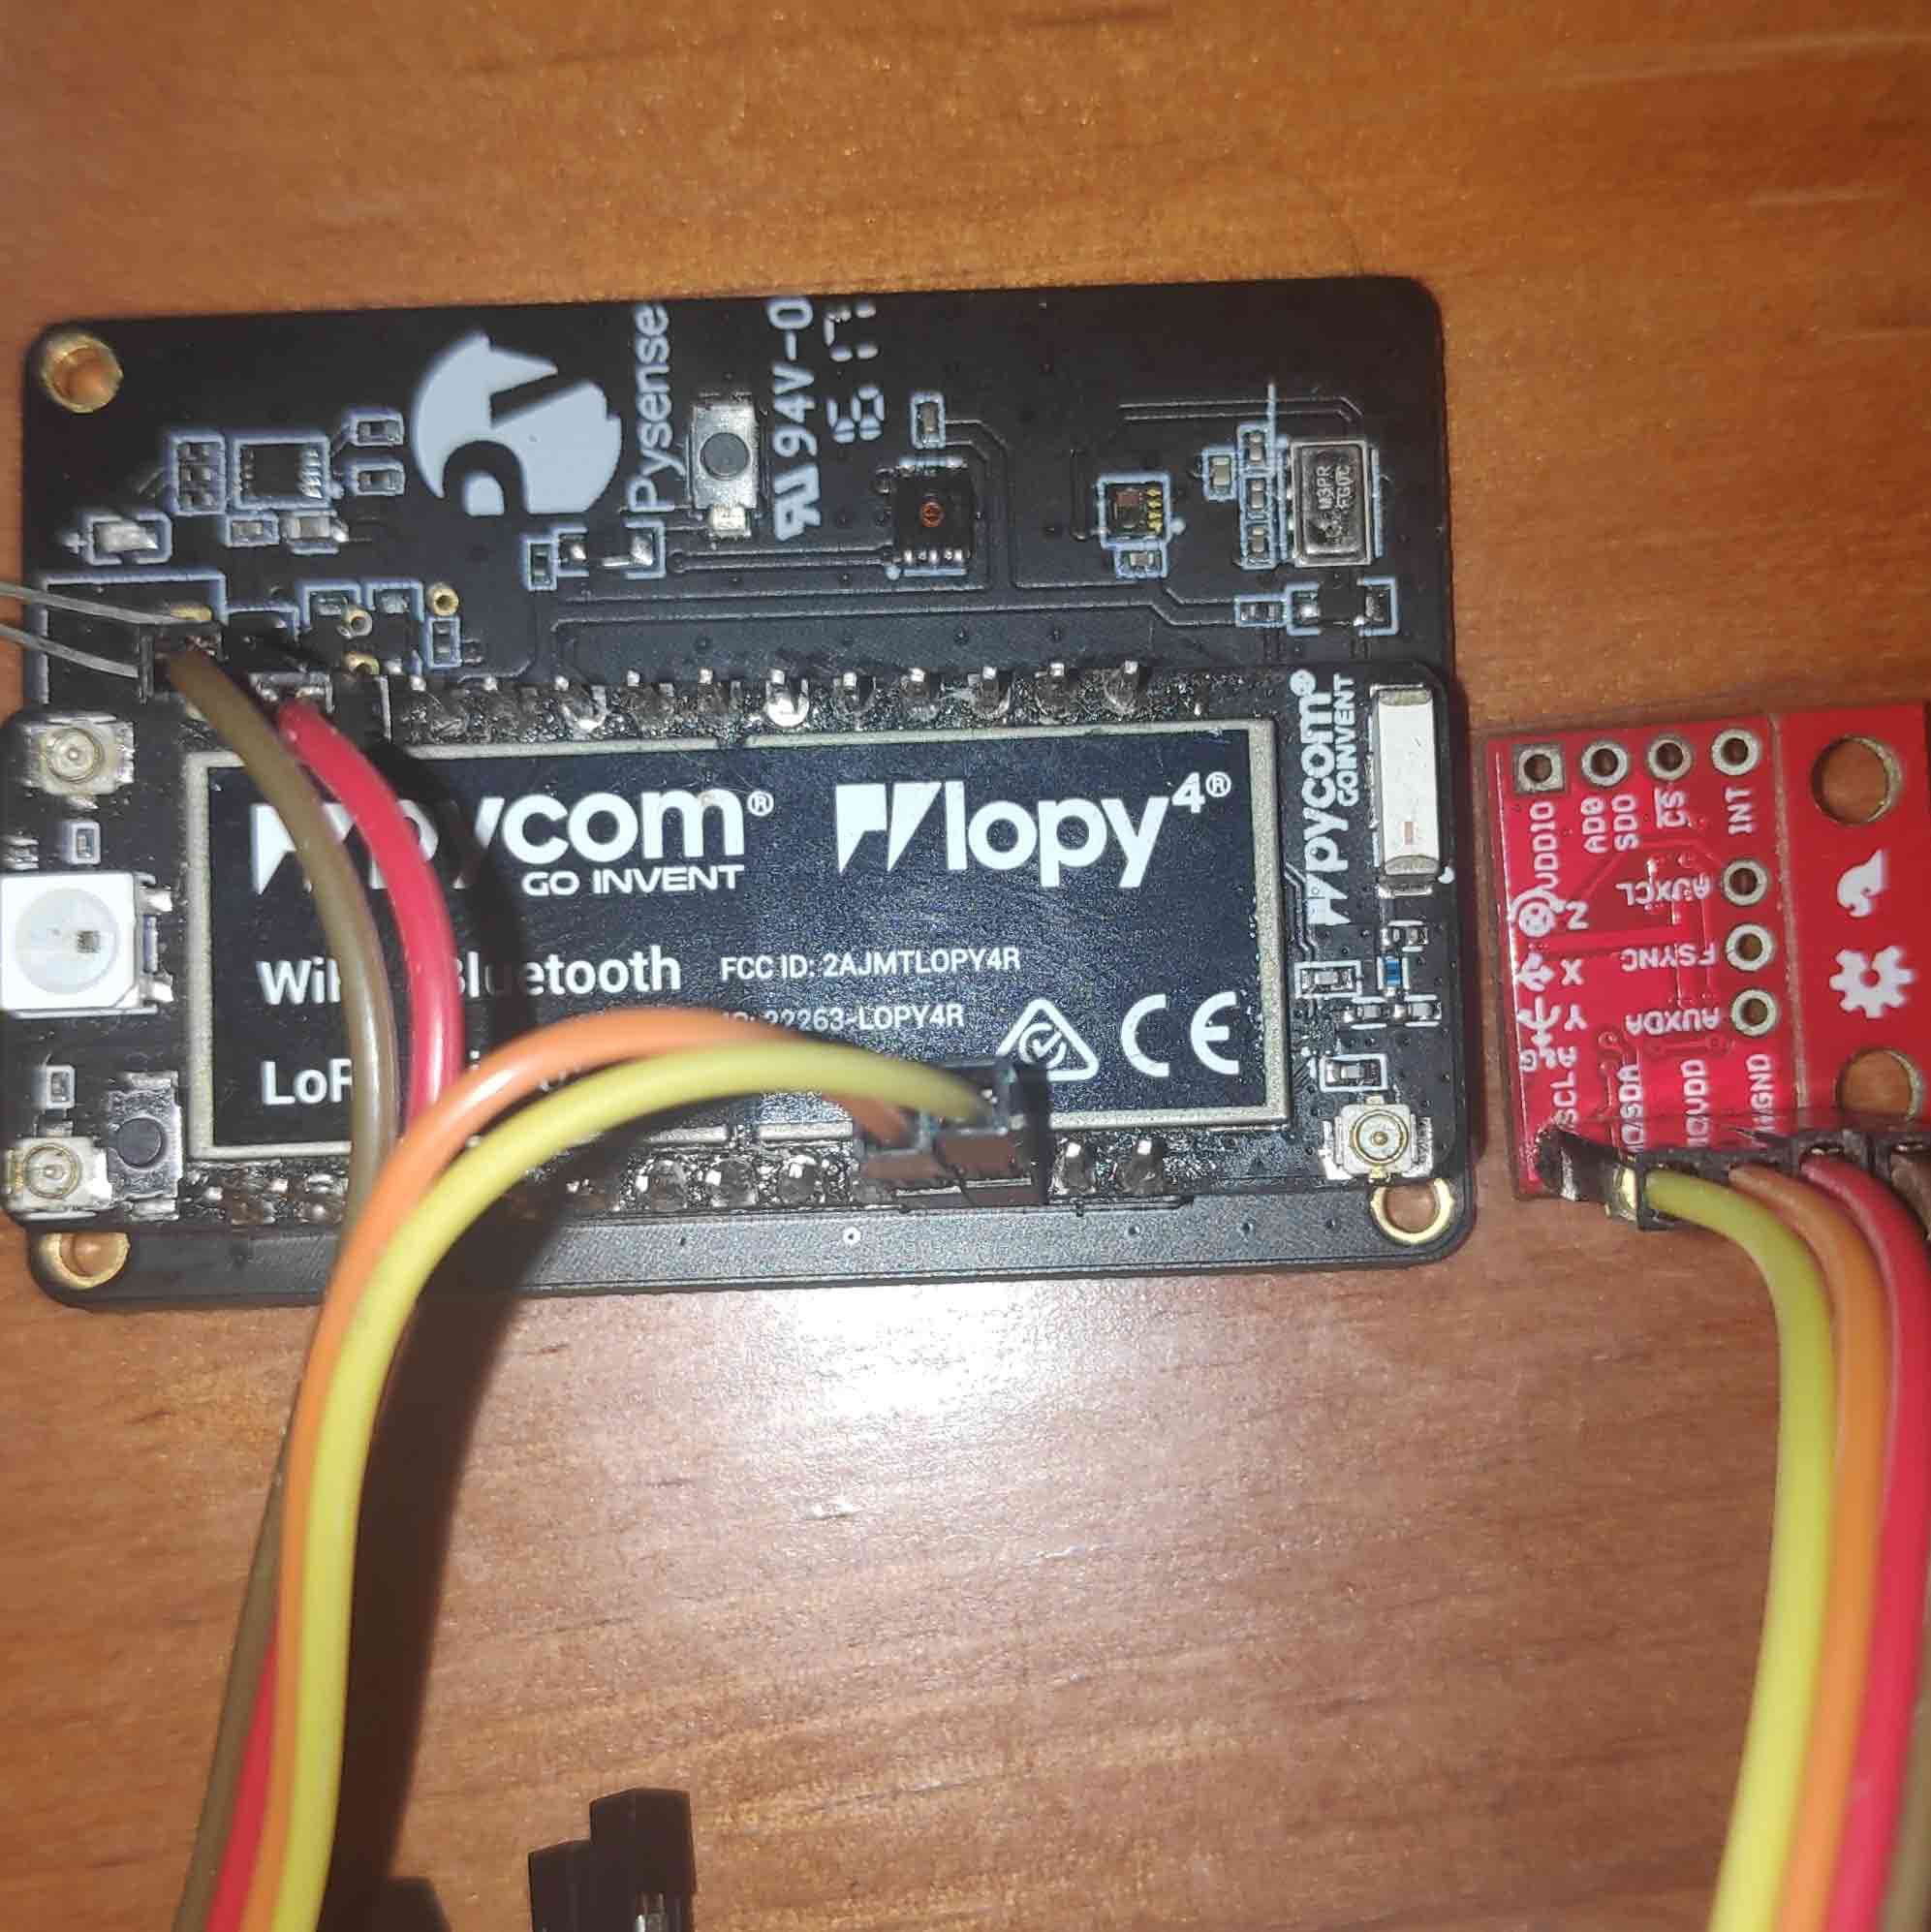
\includegraphics[width=1\textwidth]{figures/INS.jpg}
    \caption{INS Hardware}
    \label{fig:ins_1}
  \end{subfigure}%
  \begin{subfigure}{0.49\textwidth}
    \centering
    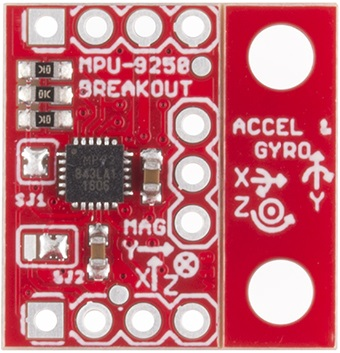
\includegraphics[width=1\textwidth]{figures/mpu9250.jpg}
    \caption{MPU-9250 Breakout}
    \label{fig:ins_2}
  \end{subfigure}
  \caption{Pin connection between the microcontroller (left) and the IMU (right). Modules are linked through SCL, CLK, VDD and GND pins.}
  \label{fig:hardware}
\end{figure}

MPU-9250 inertial measurement unit is one of the most widely available low cost commercial IMUs. It is also considered to have an exceptional quality price ratio. The MPU-9250 contains temperature and pressure sensors as well. This chip is extensively employed in wearable sensors for health, fitness, and sports, motion-based game controllers, and portable gaming. This IMU is operated to estimate motion by identifying the presence of acceleration vectors, rotational rates, and local magnetic field direction. It features an embedded 9-axis MEMS sensor from InvenSense. The MPU-9250 is a combined System-in-package (SIP) comprising an MPU-6050 (3-axis accelerometer and 3-axis gyroscope combination) and an AK8963 3-axis magnetometer. The MPU-6050 coordinate system operates within a traditional cartesian coordinate system with a counter-clockwise rotation as the positive rotation direction. The AK8963 shifts the x and y-axis directions, while reversing the direction of the z-axis. These conventions will be utilized during calibration for each of the three sensors.

\begin{figure}[!h]
  \centering
  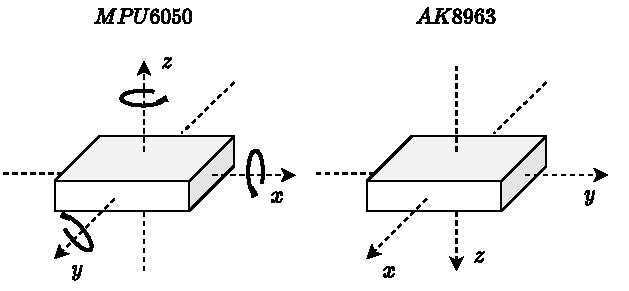
\includegraphics[width=0.9\textwidth]{figures/mpu_orientation.pdf}
  \caption{ Coordinate system of an MPU-6050 (3-axis accelerometer and 3-axis gyroscope combination) and AK8963 3-axis magnetometer. }
  \label{fig:mpu_orientation}
\end{figure}

\subsubsection{Accelerometer}

The triple-axis MEMS accelerometer in MPU-9250 includes a wide range of features:

\begin{itemize}
  \item Digital-output triple-axis accelerometer with a programmable full-scale range  of $\pm 2g$, $\pm 4$, $\pm 8g$ and $\pm 16g$ and integrated 16-bit ADCs
  \item Accelerometer normal operating current: $450 \mu A$
  \item The text in the entries may be of any length
  \item Low power accelerometer mode current: $8.4 \mu A$ at $0.98Hz$, $19.8 \mu A$ at 31.$25Hz$
  \item Sleep mode current: $8 \mu A$
  \item User-programmable interrupts
  \item Wake-on-motion interrupt for low power operation of applications processor
  \item Self-test
\end{itemize}

\begin{figure}[H]
  \centering
  \begin{table}[H]
    \begin{center}
        \begin{tabular}[t]{lcccc}
            \hline
            Parameter                   & Min. & Typ.      & Max.   & Units             \\
            \hline
            Full-Scale range            &      & $\pm 16$  &        & $g$               \\
            Sensitivity Scale Factor    &      & 2,048     &        & $LSB/g$           \\
            Nonlinearity                &      & $\pm 0.1$ &        & $\%$              \\
            Rate Noise Spectral Density &      & 300       &        & $\mu g/\sqrt{Hz}$ \\
            Operating Current           &      & 3.2       &        & $mA$              \\
            Startup Time                &      & 20        &        & $ms$              \\
            Output Data Rate            & $4$  &           & $4000$ & $Hz$              \\
            \hline
        \end{tabular}
        \caption{Accelerometer Specifications. }
        \label{tab:accelerometer_specification}
    \end{center}
\end{table}
\end{figure}

\subsubsection{Gyroscope}

The triple-axis MEMS gyroscope in the MPU-9250 includes a wide range of features:

\begin{itemize}
  \item Digital-output X-Axis, Y-Axis, and Z-Axis angular rate sensors (gyroscopes) with a user-programmable fullscale range of $\pm 250$, $\pm 500$, $\pm 1000$, and $\pm 2000^{\circ}/s$ and integrated 16-bit ADCs
  \item Digitally programmable low-pass filter
  \item Gyroscope operating current: $3.2mA$
  \item Sleep mode current: $8 \mu A$
  \item Factory calibrated sensitivity scale factor
  \item Self-test
\end{itemize}

\begin{figure}[H]
  \centering
  
\begin{table}[H]
    \begin{center}
        \begin{tabular}[t]{lcccc}
            \hline
            Parameter                   & Min. & Typ.       & Max.   & Units                  \\
            \hline
            Full-Scale range            &      & $\pm 2000$ &        & $^{\circ}/s$           \\
            Sensitivity Scale Factor    &      & 131        &        & $LSB/(^{\circ}/s)$     \\
            Nonlinearity                &      & $\pm 0.5$  &        & $\%$                   \\
            Rate Noise Spectral Density &      & 300        &        & $^{\circ}/s/\sqrt{Hz}$ \\
            Operating Current           &      & 450        &        & $\mu A$                \\
            Startup Time                &      & 35         &        & $ms$                   \\
            Output Data Rate            & $4$  &            & $8000$ & $Hz$                   \\
            \hline
        \end{tabular}
        \caption{Gyroscope Specifications. }
        \label{tab:gyroscope_specification}
    \end{center}
\end{table}
\end{figure}

\subsubsection{Magnetometer}

The triple-axis MEMS accelerometer in MPU-9250 includes a wide range of features:
\begin{itemize}
  \item 3-axis silicon monolithic Hall-effect magnetic sensor with magnetic concentrator
  \item Wide dynamic measurement range and high resolution with lower current consumption.
  \item Output data resolution of 14 bit ($0.6 \mu T/LSB$) or 16 bits ($15 \mu T/LSB$)
  \item Full scale measurement range is $\pm 4800 \mu T$
  \item Magnetometer normal operating current: $280\mu A$ at $8 Hz$ repetition rate
  \item Self-test function with internal magnetic source to confirm magnetic sensor operation on end products
\end{itemize}

\begin{figure}[H]
  \centering
  \begin{table}[H]
    \begin{center}
        \begin{tabular}[t]{lcccc}
            \hline
            Parameter                     & Min. & Typ.       & Max. & Units        \\
            \hline
            Full-Scale range              &      & $\pm 4800$ &      & $\mu T$      \\
            Sensitivity Scale Factor      &      & 0.6        &      & $\mu T/ LSB$ \\
            Operating Current             &      & 280        &      & $\mu A$      \\
            Initial Calibration Tolerance &      & $\pm 500$  &      & $LSB$        \\
            \hline
        \end{tabular}
        \caption{Magnetometer specification. }
        \label{tab:magnetometer_specification}
    \end{center}
\end{table}
\end{figure}

\subsection{Software}
The microcontroller operates MicroPython, a barebones and efficient implementation of Python 3, which incorporates a small subset of the Python standard library. It is optimized to run on microcontrollers and in constrained environments. The inertial module's raw measurements are interpreted by the microcontroller through Inter-Integrated Circuit (I2C) MicroPython driver serial allowing to read the peripherals memory addresses synchronously. The readings of each sensor are later averaged and linearized to better detect and reduce the presence of outlier readings. A fusion algorithm takes as input the averaged data of the accelerometer, gyroscope, and magnetometer. It returns the estimated inertial angles (pitch, roll, and yaw) as well as the projected linear acceleration with a gravity compensation numerical method that utterly removes the effect of the gravity component. Numerically integrating the resultant linear acceleration yields velocity, and double integrating will deliver the body's accumulative position. Merging the AHRS with an accumulative position allows tracking a moving body in three dimensions over time.

\begin{table}
  \begin{center}
    \begin{tabular}[t]{lcccc}
      \hline
      Algorithm     & Accelerometer & Gyroscope & Magnetometer \\
      \hline
      AQUA          & YES           & YES       & Optional     \\
      Complementary & YES           & YES       & Optional     \\
      Davenport's   & YES           & NO        & YES          \\
      EKF           & YES           & YES       & YES          \\
      FAMC          & YES           & NO        & YES          \\
      FLAE          & YES           & NO        & YES          \\
      Fourati       & YES           & YES       & YES          \\
      FQA           & YES           & NO        & Optional     \\
      Integration   & YES           & YES       & NO           \\
      Madgwick      & YES           & YES       & Optional     \\
      Mahony        & YES           & YES       & Optional     \\
      OLEQ          & YES           & NO        & YES          \\
      QUEST         & YES           & NO        & YES          \\
      ROLEQ         & YES           & NO        & YES          \\
      SAAM          & YES           & NO        & YES          \\
      Tilt          & YES           & NO        & Optional     \\
      TRIAD         & YES           & NO        & YES          \\
      \hline
    \end{tabular}
    \caption{Available sensor fusion algorithms in AHRS library. }
    \label{tab:ahrs_algorithms}
  \end{center}
\end{table}

The microcontroller operates MicroPython, a barebones and efficient implementation of Python 3, which incorporates a small subset of the Python standard library. It is optimized to run on microcontrollers and in constrained environments. The inertial module's raw measurements are interpreted by the microcontroller through Inter-Integrated Circuit (I2C) MicroPython driver serial allowing to read the peripherals memory addresses synchronously. The readings of each sensor are later averaged and linearized to better detect and reduce the presence of outlier readings. A fusion algorithm takes as input the averaged data of the accelerometer, gyroscope, and magnetometer. It returns the estimated inertial angles (pitch, roll, and yaw) as well as the projected linear acceleration with a gravity compensation numerical method that utterly removes the effect of the gravity component. Numerically integrating the resultant linear acceleration yields velocity, and double integrating will deliver the body's accumulative position. Merging the AHRS with an accumulative position allows tracking a moving body in three dimensions over time.

\subsection{Calibration}

A correct calibration of such sensors is essential for the compensation of their systematic errors, bias, and scale factor. Each time prior to an experiment, the inertial sensor is calibrated while the system is stationary and stabilized to compensate for static error that might corrupt the measurements.

\subsubsection{Accelerometer Calibration}

Calibration of the accelerometer requires taking advantage of the acceleration due to gravity, which we can use in the positive and negative orientation of the IMU. Additionally, we can also position the IMU perpendicular to gravity in order to acquire a third calibration point. This results in three unique values that can be combined to formulate a linear fit between the three values and the values outputted by each axis of the accelerometer.

\lstset{language=Python}
\begin{lstlisting}[frame=single]  % Start your code-block

    count=256
    aox, aoy, aoz = (0.0, 0.0, 0.0)
    self._accelerometer_offset = (0.0, 0.0, 0.0)
    n = float(count)

    while count:
        utime.sleep_ms(delay)
        # taking samples for a period of time
        ax, ay, az = self.acceleration
        # sum every sample on each axis
        aox += ax
        aoy += ay
        aoz += az 
        count -= 1

    # average the samples taken
    self._accelerometer_offset = (aox / n, aoy / n, aoz / n)
    return self._accelerometer_offset
\end{lstlisting}

\begin{figure}[!h]
  \centering
  \resizebox{1\linewidth}{!}{%% Creator: Matplotlib, PGF backend
%%
%% To include the figure in your LaTeX document, write
%%   \input{<filename>.pgf}
%%
%% Make sure the required packages are loaded in your preamble
%%   \usepackage{pgf}
%%
%% and, on pdftex
%%   \usepackage[utf8]{inputenc}\DeclareUnicodeCharacter{2212}{-}
%%
%% or, on luatex and xetex
%%   \usepackage{unicode-math}
%%
%% Figures using additional raster images can only be included by \input if
%% they are in the same directory as the main LaTeX file. For loading figures
%% from other directories you can use the `import` package
%%   \usepackage{import}
%%
%% and then include the figures with
%%   \import{<path to file>}{<filename>.pgf}
%%
%% Matplotlib used the following preamble
%%   \usepackage{fontspec}
%%
\begingroup%
\makeatletter%
\begin{pgfpicture}%
\pgfpathrectangle{\pgfpointorigin}{\pgfqpoint{5.698611in}{4.311000in}}%
\pgfusepath{use as bounding box, clip}%
\begin{pgfscope}%
\pgfsetbuttcap%
\pgfsetmiterjoin%
\definecolor{currentfill}{rgb}{1.000000,1.000000,1.000000}%
\pgfsetfillcolor{currentfill}%
\pgfsetlinewidth{0.000000pt}%
\definecolor{currentstroke}{rgb}{1.000000,1.000000,1.000000}%
\pgfsetstrokecolor{currentstroke}%
\pgfsetdash{}{0pt}%
\pgfpathmoveto{\pgfqpoint{0.000000in}{0.000000in}}%
\pgfpathlineto{\pgfqpoint{5.698611in}{0.000000in}}%
\pgfpathlineto{\pgfqpoint{5.698611in}{4.311000in}}%
\pgfpathlineto{\pgfqpoint{0.000000in}{4.311000in}}%
\pgfpathclose%
\pgfusepath{fill}%
\end{pgfscope}%
\begin{pgfscope}%
\pgfsetbuttcap%
\pgfsetmiterjoin%
\definecolor{currentfill}{rgb}{1.000000,1.000000,1.000000}%
\pgfsetfillcolor{currentfill}%
\pgfsetlinewidth{0.000000pt}%
\definecolor{currentstroke}{rgb}{0.000000,0.000000,0.000000}%
\pgfsetstrokecolor{currentstroke}%
\pgfsetstrokeopacity{0.000000}%
\pgfsetdash{}{0pt}%
\pgfpathmoveto{\pgfqpoint{0.638611in}{0.515000in}}%
\pgfpathlineto{\pgfqpoint{5.598611in}{0.515000in}}%
\pgfpathlineto{\pgfqpoint{5.598611in}{4.211000in}}%
\pgfpathlineto{\pgfqpoint{0.638611in}{4.211000in}}%
\pgfpathclose%
\pgfusepath{fill}%
\end{pgfscope}%
\begin{pgfscope}%
\pgfsetbuttcap%
\pgfsetroundjoin%
\definecolor{currentfill}{rgb}{0.000000,0.000000,0.000000}%
\pgfsetfillcolor{currentfill}%
\pgfsetlinewidth{0.803000pt}%
\definecolor{currentstroke}{rgb}{0.000000,0.000000,0.000000}%
\pgfsetstrokecolor{currentstroke}%
\pgfsetdash{}{0pt}%
\pgfsys@defobject{currentmarker}{\pgfqpoint{0.000000in}{-0.048611in}}{\pgfqpoint{0.000000in}{0.000000in}}{%
\pgfpathmoveto{\pgfqpoint{0.000000in}{0.000000in}}%
\pgfpathlineto{\pgfqpoint{0.000000in}{-0.048611in}}%
\pgfusepath{stroke,fill}%
}%
\begin{pgfscope}%
\pgfsys@transformshift{0.864066in}{0.515000in}%
\pgfsys@useobject{currentmarker}{}%
\end{pgfscope}%
\end{pgfscope}%
\begin{pgfscope}%
\definecolor{textcolor}{rgb}{0.000000,0.000000,0.000000}%
\pgfsetstrokecolor{textcolor}%
\pgfsetfillcolor{textcolor}%
\pgftext[x=0.864066in,y=0.417777in,,top]{\color{textcolor}\rmfamily\fontsize{10.000000}{12.000000}\selectfont \(\displaystyle {0}\)}%
\end{pgfscope}%
\begin{pgfscope}%
\pgfsetbuttcap%
\pgfsetroundjoin%
\definecolor{currentfill}{rgb}{0.000000,0.000000,0.000000}%
\pgfsetfillcolor{currentfill}%
\pgfsetlinewidth{0.803000pt}%
\definecolor{currentstroke}{rgb}{0.000000,0.000000,0.000000}%
\pgfsetstrokecolor{currentstroke}%
\pgfsetdash{}{0pt}%
\pgfsys@defobject{currentmarker}{\pgfqpoint{0.000000in}{-0.048611in}}{\pgfqpoint{0.000000in}{0.000000in}}{%
\pgfpathmoveto{\pgfqpoint{0.000000in}{0.000000in}}%
\pgfpathlineto{\pgfqpoint{0.000000in}{-0.048611in}}%
\pgfusepath{stroke,fill}%
}%
\begin{pgfscope}%
\pgfsys@transformshift{1.504562in}{0.515000in}%
\pgfsys@useobject{currentmarker}{}%
\end{pgfscope}%
\end{pgfscope}%
\begin{pgfscope}%
\definecolor{textcolor}{rgb}{0.000000,0.000000,0.000000}%
\pgfsetstrokecolor{textcolor}%
\pgfsetfillcolor{textcolor}%
\pgftext[x=1.504562in,y=0.417777in,,top]{\color{textcolor}\rmfamily\fontsize{10.000000}{12.000000}\selectfont \(\displaystyle {50}\)}%
\end{pgfscope}%
\begin{pgfscope}%
\pgfsetbuttcap%
\pgfsetroundjoin%
\definecolor{currentfill}{rgb}{0.000000,0.000000,0.000000}%
\pgfsetfillcolor{currentfill}%
\pgfsetlinewidth{0.803000pt}%
\definecolor{currentstroke}{rgb}{0.000000,0.000000,0.000000}%
\pgfsetstrokecolor{currentstroke}%
\pgfsetdash{}{0pt}%
\pgfsys@defobject{currentmarker}{\pgfqpoint{0.000000in}{-0.048611in}}{\pgfqpoint{0.000000in}{0.000000in}}{%
\pgfpathmoveto{\pgfqpoint{0.000000in}{0.000000in}}%
\pgfpathlineto{\pgfqpoint{0.000000in}{-0.048611in}}%
\pgfusepath{stroke,fill}%
}%
\begin{pgfscope}%
\pgfsys@transformshift{2.145058in}{0.515000in}%
\pgfsys@useobject{currentmarker}{}%
\end{pgfscope}%
\end{pgfscope}%
\begin{pgfscope}%
\definecolor{textcolor}{rgb}{0.000000,0.000000,0.000000}%
\pgfsetstrokecolor{textcolor}%
\pgfsetfillcolor{textcolor}%
\pgftext[x=2.145058in,y=0.417777in,,top]{\color{textcolor}\rmfamily\fontsize{10.000000}{12.000000}\selectfont \(\displaystyle {100}\)}%
\end{pgfscope}%
\begin{pgfscope}%
\pgfsetbuttcap%
\pgfsetroundjoin%
\definecolor{currentfill}{rgb}{0.000000,0.000000,0.000000}%
\pgfsetfillcolor{currentfill}%
\pgfsetlinewidth{0.803000pt}%
\definecolor{currentstroke}{rgb}{0.000000,0.000000,0.000000}%
\pgfsetstrokecolor{currentstroke}%
\pgfsetdash{}{0pt}%
\pgfsys@defobject{currentmarker}{\pgfqpoint{0.000000in}{-0.048611in}}{\pgfqpoint{0.000000in}{0.000000in}}{%
\pgfpathmoveto{\pgfqpoint{0.000000in}{0.000000in}}%
\pgfpathlineto{\pgfqpoint{0.000000in}{-0.048611in}}%
\pgfusepath{stroke,fill}%
}%
\begin{pgfscope}%
\pgfsys@transformshift{2.785553in}{0.515000in}%
\pgfsys@useobject{currentmarker}{}%
\end{pgfscope}%
\end{pgfscope}%
\begin{pgfscope}%
\definecolor{textcolor}{rgb}{0.000000,0.000000,0.000000}%
\pgfsetstrokecolor{textcolor}%
\pgfsetfillcolor{textcolor}%
\pgftext[x=2.785553in,y=0.417777in,,top]{\color{textcolor}\rmfamily\fontsize{10.000000}{12.000000}\selectfont \(\displaystyle {150}\)}%
\end{pgfscope}%
\begin{pgfscope}%
\pgfsetbuttcap%
\pgfsetroundjoin%
\definecolor{currentfill}{rgb}{0.000000,0.000000,0.000000}%
\pgfsetfillcolor{currentfill}%
\pgfsetlinewidth{0.803000pt}%
\definecolor{currentstroke}{rgb}{0.000000,0.000000,0.000000}%
\pgfsetstrokecolor{currentstroke}%
\pgfsetdash{}{0pt}%
\pgfsys@defobject{currentmarker}{\pgfqpoint{0.000000in}{-0.048611in}}{\pgfqpoint{0.000000in}{0.000000in}}{%
\pgfpathmoveto{\pgfqpoint{0.000000in}{0.000000in}}%
\pgfpathlineto{\pgfqpoint{0.000000in}{-0.048611in}}%
\pgfusepath{stroke,fill}%
}%
\begin{pgfscope}%
\pgfsys@transformshift{3.426049in}{0.515000in}%
\pgfsys@useobject{currentmarker}{}%
\end{pgfscope}%
\end{pgfscope}%
\begin{pgfscope}%
\definecolor{textcolor}{rgb}{0.000000,0.000000,0.000000}%
\pgfsetstrokecolor{textcolor}%
\pgfsetfillcolor{textcolor}%
\pgftext[x=3.426049in,y=0.417777in,,top]{\color{textcolor}\rmfamily\fontsize{10.000000}{12.000000}\selectfont \(\displaystyle {200}\)}%
\end{pgfscope}%
\begin{pgfscope}%
\pgfsetbuttcap%
\pgfsetroundjoin%
\definecolor{currentfill}{rgb}{0.000000,0.000000,0.000000}%
\pgfsetfillcolor{currentfill}%
\pgfsetlinewidth{0.803000pt}%
\definecolor{currentstroke}{rgb}{0.000000,0.000000,0.000000}%
\pgfsetstrokecolor{currentstroke}%
\pgfsetdash{}{0pt}%
\pgfsys@defobject{currentmarker}{\pgfqpoint{0.000000in}{-0.048611in}}{\pgfqpoint{0.000000in}{0.000000in}}{%
\pgfpathmoveto{\pgfqpoint{0.000000in}{0.000000in}}%
\pgfpathlineto{\pgfqpoint{0.000000in}{-0.048611in}}%
\pgfusepath{stroke,fill}%
}%
\begin{pgfscope}%
\pgfsys@transformshift{4.066545in}{0.515000in}%
\pgfsys@useobject{currentmarker}{}%
\end{pgfscope}%
\end{pgfscope}%
\begin{pgfscope}%
\definecolor{textcolor}{rgb}{0.000000,0.000000,0.000000}%
\pgfsetstrokecolor{textcolor}%
\pgfsetfillcolor{textcolor}%
\pgftext[x=4.066545in,y=0.417777in,,top]{\color{textcolor}\rmfamily\fontsize{10.000000}{12.000000}\selectfont \(\displaystyle {250}\)}%
\end{pgfscope}%
\begin{pgfscope}%
\pgfsetbuttcap%
\pgfsetroundjoin%
\definecolor{currentfill}{rgb}{0.000000,0.000000,0.000000}%
\pgfsetfillcolor{currentfill}%
\pgfsetlinewidth{0.803000pt}%
\definecolor{currentstroke}{rgb}{0.000000,0.000000,0.000000}%
\pgfsetstrokecolor{currentstroke}%
\pgfsetdash{}{0pt}%
\pgfsys@defobject{currentmarker}{\pgfqpoint{0.000000in}{-0.048611in}}{\pgfqpoint{0.000000in}{0.000000in}}{%
\pgfpathmoveto{\pgfqpoint{0.000000in}{0.000000in}}%
\pgfpathlineto{\pgfqpoint{0.000000in}{-0.048611in}}%
\pgfusepath{stroke,fill}%
}%
\begin{pgfscope}%
\pgfsys@transformshift{4.707041in}{0.515000in}%
\pgfsys@useobject{currentmarker}{}%
\end{pgfscope}%
\end{pgfscope}%
\begin{pgfscope}%
\definecolor{textcolor}{rgb}{0.000000,0.000000,0.000000}%
\pgfsetstrokecolor{textcolor}%
\pgfsetfillcolor{textcolor}%
\pgftext[x=4.707041in,y=0.417777in,,top]{\color{textcolor}\rmfamily\fontsize{10.000000}{12.000000}\selectfont \(\displaystyle {300}\)}%
\end{pgfscope}%
\begin{pgfscope}%
\pgfsetbuttcap%
\pgfsetroundjoin%
\definecolor{currentfill}{rgb}{0.000000,0.000000,0.000000}%
\pgfsetfillcolor{currentfill}%
\pgfsetlinewidth{0.803000pt}%
\definecolor{currentstroke}{rgb}{0.000000,0.000000,0.000000}%
\pgfsetstrokecolor{currentstroke}%
\pgfsetdash{}{0pt}%
\pgfsys@defobject{currentmarker}{\pgfqpoint{0.000000in}{-0.048611in}}{\pgfqpoint{0.000000in}{0.000000in}}{%
\pgfpathmoveto{\pgfqpoint{0.000000in}{0.000000in}}%
\pgfpathlineto{\pgfqpoint{0.000000in}{-0.048611in}}%
\pgfusepath{stroke,fill}%
}%
\begin{pgfscope}%
\pgfsys@transformshift{5.347537in}{0.515000in}%
\pgfsys@useobject{currentmarker}{}%
\end{pgfscope}%
\end{pgfscope}%
\begin{pgfscope}%
\definecolor{textcolor}{rgb}{0.000000,0.000000,0.000000}%
\pgfsetstrokecolor{textcolor}%
\pgfsetfillcolor{textcolor}%
\pgftext[x=5.347537in,y=0.417777in,,top]{\color{textcolor}\rmfamily\fontsize{10.000000}{12.000000}\selectfont \(\displaystyle {350}\)}%
\end{pgfscope}%
\begin{pgfscope}%
\definecolor{textcolor}{rgb}{0.000000,0.000000,0.000000}%
\pgfsetstrokecolor{textcolor}%
\pgfsetfillcolor{textcolor}%
\pgftext[x=3.118611in,y=0.238889in,,top]{\color{textcolor}\rmfamily\fontsize{10.000000}{12.000000}\selectfont Position X [\(\displaystyle m\)]}%
\end{pgfscope}%
\begin{pgfscope}%
\pgfsetbuttcap%
\pgfsetroundjoin%
\definecolor{currentfill}{rgb}{0.000000,0.000000,0.000000}%
\pgfsetfillcolor{currentfill}%
\pgfsetlinewidth{0.803000pt}%
\definecolor{currentstroke}{rgb}{0.000000,0.000000,0.000000}%
\pgfsetstrokecolor{currentstroke}%
\pgfsetdash{}{0pt}%
\pgfsys@defobject{currentmarker}{\pgfqpoint{-0.048611in}{0.000000in}}{\pgfqpoint{-0.000000in}{0.000000in}}{%
\pgfpathmoveto{\pgfqpoint{-0.000000in}{0.000000in}}%
\pgfpathlineto{\pgfqpoint{-0.048611in}{0.000000in}}%
\pgfusepath{stroke,fill}%
}%
\begin{pgfscope}%
\pgfsys@transformshift{0.638611in}{0.918975in}%
\pgfsys@useobject{currentmarker}{}%
\end{pgfscope}%
\end{pgfscope}%
\begin{pgfscope}%
\definecolor{textcolor}{rgb}{0.000000,0.000000,0.000000}%
\pgfsetstrokecolor{textcolor}%
\pgfsetfillcolor{textcolor}%
\pgftext[x=0.294444in, y=0.870781in, left, base]{\color{textcolor}\rmfamily\fontsize{10.000000}{12.000000}\selectfont \(\displaystyle {−15}\)}%
\end{pgfscope}%
\begin{pgfscope}%
\pgfsetbuttcap%
\pgfsetroundjoin%
\definecolor{currentfill}{rgb}{0.000000,0.000000,0.000000}%
\pgfsetfillcolor{currentfill}%
\pgfsetlinewidth{0.803000pt}%
\definecolor{currentstroke}{rgb}{0.000000,0.000000,0.000000}%
\pgfsetstrokecolor{currentstroke}%
\pgfsetdash{}{0pt}%
\pgfsys@defobject{currentmarker}{\pgfqpoint{-0.048611in}{0.000000in}}{\pgfqpoint{-0.000000in}{0.000000in}}{%
\pgfpathmoveto{\pgfqpoint{-0.000000in}{0.000000in}}%
\pgfpathlineto{\pgfqpoint{-0.048611in}{0.000000in}}%
\pgfusepath{stroke,fill}%
}%
\begin{pgfscope}%
\pgfsys@transformshift{0.638611in}{1.486631in}%
\pgfsys@useobject{currentmarker}{}%
\end{pgfscope}%
\end{pgfscope}%
\begin{pgfscope}%
\definecolor{textcolor}{rgb}{0.000000,0.000000,0.000000}%
\pgfsetstrokecolor{textcolor}%
\pgfsetfillcolor{textcolor}%
\pgftext[x=0.294444in, y=1.438437in, left, base]{\color{textcolor}\rmfamily\fontsize{10.000000}{12.000000}\selectfont \(\displaystyle {−10}\)}%
\end{pgfscope}%
\begin{pgfscope}%
\pgfsetbuttcap%
\pgfsetroundjoin%
\definecolor{currentfill}{rgb}{0.000000,0.000000,0.000000}%
\pgfsetfillcolor{currentfill}%
\pgfsetlinewidth{0.803000pt}%
\definecolor{currentstroke}{rgb}{0.000000,0.000000,0.000000}%
\pgfsetstrokecolor{currentstroke}%
\pgfsetdash{}{0pt}%
\pgfsys@defobject{currentmarker}{\pgfqpoint{-0.048611in}{0.000000in}}{\pgfqpoint{-0.000000in}{0.000000in}}{%
\pgfpathmoveto{\pgfqpoint{-0.000000in}{0.000000in}}%
\pgfpathlineto{\pgfqpoint{-0.048611in}{0.000000in}}%
\pgfusepath{stroke,fill}%
}%
\begin{pgfscope}%
\pgfsys@transformshift{0.638611in}{2.054287in}%
\pgfsys@useobject{currentmarker}{}%
\end{pgfscope}%
\end{pgfscope}%
\begin{pgfscope}%
\definecolor{textcolor}{rgb}{0.000000,0.000000,0.000000}%
\pgfsetstrokecolor{textcolor}%
\pgfsetfillcolor{textcolor}%
\pgftext[x=0.363889in, y=2.006092in, left, base]{\color{textcolor}\rmfamily\fontsize{10.000000}{12.000000}\selectfont \(\displaystyle {−5}\)}%
\end{pgfscope}%
\begin{pgfscope}%
\pgfsetbuttcap%
\pgfsetroundjoin%
\definecolor{currentfill}{rgb}{0.000000,0.000000,0.000000}%
\pgfsetfillcolor{currentfill}%
\pgfsetlinewidth{0.803000pt}%
\definecolor{currentstroke}{rgb}{0.000000,0.000000,0.000000}%
\pgfsetstrokecolor{currentstroke}%
\pgfsetdash{}{0pt}%
\pgfsys@defobject{currentmarker}{\pgfqpoint{-0.048611in}{0.000000in}}{\pgfqpoint{-0.000000in}{0.000000in}}{%
\pgfpathmoveto{\pgfqpoint{-0.000000in}{0.000000in}}%
\pgfpathlineto{\pgfqpoint{-0.048611in}{0.000000in}}%
\pgfusepath{stroke,fill}%
}%
\begin{pgfscope}%
\pgfsys@transformshift{0.638611in}{2.621943in}%
\pgfsys@useobject{currentmarker}{}%
\end{pgfscope}%
\end{pgfscope}%
\begin{pgfscope}%
\definecolor{textcolor}{rgb}{0.000000,0.000000,0.000000}%
\pgfsetstrokecolor{textcolor}%
\pgfsetfillcolor{textcolor}%
\pgftext[x=0.471944in, y=2.573748in, left, base]{\color{textcolor}\rmfamily\fontsize{10.000000}{12.000000}\selectfont \(\displaystyle {0}\)}%
\end{pgfscope}%
\begin{pgfscope}%
\pgfsetbuttcap%
\pgfsetroundjoin%
\definecolor{currentfill}{rgb}{0.000000,0.000000,0.000000}%
\pgfsetfillcolor{currentfill}%
\pgfsetlinewidth{0.803000pt}%
\definecolor{currentstroke}{rgb}{0.000000,0.000000,0.000000}%
\pgfsetstrokecolor{currentstroke}%
\pgfsetdash{}{0pt}%
\pgfsys@defobject{currentmarker}{\pgfqpoint{-0.048611in}{0.000000in}}{\pgfqpoint{-0.000000in}{0.000000in}}{%
\pgfpathmoveto{\pgfqpoint{-0.000000in}{0.000000in}}%
\pgfpathlineto{\pgfqpoint{-0.048611in}{0.000000in}}%
\pgfusepath{stroke,fill}%
}%
\begin{pgfscope}%
\pgfsys@transformshift{0.638611in}{3.189598in}%
\pgfsys@useobject{currentmarker}{}%
\end{pgfscope}%
\end{pgfscope}%
\begin{pgfscope}%
\definecolor{textcolor}{rgb}{0.000000,0.000000,0.000000}%
\pgfsetstrokecolor{textcolor}%
\pgfsetfillcolor{textcolor}%
\pgftext[x=0.471944in, y=3.141404in, left, base]{\color{textcolor}\rmfamily\fontsize{10.000000}{12.000000}\selectfont \(\displaystyle {5}\)}%
\end{pgfscope}%
\begin{pgfscope}%
\pgfsetbuttcap%
\pgfsetroundjoin%
\definecolor{currentfill}{rgb}{0.000000,0.000000,0.000000}%
\pgfsetfillcolor{currentfill}%
\pgfsetlinewidth{0.803000pt}%
\definecolor{currentstroke}{rgb}{0.000000,0.000000,0.000000}%
\pgfsetstrokecolor{currentstroke}%
\pgfsetdash{}{0pt}%
\pgfsys@defobject{currentmarker}{\pgfqpoint{-0.048611in}{0.000000in}}{\pgfqpoint{-0.000000in}{0.000000in}}{%
\pgfpathmoveto{\pgfqpoint{-0.000000in}{0.000000in}}%
\pgfpathlineto{\pgfqpoint{-0.048611in}{0.000000in}}%
\pgfusepath{stroke,fill}%
}%
\begin{pgfscope}%
\pgfsys@transformshift{0.638611in}{3.757254in}%
\pgfsys@useobject{currentmarker}{}%
\end{pgfscope}%
\end{pgfscope}%
\begin{pgfscope}%
\definecolor{textcolor}{rgb}{0.000000,0.000000,0.000000}%
\pgfsetstrokecolor{textcolor}%
\pgfsetfillcolor{textcolor}%
\pgftext[x=0.402500in, y=3.709060in, left, base]{\color{textcolor}\rmfamily\fontsize{10.000000}{12.000000}\selectfont \(\displaystyle {10}\)}%
\end{pgfscope}%
\begin{pgfscope}%
\definecolor{textcolor}{rgb}{0.000000,0.000000,0.000000}%
\pgfsetstrokecolor{textcolor}%
\pgfsetfillcolor{textcolor}%
\pgftext[x=0.238889in,y=2.363000in,,bottom,rotate=90.000000]{\color{textcolor}\rmfamily\fontsize{10.000000}{12.000000}\selectfont Position Y [\(\displaystyle m\)]}%
\end{pgfscope}%
\begin{pgfscope}%
\pgfpathrectangle{\pgfqpoint{0.638611in}{0.515000in}}{\pgfqpoint{4.960000in}{3.696000in}}%
\pgfusepath{clip}%
\pgfsetrectcap%
\pgfsetroundjoin%
\pgfsetlinewidth{1.505625pt}%
\definecolor{currentstroke}{rgb}{0.121569,0.466667,0.705882}%
\pgfsetstrokecolor{currentstroke}%
\pgfsetdash{}{0pt}%
\pgfpathmoveto{\pgfqpoint{0.864066in}{2.622682in}}%
\pgfpathlineto{\pgfqpoint{0.876876in}{2.466659in}}%
\pgfpathlineto{\pgfqpoint{0.889686in}{2.481881in}}%
\pgfpathlineto{\pgfqpoint{0.902496in}{2.569949in}}%
\pgfpathlineto{\pgfqpoint{0.915305in}{2.397074in}}%
\pgfpathlineto{\pgfqpoint{0.928115in}{2.133412in}}%
\pgfpathlineto{\pgfqpoint{0.940925in}{2.213326in}}%
\pgfpathlineto{\pgfqpoint{0.953735in}{2.355758in}}%
\pgfpathlineto{\pgfqpoint{0.966545in}{1.858334in}}%
\pgfpathlineto{\pgfqpoint{0.979355in}{1.812125in}}%
\pgfpathlineto{\pgfqpoint{0.992165in}{1.876273in}}%
\pgfpathlineto{\pgfqpoint{1.004975in}{1.979020in}}%
\pgfpathlineto{\pgfqpoint{1.017785in}{1.854528in}}%
\pgfpathlineto{\pgfqpoint{1.030595in}{1.865944in}}%
\pgfpathlineto{\pgfqpoint{1.043405in}{1.897475in}}%
\pgfpathlineto{\pgfqpoint{1.056215in}{1.948577in}}%
\pgfpathlineto{\pgfqpoint{1.069024in}{2.663454in}}%
\pgfpathlineto{\pgfqpoint{1.081834in}{2.254642in}}%
\pgfpathlineto{\pgfqpoint{1.094644in}{2.334012in}}%
\pgfpathlineto{\pgfqpoint{1.107454in}{2.398161in}}%
\pgfpathlineto{\pgfqpoint{1.120264in}{2.297589in}}%
\pgfpathlineto{\pgfqpoint{1.133074in}{2.399792in}}%
\pgfpathlineto{\pgfqpoint{1.145884in}{2.547117in}}%
\pgfpathlineto{\pgfqpoint{1.158694in}{2.742824in}}%
\pgfpathlineto{\pgfqpoint{1.171504in}{2.249206in}}%
\pgfpathlineto{\pgfqpoint{1.184314in}{2.041538in}}%
\pgfpathlineto{\pgfqpoint{1.197124in}{1.803427in}}%
\pgfpathlineto{\pgfqpoint{1.209934in}{1.331553in}}%
\pgfpathlineto{\pgfqpoint{1.222743in}{1.403857in}}%
\pgfpathlineto{\pgfqpoint{1.235553in}{1.514214in}}%
\pgfpathlineto{\pgfqpoint{1.248363in}{1.551181in}}%
\pgfpathlineto{\pgfqpoint{1.261173in}{1.401681in}}%
\pgfpathlineto{\pgfqpoint{1.273983in}{1.175531in}}%
\pgfpathlineto{\pgfqpoint{1.286793in}{1.192927in}}%
\pgfpathlineto{\pgfqpoint{1.299603in}{1.203799in}}%
\pgfpathlineto{\pgfqpoint{1.312413in}{1.191839in}}%
\pgfpathlineto{\pgfqpoint{1.325223in}{1.076589in}}%
\pgfpathlineto{\pgfqpoint{1.338033in}{1.127147in}}%
\pgfpathlineto{\pgfqpoint{1.350843in}{1.109207in}}%
\pgfpathlineto{\pgfqpoint{1.363653in}{1.112469in}}%
\pgfpathlineto{\pgfqpoint{1.376462in}{1.270666in}}%
\pgfpathlineto{\pgfqpoint{1.389272in}{1.088549in}}%
\pgfpathlineto{\pgfqpoint{1.402082in}{1.403313in}}%
\pgfpathlineto{\pgfqpoint{1.414892in}{0.895016in}}%
\pgfpathlineto{\pgfqpoint{1.427702in}{1.686546in}}%
\pgfpathlineto{\pgfqpoint{1.440512in}{2.109492in}}%
\pgfpathlineto{\pgfqpoint{1.453322in}{2.366087in}}%
\pgfpathlineto{\pgfqpoint{1.466132in}{2.226373in}}%
\pgfpathlineto{\pgfqpoint{1.478942in}{2.297045in}}%
\pgfpathlineto{\pgfqpoint{1.491752in}{2.209520in}}%
\pgfpathlineto{\pgfqpoint{1.504562in}{2.214413in}}%
\pgfpathlineto{\pgfqpoint{1.517372in}{2.195386in}}%
\pgfpathlineto{\pgfqpoint{1.530181in}{2.067632in}}%
\pgfpathlineto{\pgfqpoint{1.542991in}{1.923026in}}%
\pgfpathlineto{\pgfqpoint{1.555801in}{1.920851in}}%
\pgfpathlineto{\pgfqpoint{1.568611in}{1.954557in}}%
\pgfpathlineto{\pgfqpoint{1.581421in}{1.718620in}}%
\pgfpathlineto{\pgfqpoint{1.594231in}{1.634357in}}%
\pgfpathlineto{\pgfqpoint{1.607041in}{1.675673in}}%
\pgfpathlineto{\pgfqpoint{1.619851in}{1.736560in}}%
\pgfpathlineto{\pgfqpoint{1.632661in}{1.741996in}}%
\pgfpathlineto{\pgfqpoint{1.645471in}{1.740365in}}%
\pgfpathlineto{\pgfqpoint{1.658281in}{1.718620in}}%
\pgfpathlineto{\pgfqpoint{1.671091in}{1.704485in}}%
\pgfpathlineto{\pgfqpoint{1.683901in}{1.792010in}}%
\pgfpathlineto{\pgfqpoint{1.696710in}{1.740365in}}%
\pgfpathlineto{\pgfqpoint{1.709520in}{1.788749in}}%
\pgfpathlineto{\pgfqpoint{1.722330in}{1.764285in}}%
\pgfpathlineto{\pgfqpoint{1.735140in}{1.710465in}}%
\pgfpathlineto{\pgfqpoint{1.747950in}{1.763741in}}%
\pgfpathlineto{\pgfqpoint{1.760760in}{1.708291in}}%
\pgfpathlineto{\pgfqpoint{1.773570in}{1.599564in}}%
\pgfpathlineto{\pgfqpoint{1.786380in}{1.480508in}}%
\pgfpathlineto{\pgfqpoint{1.799190in}{1.488663in}}%
\pgfpathlineto{\pgfqpoint{1.812000in}{1.451153in}}%
\pgfpathlineto{\pgfqpoint{1.824810in}{1.394071in}}%
\pgfpathlineto{\pgfqpoint{1.837620in}{1.378849in}}%
\pgfpathlineto{\pgfqpoint{1.850429in}{1.793641in}}%
\pgfpathlineto{\pgfqpoint{1.863239in}{1.902912in}}%
\pgfpathlineto{\pgfqpoint{1.876049in}{1.948577in}}%
\pgfpathlineto{\pgfqpoint{1.888859in}{2.427517in}}%
\pgfpathlineto{\pgfqpoint{1.901669in}{2.455786in}}%
\pgfpathlineto{\pgfqpoint{1.914479in}{2.468833in}}%
\pgfpathlineto{\pgfqpoint{1.927289in}{2.312267in}}%
\pgfpathlineto{\pgfqpoint{1.940099in}{2.481337in}}%
\pgfpathlineto{\pgfqpoint{1.952909in}{2.309005in}}%
\pgfpathlineto{\pgfqpoint{1.965719in}{2.424799in}}%
\pgfpathlineto{\pgfqpoint{1.978529in}{2.370979in}}%
\pgfpathlineto{\pgfqpoint{1.991339in}{2.512324in}}%
\pgfpathlineto{\pgfqpoint{2.004148in}{2.406859in}}%
\pgfpathlineto{\pgfqpoint{2.016958in}{2.395443in}}%
\pgfpathlineto{\pgfqpoint{2.029768in}{2.372610in}}%
\pgfpathlineto{\pgfqpoint{2.042578in}{2.649863in}}%
\pgfpathlineto{\pgfqpoint{2.055388in}{2.567775in}}%
\pgfpathlineto{\pgfqpoint{2.068198in}{2.171466in}}%
\pgfpathlineto{\pgfqpoint{2.081008in}{1.893670in}}%
\pgfpathlineto{\pgfqpoint{2.093818in}{2.363369in}}%
\pgfpathlineto{\pgfqpoint{2.106628in}{2.481337in}}%
\pgfpathlineto{\pgfqpoint{2.119438in}{2.023054in}}%
\pgfpathlineto{\pgfqpoint{2.132248in}{1.884972in}}%
\pgfpathlineto{\pgfqpoint{2.145058in}{2.083941in}}%
\pgfpathlineto{\pgfqpoint{2.157867in}{1.996960in}}%
\pgfpathlineto{\pgfqpoint{2.170677in}{2.076874in}}%
\pgfpathlineto{\pgfqpoint{2.183487in}{2.054585in}}%
\pgfpathlineto{\pgfqpoint{2.196297in}{2.250837in}}%
\pgfpathlineto{\pgfqpoint{2.209107in}{2.333469in}}%
\pgfpathlineto{\pgfqpoint{2.221917in}{2.242682in}}%
\pgfpathlineto{\pgfqpoint{2.234727in}{2.094270in}}%
\pgfpathlineto{\pgfqpoint{2.247537in}{2.191581in}}%
\pgfpathlineto{\pgfqpoint{2.260347in}{2.499277in}}%
\pgfpathlineto{\pgfqpoint{2.273157in}{2.330751in}}%
\pgfpathlineto{\pgfqpoint{2.285967in}{2.506888in}}%
\pgfpathlineto{\pgfqpoint{2.298777in}{2.632467in}}%
\pgfpathlineto{\pgfqpoint{2.311586in}{2.917331in}}%
\pgfpathlineto{\pgfqpoint{2.324396in}{2.520479in}}%
\pgfpathlineto{\pgfqpoint{2.337206in}{2.341080in}}%
\pgfpathlineto{\pgfqpoint{2.350016in}{2.484599in}}%
\pgfpathlineto{\pgfqpoint{2.362826in}{2.251924in}}%
\pgfpathlineto{\pgfqpoint{2.375636in}{2.403054in}}%
\pgfpathlineto{\pgfqpoint{2.388446in}{2.611265in}}%
\pgfpathlineto{\pgfqpoint{2.401256in}{2.345972in}}%
\pgfpathlineto{\pgfqpoint{2.414066in}{2.304113in}}%
\pgfpathlineto{\pgfqpoint{2.426876in}{2.294871in}}%
\pgfpathlineto{\pgfqpoint{2.439686in}{2.252467in}}%
\pgfpathlineto{\pgfqpoint{2.452496in}{1.732211in}}%
\pgfpathlineto{\pgfqpoint{2.465305in}{1.946946in}}%
\pgfpathlineto{\pgfqpoint{2.478115in}{1.905630in}}%
\pgfpathlineto{\pgfqpoint{2.490925in}{1.815387in}}%
\pgfpathlineto{\pgfqpoint{2.503735in}{1.473985in}}%
\pgfpathlineto{\pgfqpoint{2.516545in}{1.353299in}}%
\pgfpathlineto{\pgfqpoint{2.529355in}{1.311439in}}%
\pgfpathlineto{\pgfqpoint{2.542165in}{1.323399in}}%
\pgfpathlineto{\pgfqpoint{2.554975in}{1.633813in}}%
\pgfpathlineto{\pgfqpoint{2.567785in}{1.705573in}}%
\pgfpathlineto{\pgfqpoint{2.580595in}{1.756674in}}%
\pgfpathlineto{\pgfqpoint{2.593405in}{1.741996in}}%
\pgfpathlineto{\pgfqpoint{2.606215in}{2.173641in}}%
\pgfpathlineto{\pgfqpoint{2.619024in}{2.187775in}}%
\pgfpathlineto{\pgfqpoint{2.644644in}{2.229091in}}%
\pgfpathlineto{\pgfqpoint{2.657454in}{2.272038in}}%
\pgfpathlineto{\pgfqpoint{2.670264in}{2.239420in}}%
\pgfpathlineto{\pgfqpoint{2.683074in}{2.314442in}}%
\pgfpathlineto{\pgfqpoint{2.695884in}{2.418276in}}%
\pgfpathlineto{\pgfqpoint{2.708694in}{2.596587in}}%
\pgfpathlineto{\pgfqpoint{2.721504in}{2.265515in}}%
\pgfpathlineto{\pgfqpoint{2.734314in}{2.232353in}}%
\pgfpathlineto{\pgfqpoint{2.747124in}{2.221480in}}%
\pgfpathlineto{\pgfqpoint{2.759934in}{2.368261in}}%
\pgfpathlineto{\pgfqpoint{2.772743in}{2.246488in}}%
\pgfpathlineto{\pgfqpoint{2.785553in}{1.982282in}}%
\pgfpathlineto{\pgfqpoint{2.798363in}{2.004027in}}%
\pgfpathlineto{\pgfqpoint{2.811173in}{1.989893in}}%
\pgfpathlineto{\pgfqpoint{2.823983in}{2.061652in}}%
\pgfpathlineto{\pgfqpoint{2.836793in}{2.082854in}}%
\pgfpathlineto{\pgfqpoint{2.849603in}{2.014900in}}%
\pgfpathlineto{\pgfqpoint{2.862413in}{1.987175in}}%
\pgfpathlineto{\pgfqpoint{2.875223in}{1.932268in}}%
\pgfpathlineto{\pgfqpoint{2.888033in}{1.940966in}}%
\pgfpathlineto{\pgfqpoint{2.900843in}{2.093183in}}%
\pgfpathlineto{\pgfqpoint{2.913653in}{2.366087in}}%
\pgfpathlineto{\pgfqpoint{2.926462in}{2.480250in}}%
\pgfpathlineto{\pgfqpoint{2.939272in}{2.438934in}}%
\pgfpathlineto{\pgfqpoint{2.952082in}{2.287804in}}%
\pgfpathlineto{\pgfqpoint{2.964892in}{2.347060in}}%
\pgfpathlineto{\pgfqpoint{2.977702in}{2.687374in}}%
\pgfpathlineto{\pgfqpoint{2.990512in}{2.667260in}}%
\pgfpathlineto{\pgfqpoint{3.003322in}{2.586802in}}%
\pgfpathlineto{\pgfqpoint{3.016132in}{2.600936in}}%
\pgfpathlineto{\pgfqpoint{3.028942in}{2.369349in}}%
\pgfpathlineto{\pgfqpoint{3.041752in}{2.324227in}}%
\pgfpathlineto{\pgfqpoint{3.054562in}{2.385658in}}%
\pgfpathlineto{\pgfqpoint{3.067372in}{2.214413in}}%
\pgfpathlineto{\pgfqpoint{3.080181in}{2.220393in}}%
\pgfpathlineto{\pgfqpoint{3.092991in}{2.286173in}}%
\pgfpathlineto{\pgfqpoint{3.105801in}{2.235071in}}%
\pgfpathlineto{\pgfqpoint{3.118611in}{1.812668in}}%
\pgfpathlineto{\pgfqpoint{3.131421in}{1.737103in}}%
\pgfpathlineto{\pgfqpoint{3.144231in}{1.508234in}}%
\pgfpathlineto{\pgfqpoint{3.157041in}{1.416904in}}%
\pgfpathlineto{\pgfqpoint{3.169851in}{1.605001in}}%
\pgfpathlineto{\pgfqpoint{3.195471in}{1.432669in}}%
\pgfpathlineto{\pgfqpoint{3.208281in}{1.421253in}}%
\pgfpathlineto{\pgfqpoint{3.221091in}{2.455786in}}%
\pgfpathlineto{\pgfqpoint{3.233901in}{2.233440in}}%
\pgfpathlineto{\pgfqpoint{3.246710in}{2.306831in}}%
\pgfpathlineto{\pgfqpoint{3.259520in}{2.469377in}}%
\pgfpathlineto{\pgfqpoint{3.272330in}{2.692810in}}%
\pgfpathlineto{\pgfqpoint{3.285140in}{2.538962in}}%
\pgfpathlineto{\pgfqpoint{3.297950in}{2.455786in}}%
\pgfpathlineto{\pgfqpoint{3.310760in}{2.431866in}}%
\pgfpathlineto{\pgfqpoint{3.323570in}{2.029578in}}%
\pgfpathlineto{\pgfqpoint{3.336380in}{2.072525in}}%
\pgfpathlineto{\pgfqpoint{3.349190in}{2.125257in}}%
\pgfpathlineto{\pgfqpoint{3.362000in}{2.222568in}}%
\pgfpathlineto{\pgfqpoint{3.374810in}{1.744714in}}%
\pgfpathlineto{\pgfqpoint{3.387620in}{1.588148in}}%
\pgfpathlineto{\pgfqpoint{3.400429in}{1.652840in}}%
\pgfpathlineto{\pgfqpoint{3.413239in}{1.728405in}}%
\pgfpathlineto{\pgfqpoint{3.426049in}{2.029578in}}%
\pgfpathlineto{\pgfqpoint{3.438859in}{1.858334in}}%
\pgfpathlineto{\pgfqpoint{3.451669in}{1.844199in}}%
\pgfpathlineto{\pgfqpoint{3.464479in}{1.914871in}}%
\pgfpathlineto{\pgfqpoint{3.477289in}{2.289435in}}%
\pgfpathlineto{\pgfqpoint{3.490099in}{2.449263in}}%
\pgfpathlineto{\pgfqpoint{3.502909in}{2.484055in}}%
\pgfpathlineto{\pgfqpoint{3.515719in}{2.457961in}}%
\pgfpathlineto{\pgfqpoint{3.528529in}{2.551466in}}%
\pgfpathlineto{\pgfqpoint{3.541339in}{2.368805in}}%
\pgfpathlineto{\pgfqpoint{3.554148in}{2.379678in}}%
\pgfpathlineto{\pgfqpoint{3.566958in}{2.388376in}}%
\pgfpathlineto{\pgfqpoint{3.579768in}{2.222568in}}%
\pgfpathlineto{\pgfqpoint{3.592578in}{2.484599in}}%
\pgfpathlineto{\pgfqpoint{3.605388in}{2.528089in}}%
\pgfpathlineto{\pgfqpoint{3.618198in}{2.442195in}}%
\pgfpathlineto{\pgfqpoint{3.631008in}{1.815930in}}%
\pgfpathlineto{\pgfqpoint{3.643818in}{1.614242in}}%
\pgfpathlineto{\pgfqpoint{3.656628in}{1.452240in}}%
\pgfpathlineto{\pgfqpoint{3.669438in}{1.546288in}}%
\pgfpathlineto{\pgfqpoint{3.682248in}{1.077677in}}%
\pgfpathlineto{\pgfqpoint{3.695058in}{1.229894in}}%
\pgfpathlineto{\pgfqpoint{3.707867in}{1.304371in}}%
\pgfpathlineto{\pgfqpoint{3.720677in}{1.239679in}}%
\pgfpathlineto{\pgfqpoint{3.733487in}{1.084743in}}%
\pgfpathlineto{\pgfqpoint{3.746297in}{1.158134in}}%
\pgfpathlineto{\pgfqpoint{3.759107in}{1.097248in}}%
\pgfpathlineto{\pgfqpoint{3.771917in}{0.683000in}}%
\pgfpathlineto{\pgfqpoint{3.784727in}{1.663713in}}%
\pgfpathlineto{\pgfqpoint{3.797537in}{1.930637in}}%
\pgfpathlineto{\pgfqpoint{3.810347in}{1.908892in}}%
\pgfpathlineto{\pgfqpoint{3.823157in}{1.718076in}}%
\pgfpathlineto{\pgfqpoint{3.835967in}{2.166573in}}%
\pgfpathlineto{\pgfqpoint{3.848777in}{2.275300in}}%
\pgfpathlineto{\pgfqpoint{3.861586in}{2.411752in}}%
\pgfpathlineto{\pgfqpoint{3.874396in}{2.458504in}}%
\pgfpathlineto{\pgfqpoint{3.887206in}{2.192124in}}%
\pgfpathlineto{\pgfqpoint{3.900016in}{2.378047in}}%
\pgfpathlineto{\pgfqpoint{3.912826in}{2.446001in}}%
\pgfpathlineto{\pgfqpoint{3.925636in}{2.430235in}}%
\pgfpathlineto{\pgfqpoint{3.938446in}{1.667519in}}%
\pgfpathlineto{\pgfqpoint{3.951256in}{1.434844in}}%
\pgfpathlineto{\pgfqpoint{3.964066in}{1.321224in}}%
\pgfpathlineto{\pgfqpoint{3.976876in}{1.370695in}}%
\pgfpathlineto{\pgfqpoint{3.989686in}{1.597390in}}%
\pgfpathlineto{\pgfqpoint{4.002496in}{1.583799in}}%
\pgfpathlineto{\pgfqpoint{4.015305in}{1.734929in}}%
\pgfpathlineto{\pgfqpoint{4.028115in}{1.913784in}}%
\pgfpathlineto{\pgfqpoint{4.040925in}{2.359563in}}%
\pgfpathlineto{\pgfqpoint{4.053735in}{2.415014in}}%
\pgfpathlineto{\pgfqpoint{4.066545in}{2.421537in}}%
\pgfpathlineto{\pgfqpoint{4.079355in}{2.480793in}}%
\pgfpathlineto{\pgfqpoint{4.092165in}{2.085029in}}%
\pgfpathlineto{\pgfqpoint{4.104975in}{2.153526in}}%
\pgfpathlineto{\pgfqpoint{4.117785in}{2.285085in}}%
\pgfpathlineto{\pgfqpoint{4.130595in}{2.382939in}}%
\pgfpathlineto{\pgfqpoint{4.143405in}{2.250837in}}%
\pgfpathlineto{\pgfqpoint{4.156215in}{1.996960in}}%
\pgfpathlineto{\pgfqpoint{4.169024in}{2.096445in}}%
\pgfpathlineto{\pgfqpoint{4.181834in}{2.124714in}}%
\pgfpathlineto{\pgfqpoint{4.194644in}{2.019249in}}%
\pgfpathlineto{\pgfqpoint{4.207454in}{1.469637in}}%
\pgfpathlineto{\pgfqpoint{4.220264in}{1.429407in}}%
\pgfpathlineto{\pgfqpoint{4.233074in}{1.628377in}}%
\pgfpathlineto{\pgfqpoint{4.245884in}{1.543570in}}%
\pgfpathlineto{\pgfqpoint{4.258694in}{1.746889in}}%
\pgfpathlineto{\pgfqpoint{4.271504in}{1.771352in}}%
\pgfpathlineto{\pgfqpoint{4.284314in}{1.793098in}}%
\pgfpathlineto{\pgfqpoint{4.297124in}{1.669149in}}%
\pgfpathlineto{\pgfqpoint{4.309934in}{1.625659in}}%
\pgfpathlineto{\pgfqpoint{4.322743in}{2.054585in}}%
\pgfpathlineto{\pgfqpoint{4.335553in}{1.944228in}}%
\pgfpathlineto{\pgfqpoint{4.348363in}{1.956731in}}%
\pgfpathlineto{\pgfqpoint{4.361173in}{2.394356in}}%
\pgfpathlineto{\pgfqpoint{4.373983in}{2.560707in}}%
\pgfpathlineto{\pgfqpoint{4.386793in}{2.460679in}}%
\pgfpathlineto{\pgfqpoint{4.399603in}{2.243769in}}%
\pgfpathlineto{\pgfqpoint{4.412413in}{2.450350in}}%
\pgfpathlineto{\pgfqpoint{4.425223in}{2.604198in}}%
\pgfpathlineto{\pgfqpoint{4.438033in}{2.611809in}}%
\pgfpathlineto{\pgfqpoint{4.450843in}{2.586258in}}%
\pgfpathlineto{\pgfqpoint{4.463653in}{2.538962in}}%
\pgfpathlineto{\pgfqpoint{4.476462in}{2.556902in}}%
\pgfpathlineto{\pgfqpoint{4.489272in}{2.647689in}}%
\pgfpathlineto{\pgfqpoint{4.502082in}{2.550378in}}%
\pgfpathlineto{\pgfqpoint{4.514892in}{2.436759in}}%
\pgfpathlineto{\pgfqpoint{4.527702in}{2.556358in}}%
\pgfpathlineto{\pgfqpoint{4.540512in}{2.750979in}}%
\pgfpathlineto{\pgfqpoint{4.553322in}{2.576473in}}%
\pgfpathlineto{\pgfqpoint{4.566132in}{2.711294in}}%
\pgfpathlineto{\pgfqpoint{4.578942in}{2.768375in}}%
\pgfpathlineto{\pgfqpoint{4.591752in}{2.766744in}}%
\pgfpathlineto{\pgfqpoint{4.604562in}{2.630836in}}%
\pgfpathlineto{\pgfqpoint{4.617372in}{2.522653in}}%
\pgfpathlineto{\pgfqpoint{4.642991in}{2.536788in}}%
\pgfpathlineto{\pgfqpoint{4.655801in}{2.666716in}}%
\pgfpathlineto{\pgfqpoint{4.668611in}{2.621594in}}%
\pgfpathlineto{\pgfqpoint{4.681421in}{2.603654in}}%
\pgfpathlineto{\pgfqpoint{4.694231in}{2.551466in}}%
\pgfpathlineto{\pgfqpoint{4.707041in}{2.560164in}}%
\pgfpathlineto{\pgfqpoint{4.719851in}{2.588976in}}%
\pgfpathlineto{\pgfqpoint{4.732661in}{2.588433in}}%
\pgfpathlineto{\pgfqpoint{4.745471in}{2.581909in}}%
\pgfpathlineto{\pgfqpoint{4.758281in}{2.577016in}}%
\pgfpathlineto{\pgfqpoint{4.771091in}{2.650407in}}%
\pgfpathlineto{\pgfqpoint{4.783901in}{2.652038in}}%
\pgfpathlineto{\pgfqpoint{4.796710in}{2.626487in}}%
\pgfpathlineto{\pgfqpoint{4.809520in}{2.549291in}}%
\pgfpathlineto{\pgfqpoint{4.822330in}{2.415557in}}%
\pgfpathlineto{\pgfqpoint{4.835140in}{2.379134in}}%
\pgfpathlineto{\pgfqpoint{4.847950in}{2.385658in}}%
\pgfpathlineto{\pgfqpoint{4.860760in}{2.320965in}}%
\pgfpathlineto{\pgfqpoint{4.873570in}{2.011638in}}%
\pgfpathlineto{\pgfqpoint{4.886380in}{1.959993in}}%
\pgfpathlineto{\pgfqpoint{4.899190in}{2.030665in}}%
\pgfpathlineto{\pgfqpoint{4.912000in}{1.785487in}}%
\pgfpathlineto{\pgfqpoint{4.924810in}{1.483227in}}%
\pgfpathlineto{\pgfqpoint{4.937620in}{1.534872in}}%
\pgfpathlineto{\pgfqpoint{4.950429in}{1.622940in}}%
\pgfpathlineto{\pgfqpoint{4.963239in}{1.671868in}}%
\pgfpathlineto{\pgfqpoint{4.976049in}{1.618048in}}%
\pgfpathlineto{\pgfqpoint{4.988859in}{1.642511in}}%
\pgfpathlineto{\pgfqpoint{5.001669in}{1.660995in}}%
\pgfpathlineto{\pgfqpoint{5.014479in}{2.185057in}}%
\pgfpathlineto{\pgfqpoint{5.027289in}{2.200822in}}%
\pgfpathlineto{\pgfqpoint{5.040099in}{2.148634in}}%
\pgfpathlineto{\pgfqpoint{5.052909in}{1.994785in}}%
\pgfpathlineto{\pgfqpoint{5.065719in}{2.397618in}}%
\pgfpathlineto{\pgfqpoint{5.078529in}{2.472639in}}%
\pgfpathlineto{\pgfqpoint{5.091339in}{2.338905in}}%
\pgfpathlineto{\pgfqpoint{5.104148in}{2.419363in}}%
\pgfpathlineto{\pgfqpoint{5.116958in}{2.459592in}}%
\pgfpathlineto{\pgfqpoint{5.129768in}{2.527546in}}%
\pgfpathlineto{\pgfqpoint{5.142578in}{2.803168in}}%
\pgfpathlineto{\pgfqpoint{5.155388in}{2.705857in}}%
\pgfpathlineto{\pgfqpoint{5.168198in}{2.150808in}}%
\pgfpathlineto{\pgfqpoint{5.181008in}{2.275300in}}%
\pgfpathlineto{\pgfqpoint{5.193818in}{2.032296in}}%
\pgfpathlineto{\pgfqpoint{5.206628in}{2.091009in}}%
\pgfpathlineto{\pgfqpoint{5.219438in}{1.568577in}}%
\pgfpathlineto{\pgfqpoint{5.232248in}{1.385916in}}%
\pgfpathlineto{\pgfqpoint{5.245058in}{1.315788in}}%
\pgfpathlineto{\pgfqpoint{5.257867in}{1.417447in}}%
\pgfpathlineto{\pgfqpoint{5.270677in}{1.912153in}}%
\pgfpathlineto{\pgfqpoint{5.283487in}{0.948835in}}%
\pgfpathlineto{\pgfqpoint{5.296297in}{1.109207in}}%
\pgfpathlineto{\pgfqpoint{5.309107in}{0.866747in}}%
\pgfpathlineto{\pgfqpoint{5.321917in}{1.319050in}}%
\pgfpathlineto{\pgfqpoint{5.334727in}{1.287519in}}%
\pgfpathlineto{\pgfqpoint{5.347537in}{1.268492in}}%
\pgfpathlineto{\pgfqpoint{5.360347in}{1.361453in}}%
\pgfpathlineto{\pgfqpoint{5.373157in}{1.360366in}}%
\pgfpathlineto{\pgfqpoint{5.373157in}{1.360366in}}%
\pgfusepath{stroke}%
\end{pgfscope}%
\begin{pgfscope}%
\pgfpathrectangle{\pgfqpoint{0.638611in}{0.515000in}}{\pgfqpoint{4.960000in}{3.696000in}}%
\pgfusepath{clip}%
\pgfsetrectcap%
\pgfsetroundjoin%
\pgfsetlinewidth{1.505625pt}%
\definecolor{currentstroke}{rgb}{1.000000,0.498039,0.054902}%
\pgfsetstrokecolor{currentstroke}%
\pgfsetdash{}{0pt}%
\pgfpathmoveto{\pgfqpoint{0.864066in}{3.592327in}}%
\pgfpathlineto{\pgfqpoint{0.876876in}{3.607549in}}%
\pgfpathlineto{\pgfqpoint{0.889686in}{3.695618in}}%
\pgfpathlineto{\pgfqpoint{0.902496in}{3.522742in}}%
\pgfpathlineto{\pgfqpoint{0.915305in}{3.259080in}}%
\pgfpathlineto{\pgfqpoint{0.928115in}{3.338994in}}%
\pgfpathlineto{\pgfqpoint{0.940925in}{3.481426in}}%
\pgfpathlineto{\pgfqpoint{0.953735in}{2.984002in}}%
\pgfpathlineto{\pgfqpoint{0.966545in}{2.937793in}}%
\pgfpathlineto{\pgfqpoint{0.979355in}{3.001942in}}%
\pgfpathlineto{\pgfqpoint{0.992165in}{3.104689in}}%
\pgfpathlineto{\pgfqpoint{1.004975in}{2.980197in}}%
\pgfpathlineto{\pgfqpoint{1.017785in}{2.991613in}}%
\pgfpathlineto{\pgfqpoint{1.030595in}{3.023144in}}%
\pgfpathlineto{\pgfqpoint{1.043405in}{3.074245in}}%
\pgfpathlineto{\pgfqpoint{1.056215in}{3.789122in}}%
\pgfpathlineto{\pgfqpoint{1.069024in}{3.380311in}}%
\pgfpathlineto{\pgfqpoint{1.081834in}{3.459681in}}%
\pgfpathlineto{\pgfqpoint{1.094644in}{3.523830in}}%
\pgfpathlineto{\pgfqpoint{1.107454in}{3.423258in}}%
\pgfpathlineto{\pgfqpoint{1.120264in}{3.525461in}}%
\pgfpathlineto{\pgfqpoint{1.133074in}{3.672785in}}%
\pgfpathlineto{\pgfqpoint{1.145884in}{3.868493in}}%
\pgfpathlineto{\pgfqpoint{1.158694in}{3.374874in}}%
\pgfpathlineto{\pgfqpoint{1.171504in}{3.167207in}}%
\pgfpathlineto{\pgfqpoint{1.184314in}{2.929095in}}%
\pgfpathlineto{\pgfqpoint{1.197124in}{2.457222in}}%
\pgfpathlineto{\pgfqpoint{1.209934in}{2.529525in}}%
\pgfpathlineto{\pgfqpoint{1.222743in}{2.639882in}}%
\pgfpathlineto{\pgfqpoint{1.235553in}{2.676850in}}%
\pgfpathlineto{\pgfqpoint{1.248363in}{2.527350in}}%
\pgfpathlineto{\pgfqpoint{1.261173in}{2.301199in}}%
\pgfpathlineto{\pgfqpoint{1.273983in}{2.318595in}}%
\pgfpathlineto{\pgfqpoint{1.286793in}{2.329468in}}%
\pgfpathlineto{\pgfqpoint{1.299603in}{2.317508in}}%
\pgfpathlineto{\pgfqpoint{1.312413in}{2.202258in}}%
\pgfpathlineto{\pgfqpoint{1.325223in}{2.252816in}}%
\pgfpathlineto{\pgfqpoint{1.338033in}{2.234876in}}%
\pgfpathlineto{\pgfqpoint{1.350843in}{2.238138in}}%
\pgfpathlineto{\pgfqpoint{1.363653in}{2.396335in}}%
\pgfpathlineto{\pgfqpoint{1.376462in}{2.214218in}}%
\pgfpathlineto{\pgfqpoint{1.389272in}{2.528981in}}%
\pgfpathlineto{\pgfqpoint{1.402082in}{2.020685in}}%
\pgfpathlineto{\pgfqpoint{1.414892in}{2.812214in}}%
\pgfpathlineto{\pgfqpoint{1.427702in}{3.235161in}}%
\pgfpathlineto{\pgfqpoint{1.440512in}{3.491755in}}%
\pgfpathlineto{\pgfqpoint{1.453322in}{3.352042in}}%
\pgfpathlineto{\pgfqpoint{1.466132in}{3.422714in}}%
\pgfpathlineto{\pgfqpoint{1.478942in}{3.335189in}}%
\pgfpathlineto{\pgfqpoint{1.491752in}{3.340082in}}%
\pgfpathlineto{\pgfqpoint{1.504562in}{3.321055in}}%
\pgfpathlineto{\pgfqpoint{1.517372in}{3.193301in}}%
\pgfpathlineto{\pgfqpoint{1.530181in}{3.048695in}}%
\pgfpathlineto{\pgfqpoint{1.542991in}{3.046520in}}%
\pgfpathlineto{\pgfqpoint{1.555801in}{3.080225in}}%
\pgfpathlineto{\pgfqpoint{1.568611in}{2.844288in}}%
\pgfpathlineto{\pgfqpoint{1.581421in}{2.760025in}}%
\pgfpathlineto{\pgfqpoint{1.594231in}{2.801341in}}%
\pgfpathlineto{\pgfqpoint{1.607041in}{2.862228in}}%
\pgfpathlineto{\pgfqpoint{1.619851in}{2.867665in}}%
\pgfpathlineto{\pgfqpoint{1.632661in}{2.866034in}}%
\pgfpathlineto{\pgfqpoint{1.645471in}{2.844288in}}%
\pgfpathlineto{\pgfqpoint{1.658281in}{2.830154in}}%
\pgfpathlineto{\pgfqpoint{1.671091in}{2.917679in}}%
\pgfpathlineto{\pgfqpoint{1.683901in}{2.866034in}}%
\pgfpathlineto{\pgfqpoint{1.696710in}{2.914417in}}%
\pgfpathlineto{\pgfqpoint{1.709520in}{2.889954in}}%
\pgfpathlineto{\pgfqpoint{1.722330in}{2.836134in}}%
\pgfpathlineto{\pgfqpoint{1.735140in}{2.889410in}}%
\pgfpathlineto{\pgfqpoint{1.747950in}{2.833959in}}%
\pgfpathlineto{\pgfqpoint{1.760760in}{2.725233in}}%
\pgfpathlineto{\pgfqpoint{1.773570in}{2.606177in}}%
\pgfpathlineto{\pgfqpoint{1.786380in}{2.614332in}}%
\pgfpathlineto{\pgfqpoint{1.799190in}{2.576821in}}%
\pgfpathlineto{\pgfqpoint{1.812000in}{2.519740in}}%
\pgfpathlineto{\pgfqpoint{1.824810in}{2.504518in}}%
\pgfpathlineto{\pgfqpoint{1.837620in}{2.919310in}}%
\pgfpathlineto{\pgfqpoint{1.850429in}{3.028580in}}%
\pgfpathlineto{\pgfqpoint{1.863239in}{3.074245in}}%
\pgfpathlineto{\pgfqpoint{1.876049in}{3.553186in}}%
\pgfpathlineto{\pgfqpoint{1.888859in}{3.581455in}}%
\pgfpathlineto{\pgfqpoint{1.901669in}{3.594502in}}%
\pgfpathlineto{\pgfqpoint{1.914479in}{3.437936in}}%
\pgfpathlineto{\pgfqpoint{1.927289in}{3.607006in}}%
\pgfpathlineto{\pgfqpoint{1.940099in}{3.434674in}}%
\pgfpathlineto{\pgfqpoint{1.952909in}{3.550468in}}%
\pgfpathlineto{\pgfqpoint{1.965719in}{3.496648in}}%
\pgfpathlineto{\pgfqpoint{1.978529in}{3.637993in}}%
\pgfpathlineto{\pgfqpoint{1.991339in}{3.532528in}}%
\pgfpathlineto{\pgfqpoint{2.004148in}{3.521112in}}%
\pgfpathlineto{\pgfqpoint{2.016958in}{3.498279in}}%
\pgfpathlineto{\pgfqpoint{2.029768in}{3.775532in}}%
\pgfpathlineto{\pgfqpoint{2.042578in}{3.693443in}}%
\pgfpathlineto{\pgfqpoint{2.055388in}{3.297135in}}%
\pgfpathlineto{\pgfqpoint{2.068198in}{3.019338in}}%
\pgfpathlineto{\pgfqpoint{2.081008in}{3.489037in}}%
\pgfpathlineto{\pgfqpoint{2.093818in}{3.607006in}}%
\pgfpathlineto{\pgfqpoint{2.106628in}{3.148723in}}%
\pgfpathlineto{\pgfqpoint{2.119438in}{3.010640in}}%
\pgfpathlineto{\pgfqpoint{2.132248in}{3.209610in}}%
\pgfpathlineto{\pgfqpoint{2.145058in}{3.122629in}}%
\pgfpathlineto{\pgfqpoint{2.157867in}{3.202543in}}%
\pgfpathlineto{\pgfqpoint{2.170677in}{3.180254in}}%
\pgfpathlineto{\pgfqpoint{2.183487in}{3.376505in}}%
\pgfpathlineto{\pgfqpoint{2.196297in}{3.459137in}}%
\pgfpathlineto{\pgfqpoint{2.209107in}{3.368351in}}%
\pgfpathlineto{\pgfqpoint{2.221917in}{3.219939in}}%
\pgfpathlineto{\pgfqpoint{2.234727in}{3.317249in}}%
\pgfpathlineto{\pgfqpoint{2.247537in}{3.624945in}}%
\pgfpathlineto{\pgfqpoint{2.260347in}{3.456419in}}%
\pgfpathlineto{\pgfqpoint{2.273157in}{3.632556in}}%
\pgfpathlineto{\pgfqpoint{2.285967in}{3.758135in}}%
\pgfpathlineto{\pgfqpoint{2.298777in}{4.043000in}}%
\pgfpathlineto{\pgfqpoint{2.311586in}{3.646147in}}%
\pgfpathlineto{\pgfqpoint{2.324396in}{3.466748in}}%
\pgfpathlineto{\pgfqpoint{2.337206in}{3.610267in}}%
\pgfpathlineto{\pgfqpoint{2.350016in}{3.377592in}}%
\pgfpathlineto{\pgfqpoint{2.362826in}{3.528722in}}%
\pgfpathlineto{\pgfqpoint{2.375636in}{3.736934in}}%
\pgfpathlineto{\pgfqpoint{2.388446in}{3.471641in}}%
\pgfpathlineto{\pgfqpoint{2.401256in}{3.429781in}}%
\pgfpathlineto{\pgfqpoint{2.414066in}{3.420539in}}%
\pgfpathlineto{\pgfqpoint{2.426876in}{3.378136in}}%
\pgfpathlineto{\pgfqpoint{2.439686in}{2.857879in}}%
\pgfpathlineto{\pgfqpoint{2.452496in}{3.072614in}}%
\pgfpathlineto{\pgfqpoint{2.465305in}{3.031298in}}%
\pgfpathlineto{\pgfqpoint{2.478115in}{2.941055in}}%
\pgfpathlineto{\pgfqpoint{2.490925in}{2.599654in}}%
\pgfpathlineto{\pgfqpoint{2.503735in}{2.478967in}}%
\pgfpathlineto{\pgfqpoint{2.516545in}{2.437107in}}%
\pgfpathlineto{\pgfqpoint{2.529355in}{2.449067in}}%
\pgfpathlineto{\pgfqpoint{2.542165in}{2.759482in}}%
\pgfpathlineto{\pgfqpoint{2.554975in}{2.831241in}}%
\pgfpathlineto{\pgfqpoint{2.567785in}{2.882343in}}%
\pgfpathlineto{\pgfqpoint{2.580595in}{2.867665in}}%
\pgfpathlineto{\pgfqpoint{2.593405in}{3.299309in}}%
\pgfpathlineto{\pgfqpoint{2.606215in}{3.313444in}}%
\pgfpathlineto{\pgfqpoint{2.631834in}{3.354760in}}%
\pgfpathlineto{\pgfqpoint{2.644644in}{3.397707in}}%
\pgfpathlineto{\pgfqpoint{2.657454in}{3.365089in}}%
\pgfpathlineto{\pgfqpoint{2.670264in}{3.440110in}}%
\pgfpathlineto{\pgfqpoint{2.683074in}{3.543944in}}%
\pgfpathlineto{\pgfqpoint{2.695884in}{3.722256in}}%
\pgfpathlineto{\pgfqpoint{2.708694in}{3.391183in}}%
\pgfpathlineto{\pgfqpoint{2.721504in}{3.358022in}}%
\pgfpathlineto{\pgfqpoint{2.734314in}{3.347149in}}%
\pgfpathlineto{\pgfqpoint{2.747124in}{3.493930in}}%
\pgfpathlineto{\pgfqpoint{2.759934in}{3.372156in}}%
\pgfpathlineto{\pgfqpoint{2.772743in}{3.107951in}}%
\pgfpathlineto{\pgfqpoint{2.785553in}{3.129696in}}%
\pgfpathlineto{\pgfqpoint{2.798363in}{3.115561in}}%
\pgfpathlineto{\pgfqpoint{2.811173in}{3.187321in}}%
\pgfpathlineto{\pgfqpoint{2.823983in}{3.208523in}}%
\pgfpathlineto{\pgfqpoint{2.836793in}{3.140568in}}%
\pgfpathlineto{\pgfqpoint{2.849603in}{3.112843in}}%
\pgfpathlineto{\pgfqpoint{2.862413in}{3.057936in}}%
\pgfpathlineto{\pgfqpoint{2.875223in}{3.066634in}}%
\pgfpathlineto{\pgfqpoint{2.888033in}{3.218852in}}%
\pgfpathlineto{\pgfqpoint{2.900843in}{3.491755in}}%
\pgfpathlineto{\pgfqpoint{2.913653in}{3.605918in}}%
\pgfpathlineto{\pgfqpoint{2.926462in}{3.564602in}}%
\pgfpathlineto{\pgfqpoint{2.939272in}{3.413472in}}%
\pgfpathlineto{\pgfqpoint{2.952082in}{3.472728in}}%
\pgfpathlineto{\pgfqpoint{2.964892in}{3.813042in}}%
\pgfpathlineto{\pgfqpoint{2.977702in}{3.792928in}}%
\pgfpathlineto{\pgfqpoint{2.990512in}{3.712470in}}%
\pgfpathlineto{\pgfqpoint{3.003322in}{3.726605in}}%
\pgfpathlineto{\pgfqpoint{3.016132in}{3.495017in}}%
\pgfpathlineto{\pgfqpoint{3.028942in}{3.449896in}}%
\pgfpathlineto{\pgfqpoint{3.041752in}{3.511326in}}%
\pgfpathlineto{\pgfqpoint{3.054562in}{3.340082in}}%
\pgfpathlineto{\pgfqpoint{3.067372in}{3.346062in}}%
\pgfpathlineto{\pgfqpoint{3.080181in}{3.411841in}}%
\pgfpathlineto{\pgfqpoint{3.092991in}{3.360740in}}%
\pgfpathlineto{\pgfqpoint{3.105801in}{2.938337in}}%
\pgfpathlineto{\pgfqpoint{3.118611in}{2.862772in}}%
\pgfpathlineto{\pgfqpoint{3.131421in}{2.633903in}}%
\pgfpathlineto{\pgfqpoint{3.144231in}{2.542572in}}%
\pgfpathlineto{\pgfqpoint{3.157041in}{2.730669in}}%
\pgfpathlineto{\pgfqpoint{3.182661in}{2.558338in}}%
\pgfpathlineto{\pgfqpoint{3.195471in}{2.546921in}}%
\pgfpathlineto{\pgfqpoint{3.208281in}{3.581455in}}%
\pgfpathlineto{\pgfqpoint{3.221091in}{3.359109in}}%
\pgfpathlineto{\pgfqpoint{3.233901in}{3.432499in}}%
\pgfpathlineto{\pgfqpoint{3.246710in}{3.595046in}}%
\pgfpathlineto{\pgfqpoint{3.259520in}{3.818479in}}%
\pgfpathlineto{\pgfqpoint{3.272330in}{3.664631in}}%
\pgfpathlineto{\pgfqpoint{3.285140in}{3.581455in}}%
\pgfpathlineto{\pgfqpoint{3.297950in}{3.557535in}}%
\pgfpathlineto{\pgfqpoint{3.310760in}{3.155247in}}%
\pgfpathlineto{\pgfqpoint{3.323570in}{3.198193in}}%
\pgfpathlineto{\pgfqpoint{3.336380in}{3.250926in}}%
\pgfpathlineto{\pgfqpoint{3.349190in}{3.348236in}}%
\pgfpathlineto{\pgfqpoint{3.362000in}{2.870383in}}%
\pgfpathlineto{\pgfqpoint{3.374810in}{2.713817in}}%
\pgfpathlineto{\pgfqpoint{3.387620in}{2.778509in}}%
\pgfpathlineto{\pgfqpoint{3.400429in}{2.854074in}}%
\pgfpathlineto{\pgfqpoint{3.413239in}{3.155247in}}%
\pgfpathlineto{\pgfqpoint{3.426049in}{2.984002in}}%
\pgfpathlineto{\pgfqpoint{3.438859in}{2.969868in}}%
\pgfpathlineto{\pgfqpoint{3.451669in}{3.040540in}}%
\pgfpathlineto{\pgfqpoint{3.464479in}{3.415103in}}%
\pgfpathlineto{\pgfqpoint{3.477289in}{3.574931in}}%
\pgfpathlineto{\pgfqpoint{3.490099in}{3.609724in}}%
\pgfpathlineto{\pgfqpoint{3.502909in}{3.583629in}}%
\pgfpathlineto{\pgfqpoint{3.515719in}{3.677134in}}%
\pgfpathlineto{\pgfqpoint{3.528529in}{3.494474in}}%
\pgfpathlineto{\pgfqpoint{3.541339in}{3.505346in}}%
\pgfpathlineto{\pgfqpoint{3.554148in}{3.514044in}}%
\pgfpathlineto{\pgfqpoint{3.566958in}{3.348236in}}%
\pgfpathlineto{\pgfqpoint{3.579768in}{3.610267in}}%
\pgfpathlineto{\pgfqpoint{3.592578in}{3.653758in}}%
\pgfpathlineto{\pgfqpoint{3.605388in}{3.567864in}}%
\pgfpathlineto{\pgfqpoint{3.618198in}{2.941599in}}%
\pgfpathlineto{\pgfqpoint{3.631008in}{2.739911in}}%
\pgfpathlineto{\pgfqpoint{3.643818in}{2.577908in}}%
\pgfpathlineto{\pgfqpoint{3.656628in}{2.671957in}}%
\pgfpathlineto{\pgfqpoint{3.669438in}{2.203345in}}%
\pgfpathlineto{\pgfqpoint{3.682248in}{2.355562in}}%
\pgfpathlineto{\pgfqpoint{3.695058in}{2.430040in}}%
\pgfpathlineto{\pgfqpoint{3.707867in}{2.365348in}}%
\pgfpathlineto{\pgfqpoint{3.720677in}{2.210412in}}%
\pgfpathlineto{\pgfqpoint{3.733487in}{2.283803in}}%
\pgfpathlineto{\pgfqpoint{3.746297in}{2.222916in}}%
\pgfpathlineto{\pgfqpoint{3.759107in}{1.808668in}}%
\pgfpathlineto{\pgfqpoint{3.771917in}{2.789382in}}%
\pgfpathlineto{\pgfqpoint{3.784727in}{3.056305in}}%
\pgfpathlineto{\pgfqpoint{3.797537in}{3.034560in}}%
\pgfpathlineto{\pgfqpoint{3.810347in}{2.843745in}}%
\pgfpathlineto{\pgfqpoint{3.823157in}{3.292242in}}%
\pgfpathlineto{\pgfqpoint{3.835967in}{3.400969in}}%
\pgfpathlineto{\pgfqpoint{3.848777in}{3.537420in}}%
\pgfpathlineto{\pgfqpoint{3.861586in}{3.584173in}}%
\pgfpathlineto{\pgfqpoint{3.874396in}{3.317793in}}%
\pgfpathlineto{\pgfqpoint{3.887206in}{3.503715in}}%
\pgfpathlineto{\pgfqpoint{3.900016in}{3.571669in}}%
\pgfpathlineto{\pgfqpoint{3.912826in}{3.555904in}}%
\pgfpathlineto{\pgfqpoint{3.925636in}{2.793187in}}%
\pgfpathlineto{\pgfqpoint{3.938446in}{2.560512in}}%
\pgfpathlineto{\pgfqpoint{3.951256in}{2.446893in}}%
\pgfpathlineto{\pgfqpoint{3.964066in}{2.496363in}}%
\pgfpathlineto{\pgfqpoint{3.976876in}{2.723058in}}%
\pgfpathlineto{\pgfqpoint{3.989686in}{2.709467in}}%
\pgfpathlineto{\pgfqpoint{4.002496in}{2.860597in}}%
\pgfpathlineto{\pgfqpoint{4.015305in}{3.039453in}}%
\pgfpathlineto{\pgfqpoint{4.028115in}{3.485232in}}%
\pgfpathlineto{\pgfqpoint{4.040925in}{3.540682in}}%
\pgfpathlineto{\pgfqpoint{4.053735in}{3.547206in}}%
\pgfpathlineto{\pgfqpoint{4.066545in}{3.606462in}}%
\pgfpathlineto{\pgfqpoint{4.079355in}{3.210697in}}%
\pgfpathlineto{\pgfqpoint{4.092165in}{3.279195in}}%
\pgfpathlineto{\pgfqpoint{4.104975in}{3.410754in}}%
\pgfpathlineto{\pgfqpoint{4.117785in}{3.508608in}}%
\pgfpathlineto{\pgfqpoint{4.130595in}{3.376505in}}%
\pgfpathlineto{\pgfqpoint{4.143405in}{3.122629in}}%
\pgfpathlineto{\pgfqpoint{4.156215in}{3.222113in}}%
\pgfpathlineto{\pgfqpoint{4.169024in}{3.250382in}}%
\pgfpathlineto{\pgfqpoint{4.181834in}{3.144917in}}%
\pgfpathlineto{\pgfqpoint{4.194644in}{2.595305in}}%
\pgfpathlineto{\pgfqpoint{4.207454in}{2.555076in}}%
\pgfpathlineto{\pgfqpoint{4.220264in}{2.754045in}}%
\pgfpathlineto{\pgfqpoint{4.233074in}{2.669239in}}%
\pgfpathlineto{\pgfqpoint{4.245884in}{2.872557in}}%
\pgfpathlineto{\pgfqpoint{4.258694in}{2.897021in}}%
\pgfpathlineto{\pgfqpoint{4.271504in}{2.918766in}}%
\pgfpathlineto{\pgfqpoint{4.284314in}{2.794818in}}%
\pgfpathlineto{\pgfqpoint{4.297124in}{2.751327in}}%
\pgfpathlineto{\pgfqpoint{4.309934in}{3.180254in}}%
\pgfpathlineto{\pgfqpoint{4.322743in}{3.069896in}}%
\pgfpathlineto{\pgfqpoint{4.335553in}{3.082400in}}%
\pgfpathlineto{\pgfqpoint{4.348363in}{3.520024in}}%
\pgfpathlineto{\pgfqpoint{4.361173in}{3.686376in}}%
\pgfpathlineto{\pgfqpoint{4.373983in}{3.586348in}}%
\pgfpathlineto{\pgfqpoint{4.386793in}{3.369438in}}%
\pgfpathlineto{\pgfqpoint{4.399603in}{3.576018in}}%
\pgfpathlineto{\pgfqpoint{4.412413in}{3.729867in}}%
\pgfpathlineto{\pgfqpoint{4.425223in}{3.737477in}}%
\pgfpathlineto{\pgfqpoint{4.438033in}{3.711927in}}%
\pgfpathlineto{\pgfqpoint{4.450843in}{3.664631in}}%
\pgfpathlineto{\pgfqpoint{4.463653in}{3.682571in}}%
\pgfpathlineto{\pgfqpoint{4.476462in}{3.773357in}}%
\pgfpathlineto{\pgfqpoint{4.489272in}{3.676047in}}%
\pgfpathlineto{\pgfqpoint{4.502082in}{3.562428in}}%
\pgfpathlineto{\pgfqpoint{4.514892in}{3.682027in}}%
\pgfpathlineto{\pgfqpoint{4.527702in}{3.876647in}}%
\pgfpathlineto{\pgfqpoint{4.540512in}{3.702141in}}%
\pgfpathlineto{\pgfqpoint{4.553322in}{3.836962in}}%
\pgfpathlineto{\pgfqpoint{4.566132in}{3.894043in}}%
\pgfpathlineto{\pgfqpoint{4.578942in}{3.892413in}}%
\pgfpathlineto{\pgfqpoint{4.591752in}{3.756505in}}%
\pgfpathlineto{\pgfqpoint{4.604562in}{3.648322in}}%
\pgfpathlineto{\pgfqpoint{4.630181in}{3.662456in}}%
\pgfpathlineto{\pgfqpoint{4.642991in}{3.792384in}}%
\pgfpathlineto{\pgfqpoint{4.655801in}{3.747263in}}%
\pgfpathlineto{\pgfqpoint{4.668611in}{3.729323in}}%
\pgfpathlineto{\pgfqpoint{4.681421in}{3.677134in}}%
\pgfpathlineto{\pgfqpoint{4.694231in}{3.685832in}}%
\pgfpathlineto{\pgfqpoint{4.707041in}{3.714645in}}%
\pgfpathlineto{\pgfqpoint{4.719851in}{3.714101in}}%
\pgfpathlineto{\pgfqpoint{4.732661in}{3.707578in}}%
\pgfpathlineto{\pgfqpoint{4.745471in}{3.702685in}}%
\pgfpathlineto{\pgfqpoint{4.758281in}{3.776075in}}%
\pgfpathlineto{\pgfqpoint{4.771091in}{3.777707in}}%
\pgfpathlineto{\pgfqpoint{4.783901in}{3.752156in}}%
\pgfpathlineto{\pgfqpoint{4.796710in}{3.674960in}}%
\pgfpathlineto{\pgfqpoint{4.809520in}{3.541226in}}%
\pgfpathlineto{\pgfqpoint{4.822330in}{3.504803in}}%
\pgfpathlineto{\pgfqpoint{4.835140in}{3.511326in}}%
\pgfpathlineto{\pgfqpoint{4.847950in}{3.446634in}}%
\pgfpathlineto{\pgfqpoint{4.860760in}{3.137307in}}%
\pgfpathlineto{\pgfqpoint{4.873570in}{3.085661in}}%
\pgfpathlineto{\pgfqpoint{4.886380in}{3.156334in}}%
\pgfpathlineto{\pgfqpoint{4.899190in}{2.911155in}}%
\pgfpathlineto{\pgfqpoint{4.912000in}{2.608895in}}%
\pgfpathlineto{\pgfqpoint{4.924810in}{2.660541in}}%
\pgfpathlineto{\pgfqpoint{4.937620in}{2.748609in}}%
\pgfpathlineto{\pgfqpoint{4.950429in}{2.797536in}}%
\pgfpathlineto{\pgfqpoint{4.963239in}{2.743716in}}%
\pgfpathlineto{\pgfqpoint{4.976049in}{2.768180in}}%
\pgfpathlineto{\pgfqpoint{4.988859in}{2.786663in}}%
\pgfpathlineto{\pgfqpoint{5.001669in}{3.310726in}}%
\pgfpathlineto{\pgfqpoint{5.014479in}{3.326491in}}%
\pgfpathlineto{\pgfqpoint{5.027289in}{3.274302in}}%
\pgfpathlineto{\pgfqpoint{5.040099in}{3.120454in}}%
\pgfpathlineto{\pgfqpoint{5.052909in}{3.523286in}}%
\pgfpathlineto{\pgfqpoint{5.065719in}{3.598307in}}%
\pgfpathlineto{\pgfqpoint{5.078529in}{3.464574in}}%
\pgfpathlineto{\pgfqpoint{5.091339in}{3.545031in}}%
\pgfpathlineto{\pgfqpoint{5.104148in}{3.585260in}}%
\pgfpathlineto{\pgfqpoint{5.116958in}{3.653214in}}%
\pgfpathlineto{\pgfqpoint{5.129768in}{3.928836in}}%
\pgfpathlineto{\pgfqpoint{5.142578in}{3.831526in}}%
\pgfpathlineto{\pgfqpoint{5.155388in}{3.276477in}}%
\pgfpathlineto{\pgfqpoint{5.168198in}{3.400969in}}%
\pgfpathlineto{\pgfqpoint{5.181008in}{3.157965in}}%
\pgfpathlineto{\pgfqpoint{5.193818in}{3.216677in}}%
\pgfpathlineto{\pgfqpoint{5.206628in}{2.694246in}}%
\pgfpathlineto{\pgfqpoint{5.219438in}{2.511585in}}%
\pgfpathlineto{\pgfqpoint{5.232248in}{2.441456in}}%
\pgfpathlineto{\pgfqpoint{5.245058in}{2.543116in}}%
\pgfpathlineto{\pgfqpoint{5.257867in}{3.037822in}}%
\pgfpathlineto{\pgfqpoint{5.270677in}{2.965519in}}%
\pgfpathlineto{\pgfqpoint{5.283487in}{2.234876in}}%
\pgfpathlineto{\pgfqpoint{5.296297in}{1.992416in}}%
\pgfpathlineto{\pgfqpoint{5.309107in}{2.444718in}}%
\pgfpathlineto{\pgfqpoint{5.321917in}{2.413188in}}%
\pgfpathlineto{\pgfqpoint{5.334727in}{2.394160in}}%
\pgfpathlineto{\pgfqpoint{5.347537in}{2.487122in}}%
\pgfpathlineto{\pgfqpoint{5.373157in}{2.484947in}}%
\pgfpathlineto{\pgfqpoint{5.373157in}{2.484947in}}%
\pgfusepath{stroke}%
\end{pgfscope}%
\begin{pgfscope}%
\pgfsetrectcap%
\pgfsetmiterjoin%
\pgfsetlinewidth{0.803000pt}%
\definecolor{currentstroke}{rgb}{0.000000,0.000000,0.000000}%
\pgfsetstrokecolor{currentstroke}%
\pgfsetdash{}{0pt}%
\pgfpathmoveto{\pgfqpoint{0.638611in}{0.515000in}}%
\pgfpathlineto{\pgfqpoint{0.638611in}{4.211000in}}%
\pgfusepath{stroke}%
\end{pgfscope}%
\begin{pgfscope}%
\pgfsetrectcap%
\pgfsetmiterjoin%
\pgfsetlinewidth{0.803000pt}%
\definecolor{currentstroke}{rgb}{0.000000,0.000000,0.000000}%
\pgfsetstrokecolor{currentstroke}%
\pgfsetdash{}{0pt}%
\pgfpathmoveto{\pgfqpoint{5.598611in}{0.515000in}}%
\pgfpathlineto{\pgfqpoint{5.598611in}{4.211000in}}%
\pgfusepath{stroke}%
\end{pgfscope}%
\begin{pgfscope}%
\pgfsetrectcap%
\pgfsetmiterjoin%
\pgfsetlinewidth{0.803000pt}%
\definecolor{currentstroke}{rgb}{0.000000,0.000000,0.000000}%
\pgfsetstrokecolor{currentstroke}%
\pgfsetdash{}{0pt}%
\pgfpathmoveto{\pgfqpoint{0.638611in}{0.515000in}}%
\pgfpathlineto{\pgfqpoint{5.598611in}{0.515000in}}%
\pgfusepath{stroke}%
\end{pgfscope}%
\begin{pgfscope}%
\pgfsetrectcap%
\pgfsetmiterjoin%
\pgfsetlinewidth{0.803000pt}%
\definecolor{currentstroke}{rgb}{0.000000,0.000000,0.000000}%
\pgfsetstrokecolor{currentstroke}%
\pgfsetdash{}{0pt}%
\pgfpathmoveto{\pgfqpoint{0.638611in}{4.211000in}}%
\pgfpathlineto{\pgfqpoint{5.598611in}{4.211000in}}%
\pgfusepath{stroke}%
\end{pgfscope}%
\end{pgfpicture}%
\makeatother%
\endgroup%
}
  \caption{Accelerometer calibration offset correction.}
  % \label{fig:sensoroutput} 
\end{figure}

\subsubsection{Gyroscope Calibration}

The simplest calibration of an IMU consists of calculating the offset for each axis of the gyroscope. The gyroscope is the easiest calibration due to the expected readings outputted under steady conditions. Each of the three axes of the gyro should read 0 degrees-per-second (dps, °/s) when the IMU is not moving. The offsets can be measured by first taking some readings while the IMU is not moving, then using those values as 'offsets' when reading the gyro values in the future. This is merely the simplest calibration method for the IMU and suffices for most casual uses of the gyroscope and IMU. There are a range of  higher-order gyroscope calibration routines, which can be found at the following links (with application descriptions):

\lstset{language=Python}

\begin{lstlisting}[frame=single]  % Start your code-block

    count=256
    gox, goy, goz = (0.0, 0.0, 0.0)
    self._gyro_offset = (0.0, 0.0, 0.0) 
    n = float(count)

    while count:
        # taking samples for a period of time
        utime.sleep_ms(delay)
        gx, gy, gz = self.gyro
        # sum every sample on each axis
        gox += gx
        goy += gy
        goz += gz
        count -= 1

    # average the samples taken
    self._gyro_offset = (gox / n, goy / n, goz / n)
    return self._gyro_offset, self._accelerometer_offset
\end{lstlisting}

\begin{figure}[!h]
  \centering
  \resizebox{1\linewidth}{!}{%% Creator: Matplotlib, PGF backend
%%
%% To include the figure in your LaTeX document, write
%%   \input{<filename>.pgf}
%%
%% Make sure the required packages are loaded in your preamble
%%   \usepackage{pgf}
%%
%% and, on pdftex
%%   \usepackage[utf8]{inputenc}\DeclareUnicodeCharacter{2212}{-}
%%
%% or, on luatex and xetex
%%   \usepackage{unicode-math}
%%
%% Figures using additional raster images can only be included by \input if
%% they are in the same directory as the main LaTeX file. For loading figures
%% from other directories you can use the `import` package
%%   \usepackage{import}
%%
%% and then include the figures with
%%   \import{<path to file>}{<filename>.pgf}
%%
%% Matplotlib used the following preamble
%%   \usepackage{fontspec}
%%
\begingroup%
\makeatletter%
\begin{pgfpicture}%
\pgfpathrectangle{\pgfpointorigin}{\pgfqpoint{6.300000in}{4.700000in}}%
\pgfusepath{use as bounding box, clip}%
\begin{pgfscope}%
\pgfsetbuttcap%
\pgfsetmiterjoin%
\definecolor{currentfill}{rgb}{1.000000,1.000000,1.000000}%
\pgfsetfillcolor{currentfill}%
\pgfsetlinewidth{0.000000pt}%
\definecolor{currentstroke}{rgb}{1.000000,1.000000,1.000000}%
\pgfsetstrokecolor{currentstroke}%
\pgfsetdash{}{0pt}%
\pgfpathmoveto{\pgfqpoint{0.000000in}{0.000000in}}%
\pgfpathlineto{\pgfqpoint{6.300000in}{0.000000in}}%
\pgfpathlineto{\pgfqpoint{6.300000in}{4.700000in}}%
\pgfpathlineto{\pgfqpoint{0.000000in}{4.700000in}}%
\pgfpathclose%
\pgfusepath{fill}%
\end{pgfscope}%
\begin{pgfscope}%
\pgfsetbuttcap%
\pgfsetmiterjoin%
\definecolor{currentfill}{rgb}{1.000000,1.000000,1.000000}%
\pgfsetfillcolor{currentfill}%
\pgfsetlinewidth{0.000000pt}%
\definecolor{currentstroke}{rgb}{0.000000,0.000000,0.000000}%
\pgfsetstrokecolor{currentstroke}%
\pgfsetstrokeopacity{0.000000}%
\pgfsetdash{}{0pt}%
\pgfpathmoveto{\pgfqpoint{0.677192in}{2.840000in}}%
\pgfpathlineto{\pgfqpoint{6.200000in}{2.840000in}}%
\pgfpathlineto{\pgfqpoint{6.200000in}{4.600000in}}%
\pgfpathlineto{\pgfqpoint{0.677192in}{4.600000in}}%
\pgfpathclose%
\pgfusepath{fill}%
\end{pgfscope}%
\begin{pgfscope}%
\pgfsetbuttcap%
\pgfsetroundjoin%
\definecolor{currentfill}{rgb}{0.000000,0.000000,0.000000}%
\pgfsetfillcolor{currentfill}%
\pgfsetlinewidth{0.803000pt}%
\definecolor{currentstroke}{rgb}{0.000000,0.000000,0.000000}%
\pgfsetstrokecolor{currentstroke}%
\pgfsetdash{}{0pt}%
\pgfsys@defobject{currentmarker}{\pgfqpoint{0.000000in}{-0.048611in}}{\pgfqpoint{0.000000in}{0.000000in}}{%
\pgfpathmoveto{\pgfqpoint{0.000000in}{0.000000in}}%
\pgfpathlineto{\pgfqpoint{0.000000in}{-0.048611in}}%
\pgfusepath{stroke,fill}%
}%
\begin{pgfscope}%
\pgfsys@transformshift{0.928229in}{2.840000in}%
\pgfsys@useobject{currentmarker}{}%
\end{pgfscope}%
\end{pgfscope}%
\begin{pgfscope}%
\definecolor{textcolor}{rgb}{0.000000,0.000000,0.000000}%
\pgfsetstrokecolor{textcolor}%
\pgfsetfillcolor{textcolor}%
\pgftext[x=0.928229in,y=2.742777in,,top]{\color{textcolor}\rmfamily\fontsize{10.000000}{12.000000}\selectfont \(\displaystyle {0}\)}%
\end{pgfscope}%
\begin{pgfscope}%
\pgfsetbuttcap%
\pgfsetroundjoin%
\definecolor{currentfill}{rgb}{0.000000,0.000000,0.000000}%
\pgfsetfillcolor{currentfill}%
\pgfsetlinewidth{0.803000pt}%
\definecolor{currentstroke}{rgb}{0.000000,0.000000,0.000000}%
\pgfsetstrokecolor{currentstroke}%
\pgfsetdash{}{0pt}%
\pgfsys@defobject{currentmarker}{\pgfqpoint{0.000000in}{-0.048611in}}{\pgfqpoint{0.000000in}{0.000000in}}{%
\pgfpathmoveto{\pgfqpoint{0.000000in}{0.000000in}}%
\pgfpathlineto{\pgfqpoint{0.000000in}{-0.048611in}}%
\pgfusepath{stroke,fill}%
}%
\begin{pgfscope}%
\pgfsys@transformshift{1.934388in}{2.840000in}%
\pgfsys@useobject{currentmarker}{}%
\end{pgfscope}%
\end{pgfscope}%
\begin{pgfscope}%
\definecolor{textcolor}{rgb}{0.000000,0.000000,0.000000}%
\pgfsetstrokecolor{textcolor}%
\pgfsetfillcolor{textcolor}%
\pgftext[x=1.934388in,y=2.742777in,,top]{\color{textcolor}\rmfamily\fontsize{10.000000}{12.000000}\selectfont \(\displaystyle {100}\)}%
\end{pgfscope}%
\begin{pgfscope}%
\pgfsetbuttcap%
\pgfsetroundjoin%
\definecolor{currentfill}{rgb}{0.000000,0.000000,0.000000}%
\pgfsetfillcolor{currentfill}%
\pgfsetlinewidth{0.803000pt}%
\definecolor{currentstroke}{rgb}{0.000000,0.000000,0.000000}%
\pgfsetstrokecolor{currentstroke}%
\pgfsetdash{}{0pt}%
\pgfsys@defobject{currentmarker}{\pgfqpoint{0.000000in}{-0.048611in}}{\pgfqpoint{0.000000in}{0.000000in}}{%
\pgfpathmoveto{\pgfqpoint{0.000000in}{0.000000in}}%
\pgfpathlineto{\pgfqpoint{0.000000in}{-0.048611in}}%
\pgfusepath{stroke,fill}%
}%
\begin{pgfscope}%
\pgfsys@transformshift{2.940547in}{2.840000in}%
\pgfsys@useobject{currentmarker}{}%
\end{pgfscope}%
\end{pgfscope}%
\begin{pgfscope}%
\definecolor{textcolor}{rgb}{0.000000,0.000000,0.000000}%
\pgfsetstrokecolor{textcolor}%
\pgfsetfillcolor{textcolor}%
\pgftext[x=2.940547in,y=2.742777in,,top]{\color{textcolor}\rmfamily\fontsize{10.000000}{12.000000}\selectfont \(\displaystyle {200}\)}%
\end{pgfscope}%
\begin{pgfscope}%
\pgfsetbuttcap%
\pgfsetroundjoin%
\definecolor{currentfill}{rgb}{0.000000,0.000000,0.000000}%
\pgfsetfillcolor{currentfill}%
\pgfsetlinewidth{0.803000pt}%
\definecolor{currentstroke}{rgb}{0.000000,0.000000,0.000000}%
\pgfsetstrokecolor{currentstroke}%
\pgfsetdash{}{0pt}%
\pgfsys@defobject{currentmarker}{\pgfqpoint{0.000000in}{-0.048611in}}{\pgfqpoint{0.000000in}{0.000000in}}{%
\pgfpathmoveto{\pgfqpoint{0.000000in}{0.000000in}}%
\pgfpathlineto{\pgfqpoint{0.000000in}{-0.048611in}}%
\pgfusepath{stroke,fill}%
}%
\begin{pgfscope}%
\pgfsys@transformshift{3.946706in}{2.840000in}%
\pgfsys@useobject{currentmarker}{}%
\end{pgfscope}%
\end{pgfscope}%
\begin{pgfscope}%
\definecolor{textcolor}{rgb}{0.000000,0.000000,0.000000}%
\pgfsetstrokecolor{textcolor}%
\pgfsetfillcolor{textcolor}%
\pgftext[x=3.946706in,y=2.742777in,,top]{\color{textcolor}\rmfamily\fontsize{10.000000}{12.000000}\selectfont \(\displaystyle {300}\)}%
\end{pgfscope}%
\begin{pgfscope}%
\pgfsetbuttcap%
\pgfsetroundjoin%
\definecolor{currentfill}{rgb}{0.000000,0.000000,0.000000}%
\pgfsetfillcolor{currentfill}%
\pgfsetlinewidth{0.803000pt}%
\definecolor{currentstroke}{rgb}{0.000000,0.000000,0.000000}%
\pgfsetstrokecolor{currentstroke}%
\pgfsetdash{}{0pt}%
\pgfsys@defobject{currentmarker}{\pgfqpoint{0.000000in}{-0.048611in}}{\pgfqpoint{0.000000in}{0.000000in}}{%
\pgfpathmoveto{\pgfqpoint{0.000000in}{0.000000in}}%
\pgfpathlineto{\pgfqpoint{0.000000in}{-0.048611in}}%
\pgfusepath{stroke,fill}%
}%
\begin{pgfscope}%
\pgfsys@transformshift{4.952866in}{2.840000in}%
\pgfsys@useobject{currentmarker}{}%
\end{pgfscope}%
\end{pgfscope}%
\begin{pgfscope}%
\definecolor{textcolor}{rgb}{0.000000,0.000000,0.000000}%
\pgfsetstrokecolor{textcolor}%
\pgfsetfillcolor{textcolor}%
\pgftext[x=4.952866in,y=2.742777in,,top]{\color{textcolor}\rmfamily\fontsize{10.000000}{12.000000}\selectfont \(\displaystyle {400}\)}%
\end{pgfscope}%
\begin{pgfscope}%
\pgfsetbuttcap%
\pgfsetroundjoin%
\definecolor{currentfill}{rgb}{0.000000,0.000000,0.000000}%
\pgfsetfillcolor{currentfill}%
\pgfsetlinewidth{0.803000pt}%
\definecolor{currentstroke}{rgb}{0.000000,0.000000,0.000000}%
\pgfsetstrokecolor{currentstroke}%
\pgfsetdash{}{0pt}%
\pgfsys@defobject{currentmarker}{\pgfqpoint{0.000000in}{-0.048611in}}{\pgfqpoint{0.000000in}{0.000000in}}{%
\pgfpathmoveto{\pgfqpoint{0.000000in}{0.000000in}}%
\pgfpathlineto{\pgfqpoint{0.000000in}{-0.048611in}}%
\pgfusepath{stroke,fill}%
}%
\begin{pgfscope}%
\pgfsys@transformshift{5.959025in}{2.840000in}%
\pgfsys@useobject{currentmarker}{}%
\end{pgfscope}%
\end{pgfscope}%
\begin{pgfscope}%
\definecolor{textcolor}{rgb}{0.000000,0.000000,0.000000}%
\pgfsetstrokecolor{textcolor}%
\pgfsetfillcolor{textcolor}%
\pgftext[x=5.959025in,y=2.742777in,,top]{\color{textcolor}\rmfamily\fontsize{10.000000}{12.000000}\selectfont \(\displaystyle {500}\)}%
\end{pgfscope}%
\begin{pgfscope}%
\definecolor{textcolor}{rgb}{0.000000,0.000000,0.000000}%
\pgfsetstrokecolor{textcolor}%
\pgfsetfillcolor{textcolor}%
\pgftext[x=3.438596in,y=2.563889in,,top]{\color{textcolor}\rmfamily\fontsize{10.000000}{12.000000}\selectfont Samples [\#]}%
\end{pgfscope}%
\begin{pgfscope}%
\pgfsetbuttcap%
\pgfsetroundjoin%
\definecolor{currentfill}{rgb}{0.000000,0.000000,0.000000}%
\pgfsetfillcolor{currentfill}%
\pgfsetlinewidth{0.803000pt}%
\definecolor{currentstroke}{rgb}{0.000000,0.000000,0.000000}%
\pgfsetstrokecolor{currentstroke}%
\pgfsetdash{}{0pt}%
\pgfsys@defobject{currentmarker}{\pgfqpoint{-0.048611in}{0.000000in}}{\pgfqpoint{-0.000000in}{0.000000in}}{%
\pgfpathmoveto{\pgfqpoint{-0.000000in}{0.000000in}}%
\pgfpathlineto{\pgfqpoint{-0.048611in}{0.000000in}}%
\pgfusepath{stroke,fill}%
}%
\begin{pgfscope}%
\pgfsys@transformshift{0.677192in}{3.037592in}%
\pgfsys@useobject{currentmarker}{}%
\end{pgfscope}%
\end{pgfscope}%
\begin{pgfscope}%
\definecolor{textcolor}{rgb}{0.000000,0.000000,0.000000}%
\pgfsetstrokecolor{textcolor}%
\pgfsetfillcolor{textcolor}%
\pgftext[x=0.402470in, y=2.989398in, left, base]{\color{textcolor}\rmfamily\fontsize{10.000000}{12.000000}\selectfont \(\displaystyle {-2}\)}%
\end{pgfscope}%
\begin{pgfscope}%
\pgfsetbuttcap%
\pgfsetroundjoin%
\definecolor{currentfill}{rgb}{0.000000,0.000000,0.000000}%
\pgfsetfillcolor{currentfill}%
\pgfsetlinewidth{0.803000pt}%
\definecolor{currentstroke}{rgb}{0.000000,0.000000,0.000000}%
\pgfsetstrokecolor{currentstroke}%
\pgfsetdash{}{0pt}%
\pgfsys@defobject{currentmarker}{\pgfqpoint{-0.048611in}{0.000000in}}{\pgfqpoint{-0.000000in}{0.000000in}}{%
\pgfpathmoveto{\pgfqpoint{-0.000000in}{0.000000in}}%
\pgfpathlineto{\pgfqpoint{-0.048611in}{0.000000in}}%
\pgfusepath{stroke,fill}%
}%
\begin{pgfscope}%
\pgfsys@transformshift{0.677192in}{3.437180in}%
\pgfsys@useobject{currentmarker}{}%
\end{pgfscope}%
\end{pgfscope}%
\begin{pgfscope}%
\definecolor{textcolor}{rgb}{0.000000,0.000000,0.000000}%
\pgfsetstrokecolor{textcolor}%
\pgfsetfillcolor{textcolor}%
\pgftext[x=0.402470in, y=3.388986in, left, base]{\color{textcolor}\rmfamily\fontsize{10.000000}{12.000000}\selectfont \(\displaystyle {-1}\)}%
\end{pgfscope}%
\begin{pgfscope}%
\pgfsetbuttcap%
\pgfsetroundjoin%
\definecolor{currentfill}{rgb}{0.000000,0.000000,0.000000}%
\pgfsetfillcolor{currentfill}%
\pgfsetlinewidth{0.803000pt}%
\definecolor{currentstroke}{rgb}{0.000000,0.000000,0.000000}%
\pgfsetstrokecolor{currentstroke}%
\pgfsetdash{}{0pt}%
\pgfsys@defobject{currentmarker}{\pgfqpoint{-0.048611in}{0.000000in}}{\pgfqpoint{-0.000000in}{0.000000in}}{%
\pgfpathmoveto{\pgfqpoint{-0.000000in}{0.000000in}}%
\pgfpathlineto{\pgfqpoint{-0.048611in}{0.000000in}}%
\pgfusepath{stroke,fill}%
}%
\begin{pgfscope}%
\pgfsys@transformshift{0.677192in}{3.836769in}%
\pgfsys@useobject{currentmarker}{}%
\end{pgfscope}%
\end{pgfscope}%
\begin{pgfscope}%
\definecolor{textcolor}{rgb}{0.000000,0.000000,0.000000}%
\pgfsetstrokecolor{textcolor}%
\pgfsetfillcolor{textcolor}%
\pgftext[x=0.510525in, y=3.788574in, left, base]{\color{textcolor}\rmfamily\fontsize{10.000000}{12.000000}\selectfont \(\displaystyle {0}\)}%
\end{pgfscope}%
\begin{pgfscope}%
\pgfsetbuttcap%
\pgfsetroundjoin%
\definecolor{currentfill}{rgb}{0.000000,0.000000,0.000000}%
\pgfsetfillcolor{currentfill}%
\pgfsetlinewidth{0.803000pt}%
\definecolor{currentstroke}{rgb}{0.000000,0.000000,0.000000}%
\pgfsetstrokecolor{currentstroke}%
\pgfsetdash{}{0pt}%
\pgfsys@defobject{currentmarker}{\pgfqpoint{-0.048611in}{0.000000in}}{\pgfqpoint{-0.000000in}{0.000000in}}{%
\pgfpathmoveto{\pgfqpoint{-0.000000in}{0.000000in}}%
\pgfpathlineto{\pgfqpoint{-0.048611in}{0.000000in}}%
\pgfusepath{stroke,fill}%
}%
\begin{pgfscope}%
\pgfsys@transformshift{0.677192in}{4.236357in}%
\pgfsys@useobject{currentmarker}{}%
\end{pgfscope}%
\end{pgfscope}%
\begin{pgfscope}%
\definecolor{textcolor}{rgb}{0.000000,0.000000,0.000000}%
\pgfsetstrokecolor{textcolor}%
\pgfsetfillcolor{textcolor}%
\pgftext[x=0.510525in, y=4.188162in, left, base]{\color{textcolor}\rmfamily\fontsize{10.000000}{12.000000}\selectfont \(\displaystyle {1}\)}%
\end{pgfscope}%
\begin{pgfscope}%
\definecolor{textcolor}{rgb}{0.000000,0.000000,0.000000}%
\pgfsetstrokecolor{textcolor}%
\pgfsetfillcolor{textcolor}%
\pgftext[x=0.238889in,y=3.720000in,,bottom,rotate=90.000000]{\color{textcolor}\rmfamily\fontsize{10.000000}{12.000000}\selectfont Angular rate [\(\displaystyle rad/s\)]}%
\end{pgfscope}%
\begin{pgfscope}%
\pgfpathrectangle{\pgfqpoint{0.677192in}{2.840000in}}{\pgfqpoint{5.522808in}{1.760000in}}%
\pgfusepath{clip}%
\pgfsetrectcap%
\pgfsetroundjoin%
\pgfsetlinewidth{1.505625pt}%
\definecolor{currentstroke}{rgb}{0.121569,0.466667,0.705882}%
\pgfsetstrokecolor{currentstroke}%
\pgfsetdash{}{0pt}%
\pgfpathmoveto{\pgfqpoint{0.928229in}{3.635699in}}%
\pgfpathlineto{\pgfqpoint{0.938290in}{3.634423in}}%
\pgfpathlineto{\pgfqpoint{0.948352in}{3.628044in}}%
\pgfpathlineto{\pgfqpoint{0.958413in}{3.600403in}}%
\pgfpathlineto{\pgfqpoint{0.968475in}{3.649732in}}%
\pgfpathlineto{\pgfqpoint{0.978537in}{3.631021in}}%
\pgfpathlineto{\pgfqpoint{0.988598in}{3.602104in}}%
\pgfpathlineto{\pgfqpoint{0.998660in}{3.631021in}}%
\pgfpathlineto{\pgfqpoint{1.008721in}{3.591047in}}%
\pgfpathlineto{\pgfqpoint{1.018783in}{3.614861in}}%
\pgfpathlineto{\pgfqpoint{1.028845in}{3.628895in}}%
\pgfpathlineto{\pgfqpoint{1.038906in}{3.634423in}}%
\pgfpathlineto{\pgfqpoint{1.048968in}{3.664616in}}%
\pgfpathlineto{\pgfqpoint{1.059029in}{3.618689in}}%
\pgfpathlineto{\pgfqpoint{1.069091in}{3.628895in}}%
\pgfpathlineto{\pgfqpoint{1.079153in}{3.615287in}}%
\pgfpathlineto{\pgfqpoint{1.089214in}{3.616562in}}%
\pgfpathlineto{\pgfqpoint{1.099276in}{3.631871in}}%
\pgfpathlineto{\pgfqpoint{1.109337in}{3.633998in}}%
\pgfpathlineto{\pgfqpoint{1.119399in}{3.638250in}}%
\pgfpathlineto{\pgfqpoint{1.129461in}{3.632722in}}%
\pgfpathlineto{\pgfqpoint{1.139522in}{3.631871in}}%
\pgfpathlineto{\pgfqpoint{1.149584in}{3.627194in}}%
\pgfpathlineto{\pgfqpoint{1.159645in}{3.653134in}}%
\pgfpathlineto{\pgfqpoint{1.169707in}{3.643779in}}%
\pgfpathlineto{\pgfqpoint{1.179768in}{3.628469in}}%
\pgfpathlineto{\pgfqpoint{1.189830in}{3.623792in}}%
\pgfpathlineto{\pgfqpoint{1.199892in}{3.636124in}}%
\pgfpathlineto{\pgfqpoint{1.220015in}{3.633147in}}%
\pgfpathlineto{\pgfqpoint{1.230076in}{3.636549in}}%
\pgfpathlineto{\pgfqpoint{1.240138in}{3.618689in}}%
\pgfpathlineto{\pgfqpoint{1.250200in}{3.636549in}}%
\pgfpathlineto{\pgfqpoint{1.260261in}{3.638250in}}%
\pgfpathlineto{\pgfqpoint{1.270323in}{3.631871in}}%
\pgfpathlineto{\pgfqpoint{1.290446in}{3.625918in}}%
\pgfpathlineto{\pgfqpoint{1.300508in}{3.627194in}}%
\pgfpathlineto{\pgfqpoint{1.310569in}{3.629745in}}%
\pgfpathlineto{\pgfqpoint{1.320631in}{3.631021in}}%
\pgfpathlineto{\pgfqpoint{1.330692in}{3.626343in}}%
\pgfpathlineto{\pgfqpoint{1.340754in}{3.633572in}}%
\pgfpathlineto{\pgfqpoint{1.350816in}{3.628895in}}%
\pgfpathlineto{\pgfqpoint{1.360877in}{3.633998in}}%
\pgfpathlineto{\pgfqpoint{1.370939in}{3.625067in}}%
\pgfpathlineto{\pgfqpoint{1.381000in}{3.639526in}}%
\pgfpathlineto{\pgfqpoint{1.401124in}{3.633147in}}%
\pgfpathlineto{\pgfqpoint{1.411185in}{3.633998in}}%
\pgfpathlineto{\pgfqpoint{1.421247in}{3.628895in}}%
\pgfpathlineto{\pgfqpoint{1.441370in}{3.634848in}}%
\pgfpathlineto{\pgfqpoint{1.451431in}{3.627619in}}%
\pgfpathlineto{\pgfqpoint{1.481616in}{3.631021in}}%
\pgfpathlineto{\pgfqpoint{1.491678in}{3.633998in}}%
\pgfpathlineto{\pgfqpoint{1.501739in}{3.626768in}}%
\pgfpathlineto{\pgfqpoint{1.511801in}{3.624642in}}%
\pgfpathlineto{\pgfqpoint{1.521863in}{3.633998in}}%
\pgfpathlineto{\pgfqpoint{1.531924in}{3.628044in}}%
\pgfpathlineto{\pgfqpoint{1.541986in}{3.636974in}}%
\pgfpathlineto{\pgfqpoint{1.552047in}{3.633572in}}%
\pgfpathlineto{\pgfqpoint{1.562109in}{3.627194in}}%
\pgfpathlineto{\pgfqpoint{1.572171in}{3.645054in}}%
\pgfpathlineto{\pgfqpoint{1.582232in}{3.636974in}}%
\pgfpathlineto{\pgfqpoint{1.592294in}{3.624642in}}%
\pgfpathlineto{\pgfqpoint{1.602355in}{3.633572in}}%
\pgfpathlineto{\pgfqpoint{1.612417in}{3.632722in}}%
\pgfpathlineto{\pgfqpoint{1.622479in}{3.623792in}}%
\pgfpathlineto{\pgfqpoint{1.632540in}{3.631021in}}%
\pgfpathlineto{\pgfqpoint{1.642602in}{3.627619in}}%
\pgfpathlineto{\pgfqpoint{1.652663in}{3.631871in}}%
\pgfpathlineto{\pgfqpoint{1.662725in}{3.627194in}}%
\pgfpathlineto{\pgfqpoint{1.672787in}{3.625918in}}%
\pgfpathlineto{\pgfqpoint{1.692910in}{3.627619in}}%
\pgfpathlineto{\pgfqpoint{1.702971in}{3.633998in}}%
\pgfpathlineto{\pgfqpoint{1.713033in}{3.625067in}}%
\pgfpathlineto{\pgfqpoint{1.723094in}{3.638250in}}%
\pgfpathlineto{\pgfqpoint{1.733156in}{3.636549in}}%
\pgfpathlineto{\pgfqpoint{1.743218in}{3.626768in}}%
\pgfpathlineto{\pgfqpoint{1.753279in}{3.627194in}}%
\pgfpathlineto{\pgfqpoint{1.763341in}{3.639526in}}%
\pgfpathlineto{\pgfqpoint{1.773402in}{3.630170in}}%
\pgfpathlineto{\pgfqpoint{1.783464in}{3.628469in}}%
\pgfpathlineto{\pgfqpoint{1.793526in}{3.585094in}}%
\pgfpathlineto{\pgfqpoint{1.803587in}{3.614011in}}%
\pgfpathlineto{\pgfqpoint{1.813649in}{3.633147in}}%
\pgfpathlineto{\pgfqpoint{1.823710in}{3.621665in}}%
\pgfpathlineto{\pgfqpoint{1.833772in}{3.617838in}}%
\pgfpathlineto{\pgfqpoint{1.843834in}{3.629320in}}%
\pgfpathlineto{\pgfqpoint{1.853895in}{3.631871in}}%
\pgfpathlineto{\pgfqpoint{1.863957in}{3.647606in}}%
\pgfpathlineto{\pgfqpoint{1.874018in}{3.652709in}}%
\pgfpathlineto{\pgfqpoint{1.884080in}{3.629320in}}%
\pgfpathlineto{\pgfqpoint{1.894142in}{3.588496in}}%
\pgfpathlineto{\pgfqpoint{1.904203in}{3.642077in}}%
\pgfpathlineto{\pgfqpoint{1.914265in}{3.632297in}}%
\pgfpathlineto{\pgfqpoint{1.924326in}{3.600403in}}%
\pgfpathlineto{\pgfqpoint{1.934388in}{3.579565in}}%
\pgfpathlineto{\pgfqpoint{1.944450in}{3.622516in}}%
\pgfpathlineto{\pgfqpoint{1.954511in}{3.499193in}}%
\pgfpathlineto{\pgfqpoint{1.964573in}{3.447312in}}%
\pgfpathlineto{\pgfqpoint{1.974634in}{3.417119in}}%
\pgfpathlineto{\pgfqpoint{1.984696in}{3.375019in}}%
\pgfpathlineto{\pgfqpoint{1.994757in}{3.373743in}}%
\pgfpathlineto{\pgfqpoint{2.004819in}{3.398408in}}%
\pgfpathlineto{\pgfqpoint{2.014881in}{3.167496in}}%
\pgfpathlineto{\pgfqpoint{2.024942in}{3.108811in}}%
\pgfpathlineto{\pgfqpoint{2.035004in}{3.295922in}}%
\pgfpathlineto{\pgfqpoint{2.045065in}{3.272959in}}%
\pgfpathlineto{\pgfqpoint{2.055127in}{3.128373in}}%
\pgfpathlineto{\pgfqpoint{2.065189in}{2.920000in}}%
\pgfpathlineto{\pgfqpoint{2.075250in}{3.241490in}}%
\pgfpathlineto{\pgfqpoint{2.085312in}{3.340149in}}%
\pgfpathlineto{\pgfqpoint{2.095373in}{3.464747in}}%
\pgfpathlineto{\pgfqpoint{2.105435in}{3.620815in}}%
\pgfpathlineto{\pgfqpoint{2.115497in}{3.495366in}}%
\pgfpathlineto{\pgfqpoint{2.125558in}{3.699487in}}%
\pgfpathlineto{\pgfqpoint{2.135620in}{3.701613in}}%
\pgfpathlineto{\pgfqpoint{2.145681in}{3.866611in}}%
\pgfpathlineto{\pgfqpoint{2.155743in}{3.620390in}}%
\pgfpathlineto{\pgfqpoint{2.165805in}{3.673971in}}%
\pgfpathlineto{\pgfqpoint{2.175866in}{3.636974in}}%
\pgfpathlineto{\pgfqpoint{2.185928in}{3.618689in}}%
\pgfpathlineto{\pgfqpoint{2.195989in}{3.642928in}}%
\pgfpathlineto{\pgfqpoint{2.206051in}{3.595725in}}%
\pgfpathlineto{\pgfqpoint{2.216112in}{3.591898in}}%
\pgfpathlineto{\pgfqpoint{2.226174in}{3.619539in}}%
\pgfpathlineto{\pgfqpoint{2.236236in}{3.628895in}}%
\pgfpathlineto{\pgfqpoint{2.246297in}{3.617413in}}%
\pgfpathlineto{\pgfqpoint{2.256359in}{3.611459in}}%
\pgfpathlineto{\pgfqpoint{2.266420in}{3.612310in}}%
\pgfpathlineto{\pgfqpoint{2.276482in}{3.625493in}}%
\pgfpathlineto{\pgfqpoint{2.286544in}{3.647181in}}%
\pgfpathlineto{\pgfqpoint{2.296605in}{3.619539in}}%
\pgfpathlineto{\pgfqpoint{2.306667in}{3.630170in}}%
\pgfpathlineto{\pgfqpoint{2.316728in}{3.473678in}}%
\pgfpathlineto{\pgfqpoint{2.326790in}{3.827913in}}%
\pgfpathlineto{\pgfqpoint{2.336852in}{3.583818in}}%
\pgfpathlineto{\pgfqpoint{2.346913in}{3.661214in}}%
\pgfpathlineto{\pgfqpoint{2.356975in}{3.633147in}}%
\pgfpathlineto{\pgfqpoint{2.367036in}{3.591473in}}%
\pgfpathlineto{\pgfqpoint{2.377098in}{3.636974in}}%
\pgfpathlineto{\pgfqpoint{2.387160in}{3.616137in}}%
\pgfpathlineto{\pgfqpoint{2.397221in}{3.718623in}}%
\pgfpathlineto{\pgfqpoint{2.407283in}{3.605506in}}%
\pgfpathlineto{\pgfqpoint{2.417344in}{3.588496in}}%
\pgfpathlineto{\pgfqpoint{2.427406in}{3.718198in}}%
\pgfpathlineto{\pgfqpoint{2.437468in}{3.484309in}}%
\pgfpathlineto{\pgfqpoint{2.447529in}{3.796444in}}%
\pgfpathlineto{\pgfqpoint{2.457591in}{3.497067in}}%
\pgfpathlineto{\pgfqpoint{2.467652in}{3.790916in}}%
\pgfpathlineto{\pgfqpoint{2.477714in}{3.479206in}}%
\pgfpathlineto{\pgfqpoint{2.487775in}{3.860657in}}%
\pgfpathlineto{\pgfqpoint{2.497837in}{3.337597in}}%
\pgfpathlineto{\pgfqpoint{2.507899in}{3.857255in}}%
\pgfpathlineto{\pgfqpoint{2.517960in}{3.336747in}}%
\pgfpathlineto{\pgfqpoint{2.528022in}{3.850876in}}%
\pgfpathlineto{\pgfqpoint{2.538083in}{3.397983in}}%
\pgfpathlineto{\pgfqpoint{2.548145in}{3.881494in}}%
\pgfpathlineto{\pgfqpoint{2.558207in}{3.395857in}}%
\pgfpathlineto{\pgfqpoint{2.568268in}{3.886172in}}%
\pgfpathlineto{\pgfqpoint{2.578330in}{3.400109in}}%
\pgfpathlineto{\pgfqpoint{2.588391in}{3.850026in}}%
\pgfpathlineto{\pgfqpoint{2.598453in}{3.397132in}}%
\pgfpathlineto{\pgfqpoint{2.608515in}{3.850026in}}%
\pgfpathlineto{\pgfqpoint{2.618576in}{3.386926in}}%
\pgfpathlineto{\pgfqpoint{2.628638in}{3.807500in}}%
\pgfpathlineto{\pgfqpoint{2.638699in}{3.494940in}}%
\pgfpathlineto{\pgfqpoint{2.648761in}{3.747540in}}%
\pgfpathlineto{\pgfqpoint{2.658823in}{3.591473in}}%
\pgfpathlineto{\pgfqpoint{2.668884in}{3.548522in}}%
\pgfpathlineto{\pgfqpoint{2.678946in}{3.758597in}}%
\pgfpathlineto{\pgfqpoint{2.689007in}{3.451990in}}%
\pgfpathlineto{\pgfqpoint{2.699069in}{3.854703in}}%
\pgfpathlineto{\pgfqpoint{2.709131in}{3.346527in}}%
\pgfpathlineto{\pgfqpoint{2.719192in}{3.881920in}}%
\pgfpathlineto{\pgfqpoint{2.729254in}{3.360986in}}%
\pgfpathlineto{\pgfqpoint{2.739315in}{3.909561in}}%
\pgfpathlineto{\pgfqpoint{2.749377in}{3.384375in}}%
\pgfpathlineto{\pgfqpoint{2.759438in}{3.855554in}}%
\pgfpathlineto{\pgfqpoint{2.769500in}{3.459644in}}%
\pgfpathlineto{\pgfqpoint{2.779562in}{3.793467in}}%
\pgfpathlineto{\pgfqpoint{2.789623in}{3.496216in}}%
\pgfpathlineto{\pgfqpoint{2.799685in}{3.754344in}}%
\pgfpathlineto{\pgfqpoint{2.809746in}{3.520455in}}%
\pgfpathlineto{\pgfqpoint{2.819808in}{3.710968in}}%
\pgfpathlineto{\pgfqpoint{2.829870in}{3.648882in}}%
\pgfpathlineto{\pgfqpoint{2.839931in}{3.573187in}}%
\pgfpathlineto{\pgfqpoint{2.849993in}{3.731806in}}%
\pgfpathlineto{\pgfqpoint{2.860054in}{3.452415in}}%
\pgfpathlineto{\pgfqpoint{2.870116in}{3.843647in}}%
\pgfpathlineto{\pgfqpoint{2.880178in}{3.365238in}}%
\pgfpathlineto{\pgfqpoint{2.890239in}{3.891700in}}%
\pgfpathlineto{\pgfqpoint{2.900301in}{3.399684in}}%
\pgfpathlineto{\pgfqpoint{2.910362in}{3.825361in}}%
\pgfpathlineto{\pgfqpoint{2.920424in}{3.411591in}}%
\pgfpathlineto{\pgfqpoint{2.930486in}{3.816006in}}%
\pgfpathlineto{\pgfqpoint{2.940547in}{3.469000in}}%
\pgfpathlineto{\pgfqpoint{2.950609in}{3.655686in}}%
\pgfpathlineto{\pgfqpoint{2.960670in}{3.799421in}}%
\pgfpathlineto{\pgfqpoint{2.970732in}{3.456242in}}%
\pgfpathlineto{\pgfqpoint{2.980794in}{3.887448in}}%
\pgfpathlineto{\pgfqpoint{2.990855in}{3.355883in}}%
\pgfpathlineto{\pgfqpoint{3.000917in}{3.882770in}}%
\pgfpathlineto{\pgfqpoint{3.010978in}{3.385225in}}%
\pgfpathlineto{\pgfqpoint{3.021040in}{3.858531in}}%
\pgfpathlineto{\pgfqpoint{3.031101in}{3.358860in}}%
\pgfpathlineto{\pgfqpoint{3.041163in}{3.835567in}}%
\pgfpathlineto{\pgfqpoint{3.051225in}{3.420521in}}%
\pgfpathlineto{\pgfqpoint{3.061286in}{3.718623in}}%
\pgfpathlineto{\pgfqpoint{3.071348in}{3.622941in}}%
\pgfpathlineto{\pgfqpoint{3.081409in}{3.613160in}}%
\pgfpathlineto{\pgfqpoint{3.091471in}{3.770929in}}%
\pgfpathlineto{\pgfqpoint{3.101533in}{3.509824in}}%
\pgfpathlineto{\pgfqpoint{3.111594in}{3.825361in}}%
\pgfpathlineto{\pgfqpoint{3.121656in}{3.370342in}}%
\pgfpathlineto{\pgfqpoint{3.131717in}{3.827487in}}%
\pgfpathlineto{\pgfqpoint{3.141779in}{3.381398in}}%
\pgfpathlineto{\pgfqpoint{3.151841in}{3.898930in}}%
\pgfpathlineto{\pgfqpoint{3.161902in}{3.488562in}}%
\pgfpathlineto{\pgfqpoint{3.171964in}{3.811328in}}%
\pgfpathlineto{\pgfqpoint{3.182025in}{3.585519in}}%
\pgfpathlineto{\pgfqpoint{3.192087in}{3.585944in}}%
\pgfpathlineto{\pgfqpoint{3.202149in}{3.774331in}}%
\pgfpathlineto{\pgfqpoint{3.212210in}{3.397558in}}%
\pgfpathlineto{\pgfqpoint{3.222272in}{3.892976in}}%
\pgfpathlineto{\pgfqpoint{3.232333in}{3.364813in}}%
\pgfpathlineto{\pgfqpoint{3.242395in}{3.892551in}}%
\pgfpathlineto{\pgfqpoint{3.252457in}{3.409039in}}%
\pgfpathlineto{\pgfqpoint{3.262518in}{3.804098in}}%
\pgfpathlineto{\pgfqpoint{3.272580in}{3.512801in}}%
\pgfpathlineto{\pgfqpoint{3.282641in}{3.669719in}}%
\pgfpathlineto{\pgfqpoint{3.292703in}{3.716071in}}%
\pgfpathlineto{\pgfqpoint{3.302764in}{3.415843in}}%
\pgfpathlineto{\pgfqpoint{3.312826in}{3.891700in}}%
\pgfpathlineto{\pgfqpoint{3.322888in}{3.394156in}}%
\pgfpathlineto{\pgfqpoint{3.332949in}{3.831315in}}%
\pgfpathlineto{\pgfqpoint{3.343011in}{3.410740in}}%
\pgfpathlineto{\pgfqpoint{3.353072in}{3.812178in}}%
\pgfpathlineto{\pgfqpoint{3.363134in}{3.561280in}}%
\pgfpathlineto{\pgfqpoint{3.373196in}{3.639101in}}%
\pgfpathlineto{\pgfqpoint{3.383257in}{3.775181in}}%
\pgfpathlineto{\pgfqpoint{3.393319in}{3.435405in}}%
\pgfpathlineto{\pgfqpoint{3.403380in}{3.824511in}}%
\pgfpathlineto{\pgfqpoint{3.413442in}{3.388627in}}%
\pgfpathlineto{\pgfqpoint{3.423504in}{3.816006in}}%
\pgfpathlineto{\pgfqpoint{3.433565in}{3.473252in}}%
\pgfpathlineto{\pgfqpoint{3.443627in}{3.732656in}}%
\pgfpathlineto{\pgfqpoint{3.453688in}{3.597001in}}%
\pgfpathlineto{\pgfqpoint{3.463750in}{3.591898in}}%
\pgfpathlineto{\pgfqpoint{3.473812in}{3.741586in}}%
\pgfpathlineto{\pgfqpoint{3.483873in}{3.464747in}}%
\pgfpathlineto{\pgfqpoint{3.493935in}{3.848325in}}%
\pgfpathlineto{\pgfqpoint{3.503996in}{3.404787in}}%
\pgfpathlineto{\pgfqpoint{3.514058in}{3.888298in}}%
\pgfpathlineto{\pgfqpoint{3.524120in}{3.390328in}}%
\pgfpathlineto{\pgfqpoint{3.534181in}{3.918491in}}%
\pgfpathlineto{\pgfqpoint{3.544243in}{3.421372in}}%
\pgfpathlineto{\pgfqpoint{3.554304in}{3.813879in}}%
\pgfpathlineto{\pgfqpoint{3.564366in}{3.504296in}}%
\pgfpathlineto{\pgfqpoint{3.574427in}{3.738610in}}%
\pgfpathlineto{\pgfqpoint{3.594551in}{3.538316in}}%
\pgfpathlineto{\pgfqpoint{3.604612in}{3.843222in}}%
\pgfpathlineto{\pgfqpoint{3.614674in}{3.433279in}}%
\pgfpathlineto{\pgfqpoint{3.624735in}{3.838119in}}%
\pgfpathlineto{\pgfqpoint{3.634797in}{3.385225in}}%
\pgfpathlineto{\pgfqpoint{3.644859in}{3.796019in}}%
\pgfpathlineto{\pgfqpoint{3.654920in}{3.517053in}}%
\pgfpathlineto{\pgfqpoint{3.675043in}{3.717347in}}%
\pgfpathlineto{\pgfqpoint{3.685105in}{3.498342in}}%
\pgfpathlineto{\pgfqpoint{3.695167in}{3.818557in}}%
\pgfpathlineto{\pgfqpoint{3.705228in}{3.404362in}}%
\pgfpathlineto{\pgfqpoint{3.715290in}{3.796019in}}%
\pgfpathlineto{\pgfqpoint{3.725351in}{3.494515in}}%
\pgfpathlineto{\pgfqpoint{3.735413in}{3.730105in}}%
\pgfpathlineto{\pgfqpoint{3.745475in}{3.600403in}}%
\pgfpathlineto{\pgfqpoint{3.755536in}{3.536615in}}%
\pgfpathlineto{\pgfqpoint{3.765598in}{3.864910in}}%
\pgfpathlineto{\pgfqpoint{3.775659in}{3.420521in}}%
\pgfpathlineto{\pgfqpoint{3.785721in}{3.867461in}}%
\pgfpathlineto{\pgfqpoint{3.795783in}{3.460920in}}%
\pgfpathlineto{\pgfqpoint{3.805844in}{3.710118in}}%
\pgfpathlineto{\pgfqpoint{3.815906in}{3.679074in}}%
\pgfpathlineto{\pgfqpoint{3.825967in}{3.436681in}}%
\pgfpathlineto{\pgfqpoint{3.836029in}{3.879368in}}%
\pgfpathlineto{\pgfqpoint{3.846090in}{3.411591in}}%
\pgfpathlineto{\pgfqpoint{3.856152in}{3.792191in}}%
\pgfpathlineto{\pgfqpoint{3.866214in}{3.554901in}}%
\pgfpathlineto{\pgfqpoint{3.876275in}{3.579565in}}%
\pgfpathlineto{\pgfqpoint{3.886337in}{3.812604in}}%
\pgfpathlineto{\pgfqpoint{3.896398in}{3.424349in}}%
\pgfpathlineto{\pgfqpoint{3.906460in}{3.807926in}}%
\pgfpathlineto{\pgfqpoint{3.916522in}{3.423073in}}%
\pgfpathlineto{\pgfqpoint{3.926583in}{3.805799in}}%
\pgfpathlineto{\pgfqpoint{3.936645in}{3.560854in}}%
\pgfpathlineto{\pgfqpoint{3.946706in}{3.571911in}}%
\pgfpathlineto{\pgfqpoint{3.956768in}{3.763274in}}%
\pgfpathlineto{\pgfqpoint{3.966830in}{3.458794in}}%
\pgfpathlineto{\pgfqpoint{3.976891in}{3.816431in}}%
\pgfpathlineto{\pgfqpoint{3.986953in}{3.558728in}}%
\pgfpathlineto{\pgfqpoint{3.997014in}{3.670995in}}%
\pgfpathlineto{\pgfqpoint{4.007076in}{3.639526in}}%
\pgfpathlineto{\pgfqpoint{4.017138in}{3.522582in}}%
\pgfpathlineto{\pgfqpoint{4.027199in}{3.699487in}}%
\pgfpathlineto{\pgfqpoint{4.037261in}{3.605506in}}%
\pgfpathlineto{\pgfqpoint{4.047322in}{3.623792in}}%
\pgfpathlineto{\pgfqpoint{4.057384in}{3.673971in}}%
\pgfpathlineto{\pgfqpoint{4.067445in}{3.579991in}}%
\pgfpathlineto{\pgfqpoint{4.077507in}{3.719899in}}%
\pgfpathlineto{\pgfqpoint{4.087569in}{3.537891in}}%
\pgfpathlineto{\pgfqpoint{4.097630in}{3.706291in}}%
\pgfpathlineto{\pgfqpoint{4.107692in}{3.635699in}}%
\pgfpathlineto{\pgfqpoint{4.117753in}{3.620815in}}%
\pgfpathlineto{\pgfqpoint{4.127815in}{3.633998in}}%
\pgfpathlineto{\pgfqpoint{4.137877in}{3.642077in}}%
\pgfpathlineto{\pgfqpoint{4.147938in}{3.517904in}}%
\pgfpathlineto{\pgfqpoint{4.158000in}{3.763700in}}%
\pgfpathlineto{\pgfqpoint{4.168061in}{3.469850in}}%
\pgfpathlineto{\pgfqpoint{4.178123in}{3.821534in}}%
\pgfpathlineto{\pgfqpoint{4.188185in}{3.499193in}}%
\pgfpathlineto{\pgfqpoint{4.198246in}{3.625067in}}%
\pgfpathlineto{\pgfqpoint{4.208308in}{3.796019in}}%
\pgfpathlineto{\pgfqpoint{4.218369in}{3.432428in}}%
\pgfpathlineto{\pgfqpoint{4.228431in}{3.807500in}}%
\pgfpathlineto{\pgfqpoint{4.238493in}{3.569359in}}%
\pgfpathlineto{\pgfqpoint{4.248554in}{3.529811in}}%
\pgfpathlineto{\pgfqpoint{4.258616in}{3.766676in}}%
\pgfpathlineto{\pgfqpoint{4.268677in}{3.582967in}}%
\pgfpathlineto{\pgfqpoint{4.278739in}{3.545120in}}%
\pgfpathlineto{\pgfqpoint{4.288801in}{3.825786in}}%
\pgfpathlineto{\pgfqpoint{4.298862in}{3.447312in}}%
\pgfpathlineto{\pgfqpoint{4.308924in}{3.740736in}}%
\pgfpathlineto{\pgfqpoint{4.318985in}{3.636124in}}%
\pgfpathlineto{\pgfqpoint{4.329047in}{3.510675in}}%
\pgfpathlineto{\pgfqpoint{4.339108in}{3.818982in}}%
\pgfpathlineto{\pgfqpoint{4.349170in}{3.510249in}}%
\pgfpathlineto{\pgfqpoint{4.359232in}{3.569359in}}%
\pgfpathlineto{\pgfqpoint{4.369293in}{3.804098in}}%
\pgfpathlineto{\pgfqpoint{4.379355in}{3.470701in}}%
\pgfpathlineto{\pgfqpoint{4.389416in}{3.661214in}}%
\pgfpathlineto{\pgfqpoint{4.399478in}{3.741586in}}%
\pgfpathlineto{\pgfqpoint{4.409540in}{3.454967in}}%
\pgfpathlineto{\pgfqpoint{4.419601in}{3.794743in}}%
\pgfpathlineto{\pgfqpoint{4.429663in}{3.577014in}}%
\pgfpathlineto{\pgfqpoint{4.439724in}{3.537891in}}%
\pgfpathlineto{\pgfqpoint{4.449786in}{3.767102in}}%
\pgfpathlineto{\pgfqpoint{4.459848in}{3.517479in}}%
\pgfpathlineto{\pgfqpoint{4.469909in}{3.618263in}}%
\pgfpathlineto{\pgfqpoint{4.479971in}{3.789215in}}%
\pgfpathlineto{\pgfqpoint{4.490032in}{3.469850in}}%
\pgfpathlineto{\pgfqpoint{4.500094in}{3.687154in}}%
\pgfpathlineto{\pgfqpoint{4.510156in}{3.612735in}}%
\pgfpathlineto{\pgfqpoint{4.520217in}{3.621665in}}%
\pgfpathlineto{\pgfqpoint{4.530279in}{3.632722in}}%
\pgfpathlineto{\pgfqpoint{4.540340in}{3.608057in}}%
\pgfpathlineto{\pgfqpoint{4.550402in}{3.557452in}}%
\pgfpathlineto{\pgfqpoint{4.560464in}{3.593174in}}%
\pgfpathlineto{\pgfqpoint{4.570525in}{3.381823in}}%
\pgfpathlineto{\pgfqpoint{4.580587in}{3.299750in}}%
\pgfpathlineto{\pgfqpoint{4.590648in}{3.292520in}}%
\pgfpathlineto{\pgfqpoint{4.600710in}{3.291670in}}%
\pgfpathlineto{\pgfqpoint{4.610771in}{3.278487in}}%
\pgfpathlineto{\pgfqpoint{4.620833in}{3.380548in}}%
\pgfpathlineto{\pgfqpoint{4.630895in}{3.553625in}}%
\pgfpathlineto{\pgfqpoint{4.640956in}{3.431578in}}%
\pgfpathlineto{\pgfqpoint{4.651018in}{3.502170in}}%
\pgfpathlineto{\pgfqpoint{4.661079in}{3.629320in}}%
\pgfpathlineto{\pgfqpoint{4.671141in}{3.620390in}}%
\pgfpathlineto{\pgfqpoint{4.681203in}{3.668868in}}%
\pgfpathlineto{\pgfqpoint{4.691264in}{3.530661in}}%
\pgfpathlineto{\pgfqpoint{4.701326in}{3.562981in}}%
\pgfpathlineto{\pgfqpoint{4.711387in}{3.696935in}}%
\pgfpathlineto{\pgfqpoint{4.721449in}{3.545971in}}%
\pgfpathlineto{\pgfqpoint{4.731511in}{3.625067in}}%
\pgfpathlineto{\pgfqpoint{4.741572in}{3.601253in}}%
\pgfpathlineto{\pgfqpoint{4.751634in}{3.603805in}}%
\pgfpathlineto{\pgfqpoint{4.761695in}{3.639951in}}%
\pgfpathlineto{\pgfqpoint{4.771757in}{3.625493in}}%
\pgfpathlineto{\pgfqpoint{4.781819in}{3.652709in}}%
\pgfpathlineto{\pgfqpoint{4.791880in}{3.595725in}}%
\pgfpathlineto{\pgfqpoint{4.801942in}{3.669719in}}%
\pgfpathlineto{\pgfqpoint{4.812003in}{3.713520in}}%
\pgfpathlineto{\pgfqpoint{4.822065in}{3.522156in}}%
\pgfpathlineto{\pgfqpoint{4.832127in}{3.697785in}}%
\pgfpathlineto{\pgfqpoint{4.842188in}{3.646755in}}%
\pgfpathlineto{\pgfqpoint{4.852250in}{3.622091in}}%
\pgfpathlineto{\pgfqpoint{4.862311in}{3.634848in}}%
\pgfpathlineto{\pgfqpoint{4.872373in}{3.642077in}}%
\pgfpathlineto{\pgfqpoint{4.882434in}{3.589346in}}%
\pgfpathlineto{\pgfqpoint{4.892496in}{3.662915in}}%
\pgfpathlineto{\pgfqpoint{4.902558in}{3.580841in}}%
\pgfpathlineto{\pgfqpoint{4.912619in}{3.628044in}}%
\pgfpathlineto{\pgfqpoint{4.922681in}{3.633998in}}%
\pgfpathlineto{\pgfqpoint{4.932742in}{3.609758in}}%
\pgfpathlineto{\pgfqpoint{4.942804in}{3.656961in}}%
\pgfpathlineto{\pgfqpoint{4.952866in}{3.576589in}}%
\pgfpathlineto{\pgfqpoint{4.962927in}{3.594875in}}%
\pgfpathlineto{\pgfqpoint{4.972989in}{3.636974in}}%
\pgfpathlineto{\pgfqpoint{4.983050in}{3.594449in}}%
\pgfpathlineto{\pgfqpoint{4.993112in}{3.647606in}}%
\pgfpathlineto{\pgfqpoint{5.003174in}{3.581266in}}%
\pgfpathlineto{\pgfqpoint{5.013235in}{3.619114in}}%
\pgfpathlineto{\pgfqpoint{5.023297in}{3.630170in}}%
\pgfpathlineto{\pgfqpoint{5.033358in}{3.606356in}}%
\pgfpathlineto{\pgfqpoint{5.043420in}{3.562981in}}%
\pgfpathlineto{\pgfqpoint{5.053482in}{3.639526in}}%
\pgfpathlineto{\pgfqpoint{5.063543in}{3.616137in}}%
\pgfpathlineto{\pgfqpoint{5.073605in}{3.667167in}}%
\pgfpathlineto{\pgfqpoint{5.083666in}{3.622516in}}%
\pgfpathlineto{\pgfqpoint{5.093728in}{3.594449in}}%
\pgfpathlineto{\pgfqpoint{5.103790in}{3.616137in}}%
\pgfpathlineto{\pgfqpoint{5.113851in}{3.597851in}}%
\pgfpathlineto{\pgfqpoint{5.123913in}{3.597001in}}%
\pgfpathlineto{\pgfqpoint{5.133974in}{3.690556in}}%
\pgfpathlineto{\pgfqpoint{5.144036in}{3.592323in}}%
\pgfpathlineto{\pgfqpoint{5.154097in}{3.699487in}}%
\pgfpathlineto{\pgfqpoint{5.164159in}{3.611034in}}%
\pgfpathlineto{\pgfqpoint{5.174221in}{3.582967in}}%
\pgfpathlineto{\pgfqpoint{5.184282in}{3.717347in}}%
\pgfpathlineto{\pgfqpoint{5.194344in}{3.619539in}}%
\pgfpathlineto{\pgfqpoint{5.204405in}{3.636974in}}%
\pgfpathlineto{\pgfqpoint{5.214467in}{3.695234in}}%
\pgfpathlineto{\pgfqpoint{5.224529in}{3.569785in}}%
\pgfpathlineto{\pgfqpoint{5.234590in}{3.639101in}}%
\pgfpathlineto{\pgfqpoint{5.244652in}{3.652284in}}%
\pgfpathlineto{\pgfqpoint{5.254713in}{3.607207in}}%
\pgfpathlineto{\pgfqpoint{5.264775in}{3.653985in}}%
\pgfpathlineto{\pgfqpoint{5.274837in}{3.643353in}}%
\pgfpathlineto{\pgfqpoint{5.284898in}{3.656111in}}%
\pgfpathlineto{\pgfqpoint{5.294960in}{3.623366in}}%
\pgfpathlineto{\pgfqpoint{5.305021in}{3.616137in}}%
\pgfpathlineto{\pgfqpoint{5.315083in}{3.650157in}}%
\pgfpathlineto{\pgfqpoint{5.325145in}{3.656961in}}%
\pgfpathlineto{\pgfqpoint{5.335206in}{3.583393in}}%
\pgfpathlineto{\pgfqpoint{5.345268in}{3.710968in}}%
\pgfpathlineto{\pgfqpoint{5.355329in}{3.610609in}}%
\pgfpathlineto{\pgfqpoint{5.365391in}{3.592748in}}%
\pgfpathlineto{\pgfqpoint{5.375453in}{3.662490in}}%
\pgfpathlineto{\pgfqpoint{5.385514in}{3.624642in}}%
\pgfpathlineto{\pgfqpoint{5.395576in}{3.740311in}}%
\pgfpathlineto{\pgfqpoint{5.405637in}{3.612310in}}%
\pgfpathlineto{\pgfqpoint{5.415699in}{3.683752in}}%
\pgfpathlineto{\pgfqpoint{5.425760in}{3.642928in}}%
\pgfpathlineto{\pgfqpoint{5.435822in}{3.619964in}}%
\pgfpathlineto{\pgfqpoint{5.445884in}{3.661214in}}%
\pgfpathlineto{\pgfqpoint{5.455945in}{3.588496in}}%
\pgfpathlineto{\pgfqpoint{5.466007in}{3.654410in}}%
\pgfpathlineto{\pgfqpoint{5.476068in}{3.617413in}}%
\pgfpathlineto{\pgfqpoint{5.486130in}{3.613586in}}%
\pgfpathlineto{\pgfqpoint{5.496192in}{3.645054in}}%
\pgfpathlineto{\pgfqpoint{5.506253in}{3.595300in}}%
\pgfpathlineto{\pgfqpoint{5.516315in}{3.671420in}}%
\pgfpathlineto{\pgfqpoint{5.526376in}{3.611885in}}%
\pgfpathlineto{\pgfqpoint{5.536438in}{3.595725in}}%
\pgfpathlineto{\pgfqpoint{5.546500in}{3.650157in}}%
\pgfpathlineto{\pgfqpoint{5.556561in}{3.619964in}}%
\pgfpathlineto{\pgfqpoint{5.566623in}{3.579565in}}%
\pgfpathlineto{\pgfqpoint{5.576684in}{3.709267in}}%
\pgfpathlineto{\pgfqpoint{5.586746in}{3.566808in}}%
\pgfpathlineto{\pgfqpoint{5.596808in}{3.690556in}}%
\pgfpathlineto{\pgfqpoint{5.606869in}{3.575313in}}%
\pgfpathlineto{\pgfqpoint{5.616931in}{3.663340in}}%
\pgfpathlineto{\pgfqpoint{5.626992in}{3.692682in}}%
\pgfpathlineto{\pgfqpoint{5.637054in}{3.575738in}}%
\pgfpathlineto{\pgfqpoint{5.647115in}{3.690981in}}%
\pgfpathlineto{\pgfqpoint{5.657177in}{3.579991in}}%
\pgfpathlineto{\pgfqpoint{5.667239in}{3.637825in}}%
\pgfpathlineto{\pgfqpoint{5.677300in}{3.623366in}}%
\pgfpathlineto{\pgfqpoint{5.687362in}{3.605081in}}%
\pgfpathlineto{\pgfqpoint{5.697423in}{3.639101in}}%
\pgfpathlineto{\pgfqpoint{5.707485in}{3.632297in}}%
\pgfpathlineto{\pgfqpoint{5.717547in}{3.563831in}}%
\pgfpathlineto{\pgfqpoint{5.727608in}{3.703739in}}%
\pgfpathlineto{\pgfqpoint{5.737670in}{3.596150in}}%
\pgfpathlineto{\pgfqpoint{5.747731in}{3.634848in}}%
\pgfpathlineto{\pgfqpoint{5.757793in}{3.700762in}}%
\pgfpathlineto{\pgfqpoint{5.767855in}{3.602529in}}%
\pgfpathlineto{\pgfqpoint{5.777916in}{3.720324in}}%
\pgfpathlineto{\pgfqpoint{5.787978in}{3.582542in}}%
\pgfpathlineto{\pgfqpoint{5.798039in}{3.613160in}}%
\pgfpathlineto{\pgfqpoint{5.808101in}{3.692257in}}%
\pgfpathlineto{\pgfqpoint{5.818163in}{3.585519in}}%
\pgfpathlineto{\pgfqpoint{5.828224in}{3.690556in}}%
\pgfpathlineto{\pgfqpoint{5.838286in}{3.592748in}}%
\pgfpathlineto{\pgfqpoint{5.848347in}{3.611885in}}%
\pgfpathlineto{\pgfqpoint{5.858409in}{3.675247in}}%
\pgfpathlineto{\pgfqpoint{5.868471in}{3.608057in}}%
\pgfpathlineto{\pgfqpoint{5.878532in}{3.662915in}}%
\pgfpathlineto{\pgfqpoint{5.888594in}{3.702889in}}%
\pgfpathlineto{\pgfqpoint{5.898655in}{3.571486in}}%
\pgfpathlineto{\pgfqpoint{5.908717in}{3.699912in}}%
\pgfpathlineto{\pgfqpoint{5.918778in}{3.565532in}}%
\pgfpathlineto{\pgfqpoint{5.928840in}{3.622091in}}%
\pgfpathlineto{\pgfqpoint{5.938902in}{3.672270in}}%
\pgfpathlineto{\pgfqpoint{5.948963in}{3.572761in}}%
\pgfpathlineto{\pgfqpoint{5.948963in}{3.572761in}}%
\pgfusepath{stroke}%
\end{pgfscope}%
\begin{pgfscope}%
\pgfpathrectangle{\pgfqpoint{0.677192in}{2.840000in}}{\pgfqpoint{5.522808in}{1.760000in}}%
\pgfusepath{clip}%
\pgfsetrectcap%
\pgfsetroundjoin%
\pgfsetlinewidth{1.505625pt}%
\definecolor{currentstroke}{rgb}{1.000000,0.498039,0.054902}%
\pgfsetstrokecolor{currentstroke}%
\pgfsetdash{}{0pt}%
\pgfpathmoveto{\pgfqpoint{0.928229in}{4.033161in}}%
\pgfpathlineto{\pgfqpoint{0.938290in}{4.035287in}}%
\pgfpathlineto{\pgfqpoint{0.948352in}{4.034437in}}%
\pgfpathlineto{\pgfqpoint{0.958413in}{4.029333in}}%
\pgfpathlineto{\pgfqpoint{0.968475in}{4.101201in}}%
\pgfpathlineto{\pgfqpoint{0.978537in}{4.051872in}}%
\pgfpathlineto{\pgfqpoint{0.988598in}{4.052297in}}%
\pgfpathlineto{\pgfqpoint{0.998660in}{4.042091in}}%
\pgfpathlineto{\pgfqpoint{1.018783in}{4.038689in}}%
\pgfpathlineto{\pgfqpoint{1.028845in}{4.032735in}}%
\pgfpathlineto{\pgfqpoint{1.038906in}{4.042516in}}%
\pgfpathlineto{\pgfqpoint{1.048968in}{3.977028in}}%
\pgfpathlineto{\pgfqpoint{1.059029in}{4.024230in}}%
\pgfpathlineto{\pgfqpoint{1.069091in}{4.035712in}}%
\pgfpathlineto{\pgfqpoint{1.079153in}{4.031460in}}%
\pgfpathlineto{\pgfqpoint{1.089214in}{4.025081in}}%
\pgfpathlineto{\pgfqpoint{1.099276in}{4.051872in}}%
\pgfpathlineto{\pgfqpoint{1.109337in}{4.036563in}}%
\pgfpathlineto{\pgfqpoint{1.119399in}{4.048470in}}%
\pgfpathlineto{\pgfqpoint{1.129461in}{4.031460in}}%
\pgfpathlineto{\pgfqpoint{1.139522in}{4.039114in}}%
\pgfpathlineto{\pgfqpoint{1.149584in}{4.031460in}}%
\pgfpathlineto{\pgfqpoint{1.159645in}{4.043367in}}%
\pgfpathlineto{\pgfqpoint{1.169707in}{4.028908in}}%
\pgfpathlineto{\pgfqpoint{1.179768in}{4.042091in}}%
\pgfpathlineto{\pgfqpoint{1.199892in}{4.053148in}}%
\pgfpathlineto{\pgfqpoint{1.209953in}{4.040390in}}%
\pgfpathlineto{\pgfqpoint{1.220015in}{4.033586in}}%
\pgfpathlineto{\pgfqpoint{1.230076in}{4.036988in}}%
\pgfpathlineto{\pgfqpoint{1.240138in}{4.036563in}}%
\pgfpathlineto{\pgfqpoint{1.250200in}{4.042091in}}%
\pgfpathlineto{\pgfqpoint{1.260261in}{4.033586in}}%
\pgfpathlineto{\pgfqpoint{1.270323in}{4.033586in}}%
\pgfpathlineto{\pgfqpoint{1.280384in}{4.038689in}}%
\pgfpathlineto{\pgfqpoint{1.290446in}{4.031460in}}%
\pgfpathlineto{\pgfqpoint{1.300508in}{4.041666in}}%
\pgfpathlineto{\pgfqpoint{1.310569in}{4.028908in}}%
\pgfpathlineto{\pgfqpoint{1.330692in}{4.045068in}}%
\pgfpathlineto{\pgfqpoint{1.340754in}{4.045493in}}%
\pgfpathlineto{\pgfqpoint{1.350816in}{4.036988in}}%
\pgfpathlineto{\pgfqpoint{1.360877in}{4.039965in}}%
\pgfpathlineto{\pgfqpoint{1.370939in}{4.038264in}}%
\pgfpathlineto{\pgfqpoint{1.381000in}{4.037839in}}%
\pgfpathlineto{\pgfqpoint{1.401124in}{4.052297in}}%
\pgfpathlineto{\pgfqpoint{1.411185in}{4.058676in}}%
\pgfpathlineto{\pgfqpoint{1.421247in}{4.039965in}}%
\pgfpathlineto{\pgfqpoint{1.431308in}{4.040390in}}%
\pgfpathlineto{\pgfqpoint{1.441370in}{4.049320in}}%
\pgfpathlineto{\pgfqpoint{1.451431in}{4.034437in}}%
\pgfpathlineto{\pgfqpoint{1.461493in}{4.036563in}}%
\pgfpathlineto{\pgfqpoint{1.471555in}{4.042091in}}%
\pgfpathlineto{\pgfqpoint{1.481616in}{4.041241in}}%
\pgfpathlineto{\pgfqpoint{1.491678in}{4.050171in}}%
\pgfpathlineto{\pgfqpoint{1.501739in}{4.039114in}}%
\pgfpathlineto{\pgfqpoint{1.511801in}{4.033161in}}%
\pgfpathlineto{\pgfqpoint{1.521863in}{4.049746in}}%
\pgfpathlineto{\pgfqpoint{1.531924in}{4.035287in}}%
\pgfpathlineto{\pgfqpoint{1.541986in}{4.054849in}}%
\pgfpathlineto{\pgfqpoint{1.552047in}{4.042942in}}%
\pgfpathlineto{\pgfqpoint{1.562109in}{4.033161in}}%
\pgfpathlineto{\pgfqpoint{1.572171in}{4.039114in}}%
\pgfpathlineto{\pgfqpoint{1.592294in}{4.041666in}}%
\pgfpathlineto{\pgfqpoint{1.602355in}{4.052722in}}%
\pgfpathlineto{\pgfqpoint{1.632540in}{4.044643in}}%
\pgfpathlineto{\pgfqpoint{1.642602in}{4.049320in}}%
\pgfpathlineto{\pgfqpoint{1.652663in}{4.051872in}}%
\pgfpathlineto{\pgfqpoint{1.662725in}{4.045493in}}%
\pgfpathlineto{\pgfqpoint{1.672787in}{4.056124in}}%
\pgfpathlineto{\pgfqpoint{1.682848in}{4.041666in}}%
\pgfpathlineto{\pgfqpoint{1.692910in}{4.047194in}}%
\pgfpathlineto{\pgfqpoint{1.702971in}{4.034011in}}%
\pgfpathlineto{\pgfqpoint{1.713033in}{4.042091in}}%
\pgfpathlineto{\pgfqpoint{1.723094in}{4.043367in}}%
\pgfpathlineto{\pgfqpoint{1.743218in}{4.043367in}}%
\pgfpathlineto{\pgfqpoint{1.753279in}{4.038264in}}%
\pgfpathlineto{\pgfqpoint{1.763341in}{4.038689in}}%
\pgfpathlineto{\pgfqpoint{1.773402in}{4.045068in}}%
\pgfpathlineto{\pgfqpoint{1.793526in}{4.028483in}}%
\pgfpathlineto{\pgfqpoint{1.803587in}{4.008071in}}%
\pgfpathlineto{\pgfqpoint{1.813649in}{4.049746in}}%
\pgfpathlineto{\pgfqpoint{1.823710in}{4.053148in}}%
\pgfpathlineto{\pgfqpoint{1.833772in}{4.046769in}}%
\pgfpathlineto{\pgfqpoint{1.843834in}{4.021254in}}%
\pgfpathlineto{\pgfqpoint{1.853895in}{4.042942in}}%
\pgfpathlineto{\pgfqpoint{1.863957in}{4.030609in}}%
\pgfpathlineto{\pgfqpoint{1.874018in}{4.020403in}}%
\pgfpathlineto{\pgfqpoint{1.884080in}{4.002968in}}%
\pgfpathlineto{\pgfqpoint{1.894142in}{4.056975in}}%
\pgfpathlineto{\pgfqpoint{1.904203in}{4.030184in}}%
\pgfpathlineto{\pgfqpoint{1.914265in}{4.031885in}}%
\pgfpathlineto{\pgfqpoint{1.924326in}{4.056124in}}%
\pgfpathlineto{\pgfqpoint{1.934388in}{3.970223in}}%
\pgfpathlineto{\pgfqpoint{1.944450in}{3.963419in}}%
\pgfpathlineto{\pgfqpoint{1.954511in}{3.903034in}}%
\pgfpathlineto{\pgfqpoint{1.964573in}{4.002968in}}%
\pgfpathlineto{\pgfqpoint{1.974634in}{4.002543in}}%
\pgfpathlineto{\pgfqpoint{1.984696in}{3.925572in}}%
\pgfpathlineto{\pgfqpoint{1.994757in}{3.995739in}}%
\pgfpathlineto{\pgfqpoint{2.004819in}{4.094822in}}%
\pgfpathlineto{\pgfqpoint{2.014881in}{3.916642in}}%
\pgfpathlineto{\pgfqpoint{2.024942in}{4.195607in}}%
\pgfpathlineto{\pgfqpoint{2.035004in}{4.047619in}}%
\pgfpathlineto{\pgfqpoint{2.045065in}{4.075686in}}%
\pgfpathlineto{\pgfqpoint{2.055127in}{4.108430in}}%
\pgfpathlineto{\pgfqpoint{2.065189in}{4.082490in}}%
\pgfpathlineto{\pgfqpoint{2.075250in}{3.961293in}}%
\pgfpathlineto{\pgfqpoint{2.085312in}{3.988935in}}%
\pgfpathlineto{\pgfqpoint{2.095373in}{3.959592in}}%
\pgfpathlineto{\pgfqpoint{2.105435in}{4.064204in}}%
\pgfpathlineto{\pgfqpoint{2.115497in}{4.061227in}}%
\pgfpathlineto{\pgfqpoint{2.125558in}{3.935778in}}%
\pgfpathlineto{\pgfqpoint{2.145681in}{3.976177in}}%
\pgfpathlineto{\pgfqpoint{2.155743in}{4.006370in}}%
\pgfpathlineto{\pgfqpoint{2.165805in}{4.065905in}}%
\pgfpathlineto{\pgfqpoint{2.175866in}{4.032735in}}%
\pgfpathlineto{\pgfqpoint{2.185928in}{4.083766in}}%
\pgfpathlineto{\pgfqpoint{2.195989in}{4.044643in}}%
\pgfpathlineto{\pgfqpoint{2.206051in}{4.067606in}}%
\pgfpathlineto{\pgfqpoint{2.216112in}{3.995739in}}%
\pgfpathlineto{\pgfqpoint{2.226174in}{4.042516in}}%
\pgfpathlineto{\pgfqpoint{2.236236in}{4.023805in}}%
\pgfpathlineto{\pgfqpoint{2.246297in}{4.068882in}}%
\pgfpathlineto{\pgfqpoint{2.256359in}{4.082915in}}%
\pgfpathlineto{\pgfqpoint{2.266420in}{4.032310in}}%
\pgfpathlineto{\pgfqpoint{2.276482in}{4.048045in}}%
\pgfpathlineto{\pgfqpoint{2.286544in}{4.071859in}}%
\pgfpathlineto{\pgfqpoint{2.296605in}{4.041666in}}%
\pgfpathlineto{\pgfqpoint{2.306667in}{4.037839in}}%
\pgfpathlineto{\pgfqpoint{2.316728in}{4.114384in}}%
\pgfpathlineto{\pgfqpoint{2.326790in}{3.979579in}}%
\pgfpathlineto{\pgfqpoint{2.336852in}{4.077387in}}%
\pgfpathlineto{\pgfqpoint{2.346913in}{4.084616in}}%
\pgfpathlineto{\pgfqpoint{2.356975in}{3.994463in}}%
\pgfpathlineto{\pgfqpoint{2.367036in}{4.074835in}}%
\pgfpathlineto{\pgfqpoint{2.377098in}{4.051872in}}%
\pgfpathlineto{\pgfqpoint{2.387160in}{3.980430in}}%
\pgfpathlineto{\pgfqpoint{2.397221in}{4.056975in}}%
\pgfpathlineto{\pgfqpoint{2.407283in}{4.002968in}}%
\pgfpathlineto{\pgfqpoint{2.417344in}{4.079513in}}%
\pgfpathlineto{\pgfqpoint{2.427406in}{3.959592in}}%
\pgfpathlineto{\pgfqpoint{2.437468in}{4.101201in}}%
\pgfpathlineto{\pgfqpoint{2.447529in}{3.968948in}}%
\pgfpathlineto{\pgfqpoint{2.457591in}{4.071859in}}%
\pgfpathlineto{\pgfqpoint{2.467652in}{4.062503in}}%
\pgfpathlineto{\pgfqpoint{2.477714in}{4.011898in}}%
\pgfpathlineto{\pgfqpoint{2.487775in}{3.991911in}}%
\pgfpathlineto{\pgfqpoint{2.497837in}{4.086743in}}%
\pgfpathlineto{\pgfqpoint{2.507899in}{4.043792in}}%
\pgfpathlineto{\pgfqpoint{2.517960in}{4.143301in}}%
\pgfpathlineto{\pgfqpoint{2.528022in}{4.083766in}}%
\pgfpathlineto{\pgfqpoint{2.538083in}{3.967672in}}%
\pgfpathlineto{\pgfqpoint{2.548145in}{4.019127in}}%
\pgfpathlineto{\pgfqpoint{2.558207in}{3.995313in}}%
\pgfpathlineto{\pgfqpoint{2.578330in}{4.082490in}}%
\pgfpathlineto{\pgfqpoint{2.588391in}{3.977878in}}%
\pgfpathlineto{\pgfqpoint{2.598453in}{4.107155in}}%
\pgfpathlineto{\pgfqpoint{2.608515in}{4.021679in}}%
\pgfpathlineto{\pgfqpoint{2.618576in}{4.050171in}}%
\pgfpathlineto{\pgfqpoint{2.628638in}{4.082915in}}%
\pgfpathlineto{\pgfqpoint{2.648761in}{4.036988in}}%
\pgfpathlineto{\pgfqpoint{2.658823in}{4.038264in}}%
\pgfpathlineto{\pgfqpoint{2.668884in}{4.056975in}}%
\pgfpathlineto{\pgfqpoint{2.678946in}{4.001267in}}%
\pgfpathlineto{\pgfqpoint{2.689007in}{4.031034in}}%
\pgfpathlineto{\pgfqpoint{2.699069in}{4.005945in}}%
\pgfpathlineto{\pgfqpoint{2.709131in}{4.035287in}}%
\pgfpathlineto{\pgfqpoint{2.719192in}{3.971924in}}%
\pgfpathlineto{\pgfqpoint{2.729254in}{4.096098in}}%
\pgfpathlineto{\pgfqpoint{2.739315in}{4.009347in}}%
\pgfpathlineto{\pgfqpoint{2.749377in}{4.054423in}}%
\pgfpathlineto{\pgfqpoint{2.759438in}{4.060377in}}%
\pgfpathlineto{\pgfqpoint{2.769500in}{4.045068in}}%
\pgfpathlineto{\pgfqpoint{2.779562in}{4.059101in}}%
\pgfpathlineto{\pgfqpoint{2.789623in}{4.021254in}}%
\pgfpathlineto{\pgfqpoint{2.799685in}{4.017001in}}%
\pgfpathlineto{\pgfqpoint{2.809746in}{4.054849in}}%
\pgfpathlineto{\pgfqpoint{2.819808in}{4.056975in}}%
\pgfpathlineto{\pgfqpoint{2.829870in}{3.985107in}}%
\pgfpathlineto{\pgfqpoint{2.839931in}{4.093547in}}%
\pgfpathlineto{\pgfqpoint{2.849993in}{4.022955in}}%
\pgfpathlineto{\pgfqpoint{2.860054in}{4.060377in}}%
\pgfpathlineto{\pgfqpoint{2.870116in}{4.010197in}}%
\pgfpathlineto{\pgfqpoint{2.880178in}{4.040815in}}%
\pgfpathlineto{\pgfqpoint{2.890239in}{3.963845in}}%
\pgfpathlineto{\pgfqpoint{2.900301in}{4.094397in}}%
\pgfpathlineto{\pgfqpoint{2.910362in}{4.037839in}}%
\pgfpathlineto{\pgfqpoint{2.920424in}{4.084616in}}%
\pgfpathlineto{\pgfqpoint{2.930486in}{4.102477in}}%
\pgfpathlineto{\pgfqpoint{2.940547in}{4.045918in}}%
\pgfpathlineto{\pgfqpoint{2.950609in}{4.095248in}}%
\pgfpathlineto{\pgfqpoint{2.960670in}{3.990210in}}%
\pgfpathlineto{\pgfqpoint{2.970732in}{4.056550in}}%
\pgfpathlineto{\pgfqpoint{2.980794in}{4.024230in}}%
\pgfpathlineto{\pgfqpoint{2.990855in}{4.068457in}}%
\pgfpathlineto{\pgfqpoint{3.000917in}{3.987659in}}%
\pgfpathlineto{\pgfqpoint{3.010978in}{4.068031in}}%
\pgfpathlineto{\pgfqpoint{3.021040in}{3.985533in}}%
\pgfpathlineto{\pgfqpoint{3.031101in}{4.083340in}}%
\pgfpathlineto{\pgfqpoint{3.041163in}{4.095673in}}%
\pgfpathlineto{\pgfqpoint{3.051225in}{4.062503in}}%
\pgfpathlineto{\pgfqpoint{3.061286in}{4.048045in}}%
\pgfpathlineto{\pgfqpoint{3.071348in}{3.997865in}}%
\pgfpathlineto{\pgfqpoint{3.081409in}{4.034862in}}%
\pgfpathlineto{\pgfqpoint{3.091471in}{4.012749in}}%
\pgfpathlineto{\pgfqpoint{3.101533in}{4.053998in}}%
\pgfpathlineto{\pgfqpoint{3.111594in}{4.019127in}}%
\pgfpathlineto{\pgfqpoint{3.131717in}{3.971924in}}%
\pgfpathlineto{\pgfqpoint{3.141779in}{4.067606in}}%
\pgfpathlineto{\pgfqpoint{3.151841in}{4.015300in}}%
\pgfpathlineto{\pgfqpoint{3.161902in}{4.074410in}}%
\pgfpathlineto{\pgfqpoint{3.171964in}{4.110982in}}%
\pgfpathlineto{\pgfqpoint{3.182025in}{4.020828in}}%
\pgfpathlineto{\pgfqpoint{3.192087in}{4.045493in}}%
\pgfpathlineto{\pgfqpoint{3.202149in}{4.050596in}}%
\pgfpathlineto{\pgfqpoint{3.212210in}{4.058676in}}%
\pgfpathlineto{\pgfqpoint{3.222272in}{4.006370in}}%
\pgfpathlineto{\pgfqpoint{3.232333in}{4.084191in}}%
\pgfpathlineto{\pgfqpoint{3.242395in}{4.047619in}}%
\pgfpathlineto{\pgfqpoint{3.252457in}{4.073985in}}%
\pgfpathlineto{\pgfqpoint{3.262518in}{4.110131in}}%
\pgfpathlineto{\pgfqpoint{3.272580in}{4.020403in}}%
\pgfpathlineto{\pgfqpoint{3.282641in}{4.048470in}}%
\pgfpathlineto{\pgfqpoint{3.292703in}{4.064629in}}%
\pgfpathlineto{\pgfqpoint{3.302764in}{4.036988in}}%
\pgfpathlineto{\pgfqpoint{3.312826in}{3.961718in}}%
\pgfpathlineto{\pgfqpoint{3.322888in}{4.045918in}}%
\pgfpathlineto{\pgfqpoint{3.332949in}{4.050171in}}%
\pgfpathlineto{\pgfqpoint{3.343011in}{4.038264in}}%
\pgfpathlineto{\pgfqpoint{3.353072in}{4.101201in}}%
\pgfpathlineto{\pgfqpoint{3.363134in}{4.014450in}}%
\pgfpathlineto{\pgfqpoint{3.373196in}{4.059101in}}%
\pgfpathlineto{\pgfqpoint{3.383257in}{4.049746in}}%
\pgfpathlineto{\pgfqpoint{3.393319in}{4.053998in}}%
\pgfpathlineto{\pgfqpoint{3.403380in}{3.980430in}}%
\pgfpathlineto{\pgfqpoint{3.413442in}{4.066330in}}%
\pgfpathlineto{\pgfqpoint{3.423504in}{4.010197in}}%
\pgfpathlineto{\pgfqpoint{3.433565in}{4.041666in}}%
\pgfpathlineto{\pgfqpoint{3.443627in}{4.061653in}}%
\pgfpathlineto{\pgfqpoint{3.453688in}{3.980004in}}%
\pgfpathlineto{\pgfqpoint{3.463750in}{4.047194in}}%
\pgfpathlineto{\pgfqpoint{3.473812in}{4.031885in}}%
\pgfpathlineto{\pgfqpoint{3.483873in}{4.035712in}}%
\pgfpathlineto{\pgfqpoint{3.493935in}{4.024230in}}%
\pgfpathlineto{\pgfqpoint{3.503996in}{4.042942in}}%
\pgfpathlineto{\pgfqpoint{3.514058in}{4.017852in}}%
\pgfpathlineto{\pgfqpoint{3.524120in}{4.059526in}}%
\pgfpathlineto{\pgfqpoint{3.534181in}{4.065480in}}%
\pgfpathlineto{\pgfqpoint{3.544243in}{4.049746in}}%
\pgfpathlineto{\pgfqpoint{3.554304in}{4.049746in}}%
\pgfpathlineto{\pgfqpoint{3.564366in}{4.036563in}}%
\pgfpathlineto{\pgfqpoint{3.574427in}{4.077387in}}%
\pgfpathlineto{\pgfqpoint{3.584489in}{4.023805in}}%
\pgfpathlineto{\pgfqpoint{3.594551in}{4.051021in}}%
\pgfpathlineto{\pgfqpoint{3.604612in}{4.029333in}}%
\pgfpathlineto{\pgfqpoint{3.614674in}{4.021679in}}%
\pgfpathlineto{\pgfqpoint{3.624735in}{4.000416in}}%
\pgfpathlineto{\pgfqpoint{3.634797in}{4.089294in}}%
\pgfpathlineto{\pgfqpoint{3.644859in}{4.067606in}}%
\pgfpathlineto{\pgfqpoint{3.654920in}{4.030609in}}%
\pgfpathlineto{\pgfqpoint{3.664982in}{4.017001in}}%
\pgfpathlineto{\pgfqpoint{3.675043in}{4.027632in}}%
\pgfpathlineto{\pgfqpoint{3.685105in}{4.055699in}}%
\pgfpathlineto{\pgfqpoint{3.695167in}{4.015725in}}%
\pgfpathlineto{\pgfqpoint{3.705228in}{4.047194in}}%
\pgfpathlineto{\pgfqpoint{3.715290in}{4.016576in}}%
\pgfpathlineto{\pgfqpoint{3.725351in}{4.052722in}}%
\pgfpathlineto{\pgfqpoint{3.735413in}{4.051872in}}%
\pgfpathlineto{\pgfqpoint{3.745475in}{4.002117in}}%
\pgfpathlineto{\pgfqpoint{3.755536in}{4.067181in}}%
\pgfpathlineto{\pgfqpoint{3.765598in}{4.076111in}}%
\pgfpathlineto{\pgfqpoint{3.775659in}{4.054423in}}%
\pgfpathlineto{\pgfqpoint{3.785721in}{4.016576in}}%
\pgfpathlineto{\pgfqpoint{3.795783in}{4.042942in}}%
\pgfpathlineto{\pgfqpoint{3.805844in}{4.045918in}}%
\pgfpathlineto{\pgfqpoint{3.815906in}{3.983832in}}%
\pgfpathlineto{\pgfqpoint{3.825967in}{4.061227in}}%
\pgfpathlineto{\pgfqpoint{3.836029in}{4.019978in}}%
\pgfpathlineto{\pgfqpoint{3.856152in}{4.103753in}}%
\pgfpathlineto{\pgfqpoint{3.866214in}{4.044643in}}%
\pgfpathlineto{\pgfqpoint{3.876275in}{4.001692in}}%
\pgfpathlineto{\pgfqpoint{3.886337in}{4.070583in}}%
\pgfpathlineto{\pgfqpoint{3.896398in}{4.046344in}}%
\pgfpathlineto{\pgfqpoint{3.906460in}{4.005519in}}%
\pgfpathlineto{\pgfqpoint{3.916522in}{4.072709in}}%
\pgfpathlineto{\pgfqpoint{3.926583in}{4.060802in}}%
\pgfpathlineto{\pgfqpoint{3.936645in}{4.066330in}}%
\pgfpathlineto{\pgfqpoint{3.946706in}{4.009347in}}%
\pgfpathlineto{\pgfqpoint{3.956768in}{4.062078in}}%
\pgfpathlineto{\pgfqpoint{3.966830in}{4.054849in}}%
\pgfpathlineto{\pgfqpoint{3.976891in}{4.095673in}}%
\pgfpathlineto{\pgfqpoint{3.986953in}{4.059526in}}%
\pgfpathlineto{\pgfqpoint{3.997014in}{4.059526in}}%
\pgfpathlineto{\pgfqpoint{4.007076in}{4.049746in}}%
\pgfpathlineto{\pgfqpoint{4.017138in}{4.025081in}}%
\pgfpathlineto{\pgfqpoint{4.027199in}{4.112683in}}%
\pgfpathlineto{\pgfqpoint{4.037261in}{4.056550in}}%
\pgfpathlineto{\pgfqpoint{4.047322in}{4.022104in}}%
\pgfpathlineto{\pgfqpoint{4.057384in}{4.027632in}}%
\pgfpathlineto{\pgfqpoint{4.067445in}{4.082065in}}%
\pgfpathlineto{\pgfqpoint{4.077507in}{4.069307in}}%
\pgfpathlineto{\pgfqpoint{4.097630in}{4.047194in}}%
\pgfpathlineto{\pgfqpoint{4.107692in}{4.044217in}}%
\pgfpathlineto{\pgfqpoint{4.117753in}{4.025931in}}%
\pgfpathlineto{\pgfqpoint{4.127815in}{4.093547in}}%
\pgfpathlineto{\pgfqpoint{4.137877in}{4.017852in}}%
\pgfpathlineto{\pgfqpoint{4.147938in}{4.045068in}}%
\pgfpathlineto{\pgfqpoint{4.158000in}{4.020403in}}%
\pgfpathlineto{\pgfqpoint{4.168061in}{4.050596in}}%
\pgfpathlineto{\pgfqpoint{4.178123in}{4.055699in}}%
\pgfpathlineto{\pgfqpoint{4.188185in}{4.013174in}}%
\pgfpathlineto{\pgfqpoint{4.198246in}{4.044643in}}%
\pgfpathlineto{\pgfqpoint{4.208308in}{4.060802in}}%
\pgfpathlineto{\pgfqpoint{4.218369in}{4.039114in}}%
\pgfpathlineto{\pgfqpoint{4.228431in}{4.073985in}}%
\pgfpathlineto{\pgfqpoint{4.238493in}{4.008496in}}%
\pgfpathlineto{\pgfqpoint{4.248554in}{4.054423in}}%
\pgfpathlineto{\pgfqpoint{4.258616in}{4.007646in}}%
\pgfpathlineto{\pgfqpoint{4.268677in}{4.014024in}}%
\pgfpathlineto{\pgfqpoint{4.278739in}{4.050596in}}%
\pgfpathlineto{\pgfqpoint{4.288801in}{4.023380in}}%
\pgfpathlineto{\pgfqpoint{4.298862in}{4.030609in}}%
\pgfpathlineto{\pgfqpoint{4.308924in}{4.071433in}}%
\pgfpathlineto{\pgfqpoint{4.318985in}{4.015725in}}%
\pgfpathlineto{\pgfqpoint{4.329047in}{4.048895in}}%
\pgfpathlineto{\pgfqpoint{4.339108in}{4.032735in}}%
\pgfpathlineto{\pgfqpoint{4.349170in}{4.013174in}}%
\pgfpathlineto{\pgfqpoint{4.359232in}{4.054423in}}%
\pgfpathlineto{\pgfqpoint{4.369293in}{4.033586in}}%
\pgfpathlineto{\pgfqpoint{4.379355in}{4.022104in}}%
\pgfpathlineto{\pgfqpoint{4.389416in}{4.065480in}}%
\pgfpathlineto{\pgfqpoint{4.399478in}{4.044643in}}%
\pgfpathlineto{\pgfqpoint{4.409540in}{4.067181in}}%
\pgfpathlineto{\pgfqpoint{4.419601in}{4.051021in}}%
\pgfpathlineto{\pgfqpoint{4.429663in}{4.008921in}}%
\pgfpathlineto{\pgfqpoint{4.439724in}{4.044217in}}%
\pgfpathlineto{\pgfqpoint{4.449786in}{4.022104in}}%
\pgfpathlineto{\pgfqpoint{4.469909in}{4.056550in}}%
\pgfpathlineto{\pgfqpoint{4.479971in}{4.065480in}}%
\pgfpathlineto{\pgfqpoint{4.490032in}{4.036138in}}%
\pgfpathlineto{\pgfqpoint{4.500094in}{4.059101in}}%
\pgfpathlineto{\pgfqpoint{4.510156in}{4.047619in}}%
\pgfpathlineto{\pgfqpoint{4.520217in}{4.060802in}}%
\pgfpathlineto{\pgfqpoint{4.530279in}{4.044217in}}%
\pgfpathlineto{\pgfqpoint{4.540340in}{4.051872in}}%
\pgfpathlineto{\pgfqpoint{4.550402in}{4.094397in}}%
\pgfpathlineto{\pgfqpoint{4.560464in}{4.032310in}}%
\pgfpathlineto{\pgfqpoint{4.570525in}{4.043367in}}%
\pgfpathlineto{\pgfqpoint{4.580587in}{4.034437in}}%
\pgfpathlineto{\pgfqpoint{4.590648in}{4.045068in}}%
\pgfpathlineto{\pgfqpoint{4.600710in}{4.189653in}}%
\pgfpathlineto{\pgfqpoint{4.610771in}{3.984257in}}%
\pgfpathlineto{\pgfqpoint{4.620833in}{3.972350in}}%
\pgfpathlineto{\pgfqpoint{4.630895in}{4.004669in}}%
\pgfpathlineto{\pgfqpoint{4.640956in}{3.922595in}}%
\pgfpathlineto{\pgfqpoint{4.651018in}{4.069307in}}%
\pgfpathlineto{\pgfqpoint{4.661079in}{4.146278in}}%
\pgfpathlineto{\pgfqpoint{4.671141in}{4.060377in}}%
\pgfpathlineto{\pgfqpoint{4.681203in}{4.079513in}}%
\pgfpathlineto{\pgfqpoint{4.691264in}{4.151806in}}%
\pgfpathlineto{\pgfqpoint{4.701326in}{4.132244in}}%
\pgfpathlineto{\pgfqpoint{4.711387in}{3.923871in}}%
\pgfpathlineto{\pgfqpoint{4.721449in}{3.966821in}}%
\pgfpathlineto{\pgfqpoint{4.731511in}{4.033586in}}%
\pgfpathlineto{\pgfqpoint{4.741572in}{4.147554in}}%
\pgfpathlineto{\pgfqpoint{4.751634in}{3.991486in}}%
\pgfpathlineto{\pgfqpoint{4.761695in}{4.073560in}}%
\pgfpathlineto{\pgfqpoint{4.771757in}{3.923871in}}%
\pgfpathlineto{\pgfqpoint{4.781819in}{4.003818in}}%
\pgfpathlineto{\pgfqpoint{4.791880in}{4.156909in}}%
\pgfpathlineto{\pgfqpoint{4.801942in}{4.058251in}}%
\pgfpathlineto{\pgfqpoint{4.812003in}{3.917067in}}%
\pgfpathlineto{\pgfqpoint{4.822065in}{4.039965in}}%
\pgfpathlineto{\pgfqpoint{4.832127in}{3.980004in}}%
\pgfpathlineto{\pgfqpoint{4.842188in}{4.256418in}}%
\pgfpathlineto{\pgfqpoint{4.852250in}{3.974051in}}%
\pgfpathlineto{\pgfqpoint{4.862311in}{4.034862in}}%
\pgfpathlineto{\pgfqpoint{4.872373in}{4.180723in}}%
\pgfpathlineto{\pgfqpoint{4.882434in}{3.978729in}}%
\pgfpathlineto{\pgfqpoint{4.892496in}{3.957041in}}%
\pgfpathlineto{\pgfqpoint{4.902558in}{4.061227in}}%
\pgfpathlineto{\pgfqpoint{4.912619in}{3.974901in}}%
\pgfpathlineto{\pgfqpoint{4.922681in}{4.203262in}}%
\pgfpathlineto{\pgfqpoint{4.932742in}{4.011048in}}%
\pgfpathlineto{\pgfqpoint{4.942804in}{4.026357in}}%
\pgfpathlineto{\pgfqpoint{4.952866in}{4.090145in}}%
\pgfpathlineto{\pgfqpoint{4.962927in}{4.046344in}}%
\pgfpathlineto{\pgfqpoint{4.972989in}{3.901758in}}%
\pgfpathlineto{\pgfqpoint{4.983050in}{4.086317in}}%
\pgfpathlineto{\pgfqpoint{4.993112in}{3.943007in}}%
\pgfpathlineto{\pgfqpoint{5.003174in}{4.127141in}}%
\pgfpathlineto{\pgfqpoint{5.013235in}{3.982131in}}%
\pgfpathlineto{\pgfqpoint{5.023297in}{3.913240in}}%
\pgfpathlineto{\pgfqpoint{5.033358in}{4.109281in}}%
\pgfpathlineto{\pgfqpoint{5.043420in}{4.036138in}}%
\pgfpathlineto{\pgfqpoint{5.053482in}{3.920469in}}%
\pgfpathlineto{\pgfqpoint{5.063543in}{4.090570in}}%
\pgfpathlineto{\pgfqpoint{5.073605in}{3.989360in}}%
\pgfpathlineto{\pgfqpoint{5.083666in}{4.253441in}}%
\pgfpathlineto{\pgfqpoint{5.093728in}{3.999141in}}%
\pgfpathlineto{\pgfqpoint{5.103790in}{3.908562in}}%
\pgfpathlineto{\pgfqpoint{5.113851in}{4.031460in}}%
\pgfpathlineto{\pgfqpoint{5.123913in}{3.924722in}}%
\pgfpathlineto{\pgfqpoint{5.133974in}{4.186251in}}%
\pgfpathlineto{\pgfqpoint{5.144036in}{4.035287in}}%
\pgfpathlineto{\pgfqpoint{5.154097in}{3.862635in}}%
\pgfpathlineto{\pgfqpoint{5.164159in}{4.127567in}}%
\pgfpathlineto{\pgfqpoint{5.174221in}{3.987659in}}%
\pgfpathlineto{\pgfqpoint{5.184282in}{4.167966in}}%
\pgfpathlineto{\pgfqpoint{5.194344in}{4.034437in}}%
\pgfpathlineto{\pgfqpoint{5.204405in}{3.997014in}}%
\pgfpathlineto{\pgfqpoint{5.214467in}{4.216444in}}%
\pgfpathlineto{\pgfqpoint{5.224529in}{4.012749in}}%
\pgfpathlineto{\pgfqpoint{5.234590in}{3.954489in}}%
\pgfpathlineto{\pgfqpoint{5.244652in}{4.170092in}}%
\pgfpathlineto{\pgfqpoint{5.254713in}{4.092696in}}%
\pgfpathlineto{\pgfqpoint{5.264775in}{4.024230in}}%
\pgfpathlineto{\pgfqpoint{5.274837in}{3.991486in}}%
\pgfpathlineto{\pgfqpoint{5.294960in}{4.238132in}}%
\pgfpathlineto{\pgfqpoint{5.305021in}{3.958742in}}%
\pgfpathlineto{\pgfqpoint{5.315083in}{3.957466in}}%
\pgfpathlineto{\pgfqpoint{5.325145in}{4.079088in}}%
\pgfpathlineto{\pgfqpoint{5.335206in}{4.016576in}}%
\pgfpathlineto{\pgfqpoint{5.345268in}{4.196883in}}%
\pgfpathlineto{\pgfqpoint{5.355329in}{3.955765in}}%
\pgfpathlineto{\pgfqpoint{5.365391in}{3.972350in}}%
\pgfpathlineto{\pgfqpoint{5.375453in}{4.087168in}}%
\pgfpathlineto{\pgfqpoint{5.385514in}{4.033586in}}%
\pgfpathlineto{\pgfqpoint{5.395576in}{4.156909in}}%
\pgfpathlineto{\pgfqpoint{5.405637in}{4.022955in}}%
\pgfpathlineto{\pgfqpoint{5.415699in}{3.931100in}}%
\pgfpathlineto{\pgfqpoint{5.425760in}{4.050171in}}%
\pgfpathlineto{\pgfqpoint{5.435822in}{4.084616in}}%
\pgfpathlineto{\pgfqpoint{5.445884in}{4.153507in}}%
\pgfpathlineto{\pgfqpoint{5.455945in}{3.954064in}}%
\pgfpathlineto{\pgfqpoint{5.466007in}{3.966821in}}%
\pgfpathlineto{\pgfqpoint{5.476068in}{4.054423in}}%
\pgfpathlineto{\pgfqpoint{5.486130in}{4.059952in}}%
\pgfpathlineto{\pgfqpoint{5.496192in}{4.063354in}}%
\pgfpathlineto{\pgfqpoint{5.516315in}{3.983832in}}%
\pgfpathlineto{\pgfqpoint{5.526376in}{4.145002in}}%
\pgfpathlineto{\pgfqpoint{5.536438in}{3.992762in}}%
\pgfpathlineto{\pgfqpoint{5.546500in}{3.937054in}}%
\pgfpathlineto{\pgfqpoint{5.556561in}{4.053573in}}%
\pgfpathlineto{\pgfqpoint{5.566623in}{4.026782in}}%
\pgfpathlineto{\pgfqpoint{5.576684in}{4.096523in}}%
\pgfpathlineto{\pgfqpoint{5.596808in}{3.901758in}}%
\pgfpathlineto{\pgfqpoint{5.606869in}{4.188378in}}%
\pgfpathlineto{\pgfqpoint{5.616931in}{4.021679in}}%
\pgfpathlineto{\pgfqpoint{5.626992in}{4.079938in}}%
\pgfpathlineto{\pgfqpoint{5.637054in}{3.987234in}}%
\pgfpathlineto{\pgfqpoint{5.657177in}{4.202411in}}%
\pgfpathlineto{\pgfqpoint{5.667239in}{3.948110in}}%
\pgfpathlineto{\pgfqpoint{5.677300in}{3.927273in}}%
\pgfpathlineto{\pgfqpoint{5.687362in}{4.028483in}}%
\pgfpathlineto{\pgfqpoint{5.697423in}{3.985107in}}%
\pgfpathlineto{\pgfqpoint{5.707485in}{4.205388in}}%
\pgfpathlineto{\pgfqpoint{5.717547in}{3.968948in}}%
\pgfpathlineto{\pgfqpoint{5.727608in}{3.894954in}}%
\pgfpathlineto{\pgfqpoint{5.737670in}{4.321482in}}%
\pgfpathlineto{\pgfqpoint{5.747731in}{4.023380in}}%
\pgfpathlineto{\pgfqpoint{5.757793in}{4.114809in}}%
\pgfpathlineto{\pgfqpoint{5.767855in}{3.968948in}}%
\pgfpathlineto{\pgfqpoint{5.777916in}{3.995739in}}%
\pgfpathlineto{\pgfqpoint{5.787978in}{4.153082in}}%
\pgfpathlineto{\pgfqpoint{5.798039in}{4.013599in}}%
\pgfpathlineto{\pgfqpoint{5.808101in}{4.139474in}}%
\pgfpathlineto{\pgfqpoint{5.818163in}{4.105454in}}%
\pgfpathlineto{\pgfqpoint{5.828224in}{4.054423in}}%
\pgfpathlineto{\pgfqpoint{5.838286in}{4.158185in}}%
\pgfpathlineto{\pgfqpoint{5.848347in}{3.967672in}}%
\pgfpathlineto{\pgfqpoint{5.858409in}{3.953639in}}%
\pgfpathlineto{\pgfqpoint{5.868471in}{4.038264in}}%
\pgfpathlineto{\pgfqpoint{5.878532in}{3.993187in}}%
\pgfpathlineto{\pgfqpoint{5.888594in}{4.072709in}}%
\pgfpathlineto{\pgfqpoint{5.898655in}{3.980855in}}%
\pgfpathlineto{\pgfqpoint{5.908717in}{3.967247in}}%
\pgfpathlineto{\pgfqpoint{5.918778in}{4.035712in}}%
\pgfpathlineto{\pgfqpoint{5.928840in}{3.960868in}}%
\pgfpathlineto{\pgfqpoint{5.938902in}{4.165839in}}%
\pgfpathlineto{\pgfqpoint{5.948963in}{3.979579in}}%
\pgfpathlineto{\pgfqpoint{5.948963in}{3.979579in}}%
\pgfusepath{stroke}%
\end{pgfscope}%
\begin{pgfscope}%
\pgfpathrectangle{\pgfqpoint{0.677192in}{2.840000in}}{\pgfqpoint{5.522808in}{1.760000in}}%
\pgfusepath{clip}%
\pgfsetrectcap%
\pgfsetroundjoin%
\pgfsetlinewidth{1.505625pt}%
\definecolor{currentstroke}{rgb}{0.172549,0.627451,0.172549}%
\pgfsetstrokecolor{currentstroke}%
\pgfsetdash{}{0pt}%
\pgfpathmoveto{\pgfqpoint{0.928229in}{4.241035in}}%
\pgfpathlineto{\pgfqpoint{0.938290in}{4.239334in}}%
\pgfpathlineto{\pgfqpoint{0.948352in}{4.246988in}}%
\pgfpathlineto{\pgfqpoint{0.968475in}{4.229553in}}%
\pgfpathlineto{\pgfqpoint{0.988598in}{4.204888in}}%
\pgfpathlineto{\pgfqpoint{0.998660in}{4.241460in}}%
\pgfpathlineto{\pgfqpoint{1.008721in}{4.184901in}}%
\pgfpathlineto{\pgfqpoint{1.018783in}{4.225300in}}%
\pgfpathlineto{\pgfqpoint{1.028845in}{4.231254in}}%
\pgfpathlineto{\pgfqpoint{1.038906in}{4.228277in}}%
\pgfpathlineto{\pgfqpoint{1.048968in}{4.162363in}}%
\pgfpathlineto{\pgfqpoint{1.059029in}{4.215520in}}%
\pgfpathlineto{\pgfqpoint{1.069091in}{4.241885in}}%
\pgfpathlineto{\pgfqpoint{1.079153in}{4.237207in}}%
\pgfpathlineto{\pgfqpoint{1.089214in}{4.244011in}}%
\pgfpathlineto{\pgfqpoint{1.099276in}{4.247839in}}%
\pgfpathlineto{\pgfqpoint{1.109337in}{4.255918in}}%
\pgfpathlineto{\pgfqpoint{1.119399in}{4.248689in}}%
\pgfpathlineto{\pgfqpoint{1.129461in}{4.243161in}}%
\pgfpathlineto{\pgfqpoint{1.139522in}{4.249965in}}%
\pgfpathlineto{\pgfqpoint{1.149584in}{4.240184in}}%
\pgfpathlineto{\pgfqpoint{1.159645in}{4.248689in}}%
\pgfpathlineto{\pgfqpoint{1.169707in}{4.243161in}}%
\pgfpathlineto{\pgfqpoint{1.179768in}{4.247839in}}%
\pgfpathlineto{\pgfqpoint{1.189830in}{4.247413in}}%
\pgfpathlineto{\pgfqpoint{1.199892in}{4.244437in}}%
\pgfpathlineto{\pgfqpoint{1.209953in}{4.251241in}}%
\pgfpathlineto{\pgfqpoint{1.220015in}{4.243586in}}%
\pgfpathlineto{\pgfqpoint{1.230076in}{4.253792in}}%
\pgfpathlineto{\pgfqpoint{1.240138in}{4.238058in}}%
\pgfpathlineto{\pgfqpoint{1.250200in}{4.241460in}}%
\pgfpathlineto{\pgfqpoint{1.260261in}{4.247839in}}%
\pgfpathlineto{\pgfqpoint{1.270323in}{4.241035in}}%
\pgfpathlineto{\pgfqpoint{1.280384in}{4.246988in}}%
\pgfpathlineto{\pgfqpoint{1.290446in}{4.237633in}}%
\pgfpathlineto{\pgfqpoint{1.300508in}{4.244437in}}%
\pgfpathlineto{\pgfqpoint{1.310569in}{4.245287in}}%
\pgfpathlineto{\pgfqpoint{1.320631in}{4.249965in}}%
\pgfpathlineto{\pgfqpoint{1.330692in}{4.240184in}}%
\pgfpathlineto{\pgfqpoint{1.340754in}{4.240609in}}%
\pgfpathlineto{\pgfqpoint{1.350816in}{4.243586in}}%
\pgfpathlineto{\pgfqpoint{1.381000in}{4.242310in}}%
\pgfpathlineto{\pgfqpoint{1.391062in}{4.243161in}}%
\pgfpathlineto{\pgfqpoint{1.401124in}{4.240609in}}%
\pgfpathlineto{\pgfqpoint{1.431308in}{4.246563in}}%
\pgfpathlineto{\pgfqpoint{1.441370in}{4.243586in}}%
\pgfpathlineto{\pgfqpoint{1.451431in}{4.238908in}}%
\pgfpathlineto{\pgfqpoint{1.461493in}{4.245712in}}%
\pgfpathlineto{\pgfqpoint{1.471555in}{4.240609in}}%
\pgfpathlineto{\pgfqpoint{1.481616in}{4.246138in}}%
\pgfpathlineto{\pgfqpoint{1.491678in}{4.244011in}}%
\pgfpathlineto{\pgfqpoint{1.501739in}{4.239334in}}%
\pgfpathlineto{\pgfqpoint{1.511801in}{4.242736in}}%
\pgfpathlineto{\pgfqpoint{1.521863in}{4.238483in}}%
\pgfpathlineto{\pgfqpoint{1.531924in}{4.243161in}}%
\pgfpathlineto{\pgfqpoint{1.541986in}{4.242310in}}%
\pgfpathlineto{\pgfqpoint{1.572171in}{4.243586in}}%
\pgfpathlineto{\pgfqpoint{1.582232in}{4.245287in}}%
\pgfpathlineto{\pgfqpoint{1.592294in}{4.240184in}}%
\pgfpathlineto{\pgfqpoint{1.602355in}{4.241885in}}%
\pgfpathlineto{\pgfqpoint{1.612417in}{4.238483in}}%
\pgfpathlineto{\pgfqpoint{1.622479in}{4.241885in}}%
\pgfpathlineto{\pgfqpoint{1.632540in}{4.242736in}}%
\pgfpathlineto{\pgfqpoint{1.642602in}{4.241035in}}%
\pgfpathlineto{\pgfqpoint{1.682848in}{4.245287in}}%
\pgfpathlineto{\pgfqpoint{1.692910in}{4.240609in}}%
\pgfpathlineto{\pgfqpoint{1.702971in}{4.259321in}}%
\pgfpathlineto{\pgfqpoint{1.713033in}{4.242736in}}%
\pgfpathlineto{\pgfqpoint{1.723094in}{4.243586in}}%
\pgfpathlineto{\pgfqpoint{1.733156in}{4.240184in}}%
\pgfpathlineto{\pgfqpoint{1.743218in}{4.241035in}}%
\pgfpathlineto{\pgfqpoint{1.753279in}{4.244011in}}%
\pgfpathlineto{\pgfqpoint{1.763341in}{4.244862in}}%
\pgfpathlineto{\pgfqpoint{1.773402in}{4.242736in}}%
\pgfpathlineto{\pgfqpoint{1.793526in}{4.233805in}}%
\pgfpathlineto{\pgfqpoint{1.803587in}{4.244011in}}%
\pgfpathlineto{\pgfqpoint{1.813649in}{4.248264in}}%
\pgfpathlineto{\pgfqpoint{1.823710in}{4.239334in}}%
\pgfpathlineto{\pgfqpoint{1.843834in}{4.241885in}}%
\pgfpathlineto{\pgfqpoint{1.853895in}{4.241035in}}%
\pgfpathlineto{\pgfqpoint{1.863957in}{4.245712in}}%
\pgfpathlineto{\pgfqpoint{1.874018in}{4.240184in}}%
\pgfpathlineto{\pgfqpoint{1.884080in}{4.257620in}}%
\pgfpathlineto{\pgfqpoint{1.894142in}{4.231679in}}%
\pgfpathlineto{\pgfqpoint{1.904203in}{4.241035in}}%
\pgfpathlineto{\pgfqpoint{1.924326in}{4.238908in}}%
\pgfpathlineto{\pgfqpoint{1.934388in}{4.231679in}}%
\pgfpathlineto{\pgfqpoint{1.944450in}{4.205314in}}%
\pgfpathlineto{\pgfqpoint{1.954511in}{4.245712in}}%
\pgfpathlineto{\pgfqpoint{1.964573in}{4.208716in}}%
\pgfpathlineto{\pgfqpoint{1.974634in}{4.239334in}}%
\pgfpathlineto{\pgfqpoint{1.984696in}{4.174695in}}%
\pgfpathlineto{\pgfqpoint{1.994757in}{4.206164in}}%
\pgfpathlineto{\pgfqpoint{2.004819in}{4.120688in}}%
\pgfpathlineto{\pgfqpoint{2.014881in}{4.121114in}}%
\pgfpathlineto{\pgfqpoint{2.024942in}{4.151307in}}%
\pgfpathlineto{\pgfqpoint{2.035004in}{4.039040in}}%
\pgfpathlineto{\pgfqpoint{2.045065in}{4.248689in}}%
\pgfpathlineto{\pgfqpoint{2.055127in}{4.172994in}}%
\pgfpathlineto{\pgfqpoint{2.075250in}{4.261447in}}%
\pgfpathlineto{\pgfqpoint{2.085312in}{4.356278in}}%
\pgfpathlineto{\pgfqpoint{2.095373in}{4.181499in}}%
\pgfpathlineto{\pgfqpoint{2.105435in}{4.212968in}}%
\pgfpathlineto{\pgfqpoint{2.115497in}{4.170018in}}%
\pgfpathlineto{\pgfqpoint{2.125558in}{4.244011in}}%
\pgfpathlineto{\pgfqpoint{2.135620in}{4.063705in}}%
\pgfpathlineto{\pgfqpoint{2.145681in}{4.271653in}}%
\pgfpathlineto{\pgfqpoint{2.155743in}{4.262297in}}%
\pgfpathlineto{\pgfqpoint{2.165805in}{4.247413in}}%
\pgfpathlineto{\pgfqpoint{2.175866in}{4.241035in}}%
\pgfpathlineto{\pgfqpoint{2.185928in}{4.268676in}}%
\pgfpathlineto{\pgfqpoint{2.195989in}{4.246563in}}%
\pgfpathlineto{\pgfqpoint{2.206051in}{4.274204in}}%
\pgfpathlineto{\pgfqpoint{2.216112in}{4.241885in}}%
\pgfpathlineto{\pgfqpoint{2.226174in}{4.231679in}}%
\pgfpathlineto{\pgfqpoint{2.236236in}{4.216370in}}%
\pgfpathlineto{\pgfqpoint{2.246297in}{4.304397in}}%
\pgfpathlineto{\pgfqpoint{2.256359in}{4.213819in}}%
\pgfpathlineto{\pgfqpoint{2.266420in}{4.237633in}}%
\pgfpathlineto{\pgfqpoint{2.276482in}{4.234656in}}%
\pgfpathlineto{\pgfqpoint{2.286544in}{4.217646in}}%
\pgfpathlineto{\pgfqpoint{2.296605in}{4.235081in}}%
\pgfpathlineto{\pgfqpoint{2.306667in}{4.249540in}}%
\pgfpathlineto{\pgfqpoint{2.316728in}{4.220623in}}%
\pgfpathlineto{\pgfqpoint{2.326790in}{4.260171in}}%
\pgfpathlineto{\pgfqpoint{2.336852in}{4.238908in}}%
\pgfpathlineto{\pgfqpoint{2.346913in}{4.223174in}}%
\pgfpathlineto{\pgfqpoint{2.356975in}{4.271228in}}%
\pgfpathlineto{\pgfqpoint{2.367036in}{4.241460in}}%
\pgfpathlineto{\pgfqpoint{2.377098in}{4.232530in}}%
\pgfpathlineto{\pgfqpoint{2.387160in}{4.307799in}}%
\pgfpathlineto{\pgfqpoint{2.397221in}{4.278032in}}%
\pgfpathlineto{\pgfqpoint{2.407283in}{4.288238in}}%
\pgfpathlineto{\pgfqpoint{2.417344in}{4.236782in}}%
\pgfpathlineto{\pgfqpoint{2.427406in}{4.276756in}}%
\pgfpathlineto{\pgfqpoint{2.437468in}{4.189154in}}%
\pgfpathlineto{\pgfqpoint{2.447529in}{4.245712in}}%
\pgfpathlineto{\pgfqpoint{2.457591in}{4.260596in}}%
\pgfpathlineto{\pgfqpoint{2.467652in}{4.200636in}}%
\pgfpathlineto{\pgfqpoint{2.477714in}{4.247839in}}%
\pgfpathlineto{\pgfqpoint{2.487775in}{4.201486in}}%
\pgfpathlineto{\pgfqpoint{2.497837in}{4.229128in}}%
\pgfpathlineto{\pgfqpoint{2.507899in}{4.246563in}}%
\pgfpathlineto{\pgfqpoint{2.517960in}{4.212543in}}%
\pgfpathlineto{\pgfqpoint{2.528022in}{4.187453in}}%
\pgfpathlineto{\pgfqpoint{2.538083in}{4.269101in}}%
\pgfpathlineto{\pgfqpoint{2.548145in}{4.224875in}}%
\pgfpathlineto{\pgfqpoint{2.558207in}{4.261872in}}%
\pgfpathlineto{\pgfqpoint{2.568268in}{4.225300in}}%
\pgfpathlineto{\pgfqpoint{2.578330in}{4.222749in}}%
\pgfpathlineto{\pgfqpoint{2.588391in}{4.217221in}}%
\pgfpathlineto{\pgfqpoint{2.598453in}{4.232530in}}%
\pgfpathlineto{\pgfqpoint{2.608515in}{4.207015in}}%
\pgfpathlineto{\pgfqpoint{2.618576in}{4.277181in}}%
\pgfpathlineto{\pgfqpoint{2.628638in}{4.219772in}}%
\pgfpathlineto{\pgfqpoint{2.638699in}{4.299719in}}%
\pgfpathlineto{\pgfqpoint{2.648761in}{4.217221in}}%
\pgfpathlineto{\pgfqpoint{2.658823in}{4.307799in}}%
\pgfpathlineto{\pgfqpoint{2.668884in}{4.221048in}}%
\pgfpathlineto{\pgfqpoint{2.678946in}{4.251241in}}%
\pgfpathlineto{\pgfqpoint{2.689007in}{4.246563in}}%
\pgfpathlineto{\pgfqpoint{2.699069in}{4.235081in}}%
\pgfpathlineto{\pgfqpoint{2.709131in}{4.236782in}}%
\pgfpathlineto{\pgfqpoint{2.719192in}{4.224875in}}%
\pgfpathlineto{\pgfqpoint{2.729254in}{4.266550in}}%
\pgfpathlineto{\pgfqpoint{2.739315in}{4.229553in}}%
\pgfpathlineto{\pgfqpoint{2.749377in}{4.259746in}}%
\pgfpathlineto{\pgfqpoint{2.759438in}{4.218922in}}%
\pgfpathlineto{\pgfqpoint{2.769500in}{4.275055in}}%
\pgfpathlineto{\pgfqpoint{2.779562in}{4.235506in}}%
\pgfpathlineto{\pgfqpoint{2.789623in}{4.268251in}}%
\pgfpathlineto{\pgfqpoint{2.799685in}{4.252091in}}%
\pgfpathlineto{\pgfqpoint{2.809746in}{4.278457in}}%
\pgfpathlineto{\pgfqpoint{2.819808in}{4.257194in}}%
\pgfpathlineto{\pgfqpoint{2.829870in}{4.256344in}}%
\pgfpathlineto{\pgfqpoint{2.839931in}{4.248264in}}%
\pgfpathlineto{\pgfqpoint{2.849993in}{4.246988in}}%
\pgfpathlineto{\pgfqpoint{2.860054in}{4.249114in}}%
\pgfpathlineto{\pgfqpoint{2.870116in}{4.239334in}}%
\pgfpathlineto{\pgfqpoint{2.880178in}{4.218071in}}%
\pgfpathlineto{\pgfqpoint{2.890239in}{4.241460in}}%
\pgfpathlineto{\pgfqpoint{2.900301in}{4.225726in}}%
\pgfpathlineto{\pgfqpoint{2.910362in}{4.158536in}}%
\pgfpathlineto{\pgfqpoint{2.920424in}{4.258895in}}%
\pgfpathlineto{\pgfqpoint{2.930486in}{4.197234in}}%
\pgfpathlineto{\pgfqpoint{2.940547in}{4.292915in}}%
\pgfpathlineto{\pgfqpoint{2.950609in}{4.245287in}}%
\pgfpathlineto{\pgfqpoint{2.960670in}{4.281008in}}%
\pgfpathlineto{\pgfqpoint{2.970732in}{4.269527in}}%
\pgfpathlineto{\pgfqpoint{2.980794in}{4.180224in}}%
\pgfpathlineto{\pgfqpoint{2.990855in}{4.238058in}}%
\pgfpathlineto{\pgfqpoint{3.000917in}{4.206164in}}%
\pgfpathlineto{\pgfqpoint{3.010978in}{4.285261in}}%
\pgfpathlineto{\pgfqpoint{3.021040in}{4.197234in}}%
\pgfpathlineto{\pgfqpoint{3.031101in}{4.257194in}}%
\pgfpathlineto{\pgfqpoint{3.041163in}{4.177672in}}%
\pgfpathlineto{\pgfqpoint{3.051225in}{4.289088in}}%
\pgfpathlineto{\pgfqpoint{3.061286in}{4.190855in}}%
\pgfpathlineto{\pgfqpoint{3.071348in}{4.304822in}}%
\pgfpathlineto{\pgfqpoint{3.081409in}{4.278882in}}%
\pgfpathlineto{\pgfqpoint{3.091471in}{4.241460in}}%
\pgfpathlineto{\pgfqpoint{3.101533in}{4.274204in}}%
\pgfpathlineto{\pgfqpoint{3.111594in}{4.204463in}}%
\pgfpathlineto{\pgfqpoint{3.121656in}{4.265274in}}%
\pgfpathlineto{\pgfqpoint{3.131717in}{4.187028in}}%
\pgfpathlineto{\pgfqpoint{3.141779in}{4.254643in}}%
\pgfpathlineto{\pgfqpoint{3.151841in}{4.209141in}}%
\pgfpathlineto{\pgfqpoint{3.161902in}{4.304397in}}%
\pgfpathlineto{\pgfqpoint{3.171964in}{4.193832in}}%
\pgfpathlineto{\pgfqpoint{3.182025in}{4.293766in}}%
\pgfpathlineto{\pgfqpoint{3.192087in}{4.242310in}}%
\pgfpathlineto{\pgfqpoint{3.202149in}{4.233805in}}%
\pgfpathlineto{\pgfqpoint{3.212210in}{4.271228in}}%
\pgfpathlineto{\pgfqpoint{3.222272in}{4.207015in}}%
\pgfpathlineto{\pgfqpoint{3.232333in}{4.261872in}}%
\pgfpathlineto{\pgfqpoint{3.242395in}{4.207015in}}%
\pgfpathlineto{\pgfqpoint{3.252457in}{4.307374in}}%
\pgfpathlineto{\pgfqpoint{3.262518in}{4.214244in}}%
\pgfpathlineto{\pgfqpoint{3.272580in}{4.296743in}}%
\pgfpathlineto{\pgfqpoint{3.282641in}{4.306949in}}%
\pgfpathlineto{\pgfqpoint{3.292703in}{4.263573in}}%
\pgfpathlineto{\pgfqpoint{3.302764in}{4.257620in}}%
\pgfpathlineto{\pgfqpoint{3.312826in}{4.214244in}}%
\pgfpathlineto{\pgfqpoint{3.322888in}{4.278032in}}%
\pgfpathlineto{\pgfqpoint{3.332949in}{4.168317in}}%
\pgfpathlineto{\pgfqpoint{3.343011in}{4.285686in}}%
\pgfpathlineto{\pgfqpoint{3.353072in}{4.170868in}}%
\pgfpathlineto{\pgfqpoint{3.363134in}{4.307799in}}%
\pgfpathlineto{\pgfqpoint{3.373196in}{4.252516in}}%
\pgfpathlineto{\pgfqpoint{3.383257in}{4.242310in}}%
\pgfpathlineto{\pgfqpoint{3.393319in}{4.267826in}}%
\pgfpathlineto{\pgfqpoint{3.403380in}{4.188303in}}%
\pgfpathlineto{\pgfqpoint{3.413442in}{4.283560in}}%
\pgfpathlineto{\pgfqpoint{3.423504in}{4.168317in}}%
\pgfpathlineto{\pgfqpoint{3.433565in}{4.300570in}}%
\pgfpathlineto{\pgfqpoint{3.443627in}{4.205739in}}%
\pgfpathlineto{\pgfqpoint{3.453688in}{4.267826in}}%
\pgfpathlineto{\pgfqpoint{3.463750in}{4.258045in}}%
\pgfpathlineto{\pgfqpoint{3.473812in}{4.280158in}}%
\pgfpathlineto{\pgfqpoint{3.483873in}{4.268251in}}%
\pgfpathlineto{\pgfqpoint{3.493935in}{4.167891in}}%
\pgfpathlineto{\pgfqpoint{3.503996in}{4.267400in}}%
\pgfpathlineto{\pgfqpoint{3.514058in}{4.176396in}}%
\pgfpathlineto{\pgfqpoint{3.524120in}{4.286962in}}%
\pgfpathlineto{\pgfqpoint{3.534181in}{4.203187in}}%
\pgfpathlineto{\pgfqpoint{3.544243in}{4.287812in}}%
\pgfpathlineto{\pgfqpoint{3.554304in}{4.214669in}}%
\pgfpathlineto{\pgfqpoint{3.564366in}{4.306098in}}%
\pgfpathlineto{\pgfqpoint{3.574427in}{4.210417in}}%
\pgfpathlineto{\pgfqpoint{3.584489in}{4.312477in}}%
\pgfpathlineto{\pgfqpoint{3.594551in}{4.249965in}}%
\pgfpathlineto{\pgfqpoint{3.604612in}{4.203187in}}%
\pgfpathlineto{\pgfqpoint{3.614674in}{4.265699in}}%
\pgfpathlineto{\pgfqpoint{3.624735in}{4.218496in}}%
\pgfpathlineto{\pgfqpoint{3.634797in}{4.252516in}}%
\pgfpathlineto{\pgfqpoint{3.644859in}{4.220623in}}%
\pgfpathlineto{\pgfqpoint{3.654920in}{4.301420in}}%
\pgfpathlineto{\pgfqpoint{3.664982in}{4.224025in}}%
\pgfpathlineto{\pgfqpoint{3.675043in}{4.249540in}}%
\pgfpathlineto{\pgfqpoint{3.685105in}{4.263573in}}%
\pgfpathlineto{\pgfqpoint{3.695167in}{4.195958in}}%
\pgfpathlineto{\pgfqpoint{3.705228in}{4.266550in}}%
\pgfpathlineto{\pgfqpoint{3.715290in}{4.194257in}}%
\pgfpathlineto{\pgfqpoint{3.725351in}{4.302271in}}%
\pgfpathlineto{\pgfqpoint{3.735413in}{4.229978in}}%
\pgfpathlineto{\pgfqpoint{3.745475in}{4.293341in}}%
\pgfpathlineto{\pgfqpoint{3.755536in}{4.258470in}}%
\pgfpathlineto{\pgfqpoint{3.765598in}{4.183626in}}%
\pgfpathlineto{\pgfqpoint{3.775659in}{4.274204in}}%
\pgfpathlineto{\pgfqpoint{3.785721in}{4.190004in}}%
\pgfpathlineto{\pgfqpoint{3.795783in}{4.289939in}}%
\pgfpathlineto{\pgfqpoint{3.805844in}{4.243161in}}%
\pgfpathlineto{\pgfqpoint{3.815906in}{4.266125in}}%
\pgfpathlineto{\pgfqpoint{3.825967in}{4.256344in}}%
\pgfpathlineto{\pgfqpoint{3.836029in}{4.213819in}}%
\pgfpathlineto{\pgfqpoint{3.846090in}{4.262297in}}%
\pgfpathlineto{\pgfqpoint{3.856152in}{4.209141in}}%
\pgfpathlineto{\pgfqpoint{3.866214in}{4.283985in}}%
\pgfpathlineto{\pgfqpoint{3.876275in}{4.259321in}}%
\pgfpathlineto{\pgfqpoint{3.886337in}{4.209566in}}%
\pgfpathlineto{\pgfqpoint{3.896398in}{4.269101in}}%
\pgfpathlineto{\pgfqpoint{3.906460in}{4.196808in}}%
\pgfpathlineto{\pgfqpoint{3.916522in}{4.277606in}}%
\pgfpathlineto{\pgfqpoint{3.926583in}{4.227852in}}%
\pgfpathlineto{\pgfqpoint{3.936645in}{4.290364in}}%
\pgfpathlineto{\pgfqpoint{3.946706in}{4.296317in}}%
\pgfpathlineto{\pgfqpoint{3.956768in}{4.211692in}}%
\pgfpathlineto{\pgfqpoint{3.966830in}{4.241035in}}%
\pgfpathlineto{\pgfqpoint{3.976891in}{4.207440in}}%
\pgfpathlineto{\pgfqpoint{3.986953in}{4.263998in}}%
\pgfpathlineto{\pgfqpoint{3.997014in}{4.245712in}}%
\pgfpathlineto{\pgfqpoint{4.007076in}{4.244862in}}%
\pgfpathlineto{\pgfqpoint{4.017138in}{4.228702in}}%
\pgfpathlineto{\pgfqpoint{4.027199in}{4.247839in}}%
\pgfpathlineto{\pgfqpoint{4.037261in}{4.249965in}}%
\pgfpathlineto{\pgfqpoint{4.047322in}{4.257194in}}%
\pgfpathlineto{\pgfqpoint{4.057384in}{4.232955in}}%
\pgfpathlineto{\pgfqpoint{4.067445in}{4.281008in}}%
\pgfpathlineto{\pgfqpoint{4.077507in}{4.210842in}}%
\pgfpathlineto{\pgfqpoint{4.087569in}{4.212543in}}%
\pgfpathlineto{\pgfqpoint{4.097630in}{4.257194in}}%
\pgfpathlineto{\pgfqpoint{4.117753in}{4.251241in}}%
\pgfpathlineto{\pgfqpoint{4.127815in}{4.219772in}}%
\pgfpathlineto{\pgfqpoint{4.137877in}{4.236782in}}%
\pgfpathlineto{\pgfqpoint{4.147938in}{4.256769in}}%
\pgfpathlineto{\pgfqpoint{4.158000in}{4.204463in}}%
\pgfpathlineto{\pgfqpoint{4.168061in}{4.282709in}}%
\pgfpathlineto{\pgfqpoint{4.178123in}{4.191705in}}%
\pgfpathlineto{\pgfqpoint{4.188185in}{4.299294in}}%
\pgfpathlineto{\pgfqpoint{4.198246in}{4.243161in}}%
\pgfpathlineto{\pgfqpoint{4.208308in}{4.205739in}}%
\pgfpathlineto{\pgfqpoint{4.218369in}{4.277181in}}%
\pgfpathlineto{\pgfqpoint{4.228431in}{4.211267in}}%
\pgfpathlineto{\pgfqpoint{4.238493in}{4.283985in}}%
\pgfpathlineto{\pgfqpoint{4.248554in}{4.260171in}}%
\pgfpathlineto{\pgfqpoint{4.258616in}{4.190004in}}%
\pgfpathlineto{\pgfqpoint{4.268677in}{4.269101in}}%
\pgfpathlineto{\pgfqpoint{4.278739in}{4.265699in}}%
\pgfpathlineto{\pgfqpoint{4.288801in}{4.205314in}}%
\pgfpathlineto{\pgfqpoint{4.298862in}{4.259746in}}%
\pgfpathlineto{\pgfqpoint{4.308924in}{4.220197in}}%
\pgfpathlineto{\pgfqpoint{4.318985in}{4.261447in}}%
\pgfpathlineto{\pgfqpoint{4.329047in}{4.267400in}}%
\pgfpathlineto{\pgfqpoint{4.339108in}{4.213819in}}%
\pgfpathlineto{\pgfqpoint{4.349170in}{4.280158in}}%
\pgfpathlineto{\pgfqpoint{4.359232in}{4.236357in}}%
\pgfpathlineto{\pgfqpoint{4.369293in}{4.207440in}}%
\pgfpathlineto{\pgfqpoint{4.379355in}{4.262723in}}%
\pgfpathlineto{\pgfqpoint{4.389416in}{4.235506in}}%
\pgfpathlineto{\pgfqpoint{4.399478in}{4.226576in}}%
\pgfpathlineto{\pgfqpoint{4.409540in}{4.264849in}}%
\pgfpathlineto{\pgfqpoint{4.419601in}{4.217646in}}%
\pgfpathlineto{\pgfqpoint{4.429663in}{4.277606in}}%
\pgfpathlineto{\pgfqpoint{4.449786in}{4.214244in}}%
\pgfpathlineto{\pgfqpoint{4.459848in}{4.267826in}}%
\pgfpathlineto{\pgfqpoint{4.469909in}{4.249965in}}%
\pgfpathlineto{\pgfqpoint{4.479971in}{4.216795in}}%
\pgfpathlineto{\pgfqpoint{4.490032in}{4.246988in}}%
\pgfpathlineto{\pgfqpoint{4.500094in}{4.261447in}}%
\pgfpathlineto{\pgfqpoint{4.510156in}{4.244437in}}%
\pgfpathlineto{\pgfqpoint{4.530279in}{4.246563in}}%
\pgfpathlineto{\pgfqpoint{4.550402in}{4.210417in}}%
\pgfpathlineto{\pgfqpoint{4.560464in}{4.233805in}}%
\pgfpathlineto{\pgfqpoint{4.570525in}{4.195107in}}%
\pgfpathlineto{\pgfqpoint{4.580587in}{4.334165in}}%
\pgfpathlineto{\pgfqpoint{4.590648in}{4.327786in}}%
\pgfpathlineto{\pgfqpoint{4.600710in}{4.270377in}}%
\pgfpathlineto{\pgfqpoint{4.610771in}{4.313753in}}%
\pgfpathlineto{\pgfqpoint{4.620833in}{4.339693in}}%
\pgfpathlineto{\pgfqpoint{4.630895in}{4.134296in}}%
\pgfpathlineto{\pgfqpoint{4.640956in}{4.179798in}}%
\pgfpathlineto{\pgfqpoint{4.651018in}{4.306523in}}%
\pgfpathlineto{\pgfqpoint{4.661079in}{4.243586in}}%
\pgfpathlineto{\pgfqpoint{4.671141in}{4.291214in}}%
\pgfpathlineto{\pgfqpoint{4.681203in}{4.225726in}}%
\pgfpathlineto{\pgfqpoint{4.691264in}{4.419641in}}%
\pgfpathlineto{\pgfqpoint{4.701326in}{4.269527in}}%
\pgfpathlineto{\pgfqpoint{4.711387in}{4.214669in}}%
\pgfpathlineto{\pgfqpoint{4.721449in}{4.192131in}}%
\pgfpathlineto{\pgfqpoint{4.731511in}{4.329912in}}%
\pgfpathlineto{\pgfqpoint{4.741572in}{4.300145in}}%
\pgfpathlineto{\pgfqpoint{4.751634in}{4.167041in}}%
\pgfpathlineto{\pgfqpoint{4.761695in}{4.316730in}}%
\pgfpathlineto{\pgfqpoint{4.771757in}{4.121539in}}%
\pgfpathlineto{\pgfqpoint{4.781819in}{4.252516in}}%
\pgfpathlineto{\pgfqpoint{4.791880in}{4.226576in}}%
\pgfpathlineto{\pgfqpoint{4.801942in}{4.269101in}}%
\pgfpathlineto{\pgfqpoint{4.812003in}{4.211692in}}%
\pgfpathlineto{\pgfqpoint{4.822065in}{4.190004in}}%
\pgfpathlineto{\pgfqpoint{4.832127in}{4.236782in}}%
\pgfpathlineto{\pgfqpoint{4.842188in}{4.361381in}}%
\pgfpathlineto{\pgfqpoint{4.852250in}{4.176822in}}%
\pgfpathlineto{\pgfqpoint{4.862311in}{4.206164in}}%
\pgfpathlineto{\pgfqpoint{4.872373in}{4.272929in}}%
\pgfpathlineto{\pgfqpoint{4.882434in}{4.216795in}}%
\pgfpathlineto{\pgfqpoint{4.892496in}{4.191280in}}%
\pgfpathlineto{\pgfqpoint{4.902558in}{4.192131in}}%
\pgfpathlineto{\pgfqpoint{4.912619in}{4.247839in}}%
\pgfpathlineto{\pgfqpoint{4.922681in}{4.326510in}}%
\pgfpathlineto{\pgfqpoint{4.932742in}{4.204888in}}%
\pgfpathlineto{\pgfqpoint{4.942804in}{4.249540in}}%
\pgfpathlineto{\pgfqpoint{4.952866in}{4.156410in}}%
\pgfpathlineto{\pgfqpoint{4.962927in}{4.181499in}}%
\pgfpathlineto{\pgfqpoint{4.972989in}{4.211692in}}%
\pgfpathlineto{\pgfqpoint{4.993112in}{4.243586in}}%
\pgfpathlineto{\pgfqpoint{5.003174in}{4.218071in}}%
\pgfpathlineto{\pgfqpoint{5.013235in}{4.187878in}}%
\pgfpathlineto{\pgfqpoint{5.023297in}{4.188303in}}%
\pgfpathlineto{\pgfqpoint{5.033358in}{4.225300in}}%
\pgfpathlineto{\pgfqpoint{5.043420in}{4.232955in}}%
\pgfpathlineto{\pgfqpoint{5.053482in}{4.339268in}}%
\pgfpathlineto{\pgfqpoint{5.063543in}{4.226151in}}%
\pgfpathlineto{\pgfqpoint{5.073605in}{4.348198in}}%
\pgfpathlineto{\pgfqpoint{5.083666in}{4.381793in}}%
\pgfpathlineto{\pgfqpoint{5.093728in}{4.174270in}}%
\pgfpathlineto{\pgfqpoint{5.103790in}{4.098150in}}%
\pgfpathlineto{\pgfqpoint{5.113851in}{4.208716in}}%
\pgfpathlineto{\pgfqpoint{5.123913in}{4.185752in}}%
\pgfpathlineto{\pgfqpoint{5.133974in}{4.339693in}}%
\pgfpathlineto{\pgfqpoint{5.144036in}{4.209566in}}%
\pgfpathlineto{\pgfqpoint{5.154097in}{4.116436in}}%
\pgfpathlineto{\pgfqpoint{5.164159in}{4.144502in}}%
\pgfpathlineto{\pgfqpoint{5.174221in}{4.207015in}}%
\pgfpathlineto{\pgfqpoint{5.184282in}{4.520000in}}%
\pgfpathlineto{\pgfqpoint{5.194344in}{4.187453in}}%
\pgfpathlineto{\pgfqpoint{5.204405in}{4.255918in}}%
\pgfpathlineto{\pgfqpoint{5.214467in}{4.258045in}}%
\pgfpathlineto{\pgfqpoint{5.234590in}{4.214669in}}%
\pgfpathlineto{\pgfqpoint{5.244652in}{4.353301in}}%
\pgfpathlineto{\pgfqpoint{5.254713in}{4.331613in}}%
\pgfpathlineto{\pgfqpoint{5.264775in}{4.313753in}}%
\pgfpathlineto{\pgfqpoint{5.274837in}{4.147479in}}%
\pgfpathlineto{\pgfqpoint{5.284898in}{4.391149in}}%
\pgfpathlineto{\pgfqpoint{5.294960in}{4.219772in}}%
\pgfpathlineto{\pgfqpoint{5.305021in}{4.182350in}}%
\pgfpathlineto{\pgfqpoint{5.315083in}{4.212118in}}%
\pgfpathlineto{\pgfqpoint{5.325145in}{4.289939in}}%
\pgfpathlineto{\pgfqpoint{5.335206in}{4.299294in}}%
\pgfpathlineto{\pgfqpoint{5.345268in}{4.262297in}}%
\pgfpathlineto{\pgfqpoint{5.355329in}{4.194682in}}%
\pgfpathlineto{\pgfqpoint{5.365391in}{4.246138in}}%
\pgfpathlineto{\pgfqpoint{5.375453in}{4.317155in}}%
\pgfpathlineto{\pgfqpoint{5.385514in}{4.282709in}}%
\pgfpathlineto{\pgfqpoint{5.395576in}{4.388172in}}%
\pgfpathlineto{\pgfqpoint{5.405637in}{4.252942in}}%
\pgfpathlineto{\pgfqpoint{5.415699in}{4.254643in}}%
\pgfpathlineto{\pgfqpoint{5.425760in}{4.228702in}}%
\pgfpathlineto{\pgfqpoint{5.435822in}{4.242736in}}%
\pgfpathlineto{\pgfqpoint{5.445884in}{4.310776in}}%
\pgfpathlineto{\pgfqpoint{5.455945in}{4.105379in}}%
\pgfpathlineto{\pgfqpoint{5.466007in}{4.235081in}}%
\pgfpathlineto{\pgfqpoint{5.476068in}{4.229978in}}%
\pgfpathlineto{\pgfqpoint{5.486130in}{4.282284in}}%
\pgfpathlineto{\pgfqpoint{5.496192in}{4.227427in}}%
\pgfpathlineto{\pgfqpoint{5.506253in}{4.163639in}}%
\pgfpathlineto{\pgfqpoint{5.516315in}{4.303972in}}%
\pgfpathlineto{\pgfqpoint{5.526376in}{4.176822in}}%
\pgfpathlineto{\pgfqpoint{5.536438in}{4.205314in}}%
\pgfpathlineto{\pgfqpoint{5.546500in}{4.215945in}}%
\pgfpathlineto{\pgfqpoint{5.556561in}{4.244011in}}%
\pgfpathlineto{\pgfqpoint{5.576684in}{4.352451in}}%
\pgfpathlineto{\pgfqpoint{5.586746in}{4.101127in}}%
\pgfpathlineto{\pgfqpoint{5.596808in}{4.219347in}}%
\pgfpathlineto{\pgfqpoint{5.606869in}{4.197234in}}%
\pgfpathlineto{\pgfqpoint{5.616931in}{4.271653in}}%
\pgfpathlineto{\pgfqpoint{5.626992in}{4.416664in}}%
\pgfpathlineto{\pgfqpoint{5.637054in}{4.121114in}}%
\pgfpathlineto{\pgfqpoint{5.647115in}{4.337567in}}%
\pgfpathlineto{\pgfqpoint{5.657177in}{4.204888in}}%
\pgfpathlineto{\pgfqpoint{5.667239in}{4.184476in}}%
\pgfpathlineto{\pgfqpoint{5.677300in}{4.136423in}}%
\pgfpathlineto{\pgfqpoint{5.697423in}{4.292065in}}%
\pgfpathlineto{\pgfqpoint{5.707485in}{4.321407in}}%
\pgfpathlineto{\pgfqpoint{5.717547in}{4.124090in}}%
\pgfpathlineto{\pgfqpoint{5.727608in}{4.218496in}}%
\pgfpathlineto{\pgfqpoint{5.737670in}{4.454936in}}%
\pgfpathlineto{\pgfqpoint{5.747731in}{4.273354in}}%
\pgfpathlineto{\pgfqpoint{5.757793in}{4.344371in}}%
\pgfpathlineto{\pgfqpoint{5.767855in}{4.138549in}}%
\pgfpathlineto{\pgfqpoint{5.777916in}{4.329912in}}%
\pgfpathlineto{\pgfqpoint{5.787978in}{4.128343in}}%
\pgfpathlineto{\pgfqpoint{5.798039in}{4.209566in}}%
\pgfpathlineto{\pgfqpoint{5.808101in}{4.352876in}}%
\pgfpathlineto{\pgfqpoint{5.818163in}{4.232104in}}%
\pgfpathlineto{\pgfqpoint{5.828224in}{4.358404in}}%
\pgfpathlineto{\pgfqpoint{5.838286in}{4.180224in}}%
\pgfpathlineto{\pgfqpoint{5.848347in}{4.234656in}}%
\pgfpathlineto{\pgfqpoint{5.858409in}{4.201061in}}%
\pgfpathlineto{\pgfqpoint{5.868471in}{4.243161in}}%
\pgfpathlineto{\pgfqpoint{5.878532in}{4.266550in}}%
\pgfpathlineto{\pgfqpoint{5.888594in}{4.297593in}}%
\pgfpathlineto{\pgfqpoint{5.898655in}{4.189579in}}%
\pgfpathlineto{\pgfqpoint{5.908717in}{4.240184in}}%
\pgfpathlineto{\pgfqpoint{5.918778in}{4.135147in}}%
\pgfpathlineto{\pgfqpoint{5.928840in}{4.190855in}}%
\pgfpathlineto{\pgfqpoint{5.938902in}{4.295892in}}%
\pgfpathlineto{\pgfqpoint{5.948963in}{4.173845in}}%
\pgfpathlineto{\pgfqpoint{5.948963in}{4.173845in}}%
\pgfusepath{stroke}%
\end{pgfscope}%
\begin{pgfscope}%
\pgfsetrectcap%
\pgfsetmiterjoin%
\pgfsetlinewidth{0.803000pt}%
\definecolor{currentstroke}{rgb}{0.000000,0.000000,0.000000}%
\pgfsetstrokecolor{currentstroke}%
\pgfsetdash{}{0pt}%
\pgfpathmoveto{\pgfqpoint{0.677192in}{2.840000in}}%
\pgfpathlineto{\pgfqpoint{0.677192in}{4.600000in}}%
\pgfusepath{stroke}%
\end{pgfscope}%
\begin{pgfscope}%
\pgfsetrectcap%
\pgfsetmiterjoin%
\pgfsetlinewidth{0.803000pt}%
\definecolor{currentstroke}{rgb}{0.000000,0.000000,0.000000}%
\pgfsetstrokecolor{currentstroke}%
\pgfsetdash{}{0pt}%
\pgfpathmoveto{\pgfqpoint{6.200000in}{2.840000in}}%
\pgfpathlineto{\pgfqpoint{6.200000in}{4.600000in}}%
\pgfusepath{stroke}%
\end{pgfscope}%
\begin{pgfscope}%
\pgfsetrectcap%
\pgfsetmiterjoin%
\pgfsetlinewidth{0.803000pt}%
\definecolor{currentstroke}{rgb}{0.000000,0.000000,0.000000}%
\pgfsetstrokecolor{currentstroke}%
\pgfsetdash{}{0pt}%
\pgfpathmoveto{\pgfqpoint{0.677192in}{2.840000in}}%
\pgfpathlineto{\pgfqpoint{6.200000in}{2.840000in}}%
\pgfusepath{stroke}%
\end{pgfscope}%
\begin{pgfscope}%
\pgfsetrectcap%
\pgfsetmiterjoin%
\pgfsetlinewidth{0.803000pt}%
\definecolor{currentstroke}{rgb}{0.000000,0.000000,0.000000}%
\pgfsetstrokecolor{currentstroke}%
\pgfsetdash{}{0pt}%
\pgfpathmoveto{\pgfqpoint{0.677192in}{4.600000in}}%
\pgfpathlineto{\pgfqpoint{6.200000in}{4.600000in}}%
\pgfusepath{stroke}%
\end{pgfscope}%
\begin{pgfscope}%
\pgfsetbuttcap%
\pgfsetmiterjoin%
\definecolor{currentfill}{rgb}{1.000000,1.000000,1.000000}%
\pgfsetfillcolor{currentfill}%
\pgfsetfillopacity{0.800000}%
\pgfsetlinewidth{1.003750pt}%
\definecolor{currentstroke}{rgb}{0.800000,0.800000,0.800000}%
\pgfsetstrokecolor{currentstroke}%
\pgfsetstrokeopacity{0.800000}%
\pgfsetdash{}{0pt}%
\pgfpathmoveto{\pgfqpoint{0.774414in}{2.909444in}}%
\pgfpathlineto{\pgfqpoint{2.205237in}{2.909444in}}%
\pgfpathquadraticcurveto{\pgfqpoint{2.233015in}{2.909444in}}{\pgfqpoint{2.233015in}{2.937222in}}%
\pgfpathlineto{\pgfqpoint{2.233015in}{3.516959in}}%
\pgfpathquadraticcurveto{\pgfqpoint{2.233015in}{3.544737in}}{\pgfqpoint{2.205237in}{3.544737in}}%
\pgfpathlineto{\pgfqpoint{0.774414in}{3.544737in}}%
\pgfpathquadraticcurveto{\pgfqpoint{0.746636in}{3.544737in}}{\pgfqpoint{0.746636in}{3.516959in}}%
\pgfpathlineto{\pgfqpoint{0.746636in}{2.937222in}}%
\pgfpathquadraticcurveto{\pgfqpoint{0.746636in}{2.909444in}}{\pgfqpoint{0.774414in}{2.909444in}}%
\pgfpathclose%
\pgfusepath{stroke,fill}%
\end{pgfscope}%
\begin{pgfscope}%
\pgfsetrectcap%
\pgfsetroundjoin%
\pgfsetlinewidth{1.505625pt}%
\definecolor{currentstroke}{rgb}{0.121569,0.466667,0.705882}%
\pgfsetstrokecolor{currentstroke}%
\pgfsetdash{}{0pt}%
\pgfpathmoveto{\pgfqpoint{0.802192in}{3.440570in}}%
\pgfpathlineto{\pgfqpoint{1.079970in}{3.440570in}}%
\pgfusepath{stroke}%
\end{pgfscope}%
\begin{pgfscope}%
\definecolor{textcolor}{rgb}{0.000000,0.000000,0.000000}%
\pgfsetstrokecolor{textcolor}%
\pgfsetfillcolor{textcolor}%
\pgftext[x=1.191081in,y=3.391959in,left,base]{\color{textcolor}\rmfamily\fontsize{10.000000}{12.000000}\selectfont Uncalibrated \(\displaystyle \omega_x\)}%
\end{pgfscope}%
\begin{pgfscope}%
\pgfsetrectcap%
\pgfsetroundjoin%
\pgfsetlinewidth{1.505625pt}%
\definecolor{currentstroke}{rgb}{1.000000,0.498039,0.054902}%
\pgfsetstrokecolor{currentstroke}%
\pgfsetdash{}{0pt}%
\pgfpathmoveto{\pgfqpoint{0.802192in}{3.246959in}}%
\pgfpathlineto{\pgfqpoint{1.079970in}{3.246959in}}%
\pgfusepath{stroke}%
\end{pgfscope}%
\begin{pgfscope}%
\definecolor{textcolor}{rgb}{0.000000,0.000000,0.000000}%
\pgfsetstrokecolor{textcolor}%
\pgfsetfillcolor{textcolor}%
\pgftext[x=1.191081in,y=3.198348in,left,base]{\color{textcolor}\rmfamily\fontsize{10.000000}{12.000000}\selectfont Uncalibrated \(\displaystyle \omega_y\)}%
\end{pgfscope}%
\begin{pgfscope}%
\pgfsetrectcap%
\pgfsetroundjoin%
\pgfsetlinewidth{1.505625pt}%
\definecolor{currentstroke}{rgb}{0.172549,0.627451,0.172549}%
\pgfsetstrokecolor{currentstroke}%
\pgfsetdash{}{0pt}%
\pgfpathmoveto{\pgfqpoint{0.802192in}{3.040555in}}%
\pgfpathlineto{\pgfqpoint{1.079970in}{3.040555in}}%
\pgfusepath{stroke}%
\end{pgfscope}%
\begin{pgfscope}%
\definecolor{textcolor}{rgb}{0.000000,0.000000,0.000000}%
\pgfsetstrokecolor{textcolor}%
\pgfsetfillcolor{textcolor}%
\pgftext[x=1.191081in,y=2.991944in,left,base]{\color{textcolor}\rmfamily\fontsize{10.000000}{12.000000}\selectfont Uncalibrated \(\displaystyle \omega_z\)}%
\end{pgfscope}%
\begin{pgfscope}%
\pgfsetbuttcap%
\pgfsetmiterjoin%
\definecolor{currentfill}{rgb}{1.000000,1.000000,1.000000}%
\pgfsetfillcolor{currentfill}%
\pgfsetlinewidth{0.000000pt}%
\definecolor{currentstroke}{rgb}{0.000000,0.000000,0.000000}%
\pgfsetstrokecolor{currentstroke}%
\pgfsetstrokeopacity{0.000000}%
\pgfsetdash{}{0pt}%
\pgfpathmoveto{\pgfqpoint{0.677192in}{0.515000in}}%
\pgfpathlineto{\pgfqpoint{6.200000in}{0.515000in}}%
\pgfpathlineto{\pgfqpoint{6.200000in}{2.275000in}}%
\pgfpathlineto{\pgfqpoint{0.677192in}{2.275000in}}%
\pgfpathclose%
\pgfusepath{fill}%
\end{pgfscope}%
\begin{pgfscope}%
\pgfsetbuttcap%
\pgfsetroundjoin%
\definecolor{currentfill}{rgb}{0.000000,0.000000,0.000000}%
\pgfsetfillcolor{currentfill}%
\pgfsetlinewidth{0.803000pt}%
\definecolor{currentstroke}{rgb}{0.000000,0.000000,0.000000}%
\pgfsetstrokecolor{currentstroke}%
\pgfsetdash{}{0pt}%
\pgfsys@defobject{currentmarker}{\pgfqpoint{0.000000in}{-0.048611in}}{\pgfqpoint{0.000000in}{0.000000in}}{%
\pgfpathmoveto{\pgfqpoint{0.000000in}{0.000000in}}%
\pgfpathlineto{\pgfqpoint{0.000000in}{-0.048611in}}%
\pgfusepath{stroke,fill}%
}%
\begin{pgfscope}%
\pgfsys@transformshift{0.928229in}{0.515000in}%
\pgfsys@useobject{currentmarker}{}%
\end{pgfscope}%
\end{pgfscope}%
\begin{pgfscope}%
\definecolor{textcolor}{rgb}{0.000000,0.000000,0.000000}%
\pgfsetstrokecolor{textcolor}%
\pgfsetfillcolor{textcolor}%
\pgftext[x=0.928229in,y=0.417777in,,top]{\color{textcolor}\rmfamily\fontsize{10.000000}{12.000000}\selectfont \(\displaystyle {0}\)}%
\end{pgfscope}%
\begin{pgfscope}%
\pgfsetbuttcap%
\pgfsetroundjoin%
\definecolor{currentfill}{rgb}{0.000000,0.000000,0.000000}%
\pgfsetfillcolor{currentfill}%
\pgfsetlinewidth{0.803000pt}%
\definecolor{currentstroke}{rgb}{0.000000,0.000000,0.000000}%
\pgfsetstrokecolor{currentstroke}%
\pgfsetdash{}{0pt}%
\pgfsys@defobject{currentmarker}{\pgfqpoint{0.000000in}{-0.048611in}}{\pgfqpoint{0.000000in}{0.000000in}}{%
\pgfpathmoveto{\pgfqpoint{0.000000in}{0.000000in}}%
\pgfpathlineto{\pgfqpoint{0.000000in}{-0.048611in}}%
\pgfusepath{stroke,fill}%
}%
\begin{pgfscope}%
\pgfsys@transformshift{1.934388in}{0.515000in}%
\pgfsys@useobject{currentmarker}{}%
\end{pgfscope}%
\end{pgfscope}%
\begin{pgfscope}%
\definecolor{textcolor}{rgb}{0.000000,0.000000,0.000000}%
\pgfsetstrokecolor{textcolor}%
\pgfsetfillcolor{textcolor}%
\pgftext[x=1.934388in,y=0.417777in,,top]{\color{textcolor}\rmfamily\fontsize{10.000000}{12.000000}\selectfont \(\displaystyle {100}\)}%
\end{pgfscope}%
\begin{pgfscope}%
\pgfsetbuttcap%
\pgfsetroundjoin%
\definecolor{currentfill}{rgb}{0.000000,0.000000,0.000000}%
\pgfsetfillcolor{currentfill}%
\pgfsetlinewidth{0.803000pt}%
\definecolor{currentstroke}{rgb}{0.000000,0.000000,0.000000}%
\pgfsetstrokecolor{currentstroke}%
\pgfsetdash{}{0pt}%
\pgfsys@defobject{currentmarker}{\pgfqpoint{0.000000in}{-0.048611in}}{\pgfqpoint{0.000000in}{0.000000in}}{%
\pgfpathmoveto{\pgfqpoint{0.000000in}{0.000000in}}%
\pgfpathlineto{\pgfqpoint{0.000000in}{-0.048611in}}%
\pgfusepath{stroke,fill}%
}%
\begin{pgfscope}%
\pgfsys@transformshift{2.940547in}{0.515000in}%
\pgfsys@useobject{currentmarker}{}%
\end{pgfscope}%
\end{pgfscope}%
\begin{pgfscope}%
\definecolor{textcolor}{rgb}{0.000000,0.000000,0.000000}%
\pgfsetstrokecolor{textcolor}%
\pgfsetfillcolor{textcolor}%
\pgftext[x=2.940547in,y=0.417777in,,top]{\color{textcolor}\rmfamily\fontsize{10.000000}{12.000000}\selectfont \(\displaystyle {200}\)}%
\end{pgfscope}%
\begin{pgfscope}%
\pgfsetbuttcap%
\pgfsetroundjoin%
\definecolor{currentfill}{rgb}{0.000000,0.000000,0.000000}%
\pgfsetfillcolor{currentfill}%
\pgfsetlinewidth{0.803000pt}%
\definecolor{currentstroke}{rgb}{0.000000,0.000000,0.000000}%
\pgfsetstrokecolor{currentstroke}%
\pgfsetdash{}{0pt}%
\pgfsys@defobject{currentmarker}{\pgfqpoint{0.000000in}{-0.048611in}}{\pgfqpoint{0.000000in}{0.000000in}}{%
\pgfpathmoveto{\pgfqpoint{0.000000in}{0.000000in}}%
\pgfpathlineto{\pgfqpoint{0.000000in}{-0.048611in}}%
\pgfusepath{stroke,fill}%
}%
\begin{pgfscope}%
\pgfsys@transformshift{3.946706in}{0.515000in}%
\pgfsys@useobject{currentmarker}{}%
\end{pgfscope}%
\end{pgfscope}%
\begin{pgfscope}%
\definecolor{textcolor}{rgb}{0.000000,0.000000,0.000000}%
\pgfsetstrokecolor{textcolor}%
\pgfsetfillcolor{textcolor}%
\pgftext[x=3.946706in,y=0.417777in,,top]{\color{textcolor}\rmfamily\fontsize{10.000000}{12.000000}\selectfont \(\displaystyle {300}\)}%
\end{pgfscope}%
\begin{pgfscope}%
\pgfsetbuttcap%
\pgfsetroundjoin%
\definecolor{currentfill}{rgb}{0.000000,0.000000,0.000000}%
\pgfsetfillcolor{currentfill}%
\pgfsetlinewidth{0.803000pt}%
\definecolor{currentstroke}{rgb}{0.000000,0.000000,0.000000}%
\pgfsetstrokecolor{currentstroke}%
\pgfsetdash{}{0pt}%
\pgfsys@defobject{currentmarker}{\pgfqpoint{0.000000in}{-0.048611in}}{\pgfqpoint{0.000000in}{0.000000in}}{%
\pgfpathmoveto{\pgfqpoint{0.000000in}{0.000000in}}%
\pgfpathlineto{\pgfqpoint{0.000000in}{-0.048611in}}%
\pgfusepath{stroke,fill}%
}%
\begin{pgfscope}%
\pgfsys@transformshift{4.952866in}{0.515000in}%
\pgfsys@useobject{currentmarker}{}%
\end{pgfscope}%
\end{pgfscope}%
\begin{pgfscope}%
\definecolor{textcolor}{rgb}{0.000000,0.000000,0.000000}%
\pgfsetstrokecolor{textcolor}%
\pgfsetfillcolor{textcolor}%
\pgftext[x=4.952866in,y=0.417777in,,top]{\color{textcolor}\rmfamily\fontsize{10.000000}{12.000000}\selectfont \(\displaystyle {400}\)}%
\end{pgfscope}%
\begin{pgfscope}%
\pgfsetbuttcap%
\pgfsetroundjoin%
\definecolor{currentfill}{rgb}{0.000000,0.000000,0.000000}%
\pgfsetfillcolor{currentfill}%
\pgfsetlinewidth{0.803000pt}%
\definecolor{currentstroke}{rgb}{0.000000,0.000000,0.000000}%
\pgfsetstrokecolor{currentstroke}%
\pgfsetdash{}{0pt}%
\pgfsys@defobject{currentmarker}{\pgfqpoint{0.000000in}{-0.048611in}}{\pgfqpoint{0.000000in}{0.000000in}}{%
\pgfpathmoveto{\pgfqpoint{0.000000in}{0.000000in}}%
\pgfpathlineto{\pgfqpoint{0.000000in}{-0.048611in}}%
\pgfusepath{stroke,fill}%
}%
\begin{pgfscope}%
\pgfsys@transformshift{5.959025in}{0.515000in}%
\pgfsys@useobject{currentmarker}{}%
\end{pgfscope}%
\end{pgfscope}%
\begin{pgfscope}%
\definecolor{textcolor}{rgb}{0.000000,0.000000,0.000000}%
\pgfsetstrokecolor{textcolor}%
\pgfsetfillcolor{textcolor}%
\pgftext[x=5.959025in,y=0.417777in,,top]{\color{textcolor}\rmfamily\fontsize{10.000000}{12.000000}\selectfont \(\displaystyle {500}\)}%
\end{pgfscope}%
\begin{pgfscope}%
\definecolor{textcolor}{rgb}{0.000000,0.000000,0.000000}%
\pgfsetstrokecolor{textcolor}%
\pgfsetfillcolor{textcolor}%
\pgftext[x=3.438596in,y=0.238889in,,top]{\color{textcolor}\rmfamily\fontsize{10.000000}{12.000000}\selectfont Samples [\#]}%
\end{pgfscope}%
\begin{pgfscope}%
\pgfsetbuttcap%
\pgfsetroundjoin%
\definecolor{currentfill}{rgb}{0.000000,0.000000,0.000000}%
\pgfsetfillcolor{currentfill}%
\pgfsetlinewidth{0.803000pt}%
\definecolor{currentstroke}{rgb}{0.000000,0.000000,0.000000}%
\pgfsetstrokecolor{currentstroke}%
\pgfsetdash{}{0pt}%
\pgfsys@defobject{currentmarker}{\pgfqpoint{-0.048611in}{0.000000in}}{\pgfqpoint{-0.000000in}{0.000000in}}{%
\pgfpathmoveto{\pgfqpoint{-0.000000in}{0.000000in}}%
\pgfpathlineto{\pgfqpoint{-0.048611in}{0.000000in}}%
\pgfusepath{stroke,fill}%
}%
\begin{pgfscope}%
\pgfsys@transformshift{0.677192in}{0.782792in}%
\pgfsys@useobject{currentmarker}{}%
\end{pgfscope}%
\end{pgfscope}%
\begin{pgfscope}%
\definecolor{textcolor}{rgb}{0.000000,0.000000,0.000000}%
\pgfsetstrokecolor{textcolor}%
\pgfsetfillcolor{textcolor}%
\pgftext[x=0.294444in, y=0.734597in, left, base]{\color{textcolor}\rmfamily\fontsize{10.000000}{12.000000}\selectfont \(\displaystyle {-1.5}\)}%
\end{pgfscope}%
\begin{pgfscope}%
\pgfsetbuttcap%
\pgfsetroundjoin%
\definecolor{currentfill}{rgb}{0.000000,0.000000,0.000000}%
\pgfsetfillcolor{currentfill}%
\pgfsetlinewidth{0.803000pt}%
\definecolor{currentstroke}{rgb}{0.000000,0.000000,0.000000}%
\pgfsetstrokecolor{currentstroke}%
\pgfsetdash{}{0pt}%
\pgfsys@defobject{currentmarker}{\pgfqpoint{-0.048611in}{0.000000in}}{\pgfqpoint{-0.000000in}{0.000000in}}{%
\pgfpathmoveto{\pgfqpoint{-0.000000in}{0.000000in}}%
\pgfpathlineto{\pgfqpoint{-0.048611in}{0.000000in}}%
\pgfusepath{stroke,fill}%
}%
\begin{pgfscope}%
\pgfsys@transformshift{0.677192in}{1.101858in}%
\pgfsys@useobject{currentmarker}{}%
\end{pgfscope}%
\end{pgfscope}%
\begin{pgfscope}%
\definecolor{textcolor}{rgb}{0.000000,0.000000,0.000000}%
\pgfsetstrokecolor{textcolor}%
\pgfsetfillcolor{textcolor}%
\pgftext[x=0.294444in, y=1.053664in, left, base]{\color{textcolor}\rmfamily\fontsize{10.000000}{12.000000}\selectfont \(\displaystyle {-1.0}\)}%
\end{pgfscope}%
\begin{pgfscope}%
\pgfsetbuttcap%
\pgfsetroundjoin%
\definecolor{currentfill}{rgb}{0.000000,0.000000,0.000000}%
\pgfsetfillcolor{currentfill}%
\pgfsetlinewidth{0.803000pt}%
\definecolor{currentstroke}{rgb}{0.000000,0.000000,0.000000}%
\pgfsetstrokecolor{currentstroke}%
\pgfsetdash{}{0pt}%
\pgfsys@defobject{currentmarker}{\pgfqpoint{-0.048611in}{0.000000in}}{\pgfqpoint{-0.000000in}{0.000000in}}{%
\pgfpathmoveto{\pgfqpoint{-0.000000in}{0.000000in}}%
\pgfpathlineto{\pgfqpoint{-0.048611in}{0.000000in}}%
\pgfusepath{stroke,fill}%
}%
\begin{pgfscope}%
\pgfsys@transformshift{0.677192in}{1.420925in}%
\pgfsys@useobject{currentmarker}{}%
\end{pgfscope}%
\end{pgfscope}%
\begin{pgfscope}%
\definecolor{textcolor}{rgb}{0.000000,0.000000,0.000000}%
\pgfsetstrokecolor{textcolor}%
\pgfsetfillcolor{textcolor}%
\pgftext[x=0.294444in, y=1.372730in, left, base]{\color{textcolor}\rmfamily\fontsize{10.000000}{12.000000}\selectfont \(\displaystyle {-0.5}\)}%
\end{pgfscope}%
\begin{pgfscope}%
\pgfsetbuttcap%
\pgfsetroundjoin%
\definecolor{currentfill}{rgb}{0.000000,0.000000,0.000000}%
\pgfsetfillcolor{currentfill}%
\pgfsetlinewidth{0.803000pt}%
\definecolor{currentstroke}{rgb}{0.000000,0.000000,0.000000}%
\pgfsetstrokecolor{currentstroke}%
\pgfsetdash{}{0pt}%
\pgfsys@defobject{currentmarker}{\pgfqpoint{-0.048611in}{0.000000in}}{\pgfqpoint{-0.000000in}{0.000000in}}{%
\pgfpathmoveto{\pgfqpoint{-0.000000in}{0.000000in}}%
\pgfpathlineto{\pgfqpoint{-0.048611in}{0.000000in}}%
\pgfusepath{stroke,fill}%
}%
\begin{pgfscope}%
\pgfsys@transformshift{0.677192in}{1.739991in}%
\pgfsys@useobject{currentmarker}{}%
\end{pgfscope}%
\end{pgfscope}%
\begin{pgfscope}%
\definecolor{textcolor}{rgb}{0.000000,0.000000,0.000000}%
\pgfsetstrokecolor{textcolor}%
\pgfsetfillcolor{textcolor}%
\pgftext[x=0.402500in, y=1.691797in, left, base]{\color{textcolor}\rmfamily\fontsize{10.000000}{12.000000}\selectfont \(\displaystyle {0.0}\)}%
\end{pgfscope}%
\begin{pgfscope}%
\pgfsetbuttcap%
\pgfsetroundjoin%
\definecolor{currentfill}{rgb}{0.000000,0.000000,0.000000}%
\pgfsetfillcolor{currentfill}%
\pgfsetlinewidth{0.803000pt}%
\definecolor{currentstroke}{rgb}{0.000000,0.000000,0.000000}%
\pgfsetstrokecolor{currentstroke}%
\pgfsetdash{}{0pt}%
\pgfsys@defobject{currentmarker}{\pgfqpoint{-0.048611in}{0.000000in}}{\pgfqpoint{-0.000000in}{0.000000in}}{%
\pgfpathmoveto{\pgfqpoint{-0.000000in}{0.000000in}}%
\pgfpathlineto{\pgfqpoint{-0.048611in}{0.000000in}}%
\pgfusepath{stroke,fill}%
}%
\begin{pgfscope}%
\pgfsys@transformshift{0.677192in}{2.059058in}%
\pgfsys@useobject{currentmarker}{}%
\end{pgfscope}%
\end{pgfscope}%
\begin{pgfscope}%
\definecolor{textcolor}{rgb}{0.000000,0.000000,0.000000}%
\pgfsetstrokecolor{textcolor}%
\pgfsetfillcolor{textcolor}%
\pgftext[x=0.402500in, y=2.010863in, left, base]{\color{textcolor}\rmfamily\fontsize{10.000000}{12.000000}\selectfont \(\displaystyle {0.5}\)}%
\end{pgfscope}%
\begin{pgfscope}%
\definecolor{textcolor}{rgb}{0.000000,0.000000,0.000000}%
\pgfsetstrokecolor{textcolor}%
\pgfsetfillcolor{textcolor}%
\pgftext[x=0.238889in,y=1.395000in,,bottom,rotate=90.000000]{\color{textcolor}\rmfamily\fontsize{10.000000}{12.000000}\selectfont Angular rate [\(\displaystyle rad/s\)]}%
\end{pgfscope}%
\begin{pgfscope}%
\pgfpathrectangle{\pgfqpoint{0.677192in}{0.515000in}}{\pgfqpoint{5.522808in}{1.760000in}}%
\pgfusepath{clip}%
\pgfsetrectcap%
\pgfsetroundjoin%
\pgfsetlinewidth{1.505625pt}%
\definecolor{currentstroke}{rgb}{0.121569,0.466667,0.705882}%
\pgfsetstrokecolor{currentstroke}%
\pgfsetdash{}{0pt}%
\pgfpathmoveto{\pgfqpoint{0.928229in}{1.737954in}}%
\pgfpathlineto{\pgfqpoint{0.938290in}{1.735917in}}%
\pgfpathlineto{\pgfqpoint{0.948352in}{1.725730in}}%
\pgfpathlineto{\pgfqpoint{0.958413in}{1.681587in}}%
\pgfpathlineto{\pgfqpoint{0.968475in}{1.760365in}}%
\pgfpathlineto{\pgfqpoint{0.978537in}{1.730484in}}%
\pgfpathlineto{\pgfqpoint{0.988598in}{1.684304in}}%
\pgfpathlineto{\pgfqpoint{0.998660in}{1.730484in}}%
\pgfpathlineto{\pgfqpoint{1.008721in}{1.666647in}}%
\pgfpathlineto{\pgfqpoint{1.018783in}{1.704677in}}%
\pgfpathlineto{\pgfqpoint{1.028845in}{1.727088in}}%
\pgfpathlineto{\pgfqpoint{1.038906in}{1.735917in}}%
\pgfpathlineto{\pgfqpoint{1.048968in}{1.784134in}}%
\pgfpathlineto{\pgfqpoint{1.059029in}{1.710789in}}%
\pgfpathlineto{\pgfqpoint{1.069091in}{1.727088in}}%
\pgfpathlineto{\pgfqpoint{1.079153in}{1.705356in}}%
\pgfpathlineto{\pgfqpoint{1.089214in}{1.707394in}}%
\pgfpathlineto{\pgfqpoint{1.099276in}{1.731842in}}%
\pgfpathlineto{\pgfqpoint{1.109337in}{1.735238in}}%
\pgfpathlineto{\pgfqpoint{1.119399in}{1.742029in}}%
\pgfpathlineto{\pgfqpoint{1.129461in}{1.733200in}}%
\pgfpathlineto{\pgfqpoint{1.139522in}{1.731842in}}%
\pgfpathlineto{\pgfqpoint{1.149584in}{1.724372in}}%
\pgfpathlineto{\pgfqpoint{1.159645in}{1.765798in}}%
\pgfpathlineto{\pgfqpoint{1.169707in}{1.750857in}}%
\pgfpathlineto{\pgfqpoint{1.179768in}{1.726409in}}%
\pgfpathlineto{\pgfqpoint{1.189830in}{1.718939in}}%
\pgfpathlineto{\pgfqpoint{1.199892in}{1.738633in}}%
\pgfpathlineto{\pgfqpoint{1.220015in}{1.733879in}}%
\pgfpathlineto{\pgfqpoint{1.230076in}{1.739312in}}%
\pgfpathlineto{\pgfqpoint{1.240138in}{1.710789in}}%
\pgfpathlineto{\pgfqpoint{1.250200in}{1.739312in}}%
\pgfpathlineto{\pgfqpoint{1.260261in}{1.742029in}}%
\pgfpathlineto{\pgfqpoint{1.270323in}{1.731842in}}%
\pgfpathlineto{\pgfqpoint{1.290446in}{1.722334in}}%
\pgfpathlineto{\pgfqpoint{1.300508in}{1.724372in}}%
\pgfpathlineto{\pgfqpoint{1.310569in}{1.728446in}}%
\pgfpathlineto{\pgfqpoint{1.320631in}{1.730484in}}%
\pgfpathlineto{\pgfqpoint{1.330692in}{1.723014in}}%
\pgfpathlineto{\pgfqpoint{1.340754in}{1.734558in}}%
\pgfpathlineto{\pgfqpoint{1.350816in}{1.727088in}}%
\pgfpathlineto{\pgfqpoint{1.360877in}{1.735238in}}%
\pgfpathlineto{\pgfqpoint{1.370939in}{1.720976in}}%
\pgfpathlineto{\pgfqpoint{1.381000in}{1.744066in}}%
\pgfpathlineto{\pgfqpoint{1.401124in}{1.733879in}}%
\pgfpathlineto{\pgfqpoint{1.411185in}{1.735238in}}%
\pgfpathlineto{\pgfqpoint{1.421247in}{1.727088in}}%
\pgfpathlineto{\pgfqpoint{1.431308in}{1.732521in}}%
\pgfpathlineto{\pgfqpoint{1.441370in}{1.736596in}}%
\pgfpathlineto{\pgfqpoint{1.451431in}{1.725051in}}%
\pgfpathlineto{\pgfqpoint{1.471555in}{1.728446in}}%
\pgfpathlineto{\pgfqpoint{1.481616in}{1.730484in}}%
\pgfpathlineto{\pgfqpoint{1.491678in}{1.735238in}}%
\pgfpathlineto{\pgfqpoint{1.501739in}{1.723693in}}%
\pgfpathlineto{\pgfqpoint{1.511801in}{1.720297in}}%
\pgfpathlineto{\pgfqpoint{1.521863in}{1.735238in}}%
\pgfpathlineto{\pgfqpoint{1.531924in}{1.725730in}}%
\pgfpathlineto{\pgfqpoint{1.541986in}{1.739991in}}%
\pgfpathlineto{\pgfqpoint{1.552047in}{1.734558in}}%
\pgfpathlineto{\pgfqpoint{1.562109in}{1.724372in}}%
\pgfpathlineto{\pgfqpoint{1.572171in}{1.752895in}}%
\pgfpathlineto{\pgfqpoint{1.582232in}{1.739991in}}%
\pgfpathlineto{\pgfqpoint{1.592294in}{1.720297in}}%
\pgfpathlineto{\pgfqpoint{1.602355in}{1.734558in}}%
\pgfpathlineto{\pgfqpoint{1.612417in}{1.733200in}}%
\pgfpathlineto{\pgfqpoint{1.622479in}{1.718939in}}%
\pgfpathlineto{\pgfqpoint{1.632540in}{1.730484in}}%
\pgfpathlineto{\pgfqpoint{1.642602in}{1.725051in}}%
\pgfpathlineto{\pgfqpoint{1.652663in}{1.731842in}}%
\pgfpathlineto{\pgfqpoint{1.662725in}{1.724372in}}%
\pgfpathlineto{\pgfqpoint{1.672787in}{1.722334in}}%
\pgfpathlineto{\pgfqpoint{1.682848in}{1.724372in}}%
\pgfpathlineto{\pgfqpoint{1.692910in}{1.725051in}}%
\pgfpathlineto{\pgfqpoint{1.702971in}{1.735238in}}%
\pgfpathlineto{\pgfqpoint{1.713033in}{1.720976in}}%
\pgfpathlineto{\pgfqpoint{1.723094in}{1.742029in}}%
\pgfpathlineto{\pgfqpoint{1.733156in}{1.739312in}}%
\pgfpathlineto{\pgfqpoint{1.743218in}{1.723693in}}%
\pgfpathlineto{\pgfqpoint{1.753279in}{1.724372in}}%
\pgfpathlineto{\pgfqpoint{1.763341in}{1.744066in}}%
\pgfpathlineto{\pgfqpoint{1.773402in}{1.729126in}}%
\pgfpathlineto{\pgfqpoint{1.783464in}{1.726409in}}%
\pgfpathlineto{\pgfqpoint{1.793526in}{1.657139in}}%
\pgfpathlineto{\pgfqpoint{1.803587in}{1.703319in}}%
\pgfpathlineto{\pgfqpoint{1.813649in}{1.733879in}}%
\pgfpathlineto{\pgfqpoint{1.823710in}{1.715543in}}%
\pgfpathlineto{\pgfqpoint{1.833772in}{1.709431in}}%
\pgfpathlineto{\pgfqpoint{1.843834in}{1.727767in}}%
\pgfpathlineto{\pgfqpoint{1.853895in}{1.731842in}}%
\pgfpathlineto{\pgfqpoint{1.863957in}{1.756969in}}%
\pgfpathlineto{\pgfqpoint{1.874018in}{1.765119in}}%
\pgfpathlineto{\pgfqpoint{1.884080in}{1.727767in}}%
\pgfpathlineto{\pgfqpoint{1.894142in}{1.662572in}}%
\pgfpathlineto{\pgfqpoint{1.904203in}{1.748141in}}%
\pgfpathlineto{\pgfqpoint{1.914265in}{1.732521in}}%
\pgfpathlineto{\pgfqpoint{1.924326in}{1.681587in}}%
\pgfpathlineto{\pgfqpoint{1.934388in}{1.648311in}}%
\pgfpathlineto{\pgfqpoint{1.944450in}{1.716901in}}%
\pgfpathlineto{\pgfqpoint{1.954511in}{1.519957in}}%
\pgfpathlineto{\pgfqpoint{1.964573in}{1.437105in}}%
\pgfpathlineto{\pgfqpoint{1.974634in}{1.388888in}}%
\pgfpathlineto{\pgfqpoint{1.984696in}{1.321655in}}%
\pgfpathlineto{\pgfqpoint{1.994757in}{1.319618in}}%
\pgfpathlineto{\pgfqpoint{2.004819in}{1.359007in}}%
\pgfpathlineto{\pgfqpoint{2.014881in}{0.990246in}}%
\pgfpathlineto{\pgfqpoint{2.024942in}{0.896528in}}%
\pgfpathlineto{\pgfqpoint{2.035004in}{1.195339in}}%
\pgfpathlineto{\pgfqpoint{2.045065in}{1.158667in}}%
\pgfpathlineto{\pgfqpoint{2.055127in}{0.927767in}}%
\pgfpathlineto{\pgfqpoint{2.065189in}{0.595000in}}%
\pgfpathlineto{\pgfqpoint{2.075250in}{1.108412in}}%
\pgfpathlineto{\pgfqpoint{2.085312in}{1.265968in}}%
\pgfpathlineto{\pgfqpoint{2.095373in}{1.464949in}}%
\pgfpathlineto{\pgfqpoint{2.105435in}{1.714185in}}%
\pgfpathlineto{\pgfqpoint{2.115497in}{1.513845in}}%
\pgfpathlineto{\pgfqpoint{2.125558in}{1.839822in}}%
\pgfpathlineto{\pgfqpoint{2.135620in}{1.843217in}}%
\pgfpathlineto{\pgfqpoint{2.145681in}{2.106715in}}%
\pgfpathlineto{\pgfqpoint{2.155743in}{1.713506in}}%
\pgfpathlineto{\pgfqpoint{2.165805in}{1.799075in}}%
\pgfpathlineto{\pgfqpoint{2.175866in}{1.739991in}}%
\pgfpathlineto{\pgfqpoint{2.185928in}{1.710789in}}%
\pgfpathlineto{\pgfqpoint{2.195989in}{1.749499in}}%
\pgfpathlineto{\pgfqpoint{2.206051in}{1.674117in}}%
\pgfpathlineto{\pgfqpoint{2.216112in}{1.668005in}}%
\pgfpathlineto{\pgfqpoint{2.226174in}{1.712148in}}%
\pgfpathlineto{\pgfqpoint{2.236236in}{1.727088in}}%
\pgfpathlineto{\pgfqpoint{2.246297in}{1.708752in}}%
\pgfpathlineto{\pgfqpoint{2.256359in}{1.699244in}}%
\pgfpathlineto{\pgfqpoint{2.266420in}{1.700603in}}%
\pgfpathlineto{\pgfqpoint{2.276482in}{1.721655in}}%
\pgfpathlineto{\pgfqpoint{2.286544in}{1.756290in}}%
\pgfpathlineto{\pgfqpoint{2.296605in}{1.712148in}}%
\pgfpathlineto{\pgfqpoint{2.306667in}{1.729126in}}%
\pgfpathlineto{\pgfqpoint{2.316728in}{1.479210in}}%
\pgfpathlineto{\pgfqpoint{2.326790in}{2.044915in}}%
\pgfpathlineto{\pgfqpoint{2.336852in}{1.655102in}}%
\pgfpathlineto{\pgfqpoint{2.346913in}{1.778701in}}%
\pgfpathlineto{\pgfqpoint{2.356975in}{1.733879in}}%
\pgfpathlineto{\pgfqpoint{2.367036in}{1.667326in}}%
\pgfpathlineto{\pgfqpoint{2.377098in}{1.739991in}}%
\pgfpathlineto{\pgfqpoint{2.387160in}{1.706715in}}%
\pgfpathlineto{\pgfqpoint{2.397221in}{1.870382in}}%
\pgfpathlineto{\pgfqpoint{2.407283in}{1.689737in}}%
\pgfpathlineto{\pgfqpoint{2.417344in}{1.662572in}}%
\pgfpathlineto{\pgfqpoint{2.427406in}{1.869703in}}%
\pgfpathlineto{\pgfqpoint{2.437468in}{1.496188in}}%
\pgfpathlineto{\pgfqpoint{2.447529in}{1.994660in}}%
\pgfpathlineto{\pgfqpoint{2.457591in}{1.516562in}}%
\pgfpathlineto{\pgfqpoint{2.467652in}{1.985832in}}%
\pgfpathlineto{\pgfqpoint{2.477714in}{1.488039in}}%
\pgfpathlineto{\pgfqpoint{2.487775in}{2.097207in}}%
\pgfpathlineto{\pgfqpoint{2.497837in}{1.261893in}}%
\pgfpathlineto{\pgfqpoint{2.507899in}{2.091774in}}%
\pgfpathlineto{\pgfqpoint{2.517960in}{1.260535in}}%
\pgfpathlineto{\pgfqpoint{2.528022in}{2.081587in}}%
\pgfpathlineto{\pgfqpoint{2.538083in}{1.358327in}}%
\pgfpathlineto{\pgfqpoint{2.548145in}{2.130484in}}%
\pgfpathlineto{\pgfqpoint{2.558207in}{1.354932in}}%
\pgfpathlineto{\pgfqpoint{2.568268in}{2.137954in}}%
\pgfpathlineto{\pgfqpoint{2.578330in}{1.361723in}}%
\pgfpathlineto{\pgfqpoint{2.588391in}{2.080229in}}%
\pgfpathlineto{\pgfqpoint{2.598453in}{1.356969in}}%
\pgfpathlineto{\pgfqpoint{2.608515in}{2.080229in}}%
\pgfpathlineto{\pgfqpoint{2.618576in}{1.340670in}}%
\pgfpathlineto{\pgfqpoint{2.628638in}{2.012317in}}%
\pgfpathlineto{\pgfqpoint{2.638699in}{1.513166in}}%
\pgfpathlineto{\pgfqpoint{2.648761in}{1.916562in}}%
\pgfpathlineto{\pgfqpoint{2.658823in}{1.667326in}}%
\pgfpathlineto{\pgfqpoint{2.668884in}{1.598735in}}%
\pgfpathlineto{\pgfqpoint{2.678946in}{1.934219in}}%
\pgfpathlineto{\pgfqpoint{2.689007in}{1.444575in}}%
\pgfpathlineto{\pgfqpoint{2.699069in}{2.087699in}}%
\pgfpathlineto{\pgfqpoint{2.709131in}{1.276154in}}%
\pgfpathlineto{\pgfqpoint{2.719192in}{2.131163in}}%
\pgfpathlineto{\pgfqpoint{2.729254in}{1.299244in}}%
\pgfpathlineto{\pgfqpoint{2.739315in}{2.175306in}}%
\pgfpathlineto{\pgfqpoint{2.749377in}{1.336596in}}%
\pgfpathlineto{\pgfqpoint{2.759438in}{2.089058in}}%
\pgfpathlineto{\pgfqpoint{2.769500in}{1.456800in}}%
\pgfpathlineto{\pgfqpoint{2.779562in}{1.989907in}}%
\pgfpathlineto{\pgfqpoint{2.789623in}{1.515204in}}%
\pgfpathlineto{\pgfqpoint{2.799685in}{1.927428in}}%
\pgfpathlineto{\pgfqpoint{2.809746in}{1.553913in}}%
\pgfpathlineto{\pgfqpoint{2.819808in}{1.858158in}}%
\pgfpathlineto{\pgfqpoint{2.829870in}{1.759007in}}%
\pgfpathlineto{\pgfqpoint{2.839931in}{1.638124in}}%
\pgfpathlineto{\pgfqpoint{2.849993in}{1.891435in}}%
\pgfpathlineto{\pgfqpoint{2.860054in}{1.445255in}}%
\pgfpathlineto{\pgfqpoint{2.870116in}{2.070042in}}%
\pgfpathlineto{\pgfqpoint{2.880178in}{1.306035in}}%
\pgfpathlineto{\pgfqpoint{2.890239in}{2.146783in}}%
\pgfpathlineto{\pgfqpoint{2.900301in}{1.361044in}}%
\pgfpathlineto{\pgfqpoint{2.910362in}{2.040840in}}%
\pgfpathlineto{\pgfqpoint{2.920424in}{1.380059in}}%
\pgfpathlineto{\pgfqpoint{2.930486in}{2.025900in}}%
\pgfpathlineto{\pgfqpoint{2.940547in}{1.471740in}}%
\pgfpathlineto{\pgfqpoint{2.950609in}{1.769873in}}%
\pgfpathlineto{\pgfqpoint{2.960670in}{1.999414in}}%
\pgfpathlineto{\pgfqpoint{2.970732in}{1.451367in}}%
\pgfpathlineto{\pgfqpoint{2.980794in}{2.139992in}}%
\pgfpathlineto{\pgfqpoint{2.990855in}{1.291095in}}%
\pgfpathlineto{\pgfqpoint{3.000917in}{2.132521in}}%
\pgfpathlineto{\pgfqpoint{3.010978in}{1.337954in}}%
\pgfpathlineto{\pgfqpoint{3.021040in}{2.093812in}}%
\pgfpathlineto{\pgfqpoint{3.031101in}{1.295849in}}%
\pgfpathlineto{\pgfqpoint{3.041163in}{2.057139in}}%
\pgfpathlineto{\pgfqpoint{3.051225in}{1.394321in}}%
\pgfpathlineto{\pgfqpoint{3.061286in}{1.870382in}}%
\pgfpathlineto{\pgfqpoint{3.071348in}{1.717581in}}%
\pgfpathlineto{\pgfqpoint{3.081409in}{1.701961in}}%
\pgfpathlineto{\pgfqpoint{3.091471in}{1.953913in}}%
\pgfpathlineto{\pgfqpoint{3.101533in}{1.536935in}}%
\pgfpathlineto{\pgfqpoint{3.111594in}{2.040840in}}%
\pgfpathlineto{\pgfqpoint{3.121656in}{1.314185in}}%
\pgfpathlineto{\pgfqpoint{3.131717in}{2.044236in}}%
\pgfpathlineto{\pgfqpoint{3.141779in}{1.331842in}}%
\pgfpathlineto{\pgfqpoint{3.151841in}{2.158328in}}%
\pgfpathlineto{\pgfqpoint{3.161902in}{1.502980in}}%
\pgfpathlineto{\pgfqpoint{3.171964in}{2.018429in}}%
\pgfpathlineto{\pgfqpoint{3.182025in}{1.657818in}}%
\pgfpathlineto{\pgfqpoint{3.192087in}{1.658497in}}%
\pgfpathlineto{\pgfqpoint{3.202149in}{1.959346in}}%
\pgfpathlineto{\pgfqpoint{3.212210in}{1.357648in}}%
\pgfpathlineto{\pgfqpoint{3.222272in}{2.148820in}}%
\pgfpathlineto{\pgfqpoint{3.232333in}{1.305356in}}%
\pgfpathlineto{\pgfqpoint{3.242395in}{2.148141in}}%
\pgfpathlineto{\pgfqpoint{3.252457in}{1.375985in}}%
\pgfpathlineto{\pgfqpoint{3.262518in}{2.006884in}}%
\pgfpathlineto{\pgfqpoint{3.272580in}{1.541689in}}%
\pgfpathlineto{\pgfqpoint{3.282641in}{1.792283in}}%
\pgfpathlineto{\pgfqpoint{3.292703in}{1.866307in}}%
\pgfpathlineto{\pgfqpoint{3.302764in}{1.386850in}}%
\pgfpathlineto{\pgfqpoint{3.312826in}{2.146783in}}%
\pgfpathlineto{\pgfqpoint{3.322888in}{1.352215in}}%
\pgfpathlineto{\pgfqpoint{3.332949in}{2.050348in}}%
\pgfpathlineto{\pgfqpoint{3.343011in}{1.378701in}}%
\pgfpathlineto{\pgfqpoint{3.353072in}{2.019788in}}%
\pgfpathlineto{\pgfqpoint{3.363134in}{1.619109in}}%
\pgfpathlineto{\pgfqpoint{3.373196in}{1.743387in}}%
\pgfpathlineto{\pgfqpoint{3.383257in}{1.960705in}}%
\pgfpathlineto{\pgfqpoint{3.393319in}{1.418090in}}%
\pgfpathlineto{\pgfqpoint{3.403380in}{2.039482in}}%
\pgfpathlineto{\pgfqpoint{3.413442in}{1.343387in}}%
\pgfpathlineto{\pgfqpoint{3.423504in}{2.025900in}}%
\pgfpathlineto{\pgfqpoint{3.433565in}{1.478531in}}%
\pgfpathlineto{\pgfqpoint{3.443627in}{1.892793in}}%
\pgfpathlineto{\pgfqpoint{3.453688in}{1.676154in}}%
\pgfpathlineto{\pgfqpoint{3.463750in}{1.668005in}}%
\pgfpathlineto{\pgfqpoint{3.473812in}{1.907054in}}%
\pgfpathlineto{\pgfqpoint{3.483873in}{1.464949in}}%
\pgfpathlineto{\pgfqpoint{3.493935in}{2.077513in}}%
\pgfpathlineto{\pgfqpoint{3.503996in}{1.369193in}}%
\pgfpathlineto{\pgfqpoint{3.514058in}{2.141350in}}%
\pgfpathlineto{\pgfqpoint{3.524120in}{1.346103in}}%
\pgfpathlineto{\pgfqpoint{3.534181in}{2.189567in}}%
\pgfpathlineto{\pgfqpoint{3.544243in}{1.395679in}}%
\pgfpathlineto{\pgfqpoint{3.554304in}{2.022504in}}%
\pgfpathlineto{\pgfqpoint{3.564366in}{1.528107in}}%
\pgfpathlineto{\pgfqpoint{3.574427in}{1.902300in}}%
\pgfpathlineto{\pgfqpoint{3.594551in}{1.582436in}}%
\pgfpathlineto{\pgfqpoint{3.604612in}{2.069363in}}%
\pgfpathlineto{\pgfqpoint{3.614674in}{1.414694in}}%
\pgfpathlineto{\pgfqpoint{3.624735in}{2.061214in}}%
\pgfpathlineto{\pgfqpoint{3.634797in}{1.337954in}}%
\pgfpathlineto{\pgfqpoint{3.644859in}{1.993981in}}%
\pgfpathlineto{\pgfqpoint{3.654920in}{1.548480in}}%
\pgfpathlineto{\pgfqpoint{3.675043in}{1.868345in}}%
\pgfpathlineto{\pgfqpoint{3.685105in}{1.518599in}}%
\pgfpathlineto{\pgfqpoint{3.695167in}{2.029975in}}%
\pgfpathlineto{\pgfqpoint{3.705228in}{1.368514in}}%
\pgfpathlineto{\pgfqpoint{3.715290in}{1.993981in}}%
\pgfpathlineto{\pgfqpoint{3.725351in}{1.512487in}}%
\pgfpathlineto{\pgfqpoint{3.735413in}{1.888718in}}%
\pgfpathlineto{\pgfqpoint{3.745475in}{1.681587in}}%
\pgfpathlineto{\pgfqpoint{3.755536in}{1.579720in}}%
\pgfpathlineto{\pgfqpoint{3.765598in}{2.103998in}}%
\pgfpathlineto{\pgfqpoint{3.775659in}{1.394321in}}%
\pgfpathlineto{\pgfqpoint{3.785721in}{2.108073in}}%
\pgfpathlineto{\pgfqpoint{3.795783in}{1.458837in}}%
\pgfpathlineto{\pgfqpoint{3.805844in}{1.856800in}}%
\pgfpathlineto{\pgfqpoint{3.815906in}{1.807224in}}%
\pgfpathlineto{\pgfqpoint{3.825967in}{1.420127in}}%
\pgfpathlineto{\pgfqpoint{3.836029in}{2.127088in}}%
\pgfpathlineto{\pgfqpoint{3.846090in}{1.380059in}}%
\pgfpathlineto{\pgfqpoint{3.856152in}{1.987869in}}%
\pgfpathlineto{\pgfqpoint{3.866214in}{1.608922in}}%
\pgfpathlineto{\pgfqpoint{3.876275in}{1.648311in}}%
\pgfpathlineto{\pgfqpoint{3.886337in}{2.020467in}}%
\pgfpathlineto{\pgfqpoint{3.896398in}{1.400433in}}%
\pgfpathlineto{\pgfqpoint{3.906460in}{2.012997in}}%
\pgfpathlineto{\pgfqpoint{3.916522in}{1.398395in}}%
\pgfpathlineto{\pgfqpoint{3.926583in}{2.009601in}}%
\pgfpathlineto{\pgfqpoint{3.936645in}{1.618429in}}%
\pgfpathlineto{\pgfqpoint{3.946706in}{1.636086in}}%
\pgfpathlineto{\pgfqpoint{3.956768in}{1.941689in}}%
\pgfpathlineto{\pgfqpoint{3.966830in}{1.455441in}}%
\pgfpathlineto{\pgfqpoint{3.976891in}{2.026579in}}%
\pgfpathlineto{\pgfqpoint{3.986953in}{1.615034in}}%
\pgfpathlineto{\pgfqpoint{3.997014in}{1.794321in}}%
\pgfpathlineto{\pgfqpoint{4.007076in}{1.744066in}}%
\pgfpathlineto{\pgfqpoint{4.017138in}{1.557309in}}%
\pgfpathlineto{\pgfqpoint{4.027199in}{1.839822in}}%
\pgfpathlineto{\pgfqpoint{4.037261in}{1.689737in}}%
\pgfpathlineto{\pgfqpoint{4.047322in}{1.718939in}}%
\pgfpathlineto{\pgfqpoint{4.057384in}{1.799075in}}%
\pgfpathlineto{\pgfqpoint{4.067445in}{1.648990in}}%
\pgfpathlineto{\pgfqpoint{4.077507in}{1.872419in}}%
\pgfpathlineto{\pgfqpoint{4.087569in}{1.581757in}}%
\pgfpathlineto{\pgfqpoint{4.097630in}{1.850688in}}%
\pgfpathlineto{\pgfqpoint{4.107692in}{1.737954in}}%
\pgfpathlineto{\pgfqpoint{4.117753in}{1.714185in}}%
\pgfpathlineto{\pgfqpoint{4.127815in}{1.735238in}}%
\pgfpathlineto{\pgfqpoint{4.137877in}{1.748141in}}%
\pgfpathlineto{\pgfqpoint{4.147938in}{1.549839in}}%
\pgfpathlineto{\pgfqpoint{4.158000in}{1.942368in}}%
\pgfpathlineto{\pgfqpoint{4.168061in}{1.473098in}}%
\pgfpathlineto{\pgfqpoint{4.178123in}{2.034728in}}%
\pgfpathlineto{\pgfqpoint{4.188185in}{1.519957in}}%
\pgfpathlineto{\pgfqpoint{4.198246in}{1.720976in}}%
\pgfpathlineto{\pgfqpoint{4.208308in}{1.993981in}}%
\pgfpathlineto{\pgfqpoint{4.218369in}{1.413336in}}%
\pgfpathlineto{\pgfqpoint{4.228431in}{2.012317in}}%
\pgfpathlineto{\pgfqpoint{4.238493in}{1.632012in}}%
\pgfpathlineto{\pgfqpoint{4.248554in}{1.568854in}}%
\pgfpathlineto{\pgfqpoint{4.258616in}{1.947122in}}%
\pgfpathlineto{\pgfqpoint{4.268677in}{1.653744in}}%
\pgfpathlineto{\pgfqpoint{4.278739in}{1.593302in}}%
\pgfpathlineto{\pgfqpoint{4.288801in}{2.041519in}}%
\pgfpathlineto{\pgfqpoint{4.298862in}{1.437105in}}%
\pgfpathlineto{\pgfqpoint{4.308924in}{1.905696in}}%
\pgfpathlineto{\pgfqpoint{4.318985in}{1.738633in}}%
\pgfpathlineto{\pgfqpoint{4.329047in}{1.538294in}}%
\pgfpathlineto{\pgfqpoint{4.339108in}{2.030654in}}%
\pgfpathlineto{\pgfqpoint{4.349170in}{1.537615in}}%
\pgfpathlineto{\pgfqpoint{4.359232in}{1.632012in}}%
\pgfpathlineto{\pgfqpoint{4.369293in}{2.006884in}}%
\pgfpathlineto{\pgfqpoint{4.379355in}{1.474457in}}%
\pgfpathlineto{\pgfqpoint{4.389416in}{1.778701in}}%
\pgfpathlineto{\pgfqpoint{4.399478in}{1.907054in}}%
\pgfpathlineto{\pgfqpoint{4.409540in}{1.449329in}}%
\pgfpathlineto{\pgfqpoint{4.419601in}{1.991944in}}%
\pgfpathlineto{\pgfqpoint{4.429663in}{1.644236in}}%
\pgfpathlineto{\pgfqpoint{4.439724in}{1.581757in}}%
\pgfpathlineto{\pgfqpoint{4.449786in}{1.947801in}}%
\pgfpathlineto{\pgfqpoint{4.459848in}{1.549159in}}%
\pgfpathlineto{\pgfqpoint{4.469909in}{1.710110in}}%
\pgfpathlineto{\pgfqpoint{4.479971in}{1.983115in}}%
\pgfpathlineto{\pgfqpoint{4.490032in}{1.473098in}}%
\pgfpathlineto{\pgfqpoint{4.500094in}{1.820127in}}%
\pgfpathlineto{\pgfqpoint{4.510156in}{1.701282in}}%
\pgfpathlineto{\pgfqpoint{4.520217in}{1.715543in}}%
\pgfpathlineto{\pgfqpoint{4.530279in}{1.733200in}}%
\pgfpathlineto{\pgfqpoint{4.540340in}{1.693811in}}%
\pgfpathlineto{\pgfqpoint{4.550402in}{1.612997in}}%
\pgfpathlineto{\pgfqpoint{4.560464in}{1.670042in}}%
\pgfpathlineto{\pgfqpoint{4.570525in}{1.332521in}}%
\pgfpathlineto{\pgfqpoint{4.580587in}{1.201451in}}%
\pgfpathlineto{\pgfqpoint{4.590648in}{1.189906in}}%
\pgfpathlineto{\pgfqpoint{4.600710in}{1.188548in}}%
\pgfpathlineto{\pgfqpoint{4.610771in}{1.167496in}}%
\pgfpathlineto{\pgfqpoint{4.620833in}{1.330484in}}%
\pgfpathlineto{\pgfqpoint{4.630895in}{1.606884in}}%
\pgfpathlineto{\pgfqpoint{4.640956in}{1.411978in}}%
\pgfpathlineto{\pgfqpoint{4.651018in}{1.524711in}}%
\pgfpathlineto{\pgfqpoint{4.661079in}{1.727767in}}%
\pgfpathlineto{\pgfqpoint{4.671141in}{1.713506in}}%
\pgfpathlineto{\pgfqpoint{4.681203in}{1.790925in}}%
\pgfpathlineto{\pgfqpoint{4.691264in}{1.570212in}}%
\pgfpathlineto{\pgfqpoint{4.701326in}{1.621825in}}%
\pgfpathlineto{\pgfqpoint{4.711387in}{1.835747in}}%
\pgfpathlineto{\pgfqpoint{4.721449in}{1.594660in}}%
\pgfpathlineto{\pgfqpoint{4.731511in}{1.720976in}}%
\pgfpathlineto{\pgfqpoint{4.741572in}{1.682946in}}%
\pgfpathlineto{\pgfqpoint{4.751634in}{1.687020in}}%
\pgfpathlineto{\pgfqpoint{4.761695in}{1.744745in}}%
\pgfpathlineto{\pgfqpoint{4.771757in}{1.721655in}}%
\pgfpathlineto{\pgfqpoint{4.781819in}{1.765119in}}%
\pgfpathlineto{\pgfqpoint{4.791880in}{1.674117in}}%
\pgfpathlineto{\pgfqpoint{4.801942in}{1.792283in}}%
\pgfpathlineto{\pgfqpoint{4.812003in}{1.862233in}}%
\pgfpathlineto{\pgfqpoint{4.822065in}{1.556630in}}%
\pgfpathlineto{\pgfqpoint{4.832127in}{1.837105in}}%
\pgfpathlineto{\pgfqpoint{4.842188in}{1.755611in}}%
\pgfpathlineto{\pgfqpoint{4.852250in}{1.716222in}}%
\pgfpathlineto{\pgfqpoint{4.862311in}{1.736596in}}%
\pgfpathlineto{\pgfqpoint{4.872373in}{1.748141in}}%
\pgfpathlineto{\pgfqpoint{4.882434in}{1.663930in}}%
\pgfpathlineto{\pgfqpoint{4.892496in}{1.781418in}}%
\pgfpathlineto{\pgfqpoint{4.902558in}{1.650348in}}%
\pgfpathlineto{\pgfqpoint{4.912619in}{1.725730in}}%
\pgfpathlineto{\pgfqpoint{4.922681in}{1.735238in}}%
\pgfpathlineto{\pgfqpoint{4.932742in}{1.696528in}}%
\pgfpathlineto{\pgfqpoint{4.942804in}{1.771910in}}%
\pgfpathlineto{\pgfqpoint{4.952866in}{1.643557in}}%
\pgfpathlineto{\pgfqpoint{4.962927in}{1.672759in}}%
\pgfpathlineto{\pgfqpoint{4.972989in}{1.739991in}}%
\pgfpathlineto{\pgfqpoint{4.983050in}{1.672080in}}%
\pgfpathlineto{\pgfqpoint{4.993112in}{1.756969in}}%
\pgfpathlineto{\pgfqpoint{5.003174in}{1.651027in}}%
\pgfpathlineto{\pgfqpoint{5.013235in}{1.711469in}}%
\pgfpathlineto{\pgfqpoint{5.023297in}{1.729126in}}%
\pgfpathlineto{\pgfqpoint{5.033358in}{1.691095in}}%
\pgfpathlineto{\pgfqpoint{5.043420in}{1.621825in}}%
\pgfpathlineto{\pgfqpoint{5.053482in}{1.744066in}}%
\pgfpathlineto{\pgfqpoint{5.063543in}{1.706715in}}%
\pgfpathlineto{\pgfqpoint{5.073605in}{1.788209in}}%
\pgfpathlineto{\pgfqpoint{5.083666in}{1.716901in}}%
\pgfpathlineto{\pgfqpoint{5.093728in}{1.672080in}}%
\pgfpathlineto{\pgfqpoint{5.103790in}{1.706715in}}%
\pgfpathlineto{\pgfqpoint{5.113851in}{1.677513in}}%
\pgfpathlineto{\pgfqpoint{5.123913in}{1.676154in}}%
\pgfpathlineto{\pgfqpoint{5.133974in}{1.825560in}}%
\pgfpathlineto{\pgfqpoint{5.144036in}{1.668684in}}%
\pgfpathlineto{\pgfqpoint{5.154097in}{1.839822in}}%
\pgfpathlineto{\pgfqpoint{5.164159in}{1.698565in}}%
\pgfpathlineto{\pgfqpoint{5.174221in}{1.653744in}}%
\pgfpathlineto{\pgfqpoint{5.184282in}{1.868345in}}%
\pgfpathlineto{\pgfqpoint{5.194344in}{1.712148in}}%
\pgfpathlineto{\pgfqpoint{5.204405in}{1.739991in}}%
\pgfpathlineto{\pgfqpoint{5.214467in}{1.833031in}}%
\pgfpathlineto{\pgfqpoint{5.224529in}{1.632691in}}%
\pgfpathlineto{\pgfqpoint{5.234590in}{1.743387in}}%
\pgfpathlineto{\pgfqpoint{5.244652in}{1.764440in}}%
\pgfpathlineto{\pgfqpoint{5.254713in}{1.692453in}}%
\pgfpathlineto{\pgfqpoint{5.264775in}{1.767156in}}%
\pgfpathlineto{\pgfqpoint{5.274837in}{1.750178in}}%
\pgfpathlineto{\pgfqpoint{5.284898in}{1.770552in}}%
\pgfpathlineto{\pgfqpoint{5.294960in}{1.718260in}}%
\pgfpathlineto{\pgfqpoint{5.305021in}{1.706715in}}%
\pgfpathlineto{\pgfqpoint{5.315083in}{1.761044in}}%
\pgfpathlineto{\pgfqpoint{5.325145in}{1.771910in}}%
\pgfpathlineto{\pgfqpoint{5.335206in}{1.654423in}}%
\pgfpathlineto{\pgfqpoint{5.345268in}{1.858158in}}%
\pgfpathlineto{\pgfqpoint{5.355329in}{1.697886in}}%
\pgfpathlineto{\pgfqpoint{5.365391in}{1.669363in}}%
\pgfpathlineto{\pgfqpoint{5.375453in}{1.780738in}}%
\pgfpathlineto{\pgfqpoint{5.385514in}{1.720297in}}%
\pgfpathlineto{\pgfqpoint{5.395576in}{1.905017in}}%
\pgfpathlineto{\pgfqpoint{5.405637in}{1.700603in}}%
\pgfpathlineto{\pgfqpoint{5.415699in}{1.814694in}}%
\pgfpathlineto{\pgfqpoint{5.425760in}{1.749499in}}%
\pgfpathlineto{\pgfqpoint{5.435822in}{1.712827in}}%
\pgfpathlineto{\pgfqpoint{5.445884in}{1.778701in}}%
\pgfpathlineto{\pgfqpoint{5.455945in}{1.662572in}}%
\pgfpathlineto{\pgfqpoint{5.466007in}{1.767835in}}%
\pgfpathlineto{\pgfqpoint{5.476068in}{1.708752in}}%
\pgfpathlineto{\pgfqpoint{5.486130in}{1.702640in}}%
\pgfpathlineto{\pgfqpoint{5.496192in}{1.752895in}}%
\pgfpathlineto{\pgfqpoint{5.506253in}{1.673438in}}%
\pgfpathlineto{\pgfqpoint{5.516315in}{1.795000in}}%
\pgfpathlineto{\pgfqpoint{5.526376in}{1.699924in}}%
\pgfpathlineto{\pgfqpoint{5.536438in}{1.674117in}}%
\pgfpathlineto{\pgfqpoint{5.546500in}{1.761044in}}%
\pgfpathlineto{\pgfqpoint{5.556561in}{1.712827in}}%
\pgfpathlineto{\pgfqpoint{5.566623in}{1.648311in}}%
\pgfpathlineto{\pgfqpoint{5.576684in}{1.855441in}}%
\pgfpathlineto{\pgfqpoint{5.586746in}{1.627937in}}%
\pgfpathlineto{\pgfqpoint{5.596808in}{1.825560in}}%
\pgfpathlineto{\pgfqpoint{5.606869in}{1.641519in}}%
\pgfpathlineto{\pgfqpoint{5.616931in}{1.782097in}}%
\pgfpathlineto{\pgfqpoint{5.626992in}{1.828956in}}%
\pgfpathlineto{\pgfqpoint{5.637054in}{1.642199in}}%
\pgfpathlineto{\pgfqpoint{5.647115in}{1.826239in}}%
\pgfpathlineto{\pgfqpoint{5.657177in}{1.648990in}}%
\pgfpathlineto{\pgfqpoint{5.667239in}{1.741350in}}%
\pgfpathlineto{\pgfqpoint{5.677300in}{1.718260in}}%
\pgfpathlineto{\pgfqpoint{5.687362in}{1.689058in}}%
\pgfpathlineto{\pgfqpoint{5.697423in}{1.743387in}}%
\pgfpathlineto{\pgfqpoint{5.707485in}{1.732521in}}%
\pgfpathlineto{\pgfqpoint{5.717547in}{1.623183in}}%
\pgfpathlineto{\pgfqpoint{5.727608in}{1.846613in}}%
\pgfpathlineto{\pgfqpoint{5.737670in}{1.674796in}}%
\pgfpathlineto{\pgfqpoint{5.747731in}{1.736596in}}%
\pgfpathlineto{\pgfqpoint{5.757793in}{1.841859in}}%
\pgfpathlineto{\pgfqpoint{5.767855in}{1.684983in}}%
\pgfpathlineto{\pgfqpoint{5.777916in}{1.873098in}}%
\pgfpathlineto{\pgfqpoint{5.787978in}{1.653064in}}%
\pgfpathlineto{\pgfqpoint{5.798039in}{1.701961in}}%
\pgfpathlineto{\pgfqpoint{5.808101in}{1.828277in}}%
\pgfpathlineto{\pgfqpoint{5.818163in}{1.657818in}}%
\pgfpathlineto{\pgfqpoint{5.828224in}{1.825560in}}%
\pgfpathlineto{\pgfqpoint{5.838286in}{1.669363in}}%
\pgfpathlineto{\pgfqpoint{5.848347in}{1.699924in}}%
\pgfpathlineto{\pgfqpoint{5.858409in}{1.801112in}}%
\pgfpathlineto{\pgfqpoint{5.868471in}{1.693811in}}%
\pgfpathlineto{\pgfqpoint{5.878532in}{1.781418in}}%
\pgfpathlineto{\pgfqpoint{5.888594in}{1.845255in}}%
\pgfpathlineto{\pgfqpoint{5.898655in}{1.635407in}}%
\pgfpathlineto{\pgfqpoint{5.908717in}{1.840501in}}%
\pgfpathlineto{\pgfqpoint{5.918778in}{1.625900in}}%
\pgfpathlineto{\pgfqpoint{5.928840in}{1.716222in}}%
\pgfpathlineto{\pgfqpoint{5.938902in}{1.796358in}}%
\pgfpathlineto{\pgfqpoint{5.948963in}{1.637445in}}%
\pgfpathlineto{\pgfqpoint{5.948963in}{1.637445in}}%
\pgfusepath{stroke}%
\end{pgfscope}%
\begin{pgfscope}%
\pgfpathrectangle{\pgfqpoint{0.677192in}{0.515000in}}{\pgfqpoint{5.522808in}{1.760000in}}%
\pgfusepath{clip}%
\pgfsetrectcap%
\pgfsetroundjoin%
\pgfsetlinewidth{1.505625pt}%
\definecolor{currentstroke}{rgb}{1.000000,0.498039,0.054902}%
\pgfsetstrokecolor{currentstroke}%
\pgfsetdash{}{0pt}%
\pgfpathmoveto{\pgfqpoint{0.928229in}{1.734558in}}%
\pgfpathlineto{\pgfqpoint{0.938290in}{1.737954in}}%
\pgfpathlineto{\pgfqpoint{0.948352in}{1.736596in}}%
\pgfpathlineto{\pgfqpoint{0.958413in}{1.728446in}}%
\pgfpathlineto{\pgfqpoint{0.968475in}{1.843217in}}%
\pgfpathlineto{\pgfqpoint{0.978537in}{1.764440in}}%
\pgfpathlineto{\pgfqpoint{0.988598in}{1.765119in}}%
\pgfpathlineto{\pgfqpoint{0.998660in}{1.748820in}}%
\pgfpathlineto{\pgfqpoint{1.018783in}{1.743387in}}%
\pgfpathlineto{\pgfqpoint{1.028845in}{1.733879in}}%
\pgfpathlineto{\pgfqpoint{1.038906in}{1.749499in}}%
\pgfpathlineto{\pgfqpoint{1.048968in}{1.644915in}}%
\pgfpathlineto{\pgfqpoint{1.059029in}{1.720297in}}%
\pgfpathlineto{\pgfqpoint{1.069091in}{1.738633in}}%
\pgfpathlineto{\pgfqpoint{1.079153in}{1.731842in}}%
\pgfpathlineto{\pgfqpoint{1.089214in}{1.721655in}}%
\pgfpathlineto{\pgfqpoint{1.099276in}{1.764440in}}%
\pgfpathlineto{\pgfqpoint{1.109337in}{1.739991in}}%
\pgfpathlineto{\pgfqpoint{1.119399in}{1.759007in}}%
\pgfpathlineto{\pgfqpoint{1.129461in}{1.731842in}}%
\pgfpathlineto{\pgfqpoint{1.139522in}{1.744066in}}%
\pgfpathlineto{\pgfqpoint{1.149584in}{1.731842in}}%
\pgfpathlineto{\pgfqpoint{1.159645in}{1.750857in}}%
\pgfpathlineto{\pgfqpoint{1.169707in}{1.727767in}}%
\pgfpathlineto{\pgfqpoint{1.179768in}{1.748820in}}%
\pgfpathlineto{\pgfqpoint{1.199892in}{1.766477in}}%
\pgfpathlineto{\pgfqpoint{1.209953in}{1.746103in}}%
\pgfpathlineto{\pgfqpoint{1.220015in}{1.735238in}}%
\pgfpathlineto{\pgfqpoint{1.230076in}{1.740671in}}%
\pgfpathlineto{\pgfqpoint{1.240138in}{1.739991in}}%
\pgfpathlineto{\pgfqpoint{1.250200in}{1.748820in}}%
\pgfpathlineto{\pgfqpoint{1.260261in}{1.735238in}}%
\pgfpathlineto{\pgfqpoint{1.270323in}{1.735238in}}%
\pgfpathlineto{\pgfqpoint{1.280384in}{1.743387in}}%
\pgfpathlineto{\pgfqpoint{1.290446in}{1.731842in}}%
\pgfpathlineto{\pgfqpoint{1.300508in}{1.748141in}}%
\pgfpathlineto{\pgfqpoint{1.310569in}{1.727767in}}%
\pgfpathlineto{\pgfqpoint{1.330692in}{1.753574in}}%
\pgfpathlineto{\pgfqpoint{1.340754in}{1.754253in}}%
\pgfpathlineto{\pgfqpoint{1.350816in}{1.740671in}}%
\pgfpathlineto{\pgfqpoint{1.360877in}{1.745424in}}%
\pgfpathlineto{\pgfqpoint{1.370939in}{1.742708in}}%
\pgfpathlineto{\pgfqpoint{1.381000in}{1.742029in}}%
\pgfpathlineto{\pgfqpoint{1.401124in}{1.765119in}}%
\pgfpathlineto{\pgfqpoint{1.411185in}{1.775306in}}%
\pgfpathlineto{\pgfqpoint{1.421247in}{1.745424in}}%
\pgfpathlineto{\pgfqpoint{1.431308in}{1.746103in}}%
\pgfpathlineto{\pgfqpoint{1.441370in}{1.760365in}}%
\pgfpathlineto{\pgfqpoint{1.451431in}{1.736596in}}%
\pgfpathlineto{\pgfqpoint{1.461493in}{1.739991in}}%
\pgfpathlineto{\pgfqpoint{1.471555in}{1.748820in}}%
\pgfpathlineto{\pgfqpoint{1.481616in}{1.747462in}}%
\pgfpathlineto{\pgfqpoint{1.491678in}{1.761723in}}%
\pgfpathlineto{\pgfqpoint{1.501739in}{1.744066in}}%
\pgfpathlineto{\pgfqpoint{1.511801in}{1.734558in}}%
\pgfpathlineto{\pgfqpoint{1.521863in}{1.761044in}}%
\pgfpathlineto{\pgfqpoint{1.531924in}{1.737954in}}%
\pgfpathlineto{\pgfqpoint{1.541986in}{1.769193in}}%
\pgfpathlineto{\pgfqpoint{1.552047in}{1.750178in}}%
\pgfpathlineto{\pgfqpoint{1.562109in}{1.734558in}}%
\pgfpathlineto{\pgfqpoint{1.572171in}{1.744066in}}%
\pgfpathlineto{\pgfqpoint{1.582232in}{1.745424in}}%
\pgfpathlineto{\pgfqpoint{1.592294in}{1.748141in}}%
\pgfpathlineto{\pgfqpoint{1.602355in}{1.765798in}}%
\pgfpathlineto{\pgfqpoint{1.612417in}{1.761723in}}%
\pgfpathlineto{\pgfqpoint{1.622479in}{1.759007in}}%
\pgfpathlineto{\pgfqpoint{1.632540in}{1.752895in}}%
\pgfpathlineto{\pgfqpoint{1.642602in}{1.760365in}}%
\pgfpathlineto{\pgfqpoint{1.652663in}{1.764440in}}%
\pgfpathlineto{\pgfqpoint{1.662725in}{1.754253in}}%
\pgfpathlineto{\pgfqpoint{1.672787in}{1.771231in}}%
\pgfpathlineto{\pgfqpoint{1.682848in}{1.748141in}}%
\pgfpathlineto{\pgfqpoint{1.692910in}{1.756969in}}%
\pgfpathlineto{\pgfqpoint{1.702971in}{1.735917in}}%
\pgfpathlineto{\pgfqpoint{1.713033in}{1.748820in}}%
\pgfpathlineto{\pgfqpoint{1.723094in}{1.750857in}}%
\pgfpathlineto{\pgfqpoint{1.733156in}{1.750178in}}%
\pgfpathlineto{\pgfqpoint{1.743218in}{1.750857in}}%
\pgfpathlineto{\pgfqpoint{1.753279in}{1.742708in}}%
\pgfpathlineto{\pgfqpoint{1.763341in}{1.743387in}}%
\pgfpathlineto{\pgfqpoint{1.773402in}{1.753574in}}%
\pgfpathlineto{\pgfqpoint{1.793526in}{1.727088in}}%
\pgfpathlineto{\pgfqpoint{1.803587in}{1.694491in}}%
\pgfpathlineto{\pgfqpoint{1.813649in}{1.761044in}}%
\pgfpathlineto{\pgfqpoint{1.823710in}{1.766477in}}%
\pgfpathlineto{\pgfqpoint{1.833772in}{1.756290in}}%
\pgfpathlineto{\pgfqpoint{1.843834in}{1.715543in}}%
\pgfpathlineto{\pgfqpoint{1.853895in}{1.750178in}}%
\pgfpathlineto{\pgfqpoint{1.863957in}{1.730484in}}%
\pgfpathlineto{\pgfqpoint{1.874018in}{1.714185in}}%
\pgfpathlineto{\pgfqpoint{1.884080in}{1.686341in}}%
\pgfpathlineto{\pgfqpoint{1.894142in}{1.772589in}}%
\pgfpathlineto{\pgfqpoint{1.904203in}{1.729805in}}%
\pgfpathlineto{\pgfqpoint{1.914265in}{1.732521in}}%
\pgfpathlineto{\pgfqpoint{1.924326in}{1.771231in}}%
\pgfpathlineto{\pgfqpoint{1.934388in}{1.634049in}}%
\pgfpathlineto{\pgfqpoint{1.944450in}{1.623183in}}%
\pgfpathlineto{\pgfqpoint{1.954511in}{1.526749in}}%
\pgfpathlineto{\pgfqpoint{1.964573in}{1.686341in}}%
\pgfpathlineto{\pgfqpoint{1.974634in}{1.685662in}}%
\pgfpathlineto{\pgfqpoint{1.984696in}{1.562742in}}%
\pgfpathlineto{\pgfqpoint{1.994757in}{1.674796in}}%
\pgfpathlineto{\pgfqpoint{2.004819in}{1.833031in}}%
\pgfpathlineto{\pgfqpoint{2.014881in}{1.548480in}}%
\pgfpathlineto{\pgfqpoint{2.024942in}{1.993981in}}%
\pgfpathlineto{\pgfqpoint{2.035004in}{1.757648in}}%
\pgfpathlineto{\pgfqpoint{2.045065in}{1.802470in}}%
\pgfpathlineto{\pgfqpoint{2.055127in}{1.854762in}}%
\pgfpathlineto{\pgfqpoint{2.065189in}{1.813336in}}%
\pgfpathlineto{\pgfqpoint{2.075250in}{1.619788in}}%
\pgfpathlineto{\pgfqpoint{2.085312in}{1.663930in}}%
\pgfpathlineto{\pgfqpoint{2.095373in}{1.617071in}}%
\pgfpathlineto{\pgfqpoint{2.105435in}{1.784134in}}%
\pgfpathlineto{\pgfqpoint{2.115497in}{1.779380in}}%
\pgfpathlineto{\pgfqpoint{2.125558in}{1.579041in}}%
\pgfpathlineto{\pgfqpoint{2.145681in}{1.643557in}}%
\pgfpathlineto{\pgfqpoint{2.155743in}{1.691774in}}%
\pgfpathlineto{\pgfqpoint{2.165805in}{1.786851in}}%
\pgfpathlineto{\pgfqpoint{2.175866in}{1.733879in}}%
\pgfpathlineto{\pgfqpoint{2.185928in}{1.815373in}}%
\pgfpathlineto{\pgfqpoint{2.195989in}{1.752895in}}%
\pgfpathlineto{\pgfqpoint{2.206051in}{1.789567in}}%
\pgfpathlineto{\pgfqpoint{2.216112in}{1.674796in}}%
\pgfpathlineto{\pgfqpoint{2.226174in}{1.749499in}}%
\pgfpathlineto{\pgfqpoint{2.236236in}{1.719618in}}%
\pgfpathlineto{\pgfqpoint{2.246297in}{1.791604in}}%
\pgfpathlineto{\pgfqpoint{2.256359in}{1.814015in}}%
\pgfpathlineto{\pgfqpoint{2.266420in}{1.733200in}}%
\pgfpathlineto{\pgfqpoint{2.276482in}{1.758328in}}%
\pgfpathlineto{\pgfqpoint{2.286544in}{1.796358in}}%
\pgfpathlineto{\pgfqpoint{2.296605in}{1.748141in}}%
\pgfpathlineto{\pgfqpoint{2.306667in}{1.742029in}}%
\pgfpathlineto{\pgfqpoint{2.316728in}{1.864270in}}%
\pgfpathlineto{\pgfqpoint{2.326790in}{1.648990in}}%
\pgfpathlineto{\pgfqpoint{2.336852in}{1.805187in}}%
\pgfpathlineto{\pgfqpoint{2.346913in}{1.816732in}}%
\pgfpathlineto{\pgfqpoint{2.356975in}{1.672759in}}%
\pgfpathlineto{\pgfqpoint{2.367036in}{1.801112in}}%
\pgfpathlineto{\pgfqpoint{2.377098in}{1.764440in}}%
\pgfpathlineto{\pgfqpoint{2.387160in}{1.650348in}}%
\pgfpathlineto{\pgfqpoint{2.397221in}{1.772589in}}%
\pgfpathlineto{\pgfqpoint{2.407283in}{1.686341in}}%
\pgfpathlineto{\pgfqpoint{2.417344in}{1.808582in}}%
\pgfpathlineto{\pgfqpoint{2.427406in}{1.617071in}}%
\pgfpathlineto{\pgfqpoint{2.437468in}{1.843217in}}%
\pgfpathlineto{\pgfqpoint{2.447529in}{1.632012in}}%
\pgfpathlineto{\pgfqpoint{2.457591in}{1.796358in}}%
\pgfpathlineto{\pgfqpoint{2.467652in}{1.781418in}}%
\pgfpathlineto{\pgfqpoint{2.477714in}{1.700603in}}%
\pgfpathlineto{\pgfqpoint{2.487775in}{1.668684in}}%
\pgfpathlineto{\pgfqpoint{2.497837in}{1.820127in}}%
\pgfpathlineto{\pgfqpoint{2.507899in}{1.751536in}}%
\pgfpathlineto{\pgfqpoint{2.517960in}{1.910450in}}%
\pgfpathlineto{\pgfqpoint{2.528022in}{1.815373in}}%
\pgfpathlineto{\pgfqpoint{2.538083in}{1.629974in}}%
\pgfpathlineto{\pgfqpoint{2.548145in}{1.712148in}}%
\pgfpathlineto{\pgfqpoint{2.558207in}{1.674117in}}%
\pgfpathlineto{\pgfqpoint{2.578330in}{1.813336in}}%
\pgfpathlineto{\pgfqpoint{2.588391in}{1.646273in}}%
\pgfpathlineto{\pgfqpoint{2.598453in}{1.852725in}}%
\pgfpathlineto{\pgfqpoint{2.608515in}{1.716222in}}%
\pgfpathlineto{\pgfqpoint{2.618576in}{1.761723in}}%
\pgfpathlineto{\pgfqpoint{2.628638in}{1.814015in}}%
\pgfpathlineto{\pgfqpoint{2.648761in}{1.740671in}}%
\pgfpathlineto{\pgfqpoint{2.658823in}{1.742708in}}%
\pgfpathlineto{\pgfqpoint{2.668884in}{1.772589in}}%
\pgfpathlineto{\pgfqpoint{2.678946in}{1.683625in}}%
\pgfpathlineto{\pgfqpoint{2.689007in}{1.731163in}}%
\pgfpathlineto{\pgfqpoint{2.699069in}{1.691095in}}%
\pgfpathlineto{\pgfqpoint{2.709131in}{1.737954in}}%
\pgfpathlineto{\pgfqpoint{2.719192in}{1.636766in}}%
\pgfpathlineto{\pgfqpoint{2.729254in}{1.835068in}}%
\pgfpathlineto{\pgfqpoint{2.739315in}{1.696528in}}%
\pgfpathlineto{\pgfqpoint{2.749377in}{1.768514in}}%
\pgfpathlineto{\pgfqpoint{2.759438in}{1.778022in}}%
\pgfpathlineto{\pgfqpoint{2.769500in}{1.753574in}}%
\pgfpathlineto{\pgfqpoint{2.779562in}{1.775985in}}%
\pgfpathlineto{\pgfqpoint{2.789623in}{1.715543in}}%
\pgfpathlineto{\pgfqpoint{2.799685in}{1.708752in}}%
\pgfpathlineto{\pgfqpoint{2.809746in}{1.769193in}}%
\pgfpathlineto{\pgfqpoint{2.819808in}{1.772589in}}%
\pgfpathlineto{\pgfqpoint{2.829870in}{1.657818in}}%
\pgfpathlineto{\pgfqpoint{2.839931in}{1.830993in}}%
\pgfpathlineto{\pgfqpoint{2.849993in}{1.718260in}}%
\pgfpathlineto{\pgfqpoint{2.860054in}{1.778022in}}%
\pgfpathlineto{\pgfqpoint{2.870116in}{1.697886in}}%
\pgfpathlineto{\pgfqpoint{2.880178in}{1.746783in}}%
\pgfpathlineto{\pgfqpoint{2.890239in}{1.623862in}}%
\pgfpathlineto{\pgfqpoint{2.900301in}{1.832351in}}%
\pgfpathlineto{\pgfqpoint{2.910362in}{1.742029in}}%
\pgfpathlineto{\pgfqpoint{2.920424in}{1.816732in}}%
\pgfpathlineto{\pgfqpoint{2.930486in}{1.845255in}}%
\pgfpathlineto{\pgfqpoint{2.940547in}{1.754932in}}%
\pgfpathlineto{\pgfqpoint{2.950609in}{1.833710in}}%
\pgfpathlineto{\pgfqpoint{2.960670in}{1.665968in}}%
\pgfpathlineto{\pgfqpoint{2.970732in}{1.771910in}}%
\pgfpathlineto{\pgfqpoint{2.980794in}{1.720297in}}%
\pgfpathlineto{\pgfqpoint{2.990855in}{1.790925in}}%
\pgfpathlineto{\pgfqpoint{3.000917in}{1.661893in}}%
\pgfpathlineto{\pgfqpoint{3.010978in}{1.790246in}}%
\pgfpathlineto{\pgfqpoint{3.021040in}{1.658497in}}%
\pgfpathlineto{\pgfqpoint{3.031101in}{1.814694in}}%
\pgfpathlineto{\pgfqpoint{3.041163in}{1.834389in}}%
\pgfpathlineto{\pgfqpoint{3.051225in}{1.781418in}}%
\pgfpathlineto{\pgfqpoint{3.061286in}{1.758328in}}%
\pgfpathlineto{\pgfqpoint{3.071348in}{1.678192in}}%
\pgfpathlineto{\pgfqpoint{3.081409in}{1.737275in}}%
\pgfpathlineto{\pgfqpoint{3.091471in}{1.701961in}}%
\pgfpathlineto{\pgfqpoint{3.101533in}{1.767835in}}%
\pgfpathlineto{\pgfqpoint{3.111594in}{1.712148in}}%
\pgfpathlineto{\pgfqpoint{3.131717in}{1.636766in}}%
\pgfpathlineto{\pgfqpoint{3.141779in}{1.789567in}}%
\pgfpathlineto{\pgfqpoint{3.151841in}{1.706036in}}%
\pgfpathlineto{\pgfqpoint{3.161902in}{1.800433in}}%
\pgfpathlineto{\pgfqpoint{3.171964in}{1.858837in}}%
\pgfpathlineto{\pgfqpoint{3.182025in}{1.714864in}}%
\pgfpathlineto{\pgfqpoint{3.192087in}{1.754253in}}%
\pgfpathlineto{\pgfqpoint{3.202149in}{1.762402in}}%
\pgfpathlineto{\pgfqpoint{3.212210in}{1.775306in}}%
\pgfpathlineto{\pgfqpoint{3.222272in}{1.691774in}}%
\pgfpathlineto{\pgfqpoint{3.232333in}{1.816053in}}%
\pgfpathlineto{\pgfqpoint{3.242395in}{1.757648in}}%
\pgfpathlineto{\pgfqpoint{3.252457in}{1.799754in}}%
\pgfpathlineto{\pgfqpoint{3.262518in}{1.857479in}}%
\pgfpathlineto{\pgfqpoint{3.272580in}{1.714185in}}%
\pgfpathlineto{\pgfqpoint{3.282641in}{1.759007in}}%
\pgfpathlineto{\pgfqpoint{3.292703in}{1.784813in}}%
\pgfpathlineto{\pgfqpoint{3.302764in}{1.740671in}}%
\pgfpathlineto{\pgfqpoint{3.312826in}{1.620467in}}%
\pgfpathlineto{\pgfqpoint{3.322888in}{1.754932in}}%
\pgfpathlineto{\pgfqpoint{3.332949in}{1.761723in}}%
\pgfpathlineto{\pgfqpoint{3.343011in}{1.742708in}}%
\pgfpathlineto{\pgfqpoint{3.353072in}{1.843217in}}%
\pgfpathlineto{\pgfqpoint{3.363134in}{1.704677in}}%
\pgfpathlineto{\pgfqpoint{3.373196in}{1.775985in}}%
\pgfpathlineto{\pgfqpoint{3.383257in}{1.761044in}}%
\pgfpathlineto{\pgfqpoint{3.393319in}{1.767835in}}%
\pgfpathlineto{\pgfqpoint{3.403380in}{1.650348in}}%
\pgfpathlineto{\pgfqpoint{3.413442in}{1.787530in}}%
\pgfpathlineto{\pgfqpoint{3.423504in}{1.697886in}}%
\pgfpathlineto{\pgfqpoint{3.433565in}{1.748141in}}%
\pgfpathlineto{\pgfqpoint{3.443627in}{1.780059in}}%
\pgfpathlineto{\pgfqpoint{3.453688in}{1.649669in}}%
\pgfpathlineto{\pgfqpoint{3.463750in}{1.756969in}}%
\pgfpathlineto{\pgfqpoint{3.473812in}{1.732521in}}%
\pgfpathlineto{\pgfqpoint{3.483873in}{1.738633in}}%
\pgfpathlineto{\pgfqpoint{3.493935in}{1.720297in}}%
\pgfpathlineto{\pgfqpoint{3.503996in}{1.750178in}}%
\pgfpathlineto{\pgfqpoint{3.514058in}{1.710110in}}%
\pgfpathlineto{\pgfqpoint{3.524120in}{1.776664in}}%
\pgfpathlineto{\pgfqpoint{3.534181in}{1.786171in}}%
\pgfpathlineto{\pgfqpoint{3.544243in}{1.761044in}}%
\pgfpathlineto{\pgfqpoint{3.554304in}{1.761044in}}%
\pgfpathlineto{\pgfqpoint{3.564366in}{1.739991in}}%
\pgfpathlineto{\pgfqpoint{3.574427in}{1.805187in}}%
\pgfpathlineto{\pgfqpoint{3.584489in}{1.719618in}}%
\pgfpathlineto{\pgfqpoint{3.594551in}{1.763081in}}%
\pgfpathlineto{\pgfqpoint{3.604612in}{1.728446in}}%
\pgfpathlineto{\pgfqpoint{3.614674in}{1.716222in}}%
\pgfpathlineto{\pgfqpoint{3.624735in}{1.682266in}}%
\pgfpathlineto{\pgfqpoint{3.634797in}{1.824202in}}%
\pgfpathlineto{\pgfqpoint{3.644859in}{1.789567in}}%
\pgfpathlineto{\pgfqpoint{3.654920in}{1.730484in}}%
\pgfpathlineto{\pgfqpoint{3.664982in}{1.708752in}}%
\pgfpathlineto{\pgfqpoint{3.675043in}{1.725730in}}%
\pgfpathlineto{\pgfqpoint{3.685105in}{1.770552in}}%
\pgfpathlineto{\pgfqpoint{3.695167in}{1.706715in}}%
\pgfpathlineto{\pgfqpoint{3.705228in}{1.756969in}}%
\pgfpathlineto{\pgfqpoint{3.715290in}{1.708073in}}%
\pgfpathlineto{\pgfqpoint{3.725351in}{1.765798in}}%
\pgfpathlineto{\pgfqpoint{3.735413in}{1.764440in}}%
\pgfpathlineto{\pgfqpoint{3.745475in}{1.684983in}}%
\pgfpathlineto{\pgfqpoint{3.755536in}{1.788888in}}%
\pgfpathlineto{\pgfqpoint{3.765598in}{1.803149in}}%
\pgfpathlineto{\pgfqpoint{3.775659in}{1.768514in}}%
\pgfpathlineto{\pgfqpoint{3.785721in}{1.708073in}}%
\pgfpathlineto{\pgfqpoint{3.795783in}{1.750178in}}%
\pgfpathlineto{\pgfqpoint{3.805844in}{1.754932in}}%
\pgfpathlineto{\pgfqpoint{3.815906in}{1.655781in}}%
\pgfpathlineto{\pgfqpoint{3.825967in}{1.779380in}}%
\pgfpathlineto{\pgfqpoint{3.836029in}{1.713506in}}%
\pgfpathlineto{\pgfqpoint{3.856152in}{1.847292in}}%
\pgfpathlineto{\pgfqpoint{3.866214in}{1.752895in}}%
\pgfpathlineto{\pgfqpoint{3.876275in}{1.684304in}}%
\pgfpathlineto{\pgfqpoint{3.886337in}{1.794321in}}%
\pgfpathlineto{\pgfqpoint{3.896398in}{1.755611in}}%
\pgfpathlineto{\pgfqpoint{3.906460in}{1.690416in}}%
\pgfpathlineto{\pgfqpoint{3.916522in}{1.797716in}}%
\pgfpathlineto{\pgfqpoint{3.926583in}{1.778701in}}%
\pgfpathlineto{\pgfqpoint{3.936645in}{1.787530in}}%
\pgfpathlineto{\pgfqpoint{3.946706in}{1.696528in}}%
\pgfpathlineto{\pgfqpoint{3.956768in}{1.780738in}}%
\pgfpathlineto{\pgfqpoint{3.966830in}{1.769193in}}%
\pgfpathlineto{\pgfqpoint{3.976891in}{1.834389in}}%
\pgfpathlineto{\pgfqpoint{3.986953in}{1.776664in}}%
\pgfpathlineto{\pgfqpoint{3.997014in}{1.776664in}}%
\pgfpathlineto{\pgfqpoint{4.007076in}{1.761044in}}%
\pgfpathlineto{\pgfqpoint{4.017138in}{1.721655in}}%
\pgfpathlineto{\pgfqpoint{4.027199in}{1.861553in}}%
\pgfpathlineto{\pgfqpoint{4.037261in}{1.771910in}}%
\pgfpathlineto{\pgfqpoint{4.047322in}{1.716901in}}%
\pgfpathlineto{\pgfqpoint{4.057384in}{1.725730in}}%
\pgfpathlineto{\pgfqpoint{4.067445in}{1.812657in}}%
\pgfpathlineto{\pgfqpoint{4.077507in}{1.792283in}}%
\pgfpathlineto{\pgfqpoint{4.097630in}{1.756969in}}%
\pgfpathlineto{\pgfqpoint{4.107692in}{1.752216in}}%
\pgfpathlineto{\pgfqpoint{4.117753in}{1.723014in}}%
\pgfpathlineto{\pgfqpoint{4.127815in}{1.830993in}}%
\pgfpathlineto{\pgfqpoint{4.137877in}{1.710110in}}%
\pgfpathlineto{\pgfqpoint{4.147938in}{1.753574in}}%
\pgfpathlineto{\pgfqpoint{4.158000in}{1.714185in}}%
\pgfpathlineto{\pgfqpoint{4.168061in}{1.762402in}}%
\pgfpathlineto{\pgfqpoint{4.178123in}{1.770552in}}%
\pgfpathlineto{\pgfqpoint{4.188185in}{1.702640in}}%
\pgfpathlineto{\pgfqpoint{4.198246in}{1.752895in}}%
\pgfpathlineto{\pgfqpoint{4.208308in}{1.778701in}}%
\pgfpathlineto{\pgfqpoint{4.218369in}{1.744066in}}%
\pgfpathlineto{\pgfqpoint{4.228431in}{1.799754in}}%
\pgfpathlineto{\pgfqpoint{4.238493in}{1.695170in}}%
\pgfpathlineto{\pgfqpoint{4.248554in}{1.768514in}}%
\pgfpathlineto{\pgfqpoint{4.258616in}{1.693811in}}%
\pgfpathlineto{\pgfqpoint{4.268677in}{1.703998in}}%
\pgfpathlineto{\pgfqpoint{4.278739in}{1.762402in}}%
\pgfpathlineto{\pgfqpoint{4.288801in}{1.718939in}}%
\pgfpathlineto{\pgfqpoint{4.298862in}{1.730484in}}%
\pgfpathlineto{\pgfqpoint{4.308924in}{1.795679in}}%
\pgfpathlineto{\pgfqpoint{4.318985in}{1.706715in}}%
\pgfpathlineto{\pgfqpoint{4.329047in}{1.759686in}}%
\pgfpathlineto{\pgfqpoint{4.339108in}{1.733879in}}%
\pgfpathlineto{\pgfqpoint{4.349170in}{1.702640in}}%
\pgfpathlineto{\pgfqpoint{4.359232in}{1.768514in}}%
\pgfpathlineto{\pgfqpoint{4.369293in}{1.735238in}}%
\pgfpathlineto{\pgfqpoint{4.379355in}{1.716901in}}%
\pgfpathlineto{\pgfqpoint{4.389416in}{1.786171in}}%
\pgfpathlineto{\pgfqpoint{4.399478in}{1.752895in}}%
\pgfpathlineto{\pgfqpoint{4.409540in}{1.788888in}}%
\pgfpathlineto{\pgfqpoint{4.419601in}{1.763081in}}%
\pgfpathlineto{\pgfqpoint{4.429663in}{1.695849in}}%
\pgfpathlineto{\pgfqpoint{4.439724in}{1.752216in}}%
\pgfpathlineto{\pgfqpoint{4.449786in}{1.716901in}}%
\pgfpathlineto{\pgfqpoint{4.469909in}{1.771910in}}%
\pgfpathlineto{\pgfqpoint{4.479971in}{1.786171in}}%
\pgfpathlineto{\pgfqpoint{4.490032in}{1.739312in}}%
\pgfpathlineto{\pgfqpoint{4.500094in}{1.775985in}}%
\pgfpathlineto{\pgfqpoint{4.510156in}{1.757648in}}%
\pgfpathlineto{\pgfqpoint{4.520217in}{1.778701in}}%
\pgfpathlineto{\pgfqpoint{4.530279in}{1.752216in}}%
\pgfpathlineto{\pgfqpoint{4.540340in}{1.764440in}}%
\pgfpathlineto{\pgfqpoint{4.550402in}{1.832351in}}%
\pgfpathlineto{\pgfqpoint{4.560464in}{1.733200in}}%
\pgfpathlineto{\pgfqpoint{4.570525in}{1.750857in}}%
\pgfpathlineto{\pgfqpoint{4.580587in}{1.736596in}}%
\pgfpathlineto{\pgfqpoint{4.590648in}{1.753574in}}%
\pgfpathlineto{\pgfqpoint{4.600710in}{1.984474in}}%
\pgfpathlineto{\pgfqpoint{4.610771in}{1.656460in}}%
\pgfpathlineto{\pgfqpoint{4.620833in}{1.637445in}}%
\pgfpathlineto{\pgfqpoint{4.630895in}{1.689058in}}%
\pgfpathlineto{\pgfqpoint{4.640956in}{1.557988in}}%
\pgfpathlineto{\pgfqpoint{4.651018in}{1.792283in}}%
\pgfpathlineto{\pgfqpoint{4.661079in}{1.915204in}}%
\pgfpathlineto{\pgfqpoint{4.671141in}{1.778022in}}%
\pgfpathlineto{\pgfqpoint{4.681203in}{1.808582in}}%
\pgfpathlineto{\pgfqpoint{4.691264in}{1.924032in}}%
\pgfpathlineto{\pgfqpoint{4.701326in}{1.892793in}}%
\pgfpathlineto{\pgfqpoint{4.711387in}{1.560025in}}%
\pgfpathlineto{\pgfqpoint{4.721449in}{1.628616in}}%
\pgfpathlineto{\pgfqpoint{4.731511in}{1.735238in}}%
\pgfpathlineto{\pgfqpoint{4.741572in}{1.917241in}}%
\pgfpathlineto{\pgfqpoint{4.751634in}{1.668005in}}%
\pgfpathlineto{\pgfqpoint{4.761695in}{1.799075in}}%
\pgfpathlineto{\pgfqpoint{4.771757in}{1.560025in}}%
\pgfpathlineto{\pgfqpoint{4.781819in}{1.687699in}}%
\pgfpathlineto{\pgfqpoint{4.791880in}{1.932182in}}%
\pgfpathlineto{\pgfqpoint{4.801942in}{1.774626in}}%
\pgfpathlineto{\pgfqpoint{4.812003in}{1.549159in}}%
\pgfpathlineto{\pgfqpoint{4.822065in}{1.745424in}}%
\pgfpathlineto{\pgfqpoint{4.832127in}{1.649669in}}%
\pgfpathlineto{\pgfqpoint{4.842188in}{2.091095in}}%
\pgfpathlineto{\pgfqpoint{4.852250in}{1.640161in}}%
\pgfpathlineto{\pgfqpoint{4.862311in}{1.737275in}}%
\pgfpathlineto{\pgfqpoint{4.872373in}{1.970212in}}%
\pgfpathlineto{\pgfqpoint{4.882434in}{1.647632in}}%
\pgfpathlineto{\pgfqpoint{4.892496in}{1.612997in}}%
\pgfpathlineto{\pgfqpoint{4.902558in}{1.779380in}}%
\pgfpathlineto{\pgfqpoint{4.912619in}{1.641519in}}%
\pgfpathlineto{\pgfqpoint{4.922681in}{2.006205in}}%
\pgfpathlineto{\pgfqpoint{4.932742in}{1.699244in}}%
\pgfpathlineto{\pgfqpoint{4.942804in}{1.723693in}}%
\pgfpathlineto{\pgfqpoint{4.952866in}{1.825560in}}%
\pgfpathlineto{\pgfqpoint{4.962927in}{1.755611in}}%
\pgfpathlineto{\pgfqpoint{4.972989in}{1.524711in}}%
\pgfpathlineto{\pgfqpoint{4.983050in}{1.819448in}}%
\pgfpathlineto{\pgfqpoint{4.993112in}{1.590586in}}%
\pgfpathlineto{\pgfqpoint{5.003174in}{1.884643in}}%
\pgfpathlineto{\pgfqpoint{5.013235in}{1.653064in}}%
\pgfpathlineto{\pgfqpoint{5.023297in}{1.543047in}}%
\pgfpathlineto{\pgfqpoint{5.033358in}{1.856120in}}%
\pgfpathlineto{\pgfqpoint{5.043420in}{1.739312in}}%
\pgfpathlineto{\pgfqpoint{5.053482in}{1.554592in}}%
\pgfpathlineto{\pgfqpoint{5.063543in}{1.826239in}}%
\pgfpathlineto{\pgfqpoint{5.073605in}{1.664609in}}%
\pgfpathlineto{\pgfqpoint{5.083666in}{2.086341in}}%
\pgfpathlineto{\pgfqpoint{5.093728in}{1.680229in}}%
\pgfpathlineto{\pgfqpoint{5.103790in}{1.535577in}}%
\pgfpathlineto{\pgfqpoint{5.113851in}{1.731842in}}%
\pgfpathlineto{\pgfqpoint{5.123913in}{1.561384in}}%
\pgfpathlineto{\pgfqpoint{5.133974in}{1.979041in}}%
\pgfpathlineto{\pgfqpoint{5.144036in}{1.737954in}}%
\pgfpathlineto{\pgfqpoint{5.154097in}{1.462232in}}%
\pgfpathlineto{\pgfqpoint{5.164159in}{1.885323in}}%
\pgfpathlineto{\pgfqpoint{5.174221in}{1.661893in}}%
\pgfpathlineto{\pgfqpoint{5.184282in}{1.949839in}}%
\pgfpathlineto{\pgfqpoint{5.194344in}{1.736596in}}%
\pgfpathlineto{\pgfqpoint{5.204405in}{1.676834in}}%
\pgfpathlineto{\pgfqpoint{5.214467in}{2.027258in}}%
\pgfpathlineto{\pgfqpoint{5.224529in}{1.701961in}}%
\pgfpathlineto{\pgfqpoint{5.234590in}{1.608922in}}%
\pgfpathlineto{\pgfqpoint{5.244652in}{1.953234in}}%
\pgfpathlineto{\pgfqpoint{5.254713in}{1.829635in}}%
\pgfpathlineto{\pgfqpoint{5.264775in}{1.720297in}}%
\pgfpathlineto{\pgfqpoint{5.274837in}{1.668005in}}%
\pgfpathlineto{\pgfqpoint{5.294960in}{2.061893in}}%
\pgfpathlineto{\pgfqpoint{5.305021in}{1.615713in}}%
\pgfpathlineto{\pgfqpoint{5.315083in}{1.613676in}}%
\pgfpathlineto{\pgfqpoint{5.325145in}{1.807903in}}%
\pgfpathlineto{\pgfqpoint{5.335206in}{1.708073in}}%
\pgfpathlineto{\pgfqpoint{5.345268in}{1.996019in}}%
\pgfpathlineto{\pgfqpoint{5.355329in}{1.610959in}}%
\pgfpathlineto{\pgfqpoint{5.365391in}{1.637445in}}%
\pgfpathlineto{\pgfqpoint{5.375453in}{1.820806in}}%
\pgfpathlineto{\pgfqpoint{5.385514in}{1.735238in}}%
\pgfpathlineto{\pgfqpoint{5.395576in}{1.932182in}}%
\pgfpathlineto{\pgfqpoint{5.405637in}{1.718260in}}%
\pgfpathlineto{\pgfqpoint{5.415699in}{1.571570in}}%
\pgfpathlineto{\pgfqpoint{5.425760in}{1.761723in}}%
\pgfpathlineto{\pgfqpoint{5.435822in}{1.816732in}}%
\pgfpathlineto{\pgfqpoint{5.445884in}{1.926749in}}%
\pgfpathlineto{\pgfqpoint{5.455945in}{1.608243in}}%
\pgfpathlineto{\pgfqpoint{5.466007in}{1.628616in}}%
\pgfpathlineto{\pgfqpoint{5.476068in}{1.768514in}}%
\pgfpathlineto{\pgfqpoint{5.486130in}{1.777343in}}%
\pgfpathlineto{\pgfqpoint{5.496192in}{1.782776in}}%
\pgfpathlineto{\pgfqpoint{5.516315in}{1.655781in}}%
\pgfpathlineto{\pgfqpoint{5.526376in}{1.913166in}}%
\pgfpathlineto{\pgfqpoint{5.536438in}{1.670042in}}%
\pgfpathlineto{\pgfqpoint{5.546500in}{1.581078in}}%
\pgfpathlineto{\pgfqpoint{5.556561in}{1.767156in}}%
\pgfpathlineto{\pgfqpoint{5.566623in}{1.724372in}}%
\pgfpathlineto{\pgfqpoint{5.576684in}{1.835747in}}%
\pgfpathlineto{\pgfqpoint{5.596808in}{1.524711in}}%
\pgfpathlineto{\pgfqpoint{5.606869in}{1.982436in}}%
\pgfpathlineto{\pgfqpoint{5.616931in}{1.716222in}}%
\pgfpathlineto{\pgfqpoint{5.626992in}{1.809261in}}%
\pgfpathlineto{\pgfqpoint{5.637054in}{1.661214in}}%
\pgfpathlineto{\pgfqpoint{5.657177in}{2.004847in}}%
\pgfpathlineto{\pgfqpoint{5.667239in}{1.598735in}}%
\pgfpathlineto{\pgfqpoint{5.677300in}{1.565458in}}%
\pgfpathlineto{\pgfqpoint{5.687362in}{1.727088in}}%
\pgfpathlineto{\pgfqpoint{5.697423in}{1.657818in}}%
\pgfpathlineto{\pgfqpoint{5.707485in}{2.009601in}}%
\pgfpathlineto{\pgfqpoint{5.717547in}{1.632012in}}%
\pgfpathlineto{\pgfqpoint{5.727608in}{1.513845in}}%
\pgfpathlineto{\pgfqpoint{5.737670in}{2.195000in}}%
\pgfpathlineto{\pgfqpoint{5.747731in}{1.718939in}}%
\pgfpathlineto{\pgfqpoint{5.757793in}{1.864949in}}%
\pgfpathlineto{\pgfqpoint{5.767855in}{1.632012in}}%
\pgfpathlineto{\pgfqpoint{5.777916in}{1.674796in}}%
\pgfpathlineto{\pgfqpoint{5.787978in}{1.926070in}}%
\pgfpathlineto{\pgfqpoint{5.798039in}{1.703319in}}%
\pgfpathlineto{\pgfqpoint{5.808101in}{1.904338in}}%
\pgfpathlineto{\pgfqpoint{5.818163in}{1.850008in}}%
\pgfpathlineto{\pgfqpoint{5.828224in}{1.768514in}}%
\pgfpathlineto{\pgfqpoint{5.838286in}{1.934219in}}%
\pgfpathlineto{\pgfqpoint{5.848347in}{1.629974in}}%
\pgfpathlineto{\pgfqpoint{5.858409in}{1.607564in}}%
\pgfpathlineto{\pgfqpoint{5.868471in}{1.742708in}}%
\pgfpathlineto{\pgfqpoint{5.878532in}{1.670721in}}%
\pgfpathlineto{\pgfqpoint{5.888594in}{1.797716in}}%
\pgfpathlineto{\pgfqpoint{5.898655in}{1.651027in}}%
\pgfpathlineto{\pgfqpoint{5.908717in}{1.629295in}}%
\pgfpathlineto{\pgfqpoint{5.918778in}{1.738633in}}%
\pgfpathlineto{\pgfqpoint{5.928840in}{1.619109in}}%
\pgfpathlineto{\pgfqpoint{5.938902in}{1.946443in}}%
\pgfpathlineto{\pgfqpoint{5.948963in}{1.648990in}}%
\pgfpathlineto{\pgfqpoint{5.948963in}{1.648990in}}%
\pgfusepath{stroke}%
\end{pgfscope}%
\begin{pgfscope}%
\pgfpathrectangle{\pgfqpoint{0.677192in}{0.515000in}}{\pgfqpoint{5.522808in}{1.760000in}}%
\pgfusepath{clip}%
\pgfsetrectcap%
\pgfsetroundjoin%
\pgfsetlinewidth{1.505625pt}%
\definecolor{currentstroke}{rgb}{0.172549,0.627451,0.172549}%
\pgfsetstrokecolor{currentstroke}%
\pgfsetdash{}{0pt}%
\pgfpathmoveto{\pgfqpoint{0.928229in}{1.747462in}}%
\pgfpathlineto{\pgfqpoint{0.938290in}{1.744745in}}%
\pgfpathlineto{\pgfqpoint{0.948352in}{1.756969in}}%
\pgfpathlineto{\pgfqpoint{0.968475in}{1.729126in}}%
\pgfpathlineto{\pgfqpoint{0.988598in}{1.689737in}}%
\pgfpathlineto{\pgfqpoint{0.998660in}{1.748141in}}%
\pgfpathlineto{\pgfqpoint{1.008721in}{1.657818in}}%
\pgfpathlineto{\pgfqpoint{1.018783in}{1.722334in}}%
\pgfpathlineto{\pgfqpoint{1.028845in}{1.731842in}}%
\pgfpathlineto{\pgfqpoint{1.038906in}{1.727088in}}%
\pgfpathlineto{\pgfqpoint{1.048968in}{1.621825in}}%
\pgfpathlineto{\pgfqpoint{1.059029in}{1.706715in}}%
\pgfpathlineto{\pgfqpoint{1.069091in}{1.748820in}}%
\pgfpathlineto{\pgfqpoint{1.079153in}{1.741350in}}%
\pgfpathlineto{\pgfqpoint{1.089214in}{1.752216in}}%
\pgfpathlineto{\pgfqpoint{1.099276in}{1.758328in}}%
\pgfpathlineto{\pgfqpoint{1.109337in}{1.771231in}}%
\pgfpathlineto{\pgfqpoint{1.119399in}{1.759686in}}%
\pgfpathlineto{\pgfqpoint{1.129461in}{1.750857in}}%
\pgfpathlineto{\pgfqpoint{1.139522in}{1.761723in}}%
\pgfpathlineto{\pgfqpoint{1.149584in}{1.746103in}}%
\pgfpathlineto{\pgfqpoint{1.159645in}{1.759686in}}%
\pgfpathlineto{\pgfqpoint{1.169707in}{1.750857in}}%
\pgfpathlineto{\pgfqpoint{1.179768in}{1.758328in}}%
\pgfpathlineto{\pgfqpoint{1.189830in}{1.757648in}}%
\pgfpathlineto{\pgfqpoint{1.199892in}{1.752895in}}%
\pgfpathlineto{\pgfqpoint{1.209953in}{1.763761in}}%
\pgfpathlineto{\pgfqpoint{1.220015in}{1.751536in}}%
\pgfpathlineto{\pgfqpoint{1.230076in}{1.767835in}}%
\pgfpathlineto{\pgfqpoint{1.240138in}{1.742708in}}%
\pgfpathlineto{\pgfqpoint{1.250200in}{1.748141in}}%
\pgfpathlineto{\pgfqpoint{1.260261in}{1.758328in}}%
\pgfpathlineto{\pgfqpoint{1.270323in}{1.747462in}}%
\pgfpathlineto{\pgfqpoint{1.280384in}{1.756969in}}%
\pgfpathlineto{\pgfqpoint{1.290446in}{1.742029in}}%
\pgfpathlineto{\pgfqpoint{1.300508in}{1.752895in}}%
\pgfpathlineto{\pgfqpoint{1.310569in}{1.754253in}}%
\pgfpathlineto{\pgfqpoint{1.320631in}{1.761723in}}%
\pgfpathlineto{\pgfqpoint{1.330692in}{1.746103in}}%
\pgfpathlineto{\pgfqpoint{1.340754in}{1.746783in}}%
\pgfpathlineto{\pgfqpoint{1.350816in}{1.751536in}}%
\pgfpathlineto{\pgfqpoint{1.381000in}{1.749499in}}%
\pgfpathlineto{\pgfqpoint{1.391062in}{1.750857in}}%
\pgfpathlineto{\pgfqpoint{1.401124in}{1.746783in}}%
\pgfpathlineto{\pgfqpoint{1.431308in}{1.756290in}}%
\pgfpathlineto{\pgfqpoint{1.441370in}{1.751536in}}%
\pgfpathlineto{\pgfqpoint{1.451431in}{1.744066in}}%
\pgfpathlineto{\pgfqpoint{1.461493in}{1.754932in}}%
\pgfpathlineto{\pgfqpoint{1.471555in}{1.746783in}}%
\pgfpathlineto{\pgfqpoint{1.481616in}{1.755611in}}%
\pgfpathlineto{\pgfqpoint{1.491678in}{1.752216in}}%
\pgfpathlineto{\pgfqpoint{1.501739in}{1.744745in}}%
\pgfpathlineto{\pgfqpoint{1.511801in}{1.750178in}}%
\pgfpathlineto{\pgfqpoint{1.521863in}{1.743387in}}%
\pgfpathlineto{\pgfqpoint{1.531924in}{1.750857in}}%
\pgfpathlineto{\pgfqpoint{1.541986in}{1.749499in}}%
\pgfpathlineto{\pgfqpoint{1.552047in}{1.750178in}}%
\pgfpathlineto{\pgfqpoint{1.562109in}{1.752216in}}%
\pgfpathlineto{\pgfqpoint{1.572171in}{1.751536in}}%
\pgfpathlineto{\pgfqpoint{1.582232in}{1.754253in}}%
\pgfpathlineto{\pgfqpoint{1.592294in}{1.746103in}}%
\pgfpathlineto{\pgfqpoint{1.602355in}{1.748820in}}%
\pgfpathlineto{\pgfqpoint{1.612417in}{1.743387in}}%
\pgfpathlineto{\pgfqpoint{1.622479in}{1.748820in}}%
\pgfpathlineto{\pgfqpoint{1.632540in}{1.750178in}}%
\pgfpathlineto{\pgfqpoint{1.642602in}{1.747462in}}%
\pgfpathlineto{\pgfqpoint{1.652663in}{1.748820in}}%
\pgfpathlineto{\pgfqpoint{1.662725in}{1.751536in}}%
\pgfpathlineto{\pgfqpoint{1.682848in}{1.754253in}}%
\pgfpathlineto{\pgfqpoint{1.692910in}{1.746783in}}%
\pgfpathlineto{\pgfqpoint{1.702971in}{1.776664in}}%
\pgfpathlineto{\pgfqpoint{1.713033in}{1.750178in}}%
\pgfpathlineto{\pgfqpoint{1.723094in}{1.751536in}}%
\pgfpathlineto{\pgfqpoint{1.733156in}{1.746103in}}%
\pgfpathlineto{\pgfqpoint{1.743218in}{1.747462in}}%
\pgfpathlineto{\pgfqpoint{1.753279in}{1.752216in}}%
\pgfpathlineto{\pgfqpoint{1.763341in}{1.753574in}}%
\pgfpathlineto{\pgfqpoint{1.773402in}{1.750178in}}%
\pgfpathlineto{\pgfqpoint{1.793526in}{1.735917in}}%
\pgfpathlineto{\pgfqpoint{1.803587in}{1.752216in}}%
\pgfpathlineto{\pgfqpoint{1.813649in}{1.759007in}}%
\pgfpathlineto{\pgfqpoint{1.823710in}{1.744745in}}%
\pgfpathlineto{\pgfqpoint{1.843834in}{1.748820in}}%
\pgfpathlineto{\pgfqpoint{1.853895in}{1.747462in}}%
\pgfpathlineto{\pgfqpoint{1.863957in}{1.754932in}}%
\pgfpathlineto{\pgfqpoint{1.874018in}{1.746103in}}%
\pgfpathlineto{\pgfqpoint{1.884080in}{1.773947in}}%
\pgfpathlineto{\pgfqpoint{1.894142in}{1.732521in}}%
\pgfpathlineto{\pgfqpoint{1.904203in}{1.747462in}}%
\pgfpathlineto{\pgfqpoint{1.924326in}{1.744066in}}%
\pgfpathlineto{\pgfqpoint{1.934388in}{1.732521in}}%
\pgfpathlineto{\pgfqpoint{1.944450in}{1.690416in}}%
\pgfpathlineto{\pgfqpoint{1.954511in}{1.754932in}}%
\pgfpathlineto{\pgfqpoint{1.964573in}{1.695849in}}%
\pgfpathlineto{\pgfqpoint{1.974634in}{1.744745in}}%
\pgfpathlineto{\pgfqpoint{1.984696in}{1.641519in}}%
\pgfpathlineto{\pgfqpoint{1.994757in}{1.691774in}}%
\pgfpathlineto{\pgfqpoint{2.004819in}{1.555272in}}%
\pgfpathlineto{\pgfqpoint{2.014881in}{1.555951in}}%
\pgfpathlineto{\pgfqpoint{2.024942in}{1.604168in}}%
\pgfpathlineto{\pgfqpoint{2.035004in}{1.424881in}}%
\pgfpathlineto{\pgfqpoint{2.045065in}{1.759686in}}%
\pgfpathlineto{\pgfqpoint{2.055127in}{1.638803in}}%
\pgfpathlineto{\pgfqpoint{2.075250in}{1.780059in}}%
\pgfpathlineto{\pgfqpoint{2.085312in}{1.931502in}}%
\pgfpathlineto{\pgfqpoint{2.095373in}{1.652385in}}%
\pgfpathlineto{\pgfqpoint{2.105435in}{1.702640in}}%
\pgfpathlineto{\pgfqpoint{2.115497in}{1.634049in}}%
\pgfpathlineto{\pgfqpoint{2.125558in}{1.752216in}}%
\pgfpathlineto{\pgfqpoint{2.135620in}{1.464270in}}%
\pgfpathlineto{\pgfqpoint{2.145681in}{1.796358in}}%
\pgfpathlineto{\pgfqpoint{2.155743in}{1.781418in}}%
\pgfpathlineto{\pgfqpoint{2.165805in}{1.757648in}}%
\pgfpathlineto{\pgfqpoint{2.175866in}{1.747462in}}%
\pgfpathlineto{\pgfqpoint{2.185928in}{1.791604in}}%
\pgfpathlineto{\pgfqpoint{2.195989in}{1.756290in}}%
\pgfpathlineto{\pgfqpoint{2.206051in}{1.800433in}}%
\pgfpathlineto{\pgfqpoint{2.216112in}{1.748820in}}%
\pgfpathlineto{\pgfqpoint{2.226174in}{1.732521in}}%
\pgfpathlineto{\pgfqpoint{2.236236in}{1.708073in}}%
\pgfpathlineto{\pgfqpoint{2.246297in}{1.848650in}}%
\pgfpathlineto{\pgfqpoint{2.256359in}{1.703998in}}%
\pgfpathlineto{\pgfqpoint{2.266420in}{1.742029in}}%
\pgfpathlineto{\pgfqpoint{2.276482in}{1.737275in}}%
\pgfpathlineto{\pgfqpoint{2.286544in}{1.710110in}}%
\pgfpathlineto{\pgfqpoint{2.296605in}{1.737954in}}%
\pgfpathlineto{\pgfqpoint{2.306667in}{1.761044in}}%
\pgfpathlineto{\pgfqpoint{2.316728in}{1.714864in}}%
\pgfpathlineto{\pgfqpoint{2.326790in}{1.778022in}}%
\pgfpathlineto{\pgfqpoint{2.336852in}{1.744066in}}%
\pgfpathlineto{\pgfqpoint{2.346913in}{1.718939in}}%
\pgfpathlineto{\pgfqpoint{2.356975in}{1.795679in}}%
\pgfpathlineto{\pgfqpoint{2.367036in}{1.748141in}}%
\pgfpathlineto{\pgfqpoint{2.377098in}{1.733879in}}%
\pgfpathlineto{\pgfqpoint{2.387160in}{1.854083in}}%
\pgfpathlineto{\pgfqpoint{2.397221in}{1.806545in}}%
\pgfpathlineto{\pgfqpoint{2.407283in}{1.822844in}}%
\pgfpathlineto{\pgfqpoint{2.417344in}{1.740671in}}%
\pgfpathlineto{\pgfqpoint{2.427406in}{1.804508in}}%
\pgfpathlineto{\pgfqpoint{2.437468in}{1.664609in}}%
\pgfpathlineto{\pgfqpoint{2.447529in}{1.754932in}}%
\pgfpathlineto{\pgfqpoint{2.457591in}{1.778701in}}%
\pgfpathlineto{\pgfqpoint{2.467652in}{1.682946in}}%
\pgfpathlineto{\pgfqpoint{2.477714in}{1.758328in}}%
\pgfpathlineto{\pgfqpoint{2.487775in}{1.684304in}}%
\pgfpathlineto{\pgfqpoint{2.497837in}{1.728446in}}%
\pgfpathlineto{\pgfqpoint{2.507899in}{1.756290in}}%
\pgfpathlineto{\pgfqpoint{2.517960in}{1.701961in}}%
\pgfpathlineto{\pgfqpoint{2.528022in}{1.661893in}}%
\pgfpathlineto{\pgfqpoint{2.538083in}{1.792283in}}%
\pgfpathlineto{\pgfqpoint{2.548145in}{1.721655in}}%
\pgfpathlineto{\pgfqpoint{2.558207in}{1.780738in}}%
\pgfpathlineto{\pgfqpoint{2.568268in}{1.722334in}}%
\pgfpathlineto{\pgfqpoint{2.578330in}{1.718260in}}%
\pgfpathlineto{\pgfqpoint{2.588391in}{1.709431in}}%
\pgfpathlineto{\pgfqpoint{2.598453in}{1.733879in}}%
\pgfpathlineto{\pgfqpoint{2.608515in}{1.693132in}}%
\pgfpathlineto{\pgfqpoint{2.618576in}{1.805187in}}%
\pgfpathlineto{\pgfqpoint{2.628638in}{1.713506in}}%
\pgfpathlineto{\pgfqpoint{2.638699in}{1.841180in}}%
\pgfpathlineto{\pgfqpoint{2.648761in}{1.709431in}}%
\pgfpathlineto{\pgfqpoint{2.658823in}{1.854083in}}%
\pgfpathlineto{\pgfqpoint{2.668884in}{1.715543in}}%
\pgfpathlineto{\pgfqpoint{2.678946in}{1.763761in}}%
\pgfpathlineto{\pgfqpoint{2.689007in}{1.756290in}}%
\pgfpathlineto{\pgfqpoint{2.699069in}{1.737954in}}%
\pgfpathlineto{\pgfqpoint{2.709131in}{1.740671in}}%
\pgfpathlineto{\pgfqpoint{2.719192in}{1.721655in}}%
\pgfpathlineto{\pgfqpoint{2.729254in}{1.788209in}}%
\pgfpathlineto{\pgfqpoint{2.739315in}{1.729126in}}%
\pgfpathlineto{\pgfqpoint{2.749377in}{1.777343in}}%
\pgfpathlineto{\pgfqpoint{2.759438in}{1.712148in}}%
\pgfpathlineto{\pgfqpoint{2.769500in}{1.801791in}}%
\pgfpathlineto{\pgfqpoint{2.779562in}{1.738633in}}%
\pgfpathlineto{\pgfqpoint{2.789623in}{1.790925in}}%
\pgfpathlineto{\pgfqpoint{2.799685in}{1.765119in}}%
\pgfpathlineto{\pgfqpoint{2.809746in}{1.807224in}}%
\pgfpathlineto{\pgfqpoint{2.819808in}{1.773268in}}%
\pgfpathlineto{\pgfqpoint{2.829870in}{1.771910in}}%
\pgfpathlineto{\pgfqpoint{2.839931in}{1.759007in}}%
\pgfpathlineto{\pgfqpoint{2.849993in}{1.756969in}}%
\pgfpathlineto{\pgfqpoint{2.860054in}{1.760365in}}%
\pgfpathlineto{\pgfqpoint{2.870116in}{1.744745in}}%
\pgfpathlineto{\pgfqpoint{2.880178in}{1.710789in}}%
\pgfpathlineto{\pgfqpoint{2.890239in}{1.748141in}}%
\pgfpathlineto{\pgfqpoint{2.900301in}{1.723014in}}%
\pgfpathlineto{\pgfqpoint{2.910362in}{1.615713in}}%
\pgfpathlineto{\pgfqpoint{2.920424in}{1.775985in}}%
\pgfpathlineto{\pgfqpoint{2.930486in}{1.677513in}}%
\pgfpathlineto{\pgfqpoint{2.940547in}{1.830314in}}%
\pgfpathlineto{\pgfqpoint{2.950609in}{1.754253in}}%
\pgfpathlineto{\pgfqpoint{2.960670in}{1.811299in}}%
\pgfpathlineto{\pgfqpoint{2.970732in}{1.792963in}}%
\pgfpathlineto{\pgfqpoint{2.980794in}{1.650348in}}%
\pgfpathlineto{\pgfqpoint{2.990855in}{1.742708in}}%
\pgfpathlineto{\pgfqpoint{3.000917in}{1.691774in}}%
\pgfpathlineto{\pgfqpoint{3.010978in}{1.818090in}}%
\pgfpathlineto{\pgfqpoint{3.021040in}{1.677513in}}%
\pgfpathlineto{\pgfqpoint{3.031101in}{1.773268in}}%
\pgfpathlineto{\pgfqpoint{3.041163in}{1.646273in}}%
\pgfpathlineto{\pgfqpoint{3.051225in}{1.824202in}}%
\pgfpathlineto{\pgfqpoint{3.061286in}{1.667326in}}%
\pgfpathlineto{\pgfqpoint{3.071348in}{1.849329in}}%
\pgfpathlineto{\pgfqpoint{3.081409in}{1.807903in}}%
\pgfpathlineto{\pgfqpoint{3.091471in}{1.748141in}}%
\pgfpathlineto{\pgfqpoint{3.101533in}{1.800433in}}%
\pgfpathlineto{\pgfqpoint{3.111594in}{1.689058in}}%
\pgfpathlineto{\pgfqpoint{3.121656in}{1.786171in}}%
\pgfpathlineto{\pgfqpoint{3.131717in}{1.661214in}}%
\pgfpathlineto{\pgfqpoint{3.141779in}{1.769193in}}%
\pgfpathlineto{\pgfqpoint{3.151841in}{1.696528in}}%
\pgfpathlineto{\pgfqpoint{3.161902in}{1.848650in}}%
\pgfpathlineto{\pgfqpoint{3.171964in}{1.672080in}}%
\pgfpathlineto{\pgfqpoint{3.182025in}{1.831672in}}%
\pgfpathlineto{\pgfqpoint{3.192087in}{1.749499in}}%
\pgfpathlineto{\pgfqpoint{3.202149in}{1.735917in}}%
\pgfpathlineto{\pgfqpoint{3.212210in}{1.795679in}}%
\pgfpathlineto{\pgfqpoint{3.222272in}{1.693132in}}%
\pgfpathlineto{\pgfqpoint{3.232333in}{1.780738in}}%
\pgfpathlineto{\pgfqpoint{3.242395in}{1.693132in}}%
\pgfpathlineto{\pgfqpoint{3.252457in}{1.853404in}}%
\pgfpathlineto{\pgfqpoint{3.262518in}{1.704677in}}%
\pgfpathlineto{\pgfqpoint{3.272580in}{1.836426in}}%
\pgfpathlineto{\pgfqpoint{3.282641in}{1.852725in}}%
\pgfpathlineto{\pgfqpoint{3.292703in}{1.783455in}}%
\pgfpathlineto{\pgfqpoint{3.302764in}{1.773947in}}%
\pgfpathlineto{\pgfqpoint{3.312826in}{1.704677in}}%
\pgfpathlineto{\pgfqpoint{3.322888in}{1.806545in}}%
\pgfpathlineto{\pgfqpoint{3.332949in}{1.631333in}}%
\pgfpathlineto{\pgfqpoint{3.343011in}{1.818769in}}%
\pgfpathlineto{\pgfqpoint{3.353072in}{1.635407in}}%
\pgfpathlineto{\pgfqpoint{3.363134in}{1.854083in}}%
\pgfpathlineto{\pgfqpoint{3.373196in}{1.765798in}}%
\pgfpathlineto{\pgfqpoint{3.383257in}{1.749499in}}%
\pgfpathlineto{\pgfqpoint{3.393319in}{1.790246in}}%
\pgfpathlineto{\pgfqpoint{3.403380in}{1.663251in}}%
\pgfpathlineto{\pgfqpoint{3.413442in}{1.815373in}}%
\pgfpathlineto{\pgfqpoint{3.423504in}{1.631333in}}%
\pgfpathlineto{\pgfqpoint{3.433565in}{1.842538in}}%
\pgfpathlineto{\pgfqpoint{3.443627in}{1.691095in}}%
\pgfpathlineto{\pgfqpoint{3.453688in}{1.790246in}}%
\pgfpathlineto{\pgfqpoint{3.463750in}{1.774626in}}%
\pgfpathlineto{\pgfqpoint{3.473812in}{1.809941in}}%
\pgfpathlineto{\pgfqpoint{3.483873in}{1.790925in}}%
\pgfpathlineto{\pgfqpoint{3.493935in}{1.630654in}}%
\pgfpathlineto{\pgfqpoint{3.503996in}{1.789567in}}%
\pgfpathlineto{\pgfqpoint{3.514058in}{1.644236in}}%
\pgfpathlineto{\pgfqpoint{3.524120in}{1.820806in}}%
\pgfpathlineto{\pgfqpoint{3.534181in}{1.687020in}}%
\pgfpathlineto{\pgfqpoint{3.544243in}{1.822165in}}%
\pgfpathlineto{\pgfqpoint{3.554304in}{1.705356in}}%
\pgfpathlineto{\pgfqpoint{3.564366in}{1.851367in}}%
\pgfpathlineto{\pgfqpoint{3.574427in}{1.698565in}}%
\pgfpathlineto{\pgfqpoint{3.584489in}{1.861553in}}%
\pgfpathlineto{\pgfqpoint{3.594551in}{1.761723in}}%
\pgfpathlineto{\pgfqpoint{3.604612in}{1.687020in}}%
\pgfpathlineto{\pgfqpoint{3.614674in}{1.786851in}}%
\pgfpathlineto{\pgfqpoint{3.624735in}{1.711469in}}%
\pgfpathlineto{\pgfqpoint{3.634797in}{1.765798in}}%
\pgfpathlineto{\pgfqpoint{3.644859in}{1.714864in}}%
\pgfpathlineto{\pgfqpoint{3.654920in}{1.843896in}}%
\pgfpathlineto{\pgfqpoint{3.664982in}{1.720297in}}%
\pgfpathlineto{\pgfqpoint{3.675043in}{1.761044in}}%
\pgfpathlineto{\pgfqpoint{3.685105in}{1.783455in}}%
\pgfpathlineto{\pgfqpoint{3.695167in}{1.675475in}}%
\pgfpathlineto{\pgfqpoint{3.705228in}{1.788209in}}%
\pgfpathlineto{\pgfqpoint{3.715290in}{1.672759in}}%
\pgfpathlineto{\pgfqpoint{3.725351in}{1.845255in}}%
\pgfpathlineto{\pgfqpoint{3.735413in}{1.729805in}}%
\pgfpathlineto{\pgfqpoint{3.745475in}{1.830993in}}%
\pgfpathlineto{\pgfqpoint{3.755536in}{1.775306in}}%
\pgfpathlineto{\pgfqpoint{3.765598in}{1.655781in}}%
\pgfpathlineto{\pgfqpoint{3.775659in}{1.800433in}}%
\pgfpathlineto{\pgfqpoint{3.785721in}{1.665968in}}%
\pgfpathlineto{\pgfqpoint{3.795783in}{1.825560in}}%
\pgfpathlineto{\pgfqpoint{3.805844in}{1.750857in}}%
\pgfpathlineto{\pgfqpoint{3.815906in}{1.787530in}}%
\pgfpathlineto{\pgfqpoint{3.825967in}{1.771910in}}%
\pgfpathlineto{\pgfqpoint{3.836029in}{1.703998in}}%
\pgfpathlineto{\pgfqpoint{3.846090in}{1.781418in}}%
\pgfpathlineto{\pgfqpoint{3.856152in}{1.696528in}}%
\pgfpathlineto{\pgfqpoint{3.866214in}{1.816053in}}%
\pgfpathlineto{\pgfqpoint{3.876275in}{1.776664in}}%
\pgfpathlineto{\pgfqpoint{3.886337in}{1.697207in}}%
\pgfpathlineto{\pgfqpoint{3.896398in}{1.792283in}}%
\pgfpathlineto{\pgfqpoint{3.906460in}{1.676834in}}%
\pgfpathlineto{\pgfqpoint{3.916522in}{1.805866in}}%
\pgfpathlineto{\pgfqpoint{3.926583in}{1.726409in}}%
\pgfpathlineto{\pgfqpoint{3.936645in}{1.826239in}}%
\pgfpathlineto{\pgfqpoint{3.946706in}{1.835747in}}%
\pgfpathlineto{\pgfqpoint{3.956768in}{1.700603in}}%
\pgfpathlineto{\pgfqpoint{3.966830in}{1.747462in}}%
\pgfpathlineto{\pgfqpoint{3.976891in}{1.693811in}}%
\pgfpathlineto{\pgfqpoint{3.986953in}{1.784134in}}%
\pgfpathlineto{\pgfqpoint{3.997014in}{1.754932in}}%
\pgfpathlineto{\pgfqpoint{4.007076in}{1.753574in}}%
\pgfpathlineto{\pgfqpoint{4.017138in}{1.727767in}}%
\pgfpathlineto{\pgfqpoint{4.027199in}{1.758328in}}%
\pgfpathlineto{\pgfqpoint{4.037261in}{1.761723in}}%
\pgfpathlineto{\pgfqpoint{4.047322in}{1.773268in}}%
\pgfpathlineto{\pgfqpoint{4.057384in}{1.734558in}}%
\pgfpathlineto{\pgfqpoint{4.067445in}{1.811299in}}%
\pgfpathlineto{\pgfqpoint{4.077507in}{1.699244in}}%
\pgfpathlineto{\pgfqpoint{4.087569in}{1.701961in}}%
\pgfpathlineto{\pgfqpoint{4.097630in}{1.773268in}}%
\pgfpathlineto{\pgfqpoint{4.107692in}{1.769193in}}%
\pgfpathlineto{\pgfqpoint{4.117753in}{1.763761in}}%
\pgfpathlineto{\pgfqpoint{4.127815in}{1.713506in}}%
\pgfpathlineto{\pgfqpoint{4.137877in}{1.740671in}}%
\pgfpathlineto{\pgfqpoint{4.147938in}{1.772589in}}%
\pgfpathlineto{\pgfqpoint{4.158000in}{1.689058in}}%
\pgfpathlineto{\pgfqpoint{4.168061in}{1.814015in}}%
\pgfpathlineto{\pgfqpoint{4.178123in}{1.668684in}}%
\pgfpathlineto{\pgfqpoint{4.188185in}{1.840501in}}%
\pgfpathlineto{\pgfqpoint{4.198246in}{1.750857in}}%
\pgfpathlineto{\pgfqpoint{4.208308in}{1.691095in}}%
\pgfpathlineto{\pgfqpoint{4.218369in}{1.805187in}}%
\pgfpathlineto{\pgfqpoint{4.228431in}{1.699924in}}%
\pgfpathlineto{\pgfqpoint{4.238493in}{1.816053in}}%
\pgfpathlineto{\pgfqpoint{4.248554in}{1.778022in}}%
\pgfpathlineto{\pgfqpoint{4.258616in}{1.665968in}}%
\pgfpathlineto{\pgfqpoint{4.268677in}{1.792283in}}%
\pgfpathlineto{\pgfqpoint{4.278739in}{1.786851in}}%
\pgfpathlineto{\pgfqpoint{4.288801in}{1.690416in}}%
\pgfpathlineto{\pgfqpoint{4.298862in}{1.777343in}}%
\pgfpathlineto{\pgfqpoint{4.308924in}{1.714185in}}%
\pgfpathlineto{\pgfqpoint{4.318985in}{1.780059in}}%
\pgfpathlineto{\pgfqpoint{4.329047in}{1.789567in}}%
\pgfpathlineto{\pgfqpoint{4.339108in}{1.703998in}}%
\pgfpathlineto{\pgfqpoint{4.349170in}{1.809941in}}%
\pgfpathlineto{\pgfqpoint{4.359232in}{1.739991in}}%
\pgfpathlineto{\pgfqpoint{4.369293in}{1.693811in}}%
\pgfpathlineto{\pgfqpoint{4.379355in}{1.782097in}}%
\pgfpathlineto{\pgfqpoint{4.389416in}{1.738633in}}%
\pgfpathlineto{\pgfqpoint{4.399478in}{1.724372in}}%
\pgfpathlineto{\pgfqpoint{4.409540in}{1.785492in}}%
\pgfpathlineto{\pgfqpoint{4.419601in}{1.710110in}}%
\pgfpathlineto{\pgfqpoint{4.429663in}{1.805866in}}%
\pgfpathlineto{\pgfqpoint{4.449786in}{1.704677in}}%
\pgfpathlineto{\pgfqpoint{4.459848in}{1.790246in}}%
\pgfpathlineto{\pgfqpoint{4.469909in}{1.761723in}}%
\pgfpathlineto{\pgfqpoint{4.479971in}{1.708752in}}%
\pgfpathlineto{\pgfqpoint{4.490032in}{1.756969in}}%
\pgfpathlineto{\pgfqpoint{4.500094in}{1.780059in}}%
\pgfpathlineto{\pgfqpoint{4.510156in}{1.752895in}}%
\pgfpathlineto{\pgfqpoint{4.530279in}{1.756290in}}%
\pgfpathlineto{\pgfqpoint{4.540340in}{1.729126in}}%
\pgfpathlineto{\pgfqpoint{4.550402in}{1.698565in}}%
\pgfpathlineto{\pgfqpoint{4.560464in}{1.735917in}}%
\pgfpathlineto{\pgfqpoint{4.570525in}{1.674117in}}%
\pgfpathlineto{\pgfqpoint{4.580587in}{1.896188in}}%
\pgfpathlineto{\pgfqpoint{4.590648in}{1.886002in}}%
\pgfpathlineto{\pgfqpoint{4.600710in}{1.794321in}}%
\pgfpathlineto{\pgfqpoint{4.610771in}{1.863591in}}%
\pgfpathlineto{\pgfqpoint{4.620833in}{1.905017in}}%
\pgfpathlineto{\pgfqpoint{4.630895in}{1.577003in}}%
\pgfpathlineto{\pgfqpoint{4.640956in}{1.649669in}}%
\pgfpathlineto{\pgfqpoint{4.651018in}{1.852046in}}%
\pgfpathlineto{\pgfqpoint{4.661079in}{1.751536in}}%
\pgfpathlineto{\pgfqpoint{4.671141in}{1.827598in}}%
\pgfpathlineto{\pgfqpoint{4.681203in}{1.723014in}}%
\pgfpathlineto{\pgfqpoint{4.691264in}{2.032691in}}%
\pgfpathlineto{\pgfqpoint{4.701326in}{1.792963in}}%
\pgfpathlineto{\pgfqpoint{4.711387in}{1.705356in}}%
\pgfpathlineto{\pgfqpoint{4.721449in}{1.669363in}}%
\pgfpathlineto{\pgfqpoint{4.731511in}{1.889397in}}%
\pgfpathlineto{\pgfqpoint{4.741572in}{1.841859in}}%
\pgfpathlineto{\pgfqpoint{4.751634in}{1.629295in}}%
\pgfpathlineto{\pgfqpoint{4.761695in}{1.868345in}}%
\pgfpathlineto{\pgfqpoint{4.771757in}{1.556630in}}%
\pgfpathlineto{\pgfqpoint{4.781819in}{1.765798in}}%
\pgfpathlineto{\pgfqpoint{4.791880in}{1.724372in}}%
\pgfpathlineto{\pgfqpoint{4.801942in}{1.792283in}}%
\pgfpathlineto{\pgfqpoint{4.812003in}{1.700603in}}%
\pgfpathlineto{\pgfqpoint{4.822065in}{1.665968in}}%
\pgfpathlineto{\pgfqpoint{4.832127in}{1.740671in}}%
\pgfpathlineto{\pgfqpoint{4.842188in}{1.939652in}}%
\pgfpathlineto{\pgfqpoint{4.852250in}{1.644915in}}%
\pgfpathlineto{\pgfqpoint{4.862311in}{1.691774in}}%
\pgfpathlineto{\pgfqpoint{4.872373in}{1.798396in}}%
\pgfpathlineto{\pgfqpoint{4.882434in}{1.708752in}}%
\pgfpathlineto{\pgfqpoint{4.892496in}{1.668005in}}%
\pgfpathlineto{\pgfqpoint{4.902558in}{1.669363in}}%
\pgfpathlineto{\pgfqpoint{4.912619in}{1.758328in}}%
\pgfpathlineto{\pgfqpoint{4.922681in}{1.883964in}}%
\pgfpathlineto{\pgfqpoint{4.932742in}{1.689737in}}%
\pgfpathlineto{\pgfqpoint{4.942804in}{1.761044in}}%
\pgfpathlineto{\pgfqpoint{4.952866in}{1.612317in}}%
\pgfpathlineto{\pgfqpoint{4.962927in}{1.652385in}}%
\pgfpathlineto{\pgfqpoint{4.972989in}{1.700603in}}%
\pgfpathlineto{\pgfqpoint{4.993112in}{1.751536in}}%
\pgfpathlineto{\pgfqpoint{5.003174in}{1.710789in}}%
\pgfpathlineto{\pgfqpoint{5.013235in}{1.662572in}}%
\pgfpathlineto{\pgfqpoint{5.023297in}{1.663251in}}%
\pgfpathlineto{\pgfqpoint{5.033358in}{1.722334in}}%
\pgfpathlineto{\pgfqpoint{5.043420in}{1.734558in}}%
\pgfpathlineto{\pgfqpoint{5.053482in}{1.904338in}}%
\pgfpathlineto{\pgfqpoint{5.063543in}{1.723693in}}%
\pgfpathlineto{\pgfqpoint{5.073605in}{1.918599in}}%
\pgfpathlineto{\pgfqpoint{5.083666in}{1.972250in}}%
\pgfpathlineto{\pgfqpoint{5.093728in}{1.640840in}}%
\pgfpathlineto{\pgfqpoint{5.103790in}{1.519278in}}%
\pgfpathlineto{\pgfqpoint{5.113851in}{1.695849in}}%
\pgfpathlineto{\pgfqpoint{5.123913in}{1.659176in}}%
\pgfpathlineto{\pgfqpoint{5.133974in}{1.905017in}}%
\pgfpathlineto{\pgfqpoint{5.144036in}{1.697207in}}%
\pgfpathlineto{\pgfqpoint{5.154097in}{1.548480in}}%
\pgfpathlineto{\pgfqpoint{5.164159in}{1.593302in}}%
\pgfpathlineto{\pgfqpoint{5.174221in}{1.693132in}}%
\pgfpathlineto{\pgfqpoint{5.184282in}{2.192963in}}%
\pgfpathlineto{\pgfqpoint{5.194344in}{1.661893in}}%
\pgfpathlineto{\pgfqpoint{5.204405in}{1.771231in}}%
\pgfpathlineto{\pgfqpoint{5.214467in}{1.774626in}}%
\pgfpathlineto{\pgfqpoint{5.234590in}{1.705356in}}%
\pgfpathlineto{\pgfqpoint{5.244652in}{1.926749in}}%
\pgfpathlineto{\pgfqpoint{5.254713in}{1.892114in}}%
\pgfpathlineto{\pgfqpoint{5.264775in}{1.863591in}}%
\pgfpathlineto{\pgfqpoint{5.274837in}{1.598056in}}%
\pgfpathlineto{\pgfqpoint{5.284898in}{1.987190in}}%
\pgfpathlineto{\pgfqpoint{5.294960in}{1.713506in}}%
\pgfpathlineto{\pgfqpoint{5.305021in}{1.653744in}}%
\pgfpathlineto{\pgfqpoint{5.315083in}{1.701282in}}%
\pgfpathlineto{\pgfqpoint{5.325145in}{1.825560in}}%
\pgfpathlineto{\pgfqpoint{5.335206in}{1.840501in}}%
\pgfpathlineto{\pgfqpoint{5.345268in}{1.781418in}}%
\pgfpathlineto{\pgfqpoint{5.355329in}{1.673438in}}%
\pgfpathlineto{\pgfqpoint{5.365391in}{1.755611in}}%
\pgfpathlineto{\pgfqpoint{5.375453in}{1.869024in}}%
\pgfpathlineto{\pgfqpoint{5.385514in}{1.814015in}}%
\pgfpathlineto{\pgfqpoint{5.395576in}{1.982436in}}%
\pgfpathlineto{\pgfqpoint{5.405637in}{1.766477in}}%
\pgfpathlineto{\pgfqpoint{5.415699in}{1.769193in}}%
\pgfpathlineto{\pgfqpoint{5.425760in}{1.727767in}}%
\pgfpathlineto{\pgfqpoint{5.435822in}{1.750178in}}%
\pgfpathlineto{\pgfqpoint{5.445884in}{1.858837in}}%
\pgfpathlineto{\pgfqpoint{5.455945in}{1.530823in}}%
\pgfpathlineto{\pgfqpoint{5.466007in}{1.737954in}}%
\pgfpathlineto{\pgfqpoint{5.476068in}{1.729805in}}%
\pgfpathlineto{\pgfqpoint{5.486130in}{1.813336in}}%
\pgfpathlineto{\pgfqpoint{5.496192in}{1.725730in}}%
\pgfpathlineto{\pgfqpoint{5.506253in}{1.623862in}}%
\pgfpathlineto{\pgfqpoint{5.516315in}{1.847971in}}%
\pgfpathlineto{\pgfqpoint{5.526376in}{1.644915in}}%
\pgfpathlineto{\pgfqpoint{5.536438in}{1.690416in}}%
\pgfpathlineto{\pgfqpoint{5.546500in}{1.707394in}}%
\pgfpathlineto{\pgfqpoint{5.556561in}{1.752216in}}%
\pgfpathlineto{\pgfqpoint{5.576684in}{1.925390in}}%
\pgfpathlineto{\pgfqpoint{5.586746in}{1.524032in}}%
\pgfpathlineto{\pgfqpoint{5.596808in}{1.712827in}}%
\pgfpathlineto{\pgfqpoint{5.606869in}{1.677513in}}%
\pgfpathlineto{\pgfqpoint{5.616931in}{1.796358in}}%
\pgfpathlineto{\pgfqpoint{5.626992in}{2.027937in}}%
\pgfpathlineto{\pgfqpoint{5.637054in}{1.555951in}}%
\pgfpathlineto{\pgfqpoint{5.647115in}{1.901621in}}%
\pgfpathlineto{\pgfqpoint{5.657177in}{1.689737in}}%
\pgfpathlineto{\pgfqpoint{5.667239in}{1.657139in}}%
\pgfpathlineto{\pgfqpoint{5.677300in}{1.580399in}}%
\pgfpathlineto{\pgfqpoint{5.697423in}{1.828956in}}%
\pgfpathlineto{\pgfqpoint{5.707485in}{1.875815in}}%
\pgfpathlineto{\pgfqpoint{5.717547in}{1.560704in}}%
\pgfpathlineto{\pgfqpoint{5.727608in}{1.711469in}}%
\pgfpathlineto{\pgfqpoint{5.737670in}{2.089058in}}%
\pgfpathlineto{\pgfqpoint{5.747731in}{1.799075in}}%
\pgfpathlineto{\pgfqpoint{5.757793in}{1.912487in}}%
\pgfpathlineto{\pgfqpoint{5.767855in}{1.583794in}}%
\pgfpathlineto{\pgfqpoint{5.777916in}{1.889397in}}%
\pgfpathlineto{\pgfqpoint{5.787978in}{1.567496in}}%
\pgfpathlineto{\pgfqpoint{5.798039in}{1.697207in}}%
\pgfpathlineto{\pgfqpoint{5.808101in}{1.926070in}}%
\pgfpathlineto{\pgfqpoint{5.818163in}{1.733200in}}%
\pgfpathlineto{\pgfqpoint{5.828224in}{1.934898in}}%
\pgfpathlineto{\pgfqpoint{5.838286in}{1.650348in}}%
\pgfpathlineto{\pgfqpoint{5.848347in}{1.737275in}}%
\pgfpathlineto{\pgfqpoint{5.858409in}{1.683625in}}%
\pgfpathlineto{\pgfqpoint{5.868471in}{1.750857in}}%
\pgfpathlineto{\pgfqpoint{5.878532in}{1.788209in}}%
\pgfpathlineto{\pgfqpoint{5.888594in}{1.837784in}}%
\pgfpathlineto{\pgfqpoint{5.898655in}{1.665289in}}%
\pgfpathlineto{\pgfqpoint{5.908717in}{1.746103in}}%
\pgfpathlineto{\pgfqpoint{5.918778in}{1.578362in}}%
\pgfpathlineto{\pgfqpoint{5.928840in}{1.667326in}}%
\pgfpathlineto{\pgfqpoint{5.938902in}{1.835068in}}%
\pgfpathlineto{\pgfqpoint{5.948963in}{1.640161in}}%
\pgfpathlineto{\pgfqpoint{5.948963in}{1.640161in}}%
\pgfusepath{stroke}%
\end{pgfscope}%
\begin{pgfscope}%
\pgfsetrectcap%
\pgfsetmiterjoin%
\pgfsetlinewidth{0.803000pt}%
\definecolor{currentstroke}{rgb}{0.000000,0.000000,0.000000}%
\pgfsetstrokecolor{currentstroke}%
\pgfsetdash{}{0pt}%
\pgfpathmoveto{\pgfqpoint{0.677192in}{0.515000in}}%
\pgfpathlineto{\pgfqpoint{0.677192in}{2.275000in}}%
\pgfusepath{stroke}%
\end{pgfscope}%
\begin{pgfscope}%
\pgfsetrectcap%
\pgfsetmiterjoin%
\pgfsetlinewidth{0.803000pt}%
\definecolor{currentstroke}{rgb}{0.000000,0.000000,0.000000}%
\pgfsetstrokecolor{currentstroke}%
\pgfsetdash{}{0pt}%
\pgfpathmoveto{\pgfqpoint{6.200000in}{0.515000in}}%
\pgfpathlineto{\pgfqpoint{6.200000in}{2.275000in}}%
\pgfusepath{stroke}%
\end{pgfscope}%
\begin{pgfscope}%
\pgfsetrectcap%
\pgfsetmiterjoin%
\pgfsetlinewidth{0.803000pt}%
\definecolor{currentstroke}{rgb}{0.000000,0.000000,0.000000}%
\pgfsetstrokecolor{currentstroke}%
\pgfsetdash{}{0pt}%
\pgfpathmoveto{\pgfqpoint{0.677192in}{0.515000in}}%
\pgfpathlineto{\pgfqpoint{6.200000in}{0.515000in}}%
\pgfusepath{stroke}%
\end{pgfscope}%
\begin{pgfscope}%
\pgfsetrectcap%
\pgfsetmiterjoin%
\pgfsetlinewidth{0.803000pt}%
\definecolor{currentstroke}{rgb}{0.000000,0.000000,0.000000}%
\pgfsetstrokecolor{currentstroke}%
\pgfsetdash{}{0pt}%
\pgfpathmoveto{\pgfqpoint{0.677192in}{2.275000in}}%
\pgfpathlineto{\pgfqpoint{6.200000in}{2.275000in}}%
\pgfusepath{stroke}%
\end{pgfscope}%
\begin{pgfscope}%
\pgfsetbuttcap%
\pgfsetmiterjoin%
\definecolor{currentfill}{rgb}{1.000000,1.000000,1.000000}%
\pgfsetfillcolor{currentfill}%
\pgfsetfillopacity{0.800000}%
\pgfsetlinewidth{1.003750pt}%
\definecolor{currentstroke}{rgb}{0.800000,0.800000,0.800000}%
\pgfsetstrokecolor{currentstroke}%
\pgfsetstrokeopacity{0.800000}%
\pgfsetdash{}{0pt}%
\pgfpathmoveto{\pgfqpoint{0.774414in}{0.584444in}}%
\pgfpathlineto{\pgfqpoint{2.062460in}{0.584444in}}%
\pgfpathquadraticcurveto{\pgfqpoint{2.090237in}{0.584444in}}{\pgfqpoint{2.090237in}{0.612222in}}%
\pgfpathlineto{\pgfqpoint{2.090237in}{1.192653in}}%
\pgfpathquadraticcurveto{\pgfqpoint{2.090237in}{1.220431in}}{\pgfqpoint{2.062460in}{1.220431in}}%
\pgfpathlineto{\pgfqpoint{0.774414in}{1.220431in}}%
\pgfpathquadraticcurveto{\pgfqpoint{0.746636in}{1.220431in}}{\pgfqpoint{0.746636in}{1.192653in}}%
\pgfpathlineto{\pgfqpoint{0.746636in}{0.612222in}}%
\pgfpathquadraticcurveto{\pgfqpoint{0.746636in}{0.584444in}}{\pgfqpoint{0.774414in}{0.584444in}}%
\pgfpathclose%
\pgfusepath{stroke,fill}%
\end{pgfscope}%
\begin{pgfscope}%
\pgfsetrectcap%
\pgfsetroundjoin%
\pgfsetlinewidth{1.505625pt}%
\definecolor{currentstroke}{rgb}{0.121569,0.466667,0.705882}%
\pgfsetstrokecolor{currentstroke}%
\pgfsetdash{}{0pt}%
\pgfpathmoveto{\pgfqpoint{0.802192in}{1.116264in}}%
\pgfpathlineto{\pgfqpoint{1.079970in}{1.116264in}}%
\pgfusepath{stroke}%
\end{pgfscope}%
\begin{pgfscope}%
\definecolor{textcolor}{rgb}{0.000000,0.000000,0.000000}%
\pgfsetstrokecolor{textcolor}%
\pgfsetfillcolor{textcolor}%
\pgftext[x=1.191081in,y=1.067653in,left,base]{\color{textcolor}\rmfamily\fontsize{10.000000}{12.000000}\selectfont Calibrated \(\displaystyle \omega_x\)}%
\end{pgfscope}%
\begin{pgfscope}%
\pgfsetrectcap%
\pgfsetroundjoin%
\pgfsetlinewidth{1.505625pt}%
\definecolor{currentstroke}{rgb}{1.000000,0.498039,0.054902}%
\pgfsetstrokecolor{currentstroke}%
\pgfsetdash{}{0pt}%
\pgfpathmoveto{\pgfqpoint{0.802192in}{0.921959in}}%
\pgfpathlineto{\pgfqpoint{1.079970in}{0.921959in}}%
\pgfusepath{stroke}%
\end{pgfscope}%
\begin{pgfscope}%
\definecolor{textcolor}{rgb}{0.000000,0.000000,0.000000}%
\pgfsetstrokecolor{textcolor}%
\pgfsetfillcolor{textcolor}%
\pgftext[x=1.191081in,y=0.873348in,left,base]{\color{textcolor}\rmfamily\fontsize{10.000000}{12.000000}\selectfont Calibrated \(\displaystyle \omega_y\)}%
\end{pgfscope}%
\begin{pgfscope}%
\pgfsetrectcap%
\pgfsetroundjoin%
\pgfsetlinewidth{1.505625pt}%
\definecolor{currentstroke}{rgb}{0.172549,0.627451,0.172549}%
\pgfsetstrokecolor{currentstroke}%
\pgfsetdash{}{0pt}%
\pgfpathmoveto{\pgfqpoint{0.802192in}{0.715555in}}%
\pgfpathlineto{\pgfqpoint{1.079970in}{0.715555in}}%
\pgfusepath{stroke}%
\end{pgfscope}%
\begin{pgfscope}%
\definecolor{textcolor}{rgb}{0.000000,0.000000,0.000000}%
\pgfsetstrokecolor{textcolor}%
\pgfsetfillcolor{textcolor}%
\pgftext[x=1.191081in,y=0.666944in,left,base]{\color{textcolor}\rmfamily\fontsize{10.000000}{12.000000}\selectfont Calibrated \(\displaystyle \omega_z\)}%
\end{pgfscope}%
\end{pgfpicture}%
\makeatother%
\endgroup%
}
  \caption{Gyroscope calibration offset correction.}
  % \label{fig:sensoroutput}
\end{figure}

\subsubsection{Magnetometer Calibration}

To calibrate the magnetometer, a series of measurements of the nearby magnetic field are taken while holding the sensor in an eight-figure pattern through every orientation possible. Ideally the measurements should portray a perfect sphere centered at the origin and where the radius of the sphere is the magnetic field's strength. Plotting the magnetometer's raw measurements (as seen in figure \ref{plt:raw_magnetometer} and figure \ref{plt:raw_magnetometer3D}), it is visible that these do not form a perfect sphere, nor are they centered at the origin. These are referred to as hard iron and soft iron errors or biases, respectively. If no magnetic anomaly algorithm is applied to perceive and avoid it, such distortions in the magnetic field can be interpreted as changes in orientation.

\begin{figure}[!h]
  \centering
  \begin{subfigure}{0.7\textwidth}
    \centering
    \resizebox{1\linewidth}{!}{%% Creator: Matplotlib, PGF backend
%%
%% To include the figure in your LaTeX document, write
%%   \input{<filename>.pgf}
%%
%% Make sure the required packages are loaded in your preamble
%%   \usepackage{pgf}
%%
%% and, on pdftex
%%   \usepackage[utf8]{inputenc}\DeclareUnicodeCharacter{2212}{-}
%%
%% or, on luatex and xetex
%%   \usepackage{unicode-math}
%%
%% Figures using additional raster images can only be included by \input if
%% they are in the same directory as the main LaTeX file. For loading figures
%% from other directories you can use the `import` package
%%   \usepackage{import}
%%
%% and then include the figures with
%%   \import{<path to file>}{<filename>.pgf}
%%
%% Matplotlib used the following preamble
%%   \usepackage{fontspec}
%%
\begingroup%
\makeatletter%
\begin{pgfpicture}%
\pgfpathrectangle{\pgfpointorigin}{\pgfqpoint{5.703627in}{4.311000in}}%
\pgfusepath{use as bounding box, clip}%
\begin{pgfscope}%
\pgfsetbuttcap%
\pgfsetmiterjoin%
\definecolor{currentfill}{rgb}{1.000000,1.000000,1.000000}%
\pgfsetfillcolor{currentfill}%
\pgfsetlinewidth{0.000000pt}%
\definecolor{currentstroke}{rgb}{1.000000,1.000000,1.000000}%
\pgfsetstrokecolor{currentstroke}%
\pgfsetdash{}{0pt}%
\pgfpathmoveto{\pgfqpoint{0.000000in}{0.000000in}}%
\pgfpathlineto{\pgfqpoint{5.703627in}{0.000000in}}%
\pgfpathlineto{\pgfqpoint{5.703627in}{4.311000in}}%
\pgfpathlineto{\pgfqpoint{0.000000in}{4.311000in}}%
\pgfpathclose%
\pgfusepath{fill}%
\end{pgfscope}%
\begin{pgfscope}%
\pgfsetbuttcap%
\pgfsetmiterjoin%
\definecolor{currentfill}{rgb}{1.000000,1.000000,1.000000}%
\pgfsetfillcolor{currentfill}%
\pgfsetlinewidth{0.000000pt}%
\definecolor{currentstroke}{rgb}{0.000000,0.000000,0.000000}%
\pgfsetstrokecolor{currentstroke}%
\pgfsetstrokeopacity{0.000000}%
\pgfsetdash{}{0pt}%
\pgfpathmoveto{\pgfqpoint{0.643627in}{0.515000in}}%
\pgfpathlineto{\pgfqpoint{5.603627in}{0.515000in}}%
\pgfpathlineto{\pgfqpoint{5.603627in}{4.211000in}}%
\pgfpathlineto{\pgfqpoint{0.643627in}{4.211000in}}%
\pgfpathclose%
\pgfusepath{fill}%
\end{pgfscope}%
\begin{pgfscope}%
\pgfpathrectangle{\pgfqpoint{0.643627in}{0.515000in}}{\pgfqpoint{4.960000in}{3.696000in}}%
\pgfusepath{clip}%
\pgfsetbuttcap%
\pgfsetroundjoin%
\definecolor{currentfill}{rgb}{0.121569,0.466667,0.705882}%
\pgfsetfillcolor{currentfill}%
\pgfsetlinewidth{1.003750pt}%
\definecolor{currentstroke}{rgb}{0.121569,0.466667,0.705882}%
\pgfsetstrokecolor{currentstroke}%
\pgfsetdash{}{0pt}%
\pgfsys@defobject{currentmarker}{\pgfqpoint{-0.041667in}{-0.041667in}}{\pgfqpoint{0.041667in}{0.041667in}}{%
\pgfpathmoveto{\pgfqpoint{0.000000in}{-0.041667in}}%
\pgfpathcurveto{\pgfqpoint{0.011050in}{-0.041667in}}{\pgfqpoint{0.021649in}{-0.037276in}}{\pgfqpoint{0.029463in}{-0.029463in}}%
\pgfpathcurveto{\pgfqpoint{0.037276in}{-0.021649in}}{\pgfqpoint{0.041667in}{-0.011050in}}{\pgfqpoint{0.041667in}{0.000000in}}%
\pgfpathcurveto{\pgfqpoint{0.041667in}{0.011050in}}{\pgfqpoint{0.037276in}{0.021649in}}{\pgfqpoint{0.029463in}{0.029463in}}%
\pgfpathcurveto{\pgfqpoint{0.021649in}{0.037276in}}{\pgfqpoint{0.011050in}{0.041667in}}{\pgfqpoint{0.000000in}{0.041667in}}%
\pgfpathcurveto{\pgfqpoint{-0.011050in}{0.041667in}}{\pgfqpoint{-0.021649in}{0.037276in}}{\pgfqpoint{-0.029463in}{0.029463in}}%
\pgfpathcurveto{\pgfqpoint{-0.037276in}{0.021649in}}{\pgfqpoint{-0.041667in}{0.011050in}}{\pgfqpoint{-0.041667in}{0.000000in}}%
\pgfpathcurveto{\pgfqpoint{-0.041667in}{-0.011050in}}{\pgfqpoint{-0.037276in}{-0.021649in}}{\pgfqpoint{-0.029463in}{-0.029463in}}%
\pgfpathcurveto{\pgfqpoint{-0.021649in}{-0.037276in}}{\pgfqpoint{-0.011050in}{-0.041667in}}{\pgfqpoint{0.000000in}{-0.041667in}}%
\pgfpathclose%
\pgfusepath{stroke,fill}%
}%
\begin{pgfscope}%
\pgfsys@transformshift{3.808042in}{1.673638in}%
\pgfsys@useobject{currentmarker}{}%
\end{pgfscope}%
\begin{pgfscope}%
\pgfsys@transformshift{3.069947in}{1.214064in}%
\pgfsys@useobject{currentmarker}{}%
\end{pgfscope}%
\begin{pgfscope}%
\pgfsys@transformshift{3.056527in}{1.285553in}%
\pgfsys@useobject{currentmarker}{}%
\end{pgfscope}%
\begin{pgfscope}%
\pgfsys@transformshift{3.083367in}{1.265127in}%
\pgfsys@useobject{currentmarker}{}%
\end{pgfscope}%
\begin{pgfscope}%
\pgfsys@transformshift{3.069947in}{1.275340in}%
\pgfsys@useobject{currentmarker}{}%
\end{pgfscope}%
\begin{pgfscope}%
\pgfsys@transformshift{3.096787in}{1.295766in}%
\pgfsys@useobject{currentmarker}{}%
\end{pgfscope}%
\begin{pgfscope}%
\pgfsys@transformshift{3.069947in}{1.275340in}%
\pgfsys@useobject{currentmarker}{}%
\end{pgfscope}%
\begin{pgfscope}%
\pgfsys@transformshift{3.043107in}{1.275340in}%
\pgfsys@useobject{currentmarker}{}%
\end{pgfscope}%
\begin{pgfscope}%
\pgfsys@transformshift{3.177306in}{1.295766in}%
\pgfsys@useobject{currentmarker}{}%
\end{pgfscope}%
\begin{pgfscope}%
\pgfsys@transformshift{3.043107in}{1.316191in}%
\pgfsys@useobject{currentmarker}{}%
\end{pgfscope}%
\begin{pgfscope}%
\pgfsys@transformshift{3.056527in}{1.203851in}%
\pgfsys@useobject{currentmarker}{}%
\end{pgfscope}%
\begin{pgfscope}%
\pgfsys@transformshift{2.949168in}{1.265127in}%
\pgfsys@useobject{currentmarker}{}%
\end{pgfscope}%
\begin{pgfscope}%
\pgfsys@transformshift{2.761289in}{1.265127in}%
\pgfsys@useobject{currentmarker}{}%
\end{pgfscope}%
\begin{pgfscope}%
\pgfsys@transformshift{2.707609in}{1.285553in}%
\pgfsys@useobject{currentmarker}{}%
\end{pgfscope}%
\begin{pgfscope}%
\pgfsys@transformshift{3.056527in}{1.285553in}%
\pgfsys@useobject{currentmarker}{}%
\end{pgfscope}%
\begin{pgfscope}%
\pgfsys@transformshift{2.694189in}{1.234489in}%
\pgfsys@useobject{currentmarker}{}%
\end{pgfscope}%
\begin{pgfscope}%
\pgfsys@transformshift{2.976008in}{1.326404in}%
\pgfsys@useobject{currentmarker}{}%
\end{pgfscope}%
\begin{pgfscope}%
\pgfsys@transformshift{3.740943in}{1.357043in}%
\pgfsys@useobject{currentmarker}{}%
\end{pgfscope}%
\begin{pgfscope}%
\pgfsys@transformshift{3.982501in}{1.561298in}%
\pgfsys@useobject{currentmarker}{}%
\end{pgfscope}%
\begin{pgfscope}%
\pgfsys@transformshift{4.210640in}{1.980021in}%
\pgfsys@useobject{currentmarker}{}%
\end{pgfscope}%
\begin{pgfscope}%
\pgfsys@transformshift{4.277740in}{1.826829in}%
\pgfsys@useobject{currentmarker}{}%
\end{pgfscope}%
\begin{pgfscope}%
\pgfsys@transformshift{4.103280in}{1.694063in}%
\pgfsys@useobject{currentmarker}{}%
\end{pgfscope}%
\begin{pgfscope}%
\pgfsys@transformshift{4.371679in}{1.632787in}%
\pgfsys@useobject{currentmarker}{}%
\end{pgfscope}%
\begin{pgfscope}%
\pgfsys@transformshift{4.680337in}{1.336617in}%
\pgfsys@useobject{currentmarker}{}%
\end{pgfscope}%
\begin{pgfscope}%
\pgfsys@transformshift{4.277740in}{1.316191in}%
\pgfsys@useobject{currentmarker}{}%
\end{pgfscope}%
\begin{pgfscope}%
\pgfsys@transformshift{4.170380in}{1.111936in}%
\pgfsys@useobject{currentmarker}{}%
\end{pgfscope}%
\begin{pgfscope}%
\pgfsys@transformshift{4.022761in}{1.040447in}%
\pgfsys@useobject{currentmarker}{}%
\end{pgfscope}%
\begin{pgfscope}%
\pgfsys@transformshift{3.700683in}{0.917894in}%
\pgfsys@useobject{currentmarker}{}%
\end{pgfscope}%
\begin{pgfscope}%
\pgfsys@transformshift{3.754363in}{0.836191in}%
\pgfsys@useobject{currentmarker}{}%
\end{pgfscope}%
\begin{pgfscope}%
\pgfsys@transformshift{4.116700in}{1.091510in}%
\pgfsys@useobject{currentmarker}{}%
\end{pgfscope}%
\begin{pgfscope}%
\pgfsys@transformshift{3.257826in}{0.968957in}%
\pgfsys@useobject{currentmarker}{}%
\end{pgfscope}%
\begin{pgfscope}%
\pgfsys@transformshift{3.714103in}{0.968957in}%
\pgfsys@useobject{currentmarker}{}%
\end{pgfscope}%
\begin{pgfscope}%
\pgfsys@transformshift{3.069947in}{0.907680in}%
\pgfsys@useobject{currentmarker}{}%
\end{pgfscope}%
\begin{pgfscope}%
\pgfsys@transformshift{2.962588in}{0.989383in}%
\pgfsys@useobject{currentmarker}{}%
\end{pgfscope}%
\begin{pgfscope}%
\pgfsys@transformshift{2.157393in}{1.091510in}%
\pgfsys@useobject{currentmarker}{}%
\end{pgfscope}%
\begin{pgfscope}%
\pgfsys@transformshift{1.701116in}{1.193638in}%
\pgfsys@useobject{currentmarker}{}%
\end{pgfscope}%
\begin{pgfscope}%
\pgfsys@transformshift{1.996354in}{1.275340in}%
\pgfsys@useobject{currentmarker}{}%
\end{pgfscope}%
\begin{pgfscope}%
\pgfsys@transformshift{1.956095in}{1.673638in}%
\pgfsys@useobject{currentmarker}{}%
\end{pgfscope}%
\begin{pgfscope}%
\pgfsys@transformshift{2.050034in}{1.888106in}%
\pgfsys@useobject{currentmarker}{}%
\end{pgfscope}%
\begin{pgfscope}%
\pgfsys@transformshift{2.828389in}{1.520447in}%
\pgfsys@useobject{currentmarker}{}%
\end{pgfscope}%
\begin{pgfscope}%
\pgfsys@transformshift{3.714103in}{1.500021in}%
\pgfsys@useobject{currentmarker}{}%
\end{pgfscope}%
\begin{pgfscope}%
\pgfsys@transformshift{4.063021in}{1.397893in}%
\pgfsys@useobject{currentmarker}{}%
\end{pgfscope}%
\begin{pgfscope}%
\pgfsys@transformshift{4.559557in}{0.999596in}%
\pgfsys@useobject{currentmarker}{}%
\end{pgfscope}%
\begin{pgfscope}%
\pgfsys@transformshift{4.304579in}{0.989383in}%
\pgfsys@useobject{currentmarker}{}%
\end{pgfscope}%
\begin{pgfscope}%
\pgfsys@transformshift{4.277740in}{1.091510in}%
\pgfsys@useobject{currentmarker}{}%
\end{pgfscope}%
\begin{pgfscope}%
\pgfsys@transformshift{4.130120in}{1.163000in}%
\pgfsys@useobject{currentmarker}{}%
\end{pgfscope}%
\begin{pgfscope}%
\pgfsys@transformshift{4.116700in}{1.295766in}%
\pgfsys@useobject{currentmarker}{}%
\end{pgfscope}%
\begin{pgfscope}%
\pgfsys@transformshift{3.566484in}{0.734063in}%
\pgfsys@useobject{currentmarker}{}%
\end{pgfscope}%
\begin{pgfscope}%
\pgfsys@transformshift{3.526224in}{0.805553in}%
\pgfsys@useobject{currentmarker}{}%
\end{pgfscope}%
\begin{pgfscope}%
\pgfsys@transformshift{2.694189in}{0.928106in}%
\pgfsys@useobject{currentmarker}{}%
\end{pgfscope}%
\begin{pgfscope}%
\pgfsys@transformshift{2.425791in}{1.397893in}%
\pgfsys@useobject{currentmarker}{}%
\end{pgfscope}%
\begin{pgfscope}%
\pgfsys@transformshift{2.331852in}{1.489808in}%
\pgfsys@useobject{currentmarker}{}%
\end{pgfscope}%
\begin{pgfscope}%
\pgfsys@transformshift{2.600250in}{1.734915in}%
\pgfsys@useobject{currentmarker}{}%
\end{pgfscope}%
\begin{pgfscope}%
\pgfsys@transformshift{2.653930in}{1.755340in}%
\pgfsys@useobject{currentmarker}{}%
\end{pgfscope}%
\begin{pgfscope}%
\pgfsys@transformshift{3.633583in}{2.010660in}%
\pgfsys@useobject{currentmarker}{}%
\end{pgfscope}%
\begin{pgfscope}%
\pgfsys@transformshift{3.083367in}{3.042149in}%
\pgfsys@useobject{currentmarker}{}%
\end{pgfscope}%
\begin{pgfscope}%
\pgfsys@transformshift{1.741375in}{2.327255in}%
\pgfsys@useobject{currentmarker}{}%
\end{pgfscope}%
\begin{pgfscope}%
\pgfsys@transformshift{1.311938in}{2.123000in}%
\pgfsys@useobject{currentmarker}{}%
\end{pgfscope}%
\begin{pgfscope}%
\pgfsys@transformshift{1.244839in}{2.235340in}%
\pgfsys@useobject{currentmarker}{}%
\end{pgfscope}%
\begin{pgfscope}%
\pgfsys@transformshift{2.090294in}{3.185128in}%
\pgfsys@useobject{currentmarker}{}%
\end{pgfscope}%
\begin{pgfscope}%
\pgfsys@transformshift{2.237912in}{2.439596in}%
\pgfsys@useobject{currentmarker}{}%
\end{pgfscope}%
\begin{pgfscope}%
\pgfsys@transformshift{2.211072in}{2.235340in}%
\pgfsys@useobject{currentmarker}{}%
\end{pgfscope}%
\begin{pgfscope}%
\pgfsys@transformshift{2.653930in}{1.448957in}%
\pgfsys@useobject{currentmarker}{}%
\end{pgfscope}%
\begin{pgfscope}%
\pgfsys@transformshift{3.204146in}{1.071085in}%
\pgfsys@useobject{currentmarker}{}%
\end{pgfscope}%
\begin{pgfscope}%
\pgfsys@transformshift{3.606744in}{0.785127in}%
\pgfsys@useobject{currentmarker}{}%
\end{pgfscope}%
\begin{pgfscope}%
\pgfsys@transformshift{3.512804in}{0.917894in}%
\pgfsys@useobject{currentmarker}{}%
\end{pgfscope}%
\begin{pgfscope}%
\pgfsys@transformshift{3.834882in}{1.122148in}%
\pgfsys@useobject{currentmarker}{}%
\end{pgfscope}%
\begin{pgfscope}%
\pgfsys@transformshift{3.244406in}{2.102574in}%
\pgfsys@useobject{currentmarker}{}%
\end{pgfscope}%
\begin{pgfscope}%
\pgfsys@transformshift{2.600250in}{2.551936in}%
\pgfsys@useobject{currentmarker}{}%
\end{pgfscope}%
\begin{pgfscope}%
\pgfsys@transformshift{2.278172in}{2.715340in}%
\pgfsys@useobject{currentmarker}{}%
\end{pgfscope}%
\begin{pgfscope}%
\pgfsys@transformshift{1.835315in}{2.643851in}%
\pgfsys@useobject{currentmarker}{}%
\end{pgfscope}%
\begin{pgfscope}%
\pgfsys@transformshift{1.379038in}{2.296617in}%
\pgfsys@useobject{currentmarker}{}%
\end{pgfscope}%
\begin{pgfscope}%
\pgfsys@transformshift{1.432717in}{2.929808in}%
\pgfsys@useobject{currentmarker}{}%
\end{pgfscope}%
\begin{pgfscope}%
\pgfsys@transformshift{1.419298in}{3.062574in}%
\pgfsys@useobject{currentmarker}{}%
\end{pgfscope}%
\begin{pgfscope}%
\pgfsys@transformshift{1.338778in}{2.511085in}%
\pgfsys@useobject{currentmarker}{}%
\end{pgfscope}%
\begin{pgfscope}%
\pgfsys@transformshift{1.593756in}{2.439596in}%
\pgfsys@useobject{currentmarker}{}%
\end{pgfscope}%
\begin{pgfscope}%
\pgfsys@transformshift{1.472977in}{2.470234in}%
\pgfsys@useobject{currentmarker}{}%
\end{pgfscope}%
\begin{pgfscope}%
\pgfsys@transformshift{1.056960in}{2.357893in}%
\pgfsys@useobject{currentmarker}{}%
\end{pgfscope}%
\begin{pgfscope}%
\pgfsys@transformshift{1.030120in}{2.255766in}%
\pgfsys@useobject{currentmarker}{}%
\end{pgfscope}%
\begin{pgfscope}%
\pgfsys@transformshift{1.150900in}{2.204702in}%
\pgfsys@useobject{currentmarker}{}%
\end{pgfscope}%
\begin{pgfscope}%
\pgfsys@transformshift{1.311938in}{2.061723in}%
\pgfsys@useobject{currentmarker}{}%
\end{pgfscope}%
\begin{pgfscope}%
\pgfsys@transformshift{1.244839in}{1.847255in}%
\pgfsys@useobject{currentmarker}{}%
\end{pgfscope}%
\begin{pgfscope}%
\pgfsys@transformshift{1.660856in}{1.224276in}%
\pgfsys@useobject{currentmarker}{}%
\end{pgfscope}%
\begin{pgfscope}%
\pgfsys@transformshift{1.714536in}{1.224276in}%
\pgfsys@useobject{currentmarker}{}%
\end{pgfscope}%
\begin{pgfscope}%
\pgfsys@transformshift{3.016267in}{1.030234in}%
\pgfsys@useobject{currentmarker}{}%
\end{pgfscope}%
\begin{pgfscope}%
\pgfsys@transformshift{3.365185in}{1.071085in}%
\pgfsys@useobject{currentmarker}{}%
\end{pgfscope}%
\begin{pgfscope}%
\pgfsys@transformshift{2.479471in}{1.234489in}%
\pgfsys@useobject{currentmarker}{}%
\end{pgfscope}%
\begin{pgfscope}%
\pgfsys@transformshift{1.217999in}{1.867681in}%
\pgfsys@useobject{currentmarker}{}%
\end{pgfscope}%
\begin{pgfscope}%
\pgfsys@transformshift{1.379038in}{1.888106in}%
\pgfsys@useobject{currentmarker}{}%
\end{pgfscope}%
\begin{pgfscope}%
\pgfsys@transformshift{1.580337in}{1.489808in}%
\pgfsys@useobject{currentmarker}{}%
\end{pgfscope}%
\begin{pgfscope}%
\pgfsys@transformshift{1.821895in}{1.163000in}%
\pgfsys@useobject{currentmarker}{}%
\end{pgfscope}%
\begin{pgfscope}%
\pgfsys@transformshift{1.848735in}{1.122148in}%
\pgfsys@useobject{currentmarker}{}%
\end{pgfscope}%
\begin{pgfscope}%
\pgfsys@transformshift{2.318432in}{0.887255in}%
\pgfsys@useobject{currentmarker}{}%
\end{pgfscope}%
\begin{pgfscope}%
\pgfsys@transformshift{2.023194in}{1.132362in}%
\pgfsys@useobject{currentmarker}{}%
\end{pgfscope}%
\begin{pgfscope}%
\pgfsys@transformshift{1.848735in}{1.081298in}%
\pgfsys@useobject{currentmarker}{}%
\end{pgfscope}%
\begin{pgfscope}%
\pgfsys@transformshift{1.298518in}{1.745127in}%
\pgfsys@useobject{currentmarker}{}%
\end{pgfscope}%
\begin{pgfscope}%
\pgfsys@transformshift{1.110640in}{2.541723in}%
\pgfsys@useobject{currentmarker}{}%
\end{pgfscope}%
\begin{pgfscope}%
\pgfsys@transformshift{2.184233in}{3.746830in}%
\pgfsys@useobject{currentmarker}{}%
\end{pgfscope}%
\begin{pgfscope}%
\pgfsys@transformshift{2.882068in}{3.787681in}%
\pgfsys@useobject{currentmarker}{}%
\end{pgfscope}%
\begin{pgfscope}%
\pgfsys@transformshift{2.734449in}{3.675340in}%
\pgfsys@useobject{currentmarker}{}%
\end{pgfscope}%
\begin{pgfscope}%
\pgfsys@transformshift{1.902414in}{1.469382in}%
\pgfsys@useobject{currentmarker}{}%
\end{pgfscope}%
\begin{pgfscope}%
\pgfsys@transformshift{2.237912in}{1.193638in}%
\pgfsys@useobject{currentmarker}{}%
\end{pgfscope}%
\begin{pgfscope}%
\pgfsys@transformshift{1.365618in}{2.940021in}%
\pgfsys@useobject{currentmarker}{}%
\end{pgfscope}%
\begin{pgfscope}%
\pgfsys@transformshift{2.425791in}{3.481298in}%
\pgfsys@useobject{currentmarker}{}%
\end{pgfscope}%
\begin{pgfscope}%
\pgfsys@transformshift{3.284666in}{3.930660in}%
\pgfsys@useobject{currentmarker}{}%
\end{pgfscope}%
\begin{pgfscope}%
\pgfsys@transformshift{1.956095in}{3.654915in}%
\pgfsys@useobject{currentmarker}{}%
\end{pgfscope}%
\begin{pgfscope}%
\pgfsys@transformshift{1.929254in}{3.654915in}%
\pgfsys@useobject{currentmarker}{}%
\end{pgfscope}%
\begin{pgfscope}%
\pgfsys@transformshift{1.687696in}{3.532362in}%
\pgfsys@useobject{currentmarker}{}%
\end{pgfscope}%
\begin{pgfscope}%
\pgfsys@transformshift{2.130553in}{3.215766in}%
\pgfsys@useobject{currentmarker}{}%
\end{pgfscope}%
\begin{pgfscope}%
\pgfsys@transformshift{2.600250in}{3.225979in}%
\pgfsys@useobject{currentmarker}{}%
\end{pgfscope}%
\begin{pgfscope}%
\pgfsys@transformshift{3.378605in}{3.634489in}%
\pgfsys@useobject{currentmarker}{}%
\end{pgfscope}%
\begin{pgfscope}%
\pgfsys@transformshift{3.123627in}{3.889808in}%
\pgfsys@useobject{currentmarker}{}%
\end{pgfscope}%
\begin{pgfscope}%
\pgfsys@transformshift{2.211072in}{3.808106in}%
\pgfsys@useobject{currentmarker}{}%
\end{pgfscope}%
\begin{pgfscope}%
\pgfsys@transformshift{1.969514in}{3.542574in}%
\pgfsys@useobject{currentmarker}{}%
\end{pgfscope}%
\begin{pgfscope}%
\pgfsys@transformshift{2.009774in}{3.287255in}%
\pgfsys@useobject{currentmarker}{}%
\end{pgfscope}%
\begin{pgfscope}%
\pgfsys@transformshift{3.512804in}{3.021723in}%
\pgfsys@useobject{currentmarker}{}%
\end{pgfscope}%
\begin{pgfscope}%
\pgfsys@transformshift{4.063021in}{3.093213in}%
\pgfsys@useobject{currentmarker}{}%
\end{pgfscope}%
\begin{pgfscope}%
\pgfsys@transformshift{4.156960in}{3.634489in}%
\pgfsys@useobject{currentmarker}{}%
\end{pgfscope}%
\begin{pgfscope}%
\pgfsys@transformshift{3.002847in}{3.920447in}%
\pgfsys@useobject{currentmarker}{}%
\end{pgfscope}%
\begin{pgfscope}%
\pgfsys@transformshift{2.707609in}{3.777468in}%
\pgfsys@useobject{currentmarker}{}%
\end{pgfscope}%
\begin{pgfscope}%
\pgfsys@transformshift{2.452631in}{2.705127in}%
\pgfsys@useobject{currentmarker}{}%
\end{pgfscope}%
\begin{pgfscope}%
\pgfsys@transformshift{2.278172in}{2.184276in}%
\pgfsys@useobject{currentmarker}{}%
\end{pgfscope}%
\begin{pgfscope}%
\pgfsys@transformshift{1.754796in}{1.765553in}%
\pgfsys@useobject{currentmarker}{}%
\end{pgfscope}%
\begin{pgfscope}%
\pgfsys@transformshift{1.285099in}{3.123851in}%
\pgfsys@useobject{currentmarker}{}%
\end{pgfscope}%
\begin{pgfscope}%
\pgfsys@transformshift{1.459557in}{3.215766in}%
\pgfsys@useobject{currentmarker}{}%
\end{pgfscope}%
\begin{pgfscope}%
\pgfsys@transformshift{1.365618in}{3.123851in}%
\pgfsys@useobject{currentmarker}{}%
\end{pgfscope}%
\begin{pgfscope}%
\pgfsys@transformshift{1.177739in}{2.940021in}%
\pgfsys@useobject{currentmarker}{}%
\end{pgfscope}%
\begin{pgfscope}%
\pgfsys@transformshift{3.714103in}{1.173212in}%
\pgfsys@useobject{currentmarker}{}%
\end{pgfscope}%
\begin{pgfscope}%
\pgfsys@transformshift{2.868648in}{1.020021in}%
\pgfsys@useobject{currentmarker}{}%
\end{pgfscope}%
\begin{pgfscope}%
\pgfsys@transformshift{2.479471in}{1.009808in}%
\pgfsys@useobject{currentmarker}{}%
\end{pgfscope}%
\begin{pgfscope}%
\pgfsys@transformshift{1.379038in}{1.500021in}%
\pgfsys@useobject{currentmarker}{}%
\end{pgfscope}%
\begin{pgfscope}%
\pgfsys@transformshift{1.177739in}{1.877893in}%
\pgfsys@useobject{currentmarker}{}%
\end{pgfscope}%
\begin{pgfscope}%
\pgfsys@transformshift{1.513237in}{1.479595in}%
\pgfsys@useobject{currentmarker}{}%
\end{pgfscope}%
\begin{pgfscope}%
\pgfsys@transformshift{1.204579in}{1.898319in}%
\pgfsys@useobject{currentmarker}{}%
\end{pgfscope}%
\begin{pgfscope}%
\pgfsys@transformshift{1.271678in}{2.092362in}%
\pgfsys@useobject{currentmarker}{}%
\end{pgfscope}%
\begin{pgfscope}%
\pgfsys@transformshift{1.929254in}{3.144276in}%
\pgfsys@useobject{currentmarker}{}%
\end{pgfscope}%
\begin{pgfscope}%
\pgfsys@transformshift{2.506310in}{3.093213in}%
\pgfsys@useobject{currentmarker}{}%
\end{pgfscope}%
\begin{pgfscope}%
\pgfsys@transformshift{3.901982in}{3.215766in}%
\pgfsys@useobject{currentmarker}{}%
\end{pgfscope}%
\begin{pgfscope}%
\pgfsys@transformshift{4.344839in}{1.020021in}%
\pgfsys@useobject{currentmarker}{}%
\end{pgfscope}%
\begin{pgfscope}%
\pgfsys@transformshift{3.687263in}{0.785127in}%
\pgfsys@useobject{currentmarker}{}%
\end{pgfscope}%
\begin{pgfscope}%
\pgfsys@transformshift{1.593756in}{1.214064in}%
\pgfsys@useobject{currentmarker}{}%
\end{pgfscope}%
\begin{pgfscope}%
\pgfsys@transformshift{1.352199in}{1.745127in}%
\pgfsys@useobject{currentmarker}{}%
\end{pgfscope}%
\begin{pgfscope}%
\pgfsys@transformshift{1.271678in}{1.785979in}%
\pgfsys@useobject{currentmarker}{}%
\end{pgfscope}%
\begin{pgfscope}%
\pgfsys@transformshift{1.070380in}{2.163851in}%
\pgfsys@useobject{currentmarker}{}%
\end{pgfscope}%
\begin{pgfscope}%
\pgfsys@transformshift{1.285099in}{2.163851in}%
\pgfsys@useobject{currentmarker}{}%
\end{pgfscope}%
\begin{pgfscope}%
\pgfsys@transformshift{2.063454in}{3.042149in}%
\pgfsys@useobject{currentmarker}{}%
\end{pgfscope}%
\begin{pgfscope}%
\pgfsys@transformshift{2.855228in}{3.195340in}%
\pgfsys@useobject{currentmarker}{}%
\end{pgfscope}%
\begin{pgfscope}%
\pgfsys@transformshift{2.882068in}{3.705979in}%
\pgfsys@useobject{currentmarker}{}%
\end{pgfscope}%
\begin{pgfscope}%
\pgfsys@transformshift{2.224493in}{3.797894in}%
\pgfsys@useobject{currentmarker}{}%
\end{pgfscope}%
\begin{pgfscope}%
\pgfsys@transformshift{2.586830in}{3.705979in}%
\pgfsys@useobject{currentmarker}{}%
\end{pgfscope}%
\begin{pgfscope}%
\pgfsys@transformshift{3.392025in}{3.848957in}%
\pgfsys@useobject{currentmarker}{}%
\end{pgfscope}%
\begin{pgfscope}%
\pgfsys@transformshift{3.257826in}{3.910234in}%
\pgfsys@useobject{currentmarker}{}%
\end{pgfscope}%
\begin{pgfscope}%
\pgfsys@transformshift{2.211072in}{3.767255in}%
\pgfsys@useobject{currentmarker}{}%
\end{pgfscope}%
\begin{pgfscope}%
\pgfsys@transformshift{2.009774in}{3.695766in}%
\pgfsys@useobject{currentmarker}{}%
\end{pgfscope}%
\begin{pgfscope}%
\pgfsys@transformshift{1.714536in}{3.532362in}%
\pgfsys@useobject{currentmarker}{}%
\end{pgfscope}%
\begin{pgfscope}%
\pgfsys@transformshift{2.747869in}{3.134064in}%
\pgfsys@useobject{currentmarker}{}%
\end{pgfscope}%
\begin{pgfscope}%
\pgfsys@transformshift{3.378605in}{3.328106in}%
\pgfsys@useobject{currentmarker}{}%
\end{pgfscope}%
\begin{pgfscope}%
\pgfsys@transformshift{3.834882in}{3.573213in}%
\pgfsys@useobject{currentmarker}{}%
\end{pgfscope}%
\begin{pgfscope}%
\pgfsys@transformshift{2.976008in}{3.900021in}%
\pgfsys@useobject{currentmarker}{}%
\end{pgfscope}%
\begin{pgfscope}%
\pgfsys@transformshift{2.345272in}{3.848957in}%
\pgfsys@useobject{currentmarker}{}%
\end{pgfscope}%
\begin{pgfscope}%
\pgfsys@transformshift{2.009774in}{3.736617in}%
\pgfsys@useobject{currentmarker}{}%
\end{pgfscope}%
\begin{pgfscope}%
\pgfsys@transformshift{1.660856in}{3.430234in}%
\pgfsys@useobject{currentmarker}{}%
\end{pgfscope}%
\begin{pgfscope}%
\pgfsys@transformshift{1.405878in}{3.317893in}%
\pgfsys@useobject{currentmarker}{}%
\end{pgfscope}%
\begin{pgfscope}%
\pgfsys@transformshift{1.124059in}{3.021723in}%
\pgfsys@useobject{currentmarker}{}%
\end{pgfscope}%
\begin{pgfscope}%
\pgfsys@transformshift{1.016701in}{2.899170in}%
\pgfsys@useobject{currentmarker}{}%
\end{pgfscope}%
\begin{pgfscope}%
\pgfsys@transformshift{1.110640in}{2.909383in}%
\pgfsys@useobject{currentmarker}{}%
\end{pgfscope}%
\begin{pgfscope}%
\pgfsys@transformshift{1.191159in}{3.052362in}%
\pgfsys@useobject{currentmarker}{}%
\end{pgfscope}%
\begin{pgfscope}%
\pgfsys@transformshift{1.486398in}{3.440447in}%
\pgfsys@useobject{currentmarker}{}%
\end{pgfscope}%
\begin{pgfscope}%
\pgfsys@transformshift{1.660856in}{3.552787in}%
\pgfsys@useobject{currentmarker}{}%
\end{pgfscope}%
\begin{pgfscope}%
\pgfsys@transformshift{1.687696in}{3.511936in}%
\pgfsys@useobject{currentmarker}{}%
\end{pgfscope}%
\begin{pgfscope}%
\pgfsys@transformshift{2.211072in}{3.399596in}%
\pgfsys@useobject{currentmarker}{}%
\end{pgfscope}%
\begin{pgfscope}%
\pgfsys@transformshift{2.466051in}{3.123851in}%
\pgfsys@useobject{currentmarker}{}%
\end{pgfscope}%
\begin{pgfscope}%
\pgfsys@transformshift{3.284666in}{3.031936in}%
\pgfsys@useobject{currentmarker}{}%
\end{pgfscope}%
\begin{pgfscope}%
\pgfsys@transformshift{4.049601in}{3.532362in}%
\pgfsys@useobject{currentmarker}{}%
\end{pgfscope}%
\begin{pgfscope}%
\pgfsys@transformshift{3.271246in}{3.818319in}%
\pgfsys@useobject{currentmarker}{}%
\end{pgfscope}%
\begin{pgfscope}%
\pgfsys@transformshift{2.103713in}{3.869383in}%
\pgfsys@useobject{currentmarker}{}%
\end{pgfscope}%
\begin{pgfscope}%
\pgfsys@transformshift{1.969514in}{3.808106in}%
\pgfsys@useobject{currentmarker}{}%
\end{pgfscope}%
\begin{pgfscope}%
\pgfsys@transformshift{1.915835in}{3.624276in}%
\pgfsys@useobject{currentmarker}{}%
\end{pgfscope}%
\begin{pgfscope}%
\pgfsys@transformshift{1.580337in}{3.532362in}%
\pgfsys@useobject{currentmarker}{}%
\end{pgfscope}%
\begin{pgfscope}%
\pgfsys@transformshift{1.553497in}{3.083000in}%
\pgfsys@useobject{currentmarker}{}%
\end{pgfscope}%
\begin{pgfscope}%
\pgfsys@transformshift{2.278172in}{2.082149in}%
\pgfsys@useobject{currentmarker}{}%
\end{pgfscope}%
\begin{pgfscope}%
\pgfsys@transformshift{2.922328in}{2.163851in}%
\pgfsys@useobject{currentmarker}{}%
\end{pgfscope}%
\begin{pgfscope}%
\pgfsys@transformshift{3.553064in}{2.766404in}%
\pgfsys@useobject{currentmarker}{}%
\end{pgfscope}%
\begin{pgfscope}%
\pgfsys@transformshift{4.344839in}{3.185128in}%
\pgfsys@useobject{currentmarker}{}%
\end{pgfscope}%
\begin{pgfscope}%
\pgfsys@transformshift{4.371679in}{3.328106in}%
\pgfsys@useobject{currentmarker}{}%
\end{pgfscope}%
\begin{pgfscope}%
\pgfsys@transformshift{3.727523in}{3.961298in}%
\pgfsys@useobject{currentmarker}{}%
\end{pgfscope}%
\begin{pgfscope}%
\pgfsys@transformshift{2.868648in}{4.022574in}%
\pgfsys@useobject{currentmarker}{}%
\end{pgfscope}%
\begin{pgfscope}%
\pgfsys@transformshift{1.821895in}{3.777468in}%
\pgfsys@useobject{currentmarker}{}%
\end{pgfscope}%
\begin{pgfscope}%
\pgfsys@transformshift{1.285099in}{3.368957in}%
\pgfsys@useobject{currentmarker}{}%
\end{pgfscope}%
\begin{pgfscope}%
\pgfsys@transformshift{1.231419in}{3.266830in}%
\pgfsys@useobject{currentmarker}{}%
\end{pgfscope}%
\begin{pgfscope}%
\pgfsys@transformshift{1.365618in}{2.735766in}%
\pgfsys@useobject{currentmarker}{}%
\end{pgfscope}%
\begin{pgfscope}%
\pgfsys@transformshift{1.647436in}{2.460021in}%
\pgfsys@useobject{currentmarker}{}%
\end{pgfscope}%
\begin{pgfscope}%
\pgfsys@transformshift{3.029687in}{2.613213in}%
\pgfsys@useobject{currentmarker}{}%
\end{pgfscope}%
\begin{pgfscope}%
\pgfsys@transformshift{3.714103in}{3.154489in}%
\pgfsys@useobject{currentmarker}{}%
\end{pgfscope}%
\begin{pgfscope}%
\pgfsys@transformshift{3.982501in}{3.379170in}%
\pgfsys@useobject{currentmarker}{}%
\end{pgfscope}%
\begin{pgfscope}%
\pgfsys@transformshift{3.767783in}{3.746830in}%
\pgfsys@useobject{currentmarker}{}%
\end{pgfscope}%
\begin{pgfscope}%
\pgfsys@transformshift{2.788129in}{4.002149in}%
\pgfsys@useobject{currentmarker}{}%
\end{pgfscope}%
\begin{pgfscope}%
\pgfsys@transformshift{2.345272in}{3.930660in}%
\pgfsys@useobject{currentmarker}{}%
\end{pgfscope}%
\begin{pgfscope}%
\pgfsys@transformshift{1.808475in}{3.808106in}%
\pgfsys@useobject{currentmarker}{}%
\end{pgfscope}%
\begin{pgfscope}%
\pgfsys@transformshift{1.271678in}{3.277042in}%
\pgfsys@useobject{currentmarker}{}%
\end{pgfscope}%
\begin{pgfscope}%
\pgfsys@transformshift{1.016701in}{2.286404in}%
\pgfsys@useobject{currentmarker}{}%
\end{pgfscope}%
\begin{pgfscope}%
\pgfsys@transformshift{1.647436in}{1.949383in}%
\pgfsys@useobject{currentmarker}{}%
\end{pgfscope}%
\begin{pgfscope}%
\pgfsys@transformshift{2.023194in}{2.194489in}%
\pgfsys@useobject{currentmarker}{}%
\end{pgfscope}%
\begin{pgfscope}%
\pgfsys@transformshift{3.324925in}{2.878745in}%
\pgfsys@useobject{currentmarker}{}%
\end{pgfscope}%
\begin{pgfscope}%
\pgfsys@transformshift{3.553064in}{3.134064in}%
\pgfsys@useobject{currentmarker}{}%
\end{pgfscope}%
\begin{pgfscope}%
\pgfsys@transformshift{3.633583in}{3.767255in}%
\pgfsys@useobject{currentmarker}{}%
\end{pgfscope}%
\begin{pgfscope}%
\pgfsys@transformshift{1.956095in}{3.695766in}%
\pgfsys@useobject{currentmarker}{}%
\end{pgfscope}%
\begin{pgfscope}%
\pgfsys@transformshift{1.526657in}{3.511936in}%
\pgfsys@useobject{currentmarker}{}%
\end{pgfscope}%
\begin{pgfscope}%
\pgfsys@transformshift{1.124059in}{2.797043in}%
\pgfsys@useobject{currentmarker}{}%
\end{pgfscope}%
\begin{pgfscope}%
\pgfsys@transformshift{0.936181in}{2.490659in}%
\pgfsys@useobject{currentmarker}{}%
\end{pgfscope}%
\begin{pgfscope}%
\pgfsys@transformshift{1.056960in}{2.337468in}%
\pgfsys@useobject{currentmarker}{}%
\end{pgfscope}%
\begin{pgfscope}%
\pgfsys@transformshift{1.137479in}{2.439596in}%
\pgfsys@useobject{currentmarker}{}%
\end{pgfscope}%
\begin{pgfscope}%
\pgfsys@transformshift{0.976440in}{2.378319in}%
\pgfsys@useobject{currentmarker}{}%
\end{pgfscope}%
\begin{pgfscope}%
\pgfsys@transformshift{1.217999in}{3.154489in}%
\pgfsys@useobject{currentmarker}{}%
\end{pgfscope}%
\begin{pgfscope}%
\pgfsys@transformshift{1.258259in}{3.164702in}%
\pgfsys@useobject{currentmarker}{}%
\end{pgfscope}%
\begin{pgfscope}%
\pgfsys@transformshift{1.472977in}{2.797043in}%
\pgfsys@useobject{currentmarker}{}%
\end{pgfscope}%
\begin{pgfscope}%
\pgfsys@transformshift{1.392458in}{2.551936in}%
\pgfsys@useobject{currentmarker}{}%
\end{pgfscope}%
\begin{pgfscope}%
\pgfsys@transformshift{1.244839in}{2.235340in}%
\pgfsys@useobject{currentmarker}{}%
\end{pgfscope}%
\begin{pgfscope}%
\pgfsys@transformshift{1.043540in}{1.898319in}%
\pgfsys@useobject{currentmarker}{}%
\end{pgfscope}%
\begin{pgfscope}%
\pgfsys@transformshift{1.070380in}{1.877893in}%
\pgfsys@useobject{currentmarker}{}%
\end{pgfscope}%
\begin{pgfscope}%
\pgfsys@transformshift{1.137479in}{1.888106in}%
\pgfsys@useobject{currentmarker}{}%
\end{pgfscope}%
\begin{pgfscope}%
\pgfsys@transformshift{1.566916in}{2.582574in}%
\pgfsys@useobject{currentmarker}{}%
\end{pgfscope}%
\begin{pgfscope}%
\pgfsys@transformshift{2.184233in}{2.991085in}%
\pgfsys@useobject{currentmarker}{}%
\end{pgfscope}%
\begin{pgfscope}%
\pgfsys@transformshift{1.875575in}{2.837894in}%
\pgfsys@useobject{currentmarker}{}%
\end{pgfscope}%
\begin{pgfscope}%
\pgfsys@transformshift{1.634016in}{2.449809in}%
\pgfsys@useobject{currentmarker}{}%
\end{pgfscope}%
\begin{pgfscope}%
\pgfsys@transformshift{1.204579in}{2.082149in}%
\pgfsys@useobject{currentmarker}{}%
\end{pgfscope}%
\begin{pgfscope}%
\pgfsys@transformshift{1.083800in}{2.051510in}%
\pgfsys@useobject{currentmarker}{}%
\end{pgfscope}%
\begin{pgfscope}%
\pgfsys@transformshift{1.110640in}{2.766404in}%
\pgfsys@useobject{currentmarker}{}%
\end{pgfscope}%
\begin{pgfscope}%
\pgfsys@transformshift{1.311938in}{3.042149in}%
\pgfsys@useobject{currentmarker}{}%
\end{pgfscope}%
\begin{pgfscope}%
\pgfsys@transformshift{1.311938in}{3.185128in}%
\pgfsys@useobject{currentmarker}{}%
\end{pgfscope}%
\begin{pgfscope}%
\pgfsys@transformshift{1.513237in}{3.379170in}%
\pgfsys@useobject{currentmarker}{}%
\end{pgfscope}%
\begin{pgfscope}%
\pgfsys@transformshift{1.392458in}{3.185128in}%
\pgfsys@useobject{currentmarker}{}%
\end{pgfscope}%
\begin{pgfscope}%
\pgfsys@transformshift{1.124059in}{2.817468in}%
\pgfsys@useobject{currentmarker}{}%
\end{pgfscope}%
\begin{pgfscope}%
\pgfsys@transformshift{1.325358in}{3.072787in}%
\pgfsys@useobject{currentmarker}{}%
\end{pgfscope}%
\begin{pgfscope}%
\pgfsys@transformshift{1.674276in}{3.236191in}%
\pgfsys@useobject{currentmarker}{}%
\end{pgfscope}%
\begin{pgfscope}%
\pgfsys@transformshift{1.996354in}{3.481298in}%
\pgfsys@useobject{currentmarker}{}%
\end{pgfscope}%
\begin{pgfscope}%
\pgfsys@transformshift{4.572978in}{2.500872in}%
\pgfsys@useobject{currentmarker}{}%
\end{pgfscope}%
\begin{pgfscope}%
\pgfsys@transformshift{4.921895in}{2.031085in}%
\pgfsys@useobject{currentmarker}{}%
\end{pgfscope}%
\begin{pgfscope}%
\pgfsys@transformshift{5.230553in}{1.959595in}%
\pgfsys@useobject{currentmarker}{}%
\end{pgfscope}%
\begin{pgfscope}%
\pgfsys@transformshift{4.948735in}{2.153638in}%
\pgfsys@useobject{currentmarker}{}%
\end{pgfscope}%
\begin{pgfscope}%
\pgfsys@transformshift{4.640077in}{2.245553in}%
\pgfsys@useobject{currentmarker}{}%
\end{pgfscope}%
\begin{pgfscope}%
\pgfsys@transformshift{5.230553in}{1.980021in}%
\pgfsys@useobject{currentmarker}{}%
\end{pgfscope}%
\begin{pgfscope}%
\pgfsys@transformshift{4.895055in}{2.071936in}%
\pgfsys@useobject{currentmarker}{}%
\end{pgfscope}%
\begin{pgfscope}%
\pgfsys@transformshift{3.526224in}{3.011510in}%
\pgfsys@useobject{currentmarker}{}%
\end{pgfscope}%
\begin{pgfscope}%
\pgfsys@transformshift{2.157393in}{3.644702in}%
\pgfsys@useobject{currentmarker}{}%
\end{pgfscope}%
\begin{pgfscope}%
\pgfsys@transformshift{1.929254in}{3.573213in}%
\pgfsys@useobject{currentmarker}{}%
\end{pgfscope}%
\begin{pgfscope}%
\pgfsys@transformshift{2.935748in}{3.420021in}%
\pgfsys@useobject{currentmarker}{}%
\end{pgfscope}%
\begin{pgfscope}%
\pgfsys@transformshift{4.143540in}{3.093213in}%
\pgfsys@useobject{currentmarker}{}%
\end{pgfscope}%
\begin{pgfscope}%
\pgfsys@transformshift{5.230553in}{2.837894in}%
\pgfsys@useobject{currentmarker}{}%
\end{pgfscope}%
\begin{pgfscope}%
\pgfsys@transformshift{5.176874in}{2.633638in}%
\pgfsys@useobject{currentmarker}{}%
\end{pgfscope}%
\begin{pgfscope}%
\pgfsys@transformshift{5.082934in}{2.827681in}%
\pgfsys@useobject{currentmarker}{}%
\end{pgfscope}%
\begin{pgfscope}%
\pgfsys@transformshift{4.975575in}{2.827681in}%
\pgfsys@useobject{currentmarker}{}%
\end{pgfscope}%
\begin{pgfscope}%
\pgfsys@transformshift{5.109774in}{2.541723in}%
\pgfsys@useobject{currentmarker}{}%
\end{pgfscope}%
\begin{pgfscope}%
\pgfsys@transformshift{3.714103in}{0.764702in}%
\pgfsys@useobject{currentmarker}{}%
\end{pgfscope}%
\begin{pgfscope}%
\pgfsys@transformshift{2.855228in}{0.846404in}%
\pgfsys@useobject{currentmarker}{}%
\end{pgfscope}%
\begin{pgfscope}%
\pgfsys@transformshift{3.244406in}{0.999596in}%
\pgfsys@useobject{currentmarker}{}%
\end{pgfscope}%
\begin{pgfscope}%
\pgfsys@transformshift{2.613670in}{0.907680in}%
\pgfsys@useobject{currentmarker}{}%
\end{pgfscope}%
\begin{pgfscope}%
\pgfsys@transformshift{2.345272in}{0.989383in}%
\pgfsys@useobject{currentmarker}{}%
\end{pgfscope}%
\begin{pgfscope}%
\pgfsys@transformshift{1.727956in}{1.214064in}%
\pgfsys@useobject{currentmarker}{}%
\end{pgfscope}%
\begin{pgfscope}%
\pgfsys@transformshift{2.009774in}{1.101723in}%
\pgfsys@useobject{currentmarker}{}%
\end{pgfscope}%
\begin{pgfscope}%
\pgfsys@transformshift{1.996354in}{1.030234in}%
\pgfsys@useobject{currentmarker}{}%
\end{pgfscope}%
\begin{pgfscope}%
\pgfsys@transformshift{2.170812in}{0.999596in}%
\pgfsys@useobject{currentmarker}{}%
\end{pgfscope}%
\begin{pgfscope}%
\pgfsys@transformshift{1.177739in}{2.020872in}%
\pgfsys@useobject{currentmarker}{}%
\end{pgfscope}%
\begin{pgfscope}%
\pgfsys@transformshift{1.647436in}{2.950234in}%
\pgfsys@useobject{currentmarker}{}%
\end{pgfscope}%
\begin{pgfscope}%
\pgfsys@transformshift{1.781635in}{3.134064in}%
\pgfsys@useobject{currentmarker}{}%
\end{pgfscope}%
\begin{pgfscope}%
\pgfsys@transformshift{1.634016in}{2.899170in}%
\pgfsys@useobject{currentmarker}{}%
\end{pgfscope}%
\begin{pgfscope}%
\pgfsys@transformshift{1.499817in}{2.082149in}%
\pgfsys@useobject{currentmarker}{}%
\end{pgfscope}%
\begin{pgfscope}%
\pgfsys@transformshift{1.379038in}{2.112787in}%
\pgfsys@useobject{currentmarker}{}%
\end{pgfscope}%
\begin{pgfscope}%
\pgfsys@transformshift{2.385531in}{3.593638in}%
\pgfsys@useobject{currentmarker}{}%
\end{pgfscope}%
\begin{pgfscope}%
\pgfsys@transformshift{2.989428in}{3.828532in}%
\pgfsys@useobject{currentmarker}{}%
\end{pgfscope}%
\begin{pgfscope}%
\pgfsys@transformshift{4.331419in}{3.624276in}%
\pgfsys@useobject{currentmarker}{}%
\end{pgfscope}%
\begin{pgfscope}%
\pgfsys@transformshift{4.975575in}{3.134064in}%
\pgfsys@useobject{currentmarker}{}%
\end{pgfscope}%
\begin{pgfscope}%
\pgfsys@transformshift{5.311073in}{2.082149in}%
\pgfsys@useobject{currentmarker}{}%
\end{pgfscope}%
\begin{pgfscope}%
\pgfsys@transformshift{4.304579in}{1.111936in}%
\pgfsys@useobject{currentmarker}{}%
\end{pgfscope}%
\begin{pgfscope}%
\pgfsys@transformshift{4.264319in}{1.081298in}%
\pgfsys@useobject{currentmarker}{}%
\end{pgfscope}%
\begin{pgfscope}%
\pgfsys@transformshift{4.908475in}{2.082149in}%
\pgfsys@useobject{currentmarker}{}%
\end{pgfscope}%
\begin{pgfscope}%
\pgfsys@transformshift{3.969081in}{3.695766in}%
\pgfsys@useobject{currentmarker}{}%
\end{pgfscope}%
\begin{pgfscope}%
\pgfsys@transformshift{3.123627in}{3.910234in}%
\pgfsys@useobject{currentmarker}{}%
\end{pgfscope}%
\begin{pgfscope}%
\pgfsys@transformshift{2.278172in}{3.757043in}%
\pgfsys@useobject{currentmarker}{}%
\end{pgfscope}%
\begin{pgfscope}%
\pgfsys@transformshift{2.358692in}{3.818319in}%
\pgfsys@useobject{currentmarker}{}%
\end{pgfscope}%
\begin{pgfscope}%
\pgfsys@transformshift{1.741375in}{3.348532in}%
\pgfsys@useobject{currentmarker}{}%
\end{pgfscope}%
\begin{pgfscope}%
\pgfsys@transformshift{1.821895in}{3.225979in}%
\pgfsys@useobject{currentmarker}{}%
\end{pgfscope}%
\begin{pgfscope}%
\pgfsys@transformshift{1.714536in}{3.164702in}%
\pgfsys@useobject{currentmarker}{}%
\end{pgfscope}%
\begin{pgfscope}%
\pgfsys@transformshift{1.727956in}{1.459170in}%
\pgfsys@useobject{currentmarker}{}%
\end{pgfscope}%
\begin{pgfscope}%
\pgfsys@transformshift{2.412371in}{1.020021in}%
\pgfsys@useobject{currentmarker}{}%
\end{pgfscope}%
\begin{pgfscope}%
\pgfsys@transformshift{3.338345in}{0.887255in}%
\pgfsys@useobject{currentmarker}{}%
\end{pgfscope}%
\begin{pgfscope}%
\pgfsys@transformshift{3.673843in}{1.040447in}%
\pgfsys@useobject{currentmarker}{}%
\end{pgfscope}%
\begin{pgfscope}%
\pgfsys@transformshift{4.116700in}{1.050660in}%
\pgfsys@useobject{currentmarker}{}%
\end{pgfscope}%
\begin{pgfscope}%
\pgfsys@transformshift{4.452198in}{1.203851in}%
\pgfsys@useobject{currentmarker}{}%
\end{pgfscope}%
\begin{pgfscope}%
\pgfsys@transformshift{4.063021in}{1.111936in}%
\pgfsys@useobject{currentmarker}{}%
\end{pgfscope}%
\begin{pgfscope}%
\pgfsys@transformshift{3.579904in}{1.071085in}%
\pgfsys@useobject{currentmarker}{}%
\end{pgfscope}%
\begin{pgfscope}%
\pgfsys@transformshift{2.345272in}{1.050660in}%
\pgfsys@useobject{currentmarker}{}%
\end{pgfscope}%
\begin{pgfscope}%
\pgfsys@transformshift{2.157393in}{1.173212in}%
\pgfsys@useobject{currentmarker}{}%
\end{pgfscope}%
\begin{pgfscope}%
\pgfsys@transformshift{1.540077in}{1.683851in}%
\pgfsys@useobject{currentmarker}{}%
\end{pgfscope}%
\begin{pgfscope}%
\pgfsys@transformshift{1.204579in}{2.633638in}%
\pgfsys@useobject{currentmarker}{}%
\end{pgfscope}%
\begin{pgfscope}%
\pgfsys@transformshift{1.486398in}{3.215766in}%
\pgfsys@useobject{currentmarker}{}%
\end{pgfscope}%
\begin{pgfscope}%
\pgfsys@transformshift{2.412371in}{3.675340in}%
\pgfsys@useobject{currentmarker}{}%
\end{pgfscope}%
\begin{pgfscope}%
\pgfsys@transformshift{2.721029in}{3.460872in}%
\pgfsys@useobject{currentmarker}{}%
\end{pgfscope}%
\begin{pgfscope}%
\pgfsys@transformshift{3.137047in}{3.368957in}%
\pgfsys@useobject{currentmarker}{}%
\end{pgfscope}%
\begin{pgfscope}%
\pgfsys@transformshift{3.579904in}{3.215766in}%
\pgfsys@useobject{currentmarker}{}%
\end{pgfscope}%
\begin{pgfscope}%
\pgfsys@transformshift{3.633583in}{3.277042in}%
\pgfsys@useobject{currentmarker}{}%
\end{pgfscope}%
\begin{pgfscope}%
\pgfsys@transformshift{2.479471in}{3.358745in}%
\pgfsys@useobject{currentmarker}{}%
\end{pgfscope}%
\begin{pgfscope}%
\pgfsys@transformshift{2.573410in}{3.491511in}%
\pgfsys@useobject{currentmarker}{}%
\end{pgfscope}%
\begin{pgfscope}%
\pgfsys@transformshift{2.559991in}{3.440447in}%
\pgfsys@useobject{currentmarker}{}%
\end{pgfscope}%
\begin{pgfscope}%
\pgfsys@transformshift{1.821895in}{3.123851in}%
\pgfsys@useobject{currentmarker}{}%
\end{pgfscope}%
\begin{pgfscope}%
\pgfsys@transformshift{1.566916in}{2.357893in}%
\pgfsys@useobject{currentmarker}{}%
\end{pgfscope}%
\begin{pgfscope}%
\pgfsys@transformshift{2.009774in}{1.734915in}%
\pgfsys@useobject{currentmarker}{}%
\end{pgfscope}%
\begin{pgfscope}%
\pgfsys@transformshift{1.553497in}{2.102574in}%
\pgfsys@useobject{currentmarker}{}%
\end{pgfscope}%
\begin{pgfscope}%
\pgfsys@transformshift{2.734449in}{3.511936in}%
\pgfsys@useobject{currentmarker}{}%
\end{pgfscope}%
\begin{pgfscope}%
\pgfsys@transformshift{3.808042in}{3.491511in}%
\pgfsys@useobject{currentmarker}{}%
\end{pgfscope}%
\begin{pgfscope}%
\pgfsys@transformshift{4.049601in}{3.471085in}%
\pgfsys@useobject{currentmarker}{}%
\end{pgfscope}%
\begin{pgfscope}%
\pgfsys@transformshift{3.995921in}{3.675340in}%
\pgfsys@useobject{currentmarker}{}%
\end{pgfscope}%
\begin{pgfscope}%
\pgfsys@transformshift{3.499384in}{3.767255in}%
\pgfsys@useobject{currentmarker}{}%
\end{pgfscope}%
\begin{pgfscope}%
\pgfsys@transformshift{2.573410in}{3.838745in}%
\pgfsys@useobject{currentmarker}{}%
\end{pgfscope}%
\begin{pgfscope}%
\pgfsys@transformshift{2.600250in}{3.634489in}%
\pgfsys@useobject{currentmarker}{}%
\end{pgfscope}%
\begin{pgfscope}%
\pgfsys@transformshift{2.452631in}{3.563000in}%
\pgfsys@useobject{currentmarker}{}%
\end{pgfscope}%
\begin{pgfscope}%
\pgfsys@transformshift{1.634016in}{2.899170in}%
\pgfsys@useobject{currentmarker}{}%
\end{pgfscope}%
\begin{pgfscope}%
\pgfsys@transformshift{1.647436in}{2.133213in}%
\pgfsys@useobject{currentmarker}{}%
\end{pgfscope}%
\begin{pgfscope}%
\pgfsys@transformshift{2.586830in}{1.316191in}%
\pgfsys@useobject{currentmarker}{}%
\end{pgfscope}%
\begin{pgfscope}%
\pgfsys@transformshift{2.533151in}{1.173212in}%
\pgfsys@useobject{currentmarker}{}%
\end{pgfscope}%
\begin{pgfscope}%
\pgfsys@transformshift{2.036613in}{1.428532in}%
\pgfsys@useobject{currentmarker}{}%
\end{pgfscope}%
\begin{pgfscope}%
\pgfsys@transformshift{1.929254in}{2.531511in}%
\pgfsys@useobject{currentmarker}{}%
\end{pgfscope}%
\begin{pgfscope}%
\pgfsys@transformshift{2.305012in}{2.919596in}%
\pgfsys@useobject{currentmarker}{}%
\end{pgfscope}%
\begin{pgfscope}%
\pgfsys@transformshift{3.137047in}{3.225979in}%
\pgfsys@useobject{currentmarker}{}%
\end{pgfscope}%
\begin{pgfscope}%
\pgfsys@transformshift{1.875575in}{3.368957in}%
\pgfsys@useobject{currentmarker}{}%
\end{pgfscope}%
\begin{pgfscope}%
\pgfsys@transformshift{1.352199in}{2.786830in}%
\pgfsys@useobject{currentmarker}{}%
\end{pgfscope}%
\begin{pgfscope}%
\pgfsys@transformshift{1.298518in}{2.439596in}%
\pgfsys@useobject{currentmarker}{}%
\end{pgfscope}%
\begin{pgfscope}%
\pgfsys@transformshift{1.110640in}{2.480446in}%
\pgfsys@useobject{currentmarker}{}%
\end{pgfscope}%
\begin{pgfscope}%
\pgfsys@transformshift{2.855228in}{3.767255in}%
\pgfsys@useobject{currentmarker}{}%
\end{pgfscope}%
\begin{pgfscope}%
\pgfsys@transformshift{3.620164in}{3.736617in}%
\pgfsys@useobject{currentmarker}{}%
\end{pgfscope}%
\begin{pgfscope}%
\pgfsys@transformshift{3.002847in}{3.716191in}%
\pgfsys@useobject{currentmarker}{}%
\end{pgfscope}%
\begin{pgfscope}%
\pgfsys@transformshift{1.607176in}{2.715340in}%
\pgfsys@useobject{currentmarker}{}%
\end{pgfscope}%
\begin{pgfscope}%
\pgfsys@transformshift{1.687696in}{1.714489in}%
\pgfsys@useobject{currentmarker}{}%
\end{pgfscope}%
\begin{pgfscope}%
\pgfsys@transformshift{3.163886in}{0.938319in}%
\pgfsys@useobject{currentmarker}{}%
\end{pgfscope}%
\begin{pgfscope}%
\pgfsys@transformshift{2.640510in}{0.846404in}%
\pgfsys@useobject{currentmarker}{}%
\end{pgfscope}%
\begin{pgfscope}%
\pgfsys@transformshift{1.419298in}{1.612361in}%
\pgfsys@useobject{currentmarker}{}%
\end{pgfscope}%
\begin{pgfscope}%
\pgfsys@transformshift{2.050034in}{3.399596in}%
\pgfsys@useobject{currentmarker}{}%
\end{pgfscope}%
\begin{pgfscope}%
\pgfsys@transformshift{2.184233in}{3.583425in}%
\pgfsys@useobject{currentmarker}{}%
\end{pgfscope}%
\begin{pgfscope}%
\pgfsys@transformshift{2.023194in}{3.624276in}%
\pgfsys@useobject{currentmarker}{}%
\end{pgfscope}%
\begin{pgfscope}%
\pgfsys@transformshift{1.472977in}{3.205553in}%
\pgfsys@useobject{currentmarker}{}%
\end{pgfscope}%
\begin{pgfscope}%
\pgfsys@transformshift{1.311938in}{3.001298in}%
\pgfsys@useobject{currentmarker}{}%
\end{pgfscope}%
\begin{pgfscope}%
\pgfsys@transformshift{1.526657in}{1.489808in}%
\pgfsys@useobject{currentmarker}{}%
\end{pgfscope}%
\begin{pgfscope}%
\pgfsys@transformshift{2.667350in}{0.764702in}%
\pgfsys@useobject{currentmarker}{}%
\end{pgfscope}%
\begin{pgfscope}%
\pgfsys@transformshift{3.714103in}{0.887255in}%
\pgfsys@useobject{currentmarker}{}%
\end{pgfscope}%
\begin{pgfscope}%
\pgfsys@transformshift{3.190726in}{0.815765in}%
\pgfsys@useobject{currentmarker}{}%
\end{pgfscope}%
\begin{pgfscope}%
\pgfsys@transformshift{2.667350in}{0.907680in}%
\pgfsys@useobject{currentmarker}{}%
\end{pgfscope}%
\begin{pgfscope}%
\pgfsys@transformshift{3.043107in}{0.825978in}%
\pgfsys@useobject{currentmarker}{}%
\end{pgfscope}%
\begin{pgfscope}%
\pgfsys@transformshift{3.123627in}{0.907680in}%
\pgfsys@useobject{currentmarker}{}%
\end{pgfscope}%
\begin{pgfscope}%
\pgfsys@transformshift{3.163886in}{0.856617in}%
\pgfsys@useobject{currentmarker}{}%
\end{pgfscope}%
\begin{pgfscope}%
\pgfsys@transformshift{3.284666in}{0.887255in}%
\pgfsys@useobject{currentmarker}{}%
\end{pgfscope}%
\begin{pgfscope}%
\pgfsys@transformshift{3.298086in}{0.815765in}%
\pgfsys@useobject{currentmarker}{}%
\end{pgfscope}%
\begin{pgfscope}%
\pgfsys@transformshift{3.257826in}{0.866829in}%
\pgfsys@useobject{currentmarker}{}%
\end{pgfscope}%
\begin{pgfscope}%
\pgfsys@transformshift{3.298086in}{0.917894in}%
\pgfsys@useobject{currentmarker}{}%
\end{pgfscope}%
\begin{pgfscope}%
\pgfsys@transformshift{3.163886in}{0.774915in}%
\pgfsys@useobject{currentmarker}{}%
\end{pgfscope}%
\begin{pgfscope}%
\pgfsys@transformshift{2.170812in}{1.142574in}%
\pgfsys@useobject{currentmarker}{}%
\end{pgfscope}%
\begin{pgfscope}%
\pgfsys@transformshift{1.540077in}{1.765553in}%
\pgfsys@useobject{currentmarker}{}%
\end{pgfscope}%
\begin{pgfscope}%
\pgfsys@transformshift{1.754796in}{3.174915in}%
\pgfsys@useobject{currentmarker}{}%
\end{pgfscope}%
\begin{pgfscope}%
\pgfsys@transformshift{1.902414in}{3.205553in}%
\pgfsys@useobject{currentmarker}{}%
\end{pgfscope}%
\begin{pgfscope}%
\pgfsys@transformshift{2.103713in}{3.174915in}%
\pgfsys@useobject{currentmarker}{}%
\end{pgfscope}%
\begin{pgfscope}%
\pgfsys@transformshift{2.318432in}{3.093213in}%
\pgfsys@useobject{currentmarker}{}%
\end{pgfscope}%
\begin{pgfscope}%
\pgfsys@transformshift{2.573410in}{3.164702in}%
\pgfsys@useobject{currentmarker}{}%
\end{pgfscope}%
\begin{pgfscope}%
\pgfsys@transformshift{1.956095in}{3.328106in}%
\pgfsys@useobject{currentmarker}{}%
\end{pgfscope}%
\begin{pgfscope}%
\pgfsys@transformshift{1.419298in}{3.225979in}%
\pgfsys@useobject{currentmarker}{}%
\end{pgfscope}%
\begin{pgfscope}%
\pgfsys@transformshift{1.110640in}{2.929808in}%
\pgfsys@useobject{currentmarker}{}%
\end{pgfscope}%
\begin{pgfscope}%
\pgfsys@transformshift{1.446138in}{3.185128in}%
\pgfsys@useobject{currentmarker}{}%
\end{pgfscope}%
\begin{pgfscope}%
\pgfsys@transformshift{1.821895in}{3.430234in}%
\pgfsys@useobject{currentmarker}{}%
\end{pgfscope}%
\begin{pgfscope}%
\pgfsys@transformshift{2.117133in}{3.716191in}%
\pgfsys@useobject{currentmarker}{}%
\end{pgfscope}%
\begin{pgfscope}%
\pgfsys@transformshift{1.701116in}{3.358745in}%
\pgfsys@useobject{currentmarker}{}%
\end{pgfscope}%
\begin{pgfscope}%
\pgfsys@transformshift{1.768215in}{3.185128in}%
\pgfsys@useobject{currentmarker}{}%
\end{pgfscope}%
\begin{pgfscope}%
\pgfsys@transformshift{1.674276in}{3.297468in}%
\pgfsys@useobject{currentmarker}{}%
\end{pgfscope}%
\begin{pgfscope}%
\pgfsys@transformshift{1.580337in}{3.368957in}%
\pgfsys@useobject{currentmarker}{}%
\end{pgfscope}%
\begin{pgfscope}%
\pgfsys@transformshift{1.231419in}{2.817468in}%
\pgfsys@useobject{currentmarker}{}%
\end{pgfscope}%
\begin{pgfscope}%
\pgfsys@transformshift{1.419298in}{2.061723in}%
\pgfsys@useobject{currentmarker}{}%
\end{pgfscope}%
\begin{pgfscope}%
\pgfsys@transformshift{1.593756in}{1.418319in}%
\pgfsys@useobject{currentmarker}{}%
\end{pgfscope}%
\begin{pgfscope}%
\pgfsys@transformshift{1.056960in}{1.990234in}%
\pgfsys@useobject{currentmarker}{}%
\end{pgfscope}%
\begin{pgfscope}%
\pgfsys@transformshift{1.231419in}{2.327255in}%
\pgfsys@useobject{currentmarker}{}%
\end{pgfscope}%
\begin{pgfscope}%
\pgfsys@transformshift{1.150900in}{2.163851in}%
\pgfsys@useobject{currentmarker}{}%
\end{pgfscope}%
\begin{pgfscope}%
\pgfsys@transformshift{1.150900in}{2.265978in}%
\pgfsys@useobject{currentmarker}{}%
\end{pgfscope}%
\begin{pgfscope}%
\pgfsys@transformshift{1.164319in}{2.296617in}%
\pgfsys@useobject{currentmarker}{}%
\end{pgfscope}%
\begin{pgfscope}%
\pgfsys@transformshift{1.150900in}{2.572362in}%
\pgfsys@useobject{currentmarker}{}%
\end{pgfscope}%
\begin{pgfscope}%
\pgfsys@transformshift{1.070380in}{2.633638in}%
\pgfsys@useobject{currentmarker}{}%
\end{pgfscope}%
\begin{pgfscope}%
\pgfsys@transformshift{1.379038in}{2.705127in}%
\pgfsys@useobject{currentmarker}{}%
\end{pgfscope}%
\begin{pgfscope}%
\pgfsys@transformshift{1.338778in}{2.715340in}%
\pgfsys@useobject{currentmarker}{}%
\end{pgfscope}%
\begin{pgfscope}%
\pgfsys@transformshift{1.352199in}{2.684702in}%
\pgfsys@useobject{currentmarker}{}%
\end{pgfscope}%
\begin{pgfscope}%
\pgfsys@transformshift{1.338778in}{2.592787in}%
\pgfsys@useobject{currentmarker}{}%
\end{pgfscope}%
\begin{pgfscope}%
\pgfsys@transformshift{1.365618in}{2.572362in}%
\pgfsys@useobject{currentmarker}{}%
\end{pgfscope}%
\begin{pgfscope}%
\pgfsys@transformshift{1.311938in}{2.490659in}%
\pgfsys@useobject{currentmarker}{}%
\end{pgfscope}%
\begin{pgfscope}%
\pgfsys@transformshift{0.963020in}{2.204702in}%
\pgfsys@useobject{currentmarker}{}%
\end{pgfscope}%
\begin{pgfscope}%
\pgfsys@transformshift{1.110640in}{1.928957in}%
\pgfsys@useobject{currentmarker}{}%
\end{pgfscope}%
\begin{pgfscope}%
\pgfsys@transformshift{1.231419in}{1.755340in}%
\pgfsys@useobject{currentmarker}{}%
\end{pgfscope}%
\begin{pgfscope}%
\pgfsys@transformshift{1.258259in}{1.591936in}%
\pgfsys@useobject{currentmarker}{}%
\end{pgfscope}%
\begin{pgfscope}%
\pgfsys@transformshift{2.117133in}{1.326404in}%
\pgfsys@useobject{currentmarker}{}%
\end{pgfscope}%
\begin{pgfscope}%
\pgfsys@transformshift{2.318432in}{1.438745in}%
\pgfsys@useobject{currentmarker}{}%
\end{pgfscope}%
\begin{pgfscope}%
\pgfsys@transformshift{3.566484in}{1.918744in}%
\pgfsys@useobject{currentmarker}{}%
\end{pgfscope}%
\begin{pgfscope}%
\pgfsys@transformshift{4.170380in}{1.622574in}%
\pgfsys@useobject{currentmarker}{}%
\end{pgfscope}%
\begin{pgfscope}%
\pgfsys@transformshift{4.385098in}{1.152787in}%
\pgfsys@useobject{currentmarker}{}%
\end{pgfscope}%
\begin{pgfscope}%
\pgfsys@transformshift{4.063021in}{0.907680in}%
\pgfsys@useobject{currentmarker}{}%
\end{pgfscope}%
\begin{pgfscope}%
\pgfsys@transformshift{3.499384in}{0.846404in}%
\pgfsys@useobject{currentmarker}{}%
\end{pgfscope}%
\begin{pgfscope}%
\pgfsys@transformshift{3.137047in}{0.774915in}%
\pgfsys@useobject{currentmarker}{}%
\end{pgfscope}%
\begin{pgfscope}%
\pgfsys@transformshift{2.841809in}{0.734063in}%
\pgfsys@useobject{currentmarker}{}%
\end{pgfscope}%
\begin{pgfscope}%
\pgfsys@transformshift{2.734449in}{0.815765in}%
\pgfsys@useobject{currentmarker}{}%
\end{pgfscope}%
\begin{pgfscope}%
\pgfsys@transformshift{3.324925in}{1.244702in}%
\pgfsys@useobject{currentmarker}{}%
\end{pgfscope}%
\begin{pgfscope}%
\pgfsys@transformshift{2.922328in}{1.469382in}%
\pgfsys@useobject{currentmarker}{}%
\end{pgfscope}%
\begin{pgfscope}%
\pgfsys@transformshift{2.331852in}{1.408106in}%
\pgfsys@useobject{currentmarker}{}%
\end{pgfscope}%
\begin{pgfscope}%
\pgfsys@transformshift{1.446138in}{1.469382in}%
\pgfsys@useobject{currentmarker}{}%
\end{pgfscope}%
\begin{pgfscope}%
\pgfsys@transformshift{1.338778in}{1.591936in}%
\pgfsys@useobject{currentmarker}{}%
\end{pgfscope}%
\begin{pgfscope}%
\pgfsys@transformshift{1.258259in}{1.591936in}%
\pgfsys@useobject{currentmarker}{}%
\end{pgfscope}%
\begin{pgfscope}%
\pgfsys@transformshift{1.191159in}{2.317042in}%
\pgfsys@useobject{currentmarker}{}%
\end{pgfscope}%
\begin{pgfscope}%
\pgfsys@transformshift{1.271678in}{2.357893in}%
\pgfsys@useobject{currentmarker}{}%
\end{pgfscope}%
\begin{pgfscope}%
\pgfsys@transformshift{1.660856in}{2.572362in}%
\pgfsys@useobject{currentmarker}{}%
\end{pgfscope}%
\begin{pgfscope}%
\pgfsys@transformshift{1.526657in}{2.204702in}%
\pgfsys@useobject{currentmarker}{}%
\end{pgfscope}%
\begin{pgfscope}%
\pgfsys@transformshift{1.513237in}{2.541723in}%
\pgfsys@useobject{currentmarker}{}%
\end{pgfscope}%
\begin{pgfscope}%
\pgfsys@transformshift{1.607176in}{3.266830in}%
\pgfsys@useobject{currentmarker}{}%
\end{pgfscope}%
\begin{pgfscope}%
\pgfsys@transformshift{1.714536in}{3.409808in}%
\pgfsys@useobject{currentmarker}{}%
\end{pgfscope}%
\begin{pgfscope}%
\pgfsys@transformshift{2.962588in}{3.685553in}%
\pgfsys@useobject{currentmarker}{}%
\end{pgfscope}%
\begin{pgfscope}%
\pgfsys@transformshift{2.680770in}{3.859170in}%
\pgfsys@useobject{currentmarker}{}%
\end{pgfscope}%
\begin{pgfscope}%
\pgfsys@transformshift{2.962588in}{3.787681in}%
\pgfsys@useobject{currentmarker}{}%
\end{pgfscope}%
\begin{pgfscope}%
\pgfsys@transformshift{3.848302in}{2.725553in}%
\pgfsys@useobject{currentmarker}{}%
\end{pgfscope}%
\begin{pgfscope}%
\pgfsys@transformshift{3.378605in}{1.530659in}%
\pgfsys@useobject{currentmarker}{}%
\end{pgfscope}%
\begin{pgfscope}%
\pgfsys@transformshift{2.130553in}{1.336617in}%
\pgfsys@useobject{currentmarker}{}%
\end{pgfscope}%
\begin{pgfscope}%
\pgfsys@transformshift{2.090294in}{1.326404in}%
\pgfsys@useobject{currentmarker}{}%
\end{pgfscope}%
\begin{pgfscope}%
\pgfsys@transformshift{3.096787in}{1.275340in}%
\pgfsys@useobject{currentmarker}{}%
\end{pgfscope}%
\begin{pgfscope}%
\pgfsys@transformshift{2.734449in}{0.897468in}%
\pgfsys@useobject{currentmarker}{}%
\end{pgfscope}%
\begin{pgfscope}%
\pgfsys@transformshift{2.492891in}{0.877042in}%
\pgfsys@useobject{currentmarker}{}%
\end{pgfscope}%
\begin{pgfscope}%
\pgfsys@transformshift{1.003280in}{2.460021in}%
\pgfsys@useobject{currentmarker}{}%
\end{pgfscope}%
\begin{pgfscope}%
\pgfsys@transformshift{1.164319in}{2.950234in}%
\pgfsys@useobject{currentmarker}{}%
\end{pgfscope}%
\begin{pgfscope}%
\pgfsys@transformshift{2.425791in}{3.705979in}%
\pgfsys@useobject{currentmarker}{}%
\end{pgfscope}%
\begin{pgfscope}%
\pgfsys@transformshift{3.579904in}{3.889808in}%
\pgfsys@useobject{currentmarker}{}%
\end{pgfscope}%
\begin{pgfscope}%
\pgfsys@transformshift{3.781203in}{3.736617in}%
\pgfsys@useobject{currentmarker}{}%
\end{pgfscope}%
\begin{pgfscope}%
\pgfsys@transformshift{3.754363in}{3.654915in}%
\pgfsys@useobject{currentmarker}{}%
\end{pgfscope}%
\begin{pgfscope}%
\pgfsys@transformshift{3.848302in}{3.787681in}%
\pgfsys@useobject{currentmarker}{}%
\end{pgfscope}%
\begin{pgfscope}%
\pgfsys@transformshift{4.304579in}{3.726404in}%
\pgfsys@useobject{currentmarker}{}%
\end{pgfscope}%
\begin{pgfscope}%
\pgfsys@transformshift{4.009341in}{3.828532in}%
\pgfsys@useobject{currentmarker}{}%
\end{pgfscope}%
\begin{pgfscope}%
\pgfsys@transformshift{3.445705in}{3.624276in}%
\pgfsys@useobject{currentmarker}{}%
\end{pgfscope}%
\begin{pgfscope}%
\pgfsys@transformshift{2.653930in}{3.287255in}%
\pgfsys@useobject{currentmarker}{}%
\end{pgfscope}%
\begin{pgfscope}%
\pgfsys@transformshift{1.875575in}{3.001298in}%
\pgfsys@useobject{currentmarker}{}%
\end{pgfscope}%
\begin{pgfscope}%
\pgfsys@transformshift{1.204579in}{1.775766in}%
\pgfsys@useobject{currentmarker}{}%
\end{pgfscope}%
\begin{pgfscope}%
\pgfsys@transformshift{1.472977in}{2.511085in}%
\pgfsys@useobject{currentmarker}{}%
\end{pgfscope}%
\begin{pgfscope}%
\pgfsys@transformshift{1.674276in}{2.684702in}%
\pgfsys@useobject{currentmarker}{}%
\end{pgfscope}%
\begin{pgfscope}%
\pgfsys@transformshift{2.063454in}{3.287255in}%
\pgfsys@useobject{currentmarker}{}%
\end{pgfscope}%
\begin{pgfscope}%
\pgfsys@transformshift{2.291592in}{3.297468in}%
\pgfsys@useobject{currentmarker}{}%
\end{pgfscope}%
\begin{pgfscope}%
\pgfsys@transformshift{1.888995in}{3.277042in}%
\pgfsys@useobject{currentmarker}{}%
\end{pgfscope}%
\begin{pgfscope}%
\pgfsys@transformshift{1.982934in}{3.471085in}%
\pgfsys@useobject{currentmarker}{}%
\end{pgfscope}%
\begin{pgfscope}%
\pgfsys@transformshift{1.982934in}{3.634489in}%
\pgfsys@useobject{currentmarker}{}%
\end{pgfscope}%
\begin{pgfscope}%
\pgfsys@transformshift{1.540077in}{3.277042in}%
\pgfsys@useobject{currentmarker}{}%
\end{pgfscope}%
\begin{pgfscope}%
\pgfsys@transformshift{1.231419in}{2.899170in}%
\pgfsys@useobject{currentmarker}{}%
\end{pgfscope}%
\begin{pgfscope}%
\pgfsys@transformshift{1.566916in}{2.909383in}%
\pgfsys@useobject{currentmarker}{}%
\end{pgfscope}%
\begin{pgfscope}%
\pgfsys@transformshift{1.674276in}{3.011510in}%
\pgfsys@useobject{currentmarker}{}%
\end{pgfscope}%
\begin{pgfscope}%
\pgfsys@transformshift{1.607176in}{2.960447in}%
\pgfsys@useobject{currentmarker}{}%
\end{pgfscope}%
\begin{pgfscope}%
\pgfsys@transformshift{1.459557in}{2.807255in}%
\pgfsys@useobject{currentmarker}{}%
\end{pgfscope}%
\begin{pgfscope}%
\pgfsys@transformshift{1.701116in}{2.888957in}%
\pgfsys@useobject{currentmarker}{}%
\end{pgfscope}%
\begin{pgfscope}%
\pgfsys@transformshift{1.271678in}{2.480446in}%
\pgfsys@useobject{currentmarker}{}%
\end{pgfscope}%
\begin{pgfscope}%
\pgfsys@transformshift{1.285099in}{2.899170in}%
\pgfsys@useobject{currentmarker}{}%
\end{pgfscope}%
\begin{pgfscope}%
\pgfsys@transformshift{1.110640in}{2.888957in}%
\pgfsys@useobject{currentmarker}{}%
\end{pgfscope}%
\begin{pgfscope}%
\pgfsys@transformshift{1.191159in}{2.684702in}%
\pgfsys@useobject{currentmarker}{}%
\end{pgfscope}%
\begin{pgfscope}%
\pgfsys@transformshift{1.472977in}{2.408957in}%
\pgfsys@useobject{currentmarker}{}%
\end{pgfscope}%
\begin{pgfscope}%
\pgfsys@transformshift{2.036613in}{1.632787in}%
\pgfsys@useobject{currentmarker}{}%
\end{pgfscope}%
\begin{pgfscope}%
\pgfsys@transformshift{1.996354in}{1.173212in}%
\pgfsys@useobject{currentmarker}{}%
\end{pgfscope}%
\begin{pgfscope}%
\pgfsys@transformshift{1.365618in}{1.469382in}%
\pgfsys@useobject{currentmarker}{}%
\end{pgfscope}%
\begin{pgfscope}%
\pgfsys@transformshift{1.392458in}{2.082149in}%
\pgfsys@useobject{currentmarker}{}%
\end{pgfscope}%
\begin{pgfscope}%
\pgfsys@transformshift{1.164319in}{2.153638in}%
\pgfsys@useobject{currentmarker}{}%
\end{pgfscope}%
\begin{pgfscope}%
\pgfsys@transformshift{1.177739in}{2.633638in}%
\pgfsys@useobject{currentmarker}{}%
\end{pgfscope}%
\begin{pgfscope}%
\pgfsys@transformshift{0.869081in}{2.684702in}%
\pgfsys@useobject{currentmarker}{}%
\end{pgfscope}%
\begin{pgfscope}%
\pgfsys@transformshift{1.285099in}{3.246404in}%
\pgfsys@useobject{currentmarker}{}%
\end{pgfscope}%
\begin{pgfscope}%
\pgfsys@transformshift{1.244839in}{2.970659in}%
\pgfsys@useobject{currentmarker}{}%
\end{pgfscope}%
\begin{pgfscope}%
\pgfsys@transformshift{1.150900in}{2.940021in}%
\pgfsys@useobject{currentmarker}{}%
\end{pgfscope}%
\begin{pgfscope}%
\pgfsys@transformshift{1.137479in}{2.786830in}%
\pgfsys@useobject{currentmarker}{}%
\end{pgfscope}%
\begin{pgfscope}%
\pgfsys@transformshift{1.499817in}{2.735766in}%
\pgfsys@useobject{currentmarker}{}%
\end{pgfscope}%
\begin{pgfscope}%
\pgfsys@transformshift{2.211072in}{2.929808in}%
\pgfsys@useobject{currentmarker}{}%
\end{pgfscope}%
\begin{pgfscope}%
\pgfsys@transformshift{3.324925in}{2.776617in}%
\pgfsys@useobject{currentmarker}{}%
\end{pgfscope}%
\begin{pgfscope}%
\pgfsys@transformshift{3.284666in}{2.603000in}%
\pgfsys@useobject{currentmarker}{}%
\end{pgfscope}%
\begin{pgfscope}%
\pgfsys@transformshift{3.056527in}{1.775766in}%
\pgfsys@useobject{currentmarker}{}%
\end{pgfscope}%
\begin{pgfscope}%
\pgfsys@transformshift{3.056527in}{1.387680in}%
\pgfsys@useobject{currentmarker}{}%
\end{pgfscope}%
\begin{pgfscope}%
\pgfsys@transformshift{2.949168in}{1.224276in}%
\pgfsys@useobject{currentmarker}{}%
\end{pgfscope}%
\begin{pgfscope}%
\pgfsys@transformshift{2.707609in}{1.244702in}%
\pgfsys@useobject{currentmarker}{}%
\end{pgfscope}%
\begin{pgfscope}%
\pgfsys@transformshift{2.774709in}{1.336617in}%
\pgfsys@useobject{currentmarker}{}%
\end{pgfscope}%
\begin{pgfscope}%
\pgfsys@transformshift{3.982501in}{1.357043in}%
\pgfsys@useobject{currentmarker}{}%
\end{pgfscope}%
\begin{pgfscope}%
\pgfsys@transformshift{4.586397in}{1.101723in}%
\pgfsys@useobject{currentmarker}{}%
\end{pgfscope}%
\begin{pgfscope}%
\pgfsys@transformshift{4.720596in}{1.244702in}%
\pgfsys@useobject{currentmarker}{}%
\end{pgfscope}%
\begin{pgfscope}%
\pgfsys@transformshift{3.942241in}{1.203851in}%
\pgfsys@useobject{currentmarker}{}%
\end{pgfscope}%
\begin{pgfscope}%
\pgfsys@transformshift{3.620164in}{1.367255in}%
\pgfsys@useobject{currentmarker}{}%
\end{pgfscope}%
\begin{pgfscope}%
\pgfsys@transformshift{3.056527in}{1.448957in}%
\pgfsys@useobject{currentmarker}{}%
\end{pgfscope}%
\begin{pgfscope}%
\pgfsys@transformshift{2.600250in}{1.571511in}%
\pgfsys@useobject{currentmarker}{}%
\end{pgfscope}%
\begin{pgfscope}%
\pgfsys@transformshift{2.734449in}{1.694063in}%
\pgfsys@useobject{currentmarker}{}%
\end{pgfscope}%
\begin{pgfscope}%
\pgfsys@transformshift{3.579904in}{1.234489in}%
\pgfsys@useobject{currentmarker}{}%
\end{pgfscope}%
\begin{pgfscope}%
\pgfsys@transformshift{3.888562in}{1.183425in}%
\pgfsys@useobject{currentmarker}{}%
\end{pgfscope}%
\begin{pgfscope}%
\pgfsys@transformshift{4.908475in}{1.265127in}%
\pgfsys@useobject{currentmarker}{}%
\end{pgfscope}%
\begin{pgfscope}%
\pgfsys@transformshift{5.029254in}{2.582574in}%
\pgfsys@useobject{currentmarker}{}%
\end{pgfscope}%
\begin{pgfscope}%
\pgfsys@transformshift{4.760856in}{2.460021in}%
\pgfsys@useobject{currentmarker}{}%
\end{pgfscope}%
\begin{pgfscope}%
\pgfsys@transformshift{4.626657in}{2.194489in}%
\pgfsys@useobject{currentmarker}{}%
\end{pgfscope}%
\begin{pgfscope}%
\pgfsys@transformshift{4.988995in}{1.734915in}%
\pgfsys@useobject{currentmarker}{}%
\end{pgfscope}%
\begin{pgfscope}%
\pgfsys@transformshift{5.029254in}{1.724702in}%
\pgfsys@useobject{currentmarker}{}%
\end{pgfscope}%
\begin{pgfscope}%
\pgfsys@transformshift{4.344839in}{1.877893in}%
\pgfsys@useobject{currentmarker}{}%
\end{pgfscope}%
\begin{pgfscope}%
\pgfsys@transformshift{4.237480in}{2.020872in}%
\pgfsys@useobject{currentmarker}{}%
\end{pgfscope}%
\begin{pgfscope}%
\pgfsys@transformshift{3.942241in}{2.674489in}%
\pgfsys@useobject{currentmarker}{}%
\end{pgfscope}%
\begin{pgfscope}%
\pgfsys@transformshift{5.069514in}{3.103425in}%
\pgfsys@useobject{currentmarker}{}%
\end{pgfscope}%
\begin{pgfscope}%
\pgfsys@transformshift{5.123194in}{2.470234in}%
\pgfsys@useobject{currentmarker}{}%
\end{pgfscope}%
\begin{pgfscope}%
\pgfsys@transformshift{4.291159in}{1.775766in}%
\pgfsys@useobject{currentmarker}{}%
\end{pgfscope}%
\begin{pgfscope}%
\pgfsys@transformshift{3.687263in}{1.643000in}%
\pgfsys@useobject{currentmarker}{}%
\end{pgfscope}%
\begin{pgfscope}%
\pgfsys@transformshift{2.774709in}{1.602148in}%
\pgfsys@useobject{currentmarker}{}%
\end{pgfscope}%
\begin{pgfscope}%
\pgfsys@transformshift{2.600250in}{1.734915in}%
\pgfsys@useobject{currentmarker}{}%
\end{pgfscope}%
\begin{pgfscope}%
\pgfsys@transformshift{2.962588in}{1.704276in}%
\pgfsys@useobject{currentmarker}{}%
\end{pgfscope}%
\begin{pgfscope}%
\pgfsys@transformshift{3.888562in}{1.469382in}%
\pgfsys@useobject{currentmarker}{}%
\end{pgfscope}%
\begin{pgfscope}%
\pgfsys@transformshift{4.693756in}{1.591936in}%
\pgfsys@useobject{currentmarker}{}%
\end{pgfscope}%
\begin{pgfscope}%
\pgfsys@transformshift{5.109774in}{2.051510in}%
\pgfsys@useobject{currentmarker}{}%
\end{pgfscope}%
\begin{pgfscope}%
\pgfsys@transformshift{4.653497in}{1.928957in}%
\pgfsys@useobject{currentmarker}{}%
\end{pgfscope}%
\begin{pgfscope}%
\pgfsys@transformshift{4.385098in}{1.847255in}%
\pgfsys@useobject{currentmarker}{}%
\end{pgfscope}%
\begin{pgfscope}%
\pgfsys@transformshift{4.277740in}{1.173212in}%
\pgfsys@useobject{currentmarker}{}%
\end{pgfscope}%
\begin{pgfscope}%
\pgfsys@transformshift{4.049601in}{1.081298in}%
\pgfsys@useobject{currentmarker}{}%
\end{pgfscope}%
\begin{pgfscope}%
\pgfsys@transformshift{4.022761in}{1.387680in}%
\pgfsys@useobject{currentmarker}{}%
\end{pgfscope}%
\begin{pgfscope}%
\pgfsys@transformshift{4.881636in}{2.572362in}%
\pgfsys@useobject{currentmarker}{}%
\end{pgfscope}%
\begin{pgfscope}%
\pgfsys@transformshift{5.378172in}{2.194489in}%
\pgfsys@useobject{currentmarker}{}%
\end{pgfscope}%
\begin{pgfscope}%
\pgfsys@transformshift{4.425358in}{1.408106in}%
\pgfsys@useobject{currentmarker}{}%
\end{pgfscope}%
\begin{pgfscope}%
\pgfsys@transformshift{3.915402in}{1.489808in}%
\pgfsys@useobject{currentmarker}{}%
\end{pgfscope}%
\begin{pgfscope}%
\pgfsys@transformshift{3.204146in}{1.500021in}%
\pgfsys@useobject{currentmarker}{}%
\end{pgfscope}%
\begin{pgfscope}%
\pgfsys@transformshift{3.069947in}{1.561298in}%
\pgfsys@useobject{currentmarker}{}%
\end{pgfscope}%
\begin{pgfscope}%
\pgfsys@transformshift{3.123627in}{1.561298in}%
\pgfsys@useobject{currentmarker}{}%
\end{pgfscope}%
\begin{pgfscope}%
\pgfsys@transformshift{3.284666in}{1.500021in}%
\pgfsys@useobject{currentmarker}{}%
\end{pgfscope}%
\begin{pgfscope}%
\pgfsys@transformshift{3.781203in}{1.367255in}%
\pgfsys@useobject{currentmarker}{}%
\end{pgfscope}%
\begin{pgfscope}%
\pgfsys@transformshift{4.640077in}{1.489808in}%
\pgfsys@useobject{currentmarker}{}%
\end{pgfscope}%
\begin{pgfscope}%
\pgfsys@transformshift{5.150034in}{1.714489in}%
\pgfsys@useobject{currentmarker}{}%
\end{pgfscope}%
\begin{pgfscope}%
\pgfsys@transformshift{5.096354in}{1.816617in}%
\pgfsys@useobject{currentmarker}{}%
\end{pgfscope}%
\begin{pgfscope}%
\pgfsys@transformshift{4.371679in}{1.837042in}%
\pgfsys@useobject{currentmarker}{}%
\end{pgfscope}%
\begin{pgfscope}%
\pgfsys@transformshift{3.754363in}{1.816617in}%
\pgfsys@useobject{currentmarker}{}%
\end{pgfscope}%
\begin{pgfscope}%
\pgfsys@transformshift{3.244406in}{1.734915in}%
\pgfsys@useobject{currentmarker}{}%
\end{pgfscope}%
\begin{pgfscope}%
\pgfsys@transformshift{4.707177in}{1.765553in}%
\pgfsys@useobject{currentmarker}{}%
\end{pgfscope}%
\begin{pgfscope}%
\pgfsys@transformshift{5.082934in}{1.500021in}%
\pgfsys@useobject{currentmarker}{}%
\end{pgfscope}%
\begin{pgfscope}%
\pgfsys@transformshift{4.358259in}{1.193638in}%
\pgfsys@useobject{currentmarker}{}%
\end{pgfscope}%
\begin{pgfscope}%
\pgfsys@transformshift{3.808042in}{1.224276in}%
\pgfsys@useobject{currentmarker}{}%
\end{pgfscope}%
\begin{pgfscope}%
\pgfsys@transformshift{3.298086in}{1.448957in}%
\pgfsys@useobject{currentmarker}{}%
\end{pgfscope}%
\begin{pgfscope}%
\pgfsys@transformshift{2.747869in}{1.602148in}%
\pgfsys@useobject{currentmarker}{}%
\end{pgfscope}%
\begin{pgfscope}%
\pgfsys@transformshift{2.814969in}{1.612361in}%
\pgfsys@useobject{currentmarker}{}%
\end{pgfscope}%
\begin{pgfscope}%
\pgfsys@transformshift{2.680770in}{1.469382in}%
\pgfsys@useobject{currentmarker}{}%
\end{pgfscope}%
\begin{pgfscope}%
\pgfsys@transformshift{2.613670in}{1.540872in}%
\pgfsys@useobject{currentmarker}{}%
\end{pgfscope}%
\begin{pgfscope}%
\pgfsys@transformshift{2.653930in}{1.591936in}%
\pgfsys@useobject{currentmarker}{}%
\end{pgfscope}%
\begin{pgfscope}%
\pgfsys@transformshift{2.627090in}{1.530659in}%
\pgfsys@useobject{currentmarker}{}%
\end{pgfscope}%
\begin{pgfscope}%
\pgfsys@transformshift{2.680770in}{1.551085in}%
\pgfsys@useobject{currentmarker}{}%
\end{pgfscope}%
\begin{pgfscope}%
\pgfsys@transformshift{3.526224in}{1.418319in}%
\pgfsys@useobject{currentmarker}{}%
\end{pgfscope}%
\begin{pgfscope}%
\pgfsys@transformshift{4.022761in}{1.367255in}%
\pgfsys@useobject{currentmarker}{}%
\end{pgfscope}%
\begin{pgfscope}%
\pgfsys@transformshift{4.801116in}{1.551085in}%
\pgfsys@useobject{currentmarker}{}%
\end{pgfscope}%
\begin{pgfscope}%
\pgfsys@transformshift{5.257393in}{1.898319in}%
\pgfsys@useobject{currentmarker}{}%
\end{pgfscope}%
\begin{pgfscope}%
\pgfsys@transformshift{5.190293in}{1.969808in}%
\pgfsys@useobject{currentmarker}{}%
\end{pgfscope}%
\begin{pgfscope}%
\pgfsys@transformshift{4.452198in}{1.346830in}%
\pgfsys@useobject{currentmarker}{}%
\end{pgfscope}%
\begin{pgfscope}%
\pgfsys@transformshift{3.821462in}{1.357043in}%
\pgfsys@useobject{currentmarker}{}%
\end{pgfscope}%
\begin{pgfscope}%
\pgfsys@transformshift{2.882068in}{1.520447in}%
\pgfsys@useobject{currentmarker}{}%
\end{pgfscope}%
\begin{pgfscope}%
\pgfsys@transformshift{2.398951in}{1.581723in}%
\pgfsys@useobject{currentmarker}{}%
\end{pgfscope}%
\begin{pgfscope}%
\pgfsys@transformshift{2.479471in}{1.602148in}%
\pgfsys@useobject{currentmarker}{}%
\end{pgfscope}%
\begin{pgfscope}%
\pgfsys@transformshift{2.573410in}{1.612361in}%
\pgfsys@useobject{currentmarker}{}%
\end{pgfscope}%
\begin{pgfscope}%
\pgfsys@transformshift{2.774709in}{1.581723in}%
\pgfsys@useobject{currentmarker}{}%
\end{pgfscope}%
\begin{pgfscope}%
\pgfsys@transformshift{3.553064in}{1.438745in}%
\pgfsys@useobject{currentmarker}{}%
\end{pgfscope}%
\begin{pgfscope}%
\pgfsys@transformshift{3.499384in}{1.520447in}%
\pgfsys@useobject{currentmarker}{}%
\end{pgfscope}%
\begin{pgfscope}%
\pgfsys@transformshift{3.110207in}{1.571511in}%
\pgfsys@useobject{currentmarker}{}%
\end{pgfscope}%
\begin{pgfscope}%
\pgfsys@transformshift{2.814969in}{1.591936in}%
\pgfsys@useobject{currentmarker}{}%
\end{pgfscope}%
\begin{pgfscope}%
\pgfsys@transformshift{2.788129in}{1.530659in}%
\pgfsys@useobject{currentmarker}{}%
\end{pgfscope}%
\begin{pgfscope}%
\pgfsys@transformshift{3.083367in}{1.551085in}%
\pgfsys@useobject{currentmarker}{}%
\end{pgfscope}%
\begin{pgfscope}%
\pgfsys@transformshift{3.901982in}{1.479595in}%
\pgfsys@useobject{currentmarker}{}%
\end{pgfscope}%
\begin{pgfscope}%
\pgfsys@transformshift{3.834882in}{1.346830in}%
\pgfsys@useobject{currentmarker}{}%
\end{pgfscope}%
\begin{pgfscope}%
\pgfsys@transformshift{3.123627in}{1.459170in}%
\pgfsys@useobject{currentmarker}{}%
\end{pgfscope}%
\begin{pgfscope}%
\pgfsys@transformshift{3.311505in}{1.561298in}%
\pgfsys@useobject{currentmarker}{}%
\end{pgfscope}%
\begin{pgfscope}%
\pgfsys@transformshift{3.714103in}{1.173212in}%
\pgfsys@useobject{currentmarker}{}%
\end{pgfscope}%
\begin{pgfscope}%
\pgfsys@transformshift{4.143540in}{1.214064in}%
\pgfsys@useobject{currentmarker}{}%
\end{pgfscope}%
\begin{pgfscope}%
\pgfsys@transformshift{3.539644in}{1.122148in}%
\pgfsys@useobject{currentmarker}{}%
\end{pgfscope}%
\begin{pgfscope}%
\pgfsys@transformshift{3.351765in}{0.897468in}%
\pgfsys@useobject{currentmarker}{}%
\end{pgfscope}%
\begin{pgfscope}%
\pgfsys@transformshift{3.808042in}{0.856617in}%
\pgfsys@useobject{currentmarker}{}%
\end{pgfscope}%
\begin{pgfscope}%
\pgfsys@transformshift{4.036181in}{0.968957in}%
\pgfsys@useobject{currentmarker}{}%
\end{pgfscope}%
\begin{pgfscope}%
\pgfsys@transformshift{3.123627in}{0.928106in}%
\pgfsys@useobject{currentmarker}{}%
\end{pgfscope}%
\begin{pgfscope}%
\pgfsys@transformshift{3.593324in}{0.897468in}%
\pgfsys@useobject{currentmarker}{}%
\end{pgfscope}%
\begin{pgfscope}%
\pgfsys@transformshift{4.519298in}{1.132362in}%
\pgfsys@useobject{currentmarker}{}%
\end{pgfscope}%
\begin{pgfscope}%
\pgfsys@transformshift{4.492458in}{1.152787in}%
\pgfsys@useobject{currentmarker}{}%
\end{pgfscope}%
\begin{pgfscope}%
\pgfsys@transformshift{5.123194in}{1.898319in}%
\pgfsys@useobject{currentmarker}{}%
\end{pgfscope}%
\begin{pgfscope}%
\pgfsys@transformshift{4.827955in}{2.511085in}%
\pgfsys@useobject{currentmarker}{}%
\end{pgfscope}%
\begin{pgfscope}%
\pgfsys@transformshift{4.787696in}{2.603000in}%
\pgfsys@useobject{currentmarker}{}%
\end{pgfscope}%
\begin{pgfscope}%
\pgfsys@transformshift{4.747437in}{2.940021in}%
\pgfsys@useobject{currentmarker}{}%
\end{pgfscope}%
\begin{pgfscope}%
\pgfsys@transformshift{5.015835in}{1.837042in}%
\pgfsys@useobject{currentmarker}{}%
\end{pgfscope}%
\begin{pgfscope}%
\pgfsys@transformshift{4.425358in}{1.163000in}%
\pgfsys@useobject{currentmarker}{}%
\end{pgfscope}%
\begin{pgfscope}%
\pgfsys@transformshift{2.908908in}{0.989383in}%
\pgfsys@useobject{currentmarker}{}%
\end{pgfscope}%
\begin{pgfscope}%
\pgfsys@transformshift{2.640510in}{1.009808in}%
\pgfsys@useobject{currentmarker}{}%
\end{pgfscope}%
\begin{pgfscope}%
\pgfsys@transformshift{2.640510in}{1.050660in}%
\pgfsys@useobject{currentmarker}{}%
\end{pgfscope}%
\begin{pgfscope}%
\pgfsys@transformshift{2.559991in}{1.071085in}%
\pgfsys@useobject{currentmarker}{}%
\end{pgfscope}%
\begin{pgfscope}%
\pgfsys@transformshift{2.170812in}{1.877893in}%
\pgfsys@useobject{currentmarker}{}%
\end{pgfscope}%
\begin{pgfscope}%
\pgfsys@transformshift{2.197653in}{2.551936in}%
\pgfsys@useobject{currentmarker}{}%
\end{pgfscope}%
\begin{pgfscope}%
\pgfsys@transformshift{3.110207in}{3.062574in}%
\pgfsys@useobject{currentmarker}{}%
\end{pgfscope}%
\begin{pgfscope}%
\pgfsys@transformshift{4.156960in}{3.205553in}%
\pgfsys@useobject{currentmarker}{}%
\end{pgfscope}%
\begin{pgfscope}%
\pgfsys@transformshift{3.056527in}{3.083000in}%
\pgfsys@useobject{currentmarker}{}%
\end{pgfscope}%
\begin{pgfscope}%
\pgfsys@transformshift{2.143973in}{2.368106in}%
\pgfsys@useobject{currentmarker}{}%
\end{pgfscope}%
\begin{pgfscope}%
\pgfsys@transformshift{3.244406in}{1.510234in}%
\pgfsys@useobject{currentmarker}{}%
\end{pgfscope}%
\begin{pgfscope}%
\pgfsys@transformshift{4.049601in}{1.591936in}%
\pgfsys@useobject{currentmarker}{}%
\end{pgfscope}%
\begin{pgfscope}%
\pgfsys@transformshift{4.599817in}{2.071936in}%
\pgfsys@useobject{currentmarker}{}%
\end{pgfscope}%
\begin{pgfscope}%
\pgfsys@transformshift{4.237480in}{2.940021in}%
\pgfsys@useobject{currentmarker}{}%
\end{pgfscope}%
\begin{pgfscope}%
\pgfsys@transformshift{3.579904in}{2.725553in}%
\pgfsys@useobject{currentmarker}{}%
\end{pgfscope}%
\begin{pgfscope}%
\pgfsys@transformshift{2.747869in}{2.603000in}%
\pgfsys@useobject{currentmarker}{}%
\end{pgfscope}%
\begin{pgfscope}%
\pgfsys@transformshift{2.466051in}{2.776617in}%
\pgfsys@useobject{currentmarker}{}%
\end{pgfscope}%
\begin{pgfscope}%
\pgfsys@transformshift{1.701116in}{2.848106in}%
\pgfsys@useobject{currentmarker}{}%
\end{pgfscope}%
\begin{pgfscope}%
\pgfsys@transformshift{2.747869in}{3.379170in}%
\pgfsys@useobject{currentmarker}{}%
\end{pgfscope}%
\begin{pgfscope}%
\pgfsys@transformshift{3.459125in}{3.409808in}%
\pgfsys@useobject{currentmarker}{}%
\end{pgfscope}%
\begin{pgfscope}%
\pgfsys@transformshift{4.868215in}{2.378319in}%
\pgfsys@useobject{currentmarker}{}%
\end{pgfscope}%
\begin{pgfscope}%
\pgfsys@transformshift{4.613238in}{1.530659in}%
\pgfsys@useobject{currentmarker}{}%
\end{pgfscope}%
\begin{pgfscope}%
\pgfsys@transformshift{2.882068in}{1.173212in}%
\pgfsys@useobject{currentmarker}{}%
\end{pgfscope}%
\begin{pgfscope}%
\pgfsys@transformshift{2.345272in}{1.275340in}%
\pgfsys@useobject{currentmarker}{}%
\end{pgfscope}%
\begin{pgfscope}%
\pgfsys@transformshift{2.412371in}{1.285553in}%
\pgfsys@useobject{currentmarker}{}%
\end{pgfscope}%
\begin{pgfscope}%
\pgfsys@transformshift{2.143973in}{1.653213in}%
\pgfsys@useobject{currentmarker}{}%
\end{pgfscope}%
\begin{pgfscope}%
\pgfsys@transformshift{2.117133in}{2.102574in}%
\pgfsys@useobject{currentmarker}{}%
\end{pgfscope}%
\begin{pgfscope}%
\pgfsys@transformshift{2.747869in}{3.011510in}%
\pgfsys@useobject{currentmarker}{}%
\end{pgfscope}%
\begin{pgfscope}%
\pgfsys@transformshift{2.479471in}{2.745979in}%
\pgfsys@useobject{currentmarker}{}%
\end{pgfscope}%
\begin{pgfscope}%
\pgfsys@transformshift{2.291592in}{2.010660in}%
\pgfsys@useobject{currentmarker}{}%
\end{pgfscope}%
\begin{pgfscope}%
\pgfsys@transformshift{3.620164in}{1.612361in}%
\pgfsys@useobject{currentmarker}{}%
\end{pgfscope}%
\begin{pgfscope}%
\pgfsys@transformshift{4.116700in}{1.826829in}%
\pgfsys@useobject{currentmarker}{}%
\end{pgfscope}%
\begin{pgfscope}%
\pgfsys@transformshift{4.156960in}{2.551936in}%
\pgfsys@useobject{currentmarker}{}%
\end{pgfscope}%
\begin{pgfscope}%
\pgfsys@transformshift{3.418865in}{2.909383in}%
\pgfsys@useobject{currentmarker}{}%
\end{pgfscope}%
\begin{pgfscope}%
\pgfsys@transformshift{3.472544in}{3.113638in}%
\pgfsys@useobject{currentmarker}{}%
\end{pgfscope}%
\begin{pgfscope}%
\pgfsys@transformshift{4.854796in}{2.633638in}%
\pgfsys@useobject{currentmarker}{}%
\end{pgfscope}%
\begin{pgfscope}%
\pgfsys@transformshift{5.270813in}{2.909383in}%
\pgfsys@useobject{currentmarker}{}%
\end{pgfscope}%
\begin{pgfscope}%
\pgfsys@transformshift{5.217134in}{3.113638in}%
\pgfsys@useobject{currentmarker}{}%
\end{pgfscope}%
\begin{pgfscope}%
\pgfsys@transformshift{5.136614in}{2.357893in}%
\pgfsys@useobject{currentmarker}{}%
\end{pgfscope}%
\begin{pgfscope}%
\pgfsys@transformshift{4.881636in}{1.939170in}%
\pgfsys@useobject{currentmarker}{}%
\end{pgfscope}%
\begin{pgfscope}%
\pgfsys@transformshift{5.163453in}{2.419170in}%
\pgfsys@useobject{currentmarker}{}%
\end{pgfscope}%
\begin{pgfscope}%
\pgfsys@transformshift{5.378172in}{2.664277in}%
\pgfsys@useobject{currentmarker}{}%
\end{pgfscope}%
\begin{pgfscope}%
\pgfsys@transformshift{4.022761in}{2.306830in}%
\pgfsys@useobject{currentmarker}{}%
\end{pgfscope}%
\begin{pgfscope}%
\pgfsys@transformshift{2.680770in}{2.000447in}%
\pgfsys@useobject{currentmarker}{}%
\end{pgfscope}%
\begin{pgfscope}%
\pgfsys@transformshift{1.982934in}{1.510234in}%
\pgfsys@useobject{currentmarker}{}%
\end{pgfscope}%
\begin{pgfscope}%
\pgfsys@transformshift{2.398951in}{0.928106in}%
\pgfsys@useobject{currentmarker}{}%
\end{pgfscope}%
\begin{pgfscope}%
\pgfsys@transformshift{2.197653in}{0.938319in}%
\pgfsys@useobject{currentmarker}{}%
\end{pgfscope}%
\begin{pgfscope}%
\pgfsys@transformshift{1.754796in}{2.337468in}%
\pgfsys@useobject{currentmarker}{}%
\end{pgfscope}%
\begin{pgfscope}%
\pgfsys@transformshift{4.479038in}{3.103425in}%
\pgfsys@useobject{currentmarker}{}%
\end{pgfscope}%
\begin{pgfscope}%
\pgfsys@transformshift{5.042675in}{2.511085in}%
\pgfsys@useobject{currentmarker}{}%
\end{pgfscope}%
\begin{pgfscope}%
\pgfsys@transformshift{4.103280in}{3.389383in}%
\pgfsys@useobject{currentmarker}{}%
\end{pgfscope}%
\begin{pgfscope}%
\pgfsys@transformshift{2.801549in}{3.583425in}%
\pgfsys@useobject{currentmarker}{}%
\end{pgfscope}%
\begin{pgfscope}%
\pgfsys@transformshift{1.942674in}{3.563000in}%
\pgfsys@useobject{currentmarker}{}%
\end{pgfscope}%
\begin{pgfscope}%
\pgfsys@transformshift{1.634016in}{3.430234in}%
\pgfsys@useobject{currentmarker}{}%
\end{pgfscope}%
\begin{pgfscope}%
\pgfsys@transformshift{1.338778in}{3.062574in}%
\pgfsys@useobject{currentmarker}{}%
\end{pgfscope}%
\begin{pgfscope}%
\pgfsys@transformshift{1.030120in}{2.766404in}%
\pgfsys@useobject{currentmarker}{}%
\end{pgfscope}%
\begin{pgfscope}%
\pgfsys@transformshift{1.150900in}{2.797043in}%
\pgfsys@useobject{currentmarker}{}%
\end{pgfscope}%
\begin{pgfscope}%
\pgfsys@transformshift{1.338778in}{1.714489in}%
\pgfsys@useobject{currentmarker}{}%
\end{pgfscope}%
\begin{pgfscope}%
\pgfsys@transformshift{1.553497in}{1.489808in}%
\pgfsys@useobject{currentmarker}{}%
\end{pgfscope}%
\begin{pgfscope}%
\pgfsys@transformshift{1.499817in}{1.571511in}%
\pgfsys@useobject{currentmarker}{}%
\end{pgfscope}%
\begin{pgfscope}%
\pgfsys@transformshift{1.083800in}{2.235340in}%
\pgfsys@useobject{currentmarker}{}%
\end{pgfscope}%
\begin{pgfscope}%
\pgfsys@transformshift{1.164319in}{2.868532in}%
\pgfsys@useobject{currentmarker}{}%
\end{pgfscope}%
\begin{pgfscope}%
\pgfsys@transformshift{1.862155in}{3.440447in}%
\pgfsys@useobject{currentmarker}{}%
\end{pgfscope}%
\begin{pgfscope}%
\pgfsys@transformshift{1.419298in}{2.715340in}%
\pgfsys@useobject{currentmarker}{}%
\end{pgfscope}%
\begin{pgfscope}%
\pgfsys@transformshift{1.392458in}{2.654064in}%
\pgfsys@useobject{currentmarker}{}%
\end{pgfscope}%
\begin{pgfscope}%
\pgfsys@transformshift{1.258259in}{2.327255in}%
\pgfsys@useobject{currentmarker}{}%
\end{pgfscope}%
\begin{pgfscope}%
\pgfsys@transformshift{1.191159in}{2.357893in}%
\pgfsys@useobject{currentmarker}{}%
\end{pgfscope}%
\begin{pgfscope}%
\pgfsys@transformshift{1.325358in}{2.051510in}%
\pgfsys@useobject{currentmarker}{}%
\end{pgfscope}%
\begin{pgfscope}%
\pgfsys@transformshift{1.781635in}{3.031936in}%
\pgfsys@useobject{currentmarker}{}%
\end{pgfscope}%
\begin{pgfscope}%
\pgfsys@transformshift{2.130553in}{3.379170in}%
\pgfsys@useobject{currentmarker}{}%
\end{pgfscope}%
\begin{pgfscope}%
\pgfsys@transformshift{1.982934in}{3.552787in}%
\pgfsys@useobject{currentmarker}{}%
\end{pgfscope}%
\begin{pgfscope}%
\pgfsys@transformshift{2.479471in}{3.787681in}%
\pgfsys@useobject{currentmarker}{}%
\end{pgfscope}%
\begin{pgfscope}%
\pgfsys@transformshift{2.076873in}{3.624276in}%
\pgfsys@useobject{currentmarker}{}%
\end{pgfscope}%
\begin{pgfscope}%
\pgfsys@transformshift{2.184233in}{3.787681in}%
\pgfsys@useobject{currentmarker}{}%
\end{pgfscope}%
\begin{pgfscope}%
\pgfsys@transformshift{2.050034in}{3.767255in}%
\pgfsys@useobject{currentmarker}{}%
\end{pgfscope}%
\begin{pgfscope}%
\pgfsys@transformshift{2.680770in}{3.307681in}%
\pgfsys@useobject{currentmarker}{}%
\end{pgfscope}%
\begin{pgfscope}%
\pgfsys@transformshift{2.989428in}{3.277042in}%
\pgfsys@useobject{currentmarker}{}%
\end{pgfscope}%
\begin{pgfscope}%
\pgfsys@transformshift{3.083367in}{3.940872in}%
\pgfsys@useobject{currentmarker}{}%
\end{pgfscope}%
\begin{pgfscope}%
\pgfsys@transformshift{2.439211in}{3.879596in}%
\pgfsys@useobject{currentmarker}{}%
\end{pgfscope}%
\begin{pgfscope}%
\pgfsys@transformshift{2.559991in}{3.951085in}%
\pgfsys@useobject{currentmarker}{}%
\end{pgfscope}%
\begin{pgfscope}%
\pgfsys@transformshift{1.982934in}{3.593638in}%
\pgfsys@useobject{currentmarker}{}%
\end{pgfscope}%
\begin{pgfscope}%
\pgfsys@transformshift{1.647436in}{3.297468in}%
\pgfsys@useobject{currentmarker}{}%
\end{pgfscope}%
\begin{pgfscope}%
\pgfsys@transformshift{1.244839in}{2.827681in}%
\pgfsys@useobject{currentmarker}{}%
\end{pgfscope}%
\begin{pgfscope}%
\pgfsys@transformshift{1.593756in}{2.745979in}%
\pgfsys@useobject{currentmarker}{}%
\end{pgfscope}%
\begin{pgfscope}%
\pgfsys@transformshift{1.808475in}{2.745979in}%
\pgfsys@useobject{currentmarker}{}%
\end{pgfscope}%
\begin{pgfscope}%
\pgfsys@transformshift{2.721029in}{2.337468in}%
\pgfsys@useobject{currentmarker}{}%
\end{pgfscope}%
\begin{pgfscope}%
\pgfsys@transformshift{3.043107in}{2.255766in}%
\pgfsys@useobject{currentmarker}{}%
\end{pgfscope}%
\begin{pgfscope}%
\pgfsys@transformshift{4.049601in}{2.776617in}%
\pgfsys@useobject{currentmarker}{}%
\end{pgfscope}%
\begin{pgfscope}%
\pgfsys@transformshift{4.143540in}{3.583425in}%
\pgfsys@useobject{currentmarker}{}%
\end{pgfscope}%
\begin{pgfscope}%
\pgfsys@transformshift{3.351765in}{3.920447in}%
\pgfsys@useobject{currentmarker}{}%
\end{pgfscope}%
\begin{pgfscope}%
\pgfsys@transformshift{2.224493in}{3.797894in}%
\pgfsys@useobject{currentmarker}{}%
\end{pgfscope}%
\begin{pgfscope}%
\pgfsys@transformshift{1.513237in}{2.705127in}%
\pgfsys@useobject{currentmarker}{}%
\end{pgfscope}%
\begin{pgfscope}%
\pgfsys@transformshift{1.942674in}{2.460021in}%
\pgfsys@useobject{currentmarker}{}%
\end{pgfscope}%
\begin{pgfscope}%
\pgfsys@transformshift{3.727523in}{2.756191in}%
\pgfsys@useobject{currentmarker}{}%
\end{pgfscope}%
\begin{pgfscope}%
\pgfsys@transformshift{3.888562in}{2.899170in}%
\pgfsys@useobject{currentmarker}{}%
\end{pgfscope}%
\begin{pgfscope}%
\pgfsys@transformshift{3.888562in}{3.634489in}%
\pgfsys@useobject{currentmarker}{}%
\end{pgfscope}%
\begin{pgfscope}%
\pgfsys@transformshift{2.640510in}{3.869383in}%
\pgfsys@useobject{currentmarker}{}%
\end{pgfscope}%
\begin{pgfscope}%
\pgfsys@transformshift{1.875575in}{3.552787in}%
\pgfsys@useobject{currentmarker}{}%
\end{pgfscope}%
\begin{pgfscope}%
\pgfsys@transformshift{1.392458in}{2.715340in}%
\pgfsys@useobject{currentmarker}{}%
\end{pgfscope}%
\begin{pgfscope}%
\pgfsys@transformshift{1.540077in}{2.419170in}%
\pgfsys@useobject{currentmarker}{}%
\end{pgfscope}%
\begin{pgfscope}%
\pgfsys@transformshift{2.264752in}{1.928957in}%
\pgfsys@useobject{currentmarker}{}%
\end{pgfscope}%
\begin{pgfscope}%
\pgfsys@transformshift{1.325358in}{2.214915in}%
\pgfsys@useobject{currentmarker}{}%
\end{pgfscope}%
\begin{pgfscope}%
\pgfsys@transformshift{1.258259in}{2.531511in}%
\pgfsys@useobject{currentmarker}{}%
\end{pgfscope}%
\begin{pgfscope}%
\pgfsys@transformshift{2.117133in}{3.083000in}%
\pgfsys@useobject{currentmarker}{}%
\end{pgfscope}%
\begin{pgfscope}%
\pgfsys@transformshift{2.291592in}{2.970659in}%
\pgfsys@useobject{currentmarker}{}%
\end{pgfscope}%
\begin{pgfscope}%
\pgfsys@transformshift{3.660423in}{3.338319in}%
\pgfsys@useobject{currentmarker}{}%
\end{pgfscope}%
\begin{pgfscope}%
\pgfsys@transformshift{2.439211in}{3.634489in}%
\pgfsys@useobject{currentmarker}{}%
\end{pgfscope}%
\begin{pgfscope}%
\pgfsys@transformshift{1.741375in}{3.307681in}%
\pgfsys@useobject{currentmarker}{}%
\end{pgfscope}%
\begin{pgfscope}%
\pgfsys@transformshift{1.338778in}{3.103425in}%
\pgfsys@useobject{currentmarker}{}%
\end{pgfscope}%
\begin{pgfscope}%
\pgfsys@transformshift{1.083800in}{2.929808in}%
\pgfsys@useobject{currentmarker}{}%
\end{pgfscope}%
\begin{pgfscope}%
\pgfsys@transformshift{1.499817in}{3.409808in}%
\pgfsys@useobject{currentmarker}{}%
\end{pgfscope}%
\begin{pgfscope}%
\pgfsys@transformshift{2.197653in}{3.573213in}%
\pgfsys@useobject{currentmarker}{}%
\end{pgfscope}%
\begin{pgfscope}%
\pgfsys@transformshift{2.036613in}{3.573213in}%
\pgfsys@useobject{currentmarker}{}%
\end{pgfscope}%
\begin{pgfscope}%
\pgfsys@transformshift{2.264752in}{3.767255in}%
\pgfsys@useobject{currentmarker}{}%
\end{pgfscope}%
\begin{pgfscope}%
\pgfsys@transformshift{2.076873in}{3.358745in}%
\pgfsys@useobject{currentmarker}{}%
\end{pgfscope}%
\begin{pgfscope}%
\pgfsys@transformshift{1.419298in}{2.470234in}%
\pgfsys@useobject{currentmarker}{}%
\end{pgfscope}%
\begin{pgfscope}%
\pgfsys@transformshift{1.217999in}{2.991085in}%
\pgfsys@useobject{currentmarker}{}%
\end{pgfscope}%
\begin{pgfscope}%
\pgfsys@transformshift{1.956095in}{3.409808in}%
\pgfsys@useobject{currentmarker}{}%
\end{pgfscope}%
\begin{pgfscope}%
\pgfsys@transformshift{2.667350in}{3.174915in}%
\pgfsys@useobject{currentmarker}{}%
\end{pgfscope}%
\begin{pgfscope}%
\pgfsys@transformshift{3.257826in}{2.643851in}%
\pgfsys@useobject{currentmarker}{}%
\end{pgfscope}%
\begin{pgfscope}%
\pgfsys@transformshift{2.868648in}{1.755340in}%
\pgfsys@useobject{currentmarker}{}%
\end{pgfscope}%
\begin{pgfscope}%
\pgfsys@transformshift{2.318432in}{3.195340in}%
\pgfsys@useobject{currentmarker}{}%
\end{pgfscope}%
\begin{pgfscope}%
\pgfsys@transformshift{2.291592in}{2.991085in}%
\pgfsys@useobject{currentmarker}{}%
\end{pgfscope}%
\begin{pgfscope}%
\pgfsys@transformshift{2.747869in}{3.644702in}%
\pgfsys@useobject{currentmarker}{}%
\end{pgfscope}%
\begin{pgfscope}%
\pgfsys@transformshift{1.781635in}{2.725553in}%
\pgfsys@useobject{currentmarker}{}%
\end{pgfscope}%
\begin{pgfscope}%
\pgfsys@transformshift{1.285099in}{2.551936in}%
\pgfsys@useobject{currentmarker}{}%
\end{pgfscope}%
\begin{pgfscope}%
\pgfsys@transformshift{1.325358in}{2.909383in}%
\pgfsys@useobject{currentmarker}{}%
\end{pgfscope}%
\begin{pgfscope}%
\pgfsys@transformshift{1.526657in}{3.185128in}%
\pgfsys@useobject{currentmarker}{}%
\end{pgfscope}%
\begin{pgfscope}%
\pgfsys@transformshift{1.338778in}{3.144276in}%
\pgfsys@useobject{currentmarker}{}%
\end{pgfscope}%
\begin{pgfscope}%
\pgfsys@transformshift{1.150900in}{2.837894in}%
\pgfsys@useobject{currentmarker}{}%
\end{pgfscope}%
\begin{pgfscope}%
\pgfsys@transformshift{1.714536in}{2.592787in}%
\pgfsys@useobject{currentmarker}{}%
\end{pgfscope}%
\begin{pgfscope}%
\pgfsys@transformshift{2.613670in}{2.623425in}%
\pgfsys@useobject{currentmarker}{}%
\end{pgfscope}%
\begin{pgfscope}%
\pgfsys@transformshift{3.123627in}{2.807255in}%
\pgfsys@useobject{currentmarker}{}%
\end{pgfscope}%
\begin{pgfscope}%
\pgfsys@transformshift{3.365185in}{3.358745in}%
\pgfsys@useobject{currentmarker}{}%
\end{pgfscope}%
\begin{pgfscope}%
\pgfsys@transformshift{3.392025in}{3.726404in}%
\pgfsys@useobject{currentmarker}{}%
\end{pgfscope}%
\begin{pgfscope}%
\pgfsys@transformshift{3.069947in}{3.930660in}%
\pgfsys@useobject{currentmarker}{}%
\end{pgfscope}%
\begin{pgfscope}%
\pgfsys@transformshift{1.942674in}{3.726404in}%
\pgfsys@useobject{currentmarker}{}%
\end{pgfscope}%
\begin{pgfscope}%
\pgfsys@transformshift{1.177739in}{3.225979in}%
\pgfsys@useobject{currentmarker}{}%
\end{pgfscope}%
\begin{pgfscope}%
\pgfsys@transformshift{1.056960in}{2.419170in}%
\pgfsys@useobject{currentmarker}{}%
\end{pgfscope}%
\begin{pgfscope}%
\pgfsys@transformshift{1.217999in}{2.112787in}%
\pgfsys@useobject{currentmarker}{}%
\end{pgfscope}%
\begin{pgfscope}%
\pgfsys@transformshift{1.956095in}{1.489808in}%
\pgfsys@useobject{currentmarker}{}%
\end{pgfscope}%
\begin{pgfscope}%
\pgfsys@transformshift{2.425791in}{1.928957in}%
\pgfsys@useobject{currentmarker}{}%
\end{pgfscope}%
\begin{pgfscope}%
\pgfsys@transformshift{2.492891in}{1.877893in}%
\pgfsys@useobject{currentmarker}{}%
\end{pgfscope}%
\begin{pgfscope}%
\pgfsys@transformshift{1.982934in}{2.000447in}%
\pgfsys@useobject{currentmarker}{}%
\end{pgfscope}%
\begin{pgfscope}%
\pgfsys@transformshift{1.727956in}{1.826829in}%
\pgfsys@useobject{currentmarker}{}%
\end{pgfscope}%
\begin{pgfscope}%
\pgfsys@transformshift{1.217999in}{2.317042in}%
\pgfsys@useobject{currentmarker}{}%
\end{pgfscope}%
\begin{pgfscope}%
\pgfsys@transformshift{1.566916in}{3.522149in}%
\pgfsys@useobject{currentmarker}{}%
\end{pgfscope}%
\begin{pgfscope}%
\pgfsys@transformshift{1.392458in}{3.430234in}%
\pgfsys@useobject{currentmarker}{}%
\end{pgfscope}%
\begin{pgfscope}%
\pgfsys@transformshift{2.828389in}{3.195340in}%
\pgfsys@useobject{currentmarker}{}%
\end{pgfscope}%
\begin{pgfscope}%
\pgfsys@transformshift{3.298086in}{3.001298in}%
\pgfsys@useobject{currentmarker}{}%
\end{pgfscope}%
\begin{pgfscope}%
\pgfsys@transformshift{4.854796in}{2.674489in}%
\pgfsys@useobject{currentmarker}{}%
\end{pgfscope}%
\begin{pgfscope}%
\pgfsys@transformshift{5.243973in}{2.766404in}%
\pgfsys@useobject{currentmarker}{}%
\end{pgfscope}%
\begin{pgfscope}%
\pgfsys@transformshift{5.257393in}{2.245553in}%
\pgfsys@useobject{currentmarker}{}%
\end{pgfscope}%
\begin{pgfscope}%
\pgfsys@transformshift{4.291159in}{0.938319in}%
\pgfsys@useobject{currentmarker}{}%
\end{pgfscope}%
\begin{pgfscope}%
\pgfsys@transformshift{4.317999in}{1.183425in}%
\pgfsys@useobject{currentmarker}{}%
\end{pgfscope}%
\begin{pgfscope}%
\pgfsys@transformshift{3.230986in}{2.705127in}%
\pgfsys@useobject{currentmarker}{}%
\end{pgfscope}%
\begin{pgfscope}%
\pgfsys@transformshift{3.660423in}{3.930660in}%
\pgfsys@useobject{currentmarker}{}%
\end{pgfscope}%
\begin{pgfscope}%
\pgfsys@transformshift{4.532718in}{3.552787in}%
\pgfsys@useobject{currentmarker}{}%
\end{pgfscope}%
\begin{pgfscope}%
\pgfsys@transformshift{5.203713in}{2.633638in}%
\pgfsys@useobject{currentmarker}{}%
\end{pgfscope}%
\begin{pgfscope}%
\pgfsys@transformshift{5.217134in}{2.582574in}%
\pgfsys@useobject{currentmarker}{}%
\end{pgfscope}%
\begin{pgfscope}%
\pgfsys@transformshift{4.948735in}{1.500021in}%
\pgfsys@useobject{currentmarker}{}%
\end{pgfscope}%
\begin{pgfscope}%
\pgfsys@transformshift{3.553064in}{1.643000in}%
\pgfsys@useobject{currentmarker}{}%
\end{pgfscope}%
\begin{pgfscope}%
\pgfsys@transformshift{2.922328in}{2.613213in}%
\pgfsys@useobject{currentmarker}{}%
\end{pgfscope}%
\begin{pgfscope}%
\pgfsys@transformshift{2.828389in}{3.971511in}%
\pgfsys@useobject{currentmarker}{}%
\end{pgfscope}%
\begin{pgfscope}%
\pgfsys@transformshift{3.767783in}{3.889808in}%
\pgfsys@useobject{currentmarker}{}%
\end{pgfscope}%
\begin{pgfscope}%
\pgfsys@transformshift{5.203713in}{2.408957in}%
\pgfsys@useobject{currentmarker}{}%
\end{pgfscope}%
\begin{pgfscope}%
\pgfsys@transformshift{5.190293in}{2.541723in}%
\pgfsys@useobject{currentmarker}{}%
\end{pgfscope}%
\begin{pgfscope}%
\pgfsys@transformshift{5.297652in}{2.031085in}%
\pgfsys@useobject{currentmarker}{}%
\end{pgfscope}%
\begin{pgfscope}%
\pgfsys@transformshift{3.848302in}{0.723851in}%
\pgfsys@useobject{currentmarker}{}%
\end{pgfscope}%
\begin{pgfscope}%
\pgfsys@transformshift{3.445705in}{0.825978in}%
\pgfsys@useobject{currentmarker}{}%
\end{pgfscope}%
\begin{pgfscope}%
\pgfsys@transformshift{1.862155in}{3.215766in}%
\pgfsys@useobject{currentmarker}{}%
\end{pgfscope}%
\begin{pgfscope}%
\pgfsys@transformshift{2.559991in}{3.828532in}%
\pgfsys@useobject{currentmarker}{}%
\end{pgfscope}%
\begin{pgfscope}%
\pgfsys@transformshift{3.110207in}{3.940872in}%
\pgfsys@useobject{currentmarker}{}%
\end{pgfscope}%
\begin{pgfscope}%
\pgfsys@transformshift{3.257826in}{3.930660in}%
\pgfsys@useobject{currentmarker}{}%
\end{pgfscope}%
\begin{pgfscope}%
\pgfsys@transformshift{3.808042in}{3.818319in}%
\pgfsys@useobject{currentmarker}{}%
\end{pgfscope}%
\begin{pgfscope}%
\pgfsys@transformshift{5.136614in}{2.786830in}%
\pgfsys@useobject{currentmarker}{}%
\end{pgfscope}%
\begin{pgfscope}%
\pgfsys@transformshift{5.311073in}{1.816617in}%
\pgfsys@useobject{currentmarker}{}%
\end{pgfscope}%
\begin{pgfscope}%
\pgfsys@transformshift{4.881636in}{1.305978in}%
\pgfsys@useobject{currentmarker}{}%
\end{pgfscope}%
\begin{pgfscope}%
\pgfsys@transformshift{4.613238in}{1.224276in}%
\pgfsys@useobject{currentmarker}{}%
\end{pgfscope}%
\begin{pgfscope}%
\pgfsys@transformshift{4.559557in}{1.081298in}%
\pgfsys@useobject{currentmarker}{}%
\end{pgfscope}%
\begin{pgfscope}%
\pgfsys@transformshift{2.559991in}{1.091510in}%
\pgfsys@useobject{currentmarker}{}%
\end{pgfscope}%
\begin{pgfscope}%
\pgfsys@transformshift{1.607176in}{1.591936in}%
\pgfsys@useobject{currentmarker}{}%
\end{pgfscope}%
\begin{pgfscope}%
\pgfsys@transformshift{2.506310in}{0.744276in}%
\pgfsys@useobject{currentmarker}{}%
\end{pgfscope}%
\begin{pgfscope}%
\pgfsys@transformshift{2.761289in}{0.897468in}%
\pgfsys@useobject{currentmarker}{}%
\end{pgfscope}%
\begin{pgfscope}%
\pgfsys@transformshift{2.653930in}{0.917894in}%
\pgfsys@useobject{currentmarker}{}%
\end{pgfscope}%
\begin{pgfscope}%
\pgfsys@transformshift{2.667350in}{0.948531in}%
\pgfsys@useobject{currentmarker}{}%
\end{pgfscope}%
\begin{pgfscope}%
\pgfsys@transformshift{2.801549in}{0.785127in}%
\pgfsys@useobject{currentmarker}{}%
\end{pgfscope}%
\begin{pgfscope}%
\pgfsys@transformshift{1.969514in}{1.111936in}%
\pgfsys@useobject{currentmarker}{}%
\end{pgfscope}%
\begin{pgfscope}%
\pgfsys@transformshift{1.419298in}{2.388532in}%
\pgfsys@useobject{currentmarker}{}%
\end{pgfscope}%
\begin{pgfscope}%
\pgfsys@transformshift{1.862155in}{2.521298in}%
\pgfsys@useobject{currentmarker}{}%
\end{pgfscope}%
\begin{pgfscope}%
\pgfsys@transformshift{1.848735in}{2.368106in}%
\pgfsys@useobject{currentmarker}{}%
\end{pgfscope}%
\begin{pgfscope}%
\pgfsys@transformshift{1.258259in}{2.490659in}%
\pgfsys@useobject{currentmarker}{}%
\end{pgfscope}%
\begin{pgfscope}%
\pgfsys@transformshift{1.191159in}{2.888957in}%
\pgfsys@useobject{currentmarker}{}%
\end{pgfscope}%
\begin{pgfscope}%
\pgfsys@transformshift{1.620597in}{3.563000in}%
\pgfsys@useobject{currentmarker}{}%
\end{pgfscope}%
\begin{pgfscope}%
\pgfsys@transformshift{1.499817in}{3.409808in}%
\pgfsys@useobject{currentmarker}{}%
\end{pgfscope}%
\begin{pgfscope}%
\pgfsys@transformshift{1.137479in}{2.623425in}%
\pgfsys@useobject{currentmarker}{}%
\end{pgfscope}%
\begin{pgfscope}%
\pgfsys@transformshift{1.258259in}{2.551936in}%
\pgfsys@useobject{currentmarker}{}%
\end{pgfscope}%
\begin{pgfscope}%
\pgfsys@transformshift{0.949601in}{2.317042in}%
\pgfsys@useobject{currentmarker}{}%
\end{pgfscope}%
\begin{pgfscope}%
\pgfsys@transformshift{1.446138in}{3.001298in}%
\pgfsys@useobject{currentmarker}{}%
\end{pgfscope}%
\begin{pgfscope}%
\pgfsys@transformshift{1.526657in}{2.940021in}%
\pgfsys@useobject{currentmarker}{}%
\end{pgfscope}%
\begin{pgfscope}%
\pgfsys@transformshift{1.472977in}{3.144276in}%
\pgfsys@useobject{currentmarker}{}%
\end{pgfscope}%
\begin{pgfscope}%
\pgfsys@transformshift{1.231419in}{2.592787in}%
\pgfsys@useobject{currentmarker}{}%
\end{pgfscope}%
\begin{pgfscope}%
\pgfsys@transformshift{1.392458in}{2.756191in}%
\pgfsys@useobject{currentmarker}{}%
\end{pgfscope}%
\begin{pgfscope}%
\pgfsys@transformshift{1.271678in}{2.888957in}%
\pgfsys@useobject{currentmarker}{}%
\end{pgfscope}%
\begin{pgfscope}%
\pgfsys@transformshift{1.660856in}{3.532362in}%
\pgfsys@useobject{currentmarker}{}%
\end{pgfscope}%
\begin{pgfscope}%
\pgfsys@transformshift{1.942674in}{3.542574in}%
\pgfsys@useobject{currentmarker}{}%
\end{pgfscope}%
\begin{pgfscope}%
\pgfsys@transformshift{1.472977in}{3.001298in}%
\pgfsys@useobject{currentmarker}{}%
\end{pgfscope}%
\begin{pgfscope}%
\pgfsys@transformshift{1.553497in}{3.042149in}%
\pgfsys@useobject{currentmarker}{}%
\end{pgfscope}%
\begin{pgfscope}%
\pgfsys@transformshift{1.727956in}{2.562149in}%
\pgfsys@useobject{currentmarker}{}%
\end{pgfscope}%
\begin{pgfscope}%
\pgfsys@transformshift{1.392458in}{2.837894in}%
\pgfsys@useobject{currentmarker}{}%
\end{pgfscope}%
\begin{pgfscope}%
\pgfsys@transformshift{1.298518in}{3.277042in}%
\pgfsys@useobject{currentmarker}{}%
\end{pgfscope}%
\begin{pgfscope}%
\pgfsys@transformshift{1.835315in}{3.522149in}%
\pgfsys@useobject{currentmarker}{}%
\end{pgfscope}%
\begin{pgfscope}%
\pgfsys@transformshift{1.660856in}{3.287255in}%
\pgfsys@useobject{currentmarker}{}%
\end{pgfscope}%
\begin{pgfscope}%
\pgfsys@transformshift{2.358692in}{3.409808in}%
\pgfsys@useobject{currentmarker}{}%
\end{pgfscope}%
\begin{pgfscope}%
\pgfsys@transformshift{3.150467in}{3.644702in}%
\pgfsys@useobject{currentmarker}{}%
\end{pgfscope}%
\begin{pgfscope}%
\pgfsys@transformshift{3.633583in}{3.828532in}%
\pgfsys@useobject{currentmarker}{}%
\end{pgfscope}%
\begin{pgfscope}%
\pgfsys@transformshift{3.043107in}{3.869383in}%
\pgfsys@useobject{currentmarker}{}%
\end{pgfscope}%
\begin{pgfscope}%
\pgfsys@transformshift{2.801549in}{3.705979in}%
\pgfsys@useobject{currentmarker}{}%
\end{pgfscope}%
\begin{pgfscope}%
\pgfsys@transformshift{4.224059in}{3.624276in}%
\pgfsys@useobject{currentmarker}{}%
\end{pgfscope}%
\begin{pgfscope}%
\pgfsys@transformshift{4.975575in}{3.113638in}%
\pgfsys@useobject{currentmarker}{}%
\end{pgfscope}%
\begin{pgfscope}%
\pgfsys@transformshift{5.056094in}{3.154489in}%
\pgfsys@useobject{currentmarker}{}%
\end{pgfscope}%
\begin{pgfscope}%
\pgfsys@transformshift{5.284233in}{2.674489in}%
\pgfsys@useobject{currentmarker}{}%
\end{pgfscope}%
\begin{pgfscope}%
\pgfsys@transformshift{5.176874in}{2.858319in}%
\pgfsys@useobject{currentmarker}{}%
\end{pgfscope}%
\begin{pgfscope}%
\pgfsys@transformshift{4.438778in}{2.582574in}%
\pgfsys@useobject{currentmarker}{}%
\end{pgfscope}%
\begin{pgfscope}%
\pgfsys@transformshift{5.324493in}{2.419170in}%
\pgfsys@useobject{currentmarker}{}%
\end{pgfscope}%
\begin{pgfscope}%
\pgfsys@transformshift{5.150034in}{2.470234in}%
\pgfsys@useobject{currentmarker}{}%
\end{pgfscope}%
\begin{pgfscope}%
\pgfsys@transformshift{4.398519in}{2.143425in}%
\pgfsys@useobject{currentmarker}{}%
\end{pgfscope}%
\begin{pgfscope}%
\pgfsys@transformshift{4.988995in}{2.204702in}%
\pgfsys@useobject{currentmarker}{}%
\end{pgfscope}%
\begin{pgfscope}%
\pgfsys@transformshift{4.479038in}{2.163851in}%
\pgfsys@useobject{currentmarker}{}%
\end{pgfscope}%
\begin{pgfscope}%
\pgfsys@transformshift{5.337912in}{2.204702in}%
\pgfsys@useobject{currentmarker}{}%
\end{pgfscope}%
\begin{pgfscope}%
\pgfsys@transformshift{5.378172in}{2.337468in}%
\pgfsys@useobject{currentmarker}{}%
\end{pgfscope}%
\begin{pgfscope}%
\pgfsys@transformshift{4.854796in}{2.184276in}%
\pgfsys@useobject{currentmarker}{}%
\end{pgfscope}%
\begin{pgfscope}%
\pgfsys@transformshift{5.257393in}{2.633638in}%
\pgfsys@useobject{currentmarker}{}%
\end{pgfscope}%
\begin{pgfscope}%
\pgfsys@transformshift{4.921895in}{3.317893in}%
\pgfsys@useobject{currentmarker}{}%
\end{pgfscope}%
\begin{pgfscope}%
\pgfsys@transformshift{4.666917in}{3.491511in}%
\pgfsys@useobject{currentmarker}{}%
\end{pgfscope}%
\begin{pgfscope}%
\pgfsys@transformshift{4.774276in}{3.246404in}%
\pgfsys@useobject{currentmarker}{}%
\end{pgfscope}%
\begin{pgfscope}%
\pgfsys@transformshift{3.566484in}{3.695766in}%
\pgfsys@useobject{currentmarker}{}%
\end{pgfscope}%
\begin{pgfscope}%
\pgfsys@transformshift{4.519298in}{3.767255in}%
\pgfsys@useobject{currentmarker}{}%
\end{pgfscope}%
\begin{pgfscope}%
\pgfsys@transformshift{4.398519in}{3.123851in}%
\pgfsys@useobject{currentmarker}{}%
\end{pgfscope}%
\begin{pgfscope}%
\pgfsys@transformshift{2.801549in}{3.910234in}%
\pgfsys@useobject{currentmarker}{}%
\end{pgfscope}%
\begin{pgfscope}%
\pgfsys@transformshift{3.633583in}{3.685553in}%
\pgfsys@useobject{currentmarker}{}%
\end{pgfscope}%
\begin{pgfscope}%
\pgfsys@transformshift{1.848735in}{3.164702in}%
\pgfsys@useobject{currentmarker}{}%
\end{pgfscope}%
\begin{pgfscope}%
\pgfsys@transformshift{1.660856in}{2.756191in}%
\pgfsys@useobject{currentmarker}{}%
\end{pgfscope}%
\begin{pgfscope}%
\pgfsys@transformshift{1.056960in}{2.439596in}%
\pgfsys@useobject{currentmarker}{}%
\end{pgfscope}%
\begin{pgfscope}%
\pgfsys@transformshift{1.969514in}{3.583425in}%
\pgfsys@useobject{currentmarker}{}%
\end{pgfscope}%
\begin{pgfscope}%
\pgfsys@transformshift{1.647436in}{3.522149in}%
\pgfsys@useobject{currentmarker}{}%
\end{pgfscope}%
\begin{pgfscope}%
\pgfsys@transformshift{2.050034in}{3.705979in}%
\pgfsys@useobject{currentmarker}{}%
\end{pgfscope}%
\begin{pgfscope}%
\pgfsys@transformshift{1.969514in}{3.563000in}%
\pgfsys@useobject{currentmarker}{}%
\end{pgfscope}%
\begin{pgfscope}%
\pgfsys@transformshift{1.352199in}{3.134064in}%
\pgfsys@useobject{currentmarker}{}%
\end{pgfscope}%
\begin{pgfscope}%
\pgfsys@transformshift{1.701116in}{2.419170in}%
\pgfsys@useobject{currentmarker}{}%
\end{pgfscope}%
\begin{pgfscope}%
\pgfsys@transformshift{1.446138in}{3.287255in}%
\pgfsys@useobject{currentmarker}{}%
\end{pgfscope}%
\begin{pgfscope}%
\pgfsys@transformshift{1.687696in}{2.654064in}%
\pgfsys@useobject{currentmarker}{}%
\end{pgfscope}%
\begin{pgfscope}%
\pgfsys@transformshift{1.526657in}{3.266830in}%
\pgfsys@useobject{currentmarker}{}%
\end{pgfscope}%
\begin{pgfscope}%
\pgfsys@transformshift{1.352199in}{2.827681in}%
\pgfsys@useobject{currentmarker}{}%
\end{pgfscope}%
\begin{pgfscope}%
\pgfsys@transformshift{1.392458in}{2.265978in}%
\pgfsys@useobject{currentmarker}{}%
\end{pgfscope}%
\begin{pgfscope}%
\pgfsys@transformshift{1.298518in}{1.806404in}%
\pgfsys@useobject{currentmarker}{}%
\end{pgfscope}%
\begin{pgfscope}%
\pgfsys@transformshift{2.076873in}{2.112787in}%
\pgfsys@useobject{currentmarker}{}%
\end{pgfscope}%
\begin{pgfscope}%
\pgfsys@transformshift{1.271678in}{2.439596in}%
\pgfsys@useobject{currentmarker}{}%
\end{pgfscope}%
\begin{pgfscope}%
\pgfsys@transformshift{1.258259in}{2.204702in}%
\pgfsys@useobject{currentmarker}{}%
\end{pgfscope}%
\begin{pgfscope}%
\pgfsys@transformshift{1.432717in}{1.459170in}%
\pgfsys@useobject{currentmarker}{}%
\end{pgfscope}%
\begin{pgfscope}%
\pgfsys@transformshift{1.419298in}{1.469382in}%
\pgfsys@useobject{currentmarker}{}%
\end{pgfscope}%
\begin{pgfscope}%
\pgfsys@transformshift{1.419298in}{2.204702in}%
\pgfsys@useobject{currentmarker}{}%
\end{pgfscope}%
\begin{pgfscope}%
\pgfsys@transformshift{2.023194in}{2.868532in}%
\pgfsys@useobject{currentmarker}{}%
\end{pgfscope}%
\begin{pgfscope}%
\pgfsys@transformshift{1.446138in}{3.083000in}%
\pgfsys@useobject{currentmarker}{}%
\end{pgfscope}%
\begin{pgfscope}%
\pgfsys@transformshift{0.949601in}{2.031085in}%
\pgfsys@useobject{currentmarker}{}%
\end{pgfscope}%
\begin{pgfscope}%
\pgfsys@transformshift{1.070380in}{1.837042in}%
\pgfsys@useobject{currentmarker}{}%
\end{pgfscope}%
\begin{pgfscope}%
\pgfsys@transformshift{1.419298in}{2.551936in}%
\pgfsys@useobject{currentmarker}{}%
\end{pgfscope}%
\begin{pgfscope}%
\pgfsys@transformshift{2.130553in}{2.848106in}%
\pgfsys@useobject{currentmarker}{}%
\end{pgfscope}%
\begin{pgfscope}%
\pgfsys@transformshift{3.043107in}{3.460872in}%
\pgfsys@useobject{currentmarker}{}%
\end{pgfscope}%
\begin{pgfscope}%
\pgfsys@transformshift{1.808475in}{3.583425in}%
\pgfsys@useobject{currentmarker}{}%
\end{pgfscope}%
\begin{pgfscope}%
\pgfsys@transformshift{0.895921in}{2.255766in}%
\pgfsys@useobject{currentmarker}{}%
\end{pgfscope}%
\begin{pgfscope}%
\pgfsys@transformshift{2.224493in}{0.917894in}%
\pgfsys@useobject{currentmarker}{}%
\end{pgfscope}%
\begin{pgfscope}%
\pgfsys@transformshift{2.721029in}{0.683000in}%
\pgfsys@useobject{currentmarker}{}%
\end{pgfscope}%
\begin{pgfscope}%
\pgfsys@transformshift{1.687696in}{1.285553in}%
\pgfsys@useobject{currentmarker}{}%
\end{pgfscope}%
\begin{pgfscope}%
\pgfsys@transformshift{1.244839in}{3.195340in}%
\pgfsys@useobject{currentmarker}{}%
\end{pgfscope}%
\begin{pgfscope}%
\pgfsys@transformshift{1.607176in}{3.511936in}%
\pgfsys@useobject{currentmarker}{}%
\end{pgfscope}%
\begin{pgfscope}%
\pgfsys@transformshift{2.090294in}{3.593638in}%
\pgfsys@useobject{currentmarker}{}%
\end{pgfscope}%
\begin{pgfscope}%
\pgfsys@transformshift{2.439211in}{2.980872in}%
\pgfsys@useobject{currentmarker}{}%
\end{pgfscope}%
\begin{pgfscope}%
\pgfsys@transformshift{2.117133in}{2.613213in}%
\pgfsys@useobject{currentmarker}{}%
\end{pgfscope}%
\begin{pgfscope}%
\pgfsys@transformshift{0.963020in}{2.592787in}%
\pgfsys@useobject{currentmarker}{}%
\end{pgfscope}%
\begin{pgfscope}%
\pgfsys@transformshift{1.030120in}{2.623425in}%
\pgfsys@useobject{currentmarker}{}%
\end{pgfscope}%
\begin{pgfscope}%
\pgfsys@transformshift{1.016701in}{2.694915in}%
\pgfsys@useobject{currentmarker}{}%
\end{pgfscope}%
\begin{pgfscope}%
\pgfsys@transformshift{1.056960in}{2.745979in}%
\pgfsys@useobject{currentmarker}{}%
\end{pgfscope}%
\begin{pgfscope}%
\pgfsys@transformshift{2.761289in}{3.042149in}%
\pgfsys@useobject{currentmarker}{}%
\end{pgfscope}%
\begin{pgfscope}%
\pgfsys@transformshift{3.365185in}{3.726404in}%
\pgfsys@useobject{currentmarker}{}%
\end{pgfscope}%
\begin{pgfscope}%
\pgfsys@transformshift{3.137047in}{3.695766in}%
\pgfsys@useobject{currentmarker}{}%
\end{pgfscope}%
\begin{pgfscope}%
\pgfsys@transformshift{2.600250in}{4.043000in}%
\pgfsys@useobject{currentmarker}{}%
\end{pgfscope}%
\begin{pgfscope}%
\pgfsys@transformshift{2.721029in}{3.910234in}%
\pgfsys@useobject{currentmarker}{}%
\end{pgfscope}%
\begin{pgfscope}%
\pgfsys@transformshift{2.962588in}{3.951085in}%
\pgfsys@useobject{currentmarker}{}%
\end{pgfscope}%
\begin{pgfscope}%
\pgfsys@transformshift{3.043107in}{3.951085in}%
\pgfsys@useobject{currentmarker}{}%
\end{pgfscope}%
\begin{pgfscope}%
\pgfsys@transformshift{2.734449in}{3.879596in}%
\pgfsys@useobject{currentmarker}{}%
\end{pgfscope}%
\begin{pgfscope}%
\pgfsys@transformshift{2.922328in}{3.859170in}%
\pgfsys@useobject{currentmarker}{}%
\end{pgfscope}%
\begin{pgfscope}%
\pgfsys@transformshift{3.002847in}{3.614064in}%
\pgfsys@useobject{currentmarker}{}%
\end{pgfscope}%
\begin{pgfscope}%
\pgfsys@transformshift{3.499384in}{3.522149in}%
\pgfsys@useobject{currentmarker}{}%
\end{pgfscope}%
\begin{pgfscope}%
\pgfsys@transformshift{3.271246in}{3.185128in}%
\pgfsys@useobject{currentmarker}{}%
\end{pgfscope}%
\begin{pgfscope}%
\pgfsys@transformshift{1.526657in}{3.287255in}%
\pgfsys@useobject{currentmarker}{}%
\end{pgfscope}%
\begin{pgfscope}%
\pgfsys@transformshift{1.472977in}{3.062574in}%
\pgfsys@useobject{currentmarker}{}%
\end{pgfscope}%
\begin{pgfscope}%
\pgfsys@transformshift{1.311938in}{2.797043in}%
\pgfsys@useobject{currentmarker}{}%
\end{pgfscope}%
\begin{pgfscope}%
\pgfsys@transformshift{1.405878in}{2.786830in}%
\pgfsys@useobject{currentmarker}{}%
\end{pgfscope}%
\begin{pgfscope}%
\pgfsys@transformshift{1.164319in}{2.562149in}%
\pgfsys@useobject{currentmarker}{}%
\end{pgfscope}%
\begin{pgfscope}%
\pgfsys@transformshift{1.781635in}{2.521298in}%
\pgfsys@useobject{currentmarker}{}%
\end{pgfscope}%
\begin{pgfscope}%
\pgfsys@transformshift{2.184233in}{2.970659in}%
\pgfsys@useobject{currentmarker}{}%
\end{pgfscope}%
\begin{pgfscope}%
\pgfsys@transformshift{0.989860in}{2.899170in}%
\pgfsys@useobject{currentmarker}{}%
\end{pgfscope}%
\begin{pgfscope}%
\pgfsys@transformshift{0.909341in}{2.694915in}%
\pgfsys@useobject{currentmarker}{}%
\end{pgfscope}%
\begin{pgfscope}%
\pgfsys@transformshift{2.573410in}{3.287255in}%
\pgfsys@useobject{currentmarker}{}%
\end{pgfscope}%
\begin{pgfscope}%
\pgfsys@transformshift{3.083367in}{3.266830in}%
\pgfsys@useobject{currentmarker}{}%
\end{pgfscope}%
\begin{pgfscope}%
\pgfsys@transformshift{3.875142in}{2.500872in}%
\pgfsys@useobject{currentmarker}{}%
\end{pgfscope}%
\begin{pgfscope}%
\pgfsys@transformshift{1.217999in}{2.235340in}%
\pgfsys@useobject{currentmarker}{}%
\end{pgfscope}%
\begin{pgfscope}%
\pgfsys@transformshift{1.043540in}{2.123000in}%
\pgfsys@useobject{currentmarker}{}%
\end{pgfscope}%
\begin{pgfscope}%
\pgfsys@transformshift{0.963020in}{2.735766in}%
\pgfsys@useobject{currentmarker}{}%
\end{pgfscope}%
\begin{pgfscope}%
\pgfsys@transformshift{1.124059in}{3.042149in}%
\pgfsys@useobject{currentmarker}{}%
\end{pgfscope}%
\begin{pgfscope}%
\pgfsys@transformshift{1.016701in}{2.940021in}%
\pgfsys@useobject{currentmarker}{}%
\end{pgfscope}%
\begin{pgfscope}%
\pgfsys@transformshift{2.707609in}{3.021723in}%
\pgfsys@useobject{currentmarker}{}%
\end{pgfscope}%
\begin{pgfscope}%
\pgfsys@transformshift{3.378605in}{3.205553in}%
\pgfsys@useobject{currentmarker}{}%
\end{pgfscope}%
\begin{pgfscope}%
\pgfsys@transformshift{3.834882in}{1.203851in}%
\pgfsys@useobject{currentmarker}{}%
\end{pgfscope}%
\begin{pgfscope}%
\pgfsys@transformshift{2.036613in}{1.060872in}%
\pgfsys@useobject{currentmarker}{}%
\end{pgfscope}%
\begin{pgfscope}%
\pgfsys@transformshift{1.070380in}{2.123000in}%
\pgfsys@useobject{currentmarker}{}%
\end{pgfscope}%
\begin{pgfscope}%
\pgfsys@transformshift{1.164319in}{2.623425in}%
\pgfsys@useobject{currentmarker}{}%
\end{pgfscope}%
\begin{pgfscope}%
\pgfsys@transformshift{1.070380in}{2.878745in}%
\pgfsys@useobject{currentmarker}{}%
\end{pgfscope}%
\begin{pgfscope}%
\pgfsys@transformshift{2.211072in}{3.705979in}%
\pgfsys@useobject{currentmarker}{}%
\end{pgfscope}%
\begin{pgfscope}%
\pgfsys@transformshift{2.747869in}{3.746830in}%
\pgfsys@useobject{currentmarker}{}%
\end{pgfscope}%
\begin{pgfscope}%
\pgfsys@transformshift{3.673843in}{2.899170in}%
\pgfsys@useobject{currentmarker}{}%
\end{pgfscope}%
\begin{pgfscope}%
\pgfsys@transformshift{3.687263in}{1.765553in}%
\pgfsys@useobject{currentmarker}{}%
\end{pgfscope}%
\begin{pgfscope}%
\pgfsys@transformshift{2.680770in}{1.224276in}%
\pgfsys@useobject{currentmarker}{}%
\end{pgfscope}%
\begin{pgfscope}%
\pgfsys@transformshift{1.137479in}{2.398744in}%
\pgfsys@useobject{currentmarker}{}%
\end{pgfscope}%
\begin{pgfscope}%
\pgfsys@transformshift{1.285099in}{2.592787in}%
\pgfsys@useobject{currentmarker}{}%
\end{pgfscope}%
\begin{pgfscope}%
\pgfsys@transformshift{1.352199in}{2.745979in}%
\pgfsys@useobject{currentmarker}{}%
\end{pgfscope}%
\begin{pgfscope}%
\pgfsys@transformshift{1.647436in}{3.583425in}%
\pgfsys@useobject{currentmarker}{}%
\end{pgfscope}%
\begin{pgfscope}%
\pgfsys@transformshift{2.774709in}{4.012361in}%
\pgfsys@useobject{currentmarker}{}%
\end{pgfscope}%
\begin{pgfscope}%
\pgfsys@transformshift{4.237480in}{2.694915in}%
\pgfsys@useobject{currentmarker}{}%
\end{pgfscope}%
\begin{pgfscope}%
\pgfsys@transformshift{4.183800in}{1.714489in}%
\pgfsys@useobject{currentmarker}{}%
\end{pgfscope}%
\begin{pgfscope}%
\pgfsys@transformshift{1.352199in}{1.520447in}%
\pgfsys@useobject{currentmarker}{}%
\end{pgfscope}%
\begin{pgfscope}%
\pgfsys@transformshift{1.177739in}{2.102574in}%
\pgfsys@useobject{currentmarker}{}%
\end{pgfscope}%
\begin{pgfscope}%
\pgfsys@transformshift{1.258259in}{2.143425in}%
\pgfsys@useobject{currentmarker}{}%
\end{pgfscope}%
\begin{pgfscope}%
\pgfsys@transformshift{1.244839in}{2.603000in}%
\pgfsys@useobject{currentmarker}{}%
\end{pgfscope}%
\begin{pgfscope}%
\pgfsys@transformshift{1.150900in}{2.837894in}%
\pgfsys@useobject{currentmarker}{}%
\end{pgfscope}%
\begin{pgfscope}%
\pgfsys@transformshift{1.687696in}{3.614064in}%
\pgfsys@useobject{currentmarker}{}%
\end{pgfscope}%
\begin{pgfscope}%
\pgfsys@transformshift{1.137479in}{2.705127in}%
\pgfsys@useobject{currentmarker}{}%
\end{pgfscope}%
\begin{pgfscope}%
\pgfsys@transformshift{1.727956in}{2.664277in}%
\pgfsys@useobject{currentmarker}{}%
\end{pgfscope}%
\begin{pgfscope}%
\pgfsys@transformshift{1.674276in}{2.623425in}%
\pgfsys@useobject{currentmarker}{}%
\end{pgfscope}%
\begin{pgfscope}%
\pgfsys@transformshift{1.526657in}{2.919596in}%
\pgfsys@useobject{currentmarker}{}%
\end{pgfscope}%
\begin{pgfscope}%
\pgfsys@transformshift{1.499817in}{2.715340in}%
\pgfsys@useobject{currentmarker}{}%
\end{pgfscope}%
\begin{pgfscope}%
\pgfsys@transformshift{1.365618in}{2.368106in}%
\pgfsys@useobject{currentmarker}{}%
\end{pgfscope}%
\begin{pgfscope}%
\pgfsys@transformshift{1.191159in}{2.725553in}%
\pgfsys@useobject{currentmarker}{}%
\end{pgfscope}%
\begin{pgfscope}%
\pgfsys@transformshift{2.090294in}{2.940021in}%
\pgfsys@useobject{currentmarker}{}%
\end{pgfscope}%
\begin{pgfscope}%
\pgfsys@transformshift{2.506310in}{2.991085in}%
\pgfsys@useobject{currentmarker}{}%
\end{pgfscope}%
\begin{pgfscope}%
\pgfsys@transformshift{1.875575in}{2.919596in}%
\pgfsys@useobject{currentmarker}{}%
\end{pgfscope}%
\begin{pgfscope}%
\pgfsys@transformshift{1.942674in}{2.970659in}%
\pgfsys@useobject{currentmarker}{}%
\end{pgfscope}%
\begin{pgfscope}%
\pgfsys@transformshift{1.888995in}{3.338319in}%
\pgfsys@useobject{currentmarker}{}%
\end{pgfscope}%
\begin{pgfscope}%
\pgfsys@transformshift{1.781635in}{3.072787in}%
\pgfsys@useobject{currentmarker}{}%
\end{pgfscope}%
\begin{pgfscope}%
\pgfsys@transformshift{1.808475in}{2.725553in}%
\pgfsys@useobject{currentmarker}{}%
\end{pgfscope}%
\begin{pgfscope}%
\pgfsys@transformshift{1.392458in}{2.184276in}%
\pgfsys@useobject{currentmarker}{}%
\end{pgfscope}%
\begin{pgfscope}%
\pgfsys@transformshift{2.076873in}{2.848106in}%
\pgfsys@useobject{currentmarker}{}%
\end{pgfscope}%
\begin{pgfscope}%
\pgfsys@transformshift{1.392458in}{2.245553in}%
\pgfsys@useobject{currentmarker}{}%
\end{pgfscope}%
\begin{pgfscope}%
\pgfsys@transformshift{2.050034in}{3.031936in}%
\pgfsys@useobject{currentmarker}{}%
\end{pgfscope}%
\begin{pgfscope}%
\pgfsys@transformshift{1.124059in}{2.470234in}%
\pgfsys@useobject{currentmarker}{}%
\end{pgfscope}%
\begin{pgfscope}%
\pgfsys@transformshift{1.419298in}{3.083000in}%
\pgfsys@useobject{currentmarker}{}%
\end{pgfscope}%
\begin{pgfscope}%
\pgfsys@transformshift{1.164319in}{2.460021in}%
\pgfsys@useobject{currentmarker}{}%
\end{pgfscope}%
\begin{pgfscope}%
\pgfsys@transformshift{1.432717in}{2.970659in}%
\pgfsys@useobject{currentmarker}{}%
\end{pgfscope}%
\begin{pgfscope}%
\pgfsys@transformshift{1.003280in}{2.214915in}%
\pgfsys@useobject{currentmarker}{}%
\end{pgfscope}%
\begin{pgfscope}%
\pgfsys@transformshift{0.895921in}{2.419170in}%
\pgfsys@useobject{currentmarker}{}%
\end{pgfscope}%
\begin{pgfscope}%
\pgfsys@transformshift{1.083800in}{2.807255in}%
\pgfsys@useobject{currentmarker}{}%
\end{pgfscope}%
\begin{pgfscope}%
\pgfsys@transformshift{0.922761in}{2.133213in}%
\pgfsys@useobject{currentmarker}{}%
\end{pgfscope}%
\begin{pgfscope}%
\pgfsys@transformshift{1.553497in}{1.591936in}%
\pgfsys@useobject{currentmarker}{}%
\end{pgfscope}%
\begin{pgfscope}%
\pgfsys@transformshift{2.506310in}{1.561298in}%
\pgfsys@useobject{currentmarker}{}%
\end{pgfscope}%
\begin{pgfscope}%
\pgfsys@transformshift{2.962588in}{1.602148in}%
\pgfsys@useobject{currentmarker}{}%
\end{pgfscope}%
\begin{pgfscope}%
\pgfsys@transformshift{2.949168in}{1.857468in}%
\pgfsys@useobject{currentmarker}{}%
\end{pgfscope}%
\begin{pgfscope}%
\pgfsys@transformshift{2.479471in}{1.785979in}%
\pgfsys@useobject{currentmarker}{}%
\end{pgfscope}%
\begin{pgfscope}%
\pgfsys@transformshift{1.821895in}{2.225128in}%
\pgfsys@useobject{currentmarker}{}%
\end{pgfscope}%
\begin{pgfscope}%
\pgfsys@transformshift{1.982934in}{2.817468in}%
\pgfsys@useobject{currentmarker}{}%
\end{pgfscope}%
\begin{pgfscope}%
\pgfsys@transformshift{2.224493in}{2.940021in}%
\pgfsys@useobject{currentmarker}{}%
\end{pgfscope}%
\begin{pgfscope}%
\pgfsys@transformshift{2.613670in}{2.929808in}%
\pgfsys@useobject{currentmarker}{}%
\end{pgfscope}%
\begin{pgfscope}%
\pgfsys@transformshift{2.023194in}{2.071936in}%
\pgfsys@useobject{currentmarker}{}%
\end{pgfscope}%
\begin{pgfscope}%
\pgfsys@transformshift{2.439211in}{1.877893in}%
\pgfsys@useobject{currentmarker}{}%
\end{pgfscope}%
\begin{pgfscope}%
\pgfsys@transformshift{3.110207in}{2.000447in}%
\pgfsys@useobject{currentmarker}{}%
\end{pgfscope}%
\begin{pgfscope}%
\pgfsys@transformshift{3.257826in}{2.194489in}%
\pgfsys@useobject{currentmarker}{}%
\end{pgfscope}%
\begin{pgfscope}%
\pgfsys@transformshift{2.922328in}{2.327255in}%
\pgfsys@useobject{currentmarker}{}%
\end{pgfscope}%
\begin{pgfscope}%
\pgfsys@transformshift{2.331852in}{2.245553in}%
\pgfsys@useobject{currentmarker}{}%
\end{pgfscope}%
\begin{pgfscope}%
\pgfsys@transformshift{2.130553in}{2.460021in}%
\pgfsys@useobject{currentmarker}{}%
\end{pgfscope}%
\begin{pgfscope}%
\pgfsys@transformshift{1.915835in}{2.827681in}%
\pgfsys@useobject{currentmarker}{}%
\end{pgfscope}%
\begin{pgfscope}%
\pgfsys@transformshift{1.795055in}{2.858319in}%
\pgfsys@useobject{currentmarker}{}%
\end{pgfscope}%
\begin{pgfscope}%
\pgfsys@transformshift{1.405878in}{2.541723in}%
\pgfsys@useobject{currentmarker}{}%
\end{pgfscope}%
\begin{pgfscope}%
\pgfsys@transformshift{1.472977in}{2.041297in}%
\pgfsys@useobject{currentmarker}{}%
\end{pgfscope}%
\begin{pgfscope}%
\pgfsys@transformshift{1.888995in}{1.357043in}%
\pgfsys@useobject{currentmarker}{}%
\end{pgfscope}%
\begin{pgfscope}%
\pgfsys@transformshift{3.606744in}{0.989383in}%
\pgfsys@useobject{currentmarker}{}%
\end{pgfscope}%
\begin{pgfscope}%
\pgfsys@transformshift{4.156960in}{1.040447in}%
\pgfsys@useobject{currentmarker}{}%
\end{pgfscope}%
\begin{pgfscope}%
\pgfsys@transformshift{4.854796in}{1.530659in}%
\pgfsys@useobject{currentmarker}{}%
\end{pgfscope}%
\begin{pgfscope}%
\pgfsys@transformshift{5.056094in}{1.785979in}%
\pgfsys@useobject{currentmarker}{}%
\end{pgfscope}%
\begin{pgfscope}%
\pgfsys@transformshift{5.096354in}{1.796191in}%
\pgfsys@useobject{currentmarker}{}%
\end{pgfscope}%
\begin{pgfscope}%
\pgfsys@transformshift{4.666917in}{1.326404in}%
\pgfsys@useobject{currentmarker}{}%
\end{pgfscope}%
\begin{pgfscope}%
\pgfsys@transformshift{3.901982in}{1.050660in}%
\pgfsys@useobject{currentmarker}{}%
\end{pgfscope}%
\begin{pgfscope}%
\pgfsys@transformshift{3.311505in}{0.968957in}%
\pgfsys@useobject{currentmarker}{}%
\end{pgfscope}%
\begin{pgfscope}%
\pgfsys@transformshift{3.472544in}{0.846404in}%
\pgfsys@useobject{currentmarker}{}%
\end{pgfscope}%
\begin{pgfscope}%
\pgfsys@transformshift{2.452631in}{0.846404in}%
\pgfsys@useobject{currentmarker}{}%
\end{pgfscope}%
\begin{pgfscope}%
\pgfsys@transformshift{1.405878in}{1.540872in}%
\pgfsys@useobject{currentmarker}{}%
\end{pgfscope}%
\begin{pgfscope}%
\pgfsys@transformshift{1.124059in}{2.368106in}%
\pgfsys@useobject{currentmarker}{}%
\end{pgfscope}%
\begin{pgfscope}%
\pgfsys@transformshift{1.620597in}{3.031936in}%
\pgfsys@useobject{currentmarker}{}%
\end{pgfscope}%
\begin{pgfscope}%
\pgfsys@transformshift{1.405878in}{2.664277in}%
\pgfsys@useobject{currentmarker}{}%
\end{pgfscope}%
\begin{pgfscope}%
\pgfsys@transformshift{1.446138in}{2.286404in}%
\pgfsys@useobject{currentmarker}{}%
\end{pgfscope}%
\begin{pgfscope}%
\pgfsys@transformshift{2.063454in}{0.999596in}%
\pgfsys@useobject{currentmarker}{}%
\end{pgfscope}%
\begin{pgfscope}%
\pgfsys@transformshift{3.633583in}{0.764702in}%
\pgfsys@useobject{currentmarker}{}%
\end{pgfscope}%
\begin{pgfscope}%
\pgfsys@transformshift{4.344839in}{0.917894in}%
\pgfsys@useobject{currentmarker}{}%
\end{pgfscope}%
\begin{pgfscope}%
\pgfsys@transformshift{4.640077in}{1.183425in}%
\pgfsys@useobject{currentmarker}{}%
\end{pgfscope}%
\begin{pgfscope}%
\pgfsys@transformshift{4.693756in}{1.183425in}%
\pgfsys@useobject{currentmarker}{}%
\end{pgfscope}%
\begin{pgfscope}%
\pgfsys@transformshift{4.586397in}{1.163000in}%
\pgfsys@useobject{currentmarker}{}%
\end{pgfscope}%
\begin{pgfscope}%
\pgfsys@transformshift{4.841376in}{1.275340in}%
\pgfsys@useobject{currentmarker}{}%
\end{pgfscope}%
\begin{pgfscope}%
\pgfsys@transformshift{4.519298in}{1.091510in}%
\pgfsys@useobject{currentmarker}{}%
\end{pgfscope}%
\begin{pgfscope}%
\pgfsys@transformshift{4.720596in}{1.163000in}%
\pgfsys@useobject{currentmarker}{}%
\end{pgfscope}%
\begin{pgfscope}%
\pgfsys@transformshift{4.747437in}{1.265127in}%
\pgfsys@useobject{currentmarker}{}%
\end{pgfscope}%
\begin{pgfscope}%
\pgfsys@transformshift{4.572978in}{1.173212in}%
\pgfsys@useobject{currentmarker}{}%
\end{pgfscope}%
\begin{pgfscope}%
\pgfsys@transformshift{5.176874in}{1.796191in}%
\pgfsys@useobject{currentmarker}{}%
\end{pgfscope}%
\begin{pgfscope}%
\pgfsys@transformshift{4.693756in}{3.328106in}%
\pgfsys@useobject{currentmarker}{}%
\end{pgfscope}%
\begin{pgfscope}%
\pgfsys@transformshift{3.056527in}{3.532362in}%
\pgfsys@useobject{currentmarker}{}%
\end{pgfscope}%
\begin{pgfscope}%
\pgfsys@transformshift{2.318432in}{3.420021in}%
\pgfsys@useobject{currentmarker}{}%
\end{pgfscope}%
\begin{pgfscope}%
\pgfsys@transformshift{3.687263in}{3.644702in}%
\pgfsys@useobject{currentmarker}{}%
\end{pgfscope}%
\begin{pgfscope}%
\pgfsys@transformshift{5.378172in}{2.010660in}%
\pgfsys@useobject{currentmarker}{}%
\end{pgfscope}%
\begin{pgfscope}%
\pgfsys@transformshift{4.640077in}{1.101723in}%
\pgfsys@useobject{currentmarker}{}%
\end{pgfscope}%
\begin{pgfscope}%
\pgfsys@transformshift{3.485964in}{0.754489in}%
\pgfsys@useobject{currentmarker}{}%
\end{pgfscope}%
\begin{pgfscope}%
\pgfsys@transformshift{2.774709in}{0.744276in}%
\pgfsys@useobject{currentmarker}{}%
\end{pgfscope}%
\begin{pgfscope}%
\pgfsys@transformshift{1.231419in}{2.184276in}%
\pgfsys@useobject{currentmarker}{}%
\end{pgfscope}%
\begin{pgfscope}%
\pgfsys@transformshift{1.808475in}{3.379170in}%
\pgfsys@useobject{currentmarker}{}%
\end{pgfscope}%
\begin{pgfscope}%
\pgfsys@transformshift{2.761289in}{3.940872in}%
\pgfsys@useobject{currentmarker}{}%
\end{pgfscope}%
\begin{pgfscope}%
\pgfsys@transformshift{3.579904in}{3.665128in}%
\pgfsys@useobject{currentmarker}{}%
\end{pgfscope}%
\begin{pgfscope}%
\pgfsys@transformshift{3.942241in}{3.552787in}%
\pgfsys@useobject{currentmarker}{}%
\end{pgfscope}%
\begin{pgfscope}%
\pgfsys@transformshift{4.653497in}{3.113638in}%
\pgfsys@useobject{currentmarker}{}%
\end{pgfscope}%
\begin{pgfscope}%
\pgfsys@transformshift{1.419298in}{3.001298in}%
\pgfsys@useobject{currentmarker}{}%
\end{pgfscope}%
\end{pgfscope}%
\begin{pgfscope}%
\pgfsetbuttcap%
\pgfsetroundjoin%
\definecolor{currentfill}{rgb}{0.000000,0.000000,0.000000}%
\pgfsetfillcolor{currentfill}%
\pgfsetlinewidth{0.803000pt}%
\definecolor{currentstroke}{rgb}{0.000000,0.000000,0.000000}%
\pgfsetstrokecolor{currentstroke}%
\pgfsetdash{}{0pt}%
\pgfsys@defobject{currentmarker}{\pgfqpoint{0.000000in}{-0.048611in}}{\pgfqpoint{0.000000in}{0.000000in}}{%
\pgfpathmoveto{\pgfqpoint{0.000000in}{0.000000in}}%
\pgfpathlineto{\pgfqpoint{0.000000in}{-0.048611in}}%
\pgfusepath{stroke,fill}%
}%
\begin{pgfscope}%
\pgfsys@transformshift{0.864065in}{0.515000in}%
\pgfsys@useobject{currentmarker}{}%
\end{pgfscope}%
\end{pgfscope}%
\begin{pgfscope}%
\definecolor{textcolor}{rgb}{0.000000,0.000000,0.000000}%
\pgfsetstrokecolor{textcolor}%
\pgfsetfillcolor{textcolor}%
\pgftext[x=0.864065in,y=0.417778in,,top]{\color{textcolor}\rmfamily\fontsize{10.000000}{12.000000}\selectfont \(\displaystyle {-40}\)}%
\end{pgfscope}%
\begin{pgfscope}%
\pgfsetbuttcap%
\pgfsetroundjoin%
\definecolor{currentfill}{rgb}{0.000000,0.000000,0.000000}%
\pgfsetfillcolor{currentfill}%
\pgfsetlinewidth{0.803000pt}%
\definecolor{currentstroke}{rgb}{0.000000,0.000000,0.000000}%
\pgfsetstrokecolor{currentstroke}%
\pgfsetdash{}{0pt}%
\pgfsys@defobject{currentmarker}{\pgfqpoint{0.000000in}{-0.048611in}}{\pgfqpoint{0.000000in}{0.000000in}}{%
\pgfpathmoveto{\pgfqpoint{0.000000in}{0.000000in}}%
\pgfpathlineto{\pgfqpoint{0.000000in}{-0.048611in}}%
\pgfusepath{stroke,fill}%
}%
\begin{pgfscope}%
\pgfsys@transformshift{1.496055in}{0.515000in}%
\pgfsys@useobject{currentmarker}{}%
\end{pgfscope}%
\end{pgfscope}%
\begin{pgfscope}%
\definecolor{textcolor}{rgb}{0.000000,0.000000,0.000000}%
\pgfsetstrokecolor{textcolor}%
\pgfsetfillcolor{textcolor}%
\pgftext[x=1.496055in,y=0.417778in,,top]{\color{textcolor}\rmfamily\fontsize{10.000000}{12.000000}\selectfont \(\displaystyle {-30}\)}%
\end{pgfscope}%
\begin{pgfscope}%
\pgfsetbuttcap%
\pgfsetroundjoin%
\definecolor{currentfill}{rgb}{0.000000,0.000000,0.000000}%
\pgfsetfillcolor{currentfill}%
\pgfsetlinewidth{0.803000pt}%
\definecolor{currentstroke}{rgb}{0.000000,0.000000,0.000000}%
\pgfsetstrokecolor{currentstroke}%
\pgfsetdash{}{0pt}%
\pgfsys@defobject{currentmarker}{\pgfqpoint{0.000000in}{-0.048611in}}{\pgfqpoint{0.000000in}{0.000000in}}{%
\pgfpathmoveto{\pgfqpoint{0.000000in}{0.000000in}}%
\pgfpathlineto{\pgfqpoint{0.000000in}{-0.048611in}}%
\pgfusepath{stroke,fill}%
}%
\begin{pgfscope}%
\pgfsys@transformshift{2.128045in}{0.515000in}%
\pgfsys@useobject{currentmarker}{}%
\end{pgfscope}%
\end{pgfscope}%
\begin{pgfscope}%
\definecolor{textcolor}{rgb}{0.000000,0.000000,0.000000}%
\pgfsetstrokecolor{textcolor}%
\pgfsetfillcolor{textcolor}%
\pgftext[x=2.128045in,y=0.417778in,,top]{\color{textcolor}\rmfamily\fontsize{10.000000}{12.000000}\selectfont \(\displaystyle {-20}\)}%
\end{pgfscope}%
\begin{pgfscope}%
\pgfsetbuttcap%
\pgfsetroundjoin%
\definecolor{currentfill}{rgb}{0.000000,0.000000,0.000000}%
\pgfsetfillcolor{currentfill}%
\pgfsetlinewidth{0.803000pt}%
\definecolor{currentstroke}{rgb}{0.000000,0.000000,0.000000}%
\pgfsetstrokecolor{currentstroke}%
\pgfsetdash{}{0pt}%
\pgfsys@defobject{currentmarker}{\pgfqpoint{0.000000in}{-0.048611in}}{\pgfqpoint{0.000000in}{0.000000in}}{%
\pgfpathmoveto{\pgfqpoint{0.000000in}{0.000000in}}%
\pgfpathlineto{\pgfqpoint{0.000000in}{-0.048611in}}%
\pgfusepath{stroke,fill}%
}%
\begin{pgfscope}%
\pgfsys@transformshift{2.760035in}{0.515000in}%
\pgfsys@useobject{currentmarker}{}%
\end{pgfscope}%
\end{pgfscope}%
\begin{pgfscope}%
\definecolor{textcolor}{rgb}{0.000000,0.000000,0.000000}%
\pgfsetstrokecolor{textcolor}%
\pgfsetfillcolor{textcolor}%
\pgftext[x=2.760035in,y=0.417778in,,top]{\color{textcolor}\rmfamily\fontsize{10.000000}{12.000000}\selectfont \(\displaystyle {-10}\)}%
\end{pgfscope}%
\begin{pgfscope}%
\pgfsetbuttcap%
\pgfsetroundjoin%
\definecolor{currentfill}{rgb}{0.000000,0.000000,0.000000}%
\pgfsetfillcolor{currentfill}%
\pgfsetlinewidth{0.803000pt}%
\definecolor{currentstroke}{rgb}{0.000000,0.000000,0.000000}%
\pgfsetstrokecolor{currentstroke}%
\pgfsetdash{}{0pt}%
\pgfsys@defobject{currentmarker}{\pgfqpoint{0.000000in}{-0.048611in}}{\pgfqpoint{0.000000in}{0.000000in}}{%
\pgfpathmoveto{\pgfqpoint{0.000000in}{0.000000in}}%
\pgfpathlineto{\pgfqpoint{0.000000in}{-0.048611in}}%
\pgfusepath{stroke,fill}%
}%
\begin{pgfscope}%
\pgfsys@transformshift{3.392025in}{0.515000in}%
\pgfsys@useobject{currentmarker}{}%
\end{pgfscope}%
\end{pgfscope}%
\begin{pgfscope}%
\definecolor{textcolor}{rgb}{0.000000,0.000000,0.000000}%
\pgfsetstrokecolor{textcolor}%
\pgfsetfillcolor{textcolor}%
\pgftext[x=3.392025in,y=0.417778in,,top]{\color{textcolor}\rmfamily\fontsize{10.000000}{12.000000}\selectfont \(\displaystyle {0}\)}%
\end{pgfscope}%
\begin{pgfscope}%
\pgfsetbuttcap%
\pgfsetroundjoin%
\definecolor{currentfill}{rgb}{0.000000,0.000000,0.000000}%
\pgfsetfillcolor{currentfill}%
\pgfsetlinewidth{0.803000pt}%
\definecolor{currentstroke}{rgb}{0.000000,0.000000,0.000000}%
\pgfsetstrokecolor{currentstroke}%
\pgfsetdash{}{0pt}%
\pgfsys@defobject{currentmarker}{\pgfqpoint{0.000000in}{-0.048611in}}{\pgfqpoint{0.000000in}{0.000000in}}{%
\pgfpathmoveto{\pgfqpoint{0.000000in}{0.000000in}}%
\pgfpathlineto{\pgfqpoint{0.000000in}{-0.048611in}}%
\pgfusepath{stroke,fill}%
}%
\begin{pgfscope}%
\pgfsys@transformshift{4.024015in}{0.515000in}%
\pgfsys@useobject{currentmarker}{}%
\end{pgfscope}%
\end{pgfscope}%
\begin{pgfscope}%
\definecolor{textcolor}{rgb}{0.000000,0.000000,0.000000}%
\pgfsetstrokecolor{textcolor}%
\pgfsetfillcolor{textcolor}%
\pgftext[x=4.024015in,y=0.417778in,,top]{\color{textcolor}\rmfamily\fontsize{10.000000}{12.000000}\selectfont \(\displaystyle {10}\)}%
\end{pgfscope}%
\begin{pgfscope}%
\pgfsetbuttcap%
\pgfsetroundjoin%
\definecolor{currentfill}{rgb}{0.000000,0.000000,0.000000}%
\pgfsetfillcolor{currentfill}%
\pgfsetlinewidth{0.803000pt}%
\definecolor{currentstroke}{rgb}{0.000000,0.000000,0.000000}%
\pgfsetstrokecolor{currentstroke}%
\pgfsetdash{}{0pt}%
\pgfsys@defobject{currentmarker}{\pgfqpoint{0.000000in}{-0.048611in}}{\pgfqpoint{0.000000in}{0.000000in}}{%
\pgfpathmoveto{\pgfqpoint{0.000000in}{0.000000in}}%
\pgfpathlineto{\pgfqpoint{0.000000in}{-0.048611in}}%
\pgfusepath{stroke,fill}%
}%
\begin{pgfscope}%
\pgfsys@transformshift{4.656005in}{0.515000in}%
\pgfsys@useobject{currentmarker}{}%
\end{pgfscope}%
\end{pgfscope}%
\begin{pgfscope}%
\definecolor{textcolor}{rgb}{0.000000,0.000000,0.000000}%
\pgfsetstrokecolor{textcolor}%
\pgfsetfillcolor{textcolor}%
\pgftext[x=4.656005in,y=0.417778in,,top]{\color{textcolor}\rmfamily\fontsize{10.000000}{12.000000}\selectfont \(\displaystyle {20}\)}%
\end{pgfscope}%
\begin{pgfscope}%
\pgfsetbuttcap%
\pgfsetroundjoin%
\definecolor{currentfill}{rgb}{0.000000,0.000000,0.000000}%
\pgfsetfillcolor{currentfill}%
\pgfsetlinewidth{0.803000pt}%
\definecolor{currentstroke}{rgb}{0.000000,0.000000,0.000000}%
\pgfsetstrokecolor{currentstroke}%
\pgfsetdash{}{0pt}%
\pgfsys@defobject{currentmarker}{\pgfqpoint{0.000000in}{-0.048611in}}{\pgfqpoint{0.000000in}{0.000000in}}{%
\pgfpathmoveto{\pgfqpoint{0.000000in}{0.000000in}}%
\pgfpathlineto{\pgfqpoint{0.000000in}{-0.048611in}}%
\pgfusepath{stroke,fill}%
}%
\begin{pgfscope}%
\pgfsys@transformshift{5.287995in}{0.515000in}%
\pgfsys@useobject{currentmarker}{}%
\end{pgfscope}%
\end{pgfscope}%
\begin{pgfscope}%
\definecolor{textcolor}{rgb}{0.000000,0.000000,0.000000}%
\pgfsetstrokecolor{textcolor}%
\pgfsetfillcolor{textcolor}%
\pgftext[x=5.287995in,y=0.417778in,,top]{\color{textcolor}\rmfamily\fontsize{10.000000}{12.000000}\selectfont \(\displaystyle {30}\)}%
\end{pgfscope}%
\begin{pgfscope}%
\definecolor{textcolor}{rgb}{0.000000,0.000000,0.000000}%
\pgfsetstrokecolor{textcolor}%
\pgfsetfillcolor{textcolor}%
\pgftext[x=3.123627in,y=0.238889in,,top]{\color{textcolor}\rmfamily\fontsize{10.000000}{12.000000}\selectfont \(\displaystyle \widetilde{m}_x[\mu T]\)}%
\end{pgfscope}%
\begin{pgfscope}%
\pgfsetbuttcap%
\pgfsetroundjoin%
\definecolor{currentfill}{rgb}{0.000000,0.000000,0.000000}%
\pgfsetfillcolor{currentfill}%
\pgfsetlinewidth{0.803000pt}%
\definecolor{currentstroke}{rgb}{0.000000,0.000000,0.000000}%
\pgfsetstrokecolor{currentstroke}%
\pgfsetdash{}{0pt}%
\pgfsys@defobject{currentmarker}{\pgfqpoint{-0.048611in}{0.000000in}}{\pgfqpoint{-0.000000in}{0.000000in}}{%
\pgfpathmoveto{\pgfqpoint{-0.000000in}{0.000000in}}%
\pgfpathlineto{\pgfqpoint{-0.048611in}{0.000000in}}%
\pgfusepath{stroke,fill}%
}%
\begin{pgfscope}%
\pgfsys@transformshift{0.643627in}{0.523393in}%
\pgfsys@useobject{currentmarker}{}%
\end{pgfscope}%
\end{pgfscope}%
\begin{pgfscope}%
\definecolor{textcolor}{rgb}{0.000000,0.000000,0.000000}%
\pgfsetstrokecolor{textcolor}%
\pgfsetfillcolor{textcolor}%
\pgftext[x=0.299459in, y=0.475199in, left, base]{\color{textcolor}\rmfamily\fontsize{10.000000}{12.000000}\selectfont \(\displaystyle {-50}\)}%
\end{pgfscope}%
\begin{pgfscope}%
\pgfsetbuttcap%
\pgfsetroundjoin%
\definecolor{currentfill}{rgb}{0.000000,0.000000,0.000000}%
\pgfsetfillcolor{currentfill}%
\pgfsetlinewidth{0.803000pt}%
\definecolor{currentstroke}{rgb}{0.000000,0.000000,0.000000}%
\pgfsetstrokecolor{currentstroke}%
\pgfsetdash{}{0pt}%
\pgfsys@defobject{currentmarker}{\pgfqpoint{-0.048611in}{0.000000in}}{\pgfqpoint{-0.000000in}{0.000000in}}{%
\pgfpathmoveto{\pgfqpoint{-0.000000in}{0.000000in}}%
\pgfpathlineto{\pgfqpoint{-0.048611in}{0.000000in}}%
\pgfusepath{stroke,fill}%
}%
\begin{pgfscope}%
\pgfsys@transformshift{0.643627in}{1.098634in}%
\pgfsys@useobject{currentmarker}{}%
\end{pgfscope}%
\end{pgfscope}%
\begin{pgfscope}%
\definecolor{textcolor}{rgb}{0.000000,0.000000,0.000000}%
\pgfsetstrokecolor{textcolor}%
\pgfsetfillcolor{textcolor}%
\pgftext[x=0.299459in, y=1.050439in, left, base]{\color{textcolor}\rmfamily\fontsize{10.000000}{12.000000}\selectfont \(\displaystyle {-40}\)}%
\end{pgfscope}%
\begin{pgfscope}%
\pgfsetbuttcap%
\pgfsetroundjoin%
\definecolor{currentfill}{rgb}{0.000000,0.000000,0.000000}%
\pgfsetfillcolor{currentfill}%
\pgfsetlinewidth{0.803000pt}%
\definecolor{currentstroke}{rgb}{0.000000,0.000000,0.000000}%
\pgfsetstrokecolor{currentstroke}%
\pgfsetdash{}{0pt}%
\pgfsys@defobject{currentmarker}{\pgfqpoint{-0.048611in}{0.000000in}}{\pgfqpoint{-0.000000in}{0.000000in}}{%
\pgfpathmoveto{\pgfqpoint{-0.000000in}{0.000000in}}%
\pgfpathlineto{\pgfqpoint{-0.048611in}{0.000000in}}%
\pgfusepath{stroke,fill}%
}%
\begin{pgfscope}%
\pgfsys@transformshift{0.643627in}{1.673874in}%
\pgfsys@useobject{currentmarker}{}%
\end{pgfscope}%
\end{pgfscope}%
\begin{pgfscope}%
\definecolor{textcolor}{rgb}{0.000000,0.000000,0.000000}%
\pgfsetstrokecolor{textcolor}%
\pgfsetfillcolor{textcolor}%
\pgftext[x=0.299459in, y=1.625680in, left, base]{\color{textcolor}\rmfamily\fontsize{10.000000}{12.000000}\selectfont \(\displaystyle {-30}\)}%
\end{pgfscope}%
\begin{pgfscope}%
\pgfsetbuttcap%
\pgfsetroundjoin%
\definecolor{currentfill}{rgb}{0.000000,0.000000,0.000000}%
\pgfsetfillcolor{currentfill}%
\pgfsetlinewidth{0.803000pt}%
\definecolor{currentstroke}{rgb}{0.000000,0.000000,0.000000}%
\pgfsetstrokecolor{currentstroke}%
\pgfsetdash{}{0pt}%
\pgfsys@defobject{currentmarker}{\pgfqpoint{-0.048611in}{0.000000in}}{\pgfqpoint{-0.000000in}{0.000000in}}{%
\pgfpathmoveto{\pgfqpoint{-0.000000in}{0.000000in}}%
\pgfpathlineto{\pgfqpoint{-0.048611in}{0.000000in}}%
\pgfusepath{stroke,fill}%
}%
\begin{pgfscope}%
\pgfsys@transformshift{0.643627in}{2.249115in}%
\pgfsys@useobject{currentmarker}{}%
\end{pgfscope}%
\end{pgfscope}%
\begin{pgfscope}%
\definecolor{textcolor}{rgb}{0.000000,0.000000,0.000000}%
\pgfsetstrokecolor{textcolor}%
\pgfsetfillcolor{textcolor}%
\pgftext[x=0.299459in, y=2.200920in, left, base]{\color{textcolor}\rmfamily\fontsize{10.000000}{12.000000}\selectfont \(\displaystyle {-20}\)}%
\end{pgfscope}%
\begin{pgfscope}%
\pgfsetbuttcap%
\pgfsetroundjoin%
\definecolor{currentfill}{rgb}{0.000000,0.000000,0.000000}%
\pgfsetfillcolor{currentfill}%
\pgfsetlinewidth{0.803000pt}%
\definecolor{currentstroke}{rgb}{0.000000,0.000000,0.000000}%
\pgfsetstrokecolor{currentstroke}%
\pgfsetdash{}{0pt}%
\pgfsys@defobject{currentmarker}{\pgfqpoint{-0.048611in}{0.000000in}}{\pgfqpoint{-0.000000in}{0.000000in}}{%
\pgfpathmoveto{\pgfqpoint{-0.000000in}{0.000000in}}%
\pgfpathlineto{\pgfqpoint{-0.048611in}{0.000000in}}%
\pgfusepath{stroke,fill}%
}%
\begin{pgfscope}%
\pgfsys@transformshift{0.643627in}{2.824355in}%
\pgfsys@useobject{currentmarker}{}%
\end{pgfscope}%
\end{pgfscope}%
\begin{pgfscope}%
\definecolor{textcolor}{rgb}{0.000000,0.000000,0.000000}%
\pgfsetstrokecolor{textcolor}%
\pgfsetfillcolor{textcolor}%
\pgftext[x=0.299459in, y=2.776161in, left, base]{\color{textcolor}\rmfamily\fontsize{10.000000}{12.000000}\selectfont \(\displaystyle {-10}\)}%
\end{pgfscope}%
\begin{pgfscope}%
\pgfsetbuttcap%
\pgfsetroundjoin%
\definecolor{currentfill}{rgb}{0.000000,0.000000,0.000000}%
\pgfsetfillcolor{currentfill}%
\pgfsetlinewidth{0.803000pt}%
\definecolor{currentstroke}{rgb}{0.000000,0.000000,0.000000}%
\pgfsetstrokecolor{currentstroke}%
\pgfsetdash{}{0pt}%
\pgfsys@defobject{currentmarker}{\pgfqpoint{-0.048611in}{0.000000in}}{\pgfqpoint{-0.000000in}{0.000000in}}{%
\pgfpathmoveto{\pgfqpoint{-0.000000in}{0.000000in}}%
\pgfpathlineto{\pgfqpoint{-0.048611in}{0.000000in}}%
\pgfusepath{stroke,fill}%
}%
\begin{pgfscope}%
\pgfsys@transformshift{0.643627in}{3.399596in}%
\pgfsys@useobject{currentmarker}{}%
\end{pgfscope}%
\end{pgfscope}%
\begin{pgfscope}%
\definecolor{textcolor}{rgb}{0.000000,0.000000,0.000000}%
\pgfsetstrokecolor{textcolor}%
\pgfsetfillcolor{textcolor}%
\pgftext[x=0.476960in, y=3.351401in, left, base]{\color{textcolor}\rmfamily\fontsize{10.000000}{12.000000}\selectfont \(\displaystyle {0}\)}%
\end{pgfscope}%
\begin{pgfscope}%
\pgfsetbuttcap%
\pgfsetroundjoin%
\definecolor{currentfill}{rgb}{0.000000,0.000000,0.000000}%
\pgfsetfillcolor{currentfill}%
\pgfsetlinewidth{0.803000pt}%
\definecolor{currentstroke}{rgb}{0.000000,0.000000,0.000000}%
\pgfsetstrokecolor{currentstroke}%
\pgfsetdash{}{0pt}%
\pgfsys@defobject{currentmarker}{\pgfqpoint{-0.048611in}{0.000000in}}{\pgfqpoint{-0.000000in}{0.000000in}}{%
\pgfpathmoveto{\pgfqpoint{-0.000000in}{0.000000in}}%
\pgfpathlineto{\pgfqpoint{-0.048611in}{0.000000in}}%
\pgfusepath{stroke,fill}%
}%
\begin{pgfscope}%
\pgfsys@transformshift{0.643627in}{3.974836in}%
\pgfsys@useobject{currentmarker}{}%
\end{pgfscope}%
\end{pgfscope}%
\begin{pgfscope}%
\definecolor{textcolor}{rgb}{0.000000,0.000000,0.000000}%
\pgfsetstrokecolor{textcolor}%
\pgfsetfillcolor{textcolor}%
\pgftext[x=0.407515in, y=3.926642in, left, base]{\color{textcolor}\rmfamily\fontsize{10.000000}{12.000000}\selectfont \(\displaystyle {10}\)}%
\end{pgfscope}%
\begin{pgfscope}%
\definecolor{textcolor}{rgb}{0.000000,0.000000,0.000000}%
\pgfsetstrokecolor{textcolor}%
\pgfsetfillcolor{textcolor}%
\pgftext[x=0.243904in,y=2.363000in,,bottom,rotate=90.000000]{\color{textcolor}\rmfamily\fontsize{10.000000}{12.000000}\selectfont \(\displaystyle \widetilde{m}_y[\mu T]\)}%
\end{pgfscope}%
\begin{pgfscope}%
\pgfpathrectangle{\pgfqpoint{0.643627in}{0.515000in}}{\pgfqpoint{4.960000in}{3.696000in}}%
\pgfusepath{clip}%
\pgfsetbuttcap%
\pgfsetroundjoin%
\pgfsetlinewidth{1.505625pt}%
\definecolor{currentstroke}{rgb}{0.662745,0.662745,0.662745}%
\pgfsetstrokecolor{currentstroke}%
\pgfsetdash{{5.550000pt}{2.400000pt}}{0.000000pt}%
\pgfpathmoveto{\pgfqpoint{3.392025in}{0.515000in}}%
\pgfpathlineto{\pgfqpoint{3.392025in}{4.211000in}}%
\pgfusepath{stroke}%
\end{pgfscope}%
\begin{pgfscope}%
\pgfpathrectangle{\pgfqpoint{0.643627in}{0.515000in}}{\pgfqpoint{4.960000in}{3.696000in}}%
\pgfusepath{clip}%
\pgfsetbuttcap%
\pgfsetroundjoin%
\pgfsetlinewidth{1.505625pt}%
\definecolor{currentstroke}{rgb}{0.662745,0.662745,0.662745}%
\pgfsetstrokecolor{currentstroke}%
\pgfsetdash{{5.550000pt}{2.400000pt}}{0.000000pt}%
\pgfpathmoveto{\pgfqpoint{0.643627in}{3.399596in}}%
\pgfpathlineto{\pgfqpoint{5.603627in}{3.399596in}}%
\pgfusepath{stroke}%
\end{pgfscope}%
\begin{pgfscope}%
\pgfsetrectcap%
\pgfsetmiterjoin%
\pgfsetlinewidth{0.803000pt}%
\definecolor{currentstroke}{rgb}{0.000000,0.000000,0.000000}%
\pgfsetstrokecolor{currentstroke}%
\pgfsetdash{}{0pt}%
\pgfpathmoveto{\pgfqpoint{0.643627in}{0.515000in}}%
\pgfpathlineto{\pgfqpoint{0.643627in}{4.211000in}}%
\pgfusepath{stroke}%
\end{pgfscope}%
\begin{pgfscope}%
\pgfsetrectcap%
\pgfsetmiterjoin%
\pgfsetlinewidth{0.803000pt}%
\definecolor{currentstroke}{rgb}{0.000000,0.000000,0.000000}%
\pgfsetstrokecolor{currentstroke}%
\pgfsetdash{}{0pt}%
\pgfpathmoveto{\pgfqpoint{5.603627in}{0.515000in}}%
\pgfpathlineto{\pgfqpoint{5.603627in}{4.211000in}}%
\pgfusepath{stroke}%
\end{pgfscope}%
\begin{pgfscope}%
\pgfsetrectcap%
\pgfsetmiterjoin%
\pgfsetlinewidth{0.803000pt}%
\definecolor{currentstroke}{rgb}{0.000000,0.000000,0.000000}%
\pgfsetstrokecolor{currentstroke}%
\pgfsetdash{}{0pt}%
\pgfpathmoveto{\pgfqpoint{0.643627in}{0.515000in}}%
\pgfpathlineto{\pgfqpoint{5.603627in}{0.515000in}}%
\pgfusepath{stroke}%
\end{pgfscope}%
\begin{pgfscope}%
\pgfsetrectcap%
\pgfsetmiterjoin%
\pgfsetlinewidth{0.803000pt}%
\definecolor{currentstroke}{rgb}{0.000000,0.000000,0.000000}%
\pgfsetstrokecolor{currentstroke}%
\pgfsetdash{}{0pt}%
\pgfpathmoveto{\pgfqpoint{0.643627in}{4.211000in}}%
\pgfpathlineto{\pgfqpoint{5.603627in}{4.211000in}}%
\pgfusepath{stroke}%
\end{pgfscope}%
\begin{pgfscope}%
\pgfsetbuttcap%
\pgfsetmiterjoin%
\definecolor{currentfill}{rgb}{1.000000,1.000000,1.000000}%
\pgfsetfillcolor{currentfill}%
\pgfsetfillopacity{0.800000}%
\pgfsetlinewidth{1.003750pt}%
\definecolor{currentstroke}{rgb}{0.800000,0.800000,0.800000}%
\pgfsetstrokecolor{currentstroke}%
\pgfsetstrokeopacity{0.800000}%
\pgfsetdash{}{0pt}%
\pgfpathmoveto{\pgfqpoint{3.566821in}{3.904611in}}%
\pgfpathlineto{\pgfqpoint{5.506404in}{3.904611in}}%
\pgfpathquadraticcurveto{\pgfqpoint{5.534182in}{3.904611in}}{\pgfqpoint{5.534182in}{3.932389in}}%
\pgfpathlineto{\pgfqpoint{5.534182in}{4.113778in}}%
\pgfpathquadraticcurveto{\pgfqpoint{5.534182in}{4.141555in}}{\pgfqpoint{5.506404in}{4.141555in}}%
\pgfpathlineto{\pgfqpoint{3.566821in}{4.141555in}}%
\pgfpathquadraticcurveto{\pgfqpoint{3.539043in}{4.141555in}}{\pgfqpoint{3.539043in}{4.113778in}}%
\pgfpathlineto{\pgfqpoint{3.539043in}{3.932389in}}%
\pgfpathquadraticcurveto{\pgfqpoint{3.539043in}{3.904611in}}{\pgfqpoint{3.566821in}{3.904611in}}%
\pgfpathclose%
\pgfusepath{stroke,fill}%
\end{pgfscope}%
\begin{pgfscope}%
\pgfsetbuttcap%
\pgfsetroundjoin%
\definecolor{currentfill}{rgb}{0.121569,0.466667,0.705882}%
\pgfsetfillcolor{currentfill}%
\pgfsetlinewidth{1.003750pt}%
\definecolor{currentstroke}{rgb}{0.121569,0.466667,0.705882}%
\pgfsetstrokecolor{currentstroke}%
\pgfsetdash{}{0pt}%
\pgfsys@defobject{currentmarker}{\pgfqpoint{-0.041667in}{-0.041667in}}{\pgfqpoint{0.041667in}{0.041667in}}{%
\pgfpathmoveto{\pgfqpoint{0.000000in}{-0.041667in}}%
\pgfpathcurveto{\pgfqpoint{0.011050in}{-0.041667in}}{\pgfqpoint{0.021649in}{-0.037276in}}{\pgfqpoint{0.029463in}{-0.029463in}}%
\pgfpathcurveto{\pgfqpoint{0.037276in}{-0.021649in}}{\pgfqpoint{0.041667in}{-0.011050in}}{\pgfqpoint{0.041667in}{0.000000in}}%
\pgfpathcurveto{\pgfqpoint{0.041667in}{0.011050in}}{\pgfqpoint{0.037276in}{0.021649in}}{\pgfqpoint{0.029463in}{0.029463in}}%
\pgfpathcurveto{\pgfqpoint{0.021649in}{0.037276in}}{\pgfqpoint{0.011050in}{0.041667in}}{\pgfqpoint{0.000000in}{0.041667in}}%
\pgfpathcurveto{\pgfqpoint{-0.011050in}{0.041667in}}{\pgfqpoint{-0.021649in}{0.037276in}}{\pgfqpoint{-0.029463in}{0.029463in}}%
\pgfpathcurveto{\pgfqpoint{-0.037276in}{0.021649in}}{\pgfqpoint{-0.041667in}{0.011050in}}{\pgfqpoint{-0.041667in}{0.000000in}}%
\pgfpathcurveto{\pgfqpoint{-0.041667in}{-0.011050in}}{\pgfqpoint{-0.037276in}{-0.021649in}}{\pgfqpoint{-0.029463in}{-0.029463in}}%
\pgfpathcurveto{\pgfqpoint{-0.021649in}{-0.037276in}}{\pgfqpoint{-0.011050in}{-0.041667in}}{\pgfqpoint{0.000000in}{-0.041667in}}%
\pgfpathclose%
\pgfusepath{stroke,fill}%
}%
\begin{pgfscope}%
\pgfsys@transformshift{3.733488in}{4.025236in}%
\pgfsys@useobject{currentmarker}{}%
\end{pgfscope}%
\end{pgfscope}%
\begin{pgfscope}%
\definecolor{textcolor}{rgb}{0.000000,0.000000,0.000000}%
\pgfsetstrokecolor{textcolor}%
\pgfsetfillcolor{textcolor}%
\pgftext[x=3.983487in,y=3.988778in,left,base]{\color{textcolor}\rmfamily\fontsize{10.000000}{12.000000}\selectfont Raw magnetometer data}%
\end{pgfscope}%
\end{pgfpicture}%
\makeatother%
\endgroup%
}
    \caption{Magnetometer measurements of magnetic field strength along orthogonal X, Y-axis.}
    \label{plt:raw_magnetometer}
  \end{subfigure}

  \begin{subfigure}{0.7\textwidth}
    \centering
    \resizebox{1\linewidth}{!}{%% Creator: Matplotlib, PGF backend
%%
%% To include the figure in your LaTeX document, write
%%   \input{<filename>.pgf}
%%
%% Make sure the required packages are loaded in your preamble
%%   \usepackage{pgf}
%%
%% and, on pdftex
%%   \usepackage[utf8]{inputenc}\DeclareUnicodeCharacter{2212}{-}
%%
%% or, on luatex and xetex
%%   \usepackage{unicode-math}
%%
%% Figures using additional raster images can only be included by \input if
%% they are in the same directory as the main LaTeX file. For loading figures
%% from other directories you can use the `import` package
%%   \usepackage{import}
%%
%% and then include the figures with
%%   \import{<path to file>}{<filename>.pgf}
%%
%% Matplotlib used the following preamble
%%   \usepackage{fontspec}
%%
\begingroup%
\makeatletter%
\begin{pgfpicture}%
\pgfpathrectangle{\pgfpointorigin}{\pgfqpoint{4.438990in}{3.935443in}}%
\pgfusepath{use as bounding box, clip}%
\begin{pgfscope}%
\pgfsetbuttcap%
\pgfsetmiterjoin%
\definecolor{currentfill}{rgb}{1.000000,1.000000,1.000000}%
\pgfsetfillcolor{currentfill}%
\pgfsetlinewidth{0.000000pt}%
\definecolor{currentstroke}{rgb}{1.000000,1.000000,1.000000}%
\pgfsetstrokecolor{currentstroke}%
\pgfsetdash{}{0pt}%
\pgfpathmoveto{\pgfqpoint{0.000000in}{0.000000in}}%
\pgfpathlineto{\pgfqpoint{4.438990in}{0.000000in}}%
\pgfpathlineto{\pgfqpoint{4.438990in}{3.935443in}}%
\pgfpathlineto{\pgfqpoint{0.000000in}{3.935443in}}%
\pgfpathclose%
\pgfusepath{fill}%
\end{pgfscope}%
\begin{pgfscope}%
\pgfsetbuttcap%
\pgfsetmiterjoin%
\definecolor{currentfill}{rgb}{1.000000,1.000000,1.000000}%
\pgfsetfillcolor{currentfill}%
\pgfsetlinewidth{0.000000pt}%
\definecolor{currentstroke}{rgb}{0.000000,0.000000,0.000000}%
\pgfsetstrokecolor{currentstroke}%
\pgfsetstrokeopacity{0.000000}%
\pgfsetdash{}{0pt}%
\pgfpathmoveto{\pgfqpoint{0.100000in}{0.139443in}}%
\pgfpathlineto{\pgfqpoint{3.796000in}{0.139443in}}%
\pgfpathlineto{\pgfqpoint{3.796000in}{3.835443in}}%
\pgfpathlineto{\pgfqpoint{0.100000in}{3.835443in}}%
\pgfpathclose%
\pgfusepath{fill}%
\end{pgfscope}%
\begin{pgfscope}%
\pgfsetbuttcap%
\pgfsetmiterjoin%
\definecolor{currentfill}{rgb}{0.950000,0.950000,0.950000}%
\pgfsetfillcolor{currentfill}%
\pgfsetfillopacity{0.500000}%
\pgfsetlinewidth{1.003750pt}%
\definecolor{currentstroke}{rgb}{0.950000,0.950000,0.950000}%
\pgfsetstrokecolor{currentstroke}%
\pgfsetstrokeopacity{0.500000}%
\pgfsetdash{}{0pt}%
\pgfpathmoveto{\pgfqpoint{1.864080in}{2.097011in}}%
\pgfpathlineto{\pgfqpoint{0.348909in}{1.204991in}}%
\pgfpathlineto{\pgfqpoint{0.273118in}{2.757141in}}%
\pgfpathlineto{\pgfqpoint{1.858390in}{3.570361in}}%
\pgfusepath{stroke,fill}%
\end{pgfscope}%
\begin{pgfscope}%
\pgfsetbuttcap%
\pgfsetmiterjoin%
\definecolor{currentfill}{rgb}{0.900000,0.900000,0.900000}%
\pgfsetfillcolor{currentfill}%
\pgfsetfillopacity{0.500000}%
\pgfsetlinewidth{1.003750pt}%
\definecolor{currentstroke}{rgb}{0.900000,0.900000,0.900000}%
\pgfsetstrokecolor{currentstroke}%
\pgfsetstrokeopacity{0.500000}%
\pgfsetdash{}{0pt}%
\pgfpathmoveto{\pgfqpoint{3.626611in}{1.357764in}}%
\pgfpathlineto{\pgfqpoint{1.864080in}{2.097011in}}%
\pgfpathlineto{\pgfqpoint{1.858390in}{3.570361in}}%
\pgfpathlineto{\pgfqpoint{3.700500in}{2.896800in}}%
\pgfusepath{stroke,fill}%
\end{pgfscope}%
\begin{pgfscope}%
\pgfsetbuttcap%
\pgfsetmiterjoin%
\definecolor{currentfill}{rgb}{0.925000,0.925000,0.925000}%
\pgfsetfillcolor{currentfill}%
\pgfsetfillopacity{0.500000}%
\pgfsetlinewidth{1.003750pt}%
\definecolor{currentstroke}{rgb}{0.925000,0.925000,0.925000}%
\pgfsetstrokecolor{currentstroke}%
\pgfsetstrokeopacity{0.500000}%
\pgfsetdash{}{0pt}%
\pgfpathmoveto{\pgfqpoint{3.626611in}{1.357764in}}%
\pgfpathlineto{\pgfqpoint{1.864080in}{2.097011in}}%
\pgfpathlineto{\pgfqpoint{0.348909in}{1.204991in}}%
\pgfpathlineto{\pgfqpoint{2.152285in}{0.342022in}}%
\pgfusepath{stroke,fill}%
\end{pgfscope}%
\begin{pgfscope}%
\pgfsetrectcap%
\pgfsetroundjoin%
\pgfsetlinewidth{0.803000pt}%
\definecolor{currentstroke}{rgb}{0.000000,0.000000,0.000000}%
\pgfsetstrokecolor{currentstroke}%
\pgfsetdash{}{0pt}%
\pgfpathmoveto{\pgfqpoint{0.348909in}{1.204991in}}%
\pgfpathlineto{\pgfqpoint{2.152285in}{0.342022in}}%
\pgfusepath{stroke}%
\end{pgfscope}%
\begin{pgfscope}%
\definecolor{textcolor}{rgb}{0.000000,0.000000,0.000000}%
\pgfsetstrokecolor{textcolor}%
\pgfsetfillcolor{textcolor}%
\pgftext[x=0.699615in, y=0.399723in, left, base,rotate=334.427502]{\color{textcolor}\rmfamily\fontsize{10.000000}{12.000000}\selectfont \(\displaystyle \widetilde{m}_x(\mu T)\)}%
\end{pgfscope}%
\begin{pgfscope}%
\pgfsetbuttcap%
\pgfsetroundjoin%
\pgfsetlinewidth{0.803000pt}%
\definecolor{currentstroke}{rgb}{0.690196,0.690196,0.690196}%
\pgfsetstrokecolor{currentstroke}%
\pgfsetdash{}{0pt}%
\pgfpathmoveto{\pgfqpoint{1.944043in}{0.441672in}}%
\pgfpathlineto{\pgfqpoint{3.423987in}{1.442749in}}%
\pgfpathlineto{\pgfqpoint{3.488212in}{2.974422in}}%
\pgfusepath{stroke}%
\end{pgfscope}%
\begin{pgfscope}%
\pgfsetbuttcap%
\pgfsetroundjoin%
\pgfsetlinewidth{0.803000pt}%
\definecolor{currentstroke}{rgb}{0.690196,0.690196,0.690196}%
\pgfsetstrokecolor{currentstroke}%
\pgfsetdash{}{0pt}%
\pgfpathmoveto{\pgfqpoint{1.684076in}{0.566074in}}%
\pgfpathlineto{\pgfqpoint{3.170706in}{1.548981in}}%
\pgfpathlineto{\pgfqpoint{3.223041in}{3.071381in}}%
\pgfusepath{stroke}%
\end{pgfscope}%
\begin{pgfscope}%
\pgfsetbuttcap%
\pgfsetroundjoin%
\pgfsetlinewidth{0.803000pt}%
\definecolor{currentstroke}{rgb}{0.690196,0.690196,0.690196}%
\pgfsetstrokecolor{currentstroke}%
\pgfsetdash{}{0pt}%
\pgfpathmoveto{\pgfqpoint{1.428990in}{0.688141in}}%
\pgfpathlineto{\pgfqpoint{2.921822in}{1.653369in}}%
\pgfpathlineto{\pgfqpoint{2.962677in}{3.166582in}}%
\pgfusepath{stroke}%
\end{pgfscope}%
\begin{pgfscope}%
\pgfsetbuttcap%
\pgfsetroundjoin%
\pgfsetlinewidth{0.803000pt}%
\definecolor{currentstroke}{rgb}{0.690196,0.690196,0.690196}%
\pgfsetstrokecolor{currentstroke}%
\pgfsetdash{}{0pt}%
\pgfpathmoveto{\pgfqpoint{1.178647in}{0.807937in}}%
\pgfpathlineto{\pgfqpoint{2.677224in}{1.755959in}}%
\pgfpathlineto{\pgfqpoint{2.706992in}{3.260073in}}%
\pgfusepath{stroke}%
\end{pgfscope}%
\begin{pgfscope}%
\pgfsetbuttcap%
\pgfsetroundjoin%
\pgfsetlinewidth{0.803000pt}%
\definecolor{currentstroke}{rgb}{0.690196,0.690196,0.690196}%
\pgfsetstrokecolor{currentstroke}%
\pgfsetdash{}{0pt}%
\pgfpathmoveto{\pgfqpoint{0.932917in}{0.925526in}}%
\pgfpathlineto{\pgfqpoint{2.436800in}{1.856799in}}%
\pgfpathlineto{\pgfqpoint{2.455861in}{3.351898in}}%
\pgfusepath{stroke}%
\end{pgfscope}%
\begin{pgfscope}%
\pgfsetbuttcap%
\pgfsetroundjoin%
\pgfsetlinewidth{0.803000pt}%
\definecolor{currentstroke}{rgb}{0.690196,0.690196,0.690196}%
\pgfsetstrokecolor{currentstroke}%
\pgfsetdash{}{0pt}%
\pgfpathmoveto{\pgfqpoint{0.691673in}{1.040969in}}%
\pgfpathlineto{\pgfqpoint{2.200445in}{1.955931in}}%
\pgfpathlineto{\pgfqpoint{2.209162in}{3.442102in}}%
\pgfusepath{stroke}%
\end{pgfscope}%
\begin{pgfscope}%
\pgfsetbuttcap%
\pgfsetroundjoin%
\pgfsetlinewidth{0.803000pt}%
\definecolor{currentstroke}{rgb}{0.690196,0.690196,0.690196}%
\pgfsetstrokecolor{currentstroke}%
\pgfsetdash{}{0pt}%
\pgfpathmoveto{\pgfqpoint{0.454793in}{1.154322in}}%
\pgfpathlineto{\pgfqpoint{1.968056in}{2.053401in}}%
\pgfpathlineto{\pgfqpoint{1.966781in}{3.530728in}}%
\pgfusepath{stroke}%
\end{pgfscope}%
\begin{pgfscope}%
\pgfsetrectcap%
\pgfsetroundjoin%
\pgfsetlinewidth{0.803000pt}%
\definecolor{currentstroke}{rgb}{0.000000,0.000000,0.000000}%
\pgfsetstrokecolor{currentstroke}%
\pgfsetdash{}{0pt}%
\pgfpathmoveto{\pgfqpoint{1.956851in}{0.450336in}}%
\pgfpathlineto{\pgfqpoint{1.918375in}{0.424310in}}%
\pgfusepath{stroke}%
\end{pgfscope}%
\begin{pgfscope}%
\definecolor{textcolor}{rgb}{0.000000,0.000000,0.000000}%
\pgfsetstrokecolor{textcolor}%
\pgfsetfillcolor{textcolor}%
\pgftext[x=1.810925in,y=0.223333in,,top]{\color{textcolor}\rmfamily\fontsize{10.000000}{12.000000}\selectfont \(\displaystyle {−30}\)}%
\end{pgfscope}%
\begin{pgfscope}%
\pgfsetrectcap%
\pgfsetroundjoin%
\pgfsetlinewidth{0.803000pt}%
\definecolor{currentstroke}{rgb}{0.000000,0.000000,0.000000}%
\pgfsetstrokecolor{currentstroke}%
\pgfsetdash{}{0pt}%
\pgfpathmoveto{\pgfqpoint{1.696933in}{0.574575in}}%
\pgfpathlineto{\pgfqpoint{1.658312in}{0.549040in}}%
\pgfusepath{stroke}%
\end{pgfscope}%
\begin{pgfscope}%
\definecolor{textcolor}{rgb}{0.000000,0.000000,0.000000}%
\pgfsetstrokecolor{textcolor}%
\pgfsetfillcolor{textcolor}%
\pgftext[x=1.551455in,y=0.350178in,,top]{\color{textcolor}\rmfamily\fontsize{10.000000}{12.000000}\selectfont \(\displaystyle {−20}\)}%
\end{pgfscope}%
\begin{pgfscope}%
\pgfsetrectcap%
\pgfsetroundjoin%
\pgfsetlinewidth{0.803000pt}%
\definecolor{currentstroke}{rgb}{0.000000,0.000000,0.000000}%
\pgfsetstrokecolor{currentstroke}%
\pgfsetdash{}{0pt}%
\pgfpathmoveto{\pgfqpoint{1.441891in}{0.696482in}}%
\pgfpathlineto{\pgfqpoint{1.403137in}{0.671424in}}%
\pgfusepath{stroke}%
\end{pgfscope}%
\begin{pgfscope}%
\definecolor{textcolor}{rgb}{0.000000,0.000000,0.000000}%
\pgfsetstrokecolor{textcolor}%
\pgfsetfillcolor{textcolor}%
\pgftext[x=1.296869in,y=0.474634in,,top]{\color{textcolor}\rmfamily\fontsize{10.000000}{12.000000}\selectfont \(\displaystyle {−10}\)}%
\end{pgfscope}%
\begin{pgfscope}%
\pgfsetrectcap%
\pgfsetroundjoin%
\pgfsetlinewidth{0.803000pt}%
\definecolor{currentstroke}{rgb}{0.000000,0.000000,0.000000}%
\pgfsetstrokecolor{currentstroke}%
\pgfsetdash{}{0pt}%
\pgfpathmoveto{\pgfqpoint{1.191589in}{0.816124in}}%
\pgfpathlineto{\pgfqpoint{1.152713in}{0.791531in}}%
\pgfusepath{stroke}%
\end{pgfscope}%
\begin{pgfscope}%
\definecolor{textcolor}{rgb}{0.000000,0.000000,0.000000}%
\pgfsetstrokecolor{textcolor}%
\pgfsetfillcolor{textcolor}%
\pgftext[x=1.047032in,y=0.596769in,,top]{\color{textcolor}\rmfamily\fontsize{10.000000}{12.000000}\selectfont \(\displaystyle {0}\)}%
\end{pgfscope}%
\begin{pgfscope}%
\pgfsetrectcap%
\pgfsetroundjoin%
\pgfsetlinewidth{0.803000pt}%
\definecolor{currentstroke}{rgb}{0.000000,0.000000,0.000000}%
\pgfsetstrokecolor{currentstroke}%
\pgfsetdash{}{0pt}%
\pgfpathmoveto{\pgfqpoint{0.945896in}{0.933563in}}%
\pgfpathlineto{\pgfqpoint{0.906909in}{0.909421in}}%
\pgfusepath{stroke}%
\end{pgfscope}%
\begin{pgfscope}%
\definecolor{textcolor}{rgb}{0.000000,0.000000,0.000000}%
\pgfsetstrokecolor{textcolor}%
\pgfsetfillcolor{textcolor}%
\pgftext[x=0.801811in,y=0.716647in,,top]{\color{textcolor}\rmfamily\fontsize{10.000000}{12.000000}\selectfont \(\displaystyle {10}\)}%
\end{pgfscope}%
\begin{pgfscope}%
\pgfsetrectcap%
\pgfsetroundjoin%
\pgfsetlinewidth{0.803000pt}%
\definecolor{currentstroke}{rgb}{0.000000,0.000000,0.000000}%
\pgfsetstrokecolor{currentstroke}%
\pgfsetdash{}{0pt}%
\pgfpathmoveto{\pgfqpoint{0.704686in}{1.048860in}}%
\pgfpathlineto{\pgfqpoint{0.665598in}{1.025156in}}%
\pgfusepath{stroke}%
\end{pgfscope}%
\begin{pgfscope}%
\definecolor{textcolor}{rgb}{0.000000,0.000000,0.000000}%
\pgfsetstrokecolor{textcolor}%
\pgfsetfillcolor{textcolor}%
\pgftext[x=0.561080in,y=0.834331in,,top]{\color{textcolor}\rmfamily\fontsize{10.000000}{12.000000}\selectfont \(\displaystyle {20}\)}%
\end{pgfscope}%
\begin{pgfscope}%
\pgfsetrectcap%
\pgfsetroundjoin%
\pgfsetlinewidth{0.803000pt}%
\definecolor{currentstroke}{rgb}{0.000000,0.000000,0.000000}%
\pgfsetstrokecolor{currentstroke}%
\pgfsetdash{}{0pt}%
\pgfpathmoveto{\pgfqpoint{0.467836in}{1.162072in}}%
\pgfpathlineto{\pgfqpoint{0.428659in}{1.138795in}}%
\pgfusepath{stroke}%
\end{pgfscope}%
\begin{pgfscope}%
\definecolor{textcolor}{rgb}{0.000000,0.000000,0.000000}%
\pgfsetstrokecolor{textcolor}%
\pgfsetfillcolor{textcolor}%
\pgftext[x=0.324717in,y=0.949879in,,top]{\color{textcolor}\rmfamily\fontsize{10.000000}{12.000000}\selectfont \(\displaystyle {30}\)}%
\end{pgfscope}%
\begin{pgfscope}%
\pgfsetrectcap%
\pgfsetroundjoin%
\pgfsetlinewidth{0.803000pt}%
\definecolor{currentstroke}{rgb}{0.000000,0.000000,0.000000}%
\pgfsetstrokecolor{currentstroke}%
\pgfsetdash{}{0pt}%
\pgfpathmoveto{\pgfqpoint{3.626611in}{1.357764in}}%
\pgfpathlineto{\pgfqpoint{2.152285in}{0.342022in}}%
\pgfusepath{stroke}%
\end{pgfscope}%
\begin{pgfscope}%
\definecolor{textcolor}{rgb}{0.000000,0.000000,0.000000}%
\pgfsetstrokecolor{textcolor}%
\pgfsetfillcolor{textcolor}%
\pgftext[x=3.076346in, y=0.279866in, left, base,rotate=34.565019]{\color{textcolor}\rmfamily\fontsize{10.000000}{12.000000}\selectfont \(\displaystyle \widetilde{m}_y(\mu T)\)}%
\end{pgfscope}%
\begin{pgfscope}%
\pgfsetbuttcap%
\pgfsetroundjoin%
\pgfsetlinewidth{0.803000pt}%
\definecolor{currentstroke}{rgb}{0.690196,0.690196,0.690196}%
\pgfsetstrokecolor{currentstroke}%
\pgfsetdash{}{0pt}%
\pgfpathmoveto{\pgfqpoint{1.639423in}{3.458034in}}%
\pgfpathlineto{\pgfqpoint{1.654198in}{1.973448in}}%
\pgfpathlineto{\pgfqpoint{3.423269in}{1.217670in}}%
\pgfusepath{stroke}%
\end{pgfscope}%
\begin{pgfscope}%
\pgfsetbuttcap%
\pgfsetroundjoin%
\pgfsetlinewidth{0.803000pt}%
\definecolor{currentstroke}{rgb}{0.690196,0.690196,0.690196}%
\pgfsetstrokecolor{currentstroke}%
\pgfsetdash{}{0pt}%
\pgfpathmoveto{\pgfqpoint{1.284303in}{3.275863in}}%
\pgfpathlineto{\pgfqpoint{1.314221in}{1.773294in}}%
\pgfpathlineto{\pgfqpoint{3.093285in}{0.990327in}}%
\pgfusepath{stroke}%
\end{pgfscope}%
\begin{pgfscope}%
\pgfsetbuttcap%
\pgfsetroundjoin%
\pgfsetlinewidth{0.803000pt}%
\definecolor{currentstroke}{rgb}{0.690196,0.690196,0.690196}%
\pgfsetstrokecolor{currentstroke}%
\pgfsetdash{}{0pt}%
\pgfpathmoveto{\pgfqpoint{0.916156in}{3.087009in}}%
\pgfpathlineto{\pgfqpoint{0.962304in}{1.566112in}}%
\pgfpathlineto{\pgfqpoint{2.750928in}{0.754459in}}%
\pgfusepath{stroke}%
\end{pgfscope}%
\begin{pgfscope}%
\pgfsetbuttcap%
\pgfsetroundjoin%
\pgfsetlinewidth{0.803000pt}%
\definecolor{currentstroke}{rgb}{0.690196,0.690196,0.690196}%
\pgfsetstrokecolor{currentstroke}%
\pgfsetdash{}{0pt}%
\pgfpathmoveto{\pgfqpoint{0.534252in}{2.891098in}}%
\pgfpathlineto{\pgfqpoint{0.597806in}{1.351523in}}%
\pgfpathlineto{\pgfqpoint{2.395491in}{0.509579in}}%
\pgfusepath{stroke}%
\end{pgfscope}%
\begin{pgfscope}%
\pgfsetrectcap%
\pgfsetroundjoin%
\pgfsetlinewidth{0.803000pt}%
\definecolor{currentstroke}{rgb}{0.000000,0.000000,0.000000}%
\pgfsetstrokecolor{currentstroke}%
\pgfsetdash{}{0pt}%
\pgfpathmoveto{\pgfqpoint{3.408202in}{1.224107in}}%
\pgfpathlineto{\pgfqpoint{3.453450in}{1.204776in}}%
\pgfusepath{stroke}%
\end{pgfscope}%
\begin{pgfscope}%
\definecolor{textcolor}{rgb}{0.000000,0.000000,0.000000}%
\pgfsetstrokecolor{textcolor}%
\pgfsetfillcolor{textcolor}%
\pgftext[x=3.574694in,y=1.027493in,,top]{\color{textcolor}\rmfamily\fontsize{10.000000}{12.000000}\selectfont \(\displaystyle {−40}\)}%
\end{pgfscope}%
\begin{pgfscope}%
\pgfsetrectcap%
\pgfsetroundjoin%
\pgfsetlinewidth{0.803000pt}%
\definecolor{currentstroke}{rgb}{0.000000,0.000000,0.000000}%
\pgfsetstrokecolor{currentstroke}%
\pgfsetdash{}{0pt}%
\pgfpathmoveto{\pgfqpoint{3.078116in}{0.997003in}}%
\pgfpathlineto{\pgfqpoint{3.123671in}{0.976954in}}%
\pgfusepath{stroke}%
\end{pgfscope}%
\begin{pgfscope}%
\definecolor{textcolor}{rgb}{0.000000,0.000000,0.000000}%
\pgfsetstrokecolor{textcolor}%
\pgfsetfillcolor{textcolor}%
\pgftext[x=3.246907in,y=0.796234in,,top]{\color{textcolor}\rmfamily\fontsize{10.000000}{12.000000}\selectfont \(\displaystyle {−20}\)}%
\end{pgfscope}%
\begin{pgfscope}%
\pgfsetrectcap%
\pgfsetroundjoin%
\pgfsetlinewidth{0.803000pt}%
\definecolor{currentstroke}{rgb}{0.000000,0.000000,0.000000}%
\pgfsetstrokecolor{currentstroke}%
\pgfsetdash{}{0pt}%
\pgfpathmoveto{\pgfqpoint{2.735660in}{0.761388in}}%
\pgfpathlineto{\pgfqpoint{2.781514in}{0.740580in}}%
\pgfusepath{stroke}%
\end{pgfscope}%
\begin{pgfscope}%
\definecolor{textcolor}{rgb}{0.000000,0.000000,0.000000}%
\pgfsetstrokecolor{textcolor}%
\pgfsetfillcolor{textcolor}%
\pgftext[x=2.906808in,y=0.556289in,,top]{\color{textcolor}\rmfamily\fontsize{10.000000}{12.000000}\selectfont \(\displaystyle {0}\)}%
\end{pgfscope}%
\begin{pgfscope}%
\pgfsetrectcap%
\pgfsetroundjoin%
\pgfsetlinewidth{0.803000pt}%
\definecolor{currentstroke}{rgb}{0.000000,0.000000,0.000000}%
\pgfsetstrokecolor{currentstroke}%
\pgfsetdash{}{0pt}%
\pgfpathmoveto{\pgfqpoint{2.380127in}{0.516775in}}%
\pgfpathlineto{\pgfqpoint{2.426269in}{0.495164in}}%
\pgfusepath{stroke}%
\end{pgfscope}%
\begin{pgfscope}%
\definecolor{textcolor}{rgb}{0.000000,0.000000,0.000000}%
\pgfsetstrokecolor{textcolor}%
\pgfsetfillcolor{textcolor}%
\pgftext[x=2.553690in,y=0.307158in,,top]{\color{textcolor}\rmfamily\fontsize{10.000000}{12.000000}\selectfont \(\displaystyle {20}\)}%
\end{pgfscope}%
\begin{pgfscope}%
\pgfsetrectcap%
\pgfsetroundjoin%
\pgfsetlinewidth{0.803000pt}%
\definecolor{currentstroke}{rgb}{0.000000,0.000000,0.000000}%
\pgfsetstrokecolor{currentstroke}%
\pgfsetdash{}{0pt}%
\pgfpathmoveto{\pgfqpoint{3.626611in}{1.357764in}}%
\pgfpathlineto{\pgfqpoint{3.700500in}{2.896800in}}%
\pgfusepath{stroke}%
\end{pgfscope}%
\begin{pgfscope}%
\definecolor{textcolor}{rgb}{0.000000,0.000000,0.000000}%
\pgfsetstrokecolor{textcolor}%
\pgfsetfillcolor{textcolor}%
\pgftext[x=4.281380in, y=1.895816in, left, base,rotate=87.251379]{\color{textcolor}\rmfamily\fontsize{10.000000}{12.000000}\selectfont \(\displaystyle \widetilde{m}_z(\mu T)\)}%
\end{pgfscope}%
\begin{pgfscope}%
\pgfsetbuttcap%
\pgfsetroundjoin%
\pgfsetlinewidth{0.803000pt}%
\definecolor{currentstroke}{rgb}{0.690196,0.690196,0.690196}%
\pgfsetstrokecolor{currentstroke}%
\pgfsetdash{}{0pt}%
\pgfpathmoveto{\pgfqpoint{3.631046in}{1.450134in}}%
\pgfpathlineto{\pgfqpoint{1.863738in}{2.185667in}}%
\pgfpathlineto{\pgfqpoint{0.344363in}{1.298099in}}%
\pgfusepath{stroke}%
\end{pgfscope}%
\begin{pgfscope}%
\pgfsetbuttcap%
\pgfsetroundjoin%
\pgfsetlinewidth{0.803000pt}%
\definecolor{currentstroke}{rgb}{0.690196,0.690196,0.690196}%
\pgfsetstrokecolor{currentstroke}%
\pgfsetdash{}{0pt}%
\pgfpathmoveto{\pgfqpoint{3.639747in}{1.631375in}}%
\pgfpathlineto{\pgfqpoint{1.863066in}{2.359535in}}%
\pgfpathlineto{\pgfqpoint{0.335441in}{1.480804in}}%
\pgfusepath{stroke}%
\end{pgfscope}%
\begin{pgfscope}%
\pgfsetbuttcap%
\pgfsetroundjoin%
\pgfsetlinewidth{0.803000pt}%
\definecolor{currentstroke}{rgb}{0.690196,0.690196,0.690196}%
\pgfsetstrokecolor{currentstroke}%
\pgfsetdash{}{0pt}%
\pgfpathmoveto{\pgfqpoint{3.648542in}{1.814557in}}%
\pgfpathlineto{\pgfqpoint{1.862388in}{2.535151in}}%
\pgfpathlineto{\pgfqpoint{0.326423in}{1.665492in}}%
\pgfusepath{stroke}%
\end{pgfscope}%
\begin{pgfscope}%
\pgfsetbuttcap%
\pgfsetroundjoin%
\pgfsetlinewidth{0.803000pt}%
\definecolor{currentstroke}{rgb}{0.690196,0.690196,0.690196}%
\pgfsetstrokecolor{currentstroke}%
\pgfsetdash{}{0pt}%
\pgfpathmoveto{\pgfqpoint{3.657431in}{1.999712in}}%
\pgfpathlineto{\pgfqpoint{1.861703in}{2.712543in}}%
\pgfpathlineto{\pgfqpoint{0.317307in}{1.852195in}}%
\pgfusepath{stroke}%
\end{pgfscope}%
\begin{pgfscope}%
\pgfsetbuttcap%
\pgfsetroundjoin%
\pgfsetlinewidth{0.803000pt}%
\definecolor{currentstroke}{rgb}{0.690196,0.690196,0.690196}%
\pgfsetstrokecolor{currentstroke}%
\pgfsetdash{}{0pt}%
\pgfpathmoveto{\pgfqpoint{3.666416in}{2.186872in}}%
\pgfpathlineto{\pgfqpoint{1.861011in}{2.891736in}}%
\pgfpathlineto{\pgfqpoint{0.308090in}{2.040945in}}%
\pgfusepath{stroke}%
\end{pgfscope}%
\begin{pgfscope}%
\pgfsetbuttcap%
\pgfsetroundjoin%
\pgfsetlinewidth{0.803000pt}%
\definecolor{currentstroke}{rgb}{0.690196,0.690196,0.690196}%
\pgfsetstrokecolor{currentstroke}%
\pgfsetdash{}{0pt}%
\pgfpathmoveto{\pgfqpoint{3.675500in}{2.376070in}}%
\pgfpathlineto{\pgfqpoint{1.860312in}{3.072759in}}%
\pgfpathlineto{\pgfqpoint{0.298772in}{2.231776in}}%
\pgfusepath{stroke}%
\end{pgfscope}%
\begin{pgfscope}%
\pgfsetbuttcap%
\pgfsetroundjoin%
\pgfsetlinewidth{0.803000pt}%
\definecolor{currentstroke}{rgb}{0.690196,0.690196,0.690196}%
\pgfsetstrokecolor{currentstroke}%
\pgfsetdash{}{0pt}%
\pgfpathmoveto{\pgfqpoint{3.684682in}{2.567339in}}%
\pgfpathlineto{\pgfqpoint{1.859606in}{3.255641in}}%
\pgfpathlineto{\pgfqpoint{0.289350in}{2.424724in}}%
\pgfusepath{stroke}%
\end{pgfscope}%
\begin{pgfscope}%
\pgfsetbuttcap%
\pgfsetroundjoin%
\pgfsetlinewidth{0.803000pt}%
\definecolor{currentstroke}{rgb}{0.690196,0.690196,0.690196}%
\pgfsetstrokecolor{currentstroke}%
\pgfsetdash{}{0pt}%
\pgfpathmoveto{\pgfqpoint{3.693966in}{2.760714in}}%
\pgfpathlineto{\pgfqpoint{1.858892in}{3.440408in}}%
\pgfpathlineto{\pgfqpoint{0.279823in}{2.619824in}}%
\pgfusepath{stroke}%
\end{pgfscope}%
\begin{pgfscope}%
\pgfsetrectcap%
\pgfsetroundjoin%
\pgfsetlinewidth{0.803000pt}%
\definecolor{currentstroke}{rgb}{0.000000,0.000000,0.000000}%
\pgfsetstrokecolor{currentstroke}%
\pgfsetdash{}{0pt}%
\pgfpathmoveto{\pgfqpoint{3.616002in}{1.456395in}}%
\pgfpathlineto{\pgfqpoint{3.661181in}{1.437592in}}%
\pgfusepath{stroke}%
\end{pgfscope}%
\begin{pgfscope}%
\definecolor{textcolor}{rgb}{0.000000,0.000000,0.000000}%
\pgfsetstrokecolor{textcolor}%
\pgfsetfillcolor{textcolor}%
\pgftext[x=3.900096in,y=1.462580in,,top]{\color{textcolor}\rmfamily\fontsize{10.000000}{12.000000}\selectfont \(\displaystyle {−30}\)}%
\end{pgfscope}%
\begin{pgfscope}%
\pgfsetrectcap%
\pgfsetroundjoin%
\pgfsetlinewidth{0.803000pt}%
\definecolor{currentstroke}{rgb}{0.000000,0.000000,0.000000}%
\pgfsetstrokecolor{currentstroke}%
\pgfsetdash{}{0pt}%
\pgfpathmoveto{\pgfqpoint{3.624619in}{1.637575in}}%
\pgfpathlineto{\pgfqpoint{3.670052in}{1.618954in}}%
\pgfusepath{stroke}%
\end{pgfscope}%
\begin{pgfscope}%
\definecolor{textcolor}{rgb}{0.000000,0.000000,0.000000}%
\pgfsetstrokecolor{textcolor}%
\pgfsetfillcolor{textcolor}%
\pgftext[x=3.910220in,y=1.643699in,,top]{\color{textcolor}\rmfamily\fontsize{10.000000}{12.000000}\selectfont \(\displaystyle {−20}\)}%
\end{pgfscope}%
\begin{pgfscope}%
\pgfsetrectcap%
\pgfsetroundjoin%
\pgfsetlinewidth{0.803000pt}%
\definecolor{currentstroke}{rgb}{0.000000,0.000000,0.000000}%
\pgfsetstrokecolor{currentstroke}%
\pgfsetdash{}{0pt}%
\pgfpathmoveto{\pgfqpoint{3.633328in}{1.820695in}}%
\pgfpathlineto{\pgfqpoint{3.679018in}{1.802261in}}%
\pgfusepath{stroke}%
\end{pgfscope}%
\begin{pgfscope}%
\definecolor{textcolor}{rgb}{0.000000,0.000000,0.000000}%
\pgfsetstrokecolor{textcolor}%
\pgfsetfillcolor{textcolor}%
\pgftext[x=3.920453in,y=1.826757in,,top]{\color{textcolor}\rmfamily\fontsize{10.000000}{12.000000}\selectfont \(\displaystyle {−10}\)}%
\end{pgfscope}%
\begin{pgfscope}%
\pgfsetrectcap%
\pgfsetroundjoin%
\pgfsetlinewidth{0.803000pt}%
\definecolor{currentstroke}{rgb}{0.000000,0.000000,0.000000}%
\pgfsetstrokecolor{currentstroke}%
\pgfsetdash{}{0pt}%
\pgfpathmoveto{\pgfqpoint{3.642130in}{2.005786in}}%
\pgfpathlineto{\pgfqpoint{3.688081in}{1.987545in}}%
\pgfusepath{stroke}%
\end{pgfscope}%
\begin{pgfscope}%
\definecolor{textcolor}{rgb}{0.000000,0.000000,0.000000}%
\pgfsetstrokecolor{textcolor}%
\pgfsetfillcolor{textcolor}%
\pgftext[x=3.930796in,y=2.011785in,,top]{\color{textcolor}\rmfamily\fontsize{10.000000}{12.000000}\selectfont \(\displaystyle {0}\)}%
\end{pgfscope}%
\begin{pgfscope}%
\pgfsetrectcap%
\pgfsetroundjoin%
\pgfsetlinewidth{0.803000pt}%
\definecolor{currentstroke}{rgb}{0.000000,0.000000,0.000000}%
\pgfsetstrokecolor{currentstroke}%
\pgfsetdash{}{0pt}%
\pgfpathmoveto{\pgfqpoint{3.651028in}{2.192880in}}%
\pgfpathlineto{\pgfqpoint{3.697242in}{2.174837in}}%
\pgfusepath{stroke}%
\end{pgfscope}%
\begin{pgfscope}%
\definecolor{textcolor}{rgb}{0.000000,0.000000,0.000000}%
\pgfsetstrokecolor{textcolor}%
\pgfsetfillcolor{textcolor}%
\pgftext[x=3.941250in,y=2.198814in,,top]{\color{textcolor}\rmfamily\fontsize{10.000000}{12.000000}\selectfont \(\displaystyle {10}\)}%
\end{pgfscope}%
\begin{pgfscope}%
\pgfsetrectcap%
\pgfsetroundjoin%
\pgfsetlinewidth{0.803000pt}%
\definecolor{currentstroke}{rgb}{0.000000,0.000000,0.000000}%
\pgfsetstrokecolor{currentstroke}%
\pgfsetdash{}{0pt}%
\pgfpathmoveto{\pgfqpoint{3.660023in}{2.382010in}}%
\pgfpathlineto{\pgfqpoint{3.706503in}{2.364171in}}%
\pgfusepath{stroke}%
\end{pgfscope}%
\begin{pgfscope}%
\definecolor{textcolor}{rgb}{0.000000,0.000000,0.000000}%
\pgfsetstrokecolor{textcolor}%
\pgfsetfillcolor{textcolor}%
\pgftext[x=3.951819in,y=2.387878in,,top]{\color{textcolor}\rmfamily\fontsize{10.000000}{12.000000}\selectfont \(\displaystyle {20}\)}%
\end{pgfscope}%
\begin{pgfscope}%
\pgfsetrectcap%
\pgfsetroundjoin%
\pgfsetlinewidth{0.803000pt}%
\definecolor{currentstroke}{rgb}{0.000000,0.000000,0.000000}%
\pgfsetstrokecolor{currentstroke}%
\pgfsetdash{}{0pt}%
\pgfpathmoveto{\pgfqpoint{3.669116in}{2.573210in}}%
\pgfpathlineto{\pgfqpoint{3.715865in}{2.555579in}}%
\pgfusepath{stroke}%
\end{pgfscope}%
\begin{pgfscope}%
\definecolor{textcolor}{rgb}{0.000000,0.000000,0.000000}%
\pgfsetstrokecolor{textcolor}%
\pgfsetfillcolor{textcolor}%
\pgftext[x=3.962503in,y=2.579009in,,top]{\color{textcolor}\rmfamily\fontsize{10.000000}{12.000000}\selectfont \(\displaystyle {30}\)}%
\end{pgfscope}%
\begin{pgfscope}%
\pgfsetrectcap%
\pgfsetroundjoin%
\pgfsetlinewidth{0.803000pt}%
\definecolor{currentstroke}{rgb}{0.000000,0.000000,0.000000}%
\pgfsetstrokecolor{currentstroke}%
\pgfsetdash{}{0pt}%
\pgfpathmoveto{\pgfqpoint{3.678309in}{2.766513in}}%
\pgfpathlineto{\pgfqpoint{3.725331in}{2.749097in}}%
\pgfusepath{stroke}%
\end{pgfscope}%
\begin{pgfscope}%
\definecolor{textcolor}{rgb}{0.000000,0.000000,0.000000}%
\pgfsetstrokecolor{textcolor}%
\pgfsetfillcolor{textcolor}%
\pgftext[x=3.973304in,y=2.772241in,,top]{\color{textcolor}\rmfamily\fontsize{10.000000}{12.000000}\selectfont \(\displaystyle {40}\)}%
\end{pgfscope}%
\begin{pgfscope}%
\pgfpathrectangle{\pgfqpoint{0.100000in}{0.139443in}}{\pgfqpoint{3.696000in}{3.696000in}}%
\pgfusepath{clip}%
\pgfsetbuttcap%
\pgfsetroundjoin%
\definecolor{currentfill}{rgb}{0.121569,0.466667,0.705882}%
\pgfsetfillcolor{currentfill}%
\pgfsetfillopacity{0.300000}%
\pgfsetlinewidth{1.003750pt}%
\definecolor{currentstroke}{rgb}{0.121569,0.466667,0.705882}%
\pgfsetstrokecolor{currentstroke}%
\pgfsetstrokeopacity{0.300000}%
\pgfsetdash{}{0pt}%
\pgfpathmoveto{\pgfqpoint{1.993596in}{2.328816in}}%
\pgfpathcurveto{\pgfqpoint{2.001832in}{2.328816in}}{\pgfqpoint{2.009732in}{2.332089in}}{\pgfqpoint{2.015556in}{2.337913in}}%
\pgfpathcurveto{\pgfqpoint{2.021380in}{2.343737in}}{\pgfqpoint{2.024652in}{2.351637in}}{\pgfqpoint{2.024652in}{2.359873in}}%
\pgfpathcurveto{\pgfqpoint{2.024652in}{2.368109in}}{\pgfqpoint{2.021380in}{2.376009in}}{\pgfqpoint{2.015556in}{2.381833in}}%
\pgfpathcurveto{\pgfqpoint{2.009732in}{2.387657in}}{\pgfqpoint{2.001832in}{2.390929in}}{\pgfqpoint{1.993596in}{2.390929in}}%
\pgfpathcurveto{\pgfqpoint{1.985360in}{2.390929in}}{\pgfqpoint{1.977460in}{2.387657in}}{\pgfqpoint{1.971636in}{2.381833in}}%
\pgfpathcurveto{\pgfqpoint{1.965812in}{2.376009in}}{\pgfqpoint{1.962539in}{2.368109in}}{\pgfqpoint{1.962539in}{2.359873in}}%
\pgfpathcurveto{\pgfqpoint{1.962539in}{2.351637in}}{\pgfqpoint{1.965812in}{2.343737in}}{\pgfqpoint{1.971636in}{2.337913in}}%
\pgfpathcurveto{\pgfqpoint{1.977460in}{2.332089in}}{\pgfqpoint{1.985360in}{2.328816in}}{\pgfqpoint{1.993596in}{2.328816in}}%
\pgfpathclose%
\pgfusepath{stroke,fill}%
\end{pgfscope}%
\begin{pgfscope}%
\pgfpathrectangle{\pgfqpoint{0.100000in}{0.139443in}}{\pgfqpoint{3.696000in}{3.696000in}}%
\pgfusepath{clip}%
\pgfsetbuttcap%
\pgfsetroundjoin%
\definecolor{currentfill}{rgb}{0.121569,0.466667,0.705882}%
\pgfsetfillcolor{currentfill}%
\pgfsetfillopacity{0.308730}%
\pgfsetlinewidth{1.003750pt}%
\definecolor{currentstroke}{rgb}{0.121569,0.466667,0.705882}%
\pgfsetstrokecolor{currentstroke}%
\pgfsetstrokeopacity{0.308730}%
\pgfsetdash{}{0pt}%
\pgfpathmoveto{\pgfqpoint{2.194149in}{2.324905in}}%
\pgfpathcurveto{\pgfqpoint{2.202386in}{2.324905in}}{\pgfqpoint{2.210286in}{2.328177in}}{\pgfqpoint{2.216110in}{2.334001in}}%
\pgfpathcurveto{\pgfqpoint{2.221934in}{2.339825in}}{\pgfqpoint{2.225206in}{2.347725in}}{\pgfqpoint{2.225206in}{2.355961in}}%
\pgfpathcurveto{\pgfqpoint{2.225206in}{2.364198in}}{\pgfqpoint{2.221934in}{2.372098in}}{\pgfqpoint{2.216110in}{2.377922in}}%
\pgfpathcurveto{\pgfqpoint{2.210286in}{2.383746in}}{\pgfqpoint{2.202386in}{2.387018in}}{\pgfqpoint{2.194149in}{2.387018in}}%
\pgfpathcurveto{\pgfqpoint{2.185913in}{2.387018in}}{\pgfqpoint{2.178013in}{2.383746in}}{\pgfqpoint{2.172189in}{2.377922in}}%
\pgfpathcurveto{\pgfqpoint{2.166365in}{2.372098in}}{\pgfqpoint{2.163093in}{2.364198in}}{\pgfqpoint{2.163093in}{2.355961in}}%
\pgfpathcurveto{\pgfqpoint{2.163093in}{2.347725in}}{\pgfqpoint{2.166365in}{2.339825in}}{\pgfqpoint{2.172189in}{2.334001in}}%
\pgfpathcurveto{\pgfqpoint{2.178013in}{2.328177in}}{\pgfqpoint{2.185913in}{2.324905in}}{\pgfqpoint{2.194149in}{2.324905in}}%
\pgfpathclose%
\pgfusepath{stroke,fill}%
\end{pgfscope}%
\begin{pgfscope}%
\pgfpathrectangle{\pgfqpoint{0.100000in}{0.139443in}}{\pgfqpoint{3.696000in}{3.696000in}}%
\pgfusepath{clip}%
\pgfsetbuttcap%
\pgfsetroundjoin%
\definecolor{currentfill}{rgb}{0.121569,0.466667,0.705882}%
\pgfsetfillcolor{currentfill}%
\pgfsetfillopacity{0.313657}%
\pgfsetlinewidth{1.003750pt}%
\definecolor{currentstroke}{rgb}{0.121569,0.466667,0.705882}%
\pgfsetstrokecolor{currentstroke}%
\pgfsetstrokeopacity{0.313657}%
\pgfsetdash{}{0pt}%
\pgfpathmoveto{\pgfqpoint{2.000883in}{2.387997in}}%
\pgfpathcurveto{\pgfqpoint{2.009119in}{2.387997in}}{\pgfqpoint{2.017020in}{2.391269in}}{\pgfqpoint{2.022843in}{2.397093in}}%
\pgfpathcurveto{\pgfqpoint{2.028667in}{2.402917in}}{\pgfqpoint{2.031940in}{2.410817in}}{\pgfqpoint{2.031940in}{2.419053in}}%
\pgfpathcurveto{\pgfqpoint{2.031940in}{2.427290in}}{\pgfqpoint{2.028667in}{2.435190in}}{\pgfqpoint{2.022843in}{2.441014in}}%
\pgfpathcurveto{\pgfqpoint{2.017020in}{2.446838in}}{\pgfqpoint{2.009119in}{2.450110in}}{\pgfqpoint{2.000883in}{2.450110in}}%
\pgfpathcurveto{\pgfqpoint{1.992647in}{2.450110in}}{\pgfqpoint{1.984747in}{2.446838in}}{\pgfqpoint{1.978923in}{2.441014in}}%
\pgfpathcurveto{\pgfqpoint{1.973099in}{2.435190in}}{\pgfqpoint{1.969827in}{2.427290in}}{\pgfqpoint{1.969827in}{2.419053in}}%
\pgfpathcurveto{\pgfqpoint{1.969827in}{2.410817in}}{\pgfqpoint{1.973099in}{2.402917in}}{\pgfqpoint{1.978923in}{2.397093in}}%
\pgfpathcurveto{\pgfqpoint{1.984747in}{2.391269in}}{\pgfqpoint{1.992647in}{2.387997in}}{\pgfqpoint{2.000883in}{2.387997in}}%
\pgfpathclose%
\pgfusepath{stroke,fill}%
\end{pgfscope}%
\begin{pgfscope}%
\pgfpathrectangle{\pgfqpoint{0.100000in}{0.139443in}}{\pgfqpoint{3.696000in}{3.696000in}}%
\pgfusepath{clip}%
\pgfsetbuttcap%
\pgfsetroundjoin%
\definecolor{currentfill}{rgb}{0.121569,0.466667,0.705882}%
\pgfsetfillcolor{currentfill}%
\pgfsetfillopacity{0.314243}%
\pgfsetlinewidth{1.003750pt}%
\definecolor{currentstroke}{rgb}{0.121569,0.466667,0.705882}%
\pgfsetstrokecolor{currentstroke}%
\pgfsetstrokeopacity{0.314243}%
\pgfsetdash{}{0pt}%
\pgfpathmoveto{\pgfqpoint{2.105499in}{2.362503in}}%
\pgfpathcurveto{\pgfqpoint{2.113736in}{2.362503in}}{\pgfqpoint{2.121636in}{2.365775in}}{\pgfqpoint{2.127460in}{2.371599in}}%
\pgfpathcurveto{\pgfqpoint{2.133284in}{2.377423in}}{\pgfqpoint{2.136556in}{2.385323in}}{\pgfqpoint{2.136556in}{2.393560in}}%
\pgfpathcurveto{\pgfqpoint{2.136556in}{2.401796in}}{\pgfqpoint{2.133284in}{2.409696in}}{\pgfqpoint{2.127460in}{2.415520in}}%
\pgfpathcurveto{\pgfqpoint{2.121636in}{2.421344in}}{\pgfqpoint{2.113736in}{2.424616in}}{\pgfqpoint{2.105499in}{2.424616in}}%
\pgfpathcurveto{\pgfqpoint{2.097263in}{2.424616in}}{\pgfqpoint{2.089363in}{2.421344in}}{\pgfqpoint{2.083539in}{2.415520in}}%
\pgfpathcurveto{\pgfqpoint{2.077715in}{2.409696in}}{\pgfqpoint{2.074443in}{2.401796in}}{\pgfqpoint{2.074443in}{2.393560in}}%
\pgfpathcurveto{\pgfqpoint{2.074443in}{2.385323in}}{\pgfqpoint{2.077715in}{2.377423in}}{\pgfqpoint{2.083539in}{2.371599in}}%
\pgfpathcurveto{\pgfqpoint{2.089363in}{2.365775in}}{\pgfqpoint{2.097263in}{2.362503in}}{\pgfqpoint{2.105499in}{2.362503in}}%
\pgfpathclose%
\pgfusepath{stroke,fill}%
\end{pgfscope}%
\begin{pgfscope}%
\pgfpathrectangle{\pgfqpoint{0.100000in}{0.139443in}}{\pgfqpoint{3.696000in}{3.696000in}}%
\pgfusepath{clip}%
\pgfsetbuttcap%
\pgfsetroundjoin%
\definecolor{currentfill}{rgb}{0.121569,0.466667,0.705882}%
\pgfsetfillcolor{currentfill}%
\pgfsetfillopacity{0.316241}%
\pgfsetlinewidth{1.003750pt}%
\definecolor{currentstroke}{rgb}{0.121569,0.466667,0.705882}%
\pgfsetstrokecolor{currentstroke}%
\pgfsetstrokeopacity{0.316241}%
\pgfsetdash{}{0pt}%
\pgfpathmoveto{\pgfqpoint{2.220101in}{2.228056in}}%
\pgfpathcurveto{\pgfqpoint{2.228337in}{2.228056in}}{\pgfqpoint{2.236238in}{2.231328in}}{\pgfqpoint{2.242061in}{2.237152in}}%
\pgfpathcurveto{\pgfqpoint{2.247885in}{2.242976in}}{\pgfqpoint{2.251158in}{2.250876in}}{\pgfqpoint{2.251158in}{2.259113in}}%
\pgfpathcurveto{\pgfqpoint{2.251158in}{2.267349in}}{\pgfqpoint{2.247885in}{2.275249in}}{\pgfqpoint{2.242061in}{2.281073in}}%
\pgfpathcurveto{\pgfqpoint{2.236238in}{2.286897in}}{\pgfqpoint{2.228337in}{2.290169in}}{\pgfqpoint{2.220101in}{2.290169in}}%
\pgfpathcurveto{\pgfqpoint{2.211865in}{2.290169in}}{\pgfqpoint{2.203965in}{2.286897in}}{\pgfqpoint{2.198141in}{2.281073in}}%
\pgfpathcurveto{\pgfqpoint{2.192317in}{2.275249in}}{\pgfqpoint{2.189045in}{2.267349in}}{\pgfqpoint{2.189045in}{2.259113in}}%
\pgfpathcurveto{\pgfqpoint{2.189045in}{2.250876in}}{\pgfqpoint{2.192317in}{2.242976in}}{\pgfqpoint{2.198141in}{2.237152in}}%
\pgfpathcurveto{\pgfqpoint{2.203965in}{2.231328in}}{\pgfqpoint{2.211865in}{2.228056in}}{\pgfqpoint{2.220101in}{2.228056in}}%
\pgfpathclose%
\pgfusepath{stroke,fill}%
\end{pgfscope}%
\begin{pgfscope}%
\pgfpathrectangle{\pgfqpoint{0.100000in}{0.139443in}}{\pgfqpoint{3.696000in}{3.696000in}}%
\pgfusepath{clip}%
\pgfsetbuttcap%
\pgfsetroundjoin%
\definecolor{currentfill}{rgb}{0.121569,0.466667,0.705882}%
\pgfsetfillcolor{currentfill}%
\pgfsetfillopacity{0.317304}%
\pgfsetlinewidth{1.003750pt}%
\definecolor{currentstroke}{rgb}{0.121569,0.466667,0.705882}%
\pgfsetstrokecolor{currentstroke}%
\pgfsetstrokeopacity{0.317304}%
\pgfsetdash{}{0pt}%
\pgfpathmoveto{\pgfqpoint{2.247927in}{2.333576in}}%
\pgfpathcurveto{\pgfqpoint{2.256164in}{2.333576in}}{\pgfqpoint{2.264064in}{2.336848in}}{\pgfqpoint{2.269888in}{2.342672in}}%
\pgfpathcurveto{\pgfqpoint{2.275712in}{2.348496in}}{\pgfqpoint{2.278984in}{2.356396in}}{\pgfqpoint{2.278984in}{2.364632in}}%
\pgfpathcurveto{\pgfqpoint{2.278984in}{2.372868in}}{\pgfqpoint{2.275712in}{2.380768in}}{\pgfqpoint{2.269888in}{2.386592in}}%
\pgfpathcurveto{\pgfqpoint{2.264064in}{2.392416in}}{\pgfqpoint{2.256164in}{2.395689in}}{\pgfqpoint{2.247927in}{2.395689in}}%
\pgfpathcurveto{\pgfqpoint{2.239691in}{2.395689in}}{\pgfqpoint{2.231791in}{2.392416in}}{\pgfqpoint{2.225967in}{2.386592in}}%
\pgfpathcurveto{\pgfqpoint{2.220143in}{2.380768in}}{\pgfqpoint{2.216871in}{2.372868in}}{\pgfqpoint{2.216871in}{2.364632in}}%
\pgfpathcurveto{\pgfqpoint{2.216871in}{2.356396in}}{\pgfqpoint{2.220143in}{2.348496in}}{\pgfqpoint{2.225967in}{2.342672in}}%
\pgfpathcurveto{\pgfqpoint{2.231791in}{2.336848in}}{\pgfqpoint{2.239691in}{2.333576in}}{\pgfqpoint{2.247927in}{2.333576in}}%
\pgfpathclose%
\pgfusepath{stroke,fill}%
\end{pgfscope}%
\begin{pgfscope}%
\pgfpathrectangle{\pgfqpoint{0.100000in}{0.139443in}}{\pgfqpoint{3.696000in}{3.696000in}}%
\pgfusepath{clip}%
\pgfsetbuttcap%
\pgfsetroundjoin%
\definecolor{currentfill}{rgb}{0.121569,0.466667,0.705882}%
\pgfsetfillcolor{currentfill}%
\pgfsetfillopacity{0.323297}%
\pgfsetlinewidth{1.003750pt}%
\definecolor{currentstroke}{rgb}{0.121569,0.466667,0.705882}%
\pgfsetstrokecolor{currentstroke}%
\pgfsetstrokeopacity{0.323297}%
\pgfsetdash{}{0pt}%
\pgfpathmoveto{\pgfqpoint{2.063195in}{2.300554in}}%
\pgfpathcurveto{\pgfqpoint{2.071432in}{2.300554in}}{\pgfqpoint{2.079332in}{2.303826in}}{\pgfqpoint{2.085155in}{2.309650in}}%
\pgfpathcurveto{\pgfqpoint{2.090979in}{2.315474in}}{\pgfqpoint{2.094252in}{2.323374in}}{\pgfqpoint{2.094252in}{2.331610in}}%
\pgfpathcurveto{\pgfqpoint{2.094252in}{2.339847in}}{\pgfqpoint{2.090979in}{2.347747in}}{\pgfqpoint{2.085155in}{2.353571in}}%
\pgfpathcurveto{\pgfqpoint{2.079332in}{2.359395in}}{\pgfqpoint{2.071432in}{2.362667in}}{\pgfqpoint{2.063195in}{2.362667in}}%
\pgfpathcurveto{\pgfqpoint{2.054959in}{2.362667in}}{\pgfqpoint{2.047059in}{2.359395in}}{\pgfqpoint{2.041235in}{2.353571in}}%
\pgfpathcurveto{\pgfqpoint{2.035411in}{2.347747in}}{\pgfqpoint{2.032139in}{2.339847in}}{\pgfqpoint{2.032139in}{2.331610in}}%
\pgfpathcurveto{\pgfqpoint{2.032139in}{2.323374in}}{\pgfqpoint{2.035411in}{2.315474in}}{\pgfqpoint{2.041235in}{2.309650in}}%
\pgfpathcurveto{\pgfqpoint{2.047059in}{2.303826in}}{\pgfqpoint{2.054959in}{2.300554in}}{\pgfqpoint{2.063195in}{2.300554in}}%
\pgfpathclose%
\pgfusepath{stroke,fill}%
\end{pgfscope}%
\begin{pgfscope}%
\pgfpathrectangle{\pgfqpoint{0.100000in}{0.139443in}}{\pgfqpoint{3.696000in}{3.696000in}}%
\pgfusepath{clip}%
\pgfsetbuttcap%
\pgfsetroundjoin%
\definecolor{currentfill}{rgb}{0.121569,0.466667,0.705882}%
\pgfsetfillcolor{currentfill}%
\pgfsetfillopacity{0.324357}%
\pgfsetlinewidth{1.003750pt}%
\definecolor{currentstroke}{rgb}{0.121569,0.466667,0.705882}%
\pgfsetstrokecolor{currentstroke}%
\pgfsetstrokeopacity{0.324357}%
\pgfsetdash{}{0pt}%
\pgfpathmoveto{\pgfqpoint{2.105481in}{2.492686in}}%
\pgfpathcurveto{\pgfqpoint{2.113717in}{2.492686in}}{\pgfqpoint{2.121617in}{2.495958in}}{\pgfqpoint{2.127441in}{2.501782in}}%
\pgfpathcurveto{\pgfqpoint{2.133265in}{2.507606in}}{\pgfqpoint{2.136537in}{2.515506in}}{\pgfqpoint{2.136537in}{2.523742in}}%
\pgfpathcurveto{\pgfqpoint{2.136537in}{2.531978in}}{\pgfqpoint{2.133265in}{2.539878in}}{\pgfqpoint{2.127441in}{2.545702in}}%
\pgfpathcurveto{\pgfqpoint{2.121617in}{2.551526in}}{\pgfqpoint{2.113717in}{2.554799in}}{\pgfqpoint{2.105481in}{2.554799in}}%
\pgfpathcurveto{\pgfqpoint{2.097245in}{2.554799in}}{\pgfqpoint{2.089345in}{2.551526in}}{\pgfqpoint{2.083521in}{2.545702in}}%
\pgfpathcurveto{\pgfqpoint{2.077697in}{2.539878in}}{\pgfqpoint{2.074424in}{2.531978in}}{\pgfqpoint{2.074424in}{2.523742in}}%
\pgfpathcurveto{\pgfqpoint{2.074424in}{2.515506in}}{\pgfqpoint{2.077697in}{2.507606in}}{\pgfqpoint{2.083521in}{2.501782in}}%
\pgfpathcurveto{\pgfqpoint{2.089345in}{2.495958in}}{\pgfqpoint{2.097245in}{2.492686in}}{\pgfqpoint{2.105481in}{2.492686in}}%
\pgfpathclose%
\pgfusepath{stroke,fill}%
\end{pgfscope}%
\begin{pgfscope}%
\pgfpathrectangle{\pgfqpoint{0.100000in}{0.139443in}}{\pgfqpoint{3.696000in}{3.696000in}}%
\pgfusepath{clip}%
\pgfsetbuttcap%
\pgfsetroundjoin%
\definecolor{currentfill}{rgb}{0.121569,0.466667,0.705882}%
\pgfsetfillcolor{currentfill}%
\pgfsetfillopacity{0.324745}%
\pgfsetlinewidth{1.003750pt}%
\definecolor{currentstroke}{rgb}{0.121569,0.466667,0.705882}%
\pgfsetstrokecolor{currentstroke}%
\pgfsetstrokeopacity{0.324745}%
\pgfsetdash{}{0pt}%
\pgfpathmoveto{\pgfqpoint{2.053570in}{2.249109in}}%
\pgfpathcurveto{\pgfqpoint{2.061806in}{2.249109in}}{\pgfqpoint{2.069706in}{2.252382in}}{\pgfqpoint{2.075530in}{2.258206in}}%
\pgfpathcurveto{\pgfqpoint{2.081354in}{2.264029in}}{\pgfqpoint{2.084626in}{2.271930in}}{\pgfqpoint{2.084626in}{2.280166in}}%
\pgfpathcurveto{\pgfqpoint{2.084626in}{2.288402in}}{\pgfqpoint{2.081354in}{2.296302in}}{\pgfqpoint{2.075530in}{2.302126in}}%
\pgfpathcurveto{\pgfqpoint{2.069706in}{2.307950in}}{\pgfqpoint{2.061806in}{2.311222in}}{\pgfqpoint{2.053570in}{2.311222in}}%
\pgfpathcurveto{\pgfqpoint{2.045333in}{2.311222in}}{\pgfqpoint{2.037433in}{2.307950in}}{\pgfqpoint{2.031609in}{2.302126in}}%
\pgfpathcurveto{\pgfqpoint{2.025785in}{2.296302in}}{\pgfqpoint{2.022513in}{2.288402in}}{\pgfqpoint{2.022513in}{2.280166in}}%
\pgfpathcurveto{\pgfqpoint{2.022513in}{2.271930in}}{\pgfqpoint{2.025785in}{2.264029in}}{\pgfqpoint{2.031609in}{2.258206in}}%
\pgfpathcurveto{\pgfqpoint{2.037433in}{2.252382in}}{\pgfqpoint{2.045333in}{2.249109in}}{\pgfqpoint{2.053570in}{2.249109in}}%
\pgfpathclose%
\pgfusepath{stroke,fill}%
\end{pgfscope}%
\begin{pgfscope}%
\pgfpathrectangle{\pgfqpoint{0.100000in}{0.139443in}}{\pgfqpoint{3.696000in}{3.696000in}}%
\pgfusepath{clip}%
\pgfsetbuttcap%
\pgfsetroundjoin%
\definecolor{currentfill}{rgb}{0.121569,0.466667,0.705882}%
\pgfsetfillcolor{currentfill}%
\pgfsetfillopacity{0.325380}%
\pgfsetlinewidth{1.003750pt}%
\definecolor{currentstroke}{rgb}{0.121569,0.466667,0.705882}%
\pgfsetstrokecolor{currentstroke}%
\pgfsetstrokeopacity{0.325380}%
\pgfsetdash{}{0pt}%
\pgfpathmoveto{\pgfqpoint{2.138598in}{2.367697in}}%
\pgfpathcurveto{\pgfqpoint{2.146834in}{2.367697in}}{\pgfqpoint{2.154734in}{2.370969in}}{\pgfqpoint{2.160558in}{2.376793in}}%
\pgfpathcurveto{\pgfqpoint{2.166382in}{2.382617in}}{\pgfqpoint{2.169654in}{2.390517in}}{\pgfqpoint{2.169654in}{2.398753in}}%
\pgfpathcurveto{\pgfqpoint{2.169654in}{2.406989in}}{\pgfqpoint{2.166382in}{2.414890in}}{\pgfqpoint{2.160558in}{2.420713in}}%
\pgfpathcurveto{\pgfqpoint{2.154734in}{2.426537in}}{\pgfqpoint{2.146834in}{2.429810in}}{\pgfqpoint{2.138598in}{2.429810in}}%
\pgfpathcurveto{\pgfqpoint{2.130362in}{2.429810in}}{\pgfqpoint{2.122462in}{2.426537in}}{\pgfqpoint{2.116638in}{2.420713in}}%
\pgfpathcurveto{\pgfqpoint{2.110814in}{2.414890in}}{\pgfqpoint{2.107541in}{2.406989in}}{\pgfqpoint{2.107541in}{2.398753in}}%
\pgfpathcurveto{\pgfqpoint{2.107541in}{2.390517in}}{\pgfqpoint{2.110814in}{2.382617in}}{\pgfqpoint{2.116638in}{2.376793in}}%
\pgfpathcurveto{\pgfqpoint{2.122462in}{2.370969in}}{\pgfqpoint{2.130362in}{2.367697in}}{\pgfqpoint{2.138598in}{2.367697in}}%
\pgfpathclose%
\pgfusepath{stroke,fill}%
\end{pgfscope}%
\begin{pgfscope}%
\pgfpathrectangle{\pgfqpoint{0.100000in}{0.139443in}}{\pgfqpoint{3.696000in}{3.696000in}}%
\pgfusepath{clip}%
\pgfsetbuttcap%
\pgfsetroundjoin%
\definecolor{currentfill}{rgb}{0.121569,0.466667,0.705882}%
\pgfsetfillcolor{currentfill}%
\pgfsetfillopacity{0.328841}%
\pgfsetlinewidth{1.003750pt}%
\definecolor{currentstroke}{rgb}{0.121569,0.466667,0.705882}%
\pgfsetstrokecolor{currentstroke}%
\pgfsetstrokeopacity{0.328841}%
\pgfsetdash{}{0pt}%
\pgfpathmoveto{\pgfqpoint{2.258080in}{2.354674in}}%
\pgfpathcurveto{\pgfqpoint{2.266316in}{2.354674in}}{\pgfqpoint{2.274216in}{2.357946in}}{\pgfqpoint{2.280040in}{2.363770in}}%
\pgfpathcurveto{\pgfqpoint{2.285864in}{2.369594in}}{\pgfqpoint{2.289136in}{2.377494in}}{\pgfqpoint{2.289136in}{2.385731in}}%
\pgfpathcurveto{\pgfqpoint{2.289136in}{2.393967in}}{\pgfqpoint{2.285864in}{2.401867in}}{\pgfqpoint{2.280040in}{2.407691in}}%
\pgfpathcurveto{\pgfqpoint{2.274216in}{2.413515in}}{\pgfqpoint{2.266316in}{2.416787in}}{\pgfqpoint{2.258080in}{2.416787in}}%
\pgfpathcurveto{\pgfqpoint{2.249843in}{2.416787in}}{\pgfqpoint{2.241943in}{2.413515in}}{\pgfqpoint{2.236119in}{2.407691in}}%
\pgfpathcurveto{\pgfqpoint{2.230296in}{2.401867in}}{\pgfqpoint{2.227023in}{2.393967in}}{\pgfqpoint{2.227023in}{2.385731in}}%
\pgfpathcurveto{\pgfqpoint{2.227023in}{2.377494in}}{\pgfqpoint{2.230296in}{2.369594in}}{\pgfqpoint{2.236119in}{2.363770in}}%
\pgfpathcurveto{\pgfqpoint{2.241943in}{2.357946in}}{\pgfqpoint{2.249843in}{2.354674in}}{\pgfqpoint{2.258080in}{2.354674in}}%
\pgfpathclose%
\pgfusepath{stroke,fill}%
\end{pgfscope}%
\begin{pgfscope}%
\pgfpathrectangle{\pgfqpoint{0.100000in}{0.139443in}}{\pgfqpoint{3.696000in}{3.696000in}}%
\pgfusepath{clip}%
\pgfsetbuttcap%
\pgfsetroundjoin%
\definecolor{currentfill}{rgb}{0.121569,0.466667,0.705882}%
\pgfsetfillcolor{currentfill}%
\pgfsetfillopacity{0.329620}%
\pgfsetlinewidth{1.003750pt}%
\definecolor{currentstroke}{rgb}{0.121569,0.466667,0.705882}%
\pgfsetstrokecolor{currentstroke}%
\pgfsetstrokeopacity{0.329620}%
\pgfsetdash{}{0pt}%
\pgfpathmoveto{\pgfqpoint{1.913486in}{2.283525in}}%
\pgfpathcurveto{\pgfqpoint{1.921723in}{2.283525in}}{\pgfqpoint{1.929623in}{2.286798in}}{\pgfqpoint{1.935447in}{2.292622in}}%
\pgfpathcurveto{\pgfqpoint{1.941271in}{2.298446in}}{\pgfqpoint{1.944543in}{2.306346in}}{\pgfqpoint{1.944543in}{2.314582in}}%
\pgfpathcurveto{\pgfqpoint{1.944543in}{2.322818in}}{\pgfqpoint{1.941271in}{2.330718in}}{\pgfqpoint{1.935447in}{2.336542in}}%
\pgfpathcurveto{\pgfqpoint{1.929623in}{2.342366in}}{\pgfqpoint{1.921723in}{2.345638in}}{\pgfqpoint{1.913486in}{2.345638in}}%
\pgfpathcurveto{\pgfqpoint{1.905250in}{2.345638in}}{\pgfqpoint{1.897350in}{2.342366in}}{\pgfqpoint{1.891526in}{2.336542in}}%
\pgfpathcurveto{\pgfqpoint{1.885702in}{2.330718in}}{\pgfqpoint{1.882430in}{2.322818in}}{\pgfqpoint{1.882430in}{2.314582in}}%
\pgfpathcurveto{\pgfqpoint{1.882430in}{2.306346in}}{\pgfqpoint{1.885702in}{2.298446in}}{\pgfqpoint{1.891526in}{2.292622in}}%
\pgfpathcurveto{\pgfqpoint{1.897350in}{2.286798in}}{\pgfqpoint{1.905250in}{2.283525in}}{\pgfqpoint{1.913486in}{2.283525in}}%
\pgfpathclose%
\pgfusepath{stroke,fill}%
\end{pgfscope}%
\begin{pgfscope}%
\pgfpathrectangle{\pgfqpoint{0.100000in}{0.139443in}}{\pgfqpoint{3.696000in}{3.696000in}}%
\pgfusepath{clip}%
\pgfsetbuttcap%
\pgfsetroundjoin%
\definecolor{currentfill}{rgb}{0.121569,0.466667,0.705882}%
\pgfsetfillcolor{currentfill}%
\pgfsetfillopacity{0.329998}%
\pgfsetlinewidth{1.003750pt}%
\definecolor{currentstroke}{rgb}{0.121569,0.466667,0.705882}%
\pgfsetstrokecolor{currentstroke}%
\pgfsetstrokeopacity{0.329998}%
\pgfsetdash{}{0pt}%
\pgfpathmoveto{\pgfqpoint{1.938529in}{2.588037in}}%
\pgfpathcurveto{\pgfqpoint{1.946765in}{2.588037in}}{\pgfqpoint{1.954665in}{2.591309in}}{\pgfqpoint{1.960489in}{2.597133in}}%
\pgfpathcurveto{\pgfqpoint{1.966313in}{2.602957in}}{\pgfqpoint{1.969585in}{2.610857in}}{\pgfqpoint{1.969585in}{2.619093in}}%
\pgfpathcurveto{\pgfqpoint{1.969585in}{2.627330in}}{\pgfqpoint{1.966313in}{2.635230in}}{\pgfqpoint{1.960489in}{2.641054in}}%
\pgfpathcurveto{\pgfqpoint{1.954665in}{2.646878in}}{\pgfqpoint{1.946765in}{2.650150in}}{\pgfqpoint{1.938529in}{2.650150in}}%
\pgfpathcurveto{\pgfqpoint{1.930293in}{2.650150in}}{\pgfqpoint{1.922393in}{2.646878in}}{\pgfqpoint{1.916569in}{2.641054in}}%
\pgfpathcurveto{\pgfqpoint{1.910745in}{2.635230in}}{\pgfqpoint{1.907472in}{2.627330in}}{\pgfqpoint{1.907472in}{2.619093in}}%
\pgfpathcurveto{\pgfqpoint{1.907472in}{2.610857in}}{\pgfqpoint{1.910745in}{2.602957in}}{\pgfqpoint{1.916569in}{2.597133in}}%
\pgfpathcurveto{\pgfqpoint{1.922393in}{2.591309in}}{\pgfqpoint{1.930293in}{2.588037in}}{\pgfqpoint{1.938529in}{2.588037in}}%
\pgfpathclose%
\pgfusepath{stroke,fill}%
\end{pgfscope}%
\begin{pgfscope}%
\pgfpathrectangle{\pgfqpoint{0.100000in}{0.139443in}}{\pgfqpoint{3.696000in}{3.696000in}}%
\pgfusepath{clip}%
\pgfsetbuttcap%
\pgfsetroundjoin%
\definecolor{currentfill}{rgb}{0.121569,0.466667,0.705882}%
\pgfsetfillcolor{currentfill}%
\pgfsetfillopacity{0.330043}%
\pgfsetlinewidth{1.003750pt}%
\definecolor{currentstroke}{rgb}{0.121569,0.466667,0.705882}%
\pgfsetstrokecolor{currentstroke}%
\pgfsetstrokeopacity{0.330043}%
\pgfsetdash{}{0pt}%
\pgfpathmoveto{\pgfqpoint{1.880359in}{2.414846in}}%
\pgfpathcurveto{\pgfqpoint{1.888596in}{2.414846in}}{\pgfqpoint{1.896496in}{2.418118in}}{\pgfqpoint{1.902320in}{2.423942in}}%
\pgfpathcurveto{\pgfqpoint{1.908143in}{2.429766in}}{\pgfqpoint{1.911416in}{2.437666in}}{\pgfqpoint{1.911416in}{2.445902in}}%
\pgfpathcurveto{\pgfqpoint{1.911416in}{2.454138in}}{\pgfqpoint{1.908143in}{2.462039in}}{\pgfqpoint{1.902320in}{2.467862in}}%
\pgfpathcurveto{\pgfqpoint{1.896496in}{2.473686in}}{\pgfqpoint{1.888596in}{2.476959in}}{\pgfqpoint{1.880359in}{2.476959in}}%
\pgfpathcurveto{\pgfqpoint{1.872123in}{2.476959in}}{\pgfqpoint{1.864223in}{2.473686in}}{\pgfqpoint{1.858399in}{2.467862in}}%
\pgfpathcurveto{\pgfqpoint{1.852575in}{2.462039in}}{\pgfqpoint{1.849303in}{2.454138in}}{\pgfqpoint{1.849303in}{2.445902in}}%
\pgfpathcurveto{\pgfqpoint{1.849303in}{2.437666in}}{\pgfqpoint{1.852575in}{2.429766in}}{\pgfqpoint{1.858399in}{2.423942in}}%
\pgfpathcurveto{\pgfqpoint{1.864223in}{2.418118in}}{\pgfqpoint{1.872123in}{2.414846in}}{\pgfqpoint{1.880359in}{2.414846in}}%
\pgfpathclose%
\pgfusepath{stroke,fill}%
\end{pgfscope}%
\begin{pgfscope}%
\pgfpathrectangle{\pgfqpoint{0.100000in}{0.139443in}}{\pgfqpoint{3.696000in}{3.696000in}}%
\pgfusepath{clip}%
\pgfsetbuttcap%
\pgfsetroundjoin%
\definecolor{currentfill}{rgb}{0.121569,0.466667,0.705882}%
\pgfsetfillcolor{currentfill}%
\pgfsetfillopacity{0.331363}%
\pgfsetlinewidth{1.003750pt}%
\definecolor{currentstroke}{rgb}{0.121569,0.466667,0.705882}%
\pgfsetstrokecolor{currentstroke}%
\pgfsetstrokeopacity{0.331363}%
\pgfsetdash{}{0pt}%
\pgfpathmoveto{\pgfqpoint{2.257070in}{2.293470in}}%
\pgfpathcurveto{\pgfqpoint{2.265306in}{2.293470in}}{\pgfqpoint{2.273206in}{2.296742in}}{\pgfqpoint{2.279030in}{2.302566in}}%
\pgfpathcurveto{\pgfqpoint{2.284854in}{2.308390in}}{\pgfqpoint{2.288127in}{2.316290in}}{\pgfqpoint{2.288127in}{2.324526in}}%
\pgfpathcurveto{\pgfqpoint{2.288127in}{2.332763in}}{\pgfqpoint{2.284854in}{2.340663in}}{\pgfqpoint{2.279030in}{2.346487in}}%
\pgfpathcurveto{\pgfqpoint{2.273206in}{2.352311in}}{\pgfqpoint{2.265306in}{2.355583in}}{\pgfqpoint{2.257070in}{2.355583in}}%
\pgfpathcurveto{\pgfqpoint{2.248834in}{2.355583in}}{\pgfqpoint{2.240934in}{2.352311in}}{\pgfqpoint{2.235110in}{2.346487in}}%
\pgfpathcurveto{\pgfqpoint{2.229286in}{2.340663in}}{\pgfqpoint{2.226014in}{2.332763in}}{\pgfqpoint{2.226014in}{2.324526in}}%
\pgfpathcurveto{\pgfqpoint{2.226014in}{2.316290in}}{\pgfqpoint{2.229286in}{2.308390in}}{\pgfqpoint{2.235110in}{2.302566in}}%
\pgfpathcurveto{\pgfqpoint{2.240934in}{2.296742in}}{\pgfqpoint{2.248834in}{2.293470in}}{\pgfqpoint{2.257070in}{2.293470in}}%
\pgfpathclose%
\pgfusepath{stroke,fill}%
\end{pgfscope}%
\begin{pgfscope}%
\pgfpathrectangle{\pgfqpoint{0.100000in}{0.139443in}}{\pgfqpoint{3.696000in}{3.696000in}}%
\pgfusepath{clip}%
\pgfsetbuttcap%
\pgfsetroundjoin%
\definecolor{currentfill}{rgb}{0.121569,0.466667,0.705882}%
\pgfsetfillcolor{currentfill}%
\pgfsetfillopacity{0.331799}%
\pgfsetlinewidth{1.003750pt}%
\definecolor{currentstroke}{rgb}{0.121569,0.466667,0.705882}%
\pgfsetstrokecolor{currentstroke}%
\pgfsetstrokeopacity{0.331799}%
\pgfsetdash{}{0pt}%
\pgfpathmoveto{\pgfqpoint{2.185371in}{2.193912in}}%
\pgfpathcurveto{\pgfqpoint{2.193607in}{2.193912in}}{\pgfqpoint{2.201507in}{2.197185in}}{\pgfqpoint{2.207331in}{2.203009in}}%
\pgfpathcurveto{\pgfqpoint{2.213155in}{2.208833in}}{\pgfqpoint{2.216427in}{2.216733in}}{\pgfqpoint{2.216427in}{2.224969in}}%
\pgfpathcurveto{\pgfqpoint{2.216427in}{2.233205in}}{\pgfqpoint{2.213155in}{2.241105in}}{\pgfqpoint{2.207331in}{2.246929in}}%
\pgfpathcurveto{\pgfqpoint{2.201507in}{2.252753in}}{\pgfqpoint{2.193607in}{2.256025in}}{\pgfqpoint{2.185371in}{2.256025in}}%
\pgfpathcurveto{\pgfqpoint{2.177134in}{2.256025in}}{\pgfqpoint{2.169234in}{2.252753in}}{\pgfqpoint{2.163410in}{2.246929in}}%
\pgfpathcurveto{\pgfqpoint{2.157586in}{2.241105in}}{\pgfqpoint{2.154314in}{2.233205in}}{\pgfqpoint{2.154314in}{2.224969in}}%
\pgfpathcurveto{\pgfqpoint{2.154314in}{2.216733in}}{\pgfqpoint{2.157586in}{2.208833in}}{\pgfqpoint{2.163410in}{2.203009in}}%
\pgfpathcurveto{\pgfqpoint{2.169234in}{2.197185in}}{\pgfqpoint{2.177134in}{2.193912in}}{\pgfqpoint{2.185371in}{2.193912in}}%
\pgfpathclose%
\pgfusepath{stroke,fill}%
\end{pgfscope}%
\begin{pgfscope}%
\pgfpathrectangle{\pgfqpoint{0.100000in}{0.139443in}}{\pgfqpoint{3.696000in}{3.696000in}}%
\pgfusepath{clip}%
\pgfsetbuttcap%
\pgfsetroundjoin%
\definecolor{currentfill}{rgb}{0.121569,0.466667,0.705882}%
\pgfsetfillcolor{currentfill}%
\pgfsetfillopacity{0.332304}%
\pgfsetlinewidth{1.003750pt}%
\definecolor{currentstroke}{rgb}{0.121569,0.466667,0.705882}%
\pgfsetstrokecolor{currentstroke}%
\pgfsetstrokeopacity{0.332304}%
\pgfsetdash{}{0pt}%
\pgfpathmoveto{\pgfqpoint{2.108075in}{2.498328in}}%
\pgfpathcurveto{\pgfqpoint{2.116311in}{2.498328in}}{\pgfqpoint{2.124211in}{2.501601in}}{\pgfqpoint{2.130035in}{2.507425in}}%
\pgfpathcurveto{\pgfqpoint{2.135859in}{2.513248in}}{\pgfqpoint{2.139131in}{2.521148in}}{\pgfqpoint{2.139131in}{2.529385in}}%
\pgfpathcurveto{\pgfqpoint{2.139131in}{2.537621in}}{\pgfqpoint{2.135859in}{2.545521in}}{\pgfqpoint{2.130035in}{2.551345in}}%
\pgfpathcurveto{\pgfqpoint{2.124211in}{2.557169in}}{\pgfqpoint{2.116311in}{2.560441in}}{\pgfqpoint{2.108075in}{2.560441in}}%
\pgfpathcurveto{\pgfqpoint{2.099838in}{2.560441in}}{\pgfqpoint{2.091938in}{2.557169in}}{\pgfqpoint{2.086114in}{2.551345in}}%
\pgfpathcurveto{\pgfqpoint{2.080290in}{2.545521in}}{\pgfqpoint{2.077018in}{2.537621in}}{\pgfqpoint{2.077018in}{2.529385in}}%
\pgfpathcurveto{\pgfqpoint{2.077018in}{2.521148in}}{\pgfqpoint{2.080290in}{2.513248in}}{\pgfqpoint{2.086114in}{2.507425in}}%
\pgfpathcurveto{\pgfqpoint{2.091938in}{2.501601in}}{\pgfqpoint{2.099838in}{2.498328in}}{\pgfqpoint{2.108075in}{2.498328in}}%
\pgfpathclose%
\pgfusepath{stroke,fill}%
\end{pgfscope}%
\begin{pgfscope}%
\pgfpathrectangle{\pgfqpoint{0.100000in}{0.139443in}}{\pgfqpoint{3.696000in}{3.696000in}}%
\pgfusepath{clip}%
\pgfsetbuttcap%
\pgfsetroundjoin%
\definecolor{currentfill}{rgb}{0.121569,0.466667,0.705882}%
\pgfsetfillcolor{currentfill}%
\pgfsetfillopacity{0.332533}%
\pgfsetlinewidth{1.003750pt}%
\definecolor{currentstroke}{rgb}{0.121569,0.466667,0.705882}%
\pgfsetstrokecolor{currentstroke}%
\pgfsetstrokeopacity{0.332533}%
\pgfsetdash{}{0pt}%
\pgfpathmoveto{\pgfqpoint{1.942090in}{2.642336in}}%
\pgfpathcurveto{\pgfqpoint{1.950326in}{2.642336in}}{\pgfqpoint{1.958226in}{2.645608in}}{\pgfqpoint{1.964050in}{2.651432in}}%
\pgfpathcurveto{\pgfqpoint{1.969874in}{2.657256in}}{\pgfqpoint{1.973146in}{2.665156in}}{\pgfqpoint{1.973146in}{2.673392in}}%
\pgfpathcurveto{\pgfqpoint{1.973146in}{2.681628in}}{\pgfqpoint{1.969874in}{2.689528in}}{\pgfqpoint{1.964050in}{2.695352in}}%
\pgfpathcurveto{\pgfqpoint{1.958226in}{2.701176in}}{\pgfqpoint{1.950326in}{2.704449in}}{\pgfqpoint{1.942090in}{2.704449in}}%
\pgfpathcurveto{\pgfqpoint{1.933854in}{2.704449in}}{\pgfqpoint{1.925954in}{2.701176in}}{\pgfqpoint{1.920130in}{2.695352in}}%
\pgfpathcurveto{\pgfqpoint{1.914306in}{2.689528in}}{\pgfqpoint{1.911033in}{2.681628in}}{\pgfqpoint{1.911033in}{2.673392in}}%
\pgfpathcurveto{\pgfqpoint{1.911033in}{2.665156in}}{\pgfqpoint{1.914306in}{2.657256in}}{\pgfqpoint{1.920130in}{2.651432in}}%
\pgfpathcurveto{\pgfqpoint{1.925954in}{2.645608in}}{\pgfqpoint{1.933854in}{2.642336in}}{\pgfqpoint{1.942090in}{2.642336in}}%
\pgfpathclose%
\pgfusepath{stroke,fill}%
\end{pgfscope}%
\begin{pgfscope}%
\pgfpathrectangle{\pgfqpoint{0.100000in}{0.139443in}}{\pgfqpoint{3.696000in}{3.696000in}}%
\pgfusepath{clip}%
\pgfsetbuttcap%
\pgfsetroundjoin%
\definecolor{currentfill}{rgb}{0.121569,0.466667,0.705882}%
\pgfsetfillcolor{currentfill}%
\pgfsetfillopacity{0.332984}%
\pgfsetlinewidth{1.003750pt}%
\definecolor{currentstroke}{rgb}{0.121569,0.466667,0.705882}%
\pgfsetstrokecolor{currentstroke}%
\pgfsetstrokeopacity{0.332984}%
\pgfsetdash{}{0pt}%
\pgfpathmoveto{\pgfqpoint{2.414257in}{2.344826in}}%
\pgfpathcurveto{\pgfqpoint{2.422493in}{2.344826in}}{\pgfqpoint{2.430393in}{2.348098in}}{\pgfqpoint{2.436217in}{2.353922in}}%
\pgfpathcurveto{\pgfqpoint{2.442041in}{2.359746in}}{\pgfqpoint{2.445313in}{2.367646in}}{\pgfqpoint{2.445313in}{2.375883in}}%
\pgfpathcurveto{\pgfqpoint{2.445313in}{2.384119in}}{\pgfqpoint{2.442041in}{2.392019in}}{\pgfqpoint{2.436217in}{2.397843in}}%
\pgfpathcurveto{\pgfqpoint{2.430393in}{2.403667in}}{\pgfqpoint{2.422493in}{2.406939in}}{\pgfqpoint{2.414257in}{2.406939in}}%
\pgfpathcurveto{\pgfqpoint{2.406020in}{2.406939in}}{\pgfqpoint{2.398120in}{2.403667in}}{\pgfqpoint{2.392296in}{2.397843in}}%
\pgfpathcurveto{\pgfqpoint{2.386472in}{2.392019in}}{\pgfqpoint{2.383200in}{2.384119in}}{\pgfqpoint{2.383200in}{2.375883in}}%
\pgfpathcurveto{\pgfqpoint{2.383200in}{2.367646in}}{\pgfqpoint{2.386472in}{2.359746in}}{\pgfqpoint{2.392296in}{2.353922in}}%
\pgfpathcurveto{\pgfqpoint{2.398120in}{2.348098in}}{\pgfqpoint{2.406020in}{2.344826in}}{\pgfqpoint{2.414257in}{2.344826in}}%
\pgfpathclose%
\pgfusepath{stroke,fill}%
\end{pgfscope}%
\begin{pgfscope}%
\pgfpathrectangle{\pgfqpoint{0.100000in}{0.139443in}}{\pgfqpoint{3.696000in}{3.696000in}}%
\pgfusepath{clip}%
\pgfsetbuttcap%
\pgfsetroundjoin%
\definecolor{currentfill}{rgb}{0.121569,0.466667,0.705882}%
\pgfsetfillcolor{currentfill}%
\pgfsetfillopacity{0.333279}%
\pgfsetlinewidth{1.003750pt}%
\definecolor{currentstroke}{rgb}{0.121569,0.466667,0.705882}%
\pgfsetstrokecolor{currentstroke}%
\pgfsetstrokeopacity{0.333279}%
\pgfsetdash{}{0pt}%
\pgfpathmoveto{\pgfqpoint{1.891357in}{2.385656in}}%
\pgfpathcurveto{\pgfqpoint{1.899594in}{2.385656in}}{\pgfqpoint{1.907494in}{2.388928in}}{\pgfqpoint{1.913318in}{2.394752in}}%
\pgfpathcurveto{\pgfqpoint{1.919142in}{2.400576in}}{\pgfqpoint{1.922414in}{2.408476in}}{\pgfqpoint{1.922414in}{2.416713in}}%
\pgfpathcurveto{\pgfqpoint{1.922414in}{2.424949in}}{\pgfqpoint{1.919142in}{2.432849in}}{\pgfqpoint{1.913318in}{2.438673in}}%
\pgfpathcurveto{\pgfqpoint{1.907494in}{2.444497in}}{\pgfqpoint{1.899594in}{2.447769in}}{\pgfqpoint{1.891357in}{2.447769in}}%
\pgfpathcurveto{\pgfqpoint{1.883121in}{2.447769in}}{\pgfqpoint{1.875221in}{2.444497in}}{\pgfqpoint{1.869397in}{2.438673in}}%
\pgfpathcurveto{\pgfqpoint{1.863573in}{2.432849in}}{\pgfqpoint{1.860301in}{2.424949in}}{\pgfqpoint{1.860301in}{2.416713in}}%
\pgfpathcurveto{\pgfqpoint{1.860301in}{2.408476in}}{\pgfqpoint{1.863573in}{2.400576in}}{\pgfqpoint{1.869397in}{2.394752in}}%
\pgfpathcurveto{\pgfqpoint{1.875221in}{2.388928in}}{\pgfqpoint{1.883121in}{2.385656in}}{\pgfqpoint{1.891357in}{2.385656in}}%
\pgfpathclose%
\pgfusepath{stroke,fill}%
\end{pgfscope}%
\begin{pgfscope}%
\pgfpathrectangle{\pgfqpoint{0.100000in}{0.139443in}}{\pgfqpoint{3.696000in}{3.696000in}}%
\pgfusepath{clip}%
\pgfsetbuttcap%
\pgfsetroundjoin%
\definecolor{currentfill}{rgb}{0.121569,0.466667,0.705882}%
\pgfsetfillcolor{currentfill}%
\pgfsetfillopacity{0.333466}%
\pgfsetlinewidth{1.003750pt}%
\definecolor{currentstroke}{rgb}{0.121569,0.466667,0.705882}%
\pgfsetstrokecolor{currentstroke}%
\pgfsetstrokeopacity{0.333466}%
\pgfsetdash{}{0pt}%
\pgfpathmoveto{\pgfqpoint{2.048345in}{2.517363in}}%
\pgfpathcurveto{\pgfqpoint{2.056582in}{2.517363in}}{\pgfqpoint{2.064482in}{2.520635in}}{\pgfqpoint{2.070306in}{2.526459in}}%
\pgfpathcurveto{\pgfqpoint{2.076130in}{2.532283in}}{\pgfqpoint{2.079402in}{2.540183in}}{\pgfqpoint{2.079402in}{2.548419in}}%
\pgfpathcurveto{\pgfqpoint{2.079402in}{2.556656in}}{\pgfqpoint{2.076130in}{2.564556in}}{\pgfqpoint{2.070306in}{2.570380in}}%
\pgfpathcurveto{\pgfqpoint{2.064482in}{2.576204in}}{\pgfqpoint{2.056582in}{2.579476in}}{\pgfqpoint{2.048345in}{2.579476in}}%
\pgfpathcurveto{\pgfqpoint{2.040109in}{2.579476in}}{\pgfqpoint{2.032209in}{2.576204in}}{\pgfqpoint{2.026385in}{2.570380in}}%
\pgfpathcurveto{\pgfqpoint{2.020561in}{2.564556in}}{\pgfqpoint{2.017289in}{2.556656in}}{\pgfqpoint{2.017289in}{2.548419in}}%
\pgfpathcurveto{\pgfqpoint{2.017289in}{2.540183in}}{\pgfqpoint{2.020561in}{2.532283in}}{\pgfqpoint{2.026385in}{2.526459in}}%
\pgfpathcurveto{\pgfqpoint{2.032209in}{2.520635in}}{\pgfqpoint{2.040109in}{2.517363in}}{\pgfqpoint{2.048345in}{2.517363in}}%
\pgfpathclose%
\pgfusepath{stroke,fill}%
\end{pgfscope}%
\begin{pgfscope}%
\pgfpathrectangle{\pgfqpoint{0.100000in}{0.139443in}}{\pgfqpoint{3.696000in}{3.696000in}}%
\pgfusepath{clip}%
\pgfsetbuttcap%
\pgfsetroundjoin%
\definecolor{currentfill}{rgb}{0.121569,0.466667,0.705882}%
\pgfsetfillcolor{currentfill}%
\pgfsetfillopacity{0.333600}%
\pgfsetlinewidth{1.003750pt}%
\definecolor{currentstroke}{rgb}{0.121569,0.466667,0.705882}%
\pgfsetstrokecolor{currentstroke}%
\pgfsetstrokeopacity{0.333600}%
\pgfsetdash{}{0pt}%
\pgfpathmoveto{\pgfqpoint{2.201129in}{2.273868in}}%
\pgfpathcurveto{\pgfqpoint{2.209365in}{2.273868in}}{\pgfqpoint{2.217265in}{2.277140in}}{\pgfqpoint{2.223089in}{2.282964in}}%
\pgfpathcurveto{\pgfqpoint{2.228913in}{2.288788in}}{\pgfqpoint{2.232185in}{2.296688in}}{\pgfqpoint{2.232185in}{2.304924in}}%
\pgfpathcurveto{\pgfqpoint{2.232185in}{2.313160in}}{\pgfqpoint{2.228913in}{2.321060in}}{\pgfqpoint{2.223089in}{2.326884in}}%
\pgfpathcurveto{\pgfqpoint{2.217265in}{2.332708in}}{\pgfqpoint{2.209365in}{2.335981in}}{\pgfqpoint{2.201129in}{2.335981in}}%
\pgfpathcurveto{\pgfqpoint{2.192892in}{2.335981in}}{\pgfqpoint{2.184992in}{2.332708in}}{\pgfqpoint{2.179169in}{2.326884in}}%
\pgfpathcurveto{\pgfqpoint{2.173345in}{2.321060in}}{\pgfqpoint{2.170072in}{2.313160in}}{\pgfqpoint{2.170072in}{2.304924in}}%
\pgfpathcurveto{\pgfqpoint{2.170072in}{2.296688in}}{\pgfqpoint{2.173345in}{2.288788in}}{\pgfqpoint{2.179169in}{2.282964in}}%
\pgfpathcurveto{\pgfqpoint{2.184992in}{2.277140in}}{\pgfqpoint{2.192892in}{2.273868in}}{\pgfqpoint{2.201129in}{2.273868in}}%
\pgfpathclose%
\pgfusepath{stroke,fill}%
\end{pgfscope}%
\begin{pgfscope}%
\pgfpathrectangle{\pgfqpoint{0.100000in}{0.139443in}}{\pgfqpoint{3.696000in}{3.696000in}}%
\pgfusepath{clip}%
\pgfsetbuttcap%
\pgfsetroundjoin%
\definecolor{currentfill}{rgb}{0.121569,0.466667,0.705882}%
\pgfsetfillcolor{currentfill}%
\pgfsetfillopacity{0.334996}%
\pgfsetlinewidth{1.003750pt}%
\definecolor{currentstroke}{rgb}{0.121569,0.466667,0.705882}%
\pgfsetstrokecolor{currentstroke}%
\pgfsetstrokeopacity{0.334996}%
\pgfsetdash{}{0pt}%
\pgfpathmoveto{\pgfqpoint{1.960894in}{2.350294in}}%
\pgfpathcurveto{\pgfqpoint{1.969131in}{2.350294in}}{\pgfqpoint{1.977031in}{2.353566in}}{\pgfqpoint{1.982855in}{2.359390in}}%
\pgfpathcurveto{\pgfqpoint{1.988679in}{2.365214in}}{\pgfqpoint{1.991951in}{2.373114in}}{\pgfqpoint{1.991951in}{2.381351in}}%
\pgfpathcurveto{\pgfqpoint{1.991951in}{2.389587in}}{\pgfqpoint{1.988679in}{2.397487in}}{\pgfqpoint{1.982855in}{2.403311in}}%
\pgfpathcurveto{\pgfqpoint{1.977031in}{2.409135in}}{\pgfqpoint{1.969131in}{2.412407in}}{\pgfqpoint{1.960894in}{2.412407in}}%
\pgfpathcurveto{\pgfqpoint{1.952658in}{2.412407in}}{\pgfqpoint{1.944758in}{2.409135in}}{\pgfqpoint{1.938934in}{2.403311in}}%
\pgfpathcurveto{\pgfqpoint{1.933110in}{2.397487in}}{\pgfqpoint{1.929838in}{2.389587in}}{\pgfqpoint{1.929838in}{2.381351in}}%
\pgfpathcurveto{\pgfqpoint{1.929838in}{2.373114in}}{\pgfqpoint{1.933110in}{2.365214in}}{\pgfqpoint{1.938934in}{2.359390in}}%
\pgfpathcurveto{\pgfqpoint{1.944758in}{2.353566in}}{\pgfqpoint{1.952658in}{2.350294in}}{\pgfqpoint{1.960894in}{2.350294in}}%
\pgfpathclose%
\pgfusepath{stroke,fill}%
\end{pgfscope}%
\begin{pgfscope}%
\pgfpathrectangle{\pgfqpoint{0.100000in}{0.139443in}}{\pgfqpoint{3.696000in}{3.696000in}}%
\pgfusepath{clip}%
\pgfsetbuttcap%
\pgfsetroundjoin%
\definecolor{currentfill}{rgb}{0.121569,0.466667,0.705882}%
\pgfsetfillcolor{currentfill}%
\pgfsetfillopacity{0.335068}%
\pgfsetlinewidth{1.003750pt}%
\definecolor{currentstroke}{rgb}{0.121569,0.466667,0.705882}%
\pgfsetstrokecolor{currentstroke}%
\pgfsetstrokeopacity{0.335068}%
\pgfsetdash{}{0pt}%
\pgfpathmoveto{\pgfqpoint{2.224984in}{2.597677in}}%
\pgfpathcurveto{\pgfqpoint{2.233220in}{2.597677in}}{\pgfqpoint{2.241120in}{2.600949in}}{\pgfqpoint{2.246944in}{2.606773in}}%
\pgfpathcurveto{\pgfqpoint{2.252768in}{2.612597in}}{\pgfqpoint{2.256040in}{2.620497in}}{\pgfqpoint{2.256040in}{2.628733in}}%
\pgfpathcurveto{\pgfqpoint{2.256040in}{2.636970in}}{\pgfqpoint{2.252768in}{2.644870in}}{\pgfqpoint{2.246944in}{2.650693in}}%
\pgfpathcurveto{\pgfqpoint{2.241120in}{2.656517in}}{\pgfqpoint{2.233220in}{2.659790in}}{\pgfqpoint{2.224984in}{2.659790in}}%
\pgfpathcurveto{\pgfqpoint{2.216747in}{2.659790in}}{\pgfqpoint{2.208847in}{2.656517in}}{\pgfqpoint{2.203023in}{2.650693in}}%
\pgfpathcurveto{\pgfqpoint{2.197199in}{2.644870in}}{\pgfqpoint{2.193927in}{2.636970in}}{\pgfqpoint{2.193927in}{2.628733in}}%
\pgfpathcurveto{\pgfqpoint{2.193927in}{2.620497in}}{\pgfqpoint{2.197199in}{2.612597in}}{\pgfqpoint{2.203023in}{2.606773in}}%
\pgfpathcurveto{\pgfqpoint{2.208847in}{2.600949in}}{\pgfqpoint{2.216747in}{2.597677in}}{\pgfqpoint{2.224984in}{2.597677in}}%
\pgfpathclose%
\pgfusepath{stroke,fill}%
\end{pgfscope}%
\begin{pgfscope}%
\pgfpathrectangle{\pgfqpoint{0.100000in}{0.139443in}}{\pgfqpoint{3.696000in}{3.696000in}}%
\pgfusepath{clip}%
\pgfsetbuttcap%
\pgfsetroundjoin%
\definecolor{currentfill}{rgb}{0.121569,0.466667,0.705882}%
\pgfsetfillcolor{currentfill}%
\pgfsetfillopacity{0.336754}%
\pgfsetlinewidth{1.003750pt}%
\definecolor{currentstroke}{rgb}{0.121569,0.466667,0.705882}%
\pgfsetstrokecolor{currentstroke}%
\pgfsetstrokeopacity{0.336754}%
\pgfsetdash{}{0pt}%
\pgfpathmoveto{\pgfqpoint{2.034827in}{2.603651in}}%
\pgfpathcurveto{\pgfqpoint{2.043063in}{2.603651in}}{\pgfqpoint{2.050963in}{2.606924in}}{\pgfqpoint{2.056787in}{2.612748in}}%
\pgfpathcurveto{\pgfqpoint{2.062611in}{2.618572in}}{\pgfqpoint{2.065883in}{2.626472in}}{\pgfqpoint{2.065883in}{2.634708in}}%
\pgfpathcurveto{\pgfqpoint{2.065883in}{2.642944in}}{\pgfqpoint{2.062611in}{2.650844in}}{\pgfqpoint{2.056787in}{2.656668in}}%
\pgfpathcurveto{\pgfqpoint{2.050963in}{2.662492in}}{\pgfqpoint{2.043063in}{2.665764in}}{\pgfqpoint{2.034827in}{2.665764in}}%
\pgfpathcurveto{\pgfqpoint{2.026590in}{2.665764in}}{\pgfqpoint{2.018690in}{2.662492in}}{\pgfqpoint{2.012866in}{2.656668in}}%
\pgfpathcurveto{\pgfqpoint{2.007042in}{2.650844in}}{\pgfqpoint{2.003770in}{2.642944in}}{\pgfqpoint{2.003770in}{2.634708in}}%
\pgfpathcurveto{\pgfqpoint{2.003770in}{2.626472in}}{\pgfqpoint{2.007042in}{2.618572in}}{\pgfqpoint{2.012866in}{2.612748in}}%
\pgfpathcurveto{\pgfqpoint{2.018690in}{2.606924in}}{\pgfqpoint{2.026590in}{2.603651in}}{\pgfqpoint{2.034827in}{2.603651in}}%
\pgfpathclose%
\pgfusepath{stroke,fill}%
\end{pgfscope}%
\begin{pgfscope}%
\pgfpathrectangle{\pgfqpoint{0.100000in}{0.139443in}}{\pgfqpoint{3.696000in}{3.696000in}}%
\pgfusepath{clip}%
\pgfsetbuttcap%
\pgfsetroundjoin%
\definecolor{currentfill}{rgb}{0.121569,0.466667,0.705882}%
\pgfsetfillcolor{currentfill}%
\pgfsetfillopacity{0.338881}%
\pgfsetlinewidth{1.003750pt}%
\definecolor{currentstroke}{rgb}{0.121569,0.466667,0.705882}%
\pgfsetstrokecolor{currentstroke}%
\pgfsetstrokeopacity{0.338881}%
\pgfsetdash{}{0pt}%
\pgfpathmoveto{\pgfqpoint{2.076251in}{2.642046in}}%
\pgfpathcurveto{\pgfqpoint{2.084487in}{2.642046in}}{\pgfqpoint{2.092387in}{2.645319in}}{\pgfqpoint{2.098211in}{2.651143in}}%
\pgfpathcurveto{\pgfqpoint{2.104035in}{2.656967in}}{\pgfqpoint{2.107307in}{2.664867in}}{\pgfqpoint{2.107307in}{2.673103in}}%
\pgfpathcurveto{\pgfqpoint{2.107307in}{2.681339in}}{\pgfqpoint{2.104035in}{2.689239in}}{\pgfqpoint{2.098211in}{2.695063in}}%
\pgfpathcurveto{\pgfqpoint{2.092387in}{2.700887in}}{\pgfqpoint{2.084487in}{2.704159in}}{\pgfqpoint{2.076251in}{2.704159in}}%
\pgfpathcurveto{\pgfqpoint{2.068014in}{2.704159in}}{\pgfqpoint{2.060114in}{2.700887in}}{\pgfqpoint{2.054290in}{2.695063in}}%
\pgfpathcurveto{\pgfqpoint{2.048466in}{2.689239in}}{\pgfqpoint{2.045194in}{2.681339in}}{\pgfqpoint{2.045194in}{2.673103in}}%
\pgfpathcurveto{\pgfqpoint{2.045194in}{2.664867in}}{\pgfqpoint{2.048466in}{2.656967in}}{\pgfqpoint{2.054290in}{2.651143in}}%
\pgfpathcurveto{\pgfqpoint{2.060114in}{2.645319in}}{\pgfqpoint{2.068014in}{2.642046in}}{\pgfqpoint{2.076251in}{2.642046in}}%
\pgfpathclose%
\pgfusepath{stroke,fill}%
\end{pgfscope}%
\begin{pgfscope}%
\pgfpathrectangle{\pgfqpoint{0.100000in}{0.139443in}}{\pgfqpoint{3.696000in}{3.696000in}}%
\pgfusepath{clip}%
\pgfsetbuttcap%
\pgfsetroundjoin%
\definecolor{currentfill}{rgb}{0.121569,0.466667,0.705882}%
\pgfsetfillcolor{currentfill}%
\pgfsetfillopacity{0.338918}%
\pgfsetlinewidth{1.003750pt}%
\definecolor{currentstroke}{rgb}{0.121569,0.466667,0.705882}%
\pgfsetstrokecolor{currentstroke}%
\pgfsetstrokeopacity{0.338918}%
\pgfsetdash{}{0pt}%
\pgfpathmoveto{\pgfqpoint{1.724226in}{2.394397in}}%
\pgfpathcurveto{\pgfqpoint{1.732462in}{2.394397in}}{\pgfqpoint{1.740362in}{2.397669in}}{\pgfqpoint{1.746186in}{2.403493in}}%
\pgfpathcurveto{\pgfqpoint{1.752010in}{2.409317in}}{\pgfqpoint{1.755282in}{2.417217in}}{\pgfqpoint{1.755282in}{2.425453in}}%
\pgfpathcurveto{\pgfqpoint{1.755282in}{2.433690in}}{\pgfqpoint{1.752010in}{2.441590in}}{\pgfqpoint{1.746186in}{2.447414in}}%
\pgfpathcurveto{\pgfqpoint{1.740362in}{2.453238in}}{\pgfqpoint{1.732462in}{2.456510in}}{\pgfqpoint{1.724226in}{2.456510in}}%
\pgfpathcurveto{\pgfqpoint{1.715990in}{2.456510in}}{\pgfqpoint{1.708090in}{2.453238in}}{\pgfqpoint{1.702266in}{2.447414in}}%
\pgfpathcurveto{\pgfqpoint{1.696442in}{2.441590in}}{\pgfqpoint{1.693169in}{2.433690in}}{\pgfqpoint{1.693169in}{2.425453in}}%
\pgfpathcurveto{\pgfqpoint{1.693169in}{2.417217in}}{\pgfqpoint{1.696442in}{2.409317in}}{\pgfqpoint{1.702266in}{2.403493in}}%
\pgfpathcurveto{\pgfqpoint{1.708090in}{2.397669in}}{\pgfqpoint{1.715990in}{2.394397in}}{\pgfqpoint{1.724226in}{2.394397in}}%
\pgfpathclose%
\pgfusepath{stroke,fill}%
\end{pgfscope}%
\begin{pgfscope}%
\pgfpathrectangle{\pgfqpoint{0.100000in}{0.139443in}}{\pgfqpoint{3.696000in}{3.696000in}}%
\pgfusepath{clip}%
\pgfsetbuttcap%
\pgfsetroundjoin%
\definecolor{currentfill}{rgb}{0.121569,0.466667,0.705882}%
\pgfsetfillcolor{currentfill}%
\pgfsetfillopacity{0.339281}%
\pgfsetlinewidth{1.003750pt}%
\definecolor{currentstroke}{rgb}{0.121569,0.466667,0.705882}%
\pgfsetstrokecolor{currentstroke}%
\pgfsetstrokeopacity{0.339281}%
\pgfsetdash{}{0pt}%
\pgfpathmoveto{\pgfqpoint{2.308395in}{2.414532in}}%
\pgfpathcurveto{\pgfqpoint{2.316631in}{2.414532in}}{\pgfqpoint{2.324531in}{2.417804in}}{\pgfqpoint{2.330355in}{2.423628in}}%
\pgfpathcurveto{\pgfqpoint{2.336179in}{2.429452in}}{\pgfqpoint{2.339451in}{2.437352in}}{\pgfqpoint{2.339451in}{2.445589in}}%
\pgfpathcurveto{\pgfqpoint{2.339451in}{2.453825in}}{\pgfqpoint{2.336179in}{2.461725in}}{\pgfqpoint{2.330355in}{2.467549in}}%
\pgfpathcurveto{\pgfqpoint{2.324531in}{2.473373in}}{\pgfqpoint{2.316631in}{2.476645in}}{\pgfqpoint{2.308395in}{2.476645in}}%
\pgfpathcurveto{\pgfqpoint{2.300159in}{2.476645in}}{\pgfqpoint{2.292259in}{2.473373in}}{\pgfqpoint{2.286435in}{2.467549in}}%
\pgfpathcurveto{\pgfqpoint{2.280611in}{2.461725in}}{\pgfqpoint{2.277338in}{2.453825in}}{\pgfqpoint{2.277338in}{2.445589in}}%
\pgfpathcurveto{\pgfqpoint{2.277338in}{2.437352in}}{\pgfqpoint{2.280611in}{2.429452in}}{\pgfqpoint{2.286435in}{2.423628in}}%
\pgfpathcurveto{\pgfqpoint{2.292259in}{2.417804in}}{\pgfqpoint{2.300159in}{2.414532in}}{\pgfqpoint{2.308395in}{2.414532in}}%
\pgfpathclose%
\pgfusepath{stroke,fill}%
\end{pgfscope}%
\begin{pgfscope}%
\pgfpathrectangle{\pgfqpoint{0.100000in}{0.139443in}}{\pgfqpoint{3.696000in}{3.696000in}}%
\pgfusepath{clip}%
\pgfsetbuttcap%
\pgfsetroundjoin%
\definecolor{currentfill}{rgb}{0.121569,0.466667,0.705882}%
\pgfsetfillcolor{currentfill}%
\pgfsetfillopacity{0.340535}%
\pgfsetlinewidth{1.003750pt}%
\definecolor{currentstroke}{rgb}{0.121569,0.466667,0.705882}%
\pgfsetstrokecolor{currentstroke}%
\pgfsetstrokeopacity{0.340535}%
\pgfsetdash{}{0pt}%
\pgfpathmoveto{\pgfqpoint{2.180284in}{2.462341in}}%
\pgfpathcurveto{\pgfqpoint{2.188521in}{2.462341in}}{\pgfqpoint{2.196421in}{2.465613in}}{\pgfqpoint{2.202245in}{2.471437in}}%
\pgfpathcurveto{\pgfqpoint{2.208069in}{2.477261in}}{\pgfqpoint{2.211341in}{2.485161in}}{\pgfqpoint{2.211341in}{2.493397in}}%
\pgfpathcurveto{\pgfqpoint{2.211341in}{2.501633in}}{\pgfqpoint{2.208069in}{2.509533in}}{\pgfqpoint{2.202245in}{2.515357in}}%
\pgfpathcurveto{\pgfqpoint{2.196421in}{2.521181in}}{\pgfqpoint{2.188521in}{2.524454in}}{\pgfqpoint{2.180284in}{2.524454in}}%
\pgfpathcurveto{\pgfqpoint{2.172048in}{2.524454in}}{\pgfqpoint{2.164148in}{2.521181in}}{\pgfqpoint{2.158324in}{2.515357in}}%
\pgfpathcurveto{\pgfqpoint{2.152500in}{2.509533in}}{\pgfqpoint{2.149228in}{2.501633in}}{\pgfqpoint{2.149228in}{2.493397in}}%
\pgfpathcurveto{\pgfqpoint{2.149228in}{2.485161in}}{\pgfqpoint{2.152500in}{2.477261in}}{\pgfqpoint{2.158324in}{2.471437in}}%
\pgfpathcurveto{\pgfqpoint{2.164148in}{2.465613in}}{\pgfqpoint{2.172048in}{2.462341in}}{\pgfqpoint{2.180284in}{2.462341in}}%
\pgfpathclose%
\pgfusepath{stroke,fill}%
\end{pgfscope}%
\begin{pgfscope}%
\pgfpathrectangle{\pgfqpoint{0.100000in}{0.139443in}}{\pgfqpoint{3.696000in}{3.696000in}}%
\pgfusepath{clip}%
\pgfsetbuttcap%
\pgfsetroundjoin%
\definecolor{currentfill}{rgb}{0.121569,0.466667,0.705882}%
\pgfsetfillcolor{currentfill}%
\pgfsetfillopacity{0.341554}%
\pgfsetlinewidth{1.003750pt}%
\definecolor{currentstroke}{rgb}{0.121569,0.466667,0.705882}%
\pgfsetstrokecolor{currentstroke}%
\pgfsetstrokeopacity{0.341554}%
\pgfsetdash{}{0pt}%
\pgfpathmoveto{\pgfqpoint{2.194315in}{2.134836in}}%
\pgfpathcurveto{\pgfqpoint{2.202552in}{2.134836in}}{\pgfqpoint{2.210452in}{2.138109in}}{\pgfqpoint{2.216276in}{2.143933in}}%
\pgfpathcurveto{\pgfqpoint{2.222100in}{2.149757in}}{\pgfqpoint{2.225372in}{2.157657in}}{\pgfqpoint{2.225372in}{2.165893in}}%
\pgfpathcurveto{\pgfqpoint{2.225372in}{2.174129in}}{\pgfqpoint{2.222100in}{2.182029in}}{\pgfqpoint{2.216276in}{2.187853in}}%
\pgfpathcurveto{\pgfqpoint{2.210452in}{2.193677in}}{\pgfqpoint{2.202552in}{2.196949in}}{\pgfqpoint{2.194315in}{2.196949in}}%
\pgfpathcurveto{\pgfqpoint{2.186079in}{2.196949in}}{\pgfqpoint{2.178179in}{2.193677in}}{\pgfqpoint{2.172355in}{2.187853in}}%
\pgfpathcurveto{\pgfqpoint{2.166531in}{2.182029in}}{\pgfqpoint{2.163259in}{2.174129in}}{\pgfqpoint{2.163259in}{2.165893in}}%
\pgfpathcurveto{\pgfqpoint{2.163259in}{2.157657in}}{\pgfqpoint{2.166531in}{2.149757in}}{\pgfqpoint{2.172355in}{2.143933in}}%
\pgfpathcurveto{\pgfqpoint{2.178179in}{2.138109in}}{\pgfqpoint{2.186079in}{2.134836in}}{\pgfqpoint{2.194315in}{2.134836in}}%
\pgfpathclose%
\pgfusepath{stroke,fill}%
\end{pgfscope}%
\begin{pgfscope}%
\pgfpathrectangle{\pgfqpoint{0.100000in}{0.139443in}}{\pgfqpoint{3.696000in}{3.696000in}}%
\pgfusepath{clip}%
\pgfsetbuttcap%
\pgfsetroundjoin%
\definecolor{currentfill}{rgb}{0.121569,0.466667,0.705882}%
\pgfsetfillcolor{currentfill}%
\pgfsetfillopacity{0.343287}%
\pgfsetlinewidth{1.003750pt}%
\definecolor{currentstroke}{rgb}{0.121569,0.466667,0.705882}%
\pgfsetstrokecolor{currentstroke}%
\pgfsetstrokeopacity{0.343287}%
\pgfsetdash{}{0pt}%
\pgfpathmoveto{\pgfqpoint{2.268664in}{2.214976in}}%
\pgfpathcurveto{\pgfqpoint{2.276900in}{2.214976in}}{\pgfqpoint{2.284800in}{2.218249in}}{\pgfqpoint{2.290624in}{2.224073in}}%
\pgfpathcurveto{\pgfqpoint{2.296448in}{2.229897in}}{\pgfqpoint{2.299721in}{2.237797in}}{\pgfqpoint{2.299721in}{2.246033in}}%
\pgfpathcurveto{\pgfqpoint{2.299721in}{2.254269in}}{\pgfqpoint{2.296448in}{2.262169in}}{\pgfqpoint{2.290624in}{2.267993in}}%
\pgfpathcurveto{\pgfqpoint{2.284800in}{2.273817in}}{\pgfqpoint{2.276900in}{2.277089in}}{\pgfqpoint{2.268664in}{2.277089in}}%
\pgfpathcurveto{\pgfqpoint{2.260428in}{2.277089in}}{\pgfqpoint{2.252528in}{2.273817in}}{\pgfqpoint{2.246704in}{2.267993in}}%
\pgfpathcurveto{\pgfqpoint{2.240880in}{2.262169in}}{\pgfqpoint{2.237608in}{2.254269in}}{\pgfqpoint{2.237608in}{2.246033in}}%
\pgfpathcurveto{\pgfqpoint{2.237608in}{2.237797in}}{\pgfqpoint{2.240880in}{2.229897in}}{\pgfqpoint{2.246704in}{2.224073in}}%
\pgfpathcurveto{\pgfqpoint{2.252528in}{2.218249in}}{\pgfqpoint{2.260428in}{2.214976in}}{\pgfqpoint{2.268664in}{2.214976in}}%
\pgfpathclose%
\pgfusepath{stroke,fill}%
\end{pgfscope}%
\begin{pgfscope}%
\pgfpathrectangle{\pgfqpoint{0.100000in}{0.139443in}}{\pgfqpoint{3.696000in}{3.696000in}}%
\pgfusepath{clip}%
\pgfsetbuttcap%
\pgfsetroundjoin%
\definecolor{currentfill}{rgb}{0.121569,0.466667,0.705882}%
\pgfsetfillcolor{currentfill}%
\pgfsetfillopacity{0.343611}%
\pgfsetlinewidth{1.003750pt}%
\definecolor{currentstroke}{rgb}{0.121569,0.466667,0.705882}%
\pgfsetstrokecolor{currentstroke}%
\pgfsetstrokeopacity{0.343611}%
\pgfsetdash{}{0pt}%
\pgfpathmoveto{\pgfqpoint{1.739957in}{2.400330in}}%
\pgfpathcurveto{\pgfqpoint{1.748193in}{2.400330in}}{\pgfqpoint{1.756093in}{2.403603in}}{\pgfqpoint{1.761917in}{2.409426in}}%
\pgfpathcurveto{\pgfqpoint{1.767741in}{2.415250in}}{\pgfqpoint{1.771013in}{2.423150in}}{\pgfqpoint{1.771013in}{2.431387in}}%
\pgfpathcurveto{\pgfqpoint{1.771013in}{2.439623in}}{\pgfqpoint{1.767741in}{2.447523in}}{\pgfqpoint{1.761917in}{2.453347in}}%
\pgfpathcurveto{\pgfqpoint{1.756093in}{2.459171in}}{\pgfqpoint{1.748193in}{2.462443in}}{\pgfqpoint{1.739957in}{2.462443in}}%
\pgfpathcurveto{\pgfqpoint{1.731720in}{2.462443in}}{\pgfqpoint{1.723820in}{2.459171in}}{\pgfqpoint{1.717996in}{2.453347in}}%
\pgfpathcurveto{\pgfqpoint{1.712172in}{2.447523in}}{\pgfqpoint{1.708900in}{2.439623in}}{\pgfqpoint{1.708900in}{2.431387in}}%
\pgfpathcurveto{\pgfqpoint{1.708900in}{2.423150in}}{\pgfqpoint{1.712172in}{2.415250in}}{\pgfqpoint{1.717996in}{2.409426in}}%
\pgfpathcurveto{\pgfqpoint{1.723820in}{2.403603in}}{\pgfqpoint{1.731720in}{2.400330in}}{\pgfqpoint{1.739957in}{2.400330in}}%
\pgfpathclose%
\pgfusepath{stroke,fill}%
\end{pgfscope}%
\begin{pgfscope}%
\pgfpathrectangle{\pgfqpoint{0.100000in}{0.139443in}}{\pgfqpoint{3.696000in}{3.696000in}}%
\pgfusepath{clip}%
\pgfsetbuttcap%
\pgfsetroundjoin%
\definecolor{currentfill}{rgb}{0.121569,0.466667,0.705882}%
\pgfsetfillcolor{currentfill}%
\pgfsetfillopacity{0.344136}%
\pgfsetlinewidth{1.003750pt}%
\definecolor{currentstroke}{rgb}{0.121569,0.466667,0.705882}%
\pgfsetstrokecolor{currentstroke}%
\pgfsetstrokeopacity{0.344136}%
\pgfsetdash{}{0pt}%
\pgfpathmoveto{\pgfqpoint{2.202332in}{2.478067in}}%
\pgfpathcurveto{\pgfqpoint{2.210568in}{2.478067in}}{\pgfqpoint{2.218468in}{2.481339in}}{\pgfqpoint{2.224292in}{2.487163in}}%
\pgfpathcurveto{\pgfqpoint{2.230116in}{2.492987in}}{\pgfqpoint{2.233389in}{2.500887in}}{\pgfqpoint{2.233389in}{2.509123in}}%
\pgfpathcurveto{\pgfqpoint{2.233389in}{2.517360in}}{\pgfqpoint{2.230116in}{2.525260in}}{\pgfqpoint{2.224292in}{2.531084in}}%
\pgfpathcurveto{\pgfqpoint{2.218468in}{2.536908in}}{\pgfqpoint{2.210568in}{2.540180in}}{\pgfqpoint{2.202332in}{2.540180in}}%
\pgfpathcurveto{\pgfqpoint{2.194096in}{2.540180in}}{\pgfqpoint{2.186196in}{2.536908in}}{\pgfqpoint{2.180372in}{2.531084in}}%
\pgfpathcurveto{\pgfqpoint{2.174548in}{2.525260in}}{\pgfqpoint{2.171276in}{2.517360in}}{\pgfqpoint{2.171276in}{2.509123in}}%
\pgfpathcurveto{\pgfqpoint{2.171276in}{2.500887in}}{\pgfqpoint{2.174548in}{2.492987in}}{\pgfqpoint{2.180372in}{2.487163in}}%
\pgfpathcurveto{\pgfqpoint{2.186196in}{2.481339in}}{\pgfqpoint{2.194096in}{2.478067in}}{\pgfqpoint{2.202332in}{2.478067in}}%
\pgfpathclose%
\pgfusepath{stroke,fill}%
\end{pgfscope}%
\begin{pgfscope}%
\pgfpathrectangle{\pgfqpoint{0.100000in}{0.139443in}}{\pgfqpoint{3.696000in}{3.696000in}}%
\pgfusepath{clip}%
\pgfsetbuttcap%
\pgfsetroundjoin%
\definecolor{currentfill}{rgb}{0.121569,0.466667,0.705882}%
\pgfsetfillcolor{currentfill}%
\pgfsetfillopacity{0.344679}%
\pgfsetlinewidth{1.003750pt}%
\definecolor{currentstroke}{rgb}{0.121569,0.466667,0.705882}%
\pgfsetstrokecolor{currentstroke}%
\pgfsetstrokeopacity{0.344679}%
\pgfsetdash{}{0pt}%
\pgfpathmoveto{\pgfqpoint{2.327139in}{2.308012in}}%
\pgfpathcurveto{\pgfqpoint{2.335375in}{2.308012in}}{\pgfqpoint{2.343275in}{2.311285in}}{\pgfqpoint{2.349099in}{2.317109in}}%
\pgfpathcurveto{\pgfqpoint{2.354923in}{2.322932in}}{\pgfqpoint{2.358195in}{2.330832in}}{\pgfqpoint{2.358195in}{2.339069in}}%
\pgfpathcurveto{\pgfqpoint{2.358195in}{2.347305in}}{\pgfqpoint{2.354923in}{2.355205in}}{\pgfqpoint{2.349099in}{2.361029in}}%
\pgfpathcurveto{\pgfqpoint{2.343275in}{2.366853in}}{\pgfqpoint{2.335375in}{2.370125in}}{\pgfqpoint{2.327139in}{2.370125in}}%
\pgfpathcurveto{\pgfqpoint{2.318902in}{2.370125in}}{\pgfqpoint{2.311002in}{2.366853in}}{\pgfqpoint{2.305178in}{2.361029in}}%
\pgfpathcurveto{\pgfqpoint{2.299354in}{2.355205in}}{\pgfqpoint{2.296082in}{2.347305in}}{\pgfqpoint{2.296082in}{2.339069in}}%
\pgfpathcurveto{\pgfqpoint{2.296082in}{2.330832in}}{\pgfqpoint{2.299354in}{2.322932in}}{\pgfqpoint{2.305178in}{2.317109in}}%
\pgfpathcurveto{\pgfqpoint{2.311002in}{2.311285in}}{\pgfqpoint{2.318902in}{2.308012in}}{\pgfqpoint{2.327139in}{2.308012in}}%
\pgfpathclose%
\pgfusepath{stroke,fill}%
\end{pgfscope}%
\begin{pgfscope}%
\pgfpathrectangle{\pgfqpoint{0.100000in}{0.139443in}}{\pgfqpoint{3.696000in}{3.696000in}}%
\pgfusepath{clip}%
\pgfsetbuttcap%
\pgfsetroundjoin%
\definecolor{currentfill}{rgb}{0.121569,0.466667,0.705882}%
\pgfsetfillcolor{currentfill}%
\pgfsetfillopacity{0.344706}%
\pgfsetlinewidth{1.003750pt}%
\definecolor{currentstroke}{rgb}{0.121569,0.466667,0.705882}%
\pgfsetstrokecolor{currentstroke}%
\pgfsetstrokeopacity{0.344706}%
\pgfsetdash{}{0pt}%
\pgfpathmoveto{\pgfqpoint{2.052000in}{2.609436in}}%
\pgfpathcurveto{\pgfqpoint{2.060237in}{2.609436in}}{\pgfqpoint{2.068137in}{2.612709in}}{\pgfqpoint{2.073960in}{2.618532in}}%
\pgfpathcurveto{\pgfqpoint{2.079784in}{2.624356in}}{\pgfqpoint{2.083057in}{2.632256in}}{\pgfqpoint{2.083057in}{2.640493in}}%
\pgfpathcurveto{\pgfqpoint{2.083057in}{2.648729in}}{\pgfqpoint{2.079784in}{2.656629in}}{\pgfqpoint{2.073960in}{2.662453in}}%
\pgfpathcurveto{\pgfqpoint{2.068137in}{2.668277in}}{\pgfqpoint{2.060237in}{2.671549in}}{\pgfqpoint{2.052000in}{2.671549in}}%
\pgfpathcurveto{\pgfqpoint{2.043764in}{2.671549in}}{\pgfqpoint{2.035864in}{2.668277in}}{\pgfqpoint{2.030040in}{2.662453in}}%
\pgfpathcurveto{\pgfqpoint{2.024216in}{2.656629in}}{\pgfqpoint{2.020944in}{2.648729in}}{\pgfqpoint{2.020944in}{2.640493in}}%
\pgfpathcurveto{\pgfqpoint{2.020944in}{2.632256in}}{\pgfqpoint{2.024216in}{2.624356in}}{\pgfqpoint{2.030040in}{2.618532in}}%
\pgfpathcurveto{\pgfqpoint{2.035864in}{2.612709in}}{\pgfqpoint{2.043764in}{2.609436in}}{\pgfqpoint{2.052000in}{2.609436in}}%
\pgfpathclose%
\pgfusepath{stroke,fill}%
\end{pgfscope}%
\begin{pgfscope}%
\pgfpathrectangle{\pgfqpoint{0.100000in}{0.139443in}}{\pgfqpoint{3.696000in}{3.696000in}}%
\pgfusepath{clip}%
\pgfsetbuttcap%
\pgfsetroundjoin%
\definecolor{currentfill}{rgb}{0.121569,0.466667,0.705882}%
\pgfsetfillcolor{currentfill}%
\pgfsetfillopacity{0.345914}%
\pgfsetlinewidth{1.003750pt}%
\definecolor{currentstroke}{rgb}{0.121569,0.466667,0.705882}%
\pgfsetstrokecolor{currentstroke}%
\pgfsetstrokeopacity{0.345914}%
\pgfsetdash{}{0pt}%
\pgfpathmoveto{\pgfqpoint{2.223256in}{2.413689in}}%
\pgfpathcurveto{\pgfqpoint{2.231492in}{2.413689in}}{\pgfqpoint{2.239392in}{2.416961in}}{\pgfqpoint{2.245216in}{2.422785in}}%
\pgfpathcurveto{\pgfqpoint{2.251040in}{2.428609in}}{\pgfqpoint{2.254312in}{2.436509in}}{\pgfqpoint{2.254312in}{2.444745in}}%
\pgfpathcurveto{\pgfqpoint{2.254312in}{2.452981in}}{\pgfqpoint{2.251040in}{2.460881in}}{\pgfqpoint{2.245216in}{2.466705in}}%
\pgfpathcurveto{\pgfqpoint{2.239392in}{2.472529in}}{\pgfqpoint{2.231492in}{2.475802in}}{\pgfqpoint{2.223256in}{2.475802in}}%
\pgfpathcurveto{\pgfqpoint{2.215019in}{2.475802in}}{\pgfqpoint{2.207119in}{2.472529in}}{\pgfqpoint{2.201295in}{2.466705in}}%
\pgfpathcurveto{\pgfqpoint{2.195471in}{2.460881in}}{\pgfqpoint{2.192199in}{2.452981in}}{\pgfqpoint{2.192199in}{2.444745in}}%
\pgfpathcurveto{\pgfqpoint{2.192199in}{2.436509in}}{\pgfqpoint{2.195471in}{2.428609in}}{\pgfqpoint{2.201295in}{2.422785in}}%
\pgfpathcurveto{\pgfqpoint{2.207119in}{2.416961in}}{\pgfqpoint{2.215019in}{2.413689in}}{\pgfqpoint{2.223256in}{2.413689in}}%
\pgfpathclose%
\pgfusepath{stroke,fill}%
\end{pgfscope}%
\begin{pgfscope}%
\pgfpathrectangle{\pgfqpoint{0.100000in}{0.139443in}}{\pgfqpoint{3.696000in}{3.696000in}}%
\pgfusepath{clip}%
\pgfsetbuttcap%
\pgfsetroundjoin%
\definecolor{currentfill}{rgb}{0.121569,0.466667,0.705882}%
\pgfsetfillcolor{currentfill}%
\pgfsetfillopacity{0.346819}%
\pgfsetlinewidth{1.003750pt}%
\definecolor{currentstroke}{rgb}{0.121569,0.466667,0.705882}%
\pgfsetstrokecolor{currentstroke}%
\pgfsetstrokeopacity{0.346819}%
\pgfsetdash{}{0pt}%
\pgfpathmoveto{\pgfqpoint{2.108119in}{2.647895in}}%
\pgfpathcurveto{\pgfqpoint{2.116355in}{2.647895in}}{\pgfqpoint{2.124255in}{2.651167in}}{\pgfqpoint{2.130079in}{2.656991in}}%
\pgfpathcurveto{\pgfqpoint{2.135903in}{2.662815in}}{\pgfqpoint{2.139175in}{2.670715in}}{\pgfqpoint{2.139175in}{2.678952in}}%
\pgfpathcurveto{\pgfqpoint{2.139175in}{2.687188in}}{\pgfqpoint{2.135903in}{2.695088in}}{\pgfqpoint{2.130079in}{2.700912in}}%
\pgfpathcurveto{\pgfqpoint{2.124255in}{2.706736in}}{\pgfqpoint{2.116355in}{2.710008in}}{\pgfqpoint{2.108119in}{2.710008in}}%
\pgfpathcurveto{\pgfqpoint{2.099882in}{2.710008in}}{\pgfqpoint{2.091982in}{2.706736in}}{\pgfqpoint{2.086158in}{2.700912in}}%
\pgfpathcurveto{\pgfqpoint{2.080335in}{2.695088in}}{\pgfqpoint{2.077062in}{2.687188in}}{\pgfqpoint{2.077062in}{2.678952in}}%
\pgfpathcurveto{\pgfqpoint{2.077062in}{2.670715in}}{\pgfqpoint{2.080335in}{2.662815in}}{\pgfqpoint{2.086158in}{2.656991in}}%
\pgfpathcurveto{\pgfqpoint{2.091982in}{2.651167in}}{\pgfqpoint{2.099882in}{2.647895in}}{\pgfqpoint{2.108119in}{2.647895in}}%
\pgfpathclose%
\pgfusepath{stroke,fill}%
\end{pgfscope}%
\begin{pgfscope}%
\pgfpathrectangle{\pgfqpoint{0.100000in}{0.139443in}}{\pgfqpoint{3.696000in}{3.696000in}}%
\pgfusepath{clip}%
\pgfsetbuttcap%
\pgfsetroundjoin%
\definecolor{currentfill}{rgb}{0.121569,0.466667,0.705882}%
\pgfsetfillcolor{currentfill}%
\pgfsetfillopacity{0.347036}%
\pgfsetlinewidth{1.003750pt}%
\definecolor{currentstroke}{rgb}{0.121569,0.466667,0.705882}%
\pgfsetstrokecolor{currentstroke}%
\pgfsetstrokeopacity{0.347036}%
\pgfsetdash{}{0pt}%
\pgfpathmoveto{\pgfqpoint{2.216901in}{2.577381in}}%
\pgfpathcurveto{\pgfqpoint{2.225138in}{2.577381in}}{\pgfqpoint{2.233038in}{2.580653in}}{\pgfqpoint{2.238862in}{2.586477in}}%
\pgfpathcurveto{\pgfqpoint{2.244685in}{2.592301in}}{\pgfqpoint{2.247958in}{2.600201in}}{\pgfqpoint{2.247958in}{2.608438in}}%
\pgfpathcurveto{\pgfqpoint{2.247958in}{2.616674in}}{\pgfqpoint{2.244685in}{2.624574in}}{\pgfqpoint{2.238862in}{2.630398in}}%
\pgfpathcurveto{\pgfqpoint{2.233038in}{2.636222in}}{\pgfqpoint{2.225138in}{2.639494in}}{\pgfqpoint{2.216901in}{2.639494in}}%
\pgfpathcurveto{\pgfqpoint{2.208665in}{2.639494in}}{\pgfqpoint{2.200765in}{2.636222in}}{\pgfqpoint{2.194941in}{2.630398in}}%
\pgfpathcurveto{\pgfqpoint{2.189117in}{2.624574in}}{\pgfqpoint{2.185845in}{2.616674in}}{\pgfqpoint{2.185845in}{2.608438in}}%
\pgfpathcurveto{\pgfqpoint{2.185845in}{2.600201in}}{\pgfqpoint{2.189117in}{2.592301in}}{\pgfqpoint{2.194941in}{2.586477in}}%
\pgfpathcurveto{\pgfqpoint{2.200765in}{2.580653in}}{\pgfqpoint{2.208665in}{2.577381in}}{\pgfqpoint{2.216901in}{2.577381in}}%
\pgfpathclose%
\pgfusepath{stroke,fill}%
\end{pgfscope}%
\begin{pgfscope}%
\pgfpathrectangle{\pgfqpoint{0.100000in}{0.139443in}}{\pgfqpoint{3.696000in}{3.696000in}}%
\pgfusepath{clip}%
\pgfsetbuttcap%
\pgfsetroundjoin%
\definecolor{currentfill}{rgb}{0.121569,0.466667,0.705882}%
\pgfsetfillcolor{currentfill}%
\pgfsetfillopacity{0.347645}%
\pgfsetlinewidth{1.003750pt}%
\definecolor{currentstroke}{rgb}{0.121569,0.466667,0.705882}%
\pgfsetstrokecolor{currentstroke}%
\pgfsetstrokeopacity{0.347645}%
\pgfsetdash{}{0pt}%
\pgfpathmoveto{\pgfqpoint{2.032383in}{2.679836in}}%
\pgfpathcurveto{\pgfqpoint{2.040619in}{2.679836in}}{\pgfqpoint{2.048519in}{2.683108in}}{\pgfqpoint{2.054343in}{2.688932in}}%
\pgfpathcurveto{\pgfqpoint{2.060167in}{2.694756in}}{\pgfqpoint{2.063440in}{2.702656in}}{\pgfqpoint{2.063440in}{2.710892in}}%
\pgfpathcurveto{\pgfqpoint{2.063440in}{2.719129in}}{\pgfqpoint{2.060167in}{2.727029in}}{\pgfqpoint{2.054343in}{2.732853in}}%
\pgfpathcurveto{\pgfqpoint{2.048519in}{2.738677in}}{\pgfqpoint{2.040619in}{2.741949in}}{\pgfqpoint{2.032383in}{2.741949in}}%
\pgfpathcurveto{\pgfqpoint{2.024147in}{2.741949in}}{\pgfqpoint{2.016247in}{2.738677in}}{\pgfqpoint{2.010423in}{2.732853in}}%
\pgfpathcurveto{\pgfqpoint{2.004599in}{2.727029in}}{\pgfqpoint{2.001327in}{2.719129in}}{\pgfqpoint{2.001327in}{2.710892in}}%
\pgfpathcurveto{\pgfqpoint{2.001327in}{2.702656in}}{\pgfqpoint{2.004599in}{2.694756in}}{\pgfqpoint{2.010423in}{2.688932in}}%
\pgfpathcurveto{\pgfqpoint{2.016247in}{2.683108in}}{\pgfqpoint{2.024147in}{2.679836in}}{\pgfqpoint{2.032383in}{2.679836in}}%
\pgfpathclose%
\pgfusepath{stroke,fill}%
\end{pgfscope}%
\begin{pgfscope}%
\pgfpathrectangle{\pgfqpoint{0.100000in}{0.139443in}}{\pgfqpoint{3.696000in}{3.696000in}}%
\pgfusepath{clip}%
\pgfsetbuttcap%
\pgfsetroundjoin%
\definecolor{currentfill}{rgb}{0.121569,0.466667,0.705882}%
\pgfsetfillcolor{currentfill}%
\pgfsetfillopacity{0.348616}%
\pgfsetlinewidth{1.003750pt}%
\definecolor{currentstroke}{rgb}{0.121569,0.466667,0.705882}%
\pgfsetstrokecolor{currentstroke}%
\pgfsetstrokeopacity{0.348616}%
\pgfsetdash{}{0pt}%
\pgfpathmoveto{\pgfqpoint{2.350831in}{2.137297in}}%
\pgfpathcurveto{\pgfqpoint{2.359067in}{2.137297in}}{\pgfqpoint{2.366967in}{2.140570in}}{\pgfqpoint{2.372791in}{2.146394in}}%
\pgfpathcurveto{\pgfqpoint{2.378615in}{2.152217in}}{\pgfqpoint{2.381888in}{2.160118in}}{\pgfqpoint{2.381888in}{2.168354in}}%
\pgfpathcurveto{\pgfqpoint{2.381888in}{2.176590in}}{\pgfqpoint{2.378615in}{2.184490in}}{\pgfqpoint{2.372791in}{2.190314in}}%
\pgfpathcurveto{\pgfqpoint{2.366967in}{2.196138in}}{\pgfqpoint{2.359067in}{2.199410in}}{\pgfqpoint{2.350831in}{2.199410in}}%
\pgfpathcurveto{\pgfqpoint{2.342595in}{2.199410in}}{\pgfqpoint{2.334695in}{2.196138in}}{\pgfqpoint{2.328871in}{2.190314in}}%
\pgfpathcurveto{\pgfqpoint{2.323047in}{2.184490in}}{\pgfqpoint{2.319775in}{2.176590in}}{\pgfqpoint{2.319775in}{2.168354in}}%
\pgfpathcurveto{\pgfqpoint{2.319775in}{2.160118in}}{\pgfqpoint{2.323047in}{2.152217in}}{\pgfqpoint{2.328871in}{2.146394in}}%
\pgfpathcurveto{\pgfqpoint{2.334695in}{2.140570in}}{\pgfqpoint{2.342595in}{2.137297in}}{\pgfqpoint{2.350831in}{2.137297in}}%
\pgfpathclose%
\pgfusepath{stroke,fill}%
\end{pgfscope}%
\begin{pgfscope}%
\pgfpathrectangle{\pgfqpoint{0.100000in}{0.139443in}}{\pgfqpoint{3.696000in}{3.696000in}}%
\pgfusepath{clip}%
\pgfsetbuttcap%
\pgfsetroundjoin%
\definecolor{currentfill}{rgb}{0.121569,0.466667,0.705882}%
\pgfsetfillcolor{currentfill}%
\pgfsetfillopacity{0.348702}%
\pgfsetlinewidth{1.003750pt}%
\definecolor{currentstroke}{rgb}{0.121569,0.466667,0.705882}%
\pgfsetstrokecolor{currentstroke}%
\pgfsetstrokeopacity{0.348702}%
\pgfsetdash{}{0pt}%
\pgfpathmoveto{\pgfqpoint{2.292071in}{2.223940in}}%
\pgfpathcurveto{\pgfqpoint{2.300307in}{2.223940in}}{\pgfqpoint{2.308207in}{2.227212in}}{\pgfqpoint{2.314031in}{2.233036in}}%
\pgfpathcurveto{\pgfqpoint{2.319855in}{2.238860in}}{\pgfqpoint{2.323127in}{2.246760in}}{\pgfqpoint{2.323127in}{2.254996in}}%
\pgfpathcurveto{\pgfqpoint{2.323127in}{2.263233in}}{\pgfqpoint{2.319855in}{2.271133in}}{\pgfqpoint{2.314031in}{2.276957in}}%
\pgfpathcurveto{\pgfqpoint{2.308207in}{2.282781in}}{\pgfqpoint{2.300307in}{2.286053in}}{\pgfqpoint{2.292071in}{2.286053in}}%
\pgfpathcurveto{\pgfqpoint{2.283834in}{2.286053in}}{\pgfqpoint{2.275934in}{2.282781in}}{\pgfqpoint{2.270110in}{2.276957in}}%
\pgfpathcurveto{\pgfqpoint{2.264286in}{2.271133in}}{\pgfqpoint{2.261014in}{2.263233in}}{\pgfqpoint{2.261014in}{2.254996in}}%
\pgfpathcurveto{\pgfqpoint{2.261014in}{2.246760in}}{\pgfqpoint{2.264286in}{2.238860in}}{\pgfqpoint{2.270110in}{2.233036in}}%
\pgfpathcurveto{\pgfqpoint{2.275934in}{2.227212in}}{\pgfqpoint{2.283834in}{2.223940in}}{\pgfqpoint{2.292071in}{2.223940in}}%
\pgfpathclose%
\pgfusepath{stroke,fill}%
\end{pgfscope}%
\begin{pgfscope}%
\pgfpathrectangle{\pgfqpoint{0.100000in}{0.139443in}}{\pgfqpoint{3.696000in}{3.696000in}}%
\pgfusepath{clip}%
\pgfsetbuttcap%
\pgfsetroundjoin%
\definecolor{currentfill}{rgb}{0.121569,0.466667,0.705882}%
\pgfsetfillcolor{currentfill}%
\pgfsetfillopacity{0.350184}%
\pgfsetlinewidth{1.003750pt}%
\definecolor{currentstroke}{rgb}{0.121569,0.466667,0.705882}%
\pgfsetstrokecolor{currentstroke}%
\pgfsetstrokeopacity{0.350184}%
\pgfsetdash{}{0pt}%
\pgfpathmoveto{\pgfqpoint{2.291817in}{2.403700in}}%
\pgfpathcurveto{\pgfqpoint{2.300053in}{2.403700in}}{\pgfqpoint{2.307953in}{2.406972in}}{\pgfqpoint{2.313777in}{2.412796in}}%
\pgfpathcurveto{\pgfqpoint{2.319601in}{2.418620in}}{\pgfqpoint{2.322873in}{2.426520in}}{\pgfqpoint{2.322873in}{2.434756in}}%
\pgfpathcurveto{\pgfqpoint{2.322873in}{2.442992in}}{\pgfqpoint{2.319601in}{2.450892in}}{\pgfqpoint{2.313777in}{2.456716in}}%
\pgfpathcurveto{\pgfqpoint{2.307953in}{2.462540in}}{\pgfqpoint{2.300053in}{2.465813in}}{\pgfqpoint{2.291817in}{2.465813in}}%
\pgfpathcurveto{\pgfqpoint{2.283581in}{2.465813in}}{\pgfqpoint{2.275681in}{2.462540in}}{\pgfqpoint{2.269857in}{2.456716in}}%
\pgfpathcurveto{\pgfqpoint{2.264033in}{2.450892in}}{\pgfqpoint{2.260760in}{2.442992in}}{\pgfqpoint{2.260760in}{2.434756in}}%
\pgfpathcurveto{\pgfqpoint{2.260760in}{2.426520in}}{\pgfqpoint{2.264033in}{2.418620in}}{\pgfqpoint{2.269857in}{2.412796in}}%
\pgfpathcurveto{\pgfqpoint{2.275681in}{2.406972in}}{\pgfqpoint{2.283581in}{2.403700in}}{\pgfqpoint{2.291817in}{2.403700in}}%
\pgfpathclose%
\pgfusepath{stroke,fill}%
\end{pgfscope}%
\begin{pgfscope}%
\pgfpathrectangle{\pgfqpoint{0.100000in}{0.139443in}}{\pgfqpoint{3.696000in}{3.696000in}}%
\pgfusepath{clip}%
\pgfsetbuttcap%
\pgfsetroundjoin%
\definecolor{currentfill}{rgb}{0.121569,0.466667,0.705882}%
\pgfsetfillcolor{currentfill}%
\pgfsetfillopacity{0.354243}%
\pgfsetlinewidth{1.003750pt}%
\definecolor{currentstroke}{rgb}{0.121569,0.466667,0.705882}%
\pgfsetstrokecolor{currentstroke}%
\pgfsetstrokeopacity{0.354243}%
\pgfsetdash{}{0pt}%
\pgfpathmoveto{\pgfqpoint{2.246728in}{2.435340in}}%
\pgfpathcurveto{\pgfqpoint{2.254965in}{2.435340in}}{\pgfqpoint{2.262865in}{2.438613in}}{\pgfqpoint{2.268689in}{2.444437in}}%
\pgfpathcurveto{\pgfqpoint{2.274513in}{2.450261in}}{\pgfqpoint{2.277785in}{2.458161in}}{\pgfqpoint{2.277785in}{2.466397in}}%
\pgfpathcurveto{\pgfqpoint{2.277785in}{2.474633in}}{\pgfqpoint{2.274513in}{2.482533in}}{\pgfqpoint{2.268689in}{2.488357in}}%
\pgfpathcurveto{\pgfqpoint{2.262865in}{2.494181in}}{\pgfqpoint{2.254965in}{2.497453in}}{\pgfqpoint{2.246728in}{2.497453in}}%
\pgfpathcurveto{\pgfqpoint{2.238492in}{2.497453in}}{\pgfqpoint{2.230592in}{2.494181in}}{\pgfqpoint{2.224768in}{2.488357in}}%
\pgfpathcurveto{\pgfqpoint{2.218944in}{2.482533in}}{\pgfqpoint{2.215672in}{2.474633in}}{\pgfqpoint{2.215672in}{2.466397in}}%
\pgfpathcurveto{\pgfqpoint{2.215672in}{2.458161in}}{\pgfqpoint{2.218944in}{2.450261in}}{\pgfqpoint{2.224768in}{2.444437in}}%
\pgfpathcurveto{\pgfqpoint{2.230592in}{2.438613in}}{\pgfqpoint{2.238492in}{2.435340in}}{\pgfqpoint{2.246728in}{2.435340in}}%
\pgfpathclose%
\pgfusepath{stroke,fill}%
\end{pgfscope}%
\begin{pgfscope}%
\pgfpathrectangle{\pgfqpoint{0.100000in}{0.139443in}}{\pgfqpoint{3.696000in}{3.696000in}}%
\pgfusepath{clip}%
\pgfsetbuttcap%
\pgfsetroundjoin%
\definecolor{currentfill}{rgb}{0.121569,0.466667,0.705882}%
\pgfsetfillcolor{currentfill}%
\pgfsetfillopacity{0.354938}%
\pgfsetlinewidth{1.003750pt}%
\definecolor{currentstroke}{rgb}{0.121569,0.466667,0.705882}%
\pgfsetstrokecolor{currentstroke}%
\pgfsetstrokeopacity{0.354938}%
\pgfsetdash{}{0pt}%
\pgfpathmoveto{\pgfqpoint{2.008076in}{2.653535in}}%
\pgfpathcurveto{\pgfqpoint{2.016313in}{2.653535in}}{\pgfqpoint{2.024213in}{2.656807in}}{\pgfqpoint{2.030037in}{2.662631in}}%
\pgfpathcurveto{\pgfqpoint{2.035861in}{2.668455in}}{\pgfqpoint{2.039133in}{2.676355in}}{\pgfqpoint{2.039133in}{2.684591in}}%
\pgfpathcurveto{\pgfqpoint{2.039133in}{2.692828in}}{\pgfqpoint{2.035861in}{2.700728in}}{\pgfqpoint{2.030037in}{2.706552in}}%
\pgfpathcurveto{\pgfqpoint{2.024213in}{2.712375in}}{\pgfqpoint{2.016313in}{2.715648in}}{\pgfqpoint{2.008076in}{2.715648in}}%
\pgfpathcurveto{\pgfqpoint{1.999840in}{2.715648in}}{\pgfqpoint{1.991940in}{2.712375in}}{\pgfqpoint{1.986116in}{2.706552in}}%
\pgfpathcurveto{\pgfqpoint{1.980292in}{2.700728in}}{\pgfqpoint{1.977020in}{2.692828in}}{\pgfqpoint{1.977020in}{2.684591in}}%
\pgfpathcurveto{\pgfqpoint{1.977020in}{2.676355in}}{\pgfqpoint{1.980292in}{2.668455in}}{\pgfqpoint{1.986116in}{2.662631in}}%
\pgfpathcurveto{\pgfqpoint{1.991940in}{2.656807in}}{\pgfqpoint{1.999840in}{2.653535in}}{\pgfqpoint{2.008076in}{2.653535in}}%
\pgfpathclose%
\pgfusepath{stroke,fill}%
\end{pgfscope}%
\begin{pgfscope}%
\pgfpathrectangle{\pgfqpoint{0.100000in}{0.139443in}}{\pgfqpoint{3.696000in}{3.696000in}}%
\pgfusepath{clip}%
\pgfsetbuttcap%
\pgfsetroundjoin%
\definecolor{currentfill}{rgb}{0.121569,0.466667,0.705882}%
\pgfsetfillcolor{currentfill}%
\pgfsetfillopacity{0.355265}%
\pgfsetlinewidth{1.003750pt}%
\definecolor{currentstroke}{rgb}{0.121569,0.466667,0.705882}%
\pgfsetstrokecolor{currentstroke}%
\pgfsetstrokeopacity{0.355265}%
\pgfsetdash{}{0pt}%
\pgfpathmoveto{\pgfqpoint{2.260791in}{2.107279in}}%
\pgfpathcurveto{\pgfqpoint{2.269028in}{2.107279in}}{\pgfqpoint{2.276928in}{2.110551in}}{\pgfqpoint{2.282752in}{2.116375in}}%
\pgfpathcurveto{\pgfqpoint{2.288576in}{2.122199in}}{\pgfqpoint{2.291848in}{2.130099in}}{\pgfqpoint{2.291848in}{2.138335in}}%
\pgfpathcurveto{\pgfqpoint{2.291848in}{2.146572in}}{\pgfqpoint{2.288576in}{2.154472in}}{\pgfqpoint{2.282752in}{2.160296in}}%
\pgfpathcurveto{\pgfqpoint{2.276928in}{2.166120in}}{\pgfqpoint{2.269028in}{2.169392in}}{\pgfqpoint{2.260791in}{2.169392in}}%
\pgfpathcurveto{\pgfqpoint{2.252555in}{2.169392in}}{\pgfqpoint{2.244655in}{2.166120in}}{\pgfqpoint{2.238831in}{2.160296in}}%
\pgfpathcurveto{\pgfqpoint{2.233007in}{2.154472in}}{\pgfqpoint{2.229735in}{2.146572in}}{\pgfqpoint{2.229735in}{2.138335in}}%
\pgfpathcurveto{\pgfqpoint{2.229735in}{2.130099in}}{\pgfqpoint{2.233007in}{2.122199in}}{\pgfqpoint{2.238831in}{2.116375in}}%
\pgfpathcurveto{\pgfqpoint{2.244655in}{2.110551in}}{\pgfqpoint{2.252555in}{2.107279in}}{\pgfqpoint{2.260791in}{2.107279in}}%
\pgfpathclose%
\pgfusepath{stroke,fill}%
\end{pgfscope}%
\begin{pgfscope}%
\pgfpathrectangle{\pgfqpoint{0.100000in}{0.139443in}}{\pgfqpoint{3.696000in}{3.696000in}}%
\pgfusepath{clip}%
\pgfsetbuttcap%
\pgfsetroundjoin%
\definecolor{currentfill}{rgb}{0.121569,0.466667,0.705882}%
\pgfsetfillcolor{currentfill}%
\pgfsetfillopacity{0.356653}%
\pgfsetlinewidth{1.003750pt}%
\definecolor{currentstroke}{rgb}{0.121569,0.466667,0.705882}%
\pgfsetstrokecolor{currentstroke}%
\pgfsetstrokeopacity{0.356653}%
\pgfsetdash{}{0pt}%
\pgfpathmoveto{\pgfqpoint{1.749679in}{2.254210in}}%
\pgfpathcurveto{\pgfqpoint{1.757915in}{2.254210in}}{\pgfqpoint{1.765815in}{2.257482in}}{\pgfqpoint{1.771639in}{2.263306in}}%
\pgfpathcurveto{\pgfqpoint{1.777463in}{2.269130in}}{\pgfqpoint{1.780735in}{2.277030in}}{\pgfqpoint{1.780735in}{2.285266in}}%
\pgfpathcurveto{\pgfqpoint{1.780735in}{2.293503in}}{\pgfqpoint{1.777463in}{2.301403in}}{\pgfqpoint{1.771639in}{2.307227in}}%
\pgfpathcurveto{\pgfqpoint{1.765815in}{2.313050in}}{\pgfqpoint{1.757915in}{2.316323in}}{\pgfqpoint{1.749679in}{2.316323in}}%
\pgfpathcurveto{\pgfqpoint{1.741442in}{2.316323in}}{\pgfqpoint{1.733542in}{2.313050in}}{\pgfqpoint{1.727718in}{2.307227in}}%
\pgfpathcurveto{\pgfqpoint{1.721894in}{2.301403in}}{\pgfqpoint{1.718622in}{2.293503in}}{\pgfqpoint{1.718622in}{2.285266in}}%
\pgfpathcurveto{\pgfqpoint{1.718622in}{2.277030in}}{\pgfqpoint{1.721894in}{2.269130in}}{\pgfqpoint{1.727718in}{2.263306in}}%
\pgfpathcurveto{\pgfqpoint{1.733542in}{2.257482in}}{\pgfqpoint{1.741442in}{2.254210in}}{\pgfqpoint{1.749679in}{2.254210in}}%
\pgfpathclose%
\pgfusepath{stroke,fill}%
\end{pgfscope}%
\begin{pgfscope}%
\pgfpathrectangle{\pgfqpoint{0.100000in}{0.139443in}}{\pgfqpoint{3.696000in}{3.696000in}}%
\pgfusepath{clip}%
\pgfsetbuttcap%
\pgfsetroundjoin%
\definecolor{currentfill}{rgb}{0.121569,0.466667,0.705882}%
\pgfsetfillcolor{currentfill}%
\pgfsetfillopacity{0.356717}%
\pgfsetlinewidth{1.003750pt}%
\definecolor{currentstroke}{rgb}{0.121569,0.466667,0.705882}%
\pgfsetstrokecolor{currentstroke}%
\pgfsetstrokeopacity{0.356717}%
\pgfsetdash{}{0pt}%
\pgfpathmoveto{\pgfqpoint{2.318738in}{2.547757in}}%
\pgfpathcurveto{\pgfqpoint{2.326975in}{2.547757in}}{\pgfqpoint{2.334875in}{2.551030in}}{\pgfqpoint{2.340699in}{2.556854in}}%
\pgfpathcurveto{\pgfqpoint{2.346523in}{2.562678in}}{\pgfqpoint{2.349795in}{2.570578in}}{\pgfqpoint{2.349795in}{2.578814in}}%
\pgfpathcurveto{\pgfqpoint{2.349795in}{2.587050in}}{\pgfqpoint{2.346523in}{2.594950in}}{\pgfqpoint{2.340699in}{2.600774in}}%
\pgfpathcurveto{\pgfqpoint{2.334875in}{2.606598in}}{\pgfqpoint{2.326975in}{2.609870in}}{\pgfqpoint{2.318738in}{2.609870in}}%
\pgfpathcurveto{\pgfqpoint{2.310502in}{2.609870in}}{\pgfqpoint{2.302602in}{2.606598in}}{\pgfqpoint{2.296778in}{2.600774in}}%
\pgfpathcurveto{\pgfqpoint{2.290954in}{2.594950in}}{\pgfqpoint{2.287682in}{2.587050in}}{\pgfqpoint{2.287682in}{2.578814in}}%
\pgfpathcurveto{\pgfqpoint{2.287682in}{2.570578in}}{\pgfqpoint{2.290954in}{2.562678in}}{\pgfqpoint{2.296778in}{2.556854in}}%
\pgfpathcurveto{\pgfqpoint{2.302602in}{2.551030in}}{\pgfqpoint{2.310502in}{2.547757in}}{\pgfqpoint{2.318738in}{2.547757in}}%
\pgfpathclose%
\pgfusepath{stroke,fill}%
\end{pgfscope}%
\begin{pgfscope}%
\pgfpathrectangle{\pgfqpoint{0.100000in}{0.139443in}}{\pgfqpoint{3.696000in}{3.696000in}}%
\pgfusepath{clip}%
\pgfsetbuttcap%
\pgfsetroundjoin%
\definecolor{currentfill}{rgb}{0.121569,0.466667,0.705882}%
\pgfsetfillcolor{currentfill}%
\pgfsetfillopacity{0.356779}%
\pgfsetlinewidth{1.003750pt}%
\definecolor{currentstroke}{rgb}{0.121569,0.466667,0.705882}%
\pgfsetstrokecolor{currentstroke}%
\pgfsetstrokeopacity{0.356779}%
\pgfsetdash{}{0pt}%
\pgfpathmoveto{\pgfqpoint{2.207163in}{2.055519in}}%
\pgfpathcurveto{\pgfqpoint{2.215399in}{2.055519in}}{\pgfqpoint{2.223299in}{2.058791in}}{\pgfqpoint{2.229123in}{2.064615in}}%
\pgfpathcurveto{\pgfqpoint{2.234947in}{2.070439in}}{\pgfqpoint{2.238220in}{2.078339in}}{\pgfqpoint{2.238220in}{2.086575in}}%
\pgfpathcurveto{\pgfqpoint{2.238220in}{2.094811in}}{\pgfqpoint{2.234947in}{2.102711in}}{\pgfqpoint{2.229123in}{2.108535in}}%
\pgfpathcurveto{\pgfqpoint{2.223299in}{2.114359in}}{\pgfqpoint{2.215399in}{2.117632in}}{\pgfqpoint{2.207163in}{2.117632in}}%
\pgfpathcurveto{\pgfqpoint{2.198927in}{2.117632in}}{\pgfqpoint{2.191027in}{2.114359in}}{\pgfqpoint{2.185203in}{2.108535in}}%
\pgfpathcurveto{\pgfqpoint{2.179379in}{2.102711in}}{\pgfqpoint{2.176107in}{2.094811in}}{\pgfqpoint{2.176107in}{2.086575in}}%
\pgfpathcurveto{\pgfqpoint{2.176107in}{2.078339in}}{\pgfqpoint{2.179379in}{2.070439in}}{\pgfqpoint{2.185203in}{2.064615in}}%
\pgfpathcurveto{\pgfqpoint{2.191027in}{2.058791in}}{\pgfqpoint{2.198927in}{2.055519in}}{\pgfqpoint{2.207163in}{2.055519in}}%
\pgfpathclose%
\pgfusepath{stroke,fill}%
\end{pgfscope}%
\begin{pgfscope}%
\pgfpathrectangle{\pgfqpoint{0.100000in}{0.139443in}}{\pgfqpoint{3.696000in}{3.696000in}}%
\pgfusepath{clip}%
\pgfsetbuttcap%
\pgfsetroundjoin%
\definecolor{currentfill}{rgb}{0.121569,0.466667,0.705882}%
\pgfsetfillcolor{currentfill}%
\pgfsetfillopacity{0.356824}%
\pgfsetlinewidth{1.003750pt}%
\definecolor{currentstroke}{rgb}{0.121569,0.466667,0.705882}%
\pgfsetstrokecolor{currentstroke}%
\pgfsetstrokeopacity{0.356824}%
\pgfsetdash{}{0pt}%
\pgfpathmoveto{\pgfqpoint{1.960333in}{2.704771in}}%
\pgfpathcurveto{\pgfqpoint{1.968569in}{2.704771in}}{\pgfqpoint{1.976470in}{2.708043in}}{\pgfqpoint{1.982293in}{2.713867in}}%
\pgfpathcurveto{\pgfqpoint{1.988117in}{2.719691in}}{\pgfqpoint{1.991390in}{2.727591in}}{\pgfqpoint{1.991390in}{2.735828in}}%
\pgfpathcurveto{\pgfqpoint{1.991390in}{2.744064in}}{\pgfqpoint{1.988117in}{2.751964in}}{\pgfqpoint{1.982293in}{2.757788in}}%
\pgfpathcurveto{\pgfqpoint{1.976470in}{2.763612in}}{\pgfqpoint{1.968569in}{2.766884in}}{\pgfqpoint{1.960333in}{2.766884in}}%
\pgfpathcurveto{\pgfqpoint{1.952097in}{2.766884in}}{\pgfqpoint{1.944197in}{2.763612in}}{\pgfqpoint{1.938373in}{2.757788in}}%
\pgfpathcurveto{\pgfqpoint{1.932549in}{2.751964in}}{\pgfqpoint{1.929277in}{2.744064in}}{\pgfqpoint{1.929277in}{2.735828in}}%
\pgfpathcurveto{\pgfqpoint{1.929277in}{2.727591in}}{\pgfqpoint{1.932549in}{2.719691in}}{\pgfqpoint{1.938373in}{2.713867in}}%
\pgfpathcurveto{\pgfqpoint{1.944197in}{2.708043in}}{\pgfqpoint{1.952097in}{2.704771in}}{\pgfqpoint{1.960333in}{2.704771in}}%
\pgfpathclose%
\pgfusepath{stroke,fill}%
\end{pgfscope}%
\begin{pgfscope}%
\pgfpathrectangle{\pgfqpoint{0.100000in}{0.139443in}}{\pgfqpoint{3.696000in}{3.696000in}}%
\pgfusepath{clip}%
\pgfsetbuttcap%
\pgfsetroundjoin%
\definecolor{currentfill}{rgb}{0.121569,0.466667,0.705882}%
\pgfsetfillcolor{currentfill}%
\pgfsetfillopacity{0.359841}%
\pgfsetlinewidth{1.003750pt}%
\definecolor{currentstroke}{rgb}{0.121569,0.466667,0.705882}%
\pgfsetstrokecolor{currentstroke}%
\pgfsetstrokeopacity{0.359841}%
\pgfsetdash{}{0pt}%
\pgfpathmoveto{\pgfqpoint{2.128423in}{2.386312in}}%
\pgfpathcurveto{\pgfqpoint{2.136659in}{2.386312in}}{\pgfqpoint{2.144559in}{2.389584in}}{\pgfqpoint{2.150383in}{2.395408in}}%
\pgfpathcurveto{\pgfqpoint{2.156207in}{2.401232in}}{\pgfqpoint{2.159479in}{2.409132in}}{\pgfqpoint{2.159479in}{2.417368in}}%
\pgfpathcurveto{\pgfqpoint{2.159479in}{2.425605in}}{\pgfqpoint{2.156207in}{2.433505in}}{\pgfqpoint{2.150383in}{2.439329in}}%
\pgfpathcurveto{\pgfqpoint{2.144559in}{2.445153in}}{\pgfqpoint{2.136659in}{2.448425in}}{\pgfqpoint{2.128423in}{2.448425in}}%
\pgfpathcurveto{\pgfqpoint{2.120187in}{2.448425in}}{\pgfqpoint{2.112287in}{2.445153in}}{\pgfqpoint{2.106463in}{2.439329in}}%
\pgfpathcurveto{\pgfqpoint{2.100639in}{2.433505in}}{\pgfqpoint{2.097366in}{2.425605in}}{\pgfqpoint{2.097366in}{2.417368in}}%
\pgfpathcurveto{\pgfqpoint{2.097366in}{2.409132in}}{\pgfqpoint{2.100639in}{2.401232in}}{\pgfqpoint{2.106463in}{2.395408in}}%
\pgfpathcurveto{\pgfqpoint{2.112287in}{2.389584in}}{\pgfqpoint{2.120187in}{2.386312in}}{\pgfqpoint{2.128423in}{2.386312in}}%
\pgfpathclose%
\pgfusepath{stroke,fill}%
\end{pgfscope}%
\begin{pgfscope}%
\pgfpathrectangle{\pgfqpoint{0.100000in}{0.139443in}}{\pgfqpoint{3.696000in}{3.696000in}}%
\pgfusepath{clip}%
\pgfsetbuttcap%
\pgfsetroundjoin%
\definecolor{currentfill}{rgb}{0.121569,0.466667,0.705882}%
\pgfsetfillcolor{currentfill}%
\pgfsetfillopacity{0.359954}%
\pgfsetlinewidth{1.003750pt}%
\definecolor{currentstroke}{rgb}{0.121569,0.466667,0.705882}%
\pgfsetstrokecolor{currentstroke}%
\pgfsetstrokeopacity{0.359954}%
\pgfsetdash{}{0pt}%
\pgfpathmoveto{\pgfqpoint{2.306057in}{2.199975in}}%
\pgfpathcurveto{\pgfqpoint{2.314293in}{2.199975in}}{\pgfqpoint{2.322193in}{2.203247in}}{\pgfqpoint{2.328017in}{2.209071in}}%
\pgfpathcurveto{\pgfqpoint{2.333841in}{2.214895in}}{\pgfqpoint{2.337113in}{2.222795in}}{\pgfqpoint{2.337113in}{2.231031in}}%
\pgfpathcurveto{\pgfqpoint{2.337113in}{2.239267in}}{\pgfqpoint{2.333841in}{2.247167in}}{\pgfqpoint{2.328017in}{2.252991in}}%
\pgfpathcurveto{\pgfqpoint{2.322193in}{2.258815in}}{\pgfqpoint{2.314293in}{2.262088in}}{\pgfqpoint{2.306057in}{2.262088in}}%
\pgfpathcurveto{\pgfqpoint{2.297820in}{2.262088in}}{\pgfqpoint{2.289920in}{2.258815in}}{\pgfqpoint{2.284096in}{2.252991in}}%
\pgfpathcurveto{\pgfqpoint{2.278272in}{2.247167in}}{\pgfqpoint{2.275000in}{2.239267in}}{\pgfqpoint{2.275000in}{2.231031in}}%
\pgfpathcurveto{\pgfqpoint{2.275000in}{2.222795in}}{\pgfqpoint{2.278272in}{2.214895in}}{\pgfqpoint{2.284096in}{2.209071in}}%
\pgfpathcurveto{\pgfqpoint{2.289920in}{2.203247in}}{\pgfqpoint{2.297820in}{2.199975in}}{\pgfqpoint{2.306057in}{2.199975in}}%
\pgfpathclose%
\pgfusepath{stroke,fill}%
\end{pgfscope}%
\begin{pgfscope}%
\pgfpathrectangle{\pgfqpoint{0.100000in}{0.139443in}}{\pgfqpoint{3.696000in}{3.696000in}}%
\pgfusepath{clip}%
\pgfsetbuttcap%
\pgfsetroundjoin%
\definecolor{currentfill}{rgb}{0.121569,0.466667,0.705882}%
\pgfsetfillcolor{currentfill}%
\pgfsetfillopacity{0.359978}%
\pgfsetlinewidth{1.003750pt}%
\definecolor{currentstroke}{rgb}{0.121569,0.466667,0.705882}%
\pgfsetstrokecolor{currentstroke}%
\pgfsetstrokeopacity{0.359978}%
\pgfsetdash{}{0pt}%
\pgfpathmoveto{\pgfqpoint{2.272026in}{2.084094in}}%
\pgfpathcurveto{\pgfqpoint{2.280262in}{2.084094in}}{\pgfqpoint{2.288162in}{2.087366in}}{\pgfqpoint{2.293986in}{2.093190in}}%
\pgfpathcurveto{\pgfqpoint{2.299810in}{2.099014in}}{\pgfqpoint{2.303082in}{2.106914in}}{\pgfqpoint{2.303082in}{2.115150in}}%
\pgfpathcurveto{\pgfqpoint{2.303082in}{2.123387in}}{\pgfqpoint{2.299810in}{2.131287in}}{\pgfqpoint{2.293986in}{2.137111in}}%
\pgfpathcurveto{\pgfqpoint{2.288162in}{2.142935in}}{\pgfqpoint{2.280262in}{2.146207in}}{\pgfqpoint{2.272026in}{2.146207in}}%
\pgfpathcurveto{\pgfqpoint{2.263789in}{2.146207in}}{\pgfqpoint{2.255889in}{2.142935in}}{\pgfqpoint{2.250065in}{2.137111in}}%
\pgfpathcurveto{\pgfqpoint{2.244242in}{2.131287in}}{\pgfqpoint{2.240969in}{2.123387in}}{\pgfqpoint{2.240969in}{2.115150in}}%
\pgfpathcurveto{\pgfqpoint{2.240969in}{2.106914in}}{\pgfqpoint{2.244242in}{2.099014in}}{\pgfqpoint{2.250065in}{2.093190in}}%
\pgfpathcurveto{\pgfqpoint{2.255889in}{2.087366in}}{\pgfqpoint{2.263789in}{2.084094in}}{\pgfqpoint{2.272026in}{2.084094in}}%
\pgfpathclose%
\pgfusepath{stroke,fill}%
\end{pgfscope}%
\begin{pgfscope}%
\pgfpathrectangle{\pgfqpoint{0.100000in}{0.139443in}}{\pgfqpoint{3.696000in}{3.696000in}}%
\pgfusepath{clip}%
\pgfsetbuttcap%
\pgfsetroundjoin%
\definecolor{currentfill}{rgb}{0.121569,0.466667,0.705882}%
\pgfsetfillcolor{currentfill}%
\pgfsetfillopacity{0.360314}%
\pgfsetlinewidth{1.003750pt}%
\definecolor{currentstroke}{rgb}{0.121569,0.466667,0.705882}%
\pgfsetstrokecolor{currentstroke}%
\pgfsetstrokeopacity{0.360314}%
\pgfsetdash{}{0pt}%
\pgfpathmoveto{\pgfqpoint{2.075363in}{2.662878in}}%
\pgfpathcurveto{\pgfqpoint{2.083599in}{2.662878in}}{\pgfqpoint{2.091499in}{2.666150in}}{\pgfqpoint{2.097323in}{2.671974in}}%
\pgfpathcurveto{\pgfqpoint{2.103147in}{2.677798in}}{\pgfqpoint{2.106420in}{2.685698in}}{\pgfqpoint{2.106420in}{2.693934in}}%
\pgfpathcurveto{\pgfqpoint{2.106420in}{2.702171in}}{\pgfqpoint{2.103147in}{2.710071in}}{\pgfqpoint{2.097323in}{2.715895in}}%
\pgfpathcurveto{\pgfqpoint{2.091499in}{2.721719in}}{\pgfqpoint{2.083599in}{2.724991in}}{\pgfqpoint{2.075363in}{2.724991in}}%
\pgfpathcurveto{\pgfqpoint{2.067127in}{2.724991in}}{\pgfqpoint{2.059227in}{2.721719in}}{\pgfqpoint{2.053403in}{2.715895in}}%
\pgfpathcurveto{\pgfqpoint{2.047579in}{2.710071in}}{\pgfqpoint{2.044307in}{2.702171in}}{\pgfqpoint{2.044307in}{2.693934in}}%
\pgfpathcurveto{\pgfqpoint{2.044307in}{2.685698in}}{\pgfqpoint{2.047579in}{2.677798in}}{\pgfqpoint{2.053403in}{2.671974in}}%
\pgfpathcurveto{\pgfqpoint{2.059227in}{2.666150in}}{\pgfqpoint{2.067127in}{2.662878in}}{\pgfqpoint{2.075363in}{2.662878in}}%
\pgfpathclose%
\pgfusepath{stroke,fill}%
\end{pgfscope}%
\begin{pgfscope}%
\pgfpathrectangle{\pgfqpoint{0.100000in}{0.139443in}}{\pgfqpoint{3.696000in}{3.696000in}}%
\pgfusepath{clip}%
\pgfsetbuttcap%
\pgfsetroundjoin%
\definecolor{currentfill}{rgb}{0.121569,0.466667,0.705882}%
\pgfsetfillcolor{currentfill}%
\pgfsetfillopacity{0.360524}%
\pgfsetlinewidth{1.003750pt}%
\definecolor{currentstroke}{rgb}{0.121569,0.466667,0.705882}%
\pgfsetstrokecolor{currentstroke}%
\pgfsetstrokeopacity{0.360524}%
\pgfsetdash{}{0pt}%
\pgfpathmoveto{\pgfqpoint{2.440488in}{2.261244in}}%
\pgfpathcurveto{\pgfqpoint{2.448724in}{2.261244in}}{\pgfqpoint{2.456624in}{2.264516in}}{\pgfqpoint{2.462448in}{2.270340in}}%
\pgfpathcurveto{\pgfqpoint{2.468272in}{2.276164in}}{\pgfqpoint{2.471544in}{2.284064in}}{\pgfqpoint{2.471544in}{2.292300in}}%
\pgfpathcurveto{\pgfqpoint{2.471544in}{2.300537in}}{\pgfqpoint{2.468272in}{2.308437in}}{\pgfqpoint{2.462448in}{2.314261in}}%
\pgfpathcurveto{\pgfqpoint{2.456624in}{2.320085in}}{\pgfqpoint{2.448724in}{2.323357in}}{\pgfqpoint{2.440488in}{2.323357in}}%
\pgfpathcurveto{\pgfqpoint{2.432251in}{2.323357in}}{\pgfqpoint{2.424351in}{2.320085in}}{\pgfqpoint{2.418527in}{2.314261in}}%
\pgfpathcurveto{\pgfqpoint{2.412703in}{2.308437in}}{\pgfqpoint{2.409431in}{2.300537in}}{\pgfqpoint{2.409431in}{2.292300in}}%
\pgfpathcurveto{\pgfqpoint{2.409431in}{2.284064in}}{\pgfqpoint{2.412703in}{2.276164in}}{\pgfqpoint{2.418527in}{2.270340in}}%
\pgfpathcurveto{\pgfqpoint{2.424351in}{2.264516in}}{\pgfqpoint{2.432251in}{2.261244in}}{\pgfqpoint{2.440488in}{2.261244in}}%
\pgfpathclose%
\pgfusepath{stroke,fill}%
\end{pgfscope}%
\begin{pgfscope}%
\pgfpathrectangle{\pgfqpoint{0.100000in}{0.139443in}}{\pgfqpoint{3.696000in}{3.696000in}}%
\pgfusepath{clip}%
\pgfsetbuttcap%
\pgfsetroundjoin%
\definecolor{currentfill}{rgb}{0.121569,0.466667,0.705882}%
\pgfsetfillcolor{currentfill}%
\pgfsetfillopacity{0.362656}%
\pgfsetlinewidth{1.003750pt}%
\definecolor{currentstroke}{rgb}{0.121569,0.466667,0.705882}%
\pgfsetstrokecolor{currentstroke}%
\pgfsetstrokeopacity{0.362656}%
\pgfsetdash{}{0pt}%
\pgfpathmoveto{\pgfqpoint{1.631764in}{2.452806in}}%
\pgfpathcurveto{\pgfqpoint{1.640001in}{2.452806in}}{\pgfqpoint{1.647901in}{2.456078in}}{\pgfqpoint{1.653725in}{2.461902in}}%
\pgfpathcurveto{\pgfqpoint{1.659549in}{2.467726in}}{\pgfqpoint{1.662821in}{2.475626in}}{\pgfqpoint{1.662821in}{2.483862in}}%
\pgfpathcurveto{\pgfqpoint{1.662821in}{2.492098in}}{\pgfqpoint{1.659549in}{2.499999in}}{\pgfqpoint{1.653725in}{2.505822in}}%
\pgfpathcurveto{\pgfqpoint{1.647901in}{2.511646in}}{\pgfqpoint{1.640001in}{2.514919in}}{\pgfqpoint{1.631764in}{2.514919in}}%
\pgfpathcurveto{\pgfqpoint{1.623528in}{2.514919in}}{\pgfqpoint{1.615628in}{2.511646in}}{\pgfqpoint{1.609804in}{2.505822in}}%
\pgfpathcurveto{\pgfqpoint{1.603980in}{2.499999in}}{\pgfqpoint{1.600708in}{2.492098in}}{\pgfqpoint{1.600708in}{2.483862in}}%
\pgfpathcurveto{\pgfqpoint{1.600708in}{2.475626in}}{\pgfqpoint{1.603980in}{2.467726in}}{\pgfqpoint{1.609804in}{2.461902in}}%
\pgfpathcurveto{\pgfqpoint{1.615628in}{2.456078in}}{\pgfqpoint{1.623528in}{2.452806in}}{\pgfqpoint{1.631764in}{2.452806in}}%
\pgfpathclose%
\pgfusepath{stroke,fill}%
\end{pgfscope}%
\begin{pgfscope}%
\pgfpathrectangle{\pgfqpoint{0.100000in}{0.139443in}}{\pgfqpoint{3.696000in}{3.696000in}}%
\pgfusepath{clip}%
\pgfsetbuttcap%
\pgfsetroundjoin%
\definecolor{currentfill}{rgb}{0.121569,0.466667,0.705882}%
\pgfsetfillcolor{currentfill}%
\pgfsetfillopacity{0.362757}%
\pgfsetlinewidth{1.003750pt}%
\definecolor{currentstroke}{rgb}{0.121569,0.466667,0.705882}%
\pgfsetstrokecolor{currentstroke}%
\pgfsetstrokeopacity{0.362757}%
\pgfsetdash{}{0pt}%
\pgfpathmoveto{\pgfqpoint{2.403914in}{2.270561in}}%
\pgfpathcurveto{\pgfqpoint{2.412150in}{2.270561in}}{\pgfqpoint{2.420050in}{2.273833in}}{\pgfqpoint{2.425874in}{2.279657in}}%
\pgfpathcurveto{\pgfqpoint{2.431698in}{2.285481in}}{\pgfqpoint{2.434971in}{2.293381in}}{\pgfqpoint{2.434971in}{2.301618in}}%
\pgfpathcurveto{\pgfqpoint{2.434971in}{2.309854in}}{\pgfqpoint{2.431698in}{2.317754in}}{\pgfqpoint{2.425874in}{2.323578in}}%
\pgfpathcurveto{\pgfqpoint{2.420050in}{2.329402in}}{\pgfqpoint{2.412150in}{2.332674in}}{\pgfqpoint{2.403914in}{2.332674in}}%
\pgfpathcurveto{\pgfqpoint{2.395678in}{2.332674in}}{\pgfqpoint{2.387778in}{2.329402in}}{\pgfqpoint{2.381954in}{2.323578in}}%
\pgfpathcurveto{\pgfqpoint{2.376130in}{2.317754in}}{\pgfqpoint{2.372858in}{2.309854in}}{\pgfqpoint{2.372858in}{2.301618in}}%
\pgfpathcurveto{\pgfqpoint{2.372858in}{2.293381in}}{\pgfqpoint{2.376130in}{2.285481in}}{\pgfqpoint{2.381954in}{2.279657in}}%
\pgfpathcurveto{\pgfqpoint{2.387778in}{2.273833in}}{\pgfqpoint{2.395678in}{2.270561in}}{\pgfqpoint{2.403914in}{2.270561in}}%
\pgfpathclose%
\pgfusepath{stroke,fill}%
\end{pgfscope}%
\begin{pgfscope}%
\pgfpathrectangle{\pgfqpoint{0.100000in}{0.139443in}}{\pgfqpoint{3.696000in}{3.696000in}}%
\pgfusepath{clip}%
\pgfsetbuttcap%
\pgfsetroundjoin%
\definecolor{currentfill}{rgb}{0.121569,0.466667,0.705882}%
\pgfsetfillcolor{currentfill}%
\pgfsetfillopacity{0.363107}%
\pgfsetlinewidth{1.003750pt}%
\definecolor{currentstroke}{rgb}{0.121569,0.466667,0.705882}%
\pgfsetstrokecolor{currentstroke}%
\pgfsetstrokeopacity{0.363107}%
\pgfsetdash{}{0pt}%
\pgfpathmoveto{\pgfqpoint{2.439072in}{2.460469in}}%
\pgfpathcurveto{\pgfqpoint{2.447308in}{2.460469in}}{\pgfqpoint{2.455208in}{2.463741in}}{\pgfqpoint{2.461032in}{2.469565in}}%
\pgfpathcurveto{\pgfqpoint{2.466856in}{2.475389in}}{\pgfqpoint{2.470128in}{2.483289in}}{\pgfqpoint{2.470128in}{2.491525in}}%
\pgfpathcurveto{\pgfqpoint{2.470128in}{2.499761in}}{\pgfqpoint{2.466856in}{2.507661in}}{\pgfqpoint{2.461032in}{2.513485in}}%
\pgfpathcurveto{\pgfqpoint{2.455208in}{2.519309in}}{\pgfqpoint{2.447308in}{2.522582in}}{\pgfqpoint{2.439072in}{2.522582in}}%
\pgfpathcurveto{\pgfqpoint{2.430835in}{2.522582in}}{\pgfqpoint{2.422935in}{2.519309in}}{\pgfqpoint{2.417112in}{2.513485in}}%
\pgfpathcurveto{\pgfqpoint{2.411288in}{2.507661in}}{\pgfqpoint{2.408015in}{2.499761in}}{\pgfqpoint{2.408015in}{2.491525in}}%
\pgfpathcurveto{\pgfqpoint{2.408015in}{2.483289in}}{\pgfqpoint{2.411288in}{2.475389in}}{\pgfqpoint{2.417112in}{2.469565in}}%
\pgfpathcurveto{\pgfqpoint{2.422935in}{2.463741in}}{\pgfqpoint{2.430835in}{2.460469in}}{\pgfqpoint{2.439072in}{2.460469in}}%
\pgfpathclose%
\pgfusepath{stroke,fill}%
\end{pgfscope}%
\begin{pgfscope}%
\pgfpathrectangle{\pgfqpoint{0.100000in}{0.139443in}}{\pgfqpoint{3.696000in}{3.696000in}}%
\pgfusepath{clip}%
\pgfsetbuttcap%
\pgfsetroundjoin%
\definecolor{currentfill}{rgb}{0.121569,0.466667,0.705882}%
\pgfsetfillcolor{currentfill}%
\pgfsetfillopacity{0.363591}%
\pgfsetlinewidth{1.003750pt}%
\definecolor{currentstroke}{rgb}{0.121569,0.466667,0.705882}%
\pgfsetstrokecolor{currentstroke}%
\pgfsetstrokeopacity{0.363591}%
\pgfsetdash{}{0pt}%
\pgfpathmoveto{\pgfqpoint{2.076643in}{2.662631in}}%
\pgfpathcurveto{\pgfqpoint{2.084879in}{2.662631in}}{\pgfqpoint{2.092780in}{2.665903in}}{\pgfqpoint{2.098603in}{2.671727in}}%
\pgfpathcurveto{\pgfqpoint{2.104427in}{2.677551in}}{\pgfqpoint{2.107700in}{2.685451in}}{\pgfqpoint{2.107700in}{2.693687in}}%
\pgfpathcurveto{\pgfqpoint{2.107700in}{2.701923in}}{\pgfqpoint{2.104427in}{2.709823in}}{\pgfqpoint{2.098603in}{2.715647in}}%
\pgfpathcurveto{\pgfqpoint{2.092780in}{2.721471in}}{\pgfqpoint{2.084879in}{2.724744in}}{\pgfqpoint{2.076643in}{2.724744in}}%
\pgfpathcurveto{\pgfqpoint{2.068407in}{2.724744in}}{\pgfqpoint{2.060507in}{2.721471in}}{\pgfqpoint{2.054683in}{2.715647in}}%
\pgfpathcurveto{\pgfqpoint{2.048859in}{2.709823in}}{\pgfqpoint{2.045587in}{2.701923in}}{\pgfqpoint{2.045587in}{2.693687in}}%
\pgfpathcurveto{\pgfqpoint{2.045587in}{2.685451in}}{\pgfqpoint{2.048859in}{2.677551in}}{\pgfqpoint{2.054683in}{2.671727in}}%
\pgfpathcurveto{\pgfqpoint{2.060507in}{2.665903in}}{\pgfqpoint{2.068407in}{2.662631in}}{\pgfqpoint{2.076643in}{2.662631in}}%
\pgfpathclose%
\pgfusepath{stroke,fill}%
\end{pgfscope}%
\begin{pgfscope}%
\pgfpathrectangle{\pgfqpoint{0.100000in}{0.139443in}}{\pgfqpoint{3.696000in}{3.696000in}}%
\pgfusepath{clip}%
\pgfsetbuttcap%
\pgfsetroundjoin%
\definecolor{currentfill}{rgb}{0.121569,0.466667,0.705882}%
\pgfsetfillcolor{currentfill}%
\pgfsetfillopacity{0.363700}%
\pgfsetlinewidth{1.003750pt}%
\definecolor{currentstroke}{rgb}{0.121569,0.466667,0.705882}%
\pgfsetstrokecolor{currentstroke}%
\pgfsetstrokeopacity{0.363700}%
\pgfsetdash{}{0pt}%
\pgfpathmoveto{\pgfqpoint{1.993408in}{2.691461in}}%
\pgfpathcurveto{\pgfqpoint{2.001644in}{2.691461in}}{\pgfqpoint{2.009544in}{2.694733in}}{\pgfqpoint{2.015368in}{2.700557in}}%
\pgfpathcurveto{\pgfqpoint{2.021192in}{2.706381in}}{\pgfqpoint{2.024464in}{2.714281in}}{\pgfqpoint{2.024464in}{2.722517in}}%
\pgfpathcurveto{\pgfqpoint{2.024464in}{2.730753in}}{\pgfqpoint{2.021192in}{2.738653in}}{\pgfqpoint{2.015368in}{2.744477in}}%
\pgfpathcurveto{\pgfqpoint{2.009544in}{2.750301in}}{\pgfqpoint{2.001644in}{2.753574in}}{\pgfqpoint{1.993408in}{2.753574in}}%
\pgfpathcurveto{\pgfqpoint{1.985171in}{2.753574in}}{\pgfqpoint{1.977271in}{2.750301in}}{\pgfqpoint{1.971447in}{2.744477in}}%
\pgfpathcurveto{\pgfqpoint{1.965624in}{2.738653in}}{\pgfqpoint{1.962351in}{2.730753in}}{\pgfqpoint{1.962351in}{2.722517in}}%
\pgfpathcurveto{\pgfqpoint{1.962351in}{2.714281in}}{\pgfqpoint{1.965624in}{2.706381in}}{\pgfqpoint{1.971447in}{2.700557in}}%
\pgfpathcurveto{\pgfqpoint{1.977271in}{2.694733in}}{\pgfqpoint{1.985171in}{2.691461in}}{\pgfqpoint{1.993408in}{2.691461in}}%
\pgfpathclose%
\pgfusepath{stroke,fill}%
\end{pgfscope}%
\begin{pgfscope}%
\pgfpathrectangle{\pgfqpoint{0.100000in}{0.139443in}}{\pgfqpoint{3.696000in}{3.696000in}}%
\pgfusepath{clip}%
\pgfsetbuttcap%
\pgfsetroundjoin%
\definecolor{currentfill}{rgb}{0.121569,0.466667,0.705882}%
\pgfsetfillcolor{currentfill}%
\pgfsetfillopacity{0.364085}%
\pgfsetlinewidth{1.003750pt}%
\definecolor{currentstroke}{rgb}{0.121569,0.466667,0.705882}%
\pgfsetstrokecolor{currentstroke}%
\pgfsetstrokeopacity{0.364085}%
\pgfsetdash{}{0pt}%
\pgfpathmoveto{\pgfqpoint{2.192671in}{2.086583in}}%
\pgfpathcurveto{\pgfqpoint{2.200907in}{2.086583in}}{\pgfqpoint{2.208807in}{2.089855in}}{\pgfqpoint{2.214631in}{2.095679in}}%
\pgfpathcurveto{\pgfqpoint{2.220455in}{2.101503in}}{\pgfqpoint{2.223727in}{2.109403in}}{\pgfqpoint{2.223727in}{2.117639in}}%
\pgfpathcurveto{\pgfqpoint{2.223727in}{2.125876in}}{\pgfqpoint{2.220455in}{2.133776in}}{\pgfqpoint{2.214631in}{2.139600in}}%
\pgfpathcurveto{\pgfqpoint{2.208807in}{2.145424in}}{\pgfqpoint{2.200907in}{2.148696in}}{\pgfqpoint{2.192671in}{2.148696in}}%
\pgfpathcurveto{\pgfqpoint{2.184434in}{2.148696in}}{\pgfqpoint{2.176534in}{2.145424in}}{\pgfqpoint{2.170710in}{2.139600in}}%
\pgfpathcurveto{\pgfqpoint{2.164887in}{2.133776in}}{\pgfqpoint{2.161614in}{2.125876in}}{\pgfqpoint{2.161614in}{2.117639in}}%
\pgfpathcurveto{\pgfqpoint{2.161614in}{2.109403in}}{\pgfqpoint{2.164887in}{2.101503in}}{\pgfqpoint{2.170710in}{2.095679in}}%
\pgfpathcurveto{\pgfqpoint{2.176534in}{2.089855in}}{\pgfqpoint{2.184434in}{2.086583in}}{\pgfqpoint{2.192671in}{2.086583in}}%
\pgfpathclose%
\pgfusepath{stroke,fill}%
\end{pgfscope}%
\begin{pgfscope}%
\pgfpathrectangle{\pgfqpoint{0.100000in}{0.139443in}}{\pgfqpoint{3.696000in}{3.696000in}}%
\pgfusepath{clip}%
\pgfsetbuttcap%
\pgfsetroundjoin%
\definecolor{currentfill}{rgb}{0.121569,0.466667,0.705882}%
\pgfsetfillcolor{currentfill}%
\pgfsetfillopacity{0.364342}%
\pgfsetlinewidth{1.003750pt}%
\definecolor{currentstroke}{rgb}{0.121569,0.466667,0.705882}%
\pgfsetstrokecolor{currentstroke}%
\pgfsetstrokeopacity{0.364342}%
\pgfsetdash{}{0pt}%
\pgfpathmoveto{\pgfqpoint{1.987144in}{2.086221in}}%
\pgfpathcurveto{\pgfqpoint{1.995380in}{2.086221in}}{\pgfqpoint{2.003280in}{2.089494in}}{\pgfqpoint{2.009104in}{2.095318in}}%
\pgfpathcurveto{\pgfqpoint{2.014928in}{2.101142in}}{\pgfqpoint{2.018200in}{2.109042in}}{\pgfqpoint{2.018200in}{2.117278in}}%
\pgfpathcurveto{\pgfqpoint{2.018200in}{2.125514in}}{\pgfqpoint{2.014928in}{2.133414in}}{\pgfqpoint{2.009104in}{2.139238in}}%
\pgfpathcurveto{\pgfqpoint{2.003280in}{2.145062in}}{\pgfqpoint{1.995380in}{2.148334in}}{\pgfqpoint{1.987144in}{2.148334in}}%
\pgfpathcurveto{\pgfqpoint{1.978908in}{2.148334in}}{\pgfqpoint{1.971008in}{2.145062in}}{\pgfqpoint{1.965184in}{2.139238in}}%
\pgfpathcurveto{\pgfqpoint{1.959360in}{2.133414in}}{\pgfqpoint{1.956087in}{2.125514in}}{\pgfqpoint{1.956087in}{2.117278in}}%
\pgfpathcurveto{\pgfqpoint{1.956087in}{2.109042in}}{\pgfqpoint{1.959360in}{2.101142in}}{\pgfqpoint{1.965184in}{2.095318in}}%
\pgfpathcurveto{\pgfqpoint{1.971008in}{2.089494in}}{\pgfqpoint{1.978908in}{2.086221in}}{\pgfqpoint{1.987144in}{2.086221in}}%
\pgfpathclose%
\pgfusepath{stroke,fill}%
\end{pgfscope}%
\begin{pgfscope}%
\pgfpathrectangle{\pgfqpoint{0.100000in}{0.139443in}}{\pgfqpoint{3.696000in}{3.696000in}}%
\pgfusepath{clip}%
\pgfsetbuttcap%
\pgfsetroundjoin%
\definecolor{currentfill}{rgb}{0.121569,0.466667,0.705882}%
\pgfsetfillcolor{currentfill}%
\pgfsetfillopacity{0.364370}%
\pgfsetlinewidth{1.003750pt}%
\definecolor{currentstroke}{rgb}{0.121569,0.466667,0.705882}%
\pgfsetstrokecolor{currentstroke}%
\pgfsetstrokeopacity{0.364370}%
\pgfsetdash{}{0pt}%
\pgfpathmoveto{\pgfqpoint{2.262335in}{2.131718in}}%
\pgfpathcurveto{\pgfqpoint{2.270571in}{2.131718in}}{\pgfqpoint{2.278471in}{2.134990in}}{\pgfqpoint{2.284295in}{2.140814in}}%
\pgfpathcurveto{\pgfqpoint{2.290119in}{2.146638in}}{\pgfqpoint{2.293392in}{2.154538in}}{\pgfqpoint{2.293392in}{2.162774in}}%
\pgfpathcurveto{\pgfqpoint{2.293392in}{2.171010in}}{\pgfqpoint{2.290119in}{2.178910in}}{\pgfqpoint{2.284295in}{2.184734in}}%
\pgfpathcurveto{\pgfqpoint{2.278471in}{2.190558in}}{\pgfqpoint{2.270571in}{2.193831in}}{\pgfqpoint{2.262335in}{2.193831in}}%
\pgfpathcurveto{\pgfqpoint{2.254099in}{2.193831in}}{\pgfqpoint{2.246199in}{2.190558in}}{\pgfqpoint{2.240375in}{2.184734in}}%
\pgfpathcurveto{\pgfqpoint{2.234551in}{2.178910in}}{\pgfqpoint{2.231279in}{2.171010in}}{\pgfqpoint{2.231279in}{2.162774in}}%
\pgfpathcurveto{\pgfqpoint{2.231279in}{2.154538in}}{\pgfqpoint{2.234551in}{2.146638in}}{\pgfqpoint{2.240375in}{2.140814in}}%
\pgfpathcurveto{\pgfqpoint{2.246199in}{2.134990in}}{\pgfqpoint{2.254099in}{2.131718in}}{\pgfqpoint{2.262335in}{2.131718in}}%
\pgfpathclose%
\pgfusepath{stroke,fill}%
\end{pgfscope}%
\begin{pgfscope}%
\pgfpathrectangle{\pgfqpoint{0.100000in}{0.139443in}}{\pgfqpoint{3.696000in}{3.696000in}}%
\pgfusepath{clip}%
\pgfsetbuttcap%
\pgfsetroundjoin%
\definecolor{currentfill}{rgb}{0.121569,0.466667,0.705882}%
\pgfsetfillcolor{currentfill}%
\pgfsetfillopacity{0.364488}%
\pgfsetlinewidth{1.003750pt}%
\definecolor{currentstroke}{rgb}{0.121569,0.466667,0.705882}%
\pgfsetstrokecolor{currentstroke}%
\pgfsetstrokeopacity{0.364488}%
\pgfsetdash{}{0pt}%
\pgfpathmoveto{\pgfqpoint{2.236896in}{2.682129in}}%
\pgfpathcurveto{\pgfqpoint{2.245132in}{2.682129in}}{\pgfqpoint{2.253032in}{2.685402in}}{\pgfqpoint{2.258856in}{2.691226in}}%
\pgfpathcurveto{\pgfqpoint{2.264680in}{2.697050in}}{\pgfqpoint{2.267952in}{2.704950in}}{\pgfqpoint{2.267952in}{2.713186in}}%
\pgfpathcurveto{\pgfqpoint{2.267952in}{2.721422in}}{\pgfqpoint{2.264680in}{2.729322in}}{\pgfqpoint{2.258856in}{2.735146in}}%
\pgfpathcurveto{\pgfqpoint{2.253032in}{2.740970in}}{\pgfqpoint{2.245132in}{2.744242in}}{\pgfqpoint{2.236896in}{2.744242in}}%
\pgfpathcurveto{\pgfqpoint{2.228660in}{2.744242in}}{\pgfqpoint{2.220760in}{2.740970in}}{\pgfqpoint{2.214936in}{2.735146in}}%
\pgfpathcurveto{\pgfqpoint{2.209112in}{2.729322in}}{\pgfqpoint{2.205839in}{2.721422in}}{\pgfqpoint{2.205839in}{2.713186in}}%
\pgfpathcurveto{\pgfqpoint{2.205839in}{2.704950in}}{\pgfqpoint{2.209112in}{2.697050in}}{\pgfqpoint{2.214936in}{2.691226in}}%
\pgfpathcurveto{\pgfqpoint{2.220760in}{2.685402in}}{\pgfqpoint{2.228660in}{2.682129in}}{\pgfqpoint{2.236896in}{2.682129in}}%
\pgfpathclose%
\pgfusepath{stroke,fill}%
\end{pgfscope}%
\begin{pgfscope}%
\pgfpathrectangle{\pgfqpoint{0.100000in}{0.139443in}}{\pgfqpoint{3.696000in}{3.696000in}}%
\pgfusepath{clip}%
\pgfsetbuttcap%
\pgfsetroundjoin%
\definecolor{currentfill}{rgb}{0.121569,0.466667,0.705882}%
\pgfsetfillcolor{currentfill}%
\pgfsetfillopacity{0.365728}%
\pgfsetlinewidth{1.003750pt}%
\definecolor{currentstroke}{rgb}{0.121569,0.466667,0.705882}%
\pgfsetstrokecolor{currentstroke}%
\pgfsetstrokeopacity{0.365728}%
\pgfsetdash{}{0pt}%
\pgfpathmoveto{\pgfqpoint{2.132745in}{2.788121in}}%
\pgfpathcurveto{\pgfqpoint{2.140981in}{2.788121in}}{\pgfqpoint{2.148882in}{2.791393in}}{\pgfqpoint{2.154705in}{2.797217in}}%
\pgfpathcurveto{\pgfqpoint{2.160529in}{2.803041in}}{\pgfqpoint{2.163802in}{2.810941in}}{\pgfqpoint{2.163802in}{2.819177in}}%
\pgfpathcurveto{\pgfqpoint{2.163802in}{2.827414in}}{\pgfqpoint{2.160529in}{2.835314in}}{\pgfqpoint{2.154705in}{2.841138in}}%
\pgfpathcurveto{\pgfqpoint{2.148882in}{2.846962in}}{\pgfqpoint{2.140981in}{2.850234in}}{\pgfqpoint{2.132745in}{2.850234in}}%
\pgfpathcurveto{\pgfqpoint{2.124509in}{2.850234in}}{\pgfqpoint{2.116609in}{2.846962in}}{\pgfqpoint{2.110785in}{2.841138in}}%
\pgfpathcurveto{\pgfqpoint{2.104961in}{2.835314in}}{\pgfqpoint{2.101689in}{2.827414in}}{\pgfqpoint{2.101689in}{2.819177in}}%
\pgfpathcurveto{\pgfqpoint{2.101689in}{2.810941in}}{\pgfqpoint{2.104961in}{2.803041in}}{\pgfqpoint{2.110785in}{2.797217in}}%
\pgfpathcurveto{\pgfqpoint{2.116609in}{2.791393in}}{\pgfqpoint{2.124509in}{2.788121in}}{\pgfqpoint{2.132745in}{2.788121in}}%
\pgfpathclose%
\pgfusepath{stroke,fill}%
\end{pgfscope}%
\begin{pgfscope}%
\pgfpathrectangle{\pgfqpoint{0.100000in}{0.139443in}}{\pgfqpoint{3.696000in}{3.696000in}}%
\pgfusepath{clip}%
\pgfsetbuttcap%
\pgfsetroundjoin%
\definecolor{currentfill}{rgb}{0.121569,0.466667,0.705882}%
\pgfsetfillcolor{currentfill}%
\pgfsetfillopacity{0.366533}%
\pgfsetlinewidth{1.003750pt}%
\definecolor{currentstroke}{rgb}{0.121569,0.466667,0.705882}%
\pgfsetstrokecolor{currentstroke}%
\pgfsetstrokeopacity{0.366533}%
\pgfsetdash{}{0pt}%
\pgfpathmoveto{\pgfqpoint{2.004017in}{2.240482in}}%
\pgfpathcurveto{\pgfqpoint{2.012253in}{2.240482in}}{\pgfqpoint{2.020153in}{2.243755in}}{\pgfqpoint{2.025977in}{2.249579in}}%
\pgfpathcurveto{\pgfqpoint{2.031801in}{2.255403in}}{\pgfqpoint{2.035073in}{2.263303in}}{\pgfqpoint{2.035073in}{2.271539in}}%
\pgfpathcurveto{\pgfqpoint{2.035073in}{2.279775in}}{\pgfqpoint{2.031801in}{2.287675in}}{\pgfqpoint{2.025977in}{2.293499in}}%
\pgfpathcurveto{\pgfqpoint{2.020153in}{2.299323in}}{\pgfqpoint{2.012253in}{2.302595in}}{\pgfqpoint{2.004017in}{2.302595in}}%
\pgfpathcurveto{\pgfqpoint{1.995781in}{2.302595in}}{\pgfqpoint{1.987881in}{2.299323in}}{\pgfqpoint{1.982057in}{2.293499in}}%
\pgfpathcurveto{\pgfqpoint{1.976233in}{2.287675in}}{\pgfqpoint{1.972960in}{2.279775in}}{\pgfqpoint{1.972960in}{2.271539in}}%
\pgfpathcurveto{\pgfqpoint{1.972960in}{2.263303in}}{\pgfqpoint{1.976233in}{2.255403in}}{\pgfqpoint{1.982057in}{2.249579in}}%
\pgfpathcurveto{\pgfqpoint{1.987881in}{2.243755in}}{\pgfqpoint{1.995781in}{2.240482in}}{\pgfqpoint{2.004017in}{2.240482in}}%
\pgfpathclose%
\pgfusepath{stroke,fill}%
\end{pgfscope}%
\begin{pgfscope}%
\pgfpathrectangle{\pgfqpoint{0.100000in}{0.139443in}}{\pgfqpoint{3.696000in}{3.696000in}}%
\pgfusepath{clip}%
\pgfsetbuttcap%
\pgfsetroundjoin%
\definecolor{currentfill}{rgb}{0.121569,0.466667,0.705882}%
\pgfsetfillcolor{currentfill}%
\pgfsetfillopacity{0.367193}%
\pgfsetlinewidth{1.003750pt}%
\definecolor{currentstroke}{rgb}{0.121569,0.466667,0.705882}%
\pgfsetstrokecolor{currentstroke}%
\pgfsetstrokeopacity{0.367193}%
\pgfsetdash{}{0pt}%
\pgfpathmoveto{\pgfqpoint{2.118237in}{2.707505in}}%
\pgfpathcurveto{\pgfqpoint{2.126474in}{2.707505in}}{\pgfqpoint{2.134374in}{2.710777in}}{\pgfqpoint{2.140198in}{2.716601in}}%
\pgfpathcurveto{\pgfqpoint{2.146022in}{2.722425in}}{\pgfqpoint{2.149294in}{2.730325in}}{\pgfqpoint{2.149294in}{2.738561in}}%
\pgfpathcurveto{\pgfqpoint{2.149294in}{2.746798in}}{\pgfqpoint{2.146022in}{2.754698in}}{\pgfqpoint{2.140198in}{2.760522in}}%
\pgfpathcurveto{\pgfqpoint{2.134374in}{2.766345in}}{\pgfqpoint{2.126474in}{2.769618in}}{\pgfqpoint{2.118237in}{2.769618in}}%
\pgfpathcurveto{\pgfqpoint{2.110001in}{2.769618in}}{\pgfqpoint{2.102101in}{2.766345in}}{\pgfqpoint{2.096277in}{2.760522in}}%
\pgfpathcurveto{\pgfqpoint{2.090453in}{2.754698in}}{\pgfqpoint{2.087181in}{2.746798in}}{\pgfqpoint{2.087181in}{2.738561in}}%
\pgfpathcurveto{\pgfqpoint{2.087181in}{2.730325in}}{\pgfqpoint{2.090453in}{2.722425in}}{\pgfqpoint{2.096277in}{2.716601in}}%
\pgfpathcurveto{\pgfqpoint{2.102101in}{2.710777in}}{\pgfqpoint{2.110001in}{2.707505in}}{\pgfqpoint{2.118237in}{2.707505in}}%
\pgfpathclose%
\pgfusepath{stroke,fill}%
\end{pgfscope}%
\begin{pgfscope}%
\pgfpathrectangle{\pgfqpoint{0.100000in}{0.139443in}}{\pgfqpoint{3.696000in}{3.696000in}}%
\pgfusepath{clip}%
\pgfsetbuttcap%
\pgfsetroundjoin%
\definecolor{currentfill}{rgb}{0.121569,0.466667,0.705882}%
\pgfsetfillcolor{currentfill}%
\pgfsetfillopacity{0.367766}%
\pgfsetlinewidth{1.003750pt}%
\definecolor{currentstroke}{rgb}{0.121569,0.466667,0.705882}%
\pgfsetstrokecolor{currentstroke}%
\pgfsetstrokeopacity{0.367766}%
\pgfsetdash{}{0pt}%
\pgfpathmoveto{\pgfqpoint{1.648413in}{2.619773in}}%
\pgfpathcurveto{\pgfqpoint{1.656649in}{2.619773in}}{\pgfqpoint{1.664549in}{2.623046in}}{\pgfqpoint{1.670373in}{2.628870in}}%
\pgfpathcurveto{\pgfqpoint{1.676197in}{2.634693in}}{\pgfqpoint{1.679469in}{2.642594in}}{\pgfqpoint{1.679469in}{2.650830in}}%
\pgfpathcurveto{\pgfqpoint{1.679469in}{2.659066in}}{\pgfqpoint{1.676197in}{2.666966in}}{\pgfqpoint{1.670373in}{2.672790in}}%
\pgfpathcurveto{\pgfqpoint{1.664549in}{2.678614in}}{\pgfqpoint{1.656649in}{2.681886in}}{\pgfqpoint{1.648413in}{2.681886in}}%
\pgfpathcurveto{\pgfqpoint{1.640176in}{2.681886in}}{\pgfqpoint{1.632276in}{2.678614in}}{\pgfqpoint{1.626452in}{2.672790in}}%
\pgfpathcurveto{\pgfqpoint{1.620629in}{2.666966in}}{\pgfqpoint{1.617356in}{2.659066in}}{\pgfqpoint{1.617356in}{2.650830in}}%
\pgfpathcurveto{\pgfqpoint{1.617356in}{2.642594in}}{\pgfqpoint{1.620629in}{2.634693in}}{\pgfqpoint{1.626452in}{2.628870in}}%
\pgfpathcurveto{\pgfqpoint{1.632276in}{2.623046in}}{\pgfqpoint{1.640176in}{2.619773in}}{\pgfqpoint{1.648413in}{2.619773in}}%
\pgfpathclose%
\pgfusepath{stroke,fill}%
\end{pgfscope}%
\begin{pgfscope}%
\pgfpathrectangle{\pgfqpoint{0.100000in}{0.139443in}}{\pgfqpoint{3.696000in}{3.696000in}}%
\pgfusepath{clip}%
\pgfsetbuttcap%
\pgfsetroundjoin%
\definecolor{currentfill}{rgb}{0.121569,0.466667,0.705882}%
\pgfsetfillcolor{currentfill}%
\pgfsetfillopacity{0.369186}%
\pgfsetlinewidth{1.003750pt}%
\definecolor{currentstroke}{rgb}{0.121569,0.466667,0.705882}%
\pgfsetstrokecolor{currentstroke}%
\pgfsetstrokeopacity{0.369186}%
\pgfsetdash{}{0pt}%
\pgfpathmoveto{\pgfqpoint{2.200138in}{2.108392in}}%
\pgfpathcurveto{\pgfqpoint{2.208374in}{2.108392in}}{\pgfqpoint{2.216274in}{2.111664in}}{\pgfqpoint{2.222098in}{2.117488in}}%
\pgfpathcurveto{\pgfqpoint{2.227922in}{2.123312in}}{\pgfqpoint{2.231194in}{2.131212in}}{\pgfqpoint{2.231194in}{2.139449in}}%
\pgfpathcurveto{\pgfqpoint{2.231194in}{2.147685in}}{\pgfqpoint{2.227922in}{2.155585in}}{\pgfqpoint{2.222098in}{2.161409in}}%
\pgfpathcurveto{\pgfqpoint{2.216274in}{2.167233in}}{\pgfqpoint{2.208374in}{2.170505in}}{\pgfqpoint{2.200138in}{2.170505in}}%
\pgfpathcurveto{\pgfqpoint{2.191901in}{2.170505in}}{\pgfqpoint{2.184001in}{2.167233in}}{\pgfqpoint{2.178177in}{2.161409in}}%
\pgfpathcurveto{\pgfqpoint{2.172354in}{2.155585in}}{\pgfqpoint{2.169081in}{2.147685in}}{\pgfqpoint{2.169081in}{2.139449in}}%
\pgfpathcurveto{\pgfqpoint{2.169081in}{2.131212in}}{\pgfqpoint{2.172354in}{2.123312in}}{\pgfqpoint{2.178177in}{2.117488in}}%
\pgfpathcurveto{\pgfqpoint{2.184001in}{2.111664in}}{\pgfqpoint{2.191901in}{2.108392in}}{\pgfqpoint{2.200138in}{2.108392in}}%
\pgfpathclose%
\pgfusepath{stroke,fill}%
\end{pgfscope}%
\begin{pgfscope}%
\pgfpathrectangle{\pgfqpoint{0.100000in}{0.139443in}}{\pgfqpoint{3.696000in}{3.696000in}}%
\pgfusepath{clip}%
\pgfsetbuttcap%
\pgfsetroundjoin%
\definecolor{currentfill}{rgb}{0.121569,0.466667,0.705882}%
\pgfsetfillcolor{currentfill}%
\pgfsetfillopacity{0.369908}%
\pgfsetlinewidth{1.003750pt}%
\definecolor{currentstroke}{rgb}{0.121569,0.466667,0.705882}%
\pgfsetstrokecolor{currentstroke}%
\pgfsetstrokeopacity{0.369908}%
\pgfsetdash{}{0pt}%
\pgfpathmoveto{\pgfqpoint{2.526645in}{2.331069in}}%
\pgfpathcurveto{\pgfqpoint{2.534881in}{2.331069in}}{\pgfqpoint{2.542781in}{2.334342in}}{\pgfqpoint{2.548605in}{2.340165in}}%
\pgfpathcurveto{\pgfqpoint{2.554429in}{2.345989in}}{\pgfqpoint{2.557701in}{2.353889in}}{\pgfqpoint{2.557701in}{2.362126in}}%
\pgfpathcurveto{\pgfqpoint{2.557701in}{2.370362in}}{\pgfqpoint{2.554429in}{2.378262in}}{\pgfqpoint{2.548605in}{2.384086in}}%
\pgfpathcurveto{\pgfqpoint{2.542781in}{2.389910in}}{\pgfqpoint{2.534881in}{2.393182in}}{\pgfqpoint{2.526645in}{2.393182in}}%
\pgfpathcurveto{\pgfqpoint{2.518408in}{2.393182in}}{\pgfqpoint{2.510508in}{2.389910in}}{\pgfqpoint{2.504684in}{2.384086in}}%
\pgfpathcurveto{\pgfqpoint{2.498860in}{2.378262in}}{\pgfqpoint{2.495588in}{2.370362in}}{\pgfqpoint{2.495588in}{2.362126in}}%
\pgfpathcurveto{\pgfqpoint{2.495588in}{2.353889in}}{\pgfqpoint{2.498860in}{2.345989in}}{\pgfqpoint{2.504684in}{2.340165in}}%
\pgfpathcurveto{\pgfqpoint{2.510508in}{2.334342in}}{\pgfqpoint{2.518408in}{2.331069in}}{\pgfqpoint{2.526645in}{2.331069in}}%
\pgfpathclose%
\pgfusepath{stroke,fill}%
\end{pgfscope}%
\begin{pgfscope}%
\pgfpathrectangle{\pgfqpoint{0.100000in}{0.139443in}}{\pgfqpoint{3.696000in}{3.696000in}}%
\pgfusepath{clip}%
\pgfsetbuttcap%
\pgfsetroundjoin%
\definecolor{currentfill}{rgb}{0.121569,0.466667,0.705882}%
\pgfsetfillcolor{currentfill}%
\pgfsetfillopacity{0.369980}%
\pgfsetlinewidth{1.003750pt}%
\definecolor{currentstroke}{rgb}{0.121569,0.466667,0.705882}%
\pgfsetstrokecolor{currentstroke}%
\pgfsetstrokeopacity{0.369980}%
\pgfsetdash{}{0pt}%
\pgfpathmoveto{\pgfqpoint{2.472731in}{2.359967in}}%
\pgfpathcurveto{\pgfqpoint{2.480967in}{2.359967in}}{\pgfqpoint{2.488867in}{2.363240in}}{\pgfqpoint{2.494691in}{2.369064in}}%
\pgfpathcurveto{\pgfqpoint{2.500515in}{2.374888in}}{\pgfqpoint{2.503787in}{2.382788in}}{\pgfqpoint{2.503787in}{2.391024in}}%
\pgfpathcurveto{\pgfqpoint{2.503787in}{2.399260in}}{\pgfqpoint{2.500515in}{2.407160in}}{\pgfqpoint{2.494691in}{2.412984in}}%
\pgfpathcurveto{\pgfqpoint{2.488867in}{2.418808in}}{\pgfqpoint{2.480967in}{2.422080in}}{\pgfqpoint{2.472731in}{2.422080in}}%
\pgfpathcurveto{\pgfqpoint{2.464494in}{2.422080in}}{\pgfqpoint{2.456594in}{2.418808in}}{\pgfqpoint{2.450770in}{2.412984in}}%
\pgfpathcurveto{\pgfqpoint{2.444946in}{2.407160in}}{\pgfqpoint{2.441674in}{2.399260in}}{\pgfqpoint{2.441674in}{2.391024in}}%
\pgfpathcurveto{\pgfqpoint{2.441674in}{2.382788in}}{\pgfqpoint{2.444946in}{2.374888in}}{\pgfqpoint{2.450770in}{2.369064in}}%
\pgfpathcurveto{\pgfqpoint{2.456594in}{2.363240in}}{\pgfqpoint{2.464494in}{2.359967in}}{\pgfqpoint{2.472731in}{2.359967in}}%
\pgfpathclose%
\pgfusepath{stroke,fill}%
\end{pgfscope}%
\begin{pgfscope}%
\pgfpathrectangle{\pgfqpoint{0.100000in}{0.139443in}}{\pgfqpoint{3.696000in}{3.696000in}}%
\pgfusepath{clip}%
\pgfsetbuttcap%
\pgfsetroundjoin%
\definecolor{currentfill}{rgb}{0.121569,0.466667,0.705882}%
\pgfsetfillcolor{currentfill}%
\pgfsetfillopacity{0.370427}%
\pgfsetlinewidth{1.003750pt}%
\definecolor{currentstroke}{rgb}{0.121569,0.466667,0.705882}%
\pgfsetstrokecolor{currentstroke}%
\pgfsetstrokeopacity{0.370427}%
\pgfsetdash{}{0pt}%
\pgfpathmoveto{\pgfqpoint{2.376471in}{2.114934in}}%
\pgfpathcurveto{\pgfqpoint{2.384708in}{2.114934in}}{\pgfqpoint{2.392608in}{2.118206in}}{\pgfqpoint{2.398431in}{2.124030in}}%
\pgfpathcurveto{\pgfqpoint{2.404255in}{2.129854in}}{\pgfqpoint{2.407528in}{2.137754in}}{\pgfqpoint{2.407528in}{2.145990in}}%
\pgfpathcurveto{\pgfqpoint{2.407528in}{2.154227in}}{\pgfqpoint{2.404255in}{2.162127in}}{\pgfqpoint{2.398431in}{2.167951in}}%
\pgfpathcurveto{\pgfqpoint{2.392608in}{2.173775in}}{\pgfqpoint{2.384708in}{2.177047in}}{\pgfqpoint{2.376471in}{2.177047in}}%
\pgfpathcurveto{\pgfqpoint{2.368235in}{2.177047in}}{\pgfqpoint{2.360335in}{2.173775in}}{\pgfqpoint{2.354511in}{2.167951in}}%
\pgfpathcurveto{\pgfqpoint{2.348687in}{2.162127in}}{\pgfqpoint{2.345415in}{2.154227in}}{\pgfqpoint{2.345415in}{2.145990in}}%
\pgfpathcurveto{\pgfqpoint{2.345415in}{2.137754in}}{\pgfqpoint{2.348687in}{2.129854in}}{\pgfqpoint{2.354511in}{2.124030in}}%
\pgfpathcurveto{\pgfqpoint{2.360335in}{2.118206in}}{\pgfqpoint{2.368235in}{2.114934in}}{\pgfqpoint{2.376471in}{2.114934in}}%
\pgfpathclose%
\pgfusepath{stroke,fill}%
\end{pgfscope}%
\begin{pgfscope}%
\pgfpathrectangle{\pgfqpoint{0.100000in}{0.139443in}}{\pgfqpoint{3.696000in}{3.696000in}}%
\pgfusepath{clip}%
\pgfsetbuttcap%
\pgfsetroundjoin%
\definecolor{currentfill}{rgb}{0.121569,0.466667,0.705882}%
\pgfsetfillcolor{currentfill}%
\pgfsetfillopacity{0.371153}%
\pgfsetlinewidth{1.003750pt}%
\definecolor{currentstroke}{rgb}{0.121569,0.466667,0.705882}%
\pgfsetstrokecolor{currentstroke}%
\pgfsetstrokeopacity{0.371153}%
\pgfsetdash{}{0pt}%
\pgfpathmoveto{\pgfqpoint{2.412776in}{2.379071in}}%
\pgfpathcurveto{\pgfqpoint{2.421012in}{2.379071in}}{\pgfqpoint{2.428912in}{2.382343in}}{\pgfqpoint{2.434736in}{2.388167in}}%
\pgfpathcurveto{\pgfqpoint{2.440560in}{2.393991in}}{\pgfqpoint{2.443833in}{2.401891in}}{\pgfqpoint{2.443833in}{2.410127in}}%
\pgfpathcurveto{\pgfqpoint{2.443833in}{2.418363in}}{\pgfqpoint{2.440560in}{2.426264in}}{\pgfqpoint{2.434736in}{2.432087in}}%
\pgfpathcurveto{\pgfqpoint{2.428912in}{2.437911in}}{\pgfqpoint{2.421012in}{2.441184in}}{\pgfqpoint{2.412776in}{2.441184in}}%
\pgfpathcurveto{\pgfqpoint{2.404540in}{2.441184in}}{\pgfqpoint{2.396640in}{2.437911in}}{\pgfqpoint{2.390816in}{2.432087in}}%
\pgfpathcurveto{\pgfqpoint{2.384992in}{2.426264in}}{\pgfqpoint{2.381720in}{2.418363in}}{\pgfqpoint{2.381720in}{2.410127in}}%
\pgfpathcurveto{\pgfqpoint{2.381720in}{2.401891in}}{\pgfqpoint{2.384992in}{2.393991in}}{\pgfqpoint{2.390816in}{2.388167in}}%
\pgfpathcurveto{\pgfqpoint{2.396640in}{2.382343in}}{\pgfqpoint{2.404540in}{2.379071in}}{\pgfqpoint{2.412776in}{2.379071in}}%
\pgfpathclose%
\pgfusepath{stroke,fill}%
\end{pgfscope}%
\begin{pgfscope}%
\pgfpathrectangle{\pgfqpoint{0.100000in}{0.139443in}}{\pgfqpoint{3.696000in}{3.696000in}}%
\pgfusepath{clip}%
\pgfsetbuttcap%
\pgfsetroundjoin%
\definecolor{currentfill}{rgb}{0.121569,0.466667,0.705882}%
\pgfsetfillcolor{currentfill}%
\pgfsetfillopacity{0.372595}%
\pgfsetlinewidth{1.003750pt}%
\definecolor{currentstroke}{rgb}{0.121569,0.466667,0.705882}%
\pgfsetstrokecolor{currentstroke}%
\pgfsetstrokeopacity{0.372595}%
\pgfsetdash{}{0pt}%
\pgfpathmoveto{\pgfqpoint{2.432393in}{2.414387in}}%
\pgfpathcurveto{\pgfqpoint{2.440629in}{2.414387in}}{\pgfqpoint{2.448529in}{2.417660in}}{\pgfqpoint{2.454353in}{2.423483in}}%
\pgfpathcurveto{\pgfqpoint{2.460177in}{2.429307in}}{\pgfqpoint{2.463449in}{2.437207in}}{\pgfqpoint{2.463449in}{2.445444in}}%
\pgfpathcurveto{\pgfqpoint{2.463449in}{2.453680in}}{\pgfqpoint{2.460177in}{2.461580in}}{\pgfqpoint{2.454353in}{2.467404in}}%
\pgfpathcurveto{\pgfqpoint{2.448529in}{2.473228in}}{\pgfqpoint{2.440629in}{2.476500in}}{\pgfqpoint{2.432393in}{2.476500in}}%
\pgfpathcurveto{\pgfqpoint{2.424156in}{2.476500in}}{\pgfqpoint{2.416256in}{2.473228in}}{\pgfqpoint{2.410432in}{2.467404in}}%
\pgfpathcurveto{\pgfqpoint{2.404608in}{2.461580in}}{\pgfqpoint{2.401336in}{2.453680in}}{\pgfqpoint{2.401336in}{2.445444in}}%
\pgfpathcurveto{\pgfqpoint{2.401336in}{2.437207in}}{\pgfqpoint{2.404608in}{2.429307in}}{\pgfqpoint{2.410432in}{2.423483in}}%
\pgfpathcurveto{\pgfqpoint{2.416256in}{2.417660in}}{\pgfqpoint{2.424156in}{2.414387in}}{\pgfqpoint{2.432393in}{2.414387in}}%
\pgfpathclose%
\pgfusepath{stroke,fill}%
\end{pgfscope}%
\begin{pgfscope}%
\pgfpathrectangle{\pgfqpoint{0.100000in}{0.139443in}}{\pgfqpoint{3.696000in}{3.696000in}}%
\pgfusepath{clip}%
\pgfsetbuttcap%
\pgfsetroundjoin%
\definecolor{currentfill}{rgb}{0.121569,0.466667,0.705882}%
\pgfsetfillcolor{currentfill}%
\pgfsetfillopacity{0.373073}%
\pgfsetlinewidth{1.003750pt}%
\definecolor{currentstroke}{rgb}{0.121569,0.466667,0.705882}%
\pgfsetstrokecolor{currentstroke}%
\pgfsetstrokeopacity{0.373073}%
\pgfsetdash{}{0pt}%
\pgfpathmoveto{\pgfqpoint{2.093778in}{2.761834in}}%
\pgfpathcurveto{\pgfqpoint{2.102015in}{2.761834in}}{\pgfqpoint{2.109915in}{2.765107in}}{\pgfqpoint{2.115739in}{2.770931in}}%
\pgfpathcurveto{\pgfqpoint{2.121563in}{2.776755in}}{\pgfqpoint{2.124835in}{2.784655in}}{\pgfqpoint{2.124835in}{2.792891in}}%
\pgfpathcurveto{\pgfqpoint{2.124835in}{2.801127in}}{\pgfqpoint{2.121563in}{2.809027in}}{\pgfqpoint{2.115739in}{2.814851in}}%
\pgfpathcurveto{\pgfqpoint{2.109915in}{2.820675in}}{\pgfqpoint{2.102015in}{2.823947in}}{\pgfqpoint{2.093778in}{2.823947in}}%
\pgfpathcurveto{\pgfqpoint{2.085542in}{2.823947in}}{\pgfqpoint{2.077642in}{2.820675in}}{\pgfqpoint{2.071818in}{2.814851in}}%
\pgfpathcurveto{\pgfqpoint{2.065994in}{2.809027in}}{\pgfqpoint{2.062722in}{2.801127in}}{\pgfqpoint{2.062722in}{2.792891in}}%
\pgfpathcurveto{\pgfqpoint{2.062722in}{2.784655in}}{\pgfqpoint{2.065994in}{2.776755in}}{\pgfqpoint{2.071818in}{2.770931in}}%
\pgfpathcurveto{\pgfqpoint{2.077642in}{2.765107in}}{\pgfqpoint{2.085542in}{2.761834in}}{\pgfqpoint{2.093778in}{2.761834in}}%
\pgfpathclose%
\pgfusepath{stroke,fill}%
\end{pgfscope}%
\begin{pgfscope}%
\pgfpathrectangle{\pgfqpoint{0.100000in}{0.139443in}}{\pgfqpoint{3.696000in}{3.696000in}}%
\pgfusepath{clip}%
\pgfsetbuttcap%
\pgfsetroundjoin%
\definecolor{currentfill}{rgb}{0.121569,0.466667,0.705882}%
\pgfsetfillcolor{currentfill}%
\pgfsetfillopacity{0.374948}%
\pgfsetlinewidth{1.003750pt}%
\definecolor{currentstroke}{rgb}{0.121569,0.466667,0.705882}%
\pgfsetstrokecolor{currentstroke}%
\pgfsetstrokeopacity{0.374948}%
\pgfsetdash{}{0pt}%
\pgfpathmoveto{\pgfqpoint{1.697823in}{2.245370in}}%
\pgfpathcurveto{\pgfqpoint{1.706060in}{2.245370in}}{\pgfqpoint{1.713960in}{2.248642in}}{\pgfqpoint{1.719784in}{2.254466in}}%
\pgfpathcurveto{\pgfqpoint{1.725608in}{2.260290in}}{\pgfqpoint{1.728880in}{2.268190in}}{\pgfqpoint{1.728880in}{2.276427in}}%
\pgfpathcurveto{\pgfqpoint{1.728880in}{2.284663in}}{\pgfqpoint{1.725608in}{2.292563in}}{\pgfqpoint{1.719784in}{2.298387in}}%
\pgfpathcurveto{\pgfqpoint{1.713960in}{2.304211in}}{\pgfqpoint{1.706060in}{2.307483in}}{\pgfqpoint{1.697823in}{2.307483in}}%
\pgfpathcurveto{\pgfqpoint{1.689587in}{2.307483in}}{\pgfqpoint{1.681687in}{2.304211in}}{\pgfqpoint{1.675863in}{2.298387in}}%
\pgfpathcurveto{\pgfqpoint{1.670039in}{2.292563in}}{\pgfqpoint{1.666767in}{2.284663in}}{\pgfqpoint{1.666767in}{2.276427in}}%
\pgfpathcurveto{\pgfqpoint{1.666767in}{2.268190in}}{\pgfqpoint{1.670039in}{2.260290in}}{\pgfqpoint{1.675863in}{2.254466in}}%
\pgfpathcurveto{\pgfqpoint{1.681687in}{2.248642in}}{\pgfqpoint{1.689587in}{2.245370in}}{\pgfqpoint{1.697823in}{2.245370in}}%
\pgfpathclose%
\pgfusepath{stroke,fill}%
\end{pgfscope}%
\begin{pgfscope}%
\pgfpathrectangle{\pgfqpoint{0.100000in}{0.139443in}}{\pgfqpoint{3.696000in}{3.696000in}}%
\pgfusepath{clip}%
\pgfsetbuttcap%
\pgfsetroundjoin%
\definecolor{currentfill}{rgb}{0.121569,0.466667,0.705882}%
\pgfsetfillcolor{currentfill}%
\pgfsetfillopacity{0.376709}%
\pgfsetlinewidth{1.003750pt}%
\definecolor{currentstroke}{rgb}{0.121569,0.466667,0.705882}%
\pgfsetstrokecolor{currentstroke}%
\pgfsetstrokeopacity{0.376709}%
\pgfsetdash{}{0pt}%
\pgfpathmoveto{\pgfqpoint{1.815711in}{2.761164in}}%
\pgfpathcurveto{\pgfqpoint{1.823947in}{2.761164in}}{\pgfqpoint{1.831847in}{2.764437in}}{\pgfqpoint{1.837671in}{2.770261in}}%
\pgfpathcurveto{\pgfqpoint{1.843495in}{2.776085in}}{\pgfqpoint{1.846767in}{2.783985in}}{\pgfqpoint{1.846767in}{2.792221in}}%
\pgfpathcurveto{\pgfqpoint{1.846767in}{2.800457in}}{\pgfqpoint{1.843495in}{2.808357in}}{\pgfqpoint{1.837671in}{2.814181in}}%
\pgfpathcurveto{\pgfqpoint{1.831847in}{2.820005in}}{\pgfqpoint{1.823947in}{2.823277in}}{\pgfqpoint{1.815711in}{2.823277in}}%
\pgfpathcurveto{\pgfqpoint{1.807474in}{2.823277in}}{\pgfqpoint{1.799574in}{2.820005in}}{\pgfqpoint{1.793751in}{2.814181in}}%
\pgfpathcurveto{\pgfqpoint{1.787927in}{2.808357in}}{\pgfqpoint{1.784654in}{2.800457in}}{\pgfqpoint{1.784654in}{2.792221in}}%
\pgfpathcurveto{\pgfqpoint{1.784654in}{2.783985in}}{\pgfqpoint{1.787927in}{2.776085in}}{\pgfqpoint{1.793751in}{2.770261in}}%
\pgfpathcurveto{\pgfqpoint{1.799574in}{2.764437in}}{\pgfqpoint{1.807474in}{2.761164in}}{\pgfqpoint{1.815711in}{2.761164in}}%
\pgfpathclose%
\pgfusepath{stroke,fill}%
\end{pgfscope}%
\begin{pgfscope}%
\pgfpathrectangle{\pgfqpoint{0.100000in}{0.139443in}}{\pgfqpoint{3.696000in}{3.696000in}}%
\pgfusepath{clip}%
\pgfsetbuttcap%
\pgfsetroundjoin%
\definecolor{currentfill}{rgb}{0.121569,0.466667,0.705882}%
\pgfsetfillcolor{currentfill}%
\pgfsetfillopacity{0.377913}%
\pgfsetlinewidth{1.003750pt}%
\definecolor{currentstroke}{rgb}{0.121569,0.466667,0.705882}%
\pgfsetstrokecolor{currentstroke}%
\pgfsetstrokeopacity{0.377913}%
\pgfsetdash{}{0pt}%
\pgfpathmoveto{\pgfqpoint{1.663453in}{2.228817in}}%
\pgfpathcurveto{\pgfqpoint{1.671689in}{2.228817in}}{\pgfqpoint{1.679589in}{2.232089in}}{\pgfqpoint{1.685413in}{2.237913in}}%
\pgfpathcurveto{\pgfqpoint{1.691237in}{2.243737in}}{\pgfqpoint{1.694509in}{2.251637in}}{\pgfqpoint{1.694509in}{2.259873in}}%
\pgfpathcurveto{\pgfqpoint{1.694509in}{2.268110in}}{\pgfqpoint{1.691237in}{2.276010in}}{\pgfqpoint{1.685413in}{2.281834in}}%
\pgfpathcurveto{\pgfqpoint{1.679589in}{2.287658in}}{\pgfqpoint{1.671689in}{2.290930in}}{\pgfqpoint{1.663453in}{2.290930in}}%
\pgfpathcurveto{\pgfqpoint{1.655217in}{2.290930in}}{\pgfqpoint{1.647317in}{2.287658in}}{\pgfqpoint{1.641493in}{2.281834in}}%
\pgfpathcurveto{\pgfqpoint{1.635669in}{2.276010in}}{\pgfqpoint{1.632396in}{2.268110in}}{\pgfqpoint{1.632396in}{2.259873in}}%
\pgfpathcurveto{\pgfqpoint{1.632396in}{2.251637in}}{\pgfqpoint{1.635669in}{2.243737in}}{\pgfqpoint{1.641493in}{2.237913in}}%
\pgfpathcurveto{\pgfqpoint{1.647317in}{2.232089in}}{\pgfqpoint{1.655217in}{2.228817in}}{\pgfqpoint{1.663453in}{2.228817in}}%
\pgfpathclose%
\pgfusepath{stroke,fill}%
\end{pgfscope}%
\begin{pgfscope}%
\pgfpathrectangle{\pgfqpoint{0.100000in}{0.139443in}}{\pgfqpoint{3.696000in}{3.696000in}}%
\pgfusepath{clip}%
\pgfsetbuttcap%
\pgfsetroundjoin%
\definecolor{currentfill}{rgb}{0.121569,0.466667,0.705882}%
\pgfsetfillcolor{currentfill}%
\pgfsetfillopacity{0.379624}%
\pgfsetlinewidth{1.003750pt}%
\definecolor{currentstroke}{rgb}{0.121569,0.466667,0.705882}%
\pgfsetstrokecolor{currentstroke}%
\pgfsetstrokeopacity{0.379624}%
\pgfsetdash{}{0pt}%
\pgfpathmoveto{\pgfqpoint{2.324322in}{2.081282in}}%
\pgfpathcurveto{\pgfqpoint{2.332558in}{2.081282in}}{\pgfqpoint{2.340459in}{2.084554in}}{\pgfqpoint{2.346282in}{2.090378in}}%
\pgfpathcurveto{\pgfqpoint{2.352106in}{2.096202in}}{\pgfqpoint{2.355379in}{2.104102in}}{\pgfqpoint{2.355379in}{2.112339in}}%
\pgfpathcurveto{\pgfqpoint{2.355379in}{2.120575in}}{\pgfqpoint{2.352106in}{2.128475in}}{\pgfqpoint{2.346282in}{2.134299in}}%
\pgfpathcurveto{\pgfqpoint{2.340459in}{2.140123in}}{\pgfqpoint{2.332558in}{2.143395in}}{\pgfqpoint{2.324322in}{2.143395in}}%
\pgfpathcurveto{\pgfqpoint{2.316086in}{2.143395in}}{\pgfqpoint{2.308186in}{2.140123in}}{\pgfqpoint{2.302362in}{2.134299in}}%
\pgfpathcurveto{\pgfqpoint{2.296538in}{2.128475in}}{\pgfqpoint{2.293266in}{2.120575in}}{\pgfqpoint{2.293266in}{2.112339in}}%
\pgfpathcurveto{\pgfqpoint{2.293266in}{2.104102in}}{\pgfqpoint{2.296538in}{2.096202in}}{\pgfqpoint{2.302362in}{2.090378in}}%
\pgfpathcurveto{\pgfqpoint{2.308186in}{2.084554in}}{\pgfqpoint{2.316086in}{2.081282in}}{\pgfqpoint{2.324322in}{2.081282in}}%
\pgfpathclose%
\pgfusepath{stroke,fill}%
\end{pgfscope}%
\begin{pgfscope}%
\pgfpathrectangle{\pgfqpoint{0.100000in}{0.139443in}}{\pgfqpoint{3.696000in}{3.696000in}}%
\pgfusepath{clip}%
\pgfsetbuttcap%
\pgfsetroundjoin%
\definecolor{currentfill}{rgb}{0.121569,0.466667,0.705882}%
\pgfsetfillcolor{currentfill}%
\pgfsetfillopacity{0.380613}%
\pgfsetlinewidth{1.003750pt}%
\definecolor{currentstroke}{rgb}{0.121569,0.466667,0.705882}%
\pgfsetstrokecolor{currentstroke}%
\pgfsetstrokeopacity{0.380613}%
\pgfsetdash{}{0pt}%
\pgfpathmoveto{\pgfqpoint{1.588076in}{2.515419in}}%
\pgfpathcurveto{\pgfqpoint{1.596313in}{2.515419in}}{\pgfqpoint{1.604213in}{2.518691in}}{\pgfqpoint{1.610037in}{2.524515in}}%
\pgfpathcurveto{\pgfqpoint{1.615861in}{2.530339in}}{\pgfqpoint{1.619133in}{2.538239in}}{\pgfqpoint{1.619133in}{2.546475in}}%
\pgfpathcurveto{\pgfqpoint{1.619133in}{2.554712in}}{\pgfqpoint{1.615861in}{2.562612in}}{\pgfqpoint{1.610037in}{2.568436in}}%
\pgfpathcurveto{\pgfqpoint{1.604213in}{2.574260in}}{\pgfqpoint{1.596313in}{2.577532in}}{\pgfqpoint{1.588076in}{2.577532in}}%
\pgfpathcurveto{\pgfqpoint{1.579840in}{2.577532in}}{\pgfqpoint{1.571940in}{2.574260in}}{\pgfqpoint{1.566116in}{2.568436in}}%
\pgfpathcurveto{\pgfqpoint{1.560292in}{2.562612in}}{\pgfqpoint{1.557020in}{2.554712in}}{\pgfqpoint{1.557020in}{2.546475in}}%
\pgfpathcurveto{\pgfqpoint{1.557020in}{2.538239in}}{\pgfqpoint{1.560292in}{2.530339in}}{\pgfqpoint{1.566116in}{2.524515in}}%
\pgfpathcurveto{\pgfqpoint{1.571940in}{2.518691in}}{\pgfqpoint{1.579840in}{2.515419in}}{\pgfqpoint{1.588076in}{2.515419in}}%
\pgfpathclose%
\pgfusepath{stroke,fill}%
\end{pgfscope}%
\begin{pgfscope}%
\pgfpathrectangle{\pgfqpoint{0.100000in}{0.139443in}}{\pgfqpoint{3.696000in}{3.696000in}}%
\pgfusepath{clip}%
\pgfsetbuttcap%
\pgfsetroundjoin%
\definecolor{currentfill}{rgb}{0.121569,0.466667,0.705882}%
\pgfsetfillcolor{currentfill}%
\pgfsetfillopacity{0.380626}%
\pgfsetlinewidth{1.003750pt}%
\definecolor{currentstroke}{rgb}{0.121569,0.466667,0.705882}%
\pgfsetstrokecolor{currentstroke}%
\pgfsetstrokeopacity{0.380626}%
\pgfsetdash{}{0pt}%
\pgfpathmoveto{\pgfqpoint{2.425775in}{2.274825in}}%
\pgfpathcurveto{\pgfqpoint{2.434011in}{2.274825in}}{\pgfqpoint{2.441911in}{2.278097in}}{\pgfqpoint{2.447735in}{2.283921in}}%
\pgfpathcurveto{\pgfqpoint{2.453559in}{2.289745in}}{\pgfqpoint{2.456831in}{2.297645in}}{\pgfqpoint{2.456831in}{2.305881in}}%
\pgfpathcurveto{\pgfqpoint{2.456831in}{2.314117in}}{\pgfqpoint{2.453559in}{2.322017in}}{\pgfqpoint{2.447735in}{2.327841in}}%
\pgfpathcurveto{\pgfqpoint{2.441911in}{2.333665in}}{\pgfqpoint{2.434011in}{2.336938in}}{\pgfqpoint{2.425775in}{2.336938in}}%
\pgfpathcurveto{\pgfqpoint{2.417538in}{2.336938in}}{\pgfqpoint{2.409638in}{2.333665in}}{\pgfqpoint{2.403814in}{2.327841in}}%
\pgfpathcurveto{\pgfqpoint{2.397990in}{2.322017in}}{\pgfqpoint{2.394718in}{2.314117in}}{\pgfqpoint{2.394718in}{2.305881in}}%
\pgfpathcurveto{\pgfqpoint{2.394718in}{2.297645in}}{\pgfqpoint{2.397990in}{2.289745in}}{\pgfqpoint{2.403814in}{2.283921in}}%
\pgfpathcurveto{\pgfqpoint{2.409638in}{2.278097in}}{\pgfqpoint{2.417538in}{2.274825in}}{\pgfqpoint{2.425775in}{2.274825in}}%
\pgfpathclose%
\pgfusepath{stroke,fill}%
\end{pgfscope}%
\begin{pgfscope}%
\pgfpathrectangle{\pgfqpoint{0.100000in}{0.139443in}}{\pgfqpoint{3.696000in}{3.696000in}}%
\pgfusepath{clip}%
\pgfsetbuttcap%
\pgfsetroundjoin%
\definecolor{currentfill}{rgb}{0.121569,0.466667,0.705882}%
\pgfsetfillcolor{currentfill}%
\pgfsetfillopacity{0.380633}%
\pgfsetlinewidth{1.003750pt}%
\definecolor{currentstroke}{rgb}{0.121569,0.466667,0.705882}%
\pgfsetstrokecolor{currentstroke}%
\pgfsetstrokeopacity{0.380633}%
\pgfsetdash{}{0pt}%
\pgfpathmoveto{\pgfqpoint{1.568513in}{2.486357in}}%
\pgfpathcurveto{\pgfqpoint{1.576749in}{2.486357in}}{\pgfqpoint{1.584649in}{2.489629in}}{\pgfqpoint{1.590473in}{2.495453in}}%
\pgfpathcurveto{\pgfqpoint{1.596297in}{2.501277in}}{\pgfqpoint{1.599569in}{2.509177in}}{\pgfqpoint{1.599569in}{2.517413in}}%
\pgfpathcurveto{\pgfqpoint{1.599569in}{2.525650in}}{\pgfqpoint{1.596297in}{2.533550in}}{\pgfqpoint{1.590473in}{2.539374in}}%
\pgfpathcurveto{\pgfqpoint{1.584649in}{2.545197in}}{\pgfqpoint{1.576749in}{2.548470in}}{\pgfqpoint{1.568513in}{2.548470in}}%
\pgfpathcurveto{\pgfqpoint{1.560277in}{2.548470in}}{\pgfqpoint{1.552377in}{2.545197in}}{\pgfqpoint{1.546553in}{2.539374in}}%
\pgfpathcurveto{\pgfqpoint{1.540729in}{2.533550in}}{\pgfqpoint{1.537456in}{2.525650in}}{\pgfqpoint{1.537456in}{2.517413in}}%
\pgfpathcurveto{\pgfqpoint{1.537456in}{2.509177in}}{\pgfqpoint{1.540729in}{2.501277in}}{\pgfqpoint{1.546553in}{2.495453in}}%
\pgfpathcurveto{\pgfqpoint{1.552377in}{2.489629in}}{\pgfqpoint{1.560277in}{2.486357in}}{\pgfqpoint{1.568513in}{2.486357in}}%
\pgfpathclose%
\pgfusepath{stroke,fill}%
\end{pgfscope}%
\begin{pgfscope}%
\pgfpathrectangle{\pgfqpoint{0.100000in}{0.139443in}}{\pgfqpoint{3.696000in}{3.696000in}}%
\pgfusepath{clip}%
\pgfsetbuttcap%
\pgfsetroundjoin%
\definecolor{currentfill}{rgb}{0.121569,0.466667,0.705882}%
\pgfsetfillcolor{currentfill}%
\pgfsetfillopacity{0.380779}%
\pgfsetlinewidth{1.003750pt}%
\definecolor{currentstroke}{rgb}{0.121569,0.466667,0.705882}%
\pgfsetstrokecolor{currentstroke}%
\pgfsetstrokeopacity{0.380779}%
\pgfsetdash{}{0pt}%
\pgfpathmoveto{\pgfqpoint{2.288689in}{2.158469in}}%
\pgfpathcurveto{\pgfqpoint{2.296926in}{2.158469in}}{\pgfqpoint{2.304826in}{2.161742in}}{\pgfqpoint{2.310649in}{2.167566in}}%
\pgfpathcurveto{\pgfqpoint{2.316473in}{2.173390in}}{\pgfqpoint{2.319746in}{2.181290in}}{\pgfqpoint{2.319746in}{2.189526in}}%
\pgfpathcurveto{\pgfqpoint{2.319746in}{2.197762in}}{\pgfqpoint{2.316473in}{2.205662in}}{\pgfqpoint{2.310649in}{2.211486in}}%
\pgfpathcurveto{\pgfqpoint{2.304826in}{2.217310in}}{\pgfqpoint{2.296926in}{2.220582in}}{\pgfqpoint{2.288689in}{2.220582in}}%
\pgfpathcurveto{\pgfqpoint{2.280453in}{2.220582in}}{\pgfqpoint{2.272553in}{2.217310in}}{\pgfqpoint{2.266729in}{2.211486in}}%
\pgfpathcurveto{\pgfqpoint{2.260905in}{2.205662in}}{\pgfqpoint{2.257633in}{2.197762in}}{\pgfqpoint{2.257633in}{2.189526in}}%
\pgfpathcurveto{\pgfqpoint{2.257633in}{2.181290in}}{\pgfqpoint{2.260905in}{2.173390in}}{\pgfqpoint{2.266729in}{2.167566in}}%
\pgfpathcurveto{\pgfqpoint{2.272553in}{2.161742in}}{\pgfqpoint{2.280453in}{2.158469in}}{\pgfqpoint{2.288689in}{2.158469in}}%
\pgfpathclose%
\pgfusepath{stroke,fill}%
\end{pgfscope}%
\begin{pgfscope}%
\pgfpathrectangle{\pgfqpoint{0.100000in}{0.139443in}}{\pgfqpoint{3.696000in}{3.696000in}}%
\pgfusepath{clip}%
\pgfsetbuttcap%
\pgfsetroundjoin%
\definecolor{currentfill}{rgb}{0.121569,0.466667,0.705882}%
\pgfsetfillcolor{currentfill}%
\pgfsetfillopacity{0.381352}%
\pgfsetlinewidth{1.003750pt}%
\definecolor{currentstroke}{rgb}{0.121569,0.466667,0.705882}%
\pgfsetstrokecolor{currentstroke}%
\pgfsetstrokeopacity{0.381352}%
\pgfsetdash{}{0pt}%
\pgfpathmoveto{\pgfqpoint{2.423464in}{2.219893in}}%
\pgfpathcurveto{\pgfqpoint{2.431700in}{2.219893in}}{\pgfqpoint{2.439600in}{2.223165in}}{\pgfqpoint{2.445424in}{2.228989in}}%
\pgfpathcurveto{\pgfqpoint{2.451248in}{2.234813in}}{\pgfqpoint{2.454520in}{2.242713in}}{\pgfqpoint{2.454520in}{2.250949in}}%
\pgfpathcurveto{\pgfqpoint{2.454520in}{2.259186in}}{\pgfqpoint{2.451248in}{2.267086in}}{\pgfqpoint{2.445424in}{2.272910in}}%
\pgfpathcurveto{\pgfqpoint{2.439600in}{2.278734in}}{\pgfqpoint{2.431700in}{2.282006in}}{\pgfqpoint{2.423464in}{2.282006in}}%
\pgfpathcurveto{\pgfqpoint{2.415227in}{2.282006in}}{\pgfqpoint{2.407327in}{2.278734in}}{\pgfqpoint{2.401503in}{2.272910in}}%
\pgfpathcurveto{\pgfqpoint{2.395679in}{2.267086in}}{\pgfqpoint{2.392407in}{2.259186in}}{\pgfqpoint{2.392407in}{2.250949in}}%
\pgfpathcurveto{\pgfqpoint{2.392407in}{2.242713in}}{\pgfqpoint{2.395679in}{2.234813in}}{\pgfqpoint{2.401503in}{2.228989in}}%
\pgfpathcurveto{\pgfqpoint{2.407327in}{2.223165in}}{\pgfqpoint{2.415227in}{2.219893in}}{\pgfqpoint{2.423464in}{2.219893in}}%
\pgfpathclose%
\pgfusepath{stroke,fill}%
\end{pgfscope}%
\begin{pgfscope}%
\pgfpathrectangle{\pgfqpoint{0.100000in}{0.139443in}}{\pgfqpoint{3.696000in}{3.696000in}}%
\pgfusepath{clip}%
\pgfsetbuttcap%
\pgfsetroundjoin%
\definecolor{currentfill}{rgb}{0.121569,0.466667,0.705882}%
\pgfsetfillcolor{currentfill}%
\pgfsetfillopacity{0.381567}%
\pgfsetlinewidth{1.003750pt}%
\definecolor{currentstroke}{rgb}{0.121569,0.466667,0.705882}%
\pgfsetstrokecolor{currentstroke}%
\pgfsetstrokeopacity{0.381567}%
\pgfsetdash{}{0pt}%
\pgfpathmoveto{\pgfqpoint{2.542423in}{2.207149in}}%
\pgfpathcurveto{\pgfqpoint{2.550659in}{2.207149in}}{\pgfqpoint{2.558559in}{2.210421in}}{\pgfqpoint{2.564383in}{2.216245in}}%
\pgfpathcurveto{\pgfqpoint{2.570207in}{2.222069in}}{\pgfqpoint{2.573479in}{2.229969in}}{\pgfqpoint{2.573479in}{2.238205in}}%
\pgfpathcurveto{\pgfqpoint{2.573479in}{2.246441in}}{\pgfqpoint{2.570207in}{2.254341in}}{\pgfqpoint{2.564383in}{2.260165in}}%
\pgfpathcurveto{\pgfqpoint{2.558559in}{2.265989in}}{\pgfqpoint{2.550659in}{2.269262in}}{\pgfqpoint{2.542423in}{2.269262in}}%
\pgfpathcurveto{\pgfqpoint{2.534186in}{2.269262in}}{\pgfqpoint{2.526286in}{2.265989in}}{\pgfqpoint{2.520462in}{2.260165in}}%
\pgfpathcurveto{\pgfqpoint{2.514638in}{2.254341in}}{\pgfqpoint{2.511366in}{2.246441in}}{\pgfqpoint{2.511366in}{2.238205in}}%
\pgfpathcurveto{\pgfqpoint{2.511366in}{2.229969in}}{\pgfqpoint{2.514638in}{2.222069in}}{\pgfqpoint{2.520462in}{2.216245in}}%
\pgfpathcurveto{\pgfqpoint{2.526286in}{2.210421in}}{\pgfqpoint{2.534186in}{2.207149in}}{\pgfqpoint{2.542423in}{2.207149in}}%
\pgfpathclose%
\pgfusepath{stroke,fill}%
\end{pgfscope}%
\begin{pgfscope}%
\pgfpathrectangle{\pgfqpoint{0.100000in}{0.139443in}}{\pgfqpoint{3.696000in}{3.696000in}}%
\pgfusepath{clip}%
\pgfsetbuttcap%
\pgfsetroundjoin%
\definecolor{currentfill}{rgb}{0.121569,0.466667,0.705882}%
\pgfsetfillcolor{currentfill}%
\pgfsetfillopacity{0.381993}%
\pgfsetlinewidth{1.003750pt}%
\definecolor{currentstroke}{rgb}{0.121569,0.466667,0.705882}%
\pgfsetstrokecolor{currentstroke}%
\pgfsetstrokeopacity{0.381993}%
\pgfsetdash{}{0pt}%
\pgfpathmoveto{\pgfqpoint{2.518822in}{2.397392in}}%
\pgfpathcurveto{\pgfqpoint{2.527058in}{2.397392in}}{\pgfqpoint{2.534958in}{2.400664in}}{\pgfqpoint{2.540782in}{2.406488in}}%
\pgfpathcurveto{\pgfqpoint{2.546606in}{2.412312in}}{\pgfqpoint{2.549878in}{2.420212in}}{\pgfqpoint{2.549878in}{2.428448in}}%
\pgfpathcurveto{\pgfqpoint{2.549878in}{2.436685in}}{\pgfqpoint{2.546606in}{2.444585in}}{\pgfqpoint{2.540782in}{2.450409in}}%
\pgfpathcurveto{\pgfqpoint{2.534958in}{2.456233in}}{\pgfqpoint{2.527058in}{2.459505in}}{\pgfqpoint{2.518822in}{2.459505in}}%
\pgfpathcurveto{\pgfqpoint{2.510585in}{2.459505in}}{\pgfqpoint{2.502685in}{2.456233in}}{\pgfqpoint{2.496861in}{2.450409in}}%
\pgfpathcurveto{\pgfqpoint{2.491037in}{2.444585in}}{\pgfqpoint{2.487765in}{2.436685in}}{\pgfqpoint{2.487765in}{2.428448in}}%
\pgfpathcurveto{\pgfqpoint{2.487765in}{2.420212in}}{\pgfqpoint{2.491037in}{2.412312in}}{\pgfqpoint{2.496861in}{2.406488in}}%
\pgfpathcurveto{\pgfqpoint{2.502685in}{2.400664in}}{\pgfqpoint{2.510585in}{2.397392in}}{\pgfqpoint{2.518822in}{2.397392in}}%
\pgfpathclose%
\pgfusepath{stroke,fill}%
\end{pgfscope}%
\begin{pgfscope}%
\pgfpathrectangle{\pgfqpoint{0.100000in}{0.139443in}}{\pgfqpoint{3.696000in}{3.696000in}}%
\pgfusepath{clip}%
\pgfsetbuttcap%
\pgfsetroundjoin%
\definecolor{currentfill}{rgb}{0.121569,0.466667,0.705882}%
\pgfsetfillcolor{currentfill}%
\pgfsetfillopacity{0.383515}%
\pgfsetlinewidth{1.003750pt}%
\definecolor{currentstroke}{rgb}{0.121569,0.466667,0.705882}%
\pgfsetstrokecolor{currentstroke}%
\pgfsetstrokeopacity{0.383515}%
\pgfsetdash{}{0pt}%
\pgfpathmoveto{\pgfqpoint{2.150241in}{2.154648in}}%
\pgfpathcurveto{\pgfqpoint{2.158478in}{2.154648in}}{\pgfqpoint{2.166378in}{2.157920in}}{\pgfqpoint{2.172202in}{2.163744in}}%
\pgfpathcurveto{\pgfqpoint{2.178026in}{2.169568in}}{\pgfqpoint{2.181298in}{2.177468in}}{\pgfqpoint{2.181298in}{2.185704in}}%
\pgfpathcurveto{\pgfqpoint{2.181298in}{2.193940in}}{\pgfqpoint{2.178026in}{2.201841in}}{\pgfqpoint{2.172202in}{2.207664in}}%
\pgfpathcurveto{\pgfqpoint{2.166378in}{2.213488in}}{\pgfqpoint{2.158478in}{2.216761in}}{\pgfqpoint{2.150241in}{2.216761in}}%
\pgfpathcurveto{\pgfqpoint{2.142005in}{2.216761in}}{\pgfqpoint{2.134105in}{2.213488in}}{\pgfqpoint{2.128281in}{2.207664in}}%
\pgfpathcurveto{\pgfqpoint{2.122457in}{2.201841in}}{\pgfqpoint{2.119185in}{2.193940in}}{\pgfqpoint{2.119185in}{2.185704in}}%
\pgfpathcurveto{\pgfqpoint{2.119185in}{2.177468in}}{\pgfqpoint{2.122457in}{2.169568in}}{\pgfqpoint{2.128281in}{2.163744in}}%
\pgfpathcurveto{\pgfqpoint{2.134105in}{2.157920in}}{\pgfqpoint{2.142005in}{2.154648in}}{\pgfqpoint{2.150241in}{2.154648in}}%
\pgfpathclose%
\pgfusepath{stroke,fill}%
\end{pgfscope}%
\begin{pgfscope}%
\pgfpathrectangle{\pgfqpoint{0.100000in}{0.139443in}}{\pgfqpoint{3.696000in}{3.696000in}}%
\pgfusepath{clip}%
\pgfsetbuttcap%
\pgfsetroundjoin%
\definecolor{currentfill}{rgb}{0.121569,0.466667,0.705882}%
\pgfsetfillcolor{currentfill}%
\pgfsetfillopacity{0.383988}%
\pgfsetlinewidth{1.003750pt}%
\definecolor{currentstroke}{rgb}{0.121569,0.466667,0.705882}%
\pgfsetstrokecolor{currentstroke}%
\pgfsetstrokeopacity{0.383988}%
\pgfsetdash{}{0pt}%
\pgfpathmoveto{\pgfqpoint{2.339368in}{2.012899in}}%
\pgfpathcurveto{\pgfqpoint{2.347604in}{2.012899in}}{\pgfqpoint{2.355504in}{2.016172in}}{\pgfqpoint{2.361328in}{2.021996in}}%
\pgfpathcurveto{\pgfqpoint{2.367152in}{2.027820in}}{\pgfqpoint{2.370424in}{2.035720in}}{\pgfqpoint{2.370424in}{2.043956in}}%
\pgfpathcurveto{\pgfqpoint{2.370424in}{2.052192in}}{\pgfqpoint{2.367152in}{2.060092in}}{\pgfqpoint{2.361328in}{2.065916in}}%
\pgfpathcurveto{\pgfqpoint{2.355504in}{2.071740in}}{\pgfqpoint{2.347604in}{2.075012in}}{\pgfqpoint{2.339368in}{2.075012in}}%
\pgfpathcurveto{\pgfqpoint{2.331131in}{2.075012in}}{\pgfqpoint{2.323231in}{2.071740in}}{\pgfqpoint{2.317407in}{2.065916in}}%
\pgfpathcurveto{\pgfqpoint{2.311583in}{2.060092in}}{\pgfqpoint{2.308311in}{2.052192in}}{\pgfqpoint{2.308311in}{2.043956in}}%
\pgfpathcurveto{\pgfqpoint{2.308311in}{2.035720in}}{\pgfqpoint{2.311583in}{2.027820in}}{\pgfqpoint{2.317407in}{2.021996in}}%
\pgfpathcurveto{\pgfqpoint{2.323231in}{2.016172in}}{\pgfqpoint{2.331131in}{2.012899in}}{\pgfqpoint{2.339368in}{2.012899in}}%
\pgfpathclose%
\pgfusepath{stroke,fill}%
\end{pgfscope}%
\begin{pgfscope}%
\pgfpathrectangle{\pgfqpoint{0.100000in}{0.139443in}}{\pgfqpoint{3.696000in}{3.696000in}}%
\pgfusepath{clip}%
\pgfsetbuttcap%
\pgfsetroundjoin%
\definecolor{currentfill}{rgb}{0.121569,0.466667,0.705882}%
\pgfsetfillcolor{currentfill}%
\pgfsetfillopacity{0.384102}%
\pgfsetlinewidth{1.003750pt}%
\definecolor{currentstroke}{rgb}{0.121569,0.466667,0.705882}%
\pgfsetstrokecolor{currentstroke}%
\pgfsetstrokeopacity{0.384102}%
\pgfsetdash{}{0pt}%
\pgfpathmoveto{\pgfqpoint{1.684176in}{2.182874in}}%
\pgfpathcurveto{\pgfqpoint{1.692412in}{2.182874in}}{\pgfqpoint{1.700312in}{2.186147in}}{\pgfqpoint{1.706136in}{2.191971in}}%
\pgfpathcurveto{\pgfqpoint{1.711960in}{2.197794in}}{\pgfqpoint{1.715232in}{2.205695in}}{\pgfqpoint{1.715232in}{2.213931in}}%
\pgfpathcurveto{\pgfqpoint{1.715232in}{2.222167in}}{\pgfqpoint{1.711960in}{2.230067in}}{\pgfqpoint{1.706136in}{2.235891in}}%
\pgfpathcurveto{\pgfqpoint{1.700312in}{2.241715in}}{\pgfqpoint{1.692412in}{2.244987in}}{\pgfqpoint{1.684176in}{2.244987in}}%
\pgfpathcurveto{\pgfqpoint{1.675939in}{2.244987in}}{\pgfqpoint{1.668039in}{2.241715in}}{\pgfqpoint{1.662215in}{2.235891in}}%
\pgfpathcurveto{\pgfqpoint{1.656391in}{2.230067in}}{\pgfqpoint{1.653119in}{2.222167in}}{\pgfqpoint{1.653119in}{2.213931in}}%
\pgfpathcurveto{\pgfqpoint{1.653119in}{2.205695in}}{\pgfqpoint{1.656391in}{2.197794in}}{\pgfqpoint{1.662215in}{2.191971in}}%
\pgfpathcurveto{\pgfqpoint{1.668039in}{2.186147in}}{\pgfqpoint{1.675939in}{2.182874in}}{\pgfqpoint{1.684176in}{2.182874in}}%
\pgfpathclose%
\pgfusepath{stroke,fill}%
\end{pgfscope}%
\begin{pgfscope}%
\pgfpathrectangle{\pgfqpoint{0.100000in}{0.139443in}}{\pgfqpoint{3.696000in}{3.696000in}}%
\pgfusepath{clip}%
\pgfsetbuttcap%
\pgfsetroundjoin%
\definecolor{currentfill}{rgb}{0.121569,0.466667,0.705882}%
\pgfsetfillcolor{currentfill}%
\pgfsetfillopacity{0.385008}%
\pgfsetlinewidth{1.003750pt}%
\definecolor{currentstroke}{rgb}{0.121569,0.466667,0.705882}%
\pgfsetstrokecolor{currentstroke}%
\pgfsetstrokeopacity{0.385008}%
\pgfsetdash{}{0pt}%
\pgfpathmoveto{\pgfqpoint{2.474551in}{2.584175in}}%
\pgfpathcurveto{\pgfqpoint{2.482787in}{2.584175in}}{\pgfqpoint{2.490687in}{2.587447in}}{\pgfqpoint{2.496511in}{2.593271in}}%
\pgfpathcurveto{\pgfqpoint{2.502335in}{2.599095in}}{\pgfqpoint{2.505608in}{2.606995in}}{\pgfqpoint{2.505608in}{2.615231in}}%
\pgfpathcurveto{\pgfqpoint{2.505608in}{2.623468in}}{\pgfqpoint{2.502335in}{2.631368in}}{\pgfqpoint{2.496511in}{2.637192in}}%
\pgfpathcurveto{\pgfqpoint{2.490687in}{2.643016in}}{\pgfqpoint{2.482787in}{2.646288in}}{\pgfqpoint{2.474551in}{2.646288in}}%
\pgfpathcurveto{\pgfqpoint{2.466315in}{2.646288in}}{\pgfqpoint{2.458415in}{2.643016in}}{\pgfqpoint{2.452591in}{2.637192in}}%
\pgfpathcurveto{\pgfqpoint{2.446767in}{2.631368in}}{\pgfqpoint{2.443495in}{2.623468in}}{\pgfqpoint{2.443495in}{2.615231in}}%
\pgfpathcurveto{\pgfqpoint{2.443495in}{2.606995in}}{\pgfqpoint{2.446767in}{2.599095in}}{\pgfqpoint{2.452591in}{2.593271in}}%
\pgfpathcurveto{\pgfqpoint{2.458415in}{2.587447in}}{\pgfqpoint{2.466315in}{2.584175in}}{\pgfqpoint{2.474551in}{2.584175in}}%
\pgfpathclose%
\pgfusepath{stroke,fill}%
\end{pgfscope}%
\begin{pgfscope}%
\pgfpathrectangle{\pgfqpoint{0.100000in}{0.139443in}}{\pgfqpoint{3.696000in}{3.696000in}}%
\pgfusepath{clip}%
\pgfsetbuttcap%
\pgfsetroundjoin%
\definecolor{currentfill}{rgb}{0.121569,0.466667,0.705882}%
\pgfsetfillcolor{currentfill}%
\pgfsetfillopacity{0.385257}%
\pgfsetlinewidth{1.003750pt}%
\definecolor{currentstroke}{rgb}{0.121569,0.466667,0.705882}%
\pgfsetstrokecolor{currentstroke}%
\pgfsetstrokeopacity{0.385257}%
\pgfsetdash{}{0pt}%
\pgfpathmoveto{\pgfqpoint{1.696826in}{2.637793in}}%
\pgfpathcurveto{\pgfqpoint{1.705063in}{2.637793in}}{\pgfqpoint{1.712963in}{2.641066in}}{\pgfqpoint{1.718786in}{2.646890in}}%
\pgfpathcurveto{\pgfqpoint{1.724610in}{2.652714in}}{\pgfqpoint{1.727883in}{2.660614in}}{\pgfqpoint{1.727883in}{2.668850in}}%
\pgfpathcurveto{\pgfqpoint{1.727883in}{2.677086in}}{\pgfqpoint{1.724610in}{2.684986in}}{\pgfqpoint{1.718786in}{2.690810in}}%
\pgfpathcurveto{\pgfqpoint{1.712963in}{2.696634in}}{\pgfqpoint{1.705063in}{2.699906in}}{\pgfqpoint{1.696826in}{2.699906in}}%
\pgfpathcurveto{\pgfqpoint{1.688590in}{2.699906in}}{\pgfqpoint{1.680690in}{2.696634in}}{\pgfqpoint{1.674866in}{2.690810in}}%
\pgfpathcurveto{\pgfqpoint{1.669042in}{2.684986in}}{\pgfqpoint{1.665770in}{2.677086in}}{\pgfqpoint{1.665770in}{2.668850in}}%
\pgfpathcurveto{\pgfqpoint{1.665770in}{2.660614in}}{\pgfqpoint{1.669042in}{2.652714in}}{\pgfqpoint{1.674866in}{2.646890in}}%
\pgfpathcurveto{\pgfqpoint{1.680690in}{2.641066in}}{\pgfqpoint{1.688590in}{2.637793in}}{\pgfqpoint{1.696826in}{2.637793in}}%
\pgfpathclose%
\pgfusepath{stroke,fill}%
\end{pgfscope}%
\begin{pgfscope}%
\pgfpathrectangle{\pgfqpoint{0.100000in}{0.139443in}}{\pgfqpoint{3.696000in}{3.696000in}}%
\pgfusepath{clip}%
\pgfsetbuttcap%
\pgfsetroundjoin%
\definecolor{currentfill}{rgb}{0.121569,0.466667,0.705882}%
\pgfsetfillcolor{currentfill}%
\pgfsetfillopacity{0.385600}%
\pgfsetlinewidth{1.003750pt}%
\definecolor{currentstroke}{rgb}{0.121569,0.466667,0.705882}%
\pgfsetstrokecolor{currentstroke}%
\pgfsetstrokeopacity{0.385600}%
\pgfsetdash{}{0pt}%
\pgfpathmoveto{\pgfqpoint{2.551150in}{2.297000in}}%
\pgfpathcurveto{\pgfqpoint{2.559386in}{2.297000in}}{\pgfqpoint{2.567286in}{2.300272in}}{\pgfqpoint{2.573110in}{2.306096in}}%
\pgfpathcurveto{\pgfqpoint{2.578934in}{2.311920in}}{\pgfqpoint{2.582206in}{2.319820in}}{\pgfqpoint{2.582206in}{2.328056in}}%
\pgfpathcurveto{\pgfqpoint{2.582206in}{2.336293in}}{\pgfqpoint{2.578934in}{2.344193in}}{\pgfqpoint{2.573110in}{2.350017in}}%
\pgfpathcurveto{\pgfqpoint{2.567286in}{2.355840in}}{\pgfqpoint{2.559386in}{2.359113in}}{\pgfqpoint{2.551150in}{2.359113in}}%
\pgfpathcurveto{\pgfqpoint{2.542913in}{2.359113in}}{\pgfqpoint{2.535013in}{2.355840in}}{\pgfqpoint{2.529189in}{2.350017in}}%
\pgfpathcurveto{\pgfqpoint{2.523365in}{2.344193in}}{\pgfqpoint{2.520093in}{2.336293in}}{\pgfqpoint{2.520093in}{2.328056in}}%
\pgfpathcurveto{\pgfqpoint{2.520093in}{2.319820in}}{\pgfqpoint{2.523365in}{2.311920in}}{\pgfqpoint{2.529189in}{2.306096in}}%
\pgfpathcurveto{\pgfqpoint{2.535013in}{2.300272in}}{\pgfqpoint{2.542913in}{2.297000in}}{\pgfqpoint{2.551150in}{2.297000in}}%
\pgfpathclose%
\pgfusepath{stroke,fill}%
\end{pgfscope}%
\begin{pgfscope}%
\pgfpathrectangle{\pgfqpoint{0.100000in}{0.139443in}}{\pgfqpoint{3.696000in}{3.696000in}}%
\pgfusepath{clip}%
\pgfsetbuttcap%
\pgfsetroundjoin%
\definecolor{currentfill}{rgb}{0.121569,0.466667,0.705882}%
\pgfsetfillcolor{currentfill}%
\pgfsetfillopacity{0.386322}%
\pgfsetlinewidth{1.003750pt}%
\definecolor{currentstroke}{rgb}{0.121569,0.466667,0.705882}%
\pgfsetstrokecolor{currentstroke}%
\pgfsetstrokeopacity{0.386322}%
\pgfsetdash{}{0pt}%
\pgfpathmoveto{\pgfqpoint{1.729831in}{2.686178in}}%
\pgfpathcurveto{\pgfqpoint{1.738067in}{2.686178in}}{\pgfqpoint{1.745967in}{2.689450in}}{\pgfqpoint{1.751791in}{2.695274in}}%
\pgfpathcurveto{\pgfqpoint{1.757615in}{2.701098in}}{\pgfqpoint{1.760888in}{2.708998in}}{\pgfqpoint{1.760888in}{2.717234in}}%
\pgfpathcurveto{\pgfqpoint{1.760888in}{2.725470in}}{\pgfqpoint{1.757615in}{2.733370in}}{\pgfqpoint{1.751791in}{2.739194in}}%
\pgfpathcurveto{\pgfqpoint{1.745967in}{2.745018in}}{\pgfqpoint{1.738067in}{2.748291in}}{\pgfqpoint{1.729831in}{2.748291in}}%
\pgfpathcurveto{\pgfqpoint{1.721595in}{2.748291in}}{\pgfqpoint{1.713695in}{2.745018in}}{\pgfqpoint{1.707871in}{2.739194in}}%
\pgfpathcurveto{\pgfqpoint{1.702047in}{2.733370in}}{\pgfqpoint{1.698775in}{2.725470in}}{\pgfqpoint{1.698775in}{2.717234in}}%
\pgfpathcurveto{\pgfqpoint{1.698775in}{2.708998in}}{\pgfqpoint{1.702047in}{2.701098in}}{\pgfqpoint{1.707871in}{2.695274in}}%
\pgfpathcurveto{\pgfqpoint{1.713695in}{2.689450in}}{\pgfqpoint{1.721595in}{2.686178in}}{\pgfqpoint{1.729831in}{2.686178in}}%
\pgfpathclose%
\pgfusepath{stroke,fill}%
\end{pgfscope}%
\begin{pgfscope}%
\pgfpathrectangle{\pgfqpoint{0.100000in}{0.139443in}}{\pgfqpoint{3.696000in}{3.696000in}}%
\pgfusepath{clip}%
\pgfsetbuttcap%
\pgfsetroundjoin%
\definecolor{currentfill}{rgb}{0.121569,0.466667,0.705882}%
\pgfsetfillcolor{currentfill}%
\pgfsetfillopacity{0.386940}%
\pgfsetlinewidth{1.003750pt}%
\definecolor{currentstroke}{rgb}{0.121569,0.466667,0.705882}%
\pgfsetstrokecolor{currentstroke}%
\pgfsetstrokeopacity{0.386940}%
\pgfsetdash{}{0pt}%
\pgfpathmoveto{\pgfqpoint{2.324769in}{2.025329in}}%
\pgfpathcurveto{\pgfqpoint{2.333006in}{2.025329in}}{\pgfqpoint{2.340906in}{2.028601in}}{\pgfqpoint{2.346730in}{2.034425in}}%
\pgfpathcurveto{\pgfqpoint{2.352554in}{2.040249in}}{\pgfqpoint{2.355826in}{2.048149in}}{\pgfqpoint{2.355826in}{2.056386in}}%
\pgfpathcurveto{\pgfqpoint{2.355826in}{2.064622in}}{\pgfqpoint{2.352554in}{2.072522in}}{\pgfqpoint{2.346730in}{2.078346in}}%
\pgfpathcurveto{\pgfqpoint{2.340906in}{2.084170in}}{\pgfqpoint{2.333006in}{2.087442in}}{\pgfqpoint{2.324769in}{2.087442in}}%
\pgfpathcurveto{\pgfqpoint{2.316533in}{2.087442in}}{\pgfqpoint{2.308633in}{2.084170in}}{\pgfqpoint{2.302809in}{2.078346in}}%
\pgfpathcurveto{\pgfqpoint{2.296985in}{2.072522in}}{\pgfqpoint{2.293713in}{2.064622in}}{\pgfqpoint{2.293713in}{2.056386in}}%
\pgfpathcurveto{\pgfqpoint{2.293713in}{2.048149in}}{\pgfqpoint{2.296985in}{2.040249in}}{\pgfqpoint{2.302809in}{2.034425in}}%
\pgfpathcurveto{\pgfqpoint{2.308633in}{2.028601in}}{\pgfqpoint{2.316533in}{2.025329in}}{\pgfqpoint{2.324769in}{2.025329in}}%
\pgfpathclose%
\pgfusepath{stroke,fill}%
\end{pgfscope}%
\begin{pgfscope}%
\pgfpathrectangle{\pgfqpoint{0.100000in}{0.139443in}}{\pgfqpoint{3.696000in}{3.696000in}}%
\pgfusepath{clip}%
\pgfsetbuttcap%
\pgfsetroundjoin%
\definecolor{currentfill}{rgb}{0.121569,0.466667,0.705882}%
\pgfsetfillcolor{currentfill}%
\pgfsetfillopacity{0.387215}%
\pgfsetlinewidth{1.003750pt}%
\definecolor{currentstroke}{rgb}{0.121569,0.466667,0.705882}%
\pgfsetstrokecolor{currentstroke}%
\pgfsetstrokeopacity{0.387215}%
\pgfsetdash{}{0pt}%
\pgfpathmoveto{\pgfqpoint{2.195902in}{2.751409in}}%
\pgfpathcurveto{\pgfqpoint{2.204139in}{2.751409in}}{\pgfqpoint{2.212039in}{2.754681in}}{\pgfqpoint{2.217863in}{2.760505in}}%
\pgfpathcurveto{\pgfqpoint{2.223687in}{2.766329in}}{\pgfqpoint{2.226959in}{2.774229in}}{\pgfqpoint{2.226959in}{2.782465in}}%
\pgfpathcurveto{\pgfqpoint{2.226959in}{2.790702in}}{\pgfqpoint{2.223687in}{2.798602in}}{\pgfqpoint{2.217863in}{2.804426in}}%
\pgfpathcurveto{\pgfqpoint{2.212039in}{2.810250in}}{\pgfqpoint{2.204139in}{2.813522in}}{\pgfqpoint{2.195902in}{2.813522in}}%
\pgfpathcurveto{\pgfqpoint{2.187666in}{2.813522in}}{\pgfqpoint{2.179766in}{2.810250in}}{\pgfqpoint{2.173942in}{2.804426in}}%
\pgfpathcurveto{\pgfqpoint{2.168118in}{2.798602in}}{\pgfqpoint{2.164846in}{2.790702in}}{\pgfqpoint{2.164846in}{2.782465in}}%
\pgfpathcurveto{\pgfqpoint{2.164846in}{2.774229in}}{\pgfqpoint{2.168118in}{2.766329in}}{\pgfqpoint{2.173942in}{2.760505in}}%
\pgfpathcurveto{\pgfqpoint{2.179766in}{2.754681in}}{\pgfqpoint{2.187666in}{2.751409in}}{\pgfqpoint{2.195902in}{2.751409in}}%
\pgfpathclose%
\pgfusepath{stroke,fill}%
\end{pgfscope}%
\begin{pgfscope}%
\pgfpathrectangle{\pgfqpoint{0.100000in}{0.139443in}}{\pgfqpoint{3.696000in}{3.696000in}}%
\pgfusepath{clip}%
\pgfsetbuttcap%
\pgfsetroundjoin%
\definecolor{currentfill}{rgb}{0.121569,0.466667,0.705882}%
\pgfsetfillcolor{currentfill}%
\pgfsetfillopacity{0.387979}%
\pgfsetlinewidth{1.003750pt}%
\definecolor{currentstroke}{rgb}{0.121569,0.466667,0.705882}%
\pgfsetstrokecolor{currentstroke}%
\pgfsetstrokeopacity{0.387979}%
\pgfsetdash{}{0pt}%
\pgfpathmoveto{\pgfqpoint{1.567971in}{2.605091in}}%
\pgfpathcurveto{\pgfqpoint{1.576208in}{2.605091in}}{\pgfqpoint{1.584108in}{2.608364in}}{\pgfqpoint{1.589932in}{2.614188in}}%
\pgfpathcurveto{\pgfqpoint{1.595756in}{2.620012in}}{\pgfqpoint{1.599028in}{2.627912in}}{\pgfqpoint{1.599028in}{2.636148in}}%
\pgfpathcurveto{\pgfqpoint{1.599028in}{2.644384in}}{\pgfqpoint{1.595756in}{2.652284in}}{\pgfqpoint{1.589932in}{2.658108in}}%
\pgfpathcurveto{\pgfqpoint{1.584108in}{2.663932in}}{\pgfqpoint{1.576208in}{2.667204in}}{\pgfqpoint{1.567971in}{2.667204in}}%
\pgfpathcurveto{\pgfqpoint{1.559735in}{2.667204in}}{\pgfqpoint{1.551835in}{2.663932in}}{\pgfqpoint{1.546011in}{2.658108in}}%
\pgfpathcurveto{\pgfqpoint{1.540187in}{2.652284in}}{\pgfqpoint{1.536915in}{2.644384in}}{\pgfqpoint{1.536915in}{2.636148in}}%
\pgfpathcurveto{\pgfqpoint{1.536915in}{2.627912in}}{\pgfqpoint{1.540187in}{2.620012in}}{\pgfqpoint{1.546011in}{2.614188in}}%
\pgfpathcurveto{\pgfqpoint{1.551835in}{2.608364in}}{\pgfqpoint{1.559735in}{2.605091in}}{\pgfqpoint{1.567971in}{2.605091in}}%
\pgfpathclose%
\pgfusepath{stroke,fill}%
\end{pgfscope}%
\begin{pgfscope}%
\pgfpathrectangle{\pgfqpoint{0.100000in}{0.139443in}}{\pgfqpoint{3.696000in}{3.696000in}}%
\pgfusepath{clip}%
\pgfsetbuttcap%
\pgfsetroundjoin%
\definecolor{currentfill}{rgb}{0.121569,0.466667,0.705882}%
\pgfsetfillcolor{currentfill}%
\pgfsetfillopacity{0.388269}%
\pgfsetlinewidth{1.003750pt}%
\definecolor{currentstroke}{rgb}{0.121569,0.466667,0.705882}%
\pgfsetstrokecolor{currentstroke}%
\pgfsetstrokeopacity{0.388269}%
\pgfsetdash{}{0pt}%
\pgfpathmoveto{\pgfqpoint{2.500586in}{2.554880in}}%
\pgfpathcurveto{\pgfqpoint{2.508822in}{2.554880in}}{\pgfqpoint{2.516723in}{2.558152in}}{\pgfqpoint{2.522546in}{2.563976in}}%
\pgfpathcurveto{\pgfqpoint{2.528370in}{2.569800in}}{\pgfqpoint{2.531643in}{2.577700in}}{\pgfqpoint{2.531643in}{2.585937in}}%
\pgfpathcurveto{\pgfqpoint{2.531643in}{2.594173in}}{\pgfqpoint{2.528370in}{2.602073in}}{\pgfqpoint{2.522546in}{2.607897in}}%
\pgfpathcurveto{\pgfqpoint{2.516723in}{2.613721in}}{\pgfqpoint{2.508822in}{2.616993in}}{\pgfqpoint{2.500586in}{2.616993in}}%
\pgfpathcurveto{\pgfqpoint{2.492350in}{2.616993in}}{\pgfqpoint{2.484450in}{2.613721in}}{\pgfqpoint{2.478626in}{2.607897in}}%
\pgfpathcurveto{\pgfqpoint{2.472802in}{2.602073in}}{\pgfqpoint{2.469530in}{2.594173in}}{\pgfqpoint{2.469530in}{2.585937in}}%
\pgfpathcurveto{\pgfqpoint{2.469530in}{2.577700in}}{\pgfqpoint{2.472802in}{2.569800in}}{\pgfqpoint{2.478626in}{2.563976in}}%
\pgfpathcurveto{\pgfqpoint{2.484450in}{2.558152in}}{\pgfqpoint{2.492350in}{2.554880in}}{\pgfqpoint{2.500586in}{2.554880in}}%
\pgfpathclose%
\pgfusepath{stroke,fill}%
\end{pgfscope}%
\begin{pgfscope}%
\pgfpathrectangle{\pgfqpoint{0.100000in}{0.139443in}}{\pgfqpoint{3.696000in}{3.696000in}}%
\pgfusepath{clip}%
\pgfsetbuttcap%
\pgfsetroundjoin%
\definecolor{currentfill}{rgb}{0.121569,0.466667,0.705882}%
\pgfsetfillcolor{currentfill}%
\pgfsetfillopacity{0.388574}%
\pgfsetlinewidth{1.003750pt}%
\definecolor{currentstroke}{rgb}{0.121569,0.466667,0.705882}%
\pgfsetstrokecolor{currentstroke}%
\pgfsetstrokeopacity{0.388574}%
\pgfsetdash{}{0pt}%
\pgfpathmoveto{\pgfqpoint{1.634818in}{2.259682in}}%
\pgfpathcurveto{\pgfqpoint{1.643055in}{2.259682in}}{\pgfqpoint{1.650955in}{2.262954in}}{\pgfqpoint{1.656779in}{2.268778in}}%
\pgfpathcurveto{\pgfqpoint{1.662603in}{2.274602in}}{\pgfqpoint{1.665875in}{2.282502in}}{\pgfqpoint{1.665875in}{2.290739in}}%
\pgfpathcurveto{\pgfqpoint{1.665875in}{2.298975in}}{\pgfqpoint{1.662603in}{2.306875in}}{\pgfqpoint{1.656779in}{2.312699in}}%
\pgfpathcurveto{\pgfqpoint{1.650955in}{2.318523in}}{\pgfqpoint{1.643055in}{2.321795in}}{\pgfqpoint{1.634818in}{2.321795in}}%
\pgfpathcurveto{\pgfqpoint{1.626582in}{2.321795in}}{\pgfqpoint{1.618682in}{2.318523in}}{\pgfqpoint{1.612858in}{2.312699in}}%
\pgfpathcurveto{\pgfqpoint{1.607034in}{2.306875in}}{\pgfqpoint{1.603762in}{2.298975in}}{\pgfqpoint{1.603762in}{2.290739in}}%
\pgfpathcurveto{\pgfqpoint{1.603762in}{2.282502in}}{\pgfqpoint{1.607034in}{2.274602in}}{\pgfqpoint{1.612858in}{2.268778in}}%
\pgfpathcurveto{\pgfqpoint{1.618682in}{2.262954in}}{\pgfqpoint{1.626582in}{2.259682in}}{\pgfqpoint{1.634818in}{2.259682in}}%
\pgfpathclose%
\pgfusepath{stroke,fill}%
\end{pgfscope}%
\begin{pgfscope}%
\pgfpathrectangle{\pgfqpoint{0.100000in}{0.139443in}}{\pgfqpoint{3.696000in}{3.696000in}}%
\pgfusepath{clip}%
\pgfsetbuttcap%
\pgfsetroundjoin%
\definecolor{currentfill}{rgb}{0.121569,0.466667,0.705882}%
\pgfsetfillcolor{currentfill}%
\pgfsetfillopacity{0.388862}%
\pgfsetlinewidth{1.003750pt}%
\definecolor{currentstroke}{rgb}{0.121569,0.466667,0.705882}%
\pgfsetstrokecolor{currentstroke}%
\pgfsetstrokeopacity{0.388862}%
\pgfsetdash{}{0pt}%
\pgfpathmoveto{\pgfqpoint{1.976145in}{2.147177in}}%
\pgfpathcurveto{\pgfqpoint{1.984381in}{2.147177in}}{\pgfqpoint{1.992281in}{2.150449in}}{\pgfqpoint{1.998105in}{2.156273in}}%
\pgfpathcurveto{\pgfqpoint{2.003929in}{2.162097in}}{\pgfqpoint{2.007201in}{2.169997in}}{\pgfqpoint{2.007201in}{2.178233in}}%
\pgfpathcurveto{\pgfqpoint{2.007201in}{2.186470in}}{\pgfqpoint{2.003929in}{2.194370in}}{\pgfqpoint{1.998105in}{2.200194in}}%
\pgfpathcurveto{\pgfqpoint{1.992281in}{2.206018in}}{\pgfqpoint{1.984381in}{2.209290in}}{\pgfqpoint{1.976145in}{2.209290in}}%
\pgfpathcurveto{\pgfqpoint{1.967908in}{2.209290in}}{\pgfqpoint{1.960008in}{2.206018in}}{\pgfqpoint{1.954184in}{2.200194in}}%
\pgfpathcurveto{\pgfqpoint{1.948361in}{2.194370in}}{\pgfqpoint{1.945088in}{2.186470in}}{\pgfqpoint{1.945088in}{2.178233in}}%
\pgfpathcurveto{\pgfqpoint{1.945088in}{2.169997in}}{\pgfqpoint{1.948361in}{2.162097in}}{\pgfqpoint{1.954184in}{2.156273in}}%
\pgfpathcurveto{\pgfqpoint{1.960008in}{2.150449in}}{\pgfqpoint{1.967908in}{2.147177in}}{\pgfqpoint{1.976145in}{2.147177in}}%
\pgfpathclose%
\pgfusepath{stroke,fill}%
\end{pgfscope}%
\begin{pgfscope}%
\pgfpathrectangle{\pgfqpoint{0.100000in}{0.139443in}}{\pgfqpoint{3.696000in}{3.696000in}}%
\pgfusepath{clip}%
\pgfsetbuttcap%
\pgfsetroundjoin%
\definecolor{currentfill}{rgb}{0.121569,0.466667,0.705882}%
\pgfsetfillcolor{currentfill}%
\pgfsetfillopacity{0.389259}%
\pgfsetlinewidth{1.003750pt}%
\definecolor{currentstroke}{rgb}{0.121569,0.466667,0.705882}%
\pgfsetstrokecolor{currentstroke}%
\pgfsetstrokeopacity{0.389259}%
\pgfsetdash{}{0pt}%
\pgfpathmoveto{\pgfqpoint{2.558761in}{2.312714in}}%
\pgfpathcurveto{\pgfqpoint{2.566997in}{2.312714in}}{\pgfqpoint{2.574897in}{2.315987in}}{\pgfqpoint{2.580721in}{2.321811in}}%
\pgfpathcurveto{\pgfqpoint{2.586545in}{2.327635in}}{\pgfqpoint{2.589817in}{2.335535in}}{\pgfqpoint{2.589817in}{2.343771in}}%
\pgfpathcurveto{\pgfqpoint{2.589817in}{2.352007in}}{\pgfqpoint{2.586545in}{2.359907in}}{\pgfqpoint{2.580721in}{2.365731in}}%
\pgfpathcurveto{\pgfqpoint{2.574897in}{2.371555in}}{\pgfqpoint{2.566997in}{2.374827in}}{\pgfqpoint{2.558761in}{2.374827in}}%
\pgfpathcurveto{\pgfqpoint{2.550525in}{2.374827in}}{\pgfqpoint{2.542625in}{2.371555in}}{\pgfqpoint{2.536801in}{2.365731in}}%
\pgfpathcurveto{\pgfqpoint{2.530977in}{2.359907in}}{\pgfqpoint{2.527704in}{2.352007in}}{\pgfqpoint{2.527704in}{2.343771in}}%
\pgfpathcurveto{\pgfqpoint{2.527704in}{2.335535in}}{\pgfqpoint{2.530977in}{2.327635in}}{\pgfqpoint{2.536801in}{2.321811in}}%
\pgfpathcurveto{\pgfqpoint{2.542625in}{2.315987in}}{\pgfqpoint{2.550525in}{2.312714in}}{\pgfqpoint{2.558761in}{2.312714in}}%
\pgfpathclose%
\pgfusepath{stroke,fill}%
\end{pgfscope}%
\begin{pgfscope}%
\pgfpathrectangle{\pgfqpoint{0.100000in}{0.139443in}}{\pgfqpoint{3.696000in}{3.696000in}}%
\pgfusepath{clip}%
\pgfsetbuttcap%
\pgfsetroundjoin%
\definecolor{currentfill}{rgb}{0.121569,0.466667,0.705882}%
\pgfsetfillcolor{currentfill}%
\pgfsetfillopacity{0.390064}%
\pgfsetlinewidth{1.003750pt}%
\definecolor{currentstroke}{rgb}{0.121569,0.466667,0.705882}%
\pgfsetstrokecolor{currentstroke}%
\pgfsetstrokeopacity{0.390064}%
\pgfsetdash{}{0pt}%
\pgfpathmoveto{\pgfqpoint{2.531405in}{2.548310in}}%
\pgfpathcurveto{\pgfqpoint{2.539641in}{2.548310in}}{\pgfqpoint{2.547541in}{2.551582in}}{\pgfqpoint{2.553365in}{2.557406in}}%
\pgfpathcurveto{\pgfqpoint{2.559189in}{2.563230in}}{\pgfqpoint{2.562461in}{2.571130in}}{\pgfqpoint{2.562461in}{2.579367in}}%
\pgfpathcurveto{\pgfqpoint{2.562461in}{2.587603in}}{\pgfqpoint{2.559189in}{2.595503in}}{\pgfqpoint{2.553365in}{2.601327in}}%
\pgfpathcurveto{\pgfqpoint{2.547541in}{2.607151in}}{\pgfqpoint{2.539641in}{2.610423in}}{\pgfqpoint{2.531405in}{2.610423in}}%
\pgfpathcurveto{\pgfqpoint{2.523168in}{2.610423in}}{\pgfqpoint{2.515268in}{2.607151in}}{\pgfqpoint{2.509444in}{2.601327in}}%
\pgfpathcurveto{\pgfqpoint{2.503620in}{2.595503in}}{\pgfqpoint{2.500348in}{2.587603in}}{\pgfqpoint{2.500348in}{2.579367in}}%
\pgfpathcurveto{\pgfqpoint{2.500348in}{2.571130in}}{\pgfqpoint{2.503620in}{2.563230in}}{\pgfqpoint{2.509444in}{2.557406in}}%
\pgfpathcurveto{\pgfqpoint{2.515268in}{2.551582in}}{\pgfqpoint{2.523168in}{2.548310in}}{\pgfqpoint{2.531405in}{2.548310in}}%
\pgfpathclose%
\pgfusepath{stroke,fill}%
\end{pgfscope}%
\begin{pgfscope}%
\pgfpathrectangle{\pgfqpoint{0.100000in}{0.139443in}}{\pgfqpoint{3.696000in}{3.696000in}}%
\pgfusepath{clip}%
\pgfsetbuttcap%
\pgfsetroundjoin%
\definecolor{currentfill}{rgb}{0.121569,0.466667,0.705882}%
\pgfsetfillcolor{currentfill}%
\pgfsetfillopacity{0.391498}%
\pgfsetlinewidth{1.003750pt}%
\definecolor{currentstroke}{rgb}{0.121569,0.466667,0.705882}%
\pgfsetstrokecolor{currentstroke}%
\pgfsetstrokeopacity{0.391498}%
\pgfsetdash{}{0pt}%
\pgfpathmoveto{\pgfqpoint{2.551241in}{2.496536in}}%
\pgfpathcurveto{\pgfqpoint{2.559477in}{2.496536in}}{\pgfqpoint{2.567378in}{2.499808in}}{\pgfqpoint{2.573201in}{2.505632in}}%
\pgfpathcurveto{\pgfqpoint{2.579025in}{2.511456in}}{\pgfqpoint{2.582298in}{2.519356in}}{\pgfqpoint{2.582298in}{2.527592in}}%
\pgfpathcurveto{\pgfqpoint{2.582298in}{2.535828in}}{\pgfqpoint{2.579025in}{2.543728in}}{\pgfqpoint{2.573201in}{2.549552in}}%
\pgfpathcurveto{\pgfqpoint{2.567378in}{2.555376in}}{\pgfqpoint{2.559477in}{2.558649in}}{\pgfqpoint{2.551241in}{2.558649in}}%
\pgfpathcurveto{\pgfqpoint{2.543005in}{2.558649in}}{\pgfqpoint{2.535105in}{2.555376in}}{\pgfqpoint{2.529281in}{2.549552in}}%
\pgfpathcurveto{\pgfqpoint{2.523457in}{2.543728in}}{\pgfqpoint{2.520185in}{2.535828in}}{\pgfqpoint{2.520185in}{2.527592in}}%
\pgfpathcurveto{\pgfqpoint{2.520185in}{2.519356in}}{\pgfqpoint{2.523457in}{2.511456in}}{\pgfqpoint{2.529281in}{2.505632in}}%
\pgfpathcurveto{\pgfqpoint{2.535105in}{2.499808in}}{\pgfqpoint{2.543005in}{2.496536in}}{\pgfqpoint{2.551241in}{2.496536in}}%
\pgfpathclose%
\pgfusepath{stroke,fill}%
\end{pgfscope}%
\begin{pgfscope}%
\pgfpathrectangle{\pgfqpoint{0.100000in}{0.139443in}}{\pgfqpoint{3.696000in}{3.696000in}}%
\pgfusepath{clip}%
\pgfsetbuttcap%
\pgfsetroundjoin%
\definecolor{currentfill}{rgb}{0.121569,0.466667,0.705882}%
\pgfsetfillcolor{currentfill}%
\pgfsetfillopacity{0.392353}%
\pgfsetlinewidth{1.003750pt}%
\definecolor{currentstroke}{rgb}{0.121569,0.466667,0.705882}%
\pgfsetstrokecolor{currentstroke}%
\pgfsetstrokeopacity{0.392353}%
\pgfsetdash{}{0pt}%
\pgfpathmoveto{\pgfqpoint{1.810638in}{2.030146in}}%
\pgfpathcurveto{\pgfqpoint{1.818874in}{2.030146in}}{\pgfqpoint{1.826774in}{2.033418in}}{\pgfqpoint{1.832598in}{2.039242in}}%
\pgfpathcurveto{\pgfqpoint{1.838422in}{2.045066in}}{\pgfqpoint{1.841694in}{2.052966in}}{\pgfqpoint{1.841694in}{2.061202in}}%
\pgfpathcurveto{\pgfqpoint{1.841694in}{2.069438in}}{\pgfqpoint{1.838422in}{2.077338in}}{\pgfqpoint{1.832598in}{2.083162in}}%
\pgfpathcurveto{\pgfqpoint{1.826774in}{2.088986in}}{\pgfqpoint{1.818874in}{2.092259in}}{\pgfqpoint{1.810638in}{2.092259in}}%
\pgfpathcurveto{\pgfqpoint{1.802402in}{2.092259in}}{\pgfqpoint{1.794502in}{2.088986in}}{\pgfqpoint{1.788678in}{2.083162in}}%
\pgfpathcurveto{\pgfqpoint{1.782854in}{2.077338in}}{\pgfqpoint{1.779581in}{2.069438in}}{\pgfqpoint{1.779581in}{2.061202in}}%
\pgfpathcurveto{\pgfqpoint{1.779581in}{2.052966in}}{\pgfqpoint{1.782854in}{2.045066in}}{\pgfqpoint{1.788678in}{2.039242in}}%
\pgfpathcurveto{\pgfqpoint{1.794502in}{2.033418in}}{\pgfqpoint{1.802402in}{2.030146in}}{\pgfqpoint{1.810638in}{2.030146in}}%
\pgfpathclose%
\pgfusepath{stroke,fill}%
\end{pgfscope}%
\begin{pgfscope}%
\pgfpathrectangle{\pgfqpoint{0.100000in}{0.139443in}}{\pgfqpoint{3.696000in}{3.696000in}}%
\pgfusepath{clip}%
\pgfsetbuttcap%
\pgfsetroundjoin%
\definecolor{currentfill}{rgb}{0.121569,0.466667,0.705882}%
\pgfsetfillcolor{currentfill}%
\pgfsetfillopacity{0.393121}%
\pgfsetlinewidth{1.003750pt}%
\definecolor{currentstroke}{rgb}{0.121569,0.466667,0.705882}%
\pgfsetstrokecolor{currentstroke}%
\pgfsetstrokeopacity{0.393121}%
\pgfsetdash{}{0pt}%
\pgfpathmoveto{\pgfqpoint{1.536191in}{2.394637in}}%
\pgfpathcurveto{\pgfqpoint{1.544427in}{2.394637in}}{\pgfqpoint{1.552327in}{2.397909in}}{\pgfqpoint{1.558151in}{2.403733in}}%
\pgfpathcurveto{\pgfqpoint{1.563975in}{2.409557in}}{\pgfqpoint{1.567247in}{2.417457in}}{\pgfqpoint{1.567247in}{2.425693in}}%
\pgfpathcurveto{\pgfqpoint{1.567247in}{2.433929in}}{\pgfqpoint{1.563975in}{2.441829in}}{\pgfqpoint{1.558151in}{2.447653in}}%
\pgfpathcurveto{\pgfqpoint{1.552327in}{2.453477in}}{\pgfqpoint{1.544427in}{2.456750in}}{\pgfqpoint{1.536191in}{2.456750in}}%
\pgfpathcurveto{\pgfqpoint{1.527954in}{2.456750in}}{\pgfqpoint{1.520054in}{2.453477in}}{\pgfqpoint{1.514230in}{2.447653in}}%
\pgfpathcurveto{\pgfqpoint{1.508406in}{2.441829in}}{\pgfqpoint{1.505134in}{2.433929in}}{\pgfqpoint{1.505134in}{2.425693in}}%
\pgfpathcurveto{\pgfqpoint{1.505134in}{2.417457in}}{\pgfqpoint{1.508406in}{2.409557in}}{\pgfqpoint{1.514230in}{2.403733in}}%
\pgfpathcurveto{\pgfqpoint{1.520054in}{2.397909in}}{\pgfqpoint{1.527954in}{2.394637in}}{\pgfqpoint{1.536191in}{2.394637in}}%
\pgfpathclose%
\pgfusepath{stroke,fill}%
\end{pgfscope}%
\begin{pgfscope}%
\pgfpathrectangle{\pgfqpoint{0.100000in}{0.139443in}}{\pgfqpoint{3.696000in}{3.696000in}}%
\pgfusepath{clip}%
\pgfsetbuttcap%
\pgfsetroundjoin%
\definecolor{currentfill}{rgb}{0.121569,0.466667,0.705882}%
\pgfsetfillcolor{currentfill}%
\pgfsetfillopacity{0.393877}%
\pgfsetlinewidth{1.003750pt}%
\definecolor{currentstroke}{rgb}{0.121569,0.466667,0.705882}%
\pgfsetstrokecolor{currentstroke}%
\pgfsetstrokeopacity{0.393877}%
\pgfsetdash{}{0pt}%
\pgfpathmoveto{\pgfqpoint{1.858430in}{2.763367in}}%
\pgfpathcurveto{\pgfqpoint{1.866666in}{2.763367in}}{\pgfqpoint{1.874566in}{2.766640in}}{\pgfqpoint{1.880390in}{2.772464in}}%
\pgfpathcurveto{\pgfqpoint{1.886214in}{2.778288in}}{\pgfqpoint{1.889487in}{2.786188in}}{\pgfqpoint{1.889487in}{2.794424in}}%
\pgfpathcurveto{\pgfqpoint{1.889487in}{2.802660in}}{\pgfqpoint{1.886214in}{2.810560in}}{\pgfqpoint{1.880390in}{2.816384in}}%
\pgfpathcurveto{\pgfqpoint{1.874566in}{2.822208in}}{\pgfqpoint{1.866666in}{2.825480in}}{\pgfqpoint{1.858430in}{2.825480in}}%
\pgfpathcurveto{\pgfqpoint{1.850194in}{2.825480in}}{\pgfqpoint{1.842294in}{2.822208in}}{\pgfqpoint{1.836470in}{2.816384in}}%
\pgfpathcurveto{\pgfqpoint{1.830646in}{2.810560in}}{\pgfqpoint{1.827374in}{2.802660in}}{\pgfqpoint{1.827374in}{2.794424in}}%
\pgfpathcurveto{\pgfqpoint{1.827374in}{2.786188in}}{\pgfqpoint{1.830646in}{2.778288in}}{\pgfqpoint{1.836470in}{2.772464in}}%
\pgfpathcurveto{\pgfqpoint{1.842294in}{2.766640in}}{\pgfqpoint{1.850194in}{2.763367in}}{\pgfqpoint{1.858430in}{2.763367in}}%
\pgfpathclose%
\pgfusepath{stroke,fill}%
\end{pgfscope}%
\begin{pgfscope}%
\pgfpathrectangle{\pgfqpoint{0.100000in}{0.139443in}}{\pgfqpoint{3.696000in}{3.696000in}}%
\pgfusepath{clip}%
\pgfsetbuttcap%
\pgfsetroundjoin%
\definecolor{currentfill}{rgb}{0.121569,0.466667,0.705882}%
\pgfsetfillcolor{currentfill}%
\pgfsetfillopacity{0.393883}%
\pgfsetlinewidth{1.003750pt}%
\definecolor{currentstroke}{rgb}{0.121569,0.466667,0.705882}%
\pgfsetstrokecolor{currentstroke}%
\pgfsetstrokeopacity{0.393883}%
\pgfsetdash{}{0pt}%
\pgfpathmoveto{\pgfqpoint{2.071904in}{2.169245in}}%
\pgfpathcurveto{\pgfqpoint{2.080140in}{2.169245in}}{\pgfqpoint{2.088040in}{2.172517in}}{\pgfqpoint{2.093864in}{2.178341in}}%
\pgfpathcurveto{\pgfqpoint{2.099688in}{2.184165in}}{\pgfqpoint{2.102961in}{2.192065in}}{\pgfqpoint{2.102961in}{2.200302in}}%
\pgfpathcurveto{\pgfqpoint{2.102961in}{2.208538in}}{\pgfqpoint{2.099688in}{2.216438in}}{\pgfqpoint{2.093864in}{2.222262in}}%
\pgfpathcurveto{\pgfqpoint{2.088040in}{2.228086in}}{\pgfqpoint{2.080140in}{2.231358in}}{\pgfqpoint{2.071904in}{2.231358in}}%
\pgfpathcurveto{\pgfqpoint{2.063668in}{2.231358in}}{\pgfqpoint{2.055768in}{2.228086in}}{\pgfqpoint{2.049944in}{2.222262in}}%
\pgfpathcurveto{\pgfqpoint{2.044120in}{2.216438in}}{\pgfqpoint{2.040848in}{2.208538in}}{\pgfqpoint{2.040848in}{2.200302in}}%
\pgfpathcurveto{\pgfqpoint{2.040848in}{2.192065in}}{\pgfqpoint{2.044120in}{2.184165in}}{\pgfqpoint{2.049944in}{2.178341in}}%
\pgfpathcurveto{\pgfqpoint{2.055768in}{2.172517in}}{\pgfqpoint{2.063668in}{2.169245in}}{\pgfqpoint{2.071904in}{2.169245in}}%
\pgfpathclose%
\pgfusepath{stroke,fill}%
\end{pgfscope}%
\begin{pgfscope}%
\pgfpathrectangle{\pgfqpoint{0.100000in}{0.139443in}}{\pgfqpoint{3.696000in}{3.696000in}}%
\pgfusepath{clip}%
\pgfsetbuttcap%
\pgfsetroundjoin%
\definecolor{currentfill}{rgb}{0.121569,0.466667,0.705882}%
\pgfsetfillcolor{currentfill}%
\pgfsetfillopacity{0.395504}%
\pgfsetlinewidth{1.003750pt}%
\definecolor{currentstroke}{rgb}{0.121569,0.466667,0.705882}%
\pgfsetstrokecolor{currentstroke}%
\pgfsetstrokeopacity{0.395504}%
\pgfsetdash{}{0pt}%
\pgfpathmoveto{\pgfqpoint{2.220853in}{1.988301in}}%
\pgfpathcurveto{\pgfqpoint{2.229089in}{1.988301in}}{\pgfqpoint{2.236990in}{1.991573in}}{\pgfqpoint{2.242813in}{1.997397in}}%
\pgfpathcurveto{\pgfqpoint{2.248637in}{2.003221in}}{\pgfqpoint{2.251910in}{2.011121in}}{\pgfqpoint{2.251910in}{2.019357in}}%
\pgfpathcurveto{\pgfqpoint{2.251910in}{2.027594in}}{\pgfqpoint{2.248637in}{2.035494in}}{\pgfqpoint{2.242813in}{2.041318in}}%
\pgfpathcurveto{\pgfqpoint{2.236990in}{2.047141in}}{\pgfqpoint{2.229089in}{2.050414in}}{\pgfqpoint{2.220853in}{2.050414in}}%
\pgfpathcurveto{\pgfqpoint{2.212617in}{2.050414in}}{\pgfqpoint{2.204717in}{2.047141in}}{\pgfqpoint{2.198893in}{2.041318in}}%
\pgfpathcurveto{\pgfqpoint{2.193069in}{2.035494in}}{\pgfqpoint{2.189797in}{2.027594in}}{\pgfqpoint{2.189797in}{2.019357in}}%
\pgfpathcurveto{\pgfqpoint{2.189797in}{2.011121in}}{\pgfqpoint{2.193069in}{2.003221in}}{\pgfqpoint{2.198893in}{1.997397in}}%
\pgfpathcurveto{\pgfqpoint{2.204717in}{1.991573in}}{\pgfqpoint{2.212617in}{1.988301in}}{\pgfqpoint{2.220853in}{1.988301in}}%
\pgfpathclose%
\pgfusepath{stroke,fill}%
\end{pgfscope}%
\begin{pgfscope}%
\pgfpathrectangle{\pgfqpoint{0.100000in}{0.139443in}}{\pgfqpoint{3.696000in}{3.696000in}}%
\pgfusepath{clip}%
\pgfsetbuttcap%
\pgfsetroundjoin%
\definecolor{currentfill}{rgb}{0.121569,0.466667,0.705882}%
\pgfsetfillcolor{currentfill}%
\pgfsetfillopacity{0.397954}%
\pgfsetlinewidth{1.003750pt}%
\definecolor{currentstroke}{rgb}{0.121569,0.466667,0.705882}%
\pgfsetstrokecolor{currentstroke}%
\pgfsetstrokeopacity{0.397954}%
\pgfsetdash{}{0pt}%
\pgfpathmoveto{\pgfqpoint{2.317995in}{1.984833in}}%
\pgfpathcurveto{\pgfqpoint{2.326231in}{1.984833in}}{\pgfqpoint{2.334131in}{1.988106in}}{\pgfqpoint{2.339955in}{1.993930in}}%
\pgfpathcurveto{\pgfqpoint{2.345779in}{1.999754in}}{\pgfqpoint{2.349051in}{2.007654in}}{\pgfqpoint{2.349051in}{2.015890in}}%
\pgfpathcurveto{\pgfqpoint{2.349051in}{2.024126in}}{\pgfqpoint{2.345779in}{2.032026in}}{\pgfqpoint{2.339955in}{2.037850in}}%
\pgfpathcurveto{\pgfqpoint{2.334131in}{2.043674in}}{\pgfqpoint{2.326231in}{2.046946in}}{\pgfqpoint{2.317995in}{2.046946in}}%
\pgfpathcurveto{\pgfqpoint{2.309758in}{2.046946in}}{\pgfqpoint{2.301858in}{2.043674in}}{\pgfqpoint{2.296034in}{2.037850in}}%
\pgfpathcurveto{\pgfqpoint{2.290211in}{2.032026in}}{\pgfqpoint{2.286938in}{2.024126in}}{\pgfqpoint{2.286938in}{2.015890in}}%
\pgfpathcurveto{\pgfqpoint{2.286938in}{2.007654in}}{\pgfqpoint{2.290211in}{1.999754in}}{\pgfqpoint{2.296034in}{1.993930in}}%
\pgfpathcurveto{\pgfqpoint{2.301858in}{1.988106in}}{\pgfqpoint{2.309758in}{1.984833in}}{\pgfqpoint{2.317995in}{1.984833in}}%
\pgfpathclose%
\pgfusepath{stroke,fill}%
\end{pgfscope}%
\begin{pgfscope}%
\pgfpathrectangle{\pgfqpoint{0.100000in}{0.139443in}}{\pgfqpoint{3.696000in}{3.696000in}}%
\pgfusepath{clip}%
\pgfsetbuttcap%
\pgfsetroundjoin%
\definecolor{currentfill}{rgb}{0.121569,0.466667,0.705882}%
\pgfsetfillcolor{currentfill}%
\pgfsetfillopacity{0.399386}%
\pgfsetlinewidth{1.003750pt}%
\definecolor{currentstroke}{rgb}{0.121569,0.466667,0.705882}%
\pgfsetstrokecolor{currentstroke}%
\pgfsetstrokeopacity{0.399386}%
\pgfsetdash{}{0pt}%
\pgfpathmoveto{\pgfqpoint{2.444494in}{2.747777in}}%
\pgfpathcurveto{\pgfqpoint{2.452731in}{2.747777in}}{\pgfqpoint{2.460631in}{2.751049in}}{\pgfqpoint{2.466455in}{2.756873in}}%
\pgfpathcurveto{\pgfqpoint{2.472279in}{2.762697in}}{\pgfqpoint{2.475551in}{2.770597in}}{\pgfqpoint{2.475551in}{2.778833in}}%
\pgfpathcurveto{\pgfqpoint{2.475551in}{2.787070in}}{\pgfqpoint{2.472279in}{2.794970in}}{\pgfqpoint{2.466455in}{2.800794in}}%
\pgfpathcurveto{\pgfqpoint{2.460631in}{2.806618in}}{\pgfqpoint{2.452731in}{2.809890in}}{\pgfqpoint{2.444494in}{2.809890in}}%
\pgfpathcurveto{\pgfqpoint{2.436258in}{2.809890in}}{\pgfqpoint{2.428358in}{2.806618in}}{\pgfqpoint{2.422534in}{2.800794in}}%
\pgfpathcurveto{\pgfqpoint{2.416710in}{2.794970in}}{\pgfqpoint{2.413438in}{2.787070in}}{\pgfqpoint{2.413438in}{2.778833in}}%
\pgfpathcurveto{\pgfqpoint{2.413438in}{2.770597in}}{\pgfqpoint{2.416710in}{2.762697in}}{\pgfqpoint{2.422534in}{2.756873in}}%
\pgfpathcurveto{\pgfqpoint{2.428358in}{2.751049in}}{\pgfqpoint{2.436258in}{2.747777in}}{\pgfqpoint{2.444494in}{2.747777in}}%
\pgfpathclose%
\pgfusepath{stroke,fill}%
\end{pgfscope}%
\begin{pgfscope}%
\pgfpathrectangle{\pgfqpoint{0.100000in}{0.139443in}}{\pgfqpoint{3.696000in}{3.696000in}}%
\pgfusepath{clip}%
\pgfsetbuttcap%
\pgfsetroundjoin%
\definecolor{currentfill}{rgb}{0.121569,0.466667,0.705882}%
\pgfsetfillcolor{currentfill}%
\pgfsetfillopacity{0.401869}%
\pgfsetlinewidth{1.003750pt}%
\definecolor{currentstroke}{rgb}{0.121569,0.466667,0.705882}%
\pgfsetstrokecolor{currentstroke}%
\pgfsetstrokeopacity{0.401869}%
\pgfsetdash{}{0pt}%
\pgfpathmoveto{\pgfqpoint{1.842426in}{2.041673in}}%
\pgfpathcurveto{\pgfqpoint{1.850663in}{2.041673in}}{\pgfqpoint{1.858563in}{2.044945in}}{\pgfqpoint{1.864387in}{2.050769in}}%
\pgfpathcurveto{\pgfqpoint{1.870210in}{2.056593in}}{\pgfqpoint{1.873483in}{2.064493in}}{\pgfqpoint{1.873483in}{2.072730in}}%
\pgfpathcurveto{\pgfqpoint{1.873483in}{2.080966in}}{\pgfqpoint{1.870210in}{2.088866in}}{\pgfqpoint{1.864387in}{2.094690in}}%
\pgfpathcurveto{\pgfqpoint{1.858563in}{2.100514in}}{\pgfqpoint{1.850663in}{2.103786in}}{\pgfqpoint{1.842426in}{2.103786in}}%
\pgfpathcurveto{\pgfqpoint{1.834190in}{2.103786in}}{\pgfqpoint{1.826290in}{2.100514in}}{\pgfqpoint{1.820466in}{2.094690in}}%
\pgfpathcurveto{\pgfqpoint{1.814642in}{2.088866in}}{\pgfqpoint{1.811370in}{2.080966in}}{\pgfqpoint{1.811370in}{2.072730in}}%
\pgfpathcurveto{\pgfqpoint{1.811370in}{2.064493in}}{\pgfqpoint{1.814642in}{2.056593in}}{\pgfqpoint{1.820466in}{2.050769in}}%
\pgfpathcurveto{\pgfqpoint{1.826290in}{2.044945in}}{\pgfqpoint{1.834190in}{2.041673in}}{\pgfqpoint{1.842426in}{2.041673in}}%
\pgfpathclose%
\pgfusepath{stroke,fill}%
\end{pgfscope}%
\begin{pgfscope}%
\pgfpathrectangle{\pgfqpoint{0.100000in}{0.139443in}}{\pgfqpoint{3.696000in}{3.696000in}}%
\pgfusepath{clip}%
\pgfsetbuttcap%
\pgfsetroundjoin%
\definecolor{currentfill}{rgb}{0.121569,0.466667,0.705882}%
\pgfsetfillcolor{currentfill}%
\pgfsetfillopacity{0.401918}%
\pgfsetlinewidth{1.003750pt}%
\definecolor{currentstroke}{rgb}{0.121569,0.466667,0.705882}%
\pgfsetstrokecolor{currentstroke}%
\pgfsetstrokeopacity{0.401918}%
\pgfsetdash{}{0pt}%
\pgfpathmoveto{\pgfqpoint{1.540867in}{2.286970in}}%
\pgfpathcurveto{\pgfqpoint{1.549103in}{2.286970in}}{\pgfqpoint{1.557003in}{2.290242in}}{\pgfqpoint{1.562827in}{2.296066in}}%
\pgfpathcurveto{\pgfqpoint{1.568651in}{2.301890in}}{\pgfqpoint{1.571923in}{2.309790in}}{\pgfqpoint{1.571923in}{2.318026in}}%
\pgfpathcurveto{\pgfqpoint{1.571923in}{2.326262in}}{\pgfqpoint{1.568651in}{2.334162in}}{\pgfqpoint{1.562827in}{2.339986in}}%
\pgfpathcurveto{\pgfqpoint{1.557003in}{2.345810in}}{\pgfqpoint{1.549103in}{2.349083in}}{\pgfqpoint{1.540867in}{2.349083in}}%
\pgfpathcurveto{\pgfqpoint{1.532631in}{2.349083in}}{\pgfqpoint{1.524731in}{2.345810in}}{\pgfqpoint{1.518907in}{2.339986in}}%
\pgfpathcurveto{\pgfqpoint{1.513083in}{2.334162in}}{\pgfqpoint{1.509810in}{2.326262in}}{\pgfqpoint{1.509810in}{2.318026in}}%
\pgfpathcurveto{\pgfqpoint{1.509810in}{2.309790in}}{\pgfqpoint{1.513083in}{2.301890in}}{\pgfqpoint{1.518907in}{2.296066in}}%
\pgfpathcurveto{\pgfqpoint{1.524731in}{2.290242in}}{\pgfqpoint{1.532631in}{2.286970in}}{\pgfqpoint{1.540867in}{2.286970in}}%
\pgfpathclose%
\pgfusepath{stroke,fill}%
\end{pgfscope}%
\begin{pgfscope}%
\pgfpathrectangle{\pgfqpoint{0.100000in}{0.139443in}}{\pgfqpoint{3.696000in}{3.696000in}}%
\pgfusepath{clip}%
\pgfsetbuttcap%
\pgfsetroundjoin%
\definecolor{currentfill}{rgb}{0.121569,0.466667,0.705882}%
\pgfsetfillcolor{currentfill}%
\pgfsetfillopacity{0.402789}%
\pgfsetlinewidth{1.003750pt}%
\definecolor{currentstroke}{rgb}{0.121569,0.466667,0.705882}%
\pgfsetstrokecolor{currentstroke}%
\pgfsetstrokeopacity{0.402789}%
\pgfsetdash{}{0pt}%
\pgfpathmoveto{\pgfqpoint{2.600487in}{2.240019in}}%
\pgfpathcurveto{\pgfqpoint{2.608723in}{2.240019in}}{\pgfqpoint{2.616623in}{2.243291in}}{\pgfqpoint{2.622447in}{2.249115in}}%
\pgfpathcurveto{\pgfqpoint{2.628271in}{2.254939in}}{\pgfqpoint{2.631543in}{2.262839in}}{\pgfqpoint{2.631543in}{2.271075in}}%
\pgfpathcurveto{\pgfqpoint{2.631543in}{2.279311in}}{\pgfqpoint{2.628271in}{2.287211in}}{\pgfqpoint{2.622447in}{2.293035in}}%
\pgfpathcurveto{\pgfqpoint{2.616623in}{2.298859in}}{\pgfqpoint{2.608723in}{2.302132in}}{\pgfqpoint{2.600487in}{2.302132in}}%
\pgfpathcurveto{\pgfqpoint{2.592250in}{2.302132in}}{\pgfqpoint{2.584350in}{2.298859in}}{\pgfqpoint{2.578526in}{2.293035in}}%
\pgfpathcurveto{\pgfqpoint{2.572702in}{2.287211in}}{\pgfqpoint{2.569430in}{2.279311in}}{\pgfqpoint{2.569430in}{2.271075in}}%
\pgfpathcurveto{\pgfqpoint{2.569430in}{2.262839in}}{\pgfqpoint{2.572702in}{2.254939in}}{\pgfqpoint{2.578526in}{2.249115in}}%
\pgfpathcurveto{\pgfqpoint{2.584350in}{2.243291in}}{\pgfqpoint{2.592250in}{2.240019in}}{\pgfqpoint{2.600487in}{2.240019in}}%
\pgfpathclose%
\pgfusepath{stroke,fill}%
\end{pgfscope}%
\begin{pgfscope}%
\pgfpathrectangle{\pgfqpoint{0.100000in}{0.139443in}}{\pgfqpoint{3.696000in}{3.696000in}}%
\pgfusepath{clip}%
\pgfsetbuttcap%
\pgfsetroundjoin%
\definecolor{currentfill}{rgb}{0.121569,0.466667,0.705882}%
\pgfsetfillcolor{currentfill}%
\pgfsetfillopacity{0.403487}%
\pgfsetlinewidth{1.003750pt}%
\definecolor{currentstroke}{rgb}{0.121569,0.466667,0.705882}%
\pgfsetstrokecolor{currentstroke}%
\pgfsetstrokeopacity{0.403487}%
\pgfsetdash{}{0pt}%
\pgfpathmoveto{\pgfqpoint{1.734114in}{2.105948in}}%
\pgfpathcurveto{\pgfqpoint{1.742350in}{2.105948in}}{\pgfqpoint{1.750250in}{2.109220in}}{\pgfqpoint{1.756074in}{2.115044in}}%
\pgfpathcurveto{\pgfqpoint{1.761898in}{2.120868in}}{\pgfqpoint{1.765171in}{2.128768in}}{\pgfqpoint{1.765171in}{2.137005in}}%
\pgfpathcurveto{\pgfqpoint{1.765171in}{2.145241in}}{\pgfqpoint{1.761898in}{2.153141in}}{\pgfqpoint{1.756074in}{2.158965in}}%
\pgfpathcurveto{\pgfqpoint{1.750250in}{2.164789in}}{\pgfqpoint{1.742350in}{2.168061in}}{\pgfqpoint{1.734114in}{2.168061in}}%
\pgfpathcurveto{\pgfqpoint{1.725878in}{2.168061in}}{\pgfqpoint{1.717978in}{2.164789in}}{\pgfqpoint{1.712154in}{2.158965in}}%
\pgfpathcurveto{\pgfqpoint{1.706330in}{2.153141in}}{\pgfqpoint{1.703058in}{2.145241in}}{\pgfqpoint{1.703058in}{2.137005in}}%
\pgfpathcurveto{\pgfqpoint{1.703058in}{2.128768in}}{\pgfqpoint{1.706330in}{2.120868in}}{\pgfqpoint{1.712154in}{2.115044in}}%
\pgfpathcurveto{\pgfqpoint{1.717978in}{2.109220in}}{\pgfqpoint{1.725878in}{2.105948in}}{\pgfqpoint{1.734114in}{2.105948in}}%
\pgfpathclose%
\pgfusepath{stroke,fill}%
\end{pgfscope}%
\begin{pgfscope}%
\pgfpathrectangle{\pgfqpoint{0.100000in}{0.139443in}}{\pgfqpoint{3.696000in}{3.696000in}}%
\pgfusepath{clip}%
\pgfsetbuttcap%
\pgfsetroundjoin%
\definecolor{currentfill}{rgb}{0.121569,0.466667,0.705882}%
\pgfsetfillcolor{currentfill}%
\pgfsetfillopacity{0.404846}%
\pgfsetlinewidth{1.003750pt}%
\definecolor{currentstroke}{rgb}{0.121569,0.466667,0.705882}%
\pgfsetstrokecolor{currentstroke}%
\pgfsetstrokeopacity{0.404846}%
\pgfsetdash{}{0pt}%
\pgfpathmoveto{\pgfqpoint{2.478222in}{2.640715in}}%
\pgfpathcurveto{\pgfqpoint{2.486458in}{2.640715in}}{\pgfqpoint{2.494358in}{2.643987in}}{\pgfqpoint{2.500182in}{2.649811in}}%
\pgfpathcurveto{\pgfqpoint{2.506006in}{2.655635in}}{\pgfqpoint{2.509278in}{2.663535in}}{\pgfqpoint{2.509278in}{2.671771in}}%
\pgfpathcurveto{\pgfqpoint{2.509278in}{2.680008in}}{\pgfqpoint{2.506006in}{2.687908in}}{\pgfqpoint{2.500182in}{2.693732in}}%
\pgfpathcurveto{\pgfqpoint{2.494358in}{2.699556in}}{\pgfqpoint{2.486458in}{2.702828in}}{\pgfqpoint{2.478222in}{2.702828in}}%
\pgfpathcurveto{\pgfqpoint{2.469985in}{2.702828in}}{\pgfqpoint{2.462085in}{2.699556in}}{\pgfqpoint{2.456261in}{2.693732in}}%
\pgfpathcurveto{\pgfqpoint{2.450437in}{2.687908in}}{\pgfqpoint{2.447165in}{2.680008in}}{\pgfqpoint{2.447165in}{2.671771in}}%
\pgfpathcurveto{\pgfqpoint{2.447165in}{2.663535in}}{\pgfqpoint{2.450437in}{2.655635in}}{\pgfqpoint{2.456261in}{2.649811in}}%
\pgfpathcurveto{\pgfqpoint{2.462085in}{2.643987in}}{\pgfqpoint{2.469985in}{2.640715in}}{\pgfqpoint{2.478222in}{2.640715in}}%
\pgfpathclose%
\pgfusepath{stroke,fill}%
\end{pgfscope}%
\begin{pgfscope}%
\pgfpathrectangle{\pgfqpoint{0.100000in}{0.139443in}}{\pgfqpoint{3.696000in}{3.696000in}}%
\pgfusepath{clip}%
\pgfsetbuttcap%
\pgfsetroundjoin%
\definecolor{currentfill}{rgb}{0.121569,0.466667,0.705882}%
\pgfsetfillcolor{currentfill}%
\pgfsetfillopacity{0.406360}%
\pgfsetlinewidth{1.003750pt}%
\definecolor{currentstroke}{rgb}{0.121569,0.466667,0.705882}%
\pgfsetstrokecolor{currentstroke}%
\pgfsetstrokeopacity{0.406360}%
\pgfsetdash{}{0pt}%
\pgfpathmoveto{\pgfqpoint{2.439062in}{2.588763in}}%
\pgfpathcurveto{\pgfqpoint{2.447299in}{2.588763in}}{\pgfqpoint{2.455199in}{2.592036in}}{\pgfqpoint{2.461023in}{2.597860in}}%
\pgfpathcurveto{\pgfqpoint{2.466846in}{2.603684in}}{\pgfqpoint{2.470119in}{2.611584in}}{\pgfqpoint{2.470119in}{2.619820in}}%
\pgfpathcurveto{\pgfqpoint{2.470119in}{2.628056in}}{\pgfqpoint{2.466846in}{2.635956in}}{\pgfqpoint{2.461023in}{2.641780in}}%
\pgfpathcurveto{\pgfqpoint{2.455199in}{2.647604in}}{\pgfqpoint{2.447299in}{2.650876in}}{\pgfqpoint{2.439062in}{2.650876in}}%
\pgfpathcurveto{\pgfqpoint{2.430826in}{2.650876in}}{\pgfqpoint{2.422926in}{2.647604in}}{\pgfqpoint{2.417102in}{2.641780in}}%
\pgfpathcurveto{\pgfqpoint{2.411278in}{2.635956in}}{\pgfqpoint{2.408006in}{2.628056in}}{\pgfqpoint{2.408006in}{2.619820in}}%
\pgfpathcurveto{\pgfqpoint{2.408006in}{2.611584in}}{\pgfqpoint{2.411278in}{2.603684in}}{\pgfqpoint{2.417102in}{2.597860in}}%
\pgfpathcurveto{\pgfqpoint{2.422926in}{2.592036in}}{\pgfqpoint{2.430826in}{2.588763in}}{\pgfqpoint{2.439062in}{2.588763in}}%
\pgfpathclose%
\pgfusepath{stroke,fill}%
\end{pgfscope}%
\begin{pgfscope}%
\pgfpathrectangle{\pgfqpoint{0.100000in}{0.139443in}}{\pgfqpoint{3.696000in}{3.696000in}}%
\pgfusepath{clip}%
\pgfsetbuttcap%
\pgfsetroundjoin%
\definecolor{currentfill}{rgb}{0.121569,0.466667,0.705882}%
\pgfsetfillcolor{currentfill}%
\pgfsetfillopacity{0.406758}%
\pgfsetlinewidth{1.003750pt}%
\definecolor{currentstroke}{rgb}{0.121569,0.466667,0.705882}%
\pgfsetstrokecolor{currentstroke}%
\pgfsetstrokeopacity{0.406758}%
\pgfsetdash{}{0pt}%
\pgfpathmoveto{\pgfqpoint{2.143624in}{2.763000in}}%
\pgfpathcurveto{\pgfqpoint{2.151861in}{2.763000in}}{\pgfqpoint{2.159761in}{2.766273in}}{\pgfqpoint{2.165585in}{2.772096in}}%
\pgfpathcurveto{\pgfqpoint{2.171409in}{2.777920in}}{\pgfqpoint{2.174681in}{2.785820in}}{\pgfqpoint{2.174681in}{2.794057in}}%
\pgfpathcurveto{\pgfqpoint{2.174681in}{2.802293in}}{\pgfqpoint{2.171409in}{2.810193in}}{\pgfqpoint{2.165585in}{2.816017in}}%
\pgfpathcurveto{\pgfqpoint{2.159761in}{2.821841in}}{\pgfqpoint{2.151861in}{2.825113in}}{\pgfqpoint{2.143624in}{2.825113in}}%
\pgfpathcurveto{\pgfqpoint{2.135388in}{2.825113in}}{\pgfqpoint{2.127488in}{2.821841in}}{\pgfqpoint{2.121664in}{2.816017in}}%
\pgfpathcurveto{\pgfqpoint{2.115840in}{2.810193in}}{\pgfqpoint{2.112568in}{2.802293in}}{\pgfqpoint{2.112568in}{2.794057in}}%
\pgfpathcurveto{\pgfqpoint{2.112568in}{2.785820in}}{\pgfqpoint{2.115840in}{2.777920in}}{\pgfqpoint{2.121664in}{2.772096in}}%
\pgfpathcurveto{\pgfqpoint{2.127488in}{2.766273in}}{\pgfqpoint{2.135388in}{2.763000in}}{\pgfqpoint{2.143624in}{2.763000in}}%
\pgfpathclose%
\pgfusepath{stroke,fill}%
\end{pgfscope}%
\begin{pgfscope}%
\pgfpathrectangle{\pgfqpoint{0.100000in}{0.139443in}}{\pgfqpoint{3.696000in}{3.696000in}}%
\pgfusepath{clip}%
\pgfsetbuttcap%
\pgfsetroundjoin%
\definecolor{currentfill}{rgb}{0.121569,0.466667,0.705882}%
\pgfsetfillcolor{currentfill}%
\pgfsetfillopacity{0.406765}%
\pgfsetlinewidth{1.003750pt}%
\definecolor{currentstroke}{rgb}{0.121569,0.466667,0.705882}%
\pgfsetstrokecolor{currentstroke}%
\pgfsetstrokeopacity{0.406765}%
\pgfsetdash{}{0pt}%
\pgfpathmoveto{\pgfqpoint{1.521762in}{2.525803in}}%
\pgfpathcurveto{\pgfqpoint{1.529999in}{2.525803in}}{\pgfqpoint{1.537899in}{2.529075in}}{\pgfqpoint{1.543722in}{2.534899in}}%
\pgfpathcurveto{\pgfqpoint{1.549546in}{2.540723in}}{\pgfqpoint{1.552819in}{2.548623in}}{\pgfqpoint{1.552819in}{2.556860in}}%
\pgfpathcurveto{\pgfqpoint{1.552819in}{2.565096in}}{\pgfqpoint{1.549546in}{2.572996in}}{\pgfqpoint{1.543722in}{2.578820in}}%
\pgfpathcurveto{\pgfqpoint{1.537899in}{2.584644in}}{\pgfqpoint{1.529999in}{2.587916in}}{\pgfqpoint{1.521762in}{2.587916in}}%
\pgfpathcurveto{\pgfqpoint{1.513526in}{2.587916in}}{\pgfqpoint{1.505626in}{2.584644in}}{\pgfqpoint{1.499802in}{2.578820in}}%
\pgfpathcurveto{\pgfqpoint{1.493978in}{2.572996in}}{\pgfqpoint{1.490706in}{2.565096in}}{\pgfqpoint{1.490706in}{2.556860in}}%
\pgfpathcurveto{\pgfqpoint{1.490706in}{2.548623in}}{\pgfqpoint{1.493978in}{2.540723in}}{\pgfqpoint{1.499802in}{2.534899in}}%
\pgfpathcurveto{\pgfqpoint{1.505626in}{2.529075in}}{\pgfqpoint{1.513526in}{2.525803in}}{\pgfqpoint{1.521762in}{2.525803in}}%
\pgfpathclose%
\pgfusepath{stroke,fill}%
\end{pgfscope}%
\begin{pgfscope}%
\pgfpathrectangle{\pgfqpoint{0.100000in}{0.139443in}}{\pgfqpoint{3.696000in}{3.696000in}}%
\pgfusepath{clip}%
\pgfsetbuttcap%
\pgfsetroundjoin%
\definecolor{currentfill}{rgb}{0.121569,0.466667,0.705882}%
\pgfsetfillcolor{currentfill}%
\pgfsetfillopacity{0.407719}%
\pgfsetlinewidth{1.003750pt}%
\definecolor{currentstroke}{rgb}{0.121569,0.466667,0.705882}%
\pgfsetstrokecolor{currentstroke}%
\pgfsetstrokeopacity{0.407719}%
\pgfsetdash{}{0pt}%
\pgfpathmoveto{\pgfqpoint{2.173142in}{2.083378in}}%
\pgfpathcurveto{\pgfqpoint{2.181378in}{2.083378in}}{\pgfqpoint{2.189278in}{2.086650in}}{\pgfqpoint{2.195102in}{2.092474in}}%
\pgfpathcurveto{\pgfqpoint{2.200926in}{2.098298in}}{\pgfqpoint{2.204198in}{2.106198in}}{\pgfqpoint{2.204198in}{2.114434in}}%
\pgfpathcurveto{\pgfqpoint{2.204198in}{2.122670in}}{\pgfqpoint{2.200926in}{2.130570in}}{\pgfqpoint{2.195102in}{2.136394in}}%
\pgfpathcurveto{\pgfqpoint{2.189278in}{2.142218in}}{\pgfqpoint{2.181378in}{2.145491in}}{\pgfqpoint{2.173142in}{2.145491in}}%
\pgfpathcurveto{\pgfqpoint{2.164906in}{2.145491in}}{\pgfqpoint{2.157006in}{2.142218in}}{\pgfqpoint{2.151182in}{2.136394in}}%
\pgfpathcurveto{\pgfqpoint{2.145358in}{2.130570in}}{\pgfqpoint{2.142085in}{2.122670in}}{\pgfqpoint{2.142085in}{2.114434in}}%
\pgfpathcurveto{\pgfqpoint{2.142085in}{2.106198in}}{\pgfqpoint{2.145358in}{2.098298in}}{\pgfqpoint{2.151182in}{2.092474in}}%
\pgfpathcurveto{\pgfqpoint{2.157006in}{2.086650in}}{\pgfqpoint{2.164906in}{2.083378in}}{\pgfqpoint{2.173142in}{2.083378in}}%
\pgfpathclose%
\pgfusepath{stroke,fill}%
\end{pgfscope}%
\begin{pgfscope}%
\pgfpathrectangle{\pgfqpoint{0.100000in}{0.139443in}}{\pgfqpoint{3.696000in}{3.696000in}}%
\pgfusepath{clip}%
\pgfsetbuttcap%
\pgfsetroundjoin%
\definecolor{currentfill}{rgb}{0.121569,0.466667,0.705882}%
\pgfsetfillcolor{currentfill}%
\pgfsetfillopacity{0.408885}%
\pgfsetlinewidth{1.003750pt}%
\definecolor{currentstroke}{rgb}{0.121569,0.466667,0.705882}%
\pgfsetstrokecolor{currentstroke}%
\pgfsetstrokeopacity{0.408885}%
\pgfsetdash{}{0pt}%
\pgfpathmoveto{\pgfqpoint{2.404634in}{1.973524in}}%
\pgfpathcurveto{\pgfqpoint{2.412870in}{1.973524in}}{\pgfqpoint{2.420770in}{1.976796in}}{\pgfqpoint{2.426594in}{1.982620in}}%
\pgfpathcurveto{\pgfqpoint{2.432418in}{1.988444in}}{\pgfqpoint{2.435691in}{1.996344in}}{\pgfqpoint{2.435691in}{2.004580in}}%
\pgfpathcurveto{\pgfqpoint{2.435691in}{2.012817in}}{\pgfqpoint{2.432418in}{2.020717in}}{\pgfqpoint{2.426594in}{2.026541in}}%
\pgfpathcurveto{\pgfqpoint{2.420770in}{2.032365in}}{\pgfqpoint{2.412870in}{2.035637in}}{\pgfqpoint{2.404634in}{2.035637in}}%
\pgfpathcurveto{\pgfqpoint{2.396398in}{2.035637in}}{\pgfqpoint{2.388498in}{2.032365in}}{\pgfqpoint{2.382674in}{2.026541in}}%
\pgfpathcurveto{\pgfqpoint{2.376850in}{2.020717in}}{\pgfqpoint{2.373578in}{2.012817in}}{\pgfqpoint{2.373578in}{2.004580in}}%
\pgfpathcurveto{\pgfqpoint{2.373578in}{1.996344in}}{\pgfqpoint{2.376850in}{1.988444in}}{\pgfqpoint{2.382674in}{1.982620in}}%
\pgfpathcurveto{\pgfqpoint{2.388498in}{1.976796in}}{\pgfqpoint{2.396398in}{1.973524in}}{\pgfqpoint{2.404634in}{1.973524in}}%
\pgfpathclose%
\pgfusepath{stroke,fill}%
\end{pgfscope}%
\begin{pgfscope}%
\pgfpathrectangle{\pgfqpoint{0.100000in}{0.139443in}}{\pgfqpoint{3.696000in}{3.696000in}}%
\pgfusepath{clip}%
\pgfsetbuttcap%
\pgfsetroundjoin%
\definecolor{currentfill}{rgb}{0.121569,0.466667,0.705882}%
\pgfsetfillcolor{currentfill}%
\pgfsetfillopacity{0.409472}%
\pgfsetlinewidth{1.003750pt}%
\definecolor{currentstroke}{rgb}{0.121569,0.466667,0.705882}%
\pgfsetstrokecolor{currentstroke}%
\pgfsetstrokeopacity{0.409472}%
\pgfsetdash{}{0pt}%
\pgfpathmoveto{\pgfqpoint{1.951744in}{2.089246in}}%
\pgfpathcurveto{\pgfqpoint{1.959980in}{2.089246in}}{\pgfqpoint{1.967880in}{2.092518in}}{\pgfqpoint{1.973704in}{2.098342in}}%
\pgfpathcurveto{\pgfqpoint{1.979528in}{2.104166in}}{\pgfqpoint{1.982800in}{2.112066in}}{\pgfqpoint{1.982800in}{2.120302in}}%
\pgfpathcurveto{\pgfqpoint{1.982800in}{2.128539in}}{\pgfqpoint{1.979528in}{2.136439in}}{\pgfqpoint{1.973704in}{2.142263in}}%
\pgfpathcurveto{\pgfqpoint{1.967880in}{2.148087in}}{\pgfqpoint{1.959980in}{2.151359in}}{\pgfqpoint{1.951744in}{2.151359in}}%
\pgfpathcurveto{\pgfqpoint{1.943507in}{2.151359in}}{\pgfqpoint{1.935607in}{2.148087in}}{\pgfqpoint{1.929783in}{2.142263in}}%
\pgfpathcurveto{\pgfqpoint{1.923959in}{2.136439in}}{\pgfqpoint{1.920687in}{2.128539in}}{\pgfqpoint{1.920687in}{2.120302in}}%
\pgfpathcurveto{\pgfqpoint{1.920687in}{2.112066in}}{\pgfqpoint{1.923959in}{2.104166in}}{\pgfqpoint{1.929783in}{2.098342in}}%
\pgfpathcurveto{\pgfqpoint{1.935607in}{2.092518in}}{\pgfqpoint{1.943507in}{2.089246in}}{\pgfqpoint{1.951744in}{2.089246in}}%
\pgfpathclose%
\pgfusepath{stroke,fill}%
\end{pgfscope}%
\begin{pgfscope}%
\pgfpathrectangle{\pgfqpoint{0.100000in}{0.139443in}}{\pgfqpoint{3.696000in}{3.696000in}}%
\pgfusepath{clip}%
\pgfsetbuttcap%
\pgfsetroundjoin%
\definecolor{currentfill}{rgb}{0.121569,0.466667,0.705882}%
\pgfsetfillcolor{currentfill}%
\pgfsetfillopacity{0.409599}%
\pgfsetlinewidth{1.003750pt}%
\definecolor{currentstroke}{rgb}{0.121569,0.466667,0.705882}%
\pgfsetstrokecolor{currentstroke}%
\pgfsetstrokeopacity{0.409599}%
\pgfsetdash{}{0pt}%
\pgfpathmoveto{\pgfqpoint{2.504413in}{2.617725in}}%
\pgfpathcurveto{\pgfqpoint{2.512649in}{2.617725in}}{\pgfqpoint{2.520549in}{2.620997in}}{\pgfqpoint{2.526373in}{2.626821in}}%
\pgfpathcurveto{\pgfqpoint{2.532197in}{2.632645in}}{\pgfqpoint{2.535469in}{2.640545in}}{\pgfqpoint{2.535469in}{2.648781in}}%
\pgfpathcurveto{\pgfqpoint{2.535469in}{2.657017in}}{\pgfqpoint{2.532197in}{2.664917in}}{\pgfqpoint{2.526373in}{2.670741in}}%
\pgfpathcurveto{\pgfqpoint{2.520549in}{2.676565in}}{\pgfqpoint{2.512649in}{2.679838in}}{\pgfqpoint{2.504413in}{2.679838in}}%
\pgfpathcurveto{\pgfqpoint{2.496177in}{2.679838in}}{\pgfqpoint{2.488277in}{2.676565in}}{\pgfqpoint{2.482453in}{2.670741in}}%
\pgfpathcurveto{\pgfqpoint{2.476629in}{2.664917in}}{\pgfqpoint{2.473356in}{2.657017in}}{\pgfqpoint{2.473356in}{2.648781in}}%
\pgfpathcurveto{\pgfqpoint{2.473356in}{2.640545in}}{\pgfqpoint{2.476629in}{2.632645in}}{\pgfqpoint{2.482453in}{2.626821in}}%
\pgfpathcurveto{\pgfqpoint{2.488277in}{2.620997in}}{\pgfqpoint{2.496177in}{2.617725in}}{\pgfqpoint{2.504413in}{2.617725in}}%
\pgfpathclose%
\pgfusepath{stroke,fill}%
\end{pgfscope}%
\begin{pgfscope}%
\pgfpathrectangle{\pgfqpoint{0.100000in}{0.139443in}}{\pgfqpoint{3.696000in}{3.696000in}}%
\pgfusepath{clip}%
\pgfsetbuttcap%
\pgfsetroundjoin%
\definecolor{currentfill}{rgb}{0.121569,0.466667,0.705882}%
\pgfsetfillcolor{currentfill}%
\pgfsetfillopacity{0.412313}%
\pgfsetlinewidth{1.003750pt}%
\definecolor{currentstroke}{rgb}{0.121569,0.466667,0.705882}%
\pgfsetstrokecolor{currentstroke}%
\pgfsetstrokeopacity{0.412313}%
\pgfsetdash{}{0pt}%
\pgfpathmoveto{\pgfqpoint{2.127700in}{2.801480in}}%
\pgfpathcurveto{\pgfqpoint{2.135936in}{2.801480in}}{\pgfqpoint{2.143836in}{2.804752in}}{\pgfqpoint{2.149660in}{2.810576in}}%
\pgfpathcurveto{\pgfqpoint{2.155484in}{2.816400in}}{\pgfqpoint{2.158756in}{2.824300in}}{\pgfqpoint{2.158756in}{2.832536in}}%
\pgfpathcurveto{\pgfqpoint{2.158756in}{2.840772in}}{\pgfqpoint{2.155484in}{2.848672in}}{\pgfqpoint{2.149660in}{2.854496in}}%
\pgfpathcurveto{\pgfqpoint{2.143836in}{2.860320in}}{\pgfqpoint{2.135936in}{2.863593in}}{\pgfqpoint{2.127700in}{2.863593in}}%
\pgfpathcurveto{\pgfqpoint{2.119463in}{2.863593in}}{\pgfqpoint{2.111563in}{2.860320in}}{\pgfqpoint{2.105739in}{2.854496in}}%
\pgfpathcurveto{\pgfqpoint{2.099915in}{2.848672in}}{\pgfqpoint{2.096643in}{2.840772in}}{\pgfqpoint{2.096643in}{2.832536in}}%
\pgfpathcurveto{\pgfqpoint{2.096643in}{2.824300in}}{\pgfqpoint{2.099915in}{2.816400in}}{\pgfqpoint{2.105739in}{2.810576in}}%
\pgfpathcurveto{\pgfqpoint{2.111563in}{2.804752in}}{\pgfqpoint{2.119463in}{2.801480in}}{\pgfqpoint{2.127700in}{2.801480in}}%
\pgfpathclose%
\pgfusepath{stroke,fill}%
\end{pgfscope}%
\begin{pgfscope}%
\pgfpathrectangle{\pgfqpoint{0.100000in}{0.139443in}}{\pgfqpoint{3.696000in}{3.696000in}}%
\pgfusepath{clip}%
\pgfsetbuttcap%
\pgfsetroundjoin%
\definecolor{currentfill}{rgb}{0.121569,0.466667,0.705882}%
\pgfsetfillcolor{currentfill}%
\pgfsetfillopacity{0.413007}%
\pgfsetlinewidth{1.003750pt}%
\definecolor{currentstroke}{rgb}{0.121569,0.466667,0.705882}%
\pgfsetstrokecolor{currentstroke}%
\pgfsetstrokeopacity{0.413007}%
\pgfsetdash{}{0pt}%
\pgfpathmoveto{\pgfqpoint{1.513222in}{2.305008in}}%
\pgfpathcurveto{\pgfqpoint{1.521458in}{2.305008in}}{\pgfqpoint{1.529358in}{2.308280in}}{\pgfqpoint{1.535182in}{2.314104in}}%
\pgfpathcurveto{\pgfqpoint{1.541006in}{2.319928in}}{\pgfqpoint{1.544279in}{2.327828in}}{\pgfqpoint{1.544279in}{2.336064in}}%
\pgfpathcurveto{\pgfqpoint{1.544279in}{2.344300in}}{\pgfqpoint{1.541006in}{2.352200in}}{\pgfqpoint{1.535182in}{2.358024in}}%
\pgfpathcurveto{\pgfqpoint{1.529358in}{2.363848in}}{\pgfqpoint{1.521458in}{2.367121in}}{\pgfqpoint{1.513222in}{2.367121in}}%
\pgfpathcurveto{\pgfqpoint{1.504986in}{2.367121in}}{\pgfqpoint{1.497086in}{2.363848in}}{\pgfqpoint{1.491262in}{2.358024in}}%
\pgfpathcurveto{\pgfqpoint{1.485438in}{2.352200in}}{\pgfqpoint{1.482166in}{2.344300in}}{\pgfqpoint{1.482166in}{2.336064in}}%
\pgfpathcurveto{\pgfqpoint{1.482166in}{2.327828in}}{\pgfqpoint{1.485438in}{2.319928in}}{\pgfqpoint{1.491262in}{2.314104in}}%
\pgfpathcurveto{\pgfqpoint{1.497086in}{2.308280in}}{\pgfqpoint{1.504986in}{2.305008in}}{\pgfqpoint{1.513222in}{2.305008in}}%
\pgfpathclose%
\pgfusepath{stroke,fill}%
\end{pgfscope}%
\begin{pgfscope}%
\pgfpathrectangle{\pgfqpoint{0.100000in}{0.139443in}}{\pgfqpoint{3.696000in}{3.696000in}}%
\pgfusepath{clip}%
\pgfsetbuttcap%
\pgfsetroundjoin%
\definecolor{currentfill}{rgb}{0.121569,0.466667,0.705882}%
\pgfsetfillcolor{currentfill}%
\pgfsetfillopacity{0.414501}%
\pgfsetlinewidth{1.003750pt}%
\definecolor{currentstroke}{rgb}{0.121569,0.466667,0.705882}%
\pgfsetstrokecolor{currentstroke}%
\pgfsetstrokeopacity{0.414501}%
\pgfsetdash{}{0pt}%
\pgfpathmoveto{\pgfqpoint{1.503234in}{2.340442in}}%
\pgfpathcurveto{\pgfqpoint{1.511471in}{2.340442in}}{\pgfqpoint{1.519371in}{2.343714in}}{\pgfqpoint{1.525195in}{2.349538in}}%
\pgfpathcurveto{\pgfqpoint{1.531018in}{2.355362in}}{\pgfqpoint{1.534291in}{2.363262in}}{\pgfqpoint{1.534291in}{2.371498in}}%
\pgfpathcurveto{\pgfqpoint{1.534291in}{2.379735in}}{\pgfqpoint{1.531018in}{2.387635in}}{\pgfqpoint{1.525195in}{2.393459in}}%
\pgfpathcurveto{\pgfqpoint{1.519371in}{2.399283in}}{\pgfqpoint{1.511471in}{2.402555in}}{\pgfqpoint{1.503234in}{2.402555in}}%
\pgfpathcurveto{\pgfqpoint{1.494998in}{2.402555in}}{\pgfqpoint{1.487098in}{2.399283in}}{\pgfqpoint{1.481274in}{2.393459in}}%
\pgfpathcurveto{\pgfqpoint{1.475450in}{2.387635in}}{\pgfqpoint{1.472178in}{2.379735in}}{\pgfqpoint{1.472178in}{2.371498in}}%
\pgfpathcurveto{\pgfqpoint{1.472178in}{2.363262in}}{\pgfqpoint{1.475450in}{2.355362in}}{\pgfqpoint{1.481274in}{2.349538in}}%
\pgfpathcurveto{\pgfqpoint{1.487098in}{2.343714in}}{\pgfqpoint{1.494998in}{2.340442in}}{\pgfqpoint{1.503234in}{2.340442in}}%
\pgfpathclose%
\pgfusepath{stroke,fill}%
\end{pgfscope}%
\begin{pgfscope}%
\pgfpathrectangle{\pgfqpoint{0.100000in}{0.139443in}}{\pgfqpoint{3.696000in}{3.696000in}}%
\pgfusepath{clip}%
\pgfsetbuttcap%
\pgfsetroundjoin%
\definecolor{currentfill}{rgb}{0.121569,0.466667,0.705882}%
\pgfsetfillcolor{currentfill}%
\pgfsetfillopacity{0.414936}%
\pgfsetlinewidth{1.003750pt}%
\definecolor{currentstroke}{rgb}{0.121569,0.466667,0.705882}%
\pgfsetstrokecolor{currentstroke}%
\pgfsetstrokeopacity{0.414936}%
\pgfsetdash{}{0pt}%
\pgfpathmoveto{\pgfqpoint{2.617412in}{2.277365in}}%
\pgfpathcurveto{\pgfqpoint{2.625648in}{2.277365in}}{\pgfqpoint{2.633548in}{2.280637in}}{\pgfqpoint{2.639372in}{2.286461in}}%
\pgfpathcurveto{\pgfqpoint{2.645196in}{2.292285in}}{\pgfqpoint{2.648468in}{2.300185in}}{\pgfqpoint{2.648468in}{2.308422in}}%
\pgfpathcurveto{\pgfqpoint{2.648468in}{2.316658in}}{\pgfqpoint{2.645196in}{2.324558in}}{\pgfqpoint{2.639372in}{2.330382in}}%
\pgfpathcurveto{\pgfqpoint{2.633548in}{2.336206in}}{\pgfqpoint{2.625648in}{2.339478in}}{\pgfqpoint{2.617412in}{2.339478in}}%
\pgfpathcurveto{\pgfqpoint{2.609175in}{2.339478in}}{\pgfqpoint{2.601275in}{2.336206in}}{\pgfqpoint{2.595451in}{2.330382in}}%
\pgfpathcurveto{\pgfqpoint{2.589627in}{2.324558in}}{\pgfqpoint{2.586355in}{2.316658in}}{\pgfqpoint{2.586355in}{2.308422in}}%
\pgfpathcurveto{\pgfqpoint{2.586355in}{2.300185in}}{\pgfqpoint{2.589627in}{2.292285in}}{\pgfqpoint{2.595451in}{2.286461in}}%
\pgfpathcurveto{\pgfqpoint{2.601275in}{2.280637in}}{\pgfqpoint{2.609175in}{2.277365in}}{\pgfqpoint{2.617412in}{2.277365in}}%
\pgfpathclose%
\pgfusepath{stroke,fill}%
\end{pgfscope}%
\begin{pgfscope}%
\pgfpathrectangle{\pgfqpoint{0.100000in}{0.139443in}}{\pgfqpoint{3.696000in}{3.696000in}}%
\pgfusepath{clip}%
\pgfsetbuttcap%
\pgfsetroundjoin%
\definecolor{currentfill}{rgb}{0.121569,0.466667,0.705882}%
\pgfsetfillcolor{currentfill}%
\pgfsetfillopacity{0.415470}%
\pgfsetlinewidth{1.003750pt}%
\definecolor{currentstroke}{rgb}{0.121569,0.466667,0.705882}%
\pgfsetstrokecolor{currentstroke}%
\pgfsetstrokeopacity{0.415470}%
\pgfsetdash{}{0pt}%
\pgfpathmoveto{\pgfqpoint{2.524577in}{2.584887in}}%
\pgfpathcurveto{\pgfqpoint{2.532814in}{2.584887in}}{\pgfqpoint{2.540714in}{2.588159in}}{\pgfqpoint{2.546538in}{2.593983in}}%
\pgfpathcurveto{\pgfqpoint{2.552362in}{2.599807in}}{\pgfqpoint{2.555634in}{2.607707in}}{\pgfqpoint{2.555634in}{2.615943in}}%
\pgfpathcurveto{\pgfqpoint{2.555634in}{2.624179in}}{\pgfqpoint{2.552362in}{2.632079in}}{\pgfqpoint{2.546538in}{2.637903in}}%
\pgfpathcurveto{\pgfqpoint{2.540714in}{2.643727in}}{\pgfqpoint{2.532814in}{2.647000in}}{\pgfqpoint{2.524577in}{2.647000in}}%
\pgfpathcurveto{\pgfqpoint{2.516341in}{2.647000in}}{\pgfqpoint{2.508441in}{2.643727in}}{\pgfqpoint{2.502617in}{2.637903in}}%
\pgfpathcurveto{\pgfqpoint{2.496793in}{2.632079in}}{\pgfqpoint{2.493521in}{2.624179in}}{\pgfqpoint{2.493521in}{2.615943in}}%
\pgfpathcurveto{\pgfqpoint{2.493521in}{2.607707in}}{\pgfqpoint{2.496793in}{2.599807in}}{\pgfqpoint{2.502617in}{2.593983in}}%
\pgfpathcurveto{\pgfqpoint{2.508441in}{2.588159in}}{\pgfqpoint{2.516341in}{2.584887in}}{\pgfqpoint{2.524577in}{2.584887in}}%
\pgfpathclose%
\pgfusepath{stroke,fill}%
\end{pgfscope}%
\begin{pgfscope}%
\pgfpathrectangle{\pgfqpoint{0.100000in}{0.139443in}}{\pgfqpoint{3.696000in}{3.696000in}}%
\pgfusepath{clip}%
\pgfsetbuttcap%
\pgfsetroundjoin%
\definecolor{currentfill}{rgb}{0.121569,0.466667,0.705882}%
\pgfsetfillcolor{currentfill}%
\pgfsetfillopacity{0.415641}%
\pgfsetlinewidth{1.003750pt}%
\definecolor{currentstroke}{rgb}{0.121569,0.466667,0.705882}%
\pgfsetstrokecolor{currentstroke}%
\pgfsetstrokeopacity{0.415641}%
\pgfsetdash{}{0pt}%
\pgfpathmoveto{\pgfqpoint{2.659117in}{2.397201in}}%
\pgfpathcurveto{\pgfqpoint{2.667353in}{2.397201in}}{\pgfqpoint{2.675253in}{2.400473in}}{\pgfqpoint{2.681077in}{2.406297in}}%
\pgfpathcurveto{\pgfqpoint{2.686901in}{2.412121in}}{\pgfqpoint{2.690173in}{2.420021in}}{\pgfqpoint{2.690173in}{2.428257in}}%
\pgfpathcurveto{\pgfqpoint{2.690173in}{2.436494in}}{\pgfqpoint{2.686901in}{2.444394in}}{\pgfqpoint{2.681077in}{2.450218in}}%
\pgfpathcurveto{\pgfqpoint{2.675253in}{2.456042in}}{\pgfqpoint{2.667353in}{2.459314in}}{\pgfqpoint{2.659117in}{2.459314in}}%
\pgfpathcurveto{\pgfqpoint{2.650881in}{2.459314in}}{\pgfqpoint{2.642980in}{2.456042in}}{\pgfqpoint{2.637157in}{2.450218in}}%
\pgfpathcurveto{\pgfqpoint{2.631333in}{2.444394in}}{\pgfqpoint{2.628060in}{2.436494in}}{\pgfqpoint{2.628060in}{2.428257in}}%
\pgfpathcurveto{\pgfqpoint{2.628060in}{2.420021in}}{\pgfqpoint{2.631333in}{2.412121in}}{\pgfqpoint{2.637157in}{2.406297in}}%
\pgfpathcurveto{\pgfqpoint{2.642980in}{2.400473in}}{\pgfqpoint{2.650881in}{2.397201in}}{\pgfqpoint{2.659117in}{2.397201in}}%
\pgfpathclose%
\pgfusepath{stroke,fill}%
\end{pgfscope}%
\begin{pgfscope}%
\pgfpathrectangle{\pgfqpoint{0.100000in}{0.139443in}}{\pgfqpoint{3.696000in}{3.696000in}}%
\pgfusepath{clip}%
\pgfsetbuttcap%
\pgfsetroundjoin%
\definecolor{currentfill}{rgb}{0.121569,0.466667,0.705882}%
\pgfsetfillcolor{currentfill}%
\pgfsetfillopacity{0.416977}%
\pgfsetlinewidth{1.003750pt}%
\definecolor{currentstroke}{rgb}{0.121569,0.466667,0.705882}%
\pgfsetstrokecolor{currentstroke}%
\pgfsetstrokeopacity{0.416977}%
\pgfsetdash{}{0pt}%
\pgfpathmoveto{\pgfqpoint{1.639065in}{2.745358in}}%
\pgfpathcurveto{\pgfqpoint{1.647301in}{2.745358in}}{\pgfqpoint{1.655201in}{2.748630in}}{\pgfqpoint{1.661025in}{2.754454in}}%
\pgfpathcurveto{\pgfqpoint{1.666849in}{2.760278in}}{\pgfqpoint{1.670121in}{2.768178in}}{\pgfqpoint{1.670121in}{2.776415in}}%
\pgfpathcurveto{\pgfqpoint{1.670121in}{2.784651in}}{\pgfqpoint{1.666849in}{2.792551in}}{\pgfqpoint{1.661025in}{2.798375in}}%
\pgfpathcurveto{\pgfqpoint{1.655201in}{2.804199in}}{\pgfqpoint{1.647301in}{2.807471in}}{\pgfqpoint{1.639065in}{2.807471in}}%
\pgfpathcurveto{\pgfqpoint{1.630829in}{2.807471in}}{\pgfqpoint{1.622928in}{2.804199in}}{\pgfqpoint{1.617105in}{2.798375in}}%
\pgfpathcurveto{\pgfqpoint{1.611281in}{2.792551in}}{\pgfqpoint{1.608008in}{2.784651in}}{\pgfqpoint{1.608008in}{2.776415in}}%
\pgfpathcurveto{\pgfqpoint{1.608008in}{2.768178in}}{\pgfqpoint{1.611281in}{2.760278in}}{\pgfqpoint{1.617105in}{2.754454in}}%
\pgfpathcurveto{\pgfqpoint{1.622928in}{2.748630in}}{\pgfqpoint{1.630829in}{2.745358in}}{\pgfqpoint{1.639065in}{2.745358in}}%
\pgfpathclose%
\pgfusepath{stroke,fill}%
\end{pgfscope}%
\begin{pgfscope}%
\pgfpathrectangle{\pgfqpoint{0.100000in}{0.139443in}}{\pgfqpoint{3.696000in}{3.696000in}}%
\pgfusepath{clip}%
\pgfsetbuttcap%
\pgfsetroundjoin%
\definecolor{currentfill}{rgb}{0.121569,0.466667,0.705882}%
\pgfsetfillcolor{currentfill}%
\pgfsetfillopacity{0.417383}%
\pgfsetlinewidth{1.003750pt}%
\definecolor{currentstroke}{rgb}{0.121569,0.466667,0.705882}%
\pgfsetstrokecolor{currentstroke}%
\pgfsetstrokeopacity{0.417383}%
\pgfsetdash{}{0pt}%
\pgfpathmoveto{\pgfqpoint{2.394052in}{1.965668in}}%
\pgfpathcurveto{\pgfqpoint{2.402288in}{1.965668in}}{\pgfqpoint{2.410188in}{1.968940in}}{\pgfqpoint{2.416012in}{1.974764in}}%
\pgfpathcurveto{\pgfqpoint{2.421836in}{1.980588in}}{\pgfqpoint{2.425108in}{1.988488in}}{\pgfqpoint{2.425108in}{1.996724in}}%
\pgfpathcurveto{\pgfqpoint{2.425108in}{2.004960in}}{\pgfqpoint{2.421836in}{2.012860in}}{\pgfqpoint{2.416012in}{2.018684in}}%
\pgfpathcurveto{\pgfqpoint{2.410188in}{2.024508in}}{\pgfqpoint{2.402288in}{2.027781in}}{\pgfqpoint{2.394052in}{2.027781in}}%
\pgfpathcurveto{\pgfqpoint{2.385816in}{2.027781in}}{\pgfqpoint{2.377915in}{2.024508in}}{\pgfqpoint{2.372092in}{2.018684in}}%
\pgfpathcurveto{\pgfqpoint{2.366268in}{2.012860in}}{\pgfqpoint{2.362995in}{2.004960in}}{\pgfqpoint{2.362995in}{1.996724in}}%
\pgfpathcurveto{\pgfqpoint{2.362995in}{1.988488in}}{\pgfqpoint{2.366268in}{1.980588in}}{\pgfqpoint{2.372092in}{1.974764in}}%
\pgfpathcurveto{\pgfqpoint{2.377915in}{1.968940in}}{\pgfqpoint{2.385816in}{1.965668in}}{\pgfqpoint{2.394052in}{1.965668in}}%
\pgfpathclose%
\pgfusepath{stroke,fill}%
\end{pgfscope}%
\begin{pgfscope}%
\pgfpathrectangle{\pgfqpoint{0.100000in}{0.139443in}}{\pgfqpoint{3.696000in}{3.696000in}}%
\pgfusepath{clip}%
\pgfsetbuttcap%
\pgfsetroundjoin%
\definecolor{currentfill}{rgb}{0.121569,0.466667,0.705882}%
\pgfsetfillcolor{currentfill}%
\pgfsetfillopacity{0.417445}%
\pgfsetlinewidth{1.003750pt}%
\definecolor{currentstroke}{rgb}{0.121569,0.466667,0.705882}%
\pgfsetstrokecolor{currentstroke}%
\pgfsetstrokeopacity{0.417445}%
\pgfsetdash{}{0pt}%
\pgfpathmoveto{\pgfqpoint{1.493463in}{2.207245in}}%
\pgfpathcurveto{\pgfqpoint{1.501699in}{2.207245in}}{\pgfqpoint{1.509599in}{2.210517in}}{\pgfqpoint{1.515423in}{2.216341in}}%
\pgfpathcurveto{\pgfqpoint{1.521247in}{2.222165in}}{\pgfqpoint{1.524520in}{2.230065in}}{\pgfqpoint{1.524520in}{2.238302in}}%
\pgfpathcurveto{\pgfqpoint{1.524520in}{2.246538in}}{\pgfqpoint{1.521247in}{2.254438in}}{\pgfqpoint{1.515423in}{2.260262in}}%
\pgfpathcurveto{\pgfqpoint{1.509599in}{2.266086in}}{\pgfqpoint{1.501699in}{2.269358in}}{\pgfqpoint{1.493463in}{2.269358in}}%
\pgfpathcurveto{\pgfqpoint{1.485227in}{2.269358in}}{\pgfqpoint{1.477327in}{2.266086in}}{\pgfqpoint{1.471503in}{2.260262in}}%
\pgfpathcurveto{\pgfqpoint{1.465679in}{2.254438in}}{\pgfqpoint{1.462407in}{2.246538in}}{\pgfqpoint{1.462407in}{2.238302in}}%
\pgfpathcurveto{\pgfqpoint{1.462407in}{2.230065in}}{\pgfqpoint{1.465679in}{2.222165in}}{\pgfqpoint{1.471503in}{2.216341in}}%
\pgfpathcurveto{\pgfqpoint{1.477327in}{2.210517in}}{\pgfqpoint{1.485227in}{2.207245in}}{\pgfqpoint{1.493463in}{2.207245in}}%
\pgfpathclose%
\pgfusepath{stroke,fill}%
\end{pgfscope}%
\begin{pgfscope}%
\pgfpathrectangle{\pgfqpoint{0.100000in}{0.139443in}}{\pgfqpoint{3.696000in}{3.696000in}}%
\pgfusepath{clip}%
\pgfsetbuttcap%
\pgfsetroundjoin%
\definecolor{currentfill}{rgb}{0.121569,0.466667,0.705882}%
\pgfsetfillcolor{currentfill}%
\pgfsetfillopacity{0.418969}%
\pgfsetlinewidth{1.003750pt}%
\definecolor{currentstroke}{rgb}{0.121569,0.466667,0.705882}%
\pgfsetstrokecolor{currentstroke}%
\pgfsetstrokeopacity{0.418969}%
\pgfsetdash{}{0pt}%
\pgfpathmoveto{\pgfqpoint{2.641144in}{2.280148in}}%
\pgfpathcurveto{\pgfqpoint{2.649380in}{2.280148in}}{\pgfqpoint{2.657280in}{2.283420in}}{\pgfqpoint{2.663104in}{2.289244in}}%
\pgfpathcurveto{\pgfqpoint{2.668928in}{2.295068in}}{\pgfqpoint{2.672200in}{2.302968in}}{\pgfqpoint{2.672200in}{2.311205in}}%
\pgfpathcurveto{\pgfqpoint{2.672200in}{2.319441in}}{\pgfqpoint{2.668928in}{2.327341in}}{\pgfqpoint{2.663104in}{2.333165in}}%
\pgfpathcurveto{\pgfqpoint{2.657280in}{2.338989in}}{\pgfqpoint{2.649380in}{2.342261in}}{\pgfqpoint{2.641144in}{2.342261in}}%
\pgfpathcurveto{\pgfqpoint{2.632908in}{2.342261in}}{\pgfqpoint{2.625007in}{2.338989in}}{\pgfqpoint{2.619184in}{2.333165in}}%
\pgfpathcurveto{\pgfqpoint{2.613360in}{2.327341in}}{\pgfqpoint{2.610087in}{2.319441in}}{\pgfqpoint{2.610087in}{2.311205in}}%
\pgfpathcurveto{\pgfqpoint{2.610087in}{2.302968in}}{\pgfqpoint{2.613360in}{2.295068in}}{\pgfqpoint{2.619184in}{2.289244in}}%
\pgfpathcurveto{\pgfqpoint{2.625007in}{2.283420in}}{\pgfqpoint{2.632908in}{2.280148in}}{\pgfqpoint{2.641144in}{2.280148in}}%
\pgfpathclose%
\pgfusepath{stroke,fill}%
\end{pgfscope}%
\begin{pgfscope}%
\pgfpathrectangle{\pgfqpoint{0.100000in}{0.139443in}}{\pgfqpoint{3.696000in}{3.696000in}}%
\pgfusepath{clip}%
\pgfsetbuttcap%
\pgfsetroundjoin%
\definecolor{currentfill}{rgb}{0.121569,0.466667,0.705882}%
\pgfsetfillcolor{currentfill}%
\pgfsetfillopacity{0.419921}%
\pgfsetlinewidth{1.003750pt}%
\definecolor{currentstroke}{rgb}{0.121569,0.466667,0.705882}%
\pgfsetstrokecolor{currentstroke}%
\pgfsetstrokeopacity{0.419921}%
\pgfsetdash{}{0pt}%
\pgfpathmoveto{\pgfqpoint{1.639091in}{2.670622in}}%
\pgfpathcurveto{\pgfqpoint{1.647327in}{2.670622in}}{\pgfqpoint{1.655227in}{2.673894in}}{\pgfqpoint{1.661051in}{2.679718in}}%
\pgfpathcurveto{\pgfqpoint{1.666875in}{2.685542in}}{\pgfqpoint{1.670147in}{2.693442in}}{\pgfqpoint{1.670147in}{2.701678in}}%
\pgfpathcurveto{\pgfqpoint{1.670147in}{2.709914in}}{\pgfqpoint{1.666875in}{2.717814in}}{\pgfqpoint{1.661051in}{2.723638in}}%
\pgfpathcurveto{\pgfqpoint{1.655227in}{2.729462in}}{\pgfqpoint{1.647327in}{2.732735in}}{\pgfqpoint{1.639091in}{2.732735in}}%
\pgfpathcurveto{\pgfqpoint{1.630855in}{2.732735in}}{\pgfqpoint{1.622955in}{2.729462in}}{\pgfqpoint{1.617131in}{2.723638in}}%
\pgfpathcurveto{\pgfqpoint{1.611307in}{2.717814in}}{\pgfqpoint{1.608034in}{2.709914in}}{\pgfqpoint{1.608034in}{2.701678in}}%
\pgfpathcurveto{\pgfqpoint{1.608034in}{2.693442in}}{\pgfqpoint{1.611307in}{2.685542in}}{\pgfqpoint{1.617131in}{2.679718in}}%
\pgfpathcurveto{\pgfqpoint{1.622955in}{2.673894in}}{\pgfqpoint{1.630855in}{2.670622in}}{\pgfqpoint{1.639091in}{2.670622in}}%
\pgfpathclose%
\pgfusepath{stroke,fill}%
\end{pgfscope}%
\begin{pgfscope}%
\pgfpathrectangle{\pgfqpoint{0.100000in}{0.139443in}}{\pgfqpoint{3.696000in}{3.696000in}}%
\pgfusepath{clip}%
\pgfsetbuttcap%
\pgfsetroundjoin%
\definecolor{currentfill}{rgb}{0.121569,0.466667,0.705882}%
\pgfsetfillcolor{currentfill}%
\pgfsetfillopacity{0.421130}%
\pgfsetlinewidth{1.003750pt}%
\definecolor{currentstroke}{rgb}{0.121569,0.466667,0.705882}%
\pgfsetstrokecolor{currentstroke}%
\pgfsetstrokeopacity{0.421130}%
\pgfsetdash{}{0pt}%
\pgfpathmoveto{\pgfqpoint{1.510380in}{2.281344in}}%
\pgfpathcurveto{\pgfqpoint{1.518616in}{2.281344in}}{\pgfqpoint{1.526516in}{2.284617in}}{\pgfqpoint{1.532340in}{2.290440in}}%
\pgfpathcurveto{\pgfqpoint{1.538164in}{2.296264in}}{\pgfqpoint{1.541436in}{2.304164in}}{\pgfqpoint{1.541436in}{2.312401in}}%
\pgfpathcurveto{\pgfqpoint{1.541436in}{2.320637in}}{\pgfqpoint{1.538164in}{2.328537in}}{\pgfqpoint{1.532340in}{2.334361in}}%
\pgfpathcurveto{\pgfqpoint{1.526516in}{2.340185in}}{\pgfqpoint{1.518616in}{2.343457in}}{\pgfqpoint{1.510380in}{2.343457in}}%
\pgfpathcurveto{\pgfqpoint{1.502144in}{2.343457in}}{\pgfqpoint{1.494244in}{2.340185in}}{\pgfqpoint{1.488420in}{2.334361in}}%
\pgfpathcurveto{\pgfqpoint{1.482596in}{2.328537in}}{\pgfqpoint{1.479323in}{2.320637in}}{\pgfqpoint{1.479323in}{2.312401in}}%
\pgfpathcurveto{\pgfqpoint{1.479323in}{2.304164in}}{\pgfqpoint{1.482596in}{2.296264in}}{\pgfqpoint{1.488420in}{2.290440in}}%
\pgfpathcurveto{\pgfqpoint{1.494244in}{2.284617in}}{\pgfqpoint{1.502144in}{2.281344in}}{\pgfqpoint{1.510380in}{2.281344in}}%
\pgfpathclose%
\pgfusepath{stroke,fill}%
\end{pgfscope}%
\begin{pgfscope}%
\pgfpathrectangle{\pgfqpoint{0.100000in}{0.139443in}}{\pgfqpoint{3.696000in}{3.696000in}}%
\pgfusepath{clip}%
\pgfsetbuttcap%
\pgfsetroundjoin%
\definecolor{currentfill}{rgb}{0.121569,0.466667,0.705882}%
\pgfsetfillcolor{currentfill}%
\pgfsetfillopacity{0.421551}%
\pgfsetlinewidth{1.003750pt}%
\definecolor{currentstroke}{rgb}{0.121569,0.466667,0.705882}%
\pgfsetstrokecolor{currentstroke}%
\pgfsetstrokeopacity{0.421551}%
\pgfsetdash{}{0pt}%
\pgfpathmoveto{\pgfqpoint{1.467260in}{2.268258in}}%
\pgfpathcurveto{\pgfqpoint{1.475496in}{2.268258in}}{\pgfqpoint{1.483396in}{2.271530in}}{\pgfqpoint{1.489220in}{2.277354in}}%
\pgfpathcurveto{\pgfqpoint{1.495044in}{2.283178in}}{\pgfqpoint{1.498317in}{2.291078in}}{\pgfqpoint{1.498317in}{2.299314in}}%
\pgfpathcurveto{\pgfqpoint{1.498317in}{2.307551in}}{\pgfqpoint{1.495044in}{2.315451in}}{\pgfqpoint{1.489220in}{2.321275in}}%
\pgfpathcurveto{\pgfqpoint{1.483396in}{2.327099in}}{\pgfqpoint{1.475496in}{2.330371in}}{\pgfqpoint{1.467260in}{2.330371in}}%
\pgfpathcurveto{\pgfqpoint{1.459024in}{2.330371in}}{\pgfqpoint{1.451124in}{2.327099in}}{\pgfqpoint{1.445300in}{2.321275in}}%
\pgfpathcurveto{\pgfqpoint{1.439476in}{2.315451in}}{\pgfqpoint{1.436204in}{2.307551in}}{\pgfqpoint{1.436204in}{2.299314in}}%
\pgfpathcurveto{\pgfqpoint{1.436204in}{2.291078in}}{\pgfqpoint{1.439476in}{2.283178in}}{\pgfqpoint{1.445300in}{2.277354in}}%
\pgfpathcurveto{\pgfqpoint{1.451124in}{2.271530in}}{\pgfqpoint{1.459024in}{2.268258in}}{\pgfqpoint{1.467260in}{2.268258in}}%
\pgfpathclose%
\pgfusepath{stroke,fill}%
\end{pgfscope}%
\begin{pgfscope}%
\pgfpathrectangle{\pgfqpoint{0.100000in}{0.139443in}}{\pgfqpoint{3.696000in}{3.696000in}}%
\pgfusepath{clip}%
\pgfsetbuttcap%
\pgfsetroundjoin%
\definecolor{currentfill}{rgb}{0.121569,0.466667,0.705882}%
\pgfsetfillcolor{currentfill}%
\pgfsetfillopacity{0.421960}%
\pgfsetlinewidth{1.003750pt}%
\definecolor{currentstroke}{rgb}{0.121569,0.466667,0.705882}%
\pgfsetstrokecolor{currentstroke}%
\pgfsetstrokeopacity{0.421960}%
\pgfsetdash{}{0pt}%
\pgfpathmoveto{\pgfqpoint{1.468027in}{2.517832in}}%
\pgfpathcurveto{\pgfqpoint{1.476263in}{2.517832in}}{\pgfqpoint{1.484163in}{2.521105in}}{\pgfqpoint{1.489987in}{2.526929in}}%
\pgfpathcurveto{\pgfqpoint{1.495811in}{2.532753in}}{\pgfqpoint{1.499083in}{2.540653in}}{\pgfqpoint{1.499083in}{2.548889in}}%
\pgfpathcurveto{\pgfqpoint{1.499083in}{2.557125in}}{\pgfqpoint{1.495811in}{2.565025in}}{\pgfqpoint{1.489987in}{2.570849in}}%
\pgfpathcurveto{\pgfqpoint{1.484163in}{2.576673in}}{\pgfqpoint{1.476263in}{2.579945in}}{\pgfqpoint{1.468027in}{2.579945in}}%
\pgfpathcurveto{\pgfqpoint{1.459790in}{2.579945in}}{\pgfqpoint{1.451890in}{2.576673in}}{\pgfqpoint{1.446066in}{2.570849in}}%
\pgfpathcurveto{\pgfqpoint{1.440243in}{2.565025in}}{\pgfqpoint{1.436970in}{2.557125in}}{\pgfqpoint{1.436970in}{2.548889in}}%
\pgfpathcurveto{\pgfqpoint{1.436970in}{2.540653in}}{\pgfqpoint{1.440243in}{2.532753in}}{\pgfqpoint{1.446066in}{2.526929in}}%
\pgfpathcurveto{\pgfqpoint{1.451890in}{2.521105in}}{\pgfqpoint{1.459790in}{2.517832in}}{\pgfqpoint{1.468027in}{2.517832in}}%
\pgfpathclose%
\pgfusepath{stroke,fill}%
\end{pgfscope}%
\begin{pgfscope}%
\pgfpathrectangle{\pgfqpoint{0.100000in}{0.139443in}}{\pgfqpoint{3.696000in}{3.696000in}}%
\pgfusepath{clip}%
\pgfsetbuttcap%
\pgfsetroundjoin%
\definecolor{currentfill}{rgb}{0.121569,0.466667,0.705882}%
\pgfsetfillcolor{currentfill}%
\pgfsetfillopacity{0.422150}%
\pgfsetlinewidth{1.003750pt}%
\definecolor{currentstroke}{rgb}{0.121569,0.466667,0.705882}%
\pgfsetstrokecolor{currentstroke}%
\pgfsetstrokeopacity{0.422150}%
\pgfsetdash{}{0pt}%
\pgfpathmoveto{\pgfqpoint{2.420234in}{1.942249in}}%
\pgfpathcurveto{\pgfqpoint{2.428471in}{1.942249in}}{\pgfqpoint{2.436371in}{1.945521in}}{\pgfqpoint{2.442195in}{1.951345in}}%
\pgfpathcurveto{\pgfqpoint{2.448018in}{1.957169in}}{\pgfqpoint{2.451291in}{1.965069in}}{\pgfqpoint{2.451291in}{1.973305in}}%
\pgfpathcurveto{\pgfqpoint{2.451291in}{1.981542in}}{\pgfqpoint{2.448018in}{1.989442in}}{\pgfqpoint{2.442195in}{1.995265in}}%
\pgfpathcurveto{\pgfqpoint{2.436371in}{2.001089in}}{\pgfqpoint{2.428471in}{2.004362in}}{\pgfqpoint{2.420234in}{2.004362in}}%
\pgfpathcurveto{\pgfqpoint{2.411998in}{2.004362in}}{\pgfqpoint{2.404098in}{2.001089in}}{\pgfqpoint{2.398274in}{1.995265in}}%
\pgfpathcurveto{\pgfqpoint{2.392450in}{1.989442in}}{\pgfqpoint{2.389178in}{1.981542in}}{\pgfqpoint{2.389178in}{1.973305in}}%
\pgfpathcurveto{\pgfqpoint{2.389178in}{1.965069in}}{\pgfqpoint{2.392450in}{1.957169in}}{\pgfqpoint{2.398274in}{1.951345in}}%
\pgfpathcurveto{\pgfqpoint{2.404098in}{1.945521in}}{\pgfqpoint{2.411998in}{1.942249in}}{\pgfqpoint{2.420234in}{1.942249in}}%
\pgfpathclose%
\pgfusepath{stroke,fill}%
\end{pgfscope}%
\begin{pgfscope}%
\pgfpathrectangle{\pgfqpoint{0.100000in}{0.139443in}}{\pgfqpoint{3.696000in}{3.696000in}}%
\pgfusepath{clip}%
\pgfsetbuttcap%
\pgfsetroundjoin%
\definecolor{currentfill}{rgb}{0.121569,0.466667,0.705882}%
\pgfsetfillcolor{currentfill}%
\pgfsetfillopacity{0.422532}%
\pgfsetlinewidth{1.003750pt}%
\definecolor{currentstroke}{rgb}{0.121569,0.466667,0.705882}%
\pgfsetstrokecolor{currentstroke}%
\pgfsetstrokeopacity{0.422532}%
\pgfsetdash{}{0pt}%
\pgfpathmoveto{\pgfqpoint{1.622932in}{2.696338in}}%
\pgfpathcurveto{\pgfqpoint{1.631169in}{2.696338in}}{\pgfqpoint{1.639069in}{2.699611in}}{\pgfqpoint{1.644893in}{2.705435in}}%
\pgfpathcurveto{\pgfqpoint{1.650717in}{2.711259in}}{\pgfqpoint{1.653989in}{2.719159in}}{\pgfqpoint{1.653989in}{2.727395in}}%
\pgfpathcurveto{\pgfqpoint{1.653989in}{2.735631in}}{\pgfqpoint{1.650717in}{2.743531in}}{\pgfqpoint{1.644893in}{2.749355in}}%
\pgfpathcurveto{\pgfqpoint{1.639069in}{2.755179in}}{\pgfqpoint{1.631169in}{2.758451in}}{\pgfqpoint{1.622932in}{2.758451in}}%
\pgfpathcurveto{\pgfqpoint{1.614696in}{2.758451in}}{\pgfqpoint{1.606796in}{2.755179in}}{\pgfqpoint{1.600972in}{2.749355in}}%
\pgfpathcurveto{\pgfqpoint{1.595148in}{2.743531in}}{\pgfqpoint{1.591876in}{2.735631in}}{\pgfqpoint{1.591876in}{2.727395in}}%
\pgfpathcurveto{\pgfqpoint{1.591876in}{2.719159in}}{\pgfqpoint{1.595148in}{2.711259in}}{\pgfqpoint{1.600972in}{2.705435in}}%
\pgfpathcurveto{\pgfqpoint{1.606796in}{2.699611in}}{\pgfqpoint{1.614696in}{2.696338in}}{\pgfqpoint{1.622932in}{2.696338in}}%
\pgfpathclose%
\pgfusepath{stroke,fill}%
\end{pgfscope}%
\begin{pgfscope}%
\pgfpathrectangle{\pgfqpoint{0.100000in}{0.139443in}}{\pgfqpoint{3.696000in}{3.696000in}}%
\pgfusepath{clip}%
\pgfsetbuttcap%
\pgfsetroundjoin%
\definecolor{currentfill}{rgb}{0.121569,0.466667,0.705882}%
\pgfsetfillcolor{currentfill}%
\pgfsetfillopacity{0.423516}%
\pgfsetlinewidth{1.003750pt}%
\definecolor{currentstroke}{rgb}{0.121569,0.466667,0.705882}%
\pgfsetstrokecolor{currentstroke}%
\pgfsetstrokeopacity{0.423516}%
\pgfsetdash{}{0pt}%
\pgfpathmoveto{\pgfqpoint{2.562530in}{2.357287in}}%
\pgfpathcurveto{\pgfqpoint{2.570766in}{2.357287in}}{\pgfqpoint{2.578666in}{2.360560in}}{\pgfqpoint{2.584490in}{2.366384in}}%
\pgfpathcurveto{\pgfqpoint{2.590314in}{2.372208in}}{\pgfqpoint{2.593586in}{2.380108in}}{\pgfqpoint{2.593586in}{2.388344in}}%
\pgfpathcurveto{\pgfqpoint{2.593586in}{2.396580in}}{\pgfqpoint{2.590314in}{2.404480in}}{\pgfqpoint{2.584490in}{2.410304in}}%
\pgfpathcurveto{\pgfqpoint{2.578666in}{2.416128in}}{\pgfqpoint{2.570766in}{2.419400in}}{\pgfqpoint{2.562530in}{2.419400in}}%
\pgfpathcurveto{\pgfqpoint{2.554293in}{2.419400in}}{\pgfqpoint{2.546393in}{2.416128in}}{\pgfqpoint{2.540569in}{2.410304in}}%
\pgfpathcurveto{\pgfqpoint{2.534745in}{2.404480in}}{\pgfqpoint{2.531473in}{2.396580in}}{\pgfqpoint{2.531473in}{2.388344in}}%
\pgfpathcurveto{\pgfqpoint{2.531473in}{2.380108in}}{\pgfqpoint{2.534745in}{2.372208in}}{\pgfqpoint{2.540569in}{2.366384in}}%
\pgfpathcurveto{\pgfqpoint{2.546393in}{2.360560in}}{\pgfqpoint{2.554293in}{2.357287in}}{\pgfqpoint{2.562530in}{2.357287in}}%
\pgfpathclose%
\pgfusepath{stroke,fill}%
\end{pgfscope}%
\begin{pgfscope}%
\pgfpathrectangle{\pgfqpoint{0.100000in}{0.139443in}}{\pgfqpoint{3.696000in}{3.696000in}}%
\pgfusepath{clip}%
\pgfsetbuttcap%
\pgfsetroundjoin%
\definecolor{currentfill}{rgb}{0.121569,0.466667,0.705882}%
\pgfsetfillcolor{currentfill}%
\pgfsetfillopacity{0.423933}%
\pgfsetlinewidth{1.003750pt}%
\definecolor{currentstroke}{rgb}{0.121569,0.466667,0.705882}%
\pgfsetstrokecolor{currentstroke}%
\pgfsetstrokeopacity{0.423933}%
\pgfsetdash{}{0pt}%
\pgfpathmoveto{\pgfqpoint{2.490339in}{2.081501in}}%
\pgfpathcurveto{\pgfqpoint{2.498575in}{2.081501in}}{\pgfqpoint{2.506475in}{2.084774in}}{\pgfqpoint{2.512299in}{2.090598in}}%
\pgfpathcurveto{\pgfqpoint{2.518123in}{2.096422in}}{\pgfqpoint{2.521396in}{2.104322in}}{\pgfqpoint{2.521396in}{2.112558in}}%
\pgfpathcurveto{\pgfqpoint{2.521396in}{2.120794in}}{\pgfqpoint{2.518123in}{2.128694in}}{\pgfqpoint{2.512299in}{2.134518in}}%
\pgfpathcurveto{\pgfqpoint{2.506475in}{2.140342in}}{\pgfqpoint{2.498575in}{2.143614in}}{\pgfqpoint{2.490339in}{2.143614in}}%
\pgfpathcurveto{\pgfqpoint{2.482103in}{2.143614in}}{\pgfqpoint{2.474203in}{2.140342in}}{\pgfqpoint{2.468379in}{2.134518in}}%
\pgfpathcurveto{\pgfqpoint{2.462555in}{2.128694in}}{\pgfqpoint{2.459283in}{2.120794in}}{\pgfqpoint{2.459283in}{2.112558in}}%
\pgfpathcurveto{\pgfqpoint{2.459283in}{2.104322in}}{\pgfqpoint{2.462555in}{2.096422in}}{\pgfqpoint{2.468379in}{2.090598in}}%
\pgfpathcurveto{\pgfqpoint{2.474203in}{2.084774in}}{\pgfqpoint{2.482103in}{2.081501in}}{\pgfqpoint{2.490339in}{2.081501in}}%
\pgfpathclose%
\pgfusepath{stroke,fill}%
\end{pgfscope}%
\begin{pgfscope}%
\pgfpathrectangle{\pgfqpoint{0.100000in}{0.139443in}}{\pgfqpoint{3.696000in}{3.696000in}}%
\pgfusepath{clip}%
\pgfsetbuttcap%
\pgfsetroundjoin%
\definecolor{currentfill}{rgb}{0.121569,0.466667,0.705882}%
\pgfsetfillcolor{currentfill}%
\pgfsetfillopacity{0.424691}%
\pgfsetlinewidth{1.003750pt}%
\definecolor{currentstroke}{rgb}{0.121569,0.466667,0.705882}%
\pgfsetstrokecolor{currentstroke}%
\pgfsetstrokeopacity{0.424691}%
\pgfsetdash{}{0pt}%
\pgfpathmoveto{\pgfqpoint{2.458598in}{1.938651in}}%
\pgfpathcurveto{\pgfqpoint{2.466834in}{1.938651in}}{\pgfqpoint{2.474735in}{1.941923in}}{\pgfqpoint{2.480558in}{1.947747in}}%
\pgfpathcurveto{\pgfqpoint{2.486382in}{1.953571in}}{\pgfqpoint{2.489655in}{1.961471in}}{\pgfqpoint{2.489655in}{1.969707in}}%
\pgfpathcurveto{\pgfqpoint{2.489655in}{1.977943in}}{\pgfqpoint{2.486382in}{1.985844in}}{\pgfqpoint{2.480558in}{1.991667in}}%
\pgfpathcurveto{\pgfqpoint{2.474735in}{1.997491in}}{\pgfqpoint{2.466834in}{2.000764in}}{\pgfqpoint{2.458598in}{2.000764in}}%
\pgfpathcurveto{\pgfqpoint{2.450362in}{2.000764in}}{\pgfqpoint{2.442462in}{1.997491in}}{\pgfqpoint{2.436638in}{1.991667in}}%
\pgfpathcurveto{\pgfqpoint{2.430814in}{1.985844in}}{\pgfqpoint{2.427542in}{1.977943in}}{\pgfqpoint{2.427542in}{1.969707in}}%
\pgfpathcurveto{\pgfqpoint{2.427542in}{1.961471in}}{\pgfqpoint{2.430814in}{1.953571in}}{\pgfqpoint{2.436638in}{1.947747in}}%
\pgfpathcurveto{\pgfqpoint{2.442462in}{1.941923in}}{\pgfqpoint{2.450362in}{1.938651in}}{\pgfqpoint{2.458598in}{1.938651in}}%
\pgfpathclose%
\pgfusepath{stroke,fill}%
\end{pgfscope}%
\begin{pgfscope}%
\pgfpathrectangle{\pgfqpoint{0.100000in}{0.139443in}}{\pgfqpoint{3.696000in}{3.696000in}}%
\pgfusepath{clip}%
\pgfsetbuttcap%
\pgfsetroundjoin%
\definecolor{currentfill}{rgb}{0.121569,0.466667,0.705882}%
\pgfsetfillcolor{currentfill}%
\pgfsetfillopacity{0.425340}%
\pgfsetlinewidth{1.003750pt}%
\definecolor{currentstroke}{rgb}{0.121569,0.466667,0.705882}%
\pgfsetstrokecolor{currentstroke}%
\pgfsetstrokeopacity{0.425340}%
\pgfsetdash{}{0pt}%
\pgfpathmoveto{\pgfqpoint{2.549588in}{2.087875in}}%
\pgfpathcurveto{\pgfqpoint{2.557824in}{2.087875in}}{\pgfqpoint{2.565724in}{2.091147in}}{\pgfqpoint{2.571548in}{2.096971in}}%
\pgfpathcurveto{\pgfqpoint{2.577372in}{2.102795in}}{\pgfqpoint{2.580644in}{2.110695in}}{\pgfqpoint{2.580644in}{2.118932in}}%
\pgfpathcurveto{\pgfqpoint{2.580644in}{2.127168in}}{\pgfqpoint{2.577372in}{2.135068in}}{\pgfqpoint{2.571548in}{2.140892in}}%
\pgfpathcurveto{\pgfqpoint{2.565724in}{2.146716in}}{\pgfqpoint{2.557824in}{2.149988in}}{\pgfqpoint{2.549588in}{2.149988in}}%
\pgfpathcurveto{\pgfqpoint{2.541352in}{2.149988in}}{\pgfqpoint{2.533451in}{2.146716in}}{\pgfqpoint{2.527628in}{2.140892in}}%
\pgfpathcurveto{\pgfqpoint{2.521804in}{2.135068in}}{\pgfqpoint{2.518531in}{2.127168in}}{\pgfqpoint{2.518531in}{2.118932in}}%
\pgfpathcurveto{\pgfqpoint{2.518531in}{2.110695in}}{\pgfqpoint{2.521804in}{2.102795in}}{\pgfqpoint{2.527628in}{2.096971in}}%
\pgfpathcurveto{\pgfqpoint{2.533451in}{2.091147in}}{\pgfqpoint{2.541352in}{2.087875in}}{\pgfqpoint{2.549588in}{2.087875in}}%
\pgfpathclose%
\pgfusepath{stroke,fill}%
\end{pgfscope}%
\begin{pgfscope}%
\pgfpathrectangle{\pgfqpoint{0.100000in}{0.139443in}}{\pgfqpoint{3.696000in}{3.696000in}}%
\pgfusepath{clip}%
\pgfsetbuttcap%
\pgfsetroundjoin%
\definecolor{currentfill}{rgb}{0.121569,0.466667,0.705882}%
\pgfsetfillcolor{currentfill}%
\pgfsetfillopacity{0.425993}%
\pgfsetlinewidth{1.003750pt}%
\definecolor{currentstroke}{rgb}{0.121569,0.466667,0.705882}%
\pgfsetstrokecolor{currentstroke}%
\pgfsetstrokeopacity{0.425993}%
\pgfsetdash{}{0pt}%
\pgfpathmoveto{\pgfqpoint{1.510729in}{2.637532in}}%
\pgfpathcurveto{\pgfqpoint{1.518965in}{2.637532in}}{\pgfqpoint{1.526865in}{2.640805in}}{\pgfqpoint{1.532689in}{2.646629in}}%
\pgfpathcurveto{\pgfqpoint{1.538513in}{2.652453in}}{\pgfqpoint{1.541785in}{2.660353in}}{\pgfqpoint{1.541785in}{2.668589in}}%
\pgfpathcurveto{\pgfqpoint{1.541785in}{2.676825in}}{\pgfqpoint{1.538513in}{2.684725in}}{\pgfqpoint{1.532689in}{2.690549in}}%
\pgfpathcurveto{\pgfqpoint{1.526865in}{2.696373in}}{\pgfqpoint{1.518965in}{2.699645in}}{\pgfqpoint{1.510729in}{2.699645in}}%
\pgfpathcurveto{\pgfqpoint{1.502493in}{2.699645in}}{\pgfqpoint{1.494592in}{2.696373in}}{\pgfqpoint{1.488769in}{2.690549in}}%
\pgfpathcurveto{\pgfqpoint{1.482945in}{2.684725in}}{\pgfqpoint{1.479672in}{2.676825in}}{\pgfqpoint{1.479672in}{2.668589in}}%
\pgfpathcurveto{\pgfqpoint{1.479672in}{2.660353in}}{\pgfqpoint{1.482945in}{2.652453in}}{\pgfqpoint{1.488769in}{2.646629in}}%
\pgfpathcurveto{\pgfqpoint{1.494592in}{2.640805in}}{\pgfqpoint{1.502493in}{2.637532in}}{\pgfqpoint{1.510729in}{2.637532in}}%
\pgfpathclose%
\pgfusepath{stroke,fill}%
\end{pgfscope}%
\begin{pgfscope}%
\pgfpathrectangle{\pgfqpoint{0.100000in}{0.139443in}}{\pgfqpoint{3.696000in}{3.696000in}}%
\pgfusepath{clip}%
\pgfsetbuttcap%
\pgfsetroundjoin%
\definecolor{currentfill}{rgb}{0.121569,0.466667,0.705882}%
\pgfsetfillcolor{currentfill}%
\pgfsetfillopacity{0.427032}%
\pgfsetlinewidth{1.003750pt}%
\definecolor{currentstroke}{rgb}{0.121569,0.466667,0.705882}%
\pgfsetstrokecolor{currentstroke}%
\pgfsetstrokeopacity{0.427032}%
\pgfsetdash{}{0pt}%
\pgfpathmoveto{\pgfqpoint{2.367448in}{1.977050in}}%
\pgfpathcurveto{\pgfqpoint{2.375684in}{1.977050in}}{\pgfqpoint{2.383584in}{1.980322in}}{\pgfqpoint{2.389408in}{1.986146in}}%
\pgfpathcurveto{\pgfqpoint{2.395232in}{1.991970in}}{\pgfqpoint{2.398504in}{1.999870in}}{\pgfqpoint{2.398504in}{2.008106in}}%
\pgfpathcurveto{\pgfqpoint{2.398504in}{2.016343in}}{\pgfqpoint{2.395232in}{2.024243in}}{\pgfqpoint{2.389408in}{2.030067in}}%
\pgfpathcurveto{\pgfqpoint{2.383584in}{2.035891in}}{\pgfqpoint{2.375684in}{2.039163in}}{\pgfqpoint{2.367448in}{2.039163in}}%
\pgfpathcurveto{\pgfqpoint{2.359212in}{2.039163in}}{\pgfqpoint{2.351312in}{2.035891in}}{\pgfqpoint{2.345488in}{2.030067in}}%
\pgfpathcurveto{\pgfqpoint{2.339664in}{2.024243in}}{\pgfqpoint{2.336391in}{2.016343in}}{\pgfqpoint{2.336391in}{2.008106in}}%
\pgfpathcurveto{\pgfqpoint{2.336391in}{1.999870in}}{\pgfqpoint{2.339664in}{1.991970in}}{\pgfqpoint{2.345488in}{1.986146in}}%
\pgfpathcurveto{\pgfqpoint{2.351312in}{1.980322in}}{\pgfqpoint{2.359212in}{1.977050in}}{\pgfqpoint{2.367448in}{1.977050in}}%
\pgfpathclose%
\pgfusepath{stroke,fill}%
\end{pgfscope}%
\begin{pgfscope}%
\pgfpathrectangle{\pgfqpoint{0.100000in}{0.139443in}}{\pgfqpoint{3.696000in}{3.696000in}}%
\pgfusepath{clip}%
\pgfsetbuttcap%
\pgfsetroundjoin%
\definecolor{currentfill}{rgb}{0.121569,0.466667,0.705882}%
\pgfsetfillcolor{currentfill}%
\pgfsetfillopacity{0.428918}%
\pgfsetlinewidth{1.003750pt}%
\definecolor{currentstroke}{rgb}{0.121569,0.466667,0.705882}%
\pgfsetstrokecolor{currentstroke}%
\pgfsetstrokeopacity{0.428918}%
\pgfsetdash{}{0pt}%
\pgfpathmoveto{\pgfqpoint{1.501259in}{2.329049in}}%
\pgfpathcurveto{\pgfqpoint{1.509495in}{2.329049in}}{\pgfqpoint{1.517395in}{2.332321in}}{\pgfqpoint{1.523219in}{2.338145in}}%
\pgfpathcurveto{\pgfqpoint{1.529043in}{2.343969in}}{\pgfqpoint{1.532315in}{2.351869in}}{\pgfqpoint{1.532315in}{2.360106in}}%
\pgfpathcurveto{\pgfqpoint{1.532315in}{2.368342in}}{\pgfqpoint{1.529043in}{2.376242in}}{\pgfqpoint{1.523219in}{2.382066in}}%
\pgfpathcurveto{\pgfqpoint{1.517395in}{2.387890in}}{\pgfqpoint{1.509495in}{2.391162in}}{\pgfqpoint{1.501259in}{2.391162in}}%
\pgfpathcurveto{\pgfqpoint{1.493022in}{2.391162in}}{\pgfqpoint{1.485122in}{2.387890in}}{\pgfqpoint{1.479298in}{2.382066in}}%
\pgfpathcurveto{\pgfqpoint{1.473474in}{2.376242in}}{\pgfqpoint{1.470202in}{2.368342in}}{\pgfqpoint{1.470202in}{2.360106in}}%
\pgfpathcurveto{\pgfqpoint{1.470202in}{2.351869in}}{\pgfqpoint{1.473474in}{2.343969in}}{\pgfqpoint{1.479298in}{2.338145in}}%
\pgfpathcurveto{\pgfqpoint{1.485122in}{2.332321in}}{\pgfqpoint{1.493022in}{2.329049in}}{\pgfqpoint{1.501259in}{2.329049in}}%
\pgfpathclose%
\pgfusepath{stroke,fill}%
\end{pgfscope}%
\begin{pgfscope}%
\pgfpathrectangle{\pgfqpoint{0.100000in}{0.139443in}}{\pgfqpoint{3.696000in}{3.696000in}}%
\pgfusepath{clip}%
\pgfsetbuttcap%
\pgfsetroundjoin%
\definecolor{currentfill}{rgb}{0.121569,0.466667,0.705882}%
\pgfsetfillcolor{currentfill}%
\pgfsetfillopacity{0.429120}%
\pgfsetlinewidth{1.003750pt}%
\definecolor{currentstroke}{rgb}{0.121569,0.466667,0.705882}%
\pgfsetstrokecolor{currentstroke}%
\pgfsetstrokeopacity{0.429120}%
\pgfsetdash{}{0pt}%
\pgfpathmoveto{\pgfqpoint{2.273737in}{2.729341in}}%
\pgfpathcurveto{\pgfqpoint{2.281973in}{2.729341in}}{\pgfqpoint{2.289873in}{2.732613in}}{\pgfqpoint{2.295697in}{2.738437in}}%
\pgfpathcurveto{\pgfqpoint{2.301521in}{2.744261in}}{\pgfqpoint{2.304794in}{2.752161in}}{\pgfqpoint{2.304794in}{2.760397in}}%
\pgfpathcurveto{\pgfqpoint{2.304794in}{2.768633in}}{\pgfqpoint{2.301521in}{2.776533in}}{\pgfqpoint{2.295697in}{2.782357in}}%
\pgfpathcurveto{\pgfqpoint{2.289873in}{2.788181in}}{\pgfqpoint{2.281973in}{2.791454in}}{\pgfqpoint{2.273737in}{2.791454in}}%
\pgfpathcurveto{\pgfqpoint{2.265501in}{2.791454in}}{\pgfqpoint{2.257601in}{2.788181in}}{\pgfqpoint{2.251777in}{2.782357in}}%
\pgfpathcurveto{\pgfqpoint{2.245953in}{2.776533in}}{\pgfqpoint{2.242681in}{2.768633in}}{\pgfqpoint{2.242681in}{2.760397in}}%
\pgfpathcurveto{\pgfqpoint{2.242681in}{2.752161in}}{\pgfqpoint{2.245953in}{2.744261in}}{\pgfqpoint{2.251777in}{2.738437in}}%
\pgfpathcurveto{\pgfqpoint{2.257601in}{2.732613in}}{\pgfqpoint{2.265501in}{2.729341in}}{\pgfqpoint{2.273737in}{2.729341in}}%
\pgfpathclose%
\pgfusepath{stroke,fill}%
\end{pgfscope}%
\begin{pgfscope}%
\pgfpathrectangle{\pgfqpoint{0.100000in}{0.139443in}}{\pgfqpoint{3.696000in}{3.696000in}}%
\pgfusepath{clip}%
\pgfsetbuttcap%
\pgfsetroundjoin%
\definecolor{currentfill}{rgb}{0.121569,0.466667,0.705882}%
\pgfsetfillcolor{currentfill}%
\pgfsetfillopacity{0.430517}%
\pgfsetlinewidth{1.003750pt}%
\definecolor{currentstroke}{rgb}{0.121569,0.466667,0.705882}%
\pgfsetstrokecolor{currentstroke}%
\pgfsetstrokeopacity{0.430517}%
\pgfsetdash{}{0pt}%
\pgfpathmoveto{\pgfqpoint{2.557337in}{2.109850in}}%
\pgfpathcurveto{\pgfqpoint{2.565573in}{2.109850in}}{\pgfqpoint{2.573473in}{2.113122in}}{\pgfqpoint{2.579297in}{2.118946in}}%
\pgfpathcurveto{\pgfqpoint{2.585121in}{2.124770in}}{\pgfqpoint{2.588393in}{2.132670in}}{\pgfqpoint{2.588393in}{2.140906in}}%
\pgfpathcurveto{\pgfqpoint{2.588393in}{2.149142in}}{\pgfqpoint{2.585121in}{2.157042in}}{\pgfqpoint{2.579297in}{2.162866in}}%
\pgfpathcurveto{\pgfqpoint{2.573473in}{2.168690in}}{\pgfqpoint{2.565573in}{2.171963in}}{\pgfqpoint{2.557337in}{2.171963in}}%
\pgfpathcurveto{\pgfqpoint{2.549100in}{2.171963in}}{\pgfqpoint{2.541200in}{2.168690in}}{\pgfqpoint{2.535376in}{2.162866in}}%
\pgfpathcurveto{\pgfqpoint{2.529552in}{2.157042in}}{\pgfqpoint{2.526280in}{2.149142in}}{\pgfqpoint{2.526280in}{2.140906in}}%
\pgfpathcurveto{\pgfqpoint{2.526280in}{2.132670in}}{\pgfqpoint{2.529552in}{2.124770in}}{\pgfqpoint{2.535376in}{2.118946in}}%
\pgfpathcurveto{\pgfqpoint{2.541200in}{2.113122in}}{\pgfqpoint{2.549100in}{2.109850in}}{\pgfqpoint{2.557337in}{2.109850in}}%
\pgfpathclose%
\pgfusepath{stroke,fill}%
\end{pgfscope}%
\begin{pgfscope}%
\pgfpathrectangle{\pgfqpoint{0.100000in}{0.139443in}}{\pgfqpoint{3.696000in}{3.696000in}}%
\pgfusepath{clip}%
\pgfsetbuttcap%
\pgfsetroundjoin%
\definecolor{currentfill}{rgb}{0.121569,0.466667,0.705882}%
\pgfsetfillcolor{currentfill}%
\pgfsetfillopacity{0.432425}%
\pgfsetlinewidth{1.003750pt}%
\definecolor{currentstroke}{rgb}{0.121569,0.466667,0.705882}%
\pgfsetstrokecolor{currentstroke}%
\pgfsetstrokeopacity{0.432425}%
\pgfsetdash{}{0pt}%
\pgfpathmoveto{\pgfqpoint{1.714926in}{2.783420in}}%
\pgfpathcurveto{\pgfqpoint{1.723162in}{2.783420in}}{\pgfqpoint{1.731062in}{2.786693in}}{\pgfqpoint{1.736886in}{2.792516in}}%
\pgfpathcurveto{\pgfqpoint{1.742710in}{2.798340in}}{\pgfqpoint{1.745982in}{2.806240in}}{\pgfqpoint{1.745982in}{2.814477in}}%
\pgfpathcurveto{\pgfqpoint{1.745982in}{2.822713in}}{\pgfqpoint{1.742710in}{2.830613in}}{\pgfqpoint{1.736886in}{2.836437in}}%
\pgfpathcurveto{\pgfqpoint{1.731062in}{2.842261in}}{\pgfqpoint{1.723162in}{2.845533in}}{\pgfqpoint{1.714926in}{2.845533in}}%
\pgfpathcurveto{\pgfqpoint{1.706690in}{2.845533in}}{\pgfqpoint{1.698789in}{2.842261in}}{\pgfqpoint{1.692966in}{2.836437in}}%
\pgfpathcurveto{\pgfqpoint{1.687142in}{2.830613in}}{\pgfqpoint{1.683869in}{2.822713in}}{\pgfqpoint{1.683869in}{2.814477in}}%
\pgfpathcurveto{\pgfqpoint{1.683869in}{2.806240in}}{\pgfqpoint{1.687142in}{2.798340in}}{\pgfqpoint{1.692966in}{2.792516in}}%
\pgfpathcurveto{\pgfqpoint{1.698789in}{2.786693in}}{\pgfqpoint{1.706690in}{2.783420in}}{\pgfqpoint{1.714926in}{2.783420in}}%
\pgfpathclose%
\pgfusepath{stroke,fill}%
\end{pgfscope}%
\begin{pgfscope}%
\pgfpathrectangle{\pgfqpoint{0.100000in}{0.139443in}}{\pgfqpoint{3.696000in}{3.696000in}}%
\pgfusepath{clip}%
\pgfsetbuttcap%
\pgfsetroundjoin%
\definecolor{currentfill}{rgb}{0.121569,0.466667,0.705882}%
\pgfsetfillcolor{currentfill}%
\pgfsetfillopacity{0.436210}%
\pgfsetlinewidth{1.003750pt}%
\definecolor{currentstroke}{rgb}{0.121569,0.466667,0.705882}%
\pgfsetstrokecolor{currentstroke}%
\pgfsetstrokeopacity{0.436210}%
\pgfsetdash{}{0pt}%
\pgfpathmoveto{\pgfqpoint{2.428520in}{1.913982in}}%
\pgfpathcurveto{\pgfqpoint{2.436756in}{1.913982in}}{\pgfqpoint{2.444656in}{1.917255in}}{\pgfqpoint{2.450480in}{1.923079in}}%
\pgfpathcurveto{\pgfqpoint{2.456304in}{1.928903in}}{\pgfqpoint{2.459576in}{1.936803in}}{\pgfqpoint{2.459576in}{1.945039in}}%
\pgfpathcurveto{\pgfqpoint{2.459576in}{1.953275in}}{\pgfqpoint{2.456304in}{1.961175in}}{\pgfqpoint{2.450480in}{1.966999in}}%
\pgfpathcurveto{\pgfqpoint{2.444656in}{1.972823in}}{\pgfqpoint{2.436756in}{1.976095in}}{\pgfqpoint{2.428520in}{1.976095in}}%
\pgfpathcurveto{\pgfqpoint{2.420284in}{1.976095in}}{\pgfqpoint{2.412383in}{1.972823in}}{\pgfqpoint{2.406560in}{1.966999in}}%
\pgfpathcurveto{\pgfqpoint{2.400736in}{1.961175in}}{\pgfqpoint{2.397463in}{1.953275in}}{\pgfqpoint{2.397463in}{1.945039in}}%
\pgfpathcurveto{\pgfqpoint{2.397463in}{1.936803in}}{\pgfqpoint{2.400736in}{1.928903in}}{\pgfqpoint{2.406560in}{1.923079in}}%
\pgfpathcurveto{\pgfqpoint{2.412383in}{1.917255in}}{\pgfqpoint{2.420284in}{1.913982in}}{\pgfqpoint{2.428520in}{1.913982in}}%
\pgfpathclose%
\pgfusepath{stroke,fill}%
\end{pgfscope}%
\begin{pgfscope}%
\pgfpathrectangle{\pgfqpoint{0.100000in}{0.139443in}}{\pgfqpoint{3.696000in}{3.696000in}}%
\pgfusepath{clip}%
\pgfsetbuttcap%
\pgfsetroundjoin%
\definecolor{currentfill}{rgb}{0.121569,0.466667,0.705882}%
\pgfsetfillcolor{currentfill}%
\pgfsetfillopacity{0.436559}%
\pgfsetlinewidth{1.003750pt}%
\definecolor{currentstroke}{rgb}{0.121569,0.466667,0.705882}%
\pgfsetstrokecolor{currentstroke}%
\pgfsetstrokeopacity{0.436559}%
\pgfsetdash{}{0pt}%
\pgfpathmoveto{\pgfqpoint{2.444610in}{1.900959in}}%
\pgfpathcurveto{\pgfqpoint{2.452846in}{1.900959in}}{\pgfqpoint{2.460746in}{1.904231in}}{\pgfqpoint{2.466570in}{1.910055in}}%
\pgfpathcurveto{\pgfqpoint{2.472394in}{1.915879in}}{\pgfqpoint{2.475666in}{1.923779in}}{\pgfqpoint{2.475666in}{1.932015in}}%
\pgfpathcurveto{\pgfqpoint{2.475666in}{1.940252in}}{\pgfqpoint{2.472394in}{1.948152in}}{\pgfqpoint{2.466570in}{1.953976in}}%
\pgfpathcurveto{\pgfqpoint{2.460746in}{1.959800in}}{\pgfqpoint{2.452846in}{1.963072in}}{\pgfqpoint{2.444610in}{1.963072in}}%
\pgfpathcurveto{\pgfqpoint{2.436373in}{1.963072in}}{\pgfqpoint{2.428473in}{1.959800in}}{\pgfqpoint{2.422649in}{1.953976in}}%
\pgfpathcurveto{\pgfqpoint{2.416825in}{1.948152in}}{\pgfqpoint{2.413553in}{1.940252in}}{\pgfqpoint{2.413553in}{1.932015in}}%
\pgfpathcurveto{\pgfqpoint{2.413553in}{1.923779in}}{\pgfqpoint{2.416825in}{1.915879in}}{\pgfqpoint{2.422649in}{1.910055in}}%
\pgfpathcurveto{\pgfqpoint{2.428473in}{1.904231in}}{\pgfqpoint{2.436373in}{1.900959in}}{\pgfqpoint{2.444610in}{1.900959in}}%
\pgfpathclose%
\pgfusepath{stroke,fill}%
\end{pgfscope}%
\begin{pgfscope}%
\pgfpathrectangle{\pgfqpoint{0.100000in}{0.139443in}}{\pgfqpoint{3.696000in}{3.696000in}}%
\pgfusepath{clip}%
\pgfsetbuttcap%
\pgfsetroundjoin%
\definecolor{currentfill}{rgb}{0.121569,0.466667,0.705882}%
\pgfsetfillcolor{currentfill}%
\pgfsetfillopacity{0.436721}%
\pgfsetlinewidth{1.003750pt}%
\definecolor{currentstroke}{rgb}{0.121569,0.466667,0.705882}%
\pgfsetstrokecolor{currentstroke}%
\pgfsetstrokeopacity{0.436721}%
\pgfsetdash{}{0pt}%
\pgfpathmoveto{\pgfqpoint{2.652620in}{2.239021in}}%
\pgfpathcurveto{\pgfqpoint{2.660856in}{2.239021in}}{\pgfqpoint{2.668756in}{2.242293in}}{\pgfqpoint{2.674580in}{2.248117in}}%
\pgfpathcurveto{\pgfqpoint{2.680404in}{2.253941in}}{\pgfqpoint{2.683676in}{2.261841in}}{\pgfqpoint{2.683676in}{2.270078in}}%
\pgfpathcurveto{\pgfqpoint{2.683676in}{2.278314in}}{\pgfqpoint{2.680404in}{2.286214in}}{\pgfqpoint{2.674580in}{2.292038in}}%
\pgfpathcurveto{\pgfqpoint{2.668756in}{2.297862in}}{\pgfqpoint{2.660856in}{2.301134in}}{\pgfqpoint{2.652620in}{2.301134in}}%
\pgfpathcurveto{\pgfqpoint{2.644384in}{2.301134in}}{\pgfqpoint{2.636484in}{2.297862in}}{\pgfqpoint{2.630660in}{2.292038in}}%
\pgfpathcurveto{\pgfqpoint{2.624836in}{2.286214in}}{\pgfqpoint{2.621563in}{2.278314in}}{\pgfqpoint{2.621563in}{2.270078in}}%
\pgfpathcurveto{\pgfqpoint{2.621563in}{2.261841in}}{\pgfqpoint{2.624836in}{2.253941in}}{\pgfqpoint{2.630660in}{2.248117in}}%
\pgfpathcurveto{\pgfqpoint{2.636484in}{2.242293in}}{\pgfqpoint{2.644384in}{2.239021in}}{\pgfqpoint{2.652620in}{2.239021in}}%
\pgfpathclose%
\pgfusepath{stroke,fill}%
\end{pgfscope}%
\begin{pgfscope}%
\pgfpathrectangle{\pgfqpoint{0.100000in}{0.139443in}}{\pgfqpoint{3.696000in}{3.696000in}}%
\pgfusepath{clip}%
\pgfsetbuttcap%
\pgfsetroundjoin%
\definecolor{currentfill}{rgb}{0.121569,0.466667,0.705882}%
\pgfsetfillcolor{currentfill}%
\pgfsetfillopacity{0.436926}%
\pgfsetlinewidth{1.003750pt}%
\definecolor{currentstroke}{rgb}{0.121569,0.466667,0.705882}%
\pgfsetstrokecolor{currentstroke}%
\pgfsetstrokeopacity{0.436926}%
\pgfsetdash{}{0pt}%
\pgfpathmoveto{\pgfqpoint{2.445890in}{1.887908in}}%
\pgfpathcurveto{\pgfqpoint{2.454126in}{1.887908in}}{\pgfqpoint{2.462026in}{1.891180in}}{\pgfqpoint{2.467850in}{1.897004in}}%
\pgfpathcurveto{\pgfqpoint{2.473674in}{1.902828in}}{\pgfqpoint{2.476946in}{1.910728in}}{\pgfqpoint{2.476946in}{1.918964in}}%
\pgfpathcurveto{\pgfqpoint{2.476946in}{1.927201in}}{\pgfqpoint{2.473674in}{1.935101in}}{\pgfqpoint{2.467850in}{1.940925in}}%
\pgfpathcurveto{\pgfqpoint{2.462026in}{1.946749in}}{\pgfqpoint{2.454126in}{1.950021in}}{\pgfqpoint{2.445890in}{1.950021in}}%
\pgfpathcurveto{\pgfqpoint{2.437653in}{1.950021in}}{\pgfqpoint{2.429753in}{1.946749in}}{\pgfqpoint{2.423930in}{1.940925in}}%
\pgfpathcurveto{\pgfqpoint{2.418106in}{1.935101in}}{\pgfqpoint{2.414833in}{1.927201in}}{\pgfqpoint{2.414833in}{1.918964in}}%
\pgfpathcurveto{\pgfqpoint{2.414833in}{1.910728in}}{\pgfqpoint{2.418106in}{1.902828in}}{\pgfqpoint{2.423930in}{1.897004in}}%
\pgfpathcurveto{\pgfqpoint{2.429753in}{1.891180in}}{\pgfqpoint{2.437653in}{1.887908in}}{\pgfqpoint{2.445890in}{1.887908in}}%
\pgfpathclose%
\pgfusepath{stroke,fill}%
\end{pgfscope}%
\begin{pgfscope}%
\pgfpathrectangle{\pgfqpoint{0.100000in}{0.139443in}}{\pgfqpoint{3.696000in}{3.696000in}}%
\pgfusepath{clip}%
\pgfsetbuttcap%
\pgfsetroundjoin%
\definecolor{currentfill}{rgb}{0.121569,0.466667,0.705882}%
\pgfsetfillcolor{currentfill}%
\pgfsetfillopacity{0.437208}%
\pgfsetlinewidth{1.003750pt}%
\definecolor{currentstroke}{rgb}{0.121569,0.466667,0.705882}%
\pgfsetstrokecolor{currentstroke}%
\pgfsetstrokeopacity{0.437208}%
\pgfsetdash{}{0pt}%
\pgfpathmoveto{\pgfqpoint{2.540616in}{2.079636in}}%
\pgfpathcurveto{\pgfqpoint{2.548852in}{2.079636in}}{\pgfqpoint{2.556752in}{2.082908in}}{\pgfqpoint{2.562576in}{2.088732in}}%
\pgfpathcurveto{\pgfqpoint{2.568400in}{2.094556in}}{\pgfqpoint{2.571672in}{2.102456in}}{\pgfqpoint{2.571672in}{2.110692in}}%
\pgfpathcurveto{\pgfqpoint{2.571672in}{2.118928in}}{\pgfqpoint{2.568400in}{2.126828in}}{\pgfqpoint{2.562576in}{2.132652in}}%
\pgfpathcurveto{\pgfqpoint{2.556752in}{2.138476in}}{\pgfqpoint{2.548852in}{2.141749in}}{\pgfqpoint{2.540616in}{2.141749in}}%
\pgfpathcurveto{\pgfqpoint{2.532379in}{2.141749in}}{\pgfqpoint{2.524479in}{2.138476in}}{\pgfqpoint{2.518655in}{2.132652in}}%
\pgfpathcurveto{\pgfqpoint{2.512831in}{2.126828in}}{\pgfqpoint{2.509559in}{2.118928in}}{\pgfqpoint{2.509559in}{2.110692in}}%
\pgfpathcurveto{\pgfqpoint{2.509559in}{2.102456in}}{\pgfqpoint{2.512831in}{2.094556in}}{\pgfqpoint{2.518655in}{2.088732in}}%
\pgfpathcurveto{\pgfqpoint{2.524479in}{2.082908in}}{\pgfqpoint{2.532379in}{2.079636in}}{\pgfqpoint{2.540616in}{2.079636in}}%
\pgfpathclose%
\pgfusepath{stroke,fill}%
\end{pgfscope}%
\begin{pgfscope}%
\pgfpathrectangle{\pgfqpoint{0.100000in}{0.139443in}}{\pgfqpoint{3.696000in}{3.696000in}}%
\pgfusepath{clip}%
\pgfsetbuttcap%
\pgfsetroundjoin%
\definecolor{currentfill}{rgb}{0.121569,0.466667,0.705882}%
\pgfsetfillcolor{currentfill}%
\pgfsetfillopacity{0.437225}%
\pgfsetlinewidth{1.003750pt}%
\definecolor{currentstroke}{rgb}{0.121569,0.466667,0.705882}%
\pgfsetstrokecolor{currentstroke}%
\pgfsetstrokeopacity{0.437225}%
\pgfsetdash{}{0pt}%
\pgfpathmoveto{\pgfqpoint{2.530690in}{2.108849in}}%
\pgfpathcurveto{\pgfqpoint{2.538926in}{2.108849in}}{\pgfqpoint{2.546826in}{2.112121in}}{\pgfqpoint{2.552650in}{2.117945in}}%
\pgfpathcurveto{\pgfqpoint{2.558474in}{2.123769in}}{\pgfqpoint{2.561747in}{2.131669in}}{\pgfqpoint{2.561747in}{2.139905in}}%
\pgfpathcurveto{\pgfqpoint{2.561747in}{2.148141in}}{\pgfqpoint{2.558474in}{2.156041in}}{\pgfqpoint{2.552650in}{2.161865in}}%
\pgfpathcurveto{\pgfqpoint{2.546826in}{2.167689in}}{\pgfqpoint{2.538926in}{2.170962in}}{\pgfqpoint{2.530690in}{2.170962in}}%
\pgfpathcurveto{\pgfqpoint{2.522454in}{2.170962in}}{\pgfqpoint{2.514554in}{2.167689in}}{\pgfqpoint{2.508730in}{2.161865in}}%
\pgfpathcurveto{\pgfqpoint{2.502906in}{2.156041in}}{\pgfqpoint{2.499634in}{2.148141in}}{\pgfqpoint{2.499634in}{2.139905in}}%
\pgfpathcurveto{\pgfqpoint{2.499634in}{2.131669in}}{\pgfqpoint{2.502906in}{2.123769in}}{\pgfqpoint{2.508730in}{2.117945in}}%
\pgfpathcurveto{\pgfqpoint{2.514554in}{2.112121in}}{\pgfqpoint{2.522454in}{2.108849in}}{\pgfqpoint{2.530690in}{2.108849in}}%
\pgfpathclose%
\pgfusepath{stroke,fill}%
\end{pgfscope}%
\begin{pgfscope}%
\pgfpathrectangle{\pgfqpoint{0.100000in}{0.139443in}}{\pgfqpoint{3.696000in}{3.696000in}}%
\pgfusepath{clip}%
\pgfsetbuttcap%
\pgfsetroundjoin%
\definecolor{currentfill}{rgb}{0.121569,0.466667,0.705882}%
\pgfsetfillcolor{currentfill}%
\pgfsetfillopacity{0.437593}%
\pgfsetlinewidth{1.003750pt}%
\definecolor{currentstroke}{rgb}{0.121569,0.466667,0.705882}%
\pgfsetstrokecolor{currentstroke}%
\pgfsetstrokeopacity{0.437593}%
\pgfsetdash{}{0pt}%
\pgfpathmoveto{\pgfqpoint{2.531974in}{2.095806in}}%
\pgfpathcurveto{\pgfqpoint{2.540210in}{2.095806in}}{\pgfqpoint{2.548110in}{2.099078in}}{\pgfqpoint{2.553934in}{2.104902in}}%
\pgfpathcurveto{\pgfqpoint{2.559758in}{2.110726in}}{\pgfqpoint{2.563031in}{2.118626in}}{\pgfqpoint{2.563031in}{2.126862in}}%
\pgfpathcurveto{\pgfqpoint{2.563031in}{2.135099in}}{\pgfqpoint{2.559758in}{2.142999in}}{\pgfqpoint{2.553934in}{2.148823in}}%
\pgfpathcurveto{\pgfqpoint{2.548110in}{2.154647in}}{\pgfqpoint{2.540210in}{2.157919in}}{\pgfqpoint{2.531974in}{2.157919in}}%
\pgfpathcurveto{\pgfqpoint{2.523738in}{2.157919in}}{\pgfqpoint{2.515838in}{2.154647in}}{\pgfqpoint{2.510014in}{2.148823in}}%
\pgfpathcurveto{\pgfqpoint{2.504190in}{2.142999in}}{\pgfqpoint{2.500918in}{2.135099in}}{\pgfqpoint{2.500918in}{2.126862in}}%
\pgfpathcurveto{\pgfqpoint{2.500918in}{2.118626in}}{\pgfqpoint{2.504190in}{2.110726in}}{\pgfqpoint{2.510014in}{2.104902in}}%
\pgfpathcurveto{\pgfqpoint{2.515838in}{2.099078in}}{\pgfqpoint{2.523738in}{2.095806in}}{\pgfqpoint{2.531974in}{2.095806in}}%
\pgfpathclose%
\pgfusepath{stroke,fill}%
\end{pgfscope}%
\begin{pgfscope}%
\pgfpathrectangle{\pgfqpoint{0.100000in}{0.139443in}}{\pgfqpoint{3.696000in}{3.696000in}}%
\pgfusepath{clip}%
\pgfsetbuttcap%
\pgfsetroundjoin%
\definecolor{currentfill}{rgb}{0.121569,0.466667,0.705882}%
\pgfsetfillcolor{currentfill}%
\pgfsetfillopacity{0.438004}%
\pgfsetlinewidth{1.003750pt}%
\definecolor{currentstroke}{rgb}{0.121569,0.466667,0.705882}%
\pgfsetstrokecolor{currentstroke}%
\pgfsetstrokeopacity{0.438004}%
\pgfsetdash{}{0pt}%
\pgfpathmoveto{\pgfqpoint{2.484088in}{1.965742in}}%
\pgfpathcurveto{\pgfqpoint{2.492325in}{1.965742in}}{\pgfqpoint{2.500225in}{1.969015in}}{\pgfqpoint{2.506049in}{1.974839in}}%
\pgfpathcurveto{\pgfqpoint{2.511873in}{1.980662in}}{\pgfqpoint{2.515145in}{1.988562in}}{\pgfqpoint{2.515145in}{1.996799in}}%
\pgfpathcurveto{\pgfqpoint{2.515145in}{2.005035in}}{\pgfqpoint{2.511873in}{2.012935in}}{\pgfqpoint{2.506049in}{2.018759in}}%
\pgfpathcurveto{\pgfqpoint{2.500225in}{2.024583in}}{\pgfqpoint{2.492325in}{2.027855in}}{\pgfqpoint{2.484088in}{2.027855in}}%
\pgfpathcurveto{\pgfqpoint{2.475852in}{2.027855in}}{\pgfqpoint{2.467952in}{2.024583in}}{\pgfqpoint{2.462128in}{2.018759in}}%
\pgfpathcurveto{\pgfqpoint{2.456304in}{2.012935in}}{\pgfqpoint{2.453032in}{2.005035in}}{\pgfqpoint{2.453032in}{1.996799in}}%
\pgfpathcurveto{\pgfqpoint{2.453032in}{1.988562in}}{\pgfqpoint{2.456304in}{1.980662in}}{\pgfqpoint{2.462128in}{1.974839in}}%
\pgfpathcurveto{\pgfqpoint{2.467952in}{1.969015in}}{\pgfqpoint{2.475852in}{1.965742in}}{\pgfqpoint{2.484088in}{1.965742in}}%
\pgfpathclose%
\pgfusepath{stroke,fill}%
\end{pgfscope}%
\begin{pgfscope}%
\pgfpathrectangle{\pgfqpoint{0.100000in}{0.139443in}}{\pgfqpoint{3.696000in}{3.696000in}}%
\pgfusepath{clip}%
\pgfsetbuttcap%
\pgfsetroundjoin%
\definecolor{currentfill}{rgb}{0.121569,0.466667,0.705882}%
\pgfsetfillcolor{currentfill}%
\pgfsetfillopacity{0.438770}%
\pgfsetlinewidth{1.003750pt}%
\definecolor{currentstroke}{rgb}{0.121569,0.466667,0.705882}%
\pgfsetstrokecolor{currentstroke}%
\pgfsetstrokeopacity{0.438770}%
\pgfsetdash{}{0pt}%
\pgfpathmoveto{\pgfqpoint{1.681450in}{2.766740in}}%
\pgfpathcurveto{\pgfqpoint{1.689686in}{2.766740in}}{\pgfqpoint{1.697586in}{2.770012in}}{\pgfqpoint{1.703410in}{2.775836in}}%
\pgfpathcurveto{\pgfqpoint{1.709234in}{2.781660in}}{\pgfqpoint{1.712506in}{2.789560in}}{\pgfqpoint{1.712506in}{2.797797in}}%
\pgfpathcurveto{\pgfqpoint{1.712506in}{2.806033in}}{\pgfqpoint{1.709234in}{2.813933in}}{\pgfqpoint{1.703410in}{2.819757in}}%
\pgfpathcurveto{\pgfqpoint{1.697586in}{2.825581in}}{\pgfqpoint{1.689686in}{2.828853in}}{\pgfqpoint{1.681450in}{2.828853in}}%
\pgfpathcurveto{\pgfqpoint{1.673214in}{2.828853in}}{\pgfqpoint{1.665313in}{2.825581in}}{\pgfqpoint{1.659490in}{2.819757in}}%
\pgfpathcurveto{\pgfqpoint{1.653666in}{2.813933in}}{\pgfqpoint{1.650393in}{2.806033in}}{\pgfqpoint{1.650393in}{2.797797in}}%
\pgfpathcurveto{\pgfqpoint{1.650393in}{2.789560in}}{\pgfqpoint{1.653666in}{2.781660in}}{\pgfqpoint{1.659490in}{2.775836in}}%
\pgfpathcurveto{\pgfqpoint{1.665313in}{2.770012in}}{\pgfqpoint{1.673214in}{2.766740in}}{\pgfqpoint{1.681450in}{2.766740in}}%
\pgfpathclose%
\pgfusepath{stroke,fill}%
\end{pgfscope}%
\begin{pgfscope}%
\pgfpathrectangle{\pgfqpoint{0.100000in}{0.139443in}}{\pgfqpoint{3.696000in}{3.696000in}}%
\pgfusepath{clip}%
\pgfsetbuttcap%
\pgfsetroundjoin%
\definecolor{currentfill}{rgb}{0.121569,0.466667,0.705882}%
\pgfsetfillcolor{currentfill}%
\pgfsetfillopacity{0.438904}%
\pgfsetlinewidth{1.003750pt}%
\definecolor{currentstroke}{rgb}{0.121569,0.466667,0.705882}%
\pgfsetstrokecolor{currentstroke}%
\pgfsetstrokeopacity{0.438904}%
\pgfsetdash{}{0pt}%
\pgfpathmoveto{\pgfqpoint{2.172723in}{2.829228in}}%
\pgfpathcurveto{\pgfqpoint{2.180960in}{2.829228in}}{\pgfqpoint{2.188860in}{2.832501in}}{\pgfqpoint{2.194683in}{2.838325in}}%
\pgfpathcurveto{\pgfqpoint{2.200507in}{2.844149in}}{\pgfqpoint{2.203780in}{2.852049in}}{\pgfqpoint{2.203780in}{2.860285in}}%
\pgfpathcurveto{\pgfqpoint{2.203780in}{2.868521in}}{\pgfqpoint{2.200507in}{2.876421in}}{\pgfqpoint{2.194683in}{2.882245in}}%
\pgfpathcurveto{\pgfqpoint{2.188860in}{2.888069in}}{\pgfqpoint{2.180960in}{2.891341in}}{\pgfqpoint{2.172723in}{2.891341in}}%
\pgfpathcurveto{\pgfqpoint{2.164487in}{2.891341in}}{\pgfqpoint{2.156587in}{2.888069in}}{\pgfqpoint{2.150763in}{2.882245in}}%
\pgfpathcurveto{\pgfqpoint{2.144939in}{2.876421in}}{\pgfqpoint{2.141667in}{2.868521in}}{\pgfqpoint{2.141667in}{2.860285in}}%
\pgfpathcurveto{\pgfqpoint{2.141667in}{2.852049in}}{\pgfqpoint{2.144939in}{2.844149in}}{\pgfqpoint{2.150763in}{2.838325in}}%
\pgfpathcurveto{\pgfqpoint{2.156587in}{2.832501in}}{\pgfqpoint{2.164487in}{2.829228in}}{\pgfqpoint{2.172723in}{2.829228in}}%
\pgfpathclose%
\pgfusepath{stroke,fill}%
\end{pgfscope}%
\begin{pgfscope}%
\pgfpathrectangle{\pgfqpoint{0.100000in}{0.139443in}}{\pgfqpoint{3.696000in}{3.696000in}}%
\pgfusepath{clip}%
\pgfsetbuttcap%
\pgfsetroundjoin%
\definecolor{currentfill}{rgb}{0.121569,0.466667,0.705882}%
\pgfsetfillcolor{currentfill}%
\pgfsetfillopacity{0.439079}%
\pgfsetlinewidth{1.003750pt}%
\definecolor{currentstroke}{rgb}{0.121569,0.466667,0.705882}%
\pgfsetstrokecolor{currentstroke}%
\pgfsetstrokeopacity{0.439079}%
\pgfsetdash{}{0pt}%
\pgfpathmoveto{\pgfqpoint{2.532071in}{2.102089in}}%
\pgfpathcurveto{\pgfqpoint{2.540307in}{2.102089in}}{\pgfqpoint{2.548207in}{2.105361in}}{\pgfqpoint{2.554031in}{2.111185in}}%
\pgfpathcurveto{\pgfqpoint{2.559855in}{2.117009in}}{\pgfqpoint{2.563127in}{2.124909in}}{\pgfqpoint{2.563127in}{2.133145in}}%
\pgfpathcurveto{\pgfqpoint{2.563127in}{2.141381in}}{\pgfqpoint{2.559855in}{2.149281in}}{\pgfqpoint{2.554031in}{2.155105in}}%
\pgfpathcurveto{\pgfqpoint{2.548207in}{2.160929in}}{\pgfqpoint{2.540307in}{2.164202in}}{\pgfqpoint{2.532071in}{2.164202in}}%
\pgfpathcurveto{\pgfqpoint{2.523835in}{2.164202in}}{\pgfqpoint{2.515935in}{2.160929in}}{\pgfqpoint{2.510111in}{2.155105in}}%
\pgfpathcurveto{\pgfqpoint{2.504287in}{2.149281in}}{\pgfqpoint{2.501014in}{2.141381in}}{\pgfqpoint{2.501014in}{2.133145in}}%
\pgfpathcurveto{\pgfqpoint{2.501014in}{2.124909in}}{\pgfqpoint{2.504287in}{2.117009in}}{\pgfqpoint{2.510111in}{2.111185in}}%
\pgfpathcurveto{\pgfqpoint{2.515935in}{2.105361in}}{\pgfqpoint{2.523835in}{2.102089in}}{\pgfqpoint{2.532071in}{2.102089in}}%
\pgfpathclose%
\pgfusepath{stroke,fill}%
\end{pgfscope}%
\begin{pgfscope}%
\pgfpathrectangle{\pgfqpoint{0.100000in}{0.139443in}}{\pgfqpoint{3.696000in}{3.696000in}}%
\pgfusepath{clip}%
\pgfsetbuttcap%
\pgfsetroundjoin%
\definecolor{currentfill}{rgb}{0.121569,0.466667,0.705882}%
\pgfsetfillcolor{currentfill}%
\pgfsetfillopacity{0.439446}%
\pgfsetlinewidth{1.003750pt}%
\definecolor{currentstroke}{rgb}{0.121569,0.466667,0.705882}%
\pgfsetstrokecolor{currentstroke}%
\pgfsetstrokeopacity{0.439446}%
\pgfsetdash{}{0pt}%
\pgfpathmoveto{\pgfqpoint{2.533355in}{2.089043in}}%
\pgfpathcurveto{\pgfqpoint{2.541592in}{2.089043in}}{\pgfqpoint{2.549492in}{2.092315in}}{\pgfqpoint{2.555316in}{2.098139in}}%
\pgfpathcurveto{\pgfqpoint{2.561140in}{2.103963in}}{\pgfqpoint{2.564412in}{2.111863in}}{\pgfqpoint{2.564412in}{2.120099in}}%
\pgfpathcurveto{\pgfqpoint{2.564412in}{2.128335in}}{\pgfqpoint{2.561140in}{2.136235in}}{\pgfqpoint{2.555316in}{2.142059in}}%
\pgfpathcurveto{\pgfqpoint{2.549492in}{2.147883in}}{\pgfqpoint{2.541592in}{2.151156in}}{\pgfqpoint{2.533355in}{2.151156in}}%
\pgfpathcurveto{\pgfqpoint{2.525119in}{2.151156in}}{\pgfqpoint{2.517219in}{2.147883in}}{\pgfqpoint{2.511395in}{2.142059in}}%
\pgfpathcurveto{\pgfqpoint{2.505571in}{2.136235in}}{\pgfqpoint{2.502299in}{2.128335in}}{\pgfqpoint{2.502299in}{2.120099in}}%
\pgfpathcurveto{\pgfqpoint{2.502299in}{2.111863in}}{\pgfqpoint{2.505571in}{2.103963in}}{\pgfqpoint{2.511395in}{2.098139in}}%
\pgfpathcurveto{\pgfqpoint{2.517219in}{2.092315in}}{\pgfqpoint{2.525119in}{2.089043in}}{\pgfqpoint{2.533355in}{2.089043in}}%
\pgfpathclose%
\pgfusepath{stroke,fill}%
\end{pgfscope}%
\begin{pgfscope}%
\pgfpathrectangle{\pgfqpoint{0.100000in}{0.139443in}}{\pgfqpoint{3.696000in}{3.696000in}}%
\pgfusepath{clip}%
\pgfsetbuttcap%
\pgfsetroundjoin%
\definecolor{currentfill}{rgb}{0.121569,0.466667,0.705882}%
\pgfsetfillcolor{currentfill}%
\pgfsetfillopacity{0.439549}%
\pgfsetlinewidth{1.003750pt}%
\definecolor{currentstroke}{rgb}{0.121569,0.466667,0.705882}%
\pgfsetstrokecolor{currentstroke}%
\pgfsetstrokeopacity{0.439549}%
\pgfsetdash{}{0pt}%
\pgfpathmoveto{\pgfqpoint{2.429956in}{1.913428in}}%
\pgfpathcurveto{\pgfqpoint{2.438192in}{1.913428in}}{\pgfqpoint{2.446092in}{1.916700in}}{\pgfqpoint{2.451916in}{1.922524in}}%
\pgfpathcurveto{\pgfqpoint{2.457740in}{1.928348in}}{\pgfqpoint{2.461012in}{1.936248in}}{\pgfqpoint{2.461012in}{1.944484in}}%
\pgfpathcurveto{\pgfqpoint{2.461012in}{1.952721in}}{\pgfqpoint{2.457740in}{1.960621in}}{\pgfqpoint{2.451916in}{1.966445in}}%
\pgfpathcurveto{\pgfqpoint{2.446092in}{1.972269in}}{\pgfqpoint{2.438192in}{1.975541in}}{\pgfqpoint{2.429956in}{1.975541in}}%
\pgfpathcurveto{\pgfqpoint{2.421719in}{1.975541in}}{\pgfqpoint{2.413819in}{1.972269in}}{\pgfqpoint{2.407995in}{1.966445in}}%
\pgfpathcurveto{\pgfqpoint{2.402171in}{1.960621in}}{\pgfqpoint{2.398899in}{1.952721in}}{\pgfqpoint{2.398899in}{1.944484in}}%
\pgfpathcurveto{\pgfqpoint{2.398899in}{1.936248in}}{\pgfqpoint{2.402171in}{1.928348in}}{\pgfqpoint{2.407995in}{1.922524in}}%
\pgfpathcurveto{\pgfqpoint{2.413819in}{1.916700in}}{\pgfqpoint{2.421719in}{1.913428in}}{\pgfqpoint{2.429956in}{1.913428in}}%
\pgfpathclose%
\pgfusepath{stroke,fill}%
\end{pgfscope}%
\begin{pgfscope}%
\pgfpathrectangle{\pgfqpoint{0.100000in}{0.139443in}}{\pgfqpoint{3.696000in}{3.696000in}}%
\pgfusepath{clip}%
\pgfsetbuttcap%
\pgfsetroundjoin%
\definecolor{currentfill}{rgb}{0.121569,0.466667,0.705882}%
\pgfsetfillcolor{currentfill}%
\pgfsetfillopacity{0.439759}%
\pgfsetlinewidth{1.003750pt}%
\definecolor{currentstroke}{rgb}{0.121569,0.466667,0.705882}%
\pgfsetstrokecolor{currentstroke}%
\pgfsetstrokeopacity{0.439759}%
\pgfsetdash{}{0pt}%
\pgfpathmoveto{\pgfqpoint{2.574200in}{2.046826in}}%
\pgfpathcurveto{\pgfqpoint{2.582437in}{2.046826in}}{\pgfqpoint{2.590337in}{2.050098in}}{\pgfqpoint{2.596161in}{2.055922in}}%
\pgfpathcurveto{\pgfqpoint{2.601985in}{2.061746in}}{\pgfqpoint{2.605257in}{2.069646in}}{\pgfqpoint{2.605257in}{2.077882in}}%
\pgfpathcurveto{\pgfqpoint{2.605257in}{2.086118in}}{\pgfqpoint{2.601985in}{2.094018in}}{\pgfqpoint{2.596161in}{2.099842in}}%
\pgfpathcurveto{\pgfqpoint{2.590337in}{2.105666in}}{\pgfqpoint{2.582437in}{2.108939in}}{\pgfqpoint{2.574200in}{2.108939in}}%
\pgfpathcurveto{\pgfqpoint{2.565964in}{2.108939in}}{\pgfqpoint{2.558064in}{2.105666in}}{\pgfqpoint{2.552240in}{2.099842in}}%
\pgfpathcurveto{\pgfqpoint{2.546416in}{2.094018in}}{\pgfqpoint{2.543144in}{2.086118in}}{\pgfqpoint{2.543144in}{2.077882in}}%
\pgfpathcurveto{\pgfqpoint{2.543144in}{2.069646in}}{\pgfqpoint{2.546416in}{2.061746in}}{\pgfqpoint{2.552240in}{2.055922in}}%
\pgfpathcurveto{\pgfqpoint{2.558064in}{2.050098in}}{\pgfqpoint{2.565964in}{2.046826in}}{\pgfqpoint{2.574200in}{2.046826in}}%
\pgfpathclose%
\pgfusepath{stroke,fill}%
\end{pgfscope}%
\begin{pgfscope}%
\pgfpathrectangle{\pgfqpoint{0.100000in}{0.139443in}}{\pgfqpoint{3.696000in}{3.696000in}}%
\pgfusepath{clip}%
\pgfsetbuttcap%
\pgfsetroundjoin%
\definecolor{currentfill}{rgb}{0.121569,0.466667,0.705882}%
\pgfsetfillcolor{currentfill}%
\pgfsetfillopacity{0.440584}%
\pgfsetlinewidth{1.003750pt}%
\definecolor{currentstroke}{rgb}{0.121569,0.466667,0.705882}%
\pgfsetstrokecolor{currentstroke}%
\pgfsetstrokeopacity{0.440584}%
\pgfsetdash{}{0pt}%
\pgfpathmoveto{\pgfqpoint{2.517350in}{2.108348in}}%
\pgfpathcurveto{\pgfqpoint{2.525587in}{2.108348in}}{\pgfqpoint{2.533487in}{2.111620in}}{\pgfqpoint{2.539310in}{2.117444in}}%
\pgfpathcurveto{\pgfqpoint{2.545134in}{2.123268in}}{\pgfqpoint{2.548407in}{2.131168in}}{\pgfqpoint{2.548407in}{2.139404in}}%
\pgfpathcurveto{\pgfqpoint{2.548407in}{2.147640in}}{\pgfqpoint{2.545134in}{2.155540in}}{\pgfqpoint{2.539310in}{2.161364in}}%
\pgfpathcurveto{\pgfqpoint{2.533487in}{2.167188in}}{\pgfqpoint{2.525587in}{2.170461in}}{\pgfqpoint{2.517350in}{2.170461in}}%
\pgfpathcurveto{\pgfqpoint{2.509114in}{2.170461in}}{\pgfqpoint{2.501214in}{2.167188in}}{\pgfqpoint{2.495390in}{2.161364in}}%
\pgfpathcurveto{\pgfqpoint{2.489566in}{2.155540in}}{\pgfqpoint{2.486294in}{2.147640in}}{\pgfqpoint{2.486294in}{2.139404in}}%
\pgfpathcurveto{\pgfqpoint{2.486294in}{2.131168in}}{\pgfqpoint{2.489566in}{2.123268in}}{\pgfqpoint{2.495390in}{2.117444in}}%
\pgfpathcurveto{\pgfqpoint{2.501214in}{2.111620in}}{\pgfqpoint{2.509114in}{2.108348in}}{\pgfqpoint{2.517350in}{2.108348in}}%
\pgfpathclose%
\pgfusepath{stroke,fill}%
\end{pgfscope}%
\begin{pgfscope}%
\pgfpathrectangle{\pgfqpoint{0.100000in}{0.139443in}}{\pgfqpoint{3.696000in}{3.696000in}}%
\pgfusepath{clip}%
\pgfsetbuttcap%
\pgfsetroundjoin%
\definecolor{currentfill}{rgb}{0.121569,0.466667,0.705882}%
\pgfsetfillcolor{currentfill}%
\pgfsetfillopacity{0.440933}%
\pgfsetlinewidth{1.003750pt}%
\definecolor{currentstroke}{rgb}{0.121569,0.466667,0.705882}%
\pgfsetstrokecolor{currentstroke}%
\pgfsetstrokeopacity{0.440933}%
\pgfsetdash{}{0pt}%
\pgfpathmoveto{\pgfqpoint{2.533452in}{2.095325in}}%
\pgfpathcurveto{\pgfqpoint{2.541689in}{2.095325in}}{\pgfqpoint{2.549589in}{2.098598in}}{\pgfqpoint{2.555413in}{2.104422in}}%
\pgfpathcurveto{\pgfqpoint{2.561237in}{2.110246in}}{\pgfqpoint{2.564509in}{2.118146in}}{\pgfqpoint{2.564509in}{2.126382in}}%
\pgfpathcurveto{\pgfqpoint{2.564509in}{2.134618in}}{\pgfqpoint{2.561237in}{2.142518in}}{\pgfqpoint{2.555413in}{2.148342in}}%
\pgfpathcurveto{\pgfqpoint{2.549589in}{2.154166in}}{\pgfqpoint{2.541689in}{2.157438in}}{\pgfqpoint{2.533452in}{2.157438in}}%
\pgfpathcurveto{\pgfqpoint{2.525216in}{2.157438in}}{\pgfqpoint{2.517316in}{2.154166in}}{\pgfqpoint{2.511492in}{2.148342in}}%
\pgfpathcurveto{\pgfqpoint{2.505668in}{2.142518in}}{\pgfqpoint{2.502396in}{2.134618in}}{\pgfqpoint{2.502396in}{2.126382in}}%
\pgfpathcurveto{\pgfqpoint{2.502396in}{2.118146in}}{\pgfqpoint{2.505668in}{2.110246in}}{\pgfqpoint{2.511492in}{2.104422in}}%
\pgfpathcurveto{\pgfqpoint{2.517316in}{2.098598in}}{\pgfqpoint{2.525216in}{2.095325in}}{\pgfqpoint{2.533452in}{2.095325in}}%
\pgfpathclose%
\pgfusepath{stroke,fill}%
\end{pgfscope}%
\begin{pgfscope}%
\pgfpathrectangle{\pgfqpoint{0.100000in}{0.139443in}}{\pgfqpoint{3.696000in}{3.696000in}}%
\pgfusepath{clip}%
\pgfsetbuttcap%
\pgfsetroundjoin%
\definecolor{currentfill}{rgb}{0.121569,0.466667,0.705882}%
\pgfsetfillcolor{currentfill}%
\pgfsetfillopacity{0.441972}%
\pgfsetlinewidth{1.003750pt}%
\definecolor{currentstroke}{rgb}{0.121569,0.466667,0.705882}%
\pgfsetstrokecolor{currentstroke}%
\pgfsetstrokeopacity{0.441972}%
\pgfsetdash{}{0pt}%
\pgfpathmoveto{\pgfqpoint{1.444966in}{2.340445in}}%
\pgfpathcurveto{\pgfqpoint{1.453202in}{2.340445in}}{\pgfqpoint{1.461102in}{2.343717in}}{\pgfqpoint{1.466926in}{2.349541in}}%
\pgfpathcurveto{\pgfqpoint{1.472750in}{2.355365in}}{\pgfqpoint{1.476022in}{2.363265in}}{\pgfqpoint{1.476022in}{2.371501in}}%
\pgfpathcurveto{\pgfqpoint{1.476022in}{2.379738in}}{\pgfqpoint{1.472750in}{2.387638in}}{\pgfqpoint{1.466926in}{2.393462in}}%
\pgfpathcurveto{\pgfqpoint{1.461102in}{2.399286in}}{\pgfqpoint{1.453202in}{2.402558in}}{\pgfqpoint{1.444966in}{2.402558in}}%
\pgfpathcurveto{\pgfqpoint{1.436730in}{2.402558in}}{\pgfqpoint{1.428830in}{2.399286in}}{\pgfqpoint{1.423006in}{2.393462in}}%
\pgfpathcurveto{\pgfqpoint{1.417182in}{2.387638in}}{\pgfqpoint{1.413909in}{2.379738in}}{\pgfqpoint{1.413909in}{2.371501in}}%
\pgfpathcurveto{\pgfqpoint{1.413909in}{2.363265in}}{\pgfqpoint{1.417182in}{2.355365in}}{\pgfqpoint{1.423006in}{2.349541in}}%
\pgfpathcurveto{\pgfqpoint{1.428830in}{2.343717in}}{\pgfqpoint{1.436730in}{2.340445in}}{\pgfqpoint{1.444966in}{2.340445in}}%
\pgfpathclose%
\pgfusepath{stroke,fill}%
\end{pgfscope}%
\begin{pgfscope}%
\pgfpathrectangle{\pgfqpoint{0.100000in}{0.139443in}}{\pgfqpoint{3.696000in}{3.696000in}}%
\pgfusepath{clip}%
\pgfsetbuttcap%
\pgfsetroundjoin%
\definecolor{currentfill}{rgb}{0.121569,0.466667,0.705882}%
\pgfsetfillcolor{currentfill}%
\pgfsetfillopacity{0.442766}%
\pgfsetlinewidth{1.003750pt}%
\definecolor{currentstroke}{rgb}{0.121569,0.466667,0.705882}%
\pgfsetstrokecolor{currentstroke}%
\pgfsetstrokeopacity{0.442766}%
\pgfsetdash{}{0pt}%
\pgfpathmoveto{\pgfqpoint{1.763926in}{2.857623in}}%
\pgfpathcurveto{\pgfqpoint{1.772162in}{2.857623in}}{\pgfqpoint{1.780062in}{2.860895in}}{\pgfqpoint{1.785886in}{2.866719in}}%
\pgfpathcurveto{\pgfqpoint{1.791710in}{2.872543in}}{\pgfqpoint{1.794982in}{2.880443in}}{\pgfqpoint{1.794982in}{2.888679in}}%
\pgfpathcurveto{\pgfqpoint{1.794982in}{2.896916in}}{\pgfqpoint{1.791710in}{2.904816in}}{\pgfqpoint{1.785886in}{2.910640in}}%
\pgfpathcurveto{\pgfqpoint{1.780062in}{2.916463in}}{\pgfqpoint{1.772162in}{2.919736in}}{\pgfqpoint{1.763926in}{2.919736in}}%
\pgfpathcurveto{\pgfqpoint{1.755689in}{2.919736in}}{\pgfqpoint{1.747789in}{2.916463in}}{\pgfqpoint{1.741965in}{2.910640in}}%
\pgfpathcurveto{\pgfqpoint{1.736141in}{2.904816in}}{\pgfqpoint{1.732869in}{2.896916in}}{\pgfqpoint{1.732869in}{2.888679in}}%
\pgfpathcurveto{\pgfqpoint{1.732869in}{2.880443in}}{\pgfqpoint{1.736141in}{2.872543in}}{\pgfqpoint{1.741965in}{2.866719in}}%
\pgfpathcurveto{\pgfqpoint{1.747789in}{2.860895in}}{\pgfqpoint{1.755689in}{2.857623in}}{\pgfqpoint{1.763926in}{2.857623in}}%
\pgfpathclose%
\pgfusepath{stroke,fill}%
\end{pgfscope}%
\begin{pgfscope}%
\pgfpathrectangle{\pgfqpoint{0.100000in}{0.139443in}}{\pgfqpoint{3.696000in}{3.696000in}}%
\pgfusepath{clip}%
\pgfsetbuttcap%
\pgfsetroundjoin%
\definecolor{currentfill}{rgb}{0.121569,0.466667,0.705882}%
\pgfsetfillcolor{currentfill}%
\pgfsetfillopacity{0.445765}%
\pgfsetlinewidth{1.003750pt}%
\definecolor{currentstroke}{rgb}{0.121569,0.466667,0.705882}%
\pgfsetstrokecolor{currentstroke}%
\pgfsetstrokeopacity{0.445765}%
\pgfsetdash{}{0pt}%
\pgfpathmoveto{\pgfqpoint{1.734340in}{2.782642in}}%
\pgfpathcurveto{\pgfqpoint{1.742576in}{2.782642in}}{\pgfqpoint{1.750476in}{2.785914in}}{\pgfqpoint{1.756300in}{2.791738in}}%
\pgfpathcurveto{\pgfqpoint{1.762124in}{2.797562in}}{\pgfqpoint{1.765396in}{2.805462in}}{\pgfqpoint{1.765396in}{2.813699in}}%
\pgfpathcurveto{\pgfqpoint{1.765396in}{2.821935in}}{\pgfqpoint{1.762124in}{2.829835in}}{\pgfqpoint{1.756300in}{2.835659in}}%
\pgfpathcurveto{\pgfqpoint{1.750476in}{2.841483in}}{\pgfqpoint{1.742576in}{2.844755in}}{\pgfqpoint{1.734340in}{2.844755in}}%
\pgfpathcurveto{\pgfqpoint{1.726103in}{2.844755in}}{\pgfqpoint{1.718203in}{2.841483in}}{\pgfqpoint{1.712379in}{2.835659in}}%
\pgfpathcurveto{\pgfqpoint{1.706555in}{2.829835in}}{\pgfqpoint{1.703283in}{2.821935in}}{\pgfqpoint{1.703283in}{2.813699in}}%
\pgfpathcurveto{\pgfqpoint{1.703283in}{2.805462in}}{\pgfqpoint{1.706555in}{2.797562in}}{\pgfqpoint{1.712379in}{2.791738in}}%
\pgfpathcurveto{\pgfqpoint{1.718203in}{2.785914in}}{\pgfqpoint{1.726103in}{2.782642in}}{\pgfqpoint{1.734340in}{2.782642in}}%
\pgfpathclose%
\pgfusepath{stroke,fill}%
\end{pgfscope}%
\begin{pgfscope}%
\pgfpathrectangle{\pgfqpoint{0.100000in}{0.139443in}}{\pgfqpoint{3.696000in}{3.696000in}}%
\pgfusepath{clip}%
\pgfsetbuttcap%
\pgfsetroundjoin%
\definecolor{currentfill}{rgb}{0.121569,0.466667,0.705882}%
\pgfsetfillcolor{currentfill}%
\pgfsetfillopacity{0.445991}%
\pgfsetlinewidth{1.003750pt}%
\definecolor{currentstroke}{rgb}{0.121569,0.466667,0.705882}%
\pgfsetstrokecolor{currentstroke}%
\pgfsetstrokeopacity{0.445991}%
\pgfsetdash{}{0pt}%
\pgfpathmoveto{\pgfqpoint{2.156784in}{2.874332in}}%
\pgfpathcurveto{\pgfqpoint{2.165021in}{2.874332in}}{\pgfqpoint{2.172921in}{2.877605in}}{\pgfqpoint{2.178744in}{2.883429in}}%
\pgfpathcurveto{\pgfqpoint{2.184568in}{2.889253in}}{\pgfqpoint{2.187841in}{2.897153in}}{\pgfqpoint{2.187841in}{2.905389in}}%
\pgfpathcurveto{\pgfqpoint{2.187841in}{2.913625in}}{\pgfqpoint{2.184568in}{2.921525in}}{\pgfqpoint{2.178744in}{2.927349in}}%
\pgfpathcurveto{\pgfqpoint{2.172921in}{2.933173in}}{\pgfqpoint{2.165021in}{2.936445in}}{\pgfqpoint{2.156784in}{2.936445in}}%
\pgfpathcurveto{\pgfqpoint{2.148548in}{2.936445in}}{\pgfqpoint{2.140648in}{2.933173in}}{\pgfqpoint{2.134824in}{2.927349in}}%
\pgfpathcurveto{\pgfqpoint{2.129000in}{2.921525in}}{\pgfqpoint{2.125728in}{2.913625in}}{\pgfqpoint{2.125728in}{2.905389in}}%
\pgfpathcurveto{\pgfqpoint{2.125728in}{2.897153in}}{\pgfqpoint{2.129000in}{2.889253in}}{\pgfqpoint{2.134824in}{2.883429in}}%
\pgfpathcurveto{\pgfqpoint{2.140648in}{2.877605in}}{\pgfqpoint{2.148548in}{2.874332in}}{\pgfqpoint{2.156784in}{2.874332in}}%
\pgfpathclose%
\pgfusepath{stroke,fill}%
\end{pgfscope}%
\begin{pgfscope}%
\pgfpathrectangle{\pgfqpoint{0.100000in}{0.139443in}}{\pgfqpoint{3.696000in}{3.696000in}}%
\pgfusepath{clip}%
\pgfsetbuttcap%
\pgfsetroundjoin%
\definecolor{currentfill}{rgb}{0.121569,0.466667,0.705882}%
\pgfsetfillcolor{currentfill}%
\pgfsetfillopacity{0.446445}%
\pgfsetlinewidth{1.003750pt}%
\definecolor{currentstroke}{rgb}{0.121569,0.466667,0.705882}%
\pgfsetstrokecolor{currentstroke}%
\pgfsetstrokeopacity{0.446445}%
\pgfsetdash{}{0pt}%
\pgfpathmoveto{\pgfqpoint{1.459183in}{2.535049in}}%
\pgfpathcurveto{\pgfqpoint{1.467419in}{2.535049in}}{\pgfqpoint{1.475319in}{2.538321in}}{\pgfqpoint{1.481143in}{2.544145in}}%
\pgfpathcurveto{\pgfqpoint{1.486967in}{2.549969in}}{\pgfqpoint{1.490239in}{2.557869in}}{\pgfqpoint{1.490239in}{2.566105in}}%
\pgfpathcurveto{\pgfqpoint{1.490239in}{2.574342in}}{\pgfqpoint{1.486967in}{2.582242in}}{\pgfqpoint{1.481143in}{2.588066in}}%
\pgfpathcurveto{\pgfqpoint{1.475319in}{2.593890in}}{\pgfqpoint{1.467419in}{2.597162in}}{\pgfqpoint{1.459183in}{2.597162in}}%
\pgfpathcurveto{\pgfqpoint{1.450947in}{2.597162in}}{\pgfqpoint{1.443047in}{2.593890in}}{\pgfqpoint{1.437223in}{2.588066in}}%
\pgfpathcurveto{\pgfqpoint{1.431399in}{2.582242in}}{\pgfqpoint{1.428126in}{2.574342in}}{\pgfqpoint{1.428126in}{2.566105in}}%
\pgfpathcurveto{\pgfqpoint{1.428126in}{2.557869in}}{\pgfqpoint{1.431399in}{2.549969in}}{\pgfqpoint{1.437223in}{2.544145in}}%
\pgfpathcurveto{\pgfqpoint{1.443047in}{2.538321in}}{\pgfqpoint{1.450947in}{2.535049in}}{\pgfqpoint{1.459183in}{2.535049in}}%
\pgfpathclose%
\pgfusepath{stroke,fill}%
\end{pgfscope}%
\begin{pgfscope}%
\pgfpathrectangle{\pgfqpoint{0.100000in}{0.139443in}}{\pgfqpoint{3.696000in}{3.696000in}}%
\pgfusepath{clip}%
\pgfsetbuttcap%
\pgfsetroundjoin%
\definecolor{currentfill}{rgb}{0.121569,0.466667,0.705882}%
\pgfsetfillcolor{currentfill}%
\pgfsetfillopacity{0.446885}%
\pgfsetlinewidth{1.003750pt}%
\definecolor{currentstroke}{rgb}{0.121569,0.466667,0.705882}%
\pgfsetstrokecolor{currentstroke}%
\pgfsetstrokeopacity{0.446885}%
\pgfsetdash{}{0pt}%
\pgfpathmoveto{\pgfqpoint{2.528949in}{2.091206in}}%
\pgfpathcurveto{\pgfqpoint{2.537185in}{2.091206in}}{\pgfqpoint{2.545086in}{2.094479in}}{\pgfqpoint{2.550909in}{2.100302in}}%
\pgfpathcurveto{\pgfqpoint{2.556733in}{2.106126in}}{\pgfqpoint{2.560006in}{2.114026in}}{\pgfqpoint{2.560006in}{2.122263in}}%
\pgfpathcurveto{\pgfqpoint{2.560006in}{2.130499in}}{\pgfqpoint{2.556733in}{2.138399in}}{\pgfqpoint{2.550909in}{2.144223in}}%
\pgfpathcurveto{\pgfqpoint{2.545086in}{2.150047in}}{\pgfqpoint{2.537185in}{2.153319in}}{\pgfqpoint{2.528949in}{2.153319in}}%
\pgfpathcurveto{\pgfqpoint{2.520713in}{2.153319in}}{\pgfqpoint{2.512813in}{2.150047in}}{\pgfqpoint{2.506989in}{2.144223in}}%
\pgfpathcurveto{\pgfqpoint{2.501165in}{2.138399in}}{\pgfqpoint{2.497893in}{2.130499in}}{\pgfqpoint{2.497893in}{2.122263in}}%
\pgfpathcurveto{\pgfqpoint{2.497893in}{2.114026in}}{\pgfqpoint{2.501165in}{2.106126in}}{\pgfqpoint{2.506989in}{2.100302in}}%
\pgfpathcurveto{\pgfqpoint{2.512813in}{2.094479in}}{\pgfqpoint{2.520713in}{2.091206in}}{\pgfqpoint{2.528949in}{2.091206in}}%
\pgfpathclose%
\pgfusepath{stroke,fill}%
\end{pgfscope}%
\begin{pgfscope}%
\pgfpathrectangle{\pgfqpoint{0.100000in}{0.139443in}}{\pgfqpoint{3.696000in}{3.696000in}}%
\pgfusepath{clip}%
\pgfsetbuttcap%
\pgfsetroundjoin%
\definecolor{currentfill}{rgb}{0.121569,0.466667,0.705882}%
\pgfsetfillcolor{currentfill}%
\pgfsetfillopacity{0.447559}%
\pgfsetlinewidth{1.003750pt}%
\definecolor{currentstroke}{rgb}{0.121569,0.466667,0.705882}%
\pgfsetstrokecolor{currentstroke}%
\pgfsetstrokeopacity{0.447559}%
\pgfsetdash{}{0pt}%
\pgfpathmoveto{\pgfqpoint{1.433544in}{2.320275in}}%
\pgfpathcurveto{\pgfqpoint{1.441780in}{2.320275in}}{\pgfqpoint{1.449680in}{2.323548in}}{\pgfqpoint{1.455504in}{2.329371in}}%
\pgfpathcurveto{\pgfqpoint{1.461328in}{2.335195in}}{\pgfqpoint{1.464601in}{2.343095in}}{\pgfqpoint{1.464601in}{2.351332in}}%
\pgfpathcurveto{\pgfqpoint{1.464601in}{2.359568in}}{\pgfqpoint{1.461328in}{2.367468in}}{\pgfqpoint{1.455504in}{2.373292in}}%
\pgfpathcurveto{\pgfqpoint{1.449680in}{2.379116in}}{\pgfqpoint{1.441780in}{2.382388in}}{\pgfqpoint{1.433544in}{2.382388in}}%
\pgfpathcurveto{\pgfqpoint{1.425308in}{2.382388in}}{\pgfqpoint{1.417408in}{2.379116in}}{\pgfqpoint{1.411584in}{2.373292in}}%
\pgfpathcurveto{\pgfqpoint{1.405760in}{2.367468in}}{\pgfqpoint{1.402488in}{2.359568in}}{\pgfqpoint{1.402488in}{2.351332in}}%
\pgfpathcurveto{\pgfqpoint{1.402488in}{2.343095in}}{\pgfqpoint{1.405760in}{2.335195in}}{\pgfqpoint{1.411584in}{2.329371in}}%
\pgfpathcurveto{\pgfqpoint{1.417408in}{2.323548in}}{\pgfqpoint{1.425308in}{2.320275in}}{\pgfqpoint{1.433544in}{2.320275in}}%
\pgfpathclose%
\pgfusepath{stroke,fill}%
\end{pgfscope}%
\begin{pgfscope}%
\pgfpathrectangle{\pgfqpoint{0.100000in}{0.139443in}}{\pgfqpoint{3.696000in}{3.696000in}}%
\pgfusepath{clip}%
\pgfsetbuttcap%
\pgfsetroundjoin%
\definecolor{currentfill}{rgb}{0.121569,0.466667,0.705882}%
\pgfsetfillcolor{currentfill}%
\pgfsetfillopacity{0.449461}%
\pgfsetlinewidth{1.003750pt}%
\definecolor{currentstroke}{rgb}{0.121569,0.466667,0.705882}%
\pgfsetstrokecolor{currentstroke}%
\pgfsetstrokeopacity{0.449461}%
\pgfsetdash{}{0pt}%
\pgfpathmoveto{\pgfqpoint{2.547737in}{2.058335in}}%
\pgfpathcurveto{\pgfqpoint{2.555973in}{2.058335in}}{\pgfqpoint{2.563873in}{2.061607in}}{\pgfqpoint{2.569697in}{2.067431in}}%
\pgfpathcurveto{\pgfqpoint{2.575521in}{2.073255in}}{\pgfqpoint{2.578793in}{2.081155in}}{\pgfqpoint{2.578793in}{2.089391in}}%
\pgfpathcurveto{\pgfqpoint{2.578793in}{2.097628in}}{\pgfqpoint{2.575521in}{2.105528in}}{\pgfqpoint{2.569697in}{2.111352in}}%
\pgfpathcurveto{\pgfqpoint{2.563873in}{2.117176in}}{\pgfqpoint{2.555973in}{2.120448in}}{\pgfqpoint{2.547737in}{2.120448in}}%
\pgfpathcurveto{\pgfqpoint{2.539500in}{2.120448in}}{\pgfqpoint{2.531600in}{2.117176in}}{\pgfqpoint{2.525776in}{2.111352in}}%
\pgfpathcurveto{\pgfqpoint{2.519952in}{2.105528in}}{\pgfqpoint{2.516680in}{2.097628in}}{\pgfqpoint{2.516680in}{2.089391in}}%
\pgfpathcurveto{\pgfqpoint{2.516680in}{2.081155in}}{\pgfqpoint{2.519952in}{2.073255in}}{\pgfqpoint{2.525776in}{2.067431in}}%
\pgfpathcurveto{\pgfqpoint{2.531600in}{2.061607in}}{\pgfqpoint{2.539500in}{2.058335in}}{\pgfqpoint{2.547737in}{2.058335in}}%
\pgfpathclose%
\pgfusepath{stroke,fill}%
\end{pgfscope}%
\begin{pgfscope}%
\pgfpathrectangle{\pgfqpoint{0.100000in}{0.139443in}}{\pgfqpoint{3.696000in}{3.696000in}}%
\pgfusepath{clip}%
\pgfsetbuttcap%
\pgfsetroundjoin%
\definecolor{currentfill}{rgb}{0.121569,0.466667,0.705882}%
\pgfsetfillcolor{currentfill}%
\pgfsetfillopacity{0.449540}%
\pgfsetlinewidth{1.003750pt}%
\definecolor{currentstroke}{rgb}{0.121569,0.466667,0.705882}%
\pgfsetstrokecolor{currentstroke}%
\pgfsetstrokeopacity{0.449540}%
\pgfsetdash{}{0pt}%
\pgfpathmoveto{\pgfqpoint{2.800884in}{2.221361in}}%
\pgfpathcurveto{\pgfqpoint{2.809120in}{2.221361in}}{\pgfqpoint{2.817020in}{2.224634in}}{\pgfqpoint{2.822844in}{2.230457in}}%
\pgfpathcurveto{\pgfqpoint{2.828668in}{2.236281in}}{\pgfqpoint{2.831940in}{2.244181in}}{\pgfqpoint{2.831940in}{2.252418in}}%
\pgfpathcurveto{\pgfqpoint{2.831940in}{2.260654in}}{\pgfqpoint{2.828668in}{2.268554in}}{\pgfqpoint{2.822844in}{2.274378in}}%
\pgfpathcurveto{\pgfqpoint{2.817020in}{2.280202in}}{\pgfqpoint{2.809120in}{2.283474in}}{\pgfqpoint{2.800884in}{2.283474in}}%
\pgfpathcurveto{\pgfqpoint{2.792647in}{2.283474in}}{\pgfqpoint{2.784747in}{2.280202in}}{\pgfqpoint{2.778923in}{2.274378in}}%
\pgfpathcurveto{\pgfqpoint{2.773100in}{2.268554in}}{\pgfqpoint{2.769827in}{2.260654in}}{\pgfqpoint{2.769827in}{2.252418in}}%
\pgfpathcurveto{\pgfqpoint{2.769827in}{2.244181in}}{\pgfqpoint{2.773100in}{2.236281in}}{\pgfqpoint{2.778923in}{2.230457in}}%
\pgfpathcurveto{\pgfqpoint{2.784747in}{2.224634in}}{\pgfqpoint{2.792647in}{2.221361in}}{\pgfqpoint{2.800884in}{2.221361in}}%
\pgfpathclose%
\pgfusepath{stroke,fill}%
\end{pgfscope}%
\begin{pgfscope}%
\pgfpathrectangle{\pgfqpoint{0.100000in}{0.139443in}}{\pgfqpoint{3.696000in}{3.696000in}}%
\pgfusepath{clip}%
\pgfsetbuttcap%
\pgfsetroundjoin%
\definecolor{currentfill}{rgb}{0.121569,0.466667,0.705882}%
\pgfsetfillcolor{currentfill}%
\pgfsetfillopacity{0.451643}%
\pgfsetlinewidth{1.003750pt}%
\definecolor{currentstroke}{rgb}{0.121569,0.466667,0.705882}%
\pgfsetstrokecolor{currentstroke}%
\pgfsetstrokeopacity{0.451643}%
\pgfsetdash{}{0pt}%
\pgfpathmoveto{\pgfqpoint{1.441945in}{2.323065in}}%
\pgfpathcurveto{\pgfqpoint{1.450181in}{2.323065in}}{\pgfqpoint{1.458081in}{2.326337in}}{\pgfqpoint{1.463905in}{2.332161in}}%
\pgfpathcurveto{\pgfqpoint{1.469729in}{2.337985in}}{\pgfqpoint{1.473002in}{2.345885in}}{\pgfqpoint{1.473002in}{2.354122in}}%
\pgfpathcurveto{\pgfqpoint{1.473002in}{2.362358in}}{\pgfqpoint{1.469729in}{2.370258in}}{\pgfqpoint{1.463905in}{2.376082in}}%
\pgfpathcurveto{\pgfqpoint{1.458081in}{2.381906in}}{\pgfqpoint{1.450181in}{2.385178in}}{\pgfqpoint{1.441945in}{2.385178in}}%
\pgfpathcurveto{\pgfqpoint{1.433709in}{2.385178in}}{\pgfqpoint{1.425809in}{2.381906in}}{\pgfqpoint{1.419985in}{2.376082in}}%
\pgfpathcurveto{\pgfqpoint{1.414161in}{2.370258in}}{\pgfqpoint{1.410889in}{2.362358in}}{\pgfqpoint{1.410889in}{2.354122in}}%
\pgfpathcurveto{\pgfqpoint{1.410889in}{2.345885in}}{\pgfqpoint{1.414161in}{2.337985in}}{\pgfqpoint{1.419985in}{2.332161in}}%
\pgfpathcurveto{\pgfqpoint{1.425809in}{2.326337in}}{\pgfqpoint{1.433709in}{2.323065in}}{\pgfqpoint{1.441945in}{2.323065in}}%
\pgfpathclose%
\pgfusepath{stroke,fill}%
\end{pgfscope}%
\begin{pgfscope}%
\pgfpathrectangle{\pgfqpoint{0.100000in}{0.139443in}}{\pgfqpoint{3.696000in}{3.696000in}}%
\pgfusepath{clip}%
\pgfsetbuttcap%
\pgfsetroundjoin%
\definecolor{currentfill}{rgb}{0.121569,0.466667,0.705882}%
\pgfsetfillcolor{currentfill}%
\pgfsetfillopacity{0.452509}%
\pgfsetlinewidth{1.003750pt}%
\definecolor{currentstroke}{rgb}{0.121569,0.466667,0.705882}%
\pgfsetstrokecolor{currentstroke}%
\pgfsetstrokeopacity{0.452509}%
\pgfsetdash{}{0pt}%
\pgfpathmoveto{\pgfqpoint{2.469156in}{1.865774in}}%
\pgfpathcurveto{\pgfqpoint{2.477393in}{1.865774in}}{\pgfqpoint{2.485293in}{1.869046in}}{\pgfqpoint{2.491117in}{1.874870in}}%
\pgfpathcurveto{\pgfqpoint{2.496941in}{1.880694in}}{\pgfqpoint{2.500213in}{1.888594in}}{\pgfqpoint{2.500213in}{1.896830in}}%
\pgfpathcurveto{\pgfqpoint{2.500213in}{1.905066in}}{\pgfqpoint{2.496941in}{1.912966in}}{\pgfqpoint{2.491117in}{1.918790in}}%
\pgfpathcurveto{\pgfqpoint{2.485293in}{1.924614in}}{\pgfqpoint{2.477393in}{1.927887in}}{\pgfqpoint{2.469156in}{1.927887in}}%
\pgfpathcurveto{\pgfqpoint{2.460920in}{1.927887in}}{\pgfqpoint{2.453020in}{1.924614in}}{\pgfqpoint{2.447196in}{1.918790in}}%
\pgfpathcurveto{\pgfqpoint{2.441372in}{1.912966in}}{\pgfqpoint{2.438100in}{1.905066in}}{\pgfqpoint{2.438100in}{1.896830in}}%
\pgfpathcurveto{\pgfqpoint{2.438100in}{1.888594in}}{\pgfqpoint{2.441372in}{1.880694in}}{\pgfqpoint{2.447196in}{1.874870in}}%
\pgfpathcurveto{\pgfqpoint{2.453020in}{1.869046in}}{\pgfqpoint{2.460920in}{1.865774in}}{\pgfqpoint{2.469156in}{1.865774in}}%
\pgfpathclose%
\pgfusepath{stroke,fill}%
\end{pgfscope}%
\begin{pgfscope}%
\pgfpathrectangle{\pgfqpoint{0.100000in}{0.139443in}}{\pgfqpoint{3.696000in}{3.696000in}}%
\pgfusepath{clip}%
\pgfsetbuttcap%
\pgfsetroundjoin%
\definecolor{currentfill}{rgb}{0.121569,0.466667,0.705882}%
\pgfsetfillcolor{currentfill}%
\pgfsetfillopacity{0.453174}%
\pgfsetlinewidth{1.003750pt}%
\definecolor{currentstroke}{rgb}{0.121569,0.466667,0.705882}%
\pgfsetstrokecolor{currentstroke}%
\pgfsetstrokeopacity{0.453174}%
\pgfsetdash{}{0pt}%
\pgfpathmoveto{\pgfqpoint{1.773575in}{2.873373in}}%
\pgfpathcurveto{\pgfqpoint{1.781811in}{2.873373in}}{\pgfqpoint{1.789711in}{2.876645in}}{\pgfqpoint{1.795535in}{2.882469in}}%
\pgfpathcurveto{\pgfqpoint{1.801359in}{2.888293in}}{\pgfqpoint{1.804631in}{2.896193in}}{\pgfqpoint{1.804631in}{2.904430in}}%
\pgfpathcurveto{\pgfqpoint{1.804631in}{2.912666in}}{\pgfqpoint{1.801359in}{2.920566in}}{\pgfqpoint{1.795535in}{2.926390in}}%
\pgfpathcurveto{\pgfqpoint{1.789711in}{2.932214in}}{\pgfqpoint{1.781811in}{2.935486in}}{\pgfqpoint{1.773575in}{2.935486in}}%
\pgfpathcurveto{\pgfqpoint{1.765339in}{2.935486in}}{\pgfqpoint{1.757439in}{2.932214in}}{\pgfqpoint{1.751615in}{2.926390in}}%
\pgfpathcurveto{\pgfqpoint{1.745791in}{2.920566in}}{\pgfqpoint{1.742518in}{2.912666in}}{\pgfqpoint{1.742518in}{2.904430in}}%
\pgfpathcurveto{\pgfqpoint{1.742518in}{2.896193in}}{\pgfqpoint{1.745791in}{2.888293in}}{\pgfqpoint{1.751615in}{2.882469in}}%
\pgfpathcurveto{\pgfqpoint{1.757439in}{2.876645in}}{\pgfqpoint{1.765339in}{2.873373in}}{\pgfqpoint{1.773575in}{2.873373in}}%
\pgfpathclose%
\pgfusepath{stroke,fill}%
\end{pgfscope}%
\begin{pgfscope}%
\pgfpathrectangle{\pgfqpoint{0.100000in}{0.139443in}}{\pgfqpoint{3.696000in}{3.696000in}}%
\pgfusepath{clip}%
\pgfsetbuttcap%
\pgfsetroundjoin%
\definecolor{currentfill}{rgb}{0.121569,0.466667,0.705882}%
\pgfsetfillcolor{currentfill}%
\pgfsetfillopacity{0.454311}%
\pgfsetlinewidth{1.003750pt}%
\definecolor{currentstroke}{rgb}{0.121569,0.466667,0.705882}%
\pgfsetstrokecolor{currentstroke}%
\pgfsetstrokeopacity{0.454311}%
\pgfsetdash{}{0pt}%
\pgfpathmoveto{\pgfqpoint{2.519949in}{1.888326in}}%
\pgfpathcurveto{\pgfqpoint{2.528185in}{1.888326in}}{\pgfqpoint{2.536085in}{1.891598in}}{\pgfqpoint{2.541909in}{1.897422in}}%
\pgfpathcurveto{\pgfqpoint{2.547733in}{1.903246in}}{\pgfqpoint{2.551005in}{1.911146in}}{\pgfqpoint{2.551005in}{1.919382in}}%
\pgfpathcurveto{\pgfqpoint{2.551005in}{1.927619in}}{\pgfqpoint{2.547733in}{1.935519in}}{\pgfqpoint{2.541909in}{1.941343in}}%
\pgfpathcurveto{\pgfqpoint{2.536085in}{1.947167in}}{\pgfqpoint{2.528185in}{1.950439in}}{\pgfqpoint{2.519949in}{1.950439in}}%
\pgfpathcurveto{\pgfqpoint{2.511712in}{1.950439in}}{\pgfqpoint{2.503812in}{1.947167in}}{\pgfqpoint{2.497988in}{1.941343in}}%
\pgfpathcurveto{\pgfqpoint{2.492164in}{1.935519in}}{\pgfqpoint{2.488892in}{1.927619in}}{\pgfqpoint{2.488892in}{1.919382in}}%
\pgfpathcurveto{\pgfqpoint{2.488892in}{1.911146in}}{\pgfqpoint{2.492164in}{1.903246in}}{\pgfqpoint{2.497988in}{1.897422in}}%
\pgfpathcurveto{\pgfqpoint{2.503812in}{1.891598in}}{\pgfqpoint{2.511712in}{1.888326in}}{\pgfqpoint{2.519949in}{1.888326in}}%
\pgfpathclose%
\pgfusepath{stroke,fill}%
\end{pgfscope}%
\begin{pgfscope}%
\pgfpathrectangle{\pgfqpoint{0.100000in}{0.139443in}}{\pgfqpoint{3.696000in}{3.696000in}}%
\pgfusepath{clip}%
\pgfsetbuttcap%
\pgfsetroundjoin%
\definecolor{currentfill}{rgb}{0.121569,0.466667,0.705882}%
\pgfsetfillcolor{currentfill}%
\pgfsetfillopacity{0.454619}%
\pgfsetlinewidth{1.003750pt}%
\definecolor{currentstroke}{rgb}{0.121569,0.466667,0.705882}%
\pgfsetstrokecolor{currentstroke}%
\pgfsetstrokeopacity{0.454619}%
\pgfsetdash{}{0pt}%
\pgfpathmoveto{\pgfqpoint{1.695976in}{1.971601in}}%
\pgfpathcurveto{\pgfqpoint{1.704212in}{1.971601in}}{\pgfqpoint{1.712112in}{1.974873in}}{\pgfqpoint{1.717936in}{1.980697in}}%
\pgfpathcurveto{\pgfqpoint{1.723760in}{1.986521in}}{\pgfqpoint{1.727032in}{1.994421in}}{\pgfqpoint{1.727032in}{2.002657in}}%
\pgfpathcurveto{\pgfqpoint{1.727032in}{2.010893in}}{\pgfqpoint{1.723760in}{2.018793in}}{\pgfqpoint{1.717936in}{2.024617in}}%
\pgfpathcurveto{\pgfqpoint{1.712112in}{2.030441in}}{\pgfqpoint{1.704212in}{2.033714in}}{\pgfqpoint{1.695976in}{2.033714in}}%
\pgfpathcurveto{\pgfqpoint{1.687739in}{2.033714in}}{\pgfqpoint{1.679839in}{2.030441in}}{\pgfqpoint{1.674015in}{2.024617in}}%
\pgfpathcurveto{\pgfqpoint{1.668191in}{2.018793in}}{\pgfqpoint{1.664919in}{2.010893in}}{\pgfqpoint{1.664919in}{2.002657in}}%
\pgfpathcurveto{\pgfqpoint{1.664919in}{1.994421in}}{\pgfqpoint{1.668191in}{1.986521in}}{\pgfqpoint{1.674015in}{1.980697in}}%
\pgfpathcurveto{\pgfqpoint{1.679839in}{1.974873in}}{\pgfqpoint{1.687739in}{1.971601in}}{\pgfqpoint{1.695976in}{1.971601in}}%
\pgfpathclose%
\pgfusepath{stroke,fill}%
\end{pgfscope}%
\begin{pgfscope}%
\pgfpathrectangle{\pgfqpoint{0.100000in}{0.139443in}}{\pgfqpoint{3.696000in}{3.696000in}}%
\pgfusepath{clip}%
\pgfsetbuttcap%
\pgfsetroundjoin%
\definecolor{currentfill}{rgb}{0.121569,0.466667,0.705882}%
\pgfsetfillcolor{currentfill}%
\pgfsetfillopacity{0.455577}%
\pgfsetlinewidth{1.003750pt}%
\definecolor{currentstroke}{rgb}{0.121569,0.466667,0.705882}%
\pgfsetstrokecolor{currentstroke}%
\pgfsetstrokeopacity{0.455577}%
\pgfsetdash{}{0pt}%
\pgfpathmoveto{\pgfqpoint{2.746988in}{2.275835in}}%
\pgfpathcurveto{\pgfqpoint{2.755224in}{2.275835in}}{\pgfqpoint{2.763124in}{2.279107in}}{\pgfqpoint{2.768948in}{2.284931in}}%
\pgfpathcurveto{\pgfqpoint{2.774772in}{2.290755in}}{\pgfqpoint{2.778044in}{2.298655in}}{\pgfqpoint{2.778044in}{2.306891in}}%
\pgfpathcurveto{\pgfqpoint{2.778044in}{2.315128in}}{\pgfqpoint{2.774772in}{2.323028in}}{\pgfqpoint{2.768948in}{2.328852in}}%
\pgfpathcurveto{\pgfqpoint{2.763124in}{2.334676in}}{\pgfqpoint{2.755224in}{2.337948in}}{\pgfqpoint{2.746988in}{2.337948in}}%
\pgfpathcurveto{\pgfqpoint{2.738751in}{2.337948in}}{\pgfqpoint{2.730851in}{2.334676in}}{\pgfqpoint{2.725027in}{2.328852in}}%
\pgfpathcurveto{\pgfqpoint{2.719204in}{2.323028in}}{\pgfqpoint{2.715931in}{2.315128in}}{\pgfqpoint{2.715931in}{2.306891in}}%
\pgfpathcurveto{\pgfqpoint{2.715931in}{2.298655in}}{\pgfqpoint{2.719204in}{2.290755in}}{\pgfqpoint{2.725027in}{2.284931in}}%
\pgfpathcurveto{\pgfqpoint{2.730851in}{2.279107in}}{\pgfqpoint{2.738751in}{2.275835in}}{\pgfqpoint{2.746988in}{2.275835in}}%
\pgfpathclose%
\pgfusepath{stroke,fill}%
\end{pgfscope}%
\begin{pgfscope}%
\pgfpathrectangle{\pgfqpoint{0.100000in}{0.139443in}}{\pgfqpoint{3.696000in}{3.696000in}}%
\pgfusepath{clip}%
\pgfsetbuttcap%
\pgfsetroundjoin%
\definecolor{currentfill}{rgb}{0.121569,0.466667,0.705882}%
\pgfsetfillcolor{currentfill}%
\pgfsetfillopacity{0.459678}%
\pgfsetlinewidth{1.003750pt}%
\definecolor{currentstroke}{rgb}{0.121569,0.466667,0.705882}%
\pgfsetstrokecolor{currentstroke}%
\pgfsetstrokeopacity{0.459678}%
\pgfsetdash{}{0pt}%
\pgfpathmoveto{\pgfqpoint{2.770593in}{2.454494in}}%
\pgfpathcurveto{\pgfqpoint{2.778830in}{2.454494in}}{\pgfqpoint{2.786730in}{2.457766in}}{\pgfqpoint{2.792554in}{2.463590in}}%
\pgfpathcurveto{\pgfqpoint{2.798378in}{2.469414in}}{\pgfqpoint{2.801650in}{2.477314in}}{\pgfqpoint{2.801650in}{2.485551in}}%
\pgfpathcurveto{\pgfqpoint{2.801650in}{2.493787in}}{\pgfqpoint{2.798378in}{2.501687in}}{\pgfqpoint{2.792554in}{2.507511in}}%
\pgfpathcurveto{\pgfqpoint{2.786730in}{2.513335in}}{\pgfqpoint{2.778830in}{2.516607in}}{\pgfqpoint{2.770593in}{2.516607in}}%
\pgfpathcurveto{\pgfqpoint{2.762357in}{2.516607in}}{\pgfqpoint{2.754457in}{2.513335in}}{\pgfqpoint{2.748633in}{2.507511in}}%
\pgfpathcurveto{\pgfqpoint{2.742809in}{2.501687in}}{\pgfqpoint{2.739537in}{2.493787in}}{\pgfqpoint{2.739537in}{2.485551in}}%
\pgfpathcurveto{\pgfqpoint{2.739537in}{2.477314in}}{\pgfqpoint{2.742809in}{2.469414in}}{\pgfqpoint{2.748633in}{2.463590in}}%
\pgfpathcurveto{\pgfqpoint{2.754457in}{2.457766in}}{\pgfqpoint{2.762357in}{2.454494in}}{\pgfqpoint{2.770593in}{2.454494in}}%
\pgfpathclose%
\pgfusepath{stroke,fill}%
\end{pgfscope}%
\begin{pgfscope}%
\pgfpathrectangle{\pgfqpoint{0.100000in}{0.139443in}}{\pgfqpoint{3.696000in}{3.696000in}}%
\pgfusepath{clip}%
\pgfsetbuttcap%
\pgfsetroundjoin%
\definecolor{currentfill}{rgb}{0.121569,0.466667,0.705882}%
\pgfsetfillcolor{currentfill}%
\pgfsetfillopacity{0.463396}%
\pgfsetlinewidth{1.003750pt}%
\definecolor{currentstroke}{rgb}{0.121569,0.466667,0.705882}%
\pgfsetstrokecolor{currentstroke}%
\pgfsetstrokeopacity{0.463396}%
\pgfsetdash{}{0pt}%
\pgfpathmoveto{\pgfqpoint{1.638605in}{2.755356in}}%
\pgfpathcurveto{\pgfqpoint{1.646842in}{2.755356in}}{\pgfqpoint{1.654742in}{2.758629in}}{\pgfqpoint{1.660566in}{2.764453in}}%
\pgfpathcurveto{\pgfqpoint{1.666389in}{2.770277in}}{\pgfqpoint{1.669662in}{2.778177in}}{\pgfqpoint{1.669662in}{2.786413in}}%
\pgfpathcurveto{\pgfqpoint{1.669662in}{2.794649in}}{\pgfqpoint{1.666389in}{2.802549in}}{\pgfqpoint{1.660566in}{2.808373in}}%
\pgfpathcurveto{\pgfqpoint{1.654742in}{2.814197in}}{\pgfqpoint{1.646842in}{2.817469in}}{\pgfqpoint{1.638605in}{2.817469in}}%
\pgfpathcurveto{\pgfqpoint{1.630369in}{2.817469in}}{\pgfqpoint{1.622469in}{2.814197in}}{\pgfqpoint{1.616645in}{2.808373in}}%
\pgfpathcurveto{\pgfqpoint{1.610821in}{2.802549in}}{\pgfqpoint{1.607549in}{2.794649in}}{\pgfqpoint{1.607549in}{2.786413in}}%
\pgfpathcurveto{\pgfqpoint{1.607549in}{2.778177in}}{\pgfqpoint{1.610821in}{2.770277in}}{\pgfqpoint{1.616645in}{2.764453in}}%
\pgfpathcurveto{\pgfqpoint{1.622469in}{2.758629in}}{\pgfqpoint{1.630369in}{2.755356in}}{\pgfqpoint{1.638605in}{2.755356in}}%
\pgfpathclose%
\pgfusepath{stroke,fill}%
\end{pgfscope}%
\begin{pgfscope}%
\pgfpathrectangle{\pgfqpoint{0.100000in}{0.139443in}}{\pgfqpoint{3.696000in}{3.696000in}}%
\pgfusepath{clip}%
\pgfsetbuttcap%
\pgfsetroundjoin%
\definecolor{currentfill}{rgb}{0.121569,0.466667,0.705882}%
\pgfsetfillcolor{currentfill}%
\pgfsetfillopacity{0.464783}%
\pgfsetlinewidth{1.003750pt}%
\definecolor{currentstroke}{rgb}{0.121569,0.466667,0.705882}%
\pgfsetstrokecolor{currentstroke}%
\pgfsetstrokeopacity{0.464783}%
\pgfsetdash{}{0pt}%
\pgfpathmoveto{\pgfqpoint{2.598581in}{2.665533in}}%
\pgfpathcurveto{\pgfqpoint{2.606817in}{2.665533in}}{\pgfqpoint{2.614717in}{2.668805in}}{\pgfqpoint{2.620541in}{2.674629in}}%
\pgfpathcurveto{\pgfqpoint{2.626365in}{2.680453in}}{\pgfqpoint{2.629637in}{2.688353in}}{\pgfqpoint{2.629637in}{2.696590in}}%
\pgfpathcurveto{\pgfqpoint{2.629637in}{2.704826in}}{\pgfqpoint{2.626365in}{2.712726in}}{\pgfqpoint{2.620541in}{2.718550in}}%
\pgfpathcurveto{\pgfqpoint{2.614717in}{2.724374in}}{\pgfqpoint{2.606817in}{2.727646in}}{\pgfqpoint{2.598581in}{2.727646in}}%
\pgfpathcurveto{\pgfqpoint{2.590345in}{2.727646in}}{\pgfqpoint{2.582445in}{2.724374in}}{\pgfqpoint{2.576621in}{2.718550in}}%
\pgfpathcurveto{\pgfqpoint{2.570797in}{2.712726in}}{\pgfqpoint{2.567524in}{2.704826in}}{\pgfqpoint{2.567524in}{2.696590in}}%
\pgfpathcurveto{\pgfqpoint{2.567524in}{2.688353in}}{\pgfqpoint{2.570797in}{2.680453in}}{\pgfqpoint{2.576621in}{2.674629in}}%
\pgfpathcurveto{\pgfqpoint{2.582445in}{2.668805in}}{\pgfqpoint{2.590345in}{2.665533in}}{\pgfqpoint{2.598581in}{2.665533in}}%
\pgfpathclose%
\pgfusepath{stroke,fill}%
\end{pgfscope}%
\begin{pgfscope}%
\pgfpathrectangle{\pgfqpoint{0.100000in}{0.139443in}}{\pgfqpoint{3.696000in}{3.696000in}}%
\pgfusepath{clip}%
\pgfsetbuttcap%
\pgfsetroundjoin%
\definecolor{currentfill}{rgb}{0.121569,0.466667,0.705882}%
\pgfsetfillcolor{currentfill}%
\pgfsetfillopacity{0.464879}%
\pgfsetlinewidth{1.003750pt}%
\definecolor{currentstroke}{rgb}{0.121569,0.466667,0.705882}%
\pgfsetstrokecolor{currentstroke}%
\pgfsetstrokeopacity{0.464879}%
\pgfsetdash{}{0pt}%
\pgfpathmoveto{\pgfqpoint{1.956662in}{2.866564in}}%
\pgfpathcurveto{\pgfqpoint{1.964899in}{2.866564in}}{\pgfqpoint{1.972799in}{2.869836in}}{\pgfqpoint{1.978623in}{2.875660in}}%
\pgfpathcurveto{\pgfqpoint{1.984447in}{2.881484in}}{\pgfqpoint{1.987719in}{2.889384in}}{\pgfqpoint{1.987719in}{2.897621in}}%
\pgfpathcurveto{\pgfqpoint{1.987719in}{2.905857in}}{\pgfqpoint{1.984447in}{2.913757in}}{\pgfqpoint{1.978623in}{2.919581in}}%
\pgfpathcurveto{\pgfqpoint{1.972799in}{2.925405in}}{\pgfqpoint{1.964899in}{2.928677in}}{\pgfqpoint{1.956662in}{2.928677in}}%
\pgfpathcurveto{\pgfqpoint{1.948426in}{2.928677in}}{\pgfqpoint{1.940526in}{2.925405in}}{\pgfqpoint{1.934702in}{2.919581in}}%
\pgfpathcurveto{\pgfqpoint{1.928878in}{2.913757in}}{\pgfqpoint{1.925606in}{2.905857in}}{\pgfqpoint{1.925606in}{2.897621in}}%
\pgfpathcurveto{\pgfqpoint{1.925606in}{2.889384in}}{\pgfqpoint{1.928878in}{2.881484in}}{\pgfqpoint{1.934702in}{2.875660in}}%
\pgfpathcurveto{\pgfqpoint{1.940526in}{2.869836in}}{\pgfqpoint{1.948426in}{2.866564in}}{\pgfqpoint{1.956662in}{2.866564in}}%
\pgfpathclose%
\pgfusepath{stroke,fill}%
\end{pgfscope}%
\begin{pgfscope}%
\pgfpathrectangle{\pgfqpoint{0.100000in}{0.139443in}}{\pgfqpoint{3.696000in}{3.696000in}}%
\pgfusepath{clip}%
\pgfsetbuttcap%
\pgfsetroundjoin%
\definecolor{currentfill}{rgb}{0.121569,0.466667,0.705882}%
\pgfsetfillcolor{currentfill}%
\pgfsetfillopacity{0.465612}%
\pgfsetlinewidth{1.003750pt}%
\definecolor{currentstroke}{rgb}{0.121569,0.466667,0.705882}%
\pgfsetstrokecolor{currentstroke}%
\pgfsetstrokeopacity{0.465612}%
\pgfsetdash{}{0pt}%
\pgfpathmoveto{\pgfqpoint{2.776521in}{2.245321in}}%
\pgfpathcurveto{\pgfqpoint{2.784757in}{2.245321in}}{\pgfqpoint{2.792657in}{2.248593in}}{\pgfqpoint{2.798481in}{2.254417in}}%
\pgfpathcurveto{\pgfqpoint{2.804305in}{2.260241in}}{\pgfqpoint{2.807577in}{2.268141in}}{\pgfqpoint{2.807577in}{2.276377in}}%
\pgfpathcurveto{\pgfqpoint{2.807577in}{2.284614in}}{\pgfqpoint{2.804305in}{2.292514in}}{\pgfqpoint{2.798481in}{2.298338in}}%
\pgfpathcurveto{\pgfqpoint{2.792657in}{2.304162in}}{\pgfqpoint{2.784757in}{2.307434in}}{\pgfqpoint{2.776521in}{2.307434in}}%
\pgfpathcurveto{\pgfqpoint{2.768284in}{2.307434in}}{\pgfqpoint{2.760384in}{2.304162in}}{\pgfqpoint{2.754560in}{2.298338in}}%
\pgfpathcurveto{\pgfqpoint{2.748736in}{2.292514in}}{\pgfqpoint{2.745464in}{2.284614in}}{\pgfqpoint{2.745464in}{2.276377in}}%
\pgfpathcurveto{\pgfqpoint{2.745464in}{2.268141in}}{\pgfqpoint{2.748736in}{2.260241in}}{\pgfqpoint{2.754560in}{2.254417in}}%
\pgfpathcurveto{\pgfqpoint{2.760384in}{2.248593in}}{\pgfqpoint{2.768284in}{2.245321in}}{\pgfqpoint{2.776521in}{2.245321in}}%
\pgfpathclose%
\pgfusepath{stroke,fill}%
\end{pgfscope}%
\begin{pgfscope}%
\pgfpathrectangle{\pgfqpoint{0.100000in}{0.139443in}}{\pgfqpoint{3.696000in}{3.696000in}}%
\pgfusepath{clip}%
\pgfsetbuttcap%
\pgfsetroundjoin%
\definecolor{currentfill}{rgb}{0.121569,0.466667,0.705882}%
\pgfsetfillcolor{currentfill}%
\pgfsetfillopacity{0.466225}%
\pgfsetlinewidth{1.003750pt}%
\definecolor{currentstroke}{rgb}{0.121569,0.466667,0.705882}%
\pgfsetstrokecolor{currentstroke}%
\pgfsetstrokeopacity{0.466225}%
\pgfsetdash{}{0pt}%
\pgfpathmoveto{\pgfqpoint{2.633475in}{2.613330in}}%
\pgfpathcurveto{\pgfqpoint{2.641711in}{2.613330in}}{\pgfqpoint{2.649611in}{2.616602in}}{\pgfqpoint{2.655435in}{2.622426in}}%
\pgfpathcurveto{\pgfqpoint{2.661259in}{2.628250in}}{\pgfqpoint{2.664531in}{2.636150in}}{\pgfqpoint{2.664531in}{2.644386in}}%
\pgfpathcurveto{\pgfqpoint{2.664531in}{2.652623in}}{\pgfqpoint{2.661259in}{2.660523in}}{\pgfqpoint{2.655435in}{2.666346in}}%
\pgfpathcurveto{\pgfqpoint{2.649611in}{2.672170in}}{\pgfqpoint{2.641711in}{2.675443in}}{\pgfqpoint{2.633475in}{2.675443in}}%
\pgfpathcurveto{\pgfqpoint{2.625238in}{2.675443in}}{\pgfqpoint{2.617338in}{2.672170in}}{\pgfqpoint{2.611514in}{2.666346in}}%
\pgfpathcurveto{\pgfqpoint{2.605690in}{2.660523in}}{\pgfqpoint{2.602418in}{2.652623in}}{\pgfqpoint{2.602418in}{2.644386in}}%
\pgfpathcurveto{\pgfqpoint{2.602418in}{2.636150in}}{\pgfqpoint{2.605690in}{2.628250in}}{\pgfqpoint{2.611514in}{2.622426in}}%
\pgfpathcurveto{\pgfqpoint{2.617338in}{2.616602in}}{\pgfqpoint{2.625238in}{2.613330in}}{\pgfqpoint{2.633475in}{2.613330in}}%
\pgfpathclose%
\pgfusepath{stroke,fill}%
\end{pgfscope}%
\begin{pgfscope}%
\pgfpathrectangle{\pgfqpoint{0.100000in}{0.139443in}}{\pgfqpoint{3.696000in}{3.696000in}}%
\pgfusepath{clip}%
\pgfsetbuttcap%
\pgfsetroundjoin%
\definecolor{currentfill}{rgb}{0.121569,0.466667,0.705882}%
\pgfsetfillcolor{currentfill}%
\pgfsetfillopacity{0.467213}%
\pgfsetlinewidth{1.003750pt}%
\definecolor{currentstroke}{rgb}{0.121569,0.466667,0.705882}%
\pgfsetstrokecolor{currentstroke}%
\pgfsetstrokeopacity{0.467213}%
\pgfsetdash{}{0pt}%
\pgfpathmoveto{\pgfqpoint{2.668014in}{2.046102in}}%
\pgfpathcurveto{\pgfqpoint{2.676250in}{2.046102in}}{\pgfqpoint{2.684150in}{2.049374in}}{\pgfqpoint{2.689974in}{2.055198in}}%
\pgfpathcurveto{\pgfqpoint{2.695798in}{2.061022in}}{\pgfqpoint{2.699070in}{2.068922in}}{\pgfqpoint{2.699070in}{2.077158in}}%
\pgfpathcurveto{\pgfqpoint{2.699070in}{2.085394in}}{\pgfqpoint{2.695798in}{2.093295in}}{\pgfqpoint{2.689974in}{2.099118in}}%
\pgfpathcurveto{\pgfqpoint{2.684150in}{2.104942in}}{\pgfqpoint{2.676250in}{2.108215in}}{\pgfqpoint{2.668014in}{2.108215in}}%
\pgfpathcurveto{\pgfqpoint{2.659777in}{2.108215in}}{\pgfqpoint{2.651877in}{2.104942in}}{\pgfqpoint{2.646053in}{2.099118in}}%
\pgfpathcurveto{\pgfqpoint{2.640229in}{2.093295in}}{\pgfqpoint{2.636957in}{2.085394in}}{\pgfqpoint{2.636957in}{2.077158in}}%
\pgfpathcurveto{\pgfqpoint{2.636957in}{2.068922in}}{\pgfqpoint{2.640229in}{2.061022in}}{\pgfqpoint{2.646053in}{2.055198in}}%
\pgfpathcurveto{\pgfqpoint{2.651877in}{2.049374in}}{\pgfqpoint{2.659777in}{2.046102in}}{\pgfqpoint{2.668014in}{2.046102in}}%
\pgfpathclose%
\pgfusepath{stroke,fill}%
\end{pgfscope}%
\begin{pgfscope}%
\pgfpathrectangle{\pgfqpoint{0.100000in}{0.139443in}}{\pgfqpoint{3.696000in}{3.696000in}}%
\pgfusepath{clip}%
\pgfsetbuttcap%
\pgfsetroundjoin%
\definecolor{currentfill}{rgb}{0.121569,0.466667,0.705882}%
\pgfsetfillcolor{currentfill}%
\pgfsetfillopacity{0.467477}%
\pgfsetlinewidth{1.003750pt}%
\definecolor{currentstroke}{rgb}{0.121569,0.466667,0.705882}%
\pgfsetstrokecolor{currentstroke}%
\pgfsetstrokeopacity{0.467477}%
\pgfsetdash{}{0pt}%
\pgfpathmoveto{\pgfqpoint{2.547852in}{2.750009in}}%
\pgfpathcurveto{\pgfqpoint{2.556088in}{2.750009in}}{\pgfqpoint{2.563988in}{2.753281in}}{\pgfqpoint{2.569812in}{2.759105in}}%
\pgfpathcurveto{\pgfqpoint{2.575636in}{2.764929in}}{\pgfqpoint{2.578908in}{2.772829in}}{\pgfqpoint{2.578908in}{2.781065in}}%
\pgfpathcurveto{\pgfqpoint{2.578908in}{2.789301in}}{\pgfqpoint{2.575636in}{2.797201in}}{\pgfqpoint{2.569812in}{2.803025in}}%
\pgfpathcurveto{\pgfqpoint{2.563988in}{2.808849in}}{\pgfqpoint{2.556088in}{2.812122in}}{\pgfqpoint{2.547852in}{2.812122in}}%
\pgfpathcurveto{\pgfqpoint{2.539615in}{2.812122in}}{\pgfqpoint{2.531715in}{2.808849in}}{\pgfqpoint{2.525891in}{2.803025in}}%
\pgfpathcurveto{\pgfqpoint{2.520067in}{2.797201in}}{\pgfqpoint{2.516795in}{2.789301in}}{\pgfqpoint{2.516795in}{2.781065in}}%
\pgfpathcurveto{\pgfqpoint{2.516795in}{2.772829in}}{\pgfqpoint{2.520067in}{2.764929in}}{\pgfqpoint{2.525891in}{2.759105in}}%
\pgfpathcurveto{\pgfqpoint{2.531715in}{2.753281in}}{\pgfqpoint{2.539615in}{2.750009in}}{\pgfqpoint{2.547852in}{2.750009in}}%
\pgfpathclose%
\pgfusepath{stroke,fill}%
\end{pgfscope}%
\begin{pgfscope}%
\pgfpathrectangle{\pgfqpoint{0.100000in}{0.139443in}}{\pgfqpoint{3.696000in}{3.696000in}}%
\pgfusepath{clip}%
\pgfsetbuttcap%
\pgfsetroundjoin%
\definecolor{currentfill}{rgb}{0.121569,0.466667,0.705882}%
\pgfsetfillcolor{currentfill}%
\pgfsetfillopacity{0.467497}%
\pgfsetlinewidth{1.003750pt}%
\definecolor{currentstroke}{rgb}{0.121569,0.466667,0.705882}%
\pgfsetstrokecolor{currentstroke}%
\pgfsetstrokeopacity{0.467497}%
\pgfsetdash{}{0pt}%
\pgfpathmoveto{\pgfqpoint{2.763097in}{2.238543in}}%
\pgfpathcurveto{\pgfqpoint{2.771333in}{2.238543in}}{\pgfqpoint{2.779233in}{2.241815in}}{\pgfqpoint{2.785057in}{2.247639in}}%
\pgfpathcurveto{\pgfqpoint{2.790881in}{2.253463in}}{\pgfqpoint{2.794153in}{2.261363in}}{\pgfqpoint{2.794153in}{2.269599in}}%
\pgfpathcurveto{\pgfqpoint{2.794153in}{2.277835in}}{\pgfqpoint{2.790881in}{2.285736in}}{\pgfqpoint{2.785057in}{2.291559in}}%
\pgfpathcurveto{\pgfqpoint{2.779233in}{2.297383in}}{\pgfqpoint{2.771333in}{2.300656in}}{\pgfqpoint{2.763097in}{2.300656in}}%
\pgfpathcurveto{\pgfqpoint{2.754861in}{2.300656in}}{\pgfqpoint{2.746960in}{2.297383in}}{\pgfqpoint{2.741137in}{2.291559in}}%
\pgfpathcurveto{\pgfqpoint{2.735313in}{2.285736in}}{\pgfqpoint{2.732040in}{2.277835in}}{\pgfqpoint{2.732040in}{2.269599in}}%
\pgfpathcurveto{\pgfqpoint{2.732040in}{2.261363in}}{\pgfqpoint{2.735313in}{2.253463in}}{\pgfqpoint{2.741137in}{2.247639in}}%
\pgfpathcurveto{\pgfqpoint{2.746960in}{2.241815in}}{\pgfqpoint{2.754861in}{2.238543in}}{\pgfqpoint{2.763097in}{2.238543in}}%
\pgfpathclose%
\pgfusepath{stroke,fill}%
\end{pgfscope}%
\begin{pgfscope}%
\pgfpathrectangle{\pgfqpoint{0.100000in}{0.139443in}}{\pgfqpoint{3.696000in}{3.696000in}}%
\pgfusepath{clip}%
\pgfsetbuttcap%
\pgfsetroundjoin%
\definecolor{currentfill}{rgb}{0.121569,0.466667,0.705882}%
\pgfsetfillcolor{currentfill}%
\pgfsetfillopacity{0.468244}%
\pgfsetlinewidth{1.003750pt}%
\definecolor{currentstroke}{rgb}{0.121569,0.466667,0.705882}%
\pgfsetstrokecolor{currentstroke}%
\pgfsetstrokeopacity{0.468244}%
\pgfsetdash{}{0pt}%
\pgfpathmoveto{\pgfqpoint{2.790061in}{2.447143in}}%
\pgfpathcurveto{\pgfqpoint{2.798298in}{2.447143in}}{\pgfqpoint{2.806198in}{2.450415in}}{\pgfqpoint{2.812022in}{2.456239in}}%
\pgfpathcurveto{\pgfqpoint{2.817846in}{2.462063in}}{\pgfqpoint{2.821118in}{2.469963in}}{\pgfqpoint{2.821118in}{2.478199in}}%
\pgfpathcurveto{\pgfqpoint{2.821118in}{2.486436in}}{\pgfqpoint{2.817846in}{2.494336in}}{\pgfqpoint{2.812022in}{2.500160in}}%
\pgfpathcurveto{\pgfqpoint{2.806198in}{2.505984in}}{\pgfqpoint{2.798298in}{2.509256in}}{\pgfqpoint{2.790061in}{2.509256in}}%
\pgfpathcurveto{\pgfqpoint{2.781825in}{2.509256in}}{\pgfqpoint{2.773925in}{2.505984in}}{\pgfqpoint{2.768101in}{2.500160in}}%
\pgfpathcurveto{\pgfqpoint{2.762277in}{2.494336in}}{\pgfqpoint{2.759005in}{2.486436in}}{\pgfqpoint{2.759005in}{2.478199in}}%
\pgfpathcurveto{\pgfqpoint{2.759005in}{2.469963in}}{\pgfqpoint{2.762277in}{2.462063in}}{\pgfqpoint{2.768101in}{2.456239in}}%
\pgfpathcurveto{\pgfqpoint{2.773925in}{2.450415in}}{\pgfqpoint{2.781825in}{2.447143in}}{\pgfqpoint{2.790061in}{2.447143in}}%
\pgfpathclose%
\pgfusepath{stroke,fill}%
\end{pgfscope}%
\begin{pgfscope}%
\pgfpathrectangle{\pgfqpoint{0.100000in}{0.139443in}}{\pgfqpoint{3.696000in}{3.696000in}}%
\pgfusepath{clip}%
\pgfsetbuttcap%
\pgfsetroundjoin%
\definecolor{currentfill}{rgb}{0.121569,0.466667,0.705882}%
\pgfsetfillcolor{currentfill}%
\pgfsetfillopacity{0.468461}%
\pgfsetlinewidth{1.003750pt}%
\definecolor{currentstroke}{rgb}{0.121569,0.466667,0.705882}%
\pgfsetstrokecolor{currentstroke}%
\pgfsetstrokeopacity{0.468461}%
\pgfsetdash{}{0pt}%
\pgfpathmoveto{\pgfqpoint{2.548211in}{1.889232in}}%
\pgfpathcurveto{\pgfqpoint{2.556447in}{1.889232in}}{\pgfqpoint{2.564347in}{1.892505in}}{\pgfqpoint{2.570171in}{1.898329in}}%
\pgfpathcurveto{\pgfqpoint{2.575995in}{1.904153in}}{\pgfqpoint{2.579267in}{1.912053in}}{\pgfqpoint{2.579267in}{1.920289in}}%
\pgfpathcurveto{\pgfqpoint{2.579267in}{1.928525in}}{\pgfqpoint{2.575995in}{1.936425in}}{\pgfqpoint{2.570171in}{1.942249in}}%
\pgfpathcurveto{\pgfqpoint{2.564347in}{1.948073in}}{\pgfqpoint{2.556447in}{1.951345in}}{\pgfqpoint{2.548211in}{1.951345in}}%
\pgfpathcurveto{\pgfqpoint{2.539974in}{1.951345in}}{\pgfqpoint{2.532074in}{1.948073in}}{\pgfqpoint{2.526250in}{1.942249in}}%
\pgfpathcurveto{\pgfqpoint{2.520426in}{1.936425in}}{\pgfqpoint{2.517154in}{1.928525in}}{\pgfqpoint{2.517154in}{1.920289in}}%
\pgfpathcurveto{\pgfqpoint{2.517154in}{1.912053in}}{\pgfqpoint{2.520426in}{1.904153in}}{\pgfqpoint{2.526250in}{1.898329in}}%
\pgfpathcurveto{\pgfqpoint{2.532074in}{1.892505in}}{\pgfqpoint{2.539974in}{1.889232in}}{\pgfqpoint{2.548211in}{1.889232in}}%
\pgfpathclose%
\pgfusepath{stroke,fill}%
\end{pgfscope}%
\begin{pgfscope}%
\pgfpathrectangle{\pgfqpoint{0.100000in}{0.139443in}}{\pgfqpoint{3.696000in}{3.696000in}}%
\pgfusepath{clip}%
\pgfsetbuttcap%
\pgfsetroundjoin%
\definecolor{currentfill}{rgb}{0.121569,0.466667,0.705882}%
\pgfsetfillcolor{currentfill}%
\pgfsetfillopacity{0.468595}%
\pgfsetlinewidth{1.003750pt}%
\definecolor{currentstroke}{rgb}{0.121569,0.466667,0.705882}%
\pgfsetstrokecolor{currentstroke}%
\pgfsetstrokeopacity{0.468595}%
\pgfsetdash{}{0pt}%
\pgfpathmoveto{\pgfqpoint{2.439231in}{1.859695in}}%
\pgfpathcurveto{\pgfqpoint{2.447467in}{1.859695in}}{\pgfqpoint{2.455367in}{1.862968in}}{\pgfqpoint{2.461191in}{1.868792in}}%
\pgfpathcurveto{\pgfqpoint{2.467015in}{1.874615in}}{\pgfqpoint{2.470288in}{1.882516in}}{\pgfqpoint{2.470288in}{1.890752in}}%
\pgfpathcurveto{\pgfqpoint{2.470288in}{1.898988in}}{\pgfqpoint{2.467015in}{1.906888in}}{\pgfqpoint{2.461191in}{1.912712in}}%
\pgfpathcurveto{\pgfqpoint{2.455367in}{1.918536in}}{\pgfqpoint{2.447467in}{1.921808in}}{\pgfqpoint{2.439231in}{1.921808in}}%
\pgfpathcurveto{\pgfqpoint{2.430995in}{1.921808in}}{\pgfqpoint{2.423095in}{1.918536in}}{\pgfqpoint{2.417271in}{1.912712in}}%
\pgfpathcurveto{\pgfqpoint{2.411447in}{1.906888in}}{\pgfqpoint{2.408175in}{1.898988in}}{\pgfqpoint{2.408175in}{1.890752in}}%
\pgfpathcurveto{\pgfqpoint{2.408175in}{1.882516in}}{\pgfqpoint{2.411447in}{1.874615in}}{\pgfqpoint{2.417271in}{1.868792in}}%
\pgfpathcurveto{\pgfqpoint{2.423095in}{1.862968in}}{\pgfqpoint{2.430995in}{1.859695in}}{\pgfqpoint{2.439231in}{1.859695in}}%
\pgfpathclose%
\pgfusepath{stroke,fill}%
\end{pgfscope}%
\begin{pgfscope}%
\pgfpathrectangle{\pgfqpoint{0.100000in}{0.139443in}}{\pgfqpoint{3.696000in}{3.696000in}}%
\pgfusepath{clip}%
\pgfsetbuttcap%
\pgfsetroundjoin%
\definecolor{currentfill}{rgb}{0.121569,0.466667,0.705882}%
\pgfsetfillcolor{currentfill}%
\pgfsetfillopacity{0.469874}%
\pgfsetlinewidth{1.003750pt}%
\definecolor{currentstroke}{rgb}{0.121569,0.466667,0.705882}%
\pgfsetstrokecolor{currentstroke}%
\pgfsetstrokeopacity{0.469874}%
\pgfsetdash{}{0pt}%
\pgfpathmoveto{\pgfqpoint{2.637222in}{2.071741in}}%
\pgfpathcurveto{\pgfqpoint{2.645458in}{2.071741in}}{\pgfqpoint{2.653358in}{2.075013in}}{\pgfqpoint{2.659182in}{2.080837in}}%
\pgfpathcurveto{\pgfqpoint{2.665006in}{2.086661in}}{\pgfqpoint{2.668279in}{2.094561in}}{\pgfqpoint{2.668279in}{2.102797in}}%
\pgfpathcurveto{\pgfqpoint{2.668279in}{2.111033in}}{\pgfqpoint{2.665006in}{2.118933in}}{\pgfqpoint{2.659182in}{2.124757in}}%
\pgfpathcurveto{\pgfqpoint{2.653358in}{2.130581in}}{\pgfqpoint{2.645458in}{2.133854in}}{\pgfqpoint{2.637222in}{2.133854in}}%
\pgfpathcurveto{\pgfqpoint{2.628986in}{2.133854in}}{\pgfqpoint{2.621086in}{2.130581in}}{\pgfqpoint{2.615262in}{2.124757in}}%
\pgfpathcurveto{\pgfqpoint{2.609438in}{2.118933in}}{\pgfqpoint{2.606166in}{2.111033in}}{\pgfqpoint{2.606166in}{2.102797in}}%
\pgfpathcurveto{\pgfqpoint{2.606166in}{2.094561in}}{\pgfqpoint{2.609438in}{2.086661in}}{\pgfqpoint{2.615262in}{2.080837in}}%
\pgfpathcurveto{\pgfqpoint{2.621086in}{2.075013in}}{\pgfqpoint{2.628986in}{2.071741in}}{\pgfqpoint{2.637222in}{2.071741in}}%
\pgfpathclose%
\pgfusepath{stroke,fill}%
\end{pgfscope}%
\begin{pgfscope}%
\pgfpathrectangle{\pgfqpoint{0.100000in}{0.139443in}}{\pgfqpoint{3.696000in}{3.696000in}}%
\pgfusepath{clip}%
\pgfsetbuttcap%
\pgfsetroundjoin%
\definecolor{currentfill}{rgb}{0.121569,0.466667,0.705882}%
\pgfsetfillcolor{currentfill}%
\pgfsetfillopacity{0.469895}%
\pgfsetlinewidth{1.003750pt}%
\definecolor{currentstroke}{rgb}{0.121569,0.466667,0.705882}%
\pgfsetstrokecolor{currentstroke}%
\pgfsetstrokeopacity{0.469895}%
\pgfsetdash{}{0pt}%
\pgfpathmoveto{\pgfqpoint{1.447348in}{2.151384in}}%
\pgfpathcurveto{\pgfqpoint{1.455585in}{2.151384in}}{\pgfqpoint{1.463485in}{2.154657in}}{\pgfqpoint{1.469309in}{2.160481in}}%
\pgfpathcurveto{\pgfqpoint{1.475133in}{2.166305in}}{\pgfqpoint{1.478405in}{2.174205in}}{\pgfqpoint{1.478405in}{2.182441in}}%
\pgfpathcurveto{\pgfqpoint{1.478405in}{2.190677in}}{\pgfqpoint{1.475133in}{2.198577in}}{\pgfqpoint{1.469309in}{2.204401in}}%
\pgfpathcurveto{\pgfqpoint{1.463485in}{2.210225in}}{\pgfqpoint{1.455585in}{2.213497in}}{\pgfqpoint{1.447348in}{2.213497in}}%
\pgfpathcurveto{\pgfqpoint{1.439112in}{2.213497in}}{\pgfqpoint{1.431212in}{2.210225in}}{\pgfqpoint{1.425388in}{2.204401in}}%
\pgfpathcurveto{\pgfqpoint{1.419564in}{2.198577in}}{\pgfqpoint{1.416292in}{2.190677in}}{\pgfqpoint{1.416292in}{2.182441in}}%
\pgfpathcurveto{\pgfqpoint{1.416292in}{2.174205in}}{\pgfqpoint{1.419564in}{2.166305in}}{\pgfqpoint{1.425388in}{2.160481in}}%
\pgfpathcurveto{\pgfqpoint{1.431212in}{2.154657in}}{\pgfqpoint{1.439112in}{2.151384in}}{\pgfqpoint{1.447348in}{2.151384in}}%
\pgfpathclose%
\pgfusepath{stroke,fill}%
\end{pgfscope}%
\begin{pgfscope}%
\pgfpathrectangle{\pgfqpoint{0.100000in}{0.139443in}}{\pgfqpoint{3.696000in}{3.696000in}}%
\pgfusepath{clip}%
\pgfsetbuttcap%
\pgfsetroundjoin%
\definecolor{currentfill}{rgb}{0.121569,0.466667,0.705882}%
\pgfsetfillcolor{currentfill}%
\pgfsetfillopacity{0.471065}%
\pgfsetlinewidth{1.003750pt}%
\definecolor{currentstroke}{rgb}{0.121569,0.466667,0.705882}%
\pgfsetstrokecolor{currentstroke}%
\pgfsetstrokeopacity{0.471065}%
\pgfsetdash{}{0pt}%
\pgfpathmoveto{\pgfqpoint{2.654893in}{2.648845in}}%
\pgfpathcurveto{\pgfqpoint{2.663129in}{2.648845in}}{\pgfqpoint{2.671029in}{2.652117in}}{\pgfqpoint{2.676853in}{2.657941in}}%
\pgfpathcurveto{\pgfqpoint{2.682677in}{2.663765in}}{\pgfqpoint{2.685950in}{2.671665in}}{\pgfqpoint{2.685950in}{2.679901in}}%
\pgfpathcurveto{\pgfqpoint{2.685950in}{2.688138in}}{\pgfqpoint{2.682677in}{2.696038in}}{\pgfqpoint{2.676853in}{2.701862in}}%
\pgfpathcurveto{\pgfqpoint{2.671029in}{2.707686in}}{\pgfqpoint{2.663129in}{2.710958in}}{\pgfqpoint{2.654893in}{2.710958in}}%
\pgfpathcurveto{\pgfqpoint{2.646657in}{2.710958in}}{\pgfqpoint{2.638757in}{2.707686in}}{\pgfqpoint{2.632933in}{2.701862in}}%
\pgfpathcurveto{\pgfqpoint{2.627109in}{2.696038in}}{\pgfqpoint{2.623837in}{2.688138in}}{\pgfqpoint{2.623837in}{2.679901in}}%
\pgfpathcurveto{\pgfqpoint{2.623837in}{2.671665in}}{\pgfqpoint{2.627109in}{2.663765in}}{\pgfqpoint{2.632933in}{2.657941in}}%
\pgfpathcurveto{\pgfqpoint{2.638757in}{2.652117in}}{\pgfqpoint{2.646657in}{2.648845in}}{\pgfqpoint{2.654893in}{2.648845in}}%
\pgfpathclose%
\pgfusepath{stroke,fill}%
\end{pgfscope}%
\begin{pgfscope}%
\pgfpathrectangle{\pgfqpoint{0.100000in}{0.139443in}}{\pgfqpoint{3.696000in}{3.696000in}}%
\pgfusepath{clip}%
\pgfsetbuttcap%
\pgfsetroundjoin%
\definecolor{currentfill}{rgb}{0.121569,0.466667,0.705882}%
\pgfsetfillcolor{currentfill}%
\pgfsetfillopacity{0.472116}%
\pgfsetlinewidth{1.003750pt}%
\definecolor{currentstroke}{rgb}{0.121569,0.466667,0.705882}%
\pgfsetstrokecolor{currentstroke}%
\pgfsetstrokeopacity{0.472116}%
\pgfsetdash{}{0pt}%
\pgfpathmoveto{\pgfqpoint{2.302055in}{1.741449in}}%
\pgfpathcurveto{\pgfqpoint{2.310291in}{1.741449in}}{\pgfqpoint{2.318192in}{1.744721in}}{\pgfqpoint{2.324015in}{1.750545in}}%
\pgfpathcurveto{\pgfqpoint{2.329839in}{1.756369in}}{\pgfqpoint{2.333112in}{1.764269in}}{\pgfqpoint{2.333112in}{1.772506in}}%
\pgfpathcurveto{\pgfqpoint{2.333112in}{1.780742in}}{\pgfqpoint{2.329839in}{1.788642in}}{\pgfqpoint{2.324015in}{1.794466in}}%
\pgfpathcurveto{\pgfqpoint{2.318192in}{1.800290in}}{\pgfqpoint{2.310291in}{1.803562in}}{\pgfqpoint{2.302055in}{1.803562in}}%
\pgfpathcurveto{\pgfqpoint{2.293819in}{1.803562in}}{\pgfqpoint{2.285919in}{1.800290in}}{\pgfqpoint{2.280095in}{1.794466in}}%
\pgfpathcurveto{\pgfqpoint{2.274271in}{1.788642in}}{\pgfqpoint{2.270999in}{1.780742in}}{\pgfqpoint{2.270999in}{1.772506in}}%
\pgfpathcurveto{\pgfqpoint{2.270999in}{1.764269in}}{\pgfqpoint{2.274271in}{1.756369in}}{\pgfqpoint{2.280095in}{1.750545in}}%
\pgfpathcurveto{\pgfqpoint{2.285919in}{1.744721in}}{\pgfqpoint{2.293819in}{1.741449in}}{\pgfqpoint{2.302055in}{1.741449in}}%
\pgfpathclose%
\pgfusepath{stroke,fill}%
\end{pgfscope}%
\begin{pgfscope}%
\pgfpathrectangle{\pgfqpoint{0.100000in}{0.139443in}}{\pgfqpoint{3.696000in}{3.696000in}}%
\pgfusepath{clip}%
\pgfsetbuttcap%
\pgfsetroundjoin%
\definecolor{currentfill}{rgb}{0.121569,0.466667,0.705882}%
\pgfsetfillcolor{currentfill}%
\pgfsetfillopacity{0.472510}%
\pgfsetlinewidth{1.003750pt}%
\definecolor{currentstroke}{rgb}{0.121569,0.466667,0.705882}%
\pgfsetstrokecolor{currentstroke}%
\pgfsetstrokeopacity{0.472510}%
\pgfsetdash{}{0pt}%
\pgfpathmoveto{\pgfqpoint{2.601814in}{1.891894in}}%
\pgfpathcurveto{\pgfqpoint{2.610050in}{1.891894in}}{\pgfqpoint{2.617950in}{1.895167in}}{\pgfqpoint{2.623774in}{1.900991in}}%
\pgfpathcurveto{\pgfqpoint{2.629598in}{1.906814in}}{\pgfqpoint{2.632870in}{1.914714in}}{\pgfqpoint{2.632870in}{1.922951in}}%
\pgfpathcurveto{\pgfqpoint{2.632870in}{1.931187in}}{\pgfqpoint{2.629598in}{1.939087in}}{\pgfqpoint{2.623774in}{1.944911in}}%
\pgfpathcurveto{\pgfqpoint{2.617950in}{1.950735in}}{\pgfqpoint{2.610050in}{1.954007in}}{\pgfqpoint{2.601814in}{1.954007in}}%
\pgfpathcurveto{\pgfqpoint{2.593577in}{1.954007in}}{\pgfqpoint{2.585677in}{1.950735in}}{\pgfqpoint{2.579853in}{1.944911in}}%
\pgfpathcurveto{\pgfqpoint{2.574029in}{1.939087in}}{\pgfqpoint{2.570757in}{1.931187in}}{\pgfqpoint{2.570757in}{1.922951in}}%
\pgfpathcurveto{\pgfqpoint{2.570757in}{1.914714in}}{\pgfqpoint{2.574029in}{1.906814in}}{\pgfqpoint{2.579853in}{1.900991in}}%
\pgfpathcurveto{\pgfqpoint{2.585677in}{1.895167in}}{\pgfqpoint{2.593577in}{1.891894in}}{\pgfqpoint{2.601814in}{1.891894in}}%
\pgfpathclose%
\pgfusepath{stroke,fill}%
\end{pgfscope}%
\begin{pgfscope}%
\pgfpathrectangle{\pgfqpoint{0.100000in}{0.139443in}}{\pgfqpoint{3.696000in}{3.696000in}}%
\pgfusepath{clip}%
\pgfsetbuttcap%
\pgfsetroundjoin%
\definecolor{currentfill}{rgb}{0.121569,0.466667,0.705882}%
\pgfsetfillcolor{currentfill}%
\pgfsetfillopacity{0.473171}%
\pgfsetlinewidth{1.003750pt}%
\definecolor{currentstroke}{rgb}{0.121569,0.466667,0.705882}%
\pgfsetstrokecolor{currentstroke}%
\pgfsetstrokeopacity{0.473171}%
\pgfsetdash{}{0pt}%
\pgfpathmoveto{\pgfqpoint{2.678625in}{1.953884in}}%
\pgfpathcurveto{\pgfqpoint{2.686861in}{1.953884in}}{\pgfqpoint{2.694761in}{1.957157in}}{\pgfqpoint{2.700585in}{1.962981in}}%
\pgfpathcurveto{\pgfqpoint{2.706409in}{1.968804in}}{\pgfqpoint{2.709681in}{1.976705in}}{\pgfqpoint{2.709681in}{1.984941in}}%
\pgfpathcurveto{\pgfqpoint{2.709681in}{1.993177in}}{\pgfqpoint{2.706409in}{2.001077in}}{\pgfqpoint{2.700585in}{2.006901in}}%
\pgfpathcurveto{\pgfqpoint{2.694761in}{2.012725in}}{\pgfqpoint{2.686861in}{2.015997in}}{\pgfqpoint{2.678625in}{2.015997in}}%
\pgfpathcurveto{\pgfqpoint{2.670388in}{2.015997in}}{\pgfqpoint{2.662488in}{2.012725in}}{\pgfqpoint{2.656664in}{2.006901in}}%
\pgfpathcurveto{\pgfqpoint{2.650840in}{2.001077in}}{\pgfqpoint{2.647568in}{1.993177in}}{\pgfqpoint{2.647568in}{1.984941in}}%
\pgfpathcurveto{\pgfqpoint{2.647568in}{1.976705in}}{\pgfqpoint{2.650840in}{1.968804in}}{\pgfqpoint{2.656664in}{1.962981in}}%
\pgfpathcurveto{\pgfqpoint{2.662488in}{1.957157in}}{\pgfqpoint{2.670388in}{1.953884in}}{\pgfqpoint{2.678625in}{1.953884in}}%
\pgfpathclose%
\pgfusepath{stroke,fill}%
\end{pgfscope}%
\begin{pgfscope}%
\pgfpathrectangle{\pgfqpoint{0.100000in}{0.139443in}}{\pgfqpoint{3.696000in}{3.696000in}}%
\pgfusepath{clip}%
\pgfsetbuttcap%
\pgfsetroundjoin%
\definecolor{currentfill}{rgb}{0.121569,0.466667,0.705882}%
\pgfsetfillcolor{currentfill}%
\pgfsetfillopacity{0.473728}%
\pgfsetlinewidth{1.003750pt}%
\definecolor{currentstroke}{rgb}{0.121569,0.466667,0.705882}%
\pgfsetstrokecolor{currentstroke}%
\pgfsetstrokeopacity{0.473728}%
\pgfsetdash{}{0pt}%
\pgfpathmoveto{\pgfqpoint{1.414336in}{2.460732in}}%
\pgfpathcurveto{\pgfqpoint{1.422572in}{2.460732in}}{\pgfqpoint{1.430472in}{2.464004in}}{\pgfqpoint{1.436296in}{2.469828in}}%
\pgfpathcurveto{\pgfqpoint{1.442120in}{2.475652in}}{\pgfqpoint{1.445392in}{2.483552in}}{\pgfqpoint{1.445392in}{2.491788in}}%
\pgfpathcurveto{\pgfqpoint{1.445392in}{2.500024in}}{\pgfqpoint{1.442120in}{2.507924in}}{\pgfqpoint{1.436296in}{2.513748in}}%
\pgfpathcurveto{\pgfqpoint{1.430472in}{2.519572in}}{\pgfqpoint{1.422572in}{2.522845in}}{\pgfqpoint{1.414336in}{2.522845in}}%
\pgfpathcurveto{\pgfqpoint{1.406099in}{2.522845in}}{\pgfqpoint{1.398199in}{2.519572in}}{\pgfqpoint{1.392375in}{2.513748in}}%
\pgfpathcurveto{\pgfqpoint{1.386551in}{2.507924in}}{\pgfqpoint{1.383279in}{2.500024in}}{\pgfqpoint{1.383279in}{2.491788in}}%
\pgfpathcurveto{\pgfqpoint{1.383279in}{2.483552in}}{\pgfqpoint{1.386551in}{2.475652in}}{\pgfqpoint{1.392375in}{2.469828in}}%
\pgfpathcurveto{\pgfqpoint{1.398199in}{2.464004in}}{\pgfqpoint{1.406099in}{2.460732in}}{\pgfqpoint{1.414336in}{2.460732in}}%
\pgfpathclose%
\pgfusepath{stroke,fill}%
\end{pgfscope}%
\begin{pgfscope}%
\pgfpathrectangle{\pgfqpoint{0.100000in}{0.139443in}}{\pgfqpoint{3.696000in}{3.696000in}}%
\pgfusepath{clip}%
\pgfsetbuttcap%
\pgfsetroundjoin%
\definecolor{currentfill}{rgb}{0.121569,0.466667,0.705882}%
\pgfsetfillcolor{currentfill}%
\pgfsetfillopacity{0.474443}%
\pgfsetlinewidth{1.003750pt}%
\definecolor{currentstroke}{rgb}{0.121569,0.466667,0.705882}%
\pgfsetstrokecolor{currentstroke}%
\pgfsetstrokeopacity{0.474443}%
\pgfsetdash{}{0pt}%
\pgfpathmoveto{\pgfqpoint{1.412221in}{2.229009in}}%
\pgfpathcurveto{\pgfqpoint{1.420458in}{2.229009in}}{\pgfqpoint{1.428358in}{2.232282in}}{\pgfqpoint{1.434181in}{2.238106in}}%
\pgfpathcurveto{\pgfqpoint{1.440005in}{2.243930in}}{\pgfqpoint{1.443278in}{2.251830in}}{\pgfqpoint{1.443278in}{2.260066in}}%
\pgfpathcurveto{\pgfqpoint{1.443278in}{2.268302in}}{\pgfqpoint{1.440005in}{2.276202in}}{\pgfqpoint{1.434181in}{2.282026in}}%
\pgfpathcurveto{\pgfqpoint{1.428358in}{2.287850in}}{\pgfqpoint{1.420458in}{2.291122in}}{\pgfqpoint{1.412221in}{2.291122in}}%
\pgfpathcurveto{\pgfqpoint{1.403985in}{2.291122in}}{\pgfqpoint{1.396085in}{2.287850in}}{\pgfqpoint{1.390261in}{2.282026in}}%
\pgfpathcurveto{\pgfqpoint{1.384437in}{2.276202in}}{\pgfqpoint{1.381165in}{2.268302in}}{\pgfqpoint{1.381165in}{2.260066in}}%
\pgfpathcurveto{\pgfqpoint{1.381165in}{2.251830in}}{\pgfqpoint{1.384437in}{2.243930in}}{\pgfqpoint{1.390261in}{2.238106in}}%
\pgfpathcurveto{\pgfqpoint{1.396085in}{2.232282in}}{\pgfqpoint{1.403985in}{2.229009in}}{\pgfqpoint{1.412221in}{2.229009in}}%
\pgfpathclose%
\pgfusepath{stroke,fill}%
\end{pgfscope}%
\begin{pgfscope}%
\pgfpathrectangle{\pgfqpoint{0.100000in}{0.139443in}}{\pgfqpoint{3.696000in}{3.696000in}}%
\pgfusepath{clip}%
\pgfsetbuttcap%
\pgfsetroundjoin%
\definecolor{currentfill}{rgb}{0.121569,0.466667,0.705882}%
\pgfsetfillcolor{currentfill}%
\pgfsetfillopacity{0.474527}%
\pgfsetlinewidth{1.003750pt}%
\definecolor{currentstroke}{rgb}{0.121569,0.466667,0.705882}%
\pgfsetstrokecolor{currentstroke}%
\pgfsetstrokeopacity{0.474527}%
\pgfsetdash{}{0pt}%
\pgfpathmoveto{\pgfqpoint{2.582036in}{2.648464in}}%
\pgfpathcurveto{\pgfqpoint{2.590272in}{2.648464in}}{\pgfqpoint{2.598172in}{2.651736in}}{\pgfqpoint{2.603996in}{2.657560in}}%
\pgfpathcurveto{\pgfqpoint{2.609820in}{2.663384in}}{\pgfqpoint{2.613092in}{2.671284in}}{\pgfqpoint{2.613092in}{2.679521in}}%
\pgfpathcurveto{\pgfqpoint{2.613092in}{2.687757in}}{\pgfqpoint{2.609820in}{2.695657in}}{\pgfqpoint{2.603996in}{2.701481in}}%
\pgfpathcurveto{\pgfqpoint{2.598172in}{2.707305in}}{\pgfqpoint{2.590272in}{2.710577in}}{\pgfqpoint{2.582036in}{2.710577in}}%
\pgfpathcurveto{\pgfqpoint{2.573800in}{2.710577in}}{\pgfqpoint{2.565900in}{2.707305in}}{\pgfqpoint{2.560076in}{2.701481in}}%
\pgfpathcurveto{\pgfqpoint{2.554252in}{2.695657in}}{\pgfqpoint{2.550979in}{2.687757in}}{\pgfqpoint{2.550979in}{2.679521in}}%
\pgfpathcurveto{\pgfqpoint{2.550979in}{2.671284in}}{\pgfqpoint{2.554252in}{2.663384in}}{\pgfqpoint{2.560076in}{2.657560in}}%
\pgfpathcurveto{\pgfqpoint{2.565900in}{2.651736in}}{\pgfqpoint{2.573800in}{2.648464in}}{\pgfqpoint{2.582036in}{2.648464in}}%
\pgfpathclose%
\pgfusepath{stroke,fill}%
\end{pgfscope}%
\begin{pgfscope}%
\pgfpathrectangle{\pgfqpoint{0.100000in}{0.139443in}}{\pgfqpoint{3.696000in}{3.696000in}}%
\pgfusepath{clip}%
\pgfsetbuttcap%
\pgfsetroundjoin%
\definecolor{currentfill}{rgb}{0.121569,0.466667,0.705882}%
\pgfsetfillcolor{currentfill}%
\pgfsetfillopacity{0.475232}%
\pgfsetlinewidth{1.003750pt}%
\definecolor{currentstroke}{rgb}{0.121569,0.466667,0.705882}%
\pgfsetstrokecolor{currentstroke}%
\pgfsetstrokeopacity{0.475232}%
\pgfsetdash{}{0pt}%
\pgfpathmoveto{\pgfqpoint{2.521433in}{1.888045in}}%
\pgfpathcurveto{\pgfqpoint{2.529669in}{1.888045in}}{\pgfqpoint{2.537569in}{1.891318in}}{\pgfqpoint{2.543393in}{1.897142in}}%
\pgfpathcurveto{\pgfqpoint{2.549217in}{1.902966in}}{\pgfqpoint{2.552489in}{1.910866in}}{\pgfqpoint{2.552489in}{1.919102in}}%
\pgfpathcurveto{\pgfqpoint{2.552489in}{1.927338in}}{\pgfqpoint{2.549217in}{1.935238in}}{\pgfqpoint{2.543393in}{1.941062in}}%
\pgfpathcurveto{\pgfqpoint{2.537569in}{1.946886in}}{\pgfqpoint{2.529669in}{1.950158in}}{\pgfqpoint{2.521433in}{1.950158in}}%
\pgfpathcurveto{\pgfqpoint{2.513197in}{1.950158in}}{\pgfqpoint{2.505297in}{1.946886in}}{\pgfqpoint{2.499473in}{1.941062in}}%
\pgfpathcurveto{\pgfqpoint{2.493649in}{1.935238in}}{\pgfqpoint{2.490376in}{1.927338in}}{\pgfqpoint{2.490376in}{1.919102in}}%
\pgfpathcurveto{\pgfqpoint{2.490376in}{1.910866in}}{\pgfqpoint{2.493649in}{1.902966in}}{\pgfqpoint{2.499473in}{1.897142in}}%
\pgfpathcurveto{\pgfqpoint{2.505297in}{1.891318in}}{\pgfqpoint{2.513197in}{1.888045in}}{\pgfqpoint{2.521433in}{1.888045in}}%
\pgfpathclose%
\pgfusepath{stroke,fill}%
\end{pgfscope}%
\begin{pgfscope}%
\pgfpathrectangle{\pgfqpoint{0.100000in}{0.139443in}}{\pgfqpoint{3.696000in}{3.696000in}}%
\pgfusepath{clip}%
\pgfsetbuttcap%
\pgfsetroundjoin%
\definecolor{currentfill}{rgb}{0.121569,0.466667,0.705882}%
\pgfsetfillcolor{currentfill}%
\pgfsetfillopacity{0.476221}%
\pgfsetlinewidth{1.003750pt}%
\definecolor{currentstroke}{rgb}{0.121569,0.466667,0.705882}%
\pgfsetstrokecolor{currentstroke}%
\pgfsetstrokeopacity{0.476221}%
\pgfsetdash{}{0pt}%
\pgfpathmoveto{\pgfqpoint{2.648955in}{2.054510in}}%
\pgfpathcurveto{\pgfqpoint{2.657191in}{2.054510in}}{\pgfqpoint{2.665091in}{2.057782in}}{\pgfqpoint{2.670915in}{2.063606in}}%
\pgfpathcurveto{\pgfqpoint{2.676739in}{2.069430in}}{\pgfqpoint{2.680011in}{2.077330in}}{\pgfqpoint{2.680011in}{2.085566in}}%
\pgfpathcurveto{\pgfqpoint{2.680011in}{2.093803in}}{\pgfqpoint{2.676739in}{2.101703in}}{\pgfqpoint{2.670915in}{2.107527in}}%
\pgfpathcurveto{\pgfqpoint{2.665091in}{2.113351in}}{\pgfqpoint{2.657191in}{2.116623in}}{\pgfqpoint{2.648955in}{2.116623in}}%
\pgfpathcurveto{\pgfqpoint{2.640719in}{2.116623in}}{\pgfqpoint{2.632818in}{2.113351in}}{\pgfqpoint{2.626995in}{2.107527in}}%
\pgfpathcurveto{\pgfqpoint{2.621171in}{2.101703in}}{\pgfqpoint{2.617898in}{2.093803in}}{\pgfqpoint{2.617898in}{2.085566in}}%
\pgfpathcurveto{\pgfqpoint{2.617898in}{2.077330in}}{\pgfqpoint{2.621171in}{2.069430in}}{\pgfqpoint{2.626995in}{2.063606in}}%
\pgfpathcurveto{\pgfqpoint{2.632818in}{2.057782in}}{\pgfqpoint{2.640719in}{2.054510in}}{\pgfqpoint{2.648955in}{2.054510in}}%
\pgfpathclose%
\pgfusepath{stroke,fill}%
\end{pgfscope}%
\begin{pgfscope}%
\pgfpathrectangle{\pgfqpoint{0.100000in}{0.139443in}}{\pgfqpoint{3.696000in}{3.696000in}}%
\pgfusepath{clip}%
\pgfsetbuttcap%
\pgfsetroundjoin%
\definecolor{currentfill}{rgb}{0.121569,0.466667,0.705882}%
\pgfsetfillcolor{currentfill}%
\pgfsetfillopacity{0.476326}%
\pgfsetlinewidth{1.003750pt}%
\definecolor{currentstroke}{rgb}{0.121569,0.466667,0.705882}%
\pgfsetstrokecolor{currentstroke}%
\pgfsetstrokeopacity{0.476326}%
\pgfsetdash{}{0pt}%
\pgfpathmoveto{\pgfqpoint{2.540184in}{1.848729in}}%
\pgfpathcurveto{\pgfqpoint{2.548421in}{1.848729in}}{\pgfqpoint{2.556321in}{1.852002in}}{\pgfqpoint{2.562145in}{1.857826in}}%
\pgfpathcurveto{\pgfqpoint{2.567969in}{1.863650in}}{\pgfqpoint{2.571241in}{1.871550in}}{\pgfqpoint{2.571241in}{1.879786in}}%
\pgfpathcurveto{\pgfqpoint{2.571241in}{1.888022in}}{\pgfqpoint{2.567969in}{1.895922in}}{\pgfqpoint{2.562145in}{1.901746in}}%
\pgfpathcurveto{\pgfqpoint{2.556321in}{1.907570in}}{\pgfqpoint{2.548421in}{1.910842in}}{\pgfqpoint{2.540184in}{1.910842in}}%
\pgfpathcurveto{\pgfqpoint{2.531948in}{1.910842in}}{\pgfqpoint{2.524048in}{1.907570in}}{\pgfqpoint{2.518224in}{1.901746in}}%
\pgfpathcurveto{\pgfqpoint{2.512400in}{1.895922in}}{\pgfqpoint{2.509128in}{1.888022in}}{\pgfqpoint{2.509128in}{1.879786in}}%
\pgfpathcurveto{\pgfqpoint{2.509128in}{1.871550in}}{\pgfqpoint{2.512400in}{1.863650in}}{\pgfqpoint{2.518224in}{1.857826in}}%
\pgfpathcurveto{\pgfqpoint{2.524048in}{1.852002in}}{\pgfqpoint{2.531948in}{1.848729in}}{\pgfqpoint{2.540184in}{1.848729in}}%
\pgfpathclose%
\pgfusepath{stroke,fill}%
\end{pgfscope}%
\begin{pgfscope}%
\pgfpathrectangle{\pgfqpoint{0.100000in}{0.139443in}}{\pgfqpoint{3.696000in}{3.696000in}}%
\pgfusepath{clip}%
\pgfsetbuttcap%
\pgfsetroundjoin%
\definecolor{currentfill}{rgb}{0.121569,0.466667,0.705882}%
\pgfsetfillcolor{currentfill}%
\pgfsetfillopacity{0.476416}%
\pgfsetlinewidth{1.003750pt}%
\definecolor{currentstroke}{rgb}{0.121569,0.466667,0.705882}%
\pgfsetstrokecolor{currentstroke}%
\pgfsetstrokeopacity{0.476416}%
\pgfsetdash{}{0pt}%
\pgfpathmoveto{\pgfqpoint{2.568553in}{2.641771in}}%
\pgfpathcurveto{\pgfqpoint{2.576789in}{2.641771in}}{\pgfqpoint{2.584689in}{2.645043in}}{\pgfqpoint{2.590513in}{2.650867in}}%
\pgfpathcurveto{\pgfqpoint{2.596337in}{2.656691in}}{\pgfqpoint{2.599609in}{2.664591in}}{\pgfqpoint{2.599609in}{2.672827in}}%
\pgfpathcurveto{\pgfqpoint{2.599609in}{2.681064in}}{\pgfqpoint{2.596337in}{2.688964in}}{\pgfqpoint{2.590513in}{2.694788in}}%
\pgfpathcurveto{\pgfqpoint{2.584689in}{2.700611in}}{\pgfqpoint{2.576789in}{2.703884in}}{\pgfqpoint{2.568553in}{2.703884in}}%
\pgfpathcurveto{\pgfqpoint{2.560316in}{2.703884in}}{\pgfqpoint{2.552416in}{2.700611in}}{\pgfqpoint{2.546592in}{2.694788in}}%
\pgfpathcurveto{\pgfqpoint{2.540768in}{2.688964in}}{\pgfqpoint{2.537496in}{2.681064in}}{\pgfqpoint{2.537496in}{2.672827in}}%
\pgfpathcurveto{\pgfqpoint{2.537496in}{2.664591in}}{\pgfqpoint{2.540768in}{2.656691in}}{\pgfqpoint{2.546592in}{2.650867in}}%
\pgfpathcurveto{\pgfqpoint{2.552416in}{2.645043in}}{\pgfqpoint{2.560316in}{2.641771in}}{\pgfqpoint{2.568553in}{2.641771in}}%
\pgfpathclose%
\pgfusepath{stroke,fill}%
\end{pgfscope}%
\begin{pgfscope}%
\pgfpathrectangle{\pgfqpoint{0.100000in}{0.139443in}}{\pgfqpoint{3.696000in}{3.696000in}}%
\pgfusepath{clip}%
\pgfsetbuttcap%
\pgfsetroundjoin%
\definecolor{currentfill}{rgb}{0.121569,0.466667,0.705882}%
\pgfsetfillcolor{currentfill}%
\pgfsetfillopacity{0.476714}%
\pgfsetlinewidth{1.003750pt}%
\definecolor{currentstroke}{rgb}{0.121569,0.466667,0.705882}%
\pgfsetstrokecolor{currentstroke}%
\pgfsetstrokeopacity{0.476714}%
\pgfsetdash{}{0pt}%
\pgfpathmoveto{\pgfqpoint{2.531502in}{1.864966in}}%
\pgfpathcurveto{\pgfqpoint{2.539738in}{1.864966in}}{\pgfqpoint{2.547638in}{1.868238in}}{\pgfqpoint{2.553462in}{1.874062in}}%
\pgfpathcurveto{\pgfqpoint{2.559286in}{1.879886in}}{\pgfqpoint{2.562558in}{1.887786in}}{\pgfqpoint{2.562558in}{1.896022in}}%
\pgfpathcurveto{\pgfqpoint{2.562558in}{1.904259in}}{\pgfqpoint{2.559286in}{1.912159in}}{\pgfqpoint{2.553462in}{1.917983in}}%
\pgfpathcurveto{\pgfqpoint{2.547638in}{1.923806in}}{\pgfqpoint{2.539738in}{1.927079in}}{\pgfqpoint{2.531502in}{1.927079in}}%
\pgfpathcurveto{\pgfqpoint{2.523265in}{1.927079in}}{\pgfqpoint{2.515365in}{1.923806in}}{\pgfqpoint{2.509541in}{1.917983in}}%
\pgfpathcurveto{\pgfqpoint{2.503717in}{1.912159in}}{\pgfqpoint{2.500445in}{1.904259in}}{\pgfqpoint{2.500445in}{1.896022in}}%
\pgfpathcurveto{\pgfqpoint{2.500445in}{1.887786in}}{\pgfqpoint{2.503717in}{1.879886in}}{\pgfqpoint{2.509541in}{1.874062in}}%
\pgfpathcurveto{\pgfqpoint{2.515365in}{1.868238in}}{\pgfqpoint{2.523265in}{1.864966in}}{\pgfqpoint{2.531502in}{1.864966in}}%
\pgfpathclose%
\pgfusepath{stroke,fill}%
\end{pgfscope}%
\begin{pgfscope}%
\pgfpathrectangle{\pgfqpoint{0.100000in}{0.139443in}}{\pgfqpoint{3.696000in}{3.696000in}}%
\pgfusepath{clip}%
\pgfsetbuttcap%
\pgfsetroundjoin%
\definecolor{currentfill}{rgb}{0.121569,0.466667,0.705882}%
\pgfsetfillcolor{currentfill}%
\pgfsetfillopacity{0.477457}%
\pgfsetlinewidth{1.003750pt}%
\definecolor{currentstroke}{rgb}{0.121569,0.466667,0.705882}%
\pgfsetstrokecolor{currentstroke}%
\pgfsetstrokeopacity{0.477457}%
\pgfsetdash{}{0pt}%
\pgfpathmoveto{\pgfqpoint{1.406941in}{2.300421in}}%
\pgfpathcurveto{\pgfqpoint{1.415177in}{2.300421in}}{\pgfqpoint{1.423077in}{2.303693in}}{\pgfqpoint{1.428901in}{2.309517in}}%
\pgfpathcurveto{\pgfqpoint{1.434725in}{2.315341in}}{\pgfqpoint{1.437998in}{2.323241in}}{\pgfqpoint{1.437998in}{2.331478in}}%
\pgfpathcurveto{\pgfqpoint{1.437998in}{2.339714in}}{\pgfqpoint{1.434725in}{2.347614in}}{\pgfqpoint{1.428901in}{2.353438in}}%
\pgfpathcurveto{\pgfqpoint{1.423077in}{2.359262in}}{\pgfqpoint{1.415177in}{2.362534in}}{\pgfqpoint{1.406941in}{2.362534in}}%
\pgfpathcurveto{\pgfqpoint{1.398705in}{2.362534in}}{\pgfqpoint{1.390805in}{2.359262in}}{\pgfqpoint{1.384981in}{2.353438in}}%
\pgfpathcurveto{\pgfqpoint{1.379157in}{2.347614in}}{\pgfqpoint{1.375885in}{2.339714in}}{\pgfqpoint{1.375885in}{2.331478in}}%
\pgfpathcurveto{\pgfqpoint{1.375885in}{2.323241in}}{\pgfqpoint{1.379157in}{2.315341in}}{\pgfqpoint{1.384981in}{2.309517in}}%
\pgfpathcurveto{\pgfqpoint{1.390805in}{2.303693in}}{\pgfqpoint{1.398705in}{2.300421in}}{\pgfqpoint{1.406941in}{2.300421in}}%
\pgfpathclose%
\pgfusepath{stroke,fill}%
\end{pgfscope}%
\begin{pgfscope}%
\pgfpathrectangle{\pgfqpoint{0.100000in}{0.139443in}}{\pgfqpoint{3.696000in}{3.696000in}}%
\pgfusepath{clip}%
\pgfsetbuttcap%
\pgfsetroundjoin%
\definecolor{currentfill}{rgb}{0.121569,0.466667,0.705882}%
\pgfsetfillcolor{currentfill}%
\pgfsetfillopacity{0.477978}%
\pgfsetlinewidth{1.003750pt}%
\definecolor{currentstroke}{rgb}{0.121569,0.466667,0.705882}%
\pgfsetstrokecolor{currentstroke}%
\pgfsetstrokeopacity{0.477978}%
\pgfsetdash{}{0pt}%
\pgfpathmoveto{\pgfqpoint{2.739677in}{2.047863in}}%
\pgfpathcurveto{\pgfqpoint{2.747913in}{2.047863in}}{\pgfqpoint{2.755813in}{2.051135in}}{\pgfqpoint{2.761637in}{2.056959in}}%
\pgfpathcurveto{\pgfqpoint{2.767461in}{2.062783in}}{\pgfqpoint{2.770733in}{2.070683in}}{\pgfqpoint{2.770733in}{2.078919in}}%
\pgfpathcurveto{\pgfqpoint{2.770733in}{2.087156in}}{\pgfqpoint{2.767461in}{2.095056in}}{\pgfqpoint{2.761637in}{2.100880in}}%
\pgfpathcurveto{\pgfqpoint{2.755813in}{2.106704in}}{\pgfqpoint{2.747913in}{2.109976in}}{\pgfqpoint{2.739677in}{2.109976in}}%
\pgfpathcurveto{\pgfqpoint{2.731440in}{2.109976in}}{\pgfqpoint{2.723540in}{2.106704in}}{\pgfqpoint{2.717716in}{2.100880in}}%
\pgfpathcurveto{\pgfqpoint{2.711892in}{2.095056in}}{\pgfqpoint{2.708620in}{2.087156in}}{\pgfqpoint{2.708620in}{2.078919in}}%
\pgfpathcurveto{\pgfqpoint{2.708620in}{2.070683in}}{\pgfqpoint{2.711892in}{2.062783in}}{\pgfqpoint{2.717716in}{2.056959in}}%
\pgfpathcurveto{\pgfqpoint{2.723540in}{2.051135in}}{\pgfqpoint{2.731440in}{2.047863in}}{\pgfqpoint{2.739677in}{2.047863in}}%
\pgfpathclose%
\pgfusepath{stroke,fill}%
\end{pgfscope}%
\begin{pgfscope}%
\pgfpathrectangle{\pgfqpoint{0.100000in}{0.139443in}}{\pgfqpoint{3.696000in}{3.696000in}}%
\pgfusepath{clip}%
\pgfsetbuttcap%
\pgfsetroundjoin%
\definecolor{currentfill}{rgb}{0.121569,0.466667,0.705882}%
\pgfsetfillcolor{currentfill}%
\pgfsetfillopacity{0.479007}%
\pgfsetlinewidth{1.003750pt}%
\definecolor{currentstroke}{rgb}{0.121569,0.466667,0.705882}%
\pgfsetstrokecolor{currentstroke}%
\pgfsetstrokeopacity{0.479007}%
\pgfsetdash{}{0pt}%
\pgfpathmoveto{\pgfqpoint{2.597241in}{2.667731in}}%
\pgfpathcurveto{\pgfqpoint{2.605478in}{2.667731in}}{\pgfqpoint{2.613378in}{2.671003in}}{\pgfqpoint{2.619202in}{2.676827in}}%
\pgfpathcurveto{\pgfqpoint{2.625026in}{2.682651in}}{\pgfqpoint{2.628298in}{2.690551in}}{\pgfqpoint{2.628298in}{2.698787in}}%
\pgfpathcurveto{\pgfqpoint{2.628298in}{2.707023in}}{\pgfqpoint{2.625026in}{2.714923in}}{\pgfqpoint{2.619202in}{2.720747in}}%
\pgfpathcurveto{\pgfqpoint{2.613378in}{2.726571in}}{\pgfqpoint{2.605478in}{2.729844in}}{\pgfqpoint{2.597241in}{2.729844in}}%
\pgfpathcurveto{\pgfqpoint{2.589005in}{2.729844in}}{\pgfqpoint{2.581105in}{2.726571in}}{\pgfqpoint{2.575281in}{2.720747in}}%
\pgfpathcurveto{\pgfqpoint{2.569457in}{2.714923in}}{\pgfqpoint{2.566185in}{2.707023in}}{\pgfqpoint{2.566185in}{2.698787in}}%
\pgfpathcurveto{\pgfqpoint{2.566185in}{2.690551in}}{\pgfqpoint{2.569457in}{2.682651in}}{\pgfqpoint{2.575281in}{2.676827in}}%
\pgfpathcurveto{\pgfqpoint{2.581105in}{2.671003in}}{\pgfqpoint{2.589005in}{2.667731in}}{\pgfqpoint{2.597241in}{2.667731in}}%
\pgfpathclose%
\pgfusepath{stroke,fill}%
\end{pgfscope}%
\begin{pgfscope}%
\pgfpathrectangle{\pgfqpoint{0.100000in}{0.139443in}}{\pgfqpoint{3.696000in}{3.696000in}}%
\pgfusepath{clip}%
\pgfsetbuttcap%
\pgfsetroundjoin%
\definecolor{currentfill}{rgb}{0.121569,0.466667,0.705882}%
\pgfsetfillcolor{currentfill}%
\pgfsetfillopacity{0.479362}%
\pgfsetlinewidth{1.003750pt}%
\definecolor{currentstroke}{rgb}{0.121569,0.466667,0.705882}%
\pgfsetstrokecolor{currentstroke}%
\pgfsetstrokeopacity{0.479362}%
\pgfsetdash{}{0pt}%
\pgfpathmoveto{\pgfqpoint{2.515518in}{1.890602in}}%
\pgfpathcurveto{\pgfqpoint{2.523754in}{1.890602in}}{\pgfqpoint{2.531654in}{1.893875in}}{\pgfqpoint{2.537478in}{1.899699in}}%
\pgfpathcurveto{\pgfqpoint{2.543302in}{1.905523in}}{\pgfqpoint{2.546574in}{1.913423in}}{\pgfqpoint{2.546574in}{1.921659in}}%
\pgfpathcurveto{\pgfqpoint{2.546574in}{1.929895in}}{\pgfqpoint{2.543302in}{1.937795in}}{\pgfqpoint{2.537478in}{1.943619in}}%
\pgfpathcurveto{\pgfqpoint{2.531654in}{1.949443in}}{\pgfqpoint{2.523754in}{1.952715in}}{\pgfqpoint{2.515518in}{1.952715in}}%
\pgfpathcurveto{\pgfqpoint{2.507281in}{1.952715in}}{\pgfqpoint{2.499381in}{1.949443in}}{\pgfqpoint{2.493557in}{1.943619in}}%
\pgfpathcurveto{\pgfqpoint{2.487734in}{1.937795in}}{\pgfqpoint{2.484461in}{1.929895in}}{\pgfqpoint{2.484461in}{1.921659in}}%
\pgfpathcurveto{\pgfqpoint{2.484461in}{1.913423in}}{\pgfqpoint{2.487734in}{1.905523in}}{\pgfqpoint{2.493557in}{1.899699in}}%
\pgfpathcurveto{\pgfqpoint{2.499381in}{1.893875in}}{\pgfqpoint{2.507281in}{1.890602in}}{\pgfqpoint{2.515518in}{1.890602in}}%
\pgfpathclose%
\pgfusepath{stroke,fill}%
\end{pgfscope}%
\begin{pgfscope}%
\pgfpathrectangle{\pgfqpoint{0.100000in}{0.139443in}}{\pgfqpoint{3.696000in}{3.696000in}}%
\pgfusepath{clip}%
\pgfsetbuttcap%
\pgfsetroundjoin%
\definecolor{currentfill}{rgb}{0.121569,0.466667,0.705882}%
\pgfsetfillcolor{currentfill}%
\pgfsetfillopacity{0.479523}%
\pgfsetlinewidth{1.003750pt}%
\definecolor{currentstroke}{rgb}{0.121569,0.466667,0.705882}%
\pgfsetstrokecolor{currentstroke}%
\pgfsetstrokeopacity{0.479523}%
\pgfsetdash{}{0pt}%
\pgfpathmoveto{\pgfqpoint{2.499078in}{2.772006in}}%
\pgfpathcurveto{\pgfqpoint{2.507315in}{2.772006in}}{\pgfqpoint{2.515215in}{2.775279in}}{\pgfqpoint{2.521039in}{2.781103in}}%
\pgfpathcurveto{\pgfqpoint{2.526862in}{2.786927in}}{\pgfqpoint{2.530135in}{2.794827in}}{\pgfqpoint{2.530135in}{2.803063in}}%
\pgfpathcurveto{\pgfqpoint{2.530135in}{2.811299in}}{\pgfqpoint{2.526862in}{2.819199in}}{\pgfqpoint{2.521039in}{2.825023in}}%
\pgfpathcurveto{\pgfqpoint{2.515215in}{2.830847in}}{\pgfqpoint{2.507315in}{2.834119in}}{\pgfqpoint{2.499078in}{2.834119in}}%
\pgfpathcurveto{\pgfqpoint{2.490842in}{2.834119in}}{\pgfqpoint{2.482942in}{2.830847in}}{\pgfqpoint{2.477118in}{2.825023in}}%
\pgfpathcurveto{\pgfqpoint{2.471294in}{2.819199in}}{\pgfqpoint{2.468022in}{2.811299in}}{\pgfqpoint{2.468022in}{2.803063in}}%
\pgfpathcurveto{\pgfqpoint{2.468022in}{2.794827in}}{\pgfqpoint{2.471294in}{2.786927in}}{\pgfqpoint{2.477118in}{2.781103in}}%
\pgfpathcurveto{\pgfqpoint{2.482942in}{2.775279in}}{\pgfqpoint{2.490842in}{2.772006in}}{\pgfqpoint{2.499078in}{2.772006in}}%
\pgfpathclose%
\pgfusepath{stroke,fill}%
\end{pgfscope}%
\begin{pgfscope}%
\pgfpathrectangle{\pgfqpoint{0.100000in}{0.139443in}}{\pgfqpoint{3.696000in}{3.696000in}}%
\pgfusepath{clip}%
\pgfsetbuttcap%
\pgfsetroundjoin%
\definecolor{currentfill}{rgb}{0.121569,0.466667,0.705882}%
\pgfsetfillcolor{currentfill}%
\pgfsetfillopacity{0.479870}%
\pgfsetlinewidth{1.003750pt}%
\definecolor{currentstroke}{rgb}{0.121569,0.466667,0.705882}%
\pgfsetstrokecolor{currentstroke}%
\pgfsetstrokeopacity{0.479870}%
\pgfsetdash{}{0pt}%
\pgfpathmoveto{\pgfqpoint{2.397856in}{1.789123in}}%
\pgfpathcurveto{\pgfqpoint{2.406093in}{1.789123in}}{\pgfqpoint{2.413993in}{1.792395in}}{\pgfqpoint{2.419817in}{1.798219in}}%
\pgfpathcurveto{\pgfqpoint{2.425641in}{1.804043in}}{\pgfqpoint{2.428913in}{1.811943in}}{\pgfqpoint{2.428913in}{1.820179in}}%
\pgfpathcurveto{\pgfqpoint{2.428913in}{1.828415in}}{\pgfqpoint{2.425641in}{1.836316in}}{\pgfqpoint{2.419817in}{1.842139in}}%
\pgfpathcurveto{\pgfqpoint{2.413993in}{1.847963in}}{\pgfqpoint{2.406093in}{1.851236in}}{\pgfqpoint{2.397856in}{1.851236in}}%
\pgfpathcurveto{\pgfqpoint{2.389620in}{1.851236in}}{\pgfqpoint{2.381720in}{1.847963in}}{\pgfqpoint{2.375896in}{1.842139in}}%
\pgfpathcurveto{\pgfqpoint{2.370072in}{1.836316in}}{\pgfqpoint{2.366800in}{1.828415in}}{\pgfqpoint{2.366800in}{1.820179in}}%
\pgfpathcurveto{\pgfqpoint{2.366800in}{1.811943in}}{\pgfqpoint{2.370072in}{1.804043in}}{\pgfqpoint{2.375896in}{1.798219in}}%
\pgfpathcurveto{\pgfqpoint{2.381720in}{1.792395in}}{\pgfqpoint{2.389620in}{1.789123in}}{\pgfqpoint{2.397856in}{1.789123in}}%
\pgfpathclose%
\pgfusepath{stroke,fill}%
\end{pgfscope}%
\begin{pgfscope}%
\pgfpathrectangle{\pgfqpoint{0.100000in}{0.139443in}}{\pgfqpoint{3.696000in}{3.696000in}}%
\pgfusepath{clip}%
\pgfsetbuttcap%
\pgfsetroundjoin%
\definecolor{currentfill}{rgb}{0.121569,0.466667,0.705882}%
\pgfsetfillcolor{currentfill}%
\pgfsetfillopacity{0.480084}%
\pgfsetlinewidth{1.003750pt}%
\definecolor{currentstroke}{rgb}{0.121569,0.466667,0.705882}%
\pgfsetstrokecolor{currentstroke}%
\pgfsetstrokeopacity{0.480084}%
\pgfsetdash{}{0pt}%
\pgfpathmoveto{\pgfqpoint{2.537898in}{1.893781in}}%
\pgfpathcurveto{\pgfqpoint{2.546134in}{1.893781in}}{\pgfqpoint{2.554034in}{1.897053in}}{\pgfqpoint{2.559858in}{1.902877in}}%
\pgfpathcurveto{\pgfqpoint{2.565682in}{1.908701in}}{\pgfqpoint{2.568954in}{1.916601in}}{\pgfqpoint{2.568954in}{1.924837in}}%
\pgfpathcurveto{\pgfqpoint{2.568954in}{1.933073in}}{\pgfqpoint{2.565682in}{1.940973in}}{\pgfqpoint{2.559858in}{1.946797in}}%
\pgfpathcurveto{\pgfqpoint{2.554034in}{1.952621in}}{\pgfqpoint{2.546134in}{1.955894in}}{\pgfqpoint{2.537898in}{1.955894in}}%
\pgfpathcurveto{\pgfqpoint{2.529661in}{1.955894in}}{\pgfqpoint{2.521761in}{1.952621in}}{\pgfqpoint{2.515937in}{1.946797in}}%
\pgfpathcurveto{\pgfqpoint{2.510114in}{1.940973in}}{\pgfqpoint{2.506841in}{1.933073in}}{\pgfqpoint{2.506841in}{1.924837in}}%
\pgfpathcurveto{\pgfqpoint{2.506841in}{1.916601in}}{\pgfqpoint{2.510114in}{1.908701in}}{\pgfqpoint{2.515937in}{1.902877in}}%
\pgfpathcurveto{\pgfqpoint{2.521761in}{1.897053in}}{\pgfqpoint{2.529661in}{1.893781in}}{\pgfqpoint{2.537898in}{1.893781in}}%
\pgfpathclose%
\pgfusepath{stroke,fill}%
\end{pgfscope}%
\begin{pgfscope}%
\pgfpathrectangle{\pgfqpoint{0.100000in}{0.139443in}}{\pgfqpoint{3.696000in}{3.696000in}}%
\pgfusepath{clip}%
\pgfsetbuttcap%
\pgfsetroundjoin%
\definecolor{currentfill}{rgb}{0.121569,0.466667,0.705882}%
\pgfsetfillcolor{currentfill}%
\pgfsetfillopacity{0.482054}%
\pgfsetlinewidth{1.003750pt}%
\definecolor{currentstroke}{rgb}{0.121569,0.466667,0.705882}%
\pgfsetstrokecolor{currentstroke}%
\pgfsetstrokeopacity{0.482054}%
\pgfsetdash{}{0pt}%
\pgfpathmoveto{\pgfqpoint{2.455002in}{1.828005in}}%
\pgfpathcurveto{\pgfqpoint{2.463238in}{1.828005in}}{\pgfqpoint{2.471138in}{1.831278in}}{\pgfqpoint{2.476962in}{1.837102in}}%
\pgfpathcurveto{\pgfqpoint{2.482786in}{1.842926in}}{\pgfqpoint{2.486058in}{1.850826in}}{\pgfqpoint{2.486058in}{1.859062in}}%
\pgfpathcurveto{\pgfqpoint{2.486058in}{1.867298in}}{\pgfqpoint{2.482786in}{1.875198in}}{\pgfqpoint{2.476962in}{1.881022in}}%
\pgfpathcurveto{\pgfqpoint{2.471138in}{1.886846in}}{\pgfqpoint{2.463238in}{1.890118in}}{\pgfqpoint{2.455002in}{1.890118in}}%
\pgfpathcurveto{\pgfqpoint{2.446766in}{1.890118in}}{\pgfqpoint{2.438865in}{1.886846in}}{\pgfqpoint{2.433042in}{1.881022in}}%
\pgfpathcurveto{\pgfqpoint{2.427218in}{1.875198in}}{\pgfqpoint{2.423945in}{1.867298in}}{\pgfqpoint{2.423945in}{1.859062in}}%
\pgfpathcurveto{\pgfqpoint{2.423945in}{1.850826in}}{\pgfqpoint{2.427218in}{1.842926in}}{\pgfqpoint{2.433042in}{1.837102in}}%
\pgfpathcurveto{\pgfqpoint{2.438865in}{1.831278in}}{\pgfqpoint{2.446766in}{1.828005in}}{\pgfqpoint{2.455002in}{1.828005in}}%
\pgfpathclose%
\pgfusepath{stroke,fill}%
\end{pgfscope}%
\begin{pgfscope}%
\pgfpathrectangle{\pgfqpoint{0.100000in}{0.139443in}}{\pgfqpoint{3.696000in}{3.696000in}}%
\pgfusepath{clip}%
\pgfsetbuttcap%
\pgfsetroundjoin%
\definecolor{currentfill}{rgb}{0.121569,0.466667,0.705882}%
\pgfsetfillcolor{currentfill}%
\pgfsetfillopacity{0.482814}%
\pgfsetlinewidth{1.003750pt}%
\definecolor{currentstroke}{rgb}{0.121569,0.466667,0.705882}%
\pgfsetstrokecolor{currentstroke}%
\pgfsetstrokeopacity{0.482814}%
\pgfsetdash{}{0pt}%
\pgfpathmoveto{\pgfqpoint{2.820141in}{2.435915in}}%
\pgfpathcurveto{\pgfqpoint{2.828378in}{2.435915in}}{\pgfqpoint{2.836278in}{2.439187in}}{\pgfqpoint{2.842102in}{2.445011in}}%
\pgfpathcurveto{\pgfqpoint{2.847926in}{2.450835in}}{\pgfqpoint{2.851198in}{2.458735in}}{\pgfqpoint{2.851198in}{2.466971in}}%
\pgfpathcurveto{\pgfqpoint{2.851198in}{2.475208in}}{\pgfqpoint{2.847926in}{2.483108in}}{\pgfqpoint{2.842102in}{2.488932in}}%
\pgfpathcurveto{\pgfqpoint{2.836278in}{2.494756in}}{\pgfqpoint{2.828378in}{2.498028in}}{\pgfqpoint{2.820141in}{2.498028in}}%
\pgfpathcurveto{\pgfqpoint{2.811905in}{2.498028in}}{\pgfqpoint{2.804005in}{2.494756in}}{\pgfqpoint{2.798181in}{2.488932in}}%
\pgfpathcurveto{\pgfqpoint{2.792357in}{2.483108in}}{\pgfqpoint{2.789085in}{2.475208in}}{\pgfqpoint{2.789085in}{2.466971in}}%
\pgfpathcurveto{\pgfqpoint{2.789085in}{2.458735in}}{\pgfqpoint{2.792357in}{2.450835in}}{\pgfqpoint{2.798181in}{2.445011in}}%
\pgfpathcurveto{\pgfqpoint{2.804005in}{2.439187in}}{\pgfqpoint{2.811905in}{2.435915in}}{\pgfqpoint{2.820141in}{2.435915in}}%
\pgfpathclose%
\pgfusepath{stroke,fill}%
\end{pgfscope}%
\begin{pgfscope}%
\pgfpathrectangle{\pgfqpoint{0.100000in}{0.139443in}}{\pgfqpoint{3.696000in}{3.696000in}}%
\pgfusepath{clip}%
\pgfsetbuttcap%
\pgfsetroundjoin%
\definecolor{currentfill}{rgb}{0.121569,0.466667,0.705882}%
\pgfsetfillcolor{currentfill}%
\pgfsetfillopacity{0.483032}%
\pgfsetlinewidth{1.003750pt}%
\definecolor{currentstroke}{rgb}{0.121569,0.466667,0.705882}%
\pgfsetstrokecolor{currentstroke}%
\pgfsetstrokeopacity{0.483032}%
\pgfsetdash{}{0pt}%
\pgfpathmoveto{\pgfqpoint{2.577863in}{1.877017in}}%
\pgfpathcurveto{\pgfqpoint{2.586100in}{1.877017in}}{\pgfqpoint{2.594000in}{1.880290in}}{\pgfqpoint{2.599824in}{1.886113in}}%
\pgfpathcurveto{\pgfqpoint{2.605648in}{1.891937in}}{\pgfqpoint{2.608920in}{1.899837in}}{\pgfqpoint{2.608920in}{1.908074in}}%
\pgfpathcurveto{\pgfqpoint{2.608920in}{1.916310in}}{\pgfqpoint{2.605648in}{1.924210in}}{\pgfqpoint{2.599824in}{1.930034in}}%
\pgfpathcurveto{\pgfqpoint{2.594000in}{1.935858in}}{\pgfqpoint{2.586100in}{1.939130in}}{\pgfqpoint{2.577863in}{1.939130in}}%
\pgfpathcurveto{\pgfqpoint{2.569627in}{1.939130in}}{\pgfqpoint{2.561727in}{1.935858in}}{\pgfqpoint{2.555903in}{1.930034in}}%
\pgfpathcurveto{\pgfqpoint{2.550079in}{1.924210in}}{\pgfqpoint{2.546807in}{1.916310in}}{\pgfqpoint{2.546807in}{1.908074in}}%
\pgfpathcurveto{\pgfqpoint{2.546807in}{1.899837in}}{\pgfqpoint{2.550079in}{1.891937in}}{\pgfqpoint{2.555903in}{1.886113in}}%
\pgfpathcurveto{\pgfqpoint{2.561727in}{1.880290in}}{\pgfqpoint{2.569627in}{1.877017in}}{\pgfqpoint{2.577863in}{1.877017in}}%
\pgfpathclose%
\pgfusepath{stroke,fill}%
\end{pgfscope}%
\begin{pgfscope}%
\pgfpathrectangle{\pgfqpoint{0.100000in}{0.139443in}}{\pgfqpoint{3.696000in}{3.696000in}}%
\pgfusepath{clip}%
\pgfsetbuttcap%
\pgfsetroundjoin%
\definecolor{currentfill}{rgb}{0.121569,0.466667,0.705882}%
\pgfsetfillcolor{currentfill}%
\pgfsetfillopacity{0.483493}%
\pgfsetlinewidth{1.003750pt}%
\definecolor{currentstroke}{rgb}{0.121569,0.466667,0.705882}%
\pgfsetstrokecolor{currentstroke}%
\pgfsetstrokeopacity{0.483493}%
\pgfsetdash{}{0pt}%
\pgfpathmoveto{\pgfqpoint{2.195824in}{1.729357in}}%
\pgfpathcurveto{\pgfqpoint{2.204061in}{1.729357in}}{\pgfqpoint{2.211961in}{1.732629in}}{\pgfqpoint{2.217785in}{1.738453in}}%
\pgfpathcurveto{\pgfqpoint{2.223608in}{1.744277in}}{\pgfqpoint{2.226881in}{1.752177in}}{\pgfqpoint{2.226881in}{1.760413in}}%
\pgfpathcurveto{\pgfqpoint{2.226881in}{1.768650in}}{\pgfqpoint{2.223608in}{1.776550in}}{\pgfqpoint{2.217785in}{1.782374in}}%
\pgfpathcurveto{\pgfqpoint{2.211961in}{1.788197in}}{\pgfqpoint{2.204061in}{1.791470in}}{\pgfqpoint{2.195824in}{1.791470in}}%
\pgfpathcurveto{\pgfqpoint{2.187588in}{1.791470in}}{\pgfqpoint{2.179688in}{1.788197in}}{\pgfqpoint{2.173864in}{1.782374in}}%
\pgfpathcurveto{\pgfqpoint{2.168040in}{1.776550in}}{\pgfqpoint{2.164768in}{1.768650in}}{\pgfqpoint{2.164768in}{1.760413in}}%
\pgfpathcurveto{\pgfqpoint{2.164768in}{1.752177in}}{\pgfqpoint{2.168040in}{1.744277in}}{\pgfqpoint{2.173864in}{1.738453in}}%
\pgfpathcurveto{\pgfqpoint{2.179688in}{1.732629in}}{\pgfqpoint{2.187588in}{1.729357in}}{\pgfqpoint{2.195824in}{1.729357in}}%
\pgfpathclose%
\pgfusepath{stroke,fill}%
\end{pgfscope}%
\begin{pgfscope}%
\pgfpathrectangle{\pgfqpoint{0.100000in}{0.139443in}}{\pgfqpoint{3.696000in}{3.696000in}}%
\pgfusepath{clip}%
\pgfsetbuttcap%
\pgfsetroundjoin%
\definecolor{currentfill}{rgb}{0.121569,0.466667,0.705882}%
\pgfsetfillcolor{currentfill}%
\pgfsetfillopacity{0.484498}%
\pgfsetlinewidth{1.003750pt}%
\definecolor{currentstroke}{rgb}{0.121569,0.466667,0.705882}%
\pgfsetstrokecolor{currentstroke}%
\pgfsetstrokeopacity{0.484498}%
\pgfsetdash{}{0pt}%
\pgfpathmoveto{\pgfqpoint{2.602848in}{1.853940in}}%
\pgfpathcurveto{\pgfqpoint{2.611085in}{1.853940in}}{\pgfqpoint{2.618985in}{1.857213in}}{\pgfqpoint{2.624809in}{1.863037in}}%
\pgfpathcurveto{\pgfqpoint{2.630632in}{1.868861in}}{\pgfqpoint{2.633905in}{1.876761in}}{\pgfqpoint{2.633905in}{1.884997in}}%
\pgfpathcurveto{\pgfqpoint{2.633905in}{1.893233in}}{\pgfqpoint{2.630632in}{1.901133in}}{\pgfqpoint{2.624809in}{1.906957in}}%
\pgfpathcurveto{\pgfqpoint{2.618985in}{1.912781in}}{\pgfqpoint{2.611085in}{1.916053in}}{\pgfqpoint{2.602848in}{1.916053in}}%
\pgfpathcurveto{\pgfqpoint{2.594612in}{1.916053in}}{\pgfqpoint{2.586712in}{1.912781in}}{\pgfqpoint{2.580888in}{1.906957in}}%
\pgfpathcurveto{\pgfqpoint{2.575064in}{1.901133in}}{\pgfqpoint{2.571792in}{1.893233in}}{\pgfqpoint{2.571792in}{1.884997in}}%
\pgfpathcurveto{\pgfqpoint{2.571792in}{1.876761in}}{\pgfqpoint{2.575064in}{1.868861in}}{\pgfqpoint{2.580888in}{1.863037in}}%
\pgfpathcurveto{\pgfqpoint{2.586712in}{1.857213in}}{\pgfqpoint{2.594612in}{1.853940in}}{\pgfqpoint{2.602848in}{1.853940in}}%
\pgfpathclose%
\pgfusepath{stroke,fill}%
\end{pgfscope}%
\begin{pgfscope}%
\pgfpathrectangle{\pgfqpoint{0.100000in}{0.139443in}}{\pgfqpoint{3.696000in}{3.696000in}}%
\pgfusepath{clip}%
\pgfsetbuttcap%
\pgfsetroundjoin%
\definecolor{currentfill}{rgb}{0.121569,0.466667,0.705882}%
\pgfsetfillcolor{currentfill}%
\pgfsetfillopacity{0.487682}%
\pgfsetlinewidth{1.003750pt}%
\definecolor{currentstroke}{rgb}{0.121569,0.466667,0.705882}%
\pgfsetstrokecolor{currentstroke}%
\pgfsetstrokeopacity{0.487682}%
\pgfsetdash{}{0pt}%
\pgfpathmoveto{\pgfqpoint{1.364833in}{2.563839in}}%
\pgfpathcurveto{\pgfqpoint{1.373069in}{2.563839in}}{\pgfqpoint{1.380969in}{2.567111in}}{\pgfqpoint{1.386793in}{2.572935in}}%
\pgfpathcurveto{\pgfqpoint{1.392617in}{2.578759in}}{\pgfqpoint{1.395889in}{2.586659in}}{\pgfqpoint{1.395889in}{2.594895in}}%
\pgfpathcurveto{\pgfqpoint{1.395889in}{2.603131in}}{\pgfqpoint{1.392617in}{2.611031in}}{\pgfqpoint{1.386793in}{2.616855in}}%
\pgfpathcurveto{\pgfqpoint{1.380969in}{2.622679in}}{\pgfqpoint{1.373069in}{2.625952in}}{\pgfqpoint{1.364833in}{2.625952in}}%
\pgfpathcurveto{\pgfqpoint{1.356596in}{2.625952in}}{\pgfqpoint{1.348696in}{2.622679in}}{\pgfqpoint{1.342873in}{2.616855in}}%
\pgfpathcurveto{\pgfqpoint{1.337049in}{2.611031in}}{\pgfqpoint{1.333776in}{2.603131in}}{\pgfqpoint{1.333776in}{2.594895in}}%
\pgfpathcurveto{\pgfqpoint{1.333776in}{2.586659in}}{\pgfqpoint{1.337049in}{2.578759in}}{\pgfqpoint{1.342873in}{2.572935in}}%
\pgfpathcurveto{\pgfqpoint{1.348696in}{2.567111in}}{\pgfqpoint{1.356596in}{2.563839in}}{\pgfqpoint{1.364833in}{2.563839in}}%
\pgfpathclose%
\pgfusepath{stroke,fill}%
\end{pgfscope}%
\begin{pgfscope}%
\pgfpathrectangle{\pgfqpoint{0.100000in}{0.139443in}}{\pgfqpoint{3.696000in}{3.696000in}}%
\pgfusepath{clip}%
\pgfsetbuttcap%
\pgfsetroundjoin%
\definecolor{currentfill}{rgb}{0.121569,0.466667,0.705882}%
\pgfsetfillcolor{currentfill}%
\pgfsetfillopacity{0.488001}%
\pgfsetlinewidth{1.003750pt}%
\definecolor{currentstroke}{rgb}{0.121569,0.466667,0.705882}%
\pgfsetstrokecolor{currentstroke}%
\pgfsetstrokeopacity{0.488001}%
\pgfsetdash{}{0pt}%
\pgfpathmoveto{\pgfqpoint{2.333112in}{2.836581in}}%
\pgfpathcurveto{\pgfqpoint{2.341348in}{2.836581in}}{\pgfqpoint{2.349248in}{2.839854in}}{\pgfqpoint{2.355072in}{2.845678in}}%
\pgfpathcurveto{\pgfqpoint{2.360896in}{2.851502in}}{\pgfqpoint{2.364168in}{2.859402in}}{\pgfqpoint{2.364168in}{2.867638in}}%
\pgfpathcurveto{\pgfqpoint{2.364168in}{2.875874in}}{\pgfqpoint{2.360896in}{2.883774in}}{\pgfqpoint{2.355072in}{2.889598in}}%
\pgfpathcurveto{\pgfqpoint{2.349248in}{2.895422in}}{\pgfqpoint{2.341348in}{2.898694in}}{\pgfqpoint{2.333112in}{2.898694in}}%
\pgfpathcurveto{\pgfqpoint{2.324875in}{2.898694in}}{\pgfqpoint{2.316975in}{2.895422in}}{\pgfqpoint{2.311151in}{2.889598in}}%
\pgfpathcurveto{\pgfqpoint{2.305327in}{2.883774in}}{\pgfqpoint{2.302055in}{2.875874in}}{\pgfqpoint{2.302055in}{2.867638in}}%
\pgfpathcurveto{\pgfqpoint{2.302055in}{2.859402in}}{\pgfqpoint{2.305327in}{2.851502in}}{\pgfqpoint{2.311151in}{2.845678in}}%
\pgfpathcurveto{\pgfqpoint{2.316975in}{2.839854in}}{\pgfqpoint{2.324875in}{2.836581in}}{\pgfqpoint{2.333112in}{2.836581in}}%
\pgfpathclose%
\pgfusepath{stroke,fill}%
\end{pgfscope}%
\begin{pgfscope}%
\pgfpathrectangle{\pgfqpoint{0.100000in}{0.139443in}}{\pgfqpoint{3.696000in}{3.696000in}}%
\pgfusepath{clip}%
\pgfsetbuttcap%
\pgfsetroundjoin%
\definecolor{currentfill}{rgb}{0.121569,0.466667,0.705882}%
\pgfsetfillcolor{currentfill}%
\pgfsetfillopacity{0.488394}%
\pgfsetlinewidth{1.003750pt}%
\definecolor{currentstroke}{rgb}{0.121569,0.466667,0.705882}%
\pgfsetstrokecolor{currentstroke}%
\pgfsetstrokeopacity{0.488394}%
\pgfsetdash{}{0pt}%
\pgfpathmoveto{\pgfqpoint{1.377459in}{2.419997in}}%
\pgfpathcurveto{\pgfqpoint{1.385695in}{2.419997in}}{\pgfqpoint{1.393596in}{2.423270in}}{\pgfqpoint{1.399419in}{2.429094in}}%
\pgfpathcurveto{\pgfqpoint{1.405243in}{2.434918in}}{\pgfqpoint{1.408516in}{2.442818in}}{\pgfqpoint{1.408516in}{2.451054in}}%
\pgfpathcurveto{\pgfqpoint{1.408516in}{2.459290in}}{\pgfqpoint{1.405243in}{2.467190in}}{\pgfqpoint{1.399419in}{2.473014in}}%
\pgfpathcurveto{\pgfqpoint{1.393596in}{2.478838in}}{\pgfqpoint{1.385695in}{2.482110in}}{\pgfqpoint{1.377459in}{2.482110in}}%
\pgfpathcurveto{\pgfqpoint{1.369223in}{2.482110in}}{\pgfqpoint{1.361323in}{2.478838in}}{\pgfqpoint{1.355499in}{2.473014in}}%
\pgfpathcurveto{\pgfqpoint{1.349675in}{2.467190in}}{\pgfqpoint{1.346403in}{2.459290in}}{\pgfqpoint{1.346403in}{2.451054in}}%
\pgfpathcurveto{\pgfqpoint{1.346403in}{2.442818in}}{\pgfqpoint{1.349675in}{2.434918in}}{\pgfqpoint{1.355499in}{2.429094in}}%
\pgfpathcurveto{\pgfqpoint{1.361323in}{2.423270in}}{\pgfqpoint{1.369223in}{2.419997in}}{\pgfqpoint{1.377459in}{2.419997in}}%
\pgfpathclose%
\pgfusepath{stroke,fill}%
\end{pgfscope}%
\begin{pgfscope}%
\pgfpathrectangle{\pgfqpoint{0.100000in}{0.139443in}}{\pgfqpoint{3.696000in}{3.696000in}}%
\pgfusepath{clip}%
\pgfsetbuttcap%
\pgfsetroundjoin%
\definecolor{currentfill}{rgb}{0.121569,0.466667,0.705882}%
\pgfsetfillcolor{currentfill}%
\pgfsetfillopacity{0.488767}%
\pgfsetlinewidth{1.003750pt}%
\definecolor{currentstroke}{rgb}{0.121569,0.466667,0.705882}%
\pgfsetstrokecolor{currentstroke}%
\pgfsetstrokeopacity{0.488767}%
\pgfsetdash{}{0pt}%
\pgfpathmoveto{\pgfqpoint{2.826276in}{2.137897in}}%
\pgfpathcurveto{\pgfqpoint{2.834513in}{2.137897in}}{\pgfqpoint{2.842413in}{2.141170in}}{\pgfqpoint{2.848237in}{2.146993in}}%
\pgfpathcurveto{\pgfqpoint{2.854060in}{2.152817in}}{\pgfqpoint{2.857333in}{2.160717in}}{\pgfqpoint{2.857333in}{2.168954in}}%
\pgfpathcurveto{\pgfqpoint{2.857333in}{2.177190in}}{\pgfqpoint{2.854060in}{2.185090in}}{\pgfqpoint{2.848237in}{2.190914in}}%
\pgfpathcurveto{\pgfqpoint{2.842413in}{2.196738in}}{\pgfqpoint{2.834513in}{2.200010in}}{\pgfqpoint{2.826276in}{2.200010in}}%
\pgfpathcurveto{\pgfqpoint{2.818040in}{2.200010in}}{\pgfqpoint{2.810140in}{2.196738in}}{\pgfqpoint{2.804316in}{2.190914in}}%
\pgfpathcurveto{\pgfqpoint{2.798492in}{2.185090in}}{\pgfqpoint{2.795220in}{2.177190in}}{\pgfqpoint{2.795220in}{2.168954in}}%
\pgfpathcurveto{\pgfqpoint{2.795220in}{2.160717in}}{\pgfqpoint{2.798492in}{2.152817in}}{\pgfqpoint{2.804316in}{2.146993in}}%
\pgfpathcurveto{\pgfqpoint{2.810140in}{2.141170in}}{\pgfqpoint{2.818040in}{2.137897in}}{\pgfqpoint{2.826276in}{2.137897in}}%
\pgfpathclose%
\pgfusepath{stroke,fill}%
\end{pgfscope}%
\begin{pgfscope}%
\pgfpathrectangle{\pgfqpoint{0.100000in}{0.139443in}}{\pgfqpoint{3.696000in}{3.696000in}}%
\pgfusepath{clip}%
\pgfsetbuttcap%
\pgfsetroundjoin%
\definecolor{currentfill}{rgb}{0.121569,0.466667,0.705882}%
\pgfsetfillcolor{currentfill}%
\pgfsetfillopacity{0.489514}%
\pgfsetlinewidth{1.003750pt}%
\definecolor{currentstroke}{rgb}{0.121569,0.466667,0.705882}%
\pgfsetstrokecolor{currentstroke}%
\pgfsetstrokeopacity{0.489514}%
\pgfsetdash{}{0pt}%
\pgfpathmoveto{\pgfqpoint{1.371346in}{2.321813in}}%
\pgfpathcurveto{\pgfqpoint{1.379582in}{2.321813in}}{\pgfqpoint{1.387482in}{2.325085in}}{\pgfqpoint{1.393306in}{2.330909in}}%
\pgfpathcurveto{\pgfqpoint{1.399130in}{2.336733in}}{\pgfqpoint{1.402403in}{2.344633in}}{\pgfqpoint{1.402403in}{2.352869in}}%
\pgfpathcurveto{\pgfqpoint{1.402403in}{2.361106in}}{\pgfqpoint{1.399130in}{2.369006in}}{\pgfqpoint{1.393306in}{2.374830in}}%
\pgfpathcurveto{\pgfqpoint{1.387482in}{2.380654in}}{\pgfqpoint{1.379582in}{2.383926in}}{\pgfqpoint{1.371346in}{2.383926in}}%
\pgfpathcurveto{\pgfqpoint{1.363110in}{2.383926in}}{\pgfqpoint{1.355210in}{2.380654in}}{\pgfqpoint{1.349386in}{2.374830in}}%
\pgfpathcurveto{\pgfqpoint{1.343562in}{2.369006in}}{\pgfqpoint{1.340290in}{2.361106in}}{\pgfqpoint{1.340290in}{2.352869in}}%
\pgfpathcurveto{\pgfqpoint{1.340290in}{2.344633in}}{\pgfqpoint{1.343562in}{2.336733in}}{\pgfqpoint{1.349386in}{2.330909in}}%
\pgfpathcurveto{\pgfqpoint{1.355210in}{2.325085in}}{\pgfqpoint{1.363110in}{2.321813in}}{\pgfqpoint{1.371346in}{2.321813in}}%
\pgfpathclose%
\pgfusepath{stroke,fill}%
\end{pgfscope}%
\begin{pgfscope}%
\pgfpathrectangle{\pgfqpoint{0.100000in}{0.139443in}}{\pgfqpoint{3.696000in}{3.696000in}}%
\pgfusepath{clip}%
\pgfsetbuttcap%
\pgfsetroundjoin%
\definecolor{currentfill}{rgb}{0.121569,0.466667,0.705882}%
\pgfsetfillcolor{currentfill}%
\pgfsetfillopacity{0.490158}%
\pgfsetlinewidth{1.003750pt}%
\definecolor{currentstroke}{rgb}{0.121569,0.466667,0.705882}%
\pgfsetstrokecolor{currentstroke}%
\pgfsetstrokeopacity{0.490158}%
\pgfsetdash{}{0pt}%
\pgfpathmoveto{\pgfqpoint{2.680203in}{2.627804in}}%
\pgfpathcurveto{\pgfqpoint{2.688439in}{2.627804in}}{\pgfqpoint{2.696339in}{2.631077in}}{\pgfqpoint{2.702163in}{2.636901in}}%
\pgfpathcurveto{\pgfqpoint{2.707987in}{2.642725in}}{\pgfqpoint{2.711259in}{2.650625in}}{\pgfqpoint{2.711259in}{2.658861in}}%
\pgfpathcurveto{\pgfqpoint{2.711259in}{2.667097in}}{\pgfqpoint{2.707987in}{2.674997in}}{\pgfqpoint{2.702163in}{2.680821in}}%
\pgfpathcurveto{\pgfqpoint{2.696339in}{2.686645in}}{\pgfqpoint{2.688439in}{2.689917in}}{\pgfqpoint{2.680203in}{2.689917in}}%
\pgfpathcurveto{\pgfqpoint{2.671966in}{2.689917in}}{\pgfqpoint{2.664066in}{2.686645in}}{\pgfqpoint{2.658242in}{2.680821in}}%
\pgfpathcurveto{\pgfqpoint{2.652418in}{2.674997in}}{\pgfqpoint{2.649146in}{2.667097in}}{\pgfqpoint{2.649146in}{2.658861in}}%
\pgfpathcurveto{\pgfqpoint{2.649146in}{2.650625in}}{\pgfqpoint{2.652418in}{2.642725in}}{\pgfqpoint{2.658242in}{2.636901in}}%
\pgfpathcurveto{\pgfqpoint{2.664066in}{2.631077in}}{\pgfqpoint{2.671966in}{2.627804in}}{\pgfqpoint{2.680203in}{2.627804in}}%
\pgfpathclose%
\pgfusepath{stroke,fill}%
\end{pgfscope}%
\begin{pgfscope}%
\pgfpathrectangle{\pgfqpoint{0.100000in}{0.139443in}}{\pgfqpoint{3.696000in}{3.696000in}}%
\pgfusepath{clip}%
\pgfsetbuttcap%
\pgfsetroundjoin%
\definecolor{currentfill}{rgb}{0.121569,0.466667,0.705882}%
\pgfsetfillcolor{currentfill}%
\pgfsetfillopacity{0.490245}%
\pgfsetlinewidth{1.003750pt}%
\definecolor{currentstroke}{rgb}{0.121569,0.466667,0.705882}%
\pgfsetstrokecolor{currentstroke}%
\pgfsetstrokeopacity{0.490245}%
\pgfsetdash{}{0pt}%
\pgfpathmoveto{\pgfqpoint{2.865919in}{2.291393in}}%
\pgfpathcurveto{\pgfqpoint{2.874156in}{2.291393in}}{\pgfqpoint{2.882056in}{2.294665in}}{\pgfqpoint{2.887880in}{2.300489in}}%
\pgfpathcurveto{\pgfqpoint{2.893703in}{2.306313in}}{\pgfqpoint{2.896976in}{2.314213in}}{\pgfqpoint{2.896976in}{2.322450in}}%
\pgfpathcurveto{\pgfqpoint{2.896976in}{2.330686in}}{\pgfqpoint{2.893703in}{2.338586in}}{\pgfqpoint{2.887880in}{2.344410in}}%
\pgfpathcurveto{\pgfqpoint{2.882056in}{2.350234in}}{\pgfqpoint{2.874156in}{2.353506in}}{\pgfqpoint{2.865919in}{2.353506in}}%
\pgfpathcurveto{\pgfqpoint{2.857683in}{2.353506in}}{\pgfqpoint{2.849783in}{2.350234in}}{\pgfqpoint{2.843959in}{2.344410in}}%
\pgfpathcurveto{\pgfqpoint{2.838135in}{2.338586in}}{\pgfqpoint{2.834863in}{2.330686in}}{\pgfqpoint{2.834863in}{2.322450in}}%
\pgfpathcurveto{\pgfqpoint{2.834863in}{2.314213in}}{\pgfqpoint{2.838135in}{2.306313in}}{\pgfqpoint{2.843959in}{2.300489in}}%
\pgfpathcurveto{\pgfqpoint{2.849783in}{2.294665in}}{\pgfqpoint{2.857683in}{2.291393in}}{\pgfqpoint{2.865919in}{2.291393in}}%
\pgfpathclose%
\pgfusepath{stroke,fill}%
\end{pgfscope}%
\begin{pgfscope}%
\pgfpathrectangle{\pgfqpoint{0.100000in}{0.139443in}}{\pgfqpoint{3.696000in}{3.696000in}}%
\pgfusepath{clip}%
\pgfsetbuttcap%
\pgfsetroundjoin%
\definecolor{currentfill}{rgb}{0.121569,0.466667,0.705882}%
\pgfsetfillcolor{currentfill}%
\pgfsetfillopacity{0.494657}%
\pgfsetlinewidth{1.003750pt}%
\definecolor{currentstroke}{rgb}{0.121569,0.466667,0.705882}%
\pgfsetstrokecolor{currentstroke}%
\pgfsetstrokeopacity{0.494657}%
\pgfsetdash{}{0pt}%
\pgfpathmoveto{\pgfqpoint{2.602324in}{1.911053in}}%
\pgfpathcurveto{\pgfqpoint{2.610560in}{1.911053in}}{\pgfqpoint{2.618460in}{1.914326in}}{\pgfqpoint{2.624284in}{1.920150in}}%
\pgfpathcurveto{\pgfqpoint{2.630108in}{1.925974in}}{\pgfqpoint{2.633380in}{1.933874in}}{\pgfqpoint{2.633380in}{1.942110in}}%
\pgfpathcurveto{\pgfqpoint{2.633380in}{1.950346in}}{\pgfqpoint{2.630108in}{1.958246in}}{\pgfqpoint{2.624284in}{1.964070in}}%
\pgfpathcurveto{\pgfqpoint{2.618460in}{1.969894in}}{\pgfqpoint{2.610560in}{1.973166in}}{\pgfqpoint{2.602324in}{1.973166in}}%
\pgfpathcurveto{\pgfqpoint{2.594088in}{1.973166in}}{\pgfqpoint{2.586188in}{1.969894in}}{\pgfqpoint{2.580364in}{1.964070in}}%
\pgfpathcurveto{\pgfqpoint{2.574540in}{1.958246in}}{\pgfqpoint{2.571267in}{1.950346in}}{\pgfqpoint{2.571267in}{1.942110in}}%
\pgfpathcurveto{\pgfqpoint{2.571267in}{1.933874in}}{\pgfqpoint{2.574540in}{1.925974in}}{\pgfqpoint{2.580364in}{1.920150in}}%
\pgfpathcurveto{\pgfqpoint{2.586188in}{1.914326in}}{\pgfqpoint{2.594088in}{1.911053in}}{\pgfqpoint{2.602324in}{1.911053in}}%
\pgfpathclose%
\pgfusepath{stroke,fill}%
\end{pgfscope}%
\begin{pgfscope}%
\pgfpathrectangle{\pgfqpoint{0.100000in}{0.139443in}}{\pgfqpoint{3.696000in}{3.696000in}}%
\pgfusepath{clip}%
\pgfsetbuttcap%
\pgfsetroundjoin%
\definecolor{currentfill}{rgb}{0.121569,0.466667,0.705882}%
\pgfsetfillcolor{currentfill}%
\pgfsetfillopacity{0.494754}%
\pgfsetlinewidth{1.003750pt}%
\definecolor{currentstroke}{rgb}{0.121569,0.466667,0.705882}%
\pgfsetstrokecolor{currentstroke}%
\pgfsetstrokeopacity{0.494754}%
\pgfsetdash{}{0pt}%
\pgfpathmoveto{\pgfqpoint{2.517909in}{1.852032in}}%
\pgfpathcurveto{\pgfqpoint{2.526146in}{1.852032in}}{\pgfqpoint{2.534046in}{1.855304in}}{\pgfqpoint{2.539870in}{1.861128in}}%
\pgfpathcurveto{\pgfqpoint{2.545693in}{1.866952in}}{\pgfqpoint{2.548966in}{1.874852in}}{\pgfqpoint{2.548966in}{1.883089in}}%
\pgfpathcurveto{\pgfqpoint{2.548966in}{1.891325in}}{\pgfqpoint{2.545693in}{1.899225in}}{\pgfqpoint{2.539870in}{1.905049in}}%
\pgfpathcurveto{\pgfqpoint{2.534046in}{1.910873in}}{\pgfqpoint{2.526146in}{1.914145in}}{\pgfqpoint{2.517909in}{1.914145in}}%
\pgfpathcurveto{\pgfqpoint{2.509673in}{1.914145in}}{\pgfqpoint{2.501773in}{1.910873in}}{\pgfqpoint{2.495949in}{1.905049in}}%
\pgfpathcurveto{\pgfqpoint{2.490125in}{1.899225in}}{\pgfqpoint{2.486853in}{1.891325in}}{\pgfqpoint{2.486853in}{1.883089in}}%
\pgfpathcurveto{\pgfqpoint{2.486853in}{1.874852in}}{\pgfqpoint{2.490125in}{1.866952in}}{\pgfqpoint{2.495949in}{1.861128in}}%
\pgfpathcurveto{\pgfqpoint{2.501773in}{1.855304in}}{\pgfqpoint{2.509673in}{1.852032in}}{\pgfqpoint{2.517909in}{1.852032in}}%
\pgfpathclose%
\pgfusepath{stroke,fill}%
\end{pgfscope}%
\begin{pgfscope}%
\pgfpathrectangle{\pgfqpoint{0.100000in}{0.139443in}}{\pgfqpoint{3.696000in}{3.696000in}}%
\pgfusepath{clip}%
\pgfsetbuttcap%
\pgfsetroundjoin%
\definecolor{currentfill}{rgb}{0.121569,0.466667,0.705882}%
\pgfsetfillcolor{currentfill}%
\pgfsetfillopacity{0.495031}%
\pgfsetlinewidth{1.003750pt}%
\definecolor{currentstroke}{rgb}{0.121569,0.466667,0.705882}%
\pgfsetstrokecolor{currentstroke}%
\pgfsetstrokeopacity{0.495031}%
\pgfsetdash{}{0pt}%
\pgfpathmoveto{\pgfqpoint{2.598700in}{1.868465in}}%
\pgfpathcurveto{\pgfqpoint{2.606937in}{1.868465in}}{\pgfqpoint{2.614837in}{1.871738in}}{\pgfqpoint{2.620661in}{1.877561in}}%
\pgfpathcurveto{\pgfqpoint{2.626485in}{1.883385in}}{\pgfqpoint{2.629757in}{1.891285in}}{\pgfqpoint{2.629757in}{1.899522in}}%
\pgfpathcurveto{\pgfqpoint{2.629757in}{1.907758in}}{\pgfqpoint{2.626485in}{1.915658in}}{\pgfqpoint{2.620661in}{1.921482in}}%
\pgfpathcurveto{\pgfqpoint{2.614837in}{1.927306in}}{\pgfqpoint{2.606937in}{1.930578in}}{\pgfqpoint{2.598700in}{1.930578in}}%
\pgfpathcurveto{\pgfqpoint{2.590464in}{1.930578in}}{\pgfqpoint{2.582564in}{1.927306in}}{\pgfqpoint{2.576740in}{1.921482in}}%
\pgfpathcurveto{\pgfqpoint{2.570916in}{1.915658in}}{\pgfqpoint{2.567644in}{1.907758in}}{\pgfqpoint{2.567644in}{1.899522in}}%
\pgfpathcurveto{\pgfqpoint{2.567644in}{1.891285in}}{\pgfqpoint{2.570916in}{1.883385in}}{\pgfqpoint{2.576740in}{1.877561in}}%
\pgfpathcurveto{\pgfqpoint{2.582564in}{1.871738in}}{\pgfqpoint{2.590464in}{1.868465in}}{\pgfqpoint{2.598700in}{1.868465in}}%
\pgfpathclose%
\pgfusepath{stroke,fill}%
\end{pgfscope}%
\begin{pgfscope}%
\pgfpathrectangle{\pgfqpoint{0.100000in}{0.139443in}}{\pgfqpoint{3.696000in}{3.696000in}}%
\pgfusepath{clip}%
\pgfsetbuttcap%
\pgfsetroundjoin%
\definecolor{currentfill}{rgb}{0.121569,0.466667,0.705882}%
\pgfsetfillcolor{currentfill}%
\pgfsetfillopacity{0.495119}%
\pgfsetlinewidth{1.003750pt}%
\definecolor{currentstroke}{rgb}{0.121569,0.466667,0.705882}%
\pgfsetstrokecolor{currentstroke}%
\pgfsetstrokeopacity{0.495119}%
\pgfsetdash{}{0pt}%
\pgfpathmoveto{\pgfqpoint{2.632054in}{2.692752in}}%
\pgfpathcurveto{\pgfqpoint{2.640290in}{2.692752in}}{\pgfqpoint{2.648190in}{2.696024in}}{\pgfqpoint{2.654014in}{2.701848in}}%
\pgfpathcurveto{\pgfqpoint{2.659838in}{2.707672in}}{\pgfqpoint{2.663110in}{2.715572in}}{\pgfqpoint{2.663110in}{2.723809in}}%
\pgfpathcurveto{\pgfqpoint{2.663110in}{2.732045in}}{\pgfqpoint{2.659838in}{2.739945in}}{\pgfqpoint{2.654014in}{2.745769in}}%
\pgfpathcurveto{\pgfqpoint{2.648190in}{2.751593in}}{\pgfqpoint{2.640290in}{2.754865in}}{\pgfqpoint{2.632054in}{2.754865in}}%
\pgfpathcurveto{\pgfqpoint{2.623818in}{2.754865in}}{\pgfqpoint{2.615918in}{2.751593in}}{\pgfqpoint{2.610094in}{2.745769in}}%
\pgfpathcurveto{\pgfqpoint{2.604270in}{2.739945in}}{\pgfqpoint{2.600997in}{2.732045in}}{\pgfqpoint{2.600997in}{2.723809in}}%
\pgfpathcurveto{\pgfqpoint{2.600997in}{2.715572in}}{\pgfqpoint{2.604270in}{2.707672in}}{\pgfqpoint{2.610094in}{2.701848in}}%
\pgfpathcurveto{\pgfqpoint{2.615918in}{2.696024in}}{\pgfqpoint{2.623818in}{2.692752in}}{\pgfqpoint{2.632054in}{2.692752in}}%
\pgfpathclose%
\pgfusepath{stroke,fill}%
\end{pgfscope}%
\begin{pgfscope}%
\pgfpathrectangle{\pgfqpoint{0.100000in}{0.139443in}}{\pgfqpoint{3.696000in}{3.696000in}}%
\pgfusepath{clip}%
\pgfsetbuttcap%
\pgfsetroundjoin%
\definecolor{currentfill}{rgb}{0.121569,0.466667,0.705882}%
\pgfsetfillcolor{currentfill}%
\pgfsetfillopacity{0.495866}%
\pgfsetlinewidth{1.003750pt}%
\definecolor{currentstroke}{rgb}{0.121569,0.466667,0.705882}%
\pgfsetstrokecolor{currentstroke}%
\pgfsetstrokeopacity{0.495866}%
\pgfsetdash{}{0pt}%
\pgfpathmoveto{\pgfqpoint{2.629729in}{2.637086in}}%
\pgfpathcurveto{\pgfqpoint{2.637965in}{2.637086in}}{\pgfqpoint{2.645866in}{2.640358in}}{\pgfqpoint{2.651689in}{2.646182in}}%
\pgfpathcurveto{\pgfqpoint{2.657513in}{2.652006in}}{\pgfqpoint{2.660786in}{2.659906in}}{\pgfqpoint{2.660786in}{2.668143in}}%
\pgfpathcurveto{\pgfqpoint{2.660786in}{2.676379in}}{\pgfqpoint{2.657513in}{2.684279in}}{\pgfqpoint{2.651689in}{2.690103in}}%
\pgfpathcurveto{\pgfqpoint{2.645866in}{2.695927in}}{\pgfqpoint{2.637965in}{2.699199in}}{\pgfqpoint{2.629729in}{2.699199in}}%
\pgfpathcurveto{\pgfqpoint{2.621493in}{2.699199in}}{\pgfqpoint{2.613593in}{2.695927in}}{\pgfqpoint{2.607769in}{2.690103in}}%
\pgfpathcurveto{\pgfqpoint{2.601945in}{2.684279in}}{\pgfqpoint{2.598673in}{2.676379in}}{\pgfqpoint{2.598673in}{2.668143in}}%
\pgfpathcurveto{\pgfqpoint{2.598673in}{2.659906in}}{\pgfqpoint{2.601945in}{2.652006in}}{\pgfqpoint{2.607769in}{2.646182in}}%
\pgfpathcurveto{\pgfqpoint{2.613593in}{2.640358in}}{\pgfqpoint{2.621493in}{2.637086in}}{\pgfqpoint{2.629729in}{2.637086in}}%
\pgfpathclose%
\pgfusepath{stroke,fill}%
\end{pgfscope}%
\begin{pgfscope}%
\pgfpathrectangle{\pgfqpoint{0.100000in}{0.139443in}}{\pgfqpoint{3.696000in}{3.696000in}}%
\pgfusepath{clip}%
\pgfsetbuttcap%
\pgfsetroundjoin%
\definecolor{currentfill}{rgb}{0.121569,0.466667,0.705882}%
\pgfsetfillcolor{currentfill}%
\pgfsetfillopacity{0.497618}%
\pgfsetlinewidth{1.003750pt}%
\definecolor{currentstroke}{rgb}{0.121569,0.466667,0.705882}%
\pgfsetstrokecolor{currentstroke}%
\pgfsetstrokeopacity{0.497618}%
\pgfsetdash{}{0pt}%
\pgfpathmoveto{\pgfqpoint{2.632540in}{1.835358in}}%
\pgfpathcurveto{\pgfqpoint{2.640776in}{1.835358in}}{\pgfqpoint{2.648676in}{1.838630in}}{\pgfqpoint{2.654500in}{1.844454in}}%
\pgfpathcurveto{\pgfqpoint{2.660324in}{1.850278in}}{\pgfqpoint{2.663597in}{1.858178in}}{\pgfqpoint{2.663597in}{1.866414in}}%
\pgfpathcurveto{\pgfqpoint{2.663597in}{1.874650in}}{\pgfqpoint{2.660324in}{1.882551in}}{\pgfqpoint{2.654500in}{1.888374in}}%
\pgfpathcurveto{\pgfqpoint{2.648676in}{1.894198in}}{\pgfqpoint{2.640776in}{1.897471in}}{\pgfqpoint{2.632540in}{1.897471in}}%
\pgfpathcurveto{\pgfqpoint{2.624304in}{1.897471in}}{\pgfqpoint{2.616404in}{1.894198in}}{\pgfqpoint{2.610580in}{1.888374in}}%
\pgfpathcurveto{\pgfqpoint{2.604756in}{1.882551in}}{\pgfqpoint{2.601484in}{1.874650in}}{\pgfqpoint{2.601484in}{1.866414in}}%
\pgfpathcurveto{\pgfqpoint{2.601484in}{1.858178in}}{\pgfqpoint{2.604756in}{1.850278in}}{\pgfqpoint{2.610580in}{1.844454in}}%
\pgfpathcurveto{\pgfqpoint{2.616404in}{1.838630in}}{\pgfqpoint{2.624304in}{1.835358in}}{\pgfqpoint{2.632540in}{1.835358in}}%
\pgfpathclose%
\pgfusepath{stroke,fill}%
\end{pgfscope}%
\begin{pgfscope}%
\pgfpathrectangle{\pgfqpoint{0.100000in}{0.139443in}}{\pgfqpoint{3.696000in}{3.696000in}}%
\pgfusepath{clip}%
\pgfsetbuttcap%
\pgfsetroundjoin%
\definecolor{currentfill}{rgb}{0.121569,0.466667,0.705882}%
\pgfsetfillcolor{currentfill}%
\pgfsetfillopacity{0.498454}%
\pgfsetlinewidth{1.003750pt}%
\definecolor{currentstroke}{rgb}{0.121569,0.466667,0.705882}%
\pgfsetstrokecolor{currentstroke}%
\pgfsetstrokeopacity{0.498454}%
\pgfsetdash{}{0pt}%
\pgfpathmoveto{\pgfqpoint{2.575295in}{1.897292in}}%
\pgfpathcurveto{\pgfqpoint{2.583531in}{1.897292in}}{\pgfqpoint{2.591431in}{1.900565in}}{\pgfqpoint{2.597255in}{1.906389in}}%
\pgfpathcurveto{\pgfqpoint{2.603079in}{1.912212in}}{\pgfqpoint{2.606352in}{1.920113in}}{\pgfqpoint{2.606352in}{1.928349in}}%
\pgfpathcurveto{\pgfqpoint{2.606352in}{1.936585in}}{\pgfqpoint{2.603079in}{1.944485in}}{\pgfqpoint{2.597255in}{1.950309in}}%
\pgfpathcurveto{\pgfqpoint{2.591431in}{1.956133in}}{\pgfqpoint{2.583531in}{1.959405in}}{\pgfqpoint{2.575295in}{1.959405in}}%
\pgfpathcurveto{\pgfqpoint{2.567059in}{1.959405in}}{\pgfqpoint{2.559159in}{1.956133in}}{\pgfqpoint{2.553335in}{1.950309in}}%
\pgfpathcurveto{\pgfqpoint{2.547511in}{1.944485in}}{\pgfqpoint{2.544239in}{1.936585in}}{\pgfqpoint{2.544239in}{1.928349in}}%
\pgfpathcurveto{\pgfqpoint{2.544239in}{1.920113in}}{\pgfqpoint{2.547511in}{1.912212in}}{\pgfqpoint{2.553335in}{1.906389in}}%
\pgfpathcurveto{\pgfqpoint{2.559159in}{1.900565in}}{\pgfqpoint{2.567059in}{1.897292in}}{\pgfqpoint{2.575295in}{1.897292in}}%
\pgfpathclose%
\pgfusepath{stroke,fill}%
\end{pgfscope}%
\begin{pgfscope}%
\pgfpathrectangle{\pgfqpoint{0.100000in}{0.139443in}}{\pgfqpoint{3.696000in}{3.696000in}}%
\pgfusepath{clip}%
\pgfsetbuttcap%
\pgfsetroundjoin%
\definecolor{currentfill}{rgb}{0.121569,0.466667,0.705882}%
\pgfsetfillcolor{currentfill}%
\pgfsetfillopacity{0.498718}%
\pgfsetlinewidth{1.003750pt}%
\definecolor{currentstroke}{rgb}{0.121569,0.466667,0.705882}%
\pgfsetstrokecolor{currentstroke}%
\pgfsetstrokeopacity{0.498718}%
\pgfsetdash{}{0pt}%
\pgfpathmoveto{\pgfqpoint{1.762137in}{1.804344in}}%
\pgfpathcurveto{\pgfqpoint{1.770374in}{1.804344in}}{\pgfqpoint{1.778274in}{1.807616in}}{\pgfqpoint{1.784098in}{1.813440in}}%
\pgfpathcurveto{\pgfqpoint{1.789921in}{1.819264in}}{\pgfqpoint{1.793194in}{1.827164in}}{\pgfqpoint{1.793194in}{1.835401in}}%
\pgfpathcurveto{\pgfqpoint{1.793194in}{1.843637in}}{\pgfqpoint{1.789921in}{1.851537in}}{\pgfqpoint{1.784098in}{1.857361in}}%
\pgfpathcurveto{\pgfqpoint{1.778274in}{1.863185in}}{\pgfqpoint{1.770374in}{1.866457in}}{\pgfqpoint{1.762137in}{1.866457in}}%
\pgfpathcurveto{\pgfqpoint{1.753901in}{1.866457in}}{\pgfqpoint{1.746001in}{1.863185in}}{\pgfqpoint{1.740177in}{1.857361in}}%
\pgfpathcurveto{\pgfqpoint{1.734353in}{1.851537in}}{\pgfqpoint{1.731081in}{1.843637in}}{\pgfqpoint{1.731081in}{1.835401in}}%
\pgfpathcurveto{\pgfqpoint{1.731081in}{1.827164in}}{\pgfqpoint{1.734353in}{1.819264in}}{\pgfqpoint{1.740177in}{1.813440in}}%
\pgfpathcurveto{\pgfqpoint{1.746001in}{1.807616in}}{\pgfqpoint{1.753901in}{1.804344in}}{\pgfqpoint{1.762137in}{1.804344in}}%
\pgfpathclose%
\pgfusepath{stroke,fill}%
\end{pgfscope}%
\begin{pgfscope}%
\pgfpathrectangle{\pgfqpoint{0.100000in}{0.139443in}}{\pgfqpoint{3.696000in}{3.696000in}}%
\pgfusepath{clip}%
\pgfsetbuttcap%
\pgfsetroundjoin%
\definecolor{currentfill}{rgb}{0.121569,0.466667,0.705882}%
\pgfsetfillcolor{currentfill}%
\pgfsetfillopacity{0.498774}%
\pgfsetlinewidth{1.003750pt}%
\definecolor{currentstroke}{rgb}{0.121569,0.466667,0.705882}%
\pgfsetstrokecolor{currentstroke}%
\pgfsetstrokeopacity{0.498774}%
\pgfsetdash{}{0pt}%
\pgfpathmoveto{\pgfqpoint{1.854723in}{2.894148in}}%
\pgfpathcurveto{\pgfqpoint{1.862959in}{2.894148in}}{\pgfqpoint{1.870859in}{2.897421in}}{\pgfqpoint{1.876683in}{2.903244in}}%
\pgfpathcurveto{\pgfqpoint{1.882507in}{2.909068in}}{\pgfqpoint{1.885779in}{2.916968in}}{\pgfqpoint{1.885779in}{2.925205in}}%
\pgfpathcurveto{\pgfqpoint{1.885779in}{2.933441in}}{\pgfqpoint{1.882507in}{2.941341in}}{\pgfqpoint{1.876683in}{2.947165in}}%
\pgfpathcurveto{\pgfqpoint{1.870859in}{2.952989in}}{\pgfqpoint{1.862959in}{2.956261in}}{\pgfqpoint{1.854723in}{2.956261in}}%
\pgfpathcurveto{\pgfqpoint{1.846487in}{2.956261in}}{\pgfqpoint{1.838586in}{2.952989in}}{\pgfqpoint{1.832763in}{2.947165in}}%
\pgfpathcurveto{\pgfqpoint{1.826939in}{2.941341in}}{\pgfqpoint{1.823666in}{2.933441in}}{\pgfqpoint{1.823666in}{2.925205in}}%
\pgfpathcurveto{\pgfqpoint{1.823666in}{2.916968in}}{\pgfqpoint{1.826939in}{2.909068in}}{\pgfqpoint{1.832763in}{2.903244in}}%
\pgfpathcurveto{\pgfqpoint{1.838586in}{2.897421in}}{\pgfqpoint{1.846487in}{2.894148in}}{\pgfqpoint{1.854723in}{2.894148in}}%
\pgfpathclose%
\pgfusepath{stroke,fill}%
\end{pgfscope}%
\begin{pgfscope}%
\pgfpathrectangle{\pgfqpoint{0.100000in}{0.139443in}}{\pgfqpoint{3.696000in}{3.696000in}}%
\pgfusepath{clip}%
\pgfsetbuttcap%
\pgfsetroundjoin%
\definecolor{currentfill}{rgb}{0.121569,0.466667,0.705882}%
\pgfsetfillcolor{currentfill}%
\pgfsetfillopacity{0.501540}%
\pgfsetlinewidth{1.003750pt}%
\definecolor{currentstroke}{rgb}{0.121569,0.466667,0.705882}%
\pgfsetstrokecolor{currentstroke}%
\pgfsetstrokeopacity{0.501540}%
\pgfsetdash{}{0pt}%
\pgfpathmoveto{\pgfqpoint{2.859799in}{2.250748in}}%
\pgfpathcurveto{\pgfqpoint{2.868035in}{2.250748in}}{\pgfqpoint{2.875935in}{2.254020in}}{\pgfqpoint{2.881759in}{2.259844in}}%
\pgfpathcurveto{\pgfqpoint{2.887583in}{2.265668in}}{\pgfqpoint{2.890855in}{2.273568in}}{\pgfqpoint{2.890855in}{2.281804in}}%
\pgfpathcurveto{\pgfqpoint{2.890855in}{2.290040in}}{\pgfqpoint{2.887583in}{2.297940in}}{\pgfqpoint{2.881759in}{2.303764in}}%
\pgfpathcurveto{\pgfqpoint{2.875935in}{2.309588in}}{\pgfqpoint{2.868035in}{2.312861in}}{\pgfqpoint{2.859799in}{2.312861in}}%
\pgfpathcurveto{\pgfqpoint{2.851562in}{2.312861in}}{\pgfqpoint{2.843662in}{2.309588in}}{\pgfqpoint{2.837838in}{2.303764in}}%
\pgfpathcurveto{\pgfqpoint{2.832014in}{2.297940in}}{\pgfqpoint{2.828742in}{2.290040in}}{\pgfqpoint{2.828742in}{2.281804in}}%
\pgfpathcurveto{\pgfqpoint{2.828742in}{2.273568in}}{\pgfqpoint{2.832014in}{2.265668in}}{\pgfqpoint{2.837838in}{2.259844in}}%
\pgfpathcurveto{\pgfqpoint{2.843662in}{2.254020in}}{\pgfqpoint{2.851562in}{2.250748in}}{\pgfqpoint{2.859799in}{2.250748in}}%
\pgfpathclose%
\pgfusepath{stroke,fill}%
\end{pgfscope}%
\begin{pgfscope}%
\pgfpathrectangle{\pgfqpoint{0.100000in}{0.139443in}}{\pgfqpoint{3.696000in}{3.696000in}}%
\pgfusepath{clip}%
\pgfsetbuttcap%
\pgfsetroundjoin%
\definecolor{currentfill}{rgb}{0.121569,0.466667,0.705882}%
\pgfsetfillcolor{currentfill}%
\pgfsetfillopacity{0.501635}%
\pgfsetlinewidth{1.003750pt}%
\definecolor{currentstroke}{rgb}{0.121569,0.466667,0.705882}%
\pgfsetstrokecolor{currentstroke}%
\pgfsetstrokeopacity{0.501635}%
\pgfsetdash{}{0pt}%
\pgfpathmoveto{\pgfqpoint{2.829325in}{2.604216in}}%
\pgfpathcurveto{\pgfqpoint{2.837561in}{2.604216in}}{\pgfqpoint{2.845461in}{2.607488in}}{\pgfqpoint{2.851285in}{2.613312in}}%
\pgfpathcurveto{\pgfqpoint{2.857109in}{2.619136in}}{\pgfqpoint{2.860382in}{2.627036in}}{\pgfqpoint{2.860382in}{2.635273in}}%
\pgfpathcurveto{\pgfqpoint{2.860382in}{2.643509in}}{\pgfqpoint{2.857109in}{2.651409in}}{\pgfqpoint{2.851285in}{2.657233in}}%
\pgfpathcurveto{\pgfqpoint{2.845461in}{2.663057in}}{\pgfqpoint{2.837561in}{2.666329in}}{\pgfqpoint{2.829325in}{2.666329in}}%
\pgfpathcurveto{\pgfqpoint{2.821089in}{2.666329in}}{\pgfqpoint{2.813189in}{2.663057in}}{\pgfqpoint{2.807365in}{2.657233in}}%
\pgfpathcurveto{\pgfqpoint{2.801541in}{2.651409in}}{\pgfqpoint{2.798269in}{2.643509in}}{\pgfqpoint{2.798269in}{2.635273in}}%
\pgfpathcurveto{\pgfqpoint{2.798269in}{2.627036in}}{\pgfqpoint{2.801541in}{2.619136in}}{\pgfqpoint{2.807365in}{2.613312in}}%
\pgfpathcurveto{\pgfqpoint{2.813189in}{2.607488in}}{\pgfqpoint{2.821089in}{2.604216in}}{\pgfqpoint{2.829325in}{2.604216in}}%
\pgfpathclose%
\pgfusepath{stroke,fill}%
\end{pgfscope}%
\begin{pgfscope}%
\pgfpathrectangle{\pgfqpoint{0.100000in}{0.139443in}}{\pgfqpoint{3.696000in}{3.696000in}}%
\pgfusepath{clip}%
\pgfsetbuttcap%
\pgfsetroundjoin%
\definecolor{currentfill}{rgb}{0.121569,0.466667,0.705882}%
\pgfsetfillcolor{currentfill}%
\pgfsetfillopacity{0.502458}%
\pgfsetlinewidth{1.003750pt}%
\definecolor{currentstroke}{rgb}{0.121569,0.466667,0.705882}%
\pgfsetstrokecolor{currentstroke}%
\pgfsetstrokeopacity{0.502458}%
\pgfsetdash{}{0pt}%
\pgfpathmoveto{\pgfqpoint{2.772227in}{2.577869in}}%
\pgfpathcurveto{\pgfqpoint{2.780463in}{2.577869in}}{\pgfqpoint{2.788364in}{2.581141in}}{\pgfqpoint{2.794187in}{2.586965in}}%
\pgfpathcurveto{\pgfqpoint{2.800011in}{2.592789in}}{\pgfqpoint{2.803284in}{2.600689in}}{\pgfqpoint{2.803284in}{2.608925in}}%
\pgfpathcurveto{\pgfqpoint{2.803284in}{2.617161in}}{\pgfqpoint{2.800011in}{2.625062in}}{\pgfqpoint{2.794187in}{2.630885in}}%
\pgfpathcurveto{\pgfqpoint{2.788364in}{2.636709in}}{\pgfqpoint{2.780463in}{2.639982in}}{\pgfqpoint{2.772227in}{2.639982in}}%
\pgfpathcurveto{\pgfqpoint{2.763991in}{2.639982in}}{\pgfqpoint{2.756091in}{2.636709in}}{\pgfqpoint{2.750267in}{2.630885in}}%
\pgfpathcurveto{\pgfqpoint{2.744443in}{2.625062in}}{\pgfqpoint{2.741171in}{2.617161in}}{\pgfqpoint{2.741171in}{2.608925in}}%
\pgfpathcurveto{\pgfqpoint{2.741171in}{2.600689in}}{\pgfqpoint{2.744443in}{2.592789in}}{\pgfqpoint{2.750267in}{2.586965in}}%
\pgfpathcurveto{\pgfqpoint{2.756091in}{2.581141in}}{\pgfqpoint{2.763991in}{2.577869in}}{\pgfqpoint{2.772227in}{2.577869in}}%
\pgfpathclose%
\pgfusepath{stroke,fill}%
\end{pgfscope}%
\begin{pgfscope}%
\pgfpathrectangle{\pgfqpoint{0.100000in}{0.139443in}}{\pgfqpoint{3.696000in}{3.696000in}}%
\pgfusepath{clip}%
\pgfsetbuttcap%
\pgfsetroundjoin%
\definecolor{currentfill}{rgb}{0.121569,0.466667,0.705882}%
\pgfsetfillcolor{currentfill}%
\pgfsetfillopacity{0.502944}%
\pgfsetlinewidth{1.003750pt}%
\definecolor{currentstroke}{rgb}{0.121569,0.466667,0.705882}%
\pgfsetstrokecolor{currentstroke}%
\pgfsetstrokeopacity{0.502944}%
\pgfsetdash{}{0pt}%
\pgfpathmoveto{\pgfqpoint{2.595621in}{1.857285in}}%
\pgfpathcurveto{\pgfqpoint{2.603857in}{1.857285in}}{\pgfqpoint{2.611758in}{1.860557in}}{\pgfqpoint{2.617581in}{1.866381in}}%
\pgfpathcurveto{\pgfqpoint{2.623405in}{1.872205in}}{\pgfqpoint{2.626678in}{1.880105in}}{\pgfqpoint{2.626678in}{1.888341in}}%
\pgfpathcurveto{\pgfqpoint{2.626678in}{1.896578in}}{\pgfqpoint{2.623405in}{1.904478in}}{\pgfqpoint{2.617581in}{1.910302in}}%
\pgfpathcurveto{\pgfqpoint{2.611758in}{1.916126in}}{\pgfqpoint{2.603857in}{1.919398in}}{\pgfqpoint{2.595621in}{1.919398in}}%
\pgfpathcurveto{\pgfqpoint{2.587385in}{1.919398in}}{\pgfqpoint{2.579485in}{1.916126in}}{\pgfqpoint{2.573661in}{1.910302in}}%
\pgfpathcurveto{\pgfqpoint{2.567837in}{1.904478in}}{\pgfqpoint{2.564565in}{1.896578in}}{\pgfqpoint{2.564565in}{1.888341in}}%
\pgfpathcurveto{\pgfqpoint{2.564565in}{1.880105in}}{\pgfqpoint{2.567837in}{1.872205in}}{\pgfqpoint{2.573661in}{1.866381in}}%
\pgfpathcurveto{\pgfqpoint{2.579485in}{1.860557in}}{\pgfqpoint{2.587385in}{1.857285in}}{\pgfqpoint{2.595621in}{1.857285in}}%
\pgfpathclose%
\pgfusepath{stroke,fill}%
\end{pgfscope}%
\begin{pgfscope}%
\pgfpathrectangle{\pgfqpoint{0.100000in}{0.139443in}}{\pgfqpoint{3.696000in}{3.696000in}}%
\pgfusepath{clip}%
\pgfsetbuttcap%
\pgfsetroundjoin%
\definecolor{currentfill}{rgb}{0.121569,0.466667,0.705882}%
\pgfsetfillcolor{currentfill}%
\pgfsetfillopacity{0.503101}%
\pgfsetlinewidth{1.003750pt}%
\definecolor{currentstroke}{rgb}{0.121569,0.466667,0.705882}%
\pgfsetstrokecolor{currentstroke}%
\pgfsetstrokeopacity{0.503101}%
\pgfsetdash{}{0pt}%
\pgfpathmoveto{\pgfqpoint{1.704220in}{2.838051in}}%
\pgfpathcurveto{\pgfqpoint{1.712456in}{2.838051in}}{\pgfqpoint{1.720356in}{2.841323in}}{\pgfqpoint{1.726180in}{2.847147in}}%
\pgfpathcurveto{\pgfqpoint{1.732004in}{2.852971in}}{\pgfqpoint{1.735276in}{2.860871in}}{\pgfqpoint{1.735276in}{2.869108in}}%
\pgfpathcurveto{\pgfqpoint{1.735276in}{2.877344in}}{\pgfqpoint{1.732004in}{2.885244in}}{\pgfqpoint{1.726180in}{2.891068in}}%
\pgfpathcurveto{\pgfqpoint{1.720356in}{2.896892in}}{\pgfqpoint{1.712456in}{2.900164in}}{\pgfqpoint{1.704220in}{2.900164in}}%
\pgfpathcurveto{\pgfqpoint{1.695983in}{2.900164in}}{\pgfqpoint{1.688083in}{2.896892in}}{\pgfqpoint{1.682259in}{2.891068in}}%
\pgfpathcurveto{\pgfqpoint{1.676435in}{2.885244in}}{\pgfqpoint{1.673163in}{2.877344in}}{\pgfqpoint{1.673163in}{2.869108in}}%
\pgfpathcurveto{\pgfqpoint{1.673163in}{2.860871in}}{\pgfqpoint{1.676435in}{2.852971in}}{\pgfqpoint{1.682259in}{2.847147in}}%
\pgfpathcurveto{\pgfqpoint{1.688083in}{2.841323in}}{\pgfqpoint{1.695983in}{2.838051in}}{\pgfqpoint{1.704220in}{2.838051in}}%
\pgfpathclose%
\pgfusepath{stroke,fill}%
\end{pgfscope}%
\begin{pgfscope}%
\pgfpathrectangle{\pgfqpoint{0.100000in}{0.139443in}}{\pgfqpoint{3.696000in}{3.696000in}}%
\pgfusepath{clip}%
\pgfsetbuttcap%
\pgfsetroundjoin%
\definecolor{currentfill}{rgb}{0.121569,0.466667,0.705882}%
\pgfsetfillcolor{currentfill}%
\pgfsetfillopacity{0.504966}%
\pgfsetlinewidth{1.003750pt}%
\definecolor{currentstroke}{rgb}{0.121569,0.466667,0.705882}%
\pgfsetstrokecolor{currentstroke}%
\pgfsetstrokeopacity{0.504966}%
\pgfsetdash{}{0pt}%
\pgfpathmoveto{\pgfqpoint{1.390992in}{2.578754in}}%
\pgfpathcurveto{\pgfqpoint{1.399228in}{2.578754in}}{\pgfqpoint{1.407128in}{2.582027in}}{\pgfqpoint{1.412952in}{2.587851in}}%
\pgfpathcurveto{\pgfqpoint{1.418776in}{2.593674in}}{\pgfqpoint{1.422048in}{2.601575in}}{\pgfqpoint{1.422048in}{2.609811in}}%
\pgfpathcurveto{\pgfqpoint{1.422048in}{2.618047in}}{\pgfqpoint{1.418776in}{2.625947in}}{\pgfqpoint{1.412952in}{2.631771in}}%
\pgfpathcurveto{\pgfqpoint{1.407128in}{2.637595in}}{\pgfqpoint{1.399228in}{2.640867in}}{\pgfqpoint{1.390992in}{2.640867in}}%
\pgfpathcurveto{\pgfqpoint{1.382756in}{2.640867in}}{\pgfqpoint{1.374856in}{2.637595in}}{\pgfqpoint{1.369032in}{2.631771in}}%
\pgfpathcurveto{\pgfqpoint{1.363208in}{2.625947in}}{\pgfqpoint{1.359935in}{2.618047in}}{\pgfqpoint{1.359935in}{2.609811in}}%
\pgfpathcurveto{\pgfqpoint{1.359935in}{2.601575in}}{\pgfqpoint{1.363208in}{2.593674in}}{\pgfqpoint{1.369032in}{2.587851in}}%
\pgfpathcurveto{\pgfqpoint{1.374856in}{2.582027in}}{\pgfqpoint{1.382756in}{2.578754in}}{\pgfqpoint{1.390992in}{2.578754in}}%
\pgfpathclose%
\pgfusepath{stroke,fill}%
\end{pgfscope}%
\begin{pgfscope}%
\pgfpathrectangle{\pgfqpoint{0.100000in}{0.139443in}}{\pgfqpoint{3.696000in}{3.696000in}}%
\pgfusepath{clip}%
\pgfsetbuttcap%
\pgfsetroundjoin%
\definecolor{currentfill}{rgb}{0.121569,0.466667,0.705882}%
\pgfsetfillcolor{currentfill}%
\pgfsetfillopacity{0.505633}%
\pgfsetlinewidth{1.003750pt}%
\definecolor{currentstroke}{rgb}{0.121569,0.466667,0.705882}%
\pgfsetstrokecolor{currentstroke}%
\pgfsetstrokeopacity{0.505633}%
\pgfsetdash{}{0pt}%
\pgfpathmoveto{\pgfqpoint{2.549893in}{1.794525in}}%
\pgfpathcurveto{\pgfqpoint{2.558130in}{1.794525in}}{\pgfqpoint{2.566030in}{1.797797in}}{\pgfqpoint{2.571854in}{1.803621in}}%
\pgfpathcurveto{\pgfqpoint{2.577678in}{1.809445in}}{\pgfqpoint{2.580950in}{1.817345in}}{\pgfqpoint{2.580950in}{1.825581in}}%
\pgfpathcurveto{\pgfqpoint{2.580950in}{1.833818in}}{\pgfqpoint{2.577678in}{1.841718in}}{\pgfqpoint{2.571854in}{1.847542in}}%
\pgfpathcurveto{\pgfqpoint{2.566030in}{1.853366in}}{\pgfqpoint{2.558130in}{1.856638in}}{\pgfqpoint{2.549893in}{1.856638in}}%
\pgfpathcurveto{\pgfqpoint{2.541657in}{1.856638in}}{\pgfqpoint{2.533757in}{1.853366in}}{\pgfqpoint{2.527933in}{1.847542in}}%
\pgfpathcurveto{\pgfqpoint{2.522109in}{1.841718in}}{\pgfqpoint{2.518837in}{1.833818in}}{\pgfqpoint{2.518837in}{1.825581in}}%
\pgfpathcurveto{\pgfqpoint{2.518837in}{1.817345in}}{\pgfqpoint{2.522109in}{1.809445in}}{\pgfqpoint{2.527933in}{1.803621in}}%
\pgfpathcurveto{\pgfqpoint{2.533757in}{1.797797in}}{\pgfqpoint{2.541657in}{1.794525in}}{\pgfqpoint{2.549893in}{1.794525in}}%
\pgfpathclose%
\pgfusepath{stroke,fill}%
\end{pgfscope}%
\begin{pgfscope}%
\pgfpathrectangle{\pgfqpoint{0.100000in}{0.139443in}}{\pgfqpoint{3.696000in}{3.696000in}}%
\pgfusepath{clip}%
\pgfsetbuttcap%
\pgfsetroundjoin%
\definecolor{currentfill}{rgb}{0.121569,0.466667,0.705882}%
\pgfsetfillcolor{currentfill}%
\pgfsetfillopacity{0.506373}%
\pgfsetlinewidth{1.003750pt}%
\definecolor{currentstroke}{rgb}{0.121569,0.466667,0.705882}%
\pgfsetstrokecolor{currentstroke}%
\pgfsetstrokeopacity{0.506373}%
\pgfsetdash{}{0pt}%
\pgfpathmoveto{\pgfqpoint{2.247696in}{1.662904in}}%
\pgfpathcurveto{\pgfqpoint{2.255932in}{1.662904in}}{\pgfqpoint{2.263832in}{1.666177in}}{\pgfqpoint{2.269656in}{1.672001in}}%
\pgfpathcurveto{\pgfqpoint{2.275480in}{1.677825in}}{\pgfqpoint{2.278753in}{1.685725in}}{\pgfqpoint{2.278753in}{1.693961in}}%
\pgfpathcurveto{\pgfqpoint{2.278753in}{1.702197in}}{\pgfqpoint{2.275480in}{1.710097in}}{\pgfqpoint{2.269656in}{1.715921in}}%
\pgfpathcurveto{\pgfqpoint{2.263832in}{1.721745in}}{\pgfqpoint{2.255932in}{1.725017in}}{\pgfqpoint{2.247696in}{1.725017in}}%
\pgfpathcurveto{\pgfqpoint{2.239460in}{1.725017in}}{\pgfqpoint{2.231560in}{1.721745in}}{\pgfqpoint{2.225736in}{1.715921in}}%
\pgfpathcurveto{\pgfqpoint{2.219912in}{1.710097in}}{\pgfqpoint{2.216640in}{1.702197in}}{\pgfqpoint{2.216640in}{1.693961in}}%
\pgfpathcurveto{\pgfqpoint{2.216640in}{1.685725in}}{\pgfqpoint{2.219912in}{1.677825in}}{\pgfqpoint{2.225736in}{1.672001in}}%
\pgfpathcurveto{\pgfqpoint{2.231560in}{1.666177in}}{\pgfqpoint{2.239460in}{1.662904in}}{\pgfqpoint{2.247696in}{1.662904in}}%
\pgfpathclose%
\pgfusepath{stroke,fill}%
\end{pgfscope}%
\begin{pgfscope}%
\pgfpathrectangle{\pgfqpoint{0.100000in}{0.139443in}}{\pgfqpoint{3.696000in}{3.696000in}}%
\pgfusepath{clip}%
\pgfsetbuttcap%
\pgfsetroundjoin%
\definecolor{currentfill}{rgb}{0.121569,0.466667,0.705882}%
\pgfsetfillcolor{currentfill}%
\pgfsetfillopacity{0.506438}%
\pgfsetlinewidth{1.003750pt}%
\definecolor{currentstroke}{rgb}{0.121569,0.466667,0.705882}%
\pgfsetstrokecolor{currentstroke}%
\pgfsetstrokeopacity{0.506438}%
\pgfsetdash{}{0pt}%
\pgfpathmoveto{\pgfqpoint{2.832175in}{1.991344in}}%
\pgfpathcurveto{\pgfqpoint{2.840411in}{1.991344in}}{\pgfqpoint{2.848311in}{1.994616in}}{\pgfqpoint{2.854135in}{2.000440in}}%
\pgfpathcurveto{\pgfqpoint{2.859959in}{2.006264in}}{\pgfqpoint{2.863231in}{2.014164in}}{\pgfqpoint{2.863231in}{2.022400in}}%
\pgfpathcurveto{\pgfqpoint{2.863231in}{2.030636in}}{\pgfqpoint{2.859959in}{2.038536in}}{\pgfqpoint{2.854135in}{2.044360in}}%
\pgfpathcurveto{\pgfqpoint{2.848311in}{2.050184in}}{\pgfqpoint{2.840411in}{2.053457in}}{\pgfqpoint{2.832175in}{2.053457in}}%
\pgfpathcurveto{\pgfqpoint{2.823939in}{2.053457in}}{\pgfqpoint{2.816039in}{2.050184in}}{\pgfqpoint{2.810215in}{2.044360in}}%
\pgfpathcurveto{\pgfqpoint{2.804391in}{2.038536in}}{\pgfqpoint{2.801118in}{2.030636in}}{\pgfqpoint{2.801118in}{2.022400in}}%
\pgfpathcurveto{\pgfqpoint{2.801118in}{2.014164in}}{\pgfqpoint{2.804391in}{2.006264in}}{\pgfqpoint{2.810215in}{2.000440in}}%
\pgfpathcurveto{\pgfqpoint{2.816039in}{1.994616in}}{\pgfqpoint{2.823939in}{1.991344in}}{\pgfqpoint{2.832175in}{1.991344in}}%
\pgfpathclose%
\pgfusepath{stroke,fill}%
\end{pgfscope}%
\begin{pgfscope}%
\pgfpathrectangle{\pgfqpoint{0.100000in}{0.139443in}}{\pgfqpoint{3.696000in}{3.696000in}}%
\pgfusepath{clip}%
\pgfsetbuttcap%
\pgfsetroundjoin%
\definecolor{currentfill}{rgb}{0.121569,0.466667,0.705882}%
\pgfsetfillcolor{currentfill}%
\pgfsetfillopacity{0.506496}%
\pgfsetlinewidth{1.003750pt}%
\definecolor{currentstroke}{rgb}{0.121569,0.466667,0.705882}%
\pgfsetstrokecolor{currentstroke}%
\pgfsetstrokeopacity{0.506496}%
\pgfsetdash{}{0pt}%
\pgfpathmoveto{\pgfqpoint{1.700443in}{2.808386in}}%
\pgfpathcurveto{\pgfqpoint{1.708679in}{2.808386in}}{\pgfqpoint{1.716579in}{2.811658in}}{\pgfqpoint{1.722403in}{2.817482in}}%
\pgfpathcurveto{\pgfqpoint{1.728227in}{2.823306in}}{\pgfqpoint{1.731499in}{2.831206in}}{\pgfqpoint{1.731499in}{2.839442in}}%
\pgfpathcurveto{\pgfqpoint{1.731499in}{2.847678in}}{\pgfqpoint{1.728227in}{2.855578in}}{\pgfqpoint{1.722403in}{2.861402in}}%
\pgfpathcurveto{\pgfqpoint{1.716579in}{2.867226in}}{\pgfqpoint{1.708679in}{2.870499in}}{\pgfqpoint{1.700443in}{2.870499in}}%
\pgfpathcurveto{\pgfqpoint{1.692207in}{2.870499in}}{\pgfqpoint{1.684307in}{2.867226in}}{\pgfqpoint{1.678483in}{2.861402in}}%
\pgfpathcurveto{\pgfqpoint{1.672659in}{2.855578in}}{\pgfqpoint{1.669386in}{2.847678in}}{\pgfqpoint{1.669386in}{2.839442in}}%
\pgfpathcurveto{\pgfqpoint{1.669386in}{2.831206in}}{\pgfqpoint{1.672659in}{2.823306in}}{\pgfqpoint{1.678483in}{2.817482in}}%
\pgfpathcurveto{\pgfqpoint{1.684307in}{2.811658in}}{\pgfqpoint{1.692207in}{2.808386in}}{\pgfqpoint{1.700443in}{2.808386in}}%
\pgfpathclose%
\pgfusepath{stroke,fill}%
\end{pgfscope}%
\begin{pgfscope}%
\pgfpathrectangle{\pgfqpoint{0.100000in}{0.139443in}}{\pgfqpoint{3.696000in}{3.696000in}}%
\pgfusepath{clip}%
\pgfsetbuttcap%
\pgfsetroundjoin%
\definecolor{currentfill}{rgb}{0.121569,0.466667,0.705882}%
\pgfsetfillcolor{currentfill}%
\pgfsetfillopacity{0.507047}%
\pgfsetlinewidth{1.003750pt}%
\definecolor{currentstroke}{rgb}{0.121569,0.466667,0.705882}%
\pgfsetstrokecolor{currentstroke}%
\pgfsetstrokeopacity{0.507047}%
\pgfsetdash{}{0pt}%
\pgfpathmoveto{\pgfqpoint{2.629608in}{1.830427in}}%
\pgfpathcurveto{\pgfqpoint{2.637844in}{1.830427in}}{\pgfqpoint{2.645744in}{1.833700in}}{\pgfqpoint{2.651568in}{1.839524in}}%
\pgfpathcurveto{\pgfqpoint{2.657392in}{1.845348in}}{\pgfqpoint{2.660664in}{1.853248in}}{\pgfqpoint{2.660664in}{1.861484in}}%
\pgfpathcurveto{\pgfqpoint{2.660664in}{1.869720in}}{\pgfqpoint{2.657392in}{1.877620in}}{\pgfqpoint{2.651568in}{1.883444in}}%
\pgfpathcurveto{\pgfqpoint{2.645744in}{1.889268in}}{\pgfqpoint{2.637844in}{1.892540in}}{\pgfqpoint{2.629608in}{1.892540in}}%
\pgfpathcurveto{\pgfqpoint{2.621371in}{1.892540in}}{\pgfqpoint{2.613471in}{1.889268in}}{\pgfqpoint{2.607647in}{1.883444in}}%
\pgfpathcurveto{\pgfqpoint{2.601824in}{1.877620in}}{\pgfqpoint{2.598551in}{1.869720in}}{\pgfqpoint{2.598551in}{1.861484in}}%
\pgfpathcurveto{\pgfqpoint{2.598551in}{1.853248in}}{\pgfqpoint{2.601824in}{1.845348in}}{\pgfqpoint{2.607647in}{1.839524in}}%
\pgfpathcurveto{\pgfqpoint{2.613471in}{1.833700in}}{\pgfqpoint{2.621371in}{1.830427in}}{\pgfqpoint{2.629608in}{1.830427in}}%
\pgfpathclose%
\pgfusepath{stroke,fill}%
\end{pgfscope}%
\begin{pgfscope}%
\pgfpathrectangle{\pgfqpoint{0.100000in}{0.139443in}}{\pgfqpoint{3.696000in}{3.696000in}}%
\pgfusepath{clip}%
\pgfsetbuttcap%
\pgfsetroundjoin%
\definecolor{currentfill}{rgb}{0.121569,0.466667,0.705882}%
\pgfsetfillcolor{currentfill}%
\pgfsetfillopacity{0.510173}%
\pgfsetlinewidth{1.003750pt}%
\definecolor{currentstroke}{rgb}{0.121569,0.466667,0.705882}%
\pgfsetstrokecolor{currentstroke}%
\pgfsetstrokeopacity{0.510173}%
\pgfsetdash{}{0pt}%
\pgfpathmoveto{\pgfqpoint{2.899331in}{2.272670in}}%
\pgfpathcurveto{\pgfqpoint{2.907567in}{2.272670in}}{\pgfqpoint{2.915467in}{2.275943in}}{\pgfqpoint{2.921291in}{2.281767in}}%
\pgfpathcurveto{\pgfqpoint{2.927115in}{2.287591in}}{\pgfqpoint{2.930387in}{2.295491in}}{\pgfqpoint{2.930387in}{2.303727in}}%
\pgfpathcurveto{\pgfqpoint{2.930387in}{2.311963in}}{\pgfqpoint{2.927115in}{2.319863in}}{\pgfqpoint{2.921291in}{2.325687in}}%
\pgfpathcurveto{\pgfqpoint{2.915467in}{2.331511in}}{\pgfqpoint{2.907567in}{2.334783in}}{\pgfqpoint{2.899331in}{2.334783in}}%
\pgfpathcurveto{\pgfqpoint{2.891094in}{2.334783in}}{\pgfqpoint{2.883194in}{2.331511in}}{\pgfqpoint{2.877370in}{2.325687in}}%
\pgfpathcurveto{\pgfqpoint{2.871546in}{2.319863in}}{\pgfqpoint{2.868274in}{2.311963in}}{\pgfqpoint{2.868274in}{2.303727in}}%
\pgfpathcurveto{\pgfqpoint{2.868274in}{2.295491in}}{\pgfqpoint{2.871546in}{2.287591in}}{\pgfqpoint{2.877370in}{2.281767in}}%
\pgfpathcurveto{\pgfqpoint{2.883194in}{2.275943in}}{\pgfqpoint{2.891094in}{2.272670in}}{\pgfqpoint{2.899331in}{2.272670in}}%
\pgfpathclose%
\pgfusepath{stroke,fill}%
\end{pgfscope}%
\begin{pgfscope}%
\pgfpathrectangle{\pgfqpoint{0.100000in}{0.139443in}}{\pgfqpoint{3.696000in}{3.696000in}}%
\pgfusepath{clip}%
\pgfsetbuttcap%
\pgfsetroundjoin%
\definecolor{currentfill}{rgb}{0.121569,0.466667,0.705882}%
\pgfsetfillcolor{currentfill}%
\pgfsetfillopacity{0.510195}%
\pgfsetlinewidth{1.003750pt}%
\definecolor{currentstroke}{rgb}{0.121569,0.466667,0.705882}%
\pgfsetstrokecolor{currentstroke}%
\pgfsetstrokeopacity{0.510195}%
\pgfsetdash{}{0pt}%
\pgfpathmoveto{\pgfqpoint{2.357857in}{2.828871in}}%
\pgfpathcurveto{\pgfqpoint{2.366093in}{2.828871in}}{\pgfqpoint{2.373993in}{2.832143in}}{\pgfqpoint{2.379817in}{2.837967in}}%
\pgfpathcurveto{\pgfqpoint{2.385641in}{2.843791in}}{\pgfqpoint{2.388914in}{2.851691in}}{\pgfqpoint{2.388914in}{2.859927in}}%
\pgfpathcurveto{\pgfqpoint{2.388914in}{2.868164in}}{\pgfqpoint{2.385641in}{2.876064in}}{\pgfqpoint{2.379817in}{2.881888in}}%
\pgfpathcurveto{\pgfqpoint{2.373993in}{2.887712in}}{\pgfqpoint{2.366093in}{2.890984in}}{\pgfqpoint{2.357857in}{2.890984in}}%
\pgfpathcurveto{\pgfqpoint{2.349621in}{2.890984in}}{\pgfqpoint{2.341721in}{2.887712in}}{\pgfqpoint{2.335897in}{2.881888in}}%
\pgfpathcurveto{\pgfqpoint{2.330073in}{2.876064in}}{\pgfqpoint{2.326801in}{2.868164in}}{\pgfqpoint{2.326801in}{2.859927in}}%
\pgfpathcurveto{\pgfqpoint{2.326801in}{2.851691in}}{\pgfqpoint{2.330073in}{2.843791in}}{\pgfqpoint{2.335897in}{2.837967in}}%
\pgfpathcurveto{\pgfqpoint{2.341721in}{2.832143in}}{\pgfqpoint{2.349621in}{2.828871in}}{\pgfqpoint{2.357857in}{2.828871in}}%
\pgfpathclose%
\pgfusepath{stroke,fill}%
\end{pgfscope}%
\begin{pgfscope}%
\pgfpathrectangle{\pgfqpoint{0.100000in}{0.139443in}}{\pgfqpoint{3.696000in}{3.696000in}}%
\pgfusepath{clip}%
\pgfsetbuttcap%
\pgfsetroundjoin%
\definecolor{currentfill}{rgb}{0.121569,0.466667,0.705882}%
\pgfsetfillcolor{currentfill}%
\pgfsetfillopacity{0.510985}%
\pgfsetlinewidth{1.003750pt}%
\definecolor{currentstroke}{rgb}{0.121569,0.466667,0.705882}%
\pgfsetstrokecolor{currentstroke}%
\pgfsetstrokeopacity{0.510985}%
\pgfsetdash{}{0pt}%
\pgfpathmoveto{\pgfqpoint{2.881617in}{2.482279in}}%
\pgfpathcurveto{\pgfqpoint{2.889853in}{2.482279in}}{\pgfqpoint{2.897753in}{2.485551in}}{\pgfqpoint{2.903577in}{2.491375in}}%
\pgfpathcurveto{\pgfqpoint{2.909401in}{2.497199in}}{\pgfqpoint{2.912673in}{2.505099in}}{\pgfqpoint{2.912673in}{2.513335in}}%
\pgfpathcurveto{\pgfqpoint{2.912673in}{2.521571in}}{\pgfqpoint{2.909401in}{2.529472in}}{\pgfqpoint{2.903577in}{2.535295in}}%
\pgfpathcurveto{\pgfqpoint{2.897753in}{2.541119in}}{\pgfqpoint{2.889853in}{2.544392in}}{\pgfqpoint{2.881617in}{2.544392in}}%
\pgfpathcurveto{\pgfqpoint{2.873381in}{2.544392in}}{\pgfqpoint{2.865481in}{2.541119in}}{\pgfqpoint{2.859657in}{2.535295in}}%
\pgfpathcurveto{\pgfqpoint{2.853833in}{2.529472in}}{\pgfqpoint{2.850560in}{2.521571in}}{\pgfqpoint{2.850560in}{2.513335in}}%
\pgfpathcurveto{\pgfqpoint{2.850560in}{2.505099in}}{\pgfqpoint{2.853833in}{2.497199in}}{\pgfqpoint{2.859657in}{2.491375in}}%
\pgfpathcurveto{\pgfqpoint{2.865481in}{2.485551in}}{\pgfqpoint{2.873381in}{2.482279in}}{\pgfqpoint{2.881617in}{2.482279in}}%
\pgfpathclose%
\pgfusepath{stroke,fill}%
\end{pgfscope}%
\begin{pgfscope}%
\pgfpathrectangle{\pgfqpoint{0.100000in}{0.139443in}}{\pgfqpoint{3.696000in}{3.696000in}}%
\pgfusepath{clip}%
\pgfsetbuttcap%
\pgfsetroundjoin%
\definecolor{currentfill}{rgb}{0.121569,0.466667,0.705882}%
\pgfsetfillcolor{currentfill}%
\pgfsetfillopacity{0.512121}%
\pgfsetlinewidth{1.003750pt}%
\definecolor{currentstroke}{rgb}{0.121569,0.466667,0.705882}%
\pgfsetstrokecolor{currentstroke}%
\pgfsetstrokeopacity{0.512121}%
\pgfsetdash{}{0pt}%
\pgfpathmoveto{\pgfqpoint{2.841180in}{2.177292in}}%
\pgfpathcurveto{\pgfqpoint{2.849416in}{2.177292in}}{\pgfqpoint{2.857316in}{2.180564in}}{\pgfqpoint{2.863140in}{2.186388in}}%
\pgfpathcurveto{\pgfqpoint{2.868964in}{2.192212in}}{\pgfqpoint{2.872237in}{2.200112in}}{\pgfqpoint{2.872237in}{2.208348in}}%
\pgfpathcurveto{\pgfqpoint{2.872237in}{2.216585in}}{\pgfqpoint{2.868964in}{2.224485in}}{\pgfqpoint{2.863140in}{2.230309in}}%
\pgfpathcurveto{\pgfqpoint{2.857316in}{2.236133in}}{\pgfqpoint{2.849416in}{2.239405in}}{\pgfqpoint{2.841180in}{2.239405in}}%
\pgfpathcurveto{\pgfqpoint{2.832944in}{2.239405in}}{\pgfqpoint{2.825044in}{2.236133in}}{\pgfqpoint{2.819220in}{2.230309in}}%
\pgfpathcurveto{\pgfqpoint{2.813396in}{2.224485in}}{\pgfqpoint{2.810124in}{2.216585in}}{\pgfqpoint{2.810124in}{2.208348in}}%
\pgfpathcurveto{\pgfqpoint{2.810124in}{2.200112in}}{\pgfqpoint{2.813396in}{2.192212in}}{\pgfqpoint{2.819220in}{2.186388in}}%
\pgfpathcurveto{\pgfqpoint{2.825044in}{2.180564in}}{\pgfqpoint{2.832944in}{2.177292in}}{\pgfqpoint{2.841180in}{2.177292in}}%
\pgfpathclose%
\pgfusepath{stroke,fill}%
\end{pgfscope}%
\begin{pgfscope}%
\pgfpathrectangle{\pgfqpoint{0.100000in}{0.139443in}}{\pgfqpoint{3.696000in}{3.696000in}}%
\pgfusepath{clip}%
\pgfsetbuttcap%
\pgfsetroundjoin%
\definecolor{currentfill}{rgb}{0.121569,0.466667,0.705882}%
\pgfsetfillcolor{currentfill}%
\pgfsetfillopacity{0.512154}%
\pgfsetlinewidth{1.003750pt}%
\definecolor{currentstroke}{rgb}{0.121569,0.466667,0.705882}%
\pgfsetstrokecolor{currentstroke}%
\pgfsetstrokeopacity{0.512154}%
\pgfsetdash{}{0pt}%
\pgfpathmoveto{\pgfqpoint{2.309284in}{2.881128in}}%
\pgfpathcurveto{\pgfqpoint{2.317520in}{2.881128in}}{\pgfqpoint{2.325420in}{2.884400in}}{\pgfqpoint{2.331244in}{2.890224in}}%
\pgfpathcurveto{\pgfqpoint{2.337068in}{2.896048in}}{\pgfqpoint{2.340340in}{2.903948in}}{\pgfqpoint{2.340340in}{2.912185in}}%
\pgfpathcurveto{\pgfqpoint{2.340340in}{2.920421in}}{\pgfqpoint{2.337068in}{2.928321in}}{\pgfqpoint{2.331244in}{2.934145in}}%
\pgfpathcurveto{\pgfqpoint{2.325420in}{2.939969in}}{\pgfqpoint{2.317520in}{2.943241in}}{\pgfqpoint{2.309284in}{2.943241in}}%
\pgfpathcurveto{\pgfqpoint{2.301047in}{2.943241in}}{\pgfqpoint{2.293147in}{2.939969in}}{\pgfqpoint{2.287323in}{2.934145in}}%
\pgfpathcurveto{\pgfqpoint{2.281499in}{2.928321in}}{\pgfqpoint{2.278227in}{2.920421in}}{\pgfqpoint{2.278227in}{2.912185in}}%
\pgfpathcurveto{\pgfqpoint{2.278227in}{2.903948in}}{\pgfqpoint{2.281499in}{2.896048in}}{\pgfqpoint{2.287323in}{2.890224in}}%
\pgfpathcurveto{\pgfqpoint{2.293147in}{2.884400in}}{\pgfqpoint{2.301047in}{2.881128in}}{\pgfqpoint{2.309284in}{2.881128in}}%
\pgfpathclose%
\pgfusepath{stroke,fill}%
\end{pgfscope}%
\begin{pgfscope}%
\pgfpathrectangle{\pgfqpoint{0.100000in}{0.139443in}}{\pgfqpoint{3.696000in}{3.696000in}}%
\pgfusepath{clip}%
\pgfsetbuttcap%
\pgfsetroundjoin%
\definecolor{currentfill}{rgb}{0.121569,0.466667,0.705882}%
\pgfsetfillcolor{currentfill}%
\pgfsetfillopacity{0.514604}%
\pgfsetlinewidth{1.003750pt}%
\definecolor{currentstroke}{rgb}{0.121569,0.466667,0.705882}%
\pgfsetstrokecolor{currentstroke}%
\pgfsetstrokeopacity{0.514604}%
\pgfsetdash{}{0pt}%
\pgfpathmoveto{\pgfqpoint{2.315230in}{1.697465in}}%
\pgfpathcurveto{\pgfqpoint{2.323466in}{1.697465in}}{\pgfqpoint{2.331366in}{1.700737in}}{\pgfqpoint{2.337190in}{1.706561in}}%
\pgfpathcurveto{\pgfqpoint{2.343014in}{1.712385in}}{\pgfqpoint{2.346286in}{1.720285in}}{\pgfqpoint{2.346286in}{1.728521in}}%
\pgfpathcurveto{\pgfqpoint{2.346286in}{1.736757in}}{\pgfqpoint{2.343014in}{1.744658in}}{\pgfqpoint{2.337190in}{1.750481in}}%
\pgfpathcurveto{\pgfqpoint{2.331366in}{1.756305in}}{\pgfqpoint{2.323466in}{1.759578in}}{\pgfqpoint{2.315230in}{1.759578in}}%
\pgfpathcurveto{\pgfqpoint{2.306993in}{1.759578in}}{\pgfqpoint{2.299093in}{1.756305in}}{\pgfqpoint{2.293269in}{1.750481in}}%
\pgfpathcurveto{\pgfqpoint{2.287445in}{1.744658in}}{\pgfqpoint{2.284173in}{1.736757in}}{\pgfqpoint{2.284173in}{1.728521in}}%
\pgfpathcurveto{\pgfqpoint{2.284173in}{1.720285in}}{\pgfqpoint{2.287445in}{1.712385in}}{\pgfqpoint{2.293269in}{1.706561in}}%
\pgfpathcurveto{\pgfqpoint{2.299093in}{1.700737in}}{\pgfqpoint{2.306993in}{1.697465in}}{\pgfqpoint{2.315230in}{1.697465in}}%
\pgfpathclose%
\pgfusepath{stroke,fill}%
\end{pgfscope}%
\begin{pgfscope}%
\pgfpathrectangle{\pgfqpoint{0.100000in}{0.139443in}}{\pgfqpoint{3.696000in}{3.696000in}}%
\pgfusepath{clip}%
\pgfsetbuttcap%
\pgfsetroundjoin%
\definecolor{currentfill}{rgb}{0.121569,0.466667,0.705882}%
\pgfsetfillcolor{currentfill}%
\pgfsetfillopacity{0.518756}%
\pgfsetlinewidth{1.003750pt}%
\definecolor{currentstroke}{rgb}{0.121569,0.466667,0.705882}%
\pgfsetstrokecolor{currentstroke}%
\pgfsetstrokeopacity{0.518756}%
\pgfsetdash{}{0pt}%
\pgfpathmoveto{\pgfqpoint{2.737627in}{2.632190in}}%
\pgfpathcurveto{\pgfqpoint{2.745863in}{2.632190in}}{\pgfqpoint{2.753763in}{2.635462in}}{\pgfqpoint{2.759587in}{2.641286in}}%
\pgfpathcurveto{\pgfqpoint{2.765411in}{2.647110in}}{\pgfqpoint{2.768683in}{2.655010in}}{\pgfqpoint{2.768683in}{2.663246in}}%
\pgfpathcurveto{\pgfqpoint{2.768683in}{2.671482in}}{\pgfqpoint{2.765411in}{2.679382in}}{\pgfqpoint{2.759587in}{2.685206in}}%
\pgfpathcurveto{\pgfqpoint{2.753763in}{2.691030in}}{\pgfqpoint{2.745863in}{2.694303in}}{\pgfqpoint{2.737627in}{2.694303in}}%
\pgfpathcurveto{\pgfqpoint{2.729391in}{2.694303in}}{\pgfqpoint{2.721490in}{2.691030in}}{\pgfqpoint{2.715667in}{2.685206in}}%
\pgfpathcurveto{\pgfqpoint{2.709843in}{2.679382in}}{\pgfqpoint{2.706570in}{2.671482in}}{\pgfqpoint{2.706570in}{2.663246in}}%
\pgfpathcurveto{\pgfqpoint{2.706570in}{2.655010in}}{\pgfqpoint{2.709843in}{2.647110in}}{\pgfqpoint{2.715667in}{2.641286in}}%
\pgfpathcurveto{\pgfqpoint{2.721490in}{2.635462in}}{\pgfqpoint{2.729391in}{2.632190in}}{\pgfqpoint{2.737627in}{2.632190in}}%
\pgfpathclose%
\pgfusepath{stroke,fill}%
\end{pgfscope}%
\begin{pgfscope}%
\pgfpathrectangle{\pgfqpoint{0.100000in}{0.139443in}}{\pgfqpoint{3.696000in}{3.696000in}}%
\pgfusepath{clip}%
\pgfsetbuttcap%
\pgfsetroundjoin%
\definecolor{currentfill}{rgb}{0.121569,0.466667,0.705882}%
\pgfsetfillcolor{currentfill}%
\pgfsetfillopacity{0.520091}%
\pgfsetlinewidth{1.003750pt}%
\definecolor{currentstroke}{rgb}{0.121569,0.466667,0.705882}%
\pgfsetstrokecolor{currentstroke}%
\pgfsetstrokeopacity{0.520091}%
\pgfsetdash{}{0pt}%
\pgfpathmoveto{\pgfqpoint{1.872784in}{1.731806in}}%
\pgfpathcurveto{\pgfqpoint{1.881020in}{1.731806in}}{\pgfqpoint{1.888920in}{1.735078in}}{\pgfqpoint{1.894744in}{1.740902in}}%
\pgfpathcurveto{\pgfqpoint{1.900568in}{1.746726in}}{\pgfqpoint{1.903841in}{1.754626in}}{\pgfqpoint{1.903841in}{1.762863in}}%
\pgfpathcurveto{\pgfqpoint{1.903841in}{1.771099in}}{\pgfqpoint{1.900568in}{1.778999in}}{\pgfqpoint{1.894744in}{1.784823in}}%
\pgfpathcurveto{\pgfqpoint{1.888920in}{1.790647in}}{\pgfqpoint{1.881020in}{1.793919in}}{\pgfqpoint{1.872784in}{1.793919in}}%
\pgfpathcurveto{\pgfqpoint{1.864548in}{1.793919in}}{\pgfqpoint{1.856648in}{1.790647in}}{\pgfqpoint{1.850824in}{1.784823in}}%
\pgfpathcurveto{\pgfqpoint{1.845000in}{1.778999in}}{\pgfqpoint{1.841728in}{1.771099in}}{\pgfqpoint{1.841728in}{1.762863in}}%
\pgfpathcurveto{\pgfqpoint{1.841728in}{1.754626in}}{\pgfqpoint{1.845000in}{1.746726in}}{\pgfqpoint{1.850824in}{1.740902in}}%
\pgfpathcurveto{\pgfqpoint{1.856648in}{1.735078in}}{\pgfqpoint{1.864548in}{1.731806in}}{\pgfqpoint{1.872784in}{1.731806in}}%
\pgfpathclose%
\pgfusepath{stroke,fill}%
\end{pgfscope}%
\begin{pgfscope}%
\pgfpathrectangle{\pgfqpoint{0.100000in}{0.139443in}}{\pgfqpoint{3.696000in}{3.696000in}}%
\pgfusepath{clip}%
\pgfsetbuttcap%
\pgfsetroundjoin%
\definecolor{currentfill}{rgb}{0.121569,0.466667,0.705882}%
\pgfsetfillcolor{currentfill}%
\pgfsetfillopacity{0.521786}%
\pgfsetlinewidth{1.003750pt}%
\definecolor{currentstroke}{rgb}{0.121569,0.466667,0.705882}%
\pgfsetstrokecolor{currentstroke}%
\pgfsetstrokeopacity{0.521786}%
\pgfsetdash{}{0pt}%
\pgfpathmoveto{\pgfqpoint{2.176232in}{2.906704in}}%
\pgfpathcurveto{\pgfqpoint{2.184469in}{2.906704in}}{\pgfqpoint{2.192369in}{2.909977in}}{\pgfqpoint{2.198193in}{2.915800in}}%
\pgfpathcurveto{\pgfqpoint{2.204017in}{2.921624in}}{\pgfqpoint{2.207289in}{2.929524in}}{\pgfqpoint{2.207289in}{2.937761in}}%
\pgfpathcurveto{\pgfqpoint{2.207289in}{2.945997in}}{\pgfqpoint{2.204017in}{2.953897in}}{\pgfqpoint{2.198193in}{2.959721in}}%
\pgfpathcurveto{\pgfqpoint{2.192369in}{2.965545in}}{\pgfqpoint{2.184469in}{2.968817in}}{\pgfqpoint{2.176232in}{2.968817in}}%
\pgfpathcurveto{\pgfqpoint{2.167996in}{2.968817in}}{\pgfqpoint{2.160096in}{2.965545in}}{\pgfqpoint{2.154272in}{2.959721in}}%
\pgfpathcurveto{\pgfqpoint{2.148448in}{2.953897in}}{\pgfqpoint{2.145176in}{2.945997in}}{\pgfqpoint{2.145176in}{2.937761in}}%
\pgfpathcurveto{\pgfqpoint{2.145176in}{2.929524in}}{\pgfqpoint{2.148448in}{2.921624in}}{\pgfqpoint{2.154272in}{2.915800in}}%
\pgfpathcurveto{\pgfqpoint{2.160096in}{2.909977in}}{\pgfqpoint{2.167996in}{2.906704in}}{\pgfqpoint{2.176232in}{2.906704in}}%
\pgfpathclose%
\pgfusepath{stroke,fill}%
\end{pgfscope}%
\begin{pgfscope}%
\pgfpathrectangle{\pgfqpoint{0.100000in}{0.139443in}}{\pgfqpoint{3.696000in}{3.696000in}}%
\pgfusepath{clip}%
\pgfsetbuttcap%
\pgfsetroundjoin%
\definecolor{currentfill}{rgb}{0.121569,0.466667,0.705882}%
\pgfsetfillcolor{currentfill}%
\pgfsetfillopacity{0.523369}%
\pgfsetlinewidth{1.003750pt}%
\definecolor{currentstroke}{rgb}{0.121569,0.466667,0.705882}%
\pgfsetstrokecolor{currentstroke}%
\pgfsetstrokeopacity{0.523369}%
\pgfsetdash{}{0pt}%
\pgfpathmoveto{\pgfqpoint{2.574959in}{1.765120in}}%
\pgfpathcurveto{\pgfqpoint{2.583195in}{1.765120in}}{\pgfqpoint{2.591095in}{1.768392in}}{\pgfqpoint{2.596919in}{1.774216in}}%
\pgfpathcurveto{\pgfqpoint{2.602743in}{1.780040in}}{\pgfqpoint{2.606015in}{1.787940in}}{\pgfqpoint{2.606015in}{1.796176in}}%
\pgfpathcurveto{\pgfqpoint{2.606015in}{1.804412in}}{\pgfqpoint{2.602743in}{1.812312in}}{\pgfqpoint{2.596919in}{1.818136in}}%
\pgfpathcurveto{\pgfqpoint{2.591095in}{1.823960in}}{\pgfqpoint{2.583195in}{1.827233in}}{\pgfqpoint{2.574959in}{1.827233in}}%
\pgfpathcurveto{\pgfqpoint{2.566723in}{1.827233in}}{\pgfqpoint{2.558823in}{1.823960in}}{\pgfqpoint{2.552999in}{1.818136in}}%
\pgfpathcurveto{\pgfqpoint{2.547175in}{1.812312in}}{\pgfqpoint{2.543902in}{1.804412in}}{\pgfqpoint{2.543902in}{1.796176in}}%
\pgfpathcurveto{\pgfqpoint{2.543902in}{1.787940in}}{\pgfqpoint{2.547175in}{1.780040in}}{\pgfqpoint{2.552999in}{1.774216in}}%
\pgfpathcurveto{\pgfqpoint{2.558823in}{1.768392in}}{\pgfqpoint{2.566723in}{1.765120in}}{\pgfqpoint{2.574959in}{1.765120in}}%
\pgfpathclose%
\pgfusepath{stroke,fill}%
\end{pgfscope}%
\begin{pgfscope}%
\pgfpathrectangle{\pgfqpoint{0.100000in}{0.139443in}}{\pgfqpoint{3.696000in}{3.696000in}}%
\pgfusepath{clip}%
\pgfsetbuttcap%
\pgfsetroundjoin%
\definecolor{currentfill}{rgb}{0.121569,0.466667,0.705882}%
\pgfsetfillcolor{currentfill}%
\pgfsetfillopacity{0.523658}%
\pgfsetlinewidth{1.003750pt}%
\definecolor{currentstroke}{rgb}{0.121569,0.466667,0.705882}%
\pgfsetstrokecolor{currentstroke}%
\pgfsetstrokeopacity{0.523658}%
\pgfsetdash{}{0pt}%
\pgfpathmoveto{\pgfqpoint{2.192515in}{2.900081in}}%
\pgfpathcurveto{\pgfqpoint{2.200751in}{2.900081in}}{\pgfqpoint{2.208651in}{2.903353in}}{\pgfqpoint{2.214475in}{2.909177in}}%
\pgfpathcurveto{\pgfqpoint{2.220299in}{2.915001in}}{\pgfqpoint{2.223571in}{2.922901in}}{\pgfqpoint{2.223571in}{2.931138in}}%
\pgfpathcurveto{\pgfqpoint{2.223571in}{2.939374in}}{\pgfqpoint{2.220299in}{2.947274in}}{\pgfqpoint{2.214475in}{2.953098in}}%
\pgfpathcurveto{\pgfqpoint{2.208651in}{2.958922in}}{\pgfqpoint{2.200751in}{2.962194in}}{\pgfqpoint{2.192515in}{2.962194in}}%
\pgfpathcurveto{\pgfqpoint{2.184279in}{2.962194in}}{\pgfqpoint{2.176379in}{2.958922in}}{\pgfqpoint{2.170555in}{2.953098in}}%
\pgfpathcurveto{\pgfqpoint{2.164731in}{2.947274in}}{\pgfqpoint{2.161458in}{2.939374in}}{\pgfqpoint{2.161458in}{2.931138in}}%
\pgfpathcurveto{\pgfqpoint{2.161458in}{2.922901in}}{\pgfqpoint{2.164731in}{2.915001in}}{\pgfqpoint{2.170555in}{2.909177in}}%
\pgfpathcurveto{\pgfqpoint{2.176379in}{2.903353in}}{\pgfqpoint{2.184279in}{2.900081in}}{\pgfqpoint{2.192515in}{2.900081in}}%
\pgfpathclose%
\pgfusepath{stroke,fill}%
\end{pgfscope}%
\begin{pgfscope}%
\pgfpathrectangle{\pgfqpoint{0.100000in}{0.139443in}}{\pgfqpoint{3.696000in}{3.696000in}}%
\pgfusepath{clip}%
\pgfsetbuttcap%
\pgfsetroundjoin%
\definecolor{currentfill}{rgb}{0.121569,0.466667,0.705882}%
\pgfsetfillcolor{currentfill}%
\pgfsetfillopacity{0.524411}%
\pgfsetlinewidth{1.003750pt}%
\definecolor{currentstroke}{rgb}{0.121569,0.466667,0.705882}%
\pgfsetstrokecolor{currentstroke}%
\pgfsetstrokeopacity{0.524411}%
\pgfsetdash{}{0pt}%
\pgfpathmoveto{\pgfqpoint{2.663420in}{1.873388in}}%
\pgfpathcurveto{\pgfqpoint{2.671657in}{1.873388in}}{\pgfqpoint{2.679557in}{1.876661in}}{\pgfqpoint{2.685381in}{1.882485in}}%
\pgfpathcurveto{\pgfqpoint{2.691205in}{1.888309in}}{\pgfqpoint{2.694477in}{1.896209in}}{\pgfqpoint{2.694477in}{1.904445in}}%
\pgfpathcurveto{\pgfqpoint{2.694477in}{1.912681in}}{\pgfqpoint{2.691205in}{1.920581in}}{\pgfqpoint{2.685381in}{1.926405in}}%
\pgfpathcurveto{\pgfqpoint{2.679557in}{1.932229in}}{\pgfqpoint{2.671657in}{1.935501in}}{\pgfqpoint{2.663420in}{1.935501in}}%
\pgfpathcurveto{\pgfqpoint{2.655184in}{1.935501in}}{\pgfqpoint{2.647284in}{1.932229in}}{\pgfqpoint{2.641460in}{1.926405in}}%
\pgfpathcurveto{\pgfqpoint{2.635636in}{1.920581in}}{\pgfqpoint{2.632364in}{1.912681in}}{\pgfqpoint{2.632364in}{1.904445in}}%
\pgfpathcurveto{\pgfqpoint{2.632364in}{1.896209in}}{\pgfqpoint{2.635636in}{1.888309in}}{\pgfqpoint{2.641460in}{1.882485in}}%
\pgfpathcurveto{\pgfqpoint{2.647284in}{1.876661in}}{\pgfqpoint{2.655184in}{1.873388in}}{\pgfqpoint{2.663420in}{1.873388in}}%
\pgfpathclose%
\pgfusepath{stroke,fill}%
\end{pgfscope}%
\begin{pgfscope}%
\pgfpathrectangle{\pgfqpoint{0.100000in}{0.139443in}}{\pgfqpoint{3.696000in}{3.696000in}}%
\pgfusepath{clip}%
\pgfsetbuttcap%
\pgfsetroundjoin%
\definecolor{currentfill}{rgb}{0.121569,0.466667,0.705882}%
\pgfsetfillcolor{currentfill}%
\pgfsetfillopacity{0.525138}%
\pgfsetlinewidth{1.003750pt}%
\definecolor{currentstroke}{rgb}{0.121569,0.466667,0.705882}%
\pgfsetstrokecolor{currentstroke}%
\pgfsetstrokeopacity{0.525138}%
\pgfsetdash{}{0pt}%
\pgfpathmoveto{\pgfqpoint{2.503438in}{2.775760in}}%
\pgfpathcurveto{\pgfqpoint{2.511674in}{2.775760in}}{\pgfqpoint{2.519574in}{2.779032in}}{\pgfqpoint{2.525398in}{2.784856in}}%
\pgfpathcurveto{\pgfqpoint{2.531222in}{2.790680in}}{\pgfqpoint{2.534495in}{2.798580in}}{\pgfqpoint{2.534495in}{2.806816in}}%
\pgfpathcurveto{\pgfqpoint{2.534495in}{2.815052in}}{\pgfqpoint{2.531222in}{2.822952in}}{\pgfqpoint{2.525398in}{2.828776in}}%
\pgfpathcurveto{\pgfqpoint{2.519574in}{2.834600in}}{\pgfqpoint{2.511674in}{2.837873in}}{\pgfqpoint{2.503438in}{2.837873in}}%
\pgfpathcurveto{\pgfqpoint{2.495202in}{2.837873in}}{\pgfqpoint{2.487302in}{2.834600in}}{\pgfqpoint{2.481478in}{2.828776in}}%
\pgfpathcurveto{\pgfqpoint{2.475654in}{2.822952in}}{\pgfqpoint{2.472382in}{2.815052in}}{\pgfqpoint{2.472382in}{2.806816in}}%
\pgfpathcurveto{\pgfqpoint{2.472382in}{2.798580in}}{\pgfqpoint{2.475654in}{2.790680in}}{\pgfqpoint{2.481478in}{2.784856in}}%
\pgfpathcurveto{\pgfqpoint{2.487302in}{2.779032in}}{\pgfqpoint{2.495202in}{2.775760in}}{\pgfqpoint{2.503438in}{2.775760in}}%
\pgfpathclose%
\pgfusepath{stroke,fill}%
\end{pgfscope}%
\begin{pgfscope}%
\pgfpathrectangle{\pgfqpoint{0.100000in}{0.139443in}}{\pgfqpoint{3.696000in}{3.696000in}}%
\pgfusepath{clip}%
\pgfsetbuttcap%
\pgfsetroundjoin%
\definecolor{currentfill}{rgb}{0.121569,0.466667,0.705882}%
\pgfsetfillcolor{currentfill}%
\pgfsetfillopacity{0.525419}%
\pgfsetlinewidth{1.003750pt}%
\definecolor{currentstroke}{rgb}{0.121569,0.466667,0.705882}%
\pgfsetstrokecolor{currentstroke}%
\pgfsetstrokeopacity{0.525419}%
\pgfsetdash{}{0pt}%
\pgfpathmoveto{\pgfqpoint{1.357314in}{2.517877in}}%
\pgfpathcurveto{\pgfqpoint{1.365550in}{2.517877in}}{\pgfqpoint{1.373450in}{2.521149in}}{\pgfqpoint{1.379274in}{2.526973in}}%
\pgfpathcurveto{\pgfqpoint{1.385098in}{2.532797in}}{\pgfqpoint{1.388370in}{2.540697in}}{\pgfqpoint{1.388370in}{2.548933in}}%
\pgfpathcurveto{\pgfqpoint{1.388370in}{2.557170in}}{\pgfqpoint{1.385098in}{2.565070in}}{\pgfqpoint{1.379274in}{2.570894in}}%
\pgfpathcurveto{\pgfqpoint{1.373450in}{2.576717in}}{\pgfqpoint{1.365550in}{2.579990in}}{\pgfqpoint{1.357314in}{2.579990in}}%
\pgfpathcurveto{\pgfqpoint{1.349078in}{2.579990in}}{\pgfqpoint{1.341178in}{2.576717in}}{\pgfqpoint{1.335354in}{2.570894in}}%
\pgfpathcurveto{\pgfqpoint{1.329530in}{2.565070in}}{\pgfqpoint{1.326257in}{2.557170in}}{\pgfqpoint{1.326257in}{2.548933in}}%
\pgfpathcurveto{\pgfqpoint{1.326257in}{2.540697in}}{\pgfqpoint{1.329530in}{2.532797in}}{\pgfqpoint{1.335354in}{2.526973in}}%
\pgfpathcurveto{\pgfqpoint{1.341178in}{2.521149in}}{\pgfqpoint{1.349078in}{2.517877in}}{\pgfqpoint{1.357314in}{2.517877in}}%
\pgfpathclose%
\pgfusepath{stroke,fill}%
\end{pgfscope}%
\begin{pgfscope}%
\pgfpathrectangle{\pgfqpoint{0.100000in}{0.139443in}}{\pgfqpoint{3.696000in}{3.696000in}}%
\pgfusepath{clip}%
\pgfsetbuttcap%
\pgfsetroundjoin%
\definecolor{currentfill}{rgb}{0.121569,0.466667,0.705882}%
\pgfsetfillcolor{currentfill}%
\pgfsetfillopacity{0.528942}%
\pgfsetlinewidth{1.003750pt}%
\definecolor{currentstroke}{rgb}{0.121569,0.466667,0.705882}%
\pgfsetstrokecolor{currentstroke}%
\pgfsetstrokeopacity{0.528942}%
\pgfsetdash{}{0pt}%
\pgfpathmoveto{\pgfqpoint{2.215106in}{2.922863in}}%
\pgfpathcurveto{\pgfqpoint{2.223342in}{2.922863in}}{\pgfqpoint{2.231242in}{2.926135in}}{\pgfqpoint{2.237066in}{2.931959in}}%
\pgfpathcurveto{\pgfqpoint{2.242890in}{2.937783in}}{\pgfqpoint{2.246162in}{2.945683in}}{\pgfqpoint{2.246162in}{2.953920in}}%
\pgfpathcurveto{\pgfqpoint{2.246162in}{2.962156in}}{\pgfqpoint{2.242890in}{2.970056in}}{\pgfqpoint{2.237066in}{2.975880in}}%
\pgfpathcurveto{\pgfqpoint{2.231242in}{2.981704in}}{\pgfqpoint{2.223342in}{2.984976in}}{\pgfqpoint{2.215106in}{2.984976in}}%
\pgfpathcurveto{\pgfqpoint{2.206870in}{2.984976in}}{\pgfqpoint{2.198970in}{2.981704in}}{\pgfqpoint{2.193146in}{2.975880in}}%
\pgfpathcurveto{\pgfqpoint{2.187322in}{2.970056in}}{\pgfqpoint{2.184049in}{2.962156in}}{\pgfqpoint{2.184049in}{2.953920in}}%
\pgfpathcurveto{\pgfqpoint{2.184049in}{2.945683in}}{\pgfqpoint{2.187322in}{2.937783in}}{\pgfqpoint{2.193146in}{2.931959in}}%
\pgfpathcurveto{\pgfqpoint{2.198970in}{2.926135in}}{\pgfqpoint{2.206870in}{2.922863in}}{\pgfqpoint{2.215106in}{2.922863in}}%
\pgfpathclose%
\pgfusepath{stroke,fill}%
\end{pgfscope}%
\begin{pgfscope}%
\pgfpathrectangle{\pgfqpoint{0.100000in}{0.139443in}}{\pgfqpoint{3.696000in}{3.696000in}}%
\pgfusepath{clip}%
\pgfsetbuttcap%
\pgfsetroundjoin%
\definecolor{currentfill}{rgb}{0.121569,0.466667,0.705882}%
\pgfsetfillcolor{currentfill}%
\pgfsetfillopacity{0.530444}%
\pgfsetlinewidth{1.003750pt}%
\definecolor{currentstroke}{rgb}{0.121569,0.466667,0.705882}%
\pgfsetstrokecolor{currentstroke}%
\pgfsetstrokeopacity{0.530444}%
\pgfsetdash{}{0pt}%
\pgfpathmoveto{\pgfqpoint{2.787437in}{2.637921in}}%
\pgfpathcurveto{\pgfqpoint{2.795673in}{2.637921in}}{\pgfqpoint{2.803573in}{2.641193in}}{\pgfqpoint{2.809397in}{2.647017in}}%
\pgfpathcurveto{\pgfqpoint{2.815221in}{2.652841in}}{\pgfqpoint{2.818493in}{2.660741in}}{\pgfqpoint{2.818493in}{2.668977in}}%
\pgfpathcurveto{\pgfqpoint{2.818493in}{2.677214in}}{\pgfqpoint{2.815221in}{2.685114in}}{\pgfqpoint{2.809397in}{2.690938in}}%
\pgfpathcurveto{\pgfqpoint{2.803573in}{2.696762in}}{\pgfqpoint{2.795673in}{2.700034in}}{\pgfqpoint{2.787437in}{2.700034in}}%
\pgfpathcurveto{\pgfqpoint{2.779200in}{2.700034in}}{\pgfqpoint{2.771300in}{2.696762in}}{\pgfqpoint{2.765476in}{2.690938in}}%
\pgfpathcurveto{\pgfqpoint{2.759652in}{2.685114in}}{\pgfqpoint{2.756380in}{2.677214in}}{\pgfqpoint{2.756380in}{2.668977in}}%
\pgfpathcurveto{\pgfqpoint{2.756380in}{2.660741in}}{\pgfqpoint{2.759652in}{2.652841in}}{\pgfqpoint{2.765476in}{2.647017in}}%
\pgfpathcurveto{\pgfqpoint{2.771300in}{2.641193in}}{\pgfqpoint{2.779200in}{2.637921in}}{\pgfqpoint{2.787437in}{2.637921in}}%
\pgfpathclose%
\pgfusepath{stroke,fill}%
\end{pgfscope}%
\begin{pgfscope}%
\pgfpathrectangle{\pgfqpoint{0.100000in}{0.139443in}}{\pgfqpoint{3.696000in}{3.696000in}}%
\pgfusepath{clip}%
\pgfsetbuttcap%
\pgfsetroundjoin%
\definecolor{currentfill}{rgb}{0.121569,0.466667,0.705882}%
\pgfsetfillcolor{currentfill}%
\pgfsetfillopacity{0.530967}%
\pgfsetlinewidth{1.003750pt}%
\definecolor{currentstroke}{rgb}{0.121569,0.466667,0.705882}%
\pgfsetstrokecolor{currentstroke}%
\pgfsetstrokeopacity{0.530967}%
\pgfsetdash{}{0pt}%
\pgfpathmoveto{\pgfqpoint{2.925500in}{2.257035in}}%
\pgfpathcurveto{\pgfqpoint{2.933736in}{2.257035in}}{\pgfqpoint{2.941636in}{2.260307in}}{\pgfqpoint{2.947460in}{2.266131in}}%
\pgfpathcurveto{\pgfqpoint{2.953284in}{2.271955in}}{\pgfqpoint{2.956556in}{2.279855in}}{\pgfqpoint{2.956556in}{2.288092in}}%
\pgfpathcurveto{\pgfqpoint{2.956556in}{2.296328in}}{\pgfqpoint{2.953284in}{2.304228in}}{\pgfqpoint{2.947460in}{2.310052in}}%
\pgfpathcurveto{\pgfqpoint{2.941636in}{2.315876in}}{\pgfqpoint{2.933736in}{2.319148in}}{\pgfqpoint{2.925500in}{2.319148in}}%
\pgfpathcurveto{\pgfqpoint{2.917263in}{2.319148in}}{\pgfqpoint{2.909363in}{2.315876in}}{\pgfqpoint{2.903539in}{2.310052in}}%
\pgfpathcurveto{\pgfqpoint{2.897715in}{2.304228in}}{\pgfqpoint{2.894443in}{2.296328in}}{\pgfqpoint{2.894443in}{2.288092in}}%
\pgfpathcurveto{\pgfqpoint{2.894443in}{2.279855in}}{\pgfqpoint{2.897715in}{2.271955in}}{\pgfqpoint{2.903539in}{2.266131in}}%
\pgfpathcurveto{\pgfqpoint{2.909363in}{2.260307in}}{\pgfqpoint{2.917263in}{2.257035in}}{\pgfqpoint{2.925500in}{2.257035in}}%
\pgfpathclose%
\pgfusepath{stroke,fill}%
\end{pgfscope}%
\begin{pgfscope}%
\pgfpathrectangle{\pgfqpoint{0.100000in}{0.139443in}}{\pgfqpoint{3.696000in}{3.696000in}}%
\pgfusepath{clip}%
\pgfsetbuttcap%
\pgfsetroundjoin%
\definecolor{currentfill}{rgb}{0.121569,0.466667,0.705882}%
\pgfsetfillcolor{currentfill}%
\pgfsetfillopacity{0.531390}%
\pgfsetlinewidth{1.003750pt}%
\definecolor{currentstroke}{rgb}{0.121569,0.466667,0.705882}%
\pgfsetstrokecolor{currentstroke}%
\pgfsetstrokeopacity{0.531390}%
\pgfsetdash{}{0pt}%
\pgfpathmoveto{\pgfqpoint{2.867206in}{2.066350in}}%
\pgfpathcurveto{\pgfqpoint{2.875442in}{2.066350in}}{\pgfqpoint{2.883342in}{2.069622in}}{\pgfqpoint{2.889166in}{2.075446in}}%
\pgfpathcurveto{\pgfqpoint{2.894990in}{2.081270in}}{\pgfqpoint{2.898262in}{2.089170in}}{\pgfqpoint{2.898262in}{2.097407in}}%
\pgfpathcurveto{\pgfqpoint{2.898262in}{2.105643in}}{\pgfqpoint{2.894990in}{2.113543in}}{\pgfqpoint{2.889166in}{2.119367in}}%
\pgfpathcurveto{\pgfqpoint{2.883342in}{2.125191in}}{\pgfqpoint{2.875442in}{2.128463in}}{\pgfqpoint{2.867206in}{2.128463in}}%
\pgfpathcurveto{\pgfqpoint{2.858969in}{2.128463in}}{\pgfqpoint{2.851069in}{2.125191in}}{\pgfqpoint{2.845245in}{2.119367in}}%
\pgfpathcurveto{\pgfqpoint{2.839421in}{2.113543in}}{\pgfqpoint{2.836149in}{2.105643in}}{\pgfqpoint{2.836149in}{2.097407in}}%
\pgfpathcurveto{\pgfqpoint{2.836149in}{2.089170in}}{\pgfqpoint{2.839421in}{2.081270in}}{\pgfqpoint{2.845245in}{2.075446in}}%
\pgfpathcurveto{\pgfqpoint{2.851069in}{2.069622in}}{\pgfqpoint{2.858969in}{2.066350in}}{\pgfqpoint{2.867206in}{2.066350in}}%
\pgfpathclose%
\pgfusepath{stroke,fill}%
\end{pgfscope}%
\begin{pgfscope}%
\pgfpathrectangle{\pgfqpoint{0.100000in}{0.139443in}}{\pgfqpoint{3.696000in}{3.696000in}}%
\pgfusepath{clip}%
\pgfsetbuttcap%
\pgfsetroundjoin%
\definecolor{currentfill}{rgb}{0.121569,0.466667,0.705882}%
\pgfsetfillcolor{currentfill}%
\pgfsetfillopacity{0.531511}%
\pgfsetlinewidth{1.003750pt}%
\definecolor{currentstroke}{rgb}{0.121569,0.466667,0.705882}%
\pgfsetstrokecolor{currentstroke}%
\pgfsetstrokeopacity{0.531511}%
\pgfsetdash{}{0pt}%
\pgfpathmoveto{\pgfqpoint{2.565032in}{2.788609in}}%
\pgfpathcurveto{\pgfqpoint{2.573268in}{2.788609in}}{\pgfqpoint{2.581169in}{2.791881in}}{\pgfqpoint{2.586992in}{2.797705in}}%
\pgfpathcurveto{\pgfqpoint{2.592816in}{2.803529in}}{\pgfqpoint{2.596089in}{2.811429in}}{\pgfqpoint{2.596089in}{2.819665in}}%
\pgfpathcurveto{\pgfqpoint{2.596089in}{2.827901in}}{\pgfqpoint{2.592816in}{2.835801in}}{\pgfqpoint{2.586992in}{2.841625in}}%
\pgfpathcurveto{\pgfqpoint{2.581169in}{2.847449in}}{\pgfqpoint{2.573268in}{2.850722in}}{\pgfqpoint{2.565032in}{2.850722in}}%
\pgfpathcurveto{\pgfqpoint{2.556796in}{2.850722in}}{\pgfqpoint{2.548896in}{2.847449in}}{\pgfqpoint{2.543072in}{2.841625in}}%
\pgfpathcurveto{\pgfqpoint{2.537248in}{2.835801in}}{\pgfqpoint{2.533976in}{2.827901in}}{\pgfqpoint{2.533976in}{2.819665in}}%
\pgfpathcurveto{\pgfqpoint{2.533976in}{2.811429in}}{\pgfqpoint{2.537248in}{2.803529in}}{\pgfqpoint{2.543072in}{2.797705in}}%
\pgfpathcurveto{\pgfqpoint{2.548896in}{2.791881in}}{\pgfqpoint{2.556796in}{2.788609in}}{\pgfqpoint{2.565032in}{2.788609in}}%
\pgfpathclose%
\pgfusepath{stroke,fill}%
\end{pgfscope}%
\begin{pgfscope}%
\pgfpathrectangle{\pgfqpoint{0.100000in}{0.139443in}}{\pgfqpoint{3.696000in}{3.696000in}}%
\pgfusepath{clip}%
\pgfsetbuttcap%
\pgfsetroundjoin%
\definecolor{currentfill}{rgb}{0.121569,0.466667,0.705882}%
\pgfsetfillcolor{currentfill}%
\pgfsetfillopacity{0.532854}%
\pgfsetlinewidth{1.003750pt}%
\definecolor{currentstroke}{rgb}{0.121569,0.466667,0.705882}%
\pgfsetstrokecolor{currentstroke}%
\pgfsetstrokeopacity{0.532854}%
\pgfsetdash{}{0pt}%
\pgfpathmoveto{\pgfqpoint{1.821926in}{2.892503in}}%
\pgfpathcurveto{\pgfqpoint{1.830162in}{2.892503in}}{\pgfqpoint{1.838063in}{2.895775in}}{\pgfqpoint{1.843886in}{2.901599in}}%
\pgfpathcurveto{\pgfqpoint{1.849710in}{2.907423in}}{\pgfqpoint{1.852983in}{2.915323in}}{\pgfqpoint{1.852983in}{2.923560in}}%
\pgfpathcurveto{\pgfqpoint{1.852983in}{2.931796in}}{\pgfqpoint{1.849710in}{2.939696in}}{\pgfqpoint{1.843886in}{2.945520in}}%
\pgfpathcurveto{\pgfqpoint{1.838063in}{2.951344in}}{\pgfqpoint{1.830162in}{2.954616in}}{\pgfqpoint{1.821926in}{2.954616in}}%
\pgfpathcurveto{\pgfqpoint{1.813690in}{2.954616in}}{\pgfqpoint{1.805790in}{2.951344in}}{\pgfqpoint{1.799966in}{2.945520in}}%
\pgfpathcurveto{\pgfqpoint{1.794142in}{2.939696in}}{\pgfqpoint{1.790870in}{2.931796in}}{\pgfqpoint{1.790870in}{2.923560in}}%
\pgfpathcurveto{\pgfqpoint{1.790870in}{2.915323in}}{\pgfqpoint{1.794142in}{2.907423in}}{\pgfqpoint{1.799966in}{2.901599in}}%
\pgfpathcurveto{\pgfqpoint{1.805790in}{2.895775in}}{\pgfqpoint{1.813690in}{2.892503in}}{\pgfqpoint{1.821926in}{2.892503in}}%
\pgfpathclose%
\pgfusepath{stroke,fill}%
\end{pgfscope}%
\begin{pgfscope}%
\pgfpathrectangle{\pgfqpoint{0.100000in}{0.139443in}}{\pgfqpoint{3.696000in}{3.696000in}}%
\pgfusepath{clip}%
\pgfsetbuttcap%
\pgfsetroundjoin%
\definecolor{currentfill}{rgb}{0.121569,0.466667,0.705882}%
\pgfsetfillcolor{currentfill}%
\pgfsetfillopacity{0.533081}%
\pgfsetlinewidth{1.003750pt}%
\definecolor{currentstroke}{rgb}{0.121569,0.466667,0.705882}%
\pgfsetstrokecolor{currentstroke}%
\pgfsetstrokeopacity{0.533081}%
\pgfsetdash{}{0pt}%
\pgfpathmoveto{\pgfqpoint{1.277165in}{2.342896in}}%
\pgfpathcurveto{\pgfqpoint{1.285402in}{2.342896in}}{\pgfqpoint{1.293302in}{2.346168in}}{\pgfqpoint{1.299125in}{2.351992in}}%
\pgfpathcurveto{\pgfqpoint{1.304949in}{2.357816in}}{\pgfqpoint{1.308222in}{2.365716in}}{\pgfqpoint{1.308222in}{2.373952in}}%
\pgfpathcurveto{\pgfqpoint{1.308222in}{2.382189in}}{\pgfqpoint{1.304949in}{2.390089in}}{\pgfqpoint{1.299125in}{2.395913in}}%
\pgfpathcurveto{\pgfqpoint{1.293302in}{2.401737in}}{\pgfqpoint{1.285402in}{2.405009in}}{\pgfqpoint{1.277165in}{2.405009in}}%
\pgfpathcurveto{\pgfqpoint{1.268929in}{2.405009in}}{\pgfqpoint{1.261029in}{2.401737in}}{\pgfqpoint{1.255205in}{2.395913in}}%
\pgfpathcurveto{\pgfqpoint{1.249381in}{2.390089in}}{\pgfqpoint{1.246109in}{2.382189in}}{\pgfqpoint{1.246109in}{2.373952in}}%
\pgfpathcurveto{\pgfqpoint{1.246109in}{2.365716in}}{\pgfqpoint{1.249381in}{2.357816in}}{\pgfqpoint{1.255205in}{2.351992in}}%
\pgfpathcurveto{\pgfqpoint{1.261029in}{2.346168in}}{\pgfqpoint{1.268929in}{2.342896in}}{\pgfqpoint{1.277165in}{2.342896in}}%
\pgfpathclose%
\pgfusepath{stroke,fill}%
\end{pgfscope}%
\begin{pgfscope}%
\pgfpathrectangle{\pgfqpoint{0.100000in}{0.139443in}}{\pgfqpoint{3.696000in}{3.696000in}}%
\pgfusepath{clip}%
\pgfsetbuttcap%
\pgfsetroundjoin%
\definecolor{currentfill}{rgb}{0.121569,0.466667,0.705882}%
\pgfsetfillcolor{currentfill}%
\pgfsetfillopacity{0.533493}%
\pgfsetlinewidth{1.003750pt}%
\definecolor{currentstroke}{rgb}{0.121569,0.466667,0.705882}%
\pgfsetstrokecolor{currentstroke}%
\pgfsetstrokeopacity{0.533493}%
\pgfsetdash{}{0pt}%
\pgfpathmoveto{\pgfqpoint{1.776446in}{1.771868in}}%
\pgfpathcurveto{\pgfqpoint{1.784682in}{1.771868in}}{\pgfqpoint{1.792582in}{1.775140in}}{\pgfqpoint{1.798406in}{1.780964in}}%
\pgfpathcurveto{\pgfqpoint{1.804230in}{1.786788in}}{\pgfqpoint{1.807502in}{1.794688in}}{\pgfqpoint{1.807502in}{1.802924in}}%
\pgfpathcurveto{\pgfqpoint{1.807502in}{1.811161in}}{\pgfqpoint{1.804230in}{1.819061in}}{\pgfqpoint{1.798406in}{1.824885in}}%
\pgfpathcurveto{\pgfqpoint{1.792582in}{1.830708in}}{\pgfqpoint{1.784682in}{1.833981in}}{\pgfqpoint{1.776446in}{1.833981in}}%
\pgfpathcurveto{\pgfqpoint{1.768209in}{1.833981in}}{\pgfqpoint{1.760309in}{1.830708in}}{\pgfqpoint{1.754485in}{1.824885in}}%
\pgfpathcurveto{\pgfqpoint{1.748661in}{1.819061in}}{\pgfqpoint{1.745389in}{1.811161in}}{\pgfqpoint{1.745389in}{1.802924in}}%
\pgfpathcurveto{\pgfqpoint{1.745389in}{1.794688in}}{\pgfqpoint{1.748661in}{1.786788in}}{\pgfqpoint{1.754485in}{1.780964in}}%
\pgfpathcurveto{\pgfqpoint{1.760309in}{1.775140in}}{\pgfqpoint{1.768209in}{1.771868in}}{\pgfqpoint{1.776446in}{1.771868in}}%
\pgfpathclose%
\pgfusepath{stroke,fill}%
\end{pgfscope}%
\begin{pgfscope}%
\pgfpathrectangle{\pgfqpoint{0.100000in}{0.139443in}}{\pgfqpoint{3.696000in}{3.696000in}}%
\pgfusepath{clip}%
\pgfsetbuttcap%
\pgfsetroundjoin%
\definecolor{currentfill}{rgb}{0.121569,0.466667,0.705882}%
\pgfsetfillcolor{currentfill}%
\pgfsetfillopacity{0.535892}%
\pgfsetlinewidth{1.003750pt}%
\definecolor{currentstroke}{rgb}{0.121569,0.466667,0.705882}%
\pgfsetstrokecolor{currentstroke}%
\pgfsetstrokeopacity{0.535892}%
\pgfsetdash{}{0pt}%
\pgfpathmoveto{\pgfqpoint{2.266286in}{1.667020in}}%
\pgfpathcurveto{\pgfqpoint{2.274522in}{1.667020in}}{\pgfqpoint{2.282422in}{1.670293in}}{\pgfqpoint{2.288246in}{1.676116in}}%
\pgfpathcurveto{\pgfqpoint{2.294070in}{1.681940in}}{\pgfqpoint{2.297342in}{1.689840in}}{\pgfqpoint{2.297342in}{1.698077in}}%
\pgfpathcurveto{\pgfqpoint{2.297342in}{1.706313in}}{\pgfqpoint{2.294070in}{1.714213in}}{\pgfqpoint{2.288246in}{1.720037in}}%
\pgfpathcurveto{\pgfqpoint{2.282422in}{1.725861in}}{\pgfqpoint{2.274522in}{1.729133in}}{\pgfqpoint{2.266286in}{1.729133in}}%
\pgfpathcurveto{\pgfqpoint{2.258049in}{1.729133in}}{\pgfqpoint{2.250149in}{1.725861in}}{\pgfqpoint{2.244325in}{1.720037in}}%
\pgfpathcurveto{\pgfqpoint{2.238502in}{1.714213in}}{\pgfqpoint{2.235229in}{1.706313in}}{\pgfqpoint{2.235229in}{1.698077in}}%
\pgfpathcurveto{\pgfqpoint{2.235229in}{1.689840in}}{\pgfqpoint{2.238502in}{1.681940in}}{\pgfqpoint{2.244325in}{1.676116in}}%
\pgfpathcurveto{\pgfqpoint{2.250149in}{1.670293in}}{\pgfqpoint{2.258049in}{1.667020in}}{\pgfqpoint{2.266286in}{1.667020in}}%
\pgfpathclose%
\pgfusepath{stroke,fill}%
\end{pgfscope}%
\begin{pgfscope}%
\pgfpathrectangle{\pgfqpoint{0.100000in}{0.139443in}}{\pgfqpoint{3.696000in}{3.696000in}}%
\pgfusepath{clip}%
\pgfsetbuttcap%
\pgfsetroundjoin%
\definecolor{currentfill}{rgb}{0.121569,0.466667,0.705882}%
\pgfsetfillcolor{currentfill}%
\pgfsetfillopacity{0.537047}%
\pgfsetlinewidth{1.003750pt}%
\definecolor{currentstroke}{rgb}{0.121569,0.466667,0.705882}%
\pgfsetstrokecolor{currentstroke}%
\pgfsetstrokeopacity{0.537047}%
\pgfsetdash{}{0pt}%
\pgfpathmoveto{\pgfqpoint{2.561075in}{1.733009in}}%
\pgfpathcurveto{\pgfqpoint{2.569312in}{1.733009in}}{\pgfqpoint{2.577212in}{1.736281in}}{\pgfqpoint{2.583036in}{1.742105in}}%
\pgfpathcurveto{\pgfqpoint{2.588860in}{1.747929in}}{\pgfqpoint{2.592132in}{1.755829in}}{\pgfqpoint{2.592132in}{1.764065in}}%
\pgfpathcurveto{\pgfqpoint{2.592132in}{1.772301in}}{\pgfqpoint{2.588860in}{1.780201in}}{\pgfqpoint{2.583036in}{1.786025in}}%
\pgfpathcurveto{\pgfqpoint{2.577212in}{1.791849in}}{\pgfqpoint{2.569312in}{1.795122in}}{\pgfqpoint{2.561075in}{1.795122in}}%
\pgfpathcurveto{\pgfqpoint{2.552839in}{1.795122in}}{\pgfqpoint{2.544939in}{1.791849in}}{\pgfqpoint{2.539115in}{1.786025in}}%
\pgfpathcurveto{\pgfqpoint{2.533291in}{1.780201in}}{\pgfqpoint{2.530019in}{1.772301in}}{\pgfqpoint{2.530019in}{1.764065in}}%
\pgfpathcurveto{\pgfqpoint{2.530019in}{1.755829in}}{\pgfqpoint{2.533291in}{1.747929in}}{\pgfqpoint{2.539115in}{1.742105in}}%
\pgfpathcurveto{\pgfqpoint{2.544939in}{1.736281in}}{\pgfqpoint{2.552839in}{1.733009in}}{\pgfqpoint{2.561075in}{1.733009in}}%
\pgfpathclose%
\pgfusepath{stroke,fill}%
\end{pgfscope}%
\begin{pgfscope}%
\pgfpathrectangle{\pgfqpoint{0.100000in}{0.139443in}}{\pgfqpoint{3.696000in}{3.696000in}}%
\pgfusepath{clip}%
\pgfsetbuttcap%
\pgfsetroundjoin%
\definecolor{currentfill}{rgb}{0.121569,0.466667,0.705882}%
\pgfsetfillcolor{currentfill}%
\pgfsetfillopacity{0.537616}%
\pgfsetlinewidth{1.003750pt}%
\definecolor{currentstroke}{rgb}{0.121569,0.466667,0.705882}%
\pgfsetstrokecolor{currentstroke}%
\pgfsetstrokeopacity{0.537616}%
\pgfsetdash{}{0pt}%
\pgfpathmoveto{\pgfqpoint{1.321438in}{2.539713in}}%
\pgfpathcurveto{\pgfqpoint{1.329675in}{2.539713in}}{\pgfqpoint{1.337575in}{2.542985in}}{\pgfqpoint{1.343399in}{2.548809in}}%
\pgfpathcurveto{\pgfqpoint{1.349223in}{2.554633in}}{\pgfqpoint{1.352495in}{2.562533in}}{\pgfqpoint{1.352495in}{2.570769in}}%
\pgfpathcurveto{\pgfqpoint{1.352495in}{2.579006in}}{\pgfqpoint{1.349223in}{2.586906in}}{\pgfqpoint{1.343399in}{2.592730in}}%
\pgfpathcurveto{\pgfqpoint{1.337575in}{2.598554in}}{\pgfqpoint{1.329675in}{2.601826in}}{\pgfqpoint{1.321438in}{2.601826in}}%
\pgfpathcurveto{\pgfqpoint{1.313202in}{2.601826in}}{\pgfqpoint{1.305302in}{2.598554in}}{\pgfqpoint{1.299478in}{2.592730in}}%
\pgfpathcurveto{\pgfqpoint{1.293654in}{2.586906in}}{\pgfqpoint{1.290382in}{2.579006in}}{\pgfqpoint{1.290382in}{2.570769in}}%
\pgfpathcurveto{\pgfqpoint{1.290382in}{2.562533in}}{\pgfqpoint{1.293654in}{2.554633in}}{\pgfqpoint{1.299478in}{2.548809in}}%
\pgfpathcurveto{\pgfqpoint{1.305302in}{2.542985in}}{\pgfqpoint{1.313202in}{2.539713in}}{\pgfqpoint{1.321438in}{2.539713in}}%
\pgfpathclose%
\pgfusepath{stroke,fill}%
\end{pgfscope}%
\begin{pgfscope}%
\pgfpathrectangle{\pgfqpoint{0.100000in}{0.139443in}}{\pgfqpoint{3.696000in}{3.696000in}}%
\pgfusepath{clip}%
\pgfsetbuttcap%
\pgfsetroundjoin%
\definecolor{currentfill}{rgb}{0.121569,0.466667,0.705882}%
\pgfsetfillcolor{currentfill}%
\pgfsetfillopacity{0.537851}%
\pgfsetlinewidth{1.003750pt}%
\definecolor{currentstroke}{rgb}{0.121569,0.466667,0.705882}%
\pgfsetstrokecolor{currentstroke}%
\pgfsetstrokeopacity{0.537851}%
\pgfsetdash{}{0pt}%
\pgfpathmoveto{\pgfqpoint{1.926428in}{1.702269in}}%
\pgfpathcurveto{\pgfqpoint{1.934665in}{1.702269in}}{\pgfqpoint{1.942565in}{1.705542in}}{\pgfqpoint{1.948389in}{1.711365in}}%
\pgfpathcurveto{\pgfqpoint{1.954213in}{1.717189in}}{\pgfqpoint{1.957485in}{1.725089in}}{\pgfqpoint{1.957485in}{1.733326in}}%
\pgfpathcurveto{\pgfqpoint{1.957485in}{1.741562in}}{\pgfqpoint{1.954213in}{1.749462in}}{\pgfqpoint{1.948389in}{1.755286in}}%
\pgfpathcurveto{\pgfqpoint{1.942565in}{1.761110in}}{\pgfqpoint{1.934665in}{1.764382in}}{\pgfqpoint{1.926428in}{1.764382in}}%
\pgfpathcurveto{\pgfqpoint{1.918192in}{1.764382in}}{\pgfqpoint{1.910292in}{1.761110in}}{\pgfqpoint{1.904468in}{1.755286in}}%
\pgfpathcurveto{\pgfqpoint{1.898644in}{1.749462in}}{\pgfqpoint{1.895372in}{1.741562in}}{\pgfqpoint{1.895372in}{1.733326in}}%
\pgfpathcurveto{\pgfqpoint{1.895372in}{1.725089in}}{\pgfqpoint{1.898644in}{1.717189in}}{\pgfqpoint{1.904468in}{1.711365in}}%
\pgfpathcurveto{\pgfqpoint{1.910292in}{1.705542in}}{\pgfqpoint{1.918192in}{1.702269in}}{\pgfqpoint{1.926428in}{1.702269in}}%
\pgfpathclose%
\pgfusepath{stroke,fill}%
\end{pgfscope}%
\begin{pgfscope}%
\pgfpathrectangle{\pgfqpoint{0.100000in}{0.139443in}}{\pgfqpoint{3.696000in}{3.696000in}}%
\pgfusepath{clip}%
\pgfsetbuttcap%
\pgfsetroundjoin%
\definecolor{currentfill}{rgb}{0.121569,0.466667,0.705882}%
\pgfsetfillcolor{currentfill}%
\pgfsetfillopacity{0.539010}%
\pgfsetlinewidth{1.003750pt}%
\definecolor{currentstroke}{rgb}{0.121569,0.466667,0.705882}%
\pgfsetstrokecolor{currentstroke}%
\pgfsetstrokeopacity{0.539010}%
\pgfsetdash{}{0pt}%
\pgfpathmoveto{\pgfqpoint{2.630790in}{2.673179in}}%
\pgfpathcurveto{\pgfqpoint{2.639027in}{2.673179in}}{\pgfqpoint{2.646927in}{2.676452in}}{\pgfqpoint{2.652751in}{2.682276in}}%
\pgfpathcurveto{\pgfqpoint{2.658575in}{2.688099in}}{\pgfqpoint{2.661847in}{2.696000in}}{\pgfqpoint{2.661847in}{2.704236in}}%
\pgfpathcurveto{\pgfqpoint{2.661847in}{2.712472in}}{\pgfqpoint{2.658575in}{2.720372in}}{\pgfqpoint{2.652751in}{2.726196in}}%
\pgfpathcurveto{\pgfqpoint{2.646927in}{2.732020in}}{\pgfqpoint{2.639027in}{2.735292in}}{\pgfqpoint{2.630790in}{2.735292in}}%
\pgfpathcurveto{\pgfqpoint{2.622554in}{2.735292in}}{\pgfqpoint{2.614654in}{2.732020in}}{\pgfqpoint{2.608830in}{2.726196in}}%
\pgfpathcurveto{\pgfqpoint{2.603006in}{2.720372in}}{\pgfqpoint{2.599734in}{2.712472in}}{\pgfqpoint{2.599734in}{2.704236in}}%
\pgfpathcurveto{\pgfqpoint{2.599734in}{2.696000in}}{\pgfqpoint{2.603006in}{2.688099in}}{\pgfqpoint{2.608830in}{2.682276in}}%
\pgfpathcurveto{\pgfqpoint{2.614654in}{2.676452in}}{\pgfqpoint{2.622554in}{2.673179in}}{\pgfqpoint{2.630790in}{2.673179in}}%
\pgfpathclose%
\pgfusepath{stroke,fill}%
\end{pgfscope}%
\begin{pgfscope}%
\pgfpathrectangle{\pgfqpoint{0.100000in}{0.139443in}}{\pgfqpoint{3.696000in}{3.696000in}}%
\pgfusepath{clip}%
\pgfsetbuttcap%
\pgfsetroundjoin%
\definecolor{currentfill}{rgb}{0.121569,0.466667,0.705882}%
\pgfsetfillcolor{currentfill}%
\pgfsetfillopacity{0.540988}%
\pgfsetlinewidth{1.003750pt}%
\definecolor{currentstroke}{rgb}{0.121569,0.466667,0.705882}%
\pgfsetstrokecolor{currentstroke}%
\pgfsetstrokeopacity{0.540988}%
\pgfsetdash{}{0pt}%
\pgfpathmoveto{\pgfqpoint{2.848754in}{2.505639in}}%
\pgfpathcurveto{\pgfqpoint{2.856990in}{2.505639in}}{\pgfqpoint{2.864890in}{2.508912in}}{\pgfqpoint{2.870714in}{2.514736in}}%
\pgfpathcurveto{\pgfqpoint{2.876538in}{2.520560in}}{\pgfqpoint{2.879810in}{2.528460in}}{\pgfqpoint{2.879810in}{2.536696in}}%
\pgfpathcurveto{\pgfqpoint{2.879810in}{2.544932in}}{\pgfqpoint{2.876538in}{2.552832in}}{\pgfqpoint{2.870714in}{2.558656in}}%
\pgfpathcurveto{\pgfqpoint{2.864890in}{2.564480in}}{\pgfqpoint{2.856990in}{2.567752in}}{\pgfqpoint{2.848754in}{2.567752in}}%
\pgfpathcurveto{\pgfqpoint{2.840517in}{2.567752in}}{\pgfqpoint{2.832617in}{2.564480in}}{\pgfqpoint{2.826793in}{2.558656in}}%
\pgfpathcurveto{\pgfqpoint{2.820969in}{2.552832in}}{\pgfqpoint{2.817697in}{2.544932in}}{\pgfqpoint{2.817697in}{2.536696in}}%
\pgfpathcurveto{\pgfqpoint{2.817697in}{2.528460in}}{\pgfqpoint{2.820969in}{2.520560in}}{\pgfqpoint{2.826793in}{2.514736in}}%
\pgfpathcurveto{\pgfqpoint{2.832617in}{2.508912in}}{\pgfqpoint{2.840517in}{2.505639in}}{\pgfqpoint{2.848754in}{2.505639in}}%
\pgfpathclose%
\pgfusepath{stroke,fill}%
\end{pgfscope}%
\begin{pgfscope}%
\pgfpathrectangle{\pgfqpoint{0.100000in}{0.139443in}}{\pgfqpoint{3.696000in}{3.696000in}}%
\pgfusepath{clip}%
\pgfsetbuttcap%
\pgfsetroundjoin%
\definecolor{currentfill}{rgb}{0.121569,0.466667,0.705882}%
\pgfsetfillcolor{currentfill}%
\pgfsetfillopacity{0.542019}%
\pgfsetlinewidth{1.003750pt}%
\definecolor{currentstroke}{rgb}{0.121569,0.466667,0.705882}%
\pgfsetstrokecolor{currentstroke}%
\pgfsetstrokeopacity{0.542019}%
\pgfsetdash{}{0pt}%
\pgfpathmoveto{\pgfqpoint{2.893217in}{2.170094in}}%
\pgfpathcurveto{\pgfqpoint{2.901453in}{2.170094in}}{\pgfqpoint{2.909353in}{2.173367in}}{\pgfqpoint{2.915177in}{2.179191in}}%
\pgfpathcurveto{\pgfqpoint{2.921001in}{2.185014in}}{\pgfqpoint{2.924273in}{2.192915in}}{\pgfqpoint{2.924273in}{2.201151in}}%
\pgfpathcurveto{\pgfqpoint{2.924273in}{2.209387in}}{\pgfqpoint{2.921001in}{2.217287in}}{\pgfqpoint{2.915177in}{2.223111in}}%
\pgfpathcurveto{\pgfqpoint{2.909353in}{2.228935in}}{\pgfqpoint{2.901453in}{2.232207in}}{\pgfqpoint{2.893217in}{2.232207in}}%
\pgfpathcurveto{\pgfqpoint{2.884981in}{2.232207in}}{\pgfqpoint{2.877081in}{2.228935in}}{\pgfqpoint{2.871257in}{2.223111in}}%
\pgfpathcurveto{\pgfqpoint{2.865433in}{2.217287in}}{\pgfqpoint{2.862160in}{2.209387in}}{\pgfqpoint{2.862160in}{2.201151in}}%
\pgfpathcurveto{\pgfqpoint{2.862160in}{2.192915in}}{\pgfqpoint{2.865433in}{2.185014in}}{\pgfqpoint{2.871257in}{2.179191in}}%
\pgfpathcurveto{\pgfqpoint{2.877081in}{2.173367in}}{\pgfqpoint{2.884981in}{2.170094in}}{\pgfqpoint{2.893217in}{2.170094in}}%
\pgfpathclose%
\pgfusepath{stroke,fill}%
\end{pgfscope}%
\begin{pgfscope}%
\pgfpathrectangle{\pgfqpoint{0.100000in}{0.139443in}}{\pgfqpoint{3.696000in}{3.696000in}}%
\pgfusepath{clip}%
\pgfsetbuttcap%
\pgfsetroundjoin%
\definecolor{currentfill}{rgb}{0.121569,0.466667,0.705882}%
\pgfsetfillcolor{currentfill}%
\pgfsetfillopacity{0.542227}%
\pgfsetlinewidth{1.003750pt}%
\definecolor{currentstroke}{rgb}{0.121569,0.466667,0.705882}%
\pgfsetstrokecolor{currentstroke}%
\pgfsetstrokeopacity{0.542227}%
\pgfsetdash{}{0pt}%
\pgfpathmoveto{\pgfqpoint{2.782490in}{2.584367in}}%
\pgfpathcurveto{\pgfqpoint{2.790727in}{2.584367in}}{\pgfqpoint{2.798627in}{2.587639in}}{\pgfqpoint{2.804451in}{2.593463in}}%
\pgfpathcurveto{\pgfqpoint{2.810274in}{2.599287in}}{\pgfqpoint{2.813547in}{2.607187in}}{\pgfqpoint{2.813547in}{2.615423in}}%
\pgfpathcurveto{\pgfqpoint{2.813547in}{2.623660in}}{\pgfqpoint{2.810274in}{2.631560in}}{\pgfqpoint{2.804451in}{2.637384in}}%
\pgfpathcurveto{\pgfqpoint{2.798627in}{2.643207in}}{\pgfqpoint{2.790727in}{2.646480in}}{\pgfqpoint{2.782490in}{2.646480in}}%
\pgfpathcurveto{\pgfqpoint{2.774254in}{2.646480in}}{\pgfqpoint{2.766354in}{2.643207in}}{\pgfqpoint{2.760530in}{2.637384in}}%
\pgfpathcurveto{\pgfqpoint{2.754706in}{2.631560in}}{\pgfqpoint{2.751434in}{2.623660in}}{\pgfqpoint{2.751434in}{2.615423in}}%
\pgfpathcurveto{\pgfqpoint{2.751434in}{2.607187in}}{\pgfqpoint{2.754706in}{2.599287in}}{\pgfqpoint{2.760530in}{2.593463in}}%
\pgfpathcurveto{\pgfqpoint{2.766354in}{2.587639in}}{\pgfqpoint{2.774254in}{2.584367in}}{\pgfqpoint{2.782490in}{2.584367in}}%
\pgfpathclose%
\pgfusepath{stroke,fill}%
\end{pgfscope}%
\begin{pgfscope}%
\pgfpathrectangle{\pgfqpoint{0.100000in}{0.139443in}}{\pgfqpoint{3.696000in}{3.696000in}}%
\pgfusepath{clip}%
\pgfsetbuttcap%
\pgfsetroundjoin%
\definecolor{currentfill}{rgb}{0.121569,0.466667,0.705882}%
\pgfsetfillcolor{currentfill}%
\pgfsetfillopacity{0.542639}%
\pgfsetlinewidth{1.003750pt}%
\definecolor{currentstroke}{rgb}{0.121569,0.466667,0.705882}%
\pgfsetstrokecolor{currentstroke}%
\pgfsetstrokeopacity{0.542639}%
\pgfsetdash{}{0pt}%
\pgfpathmoveto{\pgfqpoint{2.763697in}{2.630357in}}%
\pgfpathcurveto{\pgfqpoint{2.771933in}{2.630357in}}{\pgfqpoint{2.779833in}{2.633630in}}{\pgfqpoint{2.785657in}{2.639454in}}%
\pgfpathcurveto{\pgfqpoint{2.791481in}{2.645278in}}{\pgfqpoint{2.794753in}{2.653178in}}{\pgfqpoint{2.794753in}{2.661414in}}%
\pgfpathcurveto{\pgfqpoint{2.794753in}{2.669650in}}{\pgfqpoint{2.791481in}{2.677550in}}{\pgfqpoint{2.785657in}{2.683374in}}%
\pgfpathcurveto{\pgfqpoint{2.779833in}{2.689198in}}{\pgfqpoint{2.771933in}{2.692470in}}{\pgfqpoint{2.763697in}{2.692470in}}%
\pgfpathcurveto{\pgfqpoint{2.755461in}{2.692470in}}{\pgfqpoint{2.747561in}{2.689198in}}{\pgfqpoint{2.741737in}{2.683374in}}%
\pgfpathcurveto{\pgfqpoint{2.735913in}{2.677550in}}{\pgfqpoint{2.732640in}{2.669650in}}{\pgfqpoint{2.732640in}{2.661414in}}%
\pgfpathcurveto{\pgfqpoint{2.732640in}{2.653178in}}{\pgfqpoint{2.735913in}{2.645278in}}{\pgfqpoint{2.741737in}{2.639454in}}%
\pgfpathcurveto{\pgfqpoint{2.747561in}{2.633630in}}{\pgfqpoint{2.755461in}{2.630357in}}{\pgfqpoint{2.763697in}{2.630357in}}%
\pgfpathclose%
\pgfusepath{stroke,fill}%
\end{pgfscope}%
\begin{pgfscope}%
\pgfpathrectangle{\pgfqpoint{0.100000in}{0.139443in}}{\pgfqpoint{3.696000in}{3.696000in}}%
\pgfusepath{clip}%
\pgfsetbuttcap%
\pgfsetroundjoin%
\definecolor{currentfill}{rgb}{0.121569,0.466667,0.705882}%
\pgfsetfillcolor{currentfill}%
\pgfsetfillopacity{0.543563}%
\pgfsetlinewidth{1.003750pt}%
\definecolor{currentstroke}{rgb}{0.121569,0.466667,0.705882}%
\pgfsetstrokecolor{currentstroke}%
\pgfsetstrokeopacity{0.543563}%
\pgfsetdash{}{0pt}%
\pgfpathmoveto{\pgfqpoint{2.073103in}{2.895688in}}%
\pgfpathcurveto{\pgfqpoint{2.081340in}{2.895688in}}{\pgfqpoint{2.089240in}{2.898960in}}{\pgfqpoint{2.095064in}{2.904784in}}%
\pgfpathcurveto{\pgfqpoint{2.100887in}{2.910608in}}{\pgfqpoint{2.104160in}{2.918508in}}{\pgfqpoint{2.104160in}{2.926745in}}%
\pgfpathcurveto{\pgfqpoint{2.104160in}{2.934981in}}{\pgfqpoint{2.100887in}{2.942881in}}{\pgfqpoint{2.095064in}{2.948705in}}%
\pgfpathcurveto{\pgfqpoint{2.089240in}{2.954529in}}{\pgfqpoint{2.081340in}{2.957801in}}{\pgfqpoint{2.073103in}{2.957801in}}%
\pgfpathcurveto{\pgfqpoint{2.064867in}{2.957801in}}{\pgfqpoint{2.056967in}{2.954529in}}{\pgfqpoint{2.051143in}{2.948705in}}%
\pgfpathcurveto{\pgfqpoint{2.045319in}{2.942881in}}{\pgfqpoint{2.042047in}{2.934981in}}{\pgfqpoint{2.042047in}{2.926745in}}%
\pgfpathcurveto{\pgfqpoint{2.042047in}{2.918508in}}{\pgfqpoint{2.045319in}{2.910608in}}{\pgfqpoint{2.051143in}{2.904784in}}%
\pgfpathcurveto{\pgfqpoint{2.056967in}{2.898960in}}{\pgfqpoint{2.064867in}{2.895688in}}{\pgfqpoint{2.073103in}{2.895688in}}%
\pgfpathclose%
\pgfusepath{stroke,fill}%
\end{pgfscope}%
\begin{pgfscope}%
\pgfpathrectangle{\pgfqpoint{0.100000in}{0.139443in}}{\pgfqpoint{3.696000in}{3.696000in}}%
\pgfusepath{clip}%
\pgfsetbuttcap%
\pgfsetroundjoin%
\definecolor{currentfill}{rgb}{0.121569,0.466667,0.705882}%
\pgfsetfillcolor{currentfill}%
\pgfsetfillopacity{0.544503}%
\pgfsetlinewidth{1.003750pt}%
\definecolor{currentstroke}{rgb}{0.121569,0.466667,0.705882}%
\pgfsetstrokecolor{currentstroke}%
\pgfsetstrokeopacity{0.544503}%
\pgfsetdash{}{0pt}%
\pgfpathmoveto{\pgfqpoint{1.614461in}{2.733693in}}%
\pgfpathcurveto{\pgfqpoint{1.622697in}{2.733693in}}{\pgfqpoint{1.630597in}{2.736966in}}{\pgfqpoint{1.636421in}{2.742789in}}%
\pgfpathcurveto{\pgfqpoint{1.642245in}{2.748613in}}{\pgfqpoint{1.645517in}{2.756513in}}{\pgfqpoint{1.645517in}{2.764750in}}%
\pgfpathcurveto{\pgfqpoint{1.645517in}{2.772986in}}{\pgfqpoint{1.642245in}{2.780886in}}{\pgfqpoint{1.636421in}{2.786710in}}%
\pgfpathcurveto{\pgfqpoint{1.630597in}{2.792534in}}{\pgfqpoint{1.622697in}{2.795806in}}{\pgfqpoint{1.614461in}{2.795806in}}%
\pgfpathcurveto{\pgfqpoint{1.606224in}{2.795806in}}{\pgfqpoint{1.598324in}{2.792534in}}{\pgfqpoint{1.592500in}{2.786710in}}%
\pgfpathcurveto{\pgfqpoint{1.586676in}{2.780886in}}{\pgfqpoint{1.583404in}{2.772986in}}{\pgfqpoint{1.583404in}{2.764750in}}%
\pgfpathcurveto{\pgfqpoint{1.583404in}{2.756513in}}{\pgfqpoint{1.586676in}{2.748613in}}{\pgfqpoint{1.592500in}{2.742789in}}%
\pgfpathcurveto{\pgfqpoint{1.598324in}{2.736966in}}{\pgfqpoint{1.606224in}{2.733693in}}{\pgfqpoint{1.614461in}{2.733693in}}%
\pgfpathclose%
\pgfusepath{stroke,fill}%
\end{pgfscope}%
\begin{pgfscope}%
\pgfpathrectangle{\pgfqpoint{0.100000in}{0.139443in}}{\pgfqpoint{3.696000in}{3.696000in}}%
\pgfusepath{clip}%
\pgfsetbuttcap%
\pgfsetroundjoin%
\definecolor{currentfill}{rgb}{0.121569,0.466667,0.705882}%
\pgfsetfillcolor{currentfill}%
\pgfsetfillopacity{0.545591}%
\pgfsetlinewidth{1.003750pt}%
\definecolor{currentstroke}{rgb}{0.121569,0.466667,0.705882}%
\pgfsetstrokecolor{currentstroke}%
\pgfsetstrokeopacity{0.545591}%
\pgfsetdash{}{0pt}%
\pgfpathmoveto{\pgfqpoint{2.557371in}{2.774597in}}%
\pgfpathcurveto{\pgfqpoint{2.565607in}{2.774597in}}{\pgfqpoint{2.573507in}{2.777869in}}{\pgfqpoint{2.579331in}{2.783693in}}%
\pgfpathcurveto{\pgfqpoint{2.585155in}{2.789517in}}{\pgfqpoint{2.588427in}{2.797417in}}{\pgfqpoint{2.588427in}{2.805653in}}%
\pgfpathcurveto{\pgfqpoint{2.588427in}{2.813889in}}{\pgfqpoint{2.585155in}{2.821789in}}{\pgfqpoint{2.579331in}{2.827613in}}%
\pgfpathcurveto{\pgfqpoint{2.573507in}{2.833437in}}{\pgfqpoint{2.565607in}{2.836710in}}{\pgfqpoint{2.557371in}{2.836710in}}%
\pgfpathcurveto{\pgfqpoint{2.549135in}{2.836710in}}{\pgfqpoint{2.541234in}{2.833437in}}{\pgfqpoint{2.535411in}{2.827613in}}%
\pgfpathcurveto{\pgfqpoint{2.529587in}{2.821789in}}{\pgfqpoint{2.526314in}{2.813889in}}{\pgfqpoint{2.526314in}{2.805653in}}%
\pgfpathcurveto{\pgfqpoint{2.526314in}{2.797417in}}{\pgfqpoint{2.529587in}{2.789517in}}{\pgfqpoint{2.535411in}{2.783693in}}%
\pgfpathcurveto{\pgfqpoint{2.541234in}{2.777869in}}{\pgfqpoint{2.549135in}{2.774597in}}{\pgfqpoint{2.557371in}{2.774597in}}%
\pgfpathclose%
\pgfusepath{stroke,fill}%
\end{pgfscope}%
\begin{pgfscope}%
\pgfpathrectangle{\pgfqpoint{0.100000in}{0.139443in}}{\pgfqpoint{3.696000in}{3.696000in}}%
\pgfusepath{clip}%
\pgfsetbuttcap%
\pgfsetroundjoin%
\definecolor{currentfill}{rgb}{0.121569,0.466667,0.705882}%
\pgfsetfillcolor{currentfill}%
\pgfsetfillopacity{0.546977}%
\pgfsetlinewidth{1.003750pt}%
\definecolor{currentstroke}{rgb}{0.121569,0.466667,0.705882}%
\pgfsetstrokecolor{currentstroke}%
\pgfsetstrokeopacity{0.546977}%
\pgfsetdash{}{0pt}%
\pgfpathmoveto{\pgfqpoint{2.544184in}{1.803540in}}%
\pgfpathcurveto{\pgfqpoint{2.552420in}{1.803540in}}{\pgfqpoint{2.560320in}{1.806812in}}{\pgfqpoint{2.566144in}{1.812636in}}%
\pgfpathcurveto{\pgfqpoint{2.571968in}{1.818460in}}{\pgfqpoint{2.575240in}{1.826360in}}{\pgfqpoint{2.575240in}{1.834596in}}%
\pgfpathcurveto{\pgfqpoint{2.575240in}{1.842833in}}{\pgfqpoint{2.571968in}{1.850733in}}{\pgfqpoint{2.566144in}{1.856557in}}%
\pgfpathcurveto{\pgfqpoint{2.560320in}{1.862381in}}{\pgfqpoint{2.552420in}{1.865653in}}{\pgfqpoint{2.544184in}{1.865653in}}%
\pgfpathcurveto{\pgfqpoint{2.535948in}{1.865653in}}{\pgfqpoint{2.528048in}{1.862381in}}{\pgfqpoint{2.522224in}{1.856557in}}%
\pgfpathcurveto{\pgfqpoint{2.516400in}{1.850733in}}{\pgfqpoint{2.513127in}{1.842833in}}{\pgfqpoint{2.513127in}{1.834596in}}%
\pgfpathcurveto{\pgfqpoint{2.513127in}{1.826360in}}{\pgfqpoint{2.516400in}{1.818460in}}{\pgfqpoint{2.522224in}{1.812636in}}%
\pgfpathcurveto{\pgfqpoint{2.528048in}{1.806812in}}{\pgfqpoint{2.535948in}{1.803540in}}{\pgfqpoint{2.544184in}{1.803540in}}%
\pgfpathclose%
\pgfusepath{stroke,fill}%
\end{pgfscope}%
\begin{pgfscope}%
\pgfpathrectangle{\pgfqpoint{0.100000in}{0.139443in}}{\pgfqpoint{3.696000in}{3.696000in}}%
\pgfusepath{clip}%
\pgfsetbuttcap%
\pgfsetroundjoin%
\definecolor{currentfill}{rgb}{0.121569,0.466667,0.705882}%
\pgfsetfillcolor{currentfill}%
\pgfsetfillopacity{0.547326}%
\pgfsetlinewidth{1.003750pt}%
\definecolor{currentstroke}{rgb}{0.121569,0.466667,0.705882}%
\pgfsetstrokecolor{currentstroke}%
\pgfsetstrokeopacity{0.547326}%
\pgfsetdash{}{0pt}%
\pgfpathmoveto{\pgfqpoint{2.679012in}{2.679229in}}%
\pgfpathcurveto{\pgfqpoint{2.687249in}{2.679229in}}{\pgfqpoint{2.695149in}{2.682501in}}{\pgfqpoint{2.700973in}{2.688325in}}%
\pgfpathcurveto{\pgfqpoint{2.706797in}{2.694149in}}{\pgfqpoint{2.710069in}{2.702049in}}{\pgfqpoint{2.710069in}{2.710285in}}%
\pgfpathcurveto{\pgfqpoint{2.710069in}{2.718522in}}{\pgfqpoint{2.706797in}{2.726422in}}{\pgfqpoint{2.700973in}{2.732246in}}%
\pgfpathcurveto{\pgfqpoint{2.695149in}{2.738070in}}{\pgfqpoint{2.687249in}{2.741342in}}{\pgfqpoint{2.679012in}{2.741342in}}%
\pgfpathcurveto{\pgfqpoint{2.670776in}{2.741342in}}{\pgfqpoint{2.662876in}{2.738070in}}{\pgfqpoint{2.657052in}{2.732246in}}%
\pgfpathcurveto{\pgfqpoint{2.651228in}{2.726422in}}{\pgfqpoint{2.647956in}{2.718522in}}{\pgfqpoint{2.647956in}{2.710285in}}%
\pgfpathcurveto{\pgfqpoint{2.647956in}{2.702049in}}{\pgfqpoint{2.651228in}{2.694149in}}{\pgfqpoint{2.657052in}{2.688325in}}%
\pgfpathcurveto{\pgfqpoint{2.662876in}{2.682501in}}{\pgfqpoint{2.670776in}{2.679229in}}{\pgfqpoint{2.679012in}{2.679229in}}%
\pgfpathclose%
\pgfusepath{stroke,fill}%
\end{pgfscope}%
\begin{pgfscope}%
\pgfpathrectangle{\pgfqpoint{0.100000in}{0.139443in}}{\pgfqpoint{3.696000in}{3.696000in}}%
\pgfusepath{clip}%
\pgfsetbuttcap%
\pgfsetroundjoin%
\definecolor{currentfill}{rgb}{0.121569,0.466667,0.705882}%
\pgfsetfillcolor{currentfill}%
\pgfsetfillopacity{0.547645}%
\pgfsetlinewidth{1.003750pt}%
\definecolor{currentstroke}{rgb}{0.121569,0.466667,0.705882}%
\pgfsetstrokecolor{currentstroke}%
\pgfsetstrokeopacity{0.547645}%
\pgfsetdash{}{0pt}%
\pgfpathmoveto{\pgfqpoint{1.460347in}{2.094669in}}%
\pgfpathcurveto{\pgfqpoint{1.468583in}{2.094669in}}{\pgfqpoint{1.476483in}{2.097941in}}{\pgfqpoint{1.482307in}{2.103765in}}%
\pgfpathcurveto{\pgfqpoint{1.488131in}{2.109589in}}{\pgfqpoint{1.491403in}{2.117489in}}{\pgfqpoint{1.491403in}{2.125725in}}%
\pgfpathcurveto{\pgfqpoint{1.491403in}{2.133961in}}{\pgfqpoint{1.488131in}{2.141861in}}{\pgfqpoint{1.482307in}{2.147685in}}%
\pgfpathcurveto{\pgfqpoint{1.476483in}{2.153509in}}{\pgfqpoint{1.468583in}{2.156782in}}{\pgfqpoint{1.460347in}{2.156782in}}%
\pgfpathcurveto{\pgfqpoint{1.452110in}{2.156782in}}{\pgfqpoint{1.444210in}{2.153509in}}{\pgfqpoint{1.438386in}{2.147685in}}%
\pgfpathcurveto{\pgfqpoint{1.432562in}{2.141861in}}{\pgfqpoint{1.429290in}{2.133961in}}{\pgfqpoint{1.429290in}{2.125725in}}%
\pgfpathcurveto{\pgfqpoint{1.429290in}{2.117489in}}{\pgfqpoint{1.432562in}{2.109589in}}{\pgfqpoint{1.438386in}{2.103765in}}%
\pgfpathcurveto{\pgfqpoint{1.444210in}{2.097941in}}{\pgfqpoint{1.452110in}{2.094669in}}{\pgfqpoint{1.460347in}{2.094669in}}%
\pgfpathclose%
\pgfusepath{stroke,fill}%
\end{pgfscope}%
\begin{pgfscope}%
\pgfpathrectangle{\pgfqpoint{0.100000in}{0.139443in}}{\pgfqpoint{3.696000in}{3.696000in}}%
\pgfusepath{clip}%
\pgfsetbuttcap%
\pgfsetroundjoin%
\definecolor{currentfill}{rgb}{0.121569,0.466667,0.705882}%
\pgfsetfillcolor{currentfill}%
\pgfsetfillopacity{0.549241}%
\pgfsetlinewidth{1.003750pt}%
\definecolor{currentstroke}{rgb}{0.121569,0.466667,0.705882}%
\pgfsetstrokecolor{currentstroke}%
\pgfsetstrokeopacity{0.549241}%
\pgfsetdash{}{0pt}%
\pgfpathmoveto{\pgfqpoint{1.795539in}{2.829142in}}%
\pgfpathcurveto{\pgfqpoint{1.803775in}{2.829142in}}{\pgfqpoint{1.811675in}{2.832415in}}{\pgfqpoint{1.817499in}{2.838239in}}%
\pgfpathcurveto{\pgfqpoint{1.823323in}{2.844062in}}{\pgfqpoint{1.826596in}{2.851963in}}{\pgfqpoint{1.826596in}{2.860199in}}%
\pgfpathcurveto{\pgfqpoint{1.826596in}{2.868435in}}{\pgfqpoint{1.823323in}{2.876335in}}{\pgfqpoint{1.817499in}{2.882159in}}%
\pgfpathcurveto{\pgfqpoint{1.811675in}{2.887983in}}{\pgfqpoint{1.803775in}{2.891255in}}{\pgfqpoint{1.795539in}{2.891255in}}%
\pgfpathcurveto{\pgfqpoint{1.787303in}{2.891255in}}{\pgfqpoint{1.779403in}{2.887983in}}{\pgfqpoint{1.773579in}{2.882159in}}%
\pgfpathcurveto{\pgfqpoint{1.767755in}{2.876335in}}{\pgfqpoint{1.764483in}{2.868435in}}{\pgfqpoint{1.764483in}{2.860199in}}%
\pgfpathcurveto{\pgfqpoint{1.764483in}{2.851963in}}{\pgfqpoint{1.767755in}{2.844062in}}{\pgfqpoint{1.773579in}{2.838239in}}%
\pgfpathcurveto{\pgfqpoint{1.779403in}{2.832415in}}{\pgfqpoint{1.787303in}{2.829142in}}{\pgfqpoint{1.795539in}{2.829142in}}%
\pgfpathclose%
\pgfusepath{stroke,fill}%
\end{pgfscope}%
\begin{pgfscope}%
\pgfpathrectangle{\pgfqpoint{0.100000in}{0.139443in}}{\pgfqpoint{3.696000in}{3.696000in}}%
\pgfusepath{clip}%
\pgfsetbuttcap%
\pgfsetroundjoin%
\definecolor{currentfill}{rgb}{0.121569,0.466667,0.705882}%
\pgfsetfillcolor{currentfill}%
\pgfsetfillopacity{0.549481}%
\pgfsetlinewidth{1.003750pt}%
\definecolor{currentstroke}{rgb}{0.121569,0.466667,0.705882}%
\pgfsetstrokecolor{currentstroke}%
\pgfsetstrokeopacity{0.549481}%
\pgfsetdash{}{0pt}%
\pgfpathmoveto{\pgfqpoint{2.060345in}{1.677223in}}%
\pgfpathcurveto{\pgfqpoint{2.068581in}{1.677223in}}{\pgfqpoint{2.076481in}{1.680496in}}{\pgfqpoint{2.082305in}{1.686320in}}%
\pgfpathcurveto{\pgfqpoint{2.088129in}{1.692143in}}{\pgfqpoint{2.091401in}{1.700043in}}{\pgfqpoint{2.091401in}{1.708280in}}%
\pgfpathcurveto{\pgfqpoint{2.091401in}{1.716516in}}{\pgfqpoint{2.088129in}{1.724416in}}{\pgfqpoint{2.082305in}{1.730240in}}%
\pgfpathcurveto{\pgfqpoint{2.076481in}{1.736064in}}{\pgfqpoint{2.068581in}{1.739336in}}{\pgfqpoint{2.060345in}{1.739336in}}%
\pgfpathcurveto{\pgfqpoint{2.052109in}{1.739336in}}{\pgfqpoint{2.044208in}{1.736064in}}{\pgfqpoint{2.038385in}{1.730240in}}%
\pgfpathcurveto{\pgfqpoint{2.032561in}{1.724416in}}{\pgfqpoint{2.029288in}{1.716516in}}{\pgfqpoint{2.029288in}{1.708280in}}%
\pgfpathcurveto{\pgfqpoint{2.029288in}{1.700043in}}{\pgfqpoint{2.032561in}{1.692143in}}{\pgfqpoint{2.038385in}{1.686320in}}%
\pgfpathcurveto{\pgfqpoint{2.044208in}{1.680496in}}{\pgfqpoint{2.052109in}{1.677223in}}{\pgfqpoint{2.060345in}{1.677223in}}%
\pgfpathclose%
\pgfusepath{stroke,fill}%
\end{pgfscope}%
\begin{pgfscope}%
\pgfpathrectangle{\pgfqpoint{0.100000in}{0.139443in}}{\pgfqpoint{3.696000in}{3.696000in}}%
\pgfusepath{clip}%
\pgfsetbuttcap%
\pgfsetroundjoin%
\definecolor{currentfill}{rgb}{0.121569,0.466667,0.705882}%
\pgfsetfillcolor{currentfill}%
\pgfsetfillopacity{0.550057}%
\pgfsetlinewidth{1.003750pt}%
\definecolor{currentstroke}{rgb}{0.121569,0.466667,0.705882}%
\pgfsetstrokecolor{currentstroke}%
\pgfsetstrokeopacity{0.550057}%
\pgfsetdash{}{0pt}%
\pgfpathmoveto{\pgfqpoint{2.830815in}{1.892343in}}%
\pgfpathcurveto{\pgfqpoint{2.839051in}{1.892343in}}{\pgfqpoint{2.846951in}{1.895616in}}{\pgfqpoint{2.852775in}{1.901440in}}%
\pgfpathcurveto{\pgfqpoint{2.858599in}{1.907264in}}{\pgfqpoint{2.861871in}{1.915164in}}{\pgfqpoint{2.861871in}{1.923400in}}%
\pgfpathcurveto{\pgfqpoint{2.861871in}{1.931636in}}{\pgfqpoint{2.858599in}{1.939536in}}{\pgfqpoint{2.852775in}{1.945360in}}%
\pgfpathcurveto{\pgfqpoint{2.846951in}{1.951184in}}{\pgfqpoint{2.839051in}{1.954456in}}{\pgfqpoint{2.830815in}{1.954456in}}%
\pgfpathcurveto{\pgfqpoint{2.822579in}{1.954456in}}{\pgfqpoint{2.814679in}{1.951184in}}{\pgfqpoint{2.808855in}{1.945360in}}%
\pgfpathcurveto{\pgfqpoint{2.803031in}{1.939536in}}{\pgfqpoint{2.799758in}{1.931636in}}{\pgfqpoint{2.799758in}{1.923400in}}%
\pgfpathcurveto{\pgfqpoint{2.799758in}{1.915164in}}{\pgfqpoint{2.803031in}{1.907264in}}{\pgfqpoint{2.808855in}{1.901440in}}%
\pgfpathcurveto{\pgfqpoint{2.814679in}{1.895616in}}{\pgfqpoint{2.822579in}{1.892343in}}{\pgfqpoint{2.830815in}{1.892343in}}%
\pgfpathclose%
\pgfusepath{stroke,fill}%
\end{pgfscope}%
\begin{pgfscope}%
\pgfpathrectangle{\pgfqpoint{0.100000in}{0.139443in}}{\pgfqpoint{3.696000in}{3.696000in}}%
\pgfusepath{clip}%
\pgfsetbuttcap%
\pgfsetroundjoin%
\definecolor{currentfill}{rgb}{0.121569,0.466667,0.705882}%
\pgfsetfillcolor{currentfill}%
\pgfsetfillopacity{0.551493}%
\pgfsetlinewidth{1.003750pt}%
\definecolor{currentstroke}{rgb}{0.121569,0.466667,0.705882}%
\pgfsetstrokecolor{currentstroke}%
\pgfsetstrokeopacity{0.551493}%
\pgfsetdash{}{0pt}%
\pgfpathmoveto{\pgfqpoint{1.516516in}{2.762718in}}%
\pgfpathcurveto{\pgfqpoint{1.524752in}{2.762718in}}{\pgfqpoint{1.532652in}{2.765990in}}{\pgfqpoint{1.538476in}{2.771814in}}%
\pgfpathcurveto{\pgfqpoint{1.544300in}{2.777638in}}{\pgfqpoint{1.547572in}{2.785538in}}{\pgfqpoint{1.547572in}{2.793774in}}%
\pgfpathcurveto{\pgfqpoint{1.547572in}{2.802010in}}{\pgfqpoint{1.544300in}{2.809910in}}{\pgfqpoint{1.538476in}{2.815734in}}%
\pgfpathcurveto{\pgfqpoint{1.532652in}{2.821558in}}{\pgfqpoint{1.524752in}{2.824831in}}{\pgfqpoint{1.516516in}{2.824831in}}%
\pgfpathcurveto{\pgfqpoint{1.508279in}{2.824831in}}{\pgfqpoint{1.500379in}{2.821558in}}{\pgfqpoint{1.494555in}{2.815734in}}%
\pgfpathcurveto{\pgfqpoint{1.488731in}{2.809910in}}{\pgfqpoint{1.485459in}{2.802010in}}{\pgfqpoint{1.485459in}{2.793774in}}%
\pgfpathcurveto{\pgfqpoint{1.485459in}{2.785538in}}{\pgfqpoint{1.488731in}{2.777638in}}{\pgfqpoint{1.494555in}{2.771814in}}%
\pgfpathcurveto{\pgfqpoint{1.500379in}{2.765990in}}{\pgfqpoint{1.508279in}{2.762718in}}{\pgfqpoint{1.516516in}{2.762718in}}%
\pgfpathclose%
\pgfusepath{stroke,fill}%
\end{pgfscope}%
\begin{pgfscope}%
\pgfpathrectangle{\pgfqpoint{0.100000in}{0.139443in}}{\pgfqpoint{3.696000in}{3.696000in}}%
\pgfusepath{clip}%
\pgfsetbuttcap%
\pgfsetroundjoin%
\definecolor{currentfill}{rgb}{0.121569,0.466667,0.705882}%
\pgfsetfillcolor{currentfill}%
\pgfsetfillopacity{0.552388}%
\pgfsetlinewidth{1.003750pt}%
\definecolor{currentstroke}{rgb}{0.121569,0.466667,0.705882}%
\pgfsetstrokecolor{currentstroke}%
\pgfsetstrokeopacity{0.552388}%
\pgfsetdash{}{0pt}%
\pgfpathmoveto{\pgfqpoint{1.354582in}{2.291436in}}%
\pgfpathcurveto{\pgfqpoint{1.362818in}{2.291436in}}{\pgfqpoint{1.370718in}{2.294708in}}{\pgfqpoint{1.376542in}{2.300532in}}%
\pgfpathcurveto{\pgfqpoint{1.382366in}{2.306356in}}{\pgfqpoint{1.385639in}{2.314256in}}{\pgfqpoint{1.385639in}{2.322493in}}%
\pgfpathcurveto{\pgfqpoint{1.385639in}{2.330729in}}{\pgfqpoint{1.382366in}{2.338629in}}{\pgfqpoint{1.376542in}{2.344453in}}%
\pgfpathcurveto{\pgfqpoint{1.370718in}{2.350277in}}{\pgfqpoint{1.362818in}{2.353549in}}{\pgfqpoint{1.354582in}{2.353549in}}%
\pgfpathcurveto{\pgfqpoint{1.346346in}{2.353549in}}{\pgfqpoint{1.338446in}{2.350277in}}{\pgfqpoint{1.332622in}{2.344453in}}%
\pgfpathcurveto{\pgfqpoint{1.326798in}{2.338629in}}{\pgfqpoint{1.323526in}{2.330729in}}{\pgfqpoint{1.323526in}{2.322493in}}%
\pgfpathcurveto{\pgfqpoint{1.323526in}{2.314256in}}{\pgfqpoint{1.326798in}{2.306356in}}{\pgfqpoint{1.332622in}{2.300532in}}%
\pgfpathcurveto{\pgfqpoint{1.338446in}{2.294708in}}{\pgfqpoint{1.346346in}{2.291436in}}{\pgfqpoint{1.354582in}{2.291436in}}%
\pgfpathclose%
\pgfusepath{stroke,fill}%
\end{pgfscope}%
\begin{pgfscope}%
\pgfpathrectangle{\pgfqpoint{0.100000in}{0.139443in}}{\pgfqpoint{3.696000in}{3.696000in}}%
\pgfusepath{clip}%
\pgfsetbuttcap%
\pgfsetroundjoin%
\definecolor{currentfill}{rgb}{0.121569,0.466667,0.705882}%
\pgfsetfillcolor{currentfill}%
\pgfsetfillopacity{0.553269}%
\pgfsetlinewidth{1.003750pt}%
\definecolor{currentstroke}{rgb}{0.121569,0.466667,0.705882}%
\pgfsetstrokecolor{currentstroke}%
\pgfsetstrokeopacity{0.553269}%
\pgfsetdash{}{0pt}%
\pgfpathmoveto{\pgfqpoint{1.934316in}{2.891725in}}%
\pgfpathcurveto{\pgfqpoint{1.942552in}{2.891725in}}{\pgfqpoint{1.950452in}{2.894998in}}{\pgfqpoint{1.956276in}{2.900822in}}%
\pgfpathcurveto{\pgfqpoint{1.962100in}{2.906646in}}{\pgfqpoint{1.965373in}{2.914546in}}{\pgfqpoint{1.965373in}{2.922782in}}%
\pgfpathcurveto{\pgfqpoint{1.965373in}{2.931018in}}{\pgfqpoint{1.962100in}{2.938918in}}{\pgfqpoint{1.956276in}{2.944742in}}%
\pgfpathcurveto{\pgfqpoint{1.950452in}{2.950566in}}{\pgfqpoint{1.942552in}{2.953838in}}{\pgfqpoint{1.934316in}{2.953838in}}%
\pgfpathcurveto{\pgfqpoint{1.926080in}{2.953838in}}{\pgfqpoint{1.918180in}{2.950566in}}{\pgfqpoint{1.912356in}{2.944742in}}%
\pgfpathcurveto{\pgfqpoint{1.906532in}{2.938918in}}{\pgfqpoint{1.903260in}{2.931018in}}{\pgfqpoint{1.903260in}{2.922782in}}%
\pgfpathcurveto{\pgfqpoint{1.903260in}{2.914546in}}{\pgfqpoint{1.906532in}{2.906646in}}{\pgfqpoint{1.912356in}{2.900822in}}%
\pgfpathcurveto{\pgfqpoint{1.918180in}{2.894998in}}{\pgfqpoint{1.926080in}{2.891725in}}{\pgfqpoint{1.934316in}{2.891725in}}%
\pgfpathclose%
\pgfusepath{stroke,fill}%
\end{pgfscope}%
\begin{pgfscope}%
\pgfpathrectangle{\pgfqpoint{0.100000in}{0.139443in}}{\pgfqpoint{3.696000in}{3.696000in}}%
\pgfusepath{clip}%
\pgfsetbuttcap%
\pgfsetroundjoin%
\definecolor{currentfill}{rgb}{0.121569,0.466667,0.705882}%
\pgfsetfillcolor{currentfill}%
\pgfsetfillopacity{0.553445}%
\pgfsetlinewidth{1.003750pt}%
\definecolor{currentstroke}{rgb}{0.121569,0.466667,0.705882}%
\pgfsetstrokecolor{currentstroke}%
\pgfsetstrokeopacity{0.553445}%
\pgfsetdash{}{0pt}%
\pgfpathmoveto{\pgfqpoint{2.551000in}{1.756286in}}%
\pgfpathcurveto{\pgfqpoint{2.559236in}{1.756286in}}{\pgfqpoint{2.567136in}{1.759558in}}{\pgfqpoint{2.572960in}{1.765382in}}%
\pgfpathcurveto{\pgfqpoint{2.578784in}{1.771206in}}{\pgfqpoint{2.582056in}{1.779106in}}{\pgfqpoint{2.582056in}{1.787342in}}%
\pgfpathcurveto{\pgfqpoint{2.582056in}{1.795578in}}{\pgfqpoint{2.578784in}{1.803478in}}{\pgfqpoint{2.572960in}{1.809302in}}%
\pgfpathcurveto{\pgfqpoint{2.567136in}{1.815126in}}{\pgfqpoint{2.559236in}{1.818399in}}{\pgfqpoint{2.551000in}{1.818399in}}%
\pgfpathcurveto{\pgfqpoint{2.542763in}{1.818399in}}{\pgfqpoint{2.534863in}{1.815126in}}{\pgfqpoint{2.529039in}{1.809302in}}%
\pgfpathcurveto{\pgfqpoint{2.523215in}{1.803478in}}{\pgfqpoint{2.519943in}{1.795578in}}{\pgfqpoint{2.519943in}{1.787342in}}%
\pgfpathcurveto{\pgfqpoint{2.519943in}{1.779106in}}{\pgfqpoint{2.523215in}{1.771206in}}{\pgfqpoint{2.529039in}{1.765382in}}%
\pgfpathcurveto{\pgfqpoint{2.534863in}{1.759558in}}{\pgfqpoint{2.542763in}{1.756286in}}{\pgfqpoint{2.551000in}{1.756286in}}%
\pgfpathclose%
\pgfusepath{stroke,fill}%
\end{pgfscope}%
\begin{pgfscope}%
\pgfpathrectangle{\pgfqpoint{0.100000in}{0.139443in}}{\pgfqpoint{3.696000in}{3.696000in}}%
\pgfusepath{clip}%
\pgfsetbuttcap%
\pgfsetroundjoin%
\definecolor{currentfill}{rgb}{0.121569,0.466667,0.705882}%
\pgfsetfillcolor{currentfill}%
\pgfsetfillopacity{0.555322}%
\pgfsetlinewidth{1.003750pt}%
\definecolor{currentstroke}{rgb}{0.121569,0.466667,0.705882}%
\pgfsetstrokecolor{currentstroke}%
\pgfsetstrokeopacity{0.555322}%
\pgfsetdash{}{0pt}%
\pgfpathmoveto{\pgfqpoint{2.122122in}{2.901809in}}%
\pgfpathcurveto{\pgfqpoint{2.130358in}{2.901809in}}{\pgfqpoint{2.138258in}{2.905082in}}{\pgfqpoint{2.144082in}{2.910906in}}%
\pgfpathcurveto{\pgfqpoint{2.149906in}{2.916730in}}{\pgfqpoint{2.153178in}{2.924630in}}{\pgfqpoint{2.153178in}{2.932866in}}%
\pgfpathcurveto{\pgfqpoint{2.153178in}{2.941102in}}{\pgfqpoint{2.149906in}{2.949002in}}{\pgfqpoint{2.144082in}{2.954826in}}%
\pgfpathcurveto{\pgfqpoint{2.138258in}{2.960650in}}{\pgfqpoint{2.130358in}{2.963922in}}{\pgfqpoint{2.122122in}{2.963922in}}%
\pgfpathcurveto{\pgfqpoint{2.113886in}{2.963922in}}{\pgfqpoint{2.105986in}{2.960650in}}{\pgfqpoint{2.100162in}{2.954826in}}%
\pgfpathcurveto{\pgfqpoint{2.094338in}{2.949002in}}{\pgfqpoint{2.091065in}{2.941102in}}{\pgfqpoint{2.091065in}{2.932866in}}%
\pgfpathcurveto{\pgfqpoint{2.091065in}{2.924630in}}{\pgfqpoint{2.094338in}{2.916730in}}{\pgfqpoint{2.100162in}{2.910906in}}%
\pgfpathcurveto{\pgfqpoint{2.105986in}{2.905082in}}{\pgfqpoint{2.113886in}{2.901809in}}{\pgfqpoint{2.122122in}{2.901809in}}%
\pgfpathclose%
\pgfusepath{stroke,fill}%
\end{pgfscope}%
\begin{pgfscope}%
\pgfpathrectangle{\pgfqpoint{0.100000in}{0.139443in}}{\pgfqpoint{3.696000in}{3.696000in}}%
\pgfusepath{clip}%
\pgfsetbuttcap%
\pgfsetroundjoin%
\definecolor{currentfill}{rgb}{0.121569,0.466667,0.705882}%
\pgfsetfillcolor{currentfill}%
\pgfsetfillopacity{0.556290}%
\pgfsetlinewidth{1.003750pt}%
\definecolor{currentstroke}{rgb}{0.121569,0.466667,0.705882}%
\pgfsetstrokecolor{currentstroke}%
\pgfsetstrokeopacity{0.556290}%
\pgfsetdash{}{0pt}%
\pgfpathmoveto{\pgfqpoint{1.539076in}{1.909037in}}%
\pgfpathcurveto{\pgfqpoint{1.547312in}{1.909037in}}{\pgfqpoint{1.555212in}{1.912310in}}{\pgfqpoint{1.561036in}{1.918134in}}%
\pgfpathcurveto{\pgfqpoint{1.566860in}{1.923958in}}{\pgfqpoint{1.570132in}{1.931858in}}{\pgfqpoint{1.570132in}{1.940094in}}%
\pgfpathcurveto{\pgfqpoint{1.570132in}{1.948330in}}{\pgfqpoint{1.566860in}{1.956230in}}{\pgfqpoint{1.561036in}{1.962054in}}%
\pgfpathcurveto{\pgfqpoint{1.555212in}{1.967878in}}{\pgfqpoint{1.547312in}{1.971150in}}{\pgfqpoint{1.539076in}{1.971150in}}%
\pgfpathcurveto{\pgfqpoint{1.530840in}{1.971150in}}{\pgfqpoint{1.522939in}{1.967878in}}{\pgfqpoint{1.517116in}{1.962054in}}%
\pgfpathcurveto{\pgfqpoint{1.511292in}{1.956230in}}{\pgfqpoint{1.508019in}{1.948330in}}{\pgfqpoint{1.508019in}{1.940094in}}%
\pgfpathcurveto{\pgfqpoint{1.508019in}{1.931858in}}{\pgfqpoint{1.511292in}{1.923958in}}{\pgfqpoint{1.517116in}{1.918134in}}%
\pgfpathcurveto{\pgfqpoint{1.522939in}{1.912310in}}{\pgfqpoint{1.530840in}{1.909037in}}{\pgfqpoint{1.539076in}{1.909037in}}%
\pgfpathclose%
\pgfusepath{stroke,fill}%
\end{pgfscope}%
\begin{pgfscope}%
\pgfpathrectangle{\pgfqpoint{0.100000in}{0.139443in}}{\pgfqpoint{3.696000in}{3.696000in}}%
\pgfusepath{clip}%
\pgfsetbuttcap%
\pgfsetroundjoin%
\definecolor{currentfill}{rgb}{0.121569,0.466667,0.705882}%
\pgfsetfillcolor{currentfill}%
\pgfsetfillopacity{0.556595}%
\pgfsetlinewidth{1.003750pt}%
\definecolor{currentstroke}{rgb}{0.121569,0.466667,0.705882}%
\pgfsetstrokecolor{currentstroke}%
\pgfsetstrokeopacity{0.556595}%
\pgfsetdash{}{0pt}%
\pgfpathmoveto{\pgfqpoint{1.348021in}{2.294221in}}%
\pgfpathcurveto{\pgfqpoint{1.356258in}{2.294221in}}{\pgfqpoint{1.364158in}{2.297493in}}{\pgfqpoint{1.369982in}{2.303317in}}%
\pgfpathcurveto{\pgfqpoint{1.375805in}{2.309141in}}{\pgfqpoint{1.379078in}{2.317041in}}{\pgfqpoint{1.379078in}{2.325278in}}%
\pgfpathcurveto{\pgfqpoint{1.379078in}{2.333514in}}{\pgfqpoint{1.375805in}{2.341414in}}{\pgfqpoint{1.369982in}{2.347238in}}%
\pgfpathcurveto{\pgfqpoint{1.364158in}{2.353062in}}{\pgfqpoint{1.356258in}{2.356334in}}{\pgfqpoint{1.348021in}{2.356334in}}%
\pgfpathcurveto{\pgfqpoint{1.339785in}{2.356334in}}{\pgfqpoint{1.331885in}{2.353062in}}{\pgfqpoint{1.326061in}{2.347238in}}%
\pgfpathcurveto{\pgfqpoint{1.320237in}{2.341414in}}{\pgfqpoint{1.316965in}{2.333514in}}{\pgfqpoint{1.316965in}{2.325278in}}%
\pgfpathcurveto{\pgfqpoint{1.316965in}{2.317041in}}{\pgfqpoint{1.320237in}{2.309141in}}{\pgfqpoint{1.326061in}{2.303317in}}%
\pgfpathcurveto{\pgfqpoint{1.331885in}{2.297493in}}{\pgfqpoint{1.339785in}{2.294221in}}{\pgfqpoint{1.348021in}{2.294221in}}%
\pgfpathclose%
\pgfusepath{stroke,fill}%
\end{pgfscope}%
\begin{pgfscope}%
\pgfpathrectangle{\pgfqpoint{0.100000in}{0.139443in}}{\pgfqpoint{3.696000in}{3.696000in}}%
\pgfusepath{clip}%
\pgfsetbuttcap%
\pgfsetroundjoin%
\definecolor{currentfill}{rgb}{0.121569,0.466667,0.705882}%
\pgfsetfillcolor{currentfill}%
\pgfsetfillopacity{0.556613}%
\pgfsetlinewidth{1.003750pt}%
\definecolor{currentstroke}{rgb}{0.121569,0.466667,0.705882}%
\pgfsetstrokecolor{currentstroke}%
\pgfsetstrokeopacity{0.556613}%
\pgfsetdash{}{0pt}%
\pgfpathmoveto{\pgfqpoint{2.144489in}{1.603487in}}%
\pgfpathcurveto{\pgfqpoint{2.152725in}{1.603487in}}{\pgfqpoint{2.160625in}{1.606759in}}{\pgfqpoint{2.166449in}{1.612583in}}%
\pgfpathcurveto{\pgfqpoint{2.172273in}{1.618407in}}{\pgfqpoint{2.175545in}{1.626307in}}{\pgfqpoint{2.175545in}{1.634543in}}%
\pgfpathcurveto{\pgfqpoint{2.175545in}{1.642779in}}{\pgfqpoint{2.172273in}{1.650679in}}{\pgfqpoint{2.166449in}{1.656503in}}%
\pgfpathcurveto{\pgfqpoint{2.160625in}{1.662327in}}{\pgfqpoint{2.152725in}{1.665600in}}{\pgfqpoint{2.144489in}{1.665600in}}%
\pgfpathcurveto{\pgfqpoint{2.136253in}{1.665600in}}{\pgfqpoint{2.128352in}{1.662327in}}{\pgfqpoint{2.122529in}{1.656503in}}%
\pgfpathcurveto{\pgfqpoint{2.116705in}{1.650679in}}{\pgfqpoint{2.113432in}{1.642779in}}{\pgfqpoint{2.113432in}{1.634543in}}%
\pgfpathcurveto{\pgfqpoint{2.113432in}{1.626307in}}{\pgfqpoint{2.116705in}{1.618407in}}{\pgfqpoint{2.122529in}{1.612583in}}%
\pgfpathcurveto{\pgfqpoint{2.128352in}{1.606759in}}{\pgfqpoint{2.136253in}{1.603487in}}{\pgfqpoint{2.144489in}{1.603487in}}%
\pgfpathclose%
\pgfusepath{stroke,fill}%
\end{pgfscope}%
\begin{pgfscope}%
\pgfpathrectangle{\pgfqpoint{0.100000in}{0.139443in}}{\pgfqpoint{3.696000in}{3.696000in}}%
\pgfusepath{clip}%
\pgfsetbuttcap%
\pgfsetroundjoin%
\definecolor{currentfill}{rgb}{0.121569,0.466667,0.705882}%
\pgfsetfillcolor{currentfill}%
\pgfsetfillopacity{0.556907}%
\pgfsetlinewidth{1.003750pt}%
\definecolor{currentstroke}{rgb}{0.121569,0.466667,0.705882}%
\pgfsetstrokecolor{currentstroke}%
\pgfsetstrokeopacity{0.556907}%
\pgfsetdash{}{0pt}%
\pgfpathmoveto{\pgfqpoint{2.839173in}{1.831897in}}%
\pgfpathcurveto{\pgfqpoint{2.847409in}{1.831897in}}{\pgfqpoint{2.855309in}{1.835169in}}{\pgfqpoint{2.861133in}{1.840993in}}%
\pgfpathcurveto{\pgfqpoint{2.866957in}{1.846817in}}{\pgfqpoint{2.870229in}{1.854717in}}{\pgfqpoint{2.870229in}{1.862953in}}%
\pgfpathcurveto{\pgfqpoint{2.870229in}{1.871189in}}{\pgfqpoint{2.866957in}{1.879089in}}{\pgfqpoint{2.861133in}{1.884913in}}%
\pgfpathcurveto{\pgfqpoint{2.855309in}{1.890737in}}{\pgfqpoint{2.847409in}{1.894010in}}{\pgfqpoint{2.839173in}{1.894010in}}%
\pgfpathcurveto{\pgfqpoint{2.830936in}{1.894010in}}{\pgfqpoint{2.823036in}{1.890737in}}{\pgfqpoint{2.817212in}{1.884913in}}%
\pgfpathcurveto{\pgfqpoint{2.811388in}{1.879089in}}{\pgfqpoint{2.808116in}{1.871189in}}{\pgfqpoint{2.808116in}{1.862953in}}%
\pgfpathcurveto{\pgfqpoint{2.808116in}{1.854717in}}{\pgfqpoint{2.811388in}{1.846817in}}{\pgfqpoint{2.817212in}{1.840993in}}%
\pgfpathcurveto{\pgfqpoint{2.823036in}{1.835169in}}{\pgfqpoint{2.830936in}{1.831897in}}{\pgfqpoint{2.839173in}{1.831897in}}%
\pgfpathclose%
\pgfusepath{stroke,fill}%
\end{pgfscope}%
\begin{pgfscope}%
\pgfpathrectangle{\pgfqpoint{0.100000in}{0.139443in}}{\pgfqpoint{3.696000in}{3.696000in}}%
\pgfusepath{clip}%
\pgfsetbuttcap%
\pgfsetroundjoin%
\definecolor{currentfill}{rgb}{0.121569,0.466667,0.705882}%
\pgfsetfillcolor{currentfill}%
\pgfsetfillopacity{0.557184}%
\pgfsetlinewidth{1.003750pt}%
\definecolor{currentstroke}{rgb}{0.121569,0.466667,0.705882}%
\pgfsetstrokecolor{currentstroke}%
\pgfsetstrokeopacity{0.557184}%
\pgfsetdash{}{0pt}%
\pgfpathmoveto{\pgfqpoint{2.604007in}{1.683185in}}%
\pgfpathcurveto{\pgfqpoint{2.612244in}{1.683185in}}{\pgfqpoint{2.620144in}{1.686457in}}{\pgfqpoint{2.625968in}{1.692281in}}%
\pgfpathcurveto{\pgfqpoint{2.631792in}{1.698105in}}{\pgfqpoint{2.635064in}{1.706005in}}{\pgfqpoint{2.635064in}{1.714241in}}%
\pgfpathcurveto{\pgfqpoint{2.635064in}{1.722478in}}{\pgfqpoint{2.631792in}{1.730378in}}{\pgfqpoint{2.625968in}{1.736202in}}%
\pgfpathcurveto{\pgfqpoint{2.620144in}{1.742025in}}{\pgfqpoint{2.612244in}{1.745298in}}{\pgfqpoint{2.604007in}{1.745298in}}%
\pgfpathcurveto{\pgfqpoint{2.595771in}{1.745298in}}{\pgfqpoint{2.587871in}{1.742025in}}{\pgfqpoint{2.582047in}{1.736202in}}%
\pgfpathcurveto{\pgfqpoint{2.576223in}{1.730378in}}{\pgfqpoint{2.572951in}{1.722478in}}{\pgfqpoint{2.572951in}{1.714241in}}%
\pgfpathcurveto{\pgfqpoint{2.572951in}{1.706005in}}{\pgfqpoint{2.576223in}{1.698105in}}{\pgfqpoint{2.582047in}{1.692281in}}%
\pgfpathcurveto{\pgfqpoint{2.587871in}{1.686457in}}{\pgfqpoint{2.595771in}{1.683185in}}{\pgfqpoint{2.604007in}{1.683185in}}%
\pgfpathclose%
\pgfusepath{stroke,fill}%
\end{pgfscope}%
\begin{pgfscope}%
\pgfpathrectangle{\pgfqpoint{0.100000in}{0.139443in}}{\pgfqpoint{3.696000in}{3.696000in}}%
\pgfusepath{clip}%
\pgfsetbuttcap%
\pgfsetroundjoin%
\definecolor{currentfill}{rgb}{0.121569,0.466667,0.705882}%
\pgfsetfillcolor{currentfill}%
\pgfsetfillopacity{0.559439}%
\pgfsetlinewidth{1.003750pt}%
\definecolor{currentstroke}{rgb}{0.121569,0.466667,0.705882}%
\pgfsetstrokecolor{currentstroke}%
\pgfsetstrokeopacity{0.559439}%
\pgfsetdash{}{0pt}%
\pgfpathmoveto{\pgfqpoint{2.329895in}{1.646061in}}%
\pgfpathcurveto{\pgfqpoint{2.338131in}{1.646061in}}{\pgfqpoint{2.346031in}{1.649333in}}{\pgfqpoint{2.351855in}{1.655157in}}%
\pgfpathcurveto{\pgfqpoint{2.357679in}{1.660981in}}{\pgfqpoint{2.360952in}{1.668881in}}{\pgfqpoint{2.360952in}{1.677117in}}%
\pgfpathcurveto{\pgfqpoint{2.360952in}{1.685353in}}{\pgfqpoint{2.357679in}{1.693253in}}{\pgfqpoint{2.351855in}{1.699077in}}%
\pgfpathcurveto{\pgfqpoint{2.346031in}{1.704901in}}{\pgfqpoint{2.338131in}{1.708174in}}{\pgfqpoint{2.329895in}{1.708174in}}%
\pgfpathcurveto{\pgfqpoint{2.321659in}{1.708174in}}{\pgfqpoint{2.313759in}{1.704901in}}{\pgfqpoint{2.307935in}{1.699077in}}%
\pgfpathcurveto{\pgfqpoint{2.302111in}{1.693253in}}{\pgfqpoint{2.298839in}{1.685353in}}{\pgfqpoint{2.298839in}{1.677117in}}%
\pgfpathcurveto{\pgfqpoint{2.298839in}{1.668881in}}{\pgfqpoint{2.302111in}{1.660981in}}{\pgfqpoint{2.307935in}{1.655157in}}%
\pgfpathcurveto{\pgfqpoint{2.313759in}{1.649333in}}{\pgfqpoint{2.321659in}{1.646061in}}{\pgfqpoint{2.329895in}{1.646061in}}%
\pgfpathclose%
\pgfusepath{stroke,fill}%
\end{pgfscope}%
\begin{pgfscope}%
\pgfpathrectangle{\pgfqpoint{0.100000in}{0.139443in}}{\pgfqpoint{3.696000in}{3.696000in}}%
\pgfusepath{clip}%
\pgfsetbuttcap%
\pgfsetroundjoin%
\definecolor{currentfill}{rgb}{0.121569,0.466667,0.705882}%
\pgfsetfillcolor{currentfill}%
\pgfsetfillopacity{0.559758}%
\pgfsetlinewidth{1.003750pt}%
\definecolor{currentstroke}{rgb}{0.121569,0.466667,0.705882}%
\pgfsetstrokecolor{currentstroke}%
\pgfsetstrokeopacity{0.559758}%
\pgfsetdash{}{0pt}%
\pgfpathmoveto{\pgfqpoint{2.801737in}{2.629075in}}%
\pgfpathcurveto{\pgfqpoint{2.809974in}{2.629075in}}{\pgfqpoint{2.817874in}{2.632347in}}{\pgfqpoint{2.823698in}{2.638171in}}%
\pgfpathcurveto{\pgfqpoint{2.829522in}{2.643995in}}{\pgfqpoint{2.832794in}{2.651895in}}{\pgfqpoint{2.832794in}{2.660131in}}%
\pgfpathcurveto{\pgfqpoint{2.832794in}{2.668368in}}{\pgfqpoint{2.829522in}{2.676268in}}{\pgfqpoint{2.823698in}{2.682092in}}%
\pgfpathcurveto{\pgfqpoint{2.817874in}{2.687916in}}{\pgfqpoint{2.809974in}{2.691188in}}{\pgfqpoint{2.801737in}{2.691188in}}%
\pgfpathcurveto{\pgfqpoint{2.793501in}{2.691188in}}{\pgfqpoint{2.785601in}{2.687916in}}{\pgfqpoint{2.779777in}{2.682092in}}%
\pgfpathcurveto{\pgfqpoint{2.773953in}{2.676268in}}{\pgfqpoint{2.770681in}{2.668368in}}{\pgfqpoint{2.770681in}{2.660131in}}%
\pgfpathcurveto{\pgfqpoint{2.770681in}{2.651895in}}{\pgfqpoint{2.773953in}{2.643995in}}{\pgfqpoint{2.779777in}{2.638171in}}%
\pgfpathcurveto{\pgfqpoint{2.785601in}{2.632347in}}{\pgfqpoint{2.793501in}{2.629075in}}{\pgfqpoint{2.801737in}{2.629075in}}%
\pgfpathclose%
\pgfusepath{stroke,fill}%
\end{pgfscope}%
\begin{pgfscope}%
\pgfpathrectangle{\pgfqpoint{0.100000in}{0.139443in}}{\pgfqpoint{3.696000in}{3.696000in}}%
\pgfusepath{clip}%
\pgfsetbuttcap%
\pgfsetroundjoin%
\definecolor{currentfill}{rgb}{0.121569,0.466667,0.705882}%
\pgfsetfillcolor{currentfill}%
\pgfsetfillopacity{0.559913}%
\pgfsetlinewidth{1.003750pt}%
\definecolor{currentstroke}{rgb}{0.121569,0.466667,0.705882}%
\pgfsetstrokecolor{currentstroke}%
\pgfsetstrokeopacity{0.559913}%
\pgfsetdash{}{0pt}%
\pgfpathmoveto{\pgfqpoint{1.498594in}{2.739090in}}%
\pgfpathcurveto{\pgfqpoint{1.506830in}{2.739090in}}{\pgfqpoint{1.514730in}{2.742363in}}{\pgfqpoint{1.520554in}{2.748187in}}%
\pgfpathcurveto{\pgfqpoint{1.526378in}{2.754011in}}{\pgfqpoint{1.529650in}{2.761911in}}{\pgfqpoint{1.529650in}{2.770147in}}%
\pgfpathcurveto{\pgfqpoint{1.529650in}{2.778383in}}{\pgfqpoint{1.526378in}{2.786283in}}{\pgfqpoint{1.520554in}{2.792107in}}%
\pgfpathcurveto{\pgfqpoint{1.514730in}{2.797931in}}{\pgfqpoint{1.506830in}{2.801203in}}{\pgfqpoint{1.498594in}{2.801203in}}%
\pgfpathcurveto{\pgfqpoint{1.490358in}{2.801203in}}{\pgfqpoint{1.482457in}{2.797931in}}{\pgfqpoint{1.476634in}{2.792107in}}%
\pgfpathcurveto{\pgfqpoint{1.470810in}{2.786283in}}{\pgfqpoint{1.467537in}{2.778383in}}{\pgfqpoint{1.467537in}{2.770147in}}%
\pgfpathcurveto{\pgfqpoint{1.467537in}{2.761911in}}{\pgfqpoint{1.470810in}{2.754011in}}{\pgfqpoint{1.476634in}{2.748187in}}%
\pgfpathcurveto{\pgfqpoint{1.482457in}{2.742363in}}{\pgfqpoint{1.490358in}{2.739090in}}{\pgfqpoint{1.498594in}{2.739090in}}%
\pgfpathclose%
\pgfusepath{stroke,fill}%
\end{pgfscope}%
\begin{pgfscope}%
\pgfpathrectangle{\pgfqpoint{0.100000in}{0.139443in}}{\pgfqpoint{3.696000in}{3.696000in}}%
\pgfusepath{clip}%
\pgfsetbuttcap%
\pgfsetroundjoin%
\definecolor{currentfill}{rgb}{0.121569,0.466667,0.705882}%
\pgfsetfillcolor{currentfill}%
\pgfsetfillopacity{0.560520}%
\pgfsetlinewidth{1.003750pt}%
\definecolor{currentstroke}{rgb}{0.121569,0.466667,0.705882}%
\pgfsetstrokecolor{currentstroke}%
\pgfsetstrokeopacity{0.560520}%
\pgfsetdash{}{0pt}%
\pgfpathmoveto{\pgfqpoint{1.938098in}{2.878205in}}%
\pgfpathcurveto{\pgfqpoint{1.946334in}{2.878205in}}{\pgfqpoint{1.954234in}{2.881478in}}{\pgfqpoint{1.960058in}{2.887302in}}%
\pgfpathcurveto{\pgfqpoint{1.965882in}{2.893126in}}{\pgfqpoint{1.969155in}{2.901026in}}{\pgfqpoint{1.969155in}{2.909262in}}%
\pgfpathcurveto{\pgfqpoint{1.969155in}{2.917498in}}{\pgfqpoint{1.965882in}{2.925398in}}{\pgfqpoint{1.960058in}{2.931222in}}%
\pgfpathcurveto{\pgfqpoint{1.954234in}{2.937046in}}{\pgfqpoint{1.946334in}{2.940318in}}{\pgfqpoint{1.938098in}{2.940318in}}%
\pgfpathcurveto{\pgfqpoint{1.929862in}{2.940318in}}{\pgfqpoint{1.921962in}{2.937046in}}{\pgfqpoint{1.916138in}{2.931222in}}%
\pgfpathcurveto{\pgfqpoint{1.910314in}{2.925398in}}{\pgfqpoint{1.907042in}{2.917498in}}{\pgfqpoint{1.907042in}{2.909262in}}%
\pgfpathcurveto{\pgfqpoint{1.907042in}{2.901026in}}{\pgfqpoint{1.910314in}{2.893126in}}{\pgfqpoint{1.916138in}{2.887302in}}%
\pgfpathcurveto{\pgfqpoint{1.921962in}{2.881478in}}{\pgfqpoint{1.929862in}{2.878205in}}{\pgfqpoint{1.938098in}{2.878205in}}%
\pgfpathclose%
\pgfusepath{stroke,fill}%
\end{pgfscope}%
\begin{pgfscope}%
\pgfpathrectangle{\pgfqpoint{0.100000in}{0.139443in}}{\pgfqpoint{3.696000in}{3.696000in}}%
\pgfusepath{clip}%
\pgfsetbuttcap%
\pgfsetroundjoin%
\definecolor{currentfill}{rgb}{0.121569,0.466667,0.705882}%
\pgfsetfillcolor{currentfill}%
\pgfsetfillopacity{0.561670}%
\pgfsetlinewidth{1.003750pt}%
\definecolor{currentstroke}{rgb}{0.121569,0.466667,0.705882}%
\pgfsetstrokecolor{currentstroke}%
\pgfsetstrokeopacity{0.561670}%
\pgfsetdash{}{0pt}%
\pgfpathmoveto{\pgfqpoint{1.941770in}{2.927613in}}%
\pgfpathcurveto{\pgfqpoint{1.950007in}{2.927613in}}{\pgfqpoint{1.957907in}{2.930886in}}{\pgfqpoint{1.963731in}{2.936710in}}%
\pgfpathcurveto{\pgfqpoint{1.969555in}{2.942533in}}{\pgfqpoint{1.972827in}{2.950433in}}{\pgfqpoint{1.972827in}{2.958670in}}%
\pgfpathcurveto{\pgfqpoint{1.972827in}{2.966906in}}{\pgfqpoint{1.969555in}{2.974806in}}{\pgfqpoint{1.963731in}{2.980630in}}%
\pgfpathcurveto{\pgfqpoint{1.957907in}{2.986454in}}{\pgfqpoint{1.950007in}{2.989726in}}{\pgfqpoint{1.941770in}{2.989726in}}%
\pgfpathcurveto{\pgfqpoint{1.933534in}{2.989726in}}{\pgfqpoint{1.925634in}{2.986454in}}{\pgfqpoint{1.919810in}{2.980630in}}%
\pgfpathcurveto{\pgfqpoint{1.913986in}{2.974806in}}{\pgfqpoint{1.910714in}{2.966906in}}{\pgfqpoint{1.910714in}{2.958670in}}%
\pgfpathcurveto{\pgfqpoint{1.910714in}{2.950433in}}{\pgfqpoint{1.913986in}{2.942533in}}{\pgfqpoint{1.919810in}{2.936710in}}%
\pgfpathcurveto{\pgfqpoint{1.925634in}{2.930886in}}{\pgfqpoint{1.933534in}{2.927613in}}{\pgfqpoint{1.941770in}{2.927613in}}%
\pgfpathclose%
\pgfusepath{stroke,fill}%
\end{pgfscope}%
\begin{pgfscope}%
\pgfpathrectangle{\pgfqpoint{0.100000in}{0.139443in}}{\pgfqpoint{3.696000in}{3.696000in}}%
\pgfusepath{clip}%
\pgfsetbuttcap%
\pgfsetroundjoin%
\definecolor{currentfill}{rgb}{0.121569,0.466667,0.705882}%
\pgfsetfillcolor{currentfill}%
\pgfsetfillopacity{0.562100}%
\pgfsetlinewidth{1.003750pt}%
\definecolor{currentstroke}{rgb}{0.121569,0.466667,0.705882}%
\pgfsetstrokecolor{currentstroke}%
\pgfsetstrokeopacity{0.562100}%
\pgfsetdash{}{0pt}%
\pgfpathmoveto{\pgfqpoint{2.769329in}{2.668408in}}%
\pgfpathcurveto{\pgfqpoint{2.777565in}{2.668408in}}{\pgfqpoint{2.785465in}{2.671680in}}{\pgfqpoint{2.791289in}{2.677504in}}%
\pgfpathcurveto{\pgfqpoint{2.797113in}{2.683328in}}{\pgfqpoint{2.800385in}{2.691228in}}{\pgfqpoint{2.800385in}{2.699464in}}%
\pgfpathcurveto{\pgfqpoint{2.800385in}{2.707701in}}{\pgfqpoint{2.797113in}{2.715601in}}{\pgfqpoint{2.791289in}{2.721425in}}%
\pgfpathcurveto{\pgfqpoint{2.785465in}{2.727249in}}{\pgfqpoint{2.777565in}{2.730521in}}{\pgfqpoint{2.769329in}{2.730521in}}%
\pgfpathcurveto{\pgfqpoint{2.761092in}{2.730521in}}{\pgfqpoint{2.753192in}{2.727249in}}{\pgfqpoint{2.747368in}{2.721425in}}%
\pgfpathcurveto{\pgfqpoint{2.741544in}{2.715601in}}{\pgfqpoint{2.738272in}{2.707701in}}{\pgfqpoint{2.738272in}{2.699464in}}%
\pgfpathcurveto{\pgfqpoint{2.738272in}{2.691228in}}{\pgfqpoint{2.741544in}{2.683328in}}{\pgfqpoint{2.747368in}{2.677504in}}%
\pgfpathcurveto{\pgfqpoint{2.753192in}{2.671680in}}{\pgfqpoint{2.761092in}{2.668408in}}{\pgfqpoint{2.769329in}{2.668408in}}%
\pgfpathclose%
\pgfusepath{stroke,fill}%
\end{pgfscope}%
\begin{pgfscope}%
\pgfpathrectangle{\pgfqpoint{0.100000in}{0.139443in}}{\pgfqpoint{3.696000in}{3.696000in}}%
\pgfusepath{clip}%
\pgfsetbuttcap%
\pgfsetroundjoin%
\definecolor{currentfill}{rgb}{0.121569,0.466667,0.705882}%
\pgfsetfillcolor{currentfill}%
\pgfsetfillopacity{0.565753}%
\pgfsetlinewidth{1.003750pt}%
\definecolor{currentstroke}{rgb}{0.121569,0.466667,0.705882}%
\pgfsetstrokecolor{currentstroke}%
\pgfsetstrokeopacity{0.565753}%
\pgfsetdash{}{0pt}%
\pgfpathmoveto{\pgfqpoint{2.040812in}{2.930895in}}%
\pgfpathcurveto{\pgfqpoint{2.049049in}{2.930895in}}{\pgfqpoint{2.056949in}{2.934167in}}{\pgfqpoint{2.062773in}{2.939991in}}%
\pgfpathcurveto{\pgfqpoint{2.068597in}{2.945815in}}{\pgfqpoint{2.071869in}{2.953715in}}{\pgfqpoint{2.071869in}{2.961952in}}%
\pgfpathcurveto{\pgfqpoint{2.071869in}{2.970188in}}{\pgfqpoint{2.068597in}{2.978088in}}{\pgfqpoint{2.062773in}{2.983912in}}%
\pgfpathcurveto{\pgfqpoint{2.056949in}{2.989736in}}{\pgfqpoint{2.049049in}{2.993008in}}{\pgfqpoint{2.040812in}{2.993008in}}%
\pgfpathcurveto{\pgfqpoint{2.032576in}{2.993008in}}{\pgfqpoint{2.024676in}{2.989736in}}{\pgfqpoint{2.018852in}{2.983912in}}%
\pgfpathcurveto{\pgfqpoint{2.013028in}{2.978088in}}{\pgfqpoint{2.009756in}{2.970188in}}{\pgfqpoint{2.009756in}{2.961952in}}%
\pgfpathcurveto{\pgfqpoint{2.009756in}{2.953715in}}{\pgfqpoint{2.013028in}{2.945815in}}{\pgfqpoint{2.018852in}{2.939991in}}%
\pgfpathcurveto{\pgfqpoint{2.024676in}{2.934167in}}{\pgfqpoint{2.032576in}{2.930895in}}{\pgfqpoint{2.040812in}{2.930895in}}%
\pgfpathclose%
\pgfusepath{stroke,fill}%
\end{pgfscope}%
\begin{pgfscope}%
\pgfpathrectangle{\pgfqpoint{0.100000in}{0.139443in}}{\pgfqpoint{3.696000in}{3.696000in}}%
\pgfusepath{clip}%
\pgfsetbuttcap%
\pgfsetroundjoin%
\definecolor{currentfill}{rgb}{0.121569,0.466667,0.705882}%
\pgfsetfillcolor{currentfill}%
\pgfsetfillopacity{0.566810}%
\pgfsetlinewidth{1.003750pt}%
\definecolor{currentstroke}{rgb}{0.121569,0.466667,0.705882}%
\pgfsetstrokecolor{currentstroke}%
\pgfsetstrokeopacity{0.566810}%
\pgfsetdash{}{0pt}%
\pgfpathmoveto{\pgfqpoint{2.684449in}{2.717416in}}%
\pgfpathcurveto{\pgfqpoint{2.692685in}{2.717416in}}{\pgfqpoint{2.700585in}{2.720688in}}{\pgfqpoint{2.706409in}{2.726512in}}%
\pgfpathcurveto{\pgfqpoint{2.712233in}{2.732336in}}{\pgfqpoint{2.715505in}{2.740236in}}{\pgfqpoint{2.715505in}{2.748472in}}%
\pgfpathcurveto{\pgfqpoint{2.715505in}{2.756708in}}{\pgfqpoint{2.712233in}{2.764608in}}{\pgfqpoint{2.706409in}{2.770432in}}%
\pgfpathcurveto{\pgfqpoint{2.700585in}{2.776256in}}{\pgfqpoint{2.692685in}{2.779529in}}{\pgfqpoint{2.684449in}{2.779529in}}%
\pgfpathcurveto{\pgfqpoint{2.676213in}{2.779529in}}{\pgfqpoint{2.668313in}{2.776256in}}{\pgfqpoint{2.662489in}{2.770432in}}%
\pgfpathcurveto{\pgfqpoint{2.656665in}{2.764608in}}{\pgfqpoint{2.653392in}{2.756708in}}{\pgfqpoint{2.653392in}{2.748472in}}%
\pgfpathcurveto{\pgfqpoint{2.653392in}{2.740236in}}{\pgfqpoint{2.656665in}{2.732336in}}{\pgfqpoint{2.662489in}{2.726512in}}%
\pgfpathcurveto{\pgfqpoint{2.668313in}{2.720688in}}{\pgfqpoint{2.676213in}{2.717416in}}{\pgfqpoint{2.684449in}{2.717416in}}%
\pgfpathclose%
\pgfusepath{stroke,fill}%
\end{pgfscope}%
\begin{pgfscope}%
\pgfpathrectangle{\pgfqpoint{0.100000in}{0.139443in}}{\pgfqpoint{3.696000in}{3.696000in}}%
\pgfusepath{clip}%
\pgfsetbuttcap%
\pgfsetroundjoin%
\definecolor{currentfill}{rgb}{0.121569,0.466667,0.705882}%
\pgfsetfillcolor{currentfill}%
\pgfsetfillopacity{0.566836}%
\pgfsetlinewidth{1.003750pt}%
\definecolor{currentstroke}{rgb}{0.121569,0.466667,0.705882}%
\pgfsetstrokecolor{currentstroke}%
\pgfsetstrokeopacity{0.566836}%
\pgfsetdash{}{0pt}%
\pgfpathmoveto{\pgfqpoint{1.659024in}{1.864599in}}%
\pgfpathcurveto{\pgfqpoint{1.667260in}{1.864599in}}{\pgfqpoint{1.675161in}{1.867871in}}{\pgfqpoint{1.680984in}{1.873695in}}%
\pgfpathcurveto{\pgfqpoint{1.686808in}{1.879519in}}{\pgfqpoint{1.690081in}{1.887419in}}{\pgfqpoint{1.690081in}{1.895656in}}%
\pgfpathcurveto{\pgfqpoint{1.690081in}{1.903892in}}{\pgfqpoint{1.686808in}{1.911792in}}{\pgfqpoint{1.680984in}{1.917616in}}%
\pgfpathcurveto{\pgfqpoint{1.675161in}{1.923440in}}{\pgfqpoint{1.667260in}{1.926712in}}{\pgfqpoint{1.659024in}{1.926712in}}%
\pgfpathcurveto{\pgfqpoint{1.650788in}{1.926712in}}{\pgfqpoint{1.642888in}{1.923440in}}{\pgfqpoint{1.637064in}{1.917616in}}%
\pgfpathcurveto{\pgfqpoint{1.631240in}{1.911792in}}{\pgfqpoint{1.627968in}{1.903892in}}{\pgfqpoint{1.627968in}{1.895656in}}%
\pgfpathcurveto{\pgfqpoint{1.627968in}{1.887419in}}{\pgfqpoint{1.631240in}{1.879519in}}{\pgfqpoint{1.637064in}{1.873695in}}%
\pgfpathcurveto{\pgfqpoint{1.642888in}{1.867871in}}{\pgfqpoint{1.650788in}{1.864599in}}{\pgfqpoint{1.659024in}{1.864599in}}%
\pgfpathclose%
\pgfusepath{stroke,fill}%
\end{pgfscope}%
\begin{pgfscope}%
\pgfpathrectangle{\pgfqpoint{0.100000in}{0.139443in}}{\pgfqpoint{3.696000in}{3.696000in}}%
\pgfusepath{clip}%
\pgfsetbuttcap%
\pgfsetroundjoin%
\definecolor{currentfill}{rgb}{0.121569,0.466667,0.705882}%
\pgfsetfillcolor{currentfill}%
\pgfsetfillopacity{0.568124}%
\pgfsetlinewidth{1.003750pt}%
\definecolor{currentstroke}{rgb}{0.121569,0.466667,0.705882}%
\pgfsetstrokecolor{currentstroke}%
\pgfsetstrokeopacity{0.568124}%
\pgfsetdash{}{0pt}%
\pgfpathmoveto{\pgfqpoint{1.314463in}{2.371996in}}%
\pgfpathcurveto{\pgfqpoint{1.322699in}{2.371996in}}{\pgfqpoint{1.330599in}{2.375269in}}{\pgfqpoint{1.336423in}{2.381093in}}%
\pgfpathcurveto{\pgfqpoint{1.342247in}{2.386917in}}{\pgfqpoint{1.345519in}{2.394817in}}{\pgfqpoint{1.345519in}{2.403053in}}%
\pgfpathcurveto{\pgfqpoint{1.345519in}{2.411289in}}{\pgfqpoint{1.342247in}{2.419189in}}{\pgfqpoint{1.336423in}{2.425013in}}%
\pgfpathcurveto{\pgfqpoint{1.330599in}{2.430837in}}{\pgfqpoint{1.322699in}{2.434109in}}{\pgfqpoint{1.314463in}{2.434109in}}%
\pgfpathcurveto{\pgfqpoint{1.306226in}{2.434109in}}{\pgfqpoint{1.298326in}{2.430837in}}{\pgfqpoint{1.292502in}{2.425013in}}%
\pgfpathcurveto{\pgfqpoint{1.286678in}{2.419189in}}{\pgfqpoint{1.283406in}{2.411289in}}{\pgfqpoint{1.283406in}{2.403053in}}%
\pgfpathcurveto{\pgfqpoint{1.283406in}{2.394817in}}{\pgfqpoint{1.286678in}{2.386917in}}{\pgfqpoint{1.292502in}{2.381093in}}%
\pgfpathcurveto{\pgfqpoint{1.298326in}{2.375269in}}{\pgfqpoint{1.306226in}{2.371996in}}{\pgfqpoint{1.314463in}{2.371996in}}%
\pgfpathclose%
\pgfusepath{stroke,fill}%
\end{pgfscope}%
\begin{pgfscope}%
\pgfpathrectangle{\pgfqpoint{0.100000in}{0.139443in}}{\pgfqpoint{3.696000in}{3.696000in}}%
\pgfusepath{clip}%
\pgfsetbuttcap%
\pgfsetroundjoin%
\definecolor{currentfill}{rgb}{0.121569,0.466667,0.705882}%
\pgfsetfillcolor{currentfill}%
\pgfsetfillopacity{0.572471}%
\pgfsetlinewidth{1.003750pt}%
\definecolor{currentstroke}{rgb}{0.121569,0.466667,0.705882}%
\pgfsetstrokecolor{currentstroke}%
\pgfsetstrokeopacity{0.572471}%
\pgfsetdash{}{0pt}%
\pgfpathmoveto{\pgfqpoint{2.466435in}{2.828938in}}%
\pgfpathcurveto{\pgfqpoint{2.474672in}{2.828938in}}{\pgfqpoint{2.482572in}{2.832210in}}{\pgfqpoint{2.488396in}{2.838034in}}%
\pgfpathcurveto{\pgfqpoint{2.494220in}{2.843858in}}{\pgfqpoint{2.497492in}{2.851758in}}{\pgfqpoint{2.497492in}{2.859995in}}%
\pgfpathcurveto{\pgfqpoint{2.497492in}{2.868231in}}{\pgfqpoint{2.494220in}{2.876131in}}{\pgfqpoint{2.488396in}{2.881955in}}%
\pgfpathcurveto{\pgfqpoint{2.482572in}{2.887779in}}{\pgfqpoint{2.474672in}{2.891051in}}{\pgfqpoint{2.466435in}{2.891051in}}%
\pgfpathcurveto{\pgfqpoint{2.458199in}{2.891051in}}{\pgfqpoint{2.450299in}{2.887779in}}{\pgfqpoint{2.444475in}{2.881955in}}%
\pgfpathcurveto{\pgfqpoint{2.438651in}{2.876131in}}{\pgfqpoint{2.435379in}{2.868231in}}{\pgfqpoint{2.435379in}{2.859995in}}%
\pgfpathcurveto{\pgfqpoint{2.435379in}{2.851758in}}{\pgfqpoint{2.438651in}{2.843858in}}{\pgfqpoint{2.444475in}{2.838034in}}%
\pgfpathcurveto{\pgfqpoint{2.450299in}{2.832210in}}{\pgfqpoint{2.458199in}{2.828938in}}{\pgfqpoint{2.466435in}{2.828938in}}%
\pgfpathclose%
\pgfusepath{stroke,fill}%
\end{pgfscope}%
\begin{pgfscope}%
\pgfpathrectangle{\pgfqpoint{0.100000in}{0.139443in}}{\pgfqpoint{3.696000in}{3.696000in}}%
\pgfusepath{clip}%
\pgfsetbuttcap%
\pgfsetroundjoin%
\definecolor{currentfill}{rgb}{0.121569,0.466667,0.705882}%
\pgfsetfillcolor{currentfill}%
\pgfsetfillopacity{0.573395}%
\pgfsetlinewidth{1.003750pt}%
\definecolor{currentstroke}{rgb}{0.121569,0.466667,0.705882}%
\pgfsetstrokecolor{currentstroke}%
\pgfsetstrokeopacity{0.573395}%
\pgfsetdash{}{0pt}%
\pgfpathmoveto{\pgfqpoint{1.748653in}{2.857474in}}%
\pgfpathcurveto{\pgfqpoint{1.756889in}{2.857474in}}{\pgfqpoint{1.764789in}{2.860746in}}{\pgfqpoint{1.770613in}{2.866570in}}%
\pgfpathcurveto{\pgfqpoint{1.776437in}{2.872394in}}{\pgfqpoint{1.779709in}{2.880294in}}{\pgfqpoint{1.779709in}{2.888530in}}%
\pgfpathcurveto{\pgfqpoint{1.779709in}{2.896767in}}{\pgfqpoint{1.776437in}{2.904667in}}{\pgfqpoint{1.770613in}{2.910491in}}%
\pgfpathcurveto{\pgfqpoint{1.764789in}{2.916315in}}{\pgfqpoint{1.756889in}{2.919587in}}{\pgfqpoint{1.748653in}{2.919587in}}%
\pgfpathcurveto{\pgfqpoint{1.740416in}{2.919587in}}{\pgfqpoint{1.732516in}{2.916315in}}{\pgfqpoint{1.726692in}{2.910491in}}%
\pgfpathcurveto{\pgfqpoint{1.720868in}{2.904667in}}{\pgfqpoint{1.717596in}{2.896767in}}{\pgfqpoint{1.717596in}{2.888530in}}%
\pgfpathcurveto{\pgfqpoint{1.717596in}{2.880294in}}{\pgfqpoint{1.720868in}{2.872394in}}{\pgfqpoint{1.726692in}{2.866570in}}%
\pgfpathcurveto{\pgfqpoint{1.732516in}{2.860746in}}{\pgfqpoint{1.740416in}{2.857474in}}{\pgfqpoint{1.748653in}{2.857474in}}%
\pgfpathclose%
\pgfusepath{stroke,fill}%
\end{pgfscope}%
\begin{pgfscope}%
\pgfpathrectangle{\pgfqpoint{0.100000in}{0.139443in}}{\pgfqpoint{3.696000in}{3.696000in}}%
\pgfusepath{clip}%
\pgfsetbuttcap%
\pgfsetroundjoin%
\definecolor{currentfill}{rgb}{0.121569,0.466667,0.705882}%
\pgfsetfillcolor{currentfill}%
\pgfsetfillopacity{0.573704}%
\pgfsetlinewidth{1.003750pt}%
\definecolor{currentstroke}{rgb}{0.121569,0.466667,0.705882}%
\pgfsetstrokecolor{currentstroke}%
\pgfsetstrokeopacity{0.573704}%
\pgfsetdash{}{0pt}%
\pgfpathmoveto{\pgfqpoint{2.553943in}{1.646914in}}%
\pgfpathcurveto{\pgfqpoint{2.562179in}{1.646914in}}{\pgfqpoint{2.570079in}{1.650186in}}{\pgfqpoint{2.575903in}{1.656010in}}%
\pgfpathcurveto{\pgfqpoint{2.581727in}{1.661834in}}{\pgfqpoint{2.584999in}{1.669734in}}{\pgfqpoint{2.584999in}{1.677970in}}%
\pgfpathcurveto{\pgfqpoint{2.584999in}{1.686207in}}{\pgfqpoint{2.581727in}{1.694107in}}{\pgfqpoint{2.575903in}{1.699931in}}%
\pgfpathcurveto{\pgfqpoint{2.570079in}{1.705755in}}{\pgfqpoint{2.562179in}{1.709027in}}{\pgfqpoint{2.553943in}{1.709027in}}%
\pgfpathcurveto{\pgfqpoint{2.545707in}{1.709027in}}{\pgfqpoint{2.537807in}{1.705755in}}{\pgfqpoint{2.531983in}{1.699931in}}%
\pgfpathcurveto{\pgfqpoint{2.526159in}{1.694107in}}{\pgfqpoint{2.522886in}{1.686207in}}{\pgfqpoint{2.522886in}{1.677970in}}%
\pgfpathcurveto{\pgfqpoint{2.522886in}{1.669734in}}{\pgfqpoint{2.526159in}{1.661834in}}{\pgfqpoint{2.531983in}{1.656010in}}%
\pgfpathcurveto{\pgfqpoint{2.537807in}{1.650186in}}{\pgfqpoint{2.545707in}{1.646914in}}{\pgfqpoint{2.553943in}{1.646914in}}%
\pgfpathclose%
\pgfusepath{stroke,fill}%
\end{pgfscope}%
\begin{pgfscope}%
\pgfpathrectangle{\pgfqpoint{0.100000in}{0.139443in}}{\pgfqpoint{3.696000in}{3.696000in}}%
\pgfusepath{clip}%
\pgfsetbuttcap%
\pgfsetroundjoin%
\definecolor{currentfill}{rgb}{0.121569,0.466667,0.705882}%
\pgfsetfillcolor{currentfill}%
\pgfsetfillopacity{0.574205}%
\pgfsetlinewidth{1.003750pt}%
\definecolor{currentstroke}{rgb}{0.121569,0.466667,0.705882}%
\pgfsetstrokecolor{currentstroke}%
\pgfsetstrokeopacity{0.574205}%
\pgfsetdash{}{0pt}%
\pgfpathmoveto{\pgfqpoint{2.866249in}{2.482749in}}%
\pgfpathcurveto{\pgfqpoint{2.874486in}{2.482749in}}{\pgfqpoint{2.882386in}{2.486021in}}{\pgfqpoint{2.888210in}{2.491845in}}%
\pgfpathcurveto{\pgfqpoint{2.894034in}{2.497669in}}{\pgfqpoint{2.897306in}{2.505569in}}{\pgfqpoint{2.897306in}{2.513806in}}%
\pgfpathcurveto{\pgfqpoint{2.897306in}{2.522042in}}{\pgfqpoint{2.894034in}{2.529942in}}{\pgfqpoint{2.888210in}{2.535766in}}%
\pgfpathcurveto{\pgfqpoint{2.882386in}{2.541590in}}{\pgfqpoint{2.874486in}{2.544862in}}{\pgfqpoint{2.866249in}{2.544862in}}%
\pgfpathcurveto{\pgfqpoint{2.858013in}{2.544862in}}{\pgfqpoint{2.850113in}{2.541590in}}{\pgfqpoint{2.844289in}{2.535766in}}%
\pgfpathcurveto{\pgfqpoint{2.838465in}{2.529942in}}{\pgfqpoint{2.835193in}{2.522042in}}{\pgfqpoint{2.835193in}{2.513806in}}%
\pgfpathcurveto{\pgfqpoint{2.835193in}{2.505569in}}{\pgfqpoint{2.838465in}{2.497669in}}{\pgfqpoint{2.844289in}{2.491845in}}%
\pgfpathcurveto{\pgfqpoint{2.850113in}{2.486021in}}{\pgfqpoint{2.858013in}{2.482749in}}{\pgfqpoint{2.866249in}{2.482749in}}%
\pgfpathclose%
\pgfusepath{stroke,fill}%
\end{pgfscope}%
\begin{pgfscope}%
\pgfpathrectangle{\pgfqpoint{0.100000in}{0.139443in}}{\pgfqpoint{3.696000in}{3.696000in}}%
\pgfusepath{clip}%
\pgfsetbuttcap%
\pgfsetroundjoin%
\definecolor{currentfill}{rgb}{0.121569,0.466667,0.705882}%
\pgfsetfillcolor{currentfill}%
\pgfsetfillopacity{0.574458}%
\pgfsetlinewidth{1.003750pt}%
\definecolor{currentstroke}{rgb}{0.121569,0.466667,0.705882}%
\pgfsetstrokecolor{currentstroke}%
\pgfsetstrokeopacity{0.574458}%
\pgfsetdash{}{0pt}%
\pgfpathmoveto{\pgfqpoint{2.903592in}{1.964332in}}%
\pgfpathcurveto{\pgfqpoint{2.911829in}{1.964332in}}{\pgfqpoint{2.919729in}{1.967604in}}{\pgfqpoint{2.925552in}{1.973428in}}%
\pgfpathcurveto{\pgfqpoint{2.931376in}{1.979252in}}{\pgfqpoint{2.934649in}{1.987152in}}{\pgfqpoint{2.934649in}{1.995388in}}%
\pgfpathcurveto{\pgfqpoint{2.934649in}{2.003625in}}{\pgfqpoint{2.931376in}{2.011525in}}{\pgfqpoint{2.925552in}{2.017349in}}%
\pgfpathcurveto{\pgfqpoint{2.919729in}{2.023173in}}{\pgfqpoint{2.911829in}{2.026445in}}{\pgfqpoint{2.903592in}{2.026445in}}%
\pgfpathcurveto{\pgfqpoint{2.895356in}{2.026445in}}{\pgfqpoint{2.887456in}{2.023173in}}{\pgfqpoint{2.881632in}{2.017349in}}%
\pgfpathcurveto{\pgfqpoint{2.875808in}{2.011525in}}{\pgfqpoint{2.872536in}{2.003625in}}{\pgfqpoint{2.872536in}{1.995388in}}%
\pgfpathcurveto{\pgfqpoint{2.872536in}{1.987152in}}{\pgfqpoint{2.875808in}{1.979252in}}{\pgfqpoint{2.881632in}{1.973428in}}%
\pgfpathcurveto{\pgfqpoint{2.887456in}{1.967604in}}{\pgfqpoint{2.895356in}{1.964332in}}{\pgfqpoint{2.903592in}{1.964332in}}%
\pgfpathclose%
\pgfusepath{stroke,fill}%
\end{pgfscope}%
\begin{pgfscope}%
\pgfpathrectangle{\pgfqpoint{0.100000in}{0.139443in}}{\pgfqpoint{3.696000in}{3.696000in}}%
\pgfusepath{clip}%
\pgfsetbuttcap%
\pgfsetroundjoin%
\definecolor{currentfill}{rgb}{0.121569,0.466667,0.705882}%
\pgfsetfillcolor{currentfill}%
\pgfsetfillopacity{0.575991}%
\pgfsetlinewidth{1.003750pt}%
\definecolor{currentstroke}{rgb}{0.121569,0.466667,0.705882}%
\pgfsetstrokecolor{currentstroke}%
\pgfsetstrokeopacity{0.575991}%
\pgfsetdash{}{0pt}%
\pgfpathmoveto{\pgfqpoint{1.966636in}{1.652146in}}%
\pgfpathcurveto{\pgfqpoint{1.974873in}{1.652146in}}{\pgfqpoint{1.982773in}{1.655418in}}{\pgfqpoint{1.988597in}{1.661242in}}%
\pgfpathcurveto{\pgfqpoint{1.994421in}{1.667066in}}{\pgfqpoint{1.997693in}{1.674966in}}{\pgfqpoint{1.997693in}{1.683203in}}%
\pgfpathcurveto{\pgfqpoint{1.997693in}{1.691439in}}{\pgfqpoint{1.994421in}{1.699339in}}{\pgfqpoint{1.988597in}{1.705163in}}%
\pgfpathcurveto{\pgfqpoint{1.982773in}{1.710987in}}{\pgfqpoint{1.974873in}{1.714259in}}{\pgfqpoint{1.966636in}{1.714259in}}%
\pgfpathcurveto{\pgfqpoint{1.958400in}{1.714259in}}{\pgfqpoint{1.950500in}{1.710987in}}{\pgfqpoint{1.944676in}{1.705163in}}%
\pgfpathcurveto{\pgfqpoint{1.938852in}{1.699339in}}{\pgfqpoint{1.935580in}{1.691439in}}{\pgfqpoint{1.935580in}{1.683203in}}%
\pgfpathcurveto{\pgfqpoint{1.935580in}{1.674966in}}{\pgfqpoint{1.938852in}{1.667066in}}{\pgfqpoint{1.944676in}{1.661242in}}%
\pgfpathcurveto{\pgfqpoint{1.950500in}{1.655418in}}{\pgfqpoint{1.958400in}{1.652146in}}{\pgfqpoint{1.966636in}{1.652146in}}%
\pgfpathclose%
\pgfusepath{stroke,fill}%
\end{pgfscope}%
\begin{pgfscope}%
\pgfpathrectangle{\pgfqpoint{0.100000in}{0.139443in}}{\pgfqpoint{3.696000in}{3.696000in}}%
\pgfusepath{clip}%
\pgfsetbuttcap%
\pgfsetroundjoin%
\definecolor{currentfill}{rgb}{0.121569,0.466667,0.705882}%
\pgfsetfillcolor{currentfill}%
\pgfsetfillopacity{0.576000}%
\pgfsetlinewidth{1.003750pt}%
\definecolor{currentstroke}{rgb}{0.121569,0.466667,0.705882}%
\pgfsetstrokecolor{currentstroke}%
\pgfsetstrokeopacity{0.576000}%
\pgfsetdash{}{0pt}%
\pgfpathmoveto{\pgfqpoint{2.928444in}{2.208538in}}%
\pgfpathcurveto{\pgfqpoint{2.936680in}{2.208538in}}{\pgfqpoint{2.944580in}{2.211811in}}{\pgfqpoint{2.950404in}{2.217635in}}%
\pgfpathcurveto{\pgfqpoint{2.956228in}{2.223458in}}{\pgfqpoint{2.959500in}{2.231359in}}{\pgfqpoint{2.959500in}{2.239595in}}%
\pgfpathcurveto{\pgfqpoint{2.959500in}{2.247831in}}{\pgfqpoint{2.956228in}{2.255731in}}{\pgfqpoint{2.950404in}{2.261555in}}%
\pgfpathcurveto{\pgfqpoint{2.944580in}{2.267379in}}{\pgfqpoint{2.936680in}{2.270651in}}{\pgfqpoint{2.928444in}{2.270651in}}%
\pgfpathcurveto{\pgfqpoint{2.920208in}{2.270651in}}{\pgfqpoint{2.912308in}{2.267379in}}{\pgfqpoint{2.906484in}{2.261555in}}%
\pgfpathcurveto{\pgfqpoint{2.900660in}{2.255731in}}{\pgfqpoint{2.897387in}{2.247831in}}{\pgfqpoint{2.897387in}{2.239595in}}%
\pgfpathcurveto{\pgfqpoint{2.897387in}{2.231359in}}{\pgfqpoint{2.900660in}{2.223458in}}{\pgfqpoint{2.906484in}{2.217635in}}%
\pgfpathcurveto{\pgfqpoint{2.912308in}{2.211811in}}{\pgfqpoint{2.920208in}{2.208538in}}{\pgfqpoint{2.928444in}{2.208538in}}%
\pgfpathclose%
\pgfusepath{stroke,fill}%
\end{pgfscope}%
\begin{pgfscope}%
\pgfpathrectangle{\pgfqpoint{0.100000in}{0.139443in}}{\pgfqpoint{3.696000in}{3.696000in}}%
\pgfusepath{clip}%
\pgfsetbuttcap%
\pgfsetroundjoin%
\definecolor{currentfill}{rgb}{0.121569,0.466667,0.705882}%
\pgfsetfillcolor{currentfill}%
\pgfsetfillopacity{0.577347}%
\pgfsetlinewidth{1.003750pt}%
\definecolor{currentstroke}{rgb}{0.121569,0.466667,0.705882}%
\pgfsetstrokecolor{currentstroke}%
\pgfsetstrokeopacity{0.577347}%
\pgfsetdash{}{0pt}%
\pgfpathmoveto{\pgfqpoint{2.260762in}{2.877900in}}%
\pgfpathcurveto{\pgfqpoint{2.268998in}{2.877900in}}{\pgfqpoint{2.276898in}{2.881173in}}{\pgfqpoint{2.282722in}{2.886997in}}%
\pgfpathcurveto{\pgfqpoint{2.288546in}{2.892821in}}{\pgfqpoint{2.291818in}{2.900721in}}{\pgfqpoint{2.291818in}{2.908957in}}%
\pgfpathcurveto{\pgfqpoint{2.291818in}{2.917193in}}{\pgfqpoint{2.288546in}{2.925093in}}{\pgfqpoint{2.282722in}{2.930917in}}%
\pgfpathcurveto{\pgfqpoint{2.276898in}{2.936741in}}{\pgfqpoint{2.268998in}{2.940013in}}{\pgfqpoint{2.260762in}{2.940013in}}%
\pgfpathcurveto{\pgfqpoint{2.252525in}{2.940013in}}{\pgfqpoint{2.244625in}{2.936741in}}{\pgfqpoint{2.238801in}{2.930917in}}%
\pgfpathcurveto{\pgfqpoint{2.232977in}{2.925093in}}{\pgfqpoint{2.229705in}{2.917193in}}{\pgfqpoint{2.229705in}{2.908957in}}%
\pgfpathcurveto{\pgfqpoint{2.229705in}{2.900721in}}{\pgfqpoint{2.232977in}{2.892821in}}{\pgfqpoint{2.238801in}{2.886997in}}%
\pgfpathcurveto{\pgfqpoint{2.244625in}{2.881173in}}{\pgfqpoint{2.252525in}{2.877900in}}{\pgfqpoint{2.260762in}{2.877900in}}%
\pgfpathclose%
\pgfusepath{stroke,fill}%
\end{pgfscope}%
\begin{pgfscope}%
\pgfpathrectangle{\pgfqpoint{0.100000in}{0.139443in}}{\pgfqpoint{3.696000in}{3.696000in}}%
\pgfusepath{clip}%
\pgfsetbuttcap%
\pgfsetroundjoin%
\definecolor{currentfill}{rgb}{0.121569,0.466667,0.705882}%
\pgfsetfillcolor{currentfill}%
\pgfsetfillopacity{0.577710}%
\pgfsetlinewidth{1.003750pt}%
\definecolor{currentstroke}{rgb}{0.121569,0.466667,0.705882}%
\pgfsetstrokecolor{currentstroke}%
\pgfsetstrokeopacity{0.577710}%
\pgfsetdash{}{0pt}%
\pgfpathmoveto{\pgfqpoint{1.324897in}{2.456861in}}%
\pgfpathcurveto{\pgfqpoint{1.333134in}{2.456861in}}{\pgfqpoint{1.341034in}{2.460133in}}{\pgfqpoint{1.346858in}{2.465957in}}%
\pgfpathcurveto{\pgfqpoint{1.352681in}{2.471781in}}{\pgfqpoint{1.355954in}{2.479681in}}{\pgfqpoint{1.355954in}{2.487917in}}%
\pgfpathcurveto{\pgfqpoint{1.355954in}{2.496153in}}{\pgfqpoint{1.352681in}{2.504053in}}{\pgfqpoint{1.346858in}{2.509877in}}%
\pgfpathcurveto{\pgfqpoint{1.341034in}{2.515701in}}{\pgfqpoint{1.333134in}{2.518974in}}{\pgfqpoint{1.324897in}{2.518974in}}%
\pgfpathcurveto{\pgfqpoint{1.316661in}{2.518974in}}{\pgfqpoint{1.308761in}{2.515701in}}{\pgfqpoint{1.302937in}{2.509877in}}%
\pgfpathcurveto{\pgfqpoint{1.297113in}{2.504053in}}{\pgfqpoint{1.293841in}{2.496153in}}{\pgfqpoint{1.293841in}{2.487917in}}%
\pgfpathcurveto{\pgfqpoint{1.293841in}{2.479681in}}{\pgfqpoint{1.297113in}{2.471781in}}{\pgfqpoint{1.302937in}{2.465957in}}%
\pgfpathcurveto{\pgfqpoint{1.308761in}{2.460133in}}{\pgfqpoint{1.316661in}{2.456861in}}{\pgfqpoint{1.324897in}{2.456861in}}%
\pgfpathclose%
\pgfusepath{stroke,fill}%
\end{pgfscope}%
\begin{pgfscope}%
\pgfpathrectangle{\pgfqpoint{0.100000in}{0.139443in}}{\pgfqpoint{3.696000in}{3.696000in}}%
\pgfusepath{clip}%
\pgfsetbuttcap%
\pgfsetroundjoin%
\definecolor{currentfill}{rgb}{0.121569,0.466667,0.705882}%
\pgfsetfillcolor{currentfill}%
\pgfsetfillopacity{0.583183}%
\pgfsetlinewidth{1.003750pt}%
\definecolor{currentstroke}{rgb}{0.121569,0.466667,0.705882}%
\pgfsetstrokecolor{currentstroke}%
\pgfsetstrokeopacity{0.583183}%
\pgfsetdash{}{0pt}%
\pgfpathmoveto{\pgfqpoint{1.484985in}{1.930968in}}%
\pgfpathcurveto{\pgfqpoint{1.493221in}{1.930968in}}{\pgfqpoint{1.501121in}{1.934240in}}{\pgfqpoint{1.506945in}{1.940064in}}%
\pgfpathcurveto{\pgfqpoint{1.512769in}{1.945888in}}{\pgfqpoint{1.516041in}{1.953788in}}{\pgfqpoint{1.516041in}{1.962024in}}%
\pgfpathcurveto{\pgfqpoint{1.516041in}{1.970260in}}{\pgfqpoint{1.512769in}{1.978160in}}{\pgfqpoint{1.506945in}{1.983984in}}%
\pgfpathcurveto{\pgfqpoint{1.501121in}{1.989808in}}{\pgfqpoint{1.493221in}{1.993081in}}{\pgfqpoint{1.484985in}{1.993081in}}%
\pgfpathcurveto{\pgfqpoint{1.476749in}{1.993081in}}{\pgfqpoint{1.468849in}{1.989808in}}{\pgfqpoint{1.463025in}{1.983984in}}%
\pgfpathcurveto{\pgfqpoint{1.457201in}{1.978160in}}{\pgfqpoint{1.453928in}{1.970260in}}{\pgfqpoint{1.453928in}{1.962024in}}%
\pgfpathcurveto{\pgfqpoint{1.453928in}{1.953788in}}{\pgfqpoint{1.457201in}{1.945888in}}{\pgfqpoint{1.463025in}{1.940064in}}%
\pgfpathcurveto{\pgfqpoint{1.468849in}{1.934240in}}{\pgfqpoint{1.476749in}{1.930968in}}{\pgfqpoint{1.484985in}{1.930968in}}%
\pgfpathclose%
\pgfusepath{stroke,fill}%
\end{pgfscope}%
\begin{pgfscope}%
\pgfpathrectangle{\pgfqpoint{0.100000in}{0.139443in}}{\pgfqpoint{3.696000in}{3.696000in}}%
\pgfusepath{clip}%
\pgfsetbuttcap%
\pgfsetroundjoin%
\definecolor{currentfill}{rgb}{0.121569,0.466667,0.705882}%
\pgfsetfillcolor{currentfill}%
\pgfsetfillopacity{0.583235}%
\pgfsetlinewidth{1.003750pt}%
\definecolor{currentstroke}{rgb}{0.121569,0.466667,0.705882}%
\pgfsetstrokecolor{currentstroke}%
\pgfsetstrokeopacity{0.583235}%
\pgfsetdash{}{0pt}%
\pgfpathmoveto{\pgfqpoint{1.548837in}{2.764100in}}%
\pgfpathcurveto{\pgfqpoint{1.557073in}{2.764100in}}{\pgfqpoint{1.564973in}{2.767372in}}{\pgfqpoint{1.570797in}{2.773196in}}%
\pgfpathcurveto{\pgfqpoint{1.576621in}{2.779020in}}{\pgfqpoint{1.579893in}{2.786920in}}{\pgfqpoint{1.579893in}{2.795156in}}%
\pgfpathcurveto{\pgfqpoint{1.579893in}{2.803393in}}{\pgfqpoint{1.576621in}{2.811293in}}{\pgfqpoint{1.570797in}{2.817117in}}%
\pgfpathcurveto{\pgfqpoint{1.564973in}{2.822941in}}{\pgfqpoint{1.557073in}{2.826213in}}{\pgfqpoint{1.548837in}{2.826213in}}%
\pgfpathcurveto{\pgfqpoint{1.540600in}{2.826213in}}{\pgfqpoint{1.532700in}{2.822941in}}{\pgfqpoint{1.526876in}{2.817117in}}%
\pgfpathcurveto{\pgfqpoint{1.521053in}{2.811293in}}{\pgfqpoint{1.517780in}{2.803393in}}{\pgfqpoint{1.517780in}{2.795156in}}%
\pgfpathcurveto{\pgfqpoint{1.517780in}{2.786920in}}{\pgfqpoint{1.521053in}{2.779020in}}{\pgfqpoint{1.526876in}{2.773196in}}%
\pgfpathcurveto{\pgfqpoint{1.532700in}{2.767372in}}{\pgfqpoint{1.540600in}{2.764100in}}{\pgfqpoint{1.548837in}{2.764100in}}%
\pgfpathclose%
\pgfusepath{stroke,fill}%
\end{pgfscope}%
\begin{pgfscope}%
\pgfpathrectangle{\pgfqpoint{0.100000in}{0.139443in}}{\pgfqpoint{3.696000in}{3.696000in}}%
\pgfusepath{clip}%
\pgfsetbuttcap%
\pgfsetroundjoin%
\definecolor{currentfill}{rgb}{0.121569,0.466667,0.705882}%
\pgfsetfillcolor{currentfill}%
\pgfsetfillopacity{0.583367}%
\pgfsetlinewidth{1.003750pt}%
\definecolor{currentstroke}{rgb}{0.121569,0.466667,0.705882}%
\pgfsetstrokecolor{currentstroke}%
\pgfsetstrokeopacity{0.583367}%
\pgfsetdash{}{0pt}%
\pgfpathmoveto{\pgfqpoint{2.634486in}{2.683158in}}%
\pgfpathcurveto{\pgfqpoint{2.642723in}{2.683158in}}{\pgfqpoint{2.650623in}{2.686430in}}{\pgfqpoint{2.656447in}{2.692254in}}%
\pgfpathcurveto{\pgfqpoint{2.662271in}{2.698078in}}{\pgfqpoint{2.665543in}{2.705978in}}{\pgfqpoint{2.665543in}{2.714214in}}%
\pgfpathcurveto{\pgfqpoint{2.665543in}{2.722450in}}{\pgfqpoint{2.662271in}{2.730350in}}{\pgfqpoint{2.656447in}{2.736174in}}%
\pgfpathcurveto{\pgfqpoint{2.650623in}{2.741998in}}{\pgfqpoint{2.642723in}{2.745271in}}{\pgfqpoint{2.634486in}{2.745271in}}%
\pgfpathcurveto{\pgfqpoint{2.626250in}{2.745271in}}{\pgfqpoint{2.618350in}{2.741998in}}{\pgfqpoint{2.612526in}{2.736174in}}%
\pgfpathcurveto{\pgfqpoint{2.606702in}{2.730350in}}{\pgfqpoint{2.603430in}{2.722450in}}{\pgfqpoint{2.603430in}{2.714214in}}%
\pgfpathcurveto{\pgfqpoint{2.603430in}{2.705978in}}{\pgfqpoint{2.606702in}{2.698078in}}{\pgfqpoint{2.612526in}{2.692254in}}%
\pgfpathcurveto{\pgfqpoint{2.618350in}{2.686430in}}{\pgfqpoint{2.626250in}{2.683158in}}{\pgfqpoint{2.634486in}{2.683158in}}%
\pgfpathclose%
\pgfusepath{stroke,fill}%
\end{pgfscope}%
\begin{pgfscope}%
\pgfpathrectangle{\pgfqpoint{0.100000in}{0.139443in}}{\pgfqpoint{3.696000in}{3.696000in}}%
\pgfusepath{clip}%
\pgfsetbuttcap%
\pgfsetroundjoin%
\definecolor{currentfill}{rgb}{0.121569,0.466667,0.705882}%
\pgfsetfillcolor{currentfill}%
\pgfsetfillopacity{0.583767}%
\pgfsetlinewidth{1.003750pt}%
\definecolor{currentstroke}{rgb}{0.121569,0.466667,0.705882}%
\pgfsetstrokecolor{currentstroke}%
\pgfsetstrokeopacity{0.583767}%
\pgfsetdash{}{0pt}%
\pgfpathmoveto{\pgfqpoint{2.486925in}{1.598553in}}%
\pgfpathcurveto{\pgfqpoint{2.495161in}{1.598553in}}{\pgfqpoint{2.503061in}{1.601825in}}{\pgfqpoint{2.508885in}{1.607649in}}%
\pgfpathcurveto{\pgfqpoint{2.514709in}{1.613473in}}{\pgfqpoint{2.517981in}{1.621373in}}{\pgfqpoint{2.517981in}{1.629609in}}%
\pgfpathcurveto{\pgfqpoint{2.517981in}{1.637846in}}{\pgfqpoint{2.514709in}{1.645746in}}{\pgfqpoint{2.508885in}{1.651570in}}%
\pgfpathcurveto{\pgfqpoint{2.503061in}{1.657394in}}{\pgfqpoint{2.495161in}{1.660666in}}{\pgfqpoint{2.486925in}{1.660666in}}%
\pgfpathcurveto{\pgfqpoint{2.478689in}{1.660666in}}{\pgfqpoint{2.470789in}{1.657394in}}{\pgfqpoint{2.464965in}{1.651570in}}%
\pgfpathcurveto{\pgfqpoint{2.459141in}{1.645746in}}{\pgfqpoint{2.455868in}{1.637846in}}{\pgfqpoint{2.455868in}{1.629609in}}%
\pgfpathcurveto{\pgfqpoint{2.455868in}{1.621373in}}{\pgfqpoint{2.459141in}{1.613473in}}{\pgfqpoint{2.464965in}{1.607649in}}%
\pgfpathcurveto{\pgfqpoint{2.470789in}{1.601825in}}{\pgfqpoint{2.478689in}{1.598553in}}{\pgfqpoint{2.486925in}{1.598553in}}%
\pgfpathclose%
\pgfusepath{stroke,fill}%
\end{pgfscope}%
\begin{pgfscope}%
\pgfpathrectangle{\pgfqpoint{0.100000in}{0.139443in}}{\pgfqpoint{3.696000in}{3.696000in}}%
\pgfusepath{clip}%
\pgfsetbuttcap%
\pgfsetroundjoin%
\definecolor{currentfill}{rgb}{0.121569,0.466667,0.705882}%
\pgfsetfillcolor{currentfill}%
\pgfsetfillopacity{0.583814}%
\pgfsetlinewidth{1.003750pt}%
\definecolor{currentstroke}{rgb}{0.121569,0.466667,0.705882}%
\pgfsetstrokecolor{currentstroke}%
\pgfsetstrokeopacity{0.583814}%
\pgfsetdash{}{0pt}%
\pgfpathmoveto{\pgfqpoint{1.861067in}{1.683512in}}%
\pgfpathcurveto{\pgfqpoint{1.869303in}{1.683512in}}{\pgfqpoint{1.877203in}{1.686785in}}{\pgfqpoint{1.883027in}{1.692608in}}%
\pgfpathcurveto{\pgfqpoint{1.888851in}{1.698432in}}{\pgfqpoint{1.892123in}{1.706332in}}{\pgfqpoint{1.892123in}{1.714569in}}%
\pgfpathcurveto{\pgfqpoint{1.892123in}{1.722805in}}{\pgfqpoint{1.888851in}{1.730705in}}{\pgfqpoint{1.883027in}{1.736529in}}%
\pgfpathcurveto{\pgfqpoint{1.877203in}{1.742353in}}{\pgfqpoint{1.869303in}{1.745625in}}{\pgfqpoint{1.861067in}{1.745625in}}%
\pgfpathcurveto{\pgfqpoint{1.852831in}{1.745625in}}{\pgfqpoint{1.844931in}{1.742353in}}{\pgfqpoint{1.839107in}{1.736529in}}%
\pgfpathcurveto{\pgfqpoint{1.833283in}{1.730705in}}{\pgfqpoint{1.830010in}{1.722805in}}{\pgfqpoint{1.830010in}{1.714569in}}%
\pgfpathcurveto{\pgfqpoint{1.830010in}{1.706332in}}{\pgfqpoint{1.833283in}{1.698432in}}{\pgfqpoint{1.839107in}{1.692608in}}%
\pgfpathcurveto{\pgfqpoint{1.844931in}{1.686785in}}{\pgfqpoint{1.852831in}{1.683512in}}{\pgfqpoint{1.861067in}{1.683512in}}%
\pgfpathclose%
\pgfusepath{stroke,fill}%
\end{pgfscope}%
\begin{pgfscope}%
\pgfpathrectangle{\pgfqpoint{0.100000in}{0.139443in}}{\pgfqpoint{3.696000in}{3.696000in}}%
\pgfusepath{clip}%
\pgfsetbuttcap%
\pgfsetroundjoin%
\definecolor{currentfill}{rgb}{0.121569,0.466667,0.705882}%
\pgfsetfillcolor{currentfill}%
\pgfsetfillopacity{0.584947}%
\pgfsetlinewidth{1.003750pt}%
\definecolor{currentstroke}{rgb}{0.121569,0.466667,0.705882}%
\pgfsetstrokecolor{currentstroke}%
\pgfsetstrokeopacity{0.584947}%
\pgfsetdash{}{0pt}%
\pgfpathmoveto{\pgfqpoint{2.028556in}{2.893699in}}%
\pgfpathcurveto{\pgfqpoint{2.036792in}{2.893699in}}{\pgfqpoint{2.044692in}{2.896971in}}{\pgfqpoint{2.050516in}{2.902795in}}%
\pgfpathcurveto{\pgfqpoint{2.056340in}{2.908619in}}{\pgfqpoint{2.059612in}{2.916519in}}{\pgfqpoint{2.059612in}{2.924756in}}%
\pgfpathcurveto{\pgfqpoint{2.059612in}{2.932992in}}{\pgfqpoint{2.056340in}{2.940892in}}{\pgfqpoint{2.050516in}{2.946716in}}%
\pgfpathcurveto{\pgfqpoint{2.044692in}{2.952540in}}{\pgfqpoint{2.036792in}{2.955812in}}{\pgfqpoint{2.028556in}{2.955812in}}%
\pgfpathcurveto{\pgfqpoint{2.020320in}{2.955812in}}{\pgfqpoint{2.012420in}{2.952540in}}{\pgfqpoint{2.006596in}{2.946716in}}%
\pgfpathcurveto{\pgfqpoint{2.000772in}{2.940892in}}{\pgfqpoint{1.997499in}{2.932992in}}{\pgfqpoint{1.997499in}{2.924756in}}%
\pgfpathcurveto{\pgfqpoint{1.997499in}{2.916519in}}{\pgfqpoint{2.000772in}{2.908619in}}{\pgfqpoint{2.006596in}{2.902795in}}%
\pgfpathcurveto{\pgfqpoint{2.012420in}{2.896971in}}{\pgfqpoint{2.020320in}{2.893699in}}{\pgfqpoint{2.028556in}{2.893699in}}%
\pgfpathclose%
\pgfusepath{stroke,fill}%
\end{pgfscope}%
\begin{pgfscope}%
\pgfpathrectangle{\pgfqpoint{0.100000in}{0.139443in}}{\pgfqpoint{3.696000in}{3.696000in}}%
\pgfusepath{clip}%
\pgfsetbuttcap%
\pgfsetroundjoin%
\definecolor{currentfill}{rgb}{0.121569,0.466667,0.705882}%
\pgfsetfillcolor{currentfill}%
\pgfsetfillopacity{0.585108}%
\pgfsetlinewidth{1.003750pt}%
\definecolor{currentstroke}{rgb}{0.121569,0.466667,0.705882}%
\pgfsetstrokecolor{currentstroke}%
\pgfsetstrokeopacity{0.585108}%
\pgfsetdash{}{0pt}%
\pgfpathmoveto{\pgfqpoint{1.754206in}{1.702935in}}%
\pgfpathcurveto{\pgfqpoint{1.762442in}{1.702935in}}{\pgfqpoint{1.770342in}{1.706208in}}{\pgfqpoint{1.776166in}{1.712031in}}%
\pgfpathcurveto{\pgfqpoint{1.781990in}{1.717855in}}{\pgfqpoint{1.785263in}{1.725755in}}{\pgfqpoint{1.785263in}{1.733992in}}%
\pgfpathcurveto{\pgfqpoint{1.785263in}{1.742228in}}{\pgfqpoint{1.781990in}{1.750128in}}{\pgfqpoint{1.776166in}{1.755952in}}%
\pgfpathcurveto{\pgfqpoint{1.770342in}{1.761776in}}{\pgfqpoint{1.762442in}{1.765048in}}{\pgfqpoint{1.754206in}{1.765048in}}%
\pgfpathcurveto{\pgfqpoint{1.745970in}{1.765048in}}{\pgfqpoint{1.738070in}{1.761776in}}{\pgfqpoint{1.732246in}{1.755952in}}%
\pgfpathcurveto{\pgfqpoint{1.726422in}{1.750128in}}{\pgfqpoint{1.723150in}{1.742228in}}{\pgfqpoint{1.723150in}{1.733992in}}%
\pgfpathcurveto{\pgfqpoint{1.723150in}{1.725755in}}{\pgfqpoint{1.726422in}{1.717855in}}{\pgfqpoint{1.732246in}{1.712031in}}%
\pgfpathcurveto{\pgfqpoint{1.738070in}{1.706208in}}{\pgfqpoint{1.745970in}{1.702935in}}{\pgfqpoint{1.754206in}{1.702935in}}%
\pgfpathclose%
\pgfusepath{stroke,fill}%
\end{pgfscope}%
\begin{pgfscope}%
\pgfpathrectangle{\pgfqpoint{0.100000in}{0.139443in}}{\pgfqpoint{3.696000in}{3.696000in}}%
\pgfusepath{clip}%
\pgfsetbuttcap%
\pgfsetroundjoin%
\definecolor{currentfill}{rgb}{0.121569,0.466667,0.705882}%
\pgfsetfillcolor{currentfill}%
\pgfsetfillopacity{0.585134}%
\pgfsetlinewidth{1.003750pt}%
\definecolor{currentstroke}{rgb}{0.121569,0.466667,0.705882}%
\pgfsetstrokecolor{currentstroke}%
\pgfsetstrokeopacity{0.585134}%
\pgfsetdash{}{0pt}%
\pgfpathmoveto{\pgfqpoint{2.751566in}{2.646844in}}%
\pgfpathcurveto{\pgfqpoint{2.759803in}{2.646844in}}{\pgfqpoint{2.767703in}{2.650116in}}{\pgfqpoint{2.773527in}{2.655940in}}%
\pgfpathcurveto{\pgfqpoint{2.779351in}{2.661764in}}{\pgfqpoint{2.782623in}{2.669664in}}{\pgfqpoint{2.782623in}{2.677901in}}%
\pgfpathcurveto{\pgfqpoint{2.782623in}{2.686137in}}{\pgfqpoint{2.779351in}{2.694037in}}{\pgfqpoint{2.773527in}{2.699861in}}%
\pgfpathcurveto{\pgfqpoint{2.767703in}{2.705685in}}{\pgfqpoint{2.759803in}{2.708957in}}{\pgfqpoint{2.751566in}{2.708957in}}%
\pgfpathcurveto{\pgfqpoint{2.743330in}{2.708957in}}{\pgfqpoint{2.735430in}{2.705685in}}{\pgfqpoint{2.729606in}{2.699861in}}%
\pgfpathcurveto{\pgfqpoint{2.723782in}{2.694037in}}{\pgfqpoint{2.720510in}{2.686137in}}{\pgfqpoint{2.720510in}{2.677901in}}%
\pgfpathcurveto{\pgfqpoint{2.720510in}{2.669664in}}{\pgfqpoint{2.723782in}{2.661764in}}{\pgfqpoint{2.729606in}{2.655940in}}%
\pgfpathcurveto{\pgfqpoint{2.735430in}{2.650116in}}{\pgfqpoint{2.743330in}{2.646844in}}{\pgfqpoint{2.751566in}{2.646844in}}%
\pgfpathclose%
\pgfusepath{stroke,fill}%
\end{pgfscope}%
\begin{pgfscope}%
\pgfpathrectangle{\pgfqpoint{0.100000in}{0.139443in}}{\pgfqpoint{3.696000in}{3.696000in}}%
\pgfusepath{clip}%
\pgfsetbuttcap%
\pgfsetroundjoin%
\definecolor{currentfill}{rgb}{0.121569,0.466667,0.705882}%
\pgfsetfillcolor{currentfill}%
\pgfsetfillopacity{0.585892}%
\pgfsetlinewidth{1.003750pt}%
\definecolor{currentstroke}{rgb}{0.121569,0.466667,0.705882}%
\pgfsetstrokecolor{currentstroke}%
\pgfsetstrokeopacity{0.585892}%
\pgfsetdash{}{0pt}%
\pgfpathmoveto{\pgfqpoint{2.764150in}{2.679874in}}%
\pgfpathcurveto{\pgfqpoint{2.772386in}{2.679874in}}{\pgfqpoint{2.780286in}{2.683146in}}{\pgfqpoint{2.786110in}{2.688970in}}%
\pgfpathcurveto{\pgfqpoint{2.791934in}{2.694794in}}{\pgfqpoint{2.795206in}{2.702694in}}{\pgfqpoint{2.795206in}{2.710931in}}%
\pgfpathcurveto{\pgfqpoint{2.795206in}{2.719167in}}{\pgfqpoint{2.791934in}{2.727067in}}{\pgfqpoint{2.786110in}{2.732891in}}%
\pgfpathcurveto{\pgfqpoint{2.780286in}{2.738715in}}{\pgfqpoint{2.772386in}{2.741987in}}{\pgfqpoint{2.764150in}{2.741987in}}%
\pgfpathcurveto{\pgfqpoint{2.755914in}{2.741987in}}{\pgfqpoint{2.748014in}{2.738715in}}{\pgfqpoint{2.742190in}{2.732891in}}%
\pgfpathcurveto{\pgfqpoint{2.736366in}{2.727067in}}{\pgfqpoint{2.733093in}{2.719167in}}{\pgfqpoint{2.733093in}{2.710931in}}%
\pgfpathcurveto{\pgfqpoint{2.733093in}{2.702694in}}{\pgfqpoint{2.736366in}{2.694794in}}{\pgfqpoint{2.742190in}{2.688970in}}%
\pgfpathcurveto{\pgfqpoint{2.748014in}{2.683146in}}{\pgfqpoint{2.755914in}{2.679874in}}{\pgfqpoint{2.764150in}{2.679874in}}%
\pgfpathclose%
\pgfusepath{stroke,fill}%
\end{pgfscope}%
\begin{pgfscope}%
\pgfpathrectangle{\pgfqpoint{0.100000in}{0.139443in}}{\pgfqpoint{3.696000in}{3.696000in}}%
\pgfusepath{clip}%
\pgfsetbuttcap%
\pgfsetroundjoin%
\definecolor{currentfill}{rgb}{0.121569,0.466667,0.705882}%
\pgfsetfillcolor{currentfill}%
\pgfsetfillopacity{0.586654}%
\pgfsetlinewidth{1.003750pt}%
\definecolor{currentstroke}{rgb}{0.121569,0.466667,0.705882}%
\pgfsetstrokecolor{currentstroke}%
\pgfsetstrokeopacity{0.586654}%
\pgfsetdash{}{0pt}%
\pgfpathmoveto{\pgfqpoint{1.585076in}{2.793709in}}%
\pgfpathcurveto{\pgfqpoint{1.593312in}{2.793709in}}{\pgfqpoint{1.601212in}{2.796982in}}{\pgfqpoint{1.607036in}{2.802805in}}%
\pgfpathcurveto{\pgfqpoint{1.612860in}{2.808629in}}{\pgfqpoint{1.616132in}{2.816529in}}{\pgfqpoint{1.616132in}{2.824766in}}%
\pgfpathcurveto{\pgfqpoint{1.616132in}{2.833002in}}{\pgfqpoint{1.612860in}{2.840902in}}{\pgfqpoint{1.607036in}{2.846726in}}%
\pgfpathcurveto{\pgfqpoint{1.601212in}{2.852550in}}{\pgfqpoint{1.593312in}{2.855822in}}{\pgfqpoint{1.585076in}{2.855822in}}%
\pgfpathcurveto{\pgfqpoint{1.576839in}{2.855822in}}{\pgfqpoint{1.568939in}{2.852550in}}{\pgfqpoint{1.563115in}{2.846726in}}%
\pgfpathcurveto{\pgfqpoint{1.557291in}{2.840902in}}{\pgfqpoint{1.554019in}{2.833002in}}{\pgfqpoint{1.554019in}{2.824766in}}%
\pgfpathcurveto{\pgfqpoint{1.554019in}{2.816529in}}{\pgfqpoint{1.557291in}{2.808629in}}{\pgfqpoint{1.563115in}{2.802805in}}%
\pgfpathcurveto{\pgfqpoint{1.568939in}{2.796982in}}{\pgfqpoint{1.576839in}{2.793709in}}{\pgfqpoint{1.585076in}{2.793709in}}%
\pgfpathclose%
\pgfusepath{stroke,fill}%
\end{pgfscope}%
\begin{pgfscope}%
\pgfpathrectangle{\pgfqpoint{0.100000in}{0.139443in}}{\pgfqpoint{3.696000in}{3.696000in}}%
\pgfusepath{clip}%
\pgfsetbuttcap%
\pgfsetroundjoin%
\definecolor{currentfill}{rgb}{0.121569,0.466667,0.705882}%
\pgfsetfillcolor{currentfill}%
\pgfsetfillopacity{0.587182}%
\pgfsetlinewidth{1.003750pt}%
\definecolor{currentstroke}{rgb}{0.121569,0.466667,0.705882}%
\pgfsetstrokecolor{currentstroke}%
\pgfsetstrokeopacity{0.587182}%
\pgfsetdash{}{0pt}%
\pgfpathmoveto{\pgfqpoint{2.866141in}{1.942419in}}%
\pgfpathcurveto{\pgfqpoint{2.874377in}{1.942419in}}{\pgfqpoint{2.882277in}{1.945691in}}{\pgfqpoint{2.888101in}{1.951515in}}%
\pgfpathcurveto{\pgfqpoint{2.893925in}{1.957339in}}{\pgfqpoint{2.897197in}{1.965239in}}{\pgfqpoint{2.897197in}{1.973475in}}%
\pgfpathcurveto{\pgfqpoint{2.897197in}{1.981712in}}{\pgfqpoint{2.893925in}{1.989612in}}{\pgfqpoint{2.888101in}{1.995436in}}%
\pgfpathcurveto{\pgfqpoint{2.882277in}{2.001259in}}{\pgfqpoint{2.874377in}{2.004532in}}{\pgfqpoint{2.866141in}{2.004532in}}%
\pgfpathcurveto{\pgfqpoint{2.857904in}{2.004532in}}{\pgfqpoint{2.850004in}{2.001259in}}{\pgfqpoint{2.844180in}{1.995436in}}%
\pgfpathcurveto{\pgfqpoint{2.838357in}{1.989612in}}{\pgfqpoint{2.835084in}{1.981712in}}{\pgfqpoint{2.835084in}{1.973475in}}%
\pgfpathcurveto{\pgfqpoint{2.835084in}{1.965239in}}{\pgfqpoint{2.838357in}{1.957339in}}{\pgfqpoint{2.844180in}{1.951515in}}%
\pgfpathcurveto{\pgfqpoint{2.850004in}{1.945691in}}{\pgfqpoint{2.857904in}{1.942419in}}{\pgfqpoint{2.866141in}{1.942419in}}%
\pgfpathclose%
\pgfusepath{stroke,fill}%
\end{pgfscope}%
\begin{pgfscope}%
\pgfpathrectangle{\pgfqpoint{0.100000in}{0.139443in}}{\pgfqpoint{3.696000in}{3.696000in}}%
\pgfusepath{clip}%
\pgfsetbuttcap%
\pgfsetroundjoin%
\definecolor{currentfill}{rgb}{0.121569,0.466667,0.705882}%
\pgfsetfillcolor{currentfill}%
\pgfsetfillopacity{0.587856}%
\pgfsetlinewidth{1.003750pt}%
\definecolor{currentstroke}{rgb}{0.121569,0.466667,0.705882}%
\pgfsetstrokecolor{currentstroke}%
\pgfsetstrokeopacity{0.587856}%
\pgfsetdash{}{0pt}%
\pgfpathmoveto{\pgfqpoint{1.538637in}{2.724108in}}%
\pgfpathcurveto{\pgfqpoint{1.546874in}{2.724108in}}{\pgfqpoint{1.554774in}{2.727380in}}{\pgfqpoint{1.560598in}{2.733204in}}%
\pgfpathcurveto{\pgfqpoint{1.566422in}{2.739028in}}{\pgfqpoint{1.569694in}{2.746928in}}{\pgfqpoint{1.569694in}{2.755164in}}%
\pgfpathcurveto{\pgfqpoint{1.569694in}{2.763400in}}{\pgfqpoint{1.566422in}{2.771300in}}{\pgfqpoint{1.560598in}{2.777124in}}%
\pgfpathcurveto{\pgfqpoint{1.554774in}{2.782948in}}{\pgfqpoint{1.546874in}{2.786221in}}{\pgfqpoint{1.538637in}{2.786221in}}%
\pgfpathcurveto{\pgfqpoint{1.530401in}{2.786221in}}{\pgfqpoint{1.522501in}{2.782948in}}{\pgfqpoint{1.516677in}{2.777124in}}%
\pgfpathcurveto{\pgfqpoint{1.510853in}{2.771300in}}{\pgfqpoint{1.507581in}{2.763400in}}{\pgfqpoint{1.507581in}{2.755164in}}%
\pgfpathcurveto{\pgfqpoint{1.507581in}{2.746928in}}{\pgfqpoint{1.510853in}{2.739028in}}{\pgfqpoint{1.516677in}{2.733204in}}%
\pgfpathcurveto{\pgfqpoint{1.522501in}{2.727380in}}{\pgfqpoint{1.530401in}{2.724108in}}{\pgfqpoint{1.538637in}{2.724108in}}%
\pgfpathclose%
\pgfusepath{stroke,fill}%
\end{pgfscope}%
\begin{pgfscope}%
\pgfpathrectangle{\pgfqpoint{0.100000in}{0.139443in}}{\pgfqpoint{3.696000in}{3.696000in}}%
\pgfusepath{clip}%
\pgfsetbuttcap%
\pgfsetroundjoin%
\definecolor{currentfill}{rgb}{0.121569,0.466667,0.705882}%
\pgfsetfillcolor{currentfill}%
\pgfsetfillopacity{0.588916}%
\pgfsetlinewidth{1.003750pt}%
\definecolor{currentstroke}{rgb}{0.121569,0.466667,0.705882}%
\pgfsetstrokecolor{currentstroke}%
\pgfsetstrokeopacity{0.588916}%
\pgfsetdash{}{0pt}%
\pgfpathmoveto{\pgfqpoint{1.622680in}{2.803561in}}%
\pgfpathcurveto{\pgfqpoint{1.630916in}{2.803561in}}{\pgfqpoint{1.638816in}{2.806833in}}{\pgfqpoint{1.644640in}{2.812657in}}%
\pgfpathcurveto{\pgfqpoint{1.650464in}{2.818481in}}{\pgfqpoint{1.653736in}{2.826381in}}{\pgfqpoint{1.653736in}{2.834617in}}%
\pgfpathcurveto{\pgfqpoint{1.653736in}{2.842853in}}{\pgfqpoint{1.650464in}{2.850754in}}{\pgfqpoint{1.644640in}{2.856577in}}%
\pgfpathcurveto{\pgfqpoint{1.638816in}{2.862401in}}{\pgfqpoint{1.630916in}{2.865674in}}{\pgfqpoint{1.622680in}{2.865674in}}%
\pgfpathcurveto{\pgfqpoint{1.614443in}{2.865674in}}{\pgfqpoint{1.606543in}{2.862401in}}{\pgfqpoint{1.600719in}{2.856577in}}%
\pgfpathcurveto{\pgfqpoint{1.594896in}{2.850754in}}{\pgfqpoint{1.591623in}{2.842853in}}{\pgfqpoint{1.591623in}{2.834617in}}%
\pgfpathcurveto{\pgfqpoint{1.591623in}{2.826381in}}{\pgfqpoint{1.594896in}{2.818481in}}{\pgfqpoint{1.600719in}{2.812657in}}%
\pgfpathcurveto{\pgfqpoint{1.606543in}{2.806833in}}{\pgfqpoint{1.614443in}{2.803561in}}{\pgfqpoint{1.622680in}{2.803561in}}%
\pgfpathclose%
\pgfusepath{stroke,fill}%
\end{pgfscope}%
\begin{pgfscope}%
\pgfpathrectangle{\pgfqpoint{0.100000in}{0.139443in}}{\pgfqpoint{3.696000in}{3.696000in}}%
\pgfusepath{clip}%
\pgfsetbuttcap%
\pgfsetroundjoin%
\definecolor{currentfill}{rgb}{0.121569,0.466667,0.705882}%
\pgfsetfillcolor{currentfill}%
\pgfsetfillopacity{0.589115}%
\pgfsetlinewidth{1.003750pt}%
\definecolor{currentstroke}{rgb}{0.121569,0.466667,0.705882}%
\pgfsetstrokecolor{currentstroke}%
\pgfsetstrokeopacity{0.589115}%
\pgfsetdash{}{0pt}%
\pgfpathmoveto{\pgfqpoint{2.922047in}{2.441711in}}%
\pgfpathcurveto{\pgfqpoint{2.930283in}{2.441711in}}{\pgfqpoint{2.938184in}{2.444984in}}{\pgfqpoint{2.944007in}{2.450808in}}%
\pgfpathcurveto{\pgfqpoint{2.949831in}{2.456631in}}{\pgfqpoint{2.953104in}{2.464532in}}{\pgfqpoint{2.953104in}{2.472768in}}%
\pgfpathcurveto{\pgfqpoint{2.953104in}{2.481004in}}{\pgfqpoint{2.949831in}{2.488904in}}{\pgfqpoint{2.944007in}{2.494728in}}%
\pgfpathcurveto{\pgfqpoint{2.938184in}{2.500552in}}{\pgfqpoint{2.930283in}{2.503824in}}{\pgfqpoint{2.922047in}{2.503824in}}%
\pgfpathcurveto{\pgfqpoint{2.913811in}{2.503824in}}{\pgfqpoint{2.905911in}{2.500552in}}{\pgfqpoint{2.900087in}{2.494728in}}%
\pgfpathcurveto{\pgfqpoint{2.894263in}{2.488904in}}{\pgfqpoint{2.890991in}{2.481004in}}{\pgfqpoint{2.890991in}{2.472768in}}%
\pgfpathcurveto{\pgfqpoint{2.890991in}{2.464532in}}{\pgfqpoint{2.894263in}{2.456631in}}{\pgfqpoint{2.900087in}{2.450808in}}%
\pgfpathcurveto{\pgfqpoint{2.905911in}{2.444984in}}{\pgfqpoint{2.913811in}{2.441711in}}{\pgfqpoint{2.922047in}{2.441711in}}%
\pgfpathclose%
\pgfusepath{stroke,fill}%
\end{pgfscope}%
\begin{pgfscope}%
\pgfpathrectangle{\pgfqpoint{0.100000in}{0.139443in}}{\pgfqpoint{3.696000in}{3.696000in}}%
\pgfusepath{clip}%
\pgfsetbuttcap%
\pgfsetroundjoin%
\definecolor{currentfill}{rgb}{0.121569,0.466667,0.705882}%
\pgfsetfillcolor{currentfill}%
\pgfsetfillopacity{0.589235}%
\pgfsetlinewidth{1.003750pt}%
\definecolor{currentstroke}{rgb}{0.121569,0.466667,0.705882}%
\pgfsetstrokecolor{currentstroke}%
\pgfsetstrokeopacity{0.589235}%
\pgfsetdash{}{0pt}%
\pgfpathmoveto{\pgfqpoint{1.306788in}{2.267134in}}%
\pgfpathcurveto{\pgfqpoint{1.315024in}{2.267134in}}{\pgfqpoint{1.322924in}{2.270407in}}{\pgfqpoint{1.328748in}{2.276231in}}%
\pgfpathcurveto{\pgfqpoint{1.334572in}{2.282054in}}{\pgfqpoint{1.337844in}{2.289955in}}{\pgfqpoint{1.337844in}{2.298191in}}%
\pgfpathcurveto{\pgfqpoint{1.337844in}{2.306427in}}{\pgfqpoint{1.334572in}{2.314327in}}{\pgfqpoint{1.328748in}{2.320151in}}%
\pgfpathcurveto{\pgfqpoint{1.322924in}{2.325975in}}{\pgfqpoint{1.315024in}{2.329247in}}{\pgfqpoint{1.306788in}{2.329247in}}%
\pgfpathcurveto{\pgfqpoint{1.298552in}{2.329247in}}{\pgfqpoint{1.290652in}{2.325975in}}{\pgfqpoint{1.284828in}{2.320151in}}%
\pgfpathcurveto{\pgfqpoint{1.279004in}{2.314327in}}{\pgfqpoint{1.275731in}{2.306427in}}{\pgfqpoint{1.275731in}{2.298191in}}%
\pgfpathcurveto{\pgfqpoint{1.275731in}{2.289955in}}{\pgfqpoint{1.279004in}{2.282054in}}{\pgfqpoint{1.284828in}{2.276231in}}%
\pgfpathcurveto{\pgfqpoint{1.290652in}{2.270407in}}{\pgfqpoint{1.298552in}{2.267134in}}{\pgfqpoint{1.306788in}{2.267134in}}%
\pgfpathclose%
\pgfusepath{stroke,fill}%
\end{pgfscope}%
\begin{pgfscope}%
\pgfpathrectangle{\pgfqpoint{0.100000in}{0.139443in}}{\pgfqpoint{3.696000in}{3.696000in}}%
\pgfusepath{clip}%
\pgfsetbuttcap%
\pgfsetroundjoin%
\definecolor{currentfill}{rgb}{0.121569,0.466667,0.705882}%
\pgfsetfillcolor{currentfill}%
\pgfsetfillopacity{0.590486}%
\pgfsetlinewidth{1.003750pt}%
\definecolor{currentstroke}{rgb}{0.121569,0.466667,0.705882}%
\pgfsetstrokecolor{currentstroke}%
\pgfsetstrokeopacity{0.590486}%
\pgfsetdash{}{0pt}%
\pgfpathmoveto{\pgfqpoint{2.054708in}{1.652764in}}%
\pgfpathcurveto{\pgfqpoint{2.062944in}{1.652764in}}{\pgfqpoint{2.070844in}{1.656036in}}{\pgfqpoint{2.076668in}{1.661860in}}%
\pgfpathcurveto{\pgfqpoint{2.082492in}{1.667684in}}{\pgfqpoint{2.085765in}{1.675584in}}{\pgfqpoint{2.085765in}{1.683820in}}%
\pgfpathcurveto{\pgfqpoint{2.085765in}{1.692057in}}{\pgfqpoint{2.082492in}{1.699957in}}{\pgfqpoint{2.076668in}{1.705781in}}%
\pgfpathcurveto{\pgfqpoint{2.070844in}{1.711604in}}{\pgfqpoint{2.062944in}{1.714877in}}{\pgfqpoint{2.054708in}{1.714877in}}%
\pgfpathcurveto{\pgfqpoint{2.046472in}{1.714877in}}{\pgfqpoint{2.038572in}{1.711604in}}{\pgfqpoint{2.032748in}{1.705781in}}%
\pgfpathcurveto{\pgfqpoint{2.026924in}{1.699957in}}{\pgfqpoint{2.023652in}{1.692057in}}{\pgfqpoint{2.023652in}{1.683820in}}%
\pgfpathcurveto{\pgfqpoint{2.023652in}{1.675584in}}{\pgfqpoint{2.026924in}{1.667684in}}{\pgfqpoint{2.032748in}{1.661860in}}%
\pgfpathcurveto{\pgfqpoint{2.038572in}{1.656036in}}{\pgfqpoint{2.046472in}{1.652764in}}{\pgfqpoint{2.054708in}{1.652764in}}%
\pgfpathclose%
\pgfusepath{stroke,fill}%
\end{pgfscope}%
\begin{pgfscope}%
\pgfpathrectangle{\pgfqpoint{0.100000in}{0.139443in}}{\pgfqpoint{3.696000in}{3.696000in}}%
\pgfusepath{clip}%
\pgfsetbuttcap%
\pgfsetroundjoin%
\definecolor{currentfill}{rgb}{0.121569,0.466667,0.705882}%
\pgfsetfillcolor{currentfill}%
\pgfsetfillopacity{0.591202}%
\pgfsetlinewidth{1.003750pt}%
\definecolor{currentstroke}{rgb}{0.121569,0.466667,0.705882}%
\pgfsetstrokecolor{currentstroke}%
\pgfsetstrokeopacity{0.591202}%
\pgfsetdash{}{0pt}%
\pgfpathmoveto{\pgfqpoint{2.817612in}{2.613398in}}%
\pgfpathcurveto{\pgfqpoint{2.825848in}{2.613398in}}{\pgfqpoint{2.833748in}{2.616670in}}{\pgfqpoint{2.839572in}{2.622494in}}%
\pgfpathcurveto{\pgfqpoint{2.845396in}{2.628318in}}{\pgfqpoint{2.848668in}{2.636218in}}{\pgfqpoint{2.848668in}{2.644455in}}%
\pgfpathcurveto{\pgfqpoint{2.848668in}{2.652691in}}{\pgfqpoint{2.845396in}{2.660591in}}{\pgfqpoint{2.839572in}{2.666415in}}%
\pgfpathcurveto{\pgfqpoint{2.833748in}{2.672239in}}{\pgfqpoint{2.825848in}{2.675511in}}{\pgfqpoint{2.817612in}{2.675511in}}%
\pgfpathcurveto{\pgfqpoint{2.809376in}{2.675511in}}{\pgfqpoint{2.801476in}{2.672239in}}{\pgfqpoint{2.795652in}{2.666415in}}%
\pgfpathcurveto{\pgfqpoint{2.789828in}{2.660591in}}{\pgfqpoint{2.786555in}{2.652691in}}{\pgfqpoint{2.786555in}{2.644455in}}%
\pgfpathcurveto{\pgfqpoint{2.786555in}{2.636218in}}{\pgfqpoint{2.789828in}{2.628318in}}{\pgfqpoint{2.795652in}{2.622494in}}%
\pgfpathcurveto{\pgfqpoint{2.801476in}{2.616670in}}{\pgfqpoint{2.809376in}{2.613398in}}{\pgfqpoint{2.817612in}{2.613398in}}%
\pgfpathclose%
\pgfusepath{stroke,fill}%
\end{pgfscope}%
\begin{pgfscope}%
\pgfpathrectangle{\pgfqpoint{0.100000in}{0.139443in}}{\pgfqpoint{3.696000in}{3.696000in}}%
\pgfusepath{clip}%
\pgfsetbuttcap%
\pgfsetroundjoin%
\definecolor{currentfill}{rgb}{0.121569,0.466667,0.705882}%
\pgfsetfillcolor{currentfill}%
\pgfsetfillopacity{0.592974}%
\pgfsetlinewidth{1.003750pt}%
\definecolor{currentstroke}{rgb}{0.121569,0.466667,0.705882}%
\pgfsetstrokecolor{currentstroke}%
\pgfsetstrokeopacity{0.592974}%
\pgfsetdash{}{0pt}%
\pgfpathmoveto{\pgfqpoint{2.929862in}{2.547242in}}%
\pgfpathcurveto{\pgfqpoint{2.938099in}{2.547242in}}{\pgfqpoint{2.945999in}{2.550514in}}{\pgfqpoint{2.951823in}{2.556338in}}%
\pgfpathcurveto{\pgfqpoint{2.957647in}{2.562162in}}{\pgfqpoint{2.960919in}{2.570062in}}{\pgfqpoint{2.960919in}{2.578298in}}%
\pgfpathcurveto{\pgfqpoint{2.960919in}{2.586534in}}{\pgfqpoint{2.957647in}{2.594434in}}{\pgfqpoint{2.951823in}{2.600258in}}%
\pgfpathcurveto{\pgfqpoint{2.945999in}{2.606082in}}{\pgfqpoint{2.938099in}{2.609355in}}{\pgfqpoint{2.929862in}{2.609355in}}%
\pgfpathcurveto{\pgfqpoint{2.921626in}{2.609355in}}{\pgfqpoint{2.913726in}{2.606082in}}{\pgfqpoint{2.907902in}{2.600258in}}%
\pgfpathcurveto{\pgfqpoint{2.902078in}{2.594434in}}{\pgfqpoint{2.898806in}{2.586534in}}{\pgfqpoint{2.898806in}{2.578298in}}%
\pgfpathcurveto{\pgfqpoint{2.898806in}{2.570062in}}{\pgfqpoint{2.902078in}{2.562162in}}{\pgfqpoint{2.907902in}{2.556338in}}%
\pgfpathcurveto{\pgfqpoint{2.913726in}{2.550514in}}{\pgfqpoint{2.921626in}{2.547242in}}{\pgfqpoint{2.929862in}{2.547242in}}%
\pgfpathclose%
\pgfusepath{stroke,fill}%
\end{pgfscope}%
\begin{pgfscope}%
\pgfpathrectangle{\pgfqpoint{0.100000in}{0.139443in}}{\pgfqpoint{3.696000in}{3.696000in}}%
\pgfusepath{clip}%
\pgfsetbuttcap%
\pgfsetroundjoin%
\definecolor{currentfill}{rgb}{0.121569,0.466667,0.705882}%
\pgfsetfillcolor{currentfill}%
\pgfsetfillopacity{0.593090}%
\pgfsetlinewidth{1.003750pt}%
\definecolor{currentstroke}{rgb}{0.121569,0.466667,0.705882}%
\pgfsetstrokecolor{currentstroke}%
\pgfsetstrokeopacity{0.593090}%
\pgfsetdash{}{0pt}%
\pgfpathmoveto{\pgfqpoint{2.750014in}{1.832071in}}%
\pgfpathcurveto{\pgfqpoint{2.758250in}{1.832071in}}{\pgfqpoint{2.766150in}{1.835343in}}{\pgfqpoint{2.771974in}{1.841167in}}%
\pgfpathcurveto{\pgfqpoint{2.777798in}{1.846991in}}{\pgfqpoint{2.781070in}{1.854891in}}{\pgfqpoint{2.781070in}{1.863128in}}%
\pgfpathcurveto{\pgfqpoint{2.781070in}{1.871364in}}{\pgfqpoint{2.777798in}{1.879264in}}{\pgfqpoint{2.771974in}{1.885088in}}%
\pgfpathcurveto{\pgfqpoint{2.766150in}{1.890912in}}{\pgfqpoint{2.758250in}{1.894184in}}{\pgfqpoint{2.750014in}{1.894184in}}%
\pgfpathcurveto{\pgfqpoint{2.741778in}{1.894184in}}{\pgfqpoint{2.733878in}{1.890912in}}{\pgfqpoint{2.728054in}{1.885088in}}%
\pgfpathcurveto{\pgfqpoint{2.722230in}{1.879264in}}{\pgfqpoint{2.718957in}{1.871364in}}{\pgfqpoint{2.718957in}{1.863128in}}%
\pgfpathcurveto{\pgfqpoint{2.718957in}{1.854891in}}{\pgfqpoint{2.722230in}{1.846991in}}{\pgfqpoint{2.728054in}{1.841167in}}%
\pgfpathcurveto{\pgfqpoint{2.733878in}{1.835343in}}{\pgfqpoint{2.741778in}{1.832071in}}{\pgfqpoint{2.750014in}{1.832071in}}%
\pgfpathclose%
\pgfusepath{stroke,fill}%
\end{pgfscope}%
\begin{pgfscope}%
\pgfpathrectangle{\pgfqpoint{0.100000in}{0.139443in}}{\pgfqpoint{3.696000in}{3.696000in}}%
\pgfusepath{clip}%
\pgfsetbuttcap%
\pgfsetroundjoin%
\definecolor{currentfill}{rgb}{0.121569,0.466667,0.705882}%
\pgfsetfillcolor{currentfill}%
\pgfsetfillopacity{0.593598}%
\pgfsetlinewidth{1.003750pt}%
\definecolor{currentstroke}{rgb}{0.121569,0.466667,0.705882}%
\pgfsetstrokecolor{currentstroke}%
\pgfsetstrokeopacity{0.593598}%
\pgfsetdash{}{0pt}%
\pgfpathmoveto{\pgfqpoint{3.003471in}{2.222941in}}%
\pgfpathcurveto{\pgfqpoint{3.011707in}{2.222941in}}{\pgfqpoint{3.019607in}{2.226213in}}{\pgfqpoint{3.025431in}{2.232037in}}%
\pgfpathcurveto{\pgfqpoint{3.031255in}{2.237861in}}{\pgfqpoint{3.034527in}{2.245761in}}{\pgfqpoint{3.034527in}{2.253997in}}%
\pgfpathcurveto{\pgfqpoint{3.034527in}{2.262233in}}{\pgfqpoint{3.031255in}{2.270133in}}{\pgfqpoint{3.025431in}{2.275957in}}%
\pgfpathcurveto{\pgfqpoint{3.019607in}{2.281781in}}{\pgfqpoint{3.011707in}{2.285054in}}{\pgfqpoint{3.003471in}{2.285054in}}%
\pgfpathcurveto{\pgfqpoint{2.995234in}{2.285054in}}{\pgfqpoint{2.987334in}{2.281781in}}{\pgfqpoint{2.981510in}{2.275957in}}%
\pgfpathcurveto{\pgfqpoint{2.975686in}{2.270133in}}{\pgfqpoint{2.972414in}{2.262233in}}{\pgfqpoint{2.972414in}{2.253997in}}%
\pgfpathcurveto{\pgfqpoint{2.972414in}{2.245761in}}{\pgfqpoint{2.975686in}{2.237861in}}{\pgfqpoint{2.981510in}{2.232037in}}%
\pgfpathcurveto{\pgfqpoint{2.987334in}{2.226213in}}{\pgfqpoint{2.995234in}{2.222941in}}{\pgfqpoint{3.003471in}{2.222941in}}%
\pgfpathclose%
\pgfusepath{stroke,fill}%
\end{pgfscope}%
\begin{pgfscope}%
\pgfpathrectangle{\pgfqpoint{0.100000in}{0.139443in}}{\pgfqpoint{3.696000in}{3.696000in}}%
\pgfusepath{clip}%
\pgfsetbuttcap%
\pgfsetroundjoin%
\definecolor{currentfill}{rgb}{0.121569,0.466667,0.705882}%
\pgfsetfillcolor{currentfill}%
\pgfsetfillopacity{0.596238}%
\pgfsetlinewidth{1.003750pt}%
\definecolor{currentstroke}{rgb}{0.121569,0.466667,0.705882}%
\pgfsetstrokecolor{currentstroke}%
\pgfsetstrokeopacity{0.596238}%
\pgfsetdash{}{0pt}%
\pgfpathmoveto{\pgfqpoint{1.929323in}{2.866532in}}%
\pgfpathcurveto{\pgfqpoint{1.937560in}{2.866532in}}{\pgfqpoint{1.945460in}{2.869805in}}{\pgfqpoint{1.951284in}{2.875629in}}%
\pgfpathcurveto{\pgfqpoint{1.957107in}{2.881453in}}{\pgfqpoint{1.960380in}{2.889353in}}{\pgfqpoint{1.960380in}{2.897589in}}%
\pgfpathcurveto{\pgfqpoint{1.960380in}{2.905825in}}{\pgfqpoint{1.957107in}{2.913725in}}{\pgfqpoint{1.951284in}{2.919549in}}%
\pgfpathcurveto{\pgfqpoint{1.945460in}{2.925373in}}{\pgfqpoint{1.937560in}{2.928645in}}{\pgfqpoint{1.929323in}{2.928645in}}%
\pgfpathcurveto{\pgfqpoint{1.921087in}{2.928645in}}{\pgfqpoint{1.913187in}{2.925373in}}{\pgfqpoint{1.907363in}{2.919549in}}%
\pgfpathcurveto{\pgfqpoint{1.901539in}{2.913725in}}{\pgfqpoint{1.898267in}{2.905825in}}{\pgfqpoint{1.898267in}{2.897589in}}%
\pgfpathcurveto{\pgfqpoint{1.898267in}{2.889353in}}{\pgfqpoint{1.901539in}{2.881453in}}{\pgfqpoint{1.907363in}{2.875629in}}%
\pgfpathcurveto{\pgfqpoint{1.913187in}{2.869805in}}{\pgfqpoint{1.921087in}{2.866532in}}{\pgfqpoint{1.929323in}{2.866532in}}%
\pgfpathclose%
\pgfusepath{stroke,fill}%
\end{pgfscope}%
\begin{pgfscope}%
\pgfpathrectangle{\pgfqpoint{0.100000in}{0.139443in}}{\pgfqpoint{3.696000in}{3.696000in}}%
\pgfusepath{clip}%
\pgfsetbuttcap%
\pgfsetroundjoin%
\definecolor{currentfill}{rgb}{0.121569,0.466667,0.705882}%
\pgfsetfillcolor{currentfill}%
\pgfsetfillopacity{0.596348}%
\pgfsetlinewidth{1.003750pt}%
\definecolor{currentstroke}{rgb}{0.121569,0.466667,0.705882}%
\pgfsetstrokecolor{currentstroke}%
\pgfsetstrokeopacity{0.596348}%
\pgfsetdash{}{0pt}%
\pgfpathmoveto{\pgfqpoint{1.525640in}{2.730144in}}%
\pgfpathcurveto{\pgfqpoint{1.533876in}{2.730144in}}{\pgfqpoint{1.541776in}{2.733416in}}{\pgfqpoint{1.547600in}{2.739240in}}%
\pgfpathcurveto{\pgfqpoint{1.553424in}{2.745064in}}{\pgfqpoint{1.556697in}{2.752964in}}{\pgfqpoint{1.556697in}{2.761200in}}%
\pgfpathcurveto{\pgfqpoint{1.556697in}{2.769437in}}{\pgfqpoint{1.553424in}{2.777337in}}{\pgfqpoint{1.547600in}{2.783161in}}%
\pgfpathcurveto{\pgfqpoint{1.541776in}{2.788985in}}{\pgfqpoint{1.533876in}{2.792257in}}{\pgfqpoint{1.525640in}{2.792257in}}%
\pgfpathcurveto{\pgfqpoint{1.517404in}{2.792257in}}{\pgfqpoint{1.509504in}{2.788985in}}{\pgfqpoint{1.503680in}{2.783161in}}%
\pgfpathcurveto{\pgfqpoint{1.497856in}{2.777337in}}{\pgfqpoint{1.494584in}{2.769437in}}{\pgfqpoint{1.494584in}{2.761200in}}%
\pgfpathcurveto{\pgfqpoint{1.494584in}{2.752964in}}{\pgfqpoint{1.497856in}{2.745064in}}{\pgfqpoint{1.503680in}{2.739240in}}%
\pgfpathcurveto{\pgfqpoint{1.509504in}{2.733416in}}{\pgfqpoint{1.517404in}{2.730144in}}{\pgfqpoint{1.525640in}{2.730144in}}%
\pgfpathclose%
\pgfusepath{stroke,fill}%
\end{pgfscope}%
\begin{pgfscope}%
\pgfpathrectangle{\pgfqpoint{0.100000in}{0.139443in}}{\pgfqpoint{3.696000in}{3.696000in}}%
\pgfusepath{clip}%
\pgfsetbuttcap%
\pgfsetroundjoin%
\definecolor{currentfill}{rgb}{0.121569,0.466667,0.705882}%
\pgfsetfillcolor{currentfill}%
\pgfsetfillopacity{0.596991}%
\pgfsetlinewidth{1.003750pt}%
\definecolor{currentstroke}{rgb}{0.121569,0.466667,0.705882}%
\pgfsetstrokecolor{currentstroke}%
\pgfsetstrokeopacity{0.596991}%
\pgfsetdash{}{0pt}%
\pgfpathmoveto{\pgfqpoint{2.533514in}{2.784668in}}%
\pgfpathcurveto{\pgfqpoint{2.541751in}{2.784668in}}{\pgfqpoint{2.549651in}{2.787940in}}{\pgfqpoint{2.555475in}{2.793764in}}%
\pgfpathcurveto{\pgfqpoint{2.561298in}{2.799588in}}{\pgfqpoint{2.564571in}{2.807488in}}{\pgfqpoint{2.564571in}{2.815724in}}%
\pgfpathcurveto{\pgfqpoint{2.564571in}{2.823961in}}{\pgfqpoint{2.561298in}{2.831861in}}{\pgfqpoint{2.555475in}{2.837685in}}%
\pgfpathcurveto{\pgfqpoint{2.549651in}{2.843508in}}{\pgfqpoint{2.541751in}{2.846781in}}{\pgfqpoint{2.533514in}{2.846781in}}%
\pgfpathcurveto{\pgfqpoint{2.525278in}{2.846781in}}{\pgfqpoint{2.517378in}{2.843508in}}{\pgfqpoint{2.511554in}{2.837685in}}%
\pgfpathcurveto{\pgfqpoint{2.505730in}{2.831861in}}{\pgfqpoint{2.502458in}{2.823961in}}{\pgfqpoint{2.502458in}{2.815724in}}%
\pgfpathcurveto{\pgfqpoint{2.502458in}{2.807488in}}{\pgfqpoint{2.505730in}{2.799588in}}{\pgfqpoint{2.511554in}{2.793764in}}%
\pgfpathcurveto{\pgfqpoint{2.517378in}{2.787940in}}{\pgfqpoint{2.525278in}{2.784668in}}{\pgfqpoint{2.533514in}{2.784668in}}%
\pgfpathclose%
\pgfusepath{stroke,fill}%
\end{pgfscope}%
\begin{pgfscope}%
\pgfpathrectangle{\pgfqpoint{0.100000in}{0.139443in}}{\pgfqpoint{3.696000in}{3.696000in}}%
\pgfusepath{clip}%
\pgfsetbuttcap%
\pgfsetroundjoin%
\definecolor{currentfill}{rgb}{0.121569,0.466667,0.705882}%
\pgfsetfillcolor{currentfill}%
\pgfsetfillopacity{0.599503}%
\pgfsetlinewidth{1.003750pt}%
\definecolor{currentstroke}{rgb}{0.121569,0.466667,0.705882}%
\pgfsetstrokecolor{currentstroke}%
\pgfsetstrokeopacity{0.599503}%
\pgfsetdash{}{0pt}%
\pgfpathmoveto{\pgfqpoint{1.932798in}{1.614381in}}%
\pgfpathcurveto{\pgfqpoint{1.941035in}{1.614381in}}{\pgfqpoint{1.948935in}{1.617654in}}{\pgfqpoint{1.954759in}{1.623478in}}%
\pgfpathcurveto{\pgfqpoint{1.960583in}{1.629302in}}{\pgfqpoint{1.963855in}{1.637202in}}{\pgfqpoint{1.963855in}{1.645438in}}%
\pgfpathcurveto{\pgfqpoint{1.963855in}{1.653674in}}{\pgfqpoint{1.960583in}{1.661574in}}{\pgfqpoint{1.954759in}{1.667398in}}%
\pgfpathcurveto{\pgfqpoint{1.948935in}{1.673222in}}{\pgfqpoint{1.941035in}{1.676494in}}{\pgfqpoint{1.932798in}{1.676494in}}%
\pgfpathcurveto{\pgfqpoint{1.924562in}{1.676494in}}{\pgfqpoint{1.916662in}{1.673222in}}{\pgfqpoint{1.910838in}{1.667398in}}%
\pgfpathcurveto{\pgfqpoint{1.905014in}{1.661574in}}{\pgfqpoint{1.901742in}{1.653674in}}{\pgfqpoint{1.901742in}{1.645438in}}%
\pgfpathcurveto{\pgfqpoint{1.901742in}{1.637202in}}{\pgfqpoint{1.905014in}{1.629302in}}{\pgfqpoint{1.910838in}{1.623478in}}%
\pgfpathcurveto{\pgfqpoint{1.916662in}{1.617654in}}{\pgfqpoint{1.924562in}{1.614381in}}{\pgfqpoint{1.932798in}{1.614381in}}%
\pgfpathclose%
\pgfusepath{stroke,fill}%
\end{pgfscope}%
\begin{pgfscope}%
\pgfpathrectangle{\pgfqpoint{0.100000in}{0.139443in}}{\pgfqpoint{3.696000in}{3.696000in}}%
\pgfusepath{clip}%
\pgfsetbuttcap%
\pgfsetroundjoin%
\definecolor{currentfill}{rgb}{0.121569,0.466667,0.705882}%
\pgfsetfillcolor{currentfill}%
\pgfsetfillopacity{0.600541}%
\pgfsetlinewidth{1.003750pt}%
\definecolor{currentstroke}{rgb}{0.121569,0.466667,0.705882}%
\pgfsetstrokecolor{currentstroke}%
\pgfsetstrokeopacity{0.600541}%
\pgfsetdash{}{0pt}%
\pgfpathmoveto{\pgfqpoint{1.569440in}{2.763063in}}%
\pgfpathcurveto{\pgfqpoint{1.577676in}{2.763063in}}{\pgfqpoint{1.585576in}{2.766335in}}{\pgfqpoint{1.591400in}{2.772159in}}%
\pgfpathcurveto{\pgfqpoint{1.597224in}{2.777983in}}{\pgfqpoint{1.600497in}{2.785883in}}{\pgfqpoint{1.600497in}{2.794119in}}%
\pgfpathcurveto{\pgfqpoint{1.600497in}{2.802356in}}{\pgfqpoint{1.597224in}{2.810256in}}{\pgfqpoint{1.591400in}{2.816080in}}%
\pgfpathcurveto{\pgfqpoint{1.585576in}{2.821904in}}{\pgfqpoint{1.577676in}{2.825176in}}{\pgfqpoint{1.569440in}{2.825176in}}%
\pgfpathcurveto{\pgfqpoint{1.561204in}{2.825176in}}{\pgfqpoint{1.553304in}{2.821904in}}{\pgfqpoint{1.547480in}{2.816080in}}%
\pgfpathcurveto{\pgfqpoint{1.541656in}{2.810256in}}{\pgfqpoint{1.538384in}{2.802356in}}{\pgfqpoint{1.538384in}{2.794119in}}%
\pgfpathcurveto{\pgfqpoint{1.538384in}{2.785883in}}{\pgfqpoint{1.541656in}{2.777983in}}{\pgfqpoint{1.547480in}{2.772159in}}%
\pgfpathcurveto{\pgfqpoint{1.553304in}{2.766335in}}{\pgfqpoint{1.561204in}{2.763063in}}{\pgfqpoint{1.569440in}{2.763063in}}%
\pgfpathclose%
\pgfusepath{stroke,fill}%
\end{pgfscope}%
\begin{pgfscope}%
\pgfpathrectangle{\pgfqpoint{0.100000in}{0.139443in}}{\pgfqpoint{3.696000in}{3.696000in}}%
\pgfusepath{clip}%
\pgfsetbuttcap%
\pgfsetroundjoin%
\definecolor{currentfill}{rgb}{0.121569,0.466667,0.705882}%
\pgfsetfillcolor{currentfill}%
\pgfsetfillopacity{0.601601}%
\pgfsetlinewidth{1.003750pt}%
\definecolor{currentstroke}{rgb}{0.121569,0.466667,0.705882}%
\pgfsetstrokecolor{currentstroke}%
\pgfsetstrokeopacity{0.601601}%
\pgfsetdash{}{0pt}%
\pgfpathmoveto{\pgfqpoint{1.813035in}{1.696600in}}%
\pgfpathcurveto{\pgfqpoint{1.821271in}{1.696600in}}{\pgfqpoint{1.829171in}{1.699872in}}{\pgfqpoint{1.834995in}{1.705696in}}%
\pgfpathcurveto{\pgfqpoint{1.840819in}{1.711520in}}{\pgfqpoint{1.844091in}{1.719420in}}{\pgfqpoint{1.844091in}{1.727656in}}%
\pgfpathcurveto{\pgfqpoint{1.844091in}{1.735892in}}{\pgfqpoint{1.840819in}{1.743792in}}{\pgfqpoint{1.834995in}{1.749616in}}%
\pgfpathcurveto{\pgfqpoint{1.829171in}{1.755440in}}{\pgfqpoint{1.821271in}{1.758713in}}{\pgfqpoint{1.813035in}{1.758713in}}%
\pgfpathcurveto{\pgfqpoint{1.804799in}{1.758713in}}{\pgfqpoint{1.796899in}{1.755440in}}{\pgfqpoint{1.791075in}{1.749616in}}%
\pgfpathcurveto{\pgfqpoint{1.785251in}{1.743792in}}{\pgfqpoint{1.781978in}{1.735892in}}{\pgfqpoint{1.781978in}{1.727656in}}%
\pgfpathcurveto{\pgfqpoint{1.781978in}{1.719420in}}{\pgfqpoint{1.785251in}{1.711520in}}{\pgfqpoint{1.791075in}{1.705696in}}%
\pgfpathcurveto{\pgfqpoint{1.796899in}{1.699872in}}{\pgfqpoint{1.804799in}{1.696600in}}{\pgfqpoint{1.813035in}{1.696600in}}%
\pgfpathclose%
\pgfusepath{stroke,fill}%
\end{pgfscope}%
\begin{pgfscope}%
\pgfpathrectangle{\pgfqpoint{0.100000in}{0.139443in}}{\pgfqpoint{3.696000in}{3.696000in}}%
\pgfusepath{clip}%
\pgfsetbuttcap%
\pgfsetroundjoin%
\definecolor{currentfill}{rgb}{0.121569,0.466667,0.705882}%
\pgfsetfillcolor{currentfill}%
\pgfsetfillopacity{0.603919}%
\pgfsetlinewidth{1.003750pt}%
\definecolor{currentstroke}{rgb}{0.121569,0.466667,0.705882}%
\pgfsetstrokecolor{currentstroke}%
\pgfsetstrokeopacity{0.603919}%
\pgfsetdash{}{0pt}%
\pgfpathmoveto{\pgfqpoint{2.258058in}{2.856728in}}%
\pgfpathcurveto{\pgfqpoint{2.266294in}{2.856728in}}{\pgfqpoint{2.274194in}{2.860000in}}{\pgfqpoint{2.280018in}{2.865824in}}%
\pgfpathcurveto{\pgfqpoint{2.285842in}{2.871648in}}{\pgfqpoint{2.289114in}{2.879548in}}{\pgfqpoint{2.289114in}{2.887785in}}%
\pgfpathcurveto{\pgfqpoint{2.289114in}{2.896021in}}{\pgfqpoint{2.285842in}{2.903921in}}{\pgfqpoint{2.280018in}{2.909745in}}%
\pgfpathcurveto{\pgfqpoint{2.274194in}{2.915569in}}{\pgfqpoint{2.266294in}{2.918841in}}{\pgfqpoint{2.258058in}{2.918841in}}%
\pgfpathcurveto{\pgfqpoint{2.249821in}{2.918841in}}{\pgfqpoint{2.241921in}{2.915569in}}{\pgfqpoint{2.236097in}{2.909745in}}%
\pgfpathcurveto{\pgfqpoint{2.230274in}{2.903921in}}{\pgfqpoint{2.227001in}{2.896021in}}{\pgfqpoint{2.227001in}{2.887785in}}%
\pgfpathcurveto{\pgfqpoint{2.227001in}{2.879548in}}{\pgfqpoint{2.230274in}{2.871648in}}{\pgfqpoint{2.236097in}{2.865824in}}%
\pgfpathcurveto{\pgfqpoint{2.241921in}{2.860000in}}{\pgfqpoint{2.249821in}{2.856728in}}{\pgfqpoint{2.258058in}{2.856728in}}%
\pgfpathclose%
\pgfusepath{stroke,fill}%
\end{pgfscope}%
\begin{pgfscope}%
\pgfpathrectangle{\pgfqpoint{0.100000in}{0.139443in}}{\pgfqpoint{3.696000in}{3.696000in}}%
\pgfusepath{clip}%
\pgfsetbuttcap%
\pgfsetroundjoin%
\definecolor{currentfill}{rgb}{0.121569,0.466667,0.705882}%
\pgfsetfillcolor{currentfill}%
\pgfsetfillopacity{0.605158}%
\pgfsetlinewidth{1.003750pt}%
\definecolor{currentstroke}{rgb}{0.121569,0.466667,0.705882}%
\pgfsetstrokecolor{currentstroke}%
\pgfsetstrokeopacity{0.605158}%
\pgfsetdash{}{0pt}%
\pgfpathmoveto{\pgfqpoint{2.773633in}{2.671871in}}%
\pgfpathcurveto{\pgfqpoint{2.781870in}{2.671871in}}{\pgfqpoint{2.789770in}{2.675144in}}{\pgfqpoint{2.795594in}{2.680968in}}%
\pgfpathcurveto{\pgfqpoint{2.801418in}{2.686791in}}{\pgfqpoint{2.804690in}{2.694691in}}{\pgfqpoint{2.804690in}{2.702928in}}%
\pgfpathcurveto{\pgfqpoint{2.804690in}{2.711164in}}{\pgfqpoint{2.801418in}{2.719064in}}{\pgfqpoint{2.795594in}{2.724888in}}%
\pgfpathcurveto{\pgfqpoint{2.789770in}{2.730712in}}{\pgfqpoint{2.781870in}{2.733984in}}{\pgfqpoint{2.773633in}{2.733984in}}%
\pgfpathcurveto{\pgfqpoint{2.765397in}{2.733984in}}{\pgfqpoint{2.757497in}{2.730712in}}{\pgfqpoint{2.751673in}{2.724888in}}%
\pgfpathcurveto{\pgfqpoint{2.745849in}{2.719064in}}{\pgfqpoint{2.742577in}{2.711164in}}{\pgfqpoint{2.742577in}{2.702928in}}%
\pgfpathcurveto{\pgfqpoint{2.742577in}{2.694691in}}{\pgfqpoint{2.745849in}{2.686791in}}{\pgfqpoint{2.751673in}{2.680968in}}%
\pgfpathcurveto{\pgfqpoint{2.757497in}{2.675144in}}{\pgfqpoint{2.765397in}{2.671871in}}{\pgfqpoint{2.773633in}{2.671871in}}%
\pgfpathclose%
\pgfusepath{stroke,fill}%
\end{pgfscope}%
\begin{pgfscope}%
\pgfpathrectangle{\pgfqpoint{0.100000in}{0.139443in}}{\pgfqpoint{3.696000in}{3.696000in}}%
\pgfusepath{clip}%
\pgfsetbuttcap%
\pgfsetroundjoin%
\definecolor{currentfill}{rgb}{0.121569,0.466667,0.705882}%
\pgfsetfillcolor{currentfill}%
\pgfsetfillopacity{0.605245}%
\pgfsetlinewidth{1.003750pt}%
\definecolor{currentstroke}{rgb}{0.121569,0.466667,0.705882}%
\pgfsetstrokecolor{currentstroke}%
\pgfsetstrokeopacity{0.605245}%
\pgfsetdash{}{0pt}%
\pgfpathmoveto{\pgfqpoint{2.971909in}{2.390451in}}%
\pgfpathcurveto{\pgfqpoint{2.980145in}{2.390451in}}{\pgfqpoint{2.988045in}{2.393723in}}{\pgfqpoint{2.993869in}{2.399547in}}%
\pgfpathcurveto{\pgfqpoint{2.999693in}{2.405371in}}{\pgfqpoint{3.002966in}{2.413271in}}{\pgfqpoint{3.002966in}{2.421507in}}%
\pgfpathcurveto{\pgfqpoint{3.002966in}{2.429743in}}{\pgfqpoint{2.999693in}{2.437644in}}{\pgfqpoint{2.993869in}{2.443467in}}%
\pgfpathcurveto{\pgfqpoint{2.988045in}{2.449291in}}{\pgfqpoint{2.980145in}{2.452564in}}{\pgfqpoint{2.971909in}{2.452564in}}%
\pgfpathcurveto{\pgfqpoint{2.963673in}{2.452564in}}{\pgfqpoint{2.955773in}{2.449291in}}{\pgfqpoint{2.949949in}{2.443467in}}%
\pgfpathcurveto{\pgfqpoint{2.944125in}{2.437644in}}{\pgfqpoint{2.940853in}{2.429743in}}{\pgfqpoint{2.940853in}{2.421507in}}%
\pgfpathcurveto{\pgfqpoint{2.940853in}{2.413271in}}{\pgfqpoint{2.944125in}{2.405371in}}{\pgfqpoint{2.949949in}{2.399547in}}%
\pgfpathcurveto{\pgfqpoint{2.955773in}{2.393723in}}{\pgfqpoint{2.963673in}{2.390451in}}{\pgfqpoint{2.971909in}{2.390451in}}%
\pgfpathclose%
\pgfusepath{stroke,fill}%
\end{pgfscope}%
\begin{pgfscope}%
\pgfpathrectangle{\pgfqpoint{0.100000in}{0.139443in}}{\pgfqpoint{3.696000in}{3.696000in}}%
\pgfusepath{clip}%
\pgfsetbuttcap%
\pgfsetroundjoin%
\definecolor{currentfill}{rgb}{0.121569,0.466667,0.705882}%
\pgfsetfillcolor{currentfill}%
\pgfsetfillopacity{0.605787}%
\pgfsetlinewidth{1.003750pt}%
\definecolor{currentstroke}{rgb}{0.121569,0.466667,0.705882}%
\pgfsetstrokecolor{currentstroke}%
\pgfsetstrokeopacity{0.605787}%
\pgfsetdash{}{0pt}%
\pgfpathmoveto{\pgfqpoint{2.598403in}{2.777618in}}%
\pgfpathcurveto{\pgfqpoint{2.606640in}{2.777618in}}{\pgfqpoint{2.614540in}{2.780890in}}{\pgfqpoint{2.620364in}{2.786714in}}%
\pgfpathcurveto{\pgfqpoint{2.626187in}{2.792538in}}{\pgfqpoint{2.629460in}{2.800438in}}{\pgfqpoint{2.629460in}{2.808674in}}%
\pgfpathcurveto{\pgfqpoint{2.629460in}{2.816911in}}{\pgfqpoint{2.626187in}{2.824811in}}{\pgfqpoint{2.620364in}{2.830635in}}%
\pgfpathcurveto{\pgfqpoint{2.614540in}{2.836459in}}{\pgfqpoint{2.606640in}{2.839731in}}{\pgfqpoint{2.598403in}{2.839731in}}%
\pgfpathcurveto{\pgfqpoint{2.590167in}{2.839731in}}{\pgfqpoint{2.582267in}{2.836459in}}{\pgfqpoint{2.576443in}{2.830635in}}%
\pgfpathcurveto{\pgfqpoint{2.570619in}{2.824811in}}{\pgfqpoint{2.567347in}{2.816911in}}{\pgfqpoint{2.567347in}{2.808674in}}%
\pgfpathcurveto{\pgfqpoint{2.567347in}{2.800438in}}{\pgfqpoint{2.570619in}{2.792538in}}{\pgfqpoint{2.576443in}{2.786714in}}%
\pgfpathcurveto{\pgfqpoint{2.582267in}{2.780890in}}{\pgfqpoint{2.590167in}{2.777618in}}{\pgfqpoint{2.598403in}{2.777618in}}%
\pgfpathclose%
\pgfusepath{stroke,fill}%
\end{pgfscope}%
\begin{pgfscope}%
\pgfpathrectangle{\pgfqpoint{0.100000in}{0.139443in}}{\pgfqpoint{3.696000in}{3.696000in}}%
\pgfusepath{clip}%
\pgfsetbuttcap%
\pgfsetroundjoin%
\definecolor{currentfill}{rgb}{0.121569,0.466667,0.705882}%
\pgfsetfillcolor{currentfill}%
\pgfsetfillopacity{0.607937}%
\pgfsetlinewidth{1.003750pt}%
\definecolor{currentstroke}{rgb}{0.121569,0.466667,0.705882}%
\pgfsetstrokecolor{currentstroke}%
\pgfsetstrokeopacity{0.607937}%
\pgfsetdash{}{0pt}%
\pgfpathmoveto{\pgfqpoint{2.279381in}{1.576777in}}%
\pgfpathcurveto{\pgfqpoint{2.287618in}{1.576777in}}{\pgfqpoint{2.295518in}{1.580049in}}{\pgfqpoint{2.301342in}{1.585873in}}%
\pgfpathcurveto{\pgfqpoint{2.307166in}{1.591697in}}{\pgfqpoint{2.310438in}{1.599597in}}{\pgfqpoint{2.310438in}{1.607833in}}%
\pgfpathcurveto{\pgfqpoint{2.310438in}{1.616070in}}{\pgfqpoint{2.307166in}{1.623970in}}{\pgfqpoint{2.301342in}{1.629794in}}%
\pgfpathcurveto{\pgfqpoint{2.295518in}{1.635618in}}{\pgfqpoint{2.287618in}{1.638890in}}{\pgfqpoint{2.279381in}{1.638890in}}%
\pgfpathcurveto{\pgfqpoint{2.271145in}{1.638890in}}{\pgfqpoint{2.263245in}{1.635618in}}{\pgfqpoint{2.257421in}{1.629794in}}%
\pgfpathcurveto{\pgfqpoint{2.251597in}{1.623970in}}{\pgfqpoint{2.248325in}{1.616070in}}{\pgfqpoint{2.248325in}{1.607833in}}%
\pgfpathcurveto{\pgfqpoint{2.248325in}{1.599597in}}{\pgfqpoint{2.251597in}{1.591697in}}{\pgfqpoint{2.257421in}{1.585873in}}%
\pgfpathcurveto{\pgfqpoint{2.263245in}{1.580049in}}{\pgfqpoint{2.271145in}{1.576777in}}{\pgfqpoint{2.279381in}{1.576777in}}%
\pgfpathclose%
\pgfusepath{stroke,fill}%
\end{pgfscope}%
\begin{pgfscope}%
\pgfpathrectangle{\pgfqpoint{0.100000in}{0.139443in}}{\pgfqpoint{3.696000in}{3.696000in}}%
\pgfusepath{clip}%
\pgfsetbuttcap%
\pgfsetroundjoin%
\definecolor{currentfill}{rgb}{0.121569,0.466667,0.705882}%
\pgfsetfillcolor{currentfill}%
\pgfsetfillopacity{0.608674}%
\pgfsetlinewidth{1.003750pt}%
\definecolor{currentstroke}{rgb}{0.121569,0.466667,0.705882}%
\pgfsetstrokecolor{currentstroke}%
\pgfsetstrokeopacity{0.608674}%
\pgfsetdash{}{0pt}%
\pgfpathmoveto{\pgfqpoint{2.989034in}{2.211060in}}%
\pgfpathcurveto{\pgfqpoint{2.997270in}{2.211060in}}{\pgfqpoint{3.005170in}{2.214332in}}{\pgfqpoint{3.010994in}{2.220156in}}%
\pgfpathcurveto{\pgfqpoint{3.016818in}{2.225980in}}{\pgfqpoint{3.020090in}{2.233880in}}{\pgfqpoint{3.020090in}{2.242116in}}%
\pgfpathcurveto{\pgfqpoint{3.020090in}{2.250353in}}{\pgfqpoint{3.016818in}{2.258253in}}{\pgfqpoint{3.010994in}{2.264077in}}%
\pgfpathcurveto{\pgfqpoint{3.005170in}{2.269901in}}{\pgfqpoint{2.997270in}{2.273173in}}{\pgfqpoint{2.989034in}{2.273173in}}%
\pgfpathcurveto{\pgfqpoint{2.980797in}{2.273173in}}{\pgfqpoint{2.972897in}{2.269901in}}{\pgfqpoint{2.967073in}{2.264077in}}%
\pgfpathcurveto{\pgfqpoint{2.961250in}{2.258253in}}{\pgfqpoint{2.957977in}{2.250353in}}{\pgfqpoint{2.957977in}{2.242116in}}%
\pgfpathcurveto{\pgfqpoint{2.957977in}{2.233880in}}{\pgfqpoint{2.961250in}{2.225980in}}{\pgfqpoint{2.967073in}{2.220156in}}%
\pgfpathcurveto{\pgfqpoint{2.972897in}{2.214332in}}{\pgfqpoint{2.980797in}{2.211060in}}{\pgfqpoint{2.989034in}{2.211060in}}%
\pgfpathclose%
\pgfusepath{stroke,fill}%
\end{pgfscope}%
\begin{pgfscope}%
\pgfpathrectangle{\pgfqpoint{0.100000in}{0.139443in}}{\pgfqpoint{3.696000in}{3.696000in}}%
\pgfusepath{clip}%
\pgfsetbuttcap%
\pgfsetroundjoin%
\definecolor{currentfill}{rgb}{0.121569,0.466667,0.705882}%
\pgfsetfillcolor{currentfill}%
\pgfsetfillopacity{0.609837}%
\pgfsetlinewidth{1.003750pt}%
\definecolor{currentstroke}{rgb}{0.121569,0.466667,0.705882}%
\pgfsetstrokecolor{currentstroke}%
\pgfsetstrokeopacity{0.609837}%
\pgfsetdash{}{0pt}%
\pgfpathmoveto{\pgfqpoint{2.992873in}{2.260661in}}%
\pgfpathcurveto{\pgfqpoint{3.001109in}{2.260661in}}{\pgfqpoint{3.009010in}{2.263933in}}{\pgfqpoint{3.014833in}{2.269757in}}%
\pgfpathcurveto{\pgfqpoint{3.020657in}{2.275581in}}{\pgfqpoint{3.023930in}{2.283481in}}{\pgfqpoint{3.023930in}{2.291717in}}%
\pgfpathcurveto{\pgfqpoint{3.023930in}{2.299954in}}{\pgfqpoint{3.020657in}{2.307854in}}{\pgfqpoint{3.014833in}{2.313678in}}%
\pgfpathcurveto{\pgfqpoint{3.009010in}{2.319502in}}{\pgfqpoint{3.001109in}{2.322774in}}{\pgfqpoint{2.992873in}{2.322774in}}%
\pgfpathcurveto{\pgfqpoint{2.984637in}{2.322774in}}{\pgfqpoint{2.976737in}{2.319502in}}{\pgfqpoint{2.970913in}{2.313678in}}%
\pgfpathcurveto{\pgfqpoint{2.965089in}{2.307854in}}{\pgfqpoint{2.961817in}{2.299954in}}{\pgfqpoint{2.961817in}{2.291717in}}%
\pgfpathcurveto{\pgfqpoint{2.961817in}{2.283481in}}{\pgfqpoint{2.965089in}{2.275581in}}{\pgfqpoint{2.970913in}{2.269757in}}%
\pgfpathcurveto{\pgfqpoint{2.976737in}{2.263933in}}{\pgfqpoint{2.984637in}{2.260661in}}{\pgfqpoint{2.992873in}{2.260661in}}%
\pgfpathclose%
\pgfusepath{stroke,fill}%
\end{pgfscope}%
\begin{pgfscope}%
\pgfpathrectangle{\pgfqpoint{0.100000in}{0.139443in}}{\pgfqpoint{3.696000in}{3.696000in}}%
\pgfusepath{clip}%
\pgfsetbuttcap%
\pgfsetroundjoin%
\definecolor{currentfill}{rgb}{0.121569,0.466667,0.705882}%
\pgfsetfillcolor{currentfill}%
\pgfsetfillopacity{0.610924}%
\pgfsetlinewidth{1.003750pt}%
\definecolor{currentstroke}{rgb}{0.121569,0.466667,0.705882}%
\pgfsetstrokecolor{currentstroke}%
\pgfsetstrokeopacity{0.610924}%
\pgfsetdash{}{0pt}%
\pgfpathmoveto{\pgfqpoint{2.678879in}{1.696199in}}%
\pgfpathcurveto{\pgfqpoint{2.687115in}{1.696199in}}{\pgfqpoint{2.695015in}{1.699471in}}{\pgfqpoint{2.700839in}{1.705295in}}%
\pgfpathcurveto{\pgfqpoint{2.706663in}{1.711119in}}{\pgfqpoint{2.709935in}{1.719019in}}{\pgfqpoint{2.709935in}{1.727255in}}%
\pgfpathcurveto{\pgfqpoint{2.709935in}{1.735491in}}{\pgfqpoint{2.706663in}{1.743391in}}{\pgfqpoint{2.700839in}{1.749215in}}%
\pgfpathcurveto{\pgfqpoint{2.695015in}{1.755039in}}{\pgfqpoint{2.687115in}{1.758312in}}{\pgfqpoint{2.678879in}{1.758312in}}%
\pgfpathcurveto{\pgfqpoint{2.670642in}{1.758312in}}{\pgfqpoint{2.662742in}{1.755039in}}{\pgfqpoint{2.656918in}{1.749215in}}%
\pgfpathcurveto{\pgfqpoint{2.651094in}{1.743391in}}{\pgfqpoint{2.647822in}{1.735491in}}{\pgfqpoint{2.647822in}{1.727255in}}%
\pgfpathcurveto{\pgfqpoint{2.647822in}{1.719019in}}{\pgfqpoint{2.651094in}{1.711119in}}{\pgfqpoint{2.656918in}{1.705295in}}%
\pgfpathcurveto{\pgfqpoint{2.662742in}{1.699471in}}{\pgfqpoint{2.670642in}{1.696199in}}{\pgfqpoint{2.678879in}{1.696199in}}%
\pgfpathclose%
\pgfusepath{stroke,fill}%
\end{pgfscope}%
\begin{pgfscope}%
\pgfpathrectangle{\pgfqpoint{0.100000in}{0.139443in}}{\pgfqpoint{3.696000in}{3.696000in}}%
\pgfusepath{clip}%
\pgfsetbuttcap%
\pgfsetroundjoin%
\definecolor{currentfill}{rgb}{0.121569,0.466667,0.705882}%
\pgfsetfillcolor{currentfill}%
\pgfsetfillopacity{0.612240}%
\pgfsetlinewidth{1.003750pt}%
\definecolor{currentstroke}{rgb}{0.121569,0.466667,0.705882}%
\pgfsetstrokecolor{currentstroke}%
\pgfsetstrokeopacity{0.612240}%
\pgfsetdash{}{0pt}%
\pgfpathmoveto{\pgfqpoint{2.950030in}{2.419526in}}%
\pgfpathcurveto{\pgfqpoint{2.958267in}{2.419526in}}{\pgfqpoint{2.966167in}{2.422798in}}{\pgfqpoint{2.971991in}{2.428622in}}%
\pgfpathcurveto{\pgfqpoint{2.977814in}{2.434446in}}{\pgfqpoint{2.981087in}{2.442346in}}{\pgfqpoint{2.981087in}{2.450582in}}%
\pgfpathcurveto{\pgfqpoint{2.981087in}{2.458818in}}{\pgfqpoint{2.977814in}{2.466719in}}{\pgfqpoint{2.971991in}{2.472542in}}%
\pgfpathcurveto{\pgfqpoint{2.966167in}{2.478366in}}{\pgfqpoint{2.958267in}{2.481639in}}{\pgfqpoint{2.950030in}{2.481639in}}%
\pgfpathcurveto{\pgfqpoint{2.941794in}{2.481639in}}{\pgfqpoint{2.933894in}{2.478366in}}{\pgfqpoint{2.928070in}{2.472542in}}%
\pgfpathcurveto{\pgfqpoint{2.922246in}{2.466719in}}{\pgfqpoint{2.918974in}{2.458818in}}{\pgfqpoint{2.918974in}{2.450582in}}%
\pgfpathcurveto{\pgfqpoint{2.918974in}{2.442346in}}{\pgfqpoint{2.922246in}{2.434446in}}{\pgfqpoint{2.928070in}{2.428622in}}%
\pgfpathcurveto{\pgfqpoint{2.933894in}{2.422798in}}{\pgfqpoint{2.941794in}{2.419526in}}{\pgfqpoint{2.950030in}{2.419526in}}%
\pgfpathclose%
\pgfusepath{stroke,fill}%
\end{pgfscope}%
\begin{pgfscope}%
\pgfpathrectangle{\pgfqpoint{0.100000in}{0.139443in}}{\pgfqpoint{3.696000in}{3.696000in}}%
\pgfusepath{clip}%
\pgfsetbuttcap%
\pgfsetroundjoin%
\definecolor{currentfill}{rgb}{0.121569,0.466667,0.705882}%
\pgfsetfillcolor{currentfill}%
\pgfsetfillopacity{0.613354}%
\pgfsetlinewidth{1.003750pt}%
\definecolor{currentstroke}{rgb}{0.121569,0.466667,0.705882}%
\pgfsetstrokecolor{currentstroke}%
\pgfsetstrokeopacity{0.613354}%
\pgfsetdash{}{0pt}%
\pgfpathmoveto{\pgfqpoint{2.929541in}{1.961544in}}%
\pgfpathcurveto{\pgfqpoint{2.937777in}{1.961544in}}{\pgfqpoint{2.945678in}{1.964817in}}{\pgfqpoint{2.951501in}{1.970641in}}%
\pgfpathcurveto{\pgfqpoint{2.957325in}{1.976465in}}{\pgfqpoint{2.960598in}{1.984365in}}{\pgfqpoint{2.960598in}{1.992601in}}%
\pgfpathcurveto{\pgfqpoint{2.960598in}{2.000837in}}{\pgfqpoint{2.957325in}{2.008737in}}{\pgfqpoint{2.951501in}{2.014561in}}%
\pgfpathcurveto{\pgfqpoint{2.945678in}{2.020385in}}{\pgfqpoint{2.937777in}{2.023657in}}{\pgfqpoint{2.929541in}{2.023657in}}%
\pgfpathcurveto{\pgfqpoint{2.921305in}{2.023657in}}{\pgfqpoint{2.913405in}{2.020385in}}{\pgfqpoint{2.907581in}{2.014561in}}%
\pgfpathcurveto{\pgfqpoint{2.901757in}{2.008737in}}{\pgfqpoint{2.898485in}{2.000837in}}{\pgfqpoint{2.898485in}{1.992601in}}%
\pgfpathcurveto{\pgfqpoint{2.898485in}{1.984365in}}{\pgfqpoint{2.901757in}{1.976465in}}{\pgfqpoint{2.907581in}{1.970641in}}%
\pgfpathcurveto{\pgfqpoint{2.913405in}{1.964817in}}{\pgfqpoint{2.921305in}{1.961544in}}{\pgfqpoint{2.929541in}{1.961544in}}%
\pgfpathclose%
\pgfusepath{stroke,fill}%
\end{pgfscope}%
\begin{pgfscope}%
\pgfpathrectangle{\pgfqpoint{0.100000in}{0.139443in}}{\pgfqpoint{3.696000in}{3.696000in}}%
\pgfusepath{clip}%
\pgfsetbuttcap%
\pgfsetroundjoin%
\definecolor{currentfill}{rgb}{0.121569,0.466667,0.705882}%
\pgfsetfillcolor{currentfill}%
\pgfsetfillopacity{0.615618}%
\pgfsetlinewidth{1.003750pt}%
\definecolor{currentstroke}{rgb}{0.121569,0.466667,0.705882}%
\pgfsetstrokecolor{currentstroke}%
\pgfsetstrokeopacity{0.615618}%
\pgfsetdash{}{0pt}%
\pgfpathmoveto{\pgfqpoint{2.768323in}{2.700967in}}%
\pgfpathcurveto{\pgfqpoint{2.776559in}{2.700967in}}{\pgfqpoint{2.784459in}{2.704239in}}{\pgfqpoint{2.790283in}{2.710063in}}%
\pgfpathcurveto{\pgfqpoint{2.796107in}{2.715887in}}{\pgfqpoint{2.799379in}{2.723787in}}{\pgfqpoint{2.799379in}{2.732024in}}%
\pgfpathcurveto{\pgfqpoint{2.799379in}{2.740260in}}{\pgfqpoint{2.796107in}{2.748160in}}{\pgfqpoint{2.790283in}{2.753984in}}%
\pgfpathcurveto{\pgfqpoint{2.784459in}{2.759808in}}{\pgfqpoint{2.776559in}{2.763080in}}{\pgfqpoint{2.768323in}{2.763080in}}%
\pgfpathcurveto{\pgfqpoint{2.760086in}{2.763080in}}{\pgfqpoint{2.752186in}{2.759808in}}{\pgfqpoint{2.746362in}{2.753984in}}%
\pgfpathcurveto{\pgfqpoint{2.740539in}{2.748160in}}{\pgfqpoint{2.737266in}{2.740260in}}{\pgfqpoint{2.737266in}{2.732024in}}%
\pgfpathcurveto{\pgfqpoint{2.737266in}{2.723787in}}{\pgfqpoint{2.740539in}{2.715887in}}{\pgfqpoint{2.746362in}{2.710063in}}%
\pgfpathcurveto{\pgfqpoint{2.752186in}{2.704239in}}{\pgfqpoint{2.760086in}{2.700967in}}{\pgfqpoint{2.768323in}{2.700967in}}%
\pgfpathclose%
\pgfusepath{stroke,fill}%
\end{pgfscope}%
\begin{pgfscope}%
\pgfpathrectangle{\pgfqpoint{0.100000in}{0.139443in}}{\pgfqpoint{3.696000in}{3.696000in}}%
\pgfusepath{clip}%
\pgfsetbuttcap%
\pgfsetroundjoin%
\definecolor{currentfill}{rgb}{0.121569,0.466667,0.705882}%
\pgfsetfillcolor{currentfill}%
\pgfsetfillopacity{0.616424}%
\pgfsetlinewidth{1.003750pt}%
\definecolor{currentstroke}{rgb}{0.121569,0.466667,0.705882}%
\pgfsetstrokecolor{currentstroke}%
\pgfsetstrokeopacity{0.616424}%
\pgfsetdash{}{0pt}%
\pgfpathmoveto{\pgfqpoint{2.606380in}{1.598797in}}%
\pgfpathcurveto{\pgfqpoint{2.614616in}{1.598797in}}{\pgfqpoint{2.622516in}{1.602069in}}{\pgfqpoint{2.628340in}{1.607893in}}%
\pgfpathcurveto{\pgfqpoint{2.634164in}{1.613717in}}{\pgfqpoint{2.637436in}{1.621617in}}{\pgfqpoint{2.637436in}{1.629853in}}%
\pgfpathcurveto{\pgfqpoint{2.637436in}{1.638089in}}{\pgfqpoint{2.634164in}{1.645989in}}{\pgfqpoint{2.628340in}{1.651813in}}%
\pgfpathcurveto{\pgfqpoint{2.622516in}{1.657637in}}{\pgfqpoint{2.614616in}{1.660910in}}{\pgfqpoint{2.606380in}{1.660910in}}%
\pgfpathcurveto{\pgfqpoint{2.598143in}{1.660910in}}{\pgfqpoint{2.590243in}{1.657637in}}{\pgfqpoint{2.584419in}{1.651813in}}%
\pgfpathcurveto{\pgfqpoint{2.578595in}{1.645989in}}{\pgfqpoint{2.575323in}{1.638089in}}{\pgfqpoint{2.575323in}{1.629853in}}%
\pgfpathcurveto{\pgfqpoint{2.575323in}{1.621617in}}{\pgfqpoint{2.578595in}{1.613717in}}{\pgfqpoint{2.584419in}{1.607893in}}%
\pgfpathcurveto{\pgfqpoint{2.590243in}{1.602069in}}{\pgfqpoint{2.598143in}{1.598797in}}{\pgfqpoint{2.606380in}{1.598797in}}%
\pgfpathclose%
\pgfusepath{stroke,fill}%
\end{pgfscope}%
\begin{pgfscope}%
\pgfpathrectangle{\pgfqpoint{0.100000in}{0.139443in}}{\pgfqpoint{3.696000in}{3.696000in}}%
\pgfusepath{clip}%
\pgfsetbuttcap%
\pgfsetroundjoin%
\definecolor{currentfill}{rgb}{0.121569,0.466667,0.705882}%
\pgfsetfillcolor{currentfill}%
\pgfsetfillopacity{0.617165}%
\pgfsetlinewidth{1.003750pt}%
\definecolor{currentstroke}{rgb}{0.121569,0.466667,0.705882}%
\pgfsetstrokecolor{currentstroke}%
\pgfsetstrokeopacity{0.617165}%
\pgfsetdash{}{0pt}%
\pgfpathmoveto{\pgfqpoint{2.644118in}{1.691643in}}%
\pgfpathcurveto{\pgfqpoint{2.652355in}{1.691643in}}{\pgfqpoint{2.660255in}{1.694916in}}{\pgfqpoint{2.666079in}{1.700740in}}%
\pgfpathcurveto{\pgfqpoint{2.671902in}{1.706564in}}{\pgfqpoint{2.675175in}{1.714464in}}{\pgfqpoint{2.675175in}{1.722700in}}%
\pgfpathcurveto{\pgfqpoint{2.675175in}{1.730936in}}{\pgfqpoint{2.671902in}{1.738836in}}{\pgfqpoint{2.666079in}{1.744660in}}%
\pgfpathcurveto{\pgfqpoint{2.660255in}{1.750484in}}{\pgfqpoint{2.652355in}{1.753756in}}{\pgfqpoint{2.644118in}{1.753756in}}%
\pgfpathcurveto{\pgfqpoint{2.635882in}{1.753756in}}{\pgfqpoint{2.627982in}{1.750484in}}{\pgfqpoint{2.622158in}{1.744660in}}%
\pgfpathcurveto{\pgfqpoint{2.616334in}{1.738836in}}{\pgfqpoint{2.613062in}{1.730936in}}{\pgfqpoint{2.613062in}{1.722700in}}%
\pgfpathcurveto{\pgfqpoint{2.613062in}{1.714464in}}{\pgfqpoint{2.616334in}{1.706564in}}{\pgfqpoint{2.622158in}{1.700740in}}%
\pgfpathcurveto{\pgfqpoint{2.627982in}{1.694916in}}{\pgfqpoint{2.635882in}{1.691643in}}{\pgfqpoint{2.644118in}{1.691643in}}%
\pgfpathclose%
\pgfusepath{stroke,fill}%
\end{pgfscope}%
\begin{pgfscope}%
\pgfpathrectangle{\pgfqpoint{0.100000in}{0.139443in}}{\pgfqpoint{3.696000in}{3.696000in}}%
\pgfusepath{clip}%
\pgfsetbuttcap%
\pgfsetroundjoin%
\definecolor{currentfill}{rgb}{0.121569,0.466667,0.705882}%
\pgfsetfillcolor{currentfill}%
\pgfsetfillopacity{0.617259}%
\pgfsetlinewidth{1.003750pt}%
\definecolor{currentstroke}{rgb}{0.121569,0.466667,0.705882}%
\pgfsetstrokecolor{currentstroke}%
\pgfsetstrokeopacity{0.617259}%
\pgfsetdash{}{0pt}%
\pgfpathmoveto{\pgfqpoint{2.957040in}{2.365913in}}%
\pgfpathcurveto{\pgfqpoint{2.965276in}{2.365913in}}{\pgfqpoint{2.973176in}{2.369185in}}{\pgfqpoint{2.979000in}{2.375009in}}%
\pgfpathcurveto{\pgfqpoint{2.984824in}{2.380833in}}{\pgfqpoint{2.988096in}{2.388733in}}{\pgfqpoint{2.988096in}{2.396970in}}%
\pgfpathcurveto{\pgfqpoint{2.988096in}{2.405206in}}{\pgfqpoint{2.984824in}{2.413106in}}{\pgfqpoint{2.979000in}{2.418930in}}%
\pgfpathcurveto{\pgfqpoint{2.973176in}{2.424754in}}{\pgfqpoint{2.965276in}{2.428026in}}{\pgfqpoint{2.957040in}{2.428026in}}%
\pgfpathcurveto{\pgfqpoint{2.948804in}{2.428026in}}{\pgfqpoint{2.940903in}{2.424754in}}{\pgfqpoint{2.935080in}{2.418930in}}%
\pgfpathcurveto{\pgfqpoint{2.929256in}{2.413106in}}{\pgfqpoint{2.925983in}{2.405206in}}{\pgfqpoint{2.925983in}{2.396970in}}%
\pgfpathcurveto{\pgfqpoint{2.925983in}{2.388733in}}{\pgfqpoint{2.929256in}{2.380833in}}{\pgfqpoint{2.935080in}{2.375009in}}%
\pgfpathcurveto{\pgfqpoint{2.940903in}{2.369185in}}{\pgfqpoint{2.948804in}{2.365913in}}{\pgfqpoint{2.957040in}{2.365913in}}%
\pgfpathclose%
\pgfusepath{stroke,fill}%
\end{pgfscope}%
\begin{pgfscope}%
\pgfpathrectangle{\pgfqpoint{0.100000in}{0.139443in}}{\pgfqpoint{3.696000in}{3.696000in}}%
\pgfusepath{clip}%
\pgfsetbuttcap%
\pgfsetroundjoin%
\definecolor{currentfill}{rgb}{0.121569,0.466667,0.705882}%
\pgfsetfillcolor{currentfill}%
\pgfsetfillopacity{0.617373}%
\pgfsetlinewidth{1.003750pt}%
\definecolor{currentstroke}{rgb}{0.121569,0.466667,0.705882}%
\pgfsetstrokecolor{currentstroke}%
\pgfsetstrokeopacity{0.617373}%
\pgfsetdash{}{0pt}%
\pgfpathmoveto{\pgfqpoint{1.595606in}{1.819402in}}%
\pgfpathcurveto{\pgfqpoint{1.603842in}{1.819402in}}{\pgfqpoint{1.611742in}{1.822675in}}{\pgfqpoint{1.617566in}{1.828499in}}%
\pgfpathcurveto{\pgfqpoint{1.623390in}{1.834323in}}{\pgfqpoint{1.626662in}{1.842223in}}{\pgfqpoint{1.626662in}{1.850459in}}%
\pgfpathcurveto{\pgfqpoint{1.626662in}{1.858695in}}{\pgfqpoint{1.623390in}{1.866595in}}{\pgfqpoint{1.617566in}{1.872419in}}%
\pgfpathcurveto{\pgfqpoint{1.611742in}{1.878243in}}{\pgfqpoint{1.603842in}{1.881515in}}{\pgfqpoint{1.595606in}{1.881515in}}%
\pgfpathcurveto{\pgfqpoint{1.587370in}{1.881515in}}{\pgfqpoint{1.579470in}{1.878243in}}{\pgfqpoint{1.573646in}{1.872419in}}%
\pgfpathcurveto{\pgfqpoint{1.567822in}{1.866595in}}{\pgfqpoint{1.564549in}{1.858695in}}{\pgfqpoint{1.564549in}{1.850459in}}%
\pgfpathcurveto{\pgfqpoint{1.564549in}{1.842223in}}{\pgfqpoint{1.567822in}{1.834323in}}{\pgfqpoint{1.573646in}{1.828499in}}%
\pgfpathcurveto{\pgfqpoint{1.579470in}{1.822675in}}{\pgfqpoint{1.587370in}{1.819402in}}{\pgfqpoint{1.595606in}{1.819402in}}%
\pgfpathclose%
\pgfusepath{stroke,fill}%
\end{pgfscope}%
\begin{pgfscope}%
\pgfpathrectangle{\pgfqpoint{0.100000in}{0.139443in}}{\pgfqpoint{3.696000in}{3.696000in}}%
\pgfusepath{clip}%
\pgfsetbuttcap%
\pgfsetroundjoin%
\definecolor{currentfill}{rgb}{0.121569,0.466667,0.705882}%
\pgfsetfillcolor{currentfill}%
\pgfsetfillopacity{0.618439}%
\pgfsetlinewidth{1.003750pt}%
\definecolor{currentstroke}{rgb}{0.121569,0.466667,0.705882}%
\pgfsetstrokecolor{currentstroke}%
\pgfsetstrokeopacity{0.618439}%
\pgfsetdash{}{0pt}%
\pgfpathmoveto{\pgfqpoint{2.960722in}{2.505215in}}%
\pgfpathcurveto{\pgfqpoint{2.968958in}{2.505215in}}{\pgfqpoint{2.976858in}{2.508487in}}{\pgfqpoint{2.982682in}{2.514311in}}%
\pgfpathcurveto{\pgfqpoint{2.988506in}{2.520135in}}{\pgfqpoint{2.991778in}{2.528035in}}{\pgfqpoint{2.991778in}{2.536272in}}%
\pgfpathcurveto{\pgfqpoint{2.991778in}{2.544508in}}{\pgfqpoint{2.988506in}{2.552408in}}{\pgfqpoint{2.982682in}{2.558232in}}%
\pgfpathcurveto{\pgfqpoint{2.976858in}{2.564056in}}{\pgfqpoint{2.968958in}{2.567328in}}{\pgfqpoint{2.960722in}{2.567328in}}%
\pgfpathcurveto{\pgfqpoint{2.952486in}{2.567328in}}{\pgfqpoint{2.944585in}{2.564056in}}{\pgfqpoint{2.938762in}{2.558232in}}%
\pgfpathcurveto{\pgfqpoint{2.932938in}{2.552408in}}{\pgfqpoint{2.929665in}{2.544508in}}{\pgfqpoint{2.929665in}{2.536272in}}%
\pgfpathcurveto{\pgfqpoint{2.929665in}{2.528035in}}{\pgfqpoint{2.932938in}{2.520135in}}{\pgfqpoint{2.938762in}{2.514311in}}%
\pgfpathcurveto{\pgfqpoint{2.944585in}{2.508487in}}{\pgfqpoint{2.952486in}{2.505215in}}{\pgfqpoint{2.960722in}{2.505215in}}%
\pgfpathclose%
\pgfusepath{stroke,fill}%
\end{pgfscope}%
\begin{pgfscope}%
\pgfpathrectangle{\pgfqpoint{0.100000in}{0.139443in}}{\pgfqpoint{3.696000in}{3.696000in}}%
\pgfusepath{clip}%
\pgfsetbuttcap%
\pgfsetroundjoin%
\definecolor{currentfill}{rgb}{0.121569,0.466667,0.705882}%
\pgfsetfillcolor{currentfill}%
\pgfsetfillopacity{0.618876}%
\pgfsetlinewidth{1.003750pt}%
\definecolor{currentstroke}{rgb}{0.121569,0.466667,0.705882}%
\pgfsetstrokecolor{currentstroke}%
\pgfsetstrokeopacity{0.618876}%
\pgfsetdash{}{0pt}%
\pgfpathmoveto{\pgfqpoint{2.363376in}{2.846176in}}%
\pgfpathcurveto{\pgfqpoint{2.371613in}{2.846176in}}{\pgfqpoint{2.379513in}{2.849448in}}{\pgfqpoint{2.385337in}{2.855272in}}%
\pgfpathcurveto{\pgfqpoint{2.391161in}{2.861096in}}{\pgfqpoint{2.394433in}{2.868996in}}{\pgfqpoint{2.394433in}{2.877232in}}%
\pgfpathcurveto{\pgfqpoint{2.394433in}{2.885469in}}{\pgfqpoint{2.391161in}{2.893369in}}{\pgfqpoint{2.385337in}{2.899193in}}%
\pgfpathcurveto{\pgfqpoint{2.379513in}{2.905017in}}{\pgfqpoint{2.371613in}{2.908289in}}{\pgfqpoint{2.363376in}{2.908289in}}%
\pgfpathcurveto{\pgfqpoint{2.355140in}{2.908289in}}{\pgfqpoint{2.347240in}{2.905017in}}{\pgfqpoint{2.341416in}{2.899193in}}%
\pgfpathcurveto{\pgfqpoint{2.335592in}{2.893369in}}{\pgfqpoint{2.332320in}{2.885469in}}{\pgfqpoint{2.332320in}{2.877232in}}%
\pgfpathcurveto{\pgfqpoint{2.332320in}{2.868996in}}{\pgfqpoint{2.335592in}{2.861096in}}{\pgfqpoint{2.341416in}{2.855272in}}%
\pgfpathcurveto{\pgfqpoint{2.347240in}{2.849448in}}{\pgfqpoint{2.355140in}{2.846176in}}{\pgfqpoint{2.363376in}{2.846176in}}%
\pgfpathclose%
\pgfusepath{stroke,fill}%
\end{pgfscope}%
\begin{pgfscope}%
\pgfpathrectangle{\pgfqpoint{0.100000in}{0.139443in}}{\pgfqpoint{3.696000in}{3.696000in}}%
\pgfusepath{clip}%
\pgfsetbuttcap%
\pgfsetroundjoin%
\definecolor{currentfill}{rgb}{0.121569,0.466667,0.705882}%
\pgfsetfillcolor{currentfill}%
\pgfsetfillopacity{0.619834}%
\pgfsetlinewidth{1.003750pt}%
\definecolor{currentstroke}{rgb}{0.121569,0.466667,0.705882}%
\pgfsetstrokecolor{currentstroke}%
\pgfsetstrokeopacity{0.619834}%
\pgfsetdash{}{0pt}%
\pgfpathmoveto{\pgfqpoint{2.513711in}{2.776639in}}%
\pgfpathcurveto{\pgfqpoint{2.521947in}{2.776639in}}{\pgfqpoint{2.529847in}{2.779911in}}{\pgfqpoint{2.535671in}{2.785735in}}%
\pgfpathcurveto{\pgfqpoint{2.541495in}{2.791559in}}{\pgfqpoint{2.544767in}{2.799459in}}{\pgfqpoint{2.544767in}{2.807695in}}%
\pgfpathcurveto{\pgfqpoint{2.544767in}{2.815931in}}{\pgfqpoint{2.541495in}{2.823832in}}{\pgfqpoint{2.535671in}{2.829655in}}%
\pgfpathcurveto{\pgfqpoint{2.529847in}{2.835479in}}{\pgfqpoint{2.521947in}{2.838752in}}{\pgfqpoint{2.513711in}{2.838752in}}%
\pgfpathcurveto{\pgfqpoint{2.505474in}{2.838752in}}{\pgfqpoint{2.497574in}{2.835479in}}{\pgfqpoint{2.491750in}{2.829655in}}%
\pgfpathcurveto{\pgfqpoint{2.485927in}{2.823832in}}{\pgfqpoint{2.482654in}{2.815931in}}{\pgfqpoint{2.482654in}{2.807695in}}%
\pgfpathcurveto{\pgfqpoint{2.482654in}{2.799459in}}{\pgfqpoint{2.485927in}{2.791559in}}{\pgfqpoint{2.491750in}{2.785735in}}%
\pgfpathcurveto{\pgfqpoint{2.497574in}{2.779911in}}{\pgfqpoint{2.505474in}{2.776639in}}{\pgfqpoint{2.513711in}{2.776639in}}%
\pgfpathclose%
\pgfusepath{stroke,fill}%
\end{pgfscope}%
\begin{pgfscope}%
\pgfpathrectangle{\pgfqpoint{0.100000in}{0.139443in}}{\pgfqpoint{3.696000in}{3.696000in}}%
\pgfusepath{clip}%
\pgfsetbuttcap%
\pgfsetroundjoin%
\definecolor{currentfill}{rgb}{0.121569,0.466667,0.705882}%
\pgfsetfillcolor{currentfill}%
\pgfsetfillopacity{0.620161}%
\pgfsetlinewidth{1.003750pt}%
\definecolor{currentstroke}{rgb}{0.121569,0.466667,0.705882}%
\pgfsetstrokecolor{currentstroke}%
\pgfsetstrokeopacity{0.620161}%
\pgfsetdash{}{0pt}%
\pgfpathmoveto{\pgfqpoint{2.271287in}{2.865886in}}%
\pgfpathcurveto{\pgfqpoint{2.279523in}{2.865886in}}{\pgfqpoint{2.287424in}{2.869158in}}{\pgfqpoint{2.293247in}{2.874982in}}%
\pgfpathcurveto{\pgfqpoint{2.299071in}{2.880806in}}{\pgfqpoint{2.302344in}{2.888706in}}{\pgfqpoint{2.302344in}{2.896943in}}%
\pgfpathcurveto{\pgfqpoint{2.302344in}{2.905179in}}{\pgfqpoint{2.299071in}{2.913079in}}{\pgfqpoint{2.293247in}{2.918903in}}%
\pgfpathcurveto{\pgfqpoint{2.287424in}{2.924727in}}{\pgfqpoint{2.279523in}{2.927999in}}{\pgfqpoint{2.271287in}{2.927999in}}%
\pgfpathcurveto{\pgfqpoint{2.263051in}{2.927999in}}{\pgfqpoint{2.255151in}{2.924727in}}{\pgfqpoint{2.249327in}{2.918903in}}%
\pgfpathcurveto{\pgfqpoint{2.243503in}{2.913079in}}{\pgfqpoint{2.240231in}{2.905179in}}{\pgfqpoint{2.240231in}{2.896943in}}%
\pgfpathcurveto{\pgfqpoint{2.240231in}{2.888706in}}{\pgfqpoint{2.243503in}{2.880806in}}{\pgfqpoint{2.249327in}{2.874982in}}%
\pgfpathcurveto{\pgfqpoint{2.255151in}{2.869158in}}{\pgfqpoint{2.263051in}{2.865886in}}{\pgfqpoint{2.271287in}{2.865886in}}%
\pgfpathclose%
\pgfusepath{stroke,fill}%
\end{pgfscope}%
\begin{pgfscope}%
\pgfpathrectangle{\pgfqpoint{0.100000in}{0.139443in}}{\pgfqpoint{3.696000in}{3.696000in}}%
\pgfusepath{clip}%
\pgfsetbuttcap%
\pgfsetroundjoin%
\definecolor{currentfill}{rgb}{0.121569,0.466667,0.705882}%
\pgfsetfillcolor{currentfill}%
\pgfsetfillopacity{0.620612}%
\pgfsetlinewidth{1.003750pt}%
\definecolor{currentstroke}{rgb}{0.121569,0.466667,0.705882}%
\pgfsetstrokecolor{currentstroke}%
\pgfsetstrokeopacity{0.620612}%
\pgfsetdash{}{0pt}%
\pgfpathmoveto{\pgfqpoint{1.778621in}{1.729472in}}%
\pgfpathcurveto{\pgfqpoint{1.786857in}{1.729472in}}{\pgfqpoint{1.794757in}{1.732745in}}{\pgfqpoint{1.800581in}{1.738569in}}%
\pgfpathcurveto{\pgfqpoint{1.806405in}{1.744393in}}{\pgfqpoint{1.809677in}{1.752293in}}{\pgfqpoint{1.809677in}{1.760529in}}%
\pgfpathcurveto{\pgfqpoint{1.809677in}{1.768765in}}{\pgfqpoint{1.806405in}{1.776665in}}{\pgfqpoint{1.800581in}{1.782489in}}%
\pgfpathcurveto{\pgfqpoint{1.794757in}{1.788313in}}{\pgfqpoint{1.786857in}{1.791585in}}{\pgfqpoint{1.778621in}{1.791585in}}%
\pgfpathcurveto{\pgfqpoint{1.770385in}{1.791585in}}{\pgfqpoint{1.762485in}{1.788313in}}{\pgfqpoint{1.756661in}{1.782489in}}%
\pgfpathcurveto{\pgfqpoint{1.750837in}{1.776665in}}{\pgfqpoint{1.747564in}{1.768765in}}{\pgfqpoint{1.747564in}{1.760529in}}%
\pgfpathcurveto{\pgfqpoint{1.747564in}{1.752293in}}{\pgfqpoint{1.750837in}{1.744393in}}{\pgfqpoint{1.756661in}{1.738569in}}%
\pgfpathcurveto{\pgfqpoint{1.762485in}{1.732745in}}{\pgfqpoint{1.770385in}{1.729472in}}{\pgfqpoint{1.778621in}{1.729472in}}%
\pgfpathclose%
\pgfusepath{stroke,fill}%
\end{pgfscope}%
\begin{pgfscope}%
\pgfpathrectangle{\pgfqpoint{0.100000in}{0.139443in}}{\pgfqpoint{3.696000in}{3.696000in}}%
\pgfusepath{clip}%
\pgfsetbuttcap%
\pgfsetroundjoin%
\definecolor{currentfill}{rgb}{0.121569,0.466667,0.705882}%
\pgfsetfillcolor{currentfill}%
\pgfsetfillopacity{0.623414}%
\pgfsetlinewidth{1.003750pt}%
\definecolor{currentstroke}{rgb}{0.121569,0.466667,0.705882}%
\pgfsetstrokecolor{currentstroke}%
\pgfsetstrokeopacity{0.623414}%
\pgfsetdash{}{0pt}%
\pgfpathmoveto{\pgfqpoint{2.614303in}{1.716984in}}%
\pgfpathcurveto{\pgfqpoint{2.622539in}{1.716984in}}{\pgfqpoint{2.630439in}{1.720256in}}{\pgfqpoint{2.636263in}{1.726080in}}%
\pgfpathcurveto{\pgfqpoint{2.642087in}{1.731904in}}{\pgfqpoint{2.645359in}{1.739804in}}{\pgfqpoint{2.645359in}{1.748041in}}%
\pgfpathcurveto{\pgfqpoint{2.645359in}{1.756277in}}{\pgfqpoint{2.642087in}{1.764177in}}{\pgfqpoint{2.636263in}{1.770001in}}%
\pgfpathcurveto{\pgfqpoint{2.630439in}{1.775825in}}{\pgfqpoint{2.622539in}{1.779097in}}{\pgfqpoint{2.614303in}{1.779097in}}%
\pgfpathcurveto{\pgfqpoint{2.606066in}{1.779097in}}{\pgfqpoint{2.598166in}{1.775825in}}{\pgfqpoint{2.592342in}{1.770001in}}%
\pgfpathcurveto{\pgfqpoint{2.586518in}{1.764177in}}{\pgfqpoint{2.583246in}{1.756277in}}{\pgfqpoint{2.583246in}{1.748041in}}%
\pgfpathcurveto{\pgfqpoint{2.583246in}{1.739804in}}{\pgfqpoint{2.586518in}{1.731904in}}{\pgfqpoint{2.592342in}{1.726080in}}%
\pgfpathcurveto{\pgfqpoint{2.598166in}{1.720256in}}{\pgfqpoint{2.606066in}{1.716984in}}{\pgfqpoint{2.614303in}{1.716984in}}%
\pgfpathclose%
\pgfusepath{stroke,fill}%
\end{pgfscope}%
\begin{pgfscope}%
\pgfpathrectangle{\pgfqpoint{0.100000in}{0.139443in}}{\pgfqpoint{3.696000in}{3.696000in}}%
\pgfusepath{clip}%
\pgfsetbuttcap%
\pgfsetroundjoin%
\definecolor{currentfill}{rgb}{0.121569,0.466667,0.705882}%
\pgfsetfillcolor{currentfill}%
\pgfsetfillopacity{0.625013}%
\pgfsetlinewidth{1.003750pt}%
\definecolor{currentstroke}{rgb}{0.121569,0.466667,0.705882}%
\pgfsetstrokecolor{currentstroke}%
\pgfsetstrokeopacity{0.625013}%
\pgfsetdash{}{0pt}%
\pgfpathmoveto{\pgfqpoint{2.414255in}{2.812715in}}%
\pgfpathcurveto{\pgfqpoint{2.422491in}{2.812715in}}{\pgfqpoint{2.430391in}{2.815987in}}{\pgfqpoint{2.436215in}{2.821811in}}%
\pgfpathcurveto{\pgfqpoint{2.442039in}{2.827635in}}{\pgfqpoint{2.445311in}{2.835535in}}{\pgfqpoint{2.445311in}{2.843772in}}%
\pgfpathcurveto{\pgfqpoint{2.445311in}{2.852008in}}{\pgfqpoint{2.442039in}{2.859908in}}{\pgfqpoint{2.436215in}{2.865732in}}%
\pgfpathcurveto{\pgfqpoint{2.430391in}{2.871556in}}{\pgfqpoint{2.422491in}{2.874828in}}{\pgfqpoint{2.414255in}{2.874828in}}%
\pgfpathcurveto{\pgfqpoint{2.406019in}{2.874828in}}{\pgfqpoint{2.398119in}{2.871556in}}{\pgfqpoint{2.392295in}{2.865732in}}%
\pgfpathcurveto{\pgfqpoint{2.386471in}{2.859908in}}{\pgfqpoint{2.383198in}{2.852008in}}{\pgfqpoint{2.383198in}{2.843772in}}%
\pgfpathcurveto{\pgfqpoint{2.383198in}{2.835535in}}{\pgfqpoint{2.386471in}{2.827635in}}{\pgfqpoint{2.392295in}{2.821811in}}%
\pgfpathcurveto{\pgfqpoint{2.398119in}{2.815987in}}{\pgfqpoint{2.406019in}{2.812715in}}{\pgfqpoint{2.414255in}{2.812715in}}%
\pgfpathclose%
\pgfusepath{stroke,fill}%
\end{pgfscope}%
\begin{pgfscope}%
\pgfpathrectangle{\pgfqpoint{0.100000in}{0.139443in}}{\pgfqpoint{3.696000in}{3.696000in}}%
\pgfusepath{clip}%
\pgfsetbuttcap%
\pgfsetroundjoin%
\definecolor{currentfill}{rgb}{0.121569,0.466667,0.705882}%
\pgfsetfillcolor{currentfill}%
\pgfsetfillopacity{0.625096}%
\pgfsetlinewidth{1.003750pt}%
\definecolor{currentstroke}{rgb}{0.121569,0.466667,0.705882}%
\pgfsetstrokecolor{currentstroke}%
\pgfsetstrokeopacity{0.625096}%
\pgfsetdash{}{0pt}%
\pgfpathmoveto{\pgfqpoint{2.817685in}{1.740247in}}%
\pgfpathcurveto{\pgfqpoint{2.825921in}{1.740247in}}{\pgfqpoint{2.833822in}{1.743519in}}{\pgfqpoint{2.839645in}{1.749343in}}%
\pgfpathcurveto{\pgfqpoint{2.845469in}{1.755167in}}{\pgfqpoint{2.848742in}{1.763067in}}{\pgfqpoint{2.848742in}{1.771303in}}%
\pgfpathcurveto{\pgfqpoint{2.848742in}{1.779540in}}{\pgfqpoint{2.845469in}{1.787440in}}{\pgfqpoint{2.839645in}{1.793263in}}%
\pgfpathcurveto{\pgfqpoint{2.833822in}{1.799087in}}{\pgfqpoint{2.825921in}{1.802360in}}{\pgfqpoint{2.817685in}{1.802360in}}%
\pgfpathcurveto{\pgfqpoint{2.809449in}{1.802360in}}{\pgfqpoint{2.801549in}{1.799087in}}{\pgfqpoint{2.795725in}{1.793263in}}%
\pgfpathcurveto{\pgfqpoint{2.789901in}{1.787440in}}{\pgfqpoint{2.786629in}{1.779540in}}{\pgfqpoint{2.786629in}{1.771303in}}%
\pgfpathcurveto{\pgfqpoint{2.786629in}{1.763067in}}{\pgfqpoint{2.789901in}{1.755167in}}{\pgfqpoint{2.795725in}{1.749343in}}%
\pgfpathcurveto{\pgfqpoint{2.801549in}{1.743519in}}{\pgfqpoint{2.809449in}{1.740247in}}{\pgfqpoint{2.817685in}{1.740247in}}%
\pgfpathclose%
\pgfusepath{stroke,fill}%
\end{pgfscope}%
\begin{pgfscope}%
\pgfpathrectangle{\pgfqpoint{0.100000in}{0.139443in}}{\pgfqpoint{3.696000in}{3.696000in}}%
\pgfusepath{clip}%
\pgfsetbuttcap%
\pgfsetroundjoin%
\definecolor{currentfill}{rgb}{0.121569,0.466667,0.705882}%
\pgfsetfillcolor{currentfill}%
\pgfsetfillopacity{0.625822}%
\pgfsetlinewidth{1.003750pt}%
\definecolor{currentstroke}{rgb}{0.121569,0.466667,0.705882}%
\pgfsetstrokecolor{currentstroke}%
\pgfsetstrokeopacity{0.625822}%
\pgfsetdash{}{0pt}%
\pgfpathmoveto{\pgfqpoint{2.865635in}{1.803318in}}%
\pgfpathcurveto{\pgfqpoint{2.873871in}{1.803318in}}{\pgfqpoint{2.881771in}{1.806590in}}{\pgfqpoint{2.887595in}{1.812414in}}%
\pgfpathcurveto{\pgfqpoint{2.893419in}{1.818238in}}{\pgfqpoint{2.896691in}{1.826138in}}{\pgfqpoint{2.896691in}{1.834374in}}%
\pgfpathcurveto{\pgfqpoint{2.896691in}{1.842611in}}{\pgfqpoint{2.893419in}{1.850511in}}{\pgfqpoint{2.887595in}{1.856335in}}%
\pgfpathcurveto{\pgfqpoint{2.881771in}{1.862159in}}{\pgfqpoint{2.873871in}{1.865431in}}{\pgfqpoint{2.865635in}{1.865431in}}%
\pgfpathcurveto{\pgfqpoint{2.857398in}{1.865431in}}{\pgfqpoint{2.849498in}{1.862159in}}{\pgfqpoint{2.843674in}{1.856335in}}%
\pgfpathcurveto{\pgfqpoint{2.837851in}{1.850511in}}{\pgfqpoint{2.834578in}{1.842611in}}{\pgfqpoint{2.834578in}{1.834374in}}%
\pgfpathcurveto{\pgfqpoint{2.834578in}{1.826138in}}{\pgfqpoint{2.837851in}{1.818238in}}{\pgfqpoint{2.843674in}{1.812414in}}%
\pgfpathcurveto{\pgfqpoint{2.849498in}{1.806590in}}{\pgfqpoint{2.857398in}{1.803318in}}{\pgfqpoint{2.865635in}{1.803318in}}%
\pgfpathclose%
\pgfusepath{stroke,fill}%
\end{pgfscope}%
\begin{pgfscope}%
\pgfpathrectangle{\pgfqpoint{0.100000in}{0.139443in}}{\pgfqpoint{3.696000in}{3.696000in}}%
\pgfusepath{clip}%
\pgfsetbuttcap%
\pgfsetroundjoin%
\definecolor{currentfill}{rgb}{0.121569,0.466667,0.705882}%
\pgfsetfillcolor{currentfill}%
\pgfsetfillopacity{0.626689}%
\pgfsetlinewidth{1.003750pt}%
\definecolor{currentstroke}{rgb}{0.121569,0.466667,0.705882}%
\pgfsetstrokecolor{currentstroke}%
\pgfsetstrokeopacity{0.626689}%
\pgfsetdash{}{0pt}%
\pgfpathmoveto{\pgfqpoint{2.882187in}{2.494358in}}%
\pgfpathcurveto{\pgfqpoint{2.890423in}{2.494358in}}{\pgfqpoint{2.898323in}{2.497630in}}{\pgfqpoint{2.904147in}{2.503454in}}%
\pgfpathcurveto{\pgfqpoint{2.909971in}{2.509278in}}{\pgfqpoint{2.913243in}{2.517178in}}{\pgfqpoint{2.913243in}{2.525414in}}%
\pgfpathcurveto{\pgfqpoint{2.913243in}{2.533651in}}{\pgfqpoint{2.909971in}{2.541551in}}{\pgfqpoint{2.904147in}{2.547375in}}%
\pgfpathcurveto{\pgfqpoint{2.898323in}{2.553199in}}{\pgfqpoint{2.890423in}{2.556471in}}{\pgfqpoint{2.882187in}{2.556471in}}%
\pgfpathcurveto{\pgfqpoint{2.873951in}{2.556471in}}{\pgfqpoint{2.866051in}{2.553199in}}{\pgfqpoint{2.860227in}{2.547375in}}%
\pgfpathcurveto{\pgfqpoint{2.854403in}{2.541551in}}{\pgfqpoint{2.851130in}{2.533651in}}{\pgfqpoint{2.851130in}{2.525414in}}%
\pgfpathcurveto{\pgfqpoint{2.851130in}{2.517178in}}{\pgfqpoint{2.854403in}{2.509278in}}{\pgfqpoint{2.860227in}{2.503454in}}%
\pgfpathcurveto{\pgfqpoint{2.866051in}{2.497630in}}{\pgfqpoint{2.873951in}{2.494358in}}{\pgfqpoint{2.882187in}{2.494358in}}%
\pgfpathclose%
\pgfusepath{stroke,fill}%
\end{pgfscope}%
\begin{pgfscope}%
\pgfpathrectangle{\pgfqpoint{0.100000in}{0.139443in}}{\pgfqpoint{3.696000in}{3.696000in}}%
\pgfusepath{clip}%
\pgfsetbuttcap%
\pgfsetroundjoin%
\definecolor{currentfill}{rgb}{0.121569,0.466667,0.705882}%
\pgfsetfillcolor{currentfill}%
\pgfsetfillopacity{0.626916}%
\pgfsetlinewidth{1.003750pt}%
\definecolor{currentstroke}{rgb}{0.121569,0.466667,0.705882}%
\pgfsetstrokecolor{currentstroke}%
\pgfsetstrokeopacity{0.626916}%
\pgfsetdash{}{0pt}%
\pgfpathmoveto{\pgfqpoint{2.151557in}{2.878655in}}%
\pgfpathcurveto{\pgfqpoint{2.159793in}{2.878655in}}{\pgfqpoint{2.167693in}{2.881927in}}{\pgfqpoint{2.173517in}{2.887751in}}%
\pgfpathcurveto{\pgfqpoint{2.179341in}{2.893575in}}{\pgfqpoint{2.182613in}{2.901475in}}{\pgfqpoint{2.182613in}{2.909711in}}%
\pgfpathcurveto{\pgfqpoint{2.182613in}{2.917948in}}{\pgfqpoint{2.179341in}{2.925848in}}{\pgfqpoint{2.173517in}{2.931672in}}%
\pgfpathcurveto{\pgfqpoint{2.167693in}{2.937496in}}{\pgfqpoint{2.159793in}{2.940768in}}{\pgfqpoint{2.151557in}{2.940768in}}%
\pgfpathcurveto{\pgfqpoint{2.143321in}{2.940768in}}{\pgfqpoint{2.135421in}{2.937496in}}{\pgfqpoint{2.129597in}{2.931672in}}%
\pgfpathcurveto{\pgfqpoint{2.123773in}{2.925848in}}{\pgfqpoint{2.120500in}{2.917948in}}{\pgfqpoint{2.120500in}{2.909711in}}%
\pgfpathcurveto{\pgfqpoint{2.120500in}{2.901475in}}{\pgfqpoint{2.123773in}{2.893575in}}{\pgfqpoint{2.129597in}{2.887751in}}%
\pgfpathcurveto{\pgfqpoint{2.135421in}{2.881927in}}{\pgfqpoint{2.143321in}{2.878655in}}{\pgfqpoint{2.151557in}{2.878655in}}%
\pgfpathclose%
\pgfusepath{stroke,fill}%
\end{pgfscope}%
\begin{pgfscope}%
\pgfpathrectangle{\pgfqpoint{0.100000in}{0.139443in}}{\pgfqpoint{3.696000in}{3.696000in}}%
\pgfusepath{clip}%
\pgfsetbuttcap%
\pgfsetroundjoin%
\definecolor{currentfill}{rgb}{0.121569,0.466667,0.705882}%
\pgfsetfillcolor{currentfill}%
\pgfsetfillopacity{0.628038}%
\pgfsetlinewidth{1.003750pt}%
\definecolor{currentstroke}{rgb}{0.121569,0.466667,0.705882}%
\pgfsetstrokecolor{currentstroke}%
\pgfsetstrokeopacity{0.628038}%
\pgfsetdash{}{0pt}%
\pgfpathmoveto{\pgfqpoint{1.741824in}{1.744659in}}%
\pgfpathcurveto{\pgfqpoint{1.750060in}{1.744659in}}{\pgfqpoint{1.757960in}{1.747931in}}{\pgfqpoint{1.763784in}{1.753755in}}%
\pgfpathcurveto{\pgfqpoint{1.769608in}{1.759579in}}{\pgfqpoint{1.772880in}{1.767479in}}{\pgfqpoint{1.772880in}{1.775715in}}%
\pgfpathcurveto{\pgfqpoint{1.772880in}{1.783951in}}{\pgfqpoint{1.769608in}{1.791851in}}{\pgfqpoint{1.763784in}{1.797675in}}%
\pgfpathcurveto{\pgfqpoint{1.757960in}{1.803499in}}{\pgfqpoint{1.750060in}{1.806772in}}{\pgfqpoint{1.741824in}{1.806772in}}%
\pgfpathcurveto{\pgfqpoint{1.733588in}{1.806772in}}{\pgfqpoint{1.725687in}{1.803499in}}{\pgfqpoint{1.719864in}{1.797675in}}%
\pgfpathcurveto{\pgfqpoint{1.714040in}{1.791851in}}{\pgfqpoint{1.710767in}{1.783951in}}{\pgfqpoint{1.710767in}{1.775715in}}%
\pgfpathcurveto{\pgfqpoint{1.710767in}{1.767479in}}{\pgfqpoint{1.714040in}{1.759579in}}{\pgfqpoint{1.719864in}{1.753755in}}%
\pgfpathcurveto{\pgfqpoint{1.725687in}{1.747931in}}{\pgfqpoint{1.733588in}{1.744659in}}{\pgfqpoint{1.741824in}{1.744659in}}%
\pgfpathclose%
\pgfusepath{stroke,fill}%
\end{pgfscope}%
\begin{pgfscope}%
\pgfpathrectangle{\pgfqpoint{0.100000in}{0.139443in}}{\pgfqpoint{3.696000in}{3.696000in}}%
\pgfusepath{clip}%
\pgfsetbuttcap%
\pgfsetroundjoin%
\definecolor{currentfill}{rgb}{0.121569,0.466667,0.705882}%
\pgfsetfillcolor{currentfill}%
\pgfsetfillopacity{0.628141}%
\pgfsetlinewidth{1.003750pt}%
\definecolor{currentstroke}{rgb}{0.121569,0.466667,0.705882}%
\pgfsetstrokecolor{currentstroke}%
\pgfsetstrokeopacity{0.628141}%
\pgfsetdash{}{0pt}%
\pgfpathmoveto{\pgfqpoint{2.688688in}{2.723238in}}%
\pgfpathcurveto{\pgfqpoint{2.696925in}{2.723238in}}{\pgfqpoint{2.704825in}{2.726510in}}{\pgfqpoint{2.710648in}{2.732334in}}%
\pgfpathcurveto{\pgfqpoint{2.716472in}{2.738158in}}{\pgfqpoint{2.719745in}{2.746058in}}{\pgfqpoint{2.719745in}{2.754295in}}%
\pgfpathcurveto{\pgfqpoint{2.719745in}{2.762531in}}{\pgfqpoint{2.716472in}{2.770431in}}{\pgfqpoint{2.710648in}{2.776255in}}%
\pgfpathcurveto{\pgfqpoint{2.704825in}{2.782079in}}{\pgfqpoint{2.696925in}{2.785351in}}{\pgfqpoint{2.688688in}{2.785351in}}%
\pgfpathcurveto{\pgfqpoint{2.680452in}{2.785351in}}{\pgfqpoint{2.672552in}{2.782079in}}{\pgfqpoint{2.666728in}{2.776255in}}%
\pgfpathcurveto{\pgfqpoint{2.660904in}{2.770431in}}{\pgfqpoint{2.657632in}{2.762531in}}{\pgfqpoint{2.657632in}{2.754295in}}%
\pgfpathcurveto{\pgfqpoint{2.657632in}{2.746058in}}{\pgfqpoint{2.660904in}{2.738158in}}{\pgfqpoint{2.666728in}{2.732334in}}%
\pgfpathcurveto{\pgfqpoint{2.672552in}{2.726510in}}{\pgfqpoint{2.680452in}{2.723238in}}{\pgfqpoint{2.688688in}{2.723238in}}%
\pgfpathclose%
\pgfusepath{stroke,fill}%
\end{pgfscope}%
\begin{pgfscope}%
\pgfpathrectangle{\pgfqpoint{0.100000in}{0.139443in}}{\pgfqpoint{3.696000in}{3.696000in}}%
\pgfusepath{clip}%
\pgfsetbuttcap%
\pgfsetroundjoin%
\definecolor{currentfill}{rgb}{0.121569,0.466667,0.705882}%
\pgfsetfillcolor{currentfill}%
\pgfsetfillopacity{0.628149}%
\pgfsetlinewidth{1.003750pt}%
\definecolor{currentstroke}{rgb}{0.121569,0.466667,0.705882}%
\pgfsetstrokecolor{currentstroke}%
\pgfsetstrokeopacity{0.628149}%
\pgfsetdash{}{0pt}%
\pgfpathmoveto{\pgfqpoint{2.948128in}{2.441149in}}%
\pgfpathcurveto{\pgfqpoint{2.956364in}{2.441149in}}{\pgfqpoint{2.964264in}{2.444421in}}{\pgfqpoint{2.970088in}{2.450245in}}%
\pgfpathcurveto{\pgfqpoint{2.975912in}{2.456069in}}{\pgfqpoint{2.979184in}{2.463969in}}{\pgfqpoint{2.979184in}{2.472205in}}%
\pgfpathcurveto{\pgfqpoint{2.979184in}{2.480442in}}{\pgfqpoint{2.975912in}{2.488342in}}{\pgfqpoint{2.970088in}{2.494166in}}%
\pgfpathcurveto{\pgfqpoint{2.964264in}{2.499990in}}{\pgfqpoint{2.956364in}{2.503262in}}{\pgfqpoint{2.948128in}{2.503262in}}%
\pgfpathcurveto{\pgfqpoint{2.939892in}{2.503262in}}{\pgfqpoint{2.931992in}{2.499990in}}{\pgfqpoint{2.926168in}{2.494166in}}%
\pgfpathcurveto{\pgfqpoint{2.920344in}{2.488342in}}{\pgfqpoint{2.917071in}{2.480442in}}{\pgfqpoint{2.917071in}{2.472205in}}%
\pgfpathcurveto{\pgfqpoint{2.917071in}{2.463969in}}{\pgfqpoint{2.920344in}{2.456069in}}{\pgfqpoint{2.926168in}{2.450245in}}%
\pgfpathcurveto{\pgfqpoint{2.931992in}{2.444421in}}{\pgfqpoint{2.939892in}{2.441149in}}{\pgfqpoint{2.948128in}{2.441149in}}%
\pgfpathclose%
\pgfusepath{stroke,fill}%
\end{pgfscope}%
\begin{pgfscope}%
\pgfpathrectangle{\pgfqpoint{0.100000in}{0.139443in}}{\pgfqpoint{3.696000in}{3.696000in}}%
\pgfusepath{clip}%
\pgfsetbuttcap%
\pgfsetroundjoin%
\definecolor{currentfill}{rgb}{0.121569,0.466667,0.705882}%
\pgfsetfillcolor{currentfill}%
\pgfsetfillopacity{0.631272}%
\pgfsetlinewidth{1.003750pt}%
\definecolor{currentstroke}{rgb}{0.121569,0.466667,0.705882}%
\pgfsetstrokecolor{currentstroke}%
\pgfsetstrokeopacity{0.631272}%
\pgfsetdash{}{0pt}%
\pgfpathmoveto{\pgfqpoint{2.673783in}{2.736305in}}%
\pgfpathcurveto{\pgfqpoint{2.682019in}{2.736305in}}{\pgfqpoint{2.689919in}{2.739577in}}{\pgfqpoint{2.695743in}{2.745401in}}%
\pgfpathcurveto{\pgfqpoint{2.701567in}{2.751225in}}{\pgfqpoint{2.704839in}{2.759125in}}{\pgfqpoint{2.704839in}{2.767362in}}%
\pgfpathcurveto{\pgfqpoint{2.704839in}{2.775598in}}{\pgfqpoint{2.701567in}{2.783498in}}{\pgfqpoint{2.695743in}{2.789322in}}%
\pgfpathcurveto{\pgfqpoint{2.689919in}{2.795146in}}{\pgfqpoint{2.682019in}{2.798418in}}{\pgfqpoint{2.673783in}{2.798418in}}%
\pgfpathcurveto{\pgfqpoint{2.665547in}{2.798418in}}{\pgfqpoint{2.657647in}{2.795146in}}{\pgfqpoint{2.651823in}{2.789322in}}%
\pgfpathcurveto{\pgfqpoint{2.645999in}{2.783498in}}{\pgfqpoint{2.642726in}{2.775598in}}{\pgfqpoint{2.642726in}{2.767362in}}%
\pgfpathcurveto{\pgfqpoint{2.642726in}{2.759125in}}{\pgfqpoint{2.645999in}{2.751225in}}{\pgfqpoint{2.651823in}{2.745401in}}%
\pgfpathcurveto{\pgfqpoint{2.657647in}{2.739577in}}{\pgfqpoint{2.665547in}{2.736305in}}{\pgfqpoint{2.673783in}{2.736305in}}%
\pgfpathclose%
\pgfusepath{stroke,fill}%
\end{pgfscope}%
\begin{pgfscope}%
\pgfpathrectangle{\pgfqpoint{0.100000in}{0.139443in}}{\pgfqpoint{3.696000in}{3.696000in}}%
\pgfusepath{clip}%
\pgfsetbuttcap%
\pgfsetroundjoin%
\definecolor{currentfill}{rgb}{0.121569,0.466667,0.705882}%
\pgfsetfillcolor{currentfill}%
\pgfsetfillopacity{0.631930}%
\pgfsetlinewidth{1.003750pt}%
\definecolor{currentstroke}{rgb}{0.121569,0.466667,0.705882}%
\pgfsetstrokecolor{currentstroke}%
\pgfsetstrokeopacity{0.631930}%
\pgfsetdash{}{0pt}%
\pgfpathmoveto{\pgfqpoint{2.752395in}{2.620011in}}%
\pgfpathcurveto{\pgfqpoint{2.760632in}{2.620011in}}{\pgfqpoint{2.768532in}{2.623284in}}{\pgfqpoint{2.774356in}{2.629108in}}%
\pgfpathcurveto{\pgfqpoint{2.780180in}{2.634932in}}{\pgfqpoint{2.783452in}{2.642832in}}{\pgfqpoint{2.783452in}{2.651068in}}%
\pgfpathcurveto{\pgfqpoint{2.783452in}{2.659304in}}{\pgfqpoint{2.780180in}{2.667204in}}{\pgfqpoint{2.774356in}{2.673028in}}%
\pgfpathcurveto{\pgfqpoint{2.768532in}{2.678852in}}{\pgfqpoint{2.760632in}{2.682124in}}{\pgfqpoint{2.752395in}{2.682124in}}%
\pgfpathcurveto{\pgfqpoint{2.744159in}{2.682124in}}{\pgfqpoint{2.736259in}{2.678852in}}{\pgfqpoint{2.730435in}{2.673028in}}%
\pgfpathcurveto{\pgfqpoint{2.724611in}{2.667204in}}{\pgfqpoint{2.721339in}{2.659304in}}{\pgfqpoint{2.721339in}{2.651068in}}%
\pgfpathcurveto{\pgfqpoint{2.721339in}{2.642832in}}{\pgfqpoint{2.724611in}{2.634932in}}{\pgfqpoint{2.730435in}{2.629108in}}%
\pgfpathcurveto{\pgfqpoint{2.736259in}{2.623284in}}{\pgfqpoint{2.744159in}{2.620011in}}{\pgfqpoint{2.752395in}{2.620011in}}%
\pgfpathclose%
\pgfusepath{stroke,fill}%
\end{pgfscope}%
\begin{pgfscope}%
\pgfpathrectangle{\pgfqpoint{0.100000in}{0.139443in}}{\pgfqpoint{3.696000in}{3.696000in}}%
\pgfusepath{clip}%
\pgfsetbuttcap%
\pgfsetroundjoin%
\definecolor{currentfill}{rgb}{0.121569,0.466667,0.705882}%
\pgfsetfillcolor{currentfill}%
\pgfsetfillopacity{0.631958}%
\pgfsetlinewidth{1.003750pt}%
\definecolor{currentstroke}{rgb}{0.121569,0.466667,0.705882}%
\pgfsetstrokecolor{currentstroke}%
\pgfsetstrokeopacity{0.631958}%
\pgfsetdash{}{0pt}%
\pgfpathmoveto{\pgfqpoint{1.713956in}{1.730597in}}%
\pgfpathcurveto{\pgfqpoint{1.722193in}{1.730597in}}{\pgfqpoint{1.730093in}{1.733870in}}{\pgfqpoint{1.735917in}{1.739694in}}%
\pgfpathcurveto{\pgfqpoint{1.741740in}{1.745518in}}{\pgfqpoint{1.745013in}{1.753418in}}{\pgfqpoint{1.745013in}{1.761654in}}%
\pgfpathcurveto{\pgfqpoint{1.745013in}{1.769890in}}{\pgfqpoint{1.741740in}{1.777790in}}{\pgfqpoint{1.735917in}{1.783614in}}%
\pgfpathcurveto{\pgfqpoint{1.730093in}{1.789438in}}{\pgfqpoint{1.722193in}{1.792710in}}{\pgfqpoint{1.713956in}{1.792710in}}%
\pgfpathcurveto{\pgfqpoint{1.705720in}{1.792710in}}{\pgfqpoint{1.697820in}{1.789438in}}{\pgfqpoint{1.691996in}{1.783614in}}%
\pgfpathcurveto{\pgfqpoint{1.686172in}{1.777790in}}{\pgfqpoint{1.682900in}{1.769890in}}{\pgfqpoint{1.682900in}{1.761654in}}%
\pgfpathcurveto{\pgfqpoint{1.682900in}{1.753418in}}{\pgfqpoint{1.686172in}{1.745518in}}{\pgfqpoint{1.691996in}{1.739694in}}%
\pgfpathcurveto{\pgfqpoint{1.697820in}{1.733870in}}{\pgfqpoint{1.705720in}{1.730597in}}{\pgfqpoint{1.713956in}{1.730597in}}%
\pgfpathclose%
\pgfusepath{stroke,fill}%
\end{pgfscope}%
\begin{pgfscope}%
\pgfpathrectangle{\pgfqpoint{0.100000in}{0.139443in}}{\pgfqpoint{3.696000in}{3.696000in}}%
\pgfusepath{clip}%
\pgfsetbuttcap%
\pgfsetroundjoin%
\definecolor{currentfill}{rgb}{0.121569,0.466667,0.705882}%
\pgfsetfillcolor{currentfill}%
\pgfsetfillopacity{0.632312}%
\pgfsetlinewidth{1.003750pt}%
\definecolor{currentstroke}{rgb}{0.121569,0.466667,0.705882}%
\pgfsetstrokecolor{currentstroke}%
\pgfsetstrokeopacity{0.632312}%
\pgfsetdash{}{0pt}%
\pgfpathmoveto{\pgfqpoint{2.189567in}{2.901732in}}%
\pgfpathcurveto{\pgfqpoint{2.197804in}{2.901732in}}{\pgfqpoint{2.205704in}{2.905004in}}{\pgfqpoint{2.211528in}{2.910828in}}%
\pgfpathcurveto{\pgfqpoint{2.217352in}{2.916652in}}{\pgfqpoint{2.220624in}{2.924552in}}{\pgfqpoint{2.220624in}{2.932789in}}%
\pgfpathcurveto{\pgfqpoint{2.220624in}{2.941025in}}{\pgfqpoint{2.217352in}{2.948925in}}{\pgfqpoint{2.211528in}{2.954749in}}%
\pgfpathcurveto{\pgfqpoint{2.205704in}{2.960573in}}{\pgfqpoint{2.197804in}{2.963845in}}{\pgfqpoint{2.189567in}{2.963845in}}%
\pgfpathcurveto{\pgfqpoint{2.181331in}{2.963845in}}{\pgfqpoint{2.173431in}{2.960573in}}{\pgfqpoint{2.167607in}{2.954749in}}%
\pgfpathcurveto{\pgfqpoint{2.161783in}{2.948925in}}{\pgfqpoint{2.158511in}{2.941025in}}{\pgfqpoint{2.158511in}{2.932789in}}%
\pgfpathcurveto{\pgfqpoint{2.158511in}{2.924552in}}{\pgfqpoint{2.161783in}{2.916652in}}{\pgfqpoint{2.167607in}{2.910828in}}%
\pgfpathcurveto{\pgfqpoint{2.173431in}{2.905004in}}{\pgfqpoint{2.181331in}{2.901732in}}{\pgfqpoint{2.189567in}{2.901732in}}%
\pgfpathclose%
\pgfusepath{stroke,fill}%
\end{pgfscope}%
\begin{pgfscope}%
\pgfpathrectangle{\pgfqpoint{0.100000in}{0.139443in}}{\pgfqpoint{3.696000in}{3.696000in}}%
\pgfusepath{clip}%
\pgfsetbuttcap%
\pgfsetroundjoin%
\definecolor{currentfill}{rgb}{0.121569,0.466667,0.705882}%
\pgfsetfillcolor{currentfill}%
\pgfsetfillopacity{0.633187}%
\pgfsetlinewidth{1.003750pt}%
\definecolor{currentstroke}{rgb}{0.121569,0.466667,0.705882}%
\pgfsetstrokecolor{currentstroke}%
\pgfsetstrokeopacity{0.633187}%
\pgfsetdash{}{0pt}%
\pgfpathmoveto{\pgfqpoint{1.477247in}{2.631206in}}%
\pgfpathcurveto{\pgfqpoint{1.485483in}{2.631206in}}{\pgfqpoint{1.493383in}{2.634478in}}{\pgfqpoint{1.499207in}{2.640302in}}%
\pgfpathcurveto{\pgfqpoint{1.505031in}{2.646126in}}{\pgfqpoint{1.508304in}{2.654026in}}{\pgfqpoint{1.508304in}{2.662262in}}%
\pgfpathcurveto{\pgfqpoint{1.508304in}{2.670499in}}{\pgfqpoint{1.505031in}{2.678399in}}{\pgfqpoint{1.499207in}{2.684223in}}%
\pgfpathcurveto{\pgfqpoint{1.493383in}{2.690046in}}{\pgfqpoint{1.485483in}{2.693319in}}{\pgfqpoint{1.477247in}{2.693319in}}%
\pgfpathcurveto{\pgfqpoint{1.469011in}{2.693319in}}{\pgfqpoint{1.461111in}{2.690046in}}{\pgfqpoint{1.455287in}{2.684223in}}%
\pgfpathcurveto{\pgfqpoint{1.449463in}{2.678399in}}{\pgfqpoint{1.446191in}{2.670499in}}{\pgfqpoint{1.446191in}{2.662262in}}%
\pgfpathcurveto{\pgfqpoint{1.446191in}{2.654026in}}{\pgfqpoint{1.449463in}{2.646126in}}{\pgfqpoint{1.455287in}{2.640302in}}%
\pgfpathcurveto{\pgfqpoint{1.461111in}{2.634478in}}{\pgfqpoint{1.469011in}{2.631206in}}{\pgfqpoint{1.477247in}{2.631206in}}%
\pgfpathclose%
\pgfusepath{stroke,fill}%
\end{pgfscope}%
\begin{pgfscope}%
\pgfpathrectangle{\pgfqpoint{0.100000in}{0.139443in}}{\pgfqpoint{3.696000in}{3.696000in}}%
\pgfusepath{clip}%
\pgfsetbuttcap%
\pgfsetroundjoin%
\definecolor{currentfill}{rgb}{0.121569,0.466667,0.705882}%
\pgfsetfillcolor{currentfill}%
\pgfsetfillopacity{0.633859}%
\pgfsetlinewidth{1.003750pt}%
\definecolor{currentstroke}{rgb}{0.121569,0.466667,0.705882}%
\pgfsetstrokecolor{currentstroke}%
\pgfsetstrokeopacity{0.633859}%
\pgfsetdash{}{0pt}%
\pgfpathmoveto{\pgfqpoint{2.988778in}{2.001641in}}%
\pgfpathcurveto{\pgfqpoint{2.997015in}{2.001641in}}{\pgfqpoint{3.004915in}{2.004913in}}{\pgfqpoint{3.010739in}{2.010737in}}%
\pgfpathcurveto{\pgfqpoint{3.016563in}{2.016561in}}{\pgfqpoint{3.019835in}{2.024461in}}{\pgfqpoint{3.019835in}{2.032697in}}%
\pgfpathcurveto{\pgfqpoint{3.019835in}{2.040934in}}{\pgfqpoint{3.016563in}{2.048834in}}{\pgfqpoint{3.010739in}{2.054658in}}%
\pgfpathcurveto{\pgfqpoint{3.004915in}{2.060482in}}{\pgfqpoint{2.997015in}{2.063754in}}{\pgfqpoint{2.988778in}{2.063754in}}%
\pgfpathcurveto{\pgfqpoint{2.980542in}{2.063754in}}{\pgfqpoint{2.972642in}{2.060482in}}{\pgfqpoint{2.966818in}{2.054658in}}%
\pgfpathcurveto{\pgfqpoint{2.960994in}{2.048834in}}{\pgfqpoint{2.957722in}{2.040934in}}{\pgfqpoint{2.957722in}{2.032697in}}%
\pgfpathcurveto{\pgfqpoint{2.957722in}{2.024461in}}{\pgfqpoint{2.960994in}{2.016561in}}{\pgfqpoint{2.966818in}{2.010737in}}%
\pgfpathcurveto{\pgfqpoint{2.972642in}{2.004913in}}{\pgfqpoint{2.980542in}{2.001641in}}{\pgfqpoint{2.988778in}{2.001641in}}%
\pgfpathclose%
\pgfusepath{stroke,fill}%
\end{pgfscope}%
\begin{pgfscope}%
\pgfpathrectangle{\pgfqpoint{0.100000in}{0.139443in}}{\pgfqpoint{3.696000in}{3.696000in}}%
\pgfusepath{clip}%
\pgfsetbuttcap%
\pgfsetroundjoin%
\definecolor{currentfill}{rgb}{0.121569,0.466667,0.705882}%
\pgfsetfillcolor{currentfill}%
\pgfsetfillopacity{0.634078}%
\pgfsetlinewidth{1.003750pt}%
\definecolor{currentstroke}{rgb}{0.121569,0.466667,0.705882}%
\pgfsetstrokecolor{currentstroke}%
\pgfsetstrokeopacity{0.634078}%
\pgfsetdash{}{0pt}%
\pgfpathmoveto{\pgfqpoint{1.333891in}{2.185248in}}%
\pgfpathcurveto{\pgfqpoint{1.342128in}{2.185248in}}{\pgfqpoint{1.350028in}{2.188520in}}{\pgfqpoint{1.355852in}{2.194344in}}%
\pgfpathcurveto{\pgfqpoint{1.361676in}{2.200168in}}{\pgfqpoint{1.364948in}{2.208068in}}{\pgfqpoint{1.364948in}{2.216305in}}%
\pgfpathcurveto{\pgfqpoint{1.364948in}{2.224541in}}{\pgfqpoint{1.361676in}{2.232441in}}{\pgfqpoint{1.355852in}{2.238265in}}%
\pgfpathcurveto{\pgfqpoint{1.350028in}{2.244089in}}{\pgfqpoint{1.342128in}{2.247361in}}{\pgfqpoint{1.333891in}{2.247361in}}%
\pgfpathcurveto{\pgfqpoint{1.325655in}{2.247361in}}{\pgfqpoint{1.317755in}{2.244089in}}{\pgfqpoint{1.311931in}{2.238265in}}%
\pgfpathcurveto{\pgfqpoint{1.306107in}{2.232441in}}{\pgfqpoint{1.302835in}{2.224541in}}{\pgfqpoint{1.302835in}{2.216305in}}%
\pgfpathcurveto{\pgfqpoint{1.302835in}{2.208068in}}{\pgfqpoint{1.306107in}{2.200168in}}{\pgfqpoint{1.311931in}{2.194344in}}%
\pgfpathcurveto{\pgfqpoint{1.317755in}{2.188520in}}{\pgfqpoint{1.325655in}{2.185248in}}{\pgfqpoint{1.333891in}{2.185248in}}%
\pgfpathclose%
\pgfusepath{stroke,fill}%
\end{pgfscope}%
\begin{pgfscope}%
\pgfpathrectangle{\pgfqpoint{0.100000in}{0.139443in}}{\pgfqpoint{3.696000in}{3.696000in}}%
\pgfusepath{clip}%
\pgfsetbuttcap%
\pgfsetroundjoin%
\definecolor{currentfill}{rgb}{0.121569,0.466667,0.705882}%
\pgfsetfillcolor{currentfill}%
\pgfsetfillopacity{0.634921}%
\pgfsetlinewidth{1.003750pt}%
\definecolor{currentstroke}{rgb}{0.121569,0.466667,0.705882}%
\pgfsetstrokecolor{currentstroke}%
\pgfsetstrokeopacity{0.634921}%
\pgfsetdash{}{0pt}%
\pgfpathmoveto{\pgfqpoint{1.670153in}{2.864208in}}%
\pgfpathcurveto{\pgfqpoint{1.678389in}{2.864208in}}{\pgfqpoint{1.686289in}{2.867481in}}{\pgfqpoint{1.692113in}{2.873304in}}%
\pgfpathcurveto{\pgfqpoint{1.697937in}{2.879128in}}{\pgfqpoint{1.701209in}{2.887028in}}{\pgfqpoint{1.701209in}{2.895265in}}%
\pgfpathcurveto{\pgfqpoint{1.701209in}{2.903501in}}{\pgfqpoint{1.697937in}{2.911401in}}{\pgfqpoint{1.692113in}{2.917225in}}%
\pgfpathcurveto{\pgfqpoint{1.686289in}{2.923049in}}{\pgfqpoint{1.678389in}{2.926321in}}{\pgfqpoint{1.670153in}{2.926321in}}%
\pgfpathcurveto{\pgfqpoint{1.661916in}{2.926321in}}{\pgfqpoint{1.654016in}{2.923049in}}{\pgfqpoint{1.648192in}{2.917225in}}%
\pgfpathcurveto{\pgfqpoint{1.642368in}{2.911401in}}{\pgfqpoint{1.639096in}{2.903501in}}{\pgfqpoint{1.639096in}{2.895265in}}%
\pgfpathcurveto{\pgfqpoint{1.639096in}{2.887028in}}{\pgfqpoint{1.642368in}{2.879128in}}{\pgfqpoint{1.648192in}{2.873304in}}%
\pgfpathcurveto{\pgfqpoint{1.654016in}{2.867481in}}{\pgfqpoint{1.661916in}{2.864208in}}{\pgfqpoint{1.670153in}{2.864208in}}%
\pgfpathclose%
\pgfusepath{stroke,fill}%
\end{pgfscope}%
\begin{pgfscope}%
\pgfpathrectangle{\pgfqpoint{0.100000in}{0.139443in}}{\pgfqpoint{3.696000in}{3.696000in}}%
\pgfusepath{clip}%
\pgfsetbuttcap%
\pgfsetroundjoin%
\definecolor{currentfill}{rgb}{0.121569,0.466667,0.705882}%
\pgfsetfillcolor{currentfill}%
\pgfsetfillopacity{0.640768}%
\pgfsetlinewidth{1.003750pt}%
\definecolor{currentstroke}{rgb}{0.121569,0.466667,0.705882}%
\pgfsetstrokecolor{currentstroke}%
\pgfsetstrokeopacity{0.640768}%
\pgfsetdash{}{0pt}%
\pgfpathmoveto{\pgfqpoint{1.543936in}{1.885143in}}%
\pgfpathcurveto{\pgfqpoint{1.552172in}{1.885143in}}{\pgfqpoint{1.560073in}{1.888415in}}{\pgfqpoint{1.565896in}{1.894239in}}%
\pgfpathcurveto{\pgfqpoint{1.571720in}{1.900063in}}{\pgfqpoint{1.574993in}{1.907963in}}{\pgfqpoint{1.574993in}{1.916200in}}%
\pgfpathcurveto{\pgfqpoint{1.574993in}{1.924436in}}{\pgfqpoint{1.571720in}{1.932336in}}{\pgfqpoint{1.565896in}{1.938160in}}%
\pgfpathcurveto{\pgfqpoint{1.560073in}{1.943984in}}{\pgfqpoint{1.552172in}{1.947256in}}{\pgfqpoint{1.543936in}{1.947256in}}%
\pgfpathcurveto{\pgfqpoint{1.535700in}{1.947256in}}{\pgfqpoint{1.527800in}{1.943984in}}{\pgfqpoint{1.521976in}{1.938160in}}%
\pgfpathcurveto{\pgfqpoint{1.516152in}{1.932336in}}{\pgfqpoint{1.512880in}{1.924436in}}{\pgfqpoint{1.512880in}{1.916200in}}%
\pgfpathcurveto{\pgfqpoint{1.512880in}{1.907963in}}{\pgfqpoint{1.516152in}{1.900063in}}{\pgfqpoint{1.521976in}{1.894239in}}%
\pgfpathcurveto{\pgfqpoint{1.527800in}{1.888415in}}{\pgfqpoint{1.535700in}{1.885143in}}{\pgfqpoint{1.543936in}{1.885143in}}%
\pgfpathclose%
\pgfusepath{stroke,fill}%
\end{pgfscope}%
\begin{pgfscope}%
\pgfpathrectangle{\pgfqpoint{0.100000in}{0.139443in}}{\pgfqpoint{3.696000in}{3.696000in}}%
\pgfusepath{clip}%
\pgfsetbuttcap%
\pgfsetroundjoin%
\definecolor{currentfill}{rgb}{0.121569,0.466667,0.705882}%
\pgfsetfillcolor{currentfill}%
\pgfsetfillopacity{0.641175}%
\pgfsetlinewidth{1.003750pt}%
\definecolor{currentstroke}{rgb}{0.121569,0.466667,0.705882}%
\pgfsetstrokecolor{currentstroke}%
\pgfsetstrokeopacity{0.641175}%
\pgfsetdash{}{0pt}%
\pgfpathmoveto{\pgfqpoint{1.525018in}{1.841773in}}%
\pgfpathcurveto{\pgfqpoint{1.533254in}{1.841773in}}{\pgfqpoint{1.541154in}{1.845046in}}{\pgfqpoint{1.546978in}{1.850870in}}%
\pgfpathcurveto{\pgfqpoint{1.552802in}{1.856693in}}{\pgfqpoint{1.556074in}{1.864594in}}{\pgfqpoint{1.556074in}{1.872830in}}%
\pgfpathcurveto{\pgfqpoint{1.556074in}{1.881066in}}{\pgfqpoint{1.552802in}{1.888966in}}{\pgfqpoint{1.546978in}{1.894790in}}%
\pgfpathcurveto{\pgfqpoint{1.541154in}{1.900614in}}{\pgfqpoint{1.533254in}{1.903886in}}{\pgfqpoint{1.525018in}{1.903886in}}%
\pgfpathcurveto{\pgfqpoint{1.516782in}{1.903886in}}{\pgfqpoint{1.508882in}{1.900614in}}{\pgfqpoint{1.503058in}{1.894790in}}%
\pgfpathcurveto{\pgfqpoint{1.497234in}{1.888966in}}{\pgfqpoint{1.493961in}{1.881066in}}{\pgfqpoint{1.493961in}{1.872830in}}%
\pgfpathcurveto{\pgfqpoint{1.493961in}{1.864594in}}{\pgfqpoint{1.497234in}{1.856693in}}{\pgfqpoint{1.503058in}{1.850870in}}%
\pgfpathcurveto{\pgfqpoint{1.508882in}{1.845046in}}{\pgfqpoint{1.516782in}{1.841773in}}{\pgfqpoint{1.525018in}{1.841773in}}%
\pgfpathclose%
\pgfusepath{stroke,fill}%
\end{pgfscope}%
\begin{pgfscope}%
\pgfpathrectangle{\pgfqpoint{0.100000in}{0.139443in}}{\pgfqpoint{3.696000in}{3.696000in}}%
\pgfusepath{clip}%
\pgfsetbuttcap%
\pgfsetroundjoin%
\definecolor{currentfill}{rgb}{0.121569,0.466667,0.705882}%
\pgfsetfillcolor{currentfill}%
\pgfsetfillopacity{0.641681}%
\pgfsetlinewidth{1.003750pt}%
\definecolor{currentstroke}{rgb}{0.121569,0.466667,0.705882}%
\pgfsetstrokecolor{currentstroke}%
\pgfsetstrokeopacity{0.641681}%
\pgfsetdash{}{0pt}%
\pgfpathmoveto{\pgfqpoint{2.949482in}{1.883877in}}%
\pgfpathcurveto{\pgfqpoint{2.957718in}{1.883877in}}{\pgfqpoint{2.965618in}{1.887149in}}{\pgfqpoint{2.971442in}{1.892973in}}%
\pgfpathcurveto{\pgfqpoint{2.977266in}{1.898797in}}{\pgfqpoint{2.980538in}{1.906697in}}{\pgfqpoint{2.980538in}{1.914933in}}%
\pgfpathcurveto{\pgfqpoint{2.980538in}{1.923169in}}{\pgfqpoint{2.977266in}{1.931069in}}{\pgfqpoint{2.971442in}{1.936893in}}%
\pgfpathcurveto{\pgfqpoint{2.965618in}{1.942717in}}{\pgfqpoint{2.957718in}{1.945990in}}{\pgfqpoint{2.949482in}{1.945990in}}%
\pgfpathcurveto{\pgfqpoint{2.941246in}{1.945990in}}{\pgfqpoint{2.933346in}{1.942717in}}{\pgfqpoint{2.927522in}{1.936893in}}%
\pgfpathcurveto{\pgfqpoint{2.921698in}{1.931069in}}{\pgfqpoint{2.918425in}{1.923169in}}{\pgfqpoint{2.918425in}{1.914933in}}%
\pgfpathcurveto{\pgfqpoint{2.918425in}{1.906697in}}{\pgfqpoint{2.921698in}{1.898797in}}{\pgfqpoint{2.927522in}{1.892973in}}%
\pgfpathcurveto{\pgfqpoint{2.933346in}{1.887149in}}{\pgfqpoint{2.941246in}{1.883877in}}{\pgfqpoint{2.949482in}{1.883877in}}%
\pgfpathclose%
\pgfusepath{stroke,fill}%
\end{pgfscope}%
\begin{pgfscope}%
\pgfpathrectangle{\pgfqpoint{0.100000in}{0.139443in}}{\pgfqpoint{3.696000in}{3.696000in}}%
\pgfusepath{clip}%
\pgfsetbuttcap%
\pgfsetroundjoin%
\definecolor{currentfill}{rgb}{0.121569,0.466667,0.705882}%
\pgfsetfillcolor{currentfill}%
\pgfsetfillopacity{0.642377}%
\pgfsetlinewidth{1.003750pt}%
\definecolor{currentstroke}{rgb}{0.121569,0.466667,0.705882}%
\pgfsetstrokecolor{currentstroke}%
\pgfsetstrokeopacity{0.642377}%
\pgfsetdash{}{0pt}%
\pgfpathmoveto{\pgfqpoint{3.052780in}{2.186874in}}%
\pgfpathcurveto{\pgfqpoint{3.061016in}{2.186874in}}{\pgfqpoint{3.068916in}{2.190147in}}{\pgfqpoint{3.074740in}{2.195971in}}%
\pgfpathcurveto{\pgfqpoint{3.080564in}{2.201794in}}{\pgfqpoint{3.083836in}{2.209695in}}{\pgfqpoint{3.083836in}{2.217931in}}%
\pgfpathcurveto{\pgfqpoint{3.083836in}{2.226167in}}{\pgfqpoint{3.080564in}{2.234067in}}{\pgfqpoint{3.074740in}{2.239891in}}%
\pgfpathcurveto{\pgfqpoint{3.068916in}{2.245715in}}{\pgfqpoint{3.061016in}{2.248987in}}{\pgfqpoint{3.052780in}{2.248987in}}%
\pgfpathcurveto{\pgfqpoint{3.044544in}{2.248987in}}{\pgfqpoint{3.036644in}{2.245715in}}{\pgfqpoint{3.030820in}{2.239891in}}%
\pgfpathcurveto{\pgfqpoint{3.024996in}{2.234067in}}{\pgfqpoint{3.021723in}{2.226167in}}{\pgfqpoint{3.021723in}{2.217931in}}%
\pgfpathcurveto{\pgfqpoint{3.021723in}{2.209695in}}{\pgfqpoint{3.024996in}{2.201794in}}{\pgfqpoint{3.030820in}{2.195971in}}%
\pgfpathcurveto{\pgfqpoint{3.036644in}{2.190147in}}{\pgfqpoint{3.044544in}{2.186874in}}{\pgfqpoint{3.052780in}{2.186874in}}%
\pgfpathclose%
\pgfusepath{stroke,fill}%
\end{pgfscope}%
\begin{pgfscope}%
\pgfpathrectangle{\pgfqpoint{0.100000in}{0.139443in}}{\pgfqpoint{3.696000in}{3.696000in}}%
\pgfusepath{clip}%
\pgfsetbuttcap%
\pgfsetroundjoin%
\definecolor{currentfill}{rgb}{0.121569,0.466667,0.705882}%
\pgfsetfillcolor{currentfill}%
\pgfsetfillopacity{0.642964}%
\pgfsetlinewidth{1.003750pt}%
\definecolor{currentstroke}{rgb}{0.121569,0.466667,0.705882}%
\pgfsetstrokecolor{currentstroke}%
\pgfsetstrokeopacity{0.642964}%
\pgfsetdash{}{0pt}%
\pgfpathmoveto{\pgfqpoint{2.932196in}{2.442969in}}%
\pgfpathcurveto{\pgfqpoint{2.940433in}{2.442969in}}{\pgfqpoint{2.948333in}{2.446241in}}{\pgfqpoint{2.954157in}{2.452065in}}%
\pgfpathcurveto{\pgfqpoint{2.959981in}{2.457889in}}{\pgfqpoint{2.963253in}{2.465789in}}{\pgfqpoint{2.963253in}{2.474025in}}%
\pgfpathcurveto{\pgfqpoint{2.963253in}{2.482262in}}{\pgfqpoint{2.959981in}{2.490162in}}{\pgfqpoint{2.954157in}{2.495986in}}%
\pgfpathcurveto{\pgfqpoint{2.948333in}{2.501809in}}{\pgfqpoint{2.940433in}{2.505082in}}{\pgfqpoint{2.932196in}{2.505082in}}%
\pgfpathcurveto{\pgfqpoint{2.923960in}{2.505082in}}{\pgfqpoint{2.916060in}{2.501809in}}{\pgfqpoint{2.910236in}{2.495986in}}%
\pgfpathcurveto{\pgfqpoint{2.904412in}{2.490162in}}{\pgfqpoint{2.901140in}{2.482262in}}{\pgfqpoint{2.901140in}{2.474025in}}%
\pgfpathcurveto{\pgfqpoint{2.901140in}{2.465789in}}{\pgfqpoint{2.904412in}{2.457889in}}{\pgfqpoint{2.910236in}{2.452065in}}%
\pgfpathcurveto{\pgfqpoint{2.916060in}{2.446241in}}{\pgfqpoint{2.923960in}{2.442969in}}{\pgfqpoint{2.932196in}{2.442969in}}%
\pgfpathclose%
\pgfusepath{stroke,fill}%
\end{pgfscope}%
\begin{pgfscope}%
\pgfpathrectangle{\pgfqpoint{0.100000in}{0.139443in}}{\pgfqpoint{3.696000in}{3.696000in}}%
\pgfusepath{clip}%
\pgfsetbuttcap%
\pgfsetroundjoin%
\definecolor{currentfill}{rgb}{0.121569,0.466667,0.705882}%
\pgfsetfillcolor{currentfill}%
\pgfsetfillopacity{0.643390}%
\pgfsetlinewidth{1.003750pt}%
\definecolor{currentstroke}{rgb}{0.121569,0.466667,0.705882}%
\pgfsetstrokecolor{currentstroke}%
\pgfsetstrokeopacity{0.643390}%
\pgfsetdash{}{0pt}%
\pgfpathmoveto{\pgfqpoint{2.808322in}{1.680269in}}%
\pgfpathcurveto{\pgfqpoint{2.816559in}{1.680269in}}{\pgfqpoint{2.824459in}{1.683541in}}{\pgfqpoint{2.830283in}{1.689365in}}%
\pgfpathcurveto{\pgfqpoint{2.836107in}{1.695189in}}{\pgfqpoint{2.839379in}{1.703089in}}{\pgfqpoint{2.839379in}{1.711325in}}%
\pgfpathcurveto{\pgfqpoint{2.839379in}{1.719561in}}{\pgfqpoint{2.836107in}{1.727461in}}{\pgfqpoint{2.830283in}{1.733285in}}%
\pgfpathcurveto{\pgfqpoint{2.824459in}{1.739109in}}{\pgfqpoint{2.816559in}{1.742382in}}{\pgfqpoint{2.808322in}{1.742382in}}%
\pgfpathcurveto{\pgfqpoint{2.800086in}{1.742382in}}{\pgfqpoint{2.792186in}{1.739109in}}{\pgfqpoint{2.786362in}{1.733285in}}%
\pgfpathcurveto{\pgfqpoint{2.780538in}{1.727461in}}{\pgfqpoint{2.777266in}{1.719561in}}{\pgfqpoint{2.777266in}{1.711325in}}%
\pgfpathcurveto{\pgfqpoint{2.777266in}{1.703089in}}{\pgfqpoint{2.780538in}{1.695189in}}{\pgfqpoint{2.786362in}{1.689365in}}%
\pgfpathcurveto{\pgfqpoint{2.792186in}{1.683541in}}{\pgfqpoint{2.800086in}{1.680269in}}{\pgfqpoint{2.808322in}{1.680269in}}%
\pgfpathclose%
\pgfusepath{stroke,fill}%
\end{pgfscope}%
\begin{pgfscope}%
\pgfpathrectangle{\pgfqpoint{0.100000in}{0.139443in}}{\pgfqpoint{3.696000in}{3.696000in}}%
\pgfusepath{clip}%
\pgfsetbuttcap%
\pgfsetroundjoin%
\definecolor{currentfill}{rgb}{0.121569,0.466667,0.705882}%
\pgfsetfillcolor{currentfill}%
\pgfsetfillopacity{0.644008}%
\pgfsetlinewidth{1.003750pt}%
\definecolor{currentstroke}{rgb}{0.121569,0.466667,0.705882}%
\pgfsetstrokecolor{currentstroke}%
\pgfsetstrokeopacity{0.644008}%
\pgfsetdash{}{0pt}%
\pgfpathmoveto{\pgfqpoint{2.972365in}{1.983419in}}%
\pgfpathcurveto{\pgfqpoint{2.980601in}{1.983419in}}{\pgfqpoint{2.988501in}{1.986691in}}{\pgfqpoint{2.994325in}{1.992515in}}%
\pgfpathcurveto{\pgfqpoint{3.000149in}{1.998339in}}{\pgfqpoint{3.003421in}{2.006239in}}{\pgfqpoint{3.003421in}{2.014476in}}%
\pgfpathcurveto{\pgfqpoint{3.003421in}{2.022712in}}{\pgfqpoint{3.000149in}{2.030612in}}{\pgfqpoint{2.994325in}{2.036436in}}%
\pgfpathcurveto{\pgfqpoint{2.988501in}{2.042260in}}{\pgfqpoint{2.980601in}{2.045532in}}{\pgfqpoint{2.972365in}{2.045532in}}%
\pgfpathcurveto{\pgfqpoint{2.964128in}{2.045532in}}{\pgfqpoint{2.956228in}{2.042260in}}{\pgfqpoint{2.950404in}{2.036436in}}%
\pgfpathcurveto{\pgfqpoint{2.944580in}{2.030612in}}{\pgfqpoint{2.941308in}{2.022712in}}{\pgfqpoint{2.941308in}{2.014476in}}%
\pgfpathcurveto{\pgfqpoint{2.941308in}{2.006239in}}{\pgfqpoint{2.944580in}{1.998339in}}{\pgfqpoint{2.950404in}{1.992515in}}%
\pgfpathcurveto{\pgfqpoint{2.956228in}{1.986691in}}{\pgfqpoint{2.964128in}{1.983419in}}{\pgfqpoint{2.972365in}{1.983419in}}%
\pgfpathclose%
\pgfusepath{stroke,fill}%
\end{pgfscope}%
\begin{pgfscope}%
\pgfpathrectangle{\pgfqpoint{0.100000in}{0.139443in}}{\pgfqpoint{3.696000in}{3.696000in}}%
\pgfusepath{clip}%
\pgfsetbuttcap%
\pgfsetroundjoin%
\definecolor{currentfill}{rgb}{0.121569,0.466667,0.705882}%
\pgfsetfillcolor{currentfill}%
\pgfsetfillopacity{0.644734}%
\pgfsetlinewidth{1.003750pt}%
\definecolor{currentstroke}{rgb}{0.121569,0.466667,0.705882}%
\pgfsetstrokecolor{currentstroke}%
\pgfsetstrokeopacity{0.644734}%
\pgfsetdash{}{0pt}%
\pgfpathmoveto{\pgfqpoint{2.785371in}{2.569103in}}%
\pgfpathcurveto{\pgfqpoint{2.793608in}{2.569103in}}{\pgfqpoint{2.801508in}{2.572376in}}{\pgfqpoint{2.807332in}{2.578199in}}%
\pgfpathcurveto{\pgfqpoint{2.813155in}{2.584023in}}{\pgfqpoint{2.816428in}{2.591923in}}{\pgfqpoint{2.816428in}{2.600160in}}%
\pgfpathcurveto{\pgfqpoint{2.816428in}{2.608396in}}{\pgfqpoint{2.813155in}{2.616296in}}{\pgfqpoint{2.807332in}{2.622120in}}%
\pgfpathcurveto{\pgfqpoint{2.801508in}{2.627944in}}{\pgfqpoint{2.793608in}{2.631216in}}{\pgfqpoint{2.785371in}{2.631216in}}%
\pgfpathcurveto{\pgfqpoint{2.777135in}{2.631216in}}{\pgfqpoint{2.769235in}{2.627944in}}{\pgfqpoint{2.763411in}{2.622120in}}%
\pgfpathcurveto{\pgfqpoint{2.757587in}{2.616296in}}{\pgfqpoint{2.754315in}{2.608396in}}{\pgfqpoint{2.754315in}{2.600160in}}%
\pgfpathcurveto{\pgfqpoint{2.754315in}{2.591923in}}{\pgfqpoint{2.757587in}{2.584023in}}{\pgfqpoint{2.763411in}{2.578199in}}%
\pgfpathcurveto{\pgfqpoint{2.769235in}{2.572376in}}{\pgfqpoint{2.777135in}{2.569103in}}{\pgfqpoint{2.785371in}{2.569103in}}%
\pgfpathclose%
\pgfusepath{stroke,fill}%
\end{pgfscope}%
\begin{pgfscope}%
\pgfpathrectangle{\pgfqpoint{0.100000in}{0.139443in}}{\pgfqpoint{3.696000in}{3.696000in}}%
\pgfusepath{clip}%
\pgfsetbuttcap%
\pgfsetroundjoin%
\definecolor{currentfill}{rgb}{0.121569,0.466667,0.705882}%
\pgfsetfillcolor{currentfill}%
\pgfsetfillopacity{0.648860}%
\pgfsetlinewidth{1.003750pt}%
\definecolor{currentstroke}{rgb}{0.121569,0.466667,0.705882}%
\pgfsetstrokecolor{currentstroke}%
\pgfsetstrokeopacity{0.648860}%
\pgfsetdash{}{0pt}%
\pgfpathmoveto{\pgfqpoint{2.491215in}{1.595435in}}%
\pgfpathcurveto{\pgfqpoint{2.499451in}{1.595435in}}{\pgfqpoint{2.507351in}{1.598707in}}{\pgfqpoint{2.513175in}{1.604531in}}%
\pgfpathcurveto{\pgfqpoint{2.518999in}{1.610355in}}{\pgfqpoint{2.522271in}{1.618255in}}{\pgfqpoint{2.522271in}{1.626491in}}%
\pgfpathcurveto{\pgfqpoint{2.522271in}{1.634728in}}{\pgfqpoint{2.518999in}{1.642628in}}{\pgfqpoint{2.513175in}{1.648452in}}%
\pgfpathcurveto{\pgfqpoint{2.507351in}{1.654276in}}{\pgfqpoint{2.499451in}{1.657548in}}{\pgfqpoint{2.491215in}{1.657548in}}%
\pgfpathcurveto{\pgfqpoint{2.482978in}{1.657548in}}{\pgfqpoint{2.475078in}{1.654276in}}{\pgfqpoint{2.469254in}{1.648452in}}%
\pgfpathcurveto{\pgfqpoint{2.463430in}{1.642628in}}{\pgfqpoint{2.460158in}{1.634728in}}{\pgfqpoint{2.460158in}{1.626491in}}%
\pgfpathcurveto{\pgfqpoint{2.460158in}{1.618255in}}{\pgfqpoint{2.463430in}{1.610355in}}{\pgfqpoint{2.469254in}{1.604531in}}%
\pgfpathcurveto{\pgfqpoint{2.475078in}{1.598707in}}{\pgfqpoint{2.482978in}{1.595435in}}{\pgfqpoint{2.491215in}{1.595435in}}%
\pgfpathclose%
\pgfusepath{stroke,fill}%
\end{pgfscope}%
\begin{pgfscope}%
\pgfpathrectangle{\pgfqpoint{0.100000in}{0.139443in}}{\pgfqpoint{3.696000in}{3.696000in}}%
\pgfusepath{clip}%
\pgfsetbuttcap%
\pgfsetroundjoin%
\definecolor{currentfill}{rgb}{0.121569,0.466667,0.705882}%
\pgfsetfillcolor{currentfill}%
\pgfsetfillopacity{0.649459}%
\pgfsetlinewidth{1.003750pt}%
\definecolor{currentstroke}{rgb}{0.121569,0.466667,0.705882}%
\pgfsetstrokecolor{currentstroke}%
\pgfsetstrokeopacity{0.649459}%
\pgfsetdash{}{0pt}%
\pgfpathmoveto{\pgfqpoint{2.760434in}{2.618642in}}%
\pgfpathcurveto{\pgfqpoint{2.768671in}{2.618642in}}{\pgfqpoint{2.776571in}{2.621915in}}{\pgfqpoint{2.782395in}{2.627739in}}%
\pgfpathcurveto{\pgfqpoint{2.788219in}{2.633563in}}{\pgfqpoint{2.791491in}{2.641463in}}{\pgfqpoint{2.791491in}{2.649699in}}%
\pgfpathcurveto{\pgfqpoint{2.791491in}{2.657935in}}{\pgfqpoint{2.788219in}{2.665835in}}{\pgfqpoint{2.782395in}{2.671659in}}%
\pgfpathcurveto{\pgfqpoint{2.776571in}{2.677483in}}{\pgfqpoint{2.768671in}{2.680755in}}{\pgfqpoint{2.760434in}{2.680755in}}%
\pgfpathcurveto{\pgfqpoint{2.752198in}{2.680755in}}{\pgfqpoint{2.744298in}{2.677483in}}{\pgfqpoint{2.738474in}{2.671659in}}%
\pgfpathcurveto{\pgfqpoint{2.732650in}{2.665835in}}{\pgfqpoint{2.729378in}{2.657935in}}{\pgfqpoint{2.729378in}{2.649699in}}%
\pgfpathcurveto{\pgfqpoint{2.729378in}{2.641463in}}{\pgfqpoint{2.732650in}{2.633563in}}{\pgfqpoint{2.738474in}{2.627739in}}%
\pgfpathcurveto{\pgfqpoint{2.744298in}{2.621915in}}{\pgfqpoint{2.752198in}{2.618642in}}{\pgfqpoint{2.760434in}{2.618642in}}%
\pgfpathclose%
\pgfusepath{stroke,fill}%
\end{pgfscope}%
\begin{pgfscope}%
\pgfpathrectangle{\pgfqpoint{0.100000in}{0.139443in}}{\pgfqpoint{3.696000in}{3.696000in}}%
\pgfusepath{clip}%
\pgfsetbuttcap%
\pgfsetroundjoin%
\definecolor{currentfill}{rgb}{0.121569,0.466667,0.705882}%
\pgfsetfillcolor{currentfill}%
\pgfsetfillopacity{0.650052}%
\pgfsetlinewidth{1.003750pt}%
\definecolor{currentstroke}{rgb}{0.121569,0.466667,0.705882}%
\pgfsetstrokecolor{currentstroke}%
\pgfsetstrokeopacity{0.650052}%
\pgfsetdash{}{0pt}%
\pgfpathmoveto{\pgfqpoint{2.624692in}{2.784990in}}%
\pgfpathcurveto{\pgfqpoint{2.632928in}{2.784990in}}{\pgfqpoint{2.640828in}{2.788263in}}{\pgfqpoint{2.646652in}{2.794087in}}%
\pgfpathcurveto{\pgfqpoint{2.652476in}{2.799910in}}{\pgfqpoint{2.655748in}{2.807810in}}{\pgfqpoint{2.655748in}{2.816047in}}%
\pgfpathcurveto{\pgfqpoint{2.655748in}{2.824283in}}{\pgfqpoint{2.652476in}{2.832183in}}{\pgfqpoint{2.646652in}{2.838007in}}%
\pgfpathcurveto{\pgfqpoint{2.640828in}{2.843831in}}{\pgfqpoint{2.632928in}{2.847103in}}{\pgfqpoint{2.624692in}{2.847103in}}%
\pgfpathcurveto{\pgfqpoint{2.616455in}{2.847103in}}{\pgfqpoint{2.608555in}{2.843831in}}{\pgfqpoint{2.602731in}{2.838007in}}%
\pgfpathcurveto{\pgfqpoint{2.596907in}{2.832183in}}{\pgfqpoint{2.593635in}{2.824283in}}{\pgfqpoint{2.593635in}{2.816047in}}%
\pgfpathcurveto{\pgfqpoint{2.593635in}{2.807810in}}{\pgfqpoint{2.596907in}{2.799910in}}{\pgfqpoint{2.602731in}{2.794087in}}%
\pgfpathcurveto{\pgfqpoint{2.608555in}{2.788263in}}{\pgfqpoint{2.616455in}{2.784990in}}{\pgfqpoint{2.624692in}{2.784990in}}%
\pgfpathclose%
\pgfusepath{stroke,fill}%
\end{pgfscope}%
\begin{pgfscope}%
\pgfpathrectangle{\pgfqpoint{0.100000in}{0.139443in}}{\pgfqpoint{3.696000in}{3.696000in}}%
\pgfusepath{clip}%
\pgfsetbuttcap%
\pgfsetroundjoin%
\definecolor{currentfill}{rgb}{0.121569,0.466667,0.705882}%
\pgfsetfillcolor{currentfill}%
\pgfsetfillopacity{0.652518}%
\pgfsetlinewidth{1.003750pt}%
\definecolor{currentstroke}{rgb}{0.121569,0.466667,0.705882}%
\pgfsetstrokecolor{currentstroke}%
\pgfsetstrokeopacity{0.652518}%
\pgfsetdash{}{0pt}%
\pgfpathmoveto{\pgfqpoint{3.031728in}{1.958866in}}%
\pgfpathcurveto{\pgfqpoint{3.039964in}{1.958866in}}{\pgfqpoint{3.047864in}{1.962138in}}{\pgfqpoint{3.053688in}{1.967962in}}%
\pgfpathcurveto{\pgfqpoint{3.059512in}{1.973786in}}{\pgfqpoint{3.062785in}{1.981686in}}{\pgfqpoint{3.062785in}{1.989923in}}%
\pgfpathcurveto{\pgfqpoint{3.062785in}{1.998159in}}{\pgfqpoint{3.059512in}{2.006059in}}{\pgfqpoint{3.053688in}{2.011883in}}%
\pgfpathcurveto{\pgfqpoint{3.047864in}{2.017707in}}{\pgfqpoint{3.039964in}{2.020979in}}{\pgfqpoint{3.031728in}{2.020979in}}%
\pgfpathcurveto{\pgfqpoint{3.023492in}{2.020979in}}{\pgfqpoint{3.015592in}{2.017707in}}{\pgfqpoint{3.009768in}{2.011883in}}%
\pgfpathcurveto{\pgfqpoint{3.003944in}{2.006059in}}{\pgfqpoint{3.000672in}{1.998159in}}{\pgfqpoint{3.000672in}{1.989923in}}%
\pgfpathcurveto{\pgfqpoint{3.000672in}{1.981686in}}{\pgfqpoint{3.003944in}{1.973786in}}{\pgfqpoint{3.009768in}{1.967962in}}%
\pgfpathcurveto{\pgfqpoint{3.015592in}{1.962138in}}{\pgfqpoint{3.023492in}{1.958866in}}{\pgfqpoint{3.031728in}{1.958866in}}%
\pgfpathclose%
\pgfusepath{stroke,fill}%
\end{pgfscope}%
\begin{pgfscope}%
\pgfpathrectangle{\pgfqpoint{0.100000in}{0.139443in}}{\pgfqpoint{3.696000in}{3.696000in}}%
\pgfusepath{clip}%
\pgfsetbuttcap%
\pgfsetroundjoin%
\definecolor{currentfill}{rgb}{0.121569,0.466667,0.705882}%
\pgfsetfillcolor{currentfill}%
\pgfsetfillopacity{0.652543}%
\pgfsetlinewidth{1.003750pt}%
\definecolor{currentstroke}{rgb}{0.121569,0.466667,0.705882}%
\pgfsetstrokecolor{currentstroke}%
\pgfsetstrokeopacity{0.652543}%
\pgfsetdash{}{0pt}%
\pgfpathmoveto{\pgfqpoint{2.666245in}{1.611638in}}%
\pgfpathcurveto{\pgfqpoint{2.674481in}{1.611638in}}{\pgfqpoint{2.682381in}{1.614911in}}{\pgfqpoint{2.688205in}{1.620735in}}%
\pgfpathcurveto{\pgfqpoint{2.694029in}{1.626559in}}{\pgfqpoint{2.697301in}{1.634459in}}{\pgfqpoint{2.697301in}{1.642695in}}%
\pgfpathcurveto{\pgfqpoint{2.697301in}{1.650931in}}{\pgfqpoint{2.694029in}{1.658831in}}{\pgfqpoint{2.688205in}{1.664655in}}%
\pgfpathcurveto{\pgfqpoint{2.682381in}{1.670479in}}{\pgfqpoint{2.674481in}{1.673751in}}{\pgfqpoint{2.666245in}{1.673751in}}%
\pgfpathcurveto{\pgfqpoint{2.658009in}{1.673751in}}{\pgfqpoint{2.650109in}{1.670479in}}{\pgfqpoint{2.644285in}{1.664655in}}%
\pgfpathcurveto{\pgfqpoint{2.638461in}{1.658831in}}{\pgfqpoint{2.635188in}{1.650931in}}{\pgfqpoint{2.635188in}{1.642695in}}%
\pgfpathcurveto{\pgfqpoint{2.635188in}{1.634459in}}{\pgfqpoint{2.638461in}{1.626559in}}{\pgfqpoint{2.644285in}{1.620735in}}%
\pgfpathcurveto{\pgfqpoint{2.650109in}{1.614911in}}{\pgfqpoint{2.658009in}{1.611638in}}{\pgfqpoint{2.666245in}{1.611638in}}%
\pgfpathclose%
\pgfusepath{stroke,fill}%
\end{pgfscope}%
\begin{pgfscope}%
\pgfpathrectangle{\pgfqpoint{0.100000in}{0.139443in}}{\pgfqpoint{3.696000in}{3.696000in}}%
\pgfusepath{clip}%
\pgfsetbuttcap%
\pgfsetroundjoin%
\definecolor{currentfill}{rgb}{0.121569,0.466667,0.705882}%
\pgfsetfillcolor{currentfill}%
\pgfsetfillopacity{0.653660}%
\pgfsetlinewidth{1.003750pt}%
\definecolor{currentstroke}{rgb}{0.121569,0.466667,0.705882}%
\pgfsetstrokecolor{currentstroke}%
\pgfsetstrokeopacity{0.653660}%
\pgfsetdash{}{0pt}%
\pgfpathmoveto{\pgfqpoint{1.809776in}{1.670073in}}%
\pgfpathcurveto{\pgfqpoint{1.818012in}{1.670073in}}{\pgfqpoint{1.825912in}{1.673345in}}{\pgfqpoint{1.831736in}{1.679169in}}%
\pgfpathcurveto{\pgfqpoint{1.837560in}{1.684993in}}{\pgfqpoint{1.840832in}{1.692893in}}{\pgfqpoint{1.840832in}{1.701129in}}%
\pgfpathcurveto{\pgfqpoint{1.840832in}{1.709365in}}{\pgfqpoint{1.837560in}{1.717265in}}{\pgfqpoint{1.831736in}{1.723089in}}%
\pgfpathcurveto{\pgfqpoint{1.825912in}{1.728913in}}{\pgfqpoint{1.818012in}{1.732186in}}{\pgfqpoint{1.809776in}{1.732186in}}%
\pgfpathcurveto{\pgfqpoint{1.801539in}{1.732186in}}{\pgfqpoint{1.793639in}{1.728913in}}{\pgfqpoint{1.787815in}{1.723089in}}%
\pgfpathcurveto{\pgfqpoint{1.781991in}{1.717265in}}{\pgfqpoint{1.778719in}{1.709365in}}{\pgfqpoint{1.778719in}{1.701129in}}%
\pgfpathcurveto{\pgfqpoint{1.778719in}{1.692893in}}{\pgfqpoint{1.781991in}{1.684993in}}{\pgfqpoint{1.787815in}{1.679169in}}%
\pgfpathcurveto{\pgfqpoint{1.793639in}{1.673345in}}{\pgfqpoint{1.801539in}{1.670073in}}{\pgfqpoint{1.809776in}{1.670073in}}%
\pgfpathclose%
\pgfusepath{stroke,fill}%
\end{pgfscope}%
\begin{pgfscope}%
\pgfpathrectangle{\pgfqpoint{0.100000in}{0.139443in}}{\pgfqpoint{3.696000in}{3.696000in}}%
\pgfusepath{clip}%
\pgfsetbuttcap%
\pgfsetroundjoin%
\definecolor{currentfill}{rgb}{0.121569,0.466667,0.705882}%
\pgfsetfillcolor{currentfill}%
\pgfsetfillopacity{0.653776}%
\pgfsetlinewidth{1.003750pt}%
\definecolor{currentstroke}{rgb}{0.121569,0.466667,0.705882}%
\pgfsetstrokecolor{currentstroke}%
\pgfsetstrokeopacity{0.653776}%
\pgfsetdash{}{0pt}%
\pgfpathmoveto{\pgfqpoint{3.009733in}{2.308666in}}%
\pgfpathcurveto{\pgfqpoint{3.017970in}{2.308666in}}{\pgfqpoint{3.025870in}{2.311938in}}{\pgfqpoint{3.031694in}{2.317762in}}%
\pgfpathcurveto{\pgfqpoint{3.037518in}{2.323586in}}{\pgfqpoint{3.040790in}{2.331486in}}{\pgfqpoint{3.040790in}{2.339723in}}%
\pgfpathcurveto{\pgfqpoint{3.040790in}{2.347959in}}{\pgfqpoint{3.037518in}{2.355859in}}{\pgfqpoint{3.031694in}{2.361683in}}%
\pgfpathcurveto{\pgfqpoint{3.025870in}{2.367507in}}{\pgfqpoint{3.017970in}{2.370779in}}{\pgfqpoint{3.009733in}{2.370779in}}%
\pgfpathcurveto{\pgfqpoint{3.001497in}{2.370779in}}{\pgfqpoint{2.993597in}{2.367507in}}{\pgfqpoint{2.987773in}{2.361683in}}%
\pgfpathcurveto{\pgfqpoint{2.981949in}{2.355859in}}{\pgfqpoint{2.978677in}{2.347959in}}{\pgfqpoint{2.978677in}{2.339723in}}%
\pgfpathcurveto{\pgfqpoint{2.978677in}{2.331486in}}{\pgfqpoint{2.981949in}{2.323586in}}{\pgfqpoint{2.987773in}{2.317762in}}%
\pgfpathcurveto{\pgfqpoint{2.993597in}{2.311938in}}{\pgfqpoint{3.001497in}{2.308666in}}{\pgfqpoint{3.009733in}{2.308666in}}%
\pgfpathclose%
\pgfusepath{stroke,fill}%
\end{pgfscope}%
\begin{pgfscope}%
\pgfpathrectangle{\pgfqpoint{0.100000in}{0.139443in}}{\pgfqpoint{3.696000in}{3.696000in}}%
\pgfusepath{clip}%
\pgfsetbuttcap%
\pgfsetroundjoin%
\definecolor{currentfill}{rgb}{0.121569,0.466667,0.705882}%
\pgfsetfillcolor{currentfill}%
\pgfsetfillopacity{0.654911}%
\pgfsetlinewidth{1.003750pt}%
\definecolor{currentstroke}{rgb}{0.121569,0.466667,0.705882}%
\pgfsetstrokecolor{currentstroke}%
\pgfsetstrokeopacity{0.654911}%
\pgfsetdash{}{0pt}%
\pgfpathmoveto{\pgfqpoint{1.477335in}{1.912698in}}%
\pgfpathcurveto{\pgfqpoint{1.485571in}{1.912698in}}{\pgfqpoint{1.493471in}{1.915971in}}{\pgfqpoint{1.499295in}{1.921795in}}%
\pgfpathcurveto{\pgfqpoint{1.505119in}{1.927619in}}{\pgfqpoint{1.508391in}{1.935519in}}{\pgfqpoint{1.508391in}{1.943755in}}%
\pgfpathcurveto{\pgfqpoint{1.508391in}{1.951991in}}{\pgfqpoint{1.505119in}{1.959891in}}{\pgfqpoint{1.499295in}{1.965715in}}%
\pgfpathcurveto{\pgfqpoint{1.493471in}{1.971539in}}{\pgfqpoint{1.485571in}{1.974811in}}{\pgfqpoint{1.477335in}{1.974811in}}%
\pgfpathcurveto{\pgfqpoint{1.469099in}{1.974811in}}{\pgfqpoint{1.461199in}{1.971539in}}{\pgfqpoint{1.455375in}{1.965715in}}%
\pgfpathcurveto{\pgfqpoint{1.449551in}{1.959891in}}{\pgfqpoint{1.446278in}{1.951991in}}{\pgfqpoint{1.446278in}{1.943755in}}%
\pgfpathcurveto{\pgfqpoint{1.446278in}{1.935519in}}{\pgfqpoint{1.449551in}{1.927619in}}{\pgfqpoint{1.455375in}{1.921795in}}%
\pgfpathcurveto{\pgfqpoint{1.461199in}{1.915971in}}{\pgfqpoint{1.469099in}{1.912698in}}{\pgfqpoint{1.477335in}{1.912698in}}%
\pgfpathclose%
\pgfusepath{stroke,fill}%
\end{pgfscope}%
\begin{pgfscope}%
\pgfpathrectangle{\pgfqpoint{0.100000in}{0.139443in}}{\pgfqpoint{3.696000in}{3.696000in}}%
\pgfusepath{clip}%
\pgfsetbuttcap%
\pgfsetroundjoin%
\definecolor{currentfill}{rgb}{0.121569,0.466667,0.705882}%
\pgfsetfillcolor{currentfill}%
\pgfsetfillopacity{0.656792}%
\pgfsetlinewidth{1.003750pt}%
\definecolor{currentstroke}{rgb}{0.121569,0.466667,0.705882}%
\pgfsetstrokecolor{currentstroke}%
\pgfsetstrokeopacity{0.656792}%
\pgfsetdash{}{0pt}%
\pgfpathmoveto{\pgfqpoint{1.804689in}{1.652791in}}%
\pgfpathcurveto{\pgfqpoint{1.812925in}{1.652791in}}{\pgfqpoint{1.820825in}{1.656064in}}{\pgfqpoint{1.826649in}{1.661888in}}%
\pgfpathcurveto{\pgfqpoint{1.832473in}{1.667711in}}{\pgfqpoint{1.835746in}{1.675612in}}{\pgfqpoint{1.835746in}{1.683848in}}%
\pgfpathcurveto{\pgfqpoint{1.835746in}{1.692084in}}{\pgfqpoint{1.832473in}{1.699984in}}{\pgfqpoint{1.826649in}{1.705808in}}%
\pgfpathcurveto{\pgfqpoint{1.820825in}{1.711632in}}{\pgfqpoint{1.812925in}{1.714904in}}{\pgfqpoint{1.804689in}{1.714904in}}%
\pgfpathcurveto{\pgfqpoint{1.796453in}{1.714904in}}{\pgfqpoint{1.788553in}{1.711632in}}{\pgfqpoint{1.782729in}{1.705808in}}%
\pgfpathcurveto{\pgfqpoint{1.776905in}{1.699984in}}{\pgfqpoint{1.773633in}{1.692084in}}{\pgfqpoint{1.773633in}{1.683848in}}%
\pgfpathcurveto{\pgfqpoint{1.773633in}{1.675612in}}{\pgfqpoint{1.776905in}{1.667711in}}{\pgfqpoint{1.782729in}{1.661888in}}%
\pgfpathcurveto{\pgfqpoint{1.788553in}{1.656064in}}{\pgfqpoint{1.796453in}{1.652791in}}{\pgfqpoint{1.804689in}{1.652791in}}%
\pgfpathclose%
\pgfusepath{stroke,fill}%
\end{pgfscope}%
\begin{pgfscope}%
\pgfpathrectangle{\pgfqpoint{0.100000in}{0.139443in}}{\pgfqpoint{3.696000in}{3.696000in}}%
\pgfusepath{clip}%
\pgfsetbuttcap%
\pgfsetroundjoin%
\definecolor{currentfill}{rgb}{0.121569,0.466667,0.705882}%
\pgfsetfillcolor{currentfill}%
\pgfsetfillopacity{0.656815}%
\pgfsetlinewidth{1.003750pt}%
\definecolor{currentstroke}{rgb}{0.121569,0.466667,0.705882}%
\pgfsetstrokecolor{currentstroke}%
\pgfsetstrokeopacity{0.656815}%
\pgfsetdash{}{0pt}%
\pgfpathmoveto{\pgfqpoint{2.535235in}{2.797790in}}%
\pgfpathcurveto{\pgfqpoint{2.543472in}{2.797790in}}{\pgfqpoint{2.551372in}{2.801062in}}{\pgfqpoint{2.557196in}{2.806886in}}%
\pgfpathcurveto{\pgfqpoint{2.563020in}{2.812710in}}{\pgfqpoint{2.566292in}{2.820610in}}{\pgfqpoint{2.566292in}{2.828846in}}%
\pgfpathcurveto{\pgfqpoint{2.566292in}{2.837082in}}{\pgfqpoint{2.563020in}{2.844982in}}{\pgfqpoint{2.557196in}{2.850806in}}%
\pgfpathcurveto{\pgfqpoint{2.551372in}{2.856630in}}{\pgfqpoint{2.543472in}{2.859903in}}{\pgfqpoint{2.535235in}{2.859903in}}%
\pgfpathcurveto{\pgfqpoint{2.526999in}{2.859903in}}{\pgfqpoint{2.519099in}{2.856630in}}{\pgfqpoint{2.513275in}{2.850806in}}%
\pgfpathcurveto{\pgfqpoint{2.507451in}{2.844982in}}{\pgfqpoint{2.504179in}{2.837082in}}{\pgfqpoint{2.504179in}{2.828846in}}%
\pgfpathcurveto{\pgfqpoint{2.504179in}{2.820610in}}{\pgfqpoint{2.507451in}{2.812710in}}{\pgfqpoint{2.513275in}{2.806886in}}%
\pgfpathcurveto{\pgfqpoint{2.519099in}{2.801062in}}{\pgfqpoint{2.526999in}{2.797790in}}{\pgfqpoint{2.535235in}{2.797790in}}%
\pgfpathclose%
\pgfusepath{stroke,fill}%
\end{pgfscope}%
\begin{pgfscope}%
\pgfpathrectangle{\pgfqpoint{0.100000in}{0.139443in}}{\pgfqpoint{3.696000in}{3.696000in}}%
\pgfusepath{clip}%
\pgfsetbuttcap%
\pgfsetroundjoin%
\definecolor{currentfill}{rgb}{0.121569,0.466667,0.705882}%
\pgfsetfillcolor{currentfill}%
\pgfsetfillopacity{0.659806}%
\pgfsetlinewidth{1.003750pt}%
\definecolor{currentstroke}{rgb}{0.121569,0.466667,0.705882}%
\pgfsetstrokecolor{currentstroke}%
\pgfsetstrokeopacity{0.659806}%
\pgfsetdash{}{0pt}%
\pgfpathmoveto{\pgfqpoint{2.186433in}{1.562738in}}%
\pgfpathcurveto{\pgfqpoint{2.194670in}{1.562738in}}{\pgfqpoint{2.202570in}{1.566010in}}{\pgfqpoint{2.208394in}{1.571834in}}%
\pgfpathcurveto{\pgfqpoint{2.214218in}{1.577658in}}{\pgfqpoint{2.217490in}{1.585558in}}{\pgfqpoint{2.217490in}{1.593794in}}%
\pgfpathcurveto{\pgfqpoint{2.217490in}{1.602030in}}{\pgfqpoint{2.214218in}{1.609930in}}{\pgfqpoint{2.208394in}{1.615754in}}%
\pgfpathcurveto{\pgfqpoint{2.202570in}{1.621578in}}{\pgfqpoint{2.194670in}{1.624851in}}{\pgfqpoint{2.186433in}{1.624851in}}%
\pgfpathcurveto{\pgfqpoint{2.178197in}{1.624851in}}{\pgfqpoint{2.170297in}{1.621578in}}{\pgfqpoint{2.164473in}{1.615754in}}%
\pgfpathcurveto{\pgfqpoint{2.158649in}{1.609930in}}{\pgfqpoint{2.155377in}{1.602030in}}{\pgfqpoint{2.155377in}{1.593794in}}%
\pgfpathcurveto{\pgfqpoint{2.155377in}{1.585558in}}{\pgfqpoint{2.158649in}{1.577658in}}{\pgfqpoint{2.164473in}{1.571834in}}%
\pgfpathcurveto{\pgfqpoint{2.170297in}{1.566010in}}{\pgfqpoint{2.178197in}{1.562738in}}{\pgfqpoint{2.186433in}{1.562738in}}%
\pgfpathclose%
\pgfusepath{stroke,fill}%
\end{pgfscope}%
\begin{pgfscope}%
\pgfpathrectangle{\pgfqpoint{0.100000in}{0.139443in}}{\pgfqpoint{3.696000in}{3.696000in}}%
\pgfusepath{clip}%
\pgfsetbuttcap%
\pgfsetroundjoin%
\definecolor{currentfill}{rgb}{0.121569,0.466667,0.705882}%
\pgfsetfillcolor{currentfill}%
\pgfsetfillopacity{0.661183}%
\pgfsetlinewidth{1.003750pt}%
\definecolor{currentstroke}{rgb}{0.121569,0.466667,0.705882}%
\pgfsetstrokecolor{currentstroke}%
\pgfsetstrokeopacity{0.661183}%
\pgfsetdash{}{0pt}%
\pgfpathmoveto{\pgfqpoint{3.029724in}{2.294495in}}%
\pgfpathcurveto{\pgfqpoint{3.037961in}{2.294495in}}{\pgfqpoint{3.045861in}{2.297767in}}{\pgfqpoint{3.051685in}{2.303591in}}%
\pgfpathcurveto{\pgfqpoint{3.057509in}{2.309415in}}{\pgfqpoint{3.060781in}{2.317315in}}{\pgfqpoint{3.060781in}{2.325551in}}%
\pgfpathcurveto{\pgfqpoint{3.060781in}{2.333787in}}{\pgfqpoint{3.057509in}{2.341687in}}{\pgfqpoint{3.051685in}{2.347511in}}%
\pgfpathcurveto{\pgfqpoint{3.045861in}{2.353335in}}{\pgfqpoint{3.037961in}{2.356608in}}{\pgfqpoint{3.029724in}{2.356608in}}%
\pgfpathcurveto{\pgfqpoint{3.021488in}{2.356608in}}{\pgfqpoint{3.013588in}{2.353335in}}{\pgfqpoint{3.007764in}{2.347511in}}%
\pgfpathcurveto{\pgfqpoint{3.001940in}{2.341687in}}{\pgfqpoint{2.998668in}{2.333787in}}{\pgfqpoint{2.998668in}{2.325551in}}%
\pgfpathcurveto{\pgfqpoint{2.998668in}{2.317315in}}{\pgfqpoint{3.001940in}{2.309415in}}{\pgfqpoint{3.007764in}{2.303591in}}%
\pgfpathcurveto{\pgfqpoint{3.013588in}{2.297767in}}{\pgfqpoint{3.021488in}{2.294495in}}{\pgfqpoint{3.029724in}{2.294495in}}%
\pgfpathclose%
\pgfusepath{stroke,fill}%
\end{pgfscope}%
\begin{pgfscope}%
\pgfpathrectangle{\pgfqpoint{0.100000in}{0.139443in}}{\pgfqpoint{3.696000in}{3.696000in}}%
\pgfusepath{clip}%
\pgfsetbuttcap%
\pgfsetroundjoin%
\definecolor{currentfill}{rgb}{0.121569,0.466667,0.705882}%
\pgfsetfillcolor{currentfill}%
\pgfsetfillopacity{0.661587}%
\pgfsetlinewidth{1.003750pt}%
\definecolor{currentstroke}{rgb}{0.121569,0.466667,0.705882}%
\pgfsetstrokecolor{currentstroke}%
\pgfsetstrokeopacity{0.661587}%
\pgfsetdash{}{0pt}%
\pgfpathmoveto{\pgfqpoint{3.025890in}{2.341156in}}%
\pgfpathcurveto{\pgfqpoint{3.034126in}{2.341156in}}{\pgfqpoint{3.042026in}{2.344428in}}{\pgfqpoint{3.047850in}{2.350252in}}%
\pgfpathcurveto{\pgfqpoint{3.053674in}{2.356076in}}{\pgfqpoint{3.056946in}{2.363976in}}{\pgfqpoint{3.056946in}{2.372212in}}%
\pgfpathcurveto{\pgfqpoint{3.056946in}{2.380448in}}{\pgfqpoint{3.053674in}{2.388348in}}{\pgfqpoint{3.047850in}{2.394172in}}%
\pgfpathcurveto{\pgfqpoint{3.042026in}{2.399996in}}{\pgfqpoint{3.034126in}{2.403269in}}{\pgfqpoint{3.025890in}{2.403269in}}%
\pgfpathcurveto{\pgfqpoint{3.017653in}{2.403269in}}{\pgfqpoint{3.009753in}{2.399996in}}{\pgfqpoint{3.003929in}{2.394172in}}%
\pgfpathcurveto{\pgfqpoint{2.998105in}{2.388348in}}{\pgfqpoint{2.994833in}{2.380448in}}{\pgfqpoint{2.994833in}{2.372212in}}%
\pgfpathcurveto{\pgfqpoint{2.994833in}{2.363976in}}{\pgfqpoint{2.998105in}{2.356076in}}{\pgfqpoint{3.003929in}{2.350252in}}%
\pgfpathcurveto{\pgfqpoint{3.009753in}{2.344428in}}{\pgfqpoint{3.017653in}{2.341156in}}{\pgfqpoint{3.025890in}{2.341156in}}%
\pgfpathclose%
\pgfusepath{stroke,fill}%
\end{pgfscope}%
\begin{pgfscope}%
\pgfpathrectangle{\pgfqpoint{0.100000in}{0.139443in}}{\pgfqpoint{3.696000in}{3.696000in}}%
\pgfusepath{clip}%
\pgfsetbuttcap%
\pgfsetroundjoin%
\definecolor{currentfill}{rgb}{0.121569,0.466667,0.705882}%
\pgfsetfillcolor{currentfill}%
\pgfsetfillopacity{0.662905}%
\pgfsetlinewidth{1.003750pt}%
\definecolor{currentstroke}{rgb}{0.121569,0.466667,0.705882}%
\pgfsetstrokecolor{currentstroke}%
\pgfsetstrokeopacity{0.662905}%
\pgfsetdash{}{0pt}%
\pgfpathmoveto{\pgfqpoint{1.921288in}{1.648457in}}%
\pgfpathcurveto{\pgfqpoint{1.929525in}{1.648457in}}{\pgfqpoint{1.937425in}{1.651729in}}{\pgfqpoint{1.943249in}{1.657553in}}%
\pgfpathcurveto{\pgfqpoint{1.949073in}{1.663377in}}{\pgfqpoint{1.952345in}{1.671277in}}{\pgfqpoint{1.952345in}{1.679513in}}%
\pgfpathcurveto{\pgfqpoint{1.952345in}{1.687749in}}{\pgfqpoint{1.949073in}{1.695649in}}{\pgfqpoint{1.943249in}{1.701473in}}%
\pgfpathcurveto{\pgfqpoint{1.937425in}{1.707297in}}{\pgfqpoint{1.929525in}{1.710570in}}{\pgfqpoint{1.921288in}{1.710570in}}%
\pgfpathcurveto{\pgfqpoint{1.913052in}{1.710570in}}{\pgfqpoint{1.905152in}{1.707297in}}{\pgfqpoint{1.899328in}{1.701473in}}%
\pgfpathcurveto{\pgfqpoint{1.893504in}{1.695649in}}{\pgfqpoint{1.890232in}{1.687749in}}{\pgfqpoint{1.890232in}{1.679513in}}%
\pgfpathcurveto{\pgfqpoint{1.890232in}{1.671277in}}{\pgfqpoint{1.893504in}{1.663377in}}{\pgfqpoint{1.899328in}{1.657553in}}%
\pgfpathcurveto{\pgfqpoint{1.905152in}{1.651729in}}{\pgfqpoint{1.913052in}{1.648457in}}{\pgfqpoint{1.921288in}{1.648457in}}%
\pgfpathclose%
\pgfusepath{stroke,fill}%
\end{pgfscope}%
\begin{pgfscope}%
\pgfpathrectangle{\pgfqpoint{0.100000in}{0.139443in}}{\pgfqpoint{3.696000in}{3.696000in}}%
\pgfusepath{clip}%
\pgfsetbuttcap%
\pgfsetroundjoin%
\definecolor{currentfill}{rgb}{0.121569,0.466667,0.705882}%
\pgfsetfillcolor{currentfill}%
\pgfsetfillopacity{0.663563}%
\pgfsetlinewidth{1.003750pt}%
\definecolor{currentstroke}{rgb}{0.121569,0.466667,0.705882}%
\pgfsetstrokecolor{currentstroke}%
\pgfsetstrokeopacity{0.663563}%
\pgfsetdash{}{0pt}%
\pgfpathmoveto{\pgfqpoint{3.012204in}{2.334238in}}%
\pgfpathcurveto{\pgfqpoint{3.020441in}{2.334238in}}{\pgfqpoint{3.028341in}{2.337511in}}{\pgfqpoint{3.034165in}{2.343335in}}%
\pgfpathcurveto{\pgfqpoint{3.039989in}{2.349159in}}{\pgfqpoint{3.043261in}{2.357059in}}{\pgfqpoint{3.043261in}{2.365295in}}%
\pgfpathcurveto{\pgfqpoint{3.043261in}{2.373531in}}{\pgfqpoint{3.039989in}{2.381431in}}{\pgfqpoint{3.034165in}{2.387255in}}%
\pgfpathcurveto{\pgfqpoint{3.028341in}{2.393079in}}{\pgfqpoint{3.020441in}{2.396351in}}{\pgfqpoint{3.012204in}{2.396351in}}%
\pgfpathcurveto{\pgfqpoint{3.003968in}{2.396351in}}{\pgfqpoint{2.996068in}{2.393079in}}{\pgfqpoint{2.990244in}{2.387255in}}%
\pgfpathcurveto{\pgfqpoint{2.984420in}{2.381431in}}{\pgfqpoint{2.981148in}{2.373531in}}{\pgfqpoint{2.981148in}{2.365295in}}%
\pgfpathcurveto{\pgfqpoint{2.981148in}{2.357059in}}{\pgfqpoint{2.984420in}{2.349159in}}{\pgfqpoint{2.990244in}{2.343335in}}%
\pgfpathcurveto{\pgfqpoint{2.996068in}{2.337511in}}{\pgfqpoint{3.003968in}{2.334238in}}{\pgfqpoint{3.012204in}{2.334238in}}%
\pgfpathclose%
\pgfusepath{stroke,fill}%
\end{pgfscope}%
\begin{pgfscope}%
\pgfpathrectangle{\pgfqpoint{0.100000in}{0.139443in}}{\pgfqpoint{3.696000in}{3.696000in}}%
\pgfusepath{clip}%
\pgfsetbuttcap%
\pgfsetroundjoin%
\definecolor{currentfill}{rgb}{0.121569,0.466667,0.705882}%
\pgfsetfillcolor{currentfill}%
\pgfsetfillopacity{0.664813}%
\pgfsetlinewidth{1.003750pt}%
\definecolor{currentstroke}{rgb}{0.121569,0.466667,0.705882}%
\pgfsetstrokecolor{currentstroke}%
\pgfsetstrokeopacity{0.664813}%
\pgfsetdash{}{0pt}%
\pgfpathmoveto{\pgfqpoint{2.554498in}{1.555620in}}%
\pgfpathcurveto{\pgfqpoint{2.562734in}{1.555620in}}{\pgfqpoint{2.570634in}{1.558893in}}{\pgfqpoint{2.576458in}{1.564716in}}%
\pgfpathcurveto{\pgfqpoint{2.582282in}{1.570540in}}{\pgfqpoint{2.585555in}{1.578440in}}{\pgfqpoint{2.585555in}{1.586677in}}%
\pgfpathcurveto{\pgfqpoint{2.585555in}{1.594913in}}{\pgfqpoint{2.582282in}{1.602813in}}{\pgfqpoint{2.576458in}{1.608637in}}%
\pgfpathcurveto{\pgfqpoint{2.570634in}{1.614461in}}{\pgfqpoint{2.562734in}{1.617733in}}{\pgfqpoint{2.554498in}{1.617733in}}%
\pgfpathcurveto{\pgfqpoint{2.546262in}{1.617733in}}{\pgfqpoint{2.538362in}{1.614461in}}{\pgfqpoint{2.532538in}{1.608637in}}%
\pgfpathcurveto{\pgfqpoint{2.526714in}{1.602813in}}{\pgfqpoint{2.523442in}{1.594913in}}{\pgfqpoint{2.523442in}{1.586677in}}%
\pgfpathcurveto{\pgfqpoint{2.523442in}{1.578440in}}{\pgfqpoint{2.526714in}{1.570540in}}{\pgfqpoint{2.532538in}{1.564716in}}%
\pgfpathcurveto{\pgfqpoint{2.538362in}{1.558893in}}{\pgfqpoint{2.546262in}{1.555620in}}{\pgfqpoint{2.554498in}{1.555620in}}%
\pgfpathclose%
\pgfusepath{stroke,fill}%
\end{pgfscope}%
\begin{pgfscope}%
\pgfpathrectangle{\pgfqpoint{0.100000in}{0.139443in}}{\pgfqpoint{3.696000in}{3.696000in}}%
\pgfusepath{clip}%
\pgfsetbuttcap%
\pgfsetroundjoin%
\definecolor{currentfill}{rgb}{0.121569,0.466667,0.705882}%
\pgfsetfillcolor{currentfill}%
\pgfsetfillopacity{0.664897}%
\pgfsetlinewidth{1.003750pt}%
\definecolor{currentstroke}{rgb}{0.121569,0.466667,0.705882}%
\pgfsetstrokecolor{currentstroke}%
\pgfsetstrokeopacity{0.664897}%
\pgfsetdash{}{0pt}%
\pgfpathmoveto{\pgfqpoint{1.616480in}{1.834521in}}%
\pgfpathcurveto{\pgfqpoint{1.624716in}{1.834521in}}{\pgfqpoint{1.632616in}{1.837793in}}{\pgfqpoint{1.638440in}{1.843617in}}%
\pgfpathcurveto{\pgfqpoint{1.644264in}{1.849441in}}{\pgfqpoint{1.647536in}{1.857341in}}{\pgfqpoint{1.647536in}{1.865578in}}%
\pgfpathcurveto{\pgfqpoint{1.647536in}{1.873814in}}{\pgfqpoint{1.644264in}{1.881714in}}{\pgfqpoint{1.638440in}{1.887538in}}%
\pgfpathcurveto{\pgfqpoint{1.632616in}{1.893362in}}{\pgfqpoint{1.624716in}{1.896634in}}{\pgfqpoint{1.616480in}{1.896634in}}%
\pgfpathcurveto{\pgfqpoint{1.608243in}{1.896634in}}{\pgfqpoint{1.600343in}{1.893362in}}{\pgfqpoint{1.594520in}{1.887538in}}%
\pgfpathcurveto{\pgfqpoint{1.588696in}{1.881714in}}{\pgfqpoint{1.585423in}{1.873814in}}{\pgfqpoint{1.585423in}{1.865578in}}%
\pgfpathcurveto{\pgfqpoint{1.585423in}{1.857341in}}{\pgfqpoint{1.588696in}{1.849441in}}{\pgfqpoint{1.594520in}{1.843617in}}%
\pgfpathcurveto{\pgfqpoint{1.600343in}{1.837793in}}{\pgfqpoint{1.608243in}{1.834521in}}{\pgfqpoint{1.616480in}{1.834521in}}%
\pgfpathclose%
\pgfusepath{stroke,fill}%
\end{pgfscope}%
\begin{pgfscope}%
\pgfpathrectangle{\pgfqpoint{0.100000in}{0.139443in}}{\pgfqpoint{3.696000in}{3.696000in}}%
\pgfusepath{clip}%
\pgfsetbuttcap%
\pgfsetroundjoin%
\definecolor{currentfill}{rgb}{0.121569,0.466667,0.705882}%
\pgfsetfillcolor{currentfill}%
\pgfsetfillopacity{0.665898}%
\pgfsetlinewidth{1.003750pt}%
\definecolor{currentstroke}{rgb}{0.121569,0.466667,0.705882}%
\pgfsetstrokecolor{currentstroke}%
\pgfsetstrokeopacity{0.665898}%
\pgfsetdash{}{0pt}%
\pgfpathmoveto{\pgfqpoint{2.183040in}{2.863482in}}%
\pgfpathcurveto{\pgfqpoint{2.191276in}{2.863482in}}{\pgfqpoint{2.199177in}{2.866754in}}{\pgfqpoint{2.205000in}{2.872578in}}%
\pgfpathcurveto{\pgfqpoint{2.210824in}{2.878402in}}{\pgfqpoint{2.214097in}{2.886302in}}{\pgfqpoint{2.214097in}{2.894538in}}%
\pgfpathcurveto{\pgfqpoint{2.214097in}{2.902774in}}{\pgfqpoint{2.210824in}{2.910675in}}{\pgfqpoint{2.205000in}{2.916498in}}%
\pgfpathcurveto{\pgfqpoint{2.199177in}{2.922322in}}{\pgfqpoint{2.191276in}{2.925595in}}{\pgfqpoint{2.183040in}{2.925595in}}%
\pgfpathcurveto{\pgfqpoint{2.174804in}{2.925595in}}{\pgfqpoint{2.166904in}{2.922322in}}{\pgfqpoint{2.161080in}{2.916498in}}%
\pgfpathcurveto{\pgfqpoint{2.155256in}{2.910675in}}{\pgfqpoint{2.151984in}{2.902774in}}{\pgfqpoint{2.151984in}{2.894538in}}%
\pgfpathcurveto{\pgfqpoint{2.151984in}{2.886302in}}{\pgfqpoint{2.155256in}{2.878402in}}{\pgfqpoint{2.161080in}{2.872578in}}%
\pgfpathcurveto{\pgfqpoint{2.166904in}{2.866754in}}{\pgfqpoint{2.174804in}{2.863482in}}{\pgfqpoint{2.183040in}{2.863482in}}%
\pgfpathclose%
\pgfusepath{stroke,fill}%
\end{pgfscope}%
\begin{pgfscope}%
\pgfpathrectangle{\pgfqpoint{0.100000in}{0.139443in}}{\pgfqpoint{3.696000in}{3.696000in}}%
\pgfusepath{clip}%
\pgfsetbuttcap%
\pgfsetroundjoin%
\definecolor{currentfill}{rgb}{0.121569,0.466667,0.705882}%
\pgfsetfillcolor{currentfill}%
\pgfsetfillopacity{0.666860}%
\pgfsetlinewidth{1.003750pt}%
\definecolor{currentstroke}{rgb}{0.121569,0.466667,0.705882}%
\pgfsetstrokecolor{currentstroke}%
\pgfsetstrokeopacity{0.666860}%
\pgfsetdash{}{0pt}%
\pgfpathmoveto{\pgfqpoint{1.356891in}{2.201046in}}%
\pgfpathcurveto{\pgfqpoint{1.365128in}{2.201046in}}{\pgfqpoint{1.373028in}{2.204318in}}{\pgfqpoint{1.378852in}{2.210142in}}%
\pgfpathcurveto{\pgfqpoint{1.384676in}{2.215966in}}{\pgfqpoint{1.387948in}{2.223866in}}{\pgfqpoint{1.387948in}{2.232102in}}%
\pgfpathcurveto{\pgfqpoint{1.387948in}{2.240339in}}{\pgfqpoint{1.384676in}{2.248239in}}{\pgfqpoint{1.378852in}{2.254063in}}%
\pgfpathcurveto{\pgfqpoint{1.373028in}{2.259887in}}{\pgfqpoint{1.365128in}{2.263159in}}{\pgfqpoint{1.356891in}{2.263159in}}%
\pgfpathcurveto{\pgfqpoint{1.348655in}{2.263159in}}{\pgfqpoint{1.340755in}{2.259887in}}{\pgfqpoint{1.334931in}{2.254063in}}%
\pgfpathcurveto{\pgfqpoint{1.329107in}{2.248239in}}{\pgfqpoint{1.325835in}{2.240339in}}{\pgfqpoint{1.325835in}{2.232102in}}%
\pgfpathcurveto{\pgfqpoint{1.325835in}{2.223866in}}{\pgfqpoint{1.329107in}{2.215966in}}{\pgfqpoint{1.334931in}{2.210142in}}%
\pgfpathcurveto{\pgfqpoint{1.340755in}{2.204318in}}{\pgfqpoint{1.348655in}{2.201046in}}{\pgfqpoint{1.356891in}{2.201046in}}%
\pgfpathclose%
\pgfusepath{stroke,fill}%
\end{pgfscope}%
\begin{pgfscope}%
\pgfpathrectangle{\pgfqpoint{0.100000in}{0.139443in}}{\pgfqpoint{3.696000in}{3.696000in}}%
\pgfusepath{clip}%
\pgfsetbuttcap%
\pgfsetroundjoin%
\definecolor{currentfill}{rgb}{0.121569,0.466667,0.705882}%
\pgfsetfillcolor{currentfill}%
\pgfsetfillopacity{0.667453}%
\pgfsetlinewidth{1.003750pt}%
\definecolor{currentstroke}{rgb}{0.121569,0.466667,0.705882}%
\pgfsetstrokecolor{currentstroke}%
\pgfsetstrokeopacity{0.667453}%
\pgfsetdash{}{0pt}%
\pgfpathmoveto{\pgfqpoint{3.000514in}{2.049963in}}%
\pgfpathcurveto{\pgfqpoint{3.008751in}{2.049963in}}{\pgfqpoint{3.016651in}{2.053235in}}{\pgfqpoint{3.022475in}{2.059059in}}%
\pgfpathcurveto{\pgfqpoint{3.028299in}{2.064883in}}{\pgfqpoint{3.031571in}{2.072783in}}{\pgfqpoint{3.031571in}{2.081019in}}%
\pgfpathcurveto{\pgfqpoint{3.031571in}{2.089255in}}{\pgfqpoint{3.028299in}{2.097155in}}{\pgfqpoint{3.022475in}{2.102979in}}%
\pgfpathcurveto{\pgfqpoint{3.016651in}{2.108803in}}{\pgfqpoint{3.008751in}{2.112076in}}{\pgfqpoint{3.000514in}{2.112076in}}%
\pgfpathcurveto{\pgfqpoint{2.992278in}{2.112076in}}{\pgfqpoint{2.984378in}{2.108803in}}{\pgfqpoint{2.978554in}{2.102979in}}%
\pgfpathcurveto{\pgfqpoint{2.972730in}{2.097155in}}{\pgfqpoint{2.969458in}{2.089255in}}{\pgfqpoint{2.969458in}{2.081019in}}%
\pgfpathcurveto{\pgfqpoint{2.969458in}{2.072783in}}{\pgfqpoint{2.972730in}{2.064883in}}{\pgfqpoint{2.978554in}{2.059059in}}%
\pgfpathcurveto{\pgfqpoint{2.984378in}{2.053235in}}{\pgfqpoint{2.992278in}{2.049963in}}{\pgfqpoint{3.000514in}{2.049963in}}%
\pgfpathclose%
\pgfusepath{stroke,fill}%
\end{pgfscope}%
\begin{pgfscope}%
\pgfpathrectangle{\pgfqpoint{0.100000in}{0.139443in}}{\pgfqpoint{3.696000in}{3.696000in}}%
\pgfusepath{clip}%
\pgfsetbuttcap%
\pgfsetroundjoin%
\definecolor{currentfill}{rgb}{0.121569,0.466667,0.705882}%
\pgfsetfillcolor{currentfill}%
\pgfsetfillopacity{0.667757}%
\pgfsetlinewidth{1.003750pt}%
\definecolor{currentstroke}{rgb}{0.121569,0.466667,0.705882}%
\pgfsetstrokecolor{currentstroke}%
\pgfsetstrokeopacity{0.667757}%
\pgfsetdash{}{0pt}%
\pgfpathmoveto{\pgfqpoint{2.551322in}{2.753777in}}%
\pgfpathcurveto{\pgfqpoint{2.559558in}{2.753777in}}{\pgfqpoint{2.567458in}{2.757049in}}{\pgfqpoint{2.573282in}{2.762873in}}%
\pgfpathcurveto{\pgfqpoint{2.579106in}{2.768697in}}{\pgfqpoint{2.582378in}{2.776597in}}{\pgfqpoint{2.582378in}{2.784833in}}%
\pgfpathcurveto{\pgfqpoint{2.582378in}{2.793070in}}{\pgfqpoint{2.579106in}{2.800970in}}{\pgfqpoint{2.573282in}{2.806794in}}%
\pgfpathcurveto{\pgfqpoint{2.567458in}{2.812618in}}{\pgfqpoint{2.559558in}{2.815890in}}{\pgfqpoint{2.551322in}{2.815890in}}%
\pgfpathcurveto{\pgfqpoint{2.543085in}{2.815890in}}{\pgfqpoint{2.535185in}{2.812618in}}{\pgfqpoint{2.529361in}{2.806794in}}%
\pgfpathcurveto{\pgfqpoint{2.523537in}{2.800970in}}{\pgfqpoint{2.520265in}{2.793070in}}{\pgfqpoint{2.520265in}{2.784833in}}%
\pgfpathcurveto{\pgfqpoint{2.520265in}{2.776597in}}{\pgfqpoint{2.523537in}{2.768697in}}{\pgfqpoint{2.529361in}{2.762873in}}%
\pgfpathcurveto{\pgfqpoint{2.535185in}{2.757049in}}{\pgfqpoint{2.543085in}{2.753777in}}{\pgfqpoint{2.551322in}{2.753777in}}%
\pgfpathclose%
\pgfusepath{stroke,fill}%
\end{pgfscope}%
\begin{pgfscope}%
\pgfpathrectangle{\pgfqpoint{0.100000in}{0.139443in}}{\pgfqpoint{3.696000in}{3.696000in}}%
\pgfusepath{clip}%
\pgfsetbuttcap%
\pgfsetroundjoin%
\definecolor{currentfill}{rgb}{0.121569,0.466667,0.705882}%
\pgfsetfillcolor{currentfill}%
\pgfsetfillopacity{0.667897}%
\pgfsetlinewidth{1.003750pt}%
\definecolor{currentstroke}{rgb}{0.121569,0.466667,0.705882}%
\pgfsetstrokecolor{currentstroke}%
\pgfsetstrokeopacity{0.667897}%
\pgfsetdash{}{0pt}%
\pgfpathmoveto{\pgfqpoint{1.437164in}{1.980650in}}%
\pgfpathcurveto{\pgfqpoint{1.445400in}{1.980650in}}{\pgfqpoint{1.453300in}{1.983923in}}{\pgfqpoint{1.459124in}{1.989747in}}%
\pgfpathcurveto{\pgfqpoint{1.464948in}{1.995571in}}{\pgfqpoint{1.468221in}{2.003471in}}{\pgfqpoint{1.468221in}{2.011707in}}%
\pgfpathcurveto{\pgfqpoint{1.468221in}{2.019943in}}{\pgfqpoint{1.464948in}{2.027843in}}{\pgfqpoint{1.459124in}{2.033667in}}%
\pgfpathcurveto{\pgfqpoint{1.453300in}{2.039491in}}{\pgfqpoint{1.445400in}{2.042763in}}{\pgfqpoint{1.437164in}{2.042763in}}%
\pgfpathcurveto{\pgfqpoint{1.428928in}{2.042763in}}{\pgfqpoint{1.421028in}{2.039491in}}{\pgfqpoint{1.415204in}{2.033667in}}%
\pgfpathcurveto{\pgfqpoint{1.409380in}{2.027843in}}{\pgfqpoint{1.406108in}{2.019943in}}{\pgfqpoint{1.406108in}{2.011707in}}%
\pgfpathcurveto{\pgfqpoint{1.406108in}{2.003471in}}{\pgfqpoint{1.409380in}{1.995571in}}{\pgfqpoint{1.415204in}{1.989747in}}%
\pgfpathcurveto{\pgfqpoint{1.421028in}{1.983923in}}{\pgfqpoint{1.428928in}{1.980650in}}{\pgfqpoint{1.437164in}{1.980650in}}%
\pgfpathclose%
\pgfusepath{stroke,fill}%
\end{pgfscope}%
\begin{pgfscope}%
\pgfpathrectangle{\pgfqpoint{0.100000in}{0.139443in}}{\pgfqpoint{3.696000in}{3.696000in}}%
\pgfusepath{clip}%
\pgfsetbuttcap%
\pgfsetroundjoin%
\definecolor{currentfill}{rgb}{0.121569,0.466667,0.705882}%
\pgfsetfillcolor{currentfill}%
\pgfsetfillopacity{0.668470}%
\pgfsetlinewidth{1.003750pt}%
\definecolor{currentstroke}{rgb}{0.121569,0.466667,0.705882}%
\pgfsetstrokecolor{currentstroke}%
\pgfsetstrokeopacity{0.668470}%
\pgfsetdash{}{0pt}%
\pgfpathmoveto{\pgfqpoint{1.371361in}{2.568203in}}%
\pgfpathcurveto{\pgfqpoint{1.379597in}{2.568203in}}{\pgfqpoint{1.387497in}{2.571476in}}{\pgfqpoint{1.393321in}{2.577300in}}%
\pgfpathcurveto{\pgfqpoint{1.399145in}{2.583124in}}{\pgfqpoint{1.402417in}{2.591024in}}{\pgfqpoint{1.402417in}{2.599260in}}%
\pgfpathcurveto{\pgfqpoint{1.402417in}{2.607496in}}{\pgfqpoint{1.399145in}{2.615396in}}{\pgfqpoint{1.393321in}{2.621220in}}%
\pgfpathcurveto{\pgfqpoint{1.387497in}{2.627044in}}{\pgfqpoint{1.379597in}{2.630316in}}{\pgfqpoint{1.371361in}{2.630316in}}%
\pgfpathcurveto{\pgfqpoint{1.363124in}{2.630316in}}{\pgfqpoint{1.355224in}{2.627044in}}{\pgfqpoint{1.349400in}{2.621220in}}%
\pgfpathcurveto{\pgfqpoint{1.343577in}{2.615396in}}{\pgfqpoint{1.340304in}{2.607496in}}{\pgfqpoint{1.340304in}{2.599260in}}%
\pgfpathcurveto{\pgfqpoint{1.340304in}{2.591024in}}{\pgfqpoint{1.343577in}{2.583124in}}{\pgfqpoint{1.349400in}{2.577300in}}%
\pgfpathcurveto{\pgfqpoint{1.355224in}{2.571476in}}{\pgfqpoint{1.363124in}{2.568203in}}{\pgfqpoint{1.371361in}{2.568203in}}%
\pgfpathclose%
\pgfusepath{stroke,fill}%
\end{pgfscope}%
\begin{pgfscope}%
\pgfpathrectangle{\pgfqpoint{0.100000in}{0.139443in}}{\pgfqpoint{3.696000in}{3.696000in}}%
\pgfusepath{clip}%
\pgfsetbuttcap%
\pgfsetroundjoin%
\definecolor{currentfill}{rgb}{0.121569,0.466667,0.705882}%
\pgfsetfillcolor{currentfill}%
\pgfsetfillopacity{0.668600}%
\pgfsetlinewidth{1.003750pt}%
\definecolor{currentstroke}{rgb}{0.121569,0.466667,0.705882}%
\pgfsetstrokecolor{currentstroke}%
\pgfsetstrokeopacity{0.668600}%
\pgfsetdash{}{0pt}%
\pgfpathmoveto{\pgfqpoint{1.911546in}{2.842883in}}%
\pgfpathcurveto{\pgfqpoint{1.919783in}{2.842883in}}{\pgfqpoint{1.927683in}{2.846156in}}{\pgfqpoint{1.933507in}{2.851979in}}%
\pgfpathcurveto{\pgfqpoint{1.939331in}{2.857803in}}{\pgfqpoint{1.942603in}{2.865703in}}{\pgfqpoint{1.942603in}{2.873940in}}%
\pgfpathcurveto{\pgfqpoint{1.942603in}{2.882176in}}{\pgfqpoint{1.939331in}{2.890076in}}{\pgfqpoint{1.933507in}{2.895900in}}%
\pgfpathcurveto{\pgfqpoint{1.927683in}{2.901724in}}{\pgfqpoint{1.919783in}{2.904996in}}{\pgfqpoint{1.911546in}{2.904996in}}%
\pgfpathcurveto{\pgfqpoint{1.903310in}{2.904996in}}{\pgfqpoint{1.895410in}{2.901724in}}{\pgfqpoint{1.889586in}{2.895900in}}%
\pgfpathcurveto{\pgfqpoint{1.883762in}{2.890076in}}{\pgfqpoint{1.880490in}{2.882176in}}{\pgfqpoint{1.880490in}{2.873940in}}%
\pgfpathcurveto{\pgfqpoint{1.880490in}{2.865703in}}{\pgfqpoint{1.883762in}{2.857803in}}{\pgfqpoint{1.889586in}{2.851979in}}%
\pgfpathcurveto{\pgfqpoint{1.895410in}{2.846156in}}{\pgfqpoint{1.903310in}{2.842883in}}{\pgfqpoint{1.911546in}{2.842883in}}%
\pgfpathclose%
\pgfusepath{stroke,fill}%
\end{pgfscope}%
\begin{pgfscope}%
\pgfpathrectangle{\pgfqpoint{0.100000in}{0.139443in}}{\pgfqpoint{3.696000in}{3.696000in}}%
\pgfusepath{clip}%
\pgfsetbuttcap%
\pgfsetroundjoin%
\definecolor{currentfill}{rgb}{0.121569,0.466667,0.705882}%
\pgfsetfillcolor{currentfill}%
\pgfsetfillopacity{0.669043}%
\pgfsetlinewidth{1.003750pt}%
\definecolor{currentstroke}{rgb}{0.121569,0.466667,0.705882}%
\pgfsetstrokecolor{currentstroke}%
\pgfsetstrokeopacity{0.669043}%
\pgfsetdash{}{0pt}%
\pgfpathmoveto{\pgfqpoint{1.456206in}{1.940428in}}%
\pgfpathcurveto{\pgfqpoint{1.464443in}{1.940428in}}{\pgfqpoint{1.472343in}{1.943700in}}{\pgfqpoint{1.478167in}{1.949524in}}%
\pgfpathcurveto{\pgfqpoint{1.483991in}{1.955348in}}{\pgfqpoint{1.487263in}{1.963248in}}{\pgfqpoint{1.487263in}{1.971484in}}%
\pgfpathcurveto{\pgfqpoint{1.487263in}{1.979721in}}{\pgfqpoint{1.483991in}{1.987621in}}{\pgfqpoint{1.478167in}{1.993445in}}%
\pgfpathcurveto{\pgfqpoint{1.472343in}{1.999268in}}{\pgfqpoint{1.464443in}{2.002541in}}{\pgfqpoint{1.456206in}{2.002541in}}%
\pgfpathcurveto{\pgfqpoint{1.447970in}{2.002541in}}{\pgfqpoint{1.440070in}{1.999268in}}{\pgfqpoint{1.434246in}{1.993445in}}%
\pgfpathcurveto{\pgfqpoint{1.428422in}{1.987621in}}{\pgfqpoint{1.425150in}{1.979721in}}{\pgfqpoint{1.425150in}{1.971484in}}%
\pgfpathcurveto{\pgfqpoint{1.425150in}{1.963248in}}{\pgfqpoint{1.428422in}{1.955348in}}{\pgfqpoint{1.434246in}{1.949524in}}%
\pgfpathcurveto{\pgfqpoint{1.440070in}{1.943700in}}{\pgfqpoint{1.447970in}{1.940428in}}{\pgfqpoint{1.456206in}{1.940428in}}%
\pgfpathclose%
\pgfusepath{stroke,fill}%
\end{pgfscope}%
\begin{pgfscope}%
\pgfpathrectangle{\pgfqpoint{0.100000in}{0.139443in}}{\pgfqpoint{3.696000in}{3.696000in}}%
\pgfusepath{clip}%
\pgfsetbuttcap%
\pgfsetroundjoin%
\definecolor{currentfill}{rgb}{0.121569,0.466667,0.705882}%
\pgfsetfillcolor{currentfill}%
\pgfsetfillopacity{0.670670}%
\pgfsetlinewidth{1.003750pt}%
\definecolor{currentstroke}{rgb}{0.121569,0.466667,0.705882}%
\pgfsetstrokecolor{currentstroke}%
\pgfsetstrokeopacity{0.670670}%
\pgfsetdash{}{0pt}%
\pgfpathmoveto{\pgfqpoint{2.132418in}{2.853145in}}%
\pgfpathcurveto{\pgfqpoint{2.140654in}{2.853145in}}{\pgfqpoint{2.148554in}{2.856417in}}{\pgfqpoint{2.154378in}{2.862241in}}%
\pgfpathcurveto{\pgfqpoint{2.160202in}{2.868065in}}{\pgfqpoint{2.163475in}{2.875965in}}{\pgfqpoint{2.163475in}{2.884201in}}%
\pgfpathcurveto{\pgfqpoint{2.163475in}{2.892437in}}{\pgfqpoint{2.160202in}{2.900337in}}{\pgfqpoint{2.154378in}{2.906161in}}%
\pgfpathcurveto{\pgfqpoint{2.148554in}{2.911985in}}{\pgfqpoint{2.140654in}{2.915258in}}{\pgfqpoint{2.132418in}{2.915258in}}%
\pgfpathcurveto{\pgfqpoint{2.124182in}{2.915258in}}{\pgfqpoint{2.116282in}{2.911985in}}{\pgfqpoint{2.110458in}{2.906161in}}%
\pgfpathcurveto{\pgfqpoint{2.104634in}{2.900337in}}{\pgfqpoint{2.101362in}{2.892437in}}{\pgfqpoint{2.101362in}{2.884201in}}%
\pgfpathcurveto{\pgfqpoint{2.101362in}{2.875965in}}{\pgfqpoint{2.104634in}{2.868065in}}{\pgfqpoint{2.110458in}{2.862241in}}%
\pgfpathcurveto{\pgfqpoint{2.116282in}{2.856417in}}{\pgfqpoint{2.124182in}{2.853145in}}{\pgfqpoint{2.132418in}{2.853145in}}%
\pgfpathclose%
\pgfusepath{stroke,fill}%
\end{pgfscope}%
\begin{pgfscope}%
\pgfpathrectangle{\pgfqpoint{0.100000in}{0.139443in}}{\pgfqpoint{3.696000in}{3.696000in}}%
\pgfusepath{clip}%
\pgfsetbuttcap%
\pgfsetroundjoin%
\definecolor{currentfill}{rgb}{0.121569,0.466667,0.705882}%
\pgfsetfillcolor{currentfill}%
\pgfsetfillopacity{0.670782}%
\pgfsetlinewidth{1.003750pt}%
\definecolor{currentstroke}{rgb}{0.121569,0.466667,0.705882}%
\pgfsetstrokecolor{currentstroke}%
\pgfsetstrokeopacity{0.670782}%
\pgfsetdash{}{0pt}%
\pgfpathmoveto{\pgfqpoint{2.346995in}{2.840115in}}%
\pgfpathcurveto{\pgfqpoint{2.355231in}{2.840115in}}{\pgfqpoint{2.363131in}{2.843388in}}{\pgfqpoint{2.368955in}{2.849212in}}%
\pgfpathcurveto{\pgfqpoint{2.374779in}{2.855036in}}{\pgfqpoint{2.378051in}{2.862936in}}{\pgfqpoint{2.378051in}{2.871172in}}%
\pgfpathcurveto{\pgfqpoint{2.378051in}{2.879408in}}{\pgfqpoint{2.374779in}{2.887308in}}{\pgfqpoint{2.368955in}{2.893132in}}%
\pgfpathcurveto{\pgfqpoint{2.363131in}{2.898956in}}{\pgfqpoint{2.355231in}{2.902228in}}{\pgfqpoint{2.346995in}{2.902228in}}%
\pgfpathcurveto{\pgfqpoint{2.338759in}{2.902228in}}{\pgfqpoint{2.330858in}{2.898956in}}{\pgfqpoint{2.325035in}{2.893132in}}%
\pgfpathcurveto{\pgfqpoint{2.319211in}{2.887308in}}{\pgfqpoint{2.315938in}{2.879408in}}{\pgfqpoint{2.315938in}{2.871172in}}%
\pgfpathcurveto{\pgfqpoint{2.315938in}{2.862936in}}{\pgfqpoint{2.319211in}{2.855036in}}{\pgfqpoint{2.325035in}{2.849212in}}%
\pgfpathcurveto{\pgfqpoint{2.330858in}{2.843388in}}{\pgfqpoint{2.338759in}{2.840115in}}{\pgfqpoint{2.346995in}{2.840115in}}%
\pgfpathclose%
\pgfusepath{stroke,fill}%
\end{pgfscope}%
\begin{pgfscope}%
\pgfpathrectangle{\pgfqpoint{0.100000in}{0.139443in}}{\pgfqpoint{3.696000in}{3.696000in}}%
\pgfusepath{clip}%
\pgfsetbuttcap%
\pgfsetroundjoin%
\definecolor{currentfill}{rgb}{0.121569,0.466667,0.705882}%
\pgfsetfillcolor{currentfill}%
\pgfsetfillopacity{0.670865}%
\pgfsetlinewidth{1.003750pt}%
\definecolor{currentstroke}{rgb}{0.121569,0.466667,0.705882}%
\pgfsetstrokecolor{currentstroke}%
\pgfsetstrokeopacity{0.670865}%
\pgfsetdash{}{0pt}%
\pgfpathmoveto{\pgfqpoint{2.847778in}{2.513540in}}%
\pgfpathcurveto{\pgfqpoint{2.856014in}{2.513540in}}{\pgfqpoint{2.863915in}{2.516812in}}{\pgfqpoint{2.869738in}{2.522636in}}%
\pgfpathcurveto{\pgfqpoint{2.875562in}{2.528460in}}{\pgfqpoint{2.878835in}{2.536360in}}{\pgfqpoint{2.878835in}{2.544596in}}%
\pgfpathcurveto{\pgfqpoint{2.878835in}{2.552833in}}{\pgfqpoint{2.875562in}{2.560733in}}{\pgfqpoint{2.869738in}{2.566557in}}%
\pgfpathcurveto{\pgfqpoint{2.863915in}{2.572381in}}{\pgfqpoint{2.856014in}{2.575653in}}{\pgfqpoint{2.847778in}{2.575653in}}%
\pgfpathcurveto{\pgfqpoint{2.839542in}{2.575653in}}{\pgfqpoint{2.831642in}{2.572381in}}{\pgfqpoint{2.825818in}{2.566557in}}%
\pgfpathcurveto{\pgfqpoint{2.819994in}{2.560733in}}{\pgfqpoint{2.816722in}{2.552833in}}{\pgfqpoint{2.816722in}{2.544596in}}%
\pgfpathcurveto{\pgfqpoint{2.816722in}{2.536360in}}{\pgfqpoint{2.819994in}{2.528460in}}{\pgfqpoint{2.825818in}{2.522636in}}%
\pgfpathcurveto{\pgfqpoint{2.831642in}{2.516812in}}{\pgfqpoint{2.839542in}{2.513540in}}{\pgfqpoint{2.847778in}{2.513540in}}%
\pgfpathclose%
\pgfusepath{stroke,fill}%
\end{pgfscope}%
\begin{pgfscope}%
\pgfpathrectangle{\pgfqpoint{0.100000in}{0.139443in}}{\pgfqpoint{3.696000in}{3.696000in}}%
\pgfusepath{clip}%
\pgfsetbuttcap%
\pgfsetroundjoin%
\definecolor{currentfill}{rgb}{0.121569,0.466667,0.705882}%
\pgfsetfillcolor{currentfill}%
\pgfsetfillopacity{0.671259}%
\pgfsetlinewidth{1.003750pt}%
\definecolor{currentstroke}{rgb}{0.121569,0.466667,0.705882}%
\pgfsetstrokecolor{currentstroke}%
\pgfsetstrokeopacity{0.671259}%
\pgfsetdash{}{0pt}%
\pgfpathmoveto{\pgfqpoint{1.545201in}{1.799912in}}%
\pgfpathcurveto{\pgfqpoint{1.553438in}{1.799912in}}{\pgfqpoint{1.561338in}{1.803185in}}{\pgfqpoint{1.567162in}{1.809009in}}%
\pgfpathcurveto{\pgfqpoint{1.572986in}{1.814832in}}{\pgfqpoint{1.576258in}{1.822733in}}{\pgfqpoint{1.576258in}{1.830969in}}%
\pgfpathcurveto{\pgfqpoint{1.576258in}{1.839205in}}{\pgfqpoint{1.572986in}{1.847105in}}{\pgfqpoint{1.567162in}{1.852929in}}%
\pgfpathcurveto{\pgfqpoint{1.561338in}{1.858753in}}{\pgfqpoint{1.553438in}{1.862025in}}{\pgfqpoint{1.545201in}{1.862025in}}%
\pgfpathcurveto{\pgfqpoint{1.536965in}{1.862025in}}{\pgfqpoint{1.529065in}{1.858753in}}{\pgfqpoint{1.523241in}{1.852929in}}%
\pgfpathcurveto{\pgfqpoint{1.517417in}{1.847105in}}{\pgfqpoint{1.514145in}{1.839205in}}{\pgfqpoint{1.514145in}{1.830969in}}%
\pgfpathcurveto{\pgfqpoint{1.514145in}{1.822733in}}{\pgfqpoint{1.517417in}{1.814832in}}{\pgfqpoint{1.523241in}{1.809009in}}%
\pgfpathcurveto{\pgfqpoint{1.529065in}{1.803185in}}{\pgfqpoint{1.536965in}{1.799912in}}{\pgfqpoint{1.545201in}{1.799912in}}%
\pgfpathclose%
\pgfusepath{stroke,fill}%
\end{pgfscope}%
\begin{pgfscope}%
\pgfpathrectangle{\pgfqpoint{0.100000in}{0.139443in}}{\pgfqpoint{3.696000in}{3.696000in}}%
\pgfusepath{clip}%
\pgfsetbuttcap%
\pgfsetroundjoin%
\definecolor{currentfill}{rgb}{0.121569,0.466667,0.705882}%
\pgfsetfillcolor{currentfill}%
\pgfsetfillopacity{0.671607}%
\pgfsetlinewidth{1.003750pt}%
\definecolor{currentstroke}{rgb}{0.121569,0.466667,0.705882}%
\pgfsetstrokecolor{currentstroke}%
\pgfsetstrokeopacity{0.671607}%
\pgfsetdash{}{0pt}%
\pgfpathmoveto{\pgfqpoint{1.581976in}{1.816613in}}%
\pgfpathcurveto{\pgfqpoint{1.590212in}{1.816613in}}{\pgfqpoint{1.598112in}{1.819885in}}{\pgfqpoint{1.603936in}{1.825709in}}%
\pgfpathcurveto{\pgfqpoint{1.609760in}{1.831533in}}{\pgfqpoint{1.613032in}{1.839433in}}{\pgfqpoint{1.613032in}{1.847669in}}%
\pgfpathcurveto{\pgfqpoint{1.613032in}{1.855906in}}{\pgfqpoint{1.609760in}{1.863806in}}{\pgfqpoint{1.603936in}{1.869630in}}%
\pgfpathcurveto{\pgfqpoint{1.598112in}{1.875453in}}{\pgfqpoint{1.590212in}{1.878726in}}{\pgfqpoint{1.581976in}{1.878726in}}%
\pgfpathcurveto{\pgfqpoint{1.573739in}{1.878726in}}{\pgfqpoint{1.565839in}{1.875453in}}{\pgfqpoint{1.560015in}{1.869630in}}%
\pgfpathcurveto{\pgfqpoint{1.554192in}{1.863806in}}{\pgfqpoint{1.550919in}{1.855906in}}{\pgfqpoint{1.550919in}{1.847669in}}%
\pgfpathcurveto{\pgfqpoint{1.550919in}{1.839433in}}{\pgfqpoint{1.554192in}{1.831533in}}{\pgfqpoint{1.560015in}{1.825709in}}%
\pgfpathcurveto{\pgfqpoint{1.565839in}{1.819885in}}{\pgfqpoint{1.573739in}{1.816613in}}{\pgfqpoint{1.581976in}{1.816613in}}%
\pgfpathclose%
\pgfusepath{stroke,fill}%
\end{pgfscope}%
\begin{pgfscope}%
\pgfpathrectangle{\pgfqpoint{0.100000in}{0.139443in}}{\pgfqpoint{3.696000in}{3.696000in}}%
\pgfusepath{clip}%
\pgfsetbuttcap%
\pgfsetroundjoin%
\definecolor{currentfill}{rgb}{0.121569,0.466667,0.705882}%
\pgfsetfillcolor{currentfill}%
\pgfsetfillopacity{0.672096}%
\pgfsetlinewidth{1.003750pt}%
\definecolor{currentstroke}{rgb}{0.121569,0.466667,0.705882}%
\pgfsetstrokecolor{currentstroke}%
\pgfsetstrokeopacity{0.672096}%
\pgfsetdash{}{0pt}%
\pgfpathmoveto{\pgfqpoint{2.078916in}{1.536676in}}%
\pgfpathcurveto{\pgfqpoint{2.087152in}{1.536676in}}{\pgfqpoint{2.095052in}{1.539948in}}{\pgfqpoint{2.100876in}{1.545772in}}%
\pgfpathcurveto{\pgfqpoint{2.106700in}{1.551596in}}{\pgfqpoint{2.109972in}{1.559496in}}{\pgfqpoint{2.109972in}{1.567732in}}%
\pgfpathcurveto{\pgfqpoint{2.109972in}{1.575968in}}{\pgfqpoint{2.106700in}{1.583868in}}{\pgfqpoint{2.100876in}{1.589692in}}%
\pgfpathcurveto{\pgfqpoint{2.095052in}{1.595516in}}{\pgfqpoint{2.087152in}{1.598789in}}{\pgfqpoint{2.078916in}{1.598789in}}%
\pgfpathcurveto{\pgfqpoint{2.070679in}{1.598789in}}{\pgfqpoint{2.062779in}{1.595516in}}{\pgfqpoint{2.056955in}{1.589692in}}%
\pgfpathcurveto{\pgfqpoint{2.051131in}{1.583868in}}{\pgfqpoint{2.047859in}{1.575968in}}{\pgfqpoint{2.047859in}{1.567732in}}%
\pgfpathcurveto{\pgfqpoint{2.047859in}{1.559496in}}{\pgfqpoint{2.051131in}{1.551596in}}{\pgfqpoint{2.056955in}{1.545772in}}%
\pgfpathcurveto{\pgfqpoint{2.062779in}{1.539948in}}{\pgfqpoint{2.070679in}{1.536676in}}{\pgfqpoint{2.078916in}{1.536676in}}%
\pgfpathclose%
\pgfusepath{stroke,fill}%
\end{pgfscope}%
\begin{pgfscope}%
\pgfpathrectangle{\pgfqpoint{0.100000in}{0.139443in}}{\pgfqpoint{3.696000in}{3.696000in}}%
\pgfusepath{clip}%
\pgfsetbuttcap%
\pgfsetroundjoin%
\definecolor{currentfill}{rgb}{0.121569,0.466667,0.705882}%
\pgfsetfillcolor{currentfill}%
\pgfsetfillopacity{0.673558}%
\pgfsetlinewidth{1.003750pt}%
\definecolor{currentstroke}{rgb}{0.121569,0.466667,0.705882}%
\pgfsetstrokecolor{currentstroke}%
\pgfsetstrokeopacity{0.673558}%
\pgfsetdash{}{0pt}%
\pgfpathmoveto{\pgfqpoint{1.372439in}{2.484239in}}%
\pgfpathcurveto{\pgfqpoint{1.380675in}{2.484239in}}{\pgfqpoint{1.388575in}{2.487511in}}{\pgfqpoint{1.394399in}{2.493335in}}%
\pgfpathcurveto{\pgfqpoint{1.400223in}{2.499159in}}{\pgfqpoint{1.403496in}{2.507059in}}{\pgfqpoint{1.403496in}{2.515296in}}%
\pgfpathcurveto{\pgfqpoint{1.403496in}{2.523532in}}{\pgfqpoint{1.400223in}{2.531432in}}{\pgfqpoint{1.394399in}{2.537256in}}%
\pgfpathcurveto{\pgfqpoint{1.388575in}{2.543080in}}{\pgfqpoint{1.380675in}{2.546352in}}{\pgfqpoint{1.372439in}{2.546352in}}%
\pgfpathcurveto{\pgfqpoint{1.364203in}{2.546352in}}{\pgfqpoint{1.356303in}{2.543080in}}{\pgfqpoint{1.350479in}{2.537256in}}%
\pgfpathcurveto{\pgfqpoint{1.344655in}{2.531432in}}{\pgfqpoint{1.341383in}{2.523532in}}{\pgfqpoint{1.341383in}{2.515296in}}%
\pgfpathcurveto{\pgfqpoint{1.341383in}{2.507059in}}{\pgfqpoint{1.344655in}{2.499159in}}{\pgfqpoint{1.350479in}{2.493335in}}%
\pgfpathcurveto{\pgfqpoint{1.356303in}{2.487511in}}{\pgfqpoint{1.364203in}{2.484239in}}{\pgfqpoint{1.372439in}{2.484239in}}%
\pgfpathclose%
\pgfusepath{stroke,fill}%
\end{pgfscope}%
\begin{pgfscope}%
\pgfpathrectangle{\pgfqpoint{0.100000in}{0.139443in}}{\pgfqpoint{3.696000in}{3.696000in}}%
\pgfusepath{clip}%
\pgfsetbuttcap%
\pgfsetroundjoin%
\definecolor{currentfill}{rgb}{0.121569,0.466667,0.705882}%
\pgfsetfillcolor{currentfill}%
\pgfsetfillopacity{0.673725}%
\pgfsetlinewidth{1.003750pt}%
\definecolor{currentstroke}{rgb}{0.121569,0.466667,0.705882}%
\pgfsetstrokecolor{currentstroke}%
\pgfsetstrokeopacity{0.673725}%
\pgfsetdash{}{0pt}%
\pgfpathmoveto{\pgfqpoint{2.991367in}{1.925395in}}%
\pgfpathcurveto{\pgfqpoint{2.999603in}{1.925395in}}{\pgfqpoint{3.007503in}{1.928667in}}{\pgfqpoint{3.013327in}{1.934491in}}%
\pgfpathcurveto{\pgfqpoint{3.019151in}{1.940315in}}{\pgfqpoint{3.022423in}{1.948215in}}{\pgfqpoint{3.022423in}{1.956451in}}%
\pgfpathcurveto{\pgfqpoint{3.022423in}{1.964687in}}{\pgfqpoint{3.019151in}{1.972587in}}{\pgfqpoint{3.013327in}{1.978411in}}%
\pgfpathcurveto{\pgfqpoint{3.007503in}{1.984235in}}{\pgfqpoint{2.999603in}{1.987508in}}{\pgfqpoint{2.991367in}{1.987508in}}%
\pgfpathcurveto{\pgfqpoint{2.983130in}{1.987508in}}{\pgfqpoint{2.975230in}{1.984235in}}{\pgfqpoint{2.969406in}{1.978411in}}%
\pgfpathcurveto{\pgfqpoint{2.963582in}{1.972587in}}{\pgfqpoint{2.960310in}{1.964687in}}{\pgfqpoint{2.960310in}{1.956451in}}%
\pgfpathcurveto{\pgfqpoint{2.960310in}{1.948215in}}{\pgfqpoint{2.963582in}{1.940315in}}{\pgfqpoint{2.969406in}{1.934491in}}%
\pgfpathcurveto{\pgfqpoint{2.975230in}{1.928667in}}{\pgfqpoint{2.983130in}{1.925395in}}{\pgfqpoint{2.991367in}{1.925395in}}%
\pgfpathclose%
\pgfusepath{stroke,fill}%
\end{pgfscope}%
\begin{pgfscope}%
\pgfpathrectangle{\pgfqpoint{0.100000in}{0.139443in}}{\pgfqpoint{3.696000in}{3.696000in}}%
\pgfusepath{clip}%
\pgfsetbuttcap%
\pgfsetroundjoin%
\definecolor{currentfill}{rgb}{0.121569,0.466667,0.705882}%
\pgfsetfillcolor{currentfill}%
\pgfsetfillopacity{0.675341}%
\pgfsetlinewidth{1.003750pt}%
\definecolor{currentstroke}{rgb}{0.121569,0.466667,0.705882}%
\pgfsetstrokecolor{currentstroke}%
\pgfsetstrokeopacity{0.675341}%
\pgfsetdash{}{0pt}%
\pgfpathmoveto{\pgfqpoint{2.614866in}{1.613719in}}%
\pgfpathcurveto{\pgfqpoint{2.623102in}{1.613719in}}{\pgfqpoint{2.631002in}{1.616991in}}{\pgfqpoint{2.636826in}{1.622815in}}%
\pgfpathcurveto{\pgfqpoint{2.642650in}{1.628639in}}{\pgfqpoint{2.645922in}{1.636539in}}{\pgfqpoint{2.645922in}{1.644776in}}%
\pgfpathcurveto{\pgfqpoint{2.645922in}{1.653012in}}{\pgfqpoint{2.642650in}{1.660912in}}{\pgfqpoint{2.636826in}{1.666736in}}%
\pgfpathcurveto{\pgfqpoint{2.631002in}{1.672560in}}{\pgfqpoint{2.623102in}{1.675832in}}{\pgfqpoint{2.614866in}{1.675832in}}%
\pgfpathcurveto{\pgfqpoint{2.606630in}{1.675832in}}{\pgfqpoint{2.598729in}{1.672560in}}{\pgfqpoint{2.592906in}{1.666736in}}%
\pgfpathcurveto{\pgfqpoint{2.587082in}{1.660912in}}{\pgfqpoint{2.583809in}{1.653012in}}{\pgfqpoint{2.583809in}{1.644776in}}%
\pgfpathcurveto{\pgfqpoint{2.583809in}{1.636539in}}{\pgfqpoint{2.587082in}{1.628639in}}{\pgfqpoint{2.592906in}{1.622815in}}%
\pgfpathcurveto{\pgfqpoint{2.598729in}{1.616991in}}{\pgfqpoint{2.606630in}{1.613719in}}{\pgfqpoint{2.614866in}{1.613719in}}%
\pgfpathclose%
\pgfusepath{stroke,fill}%
\end{pgfscope}%
\begin{pgfscope}%
\pgfpathrectangle{\pgfqpoint{0.100000in}{0.139443in}}{\pgfqpoint{3.696000in}{3.696000in}}%
\pgfusepath{clip}%
\pgfsetbuttcap%
\pgfsetroundjoin%
\definecolor{currentfill}{rgb}{0.121569,0.466667,0.705882}%
\pgfsetfillcolor{currentfill}%
\pgfsetfillopacity{0.675504}%
\pgfsetlinewidth{1.003750pt}%
\definecolor{currentstroke}{rgb}{0.121569,0.466667,0.705882}%
\pgfsetstrokecolor{currentstroke}%
\pgfsetstrokeopacity{0.675504}%
\pgfsetdash{}{0pt}%
\pgfpathmoveto{\pgfqpoint{2.904189in}{2.503180in}}%
\pgfpathcurveto{\pgfqpoint{2.912425in}{2.503180in}}{\pgfqpoint{2.920325in}{2.506452in}}{\pgfqpoint{2.926149in}{2.512276in}}%
\pgfpathcurveto{\pgfqpoint{2.931973in}{2.518100in}}{\pgfqpoint{2.935245in}{2.526000in}}{\pgfqpoint{2.935245in}{2.534236in}}%
\pgfpathcurveto{\pgfqpoint{2.935245in}{2.542472in}}{\pgfqpoint{2.931973in}{2.550372in}}{\pgfqpoint{2.926149in}{2.556196in}}%
\pgfpathcurveto{\pgfqpoint{2.920325in}{2.562020in}}{\pgfqpoint{2.912425in}{2.565292in}}{\pgfqpoint{2.904189in}{2.565292in}}%
\pgfpathcurveto{\pgfqpoint{2.895952in}{2.565292in}}{\pgfqpoint{2.888052in}{2.562020in}}{\pgfqpoint{2.882229in}{2.556196in}}%
\pgfpathcurveto{\pgfqpoint{2.876405in}{2.550372in}}{\pgfqpoint{2.873132in}{2.542472in}}{\pgfqpoint{2.873132in}{2.534236in}}%
\pgfpathcurveto{\pgfqpoint{2.873132in}{2.526000in}}{\pgfqpoint{2.876405in}{2.518100in}}{\pgfqpoint{2.882229in}{2.512276in}}%
\pgfpathcurveto{\pgfqpoint{2.888052in}{2.506452in}}{\pgfqpoint{2.895952in}{2.503180in}}{\pgfqpoint{2.904189in}{2.503180in}}%
\pgfpathclose%
\pgfusepath{stroke,fill}%
\end{pgfscope}%
\begin{pgfscope}%
\pgfpathrectangle{\pgfqpoint{0.100000in}{0.139443in}}{\pgfqpoint{3.696000in}{3.696000in}}%
\pgfusepath{clip}%
\pgfsetbuttcap%
\pgfsetroundjoin%
\definecolor{currentfill}{rgb}{0.121569,0.466667,0.705882}%
\pgfsetfillcolor{currentfill}%
\pgfsetfillopacity{0.675957}%
\pgfsetlinewidth{1.003750pt}%
\definecolor{currentstroke}{rgb}{0.121569,0.466667,0.705882}%
\pgfsetstrokecolor{currentstroke}%
\pgfsetstrokeopacity{0.675957}%
\pgfsetdash{}{0pt}%
\pgfpathmoveto{\pgfqpoint{2.754537in}{1.677323in}}%
\pgfpathcurveto{\pgfqpoint{2.762773in}{1.677323in}}{\pgfqpoint{2.770673in}{1.680596in}}{\pgfqpoint{2.776497in}{1.686420in}}%
\pgfpathcurveto{\pgfqpoint{2.782321in}{1.692244in}}{\pgfqpoint{2.785593in}{1.700144in}}{\pgfqpoint{2.785593in}{1.708380in}}%
\pgfpathcurveto{\pgfqpoint{2.785593in}{1.716616in}}{\pgfqpoint{2.782321in}{1.724516in}}{\pgfqpoint{2.776497in}{1.730340in}}%
\pgfpathcurveto{\pgfqpoint{2.770673in}{1.736164in}}{\pgfqpoint{2.762773in}{1.739436in}}{\pgfqpoint{2.754537in}{1.739436in}}%
\pgfpathcurveto{\pgfqpoint{2.746300in}{1.739436in}}{\pgfqpoint{2.738400in}{1.736164in}}{\pgfqpoint{2.732576in}{1.730340in}}%
\pgfpathcurveto{\pgfqpoint{2.726752in}{1.724516in}}{\pgfqpoint{2.723480in}{1.716616in}}{\pgfqpoint{2.723480in}{1.708380in}}%
\pgfpathcurveto{\pgfqpoint{2.723480in}{1.700144in}}{\pgfqpoint{2.726752in}{1.692244in}}{\pgfqpoint{2.732576in}{1.686420in}}%
\pgfpathcurveto{\pgfqpoint{2.738400in}{1.680596in}}{\pgfqpoint{2.746300in}{1.677323in}}{\pgfqpoint{2.754537in}{1.677323in}}%
\pgfpathclose%
\pgfusepath{stroke,fill}%
\end{pgfscope}%
\begin{pgfscope}%
\pgfpathrectangle{\pgfqpoint{0.100000in}{0.139443in}}{\pgfqpoint{3.696000in}{3.696000in}}%
\pgfusepath{clip}%
\pgfsetbuttcap%
\pgfsetroundjoin%
\definecolor{currentfill}{rgb}{0.121569,0.466667,0.705882}%
\pgfsetfillcolor{currentfill}%
\pgfsetfillopacity{0.676378}%
\pgfsetlinewidth{1.003750pt}%
\definecolor{currentstroke}{rgb}{0.121569,0.466667,0.705882}%
\pgfsetstrokecolor{currentstroke}%
\pgfsetstrokeopacity{0.676378}%
\pgfsetdash{}{0pt}%
\pgfpathmoveto{\pgfqpoint{2.840711in}{2.536425in}}%
\pgfpathcurveto{\pgfqpoint{2.848948in}{2.536425in}}{\pgfqpoint{2.856848in}{2.539697in}}{\pgfqpoint{2.862672in}{2.545521in}}%
\pgfpathcurveto{\pgfqpoint{2.868496in}{2.551345in}}{\pgfqpoint{2.871768in}{2.559245in}}{\pgfqpoint{2.871768in}{2.567481in}}%
\pgfpathcurveto{\pgfqpoint{2.871768in}{2.575717in}}{\pgfqpoint{2.868496in}{2.583618in}}{\pgfqpoint{2.862672in}{2.589441in}}%
\pgfpathcurveto{\pgfqpoint{2.856848in}{2.595265in}}{\pgfqpoint{2.848948in}{2.598538in}}{\pgfqpoint{2.840711in}{2.598538in}}%
\pgfpathcurveto{\pgfqpoint{2.832475in}{2.598538in}}{\pgfqpoint{2.824575in}{2.595265in}}{\pgfqpoint{2.818751in}{2.589441in}}%
\pgfpathcurveto{\pgfqpoint{2.812927in}{2.583618in}}{\pgfqpoint{2.809655in}{2.575717in}}{\pgfqpoint{2.809655in}{2.567481in}}%
\pgfpathcurveto{\pgfqpoint{2.809655in}{2.559245in}}{\pgfqpoint{2.812927in}{2.551345in}}{\pgfqpoint{2.818751in}{2.545521in}}%
\pgfpathcurveto{\pgfqpoint{2.824575in}{2.539697in}}{\pgfqpoint{2.832475in}{2.536425in}}{\pgfqpoint{2.840711in}{2.536425in}}%
\pgfpathclose%
\pgfusepath{stroke,fill}%
\end{pgfscope}%
\begin{pgfscope}%
\pgfpathrectangle{\pgfqpoint{0.100000in}{0.139443in}}{\pgfqpoint{3.696000in}{3.696000in}}%
\pgfusepath{clip}%
\pgfsetbuttcap%
\pgfsetroundjoin%
\definecolor{currentfill}{rgb}{0.121569,0.466667,0.705882}%
\pgfsetfillcolor{currentfill}%
\pgfsetfillopacity{0.676561}%
\pgfsetlinewidth{1.003750pt}%
\definecolor{currentstroke}{rgb}{0.121569,0.466667,0.705882}%
\pgfsetstrokecolor{currentstroke}%
\pgfsetstrokeopacity{0.676561}%
\pgfsetdash{}{0pt}%
\pgfpathmoveto{\pgfqpoint{2.929425in}{1.951582in}}%
\pgfpathcurveto{\pgfqpoint{2.937661in}{1.951582in}}{\pgfqpoint{2.945561in}{1.954855in}}{\pgfqpoint{2.951385in}{1.960679in}}%
\pgfpathcurveto{\pgfqpoint{2.957209in}{1.966503in}}{\pgfqpoint{2.960481in}{1.974403in}}{\pgfqpoint{2.960481in}{1.982639in}}%
\pgfpathcurveto{\pgfqpoint{2.960481in}{1.990875in}}{\pgfqpoint{2.957209in}{1.998775in}}{\pgfqpoint{2.951385in}{2.004599in}}%
\pgfpathcurveto{\pgfqpoint{2.945561in}{2.010423in}}{\pgfqpoint{2.937661in}{2.013695in}}{\pgfqpoint{2.929425in}{2.013695in}}%
\pgfpathcurveto{\pgfqpoint{2.921188in}{2.013695in}}{\pgfqpoint{2.913288in}{2.010423in}}{\pgfqpoint{2.907464in}{2.004599in}}%
\pgfpathcurveto{\pgfqpoint{2.901640in}{1.998775in}}{\pgfqpoint{2.898368in}{1.990875in}}{\pgfqpoint{2.898368in}{1.982639in}}%
\pgfpathcurveto{\pgfqpoint{2.898368in}{1.974403in}}{\pgfqpoint{2.901640in}{1.966503in}}{\pgfqpoint{2.907464in}{1.960679in}}%
\pgfpathcurveto{\pgfqpoint{2.913288in}{1.954855in}}{\pgfqpoint{2.921188in}{1.951582in}}{\pgfqpoint{2.929425in}{1.951582in}}%
\pgfpathclose%
\pgfusepath{stroke,fill}%
\end{pgfscope}%
\begin{pgfscope}%
\pgfpathrectangle{\pgfqpoint{0.100000in}{0.139443in}}{\pgfqpoint{3.696000in}{3.696000in}}%
\pgfusepath{clip}%
\pgfsetbuttcap%
\pgfsetroundjoin%
\definecolor{currentfill}{rgb}{0.121569,0.466667,0.705882}%
\pgfsetfillcolor{currentfill}%
\pgfsetfillopacity{0.678011}%
\pgfsetlinewidth{1.003750pt}%
\definecolor{currentstroke}{rgb}{0.121569,0.466667,0.705882}%
\pgfsetstrokecolor{currentstroke}%
\pgfsetstrokeopacity{0.678011}%
\pgfsetdash{}{0pt}%
\pgfpathmoveto{\pgfqpoint{3.036156in}{2.048476in}}%
\pgfpathcurveto{\pgfqpoint{3.044392in}{2.048476in}}{\pgfqpoint{3.052292in}{2.051748in}}{\pgfqpoint{3.058116in}{2.057572in}}%
\pgfpathcurveto{\pgfqpoint{3.063940in}{2.063396in}}{\pgfqpoint{3.067212in}{2.071296in}}{\pgfqpoint{3.067212in}{2.079532in}}%
\pgfpathcurveto{\pgfqpoint{3.067212in}{2.087769in}}{\pgfqpoint{3.063940in}{2.095669in}}{\pgfqpoint{3.058116in}{2.101493in}}%
\pgfpathcurveto{\pgfqpoint{3.052292in}{2.107317in}}{\pgfqpoint{3.044392in}{2.110589in}}{\pgfqpoint{3.036156in}{2.110589in}}%
\pgfpathcurveto{\pgfqpoint{3.027919in}{2.110589in}}{\pgfqpoint{3.020019in}{2.107317in}}{\pgfqpoint{3.014195in}{2.101493in}}%
\pgfpathcurveto{\pgfqpoint{3.008372in}{2.095669in}}{\pgfqpoint{3.005099in}{2.087769in}}{\pgfqpoint{3.005099in}{2.079532in}}%
\pgfpathcurveto{\pgfqpoint{3.005099in}{2.071296in}}{\pgfqpoint{3.008372in}{2.063396in}}{\pgfqpoint{3.014195in}{2.057572in}}%
\pgfpathcurveto{\pgfqpoint{3.020019in}{2.051748in}}{\pgfqpoint{3.027919in}{2.048476in}}{\pgfqpoint{3.036156in}{2.048476in}}%
\pgfpathclose%
\pgfusepath{stroke,fill}%
\end{pgfscope}%
\begin{pgfscope}%
\pgfpathrectangle{\pgfqpoint{0.100000in}{0.139443in}}{\pgfqpoint{3.696000in}{3.696000in}}%
\pgfusepath{clip}%
\pgfsetbuttcap%
\pgfsetroundjoin%
\definecolor{currentfill}{rgb}{0.121569,0.466667,0.705882}%
\pgfsetfillcolor{currentfill}%
\pgfsetfillopacity{0.678123}%
\pgfsetlinewidth{1.003750pt}%
\definecolor{currentstroke}{rgb}{0.121569,0.466667,0.705882}%
\pgfsetstrokecolor{currentstroke}%
\pgfsetstrokeopacity{0.678123}%
\pgfsetdash{}{0pt}%
\pgfpathmoveto{\pgfqpoint{2.723775in}{2.663131in}}%
\pgfpathcurveto{\pgfqpoint{2.732012in}{2.663131in}}{\pgfqpoint{2.739912in}{2.666403in}}{\pgfqpoint{2.745736in}{2.672227in}}%
\pgfpathcurveto{\pgfqpoint{2.751560in}{2.678051in}}{\pgfqpoint{2.754832in}{2.685951in}}{\pgfqpoint{2.754832in}{2.694188in}}%
\pgfpathcurveto{\pgfqpoint{2.754832in}{2.702424in}}{\pgfqpoint{2.751560in}{2.710324in}}{\pgfqpoint{2.745736in}{2.716148in}}%
\pgfpathcurveto{\pgfqpoint{2.739912in}{2.721972in}}{\pgfqpoint{2.732012in}{2.725244in}}{\pgfqpoint{2.723775in}{2.725244in}}%
\pgfpathcurveto{\pgfqpoint{2.715539in}{2.725244in}}{\pgfqpoint{2.707639in}{2.721972in}}{\pgfqpoint{2.701815in}{2.716148in}}%
\pgfpathcurveto{\pgfqpoint{2.695991in}{2.710324in}}{\pgfqpoint{2.692719in}{2.702424in}}{\pgfqpoint{2.692719in}{2.694188in}}%
\pgfpathcurveto{\pgfqpoint{2.692719in}{2.685951in}}{\pgfqpoint{2.695991in}{2.678051in}}{\pgfqpoint{2.701815in}{2.672227in}}%
\pgfpathcurveto{\pgfqpoint{2.707639in}{2.666403in}}{\pgfqpoint{2.715539in}{2.663131in}}{\pgfqpoint{2.723775in}{2.663131in}}%
\pgfpathclose%
\pgfusepath{stroke,fill}%
\end{pgfscope}%
\begin{pgfscope}%
\pgfpathrectangle{\pgfqpoint{0.100000in}{0.139443in}}{\pgfqpoint{3.696000in}{3.696000in}}%
\pgfusepath{clip}%
\pgfsetbuttcap%
\pgfsetroundjoin%
\definecolor{currentfill}{rgb}{0.121569,0.466667,0.705882}%
\pgfsetfillcolor{currentfill}%
\pgfsetfillopacity{0.678256}%
\pgfsetlinewidth{1.003750pt}%
\definecolor{currentstroke}{rgb}{0.121569,0.466667,0.705882}%
\pgfsetstrokecolor{currentstroke}%
\pgfsetstrokeopacity{0.678256}%
\pgfsetdash{}{0pt}%
\pgfpathmoveto{\pgfqpoint{2.632141in}{2.753247in}}%
\pgfpathcurveto{\pgfqpoint{2.640377in}{2.753247in}}{\pgfqpoint{2.648277in}{2.756519in}}{\pgfqpoint{2.654101in}{2.762343in}}%
\pgfpathcurveto{\pgfqpoint{2.659925in}{2.768167in}}{\pgfqpoint{2.663197in}{2.776067in}}{\pgfqpoint{2.663197in}{2.784303in}}%
\pgfpathcurveto{\pgfqpoint{2.663197in}{2.792540in}}{\pgfqpoint{2.659925in}{2.800440in}}{\pgfqpoint{2.654101in}{2.806264in}}%
\pgfpathcurveto{\pgfqpoint{2.648277in}{2.812088in}}{\pgfqpoint{2.640377in}{2.815360in}}{\pgfqpoint{2.632141in}{2.815360in}}%
\pgfpathcurveto{\pgfqpoint{2.623904in}{2.815360in}}{\pgfqpoint{2.616004in}{2.812088in}}{\pgfqpoint{2.610180in}{2.806264in}}%
\pgfpathcurveto{\pgfqpoint{2.604356in}{2.800440in}}{\pgfqpoint{2.601084in}{2.792540in}}{\pgfqpoint{2.601084in}{2.784303in}}%
\pgfpathcurveto{\pgfqpoint{2.601084in}{2.776067in}}{\pgfqpoint{2.604356in}{2.768167in}}{\pgfqpoint{2.610180in}{2.762343in}}%
\pgfpathcurveto{\pgfqpoint{2.616004in}{2.756519in}}{\pgfqpoint{2.623904in}{2.753247in}}{\pgfqpoint{2.632141in}{2.753247in}}%
\pgfpathclose%
\pgfusepath{stroke,fill}%
\end{pgfscope}%
\begin{pgfscope}%
\pgfpathrectangle{\pgfqpoint{0.100000in}{0.139443in}}{\pgfqpoint{3.696000in}{3.696000in}}%
\pgfusepath{clip}%
\pgfsetbuttcap%
\pgfsetroundjoin%
\definecolor{currentfill}{rgb}{0.121569,0.466667,0.705882}%
\pgfsetfillcolor{currentfill}%
\pgfsetfillopacity{0.678341}%
\pgfsetlinewidth{1.003750pt}%
\definecolor{currentstroke}{rgb}{0.121569,0.466667,0.705882}%
\pgfsetstrokecolor{currentstroke}%
\pgfsetstrokeopacity{0.678341}%
\pgfsetdash{}{0pt}%
\pgfpathmoveto{\pgfqpoint{1.552286in}{1.919042in}}%
\pgfpathcurveto{\pgfqpoint{1.560522in}{1.919042in}}{\pgfqpoint{1.568422in}{1.922315in}}{\pgfqpoint{1.574246in}{1.928139in}}%
\pgfpathcurveto{\pgfqpoint{1.580070in}{1.933963in}}{\pgfqpoint{1.583342in}{1.941863in}}{\pgfqpoint{1.583342in}{1.950099in}}%
\pgfpathcurveto{\pgfqpoint{1.583342in}{1.958335in}}{\pgfqpoint{1.580070in}{1.966235in}}{\pgfqpoint{1.574246in}{1.972059in}}%
\pgfpathcurveto{\pgfqpoint{1.568422in}{1.977883in}}{\pgfqpoint{1.560522in}{1.981155in}}{\pgfqpoint{1.552286in}{1.981155in}}%
\pgfpathcurveto{\pgfqpoint{1.544049in}{1.981155in}}{\pgfqpoint{1.536149in}{1.977883in}}{\pgfqpoint{1.530325in}{1.972059in}}%
\pgfpathcurveto{\pgfqpoint{1.524501in}{1.966235in}}{\pgfqpoint{1.521229in}{1.958335in}}{\pgfqpoint{1.521229in}{1.950099in}}%
\pgfpathcurveto{\pgfqpoint{1.521229in}{1.941863in}}{\pgfqpoint{1.524501in}{1.933963in}}{\pgfqpoint{1.530325in}{1.928139in}}%
\pgfpathcurveto{\pgfqpoint{1.536149in}{1.922315in}}{\pgfqpoint{1.544049in}{1.919042in}}{\pgfqpoint{1.552286in}{1.919042in}}%
\pgfpathclose%
\pgfusepath{stroke,fill}%
\end{pgfscope}%
\begin{pgfscope}%
\pgfpathrectangle{\pgfqpoint{0.100000in}{0.139443in}}{\pgfqpoint{3.696000in}{3.696000in}}%
\pgfusepath{clip}%
\pgfsetbuttcap%
\pgfsetroundjoin%
\definecolor{currentfill}{rgb}{0.121569,0.466667,0.705882}%
\pgfsetfillcolor{currentfill}%
\pgfsetfillopacity{0.678565}%
\pgfsetlinewidth{1.003750pt}%
\definecolor{currentstroke}{rgb}{0.121569,0.466667,0.705882}%
\pgfsetstrokecolor{currentstroke}%
\pgfsetstrokeopacity{0.678565}%
\pgfsetdash{}{0pt}%
\pgfpathmoveto{\pgfqpoint{1.790915in}{2.778650in}}%
\pgfpathcurveto{\pgfqpoint{1.799152in}{2.778650in}}{\pgfqpoint{1.807052in}{2.781923in}}{\pgfqpoint{1.812876in}{2.787746in}}%
\pgfpathcurveto{\pgfqpoint{1.818700in}{2.793570in}}{\pgfqpoint{1.821972in}{2.801470in}}{\pgfqpoint{1.821972in}{2.809707in}}%
\pgfpathcurveto{\pgfqpoint{1.821972in}{2.817943in}}{\pgfqpoint{1.818700in}{2.825843in}}{\pgfqpoint{1.812876in}{2.831667in}}%
\pgfpathcurveto{\pgfqpoint{1.807052in}{2.837491in}}{\pgfqpoint{1.799152in}{2.840763in}}{\pgfqpoint{1.790915in}{2.840763in}}%
\pgfpathcurveto{\pgfqpoint{1.782679in}{2.840763in}}{\pgfqpoint{1.774779in}{2.837491in}}{\pgfqpoint{1.768955in}{2.831667in}}%
\pgfpathcurveto{\pgfqpoint{1.763131in}{2.825843in}}{\pgfqpoint{1.759859in}{2.817943in}}{\pgfqpoint{1.759859in}{2.809707in}}%
\pgfpathcurveto{\pgfqpoint{1.759859in}{2.801470in}}{\pgfqpoint{1.763131in}{2.793570in}}{\pgfqpoint{1.768955in}{2.787746in}}%
\pgfpathcurveto{\pgfqpoint{1.774779in}{2.781923in}}{\pgfqpoint{1.782679in}{2.778650in}}{\pgfqpoint{1.790915in}{2.778650in}}%
\pgfpathclose%
\pgfusepath{stroke,fill}%
\end{pgfscope}%
\begin{pgfscope}%
\pgfpathrectangle{\pgfqpoint{0.100000in}{0.139443in}}{\pgfqpoint{3.696000in}{3.696000in}}%
\pgfusepath{clip}%
\pgfsetbuttcap%
\pgfsetroundjoin%
\definecolor{currentfill}{rgb}{0.121569,0.466667,0.705882}%
\pgfsetfillcolor{currentfill}%
\pgfsetfillopacity{0.682907}%
\pgfsetlinewidth{1.003750pt}%
\definecolor{currentstroke}{rgb}{0.121569,0.466667,0.705882}%
\pgfsetstrokecolor{currentstroke}%
\pgfsetstrokeopacity{0.682907}%
\pgfsetdash{}{0pt}%
\pgfpathmoveto{\pgfqpoint{2.538000in}{1.568616in}}%
\pgfpathcurveto{\pgfqpoint{2.546236in}{1.568616in}}{\pgfqpoint{2.554136in}{1.571888in}}{\pgfqpoint{2.559960in}{1.577712in}}%
\pgfpathcurveto{\pgfqpoint{2.565784in}{1.583536in}}{\pgfqpoint{2.569057in}{1.591436in}}{\pgfqpoint{2.569057in}{1.599672in}}%
\pgfpathcurveto{\pgfqpoint{2.569057in}{1.607908in}}{\pgfqpoint{2.565784in}{1.615809in}}{\pgfqpoint{2.559960in}{1.621632in}}%
\pgfpathcurveto{\pgfqpoint{2.554136in}{1.627456in}}{\pgfqpoint{2.546236in}{1.630729in}}{\pgfqpoint{2.538000in}{1.630729in}}%
\pgfpathcurveto{\pgfqpoint{2.529764in}{1.630729in}}{\pgfqpoint{2.521864in}{1.627456in}}{\pgfqpoint{2.516040in}{1.621632in}}%
\pgfpathcurveto{\pgfqpoint{2.510216in}{1.615809in}}{\pgfqpoint{2.506944in}{1.607908in}}{\pgfqpoint{2.506944in}{1.599672in}}%
\pgfpathcurveto{\pgfqpoint{2.506944in}{1.591436in}}{\pgfqpoint{2.510216in}{1.583536in}}{\pgfqpoint{2.516040in}{1.577712in}}%
\pgfpathcurveto{\pgfqpoint{2.521864in}{1.571888in}}{\pgfqpoint{2.529764in}{1.568616in}}{\pgfqpoint{2.538000in}{1.568616in}}%
\pgfpathclose%
\pgfusepath{stroke,fill}%
\end{pgfscope}%
\begin{pgfscope}%
\pgfpathrectangle{\pgfqpoint{0.100000in}{0.139443in}}{\pgfqpoint{3.696000in}{3.696000in}}%
\pgfusepath{clip}%
\pgfsetbuttcap%
\pgfsetroundjoin%
\definecolor{currentfill}{rgb}{0.121569,0.466667,0.705882}%
\pgfsetfillcolor{currentfill}%
\pgfsetfillopacity{0.683733}%
\pgfsetlinewidth{1.003750pt}%
\definecolor{currentstroke}{rgb}{0.121569,0.466667,0.705882}%
\pgfsetstrokecolor{currentstroke}%
\pgfsetstrokeopacity{0.683733}%
\pgfsetdash{}{0pt}%
\pgfpathmoveto{\pgfqpoint{2.203684in}{1.554540in}}%
\pgfpathcurveto{\pgfqpoint{2.211921in}{1.554540in}}{\pgfqpoint{2.219821in}{1.557812in}}{\pgfqpoint{2.225645in}{1.563636in}}%
\pgfpathcurveto{\pgfqpoint{2.231468in}{1.569460in}}{\pgfqpoint{2.234741in}{1.577360in}}{\pgfqpoint{2.234741in}{1.585596in}}%
\pgfpathcurveto{\pgfqpoint{2.234741in}{1.593833in}}{\pgfqpoint{2.231468in}{1.601733in}}{\pgfqpoint{2.225645in}{1.607557in}}%
\pgfpathcurveto{\pgfqpoint{2.219821in}{1.613380in}}{\pgfqpoint{2.211921in}{1.616653in}}{\pgfqpoint{2.203684in}{1.616653in}}%
\pgfpathcurveto{\pgfqpoint{2.195448in}{1.616653in}}{\pgfqpoint{2.187548in}{1.613380in}}{\pgfqpoint{2.181724in}{1.607557in}}%
\pgfpathcurveto{\pgfqpoint{2.175900in}{1.601733in}}{\pgfqpoint{2.172628in}{1.593833in}}{\pgfqpoint{2.172628in}{1.585596in}}%
\pgfpathcurveto{\pgfqpoint{2.172628in}{1.577360in}}{\pgfqpoint{2.175900in}{1.569460in}}{\pgfqpoint{2.181724in}{1.563636in}}%
\pgfpathcurveto{\pgfqpoint{2.187548in}{1.557812in}}{\pgfqpoint{2.195448in}{1.554540in}}{\pgfqpoint{2.203684in}{1.554540in}}%
\pgfpathclose%
\pgfusepath{stroke,fill}%
\end{pgfscope}%
\begin{pgfscope}%
\pgfpathrectangle{\pgfqpoint{0.100000in}{0.139443in}}{\pgfqpoint{3.696000in}{3.696000in}}%
\pgfusepath{clip}%
\pgfsetbuttcap%
\pgfsetroundjoin%
\definecolor{currentfill}{rgb}{0.121569,0.466667,0.705882}%
\pgfsetfillcolor{currentfill}%
\pgfsetfillopacity{0.685582}%
\pgfsetlinewidth{1.003750pt}%
\definecolor{currentstroke}{rgb}{0.121569,0.466667,0.705882}%
\pgfsetstrokecolor{currentstroke}%
\pgfsetstrokeopacity{0.685582}%
\pgfsetdash{}{0pt}%
\pgfpathmoveto{\pgfqpoint{3.004786in}{2.365212in}}%
\pgfpathcurveto{\pgfqpoint{3.013023in}{2.365212in}}{\pgfqpoint{3.020923in}{2.368485in}}{\pgfqpoint{3.026747in}{2.374309in}}%
\pgfpathcurveto{\pgfqpoint{3.032571in}{2.380133in}}{\pgfqpoint{3.035843in}{2.388033in}}{\pgfqpoint{3.035843in}{2.396269in}}%
\pgfpathcurveto{\pgfqpoint{3.035843in}{2.404505in}}{\pgfqpoint{3.032571in}{2.412405in}}{\pgfqpoint{3.026747in}{2.418229in}}%
\pgfpathcurveto{\pgfqpoint{3.020923in}{2.424053in}}{\pgfqpoint{3.013023in}{2.427325in}}{\pgfqpoint{3.004786in}{2.427325in}}%
\pgfpathcurveto{\pgfqpoint{2.996550in}{2.427325in}}{\pgfqpoint{2.988650in}{2.424053in}}{\pgfqpoint{2.982826in}{2.418229in}}%
\pgfpathcurveto{\pgfqpoint{2.977002in}{2.412405in}}{\pgfqpoint{2.973730in}{2.404505in}}{\pgfqpoint{2.973730in}{2.396269in}}%
\pgfpathcurveto{\pgfqpoint{2.973730in}{2.388033in}}{\pgfqpoint{2.977002in}{2.380133in}}{\pgfqpoint{2.982826in}{2.374309in}}%
\pgfpathcurveto{\pgfqpoint{2.988650in}{2.368485in}}{\pgfqpoint{2.996550in}{2.365212in}}{\pgfqpoint{3.004786in}{2.365212in}}%
\pgfpathclose%
\pgfusepath{stroke,fill}%
\end{pgfscope}%
\begin{pgfscope}%
\pgfpathrectangle{\pgfqpoint{0.100000in}{0.139443in}}{\pgfqpoint{3.696000in}{3.696000in}}%
\pgfusepath{clip}%
\pgfsetbuttcap%
\pgfsetroundjoin%
\definecolor{currentfill}{rgb}{0.121569,0.466667,0.705882}%
\pgfsetfillcolor{currentfill}%
\pgfsetfillopacity{0.686648}%
\pgfsetlinewidth{1.003750pt}%
\definecolor{currentstroke}{rgb}{0.121569,0.466667,0.705882}%
\pgfsetstrokecolor{currentstroke}%
\pgfsetstrokeopacity{0.686648}%
\pgfsetdash{}{0pt}%
\pgfpathmoveto{\pgfqpoint{3.055077in}{2.053937in}}%
\pgfpathcurveto{\pgfqpoint{3.063314in}{2.053937in}}{\pgfqpoint{3.071214in}{2.057209in}}{\pgfqpoint{3.077038in}{2.063033in}}%
\pgfpathcurveto{\pgfqpoint{3.082862in}{2.068857in}}{\pgfqpoint{3.086134in}{2.076757in}}{\pgfqpoint{3.086134in}{2.084993in}}%
\pgfpathcurveto{\pgfqpoint{3.086134in}{2.093230in}}{\pgfqpoint{3.082862in}{2.101130in}}{\pgfqpoint{3.077038in}{2.106954in}}%
\pgfpathcurveto{\pgfqpoint{3.071214in}{2.112778in}}{\pgfqpoint{3.063314in}{2.116050in}}{\pgfqpoint{3.055077in}{2.116050in}}%
\pgfpathcurveto{\pgfqpoint{3.046841in}{2.116050in}}{\pgfqpoint{3.038941in}{2.112778in}}{\pgfqpoint{3.033117in}{2.106954in}}%
\pgfpathcurveto{\pgfqpoint{3.027293in}{2.101130in}}{\pgfqpoint{3.024021in}{2.093230in}}{\pgfqpoint{3.024021in}{2.084993in}}%
\pgfpathcurveto{\pgfqpoint{3.024021in}{2.076757in}}{\pgfqpoint{3.027293in}{2.068857in}}{\pgfqpoint{3.033117in}{2.063033in}}%
\pgfpathcurveto{\pgfqpoint{3.038941in}{2.057209in}}{\pgfqpoint{3.046841in}{2.053937in}}{\pgfqpoint{3.055077in}{2.053937in}}%
\pgfpathclose%
\pgfusepath{stroke,fill}%
\end{pgfscope}%
\begin{pgfscope}%
\pgfpathrectangle{\pgfqpoint{0.100000in}{0.139443in}}{\pgfqpoint{3.696000in}{3.696000in}}%
\pgfusepath{clip}%
\pgfsetbuttcap%
\pgfsetroundjoin%
\definecolor{currentfill}{rgb}{0.121569,0.466667,0.705882}%
\pgfsetfillcolor{currentfill}%
\pgfsetfillopacity{0.686742}%
\pgfsetlinewidth{1.003750pt}%
\definecolor{currentstroke}{rgb}{0.121569,0.466667,0.705882}%
\pgfsetstrokecolor{currentstroke}%
\pgfsetstrokeopacity{0.686742}%
\pgfsetdash{}{0pt}%
\pgfpathmoveto{\pgfqpoint{2.752605in}{2.639118in}}%
\pgfpathcurveto{\pgfqpoint{2.760841in}{2.639118in}}{\pgfqpoint{2.768741in}{2.642390in}}{\pgfqpoint{2.774565in}{2.648214in}}%
\pgfpathcurveto{\pgfqpoint{2.780389in}{2.654038in}}{\pgfqpoint{2.783661in}{2.661938in}}{\pgfqpoint{2.783661in}{2.670175in}}%
\pgfpathcurveto{\pgfqpoint{2.783661in}{2.678411in}}{\pgfqpoint{2.780389in}{2.686311in}}{\pgfqpoint{2.774565in}{2.692135in}}%
\pgfpathcurveto{\pgfqpoint{2.768741in}{2.697959in}}{\pgfqpoint{2.760841in}{2.701231in}}{\pgfqpoint{2.752605in}{2.701231in}}%
\pgfpathcurveto{\pgfqpoint{2.744369in}{2.701231in}}{\pgfqpoint{2.736469in}{2.697959in}}{\pgfqpoint{2.730645in}{2.692135in}}%
\pgfpathcurveto{\pgfqpoint{2.724821in}{2.686311in}}{\pgfqpoint{2.721548in}{2.678411in}}{\pgfqpoint{2.721548in}{2.670175in}}%
\pgfpathcurveto{\pgfqpoint{2.721548in}{2.661938in}}{\pgfqpoint{2.724821in}{2.654038in}}{\pgfqpoint{2.730645in}{2.648214in}}%
\pgfpathcurveto{\pgfqpoint{2.736469in}{2.642390in}}{\pgfqpoint{2.744369in}{2.639118in}}{\pgfqpoint{2.752605in}{2.639118in}}%
\pgfpathclose%
\pgfusepath{stroke,fill}%
\end{pgfscope}%
\begin{pgfscope}%
\pgfpathrectangle{\pgfqpoint{0.100000in}{0.139443in}}{\pgfqpoint{3.696000in}{3.696000in}}%
\pgfusepath{clip}%
\pgfsetbuttcap%
\pgfsetroundjoin%
\definecolor{currentfill}{rgb}{0.121569,0.466667,0.705882}%
\pgfsetfillcolor{currentfill}%
\pgfsetfillopacity{0.690288}%
\pgfsetlinewidth{1.003750pt}%
\definecolor{currentstroke}{rgb}{0.121569,0.466667,0.705882}%
\pgfsetstrokecolor{currentstroke}%
\pgfsetstrokeopacity{0.690288}%
\pgfsetdash{}{0pt}%
\pgfpathmoveto{\pgfqpoint{2.995594in}{2.143713in}}%
\pgfpathcurveto{\pgfqpoint{3.003831in}{2.143713in}}{\pgfqpoint{3.011731in}{2.146985in}}{\pgfqpoint{3.017554in}{2.152809in}}%
\pgfpathcurveto{\pgfqpoint{3.023378in}{2.158633in}}{\pgfqpoint{3.026651in}{2.166533in}}{\pgfqpoint{3.026651in}{2.174769in}}%
\pgfpathcurveto{\pgfqpoint{3.026651in}{2.183006in}}{\pgfqpoint{3.023378in}{2.190906in}}{\pgfqpoint{3.017554in}{2.196730in}}%
\pgfpathcurveto{\pgfqpoint{3.011731in}{2.202553in}}{\pgfqpoint{3.003831in}{2.205826in}}{\pgfqpoint{2.995594in}{2.205826in}}%
\pgfpathcurveto{\pgfqpoint{2.987358in}{2.205826in}}{\pgfqpoint{2.979458in}{2.202553in}}{\pgfqpoint{2.973634in}{2.196730in}}%
\pgfpathcurveto{\pgfqpoint{2.967810in}{2.190906in}}{\pgfqpoint{2.964538in}{2.183006in}}{\pgfqpoint{2.964538in}{2.174769in}}%
\pgfpathcurveto{\pgfqpoint{2.964538in}{2.166533in}}{\pgfqpoint{2.967810in}{2.158633in}}{\pgfqpoint{2.973634in}{2.152809in}}%
\pgfpathcurveto{\pgfqpoint{2.979458in}{2.146985in}}{\pgfqpoint{2.987358in}{2.143713in}}{\pgfqpoint{2.995594in}{2.143713in}}%
\pgfpathclose%
\pgfusepath{stroke,fill}%
\end{pgfscope}%
\begin{pgfscope}%
\pgfpathrectangle{\pgfqpoint{0.100000in}{0.139443in}}{\pgfqpoint{3.696000in}{3.696000in}}%
\pgfusepath{clip}%
\pgfsetbuttcap%
\pgfsetroundjoin%
\definecolor{currentfill}{rgb}{0.121569,0.466667,0.705882}%
\pgfsetfillcolor{currentfill}%
\pgfsetfillopacity{0.691659}%
\pgfsetlinewidth{1.003750pt}%
\definecolor{currentstroke}{rgb}{0.121569,0.466667,0.705882}%
\pgfsetstrokecolor{currentstroke}%
\pgfsetstrokeopacity{0.691659}%
\pgfsetdash{}{0pt}%
\pgfpathmoveto{\pgfqpoint{2.796722in}{1.711240in}}%
\pgfpathcurveto{\pgfqpoint{2.804958in}{1.711240in}}{\pgfqpoint{2.812859in}{1.714513in}}{\pgfqpoint{2.818682in}{1.720337in}}%
\pgfpathcurveto{\pgfqpoint{2.824506in}{1.726161in}}{\pgfqpoint{2.827779in}{1.734061in}}{\pgfqpoint{2.827779in}{1.742297in}}%
\pgfpathcurveto{\pgfqpoint{2.827779in}{1.750533in}}{\pgfqpoint{2.824506in}{1.758433in}}{\pgfqpoint{2.818682in}{1.764257in}}%
\pgfpathcurveto{\pgfqpoint{2.812859in}{1.770081in}}{\pgfqpoint{2.804958in}{1.773353in}}{\pgfqpoint{2.796722in}{1.773353in}}%
\pgfpathcurveto{\pgfqpoint{2.788486in}{1.773353in}}{\pgfqpoint{2.780586in}{1.770081in}}{\pgfqpoint{2.774762in}{1.764257in}}%
\pgfpathcurveto{\pgfqpoint{2.768938in}{1.758433in}}{\pgfqpoint{2.765666in}{1.750533in}}{\pgfqpoint{2.765666in}{1.742297in}}%
\pgfpathcurveto{\pgfqpoint{2.765666in}{1.734061in}}{\pgfqpoint{2.768938in}{1.726161in}}{\pgfqpoint{2.774762in}{1.720337in}}%
\pgfpathcurveto{\pgfqpoint{2.780586in}{1.714513in}}{\pgfqpoint{2.788486in}{1.711240in}}{\pgfqpoint{2.796722in}{1.711240in}}%
\pgfpathclose%
\pgfusepath{stroke,fill}%
\end{pgfscope}%
\begin{pgfscope}%
\pgfpathrectangle{\pgfqpoint{0.100000in}{0.139443in}}{\pgfqpoint{3.696000in}{3.696000in}}%
\pgfusepath{clip}%
\pgfsetbuttcap%
\pgfsetroundjoin%
\definecolor{currentfill}{rgb}{0.121569,0.466667,0.705882}%
\pgfsetfillcolor{currentfill}%
\pgfsetfillopacity{0.691709}%
\pgfsetlinewidth{1.003750pt}%
\definecolor{currentstroke}{rgb}{0.121569,0.466667,0.705882}%
\pgfsetstrokecolor{currentstroke}%
\pgfsetstrokeopacity{0.691709}%
\pgfsetdash{}{0pt}%
\pgfpathmoveto{\pgfqpoint{1.292936in}{2.137491in}}%
\pgfpathcurveto{\pgfqpoint{1.301172in}{2.137491in}}{\pgfqpoint{1.309072in}{2.140763in}}{\pgfqpoint{1.314896in}{2.146587in}}%
\pgfpathcurveto{\pgfqpoint{1.320720in}{2.152411in}}{\pgfqpoint{1.323992in}{2.160311in}}{\pgfqpoint{1.323992in}{2.168547in}}%
\pgfpathcurveto{\pgfqpoint{1.323992in}{2.176784in}}{\pgfqpoint{1.320720in}{2.184684in}}{\pgfqpoint{1.314896in}{2.190508in}}%
\pgfpathcurveto{\pgfqpoint{1.309072in}{2.196332in}}{\pgfqpoint{1.301172in}{2.199604in}}{\pgfqpoint{1.292936in}{2.199604in}}%
\pgfpathcurveto{\pgfqpoint{1.284699in}{2.199604in}}{\pgfqpoint{1.276799in}{2.196332in}}{\pgfqpoint{1.270975in}{2.190508in}}%
\pgfpathcurveto{\pgfqpoint{1.265151in}{2.184684in}}{\pgfqpoint{1.261879in}{2.176784in}}{\pgfqpoint{1.261879in}{2.168547in}}%
\pgfpathcurveto{\pgfqpoint{1.261879in}{2.160311in}}{\pgfqpoint{1.265151in}{2.152411in}}{\pgfqpoint{1.270975in}{2.146587in}}%
\pgfpathcurveto{\pgfqpoint{1.276799in}{2.140763in}}{\pgfqpoint{1.284699in}{2.137491in}}{\pgfqpoint{1.292936in}{2.137491in}}%
\pgfpathclose%
\pgfusepath{stroke,fill}%
\end{pgfscope}%
\begin{pgfscope}%
\pgfpathrectangle{\pgfqpoint{0.100000in}{0.139443in}}{\pgfqpoint{3.696000in}{3.696000in}}%
\pgfusepath{clip}%
\pgfsetbuttcap%
\pgfsetroundjoin%
\definecolor{currentfill}{rgb}{0.121569,0.466667,0.705882}%
\pgfsetfillcolor{currentfill}%
\pgfsetfillopacity{0.692510}%
\pgfsetlinewidth{1.003750pt}%
\definecolor{currentstroke}{rgb}{0.121569,0.466667,0.705882}%
\pgfsetstrokecolor{currentstroke}%
\pgfsetstrokeopacity{0.692510}%
\pgfsetdash{}{0pt}%
\pgfpathmoveto{\pgfqpoint{2.858894in}{2.588612in}}%
\pgfpathcurveto{\pgfqpoint{2.867131in}{2.588612in}}{\pgfqpoint{2.875031in}{2.591884in}}{\pgfqpoint{2.880855in}{2.597708in}}%
\pgfpathcurveto{\pgfqpoint{2.886678in}{2.603532in}}{\pgfqpoint{2.889951in}{2.611432in}}{\pgfqpoint{2.889951in}{2.619669in}}%
\pgfpathcurveto{\pgfqpoint{2.889951in}{2.627905in}}{\pgfqpoint{2.886678in}{2.635805in}}{\pgfqpoint{2.880855in}{2.641629in}}%
\pgfpathcurveto{\pgfqpoint{2.875031in}{2.647453in}}{\pgfqpoint{2.867131in}{2.650725in}}{\pgfqpoint{2.858894in}{2.650725in}}%
\pgfpathcurveto{\pgfqpoint{2.850658in}{2.650725in}}{\pgfqpoint{2.842758in}{2.647453in}}{\pgfqpoint{2.836934in}{2.641629in}}%
\pgfpathcurveto{\pgfqpoint{2.831110in}{2.635805in}}{\pgfqpoint{2.827838in}{2.627905in}}{\pgfqpoint{2.827838in}{2.619669in}}%
\pgfpathcurveto{\pgfqpoint{2.827838in}{2.611432in}}{\pgfqpoint{2.831110in}{2.603532in}}{\pgfqpoint{2.836934in}{2.597708in}}%
\pgfpathcurveto{\pgfqpoint{2.842758in}{2.591884in}}{\pgfqpoint{2.850658in}{2.588612in}}{\pgfqpoint{2.858894in}{2.588612in}}%
\pgfpathclose%
\pgfusepath{stroke,fill}%
\end{pgfscope}%
\begin{pgfscope}%
\pgfpathrectangle{\pgfqpoint{0.100000in}{0.139443in}}{\pgfqpoint{3.696000in}{3.696000in}}%
\pgfusepath{clip}%
\pgfsetbuttcap%
\pgfsetroundjoin%
\definecolor{currentfill}{rgb}{0.121569,0.466667,0.705882}%
\pgfsetfillcolor{currentfill}%
\pgfsetfillopacity{0.694821}%
\pgfsetlinewidth{1.003750pt}%
\definecolor{currentstroke}{rgb}{0.121569,0.466667,0.705882}%
\pgfsetstrokecolor{currentstroke}%
\pgfsetstrokeopacity{0.694821}%
\pgfsetdash{}{0pt}%
\pgfpathmoveto{\pgfqpoint{1.876625in}{1.672355in}}%
\pgfpathcurveto{\pgfqpoint{1.884862in}{1.672355in}}{\pgfqpoint{1.892762in}{1.675627in}}{\pgfqpoint{1.898586in}{1.681451in}}%
\pgfpathcurveto{\pgfqpoint{1.904410in}{1.687275in}}{\pgfqpoint{1.907682in}{1.695175in}}{\pgfqpoint{1.907682in}{1.703412in}}%
\pgfpathcurveto{\pgfqpoint{1.907682in}{1.711648in}}{\pgfqpoint{1.904410in}{1.719548in}}{\pgfqpoint{1.898586in}{1.725372in}}%
\pgfpathcurveto{\pgfqpoint{1.892762in}{1.731196in}}{\pgfqpoint{1.884862in}{1.734468in}}{\pgfqpoint{1.876625in}{1.734468in}}%
\pgfpathcurveto{\pgfqpoint{1.868389in}{1.734468in}}{\pgfqpoint{1.860489in}{1.731196in}}{\pgfqpoint{1.854665in}{1.725372in}}%
\pgfpathcurveto{\pgfqpoint{1.848841in}{1.719548in}}{\pgfqpoint{1.845569in}{1.711648in}}{\pgfqpoint{1.845569in}{1.703412in}}%
\pgfpathcurveto{\pgfqpoint{1.845569in}{1.695175in}}{\pgfqpoint{1.848841in}{1.687275in}}{\pgfqpoint{1.854665in}{1.681451in}}%
\pgfpathcurveto{\pgfqpoint{1.860489in}{1.675627in}}{\pgfqpoint{1.868389in}{1.672355in}}{\pgfqpoint{1.876625in}{1.672355in}}%
\pgfpathclose%
\pgfusepath{stroke,fill}%
\end{pgfscope}%
\begin{pgfscope}%
\pgfpathrectangle{\pgfqpoint{0.100000in}{0.139443in}}{\pgfqpoint{3.696000in}{3.696000in}}%
\pgfusepath{clip}%
\pgfsetbuttcap%
\pgfsetroundjoin%
\definecolor{currentfill}{rgb}{0.121569,0.466667,0.705882}%
\pgfsetfillcolor{currentfill}%
\pgfsetfillopacity{0.695113}%
\pgfsetlinewidth{1.003750pt}%
\definecolor{currentstroke}{rgb}{0.121569,0.466667,0.705882}%
\pgfsetstrokecolor{currentstroke}%
\pgfsetstrokeopacity{0.695113}%
\pgfsetdash{}{0pt}%
\pgfpathmoveto{\pgfqpoint{1.954312in}{1.659022in}}%
\pgfpathcurveto{\pgfqpoint{1.962548in}{1.659022in}}{\pgfqpoint{1.970448in}{1.662294in}}{\pgfqpoint{1.976272in}{1.668118in}}%
\pgfpathcurveto{\pgfqpoint{1.982096in}{1.673942in}}{\pgfqpoint{1.985368in}{1.681842in}}{\pgfqpoint{1.985368in}{1.690078in}}%
\pgfpathcurveto{\pgfqpoint{1.985368in}{1.698315in}}{\pgfqpoint{1.982096in}{1.706215in}}{\pgfqpoint{1.976272in}{1.712039in}}%
\pgfpathcurveto{\pgfqpoint{1.970448in}{1.717863in}}{\pgfqpoint{1.962548in}{1.721135in}}{\pgfqpoint{1.954312in}{1.721135in}}%
\pgfpathcurveto{\pgfqpoint{1.946075in}{1.721135in}}{\pgfqpoint{1.938175in}{1.717863in}}{\pgfqpoint{1.932351in}{1.712039in}}%
\pgfpathcurveto{\pgfqpoint{1.926528in}{1.706215in}}{\pgfqpoint{1.923255in}{1.698315in}}{\pgfqpoint{1.923255in}{1.690078in}}%
\pgfpathcurveto{\pgfqpoint{1.923255in}{1.681842in}}{\pgfqpoint{1.926528in}{1.673942in}}{\pgfqpoint{1.932351in}{1.668118in}}%
\pgfpathcurveto{\pgfqpoint{1.938175in}{1.662294in}}{\pgfqpoint{1.946075in}{1.659022in}}{\pgfqpoint{1.954312in}{1.659022in}}%
\pgfpathclose%
\pgfusepath{stroke,fill}%
\end{pgfscope}%
\begin{pgfscope}%
\pgfpathrectangle{\pgfqpoint{0.100000in}{0.139443in}}{\pgfqpoint{3.696000in}{3.696000in}}%
\pgfusepath{clip}%
\pgfsetbuttcap%
\pgfsetroundjoin%
\definecolor{currentfill}{rgb}{0.121569,0.466667,0.705882}%
\pgfsetfillcolor{currentfill}%
\pgfsetfillopacity{0.695513}%
\pgfsetlinewidth{1.003750pt}%
\definecolor{currentstroke}{rgb}{0.121569,0.466667,0.705882}%
\pgfsetstrokecolor{currentstroke}%
\pgfsetstrokeopacity{0.695513}%
\pgfsetdash{}{0pt}%
\pgfpathmoveto{\pgfqpoint{2.397914in}{2.808751in}}%
\pgfpathcurveto{\pgfqpoint{2.406151in}{2.808751in}}{\pgfqpoint{2.414051in}{2.812023in}}{\pgfqpoint{2.419875in}{2.817847in}}%
\pgfpathcurveto{\pgfqpoint{2.425698in}{2.823671in}}{\pgfqpoint{2.428971in}{2.831571in}}{\pgfqpoint{2.428971in}{2.839807in}}%
\pgfpathcurveto{\pgfqpoint{2.428971in}{2.848043in}}{\pgfqpoint{2.425698in}{2.855944in}}{\pgfqpoint{2.419875in}{2.861767in}}%
\pgfpathcurveto{\pgfqpoint{2.414051in}{2.867591in}}{\pgfqpoint{2.406151in}{2.870864in}}{\pgfqpoint{2.397914in}{2.870864in}}%
\pgfpathcurveto{\pgfqpoint{2.389678in}{2.870864in}}{\pgfqpoint{2.381778in}{2.867591in}}{\pgfqpoint{2.375954in}{2.861767in}}%
\pgfpathcurveto{\pgfqpoint{2.370130in}{2.855944in}}{\pgfqpoint{2.366858in}{2.848043in}}{\pgfqpoint{2.366858in}{2.839807in}}%
\pgfpathcurveto{\pgfqpoint{2.366858in}{2.831571in}}{\pgfqpoint{2.370130in}{2.823671in}}{\pgfqpoint{2.375954in}{2.817847in}}%
\pgfpathcurveto{\pgfqpoint{2.381778in}{2.812023in}}{\pgfqpoint{2.389678in}{2.808751in}}{\pgfqpoint{2.397914in}{2.808751in}}%
\pgfpathclose%
\pgfusepath{stroke,fill}%
\end{pgfscope}%
\begin{pgfscope}%
\pgfpathrectangle{\pgfqpoint{0.100000in}{0.139443in}}{\pgfqpoint{3.696000in}{3.696000in}}%
\pgfusepath{clip}%
\pgfsetbuttcap%
\pgfsetroundjoin%
\definecolor{currentfill}{rgb}{0.121569,0.466667,0.705882}%
\pgfsetfillcolor{currentfill}%
\pgfsetfillopacity{0.695534}%
\pgfsetlinewidth{1.003750pt}%
\definecolor{currentstroke}{rgb}{0.121569,0.466667,0.705882}%
\pgfsetstrokecolor{currentstroke}%
\pgfsetstrokeopacity{0.695534}%
\pgfsetdash{}{0pt}%
\pgfpathmoveto{\pgfqpoint{1.376811in}{2.063403in}}%
\pgfpathcurveto{\pgfqpoint{1.385047in}{2.063403in}}{\pgfqpoint{1.392947in}{2.066675in}}{\pgfqpoint{1.398771in}{2.072499in}}%
\pgfpathcurveto{\pgfqpoint{1.404595in}{2.078323in}}{\pgfqpoint{1.407867in}{2.086223in}}{\pgfqpoint{1.407867in}{2.094459in}}%
\pgfpathcurveto{\pgfqpoint{1.407867in}{2.102695in}}{\pgfqpoint{1.404595in}{2.110595in}}{\pgfqpoint{1.398771in}{2.116419in}}%
\pgfpathcurveto{\pgfqpoint{1.392947in}{2.122243in}}{\pgfqpoint{1.385047in}{2.125516in}}{\pgfqpoint{1.376811in}{2.125516in}}%
\pgfpathcurveto{\pgfqpoint{1.368575in}{2.125516in}}{\pgfqpoint{1.360675in}{2.122243in}}{\pgfqpoint{1.354851in}{2.116419in}}%
\pgfpathcurveto{\pgfqpoint{1.349027in}{2.110595in}}{\pgfqpoint{1.345754in}{2.102695in}}{\pgfqpoint{1.345754in}{2.094459in}}%
\pgfpathcurveto{\pgfqpoint{1.345754in}{2.086223in}}{\pgfqpoint{1.349027in}{2.078323in}}{\pgfqpoint{1.354851in}{2.072499in}}%
\pgfpathcurveto{\pgfqpoint{1.360675in}{2.066675in}}{\pgfqpoint{1.368575in}{2.063403in}}{\pgfqpoint{1.376811in}{2.063403in}}%
\pgfpathclose%
\pgfusepath{stroke,fill}%
\end{pgfscope}%
\begin{pgfscope}%
\pgfpathrectangle{\pgfqpoint{0.100000in}{0.139443in}}{\pgfqpoint{3.696000in}{3.696000in}}%
\pgfusepath{clip}%
\pgfsetbuttcap%
\pgfsetroundjoin%
\definecolor{currentfill}{rgb}{0.121569,0.466667,0.705882}%
\pgfsetfillcolor{currentfill}%
\pgfsetfillopacity{0.697024}%
\pgfsetlinewidth{1.003750pt}%
\definecolor{currentstroke}{rgb}{0.121569,0.466667,0.705882}%
\pgfsetstrokecolor{currentstroke}%
\pgfsetstrokeopacity{0.697024}%
\pgfsetdash{}{0pt}%
\pgfpathmoveto{\pgfqpoint{2.293257in}{1.548614in}}%
\pgfpathcurveto{\pgfqpoint{2.301493in}{1.548614in}}{\pgfqpoint{2.309393in}{1.551887in}}{\pgfqpoint{2.315217in}{1.557711in}}%
\pgfpathcurveto{\pgfqpoint{2.321041in}{1.563535in}}{\pgfqpoint{2.324313in}{1.571435in}}{\pgfqpoint{2.324313in}{1.579671in}}%
\pgfpathcurveto{\pgfqpoint{2.324313in}{1.587907in}}{\pgfqpoint{2.321041in}{1.595807in}}{\pgfqpoint{2.315217in}{1.601631in}}%
\pgfpathcurveto{\pgfqpoint{2.309393in}{1.607455in}}{\pgfqpoint{2.301493in}{1.610727in}}{\pgfqpoint{2.293257in}{1.610727in}}%
\pgfpathcurveto{\pgfqpoint{2.285021in}{1.610727in}}{\pgfqpoint{2.277121in}{1.607455in}}{\pgfqpoint{2.271297in}{1.601631in}}%
\pgfpathcurveto{\pgfqpoint{2.265473in}{1.595807in}}{\pgfqpoint{2.262200in}{1.587907in}}{\pgfqpoint{2.262200in}{1.579671in}}%
\pgfpathcurveto{\pgfqpoint{2.262200in}{1.571435in}}{\pgfqpoint{2.265473in}{1.563535in}}{\pgfqpoint{2.271297in}{1.557711in}}%
\pgfpathcurveto{\pgfqpoint{2.277121in}{1.551887in}}{\pgfqpoint{2.285021in}{1.548614in}}{\pgfqpoint{2.293257in}{1.548614in}}%
\pgfpathclose%
\pgfusepath{stroke,fill}%
\end{pgfscope}%
\begin{pgfscope}%
\pgfpathrectangle{\pgfqpoint{0.100000in}{0.139443in}}{\pgfqpoint{3.696000in}{3.696000in}}%
\pgfusepath{clip}%
\pgfsetbuttcap%
\pgfsetroundjoin%
\definecolor{currentfill}{rgb}{0.121569,0.466667,0.705882}%
\pgfsetfillcolor{currentfill}%
\pgfsetfillopacity{0.698216}%
\pgfsetlinewidth{1.003750pt}%
\definecolor{currentstroke}{rgb}{0.121569,0.466667,0.705882}%
\pgfsetstrokecolor{currentstroke}%
\pgfsetstrokeopacity{0.698216}%
\pgfsetdash{}{0pt}%
\pgfpathmoveto{\pgfqpoint{1.511906in}{2.632940in}}%
\pgfpathcurveto{\pgfqpoint{1.520142in}{2.632940in}}{\pgfqpoint{1.528042in}{2.636212in}}{\pgfqpoint{1.533866in}{2.642036in}}%
\pgfpathcurveto{\pgfqpoint{1.539690in}{2.647860in}}{\pgfqpoint{1.542963in}{2.655760in}}{\pgfqpoint{1.542963in}{2.663996in}}%
\pgfpathcurveto{\pgfqpoint{1.542963in}{2.672233in}}{\pgfqpoint{1.539690in}{2.680133in}}{\pgfqpoint{1.533866in}{2.685957in}}%
\pgfpathcurveto{\pgfqpoint{1.528042in}{2.691781in}}{\pgfqpoint{1.520142in}{2.695053in}}{\pgfqpoint{1.511906in}{2.695053in}}%
\pgfpathcurveto{\pgfqpoint{1.503670in}{2.695053in}}{\pgfqpoint{1.495770in}{2.691781in}}{\pgfqpoint{1.489946in}{2.685957in}}%
\pgfpathcurveto{\pgfqpoint{1.484122in}{2.680133in}}{\pgfqpoint{1.480850in}{2.672233in}}{\pgfqpoint{1.480850in}{2.663996in}}%
\pgfpathcurveto{\pgfqpoint{1.480850in}{2.655760in}}{\pgfqpoint{1.484122in}{2.647860in}}{\pgfqpoint{1.489946in}{2.642036in}}%
\pgfpathcurveto{\pgfqpoint{1.495770in}{2.636212in}}{\pgfqpoint{1.503670in}{2.632940in}}{\pgfqpoint{1.511906in}{2.632940in}}%
\pgfpathclose%
\pgfusepath{stroke,fill}%
\end{pgfscope}%
\begin{pgfscope}%
\pgfpathrectangle{\pgfqpoint{0.100000in}{0.139443in}}{\pgfqpoint{3.696000in}{3.696000in}}%
\pgfusepath{clip}%
\pgfsetbuttcap%
\pgfsetroundjoin%
\definecolor{currentfill}{rgb}{0.121569,0.466667,0.705882}%
\pgfsetfillcolor{currentfill}%
\pgfsetfillopacity{0.698915}%
\pgfsetlinewidth{1.003750pt}%
\definecolor{currentstroke}{rgb}{0.121569,0.466667,0.705882}%
\pgfsetstrokecolor{currentstroke}%
\pgfsetstrokeopacity{0.698915}%
\pgfsetdash{}{0pt}%
\pgfpathmoveto{\pgfqpoint{1.495262in}{1.942449in}}%
\pgfpathcurveto{\pgfqpoint{1.503498in}{1.942449in}}{\pgfqpoint{1.511398in}{1.945721in}}{\pgfqpoint{1.517222in}{1.951545in}}%
\pgfpathcurveto{\pgfqpoint{1.523046in}{1.957369in}}{\pgfqpoint{1.526318in}{1.965269in}}{\pgfqpoint{1.526318in}{1.973505in}}%
\pgfpathcurveto{\pgfqpoint{1.526318in}{1.981741in}}{\pgfqpoint{1.523046in}{1.989642in}}{\pgfqpoint{1.517222in}{1.995465in}}%
\pgfpathcurveto{\pgfqpoint{1.511398in}{2.001289in}}{\pgfqpoint{1.503498in}{2.004562in}}{\pgfqpoint{1.495262in}{2.004562in}}%
\pgfpathcurveto{\pgfqpoint{1.487025in}{2.004562in}}{\pgfqpoint{1.479125in}{2.001289in}}{\pgfqpoint{1.473301in}{1.995465in}}%
\pgfpathcurveto{\pgfqpoint{1.467477in}{1.989642in}}{\pgfqpoint{1.464205in}{1.981741in}}{\pgfqpoint{1.464205in}{1.973505in}}%
\pgfpathcurveto{\pgfqpoint{1.464205in}{1.965269in}}{\pgfqpoint{1.467477in}{1.957369in}}{\pgfqpoint{1.473301in}{1.951545in}}%
\pgfpathcurveto{\pgfqpoint{1.479125in}{1.945721in}}{\pgfqpoint{1.487025in}{1.942449in}}{\pgfqpoint{1.495262in}{1.942449in}}%
\pgfpathclose%
\pgfusepath{stroke,fill}%
\end{pgfscope}%
\begin{pgfscope}%
\pgfpathrectangle{\pgfqpoint{0.100000in}{0.139443in}}{\pgfqpoint{3.696000in}{3.696000in}}%
\pgfusepath{clip}%
\pgfsetbuttcap%
\pgfsetroundjoin%
\definecolor{currentfill}{rgb}{0.121569,0.466667,0.705882}%
\pgfsetfillcolor{currentfill}%
\pgfsetfillopacity{0.699379}%
\pgfsetlinewidth{1.003750pt}%
\definecolor{currentstroke}{rgb}{0.121569,0.466667,0.705882}%
\pgfsetstrokecolor{currentstroke}%
\pgfsetstrokeopacity{0.699379}%
\pgfsetdash{}{0pt}%
\pgfpathmoveto{\pgfqpoint{2.748691in}{2.661613in}}%
\pgfpathcurveto{\pgfqpoint{2.756927in}{2.661613in}}{\pgfqpoint{2.764827in}{2.664885in}}{\pgfqpoint{2.770651in}{2.670709in}}%
\pgfpathcurveto{\pgfqpoint{2.776475in}{2.676533in}}{\pgfqpoint{2.779748in}{2.684433in}}{\pgfqpoint{2.779748in}{2.692669in}}%
\pgfpathcurveto{\pgfqpoint{2.779748in}{2.700905in}}{\pgfqpoint{2.776475in}{2.708805in}}{\pgfqpoint{2.770651in}{2.714629in}}%
\pgfpathcurveto{\pgfqpoint{2.764827in}{2.720453in}}{\pgfqpoint{2.756927in}{2.723726in}}{\pgfqpoint{2.748691in}{2.723726in}}%
\pgfpathcurveto{\pgfqpoint{2.740455in}{2.723726in}}{\pgfqpoint{2.732555in}{2.720453in}}{\pgfqpoint{2.726731in}{2.714629in}}%
\pgfpathcurveto{\pgfqpoint{2.720907in}{2.708805in}}{\pgfqpoint{2.717635in}{2.700905in}}{\pgfqpoint{2.717635in}{2.692669in}}%
\pgfpathcurveto{\pgfqpoint{2.717635in}{2.684433in}}{\pgfqpoint{2.720907in}{2.676533in}}{\pgfqpoint{2.726731in}{2.670709in}}%
\pgfpathcurveto{\pgfqpoint{2.732555in}{2.664885in}}{\pgfqpoint{2.740455in}{2.661613in}}{\pgfqpoint{2.748691in}{2.661613in}}%
\pgfpathclose%
\pgfusepath{stroke,fill}%
\end{pgfscope}%
\begin{pgfscope}%
\pgfpathrectangle{\pgfqpoint{0.100000in}{0.139443in}}{\pgfqpoint{3.696000in}{3.696000in}}%
\pgfusepath{clip}%
\pgfsetbuttcap%
\pgfsetroundjoin%
\definecolor{currentfill}{rgb}{0.121569,0.466667,0.705882}%
\pgfsetfillcolor{currentfill}%
\pgfsetfillopacity{0.699711}%
\pgfsetlinewidth{1.003750pt}%
\definecolor{currentstroke}{rgb}{0.121569,0.466667,0.705882}%
\pgfsetstrokecolor{currentstroke}%
\pgfsetstrokeopacity{0.699711}%
\pgfsetdash{}{0pt}%
\pgfpathmoveto{\pgfqpoint{2.655183in}{1.531875in}}%
\pgfpathcurveto{\pgfqpoint{2.663420in}{1.531875in}}{\pgfqpoint{2.671320in}{1.535147in}}{\pgfqpoint{2.677144in}{1.540971in}}%
\pgfpathcurveto{\pgfqpoint{2.682967in}{1.546795in}}{\pgfqpoint{2.686240in}{1.554695in}}{\pgfqpoint{2.686240in}{1.562932in}}%
\pgfpathcurveto{\pgfqpoint{2.686240in}{1.571168in}}{\pgfqpoint{2.682967in}{1.579068in}}{\pgfqpoint{2.677144in}{1.584892in}}%
\pgfpathcurveto{\pgfqpoint{2.671320in}{1.590716in}}{\pgfqpoint{2.663420in}{1.593988in}}{\pgfqpoint{2.655183in}{1.593988in}}%
\pgfpathcurveto{\pgfqpoint{2.646947in}{1.593988in}}{\pgfqpoint{2.639047in}{1.590716in}}{\pgfqpoint{2.633223in}{1.584892in}}%
\pgfpathcurveto{\pgfqpoint{2.627399in}{1.579068in}}{\pgfqpoint{2.624127in}{1.571168in}}{\pgfqpoint{2.624127in}{1.562932in}}%
\pgfpathcurveto{\pgfqpoint{2.624127in}{1.554695in}}{\pgfqpoint{2.627399in}{1.546795in}}{\pgfqpoint{2.633223in}{1.540971in}}%
\pgfpathcurveto{\pgfqpoint{2.639047in}{1.535147in}}{\pgfqpoint{2.646947in}{1.531875in}}{\pgfqpoint{2.655183in}{1.531875in}}%
\pgfpathclose%
\pgfusepath{stroke,fill}%
\end{pgfscope}%
\begin{pgfscope}%
\pgfpathrectangle{\pgfqpoint{0.100000in}{0.139443in}}{\pgfqpoint{3.696000in}{3.696000in}}%
\pgfusepath{clip}%
\pgfsetbuttcap%
\pgfsetroundjoin%
\definecolor{currentfill}{rgb}{0.121569,0.466667,0.705882}%
\pgfsetfillcolor{currentfill}%
\pgfsetfillopacity{0.700054}%
\pgfsetlinewidth{1.003750pt}%
\definecolor{currentstroke}{rgb}{0.121569,0.466667,0.705882}%
\pgfsetstrokecolor{currentstroke}%
\pgfsetstrokeopacity{0.700054}%
\pgfsetdash{}{0pt}%
\pgfpathmoveto{\pgfqpoint{2.093331in}{1.574495in}}%
\pgfpathcurveto{\pgfqpoint{2.101567in}{1.574495in}}{\pgfqpoint{2.109467in}{1.577767in}}{\pgfqpoint{2.115291in}{1.583591in}}%
\pgfpathcurveto{\pgfqpoint{2.121115in}{1.589415in}}{\pgfqpoint{2.124387in}{1.597315in}}{\pgfqpoint{2.124387in}{1.605551in}}%
\pgfpathcurveto{\pgfqpoint{2.124387in}{1.613788in}}{\pgfqpoint{2.121115in}{1.621688in}}{\pgfqpoint{2.115291in}{1.627512in}}%
\pgfpathcurveto{\pgfqpoint{2.109467in}{1.633336in}}{\pgfqpoint{2.101567in}{1.636608in}}{\pgfqpoint{2.093331in}{1.636608in}}%
\pgfpathcurveto{\pgfqpoint{2.085094in}{1.636608in}}{\pgfqpoint{2.077194in}{1.633336in}}{\pgfqpoint{2.071370in}{1.627512in}}%
\pgfpathcurveto{\pgfqpoint{2.065546in}{1.621688in}}{\pgfqpoint{2.062274in}{1.613788in}}{\pgfqpoint{2.062274in}{1.605551in}}%
\pgfpathcurveto{\pgfqpoint{2.062274in}{1.597315in}}{\pgfqpoint{2.065546in}{1.589415in}}{\pgfqpoint{2.071370in}{1.583591in}}%
\pgfpathcurveto{\pgfqpoint{2.077194in}{1.577767in}}{\pgfqpoint{2.085094in}{1.574495in}}{\pgfqpoint{2.093331in}{1.574495in}}%
\pgfpathclose%
\pgfusepath{stroke,fill}%
\end{pgfscope}%
\begin{pgfscope}%
\pgfpathrectangle{\pgfqpoint{0.100000in}{0.139443in}}{\pgfqpoint{3.696000in}{3.696000in}}%
\pgfusepath{clip}%
\pgfsetbuttcap%
\pgfsetroundjoin%
\definecolor{currentfill}{rgb}{0.121569,0.466667,0.705882}%
\pgfsetfillcolor{currentfill}%
\pgfsetfillopacity{0.700364}%
\pgfsetlinewidth{1.003750pt}%
\definecolor{currentstroke}{rgb}{0.121569,0.466667,0.705882}%
\pgfsetstrokecolor{currentstroke}%
\pgfsetstrokeopacity{0.700364}%
\pgfsetdash{}{0pt}%
\pgfpathmoveto{\pgfqpoint{1.582019in}{1.828385in}}%
\pgfpathcurveto{\pgfqpoint{1.590255in}{1.828385in}}{\pgfqpoint{1.598155in}{1.831658in}}{\pgfqpoint{1.603979in}{1.837482in}}%
\pgfpathcurveto{\pgfqpoint{1.609803in}{1.843306in}}{\pgfqpoint{1.613076in}{1.851206in}}{\pgfqpoint{1.613076in}{1.859442in}}%
\pgfpathcurveto{\pgfqpoint{1.613076in}{1.867678in}}{\pgfqpoint{1.609803in}{1.875578in}}{\pgfqpoint{1.603979in}{1.881402in}}%
\pgfpathcurveto{\pgfqpoint{1.598155in}{1.887226in}}{\pgfqpoint{1.590255in}{1.890498in}}{\pgfqpoint{1.582019in}{1.890498in}}%
\pgfpathcurveto{\pgfqpoint{1.573783in}{1.890498in}}{\pgfqpoint{1.565883in}{1.887226in}}{\pgfqpoint{1.560059in}{1.881402in}}%
\pgfpathcurveto{\pgfqpoint{1.554235in}{1.875578in}}{\pgfqpoint{1.550963in}{1.867678in}}{\pgfqpoint{1.550963in}{1.859442in}}%
\pgfpathcurveto{\pgfqpoint{1.550963in}{1.851206in}}{\pgfqpoint{1.554235in}{1.843306in}}{\pgfqpoint{1.560059in}{1.837482in}}%
\pgfpathcurveto{\pgfqpoint{1.565883in}{1.831658in}}{\pgfqpoint{1.573783in}{1.828385in}}{\pgfqpoint{1.582019in}{1.828385in}}%
\pgfpathclose%
\pgfusepath{stroke,fill}%
\end{pgfscope}%
\begin{pgfscope}%
\pgfpathrectangle{\pgfqpoint{0.100000in}{0.139443in}}{\pgfqpoint{3.696000in}{3.696000in}}%
\pgfusepath{clip}%
\pgfsetbuttcap%
\pgfsetroundjoin%
\definecolor{currentfill}{rgb}{0.121569,0.466667,0.705882}%
\pgfsetfillcolor{currentfill}%
\pgfsetfillopacity{0.700741}%
\pgfsetlinewidth{1.003750pt}%
\definecolor{currentstroke}{rgb}{0.121569,0.466667,0.705882}%
\pgfsetstrokecolor{currentstroke}%
\pgfsetstrokeopacity{0.700741}%
\pgfsetdash{}{0pt}%
\pgfpathmoveto{\pgfqpoint{1.719133in}{2.810742in}}%
\pgfpathcurveto{\pgfqpoint{1.727370in}{2.810742in}}{\pgfqpoint{1.735270in}{2.814014in}}{\pgfqpoint{1.741094in}{2.819838in}}%
\pgfpathcurveto{\pgfqpoint{1.746917in}{2.825662in}}{\pgfqpoint{1.750190in}{2.833562in}}{\pgfqpoint{1.750190in}{2.841798in}}%
\pgfpathcurveto{\pgfqpoint{1.750190in}{2.850035in}}{\pgfqpoint{1.746917in}{2.857935in}}{\pgfqpoint{1.741094in}{2.863759in}}%
\pgfpathcurveto{\pgfqpoint{1.735270in}{2.869583in}}{\pgfqpoint{1.727370in}{2.872855in}}{\pgfqpoint{1.719133in}{2.872855in}}%
\pgfpathcurveto{\pgfqpoint{1.710897in}{2.872855in}}{\pgfqpoint{1.702997in}{2.869583in}}{\pgfqpoint{1.697173in}{2.863759in}}%
\pgfpathcurveto{\pgfqpoint{1.691349in}{2.857935in}}{\pgfqpoint{1.688077in}{2.850035in}}{\pgfqpoint{1.688077in}{2.841798in}}%
\pgfpathcurveto{\pgfqpoint{1.688077in}{2.833562in}}{\pgfqpoint{1.691349in}{2.825662in}}{\pgfqpoint{1.697173in}{2.819838in}}%
\pgfpathcurveto{\pgfqpoint{1.702997in}{2.814014in}}{\pgfqpoint{1.710897in}{2.810742in}}{\pgfqpoint{1.719133in}{2.810742in}}%
\pgfpathclose%
\pgfusepath{stroke,fill}%
\end{pgfscope}%
\begin{pgfscope}%
\pgfpathrectangle{\pgfqpoint{0.100000in}{0.139443in}}{\pgfqpoint{3.696000in}{3.696000in}}%
\pgfusepath{clip}%
\pgfsetbuttcap%
\pgfsetroundjoin%
\definecolor{currentfill}{rgb}{0.121569,0.466667,0.705882}%
\pgfsetfillcolor{currentfill}%
\pgfsetfillopacity{0.702666}%
\pgfsetlinewidth{1.003750pt}%
\definecolor{currentstroke}{rgb}{0.121569,0.466667,0.705882}%
\pgfsetstrokecolor{currentstroke}%
\pgfsetstrokeopacity{0.702666}%
\pgfsetdash{}{0pt}%
\pgfpathmoveto{\pgfqpoint{2.843637in}{1.756212in}}%
\pgfpathcurveto{\pgfqpoint{2.851873in}{1.756212in}}{\pgfqpoint{2.859773in}{1.759484in}}{\pgfqpoint{2.865597in}{1.765308in}}%
\pgfpathcurveto{\pgfqpoint{2.871421in}{1.771132in}}{\pgfqpoint{2.874694in}{1.779032in}}{\pgfqpoint{2.874694in}{1.787269in}}%
\pgfpathcurveto{\pgfqpoint{2.874694in}{1.795505in}}{\pgfqpoint{2.871421in}{1.803405in}}{\pgfqpoint{2.865597in}{1.809229in}}%
\pgfpathcurveto{\pgfqpoint{2.859773in}{1.815053in}}{\pgfqpoint{2.851873in}{1.818325in}}{\pgfqpoint{2.843637in}{1.818325in}}%
\pgfpathcurveto{\pgfqpoint{2.835401in}{1.818325in}}{\pgfqpoint{2.827501in}{1.815053in}}{\pgfqpoint{2.821677in}{1.809229in}}%
\pgfpathcurveto{\pgfqpoint{2.815853in}{1.803405in}}{\pgfqpoint{2.812581in}{1.795505in}}{\pgfqpoint{2.812581in}{1.787269in}}%
\pgfpathcurveto{\pgfqpoint{2.812581in}{1.779032in}}{\pgfqpoint{2.815853in}{1.771132in}}{\pgfqpoint{2.821677in}{1.765308in}}%
\pgfpathcurveto{\pgfqpoint{2.827501in}{1.759484in}}{\pgfqpoint{2.835401in}{1.756212in}}{\pgfqpoint{2.843637in}{1.756212in}}%
\pgfpathclose%
\pgfusepath{stroke,fill}%
\end{pgfscope}%
\begin{pgfscope}%
\pgfpathrectangle{\pgfqpoint{0.100000in}{0.139443in}}{\pgfqpoint{3.696000in}{3.696000in}}%
\pgfusepath{clip}%
\pgfsetbuttcap%
\pgfsetroundjoin%
\definecolor{currentfill}{rgb}{0.121569,0.466667,0.705882}%
\pgfsetfillcolor{currentfill}%
\pgfsetfillopacity{0.702964}%
\pgfsetlinewidth{1.003750pt}%
\definecolor{currentstroke}{rgb}{0.121569,0.466667,0.705882}%
\pgfsetstrokecolor{currentstroke}%
\pgfsetstrokeopacity{0.702964}%
\pgfsetdash{}{0pt}%
\pgfpathmoveto{\pgfqpoint{2.282075in}{1.527262in}}%
\pgfpathcurveto{\pgfqpoint{2.290312in}{1.527262in}}{\pgfqpoint{2.298212in}{1.530534in}}{\pgfqpoint{2.304036in}{1.536358in}}%
\pgfpathcurveto{\pgfqpoint{2.309860in}{1.542182in}}{\pgfqpoint{2.313132in}{1.550082in}}{\pgfqpoint{2.313132in}{1.558319in}}%
\pgfpathcurveto{\pgfqpoint{2.313132in}{1.566555in}}{\pgfqpoint{2.309860in}{1.574455in}}{\pgfqpoint{2.304036in}{1.580279in}}%
\pgfpathcurveto{\pgfqpoint{2.298212in}{1.586103in}}{\pgfqpoint{2.290312in}{1.589375in}}{\pgfqpoint{2.282075in}{1.589375in}}%
\pgfpathcurveto{\pgfqpoint{2.273839in}{1.589375in}}{\pgfqpoint{2.265939in}{1.586103in}}{\pgfqpoint{2.260115in}{1.580279in}}%
\pgfpathcurveto{\pgfqpoint{2.254291in}{1.574455in}}{\pgfqpoint{2.251019in}{1.566555in}}{\pgfqpoint{2.251019in}{1.558319in}}%
\pgfpathcurveto{\pgfqpoint{2.251019in}{1.550082in}}{\pgfqpoint{2.254291in}{1.542182in}}{\pgfqpoint{2.260115in}{1.536358in}}%
\pgfpathcurveto{\pgfqpoint{2.265939in}{1.530534in}}{\pgfqpoint{2.273839in}{1.527262in}}{\pgfqpoint{2.282075in}{1.527262in}}%
\pgfpathclose%
\pgfusepath{stroke,fill}%
\end{pgfscope}%
\begin{pgfscope}%
\pgfpathrectangle{\pgfqpoint{0.100000in}{0.139443in}}{\pgfqpoint{3.696000in}{3.696000in}}%
\pgfusepath{clip}%
\pgfsetbuttcap%
\pgfsetroundjoin%
\definecolor{currentfill}{rgb}{0.121569,0.466667,0.705882}%
\pgfsetfillcolor{currentfill}%
\pgfsetfillopacity{0.703402}%
\pgfsetlinewidth{1.003750pt}%
\definecolor{currentstroke}{rgb}{0.121569,0.466667,0.705882}%
\pgfsetstrokecolor{currentstroke}%
\pgfsetstrokeopacity{0.703402}%
\pgfsetdash{}{0pt}%
\pgfpathmoveto{\pgfqpoint{2.564852in}{1.621509in}}%
\pgfpathcurveto{\pgfqpoint{2.573088in}{1.621509in}}{\pgfqpoint{2.580988in}{1.624781in}}{\pgfqpoint{2.586812in}{1.630605in}}%
\pgfpathcurveto{\pgfqpoint{2.592636in}{1.636429in}}{\pgfqpoint{2.595909in}{1.644329in}}{\pgfqpoint{2.595909in}{1.652565in}}%
\pgfpathcurveto{\pgfqpoint{2.595909in}{1.660801in}}{\pgfqpoint{2.592636in}{1.668702in}}{\pgfqpoint{2.586812in}{1.674525in}}%
\pgfpathcurveto{\pgfqpoint{2.580988in}{1.680349in}}{\pgfqpoint{2.573088in}{1.683622in}}{\pgfqpoint{2.564852in}{1.683622in}}%
\pgfpathcurveto{\pgfqpoint{2.556616in}{1.683622in}}{\pgfqpoint{2.548716in}{1.680349in}}{\pgfqpoint{2.542892in}{1.674525in}}%
\pgfpathcurveto{\pgfqpoint{2.537068in}{1.668702in}}{\pgfqpoint{2.533796in}{1.660801in}}{\pgfqpoint{2.533796in}{1.652565in}}%
\pgfpathcurveto{\pgfqpoint{2.533796in}{1.644329in}}{\pgfqpoint{2.537068in}{1.636429in}}{\pgfqpoint{2.542892in}{1.630605in}}%
\pgfpathcurveto{\pgfqpoint{2.548716in}{1.624781in}}{\pgfqpoint{2.556616in}{1.621509in}}{\pgfqpoint{2.564852in}{1.621509in}}%
\pgfpathclose%
\pgfusepath{stroke,fill}%
\end{pgfscope}%
\begin{pgfscope}%
\pgfpathrectangle{\pgfqpoint{0.100000in}{0.139443in}}{\pgfqpoint{3.696000in}{3.696000in}}%
\pgfusepath{clip}%
\pgfsetbuttcap%
\pgfsetroundjoin%
\definecolor{currentfill}{rgb}{0.121569,0.466667,0.705882}%
\pgfsetfillcolor{currentfill}%
\pgfsetfillopacity{0.704899}%
\pgfsetlinewidth{1.003750pt}%
\definecolor{currentstroke}{rgb}{0.121569,0.466667,0.705882}%
\pgfsetstrokecolor{currentstroke}%
\pgfsetstrokeopacity{0.704899}%
\pgfsetdash{}{0pt}%
\pgfpathmoveto{\pgfqpoint{2.314033in}{1.520204in}}%
\pgfpathcurveto{\pgfqpoint{2.322269in}{1.520204in}}{\pgfqpoint{2.330169in}{1.523476in}}{\pgfqpoint{2.335993in}{1.529300in}}%
\pgfpathcurveto{\pgfqpoint{2.341817in}{1.535124in}}{\pgfqpoint{2.345090in}{1.543024in}}{\pgfqpoint{2.345090in}{1.551260in}}%
\pgfpathcurveto{\pgfqpoint{2.345090in}{1.559497in}}{\pgfqpoint{2.341817in}{1.567397in}}{\pgfqpoint{2.335993in}{1.573221in}}%
\pgfpathcurveto{\pgfqpoint{2.330169in}{1.579045in}}{\pgfqpoint{2.322269in}{1.582317in}}{\pgfqpoint{2.314033in}{1.582317in}}%
\pgfpathcurveto{\pgfqpoint{2.305797in}{1.582317in}}{\pgfqpoint{2.297897in}{1.579045in}}{\pgfqpoint{2.292073in}{1.573221in}}%
\pgfpathcurveto{\pgfqpoint{2.286249in}{1.567397in}}{\pgfqpoint{2.282977in}{1.559497in}}{\pgfqpoint{2.282977in}{1.551260in}}%
\pgfpathcurveto{\pgfqpoint{2.282977in}{1.543024in}}{\pgfqpoint{2.286249in}{1.535124in}}{\pgfqpoint{2.292073in}{1.529300in}}%
\pgfpathcurveto{\pgfqpoint{2.297897in}{1.523476in}}{\pgfqpoint{2.305797in}{1.520204in}}{\pgfqpoint{2.314033in}{1.520204in}}%
\pgfpathclose%
\pgfusepath{stroke,fill}%
\end{pgfscope}%
\begin{pgfscope}%
\pgfpathrectangle{\pgfqpoint{0.100000in}{0.139443in}}{\pgfqpoint{3.696000in}{3.696000in}}%
\pgfusepath{clip}%
\pgfsetbuttcap%
\pgfsetroundjoin%
\definecolor{currentfill}{rgb}{0.121569,0.466667,0.705882}%
\pgfsetfillcolor{currentfill}%
\pgfsetfillopacity{0.705804}%
\pgfsetlinewidth{1.003750pt}%
\definecolor{currentstroke}{rgb}{0.121569,0.466667,0.705882}%
\pgfsetstrokecolor{currentstroke}%
\pgfsetstrokeopacity{0.705804}%
\pgfsetdash{}{0pt}%
\pgfpathmoveto{\pgfqpoint{1.398843in}{2.196131in}}%
\pgfpathcurveto{\pgfqpoint{1.407079in}{2.196131in}}{\pgfqpoint{1.414979in}{2.199403in}}{\pgfqpoint{1.420803in}{2.205227in}}%
\pgfpathcurveto{\pgfqpoint{1.426627in}{2.211051in}}{\pgfqpoint{1.429899in}{2.218951in}}{\pgfqpoint{1.429899in}{2.227187in}}%
\pgfpathcurveto{\pgfqpoint{1.429899in}{2.235423in}}{\pgfqpoint{1.426627in}{2.243323in}}{\pgfqpoint{1.420803in}{2.249147in}}%
\pgfpathcurveto{\pgfqpoint{1.414979in}{2.254971in}}{\pgfqpoint{1.407079in}{2.258244in}}{\pgfqpoint{1.398843in}{2.258244in}}%
\pgfpathcurveto{\pgfqpoint{1.390607in}{2.258244in}}{\pgfqpoint{1.382706in}{2.254971in}}{\pgfqpoint{1.376883in}{2.249147in}}%
\pgfpathcurveto{\pgfqpoint{1.371059in}{2.243323in}}{\pgfqpoint{1.367786in}{2.235423in}}{\pgfqpoint{1.367786in}{2.227187in}}%
\pgfpathcurveto{\pgfqpoint{1.367786in}{2.218951in}}{\pgfqpoint{1.371059in}{2.211051in}}{\pgfqpoint{1.376883in}{2.205227in}}%
\pgfpathcurveto{\pgfqpoint{1.382706in}{2.199403in}}{\pgfqpoint{1.390607in}{2.196131in}}{\pgfqpoint{1.398843in}{2.196131in}}%
\pgfpathclose%
\pgfusepath{stroke,fill}%
\end{pgfscope}%
\begin{pgfscope}%
\pgfpathrectangle{\pgfqpoint{0.100000in}{0.139443in}}{\pgfqpoint{3.696000in}{3.696000in}}%
\pgfusepath{clip}%
\pgfsetbuttcap%
\pgfsetroundjoin%
\definecolor{currentfill}{rgb}{0.121569,0.466667,0.705882}%
\pgfsetfillcolor{currentfill}%
\pgfsetfillopacity{0.706012}%
\pgfsetlinewidth{1.003750pt}%
\definecolor{currentstroke}{rgb}{0.121569,0.466667,0.705882}%
\pgfsetstrokecolor{currentstroke}%
\pgfsetstrokeopacity{0.706012}%
\pgfsetdash{}{0pt}%
\pgfpathmoveto{\pgfqpoint{2.373964in}{1.540193in}}%
\pgfpathcurveto{\pgfqpoint{2.382201in}{1.540193in}}{\pgfqpoint{2.390101in}{1.543465in}}{\pgfqpoint{2.395925in}{1.549289in}}%
\pgfpathcurveto{\pgfqpoint{2.401749in}{1.555113in}}{\pgfqpoint{2.405021in}{1.563013in}}{\pgfqpoint{2.405021in}{1.571249in}}%
\pgfpathcurveto{\pgfqpoint{2.405021in}{1.579485in}}{\pgfqpoint{2.401749in}{1.587386in}}{\pgfqpoint{2.395925in}{1.593209in}}%
\pgfpathcurveto{\pgfqpoint{2.390101in}{1.599033in}}{\pgfqpoint{2.382201in}{1.602306in}}{\pgfqpoint{2.373964in}{1.602306in}}%
\pgfpathcurveto{\pgfqpoint{2.365728in}{1.602306in}}{\pgfqpoint{2.357828in}{1.599033in}}{\pgfqpoint{2.352004in}{1.593209in}}%
\pgfpathcurveto{\pgfqpoint{2.346180in}{1.587386in}}{\pgfqpoint{2.342908in}{1.579485in}}{\pgfqpoint{2.342908in}{1.571249in}}%
\pgfpathcurveto{\pgfqpoint{2.342908in}{1.563013in}}{\pgfqpoint{2.346180in}{1.555113in}}{\pgfqpoint{2.352004in}{1.549289in}}%
\pgfpathcurveto{\pgfqpoint{2.357828in}{1.543465in}}{\pgfqpoint{2.365728in}{1.540193in}}{\pgfqpoint{2.373964in}{1.540193in}}%
\pgfpathclose%
\pgfusepath{stroke,fill}%
\end{pgfscope}%
\begin{pgfscope}%
\pgfpathrectangle{\pgfqpoint{0.100000in}{0.139443in}}{\pgfqpoint{3.696000in}{3.696000in}}%
\pgfusepath{clip}%
\pgfsetbuttcap%
\pgfsetroundjoin%
\definecolor{currentfill}{rgb}{0.121569,0.466667,0.705882}%
\pgfsetfillcolor{currentfill}%
\pgfsetfillopacity{0.706026}%
\pgfsetlinewidth{1.003750pt}%
\definecolor{currentstroke}{rgb}{0.121569,0.466667,0.705882}%
\pgfsetstrokecolor{currentstroke}%
\pgfsetstrokeopacity{0.706026}%
\pgfsetdash{}{0pt}%
\pgfpathmoveto{\pgfqpoint{3.043505in}{2.118189in}}%
\pgfpathcurveto{\pgfqpoint{3.051741in}{2.118189in}}{\pgfqpoint{3.059641in}{2.121461in}}{\pgfqpoint{3.065465in}{2.127285in}}%
\pgfpathcurveto{\pgfqpoint{3.071289in}{2.133109in}}{\pgfqpoint{3.074561in}{2.141009in}}{\pgfqpoint{3.074561in}{2.149245in}}%
\pgfpathcurveto{\pgfqpoint{3.074561in}{2.157482in}}{\pgfqpoint{3.071289in}{2.165382in}}{\pgfqpoint{3.065465in}{2.171206in}}%
\pgfpathcurveto{\pgfqpoint{3.059641in}{2.177030in}}{\pgfqpoint{3.051741in}{2.180302in}}{\pgfqpoint{3.043505in}{2.180302in}}%
\pgfpathcurveto{\pgfqpoint{3.035268in}{2.180302in}}{\pgfqpoint{3.027368in}{2.177030in}}{\pgfqpoint{3.021544in}{2.171206in}}%
\pgfpathcurveto{\pgfqpoint{3.015720in}{2.165382in}}{\pgfqpoint{3.012448in}{2.157482in}}{\pgfqpoint{3.012448in}{2.149245in}}%
\pgfpathcurveto{\pgfqpoint{3.012448in}{2.141009in}}{\pgfqpoint{3.015720in}{2.133109in}}{\pgfqpoint{3.021544in}{2.127285in}}%
\pgfpathcurveto{\pgfqpoint{3.027368in}{2.121461in}}{\pgfqpoint{3.035268in}{2.118189in}}{\pgfqpoint{3.043505in}{2.118189in}}%
\pgfpathclose%
\pgfusepath{stroke,fill}%
\end{pgfscope}%
\begin{pgfscope}%
\pgfpathrectangle{\pgfqpoint{0.100000in}{0.139443in}}{\pgfqpoint{3.696000in}{3.696000in}}%
\pgfusepath{clip}%
\pgfsetbuttcap%
\pgfsetroundjoin%
\definecolor{currentfill}{rgb}{0.121569,0.466667,0.705882}%
\pgfsetfillcolor{currentfill}%
\pgfsetfillopacity{0.707317}%
\pgfsetlinewidth{1.003750pt}%
\definecolor{currentstroke}{rgb}{0.121569,0.466667,0.705882}%
\pgfsetstrokecolor{currentstroke}%
\pgfsetstrokeopacity{0.707317}%
\pgfsetdash{}{0pt}%
\pgfpathmoveto{\pgfqpoint{2.729048in}{2.664355in}}%
\pgfpathcurveto{\pgfqpoint{2.737285in}{2.664355in}}{\pgfqpoint{2.745185in}{2.667627in}}{\pgfqpoint{2.751009in}{2.673451in}}%
\pgfpathcurveto{\pgfqpoint{2.756833in}{2.679275in}}{\pgfqpoint{2.760105in}{2.687175in}}{\pgfqpoint{2.760105in}{2.695411in}}%
\pgfpathcurveto{\pgfqpoint{2.760105in}{2.703648in}}{\pgfqpoint{2.756833in}{2.711548in}}{\pgfqpoint{2.751009in}{2.717372in}}%
\pgfpathcurveto{\pgfqpoint{2.745185in}{2.723196in}}{\pgfqpoint{2.737285in}{2.726468in}}{\pgfqpoint{2.729048in}{2.726468in}}%
\pgfpathcurveto{\pgfqpoint{2.720812in}{2.726468in}}{\pgfqpoint{2.712912in}{2.723196in}}{\pgfqpoint{2.707088in}{2.717372in}}%
\pgfpathcurveto{\pgfqpoint{2.701264in}{2.711548in}}{\pgfqpoint{2.697992in}{2.703648in}}{\pgfqpoint{2.697992in}{2.695411in}}%
\pgfpathcurveto{\pgfqpoint{2.697992in}{2.687175in}}{\pgfqpoint{2.701264in}{2.679275in}}{\pgfqpoint{2.707088in}{2.673451in}}%
\pgfpathcurveto{\pgfqpoint{2.712912in}{2.667627in}}{\pgfqpoint{2.720812in}{2.664355in}}{\pgfqpoint{2.729048in}{2.664355in}}%
\pgfpathclose%
\pgfusepath{stroke,fill}%
\end{pgfscope}%
\begin{pgfscope}%
\pgfpathrectangle{\pgfqpoint{0.100000in}{0.139443in}}{\pgfqpoint{3.696000in}{3.696000in}}%
\pgfusepath{clip}%
\pgfsetbuttcap%
\pgfsetroundjoin%
\definecolor{currentfill}{rgb}{0.121569,0.466667,0.705882}%
\pgfsetfillcolor{currentfill}%
\pgfsetfillopacity{0.707523}%
\pgfsetlinewidth{1.003750pt}%
\definecolor{currentstroke}{rgb}{0.121569,0.466667,0.705882}%
\pgfsetstrokecolor{currentstroke}%
\pgfsetstrokeopacity{0.707523}%
\pgfsetdash{}{0pt}%
\pgfpathmoveto{\pgfqpoint{1.548623in}{1.796911in}}%
\pgfpathcurveto{\pgfqpoint{1.556859in}{1.796911in}}{\pgfqpoint{1.564759in}{1.800183in}}{\pgfqpoint{1.570583in}{1.806007in}}%
\pgfpathcurveto{\pgfqpoint{1.576407in}{1.811831in}}{\pgfqpoint{1.579680in}{1.819731in}}{\pgfqpoint{1.579680in}{1.827968in}}%
\pgfpathcurveto{\pgfqpoint{1.579680in}{1.836204in}}{\pgfqpoint{1.576407in}{1.844104in}}{\pgfqpoint{1.570583in}{1.849928in}}%
\pgfpathcurveto{\pgfqpoint{1.564759in}{1.855752in}}{\pgfqpoint{1.556859in}{1.859024in}}{\pgfqpoint{1.548623in}{1.859024in}}%
\pgfpathcurveto{\pgfqpoint{1.540387in}{1.859024in}}{\pgfqpoint{1.532487in}{1.855752in}}{\pgfqpoint{1.526663in}{1.849928in}}%
\pgfpathcurveto{\pgfqpoint{1.520839in}{1.844104in}}{\pgfqpoint{1.517567in}{1.836204in}}{\pgfqpoint{1.517567in}{1.827968in}}%
\pgfpathcurveto{\pgfqpoint{1.517567in}{1.819731in}}{\pgfqpoint{1.520839in}{1.811831in}}{\pgfqpoint{1.526663in}{1.806007in}}%
\pgfpathcurveto{\pgfqpoint{1.532487in}{1.800183in}}{\pgfqpoint{1.540387in}{1.796911in}}{\pgfqpoint{1.548623in}{1.796911in}}%
\pgfpathclose%
\pgfusepath{stroke,fill}%
\end{pgfscope}%
\begin{pgfscope}%
\pgfpathrectangle{\pgfqpoint{0.100000in}{0.139443in}}{\pgfqpoint{3.696000in}{3.696000in}}%
\pgfusepath{clip}%
\pgfsetbuttcap%
\pgfsetroundjoin%
\definecolor{currentfill}{rgb}{0.121569,0.466667,0.705882}%
\pgfsetfillcolor{currentfill}%
\pgfsetfillopacity{0.707615}%
\pgfsetlinewidth{1.003750pt}%
\definecolor{currentstroke}{rgb}{0.121569,0.466667,0.705882}%
\pgfsetstrokecolor{currentstroke}%
\pgfsetstrokeopacity{0.707615}%
\pgfsetdash{}{0pt}%
\pgfpathmoveto{\pgfqpoint{1.497349in}{1.947787in}}%
\pgfpathcurveto{\pgfqpoint{1.505585in}{1.947787in}}{\pgfqpoint{1.513485in}{1.951060in}}{\pgfqpoint{1.519309in}{1.956884in}}%
\pgfpathcurveto{\pgfqpoint{1.525133in}{1.962707in}}{\pgfqpoint{1.528405in}{1.970608in}}{\pgfqpoint{1.528405in}{1.978844in}}%
\pgfpathcurveto{\pgfqpoint{1.528405in}{1.987080in}}{\pgfqpoint{1.525133in}{1.994980in}}{\pgfqpoint{1.519309in}{2.000804in}}%
\pgfpathcurveto{\pgfqpoint{1.513485in}{2.006628in}}{\pgfqpoint{1.505585in}{2.009900in}}{\pgfqpoint{1.497349in}{2.009900in}}%
\pgfpathcurveto{\pgfqpoint{1.489112in}{2.009900in}}{\pgfqpoint{1.481212in}{2.006628in}}{\pgfqpoint{1.475388in}{2.000804in}}%
\pgfpathcurveto{\pgfqpoint{1.469565in}{1.994980in}}{\pgfqpoint{1.466292in}{1.987080in}}{\pgfqpoint{1.466292in}{1.978844in}}%
\pgfpathcurveto{\pgfqpoint{1.466292in}{1.970608in}}{\pgfqpoint{1.469565in}{1.962707in}}{\pgfqpoint{1.475388in}{1.956884in}}%
\pgfpathcurveto{\pgfqpoint{1.481212in}{1.951060in}}{\pgfqpoint{1.489112in}{1.947787in}}{\pgfqpoint{1.497349in}{1.947787in}}%
\pgfpathclose%
\pgfusepath{stroke,fill}%
\end{pgfscope}%
\begin{pgfscope}%
\pgfpathrectangle{\pgfqpoint{0.100000in}{0.139443in}}{\pgfqpoint{3.696000in}{3.696000in}}%
\pgfusepath{clip}%
\pgfsetbuttcap%
\pgfsetroundjoin%
\definecolor{currentfill}{rgb}{0.121569,0.466667,0.705882}%
\pgfsetfillcolor{currentfill}%
\pgfsetfillopacity{0.707792}%
\pgfsetlinewidth{1.003750pt}%
\definecolor{currentstroke}{rgb}{0.121569,0.466667,0.705882}%
\pgfsetstrokecolor{currentstroke}%
\pgfsetstrokeopacity{0.707792}%
\pgfsetdash{}{0pt}%
\pgfpathmoveto{\pgfqpoint{2.855705in}{1.731822in}}%
\pgfpathcurveto{\pgfqpoint{2.863941in}{1.731822in}}{\pgfqpoint{2.871841in}{1.735095in}}{\pgfqpoint{2.877665in}{1.740919in}}%
\pgfpathcurveto{\pgfqpoint{2.883489in}{1.746743in}}{\pgfqpoint{2.886761in}{1.754643in}}{\pgfqpoint{2.886761in}{1.762879in}}%
\pgfpathcurveto{\pgfqpoint{2.886761in}{1.771115in}}{\pgfqpoint{2.883489in}{1.779015in}}{\pgfqpoint{2.877665in}{1.784839in}}%
\pgfpathcurveto{\pgfqpoint{2.871841in}{1.790663in}}{\pgfqpoint{2.863941in}{1.793935in}}{\pgfqpoint{2.855705in}{1.793935in}}%
\pgfpathcurveto{\pgfqpoint{2.847468in}{1.793935in}}{\pgfqpoint{2.839568in}{1.790663in}}{\pgfqpoint{2.833744in}{1.784839in}}%
\pgfpathcurveto{\pgfqpoint{2.827921in}{1.779015in}}{\pgfqpoint{2.824648in}{1.771115in}}{\pgfqpoint{2.824648in}{1.762879in}}%
\pgfpathcurveto{\pgfqpoint{2.824648in}{1.754643in}}{\pgfqpoint{2.827921in}{1.746743in}}{\pgfqpoint{2.833744in}{1.740919in}}%
\pgfpathcurveto{\pgfqpoint{2.839568in}{1.735095in}}{\pgfqpoint{2.847468in}{1.731822in}}{\pgfqpoint{2.855705in}{1.731822in}}%
\pgfpathclose%
\pgfusepath{stroke,fill}%
\end{pgfscope}%
\begin{pgfscope}%
\pgfpathrectangle{\pgfqpoint{0.100000in}{0.139443in}}{\pgfqpoint{3.696000in}{3.696000in}}%
\pgfusepath{clip}%
\pgfsetbuttcap%
\pgfsetroundjoin%
\definecolor{currentfill}{rgb}{0.121569,0.466667,0.705882}%
\pgfsetfillcolor{currentfill}%
\pgfsetfillopacity{0.708250}%
\pgfsetlinewidth{1.003750pt}%
\definecolor{currentstroke}{rgb}{0.121569,0.466667,0.705882}%
\pgfsetstrokecolor{currentstroke}%
\pgfsetstrokeopacity{0.708250}%
\pgfsetdash{}{0pt}%
\pgfpathmoveto{\pgfqpoint{1.879197in}{1.606058in}}%
\pgfpathcurveto{\pgfqpoint{1.887433in}{1.606058in}}{\pgfqpoint{1.895333in}{1.609330in}}{\pgfqpoint{1.901157in}{1.615154in}}%
\pgfpathcurveto{\pgfqpoint{1.906981in}{1.620978in}}{\pgfqpoint{1.910253in}{1.628878in}}{\pgfqpoint{1.910253in}{1.637114in}}%
\pgfpathcurveto{\pgfqpoint{1.910253in}{1.645351in}}{\pgfqpoint{1.906981in}{1.653251in}}{\pgfqpoint{1.901157in}{1.659074in}}%
\pgfpathcurveto{\pgfqpoint{1.895333in}{1.664898in}}{\pgfqpoint{1.887433in}{1.668171in}}{\pgfqpoint{1.879197in}{1.668171in}}%
\pgfpathcurveto{\pgfqpoint{1.870961in}{1.668171in}}{\pgfqpoint{1.863061in}{1.664898in}}{\pgfqpoint{1.857237in}{1.659074in}}%
\pgfpathcurveto{\pgfqpoint{1.851413in}{1.653251in}}{\pgfqpoint{1.848140in}{1.645351in}}{\pgfqpoint{1.848140in}{1.637114in}}%
\pgfpathcurveto{\pgfqpoint{1.848140in}{1.628878in}}{\pgfqpoint{1.851413in}{1.620978in}}{\pgfqpoint{1.857237in}{1.615154in}}%
\pgfpathcurveto{\pgfqpoint{1.863061in}{1.609330in}}{\pgfqpoint{1.870961in}{1.606058in}}{\pgfqpoint{1.879197in}{1.606058in}}%
\pgfpathclose%
\pgfusepath{stroke,fill}%
\end{pgfscope}%
\begin{pgfscope}%
\pgfpathrectangle{\pgfqpoint{0.100000in}{0.139443in}}{\pgfqpoint{3.696000in}{3.696000in}}%
\pgfusepath{clip}%
\pgfsetbuttcap%
\pgfsetroundjoin%
\definecolor{currentfill}{rgb}{0.121569,0.466667,0.705882}%
\pgfsetfillcolor{currentfill}%
\pgfsetfillopacity{0.708910}%
\pgfsetlinewidth{1.003750pt}%
\definecolor{currentstroke}{rgb}{0.121569,0.466667,0.705882}%
\pgfsetstrokecolor{currentstroke}%
\pgfsetstrokeopacity{0.708910}%
\pgfsetdash{}{0pt}%
\pgfpathmoveto{\pgfqpoint{2.275925in}{1.536087in}}%
\pgfpathcurveto{\pgfqpoint{2.284162in}{1.536087in}}{\pgfqpoint{2.292062in}{1.539359in}}{\pgfqpoint{2.297886in}{1.545183in}}%
\pgfpathcurveto{\pgfqpoint{2.303709in}{1.551007in}}{\pgfqpoint{2.306982in}{1.558907in}}{\pgfqpoint{2.306982in}{1.567144in}}%
\pgfpathcurveto{\pgfqpoint{2.306982in}{1.575380in}}{\pgfqpoint{2.303709in}{1.583280in}}{\pgfqpoint{2.297886in}{1.589104in}}%
\pgfpathcurveto{\pgfqpoint{2.292062in}{1.594928in}}{\pgfqpoint{2.284162in}{1.598200in}}{\pgfqpoint{2.275925in}{1.598200in}}%
\pgfpathcurveto{\pgfqpoint{2.267689in}{1.598200in}}{\pgfqpoint{2.259789in}{1.594928in}}{\pgfqpoint{2.253965in}{1.589104in}}%
\pgfpathcurveto{\pgfqpoint{2.248141in}{1.583280in}}{\pgfqpoint{2.244869in}{1.575380in}}{\pgfqpoint{2.244869in}{1.567144in}}%
\pgfpathcurveto{\pgfqpoint{2.244869in}{1.558907in}}{\pgfqpoint{2.248141in}{1.551007in}}{\pgfqpoint{2.253965in}{1.545183in}}%
\pgfpathcurveto{\pgfqpoint{2.259789in}{1.539359in}}{\pgfqpoint{2.267689in}{1.536087in}}{\pgfqpoint{2.275925in}{1.536087in}}%
\pgfpathclose%
\pgfusepath{stroke,fill}%
\end{pgfscope}%
\begin{pgfscope}%
\pgfpathrectangle{\pgfqpoint{0.100000in}{0.139443in}}{\pgfqpoint{3.696000in}{3.696000in}}%
\pgfusepath{clip}%
\pgfsetbuttcap%
\pgfsetroundjoin%
\definecolor{currentfill}{rgb}{0.121569,0.466667,0.705882}%
\pgfsetfillcolor{currentfill}%
\pgfsetfillopacity{0.709833}%
\pgfsetlinewidth{1.003750pt}%
\definecolor{currentstroke}{rgb}{0.121569,0.466667,0.705882}%
\pgfsetstrokecolor{currentstroke}%
\pgfsetstrokeopacity{0.709833}%
\pgfsetdash{}{0pt}%
\pgfpathmoveto{\pgfqpoint{2.176475in}{1.539097in}}%
\pgfpathcurveto{\pgfqpoint{2.184711in}{1.539097in}}{\pgfqpoint{2.192611in}{1.542369in}}{\pgfqpoint{2.198435in}{1.548193in}}%
\pgfpathcurveto{\pgfqpoint{2.204259in}{1.554017in}}{\pgfqpoint{2.207531in}{1.561917in}}{\pgfqpoint{2.207531in}{1.570153in}}%
\pgfpathcurveto{\pgfqpoint{2.207531in}{1.578389in}}{\pgfqpoint{2.204259in}{1.586289in}}{\pgfqpoint{2.198435in}{1.592113in}}%
\pgfpathcurveto{\pgfqpoint{2.192611in}{1.597937in}}{\pgfqpoint{2.184711in}{1.601210in}}{\pgfqpoint{2.176475in}{1.601210in}}%
\pgfpathcurveto{\pgfqpoint{2.168239in}{1.601210in}}{\pgfqpoint{2.160339in}{1.597937in}}{\pgfqpoint{2.154515in}{1.592113in}}%
\pgfpathcurveto{\pgfqpoint{2.148691in}{1.586289in}}{\pgfqpoint{2.145418in}{1.578389in}}{\pgfqpoint{2.145418in}{1.570153in}}%
\pgfpathcurveto{\pgfqpoint{2.145418in}{1.561917in}}{\pgfqpoint{2.148691in}{1.554017in}}{\pgfqpoint{2.154515in}{1.548193in}}%
\pgfpathcurveto{\pgfqpoint{2.160339in}{1.542369in}}{\pgfqpoint{2.168239in}{1.539097in}}{\pgfqpoint{2.176475in}{1.539097in}}%
\pgfpathclose%
\pgfusepath{stroke,fill}%
\end{pgfscope}%
\begin{pgfscope}%
\pgfpathrectangle{\pgfqpoint{0.100000in}{0.139443in}}{\pgfqpoint{3.696000in}{3.696000in}}%
\pgfusepath{clip}%
\pgfsetbuttcap%
\pgfsetroundjoin%
\definecolor{currentfill}{rgb}{0.121569,0.466667,0.705882}%
\pgfsetfillcolor{currentfill}%
\pgfsetfillopacity{0.711289}%
\pgfsetlinewidth{1.003750pt}%
\definecolor{currentstroke}{rgb}{0.121569,0.466667,0.705882}%
\pgfsetstrokecolor{currentstroke}%
\pgfsetstrokeopacity{0.711289}%
\pgfsetdash{}{0pt}%
\pgfpathmoveto{\pgfqpoint{2.923479in}{1.852120in}}%
\pgfpathcurveto{\pgfqpoint{2.931715in}{1.852120in}}{\pgfqpoint{2.939615in}{1.855392in}}{\pgfqpoint{2.945439in}{1.861216in}}%
\pgfpathcurveto{\pgfqpoint{2.951263in}{1.867040in}}{\pgfqpoint{2.954535in}{1.874940in}}{\pgfqpoint{2.954535in}{1.883177in}}%
\pgfpathcurveto{\pgfqpoint{2.954535in}{1.891413in}}{\pgfqpoint{2.951263in}{1.899313in}}{\pgfqpoint{2.945439in}{1.905137in}}%
\pgfpathcurveto{\pgfqpoint{2.939615in}{1.910961in}}{\pgfqpoint{2.931715in}{1.914233in}}{\pgfqpoint{2.923479in}{1.914233in}}%
\pgfpathcurveto{\pgfqpoint{2.915243in}{1.914233in}}{\pgfqpoint{2.907343in}{1.910961in}}{\pgfqpoint{2.901519in}{1.905137in}}%
\pgfpathcurveto{\pgfqpoint{2.895695in}{1.899313in}}{\pgfqpoint{2.892422in}{1.891413in}}{\pgfqpoint{2.892422in}{1.883177in}}%
\pgfpathcurveto{\pgfqpoint{2.892422in}{1.874940in}}{\pgfqpoint{2.895695in}{1.867040in}}{\pgfqpoint{2.901519in}{1.861216in}}%
\pgfpathcurveto{\pgfqpoint{2.907343in}{1.855392in}}{\pgfqpoint{2.915243in}{1.852120in}}{\pgfqpoint{2.923479in}{1.852120in}}%
\pgfpathclose%
\pgfusepath{stroke,fill}%
\end{pgfscope}%
\begin{pgfscope}%
\pgfpathrectangle{\pgfqpoint{0.100000in}{0.139443in}}{\pgfqpoint{3.696000in}{3.696000in}}%
\pgfusepath{clip}%
\pgfsetbuttcap%
\pgfsetroundjoin%
\definecolor{currentfill}{rgb}{0.121569,0.466667,0.705882}%
\pgfsetfillcolor{currentfill}%
\pgfsetfillopacity{0.711664}%
\pgfsetlinewidth{1.003750pt}%
\definecolor{currentstroke}{rgb}{0.121569,0.466667,0.705882}%
\pgfsetstrokecolor{currentstroke}%
\pgfsetstrokeopacity{0.711664}%
\pgfsetdash{}{0pt}%
\pgfpathmoveto{\pgfqpoint{2.597484in}{1.549453in}}%
\pgfpathcurveto{\pgfqpoint{2.605720in}{1.549453in}}{\pgfqpoint{2.613620in}{1.552725in}}{\pgfqpoint{2.619444in}{1.558549in}}%
\pgfpathcurveto{\pgfqpoint{2.625268in}{1.564373in}}{\pgfqpoint{2.628540in}{1.572273in}}{\pgfqpoint{2.628540in}{1.580509in}}%
\pgfpathcurveto{\pgfqpoint{2.628540in}{1.588746in}}{\pgfqpoint{2.625268in}{1.596646in}}{\pgfqpoint{2.619444in}{1.602470in}}%
\pgfpathcurveto{\pgfqpoint{2.613620in}{1.608294in}}{\pgfqpoint{2.605720in}{1.611566in}}{\pgfqpoint{2.597484in}{1.611566in}}%
\pgfpathcurveto{\pgfqpoint{2.589247in}{1.611566in}}{\pgfqpoint{2.581347in}{1.608294in}}{\pgfqpoint{2.575523in}{1.602470in}}%
\pgfpathcurveto{\pgfqpoint{2.569700in}{1.596646in}}{\pgfqpoint{2.566427in}{1.588746in}}{\pgfqpoint{2.566427in}{1.580509in}}%
\pgfpathcurveto{\pgfqpoint{2.566427in}{1.572273in}}{\pgfqpoint{2.569700in}{1.564373in}}{\pgfqpoint{2.575523in}{1.558549in}}%
\pgfpathcurveto{\pgfqpoint{2.581347in}{1.552725in}}{\pgfqpoint{2.589247in}{1.549453in}}{\pgfqpoint{2.597484in}{1.549453in}}%
\pgfpathclose%
\pgfusepath{stroke,fill}%
\end{pgfscope}%
\begin{pgfscope}%
\pgfpathrectangle{\pgfqpoint{0.100000in}{0.139443in}}{\pgfqpoint{3.696000in}{3.696000in}}%
\pgfusepath{clip}%
\pgfsetbuttcap%
\pgfsetroundjoin%
\definecolor{currentfill}{rgb}{0.121569,0.466667,0.705882}%
\pgfsetfillcolor{currentfill}%
\pgfsetfillopacity{0.712380}%
\pgfsetlinewidth{1.003750pt}%
\definecolor{currentstroke}{rgb}{0.121569,0.466667,0.705882}%
\pgfsetstrokecolor{currentstroke}%
\pgfsetstrokeopacity{0.712380}%
\pgfsetdash{}{0pt}%
\pgfpathmoveto{\pgfqpoint{1.900017in}{2.800311in}}%
\pgfpathcurveto{\pgfqpoint{1.908253in}{2.800311in}}{\pgfqpoint{1.916153in}{2.803583in}}{\pgfqpoint{1.921977in}{2.809407in}}%
\pgfpathcurveto{\pgfqpoint{1.927801in}{2.815231in}}{\pgfqpoint{1.931074in}{2.823131in}}{\pgfqpoint{1.931074in}{2.831367in}}%
\pgfpathcurveto{\pgfqpoint{1.931074in}{2.839603in}}{\pgfqpoint{1.927801in}{2.847503in}}{\pgfqpoint{1.921977in}{2.853327in}}%
\pgfpathcurveto{\pgfqpoint{1.916153in}{2.859151in}}{\pgfqpoint{1.908253in}{2.862424in}}{\pgfqpoint{1.900017in}{2.862424in}}%
\pgfpathcurveto{\pgfqpoint{1.891781in}{2.862424in}}{\pgfqpoint{1.883881in}{2.859151in}}{\pgfqpoint{1.878057in}{2.853327in}}%
\pgfpathcurveto{\pgfqpoint{1.872233in}{2.847503in}}{\pgfqpoint{1.868961in}{2.839603in}}{\pgfqpoint{1.868961in}{2.831367in}}%
\pgfpathcurveto{\pgfqpoint{1.868961in}{2.823131in}}{\pgfqpoint{1.872233in}{2.815231in}}{\pgfqpoint{1.878057in}{2.809407in}}%
\pgfpathcurveto{\pgfqpoint{1.883881in}{2.803583in}}{\pgfqpoint{1.891781in}{2.800311in}}{\pgfqpoint{1.900017in}{2.800311in}}%
\pgfpathclose%
\pgfusepath{stroke,fill}%
\end{pgfscope}%
\begin{pgfscope}%
\pgfpathrectangle{\pgfqpoint{0.100000in}{0.139443in}}{\pgfqpoint{3.696000in}{3.696000in}}%
\pgfusepath{clip}%
\pgfsetbuttcap%
\pgfsetroundjoin%
\definecolor{currentfill}{rgb}{0.121569,0.466667,0.705882}%
\pgfsetfillcolor{currentfill}%
\pgfsetfillopacity{0.713334}%
\pgfsetlinewidth{1.003750pt}%
\definecolor{currentstroke}{rgb}{0.121569,0.466667,0.705882}%
\pgfsetstrokecolor{currentstroke}%
\pgfsetstrokeopacity{0.713334}%
\pgfsetdash{}{0pt}%
\pgfpathmoveto{\pgfqpoint{2.858871in}{1.724099in}}%
\pgfpathcurveto{\pgfqpoint{2.867107in}{1.724099in}}{\pgfqpoint{2.875007in}{1.727371in}}{\pgfqpoint{2.880831in}{1.733195in}}%
\pgfpathcurveto{\pgfqpoint{2.886655in}{1.739019in}}{\pgfqpoint{2.889928in}{1.746919in}}{\pgfqpoint{2.889928in}{1.755155in}}%
\pgfpathcurveto{\pgfqpoint{2.889928in}{1.763392in}}{\pgfqpoint{2.886655in}{1.771292in}}{\pgfqpoint{2.880831in}{1.777116in}}%
\pgfpathcurveto{\pgfqpoint{2.875007in}{1.782940in}}{\pgfqpoint{2.867107in}{1.786212in}}{\pgfqpoint{2.858871in}{1.786212in}}%
\pgfpathcurveto{\pgfqpoint{2.850635in}{1.786212in}}{\pgfqpoint{2.842735in}{1.782940in}}{\pgfqpoint{2.836911in}{1.777116in}}%
\pgfpathcurveto{\pgfqpoint{2.831087in}{1.771292in}}{\pgfqpoint{2.827815in}{1.763392in}}{\pgfqpoint{2.827815in}{1.755155in}}%
\pgfpathcurveto{\pgfqpoint{2.827815in}{1.746919in}}{\pgfqpoint{2.831087in}{1.739019in}}{\pgfqpoint{2.836911in}{1.733195in}}%
\pgfpathcurveto{\pgfqpoint{2.842735in}{1.727371in}}{\pgfqpoint{2.850635in}{1.724099in}}{\pgfqpoint{2.858871in}{1.724099in}}%
\pgfpathclose%
\pgfusepath{stroke,fill}%
\end{pgfscope}%
\begin{pgfscope}%
\pgfpathrectangle{\pgfqpoint{0.100000in}{0.139443in}}{\pgfqpoint{3.696000in}{3.696000in}}%
\pgfusepath{clip}%
\pgfsetbuttcap%
\pgfsetroundjoin%
\definecolor{currentfill}{rgb}{0.121569,0.466667,0.705882}%
\pgfsetfillcolor{currentfill}%
\pgfsetfillopacity{0.714692}%
\pgfsetlinewidth{1.003750pt}%
\definecolor{currentstroke}{rgb}{0.121569,0.466667,0.705882}%
\pgfsetstrokecolor{currentstroke}%
\pgfsetstrokeopacity{0.714692}%
\pgfsetdash{}{0pt}%
\pgfpathmoveto{\pgfqpoint{2.100010in}{1.558124in}}%
\pgfpathcurveto{\pgfqpoint{2.108246in}{1.558124in}}{\pgfqpoint{2.116146in}{1.561396in}}{\pgfqpoint{2.121970in}{1.567220in}}%
\pgfpathcurveto{\pgfqpoint{2.127794in}{1.573044in}}{\pgfqpoint{2.131066in}{1.580944in}}{\pgfqpoint{2.131066in}{1.589180in}}%
\pgfpathcurveto{\pgfqpoint{2.131066in}{1.597417in}}{\pgfqpoint{2.127794in}{1.605317in}}{\pgfqpoint{2.121970in}{1.611141in}}%
\pgfpathcurveto{\pgfqpoint{2.116146in}{1.616965in}}{\pgfqpoint{2.108246in}{1.620237in}}{\pgfqpoint{2.100010in}{1.620237in}}%
\pgfpathcurveto{\pgfqpoint{2.091774in}{1.620237in}}{\pgfqpoint{2.083874in}{1.616965in}}{\pgfqpoint{2.078050in}{1.611141in}}%
\pgfpathcurveto{\pgfqpoint{2.072226in}{1.605317in}}{\pgfqpoint{2.068953in}{1.597417in}}{\pgfqpoint{2.068953in}{1.589180in}}%
\pgfpathcurveto{\pgfqpoint{2.068953in}{1.580944in}}{\pgfqpoint{2.072226in}{1.573044in}}{\pgfqpoint{2.078050in}{1.567220in}}%
\pgfpathcurveto{\pgfqpoint{2.083874in}{1.561396in}}{\pgfqpoint{2.091774in}{1.558124in}}{\pgfqpoint{2.100010in}{1.558124in}}%
\pgfpathclose%
\pgfusepath{stroke,fill}%
\end{pgfscope}%
\begin{pgfscope}%
\pgfpathrectangle{\pgfqpoint{0.100000in}{0.139443in}}{\pgfqpoint{3.696000in}{3.696000in}}%
\pgfusepath{clip}%
\pgfsetbuttcap%
\pgfsetroundjoin%
\definecolor{currentfill}{rgb}{0.121569,0.466667,0.705882}%
\pgfsetfillcolor{currentfill}%
\pgfsetfillopacity{0.717203}%
\pgfsetlinewidth{1.003750pt}%
\definecolor{currentstroke}{rgb}{0.121569,0.466667,0.705882}%
\pgfsetstrokecolor{currentstroke}%
\pgfsetstrokeopacity{0.717203}%
\pgfsetdash{}{0pt}%
\pgfpathmoveto{\pgfqpoint{1.713019in}{1.701431in}}%
\pgfpathcurveto{\pgfqpoint{1.721256in}{1.701431in}}{\pgfqpoint{1.729156in}{1.704703in}}{\pgfqpoint{1.734980in}{1.710527in}}%
\pgfpathcurveto{\pgfqpoint{1.740804in}{1.716351in}}{\pgfqpoint{1.744076in}{1.724251in}}{\pgfqpoint{1.744076in}{1.732487in}}%
\pgfpathcurveto{\pgfqpoint{1.744076in}{1.740723in}}{\pgfqpoint{1.740804in}{1.748624in}}{\pgfqpoint{1.734980in}{1.754447in}}%
\pgfpathcurveto{\pgfqpoint{1.729156in}{1.760271in}}{\pgfqpoint{1.721256in}{1.763544in}}{\pgfqpoint{1.713019in}{1.763544in}}%
\pgfpathcurveto{\pgfqpoint{1.704783in}{1.763544in}}{\pgfqpoint{1.696883in}{1.760271in}}{\pgfqpoint{1.691059in}{1.754447in}}%
\pgfpathcurveto{\pgfqpoint{1.685235in}{1.748624in}}{\pgfqpoint{1.681963in}{1.740723in}}{\pgfqpoint{1.681963in}{1.732487in}}%
\pgfpathcurveto{\pgfqpoint{1.681963in}{1.724251in}}{\pgfqpoint{1.685235in}{1.716351in}}{\pgfqpoint{1.691059in}{1.710527in}}%
\pgfpathcurveto{\pgfqpoint{1.696883in}{1.704703in}}{\pgfqpoint{1.704783in}{1.701431in}}{\pgfqpoint{1.713019in}{1.701431in}}%
\pgfpathclose%
\pgfusepath{stroke,fill}%
\end{pgfscope}%
\begin{pgfscope}%
\pgfpathrectangle{\pgfqpoint{0.100000in}{0.139443in}}{\pgfqpoint{3.696000in}{3.696000in}}%
\pgfusepath{clip}%
\pgfsetbuttcap%
\pgfsetroundjoin%
\definecolor{currentfill}{rgb}{0.121569,0.466667,0.705882}%
\pgfsetfillcolor{currentfill}%
\pgfsetfillopacity{0.717882}%
\pgfsetlinewidth{1.003750pt}%
\definecolor{currentstroke}{rgb}{0.121569,0.466667,0.705882}%
\pgfsetstrokecolor{currentstroke}%
\pgfsetstrokeopacity{0.717882}%
\pgfsetdash{}{0pt}%
\pgfpathmoveto{\pgfqpoint{2.392417in}{1.557936in}}%
\pgfpathcurveto{\pgfqpoint{2.400653in}{1.557936in}}{\pgfqpoint{2.408554in}{1.561209in}}{\pgfqpoint{2.414377in}{1.567033in}}%
\pgfpathcurveto{\pgfqpoint{2.420201in}{1.572857in}}{\pgfqpoint{2.423474in}{1.580757in}}{\pgfqpoint{2.423474in}{1.588993in}}%
\pgfpathcurveto{\pgfqpoint{2.423474in}{1.597229in}}{\pgfqpoint{2.420201in}{1.605129in}}{\pgfqpoint{2.414377in}{1.610953in}}%
\pgfpathcurveto{\pgfqpoint{2.408554in}{1.616777in}}{\pgfqpoint{2.400653in}{1.620049in}}{\pgfqpoint{2.392417in}{1.620049in}}%
\pgfpathcurveto{\pgfqpoint{2.384181in}{1.620049in}}{\pgfqpoint{2.376281in}{1.616777in}}{\pgfqpoint{2.370457in}{1.610953in}}%
\pgfpathcurveto{\pgfqpoint{2.364633in}{1.605129in}}{\pgfqpoint{2.361361in}{1.597229in}}{\pgfqpoint{2.361361in}{1.588993in}}%
\pgfpathcurveto{\pgfqpoint{2.361361in}{1.580757in}}{\pgfqpoint{2.364633in}{1.572857in}}{\pgfqpoint{2.370457in}{1.567033in}}%
\pgfpathcurveto{\pgfqpoint{2.376281in}{1.561209in}}{\pgfqpoint{2.384181in}{1.557936in}}{\pgfqpoint{2.392417in}{1.557936in}}%
\pgfpathclose%
\pgfusepath{stroke,fill}%
\end{pgfscope}%
\begin{pgfscope}%
\pgfpathrectangle{\pgfqpoint{0.100000in}{0.139443in}}{\pgfqpoint{3.696000in}{3.696000in}}%
\pgfusepath{clip}%
\pgfsetbuttcap%
\pgfsetroundjoin%
\definecolor{currentfill}{rgb}{0.121569,0.466667,0.705882}%
\pgfsetfillcolor{currentfill}%
\pgfsetfillopacity{0.717970}%
\pgfsetlinewidth{1.003750pt}%
\definecolor{currentstroke}{rgb}{0.121569,0.466667,0.705882}%
\pgfsetstrokecolor{currentstroke}%
\pgfsetstrokeopacity{0.717970}%
\pgfsetdash{}{0pt}%
\pgfpathmoveto{\pgfqpoint{2.976523in}{1.894744in}}%
\pgfpathcurveto{\pgfqpoint{2.984759in}{1.894744in}}{\pgfqpoint{2.992659in}{1.898017in}}{\pgfqpoint{2.998483in}{1.903840in}}%
\pgfpathcurveto{\pgfqpoint{3.004307in}{1.909664in}}{\pgfqpoint{3.007579in}{1.917564in}}{\pgfqpoint{3.007579in}{1.925801in}}%
\pgfpathcurveto{\pgfqpoint{3.007579in}{1.934037in}}{\pgfqpoint{3.004307in}{1.941937in}}{\pgfqpoint{2.998483in}{1.947761in}}%
\pgfpathcurveto{\pgfqpoint{2.992659in}{1.953585in}}{\pgfqpoint{2.984759in}{1.956857in}}{\pgfqpoint{2.976523in}{1.956857in}}%
\pgfpathcurveto{\pgfqpoint{2.968286in}{1.956857in}}{\pgfqpoint{2.960386in}{1.953585in}}{\pgfqpoint{2.954562in}{1.947761in}}%
\pgfpathcurveto{\pgfqpoint{2.948739in}{1.941937in}}{\pgfqpoint{2.945466in}{1.934037in}}{\pgfqpoint{2.945466in}{1.925801in}}%
\pgfpathcurveto{\pgfqpoint{2.945466in}{1.917564in}}{\pgfqpoint{2.948739in}{1.909664in}}{\pgfqpoint{2.954562in}{1.903840in}}%
\pgfpathcurveto{\pgfqpoint{2.960386in}{1.898017in}}{\pgfqpoint{2.968286in}{1.894744in}}{\pgfqpoint{2.976523in}{1.894744in}}%
\pgfpathclose%
\pgfusepath{stroke,fill}%
\end{pgfscope}%
\begin{pgfscope}%
\pgfpathrectangle{\pgfqpoint{0.100000in}{0.139443in}}{\pgfqpoint{3.696000in}{3.696000in}}%
\pgfusepath{clip}%
\pgfsetbuttcap%
\pgfsetroundjoin%
\definecolor{currentfill}{rgb}{0.121569,0.466667,0.705882}%
\pgfsetfillcolor{currentfill}%
\pgfsetfillopacity{0.718377}%
\pgfsetlinewidth{1.003750pt}%
\definecolor{currentstroke}{rgb}{0.121569,0.466667,0.705882}%
\pgfsetstrokecolor{currentstroke}%
\pgfsetstrokeopacity{0.718377}%
\pgfsetdash{}{0pt}%
\pgfpathmoveto{\pgfqpoint{2.312090in}{1.514040in}}%
\pgfpathcurveto{\pgfqpoint{2.320326in}{1.514040in}}{\pgfqpoint{2.328226in}{1.517312in}}{\pgfqpoint{2.334050in}{1.523136in}}%
\pgfpathcurveto{\pgfqpoint{2.339874in}{1.528960in}}{\pgfqpoint{2.343146in}{1.536860in}}{\pgfqpoint{2.343146in}{1.545096in}}%
\pgfpathcurveto{\pgfqpoint{2.343146in}{1.553333in}}{\pgfqpoint{2.339874in}{1.561233in}}{\pgfqpoint{2.334050in}{1.567057in}}%
\pgfpathcurveto{\pgfqpoint{2.328226in}{1.572881in}}{\pgfqpoint{2.320326in}{1.576153in}}{\pgfqpoint{2.312090in}{1.576153in}}%
\pgfpathcurveto{\pgfqpoint{2.303853in}{1.576153in}}{\pgfqpoint{2.295953in}{1.572881in}}{\pgfqpoint{2.290129in}{1.567057in}}%
\pgfpathcurveto{\pgfqpoint{2.284305in}{1.561233in}}{\pgfqpoint{2.281033in}{1.553333in}}{\pgfqpoint{2.281033in}{1.545096in}}%
\pgfpathcurveto{\pgfqpoint{2.281033in}{1.536860in}}{\pgfqpoint{2.284305in}{1.528960in}}{\pgfqpoint{2.290129in}{1.523136in}}%
\pgfpathcurveto{\pgfqpoint{2.295953in}{1.517312in}}{\pgfqpoint{2.303853in}{1.514040in}}{\pgfqpoint{2.312090in}{1.514040in}}%
\pgfpathclose%
\pgfusepath{stroke,fill}%
\end{pgfscope}%
\begin{pgfscope}%
\pgfpathrectangle{\pgfqpoint{0.100000in}{0.139443in}}{\pgfqpoint{3.696000in}{3.696000in}}%
\pgfusepath{clip}%
\pgfsetbuttcap%
\pgfsetroundjoin%
\definecolor{currentfill}{rgb}{0.121569,0.466667,0.705882}%
\pgfsetfillcolor{currentfill}%
\pgfsetfillopacity{0.718754}%
\pgfsetlinewidth{1.003750pt}%
\definecolor{currentstroke}{rgb}{0.121569,0.466667,0.705882}%
\pgfsetstrokecolor{currentstroke}%
\pgfsetstrokeopacity{0.718754}%
\pgfsetdash{}{0pt}%
\pgfpathmoveto{\pgfqpoint{2.651447in}{1.669027in}}%
\pgfpathcurveto{\pgfqpoint{2.659684in}{1.669027in}}{\pgfqpoint{2.667584in}{1.672299in}}{\pgfqpoint{2.673408in}{1.678123in}}%
\pgfpathcurveto{\pgfqpoint{2.679231in}{1.683947in}}{\pgfqpoint{2.682504in}{1.691847in}}{\pgfqpoint{2.682504in}{1.700083in}}%
\pgfpathcurveto{\pgfqpoint{2.682504in}{1.708319in}}{\pgfqpoint{2.679231in}{1.716219in}}{\pgfqpoint{2.673408in}{1.722043in}}%
\pgfpathcurveto{\pgfqpoint{2.667584in}{1.727867in}}{\pgfqpoint{2.659684in}{1.731140in}}{\pgfqpoint{2.651447in}{1.731140in}}%
\pgfpathcurveto{\pgfqpoint{2.643211in}{1.731140in}}{\pgfqpoint{2.635311in}{1.727867in}}{\pgfqpoint{2.629487in}{1.722043in}}%
\pgfpathcurveto{\pgfqpoint{2.623663in}{1.716219in}}{\pgfqpoint{2.620391in}{1.708319in}}{\pgfqpoint{2.620391in}{1.700083in}}%
\pgfpathcurveto{\pgfqpoint{2.620391in}{1.691847in}}{\pgfqpoint{2.623663in}{1.683947in}}{\pgfqpoint{2.629487in}{1.678123in}}%
\pgfpathcurveto{\pgfqpoint{2.635311in}{1.672299in}}{\pgfqpoint{2.643211in}{1.669027in}}{\pgfqpoint{2.651447in}{1.669027in}}%
\pgfpathclose%
\pgfusepath{stroke,fill}%
\end{pgfscope}%
\begin{pgfscope}%
\pgfpathrectangle{\pgfqpoint{0.100000in}{0.139443in}}{\pgfqpoint{3.696000in}{3.696000in}}%
\pgfusepath{clip}%
\pgfsetbuttcap%
\pgfsetroundjoin%
\definecolor{currentfill}{rgb}{0.121569,0.466667,0.705882}%
\pgfsetfillcolor{currentfill}%
\pgfsetfillopacity{0.719339}%
\pgfsetlinewidth{1.003750pt}%
\definecolor{currentstroke}{rgb}{0.121569,0.466667,0.705882}%
\pgfsetstrokecolor{currentstroke}%
\pgfsetstrokeopacity{0.719339}%
\pgfsetdash{}{0pt}%
\pgfpathmoveto{\pgfqpoint{2.812372in}{1.672528in}}%
\pgfpathcurveto{\pgfqpoint{2.820608in}{1.672528in}}{\pgfqpoint{2.828508in}{1.675801in}}{\pgfqpoint{2.834332in}{1.681625in}}%
\pgfpathcurveto{\pgfqpoint{2.840156in}{1.687449in}}{\pgfqpoint{2.843429in}{1.695349in}}{\pgfqpoint{2.843429in}{1.703585in}}%
\pgfpathcurveto{\pgfqpoint{2.843429in}{1.711821in}}{\pgfqpoint{2.840156in}{1.719721in}}{\pgfqpoint{2.834332in}{1.725545in}}%
\pgfpathcurveto{\pgfqpoint{2.828508in}{1.731369in}}{\pgfqpoint{2.820608in}{1.734641in}}{\pgfqpoint{2.812372in}{1.734641in}}%
\pgfpathcurveto{\pgfqpoint{2.804136in}{1.734641in}}{\pgfqpoint{2.796236in}{1.731369in}}{\pgfqpoint{2.790412in}{1.725545in}}%
\pgfpathcurveto{\pgfqpoint{2.784588in}{1.719721in}}{\pgfqpoint{2.781316in}{1.711821in}}{\pgfqpoint{2.781316in}{1.703585in}}%
\pgfpathcurveto{\pgfqpoint{2.781316in}{1.695349in}}{\pgfqpoint{2.784588in}{1.687449in}}{\pgfqpoint{2.790412in}{1.681625in}}%
\pgfpathcurveto{\pgfqpoint{2.796236in}{1.675801in}}{\pgfqpoint{2.804136in}{1.672528in}}{\pgfqpoint{2.812372in}{1.672528in}}%
\pgfpathclose%
\pgfusepath{stroke,fill}%
\end{pgfscope}%
\begin{pgfscope}%
\pgfpathrectangle{\pgfqpoint{0.100000in}{0.139443in}}{\pgfqpoint{3.696000in}{3.696000in}}%
\pgfusepath{clip}%
\pgfsetbuttcap%
\pgfsetroundjoin%
\definecolor{currentfill}{rgb}{0.121569,0.466667,0.705882}%
\pgfsetfillcolor{currentfill}%
\pgfsetfillopacity{0.719605}%
\pgfsetlinewidth{1.003750pt}%
\definecolor{currentstroke}{rgb}{0.121569,0.466667,0.705882}%
\pgfsetstrokecolor{currentstroke}%
\pgfsetstrokeopacity{0.719605}%
\pgfsetdash{}{0pt}%
\pgfpathmoveto{\pgfqpoint{2.592991in}{1.551183in}}%
\pgfpathcurveto{\pgfqpoint{2.601228in}{1.551183in}}{\pgfqpoint{2.609128in}{1.554455in}}{\pgfqpoint{2.614952in}{1.560279in}}%
\pgfpathcurveto{\pgfqpoint{2.620776in}{1.566103in}}{\pgfqpoint{2.624048in}{1.574003in}}{\pgfqpoint{2.624048in}{1.582240in}}%
\pgfpathcurveto{\pgfqpoint{2.624048in}{1.590476in}}{\pgfqpoint{2.620776in}{1.598376in}}{\pgfqpoint{2.614952in}{1.604200in}}%
\pgfpathcurveto{\pgfqpoint{2.609128in}{1.610024in}}{\pgfqpoint{2.601228in}{1.613296in}}{\pgfqpoint{2.592991in}{1.613296in}}%
\pgfpathcurveto{\pgfqpoint{2.584755in}{1.613296in}}{\pgfqpoint{2.576855in}{1.610024in}}{\pgfqpoint{2.571031in}{1.604200in}}%
\pgfpathcurveto{\pgfqpoint{2.565207in}{1.598376in}}{\pgfqpoint{2.561935in}{1.590476in}}{\pgfqpoint{2.561935in}{1.582240in}}%
\pgfpathcurveto{\pgfqpoint{2.561935in}{1.574003in}}{\pgfqpoint{2.565207in}{1.566103in}}{\pgfqpoint{2.571031in}{1.560279in}}%
\pgfpathcurveto{\pgfqpoint{2.576855in}{1.554455in}}{\pgfqpoint{2.584755in}{1.551183in}}{\pgfqpoint{2.592991in}{1.551183in}}%
\pgfpathclose%
\pgfusepath{stroke,fill}%
\end{pgfscope}%
\begin{pgfscope}%
\pgfpathrectangle{\pgfqpoint{0.100000in}{0.139443in}}{\pgfqpoint{3.696000in}{3.696000in}}%
\pgfusepath{clip}%
\pgfsetbuttcap%
\pgfsetroundjoin%
\definecolor{currentfill}{rgb}{0.121569,0.466667,0.705882}%
\pgfsetfillcolor{currentfill}%
\pgfsetfillopacity{0.719828}%
\pgfsetlinewidth{1.003750pt}%
\definecolor{currentstroke}{rgb}{0.121569,0.466667,0.705882}%
\pgfsetstrokecolor{currentstroke}%
\pgfsetstrokeopacity{0.719828}%
\pgfsetdash{}{0pt}%
\pgfpathmoveto{\pgfqpoint{1.546667in}{1.861950in}}%
\pgfpathcurveto{\pgfqpoint{1.554903in}{1.861950in}}{\pgfqpoint{1.562803in}{1.865222in}}{\pgfqpoint{1.568627in}{1.871046in}}%
\pgfpathcurveto{\pgfqpoint{1.574451in}{1.876870in}}{\pgfqpoint{1.577724in}{1.884770in}}{\pgfqpoint{1.577724in}{1.893007in}}%
\pgfpathcurveto{\pgfqpoint{1.577724in}{1.901243in}}{\pgfqpoint{1.574451in}{1.909143in}}{\pgfqpoint{1.568627in}{1.914967in}}%
\pgfpathcurveto{\pgfqpoint{1.562803in}{1.920791in}}{\pgfqpoint{1.554903in}{1.924063in}}{\pgfqpoint{1.546667in}{1.924063in}}%
\pgfpathcurveto{\pgfqpoint{1.538431in}{1.924063in}}{\pgfqpoint{1.530531in}{1.920791in}}{\pgfqpoint{1.524707in}{1.914967in}}%
\pgfpathcurveto{\pgfqpoint{1.518883in}{1.909143in}}{\pgfqpoint{1.515611in}{1.901243in}}{\pgfqpoint{1.515611in}{1.893007in}}%
\pgfpathcurveto{\pgfqpoint{1.515611in}{1.884770in}}{\pgfqpoint{1.518883in}{1.876870in}}{\pgfqpoint{1.524707in}{1.871046in}}%
\pgfpathcurveto{\pgfqpoint{1.530531in}{1.865222in}}{\pgfqpoint{1.538431in}{1.861950in}}{\pgfqpoint{1.546667in}{1.861950in}}%
\pgfpathclose%
\pgfusepath{stroke,fill}%
\end{pgfscope}%
\begin{pgfscope}%
\pgfpathrectangle{\pgfqpoint{0.100000in}{0.139443in}}{\pgfqpoint{3.696000in}{3.696000in}}%
\pgfusepath{clip}%
\pgfsetbuttcap%
\pgfsetroundjoin%
\definecolor{currentfill}{rgb}{0.121569,0.466667,0.705882}%
\pgfsetfillcolor{currentfill}%
\pgfsetfillopacity{0.720376}%
\pgfsetlinewidth{1.003750pt}%
\definecolor{currentstroke}{rgb}{0.121569,0.466667,0.705882}%
\pgfsetstrokecolor{currentstroke}%
\pgfsetstrokeopacity{0.720376}%
\pgfsetdash{}{0pt}%
\pgfpathmoveto{\pgfqpoint{1.531172in}{2.664876in}}%
\pgfpathcurveto{\pgfqpoint{1.539409in}{2.664876in}}{\pgfqpoint{1.547309in}{2.668148in}}{\pgfqpoint{1.553133in}{2.673972in}}%
\pgfpathcurveto{\pgfqpoint{1.558956in}{2.679796in}}{\pgfqpoint{1.562229in}{2.687696in}}{\pgfqpoint{1.562229in}{2.695933in}}%
\pgfpathcurveto{\pgfqpoint{1.562229in}{2.704169in}}{\pgfqpoint{1.558956in}{2.712069in}}{\pgfqpoint{1.553133in}{2.717893in}}%
\pgfpathcurveto{\pgfqpoint{1.547309in}{2.723717in}}{\pgfqpoint{1.539409in}{2.726989in}}{\pgfqpoint{1.531172in}{2.726989in}}%
\pgfpathcurveto{\pgfqpoint{1.522936in}{2.726989in}}{\pgfqpoint{1.515036in}{2.723717in}}{\pgfqpoint{1.509212in}{2.717893in}}%
\pgfpathcurveto{\pgfqpoint{1.503388in}{2.712069in}}{\pgfqpoint{1.500116in}{2.704169in}}{\pgfqpoint{1.500116in}{2.695933in}}%
\pgfpathcurveto{\pgfqpoint{1.500116in}{2.687696in}}{\pgfqpoint{1.503388in}{2.679796in}}{\pgfqpoint{1.509212in}{2.673972in}}%
\pgfpathcurveto{\pgfqpoint{1.515036in}{2.668148in}}{\pgfqpoint{1.522936in}{2.664876in}}{\pgfqpoint{1.531172in}{2.664876in}}%
\pgfpathclose%
\pgfusepath{stroke,fill}%
\end{pgfscope}%
\begin{pgfscope}%
\pgfpathrectangle{\pgfqpoint{0.100000in}{0.139443in}}{\pgfqpoint{3.696000in}{3.696000in}}%
\pgfusepath{clip}%
\pgfsetbuttcap%
\pgfsetroundjoin%
\definecolor{currentfill}{rgb}{0.121569,0.466667,0.705882}%
\pgfsetfillcolor{currentfill}%
\pgfsetfillopacity{0.720715}%
\pgfsetlinewidth{1.003750pt}%
\definecolor{currentstroke}{rgb}{0.121569,0.466667,0.705882}%
\pgfsetstrokecolor{currentstroke}%
\pgfsetstrokeopacity{0.720715}%
\pgfsetdash{}{0pt}%
\pgfpathmoveto{\pgfqpoint{2.047751in}{1.566899in}}%
\pgfpathcurveto{\pgfqpoint{2.055987in}{1.566899in}}{\pgfqpoint{2.063887in}{1.570171in}}{\pgfqpoint{2.069711in}{1.575995in}}%
\pgfpathcurveto{\pgfqpoint{2.075535in}{1.581819in}}{\pgfqpoint{2.078807in}{1.589719in}}{\pgfqpoint{2.078807in}{1.597955in}}%
\pgfpathcurveto{\pgfqpoint{2.078807in}{1.606191in}}{\pgfqpoint{2.075535in}{1.614091in}}{\pgfqpoint{2.069711in}{1.619915in}}%
\pgfpathcurveto{\pgfqpoint{2.063887in}{1.625739in}}{\pgfqpoint{2.055987in}{1.629012in}}{\pgfqpoint{2.047751in}{1.629012in}}%
\pgfpathcurveto{\pgfqpoint{2.039515in}{1.629012in}}{\pgfqpoint{2.031615in}{1.625739in}}{\pgfqpoint{2.025791in}{1.619915in}}%
\pgfpathcurveto{\pgfqpoint{2.019967in}{1.614091in}}{\pgfqpoint{2.016694in}{1.606191in}}{\pgfqpoint{2.016694in}{1.597955in}}%
\pgfpathcurveto{\pgfqpoint{2.016694in}{1.589719in}}{\pgfqpoint{2.019967in}{1.581819in}}{\pgfqpoint{2.025791in}{1.575995in}}%
\pgfpathcurveto{\pgfqpoint{2.031615in}{1.570171in}}{\pgfqpoint{2.039515in}{1.566899in}}{\pgfqpoint{2.047751in}{1.566899in}}%
\pgfpathclose%
\pgfusepath{stroke,fill}%
\end{pgfscope}%
\begin{pgfscope}%
\pgfpathrectangle{\pgfqpoint{0.100000in}{0.139443in}}{\pgfqpoint{3.696000in}{3.696000in}}%
\pgfusepath{clip}%
\pgfsetbuttcap%
\pgfsetroundjoin%
\definecolor{currentfill}{rgb}{0.121569,0.466667,0.705882}%
\pgfsetfillcolor{currentfill}%
\pgfsetfillopacity{0.720951}%
\pgfsetlinewidth{1.003750pt}%
\definecolor{currentstroke}{rgb}{0.121569,0.466667,0.705882}%
\pgfsetstrokecolor{currentstroke}%
\pgfsetstrokeopacity{0.720951}%
\pgfsetdash{}{0pt}%
\pgfpathmoveto{\pgfqpoint{1.586384in}{1.761018in}}%
\pgfpathcurveto{\pgfqpoint{1.594620in}{1.761018in}}{\pgfqpoint{1.602520in}{1.764290in}}{\pgfqpoint{1.608344in}{1.770114in}}%
\pgfpathcurveto{\pgfqpoint{1.614168in}{1.775938in}}{\pgfqpoint{1.617440in}{1.783838in}}{\pgfqpoint{1.617440in}{1.792074in}}%
\pgfpathcurveto{\pgfqpoint{1.617440in}{1.800311in}}{\pgfqpoint{1.614168in}{1.808211in}}{\pgfqpoint{1.608344in}{1.814035in}}%
\pgfpathcurveto{\pgfqpoint{1.602520in}{1.819859in}}{\pgfqpoint{1.594620in}{1.823131in}}{\pgfqpoint{1.586384in}{1.823131in}}%
\pgfpathcurveto{\pgfqpoint{1.578147in}{1.823131in}}{\pgfqpoint{1.570247in}{1.819859in}}{\pgfqpoint{1.564423in}{1.814035in}}%
\pgfpathcurveto{\pgfqpoint{1.558600in}{1.808211in}}{\pgfqpoint{1.555327in}{1.800311in}}{\pgfqpoint{1.555327in}{1.792074in}}%
\pgfpathcurveto{\pgfqpoint{1.555327in}{1.783838in}}{\pgfqpoint{1.558600in}{1.775938in}}{\pgfqpoint{1.564423in}{1.770114in}}%
\pgfpathcurveto{\pgfqpoint{1.570247in}{1.764290in}}{\pgfqpoint{1.578147in}{1.761018in}}{\pgfqpoint{1.586384in}{1.761018in}}%
\pgfpathclose%
\pgfusepath{stroke,fill}%
\end{pgfscope}%
\begin{pgfscope}%
\pgfpathrectangle{\pgfqpoint{0.100000in}{0.139443in}}{\pgfqpoint{3.696000in}{3.696000in}}%
\pgfusepath{clip}%
\pgfsetbuttcap%
\pgfsetroundjoin%
\definecolor{currentfill}{rgb}{0.121569,0.466667,0.705882}%
\pgfsetfillcolor{currentfill}%
\pgfsetfillopacity{0.721002}%
\pgfsetlinewidth{1.003750pt}%
\definecolor{currentstroke}{rgb}{0.121569,0.466667,0.705882}%
\pgfsetstrokecolor{currentstroke}%
\pgfsetstrokeopacity{0.721002}%
\pgfsetdash{}{0pt}%
\pgfpathmoveto{\pgfqpoint{2.433482in}{1.540566in}}%
\pgfpathcurveto{\pgfqpoint{2.441718in}{1.540566in}}{\pgfqpoint{2.449618in}{1.543838in}}{\pgfqpoint{2.455442in}{1.549662in}}%
\pgfpathcurveto{\pgfqpoint{2.461266in}{1.555486in}}{\pgfqpoint{2.464539in}{1.563386in}}{\pgfqpoint{2.464539in}{1.571623in}}%
\pgfpathcurveto{\pgfqpoint{2.464539in}{1.579859in}}{\pgfqpoint{2.461266in}{1.587759in}}{\pgfqpoint{2.455442in}{1.593583in}}%
\pgfpathcurveto{\pgfqpoint{2.449618in}{1.599407in}}{\pgfqpoint{2.441718in}{1.602679in}}{\pgfqpoint{2.433482in}{1.602679in}}%
\pgfpathcurveto{\pgfqpoint{2.425246in}{1.602679in}}{\pgfqpoint{2.417346in}{1.599407in}}{\pgfqpoint{2.411522in}{1.593583in}}%
\pgfpathcurveto{\pgfqpoint{2.405698in}{1.587759in}}{\pgfqpoint{2.402426in}{1.579859in}}{\pgfqpoint{2.402426in}{1.571623in}}%
\pgfpathcurveto{\pgfqpoint{2.402426in}{1.563386in}}{\pgfqpoint{2.405698in}{1.555486in}}{\pgfqpoint{2.411522in}{1.549662in}}%
\pgfpathcurveto{\pgfqpoint{2.417346in}{1.543838in}}{\pgfqpoint{2.425246in}{1.540566in}}{\pgfqpoint{2.433482in}{1.540566in}}%
\pgfpathclose%
\pgfusepath{stroke,fill}%
\end{pgfscope}%
\begin{pgfscope}%
\pgfpathrectangle{\pgfqpoint{0.100000in}{0.139443in}}{\pgfqpoint{3.696000in}{3.696000in}}%
\pgfusepath{clip}%
\pgfsetbuttcap%
\pgfsetroundjoin%
\definecolor{currentfill}{rgb}{0.121569,0.466667,0.705882}%
\pgfsetfillcolor{currentfill}%
\pgfsetfillopacity{0.721050}%
\pgfsetlinewidth{1.003750pt}%
\definecolor{currentstroke}{rgb}{0.121569,0.466667,0.705882}%
\pgfsetstrokecolor{currentstroke}%
\pgfsetstrokeopacity{0.721050}%
\pgfsetdash{}{0pt}%
\pgfpathmoveto{\pgfqpoint{2.715532in}{1.648529in}}%
\pgfpathcurveto{\pgfqpoint{2.723768in}{1.648529in}}{\pgfqpoint{2.731668in}{1.651802in}}{\pgfqpoint{2.737492in}{1.657626in}}%
\pgfpathcurveto{\pgfqpoint{2.743316in}{1.663450in}}{\pgfqpoint{2.746588in}{1.671350in}}{\pgfqpoint{2.746588in}{1.679586in}}%
\pgfpathcurveto{\pgfqpoint{2.746588in}{1.687822in}}{\pgfqpoint{2.743316in}{1.695722in}}{\pgfqpoint{2.737492in}{1.701546in}}%
\pgfpathcurveto{\pgfqpoint{2.731668in}{1.707370in}}{\pgfqpoint{2.723768in}{1.710642in}}{\pgfqpoint{2.715532in}{1.710642in}}%
\pgfpathcurveto{\pgfqpoint{2.707296in}{1.710642in}}{\pgfqpoint{2.699396in}{1.707370in}}{\pgfqpoint{2.693572in}{1.701546in}}%
\pgfpathcurveto{\pgfqpoint{2.687748in}{1.695722in}}{\pgfqpoint{2.684475in}{1.687822in}}{\pgfqpoint{2.684475in}{1.679586in}}%
\pgfpathcurveto{\pgfqpoint{2.684475in}{1.671350in}}{\pgfqpoint{2.687748in}{1.663450in}}{\pgfqpoint{2.693572in}{1.657626in}}%
\pgfpathcurveto{\pgfqpoint{2.699396in}{1.651802in}}{\pgfqpoint{2.707296in}{1.648529in}}{\pgfqpoint{2.715532in}{1.648529in}}%
\pgfpathclose%
\pgfusepath{stroke,fill}%
\end{pgfscope}%
\begin{pgfscope}%
\pgfpathrectangle{\pgfqpoint{0.100000in}{0.139443in}}{\pgfqpoint{3.696000in}{3.696000in}}%
\pgfusepath{clip}%
\pgfsetbuttcap%
\pgfsetroundjoin%
\definecolor{currentfill}{rgb}{0.121569,0.466667,0.705882}%
\pgfsetfillcolor{currentfill}%
\pgfsetfillopacity{0.721436}%
\pgfsetlinewidth{1.003750pt}%
\definecolor{currentstroke}{rgb}{0.121569,0.466667,0.705882}%
\pgfsetstrokecolor{currentstroke}%
\pgfsetstrokeopacity{0.721436}%
\pgfsetdash{}{0pt}%
\pgfpathmoveto{\pgfqpoint{2.404157in}{1.526989in}}%
\pgfpathcurveto{\pgfqpoint{2.412393in}{1.526989in}}{\pgfqpoint{2.420293in}{1.530262in}}{\pgfqpoint{2.426117in}{1.536086in}}%
\pgfpathcurveto{\pgfqpoint{2.431941in}{1.541909in}}{\pgfqpoint{2.435213in}{1.549810in}}{\pgfqpoint{2.435213in}{1.558046in}}%
\pgfpathcurveto{\pgfqpoint{2.435213in}{1.566282in}}{\pgfqpoint{2.431941in}{1.574182in}}{\pgfqpoint{2.426117in}{1.580006in}}%
\pgfpathcurveto{\pgfqpoint{2.420293in}{1.585830in}}{\pgfqpoint{2.412393in}{1.589102in}}{\pgfqpoint{2.404157in}{1.589102in}}%
\pgfpathcurveto{\pgfqpoint{2.395921in}{1.589102in}}{\pgfqpoint{2.388021in}{1.585830in}}{\pgfqpoint{2.382197in}{1.580006in}}%
\pgfpathcurveto{\pgfqpoint{2.376373in}{1.574182in}}{\pgfqpoint{2.373100in}{1.566282in}}{\pgfqpoint{2.373100in}{1.558046in}}%
\pgfpathcurveto{\pgfqpoint{2.373100in}{1.549810in}}{\pgfqpoint{2.376373in}{1.541909in}}{\pgfqpoint{2.382197in}{1.536086in}}%
\pgfpathcurveto{\pgfqpoint{2.388021in}{1.530262in}}{\pgfqpoint{2.395921in}{1.526989in}}{\pgfqpoint{2.404157in}{1.526989in}}%
\pgfpathclose%
\pgfusepath{stroke,fill}%
\end{pgfscope}%
\begin{pgfscope}%
\pgfpathrectangle{\pgfqpoint{0.100000in}{0.139443in}}{\pgfqpoint{3.696000in}{3.696000in}}%
\pgfusepath{clip}%
\pgfsetbuttcap%
\pgfsetroundjoin%
\definecolor{currentfill}{rgb}{0.121569,0.466667,0.705882}%
\pgfsetfillcolor{currentfill}%
\pgfsetfillopacity{0.722263}%
\pgfsetlinewidth{1.003750pt}%
\definecolor{currentstroke}{rgb}{0.121569,0.466667,0.705882}%
\pgfsetstrokecolor{currentstroke}%
\pgfsetstrokeopacity{0.722263}%
\pgfsetdash{}{0pt}%
\pgfpathmoveto{\pgfqpoint{1.508220in}{1.871565in}}%
\pgfpathcurveto{\pgfqpoint{1.516456in}{1.871565in}}{\pgfqpoint{1.524356in}{1.874837in}}{\pgfqpoint{1.530180in}{1.880661in}}%
\pgfpathcurveto{\pgfqpoint{1.536004in}{1.886485in}}{\pgfqpoint{1.539276in}{1.894385in}}{\pgfqpoint{1.539276in}{1.902621in}}%
\pgfpathcurveto{\pgfqpoint{1.539276in}{1.910858in}}{\pgfqpoint{1.536004in}{1.918758in}}{\pgfqpoint{1.530180in}{1.924582in}}%
\pgfpathcurveto{\pgfqpoint{1.524356in}{1.930406in}}{\pgfqpoint{1.516456in}{1.933678in}}{\pgfqpoint{1.508220in}{1.933678in}}%
\pgfpathcurveto{\pgfqpoint{1.499983in}{1.933678in}}{\pgfqpoint{1.492083in}{1.930406in}}{\pgfqpoint{1.486259in}{1.924582in}}%
\pgfpathcurveto{\pgfqpoint{1.480436in}{1.918758in}}{\pgfqpoint{1.477163in}{1.910858in}}{\pgfqpoint{1.477163in}{1.902621in}}%
\pgfpathcurveto{\pgfqpoint{1.477163in}{1.894385in}}{\pgfqpoint{1.480436in}{1.886485in}}{\pgfqpoint{1.486259in}{1.880661in}}%
\pgfpathcurveto{\pgfqpoint{1.492083in}{1.874837in}}{\pgfqpoint{1.499983in}{1.871565in}}{\pgfqpoint{1.508220in}{1.871565in}}%
\pgfpathclose%
\pgfusepath{stroke,fill}%
\end{pgfscope}%
\begin{pgfscope}%
\pgfpathrectangle{\pgfqpoint{0.100000in}{0.139443in}}{\pgfqpoint{3.696000in}{3.696000in}}%
\pgfusepath{clip}%
\pgfsetbuttcap%
\pgfsetroundjoin%
\definecolor{currentfill}{rgb}{0.121569,0.466667,0.705882}%
\pgfsetfillcolor{currentfill}%
\pgfsetfillopacity{0.722498}%
\pgfsetlinewidth{1.003750pt}%
\definecolor{currentstroke}{rgb}{0.121569,0.466667,0.705882}%
\pgfsetstrokecolor{currentstroke}%
\pgfsetstrokeopacity{0.722498}%
\pgfsetdash{}{0pt}%
\pgfpathmoveto{\pgfqpoint{2.828003in}{1.685397in}}%
\pgfpathcurveto{\pgfqpoint{2.836239in}{1.685397in}}{\pgfqpoint{2.844139in}{1.688669in}}{\pgfqpoint{2.849963in}{1.694493in}}%
\pgfpathcurveto{\pgfqpoint{2.855787in}{1.700317in}}{\pgfqpoint{2.859059in}{1.708217in}}{\pgfqpoint{2.859059in}{1.716454in}}%
\pgfpathcurveto{\pgfqpoint{2.859059in}{1.724690in}}{\pgfqpoint{2.855787in}{1.732590in}}{\pgfqpoint{2.849963in}{1.738414in}}%
\pgfpathcurveto{\pgfqpoint{2.844139in}{1.744238in}}{\pgfqpoint{2.836239in}{1.747510in}}{\pgfqpoint{2.828003in}{1.747510in}}%
\pgfpathcurveto{\pgfqpoint{2.819767in}{1.747510in}}{\pgfqpoint{2.811867in}{1.744238in}}{\pgfqpoint{2.806043in}{1.738414in}}%
\pgfpathcurveto{\pgfqpoint{2.800219in}{1.732590in}}{\pgfqpoint{2.796946in}{1.724690in}}{\pgfqpoint{2.796946in}{1.716454in}}%
\pgfpathcurveto{\pgfqpoint{2.796946in}{1.708217in}}{\pgfqpoint{2.800219in}{1.700317in}}{\pgfqpoint{2.806043in}{1.694493in}}%
\pgfpathcurveto{\pgfqpoint{2.811867in}{1.688669in}}{\pgfqpoint{2.819767in}{1.685397in}}{\pgfqpoint{2.828003in}{1.685397in}}%
\pgfpathclose%
\pgfusepath{stroke,fill}%
\end{pgfscope}%
\begin{pgfscope}%
\pgfpathrectangle{\pgfqpoint{0.100000in}{0.139443in}}{\pgfqpoint{3.696000in}{3.696000in}}%
\pgfusepath{clip}%
\pgfsetbuttcap%
\pgfsetroundjoin%
\definecolor{currentfill}{rgb}{0.121569,0.466667,0.705882}%
\pgfsetfillcolor{currentfill}%
\pgfsetfillopacity{0.722702}%
\pgfsetlinewidth{1.003750pt}%
\definecolor{currentstroke}{rgb}{0.121569,0.466667,0.705882}%
\pgfsetstrokecolor{currentstroke}%
\pgfsetstrokeopacity{0.722702}%
\pgfsetdash{}{0pt}%
\pgfpathmoveto{\pgfqpoint{2.664632in}{1.624605in}}%
\pgfpathcurveto{\pgfqpoint{2.672868in}{1.624605in}}{\pgfqpoint{2.680768in}{1.627877in}}{\pgfqpoint{2.686592in}{1.633701in}}%
\pgfpathcurveto{\pgfqpoint{2.692416in}{1.639525in}}{\pgfqpoint{2.695688in}{1.647425in}}{\pgfqpoint{2.695688in}{1.655661in}}%
\pgfpathcurveto{\pgfqpoint{2.695688in}{1.663898in}}{\pgfqpoint{2.692416in}{1.671798in}}{\pgfqpoint{2.686592in}{1.677622in}}%
\pgfpathcurveto{\pgfqpoint{2.680768in}{1.683446in}}{\pgfqpoint{2.672868in}{1.686718in}}{\pgfqpoint{2.664632in}{1.686718in}}%
\pgfpathcurveto{\pgfqpoint{2.656395in}{1.686718in}}{\pgfqpoint{2.648495in}{1.683446in}}{\pgfqpoint{2.642671in}{1.677622in}}%
\pgfpathcurveto{\pgfqpoint{2.636848in}{1.671798in}}{\pgfqpoint{2.633575in}{1.663898in}}{\pgfqpoint{2.633575in}{1.655661in}}%
\pgfpathcurveto{\pgfqpoint{2.633575in}{1.647425in}}{\pgfqpoint{2.636848in}{1.639525in}}{\pgfqpoint{2.642671in}{1.633701in}}%
\pgfpathcurveto{\pgfqpoint{2.648495in}{1.627877in}}{\pgfqpoint{2.656395in}{1.624605in}}{\pgfqpoint{2.664632in}{1.624605in}}%
\pgfpathclose%
\pgfusepath{stroke,fill}%
\end{pgfscope}%
\begin{pgfscope}%
\pgfpathrectangle{\pgfqpoint{0.100000in}{0.139443in}}{\pgfqpoint{3.696000in}{3.696000in}}%
\pgfusepath{clip}%
\pgfsetbuttcap%
\pgfsetroundjoin%
\definecolor{currentfill}{rgb}{0.121569,0.466667,0.705882}%
\pgfsetfillcolor{currentfill}%
\pgfsetfillopacity{0.723586}%
\pgfsetlinewidth{1.003750pt}%
\definecolor{currentstroke}{rgb}{0.121569,0.466667,0.705882}%
\pgfsetstrokecolor{currentstroke}%
\pgfsetstrokeopacity{0.723586}%
\pgfsetdash{}{0pt}%
\pgfpathmoveto{\pgfqpoint{1.823401in}{2.755858in}}%
\pgfpathcurveto{\pgfqpoint{1.831637in}{2.755858in}}{\pgfqpoint{1.839537in}{2.759131in}}{\pgfqpoint{1.845361in}{2.764954in}}%
\pgfpathcurveto{\pgfqpoint{1.851185in}{2.770778in}}{\pgfqpoint{1.854457in}{2.778678in}}{\pgfqpoint{1.854457in}{2.786915in}}%
\pgfpathcurveto{\pgfqpoint{1.854457in}{2.795151in}}{\pgfqpoint{1.851185in}{2.803051in}}{\pgfqpoint{1.845361in}{2.808875in}}%
\pgfpathcurveto{\pgfqpoint{1.839537in}{2.814699in}}{\pgfqpoint{1.831637in}{2.817971in}}{\pgfqpoint{1.823401in}{2.817971in}}%
\pgfpathcurveto{\pgfqpoint{1.815164in}{2.817971in}}{\pgfqpoint{1.807264in}{2.814699in}}{\pgfqpoint{1.801440in}{2.808875in}}%
\pgfpathcurveto{\pgfqpoint{1.795616in}{2.803051in}}{\pgfqpoint{1.792344in}{2.795151in}}{\pgfqpoint{1.792344in}{2.786915in}}%
\pgfpathcurveto{\pgfqpoint{1.792344in}{2.778678in}}{\pgfqpoint{1.795616in}{2.770778in}}{\pgfqpoint{1.801440in}{2.764954in}}%
\pgfpathcurveto{\pgfqpoint{1.807264in}{2.759131in}}{\pgfqpoint{1.815164in}{2.755858in}}{\pgfqpoint{1.823401in}{2.755858in}}%
\pgfpathclose%
\pgfusepath{stroke,fill}%
\end{pgfscope}%
\begin{pgfscope}%
\pgfpathrectangle{\pgfqpoint{0.100000in}{0.139443in}}{\pgfqpoint{3.696000in}{3.696000in}}%
\pgfusepath{clip}%
\pgfsetbuttcap%
\pgfsetroundjoin%
\definecolor{currentfill}{rgb}{0.121569,0.466667,0.705882}%
\pgfsetfillcolor{currentfill}%
\pgfsetfillopacity{0.724201}%
\pgfsetlinewidth{1.003750pt}%
\definecolor{currentstroke}{rgb}{0.121569,0.466667,0.705882}%
\pgfsetstrokecolor{currentstroke}%
\pgfsetstrokeopacity{0.724201}%
\pgfsetdash{}{0pt}%
\pgfpathmoveto{\pgfqpoint{2.564477in}{2.703203in}}%
\pgfpathcurveto{\pgfqpoint{2.572713in}{2.703203in}}{\pgfqpoint{2.580613in}{2.706476in}}{\pgfqpoint{2.586437in}{2.712299in}}%
\pgfpathcurveto{\pgfqpoint{2.592261in}{2.718123in}}{\pgfqpoint{2.595533in}{2.726023in}}{\pgfqpoint{2.595533in}{2.734260in}}%
\pgfpathcurveto{\pgfqpoint{2.595533in}{2.742496in}}{\pgfqpoint{2.592261in}{2.750396in}}{\pgfqpoint{2.586437in}{2.756220in}}%
\pgfpathcurveto{\pgfqpoint{2.580613in}{2.762044in}}{\pgfqpoint{2.572713in}{2.765316in}}{\pgfqpoint{2.564477in}{2.765316in}}%
\pgfpathcurveto{\pgfqpoint{2.556240in}{2.765316in}}{\pgfqpoint{2.548340in}{2.762044in}}{\pgfqpoint{2.542516in}{2.756220in}}%
\pgfpathcurveto{\pgfqpoint{2.536692in}{2.750396in}}{\pgfqpoint{2.533420in}{2.742496in}}{\pgfqpoint{2.533420in}{2.734260in}}%
\pgfpathcurveto{\pgfqpoint{2.533420in}{2.726023in}}{\pgfqpoint{2.536692in}{2.718123in}}{\pgfqpoint{2.542516in}{2.712299in}}%
\pgfpathcurveto{\pgfqpoint{2.548340in}{2.706476in}}{\pgfqpoint{2.556240in}{2.703203in}}{\pgfqpoint{2.564477in}{2.703203in}}%
\pgfpathclose%
\pgfusepath{stroke,fill}%
\end{pgfscope}%
\begin{pgfscope}%
\pgfpathrectangle{\pgfqpoint{0.100000in}{0.139443in}}{\pgfqpoint{3.696000in}{3.696000in}}%
\pgfusepath{clip}%
\pgfsetbuttcap%
\pgfsetroundjoin%
\definecolor{currentfill}{rgb}{0.121569,0.466667,0.705882}%
\pgfsetfillcolor{currentfill}%
\pgfsetfillopacity{0.724613}%
\pgfsetlinewidth{1.003750pt}%
\definecolor{currentstroke}{rgb}{0.121569,0.466667,0.705882}%
\pgfsetstrokecolor{currentstroke}%
\pgfsetstrokeopacity{0.724613}%
\pgfsetdash{}{0pt}%
\pgfpathmoveto{\pgfqpoint{1.642012in}{2.728616in}}%
\pgfpathcurveto{\pgfqpoint{1.650248in}{2.728616in}}{\pgfqpoint{1.658148in}{2.731888in}}{\pgfqpoint{1.663972in}{2.737712in}}%
\pgfpathcurveto{\pgfqpoint{1.669796in}{2.743536in}}{\pgfqpoint{1.673068in}{2.751436in}}{\pgfqpoint{1.673068in}{2.759672in}}%
\pgfpathcurveto{\pgfqpoint{1.673068in}{2.767908in}}{\pgfqpoint{1.669796in}{2.775808in}}{\pgfqpoint{1.663972in}{2.781632in}}%
\pgfpathcurveto{\pgfqpoint{1.658148in}{2.787456in}}{\pgfqpoint{1.650248in}{2.790729in}}{\pgfqpoint{1.642012in}{2.790729in}}%
\pgfpathcurveto{\pgfqpoint{1.633775in}{2.790729in}}{\pgfqpoint{1.625875in}{2.787456in}}{\pgfqpoint{1.620051in}{2.781632in}}%
\pgfpathcurveto{\pgfqpoint{1.614227in}{2.775808in}}{\pgfqpoint{1.610955in}{2.767908in}}{\pgfqpoint{1.610955in}{2.759672in}}%
\pgfpathcurveto{\pgfqpoint{1.610955in}{2.751436in}}{\pgfqpoint{1.614227in}{2.743536in}}{\pgfqpoint{1.620051in}{2.737712in}}%
\pgfpathcurveto{\pgfqpoint{1.625875in}{2.731888in}}{\pgfqpoint{1.633775in}{2.728616in}}{\pgfqpoint{1.642012in}{2.728616in}}%
\pgfpathclose%
\pgfusepath{stroke,fill}%
\end{pgfscope}%
\begin{pgfscope}%
\pgfpathrectangle{\pgfqpoint{0.100000in}{0.139443in}}{\pgfqpoint{3.696000in}{3.696000in}}%
\pgfusepath{clip}%
\pgfsetbuttcap%
\pgfsetroundjoin%
\definecolor{currentfill}{rgb}{0.121569,0.466667,0.705882}%
\pgfsetfillcolor{currentfill}%
\pgfsetfillopacity{0.725071}%
\pgfsetlinewidth{1.003750pt}%
\definecolor{currentstroke}{rgb}{0.121569,0.466667,0.705882}%
\pgfsetstrokecolor{currentstroke}%
\pgfsetstrokeopacity{0.725071}%
\pgfsetdash{}{0pt}%
\pgfpathmoveto{\pgfqpoint{2.359639in}{1.526168in}}%
\pgfpathcurveto{\pgfqpoint{2.367875in}{1.526168in}}{\pgfqpoint{2.375775in}{1.529440in}}{\pgfqpoint{2.381599in}{1.535264in}}%
\pgfpathcurveto{\pgfqpoint{2.387423in}{1.541088in}}{\pgfqpoint{2.390695in}{1.548988in}}{\pgfqpoint{2.390695in}{1.557224in}}%
\pgfpathcurveto{\pgfqpoint{2.390695in}{1.565461in}}{\pgfqpoint{2.387423in}{1.573361in}}{\pgfqpoint{2.381599in}{1.579185in}}%
\pgfpathcurveto{\pgfqpoint{2.375775in}{1.585009in}}{\pgfqpoint{2.367875in}{1.588281in}}{\pgfqpoint{2.359639in}{1.588281in}}%
\pgfpathcurveto{\pgfqpoint{2.351402in}{1.588281in}}{\pgfqpoint{2.343502in}{1.585009in}}{\pgfqpoint{2.337678in}{1.579185in}}%
\pgfpathcurveto{\pgfqpoint{2.331854in}{1.573361in}}{\pgfqpoint{2.328582in}{1.565461in}}{\pgfqpoint{2.328582in}{1.557224in}}%
\pgfpathcurveto{\pgfqpoint{2.328582in}{1.548988in}}{\pgfqpoint{2.331854in}{1.541088in}}{\pgfqpoint{2.337678in}{1.535264in}}%
\pgfpathcurveto{\pgfqpoint{2.343502in}{1.529440in}}{\pgfqpoint{2.351402in}{1.526168in}}{\pgfqpoint{2.359639in}{1.526168in}}%
\pgfpathclose%
\pgfusepath{stroke,fill}%
\end{pgfscope}%
\begin{pgfscope}%
\pgfpathrectangle{\pgfqpoint{0.100000in}{0.139443in}}{\pgfqpoint{3.696000in}{3.696000in}}%
\pgfusepath{clip}%
\pgfsetbuttcap%
\pgfsetroundjoin%
\definecolor{currentfill}{rgb}{0.121569,0.466667,0.705882}%
\pgfsetfillcolor{currentfill}%
\pgfsetfillopacity{0.725085}%
\pgfsetlinewidth{1.003750pt}%
\definecolor{currentstroke}{rgb}{0.121569,0.466667,0.705882}%
\pgfsetstrokecolor{currentstroke}%
\pgfsetstrokeopacity{0.725085}%
\pgfsetdash{}{0pt}%
\pgfpathmoveto{\pgfqpoint{3.030685in}{2.105464in}}%
\pgfpathcurveto{\pgfqpoint{3.038921in}{2.105464in}}{\pgfqpoint{3.046821in}{2.108736in}}{\pgfqpoint{3.052645in}{2.114560in}}%
\pgfpathcurveto{\pgfqpoint{3.058469in}{2.120384in}}{\pgfqpoint{3.061742in}{2.128284in}}{\pgfqpoint{3.061742in}{2.136520in}}%
\pgfpathcurveto{\pgfqpoint{3.061742in}{2.144757in}}{\pgfqpoint{3.058469in}{2.152657in}}{\pgfqpoint{3.052645in}{2.158481in}}%
\pgfpathcurveto{\pgfqpoint{3.046821in}{2.164305in}}{\pgfqpoint{3.038921in}{2.167577in}}{\pgfqpoint{3.030685in}{2.167577in}}%
\pgfpathcurveto{\pgfqpoint{3.022449in}{2.167577in}}{\pgfqpoint{3.014549in}{2.164305in}}{\pgfqpoint{3.008725in}{2.158481in}}%
\pgfpathcurveto{\pgfqpoint{3.002901in}{2.152657in}}{\pgfqpoint{2.999629in}{2.144757in}}{\pgfqpoint{2.999629in}{2.136520in}}%
\pgfpathcurveto{\pgfqpoint{2.999629in}{2.128284in}}{\pgfqpoint{3.002901in}{2.120384in}}{\pgfqpoint{3.008725in}{2.114560in}}%
\pgfpathcurveto{\pgfqpoint{3.014549in}{2.108736in}}{\pgfqpoint{3.022449in}{2.105464in}}{\pgfqpoint{3.030685in}{2.105464in}}%
\pgfpathclose%
\pgfusepath{stroke,fill}%
\end{pgfscope}%
\begin{pgfscope}%
\pgfpathrectangle{\pgfqpoint{0.100000in}{0.139443in}}{\pgfqpoint{3.696000in}{3.696000in}}%
\pgfusepath{clip}%
\pgfsetbuttcap%
\pgfsetroundjoin%
\definecolor{currentfill}{rgb}{0.121569,0.466667,0.705882}%
\pgfsetfillcolor{currentfill}%
\pgfsetfillopacity{0.725441}%
\pgfsetlinewidth{1.003750pt}%
\definecolor{currentstroke}{rgb}{0.121569,0.466667,0.705882}%
\pgfsetstrokecolor{currentstroke}%
\pgfsetstrokeopacity{0.725441}%
\pgfsetdash{}{0pt}%
\pgfpathmoveto{\pgfqpoint{2.234741in}{2.796736in}}%
\pgfpathcurveto{\pgfqpoint{2.242978in}{2.796736in}}{\pgfqpoint{2.250878in}{2.800008in}}{\pgfqpoint{2.256702in}{2.805832in}}%
\pgfpathcurveto{\pgfqpoint{2.262526in}{2.811656in}}{\pgfqpoint{2.265798in}{2.819556in}}{\pgfqpoint{2.265798in}{2.827792in}}%
\pgfpathcurveto{\pgfqpoint{2.265798in}{2.836028in}}{\pgfqpoint{2.262526in}{2.843929in}}{\pgfqpoint{2.256702in}{2.849752in}}%
\pgfpathcurveto{\pgfqpoint{2.250878in}{2.855576in}}{\pgfqpoint{2.242978in}{2.858849in}}{\pgfqpoint{2.234741in}{2.858849in}}%
\pgfpathcurveto{\pgfqpoint{2.226505in}{2.858849in}}{\pgfqpoint{2.218605in}{2.855576in}}{\pgfqpoint{2.212781in}{2.849752in}}%
\pgfpathcurveto{\pgfqpoint{2.206957in}{2.843929in}}{\pgfqpoint{2.203685in}{2.836028in}}{\pgfqpoint{2.203685in}{2.827792in}}%
\pgfpathcurveto{\pgfqpoint{2.203685in}{2.819556in}}{\pgfqpoint{2.206957in}{2.811656in}}{\pgfqpoint{2.212781in}{2.805832in}}%
\pgfpathcurveto{\pgfqpoint{2.218605in}{2.800008in}}{\pgfqpoint{2.226505in}{2.796736in}}{\pgfqpoint{2.234741in}{2.796736in}}%
\pgfpathclose%
\pgfusepath{stroke,fill}%
\end{pgfscope}%
\begin{pgfscope}%
\pgfpathrectangle{\pgfqpoint{0.100000in}{0.139443in}}{\pgfqpoint{3.696000in}{3.696000in}}%
\pgfusepath{clip}%
\pgfsetbuttcap%
\pgfsetroundjoin%
\definecolor{currentfill}{rgb}{0.121569,0.466667,0.705882}%
\pgfsetfillcolor{currentfill}%
\pgfsetfillopacity{0.725506}%
\pgfsetlinewidth{1.003750pt}%
\definecolor{currentstroke}{rgb}{0.121569,0.466667,0.705882}%
\pgfsetstrokecolor{currentstroke}%
\pgfsetstrokeopacity{0.725506}%
\pgfsetdash{}{0pt}%
\pgfpathmoveto{\pgfqpoint{2.996478in}{1.970870in}}%
\pgfpathcurveto{\pgfqpoint{3.004714in}{1.970870in}}{\pgfqpoint{3.012614in}{1.974142in}}{\pgfqpoint{3.018438in}{1.979966in}}%
\pgfpathcurveto{\pgfqpoint{3.024262in}{1.985790in}}{\pgfqpoint{3.027534in}{1.993690in}}{\pgfqpoint{3.027534in}{2.001927in}}%
\pgfpathcurveto{\pgfqpoint{3.027534in}{2.010163in}}{\pgfqpoint{3.024262in}{2.018063in}}{\pgfqpoint{3.018438in}{2.023887in}}%
\pgfpathcurveto{\pgfqpoint{3.012614in}{2.029711in}}{\pgfqpoint{3.004714in}{2.032983in}}{\pgfqpoint{2.996478in}{2.032983in}}%
\pgfpathcurveto{\pgfqpoint{2.988242in}{2.032983in}}{\pgfqpoint{2.980342in}{2.029711in}}{\pgfqpoint{2.974518in}{2.023887in}}%
\pgfpathcurveto{\pgfqpoint{2.968694in}{2.018063in}}{\pgfqpoint{2.965421in}{2.010163in}}{\pgfqpoint{2.965421in}{2.001927in}}%
\pgfpathcurveto{\pgfqpoint{2.965421in}{1.993690in}}{\pgfqpoint{2.968694in}{1.985790in}}{\pgfqpoint{2.974518in}{1.979966in}}%
\pgfpathcurveto{\pgfqpoint{2.980342in}{1.974142in}}{\pgfqpoint{2.988242in}{1.970870in}}{\pgfqpoint{2.996478in}{1.970870in}}%
\pgfpathclose%
\pgfusepath{stroke,fill}%
\end{pgfscope}%
\begin{pgfscope}%
\pgfpathrectangle{\pgfqpoint{0.100000in}{0.139443in}}{\pgfqpoint{3.696000in}{3.696000in}}%
\pgfusepath{clip}%
\pgfsetbuttcap%
\pgfsetroundjoin%
\definecolor{currentfill}{rgb}{0.121569,0.466667,0.705882}%
\pgfsetfillcolor{currentfill}%
\pgfsetfillopacity{0.725903}%
\pgfsetlinewidth{1.003750pt}%
\definecolor{currentstroke}{rgb}{0.121569,0.466667,0.705882}%
\pgfsetstrokecolor{currentstroke}%
\pgfsetstrokeopacity{0.725903}%
\pgfsetdash{}{0pt}%
\pgfpathmoveto{\pgfqpoint{3.033072in}{2.260016in}}%
\pgfpathcurveto{\pgfqpoint{3.041308in}{2.260016in}}{\pgfqpoint{3.049208in}{2.263288in}}{\pgfqpoint{3.055032in}{2.269112in}}%
\pgfpathcurveto{\pgfqpoint{3.060856in}{2.274936in}}{\pgfqpoint{3.064129in}{2.282836in}}{\pgfqpoint{3.064129in}{2.291072in}}%
\pgfpathcurveto{\pgfqpoint{3.064129in}{2.299308in}}{\pgfqpoint{3.060856in}{2.307208in}}{\pgfqpoint{3.055032in}{2.313032in}}%
\pgfpathcurveto{\pgfqpoint{3.049208in}{2.318856in}}{\pgfqpoint{3.041308in}{2.322129in}}{\pgfqpoint{3.033072in}{2.322129in}}%
\pgfpathcurveto{\pgfqpoint{3.024836in}{2.322129in}}{\pgfqpoint{3.016936in}{2.318856in}}{\pgfqpoint{3.011112in}{2.313032in}}%
\pgfpathcurveto{\pgfqpoint{3.005288in}{2.307208in}}{\pgfqpoint{3.002016in}{2.299308in}}{\pgfqpoint{3.002016in}{2.291072in}}%
\pgfpathcurveto{\pgfqpoint{3.002016in}{2.282836in}}{\pgfqpoint{3.005288in}{2.274936in}}{\pgfqpoint{3.011112in}{2.269112in}}%
\pgfpathcurveto{\pgfqpoint{3.016936in}{2.263288in}}{\pgfqpoint{3.024836in}{2.260016in}}{\pgfqpoint{3.033072in}{2.260016in}}%
\pgfpathclose%
\pgfusepath{stroke,fill}%
\end{pgfscope}%
\begin{pgfscope}%
\pgfpathrectangle{\pgfqpoint{0.100000in}{0.139443in}}{\pgfqpoint{3.696000in}{3.696000in}}%
\pgfusepath{clip}%
\pgfsetbuttcap%
\pgfsetroundjoin%
\definecolor{currentfill}{rgb}{0.121569,0.466667,0.705882}%
\pgfsetfillcolor{currentfill}%
\pgfsetfillopacity{0.726096}%
\pgfsetlinewidth{1.003750pt}%
\definecolor{currentstroke}{rgb}{0.121569,0.466667,0.705882}%
\pgfsetstrokecolor{currentstroke}%
\pgfsetstrokeopacity{0.726096}%
\pgfsetdash{}{0pt}%
\pgfpathmoveto{\pgfqpoint{2.809267in}{1.654430in}}%
\pgfpathcurveto{\pgfqpoint{2.817504in}{1.654430in}}{\pgfqpoint{2.825404in}{1.657703in}}{\pgfqpoint{2.831228in}{1.663527in}}%
\pgfpathcurveto{\pgfqpoint{2.837052in}{1.669351in}}{\pgfqpoint{2.840324in}{1.677251in}}{\pgfqpoint{2.840324in}{1.685487in}}%
\pgfpathcurveto{\pgfqpoint{2.840324in}{1.693723in}}{\pgfqpoint{2.837052in}{1.701623in}}{\pgfqpoint{2.831228in}{1.707447in}}%
\pgfpathcurveto{\pgfqpoint{2.825404in}{1.713271in}}{\pgfqpoint{2.817504in}{1.716543in}}{\pgfqpoint{2.809267in}{1.716543in}}%
\pgfpathcurveto{\pgfqpoint{2.801031in}{1.716543in}}{\pgfqpoint{2.793131in}{1.713271in}}{\pgfqpoint{2.787307in}{1.707447in}}%
\pgfpathcurveto{\pgfqpoint{2.781483in}{1.701623in}}{\pgfqpoint{2.778211in}{1.693723in}}{\pgfqpoint{2.778211in}{1.685487in}}%
\pgfpathcurveto{\pgfqpoint{2.778211in}{1.677251in}}{\pgfqpoint{2.781483in}{1.669351in}}{\pgfqpoint{2.787307in}{1.663527in}}%
\pgfpathcurveto{\pgfqpoint{2.793131in}{1.657703in}}{\pgfqpoint{2.801031in}{1.654430in}}{\pgfqpoint{2.809267in}{1.654430in}}%
\pgfpathclose%
\pgfusepath{stroke,fill}%
\end{pgfscope}%
\begin{pgfscope}%
\pgfpathrectangle{\pgfqpoint{0.100000in}{0.139443in}}{\pgfqpoint{3.696000in}{3.696000in}}%
\pgfusepath{clip}%
\pgfsetbuttcap%
\pgfsetroundjoin%
\definecolor{currentfill}{rgb}{0.121569,0.466667,0.705882}%
\pgfsetfillcolor{currentfill}%
\pgfsetfillopacity{0.726450}%
\pgfsetlinewidth{1.003750pt}%
\definecolor{currentstroke}{rgb}{0.121569,0.466667,0.705882}%
\pgfsetstrokecolor{currentstroke}%
\pgfsetstrokeopacity{0.726450}%
\pgfsetdash{}{0pt}%
\pgfpathmoveto{\pgfqpoint{2.841275in}{1.640963in}}%
\pgfpathcurveto{\pgfqpoint{2.849511in}{1.640963in}}{\pgfqpoint{2.857412in}{1.644236in}}{\pgfqpoint{2.863235in}{1.650060in}}%
\pgfpathcurveto{\pgfqpoint{2.869059in}{1.655884in}}{\pgfqpoint{2.872332in}{1.663784in}}{\pgfqpoint{2.872332in}{1.672020in}}%
\pgfpathcurveto{\pgfqpoint{2.872332in}{1.680256in}}{\pgfqpoint{2.869059in}{1.688156in}}{\pgfqpoint{2.863235in}{1.693980in}}%
\pgfpathcurveto{\pgfqpoint{2.857412in}{1.699804in}}{\pgfqpoint{2.849511in}{1.703076in}}{\pgfqpoint{2.841275in}{1.703076in}}%
\pgfpathcurveto{\pgfqpoint{2.833039in}{1.703076in}}{\pgfqpoint{2.825139in}{1.699804in}}{\pgfqpoint{2.819315in}{1.693980in}}%
\pgfpathcurveto{\pgfqpoint{2.813491in}{1.688156in}}{\pgfqpoint{2.810219in}{1.680256in}}{\pgfqpoint{2.810219in}{1.672020in}}%
\pgfpathcurveto{\pgfqpoint{2.810219in}{1.663784in}}{\pgfqpoint{2.813491in}{1.655884in}}{\pgfqpoint{2.819315in}{1.650060in}}%
\pgfpathcurveto{\pgfqpoint{2.825139in}{1.644236in}}{\pgfqpoint{2.833039in}{1.640963in}}{\pgfqpoint{2.841275in}{1.640963in}}%
\pgfpathclose%
\pgfusepath{stroke,fill}%
\end{pgfscope}%
\begin{pgfscope}%
\pgfpathrectangle{\pgfqpoint{0.100000in}{0.139443in}}{\pgfqpoint{3.696000in}{3.696000in}}%
\pgfusepath{clip}%
\pgfsetbuttcap%
\pgfsetroundjoin%
\definecolor{currentfill}{rgb}{0.121569,0.466667,0.705882}%
\pgfsetfillcolor{currentfill}%
\pgfsetfillopacity{0.726860}%
\pgfsetlinewidth{1.003750pt}%
\definecolor{currentstroke}{rgb}{0.121569,0.466667,0.705882}%
\pgfsetstrokecolor{currentstroke}%
\pgfsetstrokeopacity{0.726860}%
\pgfsetdash{}{0pt}%
\pgfpathmoveto{\pgfqpoint{1.635857in}{1.830652in}}%
\pgfpathcurveto{\pgfqpoint{1.644093in}{1.830652in}}{\pgfqpoint{1.651993in}{1.833925in}}{\pgfqpoint{1.657817in}{1.839749in}}%
\pgfpathcurveto{\pgfqpoint{1.663641in}{1.845573in}}{\pgfqpoint{1.666914in}{1.853473in}}{\pgfqpoint{1.666914in}{1.861709in}}%
\pgfpathcurveto{\pgfqpoint{1.666914in}{1.869945in}}{\pgfqpoint{1.663641in}{1.877845in}}{\pgfqpoint{1.657817in}{1.883669in}}%
\pgfpathcurveto{\pgfqpoint{1.651993in}{1.889493in}}{\pgfqpoint{1.644093in}{1.892765in}}{\pgfqpoint{1.635857in}{1.892765in}}%
\pgfpathcurveto{\pgfqpoint{1.627621in}{1.892765in}}{\pgfqpoint{1.619721in}{1.889493in}}{\pgfqpoint{1.613897in}{1.883669in}}%
\pgfpathcurveto{\pgfqpoint{1.608073in}{1.877845in}}{\pgfqpoint{1.604801in}{1.869945in}}{\pgfqpoint{1.604801in}{1.861709in}}%
\pgfpathcurveto{\pgfqpoint{1.604801in}{1.853473in}}{\pgfqpoint{1.608073in}{1.845573in}}{\pgfqpoint{1.613897in}{1.839749in}}%
\pgfpathcurveto{\pgfqpoint{1.619721in}{1.833925in}}{\pgfqpoint{1.627621in}{1.830652in}}{\pgfqpoint{1.635857in}{1.830652in}}%
\pgfpathclose%
\pgfusepath{stroke,fill}%
\end{pgfscope}%
\begin{pgfscope}%
\pgfpathrectangle{\pgfqpoint{0.100000in}{0.139443in}}{\pgfqpoint{3.696000in}{3.696000in}}%
\pgfusepath{clip}%
\pgfsetbuttcap%
\pgfsetroundjoin%
\definecolor{currentfill}{rgb}{0.121569,0.466667,0.705882}%
\pgfsetfillcolor{currentfill}%
\pgfsetfillopacity{0.726994}%
\pgfsetlinewidth{1.003750pt}%
\definecolor{currentstroke}{rgb}{0.121569,0.466667,0.705882}%
\pgfsetstrokecolor{currentstroke}%
\pgfsetstrokeopacity{0.726994}%
\pgfsetdash{}{0pt}%
\pgfpathmoveto{\pgfqpoint{2.841027in}{2.535317in}}%
\pgfpathcurveto{\pgfqpoint{2.849263in}{2.535317in}}{\pgfqpoint{2.857163in}{2.538589in}}{\pgfqpoint{2.862987in}{2.544413in}}%
\pgfpathcurveto{\pgfqpoint{2.868811in}{2.550237in}}{\pgfqpoint{2.872083in}{2.558137in}}{\pgfqpoint{2.872083in}{2.566373in}}%
\pgfpathcurveto{\pgfqpoint{2.872083in}{2.574610in}}{\pgfqpoint{2.868811in}{2.582510in}}{\pgfqpoint{2.862987in}{2.588334in}}%
\pgfpathcurveto{\pgfqpoint{2.857163in}{2.594158in}}{\pgfqpoint{2.849263in}{2.597430in}}{\pgfqpoint{2.841027in}{2.597430in}}%
\pgfpathcurveto{\pgfqpoint{2.832791in}{2.597430in}}{\pgfqpoint{2.824890in}{2.594158in}}{\pgfqpoint{2.819067in}{2.588334in}}%
\pgfpathcurveto{\pgfqpoint{2.813243in}{2.582510in}}{\pgfqpoint{2.809970in}{2.574610in}}{\pgfqpoint{2.809970in}{2.566373in}}%
\pgfpathcurveto{\pgfqpoint{2.809970in}{2.558137in}}{\pgfqpoint{2.813243in}{2.550237in}}{\pgfqpoint{2.819067in}{2.544413in}}%
\pgfpathcurveto{\pgfqpoint{2.824890in}{2.538589in}}{\pgfqpoint{2.832791in}{2.535317in}}{\pgfqpoint{2.841027in}{2.535317in}}%
\pgfpathclose%
\pgfusepath{stroke,fill}%
\end{pgfscope}%
\begin{pgfscope}%
\pgfpathrectangle{\pgfqpoint{0.100000in}{0.139443in}}{\pgfqpoint{3.696000in}{3.696000in}}%
\pgfusepath{clip}%
\pgfsetbuttcap%
\pgfsetroundjoin%
\definecolor{currentfill}{rgb}{0.121569,0.466667,0.705882}%
\pgfsetfillcolor{currentfill}%
\pgfsetfillopacity{0.727816}%
\pgfsetlinewidth{1.003750pt}%
\definecolor{currentstroke}{rgb}{0.121569,0.466667,0.705882}%
\pgfsetstrokecolor{currentstroke}%
\pgfsetstrokeopacity{0.727816}%
\pgfsetdash{}{0pt}%
\pgfpathmoveto{\pgfqpoint{2.540407in}{2.733186in}}%
\pgfpathcurveto{\pgfqpoint{2.548643in}{2.733186in}}{\pgfqpoint{2.556543in}{2.736458in}}{\pgfqpoint{2.562367in}{2.742282in}}%
\pgfpathcurveto{\pgfqpoint{2.568191in}{2.748106in}}{\pgfqpoint{2.571464in}{2.756006in}}{\pgfqpoint{2.571464in}{2.764242in}}%
\pgfpathcurveto{\pgfqpoint{2.571464in}{2.772478in}}{\pgfqpoint{2.568191in}{2.780378in}}{\pgfqpoint{2.562367in}{2.786202in}}%
\pgfpathcurveto{\pgfqpoint{2.556543in}{2.792026in}}{\pgfqpoint{2.548643in}{2.795299in}}{\pgfqpoint{2.540407in}{2.795299in}}%
\pgfpathcurveto{\pgfqpoint{2.532171in}{2.795299in}}{\pgfqpoint{2.524271in}{2.792026in}}{\pgfqpoint{2.518447in}{2.786202in}}%
\pgfpathcurveto{\pgfqpoint{2.512623in}{2.780378in}}{\pgfqpoint{2.509351in}{2.772478in}}{\pgfqpoint{2.509351in}{2.764242in}}%
\pgfpathcurveto{\pgfqpoint{2.509351in}{2.756006in}}{\pgfqpoint{2.512623in}{2.748106in}}{\pgfqpoint{2.518447in}{2.742282in}}%
\pgfpathcurveto{\pgfqpoint{2.524271in}{2.736458in}}{\pgfqpoint{2.532171in}{2.733186in}}{\pgfqpoint{2.540407in}{2.733186in}}%
\pgfpathclose%
\pgfusepath{stroke,fill}%
\end{pgfscope}%
\begin{pgfscope}%
\pgfpathrectangle{\pgfqpoint{0.100000in}{0.139443in}}{\pgfqpoint{3.696000in}{3.696000in}}%
\pgfusepath{clip}%
\pgfsetbuttcap%
\pgfsetroundjoin%
\definecolor{currentfill}{rgb}{0.121569,0.466667,0.705882}%
\pgfsetfillcolor{currentfill}%
\pgfsetfillopacity{0.729010}%
\pgfsetlinewidth{1.003750pt}%
\definecolor{currentstroke}{rgb}{0.121569,0.466667,0.705882}%
\pgfsetstrokecolor{currentstroke}%
\pgfsetstrokeopacity{0.729010}%
\pgfsetdash{}{0pt}%
\pgfpathmoveto{\pgfqpoint{2.706086in}{1.620075in}}%
\pgfpathcurveto{\pgfqpoint{2.714322in}{1.620075in}}{\pgfqpoint{2.722222in}{1.623348in}}{\pgfqpoint{2.728046in}{1.629171in}}%
\pgfpathcurveto{\pgfqpoint{2.733870in}{1.634995in}}{\pgfqpoint{2.737142in}{1.642895in}}{\pgfqpoint{2.737142in}{1.651132in}}%
\pgfpathcurveto{\pgfqpoint{2.737142in}{1.659368in}}{\pgfqpoint{2.733870in}{1.667268in}}{\pgfqpoint{2.728046in}{1.673092in}}%
\pgfpathcurveto{\pgfqpoint{2.722222in}{1.678916in}}{\pgfqpoint{2.714322in}{1.682188in}}{\pgfqpoint{2.706086in}{1.682188in}}%
\pgfpathcurveto{\pgfqpoint{2.697849in}{1.682188in}}{\pgfqpoint{2.689949in}{1.678916in}}{\pgfqpoint{2.684125in}{1.673092in}}%
\pgfpathcurveto{\pgfqpoint{2.678301in}{1.667268in}}{\pgfqpoint{2.675029in}{1.659368in}}{\pgfqpoint{2.675029in}{1.651132in}}%
\pgfpathcurveto{\pgfqpoint{2.675029in}{1.642895in}}{\pgfqpoint{2.678301in}{1.634995in}}{\pgfqpoint{2.684125in}{1.629171in}}%
\pgfpathcurveto{\pgfqpoint{2.689949in}{1.623348in}}{\pgfqpoint{2.697849in}{1.620075in}}{\pgfqpoint{2.706086in}{1.620075in}}%
\pgfpathclose%
\pgfusepath{stroke,fill}%
\end{pgfscope}%
\begin{pgfscope}%
\pgfpathrectangle{\pgfqpoint{0.100000in}{0.139443in}}{\pgfqpoint{3.696000in}{3.696000in}}%
\pgfusepath{clip}%
\pgfsetbuttcap%
\pgfsetroundjoin%
\definecolor{currentfill}{rgb}{0.121569,0.466667,0.705882}%
\pgfsetfillcolor{currentfill}%
\pgfsetfillopacity{0.729515}%
\pgfsetlinewidth{1.003750pt}%
\definecolor{currentstroke}{rgb}{0.121569,0.466667,0.705882}%
\pgfsetstrokecolor{currentstroke}%
\pgfsetstrokeopacity{0.729515}%
\pgfsetdash{}{0pt}%
\pgfpathmoveto{\pgfqpoint{2.978999in}{2.017314in}}%
\pgfpathcurveto{\pgfqpoint{2.987235in}{2.017314in}}{\pgfqpoint{2.995135in}{2.020587in}}{\pgfqpoint{3.000959in}{2.026411in}}%
\pgfpathcurveto{\pgfqpoint{3.006783in}{2.032234in}}{\pgfqpoint{3.010055in}{2.040135in}}{\pgfqpoint{3.010055in}{2.048371in}}%
\pgfpathcurveto{\pgfqpoint{3.010055in}{2.056607in}}{\pgfqpoint{3.006783in}{2.064507in}}{\pgfqpoint{3.000959in}{2.070331in}}%
\pgfpathcurveto{\pgfqpoint{2.995135in}{2.076155in}}{\pgfqpoint{2.987235in}{2.079427in}}{\pgfqpoint{2.978999in}{2.079427in}}%
\pgfpathcurveto{\pgfqpoint{2.970762in}{2.079427in}}{\pgfqpoint{2.962862in}{2.076155in}}{\pgfqpoint{2.957038in}{2.070331in}}%
\pgfpathcurveto{\pgfqpoint{2.951214in}{2.064507in}}{\pgfqpoint{2.947942in}{2.056607in}}{\pgfqpoint{2.947942in}{2.048371in}}%
\pgfpathcurveto{\pgfqpoint{2.947942in}{2.040135in}}{\pgfqpoint{2.951214in}{2.032234in}}{\pgfqpoint{2.957038in}{2.026411in}}%
\pgfpathcurveto{\pgfqpoint{2.962862in}{2.020587in}}{\pgfqpoint{2.970762in}{2.017314in}}{\pgfqpoint{2.978999in}{2.017314in}}%
\pgfpathclose%
\pgfusepath{stroke,fill}%
\end{pgfscope}%
\begin{pgfscope}%
\pgfpathrectangle{\pgfqpoint{0.100000in}{0.139443in}}{\pgfqpoint{3.696000in}{3.696000in}}%
\pgfusepath{clip}%
\pgfsetbuttcap%
\pgfsetroundjoin%
\definecolor{currentfill}{rgb}{0.121569,0.466667,0.705882}%
\pgfsetfillcolor{currentfill}%
\pgfsetfillopacity{0.730042}%
\pgfsetlinewidth{1.003750pt}%
\definecolor{currentstroke}{rgb}{0.121569,0.466667,0.705882}%
\pgfsetstrokecolor{currentstroke}%
\pgfsetstrokeopacity{0.730042}%
\pgfsetdash{}{0pt}%
\pgfpathmoveto{\pgfqpoint{2.514568in}{1.532112in}}%
\pgfpathcurveto{\pgfqpoint{2.522804in}{1.532112in}}{\pgfqpoint{2.530704in}{1.535384in}}{\pgfqpoint{2.536528in}{1.541208in}}%
\pgfpathcurveto{\pgfqpoint{2.542352in}{1.547032in}}{\pgfqpoint{2.545624in}{1.554932in}}{\pgfqpoint{2.545624in}{1.563169in}}%
\pgfpathcurveto{\pgfqpoint{2.545624in}{1.571405in}}{\pgfqpoint{2.542352in}{1.579305in}}{\pgfqpoint{2.536528in}{1.585129in}}%
\pgfpathcurveto{\pgfqpoint{2.530704in}{1.590953in}}{\pgfqpoint{2.522804in}{1.594225in}}{\pgfqpoint{2.514568in}{1.594225in}}%
\pgfpathcurveto{\pgfqpoint{2.506331in}{1.594225in}}{\pgfqpoint{2.498431in}{1.590953in}}{\pgfqpoint{2.492607in}{1.585129in}}%
\pgfpathcurveto{\pgfqpoint{2.486783in}{1.579305in}}{\pgfqpoint{2.483511in}{1.571405in}}{\pgfqpoint{2.483511in}{1.563169in}}%
\pgfpathcurveto{\pgfqpoint{2.483511in}{1.554932in}}{\pgfqpoint{2.486783in}{1.547032in}}{\pgfqpoint{2.492607in}{1.541208in}}%
\pgfpathcurveto{\pgfqpoint{2.498431in}{1.535384in}}{\pgfqpoint{2.506331in}{1.532112in}}{\pgfqpoint{2.514568in}{1.532112in}}%
\pgfpathclose%
\pgfusepath{stroke,fill}%
\end{pgfscope}%
\begin{pgfscope}%
\pgfpathrectangle{\pgfqpoint{0.100000in}{0.139443in}}{\pgfqpoint{3.696000in}{3.696000in}}%
\pgfusepath{clip}%
\pgfsetbuttcap%
\pgfsetroundjoin%
\definecolor{currentfill}{rgb}{0.121569,0.466667,0.705882}%
\pgfsetfillcolor{currentfill}%
\pgfsetfillopacity{0.730087}%
\pgfsetlinewidth{1.003750pt}%
\definecolor{currentstroke}{rgb}{0.121569,0.466667,0.705882}%
\pgfsetstrokecolor{currentstroke}%
\pgfsetstrokeopacity{0.730087}%
\pgfsetdash{}{0pt}%
\pgfpathmoveto{\pgfqpoint{1.599977in}{1.813226in}}%
\pgfpathcurveto{\pgfqpoint{1.608213in}{1.813226in}}{\pgfqpoint{1.616113in}{1.816498in}}{\pgfqpoint{1.621937in}{1.822322in}}%
\pgfpathcurveto{\pgfqpoint{1.627761in}{1.828146in}}{\pgfqpoint{1.631033in}{1.836046in}}{\pgfqpoint{1.631033in}{1.844282in}}%
\pgfpathcurveto{\pgfqpoint{1.631033in}{1.852519in}}{\pgfqpoint{1.627761in}{1.860419in}}{\pgfqpoint{1.621937in}{1.866243in}}%
\pgfpathcurveto{\pgfqpoint{1.616113in}{1.872066in}}{\pgfqpoint{1.608213in}{1.875339in}}{\pgfqpoint{1.599977in}{1.875339in}}%
\pgfpathcurveto{\pgfqpoint{1.591741in}{1.875339in}}{\pgfqpoint{1.583840in}{1.872066in}}{\pgfqpoint{1.578017in}{1.866243in}}%
\pgfpathcurveto{\pgfqpoint{1.572193in}{1.860419in}}{\pgfqpoint{1.568920in}{1.852519in}}{\pgfqpoint{1.568920in}{1.844282in}}%
\pgfpathcurveto{\pgfqpoint{1.568920in}{1.836046in}}{\pgfqpoint{1.572193in}{1.828146in}}{\pgfqpoint{1.578017in}{1.822322in}}%
\pgfpathcurveto{\pgfqpoint{1.583840in}{1.816498in}}{\pgfqpoint{1.591741in}{1.813226in}}{\pgfqpoint{1.599977in}{1.813226in}}%
\pgfpathclose%
\pgfusepath{stroke,fill}%
\end{pgfscope}%
\begin{pgfscope}%
\pgfpathrectangle{\pgfqpoint{0.100000in}{0.139443in}}{\pgfqpoint{3.696000in}{3.696000in}}%
\pgfusepath{clip}%
\pgfsetbuttcap%
\pgfsetroundjoin%
\definecolor{currentfill}{rgb}{0.121569,0.466667,0.705882}%
\pgfsetfillcolor{currentfill}%
\pgfsetfillopacity{0.730646}%
\pgfsetlinewidth{1.003750pt}%
\definecolor{currentstroke}{rgb}{0.121569,0.466667,0.705882}%
\pgfsetstrokecolor{currentstroke}%
\pgfsetstrokeopacity{0.730646}%
\pgfsetdash{}{0pt}%
\pgfpathmoveto{\pgfqpoint{3.049153in}{2.188824in}}%
\pgfpathcurveto{\pgfqpoint{3.057389in}{2.188824in}}{\pgfqpoint{3.065289in}{2.192097in}}{\pgfqpoint{3.071113in}{2.197920in}}%
\pgfpathcurveto{\pgfqpoint{3.076937in}{2.203744in}}{\pgfqpoint{3.080210in}{2.211644in}}{\pgfqpoint{3.080210in}{2.219881in}}%
\pgfpathcurveto{\pgfqpoint{3.080210in}{2.228117in}}{\pgfqpoint{3.076937in}{2.236017in}}{\pgfqpoint{3.071113in}{2.241841in}}%
\pgfpathcurveto{\pgfqpoint{3.065289in}{2.247665in}}{\pgfqpoint{3.057389in}{2.250937in}}{\pgfqpoint{3.049153in}{2.250937in}}%
\pgfpathcurveto{\pgfqpoint{3.040917in}{2.250937in}}{\pgfqpoint{3.033017in}{2.247665in}}{\pgfqpoint{3.027193in}{2.241841in}}%
\pgfpathcurveto{\pgfqpoint{3.021369in}{2.236017in}}{\pgfqpoint{3.018097in}{2.228117in}}{\pgfqpoint{3.018097in}{2.219881in}}%
\pgfpathcurveto{\pgfqpoint{3.018097in}{2.211644in}}{\pgfqpoint{3.021369in}{2.203744in}}{\pgfqpoint{3.027193in}{2.197920in}}%
\pgfpathcurveto{\pgfqpoint{3.033017in}{2.192097in}}{\pgfqpoint{3.040917in}{2.188824in}}{\pgfqpoint{3.049153in}{2.188824in}}%
\pgfpathclose%
\pgfusepath{stroke,fill}%
\end{pgfscope}%
\begin{pgfscope}%
\pgfpathrectangle{\pgfqpoint{0.100000in}{0.139443in}}{\pgfqpoint{3.696000in}{3.696000in}}%
\pgfusepath{clip}%
\pgfsetbuttcap%
\pgfsetroundjoin%
\definecolor{currentfill}{rgb}{0.121569,0.466667,0.705882}%
\pgfsetfillcolor{currentfill}%
\pgfsetfillopacity{0.731615}%
\pgfsetlinewidth{1.003750pt}%
\definecolor{currentstroke}{rgb}{0.121569,0.466667,0.705882}%
\pgfsetstrokecolor{currentstroke}%
\pgfsetstrokeopacity{0.731615}%
\pgfsetdash{}{0pt}%
\pgfpathmoveto{\pgfqpoint{2.530007in}{1.538541in}}%
\pgfpathcurveto{\pgfqpoint{2.538244in}{1.538541in}}{\pgfqpoint{2.546144in}{1.541814in}}{\pgfqpoint{2.551968in}{1.547637in}}%
\pgfpathcurveto{\pgfqpoint{2.557792in}{1.553461in}}{\pgfqpoint{2.561064in}{1.561361in}}{\pgfqpoint{2.561064in}{1.569598in}}%
\pgfpathcurveto{\pgfqpoint{2.561064in}{1.577834in}}{\pgfqpoint{2.557792in}{1.585734in}}{\pgfqpoint{2.551968in}{1.591558in}}%
\pgfpathcurveto{\pgfqpoint{2.546144in}{1.597382in}}{\pgfqpoint{2.538244in}{1.600654in}}{\pgfqpoint{2.530007in}{1.600654in}}%
\pgfpathcurveto{\pgfqpoint{2.521771in}{1.600654in}}{\pgfqpoint{2.513871in}{1.597382in}}{\pgfqpoint{2.508047in}{1.591558in}}%
\pgfpathcurveto{\pgfqpoint{2.502223in}{1.585734in}}{\pgfqpoint{2.498951in}{1.577834in}}{\pgfqpoint{2.498951in}{1.569598in}}%
\pgfpathcurveto{\pgfqpoint{2.498951in}{1.561361in}}{\pgfqpoint{2.502223in}{1.553461in}}{\pgfqpoint{2.508047in}{1.547637in}}%
\pgfpathcurveto{\pgfqpoint{2.513871in}{1.541814in}}{\pgfqpoint{2.521771in}{1.538541in}}{\pgfqpoint{2.530007in}{1.538541in}}%
\pgfpathclose%
\pgfusepath{stroke,fill}%
\end{pgfscope}%
\begin{pgfscope}%
\pgfpathrectangle{\pgfqpoint{0.100000in}{0.139443in}}{\pgfqpoint{3.696000in}{3.696000in}}%
\pgfusepath{clip}%
\pgfsetbuttcap%
\pgfsetroundjoin%
\definecolor{currentfill}{rgb}{0.121569,0.466667,0.705882}%
\pgfsetfillcolor{currentfill}%
\pgfsetfillopacity{0.731697}%
\pgfsetlinewidth{1.003750pt}%
\definecolor{currentstroke}{rgb}{0.121569,0.466667,0.705882}%
\pgfsetstrokecolor{currentstroke}%
\pgfsetstrokeopacity{0.731697}%
\pgfsetdash{}{0pt}%
\pgfpathmoveto{\pgfqpoint{2.463574in}{1.508140in}}%
\pgfpathcurveto{\pgfqpoint{2.471811in}{1.508140in}}{\pgfqpoint{2.479711in}{1.511412in}}{\pgfqpoint{2.485535in}{1.517236in}}%
\pgfpathcurveto{\pgfqpoint{2.491359in}{1.523060in}}{\pgfqpoint{2.494631in}{1.530960in}}{\pgfqpoint{2.494631in}{1.539196in}}%
\pgfpathcurveto{\pgfqpoint{2.494631in}{1.547432in}}{\pgfqpoint{2.491359in}{1.555332in}}{\pgfqpoint{2.485535in}{1.561156in}}%
\pgfpathcurveto{\pgfqpoint{2.479711in}{1.566980in}}{\pgfqpoint{2.471811in}{1.570253in}}{\pgfqpoint{2.463574in}{1.570253in}}%
\pgfpathcurveto{\pgfqpoint{2.455338in}{1.570253in}}{\pgfqpoint{2.447438in}{1.566980in}}{\pgfqpoint{2.441614in}{1.561156in}}%
\pgfpathcurveto{\pgfqpoint{2.435790in}{1.555332in}}{\pgfqpoint{2.432518in}{1.547432in}}{\pgfqpoint{2.432518in}{1.539196in}}%
\pgfpathcurveto{\pgfqpoint{2.432518in}{1.530960in}}{\pgfqpoint{2.435790in}{1.523060in}}{\pgfqpoint{2.441614in}{1.517236in}}%
\pgfpathcurveto{\pgfqpoint{2.447438in}{1.511412in}}{\pgfqpoint{2.455338in}{1.508140in}}{\pgfqpoint{2.463574in}{1.508140in}}%
\pgfpathclose%
\pgfusepath{stroke,fill}%
\end{pgfscope}%
\begin{pgfscope}%
\pgfpathrectangle{\pgfqpoint{0.100000in}{0.139443in}}{\pgfqpoint{3.696000in}{3.696000in}}%
\pgfusepath{clip}%
\pgfsetbuttcap%
\pgfsetroundjoin%
\definecolor{currentfill}{rgb}{0.121569,0.466667,0.705882}%
\pgfsetfillcolor{currentfill}%
\pgfsetfillopacity{0.731968}%
\pgfsetlinewidth{1.003750pt}%
\definecolor{currentstroke}{rgb}{0.121569,0.466667,0.705882}%
\pgfsetstrokecolor{currentstroke}%
\pgfsetstrokeopacity{0.731968}%
\pgfsetdash{}{0pt}%
\pgfpathmoveto{\pgfqpoint{2.567085in}{1.555350in}}%
\pgfpathcurveto{\pgfqpoint{2.575322in}{1.555350in}}{\pgfqpoint{2.583222in}{1.558623in}}{\pgfqpoint{2.589046in}{1.564447in}}%
\pgfpathcurveto{\pgfqpoint{2.594870in}{1.570270in}}{\pgfqpoint{2.598142in}{1.578170in}}{\pgfqpoint{2.598142in}{1.586407in}}%
\pgfpathcurveto{\pgfqpoint{2.598142in}{1.594643in}}{\pgfqpoint{2.594870in}{1.602543in}}{\pgfqpoint{2.589046in}{1.608367in}}%
\pgfpathcurveto{\pgfqpoint{2.583222in}{1.614191in}}{\pgfqpoint{2.575322in}{1.617463in}}{\pgfqpoint{2.567085in}{1.617463in}}%
\pgfpathcurveto{\pgfqpoint{2.558849in}{1.617463in}}{\pgfqpoint{2.550949in}{1.614191in}}{\pgfqpoint{2.545125in}{1.608367in}}%
\pgfpathcurveto{\pgfqpoint{2.539301in}{1.602543in}}{\pgfqpoint{2.536029in}{1.594643in}}{\pgfqpoint{2.536029in}{1.586407in}}%
\pgfpathcurveto{\pgfqpoint{2.536029in}{1.578170in}}{\pgfqpoint{2.539301in}{1.570270in}}{\pgfqpoint{2.545125in}{1.564447in}}%
\pgfpathcurveto{\pgfqpoint{2.550949in}{1.558623in}}{\pgfqpoint{2.558849in}{1.555350in}}{\pgfqpoint{2.567085in}{1.555350in}}%
\pgfpathclose%
\pgfusepath{stroke,fill}%
\end{pgfscope}%
\begin{pgfscope}%
\pgfpathrectangle{\pgfqpoint{0.100000in}{0.139443in}}{\pgfqpoint{3.696000in}{3.696000in}}%
\pgfusepath{clip}%
\pgfsetbuttcap%
\pgfsetroundjoin%
\definecolor{currentfill}{rgb}{0.121569,0.466667,0.705882}%
\pgfsetfillcolor{currentfill}%
\pgfsetfillopacity{0.732273}%
\pgfsetlinewidth{1.003750pt}%
\definecolor{currentstroke}{rgb}{0.121569,0.466667,0.705882}%
\pgfsetstrokecolor{currentstroke}%
\pgfsetstrokeopacity{0.732273}%
\pgfsetdash{}{0pt}%
\pgfpathmoveto{\pgfqpoint{2.993518in}{1.952997in}}%
\pgfpathcurveto{\pgfqpoint{3.001754in}{1.952997in}}{\pgfqpoint{3.009654in}{1.956269in}}{\pgfqpoint{3.015478in}{1.962093in}}%
\pgfpathcurveto{\pgfqpoint{3.021302in}{1.967917in}}{\pgfqpoint{3.024574in}{1.975817in}}{\pgfqpoint{3.024574in}{1.984053in}}%
\pgfpathcurveto{\pgfqpoint{3.024574in}{1.992289in}}{\pgfqpoint{3.021302in}{2.000190in}}{\pgfqpoint{3.015478in}{2.006013in}}%
\pgfpathcurveto{\pgfqpoint{3.009654in}{2.011837in}}{\pgfqpoint{3.001754in}{2.015110in}}{\pgfqpoint{2.993518in}{2.015110in}}%
\pgfpathcurveto{\pgfqpoint{2.985281in}{2.015110in}}{\pgfqpoint{2.977381in}{2.011837in}}{\pgfqpoint{2.971557in}{2.006013in}}%
\pgfpathcurveto{\pgfqpoint{2.965734in}{2.000190in}}{\pgfqpoint{2.962461in}{1.992289in}}{\pgfqpoint{2.962461in}{1.984053in}}%
\pgfpathcurveto{\pgfqpoint{2.962461in}{1.975817in}}{\pgfqpoint{2.965734in}{1.967917in}}{\pgfqpoint{2.971557in}{1.962093in}}%
\pgfpathcurveto{\pgfqpoint{2.977381in}{1.956269in}}{\pgfqpoint{2.985281in}{1.952997in}}{\pgfqpoint{2.993518in}{1.952997in}}%
\pgfpathclose%
\pgfusepath{stroke,fill}%
\end{pgfscope}%
\begin{pgfscope}%
\pgfpathrectangle{\pgfqpoint{0.100000in}{0.139443in}}{\pgfqpoint{3.696000in}{3.696000in}}%
\pgfusepath{clip}%
\pgfsetbuttcap%
\pgfsetroundjoin%
\definecolor{currentfill}{rgb}{0.121569,0.466667,0.705882}%
\pgfsetfillcolor{currentfill}%
\pgfsetfillopacity{0.733533}%
\pgfsetlinewidth{1.003750pt}%
\definecolor{currentstroke}{rgb}{0.121569,0.466667,0.705882}%
\pgfsetstrokecolor{currentstroke}%
\pgfsetstrokeopacity{0.733533}%
\pgfsetdash{}{0pt}%
\pgfpathmoveto{\pgfqpoint{2.991716in}{2.336432in}}%
\pgfpathcurveto{\pgfqpoint{2.999952in}{2.336432in}}{\pgfqpoint{3.007852in}{2.339704in}}{\pgfqpoint{3.013676in}{2.345528in}}%
\pgfpathcurveto{\pgfqpoint{3.019500in}{2.351352in}}{\pgfqpoint{3.022773in}{2.359252in}}{\pgfqpoint{3.022773in}{2.367488in}}%
\pgfpathcurveto{\pgfqpoint{3.022773in}{2.375724in}}{\pgfqpoint{3.019500in}{2.383624in}}{\pgfqpoint{3.013676in}{2.389448in}}%
\pgfpathcurveto{\pgfqpoint{3.007852in}{2.395272in}}{\pgfqpoint{2.999952in}{2.398545in}}{\pgfqpoint{2.991716in}{2.398545in}}%
\pgfpathcurveto{\pgfqpoint{2.983480in}{2.398545in}}{\pgfqpoint{2.975580in}{2.395272in}}{\pgfqpoint{2.969756in}{2.389448in}}%
\pgfpathcurveto{\pgfqpoint{2.963932in}{2.383624in}}{\pgfqpoint{2.960660in}{2.375724in}}{\pgfqpoint{2.960660in}{2.367488in}}%
\pgfpathcurveto{\pgfqpoint{2.960660in}{2.359252in}}{\pgfqpoint{2.963932in}{2.351352in}}{\pgfqpoint{2.969756in}{2.345528in}}%
\pgfpathcurveto{\pgfqpoint{2.975580in}{2.339704in}}{\pgfqpoint{2.983480in}{2.336432in}}{\pgfqpoint{2.991716in}{2.336432in}}%
\pgfpathclose%
\pgfusepath{stroke,fill}%
\end{pgfscope}%
\begin{pgfscope}%
\pgfpathrectangle{\pgfqpoint{0.100000in}{0.139443in}}{\pgfqpoint{3.696000in}{3.696000in}}%
\pgfusepath{clip}%
\pgfsetbuttcap%
\pgfsetroundjoin%
\definecolor{currentfill}{rgb}{0.121569,0.466667,0.705882}%
\pgfsetfillcolor{currentfill}%
\pgfsetfillopacity{0.734251}%
\pgfsetlinewidth{1.003750pt}%
\definecolor{currentstroke}{rgb}{0.121569,0.466667,0.705882}%
\pgfsetstrokecolor{currentstroke}%
\pgfsetstrokeopacity{0.734251}%
\pgfsetdash{}{0pt}%
\pgfpathmoveto{\pgfqpoint{2.646594in}{1.534819in}}%
\pgfpathcurveto{\pgfqpoint{2.654831in}{1.534819in}}{\pgfqpoint{2.662731in}{1.538091in}}{\pgfqpoint{2.668555in}{1.543915in}}%
\pgfpathcurveto{\pgfqpoint{2.674378in}{1.549739in}}{\pgfqpoint{2.677651in}{1.557639in}}{\pgfqpoint{2.677651in}{1.565875in}}%
\pgfpathcurveto{\pgfqpoint{2.677651in}{1.574112in}}{\pgfqpoint{2.674378in}{1.582012in}}{\pgfqpoint{2.668555in}{1.587836in}}%
\pgfpathcurveto{\pgfqpoint{2.662731in}{1.593659in}}{\pgfqpoint{2.654831in}{1.596932in}}{\pgfqpoint{2.646594in}{1.596932in}}%
\pgfpathcurveto{\pgfqpoint{2.638358in}{1.596932in}}{\pgfqpoint{2.630458in}{1.593659in}}{\pgfqpoint{2.624634in}{1.587836in}}%
\pgfpathcurveto{\pgfqpoint{2.618810in}{1.582012in}}{\pgfqpoint{2.615538in}{1.574112in}}{\pgfqpoint{2.615538in}{1.565875in}}%
\pgfpathcurveto{\pgfqpoint{2.615538in}{1.557639in}}{\pgfqpoint{2.618810in}{1.549739in}}{\pgfqpoint{2.624634in}{1.543915in}}%
\pgfpathcurveto{\pgfqpoint{2.630458in}{1.538091in}}{\pgfqpoint{2.638358in}{1.534819in}}{\pgfqpoint{2.646594in}{1.534819in}}%
\pgfpathclose%
\pgfusepath{stroke,fill}%
\end{pgfscope}%
\begin{pgfscope}%
\pgfpathrectangle{\pgfqpoint{0.100000in}{0.139443in}}{\pgfqpoint{3.696000in}{3.696000in}}%
\pgfusepath{clip}%
\pgfsetbuttcap%
\pgfsetroundjoin%
\definecolor{currentfill}{rgb}{0.121569,0.466667,0.705882}%
\pgfsetfillcolor{currentfill}%
\pgfsetfillopacity{0.735117}%
\pgfsetlinewidth{1.003750pt}%
\definecolor{currentstroke}{rgb}{0.121569,0.466667,0.705882}%
\pgfsetstrokecolor{currentstroke}%
\pgfsetstrokeopacity{0.735117}%
\pgfsetdash{}{0pt}%
\pgfpathmoveto{\pgfqpoint{2.597997in}{1.568223in}}%
\pgfpathcurveto{\pgfqpoint{2.606233in}{1.568223in}}{\pgfqpoint{2.614133in}{1.571495in}}{\pgfqpoint{2.619957in}{1.577319in}}%
\pgfpathcurveto{\pgfqpoint{2.625781in}{1.583143in}}{\pgfqpoint{2.629054in}{1.591043in}}{\pgfqpoint{2.629054in}{1.599279in}}%
\pgfpathcurveto{\pgfqpoint{2.629054in}{1.607515in}}{\pgfqpoint{2.625781in}{1.615416in}}{\pgfqpoint{2.619957in}{1.621239in}}%
\pgfpathcurveto{\pgfqpoint{2.614133in}{1.627063in}}{\pgfqpoint{2.606233in}{1.630336in}}{\pgfqpoint{2.597997in}{1.630336in}}%
\pgfpathcurveto{\pgfqpoint{2.589761in}{1.630336in}}{\pgfqpoint{2.581861in}{1.627063in}}{\pgfqpoint{2.576037in}{1.621239in}}%
\pgfpathcurveto{\pgfqpoint{2.570213in}{1.615416in}}{\pgfqpoint{2.566941in}{1.607515in}}{\pgfqpoint{2.566941in}{1.599279in}}%
\pgfpathcurveto{\pgfqpoint{2.566941in}{1.591043in}}{\pgfqpoint{2.570213in}{1.583143in}}{\pgfqpoint{2.576037in}{1.577319in}}%
\pgfpathcurveto{\pgfqpoint{2.581861in}{1.571495in}}{\pgfqpoint{2.589761in}{1.568223in}}{\pgfqpoint{2.597997in}{1.568223in}}%
\pgfpathclose%
\pgfusepath{stroke,fill}%
\end{pgfscope}%
\begin{pgfscope}%
\pgfpathrectangle{\pgfqpoint{0.100000in}{0.139443in}}{\pgfqpoint{3.696000in}{3.696000in}}%
\pgfusepath{clip}%
\pgfsetbuttcap%
\pgfsetroundjoin%
\definecolor{currentfill}{rgb}{0.121569,0.466667,0.705882}%
\pgfsetfillcolor{currentfill}%
\pgfsetfillopacity{0.735543}%
\pgfsetlinewidth{1.003750pt}%
\definecolor{currentstroke}{rgb}{0.121569,0.466667,0.705882}%
\pgfsetstrokecolor{currentstroke}%
\pgfsetstrokeopacity{0.735543}%
\pgfsetdash{}{0pt}%
\pgfpathmoveto{\pgfqpoint{1.679250in}{1.714794in}}%
\pgfpathcurveto{\pgfqpoint{1.687486in}{1.714794in}}{\pgfqpoint{1.695386in}{1.718067in}}{\pgfqpoint{1.701210in}{1.723890in}}%
\pgfpathcurveto{\pgfqpoint{1.707034in}{1.729714in}}{\pgfqpoint{1.710306in}{1.737614in}}{\pgfqpoint{1.710306in}{1.745851in}}%
\pgfpathcurveto{\pgfqpoint{1.710306in}{1.754087in}}{\pgfqpoint{1.707034in}{1.761987in}}{\pgfqpoint{1.701210in}{1.767811in}}%
\pgfpathcurveto{\pgfqpoint{1.695386in}{1.773635in}}{\pgfqpoint{1.687486in}{1.776907in}}{\pgfqpoint{1.679250in}{1.776907in}}%
\pgfpathcurveto{\pgfqpoint{1.671014in}{1.776907in}}{\pgfqpoint{1.663114in}{1.773635in}}{\pgfqpoint{1.657290in}{1.767811in}}%
\pgfpathcurveto{\pgfqpoint{1.651466in}{1.761987in}}{\pgfqpoint{1.648193in}{1.754087in}}{\pgfqpoint{1.648193in}{1.745851in}}%
\pgfpathcurveto{\pgfqpoint{1.648193in}{1.737614in}}{\pgfqpoint{1.651466in}{1.729714in}}{\pgfqpoint{1.657290in}{1.723890in}}%
\pgfpathcurveto{\pgfqpoint{1.663114in}{1.718067in}}{\pgfqpoint{1.671014in}{1.714794in}}{\pgfqpoint{1.679250in}{1.714794in}}%
\pgfpathclose%
\pgfusepath{stroke,fill}%
\end{pgfscope}%
\begin{pgfscope}%
\pgfpathrectangle{\pgfqpoint{0.100000in}{0.139443in}}{\pgfqpoint{3.696000in}{3.696000in}}%
\pgfusepath{clip}%
\pgfsetbuttcap%
\pgfsetroundjoin%
\definecolor{currentfill}{rgb}{0.121569,0.466667,0.705882}%
\pgfsetfillcolor{currentfill}%
\pgfsetfillopacity{0.735921}%
\pgfsetlinewidth{1.003750pt}%
\definecolor{currentstroke}{rgb}{0.121569,0.466667,0.705882}%
\pgfsetstrokecolor{currentstroke}%
\pgfsetstrokeopacity{0.735921}%
\pgfsetdash{}{0pt}%
\pgfpathmoveto{\pgfqpoint{2.984480in}{2.255367in}}%
\pgfpathcurveto{\pgfqpoint{2.992716in}{2.255367in}}{\pgfqpoint{3.000616in}{2.258639in}}{\pgfqpoint{3.006440in}{2.264463in}}%
\pgfpathcurveto{\pgfqpoint{3.012264in}{2.270287in}}{\pgfqpoint{3.015537in}{2.278187in}}{\pgfqpoint{3.015537in}{2.286423in}}%
\pgfpathcurveto{\pgfqpoint{3.015537in}{2.294659in}}{\pgfqpoint{3.012264in}{2.302559in}}{\pgfqpoint{3.006440in}{2.308383in}}%
\pgfpathcurveto{\pgfqpoint{3.000616in}{2.314207in}}{\pgfqpoint{2.992716in}{2.317480in}}{\pgfqpoint{2.984480in}{2.317480in}}%
\pgfpathcurveto{\pgfqpoint{2.976244in}{2.317480in}}{\pgfqpoint{2.968344in}{2.314207in}}{\pgfqpoint{2.962520in}{2.308383in}}%
\pgfpathcurveto{\pgfqpoint{2.956696in}{2.302559in}}{\pgfqpoint{2.953424in}{2.294659in}}{\pgfqpoint{2.953424in}{2.286423in}}%
\pgfpathcurveto{\pgfqpoint{2.953424in}{2.278187in}}{\pgfqpoint{2.956696in}{2.270287in}}{\pgfqpoint{2.962520in}{2.264463in}}%
\pgfpathcurveto{\pgfqpoint{2.968344in}{2.258639in}}{\pgfqpoint{2.976244in}{2.255367in}}{\pgfqpoint{2.984480in}{2.255367in}}%
\pgfpathclose%
\pgfusepath{stroke,fill}%
\end{pgfscope}%
\begin{pgfscope}%
\pgfpathrectangle{\pgfqpoint{0.100000in}{0.139443in}}{\pgfqpoint{3.696000in}{3.696000in}}%
\pgfusepath{clip}%
\pgfsetbuttcap%
\pgfsetroundjoin%
\definecolor{currentfill}{rgb}{0.121569,0.466667,0.705882}%
\pgfsetfillcolor{currentfill}%
\pgfsetfillopacity{0.736500}%
\pgfsetlinewidth{1.003750pt}%
\definecolor{currentstroke}{rgb}{0.121569,0.466667,0.705882}%
\pgfsetstrokecolor{currentstroke}%
\pgfsetstrokeopacity{0.736500}%
\pgfsetdash{}{0pt}%
\pgfpathmoveto{\pgfqpoint{2.453549in}{1.557617in}}%
\pgfpathcurveto{\pgfqpoint{2.461785in}{1.557617in}}{\pgfqpoint{2.469685in}{1.560890in}}{\pgfqpoint{2.475509in}{1.566714in}}%
\pgfpathcurveto{\pgfqpoint{2.481333in}{1.572538in}}{\pgfqpoint{2.484605in}{1.580438in}}{\pgfqpoint{2.484605in}{1.588674in}}%
\pgfpathcurveto{\pgfqpoint{2.484605in}{1.596910in}}{\pgfqpoint{2.481333in}{1.604810in}}{\pgfqpoint{2.475509in}{1.610634in}}%
\pgfpathcurveto{\pgfqpoint{2.469685in}{1.616458in}}{\pgfqpoint{2.461785in}{1.619730in}}{\pgfqpoint{2.453549in}{1.619730in}}%
\pgfpathcurveto{\pgfqpoint{2.445312in}{1.619730in}}{\pgfqpoint{2.437412in}{1.616458in}}{\pgfqpoint{2.431588in}{1.610634in}}%
\pgfpathcurveto{\pgfqpoint{2.425764in}{1.604810in}}{\pgfqpoint{2.422492in}{1.596910in}}{\pgfqpoint{2.422492in}{1.588674in}}%
\pgfpathcurveto{\pgfqpoint{2.422492in}{1.580438in}}{\pgfqpoint{2.425764in}{1.572538in}}{\pgfqpoint{2.431588in}{1.566714in}}%
\pgfpathcurveto{\pgfqpoint{2.437412in}{1.560890in}}{\pgfqpoint{2.445312in}{1.557617in}}{\pgfqpoint{2.453549in}{1.557617in}}%
\pgfpathclose%
\pgfusepath{stroke,fill}%
\end{pgfscope}%
\begin{pgfscope}%
\pgfpathrectangle{\pgfqpoint{0.100000in}{0.139443in}}{\pgfqpoint{3.696000in}{3.696000in}}%
\pgfusepath{clip}%
\pgfsetbuttcap%
\pgfsetroundjoin%
\definecolor{currentfill}{rgb}{0.121569,0.466667,0.705882}%
\pgfsetfillcolor{currentfill}%
\pgfsetfillopacity{0.738409}%
\pgfsetlinewidth{1.003750pt}%
\definecolor{currentstroke}{rgb}{0.121569,0.466667,0.705882}%
\pgfsetstrokecolor{currentstroke}%
\pgfsetstrokeopacity{0.738409}%
\pgfsetdash{}{0pt}%
\pgfpathmoveto{\pgfqpoint{2.521448in}{1.580907in}}%
\pgfpathcurveto{\pgfqpoint{2.529684in}{1.580907in}}{\pgfqpoint{2.537584in}{1.584180in}}{\pgfqpoint{2.543408in}{1.590003in}}%
\pgfpathcurveto{\pgfqpoint{2.549232in}{1.595827in}}{\pgfqpoint{2.552504in}{1.603727in}}{\pgfqpoint{2.552504in}{1.611964in}}%
\pgfpathcurveto{\pgfqpoint{2.552504in}{1.620200in}}{\pgfqpoint{2.549232in}{1.628100in}}{\pgfqpoint{2.543408in}{1.633924in}}%
\pgfpathcurveto{\pgfqpoint{2.537584in}{1.639748in}}{\pgfqpoint{2.529684in}{1.643020in}}{\pgfqpoint{2.521448in}{1.643020in}}%
\pgfpathcurveto{\pgfqpoint{2.513212in}{1.643020in}}{\pgfqpoint{2.505312in}{1.639748in}}{\pgfqpoint{2.499488in}{1.633924in}}%
\pgfpathcurveto{\pgfqpoint{2.493664in}{1.628100in}}{\pgfqpoint{2.490391in}{1.620200in}}{\pgfqpoint{2.490391in}{1.611964in}}%
\pgfpathcurveto{\pgfqpoint{2.490391in}{1.603727in}}{\pgfqpoint{2.493664in}{1.595827in}}{\pgfqpoint{2.499488in}{1.590003in}}%
\pgfpathcurveto{\pgfqpoint{2.505312in}{1.584180in}}{\pgfqpoint{2.513212in}{1.580907in}}{\pgfqpoint{2.521448in}{1.580907in}}%
\pgfpathclose%
\pgfusepath{stroke,fill}%
\end{pgfscope}%
\begin{pgfscope}%
\pgfpathrectangle{\pgfqpoint{0.100000in}{0.139443in}}{\pgfqpoint{3.696000in}{3.696000in}}%
\pgfusepath{clip}%
\pgfsetbuttcap%
\pgfsetroundjoin%
\definecolor{currentfill}{rgb}{0.121569,0.466667,0.705882}%
\pgfsetfillcolor{currentfill}%
\pgfsetfillopacity{0.739477}%
\pgfsetlinewidth{1.003750pt}%
\definecolor{currentstroke}{rgb}{0.121569,0.466667,0.705882}%
\pgfsetstrokecolor{currentstroke}%
\pgfsetstrokeopacity{0.739477}%
\pgfsetdash{}{0pt}%
\pgfpathmoveto{\pgfqpoint{2.743744in}{2.571109in}}%
\pgfpathcurveto{\pgfqpoint{2.751980in}{2.571109in}}{\pgfqpoint{2.759880in}{2.574382in}}{\pgfqpoint{2.765704in}{2.580206in}}%
\pgfpathcurveto{\pgfqpoint{2.771528in}{2.586030in}}{\pgfqpoint{2.774800in}{2.593930in}}{\pgfqpoint{2.774800in}{2.602166in}}%
\pgfpathcurveto{\pgfqpoint{2.774800in}{2.610402in}}{\pgfqpoint{2.771528in}{2.618302in}}{\pgfqpoint{2.765704in}{2.624126in}}%
\pgfpathcurveto{\pgfqpoint{2.759880in}{2.629950in}}{\pgfqpoint{2.751980in}{2.633222in}}{\pgfqpoint{2.743744in}{2.633222in}}%
\pgfpathcurveto{\pgfqpoint{2.735508in}{2.633222in}}{\pgfqpoint{2.727608in}{2.629950in}}{\pgfqpoint{2.721784in}{2.624126in}}%
\pgfpathcurveto{\pgfqpoint{2.715960in}{2.618302in}}{\pgfqpoint{2.712687in}{2.610402in}}{\pgfqpoint{2.712687in}{2.602166in}}%
\pgfpathcurveto{\pgfqpoint{2.712687in}{2.593930in}}{\pgfqpoint{2.715960in}{2.586030in}}{\pgfqpoint{2.721784in}{2.580206in}}%
\pgfpathcurveto{\pgfqpoint{2.727608in}{2.574382in}}{\pgfqpoint{2.735508in}{2.571109in}}{\pgfqpoint{2.743744in}{2.571109in}}%
\pgfpathclose%
\pgfusepath{stroke,fill}%
\end{pgfscope}%
\begin{pgfscope}%
\pgfpathrectangle{\pgfqpoint{0.100000in}{0.139443in}}{\pgfqpoint{3.696000in}{3.696000in}}%
\pgfusepath{clip}%
\pgfsetbuttcap%
\pgfsetroundjoin%
\definecolor{currentfill}{rgb}{0.121569,0.466667,0.705882}%
\pgfsetfillcolor{currentfill}%
\pgfsetfillopacity{0.739489}%
\pgfsetlinewidth{1.003750pt}%
\definecolor{currentstroke}{rgb}{0.121569,0.466667,0.705882}%
\pgfsetstrokecolor{currentstroke}%
\pgfsetstrokeopacity{0.739489}%
\pgfsetdash{}{0pt}%
\pgfpathmoveto{\pgfqpoint{1.838593in}{2.731326in}}%
\pgfpathcurveto{\pgfqpoint{1.846829in}{2.731326in}}{\pgfqpoint{1.854729in}{2.734599in}}{\pgfqpoint{1.860553in}{2.740423in}}%
\pgfpathcurveto{\pgfqpoint{1.866377in}{2.746247in}}{\pgfqpoint{1.869649in}{2.754147in}}{\pgfqpoint{1.869649in}{2.762383in}}%
\pgfpathcurveto{\pgfqpoint{1.869649in}{2.770619in}}{\pgfqpoint{1.866377in}{2.778519in}}{\pgfqpoint{1.860553in}{2.784343in}}%
\pgfpathcurveto{\pgfqpoint{1.854729in}{2.790167in}}{\pgfqpoint{1.846829in}{2.793439in}}{\pgfqpoint{1.838593in}{2.793439in}}%
\pgfpathcurveto{\pgfqpoint{1.830357in}{2.793439in}}{\pgfqpoint{1.822457in}{2.790167in}}{\pgfqpoint{1.816633in}{2.784343in}}%
\pgfpathcurveto{\pgfqpoint{1.810809in}{2.778519in}}{\pgfqpoint{1.807536in}{2.770619in}}{\pgfqpoint{1.807536in}{2.762383in}}%
\pgfpathcurveto{\pgfqpoint{1.807536in}{2.754147in}}{\pgfqpoint{1.810809in}{2.746247in}}{\pgfqpoint{1.816633in}{2.740423in}}%
\pgfpathcurveto{\pgfqpoint{1.822457in}{2.734599in}}{\pgfqpoint{1.830357in}{2.731326in}}{\pgfqpoint{1.838593in}{2.731326in}}%
\pgfpathclose%
\pgfusepath{stroke,fill}%
\end{pgfscope}%
\begin{pgfscope}%
\pgfpathrectangle{\pgfqpoint{0.100000in}{0.139443in}}{\pgfqpoint{3.696000in}{3.696000in}}%
\pgfusepath{clip}%
\pgfsetbuttcap%
\pgfsetroundjoin%
\definecolor{currentfill}{rgb}{0.121569,0.466667,0.705882}%
\pgfsetfillcolor{currentfill}%
\pgfsetfillopacity{0.739789}%
\pgfsetlinewidth{1.003750pt}%
\definecolor{currentstroke}{rgb}{0.121569,0.466667,0.705882}%
\pgfsetstrokecolor{currentstroke}%
\pgfsetstrokeopacity{0.739789}%
\pgfsetdash{}{0pt}%
\pgfpathmoveto{\pgfqpoint{3.059432in}{2.120310in}}%
\pgfpathcurveto{\pgfqpoint{3.067668in}{2.120310in}}{\pgfqpoint{3.075568in}{2.123582in}}{\pgfqpoint{3.081392in}{2.129406in}}%
\pgfpathcurveto{\pgfqpoint{3.087216in}{2.135230in}}{\pgfqpoint{3.090488in}{2.143130in}}{\pgfqpoint{3.090488in}{2.151366in}}%
\pgfpathcurveto{\pgfqpoint{3.090488in}{2.159602in}}{\pgfqpoint{3.087216in}{2.167502in}}{\pgfqpoint{3.081392in}{2.173326in}}%
\pgfpathcurveto{\pgfqpoint{3.075568in}{2.179150in}}{\pgfqpoint{3.067668in}{2.182423in}}{\pgfqpoint{3.059432in}{2.182423in}}%
\pgfpathcurveto{\pgfqpoint{3.051195in}{2.182423in}}{\pgfqpoint{3.043295in}{2.179150in}}{\pgfqpoint{3.037471in}{2.173326in}}%
\pgfpathcurveto{\pgfqpoint{3.031647in}{2.167502in}}{\pgfqpoint{3.028375in}{2.159602in}}{\pgfqpoint{3.028375in}{2.151366in}}%
\pgfpathcurveto{\pgfqpoint{3.028375in}{2.143130in}}{\pgfqpoint{3.031647in}{2.135230in}}{\pgfqpoint{3.037471in}{2.129406in}}%
\pgfpathcurveto{\pgfqpoint{3.043295in}{2.123582in}}{\pgfqpoint{3.051195in}{2.120310in}}{\pgfqpoint{3.059432in}{2.120310in}}%
\pgfpathclose%
\pgfusepath{stroke,fill}%
\end{pgfscope}%
\begin{pgfscope}%
\pgfpathrectangle{\pgfqpoint{0.100000in}{0.139443in}}{\pgfqpoint{3.696000in}{3.696000in}}%
\pgfusepath{clip}%
\pgfsetbuttcap%
\pgfsetroundjoin%
\definecolor{currentfill}{rgb}{0.121569,0.466667,0.705882}%
\pgfsetfillcolor{currentfill}%
\pgfsetfillopacity{0.741150}%
\pgfsetlinewidth{1.003750pt}%
\definecolor{currentstroke}{rgb}{0.121569,0.466667,0.705882}%
\pgfsetstrokecolor{currentstroke}%
\pgfsetstrokeopacity{0.741150}%
\pgfsetdash{}{0pt}%
\pgfpathmoveto{\pgfqpoint{2.895031in}{1.806619in}}%
\pgfpathcurveto{\pgfqpoint{2.903268in}{1.806619in}}{\pgfqpoint{2.911168in}{1.809891in}}{\pgfqpoint{2.916992in}{1.815715in}}%
\pgfpathcurveto{\pgfqpoint{2.922816in}{1.821539in}}{\pgfqpoint{2.926088in}{1.829439in}}{\pgfqpoint{2.926088in}{1.837676in}}%
\pgfpathcurveto{\pgfqpoint{2.926088in}{1.845912in}}{\pgfqpoint{2.922816in}{1.853812in}}{\pgfqpoint{2.916992in}{1.859636in}}%
\pgfpathcurveto{\pgfqpoint{2.911168in}{1.865460in}}{\pgfqpoint{2.903268in}{1.868732in}}{\pgfqpoint{2.895031in}{1.868732in}}%
\pgfpathcurveto{\pgfqpoint{2.886795in}{1.868732in}}{\pgfqpoint{2.878895in}{1.865460in}}{\pgfqpoint{2.873071in}{1.859636in}}%
\pgfpathcurveto{\pgfqpoint{2.867247in}{1.853812in}}{\pgfqpoint{2.863975in}{1.845912in}}{\pgfqpoint{2.863975in}{1.837676in}}%
\pgfpathcurveto{\pgfqpoint{2.863975in}{1.829439in}}{\pgfqpoint{2.867247in}{1.821539in}}{\pgfqpoint{2.873071in}{1.815715in}}%
\pgfpathcurveto{\pgfqpoint{2.878895in}{1.809891in}}{\pgfqpoint{2.886795in}{1.806619in}}{\pgfqpoint{2.895031in}{1.806619in}}%
\pgfpathclose%
\pgfusepath{stroke,fill}%
\end{pgfscope}%
\begin{pgfscope}%
\pgfpathrectangle{\pgfqpoint{0.100000in}{0.139443in}}{\pgfqpoint{3.696000in}{3.696000in}}%
\pgfusepath{clip}%
\pgfsetbuttcap%
\pgfsetroundjoin%
\definecolor{currentfill}{rgb}{0.121569,0.466667,0.705882}%
\pgfsetfillcolor{currentfill}%
\pgfsetfillopacity{0.741869}%
\pgfsetlinewidth{1.003750pt}%
\definecolor{currentstroke}{rgb}{0.121569,0.466667,0.705882}%
\pgfsetstrokecolor{currentstroke}%
\pgfsetstrokeopacity{0.741869}%
\pgfsetdash{}{0pt}%
\pgfpathmoveto{\pgfqpoint{2.306746in}{1.502401in}}%
\pgfpathcurveto{\pgfqpoint{2.314983in}{1.502401in}}{\pgfqpoint{2.322883in}{1.505674in}}{\pgfqpoint{2.328707in}{1.511497in}}%
\pgfpathcurveto{\pgfqpoint{2.334530in}{1.517321in}}{\pgfqpoint{2.337803in}{1.525221in}}{\pgfqpoint{2.337803in}{1.533458in}}%
\pgfpathcurveto{\pgfqpoint{2.337803in}{1.541694in}}{\pgfqpoint{2.334530in}{1.549594in}}{\pgfqpoint{2.328707in}{1.555418in}}%
\pgfpathcurveto{\pgfqpoint{2.322883in}{1.561242in}}{\pgfqpoint{2.314983in}{1.564514in}}{\pgfqpoint{2.306746in}{1.564514in}}%
\pgfpathcurveto{\pgfqpoint{2.298510in}{1.564514in}}{\pgfqpoint{2.290610in}{1.561242in}}{\pgfqpoint{2.284786in}{1.555418in}}%
\pgfpathcurveto{\pgfqpoint{2.278962in}{1.549594in}}{\pgfqpoint{2.275690in}{1.541694in}}{\pgfqpoint{2.275690in}{1.533458in}}%
\pgfpathcurveto{\pgfqpoint{2.275690in}{1.525221in}}{\pgfqpoint{2.278962in}{1.517321in}}{\pgfqpoint{2.284786in}{1.511497in}}%
\pgfpathcurveto{\pgfqpoint{2.290610in}{1.505674in}}{\pgfqpoint{2.298510in}{1.502401in}}{\pgfqpoint{2.306746in}{1.502401in}}%
\pgfpathclose%
\pgfusepath{stroke,fill}%
\end{pgfscope}%
\begin{pgfscope}%
\pgfpathrectangle{\pgfqpoint{0.100000in}{0.139443in}}{\pgfqpoint{3.696000in}{3.696000in}}%
\pgfusepath{clip}%
\pgfsetbuttcap%
\pgfsetroundjoin%
\definecolor{currentfill}{rgb}{0.121569,0.466667,0.705882}%
\pgfsetfillcolor{currentfill}%
\pgfsetfillopacity{0.742007}%
\pgfsetlinewidth{1.003750pt}%
\definecolor{currentstroke}{rgb}{0.121569,0.466667,0.705882}%
\pgfsetstrokecolor{currentstroke}%
\pgfsetstrokeopacity{0.742007}%
\pgfsetdash{}{0pt}%
\pgfpathmoveto{\pgfqpoint{2.204279in}{1.532528in}}%
\pgfpathcurveto{\pgfqpoint{2.212515in}{1.532528in}}{\pgfqpoint{2.220415in}{1.535800in}}{\pgfqpoint{2.226239in}{1.541624in}}%
\pgfpathcurveto{\pgfqpoint{2.232063in}{1.547448in}}{\pgfqpoint{2.235335in}{1.555348in}}{\pgfqpoint{2.235335in}{1.563585in}}%
\pgfpathcurveto{\pgfqpoint{2.235335in}{1.571821in}}{\pgfqpoint{2.232063in}{1.579721in}}{\pgfqpoint{2.226239in}{1.585545in}}%
\pgfpathcurveto{\pgfqpoint{2.220415in}{1.591369in}}{\pgfqpoint{2.212515in}{1.594641in}}{\pgfqpoint{2.204279in}{1.594641in}}%
\pgfpathcurveto{\pgfqpoint{2.196043in}{1.594641in}}{\pgfqpoint{2.188143in}{1.591369in}}{\pgfqpoint{2.182319in}{1.585545in}}%
\pgfpathcurveto{\pgfqpoint{2.176495in}{1.579721in}}{\pgfqpoint{2.173222in}{1.571821in}}{\pgfqpoint{2.173222in}{1.563585in}}%
\pgfpathcurveto{\pgfqpoint{2.173222in}{1.555348in}}{\pgfqpoint{2.176495in}{1.547448in}}{\pgfqpoint{2.182319in}{1.541624in}}%
\pgfpathcurveto{\pgfqpoint{2.188143in}{1.535800in}}{\pgfqpoint{2.196043in}{1.532528in}}{\pgfqpoint{2.204279in}{1.532528in}}%
\pgfpathclose%
\pgfusepath{stroke,fill}%
\end{pgfscope}%
\begin{pgfscope}%
\pgfpathrectangle{\pgfqpoint{0.100000in}{0.139443in}}{\pgfqpoint{3.696000in}{3.696000in}}%
\pgfusepath{clip}%
\pgfsetbuttcap%
\pgfsetroundjoin%
\definecolor{currentfill}{rgb}{0.121569,0.466667,0.705882}%
\pgfsetfillcolor{currentfill}%
\pgfsetfillopacity{0.742605}%
\pgfsetlinewidth{1.003750pt}%
\definecolor{currentstroke}{rgb}{0.121569,0.466667,0.705882}%
\pgfsetstrokecolor{currentstroke}%
\pgfsetstrokeopacity{0.742605}%
\pgfsetdash{}{0pt}%
\pgfpathmoveto{\pgfqpoint{3.007800in}{1.843601in}}%
\pgfpathcurveto{\pgfqpoint{3.016036in}{1.843601in}}{\pgfqpoint{3.023936in}{1.846873in}}{\pgfqpoint{3.029760in}{1.852697in}}%
\pgfpathcurveto{\pgfqpoint{3.035584in}{1.858521in}}{\pgfqpoint{3.038856in}{1.866421in}}{\pgfqpoint{3.038856in}{1.874658in}}%
\pgfpathcurveto{\pgfqpoint{3.038856in}{1.882894in}}{\pgfqpoint{3.035584in}{1.890794in}}{\pgfqpoint{3.029760in}{1.896618in}}%
\pgfpathcurveto{\pgfqpoint{3.023936in}{1.902442in}}{\pgfqpoint{3.016036in}{1.905714in}}{\pgfqpoint{3.007800in}{1.905714in}}%
\pgfpathcurveto{\pgfqpoint{2.999563in}{1.905714in}}{\pgfqpoint{2.991663in}{1.902442in}}{\pgfqpoint{2.985839in}{1.896618in}}%
\pgfpathcurveto{\pgfqpoint{2.980015in}{1.890794in}}{\pgfqpoint{2.976743in}{1.882894in}}{\pgfqpoint{2.976743in}{1.874658in}}%
\pgfpathcurveto{\pgfqpoint{2.976743in}{1.866421in}}{\pgfqpoint{2.980015in}{1.858521in}}{\pgfqpoint{2.985839in}{1.852697in}}%
\pgfpathcurveto{\pgfqpoint{2.991663in}{1.846873in}}{\pgfqpoint{2.999563in}{1.843601in}}{\pgfqpoint{3.007800in}{1.843601in}}%
\pgfpathclose%
\pgfusepath{stroke,fill}%
\end{pgfscope}%
\begin{pgfscope}%
\pgfpathrectangle{\pgfqpoint{0.100000in}{0.139443in}}{\pgfqpoint{3.696000in}{3.696000in}}%
\pgfusepath{clip}%
\pgfsetbuttcap%
\pgfsetroundjoin%
\definecolor{currentfill}{rgb}{0.121569,0.466667,0.705882}%
\pgfsetfillcolor{currentfill}%
\pgfsetfillopacity{0.743847}%
\pgfsetlinewidth{1.003750pt}%
\definecolor{currentstroke}{rgb}{0.121569,0.466667,0.705882}%
\pgfsetstrokecolor{currentstroke}%
\pgfsetstrokeopacity{0.743847}%
\pgfsetdash{}{0pt}%
\pgfpathmoveto{\pgfqpoint{3.026430in}{2.257845in}}%
\pgfpathcurveto{\pgfqpoint{3.034666in}{2.257845in}}{\pgfqpoint{3.042566in}{2.261117in}}{\pgfqpoint{3.048390in}{2.266941in}}%
\pgfpathcurveto{\pgfqpoint{3.054214in}{2.272765in}}{\pgfqpoint{3.057486in}{2.280665in}}{\pgfqpoint{3.057486in}{2.288901in}}%
\pgfpathcurveto{\pgfqpoint{3.057486in}{2.297137in}}{\pgfqpoint{3.054214in}{2.305037in}}{\pgfqpoint{3.048390in}{2.310861in}}%
\pgfpathcurveto{\pgfqpoint{3.042566in}{2.316685in}}{\pgfqpoint{3.034666in}{2.319958in}}{\pgfqpoint{3.026430in}{2.319958in}}%
\pgfpathcurveto{\pgfqpoint{3.018193in}{2.319958in}}{\pgfqpoint{3.010293in}{2.316685in}}{\pgfqpoint{3.004469in}{2.310861in}}%
\pgfpathcurveto{\pgfqpoint{2.998646in}{2.305037in}}{\pgfqpoint{2.995373in}{2.297137in}}{\pgfqpoint{2.995373in}{2.288901in}}%
\pgfpathcurveto{\pgfqpoint{2.995373in}{2.280665in}}{\pgfqpoint{2.998646in}{2.272765in}}{\pgfqpoint{3.004469in}{2.266941in}}%
\pgfpathcurveto{\pgfqpoint{3.010293in}{2.261117in}}{\pgfqpoint{3.018193in}{2.257845in}}{\pgfqpoint{3.026430in}{2.257845in}}%
\pgfpathclose%
\pgfusepath{stroke,fill}%
\end{pgfscope}%
\begin{pgfscope}%
\pgfpathrectangle{\pgfqpoint{0.100000in}{0.139443in}}{\pgfqpoint{3.696000in}{3.696000in}}%
\pgfusepath{clip}%
\pgfsetbuttcap%
\pgfsetroundjoin%
\definecolor{currentfill}{rgb}{0.121569,0.466667,0.705882}%
\pgfsetfillcolor{currentfill}%
\pgfsetfillopacity{0.744944}%
\pgfsetlinewidth{1.003750pt}%
\definecolor{currentstroke}{rgb}{0.121569,0.466667,0.705882}%
\pgfsetstrokecolor{currentstroke}%
\pgfsetstrokeopacity{0.744944}%
\pgfsetdash{}{0pt}%
\pgfpathmoveto{\pgfqpoint{1.624806in}{2.646394in}}%
\pgfpathcurveto{\pgfqpoint{1.633042in}{2.646394in}}{\pgfqpoint{1.640942in}{2.649666in}}{\pgfqpoint{1.646766in}{2.655490in}}%
\pgfpathcurveto{\pgfqpoint{1.652590in}{2.661314in}}{\pgfqpoint{1.655862in}{2.669214in}}{\pgfqpoint{1.655862in}{2.677450in}}%
\pgfpathcurveto{\pgfqpoint{1.655862in}{2.685687in}}{\pgfqpoint{1.652590in}{2.693587in}}{\pgfqpoint{1.646766in}{2.699411in}}%
\pgfpathcurveto{\pgfqpoint{1.640942in}{2.705235in}}{\pgfqpoint{1.633042in}{2.708507in}}{\pgfqpoint{1.624806in}{2.708507in}}%
\pgfpathcurveto{\pgfqpoint{1.616570in}{2.708507in}}{\pgfqpoint{1.608670in}{2.705235in}}{\pgfqpoint{1.602846in}{2.699411in}}%
\pgfpathcurveto{\pgfqpoint{1.597022in}{2.693587in}}{\pgfqpoint{1.593749in}{2.685687in}}{\pgfqpoint{1.593749in}{2.677450in}}%
\pgfpathcurveto{\pgfqpoint{1.593749in}{2.669214in}}{\pgfqpoint{1.597022in}{2.661314in}}{\pgfqpoint{1.602846in}{2.655490in}}%
\pgfpathcurveto{\pgfqpoint{1.608670in}{2.649666in}}{\pgfqpoint{1.616570in}{2.646394in}}{\pgfqpoint{1.624806in}{2.646394in}}%
\pgfpathclose%
\pgfusepath{stroke,fill}%
\end{pgfscope}%
\begin{pgfscope}%
\pgfpathrectangle{\pgfqpoint{0.100000in}{0.139443in}}{\pgfqpoint{3.696000in}{3.696000in}}%
\pgfusepath{clip}%
\pgfsetbuttcap%
\pgfsetroundjoin%
\definecolor{currentfill}{rgb}{0.121569,0.466667,0.705882}%
\pgfsetfillcolor{currentfill}%
\pgfsetfillopacity{0.746739}%
\pgfsetlinewidth{1.003750pt}%
\definecolor{currentstroke}{rgb}{0.121569,0.466667,0.705882}%
\pgfsetstrokecolor{currentstroke}%
\pgfsetstrokeopacity{0.746739}%
\pgfsetdash{}{0pt}%
\pgfpathmoveto{\pgfqpoint{2.888096in}{1.738230in}}%
\pgfpathcurveto{\pgfqpoint{2.896333in}{1.738230in}}{\pgfqpoint{2.904233in}{1.741502in}}{\pgfqpoint{2.910057in}{1.747326in}}%
\pgfpathcurveto{\pgfqpoint{2.915880in}{1.753150in}}{\pgfqpoint{2.919153in}{1.761050in}}{\pgfqpoint{2.919153in}{1.769286in}}%
\pgfpathcurveto{\pgfqpoint{2.919153in}{1.777523in}}{\pgfqpoint{2.915880in}{1.785423in}}{\pgfqpoint{2.910057in}{1.791247in}}%
\pgfpathcurveto{\pgfqpoint{2.904233in}{1.797071in}}{\pgfqpoint{2.896333in}{1.800343in}}{\pgfqpoint{2.888096in}{1.800343in}}%
\pgfpathcurveto{\pgfqpoint{2.879860in}{1.800343in}}{\pgfqpoint{2.871960in}{1.797071in}}{\pgfqpoint{2.866136in}{1.791247in}}%
\pgfpathcurveto{\pgfqpoint{2.860312in}{1.785423in}}{\pgfqpoint{2.857040in}{1.777523in}}{\pgfqpoint{2.857040in}{1.769286in}}%
\pgfpathcurveto{\pgfqpoint{2.857040in}{1.761050in}}{\pgfqpoint{2.860312in}{1.753150in}}{\pgfqpoint{2.866136in}{1.747326in}}%
\pgfpathcurveto{\pgfqpoint{2.871960in}{1.741502in}}{\pgfqpoint{2.879860in}{1.738230in}}{\pgfqpoint{2.888096in}{1.738230in}}%
\pgfpathclose%
\pgfusepath{stroke,fill}%
\end{pgfscope}%
\begin{pgfscope}%
\pgfpathrectangle{\pgfqpoint{0.100000in}{0.139443in}}{\pgfqpoint{3.696000in}{3.696000in}}%
\pgfusepath{clip}%
\pgfsetbuttcap%
\pgfsetroundjoin%
\definecolor{currentfill}{rgb}{0.121569,0.466667,0.705882}%
\pgfsetfillcolor{currentfill}%
\pgfsetfillopacity{0.748247}%
\pgfsetlinewidth{1.003750pt}%
\definecolor{currentstroke}{rgb}{0.121569,0.466667,0.705882}%
\pgfsetstrokecolor{currentstroke}%
\pgfsetstrokeopacity{0.748247}%
\pgfsetdash{}{0pt}%
\pgfpathmoveto{\pgfqpoint{2.985247in}{1.957227in}}%
\pgfpathcurveto{\pgfqpoint{2.993483in}{1.957227in}}{\pgfqpoint{3.001383in}{1.960499in}}{\pgfqpoint{3.007207in}{1.966323in}}%
\pgfpathcurveto{\pgfqpoint{3.013031in}{1.972147in}}{\pgfqpoint{3.016303in}{1.980047in}}{\pgfqpoint{3.016303in}{1.988284in}}%
\pgfpathcurveto{\pgfqpoint{3.016303in}{1.996520in}}{\pgfqpoint{3.013031in}{2.004420in}}{\pgfqpoint{3.007207in}{2.010244in}}%
\pgfpathcurveto{\pgfqpoint{3.001383in}{2.016068in}}{\pgfqpoint{2.993483in}{2.019340in}}{\pgfqpoint{2.985247in}{2.019340in}}%
\pgfpathcurveto{\pgfqpoint{2.977011in}{2.019340in}}{\pgfqpoint{2.969111in}{2.016068in}}{\pgfqpoint{2.963287in}{2.010244in}}%
\pgfpathcurveto{\pgfqpoint{2.957463in}{2.004420in}}{\pgfqpoint{2.954190in}{1.996520in}}{\pgfqpoint{2.954190in}{1.988284in}}%
\pgfpathcurveto{\pgfqpoint{2.954190in}{1.980047in}}{\pgfqpoint{2.957463in}{1.972147in}}{\pgfqpoint{2.963287in}{1.966323in}}%
\pgfpathcurveto{\pgfqpoint{2.969111in}{1.960499in}}{\pgfqpoint{2.977011in}{1.957227in}}{\pgfqpoint{2.985247in}{1.957227in}}%
\pgfpathclose%
\pgfusepath{stroke,fill}%
\end{pgfscope}%
\begin{pgfscope}%
\pgfpathrectangle{\pgfqpoint{0.100000in}{0.139443in}}{\pgfqpoint{3.696000in}{3.696000in}}%
\pgfusepath{clip}%
\pgfsetbuttcap%
\pgfsetroundjoin%
\definecolor{currentfill}{rgb}{0.121569,0.466667,0.705882}%
\pgfsetfillcolor{currentfill}%
\pgfsetfillopacity{0.748313}%
\pgfsetlinewidth{1.003750pt}%
\definecolor{currentstroke}{rgb}{0.121569,0.466667,0.705882}%
\pgfsetstrokecolor{currentstroke}%
\pgfsetstrokeopacity{0.748313}%
\pgfsetdash{}{0pt}%
\pgfpathmoveto{\pgfqpoint{2.584862in}{1.605995in}}%
\pgfpathcurveto{\pgfqpoint{2.593099in}{1.605995in}}{\pgfqpoint{2.600999in}{1.609267in}}{\pgfqpoint{2.606823in}{1.615091in}}%
\pgfpathcurveto{\pgfqpoint{2.612647in}{1.620915in}}{\pgfqpoint{2.615919in}{1.628815in}}{\pgfqpoint{2.615919in}{1.637051in}}%
\pgfpathcurveto{\pgfqpoint{2.615919in}{1.645288in}}{\pgfqpoint{2.612647in}{1.653188in}}{\pgfqpoint{2.606823in}{1.659012in}}%
\pgfpathcurveto{\pgfqpoint{2.600999in}{1.664836in}}{\pgfqpoint{2.593099in}{1.668108in}}{\pgfqpoint{2.584862in}{1.668108in}}%
\pgfpathcurveto{\pgfqpoint{2.576626in}{1.668108in}}{\pgfqpoint{2.568726in}{1.664836in}}{\pgfqpoint{2.562902in}{1.659012in}}%
\pgfpathcurveto{\pgfqpoint{2.557078in}{1.653188in}}{\pgfqpoint{2.553806in}{1.645288in}}{\pgfqpoint{2.553806in}{1.637051in}}%
\pgfpathcurveto{\pgfqpoint{2.553806in}{1.628815in}}{\pgfqpoint{2.557078in}{1.620915in}}{\pgfqpoint{2.562902in}{1.615091in}}%
\pgfpathcurveto{\pgfqpoint{2.568726in}{1.609267in}}{\pgfqpoint{2.576626in}{1.605995in}}{\pgfqpoint{2.584862in}{1.605995in}}%
\pgfpathclose%
\pgfusepath{stroke,fill}%
\end{pgfscope}%
\begin{pgfscope}%
\pgfpathrectangle{\pgfqpoint{0.100000in}{0.139443in}}{\pgfqpoint{3.696000in}{3.696000in}}%
\pgfusepath{clip}%
\pgfsetbuttcap%
\pgfsetroundjoin%
\definecolor{currentfill}{rgb}{0.121569,0.466667,0.705882}%
\pgfsetfillcolor{currentfill}%
\pgfsetfillopacity{0.748582}%
\pgfsetlinewidth{1.003750pt}%
\definecolor{currentstroke}{rgb}{0.121569,0.466667,0.705882}%
\pgfsetstrokecolor{currentstroke}%
\pgfsetstrokeopacity{0.748582}%
\pgfsetdash{}{0pt}%
\pgfpathmoveto{\pgfqpoint{1.585063in}{2.585379in}}%
\pgfpathcurveto{\pgfqpoint{1.593299in}{2.585379in}}{\pgfqpoint{1.601199in}{2.588652in}}{\pgfqpoint{1.607023in}{2.594475in}}%
\pgfpathcurveto{\pgfqpoint{1.612847in}{2.600299in}}{\pgfqpoint{1.616119in}{2.608199in}}{\pgfqpoint{1.616119in}{2.616436in}}%
\pgfpathcurveto{\pgfqpoint{1.616119in}{2.624672in}}{\pgfqpoint{1.612847in}{2.632572in}}{\pgfqpoint{1.607023in}{2.638396in}}%
\pgfpathcurveto{\pgfqpoint{1.601199in}{2.644220in}}{\pgfqpoint{1.593299in}{2.647492in}}{\pgfqpoint{1.585063in}{2.647492in}}%
\pgfpathcurveto{\pgfqpoint{1.576827in}{2.647492in}}{\pgfqpoint{1.568926in}{2.644220in}}{\pgfqpoint{1.563103in}{2.638396in}}%
\pgfpathcurveto{\pgfqpoint{1.557279in}{2.632572in}}{\pgfqpoint{1.554006in}{2.624672in}}{\pgfqpoint{1.554006in}{2.616436in}}%
\pgfpathcurveto{\pgfqpoint{1.554006in}{2.608199in}}{\pgfqpoint{1.557279in}{2.600299in}}{\pgfqpoint{1.563103in}{2.594475in}}%
\pgfpathcurveto{\pgfqpoint{1.568926in}{2.588652in}}{\pgfqpoint{1.576827in}{2.585379in}}{\pgfqpoint{1.585063in}{2.585379in}}%
\pgfpathclose%
\pgfusepath{stroke,fill}%
\end{pgfscope}%
\begin{pgfscope}%
\pgfpathrectangle{\pgfqpoint{0.100000in}{0.139443in}}{\pgfqpoint{3.696000in}{3.696000in}}%
\pgfusepath{clip}%
\pgfsetbuttcap%
\pgfsetroundjoin%
\definecolor{currentfill}{rgb}{0.121569,0.466667,0.705882}%
\pgfsetfillcolor{currentfill}%
\pgfsetfillopacity{0.749014}%
\pgfsetlinewidth{1.003750pt}%
\definecolor{currentstroke}{rgb}{0.121569,0.466667,0.705882}%
\pgfsetstrokecolor{currentstroke}%
\pgfsetstrokeopacity{0.749014}%
\pgfsetdash{}{0pt}%
\pgfpathmoveto{\pgfqpoint{2.345444in}{1.531310in}}%
\pgfpathcurveto{\pgfqpoint{2.353680in}{1.531310in}}{\pgfqpoint{2.361580in}{1.534583in}}{\pgfqpoint{2.367404in}{1.540407in}}%
\pgfpathcurveto{\pgfqpoint{2.373228in}{1.546231in}}{\pgfqpoint{2.376501in}{1.554131in}}{\pgfqpoint{2.376501in}{1.562367in}}%
\pgfpathcurveto{\pgfqpoint{2.376501in}{1.570603in}}{\pgfqpoint{2.373228in}{1.578503in}}{\pgfqpoint{2.367404in}{1.584327in}}%
\pgfpathcurveto{\pgfqpoint{2.361580in}{1.590151in}}{\pgfqpoint{2.353680in}{1.593423in}}{\pgfqpoint{2.345444in}{1.593423in}}%
\pgfpathcurveto{\pgfqpoint{2.337208in}{1.593423in}}{\pgfqpoint{2.329308in}{1.590151in}}{\pgfqpoint{2.323484in}{1.584327in}}%
\pgfpathcurveto{\pgfqpoint{2.317660in}{1.578503in}}{\pgfqpoint{2.314388in}{1.570603in}}{\pgfqpoint{2.314388in}{1.562367in}}%
\pgfpathcurveto{\pgfqpoint{2.314388in}{1.554131in}}{\pgfqpoint{2.317660in}{1.546231in}}{\pgfqpoint{2.323484in}{1.540407in}}%
\pgfpathcurveto{\pgfqpoint{2.329308in}{1.534583in}}{\pgfqpoint{2.337208in}{1.531310in}}{\pgfqpoint{2.345444in}{1.531310in}}%
\pgfpathclose%
\pgfusepath{stroke,fill}%
\end{pgfscope}%
\begin{pgfscope}%
\pgfpathrectangle{\pgfqpoint{0.100000in}{0.139443in}}{\pgfqpoint{3.696000in}{3.696000in}}%
\pgfusepath{clip}%
\pgfsetbuttcap%
\pgfsetroundjoin%
\definecolor{currentfill}{rgb}{0.121569,0.466667,0.705882}%
\pgfsetfillcolor{currentfill}%
\pgfsetfillopacity{0.749229}%
\pgfsetlinewidth{1.003750pt}%
\definecolor{currentstroke}{rgb}{0.121569,0.466667,0.705882}%
\pgfsetstrokecolor{currentstroke}%
\pgfsetstrokeopacity{0.749229}%
\pgfsetdash{}{0pt}%
\pgfpathmoveto{\pgfqpoint{2.485144in}{1.518001in}}%
\pgfpathcurveto{\pgfqpoint{2.493380in}{1.518001in}}{\pgfqpoint{2.501280in}{1.521273in}}{\pgfqpoint{2.507104in}{1.527097in}}%
\pgfpathcurveto{\pgfqpoint{2.512928in}{1.532921in}}{\pgfqpoint{2.516200in}{1.540821in}}{\pgfqpoint{2.516200in}{1.549057in}}%
\pgfpathcurveto{\pgfqpoint{2.516200in}{1.557293in}}{\pgfqpoint{2.512928in}{1.565193in}}{\pgfqpoint{2.507104in}{1.571017in}}%
\pgfpathcurveto{\pgfqpoint{2.501280in}{1.576841in}}{\pgfqpoint{2.493380in}{1.580114in}}{\pgfqpoint{2.485144in}{1.580114in}}%
\pgfpathcurveto{\pgfqpoint{2.476907in}{1.580114in}}{\pgfqpoint{2.469007in}{1.576841in}}{\pgfqpoint{2.463183in}{1.571017in}}%
\pgfpathcurveto{\pgfqpoint{2.457359in}{1.565193in}}{\pgfqpoint{2.454087in}{1.557293in}}{\pgfqpoint{2.454087in}{1.549057in}}%
\pgfpathcurveto{\pgfqpoint{2.454087in}{1.540821in}}{\pgfqpoint{2.457359in}{1.532921in}}{\pgfqpoint{2.463183in}{1.527097in}}%
\pgfpathcurveto{\pgfqpoint{2.469007in}{1.521273in}}{\pgfqpoint{2.476907in}{1.518001in}}{\pgfqpoint{2.485144in}{1.518001in}}%
\pgfpathclose%
\pgfusepath{stroke,fill}%
\end{pgfscope}%
\begin{pgfscope}%
\pgfpathrectangle{\pgfqpoint{0.100000in}{0.139443in}}{\pgfqpoint{3.696000in}{3.696000in}}%
\pgfusepath{clip}%
\pgfsetbuttcap%
\pgfsetroundjoin%
\definecolor{currentfill}{rgb}{0.121569,0.466667,0.705882}%
\pgfsetfillcolor{currentfill}%
\pgfsetfillopacity{0.749295}%
\pgfsetlinewidth{1.003750pt}%
\definecolor{currentstroke}{rgb}{0.121569,0.466667,0.705882}%
\pgfsetstrokecolor{currentstroke}%
\pgfsetstrokeopacity{0.749295}%
\pgfsetdash{}{0pt}%
\pgfpathmoveto{\pgfqpoint{2.757829in}{1.656646in}}%
\pgfpathcurveto{\pgfqpoint{2.766065in}{1.656646in}}{\pgfqpoint{2.773965in}{1.659918in}}{\pgfqpoint{2.779789in}{1.665742in}}%
\pgfpathcurveto{\pgfqpoint{2.785613in}{1.671566in}}{\pgfqpoint{2.788885in}{1.679466in}}{\pgfqpoint{2.788885in}{1.687703in}}%
\pgfpathcurveto{\pgfqpoint{2.788885in}{1.695939in}}{\pgfqpoint{2.785613in}{1.703839in}}{\pgfqpoint{2.779789in}{1.709663in}}%
\pgfpathcurveto{\pgfqpoint{2.773965in}{1.715487in}}{\pgfqpoint{2.766065in}{1.718759in}}{\pgfqpoint{2.757829in}{1.718759in}}%
\pgfpathcurveto{\pgfqpoint{2.749593in}{1.718759in}}{\pgfqpoint{2.741693in}{1.715487in}}{\pgfqpoint{2.735869in}{1.709663in}}%
\pgfpathcurveto{\pgfqpoint{2.730045in}{1.703839in}}{\pgfqpoint{2.726772in}{1.695939in}}{\pgfqpoint{2.726772in}{1.687703in}}%
\pgfpathcurveto{\pgfqpoint{2.726772in}{1.679466in}}{\pgfqpoint{2.730045in}{1.671566in}}{\pgfqpoint{2.735869in}{1.665742in}}%
\pgfpathcurveto{\pgfqpoint{2.741693in}{1.659918in}}{\pgfqpoint{2.749593in}{1.656646in}}{\pgfqpoint{2.757829in}{1.656646in}}%
\pgfpathclose%
\pgfusepath{stroke,fill}%
\end{pgfscope}%
\begin{pgfscope}%
\pgfpathrectangle{\pgfqpoint{0.100000in}{0.139443in}}{\pgfqpoint{3.696000in}{3.696000in}}%
\pgfusepath{clip}%
\pgfsetbuttcap%
\pgfsetroundjoin%
\definecolor{currentfill}{rgb}{0.121569,0.466667,0.705882}%
\pgfsetfillcolor{currentfill}%
\pgfsetfillopacity{0.750357}%
\pgfsetlinewidth{1.003750pt}%
\definecolor{currentstroke}{rgb}{0.121569,0.466667,0.705882}%
\pgfsetstrokecolor{currentstroke}%
\pgfsetstrokeopacity{0.750357}%
\pgfsetdash{}{0pt}%
\pgfpathmoveto{\pgfqpoint{2.869333in}{1.707197in}}%
\pgfpathcurveto{\pgfqpoint{2.877569in}{1.707197in}}{\pgfqpoint{2.885469in}{1.710469in}}{\pgfqpoint{2.891293in}{1.716293in}}%
\pgfpathcurveto{\pgfqpoint{2.897117in}{1.722117in}}{\pgfqpoint{2.900389in}{1.730017in}}{\pgfqpoint{2.900389in}{1.738254in}}%
\pgfpathcurveto{\pgfqpoint{2.900389in}{1.746490in}}{\pgfqpoint{2.897117in}{1.754390in}}{\pgfqpoint{2.891293in}{1.760214in}}%
\pgfpathcurveto{\pgfqpoint{2.885469in}{1.766038in}}{\pgfqpoint{2.877569in}{1.769310in}}{\pgfqpoint{2.869333in}{1.769310in}}%
\pgfpathcurveto{\pgfqpoint{2.861096in}{1.769310in}}{\pgfqpoint{2.853196in}{1.766038in}}{\pgfqpoint{2.847372in}{1.760214in}}%
\pgfpathcurveto{\pgfqpoint{2.841549in}{1.754390in}}{\pgfqpoint{2.838276in}{1.746490in}}{\pgfqpoint{2.838276in}{1.738254in}}%
\pgfpathcurveto{\pgfqpoint{2.838276in}{1.730017in}}{\pgfqpoint{2.841549in}{1.722117in}}{\pgfqpoint{2.847372in}{1.716293in}}%
\pgfpathcurveto{\pgfqpoint{2.853196in}{1.710469in}}{\pgfqpoint{2.861096in}{1.707197in}}{\pgfqpoint{2.869333in}{1.707197in}}%
\pgfpathclose%
\pgfusepath{stroke,fill}%
\end{pgfscope}%
\begin{pgfscope}%
\pgfpathrectangle{\pgfqpoint{0.100000in}{0.139443in}}{\pgfqpoint{3.696000in}{3.696000in}}%
\pgfusepath{clip}%
\pgfsetbuttcap%
\pgfsetroundjoin%
\definecolor{currentfill}{rgb}{0.121569,0.466667,0.705882}%
\pgfsetfillcolor{currentfill}%
\pgfsetfillopacity{0.750710}%
\pgfsetlinewidth{1.003750pt}%
\definecolor{currentstroke}{rgb}{0.121569,0.466667,0.705882}%
\pgfsetstrokecolor{currentstroke}%
\pgfsetstrokeopacity{0.750710}%
\pgfsetdash{}{0pt}%
\pgfpathmoveto{\pgfqpoint{2.911579in}{1.754407in}}%
\pgfpathcurveto{\pgfqpoint{2.919815in}{1.754407in}}{\pgfqpoint{2.927715in}{1.757679in}}{\pgfqpoint{2.933539in}{1.763503in}}%
\pgfpathcurveto{\pgfqpoint{2.939363in}{1.769327in}}{\pgfqpoint{2.942636in}{1.777227in}}{\pgfqpoint{2.942636in}{1.785463in}}%
\pgfpathcurveto{\pgfqpoint{2.942636in}{1.793699in}}{\pgfqpoint{2.939363in}{1.801600in}}{\pgfqpoint{2.933539in}{1.807423in}}%
\pgfpathcurveto{\pgfqpoint{2.927715in}{1.813247in}}{\pgfqpoint{2.919815in}{1.816520in}}{\pgfqpoint{2.911579in}{1.816520in}}%
\pgfpathcurveto{\pgfqpoint{2.903343in}{1.816520in}}{\pgfqpoint{2.895443in}{1.813247in}}{\pgfqpoint{2.889619in}{1.807423in}}%
\pgfpathcurveto{\pgfqpoint{2.883795in}{1.801600in}}{\pgfqpoint{2.880523in}{1.793699in}}{\pgfqpoint{2.880523in}{1.785463in}}%
\pgfpathcurveto{\pgfqpoint{2.880523in}{1.777227in}}{\pgfqpoint{2.883795in}{1.769327in}}{\pgfqpoint{2.889619in}{1.763503in}}%
\pgfpathcurveto{\pgfqpoint{2.895443in}{1.757679in}}{\pgfqpoint{2.903343in}{1.754407in}}{\pgfqpoint{2.911579in}{1.754407in}}%
\pgfpathclose%
\pgfusepath{stroke,fill}%
\end{pgfscope}%
\begin{pgfscope}%
\pgfpathrectangle{\pgfqpoint{0.100000in}{0.139443in}}{\pgfqpoint{3.696000in}{3.696000in}}%
\pgfusepath{clip}%
\pgfsetbuttcap%
\pgfsetroundjoin%
\definecolor{currentfill}{rgb}{0.121569,0.466667,0.705882}%
\pgfsetfillcolor{currentfill}%
\pgfsetfillopacity{0.751247}%
\pgfsetlinewidth{1.003750pt}%
\definecolor{currentstroke}{rgb}{0.121569,0.466667,0.705882}%
\pgfsetstrokecolor{currentstroke}%
\pgfsetstrokeopacity{0.751247}%
\pgfsetdash{}{0pt}%
\pgfpathmoveto{\pgfqpoint{2.805289in}{1.740654in}}%
\pgfpathcurveto{\pgfqpoint{2.813525in}{1.740654in}}{\pgfqpoint{2.821425in}{1.743926in}}{\pgfqpoint{2.827249in}{1.749750in}}%
\pgfpathcurveto{\pgfqpoint{2.833073in}{1.755574in}}{\pgfqpoint{2.836345in}{1.763474in}}{\pgfqpoint{2.836345in}{1.771711in}}%
\pgfpathcurveto{\pgfqpoint{2.836345in}{1.779947in}}{\pgfqpoint{2.833073in}{1.787847in}}{\pgfqpoint{2.827249in}{1.793671in}}%
\pgfpathcurveto{\pgfqpoint{2.821425in}{1.799495in}}{\pgfqpoint{2.813525in}{1.802767in}}{\pgfqpoint{2.805289in}{1.802767in}}%
\pgfpathcurveto{\pgfqpoint{2.797053in}{1.802767in}}{\pgfqpoint{2.789153in}{1.799495in}}{\pgfqpoint{2.783329in}{1.793671in}}%
\pgfpathcurveto{\pgfqpoint{2.777505in}{1.787847in}}{\pgfqpoint{2.774232in}{1.779947in}}{\pgfqpoint{2.774232in}{1.771711in}}%
\pgfpathcurveto{\pgfqpoint{2.774232in}{1.763474in}}{\pgfqpoint{2.777505in}{1.755574in}}{\pgfqpoint{2.783329in}{1.749750in}}%
\pgfpathcurveto{\pgfqpoint{2.789153in}{1.743926in}}{\pgfqpoint{2.797053in}{1.740654in}}{\pgfqpoint{2.805289in}{1.740654in}}%
\pgfpathclose%
\pgfusepath{stroke,fill}%
\end{pgfscope}%
\begin{pgfscope}%
\pgfpathrectangle{\pgfqpoint{0.100000in}{0.139443in}}{\pgfqpoint{3.696000in}{3.696000in}}%
\pgfusepath{clip}%
\pgfsetbuttcap%
\pgfsetroundjoin%
\definecolor{currentfill}{rgb}{0.121569,0.466667,0.705882}%
\pgfsetfillcolor{currentfill}%
\pgfsetfillopacity{0.752561}%
\pgfsetlinewidth{1.003750pt}%
\definecolor{currentstroke}{rgb}{0.121569,0.466667,0.705882}%
\pgfsetstrokecolor{currentstroke}%
\pgfsetstrokeopacity{0.752561}%
\pgfsetdash{}{0pt}%
\pgfpathmoveto{\pgfqpoint{2.701828in}{1.608716in}}%
\pgfpathcurveto{\pgfqpoint{2.710064in}{1.608716in}}{\pgfqpoint{2.717964in}{1.611988in}}{\pgfqpoint{2.723788in}{1.617812in}}%
\pgfpathcurveto{\pgfqpoint{2.729612in}{1.623636in}}{\pgfqpoint{2.732884in}{1.631536in}}{\pgfqpoint{2.732884in}{1.639773in}}%
\pgfpathcurveto{\pgfqpoint{2.732884in}{1.648009in}}{\pgfqpoint{2.729612in}{1.655909in}}{\pgfqpoint{2.723788in}{1.661733in}}%
\pgfpathcurveto{\pgfqpoint{2.717964in}{1.667557in}}{\pgfqpoint{2.710064in}{1.670829in}}{\pgfqpoint{2.701828in}{1.670829in}}%
\pgfpathcurveto{\pgfqpoint{2.693591in}{1.670829in}}{\pgfqpoint{2.685691in}{1.667557in}}{\pgfqpoint{2.679867in}{1.661733in}}%
\pgfpathcurveto{\pgfqpoint{2.674044in}{1.655909in}}{\pgfqpoint{2.670771in}{1.648009in}}{\pgfqpoint{2.670771in}{1.639773in}}%
\pgfpathcurveto{\pgfqpoint{2.670771in}{1.631536in}}{\pgfqpoint{2.674044in}{1.623636in}}{\pgfqpoint{2.679867in}{1.617812in}}%
\pgfpathcurveto{\pgfqpoint{2.685691in}{1.611988in}}{\pgfqpoint{2.693591in}{1.608716in}}{\pgfqpoint{2.701828in}{1.608716in}}%
\pgfpathclose%
\pgfusepath{stroke,fill}%
\end{pgfscope}%
\begin{pgfscope}%
\pgfpathrectangle{\pgfqpoint{0.100000in}{0.139443in}}{\pgfqpoint{3.696000in}{3.696000in}}%
\pgfusepath{clip}%
\pgfsetbuttcap%
\pgfsetroundjoin%
\definecolor{currentfill}{rgb}{0.121569,0.466667,0.705882}%
\pgfsetfillcolor{currentfill}%
\pgfsetfillopacity{0.755267}%
\pgfsetlinewidth{1.003750pt}%
\definecolor{currentstroke}{rgb}{0.121569,0.466667,0.705882}%
\pgfsetstrokecolor{currentstroke}%
\pgfsetstrokeopacity{0.755267}%
\pgfsetdash{}{0pt}%
\pgfpathmoveto{\pgfqpoint{2.782751in}{1.665667in}}%
\pgfpathcurveto{\pgfqpoint{2.790987in}{1.665667in}}{\pgfqpoint{2.798887in}{1.668939in}}{\pgfqpoint{2.804711in}{1.674763in}}%
\pgfpathcurveto{\pgfqpoint{2.810535in}{1.680587in}}{\pgfqpoint{2.813807in}{1.688487in}}{\pgfqpoint{2.813807in}{1.696724in}}%
\pgfpathcurveto{\pgfqpoint{2.813807in}{1.704960in}}{\pgfqpoint{2.810535in}{1.712860in}}{\pgfqpoint{2.804711in}{1.718684in}}%
\pgfpathcurveto{\pgfqpoint{2.798887in}{1.724508in}}{\pgfqpoint{2.790987in}{1.727780in}}{\pgfqpoint{2.782751in}{1.727780in}}%
\pgfpathcurveto{\pgfqpoint{2.774515in}{1.727780in}}{\pgfqpoint{2.766615in}{1.724508in}}{\pgfqpoint{2.760791in}{1.718684in}}%
\pgfpathcurveto{\pgfqpoint{2.754967in}{1.712860in}}{\pgfqpoint{2.751694in}{1.704960in}}{\pgfqpoint{2.751694in}{1.696724in}}%
\pgfpathcurveto{\pgfqpoint{2.751694in}{1.688487in}}{\pgfqpoint{2.754967in}{1.680587in}}{\pgfqpoint{2.760791in}{1.674763in}}%
\pgfpathcurveto{\pgfqpoint{2.766615in}{1.668939in}}{\pgfqpoint{2.774515in}{1.665667in}}{\pgfqpoint{2.782751in}{1.665667in}}%
\pgfpathclose%
\pgfusepath{stroke,fill}%
\end{pgfscope}%
\begin{pgfscope}%
\pgfpathrectangle{\pgfqpoint{0.100000in}{0.139443in}}{\pgfqpoint{3.696000in}{3.696000in}}%
\pgfusepath{clip}%
\pgfsetbuttcap%
\pgfsetroundjoin%
\definecolor{currentfill}{rgb}{0.121569,0.466667,0.705882}%
\pgfsetfillcolor{currentfill}%
\pgfsetfillopacity{0.758152}%
\pgfsetlinewidth{1.003750pt}%
\definecolor{currentstroke}{rgb}{0.121569,0.466667,0.705882}%
\pgfsetstrokecolor{currentstroke}%
\pgfsetstrokeopacity{0.758152}%
\pgfsetdash{}{0pt}%
\pgfpathmoveto{\pgfqpoint{2.400998in}{1.553145in}}%
\pgfpathcurveto{\pgfqpoint{2.409235in}{1.553145in}}{\pgfqpoint{2.417135in}{1.556417in}}{\pgfqpoint{2.422959in}{1.562241in}}%
\pgfpathcurveto{\pgfqpoint{2.428783in}{1.568065in}}{\pgfqpoint{2.432055in}{1.575965in}}{\pgfqpoint{2.432055in}{1.584201in}}%
\pgfpathcurveto{\pgfqpoint{2.432055in}{1.592438in}}{\pgfqpoint{2.428783in}{1.600338in}}{\pgfqpoint{2.422959in}{1.606162in}}%
\pgfpathcurveto{\pgfqpoint{2.417135in}{1.611985in}}{\pgfqpoint{2.409235in}{1.615258in}}{\pgfqpoint{2.400998in}{1.615258in}}%
\pgfpathcurveto{\pgfqpoint{2.392762in}{1.615258in}}{\pgfqpoint{2.384862in}{1.611985in}}{\pgfqpoint{2.379038in}{1.606162in}}%
\pgfpathcurveto{\pgfqpoint{2.373214in}{1.600338in}}{\pgfqpoint{2.369942in}{1.592438in}}{\pgfqpoint{2.369942in}{1.584201in}}%
\pgfpathcurveto{\pgfqpoint{2.369942in}{1.575965in}}{\pgfqpoint{2.373214in}{1.568065in}}{\pgfqpoint{2.379038in}{1.562241in}}%
\pgfpathcurveto{\pgfqpoint{2.384862in}{1.556417in}}{\pgfqpoint{2.392762in}{1.553145in}}{\pgfqpoint{2.400998in}{1.553145in}}%
\pgfpathclose%
\pgfusepath{stroke,fill}%
\end{pgfscope}%
\begin{pgfscope}%
\pgfpathrectangle{\pgfqpoint{0.100000in}{0.139443in}}{\pgfqpoint{3.696000in}{3.696000in}}%
\pgfusepath{clip}%
\pgfsetbuttcap%
\pgfsetroundjoin%
\definecolor{currentfill}{rgb}{0.121569,0.466667,0.705882}%
\pgfsetfillcolor{currentfill}%
\pgfsetfillopacity{0.758634}%
\pgfsetlinewidth{1.003750pt}%
\definecolor{currentstroke}{rgb}{0.121569,0.466667,0.705882}%
\pgfsetstrokecolor{currentstroke}%
\pgfsetstrokeopacity{0.758634}%
\pgfsetdash{}{0pt}%
\pgfpathmoveto{\pgfqpoint{2.999386in}{1.938757in}}%
\pgfpathcurveto{\pgfqpoint{3.007622in}{1.938757in}}{\pgfqpoint{3.015523in}{1.942029in}}{\pgfqpoint{3.021346in}{1.947853in}}%
\pgfpathcurveto{\pgfqpoint{3.027170in}{1.953677in}}{\pgfqpoint{3.030443in}{1.961577in}}{\pgfqpoint{3.030443in}{1.969814in}}%
\pgfpathcurveto{\pgfqpoint{3.030443in}{1.978050in}}{\pgfqpoint{3.027170in}{1.985950in}}{\pgfqpoint{3.021346in}{1.991774in}}%
\pgfpathcurveto{\pgfqpoint{3.015523in}{1.997598in}}{\pgfqpoint{3.007622in}{2.000870in}}{\pgfqpoint{2.999386in}{2.000870in}}%
\pgfpathcurveto{\pgfqpoint{2.991150in}{2.000870in}}{\pgfqpoint{2.983250in}{1.997598in}}{\pgfqpoint{2.977426in}{1.991774in}}%
\pgfpathcurveto{\pgfqpoint{2.971602in}{1.985950in}}{\pgfqpoint{2.968330in}{1.978050in}}{\pgfqpoint{2.968330in}{1.969814in}}%
\pgfpathcurveto{\pgfqpoint{2.968330in}{1.961577in}}{\pgfqpoint{2.971602in}{1.953677in}}{\pgfqpoint{2.977426in}{1.947853in}}%
\pgfpathcurveto{\pgfqpoint{2.983250in}{1.942029in}}{\pgfqpoint{2.991150in}{1.938757in}}{\pgfqpoint{2.999386in}{1.938757in}}%
\pgfpathclose%
\pgfusepath{stroke,fill}%
\end{pgfscope}%
\begin{pgfscope}%
\pgfpathrectangle{\pgfqpoint{0.100000in}{0.139443in}}{\pgfqpoint{3.696000in}{3.696000in}}%
\pgfusepath{clip}%
\pgfsetbuttcap%
\pgfsetroundjoin%
\definecolor{currentfill}{rgb}{0.121569,0.466667,0.705882}%
\pgfsetfillcolor{currentfill}%
\pgfsetfillopacity{0.758950}%
\pgfsetlinewidth{1.003750pt}%
\definecolor{currentstroke}{rgb}{0.121569,0.466667,0.705882}%
\pgfsetstrokecolor{currentstroke}%
\pgfsetstrokeopacity{0.758950}%
\pgfsetdash{}{0pt}%
\pgfpathmoveto{\pgfqpoint{2.099555in}{1.569385in}}%
\pgfpathcurveto{\pgfqpoint{2.107792in}{1.569385in}}{\pgfqpoint{2.115692in}{1.572657in}}{\pgfqpoint{2.121516in}{1.578481in}}%
\pgfpathcurveto{\pgfqpoint{2.127340in}{1.584305in}}{\pgfqpoint{2.130612in}{1.592205in}}{\pgfqpoint{2.130612in}{1.600441in}}%
\pgfpathcurveto{\pgfqpoint{2.130612in}{1.608677in}}{\pgfqpoint{2.127340in}{1.616577in}}{\pgfqpoint{2.121516in}{1.622401in}}%
\pgfpathcurveto{\pgfqpoint{2.115692in}{1.628225in}}{\pgfqpoint{2.107792in}{1.631498in}}{\pgfqpoint{2.099555in}{1.631498in}}%
\pgfpathcurveto{\pgfqpoint{2.091319in}{1.631498in}}{\pgfqpoint{2.083419in}{1.628225in}}{\pgfqpoint{2.077595in}{1.622401in}}%
\pgfpathcurveto{\pgfqpoint{2.071771in}{1.616577in}}{\pgfqpoint{2.068499in}{1.608677in}}{\pgfqpoint{2.068499in}{1.600441in}}%
\pgfpathcurveto{\pgfqpoint{2.068499in}{1.592205in}}{\pgfqpoint{2.071771in}{1.584305in}}{\pgfqpoint{2.077595in}{1.578481in}}%
\pgfpathcurveto{\pgfqpoint{2.083419in}{1.572657in}}{\pgfqpoint{2.091319in}{1.569385in}}{\pgfqpoint{2.099555in}{1.569385in}}%
\pgfpathclose%
\pgfusepath{stroke,fill}%
\end{pgfscope}%
\begin{pgfscope}%
\pgfpathrectangle{\pgfqpoint{0.100000in}{0.139443in}}{\pgfqpoint{3.696000in}{3.696000in}}%
\pgfusepath{clip}%
\pgfsetbuttcap%
\pgfsetroundjoin%
\definecolor{currentfill}{rgb}{0.121569,0.466667,0.705882}%
\pgfsetfillcolor{currentfill}%
\pgfsetfillopacity{0.759107}%
\pgfsetlinewidth{1.003750pt}%
\definecolor{currentstroke}{rgb}{0.121569,0.466667,0.705882}%
\pgfsetstrokecolor{currentstroke}%
\pgfsetstrokeopacity{0.759107}%
\pgfsetdash{}{0pt}%
\pgfpathmoveto{\pgfqpoint{1.986563in}{1.629931in}}%
\pgfpathcurveto{\pgfqpoint{1.994799in}{1.629931in}}{\pgfqpoint{2.002699in}{1.633203in}}{\pgfqpoint{2.008523in}{1.639027in}}%
\pgfpathcurveto{\pgfqpoint{2.014347in}{1.644851in}}{\pgfqpoint{2.017619in}{1.652751in}}{\pgfqpoint{2.017619in}{1.660988in}}%
\pgfpathcurveto{\pgfqpoint{2.017619in}{1.669224in}}{\pgfqpoint{2.014347in}{1.677124in}}{\pgfqpoint{2.008523in}{1.682948in}}%
\pgfpathcurveto{\pgfqpoint{2.002699in}{1.688772in}}{\pgfqpoint{1.994799in}{1.692044in}}{\pgfqpoint{1.986563in}{1.692044in}}%
\pgfpathcurveto{\pgfqpoint{1.978327in}{1.692044in}}{\pgfqpoint{1.970426in}{1.688772in}}{\pgfqpoint{1.964603in}{1.682948in}}%
\pgfpathcurveto{\pgfqpoint{1.958779in}{1.677124in}}{\pgfqpoint{1.955506in}{1.669224in}}{\pgfqpoint{1.955506in}{1.660988in}}%
\pgfpathcurveto{\pgfqpoint{1.955506in}{1.652751in}}{\pgfqpoint{1.958779in}{1.644851in}}{\pgfqpoint{1.964603in}{1.639027in}}%
\pgfpathcurveto{\pgfqpoint{1.970426in}{1.633203in}}{\pgfqpoint{1.978327in}{1.629931in}}{\pgfqpoint{1.986563in}{1.629931in}}%
\pgfpathclose%
\pgfusepath{stroke,fill}%
\end{pgfscope}%
\begin{pgfscope}%
\pgfpathrectangle{\pgfqpoint{0.100000in}{0.139443in}}{\pgfqpoint{3.696000in}{3.696000in}}%
\pgfusepath{clip}%
\pgfsetbuttcap%
\pgfsetroundjoin%
\definecolor{currentfill}{rgb}{0.121569,0.466667,0.705882}%
\pgfsetfillcolor{currentfill}%
\pgfsetfillopacity{0.759531}%
\pgfsetlinewidth{1.003750pt}%
\definecolor{currentstroke}{rgb}{0.121569,0.466667,0.705882}%
\pgfsetstrokecolor{currentstroke}%
\pgfsetstrokeopacity{0.759531}%
\pgfsetdash{}{0pt}%
\pgfpathmoveto{\pgfqpoint{2.580558in}{1.620658in}}%
\pgfpathcurveto{\pgfqpoint{2.588794in}{1.620658in}}{\pgfqpoint{2.596694in}{1.623931in}}{\pgfqpoint{2.602518in}{1.629754in}}%
\pgfpathcurveto{\pgfqpoint{2.608342in}{1.635578in}}{\pgfqpoint{2.611614in}{1.643478in}}{\pgfqpoint{2.611614in}{1.651715in}}%
\pgfpathcurveto{\pgfqpoint{2.611614in}{1.659951in}}{\pgfqpoint{2.608342in}{1.667851in}}{\pgfqpoint{2.602518in}{1.673675in}}%
\pgfpathcurveto{\pgfqpoint{2.596694in}{1.679499in}}{\pgfqpoint{2.588794in}{1.682771in}}{\pgfqpoint{2.580558in}{1.682771in}}%
\pgfpathcurveto{\pgfqpoint{2.572322in}{1.682771in}}{\pgfqpoint{2.564422in}{1.679499in}}{\pgfqpoint{2.558598in}{1.673675in}}%
\pgfpathcurveto{\pgfqpoint{2.552774in}{1.667851in}}{\pgfqpoint{2.549501in}{1.659951in}}{\pgfqpoint{2.549501in}{1.651715in}}%
\pgfpathcurveto{\pgfqpoint{2.549501in}{1.643478in}}{\pgfqpoint{2.552774in}{1.635578in}}{\pgfqpoint{2.558598in}{1.629754in}}%
\pgfpathcurveto{\pgfqpoint{2.564422in}{1.623931in}}{\pgfqpoint{2.572322in}{1.620658in}}{\pgfqpoint{2.580558in}{1.620658in}}%
\pgfpathclose%
\pgfusepath{stroke,fill}%
\end{pgfscope}%
\begin{pgfscope}%
\pgfpathrectangle{\pgfqpoint{0.100000in}{0.139443in}}{\pgfqpoint{3.696000in}{3.696000in}}%
\pgfusepath{clip}%
\pgfsetbuttcap%
\pgfsetroundjoin%
\definecolor{currentfill}{rgb}{0.121569,0.466667,0.705882}%
\pgfsetfillcolor{currentfill}%
\pgfsetfillopacity{0.759910}%
\pgfsetlinewidth{1.003750pt}%
\definecolor{currentstroke}{rgb}{0.121569,0.466667,0.705882}%
\pgfsetstrokecolor{currentstroke}%
\pgfsetstrokeopacity{0.759910}%
\pgfsetdash{}{0pt}%
\pgfpathmoveto{\pgfqpoint{2.926651in}{1.806791in}}%
\pgfpathcurveto{\pgfqpoint{2.934887in}{1.806791in}}{\pgfqpoint{2.942788in}{1.810063in}}{\pgfqpoint{2.948611in}{1.815887in}}%
\pgfpathcurveto{\pgfqpoint{2.954435in}{1.821711in}}{\pgfqpoint{2.957708in}{1.829611in}}{\pgfqpoint{2.957708in}{1.837847in}}%
\pgfpathcurveto{\pgfqpoint{2.957708in}{1.846084in}}{\pgfqpoint{2.954435in}{1.853984in}}{\pgfqpoint{2.948611in}{1.859807in}}%
\pgfpathcurveto{\pgfqpoint{2.942788in}{1.865631in}}{\pgfqpoint{2.934887in}{1.868904in}}{\pgfqpoint{2.926651in}{1.868904in}}%
\pgfpathcurveto{\pgfqpoint{2.918415in}{1.868904in}}{\pgfqpoint{2.910515in}{1.865631in}}{\pgfqpoint{2.904691in}{1.859807in}}%
\pgfpathcurveto{\pgfqpoint{2.898867in}{1.853984in}}{\pgfqpoint{2.895595in}{1.846084in}}{\pgfqpoint{2.895595in}{1.837847in}}%
\pgfpathcurveto{\pgfqpoint{2.895595in}{1.829611in}}{\pgfqpoint{2.898867in}{1.821711in}}{\pgfqpoint{2.904691in}{1.815887in}}%
\pgfpathcurveto{\pgfqpoint{2.910515in}{1.810063in}}{\pgfqpoint{2.918415in}{1.806791in}}{\pgfqpoint{2.926651in}{1.806791in}}%
\pgfpathclose%
\pgfusepath{stroke,fill}%
\end{pgfscope}%
\begin{pgfscope}%
\pgfpathrectangle{\pgfqpoint{0.100000in}{0.139443in}}{\pgfqpoint{3.696000in}{3.696000in}}%
\pgfusepath{clip}%
\pgfsetbuttcap%
\pgfsetroundjoin%
\definecolor{currentfill}{rgb}{0.121569,0.466667,0.705882}%
\pgfsetfillcolor{currentfill}%
\pgfsetfillopacity{0.760271}%
\pgfsetlinewidth{1.003750pt}%
\definecolor{currentstroke}{rgb}{0.121569,0.466667,0.705882}%
\pgfsetstrokecolor{currentstroke}%
\pgfsetstrokeopacity{0.760271}%
\pgfsetdash{}{0pt}%
\pgfpathmoveto{\pgfqpoint{2.456816in}{2.700576in}}%
\pgfpathcurveto{\pgfqpoint{2.465052in}{2.700576in}}{\pgfqpoint{2.472952in}{2.703848in}}{\pgfqpoint{2.478776in}{2.709672in}}%
\pgfpathcurveto{\pgfqpoint{2.484600in}{2.715496in}}{\pgfqpoint{2.487872in}{2.723396in}}{\pgfqpoint{2.487872in}{2.731632in}}%
\pgfpathcurveto{\pgfqpoint{2.487872in}{2.739869in}}{\pgfqpoint{2.484600in}{2.747769in}}{\pgfqpoint{2.478776in}{2.753593in}}%
\pgfpathcurveto{\pgfqpoint{2.472952in}{2.759416in}}{\pgfqpoint{2.465052in}{2.762689in}}{\pgfqpoint{2.456816in}{2.762689in}}%
\pgfpathcurveto{\pgfqpoint{2.448579in}{2.762689in}}{\pgfqpoint{2.440679in}{2.759416in}}{\pgfqpoint{2.434855in}{2.753593in}}%
\pgfpathcurveto{\pgfqpoint{2.429031in}{2.747769in}}{\pgfqpoint{2.425759in}{2.739869in}}{\pgfqpoint{2.425759in}{2.731632in}}%
\pgfpathcurveto{\pgfqpoint{2.425759in}{2.723396in}}{\pgfqpoint{2.429031in}{2.715496in}}{\pgfqpoint{2.434855in}{2.709672in}}%
\pgfpathcurveto{\pgfqpoint{2.440679in}{2.703848in}}{\pgfqpoint{2.448579in}{2.700576in}}{\pgfqpoint{2.456816in}{2.700576in}}%
\pgfpathclose%
\pgfusepath{stroke,fill}%
\end{pgfscope}%
\begin{pgfscope}%
\pgfpathrectangle{\pgfqpoint{0.100000in}{0.139443in}}{\pgfqpoint{3.696000in}{3.696000in}}%
\pgfusepath{clip}%
\pgfsetbuttcap%
\pgfsetroundjoin%
\definecolor{currentfill}{rgb}{0.121569,0.466667,0.705882}%
\pgfsetfillcolor{currentfill}%
\pgfsetfillopacity{0.760560}%
\pgfsetlinewidth{1.003750pt}%
\definecolor{currentstroke}{rgb}{0.121569,0.466667,0.705882}%
\pgfsetstrokecolor{currentstroke}%
\pgfsetstrokeopacity{0.760560}%
\pgfsetdash{}{0pt}%
\pgfpathmoveto{\pgfqpoint{2.707728in}{1.580147in}}%
\pgfpathcurveto{\pgfqpoint{2.715965in}{1.580147in}}{\pgfqpoint{2.723865in}{1.583419in}}{\pgfqpoint{2.729688in}{1.589243in}}%
\pgfpathcurveto{\pgfqpoint{2.735512in}{1.595067in}}{\pgfqpoint{2.738785in}{1.602967in}}{\pgfqpoint{2.738785in}{1.611203in}}%
\pgfpathcurveto{\pgfqpoint{2.738785in}{1.619440in}}{\pgfqpoint{2.735512in}{1.627340in}}{\pgfqpoint{2.729688in}{1.633164in}}%
\pgfpathcurveto{\pgfqpoint{2.723865in}{1.638988in}}{\pgfqpoint{2.715965in}{1.642260in}}{\pgfqpoint{2.707728in}{1.642260in}}%
\pgfpathcurveto{\pgfqpoint{2.699492in}{1.642260in}}{\pgfqpoint{2.691592in}{1.638988in}}{\pgfqpoint{2.685768in}{1.633164in}}%
\pgfpathcurveto{\pgfqpoint{2.679944in}{1.627340in}}{\pgfqpoint{2.676672in}{1.619440in}}{\pgfqpoint{2.676672in}{1.611203in}}%
\pgfpathcurveto{\pgfqpoint{2.676672in}{1.602967in}}{\pgfqpoint{2.679944in}{1.595067in}}{\pgfqpoint{2.685768in}{1.589243in}}%
\pgfpathcurveto{\pgfqpoint{2.691592in}{1.583419in}}{\pgfqpoint{2.699492in}{1.580147in}}{\pgfqpoint{2.707728in}{1.580147in}}%
\pgfpathclose%
\pgfusepath{stroke,fill}%
\end{pgfscope}%
\begin{pgfscope}%
\pgfpathrectangle{\pgfqpoint{0.100000in}{0.139443in}}{\pgfqpoint{3.696000in}{3.696000in}}%
\pgfusepath{clip}%
\pgfsetbuttcap%
\pgfsetroundjoin%
\definecolor{currentfill}{rgb}{0.121569,0.466667,0.705882}%
\pgfsetfillcolor{currentfill}%
\pgfsetfillopacity{0.760600}%
\pgfsetlinewidth{1.003750pt}%
\definecolor{currentstroke}{rgb}{0.121569,0.466667,0.705882}%
\pgfsetstrokecolor{currentstroke}%
\pgfsetstrokeopacity{0.760600}%
\pgfsetdash{}{0pt}%
\pgfpathmoveto{\pgfqpoint{3.062028in}{2.205245in}}%
\pgfpathcurveto{\pgfqpoint{3.070265in}{2.205245in}}{\pgfqpoint{3.078165in}{2.208517in}}{\pgfqpoint{3.083989in}{2.214341in}}%
\pgfpathcurveto{\pgfqpoint{3.089813in}{2.220165in}}{\pgfqpoint{3.093085in}{2.228065in}}{\pgfqpoint{3.093085in}{2.236301in}}%
\pgfpathcurveto{\pgfqpoint{3.093085in}{2.244537in}}{\pgfqpoint{3.089813in}{2.252438in}}{\pgfqpoint{3.083989in}{2.258261in}}%
\pgfpathcurveto{\pgfqpoint{3.078165in}{2.264085in}}{\pgfqpoint{3.070265in}{2.267358in}}{\pgfqpoint{3.062028in}{2.267358in}}%
\pgfpathcurveto{\pgfqpoint{3.053792in}{2.267358in}}{\pgfqpoint{3.045892in}{2.264085in}}{\pgfqpoint{3.040068in}{2.258261in}}%
\pgfpathcurveto{\pgfqpoint{3.034244in}{2.252438in}}{\pgfqpoint{3.030972in}{2.244537in}}{\pgfqpoint{3.030972in}{2.236301in}}%
\pgfpathcurveto{\pgfqpoint{3.030972in}{2.228065in}}{\pgfqpoint{3.034244in}{2.220165in}}{\pgfqpoint{3.040068in}{2.214341in}}%
\pgfpathcurveto{\pgfqpoint{3.045892in}{2.208517in}}{\pgfqpoint{3.053792in}{2.205245in}}{\pgfqpoint{3.062028in}{2.205245in}}%
\pgfpathclose%
\pgfusepath{stroke,fill}%
\end{pgfscope}%
\begin{pgfscope}%
\pgfpathrectangle{\pgfqpoint{0.100000in}{0.139443in}}{\pgfqpoint{3.696000in}{3.696000in}}%
\pgfusepath{clip}%
\pgfsetbuttcap%
\pgfsetroundjoin%
\definecolor{currentfill}{rgb}{0.121569,0.466667,0.705882}%
\pgfsetfillcolor{currentfill}%
\pgfsetfillopacity{0.761165}%
\pgfsetlinewidth{1.003750pt}%
\definecolor{currentstroke}{rgb}{0.121569,0.466667,0.705882}%
\pgfsetstrokecolor{currentstroke}%
\pgfsetstrokeopacity{0.761165}%
\pgfsetdash{}{0pt}%
\pgfpathmoveto{\pgfqpoint{2.874369in}{1.705207in}}%
\pgfpathcurveto{\pgfqpoint{2.882605in}{1.705207in}}{\pgfqpoint{2.890505in}{1.708479in}}{\pgfqpoint{2.896329in}{1.714303in}}%
\pgfpathcurveto{\pgfqpoint{2.902153in}{1.720127in}}{\pgfqpoint{2.905425in}{1.728027in}}{\pgfqpoint{2.905425in}{1.736263in}}%
\pgfpathcurveto{\pgfqpoint{2.905425in}{1.744499in}}{\pgfqpoint{2.902153in}{1.752399in}}{\pgfqpoint{2.896329in}{1.758223in}}%
\pgfpathcurveto{\pgfqpoint{2.890505in}{1.764047in}}{\pgfqpoint{2.882605in}{1.767320in}}{\pgfqpoint{2.874369in}{1.767320in}}%
\pgfpathcurveto{\pgfqpoint{2.866132in}{1.767320in}}{\pgfqpoint{2.858232in}{1.764047in}}{\pgfqpoint{2.852408in}{1.758223in}}%
\pgfpathcurveto{\pgfqpoint{2.846584in}{1.752399in}}{\pgfqpoint{2.843312in}{1.744499in}}{\pgfqpoint{2.843312in}{1.736263in}}%
\pgfpathcurveto{\pgfqpoint{2.843312in}{1.728027in}}{\pgfqpoint{2.846584in}{1.720127in}}{\pgfqpoint{2.852408in}{1.714303in}}%
\pgfpathcurveto{\pgfqpoint{2.858232in}{1.708479in}}{\pgfqpoint{2.866132in}{1.705207in}}{\pgfqpoint{2.874369in}{1.705207in}}%
\pgfpathclose%
\pgfusepath{stroke,fill}%
\end{pgfscope}%
\begin{pgfscope}%
\pgfpathrectangle{\pgfqpoint{0.100000in}{0.139443in}}{\pgfqpoint{3.696000in}{3.696000in}}%
\pgfusepath{clip}%
\pgfsetbuttcap%
\pgfsetroundjoin%
\definecolor{currentfill}{rgb}{0.121569,0.466667,0.705882}%
\pgfsetfillcolor{currentfill}%
\pgfsetfillopacity{0.761187}%
\pgfsetlinewidth{1.003750pt}%
\definecolor{currentstroke}{rgb}{0.121569,0.466667,0.705882}%
\pgfsetstrokecolor{currentstroke}%
\pgfsetstrokeopacity{0.761187}%
\pgfsetdash{}{0pt}%
\pgfpathmoveto{\pgfqpoint{2.944988in}{2.404180in}}%
\pgfpathcurveto{\pgfqpoint{2.953225in}{2.404180in}}{\pgfqpoint{2.961125in}{2.407452in}}{\pgfqpoint{2.966949in}{2.413276in}}%
\pgfpathcurveto{\pgfqpoint{2.972772in}{2.419100in}}{\pgfqpoint{2.976045in}{2.427000in}}{\pgfqpoint{2.976045in}{2.435236in}}%
\pgfpathcurveto{\pgfqpoint{2.976045in}{2.443473in}}{\pgfqpoint{2.972772in}{2.451373in}}{\pgfqpoint{2.966949in}{2.457197in}}%
\pgfpathcurveto{\pgfqpoint{2.961125in}{2.463021in}}{\pgfqpoint{2.953225in}{2.466293in}}{\pgfqpoint{2.944988in}{2.466293in}}%
\pgfpathcurveto{\pgfqpoint{2.936752in}{2.466293in}}{\pgfqpoint{2.928852in}{2.463021in}}{\pgfqpoint{2.923028in}{2.457197in}}%
\pgfpathcurveto{\pgfqpoint{2.917204in}{2.451373in}}{\pgfqpoint{2.913932in}{2.443473in}}{\pgfqpoint{2.913932in}{2.435236in}}%
\pgfpathcurveto{\pgfqpoint{2.913932in}{2.427000in}}{\pgfqpoint{2.917204in}{2.419100in}}{\pgfqpoint{2.923028in}{2.413276in}}%
\pgfpathcurveto{\pgfqpoint{2.928852in}{2.407452in}}{\pgfqpoint{2.936752in}{2.404180in}}{\pgfqpoint{2.944988in}{2.404180in}}%
\pgfpathclose%
\pgfusepath{stroke,fill}%
\end{pgfscope}%
\begin{pgfscope}%
\pgfpathrectangle{\pgfqpoint{0.100000in}{0.139443in}}{\pgfqpoint{3.696000in}{3.696000in}}%
\pgfusepath{clip}%
\pgfsetbuttcap%
\pgfsetroundjoin%
\definecolor{currentfill}{rgb}{0.121569,0.466667,0.705882}%
\pgfsetfillcolor{currentfill}%
\pgfsetfillopacity{0.761797}%
\pgfsetlinewidth{1.003750pt}%
\definecolor{currentstroke}{rgb}{0.121569,0.466667,0.705882}%
\pgfsetstrokecolor{currentstroke}%
\pgfsetstrokeopacity{0.761797}%
\pgfsetdash{}{0pt}%
\pgfpathmoveto{\pgfqpoint{2.802377in}{2.542325in}}%
\pgfpathcurveto{\pgfqpoint{2.810614in}{2.542325in}}{\pgfqpoint{2.818514in}{2.545597in}}{\pgfqpoint{2.824337in}{2.551421in}}%
\pgfpathcurveto{\pgfqpoint{2.830161in}{2.557245in}}{\pgfqpoint{2.833434in}{2.565145in}}{\pgfqpoint{2.833434in}{2.573382in}}%
\pgfpathcurveto{\pgfqpoint{2.833434in}{2.581618in}}{\pgfqpoint{2.830161in}{2.589518in}}{\pgfqpoint{2.824337in}{2.595342in}}%
\pgfpathcurveto{\pgfqpoint{2.818514in}{2.601166in}}{\pgfqpoint{2.810614in}{2.604438in}}{\pgfqpoint{2.802377in}{2.604438in}}%
\pgfpathcurveto{\pgfqpoint{2.794141in}{2.604438in}}{\pgfqpoint{2.786241in}{2.601166in}}{\pgfqpoint{2.780417in}{2.595342in}}%
\pgfpathcurveto{\pgfqpoint{2.774593in}{2.589518in}}{\pgfqpoint{2.771321in}{2.581618in}}{\pgfqpoint{2.771321in}{2.573382in}}%
\pgfpathcurveto{\pgfqpoint{2.771321in}{2.565145in}}{\pgfqpoint{2.774593in}{2.557245in}}{\pgfqpoint{2.780417in}{2.551421in}}%
\pgfpathcurveto{\pgfqpoint{2.786241in}{2.545597in}}{\pgfqpoint{2.794141in}{2.542325in}}{\pgfqpoint{2.802377in}{2.542325in}}%
\pgfpathclose%
\pgfusepath{stroke,fill}%
\end{pgfscope}%
\begin{pgfscope}%
\pgfpathrectangle{\pgfqpoint{0.100000in}{0.139443in}}{\pgfqpoint{3.696000in}{3.696000in}}%
\pgfusepath{clip}%
\pgfsetbuttcap%
\pgfsetroundjoin%
\definecolor{currentfill}{rgb}{0.121569,0.466667,0.705882}%
\pgfsetfillcolor{currentfill}%
\pgfsetfillopacity{0.761824}%
\pgfsetlinewidth{1.003750pt}%
\definecolor{currentstroke}{rgb}{0.121569,0.466667,0.705882}%
\pgfsetstrokecolor{currentstroke}%
\pgfsetstrokeopacity{0.761824}%
\pgfsetdash{}{0pt}%
\pgfpathmoveto{\pgfqpoint{2.047005in}{1.565348in}}%
\pgfpathcurveto{\pgfqpoint{2.055241in}{1.565348in}}{\pgfqpoint{2.063141in}{1.568621in}}{\pgfqpoint{2.068965in}{1.574445in}}%
\pgfpathcurveto{\pgfqpoint{2.074789in}{1.580268in}}{\pgfqpoint{2.078061in}{1.588169in}}{\pgfqpoint{2.078061in}{1.596405in}}%
\pgfpathcurveto{\pgfqpoint{2.078061in}{1.604641in}}{\pgfqpoint{2.074789in}{1.612541in}}{\pgfqpoint{2.068965in}{1.618365in}}%
\pgfpathcurveto{\pgfqpoint{2.063141in}{1.624189in}}{\pgfqpoint{2.055241in}{1.627461in}}{\pgfqpoint{2.047005in}{1.627461in}}%
\pgfpathcurveto{\pgfqpoint{2.038768in}{1.627461in}}{\pgfqpoint{2.030868in}{1.624189in}}{\pgfqpoint{2.025044in}{1.618365in}}%
\pgfpathcurveto{\pgfqpoint{2.019220in}{1.612541in}}{\pgfqpoint{2.015948in}{1.604641in}}{\pgfqpoint{2.015948in}{1.596405in}}%
\pgfpathcurveto{\pgfqpoint{2.015948in}{1.588169in}}{\pgfqpoint{2.019220in}{1.580268in}}{\pgfqpoint{2.025044in}{1.574445in}}%
\pgfpathcurveto{\pgfqpoint{2.030868in}{1.568621in}}{\pgfqpoint{2.038768in}{1.565348in}}{\pgfqpoint{2.047005in}{1.565348in}}%
\pgfpathclose%
\pgfusepath{stroke,fill}%
\end{pgfscope}%
\begin{pgfscope}%
\pgfpathrectangle{\pgfqpoint{0.100000in}{0.139443in}}{\pgfqpoint{3.696000in}{3.696000in}}%
\pgfusepath{clip}%
\pgfsetbuttcap%
\pgfsetroundjoin%
\definecolor{currentfill}{rgb}{0.121569,0.466667,0.705882}%
\pgfsetfillcolor{currentfill}%
\pgfsetfillopacity{0.762113}%
\pgfsetlinewidth{1.003750pt}%
\definecolor{currentstroke}{rgb}{0.121569,0.466667,0.705882}%
\pgfsetstrokecolor{currentstroke}%
\pgfsetstrokeopacity{0.762113}%
\pgfsetdash{}{0pt}%
\pgfpathmoveto{\pgfqpoint{2.439683in}{1.569285in}}%
\pgfpathcurveto{\pgfqpoint{2.447920in}{1.569285in}}{\pgfqpoint{2.455820in}{1.572558in}}{\pgfqpoint{2.461644in}{1.578382in}}%
\pgfpathcurveto{\pgfqpoint{2.467468in}{1.584206in}}{\pgfqpoint{2.470740in}{1.592106in}}{\pgfqpoint{2.470740in}{1.600342in}}%
\pgfpathcurveto{\pgfqpoint{2.470740in}{1.608578in}}{\pgfqpoint{2.467468in}{1.616478in}}{\pgfqpoint{2.461644in}{1.622302in}}%
\pgfpathcurveto{\pgfqpoint{2.455820in}{1.628126in}}{\pgfqpoint{2.447920in}{1.631398in}}{\pgfqpoint{2.439683in}{1.631398in}}%
\pgfpathcurveto{\pgfqpoint{2.431447in}{1.631398in}}{\pgfqpoint{2.423547in}{1.628126in}}{\pgfqpoint{2.417723in}{1.622302in}}%
\pgfpathcurveto{\pgfqpoint{2.411899in}{1.616478in}}{\pgfqpoint{2.408627in}{1.608578in}}{\pgfqpoint{2.408627in}{1.600342in}}%
\pgfpathcurveto{\pgfqpoint{2.408627in}{1.592106in}}{\pgfqpoint{2.411899in}{1.584206in}}{\pgfqpoint{2.417723in}{1.578382in}}%
\pgfpathcurveto{\pgfqpoint{2.423547in}{1.572558in}}{\pgfqpoint{2.431447in}{1.569285in}}{\pgfqpoint{2.439683in}{1.569285in}}%
\pgfpathclose%
\pgfusepath{stroke,fill}%
\end{pgfscope}%
\begin{pgfscope}%
\pgfpathrectangle{\pgfqpoint{0.100000in}{0.139443in}}{\pgfqpoint{3.696000in}{3.696000in}}%
\pgfusepath{clip}%
\pgfsetbuttcap%
\pgfsetroundjoin%
\definecolor{currentfill}{rgb}{0.121569,0.466667,0.705882}%
\pgfsetfillcolor{currentfill}%
\pgfsetfillopacity{0.762230}%
\pgfsetlinewidth{1.003750pt}%
\definecolor{currentstroke}{rgb}{0.121569,0.466667,0.705882}%
\pgfsetstrokecolor{currentstroke}%
\pgfsetstrokeopacity{0.762230}%
\pgfsetdash{}{0pt}%
\pgfpathmoveto{\pgfqpoint{2.788168in}{2.619926in}}%
\pgfpathcurveto{\pgfqpoint{2.796404in}{2.619926in}}{\pgfqpoint{2.804304in}{2.623199in}}{\pgfqpoint{2.810128in}{2.629023in}}%
\pgfpathcurveto{\pgfqpoint{2.815952in}{2.634847in}}{\pgfqpoint{2.819224in}{2.642747in}}{\pgfqpoint{2.819224in}{2.650983in}}%
\pgfpathcurveto{\pgfqpoint{2.819224in}{2.659219in}}{\pgfqpoint{2.815952in}{2.667119in}}{\pgfqpoint{2.810128in}{2.672943in}}%
\pgfpathcurveto{\pgfqpoint{2.804304in}{2.678767in}}{\pgfqpoint{2.796404in}{2.682039in}}{\pgfqpoint{2.788168in}{2.682039in}}%
\pgfpathcurveto{\pgfqpoint{2.779931in}{2.682039in}}{\pgfqpoint{2.772031in}{2.678767in}}{\pgfqpoint{2.766208in}{2.672943in}}%
\pgfpathcurveto{\pgfqpoint{2.760384in}{2.667119in}}{\pgfqpoint{2.757111in}{2.659219in}}{\pgfqpoint{2.757111in}{2.650983in}}%
\pgfpathcurveto{\pgfqpoint{2.757111in}{2.642747in}}{\pgfqpoint{2.760384in}{2.634847in}}{\pgfqpoint{2.766208in}{2.629023in}}%
\pgfpathcurveto{\pgfqpoint{2.772031in}{2.623199in}}{\pgfqpoint{2.779931in}{2.619926in}}{\pgfqpoint{2.788168in}{2.619926in}}%
\pgfpathclose%
\pgfusepath{stroke,fill}%
\end{pgfscope}%
\begin{pgfscope}%
\pgfpathrectangle{\pgfqpoint{0.100000in}{0.139443in}}{\pgfqpoint{3.696000in}{3.696000in}}%
\pgfusepath{clip}%
\pgfsetbuttcap%
\pgfsetroundjoin%
\definecolor{currentfill}{rgb}{0.121569,0.466667,0.705882}%
\pgfsetfillcolor{currentfill}%
\pgfsetfillopacity{0.762309}%
\pgfsetlinewidth{1.003750pt}%
\definecolor{currentstroke}{rgb}{0.121569,0.466667,0.705882}%
\pgfsetstrokecolor{currentstroke}%
\pgfsetstrokeopacity{0.762309}%
\pgfsetdash{}{0pt}%
\pgfpathmoveto{\pgfqpoint{2.929533in}{1.786120in}}%
\pgfpathcurveto{\pgfqpoint{2.937769in}{1.786120in}}{\pgfqpoint{2.945669in}{1.789393in}}{\pgfqpoint{2.951493in}{1.795217in}}%
\pgfpathcurveto{\pgfqpoint{2.957317in}{1.801041in}}{\pgfqpoint{2.960589in}{1.808941in}}{\pgfqpoint{2.960589in}{1.817177in}}%
\pgfpathcurveto{\pgfqpoint{2.960589in}{1.825413in}}{\pgfqpoint{2.957317in}{1.833313in}}{\pgfqpoint{2.951493in}{1.839137in}}%
\pgfpathcurveto{\pgfqpoint{2.945669in}{1.844961in}}{\pgfqpoint{2.937769in}{1.848233in}}{\pgfqpoint{2.929533in}{1.848233in}}%
\pgfpathcurveto{\pgfqpoint{2.921297in}{1.848233in}}{\pgfqpoint{2.913397in}{1.844961in}}{\pgfqpoint{2.907573in}{1.839137in}}%
\pgfpathcurveto{\pgfqpoint{2.901749in}{1.833313in}}{\pgfqpoint{2.898476in}{1.825413in}}{\pgfqpoint{2.898476in}{1.817177in}}%
\pgfpathcurveto{\pgfqpoint{2.898476in}{1.808941in}}{\pgfqpoint{2.901749in}{1.801041in}}{\pgfqpoint{2.907573in}{1.795217in}}%
\pgfpathcurveto{\pgfqpoint{2.913397in}{1.789393in}}{\pgfqpoint{2.921297in}{1.786120in}}{\pgfqpoint{2.929533in}{1.786120in}}%
\pgfpathclose%
\pgfusepath{stroke,fill}%
\end{pgfscope}%
\begin{pgfscope}%
\pgfpathrectangle{\pgfqpoint{0.100000in}{0.139443in}}{\pgfqpoint{3.696000in}{3.696000in}}%
\pgfusepath{clip}%
\pgfsetbuttcap%
\pgfsetroundjoin%
\definecolor{currentfill}{rgb}{0.121569,0.466667,0.705882}%
\pgfsetfillcolor{currentfill}%
\pgfsetfillopacity{0.762577}%
\pgfsetlinewidth{1.003750pt}%
\definecolor{currentstroke}{rgb}{0.121569,0.466667,0.705882}%
\pgfsetstrokecolor{currentstroke}%
\pgfsetstrokeopacity{0.762577}%
\pgfsetdash{}{0pt}%
\pgfpathmoveto{\pgfqpoint{3.048670in}{1.924707in}}%
\pgfpathcurveto{\pgfqpoint{3.056906in}{1.924707in}}{\pgfqpoint{3.064806in}{1.927979in}}{\pgfqpoint{3.070630in}{1.933803in}}%
\pgfpathcurveto{\pgfqpoint{3.076454in}{1.939627in}}{\pgfqpoint{3.079726in}{1.947527in}}{\pgfqpoint{3.079726in}{1.955763in}}%
\pgfpathcurveto{\pgfqpoint{3.079726in}{1.963999in}}{\pgfqpoint{3.076454in}{1.971899in}}{\pgfqpoint{3.070630in}{1.977723in}}%
\pgfpathcurveto{\pgfqpoint{3.064806in}{1.983547in}}{\pgfqpoint{3.056906in}{1.986820in}}{\pgfqpoint{3.048670in}{1.986820in}}%
\pgfpathcurveto{\pgfqpoint{3.040433in}{1.986820in}}{\pgfqpoint{3.032533in}{1.983547in}}{\pgfqpoint{3.026709in}{1.977723in}}%
\pgfpathcurveto{\pgfqpoint{3.020885in}{1.971899in}}{\pgfqpoint{3.017613in}{1.963999in}}{\pgfqpoint{3.017613in}{1.955763in}}%
\pgfpathcurveto{\pgfqpoint{3.017613in}{1.947527in}}{\pgfqpoint{3.020885in}{1.939627in}}{\pgfqpoint{3.026709in}{1.933803in}}%
\pgfpathcurveto{\pgfqpoint{3.032533in}{1.927979in}}{\pgfqpoint{3.040433in}{1.924707in}}{\pgfqpoint{3.048670in}{1.924707in}}%
\pgfpathclose%
\pgfusepath{stroke,fill}%
\end{pgfscope}%
\begin{pgfscope}%
\pgfpathrectangle{\pgfqpoint{0.100000in}{0.139443in}}{\pgfqpoint{3.696000in}{3.696000in}}%
\pgfusepath{clip}%
\pgfsetbuttcap%
\pgfsetroundjoin%
\definecolor{currentfill}{rgb}{0.121569,0.466667,0.705882}%
\pgfsetfillcolor{currentfill}%
\pgfsetfillopacity{0.763521}%
\pgfsetlinewidth{1.003750pt}%
\definecolor{currentstroke}{rgb}{0.121569,0.466667,0.705882}%
\pgfsetstrokecolor{currentstroke}%
\pgfsetstrokeopacity{0.763521}%
\pgfsetdash{}{0pt}%
\pgfpathmoveto{\pgfqpoint{2.918195in}{1.745365in}}%
\pgfpathcurveto{\pgfqpoint{2.926431in}{1.745365in}}{\pgfqpoint{2.934331in}{1.748637in}}{\pgfqpoint{2.940155in}{1.754461in}}%
\pgfpathcurveto{\pgfqpoint{2.945979in}{1.760285in}}{\pgfqpoint{2.949251in}{1.768185in}}{\pgfqpoint{2.949251in}{1.776422in}}%
\pgfpathcurveto{\pgfqpoint{2.949251in}{1.784658in}}{\pgfqpoint{2.945979in}{1.792558in}}{\pgfqpoint{2.940155in}{1.798382in}}%
\pgfpathcurveto{\pgfqpoint{2.934331in}{1.804206in}}{\pgfqpoint{2.926431in}{1.807478in}}{\pgfqpoint{2.918195in}{1.807478in}}%
\pgfpathcurveto{\pgfqpoint{2.909959in}{1.807478in}}{\pgfqpoint{2.902058in}{1.804206in}}{\pgfqpoint{2.896235in}{1.798382in}}%
\pgfpathcurveto{\pgfqpoint{2.890411in}{1.792558in}}{\pgfqpoint{2.887138in}{1.784658in}}{\pgfqpoint{2.887138in}{1.776422in}}%
\pgfpathcurveto{\pgfqpoint{2.887138in}{1.768185in}}{\pgfqpoint{2.890411in}{1.760285in}}{\pgfqpoint{2.896235in}{1.754461in}}%
\pgfpathcurveto{\pgfqpoint{2.902058in}{1.748637in}}{\pgfqpoint{2.909959in}{1.745365in}}{\pgfqpoint{2.918195in}{1.745365in}}%
\pgfpathclose%
\pgfusepath{stroke,fill}%
\end{pgfscope}%
\begin{pgfscope}%
\pgfpathrectangle{\pgfqpoint{0.100000in}{0.139443in}}{\pgfqpoint{3.696000in}{3.696000in}}%
\pgfusepath{clip}%
\pgfsetbuttcap%
\pgfsetroundjoin%
\definecolor{currentfill}{rgb}{0.121569,0.466667,0.705882}%
\pgfsetfillcolor{currentfill}%
\pgfsetfillopacity{0.763622}%
\pgfsetlinewidth{1.003750pt}%
\definecolor{currentstroke}{rgb}{0.121569,0.466667,0.705882}%
\pgfsetstrokecolor{currentstroke}%
\pgfsetstrokeopacity{0.763622}%
\pgfsetdash{}{0pt}%
\pgfpathmoveto{\pgfqpoint{1.629371in}{1.858139in}}%
\pgfpathcurveto{\pgfqpoint{1.637607in}{1.858139in}}{\pgfqpoint{1.645507in}{1.861411in}}{\pgfqpoint{1.651331in}{1.867235in}}%
\pgfpathcurveto{\pgfqpoint{1.657155in}{1.873059in}}{\pgfqpoint{1.660428in}{1.880959in}}{\pgfqpoint{1.660428in}{1.889195in}}%
\pgfpathcurveto{\pgfqpoint{1.660428in}{1.897432in}}{\pgfqpoint{1.657155in}{1.905332in}}{\pgfqpoint{1.651331in}{1.911156in}}%
\pgfpathcurveto{\pgfqpoint{1.645507in}{1.916980in}}{\pgfqpoint{1.637607in}{1.920252in}}{\pgfqpoint{1.629371in}{1.920252in}}%
\pgfpathcurveto{\pgfqpoint{1.621135in}{1.920252in}}{\pgfqpoint{1.613235in}{1.916980in}}{\pgfqpoint{1.607411in}{1.911156in}}%
\pgfpathcurveto{\pgfqpoint{1.601587in}{1.905332in}}{\pgfqpoint{1.598315in}{1.897432in}}{\pgfqpoint{1.598315in}{1.889195in}}%
\pgfpathcurveto{\pgfqpoint{1.598315in}{1.880959in}}{\pgfqpoint{1.601587in}{1.873059in}}{\pgfqpoint{1.607411in}{1.867235in}}%
\pgfpathcurveto{\pgfqpoint{1.613235in}{1.861411in}}{\pgfqpoint{1.621135in}{1.858139in}}{\pgfqpoint{1.629371in}{1.858139in}}%
\pgfpathclose%
\pgfusepath{stroke,fill}%
\end{pgfscope}%
\begin{pgfscope}%
\pgfpathrectangle{\pgfqpoint{0.100000in}{0.139443in}}{\pgfqpoint{3.696000in}{3.696000in}}%
\pgfusepath{clip}%
\pgfsetbuttcap%
\pgfsetroundjoin%
\definecolor{currentfill}{rgb}{0.121569,0.466667,0.705882}%
\pgfsetfillcolor{currentfill}%
\pgfsetfillopacity{0.765073}%
\pgfsetlinewidth{1.003750pt}%
\definecolor{currentstroke}{rgb}{0.121569,0.466667,0.705882}%
\pgfsetstrokecolor{currentstroke}%
\pgfsetstrokeopacity{0.765073}%
\pgfsetdash{}{0pt}%
\pgfpathmoveto{\pgfqpoint{2.989819in}{1.995148in}}%
\pgfpathcurveto{\pgfqpoint{2.998055in}{1.995148in}}{\pgfqpoint{3.005955in}{1.998420in}}{\pgfqpoint{3.011779in}{2.004244in}}%
\pgfpathcurveto{\pgfqpoint{3.017603in}{2.010068in}}{\pgfqpoint{3.020876in}{2.017968in}}{\pgfqpoint{3.020876in}{2.026205in}}%
\pgfpathcurveto{\pgfqpoint{3.020876in}{2.034441in}}{\pgfqpoint{3.017603in}{2.042341in}}{\pgfqpoint{3.011779in}{2.048165in}}%
\pgfpathcurveto{\pgfqpoint{3.005955in}{2.053989in}}{\pgfqpoint{2.998055in}{2.057261in}}{\pgfqpoint{2.989819in}{2.057261in}}%
\pgfpathcurveto{\pgfqpoint{2.981583in}{2.057261in}}{\pgfqpoint{2.973683in}{2.053989in}}{\pgfqpoint{2.967859in}{2.048165in}}%
\pgfpathcurveto{\pgfqpoint{2.962035in}{2.042341in}}{\pgfqpoint{2.958763in}{2.034441in}}{\pgfqpoint{2.958763in}{2.026205in}}%
\pgfpathcurveto{\pgfqpoint{2.958763in}{2.017968in}}{\pgfqpoint{2.962035in}{2.010068in}}{\pgfqpoint{2.967859in}{2.004244in}}%
\pgfpathcurveto{\pgfqpoint{2.973683in}{1.998420in}}{\pgfqpoint{2.981583in}{1.995148in}}{\pgfqpoint{2.989819in}{1.995148in}}%
\pgfpathclose%
\pgfusepath{stroke,fill}%
\end{pgfscope}%
\begin{pgfscope}%
\pgfpathrectangle{\pgfqpoint{0.100000in}{0.139443in}}{\pgfqpoint{3.696000in}{3.696000in}}%
\pgfusepath{clip}%
\pgfsetbuttcap%
\pgfsetroundjoin%
\definecolor{currentfill}{rgb}{0.121569,0.466667,0.705882}%
\pgfsetfillcolor{currentfill}%
\pgfsetfillopacity{0.765947}%
\pgfsetlinewidth{1.003750pt}%
\definecolor{currentstroke}{rgb}{0.121569,0.466667,0.705882}%
\pgfsetstrokecolor{currentstroke}%
\pgfsetstrokeopacity{0.765947}%
\pgfsetdash{}{0pt}%
\pgfpathmoveto{\pgfqpoint{2.261564in}{1.507430in}}%
\pgfpathcurveto{\pgfqpoint{2.269800in}{1.507430in}}{\pgfqpoint{2.277700in}{1.510702in}}{\pgfqpoint{2.283524in}{1.516526in}}%
\pgfpathcurveto{\pgfqpoint{2.289348in}{1.522350in}}{\pgfqpoint{2.292620in}{1.530250in}}{\pgfqpoint{2.292620in}{1.538486in}}%
\pgfpathcurveto{\pgfqpoint{2.292620in}{1.546723in}}{\pgfqpoint{2.289348in}{1.554623in}}{\pgfqpoint{2.283524in}{1.560447in}}%
\pgfpathcurveto{\pgfqpoint{2.277700in}{1.566271in}}{\pgfqpoint{2.269800in}{1.569543in}}{\pgfqpoint{2.261564in}{1.569543in}}%
\pgfpathcurveto{\pgfqpoint{2.253327in}{1.569543in}}{\pgfqpoint{2.245427in}{1.566271in}}{\pgfqpoint{2.239603in}{1.560447in}}%
\pgfpathcurveto{\pgfqpoint{2.233779in}{1.554623in}}{\pgfqpoint{2.230507in}{1.546723in}}{\pgfqpoint{2.230507in}{1.538486in}}%
\pgfpathcurveto{\pgfqpoint{2.230507in}{1.530250in}}{\pgfqpoint{2.233779in}{1.522350in}}{\pgfqpoint{2.239603in}{1.516526in}}%
\pgfpathcurveto{\pgfqpoint{2.245427in}{1.510702in}}{\pgfqpoint{2.253327in}{1.507430in}}{\pgfqpoint{2.261564in}{1.507430in}}%
\pgfpathclose%
\pgfusepath{stroke,fill}%
\end{pgfscope}%
\begin{pgfscope}%
\pgfpathrectangle{\pgfqpoint{0.100000in}{0.139443in}}{\pgfqpoint{3.696000in}{3.696000in}}%
\pgfusepath{clip}%
\pgfsetbuttcap%
\pgfsetroundjoin%
\definecolor{currentfill}{rgb}{0.121569,0.466667,0.705882}%
\pgfsetfillcolor{currentfill}%
\pgfsetfillopacity{0.766860}%
\pgfsetlinewidth{1.003750pt}%
\definecolor{currentstroke}{rgb}{0.121569,0.466667,0.705882}%
\pgfsetstrokecolor{currentstroke}%
\pgfsetstrokeopacity{0.766860}%
\pgfsetdash{}{0pt}%
\pgfpathmoveto{\pgfqpoint{2.181932in}{1.540899in}}%
\pgfpathcurveto{\pgfqpoint{2.190168in}{1.540899in}}{\pgfqpoint{2.198068in}{1.544171in}}{\pgfqpoint{2.203892in}{1.549995in}}%
\pgfpathcurveto{\pgfqpoint{2.209716in}{1.555819in}}{\pgfqpoint{2.212988in}{1.563719in}}{\pgfqpoint{2.212988in}{1.571955in}}%
\pgfpathcurveto{\pgfqpoint{2.212988in}{1.580192in}}{\pgfqpoint{2.209716in}{1.588092in}}{\pgfqpoint{2.203892in}{1.593916in}}%
\pgfpathcurveto{\pgfqpoint{2.198068in}{1.599740in}}{\pgfqpoint{2.190168in}{1.603012in}}{\pgfqpoint{2.181932in}{1.603012in}}%
\pgfpathcurveto{\pgfqpoint{2.173695in}{1.603012in}}{\pgfqpoint{2.165795in}{1.599740in}}{\pgfqpoint{2.159971in}{1.593916in}}%
\pgfpathcurveto{\pgfqpoint{2.154147in}{1.588092in}}{\pgfqpoint{2.150875in}{1.580192in}}{\pgfqpoint{2.150875in}{1.571955in}}%
\pgfpathcurveto{\pgfqpoint{2.150875in}{1.563719in}}{\pgfqpoint{2.154147in}{1.555819in}}{\pgfqpoint{2.159971in}{1.549995in}}%
\pgfpathcurveto{\pgfqpoint{2.165795in}{1.544171in}}{\pgfqpoint{2.173695in}{1.540899in}}{\pgfqpoint{2.181932in}{1.540899in}}%
\pgfpathclose%
\pgfusepath{stroke,fill}%
\end{pgfscope}%
\begin{pgfscope}%
\pgfpathrectangle{\pgfqpoint{0.100000in}{0.139443in}}{\pgfqpoint{3.696000in}{3.696000in}}%
\pgfusepath{clip}%
\pgfsetbuttcap%
\pgfsetroundjoin%
\definecolor{currentfill}{rgb}{0.121569,0.466667,0.705882}%
\pgfsetfillcolor{currentfill}%
\pgfsetfillopacity{0.767415}%
\pgfsetlinewidth{1.003750pt}%
\definecolor{currentstroke}{rgb}{0.121569,0.466667,0.705882}%
\pgfsetstrokecolor{currentstroke}%
\pgfsetstrokeopacity{0.767415}%
\pgfsetdash{}{0pt}%
\pgfpathmoveto{\pgfqpoint{1.491840in}{1.857290in}}%
\pgfpathcurveto{\pgfqpoint{1.500077in}{1.857290in}}{\pgfqpoint{1.507977in}{1.860562in}}{\pgfqpoint{1.513801in}{1.866386in}}%
\pgfpathcurveto{\pgfqpoint{1.519624in}{1.872210in}}{\pgfqpoint{1.522897in}{1.880110in}}{\pgfqpoint{1.522897in}{1.888347in}}%
\pgfpathcurveto{\pgfqpoint{1.522897in}{1.896583in}}{\pgfqpoint{1.519624in}{1.904483in}}{\pgfqpoint{1.513801in}{1.910307in}}%
\pgfpathcurveto{\pgfqpoint{1.507977in}{1.916131in}}{\pgfqpoint{1.500077in}{1.919403in}}{\pgfqpoint{1.491840in}{1.919403in}}%
\pgfpathcurveto{\pgfqpoint{1.483604in}{1.919403in}}{\pgfqpoint{1.475704in}{1.916131in}}{\pgfqpoint{1.469880in}{1.910307in}}%
\pgfpathcurveto{\pgfqpoint{1.464056in}{1.904483in}}{\pgfqpoint{1.460784in}{1.896583in}}{\pgfqpoint{1.460784in}{1.888347in}}%
\pgfpathcurveto{\pgfqpoint{1.460784in}{1.880110in}}{\pgfqpoint{1.464056in}{1.872210in}}{\pgfqpoint{1.469880in}{1.866386in}}%
\pgfpathcurveto{\pgfqpoint{1.475704in}{1.860562in}}{\pgfqpoint{1.483604in}{1.857290in}}{\pgfqpoint{1.491840in}{1.857290in}}%
\pgfpathclose%
\pgfusepath{stroke,fill}%
\end{pgfscope}%
\begin{pgfscope}%
\pgfpathrectangle{\pgfqpoint{0.100000in}{0.139443in}}{\pgfqpoint{3.696000in}{3.696000in}}%
\pgfusepath{clip}%
\pgfsetbuttcap%
\pgfsetroundjoin%
\definecolor{currentfill}{rgb}{0.121569,0.466667,0.705882}%
\pgfsetfillcolor{currentfill}%
\pgfsetfillopacity{0.767882}%
\pgfsetlinewidth{1.003750pt}%
\definecolor{currentstroke}{rgb}{0.121569,0.466667,0.705882}%
\pgfsetstrokecolor{currentstroke}%
\pgfsetstrokeopacity{0.767882}%
\pgfsetdash{}{0pt}%
\pgfpathmoveto{\pgfqpoint{2.628830in}{1.548152in}}%
\pgfpathcurveto{\pgfqpoint{2.637066in}{1.548152in}}{\pgfqpoint{2.644966in}{1.551424in}}{\pgfqpoint{2.650790in}{1.557248in}}%
\pgfpathcurveto{\pgfqpoint{2.656614in}{1.563072in}}{\pgfqpoint{2.659886in}{1.570972in}}{\pgfqpoint{2.659886in}{1.579209in}}%
\pgfpathcurveto{\pgfqpoint{2.659886in}{1.587445in}}{\pgfqpoint{2.656614in}{1.595345in}}{\pgfqpoint{2.650790in}{1.601169in}}%
\pgfpathcurveto{\pgfqpoint{2.644966in}{1.606993in}}{\pgfqpoint{2.637066in}{1.610265in}}{\pgfqpoint{2.628830in}{1.610265in}}%
\pgfpathcurveto{\pgfqpoint{2.620593in}{1.610265in}}{\pgfqpoint{2.612693in}{1.606993in}}{\pgfqpoint{2.606869in}{1.601169in}}%
\pgfpathcurveto{\pgfqpoint{2.601045in}{1.595345in}}{\pgfqpoint{2.597773in}{1.587445in}}{\pgfqpoint{2.597773in}{1.579209in}}%
\pgfpathcurveto{\pgfqpoint{2.597773in}{1.570972in}}{\pgfqpoint{2.601045in}{1.563072in}}{\pgfqpoint{2.606869in}{1.557248in}}%
\pgfpathcurveto{\pgfqpoint{2.612693in}{1.551424in}}{\pgfqpoint{2.620593in}{1.548152in}}{\pgfqpoint{2.628830in}{1.548152in}}%
\pgfpathclose%
\pgfusepath{stroke,fill}%
\end{pgfscope}%
\begin{pgfscope}%
\pgfpathrectangle{\pgfqpoint{0.100000in}{0.139443in}}{\pgfqpoint{3.696000in}{3.696000in}}%
\pgfusepath{clip}%
\pgfsetbuttcap%
\pgfsetroundjoin%
\definecolor{currentfill}{rgb}{0.121569,0.466667,0.705882}%
\pgfsetfillcolor{currentfill}%
\pgfsetfillopacity{0.768765}%
\pgfsetlinewidth{1.003750pt}%
\definecolor{currentstroke}{rgb}{0.121569,0.466667,0.705882}%
\pgfsetstrokecolor{currentstroke}%
\pgfsetstrokeopacity{0.768765}%
\pgfsetdash{}{0pt}%
\pgfpathmoveto{\pgfqpoint{1.966056in}{1.638166in}}%
\pgfpathcurveto{\pgfqpoint{1.974292in}{1.638166in}}{\pgfqpoint{1.982192in}{1.641438in}}{\pgfqpoint{1.988016in}{1.647262in}}%
\pgfpathcurveto{\pgfqpoint{1.993840in}{1.653086in}}{\pgfqpoint{1.997112in}{1.660986in}}{\pgfqpoint{1.997112in}{1.669223in}}%
\pgfpathcurveto{\pgfqpoint{1.997112in}{1.677459in}}{\pgfqpoint{1.993840in}{1.685359in}}{\pgfqpoint{1.988016in}{1.691183in}}%
\pgfpathcurveto{\pgfqpoint{1.982192in}{1.697007in}}{\pgfqpoint{1.974292in}{1.700279in}}{\pgfqpoint{1.966056in}{1.700279in}}%
\pgfpathcurveto{\pgfqpoint{1.957819in}{1.700279in}}{\pgfqpoint{1.949919in}{1.697007in}}{\pgfqpoint{1.944095in}{1.691183in}}%
\pgfpathcurveto{\pgfqpoint{1.938271in}{1.685359in}}{\pgfqpoint{1.934999in}{1.677459in}}{\pgfqpoint{1.934999in}{1.669223in}}%
\pgfpathcurveto{\pgfqpoint{1.934999in}{1.660986in}}{\pgfqpoint{1.938271in}{1.653086in}}{\pgfqpoint{1.944095in}{1.647262in}}%
\pgfpathcurveto{\pgfqpoint{1.949919in}{1.641438in}}{\pgfqpoint{1.957819in}{1.638166in}}{\pgfqpoint{1.966056in}{1.638166in}}%
\pgfpathclose%
\pgfusepath{stroke,fill}%
\end{pgfscope}%
\begin{pgfscope}%
\pgfpathrectangle{\pgfqpoint{0.100000in}{0.139443in}}{\pgfqpoint{3.696000in}{3.696000in}}%
\pgfusepath{clip}%
\pgfsetbuttcap%
\pgfsetroundjoin%
\definecolor{currentfill}{rgb}{0.121569,0.466667,0.705882}%
\pgfsetfillcolor{currentfill}%
\pgfsetfillopacity{0.768990}%
\pgfsetlinewidth{1.003750pt}%
\definecolor{currentstroke}{rgb}{0.121569,0.466667,0.705882}%
\pgfsetstrokecolor{currentstroke}%
\pgfsetstrokeopacity{0.768990}%
\pgfsetdash{}{0pt}%
\pgfpathmoveto{\pgfqpoint{1.928210in}{2.702529in}}%
\pgfpathcurveto{\pgfqpoint{1.936446in}{2.702529in}}{\pgfqpoint{1.944346in}{2.705801in}}{\pgfqpoint{1.950170in}{2.711625in}}%
\pgfpathcurveto{\pgfqpoint{1.955994in}{2.717449in}}{\pgfqpoint{1.959267in}{2.725349in}}{\pgfqpoint{1.959267in}{2.733585in}}%
\pgfpathcurveto{\pgfqpoint{1.959267in}{2.741821in}}{\pgfqpoint{1.955994in}{2.749721in}}{\pgfqpoint{1.950170in}{2.755545in}}%
\pgfpathcurveto{\pgfqpoint{1.944346in}{2.761369in}}{\pgfqpoint{1.936446in}{2.764642in}}{\pgfqpoint{1.928210in}{2.764642in}}%
\pgfpathcurveto{\pgfqpoint{1.919974in}{2.764642in}}{\pgfqpoint{1.912074in}{2.761369in}}{\pgfqpoint{1.906250in}{2.755545in}}%
\pgfpathcurveto{\pgfqpoint{1.900426in}{2.749721in}}{\pgfqpoint{1.897154in}{2.741821in}}{\pgfqpoint{1.897154in}{2.733585in}}%
\pgfpathcurveto{\pgfqpoint{1.897154in}{2.725349in}}{\pgfqpoint{1.900426in}{2.717449in}}{\pgfqpoint{1.906250in}{2.711625in}}%
\pgfpathcurveto{\pgfqpoint{1.912074in}{2.705801in}}{\pgfqpoint{1.919974in}{2.702529in}}{\pgfqpoint{1.928210in}{2.702529in}}%
\pgfpathclose%
\pgfusepath{stroke,fill}%
\end{pgfscope}%
\begin{pgfscope}%
\pgfpathrectangle{\pgfqpoint{0.100000in}{0.139443in}}{\pgfqpoint{3.696000in}{3.696000in}}%
\pgfusepath{clip}%
\pgfsetbuttcap%
\pgfsetroundjoin%
\definecolor{currentfill}{rgb}{0.121569,0.466667,0.705882}%
\pgfsetfillcolor{currentfill}%
\pgfsetfillopacity{0.769946}%
\pgfsetlinewidth{1.003750pt}%
\definecolor{currentstroke}{rgb}{0.121569,0.466667,0.705882}%
\pgfsetstrokecolor{currentstroke}%
\pgfsetstrokeopacity{0.769946}%
\pgfsetdash{}{0pt}%
\pgfpathmoveto{\pgfqpoint{2.589138in}{1.571328in}}%
\pgfpathcurveto{\pgfqpoint{2.597374in}{1.571328in}}{\pgfqpoint{2.605274in}{1.574600in}}{\pgfqpoint{2.611098in}{1.580424in}}%
\pgfpathcurveto{\pgfqpoint{2.616922in}{1.586248in}}{\pgfqpoint{2.620194in}{1.594148in}}{\pgfqpoint{2.620194in}{1.602384in}}%
\pgfpathcurveto{\pgfqpoint{2.620194in}{1.610620in}}{\pgfqpoint{2.616922in}{1.618520in}}{\pgfqpoint{2.611098in}{1.624344in}}%
\pgfpathcurveto{\pgfqpoint{2.605274in}{1.630168in}}{\pgfqpoint{2.597374in}{1.633441in}}{\pgfqpoint{2.589138in}{1.633441in}}%
\pgfpathcurveto{\pgfqpoint{2.580901in}{1.633441in}}{\pgfqpoint{2.573001in}{1.630168in}}{\pgfqpoint{2.567177in}{1.624344in}}%
\pgfpathcurveto{\pgfqpoint{2.561354in}{1.618520in}}{\pgfqpoint{2.558081in}{1.610620in}}{\pgfqpoint{2.558081in}{1.602384in}}%
\pgfpathcurveto{\pgfqpoint{2.558081in}{1.594148in}}{\pgfqpoint{2.561354in}{1.586248in}}{\pgfqpoint{2.567177in}{1.580424in}}%
\pgfpathcurveto{\pgfqpoint{2.573001in}{1.574600in}}{\pgfqpoint{2.580901in}{1.571328in}}{\pgfqpoint{2.589138in}{1.571328in}}%
\pgfpathclose%
\pgfusepath{stroke,fill}%
\end{pgfscope}%
\begin{pgfscope}%
\pgfpathrectangle{\pgfqpoint{0.100000in}{0.139443in}}{\pgfqpoint{3.696000in}{3.696000in}}%
\pgfusepath{clip}%
\pgfsetbuttcap%
\pgfsetroundjoin%
\definecolor{currentfill}{rgb}{0.121569,0.466667,0.705882}%
\pgfsetfillcolor{currentfill}%
\pgfsetfillopacity{0.772140}%
\pgfsetlinewidth{1.003750pt}%
\definecolor{currentstroke}{rgb}{0.121569,0.466667,0.705882}%
\pgfsetstrokecolor{currentstroke}%
\pgfsetstrokeopacity{0.772140}%
\pgfsetdash{}{0pt}%
\pgfpathmoveto{\pgfqpoint{1.563561in}{1.846474in}}%
\pgfpathcurveto{\pgfqpoint{1.571797in}{1.846474in}}{\pgfqpoint{1.579697in}{1.849746in}}{\pgfqpoint{1.585521in}{1.855570in}}%
\pgfpathcurveto{\pgfqpoint{1.591345in}{1.861394in}}{\pgfqpoint{1.594617in}{1.869294in}}{\pgfqpoint{1.594617in}{1.877530in}}%
\pgfpathcurveto{\pgfqpoint{1.594617in}{1.885767in}}{\pgfqpoint{1.591345in}{1.893667in}}{\pgfqpoint{1.585521in}{1.899491in}}%
\pgfpathcurveto{\pgfqpoint{1.579697in}{1.905314in}}{\pgfqpoint{1.571797in}{1.908587in}}{\pgfqpoint{1.563561in}{1.908587in}}%
\pgfpathcurveto{\pgfqpoint{1.555325in}{1.908587in}}{\pgfqpoint{1.547424in}{1.905314in}}{\pgfqpoint{1.541601in}{1.899491in}}%
\pgfpathcurveto{\pgfqpoint{1.535777in}{1.893667in}}{\pgfqpoint{1.532504in}{1.885767in}}{\pgfqpoint{1.532504in}{1.877530in}}%
\pgfpathcurveto{\pgfqpoint{1.532504in}{1.869294in}}{\pgfqpoint{1.535777in}{1.861394in}}{\pgfqpoint{1.541601in}{1.855570in}}%
\pgfpathcurveto{\pgfqpoint{1.547424in}{1.849746in}}{\pgfqpoint{1.555325in}{1.846474in}}{\pgfqpoint{1.563561in}{1.846474in}}%
\pgfpathclose%
\pgfusepath{stroke,fill}%
\end{pgfscope}%
\begin{pgfscope}%
\pgfpathrectangle{\pgfqpoint{0.100000in}{0.139443in}}{\pgfqpoint{3.696000in}{3.696000in}}%
\pgfusepath{clip}%
\pgfsetbuttcap%
\pgfsetroundjoin%
\definecolor{currentfill}{rgb}{0.121569,0.466667,0.705882}%
\pgfsetfillcolor{currentfill}%
\pgfsetfillopacity{0.772759}%
\pgfsetlinewidth{1.003750pt}%
\definecolor{currentstroke}{rgb}{0.121569,0.466667,0.705882}%
\pgfsetstrokecolor{currentstroke}%
\pgfsetstrokeopacity{0.772759}%
\pgfsetdash{}{0pt}%
\pgfpathmoveto{\pgfqpoint{1.689661in}{1.728242in}}%
\pgfpathcurveto{\pgfqpoint{1.697897in}{1.728242in}}{\pgfqpoint{1.705797in}{1.731515in}}{\pgfqpoint{1.711621in}{1.737339in}}%
\pgfpathcurveto{\pgfqpoint{1.717445in}{1.743162in}}{\pgfqpoint{1.720718in}{1.751063in}}{\pgfqpoint{1.720718in}{1.759299in}}%
\pgfpathcurveto{\pgfqpoint{1.720718in}{1.767535in}}{\pgfqpoint{1.717445in}{1.775435in}}{\pgfqpoint{1.711621in}{1.781259in}}%
\pgfpathcurveto{\pgfqpoint{1.705797in}{1.787083in}}{\pgfqpoint{1.697897in}{1.790355in}}{\pgfqpoint{1.689661in}{1.790355in}}%
\pgfpathcurveto{\pgfqpoint{1.681425in}{1.790355in}}{\pgfqpoint{1.673525in}{1.787083in}}{\pgfqpoint{1.667701in}{1.781259in}}%
\pgfpathcurveto{\pgfqpoint{1.661877in}{1.775435in}}{\pgfqpoint{1.658605in}{1.767535in}}{\pgfqpoint{1.658605in}{1.759299in}}%
\pgfpathcurveto{\pgfqpoint{1.658605in}{1.751063in}}{\pgfqpoint{1.661877in}{1.743162in}}{\pgfqpoint{1.667701in}{1.737339in}}%
\pgfpathcurveto{\pgfqpoint{1.673525in}{1.731515in}}{\pgfqpoint{1.681425in}{1.728242in}}{\pgfqpoint{1.689661in}{1.728242in}}%
\pgfpathclose%
\pgfusepath{stroke,fill}%
\end{pgfscope}%
\begin{pgfscope}%
\pgfpathrectangle{\pgfqpoint{0.100000in}{0.139443in}}{\pgfqpoint{3.696000in}{3.696000in}}%
\pgfusepath{clip}%
\pgfsetbuttcap%
\pgfsetroundjoin%
\definecolor{currentfill}{rgb}{0.121569,0.466667,0.705882}%
\pgfsetfillcolor{currentfill}%
\pgfsetfillopacity{0.773037}%
\pgfsetlinewidth{1.003750pt}%
\definecolor{currentstroke}{rgb}{0.121569,0.466667,0.705882}%
\pgfsetstrokecolor{currentstroke}%
\pgfsetstrokeopacity{0.773037}%
\pgfsetdash{}{0pt}%
\pgfpathmoveto{\pgfqpoint{3.037163in}{1.936547in}}%
\pgfpathcurveto{\pgfqpoint{3.045399in}{1.936547in}}{\pgfqpoint{3.053299in}{1.939819in}}{\pgfqpoint{3.059123in}{1.945643in}}%
\pgfpathcurveto{\pgfqpoint{3.064947in}{1.951467in}}{\pgfqpoint{3.068219in}{1.959367in}}{\pgfqpoint{3.068219in}{1.967603in}}%
\pgfpathcurveto{\pgfqpoint{3.068219in}{1.975839in}}{\pgfqpoint{3.064947in}{1.983739in}}{\pgfqpoint{3.059123in}{1.989563in}}%
\pgfpathcurveto{\pgfqpoint{3.053299in}{1.995387in}}{\pgfqpoint{3.045399in}{1.998660in}}{\pgfqpoint{3.037163in}{1.998660in}}%
\pgfpathcurveto{\pgfqpoint{3.028927in}{1.998660in}}{\pgfqpoint{3.021027in}{1.995387in}}{\pgfqpoint{3.015203in}{1.989563in}}%
\pgfpathcurveto{\pgfqpoint{3.009379in}{1.983739in}}{\pgfqpoint{3.006106in}{1.975839in}}{\pgfqpoint{3.006106in}{1.967603in}}%
\pgfpathcurveto{\pgfqpoint{3.006106in}{1.959367in}}{\pgfqpoint{3.009379in}{1.951467in}}{\pgfqpoint{3.015203in}{1.945643in}}%
\pgfpathcurveto{\pgfqpoint{3.021027in}{1.939819in}}{\pgfqpoint{3.028927in}{1.936547in}}{\pgfqpoint{3.037163in}{1.936547in}}%
\pgfpathclose%
\pgfusepath{stroke,fill}%
\end{pgfscope}%
\begin{pgfscope}%
\pgfpathrectangle{\pgfqpoint{0.100000in}{0.139443in}}{\pgfqpoint{3.696000in}{3.696000in}}%
\pgfusepath{clip}%
\pgfsetbuttcap%
\pgfsetroundjoin%
\definecolor{currentfill}{rgb}{0.121569,0.466667,0.705882}%
\pgfsetfillcolor{currentfill}%
\pgfsetfillopacity{0.773088}%
\pgfsetlinewidth{1.003750pt}%
\definecolor{currentstroke}{rgb}{0.121569,0.466667,0.705882}%
\pgfsetstrokecolor{currentstroke}%
\pgfsetstrokeopacity{0.773088}%
\pgfsetdash{}{0pt}%
\pgfpathmoveto{\pgfqpoint{3.021427in}{2.119081in}}%
\pgfpathcurveto{\pgfqpoint{3.029663in}{2.119081in}}{\pgfqpoint{3.037563in}{2.122354in}}{\pgfqpoint{3.043387in}{2.128177in}}%
\pgfpathcurveto{\pgfqpoint{3.049211in}{2.134001in}}{\pgfqpoint{3.052483in}{2.141901in}}{\pgfqpoint{3.052483in}{2.150138in}}%
\pgfpathcurveto{\pgfqpoint{3.052483in}{2.158374in}}{\pgfqpoint{3.049211in}{2.166274in}}{\pgfqpoint{3.043387in}{2.172098in}}%
\pgfpathcurveto{\pgfqpoint{3.037563in}{2.177922in}}{\pgfqpoint{3.029663in}{2.181194in}}{\pgfqpoint{3.021427in}{2.181194in}}%
\pgfpathcurveto{\pgfqpoint{3.013191in}{2.181194in}}{\pgfqpoint{3.005291in}{2.177922in}}{\pgfqpoint{2.999467in}{2.172098in}}%
\pgfpathcurveto{\pgfqpoint{2.993643in}{2.166274in}}{\pgfqpoint{2.990370in}{2.158374in}}{\pgfqpoint{2.990370in}{2.150138in}}%
\pgfpathcurveto{\pgfqpoint{2.990370in}{2.141901in}}{\pgfqpoint{2.993643in}{2.134001in}}{\pgfqpoint{2.999467in}{2.128177in}}%
\pgfpathcurveto{\pgfqpoint{3.005291in}{2.122354in}}{\pgfqpoint{3.013191in}{2.119081in}}{\pgfqpoint{3.021427in}{2.119081in}}%
\pgfpathclose%
\pgfusepath{stroke,fill}%
\end{pgfscope}%
\begin{pgfscope}%
\pgfpathrectangle{\pgfqpoint{0.100000in}{0.139443in}}{\pgfqpoint{3.696000in}{3.696000in}}%
\pgfusepath{clip}%
\pgfsetbuttcap%
\pgfsetroundjoin%
\definecolor{currentfill}{rgb}{0.121569,0.466667,0.705882}%
\pgfsetfillcolor{currentfill}%
\pgfsetfillopacity{0.773163}%
\pgfsetlinewidth{1.003750pt}%
\definecolor{currentstroke}{rgb}{0.121569,0.466667,0.705882}%
\pgfsetstrokecolor{currentstroke}%
\pgfsetstrokeopacity{0.773163}%
\pgfsetdash{}{0pt}%
\pgfpathmoveto{\pgfqpoint{2.594446in}{1.614643in}}%
\pgfpathcurveto{\pgfqpoint{2.602683in}{1.614643in}}{\pgfqpoint{2.610583in}{1.617916in}}{\pgfqpoint{2.616407in}{1.623740in}}%
\pgfpathcurveto{\pgfqpoint{2.622231in}{1.629563in}}{\pgfqpoint{2.625503in}{1.637464in}}{\pgfqpoint{2.625503in}{1.645700in}}%
\pgfpathcurveto{\pgfqpoint{2.625503in}{1.653936in}}{\pgfqpoint{2.622231in}{1.661836in}}{\pgfqpoint{2.616407in}{1.667660in}}%
\pgfpathcurveto{\pgfqpoint{2.610583in}{1.673484in}}{\pgfqpoint{2.602683in}{1.676756in}}{\pgfqpoint{2.594446in}{1.676756in}}%
\pgfpathcurveto{\pgfqpoint{2.586210in}{1.676756in}}{\pgfqpoint{2.578310in}{1.673484in}}{\pgfqpoint{2.572486in}{1.667660in}}%
\pgfpathcurveto{\pgfqpoint{2.566662in}{1.661836in}}{\pgfqpoint{2.563390in}{1.653936in}}{\pgfqpoint{2.563390in}{1.645700in}}%
\pgfpathcurveto{\pgfqpoint{2.563390in}{1.637464in}}{\pgfqpoint{2.566662in}{1.629563in}}{\pgfqpoint{2.572486in}{1.623740in}}%
\pgfpathcurveto{\pgfqpoint{2.578310in}{1.617916in}}{\pgfqpoint{2.586210in}{1.614643in}}{\pgfqpoint{2.594446in}{1.614643in}}%
\pgfpathclose%
\pgfusepath{stroke,fill}%
\end{pgfscope}%
\begin{pgfscope}%
\pgfpathrectangle{\pgfqpoint{0.100000in}{0.139443in}}{\pgfqpoint{3.696000in}{3.696000in}}%
\pgfusepath{clip}%
\pgfsetbuttcap%
\pgfsetroundjoin%
\definecolor{currentfill}{rgb}{0.121569,0.466667,0.705882}%
\pgfsetfillcolor{currentfill}%
\pgfsetfillopacity{0.775268}%
\pgfsetlinewidth{1.003750pt}%
\definecolor{currentstroke}{rgb}{0.121569,0.466667,0.705882}%
\pgfsetstrokecolor{currentstroke}%
\pgfsetstrokeopacity{0.775268}%
\pgfsetdash{}{0pt}%
\pgfpathmoveto{\pgfqpoint{2.914717in}{2.294467in}}%
\pgfpathcurveto{\pgfqpoint{2.922953in}{2.294467in}}{\pgfqpoint{2.930853in}{2.297739in}}{\pgfqpoint{2.936677in}{2.303563in}}%
\pgfpathcurveto{\pgfqpoint{2.942501in}{2.309387in}}{\pgfqpoint{2.945774in}{2.317287in}}{\pgfqpoint{2.945774in}{2.325523in}}%
\pgfpathcurveto{\pgfqpoint{2.945774in}{2.333759in}}{\pgfqpoint{2.942501in}{2.341659in}}{\pgfqpoint{2.936677in}{2.347483in}}%
\pgfpathcurveto{\pgfqpoint{2.930853in}{2.353307in}}{\pgfqpoint{2.922953in}{2.356580in}}{\pgfqpoint{2.914717in}{2.356580in}}%
\pgfpathcurveto{\pgfqpoint{2.906481in}{2.356580in}}{\pgfqpoint{2.898581in}{2.353307in}}{\pgfqpoint{2.892757in}{2.347483in}}%
\pgfpathcurveto{\pgfqpoint{2.886933in}{2.341659in}}{\pgfqpoint{2.883661in}{2.333759in}}{\pgfqpoint{2.883661in}{2.325523in}}%
\pgfpathcurveto{\pgfqpoint{2.883661in}{2.317287in}}{\pgfqpoint{2.886933in}{2.309387in}}{\pgfqpoint{2.892757in}{2.303563in}}%
\pgfpathcurveto{\pgfqpoint{2.898581in}{2.297739in}}{\pgfqpoint{2.906481in}{2.294467in}}{\pgfqpoint{2.914717in}{2.294467in}}%
\pgfpathclose%
\pgfusepath{stroke,fill}%
\end{pgfscope}%
\begin{pgfscope}%
\pgfpathrectangle{\pgfqpoint{0.100000in}{0.139443in}}{\pgfqpoint{3.696000in}{3.696000in}}%
\pgfusepath{clip}%
\pgfsetbuttcap%
\pgfsetroundjoin%
\definecolor{currentfill}{rgb}{0.121569,0.466667,0.705882}%
\pgfsetfillcolor{currentfill}%
\pgfsetfillopacity{0.775275}%
\pgfsetlinewidth{1.003750pt}%
\definecolor{currentstroke}{rgb}{0.121569,0.466667,0.705882}%
\pgfsetstrokecolor{currentstroke}%
\pgfsetstrokeopacity{0.775275}%
\pgfsetdash{}{0pt}%
\pgfpathmoveto{\pgfqpoint{2.508617in}{1.546461in}}%
\pgfpathcurveto{\pgfqpoint{2.516854in}{1.546461in}}{\pgfqpoint{2.524754in}{1.549733in}}{\pgfqpoint{2.530578in}{1.555557in}}%
\pgfpathcurveto{\pgfqpoint{2.536402in}{1.561381in}}{\pgfqpoint{2.539674in}{1.569281in}}{\pgfqpoint{2.539674in}{1.577517in}}%
\pgfpathcurveto{\pgfqpoint{2.539674in}{1.585754in}}{\pgfqpoint{2.536402in}{1.593654in}}{\pgfqpoint{2.530578in}{1.599478in}}%
\pgfpathcurveto{\pgfqpoint{2.524754in}{1.605302in}}{\pgfqpoint{2.516854in}{1.608574in}}{\pgfqpoint{2.508617in}{1.608574in}}%
\pgfpathcurveto{\pgfqpoint{2.500381in}{1.608574in}}{\pgfqpoint{2.492481in}{1.605302in}}{\pgfqpoint{2.486657in}{1.599478in}}%
\pgfpathcurveto{\pgfqpoint{2.480833in}{1.593654in}}{\pgfqpoint{2.477561in}{1.585754in}}{\pgfqpoint{2.477561in}{1.577517in}}%
\pgfpathcurveto{\pgfqpoint{2.477561in}{1.569281in}}{\pgfqpoint{2.480833in}{1.561381in}}{\pgfqpoint{2.486657in}{1.555557in}}%
\pgfpathcurveto{\pgfqpoint{2.492481in}{1.549733in}}{\pgfqpoint{2.500381in}{1.546461in}}{\pgfqpoint{2.508617in}{1.546461in}}%
\pgfpathclose%
\pgfusepath{stroke,fill}%
\end{pgfscope}%
\begin{pgfscope}%
\pgfpathrectangle{\pgfqpoint{0.100000in}{0.139443in}}{\pgfqpoint{3.696000in}{3.696000in}}%
\pgfusepath{clip}%
\pgfsetbuttcap%
\pgfsetroundjoin%
\definecolor{currentfill}{rgb}{0.121569,0.466667,0.705882}%
\pgfsetfillcolor{currentfill}%
\pgfsetfillopacity{0.775548}%
\pgfsetlinewidth{1.003750pt}%
\definecolor{currentstroke}{rgb}{0.121569,0.466667,0.705882}%
\pgfsetstrokecolor{currentstroke}%
\pgfsetstrokeopacity{0.775548}%
\pgfsetdash{}{0pt}%
\pgfpathmoveto{\pgfqpoint{2.998425in}{2.220165in}}%
\pgfpathcurveto{\pgfqpoint{3.006662in}{2.220165in}}{\pgfqpoint{3.014562in}{2.223438in}}{\pgfqpoint{3.020386in}{2.229262in}}%
\pgfpathcurveto{\pgfqpoint{3.026209in}{2.235085in}}{\pgfqpoint{3.029482in}{2.242986in}}{\pgfqpoint{3.029482in}{2.251222in}}%
\pgfpathcurveto{\pgfqpoint{3.029482in}{2.259458in}}{\pgfqpoint{3.026209in}{2.267358in}}{\pgfqpoint{3.020386in}{2.273182in}}%
\pgfpathcurveto{\pgfqpoint{3.014562in}{2.279006in}}{\pgfqpoint{3.006662in}{2.282278in}}{\pgfqpoint{2.998425in}{2.282278in}}%
\pgfpathcurveto{\pgfqpoint{2.990189in}{2.282278in}}{\pgfqpoint{2.982289in}{2.279006in}}{\pgfqpoint{2.976465in}{2.273182in}}%
\pgfpathcurveto{\pgfqpoint{2.970641in}{2.267358in}}{\pgfqpoint{2.967369in}{2.259458in}}{\pgfqpoint{2.967369in}{2.251222in}}%
\pgfpathcurveto{\pgfqpoint{2.967369in}{2.242986in}}{\pgfqpoint{2.970641in}{2.235085in}}{\pgfqpoint{2.976465in}{2.229262in}}%
\pgfpathcurveto{\pgfqpoint{2.982289in}{2.223438in}}{\pgfqpoint{2.990189in}{2.220165in}}{\pgfqpoint{2.998425in}{2.220165in}}%
\pgfpathclose%
\pgfusepath{stroke,fill}%
\end{pgfscope}%
\begin{pgfscope}%
\pgfpathrectangle{\pgfqpoint{0.100000in}{0.139443in}}{\pgfqpoint{3.696000in}{3.696000in}}%
\pgfusepath{clip}%
\pgfsetbuttcap%
\pgfsetroundjoin%
\definecolor{currentfill}{rgb}{0.121569,0.466667,0.705882}%
\pgfsetfillcolor{currentfill}%
\pgfsetfillopacity{0.776300}%
\pgfsetlinewidth{1.003750pt}%
\definecolor{currentstroke}{rgb}{0.121569,0.466667,0.705882}%
\pgfsetstrokecolor{currentstroke}%
\pgfsetstrokeopacity{0.776300}%
\pgfsetdash{}{0pt}%
\pgfpathmoveto{\pgfqpoint{1.544168in}{2.532321in}}%
\pgfpathcurveto{\pgfqpoint{1.552404in}{2.532321in}}{\pgfqpoint{1.560304in}{2.535593in}}{\pgfqpoint{1.566128in}{2.541417in}}%
\pgfpathcurveto{\pgfqpoint{1.571952in}{2.547241in}}{\pgfqpoint{1.575225in}{2.555141in}}{\pgfqpoint{1.575225in}{2.563377in}}%
\pgfpathcurveto{\pgfqpoint{1.575225in}{2.571614in}}{\pgfqpoint{1.571952in}{2.579514in}}{\pgfqpoint{1.566128in}{2.585338in}}%
\pgfpathcurveto{\pgfqpoint{1.560304in}{2.591162in}}{\pgfqpoint{1.552404in}{2.594434in}}{\pgfqpoint{1.544168in}{2.594434in}}%
\pgfpathcurveto{\pgfqpoint{1.535932in}{2.594434in}}{\pgfqpoint{1.528032in}{2.591162in}}{\pgfqpoint{1.522208in}{2.585338in}}%
\pgfpathcurveto{\pgfqpoint{1.516384in}{2.579514in}}{\pgfqpoint{1.513112in}{2.571614in}}{\pgfqpoint{1.513112in}{2.563377in}}%
\pgfpathcurveto{\pgfqpoint{1.513112in}{2.555141in}}{\pgfqpoint{1.516384in}{2.547241in}}{\pgfqpoint{1.522208in}{2.541417in}}%
\pgfpathcurveto{\pgfqpoint{1.528032in}{2.535593in}}{\pgfqpoint{1.535932in}{2.532321in}}{\pgfqpoint{1.544168in}{2.532321in}}%
\pgfpathclose%
\pgfusepath{stroke,fill}%
\end{pgfscope}%
\begin{pgfscope}%
\pgfpathrectangle{\pgfqpoint{0.100000in}{0.139443in}}{\pgfqpoint{3.696000in}{3.696000in}}%
\pgfusepath{clip}%
\pgfsetbuttcap%
\pgfsetroundjoin%
\definecolor{currentfill}{rgb}{0.121569,0.466667,0.705882}%
\pgfsetfillcolor{currentfill}%
\pgfsetfillopacity{0.777105}%
\pgfsetlinewidth{1.003750pt}%
\definecolor{currentstroke}{rgb}{0.121569,0.466667,0.705882}%
\pgfsetstrokecolor{currentstroke}%
\pgfsetstrokeopacity{0.777105}%
\pgfsetdash{}{0pt}%
\pgfpathmoveto{\pgfqpoint{3.024533in}{2.105009in}}%
\pgfpathcurveto{\pgfqpoint{3.032770in}{2.105009in}}{\pgfqpoint{3.040670in}{2.108281in}}{\pgfqpoint{3.046494in}{2.114105in}}%
\pgfpathcurveto{\pgfqpoint{3.052318in}{2.119929in}}{\pgfqpoint{3.055590in}{2.127829in}}{\pgfqpoint{3.055590in}{2.136065in}}%
\pgfpathcurveto{\pgfqpoint{3.055590in}{2.144302in}}{\pgfqpoint{3.052318in}{2.152202in}}{\pgfqpoint{3.046494in}{2.158026in}}%
\pgfpathcurveto{\pgfqpoint{3.040670in}{2.163850in}}{\pgfqpoint{3.032770in}{2.167122in}}{\pgfqpoint{3.024533in}{2.167122in}}%
\pgfpathcurveto{\pgfqpoint{3.016297in}{2.167122in}}{\pgfqpoint{3.008397in}{2.163850in}}{\pgfqpoint{3.002573in}{2.158026in}}%
\pgfpathcurveto{\pgfqpoint{2.996749in}{2.152202in}}{\pgfqpoint{2.993477in}{2.144302in}}{\pgfqpoint{2.993477in}{2.136065in}}%
\pgfpathcurveto{\pgfqpoint{2.993477in}{2.127829in}}{\pgfqpoint{2.996749in}{2.119929in}}{\pgfqpoint{3.002573in}{2.114105in}}%
\pgfpathcurveto{\pgfqpoint{3.008397in}{2.108281in}}{\pgfqpoint{3.016297in}{2.105009in}}{\pgfqpoint{3.024533in}{2.105009in}}%
\pgfpathclose%
\pgfusepath{stroke,fill}%
\end{pgfscope}%
\begin{pgfscope}%
\pgfpathrectangle{\pgfqpoint{0.100000in}{0.139443in}}{\pgfqpoint{3.696000in}{3.696000in}}%
\pgfusepath{clip}%
\pgfsetbuttcap%
\pgfsetroundjoin%
\definecolor{currentfill}{rgb}{0.121569,0.466667,0.705882}%
\pgfsetfillcolor{currentfill}%
\pgfsetfillopacity{0.777268}%
\pgfsetlinewidth{1.003750pt}%
\definecolor{currentstroke}{rgb}{0.121569,0.466667,0.705882}%
\pgfsetstrokecolor{currentstroke}%
\pgfsetstrokeopacity{0.777268}%
\pgfsetdash{}{0pt}%
\pgfpathmoveto{\pgfqpoint{2.850420in}{1.708956in}}%
\pgfpathcurveto{\pgfqpoint{2.858657in}{1.708956in}}{\pgfqpoint{2.866557in}{1.712228in}}{\pgfqpoint{2.872381in}{1.718052in}}%
\pgfpathcurveto{\pgfqpoint{2.878205in}{1.723876in}}{\pgfqpoint{2.881477in}{1.731776in}}{\pgfqpoint{2.881477in}{1.740012in}}%
\pgfpathcurveto{\pgfqpoint{2.881477in}{1.748249in}}{\pgfqpoint{2.878205in}{1.756149in}}{\pgfqpoint{2.872381in}{1.761973in}}%
\pgfpathcurveto{\pgfqpoint{2.866557in}{1.767797in}}{\pgfqpoint{2.858657in}{1.771069in}}{\pgfqpoint{2.850420in}{1.771069in}}%
\pgfpathcurveto{\pgfqpoint{2.842184in}{1.771069in}}{\pgfqpoint{2.834284in}{1.767797in}}{\pgfqpoint{2.828460in}{1.761973in}}%
\pgfpathcurveto{\pgfqpoint{2.822636in}{1.756149in}}{\pgfqpoint{2.819364in}{1.748249in}}{\pgfqpoint{2.819364in}{1.740012in}}%
\pgfpathcurveto{\pgfqpoint{2.819364in}{1.731776in}}{\pgfqpoint{2.822636in}{1.723876in}}{\pgfqpoint{2.828460in}{1.718052in}}%
\pgfpathcurveto{\pgfqpoint{2.834284in}{1.712228in}}{\pgfqpoint{2.842184in}{1.708956in}}{\pgfqpoint{2.850420in}{1.708956in}}%
\pgfpathclose%
\pgfusepath{stroke,fill}%
\end{pgfscope}%
\begin{pgfscope}%
\pgfpathrectangle{\pgfqpoint{0.100000in}{0.139443in}}{\pgfqpoint{3.696000in}{3.696000in}}%
\pgfusepath{clip}%
\pgfsetbuttcap%
\pgfsetroundjoin%
\definecolor{currentfill}{rgb}{0.121569,0.466667,0.705882}%
\pgfsetfillcolor{currentfill}%
\pgfsetfillopacity{0.777433}%
\pgfsetlinewidth{1.003750pt}%
\definecolor{currentstroke}{rgb}{0.121569,0.466667,0.705882}%
\pgfsetstrokecolor{currentstroke}%
\pgfsetstrokeopacity{0.777433}%
\pgfsetdash{}{0pt}%
\pgfpathmoveto{\pgfqpoint{2.716846in}{1.647828in}}%
\pgfpathcurveto{\pgfqpoint{2.725082in}{1.647828in}}{\pgfqpoint{2.732982in}{1.651101in}}{\pgfqpoint{2.738806in}{1.656925in}}%
\pgfpathcurveto{\pgfqpoint{2.744630in}{1.662749in}}{\pgfqpoint{2.747902in}{1.670649in}}{\pgfqpoint{2.747902in}{1.678885in}}%
\pgfpathcurveto{\pgfqpoint{2.747902in}{1.687121in}}{\pgfqpoint{2.744630in}{1.695021in}}{\pgfqpoint{2.738806in}{1.700845in}}%
\pgfpathcurveto{\pgfqpoint{2.732982in}{1.706669in}}{\pgfqpoint{2.725082in}{1.709941in}}{\pgfqpoint{2.716846in}{1.709941in}}%
\pgfpathcurveto{\pgfqpoint{2.708610in}{1.709941in}}{\pgfqpoint{2.700710in}{1.706669in}}{\pgfqpoint{2.694886in}{1.700845in}}%
\pgfpathcurveto{\pgfqpoint{2.689062in}{1.695021in}}{\pgfqpoint{2.685789in}{1.687121in}}{\pgfqpoint{2.685789in}{1.678885in}}%
\pgfpathcurveto{\pgfqpoint{2.685789in}{1.670649in}}{\pgfqpoint{2.689062in}{1.662749in}}{\pgfqpoint{2.694886in}{1.656925in}}%
\pgfpathcurveto{\pgfqpoint{2.700710in}{1.651101in}}{\pgfqpoint{2.708610in}{1.647828in}}{\pgfqpoint{2.716846in}{1.647828in}}%
\pgfpathclose%
\pgfusepath{stroke,fill}%
\end{pgfscope}%
\begin{pgfscope}%
\pgfpathrectangle{\pgfqpoint{0.100000in}{0.139443in}}{\pgfqpoint{3.696000in}{3.696000in}}%
\pgfusepath{clip}%
\pgfsetbuttcap%
\pgfsetroundjoin%
\definecolor{currentfill}{rgb}{0.121569,0.466667,0.705882}%
\pgfsetfillcolor{currentfill}%
\pgfsetfillopacity{0.777928}%
\pgfsetlinewidth{1.003750pt}%
\definecolor{currentstroke}{rgb}{0.121569,0.466667,0.705882}%
\pgfsetstrokecolor{currentstroke}%
\pgfsetstrokeopacity{0.777928}%
\pgfsetdash{}{0pt}%
\pgfpathmoveto{\pgfqpoint{2.026581in}{1.599287in}}%
\pgfpathcurveto{\pgfqpoint{2.034817in}{1.599287in}}{\pgfqpoint{2.042717in}{1.602560in}}{\pgfqpoint{2.048541in}{1.608384in}}%
\pgfpathcurveto{\pgfqpoint{2.054365in}{1.614208in}}{\pgfqpoint{2.057638in}{1.622108in}}{\pgfqpoint{2.057638in}{1.630344in}}%
\pgfpathcurveto{\pgfqpoint{2.057638in}{1.638580in}}{\pgfqpoint{2.054365in}{1.646480in}}{\pgfqpoint{2.048541in}{1.652304in}}%
\pgfpathcurveto{\pgfqpoint{2.042717in}{1.658128in}}{\pgfqpoint{2.034817in}{1.661400in}}{\pgfqpoint{2.026581in}{1.661400in}}%
\pgfpathcurveto{\pgfqpoint{2.018345in}{1.661400in}}{\pgfqpoint{2.010445in}{1.658128in}}{\pgfqpoint{2.004621in}{1.652304in}}%
\pgfpathcurveto{\pgfqpoint{1.998797in}{1.646480in}}{\pgfqpoint{1.995525in}{1.638580in}}{\pgfqpoint{1.995525in}{1.630344in}}%
\pgfpathcurveto{\pgfqpoint{1.995525in}{1.622108in}}{\pgfqpoint{1.998797in}{1.614208in}}{\pgfqpoint{2.004621in}{1.608384in}}%
\pgfpathcurveto{\pgfqpoint{2.010445in}{1.602560in}}{\pgfqpoint{2.018345in}{1.599287in}}{\pgfqpoint{2.026581in}{1.599287in}}%
\pgfpathclose%
\pgfusepath{stroke,fill}%
\end{pgfscope}%
\begin{pgfscope}%
\pgfpathrectangle{\pgfqpoint{0.100000in}{0.139443in}}{\pgfqpoint{3.696000in}{3.696000in}}%
\pgfusepath{clip}%
\pgfsetbuttcap%
\pgfsetroundjoin%
\definecolor{currentfill}{rgb}{0.121569,0.466667,0.705882}%
\pgfsetfillcolor{currentfill}%
\pgfsetfillopacity{0.777936}%
\pgfsetlinewidth{1.003750pt}%
\definecolor{currentstroke}{rgb}{0.121569,0.466667,0.705882}%
\pgfsetstrokecolor{currentstroke}%
\pgfsetstrokeopacity{0.777936}%
\pgfsetdash{}{0pt}%
\pgfpathmoveto{\pgfqpoint{2.630885in}{1.573175in}}%
\pgfpathcurveto{\pgfqpoint{2.639122in}{1.573175in}}{\pgfqpoint{2.647022in}{1.576448in}}{\pgfqpoint{2.652846in}{1.582272in}}%
\pgfpathcurveto{\pgfqpoint{2.658670in}{1.588095in}}{\pgfqpoint{2.661942in}{1.595996in}}{\pgfqpoint{2.661942in}{1.604232in}}%
\pgfpathcurveto{\pgfqpoint{2.661942in}{1.612468in}}{\pgfqpoint{2.658670in}{1.620368in}}{\pgfqpoint{2.652846in}{1.626192in}}%
\pgfpathcurveto{\pgfqpoint{2.647022in}{1.632016in}}{\pgfqpoint{2.639122in}{1.635288in}}{\pgfqpoint{2.630885in}{1.635288in}}%
\pgfpathcurveto{\pgfqpoint{2.622649in}{1.635288in}}{\pgfqpoint{2.614749in}{1.632016in}}{\pgfqpoint{2.608925in}{1.626192in}}%
\pgfpathcurveto{\pgfqpoint{2.603101in}{1.620368in}}{\pgfqpoint{2.599829in}{1.612468in}}{\pgfqpoint{2.599829in}{1.604232in}}%
\pgfpathcurveto{\pgfqpoint{2.599829in}{1.595996in}}{\pgfqpoint{2.603101in}{1.588095in}}{\pgfqpoint{2.608925in}{1.582272in}}%
\pgfpathcurveto{\pgfqpoint{2.614749in}{1.576448in}}{\pgfqpoint{2.622649in}{1.573175in}}{\pgfqpoint{2.630885in}{1.573175in}}%
\pgfpathclose%
\pgfusepath{stroke,fill}%
\end{pgfscope}%
\begin{pgfscope}%
\pgfpathrectangle{\pgfqpoint{0.100000in}{0.139443in}}{\pgfqpoint{3.696000in}{3.696000in}}%
\pgfusepath{clip}%
\pgfsetbuttcap%
\pgfsetroundjoin%
\definecolor{currentfill}{rgb}{0.121569,0.466667,0.705882}%
\pgfsetfillcolor{currentfill}%
\pgfsetfillopacity{0.778626}%
\pgfsetlinewidth{1.003750pt}%
\definecolor{currentstroke}{rgb}{0.121569,0.466667,0.705882}%
\pgfsetstrokecolor{currentstroke}%
\pgfsetstrokeopacity{0.778626}%
\pgfsetdash{}{0pt}%
\pgfpathmoveto{\pgfqpoint{1.811730in}{1.676622in}}%
\pgfpathcurveto{\pgfqpoint{1.819966in}{1.676622in}}{\pgfqpoint{1.827866in}{1.679895in}}{\pgfqpoint{1.833690in}{1.685719in}}%
\pgfpathcurveto{\pgfqpoint{1.839514in}{1.691542in}}{\pgfqpoint{1.842786in}{1.699442in}}{\pgfqpoint{1.842786in}{1.707679in}}%
\pgfpathcurveto{\pgfqpoint{1.842786in}{1.715915in}}{\pgfqpoint{1.839514in}{1.723815in}}{\pgfqpoint{1.833690in}{1.729639in}}%
\pgfpathcurveto{\pgfqpoint{1.827866in}{1.735463in}}{\pgfqpoint{1.819966in}{1.738735in}}{\pgfqpoint{1.811730in}{1.738735in}}%
\pgfpathcurveto{\pgfqpoint{1.803493in}{1.738735in}}{\pgfqpoint{1.795593in}{1.735463in}}{\pgfqpoint{1.789769in}{1.729639in}}%
\pgfpathcurveto{\pgfqpoint{1.783945in}{1.723815in}}{\pgfqpoint{1.780673in}{1.715915in}}{\pgfqpoint{1.780673in}{1.707679in}}%
\pgfpathcurveto{\pgfqpoint{1.780673in}{1.699442in}}{\pgfqpoint{1.783945in}{1.691542in}}{\pgfqpoint{1.789769in}{1.685719in}}%
\pgfpathcurveto{\pgfqpoint{1.795593in}{1.679895in}}{\pgfqpoint{1.803493in}{1.676622in}}{\pgfqpoint{1.811730in}{1.676622in}}%
\pgfpathclose%
\pgfusepath{stroke,fill}%
\end{pgfscope}%
\begin{pgfscope}%
\pgfpathrectangle{\pgfqpoint{0.100000in}{0.139443in}}{\pgfqpoint{3.696000in}{3.696000in}}%
\pgfusepath{clip}%
\pgfsetbuttcap%
\pgfsetroundjoin%
\definecolor{currentfill}{rgb}{0.121569,0.466667,0.705882}%
\pgfsetfillcolor{currentfill}%
\pgfsetfillopacity{0.778859}%
\pgfsetlinewidth{1.003750pt}%
\definecolor{currentstroke}{rgb}{0.121569,0.466667,0.705882}%
\pgfsetstrokecolor{currentstroke}%
\pgfsetstrokeopacity{0.778859}%
\pgfsetdash{}{0pt}%
\pgfpathmoveto{\pgfqpoint{2.667748in}{2.581231in}}%
\pgfpathcurveto{\pgfqpoint{2.675985in}{2.581231in}}{\pgfqpoint{2.683885in}{2.584503in}}{\pgfqpoint{2.689709in}{2.590327in}}%
\pgfpathcurveto{\pgfqpoint{2.695532in}{2.596151in}}{\pgfqpoint{2.698805in}{2.604051in}}{\pgfqpoint{2.698805in}{2.612287in}}%
\pgfpathcurveto{\pgfqpoint{2.698805in}{2.620524in}}{\pgfqpoint{2.695532in}{2.628424in}}{\pgfqpoint{2.689709in}{2.634248in}}%
\pgfpathcurveto{\pgfqpoint{2.683885in}{2.640072in}}{\pgfqpoint{2.675985in}{2.643344in}}{\pgfqpoint{2.667748in}{2.643344in}}%
\pgfpathcurveto{\pgfqpoint{2.659512in}{2.643344in}}{\pgfqpoint{2.651612in}{2.640072in}}{\pgfqpoint{2.645788in}{2.634248in}}%
\pgfpathcurveto{\pgfqpoint{2.639964in}{2.628424in}}{\pgfqpoint{2.636692in}{2.620524in}}{\pgfqpoint{2.636692in}{2.612287in}}%
\pgfpathcurveto{\pgfqpoint{2.636692in}{2.604051in}}{\pgfqpoint{2.639964in}{2.596151in}}{\pgfqpoint{2.645788in}{2.590327in}}%
\pgfpathcurveto{\pgfqpoint{2.651612in}{2.584503in}}{\pgfqpoint{2.659512in}{2.581231in}}{\pgfqpoint{2.667748in}{2.581231in}}%
\pgfpathclose%
\pgfusepath{stroke,fill}%
\end{pgfscope}%
\begin{pgfscope}%
\pgfpathrectangle{\pgfqpoint{0.100000in}{0.139443in}}{\pgfqpoint{3.696000in}{3.696000in}}%
\pgfusepath{clip}%
\pgfsetbuttcap%
\pgfsetroundjoin%
\definecolor{currentfill}{rgb}{0.121569,0.466667,0.705882}%
\pgfsetfillcolor{currentfill}%
\pgfsetfillopacity{0.779214}%
\pgfsetlinewidth{1.003750pt}%
\definecolor{currentstroke}{rgb}{0.121569,0.466667,0.705882}%
\pgfsetstrokecolor{currentstroke}%
\pgfsetstrokeopacity{0.779214}%
\pgfsetdash{}{0pt}%
\pgfpathmoveto{\pgfqpoint{2.908396in}{1.762822in}}%
\pgfpathcurveto{\pgfqpoint{2.916632in}{1.762822in}}{\pgfqpoint{2.924532in}{1.766094in}}{\pgfqpoint{2.930356in}{1.771918in}}%
\pgfpathcurveto{\pgfqpoint{2.936180in}{1.777742in}}{\pgfqpoint{2.939453in}{1.785642in}}{\pgfqpoint{2.939453in}{1.793878in}}%
\pgfpathcurveto{\pgfqpoint{2.939453in}{1.802115in}}{\pgfqpoint{2.936180in}{1.810015in}}{\pgfqpoint{2.930356in}{1.815839in}}%
\pgfpathcurveto{\pgfqpoint{2.924532in}{1.821662in}}{\pgfqpoint{2.916632in}{1.824935in}}{\pgfqpoint{2.908396in}{1.824935in}}%
\pgfpathcurveto{\pgfqpoint{2.900160in}{1.824935in}}{\pgfqpoint{2.892260in}{1.821662in}}{\pgfqpoint{2.886436in}{1.815839in}}%
\pgfpathcurveto{\pgfqpoint{2.880612in}{1.810015in}}{\pgfqpoint{2.877340in}{1.802115in}}{\pgfqpoint{2.877340in}{1.793878in}}%
\pgfpathcurveto{\pgfqpoint{2.877340in}{1.785642in}}{\pgfqpoint{2.880612in}{1.777742in}}{\pgfqpoint{2.886436in}{1.771918in}}%
\pgfpathcurveto{\pgfqpoint{2.892260in}{1.766094in}}{\pgfqpoint{2.900160in}{1.762822in}}{\pgfqpoint{2.908396in}{1.762822in}}%
\pgfpathclose%
\pgfusepath{stroke,fill}%
\end{pgfscope}%
\begin{pgfscope}%
\pgfpathrectangle{\pgfqpoint{0.100000in}{0.139443in}}{\pgfqpoint{3.696000in}{3.696000in}}%
\pgfusepath{clip}%
\pgfsetbuttcap%
\pgfsetroundjoin%
\definecolor{currentfill}{rgb}{0.121569,0.466667,0.705882}%
\pgfsetfillcolor{currentfill}%
\pgfsetfillopacity{0.780216}%
\pgfsetlinewidth{1.003750pt}%
\definecolor{currentstroke}{rgb}{0.121569,0.466667,0.705882}%
\pgfsetstrokecolor{currentstroke}%
\pgfsetstrokeopacity{0.780216}%
\pgfsetdash{}{0pt}%
\pgfpathmoveto{\pgfqpoint{2.843018in}{2.435897in}}%
\pgfpathcurveto{\pgfqpoint{2.851254in}{2.435897in}}{\pgfqpoint{2.859154in}{2.439169in}}{\pgfqpoint{2.864978in}{2.444993in}}%
\pgfpathcurveto{\pgfqpoint{2.870802in}{2.450817in}}{\pgfqpoint{2.874074in}{2.458717in}}{\pgfqpoint{2.874074in}{2.466953in}}%
\pgfpathcurveto{\pgfqpoint{2.874074in}{2.475190in}}{\pgfqpoint{2.870802in}{2.483090in}}{\pgfqpoint{2.864978in}{2.488913in}}%
\pgfpathcurveto{\pgfqpoint{2.859154in}{2.494737in}}{\pgfqpoint{2.851254in}{2.498010in}}{\pgfqpoint{2.843018in}{2.498010in}}%
\pgfpathcurveto{\pgfqpoint{2.834781in}{2.498010in}}{\pgfqpoint{2.826881in}{2.494737in}}{\pgfqpoint{2.821057in}{2.488913in}}%
\pgfpathcurveto{\pgfqpoint{2.815233in}{2.483090in}}{\pgfqpoint{2.811961in}{2.475190in}}{\pgfqpoint{2.811961in}{2.466953in}}%
\pgfpathcurveto{\pgfqpoint{2.811961in}{2.458717in}}{\pgfqpoint{2.815233in}{2.450817in}}{\pgfqpoint{2.821057in}{2.444993in}}%
\pgfpathcurveto{\pgfqpoint{2.826881in}{2.439169in}}{\pgfqpoint{2.834781in}{2.435897in}}{\pgfqpoint{2.843018in}{2.435897in}}%
\pgfpathclose%
\pgfusepath{stroke,fill}%
\end{pgfscope}%
\begin{pgfscope}%
\pgfpathrectangle{\pgfqpoint{0.100000in}{0.139443in}}{\pgfqpoint{3.696000in}{3.696000in}}%
\pgfusepath{clip}%
\pgfsetbuttcap%
\pgfsetroundjoin%
\definecolor{currentfill}{rgb}{0.121569,0.466667,0.705882}%
\pgfsetfillcolor{currentfill}%
\pgfsetfillopacity{0.782986}%
\pgfsetlinewidth{1.003750pt}%
\definecolor{currentstroke}{rgb}{0.121569,0.466667,0.705882}%
\pgfsetstrokecolor{currentstroke}%
\pgfsetstrokeopacity{0.782986}%
\pgfsetdash{}{0pt}%
\pgfpathmoveto{\pgfqpoint{2.781687in}{1.640099in}}%
\pgfpathcurveto{\pgfqpoint{2.789924in}{1.640099in}}{\pgfqpoint{2.797824in}{1.643371in}}{\pgfqpoint{2.803648in}{1.649195in}}%
\pgfpathcurveto{\pgfqpoint{2.809472in}{1.655019in}}{\pgfqpoint{2.812744in}{1.662919in}}{\pgfqpoint{2.812744in}{1.671155in}}%
\pgfpathcurveto{\pgfqpoint{2.812744in}{1.679392in}}{\pgfqpoint{2.809472in}{1.687292in}}{\pgfqpoint{2.803648in}{1.693116in}}%
\pgfpathcurveto{\pgfqpoint{2.797824in}{1.698940in}}{\pgfqpoint{2.789924in}{1.702212in}}{\pgfqpoint{2.781687in}{1.702212in}}%
\pgfpathcurveto{\pgfqpoint{2.773451in}{1.702212in}}{\pgfqpoint{2.765551in}{1.698940in}}{\pgfqpoint{2.759727in}{1.693116in}}%
\pgfpathcurveto{\pgfqpoint{2.753903in}{1.687292in}}{\pgfqpoint{2.750631in}{1.679392in}}{\pgfqpoint{2.750631in}{1.671155in}}%
\pgfpathcurveto{\pgfqpoint{2.750631in}{1.662919in}}{\pgfqpoint{2.753903in}{1.655019in}}{\pgfqpoint{2.759727in}{1.649195in}}%
\pgfpathcurveto{\pgfqpoint{2.765551in}{1.643371in}}{\pgfqpoint{2.773451in}{1.640099in}}{\pgfqpoint{2.781687in}{1.640099in}}%
\pgfpathclose%
\pgfusepath{stroke,fill}%
\end{pgfscope}%
\begin{pgfscope}%
\pgfpathrectangle{\pgfqpoint{0.100000in}{0.139443in}}{\pgfqpoint{3.696000in}{3.696000in}}%
\pgfusepath{clip}%
\pgfsetbuttcap%
\pgfsetroundjoin%
\definecolor{currentfill}{rgb}{0.121569,0.466667,0.705882}%
\pgfsetfillcolor{currentfill}%
\pgfsetfillopacity{0.785603}%
\pgfsetlinewidth{1.003750pt}%
\definecolor{currentstroke}{rgb}{0.121569,0.466667,0.705882}%
\pgfsetstrokecolor{currentstroke}%
\pgfsetstrokeopacity{0.785603}%
\pgfsetdash{}{0pt}%
\pgfpathmoveto{\pgfqpoint{1.841994in}{2.694496in}}%
\pgfpathcurveto{\pgfqpoint{1.850230in}{2.694496in}}{\pgfqpoint{1.858130in}{2.697768in}}{\pgfqpoint{1.863954in}{2.703592in}}%
\pgfpathcurveto{\pgfqpoint{1.869778in}{2.709416in}}{\pgfqpoint{1.873051in}{2.717316in}}{\pgfqpoint{1.873051in}{2.725552in}}%
\pgfpathcurveto{\pgfqpoint{1.873051in}{2.733788in}}{\pgfqpoint{1.869778in}{2.741688in}}{\pgfqpoint{1.863954in}{2.747512in}}%
\pgfpathcurveto{\pgfqpoint{1.858130in}{2.753336in}}{\pgfqpoint{1.850230in}{2.756609in}}{\pgfqpoint{1.841994in}{2.756609in}}%
\pgfpathcurveto{\pgfqpoint{1.833758in}{2.756609in}}{\pgfqpoint{1.825858in}{2.753336in}}{\pgfqpoint{1.820034in}{2.747512in}}%
\pgfpathcurveto{\pgfqpoint{1.814210in}{2.741688in}}{\pgfqpoint{1.810938in}{2.733788in}}{\pgfqpoint{1.810938in}{2.725552in}}%
\pgfpathcurveto{\pgfqpoint{1.810938in}{2.717316in}}{\pgfqpoint{1.814210in}{2.709416in}}{\pgfqpoint{1.820034in}{2.703592in}}%
\pgfpathcurveto{\pgfqpoint{1.825858in}{2.697768in}}{\pgfqpoint{1.833758in}{2.694496in}}{\pgfqpoint{1.841994in}{2.694496in}}%
\pgfpathclose%
\pgfusepath{stroke,fill}%
\end{pgfscope}%
\begin{pgfscope}%
\pgfpathrectangle{\pgfqpoint{0.100000in}{0.139443in}}{\pgfqpoint{3.696000in}{3.696000in}}%
\pgfusepath{clip}%
\pgfsetbuttcap%
\pgfsetroundjoin%
\definecolor{currentfill}{rgb}{0.121569,0.466667,0.705882}%
\pgfsetfillcolor{currentfill}%
\pgfsetfillopacity{0.787028}%
\pgfsetlinewidth{1.003750pt}%
\definecolor{currentstroke}{rgb}{0.121569,0.466667,0.705882}%
\pgfsetstrokecolor{currentstroke}%
\pgfsetstrokeopacity{0.787028}%
\pgfsetdash{}{0pt}%
\pgfpathmoveto{\pgfqpoint{1.665837in}{2.592529in}}%
\pgfpathcurveto{\pgfqpoint{1.674073in}{2.592529in}}{\pgfqpoint{1.681973in}{2.595801in}}{\pgfqpoint{1.687797in}{2.601625in}}%
\pgfpathcurveto{\pgfqpoint{1.693621in}{2.607449in}}{\pgfqpoint{1.696893in}{2.615349in}}{\pgfqpoint{1.696893in}{2.623585in}}%
\pgfpathcurveto{\pgfqpoint{1.696893in}{2.631821in}}{\pgfqpoint{1.693621in}{2.639721in}}{\pgfqpoint{1.687797in}{2.645545in}}%
\pgfpathcurveto{\pgfqpoint{1.681973in}{2.651369in}}{\pgfqpoint{1.674073in}{2.654642in}}{\pgfqpoint{1.665837in}{2.654642in}}%
\pgfpathcurveto{\pgfqpoint{1.657601in}{2.654642in}}{\pgfqpoint{1.649701in}{2.651369in}}{\pgfqpoint{1.643877in}{2.645545in}}%
\pgfpathcurveto{\pgfqpoint{1.638053in}{2.639721in}}{\pgfqpoint{1.634780in}{2.631821in}}{\pgfqpoint{1.634780in}{2.623585in}}%
\pgfpathcurveto{\pgfqpoint{1.634780in}{2.615349in}}{\pgfqpoint{1.638053in}{2.607449in}}{\pgfqpoint{1.643877in}{2.601625in}}%
\pgfpathcurveto{\pgfqpoint{1.649701in}{2.595801in}}{\pgfqpoint{1.657601in}{2.592529in}}{\pgfqpoint{1.665837in}{2.592529in}}%
\pgfpathclose%
\pgfusepath{stroke,fill}%
\end{pgfscope}%
\begin{pgfscope}%
\pgfpathrectangle{\pgfqpoint{0.100000in}{0.139443in}}{\pgfqpoint{3.696000in}{3.696000in}}%
\pgfusepath{clip}%
\pgfsetbuttcap%
\pgfsetroundjoin%
\definecolor{currentfill}{rgb}{0.121569,0.466667,0.705882}%
\pgfsetfillcolor{currentfill}%
\pgfsetfillopacity{0.787453}%
\pgfsetlinewidth{1.003750pt}%
\definecolor{currentstroke}{rgb}{0.121569,0.466667,0.705882}%
\pgfsetstrokecolor{currentstroke}%
\pgfsetstrokeopacity{0.787453}%
\pgfsetdash{}{0pt}%
\pgfpathmoveto{\pgfqpoint{2.755149in}{1.612107in}}%
\pgfpathcurveto{\pgfqpoint{2.763385in}{1.612107in}}{\pgfqpoint{2.771285in}{1.615379in}}{\pgfqpoint{2.777109in}{1.621203in}}%
\pgfpathcurveto{\pgfqpoint{2.782933in}{1.627027in}}{\pgfqpoint{2.786206in}{1.634927in}}{\pgfqpoint{2.786206in}{1.643163in}}%
\pgfpathcurveto{\pgfqpoint{2.786206in}{1.651400in}}{\pgfqpoint{2.782933in}{1.659300in}}{\pgfqpoint{2.777109in}{1.665123in}}%
\pgfpathcurveto{\pgfqpoint{2.771285in}{1.670947in}}{\pgfqpoint{2.763385in}{1.674220in}}{\pgfqpoint{2.755149in}{1.674220in}}%
\pgfpathcurveto{\pgfqpoint{2.746913in}{1.674220in}}{\pgfqpoint{2.739013in}{1.670947in}}{\pgfqpoint{2.733189in}{1.665123in}}%
\pgfpathcurveto{\pgfqpoint{2.727365in}{1.659300in}}{\pgfqpoint{2.724093in}{1.651400in}}{\pgfqpoint{2.724093in}{1.643163in}}%
\pgfpathcurveto{\pgfqpoint{2.724093in}{1.634927in}}{\pgfqpoint{2.727365in}{1.627027in}}{\pgfqpoint{2.733189in}{1.621203in}}%
\pgfpathcurveto{\pgfqpoint{2.739013in}{1.615379in}}{\pgfqpoint{2.746913in}{1.612107in}}{\pgfqpoint{2.755149in}{1.612107in}}%
\pgfpathclose%
\pgfusepath{stroke,fill}%
\end{pgfscope}%
\begin{pgfscope}%
\pgfpathrectangle{\pgfqpoint{0.100000in}{0.139443in}}{\pgfqpoint{3.696000in}{3.696000in}}%
\pgfusepath{clip}%
\pgfsetbuttcap%
\pgfsetroundjoin%
\definecolor{currentfill}{rgb}{0.121569,0.466667,0.705882}%
\pgfsetfillcolor{currentfill}%
\pgfsetfillopacity{0.787745}%
\pgfsetlinewidth{1.003750pt}%
\definecolor{currentstroke}{rgb}{0.121569,0.466667,0.705882}%
\pgfsetstrokecolor{currentstroke}%
\pgfsetstrokeopacity{0.787745}%
\pgfsetdash{}{0pt}%
\pgfpathmoveto{\pgfqpoint{1.638842in}{1.833812in}}%
\pgfpathcurveto{\pgfqpoint{1.647078in}{1.833812in}}{\pgfqpoint{1.654978in}{1.837084in}}{\pgfqpoint{1.660802in}{1.842908in}}%
\pgfpathcurveto{\pgfqpoint{1.666626in}{1.848732in}}{\pgfqpoint{1.669898in}{1.856632in}}{\pgfqpoint{1.669898in}{1.864869in}}%
\pgfpathcurveto{\pgfqpoint{1.669898in}{1.873105in}}{\pgfqpoint{1.666626in}{1.881005in}}{\pgfqpoint{1.660802in}{1.886829in}}%
\pgfpathcurveto{\pgfqpoint{1.654978in}{1.892653in}}{\pgfqpoint{1.647078in}{1.895925in}}{\pgfqpoint{1.638842in}{1.895925in}}%
\pgfpathcurveto{\pgfqpoint{1.630605in}{1.895925in}}{\pgfqpoint{1.622705in}{1.892653in}}{\pgfqpoint{1.616881in}{1.886829in}}%
\pgfpathcurveto{\pgfqpoint{1.611057in}{1.881005in}}{\pgfqpoint{1.607785in}{1.873105in}}{\pgfqpoint{1.607785in}{1.864869in}}%
\pgfpathcurveto{\pgfqpoint{1.607785in}{1.856632in}}{\pgfqpoint{1.611057in}{1.848732in}}{\pgfqpoint{1.616881in}{1.842908in}}%
\pgfpathcurveto{\pgfqpoint{1.622705in}{1.837084in}}{\pgfqpoint{1.630605in}{1.833812in}}{\pgfqpoint{1.638842in}{1.833812in}}%
\pgfpathclose%
\pgfusepath{stroke,fill}%
\end{pgfscope}%
\begin{pgfscope}%
\pgfpathrectangle{\pgfqpoint{0.100000in}{0.139443in}}{\pgfqpoint{3.696000in}{3.696000in}}%
\pgfusepath{clip}%
\pgfsetbuttcap%
\pgfsetroundjoin%
\definecolor{currentfill}{rgb}{0.121569,0.466667,0.705882}%
\pgfsetfillcolor{currentfill}%
\pgfsetfillopacity{0.787958}%
\pgfsetlinewidth{1.003750pt}%
\definecolor{currentstroke}{rgb}{0.121569,0.466667,0.705882}%
\pgfsetstrokecolor{currentstroke}%
\pgfsetstrokeopacity{0.787958}%
\pgfsetdash{}{0pt}%
\pgfpathmoveto{\pgfqpoint{1.499497in}{2.016442in}}%
\pgfpathcurveto{\pgfqpoint{1.507733in}{2.016442in}}{\pgfqpoint{1.515633in}{2.019714in}}{\pgfqpoint{1.521457in}{2.025538in}}%
\pgfpathcurveto{\pgfqpoint{1.527281in}{2.031362in}}{\pgfqpoint{1.530554in}{2.039262in}}{\pgfqpoint{1.530554in}{2.047499in}}%
\pgfpathcurveto{\pgfqpoint{1.530554in}{2.055735in}}{\pgfqpoint{1.527281in}{2.063635in}}{\pgfqpoint{1.521457in}{2.069459in}}%
\pgfpathcurveto{\pgfqpoint{1.515633in}{2.075283in}}{\pgfqpoint{1.507733in}{2.078555in}}{\pgfqpoint{1.499497in}{2.078555in}}%
\pgfpathcurveto{\pgfqpoint{1.491261in}{2.078555in}}{\pgfqpoint{1.483361in}{2.075283in}}{\pgfqpoint{1.477537in}{2.069459in}}%
\pgfpathcurveto{\pgfqpoint{1.471713in}{2.063635in}}{\pgfqpoint{1.468441in}{2.055735in}}{\pgfqpoint{1.468441in}{2.047499in}}%
\pgfpathcurveto{\pgfqpoint{1.468441in}{2.039262in}}{\pgfqpoint{1.471713in}{2.031362in}}{\pgfqpoint{1.477537in}{2.025538in}}%
\pgfpathcurveto{\pgfqpoint{1.483361in}{2.019714in}}{\pgfqpoint{1.491261in}{2.016442in}}{\pgfqpoint{1.499497in}{2.016442in}}%
\pgfpathclose%
\pgfusepath{stroke,fill}%
\end{pgfscope}%
\begin{pgfscope}%
\pgfpathrectangle{\pgfqpoint{0.100000in}{0.139443in}}{\pgfqpoint{3.696000in}{3.696000in}}%
\pgfusepath{clip}%
\pgfsetbuttcap%
\pgfsetroundjoin%
\definecolor{currentfill}{rgb}{0.121569,0.466667,0.705882}%
\pgfsetfillcolor{currentfill}%
\pgfsetfillopacity{0.789048}%
\pgfsetlinewidth{1.003750pt}%
\definecolor{currentstroke}{rgb}{0.121569,0.466667,0.705882}%
\pgfsetstrokecolor{currentstroke}%
\pgfsetstrokeopacity{0.789048}%
\pgfsetdash{}{0pt}%
\pgfpathmoveto{\pgfqpoint{2.770738in}{1.618594in}}%
\pgfpathcurveto{\pgfqpoint{2.778974in}{1.618594in}}{\pgfqpoint{2.786874in}{1.621867in}}{\pgfqpoint{2.792698in}{1.627691in}}%
\pgfpathcurveto{\pgfqpoint{2.798522in}{1.633514in}}{\pgfqpoint{2.801795in}{1.641415in}}{\pgfqpoint{2.801795in}{1.649651in}}%
\pgfpathcurveto{\pgfqpoint{2.801795in}{1.657887in}}{\pgfqpoint{2.798522in}{1.665787in}}{\pgfqpoint{2.792698in}{1.671611in}}%
\pgfpathcurveto{\pgfqpoint{2.786874in}{1.677435in}}{\pgfqpoint{2.778974in}{1.680707in}}{\pgfqpoint{2.770738in}{1.680707in}}%
\pgfpathcurveto{\pgfqpoint{2.762502in}{1.680707in}}{\pgfqpoint{2.754602in}{1.677435in}}{\pgfqpoint{2.748778in}{1.671611in}}%
\pgfpathcurveto{\pgfqpoint{2.742954in}{1.665787in}}{\pgfqpoint{2.739682in}{1.657887in}}{\pgfqpoint{2.739682in}{1.649651in}}%
\pgfpathcurveto{\pgfqpoint{2.739682in}{1.641415in}}{\pgfqpoint{2.742954in}{1.633514in}}{\pgfqpoint{2.748778in}{1.627691in}}%
\pgfpathcurveto{\pgfqpoint{2.754602in}{1.621867in}}{\pgfqpoint{2.762502in}{1.618594in}}{\pgfqpoint{2.770738in}{1.618594in}}%
\pgfpathclose%
\pgfusepath{stroke,fill}%
\end{pgfscope}%
\begin{pgfscope}%
\pgfpathrectangle{\pgfqpoint{0.100000in}{0.139443in}}{\pgfqpoint{3.696000in}{3.696000in}}%
\pgfusepath{clip}%
\pgfsetbuttcap%
\pgfsetroundjoin%
\definecolor{currentfill}{rgb}{0.121569,0.466667,0.705882}%
\pgfsetfillcolor{currentfill}%
\pgfsetfillopacity{0.789233}%
\pgfsetlinewidth{1.003750pt}%
\definecolor{currentstroke}{rgb}{0.121569,0.466667,0.705882}%
\pgfsetstrokecolor{currentstroke}%
\pgfsetstrokeopacity{0.789233}%
\pgfsetdash{}{0pt}%
\pgfpathmoveto{\pgfqpoint{2.962217in}{1.818709in}}%
\pgfpathcurveto{\pgfqpoint{2.970454in}{1.818709in}}{\pgfqpoint{2.978354in}{1.821981in}}{\pgfqpoint{2.984178in}{1.827805in}}%
\pgfpathcurveto{\pgfqpoint{2.990001in}{1.833629in}}{\pgfqpoint{2.993274in}{1.841529in}}{\pgfqpoint{2.993274in}{1.849765in}}%
\pgfpathcurveto{\pgfqpoint{2.993274in}{1.858002in}}{\pgfqpoint{2.990001in}{1.865902in}}{\pgfqpoint{2.984178in}{1.871726in}}%
\pgfpathcurveto{\pgfqpoint{2.978354in}{1.877549in}}{\pgfqpoint{2.970454in}{1.880822in}}{\pgfqpoint{2.962217in}{1.880822in}}%
\pgfpathcurveto{\pgfqpoint{2.953981in}{1.880822in}}{\pgfqpoint{2.946081in}{1.877549in}}{\pgfqpoint{2.940257in}{1.871726in}}%
\pgfpathcurveto{\pgfqpoint{2.934433in}{1.865902in}}{\pgfqpoint{2.931161in}{1.858002in}}{\pgfqpoint{2.931161in}{1.849765in}}%
\pgfpathcurveto{\pgfqpoint{2.931161in}{1.841529in}}{\pgfqpoint{2.934433in}{1.833629in}}{\pgfqpoint{2.940257in}{1.827805in}}%
\pgfpathcurveto{\pgfqpoint{2.946081in}{1.821981in}}{\pgfqpoint{2.953981in}{1.818709in}}{\pgfqpoint{2.962217in}{1.818709in}}%
\pgfpathclose%
\pgfusepath{stroke,fill}%
\end{pgfscope}%
\begin{pgfscope}%
\pgfpathrectangle{\pgfqpoint{0.100000in}{0.139443in}}{\pgfqpoint{3.696000in}{3.696000in}}%
\pgfusepath{clip}%
\pgfsetbuttcap%
\pgfsetroundjoin%
\definecolor{currentfill}{rgb}{0.121569,0.466667,0.705882}%
\pgfsetfillcolor{currentfill}%
\pgfsetfillopacity{0.789764}%
\pgfsetlinewidth{1.003750pt}%
\definecolor{currentstroke}{rgb}{0.121569,0.466667,0.705882}%
\pgfsetstrokecolor{currentstroke}%
\pgfsetstrokeopacity{0.789764}%
\pgfsetdash{}{0pt}%
\pgfpathmoveto{\pgfqpoint{1.919792in}{1.630665in}}%
\pgfpathcurveto{\pgfqpoint{1.928028in}{1.630665in}}{\pgfqpoint{1.935928in}{1.633937in}}{\pgfqpoint{1.941752in}{1.639761in}}%
\pgfpathcurveto{\pgfqpoint{1.947576in}{1.645585in}}{\pgfqpoint{1.950849in}{1.653485in}}{\pgfqpoint{1.950849in}{1.661721in}}%
\pgfpathcurveto{\pgfqpoint{1.950849in}{1.669957in}}{\pgfqpoint{1.947576in}{1.677857in}}{\pgfqpoint{1.941752in}{1.683681in}}%
\pgfpathcurveto{\pgfqpoint{1.935928in}{1.689505in}}{\pgfqpoint{1.928028in}{1.692778in}}{\pgfqpoint{1.919792in}{1.692778in}}%
\pgfpathcurveto{\pgfqpoint{1.911556in}{1.692778in}}{\pgfqpoint{1.903656in}{1.689505in}}{\pgfqpoint{1.897832in}{1.683681in}}%
\pgfpathcurveto{\pgfqpoint{1.892008in}{1.677857in}}{\pgfqpoint{1.888736in}{1.669957in}}{\pgfqpoint{1.888736in}{1.661721in}}%
\pgfpathcurveto{\pgfqpoint{1.888736in}{1.653485in}}{\pgfqpoint{1.892008in}{1.645585in}}{\pgfqpoint{1.897832in}{1.639761in}}%
\pgfpathcurveto{\pgfqpoint{1.903656in}{1.633937in}}{\pgfqpoint{1.911556in}{1.630665in}}{\pgfqpoint{1.919792in}{1.630665in}}%
\pgfpathclose%
\pgfusepath{stroke,fill}%
\end{pgfscope}%
\begin{pgfscope}%
\pgfpathrectangle{\pgfqpoint{0.100000in}{0.139443in}}{\pgfqpoint{3.696000in}{3.696000in}}%
\pgfusepath{clip}%
\pgfsetbuttcap%
\pgfsetroundjoin%
\definecolor{currentfill}{rgb}{0.121569,0.466667,0.705882}%
\pgfsetfillcolor{currentfill}%
\pgfsetfillopacity{0.790102}%
\pgfsetlinewidth{1.003750pt}%
\definecolor{currentstroke}{rgb}{0.121569,0.466667,0.705882}%
\pgfsetstrokecolor{currentstroke}%
\pgfsetstrokeopacity{0.790102}%
\pgfsetdash{}{0pt}%
\pgfpathmoveto{\pgfqpoint{2.262472in}{1.512573in}}%
\pgfpathcurveto{\pgfqpoint{2.270708in}{1.512573in}}{\pgfqpoint{2.278608in}{1.515845in}}{\pgfqpoint{2.284432in}{1.521669in}}%
\pgfpathcurveto{\pgfqpoint{2.290256in}{1.527493in}}{\pgfqpoint{2.293528in}{1.535393in}}{\pgfqpoint{2.293528in}{1.543629in}}%
\pgfpathcurveto{\pgfqpoint{2.293528in}{1.551866in}}{\pgfqpoint{2.290256in}{1.559766in}}{\pgfqpoint{2.284432in}{1.565590in}}%
\pgfpathcurveto{\pgfqpoint{2.278608in}{1.571414in}}{\pgfqpoint{2.270708in}{1.574686in}}{\pgfqpoint{2.262472in}{1.574686in}}%
\pgfpathcurveto{\pgfqpoint{2.254235in}{1.574686in}}{\pgfqpoint{2.246335in}{1.571414in}}{\pgfqpoint{2.240511in}{1.565590in}}%
\pgfpathcurveto{\pgfqpoint{2.234688in}{1.559766in}}{\pgfqpoint{2.231415in}{1.551866in}}{\pgfqpoint{2.231415in}{1.543629in}}%
\pgfpathcurveto{\pgfqpoint{2.231415in}{1.535393in}}{\pgfqpoint{2.234688in}{1.527493in}}{\pgfqpoint{2.240511in}{1.521669in}}%
\pgfpathcurveto{\pgfqpoint{2.246335in}{1.515845in}}{\pgfqpoint{2.254235in}{1.512573in}}{\pgfqpoint{2.262472in}{1.512573in}}%
\pgfpathclose%
\pgfusepath{stroke,fill}%
\end{pgfscope}%
\begin{pgfscope}%
\pgfpathrectangle{\pgfqpoint{0.100000in}{0.139443in}}{\pgfqpoint{3.696000in}{3.696000in}}%
\pgfusepath{clip}%
\pgfsetbuttcap%
\pgfsetroundjoin%
\definecolor{currentfill}{rgb}{0.121569,0.466667,0.705882}%
\pgfsetfillcolor{currentfill}%
\pgfsetfillopacity{0.790430}%
\pgfsetlinewidth{1.003750pt}%
\definecolor{currentstroke}{rgb}{0.121569,0.466667,0.705882}%
\pgfsetstrokecolor{currentstroke}%
\pgfsetstrokeopacity{0.790430}%
\pgfsetdash{}{0pt}%
\pgfpathmoveto{\pgfqpoint{2.971392in}{1.808355in}}%
\pgfpathcurveto{\pgfqpoint{2.979628in}{1.808355in}}{\pgfqpoint{2.987528in}{1.811627in}}{\pgfqpoint{2.993352in}{1.817451in}}%
\pgfpathcurveto{\pgfqpoint{2.999176in}{1.823275in}}{\pgfqpoint{3.002448in}{1.831175in}}{\pgfqpoint{3.002448in}{1.839412in}}%
\pgfpathcurveto{\pgfqpoint{3.002448in}{1.847648in}}{\pgfqpoint{2.999176in}{1.855548in}}{\pgfqpoint{2.993352in}{1.861372in}}%
\pgfpathcurveto{\pgfqpoint{2.987528in}{1.867196in}}{\pgfqpoint{2.979628in}{1.870468in}}{\pgfqpoint{2.971392in}{1.870468in}}%
\pgfpathcurveto{\pgfqpoint{2.963156in}{1.870468in}}{\pgfqpoint{2.955256in}{1.867196in}}{\pgfqpoint{2.949432in}{1.861372in}}%
\pgfpathcurveto{\pgfqpoint{2.943608in}{1.855548in}}{\pgfqpoint{2.940335in}{1.847648in}}{\pgfqpoint{2.940335in}{1.839412in}}%
\pgfpathcurveto{\pgfqpoint{2.940335in}{1.831175in}}{\pgfqpoint{2.943608in}{1.823275in}}{\pgfqpoint{2.949432in}{1.817451in}}%
\pgfpathcurveto{\pgfqpoint{2.955256in}{1.811627in}}{\pgfqpoint{2.963156in}{1.808355in}}{\pgfqpoint{2.971392in}{1.808355in}}%
\pgfpathclose%
\pgfusepath{stroke,fill}%
\end{pgfscope}%
\begin{pgfscope}%
\pgfpathrectangle{\pgfqpoint{0.100000in}{0.139443in}}{\pgfqpoint{3.696000in}{3.696000in}}%
\pgfusepath{clip}%
\pgfsetbuttcap%
\pgfsetroundjoin%
\definecolor{currentfill}{rgb}{0.121569,0.466667,0.705882}%
\pgfsetfillcolor{currentfill}%
\pgfsetfillopacity{0.790498}%
\pgfsetlinewidth{1.003750pt}%
\definecolor{currentstroke}{rgb}{0.121569,0.466667,0.705882}%
\pgfsetstrokecolor{currentstroke}%
\pgfsetstrokeopacity{0.790498}%
\pgfsetdash{}{0pt}%
\pgfpathmoveto{\pgfqpoint{2.706134in}{2.553235in}}%
\pgfpathcurveto{\pgfqpoint{2.714370in}{2.553235in}}{\pgfqpoint{2.722270in}{2.556507in}}{\pgfqpoint{2.728094in}{2.562331in}}%
\pgfpathcurveto{\pgfqpoint{2.733918in}{2.568155in}}{\pgfqpoint{2.737190in}{2.576055in}}{\pgfqpoint{2.737190in}{2.584291in}}%
\pgfpathcurveto{\pgfqpoint{2.737190in}{2.592528in}}{\pgfqpoint{2.733918in}{2.600428in}}{\pgfqpoint{2.728094in}{2.606252in}}%
\pgfpathcurveto{\pgfqpoint{2.722270in}{2.612076in}}{\pgfqpoint{2.714370in}{2.615348in}}{\pgfqpoint{2.706134in}{2.615348in}}%
\pgfpathcurveto{\pgfqpoint{2.697897in}{2.615348in}}{\pgfqpoint{2.689997in}{2.612076in}}{\pgfqpoint{2.684173in}{2.606252in}}%
\pgfpathcurveto{\pgfqpoint{2.678349in}{2.600428in}}{\pgfqpoint{2.675077in}{2.592528in}}{\pgfqpoint{2.675077in}{2.584291in}}%
\pgfpathcurveto{\pgfqpoint{2.675077in}{2.576055in}}{\pgfqpoint{2.678349in}{2.568155in}}{\pgfqpoint{2.684173in}{2.562331in}}%
\pgfpathcurveto{\pgfqpoint{2.689997in}{2.556507in}}{\pgfqpoint{2.697897in}{2.553235in}}{\pgfqpoint{2.706134in}{2.553235in}}%
\pgfpathclose%
\pgfusepath{stroke,fill}%
\end{pgfscope}%
\begin{pgfscope}%
\pgfpathrectangle{\pgfqpoint{0.100000in}{0.139443in}}{\pgfqpoint{3.696000in}{3.696000in}}%
\pgfusepath{clip}%
\pgfsetbuttcap%
\pgfsetroundjoin%
\definecolor{currentfill}{rgb}{0.121569,0.466667,0.705882}%
\pgfsetfillcolor{currentfill}%
\pgfsetfillopacity{0.790560}%
\pgfsetlinewidth{1.003750pt}%
\definecolor{currentstroke}{rgb}{0.121569,0.466667,0.705882}%
\pgfsetstrokecolor{currentstroke}%
\pgfsetstrokeopacity{0.790560}%
\pgfsetdash{}{0pt}%
\pgfpathmoveto{\pgfqpoint{2.853223in}{1.655696in}}%
\pgfpathcurveto{\pgfqpoint{2.861460in}{1.655696in}}{\pgfqpoint{2.869360in}{1.658968in}}{\pgfqpoint{2.875184in}{1.664792in}}%
\pgfpathcurveto{\pgfqpoint{2.881007in}{1.670616in}}{\pgfqpoint{2.884280in}{1.678516in}}{\pgfqpoint{2.884280in}{1.686752in}}%
\pgfpathcurveto{\pgfqpoint{2.884280in}{1.694989in}}{\pgfqpoint{2.881007in}{1.702889in}}{\pgfqpoint{2.875184in}{1.708713in}}%
\pgfpathcurveto{\pgfqpoint{2.869360in}{1.714537in}}{\pgfqpoint{2.861460in}{1.717809in}}{\pgfqpoint{2.853223in}{1.717809in}}%
\pgfpathcurveto{\pgfqpoint{2.844987in}{1.717809in}}{\pgfqpoint{2.837087in}{1.714537in}}{\pgfqpoint{2.831263in}{1.708713in}}%
\pgfpathcurveto{\pgfqpoint{2.825439in}{1.702889in}}{\pgfqpoint{2.822167in}{1.694989in}}{\pgfqpoint{2.822167in}{1.686752in}}%
\pgfpathcurveto{\pgfqpoint{2.822167in}{1.678516in}}{\pgfqpoint{2.825439in}{1.670616in}}{\pgfqpoint{2.831263in}{1.664792in}}%
\pgfpathcurveto{\pgfqpoint{2.837087in}{1.658968in}}{\pgfqpoint{2.844987in}{1.655696in}}{\pgfqpoint{2.853223in}{1.655696in}}%
\pgfpathclose%
\pgfusepath{stroke,fill}%
\end{pgfscope}%
\begin{pgfscope}%
\pgfpathrectangle{\pgfqpoint{0.100000in}{0.139443in}}{\pgfqpoint{3.696000in}{3.696000in}}%
\pgfusepath{clip}%
\pgfsetbuttcap%
\pgfsetroundjoin%
\definecolor{currentfill}{rgb}{0.121569,0.466667,0.705882}%
\pgfsetfillcolor{currentfill}%
\pgfsetfillopacity{0.790658}%
\pgfsetlinewidth{1.003750pt}%
\definecolor{currentstroke}{rgb}{0.121569,0.466667,0.705882}%
\pgfsetstrokecolor{currentstroke}%
\pgfsetstrokeopacity{0.790658}%
\pgfsetdash{}{0pt}%
\pgfpathmoveto{\pgfqpoint{2.786172in}{1.716553in}}%
\pgfpathcurveto{\pgfqpoint{2.794408in}{1.716553in}}{\pgfqpoint{2.802309in}{1.719825in}}{\pgfqpoint{2.808132in}{1.725649in}}%
\pgfpathcurveto{\pgfqpoint{2.813956in}{1.731473in}}{\pgfqpoint{2.817229in}{1.739373in}}{\pgfqpoint{2.817229in}{1.747609in}}%
\pgfpathcurveto{\pgfqpoint{2.817229in}{1.755845in}}{\pgfqpoint{2.813956in}{1.763745in}}{\pgfqpoint{2.808132in}{1.769569in}}%
\pgfpathcurveto{\pgfqpoint{2.802309in}{1.775393in}}{\pgfqpoint{2.794408in}{1.778666in}}{\pgfqpoint{2.786172in}{1.778666in}}%
\pgfpathcurveto{\pgfqpoint{2.777936in}{1.778666in}}{\pgfqpoint{2.770036in}{1.775393in}}{\pgfqpoint{2.764212in}{1.769569in}}%
\pgfpathcurveto{\pgfqpoint{2.758388in}{1.763745in}}{\pgfqpoint{2.755116in}{1.755845in}}{\pgfqpoint{2.755116in}{1.747609in}}%
\pgfpathcurveto{\pgfqpoint{2.755116in}{1.739373in}}{\pgfqpoint{2.758388in}{1.731473in}}{\pgfqpoint{2.764212in}{1.725649in}}%
\pgfpathcurveto{\pgfqpoint{2.770036in}{1.719825in}}{\pgfqpoint{2.777936in}{1.716553in}}{\pgfqpoint{2.786172in}{1.716553in}}%
\pgfpathclose%
\pgfusepath{stroke,fill}%
\end{pgfscope}%
\begin{pgfscope}%
\pgfpathrectangle{\pgfqpoint{0.100000in}{0.139443in}}{\pgfqpoint{3.696000in}{3.696000in}}%
\pgfusepath{clip}%
\pgfsetbuttcap%
\pgfsetroundjoin%
\definecolor{currentfill}{rgb}{0.121569,0.466667,0.705882}%
\pgfsetfillcolor{currentfill}%
\pgfsetfillopacity{0.790789}%
\pgfsetlinewidth{1.003750pt}%
\definecolor{currentstroke}{rgb}{0.121569,0.466667,0.705882}%
\pgfsetstrokecolor{currentstroke}%
\pgfsetstrokeopacity{0.790789}%
\pgfsetdash{}{0pt}%
\pgfpathmoveto{\pgfqpoint{2.667998in}{1.563888in}}%
\pgfpathcurveto{\pgfqpoint{2.676234in}{1.563888in}}{\pgfqpoint{2.684134in}{1.567160in}}{\pgfqpoint{2.689958in}{1.572984in}}%
\pgfpathcurveto{\pgfqpoint{2.695782in}{1.578808in}}{\pgfqpoint{2.699054in}{1.586708in}}{\pgfqpoint{2.699054in}{1.594944in}}%
\pgfpathcurveto{\pgfqpoint{2.699054in}{1.603181in}}{\pgfqpoint{2.695782in}{1.611081in}}{\pgfqpoint{2.689958in}{1.616905in}}%
\pgfpathcurveto{\pgfqpoint{2.684134in}{1.622729in}}{\pgfqpoint{2.676234in}{1.626001in}}{\pgfqpoint{2.667998in}{1.626001in}}%
\pgfpathcurveto{\pgfqpoint{2.659761in}{1.626001in}}{\pgfqpoint{2.651861in}{1.622729in}}{\pgfqpoint{2.646037in}{1.616905in}}%
\pgfpathcurveto{\pgfqpoint{2.640213in}{1.611081in}}{\pgfqpoint{2.636941in}{1.603181in}}{\pgfqpoint{2.636941in}{1.594944in}}%
\pgfpathcurveto{\pgfqpoint{2.636941in}{1.586708in}}{\pgfqpoint{2.640213in}{1.578808in}}{\pgfqpoint{2.646037in}{1.572984in}}%
\pgfpathcurveto{\pgfqpoint{2.651861in}{1.567160in}}{\pgfqpoint{2.659761in}{1.563888in}}{\pgfqpoint{2.667998in}{1.563888in}}%
\pgfpathclose%
\pgfusepath{stroke,fill}%
\end{pgfscope}%
\begin{pgfscope}%
\pgfpathrectangle{\pgfqpoint{0.100000in}{0.139443in}}{\pgfqpoint{3.696000in}{3.696000in}}%
\pgfusepath{clip}%
\pgfsetbuttcap%
\pgfsetroundjoin%
\definecolor{currentfill}{rgb}{0.121569,0.466667,0.705882}%
\pgfsetfillcolor{currentfill}%
\pgfsetfillopacity{0.790942}%
\pgfsetlinewidth{1.003750pt}%
\definecolor{currentstroke}{rgb}{0.121569,0.466667,0.705882}%
\pgfsetstrokecolor{currentstroke}%
\pgfsetstrokeopacity{0.790942}%
\pgfsetdash{}{0pt}%
\pgfpathmoveto{\pgfqpoint{1.649224in}{1.724874in}}%
\pgfpathcurveto{\pgfqpoint{1.657460in}{1.724874in}}{\pgfqpoint{1.665360in}{1.728146in}}{\pgfqpoint{1.671184in}{1.733970in}}%
\pgfpathcurveto{\pgfqpoint{1.677008in}{1.739794in}}{\pgfqpoint{1.680281in}{1.747694in}}{\pgfqpoint{1.680281in}{1.755930in}}%
\pgfpathcurveto{\pgfqpoint{1.680281in}{1.764166in}}{\pgfqpoint{1.677008in}{1.772066in}}{\pgfqpoint{1.671184in}{1.777890in}}%
\pgfpathcurveto{\pgfqpoint{1.665360in}{1.783714in}}{\pgfqpoint{1.657460in}{1.786987in}}{\pgfqpoint{1.649224in}{1.786987in}}%
\pgfpathcurveto{\pgfqpoint{1.640988in}{1.786987in}}{\pgfqpoint{1.633088in}{1.783714in}}{\pgfqpoint{1.627264in}{1.777890in}}%
\pgfpathcurveto{\pgfqpoint{1.621440in}{1.772066in}}{\pgfqpoint{1.618168in}{1.764166in}}{\pgfqpoint{1.618168in}{1.755930in}}%
\pgfpathcurveto{\pgfqpoint{1.618168in}{1.747694in}}{\pgfqpoint{1.621440in}{1.739794in}}{\pgfqpoint{1.627264in}{1.733970in}}%
\pgfpathcurveto{\pgfqpoint{1.633088in}{1.728146in}}{\pgfqpoint{1.640988in}{1.724874in}}{\pgfqpoint{1.649224in}{1.724874in}}%
\pgfpathclose%
\pgfusepath{stroke,fill}%
\end{pgfscope}%
\begin{pgfscope}%
\pgfpathrectangle{\pgfqpoint{0.100000in}{0.139443in}}{\pgfqpoint{3.696000in}{3.696000in}}%
\pgfusepath{clip}%
\pgfsetbuttcap%
\pgfsetroundjoin%
\definecolor{currentfill}{rgb}{0.121569,0.466667,0.705882}%
\pgfsetfillcolor{currentfill}%
\pgfsetfillopacity{0.791856}%
\pgfsetlinewidth{1.003750pt}%
\definecolor{currentstroke}{rgb}{0.121569,0.466667,0.705882}%
\pgfsetstrokecolor{currentstroke}%
\pgfsetstrokeopacity{0.791856}%
\pgfsetdash{}{0pt}%
\pgfpathmoveto{\pgfqpoint{2.795324in}{1.706183in}}%
\pgfpathcurveto{\pgfqpoint{2.803560in}{1.706183in}}{\pgfqpoint{2.811460in}{1.709455in}}{\pgfqpoint{2.817284in}{1.715279in}}%
\pgfpathcurveto{\pgfqpoint{2.823108in}{1.721103in}}{\pgfqpoint{2.826380in}{1.729003in}}{\pgfqpoint{2.826380in}{1.737239in}}%
\pgfpathcurveto{\pgfqpoint{2.826380in}{1.745476in}}{\pgfqpoint{2.823108in}{1.753376in}}{\pgfqpoint{2.817284in}{1.759200in}}%
\pgfpathcurveto{\pgfqpoint{2.811460in}{1.765024in}}{\pgfqpoint{2.803560in}{1.768296in}}{\pgfqpoint{2.795324in}{1.768296in}}%
\pgfpathcurveto{\pgfqpoint{2.787087in}{1.768296in}}{\pgfqpoint{2.779187in}{1.765024in}}{\pgfqpoint{2.773363in}{1.759200in}}%
\pgfpathcurveto{\pgfqpoint{2.767540in}{1.753376in}}{\pgfqpoint{2.764267in}{1.745476in}}{\pgfqpoint{2.764267in}{1.737239in}}%
\pgfpathcurveto{\pgfqpoint{2.764267in}{1.729003in}}{\pgfqpoint{2.767540in}{1.721103in}}{\pgfqpoint{2.773363in}{1.715279in}}%
\pgfpathcurveto{\pgfqpoint{2.779187in}{1.709455in}}{\pgfqpoint{2.787087in}{1.706183in}}{\pgfqpoint{2.795324in}{1.706183in}}%
\pgfpathclose%
\pgfusepath{stroke,fill}%
\end{pgfscope}%
\begin{pgfscope}%
\pgfpathrectangle{\pgfqpoint{0.100000in}{0.139443in}}{\pgfqpoint{3.696000in}{3.696000in}}%
\pgfusepath{clip}%
\pgfsetbuttcap%
\pgfsetroundjoin%
\definecolor{currentfill}{rgb}{0.121569,0.466667,0.705882}%
\pgfsetfillcolor{currentfill}%
\pgfsetfillopacity{0.792777}%
\pgfsetlinewidth{1.003750pt}%
\definecolor{currentstroke}{rgb}{0.121569,0.466667,0.705882}%
\pgfsetstrokecolor{currentstroke}%
\pgfsetstrokeopacity{0.792777}%
\pgfsetdash{}{0pt}%
\pgfpathmoveto{\pgfqpoint{2.079569in}{1.582894in}}%
\pgfpathcurveto{\pgfqpoint{2.087805in}{1.582894in}}{\pgfqpoint{2.095705in}{1.586166in}}{\pgfqpoint{2.101529in}{1.591990in}}%
\pgfpathcurveto{\pgfqpoint{2.107353in}{1.597814in}}{\pgfqpoint{2.110625in}{1.605714in}}{\pgfqpoint{2.110625in}{1.613950in}}%
\pgfpathcurveto{\pgfqpoint{2.110625in}{1.622187in}}{\pgfqpoint{2.107353in}{1.630087in}}{\pgfqpoint{2.101529in}{1.635911in}}%
\pgfpathcurveto{\pgfqpoint{2.095705in}{1.641735in}}{\pgfqpoint{2.087805in}{1.645007in}}{\pgfqpoint{2.079569in}{1.645007in}}%
\pgfpathcurveto{\pgfqpoint{2.071332in}{1.645007in}}{\pgfqpoint{2.063432in}{1.641735in}}{\pgfqpoint{2.057608in}{1.635911in}}%
\pgfpathcurveto{\pgfqpoint{2.051785in}{1.630087in}}{\pgfqpoint{2.048512in}{1.622187in}}{\pgfqpoint{2.048512in}{1.613950in}}%
\pgfpathcurveto{\pgfqpoint{2.048512in}{1.605714in}}{\pgfqpoint{2.051785in}{1.597814in}}{\pgfqpoint{2.057608in}{1.591990in}}%
\pgfpathcurveto{\pgfqpoint{2.063432in}{1.586166in}}{\pgfqpoint{2.071332in}{1.582894in}}{\pgfqpoint{2.079569in}{1.582894in}}%
\pgfpathclose%
\pgfusepath{stroke,fill}%
\end{pgfscope}%
\begin{pgfscope}%
\pgfpathrectangle{\pgfqpoint{0.100000in}{0.139443in}}{\pgfqpoint{3.696000in}{3.696000in}}%
\pgfusepath{clip}%
\pgfsetbuttcap%
\pgfsetroundjoin%
\definecolor{currentfill}{rgb}{0.121569,0.466667,0.705882}%
\pgfsetfillcolor{currentfill}%
\pgfsetfillopacity{0.793017}%
\pgfsetlinewidth{1.003750pt}%
\definecolor{currentstroke}{rgb}{0.121569,0.466667,0.705882}%
\pgfsetstrokecolor{currentstroke}%
\pgfsetstrokeopacity{0.793017}%
\pgfsetdash{}{0pt}%
\pgfpathmoveto{\pgfqpoint{2.825189in}{1.634852in}}%
\pgfpathcurveto{\pgfqpoint{2.833425in}{1.634852in}}{\pgfqpoint{2.841325in}{1.638125in}}{\pgfqpoint{2.847149in}{1.643948in}}%
\pgfpathcurveto{\pgfqpoint{2.852973in}{1.649772in}}{\pgfqpoint{2.856245in}{1.657672in}}{\pgfqpoint{2.856245in}{1.665909in}}%
\pgfpathcurveto{\pgfqpoint{2.856245in}{1.674145in}}{\pgfqpoint{2.852973in}{1.682045in}}{\pgfqpoint{2.847149in}{1.687869in}}%
\pgfpathcurveto{\pgfqpoint{2.841325in}{1.693693in}}{\pgfqpoint{2.833425in}{1.696965in}}{\pgfqpoint{2.825189in}{1.696965in}}%
\pgfpathcurveto{\pgfqpoint{2.816953in}{1.696965in}}{\pgfqpoint{2.809052in}{1.693693in}}{\pgfqpoint{2.803229in}{1.687869in}}%
\pgfpathcurveto{\pgfqpoint{2.797405in}{1.682045in}}{\pgfqpoint{2.794132in}{1.674145in}}{\pgfqpoint{2.794132in}{1.665909in}}%
\pgfpathcurveto{\pgfqpoint{2.794132in}{1.657672in}}{\pgfqpoint{2.797405in}{1.649772in}}{\pgfqpoint{2.803229in}{1.643948in}}%
\pgfpathcurveto{\pgfqpoint{2.809052in}{1.638125in}}{\pgfqpoint{2.816953in}{1.634852in}}{\pgfqpoint{2.825189in}{1.634852in}}%
\pgfpathclose%
\pgfusepath{stroke,fill}%
\end{pgfscope}%
\begin{pgfscope}%
\pgfpathrectangle{\pgfqpoint{0.100000in}{0.139443in}}{\pgfqpoint{3.696000in}{3.696000in}}%
\pgfusepath{clip}%
\pgfsetbuttcap%
\pgfsetroundjoin%
\definecolor{currentfill}{rgb}{0.121569,0.466667,0.705882}%
\pgfsetfillcolor{currentfill}%
\pgfsetfillopacity{0.794196}%
\pgfsetlinewidth{1.003750pt}%
\definecolor{currentstroke}{rgb}{0.121569,0.466667,0.705882}%
\pgfsetstrokecolor{currentstroke}%
\pgfsetstrokeopacity{0.794196}%
\pgfsetdash{}{0pt}%
\pgfpathmoveto{\pgfqpoint{2.065964in}{2.731541in}}%
\pgfpathcurveto{\pgfqpoint{2.074201in}{2.731541in}}{\pgfqpoint{2.082101in}{2.734813in}}{\pgfqpoint{2.087925in}{2.740637in}}%
\pgfpathcurveto{\pgfqpoint{2.093748in}{2.746461in}}{\pgfqpoint{2.097021in}{2.754361in}}{\pgfqpoint{2.097021in}{2.762598in}}%
\pgfpathcurveto{\pgfqpoint{2.097021in}{2.770834in}}{\pgfqpoint{2.093748in}{2.778734in}}{\pgfqpoint{2.087925in}{2.784558in}}%
\pgfpathcurveto{\pgfqpoint{2.082101in}{2.790382in}}{\pgfqpoint{2.074201in}{2.793654in}}{\pgfqpoint{2.065964in}{2.793654in}}%
\pgfpathcurveto{\pgfqpoint{2.057728in}{2.793654in}}{\pgfqpoint{2.049828in}{2.790382in}}{\pgfqpoint{2.044004in}{2.784558in}}%
\pgfpathcurveto{\pgfqpoint{2.038180in}{2.778734in}}{\pgfqpoint{2.034908in}{2.770834in}}{\pgfqpoint{2.034908in}{2.762598in}}%
\pgfpathcurveto{\pgfqpoint{2.034908in}{2.754361in}}{\pgfqpoint{2.038180in}{2.746461in}}{\pgfqpoint{2.044004in}{2.740637in}}%
\pgfpathcurveto{\pgfqpoint{2.049828in}{2.734813in}}{\pgfqpoint{2.057728in}{2.731541in}}{\pgfqpoint{2.065964in}{2.731541in}}%
\pgfpathclose%
\pgfusepath{stroke,fill}%
\end{pgfscope}%
\begin{pgfscope}%
\pgfpathrectangle{\pgfqpoint{0.100000in}{0.139443in}}{\pgfqpoint{3.696000in}{3.696000in}}%
\pgfusepath{clip}%
\pgfsetbuttcap%
\pgfsetroundjoin%
\definecolor{currentfill}{rgb}{0.121569,0.466667,0.705882}%
\pgfsetfillcolor{currentfill}%
\pgfsetfillopacity{0.794738}%
\pgfsetlinewidth{1.003750pt}%
\definecolor{currentstroke}{rgb}{0.121569,0.466667,0.705882}%
\pgfsetstrokecolor{currentstroke}%
\pgfsetstrokeopacity{0.794738}%
\pgfsetdash{}{0pt}%
\pgfpathmoveto{\pgfqpoint{2.742966in}{1.610665in}}%
\pgfpathcurveto{\pgfqpoint{2.751203in}{1.610665in}}{\pgfqpoint{2.759103in}{1.613938in}}{\pgfqpoint{2.764927in}{1.619762in}}%
\pgfpathcurveto{\pgfqpoint{2.770751in}{1.625586in}}{\pgfqpoint{2.774023in}{1.633486in}}{\pgfqpoint{2.774023in}{1.641722in}}%
\pgfpathcurveto{\pgfqpoint{2.774023in}{1.649958in}}{\pgfqpoint{2.770751in}{1.657858in}}{\pgfqpoint{2.764927in}{1.663682in}}%
\pgfpathcurveto{\pgfqpoint{2.759103in}{1.669506in}}{\pgfqpoint{2.751203in}{1.672778in}}{\pgfqpoint{2.742966in}{1.672778in}}%
\pgfpathcurveto{\pgfqpoint{2.734730in}{1.672778in}}{\pgfqpoint{2.726830in}{1.669506in}}{\pgfqpoint{2.721006in}{1.663682in}}%
\pgfpathcurveto{\pgfqpoint{2.715182in}{1.657858in}}{\pgfqpoint{2.711910in}{1.649958in}}{\pgfqpoint{2.711910in}{1.641722in}}%
\pgfpathcurveto{\pgfqpoint{2.711910in}{1.633486in}}{\pgfqpoint{2.715182in}{1.625586in}}{\pgfqpoint{2.721006in}{1.619762in}}%
\pgfpathcurveto{\pgfqpoint{2.726830in}{1.613938in}}{\pgfqpoint{2.734730in}{1.610665in}}{\pgfqpoint{2.742966in}{1.610665in}}%
\pgfpathclose%
\pgfusepath{stroke,fill}%
\end{pgfscope}%
\begin{pgfscope}%
\pgfpathrectangle{\pgfqpoint{0.100000in}{0.139443in}}{\pgfqpoint{3.696000in}{3.696000in}}%
\pgfusepath{clip}%
\pgfsetbuttcap%
\pgfsetroundjoin%
\definecolor{currentfill}{rgb}{0.121569,0.466667,0.705882}%
\pgfsetfillcolor{currentfill}%
\pgfsetfillopacity{0.794843}%
\pgfsetlinewidth{1.003750pt}%
\definecolor{currentstroke}{rgb}{0.121569,0.466667,0.705882}%
\pgfsetstrokecolor{currentstroke}%
\pgfsetstrokeopacity{0.794843}%
\pgfsetdash{}{0pt}%
\pgfpathmoveto{\pgfqpoint{2.655487in}{1.549496in}}%
\pgfpathcurveto{\pgfqpoint{2.663723in}{1.549496in}}{\pgfqpoint{2.671623in}{1.552769in}}{\pgfqpoint{2.677447in}{1.558592in}}%
\pgfpathcurveto{\pgfqpoint{2.683271in}{1.564416in}}{\pgfqpoint{2.686544in}{1.572316in}}{\pgfqpoint{2.686544in}{1.580553in}}%
\pgfpathcurveto{\pgfqpoint{2.686544in}{1.588789in}}{\pgfqpoint{2.683271in}{1.596689in}}{\pgfqpoint{2.677447in}{1.602513in}}%
\pgfpathcurveto{\pgfqpoint{2.671623in}{1.608337in}}{\pgfqpoint{2.663723in}{1.611609in}}{\pgfqpoint{2.655487in}{1.611609in}}%
\pgfpathcurveto{\pgfqpoint{2.647251in}{1.611609in}}{\pgfqpoint{2.639351in}{1.608337in}}{\pgfqpoint{2.633527in}{1.602513in}}%
\pgfpathcurveto{\pgfqpoint{2.627703in}{1.596689in}}{\pgfqpoint{2.624431in}{1.588789in}}{\pgfqpoint{2.624431in}{1.580553in}}%
\pgfpathcurveto{\pgfqpoint{2.624431in}{1.572316in}}{\pgfqpoint{2.627703in}{1.564416in}}{\pgfqpoint{2.633527in}{1.558592in}}%
\pgfpathcurveto{\pgfqpoint{2.639351in}{1.552769in}}{\pgfqpoint{2.647251in}{1.549496in}}{\pgfqpoint{2.655487in}{1.549496in}}%
\pgfpathclose%
\pgfusepath{stroke,fill}%
\end{pgfscope}%
\begin{pgfscope}%
\pgfpathrectangle{\pgfqpoint{0.100000in}{0.139443in}}{\pgfqpoint{3.696000in}{3.696000in}}%
\pgfusepath{clip}%
\pgfsetbuttcap%
\pgfsetroundjoin%
\definecolor{currentfill}{rgb}{0.121569,0.466667,0.705882}%
\pgfsetfillcolor{currentfill}%
\pgfsetfillopacity{0.795109}%
\pgfsetlinewidth{1.003750pt}%
\definecolor{currentstroke}{rgb}{0.121569,0.466667,0.705882}%
\pgfsetstrokecolor{currentstroke}%
\pgfsetstrokeopacity{0.795109}%
\pgfsetdash{}{0pt}%
\pgfpathmoveto{\pgfqpoint{2.586630in}{2.617056in}}%
\pgfpathcurveto{\pgfqpoint{2.594866in}{2.617056in}}{\pgfqpoint{2.602766in}{2.620329in}}{\pgfqpoint{2.608590in}{2.626152in}}%
\pgfpathcurveto{\pgfqpoint{2.614414in}{2.631976in}}{\pgfqpoint{2.617686in}{2.639876in}}{\pgfqpoint{2.617686in}{2.648113in}}%
\pgfpathcurveto{\pgfqpoint{2.617686in}{2.656349in}}{\pgfqpoint{2.614414in}{2.664249in}}{\pgfqpoint{2.608590in}{2.670073in}}%
\pgfpathcurveto{\pgfqpoint{2.602766in}{2.675897in}}{\pgfqpoint{2.594866in}{2.679169in}}{\pgfqpoint{2.586630in}{2.679169in}}%
\pgfpathcurveto{\pgfqpoint{2.578393in}{2.679169in}}{\pgfqpoint{2.570493in}{2.675897in}}{\pgfqpoint{2.564669in}{2.670073in}}%
\pgfpathcurveto{\pgfqpoint{2.558845in}{2.664249in}}{\pgfqpoint{2.555573in}{2.656349in}}{\pgfqpoint{2.555573in}{2.648113in}}%
\pgfpathcurveto{\pgfqpoint{2.555573in}{2.639876in}}{\pgfqpoint{2.558845in}{2.631976in}}{\pgfqpoint{2.564669in}{2.626152in}}%
\pgfpathcurveto{\pgfqpoint{2.570493in}{2.620329in}}{\pgfqpoint{2.578393in}{2.617056in}}{\pgfqpoint{2.586630in}{2.617056in}}%
\pgfpathclose%
\pgfusepath{stroke,fill}%
\end{pgfscope}%
\begin{pgfscope}%
\pgfpathrectangle{\pgfqpoint{0.100000in}{0.139443in}}{\pgfqpoint{3.696000in}{3.696000in}}%
\pgfusepath{clip}%
\pgfsetbuttcap%
\pgfsetroundjoin%
\definecolor{currentfill}{rgb}{0.121569,0.466667,0.705882}%
\pgfsetfillcolor{currentfill}%
\pgfsetfillopacity{0.795385}%
\pgfsetlinewidth{1.003750pt}%
\definecolor{currentstroke}{rgb}{0.121569,0.466667,0.705882}%
\pgfsetstrokecolor{currentstroke}%
\pgfsetstrokeopacity{0.795385}%
\pgfsetdash{}{0pt}%
\pgfpathmoveto{\pgfqpoint{2.548630in}{1.535659in}}%
\pgfpathcurveto{\pgfqpoint{2.556866in}{1.535659in}}{\pgfqpoint{2.564766in}{1.538932in}}{\pgfqpoint{2.570590in}{1.544756in}}%
\pgfpathcurveto{\pgfqpoint{2.576414in}{1.550580in}}{\pgfqpoint{2.579686in}{1.558480in}}{\pgfqpoint{2.579686in}{1.566716in}}%
\pgfpathcurveto{\pgfqpoint{2.579686in}{1.574952in}}{\pgfqpoint{2.576414in}{1.582852in}}{\pgfqpoint{2.570590in}{1.588676in}}%
\pgfpathcurveto{\pgfqpoint{2.564766in}{1.594500in}}{\pgfqpoint{2.556866in}{1.597772in}}{\pgfqpoint{2.548630in}{1.597772in}}%
\pgfpathcurveto{\pgfqpoint{2.540394in}{1.597772in}}{\pgfqpoint{2.532493in}{1.594500in}}{\pgfqpoint{2.526670in}{1.588676in}}%
\pgfpathcurveto{\pgfqpoint{2.520846in}{1.582852in}}{\pgfqpoint{2.517573in}{1.574952in}}{\pgfqpoint{2.517573in}{1.566716in}}%
\pgfpathcurveto{\pgfqpoint{2.517573in}{1.558480in}}{\pgfqpoint{2.520846in}{1.550580in}}{\pgfqpoint{2.526670in}{1.544756in}}%
\pgfpathcurveto{\pgfqpoint{2.532493in}{1.538932in}}{\pgfqpoint{2.540394in}{1.535659in}}{\pgfqpoint{2.548630in}{1.535659in}}%
\pgfpathclose%
\pgfusepath{stroke,fill}%
\end{pgfscope}%
\begin{pgfscope}%
\pgfpathrectangle{\pgfqpoint{0.100000in}{0.139443in}}{\pgfqpoint{3.696000in}{3.696000in}}%
\pgfusepath{clip}%
\pgfsetbuttcap%
\pgfsetroundjoin%
\definecolor{currentfill}{rgb}{0.121569,0.466667,0.705882}%
\pgfsetfillcolor{currentfill}%
\pgfsetfillopacity{0.795702}%
\pgfsetlinewidth{1.003750pt}%
\definecolor{currentstroke}{rgb}{0.121569,0.466667,0.705882}%
\pgfsetstrokecolor{currentstroke}%
\pgfsetstrokeopacity{0.795702}%
\pgfsetdash{}{0pt}%
\pgfpathmoveto{\pgfqpoint{2.616904in}{1.552651in}}%
\pgfpathcurveto{\pgfqpoint{2.625140in}{1.552651in}}{\pgfqpoint{2.633040in}{1.555924in}}{\pgfqpoint{2.638864in}{1.561748in}}%
\pgfpathcurveto{\pgfqpoint{2.644688in}{1.567572in}}{\pgfqpoint{2.647960in}{1.575472in}}{\pgfqpoint{2.647960in}{1.583708in}}%
\pgfpathcurveto{\pgfqpoint{2.647960in}{1.591944in}}{\pgfqpoint{2.644688in}{1.599844in}}{\pgfqpoint{2.638864in}{1.605668in}}%
\pgfpathcurveto{\pgfqpoint{2.633040in}{1.611492in}}{\pgfqpoint{2.625140in}{1.614764in}}{\pgfqpoint{2.616904in}{1.614764in}}%
\pgfpathcurveto{\pgfqpoint{2.608667in}{1.614764in}}{\pgfqpoint{2.600767in}{1.611492in}}{\pgfqpoint{2.594943in}{1.605668in}}%
\pgfpathcurveto{\pgfqpoint{2.589120in}{1.599844in}}{\pgfqpoint{2.585847in}{1.591944in}}{\pgfqpoint{2.585847in}{1.583708in}}%
\pgfpathcurveto{\pgfqpoint{2.585847in}{1.575472in}}{\pgfqpoint{2.589120in}{1.567572in}}{\pgfqpoint{2.594943in}{1.561748in}}%
\pgfpathcurveto{\pgfqpoint{2.600767in}{1.555924in}}{\pgfqpoint{2.608667in}{1.552651in}}{\pgfqpoint{2.616904in}{1.552651in}}%
\pgfpathclose%
\pgfusepath{stroke,fill}%
\end{pgfscope}%
\begin{pgfscope}%
\pgfpathrectangle{\pgfqpoint{0.100000in}{0.139443in}}{\pgfqpoint{3.696000in}{3.696000in}}%
\pgfusepath{clip}%
\pgfsetbuttcap%
\pgfsetroundjoin%
\definecolor{currentfill}{rgb}{0.121569,0.466667,0.705882}%
\pgfsetfillcolor{currentfill}%
\pgfsetfillopacity{0.797441}%
\pgfsetlinewidth{1.003750pt}%
\definecolor{currentstroke}{rgb}{0.121569,0.466667,0.705882}%
\pgfsetstrokecolor{currentstroke}%
\pgfsetstrokeopacity{0.797441}%
\pgfsetdash{}{0pt}%
\pgfpathmoveto{\pgfqpoint{2.529352in}{1.589458in}}%
\pgfpathcurveto{\pgfqpoint{2.537589in}{1.589458in}}{\pgfqpoint{2.545489in}{1.592730in}}{\pgfqpoint{2.551313in}{1.598554in}}%
\pgfpathcurveto{\pgfqpoint{2.557136in}{1.604378in}}{\pgfqpoint{2.560409in}{1.612278in}}{\pgfqpoint{2.560409in}{1.620515in}}%
\pgfpathcurveto{\pgfqpoint{2.560409in}{1.628751in}}{\pgfqpoint{2.557136in}{1.636651in}}{\pgfqpoint{2.551313in}{1.642475in}}%
\pgfpathcurveto{\pgfqpoint{2.545489in}{1.648299in}}{\pgfqpoint{2.537589in}{1.651571in}}{\pgfqpoint{2.529352in}{1.651571in}}%
\pgfpathcurveto{\pgfqpoint{2.521116in}{1.651571in}}{\pgfqpoint{2.513216in}{1.648299in}}{\pgfqpoint{2.507392in}{1.642475in}}%
\pgfpathcurveto{\pgfqpoint{2.501568in}{1.636651in}}{\pgfqpoint{2.498296in}{1.628751in}}{\pgfqpoint{2.498296in}{1.620515in}}%
\pgfpathcurveto{\pgfqpoint{2.498296in}{1.612278in}}{\pgfqpoint{2.501568in}{1.604378in}}{\pgfqpoint{2.507392in}{1.598554in}}%
\pgfpathcurveto{\pgfqpoint{2.513216in}{1.592730in}}{\pgfqpoint{2.521116in}{1.589458in}}{\pgfqpoint{2.529352in}{1.589458in}}%
\pgfpathclose%
\pgfusepath{stroke,fill}%
\end{pgfscope}%
\begin{pgfscope}%
\pgfpathrectangle{\pgfqpoint{0.100000in}{0.139443in}}{\pgfqpoint{3.696000in}{3.696000in}}%
\pgfusepath{clip}%
\pgfsetbuttcap%
\pgfsetroundjoin%
\definecolor{currentfill}{rgb}{0.121569,0.466667,0.705882}%
\pgfsetfillcolor{currentfill}%
\pgfsetfillopacity{0.797491}%
\pgfsetlinewidth{1.003750pt}%
\definecolor{currentstroke}{rgb}{0.121569,0.466667,0.705882}%
\pgfsetstrokecolor{currentstroke}%
\pgfsetstrokeopacity{0.797491}%
\pgfsetdash{}{0pt}%
\pgfpathmoveto{\pgfqpoint{2.177654in}{1.541427in}}%
\pgfpathcurveto{\pgfqpoint{2.185890in}{1.541427in}}{\pgfqpoint{2.193790in}{1.544699in}}{\pgfqpoint{2.199614in}{1.550523in}}%
\pgfpathcurveto{\pgfqpoint{2.205438in}{1.556347in}}{\pgfqpoint{2.208710in}{1.564247in}}{\pgfqpoint{2.208710in}{1.572483in}}%
\pgfpathcurveto{\pgfqpoint{2.208710in}{1.580719in}}{\pgfqpoint{2.205438in}{1.588619in}}{\pgfqpoint{2.199614in}{1.594443in}}%
\pgfpathcurveto{\pgfqpoint{2.193790in}{1.600267in}}{\pgfqpoint{2.185890in}{1.603540in}}{\pgfqpoint{2.177654in}{1.603540in}}%
\pgfpathcurveto{\pgfqpoint{2.169418in}{1.603540in}}{\pgfqpoint{2.161518in}{1.600267in}}{\pgfqpoint{2.155694in}{1.594443in}}%
\pgfpathcurveto{\pgfqpoint{2.149870in}{1.588619in}}{\pgfqpoint{2.146597in}{1.580719in}}{\pgfqpoint{2.146597in}{1.572483in}}%
\pgfpathcurveto{\pgfqpoint{2.146597in}{1.564247in}}{\pgfqpoint{2.149870in}{1.556347in}}{\pgfqpoint{2.155694in}{1.550523in}}%
\pgfpathcurveto{\pgfqpoint{2.161518in}{1.544699in}}{\pgfqpoint{2.169418in}{1.541427in}}{\pgfqpoint{2.177654in}{1.541427in}}%
\pgfpathclose%
\pgfusepath{stroke,fill}%
\end{pgfscope}%
\begin{pgfscope}%
\pgfpathrectangle{\pgfqpoint{0.100000in}{0.139443in}}{\pgfqpoint{3.696000in}{3.696000in}}%
\pgfusepath{clip}%
\pgfsetbuttcap%
\pgfsetroundjoin%
\definecolor{currentfill}{rgb}{0.121569,0.466667,0.705882}%
\pgfsetfillcolor{currentfill}%
\pgfsetfillopacity{0.797492}%
\pgfsetlinewidth{1.003750pt}%
\definecolor{currentstroke}{rgb}{0.121569,0.466667,0.705882}%
\pgfsetstrokecolor{currentstroke}%
\pgfsetstrokeopacity{0.797492}%
\pgfsetdash{}{0pt}%
\pgfpathmoveto{\pgfqpoint{1.882380in}{1.646068in}}%
\pgfpathcurveto{\pgfqpoint{1.890616in}{1.646068in}}{\pgfqpoint{1.898516in}{1.649340in}}{\pgfqpoint{1.904340in}{1.655164in}}%
\pgfpathcurveto{\pgfqpoint{1.910164in}{1.660988in}}{\pgfqpoint{1.913436in}{1.668888in}}{\pgfqpoint{1.913436in}{1.677125in}}%
\pgfpathcurveto{\pgfqpoint{1.913436in}{1.685361in}}{\pgfqpoint{1.910164in}{1.693261in}}{\pgfqpoint{1.904340in}{1.699085in}}%
\pgfpathcurveto{\pgfqpoint{1.898516in}{1.704909in}}{\pgfqpoint{1.890616in}{1.708181in}}{\pgfqpoint{1.882380in}{1.708181in}}%
\pgfpathcurveto{\pgfqpoint{1.874143in}{1.708181in}}{\pgfqpoint{1.866243in}{1.704909in}}{\pgfqpoint{1.860419in}{1.699085in}}%
\pgfpathcurveto{\pgfqpoint{1.854595in}{1.693261in}}{\pgfqpoint{1.851323in}{1.685361in}}{\pgfqpoint{1.851323in}{1.677125in}}%
\pgfpathcurveto{\pgfqpoint{1.851323in}{1.668888in}}{\pgfqpoint{1.854595in}{1.660988in}}{\pgfqpoint{1.860419in}{1.655164in}}%
\pgfpathcurveto{\pgfqpoint{1.866243in}{1.649340in}}{\pgfqpoint{1.874143in}{1.646068in}}{\pgfqpoint{1.882380in}{1.646068in}}%
\pgfpathclose%
\pgfusepath{stroke,fill}%
\end{pgfscope}%
\begin{pgfscope}%
\pgfpathrectangle{\pgfqpoint{0.100000in}{0.139443in}}{\pgfqpoint{3.696000in}{3.696000in}}%
\pgfusepath{clip}%
\pgfsetbuttcap%
\pgfsetroundjoin%
\definecolor{currentfill}{rgb}{0.121569,0.466667,0.705882}%
\pgfsetfillcolor{currentfill}%
\pgfsetfillopacity{0.798059}%
\pgfsetlinewidth{1.003750pt}%
\definecolor{currentstroke}{rgb}{0.121569,0.466667,0.705882}%
\pgfsetstrokecolor{currentstroke}%
\pgfsetstrokeopacity{0.798059}%
\pgfsetdash{}{0pt}%
\pgfpathmoveto{\pgfqpoint{2.671198in}{1.562433in}}%
\pgfpathcurveto{\pgfqpoint{2.679434in}{1.562433in}}{\pgfqpoint{2.687334in}{1.565706in}}{\pgfqpoint{2.693158in}{1.571530in}}%
\pgfpathcurveto{\pgfqpoint{2.698982in}{1.577354in}}{\pgfqpoint{2.702254in}{1.585254in}}{\pgfqpoint{2.702254in}{1.593490in}}%
\pgfpathcurveto{\pgfqpoint{2.702254in}{1.601726in}}{\pgfqpoint{2.698982in}{1.609626in}}{\pgfqpoint{2.693158in}{1.615450in}}%
\pgfpathcurveto{\pgfqpoint{2.687334in}{1.621274in}}{\pgfqpoint{2.679434in}{1.624546in}}{\pgfqpoint{2.671198in}{1.624546in}}%
\pgfpathcurveto{\pgfqpoint{2.662962in}{1.624546in}}{\pgfqpoint{2.655062in}{1.621274in}}{\pgfqpoint{2.649238in}{1.615450in}}%
\pgfpathcurveto{\pgfqpoint{2.643414in}{1.609626in}}{\pgfqpoint{2.640141in}{1.601726in}}{\pgfqpoint{2.640141in}{1.593490in}}%
\pgfpathcurveto{\pgfqpoint{2.640141in}{1.585254in}}{\pgfqpoint{2.643414in}{1.577354in}}{\pgfqpoint{2.649238in}{1.571530in}}%
\pgfpathcurveto{\pgfqpoint{2.655062in}{1.565706in}}{\pgfqpoint{2.662962in}{1.562433in}}{\pgfqpoint{2.671198in}{1.562433in}}%
\pgfpathclose%
\pgfusepath{stroke,fill}%
\end{pgfscope}%
\begin{pgfscope}%
\pgfpathrectangle{\pgfqpoint{0.100000in}{0.139443in}}{\pgfqpoint{3.696000in}{3.696000in}}%
\pgfusepath{clip}%
\pgfsetbuttcap%
\pgfsetroundjoin%
\definecolor{currentfill}{rgb}{0.121569,0.466667,0.705882}%
\pgfsetfillcolor{currentfill}%
\pgfsetfillopacity{0.798969}%
\pgfsetlinewidth{1.003750pt}%
\definecolor{currentstroke}{rgb}{0.121569,0.466667,0.705882}%
\pgfsetstrokecolor{currentstroke}%
\pgfsetstrokeopacity{0.798969}%
\pgfsetdash{}{0pt}%
\pgfpathmoveto{\pgfqpoint{2.280843in}{1.517551in}}%
\pgfpathcurveto{\pgfqpoint{2.289079in}{1.517551in}}{\pgfqpoint{2.296979in}{1.520823in}}{\pgfqpoint{2.302803in}{1.526647in}}%
\pgfpathcurveto{\pgfqpoint{2.308627in}{1.532471in}}{\pgfqpoint{2.311900in}{1.540371in}}{\pgfqpoint{2.311900in}{1.548608in}}%
\pgfpathcurveto{\pgfqpoint{2.311900in}{1.556844in}}{\pgfqpoint{2.308627in}{1.564744in}}{\pgfqpoint{2.302803in}{1.570568in}}%
\pgfpathcurveto{\pgfqpoint{2.296979in}{1.576392in}}{\pgfqpoint{2.289079in}{1.579664in}}{\pgfqpoint{2.280843in}{1.579664in}}%
\pgfpathcurveto{\pgfqpoint{2.272607in}{1.579664in}}{\pgfqpoint{2.264707in}{1.576392in}}{\pgfqpoint{2.258883in}{1.570568in}}%
\pgfpathcurveto{\pgfqpoint{2.253059in}{1.564744in}}{\pgfqpoint{2.249787in}{1.556844in}}{\pgfqpoint{2.249787in}{1.548608in}}%
\pgfpathcurveto{\pgfqpoint{2.249787in}{1.540371in}}{\pgfqpoint{2.253059in}{1.532471in}}{\pgfqpoint{2.258883in}{1.526647in}}%
\pgfpathcurveto{\pgfqpoint{2.264707in}{1.520823in}}{\pgfqpoint{2.272607in}{1.517551in}}{\pgfqpoint{2.280843in}{1.517551in}}%
\pgfpathclose%
\pgfusepath{stroke,fill}%
\end{pgfscope}%
\begin{pgfscope}%
\pgfpathrectangle{\pgfqpoint{0.100000in}{0.139443in}}{\pgfqpoint{3.696000in}{3.696000in}}%
\pgfusepath{clip}%
\pgfsetbuttcap%
\pgfsetroundjoin%
\definecolor{currentfill}{rgb}{0.121569,0.466667,0.705882}%
\pgfsetfillcolor{currentfill}%
\pgfsetfillopacity{0.799307}%
\pgfsetlinewidth{1.003750pt}%
\definecolor{currentstroke}{rgb}{0.121569,0.466667,0.705882}%
\pgfsetstrokecolor{currentstroke}%
\pgfsetstrokeopacity{0.799307}%
\pgfsetdash{}{0pt}%
\pgfpathmoveto{\pgfqpoint{3.010743in}{2.027320in}}%
\pgfpathcurveto{\pgfqpoint{3.018979in}{2.027320in}}{\pgfqpoint{3.026880in}{2.030592in}}{\pgfqpoint{3.032703in}{2.036416in}}%
\pgfpathcurveto{\pgfqpoint{3.038527in}{2.042240in}}{\pgfqpoint{3.041800in}{2.050140in}}{\pgfqpoint{3.041800in}{2.058376in}}%
\pgfpathcurveto{\pgfqpoint{3.041800in}{2.066613in}}{\pgfqpoint{3.038527in}{2.074513in}}{\pgfqpoint{3.032703in}{2.080337in}}%
\pgfpathcurveto{\pgfqpoint{3.026880in}{2.086161in}}{\pgfqpoint{3.018979in}{2.089433in}}{\pgfqpoint{3.010743in}{2.089433in}}%
\pgfpathcurveto{\pgfqpoint{3.002507in}{2.089433in}}{\pgfqpoint{2.994607in}{2.086161in}}{\pgfqpoint{2.988783in}{2.080337in}}%
\pgfpathcurveto{\pgfqpoint{2.982959in}{2.074513in}}{\pgfqpoint{2.979687in}{2.066613in}}{\pgfqpoint{2.979687in}{2.058376in}}%
\pgfpathcurveto{\pgfqpoint{2.979687in}{2.050140in}}{\pgfqpoint{2.982959in}{2.042240in}}{\pgfqpoint{2.988783in}{2.036416in}}%
\pgfpathcurveto{\pgfqpoint{2.994607in}{2.030592in}}{\pgfqpoint{3.002507in}{2.027320in}}{\pgfqpoint{3.010743in}{2.027320in}}%
\pgfpathclose%
\pgfusepath{stroke,fill}%
\end{pgfscope}%
\begin{pgfscope}%
\pgfpathrectangle{\pgfqpoint{0.100000in}{0.139443in}}{\pgfqpoint{3.696000in}{3.696000in}}%
\pgfusepath{clip}%
\pgfsetbuttcap%
\pgfsetroundjoin%
\definecolor{currentfill}{rgb}{0.121569,0.466667,0.705882}%
\pgfsetfillcolor{currentfill}%
\pgfsetfillopacity{0.799469}%
\pgfsetlinewidth{1.003750pt}%
\definecolor{currentstroke}{rgb}{0.121569,0.466667,0.705882}%
\pgfsetstrokecolor{currentstroke}%
\pgfsetstrokeopacity{0.799469}%
\pgfsetdash{}{0pt}%
\pgfpathmoveto{\pgfqpoint{1.629462in}{1.804684in}}%
\pgfpathcurveto{\pgfqpoint{1.637699in}{1.804684in}}{\pgfqpoint{1.645599in}{1.807957in}}{\pgfqpoint{1.651423in}{1.813781in}}%
\pgfpathcurveto{\pgfqpoint{1.657247in}{1.819605in}}{\pgfqpoint{1.660519in}{1.827505in}}{\pgfqpoint{1.660519in}{1.835741in}}%
\pgfpathcurveto{\pgfqpoint{1.660519in}{1.843977in}}{\pgfqpoint{1.657247in}{1.851877in}}{\pgfqpoint{1.651423in}{1.857701in}}%
\pgfpathcurveto{\pgfqpoint{1.645599in}{1.863525in}}{\pgfqpoint{1.637699in}{1.866797in}}{\pgfqpoint{1.629462in}{1.866797in}}%
\pgfpathcurveto{\pgfqpoint{1.621226in}{1.866797in}}{\pgfqpoint{1.613326in}{1.863525in}}{\pgfqpoint{1.607502in}{1.857701in}}%
\pgfpathcurveto{\pgfqpoint{1.601678in}{1.851877in}}{\pgfqpoint{1.598406in}{1.843977in}}{\pgfqpoint{1.598406in}{1.835741in}}%
\pgfpathcurveto{\pgfqpoint{1.598406in}{1.827505in}}{\pgfqpoint{1.601678in}{1.819605in}}{\pgfqpoint{1.607502in}{1.813781in}}%
\pgfpathcurveto{\pgfqpoint{1.613326in}{1.807957in}}{\pgfqpoint{1.621226in}{1.804684in}}{\pgfqpoint{1.629462in}{1.804684in}}%
\pgfpathclose%
\pgfusepath{stroke,fill}%
\end{pgfscope}%
\begin{pgfscope}%
\pgfpathrectangle{\pgfqpoint{0.100000in}{0.139443in}}{\pgfqpoint{3.696000in}{3.696000in}}%
\pgfusepath{clip}%
\pgfsetbuttcap%
\pgfsetroundjoin%
\definecolor{currentfill}{rgb}{0.121569,0.466667,0.705882}%
\pgfsetfillcolor{currentfill}%
\pgfsetfillopacity{0.801194}%
\pgfsetlinewidth{1.003750pt}%
\definecolor{currentstroke}{rgb}{0.121569,0.466667,0.705882}%
\pgfsetstrokecolor{currentstroke}%
\pgfsetstrokeopacity{0.801194}%
\pgfsetdash{}{0pt}%
\pgfpathmoveto{\pgfqpoint{2.753895in}{1.606030in}}%
\pgfpathcurveto{\pgfqpoint{2.762132in}{1.606030in}}{\pgfqpoint{2.770032in}{1.609302in}}{\pgfqpoint{2.775856in}{1.615126in}}%
\pgfpathcurveto{\pgfqpoint{2.781680in}{1.620950in}}{\pgfqpoint{2.784952in}{1.628850in}}{\pgfqpoint{2.784952in}{1.637087in}}%
\pgfpathcurveto{\pgfqpoint{2.784952in}{1.645323in}}{\pgfqpoint{2.781680in}{1.653223in}}{\pgfqpoint{2.775856in}{1.659047in}}%
\pgfpathcurveto{\pgfqpoint{2.770032in}{1.664871in}}{\pgfqpoint{2.762132in}{1.668143in}}{\pgfqpoint{2.753895in}{1.668143in}}%
\pgfpathcurveto{\pgfqpoint{2.745659in}{1.668143in}}{\pgfqpoint{2.737759in}{1.664871in}}{\pgfqpoint{2.731935in}{1.659047in}}%
\pgfpathcurveto{\pgfqpoint{2.726111in}{1.653223in}}{\pgfqpoint{2.722839in}{1.645323in}}{\pgfqpoint{2.722839in}{1.637087in}}%
\pgfpathcurveto{\pgfqpoint{2.722839in}{1.628850in}}{\pgfqpoint{2.726111in}{1.620950in}}{\pgfqpoint{2.731935in}{1.615126in}}%
\pgfpathcurveto{\pgfqpoint{2.737759in}{1.609302in}}{\pgfqpoint{2.745659in}{1.606030in}}{\pgfqpoint{2.753895in}{1.606030in}}%
\pgfpathclose%
\pgfusepath{stroke,fill}%
\end{pgfscope}%
\begin{pgfscope}%
\pgfpathrectangle{\pgfqpoint{0.100000in}{0.139443in}}{\pgfqpoint{3.696000in}{3.696000in}}%
\pgfusepath{clip}%
\pgfsetbuttcap%
\pgfsetroundjoin%
\definecolor{currentfill}{rgb}{0.121569,0.466667,0.705882}%
\pgfsetfillcolor{currentfill}%
\pgfsetfillopacity{0.802303}%
\pgfsetlinewidth{1.003750pt}%
\definecolor{currentstroke}{rgb}{0.121569,0.466667,0.705882}%
\pgfsetstrokecolor{currentstroke}%
\pgfsetstrokeopacity{0.802303}%
\pgfsetdash{}{0pt}%
\pgfpathmoveto{\pgfqpoint{2.519448in}{1.547772in}}%
\pgfpathcurveto{\pgfqpoint{2.527684in}{1.547772in}}{\pgfqpoint{2.535584in}{1.551045in}}{\pgfqpoint{2.541408in}{1.556869in}}%
\pgfpathcurveto{\pgfqpoint{2.547232in}{1.562693in}}{\pgfqpoint{2.550504in}{1.570593in}}{\pgfqpoint{2.550504in}{1.578829in}}%
\pgfpathcurveto{\pgfqpoint{2.550504in}{1.587065in}}{\pgfqpoint{2.547232in}{1.594965in}}{\pgfqpoint{2.541408in}{1.600789in}}%
\pgfpathcurveto{\pgfqpoint{2.535584in}{1.606613in}}{\pgfqpoint{2.527684in}{1.609885in}}{\pgfqpoint{2.519448in}{1.609885in}}%
\pgfpathcurveto{\pgfqpoint{2.511211in}{1.609885in}}{\pgfqpoint{2.503311in}{1.606613in}}{\pgfqpoint{2.497487in}{1.600789in}}%
\pgfpathcurveto{\pgfqpoint{2.491664in}{1.594965in}}{\pgfqpoint{2.488391in}{1.587065in}}{\pgfqpoint{2.488391in}{1.578829in}}%
\pgfpathcurveto{\pgfqpoint{2.488391in}{1.570593in}}{\pgfqpoint{2.491664in}{1.562693in}}{\pgfqpoint{2.497487in}{1.556869in}}%
\pgfpathcurveto{\pgfqpoint{2.503311in}{1.551045in}}{\pgfqpoint{2.511211in}{1.547772in}}{\pgfqpoint{2.519448in}{1.547772in}}%
\pgfpathclose%
\pgfusepath{stroke,fill}%
\end{pgfscope}%
\begin{pgfscope}%
\pgfpathrectangle{\pgfqpoint{0.100000in}{0.139443in}}{\pgfqpoint{3.696000in}{3.696000in}}%
\pgfusepath{clip}%
\pgfsetbuttcap%
\pgfsetroundjoin%
\definecolor{currentfill}{rgb}{0.121569,0.466667,0.705882}%
\pgfsetfillcolor{currentfill}%
\pgfsetfillopacity{0.803645}%
\pgfsetlinewidth{1.003750pt}%
\definecolor{currentstroke}{rgb}{0.121569,0.466667,0.705882}%
\pgfsetstrokecolor{currentstroke}%
\pgfsetstrokeopacity{0.803645}%
\pgfsetdash{}{0pt}%
\pgfpathmoveto{\pgfqpoint{2.425368in}{1.567711in}}%
\pgfpathcurveto{\pgfqpoint{2.433605in}{1.567711in}}{\pgfqpoint{2.441505in}{1.570983in}}{\pgfqpoint{2.447329in}{1.576807in}}%
\pgfpathcurveto{\pgfqpoint{2.453153in}{1.582631in}}{\pgfqpoint{2.456425in}{1.590531in}}{\pgfqpoint{2.456425in}{1.598767in}}%
\pgfpathcurveto{\pgfqpoint{2.456425in}{1.607003in}}{\pgfqpoint{2.453153in}{1.614903in}}{\pgfqpoint{2.447329in}{1.620727in}}%
\pgfpathcurveto{\pgfqpoint{2.441505in}{1.626551in}}{\pgfqpoint{2.433605in}{1.629824in}}{\pgfqpoint{2.425368in}{1.629824in}}%
\pgfpathcurveto{\pgfqpoint{2.417132in}{1.629824in}}{\pgfqpoint{2.409232in}{1.626551in}}{\pgfqpoint{2.403408in}{1.620727in}}%
\pgfpathcurveto{\pgfqpoint{2.397584in}{1.614903in}}{\pgfqpoint{2.394312in}{1.607003in}}{\pgfqpoint{2.394312in}{1.598767in}}%
\pgfpathcurveto{\pgfqpoint{2.394312in}{1.590531in}}{\pgfqpoint{2.397584in}{1.582631in}}{\pgfqpoint{2.403408in}{1.576807in}}%
\pgfpathcurveto{\pgfqpoint{2.409232in}{1.570983in}}{\pgfqpoint{2.417132in}{1.567711in}}{\pgfqpoint{2.425368in}{1.567711in}}%
\pgfpathclose%
\pgfusepath{stroke,fill}%
\end{pgfscope}%
\begin{pgfscope}%
\pgfpathrectangle{\pgfqpoint{0.100000in}{0.139443in}}{\pgfqpoint{3.696000in}{3.696000in}}%
\pgfusepath{clip}%
\pgfsetbuttcap%
\pgfsetroundjoin%
\definecolor{currentfill}{rgb}{0.121569,0.466667,0.705882}%
\pgfsetfillcolor{currentfill}%
\pgfsetfillopacity{0.803721}%
\pgfsetlinewidth{1.003750pt}%
\definecolor{currentstroke}{rgb}{0.121569,0.466667,0.705882}%
\pgfsetstrokecolor{currentstroke}%
\pgfsetstrokeopacity{0.803721}%
\pgfsetdash{}{0pt}%
\pgfpathmoveto{\pgfqpoint{3.010435in}{1.785769in}}%
\pgfpathcurveto{\pgfqpoint{3.018671in}{1.785769in}}{\pgfqpoint{3.026571in}{1.789041in}}{\pgfqpoint{3.032395in}{1.794865in}}%
\pgfpathcurveto{\pgfqpoint{3.038219in}{1.800689in}}{\pgfqpoint{3.041492in}{1.808589in}}{\pgfqpoint{3.041492in}{1.816826in}}%
\pgfpathcurveto{\pgfqpoint{3.041492in}{1.825062in}}{\pgfqpoint{3.038219in}{1.832962in}}{\pgfqpoint{3.032395in}{1.838786in}}%
\pgfpathcurveto{\pgfqpoint{3.026571in}{1.844610in}}{\pgfqpoint{3.018671in}{1.847882in}}{\pgfqpoint{3.010435in}{1.847882in}}%
\pgfpathcurveto{\pgfqpoint{3.002199in}{1.847882in}}{\pgfqpoint{2.994299in}{1.844610in}}{\pgfqpoint{2.988475in}{1.838786in}}%
\pgfpathcurveto{\pgfqpoint{2.982651in}{1.832962in}}{\pgfqpoint{2.979379in}{1.825062in}}{\pgfqpoint{2.979379in}{1.816826in}}%
\pgfpathcurveto{\pgfqpoint{2.979379in}{1.808589in}}{\pgfqpoint{2.982651in}{1.800689in}}{\pgfqpoint{2.988475in}{1.794865in}}%
\pgfpathcurveto{\pgfqpoint{2.994299in}{1.789041in}}{\pgfqpoint{3.002199in}{1.785769in}}{\pgfqpoint{3.010435in}{1.785769in}}%
\pgfpathclose%
\pgfusepath{stroke,fill}%
\end{pgfscope}%
\begin{pgfscope}%
\pgfpathrectangle{\pgfqpoint{0.100000in}{0.139443in}}{\pgfqpoint{3.696000in}{3.696000in}}%
\pgfusepath{clip}%
\pgfsetbuttcap%
\pgfsetroundjoin%
\definecolor{currentfill}{rgb}{0.121569,0.466667,0.705882}%
\pgfsetfillcolor{currentfill}%
\pgfsetfillopacity{0.804252}%
\pgfsetlinewidth{1.003750pt}%
\definecolor{currentstroke}{rgb}{0.121569,0.466667,0.705882}%
\pgfsetstrokecolor{currentstroke}%
\pgfsetstrokeopacity{0.804252}%
\pgfsetdash{}{0pt}%
\pgfpathmoveto{\pgfqpoint{1.436323in}{2.265034in}}%
\pgfpathcurveto{\pgfqpoint{1.444559in}{2.265034in}}{\pgfqpoint{1.452459in}{2.268306in}}{\pgfqpoint{1.458283in}{2.274130in}}%
\pgfpathcurveto{\pgfqpoint{1.464107in}{2.279954in}}{\pgfqpoint{1.467379in}{2.287854in}}{\pgfqpoint{1.467379in}{2.296090in}}%
\pgfpathcurveto{\pgfqpoint{1.467379in}{2.304326in}}{\pgfqpoint{1.464107in}{2.312226in}}{\pgfqpoint{1.458283in}{2.318050in}}%
\pgfpathcurveto{\pgfqpoint{1.452459in}{2.323874in}}{\pgfqpoint{1.444559in}{2.327147in}}{\pgfqpoint{1.436323in}{2.327147in}}%
\pgfpathcurveto{\pgfqpoint{1.428086in}{2.327147in}}{\pgfqpoint{1.420186in}{2.323874in}}{\pgfqpoint{1.414362in}{2.318050in}}%
\pgfpathcurveto{\pgfqpoint{1.408538in}{2.312226in}}{\pgfqpoint{1.405266in}{2.304326in}}{\pgfqpoint{1.405266in}{2.296090in}}%
\pgfpathcurveto{\pgfqpoint{1.405266in}{2.287854in}}{\pgfqpoint{1.408538in}{2.279954in}}{\pgfqpoint{1.414362in}{2.274130in}}%
\pgfpathcurveto{\pgfqpoint{1.420186in}{2.268306in}}{\pgfqpoint{1.428086in}{2.265034in}}{\pgfqpoint{1.436323in}{2.265034in}}%
\pgfpathclose%
\pgfusepath{stroke,fill}%
\end{pgfscope}%
\begin{pgfscope}%
\pgfpathrectangle{\pgfqpoint{0.100000in}{0.139443in}}{\pgfqpoint{3.696000in}{3.696000in}}%
\pgfusepath{clip}%
\pgfsetbuttcap%
\pgfsetroundjoin%
\definecolor{currentfill}{rgb}{0.121569,0.466667,0.705882}%
\pgfsetfillcolor{currentfill}%
\pgfsetfillopacity{0.804332}%
\pgfsetlinewidth{1.003750pt}%
\definecolor{currentstroke}{rgb}{0.121569,0.466667,0.705882}%
\pgfsetstrokecolor{currentstroke}%
\pgfsetstrokeopacity{0.804332}%
\pgfsetdash{}{0pt}%
\pgfpathmoveto{\pgfqpoint{1.914555in}{1.658386in}}%
\pgfpathcurveto{\pgfqpoint{1.922791in}{1.658386in}}{\pgfqpoint{1.930691in}{1.661658in}}{\pgfqpoint{1.936515in}{1.667482in}}%
\pgfpathcurveto{\pgfqpoint{1.942339in}{1.673306in}}{\pgfqpoint{1.945611in}{1.681206in}}{\pgfqpoint{1.945611in}{1.689443in}}%
\pgfpathcurveto{\pgfqpoint{1.945611in}{1.697679in}}{\pgfqpoint{1.942339in}{1.705579in}}{\pgfqpoint{1.936515in}{1.711403in}}%
\pgfpathcurveto{\pgfqpoint{1.930691in}{1.717227in}}{\pgfqpoint{1.922791in}{1.720499in}}{\pgfqpoint{1.914555in}{1.720499in}}%
\pgfpathcurveto{\pgfqpoint{1.906318in}{1.720499in}}{\pgfqpoint{1.898418in}{1.717227in}}{\pgfqpoint{1.892594in}{1.711403in}}%
\pgfpathcurveto{\pgfqpoint{1.886770in}{1.705579in}}{\pgfqpoint{1.883498in}{1.697679in}}{\pgfqpoint{1.883498in}{1.689443in}}%
\pgfpathcurveto{\pgfqpoint{1.883498in}{1.681206in}}{\pgfqpoint{1.886770in}{1.673306in}}{\pgfqpoint{1.892594in}{1.667482in}}%
\pgfpathcurveto{\pgfqpoint{1.898418in}{1.661658in}}{\pgfqpoint{1.906318in}{1.658386in}}{\pgfqpoint{1.914555in}{1.658386in}}%
\pgfpathclose%
\pgfusepath{stroke,fill}%
\end{pgfscope}%
\begin{pgfscope}%
\pgfpathrectangle{\pgfqpoint{0.100000in}{0.139443in}}{\pgfqpoint{3.696000in}{3.696000in}}%
\pgfusepath{clip}%
\pgfsetbuttcap%
\pgfsetroundjoin%
\definecolor{currentfill}{rgb}{0.121569,0.466667,0.705882}%
\pgfsetfillcolor{currentfill}%
\pgfsetfillopacity{0.804410}%
\pgfsetlinewidth{1.003750pt}%
\definecolor{currentstroke}{rgb}{0.121569,0.466667,0.705882}%
\pgfsetstrokecolor{currentstroke}%
\pgfsetstrokeopacity{0.804410}%
\pgfsetdash{}{0pt}%
\pgfpathmoveto{\pgfqpoint{2.784968in}{1.710642in}}%
\pgfpathcurveto{\pgfqpoint{2.793204in}{1.710642in}}{\pgfqpoint{2.801104in}{1.713914in}}{\pgfqpoint{2.806928in}{1.719738in}}%
\pgfpathcurveto{\pgfqpoint{2.812752in}{1.725562in}}{\pgfqpoint{2.816024in}{1.733462in}}{\pgfqpoint{2.816024in}{1.741698in}}%
\pgfpathcurveto{\pgfqpoint{2.816024in}{1.749934in}}{\pgfqpoint{2.812752in}{1.757834in}}{\pgfqpoint{2.806928in}{1.763658in}}%
\pgfpathcurveto{\pgfqpoint{2.801104in}{1.769482in}}{\pgfqpoint{2.793204in}{1.772755in}}{\pgfqpoint{2.784968in}{1.772755in}}%
\pgfpathcurveto{\pgfqpoint{2.776732in}{1.772755in}}{\pgfqpoint{2.768832in}{1.769482in}}{\pgfqpoint{2.763008in}{1.763658in}}%
\pgfpathcurveto{\pgfqpoint{2.757184in}{1.757834in}}{\pgfqpoint{2.753911in}{1.749934in}}{\pgfqpoint{2.753911in}{1.741698in}}%
\pgfpathcurveto{\pgfqpoint{2.753911in}{1.733462in}}{\pgfqpoint{2.757184in}{1.725562in}}{\pgfqpoint{2.763008in}{1.719738in}}%
\pgfpathcurveto{\pgfqpoint{2.768832in}{1.713914in}}{\pgfqpoint{2.776732in}{1.710642in}}{\pgfqpoint{2.784968in}{1.710642in}}%
\pgfpathclose%
\pgfusepath{stroke,fill}%
\end{pgfscope}%
\begin{pgfscope}%
\pgfpathrectangle{\pgfqpoint{0.100000in}{0.139443in}}{\pgfqpoint{3.696000in}{3.696000in}}%
\pgfusepath{clip}%
\pgfsetbuttcap%
\pgfsetroundjoin%
\definecolor{currentfill}{rgb}{0.121569,0.466667,0.705882}%
\pgfsetfillcolor{currentfill}%
\pgfsetfillopacity{0.804940}%
\pgfsetlinewidth{1.003750pt}%
\definecolor{currentstroke}{rgb}{0.121569,0.466667,0.705882}%
\pgfsetstrokecolor{currentstroke}%
\pgfsetstrokeopacity{0.804940}%
\pgfsetdash{}{0pt}%
\pgfpathmoveto{\pgfqpoint{2.673056in}{1.574629in}}%
\pgfpathcurveto{\pgfqpoint{2.681292in}{1.574629in}}{\pgfqpoint{2.689192in}{1.577901in}}{\pgfqpoint{2.695016in}{1.583725in}}%
\pgfpathcurveto{\pgfqpoint{2.700840in}{1.589549in}}{\pgfqpoint{2.704112in}{1.597449in}}{\pgfqpoint{2.704112in}{1.605685in}}%
\pgfpathcurveto{\pgfqpoint{2.704112in}{1.613921in}}{\pgfqpoint{2.700840in}{1.621822in}}{\pgfqpoint{2.695016in}{1.627645in}}%
\pgfpathcurveto{\pgfqpoint{2.689192in}{1.633469in}}{\pgfqpoint{2.681292in}{1.636742in}}{\pgfqpoint{2.673056in}{1.636742in}}%
\pgfpathcurveto{\pgfqpoint{2.664819in}{1.636742in}}{\pgfqpoint{2.656919in}{1.633469in}}{\pgfqpoint{2.651095in}{1.627645in}}%
\pgfpathcurveto{\pgfqpoint{2.645271in}{1.621822in}}{\pgfqpoint{2.641999in}{1.613921in}}{\pgfqpoint{2.641999in}{1.605685in}}%
\pgfpathcurveto{\pgfqpoint{2.641999in}{1.597449in}}{\pgfqpoint{2.645271in}{1.589549in}}{\pgfqpoint{2.651095in}{1.583725in}}%
\pgfpathcurveto{\pgfqpoint{2.656919in}{1.577901in}}{\pgfqpoint{2.664819in}{1.574629in}}{\pgfqpoint{2.673056in}{1.574629in}}%
\pgfpathclose%
\pgfusepath{stroke,fill}%
\end{pgfscope}%
\begin{pgfscope}%
\pgfpathrectangle{\pgfqpoint{0.100000in}{0.139443in}}{\pgfqpoint{3.696000in}{3.696000in}}%
\pgfusepath{clip}%
\pgfsetbuttcap%
\pgfsetroundjoin%
\definecolor{currentfill}{rgb}{0.121569,0.466667,0.705882}%
\pgfsetfillcolor{currentfill}%
\pgfsetfillopacity{0.805708}%
\pgfsetlinewidth{1.003750pt}%
\definecolor{currentstroke}{rgb}{0.121569,0.466667,0.705882}%
\pgfsetstrokecolor{currentstroke}%
\pgfsetstrokeopacity{0.805708}%
\pgfsetdash{}{0pt}%
\pgfpathmoveto{\pgfqpoint{2.395833in}{1.560464in}}%
\pgfpathcurveto{\pgfqpoint{2.404069in}{1.560464in}}{\pgfqpoint{2.411969in}{1.563736in}}{\pgfqpoint{2.417793in}{1.569560in}}%
\pgfpathcurveto{\pgfqpoint{2.423617in}{1.575384in}}{\pgfqpoint{2.426889in}{1.583284in}}{\pgfqpoint{2.426889in}{1.591520in}}%
\pgfpathcurveto{\pgfqpoint{2.426889in}{1.599757in}}{\pgfqpoint{2.423617in}{1.607657in}}{\pgfqpoint{2.417793in}{1.613481in}}%
\pgfpathcurveto{\pgfqpoint{2.411969in}{1.619305in}}{\pgfqpoint{2.404069in}{1.622577in}}{\pgfqpoint{2.395833in}{1.622577in}}%
\pgfpathcurveto{\pgfqpoint{2.387596in}{1.622577in}}{\pgfqpoint{2.379696in}{1.619305in}}{\pgfqpoint{2.373872in}{1.613481in}}%
\pgfpathcurveto{\pgfqpoint{2.368048in}{1.607657in}}{\pgfqpoint{2.364776in}{1.599757in}}{\pgfqpoint{2.364776in}{1.591520in}}%
\pgfpathcurveto{\pgfqpoint{2.364776in}{1.583284in}}{\pgfqpoint{2.368048in}{1.575384in}}{\pgfqpoint{2.373872in}{1.569560in}}%
\pgfpathcurveto{\pgfqpoint{2.379696in}{1.563736in}}{\pgfqpoint{2.387596in}{1.560464in}}{\pgfqpoint{2.395833in}{1.560464in}}%
\pgfpathclose%
\pgfusepath{stroke,fill}%
\end{pgfscope}%
\begin{pgfscope}%
\pgfpathrectangle{\pgfqpoint{0.100000in}{0.139443in}}{\pgfqpoint{3.696000in}{3.696000in}}%
\pgfusepath{clip}%
\pgfsetbuttcap%
\pgfsetroundjoin%
\definecolor{currentfill}{rgb}{0.121569,0.466667,0.705882}%
\pgfsetfillcolor{currentfill}%
\pgfsetfillopacity{0.806407}%
\pgfsetlinewidth{1.003750pt}%
\definecolor{currentstroke}{rgb}{0.121569,0.466667,0.705882}%
\pgfsetstrokecolor{currentstroke}%
\pgfsetstrokeopacity{0.806407}%
\pgfsetdash{}{0pt}%
\pgfpathmoveto{\pgfqpoint{2.481000in}{1.563852in}}%
\pgfpathcurveto{\pgfqpoint{2.489236in}{1.563852in}}{\pgfqpoint{2.497136in}{1.567124in}}{\pgfqpoint{2.502960in}{1.572948in}}%
\pgfpathcurveto{\pgfqpoint{2.508784in}{1.578772in}}{\pgfqpoint{2.512056in}{1.586672in}}{\pgfqpoint{2.512056in}{1.594908in}}%
\pgfpathcurveto{\pgfqpoint{2.512056in}{1.603145in}}{\pgfqpoint{2.508784in}{1.611045in}}{\pgfqpoint{2.502960in}{1.616869in}}%
\pgfpathcurveto{\pgfqpoint{2.497136in}{1.622692in}}{\pgfqpoint{2.489236in}{1.625965in}}{\pgfqpoint{2.481000in}{1.625965in}}%
\pgfpathcurveto{\pgfqpoint{2.472763in}{1.625965in}}{\pgfqpoint{2.464863in}{1.622692in}}{\pgfqpoint{2.459039in}{1.616869in}}%
\pgfpathcurveto{\pgfqpoint{2.453216in}{1.611045in}}{\pgfqpoint{2.449943in}{1.603145in}}{\pgfqpoint{2.449943in}{1.594908in}}%
\pgfpathcurveto{\pgfqpoint{2.449943in}{1.586672in}}{\pgfqpoint{2.453216in}{1.578772in}}{\pgfqpoint{2.459039in}{1.572948in}}%
\pgfpathcurveto{\pgfqpoint{2.464863in}{1.567124in}}{\pgfqpoint{2.472763in}{1.563852in}}{\pgfqpoint{2.481000in}{1.563852in}}%
\pgfpathclose%
\pgfusepath{stroke,fill}%
\end{pgfscope}%
\begin{pgfscope}%
\pgfpathrectangle{\pgfqpoint{0.100000in}{0.139443in}}{\pgfqpoint{3.696000in}{3.696000in}}%
\pgfusepath{clip}%
\pgfsetbuttcap%
\pgfsetroundjoin%
\definecolor{currentfill}{rgb}{0.121569,0.466667,0.705882}%
\pgfsetfillcolor{currentfill}%
\pgfsetfillopacity{0.806505}%
\pgfsetlinewidth{1.003750pt}%
\definecolor{currentstroke}{rgb}{0.121569,0.466667,0.705882}%
\pgfsetstrokecolor{currentstroke}%
\pgfsetstrokeopacity{0.806505}%
\pgfsetdash{}{0pt}%
\pgfpathmoveto{\pgfqpoint{1.924439in}{2.628705in}}%
\pgfpathcurveto{\pgfqpoint{1.932676in}{2.628705in}}{\pgfqpoint{1.940576in}{2.631977in}}{\pgfqpoint{1.946400in}{2.637801in}}%
\pgfpathcurveto{\pgfqpoint{1.952223in}{2.643625in}}{\pgfqpoint{1.955496in}{2.651525in}}{\pgfqpoint{1.955496in}{2.659761in}}%
\pgfpathcurveto{\pgfqpoint{1.955496in}{2.667998in}}{\pgfqpoint{1.952223in}{2.675898in}}{\pgfqpoint{1.946400in}{2.681722in}}%
\pgfpathcurveto{\pgfqpoint{1.940576in}{2.687546in}}{\pgfqpoint{1.932676in}{2.690818in}}{\pgfqpoint{1.924439in}{2.690818in}}%
\pgfpathcurveto{\pgfqpoint{1.916203in}{2.690818in}}{\pgfqpoint{1.908303in}{2.687546in}}{\pgfqpoint{1.902479in}{2.681722in}}%
\pgfpathcurveto{\pgfqpoint{1.896655in}{2.675898in}}{\pgfqpoint{1.893383in}{2.667998in}}{\pgfqpoint{1.893383in}{2.659761in}}%
\pgfpathcurveto{\pgfqpoint{1.893383in}{2.651525in}}{\pgfqpoint{1.896655in}{2.643625in}}{\pgfqpoint{1.902479in}{2.637801in}}%
\pgfpathcurveto{\pgfqpoint{1.908303in}{2.631977in}}{\pgfqpoint{1.916203in}{2.628705in}}{\pgfqpoint{1.924439in}{2.628705in}}%
\pgfpathclose%
\pgfusepath{stroke,fill}%
\end{pgfscope}%
\begin{pgfscope}%
\pgfpathrectangle{\pgfqpoint{0.100000in}{0.139443in}}{\pgfqpoint{3.696000in}{3.696000in}}%
\pgfusepath{clip}%
\pgfsetbuttcap%
\pgfsetroundjoin%
\definecolor{currentfill}{rgb}{0.121569,0.466667,0.705882}%
\pgfsetfillcolor{currentfill}%
\pgfsetfillopacity{0.807772}%
\pgfsetlinewidth{1.003750pt}%
\definecolor{currentstroke}{rgb}{0.121569,0.466667,0.705882}%
\pgfsetstrokecolor{currentstroke}%
\pgfsetstrokeopacity{0.807772}%
\pgfsetdash{}{0pt}%
\pgfpathmoveto{\pgfqpoint{3.044024in}{2.046499in}}%
\pgfpathcurveto{\pgfqpoint{3.052261in}{2.046499in}}{\pgfqpoint{3.060161in}{2.049772in}}{\pgfqpoint{3.065985in}{2.055596in}}%
\pgfpathcurveto{\pgfqpoint{3.071809in}{2.061420in}}{\pgfqpoint{3.075081in}{2.069320in}}{\pgfqpoint{3.075081in}{2.077556in}}%
\pgfpathcurveto{\pgfqpoint{3.075081in}{2.085792in}}{\pgfqpoint{3.071809in}{2.093692in}}{\pgfqpoint{3.065985in}{2.099516in}}%
\pgfpathcurveto{\pgfqpoint{3.060161in}{2.105340in}}{\pgfqpoint{3.052261in}{2.108612in}}{\pgfqpoint{3.044024in}{2.108612in}}%
\pgfpathcurveto{\pgfqpoint{3.035788in}{2.108612in}}{\pgfqpoint{3.027888in}{2.105340in}}{\pgfqpoint{3.022064in}{2.099516in}}%
\pgfpathcurveto{\pgfqpoint{3.016240in}{2.093692in}}{\pgfqpoint{3.012968in}{2.085792in}}{\pgfqpoint{3.012968in}{2.077556in}}%
\pgfpathcurveto{\pgfqpoint{3.012968in}{2.069320in}}{\pgfqpoint{3.016240in}{2.061420in}}{\pgfqpoint{3.022064in}{2.055596in}}%
\pgfpathcurveto{\pgfqpoint{3.027888in}{2.049772in}}{\pgfqpoint{3.035788in}{2.046499in}}{\pgfqpoint{3.044024in}{2.046499in}}%
\pgfpathclose%
\pgfusepath{stroke,fill}%
\end{pgfscope}%
\begin{pgfscope}%
\pgfpathrectangle{\pgfqpoint{0.100000in}{0.139443in}}{\pgfqpoint{3.696000in}{3.696000in}}%
\pgfusepath{clip}%
\pgfsetbuttcap%
\pgfsetroundjoin%
\definecolor{currentfill}{rgb}{0.121569,0.466667,0.705882}%
\pgfsetfillcolor{currentfill}%
\pgfsetfillopacity{0.809871}%
\pgfsetlinewidth{1.003750pt}%
\definecolor{currentstroke}{rgb}{0.121569,0.466667,0.705882}%
\pgfsetstrokecolor{currentstroke}%
\pgfsetstrokeopacity{0.809871}%
\pgfsetdash{}{0pt}%
\pgfpathmoveto{\pgfqpoint{2.958281in}{1.794799in}}%
\pgfpathcurveto{\pgfqpoint{2.966517in}{1.794799in}}{\pgfqpoint{2.974417in}{1.798072in}}{\pgfqpoint{2.980241in}{1.803896in}}%
\pgfpathcurveto{\pgfqpoint{2.986065in}{1.809719in}}{\pgfqpoint{2.989337in}{1.817619in}}{\pgfqpoint{2.989337in}{1.825856in}}%
\pgfpathcurveto{\pgfqpoint{2.989337in}{1.834092in}}{\pgfqpoint{2.986065in}{1.841992in}}{\pgfqpoint{2.980241in}{1.847816in}}%
\pgfpathcurveto{\pgfqpoint{2.974417in}{1.853640in}}{\pgfqpoint{2.966517in}{1.856912in}}{\pgfqpoint{2.958281in}{1.856912in}}%
\pgfpathcurveto{\pgfqpoint{2.950044in}{1.856912in}}{\pgfqpoint{2.942144in}{1.853640in}}{\pgfqpoint{2.936320in}{1.847816in}}%
\pgfpathcurveto{\pgfqpoint{2.930496in}{1.841992in}}{\pgfqpoint{2.927224in}{1.834092in}}{\pgfqpoint{2.927224in}{1.825856in}}%
\pgfpathcurveto{\pgfqpoint{2.927224in}{1.817619in}}{\pgfqpoint{2.930496in}{1.809719in}}{\pgfqpoint{2.936320in}{1.803896in}}%
\pgfpathcurveto{\pgfqpoint{2.942144in}{1.798072in}}{\pgfqpoint{2.950044in}{1.794799in}}{\pgfqpoint{2.958281in}{1.794799in}}%
\pgfpathclose%
\pgfusepath{stroke,fill}%
\end{pgfscope}%
\begin{pgfscope}%
\pgfpathrectangle{\pgfqpoint{0.100000in}{0.139443in}}{\pgfqpoint{3.696000in}{3.696000in}}%
\pgfusepath{clip}%
\pgfsetbuttcap%
\pgfsetroundjoin%
\definecolor{currentfill}{rgb}{0.121569,0.466667,0.705882}%
\pgfsetfillcolor{currentfill}%
\pgfsetfillopacity{0.809952}%
\pgfsetlinewidth{1.003750pt}%
\definecolor{currentstroke}{rgb}{0.121569,0.466667,0.705882}%
\pgfsetstrokecolor{currentstroke}%
\pgfsetstrokeopacity{0.809952}%
\pgfsetdash{}{0pt}%
\pgfpathmoveto{\pgfqpoint{2.559945in}{1.563266in}}%
\pgfpathcurveto{\pgfqpoint{2.568181in}{1.563266in}}{\pgfqpoint{2.576081in}{1.566538in}}{\pgfqpoint{2.581905in}{1.572362in}}%
\pgfpathcurveto{\pgfqpoint{2.587729in}{1.578186in}}{\pgfqpoint{2.591001in}{1.586086in}}{\pgfqpoint{2.591001in}{1.594322in}}%
\pgfpathcurveto{\pgfqpoint{2.591001in}{1.602559in}}{\pgfqpoint{2.587729in}{1.610459in}}{\pgfqpoint{2.581905in}{1.616283in}}%
\pgfpathcurveto{\pgfqpoint{2.576081in}{1.622106in}}{\pgfqpoint{2.568181in}{1.625379in}}{\pgfqpoint{2.559945in}{1.625379in}}%
\pgfpathcurveto{\pgfqpoint{2.551708in}{1.625379in}}{\pgfqpoint{2.543808in}{1.622106in}}{\pgfqpoint{2.537984in}{1.616283in}}%
\pgfpathcurveto{\pgfqpoint{2.532160in}{1.610459in}}{\pgfqpoint{2.528888in}{1.602559in}}{\pgfqpoint{2.528888in}{1.594322in}}%
\pgfpathcurveto{\pgfqpoint{2.528888in}{1.586086in}}{\pgfqpoint{2.532160in}{1.578186in}}{\pgfqpoint{2.537984in}{1.572362in}}%
\pgfpathcurveto{\pgfqpoint{2.543808in}{1.566538in}}{\pgfqpoint{2.551708in}{1.563266in}}{\pgfqpoint{2.559945in}{1.563266in}}%
\pgfpathclose%
\pgfusepath{stroke,fill}%
\end{pgfscope}%
\begin{pgfscope}%
\pgfpathrectangle{\pgfqpoint{0.100000in}{0.139443in}}{\pgfqpoint{3.696000in}{3.696000in}}%
\pgfusepath{clip}%
\pgfsetbuttcap%
\pgfsetroundjoin%
\definecolor{currentfill}{rgb}{0.121569,0.466667,0.705882}%
\pgfsetfillcolor{currentfill}%
\pgfsetfillopacity{0.811691}%
\pgfsetlinewidth{1.003750pt}%
\definecolor{currentstroke}{rgb}{0.121569,0.466667,0.705882}%
\pgfsetstrokecolor{currentstroke}%
\pgfsetstrokeopacity{0.811691}%
\pgfsetdash{}{0pt}%
\pgfpathmoveto{\pgfqpoint{1.997885in}{2.696349in}}%
\pgfpathcurveto{\pgfqpoint{2.006121in}{2.696349in}}{\pgfqpoint{2.014021in}{2.699622in}}{\pgfqpoint{2.019845in}{2.705446in}}%
\pgfpathcurveto{\pgfqpoint{2.025669in}{2.711270in}}{\pgfqpoint{2.028941in}{2.719170in}}{\pgfqpoint{2.028941in}{2.727406in}}%
\pgfpathcurveto{\pgfqpoint{2.028941in}{2.735642in}}{\pgfqpoint{2.025669in}{2.743542in}}{\pgfqpoint{2.019845in}{2.749366in}}%
\pgfpathcurveto{\pgfqpoint{2.014021in}{2.755190in}}{\pgfqpoint{2.006121in}{2.758462in}}{\pgfqpoint{1.997885in}{2.758462in}}%
\pgfpathcurveto{\pgfqpoint{1.989648in}{2.758462in}}{\pgfqpoint{1.981748in}{2.755190in}}{\pgfqpoint{1.975924in}{2.749366in}}%
\pgfpathcurveto{\pgfqpoint{1.970100in}{2.743542in}}{\pgfqpoint{1.966828in}{2.735642in}}{\pgfqpoint{1.966828in}{2.727406in}}%
\pgfpathcurveto{\pgfqpoint{1.966828in}{2.719170in}}{\pgfqpoint{1.970100in}{2.711270in}}{\pgfqpoint{1.975924in}{2.705446in}}%
\pgfpathcurveto{\pgfqpoint{1.981748in}{2.699622in}}{\pgfqpoint{1.989648in}{2.696349in}}{\pgfqpoint{1.997885in}{2.696349in}}%
\pgfpathclose%
\pgfusepath{stroke,fill}%
\end{pgfscope}%
\begin{pgfscope}%
\pgfpathrectangle{\pgfqpoint{0.100000in}{0.139443in}}{\pgfqpoint{3.696000in}{3.696000in}}%
\pgfusepath{clip}%
\pgfsetbuttcap%
\pgfsetroundjoin%
\definecolor{currentfill}{rgb}{0.121569,0.466667,0.705882}%
\pgfsetfillcolor{currentfill}%
\pgfsetfillopacity{0.811746}%
\pgfsetlinewidth{1.003750pt}%
\definecolor{currentstroke}{rgb}{0.121569,0.466667,0.705882}%
\pgfsetstrokecolor{currentstroke}%
\pgfsetstrokeopacity{0.811746}%
\pgfsetdash{}{0pt}%
\pgfpathmoveto{\pgfqpoint{1.829294in}{1.687414in}}%
\pgfpathcurveto{\pgfqpoint{1.837531in}{1.687414in}}{\pgfqpoint{1.845431in}{1.690686in}}{\pgfqpoint{1.851255in}{1.696510in}}%
\pgfpathcurveto{\pgfqpoint{1.857079in}{1.702334in}}{\pgfqpoint{1.860351in}{1.710234in}}{\pgfqpoint{1.860351in}{1.718471in}}%
\pgfpathcurveto{\pgfqpoint{1.860351in}{1.726707in}}{\pgfqpoint{1.857079in}{1.734607in}}{\pgfqpoint{1.851255in}{1.740431in}}%
\pgfpathcurveto{\pgfqpoint{1.845431in}{1.746255in}}{\pgfqpoint{1.837531in}{1.749527in}}{\pgfqpoint{1.829294in}{1.749527in}}%
\pgfpathcurveto{\pgfqpoint{1.821058in}{1.749527in}}{\pgfqpoint{1.813158in}{1.746255in}}{\pgfqpoint{1.807334in}{1.740431in}}%
\pgfpathcurveto{\pgfqpoint{1.801510in}{1.734607in}}{\pgfqpoint{1.798238in}{1.726707in}}{\pgfqpoint{1.798238in}{1.718471in}}%
\pgfpathcurveto{\pgfqpoint{1.798238in}{1.710234in}}{\pgfqpoint{1.801510in}{1.702334in}}{\pgfqpoint{1.807334in}{1.696510in}}%
\pgfpathcurveto{\pgfqpoint{1.813158in}{1.690686in}}{\pgfqpoint{1.821058in}{1.687414in}}{\pgfqpoint{1.829294in}{1.687414in}}%
\pgfpathclose%
\pgfusepath{stroke,fill}%
\end{pgfscope}%
\begin{pgfscope}%
\pgfpathrectangle{\pgfqpoint{0.100000in}{0.139443in}}{\pgfqpoint{3.696000in}{3.696000in}}%
\pgfusepath{clip}%
\pgfsetbuttcap%
\pgfsetroundjoin%
\definecolor{currentfill}{rgb}{0.121569,0.466667,0.705882}%
\pgfsetfillcolor{currentfill}%
\pgfsetfillopacity{0.812680}%
\pgfsetlinewidth{1.003750pt}%
\definecolor{currentstroke}{rgb}{0.121569,0.466667,0.705882}%
\pgfsetstrokecolor{currentstroke}%
\pgfsetstrokeopacity{0.812680}%
\pgfsetdash{}{0pt}%
\pgfpathmoveto{\pgfqpoint{1.855998in}{2.638317in}}%
\pgfpathcurveto{\pgfqpoint{1.864234in}{2.638317in}}{\pgfqpoint{1.872134in}{2.641590in}}{\pgfqpoint{1.877958in}{2.647413in}}%
\pgfpathcurveto{\pgfqpoint{1.883782in}{2.653237in}}{\pgfqpoint{1.887054in}{2.661137in}}{\pgfqpoint{1.887054in}{2.669374in}}%
\pgfpathcurveto{\pgfqpoint{1.887054in}{2.677610in}}{\pgfqpoint{1.883782in}{2.685510in}}{\pgfqpoint{1.877958in}{2.691334in}}%
\pgfpathcurveto{\pgfqpoint{1.872134in}{2.697158in}}{\pgfqpoint{1.864234in}{2.700430in}}{\pgfqpoint{1.855998in}{2.700430in}}%
\pgfpathcurveto{\pgfqpoint{1.847761in}{2.700430in}}{\pgfqpoint{1.839861in}{2.697158in}}{\pgfqpoint{1.834037in}{2.691334in}}%
\pgfpathcurveto{\pgfqpoint{1.828213in}{2.685510in}}{\pgfqpoint{1.824941in}{2.677610in}}{\pgfqpoint{1.824941in}{2.669374in}}%
\pgfpathcurveto{\pgfqpoint{1.824941in}{2.661137in}}{\pgfqpoint{1.828213in}{2.653237in}}{\pgfqpoint{1.834037in}{2.647413in}}%
\pgfpathcurveto{\pgfqpoint{1.839861in}{2.641590in}}{\pgfqpoint{1.847761in}{2.638317in}}{\pgfqpoint{1.855998in}{2.638317in}}%
\pgfpathclose%
\pgfusepath{stroke,fill}%
\end{pgfscope}%
\begin{pgfscope}%
\pgfpathrectangle{\pgfqpoint{0.100000in}{0.139443in}}{\pgfqpoint{3.696000in}{3.696000in}}%
\pgfusepath{clip}%
\pgfsetbuttcap%
\pgfsetroundjoin%
\definecolor{currentfill}{rgb}{0.121569,0.466667,0.705882}%
\pgfsetfillcolor{currentfill}%
\pgfsetfillopacity{0.813335}%
\pgfsetlinewidth{1.003750pt}%
\definecolor{currentstroke}{rgb}{0.121569,0.466667,0.705882}%
\pgfsetstrokecolor{currentstroke}%
\pgfsetstrokeopacity{0.813335}%
\pgfsetdash{}{0pt}%
\pgfpathmoveto{\pgfqpoint{2.767984in}{1.593487in}}%
\pgfpathcurveto{\pgfqpoint{2.776221in}{1.593487in}}{\pgfqpoint{2.784121in}{1.596759in}}{\pgfqpoint{2.789945in}{1.602583in}}%
\pgfpathcurveto{\pgfqpoint{2.795769in}{1.608407in}}{\pgfqpoint{2.799041in}{1.616307in}}{\pgfqpoint{2.799041in}{1.624543in}}%
\pgfpathcurveto{\pgfqpoint{2.799041in}{1.632780in}}{\pgfqpoint{2.795769in}{1.640680in}}{\pgfqpoint{2.789945in}{1.646504in}}%
\pgfpathcurveto{\pgfqpoint{2.784121in}{1.652328in}}{\pgfqpoint{2.776221in}{1.655600in}}{\pgfqpoint{2.767984in}{1.655600in}}%
\pgfpathcurveto{\pgfqpoint{2.759748in}{1.655600in}}{\pgfqpoint{2.751848in}{1.652328in}}{\pgfqpoint{2.746024in}{1.646504in}}%
\pgfpathcurveto{\pgfqpoint{2.740200in}{1.640680in}}{\pgfqpoint{2.736928in}{1.632780in}}{\pgfqpoint{2.736928in}{1.624543in}}%
\pgfpathcurveto{\pgfqpoint{2.736928in}{1.616307in}}{\pgfqpoint{2.740200in}{1.608407in}}{\pgfqpoint{2.746024in}{1.602583in}}%
\pgfpathcurveto{\pgfqpoint{2.751848in}{1.596759in}}{\pgfqpoint{2.759748in}{1.593487in}}{\pgfqpoint{2.767984in}{1.593487in}}%
\pgfpathclose%
\pgfusepath{stroke,fill}%
\end{pgfscope}%
\begin{pgfscope}%
\pgfpathrectangle{\pgfqpoint{0.100000in}{0.139443in}}{\pgfqpoint{3.696000in}{3.696000in}}%
\pgfusepath{clip}%
\pgfsetbuttcap%
\pgfsetroundjoin%
\definecolor{currentfill}{rgb}{0.121569,0.466667,0.705882}%
\pgfsetfillcolor{currentfill}%
\pgfsetfillopacity{0.814093}%
\pgfsetlinewidth{1.003750pt}%
\definecolor{currentstroke}{rgb}{0.121569,0.466667,0.705882}%
\pgfsetstrokecolor{currentstroke}%
\pgfsetstrokeopacity{0.814093}%
\pgfsetdash{}{0pt}%
\pgfpathmoveto{\pgfqpoint{2.617927in}{2.527307in}}%
\pgfpathcurveto{\pgfqpoint{2.626164in}{2.527307in}}{\pgfqpoint{2.634064in}{2.530579in}}{\pgfqpoint{2.639888in}{2.536403in}}%
\pgfpathcurveto{\pgfqpoint{2.645712in}{2.542227in}}{\pgfqpoint{2.648984in}{2.550127in}}{\pgfqpoint{2.648984in}{2.558363in}}%
\pgfpathcurveto{\pgfqpoint{2.648984in}{2.566600in}}{\pgfqpoint{2.645712in}{2.574500in}}{\pgfqpoint{2.639888in}{2.580324in}}%
\pgfpathcurveto{\pgfqpoint{2.634064in}{2.586148in}}{\pgfqpoint{2.626164in}{2.589420in}}{\pgfqpoint{2.617927in}{2.589420in}}%
\pgfpathcurveto{\pgfqpoint{2.609691in}{2.589420in}}{\pgfqpoint{2.601791in}{2.586148in}}{\pgfqpoint{2.595967in}{2.580324in}}%
\pgfpathcurveto{\pgfqpoint{2.590143in}{2.574500in}}{\pgfqpoint{2.586871in}{2.566600in}}{\pgfqpoint{2.586871in}{2.558363in}}%
\pgfpathcurveto{\pgfqpoint{2.586871in}{2.550127in}}{\pgfqpoint{2.590143in}{2.542227in}}{\pgfqpoint{2.595967in}{2.536403in}}%
\pgfpathcurveto{\pgfqpoint{2.601791in}{2.530579in}}{\pgfqpoint{2.609691in}{2.527307in}}{\pgfqpoint{2.617927in}{2.527307in}}%
\pgfpathclose%
\pgfusepath{stroke,fill}%
\end{pgfscope}%
\begin{pgfscope}%
\pgfpathrectangle{\pgfqpoint{0.100000in}{0.139443in}}{\pgfqpoint{3.696000in}{3.696000in}}%
\pgfusepath{clip}%
\pgfsetbuttcap%
\pgfsetroundjoin%
\definecolor{currentfill}{rgb}{0.121569,0.466667,0.705882}%
\pgfsetfillcolor{currentfill}%
\pgfsetfillopacity{0.814255}%
\pgfsetlinewidth{1.003750pt}%
\definecolor{currentstroke}{rgb}{0.121569,0.466667,0.705882}%
\pgfsetstrokecolor{currentstroke}%
\pgfsetstrokeopacity{0.814255}%
\pgfsetdash{}{0pt}%
\pgfpathmoveto{\pgfqpoint{3.034757in}{1.919855in}}%
\pgfpathcurveto{\pgfqpoint{3.042993in}{1.919855in}}{\pgfqpoint{3.050893in}{1.923127in}}{\pgfqpoint{3.056717in}{1.928951in}}%
\pgfpathcurveto{\pgfqpoint{3.062541in}{1.934775in}}{\pgfqpoint{3.065814in}{1.942675in}}{\pgfqpoint{3.065814in}{1.950911in}}%
\pgfpathcurveto{\pgfqpoint{3.065814in}{1.959148in}}{\pgfqpoint{3.062541in}{1.967048in}}{\pgfqpoint{3.056717in}{1.972872in}}%
\pgfpathcurveto{\pgfqpoint{3.050893in}{1.978696in}}{\pgfqpoint{3.042993in}{1.981968in}}{\pgfqpoint{3.034757in}{1.981968in}}%
\pgfpathcurveto{\pgfqpoint{3.026521in}{1.981968in}}{\pgfqpoint{3.018621in}{1.978696in}}{\pgfqpoint{3.012797in}{1.972872in}}%
\pgfpathcurveto{\pgfqpoint{3.006973in}{1.967048in}}{\pgfqpoint{3.003701in}{1.959148in}}{\pgfqpoint{3.003701in}{1.950911in}}%
\pgfpathcurveto{\pgfqpoint{3.003701in}{1.942675in}}{\pgfqpoint{3.006973in}{1.934775in}}{\pgfqpoint{3.012797in}{1.928951in}}%
\pgfpathcurveto{\pgfqpoint{3.018621in}{1.923127in}}{\pgfqpoint{3.026521in}{1.919855in}}{\pgfqpoint{3.034757in}{1.919855in}}%
\pgfpathclose%
\pgfusepath{stroke,fill}%
\end{pgfscope}%
\begin{pgfscope}%
\pgfpathrectangle{\pgfqpoint{0.100000in}{0.139443in}}{\pgfqpoint{3.696000in}{3.696000in}}%
\pgfusepath{clip}%
\pgfsetbuttcap%
\pgfsetroundjoin%
\definecolor{currentfill}{rgb}{0.121569,0.466667,0.705882}%
\pgfsetfillcolor{currentfill}%
\pgfsetfillopacity{0.814292}%
\pgfsetlinewidth{1.003750pt}%
\definecolor{currentstroke}{rgb}{0.121569,0.466667,0.705882}%
\pgfsetstrokecolor{currentstroke}%
\pgfsetstrokeopacity{0.814292}%
\pgfsetdash{}{0pt}%
\pgfpathmoveto{\pgfqpoint{2.044995in}{1.622734in}}%
\pgfpathcurveto{\pgfqpoint{2.053231in}{1.622734in}}{\pgfqpoint{2.061131in}{1.626007in}}{\pgfqpoint{2.066955in}{1.631831in}}%
\pgfpathcurveto{\pgfqpoint{2.072779in}{1.637655in}}{\pgfqpoint{2.076052in}{1.645555in}}{\pgfqpoint{2.076052in}{1.653791in}}%
\pgfpathcurveto{\pgfqpoint{2.076052in}{1.662027in}}{\pgfqpoint{2.072779in}{1.669927in}}{\pgfqpoint{2.066955in}{1.675751in}}%
\pgfpathcurveto{\pgfqpoint{2.061131in}{1.681575in}}{\pgfqpoint{2.053231in}{1.684847in}}{\pgfqpoint{2.044995in}{1.684847in}}%
\pgfpathcurveto{\pgfqpoint{2.036759in}{1.684847in}}{\pgfqpoint{2.028859in}{1.681575in}}{\pgfqpoint{2.023035in}{1.675751in}}%
\pgfpathcurveto{\pgfqpoint{2.017211in}{1.669927in}}{\pgfqpoint{2.013939in}{1.662027in}}{\pgfqpoint{2.013939in}{1.653791in}}%
\pgfpathcurveto{\pgfqpoint{2.013939in}{1.645555in}}{\pgfqpoint{2.017211in}{1.637655in}}{\pgfqpoint{2.023035in}{1.631831in}}%
\pgfpathcurveto{\pgfqpoint{2.028859in}{1.626007in}}{\pgfqpoint{2.036759in}{1.622734in}}{\pgfqpoint{2.044995in}{1.622734in}}%
\pgfpathclose%
\pgfusepath{stroke,fill}%
\end{pgfscope}%
\begin{pgfscope}%
\pgfpathrectangle{\pgfqpoint{0.100000in}{0.139443in}}{\pgfqpoint{3.696000in}{3.696000in}}%
\pgfusepath{clip}%
\pgfsetbuttcap%
\pgfsetroundjoin%
\definecolor{currentfill}{rgb}{0.121569,0.466667,0.705882}%
\pgfsetfillcolor{currentfill}%
\pgfsetfillopacity{0.815156}%
\pgfsetlinewidth{1.003750pt}%
\definecolor{currentstroke}{rgb}{0.121569,0.466667,0.705882}%
\pgfsetstrokecolor{currentstroke}%
\pgfsetstrokeopacity{0.815156}%
\pgfsetdash{}{0pt}%
\pgfpathmoveto{\pgfqpoint{1.715490in}{1.761347in}}%
\pgfpathcurveto{\pgfqpoint{1.723726in}{1.761347in}}{\pgfqpoint{1.731627in}{1.764620in}}{\pgfqpoint{1.737450in}{1.770444in}}%
\pgfpathcurveto{\pgfqpoint{1.743274in}{1.776268in}}{\pgfqpoint{1.746547in}{1.784168in}}{\pgfqpoint{1.746547in}{1.792404in}}%
\pgfpathcurveto{\pgfqpoint{1.746547in}{1.800640in}}{\pgfqpoint{1.743274in}{1.808540in}}{\pgfqpoint{1.737450in}{1.814364in}}%
\pgfpathcurveto{\pgfqpoint{1.731627in}{1.820188in}}{\pgfqpoint{1.723726in}{1.823460in}}{\pgfqpoint{1.715490in}{1.823460in}}%
\pgfpathcurveto{\pgfqpoint{1.707254in}{1.823460in}}{\pgfqpoint{1.699354in}{1.820188in}}{\pgfqpoint{1.693530in}{1.814364in}}%
\pgfpathcurveto{\pgfqpoint{1.687706in}{1.808540in}}{\pgfqpoint{1.684434in}{1.800640in}}{\pgfqpoint{1.684434in}{1.792404in}}%
\pgfpathcurveto{\pgfqpoint{1.684434in}{1.784168in}}{\pgfqpoint{1.687706in}{1.776268in}}{\pgfqpoint{1.693530in}{1.770444in}}%
\pgfpathcurveto{\pgfqpoint{1.699354in}{1.764620in}}{\pgfqpoint{1.707254in}{1.761347in}}{\pgfqpoint{1.715490in}{1.761347in}}%
\pgfpathclose%
\pgfusepath{stroke,fill}%
\end{pgfscope}%
\begin{pgfscope}%
\pgfpathrectangle{\pgfqpoint{0.100000in}{0.139443in}}{\pgfqpoint{3.696000in}{3.696000in}}%
\pgfusepath{clip}%
\pgfsetbuttcap%
\pgfsetroundjoin%
\definecolor{currentfill}{rgb}{0.121569,0.466667,0.705882}%
\pgfsetfillcolor{currentfill}%
\pgfsetfillopacity{0.815167}%
\pgfsetlinewidth{1.003750pt}%
\definecolor{currentstroke}{rgb}{0.121569,0.466667,0.705882}%
\pgfsetstrokecolor{currentstroke}%
\pgfsetstrokeopacity{0.815167}%
\pgfsetdash{}{0pt}%
\pgfpathmoveto{\pgfqpoint{2.990532in}{2.167661in}}%
\pgfpathcurveto{\pgfqpoint{2.998768in}{2.167661in}}{\pgfqpoint{3.006668in}{2.170933in}}{\pgfqpoint{3.012492in}{2.176757in}}%
\pgfpathcurveto{\pgfqpoint{3.018316in}{2.182581in}}{\pgfqpoint{3.021588in}{2.190481in}}{\pgfqpoint{3.021588in}{2.198717in}}%
\pgfpathcurveto{\pgfqpoint{3.021588in}{2.206953in}}{\pgfqpoint{3.018316in}{2.214853in}}{\pgfqpoint{3.012492in}{2.220677in}}%
\pgfpathcurveto{\pgfqpoint{3.006668in}{2.226501in}}{\pgfqpoint{2.998768in}{2.229774in}}{\pgfqpoint{2.990532in}{2.229774in}}%
\pgfpathcurveto{\pgfqpoint{2.982296in}{2.229774in}}{\pgfqpoint{2.974396in}{2.226501in}}{\pgfqpoint{2.968572in}{2.220677in}}%
\pgfpathcurveto{\pgfqpoint{2.962748in}{2.214853in}}{\pgfqpoint{2.959475in}{2.206953in}}{\pgfqpoint{2.959475in}{2.198717in}}%
\pgfpathcurveto{\pgfqpoint{2.959475in}{2.190481in}}{\pgfqpoint{2.962748in}{2.182581in}}{\pgfqpoint{2.968572in}{2.176757in}}%
\pgfpathcurveto{\pgfqpoint{2.974396in}{2.170933in}}{\pgfqpoint{2.982296in}{2.167661in}}{\pgfqpoint{2.990532in}{2.167661in}}%
\pgfpathclose%
\pgfusepath{stroke,fill}%
\end{pgfscope}%
\begin{pgfscope}%
\pgfpathrectangle{\pgfqpoint{0.100000in}{0.139443in}}{\pgfqpoint{3.696000in}{3.696000in}}%
\pgfusepath{clip}%
\pgfsetbuttcap%
\pgfsetroundjoin%
\definecolor{currentfill}{rgb}{0.121569,0.466667,0.705882}%
\pgfsetfillcolor{currentfill}%
\pgfsetfillopacity{0.815681}%
\pgfsetlinewidth{1.003750pt}%
\definecolor{currentstroke}{rgb}{0.121569,0.466667,0.705882}%
\pgfsetstrokecolor{currentstroke}%
\pgfsetstrokeopacity{0.815681}%
\pgfsetdash{}{0pt}%
\pgfpathmoveto{\pgfqpoint{2.052120in}{2.713152in}}%
\pgfpathcurveto{\pgfqpoint{2.060356in}{2.713152in}}{\pgfqpoint{2.068256in}{2.716424in}}{\pgfqpoint{2.074080in}{2.722248in}}%
\pgfpathcurveto{\pgfqpoint{2.079904in}{2.728072in}}{\pgfqpoint{2.083176in}{2.735972in}}{\pgfqpoint{2.083176in}{2.744208in}}%
\pgfpathcurveto{\pgfqpoint{2.083176in}{2.752445in}}{\pgfqpoint{2.079904in}{2.760345in}}{\pgfqpoint{2.074080in}{2.766168in}}%
\pgfpathcurveto{\pgfqpoint{2.068256in}{2.771992in}}{\pgfqpoint{2.060356in}{2.775265in}}{\pgfqpoint{2.052120in}{2.775265in}}%
\pgfpathcurveto{\pgfqpoint{2.043884in}{2.775265in}}{\pgfqpoint{2.035984in}{2.771992in}}{\pgfqpoint{2.030160in}{2.766168in}}%
\pgfpathcurveto{\pgfqpoint{2.024336in}{2.760345in}}{\pgfqpoint{2.021063in}{2.752445in}}{\pgfqpoint{2.021063in}{2.744208in}}%
\pgfpathcurveto{\pgfqpoint{2.021063in}{2.735972in}}{\pgfqpoint{2.024336in}{2.728072in}}{\pgfqpoint{2.030160in}{2.722248in}}%
\pgfpathcurveto{\pgfqpoint{2.035984in}{2.716424in}}{\pgfqpoint{2.043884in}{2.713152in}}{\pgfqpoint{2.052120in}{2.713152in}}%
\pgfpathclose%
\pgfusepath{stroke,fill}%
\end{pgfscope}%
\begin{pgfscope}%
\pgfpathrectangle{\pgfqpoint{0.100000in}{0.139443in}}{\pgfqpoint{3.696000in}{3.696000in}}%
\pgfusepath{clip}%
\pgfsetbuttcap%
\pgfsetroundjoin%
\definecolor{currentfill}{rgb}{0.121569,0.466667,0.705882}%
\pgfsetfillcolor{currentfill}%
\pgfsetfillopacity{0.815695}%
\pgfsetlinewidth{1.003750pt}%
\definecolor{currentstroke}{rgb}{0.121569,0.466667,0.705882}%
\pgfsetstrokecolor{currentstroke}%
\pgfsetstrokeopacity{0.815695}%
\pgfsetdash{}{0pt}%
\pgfpathmoveto{\pgfqpoint{2.842876in}{1.725653in}}%
\pgfpathcurveto{\pgfqpoint{2.851112in}{1.725653in}}{\pgfqpoint{2.859013in}{1.728925in}}{\pgfqpoint{2.864836in}{1.734749in}}%
\pgfpathcurveto{\pgfqpoint{2.870660in}{1.740573in}}{\pgfqpoint{2.873933in}{1.748473in}}{\pgfqpoint{2.873933in}{1.756709in}}%
\pgfpathcurveto{\pgfqpoint{2.873933in}{1.764945in}}{\pgfqpoint{2.870660in}{1.772845in}}{\pgfqpoint{2.864836in}{1.778669in}}%
\pgfpathcurveto{\pgfqpoint{2.859013in}{1.784493in}}{\pgfqpoint{2.851112in}{1.787766in}}{\pgfqpoint{2.842876in}{1.787766in}}%
\pgfpathcurveto{\pgfqpoint{2.834640in}{1.787766in}}{\pgfqpoint{2.826740in}{1.784493in}}{\pgfqpoint{2.820916in}{1.778669in}}%
\pgfpathcurveto{\pgfqpoint{2.815092in}{1.772845in}}{\pgfqpoint{2.811820in}{1.764945in}}{\pgfqpoint{2.811820in}{1.756709in}}%
\pgfpathcurveto{\pgfqpoint{2.811820in}{1.748473in}}{\pgfqpoint{2.815092in}{1.740573in}}{\pgfqpoint{2.820916in}{1.734749in}}%
\pgfpathcurveto{\pgfqpoint{2.826740in}{1.728925in}}{\pgfqpoint{2.834640in}{1.725653in}}{\pgfqpoint{2.842876in}{1.725653in}}%
\pgfpathclose%
\pgfusepath{stroke,fill}%
\end{pgfscope}%
\begin{pgfscope}%
\pgfpathrectangle{\pgfqpoint{0.100000in}{0.139443in}}{\pgfqpoint{3.696000in}{3.696000in}}%
\pgfusepath{clip}%
\pgfsetbuttcap%
\pgfsetroundjoin%
\definecolor{currentfill}{rgb}{0.121569,0.466667,0.705882}%
\pgfsetfillcolor{currentfill}%
\pgfsetfillopacity{0.816744}%
\pgfsetlinewidth{1.003750pt}%
\definecolor{currentstroke}{rgb}{0.121569,0.466667,0.705882}%
\pgfsetstrokecolor{currentstroke}%
\pgfsetstrokeopacity{0.816744}%
\pgfsetdash{}{0pt}%
\pgfpathmoveto{\pgfqpoint{2.027036in}{1.571260in}}%
\pgfpathcurveto{\pgfqpoint{2.035272in}{1.571260in}}{\pgfqpoint{2.043172in}{1.574532in}}{\pgfqpoint{2.048996in}{1.580356in}}%
\pgfpathcurveto{\pgfqpoint{2.054820in}{1.586180in}}{\pgfqpoint{2.058092in}{1.594080in}}{\pgfqpoint{2.058092in}{1.602317in}}%
\pgfpathcurveto{\pgfqpoint{2.058092in}{1.610553in}}{\pgfqpoint{2.054820in}{1.618453in}}{\pgfqpoint{2.048996in}{1.624277in}}%
\pgfpathcurveto{\pgfqpoint{2.043172in}{1.630101in}}{\pgfqpoint{2.035272in}{1.633373in}}{\pgfqpoint{2.027036in}{1.633373in}}%
\pgfpathcurveto{\pgfqpoint{2.018800in}{1.633373in}}{\pgfqpoint{2.010900in}{1.630101in}}{\pgfqpoint{2.005076in}{1.624277in}}%
\pgfpathcurveto{\pgfqpoint{1.999252in}{1.618453in}}{\pgfqpoint{1.995979in}{1.610553in}}{\pgfqpoint{1.995979in}{1.602317in}}%
\pgfpathcurveto{\pgfqpoint{1.995979in}{1.594080in}}{\pgfqpoint{1.999252in}{1.586180in}}{\pgfqpoint{2.005076in}{1.580356in}}%
\pgfpathcurveto{\pgfqpoint{2.010900in}{1.574532in}}{\pgfqpoint{2.018800in}{1.571260in}}{\pgfqpoint{2.027036in}{1.571260in}}%
\pgfpathclose%
\pgfusepath{stroke,fill}%
\end{pgfscope}%
\begin{pgfscope}%
\pgfpathrectangle{\pgfqpoint{0.100000in}{0.139443in}}{\pgfqpoint{3.696000in}{3.696000in}}%
\pgfusepath{clip}%
\pgfsetbuttcap%
\pgfsetroundjoin%
\definecolor{currentfill}{rgb}{0.121569,0.466667,0.705882}%
\pgfsetfillcolor{currentfill}%
\pgfsetfillopacity{0.817585}%
\pgfsetlinewidth{1.003750pt}%
\definecolor{currentstroke}{rgb}{0.121569,0.466667,0.705882}%
\pgfsetstrokecolor{currentstroke}%
\pgfsetstrokeopacity{0.817585}%
\pgfsetdash{}{0pt}%
\pgfpathmoveto{\pgfqpoint{2.983387in}{1.994012in}}%
\pgfpathcurveto{\pgfqpoint{2.991623in}{1.994012in}}{\pgfqpoint{2.999523in}{1.997284in}}{\pgfqpoint{3.005347in}{2.003108in}}%
\pgfpathcurveto{\pgfqpoint{3.011171in}{2.008932in}}{\pgfqpoint{3.014443in}{2.016832in}}{\pgfqpoint{3.014443in}{2.025069in}}%
\pgfpathcurveto{\pgfqpoint{3.014443in}{2.033305in}}{\pgfqpoint{3.011171in}{2.041205in}}{\pgfqpoint{3.005347in}{2.047029in}}%
\pgfpathcurveto{\pgfqpoint{2.999523in}{2.052853in}}{\pgfqpoint{2.991623in}{2.056125in}}{\pgfqpoint{2.983387in}{2.056125in}}%
\pgfpathcurveto{\pgfqpoint{2.975151in}{2.056125in}}{\pgfqpoint{2.967251in}{2.052853in}}{\pgfqpoint{2.961427in}{2.047029in}}%
\pgfpathcurveto{\pgfqpoint{2.955603in}{2.041205in}}{\pgfqpoint{2.952330in}{2.033305in}}{\pgfqpoint{2.952330in}{2.025069in}}%
\pgfpathcurveto{\pgfqpoint{2.952330in}{2.016832in}}{\pgfqpoint{2.955603in}{2.008932in}}{\pgfqpoint{2.961427in}{2.003108in}}%
\pgfpathcurveto{\pgfqpoint{2.967251in}{1.997284in}}{\pgfqpoint{2.975151in}{1.994012in}}{\pgfqpoint{2.983387in}{1.994012in}}%
\pgfpathclose%
\pgfusepath{stroke,fill}%
\end{pgfscope}%
\begin{pgfscope}%
\pgfpathrectangle{\pgfqpoint{0.100000in}{0.139443in}}{\pgfqpoint{3.696000in}{3.696000in}}%
\pgfusepath{clip}%
\pgfsetbuttcap%
\pgfsetroundjoin%
\definecolor{currentfill}{rgb}{0.121569,0.466667,0.705882}%
\pgfsetfillcolor{currentfill}%
\pgfsetfillopacity{0.820576}%
\pgfsetlinewidth{1.003750pt}%
\definecolor{currentstroke}{rgb}{0.121569,0.466667,0.705882}%
\pgfsetstrokecolor{currentstroke}%
\pgfsetstrokeopacity{0.820576}%
\pgfsetdash{}{0pt}%
\pgfpathmoveto{\pgfqpoint{2.838243in}{1.714561in}}%
\pgfpathcurveto{\pgfqpoint{2.846479in}{1.714561in}}{\pgfqpoint{2.854379in}{1.717833in}}{\pgfqpoint{2.860203in}{1.723657in}}%
\pgfpathcurveto{\pgfqpoint{2.866027in}{1.729481in}}{\pgfqpoint{2.869299in}{1.737381in}}{\pgfqpoint{2.869299in}{1.745618in}}%
\pgfpathcurveto{\pgfqpoint{2.869299in}{1.753854in}}{\pgfqpoint{2.866027in}{1.761754in}}{\pgfqpoint{2.860203in}{1.767578in}}%
\pgfpathcurveto{\pgfqpoint{2.854379in}{1.773402in}}{\pgfqpoint{2.846479in}{1.776674in}}{\pgfqpoint{2.838243in}{1.776674in}}%
\pgfpathcurveto{\pgfqpoint{2.830006in}{1.776674in}}{\pgfqpoint{2.822106in}{1.773402in}}{\pgfqpoint{2.816282in}{1.767578in}}%
\pgfpathcurveto{\pgfqpoint{2.810459in}{1.761754in}}{\pgfqpoint{2.807186in}{1.753854in}}{\pgfqpoint{2.807186in}{1.745618in}}%
\pgfpathcurveto{\pgfqpoint{2.807186in}{1.737381in}}{\pgfqpoint{2.810459in}{1.729481in}}{\pgfqpoint{2.816282in}{1.723657in}}%
\pgfpathcurveto{\pgfqpoint{2.822106in}{1.717833in}}{\pgfqpoint{2.830006in}{1.714561in}}{\pgfqpoint{2.838243in}{1.714561in}}%
\pgfpathclose%
\pgfusepath{stroke,fill}%
\end{pgfscope}%
\begin{pgfscope}%
\pgfpathrectangle{\pgfqpoint{0.100000in}{0.139443in}}{\pgfqpoint{3.696000in}{3.696000in}}%
\pgfusepath{clip}%
\pgfsetbuttcap%
\pgfsetroundjoin%
\definecolor{currentfill}{rgb}{0.121569,0.466667,0.705882}%
\pgfsetfillcolor{currentfill}%
\pgfsetfillopacity{0.820974}%
\pgfsetlinewidth{1.003750pt}%
\definecolor{currentstroke}{rgb}{0.121569,0.466667,0.705882}%
\pgfsetstrokecolor{currentstroke}%
\pgfsetstrokeopacity{0.820974}%
\pgfsetdash{}{0pt}%
\pgfpathmoveto{\pgfqpoint{2.512994in}{1.530385in}}%
\pgfpathcurveto{\pgfqpoint{2.521230in}{1.530385in}}{\pgfqpoint{2.529130in}{1.533657in}}{\pgfqpoint{2.534954in}{1.539481in}}%
\pgfpathcurveto{\pgfqpoint{2.540778in}{1.545305in}}{\pgfqpoint{2.544050in}{1.553205in}}{\pgfqpoint{2.544050in}{1.561441in}}%
\pgfpathcurveto{\pgfqpoint{2.544050in}{1.569678in}}{\pgfqpoint{2.540778in}{1.577578in}}{\pgfqpoint{2.534954in}{1.583402in}}%
\pgfpathcurveto{\pgfqpoint{2.529130in}{1.589226in}}{\pgfqpoint{2.521230in}{1.592498in}}{\pgfqpoint{2.512994in}{1.592498in}}%
\pgfpathcurveto{\pgfqpoint{2.504758in}{1.592498in}}{\pgfqpoint{2.496857in}{1.589226in}}{\pgfqpoint{2.491034in}{1.583402in}}%
\pgfpathcurveto{\pgfqpoint{2.485210in}{1.577578in}}{\pgfqpoint{2.481937in}{1.569678in}}{\pgfqpoint{2.481937in}{1.561441in}}%
\pgfpathcurveto{\pgfqpoint{2.481937in}{1.553205in}}{\pgfqpoint{2.485210in}{1.545305in}}{\pgfqpoint{2.491034in}{1.539481in}}%
\pgfpathcurveto{\pgfqpoint{2.496857in}{1.533657in}}{\pgfqpoint{2.504758in}{1.530385in}}{\pgfqpoint{2.512994in}{1.530385in}}%
\pgfpathclose%
\pgfusepath{stroke,fill}%
\end{pgfscope}%
\begin{pgfscope}%
\pgfpathrectangle{\pgfqpoint{0.100000in}{0.139443in}}{\pgfqpoint{3.696000in}{3.696000in}}%
\pgfusepath{clip}%
\pgfsetbuttcap%
\pgfsetroundjoin%
\definecolor{currentfill}{rgb}{0.121569,0.466667,0.705882}%
\pgfsetfillcolor{currentfill}%
\pgfsetfillopacity{0.821217}%
\pgfsetlinewidth{1.003750pt}%
\definecolor{currentstroke}{rgb}{0.121569,0.466667,0.705882}%
\pgfsetstrokecolor{currentstroke}%
\pgfsetstrokeopacity{0.821217}%
\pgfsetdash{}{0pt}%
\pgfpathmoveto{\pgfqpoint{1.841832in}{2.566257in}}%
\pgfpathcurveto{\pgfqpoint{1.850068in}{2.566257in}}{\pgfqpoint{1.857969in}{2.569530in}}{\pgfqpoint{1.863792in}{2.575353in}}%
\pgfpathcurveto{\pgfqpoint{1.869616in}{2.581177in}}{\pgfqpoint{1.872889in}{2.589077in}}{\pgfqpoint{1.872889in}{2.597314in}}%
\pgfpathcurveto{\pgfqpoint{1.872889in}{2.605550in}}{\pgfqpoint{1.869616in}{2.613450in}}{\pgfqpoint{1.863792in}{2.619274in}}%
\pgfpathcurveto{\pgfqpoint{1.857969in}{2.625098in}}{\pgfqpoint{1.850068in}{2.628370in}}{\pgfqpoint{1.841832in}{2.628370in}}%
\pgfpathcurveto{\pgfqpoint{1.833596in}{2.628370in}}{\pgfqpoint{1.825696in}{2.625098in}}{\pgfqpoint{1.819872in}{2.619274in}}%
\pgfpathcurveto{\pgfqpoint{1.814048in}{2.613450in}}{\pgfqpoint{1.810776in}{2.605550in}}{\pgfqpoint{1.810776in}{2.597314in}}%
\pgfpathcurveto{\pgfqpoint{1.810776in}{2.589077in}}{\pgfqpoint{1.814048in}{2.581177in}}{\pgfqpoint{1.819872in}{2.575353in}}%
\pgfpathcurveto{\pgfqpoint{1.825696in}{2.569530in}}{\pgfqpoint{1.833596in}{2.566257in}}{\pgfqpoint{1.841832in}{2.566257in}}%
\pgfpathclose%
\pgfusepath{stroke,fill}%
\end{pgfscope}%
\begin{pgfscope}%
\pgfpathrectangle{\pgfqpoint{0.100000in}{0.139443in}}{\pgfqpoint{3.696000in}{3.696000in}}%
\pgfusepath{clip}%
\pgfsetbuttcap%
\pgfsetroundjoin%
\definecolor{currentfill}{rgb}{0.121569,0.466667,0.705882}%
\pgfsetfillcolor{currentfill}%
\pgfsetfillopacity{0.821483}%
\pgfsetlinewidth{1.003750pt}%
\definecolor{currentstroke}{rgb}{0.121569,0.466667,0.705882}%
\pgfsetstrokecolor{currentstroke}%
\pgfsetstrokeopacity{0.821483}%
\pgfsetdash{}{0pt}%
\pgfpathmoveto{\pgfqpoint{2.763438in}{1.687077in}}%
\pgfpathcurveto{\pgfqpoint{2.771675in}{1.687077in}}{\pgfqpoint{2.779575in}{1.690350in}}{\pgfqpoint{2.785399in}{1.696174in}}%
\pgfpathcurveto{\pgfqpoint{2.791223in}{1.701998in}}{\pgfqpoint{2.794495in}{1.709898in}}{\pgfqpoint{2.794495in}{1.718134in}}%
\pgfpathcurveto{\pgfqpoint{2.794495in}{1.726370in}}{\pgfqpoint{2.791223in}{1.734270in}}{\pgfqpoint{2.785399in}{1.740094in}}%
\pgfpathcurveto{\pgfqpoint{2.779575in}{1.745918in}}{\pgfqpoint{2.771675in}{1.749190in}}{\pgfqpoint{2.763438in}{1.749190in}}%
\pgfpathcurveto{\pgfqpoint{2.755202in}{1.749190in}}{\pgfqpoint{2.747302in}{1.745918in}}{\pgfqpoint{2.741478in}{1.740094in}}%
\pgfpathcurveto{\pgfqpoint{2.735654in}{1.734270in}}{\pgfqpoint{2.732382in}{1.726370in}}{\pgfqpoint{2.732382in}{1.718134in}}%
\pgfpathcurveto{\pgfqpoint{2.732382in}{1.709898in}}{\pgfqpoint{2.735654in}{1.701998in}}{\pgfqpoint{2.741478in}{1.696174in}}%
\pgfpathcurveto{\pgfqpoint{2.747302in}{1.690350in}}{\pgfqpoint{2.755202in}{1.687077in}}{\pgfqpoint{2.763438in}{1.687077in}}%
\pgfpathclose%
\pgfusepath{stroke,fill}%
\end{pgfscope}%
\begin{pgfscope}%
\pgfpathrectangle{\pgfqpoint{0.100000in}{0.139443in}}{\pgfqpoint{3.696000in}{3.696000in}}%
\pgfusepath{clip}%
\pgfsetbuttcap%
\pgfsetroundjoin%
\definecolor{currentfill}{rgb}{0.121569,0.466667,0.705882}%
\pgfsetfillcolor{currentfill}%
\pgfsetfillopacity{0.821725}%
\pgfsetlinewidth{1.003750pt}%
\definecolor{currentstroke}{rgb}{0.121569,0.466667,0.705882}%
\pgfsetstrokecolor{currentstroke}%
\pgfsetstrokeopacity{0.821725}%
\pgfsetdash{}{0pt}%
\pgfpathmoveto{\pgfqpoint{1.954634in}{1.621156in}}%
\pgfpathcurveto{\pgfqpoint{1.962870in}{1.621156in}}{\pgfqpoint{1.970770in}{1.624428in}}{\pgfqpoint{1.976594in}{1.630252in}}%
\pgfpathcurveto{\pgfqpoint{1.982418in}{1.636076in}}{\pgfqpoint{1.985691in}{1.643976in}}{\pgfqpoint{1.985691in}{1.652212in}}%
\pgfpathcurveto{\pgfqpoint{1.985691in}{1.660449in}}{\pgfqpoint{1.982418in}{1.668349in}}{\pgfqpoint{1.976594in}{1.674173in}}%
\pgfpathcurveto{\pgfqpoint{1.970770in}{1.679996in}}{\pgfqpoint{1.962870in}{1.683269in}}{\pgfqpoint{1.954634in}{1.683269in}}%
\pgfpathcurveto{\pgfqpoint{1.946398in}{1.683269in}}{\pgfqpoint{1.938498in}{1.679996in}}{\pgfqpoint{1.932674in}{1.674173in}}%
\pgfpathcurveto{\pgfqpoint{1.926850in}{1.668349in}}{\pgfqpoint{1.923578in}{1.660449in}}{\pgfqpoint{1.923578in}{1.652212in}}%
\pgfpathcurveto{\pgfqpoint{1.923578in}{1.643976in}}{\pgfqpoint{1.926850in}{1.636076in}}{\pgfqpoint{1.932674in}{1.630252in}}%
\pgfpathcurveto{\pgfqpoint{1.938498in}{1.624428in}}{\pgfqpoint{1.946398in}{1.621156in}}{\pgfqpoint{1.954634in}{1.621156in}}%
\pgfpathclose%
\pgfusepath{stroke,fill}%
\end{pgfscope}%
\begin{pgfscope}%
\pgfpathrectangle{\pgfqpoint{0.100000in}{0.139443in}}{\pgfqpoint{3.696000in}{3.696000in}}%
\pgfusepath{clip}%
\pgfsetbuttcap%
\pgfsetroundjoin%
\definecolor{currentfill}{rgb}{0.121569,0.466667,0.705882}%
\pgfsetfillcolor{currentfill}%
\pgfsetfillopacity{0.824055}%
\pgfsetlinewidth{1.003750pt}%
\definecolor{currentstroke}{rgb}{0.121569,0.466667,0.705882}%
\pgfsetstrokecolor{currentstroke}%
\pgfsetstrokeopacity{0.824055}%
\pgfsetdash{}{0pt}%
\pgfpathmoveto{\pgfqpoint{1.748858in}{1.766627in}}%
\pgfpathcurveto{\pgfqpoint{1.757095in}{1.766627in}}{\pgfqpoint{1.764995in}{1.769899in}}{\pgfqpoint{1.770819in}{1.775723in}}%
\pgfpathcurveto{\pgfqpoint{1.776643in}{1.781547in}}{\pgfqpoint{1.779915in}{1.789447in}}{\pgfqpoint{1.779915in}{1.797683in}}%
\pgfpathcurveto{\pgfqpoint{1.779915in}{1.805920in}}{\pgfqpoint{1.776643in}{1.813820in}}{\pgfqpoint{1.770819in}{1.819644in}}%
\pgfpathcurveto{\pgfqpoint{1.764995in}{1.825468in}}{\pgfqpoint{1.757095in}{1.828740in}}{\pgfqpoint{1.748858in}{1.828740in}}%
\pgfpathcurveto{\pgfqpoint{1.740622in}{1.828740in}}{\pgfqpoint{1.732722in}{1.825468in}}{\pgfqpoint{1.726898in}{1.819644in}}%
\pgfpathcurveto{\pgfqpoint{1.721074in}{1.813820in}}{\pgfqpoint{1.717802in}{1.805920in}}{\pgfqpoint{1.717802in}{1.797683in}}%
\pgfpathcurveto{\pgfqpoint{1.717802in}{1.789447in}}{\pgfqpoint{1.721074in}{1.781547in}}{\pgfqpoint{1.726898in}{1.775723in}}%
\pgfpathcurveto{\pgfqpoint{1.732722in}{1.769899in}}{\pgfqpoint{1.740622in}{1.766627in}}{\pgfqpoint{1.748858in}{1.766627in}}%
\pgfpathclose%
\pgfusepath{stroke,fill}%
\end{pgfscope}%
\begin{pgfscope}%
\pgfpathrectangle{\pgfqpoint{0.100000in}{0.139443in}}{\pgfqpoint{3.696000in}{3.696000in}}%
\pgfusepath{clip}%
\pgfsetbuttcap%
\pgfsetroundjoin%
\definecolor{currentfill}{rgb}{0.121569,0.466667,0.705882}%
\pgfsetfillcolor{currentfill}%
\pgfsetfillopacity{0.824084}%
\pgfsetlinewidth{1.003750pt}%
\definecolor{currentstroke}{rgb}{0.121569,0.466667,0.705882}%
\pgfsetstrokecolor{currentstroke}%
\pgfsetstrokeopacity{0.824084}%
\pgfsetdash{}{0pt}%
\pgfpathmoveto{\pgfqpoint{2.631990in}{1.604762in}}%
\pgfpathcurveto{\pgfqpoint{2.640226in}{1.604762in}}{\pgfqpoint{2.648126in}{1.608034in}}{\pgfqpoint{2.653950in}{1.613858in}}%
\pgfpathcurveto{\pgfqpoint{2.659774in}{1.619682in}}{\pgfqpoint{2.663046in}{1.627582in}}{\pgfqpoint{2.663046in}{1.635818in}}%
\pgfpathcurveto{\pgfqpoint{2.663046in}{1.644054in}}{\pgfqpoint{2.659774in}{1.651954in}}{\pgfqpoint{2.653950in}{1.657778in}}%
\pgfpathcurveto{\pgfqpoint{2.648126in}{1.663602in}}{\pgfqpoint{2.640226in}{1.666875in}}{\pgfqpoint{2.631990in}{1.666875in}}%
\pgfpathcurveto{\pgfqpoint{2.623753in}{1.666875in}}{\pgfqpoint{2.615853in}{1.663602in}}{\pgfqpoint{2.610029in}{1.657778in}}%
\pgfpathcurveto{\pgfqpoint{2.604205in}{1.651954in}}{\pgfqpoint{2.600933in}{1.644054in}}{\pgfqpoint{2.600933in}{1.635818in}}%
\pgfpathcurveto{\pgfqpoint{2.600933in}{1.627582in}}{\pgfqpoint{2.604205in}{1.619682in}}{\pgfqpoint{2.610029in}{1.613858in}}%
\pgfpathcurveto{\pgfqpoint{2.615853in}{1.608034in}}{\pgfqpoint{2.623753in}{1.604762in}}{\pgfqpoint{2.631990in}{1.604762in}}%
\pgfpathclose%
\pgfusepath{stroke,fill}%
\end{pgfscope}%
\begin{pgfscope}%
\pgfpathrectangle{\pgfqpoint{0.100000in}{0.139443in}}{\pgfqpoint{3.696000in}{3.696000in}}%
\pgfusepath{clip}%
\pgfsetbuttcap%
\pgfsetroundjoin%
\definecolor{currentfill}{rgb}{0.121569,0.466667,0.705882}%
\pgfsetfillcolor{currentfill}%
\pgfsetfillopacity{0.824127}%
\pgfsetlinewidth{1.003750pt}%
\definecolor{currentstroke}{rgb}{0.121569,0.466667,0.705882}%
\pgfsetstrokecolor{currentstroke}%
\pgfsetstrokeopacity{0.824127}%
\pgfsetdash{}{0pt}%
\pgfpathmoveto{\pgfqpoint{2.932814in}{1.805891in}}%
\pgfpathcurveto{\pgfqpoint{2.941050in}{1.805891in}}{\pgfqpoint{2.948950in}{1.809163in}}{\pgfqpoint{2.954774in}{1.814987in}}%
\pgfpathcurveto{\pgfqpoint{2.960598in}{1.820811in}}{\pgfqpoint{2.963870in}{1.828711in}}{\pgfqpoint{2.963870in}{1.836947in}}%
\pgfpathcurveto{\pgfqpoint{2.963870in}{1.845184in}}{\pgfqpoint{2.960598in}{1.853084in}}{\pgfqpoint{2.954774in}{1.858908in}}%
\pgfpathcurveto{\pgfqpoint{2.948950in}{1.864732in}}{\pgfqpoint{2.941050in}{1.868004in}}{\pgfqpoint{2.932814in}{1.868004in}}%
\pgfpathcurveto{\pgfqpoint{2.924577in}{1.868004in}}{\pgfqpoint{2.916677in}{1.864732in}}{\pgfqpoint{2.910853in}{1.858908in}}%
\pgfpathcurveto{\pgfqpoint{2.905029in}{1.853084in}}{\pgfqpoint{2.901757in}{1.845184in}}{\pgfqpoint{2.901757in}{1.836947in}}%
\pgfpathcurveto{\pgfqpoint{2.901757in}{1.828711in}}{\pgfqpoint{2.905029in}{1.820811in}}{\pgfqpoint{2.910853in}{1.814987in}}%
\pgfpathcurveto{\pgfqpoint{2.916677in}{1.809163in}}{\pgfqpoint{2.924577in}{1.805891in}}{\pgfqpoint{2.932814in}{1.805891in}}%
\pgfpathclose%
\pgfusepath{stroke,fill}%
\end{pgfscope}%
\begin{pgfscope}%
\pgfpathrectangle{\pgfqpoint{0.100000in}{0.139443in}}{\pgfqpoint{3.696000in}{3.696000in}}%
\pgfusepath{clip}%
\pgfsetbuttcap%
\pgfsetroundjoin%
\definecolor{currentfill}{rgb}{0.121569,0.466667,0.705882}%
\pgfsetfillcolor{currentfill}%
\pgfsetfillopacity{0.824621}%
\pgfsetlinewidth{1.003750pt}%
\definecolor{currentstroke}{rgb}{0.121569,0.466667,0.705882}%
\pgfsetstrokecolor{currentstroke}%
\pgfsetstrokeopacity{0.824621}%
\pgfsetdash{}{0pt}%
\pgfpathmoveto{\pgfqpoint{2.892442in}{2.006418in}}%
\pgfpathcurveto{\pgfqpoint{2.900679in}{2.006418in}}{\pgfqpoint{2.908579in}{2.009690in}}{\pgfqpoint{2.914403in}{2.015514in}}%
\pgfpathcurveto{\pgfqpoint{2.920227in}{2.021338in}}{\pgfqpoint{2.923499in}{2.029238in}}{\pgfqpoint{2.923499in}{2.037475in}}%
\pgfpathcurveto{\pgfqpoint{2.923499in}{2.045711in}}{\pgfqpoint{2.920227in}{2.053611in}}{\pgfqpoint{2.914403in}{2.059435in}}%
\pgfpathcurveto{\pgfqpoint{2.908579in}{2.065259in}}{\pgfqpoint{2.900679in}{2.068531in}}{\pgfqpoint{2.892442in}{2.068531in}}%
\pgfpathcurveto{\pgfqpoint{2.884206in}{2.068531in}}{\pgfqpoint{2.876306in}{2.065259in}}{\pgfqpoint{2.870482in}{2.059435in}}%
\pgfpathcurveto{\pgfqpoint{2.864658in}{2.053611in}}{\pgfqpoint{2.861386in}{2.045711in}}{\pgfqpoint{2.861386in}{2.037475in}}%
\pgfpathcurveto{\pgfqpoint{2.861386in}{2.029238in}}{\pgfqpoint{2.864658in}{2.021338in}}{\pgfqpoint{2.870482in}{2.015514in}}%
\pgfpathcurveto{\pgfqpoint{2.876306in}{2.009690in}}{\pgfqpoint{2.884206in}{2.006418in}}{\pgfqpoint{2.892442in}{2.006418in}}%
\pgfpathclose%
\pgfusepath{stroke,fill}%
\end{pgfscope}%
\begin{pgfscope}%
\pgfpathrectangle{\pgfqpoint{0.100000in}{0.139443in}}{\pgfqpoint{3.696000in}{3.696000in}}%
\pgfusepath{clip}%
\pgfsetbuttcap%
\pgfsetroundjoin%
\definecolor{currentfill}{rgb}{0.121569,0.466667,0.705882}%
\pgfsetfillcolor{currentfill}%
\pgfsetfillopacity{0.824779}%
\pgfsetlinewidth{1.003750pt}%
\definecolor{currentstroke}{rgb}{0.121569,0.466667,0.705882}%
\pgfsetstrokecolor{currentstroke}%
\pgfsetstrokeopacity{0.824779}%
\pgfsetdash{}{0pt}%
\pgfpathmoveto{\pgfqpoint{2.538499in}{2.601072in}}%
\pgfpathcurveto{\pgfqpoint{2.546735in}{2.601072in}}{\pgfqpoint{2.554635in}{2.604344in}}{\pgfqpoint{2.560459in}{2.610168in}}%
\pgfpathcurveto{\pgfqpoint{2.566283in}{2.615992in}}{\pgfqpoint{2.569555in}{2.623892in}}{\pgfqpoint{2.569555in}{2.632128in}}%
\pgfpathcurveto{\pgfqpoint{2.569555in}{2.640364in}}{\pgfqpoint{2.566283in}{2.648264in}}{\pgfqpoint{2.560459in}{2.654088in}}%
\pgfpathcurveto{\pgfqpoint{2.554635in}{2.659912in}}{\pgfqpoint{2.546735in}{2.663185in}}{\pgfqpoint{2.538499in}{2.663185in}}%
\pgfpathcurveto{\pgfqpoint{2.530262in}{2.663185in}}{\pgfqpoint{2.522362in}{2.659912in}}{\pgfqpoint{2.516538in}{2.654088in}}%
\pgfpathcurveto{\pgfqpoint{2.510714in}{2.648264in}}{\pgfqpoint{2.507442in}{2.640364in}}{\pgfqpoint{2.507442in}{2.632128in}}%
\pgfpathcurveto{\pgfqpoint{2.507442in}{2.623892in}}{\pgfqpoint{2.510714in}{2.615992in}}{\pgfqpoint{2.516538in}{2.610168in}}%
\pgfpathcurveto{\pgfqpoint{2.522362in}{2.604344in}}{\pgfqpoint{2.530262in}{2.601072in}}{\pgfqpoint{2.538499in}{2.601072in}}%
\pgfpathclose%
\pgfusepath{stroke,fill}%
\end{pgfscope}%
\begin{pgfscope}%
\pgfpathrectangle{\pgfqpoint{0.100000in}{0.139443in}}{\pgfqpoint{3.696000in}{3.696000in}}%
\pgfusepath{clip}%
\pgfsetbuttcap%
\pgfsetroundjoin%
\definecolor{currentfill}{rgb}{0.121569,0.466667,0.705882}%
\pgfsetfillcolor{currentfill}%
\pgfsetfillopacity{0.825527}%
\pgfsetlinewidth{1.003750pt}%
\definecolor{currentstroke}{rgb}{0.121569,0.466667,0.705882}%
\pgfsetstrokecolor{currentstroke}%
\pgfsetstrokeopacity{0.825527}%
\pgfsetdash{}{0pt}%
\pgfpathmoveto{\pgfqpoint{2.776835in}{1.642126in}}%
\pgfpathcurveto{\pgfqpoint{2.785072in}{1.642126in}}{\pgfqpoint{2.792972in}{1.645398in}}{\pgfqpoint{2.798796in}{1.651222in}}%
\pgfpathcurveto{\pgfqpoint{2.804620in}{1.657046in}}{\pgfqpoint{2.807892in}{1.664946in}}{\pgfqpoint{2.807892in}{1.673183in}}%
\pgfpathcurveto{\pgfqpoint{2.807892in}{1.681419in}}{\pgfqpoint{2.804620in}{1.689319in}}{\pgfqpoint{2.798796in}{1.695143in}}%
\pgfpathcurveto{\pgfqpoint{2.792972in}{1.700967in}}{\pgfqpoint{2.785072in}{1.704239in}}{\pgfqpoint{2.776835in}{1.704239in}}%
\pgfpathcurveto{\pgfqpoint{2.768599in}{1.704239in}}{\pgfqpoint{2.760699in}{1.700967in}}{\pgfqpoint{2.754875in}{1.695143in}}%
\pgfpathcurveto{\pgfqpoint{2.749051in}{1.689319in}}{\pgfqpoint{2.745779in}{1.681419in}}{\pgfqpoint{2.745779in}{1.673183in}}%
\pgfpathcurveto{\pgfqpoint{2.745779in}{1.664946in}}{\pgfqpoint{2.749051in}{1.657046in}}{\pgfqpoint{2.754875in}{1.651222in}}%
\pgfpathcurveto{\pgfqpoint{2.760699in}{1.645398in}}{\pgfqpoint{2.768599in}{1.642126in}}{\pgfqpoint{2.776835in}{1.642126in}}%
\pgfpathclose%
\pgfusepath{stroke,fill}%
\end{pgfscope}%
\begin{pgfscope}%
\pgfpathrectangle{\pgfqpoint{0.100000in}{0.139443in}}{\pgfqpoint{3.696000in}{3.696000in}}%
\pgfusepath{clip}%
\pgfsetbuttcap%
\pgfsetroundjoin%
\definecolor{currentfill}{rgb}{0.121569,0.466667,0.705882}%
\pgfsetfillcolor{currentfill}%
\pgfsetfillopacity{0.825702}%
\pgfsetlinewidth{1.003750pt}%
\definecolor{currentstroke}{rgb}{0.121569,0.466667,0.705882}%
\pgfsetstrokecolor{currentstroke}%
\pgfsetstrokeopacity{0.825702}%
\pgfsetdash{}{0pt}%
\pgfpathmoveto{\pgfqpoint{2.325790in}{1.563143in}}%
\pgfpathcurveto{\pgfqpoint{2.334027in}{1.563143in}}{\pgfqpoint{2.341927in}{1.566415in}}{\pgfqpoint{2.347751in}{1.572239in}}%
\pgfpathcurveto{\pgfqpoint{2.353575in}{1.578063in}}{\pgfqpoint{2.356847in}{1.585963in}}{\pgfqpoint{2.356847in}{1.594199in}}%
\pgfpathcurveto{\pgfqpoint{2.356847in}{1.602436in}}{\pgfqpoint{2.353575in}{1.610336in}}{\pgfqpoint{2.347751in}{1.616160in}}%
\pgfpathcurveto{\pgfqpoint{2.341927in}{1.621984in}}{\pgfqpoint{2.334027in}{1.625256in}}{\pgfqpoint{2.325790in}{1.625256in}}%
\pgfpathcurveto{\pgfqpoint{2.317554in}{1.625256in}}{\pgfqpoint{2.309654in}{1.621984in}}{\pgfqpoint{2.303830in}{1.616160in}}%
\pgfpathcurveto{\pgfqpoint{2.298006in}{1.610336in}}{\pgfqpoint{2.294734in}{1.602436in}}{\pgfqpoint{2.294734in}{1.594199in}}%
\pgfpathcurveto{\pgfqpoint{2.294734in}{1.585963in}}{\pgfqpoint{2.298006in}{1.578063in}}{\pgfqpoint{2.303830in}{1.572239in}}%
\pgfpathcurveto{\pgfqpoint{2.309654in}{1.566415in}}{\pgfqpoint{2.317554in}{1.563143in}}{\pgfqpoint{2.325790in}{1.563143in}}%
\pgfpathclose%
\pgfusepath{stroke,fill}%
\end{pgfscope}%
\begin{pgfscope}%
\pgfpathrectangle{\pgfqpoint{0.100000in}{0.139443in}}{\pgfqpoint{3.696000in}{3.696000in}}%
\pgfusepath{clip}%
\pgfsetbuttcap%
\pgfsetroundjoin%
\definecolor{currentfill}{rgb}{0.121569,0.466667,0.705882}%
\pgfsetfillcolor{currentfill}%
\pgfsetfillopacity{0.825783}%
\pgfsetlinewidth{1.003750pt}%
\definecolor{currentstroke}{rgb}{0.121569,0.466667,0.705882}%
\pgfsetstrokecolor{currentstroke}%
\pgfsetstrokeopacity{0.825783}%
\pgfsetdash{}{0pt}%
\pgfpathmoveto{\pgfqpoint{1.972605in}{1.698640in}}%
\pgfpathcurveto{\pgfqpoint{1.980841in}{1.698640in}}{\pgfqpoint{1.988741in}{1.701912in}}{\pgfqpoint{1.994565in}{1.707736in}}%
\pgfpathcurveto{\pgfqpoint{2.000389in}{1.713560in}}{\pgfqpoint{2.003661in}{1.721460in}}{\pgfqpoint{2.003661in}{1.729696in}}%
\pgfpathcurveto{\pgfqpoint{2.003661in}{1.737933in}}{\pgfqpoint{2.000389in}{1.745833in}}{\pgfqpoint{1.994565in}{1.751657in}}%
\pgfpathcurveto{\pgfqpoint{1.988741in}{1.757481in}}{\pgfqpoint{1.980841in}{1.760753in}}{\pgfqpoint{1.972605in}{1.760753in}}%
\pgfpathcurveto{\pgfqpoint{1.964369in}{1.760753in}}{\pgfqpoint{1.956469in}{1.757481in}}{\pgfqpoint{1.950645in}{1.751657in}}%
\pgfpathcurveto{\pgfqpoint{1.944821in}{1.745833in}}{\pgfqpoint{1.941548in}{1.737933in}}{\pgfqpoint{1.941548in}{1.729696in}}%
\pgfpathcurveto{\pgfqpoint{1.941548in}{1.721460in}}{\pgfqpoint{1.944821in}{1.713560in}}{\pgfqpoint{1.950645in}{1.707736in}}%
\pgfpathcurveto{\pgfqpoint{1.956469in}{1.701912in}}{\pgfqpoint{1.964369in}{1.698640in}}{\pgfqpoint{1.972605in}{1.698640in}}%
\pgfpathclose%
\pgfusepath{stroke,fill}%
\end{pgfscope}%
\begin{pgfscope}%
\pgfpathrectangle{\pgfqpoint{0.100000in}{0.139443in}}{\pgfqpoint{3.696000in}{3.696000in}}%
\pgfusepath{clip}%
\pgfsetbuttcap%
\pgfsetroundjoin%
\definecolor{currentfill}{rgb}{0.121569,0.466667,0.705882}%
\pgfsetfillcolor{currentfill}%
\pgfsetfillopacity{0.825815}%
\pgfsetlinewidth{1.003750pt}%
\definecolor{currentstroke}{rgb}{0.121569,0.466667,0.705882}%
\pgfsetstrokecolor{currentstroke}%
\pgfsetstrokeopacity{0.825815}%
\pgfsetdash{}{0pt}%
\pgfpathmoveto{\pgfqpoint{2.554547in}{1.611105in}}%
\pgfpathcurveto{\pgfqpoint{2.562783in}{1.611105in}}{\pgfqpoint{2.570683in}{1.614377in}}{\pgfqpoint{2.576507in}{1.620201in}}%
\pgfpathcurveto{\pgfqpoint{2.582331in}{1.626025in}}{\pgfqpoint{2.585603in}{1.633925in}}{\pgfqpoint{2.585603in}{1.642162in}}%
\pgfpathcurveto{\pgfqpoint{2.585603in}{1.650398in}}{\pgfqpoint{2.582331in}{1.658298in}}{\pgfqpoint{2.576507in}{1.664122in}}%
\pgfpathcurveto{\pgfqpoint{2.570683in}{1.669946in}}{\pgfqpoint{2.562783in}{1.673218in}}{\pgfqpoint{2.554547in}{1.673218in}}%
\pgfpathcurveto{\pgfqpoint{2.546311in}{1.673218in}}{\pgfqpoint{2.538411in}{1.669946in}}{\pgfqpoint{2.532587in}{1.664122in}}%
\pgfpathcurveto{\pgfqpoint{2.526763in}{1.658298in}}{\pgfqpoint{2.523490in}{1.650398in}}{\pgfqpoint{2.523490in}{1.642162in}}%
\pgfpathcurveto{\pgfqpoint{2.523490in}{1.633925in}}{\pgfqpoint{2.526763in}{1.626025in}}{\pgfqpoint{2.532587in}{1.620201in}}%
\pgfpathcurveto{\pgfqpoint{2.538411in}{1.614377in}}{\pgfqpoint{2.546311in}{1.611105in}}{\pgfqpoint{2.554547in}{1.611105in}}%
\pgfpathclose%
\pgfusepath{stroke,fill}%
\end{pgfscope}%
\begin{pgfscope}%
\pgfpathrectangle{\pgfqpoint{0.100000in}{0.139443in}}{\pgfqpoint{3.696000in}{3.696000in}}%
\pgfusepath{clip}%
\pgfsetbuttcap%
\pgfsetroundjoin%
\definecolor{currentfill}{rgb}{0.121569,0.466667,0.705882}%
\pgfsetfillcolor{currentfill}%
\pgfsetfillopacity{0.826898}%
\pgfsetlinewidth{1.003750pt}%
\definecolor{currentstroke}{rgb}{0.121569,0.466667,0.705882}%
\pgfsetstrokecolor{currentstroke}%
\pgfsetstrokeopacity{0.826898}%
\pgfsetdash{}{0pt}%
\pgfpathmoveto{\pgfqpoint{2.661909in}{1.631477in}}%
\pgfpathcurveto{\pgfqpoint{2.670145in}{1.631477in}}{\pgfqpoint{2.678045in}{1.634749in}}{\pgfqpoint{2.683869in}{1.640573in}}%
\pgfpathcurveto{\pgfqpoint{2.689693in}{1.646397in}}{\pgfqpoint{2.692966in}{1.654297in}}{\pgfqpoint{2.692966in}{1.662533in}}%
\pgfpathcurveto{\pgfqpoint{2.692966in}{1.670770in}}{\pgfqpoint{2.689693in}{1.678670in}}{\pgfqpoint{2.683869in}{1.684494in}}%
\pgfpathcurveto{\pgfqpoint{2.678045in}{1.690317in}}{\pgfqpoint{2.670145in}{1.693590in}}{\pgfqpoint{2.661909in}{1.693590in}}%
\pgfpathcurveto{\pgfqpoint{2.653673in}{1.693590in}}{\pgfqpoint{2.645773in}{1.690317in}}{\pgfqpoint{2.639949in}{1.684494in}}%
\pgfpathcurveto{\pgfqpoint{2.634125in}{1.678670in}}{\pgfqpoint{2.630853in}{1.670770in}}{\pgfqpoint{2.630853in}{1.662533in}}%
\pgfpathcurveto{\pgfqpoint{2.630853in}{1.654297in}}{\pgfqpoint{2.634125in}{1.646397in}}{\pgfqpoint{2.639949in}{1.640573in}}%
\pgfpathcurveto{\pgfqpoint{2.645773in}{1.634749in}}{\pgfqpoint{2.653673in}{1.631477in}}{\pgfqpoint{2.661909in}{1.631477in}}%
\pgfpathclose%
\pgfusepath{stroke,fill}%
\end{pgfscope}%
\begin{pgfscope}%
\pgfpathrectangle{\pgfqpoint{0.100000in}{0.139443in}}{\pgfqpoint{3.696000in}{3.696000in}}%
\pgfusepath{clip}%
\pgfsetbuttcap%
\pgfsetroundjoin%
\definecolor{currentfill}{rgb}{0.121569,0.466667,0.705882}%
\pgfsetfillcolor{currentfill}%
\pgfsetfillopacity{0.827455}%
\pgfsetlinewidth{1.003750pt}%
\definecolor{currentstroke}{rgb}{0.121569,0.466667,0.705882}%
\pgfsetstrokecolor{currentstroke}%
\pgfsetstrokeopacity{0.827455}%
\pgfsetdash{}{0pt}%
\pgfpathmoveto{\pgfqpoint{2.232755in}{1.569451in}}%
\pgfpathcurveto{\pgfqpoint{2.240991in}{1.569451in}}{\pgfqpoint{2.248891in}{1.572723in}}{\pgfqpoint{2.254715in}{1.578547in}}%
\pgfpathcurveto{\pgfqpoint{2.260539in}{1.584371in}}{\pgfqpoint{2.263811in}{1.592271in}}{\pgfqpoint{2.263811in}{1.600507in}}%
\pgfpathcurveto{\pgfqpoint{2.263811in}{1.608744in}}{\pgfqpoint{2.260539in}{1.616644in}}{\pgfqpoint{2.254715in}{1.622468in}}%
\pgfpathcurveto{\pgfqpoint{2.248891in}{1.628291in}}{\pgfqpoint{2.240991in}{1.631564in}}{\pgfqpoint{2.232755in}{1.631564in}}%
\pgfpathcurveto{\pgfqpoint{2.224519in}{1.631564in}}{\pgfqpoint{2.216618in}{1.628291in}}{\pgfqpoint{2.210795in}{1.622468in}}%
\pgfpathcurveto{\pgfqpoint{2.204971in}{1.616644in}}{\pgfqpoint{2.201698in}{1.608744in}}{\pgfqpoint{2.201698in}{1.600507in}}%
\pgfpathcurveto{\pgfqpoint{2.201698in}{1.592271in}}{\pgfqpoint{2.204971in}{1.584371in}}{\pgfqpoint{2.210795in}{1.578547in}}%
\pgfpathcurveto{\pgfqpoint{2.216618in}{1.572723in}}{\pgfqpoint{2.224519in}{1.569451in}}{\pgfqpoint{2.232755in}{1.569451in}}%
\pgfpathclose%
\pgfusepath{stroke,fill}%
\end{pgfscope}%
\begin{pgfscope}%
\pgfpathrectangle{\pgfqpoint{0.100000in}{0.139443in}}{\pgfqpoint{3.696000in}{3.696000in}}%
\pgfusepath{clip}%
\pgfsetbuttcap%
\pgfsetroundjoin%
\definecolor{currentfill}{rgb}{0.121569,0.466667,0.705882}%
\pgfsetfillcolor{currentfill}%
\pgfsetfillopacity{0.827493}%
\pgfsetlinewidth{1.003750pt}%
\definecolor{currentstroke}{rgb}{0.121569,0.466667,0.705882}%
\pgfsetstrokecolor{currentstroke}%
\pgfsetstrokeopacity{0.827493}%
\pgfsetdash{}{0pt}%
\pgfpathmoveto{\pgfqpoint{2.840240in}{1.726911in}}%
\pgfpathcurveto{\pgfqpoint{2.848476in}{1.726911in}}{\pgfqpoint{2.856376in}{1.730183in}}{\pgfqpoint{2.862200in}{1.736007in}}%
\pgfpathcurveto{\pgfqpoint{2.868024in}{1.741831in}}{\pgfqpoint{2.871296in}{1.749731in}}{\pgfqpoint{2.871296in}{1.757968in}}%
\pgfpathcurveto{\pgfqpoint{2.871296in}{1.766204in}}{\pgfqpoint{2.868024in}{1.774104in}}{\pgfqpoint{2.862200in}{1.779928in}}%
\pgfpathcurveto{\pgfqpoint{2.856376in}{1.785752in}}{\pgfqpoint{2.848476in}{1.789024in}}{\pgfqpoint{2.840240in}{1.789024in}}%
\pgfpathcurveto{\pgfqpoint{2.832003in}{1.789024in}}{\pgfqpoint{2.824103in}{1.785752in}}{\pgfqpoint{2.818280in}{1.779928in}}%
\pgfpathcurveto{\pgfqpoint{2.812456in}{1.774104in}}{\pgfqpoint{2.809183in}{1.766204in}}{\pgfqpoint{2.809183in}{1.757968in}}%
\pgfpathcurveto{\pgfqpoint{2.809183in}{1.749731in}}{\pgfqpoint{2.812456in}{1.741831in}}{\pgfqpoint{2.818280in}{1.736007in}}%
\pgfpathcurveto{\pgfqpoint{2.824103in}{1.730183in}}{\pgfqpoint{2.832003in}{1.726911in}}{\pgfqpoint{2.840240in}{1.726911in}}%
\pgfpathclose%
\pgfusepath{stroke,fill}%
\end{pgfscope}%
\begin{pgfscope}%
\pgfpathrectangle{\pgfqpoint{0.100000in}{0.139443in}}{\pgfqpoint{3.696000in}{3.696000in}}%
\pgfusepath{clip}%
\pgfsetbuttcap%
\pgfsetroundjoin%
\definecolor{currentfill}{rgb}{0.121569,0.466667,0.705882}%
\pgfsetfillcolor{currentfill}%
\pgfsetfillopacity{0.827892}%
\pgfsetlinewidth{1.003750pt}%
\definecolor{currentstroke}{rgb}{0.121569,0.466667,0.705882}%
\pgfsetstrokecolor{currentstroke}%
\pgfsetstrokeopacity{0.827892}%
\pgfsetdash{}{0pt}%
\pgfpathmoveto{\pgfqpoint{2.902857in}{2.172675in}}%
\pgfpathcurveto{\pgfqpoint{2.911094in}{2.172675in}}{\pgfqpoint{2.918994in}{2.175947in}}{\pgfqpoint{2.924818in}{2.181771in}}%
\pgfpathcurveto{\pgfqpoint{2.930641in}{2.187595in}}{\pgfqpoint{2.933914in}{2.195495in}}{\pgfqpoint{2.933914in}{2.203731in}}%
\pgfpathcurveto{\pgfqpoint{2.933914in}{2.211968in}}{\pgfqpoint{2.930641in}{2.219868in}}{\pgfqpoint{2.924818in}{2.225692in}}%
\pgfpathcurveto{\pgfqpoint{2.918994in}{2.231515in}}{\pgfqpoint{2.911094in}{2.234788in}}{\pgfqpoint{2.902857in}{2.234788in}}%
\pgfpathcurveto{\pgfqpoint{2.894621in}{2.234788in}}{\pgfqpoint{2.886721in}{2.231515in}}{\pgfqpoint{2.880897in}{2.225692in}}%
\pgfpathcurveto{\pgfqpoint{2.875073in}{2.219868in}}{\pgfqpoint{2.871801in}{2.211968in}}{\pgfqpoint{2.871801in}{2.203731in}}%
\pgfpathcurveto{\pgfqpoint{2.871801in}{2.195495in}}{\pgfqpoint{2.875073in}{2.187595in}}{\pgfqpoint{2.880897in}{2.181771in}}%
\pgfpathcurveto{\pgfqpoint{2.886721in}{2.175947in}}{\pgfqpoint{2.894621in}{2.172675in}}{\pgfqpoint{2.902857in}{2.172675in}}%
\pgfpathclose%
\pgfusepath{stroke,fill}%
\end{pgfscope}%
\begin{pgfscope}%
\pgfpathrectangle{\pgfqpoint{0.100000in}{0.139443in}}{\pgfqpoint{3.696000in}{3.696000in}}%
\pgfusepath{clip}%
\pgfsetbuttcap%
\pgfsetroundjoin%
\definecolor{currentfill}{rgb}{0.121569,0.466667,0.705882}%
\pgfsetfillcolor{currentfill}%
\pgfsetfillopacity{0.828120}%
\pgfsetlinewidth{1.003750pt}%
\definecolor{currentstroke}{rgb}{0.121569,0.466667,0.705882}%
\pgfsetstrokecolor{currentstroke}%
\pgfsetstrokeopacity{0.828120}%
\pgfsetdash{}{0pt}%
\pgfpathmoveto{\pgfqpoint{1.506074in}{2.255512in}}%
\pgfpathcurveto{\pgfqpoint{1.514310in}{2.255512in}}{\pgfqpoint{1.522210in}{2.258784in}}{\pgfqpoint{1.528034in}{2.264608in}}%
\pgfpathcurveto{\pgfqpoint{1.533858in}{2.270432in}}{\pgfqpoint{1.537130in}{2.278332in}}{\pgfqpoint{1.537130in}{2.286568in}}%
\pgfpathcurveto{\pgfqpoint{1.537130in}{2.294805in}}{\pgfqpoint{1.533858in}{2.302705in}}{\pgfqpoint{1.528034in}{2.308529in}}%
\pgfpathcurveto{\pgfqpoint{1.522210in}{2.314352in}}{\pgfqpoint{1.514310in}{2.317625in}}{\pgfqpoint{1.506074in}{2.317625in}}%
\pgfpathcurveto{\pgfqpoint{1.497837in}{2.317625in}}{\pgfqpoint{1.489937in}{2.314352in}}{\pgfqpoint{1.484114in}{2.308529in}}%
\pgfpathcurveto{\pgfqpoint{1.478290in}{2.302705in}}{\pgfqpoint{1.475017in}{2.294805in}}{\pgfqpoint{1.475017in}{2.286568in}}%
\pgfpathcurveto{\pgfqpoint{1.475017in}{2.278332in}}{\pgfqpoint{1.478290in}{2.270432in}}{\pgfqpoint{1.484114in}{2.264608in}}%
\pgfpathcurveto{\pgfqpoint{1.489937in}{2.258784in}}{\pgfqpoint{1.497837in}{2.255512in}}{\pgfqpoint{1.506074in}{2.255512in}}%
\pgfpathclose%
\pgfusepath{stroke,fill}%
\end{pgfscope}%
\begin{pgfscope}%
\pgfpathrectangle{\pgfqpoint{0.100000in}{0.139443in}}{\pgfqpoint{3.696000in}{3.696000in}}%
\pgfusepath{clip}%
\pgfsetbuttcap%
\pgfsetroundjoin%
\definecolor{currentfill}{rgb}{0.121569,0.466667,0.705882}%
\pgfsetfillcolor{currentfill}%
\pgfsetfillopacity{0.828257}%
\pgfsetlinewidth{1.003750pt}%
\definecolor{currentstroke}{rgb}{0.121569,0.466667,0.705882}%
\pgfsetstrokecolor{currentstroke}%
\pgfsetstrokeopacity{0.828257}%
\pgfsetdash{}{0pt}%
\pgfpathmoveto{\pgfqpoint{1.663222in}{1.874639in}}%
\pgfpathcurveto{\pgfqpoint{1.671458in}{1.874639in}}{\pgfqpoint{1.679358in}{1.877911in}}{\pgfqpoint{1.685182in}{1.883735in}}%
\pgfpathcurveto{\pgfqpoint{1.691006in}{1.889559in}}{\pgfqpoint{1.694279in}{1.897459in}}{\pgfqpoint{1.694279in}{1.905695in}}%
\pgfpathcurveto{\pgfqpoint{1.694279in}{1.913931in}}{\pgfqpoint{1.691006in}{1.921831in}}{\pgfqpoint{1.685182in}{1.927655in}}%
\pgfpathcurveto{\pgfqpoint{1.679358in}{1.933479in}}{\pgfqpoint{1.671458in}{1.936752in}}{\pgfqpoint{1.663222in}{1.936752in}}%
\pgfpathcurveto{\pgfqpoint{1.654986in}{1.936752in}}{\pgfqpoint{1.647086in}{1.933479in}}{\pgfqpoint{1.641262in}{1.927655in}}%
\pgfpathcurveto{\pgfqpoint{1.635438in}{1.921831in}}{\pgfqpoint{1.632166in}{1.913931in}}{\pgfqpoint{1.632166in}{1.905695in}}%
\pgfpathcurveto{\pgfqpoint{1.632166in}{1.897459in}}{\pgfqpoint{1.635438in}{1.889559in}}{\pgfqpoint{1.641262in}{1.883735in}}%
\pgfpathcurveto{\pgfqpoint{1.647086in}{1.877911in}}{\pgfqpoint{1.654986in}{1.874639in}}{\pgfqpoint{1.663222in}{1.874639in}}%
\pgfpathclose%
\pgfusepath{stroke,fill}%
\end{pgfscope}%
\begin{pgfscope}%
\pgfpathrectangle{\pgfqpoint{0.100000in}{0.139443in}}{\pgfqpoint{3.696000in}{3.696000in}}%
\pgfusepath{clip}%
\pgfsetbuttcap%
\pgfsetroundjoin%
\definecolor{currentfill}{rgb}{0.121569,0.466667,0.705882}%
\pgfsetfillcolor{currentfill}%
\pgfsetfillopacity{0.829767}%
\pgfsetlinewidth{1.003750pt}%
\definecolor{currentstroke}{rgb}{0.121569,0.466667,0.705882}%
\pgfsetstrokecolor{currentstroke}%
\pgfsetstrokeopacity{0.829767}%
\pgfsetdash{}{0pt}%
\pgfpathmoveto{\pgfqpoint{3.013187in}{2.073910in}}%
\pgfpathcurveto{\pgfqpoint{3.021423in}{2.073910in}}{\pgfqpoint{3.029323in}{2.077182in}}{\pgfqpoint{3.035147in}{2.083006in}}%
\pgfpathcurveto{\pgfqpoint{3.040971in}{2.088830in}}{\pgfqpoint{3.044243in}{2.096730in}}{\pgfqpoint{3.044243in}{2.104967in}}%
\pgfpathcurveto{\pgfqpoint{3.044243in}{2.113203in}}{\pgfqpoint{3.040971in}{2.121103in}}{\pgfqpoint{3.035147in}{2.126927in}}%
\pgfpathcurveto{\pgfqpoint{3.029323in}{2.132751in}}{\pgfqpoint{3.021423in}{2.136023in}}{\pgfqpoint{3.013187in}{2.136023in}}%
\pgfpathcurveto{\pgfqpoint{3.004950in}{2.136023in}}{\pgfqpoint{2.997050in}{2.132751in}}{\pgfqpoint{2.991226in}{2.126927in}}%
\pgfpathcurveto{\pgfqpoint{2.985402in}{2.121103in}}{\pgfqpoint{2.982130in}{2.113203in}}{\pgfqpoint{2.982130in}{2.104967in}}%
\pgfpathcurveto{\pgfqpoint{2.982130in}{2.096730in}}{\pgfqpoint{2.985402in}{2.088830in}}{\pgfqpoint{2.991226in}{2.083006in}}%
\pgfpathcurveto{\pgfqpoint{2.997050in}{2.077182in}}{\pgfqpoint{3.004950in}{2.073910in}}{\pgfqpoint{3.013187in}{2.073910in}}%
\pgfpathclose%
\pgfusepath{stroke,fill}%
\end{pgfscope}%
\begin{pgfscope}%
\pgfpathrectangle{\pgfqpoint{0.100000in}{0.139443in}}{\pgfqpoint{3.696000in}{3.696000in}}%
\pgfusepath{clip}%
\pgfsetbuttcap%
\pgfsetroundjoin%
\definecolor{currentfill}{rgb}{0.121569,0.466667,0.705882}%
\pgfsetfillcolor{currentfill}%
\pgfsetfillopacity{0.830055}%
\pgfsetlinewidth{1.003750pt}%
\definecolor{currentstroke}{rgb}{0.121569,0.466667,0.705882}%
\pgfsetstrokecolor{currentstroke}%
\pgfsetstrokeopacity{0.830055}%
\pgfsetdash{}{0pt}%
\pgfpathmoveto{\pgfqpoint{2.545434in}{2.546210in}}%
\pgfpathcurveto{\pgfqpoint{2.553670in}{2.546210in}}{\pgfqpoint{2.561570in}{2.549482in}}{\pgfqpoint{2.567394in}{2.555306in}}%
\pgfpathcurveto{\pgfqpoint{2.573218in}{2.561130in}}{\pgfqpoint{2.576490in}{2.569030in}}{\pgfqpoint{2.576490in}{2.577266in}}%
\pgfpathcurveto{\pgfqpoint{2.576490in}{2.585502in}}{\pgfqpoint{2.573218in}{2.593403in}}{\pgfqpoint{2.567394in}{2.599226in}}%
\pgfpathcurveto{\pgfqpoint{2.561570in}{2.605050in}}{\pgfqpoint{2.553670in}{2.608323in}}{\pgfqpoint{2.545434in}{2.608323in}}%
\pgfpathcurveto{\pgfqpoint{2.537198in}{2.608323in}}{\pgfqpoint{2.529297in}{2.605050in}}{\pgfqpoint{2.523474in}{2.599226in}}%
\pgfpathcurveto{\pgfqpoint{2.517650in}{2.593403in}}{\pgfqpoint{2.514377in}{2.585502in}}{\pgfqpoint{2.514377in}{2.577266in}}%
\pgfpathcurveto{\pgfqpoint{2.514377in}{2.569030in}}{\pgfqpoint{2.517650in}{2.561130in}}{\pgfqpoint{2.523474in}{2.555306in}}%
\pgfpathcurveto{\pgfqpoint{2.529297in}{2.549482in}}{\pgfqpoint{2.537198in}{2.546210in}}{\pgfqpoint{2.545434in}{2.546210in}}%
\pgfpathclose%
\pgfusepath{stroke,fill}%
\end{pgfscope}%
\begin{pgfscope}%
\pgfpathrectangle{\pgfqpoint{0.100000in}{0.139443in}}{\pgfqpoint{3.696000in}{3.696000in}}%
\pgfusepath{clip}%
\pgfsetbuttcap%
\pgfsetroundjoin%
\definecolor{currentfill}{rgb}{0.121569,0.466667,0.705882}%
\pgfsetfillcolor{currentfill}%
\pgfsetfillopacity{0.830450}%
\pgfsetlinewidth{1.003750pt}%
\definecolor{currentstroke}{rgb}{0.121569,0.466667,0.705882}%
\pgfsetstrokecolor{currentstroke}%
\pgfsetstrokeopacity{0.830450}%
\pgfsetdash{}{0pt}%
\pgfpathmoveto{\pgfqpoint{1.601554in}{2.326860in}}%
\pgfpathcurveto{\pgfqpoint{1.609790in}{2.326860in}}{\pgfqpoint{1.617690in}{2.330132in}}{\pgfqpoint{1.623514in}{2.335956in}}%
\pgfpathcurveto{\pgfqpoint{1.629338in}{2.341780in}}{\pgfqpoint{1.632610in}{2.349680in}}{\pgfqpoint{1.632610in}{2.357916in}}%
\pgfpathcurveto{\pgfqpoint{1.632610in}{2.366152in}}{\pgfqpoint{1.629338in}{2.374052in}}{\pgfqpoint{1.623514in}{2.379876in}}%
\pgfpathcurveto{\pgfqpoint{1.617690in}{2.385700in}}{\pgfqpoint{1.609790in}{2.388973in}}{\pgfqpoint{1.601554in}{2.388973in}}%
\pgfpathcurveto{\pgfqpoint{1.593318in}{2.388973in}}{\pgfqpoint{1.585418in}{2.385700in}}{\pgfqpoint{1.579594in}{2.379876in}}%
\pgfpathcurveto{\pgfqpoint{1.573770in}{2.374052in}}{\pgfqpoint{1.570497in}{2.366152in}}{\pgfqpoint{1.570497in}{2.357916in}}%
\pgfpathcurveto{\pgfqpoint{1.570497in}{2.349680in}}{\pgfqpoint{1.573770in}{2.341780in}}{\pgfqpoint{1.579594in}{2.335956in}}%
\pgfpathcurveto{\pgfqpoint{1.585418in}{2.330132in}}{\pgfqpoint{1.593318in}{2.326860in}}{\pgfqpoint{1.601554in}{2.326860in}}%
\pgfpathclose%
\pgfusepath{stroke,fill}%
\end{pgfscope}%
\begin{pgfscope}%
\pgfpathrectangle{\pgfqpoint{0.100000in}{0.139443in}}{\pgfqpoint{3.696000in}{3.696000in}}%
\pgfusepath{clip}%
\pgfsetbuttcap%
\pgfsetroundjoin%
\definecolor{currentfill}{rgb}{0.121569,0.466667,0.705882}%
\pgfsetfillcolor{currentfill}%
\pgfsetfillopacity{0.830617}%
\pgfsetlinewidth{1.003750pt}%
\definecolor{currentstroke}{rgb}{0.121569,0.466667,0.705882}%
\pgfsetstrokecolor{currentstroke}%
\pgfsetstrokeopacity{0.830617}%
\pgfsetdash{}{0pt}%
\pgfpathmoveto{\pgfqpoint{1.712503in}{1.762010in}}%
\pgfpathcurveto{\pgfqpoint{1.720739in}{1.762010in}}{\pgfqpoint{1.728639in}{1.765282in}}{\pgfqpoint{1.734463in}{1.771106in}}%
\pgfpathcurveto{\pgfqpoint{1.740287in}{1.776930in}}{\pgfqpoint{1.743559in}{1.784830in}}{\pgfqpoint{1.743559in}{1.793066in}}%
\pgfpathcurveto{\pgfqpoint{1.743559in}{1.801302in}}{\pgfqpoint{1.740287in}{1.809202in}}{\pgfqpoint{1.734463in}{1.815026in}}%
\pgfpathcurveto{\pgfqpoint{1.728639in}{1.820850in}}{\pgfqpoint{1.720739in}{1.824123in}}{\pgfqpoint{1.712503in}{1.824123in}}%
\pgfpathcurveto{\pgfqpoint{1.704266in}{1.824123in}}{\pgfqpoint{1.696366in}{1.820850in}}{\pgfqpoint{1.690542in}{1.815026in}}%
\pgfpathcurveto{\pgfqpoint{1.684718in}{1.809202in}}{\pgfqpoint{1.681446in}{1.801302in}}{\pgfqpoint{1.681446in}{1.793066in}}%
\pgfpathcurveto{\pgfqpoint{1.681446in}{1.784830in}}{\pgfqpoint{1.684718in}{1.776930in}}{\pgfqpoint{1.690542in}{1.771106in}}%
\pgfpathcurveto{\pgfqpoint{1.696366in}{1.765282in}}{\pgfqpoint{1.704266in}{1.762010in}}{\pgfqpoint{1.712503in}{1.762010in}}%
\pgfpathclose%
\pgfusepath{stroke,fill}%
\end{pgfscope}%
\begin{pgfscope}%
\pgfpathrectangle{\pgfqpoint{0.100000in}{0.139443in}}{\pgfqpoint{3.696000in}{3.696000in}}%
\pgfusepath{clip}%
\pgfsetbuttcap%
\pgfsetroundjoin%
\definecolor{currentfill}{rgb}{0.121569,0.466667,0.705882}%
\pgfsetfillcolor{currentfill}%
\pgfsetfillopacity{0.830652}%
\pgfsetlinewidth{1.003750pt}%
\definecolor{currentstroke}{rgb}{0.121569,0.466667,0.705882}%
\pgfsetstrokecolor{currentstroke}%
\pgfsetstrokeopacity{0.830652}%
\pgfsetdash{}{0pt}%
\pgfpathmoveto{\pgfqpoint{2.918164in}{1.740077in}}%
\pgfpathcurveto{\pgfqpoint{2.926400in}{1.740077in}}{\pgfqpoint{2.934300in}{1.743349in}}{\pgfqpoint{2.940124in}{1.749173in}}%
\pgfpathcurveto{\pgfqpoint{2.945948in}{1.754997in}}{\pgfqpoint{2.949220in}{1.762897in}}{\pgfqpoint{2.949220in}{1.771133in}}%
\pgfpathcurveto{\pgfqpoint{2.949220in}{1.779370in}}{\pgfqpoint{2.945948in}{1.787270in}}{\pgfqpoint{2.940124in}{1.793093in}}%
\pgfpathcurveto{\pgfqpoint{2.934300in}{1.798917in}}{\pgfqpoint{2.926400in}{1.802190in}}{\pgfqpoint{2.918164in}{1.802190in}}%
\pgfpathcurveto{\pgfqpoint{2.909928in}{1.802190in}}{\pgfqpoint{2.902027in}{1.798917in}}{\pgfqpoint{2.896204in}{1.793093in}}%
\pgfpathcurveto{\pgfqpoint{2.890380in}{1.787270in}}{\pgfqpoint{2.887107in}{1.779370in}}{\pgfqpoint{2.887107in}{1.771133in}}%
\pgfpathcurveto{\pgfqpoint{2.887107in}{1.762897in}}{\pgfqpoint{2.890380in}{1.754997in}}{\pgfqpoint{2.896204in}{1.749173in}}%
\pgfpathcurveto{\pgfqpoint{2.902027in}{1.743349in}}{\pgfqpoint{2.909928in}{1.740077in}}{\pgfqpoint{2.918164in}{1.740077in}}%
\pgfpathclose%
\pgfusepath{stroke,fill}%
\end{pgfscope}%
\begin{pgfscope}%
\pgfpathrectangle{\pgfqpoint{0.100000in}{0.139443in}}{\pgfqpoint{3.696000in}{3.696000in}}%
\pgfusepath{clip}%
\pgfsetbuttcap%
\pgfsetroundjoin%
\definecolor{currentfill}{rgb}{0.121569,0.466667,0.705882}%
\pgfsetfillcolor{currentfill}%
\pgfsetfillopacity{0.831038}%
\pgfsetlinewidth{1.003750pt}%
\definecolor{currentstroke}{rgb}{0.121569,0.466667,0.705882}%
\pgfsetstrokecolor{currentstroke}%
\pgfsetstrokeopacity{0.831038}%
\pgfsetdash{}{0pt}%
\pgfpathmoveto{\pgfqpoint{1.708526in}{1.809582in}}%
\pgfpathcurveto{\pgfqpoint{1.716763in}{1.809582in}}{\pgfqpoint{1.724663in}{1.812855in}}{\pgfqpoint{1.730487in}{1.818679in}}%
\pgfpathcurveto{\pgfqpoint{1.736311in}{1.824503in}}{\pgfqpoint{1.739583in}{1.832403in}}{\pgfqpoint{1.739583in}{1.840639in}}%
\pgfpathcurveto{\pgfqpoint{1.739583in}{1.848875in}}{\pgfqpoint{1.736311in}{1.856775in}}{\pgfqpoint{1.730487in}{1.862599in}}%
\pgfpathcurveto{\pgfqpoint{1.724663in}{1.868423in}}{\pgfqpoint{1.716763in}{1.871695in}}{\pgfqpoint{1.708526in}{1.871695in}}%
\pgfpathcurveto{\pgfqpoint{1.700290in}{1.871695in}}{\pgfqpoint{1.692390in}{1.868423in}}{\pgfqpoint{1.686566in}{1.862599in}}%
\pgfpathcurveto{\pgfqpoint{1.680742in}{1.856775in}}{\pgfqpoint{1.677470in}{1.848875in}}{\pgfqpoint{1.677470in}{1.840639in}}%
\pgfpathcurveto{\pgfqpoint{1.677470in}{1.832403in}}{\pgfqpoint{1.680742in}{1.824503in}}{\pgfqpoint{1.686566in}{1.818679in}}%
\pgfpathcurveto{\pgfqpoint{1.692390in}{1.812855in}}{\pgfqpoint{1.700290in}{1.809582in}}{\pgfqpoint{1.708526in}{1.809582in}}%
\pgfpathclose%
\pgfusepath{stroke,fill}%
\end{pgfscope}%
\begin{pgfscope}%
\pgfpathrectangle{\pgfqpoint{0.100000in}{0.139443in}}{\pgfqpoint{3.696000in}{3.696000in}}%
\pgfusepath{clip}%
\pgfsetbuttcap%
\pgfsetroundjoin%
\definecolor{currentfill}{rgb}{0.121569,0.466667,0.705882}%
\pgfsetfillcolor{currentfill}%
\pgfsetfillopacity{0.831116}%
\pgfsetlinewidth{1.003750pt}%
\definecolor{currentstroke}{rgb}{0.121569,0.466667,0.705882}%
\pgfsetstrokecolor{currentstroke}%
\pgfsetstrokeopacity{0.831116}%
\pgfsetdash{}{0pt}%
\pgfpathmoveto{\pgfqpoint{2.878083in}{1.756950in}}%
\pgfpathcurveto{\pgfqpoint{2.886319in}{1.756950in}}{\pgfqpoint{2.894219in}{1.760222in}}{\pgfqpoint{2.900043in}{1.766046in}}%
\pgfpathcurveto{\pgfqpoint{2.905867in}{1.771870in}}{\pgfqpoint{2.909140in}{1.779770in}}{\pgfqpoint{2.909140in}{1.788006in}}%
\pgfpathcurveto{\pgfqpoint{2.909140in}{1.796243in}}{\pgfqpoint{2.905867in}{1.804143in}}{\pgfqpoint{2.900043in}{1.809967in}}%
\pgfpathcurveto{\pgfqpoint{2.894219in}{1.815791in}}{\pgfqpoint{2.886319in}{1.819063in}}{\pgfqpoint{2.878083in}{1.819063in}}%
\pgfpathcurveto{\pgfqpoint{2.869847in}{1.819063in}}{\pgfqpoint{2.861947in}{1.815791in}}{\pgfqpoint{2.856123in}{1.809967in}}%
\pgfpathcurveto{\pgfqpoint{2.850299in}{1.804143in}}{\pgfqpoint{2.847027in}{1.796243in}}{\pgfqpoint{2.847027in}{1.788006in}}%
\pgfpathcurveto{\pgfqpoint{2.847027in}{1.779770in}}{\pgfqpoint{2.850299in}{1.771870in}}{\pgfqpoint{2.856123in}{1.766046in}}%
\pgfpathcurveto{\pgfqpoint{2.861947in}{1.760222in}}{\pgfqpoint{2.869847in}{1.756950in}}{\pgfqpoint{2.878083in}{1.756950in}}%
\pgfpathclose%
\pgfusepath{stroke,fill}%
\end{pgfscope}%
\begin{pgfscope}%
\pgfpathrectangle{\pgfqpoint{0.100000in}{0.139443in}}{\pgfqpoint{3.696000in}{3.696000in}}%
\pgfusepath{clip}%
\pgfsetbuttcap%
\pgfsetroundjoin%
\definecolor{currentfill}{rgb}{0.121569,0.466667,0.705882}%
\pgfsetfillcolor{currentfill}%
\pgfsetfillopacity{0.833128}%
\pgfsetlinewidth{1.003750pt}%
\definecolor{currentstroke}{rgb}{0.121569,0.466667,0.705882}%
\pgfsetstrokecolor{currentstroke}%
\pgfsetstrokeopacity{0.833128}%
\pgfsetdash{}{0pt}%
\pgfpathmoveto{\pgfqpoint{2.562947in}{1.548413in}}%
\pgfpathcurveto{\pgfqpoint{2.571183in}{1.548413in}}{\pgfqpoint{2.579083in}{1.551685in}}{\pgfqpoint{2.584907in}{1.557509in}}%
\pgfpathcurveto{\pgfqpoint{2.590731in}{1.563333in}}{\pgfqpoint{2.594003in}{1.571233in}}{\pgfqpoint{2.594003in}{1.579469in}}%
\pgfpathcurveto{\pgfqpoint{2.594003in}{1.587706in}}{\pgfqpoint{2.590731in}{1.595606in}}{\pgfqpoint{2.584907in}{1.601430in}}%
\pgfpathcurveto{\pgfqpoint{2.579083in}{1.607254in}}{\pgfqpoint{2.571183in}{1.610526in}}{\pgfqpoint{2.562947in}{1.610526in}}%
\pgfpathcurveto{\pgfqpoint{2.554710in}{1.610526in}}{\pgfqpoint{2.546810in}{1.607254in}}{\pgfqpoint{2.540986in}{1.601430in}}%
\pgfpathcurveto{\pgfqpoint{2.535163in}{1.595606in}}{\pgfqpoint{2.531890in}{1.587706in}}{\pgfqpoint{2.531890in}{1.579469in}}%
\pgfpathcurveto{\pgfqpoint{2.531890in}{1.571233in}}{\pgfqpoint{2.535163in}{1.563333in}}{\pgfqpoint{2.540986in}{1.557509in}}%
\pgfpathcurveto{\pgfqpoint{2.546810in}{1.551685in}}{\pgfqpoint{2.554710in}{1.548413in}}{\pgfqpoint{2.562947in}{1.548413in}}%
\pgfpathclose%
\pgfusepath{stroke,fill}%
\end{pgfscope}%
\begin{pgfscope}%
\pgfpathrectangle{\pgfqpoint{0.100000in}{0.139443in}}{\pgfqpoint{3.696000in}{3.696000in}}%
\pgfusepath{clip}%
\pgfsetbuttcap%
\pgfsetroundjoin%
\definecolor{currentfill}{rgb}{0.121569,0.466667,0.705882}%
\pgfsetfillcolor{currentfill}%
\pgfsetfillopacity{0.834630}%
\pgfsetlinewidth{1.003750pt}%
\definecolor{currentstroke}{rgb}{0.121569,0.466667,0.705882}%
\pgfsetstrokecolor{currentstroke}%
\pgfsetstrokeopacity{0.834630}%
\pgfsetdash{}{0pt}%
\pgfpathmoveto{\pgfqpoint{2.185729in}{2.684866in}}%
\pgfpathcurveto{\pgfqpoint{2.193965in}{2.684866in}}{\pgfqpoint{2.201865in}{2.688139in}}{\pgfqpoint{2.207689in}{2.693963in}}%
\pgfpathcurveto{\pgfqpoint{2.213513in}{2.699787in}}{\pgfqpoint{2.216785in}{2.707687in}}{\pgfqpoint{2.216785in}{2.715923in}}%
\pgfpathcurveto{\pgfqpoint{2.216785in}{2.724159in}}{\pgfqpoint{2.213513in}{2.732059in}}{\pgfqpoint{2.207689in}{2.737883in}}%
\pgfpathcurveto{\pgfqpoint{2.201865in}{2.743707in}}{\pgfqpoint{2.193965in}{2.746979in}}{\pgfqpoint{2.185729in}{2.746979in}}%
\pgfpathcurveto{\pgfqpoint{2.177493in}{2.746979in}}{\pgfqpoint{2.169593in}{2.743707in}}{\pgfqpoint{2.163769in}{2.737883in}}%
\pgfpathcurveto{\pgfqpoint{2.157945in}{2.732059in}}{\pgfqpoint{2.154672in}{2.724159in}}{\pgfqpoint{2.154672in}{2.715923in}}%
\pgfpathcurveto{\pgfqpoint{2.154672in}{2.707687in}}{\pgfqpoint{2.157945in}{2.699787in}}{\pgfqpoint{2.163769in}{2.693963in}}%
\pgfpathcurveto{\pgfqpoint{2.169593in}{2.688139in}}{\pgfqpoint{2.177493in}{2.684866in}}{\pgfqpoint{2.185729in}{2.684866in}}%
\pgfpathclose%
\pgfusepath{stroke,fill}%
\end{pgfscope}%
\begin{pgfscope}%
\pgfpathrectangle{\pgfqpoint{0.100000in}{0.139443in}}{\pgfqpoint{3.696000in}{3.696000in}}%
\pgfusepath{clip}%
\pgfsetbuttcap%
\pgfsetroundjoin%
\definecolor{currentfill}{rgb}{0.121569,0.466667,0.705882}%
\pgfsetfillcolor{currentfill}%
\pgfsetfillopacity{0.835770}%
\pgfsetlinewidth{1.003750pt}%
\definecolor{currentstroke}{rgb}{0.121569,0.466667,0.705882}%
\pgfsetstrokecolor{currentstroke}%
\pgfsetstrokeopacity{0.835770}%
\pgfsetdash{}{0pt}%
\pgfpathmoveto{\pgfqpoint{2.420689in}{1.588525in}}%
\pgfpathcurveto{\pgfqpoint{2.428925in}{1.588525in}}{\pgfqpoint{2.436825in}{1.591797in}}{\pgfqpoint{2.442649in}{1.597621in}}%
\pgfpathcurveto{\pgfqpoint{2.448473in}{1.603445in}}{\pgfqpoint{2.451745in}{1.611345in}}{\pgfqpoint{2.451745in}{1.619581in}}%
\pgfpathcurveto{\pgfqpoint{2.451745in}{1.627817in}}{\pgfqpoint{2.448473in}{1.635717in}}{\pgfqpoint{2.442649in}{1.641541in}}%
\pgfpathcurveto{\pgfqpoint{2.436825in}{1.647365in}}{\pgfqpoint{2.428925in}{1.650638in}}{\pgfqpoint{2.420689in}{1.650638in}}%
\pgfpathcurveto{\pgfqpoint{2.412452in}{1.650638in}}{\pgfqpoint{2.404552in}{1.647365in}}{\pgfqpoint{2.398728in}{1.641541in}}%
\pgfpathcurveto{\pgfqpoint{2.392904in}{1.635717in}}{\pgfqpoint{2.389632in}{1.627817in}}{\pgfqpoint{2.389632in}{1.619581in}}%
\pgfpathcurveto{\pgfqpoint{2.389632in}{1.611345in}}{\pgfqpoint{2.392904in}{1.603445in}}{\pgfqpoint{2.398728in}{1.597621in}}%
\pgfpathcurveto{\pgfqpoint{2.404552in}{1.591797in}}{\pgfqpoint{2.412452in}{1.588525in}}{\pgfqpoint{2.420689in}{1.588525in}}%
\pgfpathclose%
\pgfusepath{stroke,fill}%
\end{pgfscope}%
\begin{pgfscope}%
\pgfpathrectangle{\pgfqpoint{0.100000in}{0.139443in}}{\pgfqpoint{3.696000in}{3.696000in}}%
\pgfusepath{clip}%
\pgfsetbuttcap%
\pgfsetroundjoin%
\definecolor{currentfill}{rgb}{0.121569,0.466667,0.705882}%
\pgfsetfillcolor{currentfill}%
\pgfsetfillopacity{0.835825}%
\pgfsetlinewidth{1.003750pt}%
\definecolor{currentstroke}{rgb}{0.121569,0.466667,0.705882}%
\pgfsetstrokecolor{currentstroke}%
\pgfsetstrokeopacity{0.835825}%
\pgfsetdash{}{0pt}%
\pgfpathmoveto{\pgfqpoint{2.686060in}{1.575309in}}%
\pgfpathcurveto{\pgfqpoint{2.694296in}{1.575309in}}{\pgfqpoint{2.702196in}{1.578581in}}{\pgfqpoint{2.708020in}{1.584405in}}%
\pgfpathcurveto{\pgfqpoint{2.713844in}{1.590229in}}{\pgfqpoint{2.717117in}{1.598129in}}{\pgfqpoint{2.717117in}{1.606365in}}%
\pgfpathcurveto{\pgfqpoint{2.717117in}{1.614602in}}{\pgfqpoint{2.713844in}{1.622502in}}{\pgfqpoint{2.708020in}{1.628326in}}%
\pgfpathcurveto{\pgfqpoint{2.702196in}{1.634150in}}{\pgfqpoint{2.694296in}{1.637422in}}{\pgfqpoint{2.686060in}{1.637422in}}%
\pgfpathcurveto{\pgfqpoint{2.677824in}{1.637422in}}{\pgfqpoint{2.669924in}{1.634150in}}{\pgfqpoint{2.664100in}{1.628326in}}%
\pgfpathcurveto{\pgfqpoint{2.658276in}{1.622502in}}{\pgfqpoint{2.655004in}{1.614602in}}{\pgfqpoint{2.655004in}{1.606365in}}%
\pgfpathcurveto{\pgfqpoint{2.655004in}{1.598129in}}{\pgfqpoint{2.658276in}{1.590229in}}{\pgfqpoint{2.664100in}{1.584405in}}%
\pgfpathcurveto{\pgfqpoint{2.669924in}{1.578581in}}{\pgfqpoint{2.677824in}{1.575309in}}{\pgfqpoint{2.686060in}{1.575309in}}%
\pgfpathclose%
\pgfusepath{stroke,fill}%
\end{pgfscope}%
\begin{pgfscope}%
\pgfpathrectangle{\pgfqpoint{0.100000in}{0.139443in}}{\pgfqpoint{3.696000in}{3.696000in}}%
\pgfusepath{clip}%
\pgfsetbuttcap%
\pgfsetroundjoin%
\definecolor{currentfill}{rgb}{0.121569,0.466667,0.705882}%
\pgfsetfillcolor{currentfill}%
\pgfsetfillopacity{0.835915}%
\pgfsetlinewidth{1.003750pt}%
\definecolor{currentstroke}{rgb}{0.121569,0.466667,0.705882}%
\pgfsetstrokecolor{currentstroke}%
\pgfsetstrokeopacity{0.835915}%
\pgfsetdash{}{0pt}%
\pgfpathmoveto{\pgfqpoint{2.306846in}{1.557665in}}%
\pgfpathcurveto{\pgfqpoint{2.315082in}{1.557665in}}{\pgfqpoint{2.322982in}{1.560937in}}{\pgfqpoint{2.328806in}{1.566761in}}%
\pgfpathcurveto{\pgfqpoint{2.334630in}{1.572585in}}{\pgfqpoint{2.337903in}{1.580485in}}{\pgfqpoint{2.337903in}{1.588721in}}%
\pgfpathcurveto{\pgfqpoint{2.337903in}{1.596958in}}{\pgfqpoint{2.334630in}{1.604858in}}{\pgfqpoint{2.328806in}{1.610682in}}%
\pgfpathcurveto{\pgfqpoint{2.322982in}{1.616506in}}{\pgfqpoint{2.315082in}{1.619778in}}{\pgfqpoint{2.306846in}{1.619778in}}%
\pgfpathcurveto{\pgfqpoint{2.298610in}{1.619778in}}{\pgfqpoint{2.290710in}{1.616506in}}{\pgfqpoint{2.284886in}{1.610682in}}%
\pgfpathcurveto{\pgfqpoint{2.279062in}{1.604858in}}{\pgfqpoint{2.275790in}{1.596958in}}{\pgfqpoint{2.275790in}{1.588721in}}%
\pgfpathcurveto{\pgfqpoint{2.275790in}{1.580485in}}{\pgfqpoint{2.279062in}{1.572585in}}{\pgfqpoint{2.284886in}{1.566761in}}%
\pgfpathcurveto{\pgfqpoint{2.290710in}{1.560937in}}{\pgfqpoint{2.298610in}{1.557665in}}{\pgfqpoint{2.306846in}{1.557665in}}%
\pgfpathclose%
\pgfusepath{stroke,fill}%
\end{pgfscope}%
\begin{pgfscope}%
\pgfpathrectangle{\pgfqpoint{0.100000in}{0.139443in}}{\pgfqpoint{3.696000in}{3.696000in}}%
\pgfusepath{clip}%
\pgfsetbuttcap%
\pgfsetroundjoin%
\definecolor{currentfill}{rgb}{0.121569,0.466667,0.705882}%
\pgfsetfillcolor{currentfill}%
\pgfsetfillopacity{0.835969}%
\pgfsetlinewidth{1.003750pt}%
\definecolor{currentstroke}{rgb}{0.121569,0.466667,0.705882}%
\pgfsetstrokecolor{currentstroke}%
\pgfsetstrokeopacity{0.835969}%
\pgfsetdash{}{0pt}%
\pgfpathmoveto{\pgfqpoint{2.577344in}{1.575109in}}%
\pgfpathcurveto{\pgfqpoint{2.585581in}{1.575109in}}{\pgfqpoint{2.593481in}{1.578381in}}{\pgfqpoint{2.599305in}{1.584205in}}%
\pgfpathcurveto{\pgfqpoint{2.605129in}{1.590029in}}{\pgfqpoint{2.608401in}{1.597929in}}{\pgfqpoint{2.608401in}{1.606166in}}%
\pgfpathcurveto{\pgfqpoint{2.608401in}{1.614402in}}{\pgfqpoint{2.605129in}{1.622302in}}{\pgfqpoint{2.599305in}{1.628126in}}%
\pgfpathcurveto{\pgfqpoint{2.593481in}{1.633950in}}{\pgfqpoint{2.585581in}{1.637222in}}{\pgfqpoint{2.577344in}{1.637222in}}%
\pgfpathcurveto{\pgfqpoint{2.569108in}{1.637222in}}{\pgfqpoint{2.561208in}{1.633950in}}{\pgfqpoint{2.555384in}{1.628126in}}%
\pgfpathcurveto{\pgfqpoint{2.549560in}{1.622302in}}{\pgfqpoint{2.546288in}{1.614402in}}{\pgfqpoint{2.546288in}{1.606166in}}%
\pgfpathcurveto{\pgfqpoint{2.546288in}{1.597929in}}{\pgfqpoint{2.549560in}{1.590029in}}{\pgfqpoint{2.555384in}{1.584205in}}%
\pgfpathcurveto{\pgfqpoint{2.561208in}{1.578381in}}{\pgfqpoint{2.569108in}{1.575109in}}{\pgfqpoint{2.577344in}{1.575109in}}%
\pgfpathclose%
\pgfusepath{stroke,fill}%
\end{pgfscope}%
\begin{pgfscope}%
\pgfpathrectangle{\pgfqpoint{0.100000in}{0.139443in}}{\pgfqpoint{3.696000in}{3.696000in}}%
\pgfusepath{clip}%
\pgfsetbuttcap%
\pgfsetroundjoin%
\definecolor{currentfill}{rgb}{0.121569,0.466667,0.705882}%
\pgfsetfillcolor{currentfill}%
\pgfsetfillopacity{0.836061}%
\pgfsetlinewidth{1.003750pt}%
\definecolor{currentstroke}{rgb}{0.121569,0.466667,0.705882}%
\pgfsetstrokecolor{currentstroke}%
\pgfsetstrokeopacity{0.836061}%
\pgfsetdash{}{0pt}%
\pgfpathmoveto{\pgfqpoint{2.872978in}{2.021718in}}%
\pgfpathcurveto{\pgfqpoint{2.881214in}{2.021718in}}{\pgfqpoint{2.889114in}{2.024990in}}{\pgfqpoint{2.894938in}{2.030814in}}%
\pgfpathcurveto{\pgfqpoint{2.900762in}{2.036638in}}{\pgfqpoint{2.904034in}{2.044538in}}{\pgfqpoint{2.904034in}{2.052774in}}%
\pgfpathcurveto{\pgfqpoint{2.904034in}{2.061010in}}{\pgfqpoint{2.900762in}{2.068910in}}{\pgfqpoint{2.894938in}{2.074734in}}%
\pgfpathcurveto{\pgfqpoint{2.889114in}{2.080558in}}{\pgfqpoint{2.881214in}{2.083831in}}{\pgfqpoint{2.872978in}{2.083831in}}%
\pgfpathcurveto{\pgfqpoint{2.864742in}{2.083831in}}{\pgfqpoint{2.856841in}{2.080558in}}{\pgfqpoint{2.851018in}{2.074734in}}%
\pgfpathcurveto{\pgfqpoint{2.845194in}{2.068910in}}{\pgfqpoint{2.841921in}{2.061010in}}{\pgfqpoint{2.841921in}{2.052774in}}%
\pgfpathcurveto{\pgfqpoint{2.841921in}{2.044538in}}{\pgfqpoint{2.845194in}{2.036638in}}{\pgfqpoint{2.851018in}{2.030814in}}%
\pgfpathcurveto{\pgfqpoint{2.856841in}{2.024990in}}{\pgfqpoint{2.864742in}{2.021718in}}{\pgfqpoint{2.872978in}{2.021718in}}%
\pgfpathclose%
\pgfusepath{stroke,fill}%
\end{pgfscope}%
\begin{pgfscope}%
\pgfpathrectangle{\pgfqpoint{0.100000in}{0.139443in}}{\pgfqpoint{3.696000in}{3.696000in}}%
\pgfusepath{clip}%
\pgfsetbuttcap%
\pgfsetroundjoin%
\definecolor{currentfill}{rgb}{0.121569,0.466667,0.705882}%
\pgfsetfillcolor{currentfill}%
\pgfsetfillopacity{0.836706}%
\pgfsetlinewidth{1.003750pt}%
\definecolor{currentstroke}{rgb}{0.121569,0.466667,0.705882}%
\pgfsetstrokecolor{currentstroke}%
\pgfsetstrokeopacity{0.836706}%
\pgfsetdash{}{0pt}%
\pgfpathmoveto{\pgfqpoint{2.023302in}{1.604745in}}%
\pgfpathcurveto{\pgfqpoint{2.031538in}{1.604745in}}{\pgfqpoint{2.039438in}{1.608017in}}{\pgfqpoint{2.045262in}{1.613841in}}%
\pgfpathcurveto{\pgfqpoint{2.051086in}{1.619665in}}{\pgfqpoint{2.054358in}{1.627565in}}{\pgfqpoint{2.054358in}{1.635801in}}%
\pgfpathcurveto{\pgfqpoint{2.054358in}{1.644038in}}{\pgfqpoint{2.051086in}{1.651938in}}{\pgfqpoint{2.045262in}{1.657762in}}%
\pgfpathcurveto{\pgfqpoint{2.039438in}{1.663586in}}{\pgfqpoint{2.031538in}{1.666858in}}{\pgfqpoint{2.023302in}{1.666858in}}%
\pgfpathcurveto{\pgfqpoint{2.015065in}{1.666858in}}{\pgfqpoint{2.007165in}{1.663586in}}{\pgfqpoint{2.001341in}{1.657762in}}%
\pgfpathcurveto{\pgfqpoint{1.995517in}{1.651938in}}{\pgfqpoint{1.992245in}{1.644038in}}{\pgfqpoint{1.992245in}{1.635801in}}%
\pgfpathcurveto{\pgfqpoint{1.992245in}{1.627565in}}{\pgfqpoint{1.995517in}{1.619665in}}{\pgfqpoint{2.001341in}{1.613841in}}%
\pgfpathcurveto{\pgfqpoint{2.007165in}{1.608017in}}{\pgfqpoint{2.015065in}{1.604745in}}{\pgfqpoint{2.023302in}{1.604745in}}%
\pgfpathclose%
\pgfusepath{stroke,fill}%
\end{pgfscope}%
\begin{pgfscope}%
\pgfpathrectangle{\pgfqpoint{0.100000in}{0.139443in}}{\pgfqpoint{3.696000in}{3.696000in}}%
\pgfusepath{clip}%
\pgfsetbuttcap%
\pgfsetroundjoin%
\definecolor{currentfill}{rgb}{0.121569,0.466667,0.705882}%
\pgfsetfillcolor{currentfill}%
\pgfsetfillopacity{0.836817}%
\pgfsetlinewidth{1.003750pt}%
\definecolor{currentstroke}{rgb}{0.121569,0.466667,0.705882}%
\pgfsetstrokecolor{currentstroke}%
\pgfsetstrokeopacity{0.836817}%
\pgfsetdash{}{0pt}%
\pgfpathmoveto{\pgfqpoint{2.554101in}{1.578311in}}%
\pgfpathcurveto{\pgfqpoint{2.562337in}{1.578311in}}{\pgfqpoint{2.570237in}{1.581583in}}{\pgfqpoint{2.576061in}{1.587407in}}%
\pgfpathcurveto{\pgfqpoint{2.581885in}{1.593231in}}{\pgfqpoint{2.585157in}{1.601131in}}{\pgfqpoint{2.585157in}{1.609367in}}%
\pgfpathcurveto{\pgfqpoint{2.585157in}{1.617603in}}{\pgfqpoint{2.581885in}{1.625503in}}{\pgfqpoint{2.576061in}{1.631327in}}%
\pgfpathcurveto{\pgfqpoint{2.570237in}{1.637151in}}{\pgfqpoint{2.562337in}{1.640424in}}{\pgfqpoint{2.554101in}{1.640424in}}%
\pgfpathcurveto{\pgfqpoint{2.545864in}{1.640424in}}{\pgfqpoint{2.537964in}{1.637151in}}{\pgfqpoint{2.532140in}{1.631327in}}%
\pgfpathcurveto{\pgfqpoint{2.526316in}{1.625503in}}{\pgfqpoint{2.523044in}{1.617603in}}{\pgfqpoint{2.523044in}{1.609367in}}%
\pgfpathcurveto{\pgfqpoint{2.523044in}{1.601131in}}{\pgfqpoint{2.526316in}{1.593231in}}{\pgfqpoint{2.532140in}{1.587407in}}%
\pgfpathcurveto{\pgfqpoint{2.537964in}{1.581583in}}{\pgfqpoint{2.545864in}{1.578311in}}{\pgfqpoint{2.554101in}{1.578311in}}%
\pgfpathclose%
\pgfusepath{stroke,fill}%
\end{pgfscope}%
\begin{pgfscope}%
\pgfpathrectangle{\pgfqpoint{0.100000in}{0.139443in}}{\pgfqpoint{3.696000in}{3.696000in}}%
\pgfusepath{clip}%
\pgfsetbuttcap%
\pgfsetroundjoin%
\definecolor{currentfill}{rgb}{0.121569,0.466667,0.705882}%
\pgfsetfillcolor{currentfill}%
\pgfsetfillopacity{0.836992}%
\pgfsetlinewidth{1.003750pt}%
\definecolor{currentstroke}{rgb}{0.121569,0.466667,0.705882}%
\pgfsetstrokecolor{currentstroke}%
\pgfsetstrokeopacity{0.836992}%
\pgfsetdash{}{0pt}%
\pgfpathmoveto{\pgfqpoint{2.736558in}{1.626250in}}%
\pgfpathcurveto{\pgfqpoint{2.744795in}{1.626250in}}{\pgfqpoint{2.752695in}{1.629522in}}{\pgfqpoint{2.758519in}{1.635346in}}%
\pgfpathcurveto{\pgfqpoint{2.764343in}{1.641170in}}{\pgfqpoint{2.767615in}{1.649070in}}{\pgfqpoint{2.767615in}{1.657306in}}%
\pgfpathcurveto{\pgfqpoint{2.767615in}{1.665543in}}{\pgfqpoint{2.764343in}{1.673443in}}{\pgfqpoint{2.758519in}{1.679267in}}%
\pgfpathcurveto{\pgfqpoint{2.752695in}{1.685090in}}{\pgfqpoint{2.744795in}{1.688363in}}{\pgfqpoint{2.736558in}{1.688363in}}%
\pgfpathcurveto{\pgfqpoint{2.728322in}{1.688363in}}{\pgfqpoint{2.720422in}{1.685090in}}{\pgfqpoint{2.714598in}{1.679267in}}%
\pgfpathcurveto{\pgfqpoint{2.708774in}{1.673443in}}{\pgfqpoint{2.705502in}{1.665543in}}{\pgfqpoint{2.705502in}{1.657306in}}%
\pgfpathcurveto{\pgfqpoint{2.705502in}{1.649070in}}{\pgfqpoint{2.708774in}{1.641170in}}{\pgfqpoint{2.714598in}{1.635346in}}%
\pgfpathcurveto{\pgfqpoint{2.720422in}{1.629522in}}{\pgfqpoint{2.728322in}{1.626250in}}{\pgfqpoint{2.736558in}{1.626250in}}%
\pgfpathclose%
\pgfusepath{stroke,fill}%
\end{pgfscope}%
\begin{pgfscope}%
\pgfpathrectangle{\pgfqpoint{0.100000in}{0.139443in}}{\pgfqpoint{3.696000in}{3.696000in}}%
\pgfusepath{clip}%
\pgfsetbuttcap%
\pgfsetroundjoin%
\definecolor{currentfill}{rgb}{0.121569,0.466667,0.705882}%
\pgfsetfillcolor{currentfill}%
\pgfsetfillopacity{0.837622}%
\pgfsetlinewidth{1.003750pt}%
\definecolor{currentstroke}{rgb}{0.121569,0.466667,0.705882}%
\pgfsetstrokecolor{currentstroke}%
\pgfsetstrokeopacity{0.837622}%
\pgfsetdash{}{0pt}%
\pgfpathmoveto{\pgfqpoint{2.904533in}{1.844404in}}%
\pgfpathcurveto{\pgfqpoint{2.912769in}{1.844404in}}{\pgfqpoint{2.920669in}{1.847677in}}{\pgfqpoint{2.926493in}{1.853500in}}%
\pgfpathcurveto{\pgfqpoint{2.932317in}{1.859324in}}{\pgfqpoint{2.935589in}{1.867224in}}{\pgfqpoint{2.935589in}{1.875461in}}%
\pgfpathcurveto{\pgfqpoint{2.935589in}{1.883697in}}{\pgfqpoint{2.932317in}{1.891597in}}{\pgfqpoint{2.926493in}{1.897421in}}%
\pgfpathcurveto{\pgfqpoint{2.920669in}{1.903245in}}{\pgfqpoint{2.912769in}{1.906517in}}{\pgfqpoint{2.904533in}{1.906517in}}%
\pgfpathcurveto{\pgfqpoint{2.896297in}{1.906517in}}{\pgfqpoint{2.888397in}{1.903245in}}{\pgfqpoint{2.882573in}{1.897421in}}%
\pgfpathcurveto{\pgfqpoint{2.876749in}{1.891597in}}{\pgfqpoint{2.873476in}{1.883697in}}{\pgfqpoint{2.873476in}{1.875461in}}%
\pgfpathcurveto{\pgfqpoint{2.873476in}{1.867224in}}{\pgfqpoint{2.876749in}{1.859324in}}{\pgfqpoint{2.882573in}{1.853500in}}%
\pgfpathcurveto{\pgfqpoint{2.888397in}{1.847677in}}{\pgfqpoint{2.896297in}{1.844404in}}{\pgfqpoint{2.904533in}{1.844404in}}%
\pgfpathclose%
\pgfusepath{stroke,fill}%
\end{pgfscope}%
\begin{pgfscope}%
\pgfpathrectangle{\pgfqpoint{0.100000in}{0.139443in}}{\pgfqpoint{3.696000in}{3.696000in}}%
\pgfusepath{clip}%
\pgfsetbuttcap%
\pgfsetroundjoin%
\definecolor{currentfill}{rgb}{0.121569,0.466667,0.705882}%
\pgfsetfillcolor{currentfill}%
\pgfsetfillopacity{0.837790}%
\pgfsetlinewidth{1.003750pt}%
\definecolor{currentstroke}{rgb}{0.121569,0.466667,0.705882}%
\pgfsetstrokecolor{currentstroke}%
\pgfsetstrokeopacity{0.837790}%
\pgfsetdash{}{0pt}%
\pgfpathmoveto{\pgfqpoint{1.844318in}{1.791609in}}%
\pgfpathcurveto{\pgfqpoint{1.852554in}{1.791609in}}{\pgfqpoint{1.860455in}{1.794881in}}{\pgfqpoint{1.866278in}{1.800705in}}%
\pgfpathcurveto{\pgfqpoint{1.872102in}{1.806529in}}{\pgfqpoint{1.875375in}{1.814429in}}{\pgfqpoint{1.875375in}{1.822665in}}%
\pgfpathcurveto{\pgfqpoint{1.875375in}{1.830902in}}{\pgfqpoint{1.872102in}{1.838802in}}{\pgfqpoint{1.866278in}{1.844626in}}%
\pgfpathcurveto{\pgfqpoint{1.860455in}{1.850450in}}{\pgfqpoint{1.852554in}{1.853722in}}{\pgfqpoint{1.844318in}{1.853722in}}%
\pgfpathcurveto{\pgfqpoint{1.836082in}{1.853722in}}{\pgfqpoint{1.828182in}{1.850450in}}{\pgfqpoint{1.822358in}{1.844626in}}%
\pgfpathcurveto{\pgfqpoint{1.816534in}{1.838802in}}{\pgfqpoint{1.813262in}{1.830902in}}{\pgfqpoint{1.813262in}{1.822665in}}%
\pgfpathcurveto{\pgfqpoint{1.813262in}{1.814429in}}{\pgfqpoint{1.816534in}{1.806529in}}{\pgfqpoint{1.822358in}{1.800705in}}%
\pgfpathcurveto{\pgfqpoint{1.828182in}{1.794881in}}{\pgfqpoint{1.836082in}{1.791609in}}{\pgfqpoint{1.844318in}{1.791609in}}%
\pgfpathclose%
\pgfusepath{stroke,fill}%
\end{pgfscope}%
\begin{pgfscope}%
\pgfpathrectangle{\pgfqpoint{0.100000in}{0.139443in}}{\pgfqpoint{3.696000in}{3.696000in}}%
\pgfusepath{clip}%
\pgfsetbuttcap%
\pgfsetroundjoin%
\definecolor{currentfill}{rgb}{0.121569,0.466667,0.705882}%
\pgfsetfillcolor{currentfill}%
\pgfsetfillopacity{0.838424}%
\pgfsetlinewidth{1.003750pt}%
\definecolor{currentstroke}{rgb}{0.121569,0.466667,0.705882}%
\pgfsetstrokecolor{currentstroke}%
\pgfsetstrokeopacity{0.838424}%
\pgfsetdash{}{0pt}%
\pgfpathmoveto{\pgfqpoint{2.927760in}{1.939696in}}%
\pgfpathcurveto{\pgfqpoint{2.935996in}{1.939696in}}{\pgfqpoint{2.943897in}{1.942968in}}{\pgfqpoint{2.949720in}{1.948792in}}%
\pgfpathcurveto{\pgfqpoint{2.955544in}{1.954616in}}{\pgfqpoint{2.958817in}{1.962516in}}{\pgfqpoint{2.958817in}{1.970752in}}%
\pgfpathcurveto{\pgfqpoint{2.958817in}{1.978988in}}{\pgfqpoint{2.955544in}{1.986889in}}{\pgfqpoint{2.949720in}{1.992712in}}%
\pgfpathcurveto{\pgfqpoint{2.943897in}{1.998536in}}{\pgfqpoint{2.935996in}{2.001809in}}{\pgfqpoint{2.927760in}{2.001809in}}%
\pgfpathcurveto{\pgfqpoint{2.919524in}{2.001809in}}{\pgfqpoint{2.911624in}{1.998536in}}{\pgfqpoint{2.905800in}{1.992712in}}%
\pgfpathcurveto{\pgfqpoint{2.899976in}{1.986889in}}{\pgfqpoint{2.896704in}{1.978988in}}{\pgfqpoint{2.896704in}{1.970752in}}%
\pgfpathcurveto{\pgfqpoint{2.896704in}{1.962516in}}{\pgfqpoint{2.899976in}{1.954616in}}{\pgfqpoint{2.905800in}{1.948792in}}%
\pgfpathcurveto{\pgfqpoint{2.911624in}{1.942968in}}{\pgfqpoint{2.919524in}{1.939696in}}{\pgfqpoint{2.927760in}{1.939696in}}%
\pgfpathclose%
\pgfusepath{stroke,fill}%
\end{pgfscope}%
\begin{pgfscope}%
\pgfpathrectangle{\pgfqpoint{0.100000in}{0.139443in}}{\pgfqpoint{3.696000in}{3.696000in}}%
\pgfusepath{clip}%
\pgfsetbuttcap%
\pgfsetroundjoin%
\definecolor{currentfill}{rgb}{0.121569,0.466667,0.705882}%
\pgfsetfillcolor{currentfill}%
\pgfsetfillopacity{0.838752}%
\pgfsetlinewidth{1.003750pt}%
\definecolor{currentstroke}{rgb}{0.121569,0.466667,0.705882}%
\pgfsetstrokecolor{currentstroke}%
\pgfsetstrokeopacity{0.838752}%
\pgfsetdash{}{0pt}%
\pgfpathmoveto{\pgfqpoint{2.633235in}{1.571238in}}%
\pgfpathcurveto{\pgfqpoint{2.641471in}{1.571238in}}{\pgfqpoint{2.649371in}{1.574511in}}{\pgfqpoint{2.655195in}{1.580334in}}%
\pgfpathcurveto{\pgfqpoint{2.661019in}{1.586158in}}{\pgfqpoint{2.664291in}{1.594058in}}{\pgfqpoint{2.664291in}{1.602295in}}%
\pgfpathcurveto{\pgfqpoint{2.664291in}{1.610531in}}{\pgfqpoint{2.661019in}{1.618431in}}{\pgfqpoint{2.655195in}{1.624255in}}%
\pgfpathcurveto{\pgfqpoint{2.649371in}{1.630079in}}{\pgfqpoint{2.641471in}{1.633351in}}{\pgfqpoint{2.633235in}{1.633351in}}%
\pgfpathcurveto{\pgfqpoint{2.624999in}{1.633351in}}{\pgfqpoint{2.617099in}{1.630079in}}{\pgfqpoint{2.611275in}{1.624255in}}%
\pgfpathcurveto{\pgfqpoint{2.605451in}{1.618431in}}{\pgfqpoint{2.602178in}{1.610531in}}{\pgfqpoint{2.602178in}{1.602295in}}%
\pgfpathcurveto{\pgfqpoint{2.602178in}{1.594058in}}{\pgfqpoint{2.605451in}{1.586158in}}{\pgfqpoint{2.611275in}{1.580334in}}%
\pgfpathcurveto{\pgfqpoint{2.617099in}{1.574511in}}{\pgfqpoint{2.624999in}{1.571238in}}{\pgfqpoint{2.633235in}{1.571238in}}%
\pgfpathclose%
\pgfusepath{stroke,fill}%
\end{pgfscope}%
\begin{pgfscope}%
\pgfpathrectangle{\pgfqpoint{0.100000in}{0.139443in}}{\pgfqpoint{3.696000in}{3.696000in}}%
\pgfusepath{clip}%
\pgfsetbuttcap%
\pgfsetroundjoin%
\definecolor{currentfill}{rgb}{0.121569,0.466667,0.705882}%
\pgfsetfillcolor{currentfill}%
\pgfsetfillopacity{0.839151}%
\pgfsetlinewidth{1.003750pt}%
\definecolor{currentstroke}{rgb}{0.121569,0.466667,0.705882}%
\pgfsetstrokecolor{currentstroke}%
\pgfsetstrokeopacity{0.839151}%
\pgfsetdash{}{0pt}%
\pgfpathmoveto{\pgfqpoint{2.649962in}{1.649547in}}%
\pgfpathcurveto{\pgfqpoint{2.658198in}{1.649547in}}{\pgfqpoint{2.666098in}{1.652819in}}{\pgfqpoint{2.671922in}{1.658643in}}%
\pgfpathcurveto{\pgfqpoint{2.677746in}{1.664467in}}{\pgfqpoint{2.681018in}{1.672367in}}{\pgfqpoint{2.681018in}{1.680603in}}%
\pgfpathcurveto{\pgfqpoint{2.681018in}{1.688840in}}{\pgfqpoint{2.677746in}{1.696740in}}{\pgfqpoint{2.671922in}{1.702564in}}%
\pgfpathcurveto{\pgfqpoint{2.666098in}{1.708388in}}{\pgfqpoint{2.658198in}{1.711660in}}{\pgfqpoint{2.649962in}{1.711660in}}%
\pgfpathcurveto{\pgfqpoint{2.641725in}{1.711660in}}{\pgfqpoint{2.633825in}{1.708388in}}{\pgfqpoint{2.628001in}{1.702564in}}%
\pgfpathcurveto{\pgfqpoint{2.622177in}{1.696740in}}{\pgfqpoint{2.618905in}{1.688840in}}{\pgfqpoint{2.618905in}{1.680603in}}%
\pgfpathcurveto{\pgfqpoint{2.618905in}{1.672367in}}{\pgfqpoint{2.622177in}{1.664467in}}{\pgfqpoint{2.628001in}{1.658643in}}%
\pgfpathcurveto{\pgfqpoint{2.633825in}{1.652819in}}{\pgfqpoint{2.641725in}{1.649547in}}{\pgfqpoint{2.649962in}{1.649547in}}%
\pgfpathclose%
\pgfusepath{stroke,fill}%
\end{pgfscope}%
\begin{pgfscope}%
\pgfpathrectangle{\pgfqpoint{0.100000in}{0.139443in}}{\pgfqpoint{3.696000in}{3.696000in}}%
\pgfusepath{clip}%
\pgfsetbuttcap%
\pgfsetroundjoin%
\definecolor{currentfill}{rgb}{0.121569,0.466667,0.705882}%
\pgfsetfillcolor{currentfill}%
\pgfsetfillopacity{0.839434}%
\pgfsetlinewidth{1.003750pt}%
\definecolor{currentstroke}{rgb}{0.121569,0.466667,0.705882}%
\pgfsetstrokecolor{currentstroke}%
\pgfsetstrokeopacity{0.839434}%
\pgfsetdash{}{0pt}%
\pgfpathmoveto{\pgfqpoint{2.248151in}{2.613082in}}%
\pgfpathcurveto{\pgfqpoint{2.256388in}{2.613082in}}{\pgfqpoint{2.264288in}{2.616354in}}{\pgfqpoint{2.270112in}{2.622178in}}%
\pgfpathcurveto{\pgfqpoint{2.275936in}{2.628002in}}{\pgfqpoint{2.279208in}{2.635902in}}{\pgfqpoint{2.279208in}{2.644138in}}%
\pgfpathcurveto{\pgfqpoint{2.279208in}{2.652375in}}{\pgfqpoint{2.275936in}{2.660275in}}{\pgfqpoint{2.270112in}{2.666099in}}%
\pgfpathcurveto{\pgfqpoint{2.264288in}{2.671923in}}{\pgfqpoint{2.256388in}{2.675195in}}{\pgfqpoint{2.248151in}{2.675195in}}%
\pgfpathcurveto{\pgfqpoint{2.239915in}{2.675195in}}{\pgfqpoint{2.232015in}{2.671923in}}{\pgfqpoint{2.226191in}{2.666099in}}%
\pgfpathcurveto{\pgfqpoint{2.220367in}{2.660275in}}{\pgfqpoint{2.217095in}{2.652375in}}{\pgfqpoint{2.217095in}{2.644138in}}%
\pgfpathcurveto{\pgfqpoint{2.217095in}{2.635902in}}{\pgfqpoint{2.220367in}{2.628002in}}{\pgfqpoint{2.226191in}{2.622178in}}%
\pgfpathcurveto{\pgfqpoint{2.232015in}{2.616354in}}{\pgfqpoint{2.239915in}{2.613082in}}{\pgfqpoint{2.248151in}{2.613082in}}%
\pgfpathclose%
\pgfusepath{stroke,fill}%
\end{pgfscope}%
\begin{pgfscope}%
\pgfpathrectangle{\pgfqpoint{0.100000in}{0.139443in}}{\pgfqpoint{3.696000in}{3.696000in}}%
\pgfusepath{clip}%
\pgfsetbuttcap%
\pgfsetroundjoin%
\definecolor{currentfill}{rgb}{0.121569,0.466667,0.705882}%
\pgfsetfillcolor{currentfill}%
\pgfsetfillopacity{0.839523}%
\pgfsetlinewidth{1.003750pt}%
\definecolor{currentstroke}{rgb}{0.121569,0.466667,0.705882}%
\pgfsetstrokecolor{currentstroke}%
\pgfsetstrokeopacity{0.839523}%
\pgfsetdash{}{0pt}%
\pgfpathmoveto{\pgfqpoint{2.365165in}{1.618363in}}%
\pgfpathcurveto{\pgfqpoint{2.373401in}{1.618363in}}{\pgfqpoint{2.381301in}{1.621636in}}{\pgfqpoint{2.387125in}{1.627460in}}%
\pgfpathcurveto{\pgfqpoint{2.392949in}{1.633283in}}{\pgfqpoint{2.396222in}{1.641183in}}{\pgfqpoint{2.396222in}{1.649420in}}%
\pgfpathcurveto{\pgfqpoint{2.396222in}{1.657656in}}{\pgfqpoint{2.392949in}{1.665556in}}{\pgfqpoint{2.387125in}{1.671380in}}%
\pgfpathcurveto{\pgfqpoint{2.381301in}{1.677204in}}{\pgfqpoint{2.373401in}{1.680476in}}{\pgfqpoint{2.365165in}{1.680476in}}%
\pgfpathcurveto{\pgfqpoint{2.356929in}{1.680476in}}{\pgfqpoint{2.349029in}{1.677204in}}{\pgfqpoint{2.343205in}{1.671380in}}%
\pgfpathcurveto{\pgfqpoint{2.337381in}{1.665556in}}{\pgfqpoint{2.334109in}{1.657656in}}{\pgfqpoint{2.334109in}{1.649420in}}%
\pgfpathcurveto{\pgfqpoint{2.334109in}{1.641183in}}{\pgfqpoint{2.337381in}{1.633283in}}{\pgfqpoint{2.343205in}{1.627460in}}%
\pgfpathcurveto{\pgfqpoint{2.349029in}{1.621636in}}{\pgfqpoint{2.356929in}{1.618363in}}{\pgfqpoint{2.365165in}{1.618363in}}%
\pgfpathclose%
\pgfusepath{stroke,fill}%
\end{pgfscope}%
\begin{pgfscope}%
\pgfpathrectangle{\pgfqpoint{0.100000in}{0.139443in}}{\pgfqpoint{3.696000in}{3.696000in}}%
\pgfusepath{clip}%
\pgfsetbuttcap%
\pgfsetroundjoin%
\definecolor{currentfill}{rgb}{0.121569,0.466667,0.705882}%
\pgfsetfillcolor{currentfill}%
\pgfsetfillopacity{0.839744}%
\pgfsetlinewidth{1.003750pt}%
\definecolor{currentstroke}{rgb}{0.121569,0.466667,0.705882}%
\pgfsetstrokecolor{currentstroke}%
\pgfsetstrokeopacity{0.839744}%
\pgfsetdash{}{0pt}%
\pgfpathmoveto{\pgfqpoint{2.501224in}{1.574240in}}%
\pgfpathcurveto{\pgfqpoint{2.509461in}{1.574240in}}{\pgfqpoint{2.517361in}{1.577513in}}{\pgfqpoint{2.523185in}{1.583337in}}%
\pgfpathcurveto{\pgfqpoint{2.529009in}{1.589161in}}{\pgfqpoint{2.532281in}{1.597061in}}{\pgfqpoint{2.532281in}{1.605297in}}%
\pgfpathcurveto{\pgfqpoint{2.532281in}{1.613533in}}{\pgfqpoint{2.529009in}{1.621433in}}{\pgfqpoint{2.523185in}{1.627257in}}%
\pgfpathcurveto{\pgfqpoint{2.517361in}{1.633081in}}{\pgfqpoint{2.509461in}{1.636353in}}{\pgfqpoint{2.501224in}{1.636353in}}%
\pgfpathcurveto{\pgfqpoint{2.492988in}{1.636353in}}{\pgfqpoint{2.485088in}{1.633081in}}{\pgfqpoint{2.479264in}{1.627257in}}%
\pgfpathcurveto{\pgfqpoint{2.473440in}{1.621433in}}{\pgfqpoint{2.470168in}{1.613533in}}{\pgfqpoint{2.470168in}{1.605297in}}%
\pgfpathcurveto{\pgfqpoint{2.470168in}{1.597061in}}{\pgfqpoint{2.473440in}{1.589161in}}{\pgfqpoint{2.479264in}{1.583337in}}%
\pgfpathcurveto{\pgfqpoint{2.485088in}{1.577513in}}{\pgfqpoint{2.492988in}{1.574240in}}{\pgfqpoint{2.501224in}{1.574240in}}%
\pgfpathclose%
\pgfusepath{stroke,fill}%
\end{pgfscope}%
\begin{pgfscope}%
\pgfpathrectangle{\pgfqpoint{0.100000in}{0.139443in}}{\pgfqpoint{3.696000in}{3.696000in}}%
\pgfusepath{clip}%
\pgfsetbuttcap%
\pgfsetroundjoin%
\definecolor{currentfill}{rgb}{0.121569,0.466667,0.705882}%
\pgfsetfillcolor{currentfill}%
\pgfsetfillopacity{0.840499}%
\pgfsetlinewidth{1.003750pt}%
\definecolor{currentstroke}{rgb}{0.121569,0.466667,0.705882}%
\pgfsetstrokecolor{currentstroke}%
\pgfsetstrokeopacity{0.840499}%
\pgfsetdash{}{0pt}%
\pgfpathmoveto{\pgfqpoint{2.233274in}{1.529370in}}%
\pgfpathcurveto{\pgfqpoint{2.241510in}{1.529370in}}{\pgfqpoint{2.249411in}{1.532642in}}{\pgfqpoint{2.255234in}{1.538466in}}%
\pgfpathcurveto{\pgfqpoint{2.261058in}{1.544290in}}{\pgfqpoint{2.264331in}{1.552190in}}{\pgfqpoint{2.264331in}{1.560427in}}%
\pgfpathcurveto{\pgfqpoint{2.264331in}{1.568663in}}{\pgfqpoint{2.261058in}{1.576563in}}{\pgfqpoint{2.255234in}{1.582387in}}%
\pgfpathcurveto{\pgfqpoint{2.249411in}{1.588211in}}{\pgfqpoint{2.241510in}{1.591483in}}{\pgfqpoint{2.233274in}{1.591483in}}%
\pgfpathcurveto{\pgfqpoint{2.225038in}{1.591483in}}{\pgfqpoint{2.217138in}{1.588211in}}{\pgfqpoint{2.211314in}{1.582387in}}%
\pgfpathcurveto{\pgfqpoint{2.205490in}{1.576563in}}{\pgfqpoint{2.202218in}{1.568663in}}{\pgfqpoint{2.202218in}{1.560427in}}%
\pgfpathcurveto{\pgfqpoint{2.202218in}{1.552190in}}{\pgfqpoint{2.205490in}{1.544290in}}{\pgfqpoint{2.211314in}{1.538466in}}%
\pgfpathcurveto{\pgfqpoint{2.217138in}{1.532642in}}{\pgfqpoint{2.225038in}{1.529370in}}{\pgfqpoint{2.233274in}{1.529370in}}%
\pgfpathclose%
\pgfusepath{stroke,fill}%
\end{pgfscope}%
\begin{pgfscope}%
\pgfpathrectangle{\pgfqpoint{0.100000in}{0.139443in}}{\pgfqpoint{3.696000in}{3.696000in}}%
\pgfusepath{clip}%
\pgfsetbuttcap%
\pgfsetroundjoin%
\definecolor{currentfill}{rgb}{0.121569,0.466667,0.705882}%
\pgfsetfillcolor{currentfill}%
\pgfsetfillopacity{0.842616}%
\pgfsetlinewidth{1.003750pt}%
\definecolor{currentstroke}{rgb}{0.121569,0.466667,0.705882}%
\pgfsetstrokecolor{currentstroke}%
\pgfsetstrokeopacity{0.842616}%
\pgfsetdash{}{0pt}%
\pgfpathmoveto{\pgfqpoint{2.822373in}{1.741188in}}%
\pgfpathcurveto{\pgfqpoint{2.830609in}{1.741188in}}{\pgfqpoint{2.838509in}{1.744461in}}{\pgfqpoint{2.844333in}{1.750285in}}%
\pgfpathcurveto{\pgfqpoint{2.850157in}{1.756108in}}{\pgfqpoint{2.853429in}{1.764008in}}{\pgfqpoint{2.853429in}{1.772245in}}%
\pgfpathcurveto{\pgfqpoint{2.853429in}{1.780481in}}{\pgfqpoint{2.850157in}{1.788381in}}{\pgfqpoint{2.844333in}{1.794205in}}%
\pgfpathcurveto{\pgfqpoint{2.838509in}{1.800029in}}{\pgfqpoint{2.830609in}{1.803301in}}{\pgfqpoint{2.822373in}{1.803301in}}%
\pgfpathcurveto{\pgfqpoint{2.814136in}{1.803301in}}{\pgfqpoint{2.806236in}{1.800029in}}{\pgfqpoint{2.800412in}{1.794205in}}%
\pgfpathcurveto{\pgfqpoint{2.794588in}{1.788381in}}{\pgfqpoint{2.791316in}{1.780481in}}{\pgfqpoint{2.791316in}{1.772245in}}%
\pgfpathcurveto{\pgfqpoint{2.791316in}{1.764008in}}{\pgfqpoint{2.794588in}{1.756108in}}{\pgfqpoint{2.800412in}{1.750285in}}%
\pgfpathcurveto{\pgfqpoint{2.806236in}{1.744461in}}{\pgfqpoint{2.814136in}{1.741188in}}{\pgfqpoint{2.822373in}{1.741188in}}%
\pgfpathclose%
\pgfusepath{stroke,fill}%
\end{pgfscope}%
\begin{pgfscope}%
\pgfpathrectangle{\pgfqpoint{0.100000in}{0.139443in}}{\pgfqpoint{3.696000in}{3.696000in}}%
\pgfusepath{clip}%
\pgfsetbuttcap%
\pgfsetroundjoin%
\definecolor{currentfill}{rgb}{0.121569,0.466667,0.705882}%
\pgfsetfillcolor{currentfill}%
\pgfsetfillopacity{0.844346}%
\pgfsetlinewidth{1.003750pt}%
\definecolor{currentstroke}{rgb}{0.121569,0.466667,0.705882}%
\pgfsetstrokecolor{currentstroke}%
\pgfsetstrokeopacity{0.844346}%
\pgfsetdash{}{0pt}%
\pgfpathmoveto{\pgfqpoint{1.936020in}{2.646300in}}%
\pgfpathcurveto{\pgfqpoint{1.944256in}{2.646300in}}{\pgfqpoint{1.952156in}{2.649572in}}{\pgfqpoint{1.957980in}{2.655396in}}%
\pgfpathcurveto{\pgfqpoint{1.963804in}{2.661220in}}{\pgfqpoint{1.967076in}{2.669120in}}{\pgfqpoint{1.967076in}{2.677356in}}%
\pgfpathcurveto{\pgfqpoint{1.967076in}{2.685592in}}{\pgfqpoint{1.963804in}{2.693493in}}{\pgfqpoint{1.957980in}{2.699316in}}%
\pgfpathcurveto{\pgfqpoint{1.952156in}{2.705140in}}{\pgfqpoint{1.944256in}{2.708413in}}{\pgfqpoint{1.936020in}{2.708413in}}%
\pgfpathcurveto{\pgfqpoint{1.927784in}{2.708413in}}{\pgfqpoint{1.919884in}{2.705140in}}{\pgfqpoint{1.914060in}{2.699316in}}%
\pgfpathcurveto{\pgfqpoint{1.908236in}{2.693493in}}{\pgfqpoint{1.904963in}{2.685592in}}{\pgfqpoint{1.904963in}{2.677356in}}%
\pgfpathcurveto{\pgfqpoint{1.904963in}{2.669120in}}{\pgfqpoint{1.908236in}{2.661220in}}{\pgfqpoint{1.914060in}{2.655396in}}%
\pgfpathcurveto{\pgfqpoint{1.919884in}{2.649572in}}{\pgfqpoint{1.927784in}{2.646300in}}{\pgfqpoint{1.936020in}{2.646300in}}%
\pgfpathclose%
\pgfusepath{stroke,fill}%
\end{pgfscope}%
\begin{pgfscope}%
\pgfpathrectangle{\pgfqpoint{0.100000in}{0.139443in}}{\pgfqpoint{3.696000in}{3.696000in}}%
\pgfusepath{clip}%
\pgfsetbuttcap%
\pgfsetroundjoin%
\definecolor{currentfill}{rgb}{0.121569,0.466667,0.705882}%
\pgfsetfillcolor{currentfill}%
\pgfsetfillopacity{0.844819}%
\pgfsetlinewidth{1.003750pt}%
\definecolor{currentstroke}{rgb}{0.121569,0.466667,0.705882}%
\pgfsetstrokecolor{currentstroke}%
\pgfsetstrokeopacity{0.844819}%
\pgfsetdash{}{0pt}%
\pgfpathmoveto{\pgfqpoint{2.366877in}{1.532111in}}%
\pgfpathcurveto{\pgfqpoint{2.375113in}{1.532111in}}{\pgfqpoint{2.383013in}{1.535383in}}{\pgfqpoint{2.388837in}{1.541207in}}%
\pgfpathcurveto{\pgfqpoint{2.394661in}{1.547031in}}{\pgfqpoint{2.397933in}{1.554931in}}{\pgfqpoint{2.397933in}{1.563167in}}%
\pgfpathcurveto{\pgfqpoint{2.397933in}{1.571403in}}{\pgfqpoint{2.394661in}{1.579304in}}{\pgfqpoint{2.388837in}{1.585127in}}%
\pgfpathcurveto{\pgfqpoint{2.383013in}{1.590951in}}{\pgfqpoint{2.375113in}{1.594224in}}{\pgfqpoint{2.366877in}{1.594224in}}%
\pgfpathcurveto{\pgfqpoint{2.358641in}{1.594224in}}{\pgfqpoint{2.350741in}{1.590951in}}{\pgfqpoint{2.344917in}{1.585127in}}%
\pgfpathcurveto{\pgfqpoint{2.339093in}{1.579304in}}{\pgfqpoint{2.335820in}{1.571403in}}{\pgfqpoint{2.335820in}{1.563167in}}%
\pgfpathcurveto{\pgfqpoint{2.335820in}{1.554931in}}{\pgfqpoint{2.339093in}{1.547031in}}{\pgfqpoint{2.344917in}{1.541207in}}%
\pgfpathcurveto{\pgfqpoint{2.350741in}{1.535383in}}{\pgfqpoint{2.358641in}{1.532111in}}{\pgfqpoint{2.366877in}{1.532111in}}%
\pgfpathclose%
\pgfusepath{stroke,fill}%
\end{pgfscope}%
\begin{pgfscope}%
\pgfpathrectangle{\pgfqpoint{0.100000in}{0.139443in}}{\pgfqpoint{3.696000in}{3.696000in}}%
\pgfusepath{clip}%
\pgfsetbuttcap%
\pgfsetroundjoin%
\definecolor{currentfill}{rgb}{0.121569,0.466667,0.705882}%
\pgfsetfillcolor{currentfill}%
\pgfsetfillopacity{0.844954}%
\pgfsetlinewidth{1.003750pt}%
\definecolor{currentstroke}{rgb}{0.121569,0.466667,0.705882}%
\pgfsetstrokecolor{currentstroke}%
\pgfsetstrokeopacity{0.844954}%
\pgfsetdash{}{0pt}%
\pgfpathmoveto{\pgfqpoint{2.964366in}{2.180797in}}%
\pgfpathcurveto{\pgfqpoint{2.972602in}{2.180797in}}{\pgfqpoint{2.980502in}{2.184069in}}{\pgfqpoint{2.986326in}{2.189893in}}%
\pgfpathcurveto{\pgfqpoint{2.992150in}{2.195717in}}{\pgfqpoint{2.995422in}{2.203617in}}{\pgfqpoint{2.995422in}{2.211853in}}%
\pgfpathcurveto{\pgfqpoint{2.995422in}{2.220089in}}{\pgfqpoint{2.992150in}{2.227989in}}{\pgfqpoint{2.986326in}{2.233813in}}%
\pgfpathcurveto{\pgfqpoint{2.980502in}{2.239637in}}{\pgfqpoint{2.972602in}{2.242910in}}{\pgfqpoint{2.964366in}{2.242910in}}%
\pgfpathcurveto{\pgfqpoint{2.956129in}{2.242910in}}{\pgfqpoint{2.948229in}{2.239637in}}{\pgfqpoint{2.942405in}{2.233813in}}%
\pgfpathcurveto{\pgfqpoint{2.936581in}{2.227989in}}{\pgfqpoint{2.933309in}{2.220089in}}{\pgfqpoint{2.933309in}{2.211853in}}%
\pgfpathcurveto{\pgfqpoint{2.933309in}{2.203617in}}{\pgfqpoint{2.936581in}{2.195717in}}{\pgfqpoint{2.942405in}{2.189893in}}%
\pgfpathcurveto{\pgfqpoint{2.948229in}{2.184069in}}{\pgfqpoint{2.956129in}{2.180797in}}{\pgfqpoint{2.964366in}{2.180797in}}%
\pgfpathclose%
\pgfusepath{stroke,fill}%
\end{pgfscope}%
\begin{pgfscope}%
\pgfpathrectangle{\pgfqpoint{0.100000in}{0.139443in}}{\pgfqpoint{3.696000in}{3.696000in}}%
\pgfusepath{clip}%
\pgfsetbuttcap%
\pgfsetroundjoin%
\definecolor{currentfill}{rgb}{0.121569,0.466667,0.705882}%
\pgfsetfillcolor{currentfill}%
\pgfsetfillopacity{0.845057}%
\pgfsetlinewidth{1.003750pt}%
\definecolor{currentstroke}{rgb}{0.121569,0.466667,0.705882}%
\pgfsetstrokecolor{currentstroke}%
\pgfsetstrokeopacity{0.845057}%
\pgfsetdash{}{0pt}%
\pgfpathmoveto{\pgfqpoint{2.886633in}{2.180661in}}%
\pgfpathcurveto{\pgfqpoint{2.894869in}{2.180661in}}{\pgfqpoint{2.902769in}{2.183933in}}{\pgfqpoint{2.908593in}{2.189757in}}%
\pgfpathcurveto{\pgfqpoint{2.914417in}{2.195581in}}{\pgfqpoint{2.917689in}{2.203481in}}{\pgfqpoint{2.917689in}{2.211718in}}%
\pgfpathcurveto{\pgfqpoint{2.917689in}{2.219954in}}{\pgfqpoint{2.914417in}{2.227854in}}{\pgfqpoint{2.908593in}{2.233678in}}%
\pgfpathcurveto{\pgfqpoint{2.902769in}{2.239502in}}{\pgfqpoint{2.894869in}{2.242774in}}{\pgfqpoint{2.886633in}{2.242774in}}%
\pgfpathcurveto{\pgfqpoint{2.878397in}{2.242774in}}{\pgfqpoint{2.870497in}{2.239502in}}{\pgfqpoint{2.864673in}{2.233678in}}%
\pgfpathcurveto{\pgfqpoint{2.858849in}{2.227854in}}{\pgfqpoint{2.855576in}{2.219954in}}{\pgfqpoint{2.855576in}{2.211718in}}%
\pgfpathcurveto{\pgfqpoint{2.855576in}{2.203481in}}{\pgfqpoint{2.858849in}{2.195581in}}{\pgfqpoint{2.864673in}{2.189757in}}%
\pgfpathcurveto{\pgfqpoint{2.870497in}{2.183933in}}{\pgfqpoint{2.878397in}{2.180661in}}{\pgfqpoint{2.886633in}{2.180661in}}%
\pgfpathclose%
\pgfusepath{stroke,fill}%
\end{pgfscope}%
\begin{pgfscope}%
\pgfpathrectangle{\pgfqpoint{0.100000in}{0.139443in}}{\pgfqpoint{3.696000in}{3.696000in}}%
\pgfusepath{clip}%
\pgfsetbuttcap%
\pgfsetroundjoin%
\definecolor{currentfill}{rgb}{0.121569,0.466667,0.705882}%
\pgfsetfillcolor{currentfill}%
\pgfsetfillopacity{0.845138}%
\pgfsetlinewidth{1.003750pt}%
\definecolor{currentstroke}{rgb}{0.121569,0.466667,0.705882}%
\pgfsetstrokecolor{currentstroke}%
\pgfsetstrokeopacity{0.845138}%
\pgfsetdash{}{0pt}%
\pgfpathmoveto{\pgfqpoint{1.606168in}{2.325238in}}%
\pgfpathcurveto{\pgfqpoint{1.614405in}{2.325238in}}{\pgfqpoint{1.622305in}{2.328510in}}{\pgfqpoint{1.628129in}{2.334334in}}%
\pgfpathcurveto{\pgfqpoint{1.633953in}{2.340158in}}{\pgfqpoint{1.637225in}{2.348058in}}{\pgfqpoint{1.637225in}{2.356295in}}%
\pgfpathcurveto{\pgfqpoint{1.637225in}{2.364531in}}{\pgfqpoint{1.633953in}{2.372431in}}{\pgfqpoint{1.628129in}{2.378255in}}%
\pgfpathcurveto{\pgfqpoint{1.622305in}{2.384079in}}{\pgfqpoint{1.614405in}{2.387351in}}{\pgfqpoint{1.606168in}{2.387351in}}%
\pgfpathcurveto{\pgfqpoint{1.597932in}{2.387351in}}{\pgfqpoint{1.590032in}{2.384079in}}{\pgfqpoint{1.584208in}{2.378255in}}%
\pgfpathcurveto{\pgfqpoint{1.578384in}{2.372431in}}{\pgfqpoint{1.575112in}{2.364531in}}{\pgfqpoint{1.575112in}{2.356295in}}%
\pgfpathcurveto{\pgfqpoint{1.575112in}{2.348058in}}{\pgfqpoint{1.578384in}{2.340158in}}{\pgfqpoint{1.584208in}{2.334334in}}%
\pgfpathcurveto{\pgfqpoint{1.590032in}{2.328510in}}{\pgfqpoint{1.597932in}{2.325238in}}{\pgfqpoint{1.606168in}{2.325238in}}%
\pgfpathclose%
\pgfusepath{stroke,fill}%
\end{pgfscope}%
\begin{pgfscope}%
\pgfpathrectangle{\pgfqpoint{0.100000in}{0.139443in}}{\pgfqpoint{3.696000in}{3.696000in}}%
\pgfusepath{clip}%
\pgfsetbuttcap%
\pgfsetroundjoin%
\definecolor{currentfill}{rgb}{0.121569,0.466667,0.705882}%
\pgfsetfillcolor{currentfill}%
\pgfsetfillopacity{0.846072}%
\pgfsetlinewidth{1.003750pt}%
\definecolor{currentstroke}{rgb}{0.121569,0.466667,0.705882}%
\pgfsetstrokecolor{currentstroke}%
\pgfsetstrokeopacity{0.846072}%
\pgfsetdash{}{0pt}%
\pgfpathmoveto{\pgfqpoint{1.761288in}{1.793455in}}%
\pgfpathcurveto{\pgfqpoint{1.769524in}{1.793455in}}{\pgfqpoint{1.777424in}{1.796727in}}{\pgfqpoint{1.783248in}{1.802551in}}%
\pgfpathcurveto{\pgfqpoint{1.789072in}{1.808375in}}{\pgfqpoint{1.792344in}{1.816275in}}{\pgfqpoint{1.792344in}{1.824511in}}%
\pgfpathcurveto{\pgfqpoint{1.792344in}{1.832747in}}{\pgfqpoint{1.789072in}{1.840647in}}{\pgfqpoint{1.783248in}{1.846471in}}%
\pgfpathcurveto{\pgfqpoint{1.777424in}{1.852295in}}{\pgfqpoint{1.769524in}{1.855568in}}{\pgfqpoint{1.761288in}{1.855568in}}%
\pgfpathcurveto{\pgfqpoint{1.753051in}{1.855568in}}{\pgfqpoint{1.745151in}{1.852295in}}{\pgfqpoint{1.739327in}{1.846471in}}%
\pgfpathcurveto{\pgfqpoint{1.733503in}{1.840647in}}{\pgfqpoint{1.730231in}{1.832747in}}{\pgfqpoint{1.730231in}{1.824511in}}%
\pgfpathcurveto{\pgfqpoint{1.730231in}{1.816275in}}{\pgfqpoint{1.733503in}{1.808375in}}{\pgfqpoint{1.739327in}{1.802551in}}%
\pgfpathcurveto{\pgfqpoint{1.745151in}{1.796727in}}{\pgfqpoint{1.753051in}{1.793455in}}{\pgfqpoint{1.761288in}{1.793455in}}%
\pgfpathclose%
\pgfusepath{stroke,fill}%
\end{pgfscope}%
\begin{pgfscope}%
\pgfpathrectangle{\pgfqpoint{0.100000in}{0.139443in}}{\pgfqpoint{3.696000in}{3.696000in}}%
\pgfusepath{clip}%
\pgfsetbuttcap%
\pgfsetroundjoin%
\definecolor{currentfill}{rgb}{0.121569,0.466667,0.705882}%
\pgfsetfillcolor{currentfill}%
\pgfsetfillopacity{0.846132}%
\pgfsetlinewidth{1.003750pt}%
\definecolor{currentstroke}{rgb}{0.121569,0.466667,0.705882}%
\pgfsetstrokecolor{currentstroke}%
\pgfsetstrokeopacity{0.846132}%
\pgfsetdash{}{0pt}%
\pgfpathmoveto{\pgfqpoint{1.719763in}{1.824067in}}%
\pgfpathcurveto{\pgfqpoint{1.727999in}{1.824067in}}{\pgfqpoint{1.735899in}{1.827339in}}{\pgfqpoint{1.741723in}{1.833163in}}%
\pgfpathcurveto{\pgfqpoint{1.747547in}{1.838987in}}{\pgfqpoint{1.750819in}{1.846887in}}{\pgfqpoint{1.750819in}{1.855124in}}%
\pgfpathcurveto{\pgfqpoint{1.750819in}{1.863360in}}{\pgfqpoint{1.747547in}{1.871260in}}{\pgfqpoint{1.741723in}{1.877084in}}%
\pgfpathcurveto{\pgfqpoint{1.735899in}{1.882908in}}{\pgfqpoint{1.727999in}{1.886180in}}{\pgfqpoint{1.719763in}{1.886180in}}%
\pgfpathcurveto{\pgfqpoint{1.711527in}{1.886180in}}{\pgfqpoint{1.703627in}{1.882908in}}{\pgfqpoint{1.697803in}{1.877084in}}%
\pgfpathcurveto{\pgfqpoint{1.691979in}{1.871260in}}{\pgfqpoint{1.688706in}{1.863360in}}{\pgfqpoint{1.688706in}{1.855124in}}%
\pgfpathcurveto{\pgfqpoint{1.688706in}{1.846887in}}{\pgfqpoint{1.691979in}{1.838987in}}{\pgfqpoint{1.697803in}{1.833163in}}%
\pgfpathcurveto{\pgfqpoint{1.703627in}{1.827339in}}{\pgfqpoint{1.711527in}{1.824067in}}{\pgfqpoint{1.719763in}{1.824067in}}%
\pgfpathclose%
\pgfusepath{stroke,fill}%
\end{pgfscope}%
\begin{pgfscope}%
\pgfpathrectangle{\pgfqpoint{0.100000in}{0.139443in}}{\pgfqpoint{3.696000in}{3.696000in}}%
\pgfusepath{clip}%
\pgfsetbuttcap%
\pgfsetroundjoin%
\definecolor{currentfill}{rgb}{0.121569,0.466667,0.705882}%
\pgfsetfillcolor{currentfill}%
\pgfsetfillopacity{0.846360}%
\pgfsetlinewidth{1.003750pt}%
\definecolor{currentstroke}{rgb}{0.121569,0.466667,0.705882}%
\pgfsetstrokecolor{currentstroke}%
\pgfsetstrokeopacity{0.846360}%
\pgfsetdash{}{0pt}%
\pgfpathmoveto{\pgfqpoint{2.762013in}{1.648356in}}%
\pgfpathcurveto{\pgfqpoint{2.770249in}{1.648356in}}{\pgfqpoint{2.778149in}{1.651628in}}{\pgfqpoint{2.783973in}{1.657452in}}%
\pgfpathcurveto{\pgfqpoint{2.789797in}{1.663276in}}{\pgfqpoint{2.793069in}{1.671176in}}{\pgfqpoint{2.793069in}{1.679413in}}%
\pgfpathcurveto{\pgfqpoint{2.793069in}{1.687649in}}{\pgfqpoint{2.789797in}{1.695549in}}{\pgfqpoint{2.783973in}{1.701373in}}%
\pgfpathcurveto{\pgfqpoint{2.778149in}{1.707197in}}{\pgfqpoint{2.770249in}{1.710469in}}{\pgfqpoint{2.762013in}{1.710469in}}%
\pgfpathcurveto{\pgfqpoint{2.753776in}{1.710469in}}{\pgfqpoint{2.745876in}{1.707197in}}{\pgfqpoint{2.740052in}{1.701373in}}%
\pgfpathcurveto{\pgfqpoint{2.734229in}{1.695549in}}{\pgfqpoint{2.730956in}{1.687649in}}{\pgfqpoint{2.730956in}{1.679413in}}%
\pgfpathcurveto{\pgfqpoint{2.730956in}{1.671176in}}{\pgfqpoint{2.734229in}{1.663276in}}{\pgfqpoint{2.740052in}{1.657452in}}%
\pgfpathcurveto{\pgfqpoint{2.745876in}{1.651628in}}{\pgfqpoint{2.753776in}{1.648356in}}{\pgfqpoint{2.762013in}{1.648356in}}%
\pgfpathclose%
\pgfusepath{stroke,fill}%
\end{pgfscope}%
\begin{pgfscope}%
\pgfpathrectangle{\pgfqpoint{0.100000in}{0.139443in}}{\pgfqpoint{3.696000in}{3.696000in}}%
\pgfusepath{clip}%
\pgfsetbuttcap%
\pgfsetroundjoin%
\definecolor{currentfill}{rgb}{0.121569,0.466667,0.705882}%
\pgfsetfillcolor{currentfill}%
\pgfsetfillopacity{0.847110}%
\pgfsetlinewidth{1.003750pt}%
\definecolor{currentstroke}{rgb}{0.121569,0.466667,0.705882}%
\pgfsetstrokecolor{currentstroke}%
\pgfsetstrokeopacity{0.847110}%
\pgfsetdash{}{0pt}%
\pgfpathmoveto{\pgfqpoint{2.314555in}{2.598950in}}%
\pgfpathcurveto{\pgfqpoint{2.322791in}{2.598950in}}{\pgfqpoint{2.330691in}{2.602222in}}{\pgfqpoint{2.336515in}{2.608046in}}%
\pgfpathcurveto{\pgfqpoint{2.342339in}{2.613870in}}{\pgfqpoint{2.345611in}{2.621770in}}{\pgfqpoint{2.345611in}{2.630006in}}%
\pgfpathcurveto{\pgfqpoint{2.345611in}{2.638242in}}{\pgfqpoint{2.342339in}{2.646142in}}{\pgfqpoint{2.336515in}{2.651966in}}%
\pgfpathcurveto{\pgfqpoint{2.330691in}{2.657790in}}{\pgfqpoint{2.322791in}{2.661063in}}{\pgfqpoint{2.314555in}{2.661063in}}%
\pgfpathcurveto{\pgfqpoint{2.306318in}{2.661063in}}{\pgfqpoint{2.298418in}{2.657790in}}{\pgfqpoint{2.292594in}{2.651966in}}%
\pgfpathcurveto{\pgfqpoint{2.286770in}{2.646142in}}{\pgfqpoint{2.283498in}{2.638242in}}{\pgfqpoint{2.283498in}{2.630006in}}%
\pgfpathcurveto{\pgfqpoint{2.283498in}{2.621770in}}{\pgfqpoint{2.286770in}{2.613870in}}{\pgfqpoint{2.292594in}{2.608046in}}%
\pgfpathcurveto{\pgfqpoint{2.298418in}{2.602222in}}{\pgfqpoint{2.306318in}{2.598950in}}{\pgfqpoint{2.314555in}{2.598950in}}%
\pgfpathclose%
\pgfusepath{stroke,fill}%
\end{pgfscope}%
\begin{pgfscope}%
\pgfpathrectangle{\pgfqpoint{0.100000in}{0.139443in}}{\pgfqpoint{3.696000in}{3.696000in}}%
\pgfusepath{clip}%
\pgfsetbuttcap%
\pgfsetroundjoin%
\definecolor{currentfill}{rgb}{0.121569,0.466667,0.705882}%
\pgfsetfillcolor{currentfill}%
\pgfsetfillopacity{0.847193}%
\pgfsetlinewidth{1.003750pt}%
\definecolor{currentstroke}{rgb}{0.121569,0.466667,0.705882}%
\pgfsetstrokecolor{currentstroke}%
\pgfsetstrokeopacity{0.847193}%
\pgfsetdash{}{0pt}%
\pgfpathmoveto{\pgfqpoint{2.836062in}{2.326947in}}%
\pgfpathcurveto{\pgfqpoint{2.844299in}{2.326947in}}{\pgfqpoint{2.852199in}{2.330220in}}{\pgfqpoint{2.858023in}{2.336044in}}%
\pgfpathcurveto{\pgfqpoint{2.863847in}{2.341868in}}{\pgfqpoint{2.867119in}{2.349768in}}{\pgfqpoint{2.867119in}{2.358004in}}%
\pgfpathcurveto{\pgfqpoint{2.867119in}{2.366240in}}{\pgfqpoint{2.863847in}{2.374140in}}{\pgfqpoint{2.858023in}{2.379964in}}%
\pgfpathcurveto{\pgfqpoint{2.852199in}{2.385788in}}{\pgfqpoint{2.844299in}{2.389060in}}{\pgfqpoint{2.836062in}{2.389060in}}%
\pgfpathcurveto{\pgfqpoint{2.827826in}{2.389060in}}{\pgfqpoint{2.819926in}{2.385788in}}{\pgfqpoint{2.814102in}{2.379964in}}%
\pgfpathcurveto{\pgfqpoint{2.808278in}{2.374140in}}{\pgfqpoint{2.805006in}{2.366240in}}{\pgfqpoint{2.805006in}{2.358004in}}%
\pgfpathcurveto{\pgfqpoint{2.805006in}{2.349768in}}{\pgfqpoint{2.808278in}{2.341868in}}{\pgfqpoint{2.814102in}{2.336044in}}%
\pgfpathcurveto{\pgfqpoint{2.819926in}{2.330220in}}{\pgfqpoint{2.827826in}{2.326947in}}{\pgfqpoint{2.836062in}{2.326947in}}%
\pgfpathclose%
\pgfusepath{stroke,fill}%
\end{pgfscope}%
\begin{pgfscope}%
\pgfpathrectangle{\pgfqpoint{0.100000in}{0.139443in}}{\pgfqpoint{3.696000in}{3.696000in}}%
\pgfusepath{clip}%
\pgfsetbuttcap%
\pgfsetroundjoin%
\definecolor{currentfill}{rgb}{0.121569,0.466667,0.705882}%
\pgfsetfillcolor{currentfill}%
\pgfsetfillopacity{0.847830}%
\pgfsetlinewidth{1.003750pt}%
\definecolor{currentstroke}{rgb}{0.121569,0.466667,0.705882}%
\pgfsetstrokecolor{currentstroke}%
\pgfsetstrokeopacity{0.847830}%
\pgfsetdash{}{0pt}%
\pgfpathmoveto{\pgfqpoint{2.261936in}{1.589312in}}%
\pgfpathcurveto{\pgfqpoint{2.270172in}{1.589312in}}{\pgfqpoint{2.278072in}{1.592584in}}{\pgfqpoint{2.283896in}{1.598408in}}%
\pgfpathcurveto{\pgfqpoint{2.289720in}{1.604232in}}{\pgfqpoint{2.292992in}{1.612132in}}{\pgfqpoint{2.292992in}{1.620368in}}%
\pgfpathcurveto{\pgfqpoint{2.292992in}{1.628604in}}{\pgfqpoint{2.289720in}{1.636505in}}{\pgfqpoint{2.283896in}{1.642328in}}%
\pgfpathcurveto{\pgfqpoint{2.278072in}{1.648152in}}{\pgfqpoint{2.270172in}{1.651425in}}{\pgfqpoint{2.261936in}{1.651425in}}%
\pgfpathcurveto{\pgfqpoint{2.253699in}{1.651425in}}{\pgfqpoint{2.245799in}{1.648152in}}{\pgfqpoint{2.239975in}{1.642328in}}%
\pgfpathcurveto{\pgfqpoint{2.234151in}{1.636505in}}{\pgfqpoint{2.230879in}{1.628604in}}{\pgfqpoint{2.230879in}{1.620368in}}%
\pgfpathcurveto{\pgfqpoint{2.230879in}{1.612132in}}{\pgfqpoint{2.234151in}{1.604232in}}{\pgfqpoint{2.239975in}{1.598408in}}%
\pgfpathcurveto{\pgfqpoint{2.245799in}{1.592584in}}{\pgfqpoint{2.253699in}{1.589312in}}{\pgfqpoint{2.261936in}{1.589312in}}%
\pgfpathclose%
\pgfusepath{stroke,fill}%
\end{pgfscope}%
\begin{pgfscope}%
\pgfpathrectangle{\pgfqpoint{0.100000in}{0.139443in}}{\pgfqpoint{3.696000in}{3.696000in}}%
\pgfusepath{clip}%
\pgfsetbuttcap%
\pgfsetroundjoin%
\definecolor{currentfill}{rgb}{0.121569,0.466667,0.705882}%
\pgfsetfillcolor{currentfill}%
\pgfsetfillopacity{0.848824}%
\pgfsetlinewidth{1.003750pt}%
\definecolor{currentstroke}{rgb}{0.121569,0.466667,0.705882}%
\pgfsetstrokecolor{currentstroke}%
\pgfsetstrokeopacity{0.848824}%
\pgfsetdash{}{0pt}%
\pgfpathmoveto{\pgfqpoint{2.129743in}{1.592319in}}%
\pgfpathcurveto{\pgfqpoint{2.137979in}{1.592319in}}{\pgfqpoint{2.145879in}{1.595591in}}{\pgfqpoint{2.151703in}{1.601415in}}%
\pgfpathcurveto{\pgfqpoint{2.157527in}{1.607239in}}{\pgfqpoint{2.160800in}{1.615139in}}{\pgfqpoint{2.160800in}{1.623376in}}%
\pgfpathcurveto{\pgfqpoint{2.160800in}{1.631612in}}{\pgfqpoint{2.157527in}{1.639512in}}{\pgfqpoint{2.151703in}{1.645336in}}%
\pgfpathcurveto{\pgfqpoint{2.145879in}{1.651160in}}{\pgfqpoint{2.137979in}{1.654432in}}{\pgfqpoint{2.129743in}{1.654432in}}%
\pgfpathcurveto{\pgfqpoint{2.121507in}{1.654432in}}{\pgfqpoint{2.113607in}{1.651160in}}{\pgfqpoint{2.107783in}{1.645336in}}%
\pgfpathcurveto{\pgfqpoint{2.101959in}{1.639512in}}{\pgfqpoint{2.098687in}{1.631612in}}{\pgfqpoint{2.098687in}{1.623376in}}%
\pgfpathcurveto{\pgfqpoint{2.098687in}{1.615139in}}{\pgfqpoint{2.101959in}{1.607239in}}{\pgfqpoint{2.107783in}{1.601415in}}%
\pgfpathcurveto{\pgfqpoint{2.113607in}{1.595591in}}{\pgfqpoint{2.121507in}{1.592319in}}{\pgfqpoint{2.129743in}{1.592319in}}%
\pgfpathclose%
\pgfusepath{stroke,fill}%
\end{pgfscope}%
\begin{pgfscope}%
\pgfpathrectangle{\pgfqpoint{0.100000in}{0.139443in}}{\pgfqpoint{3.696000in}{3.696000in}}%
\pgfusepath{clip}%
\pgfsetbuttcap%
\pgfsetroundjoin%
\definecolor{currentfill}{rgb}{0.121569,0.466667,0.705882}%
\pgfsetfillcolor{currentfill}%
\pgfsetfillopacity{0.849419}%
\pgfsetlinewidth{1.003750pt}%
\definecolor{currentstroke}{rgb}{0.121569,0.466667,0.705882}%
\pgfsetstrokecolor{currentstroke}%
\pgfsetstrokeopacity{0.849419}%
\pgfsetdash{}{0pt}%
\pgfpathmoveto{\pgfqpoint{2.610687in}{1.613427in}}%
\pgfpathcurveto{\pgfqpoint{2.618924in}{1.613427in}}{\pgfqpoint{2.626824in}{1.616699in}}{\pgfqpoint{2.632648in}{1.622523in}}%
\pgfpathcurveto{\pgfqpoint{2.638471in}{1.628347in}}{\pgfqpoint{2.641744in}{1.636247in}}{\pgfqpoint{2.641744in}{1.644483in}}%
\pgfpathcurveto{\pgfqpoint{2.641744in}{1.652719in}}{\pgfqpoint{2.638471in}{1.660619in}}{\pgfqpoint{2.632648in}{1.666443in}}%
\pgfpathcurveto{\pgfqpoint{2.626824in}{1.672267in}}{\pgfqpoint{2.618924in}{1.675540in}}{\pgfqpoint{2.610687in}{1.675540in}}%
\pgfpathcurveto{\pgfqpoint{2.602451in}{1.675540in}}{\pgfqpoint{2.594551in}{1.672267in}}{\pgfqpoint{2.588727in}{1.666443in}}%
\pgfpathcurveto{\pgfqpoint{2.582903in}{1.660619in}}{\pgfqpoint{2.579631in}{1.652719in}}{\pgfqpoint{2.579631in}{1.644483in}}%
\pgfpathcurveto{\pgfqpoint{2.579631in}{1.636247in}}{\pgfqpoint{2.582903in}{1.628347in}}{\pgfqpoint{2.588727in}{1.622523in}}%
\pgfpathcurveto{\pgfqpoint{2.594551in}{1.616699in}}{\pgfqpoint{2.602451in}{1.613427in}}{\pgfqpoint{2.610687in}{1.613427in}}%
\pgfpathclose%
\pgfusepath{stroke,fill}%
\end{pgfscope}%
\begin{pgfscope}%
\pgfpathrectangle{\pgfqpoint{0.100000in}{0.139443in}}{\pgfqpoint{3.696000in}{3.696000in}}%
\pgfusepath{clip}%
\pgfsetbuttcap%
\pgfsetroundjoin%
\definecolor{currentfill}{rgb}{0.121569,0.466667,0.705882}%
\pgfsetfillcolor{currentfill}%
\pgfsetfillopacity{0.849720}%
\pgfsetlinewidth{1.003750pt}%
\definecolor{currentstroke}{rgb}{0.121569,0.466667,0.705882}%
\pgfsetstrokecolor{currentstroke}%
\pgfsetstrokeopacity{0.849720}%
\pgfsetdash{}{0pt}%
\pgfpathmoveto{\pgfqpoint{2.694950in}{1.630557in}}%
\pgfpathcurveto{\pgfqpoint{2.703186in}{1.630557in}}{\pgfqpoint{2.711086in}{1.633829in}}{\pgfqpoint{2.716910in}{1.639653in}}%
\pgfpathcurveto{\pgfqpoint{2.722734in}{1.645477in}}{\pgfqpoint{2.726007in}{1.653377in}}{\pgfqpoint{2.726007in}{1.661614in}}%
\pgfpathcurveto{\pgfqpoint{2.726007in}{1.669850in}}{\pgfqpoint{2.722734in}{1.677750in}}{\pgfqpoint{2.716910in}{1.683574in}}%
\pgfpathcurveto{\pgfqpoint{2.711086in}{1.689398in}}{\pgfqpoint{2.703186in}{1.692670in}}{\pgfqpoint{2.694950in}{1.692670in}}%
\pgfpathcurveto{\pgfqpoint{2.686714in}{1.692670in}}{\pgfqpoint{2.678814in}{1.689398in}}{\pgfqpoint{2.672990in}{1.683574in}}%
\pgfpathcurveto{\pgfqpoint{2.667166in}{1.677750in}}{\pgfqpoint{2.663894in}{1.669850in}}{\pgfqpoint{2.663894in}{1.661614in}}%
\pgfpathcurveto{\pgfqpoint{2.663894in}{1.653377in}}{\pgfqpoint{2.667166in}{1.645477in}}{\pgfqpoint{2.672990in}{1.639653in}}%
\pgfpathcurveto{\pgfqpoint{2.678814in}{1.633829in}}{\pgfqpoint{2.686714in}{1.630557in}}{\pgfqpoint{2.694950in}{1.630557in}}%
\pgfpathclose%
\pgfusepath{stroke,fill}%
\end{pgfscope}%
\begin{pgfscope}%
\pgfpathrectangle{\pgfqpoint{0.100000in}{0.139443in}}{\pgfqpoint{3.696000in}{3.696000in}}%
\pgfusepath{clip}%
\pgfsetbuttcap%
\pgfsetroundjoin%
\definecolor{currentfill}{rgb}{0.121569,0.466667,0.705882}%
\pgfsetfillcolor{currentfill}%
\pgfsetfillopacity{0.849782}%
\pgfsetlinewidth{1.003750pt}%
\definecolor{currentstroke}{rgb}{0.121569,0.466667,0.705882}%
\pgfsetstrokecolor{currentstroke}%
\pgfsetstrokeopacity{0.849782}%
\pgfsetdash{}{0pt}%
\pgfpathmoveto{\pgfqpoint{2.986249in}{1.862968in}}%
\pgfpathcurveto{\pgfqpoint{2.994485in}{1.862968in}}{\pgfqpoint{3.002385in}{1.866241in}}{\pgfqpoint{3.008209in}{1.872065in}}%
\pgfpathcurveto{\pgfqpoint{3.014033in}{1.877889in}}{\pgfqpoint{3.017305in}{1.885789in}}{\pgfqpoint{3.017305in}{1.894025in}}%
\pgfpathcurveto{\pgfqpoint{3.017305in}{1.902261in}}{\pgfqpoint{3.014033in}{1.910161in}}{\pgfqpoint{3.008209in}{1.915985in}}%
\pgfpathcurveto{\pgfqpoint{3.002385in}{1.921809in}}{\pgfqpoint{2.994485in}{1.925081in}}{\pgfqpoint{2.986249in}{1.925081in}}%
\pgfpathcurveto{\pgfqpoint{2.978012in}{1.925081in}}{\pgfqpoint{2.970112in}{1.921809in}}{\pgfqpoint{2.964288in}{1.915985in}}%
\pgfpathcurveto{\pgfqpoint{2.958464in}{1.910161in}}{\pgfqpoint{2.955192in}{1.902261in}}{\pgfqpoint{2.955192in}{1.894025in}}%
\pgfpathcurveto{\pgfqpoint{2.955192in}{1.885789in}}{\pgfqpoint{2.958464in}{1.877889in}}{\pgfqpoint{2.964288in}{1.872065in}}%
\pgfpathcurveto{\pgfqpoint{2.970112in}{1.866241in}}{\pgfqpoint{2.978012in}{1.862968in}}{\pgfqpoint{2.986249in}{1.862968in}}%
\pgfpathclose%
\pgfusepath{stroke,fill}%
\end{pgfscope}%
\begin{pgfscope}%
\pgfpathrectangle{\pgfqpoint{0.100000in}{0.139443in}}{\pgfqpoint{3.696000in}{3.696000in}}%
\pgfusepath{clip}%
\pgfsetbuttcap%
\pgfsetroundjoin%
\definecolor{currentfill}{rgb}{0.121569,0.466667,0.705882}%
\pgfsetfillcolor{currentfill}%
\pgfsetfillopacity{0.850260}%
\pgfsetlinewidth{1.003750pt}%
\definecolor{currentstroke}{rgb}{0.121569,0.466667,0.705882}%
\pgfsetstrokecolor{currentstroke}%
\pgfsetstrokeopacity{0.850260}%
\pgfsetdash{}{0pt}%
\pgfpathmoveto{\pgfqpoint{2.956184in}{2.033414in}}%
\pgfpathcurveto{\pgfqpoint{2.964421in}{2.033414in}}{\pgfqpoint{2.972321in}{2.036686in}}{\pgfqpoint{2.978145in}{2.042510in}}%
\pgfpathcurveto{\pgfqpoint{2.983969in}{2.048334in}}{\pgfqpoint{2.987241in}{2.056234in}}{\pgfqpoint{2.987241in}{2.064470in}}%
\pgfpathcurveto{\pgfqpoint{2.987241in}{2.072706in}}{\pgfqpoint{2.983969in}{2.080607in}}{\pgfqpoint{2.978145in}{2.086430in}}%
\pgfpathcurveto{\pgfqpoint{2.972321in}{2.092254in}}{\pgfqpoint{2.964421in}{2.095527in}}{\pgfqpoint{2.956184in}{2.095527in}}%
\pgfpathcurveto{\pgfqpoint{2.947948in}{2.095527in}}{\pgfqpoint{2.940048in}{2.092254in}}{\pgfqpoint{2.934224in}{2.086430in}}%
\pgfpathcurveto{\pgfqpoint{2.928400in}{2.080607in}}{\pgfqpoint{2.925128in}{2.072706in}}{\pgfqpoint{2.925128in}{2.064470in}}%
\pgfpathcurveto{\pgfqpoint{2.925128in}{2.056234in}}{\pgfqpoint{2.928400in}{2.048334in}}{\pgfqpoint{2.934224in}{2.042510in}}%
\pgfpathcurveto{\pgfqpoint{2.940048in}{2.036686in}}{\pgfqpoint{2.947948in}{2.033414in}}{\pgfqpoint{2.956184in}{2.033414in}}%
\pgfpathclose%
\pgfusepath{stroke,fill}%
\end{pgfscope}%
\begin{pgfscope}%
\pgfpathrectangle{\pgfqpoint{0.100000in}{0.139443in}}{\pgfqpoint{3.696000in}{3.696000in}}%
\pgfusepath{clip}%
\pgfsetbuttcap%
\pgfsetroundjoin%
\definecolor{currentfill}{rgb}{0.121569,0.466667,0.705882}%
\pgfsetfillcolor{currentfill}%
\pgfsetfillopacity{0.851143}%
\pgfsetlinewidth{1.003750pt}%
\definecolor{currentstroke}{rgb}{0.121569,0.466667,0.705882}%
\pgfsetstrokecolor{currentstroke}%
\pgfsetstrokeopacity{0.851143}%
\pgfsetdash{}{0pt}%
\pgfpathmoveto{\pgfqpoint{2.538306in}{1.558390in}}%
\pgfpathcurveto{\pgfqpoint{2.546542in}{1.558390in}}{\pgfqpoint{2.554442in}{1.561663in}}{\pgfqpoint{2.560266in}{1.567486in}}%
\pgfpathcurveto{\pgfqpoint{2.566090in}{1.573310in}}{\pgfqpoint{2.569362in}{1.581210in}}{\pgfqpoint{2.569362in}{1.589447in}}%
\pgfpathcurveto{\pgfqpoint{2.569362in}{1.597683in}}{\pgfqpoint{2.566090in}{1.605583in}}{\pgfqpoint{2.560266in}{1.611407in}}%
\pgfpathcurveto{\pgfqpoint{2.554442in}{1.617231in}}{\pgfqpoint{2.546542in}{1.620503in}}{\pgfqpoint{2.538306in}{1.620503in}}%
\pgfpathcurveto{\pgfqpoint{2.530070in}{1.620503in}}{\pgfqpoint{2.522170in}{1.617231in}}{\pgfqpoint{2.516346in}{1.611407in}}%
\pgfpathcurveto{\pgfqpoint{2.510522in}{1.605583in}}{\pgfqpoint{2.507249in}{1.597683in}}{\pgfqpoint{2.507249in}{1.589447in}}%
\pgfpathcurveto{\pgfqpoint{2.507249in}{1.581210in}}{\pgfqpoint{2.510522in}{1.573310in}}{\pgfqpoint{2.516346in}{1.567486in}}%
\pgfpathcurveto{\pgfqpoint{2.522170in}{1.561663in}}{\pgfqpoint{2.530070in}{1.558390in}}{\pgfqpoint{2.538306in}{1.558390in}}%
\pgfpathclose%
\pgfusepath{stroke,fill}%
\end{pgfscope}%
\begin{pgfscope}%
\pgfpathrectangle{\pgfqpoint{0.100000in}{0.139443in}}{\pgfqpoint{3.696000in}{3.696000in}}%
\pgfusepath{clip}%
\pgfsetbuttcap%
\pgfsetroundjoin%
\definecolor{currentfill}{rgb}{0.121569,0.466667,0.705882}%
\pgfsetfillcolor{currentfill}%
\pgfsetfillopacity{0.851410}%
\pgfsetlinewidth{1.003750pt}%
\definecolor{currentstroke}{rgb}{0.121569,0.466667,0.705882}%
\pgfsetstrokecolor{currentstroke}%
\pgfsetstrokeopacity{0.851410}%
\pgfsetdash{}{0pt}%
\pgfpathmoveto{\pgfqpoint{1.844094in}{2.567161in}}%
\pgfpathcurveto{\pgfqpoint{1.852330in}{2.567161in}}{\pgfqpoint{1.860230in}{2.570433in}}{\pgfqpoint{1.866054in}{2.576257in}}%
\pgfpathcurveto{\pgfqpoint{1.871878in}{2.582081in}}{\pgfqpoint{1.875151in}{2.589981in}}{\pgfqpoint{1.875151in}{2.598218in}}%
\pgfpathcurveto{\pgfqpoint{1.875151in}{2.606454in}}{\pgfqpoint{1.871878in}{2.614354in}}{\pgfqpoint{1.866054in}{2.620178in}}%
\pgfpathcurveto{\pgfqpoint{1.860230in}{2.626002in}}{\pgfqpoint{1.852330in}{2.629274in}}{\pgfqpoint{1.844094in}{2.629274in}}%
\pgfpathcurveto{\pgfqpoint{1.835858in}{2.629274in}}{\pgfqpoint{1.827958in}{2.626002in}}{\pgfqpoint{1.822134in}{2.620178in}}%
\pgfpathcurveto{\pgfqpoint{1.816310in}{2.614354in}}{\pgfqpoint{1.813038in}{2.606454in}}{\pgfqpoint{1.813038in}{2.598218in}}%
\pgfpathcurveto{\pgfqpoint{1.813038in}{2.589981in}}{\pgfqpoint{1.816310in}{2.582081in}}{\pgfqpoint{1.822134in}{2.576257in}}%
\pgfpathcurveto{\pgfqpoint{1.827958in}{2.570433in}}{\pgfqpoint{1.835858in}{2.567161in}}{\pgfqpoint{1.844094in}{2.567161in}}%
\pgfpathclose%
\pgfusepath{stroke,fill}%
\end{pgfscope}%
\begin{pgfscope}%
\pgfpathrectangle{\pgfqpoint{0.100000in}{0.139443in}}{\pgfqpoint{3.696000in}{3.696000in}}%
\pgfusepath{clip}%
\pgfsetbuttcap%
\pgfsetroundjoin%
\definecolor{currentfill}{rgb}{0.121569,0.466667,0.705882}%
\pgfsetfillcolor{currentfill}%
\pgfsetfillopacity{0.851924}%
\pgfsetlinewidth{1.003750pt}%
\definecolor{currentstroke}{rgb}{0.121569,0.466667,0.705882}%
\pgfsetstrokecolor{currentstroke}%
\pgfsetstrokeopacity{0.851924}%
\pgfsetdash{}{0pt}%
\pgfpathmoveto{\pgfqpoint{1.752205in}{2.461199in}}%
\pgfpathcurveto{\pgfqpoint{1.760441in}{2.461199in}}{\pgfqpoint{1.768341in}{2.464471in}}{\pgfqpoint{1.774165in}{2.470295in}}%
\pgfpathcurveto{\pgfqpoint{1.779989in}{2.476119in}}{\pgfqpoint{1.783261in}{2.484019in}}{\pgfqpoint{1.783261in}{2.492256in}}%
\pgfpathcurveto{\pgfqpoint{1.783261in}{2.500492in}}{\pgfqpoint{1.779989in}{2.508392in}}{\pgfqpoint{1.774165in}{2.514216in}}%
\pgfpathcurveto{\pgfqpoint{1.768341in}{2.520040in}}{\pgfqpoint{1.760441in}{2.523312in}}{\pgfqpoint{1.752205in}{2.523312in}}%
\pgfpathcurveto{\pgfqpoint{1.743968in}{2.523312in}}{\pgfqpoint{1.736068in}{2.520040in}}{\pgfqpoint{1.730244in}{2.514216in}}%
\pgfpathcurveto{\pgfqpoint{1.724420in}{2.508392in}}{\pgfqpoint{1.721148in}{2.500492in}}{\pgfqpoint{1.721148in}{2.492256in}}%
\pgfpathcurveto{\pgfqpoint{1.721148in}{2.484019in}}{\pgfqpoint{1.724420in}{2.476119in}}{\pgfqpoint{1.730244in}{2.470295in}}%
\pgfpathcurveto{\pgfqpoint{1.736068in}{2.464471in}}{\pgfqpoint{1.743968in}{2.461199in}}{\pgfqpoint{1.752205in}{2.461199in}}%
\pgfpathclose%
\pgfusepath{stroke,fill}%
\end{pgfscope}%
\begin{pgfscope}%
\pgfpathrectangle{\pgfqpoint{0.100000in}{0.139443in}}{\pgfqpoint{3.696000in}{3.696000in}}%
\pgfusepath{clip}%
\pgfsetbuttcap%
\pgfsetroundjoin%
\definecolor{currentfill}{rgb}{0.121569,0.466667,0.705882}%
\pgfsetfillcolor{currentfill}%
\pgfsetfillopacity{0.852231}%
\pgfsetlinewidth{1.003750pt}%
\definecolor{currentstroke}{rgb}{0.121569,0.466667,0.705882}%
\pgfsetstrokecolor{currentstroke}%
\pgfsetstrokeopacity{0.852231}%
\pgfsetdash{}{0pt}%
\pgfpathmoveto{\pgfqpoint{2.651116in}{1.609533in}}%
\pgfpathcurveto{\pgfqpoint{2.659352in}{1.609533in}}{\pgfqpoint{2.667252in}{1.612806in}}{\pgfqpoint{2.673076in}{1.618630in}}%
\pgfpathcurveto{\pgfqpoint{2.678900in}{1.624454in}}{\pgfqpoint{2.682172in}{1.632354in}}{\pgfqpoint{2.682172in}{1.640590in}}%
\pgfpathcurveto{\pgfqpoint{2.682172in}{1.648826in}}{\pgfqpoint{2.678900in}{1.656726in}}{\pgfqpoint{2.673076in}{1.662550in}}%
\pgfpathcurveto{\pgfqpoint{2.667252in}{1.668374in}}{\pgfqpoint{2.659352in}{1.671646in}}{\pgfqpoint{2.651116in}{1.671646in}}%
\pgfpathcurveto{\pgfqpoint{2.642880in}{1.671646in}}{\pgfqpoint{2.634979in}{1.668374in}}{\pgfqpoint{2.629156in}{1.662550in}}%
\pgfpathcurveto{\pgfqpoint{2.623332in}{1.656726in}}{\pgfqpoint{2.620059in}{1.648826in}}{\pgfqpoint{2.620059in}{1.640590in}}%
\pgfpathcurveto{\pgfqpoint{2.620059in}{1.632354in}}{\pgfqpoint{2.623332in}{1.624454in}}{\pgfqpoint{2.629156in}{1.618630in}}%
\pgfpathcurveto{\pgfqpoint{2.634979in}{1.612806in}}{\pgfqpoint{2.642880in}{1.609533in}}{\pgfqpoint{2.651116in}{1.609533in}}%
\pgfpathclose%
\pgfusepath{stroke,fill}%
\end{pgfscope}%
\begin{pgfscope}%
\pgfpathrectangle{\pgfqpoint{0.100000in}{0.139443in}}{\pgfqpoint{3.696000in}{3.696000in}}%
\pgfusepath{clip}%
\pgfsetbuttcap%
\pgfsetroundjoin%
\definecolor{currentfill}{rgb}{0.121569,0.466667,0.705882}%
\pgfsetfillcolor{currentfill}%
\pgfsetfillopacity{0.853022}%
\pgfsetlinewidth{1.003750pt}%
\definecolor{currentstroke}{rgb}{0.121569,0.466667,0.705882}%
\pgfsetstrokecolor{currentstroke}%
\pgfsetstrokeopacity{0.853022}%
\pgfsetdash{}{0pt}%
\pgfpathmoveto{\pgfqpoint{2.669387in}{1.582109in}}%
\pgfpathcurveto{\pgfqpoint{2.677623in}{1.582109in}}{\pgfqpoint{2.685523in}{1.585381in}}{\pgfqpoint{2.691347in}{1.591205in}}%
\pgfpathcurveto{\pgfqpoint{2.697171in}{1.597029in}}{\pgfqpoint{2.700444in}{1.604929in}}{\pgfqpoint{2.700444in}{1.613165in}}%
\pgfpathcurveto{\pgfqpoint{2.700444in}{1.621401in}}{\pgfqpoint{2.697171in}{1.629302in}}{\pgfqpoint{2.691347in}{1.635125in}}%
\pgfpathcurveto{\pgfqpoint{2.685523in}{1.640949in}}{\pgfqpoint{2.677623in}{1.644222in}}{\pgfqpoint{2.669387in}{1.644222in}}%
\pgfpathcurveto{\pgfqpoint{2.661151in}{1.644222in}}{\pgfqpoint{2.653251in}{1.640949in}}{\pgfqpoint{2.647427in}{1.635125in}}%
\pgfpathcurveto{\pgfqpoint{2.641603in}{1.629302in}}{\pgfqpoint{2.638331in}{1.621401in}}{\pgfqpoint{2.638331in}{1.613165in}}%
\pgfpathcurveto{\pgfqpoint{2.638331in}{1.604929in}}{\pgfqpoint{2.641603in}{1.597029in}}{\pgfqpoint{2.647427in}{1.591205in}}%
\pgfpathcurveto{\pgfqpoint{2.653251in}{1.585381in}}{\pgfqpoint{2.661151in}{1.582109in}}{\pgfqpoint{2.669387in}{1.582109in}}%
\pgfpathclose%
\pgfusepath{stroke,fill}%
\end{pgfscope}%
\begin{pgfscope}%
\pgfpathrectangle{\pgfqpoint{0.100000in}{0.139443in}}{\pgfqpoint{3.696000in}{3.696000in}}%
\pgfusepath{clip}%
\pgfsetbuttcap%
\pgfsetroundjoin%
\definecolor{currentfill}{rgb}{0.121569,0.466667,0.705882}%
\pgfsetfillcolor{currentfill}%
\pgfsetfillopacity{0.854891}%
\pgfsetlinewidth{1.003750pt}%
\definecolor{currentstroke}{rgb}{0.121569,0.466667,0.705882}%
\pgfsetstrokecolor{currentstroke}%
\pgfsetstrokeopacity{0.854891}%
\pgfsetdash{}{0pt}%
\pgfpathmoveto{\pgfqpoint{1.995888in}{2.536393in}}%
\pgfpathcurveto{\pgfqpoint{2.004124in}{2.536393in}}{\pgfqpoint{2.012024in}{2.539665in}}{\pgfqpoint{2.017848in}{2.545489in}}%
\pgfpathcurveto{\pgfqpoint{2.023672in}{2.551313in}}{\pgfqpoint{2.026945in}{2.559213in}}{\pgfqpoint{2.026945in}{2.567449in}}%
\pgfpathcurveto{\pgfqpoint{2.026945in}{2.575685in}}{\pgfqpoint{2.023672in}{2.583586in}}{\pgfqpoint{2.017848in}{2.589409in}}%
\pgfpathcurveto{\pgfqpoint{2.012024in}{2.595233in}}{\pgfqpoint{2.004124in}{2.598506in}}{\pgfqpoint{1.995888in}{2.598506in}}%
\pgfpathcurveto{\pgfqpoint{1.987652in}{2.598506in}}{\pgfqpoint{1.979752in}{2.595233in}}{\pgfqpoint{1.973928in}{2.589409in}}%
\pgfpathcurveto{\pgfqpoint{1.968104in}{2.583586in}}{\pgfqpoint{1.964832in}{2.575685in}}{\pgfqpoint{1.964832in}{2.567449in}}%
\pgfpathcurveto{\pgfqpoint{1.964832in}{2.559213in}}{\pgfqpoint{1.968104in}{2.551313in}}{\pgfqpoint{1.973928in}{2.545489in}}%
\pgfpathcurveto{\pgfqpoint{1.979752in}{2.539665in}}{\pgfqpoint{1.987652in}{2.536393in}}{\pgfqpoint{1.995888in}{2.536393in}}%
\pgfpathclose%
\pgfusepath{stroke,fill}%
\end{pgfscope}%
\begin{pgfscope}%
\pgfpathrectangle{\pgfqpoint{0.100000in}{0.139443in}}{\pgfqpoint{3.696000in}{3.696000in}}%
\pgfusepath{clip}%
\pgfsetbuttcap%
\pgfsetroundjoin%
\definecolor{currentfill}{rgb}{0.121569,0.466667,0.705882}%
\pgfsetfillcolor{currentfill}%
\pgfsetfillopacity{0.855137}%
\pgfsetlinewidth{1.003750pt}%
\definecolor{currentstroke}{rgb}{0.121569,0.466667,0.705882}%
\pgfsetstrokecolor{currentstroke}%
\pgfsetstrokeopacity{0.855137}%
\pgfsetdash{}{0pt}%
\pgfpathmoveto{\pgfqpoint{1.722121in}{1.829375in}}%
\pgfpathcurveto{\pgfqpoint{1.730357in}{1.829375in}}{\pgfqpoint{1.738257in}{1.832647in}}{\pgfqpoint{1.744081in}{1.838471in}}%
\pgfpathcurveto{\pgfqpoint{1.749905in}{1.844295in}}{\pgfqpoint{1.753177in}{1.852195in}}{\pgfqpoint{1.753177in}{1.860431in}}%
\pgfpathcurveto{\pgfqpoint{1.753177in}{1.868668in}}{\pgfqpoint{1.749905in}{1.876568in}}{\pgfqpoint{1.744081in}{1.882392in}}%
\pgfpathcurveto{\pgfqpoint{1.738257in}{1.888216in}}{\pgfqpoint{1.730357in}{1.891488in}}{\pgfqpoint{1.722121in}{1.891488in}}%
\pgfpathcurveto{\pgfqpoint{1.713885in}{1.891488in}}{\pgfqpoint{1.705985in}{1.888216in}}{\pgfqpoint{1.700161in}{1.882392in}}%
\pgfpathcurveto{\pgfqpoint{1.694337in}{1.876568in}}{\pgfqpoint{1.691064in}{1.868668in}}{\pgfqpoint{1.691064in}{1.860431in}}%
\pgfpathcurveto{\pgfqpoint{1.691064in}{1.852195in}}{\pgfqpoint{1.694337in}{1.844295in}}{\pgfqpoint{1.700161in}{1.838471in}}%
\pgfpathcurveto{\pgfqpoint{1.705985in}{1.832647in}}{\pgfqpoint{1.713885in}{1.829375in}}{\pgfqpoint{1.722121in}{1.829375in}}%
\pgfpathclose%
\pgfusepath{stroke,fill}%
\end{pgfscope}%
\begin{pgfscope}%
\pgfpathrectangle{\pgfqpoint{0.100000in}{0.139443in}}{\pgfqpoint{3.696000in}{3.696000in}}%
\pgfusepath{clip}%
\pgfsetbuttcap%
\pgfsetroundjoin%
\definecolor{currentfill}{rgb}{0.121569,0.466667,0.705882}%
\pgfsetfillcolor{currentfill}%
\pgfsetfillopacity{0.855184}%
\pgfsetlinewidth{1.003750pt}%
\definecolor{currentstroke}{rgb}{0.121569,0.466667,0.705882}%
\pgfsetstrokecolor{currentstroke}%
\pgfsetstrokeopacity{0.855184}%
\pgfsetdash{}{0pt}%
\pgfpathmoveto{\pgfqpoint{2.941328in}{1.960996in}}%
\pgfpathcurveto{\pgfqpoint{2.949564in}{1.960996in}}{\pgfqpoint{2.957464in}{1.964268in}}{\pgfqpoint{2.963288in}{1.970092in}}%
\pgfpathcurveto{\pgfqpoint{2.969112in}{1.975916in}}{\pgfqpoint{2.972384in}{1.983816in}}{\pgfqpoint{2.972384in}{1.992052in}}%
\pgfpathcurveto{\pgfqpoint{2.972384in}{2.000289in}}{\pgfqpoint{2.969112in}{2.008189in}}{\pgfqpoint{2.963288in}{2.014013in}}%
\pgfpathcurveto{\pgfqpoint{2.957464in}{2.019836in}}{\pgfqpoint{2.949564in}{2.023109in}}{\pgfqpoint{2.941328in}{2.023109in}}%
\pgfpathcurveto{\pgfqpoint{2.933092in}{2.023109in}}{\pgfqpoint{2.925192in}{2.019836in}}{\pgfqpoint{2.919368in}{2.014013in}}%
\pgfpathcurveto{\pgfqpoint{2.913544in}{2.008189in}}{\pgfqpoint{2.910271in}{2.000289in}}{\pgfqpoint{2.910271in}{1.992052in}}%
\pgfpathcurveto{\pgfqpoint{2.910271in}{1.983816in}}{\pgfqpoint{2.913544in}{1.975916in}}{\pgfqpoint{2.919368in}{1.970092in}}%
\pgfpathcurveto{\pgfqpoint{2.925192in}{1.964268in}}{\pgfqpoint{2.933092in}{1.960996in}}{\pgfqpoint{2.941328in}{1.960996in}}%
\pgfpathclose%
\pgfusepath{stroke,fill}%
\end{pgfscope}%
\begin{pgfscope}%
\pgfpathrectangle{\pgfqpoint{0.100000in}{0.139443in}}{\pgfqpoint{3.696000in}{3.696000in}}%
\pgfusepath{clip}%
\pgfsetbuttcap%
\pgfsetroundjoin%
\definecolor{currentfill}{rgb}{0.121569,0.466667,0.705882}%
\pgfsetfillcolor{currentfill}%
\pgfsetfillopacity{0.855422}%
\pgfsetlinewidth{1.003750pt}%
\definecolor{currentstroke}{rgb}{0.121569,0.466667,0.705882}%
\pgfsetstrokecolor{currentstroke}%
\pgfsetstrokeopacity{0.855422}%
\pgfsetdash{}{0pt}%
\pgfpathmoveto{\pgfqpoint{1.560485in}{2.259170in}}%
\pgfpathcurveto{\pgfqpoint{1.568722in}{2.259170in}}{\pgfqpoint{1.576622in}{2.262442in}}{\pgfqpoint{1.582446in}{2.268266in}}%
\pgfpathcurveto{\pgfqpoint{1.588270in}{2.274090in}}{\pgfqpoint{1.591542in}{2.281990in}}{\pgfqpoint{1.591542in}{2.290226in}}%
\pgfpathcurveto{\pgfqpoint{1.591542in}{2.298463in}}{\pgfqpoint{1.588270in}{2.306363in}}{\pgfqpoint{1.582446in}{2.312186in}}%
\pgfpathcurveto{\pgfqpoint{1.576622in}{2.318010in}}{\pgfqpoint{1.568722in}{2.321283in}}{\pgfqpoint{1.560485in}{2.321283in}}%
\pgfpathcurveto{\pgfqpoint{1.552249in}{2.321283in}}{\pgfqpoint{1.544349in}{2.318010in}}{\pgfqpoint{1.538525in}{2.312186in}}%
\pgfpathcurveto{\pgfqpoint{1.532701in}{2.306363in}}{\pgfqpoint{1.529429in}{2.298463in}}{\pgfqpoint{1.529429in}{2.290226in}}%
\pgfpathcurveto{\pgfqpoint{1.529429in}{2.281990in}}{\pgfqpoint{1.532701in}{2.274090in}}{\pgfqpoint{1.538525in}{2.268266in}}%
\pgfpathcurveto{\pgfqpoint{1.544349in}{2.262442in}}{\pgfqpoint{1.552249in}{2.259170in}}{\pgfqpoint{1.560485in}{2.259170in}}%
\pgfpathclose%
\pgfusepath{stroke,fill}%
\end{pgfscope}%
\begin{pgfscope}%
\pgfpathrectangle{\pgfqpoint{0.100000in}{0.139443in}}{\pgfqpoint{3.696000in}{3.696000in}}%
\pgfusepath{clip}%
\pgfsetbuttcap%
\pgfsetroundjoin%
\definecolor{currentfill}{rgb}{0.121569,0.466667,0.705882}%
\pgfsetfillcolor{currentfill}%
\pgfsetfillopacity{0.855639}%
\pgfsetlinewidth{1.003750pt}%
\definecolor{currentstroke}{rgb}{0.121569,0.466667,0.705882}%
\pgfsetstrokecolor{currentstroke}%
\pgfsetstrokeopacity{0.855639}%
\pgfsetdash{}{0pt}%
\pgfpathmoveto{\pgfqpoint{2.547696in}{1.560920in}}%
\pgfpathcurveto{\pgfqpoint{2.555933in}{1.560920in}}{\pgfqpoint{2.563833in}{1.564192in}}{\pgfqpoint{2.569657in}{1.570016in}}%
\pgfpathcurveto{\pgfqpoint{2.575481in}{1.575840in}}{\pgfqpoint{2.578753in}{1.583740in}}{\pgfqpoint{2.578753in}{1.591976in}}%
\pgfpathcurveto{\pgfqpoint{2.578753in}{1.600212in}}{\pgfqpoint{2.575481in}{1.608112in}}{\pgfqpoint{2.569657in}{1.613936in}}%
\pgfpathcurveto{\pgfqpoint{2.563833in}{1.619760in}}{\pgfqpoint{2.555933in}{1.623033in}}{\pgfqpoint{2.547696in}{1.623033in}}%
\pgfpathcurveto{\pgfqpoint{2.539460in}{1.623033in}}{\pgfqpoint{2.531560in}{1.619760in}}{\pgfqpoint{2.525736in}{1.613936in}}%
\pgfpathcurveto{\pgfqpoint{2.519912in}{1.608112in}}{\pgfqpoint{2.516640in}{1.600212in}}{\pgfqpoint{2.516640in}{1.591976in}}%
\pgfpathcurveto{\pgfqpoint{2.516640in}{1.583740in}}{\pgfqpoint{2.519912in}{1.575840in}}{\pgfqpoint{2.525736in}{1.570016in}}%
\pgfpathcurveto{\pgfqpoint{2.531560in}{1.564192in}}{\pgfqpoint{2.539460in}{1.560920in}}{\pgfqpoint{2.547696in}{1.560920in}}%
\pgfpathclose%
\pgfusepath{stroke,fill}%
\end{pgfscope}%
\begin{pgfscope}%
\pgfpathrectangle{\pgfqpoint{0.100000in}{0.139443in}}{\pgfqpoint{3.696000in}{3.696000in}}%
\pgfusepath{clip}%
\pgfsetbuttcap%
\pgfsetroundjoin%
\definecolor{currentfill}{rgb}{0.121569,0.466667,0.705882}%
\pgfsetfillcolor{currentfill}%
\pgfsetfillopacity{0.855953}%
\pgfsetlinewidth{1.003750pt}%
\definecolor{currentstroke}{rgb}{0.121569,0.466667,0.705882}%
\pgfsetstrokecolor{currentstroke}%
\pgfsetstrokeopacity{0.855953}%
\pgfsetdash{}{0pt}%
\pgfpathmoveto{\pgfqpoint{2.980333in}{1.964353in}}%
\pgfpathcurveto{\pgfqpoint{2.988570in}{1.964353in}}{\pgfqpoint{2.996470in}{1.967625in}}{\pgfqpoint{3.002294in}{1.973449in}}%
\pgfpathcurveto{\pgfqpoint{3.008118in}{1.979273in}}{\pgfqpoint{3.011390in}{1.987173in}}{\pgfqpoint{3.011390in}{1.995409in}}%
\pgfpathcurveto{\pgfqpoint{3.011390in}{2.003646in}}{\pgfqpoint{3.008118in}{2.011546in}}{\pgfqpoint{3.002294in}{2.017370in}}%
\pgfpathcurveto{\pgfqpoint{2.996470in}{2.023194in}}{\pgfqpoint{2.988570in}{2.026466in}}{\pgfqpoint{2.980333in}{2.026466in}}%
\pgfpathcurveto{\pgfqpoint{2.972097in}{2.026466in}}{\pgfqpoint{2.964197in}{2.023194in}}{\pgfqpoint{2.958373in}{2.017370in}}%
\pgfpathcurveto{\pgfqpoint{2.952549in}{2.011546in}}{\pgfqpoint{2.949277in}{2.003646in}}{\pgfqpoint{2.949277in}{1.995409in}}%
\pgfpathcurveto{\pgfqpoint{2.949277in}{1.987173in}}{\pgfqpoint{2.952549in}{1.979273in}}{\pgfqpoint{2.958373in}{1.973449in}}%
\pgfpathcurveto{\pgfqpoint{2.964197in}{1.967625in}}{\pgfqpoint{2.972097in}{1.964353in}}{\pgfqpoint{2.980333in}{1.964353in}}%
\pgfpathclose%
\pgfusepath{stroke,fill}%
\end{pgfscope}%
\begin{pgfscope}%
\pgfpathrectangle{\pgfqpoint{0.100000in}{0.139443in}}{\pgfqpoint{3.696000in}{3.696000in}}%
\pgfusepath{clip}%
\pgfsetbuttcap%
\pgfsetroundjoin%
\definecolor{currentfill}{rgb}{0.121569,0.466667,0.705882}%
\pgfsetfillcolor{currentfill}%
\pgfsetfillopacity{0.857202}%
\pgfsetlinewidth{1.003750pt}%
\definecolor{currentstroke}{rgb}{0.121569,0.466667,0.705882}%
\pgfsetstrokecolor{currentstroke}%
\pgfsetstrokeopacity{0.857202}%
\pgfsetdash{}{0pt}%
\pgfpathmoveto{\pgfqpoint{2.302475in}{1.611434in}}%
\pgfpathcurveto{\pgfqpoint{2.310711in}{1.611434in}}{\pgfqpoint{2.318611in}{1.614706in}}{\pgfqpoint{2.324435in}{1.620530in}}%
\pgfpathcurveto{\pgfqpoint{2.330259in}{1.626354in}}{\pgfqpoint{2.333531in}{1.634254in}}{\pgfqpoint{2.333531in}{1.642491in}}%
\pgfpathcurveto{\pgfqpoint{2.333531in}{1.650727in}}{\pgfqpoint{2.330259in}{1.658627in}}{\pgfqpoint{2.324435in}{1.664451in}}%
\pgfpathcurveto{\pgfqpoint{2.318611in}{1.670275in}}{\pgfqpoint{2.310711in}{1.673547in}}{\pgfqpoint{2.302475in}{1.673547in}}%
\pgfpathcurveto{\pgfqpoint{2.294238in}{1.673547in}}{\pgfqpoint{2.286338in}{1.670275in}}{\pgfqpoint{2.280514in}{1.664451in}}%
\pgfpathcurveto{\pgfqpoint{2.274690in}{1.658627in}}{\pgfqpoint{2.271418in}{1.650727in}}{\pgfqpoint{2.271418in}{1.642491in}}%
\pgfpathcurveto{\pgfqpoint{2.271418in}{1.634254in}}{\pgfqpoint{2.274690in}{1.626354in}}{\pgfqpoint{2.280514in}{1.620530in}}%
\pgfpathcurveto{\pgfqpoint{2.286338in}{1.614706in}}{\pgfqpoint{2.294238in}{1.611434in}}{\pgfqpoint{2.302475in}{1.611434in}}%
\pgfpathclose%
\pgfusepath{stroke,fill}%
\end{pgfscope}%
\begin{pgfscope}%
\pgfpathrectangle{\pgfqpoint{0.100000in}{0.139443in}}{\pgfqpoint{3.696000in}{3.696000in}}%
\pgfusepath{clip}%
\pgfsetbuttcap%
\pgfsetroundjoin%
\definecolor{currentfill}{rgb}{0.121569,0.466667,0.705882}%
\pgfsetfillcolor{currentfill}%
\pgfsetfillopacity{0.857221}%
\pgfsetlinewidth{1.003750pt}%
\definecolor{currentstroke}{rgb}{0.121569,0.466667,0.705882}%
\pgfsetstrokecolor{currentstroke}%
\pgfsetstrokeopacity{0.857221}%
\pgfsetdash{}{0pt}%
\pgfpathmoveto{\pgfqpoint{1.702509in}{1.883620in}}%
\pgfpathcurveto{\pgfqpoint{1.710745in}{1.883620in}}{\pgfqpoint{1.718645in}{1.886892in}}{\pgfqpoint{1.724469in}{1.892716in}}%
\pgfpathcurveto{\pgfqpoint{1.730293in}{1.898540in}}{\pgfqpoint{1.733566in}{1.906440in}}{\pgfqpoint{1.733566in}{1.914677in}}%
\pgfpathcurveto{\pgfqpoint{1.733566in}{1.922913in}}{\pgfqpoint{1.730293in}{1.930813in}}{\pgfqpoint{1.724469in}{1.936637in}}%
\pgfpathcurveto{\pgfqpoint{1.718645in}{1.942461in}}{\pgfqpoint{1.710745in}{1.945733in}}{\pgfqpoint{1.702509in}{1.945733in}}%
\pgfpathcurveto{\pgfqpoint{1.694273in}{1.945733in}}{\pgfqpoint{1.686373in}{1.942461in}}{\pgfqpoint{1.680549in}{1.936637in}}%
\pgfpathcurveto{\pgfqpoint{1.674725in}{1.930813in}}{\pgfqpoint{1.671453in}{1.922913in}}{\pgfqpoint{1.671453in}{1.914677in}}%
\pgfpathcurveto{\pgfqpoint{1.671453in}{1.906440in}}{\pgfqpoint{1.674725in}{1.898540in}}{\pgfqpoint{1.680549in}{1.892716in}}%
\pgfpathcurveto{\pgfqpoint{1.686373in}{1.886892in}}{\pgfqpoint{1.694273in}{1.883620in}}{\pgfqpoint{1.702509in}{1.883620in}}%
\pgfpathclose%
\pgfusepath{stroke,fill}%
\end{pgfscope}%
\begin{pgfscope}%
\pgfpathrectangle{\pgfqpoint{0.100000in}{0.139443in}}{\pgfqpoint{3.696000in}{3.696000in}}%
\pgfusepath{clip}%
\pgfsetbuttcap%
\pgfsetroundjoin%
\definecolor{currentfill}{rgb}{0.121569,0.466667,0.705882}%
\pgfsetfillcolor{currentfill}%
\pgfsetfillopacity{0.858285}%
\pgfsetlinewidth{1.003750pt}%
\definecolor{currentstroke}{rgb}{0.121569,0.466667,0.705882}%
\pgfsetstrokecolor{currentstroke}%
\pgfsetstrokeopacity{0.858285}%
\pgfsetdash{}{0pt}%
\pgfpathmoveto{\pgfqpoint{2.528010in}{2.523279in}}%
\pgfpathcurveto{\pgfqpoint{2.536247in}{2.523279in}}{\pgfqpoint{2.544147in}{2.526552in}}{\pgfqpoint{2.549971in}{2.532376in}}%
\pgfpathcurveto{\pgfqpoint{2.555795in}{2.538200in}}{\pgfqpoint{2.559067in}{2.546100in}}{\pgfqpoint{2.559067in}{2.554336in}}%
\pgfpathcurveto{\pgfqpoint{2.559067in}{2.562572in}}{\pgfqpoint{2.555795in}{2.570472in}}{\pgfqpoint{2.549971in}{2.576296in}}%
\pgfpathcurveto{\pgfqpoint{2.544147in}{2.582120in}}{\pgfqpoint{2.536247in}{2.585392in}}{\pgfqpoint{2.528010in}{2.585392in}}%
\pgfpathcurveto{\pgfqpoint{2.519774in}{2.585392in}}{\pgfqpoint{2.511874in}{2.582120in}}{\pgfqpoint{2.506050in}{2.576296in}}%
\pgfpathcurveto{\pgfqpoint{2.500226in}{2.570472in}}{\pgfqpoint{2.496954in}{2.562572in}}{\pgfqpoint{2.496954in}{2.554336in}}%
\pgfpathcurveto{\pgfqpoint{2.496954in}{2.546100in}}{\pgfqpoint{2.500226in}{2.538200in}}{\pgfqpoint{2.506050in}{2.532376in}}%
\pgfpathcurveto{\pgfqpoint{2.511874in}{2.526552in}}{\pgfqpoint{2.519774in}{2.523279in}}{\pgfqpoint{2.528010in}{2.523279in}}%
\pgfpathclose%
\pgfusepath{stroke,fill}%
\end{pgfscope}%
\begin{pgfscope}%
\pgfpathrectangle{\pgfqpoint{0.100000in}{0.139443in}}{\pgfqpoint{3.696000in}{3.696000in}}%
\pgfusepath{clip}%
\pgfsetbuttcap%
\pgfsetroundjoin%
\definecolor{currentfill}{rgb}{0.121569,0.466667,0.705882}%
\pgfsetfillcolor{currentfill}%
\pgfsetfillopacity{0.858586}%
\pgfsetlinewidth{1.003750pt}%
\definecolor{currentstroke}{rgb}{0.121569,0.466667,0.705882}%
\pgfsetstrokecolor{currentstroke}%
\pgfsetstrokeopacity{0.858586}%
\pgfsetdash{}{0pt}%
\pgfpathmoveto{\pgfqpoint{1.884532in}{1.675387in}}%
\pgfpathcurveto{\pgfqpoint{1.892768in}{1.675387in}}{\pgfqpoint{1.900668in}{1.678660in}}{\pgfqpoint{1.906492in}{1.684484in}}%
\pgfpathcurveto{\pgfqpoint{1.912316in}{1.690308in}}{\pgfqpoint{1.915588in}{1.698208in}}{\pgfqpoint{1.915588in}{1.706444in}}%
\pgfpathcurveto{\pgfqpoint{1.915588in}{1.714680in}}{\pgfqpoint{1.912316in}{1.722580in}}{\pgfqpoint{1.906492in}{1.728404in}}%
\pgfpathcurveto{\pgfqpoint{1.900668in}{1.734228in}}{\pgfqpoint{1.892768in}{1.737500in}}{\pgfqpoint{1.884532in}{1.737500in}}%
\pgfpathcurveto{\pgfqpoint{1.876295in}{1.737500in}}{\pgfqpoint{1.868395in}{1.734228in}}{\pgfqpoint{1.862571in}{1.728404in}}%
\pgfpathcurveto{\pgfqpoint{1.856747in}{1.722580in}}{\pgfqpoint{1.853475in}{1.714680in}}{\pgfqpoint{1.853475in}{1.706444in}}%
\pgfpathcurveto{\pgfqpoint{1.853475in}{1.698208in}}{\pgfqpoint{1.856747in}{1.690308in}}{\pgfqpoint{1.862571in}{1.684484in}}%
\pgfpathcurveto{\pgfqpoint{1.868395in}{1.678660in}}{\pgfqpoint{1.876295in}{1.675387in}}{\pgfqpoint{1.884532in}{1.675387in}}%
\pgfpathclose%
\pgfusepath{stroke,fill}%
\end{pgfscope}%
\begin{pgfscope}%
\pgfpathrectangle{\pgfqpoint{0.100000in}{0.139443in}}{\pgfqpoint{3.696000in}{3.696000in}}%
\pgfusepath{clip}%
\pgfsetbuttcap%
\pgfsetroundjoin%
\definecolor{currentfill}{rgb}{0.121569,0.466667,0.705882}%
\pgfsetfillcolor{currentfill}%
\pgfsetfillopacity{0.859493}%
\pgfsetlinewidth{1.003750pt}%
\definecolor{currentstroke}{rgb}{0.121569,0.466667,0.705882}%
\pgfsetstrokecolor{currentstroke}%
\pgfsetstrokeopacity{0.859493}%
\pgfsetdash{}{0pt}%
\pgfpathmoveto{\pgfqpoint{2.763014in}{1.792715in}}%
\pgfpathcurveto{\pgfqpoint{2.771251in}{1.792715in}}{\pgfqpoint{2.779151in}{1.795988in}}{\pgfqpoint{2.784975in}{1.801811in}}%
\pgfpathcurveto{\pgfqpoint{2.790799in}{1.807635in}}{\pgfqpoint{2.794071in}{1.815535in}}{\pgfqpoint{2.794071in}{1.823772in}}%
\pgfpathcurveto{\pgfqpoint{2.794071in}{1.832008in}}{\pgfqpoint{2.790799in}{1.839908in}}{\pgfqpoint{2.784975in}{1.845732in}}%
\pgfpathcurveto{\pgfqpoint{2.779151in}{1.851556in}}{\pgfqpoint{2.771251in}{1.854828in}}{\pgfqpoint{2.763014in}{1.854828in}}%
\pgfpathcurveto{\pgfqpoint{2.754778in}{1.854828in}}{\pgfqpoint{2.746878in}{1.851556in}}{\pgfqpoint{2.741054in}{1.845732in}}%
\pgfpathcurveto{\pgfqpoint{2.735230in}{1.839908in}}{\pgfqpoint{2.731958in}{1.832008in}}{\pgfqpoint{2.731958in}{1.823772in}}%
\pgfpathcurveto{\pgfqpoint{2.731958in}{1.815535in}}{\pgfqpoint{2.735230in}{1.807635in}}{\pgfqpoint{2.741054in}{1.801811in}}%
\pgfpathcurveto{\pgfqpoint{2.746878in}{1.795988in}}{\pgfqpoint{2.754778in}{1.792715in}}{\pgfqpoint{2.763014in}{1.792715in}}%
\pgfpathclose%
\pgfusepath{stroke,fill}%
\end{pgfscope}%
\begin{pgfscope}%
\pgfpathrectangle{\pgfqpoint{0.100000in}{0.139443in}}{\pgfqpoint{3.696000in}{3.696000in}}%
\pgfusepath{clip}%
\pgfsetbuttcap%
\pgfsetroundjoin%
\definecolor{currentfill}{rgb}{0.121569,0.466667,0.705882}%
\pgfsetfillcolor{currentfill}%
\pgfsetfillopacity{0.859783}%
\pgfsetlinewidth{1.003750pt}%
\definecolor{currentstroke}{rgb}{0.121569,0.466667,0.705882}%
\pgfsetstrokecolor{currentstroke}%
\pgfsetstrokeopacity{0.859783}%
\pgfsetdash{}{0pt}%
\pgfpathmoveto{\pgfqpoint{2.883342in}{2.025088in}}%
\pgfpathcurveto{\pgfqpoint{2.891578in}{2.025088in}}{\pgfqpoint{2.899478in}{2.028361in}}{\pgfqpoint{2.905302in}{2.034185in}}%
\pgfpathcurveto{\pgfqpoint{2.911126in}{2.040009in}}{\pgfqpoint{2.914398in}{2.047909in}}{\pgfqpoint{2.914398in}{2.056145in}}%
\pgfpathcurveto{\pgfqpoint{2.914398in}{2.064381in}}{\pgfqpoint{2.911126in}{2.072281in}}{\pgfqpoint{2.905302in}{2.078105in}}%
\pgfpathcurveto{\pgfqpoint{2.899478in}{2.083929in}}{\pgfqpoint{2.891578in}{2.087201in}}{\pgfqpoint{2.883342in}{2.087201in}}%
\pgfpathcurveto{\pgfqpoint{2.875105in}{2.087201in}}{\pgfqpoint{2.867205in}{2.083929in}}{\pgfqpoint{2.861381in}{2.078105in}}%
\pgfpathcurveto{\pgfqpoint{2.855557in}{2.072281in}}{\pgfqpoint{2.852285in}{2.064381in}}{\pgfqpoint{2.852285in}{2.056145in}}%
\pgfpathcurveto{\pgfqpoint{2.852285in}{2.047909in}}{\pgfqpoint{2.855557in}{2.040009in}}{\pgfqpoint{2.861381in}{2.034185in}}%
\pgfpathcurveto{\pgfqpoint{2.867205in}{2.028361in}}{\pgfqpoint{2.875105in}{2.025088in}}{\pgfqpoint{2.883342in}{2.025088in}}%
\pgfpathclose%
\pgfusepath{stroke,fill}%
\end{pgfscope}%
\begin{pgfscope}%
\pgfpathrectangle{\pgfqpoint{0.100000in}{0.139443in}}{\pgfqpoint{3.696000in}{3.696000in}}%
\pgfusepath{clip}%
\pgfsetbuttcap%
\pgfsetroundjoin%
\definecolor{currentfill}{rgb}{0.121569,0.466667,0.705882}%
\pgfsetfillcolor{currentfill}%
\pgfsetfillopacity{0.860602}%
\pgfsetlinewidth{1.003750pt}%
\definecolor{currentstroke}{rgb}{0.121569,0.466667,0.705882}%
\pgfsetstrokecolor{currentstroke}%
\pgfsetstrokeopacity{0.860602}%
\pgfsetdash{}{0pt}%
\pgfpathmoveto{\pgfqpoint{2.911603in}{2.243607in}}%
\pgfpathcurveto{\pgfqpoint{2.919839in}{2.243607in}}{\pgfqpoint{2.927739in}{2.246879in}}{\pgfqpoint{2.933563in}{2.252703in}}%
\pgfpathcurveto{\pgfqpoint{2.939387in}{2.258527in}}{\pgfqpoint{2.942659in}{2.266427in}}{\pgfqpoint{2.942659in}{2.274663in}}%
\pgfpathcurveto{\pgfqpoint{2.942659in}{2.282899in}}{\pgfqpoint{2.939387in}{2.290800in}}{\pgfqpoint{2.933563in}{2.296623in}}%
\pgfpathcurveto{\pgfqpoint{2.927739in}{2.302447in}}{\pgfqpoint{2.919839in}{2.305720in}}{\pgfqpoint{2.911603in}{2.305720in}}%
\pgfpathcurveto{\pgfqpoint{2.903366in}{2.305720in}}{\pgfqpoint{2.895466in}{2.302447in}}{\pgfqpoint{2.889642in}{2.296623in}}%
\pgfpathcurveto{\pgfqpoint{2.883818in}{2.290800in}}{\pgfqpoint{2.880546in}{2.282899in}}{\pgfqpoint{2.880546in}{2.274663in}}%
\pgfpathcurveto{\pgfqpoint{2.880546in}{2.266427in}}{\pgfqpoint{2.883818in}{2.258527in}}{\pgfqpoint{2.889642in}{2.252703in}}%
\pgfpathcurveto{\pgfqpoint{2.895466in}{2.246879in}}{\pgfqpoint{2.903366in}{2.243607in}}{\pgfqpoint{2.911603in}{2.243607in}}%
\pgfpathclose%
\pgfusepath{stroke,fill}%
\end{pgfscope}%
\begin{pgfscope}%
\pgfpathrectangle{\pgfqpoint{0.100000in}{0.139443in}}{\pgfqpoint{3.696000in}{3.696000in}}%
\pgfusepath{clip}%
\pgfsetbuttcap%
\pgfsetroundjoin%
\definecolor{currentfill}{rgb}{0.121569,0.466667,0.705882}%
\pgfsetfillcolor{currentfill}%
\pgfsetfillopacity{0.860820}%
\pgfsetlinewidth{1.003750pt}%
\definecolor{currentstroke}{rgb}{0.121569,0.466667,0.705882}%
\pgfsetstrokecolor{currentstroke}%
\pgfsetstrokeopacity{0.860820}%
\pgfsetdash{}{0pt}%
\pgfpathmoveto{\pgfqpoint{2.473645in}{2.533218in}}%
\pgfpathcurveto{\pgfqpoint{2.481882in}{2.533218in}}{\pgfqpoint{2.489782in}{2.536490in}}{\pgfqpoint{2.495606in}{2.542314in}}%
\pgfpathcurveto{\pgfqpoint{2.501430in}{2.548138in}}{\pgfqpoint{2.504702in}{2.556038in}}{\pgfqpoint{2.504702in}{2.564274in}}%
\pgfpathcurveto{\pgfqpoint{2.504702in}{2.572510in}}{\pgfqpoint{2.501430in}{2.580410in}}{\pgfqpoint{2.495606in}{2.586234in}}%
\pgfpathcurveto{\pgfqpoint{2.489782in}{2.592058in}}{\pgfqpoint{2.481882in}{2.595331in}}{\pgfqpoint{2.473645in}{2.595331in}}%
\pgfpathcurveto{\pgfqpoint{2.465409in}{2.595331in}}{\pgfqpoint{2.457509in}{2.592058in}}{\pgfqpoint{2.451685in}{2.586234in}}%
\pgfpathcurveto{\pgfqpoint{2.445861in}{2.580410in}}{\pgfqpoint{2.442589in}{2.572510in}}{\pgfqpoint{2.442589in}{2.564274in}}%
\pgfpathcurveto{\pgfqpoint{2.442589in}{2.556038in}}{\pgfqpoint{2.445861in}{2.548138in}}{\pgfqpoint{2.451685in}{2.542314in}}%
\pgfpathcurveto{\pgfqpoint{2.457509in}{2.536490in}}{\pgfqpoint{2.465409in}{2.533218in}}{\pgfqpoint{2.473645in}{2.533218in}}%
\pgfpathclose%
\pgfusepath{stroke,fill}%
\end{pgfscope}%
\begin{pgfscope}%
\pgfpathrectangle{\pgfqpoint{0.100000in}{0.139443in}}{\pgfqpoint{3.696000in}{3.696000in}}%
\pgfusepath{clip}%
\pgfsetbuttcap%
\pgfsetroundjoin%
\definecolor{currentfill}{rgb}{0.121569,0.466667,0.705882}%
\pgfsetfillcolor{currentfill}%
\pgfsetfillopacity{0.860998}%
\pgfsetlinewidth{1.003750pt}%
\definecolor{currentstroke}{rgb}{0.121569,0.466667,0.705882}%
\pgfsetstrokecolor{currentstroke}%
\pgfsetstrokeopacity{0.860998}%
\pgfsetdash{}{0pt}%
\pgfpathmoveto{\pgfqpoint{2.897719in}{2.045428in}}%
\pgfpathcurveto{\pgfqpoint{2.905955in}{2.045428in}}{\pgfqpoint{2.913855in}{2.048700in}}{\pgfqpoint{2.919679in}{2.054524in}}%
\pgfpathcurveto{\pgfqpoint{2.925503in}{2.060348in}}{\pgfqpoint{2.928775in}{2.068248in}}{\pgfqpoint{2.928775in}{2.076484in}}%
\pgfpathcurveto{\pgfqpoint{2.928775in}{2.084721in}}{\pgfqpoint{2.925503in}{2.092621in}}{\pgfqpoint{2.919679in}{2.098445in}}%
\pgfpathcurveto{\pgfqpoint{2.913855in}{2.104269in}}{\pgfqpoint{2.905955in}{2.107541in}}{\pgfqpoint{2.897719in}{2.107541in}}%
\pgfpathcurveto{\pgfqpoint{2.889482in}{2.107541in}}{\pgfqpoint{2.881582in}{2.104269in}}{\pgfqpoint{2.875758in}{2.098445in}}%
\pgfpathcurveto{\pgfqpoint{2.869934in}{2.092621in}}{\pgfqpoint{2.866662in}{2.084721in}}{\pgfqpoint{2.866662in}{2.076484in}}%
\pgfpathcurveto{\pgfqpoint{2.866662in}{2.068248in}}{\pgfqpoint{2.869934in}{2.060348in}}{\pgfqpoint{2.875758in}{2.054524in}}%
\pgfpathcurveto{\pgfqpoint{2.881582in}{2.048700in}}{\pgfqpoint{2.889482in}{2.045428in}}{\pgfqpoint{2.897719in}{2.045428in}}%
\pgfpathclose%
\pgfusepath{stroke,fill}%
\end{pgfscope}%
\begin{pgfscope}%
\pgfpathrectangle{\pgfqpoint{0.100000in}{0.139443in}}{\pgfqpoint{3.696000in}{3.696000in}}%
\pgfusepath{clip}%
\pgfsetbuttcap%
\pgfsetroundjoin%
\definecolor{currentfill}{rgb}{0.121569,0.466667,0.705882}%
\pgfsetfillcolor{currentfill}%
\pgfsetfillopacity{0.861247}%
\pgfsetlinewidth{1.003750pt}%
\definecolor{currentstroke}{rgb}{0.121569,0.466667,0.705882}%
\pgfsetstrokecolor{currentstroke}%
\pgfsetstrokeopacity{0.861247}%
\pgfsetdash{}{0pt}%
\pgfpathmoveto{\pgfqpoint{2.659588in}{1.645371in}}%
\pgfpathcurveto{\pgfqpoint{2.667825in}{1.645371in}}{\pgfqpoint{2.675725in}{1.648643in}}{\pgfqpoint{2.681549in}{1.654467in}}%
\pgfpathcurveto{\pgfqpoint{2.687372in}{1.660291in}}{\pgfqpoint{2.690645in}{1.668191in}}{\pgfqpoint{2.690645in}{1.676427in}}%
\pgfpathcurveto{\pgfqpoint{2.690645in}{1.684664in}}{\pgfqpoint{2.687372in}{1.692564in}}{\pgfqpoint{2.681549in}{1.698388in}}%
\pgfpathcurveto{\pgfqpoint{2.675725in}{1.704212in}}{\pgfqpoint{2.667825in}{1.707484in}}{\pgfqpoint{2.659588in}{1.707484in}}%
\pgfpathcurveto{\pgfqpoint{2.651352in}{1.707484in}}{\pgfqpoint{2.643452in}{1.704212in}}{\pgfqpoint{2.637628in}{1.698388in}}%
\pgfpathcurveto{\pgfqpoint{2.631804in}{1.692564in}}{\pgfqpoint{2.628532in}{1.684664in}}{\pgfqpoint{2.628532in}{1.676427in}}%
\pgfpathcurveto{\pgfqpoint{2.628532in}{1.668191in}}{\pgfqpoint{2.631804in}{1.660291in}}{\pgfqpoint{2.637628in}{1.654467in}}%
\pgfpathcurveto{\pgfqpoint{2.643452in}{1.648643in}}{\pgfqpoint{2.651352in}{1.645371in}}{\pgfqpoint{2.659588in}{1.645371in}}%
\pgfpathclose%
\pgfusepath{stroke,fill}%
\end{pgfscope}%
\begin{pgfscope}%
\pgfpathrectangle{\pgfqpoint{0.100000in}{0.139443in}}{\pgfqpoint{3.696000in}{3.696000in}}%
\pgfusepath{clip}%
\pgfsetbuttcap%
\pgfsetroundjoin%
\definecolor{currentfill}{rgb}{0.121569,0.466667,0.705882}%
\pgfsetfillcolor{currentfill}%
\pgfsetfillopacity{0.861542}%
\pgfsetlinewidth{1.003750pt}%
\definecolor{currentstroke}{rgb}{0.121569,0.466667,0.705882}%
\pgfsetstrokecolor{currentstroke}%
\pgfsetstrokeopacity{0.861542}%
\pgfsetdash{}{0pt}%
\pgfpathmoveto{\pgfqpoint{2.810604in}{2.154521in}}%
\pgfpathcurveto{\pgfqpoint{2.818841in}{2.154521in}}{\pgfqpoint{2.826741in}{2.157794in}}{\pgfqpoint{2.832565in}{2.163618in}}%
\pgfpathcurveto{\pgfqpoint{2.838388in}{2.169442in}}{\pgfqpoint{2.841661in}{2.177342in}}{\pgfqpoint{2.841661in}{2.185578in}}%
\pgfpathcurveto{\pgfqpoint{2.841661in}{2.193814in}}{\pgfqpoint{2.838388in}{2.201714in}}{\pgfqpoint{2.832565in}{2.207538in}}%
\pgfpathcurveto{\pgfqpoint{2.826741in}{2.213362in}}{\pgfqpoint{2.818841in}{2.216634in}}{\pgfqpoint{2.810604in}{2.216634in}}%
\pgfpathcurveto{\pgfqpoint{2.802368in}{2.216634in}}{\pgfqpoint{2.794468in}{2.213362in}}{\pgfqpoint{2.788644in}{2.207538in}}%
\pgfpathcurveto{\pgfqpoint{2.782820in}{2.201714in}}{\pgfqpoint{2.779548in}{2.193814in}}{\pgfqpoint{2.779548in}{2.185578in}}%
\pgfpathcurveto{\pgfqpoint{2.779548in}{2.177342in}}{\pgfqpoint{2.782820in}{2.169442in}}{\pgfqpoint{2.788644in}{2.163618in}}%
\pgfpathcurveto{\pgfqpoint{2.794468in}{2.157794in}}{\pgfqpoint{2.802368in}{2.154521in}}{\pgfqpoint{2.810604in}{2.154521in}}%
\pgfpathclose%
\pgfusepath{stroke,fill}%
\end{pgfscope}%
\begin{pgfscope}%
\pgfpathrectangle{\pgfqpoint{0.100000in}{0.139443in}}{\pgfqpoint{3.696000in}{3.696000in}}%
\pgfusepath{clip}%
\pgfsetbuttcap%
\pgfsetroundjoin%
\definecolor{currentfill}{rgb}{0.121569,0.466667,0.705882}%
\pgfsetfillcolor{currentfill}%
\pgfsetfillopacity{0.861866}%
\pgfsetlinewidth{1.003750pt}%
\definecolor{currentstroke}{rgb}{0.121569,0.466667,0.705882}%
\pgfsetstrokecolor{currentstroke}%
\pgfsetstrokeopacity{0.861866}%
\pgfsetdash{}{0pt}%
\pgfpathmoveto{\pgfqpoint{1.992073in}{2.518704in}}%
\pgfpathcurveto{\pgfqpoint{2.000310in}{2.518704in}}{\pgfqpoint{2.008210in}{2.521977in}}{\pgfqpoint{2.014034in}{2.527800in}}%
\pgfpathcurveto{\pgfqpoint{2.019857in}{2.533624in}}{\pgfqpoint{2.023130in}{2.541524in}}{\pgfqpoint{2.023130in}{2.549761in}}%
\pgfpathcurveto{\pgfqpoint{2.023130in}{2.557997in}}{\pgfqpoint{2.019857in}{2.565897in}}{\pgfqpoint{2.014034in}{2.571721in}}%
\pgfpathcurveto{\pgfqpoint{2.008210in}{2.577545in}}{\pgfqpoint{2.000310in}{2.580817in}}{\pgfqpoint{1.992073in}{2.580817in}}%
\pgfpathcurveto{\pgfqpoint{1.983837in}{2.580817in}}{\pgfqpoint{1.975937in}{2.577545in}}{\pgfqpoint{1.970113in}{2.571721in}}%
\pgfpathcurveto{\pgfqpoint{1.964289in}{2.565897in}}{\pgfqpoint{1.961017in}{2.557997in}}{\pgfqpoint{1.961017in}{2.549761in}}%
\pgfpathcurveto{\pgfqpoint{1.961017in}{2.541524in}}{\pgfqpoint{1.964289in}{2.533624in}}{\pgfqpoint{1.970113in}{2.527800in}}%
\pgfpathcurveto{\pgfqpoint{1.975937in}{2.521977in}}{\pgfqpoint{1.983837in}{2.518704in}}{\pgfqpoint{1.992073in}{2.518704in}}%
\pgfpathclose%
\pgfusepath{stroke,fill}%
\end{pgfscope}%
\begin{pgfscope}%
\pgfpathrectangle{\pgfqpoint{0.100000in}{0.139443in}}{\pgfqpoint{3.696000in}{3.696000in}}%
\pgfusepath{clip}%
\pgfsetbuttcap%
\pgfsetroundjoin%
\definecolor{currentfill}{rgb}{0.121569,0.466667,0.705882}%
\pgfsetfillcolor{currentfill}%
\pgfsetfillopacity{0.861899}%
\pgfsetlinewidth{1.003750pt}%
\definecolor{currentstroke}{rgb}{0.121569,0.466667,0.705882}%
\pgfsetstrokecolor{currentstroke}%
\pgfsetstrokeopacity{0.861899}%
\pgfsetdash{}{0pt}%
\pgfpathmoveto{\pgfqpoint{2.868815in}{2.294624in}}%
\pgfpathcurveto{\pgfqpoint{2.877051in}{2.294624in}}{\pgfqpoint{2.884951in}{2.297896in}}{\pgfqpoint{2.890775in}{2.303720in}}%
\pgfpathcurveto{\pgfqpoint{2.896599in}{2.309544in}}{\pgfqpoint{2.899872in}{2.317444in}}{\pgfqpoint{2.899872in}{2.325680in}}%
\pgfpathcurveto{\pgfqpoint{2.899872in}{2.333917in}}{\pgfqpoint{2.896599in}{2.341817in}}{\pgfqpoint{2.890775in}{2.347641in}}%
\pgfpathcurveto{\pgfqpoint{2.884951in}{2.353465in}}{\pgfqpoint{2.877051in}{2.356737in}}{\pgfqpoint{2.868815in}{2.356737in}}%
\pgfpathcurveto{\pgfqpoint{2.860579in}{2.356737in}}{\pgfqpoint{2.852679in}{2.353465in}}{\pgfqpoint{2.846855in}{2.347641in}}%
\pgfpathcurveto{\pgfqpoint{2.841031in}{2.341817in}}{\pgfqpoint{2.837759in}{2.333917in}}{\pgfqpoint{2.837759in}{2.325680in}}%
\pgfpathcurveto{\pgfqpoint{2.837759in}{2.317444in}}{\pgfqpoint{2.841031in}{2.309544in}}{\pgfqpoint{2.846855in}{2.303720in}}%
\pgfpathcurveto{\pgfqpoint{2.852679in}{2.297896in}}{\pgfqpoint{2.860579in}{2.294624in}}{\pgfqpoint{2.868815in}{2.294624in}}%
\pgfpathclose%
\pgfusepath{stroke,fill}%
\end{pgfscope}%
\begin{pgfscope}%
\pgfpathrectangle{\pgfqpoint{0.100000in}{0.139443in}}{\pgfqpoint{3.696000in}{3.696000in}}%
\pgfusepath{clip}%
\pgfsetbuttcap%
\pgfsetroundjoin%
\definecolor{currentfill}{rgb}{0.121569,0.466667,0.705882}%
\pgfsetfillcolor{currentfill}%
\pgfsetfillopacity{0.863022}%
\pgfsetlinewidth{1.003750pt}%
\definecolor{currentstroke}{rgb}{0.121569,0.466667,0.705882}%
\pgfsetstrokecolor{currentstroke}%
\pgfsetstrokeopacity{0.863022}%
\pgfsetdash{}{0pt}%
\pgfpathmoveto{\pgfqpoint{2.930255in}{2.130601in}}%
\pgfpathcurveto{\pgfqpoint{2.938491in}{2.130601in}}{\pgfqpoint{2.946391in}{2.133873in}}{\pgfqpoint{2.952215in}{2.139697in}}%
\pgfpathcurveto{\pgfqpoint{2.958039in}{2.145521in}}{\pgfqpoint{2.961311in}{2.153421in}}{\pgfqpoint{2.961311in}{2.161658in}}%
\pgfpathcurveto{\pgfqpoint{2.961311in}{2.169894in}}{\pgfqpoint{2.958039in}{2.177794in}}{\pgfqpoint{2.952215in}{2.183618in}}%
\pgfpathcurveto{\pgfqpoint{2.946391in}{2.189442in}}{\pgfqpoint{2.938491in}{2.192714in}}{\pgfqpoint{2.930255in}{2.192714in}}%
\pgfpathcurveto{\pgfqpoint{2.922018in}{2.192714in}}{\pgfqpoint{2.914118in}{2.189442in}}{\pgfqpoint{2.908294in}{2.183618in}}%
\pgfpathcurveto{\pgfqpoint{2.902470in}{2.177794in}}{\pgfqpoint{2.899198in}{2.169894in}}{\pgfqpoint{2.899198in}{2.161658in}}%
\pgfpathcurveto{\pgfqpoint{2.899198in}{2.153421in}}{\pgfqpoint{2.902470in}{2.145521in}}{\pgfqpoint{2.908294in}{2.139697in}}%
\pgfpathcurveto{\pgfqpoint{2.914118in}{2.133873in}}{\pgfqpoint{2.922018in}{2.130601in}}{\pgfqpoint{2.930255in}{2.130601in}}%
\pgfpathclose%
\pgfusepath{stroke,fill}%
\end{pgfscope}%
\begin{pgfscope}%
\pgfpathrectangle{\pgfqpoint{0.100000in}{0.139443in}}{\pgfqpoint{3.696000in}{3.696000in}}%
\pgfusepath{clip}%
\pgfsetbuttcap%
\pgfsetroundjoin%
\definecolor{currentfill}{rgb}{0.121569,0.466667,0.705882}%
\pgfsetfillcolor{currentfill}%
\pgfsetfillopacity{0.863122}%
\pgfsetlinewidth{1.003750pt}%
\definecolor{currentstroke}{rgb}{0.121569,0.466667,0.705882}%
\pgfsetstrokecolor{currentstroke}%
\pgfsetstrokeopacity{0.863122}%
\pgfsetdash{}{0pt}%
\pgfpathmoveto{\pgfqpoint{1.980305in}{2.569822in}}%
\pgfpathcurveto{\pgfqpoint{1.988541in}{2.569822in}}{\pgfqpoint{1.996441in}{2.573095in}}{\pgfqpoint{2.002265in}{2.578919in}}%
\pgfpathcurveto{\pgfqpoint{2.008089in}{2.584743in}}{\pgfqpoint{2.011361in}{2.592643in}}{\pgfqpoint{2.011361in}{2.600879in}}%
\pgfpathcurveto{\pgfqpoint{2.011361in}{2.609115in}}{\pgfqpoint{2.008089in}{2.617015in}}{\pgfqpoint{2.002265in}{2.622839in}}%
\pgfpathcurveto{\pgfqpoint{1.996441in}{2.628663in}}{\pgfqpoint{1.988541in}{2.631935in}}{\pgfqpoint{1.980305in}{2.631935in}}%
\pgfpathcurveto{\pgfqpoint{1.972068in}{2.631935in}}{\pgfqpoint{1.964168in}{2.628663in}}{\pgfqpoint{1.958344in}{2.622839in}}%
\pgfpathcurveto{\pgfqpoint{1.952520in}{2.617015in}}{\pgfqpoint{1.949248in}{2.609115in}}{\pgfqpoint{1.949248in}{2.600879in}}%
\pgfpathcurveto{\pgfqpoint{1.949248in}{2.592643in}}{\pgfqpoint{1.952520in}{2.584743in}}{\pgfqpoint{1.958344in}{2.578919in}}%
\pgfpathcurveto{\pgfqpoint{1.964168in}{2.573095in}}{\pgfqpoint{1.972068in}{2.569822in}}{\pgfqpoint{1.980305in}{2.569822in}}%
\pgfpathclose%
\pgfusepath{stroke,fill}%
\end{pgfscope}%
\begin{pgfscope}%
\pgfpathrectangle{\pgfqpoint{0.100000in}{0.139443in}}{\pgfqpoint{3.696000in}{3.696000in}}%
\pgfusepath{clip}%
\pgfsetbuttcap%
\pgfsetroundjoin%
\definecolor{currentfill}{rgb}{0.121569,0.466667,0.705882}%
\pgfsetfillcolor{currentfill}%
\pgfsetfillopacity{0.863528}%
\pgfsetlinewidth{1.003750pt}%
\definecolor{currentstroke}{rgb}{0.121569,0.466667,0.705882}%
\pgfsetstrokecolor{currentstroke}%
\pgfsetstrokeopacity{0.863528}%
\pgfsetdash{}{0pt}%
\pgfpathmoveto{\pgfqpoint{2.479405in}{1.576321in}}%
\pgfpathcurveto{\pgfqpoint{2.487642in}{1.576321in}}{\pgfqpoint{2.495542in}{1.579593in}}{\pgfqpoint{2.501366in}{1.585417in}}%
\pgfpathcurveto{\pgfqpoint{2.507190in}{1.591241in}}{\pgfqpoint{2.510462in}{1.599141in}}{\pgfqpoint{2.510462in}{1.607377in}}%
\pgfpathcurveto{\pgfqpoint{2.510462in}{1.615614in}}{\pgfqpoint{2.507190in}{1.623514in}}{\pgfqpoint{2.501366in}{1.629338in}}%
\pgfpathcurveto{\pgfqpoint{2.495542in}{1.635162in}}{\pgfqpoint{2.487642in}{1.638434in}}{\pgfqpoint{2.479405in}{1.638434in}}%
\pgfpathcurveto{\pgfqpoint{2.471169in}{1.638434in}}{\pgfqpoint{2.463269in}{1.635162in}}{\pgfqpoint{2.457445in}{1.629338in}}%
\pgfpathcurveto{\pgfqpoint{2.451621in}{1.623514in}}{\pgfqpoint{2.448349in}{1.615614in}}{\pgfqpoint{2.448349in}{1.607377in}}%
\pgfpathcurveto{\pgfqpoint{2.448349in}{1.599141in}}{\pgfqpoint{2.451621in}{1.591241in}}{\pgfqpoint{2.457445in}{1.585417in}}%
\pgfpathcurveto{\pgfqpoint{2.463269in}{1.579593in}}{\pgfqpoint{2.471169in}{1.576321in}}{\pgfqpoint{2.479405in}{1.576321in}}%
\pgfpathclose%
\pgfusepath{stroke,fill}%
\end{pgfscope}%
\begin{pgfscope}%
\pgfpathrectangle{\pgfqpoint{0.100000in}{0.139443in}}{\pgfqpoint{3.696000in}{3.696000in}}%
\pgfusepath{clip}%
\pgfsetbuttcap%
\pgfsetroundjoin%
\definecolor{currentfill}{rgb}{0.121569,0.466667,0.705882}%
\pgfsetfillcolor{currentfill}%
\pgfsetfillopacity{0.863678}%
\pgfsetlinewidth{1.003750pt}%
\definecolor{currentstroke}{rgb}{0.121569,0.466667,0.705882}%
\pgfsetstrokecolor{currentstroke}%
\pgfsetstrokeopacity{0.863678}%
\pgfsetdash{}{0pt}%
\pgfpathmoveto{\pgfqpoint{1.518622in}{2.230792in}}%
\pgfpathcurveto{\pgfqpoint{1.526858in}{2.230792in}}{\pgfqpoint{1.534759in}{2.234065in}}{\pgfqpoint{1.540582in}{2.239889in}}%
\pgfpathcurveto{\pgfqpoint{1.546406in}{2.245713in}}{\pgfqpoint{1.549679in}{2.253613in}}{\pgfqpoint{1.549679in}{2.261849in}}%
\pgfpathcurveto{\pgfqpoint{1.549679in}{2.270085in}}{\pgfqpoint{1.546406in}{2.277985in}}{\pgfqpoint{1.540582in}{2.283809in}}%
\pgfpathcurveto{\pgfqpoint{1.534759in}{2.289633in}}{\pgfqpoint{1.526858in}{2.292905in}}{\pgfqpoint{1.518622in}{2.292905in}}%
\pgfpathcurveto{\pgfqpoint{1.510386in}{2.292905in}}{\pgfqpoint{1.502486in}{2.289633in}}{\pgfqpoint{1.496662in}{2.283809in}}%
\pgfpathcurveto{\pgfqpoint{1.490838in}{2.277985in}}{\pgfqpoint{1.487566in}{2.270085in}}{\pgfqpoint{1.487566in}{2.261849in}}%
\pgfpathcurveto{\pgfqpoint{1.487566in}{2.253613in}}{\pgfqpoint{1.490838in}{2.245713in}}{\pgfqpoint{1.496662in}{2.239889in}}%
\pgfpathcurveto{\pgfqpoint{1.502486in}{2.234065in}}{\pgfqpoint{1.510386in}{2.230792in}}{\pgfqpoint{1.518622in}{2.230792in}}%
\pgfpathclose%
\pgfusepath{stroke,fill}%
\end{pgfscope}%
\begin{pgfscope}%
\pgfpathrectangle{\pgfqpoint{0.100000in}{0.139443in}}{\pgfqpoint{3.696000in}{3.696000in}}%
\pgfusepath{clip}%
\pgfsetbuttcap%
\pgfsetroundjoin%
\definecolor{currentfill}{rgb}{0.121569,0.466667,0.705882}%
\pgfsetfillcolor{currentfill}%
\pgfsetfillopacity{0.864453}%
\pgfsetlinewidth{1.003750pt}%
\definecolor{currentstroke}{rgb}{0.121569,0.466667,0.705882}%
\pgfsetstrokecolor{currentstroke}%
\pgfsetstrokeopacity{0.864453}%
\pgfsetdash{}{0pt}%
\pgfpathmoveto{\pgfqpoint{2.717029in}{1.627768in}}%
\pgfpathcurveto{\pgfqpoint{2.725266in}{1.627768in}}{\pgfqpoint{2.733166in}{1.631040in}}{\pgfqpoint{2.738990in}{1.636864in}}%
\pgfpathcurveto{\pgfqpoint{2.744813in}{1.642688in}}{\pgfqpoint{2.748086in}{1.650588in}}{\pgfqpoint{2.748086in}{1.658825in}}%
\pgfpathcurveto{\pgfqpoint{2.748086in}{1.667061in}}{\pgfqpoint{2.744813in}{1.674961in}}{\pgfqpoint{2.738990in}{1.680785in}}%
\pgfpathcurveto{\pgfqpoint{2.733166in}{1.686609in}}{\pgfqpoint{2.725266in}{1.689881in}}{\pgfqpoint{2.717029in}{1.689881in}}%
\pgfpathcurveto{\pgfqpoint{2.708793in}{1.689881in}}{\pgfqpoint{2.700893in}{1.686609in}}{\pgfqpoint{2.695069in}{1.680785in}}%
\pgfpathcurveto{\pgfqpoint{2.689245in}{1.674961in}}{\pgfqpoint{2.685973in}{1.667061in}}{\pgfqpoint{2.685973in}{1.658825in}}%
\pgfpathcurveto{\pgfqpoint{2.685973in}{1.650588in}}{\pgfqpoint{2.689245in}{1.642688in}}{\pgfqpoint{2.695069in}{1.636864in}}%
\pgfpathcurveto{\pgfqpoint{2.700893in}{1.631040in}}{\pgfqpoint{2.708793in}{1.627768in}}{\pgfqpoint{2.717029in}{1.627768in}}%
\pgfpathclose%
\pgfusepath{stroke,fill}%
\end{pgfscope}%
\begin{pgfscope}%
\pgfpathrectangle{\pgfqpoint{0.100000in}{0.139443in}}{\pgfqpoint{3.696000in}{3.696000in}}%
\pgfusepath{clip}%
\pgfsetbuttcap%
\pgfsetroundjoin%
\definecolor{currentfill}{rgb}{0.121569,0.466667,0.705882}%
\pgfsetfillcolor{currentfill}%
\pgfsetfillopacity{0.864890}%
\pgfsetlinewidth{1.003750pt}%
\definecolor{currentstroke}{rgb}{0.121569,0.466667,0.705882}%
\pgfsetstrokecolor{currentstroke}%
\pgfsetstrokeopacity{0.864890}%
\pgfsetdash{}{0pt}%
\pgfpathmoveto{\pgfqpoint{1.886793in}{2.576364in}}%
\pgfpathcurveto{\pgfqpoint{1.895029in}{2.576364in}}{\pgfqpoint{1.902929in}{2.579636in}}{\pgfqpoint{1.908753in}{2.585460in}}%
\pgfpathcurveto{\pgfqpoint{1.914577in}{2.591284in}}{\pgfqpoint{1.917850in}{2.599184in}}{\pgfqpoint{1.917850in}{2.607421in}}%
\pgfpathcurveto{\pgfqpoint{1.917850in}{2.615657in}}{\pgfqpoint{1.914577in}{2.623557in}}{\pgfqpoint{1.908753in}{2.629381in}}%
\pgfpathcurveto{\pgfqpoint{1.902929in}{2.635205in}}{\pgfqpoint{1.895029in}{2.638477in}}{\pgfqpoint{1.886793in}{2.638477in}}%
\pgfpathcurveto{\pgfqpoint{1.878557in}{2.638477in}}{\pgfqpoint{1.870657in}{2.635205in}}{\pgfqpoint{1.864833in}{2.629381in}}%
\pgfpathcurveto{\pgfqpoint{1.859009in}{2.623557in}}{\pgfqpoint{1.855737in}{2.615657in}}{\pgfqpoint{1.855737in}{2.607421in}}%
\pgfpathcurveto{\pgfqpoint{1.855737in}{2.599184in}}{\pgfqpoint{1.859009in}{2.591284in}}{\pgfqpoint{1.864833in}{2.585460in}}%
\pgfpathcurveto{\pgfqpoint{1.870657in}{2.579636in}}{\pgfqpoint{1.878557in}{2.576364in}}{\pgfqpoint{1.886793in}{2.576364in}}%
\pgfpathclose%
\pgfusepath{stroke,fill}%
\end{pgfscope}%
\begin{pgfscope}%
\pgfpathrectangle{\pgfqpoint{0.100000in}{0.139443in}}{\pgfqpoint{3.696000in}{3.696000in}}%
\pgfusepath{clip}%
\pgfsetbuttcap%
\pgfsetroundjoin%
\definecolor{currentfill}{rgb}{0.121569,0.466667,0.705882}%
\pgfsetfillcolor{currentfill}%
\pgfsetfillopacity{0.866247}%
\pgfsetlinewidth{1.003750pt}%
\definecolor{currentstroke}{rgb}{0.121569,0.466667,0.705882}%
\pgfsetstrokecolor{currentstroke}%
\pgfsetstrokeopacity{0.866247}%
\pgfsetdash{}{0pt}%
\pgfpathmoveto{\pgfqpoint{2.936398in}{1.805493in}}%
\pgfpathcurveto{\pgfqpoint{2.944634in}{1.805493in}}{\pgfqpoint{2.952534in}{1.808766in}}{\pgfqpoint{2.958358in}{1.814590in}}%
\pgfpathcurveto{\pgfqpoint{2.964182in}{1.820414in}}{\pgfqpoint{2.967454in}{1.828314in}}{\pgfqpoint{2.967454in}{1.836550in}}%
\pgfpathcurveto{\pgfqpoint{2.967454in}{1.844786in}}{\pgfqpoint{2.964182in}{1.852686in}}{\pgfqpoint{2.958358in}{1.858510in}}%
\pgfpathcurveto{\pgfqpoint{2.952534in}{1.864334in}}{\pgfqpoint{2.944634in}{1.867606in}}{\pgfqpoint{2.936398in}{1.867606in}}%
\pgfpathcurveto{\pgfqpoint{2.928161in}{1.867606in}}{\pgfqpoint{2.920261in}{1.864334in}}{\pgfqpoint{2.914437in}{1.858510in}}%
\pgfpathcurveto{\pgfqpoint{2.908613in}{1.852686in}}{\pgfqpoint{2.905341in}{1.844786in}}{\pgfqpoint{2.905341in}{1.836550in}}%
\pgfpathcurveto{\pgfqpoint{2.905341in}{1.828314in}}{\pgfqpoint{2.908613in}{1.820414in}}{\pgfqpoint{2.914437in}{1.814590in}}%
\pgfpathcurveto{\pgfqpoint{2.920261in}{1.808766in}}{\pgfqpoint{2.928161in}{1.805493in}}{\pgfqpoint{2.936398in}{1.805493in}}%
\pgfpathclose%
\pgfusepath{stroke,fill}%
\end{pgfscope}%
\begin{pgfscope}%
\pgfpathrectangle{\pgfqpoint{0.100000in}{0.139443in}}{\pgfqpoint{3.696000in}{3.696000in}}%
\pgfusepath{clip}%
\pgfsetbuttcap%
\pgfsetroundjoin%
\definecolor{currentfill}{rgb}{0.121569,0.466667,0.705882}%
\pgfsetfillcolor{currentfill}%
\pgfsetfillopacity{0.866775}%
\pgfsetlinewidth{1.003750pt}%
\definecolor{currentstroke}{rgb}{0.121569,0.466667,0.705882}%
\pgfsetstrokecolor{currentstroke}%
\pgfsetstrokeopacity{0.866775}%
\pgfsetdash{}{0pt}%
\pgfpathmoveto{\pgfqpoint{2.510763in}{1.589401in}}%
\pgfpathcurveto{\pgfqpoint{2.518999in}{1.589401in}}{\pgfqpoint{2.526899in}{1.592673in}}{\pgfqpoint{2.532723in}{1.598497in}}%
\pgfpathcurveto{\pgfqpoint{2.538547in}{1.604321in}}{\pgfqpoint{2.541819in}{1.612221in}}{\pgfqpoint{2.541819in}{1.620457in}}%
\pgfpathcurveto{\pgfqpoint{2.541819in}{1.628693in}}{\pgfqpoint{2.538547in}{1.636593in}}{\pgfqpoint{2.532723in}{1.642417in}}%
\pgfpathcurveto{\pgfqpoint{2.526899in}{1.648241in}}{\pgfqpoint{2.518999in}{1.651514in}}{\pgfqpoint{2.510763in}{1.651514in}}%
\pgfpathcurveto{\pgfqpoint{2.502526in}{1.651514in}}{\pgfqpoint{2.494626in}{1.648241in}}{\pgfqpoint{2.488802in}{1.642417in}}%
\pgfpathcurveto{\pgfqpoint{2.482978in}{1.636593in}}{\pgfqpoint{2.479706in}{1.628693in}}{\pgfqpoint{2.479706in}{1.620457in}}%
\pgfpathcurveto{\pgfqpoint{2.479706in}{1.612221in}}{\pgfqpoint{2.482978in}{1.604321in}}{\pgfqpoint{2.488802in}{1.598497in}}%
\pgfpathcurveto{\pgfqpoint{2.494626in}{1.592673in}}{\pgfqpoint{2.502526in}{1.589401in}}{\pgfqpoint{2.510763in}{1.589401in}}%
\pgfpathclose%
\pgfusepath{stroke,fill}%
\end{pgfscope}%
\begin{pgfscope}%
\pgfpathrectangle{\pgfqpoint{0.100000in}{0.139443in}}{\pgfqpoint{3.696000in}{3.696000in}}%
\pgfusepath{clip}%
\pgfsetbuttcap%
\pgfsetroundjoin%
\definecolor{currentfill}{rgb}{0.121569,0.466667,0.705882}%
\pgfsetfillcolor{currentfill}%
\pgfsetfillopacity{0.869226}%
\pgfsetlinewidth{1.003750pt}%
\definecolor{currentstroke}{rgb}{0.121569,0.466667,0.705882}%
\pgfsetstrokecolor{currentstroke}%
\pgfsetstrokeopacity{0.869226}%
\pgfsetdash{}{0pt}%
\pgfpathmoveto{\pgfqpoint{1.702444in}{2.469733in}}%
\pgfpathcurveto{\pgfqpoint{1.710680in}{2.469733in}}{\pgfqpoint{1.718580in}{2.473005in}}{\pgfqpoint{1.724404in}{2.478829in}}%
\pgfpathcurveto{\pgfqpoint{1.730228in}{2.484653in}}{\pgfqpoint{1.733500in}{2.492553in}}{\pgfqpoint{1.733500in}{2.500789in}}%
\pgfpathcurveto{\pgfqpoint{1.733500in}{2.509026in}}{\pgfqpoint{1.730228in}{2.516926in}}{\pgfqpoint{1.724404in}{2.522750in}}%
\pgfpathcurveto{\pgfqpoint{1.718580in}{2.528574in}}{\pgfqpoint{1.710680in}{2.531846in}}{\pgfqpoint{1.702444in}{2.531846in}}%
\pgfpathcurveto{\pgfqpoint{1.694208in}{2.531846in}}{\pgfqpoint{1.686308in}{2.528574in}}{\pgfqpoint{1.680484in}{2.522750in}}%
\pgfpathcurveto{\pgfqpoint{1.674660in}{2.516926in}}{\pgfqpoint{1.671387in}{2.509026in}}{\pgfqpoint{1.671387in}{2.500789in}}%
\pgfpathcurveto{\pgfqpoint{1.671387in}{2.492553in}}{\pgfqpoint{1.674660in}{2.484653in}}{\pgfqpoint{1.680484in}{2.478829in}}%
\pgfpathcurveto{\pgfqpoint{1.686308in}{2.473005in}}{\pgfqpoint{1.694208in}{2.469733in}}{\pgfqpoint{1.702444in}{2.469733in}}%
\pgfpathclose%
\pgfusepath{stroke,fill}%
\end{pgfscope}%
\begin{pgfscope}%
\pgfpathrectangle{\pgfqpoint{0.100000in}{0.139443in}}{\pgfqpoint{3.696000in}{3.696000in}}%
\pgfusepath{clip}%
\pgfsetbuttcap%
\pgfsetroundjoin%
\definecolor{currentfill}{rgb}{0.121569,0.466667,0.705882}%
\pgfsetfillcolor{currentfill}%
\pgfsetfillopacity{0.871035}%
\pgfsetlinewidth{1.003750pt}%
\definecolor{currentstroke}{rgb}{0.121569,0.466667,0.705882}%
\pgfsetstrokecolor{currentstroke}%
\pgfsetstrokeopacity{0.871035}%
\pgfsetdash{}{0pt}%
\pgfpathmoveto{\pgfqpoint{2.717578in}{1.653865in}}%
\pgfpathcurveto{\pgfqpoint{2.725814in}{1.653865in}}{\pgfqpoint{2.733714in}{1.657137in}}{\pgfqpoint{2.739538in}{1.662961in}}%
\pgfpathcurveto{\pgfqpoint{2.745362in}{1.668785in}}{\pgfqpoint{2.748634in}{1.676685in}}{\pgfqpoint{2.748634in}{1.684921in}}%
\pgfpathcurveto{\pgfqpoint{2.748634in}{1.693158in}}{\pgfqpoint{2.745362in}{1.701058in}}{\pgfqpoint{2.739538in}{1.706882in}}%
\pgfpathcurveto{\pgfqpoint{2.733714in}{1.712706in}}{\pgfqpoint{2.725814in}{1.715978in}}{\pgfqpoint{2.717578in}{1.715978in}}%
\pgfpathcurveto{\pgfqpoint{2.709341in}{1.715978in}}{\pgfqpoint{2.701441in}{1.712706in}}{\pgfqpoint{2.695617in}{1.706882in}}%
\pgfpathcurveto{\pgfqpoint{2.689793in}{1.701058in}}{\pgfqpoint{2.686521in}{1.693158in}}{\pgfqpoint{2.686521in}{1.684921in}}%
\pgfpathcurveto{\pgfqpoint{2.686521in}{1.676685in}}{\pgfqpoint{2.689793in}{1.668785in}}{\pgfqpoint{2.695617in}{1.662961in}}%
\pgfpathcurveto{\pgfqpoint{2.701441in}{1.657137in}}{\pgfqpoint{2.709341in}{1.653865in}}{\pgfqpoint{2.717578in}{1.653865in}}%
\pgfpathclose%
\pgfusepath{stroke,fill}%
\end{pgfscope}%
\begin{pgfscope}%
\pgfpathrectangle{\pgfqpoint{0.100000in}{0.139443in}}{\pgfqpoint{3.696000in}{3.696000in}}%
\pgfusepath{clip}%
\pgfsetbuttcap%
\pgfsetroundjoin%
\definecolor{currentfill}{rgb}{0.121569,0.466667,0.705882}%
\pgfsetfillcolor{currentfill}%
\pgfsetfillopacity{0.871857}%
\pgfsetlinewidth{1.003750pt}%
\definecolor{currentstroke}{rgb}{0.121569,0.466667,0.705882}%
\pgfsetstrokecolor{currentstroke}%
\pgfsetstrokeopacity{0.871857}%
\pgfsetdash{}{0pt}%
\pgfpathmoveto{\pgfqpoint{2.791997in}{2.242064in}}%
\pgfpathcurveto{\pgfqpoint{2.800234in}{2.242064in}}{\pgfqpoint{2.808134in}{2.245336in}}{\pgfqpoint{2.813958in}{2.251160in}}%
\pgfpathcurveto{\pgfqpoint{2.819782in}{2.256984in}}{\pgfqpoint{2.823054in}{2.264884in}}{\pgfqpoint{2.823054in}{2.273120in}}%
\pgfpathcurveto{\pgfqpoint{2.823054in}{2.281356in}}{\pgfqpoint{2.819782in}{2.289256in}}{\pgfqpoint{2.813958in}{2.295080in}}%
\pgfpathcurveto{\pgfqpoint{2.808134in}{2.300904in}}{\pgfqpoint{2.800234in}{2.304177in}}{\pgfqpoint{2.791997in}{2.304177in}}%
\pgfpathcurveto{\pgfqpoint{2.783761in}{2.304177in}}{\pgfqpoint{2.775861in}{2.300904in}}{\pgfqpoint{2.770037in}{2.295080in}}%
\pgfpathcurveto{\pgfqpoint{2.764213in}{2.289256in}}{\pgfqpoint{2.760941in}{2.281356in}}{\pgfqpoint{2.760941in}{2.273120in}}%
\pgfpathcurveto{\pgfqpoint{2.760941in}{2.264884in}}{\pgfqpoint{2.764213in}{2.256984in}}{\pgfqpoint{2.770037in}{2.251160in}}%
\pgfpathcurveto{\pgfqpoint{2.775861in}{2.245336in}}{\pgfqpoint{2.783761in}{2.242064in}}{\pgfqpoint{2.791997in}{2.242064in}}%
\pgfpathclose%
\pgfusepath{stroke,fill}%
\end{pgfscope}%
\begin{pgfscope}%
\pgfpathrectangle{\pgfqpoint{0.100000in}{0.139443in}}{\pgfqpoint{3.696000in}{3.696000in}}%
\pgfusepath{clip}%
\pgfsetbuttcap%
\pgfsetroundjoin%
\definecolor{currentfill}{rgb}{0.121569,0.466667,0.705882}%
\pgfsetfillcolor{currentfill}%
\pgfsetfillopacity{0.872107}%
\pgfsetlinewidth{1.003750pt}%
\definecolor{currentstroke}{rgb}{0.121569,0.466667,0.705882}%
\pgfsetstrokecolor{currentstroke}%
\pgfsetstrokeopacity{0.872107}%
\pgfsetdash{}{0pt}%
\pgfpathmoveto{\pgfqpoint{1.916876in}{1.713963in}}%
\pgfpathcurveto{\pgfqpoint{1.925112in}{1.713963in}}{\pgfqpoint{1.933013in}{1.717235in}}{\pgfqpoint{1.938836in}{1.723059in}}%
\pgfpathcurveto{\pgfqpoint{1.944660in}{1.728883in}}{\pgfqpoint{1.947933in}{1.736783in}}{\pgfqpoint{1.947933in}{1.745019in}}%
\pgfpathcurveto{\pgfqpoint{1.947933in}{1.753256in}}{\pgfqpoint{1.944660in}{1.761156in}}{\pgfqpoint{1.938836in}{1.766980in}}%
\pgfpathcurveto{\pgfqpoint{1.933013in}{1.772804in}}{\pgfqpoint{1.925112in}{1.776076in}}{\pgfqpoint{1.916876in}{1.776076in}}%
\pgfpathcurveto{\pgfqpoint{1.908640in}{1.776076in}}{\pgfqpoint{1.900740in}{1.772804in}}{\pgfqpoint{1.894916in}{1.766980in}}%
\pgfpathcurveto{\pgfqpoint{1.889092in}{1.761156in}}{\pgfqpoint{1.885820in}{1.753256in}}{\pgfqpoint{1.885820in}{1.745019in}}%
\pgfpathcurveto{\pgfqpoint{1.885820in}{1.736783in}}{\pgfqpoint{1.889092in}{1.728883in}}{\pgfqpoint{1.894916in}{1.723059in}}%
\pgfpathcurveto{\pgfqpoint{1.900740in}{1.717235in}}{\pgfqpoint{1.908640in}{1.713963in}}{\pgfqpoint{1.916876in}{1.713963in}}%
\pgfpathclose%
\pgfusepath{stroke,fill}%
\end{pgfscope}%
\begin{pgfscope}%
\pgfpathrectangle{\pgfqpoint{0.100000in}{0.139443in}}{\pgfqpoint{3.696000in}{3.696000in}}%
\pgfusepath{clip}%
\pgfsetbuttcap%
\pgfsetroundjoin%
\definecolor{currentfill}{rgb}{0.121569,0.466667,0.705882}%
\pgfsetfillcolor{currentfill}%
\pgfsetfillopacity{0.872442}%
\pgfsetlinewidth{1.003750pt}%
\definecolor{currentstroke}{rgb}{0.121569,0.466667,0.705882}%
\pgfsetstrokecolor{currentstroke}%
\pgfsetstrokeopacity{0.872442}%
\pgfsetdash{}{0pt}%
\pgfpathmoveto{\pgfqpoint{2.678718in}{2.382043in}}%
\pgfpathcurveto{\pgfqpoint{2.686955in}{2.382043in}}{\pgfqpoint{2.694855in}{2.385316in}}{\pgfqpoint{2.700679in}{2.391139in}}%
\pgfpathcurveto{\pgfqpoint{2.706503in}{2.396963in}}{\pgfqpoint{2.709775in}{2.404863in}}{\pgfqpoint{2.709775in}{2.413100in}}%
\pgfpathcurveto{\pgfqpoint{2.709775in}{2.421336in}}{\pgfqpoint{2.706503in}{2.429236in}}{\pgfqpoint{2.700679in}{2.435060in}}%
\pgfpathcurveto{\pgfqpoint{2.694855in}{2.440884in}}{\pgfqpoint{2.686955in}{2.444156in}}{\pgfqpoint{2.678718in}{2.444156in}}%
\pgfpathcurveto{\pgfqpoint{2.670482in}{2.444156in}}{\pgfqpoint{2.662582in}{2.440884in}}{\pgfqpoint{2.656758in}{2.435060in}}%
\pgfpathcurveto{\pgfqpoint{2.650934in}{2.429236in}}{\pgfqpoint{2.647662in}{2.421336in}}{\pgfqpoint{2.647662in}{2.413100in}}%
\pgfpathcurveto{\pgfqpoint{2.647662in}{2.404863in}}{\pgfqpoint{2.650934in}{2.396963in}}{\pgfqpoint{2.656758in}{2.391139in}}%
\pgfpathcurveto{\pgfqpoint{2.662582in}{2.385316in}}{\pgfqpoint{2.670482in}{2.382043in}}{\pgfqpoint{2.678718in}{2.382043in}}%
\pgfpathclose%
\pgfusepath{stroke,fill}%
\end{pgfscope}%
\begin{pgfscope}%
\pgfpathrectangle{\pgfqpoint{0.100000in}{0.139443in}}{\pgfqpoint{3.696000in}{3.696000in}}%
\pgfusepath{clip}%
\pgfsetbuttcap%
\pgfsetroundjoin%
\definecolor{currentfill}{rgb}{0.121569,0.466667,0.705882}%
\pgfsetfillcolor{currentfill}%
\pgfsetfillopacity{0.872612}%
\pgfsetlinewidth{1.003750pt}%
\definecolor{currentstroke}{rgb}{0.121569,0.466667,0.705882}%
\pgfsetstrokecolor{currentstroke}%
\pgfsetstrokeopacity{0.872612}%
\pgfsetdash{}{0pt}%
\pgfpathmoveto{\pgfqpoint{2.446224in}{1.550532in}}%
\pgfpathcurveto{\pgfqpoint{2.454460in}{1.550532in}}{\pgfqpoint{2.462360in}{1.553804in}}{\pgfqpoint{2.468184in}{1.559628in}}%
\pgfpathcurveto{\pgfqpoint{2.474008in}{1.565452in}}{\pgfqpoint{2.477280in}{1.573352in}}{\pgfqpoint{2.477280in}{1.581588in}}%
\pgfpathcurveto{\pgfqpoint{2.477280in}{1.589825in}}{\pgfqpoint{2.474008in}{1.597725in}}{\pgfqpoint{2.468184in}{1.603549in}}%
\pgfpathcurveto{\pgfqpoint{2.462360in}{1.609372in}}{\pgfqpoint{2.454460in}{1.612645in}}{\pgfqpoint{2.446224in}{1.612645in}}%
\pgfpathcurveto{\pgfqpoint{2.437988in}{1.612645in}}{\pgfqpoint{2.430088in}{1.609372in}}{\pgfqpoint{2.424264in}{1.603549in}}%
\pgfpathcurveto{\pgfqpoint{2.418440in}{1.597725in}}{\pgfqpoint{2.415167in}{1.589825in}}{\pgfqpoint{2.415167in}{1.581588in}}%
\pgfpathcurveto{\pgfqpoint{2.415167in}{1.573352in}}{\pgfqpoint{2.418440in}{1.565452in}}{\pgfqpoint{2.424264in}{1.559628in}}%
\pgfpathcurveto{\pgfqpoint{2.430088in}{1.553804in}}{\pgfqpoint{2.437988in}{1.550532in}}{\pgfqpoint{2.446224in}{1.550532in}}%
\pgfpathclose%
\pgfusepath{stroke,fill}%
\end{pgfscope}%
\begin{pgfscope}%
\pgfpathrectangle{\pgfqpoint{0.100000in}{0.139443in}}{\pgfqpoint{3.696000in}{3.696000in}}%
\pgfusepath{clip}%
\pgfsetbuttcap%
\pgfsetroundjoin%
\definecolor{currentfill}{rgb}{0.121569,0.466667,0.705882}%
\pgfsetfillcolor{currentfill}%
\pgfsetfillopacity{0.873791}%
\pgfsetlinewidth{1.003750pt}%
\definecolor{currentstroke}{rgb}{0.121569,0.466667,0.705882}%
\pgfsetstrokecolor{currentstroke}%
\pgfsetstrokeopacity{0.873791}%
\pgfsetdash{}{0pt}%
\pgfpathmoveto{\pgfqpoint{2.876816in}{2.173549in}}%
\pgfpathcurveto{\pgfqpoint{2.885052in}{2.173549in}}{\pgfqpoint{2.892952in}{2.176822in}}{\pgfqpoint{2.898776in}{2.182646in}}%
\pgfpathcurveto{\pgfqpoint{2.904600in}{2.188470in}}{\pgfqpoint{2.907872in}{2.196370in}}{\pgfqpoint{2.907872in}{2.204606in}}%
\pgfpathcurveto{\pgfqpoint{2.907872in}{2.212842in}}{\pgfqpoint{2.904600in}{2.220742in}}{\pgfqpoint{2.898776in}{2.226566in}}%
\pgfpathcurveto{\pgfqpoint{2.892952in}{2.232390in}}{\pgfqpoint{2.885052in}{2.235662in}}{\pgfqpoint{2.876816in}{2.235662in}}%
\pgfpathcurveto{\pgfqpoint{2.868579in}{2.235662in}}{\pgfqpoint{2.860679in}{2.232390in}}{\pgfqpoint{2.854855in}{2.226566in}}%
\pgfpathcurveto{\pgfqpoint{2.849031in}{2.220742in}}{\pgfqpoint{2.845759in}{2.212842in}}{\pgfqpoint{2.845759in}{2.204606in}}%
\pgfpathcurveto{\pgfqpoint{2.845759in}{2.196370in}}{\pgfqpoint{2.849031in}{2.188470in}}{\pgfqpoint{2.854855in}{2.182646in}}%
\pgfpathcurveto{\pgfqpoint{2.860679in}{2.176822in}}{\pgfqpoint{2.868579in}{2.173549in}}{\pgfqpoint{2.876816in}{2.173549in}}%
\pgfpathclose%
\pgfusepath{stroke,fill}%
\end{pgfscope}%
\begin{pgfscope}%
\pgfpathrectangle{\pgfqpoint{0.100000in}{0.139443in}}{\pgfqpoint{3.696000in}{3.696000in}}%
\pgfusepath{clip}%
\pgfsetbuttcap%
\pgfsetroundjoin%
\definecolor{currentfill}{rgb}{0.121569,0.466667,0.705882}%
\pgfsetfillcolor{currentfill}%
\pgfsetfillopacity{0.874711}%
\pgfsetlinewidth{1.003750pt}%
\definecolor{currentstroke}{rgb}{0.121569,0.466667,0.705882}%
\pgfsetstrokecolor{currentstroke}%
\pgfsetstrokeopacity{0.874711}%
\pgfsetdash{}{0pt}%
\pgfpathmoveto{\pgfqpoint{1.820582in}{1.754392in}}%
\pgfpathcurveto{\pgfqpoint{1.828819in}{1.754392in}}{\pgfqpoint{1.836719in}{1.757665in}}{\pgfqpoint{1.842543in}{1.763489in}}%
\pgfpathcurveto{\pgfqpoint{1.848367in}{1.769312in}}{\pgfqpoint{1.851639in}{1.777213in}}{\pgfqpoint{1.851639in}{1.785449in}}%
\pgfpathcurveto{\pgfqpoint{1.851639in}{1.793685in}}{\pgfqpoint{1.848367in}{1.801585in}}{\pgfqpoint{1.842543in}{1.807409in}}%
\pgfpathcurveto{\pgfqpoint{1.836719in}{1.813233in}}{\pgfqpoint{1.828819in}{1.816505in}}{\pgfqpoint{1.820582in}{1.816505in}}%
\pgfpathcurveto{\pgfqpoint{1.812346in}{1.816505in}}{\pgfqpoint{1.804446in}{1.813233in}}{\pgfqpoint{1.798622in}{1.807409in}}%
\pgfpathcurveto{\pgfqpoint{1.792798in}{1.801585in}}{\pgfqpoint{1.789526in}{1.793685in}}{\pgfqpoint{1.789526in}{1.785449in}}%
\pgfpathcurveto{\pgfqpoint{1.789526in}{1.777213in}}{\pgfqpoint{1.792798in}{1.769312in}}{\pgfqpoint{1.798622in}{1.763489in}}%
\pgfpathcurveto{\pgfqpoint{1.804446in}{1.757665in}}{\pgfqpoint{1.812346in}{1.754392in}}{\pgfqpoint{1.820582in}{1.754392in}}%
\pgfpathclose%
\pgfusepath{stroke,fill}%
\end{pgfscope}%
\begin{pgfscope}%
\pgfpathrectangle{\pgfqpoint{0.100000in}{0.139443in}}{\pgfqpoint{3.696000in}{3.696000in}}%
\pgfusepath{clip}%
\pgfsetbuttcap%
\pgfsetroundjoin%
\definecolor{currentfill}{rgb}{0.121569,0.466667,0.705882}%
\pgfsetfillcolor{currentfill}%
\pgfsetfillopacity{0.875236}%
\pgfsetlinewidth{1.003750pt}%
\definecolor{currentstroke}{rgb}{0.121569,0.466667,0.705882}%
\pgfsetstrokecolor{currentstroke}%
\pgfsetstrokeopacity{0.875236}%
\pgfsetdash{}{0pt}%
\pgfpathmoveto{\pgfqpoint{1.748866in}{1.863669in}}%
\pgfpathcurveto{\pgfqpoint{1.757102in}{1.863669in}}{\pgfqpoint{1.765002in}{1.866941in}}{\pgfqpoint{1.770826in}{1.872765in}}%
\pgfpathcurveto{\pgfqpoint{1.776650in}{1.878589in}}{\pgfqpoint{1.779922in}{1.886489in}}{\pgfqpoint{1.779922in}{1.894725in}}%
\pgfpathcurveto{\pgfqpoint{1.779922in}{1.902962in}}{\pgfqpoint{1.776650in}{1.910862in}}{\pgfqpoint{1.770826in}{1.916686in}}%
\pgfpathcurveto{\pgfqpoint{1.765002in}{1.922510in}}{\pgfqpoint{1.757102in}{1.925782in}}{\pgfqpoint{1.748866in}{1.925782in}}%
\pgfpathcurveto{\pgfqpoint{1.740629in}{1.925782in}}{\pgfqpoint{1.732729in}{1.922510in}}{\pgfqpoint{1.726905in}{1.916686in}}%
\pgfpathcurveto{\pgfqpoint{1.721081in}{1.910862in}}{\pgfqpoint{1.717809in}{1.902962in}}{\pgfqpoint{1.717809in}{1.894725in}}%
\pgfpathcurveto{\pgfqpoint{1.717809in}{1.886489in}}{\pgfqpoint{1.721081in}{1.878589in}}{\pgfqpoint{1.726905in}{1.872765in}}%
\pgfpathcurveto{\pgfqpoint{1.732729in}{1.866941in}}{\pgfqpoint{1.740629in}{1.863669in}}{\pgfqpoint{1.748866in}{1.863669in}}%
\pgfpathclose%
\pgfusepath{stroke,fill}%
\end{pgfscope}%
\begin{pgfscope}%
\pgfpathrectangle{\pgfqpoint{0.100000in}{0.139443in}}{\pgfqpoint{3.696000in}{3.696000in}}%
\pgfusepath{clip}%
\pgfsetbuttcap%
\pgfsetroundjoin%
\definecolor{currentfill}{rgb}{0.121569,0.466667,0.705882}%
\pgfsetfillcolor{currentfill}%
\pgfsetfillopacity{0.875348}%
\pgfsetlinewidth{1.003750pt}%
\definecolor{currentstroke}{rgb}{0.121569,0.466667,0.705882}%
\pgfsetstrokecolor{currentstroke}%
\pgfsetstrokeopacity{0.875348}%
\pgfsetdash{}{0pt}%
\pgfpathmoveto{\pgfqpoint{2.574850in}{1.700726in}}%
\pgfpathcurveto{\pgfqpoint{2.583086in}{1.700726in}}{\pgfqpoint{2.590986in}{1.703998in}}{\pgfqpoint{2.596810in}{1.709822in}}%
\pgfpathcurveto{\pgfqpoint{2.602634in}{1.715646in}}{\pgfqpoint{2.605906in}{1.723546in}}{\pgfqpoint{2.605906in}{1.731783in}}%
\pgfpathcurveto{\pgfqpoint{2.605906in}{1.740019in}}{\pgfqpoint{2.602634in}{1.747919in}}{\pgfqpoint{2.596810in}{1.753743in}}%
\pgfpathcurveto{\pgfqpoint{2.590986in}{1.759567in}}{\pgfqpoint{2.583086in}{1.762839in}}{\pgfqpoint{2.574850in}{1.762839in}}%
\pgfpathcurveto{\pgfqpoint{2.566614in}{1.762839in}}{\pgfqpoint{2.558714in}{1.759567in}}{\pgfqpoint{2.552890in}{1.753743in}}%
\pgfpathcurveto{\pgfqpoint{2.547066in}{1.747919in}}{\pgfqpoint{2.543793in}{1.740019in}}{\pgfqpoint{2.543793in}{1.731783in}}%
\pgfpathcurveto{\pgfqpoint{2.543793in}{1.723546in}}{\pgfqpoint{2.547066in}{1.715646in}}{\pgfqpoint{2.552890in}{1.709822in}}%
\pgfpathcurveto{\pgfqpoint{2.558714in}{1.703998in}}{\pgfqpoint{2.566614in}{1.700726in}}{\pgfqpoint{2.574850in}{1.700726in}}%
\pgfpathclose%
\pgfusepath{stroke,fill}%
\end{pgfscope}%
\begin{pgfscope}%
\pgfpathrectangle{\pgfqpoint{0.100000in}{0.139443in}}{\pgfqpoint{3.696000in}{3.696000in}}%
\pgfusepath{clip}%
\pgfsetbuttcap%
\pgfsetroundjoin%
\definecolor{currentfill}{rgb}{0.121569,0.466667,0.705882}%
\pgfsetfillcolor{currentfill}%
\pgfsetfillopacity{0.875391}%
\pgfsetlinewidth{1.003750pt}%
\definecolor{currentstroke}{rgb}{0.121569,0.466667,0.705882}%
\pgfsetstrokecolor{currentstroke}%
\pgfsetstrokeopacity{0.875391}%
\pgfsetdash{}{0pt}%
\pgfpathmoveto{\pgfqpoint{1.654912in}{2.048250in}}%
\pgfpathcurveto{\pgfqpoint{1.663149in}{2.048250in}}{\pgfqpoint{1.671049in}{2.051522in}}{\pgfqpoint{1.676872in}{2.057346in}}%
\pgfpathcurveto{\pgfqpoint{1.682696in}{2.063170in}}{\pgfqpoint{1.685969in}{2.071070in}}{\pgfqpoint{1.685969in}{2.079306in}}%
\pgfpathcurveto{\pgfqpoint{1.685969in}{2.087542in}}{\pgfqpoint{1.682696in}{2.095442in}}{\pgfqpoint{1.676872in}{2.101266in}}%
\pgfpathcurveto{\pgfqpoint{1.671049in}{2.107090in}}{\pgfqpoint{1.663149in}{2.110363in}}{\pgfqpoint{1.654912in}{2.110363in}}%
\pgfpathcurveto{\pgfqpoint{1.646676in}{2.110363in}}{\pgfqpoint{1.638776in}{2.107090in}}{\pgfqpoint{1.632952in}{2.101266in}}%
\pgfpathcurveto{\pgfqpoint{1.627128in}{2.095442in}}{\pgfqpoint{1.623856in}{2.087542in}}{\pgfqpoint{1.623856in}{2.079306in}}%
\pgfpathcurveto{\pgfqpoint{1.623856in}{2.071070in}}{\pgfqpoint{1.627128in}{2.063170in}}{\pgfqpoint{1.632952in}{2.057346in}}%
\pgfpathcurveto{\pgfqpoint{1.638776in}{2.051522in}}{\pgfqpoint{1.646676in}{2.048250in}}{\pgfqpoint{1.654912in}{2.048250in}}%
\pgfpathclose%
\pgfusepath{stroke,fill}%
\end{pgfscope}%
\begin{pgfscope}%
\pgfpathrectangle{\pgfqpoint{0.100000in}{0.139443in}}{\pgfqpoint{3.696000in}{3.696000in}}%
\pgfusepath{clip}%
\pgfsetbuttcap%
\pgfsetroundjoin%
\definecolor{currentfill}{rgb}{0.121569,0.466667,0.705882}%
\pgfsetfillcolor{currentfill}%
\pgfsetfillopacity{0.875848}%
\pgfsetlinewidth{1.003750pt}%
\definecolor{currentstroke}{rgb}{0.121569,0.466667,0.705882}%
\pgfsetstrokecolor{currentstroke}%
\pgfsetstrokeopacity{0.875848}%
\pgfsetdash{}{0pt}%
\pgfpathmoveto{\pgfqpoint{2.827046in}{1.766041in}}%
\pgfpathcurveto{\pgfqpoint{2.835283in}{1.766041in}}{\pgfqpoint{2.843183in}{1.769314in}}{\pgfqpoint{2.849006in}{1.775138in}}%
\pgfpathcurveto{\pgfqpoint{2.854830in}{1.780962in}}{\pgfqpoint{2.858103in}{1.788862in}}{\pgfqpoint{2.858103in}{1.797098in}}%
\pgfpathcurveto{\pgfqpoint{2.858103in}{1.805334in}}{\pgfqpoint{2.854830in}{1.813234in}}{\pgfqpoint{2.849006in}{1.819058in}}%
\pgfpathcurveto{\pgfqpoint{2.843183in}{1.824882in}}{\pgfqpoint{2.835283in}{1.828154in}}{\pgfqpoint{2.827046in}{1.828154in}}%
\pgfpathcurveto{\pgfqpoint{2.818810in}{1.828154in}}{\pgfqpoint{2.810910in}{1.824882in}}{\pgfqpoint{2.805086in}{1.819058in}}%
\pgfpathcurveto{\pgfqpoint{2.799262in}{1.813234in}}{\pgfqpoint{2.795990in}{1.805334in}}{\pgfqpoint{2.795990in}{1.797098in}}%
\pgfpathcurveto{\pgfqpoint{2.795990in}{1.788862in}}{\pgfqpoint{2.799262in}{1.780962in}}{\pgfqpoint{2.805086in}{1.775138in}}%
\pgfpathcurveto{\pgfqpoint{2.810910in}{1.769314in}}{\pgfqpoint{2.818810in}{1.766041in}}{\pgfqpoint{2.827046in}{1.766041in}}%
\pgfpathclose%
\pgfusepath{stroke,fill}%
\end{pgfscope}%
\begin{pgfscope}%
\pgfpathrectangle{\pgfqpoint{0.100000in}{0.139443in}}{\pgfqpoint{3.696000in}{3.696000in}}%
\pgfusepath{clip}%
\pgfsetbuttcap%
\pgfsetroundjoin%
\definecolor{currentfill}{rgb}{0.121569,0.466667,0.705882}%
\pgfsetfillcolor{currentfill}%
\pgfsetfillopacity{0.875903}%
\pgfsetlinewidth{1.003750pt}%
\definecolor{currentstroke}{rgb}{0.121569,0.466667,0.705882}%
\pgfsetstrokecolor{currentstroke}%
\pgfsetstrokeopacity{0.875903}%
\pgfsetdash{}{0pt}%
\pgfpathmoveto{\pgfqpoint{1.624356in}{2.403973in}}%
\pgfpathcurveto{\pgfqpoint{1.632593in}{2.403973in}}{\pgfqpoint{1.640493in}{2.407245in}}{\pgfqpoint{1.646317in}{2.413069in}}%
\pgfpathcurveto{\pgfqpoint{1.652140in}{2.418893in}}{\pgfqpoint{1.655413in}{2.426793in}}{\pgfqpoint{1.655413in}{2.435030in}}%
\pgfpathcurveto{\pgfqpoint{1.655413in}{2.443266in}}{\pgfqpoint{1.652140in}{2.451166in}}{\pgfqpoint{1.646317in}{2.456990in}}%
\pgfpathcurveto{\pgfqpoint{1.640493in}{2.462814in}}{\pgfqpoint{1.632593in}{2.466086in}}{\pgfqpoint{1.624356in}{2.466086in}}%
\pgfpathcurveto{\pgfqpoint{1.616120in}{2.466086in}}{\pgfqpoint{1.608220in}{2.462814in}}{\pgfqpoint{1.602396in}{2.456990in}}%
\pgfpathcurveto{\pgfqpoint{1.596572in}{2.451166in}}{\pgfqpoint{1.593300in}{2.443266in}}{\pgfqpoint{1.593300in}{2.435030in}}%
\pgfpathcurveto{\pgfqpoint{1.593300in}{2.426793in}}{\pgfqpoint{1.596572in}{2.418893in}}{\pgfqpoint{1.602396in}{2.413069in}}%
\pgfpathcurveto{\pgfqpoint{1.608220in}{2.407245in}}{\pgfqpoint{1.616120in}{2.403973in}}{\pgfqpoint{1.624356in}{2.403973in}}%
\pgfpathclose%
\pgfusepath{stroke,fill}%
\end{pgfscope}%
\begin{pgfscope}%
\pgfpathrectangle{\pgfqpoint{0.100000in}{0.139443in}}{\pgfqpoint{3.696000in}{3.696000in}}%
\pgfusepath{clip}%
\pgfsetbuttcap%
\pgfsetroundjoin%
\definecolor{currentfill}{rgb}{0.121569,0.466667,0.705882}%
\pgfsetfillcolor{currentfill}%
\pgfsetfillopacity{0.876146}%
\pgfsetlinewidth{1.003750pt}%
\definecolor{currentstroke}{rgb}{0.121569,0.466667,0.705882}%
\pgfsetstrokecolor{currentstroke}%
\pgfsetstrokeopacity{0.876146}%
\pgfsetdash{}{0pt}%
\pgfpathmoveto{\pgfqpoint{2.582869in}{1.611629in}}%
\pgfpathcurveto{\pgfqpoint{2.591106in}{1.611629in}}{\pgfqpoint{2.599006in}{1.614901in}}{\pgfqpoint{2.604830in}{1.620725in}}%
\pgfpathcurveto{\pgfqpoint{2.610654in}{1.626549in}}{\pgfqpoint{2.613926in}{1.634449in}}{\pgfqpoint{2.613926in}{1.642686in}}%
\pgfpathcurveto{\pgfqpoint{2.613926in}{1.650922in}}{\pgfqpoint{2.610654in}{1.658822in}}{\pgfqpoint{2.604830in}{1.664646in}}%
\pgfpathcurveto{\pgfqpoint{2.599006in}{1.670470in}}{\pgfqpoint{2.591106in}{1.673742in}}{\pgfqpoint{2.582869in}{1.673742in}}%
\pgfpathcurveto{\pgfqpoint{2.574633in}{1.673742in}}{\pgfqpoint{2.566733in}{1.670470in}}{\pgfqpoint{2.560909in}{1.664646in}}%
\pgfpathcurveto{\pgfqpoint{2.555085in}{1.658822in}}{\pgfqpoint{2.551813in}{1.650922in}}{\pgfqpoint{2.551813in}{1.642686in}}%
\pgfpathcurveto{\pgfqpoint{2.551813in}{1.634449in}}{\pgfqpoint{2.555085in}{1.626549in}}{\pgfqpoint{2.560909in}{1.620725in}}%
\pgfpathcurveto{\pgfqpoint{2.566733in}{1.614901in}}{\pgfqpoint{2.574633in}{1.611629in}}{\pgfqpoint{2.582869in}{1.611629in}}%
\pgfpathclose%
\pgfusepath{stroke,fill}%
\end{pgfscope}%
\begin{pgfscope}%
\pgfpathrectangle{\pgfqpoint{0.100000in}{0.139443in}}{\pgfqpoint{3.696000in}{3.696000in}}%
\pgfusepath{clip}%
\pgfsetbuttcap%
\pgfsetroundjoin%
\definecolor{currentfill}{rgb}{0.121569,0.466667,0.705882}%
\pgfsetfillcolor{currentfill}%
\pgfsetfillopacity{0.876228}%
\pgfsetlinewidth{1.003750pt}%
\definecolor{currentstroke}{rgb}{0.121569,0.466667,0.705882}%
\pgfsetstrokecolor{currentstroke}%
\pgfsetstrokeopacity{0.876228}%
\pgfsetdash{}{0pt}%
\pgfpathmoveto{\pgfqpoint{1.688090in}{2.390354in}}%
\pgfpathcurveto{\pgfqpoint{1.696327in}{2.390354in}}{\pgfqpoint{1.704227in}{2.393626in}}{\pgfqpoint{1.710051in}{2.399450in}}%
\pgfpathcurveto{\pgfqpoint{1.715875in}{2.405274in}}{\pgfqpoint{1.719147in}{2.413174in}}{\pgfqpoint{1.719147in}{2.421410in}}%
\pgfpathcurveto{\pgfqpoint{1.719147in}{2.429646in}}{\pgfqpoint{1.715875in}{2.437547in}}{\pgfqpoint{1.710051in}{2.443370in}}%
\pgfpathcurveto{\pgfqpoint{1.704227in}{2.449194in}}{\pgfqpoint{1.696327in}{2.452467in}}{\pgfqpoint{1.688090in}{2.452467in}}%
\pgfpathcurveto{\pgfqpoint{1.679854in}{2.452467in}}{\pgfqpoint{1.671954in}{2.449194in}}{\pgfqpoint{1.666130in}{2.443370in}}%
\pgfpathcurveto{\pgfqpoint{1.660306in}{2.437547in}}{\pgfqpoint{1.657034in}{2.429646in}}{\pgfqpoint{1.657034in}{2.421410in}}%
\pgfpathcurveto{\pgfqpoint{1.657034in}{2.413174in}}{\pgfqpoint{1.660306in}{2.405274in}}{\pgfqpoint{1.666130in}{2.399450in}}%
\pgfpathcurveto{\pgfqpoint{1.671954in}{2.393626in}}{\pgfqpoint{1.679854in}{2.390354in}}{\pgfqpoint{1.688090in}{2.390354in}}%
\pgfpathclose%
\pgfusepath{stroke,fill}%
\end{pgfscope}%
\begin{pgfscope}%
\pgfpathrectangle{\pgfqpoint{0.100000in}{0.139443in}}{\pgfqpoint{3.696000in}{3.696000in}}%
\pgfusepath{clip}%
\pgfsetbuttcap%
\pgfsetroundjoin%
\definecolor{currentfill}{rgb}{0.121569,0.466667,0.705882}%
\pgfsetfillcolor{currentfill}%
\pgfsetfillopacity{0.876408}%
\pgfsetlinewidth{1.003750pt}%
\definecolor{currentstroke}{rgb}{0.121569,0.466667,0.705882}%
\pgfsetstrokecolor{currentstroke}%
\pgfsetstrokeopacity{0.876408}%
\pgfsetdash{}{0pt}%
\pgfpathmoveto{\pgfqpoint{2.790925in}{2.368120in}}%
\pgfpathcurveto{\pgfqpoint{2.799161in}{2.368120in}}{\pgfqpoint{2.807061in}{2.371392in}}{\pgfqpoint{2.812885in}{2.377216in}}%
\pgfpathcurveto{\pgfqpoint{2.818709in}{2.383040in}}{\pgfqpoint{2.821981in}{2.390940in}}{\pgfqpoint{2.821981in}{2.399176in}}%
\pgfpathcurveto{\pgfqpoint{2.821981in}{2.407412in}}{\pgfqpoint{2.818709in}{2.415313in}}{\pgfqpoint{2.812885in}{2.421136in}}%
\pgfpathcurveto{\pgfqpoint{2.807061in}{2.426960in}}{\pgfqpoint{2.799161in}{2.430233in}}{\pgfqpoint{2.790925in}{2.430233in}}%
\pgfpathcurveto{\pgfqpoint{2.782688in}{2.430233in}}{\pgfqpoint{2.774788in}{2.426960in}}{\pgfqpoint{2.768964in}{2.421136in}}%
\pgfpathcurveto{\pgfqpoint{2.763140in}{2.415313in}}{\pgfqpoint{2.759868in}{2.407412in}}{\pgfqpoint{2.759868in}{2.399176in}}%
\pgfpathcurveto{\pgfqpoint{2.759868in}{2.390940in}}{\pgfqpoint{2.763140in}{2.383040in}}{\pgfqpoint{2.768964in}{2.377216in}}%
\pgfpathcurveto{\pgfqpoint{2.774788in}{2.371392in}}{\pgfqpoint{2.782688in}{2.368120in}}{\pgfqpoint{2.790925in}{2.368120in}}%
\pgfpathclose%
\pgfusepath{stroke,fill}%
\end{pgfscope}%
\begin{pgfscope}%
\pgfpathrectangle{\pgfqpoint{0.100000in}{0.139443in}}{\pgfqpoint{3.696000in}{3.696000in}}%
\pgfusepath{clip}%
\pgfsetbuttcap%
\pgfsetroundjoin%
\definecolor{currentfill}{rgb}{0.121569,0.466667,0.705882}%
\pgfsetfillcolor{currentfill}%
\pgfsetfillopacity{0.876608}%
\pgfsetlinewidth{1.003750pt}%
\definecolor{currentstroke}{rgb}{0.121569,0.466667,0.705882}%
\pgfsetstrokecolor{currentstroke}%
\pgfsetstrokeopacity{0.876608}%
\pgfsetdash{}{0pt}%
\pgfpathmoveto{\pgfqpoint{2.902166in}{1.985025in}}%
\pgfpathcurveto{\pgfqpoint{2.910402in}{1.985025in}}{\pgfqpoint{2.918302in}{1.988298in}}{\pgfqpoint{2.924126in}{1.994122in}}%
\pgfpathcurveto{\pgfqpoint{2.929950in}{1.999946in}}{\pgfqpoint{2.933222in}{2.007846in}}{\pgfqpoint{2.933222in}{2.016082in}}%
\pgfpathcurveto{\pgfqpoint{2.933222in}{2.024318in}}{\pgfqpoint{2.929950in}{2.032218in}}{\pgfqpoint{2.924126in}{2.038042in}}%
\pgfpathcurveto{\pgfqpoint{2.918302in}{2.043866in}}{\pgfqpoint{2.910402in}{2.047138in}}{\pgfqpoint{2.902166in}{2.047138in}}%
\pgfpathcurveto{\pgfqpoint{2.893929in}{2.047138in}}{\pgfqpoint{2.886029in}{2.043866in}}{\pgfqpoint{2.880205in}{2.038042in}}%
\pgfpathcurveto{\pgfqpoint{2.874381in}{2.032218in}}{\pgfqpoint{2.871109in}{2.024318in}}{\pgfqpoint{2.871109in}{2.016082in}}%
\pgfpathcurveto{\pgfqpoint{2.871109in}{2.007846in}}{\pgfqpoint{2.874381in}{1.999946in}}{\pgfqpoint{2.880205in}{1.994122in}}%
\pgfpathcurveto{\pgfqpoint{2.886029in}{1.988298in}}{\pgfqpoint{2.893929in}{1.985025in}}{\pgfqpoint{2.902166in}{1.985025in}}%
\pgfpathclose%
\pgfusepath{stroke,fill}%
\end{pgfscope}%
\begin{pgfscope}%
\pgfpathrectangle{\pgfqpoint{0.100000in}{0.139443in}}{\pgfqpoint{3.696000in}{3.696000in}}%
\pgfusepath{clip}%
\pgfsetbuttcap%
\pgfsetroundjoin%
\definecolor{currentfill}{rgb}{0.121569,0.466667,0.705882}%
\pgfsetfillcolor{currentfill}%
\pgfsetfillopacity{0.877062}%
\pgfsetlinewidth{1.003750pt}%
\definecolor{currentstroke}{rgb}{0.121569,0.466667,0.705882}%
\pgfsetstrokecolor{currentstroke}%
\pgfsetstrokeopacity{0.877062}%
\pgfsetdash{}{0pt}%
\pgfpathmoveto{\pgfqpoint{2.317310in}{2.521296in}}%
\pgfpathcurveto{\pgfqpoint{2.325547in}{2.521296in}}{\pgfqpoint{2.333447in}{2.524569in}}{\pgfqpoint{2.339271in}{2.530393in}}%
\pgfpathcurveto{\pgfqpoint{2.345095in}{2.536217in}}{\pgfqpoint{2.348367in}{2.544117in}}{\pgfqpoint{2.348367in}{2.552353in}}%
\pgfpathcurveto{\pgfqpoint{2.348367in}{2.560589in}}{\pgfqpoint{2.345095in}{2.568489in}}{\pgfqpoint{2.339271in}{2.574313in}}%
\pgfpathcurveto{\pgfqpoint{2.333447in}{2.580137in}}{\pgfqpoint{2.325547in}{2.583409in}}{\pgfqpoint{2.317310in}{2.583409in}}%
\pgfpathcurveto{\pgfqpoint{2.309074in}{2.583409in}}{\pgfqpoint{2.301174in}{2.580137in}}{\pgfqpoint{2.295350in}{2.574313in}}%
\pgfpathcurveto{\pgfqpoint{2.289526in}{2.568489in}}{\pgfqpoint{2.286254in}{2.560589in}}{\pgfqpoint{2.286254in}{2.552353in}}%
\pgfpathcurveto{\pgfqpoint{2.286254in}{2.544117in}}{\pgfqpoint{2.289526in}{2.536217in}}{\pgfqpoint{2.295350in}{2.530393in}}%
\pgfpathcurveto{\pgfqpoint{2.301174in}{2.524569in}}{\pgfqpoint{2.309074in}{2.521296in}}{\pgfqpoint{2.317310in}{2.521296in}}%
\pgfpathclose%
\pgfusepath{stroke,fill}%
\end{pgfscope}%
\begin{pgfscope}%
\pgfpathrectangle{\pgfqpoint{0.100000in}{0.139443in}}{\pgfqpoint{3.696000in}{3.696000in}}%
\pgfusepath{clip}%
\pgfsetbuttcap%
\pgfsetroundjoin%
\definecolor{currentfill}{rgb}{0.121569,0.466667,0.705882}%
\pgfsetfillcolor{currentfill}%
\pgfsetfillopacity{0.877457}%
\pgfsetlinewidth{1.003750pt}%
\definecolor{currentstroke}{rgb}{0.121569,0.466667,0.705882}%
\pgfsetstrokecolor{currentstroke}%
\pgfsetstrokeopacity{0.877457}%
\pgfsetdash{}{0pt}%
\pgfpathmoveto{\pgfqpoint{2.216185in}{1.614220in}}%
\pgfpathcurveto{\pgfqpoint{2.224421in}{1.614220in}}{\pgfqpoint{2.232321in}{1.617493in}}{\pgfqpoint{2.238145in}{1.623317in}}%
\pgfpathcurveto{\pgfqpoint{2.243969in}{1.629140in}}{\pgfqpoint{2.247242in}{1.637041in}}{\pgfqpoint{2.247242in}{1.645277in}}%
\pgfpathcurveto{\pgfqpoint{2.247242in}{1.653513in}}{\pgfqpoint{2.243969in}{1.661413in}}{\pgfqpoint{2.238145in}{1.667237in}}%
\pgfpathcurveto{\pgfqpoint{2.232321in}{1.673061in}}{\pgfqpoint{2.224421in}{1.676333in}}{\pgfqpoint{2.216185in}{1.676333in}}%
\pgfpathcurveto{\pgfqpoint{2.207949in}{1.676333in}}{\pgfqpoint{2.200049in}{1.673061in}}{\pgfqpoint{2.194225in}{1.667237in}}%
\pgfpathcurveto{\pgfqpoint{2.188401in}{1.661413in}}{\pgfqpoint{2.185129in}{1.653513in}}{\pgfqpoint{2.185129in}{1.645277in}}%
\pgfpathcurveto{\pgfqpoint{2.185129in}{1.637041in}}{\pgfqpoint{2.188401in}{1.629140in}}{\pgfqpoint{2.194225in}{1.623317in}}%
\pgfpathcurveto{\pgfqpoint{2.200049in}{1.617493in}}{\pgfqpoint{2.207949in}{1.614220in}}{\pgfqpoint{2.216185in}{1.614220in}}%
\pgfpathclose%
\pgfusepath{stroke,fill}%
\end{pgfscope}%
\begin{pgfscope}%
\pgfpathrectangle{\pgfqpoint{0.100000in}{0.139443in}}{\pgfqpoint{3.696000in}{3.696000in}}%
\pgfusepath{clip}%
\pgfsetbuttcap%
\pgfsetroundjoin%
\definecolor{currentfill}{rgb}{0.121569,0.466667,0.705882}%
\pgfsetfillcolor{currentfill}%
\pgfsetfillopacity{0.878221}%
\pgfsetlinewidth{1.003750pt}%
\definecolor{currentstroke}{rgb}{0.121569,0.466667,0.705882}%
\pgfsetstrokecolor{currentstroke}%
\pgfsetstrokeopacity{0.878221}%
\pgfsetdash{}{0pt}%
\pgfpathmoveto{\pgfqpoint{2.671369in}{2.405387in}}%
\pgfpathcurveto{\pgfqpoint{2.679606in}{2.405387in}}{\pgfqpoint{2.687506in}{2.408659in}}{\pgfqpoint{2.693329in}{2.414483in}}%
\pgfpathcurveto{\pgfqpoint{2.699153in}{2.420307in}}{\pgfqpoint{2.702426in}{2.428207in}}{\pgfqpoint{2.702426in}{2.436444in}}%
\pgfpathcurveto{\pgfqpoint{2.702426in}{2.444680in}}{\pgfqpoint{2.699153in}{2.452580in}}{\pgfqpoint{2.693329in}{2.458404in}}%
\pgfpathcurveto{\pgfqpoint{2.687506in}{2.464228in}}{\pgfqpoint{2.679606in}{2.467500in}}{\pgfqpoint{2.671369in}{2.467500in}}%
\pgfpathcurveto{\pgfqpoint{2.663133in}{2.467500in}}{\pgfqpoint{2.655233in}{2.464228in}}{\pgfqpoint{2.649409in}{2.458404in}}%
\pgfpathcurveto{\pgfqpoint{2.643585in}{2.452580in}}{\pgfqpoint{2.640313in}{2.444680in}}{\pgfqpoint{2.640313in}{2.436444in}}%
\pgfpathcurveto{\pgfqpoint{2.640313in}{2.428207in}}{\pgfqpoint{2.643585in}{2.420307in}}{\pgfqpoint{2.649409in}{2.414483in}}%
\pgfpathcurveto{\pgfqpoint{2.655233in}{2.408659in}}{\pgfqpoint{2.663133in}{2.405387in}}{\pgfqpoint{2.671369in}{2.405387in}}%
\pgfpathclose%
\pgfusepath{stroke,fill}%
\end{pgfscope}%
\begin{pgfscope}%
\pgfpathrectangle{\pgfqpoint{0.100000in}{0.139443in}}{\pgfqpoint{3.696000in}{3.696000in}}%
\pgfusepath{clip}%
\pgfsetbuttcap%
\pgfsetroundjoin%
\definecolor{currentfill}{rgb}{0.121569,0.466667,0.705882}%
\pgfsetfillcolor{currentfill}%
\pgfsetfillopacity{0.878325}%
\pgfsetlinewidth{1.003750pt}%
\definecolor{currentstroke}{rgb}{0.121569,0.466667,0.705882}%
\pgfsetstrokecolor{currentstroke}%
\pgfsetstrokeopacity{0.878325}%
\pgfsetdash{}{0pt}%
\pgfpathmoveto{\pgfqpoint{2.886246in}{2.268814in}}%
\pgfpathcurveto{\pgfqpoint{2.894482in}{2.268814in}}{\pgfqpoint{2.902382in}{2.272086in}}{\pgfqpoint{2.908206in}{2.277910in}}%
\pgfpathcurveto{\pgfqpoint{2.914030in}{2.283734in}}{\pgfqpoint{2.917302in}{2.291634in}}{\pgfqpoint{2.917302in}{2.299870in}}%
\pgfpathcurveto{\pgfqpoint{2.917302in}{2.308106in}}{\pgfqpoint{2.914030in}{2.316006in}}{\pgfqpoint{2.908206in}{2.321830in}}%
\pgfpathcurveto{\pgfqpoint{2.902382in}{2.327654in}}{\pgfqpoint{2.894482in}{2.330927in}}{\pgfqpoint{2.886246in}{2.330927in}}%
\pgfpathcurveto{\pgfqpoint{2.878009in}{2.330927in}}{\pgfqpoint{2.870109in}{2.327654in}}{\pgfqpoint{2.864285in}{2.321830in}}%
\pgfpathcurveto{\pgfqpoint{2.858461in}{2.316006in}}{\pgfqpoint{2.855189in}{2.308106in}}{\pgfqpoint{2.855189in}{2.299870in}}%
\pgfpathcurveto{\pgfqpoint{2.855189in}{2.291634in}}{\pgfqpoint{2.858461in}{2.283734in}}{\pgfqpoint{2.864285in}{2.277910in}}%
\pgfpathcurveto{\pgfqpoint{2.870109in}{2.272086in}}{\pgfqpoint{2.878009in}{2.268814in}}{\pgfqpoint{2.886246in}{2.268814in}}%
\pgfpathclose%
\pgfusepath{stroke,fill}%
\end{pgfscope}%
\begin{pgfscope}%
\pgfpathrectangle{\pgfqpoint{0.100000in}{0.139443in}}{\pgfqpoint{3.696000in}{3.696000in}}%
\pgfusepath{clip}%
\pgfsetbuttcap%
\pgfsetroundjoin%
\definecolor{currentfill}{rgb}{0.121569,0.466667,0.705882}%
\pgfsetfillcolor{currentfill}%
\pgfsetfillopacity{0.878326}%
\pgfsetlinewidth{1.003750pt}%
\definecolor{currentstroke}{rgb}{0.121569,0.466667,0.705882}%
\pgfsetstrokecolor{currentstroke}%
\pgfsetstrokeopacity{0.878326}%
\pgfsetdash{}{0pt}%
\pgfpathmoveto{\pgfqpoint{2.295272in}{2.510883in}}%
\pgfpathcurveto{\pgfqpoint{2.303508in}{2.510883in}}{\pgfqpoint{2.311408in}{2.514155in}}{\pgfqpoint{2.317232in}{2.519979in}}%
\pgfpathcurveto{\pgfqpoint{2.323056in}{2.525803in}}{\pgfqpoint{2.326328in}{2.533703in}}{\pgfqpoint{2.326328in}{2.541939in}}%
\pgfpathcurveto{\pgfqpoint{2.326328in}{2.550176in}}{\pgfqpoint{2.323056in}{2.558076in}}{\pgfqpoint{2.317232in}{2.563900in}}%
\pgfpathcurveto{\pgfqpoint{2.311408in}{2.569724in}}{\pgfqpoint{2.303508in}{2.572996in}}{\pgfqpoint{2.295272in}{2.572996in}}%
\pgfpathcurveto{\pgfqpoint{2.287035in}{2.572996in}}{\pgfqpoint{2.279135in}{2.569724in}}{\pgfqpoint{2.273311in}{2.563900in}}%
\pgfpathcurveto{\pgfqpoint{2.267487in}{2.558076in}}{\pgfqpoint{2.264215in}{2.550176in}}{\pgfqpoint{2.264215in}{2.541939in}}%
\pgfpathcurveto{\pgfqpoint{2.264215in}{2.533703in}}{\pgfqpoint{2.267487in}{2.525803in}}{\pgfqpoint{2.273311in}{2.519979in}}%
\pgfpathcurveto{\pgfqpoint{2.279135in}{2.514155in}}{\pgfqpoint{2.287035in}{2.510883in}}{\pgfqpoint{2.295272in}{2.510883in}}%
\pgfpathclose%
\pgfusepath{stroke,fill}%
\end{pgfscope}%
\begin{pgfscope}%
\pgfpathrectangle{\pgfqpoint{0.100000in}{0.139443in}}{\pgfqpoint{3.696000in}{3.696000in}}%
\pgfusepath{clip}%
\pgfsetbuttcap%
\pgfsetroundjoin%
\definecolor{currentfill}{rgb}{0.121569,0.466667,0.705882}%
\pgfsetfillcolor{currentfill}%
\pgfsetfillopacity{0.878858}%
\pgfsetlinewidth{1.003750pt}%
\definecolor{currentstroke}{rgb}{0.121569,0.466667,0.705882}%
\pgfsetstrokecolor{currentstroke}%
\pgfsetstrokeopacity{0.878858}%
\pgfsetdash{}{0pt}%
\pgfpathmoveto{\pgfqpoint{2.403539in}{1.621091in}}%
\pgfpathcurveto{\pgfqpoint{2.411775in}{1.621091in}}{\pgfqpoint{2.419676in}{1.624363in}}{\pgfqpoint{2.425499in}{1.630187in}}%
\pgfpathcurveto{\pgfqpoint{2.431323in}{1.636011in}}{\pgfqpoint{2.434596in}{1.643911in}}{\pgfqpoint{2.434596in}{1.652147in}}%
\pgfpathcurveto{\pgfqpoint{2.434596in}{1.660384in}}{\pgfqpoint{2.431323in}{1.668284in}}{\pgfqpoint{2.425499in}{1.674108in}}%
\pgfpathcurveto{\pgfqpoint{2.419676in}{1.679931in}}{\pgfqpoint{2.411775in}{1.683204in}}{\pgfqpoint{2.403539in}{1.683204in}}%
\pgfpathcurveto{\pgfqpoint{2.395303in}{1.683204in}}{\pgfqpoint{2.387403in}{1.679931in}}{\pgfqpoint{2.381579in}{1.674108in}}%
\pgfpathcurveto{\pgfqpoint{2.375755in}{1.668284in}}{\pgfqpoint{2.372483in}{1.660384in}}{\pgfqpoint{2.372483in}{1.652147in}}%
\pgfpathcurveto{\pgfqpoint{2.372483in}{1.643911in}}{\pgfqpoint{2.375755in}{1.636011in}}{\pgfqpoint{2.381579in}{1.630187in}}%
\pgfpathcurveto{\pgfqpoint{2.387403in}{1.624363in}}{\pgfqpoint{2.395303in}{1.621091in}}{\pgfqpoint{2.403539in}{1.621091in}}%
\pgfpathclose%
\pgfusepath{stroke,fill}%
\end{pgfscope}%
\begin{pgfscope}%
\pgfpathrectangle{\pgfqpoint{0.100000in}{0.139443in}}{\pgfqpoint{3.696000in}{3.696000in}}%
\pgfusepath{clip}%
\pgfsetbuttcap%
\pgfsetroundjoin%
\definecolor{currentfill}{rgb}{0.121569,0.466667,0.705882}%
\pgfsetfillcolor{currentfill}%
\pgfsetfillopacity{0.879255}%
\pgfsetlinewidth{1.003750pt}%
\definecolor{currentstroke}{rgb}{0.121569,0.466667,0.705882}%
\pgfsetstrokecolor{currentstroke}%
\pgfsetstrokeopacity{0.879255}%
\pgfsetdash{}{0pt}%
\pgfpathmoveto{\pgfqpoint{2.733873in}{1.686570in}}%
\pgfpathcurveto{\pgfqpoint{2.742109in}{1.686570in}}{\pgfqpoint{2.750009in}{1.689843in}}{\pgfqpoint{2.755833in}{1.695666in}}%
\pgfpathcurveto{\pgfqpoint{2.761657in}{1.701490in}}{\pgfqpoint{2.764930in}{1.709390in}}{\pgfqpoint{2.764930in}{1.717627in}}%
\pgfpathcurveto{\pgfqpoint{2.764930in}{1.725863in}}{\pgfqpoint{2.761657in}{1.733763in}}{\pgfqpoint{2.755833in}{1.739587in}}%
\pgfpathcurveto{\pgfqpoint{2.750009in}{1.745411in}}{\pgfqpoint{2.742109in}{1.748683in}}{\pgfqpoint{2.733873in}{1.748683in}}%
\pgfpathcurveto{\pgfqpoint{2.725637in}{1.748683in}}{\pgfqpoint{2.717737in}{1.745411in}}{\pgfqpoint{2.711913in}{1.739587in}}%
\pgfpathcurveto{\pgfqpoint{2.706089in}{1.733763in}}{\pgfqpoint{2.702817in}{1.725863in}}{\pgfqpoint{2.702817in}{1.717627in}}%
\pgfpathcurveto{\pgfqpoint{2.702817in}{1.709390in}}{\pgfqpoint{2.706089in}{1.701490in}}{\pgfqpoint{2.711913in}{1.695666in}}%
\pgfpathcurveto{\pgfqpoint{2.717737in}{1.689843in}}{\pgfqpoint{2.725637in}{1.686570in}}{\pgfqpoint{2.733873in}{1.686570in}}%
\pgfpathclose%
\pgfusepath{stroke,fill}%
\end{pgfscope}%
\begin{pgfscope}%
\pgfpathrectangle{\pgfqpoint{0.100000in}{0.139443in}}{\pgfqpoint{3.696000in}{3.696000in}}%
\pgfusepath{clip}%
\pgfsetbuttcap%
\pgfsetroundjoin%
\definecolor{currentfill}{rgb}{0.121569,0.466667,0.705882}%
\pgfsetfillcolor{currentfill}%
\pgfsetfillopacity{0.879817}%
\pgfsetlinewidth{1.003750pt}%
\definecolor{currentstroke}{rgb}{0.121569,0.466667,0.705882}%
\pgfsetstrokecolor{currentstroke}%
\pgfsetstrokeopacity{0.879817}%
\pgfsetdash{}{0pt}%
\pgfpathmoveto{\pgfqpoint{2.009145in}{1.760634in}}%
\pgfpathcurveto{\pgfqpoint{2.017382in}{1.760634in}}{\pgfqpoint{2.025282in}{1.763906in}}{\pgfqpoint{2.031106in}{1.769730in}}%
\pgfpathcurveto{\pgfqpoint{2.036930in}{1.775554in}}{\pgfqpoint{2.040202in}{1.783454in}}{\pgfqpoint{2.040202in}{1.791690in}}%
\pgfpathcurveto{\pgfqpoint{2.040202in}{1.799926in}}{\pgfqpoint{2.036930in}{1.807827in}}{\pgfqpoint{2.031106in}{1.813650in}}%
\pgfpathcurveto{\pgfqpoint{2.025282in}{1.819474in}}{\pgfqpoint{2.017382in}{1.822747in}}{\pgfqpoint{2.009145in}{1.822747in}}%
\pgfpathcurveto{\pgfqpoint{2.000909in}{1.822747in}}{\pgfqpoint{1.993009in}{1.819474in}}{\pgfqpoint{1.987185in}{1.813650in}}%
\pgfpathcurveto{\pgfqpoint{1.981361in}{1.807827in}}{\pgfqpoint{1.978089in}{1.799926in}}{\pgfqpoint{1.978089in}{1.791690in}}%
\pgfpathcurveto{\pgfqpoint{1.978089in}{1.783454in}}{\pgfqpoint{1.981361in}{1.775554in}}{\pgfqpoint{1.987185in}{1.769730in}}%
\pgfpathcurveto{\pgfqpoint{1.993009in}{1.763906in}}{\pgfqpoint{2.000909in}{1.760634in}}{\pgfqpoint{2.009145in}{1.760634in}}%
\pgfpathclose%
\pgfusepath{stroke,fill}%
\end{pgfscope}%
\begin{pgfscope}%
\pgfpathrectangle{\pgfqpoint{0.100000in}{0.139443in}}{\pgfqpoint{3.696000in}{3.696000in}}%
\pgfusepath{clip}%
\pgfsetbuttcap%
\pgfsetroundjoin%
\definecolor{currentfill}{rgb}{0.121569,0.466667,0.705882}%
\pgfsetfillcolor{currentfill}%
\pgfsetfillopacity{0.880176}%
\pgfsetlinewidth{1.003750pt}%
\definecolor{currentstroke}{rgb}{0.121569,0.466667,0.705882}%
\pgfsetstrokecolor{currentstroke}%
\pgfsetstrokeopacity{0.880176}%
\pgfsetdash{}{0pt}%
\pgfpathmoveto{\pgfqpoint{2.452786in}{2.504120in}}%
\pgfpathcurveto{\pgfqpoint{2.461023in}{2.504120in}}{\pgfqpoint{2.468923in}{2.507392in}}{\pgfqpoint{2.474747in}{2.513216in}}%
\pgfpathcurveto{\pgfqpoint{2.480570in}{2.519040in}}{\pgfqpoint{2.483843in}{2.526940in}}{\pgfqpoint{2.483843in}{2.535176in}}%
\pgfpathcurveto{\pgfqpoint{2.483843in}{2.543412in}}{\pgfqpoint{2.480570in}{2.551312in}}{\pgfqpoint{2.474747in}{2.557136in}}%
\pgfpathcurveto{\pgfqpoint{2.468923in}{2.562960in}}{\pgfqpoint{2.461023in}{2.566233in}}{\pgfqpoint{2.452786in}{2.566233in}}%
\pgfpathcurveto{\pgfqpoint{2.444550in}{2.566233in}}{\pgfqpoint{2.436650in}{2.562960in}}{\pgfqpoint{2.430826in}{2.557136in}}%
\pgfpathcurveto{\pgfqpoint{2.425002in}{2.551312in}}{\pgfqpoint{2.421730in}{2.543412in}}{\pgfqpoint{2.421730in}{2.535176in}}%
\pgfpathcurveto{\pgfqpoint{2.421730in}{2.526940in}}{\pgfqpoint{2.425002in}{2.519040in}}{\pgfqpoint{2.430826in}{2.513216in}}%
\pgfpathcurveto{\pgfqpoint{2.436650in}{2.507392in}}{\pgfqpoint{2.444550in}{2.504120in}}{\pgfqpoint{2.452786in}{2.504120in}}%
\pgfpathclose%
\pgfusepath{stroke,fill}%
\end{pgfscope}%
\begin{pgfscope}%
\pgfpathrectangle{\pgfqpoint{0.100000in}{0.139443in}}{\pgfqpoint{3.696000in}{3.696000in}}%
\pgfusepath{clip}%
\pgfsetbuttcap%
\pgfsetroundjoin%
\definecolor{currentfill}{rgb}{0.121569,0.466667,0.705882}%
\pgfsetfillcolor{currentfill}%
\pgfsetfillopacity{0.880282}%
\pgfsetlinewidth{1.003750pt}%
\definecolor{currentstroke}{rgb}{0.121569,0.466667,0.705882}%
\pgfsetstrokecolor{currentstroke}%
\pgfsetstrokeopacity{0.880282}%
\pgfsetdash{}{0pt}%
\pgfpathmoveto{\pgfqpoint{2.570193in}{1.597117in}}%
\pgfpathcurveto{\pgfqpoint{2.578430in}{1.597117in}}{\pgfqpoint{2.586330in}{1.600389in}}{\pgfqpoint{2.592154in}{1.606213in}}%
\pgfpathcurveto{\pgfqpoint{2.597978in}{1.612037in}}{\pgfqpoint{2.601250in}{1.619937in}}{\pgfqpoint{2.601250in}{1.628173in}}%
\pgfpathcurveto{\pgfqpoint{2.601250in}{1.636409in}}{\pgfqpoint{2.597978in}{1.644310in}}{\pgfqpoint{2.592154in}{1.650133in}}%
\pgfpathcurveto{\pgfqpoint{2.586330in}{1.655957in}}{\pgfqpoint{2.578430in}{1.659230in}}{\pgfqpoint{2.570193in}{1.659230in}}%
\pgfpathcurveto{\pgfqpoint{2.561957in}{1.659230in}}{\pgfqpoint{2.554057in}{1.655957in}}{\pgfqpoint{2.548233in}{1.650133in}}%
\pgfpathcurveto{\pgfqpoint{2.542409in}{1.644310in}}{\pgfqpoint{2.539137in}{1.636409in}}{\pgfqpoint{2.539137in}{1.628173in}}%
\pgfpathcurveto{\pgfqpoint{2.539137in}{1.619937in}}{\pgfqpoint{2.542409in}{1.612037in}}{\pgfqpoint{2.548233in}{1.606213in}}%
\pgfpathcurveto{\pgfqpoint{2.554057in}{1.600389in}}{\pgfqpoint{2.561957in}{1.597117in}}{\pgfqpoint{2.570193in}{1.597117in}}%
\pgfpathclose%
\pgfusepath{stroke,fill}%
\end{pgfscope}%
\begin{pgfscope}%
\pgfpathrectangle{\pgfqpoint{0.100000in}{0.139443in}}{\pgfqpoint{3.696000in}{3.696000in}}%
\pgfusepath{clip}%
\pgfsetbuttcap%
\pgfsetroundjoin%
\definecolor{currentfill}{rgb}{0.121569,0.466667,0.705882}%
\pgfsetfillcolor{currentfill}%
\pgfsetfillopacity{0.880393}%
\pgfsetlinewidth{1.003750pt}%
\definecolor{currentstroke}{rgb}{0.121569,0.466667,0.705882}%
\pgfsetstrokecolor{currentstroke}%
\pgfsetstrokeopacity{0.880393}%
\pgfsetdash{}{0pt}%
\pgfpathmoveto{\pgfqpoint{2.856888in}{2.076817in}}%
\pgfpathcurveto{\pgfqpoint{2.865125in}{2.076817in}}{\pgfqpoint{2.873025in}{2.080089in}}{\pgfqpoint{2.878849in}{2.085913in}}%
\pgfpathcurveto{\pgfqpoint{2.884673in}{2.091737in}}{\pgfqpoint{2.887945in}{2.099637in}}{\pgfqpoint{2.887945in}{2.107873in}}%
\pgfpathcurveto{\pgfqpoint{2.887945in}{2.116110in}}{\pgfqpoint{2.884673in}{2.124010in}}{\pgfqpoint{2.878849in}{2.129834in}}%
\pgfpathcurveto{\pgfqpoint{2.873025in}{2.135657in}}{\pgfqpoint{2.865125in}{2.138930in}}{\pgfqpoint{2.856888in}{2.138930in}}%
\pgfpathcurveto{\pgfqpoint{2.848652in}{2.138930in}}{\pgfqpoint{2.840752in}{2.135657in}}{\pgfqpoint{2.834928in}{2.129834in}}%
\pgfpathcurveto{\pgfqpoint{2.829104in}{2.124010in}}{\pgfqpoint{2.825832in}{2.116110in}}{\pgfqpoint{2.825832in}{2.107873in}}%
\pgfpathcurveto{\pgfqpoint{2.825832in}{2.099637in}}{\pgfqpoint{2.829104in}{2.091737in}}{\pgfqpoint{2.834928in}{2.085913in}}%
\pgfpathcurveto{\pgfqpoint{2.840752in}{2.080089in}}{\pgfqpoint{2.848652in}{2.076817in}}{\pgfqpoint{2.856888in}{2.076817in}}%
\pgfpathclose%
\pgfusepath{stroke,fill}%
\end{pgfscope}%
\begin{pgfscope}%
\pgfpathrectangle{\pgfqpoint{0.100000in}{0.139443in}}{\pgfqpoint{3.696000in}{3.696000in}}%
\pgfusepath{clip}%
\pgfsetbuttcap%
\pgfsetroundjoin%
\definecolor{currentfill}{rgb}{0.121569,0.466667,0.705882}%
\pgfsetfillcolor{currentfill}%
\pgfsetfillopacity{0.880609}%
\pgfsetlinewidth{1.003750pt}%
\definecolor{currentstroke}{rgb}{0.121569,0.466667,0.705882}%
\pgfsetstrokecolor{currentstroke}%
\pgfsetstrokeopacity{0.880609}%
\pgfsetdash{}{0pt}%
\pgfpathmoveto{\pgfqpoint{1.744726in}{1.931250in}}%
\pgfpathcurveto{\pgfqpoint{1.752962in}{1.931250in}}{\pgfqpoint{1.760862in}{1.934523in}}{\pgfqpoint{1.766686in}{1.940346in}}%
\pgfpathcurveto{\pgfqpoint{1.772510in}{1.946170in}}{\pgfqpoint{1.775782in}{1.954070in}}{\pgfqpoint{1.775782in}{1.962307in}}%
\pgfpathcurveto{\pgfqpoint{1.775782in}{1.970543in}}{\pgfqpoint{1.772510in}{1.978443in}}{\pgfqpoint{1.766686in}{1.984267in}}%
\pgfpathcurveto{\pgfqpoint{1.760862in}{1.990091in}}{\pgfqpoint{1.752962in}{1.993363in}}{\pgfqpoint{1.744726in}{1.993363in}}%
\pgfpathcurveto{\pgfqpoint{1.736489in}{1.993363in}}{\pgfqpoint{1.728589in}{1.990091in}}{\pgfqpoint{1.722765in}{1.984267in}}%
\pgfpathcurveto{\pgfqpoint{1.716941in}{1.978443in}}{\pgfqpoint{1.713669in}{1.970543in}}{\pgfqpoint{1.713669in}{1.962307in}}%
\pgfpathcurveto{\pgfqpoint{1.713669in}{1.954070in}}{\pgfqpoint{1.716941in}{1.946170in}}{\pgfqpoint{1.722765in}{1.940346in}}%
\pgfpathcurveto{\pgfqpoint{1.728589in}{1.934523in}}{\pgfqpoint{1.736489in}{1.931250in}}{\pgfqpoint{1.744726in}{1.931250in}}%
\pgfpathclose%
\pgfusepath{stroke,fill}%
\end{pgfscope}%
\begin{pgfscope}%
\pgfpathrectangle{\pgfqpoint{0.100000in}{0.139443in}}{\pgfqpoint{3.696000in}{3.696000in}}%
\pgfusepath{clip}%
\pgfsetbuttcap%
\pgfsetroundjoin%
\definecolor{currentfill}{rgb}{0.121569,0.466667,0.705882}%
\pgfsetfillcolor{currentfill}%
\pgfsetfillopacity{0.880661}%
\pgfsetlinewidth{1.003750pt}%
\definecolor{currentstroke}{rgb}{0.121569,0.466667,0.705882}%
\pgfsetstrokecolor{currentstroke}%
\pgfsetstrokeopacity{0.880661}%
\pgfsetdash{}{0pt}%
\pgfpathmoveto{\pgfqpoint{2.952086in}{1.970802in}}%
\pgfpathcurveto{\pgfqpoint{2.960322in}{1.970802in}}{\pgfqpoint{2.968222in}{1.974074in}}{\pgfqpoint{2.974046in}{1.979898in}}%
\pgfpathcurveto{\pgfqpoint{2.979870in}{1.985722in}}{\pgfqpoint{2.983142in}{1.993622in}}{\pgfqpoint{2.983142in}{2.001858in}}%
\pgfpathcurveto{\pgfqpoint{2.983142in}{2.010095in}}{\pgfqpoint{2.979870in}{2.017995in}}{\pgfqpoint{2.974046in}{2.023819in}}%
\pgfpathcurveto{\pgfqpoint{2.968222in}{2.029642in}}{\pgfqpoint{2.960322in}{2.032915in}}{\pgfqpoint{2.952086in}{2.032915in}}%
\pgfpathcurveto{\pgfqpoint{2.943850in}{2.032915in}}{\pgfqpoint{2.935949in}{2.029642in}}{\pgfqpoint{2.930126in}{2.023819in}}%
\pgfpathcurveto{\pgfqpoint{2.924302in}{2.017995in}}{\pgfqpoint{2.921029in}{2.010095in}}{\pgfqpoint{2.921029in}{2.001858in}}%
\pgfpathcurveto{\pgfqpoint{2.921029in}{1.993622in}}{\pgfqpoint{2.924302in}{1.985722in}}{\pgfqpoint{2.930126in}{1.979898in}}%
\pgfpathcurveto{\pgfqpoint{2.935949in}{1.974074in}}{\pgfqpoint{2.943850in}{1.970802in}}{\pgfqpoint{2.952086in}{1.970802in}}%
\pgfpathclose%
\pgfusepath{stroke,fill}%
\end{pgfscope}%
\begin{pgfscope}%
\pgfpathrectangle{\pgfqpoint{0.100000in}{0.139443in}}{\pgfqpoint{3.696000in}{3.696000in}}%
\pgfusepath{clip}%
\pgfsetbuttcap%
\pgfsetroundjoin%
\definecolor{currentfill}{rgb}{0.121569,0.466667,0.705882}%
\pgfsetfillcolor{currentfill}%
\pgfsetfillopacity{0.883184}%
\pgfsetlinewidth{1.003750pt}%
\definecolor{currentstroke}{rgb}{0.121569,0.466667,0.705882}%
\pgfsetstrokecolor{currentstroke}%
\pgfsetstrokeopacity{0.883184}%
\pgfsetdash{}{0pt}%
\pgfpathmoveto{\pgfqpoint{2.245071in}{1.575492in}}%
\pgfpathcurveto{\pgfqpoint{2.253307in}{1.575492in}}{\pgfqpoint{2.261208in}{1.578765in}}{\pgfqpoint{2.267031in}{1.584589in}}%
\pgfpathcurveto{\pgfqpoint{2.272855in}{1.590412in}}{\pgfqpoint{2.276128in}{1.598313in}}{\pgfqpoint{2.276128in}{1.606549in}}%
\pgfpathcurveto{\pgfqpoint{2.276128in}{1.614785in}}{\pgfqpoint{2.272855in}{1.622685in}}{\pgfqpoint{2.267031in}{1.628509in}}%
\pgfpathcurveto{\pgfqpoint{2.261208in}{1.634333in}}{\pgfqpoint{2.253307in}{1.637605in}}{\pgfqpoint{2.245071in}{1.637605in}}%
\pgfpathcurveto{\pgfqpoint{2.236835in}{1.637605in}}{\pgfqpoint{2.228935in}{1.634333in}}{\pgfqpoint{2.223111in}{1.628509in}}%
\pgfpathcurveto{\pgfqpoint{2.217287in}{1.622685in}}{\pgfqpoint{2.214015in}{1.614785in}}{\pgfqpoint{2.214015in}{1.606549in}}%
\pgfpathcurveto{\pgfqpoint{2.214015in}{1.598313in}}{\pgfqpoint{2.217287in}{1.590412in}}{\pgfqpoint{2.223111in}{1.584589in}}%
\pgfpathcurveto{\pgfqpoint{2.228935in}{1.578765in}}{\pgfqpoint{2.236835in}{1.575492in}}{\pgfqpoint{2.245071in}{1.575492in}}%
\pgfpathclose%
\pgfusepath{stroke,fill}%
\end{pgfscope}%
\begin{pgfscope}%
\pgfpathrectangle{\pgfqpoint{0.100000in}{0.139443in}}{\pgfqpoint{3.696000in}{3.696000in}}%
\pgfusepath{clip}%
\pgfsetbuttcap%
\pgfsetroundjoin%
\definecolor{currentfill}{rgb}{0.121569,0.466667,0.705882}%
\pgfsetfillcolor{currentfill}%
\pgfsetfillopacity{0.883267}%
\pgfsetlinewidth{1.003750pt}%
\definecolor{currentstroke}{rgb}{0.121569,0.466667,0.705882}%
\pgfsetstrokecolor{currentstroke}%
\pgfsetstrokeopacity{0.883267}%
\pgfsetdash{}{0pt}%
\pgfpathmoveto{\pgfqpoint{2.182602in}{1.575377in}}%
\pgfpathcurveto{\pgfqpoint{2.190839in}{1.575377in}}{\pgfqpoint{2.198739in}{1.578650in}}{\pgfqpoint{2.204563in}{1.584474in}}%
\pgfpathcurveto{\pgfqpoint{2.210386in}{1.590298in}}{\pgfqpoint{2.213659in}{1.598198in}}{\pgfqpoint{2.213659in}{1.606434in}}%
\pgfpathcurveto{\pgfqpoint{2.213659in}{1.614670in}}{\pgfqpoint{2.210386in}{1.622570in}}{\pgfqpoint{2.204563in}{1.628394in}}%
\pgfpathcurveto{\pgfqpoint{2.198739in}{1.634218in}}{\pgfqpoint{2.190839in}{1.637490in}}{\pgfqpoint{2.182602in}{1.637490in}}%
\pgfpathcurveto{\pgfqpoint{2.174366in}{1.637490in}}{\pgfqpoint{2.166466in}{1.634218in}}{\pgfqpoint{2.160642in}{1.628394in}}%
\pgfpathcurveto{\pgfqpoint{2.154818in}{1.622570in}}{\pgfqpoint{2.151546in}{1.614670in}}{\pgfqpoint{2.151546in}{1.606434in}}%
\pgfpathcurveto{\pgfqpoint{2.151546in}{1.598198in}}{\pgfqpoint{2.154818in}{1.590298in}}{\pgfqpoint{2.160642in}{1.584474in}}%
\pgfpathcurveto{\pgfqpoint{2.166466in}{1.578650in}}{\pgfqpoint{2.174366in}{1.575377in}}{\pgfqpoint{2.182602in}{1.575377in}}%
\pgfpathclose%
\pgfusepath{stroke,fill}%
\end{pgfscope}%
\begin{pgfscope}%
\pgfpathrectangle{\pgfqpoint{0.100000in}{0.139443in}}{\pgfqpoint{3.696000in}{3.696000in}}%
\pgfusepath{clip}%
\pgfsetbuttcap%
\pgfsetroundjoin%
\definecolor{currentfill}{rgb}{0.121569,0.466667,0.705882}%
\pgfsetfillcolor{currentfill}%
\pgfsetfillopacity{0.883463}%
\pgfsetlinewidth{1.003750pt}%
\definecolor{currentstroke}{rgb}{0.121569,0.466667,0.705882}%
\pgfsetstrokecolor{currentstroke}%
\pgfsetstrokeopacity{0.883463}%
\pgfsetdash{}{0pt}%
\pgfpathmoveto{\pgfqpoint{2.355572in}{1.654376in}}%
\pgfpathcurveto{\pgfqpoint{2.363808in}{1.654376in}}{\pgfqpoint{2.371708in}{1.657649in}}{\pgfqpoint{2.377532in}{1.663473in}}%
\pgfpathcurveto{\pgfqpoint{2.383356in}{1.669297in}}{\pgfqpoint{2.386628in}{1.677197in}}{\pgfqpoint{2.386628in}{1.685433in}}%
\pgfpathcurveto{\pgfqpoint{2.386628in}{1.693669in}}{\pgfqpoint{2.383356in}{1.701569in}}{\pgfqpoint{2.377532in}{1.707393in}}%
\pgfpathcurveto{\pgfqpoint{2.371708in}{1.713217in}}{\pgfqpoint{2.363808in}{1.716489in}}{\pgfqpoint{2.355572in}{1.716489in}}%
\pgfpathcurveto{\pgfqpoint{2.347336in}{1.716489in}}{\pgfqpoint{2.339436in}{1.713217in}}{\pgfqpoint{2.333612in}{1.707393in}}%
\pgfpathcurveto{\pgfqpoint{2.327788in}{1.701569in}}{\pgfqpoint{2.324515in}{1.693669in}}{\pgfqpoint{2.324515in}{1.685433in}}%
\pgfpathcurveto{\pgfqpoint{2.324515in}{1.677197in}}{\pgfqpoint{2.327788in}{1.669297in}}{\pgfqpoint{2.333612in}{1.663473in}}%
\pgfpathcurveto{\pgfqpoint{2.339436in}{1.657649in}}{\pgfqpoint{2.347336in}{1.654376in}}{\pgfqpoint{2.355572in}{1.654376in}}%
\pgfpathclose%
\pgfusepath{stroke,fill}%
\end{pgfscope}%
\begin{pgfscope}%
\pgfpathrectangle{\pgfqpoint{0.100000in}{0.139443in}}{\pgfqpoint{3.696000in}{3.696000in}}%
\pgfusepath{clip}%
\pgfsetbuttcap%
\pgfsetroundjoin%
\definecolor{currentfill}{rgb}{0.121569,0.466667,0.705882}%
\pgfsetfillcolor{currentfill}%
\pgfsetfillopacity{0.883817}%
\pgfsetlinewidth{1.003750pt}%
\definecolor{currentstroke}{rgb}{0.121569,0.466667,0.705882}%
\pgfsetstrokecolor{currentstroke}%
\pgfsetstrokeopacity{0.883817}%
\pgfsetdash{}{0pt}%
\pgfpathmoveto{\pgfqpoint{1.791816in}{1.759588in}}%
\pgfpathcurveto{\pgfqpoint{1.800052in}{1.759588in}}{\pgfqpoint{1.807952in}{1.762861in}}{\pgfqpoint{1.813776in}{1.768684in}}%
\pgfpathcurveto{\pgfqpoint{1.819600in}{1.774508in}}{\pgfqpoint{1.822872in}{1.782408in}}{\pgfqpoint{1.822872in}{1.790645in}}%
\pgfpathcurveto{\pgfqpoint{1.822872in}{1.798881in}}{\pgfqpoint{1.819600in}{1.806781in}}{\pgfqpoint{1.813776in}{1.812605in}}%
\pgfpathcurveto{\pgfqpoint{1.807952in}{1.818429in}}{\pgfqpoint{1.800052in}{1.821701in}}{\pgfqpoint{1.791816in}{1.821701in}}%
\pgfpathcurveto{\pgfqpoint{1.783579in}{1.821701in}}{\pgfqpoint{1.775679in}{1.818429in}}{\pgfqpoint{1.769855in}{1.812605in}}%
\pgfpathcurveto{\pgfqpoint{1.764032in}{1.806781in}}{\pgfqpoint{1.760759in}{1.798881in}}{\pgfqpoint{1.760759in}{1.790645in}}%
\pgfpathcurveto{\pgfqpoint{1.760759in}{1.782408in}}{\pgfqpoint{1.764032in}{1.774508in}}{\pgfqpoint{1.769855in}{1.768684in}}%
\pgfpathcurveto{\pgfqpoint{1.775679in}{1.762861in}}{\pgfqpoint{1.783579in}{1.759588in}}{\pgfqpoint{1.791816in}{1.759588in}}%
\pgfpathclose%
\pgfusepath{stroke,fill}%
\end{pgfscope}%
\begin{pgfscope}%
\pgfpathrectangle{\pgfqpoint{0.100000in}{0.139443in}}{\pgfqpoint{3.696000in}{3.696000in}}%
\pgfusepath{clip}%
\pgfsetbuttcap%
\pgfsetroundjoin%
\definecolor{currentfill}{rgb}{0.121569,0.466667,0.705882}%
\pgfsetfillcolor{currentfill}%
\pgfsetfillopacity{0.883915}%
\pgfsetlinewidth{1.003750pt}%
\definecolor{currentstroke}{rgb}{0.121569,0.466667,0.705882}%
\pgfsetstrokecolor{currentstroke}%
\pgfsetstrokeopacity{0.883915}%
\pgfsetdash{}{0pt}%
\pgfpathmoveto{\pgfqpoint{2.119832in}{2.486135in}}%
\pgfpathcurveto{\pgfqpoint{2.128068in}{2.486135in}}{\pgfqpoint{2.135968in}{2.489408in}}{\pgfqpoint{2.141792in}{2.495231in}}%
\pgfpathcurveto{\pgfqpoint{2.147616in}{2.501055in}}{\pgfqpoint{2.150888in}{2.508955in}}{\pgfqpoint{2.150888in}{2.517192in}}%
\pgfpathcurveto{\pgfqpoint{2.150888in}{2.525428in}}{\pgfqpoint{2.147616in}{2.533328in}}{\pgfqpoint{2.141792in}{2.539152in}}%
\pgfpathcurveto{\pgfqpoint{2.135968in}{2.544976in}}{\pgfqpoint{2.128068in}{2.548248in}}{\pgfqpoint{2.119832in}{2.548248in}}%
\pgfpathcurveto{\pgfqpoint{2.111596in}{2.548248in}}{\pgfqpoint{2.103696in}{2.544976in}}{\pgfqpoint{2.097872in}{2.539152in}}%
\pgfpathcurveto{\pgfqpoint{2.092048in}{2.533328in}}{\pgfqpoint{2.088775in}{2.525428in}}{\pgfqpoint{2.088775in}{2.517192in}}%
\pgfpathcurveto{\pgfqpoint{2.088775in}{2.508955in}}{\pgfqpoint{2.092048in}{2.501055in}}{\pgfqpoint{2.097872in}{2.495231in}}%
\pgfpathcurveto{\pgfqpoint{2.103696in}{2.489408in}}{\pgfqpoint{2.111596in}{2.486135in}}{\pgfqpoint{2.119832in}{2.486135in}}%
\pgfpathclose%
\pgfusepath{stroke,fill}%
\end{pgfscope}%
\begin{pgfscope}%
\pgfpathrectangle{\pgfqpoint{0.100000in}{0.139443in}}{\pgfqpoint{3.696000in}{3.696000in}}%
\pgfusepath{clip}%
\pgfsetbuttcap%
\pgfsetroundjoin%
\definecolor{currentfill}{rgb}{0.121569,0.466667,0.705882}%
\pgfsetfillcolor{currentfill}%
\pgfsetfillopacity{0.884693}%
\pgfsetlinewidth{1.003750pt}%
\definecolor{currentstroke}{rgb}{0.121569,0.466667,0.705882}%
\pgfsetstrokecolor{currentstroke}%
\pgfsetstrokeopacity{0.884693}%
\pgfsetdash{}{0pt}%
\pgfpathmoveto{\pgfqpoint{1.757896in}{1.793631in}}%
\pgfpathcurveto{\pgfqpoint{1.766132in}{1.793631in}}{\pgfqpoint{1.774032in}{1.796904in}}{\pgfqpoint{1.779856in}{1.802728in}}%
\pgfpathcurveto{\pgfqpoint{1.785680in}{1.808551in}}{\pgfqpoint{1.788952in}{1.816452in}}{\pgfqpoint{1.788952in}{1.824688in}}%
\pgfpathcurveto{\pgfqpoint{1.788952in}{1.832924in}}{\pgfqpoint{1.785680in}{1.840824in}}{\pgfqpoint{1.779856in}{1.846648in}}%
\pgfpathcurveto{\pgfqpoint{1.774032in}{1.852472in}}{\pgfqpoint{1.766132in}{1.855744in}}{\pgfqpoint{1.757896in}{1.855744in}}%
\pgfpathcurveto{\pgfqpoint{1.749660in}{1.855744in}}{\pgfqpoint{1.741760in}{1.852472in}}{\pgfqpoint{1.735936in}{1.846648in}}%
\pgfpathcurveto{\pgfqpoint{1.730112in}{1.840824in}}{\pgfqpoint{1.726839in}{1.832924in}}{\pgfqpoint{1.726839in}{1.824688in}}%
\pgfpathcurveto{\pgfqpoint{1.726839in}{1.816452in}}{\pgfqpoint{1.730112in}{1.808551in}}{\pgfqpoint{1.735936in}{1.802728in}}%
\pgfpathcurveto{\pgfqpoint{1.741760in}{1.796904in}}{\pgfqpoint{1.749660in}{1.793631in}}{\pgfqpoint{1.757896in}{1.793631in}}%
\pgfpathclose%
\pgfusepath{stroke,fill}%
\end{pgfscope}%
\begin{pgfscope}%
\pgfpathrectangle{\pgfqpoint{0.100000in}{0.139443in}}{\pgfqpoint{3.696000in}{3.696000in}}%
\pgfusepath{clip}%
\pgfsetbuttcap%
\pgfsetroundjoin%
\definecolor{currentfill}{rgb}{0.121569,0.466667,0.705882}%
\pgfsetfillcolor{currentfill}%
\pgfsetfillopacity{0.884809}%
\pgfsetlinewidth{1.003750pt}%
\definecolor{currentstroke}{rgb}{0.121569,0.466667,0.705882}%
\pgfsetstrokecolor{currentstroke}%
\pgfsetstrokeopacity{0.884809}%
\pgfsetdash{}{0pt}%
\pgfpathmoveto{\pgfqpoint{2.373762in}{2.445352in}}%
\pgfpathcurveto{\pgfqpoint{2.381998in}{2.445352in}}{\pgfqpoint{2.389898in}{2.448624in}}{\pgfqpoint{2.395722in}{2.454448in}}%
\pgfpathcurveto{\pgfqpoint{2.401546in}{2.460272in}}{\pgfqpoint{2.404818in}{2.468172in}}{\pgfqpoint{2.404818in}{2.476408in}}%
\pgfpathcurveto{\pgfqpoint{2.404818in}{2.484644in}}{\pgfqpoint{2.401546in}{2.492545in}}{\pgfqpoint{2.395722in}{2.498368in}}%
\pgfpathcurveto{\pgfqpoint{2.389898in}{2.504192in}}{\pgfqpoint{2.381998in}{2.507465in}}{\pgfqpoint{2.373762in}{2.507465in}}%
\pgfpathcurveto{\pgfqpoint{2.365525in}{2.507465in}}{\pgfqpoint{2.357625in}{2.504192in}}{\pgfqpoint{2.351801in}{2.498368in}}%
\pgfpathcurveto{\pgfqpoint{2.345977in}{2.492545in}}{\pgfqpoint{2.342705in}{2.484644in}}{\pgfqpoint{2.342705in}{2.476408in}}%
\pgfpathcurveto{\pgfqpoint{2.342705in}{2.468172in}}{\pgfqpoint{2.345977in}{2.460272in}}{\pgfqpoint{2.351801in}{2.454448in}}%
\pgfpathcurveto{\pgfqpoint{2.357625in}{2.448624in}}{\pgfqpoint{2.365525in}{2.445352in}}{\pgfqpoint{2.373762in}{2.445352in}}%
\pgfpathclose%
\pgfusepath{stroke,fill}%
\end{pgfscope}%
\begin{pgfscope}%
\pgfpathrectangle{\pgfqpoint{0.100000in}{0.139443in}}{\pgfqpoint{3.696000in}{3.696000in}}%
\pgfusepath{clip}%
\pgfsetbuttcap%
\pgfsetroundjoin%
\definecolor{currentfill}{rgb}{0.121569,0.466667,0.705882}%
\pgfsetfillcolor{currentfill}%
\pgfsetfillopacity{0.884884}%
\pgfsetlinewidth{1.003750pt}%
\definecolor{currentstroke}{rgb}{0.121569,0.466667,0.705882}%
\pgfsetstrokecolor{currentstroke}%
\pgfsetstrokeopacity{0.884884}%
\pgfsetdash{}{0pt}%
\pgfpathmoveto{\pgfqpoint{2.877106in}{1.956343in}}%
\pgfpathcurveto{\pgfqpoint{2.885342in}{1.956343in}}{\pgfqpoint{2.893242in}{1.959615in}}{\pgfqpoint{2.899066in}{1.965439in}}%
\pgfpathcurveto{\pgfqpoint{2.904890in}{1.971263in}}{\pgfqpoint{2.908162in}{1.979163in}}{\pgfqpoint{2.908162in}{1.987399in}}%
\pgfpathcurveto{\pgfqpoint{2.908162in}{1.995636in}}{\pgfqpoint{2.904890in}{2.003536in}}{\pgfqpoint{2.899066in}{2.009360in}}%
\pgfpathcurveto{\pgfqpoint{2.893242in}{2.015184in}}{\pgfqpoint{2.885342in}{2.018456in}}{\pgfqpoint{2.877106in}{2.018456in}}%
\pgfpathcurveto{\pgfqpoint{2.868870in}{2.018456in}}{\pgfqpoint{2.860969in}{2.015184in}}{\pgfqpoint{2.855146in}{2.009360in}}%
\pgfpathcurveto{\pgfqpoint{2.849322in}{2.003536in}}{\pgfqpoint{2.846049in}{1.995636in}}{\pgfqpoint{2.846049in}{1.987399in}}%
\pgfpathcurveto{\pgfqpoint{2.846049in}{1.979163in}}{\pgfqpoint{2.849322in}{1.971263in}}{\pgfqpoint{2.855146in}{1.965439in}}%
\pgfpathcurveto{\pgfqpoint{2.860969in}{1.959615in}}{\pgfqpoint{2.868870in}{1.956343in}}{\pgfqpoint{2.877106in}{1.956343in}}%
\pgfpathclose%
\pgfusepath{stroke,fill}%
\end{pgfscope}%
\begin{pgfscope}%
\pgfpathrectangle{\pgfqpoint{0.100000in}{0.139443in}}{\pgfqpoint{3.696000in}{3.696000in}}%
\pgfusepath{clip}%
\pgfsetbuttcap%
\pgfsetroundjoin%
\definecolor{currentfill}{rgb}{0.121569,0.466667,0.705882}%
\pgfsetfillcolor{currentfill}%
\pgfsetfillopacity{0.884930}%
\pgfsetlinewidth{1.003750pt}%
\definecolor{currentstroke}{rgb}{0.121569,0.466667,0.705882}%
\pgfsetstrokecolor{currentstroke}%
\pgfsetstrokeopacity{0.884930}%
\pgfsetdash{}{0pt}%
\pgfpathmoveto{\pgfqpoint{2.290346in}{2.506861in}}%
\pgfpathcurveto{\pgfqpoint{2.298583in}{2.506861in}}{\pgfqpoint{2.306483in}{2.510134in}}{\pgfqpoint{2.312307in}{2.515958in}}%
\pgfpathcurveto{\pgfqpoint{2.318131in}{2.521782in}}{\pgfqpoint{2.321403in}{2.529682in}}{\pgfqpoint{2.321403in}{2.537918in}}%
\pgfpathcurveto{\pgfqpoint{2.321403in}{2.546154in}}{\pgfqpoint{2.318131in}{2.554054in}}{\pgfqpoint{2.312307in}{2.559878in}}%
\pgfpathcurveto{\pgfqpoint{2.306483in}{2.565702in}}{\pgfqpoint{2.298583in}{2.568974in}}{\pgfqpoint{2.290346in}{2.568974in}}%
\pgfpathcurveto{\pgfqpoint{2.282110in}{2.568974in}}{\pgfqpoint{2.274210in}{2.565702in}}{\pgfqpoint{2.268386in}{2.559878in}}%
\pgfpathcurveto{\pgfqpoint{2.262562in}{2.554054in}}{\pgfqpoint{2.259290in}{2.546154in}}{\pgfqpoint{2.259290in}{2.537918in}}%
\pgfpathcurveto{\pgfqpoint{2.259290in}{2.529682in}}{\pgfqpoint{2.262562in}{2.521782in}}{\pgfqpoint{2.268386in}{2.515958in}}%
\pgfpathcurveto{\pgfqpoint{2.274210in}{2.510134in}}{\pgfqpoint{2.282110in}{2.506861in}}{\pgfqpoint{2.290346in}{2.506861in}}%
\pgfpathclose%
\pgfusepath{stroke,fill}%
\end{pgfscope}%
\begin{pgfscope}%
\pgfpathrectangle{\pgfqpoint{0.100000in}{0.139443in}}{\pgfqpoint{3.696000in}{3.696000in}}%
\pgfusepath{clip}%
\pgfsetbuttcap%
\pgfsetroundjoin%
\definecolor{currentfill}{rgb}{0.121569,0.466667,0.705882}%
\pgfsetfillcolor{currentfill}%
\pgfsetfillopacity{0.885733}%
\pgfsetlinewidth{1.003750pt}%
\definecolor{currentstroke}{rgb}{0.121569,0.466667,0.705882}%
\pgfsetstrokecolor{currentstroke}%
\pgfsetstrokeopacity{0.885733}%
\pgfsetdash{}{0pt}%
\pgfpathmoveto{\pgfqpoint{2.195619in}{1.616017in}}%
\pgfpathcurveto{\pgfqpoint{2.203855in}{1.616017in}}{\pgfqpoint{2.211755in}{1.619290in}}{\pgfqpoint{2.217579in}{1.625114in}}%
\pgfpathcurveto{\pgfqpoint{2.223403in}{1.630938in}}{\pgfqpoint{2.226675in}{1.638838in}}{\pgfqpoint{2.226675in}{1.647074in}}%
\pgfpathcurveto{\pgfqpoint{2.226675in}{1.655310in}}{\pgfqpoint{2.223403in}{1.663210in}}{\pgfqpoint{2.217579in}{1.669034in}}%
\pgfpathcurveto{\pgfqpoint{2.211755in}{1.674858in}}{\pgfqpoint{2.203855in}{1.678130in}}{\pgfqpoint{2.195619in}{1.678130in}}%
\pgfpathcurveto{\pgfqpoint{2.187383in}{1.678130in}}{\pgfqpoint{2.179483in}{1.674858in}}{\pgfqpoint{2.173659in}{1.669034in}}%
\pgfpathcurveto{\pgfqpoint{2.167835in}{1.663210in}}{\pgfqpoint{2.164562in}{1.655310in}}{\pgfqpoint{2.164562in}{1.647074in}}%
\pgfpathcurveto{\pgfqpoint{2.164562in}{1.638838in}}{\pgfqpoint{2.167835in}{1.630938in}}{\pgfqpoint{2.173659in}{1.625114in}}%
\pgfpathcurveto{\pgfqpoint{2.179483in}{1.619290in}}{\pgfqpoint{2.187383in}{1.616017in}}{\pgfqpoint{2.195619in}{1.616017in}}%
\pgfpathclose%
\pgfusepath{stroke,fill}%
\end{pgfscope}%
\begin{pgfscope}%
\pgfpathrectangle{\pgfqpoint{0.100000in}{0.139443in}}{\pgfqpoint{3.696000in}{3.696000in}}%
\pgfusepath{clip}%
\pgfsetbuttcap%
\pgfsetroundjoin%
\definecolor{currentfill}{rgb}{0.121569,0.466667,0.705882}%
\pgfsetfillcolor{currentfill}%
\pgfsetfillopacity{0.886330}%
\pgfsetlinewidth{1.003750pt}%
\definecolor{currentstroke}{rgb}{0.121569,0.466667,0.705882}%
\pgfsetstrokecolor{currentstroke}%
\pgfsetstrokeopacity{0.886330}%
\pgfsetdash{}{0pt}%
\pgfpathmoveto{\pgfqpoint{2.688934in}{1.698897in}}%
\pgfpathcurveto{\pgfqpoint{2.697171in}{1.698897in}}{\pgfqpoint{2.705071in}{1.702169in}}{\pgfqpoint{2.710895in}{1.707993in}}%
\pgfpathcurveto{\pgfqpoint{2.716718in}{1.713817in}}{\pgfqpoint{2.719991in}{1.721717in}}{\pgfqpoint{2.719991in}{1.729953in}}%
\pgfpathcurveto{\pgfqpoint{2.719991in}{1.738189in}}{\pgfqpoint{2.716718in}{1.746090in}}{\pgfqpoint{2.710895in}{1.751913in}}%
\pgfpathcurveto{\pgfqpoint{2.705071in}{1.757737in}}{\pgfqpoint{2.697171in}{1.761010in}}{\pgfqpoint{2.688934in}{1.761010in}}%
\pgfpathcurveto{\pgfqpoint{2.680698in}{1.761010in}}{\pgfqpoint{2.672798in}{1.757737in}}{\pgfqpoint{2.666974in}{1.751913in}}%
\pgfpathcurveto{\pgfqpoint{2.661150in}{1.746090in}}{\pgfqpoint{2.657878in}{1.738189in}}{\pgfqpoint{2.657878in}{1.729953in}}%
\pgfpathcurveto{\pgfqpoint{2.657878in}{1.721717in}}{\pgfqpoint{2.661150in}{1.713817in}}{\pgfqpoint{2.666974in}{1.707993in}}%
\pgfpathcurveto{\pgfqpoint{2.672798in}{1.702169in}}{\pgfqpoint{2.680698in}{1.698897in}}{\pgfqpoint{2.688934in}{1.698897in}}%
\pgfpathclose%
\pgfusepath{stroke,fill}%
\end{pgfscope}%
\begin{pgfscope}%
\pgfpathrectangle{\pgfqpoint{0.100000in}{0.139443in}}{\pgfqpoint{3.696000in}{3.696000in}}%
\pgfusepath{clip}%
\pgfsetbuttcap%
\pgfsetroundjoin%
\definecolor{currentfill}{rgb}{0.121569,0.466667,0.705882}%
\pgfsetfillcolor{currentfill}%
\pgfsetfillopacity{0.887057}%
\pgfsetlinewidth{1.003750pt}%
\definecolor{currentstroke}{rgb}{0.121569,0.466667,0.705882}%
\pgfsetstrokecolor{currentstroke}%
\pgfsetstrokeopacity{0.887057}%
\pgfsetdash{}{0pt}%
\pgfpathmoveto{\pgfqpoint{1.843766in}{1.803638in}}%
\pgfpathcurveto{\pgfqpoint{1.852002in}{1.803638in}}{\pgfqpoint{1.859902in}{1.806911in}}{\pgfqpoint{1.865726in}{1.812734in}}%
\pgfpathcurveto{\pgfqpoint{1.871550in}{1.818558in}}{\pgfqpoint{1.874823in}{1.826458in}}{\pgfqpoint{1.874823in}{1.834695in}}%
\pgfpathcurveto{\pgfqpoint{1.874823in}{1.842931in}}{\pgfqpoint{1.871550in}{1.850831in}}{\pgfqpoint{1.865726in}{1.856655in}}%
\pgfpathcurveto{\pgfqpoint{1.859902in}{1.862479in}}{\pgfqpoint{1.852002in}{1.865751in}}{\pgfqpoint{1.843766in}{1.865751in}}%
\pgfpathcurveto{\pgfqpoint{1.835530in}{1.865751in}}{\pgfqpoint{1.827630in}{1.862479in}}{\pgfqpoint{1.821806in}{1.856655in}}%
\pgfpathcurveto{\pgfqpoint{1.815982in}{1.850831in}}{\pgfqpoint{1.812710in}{1.842931in}}{\pgfqpoint{1.812710in}{1.834695in}}%
\pgfpathcurveto{\pgfqpoint{1.812710in}{1.826458in}}{\pgfqpoint{1.815982in}{1.818558in}}{\pgfqpoint{1.821806in}{1.812734in}}%
\pgfpathcurveto{\pgfqpoint{1.827630in}{1.806911in}}{\pgfqpoint{1.835530in}{1.803638in}}{\pgfqpoint{1.843766in}{1.803638in}}%
\pgfpathclose%
\pgfusepath{stroke,fill}%
\end{pgfscope}%
\begin{pgfscope}%
\pgfpathrectangle{\pgfqpoint{0.100000in}{0.139443in}}{\pgfqpoint{3.696000in}{3.696000in}}%
\pgfusepath{clip}%
\pgfsetbuttcap%
\pgfsetroundjoin%
\definecolor{currentfill}{rgb}{0.121569,0.466667,0.705882}%
\pgfsetfillcolor{currentfill}%
\pgfsetfillopacity{0.888762}%
\pgfsetlinewidth{1.003750pt}%
\definecolor{currentstroke}{rgb}{0.121569,0.466667,0.705882}%
\pgfsetstrokecolor{currentstroke}%
\pgfsetstrokeopacity{0.888762}%
\pgfsetdash{}{0pt}%
\pgfpathmoveto{\pgfqpoint{2.712734in}{1.616249in}}%
\pgfpathcurveto{\pgfqpoint{2.720970in}{1.616249in}}{\pgfqpoint{2.728870in}{1.619521in}}{\pgfqpoint{2.734694in}{1.625345in}}%
\pgfpathcurveto{\pgfqpoint{2.740518in}{1.631169in}}{\pgfqpoint{2.743791in}{1.639069in}}{\pgfqpoint{2.743791in}{1.647306in}}%
\pgfpathcurveto{\pgfqpoint{2.743791in}{1.655542in}}{\pgfqpoint{2.740518in}{1.663442in}}{\pgfqpoint{2.734694in}{1.669266in}}%
\pgfpathcurveto{\pgfqpoint{2.728870in}{1.675090in}}{\pgfqpoint{2.720970in}{1.678362in}}{\pgfqpoint{2.712734in}{1.678362in}}%
\pgfpathcurveto{\pgfqpoint{2.704498in}{1.678362in}}{\pgfqpoint{2.696598in}{1.675090in}}{\pgfqpoint{2.690774in}{1.669266in}}%
\pgfpathcurveto{\pgfqpoint{2.684950in}{1.663442in}}{\pgfqpoint{2.681678in}{1.655542in}}{\pgfqpoint{2.681678in}{1.647306in}}%
\pgfpathcurveto{\pgfqpoint{2.681678in}{1.639069in}}{\pgfqpoint{2.684950in}{1.631169in}}{\pgfqpoint{2.690774in}{1.625345in}}%
\pgfpathcurveto{\pgfqpoint{2.696598in}{1.619521in}}{\pgfqpoint{2.704498in}{1.616249in}}{\pgfqpoint{2.712734in}{1.616249in}}%
\pgfpathclose%
\pgfusepath{stroke,fill}%
\end{pgfscope}%
\begin{pgfscope}%
\pgfpathrectangle{\pgfqpoint{0.100000in}{0.139443in}}{\pgfqpoint{3.696000in}{3.696000in}}%
\pgfusepath{clip}%
\pgfsetbuttcap%
\pgfsetroundjoin%
\definecolor{currentfill}{rgb}{0.121569,0.466667,0.705882}%
\pgfsetfillcolor{currentfill}%
\pgfsetfillopacity{0.889506}%
\pgfsetlinewidth{1.003750pt}%
\definecolor{currentstroke}{rgb}{0.121569,0.466667,0.705882}%
\pgfsetstrokecolor{currentstroke}%
\pgfsetstrokeopacity{0.889506}%
\pgfsetdash{}{0pt}%
\pgfpathmoveto{\pgfqpoint{2.844660in}{2.174909in}}%
\pgfpathcurveto{\pgfqpoint{2.852896in}{2.174909in}}{\pgfqpoint{2.860796in}{2.178181in}}{\pgfqpoint{2.866620in}{2.184005in}}%
\pgfpathcurveto{\pgfqpoint{2.872444in}{2.189829in}}{\pgfqpoint{2.875717in}{2.197729in}}{\pgfqpoint{2.875717in}{2.205966in}}%
\pgfpathcurveto{\pgfqpoint{2.875717in}{2.214202in}}{\pgfqpoint{2.872444in}{2.222102in}}{\pgfqpoint{2.866620in}{2.227926in}}%
\pgfpathcurveto{\pgfqpoint{2.860796in}{2.233750in}}{\pgfqpoint{2.852896in}{2.237022in}}{\pgfqpoint{2.844660in}{2.237022in}}%
\pgfpathcurveto{\pgfqpoint{2.836424in}{2.237022in}}{\pgfqpoint{2.828524in}{2.233750in}}{\pgfqpoint{2.822700in}{2.227926in}}%
\pgfpathcurveto{\pgfqpoint{2.816876in}{2.222102in}}{\pgfqpoint{2.813604in}{2.214202in}}{\pgfqpoint{2.813604in}{2.205966in}}%
\pgfpathcurveto{\pgfqpoint{2.813604in}{2.197729in}}{\pgfqpoint{2.816876in}{2.189829in}}{\pgfqpoint{2.822700in}{2.184005in}}%
\pgfpathcurveto{\pgfqpoint{2.828524in}{2.178181in}}{\pgfqpoint{2.836424in}{2.174909in}}{\pgfqpoint{2.844660in}{2.174909in}}%
\pgfpathclose%
\pgfusepath{stroke,fill}%
\end{pgfscope}%
\begin{pgfscope}%
\pgfpathrectangle{\pgfqpoint{0.100000in}{0.139443in}}{\pgfqpoint{3.696000in}{3.696000in}}%
\pgfusepath{clip}%
\pgfsetbuttcap%
\pgfsetroundjoin%
\definecolor{currentfill}{rgb}{0.121569,0.466667,0.705882}%
\pgfsetfillcolor{currentfill}%
\pgfsetfillopacity{0.889959}%
\pgfsetlinewidth{1.003750pt}%
\definecolor{currentstroke}{rgb}{0.121569,0.466667,0.705882}%
\pgfsetstrokecolor{currentstroke}%
\pgfsetstrokeopacity{0.889959}%
\pgfsetdash{}{0pt}%
\pgfpathmoveto{\pgfqpoint{1.924543in}{2.509262in}}%
\pgfpathcurveto{\pgfqpoint{1.932779in}{2.509262in}}{\pgfqpoint{1.940679in}{2.512534in}}{\pgfqpoint{1.946503in}{2.518358in}}%
\pgfpathcurveto{\pgfqpoint{1.952327in}{2.524182in}}{\pgfqpoint{1.955599in}{2.532082in}}{\pgfqpoint{1.955599in}{2.540319in}}%
\pgfpathcurveto{\pgfqpoint{1.955599in}{2.548555in}}{\pgfqpoint{1.952327in}{2.556455in}}{\pgfqpoint{1.946503in}{2.562279in}}%
\pgfpathcurveto{\pgfqpoint{1.940679in}{2.568103in}}{\pgfqpoint{1.932779in}{2.571375in}}{\pgfqpoint{1.924543in}{2.571375in}}%
\pgfpathcurveto{\pgfqpoint{1.916307in}{2.571375in}}{\pgfqpoint{1.908407in}{2.568103in}}{\pgfqpoint{1.902583in}{2.562279in}}%
\pgfpathcurveto{\pgfqpoint{1.896759in}{2.556455in}}{\pgfqpoint{1.893486in}{2.548555in}}{\pgfqpoint{1.893486in}{2.540319in}}%
\pgfpathcurveto{\pgfqpoint{1.893486in}{2.532082in}}{\pgfqpoint{1.896759in}{2.524182in}}{\pgfqpoint{1.902583in}{2.518358in}}%
\pgfpathcurveto{\pgfqpoint{1.908407in}{2.512534in}}{\pgfqpoint{1.916307in}{2.509262in}}{\pgfqpoint{1.924543in}{2.509262in}}%
\pgfpathclose%
\pgfusepath{stroke,fill}%
\end{pgfscope}%
\begin{pgfscope}%
\pgfpathrectangle{\pgfqpoint{0.100000in}{0.139443in}}{\pgfqpoint{3.696000in}{3.696000in}}%
\pgfusepath{clip}%
\pgfsetbuttcap%
\pgfsetroundjoin%
\definecolor{currentfill}{rgb}{0.121569,0.466667,0.705882}%
\pgfsetfillcolor{currentfill}%
\pgfsetfillopacity{0.890394}%
\pgfsetlinewidth{1.003750pt}%
\definecolor{currentstroke}{rgb}{0.121569,0.466667,0.705882}%
\pgfsetstrokecolor{currentstroke}%
\pgfsetstrokeopacity{0.890394}%
\pgfsetdash{}{0pt}%
\pgfpathmoveto{\pgfqpoint{2.733655in}{1.653669in}}%
\pgfpathcurveto{\pgfqpoint{2.741891in}{1.653669in}}{\pgfqpoint{2.749791in}{1.656941in}}{\pgfqpoint{2.755615in}{1.662765in}}%
\pgfpathcurveto{\pgfqpoint{2.761439in}{1.668589in}}{\pgfqpoint{2.764712in}{1.676489in}}{\pgfqpoint{2.764712in}{1.684725in}}%
\pgfpathcurveto{\pgfqpoint{2.764712in}{1.692961in}}{\pgfqpoint{2.761439in}{1.700861in}}{\pgfqpoint{2.755615in}{1.706685in}}%
\pgfpathcurveto{\pgfqpoint{2.749791in}{1.712509in}}{\pgfqpoint{2.741891in}{1.715782in}}{\pgfqpoint{2.733655in}{1.715782in}}%
\pgfpathcurveto{\pgfqpoint{2.725419in}{1.715782in}}{\pgfqpoint{2.717519in}{1.712509in}}{\pgfqpoint{2.711695in}{1.706685in}}%
\pgfpathcurveto{\pgfqpoint{2.705871in}{1.700861in}}{\pgfqpoint{2.702599in}{1.692961in}}{\pgfqpoint{2.702599in}{1.684725in}}%
\pgfpathcurveto{\pgfqpoint{2.702599in}{1.676489in}}{\pgfqpoint{2.705871in}{1.668589in}}{\pgfqpoint{2.711695in}{1.662765in}}%
\pgfpathcurveto{\pgfqpoint{2.717519in}{1.656941in}}{\pgfqpoint{2.725419in}{1.653669in}}{\pgfqpoint{2.733655in}{1.653669in}}%
\pgfpathclose%
\pgfusepath{stroke,fill}%
\end{pgfscope}%
\begin{pgfscope}%
\pgfpathrectangle{\pgfqpoint{0.100000in}{0.139443in}}{\pgfqpoint{3.696000in}{3.696000in}}%
\pgfusepath{clip}%
\pgfsetbuttcap%
\pgfsetroundjoin%
\definecolor{currentfill}{rgb}{0.121569,0.466667,0.705882}%
\pgfsetfillcolor{currentfill}%
\pgfsetfillopacity{0.891075}%
\pgfsetlinewidth{1.003750pt}%
\definecolor{currentstroke}{rgb}{0.121569,0.466667,0.705882}%
\pgfsetstrokecolor{currentstroke}%
\pgfsetstrokeopacity{0.891075}%
\pgfsetdash{}{0pt}%
\pgfpathmoveto{\pgfqpoint{2.526672in}{1.608656in}}%
\pgfpathcurveto{\pgfqpoint{2.534908in}{1.608656in}}{\pgfqpoint{2.542808in}{1.611928in}}{\pgfqpoint{2.548632in}{1.617752in}}%
\pgfpathcurveto{\pgfqpoint{2.554456in}{1.623576in}}{\pgfqpoint{2.557728in}{1.631476in}}{\pgfqpoint{2.557728in}{1.639712in}}%
\pgfpathcurveto{\pgfqpoint{2.557728in}{1.647949in}}{\pgfqpoint{2.554456in}{1.655849in}}{\pgfqpoint{2.548632in}{1.661673in}}%
\pgfpathcurveto{\pgfqpoint{2.542808in}{1.667496in}}{\pgfqpoint{2.534908in}{1.670769in}}{\pgfqpoint{2.526672in}{1.670769in}}%
\pgfpathcurveto{\pgfqpoint{2.518435in}{1.670769in}}{\pgfqpoint{2.510535in}{1.667496in}}{\pgfqpoint{2.504712in}{1.661673in}}%
\pgfpathcurveto{\pgfqpoint{2.498888in}{1.655849in}}{\pgfqpoint{2.495615in}{1.647949in}}{\pgfqpoint{2.495615in}{1.639712in}}%
\pgfpathcurveto{\pgfqpoint{2.495615in}{1.631476in}}{\pgfqpoint{2.498888in}{1.623576in}}{\pgfqpoint{2.504712in}{1.617752in}}%
\pgfpathcurveto{\pgfqpoint{2.510535in}{1.611928in}}{\pgfqpoint{2.518435in}{1.608656in}}{\pgfqpoint{2.526672in}{1.608656in}}%
\pgfpathclose%
\pgfusepath{stroke,fill}%
\end{pgfscope}%
\begin{pgfscope}%
\pgfpathrectangle{\pgfqpoint{0.100000in}{0.139443in}}{\pgfqpoint{3.696000in}{3.696000in}}%
\pgfusepath{clip}%
\pgfsetbuttcap%
\pgfsetroundjoin%
\definecolor{currentfill}{rgb}{0.121569,0.466667,0.705882}%
\pgfsetfillcolor{currentfill}%
\pgfsetfillopacity{0.891512}%
\pgfsetlinewidth{1.003750pt}%
\definecolor{currentstroke}{rgb}{0.121569,0.466667,0.705882}%
\pgfsetstrokecolor{currentstroke}%
\pgfsetstrokeopacity{0.891512}%
\pgfsetdash{}{0pt}%
\pgfpathmoveto{\pgfqpoint{2.877616in}{2.075300in}}%
\pgfpathcurveto{\pgfqpoint{2.885852in}{2.075300in}}{\pgfqpoint{2.893752in}{2.078572in}}{\pgfqpoint{2.899576in}{2.084396in}}%
\pgfpathcurveto{\pgfqpoint{2.905400in}{2.090220in}}{\pgfqpoint{2.908672in}{2.098120in}}{\pgfqpoint{2.908672in}{2.106356in}}%
\pgfpathcurveto{\pgfqpoint{2.908672in}{2.114592in}}{\pgfqpoint{2.905400in}{2.122492in}}{\pgfqpoint{2.899576in}{2.128316in}}%
\pgfpathcurveto{\pgfqpoint{2.893752in}{2.134140in}}{\pgfqpoint{2.885852in}{2.137413in}}{\pgfqpoint{2.877616in}{2.137413in}}%
\pgfpathcurveto{\pgfqpoint{2.869379in}{2.137413in}}{\pgfqpoint{2.861479in}{2.134140in}}{\pgfqpoint{2.855656in}{2.128316in}}%
\pgfpathcurveto{\pgfqpoint{2.849832in}{2.122492in}}{\pgfqpoint{2.846559in}{2.114592in}}{\pgfqpoint{2.846559in}{2.106356in}}%
\pgfpathcurveto{\pgfqpoint{2.846559in}{2.098120in}}{\pgfqpoint{2.849832in}{2.090220in}}{\pgfqpoint{2.855656in}{2.084396in}}%
\pgfpathcurveto{\pgfqpoint{2.861479in}{2.078572in}}{\pgfqpoint{2.869379in}{2.075300in}}{\pgfqpoint{2.877616in}{2.075300in}}%
\pgfpathclose%
\pgfusepath{stroke,fill}%
\end{pgfscope}%
\begin{pgfscope}%
\pgfpathrectangle{\pgfqpoint{0.100000in}{0.139443in}}{\pgfqpoint{3.696000in}{3.696000in}}%
\pgfusepath{clip}%
\pgfsetbuttcap%
\pgfsetroundjoin%
\definecolor{currentfill}{rgb}{0.121569,0.466667,0.705882}%
\pgfsetfillcolor{currentfill}%
\pgfsetfillopacity{0.891887}%
\pgfsetlinewidth{1.003750pt}%
\definecolor{currentstroke}{rgb}{0.121569,0.466667,0.705882}%
\pgfsetstrokecolor{currentstroke}%
\pgfsetstrokeopacity{0.891887}%
\pgfsetdash{}{0pt}%
\pgfpathmoveto{\pgfqpoint{2.889625in}{1.938150in}}%
\pgfpathcurveto{\pgfqpoint{2.897861in}{1.938150in}}{\pgfqpoint{2.905761in}{1.941422in}}{\pgfqpoint{2.911585in}{1.947246in}}%
\pgfpathcurveto{\pgfqpoint{2.917409in}{1.953070in}}{\pgfqpoint{2.920681in}{1.960970in}}{\pgfqpoint{2.920681in}{1.969206in}}%
\pgfpathcurveto{\pgfqpoint{2.920681in}{1.977443in}}{\pgfqpoint{2.917409in}{1.985343in}}{\pgfqpoint{2.911585in}{1.991167in}}%
\pgfpathcurveto{\pgfqpoint{2.905761in}{1.996990in}}{\pgfqpoint{2.897861in}{2.000263in}}{\pgfqpoint{2.889625in}{2.000263in}}%
\pgfpathcurveto{\pgfqpoint{2.881388in}{2.000263in}}{\pgfqpoint{2.873488in}{1.996990in}}{\pgfqpoint{2.867664in}{1.991167in}}%
\pgfpathcurveto{\pgfqpoint{2.861841in}{1.985343in}}{\pgfqpoint{2.858568in}{1.977443in}}{\pgfqpoint{2.858568in}{1.969206in}}%
\pgfpathcurveto{\pgfqpoint{2.858568in}{1.960970in}}{\pgfqpoint{2.861841in}{1.953070in}}{\pgfqpoint{2.867664in}{1.947246in}}%
\pgfpathcurveto{\pgfqpoint{2.873488in}{1.941422in}}{\pgfqpoint{2.881388in}{1.938150in}}{\pgfqpoint{2.889625in}{1.938150in}}%
\pgfpathclose%
\pgfusepath{stroke,fill}%
\end{pgfscope}%
\begin{pgfscope}%
\pgfpathrectangle{\pgfqpoint{0.100000in}{0.139443in}}{\pgfqpoint{3.696000in}{3.696000in}}%
\pgfusepath{clip}%
\pgfsetbuttcap%
\pgfsetroundjoin%
\definecolor{currentfill}{rgb}{0.121569,0.466667,0.705882}%
\pgfsetfillcolor{currentfill}%
\pgfsetfillopacity{0.893446}%
\pgfsetlinewidth{1.003750pt}%
\definecolor{currentstroke}{rgb}{0.121569,0.466667,0.705882}%
\pgfsetstrokecolor{currentstroke}%
\pgfsetstrokeopacity{0.893446}%
\pgfsetdash{}{0pt}%
\pgfpathmoveto{\pgfqpoint{2.695007in}{2.297596in}}%
\pgfpathcurveto{\pgfqpoint{2.703243in}{2.297596in}}{\pgfqpoint{2.711143in}{2.300869in}}{\pgfqpoint{2.716967in}{2.306693in}}%
\pgfpathcurveto{\pgfqpoint{2.722791in}{2.312517in}}{\pgfqpoint{2.726064in}{2.320417in}}{\pgfqpoint{2.726064in}{2.328653in}}%
\pgfpathcurveto{\pgfqpoint{2.726064in}{2.336889in}}{\pgfqpoint{2.722791in}{2.344789in}}{\pgfqpoint{2.716967in}{2.350613in}}%
\pgfpathcurveto{\pgfqpoint{2.711143in}{2.356437in}}{\pgfqpoint{2.703243in}{2.359709in}}{\pgfqpoint{2.695007in}{2.359709in}}%
\pgfpathcurveto{\pgfqpoint{2.686771in}{2.359709in}}{\pgfqpoint{2.678871in}{2.356437in}}{\pgfqpoint{2.673047in}{2.350613in}}%
\pgfpathcurveto{\pgfqpoint{2.667223in}{2.344789in}}{\pgfqpoint{2.663951in}{2.336889in}}{\pgfqpoint{2.663951in}{2.328653in}}%
\pgfpathcurveto{\pgfqpoint{2.663951in}{2.320417in}}{\pgfqpoint{2.667223in}{2.312517in}}{\pgfqpoint{2.673047in}{2.306693in}}%
\pgfpathcurveto{\pgfqpoint{2.678871in}{2.300869in}}{\pgfqpoint{2.686771in}{2.297596in}}{\pgfqpoint{2.695007in}{2.297596in}}%
\pgfpathclose%
\pgfusepath{stroke,fill}%
\end{pgfscope}%
\begin{pgfscope}%
\pgfpathrectangle{\pgfqpoint{0.100000in}{0.139443in}}{\pgfqpoint{3.696000in}{3.696000in}}%
\pgfusepath{clip}%
\pgfsetbuttcap%
\pgfsetroundjoin%
\definecolor{currentfill}{rgb}{0.121569,0.466667,0.705882}%
\pgfsetfillcolor{currentfill}%
\pgfsetfillopacity{0.893553}%
\pgfsetlinewidth{1.003750pt}%
\definecolor{currentstroke}{rgb}{0.121569,0.466667,0.705882}%
\pgfsetstrokecolor{currentstroke}%
\pgfsetstrokeopacity{0.893553}%
\pgfsetdash{}{0pt}%
\pgfpathmoveto{\pgfqpoint{2.220583in}{1.631695in}}%
\pgfpathcurveto{\pgfqpoint{2.228819in}{1.631695in}}{\pgfqpoint{2.236719in}{1.634967in}}{\pgfqpoint{2.242543in}{1.640791in}}%
\pgfpathcurveto{\pgfqpoint{2.248367in}{1.646615in}}{\pgfqpoint{2.251639in}{1.654515in}}{\pgfqpoint{2.251639in}{1.662751in}}%
\pgfpathcurveto{\pgfqpoint{2.251639in}{1.670988in}}{\pgfqpoint{2.248367in}{1.678888in}}{\pgfqpoint{2.242543in}{1.684712in}}%
\pgfpathcurveto{\pgfqpoint{2.236719in}{1.690536in}}{\pgfqpoint{2.228819in}{1.693808in}}{\pgfqpoint{2.220583in}{1.693808in}}%
\pgfpathcurveto{\pgfqpoint{2.212346in}{1.693808in}}{\pgfqpoint{2.204446in}{1.690536in}}{\pgfqpoint{2.198622in}{1.684712in}}%
\pgfpathcurveto{\pgfqpoint{2.192798in}{1.678888in}}{\pgfqpoint{2.189526in}{1.670988in}}{\pgfqpoint{2.189526in}{1.662751in}}%
\pgfpathcurveto{\pgfqpoint{2.189526in}{1.654515in}}{\pgfqpoint{2.192798in}{1.646615in}}{\pgfqpoint{2.198622in}{1.640791in}}%
\pgfpathcurveto{\pgfqpoint{2.204446in}{1.634967in}}{\pgfqpoint{2.212346in}{1.631695in}}{\pgfqpoint{2.220583in}{1.631695in}}%
\pgfpathclose%
\pgfusepath{stroke,fill}%
\end{pgfscope}%
\begin{pgfscope}%
\pgfpathrectangle{\pgfqpoint{0.100000in}{0.139443in}}{\pgfqpoint{3.696000in}{3.696000in}}%
\pgfusepath{clip}%
\pgfsetbuttcap%
\pgfsetroundjoin%
\definecolor{currentfill}{rgb}{0.121569,0.466667,0.705882}%
\pgfsetfillcolor{currentfill}%
\pgfsetfillopacity{0.893672}%
\pgfsetlinewidth{1.003750pt}%
\definecolor{currentstroke}{rgb}{0.121569,0.466667,0.705882}%
\pgfsetstrokecolor{currentstroke}%
\pgfsetstrokeopacity{0.893672}%
\pgfsetdash{}{0pt}%
\pgfpathmoveto{\pgfqpoint{1.848806in}{1.860804in}}%
\pgfpathcurveto{\pgfqpoint{1.857042in}{1.860804in}}{\pgfqpoint{1.864942in}{1.864076in}}{\pgfqpoint{1.870766in}{1.869900in}}%
\pgfpathcurveto{\pgfqpoint{1.876590in}{1.875724in}}{\pgfqpoint{1.879862in}{1.883624in}}{\pgfqpoint{1.879862in}{1.891860in}}%
\pgfpathcurveto{\pgfqpoint{1.879862in}{1.900096in}}{\pgfqpoint{1.876590in}{1.907996in}}{\pgfqpoint{1.870766in}{1.913820in}}%
\pgfpathcurveto{\pgfqpoint{1.864942in}{1.919644in}}{\pgfqpoint{1.857042in}{1.922917in}}{\pgfqpoint{1.848806in}{1.922917in}}%
\pgfpathcurveto{\pgfqpoint{1.840570in}{1.922917in}}{\pgfqpoint{1.832670in}{1.919644in}}{\pgfqpoint{1.826846in}{1.913820in}}%
\pgfpathcurveto{\pgfqpoint{1.821022in}{1.907996in}}{\pgfqpoint{1.817749in}{1.900096in}}{\pgfqpoint{1.817749in}{1.891860in}}%
\pgfpathcurveto{\pgfqpoint{1.817749in}{1.883624in}}{\pgfqpoint{1.821022in}{1.875724in}}{\pgfqpoint{1.826846in}{1.869900in}}%
\pgfpathcurveto{\pgfqpoint{1.832670in}{1.864076in}}{\pgfqpoint{1.840570in}{1.860804in}}{\pgfqpoint{1.848806in}{1.860804in}}%
\pgfpathclose%
\pgfusepath{stroke,fill}%
\end{pgfscope}%
\begin{pgfscope}%
\pgfpathrectangle{\pgfqpoint{0.100000in}{0.139443in}}{\pgfqpoint{3.696000in}{3.696000in}}%
\pgfusepath{clip}%
\pgfsetbuttcap%
\pgfsetroundjoin%
\definecolor{currentfill}{rgb}{0.121569,0.466667,0.705882}%
\pgfsetfillcolor{currentfill}%
\pgfsetfillopacity{0.893861}%
\pgfsetlinewidth{1.003750pt}%
\definecolor{currentstroke}{rgb}{0.121569,0.466667,0.705882}%
\pgfsetstrokecolor{currentstroke}%
\pgfsetstrokeopacity{0.893861}%
\pgfsetdash{}{0pt}%
\pgfpathmoveto{\pgfqpoint{1.996351in}{1.692999in}}%
\pgfpathcurveto{\pgfqpoint{2.004587in}{1.692999in}}{\pgfqpoint{2.012488in}{1.696272in}}{\pgfqpoint{2.018311in}{1.702096in}}%
\pgfpathcurveto{\pgfqpoint{2.024135in}{1.707919in}}{\pgfqpoint{2.027408in}{1.715820in}}{\pgfqpoint{2.027408in}{1.724056in}}%
\pgfpathcurveto{\pgfqpoint{2.027408in}{1.732292in}}{\pgfqpoint{2.024135in}{1.740192in}}{\pgfqpoint{2.018311in}{1.746016in}}%
\pgfpathcurveto{\pgfqpoint{2.012488in}{1.751840in}}{\pgfqpoint{2.004587in}{1.755112in}}{\pgfqpoint{1.996351in}{1.755112in}}%
\pgfpathcurveto{\pgfqpoint{1.988115in}{1.755112in}}{\pgfqpoint{1.980215in}{1.751840in}}{\pgfqpoint{1.974391in}{1.746016in}}%
\pgfpathcurveto{\pgfqpoint{1.968567in}{1.740192in}}{\pgfqpoint{1.965295in}{1.732292in}}{\pgfqpoint{1.965295in}{1.724056in}}%
\pgfpathcurveto{\pgfqpoint{1.965295in}{1.715820in}}{\pgfqpoint{1.968567in}{1.707919in}}{\pgfqpoint{1.974391in}{1.702096in}}%
\pgfpathcurveto{\pgfqpoint{1.980215in}{1.696272in}}{\pgfqpoint{1.988115in}{1.692999in}}{\pgfqpoint{1.996351in}{1.692999in}}%
\pgfpathclose%
\pgfusepath{stroke,fill}%
\end{pgfscope}%
\begin{pgfscope}%
\pgfpathrectangle{\pgfqpoint{0.100000in}{0.139443in}}{\pgfqpoint{3.696000in}{3.696000in}}%
\pgfusepath{clip}%
\pgfsetbuttcap%
\pgfsetroundjoin%
\definecolor{currentfill}{rgb}{0.121569,0.466667,0.705882}%
\pgfsetfillcolor{currentfill}%
\pgfsetfillopacity{0.893918}%
\pgfsetlinewidth{1.003750pt}%
\definecolor{currentstroke}{rgb}{0.121569,0.466667,0.705882}%
\pgfsetstrokecolor{currentstroke}%
\pgfsetstrokeopacity{0.893918}%
\pgfsetdash{}{0pt}%
\pgfpathmoveto{\pgfqpoint{1.964913in}{1.785515in}}%
\pgfpathcurveto{\pgfqpoint{1.973149in}{1.785515in}}{\pgfqpoint{1.981049in}{1.788787in}}{\pgfqpoint{1.986873in}{1.794611in}}%
\pgfpathcurveto{\pgfqpoint{1.992697in}{1.800435in}}{\pgfqpoint{1.995970in}{1.808335in}}{\pgfqpoint{1.995970in}{1.816571in}}%
\pgfpathcurveto{\pgfqpoint{1.995970in}{1.824807in}}{\pgfqpoint{1.992697in}{1.832707in}}{\pgfqpoint{1.986873in}{1.838531in}}%
\pgfpathcurveto{\pgfqpoint{1.981049in}{1.844355in}}{\pgfqpoint{1.973149in}{1.847628in}}{\pgfqpoint{1.964913in}{1.847628in}}%
\pgfpathcurveto{\pgfqpoint{1.956677in}{1.847628in}}{\pgfqpoint{1.948777in}{1.844355in}}{\pgfqpoint{1.942953in}{1.838531in}}%
\pgfpathcurveto{\pgfqpoint{1.937129in}{1.832707in}}{\pgfqpoint{1.933857in}{1.824807in}}{\pgfqpoint{1.933857in}{1.816571in}}%
\pgfpathcurveto{\pgfqpoint{1.933857in}{1.808335in}}{\pgfqpoint{1.937129in}{1.800435in}}{\pgfqpoint{1.942953in}{1.794611in}}%
\pgfpathcurveto{\pgfqpoint{1.948777in}{1.788787in}}{\pgfqpoint{1.956677in}{1.785515in}}{\pgfqpoint{1.964913in}{1.785515in}}%
\pgfpathclose%
\pgfusepath{stroke,fill}%
\end{pgfscope}%
\begin{pgfscope}%
\pgfpathrectangle{\pgfqpoint{0.100000in}{0.139443in}}{\pgfqpoint{3.696000in}{3.696000in}}%
\pgfusepath{clip}%
\pgfsetbuttcap%
\pgfsetroundjoin%
\definecolor{currentfill}{rgb}{0.121569,0.466667,0.705882}%
\pgfsetfillcolor{currentfill}%
\pgfsetfillopacity{0.894445}%
\pgfsetlinewidth{1.003750pt}%
\definecolor{currentstroke}{rgb}{0.121569,0.466667,0.705882}%
\pgfsetstrokecolor{currentstroke}%
\pgfsetstrokeopacity{0.894445}%
\pgfsetdash{}{0pt}%
\pgfpathmoveto{\pgfqpoint{2.485121in}{1.652515in}}%
\pgfpathcurveto{\pgfqpoint{2.493358in}{1.652515in}}{\pgfqpoint{2.501258in}{1.655787in}}{\pgfqpoint{2.507082in}{1.661611in}}%
\pgfpathcurveto{\pgfqpoint{2.512906in}{1.667435in}}{\pgfqpoint{2.516178in}{1.675335in}}{\pgfqpoint{2.516178in}{1.683572in}}%
\pgfpathcurveto{\pgfqpoint{2.516178in}{1.691808in}}{\pgfqpoint{2.512906in}{1.699708in}}{\pgfqpoint{2.507082in}{1.705532in}}%
\pgfpathcurveto{\pgfqpoint{2.501258in}{1.711356in}}{\pgfqpoint{2.493358in}{1.714628in}}{\pgfqpoint{2.485121in}{1.714628in}}%
\pgfpathcurveto{\pgfqpoint{2.476885in}{1.714628in}}{\pgfqpoint{2.468985in}{1.711356in}}{\pgfqpoint{2.463161in}{1.705532in}}%
\pgfpathcurveto{\pgfqpoint{2.457337in}{1.699708in}}{\pgfqpoint{2.454065in}{1.691808in}}{\pgfqpoint{2.454065in}{1.683572in}}%
\pgfpathcurveto{\pgfqpoint{2.454065in}{1.675335in}}{\pgfqpoint{2.457337in}{1.667435in}}{\pgfqpoint{2.463161in}{1.661611in}}%
\pgfpathcurveto{\pgfqpoint{2.468985in}{1.655787in}}{\pgfqpoint{2.476885in}{1.652515in}}{\pgfqpoint{2.485121in}{1.652515in}}%
\pgfpathclose%
\pgfusepath{stroke,fill}%
\end{pgfscope}%
\begin{pgfscope}%
\pgfpathrectangle{\pgfqpoint{0.100000in}{0.139443in}}{\pgfqpoint{3.696000in}{3.696000in}}%
\pgfusepath{clip}%
\pgfsetbuttcap%
\pgfsetroundjoin%
\definecolor{currentfill}{rgb}{0.121569,0.466667,0.705882}%
\pgfsetfillcolor{currentfill}%
\pgfsetfillopacity{0.894896}%
\pgfsetlinewidth{1.003750pt}%
\definecolor{currentstroke}{rgb}{0.121569,0.466667,0.705882}%
\pgfsetstrokecolor{currentstroke}%
\pgfsetstrokeopacity{0.894896}%
\pgfsetdash{}{0pt}%
\pgfpathmoveto{\pgfqpoint{2.455200in}{1.638667in}}%
\pgfpathcurveto{\pgfqpoint{2.463436in}{1.638667in}}{\pgfqpoint{2.471336in}{1.641939in}}{\pgfqpoint{2.477160in}{1.647763in}}%
\pgfpathcurveto{\pgfqpoint{2.482984in}{1.653587in}}{\pgfqpoint{2.486256in}{1.661487in}}{\pgfqpoint{2.486256in}{1.669723in}}%
\pgfpathcurveto{\pgfqpoint{2.486256in}{1.677959in}}{\pgfqpoint{2.482984in}{1.685859in}}{\pgfqpoint{2.477160in}{1.691683in}}%
\pgfpathcurveto{\pgfqpoint{2.471336in}{1.697507in}}{\pgfqpoint{2.463436in}{1.700780in}}{\pgfqpoint{2.455200in}{1.700780in}}%
\pgfpathcurveto{\pgfqpoint{2.446964in}{1.700780in}}{\pgfqpoint{2.439064in}{1.697507in}}{\pgfqpoint{2.433240in}{1.691683in}}%
\pgfpathcurveto{\pgfqpoint{2.427416in}{1.685859in}}{\pgfqpoint{2.424143in}{1.677959in}}{\pgfqpoint{2.424143in}{1.669723in}}%
\pgfpathcurveto{\pgfqpoint{2.424143in}{1.661487in}}{\pgfqpoint{2.427416in}{1.653587in}}{\pgfqpoint{2.433240in}{1.647763in}}%
\pgfpathcurveto{\pgfqpoint{2.439064in}{1.641939in}}{\pgfqpoint{2.446964in}{1.638667in}}{\pgfqpoint{2.455200in}{1.638667in}}%
\pgfpathclose%
\pgfusepath{stroke,fill}%
\end{pgfscope}%
\begin{pgfscope}%
\pgfpathrectangle{\pgfqpoint{0.100000in}{0.139443in}}{\pgfqpoint{3.696000in}{3.696000in}}%
\pgfusepath{clip}%
\pgfsetbuttcap%
\pgfsetroundjoin%
\definecolor{currentfill}{rgb}{0.121569,0.466667,0.705882}%
\pgfsetfillcolor{currentfill}%
\pgfsetfillopacity{0.894986}%
\pgfsetlinewidth{1.003750pt}%
\definecolor{currentstroke}{rgb}{0.121569,0.466667,0.705882}%
\pgfsetstrokecolor{currentstroke}%
\pgfsetstrokeopacity{0.894986}%
\pgfsetdash{}{0pt}%
\pgfpathmoveto{\pgfqpoint{2.078538in}{1.651773in}}%
\pgfpathcurveto{\pgfqpoint{2.086774in}{1.651773in}}{\pgfqpoint{2.094674in}{1.655045in}}{\pgfqpoint{2.100498in}{1.660869in}}%
\pgfpathcurveto{\pgfqpoint{2.106322in}{1.666693in}}{\pgfqpoint{2.109594in}{1.674593in}}{\pgfqpoint{2.109594in}{1.682829in}}%
\pgfpathcurveto{\pgfqpoint{2.109594in}{1.691066in}}{\pgfqpoint{2.106322in}{1.698966in}}{\pgfqpoint{2.100498in}{1.704790in}}%
\pgfpathcurveto{\pgfqpoint{2.094674in}{1.710614in}}{\pgfqpoint{2.086774in}{1.713886in}}{\pgfqpoint{2.078538in}{1.713886in}}%
\pgfpathcurveto{\pgfqpoint{2.070301in}{1.713886in}}{\pgfqpoint{2.062401in}{1.710614in}}{\pgfqpoint{2.056577in}{1.704790in}}%
\pgfpathcurveto{\pgfqpoint{2.050754in}{1.698966in}}{\pgfqpoint{2.047481in}{1.691066in}}{\pgfqpoint{2.047481in}{1.682829in}}%
\pgfpathcurveto{\pgfqpoint{2.047481in}{1.674593in}}{\pgfqpoint{2.050754in}{1.666693in}}{\pgfqpoint{2.056577in}{1.660869in}}%
\pgfpathcurveto{\pgfqpoint{2.062401in}{1.655045in}}{\pgfqpoint{2.070301in}{1.651773in}}{\pgfqpoint{2.078538in}{1.651773in}}%
\pgfpathclose%
\pgfusepath{stroke,fill}%
\end{pgfscope}%
\begin{pgfscope}%
\pgfpathrectangle{\pgfqpoint{0.100000in}{0.139443in}}{\pgfqpoint{3.696000in}{3.696000in}}%
\pgfusepath{clip}%
\pgfsetbuttcap%
\pgfsetroundjoin%
\definecolor{currentfill}{rgb}{0.121569,0.466667,0.705882}%
\pgfsetfillcolor{currentfill}%
\pgfsetfillopacity{0.896042}%
\pgfsetlinewidth{1.003750pt}%
\definecolor{currentstroke}{rgb}{0.121569,0.466667,0.705882}%
\pgfsetstrokecolor{currentstroke}%
\pgfsetstrokeopacity{0.896042}%
\pgfsetdash{}{0pt}%
\pgfpathmoveto{\pgfqpoint{1.682385in}{2.347150in}}%
\pgfpathcurveto{\pgfqpoint{1.690621in}{2.347150in}}{\pgfqpoint{1.698521in}{2.350422in}}{\pgfqpoint{1.704345in}{2.356246in}}%
\pgfpathcurveto{\pgfqpoint{1.710169in}{2.362070in}}{\pgfqpoint{1.713442in}{2.369970in}}{\pgfqpoint{1.713442in}{2.378206in}}%
\pgfpathcurveto{\pgfqpoint{1.713442in}{2.386442in}}{\pgfqpoint{1.710169in}{2.394342in}}{\pgfqpoint{1.704345in}{2.400166in}}%
\pgfpathcurveto{\pgfqpoint{1.698521in}{2.405990in}}{\pgfqpoint{1.690621in}{2.409263in}}{\pgfqpoint{1.682385in}{2.409263in}}%
\pgfpathcurveto{\pgfqpoint{1.674149in}{2.409263in}}{\pgfqpoint{1.666249in}{2.405990in}}{\pgfqpoint{1.660425in}{2.400166in}}%
\pgfpathcurveto{\pgfqpoint{1.654601in}{2.394342in}}{\pgfqpoint{1.651329in}{2.386442in}}{\pgfqpoint{1.651329in}{2.378206in}}%
\pgfpathcurveto{\pgfqpoint{1.651329in}{2.369970in}}{\pgfqpoint{1.654601in}{2.362070in}}{\pgfqpoint{1.660425in}{2.356246in}}%
\pgfpathcurveto{\pgfqpoint{1.666249in}{2.350422in}}{\pgfqpoint{1.674149in}{2.347150in}}{\pgfqpoint{1.682385in}{2.347150in}}%
\pgfpathclose%
\pgfusepath{stroke,fill}%
\end{pgfscope}%
\begin{pgfscope}%
\pgfpathrectangle{\pgfqpoint{0.100000in}{0.139443in}}{\pgfqpoint{3.696000in}{3.696000in}}%
\pgfusepath{clip}%
\pgfsetbuttcap%
\pgfsetroundjoin%
\definecolor{currentfill}{rgb}{0.121569,0.466667,0.705882}%
\pgfsetfillcolor{currentfill}%
\pgfsetfillopacity{0.896086}%
\pgfsetlinewidth{1.003750pt}%
\definecolor{currentstroke}{rgb}{0.121569,0.466667,0.705882}%
\pgfsetstrokecolor{currentstroke}%
\pgfsetstrokeopacity{0.896086}%
\pgfsetdash{}{0pt}%
\pgfpathmoveto{\pgfqpoint{2.871427in}{2.170680in}}%
\pgfpathcurveto{\pgfqpoint{2.879663in}{2.170680in}}{\pgfqpoint{2.887563in}{2.173952in}}{\pgfqpoint{2.893387in}{2.179776in}}%
\pgfpathcurveto{\pgfqpoint{2.899211in}{2.185600in}}{\pgfqpoint{2.902483in}{2.193500in}}{\pgfqpoint{2.902483in}{2.201737in}}%
\pgfpathcurveto{\pgfqpoint{2.902483in}{2.209973in}}{\pgfqpoint{2.899211in}{2.217873in}}{\pgfqpoint{2.893387in}{2.223697in}}%
\pgfpathcurveto{\pgfqpoint{2.887563in}{2.229521in}}{\pgfqpoint{2.879663in}{2.232793in}}{\pgfqpoint{2.871427in}{2.232793in}}%
\pgfpathcurveto{\pgfqpoint{2.863190in}{2.232793in}}{\pgfqpoint{2.855290in}{2.229521in}}{\pgfqpoint{2.849466in}{2.223697in}}%
\pgfpathcurveto{\pgfqpoint{2.843642in}{2.217873in}}{\pgfqpoint{2.840370in}{2.209973in}}{\pgfqpoint{2.840370in}{2.201737in}}%
\pgfpathcurveto{\pgfqpoint{2.840370in}{2.193500in}}{\pgfqpoint{2.843642in}{2.185600in}}{\pgfqpoint{2.849466in}{2.179776in}}%
\pgfpathcurveto{\pgfqpoint{2.855290in}{2.173952in}}{\pgfqpoint{2.863190in}{2.170680in}}{\pgfqpoint{2.871427in}{2.170680in}}%
\pgfpathclose%
\pgfusepath{stroke,fill}%
\end{pgfscope}%
\begin{pgfscope}%
\pgfpathrectangle{\pgfqpoint{0.100000in}{0.139443in}}{\pgfqpoint{3.696000in}{3.696000in}}%
\pgfusepath{clip}%
\pgfsetbuttcap%
\pgfsetroundjoin%
\definecolor{currentfill}{rgb}{0.121569,0.466667,0.705882}%
\pgfsetfillcolor{currentfill}%
\pgfsetfillopacity{0.897701}%
\pgfsetlinewidth{1.003750pt}%
\definecolor{currentstroke}{rgb}{0.121569,0.466667,0.705882}%
\pgfsetstrokecolor{currentstroke}%
\pgfsetstrokeopacity{0.897701}%
\pgfsetdash{}{0pt}%
\pgfpathmoveto{\pgfqpoint{1.924458in}{1.815670in}}%
\pgfpathcurveto{\pgfqpoint{1.932694in}{1.815670in}}{\pgfqpoint{1.940594in}{1.818942in}}{\pgfqpoint{1.946418in}{1.824766in}}%
\pgfpathcurveto{\pgfqpoint{1.952242in}{1.830590in}}{\pgfqpoint{1.955514in}{1.838490in}}{\pgfqpoint{1.955514in}{1.846726in}}%
\pgfpathcurveto{\pgfqpoint{1.955514in}{1.854962in}}{\pgfqpoint{1.952242in}{1.862863in}}{\pgfqpoint{1.946418in}{1.868686in}}%
\pgfpathcurveto{\pgfqpoint{1.940594in}{1.874510in}}{\pgfqpoint{1.932694in}{1.877783in}}{\pgfqpoint{1.924458in}{1.877783in}}%
\pgfpathcurveto{\pgfqpoint{1.916222in}{1.877783in}}{\pgfqpoint{1.908322in}{1.874510in}}{\pgfqpoint{1.902498in}{1.868686in}}%
\pgfpathcurveto{\pgfqpoint{1.896674in}{1.862863in}}{\pgfqpoint{1.893401in}{1.854962in}}{\pgfqpoint{1.893401in}{1.846726in}}%
\pgfpathcurveto{\pgfqpoint{1.893401in}{1.838490in}}{\pgfqpoint{1.896674in}{1.830590in}}{\pgfqpoint{1.902498in}{1.824766in}}%
\pgfpathcurveto{\pgfqpoint{1.908322in}{1.818942in}}{\pgfqpoint{1.916222in}{1.815670in}}{\pgfqpoint{1.924458in}{1.815670in}}%
\pgfpathclose%
\pgfusepath{stroke,fill}%
\end{pgfscope}%
\begin{pgfscope}%
\pgfpathrectangle{\pgfqpoint{0.100000in}{0.139443in}}{\pgfqpoint{3.696000in}{3.696000in}}%
\pgfusepath{clip}%
\pgfsetbuttcap%
\pgfsetroundjoin%
\definecolor{currentfill}{rgb}{0.121569,0.466667,0.705882}%
\pgfsetfillcolor{currentfill}%
\pgfsetfillopacity{0.899312}%
\pgfsetlinewidth{1.003750pt}%
\definecolor{currentstroke}{rgb}{0.121569,0.466667,0.705882}%
\pgfsetstrokecolor{currentstroke}%
\pgfsetstrokeopacity{0.899312}%
\pgfsetdash{}{0pt}%
\pgfpathmoveto{\pgfqpoint{2.558468in}{1.641423in}}%
\pgfpathcurveto{\pgfqpoint{2.566705in}{1.641423in}}{\pgfqpoint{2.574605in}{1.644695in}}{\pgfqpoint{2.580429in}{1.650519in}}%
\pgfpathcurveto{\pgfqpoint{2.586253in}{1.656343in}}{\pgfqpoint{2.589525in}{1.664243in}}{\pgfqpoint{2.589525in}{1.672479in}}%
\pgfpathcurveto{\pgfqpoint{2.589525in}{1.680715in}}{\pgfqpoint{2.586253in}{1.688615in}}{\pgfqpoint{2.580429in}{1.694439in}}%
\pgfpathcurveto{\pgfqpoint{2.574605in}{1.700263in}}{\pgfqpoint{2.566705in}{1.703536in}}{\pgfqpoint{2.558468in}{1.703536in}}%
\pgfpathcurveto{\pgfqpoint{2.550232in}{1.703536in}}{\pgfqpoint{2.542332in}{1.700263in}}{\pgfqpoint{2.536508in}{1.694439in}}%
\pgfpathcurveto{\pgfqpoint{2.530684in}{1.688615in}}{\pgfqpoint{2.527412in}{1.680715in}}{\pgfqpoint{2.527412in}{1.672479in}}%
\pgfpathcurveto{\pgfqpoint{2.527412in}{1.664243in}}{\pgfqpoint{2.530684in}{1.656343in}}{\pgfqpoint{2.536508in}{1.650519in}}%
\pgfpathcurveto{\pgfqpoint{2.542332in}{1.644695in}}{\pgfqpoint{2.550232in}{1.641423in}}{\pgfqpoint{2.558468in}{1.641423in}}%
\pgfpathclose%
\pgfusepath{stroke,fill}%
\end{pgfscope}%
\begin{pgfscope}%
\pgfpathrectangle{\pgfqpoint{0.100000in}{0.139443in}}{\pgfqpoint{3.696000in}{3.696000in}}%
\pgfusepath{clip}%
\pgfsetbuttcap%
\pgfsetroundjoin%
\definecolor{currentfill}{rgb}{0.121569,0.466667,0.705882}%
\pgfsetfillcolor{currentfill}%
\pgfsetfillopacity{0.899934}%
\pgfsetlinewidth{1.003750pt}%
\definecolor{currentstroke}{rgb}{0.121569,0.466667,0.705882}%
\pgfsetstrokecolor{currentstroke}%
\pgfsetstrokeopacity{0.899934}%
\pgfsetdash{}{0pt}%
\pgfpathmoveto{\pgfqpoint{2.732970in}{1.799410in}}%
\pgfpathcurveto{\pgfqpoint{2.741207in}{1.799410in}}{\pgfqpoint{2.749107in}{1.802682in}}{\pgfqpoint{2.754931in}{1.808506in}}%
\pgfpathcurveto{\pgfqpoint{2.760755in}{1.814330in}}{\pgfqpoint{2.764027in}{1.822230in}}{\pgfqpoint{2.764027in}{1.830466in}}%
\pgfpathcurveto{\pgfqpoint{2.764027in}{1.838703in}}{\pgfqpoint{2.760755in}{1.846603in}}{\pgfqpoint{2.754931in}{1.852427in}}%
\pgfpathcurveto{\pgfqpoint{2.749107in}{1.858251in}}{\pgfqpoint{2.741207in}{1.861523in}}{\pgfqpoint{2.732970in}{1.861523in}}%
\pgfpathcurveto{\pgfqpoint{2.724734in}{1.861523in}}{\pgfqpoint{2.716834in}{1.858251in}}{\pgfqpoint{2.711010in}{1.852427in}}%
\pgfpathcurveto{\pgfqpoint{2.705186in}{1.846603in}}{\pgfqpoint{2.701914in}{1.838703in}}{\pgfqpoint{2.701914in}{1.830466in}}%
\pgfpathcurveto{\pgfqpoint{2.701914in}{1.822230in}}{\pgfqpoint{2.705186in}{1.814330in}}{\pgfqpoint{2.711010in}{1.808506in}}%
\pgfpathcurveto{\pgfqpoint{2.716834in}{1.802682in}}{\pgfqpoint{2.724734in}{1.799410in}}{\pgfqpoint{2.732970in}{1.799410in}}%
\pgfpathclose%
\pgfusepath{stroke,fill}%
\end{pgfscope}%
\begin{pgfscope}%
\pgfpathrectangle{\pgfqpoint{0.100000in}{0.139443in}}{\pgfqpoint{3.696000in}{3.696000in}}%
\pgfusepath{clip}%
\pgfsetbuttcap%
\pgfsetroundjoin%
\definecolor{currentfill}{rgb}{0.121569,0.466667,0.705882}%
\pgfsetfillcolor{currentfill}%
\pgfsetfillopacity{0.900161}%
\pgfsetlinewidth{1.003750pt}%
\definecolor{currentstroke}{rgb}{0.121569,0.466667,0.705882}%
\pgfsetstrokecolor{currentstroke}%
\pgfsetstrokeopacity{0.900161}%
\pgfsetdash{}{0pt}%
\pgfpathmoveto{\pgfqpoint{2.025003in}{2.474199in}}%
\pgfpathcurveto{\pgfqpoint{2.033240in}{2.474199in}}{\pgfqpoint{2.041140in}{2.477472in}}{\pgfqpoint{2.046964in}{2.483296in}}%
\pgfpathcurveto{\pgfqpoint{2.052787in}{2.489119in}}{\pgfqpoint{2.056060in}{2.497020in}}{\pgfqpoint{2.056060in}{2.505256in}}%
\pgfpathcurveto{\pgfqpoint{2.056060in}{2.513492in}}{\pgfqpoint{2.052787in}{2.521392in}}{\pgfqpoint{2.046964in}{2.527216in}}%
\pgfpathcurveto{\pgfqpoint{2.041140in}{2.533040in}}{\pgfqpoint{2.033240in}{2.536312in}}{\pgfqpoint{2.025003in}{2.536312in}}%
\pgfpathcurveto{\pgfqpoint{2.016767in}{2.536312in}}{\pgfqpoint{2.008867in}{2.533040in}}{\pgfqpoint{2.003043in}{2.527216in}}%
\pgfpathcurveto{\pgfqpoint{1.997219in}{2.521392in}}{\pgfqpoint{1.993947in}{2.513492in}}{\pgfqpoint{1.993947in}{2.505256in}}%
\pgfpathcurveto{\pgfqpoint{1.993947in}{2.497020in}}{\pgfqpoint{1.997219in}{2.489119in}}{\pgfqpoint{2.003043in}{2.483296in}}%
\pgfpathcurveto{\pgfqpoint{2.008867in}{2.477472in}}{\pgfqpoint{2.016767in}{2.474199in}}{\pgfqpoint{2.025003in}{2.474199in}}%
\pgfpathclose%
\pgfusepath{stroke,fill}%
\end{pgfscope}%
\begin{pgfscope}%
\pgfpathrectangle{\pgfqpoint{0.100000in}{0.139443in}}{\pgfqpoint{3.696000in}{3.696000in}}%
\pgfusepath{clip}%
\pgfsetbuttcap%
\pgfsetroundjoin%
\definecolor{currentfill}{rgb}{0.121569,0.466667,0.705882}%
\pgfsetfillcolor{currentfill}%
\pgfsetfillopacity{0.900786}%
\pgfsetlinewidth{1.003750pt}%
\definecolor{currentstroke}{rgb}{0.121569,0.466667,0.705882}%
\pgfsetstrokecolor{currentstroke}%
\pgfsetstrokeopacity{0.900786}%
\pgfsetdash{}{0pt}%
\pgfpathmoveto{\pgfqpoint{1.849195in}{2.336607in}}%
\pgfpathcurveto{\pgfqpoint{1.857431in}{2.336607in}}{\pgfqpoint{1.865331in}{2.339879in}}{\pgfqpoint{1.871155in}{2.345703in}}%
\pgfpathcurveto{\pgfqpoint{1.876979in}{2.351527in}}{\pgfqpoint{1.880251in}{2.359427in}}{\pgfqpoint{1.880251in}{2.367664in}}%
\pgfpathcurveto{\pgfqpoint{1.880251in}{2.375900in}}{\pgfqpoint{1.876979in}{2.383800in}}{\pgfqpoint{1.871155in}{2.389624in}}%
\pgfpathcurveto{\pgfqpoint{1.865331in}{2.395448in}}{\pgfqpoint{1.857431in}{2.398720in}}{\pgfqpoint{1.849195in}{2.398720in}}%
\pgfpathcurveto{\pgfqpoint{1.840958in}{2.398720in}}{\pgfqpoint{1.833058in}{2.395448in}}{\pgfqpoint{1.827234in}{2.389624in}}%
\pgfpathcurveto{\pgfqpoint{1.821410in}{2.383800in}}{\pgfqpoint{1.818138in}{2.375900in}}{\pgfqpoint{1.818138in}{2.367664in}}%
\pgfpathcurveto{\pgfqpoint{1.818138in}{2.359427in}}{\pgfqpoint{1.821410in}{2.351527in}}{\pgfqpoint{1.827234in}{2.345703in}}%
\pgfpathcurveto{\pgfqpoint{1.833058in}{2.339879in}}{\pgfqpoint{1.840958in}{2.336607in}}{\pgfqpoint{1.849195in}{2.336607in}}%
\pgfpathclose%
\pgfusepath{stroke,fill}%
\end{pgfscope}%
\begin{pgfscope}%
\pgfpathrectangle{\pgfqpoint{0.100000in}{0.139443in}}{\pgfqpoint{3.696000in}{3.696000in}}%
\pgfusepath{clip}%
\pgfsetbuttcap%
\pgfsetroundjoin%
\definecolor{currentfill}{rgb}{0.121569,0.466667,0.705882}%
\pgfsetfillcolor{currentfill}%
\pgfsetfillopacity{0.900893}%
\pgfsetlinewidth{1.003750pt}%
\definecolor{currentstroke}{rgb}{0.121569,0.466667,0.705882}%
\pgfsetstrokecolor{currentstroke}%
\pgfsetstrokeopacity{0.900893}%
\pgfsetdash{}{0pt}%
\pgfpathmoveto{\pgfqpoint{2.105753in}{2.539456in}}%
\pgfpathcurveto{\pgfqpoint{2.113989in}{2.539456in}}{\pgfqpoint{2.121889in}{2.542729in}}{\pgfqpoint{2.127713in}{2.548553in}}%
\pgfpathcurveto{\pgfqpoint{2.133537in}{2.554377in}}{\pgfqpoint{2.136809in}{2.562277in}}{\pgfqpoint{2.136809in}{2.570513in}}%
\pgfpathcurveto{\pgfqpoint{2.136809in}{2.578749in}}{\pgfqpoint{2.133537in}{2.586649in}}{\pgfqpoint{2.127713in}{2.592473in}}%
\pgfpathcurveto{\pgfqpoint{2.121889in}{2.598297in}}{\pgfqpoint{2.113989in}{2.601569in}}{\pgfqpoint{2.105753in}{2.601569in}}%
\pgfpathcurveto{\pgfqpoint{2.097517in}{2.601569in}}{\pgfqpoint{2.089617in}{2.598297in}}{\pgfqpoint{2.083793in}{2.592473in}}%
\pgfpathcurveto{\pgfqpoint{2.077969in}{2.586649in}}{\pgfqpoint{2.074696in}{2.578749in}}{\pgfqpoint{2.074696in}{2.570513in}}%
\pgfpathcurveto{\pgfqpoint{2.074696in}{2.562277in}}{\pgfqpoint{2.077969in}{2.554377in}}{\pgfqpoint{2.083793in}{2.548553in}}%
\pgfpathcurveto{\pgfqpoint{2.089617in}{2.542729in}}{\pgfqpoint{2.097517in}{2.539456in}}{\pgfqpoint{2.105753in}{2.539456in}}%
\pgfpathclose%
\pgfusepath{stroke,fill}%
\end{pgfscope}%
\begin{pgfscope}%
\pgfpathrectangle{\pgfqpoint{0.100000in}{0.139443in}}{\pgfqpoint{3.696000in}{3.696000in}}%
\pgfusepath{clip}%
\pgfsetbuttcap%
\pgfsetroundjoin%
\definecolor{currentfill}{rgb}{0.121569,0.466667,0.705882}%
\pgfsetfillcolor{currentfill}%
\pgfsetfillopacity{0.901672}%
\pgfsetlinewidth{1.003750pt}%
\definecolor{currentstroke}{rgb}{0.121569,0.466667,0.705882}%
\pgfsetstrokecolor{currentstroke}%
\pgfsetstrokeopacity{0.901672}%
\pgfsetdash{}{0pt}%
\pgfpathmoveto{\pgfqpoint{2.727136in}{2.238372in}}%
\pgfpathcurveto{\pgfqpoint{2.735372in}{2.238372in}}{\pgfqpoint{2.743272in}{2.241644in}}{\pgfqpoint{2.749096in}{2.247468in}}%
\pgfpathcurveto{\pgfqpoint{2.754920in}{2.253292in}}{\pgfqpoint{2.758192in}{2.261192in}}{\pgfqpoint{2.758192in}{2.269428in}}%
\pgfpathcurveto{\pgfqpoint{2.758192in}{2.277665in}}{\pgfqpoint{2.754920in}{2.285565in}}{\pgfqpoint{2.749096in}{2.291389in}}%
\pgfpathcurveto{\pgfqpoint{2.743272in}{2.297212in}}{\pgfqpoint{2.735372in}{2.300485in}}{\pgfqpoint{2.727136in}{2.300485in}}%
\pgfpathcurveto{\pgfqpoint{2.718899in}{2.300485in}}{\pgfqpoint{2.710999in}{2.297212in}}{\pgfqpoint{2.705175in}{2.291389in}}%
\pgfpathcurveto{\pgfqpoint{2.699351in}{2.285565in}}{\pgfqpoint{2.696079in}{2.277665in}}{\pgfqpoint{2.696079in}{2.269428in}}%
\pgfpathcurveto{\pgfqpoint{2.696079in}{2.261192in}}{\pgfqpoint{2.699351in}{2.253292in}}{\pgfqpoint{2.705175in}{2.247468in}}%
\pgfpathcurveto{\pgfqpoint{2.710999in}{2.241644in}}{\pgfqpoint{2.718899in}{2.238372in}}{\pgfqpoint{2.727136in}{2.238372in}}%
\pgfpathclose%
\pgfusepath{stroke,fill}%
\end{pgfscope}%
\begin{pgfscope}%
\pgfpathrectangle{\pgfqpoint{0.100000in}{0.139443in}}{\pgfqpoint{3.696000in}{3.696000in}}%
\pgfusepath{clip}%
\pgfsetbuttcap%
\pgfsetroundjoin%
\definecolor{currentfill}{rgb}{0.121569,0.466667,0.705882}%
\pgfsetfillcolor{currentfill}%
\pgfsetfillopacity{0.902101}%
\pgfsetlinewidth{1.003750pt}%
\definecolor{currentstroke}{rgb}{0.121569,0.466667,0.705882}%
\pgfsetstrokecolor{currentstroke}%
\pgfsetstrokeopacity{0.902101}%
\pgfsetdash{}{0pt}%
\pgfpathmoveto{\pgfqpoint{2.130577in}{2.529096in}}%
\pgfpathcurveto{\pgfqpoint{2.138814in}{2.529096in}}{\pgfqpoint{2.146714in}{2.532369in}}{\pgfqpoint{2.152538in}{2.538193in}}%
\pgfpathcurveto{\pgfqpoint{2.158362in}{2.544016in}}{\pgfqpoint{2.161634in}{2.551917in}}{\pgfqpoint{2.161634in}{2.560153in}}%
\pgfpathcurveto{\pgfqpoint{2.161634in}{2.568389in}}{\pgfqpoint{2.158362in}{2.576289in}}{\pgfqpoint{2.152538in}{2.582113in}}%
\pgfpathcurveto{\pgfqpoint{2.146714in}{2.587937in}}{\pgfqpoint{2.138814in}{2.591209in}}{\pgfqpoint{2.130577in}{2.591209in}}%
\pgfpathcurveto{\pgfqpoint{2.122341in}{2.591209in}}{\pgfqpoint{2.114441in}{2.587937in}}{\pgfqpoint{2.108617in}{2.582113in}}%
\pgfpathcurveto{\pgfqpoint{2.102793in}{2.576289in}}{\pgfqpoint{2.099521in}{2.568389in}}{\pgfqpoint{2.099521in}{2.560153in}}%
\pgfpathcurveto{\pgfqpoint{2.099521in}{2.551917in}}{\pgfqpoint{2.102793in}{2.544016in}}{\pgfqpoint{2.108617in}{2.538193in}}%
\pgfpathcurveto{\pgfqpoint{2.114441in}{2.532369in}}{\pgfqpoint{2.122341in}{2.529096in}}{\pgfqpoint{2.130577in}{2.529096in}}%
\pgfpathclose%
\pgfusepath{stroke,fill}%
\end{pgfscope}%
\begin{pgfscope}%
\pgfpathrectangle{\pgfqpoint{0.100000in}{0.139443in}}{\pgfqpoint{3.696000in}{3.696000in}}%
\pgfusepath{clip}%
\pgfsetbuttcap%
\pgfsetroundjoin%
\definecolor{currentfill}{rgb}{0.121569,0.466667,0.705882}%
\pgfsetfillcolor{currentfill}%
\pgfsetfillopacity{0.902326}%
\pgfsetlinewidth{1.003750pt}%
\definecolor{currentstroke}{rgb}{0.121569,0.466667,0.705882}%
\pgfsetstrokecolor{currentstroke}%
\pgfsetstrokeopacity{0.902326}%
\pgfsetdash{}{0pt}%
\pgfpathmoveto{\pgfqpoint{2.855072in}{2.211038in}}%
\pgfpathcurveto{\pgfqpoint{2.863308in}{2.211038in}}{\pgfqpoint{2.871208in}{2.214310in}}{\pgfqpoint{2.877032in}{2.220134in}}%
\pgfpathcurveto{\pgfqpoint{2.882856in}{2.225958in}}{\pgfqpoint{2.886128in}{2.233858in}}{\pgfqpoint{2.886128in}{2.242095in}}%
\pgfpathcurveto{\pgfqpoint{2.886128in}{2.250331in}}{\pgfqpoint{2.882856in}{2.258231in}}{\pgfqpoint{2.877032in}{2.264055in}}%
\pgfpathcurveto{\pgfqpoint{2.871208in}{2.269879in}}{\pgfqpoint{2.863308in}{2.273151in}}{\pgfqpoint{2.855072in}{2.273151in}}%
\pgfpathcurveto{\pgfqpoint{2.846835in}{2.273151in}}{\pgfqpoint{2.838935in}{2.269879in}}{\pgfqpoint{2.833112in}{2.264055in}}%
\pgfpathcurveto{\pgfqpoint{2.827288in}{2.258231in}}{\pgfqpoint{2.824015in}{2.250331in}}{\pgfqpoint{2.824015in}{2.242095in}}%
\pgfpathcurveto{\pgfqpoint{2.824015in}{2.233858in}}{\pgfqpoint{2.827288in}{2.225958in}}{\pgfqpoint{2.833112in}{2.220134in}}%
\pgfpathcurveto{\pgfqpoint{2.838935in}{2.214310in}}{\pgfqpoint{2.846835in}{2.211038in}}{\pgfqpoint{2.855072in}{2.211038in}}%
\pgfpathclose%
\pgfusepath{stroke,fill}%
\end{pgfscope}%
\begin{pgfscope}%
\pgfpathrectangle{\pgfqpoint{0.100000in}{0.139443in}}{\pgfqpoint{3.696000in}{3.696000in}}%
\pgfusepath{clip}%
\pgfsetbuttcap%
\pgfsetroundjoin%
\definecolor{currentfill}{rgb}{0.121569,0.466667,0.705882}%
\pgfsetfillcolor{currentfill}%
\pgfsetfillopacity{0.902802}%
\pgfsetlinewidth{1.003750pt}%
\definecolor{currentstroke}{rgb}{0.121569,0.466667,0.705882}%
\pgfsetstrokecolor{currentstroke}%
\pgfsetstrokeopacity{0.902802}%
\pgfsetdash{}{0pt}%
\pgfpathmoveto{\pgfqpoint{2.752862in}{1.764628in}}%
\pgfpathcurveto{\pgfqpoint{2.761099in}{1.764628in}}{\pgfqpoint{2.768999in}{1.767901in}}{\pgfqpoint{2.774823in}{1.773725in}}%
\pgfpathcurveto{\pgfqpoint{2.780647in}{1.779549in}}{\pgfqpoint{2.783919in}{1.787449in}}{\pgfqpoint{2.783919in}{1.795685in}}%
\pgfpathcurveto{\pgfqpoint{2.783919in}{1.803921in}}{\pgfqpoint{2.780647in}{1.811821in}}{\pgfqpoint{2.774823in}{1.817645in}}%
\pgfpathcurveto{\pgfqpoint{2.768999in}{1.823469in}}{\pgfqpoint{2.761099in}{1.826741in}}{\pgfqpoint{2.752862in}{1.826741in}}%
\pgfpathcurveto{\pgfqpoint{2.744626in}{1.826741in}}{\pgfqpoint{2.736726in}{1.823469in}}{\pgfqpoint{2.730902in}{1.817645in}}%
\pgfpathcurveto{\pgfqpoint{2.725078in}{1.811821in}}{\pgfqpoint{2.721806in}{1.803921in}}{\pgfqpoint{2.721806in}{1.795685in}}%
\pgfpathcurveto{\pgfqpoint{2.721806in}{1.787449in}}{\pgfqpoint{2.725078in}{1.779549in}}{\pgfqpoint{2.730902in}{1.773725in}}%
\pgfpathcurveto{\pgfqpoint{2.736726in}{1.767901in}}{\pgfqpoint{2.744626in}{1.764628in}}{\pgfqpoint{2.752862in}{1.764628in}}%
\pgfpathclose%
\pgfusepath{stroke,fill}%
\end{pgfscope}%
\begin{pgfscope}%
\pgfpathrectangle{\pgfqpoint{0.100000in}{0.139443in}}{\pgfqpoint{3.696000in}{3.696000in}}%
\pgfusepath{clip}%
\pgfsetbuttcap%
\pgfsetroundjoin%
\definecolor{currentfill}{rgb}{0.121569,0.466667,0.705882}%
\pgfsetfillcolor{currentfill}%
\pgfsetfillopacity{0.903167}%
\pgfsetlinewidth{1.003750pt}%
\definecolor{currentstroke}{rgb}{0.121569,0.466667,0.705882}%
\pgfsetstrokecolor{currentstroke}%
\pgfsetstrokeopacity{0.903167}%
\pgfsetdash{}{0pt}%
\pgfpathmoveto{\pgfqpoint{2.548410in}{2.320287in}}%
\pgfpathcurveto{\pgfqpoint{2.556647in}{2.320287in}}{\pgfqpoint{2.564547in}{2.323560in}}{\pgfqpoint{2.570371in}{2.329383in}}%
\pgfpathcurveto{\pgfqpoint{2.576195in}{2.335207in}}{\pgfqpoint{2.579467in}{2.343107in}}{\pgfqpoint{2.579467in}{2.351344in}}%
\pgfpathcurveto{\pgfqpoint{2.579467in}{2.359580in}}{\pgfqpoint{2.576195in}{2.367480in}}{\pgfqpoint{2.570371in}{2.373304in}}%
\pgfpathcurveto{\pgfqpoint{2.564547in}{2.379128in}}{\pgfqpoint{2.556647in}{2.382400in}}{\pgfqpoint{2.548410in}{2.382400in}}%
\pgfpathcurveto{\pgfqpoint{2.540174in}{2.382400in}}{\pgfqpoint{2.532274in}{2.379128in}}{\pgfqpoint{2.526450in}{2.373304in}}%
\pgfpathcurveto{\pgfqpoint{2.520626in}{2.367480in}}{\pgfqpoint{2.517354in}{2.359580in}}{\pgfqpoint{2.517354in}{2.351344in}}%
\pgfpathcurveto{\pgfqpoint{2.517354in}{2.343107in}}{\pgfqpoint{2.520626in}{2.335207in}}{\pgfqpoint{2.526450in}{2.329383in}}%
\pgfpathcurveto{\pgfqpoint{2.532274in}{2.323560in}}{\pgfqpoint{2.540174in}{2.320287in}}{\pgfqpoint{2.548410in}{2.320287in}}%
\pgfpathclose%
\pgfusepath{stroke,fill}%
\end{pgfscope}%
\begin{pgfscope}%
\pgfpathrectangle{\pgfqpoint{0.100000in}{0.139443in}}{\pgfqpoint{3.696000in}{3.696000in}}%
\pgfusepath{clip}%
\pgfsetbuttcap%
\pgfsetroundjoin%
\definecolor{currentfill}{rgb}{0.121569,0.466667,0.705882}%
\pgfsetfillcolor{currentfill}%
\pgfsetfillopacity{0.903187}%
\pgfsetlinewidth{1.003750pt}%
\definecolor{currentstroke}{rgb}{0.121569,0.466667,0.705882}%
\pgfsetstrokecolor{currentstroke}%
\pgfsetstrokeopacity{0.903187}%
\pgfsetdash{}{0pt}%
\pgfpathmoveto{\pgfqpoint{2.831677in}{2.214327in}}%
\pgfpathcurveto{\pgfqpoint{2.839913in}{2.214327in}}{\pgfqpoint{2.847813in}{2.217600in}}{\pgfqpoint{2.853637in}{2.223424in}}%
\pgfpathcurveto{\pgfqpoint{2.859461in}{2.229248in}}{\pgfqpoint{2.862733in}{2.237148in}}{\pgfqpoint{2.862733in}{2.245384in}}%
\pgfpathcurveto{\pgfqpoint{2.862733in}{2.253620in}}{\pgfqpoint{2.859461in}{2.261520in}}{\pgfqpoint{2.853637in}{2.267344in}}%
\pgfpathcurveto{\pgfqpoint{2.847813in}{2.273168in}}{\pgfqpoint{2.839913in}{2.276440in}}{\pgfqpoint{2.831677in}{2.276440in}}%
\pgfpathcurveto{\pgfqpoint{2.823440in}{2.276440in}}{\pgfqpoint{2.815540in}{2.273168in}}{\pgfqpoint{2.809716in}{2.267344in}}%
\pgfpathcurveto{\pgfqpoint{2.803892in}{2.261520in}}{\pgfqpoint{2.800620in}{2.253620in}}{\pgfqpoint{2.800620in}{2.245384in}}%
\pgfpathcurveto{\pgfqpoint{2.800620in}{2.237148in}}{\pgfqpoint{2.803892in}{2.229248in}}{\pgfqpoint{2.809716in}{2.223424in}}%
\pgfpathcurveto{\pgfqpoint{2.815540in}{2.217600in}}{\pgfqpoint{2.823440in}{2.214327in}}{\pgfqpoint{2.831677in}{2.214327in}}%
\pgfpathclose%
\pgfusepath{stroke,fill}%
\end{pgfscope}%
\begin{pgfscope}%
\pgfpathrectangle{\pgfqpoint{0.100000in}{0.139443in}}{\pgfqpoint{3.696000in}{3.696000in}}%
\pgfusepath{clip}%
\pgfsetbuttcap%
\pgfsetroundjoin%
\definecolor{currentfill}{rgb}{0.121569,0.466667,0.705882}%
\pgfsetfillcolor{currentfill}%
\pgfsetfillopacity{0.905323}%
\pgfsetlinewidth{1.003750pt}%
\definecolor{currentstroke}{rgb}{0.121569,0.466667,0.705882}%
\pgfsetstrokecolor{currentstroke}%
\pgfsetstrokeopacity{0.905323}%
\pgfsetdash{}{0pt}%
\pgfpathmoveto{\pgfqpoint{2.775912in}{2.145312in}}%
\pgfpathcurveto{\pgfqpoint{2.784148in}{2.145312in}}{\pgfqpoint{2.792048in}{2.148584in}}{\pgfqpoint{2.797872in}{2.154408in}}%
\pgfpathcurveto{\pgfqpoint{2.803696in}{2.160232in}}{\pgfqpoint{2.806968in}{2.168132in}}{\pgfqpoint{2.806968in}{2.176368in}}%
\pgfpathcurveto{\pgfqpoint{2.806968in}{2.184605in}}{\pgfqpoint{2.803696in}{2.192505in}}{\pgfqpoint{2.797872in}{2.198329in}}%
\pgfpathcurveto{\pgfqpoint{2.792048in}{2.204153in}}{\pgfqpoint{2.784148in}{2.207425in}}{\pgfqpoint{2.775912in}{2.207425in}}%
\pgfpathcurveto{\pgfqpoint{2.767676in}{2.207425in}}{\pgfqpoint{2.759776in}{2.204153in}}{\pgfqpoint{2.753952in}{2.198329in}}%
\pgfpathcurveto{\pgfqpoint{2.748128in}{2.192505in}}{\pgfqpoint{2.744855in}{2.184605in}}{\pgfqpoint{2.744855in}{2.176368in}}%
\pgfpathcurveto{\pgfqpoint{2.744855in}{2.168132in}}{\pgfqpoint{2.748128in}{2.160232in}}{\pgfqpoint{2.753952in}{2.154408in}}%
\pgfpathcurveto{\pgfqpoint{2.759776in}{2.148584in}}{\pgfqpoint{2.767676in}{2.145312in}}{\pgfqpoint{2.775912in}{2.145312in}}%
\pgfpathclose%
\pgfusepath{stroke,fill}%
\end{pgfscope}%
\begin{pgfscope}%
\pgfpathrectangle{\pgfqpoint{0.100000in}{0.139443in}}{\pgfqpoint{3.696000in}{3.696000in}}%
\pgfusepath{clip}%
\pgfsetbuttcap%
\pgfsetroundjoin%
\definecolor{currentfill}{rgb}{0.121569,0.466667,0.705882}%
\pgfsetfillcolor{currentfill}%
\pgfsetfillopacity{0.905342}%
\pgfsetlinewidth{1.003750pt}%
\definecolor{currentstroke}{rgb}{0.121569,0.466667,0.705882}%
\pgfsetstrokecolor{currentstroke}%
\pgfsetstrokeopacity{0.905342}%
\pgfsetdash{}{0pt}%
\pgfpathmoveto{\pgfqpoint{1.832455in}{2.185022in}}%
\pgfpathcurveto{\pgfqpoint{1.840691in}{2.185022in}}{\pgfqpoint{1.848591in}{2.188294in}}{\pgfqpoint{1.854415in}{2.194118in}}%
\pgfpathcurveto{\pgfqpoint{1.860239in}{2.199942in}}{\pgfqpoint{1.863511in}{2.207842in}}{\pgfqpoint{1.863511in}{2.216079in}}%
\pgfpathcurveto{\pgfqpoint{1.863511in}{2.224315in}}{\pgfqpoint{1.860239in}{2.232215in}}{\pgfqpoint{1.854415in}{2.238039in}}%
\pgfpathcurveto{\pgfqpoint{1.848591in}{2.243863in}}{\pgfqpoint{1.840691in}{2.247135in}}{\pgfqpoint{1.832455in}{2.247135in}}%
\pgfpathcurveto{\pgfqpoint{1.824219in}{2.247135in}}{\pgfqpoint{1.816319in}{2.243863in}}{\pgfqpoint{1.810495in}{2.238039in}}%
\pgfpathcurveto{\pgfqpoint{1.804671in}{2.232215in}}{\pgfqpoint{1.801398in}{2.224315in}}{\pgfqpoint{1.801398in}{2.216079in}}%
\pgfpathcurveto{\pgfqpoint{1.801398in}{2.207842in}}{\pgfqpoint{1.804671in}{2.199942in}}{\pgfqpoint{1.810495in}{2.194118in}}%
\pgfpathcurveto{\pgfqpoint{1.816319in}{2.188294in}}{\pgfqpoint{1.824219in}{2.185022in}}{\pgfqpoint{1.832455in}{2.185022in}}%
\pgfpathclose%
\pgfusepath{stroke,fill}%
\end{pgfscope}%
\begin{pgfscope}%
\pgfpathrectangle{\pgfqpoint{0.100000in}{0.139443in}}{\pgfqpoint{3.696000in}{3.696000in}}%
\pgfusepath{clip}%
\pgfsetbuttcap%
\pgfsetroundjoin%
\definecolor{currentfill}{rgb}{0.121569,0.466667,0.705882}%
\pgfsetfillcolor{currentfill}%
\pgfsetfillopacity{0.905384}%
\pgfsetlinewidth{1.003750pt}%
\definecolor{currentstroke}{rgb}{0.121569,0.466667,0.705882}%
\pgfsetstrokecolor{currentstroke}%
\pgfsetstrokeopacity{0.905384}%
\pgfsetdash{}{0pt}%
\pgfpathmoveto{\pgfqpoint{2.048651in}{1.677236in}}%
\pgfpathcurveto{\pgfqpoint{2.056887in}{1.677236in}}{\pgfqpoint{2.064787in}{1.680508in}}{\pgfqpoint{2.070611in}{1.686332in}}%
\pgfpathcurveto{\pgfqpoint{2.076435in}{1.692156in}}{\pgfqpoint{2.079708in}{1.700056in}}{\pgfqpoint{2.079708in}{1.708293in}}%
\pgfpathcurveto{\pgfqpoint{2.079708in}{1.716529in}}{\pgfqpoint{2.076435in}{1.724429in}}{\pgfqpoint{2.070611in}{1.730253in}}%
\pgfpathcurveto{\pgfqpoint{2.064787in}{1.736077in}}{\pgfqpoint{2.056887in}{1.739349in}}{\pgfqpoint{2.048651in}{1.739349in}}%
\pgfpathcurveto{\pgfqpoint{2.040415in}{1.739349in}}{\pgfqpoint{2.032515in}{1.736077in}}{\pgfqpoint{2.026691in}{1.730253in}}%
\pgfpathcurveto{\pgfqpoint{2.020867in}{1.724429in}}{\pgfqpoint{2.017595in}{1.716529in}}{\pgfqpoint{2.017595in}{1.708293in}}%
\pgfpathcurveto{\pgfqpoint{2.017595in}{1.700056in}}{\pgfqpoint{2.020867in}{1.692156in}}{\pgfqpoint{2.026691in}{1.686332in}}%
\pgfpathcurveto{\pgfqpoint{2.032515in}{1.680508in}}{\pgfqpoint{2.040415in}{1.677236in}}{\pgfqpoint{2.048651in}{1.677236in}}%
\pgfpathclose%
\pgfusepath{stroke,fill}%
\end{pgfscope}%
\begin{pgfscope}%
\pgfpathrectangle{\pgfqpoint{0.100000in}{0.139443in}}{\pgfqpoint{3.696000in}{3.696000in}}%
\pgfusepath{clip}%
\pgfsetbuttcap%
\pgfsetroundjoin%
\definecolor{currentfill}{rgb}{0.121569,0.466667,0.705882}%
\pgfsetfillcolor{currentfill}%
\pgfsetfillopacity{0.906229}%
\pgfsetlinewidth{1.003750pt}%
\definecolor{currentstroke}{rgb}{0.121569,0.466667,0.705882}%
\pgfsetstrokecolor{currentstroke}%
\pgfsetstrokeopacity{0.906229}%
\pgfsetdash{}{0pt}%
\pgfpathmoveto{\pgfqpoint{1.777794in}{2.095551in}}%
\pgfpathcurveto{\pgfqpoint{1.786031in}{2.095551in}}{\pgfqpoint{1.793931in}{2.098823in}}{\pgfqpoint{1.799755in}{2.104647in}}%
\pgfpathcurveto{\pgfqpoint{1.805579in}{2.110471in}}{\pgfqpoint{1.808851in}{2.118371in}}{\pgfqpoint{1.808851in}{2.126607in}}%
\pgfpathcurveto{\pgfqpoint{1.808851in}{2.134843in}}{\pgfqpoint{1.805579in}{2.142744in}}{\pgfqpoint{1.799755in}{2.148567in}}%
\pgfpathcurveto{\pgfqpoint{1.793931in}{2.154391in}}{\pgfqpoint{1.786031in}{2.157664in}}{\pgfqpoint{1.777794in}{2.157664in}}%
\pgfpathcurveto{\pgfqpoint{1.769558in}{2.157664in}}{\pgfqpoint{1.761658in}{2.154391in}}{\pgfqpoint{1.755834in}{2.148567in}}%
\pgfpathcurveto{\pgfqpoint{1.750010in}{2.142744in}}{\pgfqpoint{1.746738in}{2.134843in}}{\pgfqpoint{1.746738in}{2.126607in}}%
\pgfpathcurveto{\pgfqpoint{1.746738in}{2.118371in}}{\pgfqpoint{1.750010in}{2.110471in}}{\pgfqpoint{1.755834in}{2.104647in}}%
\pgfpathcurveto{\pgfqpoint{1.761658in}{2.098823in}}{\pgfqpoint{1.769558in}{2.095551in}}{\pgfqpoint{1.777794in}{2.095551in}}%
\pgfpathclose%
\pgfusepath{stroke,fill}%
\end{pgfscope}%
\begin{pgfscope}%
\pgfpathrectangle{\pgfqpoint{0.100000in}{0.139443in}}{\pgfqpoint{3.696000in}{3.696000in}}%
\pgfusepath{clip}%
\pgfsetbuttcap%
\pgfsetroundjoin%
\definecolor{currentfill}{rgb}{0.121569,0.466667,0.705882}%
\pgfsetfillcolor{currentfill}%
\pgfsetfillopacity{0.906420}%
\pgfsetlinewidth{1.003750pt}%
\definecolor{currentstroke}{rgb}{0.121569,0.466667,0.705882}%
\pgfsetstrokecolor{currentstroke}%
\pgfsetstrokeopacity{0.906420}%
\pgfsetdash{}{0pt}%
\pgfpathmoveto{\pgfqpoint{2.605926in}{2.395557in}}%
\pgfpathcurveto{\pgfqpoint{2.614163in}{2.395557in}}{\pgfqpoint{2.622063in}{2.398830in}}{\pgfqpoint{2.627887in}{2.404654in}}%
\pgfpathcurveto{\pgfqpoint{2.633711in}{2.410478in}}{\pgfqpoint{2.636983in}{2.418378in}}{\pgfqpoint{2.636983in}{2.426614in}}%
\pgfpathcurveto{\pgfqpoint{2.636983in}{2.434850in}}{\pgfqpoint{2.633711in}{2.442750in}}{\pgfqpoint{2.627887in}{2.448574in}}%
\pgfpathcurveto{\pgfqpoint{2.622063in}{2.454398in}}{\pgfqpoint{2.614163in}{2.457670in}}{\pgfqpoint{2.605926in}{2.457670in}}%
\pgfpathcurveto{\pgfqpoint{2.597690in}{2.457670in}}{\pgfqpoint{2.589790in}{2.454398in}}{\pgfqpoint{2.583966in}{2.448574in}}%
\pgfpathcurveto{\pgfqpoint{2.578142in}{2.442750in}}{\pgfqpoint{2.574870in}{2.434850in}}{\pgfqpoint{2.574870in}{2.426614in}}%
\pgfpathcurveto{\pgfqpoint{2.574870in}{2.418378in}}{\pgfqpoint{2.578142in}{2.410478in}}{\pgfqpoint{2.583966in}{2.404654in}}%
\pgfpathcurveto{\pgfqpoint{2.589790in}{2.398830in}}{\pgfqpoint{2.597690in}{2.395557in}}{\pgfqpoint{2.605926in}{2.395557in}}%
\pgfpathclose%
\pgfusepath{stroke,fill}%
\end{pgfscope}%
\begin{pgfscope}%
\pgfpathrectangle{\pgfqpoint{0.100000in}{0.139443in}}{\pgfqpoint{3.696000in}{3.696000in}}%
\pgfusepath{clip}%
\pgfsetbuttcap%
\pgfsetroundjoin%
\definecolor{currentfill}{rgb}{0.121569,0.466667,0.705882}%
\pgfsetfillcolor{currentfill}%
\pgfsetfillopacity{0.907493}%
\pgfsetlinewidth{1.003750pt}%
\definecolor{currentstroke}{rgb}{0.121569,0.466667,0.705882}%
\pgfsetstrokecolor{currentstroke}%
\pgfsetstrokeopacity{0.907493}%
\pgfsetdash{}{0pt}%
\pgfpathmoveto{\pgfqpoint{2.322905in}{1.594860in}}%
\pgfpathcurveto{\pgfqpoint{2.331142in}{1.594860in}}{\pgfqpoint{2.339042in}{1.598132in}}{\pgfqpoint{2.344866in}{1.603956in}}%
\pgfpathcurveto{\pgfqpoint{2.350690in}{1.609780in}}{\pgfqpoint{2.353962in}{1.617680in}}{\pgfqpoint{2.353962in}{1.625916in}}%
\pgfpathcurveto{\pgfqpoint{2.353962in}{1.634153in}}{\pgfqpoint{2.350690in}{1.642053in}}{\pgfqpoint{2.344866in}{1.647877in}}%
\pgfpathcurveto{\pgfqpoint{2.339042in}{1.653700in}}{\pgfqpoint{2.331142in}{1.656973in}}{\pgfqpoint{2.322905in}{1.656973in}}%
\pgfpathcurveto{\pgfqpoint{2.314669in}{1.656973in}}{\pgfqpoint{2.306769in}{1.653700in}}{\pgfqpoint{2.300945in}{1.647877in}}%
\pgfpathcurveto{\pgfqpoint{2.295121in}{1.642053in}}{\pgfqpoint{2.291849in}{1.634153in}}{\pgfqpoint{2.291849in}{1.625916in}}%
\pgfpathcurveto{\pgfqpoint{2.291849in}{1.617680in}}{\pgfqpoint{2.295121in}{1.609780in}}{\pgfqpoint{2.300945in}{1.603956in}}%
\pgfpathcurveto{\pgfqpoint{2.306769in}{1.598132in}}{\pgfqpoint{2.314669in}{1.594860in}}{\pgfqpoint{2.322905in}{1.594860in}}%
\pgfpathclose%
\pgfusepath{stroke,fill}%
\end{pgfscope}%
\begin{pgfscope}%
\pgfpathrectangle{\pgfqpoint{0.100000in}{0.139443in}}{\pgfqpoint{3.696000in}{3.696000in}}%
\pgfusepath{clip}%
\pgfsetbuttcap%
\pgfsetroundjoin%
\definecolor{currentfill}{rgb}{0.121569,0.466667,0.705882}%
\pgfsetfillcolor{currentfill}%
\pgfsetfillopacity{0.908519}%
\pgfsetlinewidth{1.003750pt}%
\definecolor{currentstroke}{rgb}{0.121569,0.466667,0.705882}%
\pgfsetstrokecolor{currentstroke}%
\pgfsetstrokeopacity{0.908519}%
\pgfsetdash{}{0pt}%
\pgfpathmoveto{\pgfqpoint{1.885372in}{1.765696in}}%
\pgfpathcurveto{\pgfqpoint{1.893608in}{1.765696in}}{\pgfqpoint{1.901508in}{1.768968in}}{\pgfqpoint{1.907332in}{1.774792in}}%
\pgfpathcurveto{\pgfqpoint{1.913156in}{1.780616in}}{\pgfqpoint{1.916428in}{1.788516in}}{\pgfqpoint{1.916428in}{1.796752in}}%
\pgfpathcurveto{\pgfqpoint{1.916428in}{1.804989in}}{\pgfqpoint{1.913156in}{1.812889in}}{\pgfqpoint{1.907332in}{1.818713in}}%
\pgfpathcurveto{\pgfqpoint{1.901508in}{1.824537in}}{\pgfqpoint{1.893608in}{1.827809in}}{\pgfqpoint{1.885372in}{1.827809in}}%
\pgfpathcurveto{\pgfqpoint{1.877135in}{1.827809in}}{\pgfqpoint{1.869235in}{1.824537in}}{\pgfqpoint{1.863411in}{1.818713in}}%
\pgfpathcurveto{\pgfqpoint{1.857588in}{1.812889in}}{\pgfqpoint{1.854315in}{1.804989in}}{\pgfqpoint{1.854315in}{1.796752in}}%
\pgfpathcurveto{\pgfqpoint{1.854315in}{1.788516in}}{\pgfqpoint{1.857588in}{1.780616in}}{\pgfqpoint{1.863411in}{1.774792in}}%
\pgfpathcurveto{\pgfqpoint{1.869235in}{1.768968in}}{\pgfqpoint{1.877135in}{1.765696in}}{\pgfqpoint{1.885372in}{1.765696in}}%
\pgfpathclose%
\pgfusepath{stroke,fill}%
\end{pgfscope}%
\begin{pgfscope}%
\pgfpathrectangle{\pgfqpoint{0.100000in}{0.139443in}}{\pgfqpoint{3.696000in}{3.696000in}}%
\pgfusepath{clip}%
\pgfsetbuttcap%
\pgfsetroundjoin%
\definecolor{currentfill}{rgb}{0.121569,0.466667,0.705882}%
\pgfsetfillcolor{currentfill}%
\pgfsetfillopacity{0.908708}%
\pgfsetlinewidth{1.003750pt}%
\definecolor{currentstroke}{rgb}{0.121569,0.466667,0.705882}%
\pgfsetstrokecolor{currentstroke}%
\pgfsetstrokeopacity{0.908708}%
\pgfsetdash{}{0pt}%
\pgfpathmoveto{\pgfqpoint{2.131007in}{2.370534in}}%
\pgfpathcurveto{\pgfqpoint{2.139243in}{2.370534in}}{\pgfqpoint{2.147143in}{2.373806in}}{\pgfqpoint{2.152967in}{2.379630in}}%
\pgfpathcurveto{\pgfqpoint{2.158791in}{2.385454in}}{\pgfqpoint{2.162063in}{2.393354in}}{\pgfqpoint{2.162063in}{2.401590in}}%
\pgfpathcurveto{\pgfqpoint{2.162063in}{2.409826in}}{\pgfqpoint{2.158791in}{2.417726in}}{\pgfqpoint{2.152967in}{2.423550in}}%
\pgfpathcurveto{\pgfqpoint{2.147143in}{2.429374in}}{\pgfqpoint{2.139243in}{2.432647in}}{\pgfqpoint{2.131007in}{2.432647in}}%
\pgfpathcurveto{\pgfqpoint{2.122770in}{2.432647in}}{\pgfqpoint{2.114870in}{2.429374in}}{\pgfqpoint{2.109046in}{2.423550in}}%
\pgfpathcurveto{\pgfqpoint{2.103223in}{2.417726in}}{\pgfqpoint{2.099950in}{2.409826in}}{\pgfqpoint{2.099950in}{2.401590in}}%
\pgfpathcurveto{\pgfqpoint{2.099950in}{2.393354in}}{\pgfqpoint{2.103223in}{2.385454in}}{\pgfqpoint{2.109046in}{2.379630in}}%
\pgfpathcurveto{\pgfqpoint{2.114870in}{2.373806in}}{\pgfqpoint{2.122770in}{2.370534in}}{\pgfqpoint{2.131007in}{2.370534in}}%
\pgfpathclose%
\pgfusepath{stroke,fill}%
\end{pgfscope}%
\begin{pgfscope}%
\pgfpathrectangle{\pgfqpoint{0.100000in}{0.139443in}}{\pgfqpoint{3.696000in}{3.696000in}}%
\pgfusepath{clip}%
\pgfsetbuttcap%
\pgfsetroundjoin%
\definecolor{currentfill}{rgb}{0.121569,0.466667,0.705882}%
\pgfsetfillcolor{currentfill}%
\pgfsetfillopacity{0.909123}%
\pgfsetlinewidth{1.003750pt}%
\definecolor{currentstroke}{rgb}{0.121569,0.466667,0.705882}%
\pgfsetstrokecolor{currentstroke}%
\pgfsetstrokeopacity{0.909123}%
\pgfsetdash{}{0pt}%
\pgfpathmoveto{\pgfqpoint{2.462305in}{2.529010in}}%
\pgfpathcurveto{\pgfqpoint{2.470542in}{2.529010in}}{\pgfqpoint{2.478442in}{2.532282in}}{\pgfqpoint{2.484266in}{2.538106in}}%
\pgfpathcurveto{\pgfqpoint{2.490090in}{2.543930in}}{\pgfqpoint{2.493362in}{2.551830in}}{\pgfqpoint{2.493362in}{2.560066in}}%
\pgfpathcurveto{\pgfqpoint{2.493362in}{2.568302in}}{\pgfqpoint{2.490090in}{2.576203in}}{\pgfqpoint{2.484266in}{2.582026in}}%
\pgfpathcurveto{\pgfqpoint{2.478442in}{2.587850in}}{\pgfqpoint{2.470542in}{2.591123in}}{\pgfqpoint{2.462305in}{2.591123in}}%
\pgfpathcurveto{\pgfqpoint{2.454069in}{2.591123in}}{\pgfqpoint{2.446169in}{2.587850in}}{\pgfqpoint{2.440345in}{2.582026in}}%
\pgfpathcurveto{\pgfqpoint{2.434521in}{2.576203in}}{\pgfqpoint{2.431249in}{2.568302in}}{\pgfqpoint{2.431249in}{2.560066in}}%
\pgfpathcurveto{\pgfqpoint{2.431249in}{2.551830in}}{\pgfqpoint{2.434521in}{2.543930in}}{\pgfqpoint{2.440345in}{2.538106in}}%
\pgfpathcurveto{\pgfqpoint{2.446169in}{2.532282in}}{\pgfqpoint{2.454069in}{2.529010in}}{\pgfqpoint{2.462305in}{2.529010in}}%
\pgfpathclose%
\pgfusepath{stroke,fill}%
\end{pgfscope}%
\begin{pgfscope}%
\pgfpathrectangle{\pgfqpoint{0.100000in}{0.139443in}}{\pgfqpoint{3.696000in}{3.696000in}}%
\pgfusepath{clip}%
\pgfsetbuttcap%
\pgfsetroundjoin%
\definecolor{currentfill}{rgb}{0.121569,0.466667,0.705882}%
\pgfsetfillcolor{currentfill}%
\pgfsetfillopacity{0.909267}%
\pgfsetlinewidth{1.003750pt}%
\definecolor{currentstroke}{rgb}{0.121569,0.466667,0.705882}%
\pgfsetstrokecolor{currentstroke}%
\pgfsetstrokeopacity{0.909267}%
\pgfsetdash{}{0pt}%
\pgfpathmoveto{\pgfqpoint{2.904578in}{1.945780in}}%
\pgfpathcurveto{\pgfqpoint{2.912814in}{1.945780in}}{\pgfqpoint{2.920714in}{1.949052in}}{\pgfqpoint{2.926538in}{1.954876in}}%
\pgfpathcurveto{\pgfqpoint{2.932362in}{1.960700in}}{\pgfqpoint{2.935634in}{1.968600in}}{\pgfqpoint{2.935634in}{1.976836in}}%
\pgfpathcurveto{\pgfqpoint{2.935634in}{1.985072in}}{\pgfqpoint{2.932362in}{1.992973in}}{\pgfqpoint{2.926538in}{1.998796in}}%
\pgfpathcurveto{\pgfqpoint{2.920714in}{2.004620in}}{\pgfqpoint{2.912814in}{2.007893in}}{\pgfqpoint{2.904578in}{2.007893in}}%
\pgfpathcurveto{\pgfqpoint{2.896342in}{2.007893in}}{\pgfqpoint{2.888441in}{2.004620in}}{\pgfqpoint{2.882618in}{1.998796in}}%
\pgfpathcurveto{\pgfqpoint{2.876794in}{1.992973in}}{\pgfqpoint{2.873521in}{1.985072in}}{\pgfqpoint{2.873521in}{1.976836in}}%
\pgfpathcurveto{\pgfqpoint{2.873521in}{1.968600in}}{\pgfqpoint{2.876794in}{1.960700in}}{\pgfqpoint{2.882618in}{1.954876in}}%
\pgfpathcurveto{\pgfqpoint{2.888441in}{1.949052in}}{\pgfqpoint{2.896342in}{1.945780in}}{\pgfqpoint{2.904578in}{1.945780in}}%
\pgfpathclose%
\pgfusepath{stroke,fill}%
\end{pgfscope}%
\begin{pgfscope}%
\pgfpathrectangle{\pgfqpoint{0.100000in}{0.139443in}}{\pgfqpoint{3.696000in}{3.696000in}}%
\pgfusepath{clip}%
\pgfsetbuttcap%
\pgfsetroundjoin%
\definecolor{currentfill}{rgb}{0.121569,0.466667,0.705882}%
\pgfsetfillcolor{currentfill}%
\pgfsetfillopacity{0.909409}%
\pgfsetlinewidth{1.003750pt}%
\definecolor{currentstroke}{rgb}{0.121569,0.466667,0.705882}%
\pgfsetstrokecolor{currentstroke}%
\pgfsetstrokeopacity{0.909409}%
\pgfsetdash{}{0pt}%
\pgfpathmoveto{\pgfqpoint{2.805271in}{2.007429in}}%
\pgfpathcurveto{\pgfqpoint{2.813507in}{2.007429in}}{\pgfqpoint{2.821407in}{2.010701in}}{\pgfqpoint{2.827231in}{2.016525in}}%
\pgfpathcurveto{\pgfqpoint{2.833055in}{2.022349in}}{\pgfqpoint{2.836328in}{2.030249in}}{\pgfqpoint{2.836328in}{2.038485in}}%
\pgfpathcurveto{\pgfqpoint{2.836328in}{2.046721in}}{\pgfqpoint{2.833055in}{2.054621in}}{\pgfqpoint{2.827231in}{2.060445in}}%
\pgfpathcurveto{\pgfqpoint{2.821407in}{2.066269in}}{\pgfqpoint{2.813507in}{2.069542in}}{\pgfqpoint{2.805271in}{2.069542in}}%
\pgfpathcurveto{\pgfqpoint{2.797035in}{2.069542in}}{\pgfqpoint{2.789135in}{2.066269in}}{\pgfqpoint{2.783311in}{2.060445in}}%
\pgfpathcurveto{\pgfqpoint{2.777487in}{2.054621in}}{\pgfqpoint{2.774215in}{2.046721in}}{\pgfqpoint{2.774215in}{2.038485in}}%
\pgfpathcurveto{\pgfqpoint{2.774215in}{2.030249in}}{\pgfqpoint{2.777487in}{2.022349in}}{\pgfqpoint{2.783311in}{2.016525in}}%
\pgfpathcurveto{\pgfqpoint{2.789135in}{2.010701in}}{\pgfqpoint{2.797035in}{2.007429in}}{\pgfqpoint{2.805271in}{2.007429in}}%
\pgfpathclose%
\pgfusepath{stroke,fill}%
\end{pgfscope}%
\begin{pgfscope}%
\pgfpathrectangle{\pgfqpoint{0.100000in}{0.139443in}}{\pgfqpoint{3.696000in}{3.696000in}}%
\pgfusepath{clip}%
\pgfsetbuttcap%
\pgfsetroundjoin%
\definecolor{currentfill}{rgb}{0.121569,0.466667,0.705882}%
\pgfsetfillcolor{currentfill}%
\pgfsetfillopacity{0.909688}%
\pgfsetlinewidth{1.003750pt}%
\definecolor{currentstroke}{rgb}{0.121569,0.466667,0.705882}%
\pgfsetstrokecolor{currentstroke}%
\pgfsetstrokeopacity{0.909688}%
\pgfsetdash{}{0pt}%
\pgfpathmoveto{\pgfqpoint{2.034199in}{2.497372in}}%
\pgfpathcurveto{\pgfqpoint{2.042435in}{2.497372in}}{\pgfqpoint{2.050335in}{2.500644in}}{\pgfqpoint{2.056159in}{2.506468in}}%
\pgfpathcurveto{\pgfqpoint{2.061983in}{2.512292in}}{\pgfqpoint{2.065255in}{2.520192in}}{\pgfqpoint{2.065255in}{2.528428in}}%
\pgfpathcurveto{\pgfqpoint{2.065255in}{2.536664in}}{\pgfqpoint{2.061983in}{2.544565in}}{\pgfqpoint{2.056159in}{2.550388in}}%
\pgfpathcurveto{\pgfqpoint{2.050335in}{2.556212in}}{\pgfqpoint{2.042435in}{2.559485in}}{\pgfqpoint{2.034199in}{2.559485in}}%
\pgfpathcurveto{\pgfqpoint{2.025962in}{2.559485in}}{\pgfqpoint{2.018062in}{2.556212in}}{\pgfqpoint{2.012238in}{2.550388in}}%
\pgfpathcurveto{\pgfqpoint{2.006414in}{2.544565in}}{\pgfqpoint{2.003142in}{2.536664in}}{\pgfqpoint{2.003142in}{2.528428in}}%
\pgfpathcurveto{\pgfqpoint{2.003142in}{2.520192in}}{\pgfqpoint{2.006414in}{2.512292in}}{\pgfqpoint{2.012238in}{2.506468in}}%
\pgfpathcurveto{\pgfqpoint{2.018062in}{2.500644in}}{\pgfqpoint{2.025962in}{2.497372in}}{\pgfqpoint{2.034199in}{2.497372in}}%
\pgfpathclose%
\pgfusepath{stroke,fill}%
\end{pgfscope}%
\begin{pgfscope}%
\pgfpathrectangle{\pgfqpoint{0.100000in}{0.139443in}}{\pgfqpoint{3.696000in}{3.696000in}}%
\pgfusepath{clip}%
\pgfsetbuttcap%
\pgfsetroundjoin%
\definecolor{currentfill}{rgb}{0.121569,0.466667,0.705882}%
\pgfsetfillcolor{currentfill}%
\pgfsetfillopacity{0.909878}%
\pgfsetlinewidth{1.003750pt}%
\definecolor{currentstroke}{rgb}{0.121569,0.466667,0.705882}%
\pgfsetstrokecolor{currentstroke}%
\pgfsetstrokeopacity{0.909878}%
\pgfsetdash{}{0pt}%
\pgfpathmoveto{\pgfqpoint{2.775152in}{2.086318in}}%
\pgfpathcurveto{\pgfqpoint{2.783388in}{2.086318in}}{\pgfqpoint{2.791288in}{2.089590in}}{\pgfqpoint{2.797112in}{2.095414in}}%
\pgfpathcurveto{\pgfqpoint{2.802936in}{2.101238in}}{\pgfqpoint{2.806208in}{2.109138in}}{\pgfqpoint{2.806208in}{2.117374in}}%
\pgfpathcurveto{\pgfqpoint{2.806208in}{2.125611in}}{\pgfqpoint{2.802936in}{2.133511in}}{\pgfqpoint{2.797112in}{2.139335in}}%
\pgfpathcurveto{\pgfqpoint{2.791288in}{2.145159in}}{\pgfqpoint{2.783388in}{2.148431in}}{\pgfqpoint{2.775152in}{2.148431in}}%
\pgfpathcurveto{\pgfqpoint{2.766915in}{2.148431in}}{\pgfqpoint{2.759015in}{2.145159in}}{\pgfqpoint{2.753192in}{2.139335in}}%
\pgfpathcurveto{\pgfqpoint{2.747368in}{2.133511in}}{\pgfqpoint{2.744095in}{2.125611in}}{\pgfqpoint{2.744095in}{2.117374in}}%
\pgfpathcurveto{\pgfqpoint{2.744095in}{2.109138in}}{\pgfqpoint{2.747368in}{2.101238in}}{\pgfqpoint{2.753192in}{2.095414in}}%
\pgfpathcurveto{\pgfqpoint{2.759015in}{2.089590in}}{\pgfqpoint{2.766915in}{2.086318in}}{\pgfqpoint{2.775152in}{2.086318in}}%
\pgfpathclose%
\pgfusepath{stroke,fill}%
\end{pgfscope}%
\begin{pgfscope}%
\pgfpathrectangle{\pgfqpoint{0.100000in}{0.139443in}}{\pgfqpoint{3.696000in}{3.696000in}}%
\pgfusepath{clip}%
\pgfsetbuttcap%
\pgfsetroundjoin%
\definecolor{currentfill}{rgb}{0.121569,0.466667,0.705882}%
\pgfsetfillcolor{currentfill}%
\pgfsetfillopacity{0.910366}%
\pgfsetlinewidth{1.003750pt}%
\definecolor{currentstroke}{rgb}{0.121569,0.466667,0.705882}%
\pgfsetstrokecolor{currentstroke}%
\pgfsetstrokeopacity{0.910366}%
\pgfsetdash{}{0pt}%
\pgfpathmoveto{\pgfqpoint{2.048680in}{1.696926in}}%
\pgfpathcurveto{\pgfqpoint{2.056916in}{1.696926in}}{\pgfqpoint{2.064817in}{1.700198in}}{\pgfqpoint{2.070640in}{1.706022in}}%
\pgfpathcurveto{\pgfqpoint{2.076464in}{1.711846in}}{\pgfqpoint{2.079737in}{1.719746in}}{\pgfqpoint{2.079737in}{1.727983in}}%
\pgfpathcurveto{\pgfqpoint{2.079737in}{1.736219in}}{\pgfqpoint{2.076464in}{1.744119in}}{\pgfqpoint{2.070640in}{1.749943in}}%
\pgfpathcurveto{\pgfqpoint{2.064817in}{1.755767in}}{\pgfqpoint{2.056916in}{1.759039in}}{\pgfqpoint{2.048680in}{1.759039in}}%
\pgfpathcurveto{\pgfqpoint{2.040444in}{1.759039in}}{\pgfqpoint{2.032544in}{1.755767in}}{\pgfqpoint{2.026720in}{1.749943in}}%
\pgfpathcurveto{\pgfqpoint{2.020896in}{1.744119in}}{\pgfqpoint{2.017624in}{1.736219in}}{\pgfqpoint{2.017624in}{1.727983in}}%
\pgfpathcurveto{\pgfqpoint{2.017624in}{1.719746in}}{\pgfqpoint{2.020896in}{1.711846in}}{\pgfqpoint{2.026720in}{1.706022in}}%
\pgfpathcurveto{\pgfqpoint{2.032544in}{1.700198in}}{\pgfqpoint{2.040444in}{1.696926in}}{\pgfqpoint{2.048680in}{1.696926in}}%
\pgfpathclose%
\pgfusepath{stroke,fill}%
\end{pgfscope}%
\begin{pgfscope}%
\pgfpathrectangle{\pgfqpoint{0.100000in}{0.139443in}}{\pgfqpoint{3.696000in}{3.696000in}}%
\pgfusepath{clip}%
\pgfsetbuttcap%
\pgfsetroundjoin%
\definecolor{currentfill}{rgb}{0.121569,0.466667,0.705882}%
\pgfsetfillcolor{currentfill}%
\pgfsetfillopacity{0.910488}%
\pgfsetlinewidth{1.003750pt}%
\definecolor{currentstroke}{rgb}{0.121569,0.466667,0.705882}%
\pgfsetstrokecolor{currentstroke}%
\pgfsetstrokeopacity{0.910488}%
\pgfsetdash{}{0pt}%
\pgfpathmoveto{\pgfqpoint{2.259017in}{1.621659in}}%
\pgfpathcurveto{\pgfqpoint{2.267253in}{1.621659in}}{\pgfqpoint{2.275153in}{1.624931in}}{\pgfqpoint{2.280977in}{1.630755in}}%
\pgfpathcurveto{\pgfqpoint{2.286801in}{1.636579in}}{\pgfqpoint{2.290073in}{1.644479in}}{\pgfqpoint{2.290073in}{1.652716in}}%
\pgfpathcurveto{\pgfqpoint{2.290073in}{1.660952in}}{\pgfqpoint{2.286801in}{1.668852in}}{\pgfqpoint{2.280977in}{1.674676in}}%
\pgfpathcurveto{\pgfqpoint{2.275153in}{1.680500in}}{\pgfqpoint{2.267253in}{1.683772in}}{\pgfqpoint{2.259017in}{1.683772in}}%
\pgfpathcurveto{\pgfqpoint{2.250780in}{1.683772in}}{\pgfqpoint{2.242880in}{1.680500in}}{\pgfqpoint{2.237056in}{1.674676in}}%
\pgfpathcurveto{\pgfqpoint{2.231232in}{1.668852in}}{\pgfqpoint{2.227960in}{1.660952in}}{\pgfqpoint{2.227960in}{1.652716in}}%
\pgfpathcurveto{\pgfqpoint{2.227960in}{1.644479in}}{\pgfqpoint{2.231232in}{1.636579in}}{\pgfqpoint{2.237056in}{1.630755in}}%
\pgfpathcurveto{\pgfqpoint{2.242880in}{1.624931in}}{\pgfqpoint{2.250780in}{1.621659in}}{\pgfqpoint{2.259017in}{1.621659in}}%
\pgfpathclose%
\pgfusepath{stroke,fill}%
\end{pgfscope}%
\begin{pgfscope}%
\pgfpathrectangle{\pgfqpoint{0.100000in}{0.139443in}}{\pgfqpoint{3.696000in}{3.696000in}}%
\pgfusepath{clip}%
\pgfsetbuttcap%
\pgfsetroundjoin%
\definecolor{currentfill}{rgb}{0.121569,0.466667,0.705882}%
\pgfsetfillcolor{currentfill}%
\pgfsetfillopacity{0.910750}%
\pgfsetlinewidth{1.003750pt}%
\definecolor{currentstroke}{rgb}{0.121569,0.466667,0.705882}%
\pgfsetstrokecolor{currentstroke}%
\pgfsetstrokeopacity{0.910750}%
\pgfsetdash{}{0pt}%
\pgfpathmoveto{\pgfqpoint{1.787175in}{1.912873in}}%
\pgfpathcurveto{\pgfqpoint{1.795411in}{1.912873in}}{\pgfqpoint{1.803311in}{1.916145in}}{\pgfqpoint{1.809135in}{1.921969in}}%
\pgfpathcurveto{\pgfqpoint{1.814959in}{1.927793in}}{\pgfqpoint{1.818231in}{1.935693in}}{\pgfqpoint{1.818231in}{1.943929in}}%
\pgfpathcurveto{\pgfqpoint{1.818231in}{1.952166in}}{\pgfqpoint{1.814959in}{1.960066in}}{\pgfqpoint{1.809135in}{1.965890in}}%
\pgfpathcurveto{\pgfqpoint{1.803311in}{1.971713in}}{\pgfqpoint{1.795411in}{1.974986in}}{\pgfqpoint{1.787175in}{1.974986in}}%
\pgfpathcurveto{\pgfqpoint{1.778939in}{1.974986in}}{\pgfqpoint{1.771039in}{1.971713in}}{\pgfqpoint{1.765215in}{1.965890in}}%
\pgfpathcurveto{\pgfqpoint{1.759391in}{1.960066in}}{\pgfqpoint{1.756118in}{1.952166in}}{\pgfqpoint{1.756118in}{1.943929in}}%
\pgfpathcurveto{\pgfqpoint{1.756118in}{1.935693in}}{\pgfqpoint{1.759391in}{1.927793in}}{\pgfqpoint{1.765215in}{1.921969in}}%
\pgfpathcurveto{\pgfqpoint{1.771039in}{1.916145in}}{\pgfqpoint{1.778939in}{1.912873in}}{\pgfqpoint{1.787175in}{1.912873in}}%
\pgfpathclose%
\pgfusepath{stroke,fill}%
\end{pgfscope}%
\begin{pgfscope}%
\pgfpathrectangle{\pgfqpoint{0.100000in}{0.139443in}}{\pgfqpoint{3.696000in}{3.696000in}}%
\pgfusepath{clip}%
\pgfsetbuttcap%
\pgfsetroundjoin%
\definecolor{currentfill}{rgb}{0.121569,0.466667,0.705882}%
\pgfsetfillcolor{currentfill}%
\pgfsetfillopacity{0.910773}%
\pgfsetlinewidth{1.003750pt}%
\definecolor{currentstroke}{rgb}{0.121569,0.466667,0.705882}%
\pgfsetstrokecolor{currentstroke}%
\pgfsetstrokeopacity{0.910773}%
\pgfsetdash{}{0pt}%
\pgfpathmoveto{\pgfqpoint{2.746235in}{2.244177in}}%
\pgfpathcurveto{\pgfqpoint{2.754471in}{2.244177in}}{\pgfqpoint{2.762371in}{2.247449in}}{\pgfqpoint{2.768195in}{2.253273in}}%
\pgfpathcurveto{\pgfqpoint{2.774019in}{2.259097in}}{\pgfqpoint{2.777291in}{2.266997in}}{\pgfqpoint{2.777291in}{2.275233in}}%
\pgfpathcurveto{\pgfqpoint{2.777291in}{2.283470in}}{\pgfqpoint{2.774019in}{2.291370in}}{\pgfqpoint{2.768195in}{2.297194in}}%
\pgfpathcurveto{\pgfqpoint{2.762371in}{2.303018in}}{\pgfqpoint{2.754471in}{2.306290in}}{\pgfqpoint{2.746235in}{2.306290in}}%
\pgfpathcurveto{\pgfqpoint{2.737998in}{2.306290in}}{\pgfqpoint{2.730098in}{2.303018in}}{\pgfqpoint{2.724274in}{2.297194in}}%
\pgfpathcurveto{\pgfqpoint{2.718450in}{2.291370in}}{\pgfqpoint{2.715178in}{2.283470in}}{\pgfqpoint{2.715178in}{2.275233in}}%
\pgfpathcurveto{\pgfqpoint{2.715178in}{2.266997in}}{\pgfqpoint{2.718450in}{2.259097in}}{\pgfqpoint{2.724274in}{2.253273in}}%
\pgfpathcurveto{\pgfqpoint{2.730098in}{2.247449in}}{\pgfqpoint{2.737998in}{2.244177in}}{\pgfqpoint{2.746235in}{2.244177in}}%
\pgfpathclose%
\pgfusepath{stroke,fill}%
\end{pgfscope}%
\begin{pgfscope}%
\pgfpathrectangle{\pgfqpoint{0.100000in}{0.139443in}}{\pgfqpoint{3.696000in}{3.696000in}}%
\pgfusepath{clip}%
\pgfsetbuttcap%
\pgfsetroundjoin%
\definecolor{currentfill}{rgb}{0.121569,0.466667,0.705882}%
\pgfsetfillcolor{currentfill}%
\pgfsetfillopacity{0.911200}%
\pgfsetlinewidth{1.003750pt}%
\definecolor{currentstroke}{rgb}{0.121569,0.466667,0.705882}%
\pgfsetstrokecolor{currentstroke}%
\pgfsetstrokeopacity{0.911200}%
\pgfsetdash{}{0pt}%
\pgfpathmoveto{\pgfqpoint{2.747440in}{2.323145in}}%
\pgfpathcurveto{\pgfqpoint{2.755676in}{2.323145in}}{\pgfqpoint{2.763577in}{2.326418in}}{\pgfqpoint{2.769400in}{2.332242in}}%
\pgfpathcurveto{\pgfqpoint{2.775224in}{2.338066in}}{\pgfqpoint{2.778497in}{2.345966in}}{\pgfqpoint{2.778497in}{2.354202in}}%
\pgfpathcurveto{\pgfqpoint{2.778497in}{2.362438in}}{\pgfqpoint{2.775224in}{2.370338in}}{\pgfqpoint{2.769400in}{2.376162in}}%
\pgfpathcurveto{\pgfqpoint{2.763577in}{2.381986in}}{\pgfqpoint{2.755676in}{2.385258in}}{\pgfqpoint{2.747440in}{2.385258in}}%
\pgfpathcurveto{\pgfqpoint{2.739204in}{2.385258in}}{\pgfqpoint{2.731304in}{2.381986in}}{\pgfqpoint{2.725480in}{2.376162in}}%
\pgfpathcurveto{\pgfqpoint{2.719656in}{2.370338in}}{\pgfqpoint{2.716384in}{2.362438in}}{\pgfqpoint{2.716384in}{2.354202in}}%
\pgfpathcurveto{\pgfqpoint{2.716384in}{2.345966in}}{\pgfqpoint{2.719656in}{2.338066in}}{\pgfqpoint{2.725480in}{2.332242in}}%
\pgfpathcurveto{\pgfqpoint{2.731304in}{2.326418in}}{\pgfqpoint{2.739204in}{2.323145in}}{\pgfqpoint{2.747440in}{2.323145in}}%
\pgfpathclose%
\pgfusepath{stroke,fill}%
\end{pgfscope}%
\begin{pgfscope}%
\pgfpathrectangle{\pgfqpoint{0.100000in}{0.139443in}}{\pgfqpoint{3.696000in}{3.696000in}}%
\pgfusepath{clip}%
\pgfsetbuttcap%
\pgfsetroundjoin%
\definecolor{currentfill}{rgb}{0.121569,0.466667,0.705882}%
\pgfsetfillcolor{currentfill}%
\pgfsetfillopacity{0.911593}%
\pgfsetlinewidth{1.003750pt}%
\definecolor{currentstroke}{rgb}{0.121569,0.466667,0.705882}%
\pgfsetstrokecolor{currentstroke}%
\pgfsetstrokeopacity{0.911593}%
\pgfsetdash{}{0pt}%
\pgfpathmoveto{\pgfqpoint{2.367400in}{1.642233in}}%
\pgfpathcurveto{\pgfqpoint{2.375636in}{1.642233in}}{\pgfqpoint{2.383536in}{1.645505in}}{\pgfqpoint{2.389360in}{1.651329in}}%
\pgfpathcurveto{\pgfqpoint{2.395184in}{1.657153in}}{\pgfqpoint{2.398456in}{1.665053in}}{\pgfqpoint{2.398456in}{1.673289in}}%
\pgfpathcurveto{\pgfqpoint{2.398456in}{1.681526in}}{\pgfqpoint{2.395184in}{1.689426in}}{\pgfqpoint{2.389360in}{1.695250in}}%
\pgfpathcurveto{\pgfqpoint{2.383536in}{1.701074in}}{\pgfqpoint{2.375636in}{1.704346in}}{\pgfqpoint{2.367400in}{1.704346in}}%
\pgfpathcurveto{\pgfqpoint{2.359163in}{1.704346in}}{\pgfqpoint{2.351263in}{1.701074in}}{\pgfqpoint{2.345439in}{1.695250in}}%
\pgfpathcurveto{\pgfqpoint{2.339615in}{1.689426in}}{\pgfqpoint{2.336343in}{1.681526in}}{\pgfqpoint{2.336343in}{1.673289in}}%
\pgfpathcurveto{\pgfqpoint{2.336343in}{1.665053in}}{\pgfqpoint{2.339615in}{1.657153in}}{\pgfqpoint{2.345439in}{1.651329in}}%
\pgfpathcurveto{\pgfqpoint{2.351263in}{1.645505in}}{\pgfqpoint{2.359163in}{1.642233in}}{\pgfqpoint{2.367400in}{1.642233in}}%
\pgfpathclose%
\pgfusepath{stroke,fill}%
\end{pgfscope}%
\begin{pgfscope}%
\pgfpathrectangle{\pgfqpoint{0.100000in}{0.139443in}}{\pgfqpoint{3.696000in}{3.696000in}}%
\pgfusepath{clip}%
\pgfsetbuttcap%
\pgfsetroundjoin%
\definecolor{currentfill}{rgb}{0.121569,0.466667,0.705882}%
\pgfsetfillcolor{currentfill}%
\pgfsetfillopacity{0.911677}%
\pgfsetlinewidth{1.003750pt}%
\definecolor{currentstroke}{rgb}{0.121569,0.466667,0.705882}%
\pgfsetstrokecolor{currentstroke}%
\pgfsetstrokeopacity{0.911677}%
\pgfsetdash{}{0pt}%
\pgfpathmoveto{\pgfqpoint{2.691470in}{2.247418in}}%
\pgfpathcurveto{\pgfqpoint{2.699707in}{2.247418in}}{\pgfqpoint{2.707607in}{2.250690in}}{\pgfqpoint{2.713431in}{2.256514in}}%
\pgfpathcurveto{\pgfqpoint{2.719255in}{2.262338in}}{\pgfqpoint{2.722527in}{2.270238in}}{\pgfqpoint{2.722527in}{2.278475in}}%
\pgfpathcurveto{\pgfqpoint{2.722527in}{2.286711in}}{\pgfqpoint{2.719255in}{2.294611in}}{\pgfqpoint{2.713431in}{2.300435in}}%
\pgfpathcurveto{\pgfqpoint{2.707607in}{2.306259in}}{\pgfqpoint{2.699707in}{2.309531in}}{\pgfqpoint{2.691470in}{2.309531in}}%
\pgfpathcurveto{\pgfqpoint{2.683234in}{2.309531in}}{\pgfqpoint{2.675334in}{2.306259in}}{\pgfqpoint{2.669510in}{2.300435in}}%
\pgfpathcurveto{\pgfqpoint{2.663686in}{2.294611in}}{\pgfqpoint{2.660414in}{2.286711in}}{\pgfqpoint{2.660414in}{2.278475in}}%
\pgfpathcurveto{\pgfqpoint{2.660414in}{2.270238in}}{\pgfqpoint{2.663686in}{2.262338in}}{\pgfqpoint{2.669510in}{2.256514in}}%
\pgfpathcurveto{\pgfqpoint{2.675334in}{2.250690in}}{\pgfqpoint{2.683234in}{2.247418in}}{\pgfqpoint{2.691470in}{2.247418in}}%
\pgfpathclose%
\pgfusepath{stroke,fill}%
\end{pgfscope}%
\begin{pgfscope}%
\pgfpathrectangle{\pgfqpoint{0.100000in}{0.139443in}}{\pgfqpoint{3.696000in}{3.696000in}}%
\pgfusepath{clip}%
\pgfsetbuttcap%
\pgfsetroundjoin%
\definecolor{currentfill}{rgb}{0.121569,0.466667,0.705882}%
\pgfsetfillcolor{currentfill}%
\pgfsetfillopacity{0.911892}%
\pgfsetlinewidth{1.003750pt}%
\definecolor{currentstroke}{rgb}{0.121569,0.466667,0.705882}%
\pgfsetstrokecolor{currentstroke}%
\pgfsetstrokeopacity{0.911892}%
\pgfsetdash{}{0pt}%
\pgfpathmoveto{\pgfqpoint{1.926019in}{2.397363in}}%
\pgfpathcurveto{\pgfqpoint{1.934255in}{2.397363in}}{\pgfqpoint{1.942155in}{2.400636in}}{\pgfqpoint{1.947979in}{2.406460in}}%
\pgfpathcurveto{\pgfqpoint{1.953803in}{2.412284in}}{\pgfqpoint{1.957075in}{2.420184in}}{\pgfqpoint{1.957075in}{2.428420in}}%
\pgfpathcurveto{\pgfqpoint{1.957075in}{2.436656in}}{\pgfqpoint{1.953803in}{2.444556in}}{\pgfqpoint{1.947979in}{2.450380in}}%
\pgfpathcurveto{\pgfqpoint{1.942155in}{2.456204in}}{\pgfqpoint{1.934255in}{2.459476in}}{\pgfqpoint{1.926019in}{2.459476in}}%
\pgfpathcurveto{\pgfqpoint{1.917782in}{2.459476in}}{\pgfqpoint{1.909882in}{2.456204in}}{\pgfqpoint{1.904058in}{2.450380in}}%
\pgfpathcurveto{\pgfqpoint{1.898234in}{2.444556in}}{\pgfqpoint{1.894962in}{2.436656in}}{\pgfqpoint{1.894962in}{2.428420in}}%
\pgfpathcurveto{\pgfqpoint{1.894962in}{2.420184in}}{\pgfqpoint{1.898234in}{2.412284in}}{\pgfqpoint{1.904058in}{2.406460in}}%
\pgfpathcurveto{\pgfqpoint{1.909882in}{2.400636in}}{\pgfqpoint{1.917782in}{2.397363in}}{\pgfqpoint{1.926019in}{2.397363in}}%
\pgfpathclose%
\pgfusepath{stroke,fill}%
\end{pgfscope}%
\begin{pgfscope}%
\pgfpathrectangle{\pgfqpoint{0.100000in}{0.139443in}}{\pgfqpoint{3.696000in}{3.696000in}}%
\pgfusepath{clip}%
\pgfsetbuttcap%
\pgfsetroundjoin%
\definecolor{currentfill}{rgb}{0.121569,0.466667,0.705882}%
\pgfsetfillcolor{currentfill}%
\pgfsetfillopacity{0.911987}%
\pgfsetlinewidth{1.003750pt}%
\definecolor{currentstroke}{rgb}{0.121569,0.466667,0.705882}%
\pgfsetstrokecolor{currentstroke}%
\pgfsetstrokeopacity{0.911987}%
\pgfsetdash{}{0pt}%
\pgfpathmoveto{\pgfqpoint{2.760840in}{2.171901in}}%
\pgfpathcurveto{\pgfqpoint{2.769076in}{2.171901in}}{\pgfqpoint{2.776976in}{2.175174in}}{\pgfqpoint{2.782800in}{2.180998in}}%
\pgfpathcurveto{\pgfqpoint{2.788624in}{2.186822in}}{\pgfqpoint{2.791897in}{2.194722in}}{\pgfqpoint{2.791897in}{2.202958in}}%
\pgfpathcurveto{\pgfqpoint{2.791897in}{2.211194in}}{\pgfqpoint{2.788624in}{2.219094in}}{\pgfqpoint{2.782800in}{2.224918in}}%
\pgfpathcurveto{\pgfqpoint{2.776976in}{2.230742in}}{\pgfqpoint{2.769076in}{2.234014in}}{\pgfqpoint{2.760840in}{2.234014in}}%
\pgfpathcurveto{\pgfqpoint{2.752604in}{2.234014in}}{\pgfqpoint{2.744704in}{2.230742in}}{\pgfqpoint{2.738880in}{2.224918in}}%
\pgfpathcurveto{\pgfqpoint{2.733056in}{2.219094in}}{\pgfqpoint{2.729784in}{2.211194in}}{\pgfqpoint{2.729784in}{2.202958in}}%
\pgfpathcurveto{\pgfqpoint{2.729784in}{2.194722in}}{\pgfqpoint{2.733056in}{2.186822in}}{\pgfqpoint{2.738880in}{2.180998in}}%
\pgfpathcurveto{\pgfqpoint{2.744704in}{2.175174in}}{\pgfqpoint{2.752604in}{2.171901in}}{\pgfqpoint{2.760840in}{2.171901in}}%
\pgfpathclose%
\pgfusepath{stroke,fill}%
\end{pgfscope}%
\begin{pgfscope}%
\pgfpathrectangle{\pgfqpoint{0.100000in}{0.139443in}}{\pgfqpoint{3.696000in}{3.696000in}}%
\pgfusepath{clip}%
\pgfsetbuttcap%
\pgfsetroundjoin%
\definecolor{currentfill}{rgb}{0.121569,0.466667,0.705882}%
\pgfsetfillcolor{currentfill}%
\pgfsetfillopacity{0.912492}%
\pgfsetlinewidth{1.003750pt}%
\definecolor{currentstroke}{rgb}{0.121569,0.466667,0.705882}%
\pgfsetstrokecolor{currentstroke}%
\pgfsetstrokeopacity{0.912492}%
\pgfsetdash{}{0pt}%
\pgfpathmoveto{\pgfqpoint{1.781143in}{2.352405in}}%
\pgfpathcurveto{\pgfqpoint{1.789379in}{2.352405in}}{\pgfqpoint{1.797279in}{2.355677in}}{\pgfqpoint{1.803103in}{2.361501in}}%
\pgfpathcurveto{\pgfqpoint{1.808927in}{2.367325in}}{\pgfqpoint{1.812199in}{2.375225in}}{\pgfqpoint{1.812199in}{2.383462in}}%
\pgfpathcurveto{\pgfqpoint{1.812199in}{2.391698in}}{\pgfqpoint{1.808927in}{2.399598in}}{\pgfqpoint{1.803103in}{2.405422in}}%
\pgfpathcurveto{\pgfqpoint{1.797279in}{2.411246in}}{\pgfqpoint{1.789379in}{2.414518in}}{\pgfqpoint{1.781143in}{2.414518in}}%
\pgfpathcurveto{\pgfqpoint{1.772906in}{2.414518in}}{\pgfqpoint{1.765006in}{2.411246in}}{\pgfqpoint{1.759182in}{2.405422in}}%
\pgfpathcurveto{\pgfqpoint{1.753358in}{2.399598in}}{\pgfqpoint{1.750086in}{2.391698in}}{\pgfqpoint{1.750086in}{2.383462in}}%
\pgfpathcurveto{\pgfqpoint{1.750086in}{2.375225in}}{\pgfqpoint{1.753358in}{2.367325in}}{\pgfqpoint{1.759182in}{2.361501in}}%
\pgfpathcurveto{\pgfqpoint{1.765006in}{2.355677in}}{\pgfqpoint{1.772906in}{2.352405in}}{\pgfqpoint{1.781143in}{2.352405in}}%
\pgfpathclose%
\pgfusepath{stroke,fill}%
\end{pgfscope}%
\begin{pgfscope}%
\pgfpathrectangle{\pgfqpoint{0.100000in}{0.139443in}}{\pgfqpoint{3.696000in}{3.696000in}}%
\pgfusepath{clip}%
\pgfsetbuttcap%
\pgfsetroundjoin%
\definecolor{currentfill}{rgb}{0.121569,0.466667,0.705882}%
\pgfsetfillcolor{currentfill}%
\pgfsetfillopacity{0.913442}%
\pgfsetlinewidth{1.003750pt}%
\definecolor{currentstroke}{rgb}{0.121569,0.466667,0.705882}%
\pgfsetstrokecolor{currentstroke}%
\pgfsetstrokeopacity{0.913442}%
\pgfsetdash{}{0pt}%
\pgfpathmoveto{\pgfqpoint{2.866162in}{1.776690in}}%
\pgfpathcurveto{\pgfqpoint{2.874398in}{1.776690in}}{\pgfqpoint{2.882298in}{1.779963in}}{\pgfqpoint{2.888122in}{1.785787in}}%
\pgfpathcurveto{\pgfqpoint{2.893946in}{1.791611in}}{\pgfqpoint{2.897219in}{1.799511in}}{\pgfqpoint{2.897219in}{1.807747in}}%
\pgfpathcurveto{\pgfqpoint{2.897219in}{1.815983in}}{\pgfqpoint{2.893946in}{1.823883in}}{\pgfqpoint{2.888122in}{1.829707in}}%
\pgfpathcurveto{\pgfqpoint{2.882298in}{1.835531in}}{\pgfqpoint{2.874398in}{1.838803in}}{\pgfqpoint{2.866162in}{1.838803in}}%
\pgfpathcurveto{\pgfqpoint{2.857926in}{1.838803in}}{\pgfqpoint{2.850026in}{1.835531in}}{\pgfqpoint{2.844202in}{1.829707in}}%
\pgfpathcurveto{\pgfqpoint{2.838378in}{1.823883in}}{\pgfqpoint{2.835106in}{1.815983in}}{\pgfqpoint{2.835106in}{1.807747in}}%
\pgfpathcurveto{\pgfqpoint{2.835106in}{1.799511in}}{\pgfqpoint{2.838378in}{1.791611in}}{\pgfqpoint{2.844202in}{1.785787in}}%
\pgfpathcurveto{\pgfqpoint{2.850026in}{1.779963in}}{\pgfqpoint{2.857926in}{1.776690in}}{\pgfqpoint{2.866162in}{1.776690in}}%
\pgfpathclose%
\pgfusepath{stroke,fill}%
\end{pgfscope}%
\begin{pgfscope}%
\pgfpathrectangle{\pgfqpoint{0.100000in}{0.139443in}}{\pgfqpoint{3.696000in}{3.696000in}}%
\pgfusepath{clip}%
\pgfsetbuttcap%
\pgfsetroundjoin%
\definecolor{currentfill}{rgb}{0.121569,0.466667,0.705882}%
\pgfsetfillcolor{currentfill}%
\pgfsetfillopacity{0.914242}%
\pgfsetlinewidth{1.003750pt}%
\definecolor{currentstroke}{rgb}{0.121569,0.466667,0.705882}%
\pgfsetstrokecolor{currentstroke}%
\pgfsetstrokeopacity{0.914242}%
\pgfsetdash{}{0pt}%
\pgfpathmoveto{\pgfqpoint{2.595623in}{1.917033in}}%
\pgfpathcurveto{\pgfqpoint{2.603859in}{1.917033in}}{\pgfqpoint{2.611759in}{1.920305in}}{\pgfqpoint{2.617583in}{1.926129in}}%
\pgfpathcurveto{\pgfqpoint{2.623407in}{1.931953in}}{\pgfqpoint{2.626679in}{1.939853in}}{\pgfqpoint{2.626679in}{1.948089in}}%
\pgfpathcurveto{\pgfqpoint{2.626679in}{1.956325in}}{\pgfqpoint{2.623407in}{1.964225in}}{\pgfqpoint{2.617583in}{1.970049in}}%
\pgfpathcurveto{\pgfqpoint{2.611759in}{1.975873in}}{\pgfqpoint{2.603859in}{1.979146in}}{\pgfqpoint{2.595623in}{1.979146in}}%
\pgfpathcurveto{\pgfqpoint{2.587387in}{1.979146in}}{\pgfqpoint{2.579487in}{1.975873in}}{\pgfqpoint{2.573663in}{1.970049in}}%
\pgfpathcurveto{\pgfqpoint{2.567839in}{1.964225in}}{\pgfqpoint{2.564566in}{1.956325in}}{\pgfqpoint{2.564566in}{1.948089in}}%
\pgfpathcurveto{\pgfqpoint{2.564566in}{1.939853in}}{\pgfqpoint{2.567839in}{1.931953in}}{\pgfqpoint{2.573663in}{1.926129in}}%
\pgfpathcurveto{\pgfqpoint{2.579487in}{1.920305in}}{\pgfqpoint{2.587387in}{1.917033in}}{\pgfqpoint{2.595623in}{1.917033in}}%
\pgfpathclose%
\pgfusepath{stroke,fill}%
\end{pgfscope}%
\begin{pgfscope}%
\pgfpathrectangle{\pgfqpoint{0.100000in}{0.139443in}}{\pgfqpoint{3.696000in}{3.696000in}}%
\pgfusepath{clip}%
\pgfsetbuttcap%
\pgfsetroundjoin%
\definecolor{currentfill}{rgb}{0.121569,0.466667,0.705882}%
\pgfsetfillcolor{currentfill}%
\pgfsetfillopacity{0.914558}%
\pgfsetlinewidth{1.003750pt}%
\definecolor{currentstroke}{rgb}{0.121569,0.466667,0.705882}%
\pgfsetstrokecolor{currentstroke}%
\pgfsetstrokeopacity{0.914558}%
\pgfsetdash{}{0pt}%
\pgfpathmoveto{\pgfqpoint{2.649500in}{1.748660in}}%
\pgfpathcurveto{\pgfqpoint{2.657736in}{1.748660in}}{\pgfqpoint{2.665636in}{1.751933in}}{\pgfqpoint{2.671460in}{1.757757in}}%
\pgfpathcurveto{\pgfqpoint{2.677284in}{1.763581in}}{\pgfqpoint{2.680556in}{1.771481in}}{\pgfqpoint{2.680556in}{1.779717in}}%
\pgfpathcurveto{\pgfqpoint{2.680556in}{1.787953in}}{\pgfqpoint{2.677284in}{1.795853in}}{\pgfqpoint{2.671460in}{1.801677in}}%
\pgfpathcurveto{\pgfqpoint{2.665636in}{1.807501in}}{\pgfqpoint{2.657736in}{1.810773in}}{\pgfqpoint{2.649500in}{1.810773in}}%
\pgfpathcurveto{\pgfqpoint{2.641264in}{1.810773in}}{\pgfqpoint{2.633364in}{1.807501in}}{\pgfqpoint{2.627540in}{1.801677in}}%
\pgfpathcurveto{\pgfqpoint{2.621716in}{1.795853in}}{\pgfqpoint{2.618443in}{1.787953in}}{\pgfqpoint{2.618443in}{1.779717in}}%
\pgfpathcurveto{\pgfqpoint{2.618443in}{1.771481in}}{\pgfqpoint{2.621716in}{1.763581in}}{\pgfqpoint{2.627540in}{1.757757in}}%
\pgfpathcurveto{\pgfqpoint{2.633364in}{1.751933in}}{\pgfqpoint{2.641264in}{1.748660in}}{\pgfqpoint{2.649500in}{1.748660in}}%
\pgfpathclose%
\pgfusepath{stroke,fill}%
\end{pgfscope}%
\begin{pgfscope}%
\pgfpathrectangle{\pgfqpoint{0.100000in}{0.139443in}}{\pgfqpoint{3.696000in}{3.696000in}}%
\pgfusepath{clip}%
\pgfsetbuttcap%
\pgfsetroundjoin%
\definecolor{currentfill}{rgb}{0.121569,0.466667,0.705882}%
\pgfsetfillcolor{currentfill}%
\pgfsetfillopacity{0.915122}%
\pgfsetlinewidth{1.003750pt}%
\definecolor{currentstroke}{rgb}{0.121569,0.466667,0.705882}%
\pgfsetstrokecolor{currentstroke}%
\pgfsetstrokeopacity{0.915122}%
\pgfsetdash{}{0pt}%
\pgfpathmoveto{\pgfqpoint{2.226307in}{1.747894in}}%
\pgfpathcurveto{\pgfqpoint{2.234544in}{1.747894in}}{\pgfqpoint{2.242444in}{1.751167in}}{\pgfqpoint{2.248268in}{1.756991in}}%
\pgfpathcurveto{\pgfqpoint{2.254092in}{1.762814in}}{\pgfqpoint{2.257364in}{1.770714in}}{\pgfqpoint{2.257364in}{1.778951in}}%
\pgfpathcurveto{\pgfqpoint{2.257364in}{1.787187in}}{\pgfqpoint{2.254092in}{1.795087in}}{\pgfqpoint{2.248268in}{1.800911in}}%
\pgfpathcurveto{\pgfqpoint{2.242444in}{1.806735in}}{\pgfqpoint{2.234544in}{1.810007in}}{\pgfqpoint{2.226307in}{1.810007in}}%
\pgfpathcurveto{\pgfqpoint{2.218071in}{1.810007in}}{\pgfqpoint{2.210171in}{1.806735in}}{\pgfqpoint{2.204347in}{1.800911in}}%
\pgfpathcurveto{\pgfqpoint{2.198523in}{1.795087in}}{\pgfqpoint{2.195251in}{1.787187in}}{\pgfqpoint{2.195251in}{1.778951in}}%
\pgfpathcurveto{\pgfqpoint{2.195251in}{1.770714in}}{\pgfqpoint{2.198523in}{1.762814in}}{\pgfqpoint{2.204347in}{1.756991in}}%
\pgfpathcurveto{\pgfqpoint{2.210171in}{1.751167in}}{\pgfqpoint{2.218071in}{1.747894in}}{\pgfqpoint{2.226307in}{1.747894in}}%
\pgfpathclose%
\pgfusepath{stroke,fill}%
\end{pgfscope}%
\begin{pgfscope}%
\pgfpathrectangle{\pgfqpoint{0.100000in}{0.139443in}}{\pgfqpoint{3.696000in}{3.696000in}}%
\pgfusepath{clip}%
\pgfsetbuttcap%
\pgfsetroundjoin%
\definecolor{currentfill}{rgb}{0.121569,0.466667,0.705882}%
\pgfsetfillcolor{currentfill}%
\pgfsetfillopacity{0.915411}%
\pgfsetlinewidth{1.003750pt}%
\definecolor{currentstroke}{rgb}{0.121569,0.466667,0.705882}%
\pgfsetstrokecolor{currentstroke}%
\pgfsetstrokeopacity{0.915411}%
\pgfsetdash{}{0pt}%
\pgfpathmoveto{\pgfqpoint{1.769395in}{2.317702in}}%
\pgfpathcurveto{\pgfqpoint{1.777631in}{2.317702in}}{\pgfqpoint{1.785531in}{2.320975in}}{\pgfqpoint{1.791355in}{2.326799in}}%
\pgfpathcurveto{\pgfqpoint{1.797179in}{2.332623in}}{\pgfqpoint{1.800451in}{2.340523in}}{\pgfqpoint{1.800451in}{2.348759in}}%
\pgfpathcurveto{\pgfqpoint{1.800451in}{2.356995in}}{\pgfqpoint{1.797179in}{2.364895in}}{\pgfqpoint{1.791355in}{2.370719in}}%
\pgfpathcurveto{\pgfqpoint{1.785531in}{2.376543in}}{\pgfqpoint{1.777631in}{2.379815in}}{\pgfqpoint{1.769395in}{2.379815in}}%
\pgfpathcurveto{\pgfqpoint{1.761159in}{2.379815in}}{\pgfqpoint{1.753259in}{2.376543in}}{\pgfqpoint{1.747435in}{2.370719in}}%
\pgfpathcurveto{\pgfqpoint{1.741611in}{2.364895in}}{\pgfqpoint{1.738338in}{2.356995in}}{\pgfqpoint{1.738338in}{2.348759in}}%
\pgfpathcurveto{\pgfqpoint{1.738338in}{2.340523in}}{\pgfqpoint{1.741611in}{2.332623in}}{\pgfqpoint{1.747435in}{2.326799in}}%
\pgfpathcurveto{\pgfqpoint{1.753259in}{2.320975in}}{\pgfqpoint{1.761159in}{2.317702in}}{\pgfqpoint{1.769395in}{2.317702in}}%
\pgfpathclose%
\pgfusepath{stroke,fill}%
\end{pgfscope}%
\begin{pgfscope}%
\pgfpathrectangle{\pgfqpoint{0.100000in}{0.139443in}}{\pgfqpoint{3.696000in}{3.696000in}}%
\pgfusepath{clip}%
\pgfsetbuttcap%
\pgfsetroundjoin%
\definecolor{currentfill}{rgb}{0.121569,0.466667,0.705882}%
\pgfsetfillcolor{currentfill}%
\pgfsetfillopacity{0.916247}%
\pgfsetlinewidth{1.003750pt}%
\definecolor{currentstroke}{rgb}{0.121569,0.466667,0.705882}%
\pgfsetstrokecolor{currentstroke}%
\pgfsetstrokeopacity{0.916247}%
\pgfsetdash{}{0pt}%
\pgfpathmoveto{\pgfqpoint{2.324239in}{1.799413in}}%
\pgfpathcurveto{\pgfqpoint{2.332475in}{1.799413in}}{\pgfqpoint{2.340375in}{1.802685in}}{\pgfqpoint{2.346199in}{1.808509in}}%
\pgfpathcurveto{\pgfqpoint{2.352023in}{1.814333in}}{\pgfqpoint{2.355295in}{1.822233in}}{\pgfqpoint{2.355295in}{1.830470in}}%
\pgfpathcurveto{\pgfqpoint{2.355295in}{1.838706in}}{\pgfqpoint{2.352023in}{1.846606in}}{\pgfqpoint{2.346199in}{1.852430in}}%
\pgfpathcurveto{\pgfqpoint{2.340375in}{1.858254in}}{\pgfqpoint{2.332475in}{1.861526in}}{\pgfqpoint{2.324239in}{1.861526in}}%
\pgfpathcurveto{\pgfqpoint{2.316002in}{1.861526in}}{\pgfqpoint{2.308102in}{1.858254in}}{\pgfqpoint{2.302278in}{1.852430in}}%
\pgfpathcurveto{\pgfqpoint{2.296454in}{1.846606in}}{\pgfqpoint{2.293182in}{1.838706in}}{\pgfqpoint{2.293182in}{1.830470in}}%
\pgfpathcurveto{\pgfqpoint{2.293182in}{1.822233in}}{\pgfqpoint{2.296454in}{1.814333in}}{\pgfqpoint{2.302278in}{1.808509in}}%
\pgfpathcurveto{\pgfqpoint{2.308102in}{1.802685in}}{\pgfqpoint{2.316002in}{1.799413in}}{\pgfqpoint{2.324239in}{1.799413in}}%
\pgfpathclose%
\pgfusepath{stroke,fill}%
\end{pgfscope}%
\begin{pgfscope}%
\pgfpathrectangle{\pgfqpoint{0.100000in}{0.139443in}}{\pgfqpoint{3.696000in}{3.696000in}}%
\pgfusepath{clip}%
\pgfsetbuttcap%
\pgfsetroundjoin%
\definecolor{currentfill}{rgb}{0.121569,0.466667,0.705882}%
\pgfsetfillcolor{currentfill}%
\pgfsetfillopacity{0.916438}%
\pgfsetlinewidth{1.003750pt}%
\definecolor{currentstroke}{rgb}{0.121569,0.466667,0.705882}%
\pgfsetstrokecolor{currentstroke}%
\pgfsetstrokeopacity{0.916438}%
\pgfsetdash{}{0pt}%
\pgfpathmoveto{\pgfqpoint{2.812759in}{1.865465in}}%
\pgfpathcurveto{\pgfqpoint{2.820995in}{1.865465in}}{\pgfqpoint{2.828895in}{1.868737in}}{\pgfqpoint{2.834719in}{1.874561in}}%
\pgfpathcurveto{\pgfqpoint{2.840543in}{1.880385in}}{\pgfqpoint{2.843815in}{1.888285in}}{\pgfqpoint{2.843815in}{1.896521in}}%
\pgfpathcurveto{\pgfqpoint{2.843815in}{1.904758in}}{\pgfqpoint{2.840543in}{1.912658in}}{\pgfqpoint{2.834719in}{1.918482in}}%
\pgfpathcurveto{\pgfqpoint{2.828895in}{1.924306in}}{\pgfqpoint{2.820995in}{1.927578in}}{\pgfqpoint{2.812759in}{1.927578in}}%
\pgfpathcurveto{\pgfqpoint{2.804523in}{1.927578in}}{\pgfqpoint{2.796623in}{1.924306in}}{\pgfqpoint{2.790799in}{1.918482in}}%
\pgfpathcurveto{\pgfqpoint{2.784975in}{1.912658in}}{\pgfqpoint{2.781702in}{1.904758in}}{\pgfqpoint{2.781702in}{1.896521in}}%
\pgfpathcurveto{\pgfqpoint{2.781702in}{1.888285in}}{\pgfqpoint{2.784975in}{1.880385in}}{\pgfqpoint{2.790799in}{1.874561in}}%
\pgfpathcurveto{\pgfqpoint{2.796623in}{1.868737in}}{\pgfqpoint{2.804523in}{1.865465in}}{\pgfqpoint{2.812759in}{1.865465in}}%
\pgfpathclose%
\pgfusepath{stroke,fill}%
\end{pgfscope}%
\begin{pgfscope}%
\pgfpathrectangle{\pgfqpoint{0.100000in}{0.139443in}}{\pgfqpoint{3.696000in}{3.696000in}}%
\pgfusepath{clip}%
\pgfsetbuttcap%
\pgfsetroundjoin%
\definecolor{currentfill}{rgb}{0.121569,0.466667,0.705882}%
\pgfsetfillcolor{currentfill}%
\pgfsetfillopacity{0.916548}%
\pgfsetlinewidth{1.003750pt}%
\definecolor{currentstroke}{rgb}{0.121569,0.466667,0.705882}%
\pgfsetstrokecolor{currentstroke}%
\pgfsetstrokeopacity{0.916548}%
\pgfsetdash{}{0pt}%
\pgfpathmoveto{\pgfqpoint{2.718866in}{1.772482in}}%
\pgfpathcurveto{\pgfqpoint{2.727102in}{1.772482in}}{\pgfqpoint{2.735002in}{1.775754in}}{\pgfqpoint{2.740826in}{1.781578in}}%
\pgfpathcurveto{\pgfqpoint{2.746650in}{1.787402in}}{\pgfqpoint{2.749922in}{1.795302in}}{\pgfqpoint{2.749922in}{1.803539in}}%
\pgfpathcurveto{\pgfqpoint{2.749922in}{1.811775in}}{\pgfqpoint{2.746650in}{1.819675in}}{\pgfqpoint{2.740826in}{1.825499in}}%
\pgfpathcurveto{\pgfqpoint{2.735002in}{1.831323in}}{\pgfqpoint{2.727102in}{1.834595in}}{\pgfqpoint{2.718866in}{1.834595in}}%
\pgfpathcurveto{\pgfqpoint{2.710630in}{1.834595in}}{\pgfqpoint{2.702730in}{1.831323in}}{\pgfqpoint{2.696906in}{1.825499in}}%
\pgfpathcurveto{\pgfqpoint{2.691082in}{1.819675in}}{\pgfqpoint{2.687809in}{1.811775in}}{\pgfqpoint{2.687809in}{1.803539in}}%
\pgfpathcurveto{\pgfqpoint{2.687809in}{1.795302in}}{\pgfqpoint{2.691082in}{1.787402in}}{\pgfqpoint{2.696906in}{1.781578in}}%
\pgfpathcurveto{\pgfqpoint{2.702730in}{1.775754in}}{\pgfqpoint{2.710630in}{1.772482in}}{\pgfqpoint{2.718866in}{1.772482in}}%
\pgfpathclose%
\pgfusepath{stroke,fill}%
\end{pgfscope}%
\begin{pgfscope}%
\pgfpathrectangle{\pgfqpoint{0.100000in}{0.139443in}}{\pgfqpoint{3.696000in}{3.696000in}}%
\pgfusepath{clip}%
\pgfsetbuttcap%
\pgfsetroundjoin%
\definecolor{currentfill}{rgb}{0.121569,0.466667,0.705882}%
\pgfsetfillcolor{currentfill}%
\pgfsetfillopacity{0.917715}%
\pgfsetlinewidth{1.003750pt}%
\definecolor{currentstroke}{rgb}{0.121569,0.466667,0.705882}%
\pgfsetstrokecolor{currentstroke}%
\pgfsetstrokeopacity{0.917715}%
\pgfsetdash{}{0pt}%
\pgfpathmoveto{\pgfqpoint{2.785521in}{1.823956in}}%
\pgfpathcurveto{\pgfqpoint{2.793757in}{1.823956in}}{\pgfqpoint{2.801657in}{1.827228in}}{\pgfqpoint{2.807481in}{1.833052in}}%
\pgfpathcurveto{\pgfqpoint{2.813305in}{1.838876in}}{\pgfqpoint{2.816577in}{1.846776in}}{\pgfqpoint{2.816577in}{1.855013in}}%
\pgfpathcurveto{\pgfqpoint{2.816577in}{1.863249in}}{\pgfqpoint{2.813305in}{1.871149in}}{\pgfqpoint{2.807481in}{1.876973in}}%
\pgfpathcurveto{\pgfqpoint{2.801657in}{1.882797in}}{\pgfqpoint{2.793757in}{1.886069in}}{\pgfqpoint{2.785521in}{1.886069in}}%
\pgfpathcurveto{\pgfqpoint{2.777285in}{1.886069in}}{\pgfqpoint{2.769384in}{1.882797in}}{\pgfqpoint{2.763561in}{1.876973in}}%
\pgfpathcurveto{\pgfqpoint{2.757737in}{1.871149in}}{\pgfqpoint{2.754464in}{1.863249in}}{\pgfqpoint{2.754464in}{1.855013in}}%
\pgfpathcurveto{\pgfqpoint{2.754464in}{1.846776in}}{\pgfqpoint{2.757737in}{1.838876in}}{\pgfqpoint{2.763561in}{1.833052in}}%
\pgfpathcurveto{\pgfqpoint{2.769384in}{1.827228in}}{\pgfqpoint{2.777285in}{1.823956in}}{\pgfqpoint{2.785521in}{1.823956in}}%
\pgfpathclose%
\pgfusepath{stroke,fill}%
\end{pgfscope}%
\begin{pgfscope}%
\pgfpathrectangle{\pgfqpoint{0.100000in}{0.139443in}}{\pgfqpoint{3.696000in}{3.696000in}}%
\pgfusepath{clip}%
\pgfsetbuttcap%
\pgfsetroundjoin%
\definecolor{currentfill}{rgb}{0.121569,0.466667,0.705882}%
\pgfsetfillcolor{currentfill}%
\pgfsetfillopacity{0.918825}%
\pgfsetlinewidth{1.003750pt}%
\definecolor{currentstroke}{rgb}{0.121569,0.466667,0.705882}%
\pgfsetstrokecolor{currentstroke}%
\pgfsetstrokeopacity{0.918825}%
\pgfsetdash{}{0pt}%
\pgfpathmoveto{\pgfqpoint{1.949300in}{1.791505in}}%
\pgfpathcurveto{\pgfqpoint{1.957537in}{1.791505in}}{\pgfqpoint{1.965437in}{1.794778in}}{\pgfqpoint{1.971261in}{1.800602in}}%
\pgfpathcurveto{\pgfqpoint{1.977085in}{1.806426in}}{\pgfqpoint{1.980357in}{1.814326in}}{\pgfqpoint{1.980357in}{1.822562in}}%
\pgfpathcurveto{\pgfqpoint{1.980357in}{1.830798in}}{\pgfqpoint{1.977085in}{1.838698in}}{\pgfqpoint{1.971261in}{1.844522in}}%
\pgfpathcurveto{\pgfqpoint{1.965437in}{1.850346in}}{\pgfqpoint{1.957537in}{1.853618in}}{\pgfqpoint{1.949300in}{1.853618in}}%
\pgfpathcurveto{\pgfqpoint{1.941064in}{1.853618in}}{\pgfqpoint{1.933164in}{1.850346in}}{\pgfqpoint{1.927340in}{1.844522in}}%
\pgfpathcurveto{\pgfqpoint{1.921516in}{1.838698in}}{\pgfqpoint{1.918244in}{1.830798in}}{\pgfqpoint{1.918244in}{1.822562in}}%
\pgfpathcurveto{\pgfqpoint{1.918244in}{1.814326in}}{\pgfqpoint{1.921516in}{1.806426in}}{\pgfqpoint{1.927340in}{1.800602in}}%
\pgfpathcurveto{\pgfqpoint{1.933164in}{1.794778in}}{\pgfqpoint{1.941064in}{1.791505in}}{\pgfqpoint{1.949300in}{1.791505in}}%
\pgfpathclose%
\pgfusepath{stroke,fill}%
\end{pgfscope}%
\begin{pgfscope}%
\pgfpathrectangle{\pgfqpoint{0.100000in}{0.139443in}}{\pgfqpoint{3.696000in}{3.696000in}}%
\pgfusepath{clip}%
\pgfsetbuttcap%
\pgfsetroundjoin%
\definecolor{currentfill}{rgb}{0.121569,0.466667,0.705882}%
\pgfsetfillcolor{currentfill}%
\pgfsetfillopacity{0.918965}%
\pgfsetlinewidth{1.003750pt}%
\definecolor{currentstroke}{rgb}{0.121569,0.466667,0.705882}%
\pgfsetstrokecolor{currentstroke}%
\pgfsetstrokeopacity{0.918965}%
\pgfsetdash{}{0pt}%
\pgfpathmoveto{\pgfqpoint{2.154504in}{1.778050in}}%
\pgfpathcurveto{\pgfqpoint{2.162740in}{1.778050in}}{\pgfqpoint{2.170640in}{1.781322in}}{\pgfqpoint{2.176464in}{1.787146in}}%
\pgfpathcurveto{\pgfqpoint{2.182288in}{1.792970in}}{\pgfqpoint{2.185560in}{1.800870in}}{\pgfqpoint{2.185560in}{1.809107in}}%
\pgfpathcurveto{\pgfqpoint{2.185560in}{1.817343in}}{\pgfqpoint{2.182288in}{1.825243in}}{\pgfqpoint{2.176464in}{1.831067in}}%
\pgfpathcurveto{\pgfqpoint{2.170640in}{1.836891in}}{\pgfqpoint{2.162740in}{1.840163in}}{\pgfqpoint{2.154504in}{1.840163in}}%
\pgfpathcurveto{\pgfqpoint{2.146268in}{1.840163in}}{\pgfqpoint{2.138368in}{1.836891in}}{\pgfqpoint{2.132544in}{1.831067in}}%
\pgfpathcurveto{\pgfqpoint{2.126720in}{1.825243in}}{\pgfqpoint{2.123447in}{1.817343in}}{\pgfqpoint{2.123447in}{1.809107in}}%
\pgfpathcurveto{\pgfqpoint{2.123447in}{1.800870in}}{\pgfqpoint{2.126720in}{1.792970in}}{\pgfqpoint{2.132544in}{1.787146in}}%
\pgfpathcurveto{\pgfqpoint{2.138368in}{1.781322in}}{\pgfqpoint{2.146268in}{1.778050in}}{\pgfqpoint{2.154504in}{1.778050in}}%
\pgfpathclose%
\pgfusepath{stroke,fill}%
\end{pgfscope}%
\begin{pgfscope}%
\pgfpathrectangle{\pgfqpoint{0.100000in}{0.139443in}}{\pgfqpoint{3.696000in}{3.696000in}}%
\pgfusepath{clip}%
\pgfsetbuttcap%
\pgfsetroundjoin%
\definecolor{currentfill}{rgb}{0.121569,0.466667,0.705882}%
\pgfsetfillcolor{currentfill}%
\pgfsetfillopacity{0.919962}%
\pgfsetlinewidth{1.003750pt}%
\definecolor{currentstroke}{rgb}{0.121569,0.466667,0.705882}%
\pgfsetstrokecolor{currentstroke}%
\pgfsetstrokeopacity{0.919962}%
\pgfsetdash{}{0pt}%
\pgfpathmoveto{\pgfqpoint{2.697635in}{2.126074in}}%
\pgfpathcurveto{\pgfqpoint{2.705871in}{2.126074in}}{\pgfqpoint{2.713771in}{2.129347in}}{\pgfqpoint{2.719595in}{2.135171in}}%
\pgfpathcurveto{\pgfqpoint{2.725419in}{2.140994in}}{\pgfqpoint{2.728691in}{2.148895in}}{\pgfqpoint{2.728691in}{2.157131in}}%
\pgfpathcurveto{\pgfqpoint{2.728691in}{2.165367in}}{\pgfqpoint{2.725419in}{2.173267in}}{\pgfqpoint{2.719595in}{2.179091in}}%
\pgfpathcurveto{\pgfqpoint{2.713771in}{2.184915in}}{\pgfqpoint{2.705871in}{2.188187in}}{\pgfqpoint{2.697635in}{2.188187in}}%
\pgfpathcurveto{\pgfqpoint{2.689398in}{2.188187in}}{\pgfqpoint{2.681498in}{2.184915in}}{\pgfqpoint{2.675674in}{2.179091in}}%
\pgfpathcurveto{\pgfqpoint{2.669850in}{2.173267in}}{\pgfqpoint{2.666578in}{2.165367in}}{\pgfqpoint{2.666578in}{2.157131in}}%
\pgfpathcurveto{\pgfqpoint{2.666578in}{2.148895in}}{\pgfqpoint{2.669850in}{2.140994in}}{\pgfqpoint{2.675674in}{2.135171in}}%
\pgfpathcurveto{\pgfqpoint{2.681498in}{2.129347in}}{\pgfqpoint{2.689398in}{2.126074in}}{\pgfqpoint{2.697635in}{2.126074in}}%
\pgfpathclose%
\pgfusepath{stroke,fill}%
\end{pgfscope}%
\begin{pgfscope}%
\pgfpathrectangle{\pgfqpoint{0.100000in}{0.139443in}}{\pgfqpoint{3.696000in}{3.696000in}}%
\pgfusepath{clip}%
\pgfsetbuttcap%
\pgfsetroundjoin%
\definecolor{currentfill}{rgb}{0.121569,0.466667,0.705882}%
\pgfsetfillcolor{currentfill}%
\pgfsetfillopacity{0.920348}%
\pgfsetlinewidth{1.003750pt}%
\definecolor{currentstroke}{rgb}{0.121569,0.466667,0.705882}%
\pgfsetstrokecolor{currentstroke}%
\pgfsetstrokeopacity{0.920348}%
\pgfsetdash{}{0pt}%
\pgfpathmoveto{\pgfqpoint{2.730205in}{2.205175in}}%
\pgfpathcurveto{\pgfqpoint{2.738442in}{2.205175in}}{\pgfqpoint{2.746342in}{2.208448in}}{\pgfqpoint{2.752166in}{2.214272in}}%
\pgfpathcurveto{\pgfqpoint{2.757990in}{2.220096in}}{\pgfqpoint{2.761262in}{2.227996in}}{\pgfqpoint{2.761262in}{2.236232in}}%
\pgfpathcurveto{\pgfqpoint{2.761262in}{2.244468in}}{\pgfqpoint{2.757990in}{2.252368in}}{\pgfqpoint{2.752166in}{2.258192in}}%
\pgfpathcurveto{\pgfqpoint{2.746342in}{2.264016in}}{\pgfqpoint{2.738442in}{2.267288in}}{\pgfqpoint{2.730205in}{2.267288in}}%
\pgfpathcurveto{\pgfqpoint{2.721969in}{2.267288in}}{\pgfqpoint{2.714069in}{2.264016in}}{\pgfqpoint{2.708245in}{2.258192in}}%
\pgfpathcurveto{\pgfqpoint{2.702421in}{2.252368in}}{\pgfqpoint{2.699149in}{2.244468in}}{\pgfqpoint{2.699149in}{2.236232in}}%
\pgfpathcurveto{\pgfqpoint{2.699149in}{2.227996in}}{\pgfqpoint{2.702421in}{2.220096in}}{\pgfqpoint{2.708245in}{2.214272in}}%
\pgfpathcurveto{\pgfqpoint{2.714069in}{2.208448in}}{\pgfqpoint{2.721969in}{2.205175in}}{\pgfqpoint{2.730205in}{2.205175in}}%
\pgfpathclose%
\pgfusepath{stroke,fill}%
\end{pgfscope}%
\begin{pgfscope}%
\pgfpathrectangle{\pgfqpoint{0.100000in}{0.139443in}}{\pgfqpoint{3.696000in}{3.696000in}}%
\pgfusepath{clip}%
\pgfsetbuttcap%
\pgfsetroundjoin%
\definecolor{currentfill}{rgb}{0.121569,0.466667,0.705882}%
\pgfsetfillcolor{currentfill}%
\pgfsetfillopacity{0.920919}%
\pgfsetlinewidth{1.003750pt}%
\definecolor{currentstroke}{rgb}{0.121569,0.466667,0.705882}%
\pgfsetstrokecolor{currentstroke}%
\pgfsetstrokeopacity{0.920919}%
\pgfsetdash{}{0pt}%
\pgfpathmoveto{\pgfqpoint{2.631970in}{2.345965in}}%
\pgfpathcurveto{\pgfqpoint{2.640207in}{2.345965in}}{\pgfqpoint{2.648107in}{2.349238in}}{\pgfqpoint{2.653931in}{2.355062in}}%
\pgfpathcurveto{\pgfqpoint{2.659755in}{2.360886in}}{\pgfqpoint{2.663027in}{2.368786in}}{\pgfqpoint{2.663027in}{2.377022in}}%
\pgfpathcurveto{\pgfqpoint{2.663027in}{2.385258in}}{\pgfqpoint{2.659755in}{2.393158in}}{\pgfqpoint{2.653931in}{2.398982in}}%
\pgfpathcurveto{\pgfqpoint{2.648107in}{2.404806in}}{\pgfqpoint{2.640207in}{2.408078in}}{\pgfqpoint{2.631970in}{2.408078in}}%
\pgfpathcurveto{\pgfqpoint{2.623734in}{2.408078in}}{\pgfqpoint{2.615834in}{2.404806in}}{\pgfqpoint{2.610010in}{2.398982in}}%
\pgfpathcurveto{\pgfqpoint{2.604186in}{2.393158in}}{\pgfqpoint{2.600914in}{2.385258in}}{\pgfqpoint{2.600914in}{2.377022in}}%
\pgfpathcurveto{\pgfqpoint{2.600914in}{2.368786in}}{\pgfqpoint{2.604186in}{2.360886in}}{\pgfqpoint{2.610010in}{2.355062in}}%
\pgfpathcurveto{\pgfqpoint{2.615834in}{2.349238in}}{\pgfqpoint{2.623734in}{2.345965in}}{\pgfqpoint{2.631970in}{2.345965in}}%
\pgfpathclose%
\pgfusepath{stroke,fill}%
\end{pgfscope}%
\begin{pgfscope}%
\pgfpathrectangle{\pgfqpoint{0.100000in}{0.139443in}}{\pgfqpoint{3.696000in}{3.696000in}}%
\pgfusepath{clip}%
\pgfsetbuttcap%
\pgfsetroundjoin%
\definecolor{currentfill}{rgb}{0.121569,0.466667,0.705882}%
\pgfsetfillcolor{currentfill}%
\pgfsetfillopacity{0.920956}%
\pgfsetlinewidth{1.003750pt}%
\definecolor{currentstroke}{rgb}{0.121569,0.466667,0.705882}%
\pgfsetstrokecolor{currentstroke}%
\pgfsetstrokeopacity{0.920956}%
\pgfsetdash{}{0pt}%
\pgfpathmoveto{\pgfqpoint{2.864080in}{1.930157in}}%
\pgfpathcurveto{\pgfqpoint{2.872316in}{1.930157in}}{\pgfqpoint{2.880216in}{1.933430in}}{\pgfqpoint{2.886040in}{1.939254in}}%
\pgfpathcurveto{\pgfqpoint{2.891864in}{1.945078in}}{\pgfqpoint{2.895137in}{1.952978in}}{\pgfqpoint{2.895137in}{1.961214in}}%
\pgfpathcurveto{\pgfqpoint{2.895137in}{1.969450in}}{\pgfqpoint{2.891864in}{1.977350in}}{\pgfqpoint{2.886040in}{1.983174in}}%
\pgfpathcurveto{\pgfqpoint{2.880216in}{1.988998in}}{\pgfqpoint{2.872316in}{1.992270in}}{\pgfqpoint{2.864080in}{1.992270in}}%
\pgfpathcurveto{\pgfqpoint{2.855844in}{1.992270in}}{\pgfqpoint{2.847944in}{1.988998in}}{\pgfqpoint{2.842120in}{1.983174in}}%
\pgfpathcurveto{\pgfqpoint{2.836296in}{1.977350in}}{\pgfqpoint{2.833024in}{1.969450in}}{\pgfqpoint{2.833024in}{1.961214in}}%
\pgfpathcurveto{\pgfqpoint{2.833024in}{1.952978in}}{\pgfqpoint{2.836296in}{1.945078in}}{\pgfqpoint{2.842120in}{1.939254in}}%
\pgfpathcurveto{\pgfqpoint{2.847944in}{1.933430in}}{\pgfqpoint{2.855844in}{1.930157in}}{\pgfqpoint{2.864080in}{1.930157in}}%
\pgfpathclose%
\pgfusepath{stroke,fill}%
\end{pgfscope}%
\begin{pgfscope}%
\pgfpathrectangle{\pgfqpoint{0.100000in}{0.139443in}}{\pgfqpoint{3.696000in}{3.696000in}}%
\pgfusepath{clip}%
\pgfsetbuttcap%
\pgfsetroundjoin%
\definecolor{currentfill}{rgb}{0.121569,0.466667,0.705882}%
\pgfsetfillcolor{currentfill}%
\pgfsetfillopacity{0.921172}%
\pgfsetlinewidth{1.003750pt}%
\definecolor{currentstroke}{rgb}{0.121569,0.466667,0.705882}%
\pgfsetstrokecolor{currentstroke}%
\pgfsetstrokeopacity{0.921172}%
\pgfsetdash{}{0pt}%
\pgfpathmoveto{\pgfqpoint{2.732944in}{2.177562in}}%
\pgfpathcurveto{\pgfqpoint{2.741180in}{2.177562in}}{\pgfqpoint{2.749080in}{2.180834in}}{\pgfqpoint{2.754904in}{2.186658in}}%
\pgfpathcurveto{\pgfqpoint{2.760728in}{2.192482in}}{\pgfqpoint{2.764000in}{2.200382in}}{\pgfqpoint{2.764000in}{2.208618in}}%
\pgfpathcurveto{\pgfqpoint{2.764000in}{2.216854in}}{\pgfqpoint{2.760728in}{2.224754in}}{\pgfqpoint{2.754904in}{2.230578in}}%
\pgfpathcurveto{\pgfqpoint{2.749080in}{2.236402in}}{\pgfqpoint{2.741180in}{2.239675in}}{\pgfqpoint{2.732944in}{2.239675in}}%
\pgfpathcurveto{\pgfqpoint{2.724708in}{2.239675in}}{\pgfqpoint{2.716807in}{2.236402in}}{\pgfqpoint{2.710984in}{2.230578in}}%
\pgfpathcurveto{\pgfqpoint{2.705160in}{2.224754in}}{\pgfqpoint{2.701887in}{2.216854in}}{\pgfqpoint{2.701887in}{2.208618in}}%
\pgfpathcurveto{\pgfqpoint{2.701887in}{2.200382in}}{\pgfqpoint{2.705160in}{2.192482in}}{\pgfqpoint{2.710984in}{2.186658in}}%
\pgfpathcurveto{\pgfqpoint{2.716807in}{2.180834in}}{\pgfqpoint{2.724708in}{2.177562in}}{\pgfqpoint{2.732944in}{2.177562in}}%
\pgfpathclose%
\pgfusepath{stroke,fill}%
\end{pgfscope}%
\begin{pgfscope}%
\pgfpathrectangle{\pgfqpoint{0.100000in}{0.139443in}}{\pgfqpoint{3.696000in}{3.696000in}}%
\pgfusepath{clip}%
\pgfsetbuttcap%
\pgfsetroundjoin%
\definecolor{currentfill}{rgb}{0.121569,0.466667,0.705882}%
\pgfsetfillcolor{currentfill}%
\pgfsetfillopacity{0.921430}%
\pgfsetlinewidth{1.003750pt}%
\definecolor{currentstroke}{rgb}{0.121569,0.466667,0.705882}%
\pgfsetstrokecolor{currentstroke}%
\pgfsetstrokeopacity{0.921430}%
\pgfsetdash{}{0pt}%
\pgfpathmoveto{\pgfqpoint{2.477626in}{1.681824in}}%
\pgfpathcurveto{\pgfqpoint{2.485862in}{1.681824in}}{\pgfqpoint{2.493762in}{1.685096in}}{\pgfqpoint{2.499586in}{1.690920in}}%
\pgfpathcurveto{\pgfqpoint{2.505410in}{1.696744in}}{\pgfqpoint{2.508682in}{1.704644in}}{\pgfqpoint{2.508682in}{1.712880in}}%
\pgfpathcurveto{\pgfqpoint{2.508682in}{1.721116in}}{\pgfqpoint{2.505410in}{1.729016in}}{\pgfqpoint{2.499586in}{1.734840in}}%
\pgfpathcurveto{\pgfqpoint{2.493762in}{1.740664in}}{\pgfqpoint{2.485862in}{1.743937in}}{\pgfqpoint{2.477626in}{1.743937in}}%
\pgfpathcurveto{\pgfqpoint{2.469389in}{1.743937in}}{\pgfqpoint{2.461489in}{1.740664in}}{\pgfqpoint{2.455665in}{1.734840in}}%
\pgfpathcurveto{\pgfqpoint{2.449841in}{1.729016in}}{\pgfqpoint{2.446569in}{1.721116in}}{\pgfqpoint{2.446569in}{1.712880in}}%
\pgfpathcurveto{\pgfqpoint{2.446569in}{1.704644in}}{\pgfqpoint{2.449841in}{1.696744in}}{\pgfqpoint{2.455665in}{1.690920in}}%
\pgfpathcurveto{\pgfqpoint{2.461489in}{1.685096in}}{\pgfqpoint{2.469389in}{1.681824in}}{\pgfqpoint{2.477626in}{1.681824in}}%
\pgfpathclose%
\pgfusepath{stroke,fill}%
\end{pgfscope}%
\begin{pgfscope}%
\pgfpathrectangle{\pgfqpoint{0.100000in}{0.139443in}}{\pgfqpoint{3.696000in}{3.696000in}}%
\pgfusepath{clip}%
\pgfsetbuttcap%
\pgfsetroundjoin%
\definecolor{currentfill}{rgb}{0.121569,0.466667,0.705882}%
\pgfsetfillcolor{currentfill}%
\pgfsetfillopacity{0.921584}%
\pgfsetlinewidth{1.003750pt}%
\definecolor{currentstroke}{rgb}{0.121569,0.466667,0.705882}%
\pgfsetstrokecolor{currentstroke}%
\pgfsetstrokeopacity{0.921584}%
\pgfsetdash{}{0pt}%
\pgfpathmoveto{\pgfqpoint{1.799601in}{2.172599in}}%
\pgfpathcurveto{\pgfqpoint{1.807837in}{2.172599in}}{\pgfqpoint{1.815737in}{2.175872in}}{\pgfqpoint{1.821561in}{2.181696in}}%
\pgfpathcurveto{\pgfqpoint{1.827385in}{2.187520in}}{\pgfqpoint{1.830657in}{2.195420in}}{\pgfqpoint{1.830657in}{2.203656in}}%
\pgfpathcurveto{\pgfqpoint{1.830657in}{2.211892in}}{\pgfqpoint{1.827385in}{2.219792in}}{\pgfqpoint{1.821561in}{2.225616in}}%
\pgfpathcurveto{\pgfqpoint{1.815737in}{2.231440in}}{\pgfqpoint{1.807837in}{2.234712in}}{\pgfqpoint{1.799601in}{2.234712in}}%
\pgfpathcurveto{\pgfqpoint{1.791364in}{2.234712in}}{\pgfqpoint{1.783464in}{2.231440in}}{\pgfqpoint{1.777640in}{2.225616in}}%
\pgfpathcurveto{\pgfqpoint{1.771816in}{2.219792in}}{\pgfqpoint{1.768544in}{2.211892in}}{\pgfqpoint{1.768544in}{2.203656in}}%
\pgfpathcurveto{\pgfqpoint{1.768544in}{2.195420in}}{\pgfqpoint{1.771816in}{2.187520in}}{\pgfqpoint{1.777640in}{2.181696in}}%
\pgfpathcurveto{\pgfqpoint{1.783464in}{2.175872in}}{\pgfqpoint{1.791364in}{2.172599in}}{\pgfqpoint{1.799601in}{2.172599in}}%
\pgfpathclose%
\pgfusepath{stroke,fill}%
\end{pgfscope}%
\begin{pgfscope}%
\pgfpathrectangle{\pgfqpoint{0.100000in}{0.139443in}}{\pgfqpoint{3.696000in}{3.696000in}}%
\pgfusepath{clip}%
\pgfsetbuttcap%
\pgfsetroundjoin%
\definecolor{currentfill}{rgb}{0.121569,0.466667,0.705882}%
\pgfsetfillcolor{currentfill}%
\pgfsetfillopacity{0.921762}%
\pgfsetlinewidth{1.003750pt}%
\definecolor{currentstroke}{rgb}{0.121569,0.466667,0.705882}%
\pgfsetstrokecolor{currentstroke}%
\pgfsetstrokeopacity{0.921762}%
\pgfsetdash{}{0pt}%
\pgfpathmoveto{\pgfqpoint{2.531380in}{1.606173in}}%
\pgfpathcurveto{\pgfqpoint{2.539616in}{1.606173in}}{\pgfqpoint{2.547516in}{1.609445in}}{\pgfqpoint{2.553340in}{1.615269in}}%
\pgfpathcurveto{\pgfqpoint{2.559164in}{1.621093in}}{\pgfqpoint{2.562436in}{1.628993in}}{\pgfqpoint{2.562436in}{1.637229in}}%
\pgfpathcurveto{\pgfqpoint{2.562436in}{1.645466in}}{\pgfqpoint{2.559164in}{1.653366in}}{\pgfqpoint{2.553340in}{1.659190in}}%
\pgfpathcurveto{\pgfqpoint{2.547516in}{1.665014in}}{\pgfqpoint{2.539616in}{1.668286in}}{\pgfqpoint{2.531380in}{1.668286in}}%
\pgfpathcurveto{\pgfqpoint{2.523143in}{1.668286in}}{\pgfqpoint{2.515243in}{1.665014in}}{\pgfqpoint{2.509419in}{1.659190in}}%
\pgfpathcurveto{\pgfqpoint{2.503595in}{1.653366in}}{\pgfqpoint{2.500323in}{1.645466in}}{\pgfqpoint{2.500323in}{1.637229in}}%
\pgfpathcurveto{\pgfqpoint{2.500323in}{1.628993in}}{\pgfqpoint{2.503595in}{1.621093in}}{\pgfqpoint{2.509419in}{1.615269in}}%
\pgfpathcurveto{\pgfqpoint{2.515243in}{1.609445in}}{\pgfqpoint{2.523143in}{1.606173in}}{\pgfqpoint{2.531380in}{1.606173in}}%
\pgfpathclose%
\pgfusepath{stroke,fill}%
\end{pgfscope}%
\begin{pgfscope}%
\pgfpathrectangle{\pgfqpoint{0.100000in}{0.139443in}}{\pgfqpoint{3.696000in}{3.696000in}}%
\pgfusepath{clip}%
\pgfsetbuttcap%
\pgfsetroundjoin%
\definecolor{currentfill}{rgb}{0.121569,0.466667,0.705882}%
\pgfsetfillcolor{currentfill}%
\pgfsetfillopacity{0.921997}%
\pgfsetlinewidth{1.003750pt}%
\definecolor{currentstroke}{rgb}{0.121569,0.466667,0.705882}%
\pgfsetstrokecolor{currentstroke}%
\pgfsetstrokeopacity{0.921997}%
\pgfsetdash{}{0pt}%
\pgfpathmoveto{\pgfqpoint{2.735683in}{2.149942in}}%
\pgfpathcurveto{\pgfqpoint{2.743920in}{2.149942in}}{\pgfqpoint{2.751820in}{2.153215in}}{\pgfqpoint{2.757643in}{2.159039in}}%
\pgfpathcurveto{\pgfqpoint{2.763467in}{2.164863in}}{\pgfqpoint{2.766740in}{2.172763in}}{\pgfqpoint{2.766740in}{2.180999in}}%
\pgfpathcurveto{\pgfqpoint{2.766740in}{2.189235in}}{\pgfqpoint{2.763467in}{2.197135in}}{\pgfqpoint{2.757643in}{2.202959in}}%
\pgfpathcurveto{\pgfqpoint{2.751820in}{2.208783in}}{\pgfqpoint{2.743920in}{2.212055in}}{\pgfqpoint{2.735683in}{2.212055in}}%
\pgfpathcurveto{\pgfqpoint{2.727447in}{2.212055in}}{\pgfqpoint{2.719547in}{2.208783in}}{\pgfqpoint{2.713723in}{2.202959in}}%
\pgfpathcurveto{\pgfqpoint{2.707899in}{2.197135in}}{\pgfqpoint{2.704627in}{2.189235in}}{\pgfqpoint{2.704627in}{2.180999in}}%
\pgfpathcurveto{\pgfqpoint{2.704627in}{2.172763in}}{\pgfqpoint{2.707899in}{2.164863in}}{\pgfqpoint{2.713723in}{2.159039in}}%
\pgfpathcurveto{\pgfqpoint{2.719547in}{2.153215in}}{\pgfqpoint{2.727447in}{2.149942in}}{\pgfqpoint{2.735683in}{2.149942in}}%
\pgfpathclose%
\pgfusepath{stroke,fill}%
\end{pgfscope}%
\begin{pgfscope}%
\pgfpathrectangle{\pgfqpoint{0.100000in}{0.139443in}}{\pgfqpoint{3.696000in}{3.696000in}}%
\pgfusepath{clip}%
\pgfsetbuttcap%
\pgfsetroundjoin%
\definecolor{currentfill}{rgb}{0.121569,0.466667,0.705882}%
\pgfsetfillcolor{currentfill}%
\pgfsetfillopacity{0.922030}%
\pgfsetlinewidth{1.003750pt}%
\definecolor{currentstroke}{rgb}{0.121569,0.466667,0.705882}%
\pgfsetstrokecolor{currentstroke}%
\pgfsetstrokeopacity{0.922030}%
\pgfsetdash{}{0pt}%
\pgfpathmoveto{\pgfqpoint{2.043410in}{1.804863in}}%
\pgfpathcurveto{\pgfqpoint{2.051646in}{1.804863in}}{\pgfqpoint{2.059546in}{1.808136in}}{\pgfqpoint{2.065370in}{1.813960in}}%
\pgfpathcurveto{\pgfqpoint{2.071194in}{1.819784in}}{\pgfqpoint{2.074466in}{1.827684in}}{\pgfqpoint{2.074466in}{1.835920in}}%
\pgfpathcurveto{\pgfqpoint{2.074466in}{1.844156in}}{\pgfqpoint{2.071194in}{1.852056in}}{\pgfqpoint{2.065370in}{1.857880in}}%
\pgfpathcurveto{\pgfqpoint{2.059546in}{1.863704in}}{\pgfqpoint{2.051646in}{1.866976in}}{\pgfqpoint{2.043410in}{1.866976in}}%
\pgfpathcurveto{\pgfqpoint{2.035173in}{1.866976in}}{\pgfqpoint{2.027273in}{1.863704in}}{\pgfqpoint{2.021449in}{1.857880in}}%
\pgfpathcurveto{\pgfqpoint{2.015625in}{1.852056in}}{\pgfqpoint{2.012353in}{1.844156in}}{\pgfqpoint{2.012353in}{1.835920in}}%
\pgfpathcurveto{\pgfqpoint{2.012353in}{1.827684in}}{\pgfqpoint{2.015625in}{1.819784in}}{\pgfqpoint{2.021449in}{1.813960in}}%
\pgfpathcurveto{\pgfqpoint{2.027273in}{1.808136in}}{\pgfqpoint{2.035173in}{1.804863in}}{\pgfqpoint{2.043410in}{1.804863in}}%
\pgfpathclose%
\pgfusepath{stroke,fill}%
\end{pgfscope}%
\begin{pgfscope}%
\pgfpathrectangle{\pgfqpoint{0.100000in}{0.139443in}}{\pgfqpoint{3.696000in}{3.696000in}}%
\pgfusepath{clip}%
\pgfsetbuttcap%
\pgfsetroundjoin%
\definecolor{currentfill}{rgb}{0.121569,0.466667,0.705882}%
\pgfsetfillcolor{currentfill}%
\pgfsetfillopacity{0.923010}%
\pgfsetlinewidth{1.003750pt}%
\definecolor{currentstroke}{rgb}{0.121569,0.466667,0.705882}%
\pgfsetstrokecolor{currentstroke}%
\pgfsetstrokeopacity{0.923010}%
\pgfsetdash{}{0pt}%
\pgfpathmoveto{\pgfqpoint{2.003204in}{2.365391in}}%
\pgfpathcurveto{\pgfqpoint{2.011440in}{2.365391in}}{\pgfqpoint{2.019340in}{2.368664in}}{\pgfqpoint{2.025164in}{2.374487in}}%
\pgfpathcurveto{\pgfqpoint{2.030988in}{2.380311in}}{\pgfqpoint{2.034261in}{2.388211in}}{\pgfqpoint{2.034261in}{2.396448in}}%
\pgfpathcurveto{\pgfqpoint{2.034261in}{2.404684in}}{\pgfqpoint{2.030988in}{2.412584in}}{\pgfqpoint{2.025164in}{2.418408in}}%
\pgfpathcurveto{\pgfqpoint{2.019340in}{2.424232in}}{\pgfqpoint{2.011440in}{2.427504in}}{\pgfqpoint{2.003204in}{2.427504in}}%
\pgfpathcurveto{\pgfqpoint{1.994968in}{2.427504in}}{\pgfqpoint{1.987068in}{2.424232in}}{\pgfqpoint{1.981244in}{2.418408in}}%
\pgfpathcurveto{\pgfqpoint{1.975420in}{2.412584in}}{\pgfqpoint{1.972148in}{2.404684in}}{\pgfqpoint{1.972148in}{2.396448in}}%
\pgfpathcurveto{\pgfqpoint{1.972148in}{2.388211in}}{\pgfqpoint{1.975420in}{2.380311in}}{\pgfqpoint{1.981244in}{2.374487in}}%
\pgfpathcurveto{\pgfqpoint{1.987068in}{2.368664in}}{\pgfqpoint{1.994968in}{2.365391in}}{\pgfqpoint{2.003204in}{2.365391in}}%
\pgfpathclose%
\pgfusepath{stroke,fill}%
\end{pgfscope}%
\begin{pgfscope}%
\pgfpathrectangle{\pgfqpoint{0.100000in}{0.139443in}}{\pgfqpoint{3.696000in}{3.696000in}}%
\pgfusepath{clip}%
\pgfsetbuttcap%
\pgfsetroundjoin%
\definecolor{currentfill}{rgb}{0.121569,0.466667,0.705882}%
\pgfsetfillcolor{currentfill}%
\pgfsetfillopacity{0.923468}%
\pgfsetlinewidth{1.003750pt}%
\definecolor{currentstroke}{rgb}{0.121569,0.466667,0.705882}%
\pgfsetstrokecolor{currentstroke}%
\pgfsetstrokeopacity{0.923468}%
\pgfsetdash{}{0pt}%
\pgfpathmoveto{\pgfqpoint{2.210836in}{1.780800in}}%
\pgfpathcurveto{\pgfqpoint{2.219073in}{1.780800in}}{\pgfqpoint{2.226973in}{1.784072in}}{\pgfqpoint{2.232797in}{1.789896in}}%
\pgfpathcurveto{\pgfqpoint{2.238621in}{1.795720in}}{\pgfqpoint{2.241893in}{1.803620in}}{\pgfqpoint{2.241893in}{1.811857in}}%
\pgfpathcurveto{\pgfqpoint{2.241893in}{1.820093in}}{\pgfqpoint{2.238621in}{1.827993in}}{\pgfqpoint{2.232797in}{1.833817in}}%
\pgfpathcurveto{\pgfqpoint{2.226973in}{1.839641in}}{\pgfqpoint{2.219073in}{1.842913in}}{\pgfqpoint{2.210836in}{1.842913in}}%
\pgfpathcurveto{\pgfqpoint{2.202600in}{1.842913in}}{\pgfqpoint{2.194700in}{1.839641in}}{\pgfqpoint{2.188876in}{1.833817in}}%
\pgfpathcurveto{\pgfqpoint{2.183052in}{1.827993in}}{\pgfqpoint{2.179780in}{1.820093in}}{\pgfqpoint{2.179780in}{1.811857in}}%
\pgfpathcurveto{\pgfqpoint{2.179780in}{1.803620in}}{\pgfqpoint{2.183052in}{1.795720in}}{\pgfqpoint{2.188876in}{1.789896in}}%
\pgfpathcurveto{\pgfqpoint{2.194700in}{1.784072in}}{\pgfqpoint{2.202600in}{1.780800in}}{\pgfqpoint{2.210836in}{1.780800in}}%
\pgfpathclose%
\pgfusepath{stroke,fill}%
\end{pgfscope}%
\begin{pgfscope}%
\pgfpathrectangle{\pgfqpoint{0.100000in}{0.139443in}}{\pgfqpoint{3.696000in}{3.696000in}}%
\pgfusepath{clip}%
\pgfsetbuttcap%
\pgfsetroundjoin%
\definecolor{currentfill}{rgb}{0.121569,0.466667,0.705882}%
\pgfsetfillcolor{currentfill}%
\pgfsetfillopacity{0.923554}%
\pgfsetlinewidth{1.003750pt}%
\definecolor{currentstroke}{rgb}{0.121569,0.466667,0.705882}%
\pgfsetstrokecolor{currentstroke}%
\pgfsetstrokeopacity{0.923554}%
\pgfsetdash{}{0pt}%
\pgfpathmoveto{\pgfqpoint{2.235729in}{2.492997in}}%
\pgfpathcurveto{\pgfqpoint{2.243965in}{2.492997in}}{\pgfqpoint{2.251865in}{2.496269in}}{\pgfqpoint{2.257689in}{2.502093in}}%
\pgfpathcurveto{\pgfqpoint{2.263513in}{2.507917in}}{\pgfqpoint{2.266785in}{2.515817in}}{\pgfqpoint{2.266785in}{2.524053in}}%
\pgfpathcurveto{\pgfqpoint{2.266785in}{2.532289in}}{\pgfqpoint{2.263513in}{2.540189in}}{\pgfqpoint{2.257689in}{2.546013in}}%
\pgfpathcurveto{\pgfqpoint{2.251865in}{2.551837in}}{\pgfqpoint{2.243965in}{2.555110in}}{\pgfqpoint{2.235729in}{2.555110in}}%
\pgfpathcurveto{\pgfqpoint{2.227492in}{2.555110in}}{\pgfqpoint{2.219592in}{2.551837in}}{\pgfqpoint{2.213768in}{2.546013in}}%
\pgfpathcurveto{\pgfqpoint{2.207944in}{2.540189in}}{\pgfqpoint{2.204672in}{2.532289in}}{\pgfqpoint{2.204672in}{2.524053in}}%
\pgfpathcurveto{\pgfqpoint{2.204672in}{2.515817in}}{\pgfqpoint{2.207944in}{2.507917in}}{\pgfqpoint{2.213768in}{2.502093in}}%
\pgfpathcurveto{\pgfqpoint{2.219592in}{2.496269in}}{\pgfqpoint{2.227492in}{2.492997in}}{\pgfqpoint{2.235729in}{2.492997in}}%
\pgfpathclose%
\pgfusepath{stroke,fill}%
\end{pgfscope}%
\begin{pgfscope}%
\pgfpathrectangle{\pgfqpoint{0.100000in}{0.139443in}}{\pgfqpoint{3.696000in}{3.696000in}}%
\pgfusepath{clip}%
\pgfsetbuttcap%
\pgfsetroundjoin%
\definecolor{currentfill}{rgb}{0.121569,0.466667,0.705882}%
\pgfsetfillcolor{currentfill}%
\pgfsetfillopacity{0.923990}%
\pgfsetlinewidth{1.003750pt}%
\definecolor{currentstroke}{rgb}{0.121569,0.466667,0.705882}%
\pgfsetstrokecolor{currentstroke}%
\pgfsetstrokeopacity{0.923990}%
\pgfsetdash{}{0pt}%
\pgfpathmoveto{\pgfqpoint{2.118200in}{1.673905in}}%
\pgfpathcurveto{\pgfqpoint{2.126437in}{1.673905in}}{\pgfqpoint{2.134337in}{1.677177in}}{\pgfqpoint{2.140161in}{1.683001in}}%
\pgfpathcurveto{\pgfqpoint{2.145985in}{1.688825in}}{\pgfqpoint{2.149257in}{1.696725in}}{\pgfqpoint{2.149257in}{1.704961in}}%
\pgfpathcurveto{\pgfqpoint{2.149257in}{1.713198in}}{\pgfqpoint{2.145985in}{1.721098in}}{\pgfqpoint{2.140161in}{1.726922in}}%
\pgfpathcurveto{\pgfqpoint{2.134337in}{1.732746in}}{\pgfqpoint{2.126437in}{1.736018in}}{\pgfqpoint{2.118200in}{1.736018in}}%
\pgfpathcurveto{\pgfqpoint{2.109964in}{1.736018in}}{\pgfqpoint{2.102064in}{1.732746in}}{\pgfqpoint{2.096240in}{1.726922in}}%
\pgfpathcurveto{\pgfqpoint{2.090416in}{1.721098in}}{\pgfqpoint{2.087144in}{1.713198in}}{\pgfqpoint{2.087144in}{1.704961in}}%
\pgfpathcurveto{\pgfqpoint{2.087144in}{1.696725in}}{\pgfqpoint{2.090416in}{1.688825in}}{\pgfqpoint{2.096240in}{1.683001in}}%
\pgfpathcurveto{\pgfqpoint{2.102064in}{1.677177in}}{\pgfqpoint{2.109964in}{1.673905in}}{\pgfqpoint{2.118200in}{1.673905in}}%
\pgfpathclose%
\pgfusepath{stroke,fill}%
\end{pgfscope}%
\begin{pgfscope}%
\pgfpathrectangle{\pgfqpoint{0.100000in}{0.139443in}}{\pgfqpoint{3.696000in}{3.696000in}}%
\pgfusepath{clip}%
\pgfsetbuttcap%
\pgfsetroundjoin%
\definecolor{currentfill}{rgb}{0.121569,0.466667,0.705882}%
\pgfsetfillcolor{currentfill}%
\pgfsetfillopacity{0.924054}%
\pgfsetlinewidth{1.003750pt}%
\definecolor{currentstroke}{rgb}{0.121569,0.466667,0.705882}%
\pgfsetstrokecolor{currentstroke}%
\pgfsetstrokeopacity{0.924054}%
\pgfsetdash{}{0pt}%
\pgfpathmoveto{\pgfqpoint{2.706468in}{1.771158in}}%
\pgfpathcurveto{\pgfqpoint{2.714704in}{1.771158in}}{\pgfqpoint{2.722604in}{1.774430in}}{\pgfqpoint{2.728428in}{1.780254in}}%
\pgfpathcurveto{\pgfqpoint{2.734252in}{1.786078in}}{\pgfqpoint{2.737524in}{1.793978in}}{\pgfqpoint{2.737524in}{1.802214in}}%
\pgfpathcurveto{\pgfqpoint{2.737524in}{1.810450in}}{\pgfqpoint{2.734252in}{1.818350in}}{\pgfqpoint{2.728428in}{1.824174in}}%
\pgfpathcurveto{\pgfqpoint{2.722604in}{1.829998in}}{\pgfqpoint{2.714704in}{1.833271in}}{\pgfqpoint{2.706468in}{1.833271in}}%
\pgfpathcurveto{\pgfqpoint{2.698231in}{1.833271in}}{\pgfqpoint{2.690331in}{1.829998in}}{\pgfqpoint{2.684507in}{1.824174in}}%
\pgfpathcurveto{\pgfqpoint{2.678684in}{1.818350in}}{\pgfqpoint{2.675411in}{1.810450in}}{\pgfqpoint{2.675411in}{1.802214in}}%
\pgfpathcurveto{\pgfqpoint{2.675411in}{1.793978in}}{\pgfqpoint{2.678684in}{1.786078in}}{\pgfqpoint{2.684507in}{1.780254in}}%
\pgfpathcurveto{\pgfqpoint{2.690331in}{1.774430in}}{\pgfqpoint{2.698231in}{1.771158in}}{\pgfqpoint{2.706468in}{1.771158in}}%
\pgfpathclose%
\pgfusepath{stroke,fill}%
\end{pgfscope}%
\begin{pgfscope}%
\pgfpathrectangle{\pgfqpoint{0.100000in}{0.139443in}}{\pgfqpoint{3.696000in}{3.696000in}}%
\pgfusepath{clip}%
\pgfsetbuttcap%
\pgfsetroundjoin%
\definecolor{currentfill}{rgb}{0.121569,0.466667,0.705882}%
\pgfsetfillcolor{currentfill}%
\pgfsetfillopacity{0.924070}%
\pgfsetlinewidth{1.003750pt}%
\definecolor{currentstroke}{rgb}{0.121569,0.466667,0.705882}%
\pgfsetstrokecolor{currentstroke}%
\pgfsetstrokeopacity{0.924070}%
\pgfsetdash{}{0pt}%
\pgfpathmoveto{\pgfqpoint{2.065787in}{1.735739in}}%
\pgfpathcurveto{\pgfqpoint{2.074023in}{1.735739in}}{\pgfqpoint{2.081923in}{1.739011in}}{\pgfqpoint{2.087747in}{1.744835in}}%
\pgfpathcurveto{\pgfqpoint{2.093571in}{1.750659in}}{\pgfqpoint{2.096843in}{1.758559in}}{\pgfqpoint{2.096843in}{1.766796in}}%
\pgfpathcurveto{\pgfqpoint{2.096843in}{1.775032in}}{\pgfqpoint{2.093571in}{1.782932in}}{\pgfqpoint{2.087747in}{1.788756in}}%
\pgfpathcurveto{\pgfqpoint{2.081923in}{1.794580in}}{\pgfqpoint{2.074023in}{1.797852in}}{\pgfqpoint{2.065787in}{1.797852in}}%
\pgfpathcurveto{\pgfqpoint{2.057551in}{1.797852in}}{\pgfqpoint{2.049651in}{1.794580in}}{\pgfqpoint{2.043827in}{1.788756in}}%
\pgfpathcurveto{\pgfqpoint{2.038003in}{1.782932in}}{\pgfqpoint{2.034730in}{1.775032in}}{\pgfqpoint{2.034730in}{1.766796in}}%
\pgfpathcurveto{\pgfqpoint{2.034730in}{1.758559in}}{\pgfqpoint{2.038003in}{1.750659in}}{\pgfqpoint{2.043827in}{1.744835in}}%
\pgfpathcurveto{\pgfqpoint{2.049651in}{1.739011in}}{\pgfqpoint{2.057551in}{1.735739in}}{\pgfqpoint{2.065787in}{1.735739in}}%
\pgfpathclose%
\pgfusepath{stroke,fill}%
\end{pgfscope}%
\begin{pgfscope}%
\pgfpathrectangle{\pgfqpoint{0.100000in}{0.139443in}}{\pgfqpoint{3.696000in}{3.696000in}}%
\pgfusepath{clip}%
\pgfsetbuttcap%
\pgfsetroundjoin%
\definecolor{currentfill}{rgb}{0.121569,0.466667,0.705882}%
\pgfsetfillcolor{currentfill}%
\pgfsetfillopacity{0.924552}%
\pgfsetlinewidth{1.003750pt}%
\definecolor{currentstroke}{rgb}{0.121569,0.466667,0.705882}%
\pgfsetstrokecolor{currentstroke}%
\pgfsetstrokeopacity{0.924552}%
\pgfsetdash{}{0pt}%
\pgfpathmoveto{\pgfqpoint{2.686317in}{2.097919in}}%
\pgfpathcurveto{\pgfqpoint{2.694554in}{2.097919in}}{\pgfqpoint{2.702454in}{2.101191in}}{\pgfqpoint{2.708278in}{2.107015in}}%
\pgfpathcurveto{\pgfqpoint{2.714101in}{2.112839in}}{\pgfqpoint{2.717374in}{2.120739in}}{\pgfqpoint{2.717374in}{2.128976in}}%
\pgfpathcurveto{\pgfqpoint{2.717374in}{2.137212in}}{\pgfqpoint{2.714101in}{2.145112in}}{\pgfqpoint{2.708278in}{2.150936in}}%
\pgfpathcurveto{\pgfqpoint{2.702454in}{2.156760in}}{\pgfqpoint{2.694554in}{2.160032in}}{\pgfqpoint{2.686317in}{2.160032in}}%
\pgfpathcurveto{\pgfqpoint{2.678081in}{2.160032in}}{\pgfqpoint{2.670181in}{2.156760in}}{\pgfqpoint{2.664357in}{2.150936in}}%
\pgfpathcurveto{\pgfqpoint{2.658533in}{2.145112in}}{\pgfqpoint{2.655261in}{2.137212in}}{\pgfqpoint{2.655261in}{2.128976in}}%
\pgfpathcurveto{\pgfqpoint{2.655261in}{2.120739in}}{\pgfqpoint{2.658533in}{2.112839in}}{\pgfqpoint{2.664357in}{2.107015in}}%
\pgfpathcurveto{\pgfqpoint{2.670181in}{2.101191in}}{\pgfqpoint{2.678081in}{2.097919in}}{\pgfqpoint{2.686317in}{2.097919in}}%
\pgfpathclose%
\pgfusepath{stroke,fill}%
\end{pgfscope}%
\begin{pgfscope}%
\pgfpathrectangle{\pgfqpoint{0.100000in}{0.139443in}}{\pgfqpoint{3.696000in}{3.696000in}}%
\pgfusepath{clip}%
\pgfsetbuttcap%
\pgfsetroundjoin%
\definecolor{currentfill}{rgb}{0.121569,0.466667,0.705882}%
\pgfsetfillcolor{currentfill}%
\pgfsetfillopacity{0.924766}%
\pgfsetlinewidth{1.003750pt}%
\definecolor{currentstroke}{rgb}{0.121569,0.466667,0.705882}%
\pgfsetstrokecolor{currentstroke}%
\pgfsetstrokeopacity{0.924766}%
\pgfsetdash{}{0pt}%
\pgfpathmoveto{\pgfqpoint{2.172972in}{1.770193in}}%
\pgfpathcurveto{\pgfqpoint{2.181208in}{1.770193in}}{\pgfqpoint{2.189108in}{1.773466in}}{\pgfqpoint{2.194932in}{1.779290in}}%
\pgfpathcurveto{\pgfqpoint{2.200756in}{1.785114in}}{\pgfqpoint{2.204028in}{1.793014in}}{\pgfqpoint{2.204028in}{1.801250in}}%
\pgfpathcurveto{\pgfqpoint{2.204028in}{1.809486in}}{\pgfqpoint{2.200756in}{1.817386in}}{\pgfqpoint{2.194932in}{1.823210in}}%
\pgfpathcurveto{\pgfqpoint{2.189108in}{1.829034in}}{\pgfqpoint{2.181208in}{1.832306in}}{\pgfqpoint{2.172972in}{1.832306in}}%
\pgfpathcurveto{\pgfqpoint{2.164735in}{1.832306in}}{\pgfqpoint{2.156835in}{1.829034in}}{\pgfqpoint{2.151011in}{1.823210in}}%
\pgfpathcurveto{\pgfqpoint{2.145187in}{1.817386in}}{\pgfqpoint{2.141915in}{1.809486in}}{\pgfqpoint{2.141915in}{1.801250in}}%
\pgfpathcurveto{\pgfqpoint{2.141915in}{1.793014in}}{\pgfqpoint{2.145187in}{1.785114in}}{\pgfqpoint{2.151011in}{1.779290in}}%
\pgfpathcurveto{\pgfqpoint{2.156835in}{1.773466in}}{\pgfqpoint{2.164735in}{1.770193in}}{\pgfqpoint{2.172972in}{1.770193in}}%
\pgfpathclose%
\pgfusepath{stroke,fill}%
\end{pgfscope}%
\begin{pgfscope}%
\pgfpathrectangle{\pgfqpoint{0.100000in}{0.139443in}}{\pgfqpoint{3.696000in}{3.696000in}}%
\pgfusepath{clip}%
\pgfsetbuttcap%
\pgfsetroundjoin%
\definecolor{currentfill}{rgb}{0.121569,0.466667,0.705882}%
\pgfsetfillcolor{currentfill}%
\pgfsetfillopacity{0.924888}%
\pgfsetlinewidth{1.003750pt}%
\definecolor{currentstroke}{rgb}{0.121569,0.466667,0.705882}%
\pgfsetstrokecolor{currentstroke}%
\pgfsetstrokeopacity{0.924888}%
\pgfsetdash{}{0pt}%
\pgfpathmoveto{\pgfqpoint{1.841099in}{2.340851in}}%
\pgfpathcurveto{\pgfqpoint{1.849335in}{2.340851in}}{\pgfqpoint{1.857235in}{2.344124in}}{\pgfqpoint{1.863059in}{2.349947in}}%
\pgfpathcurveto{\pgfqpoint{1.868883in}{2.355771in}}{\pgfqpoint{1.872156in}{2.363671in}}{\pgfqpoint{1.872156in}{2.371908in}}%
\pgfpathcurveto{\pgfqpoint{1.872156in}{2.380144in}}{\pgfqpoint{1.868883in}{2.388044in}}{\pgfqpoint{1.863059in}{2.393868in}}%
\pgfpathcurveto{\pgfqpoint{1.857235in}{2.399692in}}{\pgfqpoint{1.849335in}{2.402964in}}{\pgfqpoint{1.841099in}{2.402964in}}%
\pgfpathcurveto{\pgfqpoint{1.832863in}{2.402964in}}{\pgfqpoint{1.824963in}{2.399692in}}{\pgfqpoint{1.819139in}{2.393868in}}%
\pgfpathcurveto{\pgfqpoint{1.813315in}{2.388044in}}{\pgfqpoint{1.810043in}{2.380144in}}{\pgfqpoint{1.810043in}{2.371908in}}%
\pgfpathcurveto{\pgfqpoint{1.810043in}{2.363671in}}{\pgfqpoint{1.813315in}{2.355771in}}{\pgfqpoint{1.819139in}{2.349947in}}%
\pgfpathcurveto{\pgfqpoint{1.824963in}{2.344124in}}{\pgfqpoint{1.832863in}{2.340851in}}{\pgfqpoint{1.841099in}{2.340851in}}%
\pgfpathclose%
\pgfusepath{stroke,fill}%
\end{pgfscope}%
\begin{pgfscope}%
\pgfpathrectangle{\pgfqpoint{0.100000in}{0.139443in}}{\pgfqpoint{3.696000in}{3.696000in}}%
\pgfusepath{clip}%
\pgfsetbuttcap%
\pgfsetroundjoin%
\definecolor{currentfill}{rgb}{0.121569,0.466667,0.705882}%
\pgfsetfillcolor{currentfill}%
\pgfsetfillopacity{0.924955}%
\pgfsetlinewidth{1.003750pt}%
\definecolor{currentstroke}{rgb}{0.121569,0.466667,0.705882}%
\pgfsetstrokecolor{currentstroke}%
\pgfsetstrokeopacity{0.924955}%
\pgfsetdash{}{0pt}%
\pgfpathmoveto{\pgfqpoint{2.326230in}{1.632762in}}%
\pgfpathcurveto{\pgfqpoint{2.334466in}{1.632762in}}{\pgfqpoint{2.342366in}{1.636034in}}{\pgfqpoint{2.348190in}{1.641858in}}%
\pgfpathcurveto{\pgfqpoint{2.354014in}{1.647682in}}{\pgfqpoint{2.357287in}{1.655582in}}{\pgfqpoint{2.357287in}{1.663818in}}%
\pgfpathcurveto{\pgfqpoint{2.357287in}{1.672055in}}{\pgfqpoint{2.354014in}{1.679955in}}{\pgfqpoint{2.348190in}{1.685779in}}%
\pgfpathcurveto{\pgfqpoint{2.342366in}{1.691603in}}{\pgfqpoint{2.334466in}{1.694875in}}{\pgfqpoint{2.326230in}{1.694875in}}%
\pgfpathcurveto{\pgfqpoint{2.317994in}{1.694875in}}{\pgfqpoint{2.310094in}{1.691603in}}{\pgfqpoint{2.304270in}{1.685779in}}%
\pgfpathcurveto{\pgfqpoint{2.298446in}{1.679955in}}{\pgfqpoint{2.295174in}{1.672055in}}{\pgfqpoint{2.295174in}{1.663818in}}%
\pgfpathcurveto{\pgfqpoint{2.295174in}{1.655582in}}{\pgfqpoint{2.298446in}{1.647682in}}{\pgfqpoint{2.304270in}{1.641858in}}%
\pgfpathcurveto{\pgfqpoint{2.310094in}{1.636034in}}{\pgfqpoint{2.317994in}{1.632762in}}{\pgfqpoint{2.326230in}{1.632762in}}%
\pgfpathclose%
\pgfusepath{stroke,fill}%
\end{pgfscope}%
\begin{pgfscope}%
\pgfpathrectangle{\pgfqpoint{0.100000in}{0.139443in}}{\pgfqpoint{3.696000in}{3.696000in}}%
\pgfusepath{clip}%
\pgfsetbuttcap%
\pgfsetroundjoin%
\definecolor{currentfill}{rgb}{0.121569,0.466667,0.705882}%
\pgfsetfillcolor{currentfill}%
\pgfsetfillopacity{0.925020}%
\pgfsetlinewidth{1.003750pt}%
\definecolor{currentstroke}{rgb}{0.121569,0.466667,0.705882}%
\pgfsetstrokecolor{currentstroke}%
\pgfsetstrokeopacity{0.925020}%
\pgfsetdash{}{0pt}%
\pgfpathmoveto{\pgfqpoint{2.614893in}{1.836225in}}%
\pgfpathcurveto{\pgfqpoint{2.623129in}{1.836225in}}{\pgfqpoint{2.631029in}{1.839497in}}{\pgfqpoint{2.636853in}{1.845321in}}%
\pgfpathcurveto{\pgfqpoint{2.642677in}{1.851145in}}{\pgfqpoint{2.645950in}{1.859045in}}{\pgfqpoint{2.645950in}{1.867281in}}%
\pgfpathcurveto{\pgfqpoint{2.645950in}{1.875518in}}{\pgfqpoint{2.642677in}{1.883418in}}{\pgfqpoint{2.636853in}{1.889242in}}%
\pgfpathcurveto{\pgfqpoint{2.631029in}{1.895065in}}{\pgfqpoint{2.623129in}{1.898338in}}{\pgfqpoint{2.614893in}{1.898338in}}%
\pgfpathcurveto{\pgfqpoint{2.606657in}{1.898338in}}{\pgfqpoint{2.598757in}{1.895065in}}{\pgfqpoint{2.592933in}{1.889242in}}%
\pgfpathcurveto{\pgfqpoint{2.587109in}{1.883418in}}{\pgfqpoint{2.583837in}{1.875518in}}{\pgfqpoint{2.583837in}{1.867281in}}%
\pgfpathcurveto{\pgfqpoint{2.583837in}{1.859045in}}{\pgfqpoint{2.587109in}{1.851145in}}{\pgfqpoint{2.592933in}{1.845321in}}%
\pgfpathcurveto{\pgfqpoint{2.598757in}{1.839497in}}{\pgfqpoint{2.606657in}{1.836225in}}{\pgfqpoint{2.614893in}{1.836225in}}%
\pgfpathclose%
\pgfusepath{stroke,fill}%
\end{pgfscope}%
\begin{pgfscope}%
\pgfpathrectangle{\pgfqpoint{0.100000in}{0.139443in}}{\pgfqpoint{3.696000in}{3.696000in}}%
\pgfusepath{clip}%
\pgfsetbuttcap%
\pgfsetroundjoin%
\definecolor{currentfill}{rgb}{0.121569,0.466667,0.705882}%
\pgfsetfillcolor{currentfill}%
\pgfsetfillopacity{0.925828}%
\pgfsetlinewidth{1.003750pt}%
\definecolor{currentstroke}{rgb}{0.121569,0.466667,0.705882}%
\pgfsetstrokecolor{currentstroke}%
\pgfsetstrokeopacity{0.925828}%
\pgfsetdash{}{0pt}%
\pgfpathmoveto{\pgfqpoint{2.669388in}{2.118367in}}%
\pgfpathcurveto{\pgfqpoint{2.677625in}{2.118367in}}{\pgfqpoint{2.685525in}{2.121639in}}{\pgfqpoint{2.691349in}{2.127463in}}%
\pgfpathcurveto{\pgfqpoint{2.697172in}{2.133287in}}{\pgfqpoint{2.700445in}{2.141187in}}{\pgfqpoint{2.700445in}{2.149423in}}%
\pgfpathcurveto{\pgfqpoint{2.700445in}{2.157660in}}{\pgfqpoint{2.697172in}{2.165560in}}{\pgfqpoint{2.691349in}{2.171383in}}%
\pgfpathcurveto{\pgfqpoint{2.685525in}{2.177207in}}{\pgfqpoint{2.677625in}{2.180480in}}{\pgfqpoint{2.669388in}{2.180480in}}%
\pgfpathcurveto{\pgfqpoint{2.661152in}{2.180480in}}{\pgfqpoint{2.653252in}{2.177207in}}{\pgfqpoint{2.647428in}{2.171383in}}%
\pgfpathcurveto{\pgfqpoint{2.641604in}{2.165560in}}{\pgfqpoint{2.638332in}{2.157660in}}{\pgfqpoint{2.638332in}{2.149423in}}%
\pgfpathcurveto{\pgfqpoint{2.638332in}{2.141187in}}{\pgfqpoint{2.641604in}{2.133287in}}{\pgfqpoint{2.647428in}{2.127463in}}%
\pgfpathcurveto{\pgfqpoint{2.653252in}{2.121639in}}{\pgfqpoint{2.661152in}{2.118367in}}{\pgfqpoint{2.669388in}{2.118367in}}%
\pgfpathclose%
\pgfusepath{stroke,fill}%
\end{pgfscope}%
\begin{pgfscope}%
\pgfpathrectangle{\pgfqpoint{0.100000in}{0.139443in}}{\pgfqpoint{3.696000in}{3.696000in}}%
\pgfusepath{clip}%
\pgfsetbuttcap%
\pgfsetroundjoin%
\definecolor{currentfill}{rgb}{0.121569,0.466667,0.705882}%
\pgfsetfillcolor{currentfill}%
\pgfsetfillopacity{0.926212}%
\pgfsetlinewidth{1.003750pt}%
\definecolor{currentstroke}{rgb}{0.121569,0.466667,0.705882}%
\pgfsetstrokecolor{currentstroke}%
\pgfsetstrokeopacity{0.926212}%
\pgfsetdash{}{0pt}%
\pgfpathmoveto{\pgfqpoint{2.319765in}{1.622189in}}%
\pgfpathcurveto{\pgfqpoint{2.328001in}{1.622189in}}{\pgfqpoint{2.335902in}{1.625461in}}{\pgfqpoint{2.341725in}{1.631285in}}%
\pgfpathcurveto{\pgfqpoint{2.347549in}{1.637109in}}{\pgfqpoint{2.350822in}{1.645009in}}{\pgfqpoint{2.350822in}{1.653245in}}%
\pgfpathcurveto{\pgfqpoint{2.350822in}{1.661482in}}{\pgfqpoint{2.347549in}{1.669382in}}{\pgfqpoint{2.341725in}{1.675206in}}%
\pgfpathcurveto{\pgfqpoint{2.335902in}{1.681030in}}{\pgfqpoint{2.328001in}{1.684302in}}{\pgfqpoint{2.319765in}{1.684302in}}%
\pgfpathcurveto{\pgfqpoint{2.311529in}{1.684302in}}{\pgfqpoint{2.303629in}{1.681030in}}{\pgfqpoint{2.297805in}{1.675206in}}%
\pgfpathcurveto{\pgfqpoint{2.291981in}{1.669382in}}{\pgfqpoint{2.288709in}{1.661482in}}{\pgfqpoint{2.288709in}{1.653245in}}%
\pgfpathcurveto{\pgfqpoint{2.288709in}{1.645009in}}{\pgfqpoint{2.291981in}{1.637109in}}{\pgfqpoint{2.297805in}{1.631285in}}%
\pgfpathcurveto{\pgfqpoint{2.303629in}{1.625461in}}{\pgfqpoint{2.311529in}{1.622189in}}{\pgfqpoint{2.319765in}{1.622189in}}%
\pgfpathclose%
\pgfusepath{stroke,fill}%
\end{pgfscope}%
\begin{pgfscope}%
\pgfpathrectangle{\pgfqpoint{0.100000in}{0.139443in}}{\pgfqpoint{3.696000in}{3.696000in}}%
\pgfusepath{clip}%
\pgfsetbuttcap%
\pgfsetroundjoin%
\definecolor{currentfill}{rgb}{0.121569,0.466667,0.705882}%
\pgfsetfillcolor{currentfill}%
\pgfsetfillopacity{0.926747}%
\pgfsetlinewidth{1.003750pt}%
\definecolor{currentstroke}{rgb}{0.121569,0.466667,0.705882}%
\pgfsetstrokecolor{currentstroke}%
\pgfsetstrokeopacity{0.926747}%
\pgfsetdash{}{0pt}%
\pgfpathmoveto{\pgfqpoint{2.330159in}{2.413696in}}%
\pgfpathcurveto{\pgfqpoint{2.338395in}{2.413696in}}{\pgfqpoint{2.346295in}{2.416969in}}{\pgfqpoint{2.352119in}{2.422793in}}%
\pgfpathcurveto{\pgfqpoint{2.357943in}{2.428616in}}{\pgfqpoint{2.361215in}{2.436517in}}{\pgfqpoint{2.361215in}{2.444753in}}%
\pgfpathcurveto{\pgfqpoint{2.361215in}{2.452989in}}{\pgfqpoint{2.357943in}{2.460889in}}{\pgfqpoint{2.352119in}{2.466713in}}%
\pgfpathcurveto{\pgfqpoint{2.346295in}{2.472537in}}{\pgfqpoint{2.338395in}{2.475809in}}{\pgfqpoint{2.330159in}{2.475809in}}%
\pgfpathcurveto{\pgfqpoint{2.321923in}{2.475809in}}{\pgfqpoint{2.314023in}{2.472537in}}{\pgfqpoint{2.308199in}{2.466713in}}%
\pgfpathcurveto{\pgfqpoint{2.302375in}{2.460889in}}{\pgfqpoint{2.299102in}{2.452989in}}{\pgfqpoint{2.299102in}{2.444753in}}%
\pgfpathcurveto{\pgfqpoint{2.299102in}{2.436517in}}{\pgfqpoint{2.302375in}{2.428616in}}{\pgfqpoint{2.308199in}{2.422793in}}%
\pgfpathcurveto{\pgfqpoint{2.314023in}{2.416969in}}{\pgfqpoint{2.321923in}{2.413696in}}{\pgfqpoint{2.330159in}{2.413696in}}%
\pgfpathclose%
\pgfusepath{stroke,fill}%
\end{pgfscope}%
\begin{pgfscope}%
\pgfpathrectangle{\pgfqpoint{0.100000in}{0.139443in}}{\pgfqpoint{3.696000in}{3.696000in}}%
\pgfusepath{clip}%
\pgfsetbuttcap%
\pgfsetroundjoin%
\definecolor{currentfill}{rgb}{0.121569,0.466667,0.705882}%
\pgfsetfillcolor{currentfill}%
\pgfsetfillopacity{0.927426}%
\pgfsetlinewidth{1.003750pt}%
\definecolor{currentstroke}{rgb}{0.121569,0.466667,0.705882}%
\pgfsetstrokecolor{currentstroke}%
\pgfsetstrokeopacity{0.927426}%
\pgfsetdash{}{0pt}%
\pgfpathmoveto{\pgfqpoint{2.050116in}{1.748886in}}%
\pgfpathcurveto{\pgfqpoint{2.058352in}{1.748886in}}{\pgfqpoint{2.066252in}{1.752158in}}{\pgfqpoint{2.072076in}{1.757982in}}%
\pgfpathcurveto{\pgfqpoint{2.077900in}{1.763806in}}{\pgfqpoint{2.081172in}{1.771706in}}{\pgfqpoint{2.081172in}{1.779942in}}%
\pgfpathcurveto{\pgfqpoint{2.081172in}{1.788178in}}{\pgfqpoint{2.077900in}{1.796078in}}{\pgfqpoint{2.072076in}{1.801902in}}%
\pgfpathcurveto{\pgfqpoint{2.066252in}{1.807726in}}{\pgfqpoint{2.058352in}{1.810999in}}{\pgfqpoint{2.050116in}{1.810999in}}%
\pgfpathcurveto{\pgfqpoint{2.041879in}{1.810999in}}{\pgfqpoint{2.033979in}{1.807726in}}{\pgfqpoint{2.028155in}{1.801902in}}%
\pgfpathcurveto{\pgfqpoint{2.022331in}{1.796078in}}{\pgfqpoint{2.019059in}{1.788178in}}{\pgfqpoint{2.019059in}{1.779942in}}%
\pgfpathcurveto{\pgfqpoint{2.019059in}{1.771706in}}{\pgfqpoint{2.022331in}{1.763806in}}{\pgfqpoint{2.028155in}{1.757982in}}%
\pgfpathcurveto{\pgfqpoint{2.033979in}{1.752158in}}{\pgfqpoint{2.041879in}{1.748886in}}{\pgfqpoint{2.050116in}{1.748886in}}%
\pgfpathclose%
\pgfusepath{stroke,fill}%
\end{pgfscope}%
\begin{pgfscope}%
\pgfpathrectangle{\pgfqpoint{0.100000in}{0.139443in}}{\pgfqpoint{3.696000in}{3.696000in}}%
\pgfusepath{clip}%
\pgfsetbuttcap%
\pgfsetroundjoin%
\definecolor{currentfill}{rgb}{0.121569,0.466667,0.705882}%
\pgfsetfillcolor{currentfill}%
\pgfsetfillopacity{0.928042}%
\pgfsetlinewidth{1.003750pt}%
\definecolor{currentstroke}{rgb}{0.121569,0.466667,0.705882}%
\pgfsetstrokecolor{currentstroke}%
\pgfsetstrokeopacity{0.928042}%
\pgfsetdash{}{0pt}%
\pgfpathmoveto{\pgfqpoint{2.850588in}{1.849862in}}%
\pgfpathcurveto{\pgfqpoint{2.858824in}{1.849862in}}{\pgfqpoint{2.866724in}{1.853135in}}{\pgfqpoint{2.872548in}{1.858959in}}%
\pgfpathcurveto{\pgfqpoint{2.878372in}{1.864783in}}{\pgfqpoint{2.881644in}{1.872683in}}{\pgfqpoint{2.881644in}{1.880919in}}%
\pgfpathcurveto{\pgfqpoint{2.881644in}{1.889155in}}{\pgfqpoint{2.878372in}{1.897055in}}{\pgfqpoint{2.872548in}{1.902879in}}%
\pgfpathcurveto{\pgfqpoint{2.866724in}{1.908703in}}{\pgfqpoint{2.858824in}{1.911975in}}{\pgfqpoint{2.850588in}{1.911975in}}%
\pgfpathcurveto{\pgfqpoint{2.842352in}{1.911975in}}{\pgfqpoint{2.834452in}{1.908703in}}{\pgfqpoint{2.828628in}{1.902879in}}%
\pgfpathcurveto{\pgfqpoint{2.822804in}{1.897055in}}{\pgfqpoint{2.819531in}{1.889155in}}{\pgfqpoint{2.819531in}{1.880919in}}%
\pgfpathcurveto{\pgfqpoint{2.819531in}{1.872683in}}{\pgfqpoint{2.822804in}{1.864783in}}{\pgfqpoint{2.828628in}{1.858959in}}%
\pgfpathcurveto{\pgfqpoint{2.834452in}{1.853135in}}{\pgfqpoint{2.842352in}{1.849862in}}{\pgfqpoint{2.850588in}{1.849862in}}%
\pgfpathclose%
\pgfusepath{stroke,fill}%
\end{pgfscope}%
\begin{pgfscope}%
\pgfpathrectangle{\pgfqpoint{0.100000in}{0.139443in}}{\pgfqpoint{3.696000in}{3.696000in}}%
\pgfusepath{clip}%
\pgfsetbuttcap%
\pgfsetroundjoin%
\definecolor{currentfill}{rgb}{0.121569,0.466667,0.705882}%
\pgfsetfillcolor{currentfill}%
\pgfsetfillopacity{0.928086}%
\pgfsetlinewidth{1.003750pt}%
\definecolor{currentstroke}{rgb}{0.121569,0.466667,0.705882}%
\pgfsetstrokecolor{currentstroke}%
\pgfsetstrokeopacity{0.928086}%
\pgfsetdash{}{0pt}%
\pgfpathmoveto{\pgfqpoint{2.173203in}{1.690445in}}%
\pgfpathcurveto{\pgfqpoint{2.181439in}{1.690445in}}{\pgfqpoint{2.189339in}{1.693718in}}{\pgfqpoint{2.195163in}{1.699542in}}%
\pgfpathcurveto{\pgfqpoint{2.200987in}{1.705365in}}{\pgfqpoint{2.204259in}{1.713265in}}{\pgfqpoint{2.204259in}{1.721502in}}%
\pgfpathcurveto{\pgfqpoint{2.204259in}{1.729738in}}{\pgfqpoint{2.200987in}{1.737638in}}{\pgfqpoint{2.195163in}{1.743462in}}%
\pgfpathcurveto{\pgfqpoint{2.189339in}{1.749286in}}{\pgfqpoint{2.181439in}{1.752558in}}{\pgfqpoint{2.173203in}{1.752558in}}%
\pgfpathcurveto{\pgfqpoint{2.164966in}{1.752558in}}{\pgfqpoint{2.157066in}{1.749286in}}{\pgfqpoint{2.151242in}{1.743462in}}%
\pgfpathcurveto{\pgfqpoint{2.145419in}{1.737638in}}{\pgfqpoint{2.142146in}{1.729738in}}{\pgfqpoint{2.142146in}{1.721502in}}%
\pgfpathcurveto{\pgfqpoint{2.142146in}{1.713265in}}{\pgfqpoint{2.145419in}{1.705365in}}{\pgfqpoint{2.151242in}{1.699542in}}%
\pgfpathcurveto{\pgfqpoint{2.157066in}{1.693718in}}{\pgfqpoint{2.164966in}{1.690445in}}{\pgfqpoint{2.173203in}{1.690445in}}%
\pgfpathclose%
\pgfusepath{stroke,fill}%
\end{pgfscope}%
\begin{pgfscope}%
\pgfpathrectangle{\pgfqpoint{0.100000in}{0.139443in}}{\pgfqpoint{3.696000in}{3.696000in}}%
\pgfusepath{clip}%
\pgfsetbuttcap%
\pgfsetroundjoin%
\definecolor{currentfill}{rgb}{0.121569,0.466667,0.705882}%
\pgfsetfillcolor{currentfill}%
\pgfsetfillopacity{0.929184}%
\pgfsetlinewidth{1.003750pt}%
\definecolor{currentstroke}{rgb}{0.121569,0.466667,0.705882}%
\pgfsetstrokecolor{currentstroke}%
\pgfsetstrokeopacity{0.929184}%
\pgfsetdash{}{0pt}%
\pgfpathmoveto{\pgfqpoint{2.064675in}{2.406150in}}%
\pgfpathcurveto{\pgfqpoint{2.072911in}{2.406150in}}{\pgfqpoint{2.080811in}{2.409422in}}{\pgfqpoint{2.086635in}{2.415246in}}%
\pgfpathcurveto{\pgfqpoint{2.092459in}{2.421070in}}{\pgfqpoint{2.095731in}{2.428970in}}{\pgfqpoint{2.095731in}{2.437206in}}%
\pgfpathcurveto{\pgfqpoint{2.095731in}{2.445442in}}{\pgfqpoint{2.092459in}{2.453342in}}{\pgfqpoint{2.086635in}{2.459166in}}%
\pgfpathcurveto{\pgfqpoint{2.080811in}{2.464990in}}{\pgfqpoint{2.072911in}{2.468263in}}{\pgfqpoint{2.064675in}{2.468263in}}%
\pgfpathcurveto{\pgfqpoint{2.056439in}{2.468263in}}{\pgfqpoint{2.048539in}{2.464990in}}{\pgfqpoint{2.042715in}{2.459166in}}%
\pgfpathcurveto{\pgfqpoint{2.036891in}{2.453342in}}{\pgfqpoint{2.033618in}{2.445442in}}{\pgfqpoint{2.033618in}{2.437206in}}%
\pgfpathcurveto{\pgfqpoint{2.033618in}{2.428970in}}{\pgfqpoint{2.036891in}{2.421070in}}{\pgfqpoint{2.042715in}{2.415246in}}%
\pgfpathcurveto{\pgfqpoint{2.048539in}{2.409422in}}{\pgfqpoint{2.056439in}{2.406150in}}{\pgfqpoint{2.064675in}{2.406150in}}%
\pgfpathclose%
\pgfusepath{stroke,fill}%
\end{pgfscope}%
\begin{pgfscope}%
\pgfpathrectangle{\pgfqpoint{0.100000in}{0.139443in}}{\pgfqpoint{3.696000in}{3.696000in}}%
\pgfusepath{clip}%
\pgfsetbuttcap%
\pgfsetroundjoin%
\definecolor{currentfill}{rgb}{0.121569,0.466667,0.705882}%
\pgfsetfillcolor{currentfill}%
\pgfsetfillopacity{0.929727}%
\pgfsetlinewidth{1.003750pt}%
\definecolor{currentstroke}{rgb}{0.121569,0.466667,0.705882}%
\pgfsetstrokecolor{currentstroke}%
\pgfsetstrokeopacity{0.929727}%
\pgfsetdash{}{0pt}%
\pgfpathmoveto{\pgfqpoint{2.209654in}{1.821032in}}%
\pgfpathcurveto{\pgfqpoint{2.217890in}{1.821032in}}{\pgfqpoint{2.225790in}{1.824304in}}{\pgfqpoint{2.231614in}{1.830128in}}%
\pgfpathcurveto{\pgfqpoint{2.237438in}{1.835952in}}{\pgfqpoint{2.240710in}{1.843852in}}{\pgfqpoint{2.240710in}{1.852089in}}%
\pgfpathcurveto{\pgfqpoint{2.240710in}{1.860325in}}{\pgfqpoint{2.237438in}{1.868225in}}{\pgfqpoint{2.231614in}{1.874049in}}%
\pgfpathcurveto{\pgfqpoint{2.225790in}{1.879873in}}{\pgfqpoint{2.217890in}{1.883145in}}{\pgfqpoint{2.209654in}{1.883145in}}%
\pgfpathcurveto{\pgfqpoint{2.201418in}{1.883145in}}{\pgfqpoint{2.193518in}{1.879873in}}{\pgfqpoint{2.187694in}{1.874049in}}%
\pgfpathcurveto{\pgfqpoint{2.181870in}{1.868225in}}{\pgfqpoint{2.178597in}{1.860325in}}{\pgfqpoint{2.178597in}{1.852089in}}%
\pgfpathcurveto{\pgfqpoint{2.178597in}{1.843852in}}{\pgfqpoint{2.181870in}{1.835952in}}{\pgfqpoint{2.187694in}{1.830128in}}%
\pgfpathcurveto{\pgfqpoint{2.193518in}{1.824304in}}{\pgfqpoint{2.201418in}{1.821032in}}{\pgfqpoint{2.209654in}{1.821032in}}%
\pgfpathclose%
\pgfusepath{stroke,fill}%
\end{pgfscope}%
\begin{pgfscope}%
\pgfpathrectangle{\pgfqpoint{0.100000in}{0.139443in}}{\pgfqpoint{3.696000in}{3.696000in}}%
\pgfusepath{clip}%
\pgfsetbuttcap%
\pgfsetroundjoin%
\definecolor{currentfill}{rgb}{0.121569,0.466667,0.705882}%
\pgfsetfillcolor{currentfill}%
\pgfsetfillopacity{0.929756}%
\pgfsetlinewidth{1.003750pt}%
\definecolor{currentstroke}{rgb}{0.121569,0.466667,0.705882}%
\pgfsetstrokecolor{currentstroke}%
\pgfsetstrokeopacity{0.929756}%
\pgfsetdash{}{0pt}%
\pgfpathmoveto{\pgfqpoint{2.168058in}{1.666031in}}%
\pgfpathcurveto{\pgfqpoint{2.176294in}{1.666031in}}{\pgfqpoint{2.184194in}{1.669303in}}{\pgfqpoint{2.190018in}{1.675127in}}%
\pgfpathcurveto{\pgfqpoint{2.195842in}{1.680951in}}{\pgfqpoint{2.199114in}{1.688851in}}{\pgfqpoint{2.199114in}{1.697088in}}%
\pgfpathcurveto{\pgfqpoint{2.199114in}{1.705324in}}{\pgfqpoint{2.195842in}{1.713224in}}{\pgfqpoint{2.190018in}{1.719048in}}%
\pgfpathcurveto{\pgfqpoint{2.184194in}{1.724872in}}{\pgfqpoint{2.176294in}{1.728144in}}{\pgfqpoint{2.168058in}{1.728144in}}%
\pgfpathcurveto{\pgfqpoint{2.159821in}{1.728144in}}{\pgfqpoint{2.151921in}{1.724872in}}{\pgfqpoint{2.146097in}{1.719048in}}%
\pgfpathcurveto{\pgfqpoint{2.140273in}{1.713224in}}{\pgfqpoint{2.137001in}{1.705324in}}{\pgfqpoint{2.137001in}{1.697088in}}%
\pgfpathcurveto{\pgfqpoint{2.137001in}{1.688851in}}{\pgfqpoint{2.140273in}{1.680951in}}{\pgfqpoint{2.146097in}{1.675127in}}%
\pgfpathcurveto{\pgfqpoint{2.151921in}{1.669303in}}{\pgfqpoint{2.159821in}{1.666031in}}{\pgfqpoint{2.168058in}{1.666031in}}%
\pgfpathclose%
\pgfusepath{stroke,fill}%
\end{pgfscope}%
\begin{pgfscope}%
\pgfpathrectangle{\pgfqpoint{0.100000in}{0.139443in}}{\pgfqpoint{3.696000in}{3.696000in}}%
\pgfusepath{clip}%
\pgfsetbuttcap%
\pgfsetroundjoin%
\definecolor{currentfill}{rgb}{0.121569,0.466667,0.705882}%
\pgfsetfillcolor{currentfill}%
\pgfsetfillopacity{0.929879}%
\pgfsetlinewidth{1.003750pt}%
\definecolor{currentstroke}{rgb}{0.121569,0.466667,0.705882}%
\pgfsetstrokecolor{currentstroke}%
\pgfsetstrokeopacity{0.929879}%
\pgfsetdash{}{0pt}%
\pgfpathmoveto{\pgfqpoint{2.177102in}{2.471673in}}%
\pgfpathcurveto{\pgfqpoint{2.185338in}{2.471673in}}{\pgfqpoint{2.193238in}{2.474945in}}{\pgfqpoint{2.199062in}{2.480769in}}%
\pgfpathcurveto{\pgfqpoint{2.204886in}{2.486593in}}{\pgfqpoint{2.208158in}{2.494493in}}{\pgfqpoint{2.208158in}{2.502729in}}%
\pgfpathcurveto{\pgfqpoint{2.208158in}{2.510966in}}{\pgfqpoint{2.204886in}{2.518866in}}{\pgfqpoint{2.199062in}{2.524689in}}%
\pgfpathcurveto{\pgfqpoint{2.193238in}{2.530513in}}{\pgfqpoint{2.185338in}{2.533786in}}{\pgfqpoint{2.177102in}{2.533786in}}%
\pgfpathcurveto{\pgfqpoint{2.168865in}{2.533786in}}{\pgfqpoint{2.160965in}{2.530513in}}{\pgfqpoint{2.155141in}{2.524689in}}%
\pgfpathcurveto{\pgfqpoint{2.149317in}{2.518866in}}{\pgfqpoint{2.146045in}{2.510966in}}{\pgfqpoint{2.146045in}{2.502729in}}%
\pgfpathcurveto{\pgfqpoint{2.146045in}{2.494493in}}{\pgfqpoint{2.149317in}{2.486593in}}{\pgfqpoint{2.155141in}{2.480769in}}%
\pgfpathcurveto{\pgfqpoint{2.160965in}{2.474945in}}{\pgfqpoint{2.168865in}{2.471673in}}{\pgfqpoint{2.177102in}{2.471673in}}%
\pgfpathclose%
\pgfusepath{stroke,fill}%
\end{pgfscope}%
\begin{pgfscope}%
\pgfpathrectangle{\pgfqpoint{0.100000in}{0.139443in}}{\pgfqpoint{3.696000in}{3.696000in}}%
\pgfusepath{clip}%
\pgfsetbuttcap%
\pgfsetroundjoin%
\definecolor{currentfill}{rgb}{0.121569,0.466667,0.705882}%
\pgfsetfillcolor{currentfill}%
\pgfsetfillopacity{0.930091}%
\pgfsetlinewidth{1.003750pt}%
\definecolor{currentstroke}{rgb}{0.121569,0.466667,0.705882}%
\pgfsetstrokecolor{currentstroke}%
\pgfsetstrokeopacity{0.930091}%
\pgfsetdash{}{0pt}%
\pgfpathmoveto{\pgfqpoint{2.557787in}{1.793975in}}%
\pgfpathcurveto{\pgfqpoint{2.566023in}{1.793975in}}{\pgfqpoint{2.573924in}{1.797247in}}{\pgfqpoint{2.579747in}{1.803071in}}%
\pgfpathcurveto{\pgfqpoint{2.585571in}{1.808895in}}{\pgfqpoint{2.588844in}{1.816795in}}{\pgfqpoint{2.588844in}{1.825032in}}%
\pgfpathcurveto{\pgfqpoint{2.588844in}{1.833268in}}{\pgfqpoint{2.585571in}{1.841168in}}{\pgfqpoint{2.579747in}{1.846992in}}%
\pgfpathcurveto{\pgfqpoint{2.573924in}{1.852816in}}{\pgfqpoint{2.566023in}{1.856088in}}{\pgfqpoint{2.557787in}{1.856088in}}%
\pgfpathcurveto{\pgfqpoint{2.549551in}{1.856088in}}{\pgfqpoint{2.541651in}{1.852816in}}{\pgfqpoint{2.535827in}{1.846992in}}%
\pgfpathcurveto{\pgfqpoint{2.530003in}{1.841168in}}{\pgfqpoint{2.526731in}{1.833268in}}{\pgfqpoint{2.526731in}{1.825032in}}%
\pgfpathcurveto{\pgfqpoint{2.526731in}{1.816795in}}{\pgfqpoint{2.530003in}{1.808895in}}{\pgfqpoint{2.535827in}{1.803071in}}%
\pgfpathcurveto{\pgfqpoint{2.541651in}{1.797247in}}{\pgfqpoint{2.549551in}{1.793975in}}{\pgfqpoint{2.557787in}{1.793975in}}%
\pgfpathclose%
\pgfusepath{stroke,fill}%
\end{pgfscope}%
\begin{pgfscope}%
\pgfpathrectangle{\pgfqpoint{0.100000in}{0.139443in}}{\pgfqpoint{3.696000in}{3.696000in}}%
\pgfusepath{clip}%
\pgfsetbuttcap%
\pgfsetroundjoin%
\definecolor{currentfill}{rgb}{0.121569,0.466667,0.705882}%
\pgfsetfillcolor{currentfill}%
\pgfsetfillopacity{0.930270}%
\pgfsetlinewidth{1.003750pt}%
\definecolor{currentstroke}{rgb}{0.121569,0.466667,0.705882}%
\pgfsetstrokecolor{currentstroke}%
\pgfsetstrokeopacity{0.930270}%
\pgfsetdash{}{0pt}%
\pgfpathmoveto{\pgfqpoint{1.853026in}{2.223222in}}%
\pgfpathcurveto{\pgfqpoint{1.861262in}{2.223222in}}{\pgfqpoint{1.869162in}{2.226495in}}{\pgfqpoint{1.874986in}{2.232319in}}%
\pgfpathcurveto{\pgfqpoint{1.880810in}{2.238143in}}{\pgfqpoint{1.884082in}{2.246043in}}{\pgfqpoint{1.884082in}{2.254279in}}%
\pgfpathcurveto{\pgfqpoint{1.884082in}{2.262515in}}{\pgfqpoint{1.880810in}{2.270415in}}{\pgfqpoint{1.874986in}{2.276239in}}%
\pgfpathcurveto{\pgfqpoint{1.869162in}{2.282063in}}{\pgfqpoint{1.861262in}{2.285335in}}{\pgfqpoint{1.853026in}{2.285335in}}%
\pgfpathcurveto{\pgfqpoint{1.844790in}{2.285335in}}{\pgfqpoint{1.836889in}{2.282063in}}{\pgfqpoint{1.831066in}{2.276239in}}%
\pgfpathcurveto{\pgfqpoint{1.825242in}{2.270415in}}{\pgfqpoint{1.821969in}{2.262515in}}{\pgfqpoint{1.821969in}{2.254279in}}%
\pgfpathcurveto{\pgfqpoint{1.821969in}{2.246043in}}{\pgfqpoint{1.825242in}{2.238143in}}{\pgfqpoint{1.831066in}{2.232319in}}%
\pgfpathcurveto{\pgfqpoint{1.836889in}{2.226495in}}{\pgfqpoint{1.844790in}{2.223222in}}{\pgfqpoint{1.853026in}{2.223222in}}%
\pgfpathclose%
\pgfusepath{stroke,fill}%
\end{pgfscope}%
\begin{pgfscope}%
\pgfpathrectangle{\pgfqpoint{0.100000in}{0.139443in}}{\pgfqpoint{3.696000in}{3.696000in}}%
\pgfusepath{clip}%
\pgfsetbuttcap%
\pgfsetroundjoin%
\definecolor{currentfill}{rgb}{0.121569,0.466667,0.705882}%
\pgfsetfillcolor{currentfill}%
\pgfsetfillopacity{0.930504}%
\pgfsetlinewidth{1.003750pt}%
\definecolor{currentstroke}{rgb}{0.121569,0.466667,0.705882}%
\pgfsetstrokecolor{currentstroke}%
\pgfsetstrokeopacity{0.930504}%
\pgfsetdash{}{0pt}%
\pgfpathmoveto{\pgfqpoint{2.559150in}{1.780134in}}%
\pgfpathcurveto{\pgfqpoint{2.567386in}{1.780134in}}{\pgfqpoint{2.575286in}{1.783406in}}{\pgfqpoint{2.581110in}{1.789230in}}%
\pgfpathcurveto{\pgfqpoint{2.586934in}{1.795054in}}{\pgfqpoint{2.590206in}{1.802954in}}{\pgfqpoint{2.590206in}{1.811190in}}%
\pgfpathcurveto{\pgfqpoint{2.590206in}{1.819427in}}{\pgfqpoint{2.586934in}{1.827327in}}{\pgfqpoint{2.581110in}{1.833151in}}%
\pgfpathcurveto{\pgfqpoint{2.575286in}{1.838975in}}{\pgfqpoint{2.567386in}{1.842247in}}{\pgfqpoint{2.559150in}{1.842247in}}%
\pgfpathcurveto{\pgfqpoint{2.550913in}{1.842247in}}{\pgfqpoint{2.543013in}{1.838975in}}{\pgfqpoint{2.537189in}{1.833151in}}%
\pgfpathcurveto{\pgfqpoint{2.531366in}{1.827327in}}{\pgfqpoint{2.528093in}{1.819427in}}{\pgfqpoint{2.528093in}{1.811190in}}%
\pgfpathcurveto{\pgfqpoint{2.528093in}{1.802954in}}{\pgfqpoint{2.531366in}{1.795054in}}{\pgfqpoint{2.537189in}{1.789230in}}%
\pgfpathcurveto{\pgfqpoint{2.543013in}{1.783406in}}{\pgfqpoint{2.550913in}{1.780134in}}{\pgfqpoint{2.559150in}{1.780134in}}%
\pgfpathclose%
\pgfusepath{stroke,fill}%
\end{pgfscope}%
\begin{pgfscope}%
\pgfpathrectangle{\pgfqpoint{0.100000in}{0.139443in}}{\pgfqpoint{3.696000in}{3.696000in}}%
\pgfusepath{clip}%
\pgfsetbuttcap%
\pgfsetroundjoin%
\definecolor{currentfill}{rgb}{0.121569,0.466667,0.705882}%
\pgfsetfillcolor{currentfill}%
\pgfsetfillopacity{0.930811}%
\pgfsetlinewidth{1.003750pt}%
\definecolor{currentstroke}{rgb}{0.121569,0.466667,0.705882}%
\pgfsetstrokecolor{currentstroke}%
\pgfsetstrokeopacity{0.930811}%
\pgfsetdash{}{0pt}%
\pgfpathmoveto{\pgfqpoint{2.690656in}{2.169383in}}%
\pgfpathcurveto{\pgfqpoint{2.698893in}{2.169383in}}{\pgfqpoint{2.706793in}{2.172655in}}{\pgfqpoint{2.712617in}{2.178479in}}%
\pgfpathcurveto{\pgfqpoint{2.718441in}{2.184303in}}{\pgfqpoint{2.721713in}{2.192203in}}{\pgfqpoint{2.721713in}{2.200440in}}%
\pgfpathcurveto{\pgfqpoint{2.721713in}{2.208676in}}{\pgfqpoint{2.718441in}{2.216576in}}{\pgfqpoint{2.712617in}{2.222400in}}%
\pgfpathcurveto{\pgfqpoint{2.706793in}{2.228224in}}{\pgfqpoint{2.698893in}{2.231496in}}{\pgfqpoint{2.690656in}{2.231496in}}%
\pgfpathcurveto{\pgfqpoint{2.682420in}{2.231496in}}{\pgfqpoint{2.674520in}{2.228224in}}{\pgfqpoint{2.668696in}{2.222400in}}%
\pgfpathcurveto{\pgfqpoint{2.662872in}{2.216576in}}{\pgfqpoint{2.659600in}{2.208676in}}{\pgfqpoint{2.659600in}{2.200440in}}%
\pgfpathcurveto{\pgfqpoint{2.659600in}{2.192203in}}{\pgfqpoint{2.662872in}{2.184303in}}{\pgfqpoint{2.668696in}{2.178479in}}%
\pgfpathcurveto{\pgfqpoint{2.674520in}{2.172655in}}{\pgfqpoint{2.682420in}{2.169383in}}{\pgfqpoint{2.690656in}{2.169383in}}%
\pgfpathclose%
\pgfusepath{stroke,fill}%
\end{pgfscope}%
\begin{pgfscope}%
\pgfpathrectangle{\pgfqpoint{0.100000in}{0.139443in}}{\pgfqpoint{3.696000in}{3.696000in}}%
\pgfusepath{clip}%
\pgfsetbuttcap%
\pgfsetroundjoin%
\definecolor{currentfill}{rgb}{0.121569,0.466667,0.705882}%
\pgfsetfillcolor{currentfill}%
\pgfsetfillopacity{0.931155}%
\pgfsetlinewidth{1.003750pt}%
\definecolor{currentstroke}{rgb}{0.121569,0.466667,0.705882}%
\pgfsetstrokecolor{currentstroke}%
\pgfsetstrokeopacity{0.931155}%
\pgfsetdash{}{0pt}%
\pgfpathmoveto{\pgfqpoint{2.708218in}{1.876673in}}%
\pgfpathcurveto{\pgfqpoint{2.716455in}{1.876673in}}{\pgfqpoint{2.724355in}{1.879945in}}{\pgfqpoint{2.730179in}{1.885769in}}%
\pgfpathcurveto{\pgfqpoint{2.736002in}{1.891593in}}{\pgfqpoint{2.739275in}{1.899493in}}{\pgfqpoint{2.739275in}{1.907729in}}%
\pgfpathcurveto{\pgfqpoint{2.739275in}{1.915966in}}{\pgfqpoint{2.736002in}{1.923866in}}{\pgfqpoint{2.730179in}{1.929690in}}%
\pgfpathcurveto{\pgfqpoint{2.724355in}{1.935514in}}{\pgfqpoint{2.716455in}{1.938786in}}{\pgfqpoint{2.708218in}{1.938786in}}%
\pgfpathcurveto{\pgfqpoint{2.699982in}{1.938786in}}{\pgfqpoint{2.692082in}{1.935514in}}{\pgfqpoint{2.686258in}{1.929690in}}%
\pgfpathcurveto{\pgfqpoint{2.680434in}{1.923866in}}{\pgfqpoint{2.677162in}{1.915966in}}{\pgfqpoint{2.677162in}{1.907729in}}%
\pgfpathcurveto{\pgfqpoint{2.677162in}{1.899493in}}{\pgfqpoint{2.680434in}{1.891593in}}{\pgfqpoint{2.686258in}{1.885769in}}%
\pgfpathcurveto{\pgfqpoint{2.692082in}{1.879945in}}{\pgfqpoint{2.699982in}{1.876673in}}{\pgfqpoint{2.708218in}{1.876673in}}%
\pgfpathclose%
\pgfusepath{stroke,fill}%
\end{pgfscope}%
\begin{pgfscope}%
\pgfpathrectangle{\pgfqpoint{0.100000in}{0.139443in}}{\pgfqpoint{3.696000in}{3.696000in}}%
\pgfusepath{clip}%
\pgfsetbuttcap%
\pgfsetroundjoin%
\definecolor{currentfill}{rgb}{0.121569,0.466667,0.705882}%
\pgfsetfillcolor{currentfill}%
\pgfsetfillopacity{0.931467}%
\pgfsetlinewidth{1.003750pt}%
\definecolor{currentstroke}{rgb}{0.121569,0.466667,0.705882}%
\pgfsetstrokecolor{currentstroke}%
\pgfsetstrokeopacity{0.931467}%
\pgfsetdash{}{0pt}%
\pgfpathmoveto{\pgfqpoint{1.841968in}{1.809830in}}%
\pgfpathcurveto{\pgfqpoint{1.850204in}{1.809830in}}{\pgfqpoint{1.858104in}{1.813102in}}{\pgfqpoint{1.863928in}{1.818926in}}%
\pgfpathcurveto{\pgfqpoint{1.869752in}{1.824750in}}{\pgfqpoint{1.873025in}{1.832650in}}{\pgfqpoint{1.873025in}{1.840887in}}%
\pgfpathcurveto{\pgfqpoint{1.873025in}{1.849123in}}{\pgfqpoint{1.869752in}{1.857023in}}{\pgfqpoint{1.863928in}{1.862847in}}%
\pgfpathcurveto{\pgfqpoint{1.858104in}{1.868671in}}{\pgfqpoint{1.850204in}{1.871943in}}{\pgfqpoint{1.841968in}{1.871943in}}%
\pgfpathcurveto{\pgfqpoint{1.833732in}{1.871943in}}{\pgfqpoint{1.825832in}{1.868671in}}{\pgfqpoint{1.820008in}{1.862847in}}%
\pgfpathcurveto{\pgfqpoint{1.814184in}{1.857023in}}{\pgfqpoint{1.810912in}{1.849123in}}{\pgfqpoint{1.810912in}{1.840887in}}%
\pgfpathcurveto{\pgfqpoint{1.810912in}{1.832650in}}{\pgfqpoint{1.814184in}{1.824750in}}{\pgfqpoint{1.820008in}{1.818926in}}%
\pgfpathcurveto{\pgfqpoint{1.825832in}{1.813102in}}{\pgfqpoint{1.833732in}{1.809830in}}{\pgfqpoint{1.841968in}{1.809830in}}%
\pgfpathclose%
\pgfusepath{stroke,fill}%
\end{pgfscope}%
\begin{pgfscope}%
\pgfpathrectangle{\pgfqpoint{0.100000in}{0.139443in}}{\pgfqpoint{3.696000in}{3.696000in}}%
\pgfusepath{clip}%
\pgfsetbuttcap%
\pgfsetroundjoin%
\definecolor{currentfill}{rgb}{0.121569,0.466667,0.705882}%
\pgfsetfillcolor{currentfill}%
\pgfsetfillopacity{0.932008}%
\pgfsetlinewidth{1.003750pt}%
\definecolor{currentstroke}{rgb}{0.121569,0.466667,0.705882}%
\pgfsetstrokecolor{currentstroke}%
\pgfsetstrokeopacity{0.932008}%
\pgfsetdash{}{0pt}%
\pgfpathmoveto{\pgfqpoint{1.790338in}{2.136818in}}%
\pgfpathcurveto{\pgfqpoint{1.798574in}{2.136818in}}{\pgfqpoint{1.806474in}{2.140090in}}{\pgfqpoint{1.812298in}{2.145914in}}%
\pgfpathcurveto{\pgfqpoint{1.818122in}{2.151738in}}{\pgfqpoint{1.821395in}{2.159638in}}{\pgfqpoint{1.821395in}{2.167874in}}%
\pgfpathcurveto{\pgfqpoint{1.821395in}{2.176110in}}{\pgfqpoint{1.818122in}{2.184010in}}{\pgfqpoint{1.812298in}{2.189834in}}%
\pgfpathcurveto{\pgfqpoint{1.806474in}{2.195658in}}{\pgfqpoint{1.798574in}{2.198931in}}{\pgfqpoint{1.790338in}{2.198931in}}%
\pgfpathcurveto{\pgfqpoint{1.782102in}{2.198931in}}{\pgfqpoint{1.774202in}{2.195658in}}{\pgfqpoint{1.768378in}{2.189834in}}%
\pgfpathcurveto{\pgfqpoint{1.762554in}{2.184010in}}{\pgfqpoint{1.759282in}{2.176110in}}{\pgfqpoint{1.759282in}{2.167874in}}%
\pgfpathcurveto{\pgfqpoint{1.759282in}{2.159638in}}{\pgfqpoint{1.762554in}{2.151738in}}{\pgfqpoint{1.768378in}{2.145914in}}%
\pgfpathcurveto{\pgfqpoint{1.774202in}{2.140090in}}{\pgfqpoint{1.782102in}{2.136818in}}{\pgfqpoint{1.790338in}{2.136818in}}%
\pgfpathclose%
\pgfusepath{stroke,fill}%
\end{pgfscope}%
\begin{pgfscope}%
\pgfpathrectangle{\pgfqpoint{0.100000in}{0.139443in}}{\pgfqpoint{3.696000in}{3.696000in}}%
\pgfusepath{clip}%
\pgfsetbuttcap%
\pgfsetroundjoin%
\definecolor{currentfill}{rgb}{0.121569,0.466667,0.705882}%
\pgfsetfillcolor{currentfill}%
\pgfsetfillopacity{0.932061}%
\pgfsetlinewidth{1.003750pt}%
\definecolor{currentstroke}{rgb}{0.121569,0.466667,0.705882}%
\pgfsetstrokecolor{currentstroke}%
\pgfsetstrokeopacity{0.932061}%
\pgfsetdash{}{0pt}%
\pgfpathmoveto{\pgfqpoint{2.317309in}{1.676170in}}%
\pgfpathcurveto{\pgfqpoint{2.325545in}{1.676170in}}{\pgfqpoint{2.333445in}{1.679442in}}{\pgfqpoint{2.339269in}{1.685266in}}%
\pgfpathcurveto{\pgfqpoint{2.345093in}{1.691090in}}{\pgfqpoint{2.348366in}{1.698990in}}{\pgfqpoint{2.348366in}{1.707226in}}%
\pgfpathcurveto{\pgfqpoint{2.348366in}{1.715462in}}{\pgfqpoint{2.345093in}{1.723362in}}{\pgfqpoint{2.339269in}{1.729186in}}%
\pgfpathcurveto{\pgfqpoint{2.333445in}{1.735010in}}{\pgfqpoint{2.325545in}{1.738283in}}{\pgfqpoint{2.317309in}{1.738283in}}%
\pgfpathcurveto{\pgfqpoint{2.309073in}{1.738283in}}{\pgfqpoint{2.301173in}{1.735010in}}{\pgfqpoint{2.295349in}{1.729186in}}%
\pgfpathcurveto{\pgfqpoint{2.289525in}{1.723362in}}{\pgfqpoint{2.286253in}{1.715462in}}{\pgfqpoint{2.286253in}{1.707226in}}%
\pgfpathcurveto{\pgfqpoint{2.286253in}{1.698990in}}{\pgfqpoint{2.289525in}{1.691090in}}{\pgfqpoint{2.295349in}{1.685266in}}%
\pgfpathcurveto{\pgfqpoint{2.301173in}{1.679442in}}{\pgfqpoint{2.309073in}{1.676170in}}{\pgfqpoint{2.317309in}{1.676170in}}%
\pgfpathclose%
\pgfusepath{stroke,fill}%
\end{pgfscope}%
\begin{pgfscope}%
\pgfpathrectangle{\pgfqpoint{0.100000in}{0.139443in}}{\pgfqpoint{3.696000in}{3.696000in}}%
\pgfusepath{clip}%
\pgfsetbuttcap%
\pgfsetroundjoin%
\definecolor{currentfill}{rgb}{0.121569,0.466667,0.705882}%
\pgfsetfillcolor{currentfill}%
\pgfsetfillopacity{0.932389}%
\pgfsetlinewidth{1.003750pt}%
\definecolor{currentstroke}{rgb}{0.121569,0.466667,0.705882}%
\pgfsetstrokecolor{currentstroke}%
\pgfsetstrokeopacity{0.932389}%
\pgfsetdash{}{0pt}%
\pgfpathmoveto{\pgfqpoint{1.791995in}{1.937021in}}%
\pgfpathcurveto{\pgfqpoint{1.800231in}{1.937021in}}{\pgfqpoint{1.808131in}{1.940294in}}{\pgfqpoint{1.813955in}{1.946118in}}%
\pgfpathcurveto{\pgfqpoint{1.819779in}{1.951942in}}{\pgfqpoint{1.823051in}{1.959842in}}{\pgfqpoint{1.823051in}{1.968078in}}%
\pgfpathcurveto{\pgfqpoint{1.823051in}{1.976314in}}{\pgfqpoint{1.819779in}{1.984214in}}{\pgfqpoint{1.813955in}{1.990038in}}%
\pgfpathcurveto{\pgfqpoint{1.808131in}{1.995862in}}{\pgfqpoint{1.800231in}{1.999134in}}{\pgfqpoint{1.791995in}{1.999134in}}%
\pgfpathcurveto{\pgfqpoint{1.783758in}{1.999134in}}{\pgfqpoint{1.775858in}{1.995862in}}{\pgfqpoint{1.770034in}{1.990038in}}%
\pgfpathcurveto{\pgfqpoint{1.764210in}{1.984214in}}{\pgfqpoint{1.760938in}{1.976314in}}{\pgfqpoint{1.760938in}{1.968078in}}%
\pgfpathcurveto{\pgfqpoint{1.760938in}{1.959842in}}{\pgfqpoint{1.764210in}{1.951942in}}{\pgfqpoint{1.770034in}{1.946118in}}%
\pgfpathcurveto{\pgfqpoint{1.775858in}{1.940294in}}{\pgfqpoint{1.783758in}{1.937021in}}{\pgfqpoint{1.791995in}{1.937021in}}%
\pgfpathclose%
\pgfusepath{stroke,fill}%
\end{pgfscope}%
\begin{pgfscope}%
\pgfpathrectangle{\pgfqpoint{0.100000in}{0.139443in}}{\pgfqpoint{3.696000in}{3.696000in}}%
\pgfusepath{clip}%
\pgfsetbuttcap%
\pgfsetroundjoin%
\definecolor{currentfill}{rgb}{0.121569,0.466667,0.705882}%
\pgfsetfillcolor{currentfill}%
\pgfsetfillopacity{0.932494}%
\pgfsetlinewidth{1.003750pt}%
\definecolor{currentstroke}{rgb}{0.121569,0.466667,0.705882}%
\pgfsetstrokecolor{currentstroke}%
\pgfsetstrokeopacity{0.932494}%
\pgfsetdash{}{0pt}%
\pgfpathmoveto{\pgfqpoint{2.308135in}{1.693295in}}%
\pgfpathcurveto{\pgfqpoint{2.316371in}{1.693295in}}{\pgfqpoint{2.324272in}{1.696568in}}{\pgfqpoint{2.330095in}{1.702392in}}%
\pgfpathcurveto{\pgfqpoint{2.335919in}{1.708216in}}{\pgfqpoint{2.339192in}{1.716116in}}{\pgfqpoint{2.339192in}{1.724352in}}%
\pgfpathcurveto{\pgfqpoint{2.339192in}{1.732588in}}{\pgfqpoint{2.335919in}{1.740488in}}{\pgfqpoint{2.330095in}{1.746312in}}%
\pgfpathcurveto{\pgfqpoint{2.324272in}{1.752136in}}{\pgfqpoint{2.316371in}{1.755408in}}{\pgfqpoint{2.308135in}{1.755408in}}%
\pgfpathcurveto{\pgfqpoint{2.299899in}{1.755408in}}{\pgfqpoint{2.291999in}{1.752136in}}{\pgfqpoint{2.286175in}{1.746312in}}%
\pgfpathcurveto{\pgfqpoint{2.280351in}{1.740488in}}{\pgfqpoint{2.277079in}{1.732588in}}{\pgfqpoint{2.277079in}{1.724352in}}%
\pgfpathcurveto{\pgfqpoint{2.277079in}{1.716116in}}{\pgfqpoint{2.280351in}{1.708216in}}{\pgfqpoint{2.286175in}{1.702392in}}%
\pgfpathcurveto{\pgfqpoint{2.291999in}{1.696568in}}{\pgfqpoint{2.299899in}{1.693295in}}{\pgfqpoint{2.308135in}{1.693295in}}%
\pgfpathclose%
\pgfusepath{stroke,fill}%
\end{pgfscope}%
\begin{pgfscope}%
\pgfpathrectangle{\pgfqpoint{0.100000in}{0.139443in}}{\pgfqpoint{3.696000in}{3.696000in}}%
\pgfusepath{clip}%
\pgfsetbuttcap%
\pgfsetroundjoin%
\definecolor{currentfill}{rgb}{0.121569,0.466667,0.705882}%
\pgfsetfillcolor{currentfill}%
\pgfsetfillopacity{0.932876}%
\pgfsetlinewidth{1.003750pt}%
\definecolor{currentstroke}{rgb}{0.121569,0.466667,0.705882}%
\pgfsetstrokecolor{currentstroke}%
\pgfsetstrokeopacity{0.932876}%
\pgfsetdash{}{0pt}%
\pgfpathmoveto{\pgfqpoint{2.697503in}{2.100247in}}%
\pgfpathcurveto{\pgfqpoint{2.705739in}{2.100247in}}{\pgfqpoint{2.713639in}{2.103519in}}{\pgfqpoint{2.719463in}{2.109343in}}%
\pgfpathcurveto{\pgfqpoint{2.725287in}{2.115167in}}{\pgfqpoint{2.728560in}{2.123067in}}{\pgfqpoint{2.728560in}{2.131303in}}%
\pgfpathcurveto{\pgfqpoint{2.728560in}{2.139540in}}{\pgfqpoint{2.725287in}{2.147440in}}{\pgfqpoint{2.719463in}{2.153264in}}%
\pgfpathcurveto{\pgfqpoint{2.713639in}{2.159088in}}{\pgfqpoint{2.705739in}{2.162360in}}{\pgfqpoint{2.697503in}{2.162360in}}%
\pgfpathcurveto{\pgfqpoint{2.689267in}{2.162360in}}{\pgfqpoint{2.681367in}{2.159088in}}{\pgfqpoint{2.675543in}{2.153264in}}%
\pgfpathcurveto{\pgfqpoint{2.669719in}{2.147440in}}{\pgfqpoint{2.666447in}{2.139540in}}{\pgfqpoint{2.666447in}{2.131303in}}%
\pgfpathcurveto{\pgfqpoint{2.666447in}{2.123067in}}{\pgfqpoint{2.669719in}{2.115167in}}{\pgfqpoint{2.675543in}{2.109343in}}%
\pgfpathcurveto{\pgfqpoint{2.681367in}{2.103519in}}{\pgfqpoint{2.689267in}{2.100247in}}{\pgfqpoint{2.697503in}{2.100247in}}%
\pgfpathclose%
\pgfusepath{stroke,fill}%
\end{pgfscope}%
\begin{pgfscope}%
\pgfpathrectangle{\pgfqpoint{0.100000in}{0.139443in}}{\pgfqpoint{3.696000in}{3.696000in}}%
\pgfusepath{clip}%
\pgfsetbuttcap%
\pgfsetroundjoin%
\definecolor{currentfill}{rgb}{0.121569,0.466667,0.705882}%
\pgfsetfillcolor{currentfill}%
\pgfsetfillopacity{0.933111}%
\pgfsetlinewidth{1.003750pt}%
\definecolor{currentstroke}{rgb}{0.121569,0.466667,0.705882}%
\pgfsetstrokecolor{currentstroke}%
\pgfsetstrokeopacity{0.933111}%
\pgfsetdash{}{0pt}%
\pgfpathmoveto{\pgfqpoint{1.919654in}{2.281534in}}%
\pgfpathcurveto{\pgfqpoint{1.927891in}{2.281534in}}{\pgfqpoint{1.935791in}{2.284806in}}{\pgfqpoint{1.941615in}{2.290630in}}%
\pgfpathcurveto{\pgfqpoint{1.947439in}{2.296454in}}{\pgfqpoint{1.950711in}{2.304354in}}{\pgfqpoint{1.950711in}{2.312590in}}%
\pgfpathcurveto{\pgfqpoint{1.950711in}{2.320827in}}{\pgfqpoint{1.947439in}{2.328727in}}{\pgfqpoint{1.941615in}{2.334551in}}%
\pgfpathcurveto{\pgfqpoint{1.935791in}{2.340375in}}{\pgfqpoint{1.927891in}{2.343647in}}{\pgfqpoint{1.919654in}{2.343647in}}%
\pgfpathcurveto{\pgfqpoint{1.911418in}{2.343647in}}{\pgfqpoint{1.903518in}{2.340375in}}{\pgfqpoint{1.897694in}{2.334551in}}%
\pgfpathcurveto{\pgfqpoint{1.891870in}{2.328727in}}{\pgfqpoint{1.888598in}{2.320827in}}{\pgfqpoint{1.888598in}{2.312590in}}%
\pgfpathcurveto{\pgfqpoint{1.888598in}{2.304354in}}{\pgfqpoint{1.891870in}{2.296454in}}{\pgfqpoint{1.897694in}{2.290630in}}%
\pgfpathcurveto{\pgfqpoint{1.903518in}{2.284806in}}{\pgfqpoint{1.911418in}{2.281534in}}{\pgfqpoint{1.919654in}{2.281534in}}%
\pgfpathclose%
\pgfusepath{stroke,fill}%
\end{pgfscope}%
\begin{pgfscope}%
\pgfpathrectangle{\pgfqpoint{0.100000in}{0.139443in}}{\pgfqpoint{3.696000in}{3.696000in}}%
\pgfusepath{clip}%
\pgfsetbuttcap%
\pgfsetroundjoin%
\definecolor{currentfill}{rgb}{0.121569,0.466667,0.705882}%
\pgfsetfillcolor{currentfill}%
\pgfsetfillopacity{0.933538}%
\pgfsetlinewidth{1.003750pt}%
\definecolor{currentstroke}{rgb}{0.121569,0.466667,0.705882}%
\pgfsetstrokecolor{currentstroke}%
\pgfsetstrokeopacity{0.933538}%
\pgfsetdash{}{0pt}%
\pgfpathmoveto{\pgfqpoint{2.815535in}{2.010789in}}%
\pgfpathcurveto{\pgfqpoint{2.823772in}{2.010789in}}{\pgfqpoint{2.831672in}{2.014061in}}{\pgfqpoint{2.837496in}{2.019885in}}%
\pgfpathcurveto{\pgfqpoint{2.843320in}{2.025709in}}{\pgfqpoint{2.846592in}{2.033609in}}{\pgfqpoint{2.846592in}{2.041845in}}%
\pgfpathcurveto{\pgfqpoint{2.846592in}{2.050081in}}{\pgfqpoint{2.843320in}{2.057981in}}{\pgfqpoint{2.837496in}{2.063805in}}%
\pgfpathcurveto{\pgfqpoint{2.831672in}{2.069629in}}{\pgfqpoint{2.823772in}{2.072902in}}{\pgfqpoint{2.815535in}{2.072902in}}%
\pgfpathcurveto{\pgfqpoint{2.807299in}{2.072902in}}{\pgfqpoint{2.799399in}{2.069629in}}{\pgfqpoint{2.793575in}{2.063805in}}%
\pgfpathcurveto{\pgfqpoint{2.787751in}{2.057981in}}{\pgfqpoint{2.784479in}{2.050081in}}{\pgfqpoint{2.784479in}{2.041845in}}%
\pgfpathcurveto{\pgfqpoint{2.784479in}{2.033609in}}{\pgfqpoint{2.787751in}{2.025709in}}{\pgfqpoint{2.793575in}{2.019885in}}%
\pgfpathcurveto{\pgfqpoint{2.799399in}{2.014061in}}{\pgfqpoint{2.807299in}{2.010789in}}{\pgfqpoint{2.815535in}{2.010789in}}%
\pgfpathclose%
\pgfusepath{stroke,fill}%
\end{pgfscope}%
\begin{pgfscope}%
\pgfpathrectangle{\pgfqpoint{0.100000in}{0.139443in}}{\pgfqpoint{3.696000in}{3.696000in}}%
\pgfusepath{clip}%
\pgfsetbuttcap%
\pgfsetroundjoin%
\definecolor{currentfill}{rgb}{0.121569,0.466667,0.705882}%
\pgfsetfillcolor{currentfill}%
\pgfsetfillopacity{0.934560}%
\pgfsetlinewidth{1.003750pt}%
\definecolor{currentstroke}{rgb}{0.121569,0.466667,0.705882}%
\pgfsetstrokecolor{currentstroke}%
\pgfsetstrokeopacity{0.934560}%
\pgfsetdash{}{0pt}%
\pgfpathmoveto{\pgfqpoint{2.314892in}{1.624033in}}%
\pgfpathcurveto{\pgfqpoint{2.323129in}{1.624033in}}{\pgfqpoint{2.331029in}{1.627305in}}{\pgfqpoint{2.336853in}{1.633129in}}%
\pgfpathcurveto{\pgfqpoint{2.342676in}{1.638953in}}{\pgfqpoint{2.345949in}{1.646853in}}{\pgfqpoint{2.345949in}{1.655089in}}%
\pgfpathcurveto{\pgfqpoint{2.345949in}{1.663325in}}{\pgfqpoint{2.342676in}{1.671226in}}{\pgfqpoint{2.336853in}{1.677049in}}%
\pgfpathcurveto{\pgfqpoint{2.331029in}{1.682873in}}{\pgfqpoint{2.323129in}{1.686146in}}{\pgfqpoint{2.314892in}{1.686146in}}%
\pgfpathcurveto{\pgfqpoint{2.306656in}{1.686146in}}{\pgfqpoint{2.298756in}{1.682873in}}{\pgfqpoint{2.292932in}{1.677049in}}%
\pgfpathcurveto{\pgfqpoint{2.287108in}{1.671226in}}{\pgfqpoint{2.283836in}{1.663325in}}{\pgfqpoint{2.283836in}{1.655089in}}%
\pgfpathcurveto{\pgfqpoint{2.283836in}{1.646853in}}{\pgfqpoint{2.287108in}{1.638953in}}{\pgfqpoint{2.292932in}{1.633129in}}%
\pgfpathcurveto{\pgfqpoint{2.298756in}{1.627305in}}{\pgfqpoint{2.306656in}{1.624033in}}{\pgfqpoint{2.314892in}{1.624033in}}%
\pgfpathclose%
\pgfusepath{stroke,fill}%
\end{pgfscope}%
\begin{pgfscope}%
\pgfpathrectangle{\pgfqpoint{0.100000in}{0.139443in}}{\pgfqpoint{3.696000in}{3.696000in}}%
\pgfusepath{clip}%
\pgfsetbuttcap%
\pgfsetroundjoin%
\definecolor{currentfill}{rgb}{0.121569,0.466667,0.705882}%
\pgfsetfillcolor{currentfill}%
\pgfsetfillopacity{0.934846}%
\pgfsetlinewidth{1.003750pt}%
\definecolor{currentstroke}{rgb}{0.121569,0.466667,0.705882}%
\pgfsetstrokecolor{currentstroke}%
\pgfsetstrokeopacity{0.934846}%
\pgfsetdash{}{0pt}%
\pgfpathmoveto{\pgfqpoint{2.415687in}{1.641362in}}%
\pgfpathcurveto{\pgfqpoint{2.423923in}{1.641362in}}{\pgfqpoint{2.431823in}{1.644634in}}{\pgfqpoint{2.437647in}{1.650458in}}%
\pgfpathcurveto{\pgfqpoint{2.443471in}{1.656282in}}{\pgfqpoint{2.446744in}{1.664182in}}{\pgfqpoint{2.446744in}{1.672418in}}%
\pgfpathcurveto{\pgfqpoint{2.446744in}{1.680654in}}{\pgfqpoint{2.443471in}{1.688555in}}{\pgfqpoint{2.437647in}{1.694378in}}%
\pgfpathcurveto{\pgfqpoint{2.431823in}{1.700202in}}{\pgfqpoint{2.423923in}{1.703475in}}{\pgfqpoint{2.415687in}{1.703475in}}%
\pgfpathcurveto{\pgfqpoint{2.407451in}{1.703475in}}{\pgfqpoint{2.399551in}{1.700202in}}{\pgfqpoint{2.393727in}{1.694378in}}%
\pgfpathcurveto{\pgfqpoint{2.387903in}{1.688555in}}{\pgfqpoint{2.384631in}{1.680654in}}{\pgfqpoint{2.384631in}{1.672418in}}%
\pgfpathcurveto{\pgfqpoint{2.384631in}{1.664182in}}{\pgfqpoint{2.387903in}{1.656282in}}{\pgfqpoint{2.393727in}{1.650458in}}%
\pgfpathcurveto{\pgfqpoint{2.399551in}{1.644634in}}{\pgfqpoint{2.407451in}{1.641362in}}{\pgfqpoint{2.415687in}{1.641362in}}%
\pgfpathclose%
\pgfusepath{stroke,fill}%
\end{pgfscope}%
\begin{pgfscope}%
\pgfpathrectangle{\pgfqpoint{0.100000in}{0.139443in}}{\pgfqpoint{3.696000in}{3.696000in}}%
\pgfusepath{clip}%
\pgfsetbuttcap%
\pgfsetroundjoin%
\definecolor{currentfill}{rgb}{0.121569,0.466667,0.705882}%
\pgfsetfillcolor{currentfill}%
\pgfsetfillopacity{0.935203}%
\pgfsetlinewidth{1.003750pt}%
\definecolor{currentstroke}{rgb}{0.121569,0.466667,0.705882}%
\pgfsetstrokecolor{currentstroke}%
\pgfsetstrokeopacity{0.935203}%
\pgfsetdash{}{0pt}%
\pgfpathmoveto{\pgfqpoint{2.241559in}{2.385152in}}%
\pgfpathcurveto{\pgfqpoint{2.249795in}{2.385152in}}{\pgfqpoint{2.257695in}{2.388425in}}{\pgfqpoint{2.263519in}{2.394249in}}%
\pgfpathcurveto{\pgfqpoint{2.269343in}{2.400073in}}{\pgfqpoint{2.272616in}{2.407973in}}{\pgfqpoint{2.272616in}{2.416209in}}%
\pgfpathcurveto{\pgfqpoint{2.272616in}{2.424445in}}{\pgfqpoint{2.269343in}{2.432345in}}{\pgfqpoint{2.263519in}{2.438169in}}%
\pgfpathcurveto{\pgfqpoint{2.257695in}{2.443993in}}{\pgfqpoint{2.249795in}{2.447265in}}{\pgfqpoint{2.241559in}{2.447265in}}%
\pgfpathcurveto{\pgfqpoint{2.233323in}{2.447265in}}{\pgfqpoint{2.225423in}{2.443993in}}{\pgfqpoint{2.219599in}{2.438169in}}%
\pgfpathcurveto{\pgfqpoint{2.213775in}{2.432345in}}{\pgfqpoint{2.210503in}{2.424445in}}{\pgfqpoint{2.210503in}{2.416209in}}%
\pgfpathcurveto{\pgfqpoint{2.210503in}{2.407973in}}{\pgfqpoint{2.213775in}{2.400073in}}{\pgfqpoint{2.219599in}{2.394249in}}%
\pgfpathcurveto{\pgfqpoint{2.225423in}{2.388425in}}{\pgfqpoint{2.233323in}{2.385152in}}{\pgfqpoint{2.241559in}{2.385152in}}%
\pgfpathclose%
\pgfusepath{stroke,fill}%
\end{pgfscope}%
\begin{pgfscope}%
\pgfpathrectangle{\pgfqpoint{0.100000in}{0.139443in}}{\pgfqpoint{3.696000in}{3.696000in}}%
\pgfusepath{clip}%
\pgfsetbuttcap%
\pgfsetroundjoin%
\definecolor{currentfill}{rgb}{0.121569,0.466667,0.705882}%
\pgfsetfillcolor{currentfill}%
\pgfsetfillopacity{0.935343}%
\pgfsetlinewidth{1.003750pt}%
\definecolor{currentstroke}{rgb}{0.121569,0.466667,0.705882}%
\pgfsetstrokecolor{currentstroke}%
\pgfsetstrokeopacity{0.935343}%
\pgfsetdash{}{0pt}%
\pgfpathmoveto{\pgfqpoint{2.354200in}{1.627391in}}%
\pgfpathcurveto{\pgfqpoint{2.362437in}{1.627391in}}{\pgfqpoint{2.370337in}{1.630663in}}{\pgfqpoint{2.376161in}{1.636487in}}%
\pgfpathcurveto{\pgfqpoint{2.381984in}{1.642311in}}{\pgfqpoint{2.385257in}{1.650211in}}{\pgfqpoint{2.385257in}{1.658447in}}%
\pgfpathcurveto{\pgfqpoint{2.385257in}{1.666683in}}{\pgfqpoint{2.381984in}{1.674583in}}{\pgfqpoint{2.376161in}{1.680407in}}%
\pgfpathcurveto{\pgfqpoint{2.370337in}{1.686231in}}{\pgfqpoint{2.362437in}{1.689504in}}{\pgfqpoint{2.354200in}{1.689504in}}%
\pgfpathcurveto{\pgfqpoint{2.345964in}{1.689504in}}{\pgfqpoint{2.338064in}{1.686231in}}{\pgfqpoint{2.332240in}{1.680407in}}%
\pgfpathcurveto{\pgfqpoint{2.326416in}{1.674583in}}{\pgfqpoint{2.323144in}{1.666683in}}{\pgfqpoint{2.323144in}{1.658447in}}%
\pgfpathcurveto{\pgfqpoint{2.323144in}{1.650211in}}{\pgfqpoint{2.326416in}{1.642311in}}{\pgfqpoint{2.332240in}{1.636487in}}%
\pgfpathcurveto{\pgfqpoint{2.338064in}{1.630663in}}{\pgfqpoint{2.345964in}{1.627391in}}{\pgfqpoint{2.354200in}{1.627391in}}%
\pgfpathclose%
\pgfusepath{stroke,fill}%
\end{pgfscope}%
\begin{pgfscope}%
\pgfpathrectangle{\pgfqpoint{0.100000in}{0.139443in}}{\pgfqpoint{3.696000in}{3.696000in}}%
\pgfusepath{clip}%
\pgfsetbuttcap%
\pgfsetroundjoin%
\definecolor{currentfill}{rgb}{0.121569,0.466667,0.705882}%
\pgfsetfillcolor{currentfill}%
\pgfsetfillopacity{0.936123}%
\pgfsetlinewidth{1.003750pt}%
\definecolor{currentstroke}{rgb}{0.121569,0.466667,0.705882}%
\pgfsetstrokecolor{currentstroke}%
\pgfsetstrokeopacity{0.936123}%
\pgfsetdash{}{0pt}%
\pgfpathmoveto{\pgfqpoint{2.745233in}{1.927610in}}%
\pgfpathcurveto{\pgfqpoint{2.753470in}{1.927610in}}{\pgfqpoint{2.761370in}{1.930882in}}{\pgfqpoint{2.767194in}{1.936706in}}%
\pgfpathcurveto{\pgfqpoint{2.773017in}{1.942530in}}{\pgfqpoint{2.776290in}{1.950430in}}{\pgfqpoint{2.776290in}{1.958666in}}%
\pgfpathcurveto{\pgfqpoint{2.776290in}{1.966903in}}{\pgfqpoint{2.773017in}{1.974803in}}{\pgfqpoint{2.767194in}{1.980627in}}%
\pgfpathcurveto{\pgfqpoint{2.761370in}{1.986450in}}{\pgfqpoint{2.753470in}{1.989723in}}{\pgfqpoint{2.745233in}{1.989723in}}%
\pgfpathcurveto{\pgfqpoint{2.736997in}{1.989723in}}{\pgfqpoint{2.729097in}{1.986450in}}{\pgfqpoint{2.723273in}{1.980627in}}%
\pgfpathcurveto{\pgfqpoint{2.717449in}{1.974803in}}{\pgfqpoint{2.714177in}{1.966903in}}{\pgfqpoint{2.714177in}{1.958666in}}%
\pgfpathcurveto{\pgfqpoint{2.714177in}{1.950430in}}{\pgfqpoint{2.717449in}{1.942530in}}{\pgfqpoint{2.723273in}{1.936706in}}%
\pgfpathcurveto{\pgfqpoint{2.729097in}{1.930882in}}{\pgfqpoint{2.736997in}{1.927610in}}{\pgfqpoint{2.745233in}{1.927610in}}%
\pgfpathclose%
\pgfusepath{stroke,fill}%
\end{pgfscope}%
\begin{pgfscope}%
\pgfpathrectangle{\pgfqpoint{0.100000in}{0.139443in}}{\pgfqpoint{3.696000in}{3.696000in}}%
\pgfusepath{clip}%
\pgfsetbuttcap%
\pgfsetroundjoin%
\definecolor{currentfill}{rgb}{0.121569,0.466667,0.705882}%
\pgfsetfillcolor{currentfill}%
\pgfsetfillopacity{0.936469}%
\pgfsetlinewidth{1.003750pt}%
\definecolor{currentstroke}{rgb}{0.121569,0.466667,0.705882}%
\pgfsetstrokecolor{currentstroke}%
\pgfsetstrokeopacity{0.936469}%
\pgfsetdash{}{0pt}%
\pgfpathmoveto{\pgfqpoint{1.872977in}{2.015767in}}%
\pgfpathcurveto{\pgfqpoint{1.881213in}{2.015767in}}{\pgfqpoint{1.889113in}{2.019039in}}{\pgfqpoint{1.894937in}{2.024863in}}%
\pgfpathcurveto{\pgfqpoint{1.900761in}{2.030687in}}{\pgfqpoint{1.904033in}{2.038587in}}{\pgfqpoint{1.904033in}{2.046823in}}%
\pgfpathcurveto{\pgfqpoint{1.904033in}{2.055060in}}{\pgfqpoint{1.900761in}{2.062960in}}{\pgfqpoint{1.894937in}{2.068784in}}%
\pgfpathcurveto{\pgfqpoint{1.889113in}{2.074608in}}{\pgfqpoint{1.881213in}{2.077880in}}{\pgfqpoint{1.872977in}{2.077880in}}%
\pgfpathcurveto{\pgfqpoint{1.864740in}{2.077880in}}{\pgfqpoint{1.856840in}{2.074608in}}{\pgfqpoint{1.851016in}{2.068784in}}%
\pgfpathcurveto{\pgfqpoint{1.845192in}{2.062960in}}{\pgfqpoint{1.841920in}{2.055060in}}{\pgfqpoint{1.841920in}{2.046823in}}%
\pgfpathcurveto{\pgfqpoint{1.841920in}{2.038587in}}{\pgfqpoint{1.845192in}{2.030687in}}{\pgfqpoint{1.851016in}{2.024863in}}%
\pgfpathcurveto{\pgfqpoint{1.856840in}{2.019039in}}{\pgfqpoint{1.864740in}{2.015767in}}{\pgfqpoint{1.872977in}{2.015767in}}%
\pgfpathclose%
\pgfusepath{stroke,fill}%
\end{pgfscope}%
\begin{pgfscope}%
\pgfpathrectangle{\pgfqpoint{0.100000in}{0.139443in}}{\pgfqpoint{3.696000in}{3.696000in}}%
\pgfusepath{clip}%
\pgfsetbuttcap%
\pgfsetroundjoin%
\definecolor{currentfill}{rgb}{0.121569,0.466667,0.705882}%
\pgfsetfillcolor{currentfill}%
\pgfsetfillopacity{0.937329}%
\pgfsetlinewidth{1.003750pt}%
\definecolor{currentstroke}{rgb}{0.121569,0.466667,0.705882}%
\pgfsetstrokecolor{currentstroke}%
\pgfsetstrokeopacity{0.937329}%
\pgfsetdash{}{0pt}%
\pgfpathmoveto{\pgfqpoint{2.806532in}{2.134273in}}%
\pgfpathcurveto{\pgfqpoint{2.814768in}{2.134273in}}{\pgfqpoint{2.822668in}{2.137545in}}{\pgfqpoint{2.828492in}{2.143369in}}%
\pgfpathcurveto{\pgfqpoint{2.834316in}{2.149193in}}{\pgfqpoint{2.837589in}{2.157093in}}{\pgfqpoint{2.837589in}{2.165329in}}%
\pgfpathcurveto{\pgfqpoint{2.837589in}{2.173566in}}{\pgfqpoint{2.834316in}{2.181466in}}{\pgfqpoint{2.828492in}{2.187289in}}%
\pgfpathcurveto{\pgfqpoint{2.822668in}{2.193113in}}{\pgfqpoint{2.814768in}{2.196386in}}{\pgfqpoint{2.806532in}{2.196386in}}%
\pgfpathcurveto{\pgfqpoint{2.798296in}{2.196386in}}{\pgfqpoint{2.790396in}{2.193113in}}{\pgfqpoint{2.784572in}{2.187289in}}%
\pgfpathcurveto{\pgfqpoint{2.778748in}{2.181466in}}{\pgfqpoint{2.775476in}{2.173566in}}{\pgfqpoint{2.775476in}{2.165329in}}%
\pgfpathcurveto{\pgfqpoint{2.775476in}{2.157093in}}{\pgfqpoint{2.778748in}{2.149193in}}{\pgfqpoint{2.784572in}{2.143369in}}%
\pgfpathcurveto{\pgfqpoint{2.790396in}{2.137545in}}{\pgfqpoint{2.798296in}{2.134273in}}{\pgfqpoint{2.806532in}{2.134273in}}%
\pgfpathclose%
\pgfusepath{stroke,fill}%
\end{pgfscope}%
\begin{pgfscope}%
\pgfpathrectangle{\pgfqpoint{0.100000in}{0.139443in}}{\pgfqpoint{3.696000in}{3.696000in}}%
\pgfusepath{clip}%
\pgfsetbuttcap%
\pgfsetroundjoin%
\definecolor{currentfill}{rgb}{0.121569,0.466667,0.705882}%
\pgfsetfillcolor{currentfill}%
\pgfsetfillopacity{0.937333}%
\pgfsetlinewidth{1.003750pt}%
\definecolor{currentstroke}{rgb}{0.121569,0.466667,0.705882}%
\pgfsetstrokecolor{currentstroke}%
\pgfsetstrokeopacity{0.937333}%
\pgfsetdash{}{0pt}%
\pgfpathmoveto{\pgfqpoint{2.796165in}{2.072230in}}%
\pgfpathcurveto{\pgfqpoint{2.804402in}{2.072230in}}{\pgfqpoint{2.812302in}{2.075502in}}{\pgfqpoint{2.818126in}{2.081326in}}%
\pgfpathcurveto{\pgfqpoint{2.823950in}{2.087150in}}{\pgfqpoint{2.827222in}{2.095050in}}{\pgfqpoint{2.827222in}{2.103286in}}%
\pgfpathcurveto{\pgfqpoint{2.827222in}{2.111522in}}{\pgfqpoint{2.823950in}{2.119422in}}{\pgfqpoint{2.818126in}{2.125246in}}%
\pgfpathcurveto{\pgfqpoint{2.812302in}{2.131070in}}{\pgfqpoint{2.804402in}{2.134343in}}{\pgfqpoint{2.796165in}{2.134343in}}%
\pgfpathcurveto{\pgfqpoint{2.787929in}{2.134343in}}{\pgfqpoint{2.780029in}{2.131070in}}{\pgfqpoint{2.774205in}{2.125246in}}%
\pgfpathcurveto{\pgfqpoint{2.768381in}{2.119422in}}{\pgfqpoint{2.765109in}{2.111522in}}{\pgfqpoint{2.765109in}{2.103286in}}%
\pgfpathcurveto{\pgfqpoint{2.765109in}{2.095050in}}{\pgfqpoint{2.768381in}{2.087150in}}{\pgfqpoint{2.774205in}{2.081326in}}%
\pgfpathcurveto{\pgfqpoint{2.780029in}{2.075502in}}{\pgfqpoint{2.787929in}{2.072230in}}{\pgfqpoint{2.796165in}{2.072230in}}%
\pgfpathclose%
\pgfusepath{stroke,fill}%
\end{pgfscope}%
\begin{pgfscope}%
\pgfpathrectangle{\pgfqpoint{0.100000in}{0.139443in}}{\pgfqpoint{3.696000in}{3.696000in}}%
\pgfusepath{clip}%
\pgfsetbuttcap%
\pgfsetroundjoin%
\definecolor{currentfill}{rgb}{0.121569,0.466667,0.705882}%
\pgfsetfillcolor{currentfill}%
\pgfsetfillopacity{0.937361}%
\pgfsetlinewidth{1.003750pt}%
\definecolor{currentstroke}{rgb}{0.121569,0.466667,0.705882}%
\pgfsetstrokecolor{currentstroke}%
\pgfsetstrokeopacity{0.937361}%
\pgfsetdash{}{0pt}%
\pgfpathmoveto{\pgfqpoint{2.759718in}{1.948116in}}%
\pgfpathcurveto{\pgfqpoint{2.767954in}{1.948116in}}{\pgfqpoint{2.775854in}{1.951388in}}{\pgfqpoint{2.781678in}{1.957212in}}%
\pgfpathcurveto{\pgfqpoint{2.787502in}{1.963036in}}{\pgfqpoint{2.790774in}{1.970936in}}{\pgfqpoint{2.790774in}{1.979172in}}%
\pgfpathcurveto{\pgfqpoint{2.790774in}{1.987408in}}{\pgfqpoint{2.787502in}{1.995308in}}{\pgfqpoint{2.781678in}{2.001132in}}%
\pgfpathcurveto{\pgfqpoint{2.775854in}{2.006956in}}{\pgfqpoint{2.767954in}{2.010229in}}{\pgfqpoint{2.759718in}{2.010229in}}%
\pgfpathcurveto{\pgfqpoint{2.751482in}{2.010229in}}{\pgfqpoint{2.743582in}{2.006956in}}{\pgfqpoint{2.737758in}{2.001132in}}%
\pgfpathcurveto{\pgfqpoint{2.731934in}{1.995308in}}{\pgfqpoint{2.728661in}{1.987408in}}{\pgfqpoint{2.728661in}{1.979172in}}%
\pgfpathcurveto{\pgfqpoint{2.728661in}{1.970936in}}{\pgfqpoint{2.731934in}{1.963036in}}{\pgfqpoint{2.737758in}{1.957212in}}%
\pgfpathcurveto{\pgfqpoint{2.743582in}{1.951388in}}{\pgfqpoint{2.751482in}{1.948116in}}{\pgfqpoint{2.759718in}{1.948116in}}%
\pgfpathclose%
\pgfusepath{stroke,fill}%
\end{pgfscope}%
\begin{pgfscope}%
\pgfpathrectangle{\pgfqpoint{0.100000in}{0.139443in}}{\pgfqpoint{3.696000in}{3.696000in}}%
\pgfusepath{clip}%
\pgfsetbuttcap%
\pgfsetroundjoin%
\definecolor{currentfill}{rgb}{0.121569,0.466667,0.705882}%
\pgfsetfillcolor{currentfill}%
\pgfsetfillopacity{0.937888}%
\pgfsetlinewidth{1.003750pt}%
\definecolor{currentstroke}{rgb}{0.121569,0.466667,0.705882}%
\pgfsetstrokecolor{currentstroke}%
\pgfsetstrokeopacity{0.937888}%
\pgfsetdash{}{0pt}%
\pgfpathmoveto{\pgfqpoint{2.703090in}{2.151267in}}%
\pgfpathcurveto{\pgfqpoint{2.711326in}{2.151267in}}{\pgfqpoint{2.719226in}{2.154539in}}{\pgfqpoint{2.725050in}{2.160363in}}%
\pgfpathcurveto{\pgfqpoint{2.730874in}{2.166187in}}{\pgfqpoint{2.734146in}{2.174087in}}{\pgfqpoint{2.734146in}{2.182323in}}%
\pgfpathcurveto{\pgfqpoint{2.734146in}{2.190560in}}{\pgfqpoint{2.730874in}{2.198460in}}{\pgfqpoint{2.725050in}{2.204284in}}%
\pgfpathcurveto{\pgfqpoint{2.719226in}{2.210107in}}{\pgfqpoint{2.711326in}{2.213380in}}{\pgfqpoint{2.703090in}{2.213380in}}%
\pgfpathcurveto{\pgfqpoint{2.694854in}{2.213380in}}{\pgfqpoint{2.686954in}{2.210107in}}{\pgfqpoint{2.681130in}{2.204284in}}%
\pgfpathcurveto{\pgfqpoint{2.675306in}{2.198460in}}{\pgfqpoint{2.672033in}{2.190560in}}{\pgfqpoint{2.672033in}{2.182323in}}%
\pgfpathcurveto{\pgfqpoint{2.672033in}{2.174087in}}{\pgfqpoint{2.675306in}{2.166187in}}{\pgfqpoint{2.681130in}{2.160363in}}%
\pgfpathcurveto{\pgfqpoint{2.686954in}{2.154539in}}{\pgfqpoint{2.694854in}{2.151267in}}{\pgfqpoint{2.703090in}{2.151267in}}%
\pgfpathclose%
\pgfusepath{stroke,fill}%
\end{pgfscope}%
\begin{pgfscope}%
\pgfpathrectangle{\pgfqpoint{0.100000in}{0.139443in}}{\pgfqpoint{3.696000in}{3.696000in}}%
\pgfusepath{clip}%
\pgfsetbuttcap%
\pgfsetroundjoin%
\definecolor{currentfill}{rgb}{0.121569,0.466667,0.705882}%
\pgfsetfillcolor{currentfill}%
\pgfsetfillopacity{0.938812}%
\pgfsetlinewidth{1.003750pt}%
\definecolor{currentstroke}{rgb}{0.121569,0.466667,0.705882}%
\pgfsetstrokecolor{currentstroke}%
\pgfsetstrokeopacity{0.938812}%
\pgfsetdash{}{0pt}%
\pgfpathmoveto{\pgfqpoint{1.965071in}{1.777764in}}%
\pgfpathcurveto{\pgfqpoint{1.973308in}{1.777764in}}{\pgfqpoint{1.981208in}{1.781036in}}{\pgfqpoint{1.987032in}{1.786860in}}%
\pgfpathcurveto{\pgfqpoint{1.992856in}{1.792684in}}{\pgfqpoint{1.996128in}{1.800584in}}{\pgfqpoint{1.996128in}{1.808820in}}%
\pgfpathcurveto{\pgfqpoint{1.996128in}{1.817057in}}{\pgfqpoint{1.992856in}{1.824957in}}{\pgfqpoint{1.987032in}{1.830781in}}%
\pgfpathcurveto{\pgfqpoint{1.981208in}{1.836604in}}{\pgfqpoint{1.973308in}{1.839877in}}{\pgfqpoint{1.965071in}{1.839877in}}%
\pgfpathcurveto{\pgfqpoint{1.956835in}{1.839877in}}{\pgfqpoint{1.948935in}{1.836604in}}{\pgfqpoint{1.943111in}{1.830781in}}%
\pgfpathcurveto{\pgfqpoint{1.937287in}{1.824957in}}{\pgfqpoint{1.934015in}{1.817057in}}{\pgfqpoint{1.934015in}{1.808820in}}%
\pgfpathcurveto{\pgfqpoint{1.934015in}{1.800584in}}{\pgfqpoint{1.937287in}{1.792684in}}{\pgfqpoint{1.943111in}{1.786860in}}%
\pgfpathcurveto{\pgfqpoint{1.948935in}{1.781036in}}{\pgfqpoint{1.956835in}{1.777764in}}{\pgfqpoint{1.965071in}{1.777764in}}%
\pgfpathclose%
\pgfusepath{stroke,fill}%
\end{pgfscope}%
\begin{pgfscope}%
\pgfpathrectangle{\pgfqpoint{0.100000in}{0.139443in}}{\pgfqpoint{3.696000in}{3.696000in}}%
\pgfusepath{clip}%
\pgfsetbuttcap%
\pgfsetroundjoin%
\definecolor{currentfill}{rgb}{0.121569,0.466667,0.705882}%
\pgfsetfillcolor{currentfill}%
\pgfsetfillopacity{0.939532}%
\pgfsetlinewidth{1.003750pt}%
\definecolor{currentstroke}{rgb}{0.121569,0.466667,0.705882}%
\pgfsetstrokecolor{currentstroke}%
\pgfsetstrokeopacity{0.939532}%
\pgfsetdash{}{0pt}%
\pgfpathmoveto{\pgfqpoint{2.351697in}{1.674845in}}%
\pgfpathcurveto{\pgfqpoint{2.359933in}{1.674845in}}{\pgfqpoint{2.367833in}{1.678118in}}{\pgfqpoint{2.373657in}{1.683941in}}%
\pgfpathcurveto{\pgfqpoint{2.379481in}{1.689765in}}{\pgfqpoint{2.382754in}{1.697665in}}{\pgfqpoint{2.382754in}{1.705902in}}%
\pgfpathcurveto{\pgfqpoint{2.382754in}{1.714138in}}{\pgfqpoint{2.379481in}{1.722038in}}{\pgfqpoint{2.373657in}{1.727862in}}%
\pgfpathcurveto{\pgfqpoint{2.367833in}{1.733686in}}{\pgfqpoint{2.359933in}{1.736958in}}{\pgfqpoint{2.351697in}{1.736958in}}%
\pgfpathcurveto{\pgfqpoint{2.343461in}{1.736958in}}{\pgfqpoint{2.335561in}{1.733686in}}{\pgfqpoint{2.329737in}{1.727862in}}%
\pgfpathcurveto{\pgfqpoint{2.323913in}{1.722038in}}{\pgfqpoint{2.320641in}{1.714138in}}{\pgfqpoint{2.320641in}{1.705902in}}%
\pgfpathcurveto{\pgfqpoint{2.320641in}{1.697665in}}{\pgfqpoint{2.323913in}{1.689765in}}{\pgfqpoint{2.329737in}{1.683941in}}%
\pgfpathcurveto{\pgfqpoint{2.335561in}{1.678118in}}{\pgfqpoint{2.343461in}{1.674845in}}{\pgfqpoint{2.351697in}{1.674845in}}%
\pgfpathclose%
\pgfusepath{stroke,fill}%
\end{pgfscope}%
\begin{pgfscope}%
\pgfpathrectangle{\pgfqpoint{0.100000in}{0.139443in}}{\pgfqpoint{3.696000in}{3.696000in}}%
\pgfusepath{clip}%
\pgfsetbuttcap%
\pgfsetroundjoin%
\definecolor{currentfill}{rgb}{0.121569,0.466667,0.705882}%
\pgfsetfillcolor{currentfill}%
\pgfsetfillopacity{0.939896}%
\pgfsetlinewidth{1.003750pt}%
\definecolor{currentstroke}{rgb}{0.121569,0.466667,0.705882}%
\pgfsetstrokecolor{currentstroke}%
\pgfsetstrokeopacity{0.939896}%
\pgfsetdash{}{0pt}%
\pgfpathmoveto{\pgfqpoint{1.815232in}{2.059988in}}%
\pgfpathcurveto{\pgfqpoint{1.823468in}{2.059988in}}{\pgfqpoint{1.831369in}{2.063260in}}{\pgfqpoint{1.837192in}{2.069084in}}%
\pgfpathcurveto{\pgfqpoint{1.843016in}{2.074908in}}{\pgfqpoint{1.846289in}{2.082808in}}{\pgfqpoint{1.846289in}{2.091044in}}%
\pgfpathcurveto{\pgfqpoint{1.846289in}{2.099280in}}{\pgfqpoint{1.843016in}{2.107181in}}{\pgfqpoint{1.837192in}{2.113004in}}%
\pgfpathcurveto{\pgfqpoint{1.831369in}{2.118828in}}{\pgfqpoint{1.823468in}{2.122101in}}{\pgfqpoint{1.815232in}{2.122101in}}%
\pgfpathcurveto{\pgfqpoint{1.806996in}{2.122101in}}{\pgfqpoint{1.799096in}{2.118828in}}{\pgfqpoint{1.793272in}{2.113004in}}%
\pgfpathcurveto{\pgfqpoint{1.787448in}{2.107181in}}{\pgfqpoint{1.784176in}{2.099280in}}{\pgfqpoint{1.784176in}{2.091044in}}%
\pgfpathcurveto{\pgfqpoint{1.784176in}{2.082808in}}{\pgfqpoint{1.787448in}{2.074908in}}{\pgfqpoint{1.793272in}{2.069084in}}%
\pgfpathcurveto{\pgfqpoint{1.799096in}{2.063260in}}{\pgfqpoint{1.806996in}{2.059988in}}{\pgfqpoint{1.815232in}{2.059988in}}%
\pgfpathclose%
\pgfusepath{stroke,fill}%
\end{pgfscope}%
\begin{pgfscope}%
\pgfpathrectangle{\pgfqpoint{0.100000in}{0.139443in}}{\pgfqpoint{3.696000in}{3.696000in}}%
\pgfusepath{clip}%
\pgfsetbuttcap%
\pgfsetroundjoin%
\definecolor{currentfill}{rgb}{0.121569,0.466667,0.705882}%
\pgfsetfillcolor{currentfill}%
\pgfsetfillopacity{0.940460}%
\pgfsetlinewidth{1.003750pt}%
\definecolor{currentstroke}{rgb}{0.121569,0.466667,0.705882}%
\pgfsetstrokecolor{currentstroke}%
\pgfsetstrokeopacity{0.940460}%
\pgfsetdash{}{0pt}%
\pgfpathmoveto{\pgfqpoint{1.991157in}{1.846463in}}%
\pgfpathcurveto{\pgfqpoint{1.999393in}{1.846463in}}{\pgfqpoint{2.007293in}{1.849735in}}{\pgfqpoint{2.013117in}{1.855559in}}%
\pgfpathcurveto{\pgfqpoint{2.018941in}{1.861383in}}{\pgfqpoint{2.022214in}{1.869283in}}{\pgfqpoint{2.022214in}{1.877520in}}%
\pgfpathcurveto{\pgfqpoint{2.022214in}{1.885756in}}{\pgfqpoint{2.018941in}{1.893656in}}{\pgfqpoint{2.013117in}{1.899480in}}%
\pgfpathcurveto{\pgfqpoint{2.007293in}{1.905304in}}{\pgfqpoint{1.999393in}{1.908576in}}{\pgfqpoint{1.991157in}{1.908576in}}%
\pgfpathcurveto{\pgfqpoint{1.982921in}{1.908576in}}{\pgfqpoint{1.975021in}{1.905304in}}{\pgfqpoint{1.969197in}{1.899480in}}%
\pgfpathcurveto{\pgfqpoint{1.963373in}{1.893656in}}{\pgfqpoint{1.960101in}{1.885756in}}{\pgfqpoint{1.960101in}{1.877520in}}%
\pgfpathcurveto{\pgfqpoint{1.960101in}{1.869283in}}{\pgfqpoint{1.963373in}{1.861383in}}{\pgfqpoint{1.969197in}{1.855559in}}%
\pgfpathcurveto{\pgfqpoint{1.975021in}{1.849735in}}{\pgfqpoint{1.982921in}{1.846463in}}{\pgfqpoint{1.991157in}{1.846463in}}%
\pgfpathclose%
\pgfusepath{stroke,fill}%
\end{pgfscope}%
\begin{pgfscope}%
\pgfpathrectangle{\pgfqpoint{0.100000in}{0.139443in}}{\pgfqpoint{3.696000in}{3.696000in}}%
\pgfusepath{clip}%
\pgfsetbuttcap%
\pgfsetroundjoin%
\definecolor{currentfill}{rgb}{0.121569,0.466667,0.705882}%
\pgfsetfillcolor{currentfill}%
\pgfsetfillopacity{0.940616}%
\pgfsetlinewidth{1.003750pt}%
\definecolor{currentstroke}{rgb}{0.121569,0.466667,0.705882}%
\pgfsetstrokecolor{currentstroke}%
\pgfsetstrokeopacity{0.940616}%
\pgfsetdash{}{0pt}%
\pgfpathmoveto{\pgfqpoint{2.496917in}{1.819656in}}%
\pgfpathcurveto{\pgfqpoint{2.505153in}{1.819656in}}{\pgfqpoint{2.513053in}{1.822929in}}{\pgfqpoint{2.518877in}{1.828753in}}%
\pgfpathcurveto{\pgfqpoint{2.524701in}{1.834576in}}{\pgfqpoint{2.527973in}{1.842477in}}{\pgfqpoint{2.527973in}{1.850713in}}%
\pgfpathcurveto{\pgfqpoint{2.527973in}{1.858949in}}{\pgfqpoint{2.524701in}{1.866849in}}{\pgfqpoint{2.518877in}{1.872673in}}%
\pgfpathcurveto{\pgfqpoint{2.513053in}{1.878497in}}{\pgfqpoint{2.505153in}{1.881769in}}{\pgfqpoint{2.496917in}{1.881769in}}%
\pgfpathcurveto{\pgfqpoint{2.488680in}{1.881769in}}{\pgfqpoint{2.480780in}{1.878497in}}{\pgfqpoint{2.474956in}{1.872673in}}%
\pgfpathcurveto{\pgfqpoint{2.469133in}{1.866849in}}{\pgfqpoint{2.465860in}{1.858949in}}{\pgfqpoint{2.465860in}{1.850713in}}%
\pgfpathcurveto{\pgfqpoint{2.465860in}{1.842477in}}{\pgfqpoint{2.469133in}{1.834576in}}{\pgfqpoint{2.474956in}{1.828753in}}%
\pgfpathcurveto{\pgfqpoint{2.480780in}{1.822929in}}{\pgfqpoint{2.488680in}{1.819656in}}{\pgfqpoint{2.496917in}{1.819656in}}%
\pgfpathclose%
\pgfusepath{stroke,fill}%
\end{pgfscope}%
\begin{pgfscope}%
\pgfpathrectangle{\pgfqpoint{0.100000in}{0.139443in}}{\pgfqpoint{3.696000in}{3.696000in}}%
\pgfusepath{clip}%
\pgfsetbuttcap%
\pgfsetroundjoin%
\definecolor{currentfill}{rgb}{0.121569,0.466667,0.705882}%
\pgfsetfillcolor{currentfill}%
\pgfsetfillopacity{0.940795}%
\pgfsetlinewidth{1.003750pt}%
\definecolor{currentstroke}{rgb}{0.121569,0.466667,0.705882}%
\pgfsetstrokecolor{currentstroke}%
\pgfsetstrokeopacity{0.940795}%
\pgfsetdash{}{0pt}%
\pgfpathmoveto{\pgfqpoint{2.681575in}{1.868179in}}%
\pgfpathcurveto{\pgfqpoint{2.689811in}{1.868179in}}{\pgfqpoint{2.697711in}{1.871451in}}{\pgfqpoint{2.703535in}{1.877275in}}%
\pgfpathcurveto{\pgfqpoint{2.709359in}{1.883099in}}{\pgfqpoint{2.712631in}{1.890999in}}{\pgfqpoint{2.712631in}{1.899235in}}%
\pgfpathcurveto{\pgfqpoint{2.712631in}{1.907472in}}{\pgfqpoint{2.709359in}{1.915372in}}{\pgfqpoint{2.703535in}{1.921196in}}%
\pgfpathcurveto{\pgfqpoint{2.697711in}{1.927020in}}{\pgfqpoint{2.689811in}{1.930292in}}{\pgfqpoint{2.681575in}{1.930292in}}%
\pgfpathcurveto{\pgfqpoint{2.673339in}{1.930292in}}{\pgfqpoint{2.665439in}{1.927020in}}{\pgfqpoint{2.659615in}{1.921196in}}%
\pgfpathcurveto{\pgfqpoint{2.653791in}{1.915372in}}{\pgfqpoint{2.650518in}{1.907472in}}{\pgfqpoint{2.650518in}{1.899235in}}%
\pgfpathcurveto{\pgfqpoint{2.650518in}{1.890999in}}{\pgfqpoint{2.653791in}{1.883099in}}{\pgfqpoint{2.659615in}{1.877275in}}%
\pgfpathcurveto{\pgfqpoint{2.665439in}{1.871451in}}{\pgfqpoint{2.673339in}{1.868179in}}{\pgfqpoint{2.681575in}{1.868179in}}%
\pgfpathclose%
\pgfusepath{stroke,fill}%
\end{pgfscope}%
\begin{pgfscope}%
\pgfpathrectangle{\pgfqpoint{0.100000in}{0.139443in}}{\pgfqpoint{3.696000in}{3.696000in}}%
\pgfusepath{clip}%
\pgfsetbuttcap%
\pgfsetroundjoin%
\definecolor{currentfill}{rgb}{0.121569,0.466667,0.705882}%
\pgfsetfillcolor{currentfill}%
\pgfsetfillopacity{0.941317}%
\pgfsetlinewidth{1.003750pt}%
\definecolor{currentstroke}{rgb}{0.121569,0.466667,0.705882}%
\pgfsetstrokecolor{currentstroke}%
\pgfsetstrokeopacity{0.941317}%
\pgfsetdash{}{0pt}%
\pgfpathmoveto{\pgfqpoint{2.345430in}{2.301947in}}%
\pgfpathcurveto{\pgfqpoint{2.353666in}{2.301947in}}{\pgfqpoint{2.361566in}{2.305219in}}{\pgfqpoint{2.367390in}{2.311043in}}%
\pgfpathcurveto{\pgfqpoint{2.373214in}{2.316867in}}{\pgfqpoint{2.376487in}{2.324767in}}{\pgfqpoint{2.376487in}{2.333003in}}%
\pgfpathcurveto{\pgfqpoint{2.376487in}{2.341240in}}{\pgfqpoint{2.373214in}{2.349140in}}{\pgfqpoint{2.367390in}{2.354964in}}%
\pgfpathcurveto{\pgfqpoint{2.361566in}{2.360788in}}{\pgfqpoint{2.353666in}{2.364060in}}{\pgfqpoint{2.345430in}{2.364060in}}%
\pgfpathcurveto{\pgfqpoint{2.337194in}{2.364060in}}{\pgfqpoint{2.329294in}{2.360788in}}{\pgfqpoint{2.323470in}{2.354964in}}%
\pgfpathcurveto{\pgfqpoint{2.317646in}{2.349140in}}{\pgfqpoint{2.314374in}{2.341240in}}{\pgfqpoint{2.314374in}{2.333003in}}%
\pgfpathcurveto{\pgfqpoint{2.314374in}{2.324767in}}{\pgfqpoint{2.317646in}{2.316867in}}{\pgfqpoint{2.323470in}{2.311043in}}%
\pgfpathcurveto{\pgfqpoint{2.329294in}{2.305219in}}{\pgfqpoint{2.337194in}{2.301947in}}{\pgfqpoint{2.345430in}{2.301947in}}%
\pgfpathclose%
\pgfusepath{stroke,fill}%
\end{pgfscope}%
\begin{pgfscope}%
\pgfpathrectangle{\pgfqpoint{0.100000in}{0.139443in}}{\pgfqpoint{3.696000in}{3.696000in}}%
\pgfusepath{clip}%
\pgfsetbuttcap%
\pgfsetroundjoin%
\definecolor{currentfill}{rgb}{0.121569,0.466667,0.705882}%
\pgfsetfillcolor{currentfill}%
\pgfsetfillopacity{0.941749}%
\pgfsetlinewidth{1.003750pt}%
\definecolor{currentstroke}{rgb}{0.121569,0.466667,0.705882}%
\pgfsetstrokecolor{currentstroke}%
\pgfsetstrokeopacity{0.941749}%
\pgfsetdash{}{0pt}%
\pgfpathmoveto{\pgfqpoint{2.636496in}{2.212718in}}%
\pgfpathcurveto{\pgfqpoint{2.644732in}{2.212718in}}{\pgfqpoint{2.652632in}{2.215990in}}{\pgfqpoint{2.658456in}{2.221814in}}%
\pgfpathcurveto{\pgfqpoint{2.664280in}{2.227638in}}{\pgfqpoint{2.667552in}{2.235538in}}{\pgfqpoint{2.667552in}{2.243774in}}%
\pgfpathcurveto{\pgfqpoint{2.667552in}{2.252011in}}{\pgfqpoint{2.664280in}{2.259911in}}{\pgfqpoint{2.658456in}{2.265735in}}%
\pgfpathcurveto{\pgfqpoint{2.652632in}{2.271559in}}{\pgfqpoint{2.644732in}{2.274831in}}{\pgfqpoint{2.636496in}{2.274831in}}%
\pgfpathcurveto{\pgfqpoint{2.628259in}{2.274831in}}{\pgfqpoint{2.620359in}{2.271559in}}{\pgfqpoint{2.614535in}{2.265735in}}%
\pgfpathcurveto{\pgfqpoint{2.608711in}{2.259911in}}{\pgfqpoint{2.605439in}{2.252011in}}{\pgfqpoint{2.605439in}{2.243774in}}%
\pgfpathcurveto{\pgfqpoint{2.605439in}{2.235538in}}{\pgfqpoint{2.608711in}{2.227638in}}{\pgfqpoint{2.614535in}{2.221814in}}%
\pgfpathcurveto{\pgfqpoint{2.620359in}{2.215990in}}{\pgfqpoint{2.628259in}{2.212718in}}{\pgfqpoint{2.636496in}{2.212718in}}%
\pgfpathclose%
\pgfusepath{stroke,fill}%
\end{pgfscope}%
\begin{pgfscope}%
\pgfpathrectangle{\pgfqpoint{0.100000in}{0.139443in}}{\pgfqpoint{3.696000in}{3.696000in}}%
\pgfusepath{clip}%
\pgfsetbuttcap%
\pgfsetroundjoin%
\definecolor{currentfill}{rgb}{0.121569,0.466667,0.705882}%
\pgfsetfillcolor{currentfill}%
\pgfsetfillopacity{0.941845}%
\pgfsetlinewidth{1.003750pt}%
\definecolor{currentstroke}{rgb}{0.121569,0.466667,0.705882}%
\pgfsetstrokecolor{currentstroke}%
\pgfsetstrokeopacity{0.941845}%
\pgfsetdash{}{0pt}%
\pgfpathmoveto{\pgfqpoint{2.195728in}{1.760365in}}%
\pgfpathcurveto{\pgfqpoint{2.203964in}{1.760365in}}{\pgfqpoint{2.211864in}{1.763637in}}{\pgfqpoint{2.217688in}{1.769461in}}%
\pgfpathcurveto{\pgfqpoint{2.223512in}{1.775285in}}{\pgfqpoint{2.226784in}{1.783185in}}{\pgfqpoint{2.226784in}{1.791421in}}%
\pgfpathcurveto{\pgfqpoint{2.226784in}{1.799658in}}{\pgfqpoint{2.223512in}{1.807558in}}{\pgfqpoint{2.217688in}{1.813382in}}%
\pgfpathcurveto{\pgfqpoint{2.211864in}{1.819206in}}{\pgfqpoint{2.203964in}{1.822478in}}{\pgfqpoint{2.195728in}{1.822478in}}%
\pgfpathcurveto{\pgfqpoint{2.187492in}{1.822478in}}{\pgfqpoint{2.179592in}{1.819206in}}{\pgfqpoint{2.173768in}{1.813382in}}%
\pgfpathcurveto{\pgfqpoint{2.167944in}{1.807558in}}{\pgfqpoint{2.164671in}{1.799658in}}{\pgfqpoint{2.164671in}{1.791421in}}%
\pgfpathcurveto{\pgfqpoint{2.164671in}{1.783185in}}{\pgfqpoint{2.167944in}{1.775285in}}{\pgfqpoint{2.173768in}{1.769461in}}%
\pgfpathcurveto{\pgfqpoint{2.179592in}{1.763637in}}{\pgfqpoint{2.187492in}{1.760365in}}{\pgfqpoint{2.195728in}{1.760365in}}%
\pgfpathclose%
\pgfusepath{stroke,fill}%
\end{pgfscope}%
\begin{pgfscope}%
\pgfpathrectangle{\pgfqpoint{0.100000in}{0.139443in}}{\pgfqpoint{3.696000in}{3.696000in}}%
\pgfusepath{clip}%
\pgfsetbuttcap%
\pgfsetroundjoin%
\definecolor{currentfill}{rgb}{0.121569,0.466667,0.705882}%
\pgfsetfillcolor{currentfill}%
\pgfsetfillopacity{0.941875}%
\pgfsetlinewidth{1.003750pt}%
\definecolor{currentstroke}{rgb}{0.121569,0.466667,0.705882}%
\pgfsetstrokecolor{currentstroke}%
\pgfsetstrokeopacity{0.941875}%
\pgfsetdash{}{0pt}%
\pgfpathmoveto{\pgfqpoint{2.495651in}{1.840129in}}%
\pgfpathcurveto{\pgfqpoint{2.503888in}{1.840129in}}{\pgfqpoint{2.511788in}{1.843401in}}{\pgfqpoint{2.517611in}{1.849225in}}%
\pgfpathcurveto{\pgfqpoint{2.523435in}{1.855049in}}{\pgfqpoint{2.526708in}{1.862949in}}{\pgfqpoint{2.526708in}{1.871186in}}%
\pgfpathcurveto{\pgfqpoint{2.526708in}{1.879422in}}{\pgfqpoint{2.523435in}{1.887322in}}{\pgfqpoint{2.517611in}{1.893146in}}%
\pgfpathcurveto{\pgfqpoint{2.511788in}{1.898970in}}{\pgfqpoint{2.503888in}{1.902242in}}{\pgfqpoint{2.495651in}{1.902242in}}%
\pgfpathcurveto{\pgfqpoint{2.487415in}{1.902242in}}{\pgfqpoint{2.479515in}{1.898970in}}{\pgfqpoint{2.473691in}{1.893146in}}%
\pgfpathcurveto{\pgfqpoint{2.467867in}{1.887322in}}{\pgfqpoint{2.464595in}{1.879422in}}{\pgfqpoint{2.464595in}{1.871186in}}%
\pgfpathcurveto{\pgfqpoint{2.464595in}{1.862949in}}{\pgfqpoint{2.467867in}{1.855049in}}{\pgfqpoint{2.473691in}{1.849225in}}%
\pgfpathcurveto{\pgfqpoint{2.479515in}{1.843401in}}{\pgfqpoint{2.487415in}{1.840129in}}{\pgfqpoint{2.495651in}{1.840129in}}%
\pgfpathclose%
\pgfusepath{stroke,fill}%
\end{pgfscope}%
\begin{pgfscope}%
\pgfpathrectangle{\pgfqpoint{0.100000in}{0.139443in}}{\pgfqpoint{3.696000in}{3.696000in}}%
\pgfusepath{clip}%
\pgfsetbuttcap%
\pgfsetroundjoin%
\definecolor{currentfill}{rgb}{0.121569,0.466667,0.705882}%
\pgfsetfillcolor{currentfill}%
\pgfsetfillopacity{0.942263}%
\pgfsetlinewidth{1.003750pt}%
\definecolor{currentstroke}{rgb}{0.121569,0.466667,0.705882}%
\pgfsetstrokecolor{currentstroke}%
\pgfsetstrokeopacity{0.942263}%
\pgfsetdash{}{0pt}%
\pgfpathmoveto{\pgfqpoint{2.574809in}{2.291858in}}%
\pgfpathcurveto{\pgfqpoint{2.583045in}{2.291858in}}{\pgfqpoint{2.590945in}{2.295131in}}{\pgfqpoint{2.596769in}{2.300954in}}%
\pgfpathcurveto{\pgfqpoint{2.602593in}{2.306778in}}{\pgfqpoint{2.605866in}{2.314678in}}{\pgfqpoint{2.605866in}{2.322915in}}%
\pgfpathcurveto{\pgfqpoint{2.605866in}{2.331151in}}{\pgfqpoint{2.602593in}{2.339051in}}{\pgfqpoint{2.596769in}{2.344875in}}%
\pgfpathcurveto{\pgfqpoint{2.590945in}{2.350699in}}{\pgfqpoint{2.583045in}{2.353971in}}{\pgfqpoint{2.574809in}{2.353971in}}%
\pgfpathcurveto{\pgfqpoint{2.566573in}{2.353971in}}{\pgfqpoint{2.558673in}{2.350699in}}{\pgfqpoint{2.552849in}{2.344875in}}%
\pgfpathcurveto{\pgfqpoint{2.547025in}{2.339051in}}{\pgfqpoint{2.543753in}{2.331151in}}{\pgfqpoint{2.543753in}{2.322915in}}%
\pgfpathcurveto{\pgfqpoint{2.543753in}{2.314678in}}{\pgfqpoint{2.547025in}{2.306778in}}{\pgfqpoint{2.552849in}{2.300954in}}%
\pgfpathcurveto{\pgfqpoint{2.558673in}{2.295131in}}{\pgfqpoint{2.566573in}{2.291858in}}{\pgfqpoint{2.574809in}{2.291858in}}%
\pgfpathclose%
\pgfusepath{stroke,fill}%
\end{pgfscope}%
\begin{pgfscope}%
\pgfpathrectangle{\pgfqpoint{0.100000in}{0.139443in}}{\pgfqpoint{3.696000in}{3.696000in}}%
\pgfusepath{clip}%
\pgfsetbuttcap%
\pgfsetroundjoin%
\definecolor{currentfill}{rgb}{0.121569,0.466667,0.705882}%
\pgfsetfillcolor{currentfill}%
\pgfsetfillopacity{0.942832}%
\pgfsetlinewidth{1.003750pt}%
\definecolor{currentstroke}{rgb}{0.121569,0.466667,0.705882}%
\pgfsetstrokecolor{currentstroke}%
\pgfsetstrokeopacity{0.942832}%
\pgfsetdash{}{0pt}%
\pgfpathmoveto{\pgfqpoint{2.445359in}{2.153667in}}%
\pgfpathcurveto{\pgfqpoint{2.453596in}{2.153667in}}{\pgfqpoint{2.461496in}{2.156939in}}{\pgfqpoint{2.467320in}{2.162763in}}%
\pgfpathcurveto{\pgfqpoint{2.473144in}{2.168587in}}{\pgfqpoint{2.476416in}{2.176487in}}{\pgfqpoint{2.476416in}{2.184723in}}%
\pgfpathcurveto{\pgfqpoint{2.476416in}{2.192959in}}{\pgfqpoint{2.473144in}{2.200859in}}{\pgfqpoint{2.467320in}{2.206683in}}%
\pgfpathcurveto{\pgfqpoint{2.461496in}{2.212507in}}{\pgfqpoint{2.453596in}{2.215780in}}{\pgfqpoint{2.445359in}{2.215780in}}%
\pgfpathcurveto{\pgfqpoint{2.437123in}{2.215780in}}{\pgfqpoint{2.429223in}{2.212507in}}{\pgfqpoint{2.423399in}{2.206683in}}%
\pgfpathcurveto{\pgfqpoint{2.417575in}{2.200859in}}{\pgfqpoint{2.414303in}{2.192959in}}{\pgfqpoint{2.414303in}{2.184723in}}%
\pgfpathcurveto{\pgfqpoint{2.414303in}{2.176487in}}{\pgfqpoint{2.417575in}{2.168587in}}{\pgfqpoint{2.423399in}{2.162763in}}%
\pgfpathcurveto{\pgfqpoint{2.429223in}{2.156939in}}{\pgfqpoint{2.437123in}{2.153667in}}{\pgfqpoint{2.445359in}{2.153667in}}%
\pgfpathclose%
\pgfusepath{stroke,fill}%
\end{pgfscope}%
\begin{pgfscope}%
\pgfpathrectangle{\pgfqpoint{0.100000in}{0.139443in}}{\pgfqpoint{3.696000in}{3.696000in}}%
\pgfusepath{clip}%
\pgfsetbuttcap%
\pgfsetroundjoin%
\definecolor{currentfill}{rgb}{0.121569,0.466667,0.705882}%
\pgfsetfillcolor{currentfill}%
\pgfsetfillopacity{0.942859}%
\pgfsetlinewidth{1.003750pt}%
\definecolor{currentstroke}{rgb}{0.121569,0.466667,0.705882}%
\pgfsetstrokecolor{currentstroke}%
\pgfsetstrokeopacity{0.942859}%
\pgfsetdash{}{0pt}%
\pgfpathmoveto{\pgfqpoint{2.362371in}{1.657008in}}%
\pgfpathcurveto{\pgfqpoint{2.370607in}{1.657008in}}{\pgfqpoint{2.378507in}{1.660280in}}{\pgfqpoint{2.384331in}{1.666104in}}%
\pgfpathcurveto{\pgfqpoint{2.390155in}{1.671928in}}{\pgfqpoint{2.393427in}{1.679828in}}{\pgfqpoint{2.393427in}{1.688064in}}%
\pgfpathcurveto{\pgfqpoint{2.393427in}{1.696300in}}{\pgfqpoint{2.390155in}{1.704200in}}{\pgfqpoint{2.384331in}{1.710024in}}%
\pgfpathcurveto{\pgfqpoint{2.378507in}{1.715848in}}{\pgfqpoint{2.370607in}{1.719121in}}{\pgfqpoint{2.362371in}{1.719121in}}%
\pgfpathcurveto{\pgfqpoint{2.354135in}{1.719121in}}{\pgfqpoint{2.346235in}{1.715848in}}{\pgfqpoint{2.340411in}{1.710024in}}%
\pgfpathcurveto{\pgfqpoint{2.334587in}{1.704200in}}{\pgfqpoint{2.331314in}{1.696300in}}{\pgfqpoint{2.331314in}{1.688064in}}%
\pgfpathcurveto{\pgfqpoint{2.331314in}{1.679828in}}{\pgfqpoint{2.334587in}{1.671928in}}{\pgfqpoint{2.340411in}{1.666104in}}%
\pgfpathcurveto{\pgfqpoint{2.346235in}{1.660280in}}{\pgfqpoint{2.354135in}{1.657008in}}{\pgfqpoint{2.362371in}{1.657008in}}%
\pgfpathclose%
\pgfusepath{stroke,fill}%
\end{pgfscope}%
\begin{pgfscope}%
\pgfpathrectangle{\pgfqpoint{0.100000in}{0.139443in}}{\pgfqpoint{3.696000in}{3.696000in}}%
\pgfusepath{clip}%
\pgfsetbuttcap%
\pgfsetroundjoin%
\definecolor{currentfill}{rgb}{0.121569,0.466667,0.705882}%
\pgfsetfillcolor{currentfill}%
\pgfsetfillopacity{0.943434}%
\pgfsetlinewidth{1.003750pt}%
\definecolor{currentstroke}{rgb}{0.121569,0.466667,0.705882}%
\pgfsetstrokecolor{currentstroke}%
\pgfsetstrokeopacity{0.943434}%
\pgfsetdash{}{0pt}%
\pgfpathmoveto{\pgfqpoint{2.558976in}{1.660659in}}%
\pgfpathcurveto{\pgfqpoint{2.567212in}{1.660659in}}{\pgfqpoint{2.575112in}{1.663931in}}{\pgfqpoint{2.580936in}{1.669755in}}%
\pgfpathcurveto{\pgfqpoint{2.586760in}{1.675579in}}{\pgfqpoint{2.590032in}{1.683479in}}{\pgfqpoint{2.590032in}{1.691715in}}%
\pgfpathcurveto{\pgfqpoint{2.590032in}{1.699951in}}{\pgfqpoint{2.586760in}{1.707851in}}{\pgfqpoint{2.580936in}{1.713675in}}%
\pgfpathcurveto{\pgfqpoint{2.575112in}{1.719499in}}{\pgfqpoint{2.567212in}{1.722772in}}{\pgfqpoint{2.558976in}{1.722772in}}%
\pgfpathcurveto{\pgfqpoint{2.550739in}{1.722772in}}{\pgfqpoint{2.542839in}{1.719499in}}{\pgfqpoint{2.537015in}{1.713675in}}%
\pgfpathcurveto{\pgfqpoint{2.531192in}{1.707851in}}{\pgfqpoint{2.527919in}{1.699951in}}{\pgfqpoint{2.527919in}{1.691715in}}%
\pgfpathcurveto{\pgfqpoint{2.527919in}{1.683479in}}{\pgfqpoint{2.531192in}{1.675579in}}{\pgfqpoint{2.537015in}{1.669755in}}%
\pgfpathcurveto{\pgfqpoint{2.542839in}{1.663931in}}{\pgfqpoint{2.550739in}{1.660659in}}{\pgfqpoint{2.558976in}{1.660659in}}%
\pgfpathclose%
\pgfusepath{stroke,fill}%
\end{pgfscope}%
\begin{pgfscope}%
\pgfpathrectangle{\pgfqpoint{0.100000in}{0.139443in}}{\pgfqpoint{3.696000in}{3.696000in}}%
\pgfusepath{clip}%
\pgfsetbuttcap%
\pgfsetroundjoin%
\definecolor{currentfill}{rgb}{0.121569,0.466667,0.705882}%
\pgfsetfillcolor{currentfill}%
\pgfsetfillopacity{0.943569}%
\pgfsetlinewidth{1.003750pt}%
\definecolor{currentstroke}{rgb}{0.121569,0.466667,0.705882}%
\pgfsetstrokecolor{currentstroke}%
\pgfsetstrokeopacity{0.943569}%
\pgfsetdash{}{0pt}%
\pgfpathmoveto{\pgfqpoint{1.889775in}{2.121661in}}%
\pgfpathcurveto{\pgfqpoint{1.898011in}{2.121661in}}{\pgfqpoint{1.905911in}{2.124933in}}{\pgfqpoint{1.911735in}{2.130757in}}%
\pgfpathcurveto{\pgfqpoint{1.917559in}{2.136581in}}{\pgfqpoint{1.920831in}{2.144481in}}{\pgfqpoint{1.920831in}{2.152717in}}%
\pgfpathcurveto{\pgfqpoint{1.920831in}{2.160953in}}{\pgfqpoint{1.917559in}{2.168853in}}{\pgfqpoint{1.911735in}{2.174677in}}%
\pgfpathcurveto{\pgfqpoint{1.905911in}{2.180501in}}{\pgfqpoint{1.898011in}{2.183774in}}{\pgfqpoint{1.889775in}{2.183774in}}%
\pgfpathcurveto{\pgfqpoint{1.881538in}{2.183774in}}{\pgfqpoint{1.873638in}{2.180501in}}{\pgfqpoint{1.867814in}{2.174677in}}%
\pgfpathcurveto{\pgfqpoint{1.861990in}{2.168853in}}{\pgfqpoint{1.858718in}{2.160953in}}{\pgfqpoint{1.858718in}{2.152717in}}%
\pgfpathcurveto{\pgfqpoint{1.858718in}{2.144481in}}{\pgfqpoint{1.861990in}{2.136581in}}{\pgfqpoint{1.867814in}{2.130757in}}%
\pgfpathcurveto{\pgfqpoint{1.873638in}{2.124933in}}{\pgfqpoint{1.881538in}{2.121661in}}{\pgfqpoint{1.889775in}{2.121661in}}%
\pgfpathclose%
\pgfusepath{stroke,fill}%
\end{pgfscope}%
\begin{pgfscope}%
\pgfpathrectangle{\pgfqpoint{0.100000in}{0.139443in}}{\pgfqpoint{3.696000in}{3.696000in}}%
\pgfusepath{clip}%
\pgfsetbuttcap%
\pgfsetroundjoin%
\definecolor{currentfill}{rgb}{0.121569,0.466667,0.705882}%
\pgfsetfillcolor{currentfill}%
\pgfsetfillopacity{0.943599}%
\pgfsetlinewidth{1.003750pt}%
\definecolor{currentstroke}{rgb}{0.121569,0.466667,0.705882}%
\pgfsetstrokecolor{currentstroke}%
\pgfsetstrokeopacity{0.943599}%
\pgfsetdash{}{0pt}%
\pgfpathmoveto{\pgfqpoint{2.785192in}{1.957545in}}%
\pgfpathcurveto{\pgfqpoint{2.793428in}{1.957545in}}{\pgfqpoint{2.801328in}{1.960817in}}{\pgfqpoint{2.807152in}{1.966641in}}%
\pgfpathcurveto{\pgfqpoint{2.812976in}{1.972465in}}{\pgfqpoint{2.816249in}{1.980365in}}{\pgfqpoint{2.816249in}{1.988601in}}%
\pgfpathcurveto{\pgfqpoint{2.816249in}{1.996838in}}{\pgfqpoint{2.812976in}{2.004738in}}{\pgfqpoint{2.807152in}{2.010562in}}%
\pgfpathcurveto{\pgfqpoint{2.801328in}{2.016385in}}{\pgfqpoint{2.793428in}{2.019658in}}{\pgfqpoint{2.785192in}{2.019658in}}%
\pgfpathcurveto{\pgfqpoint{2.776956in}{2.019658in}}{\pgfqpoint{2.769056in}{2.016385in}}{\pgfqpoint{2.763232in}{2.010562in}}%
\pgfpathcurveto{\pgfqpoint{2.757408in}{2.004738in}}{\pgfqpoint{2.754136in}{1.996838in}}{\pgfqpoint{2.754136in}{1.988601in}}%
\pgfpathcurveto{\pgfqpoint{2.754136in}{1.980365in}}{\pgfqpoint{2.757408in}{1.972465in}}{\pgfqpoint{2.763232in}{1.966641in}}%
\pgfpathcurveto{\pgfqpoint{2.769056in}{1.960817in}}{\pgfqpoint{2.776956in}{1.957545in}}{\pgfqpoint{2.785192in}{1.957545in}}%
\pgfpathclose%
\pgfusepath{stroke,fill}%
\end{pgfscope}%
\begin{pgfscope}%
\pgfpathrectangle{\pgfqpoint{0.100000in}{0.139443in}}{\pgfqpoint{3.696000in}{3.696000in}}%
\pgfusepath{clip}%
\pgfsetbuttcap%
\pgfsetroundjoin%
\definecolor{currentfill}{rgb}{0.121569,0.466667,0.705882}%
\pgfsetfillcolor{currentfill}%
\pgfsetfillopacity{0.943601}%
\pgfsetlinewidth{1.003750pt}%
\definecolor{currentstroke}{rgb}{0.121569,0.466667,0.705882}%
\pgfsetstrokecolor{currentstroke}%
\pgfsetstrokeopacity{0.943601}%
\pgfsetdash{}{0pt}%
\pgfpathmoveto{\pgfqpoint{2.138048in}{1.797900in}}%
\pgfpathcurveto{\pgfqpoint{2.146284in}{1.797900in}}{\pgfqpoint{2.154184in}{1.801172in}}{\pgfqpoint{2.160008in}{1.806996in}}%
\pgfpathcurveto{\pgfqpoint{2.165832in}{1.812820in}}{\pgfqpoint{2.169104in}{1.820720in}}{\pgfqpoint{2.169104in}{1.828956in}}%
\pgfpathcurveto{\pgfqpoint{2.169104in}{1.837192in}}{\pgfqpoint{2.165832in}{1.845092in}}{\pgfqpoint{2.160008in}{1.850916in}}%
\pgfpathcurveto{\pgfqpoint{2.154184in}{1.856740in}}{\pgfqpoint{2.146284in}{1.860013in}}{\pgfqpoint{2.138048in}{1.860013in}}%
\pgfpathcurveto{\pgfqpoint{2.129812in}{1.860013in}}{\pgfqpoint{2.121912in}{1.856740in}}{\pgfqpoint{2.116088in}{1.850916in}}%
\pgfpathcurveto{\pgfqpoint{2.110264in}{1.845092in}}{\pgfqpoint{2.106991in}{1.837192in}}{\pgfqpoint{2.106991in}{1.828956in}}%
\pgfpathcurveto{\pgfqpoint{2.106991in}{1.820720in}}{\pgfqpoint{2.110264in}{1.812820in}}{\pgfqpoint{2.116088in}{1.806996in}}%
\pgfpathcurveto{\pgfqpoint{2.121912in}{1.801172in}}{\pgfqpoint{2.129812in}{1.797900in}}{\pgfqpoint{2.138048in}{1.797900in}}%
\pgfpathclose%
\pgfusepath{stroke,fill}%
\end{pgfscope}%
\begin{pgfscope}%
\pgfpathrectangle{\pgfqpoint{0.100000in}{0.139443in}}{\pgfqpoint{3.696000in}{3.696000in}}%
\pgfusepath{clip}%
\pgfsetbuttcap%
\pgfsetroundjoin%
\definecolor{currentfill}{rgb}{0.121569,0.466667,0.705882}%
\pgfsetfillcolor{currentfill}%
\pgfsetfillopacity{0.943642}%
\pgfsetlinewidth{1.003750pt}%
\definecolor{currentstroke}{rgb}{0.121569,0.466667,0.705882}%
\pgfsetstrokecolor{currentstroke}%
\pgfsetstrokeopacity{0.943642}%
\pgfsetdash{}{0pt}%
\pgfpathmoveto{\pgfqpoint{2.111782in}{1.828887in}}%
\pgfpathcurveto{\pgfqpoint{2.120019in}{1.828887in}}{\pgfqpoint{2.127919in}{1.832159in}}{\pgfqpoint{2.133743in}{1.837983in}}%
\pgfpathcurveto{\pgfqpoint{2.139566in}{1.843807in}}{\pgfqpoint{2.142839in}{1.851707in}}{\pgfqpoint{2.142839in}{1.859943in}}%
\pgfpathcurveto{\pgfqpoint{2.142839in}{1.868180in}}{\pgfqpoint{2.139566in}{1.876080in}}{\pgfqpoint{2.133743in}{1.881904in}}%
\pgfpathcurveto{\pgfqpoint{2.127919in}{1.887727in}}{\pgfqpoint{2.120019in}{1.891000in}}{\pgfqpoint{2.111782in}{1.891000in}}%
\pgfpathcurveto{\pgfqpoint{2.103546in}{1.891000in}}{\pgfqpoint{2.095646in}{1.887727in}}{\pgfqpoint{2.089822in}{1.881904in}}%
\pgfpathcurveto{\pgfqpoint{2.083998in}{1.876080in}}{\pgfqpoint{2.080726in}{1.868180in}}{\pgfqpoint{2.080726in}{1.859943in}}%
\pgfpathcurveto{\pgfqpoint{2.080726in}{1.851707in}}{\pgfqpoint{2.083998in}{1.843807in}}{\pgfqpoint{2.089822in}{1.837983in}}%
\pgfpathcurveto{\pgfqpoint{2.095646in}{1.832159in}}{\pgfqpoint{2.103546in}{1.828887in}}{\pgfqpoint{2.111782in}{1.828887in}}%
\pgfpathclose%
\pgfusepath{stroke,fill}%
\end{pgfscope}%
\begin{pgfscope}%
\pgfpathrectangle{\pgfqpoint{0.100000in}{0.139443in}}{\pgfqpoint{3.696000in}{3.696000in}}%
\pgfusepath{clip}%
\pgfsetbuttcap%
\pgfsetroundjoin%
\definecolor{currentfill}{rgb}{0.121569,0.466667,0.705882}%
\pgfsetfillcolor{currentfill}%
\pgfsetfillopacity{0.943655}%
\pgfsetlinewidth{1.003750pt}%
\definecolor{currentstroke}{rgb}{0.121569,0.466667,0.705882}%
\pgfsetstrokecolor{currentstroke}%
\pgfsetstrokeopacity{0.943655}%
\pgfsetdash{}{0pt}%
\pgfpathmoveto{\pgfqpoint{2.758766in}{2.081637in}}%
\pgfpathcurveto{\pgfqpoint{2.767002in}{2.081637in}}{\pgfqpoint{2.774902in}{2.084910in}}{\pgfqpoint{2.780726in}{2.090734in}}%
\pgfpathcurveto{\pgfqpoint{2.786550in}{2.096557in}}{\pgfqpoint{2.789823in}{2.104458in}}{\pgfqpoint{2.789823in}{2.112694in}}%
\pgfpathcurveto{\pgfqpoint{2.789823in}{2.120930in}}{\pgfqpoint{2.786550in}{2.128830in}}{\pgfqpoint{2.780726in}{2.134654in}}%
\pgfpathcurveto{\pgfqpoint{2.774902in}{2.140478in}}{\pgfqpoint{2.767002in}{2.143750in}}{\pgfqpoint{2.758766in}{2.143750in}}%
\pgfpathcurveto{\pgfqpoint{2.750530in}{2.143750in}}{\pgfqpoint{2.742630in}{2.140478in}}{\pgfqpoint{2.736806in}{2.134654in}}%
\pgfpathcurveto{\pgfqpoint{2.730982in}{2.128830in}}{\pgfqpoint{2.727710in}{2.120930in}}{\pgfqpoint{2.727710in}{2.112694in}}%
\pgfpathcurveto{\pgfqpoint{2.727710in}{2.104458in}}{\pgfqpoint{2.730982in}{2.096557in}}{\pgfqpoint{2.736806in}{2.090734in}}%
\pgfpathcurveto{\pgfqpoint{2.742630in}{2.084910in}}{\pgfqpoint{2.750530in}{2.081637in}}{\pgfqpoint{2.758766in}{2.081637in}}%
\pgfpathclose%
\pgfusepath{stroke,fill}%
\end{pgfscope}%
\begin{pgfscope}%
\pgfpathrectangle{\pgfqpoint{0.100000in}{0.139443in}}{\pgfqpoint{3.696000in}{3.696000in}}%
\pgfusepath{clip}%
\pgfsetbuttcap%
\pgfsetroundjoin%
\definecolor{currentfill}{rgb}{0.121569,0.466667,0.705882}%
\pgfsetfillcolor{currentfill}%
\pgfsetfillopacity{0.943874}%
\pgfsetlinewidth{1.003750pt}%
\definecolor{currentstroke}{rgb}{0.121569,0.466667,0.705882}%
\pgfsetstrokecolor{currentstroke}%
\pgfsetstrokeopacity{0.943874}%
\pgfsetdash{}{0pt}%
\pgfpathmoveto{\pgfqpoint{2.326964in}{2.436121in}}%
\pgfpathcurveto{\pgfqpoint{2.335200in}{2.436121in}}{\pgfqpoint{2.343100in}{2.439394in}}{\pgfqpoint{2.348924in}{2.445218in}}%
\pgfpathcurveto{\pgfqpoint{2.354748in}{2.451042in}}{\pgfqpoint{2.358020in}{2.458942in}}{\pgfqpoint{2.358020in}{2.467178in}}%
\pgfpathcurveto{\pgfqpoint{2.358020in}{2.475414in}}{\pgfqpoint{2.354748in}{2.483314in}}{\pgfqpoint{2.348924in}{2.489138in}}%
\pgfpathcurveto{\pgfqpoint{2.343100in}{2.494962in}}{\pgfqpoint{2.335200in}{2.498234in}}{\pgfqpoint{2.326964in}{2.498234in}}%
\pgfpathcurveto{\pgfqpoint{2.318727in}{2.498234in}}{\pgfqpoint{2.310827in}{2.494962in}}{\pgfqpoint{2.305004in}{2.489138in}}%
\pgfpathcurveto{\pgfqpoint{2.299180in}{2.483314in}}{\pgfqpoint{2.295907in}{2.475414in}}{\pgfqpoint{2.295907in}{2.467178in}}%
\pgfpathcurveto{\pgfqpoint{2.295907in}{2.458942in}}{\pgfqpoint{2.299180in}{2.451042in}}{\pgfqpoint{2.305004in}{2.445218in}}%
\pgfpathcurveto{\pgfqpoint{2.310827in}{2.439394in}}{\pgfqpoint{2.318727in}{2.436121in}}{\pgfqpoint{2.326964in}{2.436121in}}%
\pgfpathclose%
\pgfusepath{stroke,fill}%
\end{pgfscope}%
\begin{pgfscope}%
\pgfpathrectangle{\pgfqpoint{0.100000in}{0.139443in}}{\pgfqpoint{3.696000in}{3.696000in}}%
\pgfusepath{clip}%
\pgfsetbuttcap%
\pgfsetroundjoin%
\definecolor{currentfill}{rgb}{0.121569,0.466667,0.705882}%
\pgfsetfillcolor{currentfill}%
\pgfsetfillopacity{0.943952}%
\pgfsetlinewidth{1.003750pt}%
\definecolor{currentstroke}{rgb}{0.121569,0.466667,0.705882}%
\pgfsetstrokecolor{currentstroke}%
\pgfsetstrokeopacity{0.943952}%
\pgfsetdash{}{0pt}%
\pgfpathmoveto{\pgfqpoint{2.186574in}{1.784122in}}%
\pgfpathcurveto{\pgfqpoint{2.194810in}{1.784122in}}{\pgfqpoint{2.202710in}{1.787395in}}{\pgfqpoint{2.208534in}{1.793218in}}%
\pgfpathcurveto{\pgfqpoint{2.214358in}{1.799042in}}{\pgfqpoint{2.217630in}{1.806942in}}{\pgfqpoint{2.217630in}{1.815179in}}%
\pgfpathcurveto{\pgfqpoint{2.217630in}{1.823415in}}{\pgfqpoint{2.214358in}{1.831315in}}{\pgfqpoint{2.208534in}{1.837139in}}%
\pgfpathcurveto{\pgfqpoint{2.202710in}{1.842963in}}{\pgfqpoint{2.194810in}{1.846235in}}{\pgfqpoint{2.186574in}{1.846235in}}%
\pgfpathcurveto{\pgfqpoint{2.178338in}{1.846235in}}{\pgfqpoint{2.170437in}{1.842963in}}{\pgfqpoint{2.164614in}{1.837139in}}%
\pgfpathcurveto{\pgfqpoint{2.158790in}{1.831315in}}{\pgfqpoint{2.155517in}{1.823415in}}{\pgfqpoint{2.155517in}{1.815179in}}%
\pgfpathcurveto{\pgfqpoint{2.155517in}{1.806942in}}{\pgfqpoint{2.158790in}{1.799042in}}{\pgfqpoint{2.164614in}{1.793218in}}%
\pgfpathcurveto{\pgfqpoint{2.170437in}{1.787395in}}{\pgfqpoint{2.178338in}{1.784122in}}{\pgfqpoint{2.186574in}{1.784122in}}%
\pgfpathclose%
\pgfusepath{stroke,fill}%
\end{pgfscope}%
\begin{pgfscope}%
\pgfpathrectangle{\pgfqpoint{0.100000in}{0.139443in}}{\pgfqpoint{3.696000in}{3.696000in}}%
\pgfusepath{clip}%
\pgfsetbuttcap%
\pgfsetroundjoin%
\definecolor{currentfill}{rgb}{0.121569,0.466667,0.705882}%
\pgfsetfillcolor{currentfill}%
\pgfsetfillopacity{0.943966}%
\pgfsetlinewidth{1.003750pt}%
\definecolor{currentstroke}{rgb}{0.121569,0.466667,0.705882}%
\pgfsetstrokecolor{currentstroke}%
\pgfsetstrokeopacity{0.943966}%
\pgfsetdash{}{0pt}%
\pgfpathmoveto{\pgfqpoint{2.538444in}{2.174358in}}%
\pgfpathcurveto{\pgfqpoint{2.546680in}{2.174358in}}{\pgfqpoint{2.554580in}{2.177630in}}{\pgfqpoint{2.560404in}{2.183454in}}%
\pgfpathcurveto{\pgfqpoint{2.566228in}{2.189278in}}{\pgfqpoint{2.569501in}{2.197178in}}{\pgfqpoint{2.569501in}{2.205414in}}%
\pgfpathcurveto{\pgfqpoint{2.569501in}{2.213650in}}{\pgfqpoint{2.566228in}{2.221550in}}{\pgfqpoint{2.560404in}{2.227374in}}%
\pgfpathcurveto{\pgfqpoint{2.554580in}{2.233198in}}{\pgfqpoint{2.546680in}{2.236471in}}{\pgfqpoint{2.538444in}{2.236471in}}%
\pgfpathcurveto{\pgfqpoint{2.530208in}{2.236471in}}{\pgfqpoint{2.522308in}{2.233198in}}{\pgfqpoint{2.516484in}{2.227374in}}%
\pgfpathcurveto{\pgfqpoint{2.510660in}{2.221550in}}{\pgfqpoint{2.507388in}{2.213650in}}{\pgfqpoint{2.507388in}{2.205414in}}%
\pgfpathcurveto{\pgfqpoint{2.507388in}{2.197178in}}{\pgfqpoint{2.510660in}{2.189278in}}{\pgfqpoint{2.516484in}{2.183454in}}%
\pgfpathcurveto{\pgfqpoint{2.522308in}{2.177630in}}{\pgfqpoint{2.530208in}{2.174358in}}{\pgfqpoint{2.538444in}{2.174358in}}%
\pgfpathclose%
\pgfusepath{stroke,fill}%
\end{pgfscope}%
\begin{pgfscope}%
\pgfpathrectangle{\pgfqpoint{0.100000in}{0.139443in}}{\pgfqpoint{3.696000in}{3.696000in}}%
\pgfusepath{clip}%
\pgfsetbuttcap%
\pgfsetroundjoin%
\definecolor{currentfill}{rgb}{0.121569,0.466667,0.705882}%
\pgfsetfillcolor{currentfill}%
\pgfsetfillopacity{0.943988}%
\pgfsetlinewidth{1.003750pt}%
\definecolor{currentstroke}{rgb}{0.121569,0.466667,0.705882}%
\pgfsetstrokecolor{currentstroke}%
\pgfsetstrokeopacity{0.943988}%
\pgfsetdash{}{0pt}%
\pgfpathmoveto{\pgfqpoint{2.517531in}{2.143285in}}%
\pgfpathcurveto{\pgfqpoint{2.525767in}{2.143285in}}{\pgfqpoint{2.533667in}{2.146557in}}{\pgfqpoint{2.539491in}{2.152381in}}%
\pgfpathcurveto{\pgfqpoint{2.545315in}{2.158205in}}{\pgfqpoint{2.548587in}{2.166105in}}{\pgfqpoint{2.548587in}{2.174341in}}%
\pgfpathcurveto{\pgfqpoint{2.548587in}{2.182578in}}{\pgfqpoint{2.545315in}{2.190478in}}{\pgfqpoint{2.539491in}{2.196302in}}%
\pgfpathcurveto{\pgfqpoint{2.533667in}{2.202126in}}{\pgfqpoint{2.525767in}{2.205398in}}{\pgfqpoint{2.517531in}{2.205398in}}%
\pgfpathcurveto{\pgfqpoint{2.509294in}{2.205398in}}{\pgfqpoint{2.501394in}{2.202126in}}{\pgfqpoint{2.495570in}{2.196302in}}%
\pgfpathcurveto{\pgfqpoint{2.489746in}{2.190478in}}{\pgfqpoint{2.486474in}{2.182578in}}{\pgfqpoint{2.486474in}{2.174341in}}%
\pgfpathcurveto{\pgfqpoint{2.486474in}{2.166105in}}{\pgfqpoint{2.489746in}{2.158205in}}{\pgfqpoint{2.495570in}{2.152381in}}%
\pgfpathcurveto{\pgfqpoint{2.501394in}{2.146557in}}{\pgfqpoint{2.509294in}{2.143285in}}{\pgfqpoint{2.517531in}{2.143285in}}%
\pgfpathclose%
\pgfusepath{stroke,fill}%
\end{pgfscope}%
\begin{pgfscope}%
\pgfpathrectangle{\pgfqpoint{0.100000in}{0.139443in}}{\pgfqpoint{3.696000in}{3.696000in}}%
\pgfusepath{clip}%
\pgfsetbuttcap%
\pgfsetroundjoin%
\definecolor{currentfill}{rgb}{0.121569,0.466667,0.705882}%
\pgfsetfillcolor{currentfill}%
\pgfsetfillopacity{0.945282}%
\pgfsetlinewidth{1.003750pt}%
\definecolor{currentstroke}{rgb}{0.121569,0.466667,0.705882}%
\pgfsetstrokecolor{currentstroke}%
\pgfsetstrokeopacity{0.945282}%
\pgfsetdash{}{0pt}%
\pgfpathmoveto{\pgfqpoint{2.759403in}{1.808939in}}%
\pgfpathcurveto{\pgfqpoint{2.767639in}{1.808939in}}{\pgfqpoint{2.775539in}{1.812211in}}{\pgfqpoint{2.781363in}{1.818035in}}%
\pgfpathcurveto{\pgfqpoint{2.787187in}{1.823859in}}{\pgfqpoint{2.790459in}{1.831759in}}{\pgfqpoint{2.790459in}{1.839996in}}%
\pgfpathcurveto{\pgfqpoint{2.790459in}{1.848232in}}{\pgfqpoint{2.787187in}{1.856132in}}{\pgfqpoint{2.781363in}{1.861956in}}%
\pgfpathcurveto{\pgfqpoint{2.775539in}{1.867780in}}{\pgfqpoint{2.767639in}{1.871052in}}{\pgfqpoint{2.759403in}{1.871052in}}%
\pgfpathcurveto{\pgfqpoint{2.751166in}{1.871052in}}{\pgfqpoint{2.743266in}{1.867780in}}{\pgfqpoint{2.737442in}{1.861956in}}%
\pgfpathcurveto{\pgfqpoint{2.731619in}{1.856132in}}{\pgfqpoint{2.728346in}{1.848232in}}{\pgfqpoint{2.728346in}{1.839996in}}%
\pgfpathcurveto{\pgfqpoint{2.728346in}{1.831759in}}{\pgfqpoint{2.731619in}{1.823859in}}{\pgfqpoint{2.737442in}{1.818035in}}%
\pgfpathcurveto{\pgfqpoint{2.743266in}{1.812211in}}{\pgfqpoint{2.751166in}{1.808939in}}{\pgfqpoint{2.759403in}{1.808939in}}%
\pgfpathclose%
\pgfusepath{stroke,fill}%
\end{pgfscope}%
\begin{pgfscope}%
\pgfpathrectangle{\pgfqpoint{0.100000in}{0.139443in}}{\pgfqpoint{3.696000in}{3.696000in}}%
\pgfusepath{clip}%
\pgfsetbuttcap%
\pgfsetroundjoin%
\definecolor{currentfill}{rgb}{0.121569,0.466667,0.705882}%
\pgfsetfillcolor{currentfill}%
\pgfsetfillopacity{0.945333}%
\pgfsetlinewidth{1.003750pt}%
\definecolor{currentstroke}{rgb}{0.121569,0.466667,0.705882}%
\pgfsetstrokecolor{currentstroke}%
\pgfsetstrokeopacity{0.945333}%
\pgfsetdash{}{0pt}%
\pgfpathmoveto{\pgfqpoint{2.406822in}{1.791130in}}%
\pgfpathcurveto{\pgfqpoint{2.415059in}{1.791130in}}{\pgfqpoint{2.422959in}{1.794402in}}{\pgfqpoint{2.428783in}{1.800226in}}%
\pgfpathcurveto{\pgfqpoint{2.434607in}{1.806050in}}{\pgfqpoint{2.437879in}{1.813950in}}{\pgfqpoint{2.437879in}{1.822186in}}%
\pgfpathcurveto{\pgfqpoint{2.437879in}{1.830423in}}{\pgfqpoint{2.434607in}{1.838323in}}{\pgfqpoint{2.428783in}{1.844147in}}%
\pgfpathcurveto{\pgfqpoint{2.422959in}{1.849971in}}{\pgfqpoint{2.415059in}{1.853243in}}{\pgfqpoint{2.406822in}{1.853243in}}%
\pgfpathcurveto{\pgfqpoint{2.398586in}{1.853243in}}{\pgfqpoint{2.390686in}{1.849971in}}{\pgfqpoint{2.384862in}{1.844147in}}%
\pgfpathcurveto{\pgfqpoint{2.379038in}{1.838323in}}{\pgfqpoint{2.375766in}{1.830423in}}{\pgfqpoint{2.375766in}{1.822186in}}%
\pgfpathcurveto{\pgfqpoint{2.375766in}{1.813950in}}{\pgfqpoint{2.379038in}{1.806050in}}{\pgfqpoint{2.384862in}{1.800226in}}%
\pgfpathcurveto{\pgfqpoint{2.390686in}{1.794402in}}{\pgfqpoint{2.398586in}{1.791130in}}{\pgfqpoint{2.406822in}{1.791130in}}%
\pgfpathclose%
\pgfusepath{stroke,fill}%
\end{pgfscope}%
\begin{pgfscope}%
\pgfpathrectangle{\pgfqpoint{0.100000in}{0.139443in}}{\pgfqpoint{3.696000in}{3.696000in}}%
\pgfusepath{clip}%
\pgfsetbuttcap%
\pgfsetroundjoin%
\definecolor{currentfill}{rgb}{0.121569,0.466667,0.705882}%
\pgfsetfillcolor{currentfill}%
\pgfsetfillopacity{0.945514}%
\pgfsetlinewidth{1.003750pt}%
\definecolor{currentstroke}{rgb}{0.121569,0.466667,0.705882}%
\pgfsetstrokecolor{currentstroke}%
\pgfsetstrokeopacity{0.945514}%
\pgfsetdash{}{0pt}%
\pgfpathmoveto{\pgfqpoint{2.586390in}{1.808628in}}%
\pgfpathcurveto{\pgfqpoint{2.594627in}{1.808628in}}{\pgfqpoint{2.602527in}{1.811900in}}{\pgfqpoint{2.608351in}{1.817724in}}%
\pgfpathcurveto{\pgfqpoint{2.614175in}{1.823548in}}{\pgfqpoint{2.617447in}{1.831448in}}{\pgfqpoint{2.617447in}{1.839684in}}%
\pgfpathcurveto{\pgfqpoint{2.617447in}{1.847920in}}{\pgfqpoint{2.614175in}{1.855820in}}{\pgfqpoint{2.608351in}{1.861644in}}%
\pgfpathcurveto{\pgfqpoint{2.602527in}{1.867468in}}{\pgfqpoint{2.594627in}{1.870741in}}{\pgfqpoint{2.586390in}{1.870741in}}%
\pgfpathcurveto{\pgfqpoint{2.578154in}{1.870741in}}{\pgfqpoint{2.570254in}{1.867468in}}{\pgfqpoint{2.564430in}{1.861644in}}%
\pgfpathcurveto{\pgfqpoint{2.558606in}{1.855820in}}{\pgfqpoint{2.555334in}{1.847920in}}{\pgfqpoint{2.555334in}{1.839684in}}%
\pgfpathcurveto{\pgfqpoint{2.555334in}{1.831448in}}{\pgfqpoint{2.558606in}{1.823548in}}{\pgfqpoint{2.564430in}{1.817724in}}%
\pgfpathcurveto{\pgfqpoint{2.570254in}{1.811900in}}{\pgfqpoint{2.578154in}{1.808628in}}{\pgfqpoint{2.586390in}{1.808628in}}%
\pgfpathclose%
\pgfusepath{stroke,fill}%
\end{pgfscope}%
\begin{pgfscope}%
\pgfpathrectangle{\pgfqpoint{0.100000in}{0.139443in}}{\pgfqpoint{3.696000in}{3.696000in}}%
\pgfusepath{clip}%
\pgfsetbuttcap%
\pgfsetroundjoin%
\definecolor{currentfill}{rgb}{0.121569,0.466667,0.705882}%
\pgfsetfillcolor{currentfill}%
\pgfsetfillopacity{0.945930}%
\pgfsetlinewidth{1.003750pt}%
\definecolor{currentstroke}{rgb}{0.121569,0.466667,0.705882}%
\pgfsetstrokecolor{currentstroke}%
\pgfsetstrokeopacity{0.945930}%
\pgfsetdash{}{0pt}%
\pgfpathmoveto{\pgfqpoint{2.287365in}{1.901217in}}%
\pgfpathcurveto{\pgfqpoint{2.295601in}{1.901217in}}{\pgfqpoint{2.303501in}{1.904490in}}{\pgfqpoint{2.309325in}{1.910314in}}%
\pgfpathcurveto{\pgfqpoint{2.315149in}{1.916138in}}{\pgfqpoint{2.318421in}{1.924038in}}{\pgfqpoint{2.318421in}{1.932274in}}%
\pgfpathcurveto{\pgfqpoint{2.318421in}{1.940510in}}{\pgfqpoint{2.315149in}{1.948410in}}{\pgfqpoint{2.309325in}{1.954234in}}%
\pgfpathcurveto{\pgfqpoint{2.303501in}{1.960058in}}{\pgfqpoint{2.295601in}{1.963330in}}{\pgfqpoint{2.287365in}{1.963330in}}%
\pgfpathcurveto{\pgfqpoint{2.279129in}{1.963330in}}{\pgfqpoint{2.271229in}{1.960058in}}{\pgfqpoint{2.265405in}{1.954234in}}%
\pgfpathcurveto{\pgfqpoint{2.259581in}{1.948410in}}{\pgfqpoint{2.256308in}{1.940510in}}{\pgfqpoint{2.256308in}{1.932274in}}%
\pgfpathcurveto{\pgfqpoint{2.256308in}{1.924038in}}{\pgfqpoint{2.259581in}{1.916138in}}{\pgfqpoint{2.265405in}{1.910314in}}%
\pgfpathcurveto{\pgfqpoint{2.271229in}{1.904490in}}{\pgfqpoint{2.279129in}{1.901217in}}{\pgfqpoint{2.287365in}{1.901217in}}%
\pgfpathclose%
\pgfusepath{stroke,fill}%
\end{pgfscope}%
\begin{pgfscope}%
\pgfpathrectangle{\pgfqpoint{0.100000in}{0.139443in}}{\pgfqpoint{3.696000in}{3.696000in}}%
\pgfusepath{clip}%
\pgfsetbuttcap%
\pgfsetroundjoin%
\definecolor{currentfill}{rgb}{0.121569,0.466667,0.705882}%
\pgfsetfillcolor{currentfill}%
\pgfsetfillopacity{0.946279}%
\pgfsetlinewidth{1.003750pt}%
\definecolor{currentstroke}{rgb}{0.121569,0.466667,0.705882}%
\pgfsetstrokecolor{currentstroke}%
\pgfsetstrokeopacity{0.946279}%
\pgfsetdash{}{0pt}%
\pgfpathmoveto{\pgfqpoint{2.092419in}{2.428620in}}%
\pgfpathcurveto{\pgfqpoint{2.100655in}{2.428620in}}{\pgfqpoint{2.108555in}{2.431892in}}{\pgfqpoint{2.114379in}{2.437716in}}%
\pgfpathcurveto{\pgfqpoint{2.120203in}{2.443540in}}{\pgfqpoint{2.123475in}{2.451440in}}{\pgfqpoint{2.123475in}{2.459676in}}%
\pgfpathcurveto{\pgfqpoint{2.123475in}{2.467913in}}{\pgfqpoint{2.120203in}{2.475813in}}{\pgfqpoint{2.114379in}{2.481637in}}%
\pgfpathcurveto{\pgfqpoint{2.108555in}{2.487460in}}{\pgfqpoint{2.100655in}{2.490733in}}{\pgfqpoint{2.092419in}{2.490733in}}%
\pgfpathcurveto{\pgfqpoint{2.084183in}{2.490733in}}{\pgfqpoint{2.076283in}{2.487460in}}{\pgfqpoint{2.070459in}{2.481637in}}%
\pgfpathcurveto{\pgfqpoint{2.064635in}{2.475813in}}{\pgfqpoint{2.061362in}{2.467913in}}{\pgfqpoint{2.061362in}{2.459676in}}%
\pgfpathcurveto{\pgfqpoint{2.061362in}{2.451440in}}{\pgfqpoint{2.064635in}{2.443540in}}{\pgfqpoint{2.070459in}{2.437716in}}%
\pgfpathcurveto{\pgfqpoint{2.076283in}{2.431892in}}{\pgfqpoint{2.084183in}{2.428620in}}{\pgfqpoint{2.092419in}{2.428620in}}%
\pgfpathclose%
\pgfusepath{stroke,fill}%
\end{pgfscope}%
\begin{pgfscope}%
\pgfpathrectangle{\pgfqpoint{0.100000in}{0.139443in}}{\pgfqpoint{3.696000in}{3.696000in}}%
\pgfusepath{clip}%
\pgfsetbuttcap%
\pgfsetroundjoin%
\definecolor{currentfill}{rgb}{0.121569,0.466667,0.705882}%
\pgfsetfillcolor{currentfill}%
\pgfsetfillopacity{0.946359}%
\pgfsetlinewidth{1.003750pt}%
\definecolor{currentstroke}{rgb}{0.121569,0.466667,0.705882}%
\pgfsetstrokecolor{currentstroke}%
\pgfsetstrokeopacity{0.946359}%
\pgfsetdash{}{0pt}%
\pgfpathmoveto{\pgfqpoint{2.588959in}{1.874029in}}%
\pgfpathcurveto{\pgfqpoint{2.597196in}{1.874029in}}{\pgfqpoint{2.605096in}{1.877301in}}{\pgfqpoint{2.610920in}{1.883125in}}%
\pgfpathcurveto{\pgfqpoint{2.616744in}{1.888949in}}{\pgfqpoint{2.620016in}{1.896849in}}{\pgfqpoint{2.620016in}{1.905085in}}%
\pgfpathcurveto{\pgfqpoint{2.620016in}{1.913322in}}{\pgfqpoint{2.616744in}{1.921222in}}{\pgfqpoint{2.610920in}{1.927046in}}%
\pgfpathcurveto{\pgfqpoint{2.605096in}{1.932870in}}{\pgfqpoint{2.597196in}{1.936142in}}{\pgfqpoint{2.588959in}{1.936142in}}%
\pgfpathcurveto{\pgfqpoint{2.580723in}{1.936142in}}{\pgfqpoint{2.572823in}{1.932870in}}{\pgfqpoint{2.566999in}{1.927046in}}%
\pgfpathcurveto{\pgfqpoint{2.561175in}{1.921222in}}{\pgfqpoint{2.557903in}{1.913322in}}{\pgfqpoint{2.557903in}{1.905085in}}%
\pgfpathcurveto{\pgfqpoint{2.557903in}{1.896849in}}{\pgfqpoint{2.561175in}{1.888949in}}{\pgfqpoint{2.566999in}{1.883125in}}%
\pgfpathcurveto{\pgfqpoint{2.572823in}{1.877301in}}{\pgfqpoint{2.580723in}{1.874029in}}{\pgfqpoint{2.588959in}{1.874029in}}%
\pgfpathclose%
\pgfusepath{stroke,fill}%
\end{pgfscope}%
\begin{pgfscope}%
\pgfpathrectangle{\pgfqpoint{0.100000in}{0.139443in}}{\pgfqpoint{3.696000in}{3.696000in}}%
\pgfusepath{clip}%
\pgfsetbuttcap%
\pgfsetroundjoin%
\definecolor{currentfill}{rgb}{0.121569,0.466667,0.705882}%
\pgfsetfillcolor{currentfill}%
\pgfsetfillopacity{0.947138}%
\pgfsetlinewidth{1.003750pt}%
\definecolor{currentstroke}{rgb}{0.121569,0.466667,0.705882}%
\pgfsetstrokecolor{currentstroke}%
\pgfsetstrokeopacity{0.947138}%
\pgfsetdash{}{0pt}%
\pgfpathmoveto{\pgfqpoint{2.348669in}{2.108110in}}%
\pgfpathcurveto{\pgfqpoint{2.356906in}{2.108110in}}{\pgfqpoint{2.364806in}{2.111382in}}{\pgfqpoint{2.370630in}{2.117206in}}%
\pgfpathcurveto{\pgfqpoint{2.376454in}{2.123030in}}{\pgfqpoint{2.379726in}{2.130930in}}{\pgfqpoint{2.379726in}{2.139166in}}%
\pgfpathcurveto{\pgfqpoint{2.379726in}{2.147402in}}{\pgfqpoint{2.376454in}{2.155302in}}{\pgfqpoint{2.370630in}{2.161126in}}%
\pgfpathcurveto{\pgfqpoint{2.364806in}{2.166950in}}{\pgfqpoint{2.356906in}{2.170223in}}{\pgfqpoint{2.348669in}{2.170223in}}%
\pgfpathcurveto{\pgfqpoint{2.340433in}{2.170223in}}{\pgfqpoint{2.332533in}{2.166950in}}{\pgfqpoint{2.326709in}{2.161126in}}%
\pgfpathcurveto{\pgfqpoint{2.320885in}{2.155302in}}{\pgfqpoint{2.317613in}{2.147402in}}{\pgfqpoint{2.317613in}{2.139166in}}%
\pgfpathcurveto{\pgfqpoint{2.317613in}{2.130930in}}{\pgfqpoint{2.320885in}{2.123030in}}{\pgfqpoint{2.326709in}{2.117206in}}%
\pgfpathcurveto{\pgfqpoint{2.332533in}{2.111382in}}{\pgfqpoint{2.340433in}{2.108110in}}{\pgfqpoint{2.348669in}{2.108110in}}%
\pgfpathclose%
\pgfusepath{stroke,fill}%
\end{pgfscope}%
\begin{pgfscope}%
\pgfpathrectangle{\pgfqpoint{0.100000in}{0.139443in}}{\pgfqpoint{3.696000in}{3.696000in}}%
\pgfusepath{clip}%
\pgfsetbuttcap%
\pgfsetroundjoin%
\definecolor{currentfill}{rgb}{0.121569,0.466667,0.705882}%
\pgfsetfillcolor{currentfill}%
\pgfsetfillopacity{0.947246}%
\pgfsetlinewidth{1.003750pt}%
\definecolor{currentstroke}{rgb}{0.121569,0.466667,0.705882}%
\pgfsetstrokecolor{currentstroke}%
\pgfsetstrokeopacity{0.947246}%
\pgfsetdash{}{0pt}%
\pgfpathmoveto{\pgfqpoint{2.560065in}{1.939387in}}%
\pgfpathcurveto{\pgfqpoint{2.568301in}{1.939387in}}{\pgfqpoint{2.576202in}{1.942659in}}{\pgfqpoint{2.582025in}{1.948483in}}%
\pgfpathcurveto{\pgfqpoint{2.587849in}{1.954307in}}{\pgfqpoint{2.591122in}{1.962207in}}{\pgfqpoint{2.591122in}{1.970443in}}%
\pgfpathcurveto{\pgfqpoint{2.591122in}{1.978679in}}{\pgfqpoint{2.587849in}{1.986579in}}{\pgfqpoint{2.582025in}{1.992403in}}%
\pgfpathcurveto{\pgfqpoint{2.576202in}{1.998227in}}{\pgfqpoint{2.568301in}{2.001500in}}{\pgfqpoint{2.560065in}{2.001500in}}%
\pgfpathcurveto{\pgfqpoint{2.551829in}{2.001500in}}{\pgfqpoint{2.543929in}{1.998227in}}{\pgfqpoint{2.538105in}{1.992403in}}%
\pgfpathcurveto{\pgfqpoint{2.532281in}{1.986579in}}{\pgfqpoint{2.529009in}{1.978679in}}{\pgfqpoint{2.529009in}{1.970443in}}%
\pgfpathcurveto{\pgfqpoint{2.529009in}{1.962207in}}{\pgfqpoint{2.532281in}{1.954307in}}{\pgfqpoint{2.538105in}{1.948483in}}%
\pgfpathcurveto{\pgfqpoint{2.543929in}{1.942659in}}{\pgfqpoint{2.551829in}{1.939387in}}{\pgfqpoint{2.560065in}{1.939387in}}%
\pgfpathclose%
\pgfusepath{stroke,fill}%
\end{pgfscope}%
\begin{pgfscope}%
\pgfpathrectangle{\pgfqpoint{0.100000in}{0.139443in}}{\pgfqpoint{3.696000in}{3.696000in}}%
\pgfusepath{clip}%
\pgfsetbuttcap%
\pgfsetroundjoin%
\definecolor{currentfill}{rgb}{0.121569,0.466667,0.705882}%
\pgfsetfillcolor{currentfill}%
\pgfsetfillopacity{0.948109}%
\pgfsetlinewidth{1.003750pt}%
\definecolor{currentstroke}{rgb}{0.121569,0.466667,0.705882}%
\pgfsetstrokecolor{currentstroke}%
\pgfsetstrokeopacity{0.948109}%
\pgfsetdash{}{0pt}%
\pgfpathmoveto{\pgfqpoint{2.210266in}{1.800696in}}%
\pgfpathcurveto{\pgfqpoint{2.218503in}{1.800696in}}{\pgfqpoint{2.226403in}{1.803968in}}{\pgfqpoint{2.232226in}{1.809792in}}%
\pgfpathcurveto{\pgfqpoint{2.238050in}{1.815616in}}{\pgfqpoint{2.241323in}{1.823516in}}{\pgfqpoint{2.241323in}{1.831753in}}%
\pgfpathcurveto{\pgfqpoint{2.241323in}{1.839989in}}{\pgfqpoint{2.238050in}{1.847889in}}{\pgfqpoint{2.232226in}{1.853713in}}%
\pgfpathcurveto{\pgfqpoint{2.226403in}{1.859537in}}{\pgfqpoint{2.218503in}{1.862809in}}{\pgfqpoint{2.210266in}{1.862809in}}%
\pgfpathcurveto{\pgfqpoint{2.202030in}{1.862809in}}{\pgfqpoint{2.194130in}{1.859537in}}{\pgfqpoint{2.188306in}{1.853713in}}%
\pgfpathcurveto{\pgfqpoint{2.182482in}{1.847889in}}{\pgfqpoint{2.179210in}{1.839989in}}{\pgfqpoint{2.179210in}{1.831753in}}%
\pgfpathcurveto{\pgfqpoint{2.179210in}{1.823516in}}{\pgfqpoint{2.182482in}{1.815616in}}{\pgfqpoint{2.188306in}{1.809792in}}%
\pgfpathcurveto{\pgfqpoint{2.194130in}{1.803968in}}{\pgfqpoint{2.202030in}{1.800696in}}{\pgfqpoint{2.210266in}{1.800696in}}%
\pgfpathclose%
\pgfusepath{stroke,fill}%
\end{pgfscope}%
\begin{pgfscope}%
\pgfpathrectangle{\pgfqpoint{0.100000in}{0.139443in}}{\pgfqpoint{3.696000in}{3.696000in}}%
\pgfusepath{clip}%
\pgfsetbuttcap%
\pgfsetroundjoin%
\definecolor{currentfill}{rgb}{0.121569,0.466667,0.705882}%
\pgfsetfillcolor{currentfill}%
\pgfsetfillopacity{0.948231}%
\pgfsetlinewidth{1.003750pt}%
\definecolor{currentstroke}{rgb}{0.121569,0.466667,0.705882}%
\pgfsetstrokecolor{currentstroke}%
\pgfsetstrokeopacity{0.948231}%
\pgfsetdash{}{0pt}%
\pgfpathmoveto{\pgfqpoint{2.426710in}{1.756163in}}%
\pgfpathcurveto{\pgfqpoint{2.434946in}{1.756163in}}{\pgfqpoint{2.442846in}{1.759436in}}{\pgfqpoint{2.448670in}{1.765260in}}%
\pgfpathcurveto{\pgfqpoint{2.454494in}{1.771084in}}{\pgfqpoint{2.457766in}{1.778984in}}{\pgfqpoint{2.457766in}{1.787220in}}%
\pgfpathcurveto{\pgfqpoint{2.457766in}{1.795456in}}{\pgfqpoint{2.454494in}{1.803356in}}{\pgfqpoint{2.448670in}{1.809180in}}%
\pgfpathcurveto{\pgfqpoint{2.442846in}{1.815004in}}{\pgfqpoint{2.434946in}{1.818276in}}{\pgfqpoint{2.426710in}{1.818276in}}%
\pgfpathcurveto{\pgfqpoint{2.418474in}{1.818276in}}{\pgfqpoint{2.410574in}{1.815004in}}{\pgfqpoint{2.404750in}{1.809180in}}%
\pgfpathcurveto{\pgfqpoint{2.398926in}{1.803356in}}{\pgfqpoint{2.395653in}{1.795456in}}{\pgfqpoint{2.395653in}{1.787220in}}%
\pgfpathcurveto{\pgfqpoint{2.395653in}{1.778984in}}{\pgfqpoint{2.398926in}{1.771084in}}{\pgfqpoint{2.404750in}{1.765260in}}%
\pgfpathcurveto{\pgfqpoint{2.410574in}{1.759436in}}{\pgfqpoint{2.418474in}{1.756163in}}{\pgfqpoint{2.426710in}{1.756163in}}%
\pgfpathclose%
\pgfusepath{stroke,fill}%
\end{pgfscope}%
\begin{pgfscope}%
\pgfpathrectangle{\pgfqpoint{0.100000in}{0.139443in}}{\pgfqpoint{3.696000in}{3.696000in}}%
\pgfusepath{clip}%
\pgfsetbuttcap%
\pgfsetroundjoin%
\definecolor{currentfill}{rgb}{0.121569,0.466667,0.705882}%
\pgfsetfillcolor{currentfill}%
\pgfsetfillopacity{0.948242}%
\pgfsetlinewidth{1.003750pt}%
\definecolor{currentstroke}{rgb}{0.121569,0.466667,0.705882}%
\pgfsetstrokecolor{currentstroke}%
\pgfsetstrokeopacity{0.948242}%
\pgfsetdash{}{0pt}%
\pgfpathmoveto{\pgfqpoint{2.737397in}{1.804954in}}%
\pgfpathcurveto{\pgfqpoint{2.745634in}{1.804954in}}{\pgfqpoint{2.753534in}{1.808226in}}{\pgfqpoint{2.759358in}{1.814050in}}%
\pgfpathcurveto{\pgfqpoint{2.765182in}{1.819874in}}{\pgfqpoint{2.768454in}{1.827774in}}{\pgfqpoint{2.768454in}{1.836010in}}%
\pgfpathcurveto{\pgfqpoint{2.768454in}{1.844247in}}{\pgfqpoint{2.765182in}{1.852147in}}{\pgfqpoint{2.759358in}{1.857971in}}%
\pgfpathcurveto{\pgfqpoint{2.753534in}{1.863795in}}{\pgfqpoint{2.745634in}{1.867067in}}{\pgfqpoint{2.737397in}{1.867067in}}%
\pgfpathcurveto{\pgfqpoint{2.729161in}{1.867067in}}{\pgfqpoint{2.721261in}{1.863795in}}{\pgfqpoint{2.715437in}{1.857971in}}%
\pgfpathcurveto{\pgfqpoint{2.709613in}{1.852147in}}{\pgfqpoint{2.706341in}{1.844247in}}{\pgfqpoint{2.706341in}{1.836010in}}%
\pgfpathcurveto{\pgfqpoint{2.706341in}{1.827774in}}{\pgfqpoint{2.709613in}{1.819874in}}{\pgfqpoint{2.715437in}{1.814050in}}%
\pgfpathcurveto{\pgfqpoint{2.721261in}{1.808226in}}{\pgfqpoint{2.729161in}{1.804954in}}{\pgfqpoint{2.737397in}{1.804954in}}%
\pgfpathclose%
\pgfusepath{stroke,fill}%
\end{pgfscope}%
\begin{pgfscope}%
\pgfpathrectangle{\pgfqpoint{0.100000in}{0.139443in}}{\pgfqpoint{3.696000in}{3.696000in}}%
\pgfusepath{clip}%
\pgfsetbuttcap%
\pgfsetroundjoin%
\definecolor{currentfill}{rgb}{0.121569,0.466667,0.705882}%
\pgfsetfillcolor{currentfill}%
\pgfsetfillopacity{0.948417}%
\pgfsetlinewidth{1.003750pt}%
\definecolor{currentstroke}{rgb}{0.121569,0.466667,0.705882}%
\pgfsetstrokecolor{currentstroke}%
\pgfsetstrokeopacity{0.948417}%
\pgfsetdash{}{0pt}%
\pgfpathmoveto{\pgfqpoint{2.590768in}{1.680483in}}%
\pgfpathcurveto{\pgfqpoint{2.599004in}{1.680483in}}{\pgfqpoint{2.606904in}{1.683755in}}{\pgfqpoint{2.612728in}{1.689579in}}%
\pgfpathcurveto{\pgfqpoint{2.618552in}{1.695403in}}{\pgfqpoint{2.621824in}{1.703303in}}{\pgfqpoint{2.621824in}{1.711539in}}%
\pgfpathcurveto{\pgfqpoint{2.621824in}{1.719776in}}{\pgfqpoint{2.618552in}{1.727676in}}{\pgfqpoint{2.612728in}{1.733500in}}%
\pgfpathcurveto{\pgfqpoint{2.606904in}{1.739323in}}{\pgfqpoint{2.599004in}{1.742596in}}{\pgfqpoint{2.590768in}{1.742596in}}%
\pgfpathcurveto{\pgfqpoint{2.582532in}{1.742596in}}{\pgfqpoint{2.574632in}{1.739323in}}{\pgfqpoint{2.568808in}{1.733500in}}%
\pgfpathcurveto{\pgfqpoint{2.562984in}{1.727676in}}{\pgfqpoint{2.559711in}{1.719776in}}{\pgfqpoint{2.559711in}{1.711539in}}%
\pgfpathcurveto{\pgfqpoint{2.559711in}{1.703303in}}{\pgfqpoint{2.562984in}{1.695403in}}{\pgfqpoint{2.568808in}{1.689579in}}%
\pgfpathcurveto{\pgfqpoint{2.574632in}{1.683755in}}{\pgfqpoint{2.582532in}{1.680483in}}{\pgfqpoint{2.590768in}{1.680483in}}%
\pgfpathclose%
\pgfusepath{stroke,fill}%
\end{pgfscope}%
\begin{pgfscope}%
\pgfpathrectangle{\pgfqpoint{0.100000in}{0.139443in}}{\pgfqpoint{3.696000in}{3.696000in}}%
\pgfusepath{clip}%
\pgfsetbuttcap%
\pgfsetroundjoin%
\definecolor{currentfill}{rgb}{0.121569,0.466667,0.705882}%
\pgfsetfillcolor{currentfill}%
\pgfsetfillopacity{0.948453}%
\pgfsetlinewidth{1.003750pt}%
\definecolor{currentstroke}{rgb}{0.121569,0.466667,0.705882}%
\pgfsetstrokecolor{currentstroke}%
\pgfsetstrokeopacity{0.948453}%
\pgfsetdash{}{0pt}%
\pgfpathmoveto{\pgfqpoint{2.626607in}{2.177376in}}%
\pgfpathcurveto{\pgfqpoint{2.634843in}{2.177376in}}{\pgfqpoint{2.642743in}{2.180649in}}{\pgfqpoint{2.648567in}{2.186473in}}%
\pgfpathcurveto{\pgfqpoint{2.654391in}{2.192297in}}{\pgfqpoint{2.657663in}{2.200197in}}{\pgfqpoint{2.657663in}{2.208433in}}%
\pgfpathcurveto{\pgfqpoint{2.657663in}{2.216669in}}{\pgfqpoint{2.654391in}{2.224569in}}{\pgfqpoint{2.648567in}{2.230393in}}%
\pgfpathcurveto{\pgfqpoint{2.642743in}{2.236217in}}{\pgfqpoint{2.634843in}{2.239489in}}{\pgfqpoint{2.626607in}{2.239489in}}%
\pgfpathcurveto{\pgfqpoint{2.618371in}{2.239489in}}{\pgfqpoint{2.610470in}{2.236217in}}{\pgfqpoint{2.604647in}{2.230393in}}%
\pgfpathcurveto{\pgfqpoint{2.598823in}{2.224569in}}{\pgfqpoint{2.595550in}{2.216669in}}{\pgfqpoint{2.595550in}{2.208433in}}%
\pgfpathcurveto{\pgfqpoint{2.595550in}{2.200197in}}{\pgfqpoint{2.598823in}{2.192297in}}{\pgfqpoint{2.604647in}{2.186473in}}%
\pgfpathcurveto{\pgfqpoint{2.610470in}{2.180649in}}{\pgfqpoint{2.618371in}{2.177376in}}{\pgfqpoint{2.626607in}{2.177376in}}%
\pgfpathclose%
\pgfusepath{stroke,fill}%
\end{pgfscope}%
\begin{pgfscope}%
\pgfpathrectangle{\pgfqpoint{0.100000in}{0.139443in}}{\pgfqpoint{3.696000in}{3.696000in}}%
\pgfusepath{clip}%
\pgfsetbuttcap%
\pgfsetroundjoin%
\definecolor{currentfill}{rgb}{0.121569,0.466667,0.705882}%
\pgfsetfillcolor{currentfill}%
\pgfsetfillopacity{0.948780}%
\pgfsetlinewidth{1.003750pt}%
\definecolor{currentstroke}{rgb}{0.121569,0.466667,0.705882}%
\pgfsetstrokecolor{currentstroke}%
\pgfsetstrokeopacity{0.948780}%
\pgfsetdash{}{0pt}%
\pgfpathmoveto{\pgfqpoint{2.058956in}{2.097081in}}%
\pgfpathcurveto{\pgfqpoint{2.067192in}{2.097081in}}{\pgfqpoint{2.075092in}{2.100353in}}{\pgfqpoint{2.080916in}{2.106177in}}%
\pgfpathcurveto{\pgfqpoint{2.086740in}{2.112001in}}{\pgfqpoint{2.090012in}{2.119901in}}{\pgfqpoint{2.090012in}{2.128137in}}%
\pgfpathcurveto{\pgfqpoint{2.090012in}{2.136374in}}{\pgfqpoint{2.086740in}{2.144274in}}{\pgfqpoint{2.080916in}{2.150098in}}%
\pgfpathcurveto{\pgfqpoint{2.075092in}{2.155921in}}{\pgfqpoint{2.067192in}{2.159194in}}{\pgfqpoint{2.058956in}{2.159194in}}%
\pgfpathcurveto{\pgfqpoint{2.050720in}{2.159194in}}{\pgfqpoint{2.042820in}{2.155921in}}{\pgfqpoint{2.036996in}{2.150098in}}%
\pgfpathcurveto{\pgfqpoint{2.031172in}{2.144274in}}{\pgfqpoint{2.027899in}{2.136374in}}{\pgfqpoint{2.027899in}{2.128137in}}%
\pgfpathcurveto{\pgfqpoint{2.027899in}{2.119901in}}{\pgfqpoint{2.031172in}{2.112001in}}{\pgfqpoint{2.036996in}{2.106177in}}%
\pgfpathcurveto{\pgfqpoint{2.042820in}{2.100353in}}{\pgfqpoint{2.050720in}{2.097081in}}{\pgfqpoint{2.058956in}{2.097081in}}%
\pgfpathclose%
\pgfusepath{stroke,fill}%
\end{pgfscope}%
\begin{pgfscope}%
\pgfpathrectangle{\pgfqpoint{0.100000in}{0.139443in}}{\pgfqpoint{3.696000in}{3.696000in}}%
\pgfusepath{clip}%
\pgfsetbuttcap%
\pgfsetroundjoin%
\definecolor{currentfill}{rgb}{0.121569,0.466667,0.705882}%
\pgfsetfillcolor{currentfill}%
\pgfsetfillopacity{0.950174}%
\pgfsetlinewidth{1.003750pt}%
\definecolor{currentstroke}{rgb}{0.121569,0.466667,0.705882}%
\pgfsetstrokecolor{currentstroke}%
\pgfsetstrokeopacity{0.950174}%
\pgfsetdash{}{0pt}%
\pgfpathmoveto{\pgfqpoint{2.289524in}{2.259451in}}%
\pgfpathcurveto{\pgfqpoint{2.297760in}{2.259451in}}{\pgfqpoint{2.305660in}{2.262723in}}{\pgfqpoint{2.311484in}{2.268547in}}%
\pgfpathcurveto{\pgfqpoint{2.317308in}{2.274371in}}{\pgfqpoint{2.320581in}{2.282271in}}{\pgfqpoint{2.320581in}{2.290507in}}%
\pgfpathcurveto{\pgfqpoint{2.320581in}{2.298744in}}{\pgfqpoint{2.317308in}{2.306644in}}{\pgfqpoint{2.311484in}{2.312468in}}%
\pgfpathcurveto{\pgfqpoint{2.305660in}{2.318292in}}{\pgfqpoint{2.297760in}{2.321564in}}{\pgfqpoint{2.289524in}{2.321564in}}%
\pgfpathcurveto{\pgfqpoint{2.281288in}{2.321564in}}{\pgfqpoint{2.273388in}{2.318292in}}{\pgfqpoint{2.267564in}{2.312468in}}%
\pgfpathcurveto{\pgfqpoint{2.261740in}{2.306644in}}{\pgfqpoint{2.258468in}{2.298744in}}{\pgfqpoint{2.258468in}{2.290507in}}%
\pgfpathcurveto{\pgfqpoint{2.258468in}{2.282271in}}{\pgfqpoint{2.261740in}{2.274371in}}{\pgfqpoint{2.267564in}{2.268547in}}%
\pgfpathcurveto{\pgfqpoint{2.273388in}{2.262723in}}{\pgfqpoint{2.281288in}{2.259451in}}{\pgfqpoint{2.289524in}{2.259451in}}%
\pgfpathclose%
\pgfusepath{stroke,fill}%
\end{pgfscope}%
\begin{pgfscope}%
\pgfpathrectangle{\pgfqpoint{0.100000in}{0.139443in}}{\pgfqpoint{3.696000in}{3.696000in}}%
\pgfusepath{clip}%
\pgfsetbuttcap%
\pgfsetroundjoin%
\definecolor{currentfill}{rgb}{0.121569,0.466667,0.705882}%
\pgfsetfillcolor{currentfill}%
\pgfsetfillopacity{0.950589}%
\pgfsetlinewidth{1.003750pt}%
\definecolor{currentstroke}{rgb}{0.121569,0.466667,0.705882}%
\pgfsetstrokecolor{currentstroke}%
\pgfsetstrokeopacity{0.950589}%
\pgfsetdash{}{0pt}%
\pgfpathmoveto{\pgfqpoint{2.290877in}{2.245600in}}%
\pgfpathcurveto{\pgfqpoint{2.299113in}{2.245600in}}{\pgfqpoint{2.307013in}{2.248872in}}{\pgfqpoint{2.312837in}{2.254696in}}%
\pgfpathcurveto{\pgfqpoint{2.318661in}{2.260520in}}{\pgfqpoint{2.321934in}{2.268420in}}{\pgfqpoint{2.321934in}{2.276656in}}%
\pgfpathcurveto{\pgfqpoint{2.321934in}{2.284892in}}{\pgfqpoint{2.318661in}{2.292792in}}{\pgfqpoint{2.312837in}{2.298616in}}%
\pgfpathcurveto{\pgfqpoint{2.307013in}{2.304440in}}{\pgfqpoint{2.299113in}{2.307713in}}{\pgfqpoint{2.290877in}{2.307713in}}%
\pgfpathcurveto{\pgfqpoint{2.282641in}{2.307713in}}{\pgfqpoint{2.274741in}{2.304440in}}{\pgfqpoint{2.268917in}{2.298616in}}%
\pgfpathcurveto{\pgfqpoint{2.263093in}{2.292792in}}{\pgfqpoint{2.259821in}{2.284892in}}{\pgfqpoint{2.259821in}{2.276656in}}%
\pgfpathcurveto{\pgfqpoint{2.259821in}{2.268420in}}{\pgfqpoint{2.263093in}{2.260520in}}{\pgfqpoint{2.268917in}{2.254696in}}%
\pgfpathcurveto{\pgfqpoint{2.274741in}{2.248872in}}{\pgfqpoint{2.282641in}{2.245600in}}{\pgfqpoint{2.290877in}{2.245600in}}%
\pgfpathclose%
\pgfusepath{stroke,fill}%
\end{pgfscope}%
\begin{pgfscope}%
\pgfpathrectangle{\pgfqpoint{0.100000in}{0.139443in}}{\pgfqpoint{3.696000in}{3.696000in}}%
\pgfusepath{clip}%
\pgfsetbuttcap%
\pgfsetroundjoin%
\definecolor{currentfill}{rgb}{0.121569,0.466667,0.705882}%
\pgfsetfillcolor{currentfill}%
\pgfsetfillopacity{0.950778}%
\pgfsetlinewidth{1.003750pt}%
\definecolor{currentstroke}{rgb}{0.121569,0.466667,0.705882}%
\pgfsetstrokecolor{currentstroke}%
\pgfsetstrokeopacity{0.950778}%
\pgfsetdash{}{0pt}%
\pgfpathmoveto{\pgfqpoint{2.745153in}{2.001256in}}%
\pgfpathcurveto{\pgfqpoint{2.753389in}{2.001256in}}{\pgfqpoint{2.761289in}{2.004528in}}{\pgfqpoint{2.767113in}{2.010352in}}%
\pgfpathcurveto{\pgfqpoint{2.772937in}{2.016176in}}{\pgfqpoint{2.776209in}{2.024076in}}{\pgfqpoint{2.776209in}{2.032312in}}%
\pgfpathcurveto{\pgfqpoint{2.776209in}{2.040549in}}{\pgfqpoint{2.772937in}{2.048449in}}{\pgfqpoint{2.767113in}{2.054273in}}%
\pgfpathcurveto{\pgfqpoint{2.761289in}{2.060097in}}{\pgfqpoint{2.753389in}{2.063369in}}{\pgfqpoint{2.745153in}{2.063369in}}%
\pgfpathcurveto{\pgfqpoint{2.736916in}{2.063369in}}{\pgfqpoint{2.729016in}{2.060097in}}{\pgfqpoint{2.723192in}{2.054273in}}%
\pgfpathcurveto{\pgfqpoint{2.717368in}{2.048449in}}{\pgfqpoint{2.714096in}{2.040549in}}{\pgfqpoint{2.714096in}{2.032312in}}%
\pgfpathcurveto{\pgfqpoint{2.714096in}{2.024076in}}{\pgfqpoint{2.717368in}{2.016176in}}{\pgfqpoint{2.723192in}{2.010352in}}%
\pgfpathcurveto{\pgfqpoint{2.729016in}{2.004528in}}{\pgfqpoint{2.736916in}{2.001256in}}{\pgfqpoint{2.745153in}{2.001256in}}%
\pgfpathclose%
\pgfusepath{stroke,fill}%
\end{pgfscope}%
\begin{pgfscope}%
\pgfpathrectangle{\pgfqpoint{0.100000in}{0.139443in}}{\pgfqpoint{3.696000in}{3.696000in}}%
\pgfusepath{clip}%
\pgfsetbuttcap%
\pgfsetroundjoin%
\definecolor{currentfill}{rgb}{0.121569,0.466667,0.705882}%
\pgfsetfillcolor{currentfill}%
\pgfsetfillopacity{0.951307}%
\pgfsetlinewidth{1.003750pt}%
\definecolor{currentstroke}{rgb}{0.121569,0.466667,0.705882}%
\pgfsetstrokecolor{currentstroke}%
\pgfsetstrokeopacity{0.951307}%
\pgfsetdash{}{0pt}%
\pgfpathmoveto{\pgfqpoint{2.641874in}{1.831895in}}%
\pgfpathcurveto{\pgfqpoint{2.650110in}{1.831895in}}{\pgfqpoint{2.658010in}{1.835168in}}{\pgfqpoint{2.663834in}{1.840992in}}%
\pgfpathcurveto{\pgfqpoint{2.669658in}{1.846816in}}{\pgfqpoint{2.672931in}{1.854716in}}{\pgfqpoint{2.672931in}{1.862952in}}%
\pgfpathcurveto{\pgfqpoint{2.672931in}{1.871188in}}{\pgfqpoint{2.669658in}{1.879088in}}{\pgfqpoint{2.663834in}{1.884912in}}%
\pgfpathcurveto{\pgfqpoint{2.658010in}{1.890736in}}{\pgfqpoint{2.650110in}{1.894008in}}{\pgfqpoint{2.641874in}{1.894008in}}%
\pgfpathcurveto{\pgfqpoint{2.633638in}{1.894008in}}{\pgfqpoint{2.625738in}{1.890736in}}{\pgfqpoint{2.619914in}{1.884912in}}%
\pgfpathcurveto{\pgfqpoint{2.614090in}{1.879088in}}{\pgfqpoint{2.610818in}{1.871188in}}{\pgfqpoint{2.610818in}{1.862952in}}%
\pgfpathcurveto{\pgfqpoint{2.610818in}{1.854716in}}{\pgfqpoint{2.614090in}{1.846816in}}{\pgfqpoint{2.619914in}{1.840992in}}%
\pgfpathcurveto{\pgfqpoint{2.625738in}{1.835168in}}{\pgfqpoint{2.633638in}{1.831895in}}{\pgfqpoint{2.641874in}{1.831895in}}%
\pgfpathclose%
\pgfusepath{stroke,fill}%
\end{pgfscope}%
\begin{pgfscope}%
\pgfpathrectangle{\pgfqpoint{0.100000in}{0.139443in}}{\pgfqpoint{3.696000in}{3.696000in}}%
\pgfusepath{clip}%
\pgfsetbuttcap%
\pgfsetroundjoin%
\definecolor{currentfill}{rgb}{0.121569,0.466667,0.705882}%
\pgfsetfillcolor{currentfill}%
\pgfsetfillopacity{0.951504}%
\pgfsetlinewidth{1.003750pt}%
\definecolor{currentstroke}{rgb}{0.121569,0.466667,0.705882}%
\pgfsetstrokecolor{currentstroke}%
\pgfsetstrokeopacity{0.951504}%
\pgfsetdash{}{0pt}%
\pgfpathmoveto{\pgfqpoint{2.821407in}{1.942594in}}%
\pgfpathcurveto{\pgfqpoint{2.829643in}{1.942594in}}{\pgfqpoint{2.837543in}{1.945866in}}{\pgfqpoint{2.843367in}{1.951690in}}%
\pgfpathcurveto{\pgfqpoint{2.849191in}{1.957514in}}{\pgfqpoint{2.852463in}{1.965414in}}{\pgfqpoint{2.852463in}{1.973650in}}%
\pgfpathcurveto{\pgfqpoint{2.852463in}{1.981886in}}{\pgfqpoint{2.849191in}{1.989786in}}{\pgfqpoint{2.843367in}{1.995610in}}%
\pgfpathcurveto{\pgfqpoint{2.837543in}{2.001434in}}{\pgfqpoint{2.829643in}{2.004707in}}{\pgfqpoint{2.821407in}{2.004707in}}%
\pgfpathcurveto{\pgfqpoint{2.813170in}{2.004707in}}{\pgfqpoint{2.805270in}{2.001434in}}{\pgfqpoint{2.799446in}{1.995610in}}%
\pgfpathcurveto{\pgfqpoint{2.793622in}{1.989786in}}{\pgfqpoint{2.790350in}{1.981886in}}{\pgfqpoint{2.790350in}{1.973650in}}%
\pgfpathcurveto{\pgfqpoint{2.790350in}{1.965414in}}{\pgfqpoint{2.793622in}{1.957514in}}{\pgfqpoint{2.799446in}{1.951690in}}%
\pgfpathcurveto{\pgfqpoint{2.805270in}{1.945866in}}{\pgfqpoint{2.813170in}{1.942594in}}{\pgfqpoint{2.821407in}{1.942594in}}%
\pgfpathclose%
\pgfusepath{stroke,fill}%
\end{pgfscope}%
\begin{pgfscope}%
\pgfpathrectangle{\pgfqpoint{0.100000in}{0.139443in}}{\pgfqpoint{3.696000in}{3.696000in}}%
\pgfusepath{clip}%
\pgfsetbuttcap%
\pgfsetroundjoin%
\definecolor{currentfill}{rgb}{0.121569,0.466667,0.705882}%
\pgfsetfillcolor{currentfill}%
\pgfsetfillopacity{0.951949}%
\pgfsetlinewidth{1.003750pt}%
\definecolor{currentstroke}{rgb}{0.121569,0.466667,0.705882}%
\pgfsetstrokecolor{currentstroke}%
\pgfsetstrokeopacity{0.951949}%
\pgfsetdash{}{0pt}%
\pgfpathmoveto{\pgfqpoint{2.532243in}{2.283787in}}%
\pgfpathcurveto{\pgfqpoint{2.540479in}{2.283787in}}{\pgfqpoint{2.548379in}{2.287059in}}{\pgfqpoint{2.554203in}{2.292883in}}%
\pgfpathcurveto{\pgfqpoint{2.560027in}{2.298707in}}{\pgfqpoint{2.563299in}{2.306607in}}{\pgfqpoint{2.563299in}{2.314843in}}%
\pgfpathcurveto{\pgfqpoint{2.563299in}{2.323080in}}{\pgfqpoint{2.560027in}{2.330980in}}{\pgfqpoint{2.554203in}{2.336804in}}%
\pgfpathcurveto{\pgfqpoint{2.548379in}{2.342628in}}{\pgfqpoint{2.540479in}{2.345900in}}{\pgfqpoint{2.532243in}{2.345900in}}%
\pgfpathcurveto{\pgfqpoint{2.524006in}{2.345900in}}{\pgfqpoint{2.516106in}{2.342628in}}{\pgfqpoint{2.510283in}{2.336804in}}%
\pgfpathcurveto{\pgfqpoint{2.504459in}{2.330980in}}{\pgfqpoint{2.501186in}{2.323080in}}{\pgfqpoint{2.501186in}{2.314843in}}%
\pgfpathcurveto{\pgfqpoint{2.501186in}{2.306607in}}{\pgfqpoint{2.504459in}{2.298707in}}{\pgfqpoint{2.510283in}{2.292883in}}%
\pgfpathcurveto{\pgfqpoint{2.516106in}{2.287059in}}{\pgfqpoint{2.524006in}{2.283787in}}{\pgfqpoint{2.532243in}{2.283787in}}%
\pgfpathclose%
\pgfusepath{stroke,fill}%
\end{pgfscope}%
\begin{pgfscope}%
\pgfpathrectangle{\pgfqpoint{0.100000in}{0.139443in}}{\pgfqpoint{3.696000in}{3.696000in}}%
\pgfusepath{clip}%
\pgfsetbuttcap%
\pgfsetroundjoin%
\definecolor{currentfill}{rgb}{0.121569,0.466667,0.705882}%
\pgfsetfillcolor{currentfill}%
\pgfsetfillopacity{0.951959}%
\pgfsetlinewidth{1.003750pt}%
\definecolor{currentstroke}{rgb}{0.121569,0.466667,0.705882}%
\pgfsetstrokecolor{currentstroke}%
\pgfsetstrokeopacity{0.951959}%
\pgfsetdash{}{0pt}%
\pgfpathmoveto{\pgfqpoint{2.501090in}{2.097345in}}%
\pgfpathcurveto{\pgfqpoint{2.509326in}{2.097345in}}{\pgfqpoint{2.517226in}{2.100618in}}{\pgfqpoint{2.523050in}{2.106442in}}%
\pgfpathcurveto{\pgfqpoint{2.528874in}{2.112266in}}{\pgfqpoint{2.532146in}{2.120166in}}{\pgfqpoint{2.532146in}{2.128402in}}%
\pgfpathcurveto{\pgfqpoint{2.532146in}{2.136638in}}{\pgfqpoint{2.528874in}{2.144538in}}{\pgfqpoint{2.523050in}{2.150362in}}%
\pgfpathcurveto{\pgfqpoint{2.517226in}{2.156186in}}{\pgfqpoint{2.509326in}{2.159458in}}{\pgfqpoint{2.501090in}{2.159458in}}%
\pgfpathcurveto{\pgfqpoint{2.492853in}{2.159458in}}{\pgfqpoint{2.484953in}{2.156186in}}{\pgfqpoint{2.479129in}{2.150362in}}%
\pgfpathcurveto{\pgfqpoint{2.473306in}{2.144538in}}{\pgfqpoint{2.470033in}{2.136638in}}{\pgfqpoint{2.470033in}{2.128402in}}%
\pgfpathcurveto{\pgfqpoint{2.470033in}{2.120166in}}{\pgfqpoint{2.473306in}{2.112266in}}{\pgfqpoint{2.479129in}{2.106442in}}%
\pgfpathcurveto{\pgfqpoint{2.484953in}{2.100618in}}{\pgfqpoint{2.492853in}{2.097345in}}{\pgfqpoint{2.501090in}{2.097345in}}%
\pgfpathclose%
\pgfusepath{stroke,fill}%
\end{pgfscope}%
\begin{pgfscope}%
\pgfpathrectangle{\pgfqpoint{0.100000in}{0.139443in}}{\pgfqpoint{3.696000in}{3.696000in}}%
\pgfusepath{clip}%
\pgfsetbuttcap%
\pgfsetroundjoin%
\definecolor{currentfill}{rgb}{0.121569,0.466667,0.705882}%
\pgfsetfillcolor{currentfill}%
\pgfsetfillopacity{0.952899}%
\pgfsetlinewidth{1.003750pt}%
\definecolor{currentstroke}{rgb}{0.121569,0.466667,0.705882}%
\pgfsetstrokecolor{currentstroke}%
\pgfsetstrokeopacity{0.952899}%
\pgfsetdash{}{0pt}%
\pgfpathmoveto{\pgfqpoint{2.067516in}{1.740972in}}%
\pgfpathcurveto{\pgfqpoint{2.075753in}{1.740972in}}{\pgfqpoint{2.083653in}{1.744245in}}{\pgfqpoint{2.089477in}{1.750068in}}%
\pgfpathcurveto{\pgfqpoint{2.095301in}{1.755892in}}{\pgfqpoint{2.098573in}{1.763792in}}{\pgfqpoint{2.098573in}{1.772029in}}%
\pgfpathcurveto{\pgfqpoint{2.098573in}{1.780265in}}{\pgfqpoint{2.095301in}{1.788165in}}{\pgfqpoint{2.089477in}{1.793989in}}%
\pgfpathcurveto{\pgfqpoint{2.083653in}{1.799813in}}{\pgfqpoint{2.075753in}{1.803085in}}{\pgfqpoint{2.067516in}{1.803085in}}%
\pgfpathcurveto{\pgfqpoint{2.059280in}{1.803085in}}{\pgfqpoint{2.051380in}{1.799813in}}{\pgfqpoint{2.045556in}{1.793989in}}%
\pgfpathcurveto{\pgfqpoint{2.039732in}{1.788165in}}{\pgfqpoint{2.036460in}{1.780265in}}{\pgfqpoint{2.036460in}{1.772029in}}%
\pgfpathcurveto{\pgfqpoint{2.036460in}{1.763792in}}{\pgfqpoint{2.039732in}{1.755892in}}{\pgfqpoint{2.045556in}{1.750068in}}%
\pgfpathcurveto{\pgfqpoint{2.051380in}{1.744245in}}{\pgfqpoint{2.059280in}{1.740972in}}{\pgfqpoint{2.067516in}{1.740972in}}%
\pgfpathclose%
\pgfusepath{stroke,fill}%
\end{pgfscope}%
\begin{pgfscope}%
\pgfpathrectangle{\pgfqpoint{0.100000in}{0.139443in}}{\pgfqpoint{3.696000in}{3.696000in}}%
\pgfusepath{clip}%
\pgfsetbuttcap%
\pgfsetroundjoin%
\definecolor{currentfill}{rgb}{0.121569,0.466667,0.705882}%
\pgfsetfillcolor{currentfill}%
\pgfsetfillopacity{0.953723}%
\pgfsetlinewidth{1.003750pt}%
\definecolor{currentstroke}{rgb}{0.121569,0.466667,0.705882}%
\pgfsetstrokecolor{currentstroke}%
\pgfsetstrokeopacity{0.953723}%
\pgfsetdash{}{0pt}%
\pgfpathmoveto{\pgfqpoint{2.137551in}{2.210462in}}%
\pgfpathcurveto{\pgfqpoint{2.145787in}{2.210462in}}{\pgfqpoint{2.153687in}{2.213734in}}{\pgfqpoint{2.159511in}{2.219558in}}%
\pgfpathcurveto{\pgfqpoint{2.165335in}{2.225382in}}{\pgfqpoint{2.168607in}{2.233282in}}{\pgfqpoint{2.168607in}{2.241519in}}%
\pgfpathcurveto{\pgfqpoint{2.168607in}{2.249755in}}{\pgfqpoint{2.165335in}{2.257655in}}{\pgfqpoint{2.159511in}{2.263479in}}%
\pgfpathcurveto{\pgfqpoint{2.153687in}{2.269303in}}{\pgfqpoint{2.145787in}{2.272575in}}{\pgfqpoint{2.137551in}{2.272575in}}%
\pgfpathcurveto{\pgfqpoint{2.129314in}{2.272575in}}{\pgfqpoint{2.121414in}{2.269303in}}{\pgfqpoint{2.115590in}{2.263479in}}%
\pgfpathcurveto{\pgfqpoint{2.109766in}{2.257655in}}{\pgfqpoint{2.106494in}{2.249755in}}{\pgfqpoint{2.106494in}{2.241519in}}%
\pgfpathcurveto{\pgfqpoint{2.106494in}{2.233282in}}{\pgfqpoint{2.109766in}{2.225382in}}{\pgfqpoint{2.115590in}{2.219558in}}%
\pgfpathcurveto{\pgfqpoint{2.121414in}{2.213734in}}{\pgfqpoint{2.129314in}{2.210462in}}{\pgfqpoint{2.137551in}{2.210462in}}%
\pgfpathclose%
\pgfusepath{stroke,fill}%
\end{pgfscope}%
\begin{pgfscope}%
\pgfpathrectangle{\pgfqpoint{0.100000in}{0.139443in}}{\pgfqpoint{3.696000in}{3.696000in}}%
\pgfusepath{clip}%
\pgfsetbuttcap%
\pgfsetroundjoin%
\definecolor{currentfill}{rgb}{0.121569,0.466667,0.705882}%
\pgfsetfillcolor{currentfill}%
\pgfsetfillopacity{0.953849}%
\pgfsetlinewidth{1.003750pt}%
\definecolor{currentstroke}{rgb}{0.121569,0.466667,0.705882}%
\pgfsetstrokecolor{currentstroke}%
\pgfsetstrokeopacity{0.953849}%
\pgfsetdash{}{0pt}%
\pgfpathmoveto{\pgfqpoint{2.291977in}{1.699729in}}%
\pgfpathcurveto{\pgfqpoint{2.300213in}{1.699729in}}{\pgfqpoint{2.308113in}{1.703001in}}{\pgfqpoint{2.313937in}{1.708825in}}%
\pgfpathcurveto{\pgfqpoint{2.319761in}{1.714649in}}{\pgfqpoint{2.323033in}{1.722549in}}{\pgfqpoint{2.323033in}{1.730785in}}%
\pgfpathcurveto{\pgfqpoint{2.323033in}{1.739021in}}{\pgfqpoint{2.319761in}{1.746921in}}{\pgfqpoint{2.313937in}{1.752745in}}%
\pgfpathcurveto{\pgfqpoint{2.308113in}{1.758569in}}{\pgfqpoint{2.300213in}{1.761842in}}{\pgfqpoint{2.291977in}{1.761842in}}%
\pgfpathcurveto{\pgfqpoint{2.283741in}{1.761842in}}{\pgfqpoint{2.275841in}{1.758569in}}{\pgfqpoint{2.270017in}{1.752745in}}%
\pgfpathcurveto{\pgfqpoint{2.264193in}{1.746921in}}{\pgfqpoint{2.260920in}{1.739021in}}{\pgfqpoint{2.260920in}{1.730785in}}%
\pgfpathcurveto{\pgfqpoint{2.260920in}{1.722549in}}{\pgfqpoint{2.264193in}{1.714649in}}{\pgfqpoint{2.270017in}{1.708825in}}%
\pgfpathcurveto{\pgfqpoint{2.275841in}{1.703001in}}{\pgfqpoint{2.283741in}{1.699729in}}{\pgfqpoint{2.291977in}{1.699729in}}%
\pgfpathclose%
\pgfusepath{stroke,fill}%
\end{pgfscope}%
\begin{pgfscope}%
\pgfpathrectangle{\pgfqpoint{0.100000in}{0.139443in}}{\pgfqpoint{3.696000in}{3.696000in}}%
\pgfusepath{clip}%
\pgfsetbuttcap%
\pgfsetroundjoin%
\definecolor{currentfill}{rgb}{0.121569,0.466667,0.705882}%
\pgfsetfillcolor{currentfill}%
\pgfsetfillopacity{0.954865}%
\pgfsetlinewidth{1.003750pt}%
\definecolor{currentstroke}{rgb}{0.121569,0.466667,0.705882}%
\pgfsetstrokecolor{currentstroke}%
\pgfsetstrokeopacity{0.954865}%
\pgfsetdash{}{0pt}%
\pgfpathmoveto{\pgfqpoint{2.215130in}{2.137934in}}%
\pgfpathcurveto{\pgfqpoint{2.223366in}{2.137934in}}{\pgfqpoint{2.231266in}{2.141207in}}{\pgfqpoint{2.237090in}{2.147031in}}%
\pgfpathcurveto{\pgfqpoint{2.242914in}{2.152854in}}{\pgfqpoint{2.246186in}{2.160755in}}{\pgfqpoint{2.246186in}{2.168991in}}%
\pgfpathcurveto{\pgfqpoint{2.246186in}{2.177227in}}{\pgfqpoint{2.242914in}{2.185127in}}{\pgfqpoint{2.237090in}{2.190951in}}%
\pgfpathcurveto{\pgfqpoint{2.231266in}{2.196775in}}{\pgfqpoint{2.223366in}{2.200047in}}{\pgfqpoint{2.215130in}{2.200047in}}%
\pgfpathcurveto{\pgfqpoint{2.206894in}{2.200047in}}{\pgfqpoint{2.198994in}{2.196775in}}{\pgfqpoint{2.193170in}{2.190951in}}%
\pgfpathcurveto{\pgfqpoint{2.187346in}{2.185127in}}{\pgfqpoint{2.184073in}{2.177227in}}{\pgfqpoint{2.184073in}{2.168991in}}%
\pgfpathcurveto{\pgfqpoint{2.184073in}{2.160755in}}{\pgfqpoint{2.187346in}{2.152854in}}{\pgfqpoint{2.193170in}{2.147031in}}%
\pgfpathcurveto{\pgfqpoint{2.198994in}{2.141207in}}{\pgfqpoint{2.206894in}{2.137934in}}{\pgfqpoint{2.215130in}{2.137934in}}%
\pgfpathclose%
\pgfusepath{stroke,fill}%
\end{pgfscope}%
\begin{pgfscope}%
\pgfpathrectangle{\pgfqpoint{0.100000in}{0.139443in}}{\pgfqpoint{3.696000in}{3.696000in}}%
\pgfusepath{clip}%
\pgfsetbuttcap%
\pgfsetroundjoin%
\definecolor{currentfill}{rgb}{0.121569,0.466667,0.705882}%
\pgfsetfillcolor{currentfill}%
\pgfsetfillopacity{0.955845}%
\pgfsetlinewidth{1.003750pt}%
\definecolor{currentstroke}{rgb}{0.121569,0.466667,0.705882}%
\pgfsetstrokecolor{currentstroke}%
\pgfsetstrokeopacity{0.955845}%
\pgfsetdash{}{0pt}%
\pgfpathmoveto{\pgfqpoint{2.397936in}{1.941260in}}%
\pgfpathcurveto{\pgfqpoint{2.406173in}{1.941260in}}{\pgfqpoint{2.414073in}{1.944532in}}{\pgfqpoint{2.419897in}{1.950356in}}%
\pgfpathcurveto{\pgfqpoint{2.425721in}{1.956180in}}{\pgfqpoint{2.428993in}{1.964080in}}{\pgfqpoint{2.428993in}{1.972316in}}%
\pgfpathcurveto{\pgfqpoint{2.428993in}{1.980552in}}{\pgfqpoint{2.425721in}{1.988452in}}{\pgfqpoint{2.419897in}{1.994276in}}%
\pgfpathcurveto{\pgfqpoint{2.414073in}{2.000100in}}{\pgfqpoint{2.406173in}{2.003373in}}{\pgfqpoint{2.397936in}{2.003373in}}%
\pgfpathcurveto{\pgfqpoint{2.389700in}{2.003373in}}{\pgfqpoint{2.381800in}{2.000100in}}{\pgfqpoint{2.375976in}{1.994276in}}%
\pgfpathcurveto{\pgfqpoint{2.370152in}{1.988452in}}{\pgfqpoint{2.366880in}{1.980552in}}{\pgfqpoint{2.366880in}{1.972316in}}%
\pgfpathcurveto{\pgfqpoint{2.366880in}{1.964080in}}{\pgfqpoint{2.370152in}{1.956180in}}{\pgfqpoint{2.375976in}{1.950356in}}%
\pgfpathcurveto{\pgfqpoint{2.381800in}{1.944532in}}{\pgfqpoint{2.389700in}{1.941260in}}{\pgfqpoint{2.397936in}{1.941260in}}%
\pgfpathclose%
\pgfusepath{stroke,fill}%
\end{pgfscope}%
\begin{pgfscope}%
\pgfpathrectangle{\pgfqpoint{0.100000in}{0.139443in}}{\pgfqpoint{3.696000in}{3.696000in}}%
\pgfusepath{clip}%
\pgfsetbuttcap%
\pgfsetroundjoin%
\definecolor{currentfill}{rgb}{0.121569,0.466667,0.705882}%
\pgfsetfillcolor{currentfill}%
\pgfsetfillopacity{0.955995}%
\pgfsetlinewidth{1.003750pt}%
\definecolor{currentstroke}{rgb}{0.121569,0.466667,0.705882}%
\pgfsetstrokecolor{currentstroke}%
\pgfsetstrokeopacity{0.955995}%
\pgfsetdash{}{0pt}%
\pgfpathmoveto{\pgfqpoint{2.578049in}{1.772309in}}%
\pgfpathcurveto{\pgfqpoint{2.586285in}{1.772309in}}{\pgfqpoint{2.594185in}{1.775582in}}{\pgfqpoint{2.600009in}{1.781405in}}%
\pgfpathcurveto{\pgfqpoint{2.605833in}{1.787229in}}{\pgfqpoint{2.609105in}{1.795129in}}{\pgfqpoint{2.609105in}{1.803366in}}%
\pgfpathcurveto{\pgfqpoint{2.609105in}{1.811602in}}{\pgfqpoint{2.605833in}{1.819502in}}{\pgfqpoint{2.600009in}{1.825326in}}%
\pgfpathcurveto{\pgfqpoint{2.594185in}{1.831150in}}{\pgfqpoint{2.586285in}{1.834422in}}{\pgfqpoint{2.578049in}{1.834422in}}%
\pgfpathcurveto{\pgfqpoint{2.569813in}{1.834422in}}{\pgfqpoint{2.561913in}{1.831150in}}{\pgfqpoint{2.556089in}{1.825326in}}%
\pgfpathcurveto{\pgfqpoint{2.550265in}{1.819502in}}{\pgfqpoint{2.546992in}{1.811602in}}{\pgfqpoint{2.546992in}{1.803366in}}%
\pgfpathcurveto{\pgfqpoint{2.546992in}{1.795129in}}{\pgfqpoint{2.550265in}{1.787229in}}{\pgfqpoint{2.556089in}{1.781405in}}%
\pgfpathcurveto{\pgfqpoint{2.561913in}{1.775582in}}{\pgfqpoint{2.569813in}{1.772309in}}{\pgfqpoint{2.578049in}{1.772309in}}%
\pgfpathclose%
\pgfusepath{stroke,fill}%
\end{pgfscope}%
\begin{pgfscope}%
\pgfpathrectangle{\pgfqpoint{0.100000in}{0.139443in}}{\pgfqpoint{3.696000in}{3.696000in}}%
\pgfusepath{clip}%
\pgfsetbuttcap%
\pgfsetroundjoin%
\definecolor{currentfill}{rgb}{0.121569,0.466667,0.705882}%
\pgfsetfillcolor{currentfill}%
\pgfsetfillopacity{0.956944}%
\pgfsetlinewidth{1.003750pt}%
\definecolor{currentstroke}{rgb}{0.121569,0.466667,0.705882}%
\pgfsetstrokecolor{currentstroke}%
\pgfsetstrokeopacity{0.956944}%
\pgfsetdash{}{0pt}%
\pgfpathmoveto{\pgfqpoint{2.512263in}{1.899827in}}%
\pgfpathcurveto{\pgfqpoint{2.520499in}{1.899827in}}{\pgfqpoint{2.528399in}{1.903099in}}{\pgfqpoint{2.534223in}{1.908923in}}%
\pgfpathcurveto{\pgfqpoint{2.540047in}{1.914747in}}{\pgfqpoint{2.543320in}{1.922647in}}{\pgfqpoint{2.543320in}{1.930884in}}%
\pgfpathcurveto{\pgfqpoint{2.543320in}{1.939120in}}{\pgfqpoint{2.540047in}{1.947020in}}{\pgfqpoint{2.534223in}{1.952844in}}%
\pgfpathcurveto{\pgfqpoint{2.528399in}{1.958668in}}{\pgfqpoint{2.520499in}{1.961940in}}{\pgfqpoint{2.512263in}{1.961940in}}%
\pgfpathcurveto{\pgfqpoint{2.504027in}{1.961940in}}{\pgfqpoint{2.496127in}{1.958668in}}{\pgfqpoint{2.490303in}{1.952844in}}%
\pgfpathcurveto{\pgfqpoint{2.484479in}{1.947020in}}{\pgfqpoint{2.481207in}{1.939120in}}{\pgfqpoint{2.481207in}{1.930884in}}%
\pgfpathcurveto{\pgfqpoint{2.481207in}{1.922647in}}{\pgfqpoint{2.484479in}{1.914747in}}{\pgfqpoint{2.490303in}{1.908923in}}%
\pgfpathcurveto{\pgfqpoint{2.496127in}{1.903099in}}{\pgfqpoint{2.504027in}{1.899827in}}{\pgfqpoint{2.512263in}{1.899827in}}%
\pgfpathclose%
\pgfusepath{stroke,fill}%
\end{pgfscope}%
\begin{pgfscope}%
\pgfpathrectangle{\pgfqpoint{0.100000in}{0.139443in}}{\pgfqpoint{3.696000in}{3.696000in}}%
\pgfusepath{clip}%
\pgfsetbuttcap%
\pgfsetroundjoin%
\definecolor{currentfill}{rgb}{0.121569,0.466667,0.705882}%
\pgfsetfillcolor{currentfill}%
\pgfsetfillopacity{0.957418}%
\pgfsetlinewidth{1.003750pt}%
\definecolor{currentstroke}{rgb}{0.121569,0.466667,0.705882}%
\pgfsetstrokecolor{currentstroke}%
\pgfsetstrokeopacity{0.957418}%
\pgfsetdash{}{0pt}%
\pgfpathmoveto{\pgfqpoint{1.885582in}{2.223427in}}%
\pgfpathcurveto{\pgfqpoint{1.893818in}{2.223427in}}{\pgfqpoint{1.901719in}{2.226699in}}{\pgfqpoint{1.907542in}{2.232523in}}%
\pgfpathcurveto{\pgfqpoint{1.913366in}{2.238347in}}{\pgfqpoint{1.916639in}{2.246247in}}{\pgfqpoint{1.916639in}{2.254483in}}%
\pgfpathcurveto{\pgfqpoint{1.916639in}{2.262720in}}{\pgfqpoint{1.913366in}{2.270620in}}{\pgfqpoint{1.907542in}{2.276444in}}%
\pgfpathcurveto{\pgfqpoint{1.901719in}{2.282268in}}{\pgfqpoint{1.893818in}{2.285540in}}{\pgfqpoint{1.885582in}{2.285540in}}%
\pgfpathcurveto{\pgfqpoint{1.877346in}{2.285540in}}{\pgfqpoint{1.869446in}{2.282268in}}{\pgfqpoint{1.863622in}{2.276444in}}%
\pgfpathcurveto{\pgfqpoint{1.857798in}{2.270620in}}{\pgfqpoint{1.854526in}{2.262720in}}{\pgfqpoint{1.854526in}{2.254483in}}%
\pgfpathcurveto{\pgfqpoint{1.854526in}{2.246247in}}{\pgfqpoint{1.857798in}{2.238347in}}{\pgfqpoint{1.863622in}{2.232523in}}%
\pgfpathcurveto{\pgfqpoint{1.869446in}{2.226699in}}{\pgfqpoint{1.877346in}{2.223427in}}{\pgfqpoint{1.885582in}{2.223427in}}%
\pgfpathclose%
\pgfusepath{stroke,fill}%
\end{pgfscope}%
\begin{pgfscope}%
\pgfpathrectangle{\pgfqpoint{0.100000in}{0.139443in}}{\pgfqpoint{3.696000in}{3.696000in}}%
\pgfusepath{clip}%
\pgfsetbuttcap%
\pgfsetroundjoin%
\definecolor{currentfill}{rgb}{0.121569,0.466667,0.705882}%
\pgfsetfillcolor{currentfill}%
\pgfsetfillopacity{0.957976}%
\pgfsetlinewidth{1.003750pt}%
\definecolor{currentstroke}{rgb}{0.121569,0.466667,0.705882}%
\pgfsetstrokecolor{currentstroke}%
\pgfsetstrokeopacity{0.957976}%
\pgfsetdash{}{0pt}%
\pgfpathmoveto{\pgfqpoint{2.684264in}{1.920659in}}%
\pgfpathcurveto{\pgfqpoint{2.692500in}{1.920659in}}{\pgfqpoint{2.700400in}{1.923931in}}{\pgfqpoint{2.706224in}{1.929755in}}%
\pgfpathcurveto{\pgfqpoint{2.712048in}{1.935579in}}{\pgfqpoint{2.715320in}{1.943479in}}{\pgfqpoint{2.715320in}{1.951715in}}%
\pgfpathcurveto{\pgfqpoint{2.715320in}{1.959952in}}{\pgfqpoint{2.712048in}{1.967852in}}{\pgfqpoint{2.706224in}{1.973676in}}%
\pgfpathcurveto{\pgfqpoint{2.700400in}{1.979500in}}{\pgfqpoint{2.692500in}{1.982772in}}{\pgfqpoint{2.684264in}{1.982772in}}%
\pgfpathcurveto{\pgfqpoint{2.676028in}{1.982772in}}{\pgfqpoint{2.668128in}{1.979500in}}{\pgfqpoint{2.662304in}{1.973676in}}%
\pgfpathcurveto{\pgfqpoint{2.656480in}{1.967852in}}{\pgfqpoint{2.653207in}{1.959952in}}{\pgfqpoint{2.653207in}{1.951715in}}%
\pgfpathcurveto{\pgfqpoint{2.653207in}{1.943479in}}{\pgfqpoint{2.656480in}{1.935579in}}{\pgfqpoint{2.662304in}{1.929755in}}%
\pgfpathcurveto{\pgfqpoint{2.668128in}{1.923931in}}{\pgfqpoint{2.676028in}{1.920659in}}{\pgfqpoint{2.684264in}{1.920659in}}%
\pgfpathclose%
\pgfusepath{stroke,fill}%
\end{pgfscope}%
\begin{pgfscope}%
\pgfpathrectangle{\pgfqpoint{0.100000in}{0.139443in}}{\pgfqpoint{3.696000in}{3.696000in}}%
\pgfusepath{clip}%
\pgfsetbuttcap%
\pgfsetroundjoin%
\definecolor{currentfill}{rgb}{0.121569,0.466667,0.705882}%
\pgfsetfillcolor{currentfill}%
\pgfsetfillopacity{0.960460}%
\pgfsetlinewidth{1.003750pt}%
\definecolor{currentstroke}{rgb}{0.121569,0.466667,0.705882}%
\pgfsetstrokecolor{currentstroke}%
\pgfsetstrokeopacity{0.960460}%
\pgfsetdash{}{0pt}%
\pgfpathmoveto{\pgfqpoint{2.127099in}{2.268354in}}%
\pgfpathcurveto{\pgfqpoint{2.135335in}{2.268354in}}{\pgfqpoint{2.143235in}{2.271627in}}{\pgfqpoint{2.149059in}{2.277451in}}%
\pgfpathcurveto{\pgfqpoint{2.154883in}{2.283275in}}{\pgfqpoint{2.158155in}{2.291175in}}{\pgfqpoint{2.158155in}{2.299411in}}%
\pgfpathcurveto{\pgfqpoint{2.158155in}{2.307647in}}{\pgfqpoint{2.154883in}{2.315547in}}{\pgfqpoint{2.149059in}{2.321371in}}%
\pgfpathcurveto{\pgfqpoint{2.143235in}{2.327195in}}{\pgfqpoint{2.135335in}{2.330467in}}{\pgfqpoint{2.127099in}{2.330467in}}%
\pgfpathcurveto{\pgfqpoint{2.118862in}{2.330467in}}{\pgfqpoint{2.110962in}{2.327195in}}{\pgfqpoint{2.105138in}{2.321371in}}%
\pgfpathcurveto{\pgfqpoint{2.099314in}{2.315547in}}{\pgfqpoint{2.096042in}{2.307647in}}{\pgfqpoint{2.096042in}{2.299411in}}%
\pgfpathcurveto{\pgfqpoint{2.096042in}{2.291175in}}{\pgfqpoint{2.099314in}{2.283275in}}{\pgfqpoint{2.105138in}{2.277451in}}%
\pgfpathcurveto{\pgfqpoint{2.110962in}{2.271627in}}{\pgfqpoint{2.118862in}{2.268354in}}{\pgfqpoint{2.127099in}{2.268354in}}%
\pgfpathclose%
\pgfusepath{stroke,fill}%
\end{pgfscope}%
\begin{pgfscope}%
\pgfpathrectangle{\pgfqpoint{0.100000in}{0.139443in}}{\pgfqpoint{3.696000in}{3.696000in}}%
\pgfusepath{clip}%
\pgfsetbuttcap%
\pgfsetroundjoin%
\definecolor{currentfill}{rgb}{0.121569,0.466667,0.705882}%
\pgfsetfillcolor{currentfill}%
\pgfsetfillopacity{0.960486}%
\pgfsetlinewidth{1.003750pt}%
\definecolor{currentstroke}{rgb}{0.121569,0.466667,0.705882}%
\pgfsetstrokecolor{currentstroke}%
\pgfsetstrokeopacity{0.960486}%
\pgfsetdash{}{0pt}%
\pgfpathmoveto{\pgfqpoint{2.692340in}{1.930645in}}%
\pgfpathcurveto{\pgfqpoint{2.700576in}{1.930645in}}{\pgfqpoint{2.708476in}{1.933918in}}{\pgfqpoint{2.714300in}{1.939741in}}%
\pgfpathcurveto{\pgfqpoint{2.720124in}{1.945565in}}{\pgfqpoint{2.723396in}{1.953465in}}{\pgfqpoint{2.723396in}{1.961702in}}%
\pgfpathcurveto{\pgfqpoint{2.723396in}{1.969938in}}{\pgfqpoint{2.720124in}{1.977838in}}{\pgfqpoint{2.714300in}{1.983662in}}%
\pgfpathcurveto{\pgfqpoint{2.708476in}{1.989486in}}{\pgfqpoint{2.700576in}{1.992758in}}{\pgfqpoint{2.692340in}{1.992758in}}%
\pgfpathcurveto{\pgfqpoint{2.684104in}{1.992758in}}{\pgfqpoint{2.676204in}{1.989486in}}{\pgfqpoint{2.670380in}{1.983662in}}%
\pgfpathcurveto{\pgfqpoint{2.664556in}{1.977838in}}{\pgfqpoint{2.661283in}{1.969938in}}{\pgfqpoint{2.661283in}{1.961702in}}%
\pgfpathcurveto{\pgfqpoint{2.661283in}{1.953465in}}{\pgfqpoint{2.664556in}{1.945565in}}{\pgfqpoint{2.670380in}{1.939741in}}%
\pgfpathcurveto{\pgfqpoint{2.676204in}{1.933918in}}{\pgfqpoint{2.684104in}{1.930645in}}{\pgfqpoint{2.692340in}{1.930645in}}%
\pgfpathclose%
\pgfusepath{stroke,fill}%
\end{pgfscope}%
\begin{pgfscope}%
\pgfpathrectangle{\pgfqpoint{0.100000in}{0.139443in}}{\pgfqpoint{3.696000in}{3.696000in}}%
\pgfusepath{clip}%
\pgfsetbuttcap%
\pgfsetroundjoin%
\definecolor{currentfill}{rgb}{0.121569,0.466667,0.705882}%
\pgfsetfillcolor{currentfill}%
\pgfsetfillopacity{0.961314}%
\pgfsetlinewidth{1.003750pt}%
\definecolor{currentstroke}{rgb}{0.121569,0.466667,0.705882}%
\pgfsetstrokecolor{currentstroke}%
\pgfsetstrokeopacity{0.961314}%
\pgfsetdash{}{0pt}%
\pgfpathmoveto{\pgfqpoint{2.409758in}{2.102842in}}%
\pgfpathcurveto{\pgfqpoint{2.417995in}{2.102842in}}{\pgfqpoint{2.425895in}{2.106114in}}{\pgfqpoint{2.431719in}{2.111938in}}%
\pgfpathcurveto{\pgfqpoint{2.437543in}{2.117762in}}{\pgfqpoint{2.440815in}{2.125662in}}{\pgfqpoint{2.440815in}{2.133898in}}%
\pgfpathcurveto{\pgfqpoint{2.440815in}{2.142134in}}{\pgfqpoint{2.437543in}{2.150035in}}{\pgfqpoint{2.431719in}{2.155858in}}%
\pgfpathcurveto{\pgfqpoint{2.425895in}{2.161682in}}{\pgfqpoint{2.417995in}{2.164955in}}{\pgfqpoint{2.409758in}{2.164955in}}%
\pgfpathcurveto{\pgfqpoint{2.401522in}{2.164955in}}{\pgfqpoint{2.393622in}{2.161682in}}{\pgfqpoint{2.387798in}{2.155858in}}%
\pgfpathcurveto{\pgfqpoint{2.381974in}{2.150035in}}{\pgfqpoint{2.378702in}{2.142134in}}{\pgfqpoint{2.378702in}{2.133898in}}%
\pgfpathcurveto{\pgfqpoint{2.378702in}{2.125662in}}{\pgfqpoint{2.381974in}{2.117762in}}{\pgfqpoint{2.387798in}{2.111938in}}%
\pgfpathcurveto{\pgfqpoint{2.393622in}{2.106114in}}{\pgfqpoint{2.401522in}{2.102842in}}{\pgfqpoint{2.409758in}{2.102842in}}%
\pgfpathclose%
\pgfusepath{stroke,fill}%
\end{pgfscope}%
\begin{pgfscope}%
\pgfpathrectangle{\pgfqpoint{0.100000in}{0.139443in}}{\pgfqpoint{3.696000in}{3.696000in}}%
\pgfusepath{clip}%
\pgfsetbuttcap%
\pgfsetroundjoin%
\definecolor{currentfill}{rgb}{0.121569,0.466667,0.705882}%
\pgfsetfillcolor{currentfill}%
\pgfsetfillopacity{0.962617}%
\pgfsetlinewidth{1.003750pt}%
\definecolor{currentstroke}{rgb}{0.121569,0.466667,0.705882}%
\pgfsetstrokecolor{currentstroke}%
\pgfsetstrokeopacity{0.962617}%
\pgfsetdash{}{0pt}%
\pgfpathmoveto{\pgfqpoint{2.044963in}{1.950031in}}%
\pgfpathcurveto{\pgfqpoint{2.053199in}{1.950031in}}{\pgfqpoint{2.061099in}{1.953303in}}{\pgfqpoint{2.066923in}{1.959127in}}%
\pgfpathcurveto{\pgfqpoint{2.072747in}{1.964951in}}{\pgfqpoint{2.076019in}{1.972851in}}{\pgfqpoint{2.076019in}{1.981088in}}%
\pgfpathcurveto{\pgfqpoint{2.076019in}{1.989324in}}{\pgfqpoint{2.072747in}{1.997224in}}{\pgfqpoint{2.066923in}{2.003048in}}%
\pgfpathcurveto{\pgfqpoint{2.061099in}{2.008872in}}{\pgfqpoint{2.053199in}{2.012144in}}{\pgfqpoint{2.044963in}{2.012144in}}%
\pgfpathcurveto{\pgfqpoint{2.036727in}{2.012144in}}{\pgfqpoint{2.028826in}{2.008872in}}{\pgfqpoint{2.023003in}{2.003048in}}%
\pgfpathcurveto{\pgfqpoint{2.017179in}{1.997224in}}{\pgfqpoint{2.013906in}{1.989324in}}{\pgfqpoint{2.013906in}{1.981088in}}%
\pgfpathcurveto{\pgfqpoint{2.013906in}{1.972851in}}{\pgfqpoint{2.017179in}{1.964951in}}{\pgfqpoint{2.023003in}{1.959127in}}%
\pgfpathcurveto{\pgfqpoint{2.028826in}{1.953303in}}{\pgfqpoint{2.036727in}{1.950031in}}{\pgfqpoint{2.044963in}{1.950031in}}%
\pgfpathclose%
\pgfusepath{stroke,fill}%
\end{pgfscope}%
\begin{pgfscope}%
\pgfpathrectangle{\pgfqpoint{0.100000in}{0.139443in}}{\pgfqpoint{3.696000in}{3.696000in}}%
\pgfusepath{clip}%
\pgfsetbuttcap%
\pgfsetroundjoin%
\definecolor{currentfill}{rgb}{0.121569,0.466667,0.705882}%
\pgfsetfillcolor{currentfill}%
\pgfsetfillopacity{0.962793}%
\pgfsetlinewidth{1.003750pt}%
\definecolor{currentstroke}{rgb}{0.121569,0.466667,0.705882}%
\pgfsetstrokecolor{currentstroke}%
\pgfsetstrokeopacity{0.962793}%
\pgfsetdash{}{0pt}%
\pgfpathmoveto{\pgfqpoint{2.193852in}{1.687584in}}%
\pgfpathcurveto{\pgfqpoint{2.202088in}{1.687584in}}{\pgfqpoint{2.209989in}{1.690856in}}{\pgfqpoint{2.215812in}{1.696680in}}%
\pgfpathcurveto{\pgfqpoint{2.221636in}{1.702504in}}{\pgfqpoint{2.224909in}{1.710404in}}{\pgfqpoint{2.224909in}{1.718641in}}%
\pgfpathcurveto{\pgfqpoint{2.224909in}{1.726877in}}{\pgfqpoint{2.221636in}{1.734777in}}{\pgfqpoint{2.215812in}{1.740601in}}%
\pgfpathcurveto{\pgfqpoint{2.209989in}{1.746425in}}{\pgfqpoint{2.202088in}{1.749697in}}{\pgfqpoint{2.193852in}{1.749697in}}%
\pgfpathcurveto{\pgfqpoint{2.185616in}{1.749697in}}{\pgfqpoint{2.177716in}{1.746425in}}{\pgfqpoint{2.171892in}{1.740601in}}%
\pgfpathcurveto{\pgfqpoint{2.166068in}{1.734777in}}{\pgfqpoint{2.162796in}{1.726877in}}{\pgfqpoint{2.162796in}{1.718641in}}%
\pgfpathcurveto{\pgfqpoint{2.162796in}{1.710404in}}{\pgfqpoint{2.166068in}{1.702504in}}{\pgfqpoint{2.171892in}{1.696680in}}%
\pgfpathcurveto{\pgfqpoint{2.177716in}{1.690856in}}{\pgfqpoint{2.185616in}{1.687584in}}{\pgfqpoint{2.193852in}{1.687584in}}%
\pgfpathclose%
\pgfusepath{stroke,fill}%
\end{pgfscope}%
\begin{pgfscope}%
\pgfpathrectangle{\pgfqpoint{0.100000in}{0.139443in}}{\pgfqpoint{3.696000in}{3.696000in}}%
\pgfusepath{clip}%
\pgfsetbuttcap%
\pgfsetroundjoin%
\definecolor{currentfill}{rgb}{0.121569,0.466667,0.705882}%
\pgfsetfillcolor{currentfill}%
\pgfsetfillopacity{0.963110}%
\pgfsetlinewidth{1.003750pt}%
\definecolor{currentstroke}{rgb}{0.121569,0.466667,0.705882}%
\pgfsetstrokecolor{currentstroke}%
\pgfsetstrokeopacity{0.963110}%
\pgfsetdash{}{0pt}%
\pgfpathmoveto{\pgfqpoint{2.600824in}{1.816043in}}%
\pgfpathcurveto{\pgfqpoint{2.609060in}{1.816043in}}{\pgfqpoint{2.616960in}{1.819316in}}{\pgfqpoint{2.622784in}{1.825140in}}%
\pgfpathcurveto{\pgfqpoint{2.628608in}{1.830963in}}{\pgfqpoint{2.631881in}{1.838864in}}{\pgfqpoint{2.631881in}{1.847100in}}%
\pgfpathcurveto{\pgfqpoint{2.631881in}{1.855336in}}{\pgfqpoint{2.628608in}{1.863236in}}{\pgfqpoint{2.622784in}{1.869060in}}%
\pgfpathcurveto{\pgfqpoint{2.616960in}{1.874884in}}{\pgfqpoint{2.609060in}{1.878156in}}{\pgfqpoint{2.600824in}{1.878156in}}%
\pgfpathcurveto{\pgfqpoint{2.592588in}{1.878156in}}{\pgfqpoint{2.584688in}{1.874884in}}{\pgfqpoint{2.578864in}{1.869060in}}%
\pgfpathcurveto{\pgfqpoint{2.573040in}{1.863236in}}{\pgfqpoint{2.569768in}{1.855336in}}{\pgfqpoint{2.569768in}{1.847100in}}%
\pgfpathcurveto{\pgfqpoint{2.569768in}{1.838864in}}{\pgfqpoint{2.573040in}{1.830963in}}{\pgfqpoint{2.578864in}{1.825140in}}%
\pgfpathcurveto{\pgfqpoint{2.584688in}{1.819316in}}{\pgfqpoint{2.592588in}{1.816043in}}{\pgfqpoint{2.600824in}{1.816043in}}%
\pgfpathclose%
\pgfusepath{stroke,fill}%
\end{pgfscope}%
\begin{pgfscope}%
\pgfpathrectangle{\pgfqpoint{0.100000in}{0.139443in}}{\pgfqpoint{3.696000in}{3.696000in}}%
\pgfusepath{clip}%
\pgfsetbuttcap%
\pgfsetroundjoin%
\definecolor{currentfill}{rgb}{0.121569,0.466667,0.705882}%
\pgfsetfillcolor{currentfill}%
\pgfsetfillopacity{0.964272}%
\pgfsetlinewidth{1.003750pt}%
\definecolor{currentstroke}{rgb}{0.121569,0.466667,0.705882}%
\pgfsetstrokecolor{currentstroke}%
\pgfsetstrokeopacity{0.964272}%
\pgfsetdash{}{0pt}%
\pgfpathmoveto{\pgfqpoint{2.423990in}{2.316772in}}%
\pgfpathcurveto{\pgfqpoint{2.432227in}{2.316772in}}{\pgfqpoint{2.440127in}{2.320044in}}{\pgfqpoint{2.445951in}{2.325868in}}%
\pgfpathcurveto{\pgfqpoint{2.451775in}{2.331692in}}{\pgfqpoint{2.455047in}{2.339592in}}{\pgfqpoint{2.455047in}{2.347828in}}%
\pgfpathcurveto{\pgfqpoint{2.455047in}{2.356064in}}{\pgfqpoint{2.451775in}{2.363964in}}{\pgfqpoint{2.445951in}{2.369788in}}%
\pgfpathcurveto{\pgfqpoint{2.440127in}{2.375612in}}{\pgfqpoint{2.432227in}{2.378885in}}{\pgfqpoint{2.423990in}{2.378885in}}%
\pgfpathcurveto{\pgfqpoint{2.415754in}{2.378885in}}{\pgfqpoint{2.407854in}{2.375612in}}{\pgfqpoint{2.402030in}{2.369788in}}%
\pgfpathcurveto{\pgfqpoint{2.396206in}{2.363964in}}{\pgfqpoint{2.392934in}{2.356064in}}{\pgfqpoint{2.392934in}{2.347828in}}%
\pgfpathcurveto{\pgfqpoint{2.392934in}{2.339592in}}{\pgfqpoint{2.396206in}{2.331692in}}{\pgfqpoint{2.402030in}{2.325868in}}%
\pgfpathcurveto{\pgfqpoint{2.407854in}{2.320044in}}{\pgfqpoint{2.415754in}{2.316772in}}{\pgfqpoint{2.423990in}{2.316772in}}%
\pgfpathclose%
\pgfusepath{stroke,fill}%
\end{pgfscope}%
\begin{pgfscope}%
\pgfpathrectangle{\pgfqpoint{0.100000in}{0.139443in}}{\pgfqpoint{3.696000in}{3.696000in}}%
\pgfusepath{clip}%
\pgfsetbuttcap%
\pgfsetroundjoin%
\definecolor{currentfill}{rgb}{0.121569,0.466667,0.705882}%
\pgfsetfillcolor{currentfill}%
\pgfsetfillopacity{0.964316}%
\pgfsetlinewidth{1.003750pt}%
\definecolor{currentstroke}{rgb}{0.121569,0.466667,0.705882}%
\pgfsetstrokecolor{currentstroke}%
\pgfsetstrokeopacity{0.964316}%
\pgfsetdash{}{0pt}%
\pgfpathmoveto{\pgfqpoint{2.683091in}{2.147802in}}%
\pgfpathcurveto{\pgfqpoint{2.691327in}{2.147802in}}{\pgfqpoint{2.699227in}{2.151074in}}{\pgfqpoint{2.705051in}{2.156898in}}%
\pgfpathcurveto{\pgfqpoint{2.710875in}{2.162722in}}{\pgfqpoint{2.714148in}{2.170622in}}{\pgfqpoint{2.714148in}{2.178859in}}%
\pgfpathcurveto{\pgfqpoint{2.714148in}{2.187095in}}{\pgfqpoint{2.710875in}{2.194995in}}{\pgfqpoint{2.705051in}{2.200819in}}%
\pgfpathcurveto{\pgfqpoint{2.699227in}{2.206643in}}{\pgfqpoint{2.691327in}{2.209915in}}{\pgfqpoint{2.683091in}{2.209915in}}%
\pgfpathcurveto{\pgfqpoint{2.674855in}{2.209915in}}{\pgfqpoint{2.666955in}{2.206643in}}{\pgfqpoint{2.661131in}{2.200819in}}%
\pgfpathcurveto{\pgfqpoint{2.655307in}{2.194995in}}{\pgfqpoint{2.652035in}{2.187095in}}{\pgfqpoint{2.652035in}{2.178859in}}%
\pgfpathcurveto{\pgfqpoint{2.652035in}{2.170622in}}{\pgfqpoint{2.655307in}{2.162722in}}{\pgfqpoint{2.661131in}{2.156898in}}%
\pgfpathcurveto{\pgfqpoint{2.666955in}{2.151074in}}{\pgfqpoint{2.674855in}{2.147802in}}{\pgfqpoint{2.683091in}{2.147802in}}%
\pgfpathclose%
\pgfusepath{stroke,fill}%
\end{pgfscope}%
\begin{pgfscope}%
\pgfpathrectangle{\pgfqpoint{0.100000in}{0.139443in}}{\pgfqpoint{3.696000in}{3.696000in}}%
\pgfusepath{clip}%
\pgfsetbuttcap%
\pgfsetroundjoin%
\definecolor{currentfill}{rgb}{0.121569,0.466667,0.705882}%
\pgfsetfillcolor{currentfill}%
\pgfsetfillopacity{0.964899}%
\pgfsetlinewidth{1.003750pt}%
\definecolor{currentstroke}{rgb}{0.121569,0.466667,0.705882}%
\pgfsetstrokecolor{currentstroke}%
\pgfsetstrokeopacity{0.964899}%
\pgfsetdash{}{0pt}%
\pgfpathmoveto{\pgfqpoint{2.221075in}{1.929219in}}%
\pgfpathcurveto{\pgfqpoint{2.229312in}{1.929219in}}{\pgfqpoint{2.237212in}{1.932492in}}{\pgfqpoint{2.243036in}{1.938316in}}%
\pgfpathcurveto{\pgfqpoint{2.248860in}{1.944140in}}{\pgfqpoint{2.252132in}{1.952040in}}{\pgfqpoint{2.252132in}{1.960276in}}%
\pgfpathcurveto{\pgfqpoint{2.252132in}{1.968512in}}{\pgfqpoint{2.248860in}{1.976412in}}{\pgfqpoint{2.243036in}{1.982236in}}%
\pgfpathcurveto{\pgfqpoint{2.237212in}{1.988060in}}{\pgfqpoint{2.229312in}{1.991332in}}{\pgfqpoint{2.221075in}{1.991332in}}%
\pgfpathcurveto{\pgfqpoint{2.212839in}{1.991332in}}{\pgfqpoint{2.204939in}{1.988060in}}{\pgfqpoint{2.199115in}{1.982236in}}%
\pgfpathcurveto{\pgfqpoint{2.193291in}{1.976412in}}{\pgfqpoint{2.190019in}{1.968512in}}{\pgfqpoint{2.190019in}{1.960276in}}%
\pgfpathcurveto{\pgfqpoint{2.190019in}{1.952040in}}{\pgfqpoint{2.193291in}{1.944140in}}{\pgfqpoint{2.199115in}{1.938316in}}%
\pgfpathcurveto{\pgfqpoint{2.204939in}{1.932492in}}{\pgfqpoint{2.212839in}{1.929219in}}{\pgfqpoint{2.221075in}{1.929219in}}%
\pgfpathclose%
\pgfusepath{stroke,fill}%
\end{pgfscope}%
\begin{pgfscope}%
\pgfpathrectangle{\pgfqpoint{0.100000in}{0.139443in}}{\pgfqpoint{3.696000in}{3.696000in}}%
\pgfusepath{clip}%
\pgfsetbuttcap%
\pgfsetroundjoin%
\definecolor{currentfill}{rgb}{0.121569,0.466667,0.705882}%
\pgfsetfillcolor{currentfill}%
\pgfsetfillopacity{0.965736}%
\pgfsetlinewidth{1.003750pt}%
\definecolor{currentstroke}{rgb}{0.121569,0.466667,0.705882}%
\pgfsetstrokecolor{currentstroke}%
\pgfsetstrokeopacity{0.965736}%
\pgfsetdash{}{0pt}%
\pgfpathmoveto{\pgfqpoint{2.509253in}{1.701372in}}%
\pgfpathcurveto{\pgfqpoint{2.517489in}{1.701372in}}{\pgfqpoint{2.525389in}{1.704645in}}{\pgfqpoint{2.531213in}{1.710469in}}%
\pgfpathcurveto{\pgfqpoint{2.537037in}{1.716293in}}{\pgfqpoint{2.540309in}{1.724193in}}{\pgfqpoint{2.540309in}{1.732429in}}%
\pgfpathcurveto{\pgfqpoint{2.540309in}{1.740665in}}{\pgfqpoint{2.537037in}{1.748565in}}{\pgfqpoint{2.531213in}{1.754389in}}%
\pgfpathcurveto{\pgfqpoint{2.525389in}{1.760213in}}{\pgfqpoint{2.517489in}{1.763485in}}{\pgfqpoint{2.509253in}{1.763485in}}%
\pgfpathcurveto{\pgfqpoint{2.501017in}{1.763485in}}{\pgfqpoint{2.493117in}{1.760213in}}{\pgfqpoint{2.487293in}{1.754389in}}%
\pgfpathcurveto{\pgfqpoint{2.481469in}{1.748565in}}{\pgfqpoint{2.478196in}{1.740665in}}{\pgfqpoint{2.478196in}{1.732429in}}%
\pgfpathcurveto{\pgfqpoint{2.478196in}{1.724193in}}{\pgfqpoint{2.481469in}{1.716293in}}{\pgfqpoint{2.487293in}{1.710469in}}%
\pgfpathcurveto{\pgfqpoint{2.493117in}{1.704645in}}{\pgfqpoint{2.501017in}{1.701372in}}{\pgfqpoint{2.509253in}{1.701372in}}%
\pgfpathclose%
\pgfusepath{stroke,fill}%
\end{pgfscope}%
\begin{pgfscope}%
\pgfpathrectangle{\pgfqpoint{0.100000in}{0.139443in}}{\pgfqpoint{3.696000in}{3.696000in}}%
\pgfusepath{clip}%
\pgfsetbuttcap%
\pgfsetroundjoin%
\definecolor{currentfill}{rgb}{0.121569,0.466667,0.705882}%
\pgfsetfillcolor{currentfill}%
\pgfsetfillopacity{0.966341}%
\pgfsetlinewidth{1.003750pt}%
\definecolor{currentstroke}{rgb}{0.121569,0.466667,0.705882}%
\pgfsetstrokecolor{currentstroke}%
\pgfsetstrokeopacity{0.966341}%
\pgfsetdash{}{0pt}%
\pgfpathmoveto{\pgfqpoint{2.716458in}{1.953978in}}%
\pgfpathcurveto{\pgfqpoint{2.724694in}{1.953978in}}{\pgfqpoint{2.732594in}{1.957251in}}{\pgfqpoint{2.738418in}{1.963075in}}%
\pgfpathcurveto{\pgfqpoint{2.744242in}{1.968898in}}{\pgfqpoint{2.747514in}{1.976799in}}{\pgfqpoint{2.747514in}{1.985035in}}%
\pgfpathcurveto{\pgfqpoint{2.747514in}{1.993271in}}{\pgfqpoint{2.744242in}{2.001171in}}{\pgfqpoint{2.738418in}{2.006995in}}%
\pgfpathcurveto{\pgfqpoint{2.732594in}{2.012819in}}{\pgfqpoint{2.724694in}{2.016091in}}{\pgfqpoint{2.716458in}{2.016091in}}%
\pgfpathcurveto{\pgfqpoint{2.708221in}{2.016091in}}{\pgfqpoint{2.700321in}{2.012819in}}{\pgfqpoint{2.694497in}{2.006995in}}%
\pgfpathcurveto{\pgfqpoint{2.688673in}{2.001171in}}{\pgfqpoint{2.685401in}{1.993271in}}{\pgfqpoint{2.685401in}{1.985035in}}%
\pgfpathcurveto{\pgfqpoint{2.685401in}{1.976799in}}{\pgfqpoint{2.688673in}{1.968898in}}{\pgfqpoint{2.694497in}{1.963075in}}%
\pgfpathcurveto{\pgfqpoint{2.700321in}{1.957251in}}{\pgfqpoint{2.708221in}{1.953978in}}{\pgfqpoint{2.716458in}{1.953978in}}%
\pgfpathclose%
\pgfusepath{stroke,fill}%
\end{pgfscope}%
\begin{pgfscope}%
\pgfpathrectangle{\pgfqpoint{0.100000in}{0.139443in}}{\pgfqpoint{3.696000in}{3.696000in}}%
\pgfusepath{clip}%
\pgfsetbuttcap%
\pgfsetroundjoin%
\definecolor{currentfill}{rgb}{0.121569,0.466667,0.705882}%
\pgfsetfillcolor{currentfill}%
\pgfsetfillopacity{0.966540}%
\pgfsetlinewidth{1.003750pt}%
\definecolor{currentstroke}{rgb}{0.121569,0.466667,0.705882}%
\pgfsetstrokecolor{currentstroke}%
\pgfsetstrokeopacity{0.966540}%
\pgfsetdash{}{0pt}%
\pgfpathmoveto{\pgfqpoint{2.548555in}{1.798098in}}%
\pgfpathcurveto{\pgfqpoint{2.556792in}{1.798098in}}{\pgfqpoint{2.564692in}{1.801370in}}{\pgfqpoint{2.570516in}{1.807194in}}%
\pgfpathcurveto{\pgfqpoint{2.576339in}{1.813018in}}{\pgfqpoint{2.579612in}{1.820918in}}{\pgfqpoint{2.579612in}{1.829154in}}%
\pgfpathcurveto{\pgfqpoint{2.579612in}{1.837390in}}{\pgfqpoint{2.576339in}{1.845290in}}{\pgfqpoint{2.570516in}{1.851114in}}%
\pgfpathcurveto{\pgfqpoint{2.564692in}{1.856938in}}{\pgfqpoint{2.556792in}{1.860211in}}{\pgfqpoint{2.548555in}{1.860211in}}%
\pgfpathcurveto{\pgfqpoint{2.540319in}{1.860211in}}{\pgfqpoint{2.532419in}{1.856938in}}{\pgfqpoint{2.526595in}{1.851114in}}%
\pgfpathcurveto{\pgfqpoint{2.520771in}{1.845290in}}{\pgfqpoint{2.517499in}{1.837390in}}{\pgfqpoint{2.517499in}{1.829154in}}%
\pgfpathcurveto{\pgfqpoint{2.517499in}{1.820918in}}{\pgfqpoint{2.520771in}{1.813018in}}{\pgfqpoint{2.526595in}{1.807194in}}%
\pgfpathcurveto{\pgfqpoint{2.532419in}{1.801370in}}{\pgfqpoint{2.540319in}{1.798098in}}{\pgfqpoint{2.548555in}{1.798098in}}%
\pgfpathclose%
\pgfusepath{stroke,fill}%
\end{pgfscope}%
\begin{pgfscope}%
\pgfpathrectangle{\pgfqpoint{0.100000in}{0.139443in}}{\pgfqpoint{3.696000in}{3.696000in}}%
\pgfusepath{clip}%
\pgfsetbuttcap%
\pgfsetroundjoin%
\definecolor{currentfill}{rgb}{0.121569,0.466667,0.705882}%
\pgfsetfillcolor{currentfill}%
\pgfsetfillopacity{0.966542}%
\pgfsetlinewidth{1.003750pt}%
\definecolor{currentstroke}{rgb}{0.121569,0.466667,0.705882}%
\pgfsetstrokecolor{currentstroke}%
\pgfsetstrokeopacity{0.966542}%
\pgfsetdash{}{0pt}%
\pgfpathmoveto{\pgfqpoint{2.543355in}{1.766972in}}%
\pgfpathcurveto{\pgfqpoint{2.551591in}{1.766972in}}{\pgfqpoint{2.559491in}{1.770244in}}{\pgfqpoint{2.565315in}{1.776068in}}%
\pgfpathcurveto{\pgfqpoint{2.571139in}{1.781892in}}{\pgfqpoint{2.574411in}{1.789792in}}{\pgfqpoint{2.574411in}{1.798028in}}%
\pgfpathcurveto{\pgfqpoint{2.574411in}{1.806265in}}{\pgfqpoint{2.571139in}{1.814165in}}{\pgfqpoint{2.565315in}{1.819989in}}%
\pgfpathcurveto{\pgfqpoint{2.559491in}{1.825813in}}{\pgfqpoint{2.551591in}{1.829085in}}{\pgfqpoint{2.543355in}{1.829085in}}%
\pgfpathcurveto{\pgfqpoint{2.535118in}{1.829085in}}{\pgfqpoint{2.527218in}{1.825813in}}{\pgfqpoint{2.521394in}{1.819989in}}%
\pgfpathcurveto{\pgfqpoint{2.515570in}{1.814165in}}{\pgfqpoint{2.512298in}{1.806265in}}{\pgfqpoint{2.512298in}{1.798028in}}%
\pgfpathcurveto{\pgfqpoint{2.512298in}{1.789792in}}{\pgfqpoint{2.515570in}{1.781892in}}{\pgfqpoint{2.521394in}{1.776068in}}%
\pgfpathcurveto{\pgfqpoint{2.527218in}{1.770244in}}{\pgfqpoint{2.535118in}{1.766972in}}{\pgfqpoint{2.543355in}{1.766972in}}%
\pgfpathclose%
\pgfusepath{stroke,fill}%
\end{pgfscope}%
\begin{pgfscope}%
\pgfpathrectangle{\pgfqpoint{0.100000in}{0.139443in}}{\pgfqpoint{3.696000in}{3.696000in}}%
\pgfusepath{clip}%
\pgfsetbuttcap%
\pgfsetroundjoin%
\definecolor{currentfill}{rgb}{0.121569,0.466667,0.705882}%
\pgfsetfillcolor{currentfill}%
\pgfsetfillopacity{0.966603}%
\pgfsetlinewidth{1.003750pt}%
\definecolor{currentstroke}{rgb}{0.121569,0.466667,0.705882}%
\pgfsetstrokecolor{currentstroke}%
\pgfsetstrokeopacity{0.966603}%
\pgfsetdash{}{0pt}%
\pgfpathmoveto{\pgfqpoint{2.205351in}{1.935846in}}%
\pgfpathcurveto{\pgfqpoint{2.213587in}{1.935846in}}{\pgfqpoint{2.221487in}{1.939118in}}{\pgfqpoint{2.227311in}{1.944942in}}%
\pgfpathcurveto{\pgfqpoint{2.233135in}{1.950766in}}{\pgfqpoint{2.236407in}{1.958666in}}{\pgfqpoint{2.236407in}{1.966902in}}%
\pgfpathcurveto{\pgfqpoint{2.236407in}{1.975139in}}{\pgfqpoint{2.233135in}{1.983039in}}{\pgfqpoint{2.227311in}{1.988863in}}%
\pgfpathcurveto{\pgfqpoint{2.221487in}{1.994687in}}{\pgfqpoint{2.213587in}{1.997959in}}{\pgfqpoint{2.205351in}{1.997959in}}%
\pgfpathcurveto{\pgfqpoint{2.197114in}{1.997959in}}{\pgfqpoint{2.189214in}{1.994687in}}{\pgfqpoint{2.183390in}{1.988863in}}%
\pgfpathcurveto{\pgfqpoint{2.177566in}{1.983039in}}{\pgfqpoint{2.174294in}{1.975139in}}{\pgfqpoint{2.174294in}{1.966902in}}%
\pgfpathcurveto{\pgfqpoint{2.174294in}{1.958666in}}{\pgfqpoint{2.177566in}{1.950766in}}{\pgfqpoint{2.183390in}{1.944942in}}%
\pgfpathcurveto{\pgfqpoint{2.189214in}{1.939118in}}{\pgfqpoint{2.197114in}{1.935846in}}{\pgfqpoint{2.205351in}{1.935846in}}%
\pgfpathclose%
\pgfusepath{stroke,fill}%
\end{pgfscope}%
\begin{pgfscope}%
\pgfpathrectangle{\pgfqpoint{0.100000in}{0.139443in}}{\pgfqpoint{3.696000in}{3.696000in}}%
\pgfusepath{clip}%
\pgfsetbuttcap%
\pgfsetroundjoin%
\definecolor{currentfill}{rgb}{0.121569,0.466667,0.705882}%
\pgfsetfillcolor{currentfill}%
\pgfsetfillopacity{0.966890}%
\pgfsetlinewidth{1.003750pt}%
\definecolor{currentstroke}{rgb}{0.121569,0.466667,0.705882}%
\pgfsetstrokecolor{currentstroke}%
\pgfsetstrokeopacity{0.966890}%
\pgfsetdash{}{0pt}%
\pgfpathmoveto{\pgfqpoint{2.654273in}{2.220032in}}%
\pgfpathcurveto{\pgfqpoint{2.662509in}{2.220032in}}{\pgfqpoint{2.670409in}{2.223304in}}{\pgfqpoint{2.676233in}{2.229128in}}%
\pgfpathcurveto{\pgfqpoint{2.682057in}{2.234952in}}{\pgfqpoint{2.685330in}{2.242852in}}{\pgfqpoint{2.685330in}{2.251089in}}%
\pgfpathcurveto{\pgfqpoint{2.685330in}{2.259325in}}{\pgfqpoint{2.682057in}{2.267225in}}{\pgfqpoint{2.676233in}{2.273049in}}%
\pgfpathcurveto{\pgfqpoint{2.670409in}{2.278873in}}{\pgfqpoint{2.662509in}{2.282145in}}{\pgfqpoint{2.654273in}{2.282145in}}%
\pgfpathcurveto{\pgfqpoint{2.646037in}{2.282145in}}{\pgfqpoint{2.638137in}{2.278873in}}{\pgfqpoint{2.632313in}{2.273049in}}%
\pgfpathcurveto{\pgfqpoint{2.626489in}{2.267225in}}{\pgfqpoint{2.623217in}{2.259325in}}{\pgfqpoint{2.623217in}{2.251089in}}%
\pgfpathcurveto{\pgfqpoint{2.623217in}{2.242852in}}{\pgfqpoint{2.626489in}{2.234952in}}{\pgfqpoint{2.632313in}{2.229128in}}%
\pgfpathcurveto{\pgfqpoint{2.638137in}{2.223304in}}{\pgfqpoint{2.646037in}{2.220032in}}{\pgfqpoint{2.654273in}{2.220032in}}%
\pgfpathclose%
\pgfusepath{stroke,fill}%
\end{pgfscope}%
\begin{pgfscope}%
\pgfpathrectangle{\pgfqpoint{0.100000in}{0.139443in}}{\pgfqpoint{3.696000in}{3.696000in}}%
\pgfusepath{clip}%
\pgfsetbuttcap%
\pgfsetroundjoin%
\definecolor{currentfill}{rgb}{0.121569,0.466667,0.705882}%
\pgfsetfillcolor{currentfill}%
\pgfsetfillopacity{0.967625}%
\pgfsetlinewidth{1.003750pt}%
\definecolor{currentstroke}{rgb}{0.121569,0.466667,0.705882}%
\pgfsetstrokecolor{currentstroke}%
\pgfsetstrokeopacity{0.967625}%
\pgfsetdash{}{0pt}%
\pgfpathmoveto{\pgfqpoint{2.413916in}{2.174611in}}%
\pgfpathcurveto{\pgfqpoint{2.422153in}{2.174611in}}{\pgfqpoint{2.430053in}{2.177884in}}{\pgfqpoint{2.435877in}{2.183708in}}%
\pgfpathcurveto{\pgfqpoint{2.441701in}{2.189532in}}{\pgfqpoint{2.444973in}{2.197432in}}{\pgfqpoint{2.444973in}{2.205668in}}%
\pgfpathcurveto{\pgfqpoint{2.444973in}{2.213904in}}{\pgfqpoint{2.441701in}{2.221804in}}{\pgfqpoint{2.435877in}{2.227628in}}%
\pgfpathcurveto{\pgfqpoint{2.430053in}{2.233452in}}{\pgfqpoint{2.422153in}{2.236724in}}{\pgfqpoint{2.413916in}{2.236724in}}%
\pgfpathcurveto{\pgfqpoint{2.405680in}{2.236724in}}{\pgfqpoint{2.397780in}{2.233452in}}{\pgfqpoint{2.391956in}{2.227628in}}%
\pgfpathcurveto{\pgfqpoint{2.386132in}{2.221804in}}{\pgfqpoint{2.382860in}{2.213904in}}{\pgfqpoint{2.382860in}{2.205668in}}%
\pgfpathcurveto{\pgfqpoint{2.382860in}{2.197432in}}{\pgfqpoint{2.386132in}{2.189532in}}{\pgfqpoint{2.391956in}{2.183708in}}%
\pgfpathcurveto{\pgfqpoint{2.397780in}{2.177884in}}{\pgfqpoint{2.405680in}{2.174611in}}{\pgfqpoint{2.413916in}{2.174611in}}%
\pgfpathclose%
\pgfusepath{stroke,fill}%
\end{pgfscope}%
\begin{pgfscope}%
\pgfpathrectangle{\pgfqpoint{0.100000in}{0.139443in}}{\pgfqpoint{3.696000in}{3.696000in}}%
\pgfusepath{clip}%
\pgfsetbuttcap%
\pgfsetroundjoin%
\definecolor{currentfill}{rgb}{0.121569,0.466667,0.705882}%
\pgfsetfillcolor{currentfill}%
\pgfsetfillopacity{0.967990}%
\pgfsetlinewidth{1.003750pt}%
\definecolor{currentstroke}{rgb}{0.121569,0.466667,0.705882}%
\pgfsetstrokecolor{currentstroke}%
\pgfsetstrokeopacity{0.967990}%
\pgfsetdash{}{0pt}%
\pgfpathmoveto{\pgfqpoint{2.130224in}{2.080752in}}%
\pgfpathcurveto{\pgfqpoint{2.138461in}{2.080752in}}{\pgfqpoint{2.146361in}{2.084024in}}{\pgfqpoint{2.152185in}{2.089848in}}%
\pgfpathcurveto{\pgfqpoint{2.158008in}{2.095672in}}{\pgfqpoint{2.161281in}{2.103572in}}{\pgfqpoint{2.161281in}{2.111808in}}%
\pgfpathcurveto{\pgfqpoint{2.161281in}{2.120044in}}{\pgfqpoint{2.158008in}{2.127944in}}{\pgfqpoint{2.152185in}{2.133768in}}%
\pgfpathcurveto{\pgfqpoint{2.146361in}{2.139592in}}{\pgfqpoint{2.138461in}{2.142865in}}{\pgfqpoint{2.130224in}{2.142865in}}%
\pgfpathcurveto{\pgfqpoint{2.121988in}{2.142865in}}{\pgfqpoint{2.114088in}{2.139592in}}{\pgfqpoint{2.108264in}{2.133768in}}%
\pgfpathcurveto{\pgfqpoint{2.102440in}{2.127944in}}{\pgfqpoint{2.099168in}{2.120044in}}{\pgfqpoint{2.099168in}{2.111808in}}%
\pgfpathcurveto{\pgfqpoint{2.099168in}{2.103572in}}{\pgfqpoint{2.102440in}{2.095672in}}{\pgfqpoint{2.108264in}{2.089848in}}%
\pgfpathcurveto{\pgfqpoint{2.114088in}{2.084024in}}{\pgfqpoint{2.121988in}{2.080752in}}{\pgfqpoint{2.130224in}{2.080752in}}%
\pgfpathclose%
\pgfusepath{stroke,fill}%
\end{pgfscope}%
\begin{pgfscope}%
\pgfpathrectangle{\pgfqpoint{0.100000in}{0.139443in}}{\pgfqpoint{3.696000in}{3.696000in}}%
\pgfusepath{clip}%
\pgfsetbuttcap%
\pgfsetroundjoin%
\definecolor{currentfill}{rgb}{0.121569,0.466667,0.705882}%
\pgfsetfillcolor{currentfill}%
\pgfsetfillopacity{0.968085}%
\pgfsetlinewidth{1.003750pt}%
\definecolor{currentstroke}{rgb}{0.121569,0.466667,0.705882}%
\pgfsetstrokecolor{currentstroke}%
\pgfsetstrokeopacity{0.968085}%
\pgfsetdash{}{0pt}%
\pgfpathmoveto{\pgfqpoint{2.331884in}{1.755997in}}%
\pgfpathcurveto{\pgfqpoint{2.340121in}{1.755997in}}{\pgfqpoint{2.348021in}{1.759269in}}{\pgfqpoint{2.353845in}{1.765093in}}%
\pgfpathcurveto{\pgfqpoint{2.359668in}{1.770917in}}{\pgfqpoint{2.362941in}{1.778817in}}{\pgfqpoint{2.362941in}{1.787053in}}%
\pgfpathcurveto{\pgfqpoint{2.362941in}{1.795290in}}{\pgfqpoint{2.359668in}{1.803190in}}{\pgfqpoint{2.353845in}{1.809014in}}%
\pgfpathcurveto{\pgfqpoint{2.348021in}{1.814838in}}{\pgfqpoint{2.340121in}{1.818110in}}{\pgfqpoint{2.331884in}{1.818110in}}%
\pgfpathcurveto{\pgfqpoint{2.323648in}{1.818110in}}{\pgfqpoint{2.315748in}{1.814838in}}{\pgfqpoint{2.309924in}{1.809014in}}%
\pgfpathcurveto{\pgfqpoint{2.304100in}{1.803190in}}{\pgfqpoint{2.300828in}{1.795290in}}{\pgfqpoint{2.300828in}{1.787053in}}%
\pgfpathcurveto{\pgfqpoint{2.300828in}{1.778817in}}{\pgfqpoint{2.304100in}{1.770917in}}{\pgfqpoint{2.309924in}{1.765093in}}%
\pgfpathcurveto{\pgfqpoint{2.315748in}{1.759269in}}{\pgfqpoint{2.323648in}{1.755997in}}{\pgfqpoint{2.331884in}{1.755997in}}%
\pgfpathclose%
\pgfusepath{stroke,fill}%
\end{pgfscope}%
\begin{pgfscope}%
\pgfpathrectangle{\pgfqpoint{0.100000in}{0.139443in}}{\pgfqpoint{3.696000in}{3.696000in}}%
\pgfusepath{clip}%
\pgfsetbuttcap%
\pgfsetroundjoin%
\definecolor{currentfill}{rgb}{0.121569,0.466667,0.705882}%
\pgfsetfillcolor{currentfill}%
\pgfsetfillopacity{0.970077}%
\pgfsetlinewidth{1.003750pt}%
\definecolor{currentstroke}{rgb}{0.121569,0.466667,0.705882}%
\pgfsetstrokecolor{currentstroke}%
\pgfsetstrokeopacity{0.970077}%
\pgfsetdash{}{0pt}%
\pgfpathmoveto{\pgfqpoint{2.422582in}{1.811134in}}%
\pgfpathcurveto{\pgfqpoint{2.430818in}{1.811134in}}{\pgfqpoint{2.438718in}{1.814406in}}{\pgfqpoint{2.444542in}{1.820230in}}%
\pgfpathcurveto{\pgfqpoint{2.450366in}{1.826054in}}{\pgfqpoint{2.453638in}{1.833954in}}{\pgfqpoint{2.453638in}{1.842190in}}%
\pgfpathcurveto{\pgfqpoint{2.453638in}{1.850427in}}{\pgfqpoint{2.450366in}{1.858327in}}{\pgfqpoint{2.444542in}{1.864151in}}%
\pgfpathcurveto{\pgfqpoint{2.438718in}{1.869975in}}{\pgfqpoint{2.430818in}{1.873247in}}{\pgfqpoint{2.422582in}{1.873247in}}%
\pgfpathcurveto{\pgfqpoint{2.414345in}{1.873247in}}{\pgfqpoint{2.406445in}{1.869975in}}{\pgfqpoint{2.400621in}{1.864151in}}%
\pgfpathcurveto{\pgfqpoint{2.394797in}{1.858327in}}{\pgfqpoint{2.391525in}{1.850427in}}{\pgfqpoint{2.391525in}{1.842190in}}%
\pgfpathcurveto{\pgfqpoint{2.391525in}{1.833954in}}{\pgfqpoint{2.394797in}{1.826054in}}{\pgfqpoint{2.400621in}{1.820230in}}%
\pgfpathcurveto{\pgfqpoint{2.406445in}{1.814406in}}{\pgfqpoint{2.414345in}{1.811134in}}{\pgfqpoint{2.422582in}{1.811134in}}%
\pgfpathclose%
\pgfusepath{stroke,fill}%
\end{pgfscope}%
\begin{pgfscope}%
\pgfpathrectangle{\pgfqpoint{0.100000in}{0.139443in}}{\pgfqpoint{3.696000in}{3.696000in}}%
\pgfusepath{clip}%
\pgfsetbuttcap%
\pgfsetroundjoin%
\definecolor{currentfill}{rgb}{0.121569,0.466667,0.705882}%
\pgfsetfillcolor{currentfill}%
\pgfsetfillopacity{0.970123}%
\pgfsetlinewidth{1.003750pt}%
\definecolor{currentstroke}{rgb}{0.121569,0.466667,0.705882}%
\pgfsetstrokecolor{currentstroke}%
\pgfsetstrokeopacity{0.970123}%
\pgfsetdash{}{0pt}%
\pgfpathmoveto{\pgfqpoint{2.380628in}{1.748800in}}%
\pgfpathcurveto{\pgfqpoint{2.388865in}{1.748800in}}{\pgfqpoint{2.396765in}{1.752072in}}{\pgfqpoint{2.402589in}{1.757896in}}%
\pgfpathcurveto{\pgfqpoint{2.408413in}{1.763720in}}{\pgfqpoint{2.411685in}{1.771620in}}{\pgfqpoint{2.411685in}{1.779857in}}%
\pgfpathcurveto{\pgfqpoint{2.411685in}{1.788093in}}{\pgfqpoint{2.408413in}{1.795993in}}{\pgfqpoint{2.402589in}{1.801817in}}%
\pgfpathcurveto{\pgfqpoint{2.396765in}{1.807641in}}{\pgfqpoint{2.388865in}{1.810913in}}{\pgfqpoint{2.380628in}{1.810913in}}%
\pgfpathcurveto{\pgfqpoint{2.372392in}{1.810913in}}{\pgfqpoint{2.364492in}{1.807641in}}{\pgfqpoint{2.358668in}{1.801817in}}%
\pgfpathcurveto{\pgfqpoint{2.352844in}{1.795993in}}{\pgfqpoint{2.349572in}{1.788093in}}{\pgfqpoint{2.349572in}{1.779857in}}%
\pgfpathcurveto{\pgfqpoint{2.349572in}{1.771620in}}{\pgfqpoint{2.352844in}{1.763720in}}{\pgfqpoint{2.358668in}{1.757896in}}%
\pgfpathcurveto{\pgfqpoint{2.364492in}{1.752072in}}{\pgfqpoint{2.372392in}{1.748800in}}{\pgfqpoint{2.380628in}{1.748800in}}%
\pgfpathclose%
\pgfusepath{stroke,fill}%
\end{pgfscope}%
\begin{pgfscope}%
\pgfpathrectangle{\pgfqpoint{0.100000in}{0.139443in}}{\pgfqpoint{3.696000in}{3.696000in}}%
\pgfusepath{clip}%
\pgfsetbuttcap%
\pgfsetroundjoin%
\definecolor{currentfill}{rgb}{0.121569,0.466667,0.705882}%
\pgfsetfillcolor{currentfill}%
\pgfsetfillopacity{0.971441}%
\pgfsetlinewidth{1.003750pt}%
\definecolor{currentstroke}{rgb}{0.121569,0.466667,0.705882}%
\pgfsetstrokecolor{currentstroke}%
\pgfsetstrokeopacity{0.971441}%
\pgfsetdash{}{0pt}%
\pgfpathmoveto{\pgfqpoint{2.669711in}{1.880482in}}%
\pgfpathcurveto{\pgfqpoint{2.677948in}{1.880482in}}{\pgfqpoint{2.685848in}{1.883754in}}{\pgfqpoint{2.691672in}{1.889578in}}%
\pgfpathcurveto{\pgfqpoint{2.697496in}{1.895402in}}{\pgfqpoint{2.700768in}{1.903302in}}{\pgfqpoint{2.700768in}{1.911538in}}%
\pgfpathcurveto{\pgfqpoint{2.700768in}{1.919774in}}{\pgfqpoint{2.697496in}{1.927674in}}{\pgfqpoint{2.691672in}{1.933498in}}%
\pgfpathcurveto{\pgfqpoint{2.685848in}{1.939322in}}{\pgfqpoint{2.677948in}{1.942595in}}{\pgfqpoint{2.669711in}{1.942595in}}%
\pgfpathcurveto{\pgfqpoint{2.661475in}{1.942595in}}{\pgfqpoint{2.653575in}{1.939322in}}{\pgfqpoint{2.647751in}{1.933498in}}%
\pgfpathcurveto{\pgfqpoint{2.641927in}{1.927674in}}{\pgfqpoint{2.638655in}{1.919774in}}{\pgfqpoint{2.638655in}{1.911538in}}%
\pgfpathcurveto{\pgfqpoint{2.638655in}{1.903302in}}{\pgfqpoint{2.641927in}{1.895402in}}{\pgfqpoint{2.647751in}{1.889578in}}%
\pgfpathcurveto{\pgfqpoint{2.653575in}{1.883754in}}{\pgfqpoint{2.661475in}{1.880482in}}{\pgfqpoint{2.669711in}{1.880482in}}%
\pgfpathclose%
\pgfusepath{stroke,fill}%
\end{pgfscope}%
\begin{pgfscope}%
\pgfpathrectangle{\pgfqpoint{0.100000in}{0.139443in}}{\pgfqpoint{3.696000in}{3.696000in}}%
\pgfusepath{clip}%
\pgfsetbuttcap%
\pgfsetroundjoin%
\definecolor{currentfill}{rgb}{0.121569,0.466667,0.705882}%
\pgfsetfillcolor{currentfill}%
\pgfsetfillopacity{0.971527}%
\pgfsetlinewidth{1.003750pt}%
\definecolor{currentstroke}{rgb}{0.121569,0.466667,0.705882}%
\pgfsetstrokecolor{currentstroke}%
\pgfsetstrokeopacity{0.971527}%
\pgfsetdash{}{0pt}%
\pgfpathmoveto{\pgfqpoint{2.305335in}{1.987136in}}%
\pgfpathcurveto{\pgfqpoint{2.313571in}{1.987136in}}{\pgfqpoint{2.321471in}{1.990409in}}{\pgfqpoint{2.327295in}{1.996233in}}%
\pgfpathcurveto{\pgfqpoint{2.333119in}{2.002057in}}{\pgfqpoint{2.336391in}{2.009957in}}{\pgfqpoint{2.336391in}{2.018193in}}%
\pgfpathcurveto{\pgfqpoint{2.336391in}{2.026429in}}{\pgfqpoint{2.333119in}{2.034329in}}{\pgfqpoint{2.327295in}{2.040153in}}%
\pgfpathcurveto{\pgfqpoint{2.321471in}{2.045977in}}{\pgfqpoint{2.313571in}{2.049249in}}{\pgfqpoint{2.305335in}{2.049249in}}%
\pgfpathcurveto{\pgfqpoint{2.297099in}{2.049249in}}{\pgfqpoint{2.289198in}{2.045977in}}{\pgfqpoint{2.283375in}{2.040153in}}%
\pgfpathcurveto{\pgfqpoint{2.277551in}{2.034329in}}{\pgfqpoint{2.274278in}{2.026429in}}{\pgfqpoint{2.274278in}{2.018193in}}%
\pgfpathcurveto{\pgfqpoint{2.274278in}{2.009957in}}{\pgfqpoint{2.277551in}{2.002057in}}{\pgfqpoint{2.283375in}{1.996233in}}%
\pgfpathcurveto{\pgfqpoint{2.289198in}{1.990409in}}{\pgfqpoint{2.297099in}{1.987136in}}{\pgfqpoint{2.305335in}{1.987136in}}%
\pgfpathclose%
\pgfusepath{stroke,fill}%
\end{pgfscope}%
\begin{pgfscope}%
\pgfpathrectangle{\pgfqpoint{0.100000in}{0.139443in}}{\pgfqpoint{3.696000in}{3.696000in}}%
\pgfusepath{clip}%
\pgfsetbuttcap%
\pgfsetroundjoin%
\definecolor{currentfill}{rgb}{0.121569,0.466667,0.705882}%
\pgfsetfillcolor{currentfill}%
\pgfsetfillopacity{0.972266}%
\pgfsetlinewidth{1.003750pt}%
\definecolor{currentstroke}{rgb}{0.121569,0.466667,0.705882}%
\pgfsetstrokecolor{currentstroke}%
\pgfsetstrokeopacity{0.972266}%
\pgfsetdash{}{0pt}%
\pgfpathmoveto{\pgfqpoint{2.402386in}{2.146328in}}%
\pgfpathcurveto{\pgfqpoint{2.410622in}{2.146328in}}{\pgfqpoint{2.418522in}{2.149600in}}{\pgfqpoint{2.424346in}{2.155424in}}%
\pgfpathcurveto{\pgfqpoint{2.430170in}{2.161248in}}{\pgfqpoint{2.433443in}{2.169148in}}{\pgfqpoint{2.433443in}{2.177384in}}%
\pgfpathcurveto{\pgfqpoint{2.433443in}{2.185620in}}{\pgfqpoint{2.430170in}{2.193520in}}{\pgfqpoint{2.424346in}{2.199344in}}%
\pgfpathcurveto{\pgfqpoint{2.418522in}{2.205168in}}{\pgfqpoint{2.410622in}{2.208441in}}{\pgfqpoint{2.402386in}{2.208441in}}%
\pgfpathcurveto{\pgfqpoint{2.394150in}{2.208441in}}{\pgfqpoint{2.386250in}{2.205168in}}{\pgfqpoint{2.380426in}{2.199344in}}%
\pgfpathcurveto{\pgfqpoint{2.374602in}{2.193520in}}{\pgfqpoint{2.371330in}{2.185620in}}{\pgfqpoint{2.371330in}{2.177384in}}%
\pgfpathcurveto{\pgfqpoint{2.371330in}{2.169148in}}{\pgfqpoint{2.374602in}{2.161248in}}{\pgfqpoint{2.380426in}{2.155424in}}%
\pgfpathcurveto{\pgfqpoint{2.386250in}{2.149600in}}{\pgfqpoint{2.394150in}{2.146328in}}{\pgfqpoint{2.402386in}{2.146328in}}%
\pgfpathclose%
\pgfusepath{stroke,fill}%
\end{pgfscope}%
\begin{pgfscope}%
\pgfpathrectangle{\pgfqpoint{0.100000in}{0.139443in}}{\pgfqpoint{3.696000in}{3.696000in}}%
\pgfusepath{clip}%
\pgfsetbuttcap%
\pgfsetroundjoin%
\definecolor{currentfill}{rgb}{0.121569,0.466667,0.705882}%
\pgfsetfillcolor{currentfill}%
\pgfsetfillopacity{0.972330}%
\pgfsetlinewidth{1.003750pt}%
\definecolor{currentstroke}{rgb}{0.121569,0.466667,0.705882}%
\pgfsetstrokecolor{currentstroke}%
\pgfsetstrokeopacity{0.972330}%
\pgfsetdash{}{0pt}%
\pgfpathmoveto{\pgfqpoint{2.651151in}{2.008321in}}%
\pgfpathcurveto{\pgfqpoint{2.659387in}{2.008321in}}{\pgfqpoint{2.667287in}{2.011593in}}{\pgfqpoint{2.673111in}{2.017417in}}%
\pgfpathcurveto{\pgfqpoint{2.678935in}{2.023241in}}{\pgfqpoint{2.682207in}{2.031141in}}{\pgfqpoint{2.682207in}{2.039377in}}%
\pgfpathcurveto{\pgfqpoint{2.682207in}{2.047614in}}{\pgfqpoint{2.678935in}{2.055514in}}{\pgfqpoint{2.673111in}{2.061338in}}%
\pgfpathcurveto{\pgfqpoint{2.667287in}{2.067162in}}{\pgfqpoint{2.659387in}{2.070434in}}{\pgfqpoint{2.651151in}{2.070434in}}%
\pgfpathcurveto{\pgfqpoint{2.642915in}{2.070434in}}{\pgfqpoint{2.635014in}{2.067162in}}{\pgfqpoint{2.629191in}{2.061338in}}%
\pgfpathcurveto{\pgfqpoint{2.623367in}{2.055514in}}{\pgfqpoint{2.620094in}{2.047614in}}{\pgfqpoint{2.620094in}{2.039377in}}%
\pgfpathcurveto{\pgfqpoint{2.620094in}{2.031141in}}{\pgfqpoint{2.623367in}{2.023241in}}{\pgfqpoint{2.629191in}{2.017417in}}%
\pgfpathcurveto{\pgfqpoint{2.635014in}{2.011593in}}{\pgfqpoint{2.642915in}{2.008321in}}{\pgfqpoint{2.651151in}{2.008321in}}%
\pgfpathclose%
\pgfusepath{stroke,fill}%
\end{pgfscope}%
\begin{pgfscope}%
\pgfpathrectangle{\pgfqpoint{0.100000in}{0.139443in}}{\pgfqpoint{3.696000in}{3.696000in}}%
\pgfusepath{clip}%
\pgfsetbuttcap%
\pgfsetroundjoin%
\definecolor{currentfill}{rgb}{0.121569,0.466667,0.705882}%
\pgfsetfillcolor{currentfill}%
\pgfsetfillopacity{0.972343}%
\pgfsetlinewidth{1.003750pt}%
\definecolor{currentstroke}{rgb}{0.121569,0.466667,0.705882}%
\pgfsetstrokecolor{currentstroke}%
\pgfsetstrokeopacity{0.972343}%
\pgfsetdash{}{0pt}%
\pgfpathmoveto{\pgfqpoint{2.360093in}{2.270802in}}%
\pgfpathcurveto{\pgfqpoint{2.368329in}{2.270802in}}{\pgfqpoint{2.376229in}{2.274075in}}{\pgfqpoint{2.382053in}{2.279898in}}%
\pgfpathcurveto{\pgfqpoint{2.387877in}{2.285722in}}{\pgfqpoint{2.391149in}{2.293622in}}{\pgfqpoint{2.391149in}{2.301859in}}%
\pgfpathcurveto{\pgfqpoint{2.391149in}{2.310095in}}{\pgfqpoint{2.387877in}{2.317995in}}{\pgfqpoint{2.382053in}{2.323819in}}%
\pgfpathcurveto{\pgfqpoint{2.376229in}{2.329643in}}{\pgfqpoint{2.368329in}{2.332915in}}{\pgfqpoint{2.360093in}{2.332915in}}%
\pgfpathcurveto{\pgfqpoint{2.351856in}{2.332915in}}{\pgfqpoint{2.343956in}{2.329643in}}{\pgfqpoint{2.338132in}{2.323819in}}%
\pgfpathcurveto{\pgfqpoint{2.332308in}{2.317995in}}{\pgfqpoint{2.329036in}{2.310095in}}{\pgfqpoint{2.329036in}{2.301859in}}%
\pgfpathcurveto{\pgfqpoint{2.329036in}{2.293622in}}{\pgfqpoint{2.332308in}{2.285722in}}{\pgfqpoint{2.338132in}{2.279898in}}%
\pgfpathcurveto{\pgfqpoint{2.343956in}{2.274075in}}{\pgfqpoint{2.351856in}{2.270802in}}{\pgfqpoint{2.360093in}{2.270802in}}%
\pgfpathclose%
\pgfusepath{stroke,fill}%
\end{pgfscope}%
\begin{pgfscope}%
\pgfpathrectangle{\pgfqpoint{0.100000in}{0.139443in}}{\pgfqpoint{3.696000in}{3.696000in}}%
\pgfusepath{clip}%
\pgfsetbuttcap%
\pgfsetroundjoin%
\definecolor{currentfill}{rgb}{0.121569,0.466667,0.705882}%
\pgfsetfillcolor{currentfill}%
\pgfsetfillopacity{0.972555}%
\pgfsetlinewidth{1.003750pt}%
\definecolor{currentstroke}{rgb}{0.121569,0.466667,0.705882}%
\pgfsetstrokecolor{currentstroke}%
\pgfsetstrokeopacity{0.972555}%
\pgfsetdash{}{0pt}%
\pgfpathmoveto{\pgfqpoint{2.155635in}{1.896792in}}%
\pgfpathcurveto{\pgfqpoint{2.163871in}{1.896792in}}{\pgfqpoint{2.171771in}{1.900065in}}{\pgfqpoint{2.177595in}{1.905889in}}%
\pgfpathcurveto{\pgfqpoint{2.183419in}{1.911713in}}{\pgfqpoint{2.186692in}{1.919613in}}{\pgfqpoint{2.186692in}{1.927849in}}%
\pgfpathcurveto{\pgfqpoint{2.186692in}{1.936085in}}{\pgfqpoint{2.183419in}{1.943985in}}{\pgfqpoint{2.177595in}{1.949809in}}%
\pgfpathcurveto{\pgfqpoint{2.171771in}{1.955633in}}{\pgfqpoint{2.163871in}{1.958905in}}{\pgfqpoint{2.155635in}{1.958905in}}%
\pgfpathcurveto{\pgfqpoint{2.147399in}{1.958905in}}{\pgfqpoint{2.139499in}{1.955633in}}{\pgfqpoint{2.133675in}{1.949809in}}%
\pgfpathcurveto{\pgfqpoint{2.127851in}{1.943985in}}{\pgfqpoint{2.124579in}{1.936085in}}{\pgfqpoint{2.124579in}{1.927849in}}%
\pgfpathcurveto{\pgfqpoint{2.124579in}{1.919613in}}{\pgfqpoint{2.127851in}{1.911713in}}{\pgfqpoint{2.133675in}{1.905889in}}%
\pgfpathcurveto{\pgfqpoint{2.139499in}{1.900065in}}{\pgfqpoint{2.147399in}{1.896792in}}{\pgfqpoint{2.155635in}{1.896792in}}%
\pgfpathclose%
\pgfusepath{stroke,fill}%
\end{pgfscope}%
\begin{pgfscope}%
\pgfpathrectangle{\pgfqpoint{0.100000in}{0.139443in}}{\pgfqpoint{3.696000in}{3.696000in}}%
\pgfusepath{clip}%
\pgfsetbuttcap%
\pgfsetroundjoin%
\definecolor{currentfill}{rgb}{0.121569,0.466667,0.705882}%
\pgfsetfillcolor{currentfill}%
\pgfsetfillopacity{0.972721}%
\pgfsetlinewidth{1.003750pt}%
\definecolor{currentstroke}{rgb}{0.121569,0.466667,0.705882}%
\pgfsetstrokecolor{currentstroke}%
\pgfsetstrokeopacity{0.972721}%
\pgfsetdash{}{0pt}%
\pgfpathmoveto{\pgfqpoint{2.335924in}{1.820932in}}%
\pgfpathcurveto{\pgfqpoint{2.344160in}{1.820932in}}{\pgfqpoint{2.352060in}{1.824204in}}{\pgfqpoint{2.357884in}{1.830028in}}%
\pgfpathcurveto{\pgfqpoint{2.363708in}{1.835852in}}{\pgfqpoint{2.366980in}{1.843752in}}{\pgfqpoint{2.366980in}{1.851989in}}%
\pgfpathcurveto{\pgfqpoint{2.366980in}{1.860225in}}{\pgfqpoint{2.363708in}{1.868125in}}{\pgfqpoint{2.357884in}{1.873949in}}%
\pgfpathcurveto{\pgfqpoint{2.352060in}{1.879773in}}{\pgfqpoint{2.344160in}{1.883045in}}{\pgfqpoint{2.335924in}{1.883045in}}%
\pgfpathcurveto{\pgfqpoint{2.327687in}{1.883045in}}{\pgfqpoint{2.319787in}{1.879773in}}{\pgfqpoint{2.313964in}{1.873949in}}%
\pgfpathcurveto{\pgfqpoint{2.308140in}{1.868125in}}{\pgfqpoint{2.304867in}{1.860225in}}{\pgfqpoint{2.304867in}{1.851989in}}%
\pgfpathcurveto{\pgfqpoint{2.304867in}{1.843752in}}{\pgfqpoint{2.308140in}{1.835852in}}{\pgfqpoint{2.313964in}{1.830028in}}%
\pgfpathcurveto{\pgfqpoint{2.319787in}{1.824204in}}{\pgfqpoint{2.327687in}{1.820932in}}{\pgfqpoint{2.335924in}{1.820932in}}%
\pgfpathclose%
\pgfusepath{stroke,fill}%
\end{pgfscope}%
\begin{pgfscope}%
\pgfpathrectangle{\pgfqpoint{0.100000in}{0.139443in}}{\pgfqpoint{3.696000in}{3.696000in}}%
\pgfusepath{clip}%
\pgfsetbuttcap%
\pgfsetroundjoin%
\definecolor{currentfill}{rgb}{0.121569,0.466667,0.705882}%
\pgfsetfillcolor{currentfill}%
\pgfsetfillopacity{0.973448}%
\pgfsetlinewidth{1.003750pt}%
\definecolor{currentstroke}{rgb}{0.121569,0.466667,0.705882}%
\pgfsetstrokecolor{currentstroke}%
\pgfsetstrokeopacity{0.973448}%
\pgfsetdash{}{0pt}%
\pgfpathmoveto{\pgfqpoint{2.422745in}{1.824408in}}%
\pgfpathcurveto{\pgfqpoint{2.430982in}{1.824408in}}{\pgfqpoint{2.438882in}{1.827680in}}{\pgfqpoint{2.444706in}{1.833504in}}%
\pgfpathcurveto{\pgfqpoint{2.450530in}{1.839328in}}{\pgfqpoint{2.453802in}{1.847228in}}{\pgfqpoint{2.453802in}{1.855464in}}%
\pgfpathcurveto{\pgfqpoint{2.453802in}{1.863701in}}{\pgfqpoint{2.450530in}{1.871601in}}{\pgfqpoint{2.444706in}{1.877424in}}%
\pgfpathcurveto{\pgfqpoint{2.438882in}{1.883248in}}{\pgfqpoint{2.430982in}{1.886521in}}{\pgfqpoint{2.422745in}{1.886521in}}%
\pgfpathcurveto{\pgfqpoint{2.414509in}{1.886521in}}{\pgfqpoint{2.406609in}{1.883248in}}{\pgfqpoint{2.400785in}{1.877424in}}%
\pgfpathcurveto{\pgfqpoint{2.394961in}{1.871601in}}{\pgfqpoint{2.391689in}{1.863701in}}{\pgfqpoint{2.391689in}{1.855464in}}%
\pgfpathcurveto{\pgfqpoint{2.391689in}{1.847228in}}{\pgfqpoint{2.394961in}{1.839328in}}{\pgfqpoint{2.400785in}{1.833504in}}%
\pgfpathcurveto{\pgfqpoint{2.406609in}{1.827680in}}{\pgfqpoint{2.414509in}{1.824408in}}{\pgfqpoint{2.422745in}{1.824408in}}%
\pgfpathclose%
\pgfusepath{stroke,fill}%
\end{pgfscope}%
\begin{pgfscope}%
\pgfpathrectangle{\pgfqpoint{0.100000in}{0.139443in}}{\pgfqpoint{3.696000in}{3.696000in}}%
\pgfusepath{clip}%
\pgfsetbuttcap%
\pgfsetroundjoin%
\definecolor{currentfill}{rgb}{0.121569,0.466667,0.705882}%
\pgfsetfillcolor{currentfill}%
\pgfsetfillopacity{0.973532}%
\pgfsetlinewidth{1.003750pt}%
\definecolor{currentstroke}{rgb}{0.121569,0.466667,0.705882}%
\pgfsetstrokecolor{currentstroke}%
\pgfsetstrokeopacity{0.973532}%
\pgfsetdash{}{0pt}%
\pgfpathmoveto{\pgfqpoint{2.063488in}{1.962237in}}%
\pgfpathcurveto{\pgfqpoint{2.071724in}{1.962237in}}{\pgfqpoint{2.079624in}{1.965509in}}{\pgfqpoint{2.085448in}{1.971333in}}%
\pgfpathcurveto{\pgfqpoint{2.091272in}{1.977157in}}{\pgfqpoint{2.094544in}{1.985057in}}{\pgfqpoint{2.094544in}{1.993293in}}%
\pgfpathcurveto{\pgfqpoint{2.094544in}{2.001530in}}{\pgfqpoint{2.091272in}{2.009430in}}{\pgfqpoint{2.085448in}{2.015254in}}%
\pgfpathcurveto{\pgfqpoint{2.079624in}{2.021078in}}{\pgfqpoint{2.071724in}{2.024350in}}{\pgfqpoint{2.063488in}{2.024350in}}%
\pgfpathcurveto{\pgfqpoint{2.055252in}{2.024350in}}{\pgfqpoint{2.047352in}{2.021078in}}{\pgfqpoint{2.041528in}{2.015254in}}%
\pgfpathcurveto{\pgfqpoint{2.035704in}{2.009430in}}{\pgfqpoint{2.032431in}{2.001530in}}{\pgfqpoint{2.032431in}{1.993293in}}%
\pgfpathcurveto{\pgfqpoint{2.032431in}{1.985057in}}{\pgfqpoint{2.035704in}{1.977157in}}{\pgfqpoint{2.041528in}{1.971333in}}%
\pgfpathcurveto{\pgfqpoint{2.047352in}{1.965509in}}{\pgfqpoint{2.055252in}{1.962237in}}{\pgfqpoint{2.063488in}{1.962237in}}%
\pgfpathclose%
\pgfusepath{stroke,fill}%
\end{pgfscope}%
\begin{pgfscope}%
\pgfpathrectangle{\pgfqpoint{0.100000in}{0.139443in}}{\pgfqpoint{3.696000in}{3.696000in}}%
\pgfusepath{clip}%
\pgfsetbuttcap%
\pgfsetroundjoin%
\definecolor{currentfill}{rgb}{0.121569,0.466667,0.705882}%
\pgfsetfillcolor{currentfill}%
\pgfsetfillopacity{0.974091}%
\pgfsetlinewidth{1.003750pt}%
\definecolor{currentstroke}{rgb}{0.121569,0.466667,0.705882}%
\pgfsetstrokecolor{currentstroke}%
\pgfsetstrokeopacity{0.974091}%
\pgfsetdash{}{0pt}%
\pgfpathmoveto{\pgfqpoint{2.271341in}{1.934796in}}%
\pgfpathcurveto{\pgfqpoint{2.279577in}{1.934796in}}{\pgfqpoint{2.287477in}{1.938069in}}{\pgfqpoint{2.293301in}{1.943893in}}%
\pgfpathcurveto{\pgfqpoint{2.299125in}{1.949717in}}{\pgfqpoint{2.302398in}{1.957617in}}{\pgfqpoint{2.302398in}{1.965853in}}%
\pgfpathcurveto{\pgfqpoint{2.302398in}{1.974089in}}{\pgfqpoint{2.299125in}{1.981989in}}{\pgfqpoint{2.293301in}{1.987813in}}%
\pgfpathcurveto{\pgfqpoint{2.287477in}{1.993637in}}{\pgfqpoint{2.279577in}{1.996909in}}{\pgfqpoint{2.271341in}{1.996909in}}%
\pgfpathcurveto{\pgfqpoint{2.263105in}{1.996909in}}{\pgfqpoint{2.255205in}{1.993637in}}{\pgfqpoint{2.249381in}{1.987813in}}%
\pgfpathcurveto{\pgfqpoint{2.243557in}{1.981989in}}{\pgfqpoint{2.240285in}{1.974089in}}{\pgfqpoint{2.240285in}{1.965853in}}%
\pgfpathcurveto{\pgfqpoint{2.240285in}{1.957617in}}{\pgfqpoint{2.243557in}{1.949717in}}{\pgfqpoint{2.249381in}{1.943893in}}%
\pgfpathcurveto{\pgfqpoint{2.255205in}{1.938069in}}{\pgfqpoint{2.263105in}{1.934796in}}{\pgfqpoint{2.271341in}{1.934796in}}%
\pgfpathclose%
\pgfusepath{stroke,fill}%
\end{pgfscope}%
\begin{pgfscope}%
\pgfpathrectangle{\pgfqpoint{0.100000in}{0.139443in}}{\pgfqpoint{3.696000in}{3.696000in}}%
\pgfusepath{clip}%
\pgfsetbuttcap%
\pgfsetroundjoin%
\definecolor{currentfill}{rgb}{0.121569,0.466667,0.705882}%
\pgfsetfillcolor{currentfill}%
\pgfsetfillopacity{0.974496}%
\pgfsetlinewidth{1.003750pt}%
\definecolor{currentstroke}{rgb}{0.121569,0.466667,0.705882}%
\pgfsetstrokecolor{currentstroke}%
\pgfsetstrokeopacity{0.974496}%
\pgfsetdash{}{0pt}%
\pgfpathmoveto{\pgfqpoint{2.605308in}{2.001012in}}%
\pgfpathcurveto{\pgfqpoint{2.613544in}{2.001012in}}{\pgfqpoint{2.621444in}{2.004284in}}{\pgfqpoint{2.627268in}{2.010108in}}%
\pgfpathcurveto{\pgfqpoint{2.633092in}{2.015932in}}{\pgfqpoint{2.636364in}{2.023832in}}{\pgfqpoint{2.636364in}{2.032068in}}%
\pgfpathcurveto{\pgfqpoint{2.636364in}{2.040304in}}{\pgfqpoint{2.633092in}{2.048204in}}{\pgfqpoint{2.627268in}{2.054028in}}%
\pgfpathcurveto{\pgfqpoint{2.621444in}{2.059852in}}{\pgfqpoint{2.613544in}{2.063125in}}{\pgfqpoint{2.605308in}{2.063125in}}%
\pgfpathcurveto{\pgfqpoint{2.597072in}{2.063125in}}{\pgfqpoint{2.589172in}{2.059852in}}{\pgfqpoint{2.583348in}{2.054028in}}%
\pgfpathcurveto{\pgfqpoint{2.577524in}{2.048204in}}{\pgfqpoint{2.574251in}{2.040304in}}{\pgfqpoint{2.574251in}{2.032068in}}%
\pgfpathcurveto{\pgfqpoint{2.574251in}{2.023832in}}{\pgfqpoint{2.577524in}{2.015932in}}{\pgfqpoint{2.583348in}{2.010108in}}%
\pgfpathcurveto{\pgfqpoint{2.589172in}{2.004284in}}{\pgfqpoint{2.597072in}{2.001012in}}{\pgfqpoint{2.605308in}{2.001012in}}%
\pgfpathclose%
\pgfusepath{stroke,fill}%
\end{pgfscope}%
\begin{pgfscope}%
\pgfpathrectangle{\pgfqpoint{0.100000in}{0.139443in}}{\pgfqpoint{3.696000in}{3.696000in}}%
\pgfusepath{clip}%
\pgfsetbuttcap%
\pgfsetroundjoin%
\definecolor{currentfill}{rgb}{0.121569,0.466667,0.705882}%
\pgfsetfillcolor{currentfill}%
\pgfsetfillopacity{0.975014}%
\pgfsetlinewidth{1.003750pt}%
\definecolor{currentstroke}{rgb}{0.121569,0.466667,0.705882}%
\pgfsetstrokecolor{currentstroke}%
\pgfsetstrokeopacity{0.975014}%
\pgfsetdash{}{0pt}%
\pgfpathmoveto{\pgfqpoint{2.543387in}{2.080437in}}%
\pgfpathcurveto{\pgfqpoint{2.551624in}{2.080437in}}{\pgfqpoint{2.559524in}{2.083709in}}{\pgfqpoint{2.565348in}{2.089533in}}%
\pgfpathcurveto{\pgfqpoint{2.571172in}{2.095357in}}{\pgfqpoint{2.574444in}{2.103257in}}{\pgfqpoint{2.574444in}{2.111493in}}%
\pgfpathcurveto{\pgfqpoint{2.574444in}{2.119730in}}{\pgfqpoint{2.571172in}{2.127630in}}{\pgfqpoint{2.565348in}{2.133454in}}%
\pgfpathcurveto{\pgfqpoint{2.559524in}{2.139278in}}{\pgfqpoint{2.551624in}{2.142550in}}{\pgfqpoint{2.543387in}{2.142550in}}%
\pgfpathcurveto{\pgfqpoint{2.535151in}{2.142550in}}{\pgfqpoint{2.527251in}{2.139278in}}{\pgfqpoint{2.521427in}{2.133454in}}%
\pgfpathcurveto{\pgfqpoint{2.515603in}{2.127630in}}{\pgfqpoint{2.512331in}{2.119730in}}{\pgfqpoint{2.512331in}{2.111493in}}%
\pgfpathcurveto{\pgfqpoint{2.512331in}{2.103257in}}{\pgfqpoint{2.515603in}{2.095357in}}{\pgfqpoint{2.521427in}{2.089533in}}%
\pgfpathcurveto{\pgfqpoint{2.527251in}{2.083709in}}{\pgfqpoint{2.535151in}{2.080437in}}{\pgfqpoint{2.543387in}{2.080437in}}%
\pgfpathclose%
\pgfusepath{stroke,fill}%
\end{pgfscope}%
\begin{pgfscope}%
\pgfpathrectangle{\pgfqpoint{0.100000in}{0.139443in}}{\pgfqpoint{3.696000in}{3.696000in}}%
\pgfusepath{clip}%
\pgfsetbuttcap%
\pgfsetroundjoin%
\definecolor{currentfill}{rgb}{0.121569,0.466667,0.705882}%
\pgfsetfillcolor{currentfill}%
\pgfsetfillopacity{0.975228}%
\pgfsetlinewidth{1.003750pt}%
\definecolor{currentstroke}{rgb}{0.121569,0.466667,0.705882}%
\pgfsetstrokecolor{currentstroke}%
\pgfsetstrokeopacity{0.975228}%
\pgfsetdash{}{0pt}%
\pgfpathmoveto{\pgfqpoint{2.676552in}{1.911033in}}%
\pgfpathcurveto{\pgfqpoint{2.684788in}{1.911033in}}{\pgfqpoint{2.692688in}{1.914305in}}{\pgfqpoint{2.698512in}{1.920129in}}%
\pgfpathcurveto{\pgfqpoint{2.704336in}{1.925953in}}{\pgfqpoint{2.707608in}{1.933853in}}{\pgfqpoint{2.707608in}{1.942090in}}%
\pgfpathcurveto{\pgfqpoint{2.707608in}{1.950326in}}{\pgfqpoint{2.704336in}{1.958226in}}{\pgfqpoint{2.698512in}{1.964050in}}%
\pgfpathcurveto{\pgfqpoint{2.692688in}{1.969874in}}{\pgfqpoint{2.684788in}{1.973146in}}{\pgfqpoint{2.676552in}{1.973146in}}%
\pgfpathcurveto{\pgfqpoint{2.668315in}{1.973146in}}{\pgfqpoint{2.660415in}{1.969874in}}{\pgfqpoint{2.654591in}{1.964050in}}%
\pgfpathcurveto{\pgfqpoint{2.648767in}{1.958226in}}{\pgfqpoint{2.645495in}{1.950326in}}{\pgfqpoint{2.645495in}{1.942090in}}%
\pgfpathcurveto{\pgfqpoint{2.645495in}{1.933853in}}{\pgfqpoint{2.648767in}{1.925953in}}{\pgfqpoint{2.654591in}{1.920129in}}%
\pgfpathcurveto{\pgfqpoint{2.660415in}{1.914305in}}{\pgfqpoint{2.668315in}{1.911033in}}{\pgfqpoint{2.676552in}{1.911033in}}%
\pgfpathclose%
\pgfusepath{stroke,fill}%
\end{pgfscope}%
\begin{pgfscope}%
\pgfpathrectangle{\pgfqpoint{0.100000in}{0.139443in}}{\pgfqpoint{3.696000in}{3.696000in}}%
\pgfusepath{clip}%
\pgfsetbuttcap%
\pgfsetroundjoin%
\definecolor{currentfill}{rgb}{0.121569,0.466667,0.705882}%
\pgfsetfillcolor{currentfill}%
\pgfsetfillopacity{0.975231}%
\pgfsetlinewidth{1.003750pt}%
\definecolor{currentstroke}{rgb}{0.121569,0.466667,0.705882}%
\pgfsetstrokecolor{currentstroke}%
\pgfsetstrokeopacity{0.975231}%
\pgfsetdash{}{0pt}%
\pgfpathmoveto{\pgfqpoint{2.369943in}{1.986690in}}%
\pgfpathcurveto{\pgfqpoint{2.378180in}{1.986690in}}{\pgfqpoint{2.386080in}{1.989962in}}{\pgfqpoint{2.391904in}{1.995786in}}%
\pgfpathcurveto{\pgfqpoint{2.397728in}{2.001610in}}{\pgfqpoint{2.401000in}{2.009510in}}{\pgfqpoint{2.401000in}{2.017746in}}%
\pgfpathcurveto{\pgfqpoint{2.401000in}{2.025983in}}{\pgfqpoint{2.397728in}{2.033883in}}{\pgfqpoint{2.391904in}{2.039707in}}%
\pgfpathcurveto{\pgfqpoint{2.386080in}{2.045530in}}{\pgfqpoint{2.378180in}{2.048803in}}{\pgfqpoint{2.369943in}{2.048803in}}%
\pgfpathcurveto{\pgfqpoint{2.361707in}{2.048803in}}{\pgfqpoint{2.353807in}{2.045530in}}{\pgfqpoint{2.347983in}{2.039707in}}%
\pgfpathcurveto{\pgfqpoint{2.342159in}{2.033883in}}{\pgfqpoint{2.338887in}{2.025983in}}{\pgfqpoint{2.338887in}{2.017746in}}%
\pgfpathcurveto{\pgfqpoint{2.338887in}{2.009510in}}{\pgfqpoint{2.342159in}{2.001610in}}{\pgfqpoint{2.347983in}{1.995786in}}%
\pgfpathcurveto{\pgfqpoint{2.353807in}{1.989962in}}{\pgfqpoint{2.361707in}{1.986690in}}{\pgfqpoint{2.369943in}{1.986690in}}%
\pgfpathclose%
\pgfusepath{stroke,fill}%
\end{pgfscope}%
\begin{pgfscope}%
\pgfpathrectangle{\pgfqpoint{0.100000in}{0.139443in}}{\pgfqpoint{3.696000in}{3.696000in}}%
\pgfusepath{clip}%
\pgfsetbuttcap%
\pgfsetroundjoin%
\definecolor{currentfill}{rgb}{0.121569,0.466667,0.705882}%
\pgfsetfillcolor{currentfill}%
\pgfsetfillopacity{0.975652}%
\pgfsetlinewidth{1.003750pt}%
\definecolor{currentstroke}{rgb}{0.121569,0.466667,0.705882}%
\pgfsetstrokecolor{currentstroke}%
\pgfsetstrokeopacity{0.975652}%
\pgfsetdash{}{0pt}%
\pgfpathmoveto{\pgfqpoint{2.360892in}{1.910469in}}%
\pgfpathcurveto{\pgfqpoint{2.369128in}{1.910469in}}{\pgfqpoint{2.377028in}{1.913742in}}{\pgfqpoint{2.382852in}{1.919566in}}%
\pgfpathcurveto{\pgfqpoint{2.388676in}{1.925390in}}{\pgfqpoint{2.391948in}{1.933290in}}{\pgfqpoint{2.391948in}{1.941526in}}%
\pgfpathcurveto{\pgfqpoint{2.391948in}{1.949762in}}{\pgfqpoint{2.388676in}{1.957662in}}{\pgfqpoint{2.382852in}{1.963486in}}%
\pgfpathcurveto{\pgfqpoint{2.377028in}{1.969310in}}{\pgfqpoint{2.369128in}{1.972582in}}{\pgfqpoint{2.360892in}{1.972582in}}%
\pgfpathcurveto{\pgfqpoint{2.352655in}{1.972582in}}{\pgfqpoint{2.344755in}{1.969310in}}{\pgfqpoint{2.338931in}{1.963486in}}%
\pgfpathcurveto{\pgfqpoint{2.333107in}{1.957662in}}{\pgfqpoint{2.329835in}{1.949762in}}{\pgfqpoint{2.329835in}{1.941526in}}%
\pgfpathcurveto{\pgfqpoint{2.329835in}{1.933290in}}{\pgfqpoint{2.333107in}{1.925390in}}{\pgfqpoint{2.338931in}{1.919566in}}%
\pgfpathcurveto{\pgfqpoint{2.344755in}{1.913742in}}{\pgfqpoint{2.352655in}{1.910469in}}{\pgfqpoint{2.360892in}{1.910469in}}%
\pgfpathclose%
\pgfusepath{stroke,fill}%
\end{pgfscope}%
\begin{pgfscope}%
\pgfpathrectangle{\pgfqpoint{0.100000in}{0.139443in}}{\pgfqpoint{3.696000in}{3.696000in}}%
\pgfusepath{clip}%
\pgfsetbuttcap%
\pgfsetroundjoin%
\definecolor{currentfill}{rgb}{0.121569,0.466667,0.705882}%
\pgfsetfillcolor{currentfill}%
\pgfsetfillopacity{0.975786}%
\pgfsetlinewidth{1.003750pt}%
\definecolor{currentstroke}{rgb}{0.121569,0.466667,0.705882}%
\pgfsetstrokecolor{currentstroke}%
\pgfsetstrokeopacity{0.975786}%
\pgfsetdash{}{0pt}%
\pgfpathmoveto{\pgfqpoint{2.292055in}{2.159541in}}%
\pgfpathcurveto{\pgfqpoint{2.300291in}{2.159541in}}{\pgfqpoint{2.308191in}{2.162813in}}{\pgfqpoint{2.314015in}{2.168637in}}%
\pgfpathcurveto{\pgfqpoint{2.319839in}{2.174461in}}{\pgfqpoint{2.323111in}{2.182361in}}{\pgfqpoint{2.323111in}{2.190597in}}%
\pgfpathcurveto{\pgfqpoint{2.323111in}{2.198834in}}{\pgfqpoint{2.319839in}{2.206734in}}{\pgfqpoint{2.314015in}{2.212558in}}%
\pgfpathcurveto{\pgfqpoint{2.308191in}{2.218382in}}{\pgfqpoint{2.300291in}{2.221654in}}{\pgfqpoint{2.292055in}{2.221654in}}%
\pgfpathcurveto{\pgfqpoint{2.283818in}{2.221654in}}{\pgfqpoint{2.275918in}{2.218382in}}{\pgfqpoint{2.270094in}{2.212558in}}%
\pgfpathcurveto{\pgfqpoint{2.264270in}{2.206734in}}{\pgfqpoint{2.260998in}{2.198834in}}{\pgfqpoint{2.260998in}{2.190597in}}%
\pgfpathcurveto{\pgfqpoint{2.260998in}{2.182361in}}{\pgfqpoint{2.264270in}{2.174461in}}{\pgfqpoint{2.270094in}{2.168637in}}%
\pgfpathcurveto{\pgfqpoint{2.275918in}{2.162813in}}{\pgfqpoint{2.283818in}{2.159541in}}{\pgfqpoint{2.292055in}{2.159541in}}%
\pgfpathclose%
\pgfusepath{stroke,fill}%
\end{pgfscope}%
\begin{pgfscope}%
\pgfpathrectangle{\pgfqpoint{0.100000in}{0.139443in}}{\pgfqpoint{3.696000in}{3.696000in}}%
\pgfusepath{clip}%
\pgfsetbuttcap%
\pgfsetroundjoin%
\definecolor{currentfill}{rgb}{0.121569,0.466667,0.705882}%
\pgfsetfillcolor{currentfill}%
\pgfsetfillopacity{0.975941}%
\pgfsetlinewidth{1.003750pt}%
\definecolor{currentstroke}{rgb}{0.121569,0.466667,0.705882}%
\pgfsetstrokecolor{currentstroke}%
\pgfsetstrokeopacity{0.975941}%
\pgfsetdash{}{0pt}%
\pgfpathmoveto{\pgfqpoint{2.160737in}{2.034711in}}%
\pgfpathcurveto{\pgfqpoint{2.168974in}{2.034711in}}{\pgfqpoint{2.176874in}{2.037984in}}{\pgfqpoint{2.182698in}{2.043808in}}%
\pgfpathcurveto{\pgfqpoint{2.188522in}{2.049632in}}{\pgfqpoint{2.191794in}{2.057532in}}{\pgfqpoint{2.191794in}{2.065768in}}%
\pgfpathcurveto{\pgfqpoint{2.191794in}{2.074004in}}{\pgfqpoint{2.188522in}{2.081904in}}{\pgfqpoint{2.182698in}{2.087728in}}%
\pgfpathcurveto{\pgfqpoint{2.176874in}{2.093552in}}{\pgfqpoint{2.168974in}{2.096824in}}{\pgfqpoint{2.160737in}{2.096824in}}%
\pgfpathcurveto{\pgfqpoint{2.152501in}{2.096824in}}{\pgfqpoint{2.144601in}{2.093552in}}{\pgfqpoint{2.138777in}{2.087728in}}%
\pgfpathcurveto{\pgfqpoint{2.132953in}{2.081904in}}{\pgfqpoint{2.129681in}{2.074004in}}{\pgfqpoint{2.129681in}{2.065768in}}%
\pgfpathcurveto{\pgfqpoint{2.129681in}{2.057532in}}{\pgfqpoint{2.132953in}{2.049632in}}{\pgfqpoint{2.138777in}{2.043808in}}%
\pgfpathcurveto{\pgfqpoint{2.144601in}{2.037984in}}{\pgfqpoint{2.152501in}{2.034711in}}{\pgfqpoint{2.160737in}{2.034711in}}%
\pgfpathclose%
\pgfusepath{stroke,fill}%
\end{pgfscope}%
\begin{pgfscope}%
\pgfpathrectangle{\pgfqpoint{0.100000in}{0.139443in}}{\pgfqpoint{3.696000in}{3.696000in}}%
\pgfusepath{clip}%
\pgfsetbuttcap%
\pgfsetroundjoin%
\definecolor{currentfill}{rgb}{0.121569,0.466667,0.705882}%
\pgfsetfillcolor{currentfill}%
\pgfsetfillopacity{0.977288}%
\pgfsetlinewidth{1.003750pt}%
\definecolor{currentstroke}{rgb}{0.121569,0.466667,0.705882}%
\pgfsetstrokecolor{currentstroke}%
\pgfsetstrokeopacity{0.977288}%
\pgfsetdash{}{0pt}%
\pgfpathmoveto{\pgfqpoint{2.418571in}{2.073005in}}%
\pgfpathcurveto{\pgfqpoint{2.426808in}{2.073005in}}{\pgfqpoint{2.434708in}{2.076277in}}{\pgfqpoint{2.440532in}{2.082101in}}%
\pgfpathcurveto{\pgfqpoint{2.446356in}{2.087925in}}{\pgfqpoint{2.449628in}{2.095825in}}{\pgfqpoint{2.449628in}{2.104061in}}%
\pgfpathcurveto{\pgfqpoint{2.449628in}{2.112297in}}{\pgfqpoint{2.446356in}{2.120197in}}{\pgfqpoint{2.440532in}{2.126021in}}%
\pgfpathcurveto{\pgfqpoint{2.434708in}{2.131845in}}{\pgfqpoint{2.426808in}{2.135118in}}{\pgfqpoint{2.418571in}{2.135118in}}%
\pgfpathcurveto{\pgfqpoint{2.410335in}{2.135118in}}{\pgfqpoint{2.402435in}{2.131845in}}{\pgfqpoint{2.396611in}{2.126021in}}%
\pgfpathcurveto{\pgfqpoint{2.390787in}{2.120197in}}{\pgfqpoint{2.387515in}{2.112297in}}{\pgfqpoint{2.387515in}{2.104061in}}%
\pgfpathcurveto{\pgfqpoint{2.387515in}{2.095825in}}{\pgfqpoint{2.390787in}{2.087925in}}{\pgfqpoint{2.396611in}{2.082101in}}%
\pgfpathcurveto{\pgfqpoint{2.402435in}{2.076277in}}{\pgfqpoint{2.410335in}{2.073005in}}{\pgfqpoint{2.418571in}{2.073005in}}%
\pgfpathclose%
\pgfusepath{stroke,fill}%
\end{pgfscope}%
\begin{pgfscope}%
\pgfpathrectangle{\pgfqpoint{0.100000in}{0.139443in}}{\pgfqpoint{3.696000in}{3.696000in}}%
\pgfusepath{clip}%
\pgfsetbuttcap%
\pgfsetroundjoin%
\definecolor{currentfill}{rgb}{0.121569,0.466667,0.705882}%
\pgfsetfillcolor{currentfill}%
\pgfsetfillopacity{0.977877}%
\pgfsetlinewidth{1.003750pt}%
\definecolor{currentstroke}{rgb}{0.121569,0.466667,0.705882}%
\pgfsetstrokecolor{currentstroke}%
\pgfsetstrokeopacity{0.977877}%
\pgfsetdash{}{0pt}%
\pgfpathmoveto{\pgfqpoint{2.584712in}{1.889701in}}%
\pgfpathcurveto{\pgfqpoint{2.592948in}{1.889701in}}{\pgfqpoint{2.600848in}{1.892974in}}{\pgfqpoint{2.606672in}{1.898798in}}%
\pgfpathcurveto{\pgfqpoint{2.612496in}{1.904621in}}{\pgfqpoint{2.615768in}{1.912521in}}{\pgfqpoint{2.615768in}{1.920758in}}%
\pgfpathcurveto{\pgfqpoint{2.615768in}{1.928994in}}{\pgfqpoint{2.612496in}{1.936894in}}{\pgfqpoint{2.606672in}{1.942718in}}%
\pgfpathcurveto{\pgfqpoint{2.600848in}{1.948542in}}{\pgfqpoint{2.592948in}{1.951814in}}{\pgfqpoint{2.584712in}{1.951814in}}%
\pgfpathcurveto{\pgfqpoint{2.576476in}{1.951814in}}{\pgfqpoint{2.568576in}{1.948542in}}{\pgfqpoint{2.562752in}{1.942718in}}%
\pgfpathcurveto{\pgfqpoint{2.556928in}{1.936894in}}{\pgfqpoint{2.553655in}{1.928994in}}{\pgfqpoint{2.553655in}{1.920758in}}%
\pgfpathcurveto{\pgfqpoint{2.553655in}{1.912521in}}{\pgfqpoint{2.556928in}{1.904621in}}{\pgfqpoint{2.562752in}{1.898798in}}%
\pgfpathcurveto{\pgfqpoint{2.568576in}{1.892974in}}{\pgfqpoint{2.576476in}{1.889701in}}{\pgfqpoint{2.584712in}{1.889701in}}%
\pgfpathclose%
\pgfusepath{stroke,fill}%
\end{pgfscope}%
\begin{pgfscope}%
\pgfpathrectangle{\pgfqpoint{0.100000in}{0.139443in}}{\pgfqpoint{3.696000in}{3.696000in}}%
\pgfusepath{clip}%
\pgfsetbuttcap%
\pgfsetroundjoin%
\definecolor{currentfill}{rgb}{0.121569,0.466667,0.705882}%
\pgfsetfillcolor{currentfill}%
\pgfsetfillopacity{0.977972}%
\pgfsetlinewidth{1.003750pt}%
\definecolor{currentstroke}{rgb}{0.121569,0.466667,0.705882}%
\pgfsetstrokecolor{currentstroke}%
\pgfsetstrokeopacity{0.977972}%
\pgfsetdash{}{0pt}%
\pgfpathmoveto{\pgfqpoint{2.240732in}{2.214571in}}%
\pgfpathcurveto{\pgfqpoint{2.248968in}{2.214571in}}{\pgfqpoint{2.256868in}{2.217844in}}{\pgfqpoint{2.262692in}{2.223668in}}%
\pgfpathcurveto{\pgfqpoint{2.268516in}{2.229492in}}{\pgfqpoint{2.271788in}{2.237392in}}{\pgfqpoint{2.271788in}{2.245628in}}%
\pgfpathcurveto{\pgfqpoint{2.271788in}{2.253864in}}{\pgfqpoint{2.268516in}{2.261764in}}{\pgfqpoint{2.262692in}{2.267588in}}%
\pgfpathcurveto{\pgfqpoint{2.256868in}{2.273412in}}{\pgfqpoint{2.248968in}{2.276684in}}{\pgfqpoint{2.240732in}{2.276684in}}%
\pgfpathcurveto{\pgfqpoint{2.232496in}{2.276684in}}{\pgfqpoint{2.224596in}{2.273412in}}{\pgfqpoint{2.218772in}{2.267588in}}%
\pgfpathcurveto{\pgfqpoint{2.212948in}{2.261764in}}{\pgfqpoint{2.209675in}{2.253864in}}{\pgfqpoint{2.209675in}{2.245628in}}%
\pgfpathcurveto{\pgfqpoint{2.209675in}{2.237392in}}{\pgfqpoint{2.212948in}{2.229492in}}{\pgfqpoint{2.218772in}{2.223668in}}%
\pgfpathcurveto{\pgfqpoint{2.224596in}{2.217844in}}{\pgfqpoint{2.232496in}{2.214571in}}{\pgfqpoint{2.240732in}{2.214571in}}%
\pgfpathclose%
\pgfusepath{stroke,fill}%
\end{pgfscope}%
\begin{pgfscope}%
\pgfpathrectangle{\pgfqpoint{0.100000in}{0.139443in}}{\pgfqpoint{3.696000in}{3.696000in}}%
\pgfusepath{clip}%
\pgfsetbuttcap%
\pgfsetroundjoin%
\definecolor{currentfill}{rgb}{0.121569,0.466667,0.705882}%
\pgfsetfillcolor{currentfill}%
\pgfsetfillopacity{0.978335}%
\pgfsetlinewidth{1.003750pt}%
\definecolor{currentstroke}{rgb}{0.121569,0.466667,0.705882}%
\pgfsetstrokecolor{currentstroke}%
\pgfsetstrokeopacity{0.978335}%
\pgfsetdash{}{0pt}%
\pgfpathmoveto{\pgfqpoint{2.559715in}{1.906900in}}%
\pgfpathcurveto{\pgfqpoint{2.567951in}{1.906900in}}{\pgfqpoint{2.575851in}{1.910172in}}{\pgfqpoint{2.581675in}{1.915996in}}%
\pgfpathcurveto{\pgfqpoint{2.587499in}{1.921820in}}{\pgfqpoint{2.590772in}{1.929720in}}{\pgfqpoint{2.590772in}{1.937956in}}%
\pgfpathcurveto{\pgfqpoint{2.590772in}{1.946192in}}{\pgfqpoint{2.587499in}{1.954093in}}{\pgfqpoint{2.581675in}{1.959916in}}%
\pgfpathcurveto{\pgfqpoint{2.575851in}{1.965740in}}{\pgfqpoint{2.567951in}{1.969013in}}{\pgfqpoint{2.559715in}{1.969013in}}%
\pgfpathcurveto{\pgfqpoint{2.551479in}{1.969013in}}{\pgfqpoint{2.543579in}{1.965740in}}{\pgfqpoint{2.537755in}{1.959916in}}%
\pgfpathcurveto{\pgfqpoint{2.531931in}{1.954093in}}{\pgfqpoint{2.528659in}{1.946192in}}{\pgfqpoint{2.528659in}{1.937956in}}%
\pgfpathcurveto{\pgfqpoint{2.528659in}{1.929720in}}{\pgfqpoint{2.531931in}{1.921820in}}{\pgfqpoint{2.537755in}{1.915996in}}%
\pgfpathcurveto{\pgfqpoint{2.543579in}{1.910172in}}{\pgfqpoint{2.551479in}{1.906900in}}{\pgfqpoint{2.559715in}{1.906900in}}%
\pgfpathclose%
\pgfusepath{stroke,fill}%
\end{pgfscope}%
\begin{pgfscope}%
\pgfpathrectangle{\pgfqpoint{0.100000in}{0.139443in}}{\pgfqpoint{3.696000in}{3.696000in}}%
\pgfusepath{clip}%
\pgfsetbuttcap%
\pgfsetroundjoin%
\definecolor{currentfill}{rgb}{0.121569,0.466667,0.705882}%
\pgfsetfillcolor{currentfill}%
\pgfsetfillopacity{0.978525}%
\pgfsetlinewidth{1.003750pt}%
\definecolor{currentstroke}{rgb}{0.121569,0.466667,0.705882}%
\pgfsetstrokecolor{currentstroke}%
\pgfsetstrokeopacity{0.978525}%
\pgfsetdash{}{0pt}%
\pgfpathmoveto{\pgfqpoint{2.121311in}{2.044668in}}%
\pgfpathcurveto{\pgfqpoint{2.129547in}{2.044668in}}{\pgfqpoint{2.137447in}{2.047940in}}{\pgfqpoint{2.143271in}{2.053764in}}%
\pgfpathcurveto{\pgfqpoint{2.149095in}{2.059588in}}{\pgfqpoint{2.152367in}{2.067488in}}{\pgfqpoint{2.152367in}{2.075724in}}%
\pgfpathcurveto{\pgfqpoint{2.152367in}{2.083960in}}{\pgfqpoint{2.149095in}{2.091861in}}{\pgfqpoint{2.143271in}{2.097684in}}%
\pgfpathcurveto{\pgfqpoint{2.137447in}{2.103508in}}{\pgfqpoint{2.129547in}{2.106781in}}{\pgfqpoint{2.121311in}{2.106781in}}%
\pgfpathcurveto{\pgfqpoint{2.113075in}{2.106781in}}{\pgfqpoint{2.105175in}{2.103508in}}{\pgfqpoint{2.099351in}{2.097684in}}%
\pgfpathcurveto{\pgfqpoint{2.093527in}{2.091861in}}{\pgfqpoint{2.090254in}{2.083960in}}{\pgfqpoint{2.090254in}{2.075724in}}%
\pgfpathcurveto{\pgfqpoint{2.090254in}{2.067488in}}{\pgfqpoint{2.093527in}{2.059588in}}{\pgfqpoint{2.099351in}{2.053764in}}%
\pgfpathcurveto{\pgfqpoint{2.105175in}{2.047940in}}{\pgfqpoint{2.113075in}{2.044668in}}{\pgfqpoint{2.121311in}{2.044668in}}%
\pgfpathclose%
\pgfusepath{stroke,fill}%
\end{pgfscope}%
\begin{pgfscope}%
\pgfpathrectangle{\pgfqpoint{0.100000in}{0.139443in}}{\pgfqpoint{3.696000in}{3.696000in}}%
\pgfusepath{clip}%
\pgfsetbuttcap%
\pgfsetroundjoin%
\definecolor{currentfill}{rgb}{0.121569,0.466667,0.705882}%
\pgfsetfillcolor{currentfill}%
\pgfsetfillopacity{0.978891}%
\pgfsetlinewidth{1.003750pt}%
\definecolor{currentstroke}{rgb}{0.121569,0.466667,0.705882}%
\pgfsetstrokecolor{currentstroke}%
\pgfsetstrokeopacity{0.978891}%
\pgfsetdash{}{0pt}%
\pgfpathmoveto{\pgfqpoint{2.133573in}{1.812658in}}%
\pgfpathcurveto{\pgfqpoint{2.141809in}{1.812658in}}{\pgfqpoint{2.149709in}{1.815930in}}{\pgfqpoint{2.155533in}{1.821754in}}%
\pgfpathcurveto{\pgfqpoint{2.161357in}{1.827578in}}{\pgfqpoint{2.164629in}{1.835478in}}{\pgfqpoint{2.164629in}{1.843714in}}%
\pgfpathcurveto{\pgfqpoint{2.164629in}{1.851950in}}{\pgfqpoint{2.161357in}{1.859850in}}{\pgfqpoint{2.155533in}{1.865674in}}%
\pgfpathcurveto{\pgfqpoint{2.149709in}{1.871498in}}{\pgfqpoint{2.141809in}{1.874771in}}{\pgfqpoint{2.133573in}{1.874771in}}%
\pgfpathcurveto{\pgfqpoint{2.125336in}{1.874771in}}{\pgfqpoint{2.117436in}{1.871498in}}{\pgfqpoint{2.111612in}{1.865674in}}%
\pgfpathcurveto{\pgfqpoint{2.105789in}{1.859850in}}{\pgfqpoint{2.102516in}{1.851950in}}{\pgfqpoint{2.102516in}{1.843714in}}%
\pgfpathcurveto{\pgfqpoint{2.102516in}{1.835478in}}{\pgfqpoint{2.105789in}{1.827578in}}{\pgfqpoint{2.111612in}{1.821754in}}%
\pgfpathcurveto{\pgfqpoint{2.117436in}{1.815930in}}{\pgfqpoint{2.125336in}{1.812658in}}{\pgfqpoint{2.133573in}{1.812658in}}%
\pgfpathclose%
\pgfusepath{stroke,fill}%
\end{pgfscope}%
\begin{pgfscope}%
\pgfpathrectangle{\pgfqpoint{0.100000in}{0.139443in}}{\pgfqpoint{3.696000in}{3.696000in}}%
\pgfusepath{clip}%
\pgfsetbuttcap%
\pgfsetroundjoin%
\definecolor{currentfill}{rgb}{0.121569,0.466667,0.705882}%
\pgfsetfillcolor{currentfill}%
\pgfsetfillopacity{0.979791}%
\pgfsetlinewidth{1.003750pt}%
\definecolor{currentstroke}{rgb}{0.121569,0.466667,0.705882}%
\pgfsetstrokecolor{currentstroke}%
\pgfsetstrokeopacity{0.979791}%
\pgfsetdash{}{0pt}%
\pgfpathmoveto{\pgfqpoint{2.431962in}{2.020739in}}%
\pgfpathcurveto{\pgfqpoint{2.440199in}{2.020739in}}{\pgfqpoint{2.448099in}{2.024011in}}{\pgfqpoint{2.453923in}{2.029835in}}%
\pgfpathcurveto{\pgfqpoint{2.459747in}{2.035659in}}{\pgfqpoint{2.463019in}{2.043559in}}{\pgfqpoint{2.463019in}{2.051796in}}%
\pgfpathcurveto{\pgfqpoint{2.463019in}{2.060032in}}{\pgfqpoint{2.459747in}{2.067932in}}{\pgfqpoint{2.453923in}{2.073756in}}%
\pgfpathcurveto{\pgfqpoint{2.448099in}{2.079580in}}{\pgfqpoint{2.440199in}{2.082852in}}{\pgfqpoint{2.431962in}{2.082852in}}%
\pgfpathcurveto{\pgfqpoint{2.423726in}{2.082852in}}{\pgfqpoint{2.415826in}{2.079580in}}{\pgfqpoint{2.410002in}{2.073756in}}%
\pgfpathcurveto{\pgfqpoint{2.404178in}{2.067932in}}{\pgfqpoint{2.400906in}{2.060032in}}{\pgfqpoint{2.400906in}{2.051796in}}%
\pgfpathcurveto{\pgfqpoint{2.400906in}{2.043559in}}{\pgfqpoint{2.404178in}{2.035659in}}{\pgfqpoint{2.410002in}{2.029835in}}%
\pgfpathcurveto{\pgfqpoint{2.415826in}{2.024011in}}{\pgfqpoint{2.423726in}{2.020739in}}{\pgfqpoint{2.431962in}{2.020739in}}%
\pgfpathclose%
\pgfusepath{stroke,fill}%
\end{pgfscope}%
\begin{pgfscope}%
\pgfpathrectangle{\pgfqpoint{0.100000in}{0.139443in}}{\pgfqpoint{3.696000in}{3.696000in}}%
\pgfusepath{clip}%
\pgfsetbuttcap%
\pgfsetroundjoin%
\definecolor{currentfill}{rgb}{0.121569,0.466667,0.705882}%
\pgfsetfillcolor{currentfill}%
\pgfsetfillopacity{0.980158}%
\pgfsetlinewidth{1.003750pt}%
\definecolor{currentstroke}{rgb}{0.121569,0.466667,0.705882}%
\pgfsetstrokecolor{currentstroke}%
\pgfsetstrokeopacity{0.980158}%
\pgfsetdash{}{0pt}%
\pgfpathmoveto{\pgfqpoint{2.142667in}{1.895568in}}%
\pgfpathcurveto{\pgfqpoint{2.150903in}{1.895568in}}{\pgfqpoint{2.158803in}{1.898840in}}{\pgfqpoint{2.164627in}{1.904664in}}%
\pgfpathcurveto{\pgfqpoint{2.170451in}{1.910488in}}{\pgfqpoint{2.173723in}{1.918388in}}{\pgfqpoint{2.173723in}{1.926624in}}%
\pgfpathcurveto{\pgfqpoint{2.173723in}{1.934860in}}{\pgfqpoint{2.170451in}{1.942760in}}{\pgfqpoint{2.164627in}{1.948584in}}%
\pgfpathcurveto{\pgfqpoint{2.158803in}{1.954408in}}{\pgfqpoint{2.150903in}{1.957681in}}{\pgfqpoint{2.142667in}{1.957681in}}%
\pgfpathcurveto{\pgfqpoint{2.134431in}{1.957681in}}{\pgfqpoint{2.126531in}{1.954408in}}{\pgfqpoint{2.120707in}{1.948584in}}%
\pgfpathcurveto{\pgfqpoint{2.114883in}{1.942760in}}{\pgfqpoint{2.111610in}{1.934860in}}{\pgfqpoint{2.111610in}{1.926624in}}%
\pgfpathcurveto{\pgfqpoint{2.111610in}{1.918388in}}{\pgfqpoint{2.114883in}{1.910488in}}{\pgfqpoint{2.120707in}{1.904664in}}%
\pgfpathcurveto{\pgfqpoint{2.126531in}{1.898840in}}{\pgfqpoint{2.134431in}{1.895568in}}{\pgfqpoint{2.142667in}{1.895568in}}%
\pgfpathclose%
\pgfusepath{stroke,fill}%
\end{pgfscope}%
\begin{pgfscope}%
\pgfpathrectangle{\pgfqpoint{0.100000in}{0.139443in}}{\pgfqpoint{3.696000in}{3.696000in}}%
\pgfusepath{clip}%
\pgfsetbuttcap%
\pgfsetroundjoin%
\definecolor{currentfill}{rgb}{0.121569,0.466667,0.705882}%
\pgfsetfillcolor{currentfill}%
\pgfsetfillopacity{0.980316}%
\pgfsetlinewidth{1.003750pt}%
\definecolor{currentstroke}{rgb}{0.121569,0.466667,0.705882}%
\pgfsetstrokecolor{currentstroke}%
\pgfsetstrokeopacity{0.980316}%
\pgfsetdash{}{0pt}%
\pgfpathmoveto{\pgfqpoint{2.349158in}{1.975515in}}%
\pgfpathcurveto{\pgfqpoint{2.357394in}{1.975515in}}{\pgfqpoint{2.365294in}{1.978787in}}{\pgfqpoint{2.371118in}{1.984611in}}%
\pgfpathcurveto{\pgfqpoint{2.376942in}{1.990435in}}{\pgfqpoint{2.380214in}{1.998335in}}{\pgfqpoint{2.380214in}{2.006571in}}%
\pgfpathcurveto{\pgfqpoint{2.380214in}{2.014808in}}{\pgfqpoint{2.376942in}{2.022708in}}{\pgfqpoint{2.371118in}{2.028532in}}%
\pgfpathcurveto{\pgfqpoint{2.365294in}{2.034356in}}{\pgfqpoint{2.357394in}{2.037628in}}{\pgfqpoint{2.349158in}{2.037628in}}%
\pgfpathcurveto{\pgfqpoint{2.340921in}{2.037628in}}{\pgfqpoint{2.333021in}{2.034356in}}{\pgfqpoint{2.327197in}{2.028532in}}%
\pgfpathcurveto{\pgfqpoint{2.321373in}{2.022708in}}{\pgfqpoint{2.318101in}{2.014808in}}{\pgfqpoint{2.318101in}{2.006571in}}%
\pgfpathcurveto{\pgfqpoint{2.318101in}{1.998335in}}{\pgfqpoint{2.321373in}{1.990435in}}{\pgfqpoint{2.327197in}{1.984611in}}%
\pgfpathcurveto{\pgfqpoint{2.333021in}{1.978787in}}{\pgfqpoint{2.340921in}{1.975515in}}{\pgfqpoint{2.349158in}{1.975515in}}%
\pgfpathclose%
\pgfusepath{stroke,fill}%
\end{pgfscope}%
\begin{pgfscope}%
\pgfpathrectangle{\pgfqpoint{0.100000in}{0.139443in}}{\pgfqpoint{3.696000in}{3.696000in}}%
\pgfusepath{clip}%
\pgfsetbuttcap%
\pgfsetroundjoin%
\definecolor{currentfill}{rgb}{0.121569,0.466667,0.705882}%
\pgfsetfillcolor{currentfill}%
\pgfsetfillopacity{0.980546}%
\pgfsetlinewidth{1.003750pt}%
\definecolor{currentstroke}{rgb}{0.121569,0.466667,0.705882}%
\pgfsetstrokecolor{currentstroke}%
\pgfsetstrokeopacity{0.980546}%
\pgfsetdash{}{0pt}%
\pgfpathmoveto{\pgfqpoint{2.185857in}{2.037557in}}%
\pgfpathcurveto{\pgfqpoint{2.194093in}{2.037557in}}{\pgfqpoint{2.201994in}{2.040830in}}{\pgfqpoint{2.207817in}{2.046654in}}%
\pgfpathcurveto{\pgfqpoint{2.213641in}{2.052478in}}{\pgfqpoint{2.216914in}{2.060378in}}{\pgfqpoint{2.216914in}{2.068614in}}%
\pgfpathcurveto{\pgfqpoint{2.216914in}{2.076850in}}{\pgfqpoint{2.213641in}{2.084750in}}{\pgfqpoint{2.207817in}{2.090574in}}%
\pgfpathcurveto{\pgfqpoint{2.201994in}{2.096398in}}{\pgfqpoint{2.194093in}{2.099670in}}{\pgfqpoint{2.185857in}{2.099670in}}%
\pgfpathcurveto{\pgfqpoint{2.177621in}{2.099670in}}{\pgfqpoint{2.169721in}{2.096398in}}{\pgfqpoint{2.163897in}{2.090574in}}%
\pgfpathcurveto{\pgfqpoint{2.158073in}{2.084750in}}{\pgfqpoint{2.154801in}{2.076850in}}{\pgfqpoint{2.154801in}{2.068614in}}%
\pgfpathcurveto{\pgfqpoint{2.154801in}{2.060378in}}{\pgfqpoint{2.158073in}{2.052478in}}{\pgfqpoint{2.163897in}{2.046654in}}%
\pgfpathcurveto{\pgfqpoint{2.169721in}{2.040830in}}{\pgfqpoint{2.177621in}{2.037557in}}{\pgfqpoint{2.185857in}{2.037557in}}%
\pgfpathclose%
\pgfusepath{stroke,fill}%
\end{pgfscope}%
\begin{pgfscope}%
\pgfpathrectangle{\pgfqpoint{0.100000in}{0.139443in}}{\pgfqpoint{3.696000in}{3.696000in}}%
\pgfusepath{clip}%
\pgfsetbuttcap%
\pgfsetroundjoin%
\definecolor{currentfill}{rgb}{0.121569,0.466667,0.705882}%
\pgfsetfillcolor{currentfill}%
\pgfsetfillopacity{0.982629}%
\pgfsetlinewidth{1.003750pt}%
\definecolor{currentstroke}{rgb}{0.121569,0.466667,0.705882}%
\pgfsetstrokecolor{currentstroke}%
\pgfsetstrokeopacity{0.982629}%
\pgfsetdash{}{0pt}%
\pgfpathmoveto{\pgfqpoint{2.509911in}{1.954640in}}%
\pgfpathcurveto{\pgfqpoint{2.518147in}{1.954640in}}{\pgfqpoint{2.526047in}{1.957912in}}{\pgfqpoint{2.531871in}{1.963736in}}%
\pgfpathcurveto{\pgfqpoint{2.537695in}{1.969560in}}{\pgfqpoint{2.540967in}{1.977460in}}{\pgfqpoint{2.540967in}{1.985696in}}%
\pgfpathcurveto{\pgfqpoint{2.540967in}{1.993933in}}{\pgfqpoint{2.537695in}{2.001833in}}{\pgfqpoint{2.531871in}{2.007657in}}%
\pgfpathcurveto{\pgfqpoint{2.526047in}{2.013481in}}{\pgfqpoint{2.518147in}{2.016753in}}{\pgfqpoint{2.509911in}{2.016753in}}%
\pgfpathcurveto{\pgfqpoint{2.501675in}{2.016753in}}{\pgfqpoint{2.493775in}{2.013481in}}{\pgfqpoint{2.487951in}{2.007657in}}%
\pgfpathcurveto{\pgfqpoint{2.482127in}{2.001833in}}{\pgfqpoint{2.478854in}{1.993933in}}{\pgfqpoint{2.478854in}{1.985696in}}%
\pgfpathcurveto{\pgfqpoint{2.478854in}{1.977460in}}{\pgfqpoint{2.482127in}{1.969560in}}{\pgfqpoint{2.487951in}{1.963736in}}%
\pgfpathcurveto{\pgfqpoint{2.493775in}{1.957912in}}{\pgfqpoint{2.501675in}{1.954640in}}{\pgfqpoint{2.509911in}{1.954640in}}%
\pgfpathclose%
\pgfusepath{stroke,fill}%
\end{pgfscope}%
\begin{pgfscope}%
\pgfpathrectangle{\pgfqpoint{0.100000in}{0.139443in}}{\pgfqpoint{3.696000in}{3.696000in}}%
\pgfusepath{clip}%
\pgfsetbuttcap%
\pgfsetroundjoin%
\definecolor{currentfill}{rgb}{0.121569,0.466667,0.705882}%
\pgfsetfillcolor{currentfill}%
\pgfsetfillopacity{0.982727}%
\pgfsetlinewidth{1.003750pt}%
\definecolor{currentstroke}{rgb}{0.121569,0.466667,0.705882}%
\pgfsetstrokecolor{currentstroke}%
\pgfsetstrokeopacity{0.982727}%
\pgfsetdash{}{0pt}%
\pgfpathmoveto{\pgfqpoint{2.753433in}{1.972328in}}%
\pgfpathcurveto{\pgfqpoint{2.761669in}{1.972328in}}{\pgfqpoint{2.769569in}{1.975600in}}{\pgfqpoint{2.775393in}{1.981424in}}%
\pgfpathcurveto{\pgfqpoint{2.781217in}{1.987248in}}{\pgfqpoint{2.784489in}{1.995148in}}{\pgfqpoint{2.784489in}{2.003385in}}%
\pgfpathcurveto{\pgfqpoint{2.784489in}{2.011621in}}{\pgfqpoint{2.781217in}{2.019521in}}{\pgfqpoint{2.775393in}{2.025345in}}%
\pgfpathcurveto{\pgfqpoint{2.769569in}{2.031169in}}{\pgfqpoint{2.761669in}{2.034441in}}{\pgfqpoint{2.753433in}{2.034441in}}%
\pgfpathcurveto{\pgfqpoint{2.745196in}{2.034441in}}{\pgfqpoint{2.737296in}{2.031169in}}{\pgfqpoint{2.731472in}{2.025345in}}%
\pgfpathcurveto{\pgfqpoint{2.725648in}{2.019521in}}{\pgfqpoint{2.722376in}{2.011621in}}{\pgfqpoint{2.722376in}{2.003385in}}%
\pgfpathcurveto{\pgfqpoint{2.722376in}{1.995148in}}{\pgfqpoint{2.725648in}{1.987248in}}{\pgfqpoint{2.731472in}{1.981424in}}%
\pgfpathcurveto{\pgfqpoint{2.737296in}{1.975600in}}{\pgfqpoint{2.745196in}{1.972328in}}{\pgfqpoint{2.753433in}{1.972328in}}%
\pgfpathclose%
\pgfusepath{stroke,fill}%
\end{pgfscope}%
\begin{pgfscope}%
\pgfpathrectangle{\pgfqpoint{0.100000in}{0.139443in}}{\pgfqpoint{3.696000in}{3.696000in}}%
\pgfusepath{clip}%
\pgfsetbuttcap%
\pgfsetroundjoin%
\definecolor{currentfill}{rgb}{0.121569,0.466667,0.705882}%
\pgfsetfillcolor{currentfill}%
\pgfsetfillopacity{0.983023}%
\pgfsetlinewidth{1.003750pt}%
\definecolor{currentstroke}{rgb}{0.121569,0.466667,0.705882}%
\pgfsetstrokecolor{currentstroke}%
\pgfsetstrokeopacity{0.983023}%
\pgfsetdash{}{0pt}%
\pgfpathmoveto{\pgfqpoint{2.189095in}{1.735843in}}%
\pgfpathcurveto{\pgfqpoint{2.197332in}{1.735843in}}{\pgfqpoint{2.205232in}{1.739116in}}{\pgfqpoint{2.211056in}{1.744940in}}%
\pgfpathcurveto{\pgfqpoint{2.216879in}{1.750764in}}{\pgfqpoint{2.220152in}{1.758664in}}{\pgfqpoint{2.220152in}{1.766900in}}%
\pgfpathcurveto{\pgfqpoint{2.220152in}{1.775136in}}{\pgfqpoint{2.216879in}{1.783036in}}{\pgfqpoint{2.211056in}{1.788860in}}%
\pgfpathcurveto{\pgfqpoint{2.205232in}{1.794684in}}{\pgfqpoint{2.197332in}{1.797956in}}{\pgfqpoint{2.189095in}{1.797956in}}%
\pgfpathcurveto{\pgfqpoint{2.180859in}{1.797956in}}{\pgfqpoint{2.172959in}{1.794684in}}{\pgfqpoint{2.167135in}{1.788860in}}%
\pgfpathcurveto{\pgfqpoint{2.161311in}{1.783036in}}{\pgfqpoint{2.158039in}{1.775136in}}{\pgfqpoint{2.158039in}{1.766900in}}%
\pgfpathcurveto{\pgfqpoint{2.158039in}{1.758664in}}{\pgfqpoint{2.161311in}{1.750764in}}{\pgfqpoint{2.167135in}{1.744940in}}%
\pgfpathcurveto{\pgfqpoint{2.172959in}{1.739116in}}{\pgfqpoint{2.180859in}{1.735843in}}{\pgfqpoint{2.189095in}{1.735843in}}%
\pgfpathclose%
\pgfusepath{stroke,fill}%
\end{pgfscope}%
\begin{pgfscope}%
\pgfpathrectangle{\pgfqpoint{0.100000in}{0.139443in}}{\pgfqpoint{3.696000in}{3.696000in}}%
\pgfusepath{clip}%
\pgfsetbuttcap%
\pgfsetroundjoin%
\definecolor{currentfill}{rgb}{0.121569,0.466667,0.705882}%
\pgfsetfillcolor{currentfill}%
\pgfsetfillopacity{0.983628}%
\pgfsetlinewidth{1.003750pt}%
\definecolor{currentstroke}{rgb}{0.121569,0.466667,0.705882}%
\pgfsetstrokecolor{currentstroke}%
\pgfsetstrokeopacity{0.983628}%
\pgfsetdash{}{0pt}%
\pgfpathmoveto{\pgfqpoint{2.407110in}{2.051325in}}%
\pgfpathcurveto{\pgfqpoint{2.415346in}{2.051325in}}{\pgfqpoint{2.423247in}{2.054597in}}{\pgfqpoint{2.429070in}{2.060421in}}%
\pgfpathcurveto{\pgfqpoint{2.434894in}{2.066245in}}{\pgfqpoint{2.438167in}{2.074145in}}{\pgfqpoint{2.438167in}{2.082381in}}%
\pgfpathcurveto{\pgfqpoint{2.438167in}{2.090618in}}{\pgfqpoint{2.434894in}{2.098518in}}{\pgfqpoint{2.429070in}{2.104342in}}%
\pgfpathcurveto{\pgfqpoint{2.423247in}{2.110166in}}{\pgfqpoint{2.415346in}{2.113438in}}{\pgfqpoint{2.407110in}{2.113438in}}%
\pgfpathcurveto{\pgfqpoint{2.398874in}{2.113438in}}{\pgfqpoint{2.390974in}{2.110166in}}{\pgfqpoint{2.385150in}{2.104342in}}%
\pgfpathcurveto{\pgfqpoint{2.379326in}{2.098518in}}{\pgfqpoint{2.376054in}{2.090618in}}{\pgfqpoint{2.376054in}{2.082381in}}%
\pgfpathcurveto{\pgfqpoint{2.376054in}{2.074145in}}{\pgfqpoint{2.379326in}{2.066245in}}{\pgfqpoint{2.385150in}{2.060421in}}%
\pgfpathcurveto{\pgfqpoint{2.390974in}{2.054597in}}{\pgfqpoint{2.398874in}{2.051325in}}{\pgfqpoint{2.407110in}{2.051325in}}%
\pgfpathclose%
\pgfusepath{stroke,fill}%
\end{pgfscope}%
\begin{pgfscope}%
\pgfpathrectangle{\pgfqpoint{0.100000in}{0.139443in}}{\pgfqpoint{3.696000in}{3.696000in}}%
\pgfusepath{clip}%
\pgfsetbuttcap%
\pgfsetroundjoin%
\definecolor{currentfill}{rgb}{0.121569,0.466667,0.705882}%
\pgfsetfillcolor{currentfill}%
\pgfsetfillopacity{0.984141}%
\pgfsetlinewidth{1.003750pt}%
\definecolor{currentstroke}{rgb}{0.121569,0.466667,0.705882}%
\pgfsetstrokecolor{currentstroke}%
\pgfsetstrokeopacity{0.984141}%
\pgfsetdash{}{0pt}%
\pgfpathmoveto{\pgfqpoint{2.360747in}{2.224401in}}%
\pgfpathcurveto{\pgfqpoint{2.368984in}{2.224401in}}{\pgfqpoint{2.376884in}{2.227673in}}{\pgfqpoint{2.382707in}{2.233497in}}%
\pgfpathcurveto{\pgfqpoint{2.388531in}{2.239321in}}{\pgfqpoint{2.391804in}{2.247221in}}{\pgfqpoint{2.391804in}{2.255458in}}%
\pgfpathcurveto{\pgfqpoint{2.391804in}{2.263694in}}{\pgfqpoint{2.388531in}{2.271594in}}{\pgfqpoint{2.382707in}{2.277418in}}%
\pgfpathcurveto{\pgfqpoint{2.376884in}{2.283242in}}{\pgfqpoint{2.368984in}{2.286514in}}{\pgfqpoint{2.360747in}{2.286514in}}%
\pgfpathcurveto{\pgfqpoint{2.352511in}{2.286514in}}{\pgfqpoint{2.344611in}{2.283242in}}{\pgfqpoint{2.338787in}{2.277418in}}%
\pgfpathcurveto{\pgfqpoint{2.332963in}{2.271594in}}{\pgfqpoint{2.329691in}{2.263694in}}{\pgfqpoint{2.329691in}{2.255458in}}%
\pgfpathcurveto{\pgfqpoint{2.329691in}{2.247221in}}{\pgfqpoint{2.332963in}{2.239321in}}{\pgfqpoint{2.338787in}{2.233497in}}%
\pgfpathcurveto{\pgfqpoint{2.344611in}{2.227673in}}{\pgfqpoint{2.352511in}{2.224401in}}{\pgfqpoint{2.360747in}{2.224401in}}%
\pgfpathclose%
\pgfusepath{stroke,fill}%
\end{pgfscope}%
\begin{pgfscope}%
\pgfpathrectangle{\pgfqpoint{0.100000in}{0.139443in}}{\pgfqpoint{3.696000in}{3.696000in}}%
\pgfusepath{clip}%
\pgfsetbuttcap%
\pgfsetroundjoin%
\definecolor{currentfill}{rgb}{0.121569,0.466667,0.705882}%
\pgfsetfillcolor{currentfill}%
\pgfsetfillopacity{0.984820}%
\pgfsetlinewidth{1.003750pt}%
\definecolor{currentstroke}{rgb}{0.121569,0.466667,0.705882}%
\pgfsetstrokecolor{currentstroke}%
\pgfsetstrokeopacity{0.984820}%
\pgfsetdash{}{0pt}%
\pgfpathmoveto{\pgfqpoint{2.453391in}{1.978471in}}%
\pgfpathcurveto{\pgfqpoint{2.461627in}{1.978471in}}{\pgfqpoint{2.469527in}{1.981744in}}{\pgfqpoint{2.475351in}{1.987568in}}%
\pgfpathcurveto{\pgfqpoint{2.481175in}{1.993392in}}{\pgfqpoint{2.484447in}{2.001292in}}{\pgfqpoint{2.484447in}{2.009528in}}%
\pgfpathcurveto{\pgfqpoint{2.484447in}{2.017764in}}{\pgfqpoint{2.481175in}{2.025664in}}{\pgfqpoint{2.475351in}{2.031488in}}%
\pgfpathcurveto{\pgfqpoint{2.469527in}{2.037312in}}{\pgfqpoint{2.461627in}{2.040584in}}{\pgfqpoint{2.453391in}{2.040584in}}%
\pgfpathcurveto{\pgfqpoint{2.445154in}{2.040584in}}{\pgfqpoint{2.437254in}{2.037312in}}{\pgfqpoint{2.431430in}{2.031488in}}%
\pgfpathcurveto{\pgfqpoint{2.425607in}{2.025664in}}{\pgfqpoint{2.422334in}{2.017764in}}{\pgfqpoint{2.422334in}{2.009528in}}%
\pgfpathcurveto{\pgfqpoint{2.422334in}{2.001292in}}{\pgfqpoint{2.425607in}{1.993392in}}{\pgfqpoint{2.431430in}{1.987568in}}%
\pgfpathcurveto{\pgfqpoint{2.437254in}{1.981744in}}{\pgfqpoint{2.445154in}{1.978471in}}{\pgfqpoint{2.453391in}{1.978471in}}%
\pgfpathclose%
\pgfusepath{stroke,fill}%
\end{pgfscope}%
\begin{pgfscope}%
\pgfpathrectangle{\pgfqpoint{0.100000in}{0.139443in}}{\pgfqpoint{3.696000in}{3.696000in}}%
\pgfusepath{clip}%
\pgfsetbuttcap%
\pgfsetroundjoin%
\definecolor{currentfill}{rgb}{0.121569,0.466667,0.705882}%
\pgfsetfillcolor{currentfill}%
\pgfsetfillopacity{0.985809}%
\pgfsetlinewidth{1.003750pt}%
\definecolor{currentstroke}{rgb}{0.121569,0.466667,0.705882}%
\pgfsetstrokecolor{currentstroke}%
\pgfsetstrokeopacity{0.985809}%
\pgfsetdash{}{0pt}%
\pgfpathmoveto{\pgfqpoint{2.381832in}{2.262349in}}%
\pgfpathcurveto{\pgfqpoint{2.390068in}{2.262349in}}{\pgfqpoint{2.397968in}{2.265621in}}{\pgfqpoint{2.403792in}{2.271445in}}%
\pgfpathcurveto{\pgfqpoint{2.409616in}{2.277269in}}{\pgfqpoint{2.412888in}{2.285169in}}{\pgfqpoint{2.412888in}{2.293406in}}%
\pgfpathcurveto{\pgfqpoint{2.412888in}{2.301642in}}{\pgfqpoint{2.409616in}{2.309542in}}{\pgfqpoint{2.403792in}{2.315366in}}%
\pgfpathcurveto{\pgfqpoint{2.397968in}{2.321190in}}{\pgfqpoint{2.390068in}{2.324462in}}{\pgfqpoint{2.381832in}{2.324462in}}%
\pgfpathcurveto{\pgfqpoint{2.373595in}{2.324462in}}{\pgfqpoint{2.365695in}{2.321190in}}{\pgfqpoint{2.359871in}{2.315366in}}%
\pgfpathcurveto{\pgfqpoint{2.354048in}{2.309542in}}{\pgfqpoint{2.350775in}{2.301642in}}{\pgfqpoint{2.350775in}{2.293406in}}%
\pgfpathcurveto{\pgfqpoint{2.350775in}{2.285169in}}{\pgfqpoint{2.354048in}{2.277269in}}{\pgfqpoint{2.359871in}{2.271445in}}%
\pgfpathcurveto{\pgfqpoint{2.365695in}{2.265621in}}{\pgfqpoint{2.373595in}{2.262349in}}{\pgfqpoint{2.381832in}{2.262349in}}%
\pgfpathclose%
\pgfusepath{stroke,fill}%
\end{pgfscope}%
\begin{pgfscope}%
\pgfpathrectangle{\pgfqpoint{0.100000in}{0.139443in}}{\pgfqpoint{3.696000in}{3.696000in}}%
\pgfusepath{clip}%
\pgfsetbuttcap%
\pgfsetroundjoin%
\definecolor{currentfill}{rgb}{0.121569,0.466667,0.705882}%
\pgfsetfillcolor{currentfill}%
\pgfsetfillopacity{0.988170}%
\pgfsetlinewidth{1.003750pt}%
\definecolor{currentstroke}{rgb}{0.121569,0.466667,0.705882}%
\pgfsetstrokecolor{currentstroke}%
\pgfsetstrokeopacity{0.988170}%
\pgfsetdash{}{0pt}%
\pgfpathmoveto{\pgfqpoint{2.453896in}{1.804672in}}%
\pgfpathcurveto{\pgfqpoint{2.462133in}{1.804672in}}{\pgfqpoint{2.470033in}{1.807945in}}{\pgfqpoint{2.475857in}{1.813768in}}%
\pgfpathcurveto{\pgfqpoint{2.481681in}{1.819592in}}{\pgfqpoint{2.484953in}{1.827492in}}{\pgfqpoint{2.484953in}{1.835729in}}%
\pgfpathcurveto{\pgfqpoint{2.484953in}{1.843965in}}{\pgfqpoint{2.481681in}{1.851865in}}{\pgfqpoint{2.475857in}{1.857689in}}%
\pgfpathcurveto{\pgfqpoint{2.470033in}{1.863513in}}{\pgfqpoint{2.462133in}{1.866785in}}{\pgfqpoint{2.453896in}{1.866785in}}%
\pgfpathcurveto{\pgfqpoint{2.445660in}{1.866785in}}{\pgfqpoint{2.437760in}{1.863513in}}{\pgfqpoint{2.431936in}{1.857689in}}%
\pgfpathcurveto{\pgfqpoint{2.426112in}{1.851865in}}{\pgfqpoint{2.422840in}{1.843965in}}{\pgfqpoint{2.422840in}{1.835729in}}%
\pgfpathcurveto{\pgfqpoint{2.422840in}{1.827492in}}{\pgfqpoint{2.426112in}{1.819592in}}{\pgfqpoint{2.431936in}{1.813768in}}%
\pgfpathcurveto{\pgfqpoint{2.437760in}{1.807945in}}{\pgfqpoint{2.445660in}{1.804672in}}{\pgfqpoint{2.453896in}{1.804672in}}%
\pgfpathclose%
\pgfusepath{stroke,fill}%
\end{pgfscope}%
\begin{pgfscope}%
\pgfpathrectangle{\pgfqpoint{0.100000in}{0.139443in}}{\pgfqpoint{3.696000in}{3.696000in}}%
\pgfusepath{clip}%
\pgfsetbuttcap%
\pgfsetroundjoin%
\definecolor{currentfill}{rgb}{0.121569,0.466667,0.705882}%
\pgfsetfillcolor{currentfill}%
\pgfsetfillopacity{0.991674}%
\pgfsetlinewidth{1.003750pt}%
\definecolor{currentstroke}{rgb}{0.121569,0.466667,0.705882}%
\pgfsetstrokecolor{currentstroke}%
\pgfsetstrokeopacity{0.991674}%
\pgfsetdash{}{0pt}%
\pgfpathmoveto{\pgfqpoint{2.083308in}{2.080890in}}%
\pgfpathcurveto{\pgfqpoint{2.091544in}{2.080890in}}{\pgfqpoint{2.099444in}{2.084163in}}{\pgfqpoint{2.105268in}{2.089987in}}%
\pgfpathcurveto{\pgfqpoint{2.111092in}{2.095810in}}{\pgfqpoint{2.114365in}{2.103710in}}{\pgfqpoint{2.114365in}{2.111947in}}%
\pgfpathcurveto{\pgfqpoint{2.114365in}{2.120183in}}{\pgfqpoint{2.111092in}{2.128083in}}{\pgfqpoint{2.105268in}{2.133907in}}%
\pgfpathcurveto{\pgfqpoint{2.099444in}{2.139731in}}{\pgfqpoint{2.091544in}{2.143003in}}{\pgfqpoint{2.083308in}{2.143003in}}%
\pgfpathcurveto{\pgfqpoint{2.075072in}{2.143003in}}{\pgfqpoint{2.067172in}{2.139731in}}{\pgfqpoint{2.061348in}{2.133907in}}%
\pgfpathcurveto{\pgfqpoint{2.055524in}{2.128083in}}{\pgfqpoint{2.052252in}{2.120183in}}{\pgfqpoint{2.052252in}{2.111947in}}%
\pgfpathcurveto{\pgfqpoint{2.052252in}{2.103710in}}{\pgfqpoint{2.055524in}{2.095810in}}{\pgfqpoint{2.061348in}{2.089987in}}%
\pgfpathcurveto{\pgfqpoint{2.067172in}{2.084163in}}{\pgfqpoint{2.075072in}{2.080890in}}{\pgfqpoint{2.083308in}{2.080890in}}%
\pgfpathclose%
\pgfusepath{stroke,fill}%
\end{pgfscope}%
\begin{pgfscope}%
\pgfpathrectangle{\pgfqpoint{0.100000in}{0.139443in}}{\pgfqpoint{3.696000in}{3.696000in}}%
\pgfusepath{clip}%
\pgfsetbuttcap%
\pgfsetroundjoin%
\definecolor{currentfill}{rgb}{0.121569,0.466667,0.705882}%
\pgfsetfillcolor{currentfill}%
\pgfsetfillopacity{0.994449}%
\pgfsetlinewidth{1.003750pt}%
\definecolor{currentstroke}{rgb}{0.121569,0.466667,0.705882}%
\pgfsetstrokecolor{currentstroke}%
\pgfsetstrokeopacity{0.994449}%
\pgfsetdash{}{0pt}%
\pgfpathmoveto{\pgfqpoint{2.229574in}{2.139705in}}%
\pgfpathcurveto{\pgfqpoint{2.237810in}{2.139705in}}{\pgfqpoint{2.245710in}{2.142977in}}{\pgfqpoint{2.251534in}{2.148801in}}%
\pgfpathcurveto{\pgfqpoint{2.257358in}{2.154625in}}{\pgfqpoint{2.260631in}{2.162525in}}{\pgfqpoint{2.260631in}{2.170762in}}%
\pgfpathcurveto{\pgfqpoint{2.260631in}{2.178998in}}{\pgfqpoint{2.257358in}{2.186898in}}{\pgfqpoint{2.251534in}{2.192722in}}%
\pgfpathcurveto{\pgfqpoint{2.245710in}{2.198546in}}{\pgfqpoint{2.237810in}{2.201818in}}{\pgfqpoint{2.229574in}{2.201818in}}%
\pgfpathcurveto{\pgfqpoint{2.221338in}{2.201818in}}{\pgfqpoint{2.213438in}{2.198546in}}{\pgfqpoint{2.207614in}{2.192722in}}%
\pgfpathcurveto{\pgfqpoint{2.201790in}{2.186898in}}{\pgfqpoint{2.198518in}{2.178998in}}{\pgfqpoint{2.198518in}{2.170762in}}%
\pgfpathcurveto{\pgfqpoint{2.198518in}{2.162525in}}{\pgfqpoint{2.201790in}{2.154625in}}{\pgfqpoint{2.207614in}{2.148801in}}%
\pgfpathcurveto{\pgfqpoint{2.213438in}{2.142977in}}{\pgfqpoint{2.221338in}{2.139705in}}{\pgfqpoint{2.229574in}{2.139705in}}%
\pgfpathclose%
\pgfusepath{stroke,fill}%
\end{pgfscope}%
\begin{pgfscope}%
\pgfpathrectangle{\pgfqpoint{0.100000in}{0.139443in}}{\pgfqpoint{3.696000in}{3.696000in}}%
\pgfusepath{clip}%
\pgfsetbuttcap%
\pgfsetroundjoin%
\definecolor{currentfill}{rgb}{0.121569,0.466667,0.705882}%
\pgfsetfillcolor{currentfill}%
\pgfsetlinewidth{1.003750pt}%
\definecolor{currentstroke}{rgb}{0.121569,0.466667,0.705882}%
\pgfsetstrokecolor{currentstroke}%
\pgfsetdash{}{0pt}%
\pgfpathmoveto{\pgfqpoint{2.486004in}{1.945026in}}%
\pgfpathcurveto{\pgfqpoint{2.494240in}{1.945026in}}{\pgfqpoint{2.502140in}{1.948299in}}{\pgfqpoint{2.507964in}{1.954122in}}%
\pgfpathcurveto{\pgfqpoint{2.513788in}{1.959946in}}{\pgfqpoint{2.517060in}{1.967846in}}{\pgfqpoint{2.517060in}{1.976083in}}%
\pgfpathcurveto{\pgfqpoint{2.517060in}{1.984319in}}{\pgfqpoint{2.513788in}{1.992219in}}{\pgfqpoint{2.507964in}{1.998043in}}%
\pgfpathcurveto{\pgfqpoint{2.502140in}{2.003867in}}{\pgfqpoint{2.494240in}{2.007139in}}{\pgfqpoint{2.486004in}{2.007139in}}%
\pgfpathcurveto{\pgfqpoint{2.477767in}{2.007139in}}{\pgfqpoint{2.469867in}{2.003867in}}{\pgfqpoint{2.464043in}{1.998043in}}%
\pgfpathcurveto{\pgfqpoint{2.458219in}{1.992219in}}{\pgfqpoint{2.454947in}{1.984319in}}{\pgfqpoint{2.454947in}{1.976083in}}%
\pgfpathcurveto{\pgfqpoint{2.454947in}{1.967846in}}{\pgfqpoint{2.458219in}{1.959946in}}{\pgfqpoint{2.464043in}{1.954122in}}%
\pgfpathcurveto{\pgfqpoint{2.469867in}{1.948299in}}{\pgfqpoint{2.477767in}{1.945026in}}{\pgfqpoint{2.486004in}{1.945026in}}%
\pgfpathclose%
\pgfusepath{stroke,fill}%
\end{pgfscope}%
\begin{pgfscope}%
\pgfpathrectangle{\pgfqpoint{0.100000in}{0.139443in}}{\pgfqpoint{3.696000in}{3.696000in}}%
\pgfusepath{clip}%
\pgfsetbuttcap%
\pgfsetroundjoin%
\definecolor{currentfill}{rgb}{1.000000,0.498039,0.054902}%
\pgfsetfillcolor{currentfill}%
\pgfsetfillopacity{0.300000}%
\pgfsetlinewidth{1.003750pt}%
\definecolor{currentstroke}{rgb}{1.000000,0.498039,0.054902}%
\pgfsetstrokecolor{currentstroke}%
\pgfsetstrokeopacity{0.300000}%
\pgfsetdash{}{0pt}%
\pgfpathmoveto{\pgfqpoint{1.636468in}{2.109846in}}%
\pgfpathcurveto{\pgfqpoint{1.644704in}{2.109846in}}{\pgfqpoint{1.652604in}{2.113119in}}{\pgfqpoint{1.658428in}{2.118942in}}%
\pgfpathcurveto{\pgfqpoint{1.664252in}{2.124766in}}{\pgfqpoint{1.667525in}{2.132666in}}{\pgfqpoint{1.667525in}{2.140903in}}%
\pgfpathcurveto{\pgfqpoint{1.667525in}{2.149139in}}{\pgfqpoint{1.664252in}{2.157039in}}{\pgfqpoint{1.658428in}{2.162863in}}%
\pgfpathcurveto{\pgfqpoint{1.652604in}{2.168687in}}{\pgfqpoint{1.644704in}{2.171959in}}{\pgfqpoint{1.636468in}{2.171959in}}%
\pgfpathcurveto{\pgfqpoint{1.628232in}{2.171959in}}{\pgfqpoint{1.620332in}{2.168687in}}{\pgfqpoint{1.614508in}{2.162863in}}%
\pgfpathcurveto{\pgfqpoint{1.608684in}{2.157039in}}{\pgfqpoint{1.605412in}{2.149139in}}{\pgfqpoint{1.605412in}{2.140903in}}%
\pgfpathcurveto{\pgfqpoint{1.605412in}{2.132666in}}{\pgfqpoint{1.608684in}{2.124766in}}{\pgfqpoint{1.614508in}{2.118942in}}%
\pgfpathcurveto{\pgfqpoint{1.620332in}{2.113119in}}{\pgfqpoint{1.628232in}{2.109846in}}{\pgfqpoint{1.636468in}{2.109846in}}%
\pgfpathclose%
\pgfusepath{stroke,fill}%
\end{pgfscope}%
\begin{pgfscope}%
\pgfpathrectangle{\pgfqpoint{0.100000in}{0.139443in}}{\pgfqpoint{3.696000in}{3.696000in}}%
\pgfusepath{clip}%
\pgfsetbuttcap%
\pgfsetroundjoin%
\definecolor{currentfill}{rgb}{1.000000,0.498039,0.054902}%
\pgfsetfillcolor{currentfill}%
\pgfsetfillopacity{0.321425}%
\pgfsetlinewidth{1.003750pt}%
\definecolor{currentstroke}{rgb}{1.000000,0.498039,0.054902}%
\pgfsetstrokecolor{currentstroke}%
\pgfsetstrokeopacity{0.321425}%
\pgfsetdash{}{0pt}%
\pgfpathmoveto{\pgfqpoint{1.432707in}{2.251701in}}%
\pgfpathcurveto{\pgfqpoint{1.440943in}{2.251701in}}{\pgfqpoint{1.448843in}{2.254973in}}{\pgfqpoint{1.454667in}{2.260797in}}%
\pgfpathcurveto{\pgfqpoint{1.460491in}{2.266621in}}{\pgfqpoint{1.463763in}{2.274521in}}{\pgfqpoint{1.463763in}{2.282758in}}%
\pgfpathcurveto{\pgfqpoint{1.463763in}{2.290994in}}{\pgfqpoint{1.460491in}{2.298894in}}{\pgfqpoint{1.454667in}{2.304718in}}%
\pgfpathcurveto{\pgfqpoint{1.448843in}{2.310542in}}{\pgfqpoint{1.440943in}{2.313814in}}{\pgfqpoint{1.432707in}{2.313814in}}%
\pgfpathcurveto{\pgfqpoint{1.424470in}{2.313814in}}{\pgfqpoint{1.416570in}{2.310542in}}{\pgfqpoint{1.410746in}{2.304718in}}%
\pgfpathcurveto{\pgfqpoint{1.404922in}{2.298894in}}{\pgfqpoint{1.401650in}{2.290994in}}{\pgfqpoint{1.401650in}{2.282758in}}%
\pgfpathcurveto{\pgfqpoint{1.401650in}{2.274521in}}{\pgfqpoint{1.404922in}{2.266621in}}{\pgfqpoint{1.410746in}{2.260797in}}%
\pgfpathcurveto{\pgfqpoint{1.416570in}{2.254973in}}{\pgfqpoint{1.424470in}{2.251701in}}{\pgfqpoint{1.432707in}{2.251701in}}%
\pgfpathclose%
\pgfusepath{stroke,fill}%
\end{pgfscope}%
\begin{pgfscope}%
\pgfpathrectangle{\pgfqpoint{0.100000in}{0.139443in}}{\pgfqpoint{3.696000in}{3.696000in}}%
\pgfusepath{clip}%
\pgfsetbuttcap%
\pgfsetroundjoin%
\definecolor{currentfill}{rgb}{1.000000,0.498039,0.054902}%
\pgfsetfillcolor{currentfill}%
\pgfsetfillopacity{0.321425}%
\pgfsetlinewidth{1.003750pt}%
\definecolor{currentstroke}{rgb}{1.000000,0.498039,0.054902}%
\pgfsetstrokecolor{currentstroke}%
\pgfsetstrokeopacity{0.321425}%
\pgfsetdash{}{0pt}%
\pgfpathmoveto{\pgfqpoint{1.432707in}{2.251701in}}%
\pgfpathcurveto{\pgfqpoint{1.440943in}{2.251701in}}{\pgfqpoint{1.448843in}{2.254973in}}{\pgfqpoint{1.454667in}{2.260797in}}%
\pgfpathcurveto{\pgfqpoint{1.460491in}{2.266621in}}{\pgfqpoint{1.463763in}{2.274521in}}{\pgfqpoint{1.463763in}{2.282758in}}%
\pgfpathcurveto{\pgfqpoint{1.463763in}{2.290994in}}{\pgfqpoint{1.460491in}{2.298894in}}{\pgfqpoint{1.454667in}{2.304718in}}%
\pgfpathcurveto{\pgfqpoint{1.448843in}{2.310542in}}{\pgfqpoint{1.440943in}{2.313814in}}{\pgfqpoint{1.432707in}{2.313814in}}%
\pgfpathcurveto{\pgfqpoint{1.424470in}{2.313814in}}{\pgfqpoint{1.416570in}{2.310542in}}{\pgfqpoint{1.410746in}{2.304718in}}%
\pgfpathcurveto{\pgfqpoint{1.404922in}{2.298894in}}{\pgfqpoint{1.401650in}{2.290994in}}{\pgfqpoint{1.401650in}{2.282758in}}%
\pgfpathcurveto{\pgfqpoint{1.401650in}{2.274521in}}{\pgfqpoint{1.404922in}{2.266621in}}{\pgfqpoint{1.410746in}{2.260797in}}%
\pgfpathcurveto{\pgfqpoint{1.416570in}{2.254973in}}{\pgfqpoint{1.424470in}{2.251701in}}{\pgfqpoint{1.432707in}{2.251701in}}%
\pgfpathclose%
\pgfusepath{stroke,fill}%
\end{pgfscope}%
\begin{pgfscope}%
\pgfpathrectangle{\pgfqpoint{0.100000in}{0.139443in}}{\pgfqpoint{3.696000in}{3.696000in}}%
\pgfusepath{clip}%
\pgfsetbuttcap%
\pgfsetroundjoin%
\definecolor{currentfill}{rgb}{1.000000,0.498039,0.054902}%
\pgfsetfillcolor{currentfill}%
\pgfsetfillopacity{0.321425}%
\pgfsetlinewidth{1.003750pt}%
\definecolor{currentstroke}{rgb}{1.000000,0.498039,0.054902}%
\pgfsetstrokecolor{currentstroke}%
\pgfsetstrokeopacity{0.321425}%
\pgfsetdash{}{0pt}%
\pgfpathmoveto{\pgfqpoint{1.432707in}{2.251701in}}%
\pgfpathcurveto{\pgfqpoint{1.440943in}{2.251701in}}{\pgfqpoint{1.448843in}{2.254973in}}{\pgfqpoint{1.454667in}{2.260797in}}%
\pgfpathcurveto{\pgfqpoint{1.460491in}{2.266621in}}{\pgfqpoint{1.463763in}{2.274521in}}{\pgfqpoint{1.463763in}{2.282758in}}%
\pgfpathcurveto{\pgfqpoint{1.463763in}{2.290994in}}{\pgfqpoint{1.460491in}{2.298894in}}{\pgfqpoint{1.454667in}{2.304718in}}%
\pgfpathcurveto{\pgfqpoint{1.448843in}{2.310542in}}{\pgfqpoint{1.440943in}{2.313814in}}{\pgfqpoint{1.432707in}{2.313814in}}%
\pgfpathcurveto{\pgfqpoint{1.424470in}{2.313814in}}{\pgfqpoint{1.416570in}{2.310542in}}{\pgfqpoint{1.410746in}{2.304718in}}%
\pgfpathcurveto{\pgfqpoint{1.404922in}{2.298894in}}{\pgfqpoint{1.401650in}{2.290994in}}{\pgfqpoint{1.401650in}{2.282758in}}%
\pgfpathcurveto{\pgfqpoint{1.401650in}{2.274521in}}{\pgfqpoint{1.404922in}{2.266621in}}{\pgfqpoint{1.410746in}{2.260797in}}%
\pgfpathcurveto{\pgfqpoint{1.416570in}{2.254973in}}{\pgfqpoint{1.424470in}{2.251701in}}{\pgfqpoint{1.432707in}{2.251701in}}%
\pgfpathclose%
\pgfusepath{stroke,fill}%
\end{pgfscope}%
\begin{pgfscope}%
\pgfpathrectangle{\pgfqpoint{0.100000in}{0.139443in}}{\pgfqpoint{3.696000in}{3.696000in}}%
\pgfusepath{clip}%
\pgfsetbuttcap%
\pgfsetroundjoin%
\definecolor{currentfill}{rgb}{1.000000,0.498039,0.054902}%
\pgfsetfillcolor{currentfill}%
\pgfsetfillopacity{0.328667}%
\pgfsetlinewidth{1.003750pt}%
\definecolor{currentstroke}{rgb}{1.000000,0.498039,0.054902}%
\pgfsetstrokecolor{currentstroke}%
\pgfsetstrokeopacity{0.328667}%
\pgfsetdash{}{0pt}%
\pgfpathmoveto{\pgfqpoint{1.828527in}{2.204371in}}%
\pgfpathcurveto{\pgfqpoint{1.836764in}{2.204371in}}{\pgfqpoint{1.844664in}{2.207644in}}{\pgfqpoint{1.850488in}{2.213468in}}%
\pgfpathcurveto{\pgfqpoint{1.856311in}{2.219292in}}{\pgfqpoint{1.859584in}{2.227192in}}{\pgfqpoint{1.859584in}{2.235428in}}%
\pgfpathcurveto{\pgfqpoint{1.859584in}{2.243664in}}{\pgfqpoint{1.856311in}{2.251564in}}{\pgfqpoint{1.850488in}{2.257388in}}%
\pgfpathcurveto{\pgfqpoint{1.844664in}{2.263212in}}{\pgfqpoint{1.836764in}{2.266484in}}{\pgfqpoint{1.828527in}{2.266484in}}%
\pgfpathcurveto{\pgfqpoint{1.820291in}{2.266484in}}{\pgfqpoint{1.812391in}{2.263212in}}{\pgfqpoint{1.806567in}{2.257388in}}%
\pgfpathcurveto{\pgfqpoint{1.800743in}{2.251564in}}{\pgfqpoint{1.797471in}{2.243664in}}{\pgfqpoint{1.797471in}{2.235428in}}%
\pgfpathcurveto{\pgfqpoint{1.797471in}{2.227192in}}{\pgfqpoint{1.800743in}{2.219292in}}{\pgfqpoint{1.806567in}{2.213468in}}%
\pgfpathcurveto{\pgfqpoint{1.812391in}{2.207644in}}{\pgfqpoint{1.820291in}{2.204371in}}{\pgfqpoint{1.828527in}{2.204371in}}%
\pgfpathclose%
\pgfusepath{stroke,fill}%
\end{pgfscope}%
\begin{pgfscope}%
\pgfpathrectangle{\pgfqpoint{0.100000in}{0.139443in}}{\pgfqpoint{3.696000in}{3.696000in}}%
\pgfusepath{clip}%
\pgfsetbuttcap%
\pgfsetroundjoin%
\definecolor{currentfill}{rgb}{1.000000,0.498039,0.054902}%
\pgfsetfillcolor{currentfill}%
\pgfsetfillopacity{0.334340}%
\pgfsetlinewidth{1.003750pt}%
\definecolor{currentstroke}{rgb}{1.000000,0.498039,0.054902}%
\pgfsetstrokecolor{currentstroke}%
\pgfsetstrokeopacity{0.334340}%
\pgfsetdash{}{0pt}%
\pgfpathmoveto{\pgfqpoint{1.971363in}{2.100585in}}%
\pgfpathcurveto{\pgfqpoint{1.979599in}{2.100585in}}{\pgfqpoint{1.987499in}{2.103857in}}{\pgfqpoint{1.993323in}{2.109681in}}%
\pgfpathcurveto{\pgfqpoint{1.999147in}{2.115505in}}{\pgfqpoint{2.002419in}{2.123405in}}{\pgfqpoint{2.002419in}{2.131641in}}%
\pgfpathcurveto{\pgfqpoint{2.002419in}{2.139878in}}{\pgfqpoint{1.999147in}{2.147778in}}{\pgfqpoint{1.993323in}{2.153602in}}%
\pgfpathcurveto{\pgfqpoint{1.987499in}{2.159426in}}{\pgfqpoint{1.979599in}{2.162698in}}{\pgfqpoint{1.971363in}{2.162698in}}%
\pgfpathcurveto{\pgfqpoint{1.963126in}{2.162698in}}{\pgfqpoint{1.955226in}{2.159426in}}{\pgfqpoint{1.949402in}{2.153602in}}%
\pgfpathcurveto{\pgfqpoint{1.943579in}{2.147778in}}{\pgfqpoint{1.940306in}{2.139878in}}{\pgfqpoint{1.940306in}{2.131641in}}%
\pgfpathcurveto{\pgfqpoint{1.940306in}{2.123405in}}{\pgfqpoint{1.943579in}{2.115505in}}{\pgfqpoint{1.949402in}{2.109681in}}%
\pgfpathcurveto{\pgfqpoint{1.955226in}{2.103857in}}{\pgfqpoint{1.963126in}{2.100585in}}{\pgfqpoint{1.971363in}{2.100585in}}%
\pgfpathclose%
\pgfusepath{stroke,fill}%
\end{pgfscope}%
\begin{pgfscope}%
\pgfpathrectangle{\pgfqpoint{0.100000in}{0.139443in}}{\pgfqpoint{3.696000in}{3.696000in}}%
\pgfusepath{clip}%
\pgfsetbuttcap%
\pgfsetroundjoin%
\definecolor{currentfill}{rgb}{1.000000,0.498039,0.054902}%
\pgfsetfillcolor{currentfill}%
\pgfsetfillopacity{0.334340}%
\pgfsetlinewidth{1.003750pt}%
\definecolor{currentstroke}{rgb}{1.000000,0.498039,0.054902}%
\pgfsetstrokecolor{currentstroke}%
\pgfsetstrokeopacity{0.334340}%
\pgfsetdash{}{0pt}%
\pgfpathmoveto{\pgfqpoint{1.971363in}{2.100585in}}%
\pgfpathcurveto{\pgfqpoint{1.979599in}{2.100585in}}{\pgfqpoint{1.987499in}{2.103857in}}{\pgfqpoint{1.993323in}{2.109681in}}%
\pgfpathcurveto{\pgfqpoint{1.999147in}{2.115505in}}{\pgfqpoint{2.002419in}{2.123405in}}{\pgfqpoint{2.002419in}{2.131641in}}%
\pgfpathcurveto{\pgfqpoint{2.002419in}{2.139878in}}{\pgfqpoint{1.999147in}{2.147778in}}{\pgfqpoint{1.993323in}{2.153602in}}%
\pgfpathcurveto{\pgfqpoint{1.987499in}{2.159426in}}{\pgfqpoint{1.979599in}{2.162698in}}{\pgfqpoint{1.971363in}{2.162698in}}%
\pgfpathcurveto{\pgfqpoint{1.963126in}{2.162698in}}{\pgfqpoint{1.955226in}{2.159426in}}{\pgfqpoint{1.949402in}{2.153602in}}%
\pgfpathcurveto{\pgfqpoint{1.943579in}{2.147778in}}{\pgfqpoint{1.940306in}{2.139878in}}{\pgfqpoint{1.940306in}{2.131641in}}%
\pgfpathcurveto{\pgfqpoint{1.940306in}{2.123405in}}{\pgfqpoint{1.943579in}{2.115505in}}{\pgfqpoint{1.949402in}{2.109681in}}%
\pgfpathcurveto{\pgfqpoint{1.955226in}{2.103857in}}{\pgfqpoint{1.963126in}{2.100585in}}{\pgfqpoint{1.971363in}{2.100585in}}%
\pgfpathclose%
\pgfusepath{stroke,fill}%
\end{pgfscope}%
\begin{pgfscope}%
\pgfpathrectangle{\pgfqpoint{0.100000in}{0.139443in}}{\pgfqpoint{3.696000in}{3.696000in}}%
\pgfusepath{clip}%
\pgfsetbuttcap%
\pgfsetroundjoin%
\definecolor{currentfill}{rgb}{1.000000,0.498039,0.054902}%
\pgfsetfillcolor{currentfill}%
\pgfsetfillopacity{0.335271}%
\pgfsetlinewidth{1.003750pt}%
\definecolor{currentstroke}{rgb}{1.000000,0.498039,0.054902}%
\pgfsetstrokecolor{currentstroke}%
\pgfsetstrokeopacity{0.335271}%
\pgfsetdash{}{0pt}%
\pgfpathmoveto{\pgfqpoint{1.705835in}{2.199641in}}%
\pgfpathcurveto{\pgfqpoint{1.714071in}{2.199641in}}{\pgfqpoint{1.721971in}{2.202913in}}{\pgfqpoint{1.727795in}{2.208737in}}%
\pgfpathcurveto{\pgfqpoint{1.733619in}{2.214561in}}{\pgfqpoint{1.736891in}{2.222461in}}{\pgfqpoint{1.736891in}{2.230697in}}%
\pgfpathcurveto{\pgfqpoint{1.736891in}{2.238933in}}{\pgfqpoint{1.733619in}{2.246833in}}{\pgfqpoint{1.727795in}{2.252657in}}%
\pgfpathcurveto{\pgfqpoint{1.721971in}{2.258481in}}{\pgfqpoint{1.714071in}{2.261754in}}{\pgfqpoint{1.705835in}{2.261754in}}%
\pgfpathcurveto{\pgfqpoint{1.697599in}{2.261754in}}{\pgfqpoint{1.689699in}{2.258481in}}{\pgfqpoint{1.683875in}{2.252657in}}%
\pgfpathcurveto{\pgfqpoint{1.678051in}{2.246833in}}{\pgfqpoint{1.674778in}{2.238933in}}{\pgfqpoint{1.674778in}{2.230697in}}%
\pgfpathcurveto{\pgfqpoint{1.674778in}{2.222461in}}{\pgfqpoint{1.678051in}{2.214561in}}{\pgfqpoint{1.683875in}{2.208737in}}%
\pgfpathcurveto{\pgfqpoint{1.689699in}{2.202913in}}{\pgfqpoint{1.697599in}{2.199641in}}{\pgfqpoint{1.705835in}{2.199641in}}%
\pgfpathclose%
\pgfusepath{stroke,fill}%
\end{pgfscope}%
\begin{pgfscope}%
\pgfpathrectangle{\pgfqpoint{0.100000in}{0.139443in}}{\pgfqpoint{3.696000in}{3.696000in}}%
\pgfusepath{clip}%
\pgfsetbuttcap%
\pgfsetroundjoin%
\definecolor{currentfill}{rgb}{1.000000,0.498039,0.054902}%
\pgfsetfillcolor{currentfill}%
\pgfsetfillopacity{0.340892}%
\pgfsetlinewidth{1.003750pt}%
\definecolor{currentstroke}{rgb}{1.000000,0.498039,0.054902}%
\pgfsetstrokecolor{currentstroke}%
\pgfsetstrokeopacity{0.340892}%
\pgfsetdash{}{0pt}%
\pgfpathmoveto{\pgfqpoint{1.738846in}{2.267352in}}%
\pgfpathcurveto{\pgfqpoint{1.747082in}{2.267352in}}{\pgfqpoint{1.754982in}{2.270624in}}{\pgfqpoint{1.760806in}{2.276448in}}%
\pgfpathcurveto{\pgfqpoint{1.766630in}{2.282272in}}{\pgfqpoint{1.769902in}{2.290172in}}{\pgfqpoint{1.769902in}{2.298408in}}%
\pgfpathcurveto{\pgfqpoint{1.769902in}{2.306645in}}{\pgfqpoint{1.766630in}{2.314545in}}{\pgfqpoint{1.760806in}{2.320369in}}%
\pgfpathcurveto{\pgfqpoint{1.754982in}{2.326192in}}{\pgfqpoint{1.747082in}{2.329465in}}{\pgfqpoint{1.738846in}{2.329465in}}%
\pgfpathcurveto{\pgfqpoint{1.730609in}{2.329465in}}{\pgfqpoint{1.722709in}{2.326192in}}{\pgfqpoint{1.716885in}{2.320369in}}%
\pgfpathcurveto{\pgfqpoint{1.711062in}{2.314545in}}{\pgfqpoint{1.707789in}{2.306645in}}{\pgfqpoint{1.707789in}{2.298408in}}%
\pgfpathcurveto{\pgfqpoint{1.707789in}{2.290172in}}{\pgfqpoint{1.711062in}{2.282272in}}{\pgfqpoint{1.716885in}{2.276448in}}%
\pgfpathcurveto{\pgfqpoint{1.722709in}{2.270624in}}{\pgfqpoint{1.730609in}{2.267352in}}{\pgfqpoint{1.738846in}{2.267352in}}%
\pgfpathclose%
\pgfusepath{stroke,fill}%
\end{pgfscope}%
\begin{pgfscope}%
\pgfpathrectangle{\pgfqpoint{0.100000in}{0.139443in}}{\pgfqpoint{3.696000in}{3.696000in}}%
\pgfusepath{clip}%
\pgfsetbuttcap%
\pgfsetroundjoin%
\definecolor{currentfill}{rgb}{1.000000,0.498039,0.054902}%
\pgfsetfillcolor{currentfill}%
\pgfsetfillopacity{0.340892}%
\pgfsetlinewidth{1.003750pt}%
\definecolor{currentstroke}{rgb}{1.000000,0.498039,0.054902}%
\pgfsetstrokecolor{currentstroke}%
\pgfsetstrokeopacity{0.340892}%
\pgfsetdash{}{0pt}%
\pgfpathmoveto{\pgfqpoint{1.738846in}{2.267352in}}%
\pgfpathcurveto{\pgfqpoint{1.747082in}{2.267352in}}{\pgfqpoint{1.754982in}{2.270624in}}{\pgfqpoint{1.760806in}{2.276448in}}%
\pgfpathcurveto{\pgfqpoint{1.766630in}{2.282272in}}{\pgfqpoint{1.769902in}{2.290172in}}{\pgfqpoint{1.769902in}{2.298408in}}%
\pgfpathcurveto{\pgfqpoint{1.769902in}{2.306645in}}{\pgfqpoint{1.766630in}{2.314545in}}{\pgfqpoint{1.760806in}{2.320369in}}%
\pgfpathcurveto{\pgfqpoint{1.754982in}{2.326192in}}{\pgfqpoint{1.747082in}{2.329465in}}{\pgfqpoint{1.738846in}{2.329465in}}%
\pgfpathcurveto{\pgfqpoint{1.730609in}{2.329465in}}{\pgfqpoint{1.722709in}{2.326192in}}{\pgfqpoint{1.716885in}{2.320369in}}%
\pgfpathcurveto{\pgfqpoint{1.711062in}{2.314545in}}{\pgfqpoint{1.707789in}{2.306645in}}{\pgfqpoint{1.707789in}{2.298408in}}%
\pgfpathcurveto{\pgfqpoint{1.707789in}{2.290172in}}{\pgfqpoint{1.711062in}{2.282272in}}{\pgfqpoint{1.716885in}{2.276448in}}%
\pgfpathcurveto{\pgfqpoint{1.722709in}{2.270624in}}{\pgfqpoint{1.730609in}{2.267352in}}{\pgfqpoint{1.738846in}{2.267352in}}%
\pgfpathclose%
\pgfusepath{stroke,fill}%
\end{pgfscope}%
\begin{pgfscope}%
\pgfpathrectangle{\pgfqpoint{0.100000in}{0.139443in}}{\pgfqpoint{3.696000in}{3.696000in}}%
\pgfusepath{clip}%
\pgfsetbuttcap%
\pgfsetroundjoin%
\definecolor{currentfill}{rgb}{1.000000,0.498039,0.054902}%
\pgfsetfillcolor{currentfill}%
\pgfsetfillopacity{0.340892}%
\pgfsetlinewidth{1.003750pt}%
\definecolor{currentstroke}{rgb}{1.000000,0.498039,0.054902}%
\pgfsetstrokecolor{currentstroke}%
\pgfsetstrokeopacity{0.340892}%
\pgfsetdash{}{0pt}%
\pgfpathmoveto{\pgfqpoint{1.738846in}{2.267352in}}%
\pgfpathcurveto{\pgfqpoint{1.747082in}{2.267352in}}{\pgfqpoint{1.754982in}{2.270624in}}{\pgfqpoint{1.760806in}{2.276448in}}%
\pgfpathcurveto{\pgfqpoint{1.766630in}{2.282272in}}{\pgfqpoint{1.769902in}{2.290172in}}{\pgfqpoint{1.769902in}{2.298408in}}%
\pgfpathcurveto{\pgfqpoint{1.769902in}{2.306645in}}{\pgfqpoint{1.766630in}{2.314545in}}{\pgfqpoint{1.760806in}{2.320369in}}%
\pgfpathcurveto{\pgfqpoint{1.754982in}{2.326192in}}{\pgfqpoint{1.747082in}{2.329465in}}{\pgfqpoint{1.738846in}{2.329465in}}%
\pgfpathcurveto{\pgfqpoint{1.730609in}{2.329465in}}{\pgfqpoint{1.722709in}{2.326192in}}{\pgfqpoint{1.716885in}{2.320369in}}%
\pgfpathcurveto{\pgfqpoint{1.711062in}{2.314545in}}{\pgfqpoint{1.707789in}{2.306645in}}{\pgfqpoint{1.707789in}{2.298408in}}%
\pgfpathcurveto{\pgfqpoint{1.707789in}{2.290172in}}{\pgfqpoint{1.711062in}{2.282272in}}{\pgfqpoint{1.716885in}{2.276448in}}%
\pgfpathcurveto{\pgfqpoint{1.722709in}{2.270624in}}{\pgfqpoint{1.730609in}{2.267352in}}{\pgfqpoint{1.738846in}{2.267352in}}%
\pgfpathclose%
\pgfusepath{stroke,fill}%
\end{pgfscope}%
\begin{pgfscope}%
\pgfpathrectangle{\pgfqpoint{0.100000in}{0.139443in}}{\pgfqpoint{3.696000in}{3.696000in}}%
\pgfusepath{clip}%
\pgfsetbuttcap%
\pgfsetroundjoin%
\definecolor{currentfill}{rgb}{1.000000,0.498039,0.054902}%
\pgfsetfillcolor{currentfill}%
\pgfsetfillopacity{0.342108}%
\pgfsetlinewidth{1.003750pt}%
\definecolor{currentstroke}{rgb}{1.000000,0.498039,0.054902}%
\pgfsetstrokecolor{currentstroke}%
\pgfsetstrokeopacity{0.342108}%
\pgfsetdash{}{0pt}%
\pgfpathmoveto{\pgfqpoint{1.946897in}{2.161135in}}%
\pgfpathcurveto{\pgfqpoint{1.955134in}{2.161135in}}{\pgfqpoint{1.963034in}{2.164407in}}{\pgfqpoint{1.968858in}{2.170231in}}%
\pgfpathcurveto{\pgfqpoint{1.974681in}{2.176055in}}{\pgfqpoint{1.977954in}{2.183955in}}{\pgfqpoint{1.977954in}{2.192191in}}%
\pgfpathcurveto{\pgfqpoint{1.977954in}{2.200428in}}{\pgfqpoint{1.974681in}{2.208328in}}{\pgfqpoint{1.968858in}{2.214152in}}%
\pgfpathcurveto{\pgfqpoint{1.963034in}{2.219976in}}{\pgfqpoint{1.955134in}{2.223248in}}{\pgfqpoint{1.946897in}{2.223248in}}%
\pgfpathcurveto{\pgfqpoint{1.938661in}{2.223248in}}{\pgfqpoint{1.930761in}{2.219976in}}{\pgfqpoint{1.924937in}{2.214152in}}%
\pgfpathcurveto{\pgfqpoint{1.919113in}{2.208328in}}{\pgfqpoint{1.915841in}{2.200428in}}{\pgfqpoint{1.915841in}{2.192191in}}%
\pgfpathcurveto{\pgfqpoint{1.915841in}{2.183955in}}{\pgfqpoint{1.919113in}{2.176055in}}{\pgfqpoint{1.924937in}{2.170231in}}%
\pgfpathcurveto{\pgfqpoint{1.930761in}{2.164407in}}{\pgfqpoint{1.938661in}{2.161135in}}{\pgfqpoint{1.946897in}{2.161135in}}%
\pgfpathclose%
\pgfusepath{stroke,fill}%
\end{pgfscope}%
\begin{pgfscope}%
\pgfpathrectangle{\pgfqpoint{0.100000in}{0.139443in}}{\pgfqpoint{3.696000in}{3.696000in}}%
\pgfusepath{clip}%
\pgfsetbuttcap%
\pgfsetroundjoin%
\definecolor{currentfill}{rgb}{1.000000,0.498039,0.054902}%
\pgfsetfillcolor{currentfill}%
\pgfsetfillopacity{0.342108}%
\pgfsetlinewidth{1.003750pt}%
\definecolor{currentstroke}{rgb}{1.000000,0.498039,0.054902}%
\pgfsetstrokecolor{currentstroke}%
\pgfsetstrokeopacity{0.342108}%
\pgfsetdash{}{0pt}%
\pgfpathmoveto{\pgfqpoint{1.946897in}{2.161135in}}%
\pgfpathcurveto{\pgfqpoint{1.955134in}{2.161135in}}{\pgfqpoint{1.963034in}{2.164407in}}{\pgfqpoint{1.968858in}{2.170231in}}%
\pgfpathcurveto{\pgfqpoint{1.974681in}{2.176055in}}{\pgfqpoint{1.977954in}{2.183955in}}{\pgfqpoint{1.977954in}{2.192191in}}%
\pgfpathcurveto{\pgfqpoint{1.977954in}{2.200428in}}{\pgfqpoint{1.974681in}{2.208328in}}{\pgfqpoint{1.968858in}{2.214152in}}%
\pgfpathcurveto{\pgfqpoint{1.963034in}{2.219976in}}{\pgfqpoint{1.955134in}{2.223248in}}{\pgfqpoint{1.946897in}{2.223248in}}%
\pgfpathcurveto{\pgfqpoint{1.938661in}{2.223248in}}{\pgfqpoint{1.930761in}{2.219976in}}{\pgfqpoint{1.924937in}{2.214152in}}%
\pgfpathcurveto{\pgfqpoint{1.919113in}{2.208328in}}{\pgfqpoint{1.915841in}{2.200428in}}{\pgfqpoint{1.915841in}{2.192191in}}%
\pgfpathcurveto{\pgfqpoint{1.915841in}{2.183955in}}{\pgfqpoint{1.919113in}{2.176055in}}{\pgfqpoint{1.924937in}{2.170231in}}%
\pgfpathcurveto{\pgfqpoint{1.930761in}{2.164407in}}{\pgfqpoint{1.938661in}{2.161135in}}{\pgfqpoint{1.946897in}{2.161135in}}%
\pgfpathclose%
\pgfusepath{stroke,fill}%
\end{pgfscope}%
\begin{pgfscope}%
\pgfpathrectangle{\pgfqpoint{0.100000in}{0.139443in}}{\pgfqpoint{3.696000in}{3.696000in}}%
\pgfusepath{clip}%
\pgfsetbuttcap%
\pgfsetroundjoin%
\definecolor{currentfill}{rgb}{1.000000,0.498039,0.054902}%
\pgfsetfillcolor{currentfill}%
\pgfsetfillopacity{0.342108}%
\pgfsetlinewidth{1.003750pt}%
\definecolor{currentstroke}{rgb}{1.000000,0.498039,0.054902}%
\pgfsetstrokecolor{currentstroke}%
\pgfsetstrokeopacity{0.342108}%
\pgfsetdash{}{0pt}%
\pgfpathmoveto{\pgfqpoint{1.946897in}{2.161135in}}%
\pgfpathcurveto{\pgfqpoint{1.955134in}{2.161135in}}{\pgfqpoint{1.963034in}{2.164407in}}{\pgfqpoint{1.968858in}{2.170231in}}%
\pgfpathcurveto{\pgfqpoint{1.974681in}{2.176055in}}{\pgfqpoint{1.977954in}{2.183955in}}{\pgfqpoint{1.977954in}{2.192191in}}%
\pgfpathcurveto{\pgfqpoint{1.977954in}{2.200428in}}{\pgfqpoint{1.974681in}{2.208328in}}{\pgfqpoint{1.968858in}{2.214152in}}%
\pgfpathcurveto{\pgfqpoint{1.963034in}{2.219976in}}{\pgfqpoint{1.955134in}{2.223248in}}{\pgfqpoint{1.946897in}{2.223248in}}%
\pgfpathcurveto{\pgfqpoint{1.938661in}{2.223248in}}{\pgfqpoint{1.930761in}{2.219976in}}{\pgfqpoint{1.924937in}{2.214152in}}%
\pgfpathcurveto{\pgfqpoint{1.919113in}{2.208328in}}{\pgfqpoint{1.915841in}{2.200428in}}{\pgfqpoint{1.915841in}{2.192191in}}%
\pgfpathcurveto{\pgfqpoint{1.915841in}{2.183955in}}{\pgfqpoint{1.919113in}{2.176055in}}{\pgfqpoint{1.924937in}{2.170231in}}%
\pgfpathcurveto{\pgfqpoint{1.930761in}{2.164407in}}{\pgfqpoint{1.938661in}{2.161135in}}{\pgfqpoint{1.946897in}{2.161135in}}%
\pgfpathclose%
\pgfusepath{stroke,fill}%
\end{pgfscope}%
\begin{pgfscope}%
\pgfpathrectangle{\pgfqpoint{0.100000in}{0.139443in}}{\pgfqpoint{3.696000in}{3.696000in}}%
\pgfusepath{clip}%
\pgfsetbuttcap%
\pgfsetroundjoin%
\definecolor{currentfill}{rgb}{1.000000,0.498039,0.054902}%
\pgfsetfillcolor{currentfill}%
\pgfsetfillopacity{0.354229}%
\pgfsetlinewidth{1.003750pt}%
\definecolor{currentstroke}{rgb}{1.000000,0.498039,0.054902}%
\pgfsetstrokecolor{currentstroke}%
\pgfsetstrokeopacity{0.354229}%
\pgfsetdash{}{0pt}%
\pgfpathmoveto{\pgfqpoint{1.483020in}{2.287189in}}%
\pgfpathcurveto{\pgfqpoint{1.491256in}{2.287189in}}{\pgfqpoint{1.499156in}{2.290462in}}{\pgfqpoint{1.504980in}{2.296286in}}%
\pgfpathcurveto{\pgfqpoint{1.510804in}{2.302110in}}{\pgfqpoint{1.514076in}{2.310010in}}{\pgfqpoint{1.514076in}{2.318246in}}%
\pgfpathcurveto{\pgfqpoint{1.514076in}{2.326482in}}{\pgfqpoint{1.510804in}{2.334382in}}{\pgfqpoint{1.504980in}{2.340206in}}%
\pgfpathcurveto{\pgfqpoint{1.499156in}{2.346030in}}{\pgfqpoint{1.491256in}{2.349302in}}{\pgfqpoint{1.483020in}{2.349302in}}%
\pgfpathcurveto{\pgfqpoint{1.474783in}{2.349302in}}{\pgfqpoint{1.466883in}{2.346030in}}{\pgfqpoint{1.461059in}{2.340206in}}%
\pgfpathcurveto{\pgfqpoint{1.455235in}{2.334382in}}{\pgfqpoint{1.451963in}{2.326482in}}{\pgfqpoint{1.451963in}{2.318246in}}%
\pgfpathcurveto{\pgfqpoint{1.451963in}{2.310010in}}{\pgfqpoint{1.455235in}{2.302110in}}{\pgfqpoint{1.461059in}{2.296286in}}%
\pgfpathcurveto{\pgfqpoint{1.466883in}{2.290462in}}{\pgfqpoint{1.474783in}{2.287189in}}{\pgfqpoint{1.483020in}{2.287189in}}%
\pgfpathclose%
\pgfusepath{stroke,fill}%
\end{pgfscope}%
\begin{pgfscope}%
\pgfpathrectangle{\pgfqpoint{0.100000in}{0.139443in}}{\pgfqpoint{3.696000in}{3.696000in}}%
\pgfusepath{clip}%
\pgfsetbuttcap%
\pgfsetroundjoin%
\definecolor{currentfill}{rgb}{1.000000,0.498039,0.054902}%
\pgfsetfillcolor{currentfill}%
\pgfsetfillopacity{0.354229}%
\pgfsetlinewidth{1.003750pt}%
\definecolor{currentstroke}{rgb}{1.000000,0.498039,0.054902}%
\pgfsetstrokecolor{currentstroke}%
\pgfsetstrokeopacity{0.354229}%
\pgfsetdash{}{0pt}%
\pgfpathmoveto{\pgfqpoint{1.483020in}{2.287189in}}%
\pgfpathcurveto{\pgfqpoint{1.491256in}{2.287189in}}{\pgfqpoint{1.499156in}{2.290462in}}{\pgfqpoint{1.504980in}{2.296286in}}%
\pgfpathcurveto{\pgfqpoint{1.510804in}{2.302110in}}{\pgfqpoint{1.514076in}{2.310010in}}{\pgfqpoint{1.514076in}{2.318246in}}%
\pgfpathcurveto{\pgfqpoint{1.514076in}{2.326482in}}{\pgfqpoint{1.510804in}{2.334382in}}{\pgfqpoint{1.504980in}{2.340206in}}%
\pgfpathcurveto{\pgfqpoint{1.499156in}{2.346030in}}{\pgfqpoint{1.491256in}{2.349302in}}{\pgfqpoint{1.483020in}{2.349302in}}%
\pgfpathcurveto{\pgfqpoint{1.474783in}{2.349302in}}{\pgfqpoint{1.466883in}{2.346030in}}{\pgfqpoint{1.461059in}{2.340206in}}%
\pgfpathcurveto{\pgfqpoint{1.455235in}{2.334382in}}{\pgfqpoint{1.451963in}{2.326482in}}{\pgfqpoint{1.451963in}{2.318246in}}%
\pgfpathcurveto{\pgfqpoint{1.451963in}{2.310010in}}{\pgfqpoint{1.455235in}{2.302110in}}{\pgfqpoint{1.461059in}{2.296286in}}%
\pgfpathcurveto{\pgfqpoint{1.466883in}{2.290462in}}{\pgfqpoint{1.474783in}{2.287189in}}{\pgfqpoint{1.483020in}{2.287189in}}%
\pgfpathclose%
\pgfusepath{stroke,fill}%
\end{pgfscope}%
\begin{pgfscope}%
\pgfpathrectangle{\pgfqpoint{0.100000in}{0.139443in}}{\pgfqpoint{3.696000in}{3.696000in}}%
\pgfusepath{clip}%
\pgfsetbuttcap%
\pgfsetroundjoin%
\definecolor{currentfill}{rgb}{1.000000,0.498039,0.054902}%
\pgfsetfillcolor{currentfill}%
\pgfsetfillopacity{0.356781}%
\pgfsetlinewidth{1.003750pt}%
\definecolor{currentstroke}{rgb}{1.000000,0.498039,0.054902}%
\pgfsetstrokecolor{currentstroke}%
\pgfsetstrokeopacity{0.356781}%
\pgfsetdash{}{0pt}%
\pgfpathmoveto{\pgfqpoint{2.134346in}{2.095196in}}%
\pgfpathcurveto{\pgfqpoint{2.142583in}{2.095196in}}{\pgfqpoint{2.150483in}{2.098469in}}{\pgfqpoint{2.156307in}{2.104293in}}%
\pgfpathcurveto{\pgfqpoint{2.162131in}{2.110117in}}{\pgfqpoint{2.165403in}{2.118017in}}{\pgfqpoint{2.165403in}{2.126253in}}%
\pgfpathcurveto{\pgfqpoint{2.165403in}{2.134489in}}{\pgfqpoint{2.162131in}{2.142389in}}{\pgfqpoint{2.156307in}{2.148213in}}%
\pgfpathcurveto{\pgfqpoint{2.150483in}{2.154037in}}{\pgfqpoint{2.142583in}{2.157309in}}{\pgfqpoint{2.134346in}{2.157309in}}%
\pgfpathcurveto{\pgfqpoint{2.126110in}{2.157309in}}{\pgfqpoint{2.118210in}{2.154037in}}{\pgfqpoint{2.112386in}{2.148213in}}%
\pgfpathcurveto{\pgfqpoint{2.106562in}{2.142389in}}{\pgfqpoint{2.103290in}{2.134489in}}{\pgfqpoint{2.103290in}{2.126253in}}%
\pgfpathcurveto{\pgfqpoint{2.103290in}{2.118017in}}{\pgfqpoint{2.106562in}{2.110117in}}{\pgfqpoint{2.112386in}{2.104293in}}%
\pgfpathcurveto{\pgfqpoint{2.118210in}{2.098469in}}{\pgfqpoint{2.126110in}{2.095196in}}{\pgfqpoint{2.134346in}{2.095196in}}%
\pgfpathclose%
\pgfusepath{stroke,fill}%
\end{pgfscope}%
\begin{pgfscope}%
\pgfpathrectangle{\pgfqpoint{0.100000in}{0.139443in}}{\pgfqpoint{3.696000in}{3.696000in}}%
\pgfusepath{clip}%
\pgfsetbuttcap%
\pgfsetroundjoin%
\definecolor{currentfill}{rgb}{1.000000,0.498039,0.054902}%
\pgfsetfillcolor{currentfill}%
\pgfsetfillopacity{0.356781}%
\pgfsetlinewidth{1.003750pt}%
\definecolor{currentstroke}{rgb}{1.000000,0.498039,0.054902}%
\pgfsetstrokecolor{currentstroke}%
\pgfsetstrokeopacity{0.356781}%
\pgfsetdash{}{0pt}%
\pgfpathmoveto{\pgfqpoint{2.134346in}{2.095196in}}%
\pgfpathcurveto{\pgfqpoint{2.142583in}{2.095196in}}{\pgfqpoint{2.150483in}{2.098469in}}{\pgfqpoint{2.156307in}{2.104293in}}%
\pgfpathcurveto{\pgfqpoint{2.162131in}{2.110117in}}{\pgfqpoint{2.165403in}{2.118017in}}{\pgfqpoint{2.165403in}{2.126253in}}%
\pgfpathcurveto{\pgfqpoint{2.165403in}{2.134489in}}{\pgfqpoint{2.162131in}{2.142389in}}{\pgfqpoint{2.156307in}{2.148213in}}%
\pgfpathcurveto{\pgfqpoint{2.150483in}{2.154037in}}{\pgfqpoint{2.142583in}{2.157309in}}{\pgfqpoint{2.134346in}{2.157309in}}%
\pgfpathcurveto{\pgfqpoint{2.126110in}{2.157309in}}{\pgfqpoint{2.118210in}{2.154037in}}{\pgfqpoint{2.112386in}{2.148213in}}%
\pgfpathcurveto{\pgfqpoint{2.106562in}{2.142389in}}{\pgfqpoint{2.103290in}{2.134489in}}{\pgfqpoint{2.103290in}{2.126253in}}%
\pgfpathcurveto{\pgfqpoint{2.103290in}{2.118017in}}{\pgfqpoint{2.106562in}{2.110117in}}{\pgfqpoint{2.112386in}{2.104293in}}%
\pgfpathcurveto{\pgfqpoint{2.118210in}{2.098469in}}{\pgfqpoint{2.126110in}{2.095196in}}{\pgfqpoint{2.134346in}{2.095196in}}%
\pgfpathclose%
\pgfusepath{stroke,fill}%
\end{pgfscope}%
\begin{pgfscope}%
\pgfpathrectangle{\pgfqpoint{0.100000in}{0.139443in}}{\pgfqpoint{3.696000in}{3.696000in}}%
\pgfusepath{clip}%
\pgfsetbuttcap%
\pgfsetroundjoin%
\definecolor{currentfill}{rgb}{1.000000,0.498039,0.054902}%
\pgfsetfillcolor{currentfill}%
\pgfsetfillopacity{0.356781}%
\pgfsetlinewidth{1.003750pt}%
\definecolor{currentstroke}{rgb}{1.000000,0.498039,0.054902}%
\pgfsetstrokecolor{currentstroke}%
\pgfsetstrokeopacity{0.356781}%
\pgfsetdash{}{0pt}%
\pgfpathmoveto{\pgfqpoint{2.134346in}{2.095196in}}%
\pgfpathcurveto{\pgfqpoint{2.142583in}{2.095196in}}{\pgfqpoint{2.150483in}{2.098469in}}{\pgfqpoint{2.156307in}{2.104293in}}%
\pgfpathcurveto{\pgfqpoint{2.162131in}{2.110117in}}{\pgfqpoint{2.165403in}{2.118017in}}{\pgfqpoint{2.165403in}{2.126253in}}%
\pgfpathcurveto{\pgfqpoint{2.165403in}{2.134489in}}{\pgfqpoint{2.162131in}{2.142389in}}{\pgfqpoint{2.156307in}{2.148213in}}%
\pgfpathcurveto{\pgfqpoint{2.150483in}{2.154037in}}{\pgfqpoint{2.142583in}{2.157309in}}{\pgfqpoint{2.134346in}{2.157309in}}%
\pgfpathcurveto{\pgfqpoint{2.126110in}{2.157309in}}{\pgfqpoint{2.118210in}{2.154037in}}{\pgfqpoint{2.112386in}{2.148213in}}%
\pgfpathcurveto{\pgfqpoint{2.106562in}{2.142389in}}{\pgfqpoint{2.103290in}{2.134489in}}{\pgfqpoint{2.103290in}{2.126253in}}%
\pgfpathcurveto{\pgfqpoint{2.103290in}{2.118017in}}{\pgfqpoint{2.106562in}{2.110117in}}{\pgfqpoint{2.112386in}{2.104293in}}%
\pgfpathcurveto{\pgfqpoint{2.118210in}{2.098469in}}{\pgfqpoint{2.126110in}{2.095196in}}{\pgfqpoint{2.134346in}{2.095196in}}%
\pgfpathclose%
\pgfusepath{stroke,fill}%
\end{pgfscope}%
\begin{pgfscope}%
\pgfpathrectangle{\pgfqpoint{0.100000in}{0.139443in}}{\pgfqpoint{3.696000in}{3.696000in}}%
\pgfusepath{clip}%
\pgfsetbuttcap%
\pgfsetroundjoin%
\definecolor{currentfill}{rgb}{1.000000,0.498039,0.054902}%
\pgfsetfillcolor{currentfill}%
\pgfsetfillopacity{0.358487}%
\pgfsetlinewidth{1.003750pt}%
\definecolor{currentstroke}{rgb}{1.000000,0.498039,0.054902}%
\pgfsetstrokecolor{currentstroke}%
\pgfsetstrokeopacity{0.358487}%
\pgfsetdash{}{0pt}%
\pgfpathmoveto{\pgfqpoint{1.890451in}{2.285695in}}%
\pgfpathcurveto{\pgfqpoint{1.898688in}{2.285695in}}{\pgfqpoint{1.906588in}{2.288968in}}{\pgfqpoint{1.912412in}{2.294792in}}%
\pgfpathcurveto{\pgfqpoint{1.918235in}{2.300616in}}{\pgfqpoint{1.921508in}{2.308516in}}{\pgfqpoint{1.921508in}{2.316752in}}%
\pgfpathcurveto{\pgfqpoint{1.921508in}{2.324988in}}{\pgfqpoint{1.918235in}{2.332888in}}{\pgfqpoint{1.912412in}{2.338712in}}%
\pgfpathcurveto{\pgfqpoint{1.906588in}{2.344536in}}{\pgfqpoint{1.898688in}{2.347808in}}{\pgfqpoint{1.890451in}{2.347808in}}%
\pgfpathcurveto{\pgfqpoint{1.882215in}{2.347808in}}{\pgfqpoint{1.874315in}{2.344536in}}{\pgfqpoint{1.868491in}{2.338712in}}%
\pgfpathcurveto{\pgfqpoint{1.862667in}{2.332888in}}{\pgfqpoint{1.859395in}{2.324988in}}{\pgfqpoint{1.859395in}{2.316752in}}%
\pgfpathcurveto{\pgfqpoint{1.859395in}{2.308516in}}{\pgfqpoint{1.862667in}{2.300616in}}{\pgfqpoint{1.868491in}{2.294792in}}%
\pgfpathcurveto{\pgfqpoint{1.874315in}{2.288968in}}{\pgfqpoint{1.882215in}{2.285695in}}{\pgfqpoint{1.890451in}{2.285695in}}%
\pgfpathclose%
\pgfusepath{stroke,fill}%
\end{pgfscope}%
\begin{pgfscope}%
\pgfpathrectangle{\pgfqpoint{0.100000in}{0.139443in}}{\pgfqpoint{3.696000in}{3.696000in}}%
\pgfusepath{clip}%
\pgfsetbuttcap%
\pgfsetroundjoin%
\definecolor{currentfill}{rgb}{1.000000,0.498039,0.054902}%
\pgfsetfillcolor{currentfill}%
\pgfsetfillopacity{0.358487}%
\pgfsetlinewidth{1.003750pt}%
\definecolor{currentstroke}{rgb}{1.000000,0.498039,0.054902}%
\pgfsetstrokecolor{currentstroke}%
\pgfsetstrokeopacity{0.358487}%
\pgfsetdash{}{0pt}%
\pgfpathmoveto{\pgfqpoint{1.890451in}{2.285695in}}%
\pgfpathcurveto{\pgfqpoint{1.898688in}{2.285695in}}{\pgfqpoint{1.906588in}{2.288968in}}{\pgfqpoint{1.912412in}{2.294792in}}%
\pgfpathcurveto{\pgfqpoint{1.918235in}{2.300616in}}{\pgfqpoint{1.921508in}{2.308516in}}{\pgfqpoint{1.921508in}{2.316752in}}%
\pgfpathcurveto{\pgfqpoint{1.921508in}{2.324988in}}{\pgfqpoint{1.918235in}{2.332888in}}{\pgfqpoint{1.912412in}{2.338712in}}%
\pgfpathcurveto{\pgfqpoint{1.906588in}{2.344536in}}{\pgfqpoint{1.898688in}{2.347808in}}{\pgfqpoint{1.890451in}{2.347808in}}%
\pgfpathcurveto{\pgfqpoint{1.882215in}{2.347808in}}{\pgfqpoint{1.874315in}{2.344536in}}{\pgfqpoint{1.868491in}{2.338712in}}%
\pgfpathcurveto{\pgfqpoint{1.862667in}{2.332888in}}{\pgfqpoint{1.859395in}{2.324988in}}{\pgfqpoint{1.859395in}{2.316752in}}%
\pgfpathcurveto{\pgfqpoint{1.859395in}{2.308516in}}{\pgfqpoint{1.862667in}{2.300616in}}{\pgfqpoint{1.868491in}{2.294792in}}%
\pgfpathcurveto{\pgfqpoint{1.874315in}{2.288968in}}{\pgfqpoint{1.882215in}{2.285695in}}{\pgfqpoint{1.890451in}{2.285695in}}%
\pgfpathclose%
\pgfusepath{stroke,fill}%
\end{pgfscope}%
\begin{pgfscope}%
\pgfpathrectangle{\pgfqpoint{0.100000in}{0.139443in}}{\pgfqpoint{3.696000in}{3.696000in}}%
\pgfusepath{clip}%
\pgfsetbuttcap%
\pgfsetroundjoin%
\definecolor{currentfill}{rgb}{1.000000,0.498039,0.054902}%
\pgfsetfillcolor{currentfill}%
\pgfsetfillopacity{0.358487}%
\pgfsetlinewidth{1.003750pt}%
\definecolor{currentstroke}{rgb}{1.000000,0.498039,0.054902}%
\pgfsetstrokecolor{currentstroke}%
\pgfsetstrokeopacity{0.358487}%
\pgfsetdash{}{0pt}%
\pgfpathmoveto{\pgfqpoint{1.890451in}{2.285695in}}%
\pgfpathcurveto{\pgfqpoint{1.898688in}{2.285695in}}{\pgfqpoint{1.906588in}{2.288968in}}{\pgfqpoint{1.912412in}{2.294792in}}%
\pgfpathcurveto{\pgfqpoint{1.918235in}{2.300616in}}{\pgfqpoint{1.921508in}{2.308516in}}{\pgfqpoint{1.921508in}{2.316752in}}%
\pgfpathcurveto{\pgfqpoint{1.921508in}{2.324988in}}{\pgfqpoint{1.918235in}{2.332888in}}{\pgfqpoint{1.912412in}{2.338712in}}%
\pgfpathcurveto{\pgfqpoint{1.906588in}{2.344536in}}{\pgfqpoint{1.898688in}{2.347808in}}{\pgfqpoint{1.890451in}{2.347808in}}%
\pgfpathcurveto{\pgfqpoint{1.882215in}{2.347808in}}{\pgfqpoint{1.874315in}{2.344536in}}{\pgfqpoint{1.868491in}{2.338712in}}%
\pgfpathcurveto{\pgfqpoint{1.862667in}{2.332888in}}{\pgfqpoint{1.859395in}{2.324988in}}{\pgfqpoint{1.859395in}{2.316752in}}%
\pgfpathcurveto{\pgfqpoint{1.859395in}{2.308516in}}{\pgfqpoint{1.862667in}{2.300616in}}{\pgfqpoint{1.868491in}{2.294792in}}%
\pgfpathcurveto{\pgfqpoint{1.874315in}{2.288968in}}{\pgfqpoint{1.882215in}{2.285695in}}{\pgfqpoint{1.890451in}{2.285695in}}%
\pgfpathclose%
\pgfusepath{stroke,fill}%
\end{pgfscope}%
\begin{pgfscope}%
\pgfpathrectangle{\pgfqpoint{0.100000in}{0.139443in}}{\pgfqpoint{3.696000in}{3.696000in}}%
\pgfusepath{clip}%
\pgfsetbuttcap%
\pgfsetroundjoin%
\definecolor{currentfill}{rgb}{1.000000,0.498039,0.054902}%
\pgfsetfillcolor{currentfill}%
\pgfsetfillopacity{0.358588}%
\pgfsetlinewidth{1.003750pt}%
\definecolor{currentstroke}{rgb}{1.000000,0.498039,0.054902}%
\pgfsetstrokecolor{currentstroke}%
\pgfsetstrokeopacity{0.358588}%
\pgfsetdash{}{0pt}%
\pgfpathmoveto{\pgfqpoint{1.198237in}{1.992142in}}%
\pgfpathcurveto{\pgfqpoint{1.206474in}{1.992142in}}{\pgfqpoint{1.214374in}{1.995415in}}{\pgfqpoint{1.220198in}{2.001238in}}%
\pgfpathcurveto{\pgfqpoint{1.226021in}{2.007062in}}{\pgfqpoint{1.229294in}{2.014962in}}{\pgfqpoint{1.229294in}{2.023199in}}%
\pgfpathcurveto{\pgfqpoint{1.229294in}{2.031435in}}{\pgfqpoint{1.226021in}{2.039335in}}{\pgfqpoint{1.220198in}{2.045159in}}%
\pgfpathcurveto{\pgfqpoint{1.214374in}{2.050983in}}{\pgfqpoint{1.206474in}{2.054255in}}{\pgfqpoint{1.198237in}{2.054255in}}%
\pgfpathcurveto{\pgfqpoint{1.190001in}{2.054255in}}{\pgfqpoint{1.182101in}{2.050983in}}{\pgfqpoint{1.176277in}{2.045159in}}%
\pgfpathcurveto{\pgfqpoint{1.170453in}{2.039335in}}{\pgfqpoint{1.167181in}{2.031435in}}{\pgfqpoint{1.167181in}{2.023199in}}%
\pgfpathcurveto{\pgfqpoint{1.167181in}{2.014962in}}{\pgfqpoint{1.170453in}{2.007062in}}{\pgfqpoint{1.176277in}{2.001238in}}%
\pgfpathcurveto{\pgfqpoint{1.182101in}{1.995415in}}{\pgfqpoint{1.190001in}{1.992142in}}{\pgfqpoint{1.198237in}{1.992142in}}%
\pgfpathclose%
\pgfusepath{stroke,fill}%
\end{pgfscope}%
\begin{pgfscope}%
\pgfpathrectangle{\pgfqpoint{0.100000in}{0.139443in}}{\pgfqpoint{3.696000in}{3.696000in}}%
\pgfusepath{clip}%
\pgfsetbuttcap%
\pgfsetroundjoin%
\definecolor{currentfill}{rgb}{1.000000,0.498039,0.054902}%
\pgfsetfillcolor{currentfill}%
\pgfsetfillopacity{0.358588}%
\pgfsetlinewidth{1.003750pt}%
\definecolor{currentstroke}{rgb}{1.000000,0.498039,0.054902}%
\pgfsetstrokecolor{currentstroke}%
\pgfsetstrokeopacity{0.358588}%
\pgfsetdash{}{0pt}%
\pgfpathmoveto{\pgfqpoint{1.198237in}{1.992142in}}%
\pgfpathcurveto{\pgfqpoint{1.206474in}{1.992142in}}{\pgfqpoint{1.214374in}{1.995415in}}{\pgfqpoint{1.220198in}{2.001238in}}%
\pgfpathcurveto{\pgfqpoint{1.226021in}{2.007062in}}{\pgfqpoint{1.229294in}{2.014962in}}{\pgfqpoint{1.229294in}{2.023199in}}%
\pgfpathcurveto{\pgfqpoint{1.229294in}{2.031435in}}{\pgfqpoint{1.226021in}{2.039335in}}{\pgfqpoint{1.220198in}{2.045159in}}%
\pgfpathcurveto{\pgfqpoint{1.214374in}{2.050983in}}{\pgfqpoint{1.206474in}{2.054255in}}{\pgfqpoint{1.198237in}{2.054255in}}%
\pgfpathcurveto{\pgfqpoint{1.190001in}{2.054255in}}{\pgfqpoint{1.182101in}{2.050983in}}{\pgfqpoint{1.176277in}{2.045159in}}%
\pgfpathcurveto{\pgfqpoint{1.170453in}{2.039335in}}{\pgfqpoint{1.167181in}{2.031435in}}{\pgfqpoint{1.167181in}{2.023199in}}%
\pgfpathcurveto{\pgfqpoint{1.167181in}{2.014962in}}{\pgfqpoint{1.170453in}{2.007062in}}{\pgfqpoint{1.176277in}{2.001238in}}%
\pgfpathcurveto{\pgfqpoint{1.182101in}{1.995415in}}{\pgfqpoint{1.190001in}{1.992142in}}{\pgfqpoint{1.198237in}{1.992142in}}%
\pgfpathclose%
\pgfusepath{stroke,fill}%
\end{pgfscope}%
\begin{pgfscope}%
\pgfpathrectangle{\pgfqpoint{0.100000in}{0.139443in}}{\pgfqpoint{3.696000in}{3.696000in}}%
\pgfusepath{clip}%
\pgfsetbuttcap%
\pgfsetroundjoin%
\definecolor{currentfill}{rgb}{1.000000,0.498039,0.054902}%
\pgfsetfillcolor{currentfill}%
\pgfsetfillopacity{0.358588}%
\pgfsetlinewidth{1.003750pt}%
\definecolor{currentstroke}{rgb}{1.000000,0.498039,0.054902}%
\pgfsetstrokecolor{currentstroke}%
\pgfsetstrokeopacity{0.358588}%
\pgfsetdash{}{0pt}%
\pgfpathmoveto{\pgfqpoint{1.198237in}{1.992142in}}%
\pgfpathcurveto{\pgfqpoint{1.206474in}{1.992142in}}{\pgfqpoint{1.214374in}{1.995415in}}{\pgfqpoint{1.220198in}{2.001238in}}%
\pgfpathcurveto{\pgfqpoint{1.226021in}{2.007062in}}{\pgfqpoint{1.229294in}{2.014962in}}{\pgfqpoint{1.229294in}{2.023199in}}%
\pgfpathcurveto{\pgfqpoint{1.229294in}{2.031435in}}{\pgfqpoint{1.226021in}{2.039335in}}{\pgfqpoint{1.220198in}{2.045159in}}%
\pgfpathcurveto{\pgfqpoint{1.214374in}{2.050983in}}{\pgfqpoint{1.206474in}{2.054255in}}{\pgfqpoint{1.198237in}{2.054255in}}%
\pgfpathcurveto{\pgfqpoint{1.190001in}{2.054255in}}{\pgfqpoint{1.182101in}{2.050983in}}{\pgfqpoint{1.176277in}{2.045159in}}%
\pgfpathcurveto{\pgfqpoint{1.170453in}{2.039335in}}{\pgfqpoint{1.167181in}{2.031435in}}{\pgfqpoint{1.167181in}{2.023199in}}%
\pgfpathcurveto{\pgfqpoint{1.167181in}{2.014962in}}{\pgfqpoint{1.170453in}{2.007062in}}{\pgfqpoint{1.176277in}{2.001238in}}%
\pgfpathcurveto{\pgfqpoint{1.182101in}{1.995415in}}{\pgfqpoint{1.190001in}{1.992142in}}{\pgfqpoint{1.198237in}{1.992142in}}%
\pgfpathclose%
\pgfusepath{stroke,fill}%
\end{pgfscope}%
\begin{pgfscope}%
\pgfpathrectangle{\pgfqpoint{0.100000in}{0.139443in}}{\pgfqpoint{3.696000in}{3.696000in}}%
\pgfusepath{clip}%
\pgfsetbuttcap%
\pgfsetroundjoin%
\definecolor{currentfill}{rgb}{1.000000,0.498039,0.054902}%
\pgfsetfillcolor{currentfill}%
\pgfsetfillopacity{0.381521}%
\pgfsetlinewidth{1.003750pt}%
\definecolor{currentstroke}{rgb}{1.000000,0.498039,0.054902}%
\pgfsetstrokecolor{currentstroke}%
\pgfsetstrokeopacity{0.381521}%
\pgfsetdash{}{0pt}%
\pgfpathmoveto{\pgfqpoint{1.151043in}{1.822031in}}%
\pgfpathcurveto{\pgfqpoint{1.159279in}{1.822031in}}{\pgfqpoint{1.167179in}{1.825304in}}{\pgfqpoint{1.173003in}{1.831128in}}%
\pgfpathcurveto{\pgfqpoint{1.178827in}{1.836952in}}{\pgfqpoint{1.182099in}{1.844852in}}{\pgfqpoint{1.182099in}{1.853088in}}%
\pgfpathcurveto{\pgfqpoint{1.182099in}{1.861324in}}{\pgfqpoint{1.178827in}{1.869224in}}{\pgfqpoint{1.173003in}{1.875048in}}%
\pgfpathcurveto{\pgfqpoint{1.167179in}{1.880872in}}{\pgfqpoint{1.159279in}{1.884144in}}{\pgfqpoint{1.151043in}{1.884144in}}%
\pgfpathcurveto{\pgfqpoint{1.142806in}{1.884144in}}{\pgfqpoint{1.134906in}{1.880872in}}{\pgfqpoint{1.129082in}{1.875048in}}%
\pgfpathcurveto{\pgfqpoint{1.123259in}{1.869224in}}{\pgfqpoint{1.119986in}{1.861324in}}{\pgfqpoint{1.119986in}{1.853088in}}%
\pgfpathcurveto{\pgfqpoint{1.119986in}{1.844852in}}{\pgfqpoint{1.123259in}{1.836952in}}{\pgfqpoint{1.129082in}{1.831128in}}%
\pgfpathcurveto{\pgfqpoint{1.134906in}{1.825304in}}{\pgfqpoint{1.142806in}{1.822031in}}{\pgfqpoint{1.151043in}{1.822031in}}%
\pgfpathclose%
\pgfusepath{stroke,fill}%
\end{pgfscope}%
\begin{pgfscope}%
\pgfpathrectangle{\pgfqpoint{0.100000in}{0.139443in}}{\pgfqpoint{3.696000in}{3.696000in}}%
\pgfusepath{clip}%
\pgfsetbuttcap%
\pgfsetroundjoin%
\definecolor{currentfill}{rgb}{1.000000,0.498039,0.054902}%
\pgfsetfillcolor{currentfill}%
\pgfsetfillopacity{0.381521}%
\pgfsetlinewidth{1.003750pt}%
\definecolor{currentstroke}{rgb}{1.000000,0.498039,0.054902}%
\pgfsetstrokecolor{currentstroke}%
\pgfsetstrokeopacity{0.381521}%
\pgfsetdash{}{0pt}%
\pgfpathmoveto{\pgfqpoint{1.151043in}{1.822031in}}%
\pgfpathcurveto{\pgfqpoint{1.159279in}{1.822031in}}{\pgfqpoint{1.167179in}{1.825304in}}{\pgfqpoint{1.173003in}{1.831128in}}%
\pgfpathcurveto{\pgfqpoint{1.178827in}{1.836952in}}{\pgfqpoint{1.182099in}{1.844852in}}{\pgfqpoint{1.182099in}{1.853088in}}%
\pgfpathcurveto{\pgfqpoint{1.182099in}{1.861324in}}{\pgfqpoint{1.178827in}{1.869224in}}{\pgfqpoint{1.173003in}{1.875048in}}%
\pgfpathcurveto{\pgfqpoint{1.167179in}{1.880872in}}{\pgfqpoint{1.159279in}{1.884144in}}{\pgfqpoint{1.151043in}{1.884144in}}%
\pgfpathcurveto{\pgfqpoint{1.142806in}{1.884144in}}{\pgfqpoint{1.134906in}{1.880872in}}{\pgfqpoint{1.129082in}{1.875048in}}%
\pgfpathcurveto{\pgfqpoint{1.123259in}{1.869224in}}{\pgfqpoint{1.119986in}{1.861324in}}{\pgfqpoint{1.119986in}{1.853088in}}%
\pgfpathcurveto{\pgfqpoint{1.119986in}{1.844852in}}{\pgfqpoint{1.123259in}{1.836952in}}{\pgfqpoint{1.129082in}{1.831128in}}%
\pgfpathcurveto{\pgfqpoint{1.134906in}{1.825304in}}{\pgfqpoint{1.142806in}{1.822031in}}{\pgfqpoint{1.151043in}{1.822031in}}%
\pgfpathclose%
\pgfusepath{stroke,fill}%
\end{pgfscope}%
\begin{pgfscope}%
\pgfpathrectangle{\pgfqpoint{0.100000in}{0.139443in}}{\pgfqpoint{3.696000in}{3.696000in}}%
\pgfusepath{clip}%
\pgfsetbuttcap%
\pgfsetroundjoin%
\definecolor{currentfill}{rgb}{1.000000,0.498039,0.054902}%
\pgfsetfillcolor{currentfill}%
\pgfsetfillopacity{0.384651}%
\pgfsetlinewidth{1.003750pt}%
\definecolor{currentstroke}{rgb}{1.000000,0.498039,0.054902}%
\pgfsetstrokecolor{currentstroke}%
\pgfsetstrokeopacity{0.384651}%
\pgfsetdash{}{0pt}%
\pgfpathmoveto{\pgfqpoint{2.095448in}{2.238158in}}%
\pgfpathcurveto{\pgfqpoint{2.103685in}{2.238158in}}{\pgfqpoint{2.111585in}{2.241431in}}{\pgfqpoint{2.117409in}{2.247254in}}%
\pgfpathcurveto{\pgfqpoint{2.123233in}{2.253078in}}{\pgfqpoint{2.126505in}{2.260978in}}{\pgfqpoint{2.126505in}{2.269215in}}%
\pgfpathcurveto{\pgfqpoint{2.126505in}{2.277451in}}{\pgfqpoint{2.123233in}{2.285351in}}{\pgfqpoint{2.117409in}{2.291175in}}%
\pgfpathcurveto{\pgfqpoint{2.111585in}{2.296999in}}{\pgfqpoint{2.103685in}{2.300271in}}{\pgfqpoint{2.095448in}{2.300271in}}%
\pgfpathcurveto{\pgfqpoint{2.087212in}{2.300271in}}{\pgfqpoint{2.079312in}{2.296999in}}{\pgfqpoint{2.073488in}{2.291175in}}%
\pgfpathcurveto{\pgfqpoint{2.067664in}{2.285351in}}{\pgfqpoint{2.064392in}{2.277451in}}{\pgfqpoint{2.064392in}{2.269215in}}%
\pgfpathcurveto{\pgfqpoint{2.064392in}{2.260978in}}{\pgfqpoint{2.067664in}{2.253078in}}{\pgfqpoint{2.073488in}{2.247254in}}%
\pgfpathcurveto{\pgfqpoint{2.079312in}{2.241431in}}{\pgfqpoint{2.087212in}{2.238158in}}{\pgfqpoint{2.095448in}{2.238158in}}%
\pgfpathclose%
\pgfusepath{stroke,fill}%
\end{pgfscope}%
\begin{pgfscope}%
\pgfpathrectangle{\pgfqpoint{0.100000in}{0.139443in}}{\pgfqpoint{3.696000in}{3.696000in}}%
\pgfusepath{clip}%
\pgfsetbuttcap%
\pgfsetroundjoin%
\definecolor{currentfill}{rgb}{1.000000,0.498039,0.054902}%
\pgfsetfillcolor{currentfill}%
\pgfsetfillopacity{0.387566}%
\pgfsetlinewidth{1.003750pt}%
\definecolor{currentstroke}{rgb}{1.000000,0.498039,0.054902}%
\pgfsetstrokecolor{currentstroke}%
\pgfsetstrokeopacity{0.387566}%
\pgfsetdash{}{0pt}%
\pgfpathmoveto{\pgfqpoint{1.204534in}{2.272117in}}%
\pgfpathcurveto{\pgfqpoint{1.212770in}{2.272117in}}{\pgfqpoint{1.220670in}{2.275390in}}{\pgfqpoint{1.226494in}{2.281214in}}%
\pgfpathcurveto{\pgfqpoint{1.232318in}{2.287038in}}{\pgfqpoint{1.235590in}{2.294938in}}{\pgfqpoint{1.235590in}{2.303174in}}%
\pgfpathcurveto{\pgfqpoint{1.235590in}{2.311410in}}{\pgfqpoint{1.232318in}{2.319310in}}{\pgfqpoint{1.226494in}{2.325134in}}%
\pgfpathcurveto{\pgfqpoint{1.220670in}{2.330958in}}{\pgfqpoint{1.212770in}{2.334230in}}{\pgfqpoint{1.204534in}{2.334230in}}%
\pgfpathcurveto{\pgfqpoint{1.196298in}{2.334230in}}{\pgfqpoint{1.188398in}{2.330958in}}{\pgfqpoint{1.182574in}{2.325134in}}%
\pgfpathcurveto{\pgfqpoint{1.176750in}{2.319310in}}{\pgfqpoint{1.173477in}{2.311410in}}{\pgfqpoint{1.173477in}{2.303174in}}%
\pgfpathcurveto{\pgfqpoint{1.173477in}{2.294938in}}{\pgfqpoint{1.176750in}{2.287038in}}{\pgfqpoint{1.182574in}{2.281214in}}%
\pgfpathcurveto{\pgfqpoint{1.188398in}{2.275390in}}{\pgfqpoint{1.196298in}{2.272117in}}{\pgfqpoint{1.204534in}{2.272117in}}%
\pgfpathclose%
\pgfusepath{stroke,fill}%
\end{pgfscope}%
\begin{pgfscope}%
\pgfpathrectangle{\pgfqpoint{0.100000in}{0.139443in}}{\pgfqpoint{3.696000in}{3.696000in}}%
\pgfusepath{clip}%
\pgfsetbuttcap%
\pgfsetroundjoin%
\definecolor{currentfill}{rgb}{1.000000,0.498039,0.054902}%
\pgfsetfillcolor{currentfill}%
\pgfsetfillopacity{0.389320}%
\pgfsetlinewidth{1.003750pt}%
\definecolor{currentstroke}{rgb}{1.000000,0.498039,0.054902}%
\pgfsetstrokecolor{currentstroke}%
\pgfsetstrokeopacity{0.389320}%
\pgfsetdash{}{0pt}%
\pgfpathmoveto{\pgfqpoint{2.070696in}{2.198263in}}%
\pgfpathcurveto{\pgfqpoint{2.078932in}{2.198263in}}{\pgfqpoint{2.086833in}{2.201535in}}{\pgfqpoint{2.092656in}{2.207359in}}%
\pgfpathcurveto{\pgfqpoint{2.098480in}{2.213183in}}{\pgfqpoint{2.101753in}{2.221083in}}{\pgfqpoint{2.101753in}{2.229320in}}%
\pgfpathcurveto{\pgfqpoint{2.101753in}{2.237556in}}{\pgfqpoint{2.098480in}{2.245456in}}{\pgfqpoint{2.092656in}{2.251280in}}%
\pgfpathcurveto{\pgfqpoint{2.086833in}{2.257104in}}{\pgfqpoint{2.078932in}{2.260376in}}{\pgfqpoint{2.070696in}{2.260376in}}%
\pgfpathcurveto{\pgfqpoint{2.062460in}{2.260376in}}{\pgfqpoint{2.054560in}{2.257104in}}{\pgfqpoint{2.048736in}{2.251280in}}%
\pgfpathcurveto{\pgfqpoint{2.042912in}{2.245456in}}{\pgfqpoint{2.039640in}{2.237556in}}{\pgfqpoint{2.039640in}{2.229320in}}%
\pgfpathcurveto{\pgfqpoint{2.039640in}{2.221083in}}{\pgfqpoint{2.042912in}{2.213183in}}{\pgfqpoint{2.048736in}{2.207359in}}%
\pgfpathcurveto{\pgfqpoint{2.054560in}{2.201535in}}{\pgfqpoint{2.062460in}{2.198263in}}{\pgfqpoint{2.070696in}{2.198263in}}%
\pgfpathclose%
\pgfusepath{stroke,fill}%
\end{pgfscope}%
\begin{pgfscope}%
\pgfpathrectangle{\pgfqpoint{0.100000in}{0.139443in}}{\pgfqpoint{3.696000in}{3.696000in}}%
\pgfusepath{clip}%
\pgfsetbuttcap%
\pgfsetroundjoin%
\definecolor{currentfill}{rgb}{1.000000,0.498039,0.054902}%
\pgfsetfillcolor{currentfill}%
\pgfsetfillopacity{0.391844}%
\pgfsetlinewidth{1.003750pt}%
\definecolor{currentstroke}{rgb}{1.000000,0.498039,0.054902}%
\pgfsetstrokecolor{currentstroke}%
\pgfsetstrokeopacity{0.391844}%
\pgfsetdash{}{0pt}%
\pgfpathmoveto{\pgfqpoint{2.113914in}{2.224338in}}%
\pgfpathcurveto{\pgfqpoint{2.122150in}{2.224338in}}{\pgfqpoint{2.130050in}{2.227610in}}{\pgfqpoint{2.135874in}{2.233434in}}%
\pgfpathcurveto{\pgfqpoint{2.141698in}{2.239258in}}{\pgfqpoint{2.144970in}{2.247158in}}{\pgfqpoint{2.144970in}{2.255394in}}%
\pgfpathcurveto{\pgfqpoint{2.144970in}{2.263630in}}{\pgfqpoint{2.141698in}{2.271530in}}{\pgfqpoint{2.135874in}{2.277354in}}%
\pgfpathcurveto{\pgfqpoint{2.130050in}{2.283178in}}{\pgfqpoint{2.122150in}{2.286451in}}{\pgfqpoint{2.113914in}{2.286451in}}%
\pgfpathcurveto{\pgfqpoint{2.105677in}{2.286451in}}{\pgfqpoint{2.097777in}{2.283178in}}{\pgfqpoint{2.091953in}{2.277354in}}%
\pgfpathcurveto{\pgfqpoint{2.086129in}{2.271530in}}{\pgfqpoint{2.082857in}{2.263630in}}{\pgfqpoint{2.082857in}{2.255394in}}%
\pgfpathcurveto{\pgfqpoint{2.082857in}{2.247158in}}{\pgfqpoint{2.086129in}{2.239258in}}{\pgfqpoint{2.091953in}{2.233434in}}%
\pgfpathcurveto{\pgfqpoint{2.097777in}{2.227610in}}{\pgfqpoint{2.105677in}{2.224338in}}{\pgfqpoint{2.113914in}{2.224338in}}%
\pgfpathclose%
\pgfusepath{stroke,fill}%
\end{pgfscope}%
\begin{pgfscope}%
\pgfpathrectangle{\pgfqpoint{0.100000in}{0.139443in}}{\pgfqpoint{3.696000in}{3.696000in}}%
\pgfusepath{clip}%
\pgfsetbuttcap%
\pgfsetroundjoin%
\definecolor{currentfill}{rgb}{1.000000,0.498039,0.054902}%
\pgfsetfillcolor{currentfill}%
\pgfsetfillopacity{0.391844}%
\pgfsetlinewidth{1.003750pt}%
\definecolor{currentstroke}{rgb}{1.000000,0.498039,0.054902}%
\pgfsetstrokecolor{currentstroke}%
\pgfsetstrokeopacity{0.391844}%
\pgfsetdash{}{0pt}%
\pgfpathmoveto{\pgfqpoint{2.113914in}{2.224338in}}%
\pgfpathcurveto{\pgfqpoint{2.122150in}{2.224338in}}{\pgfqpoint{2.130050in}{2.227610in}}{\pgfqpoint{2.135874in}{2.233434in}}%
\pgfpathcurveto{\pgfqpoint{2.141698in}{2.239258in}}{\pgfqpoint{2.144970in}{2.247158in}}{\pgfqpoint{2.144970in}{2.255394in}}%
\pgfpathcurveto{\pgfqpoint{2.144970in}{2.263630in}}{\pgfqpoint{2.141698in}{2.271530in}}{\pgfqpoint{2.135874in}{2.277354in}}%
\pgfpathcurveto{\pgfqpoint{2.130050in}{2.283178in}}{\pgfqpoint{2.122150in}{2.286451in}}{\pgfqpoint{2.113914in}{2.286451in}}%
\pgfpathcurveto{\pgfqpoint{2.105677in}{2.286451in}}{\pgfqpoint{2.097777in}{2.283178in}}{\pgfqpoint{2.091953in}{2.277354in}}%
\pgfpathcurveto{\pgfqpoint{2.086129in}{2.271530in}}{\pgfqpoint{2.082857in}{2.263630in}}{\pgfqpoint{2.082857in}{2.255394in}}%
\pgfpathcurveto{\pgfqpoint{2.082857in}{2.247158in}}{\pgfqpoint{2.086129in}{2.239258in}}{\pgfqpoint{2.091953in}{2.233434in}}%
\pgfpathcurveto{\pgfqpoint{2.097777in}{2.227610in}}{\pgfqpoint{2.105677in}{2.224338in}}{\pgfqpoint{2.113914in}{2.224338in}}%
\pgfpathclose%
\pgfusepath{stroke,fill}%
\end{pgfscope}%
\begin{pgfscope}%
\pgfpathrectangle{\pgfqpoint{0.100000in}{0.139443in}}{\pgfqpoint{3.696000in}{3.696000in}}%
\pgfusepath{clip}%
\pgfsetbuttcap%
\pgfsetroundjoin%
\definecolor{currentfill}{rgb}{1.000000,0.498039,0.054902}%
\pgfsetfillcolor{currentfill}%
\pgfsetfillopacity{0.391844}%
\pgfsetlinewidth{1.003750pt}%
\definecolor{currentstroke}{rgb}{1.000000,0.498039,0.054902}%
\pgfsetstrokecolor{currentstroke}%
\pgfsetstrokeopacity{0.391844}%
\pgfsetdash{}{0pt}%
\pgfpathmoveto{\pgfqpoint{2.113914in}{2.224338in}}%
\pgfpathcurveto{\pgfqpoint{2.122150in}{2.224338in}}{\pgfqpoint{2.130050in}{2.227610in}}{\pgfqpoint{2.135874in}{2.233434in}}%
\pgfpathcurveto{\pgfqpoint{2.141698in}{2.239258in}}{\pgfqpoint{2.144970in}{2.247158in}}{\pgfqpoint{2.144970in}{2.255394in}}%
\pgfpathcurveto{\pgfqpoint{2.144970in}{2.263630in}}{\pgfqpoint{2.141698in}{2.271530in}}{\pgfqpoint{2.135874in}{2.277354in}}%
\pgfpathcurveto{\pgfqpoint{2.130050in}{2.283178in}}{\pgfqpoint{2.122150in}{2.286451in}}{\pgfqpoint{2.113914in}{2.286451in}}%
\pgfpathcurveto{\pgfqpoint{2.105677in}{2.286451in}}{\pgfqpoint{2.097777in}{2.283178in}}{\pgfqpoint{2.091953in}{2.277354in}}%
\pgfpathcurveto{\pgfqpoint{2.086129in}{2.271530in}}{\pgfqpoint{2.082857in}{2.263630in}}{\pgfqpoint{2.082857in}{2.255394in}}%
\pgfpathcurveto{\pgfqpoint{2.082857in}{2.247158in}}{\pgfqpoint{2.086129in}{2.239258in}}{\pgfqpoint{2.091953in}{2.233434in}}%
\pgfpathcurveto{\pgfqpoint{2.097777in}{2.227610in}}{\pgfqpoint{2.105677in}{2.224338in}}{\pgfqpoint{2.113914in}{2.224338in}}%
\pgfpathclose%
\pgfusepath{stroke,fill}%
\end{pgfscope}%
\begin{pgfscope}%
\pgfpathrectangle{\pgfqpoint{0.100000in}{0.139443in}}{\pgfqpoint{3.696000in}{3.696000in}}%
\pgfusepath{clip}%
\pgfsetbuttcap%
\pgfsetroundjoin%
\definecolor{currentfill}{rgb}{1.000000,0.498039,0.054902}%
\pgfsetfillcolor{currentfill}%
\pgfsetfillopacity{0.391912}%
\pgfsetlinewidth{1.003750pt}%
\definecolor{currentstroke}{rgb}{1.000000,0.498039,0.054902}%
\pgfsetstrokecolor{currentstroke}%
\pgfsetstrokeopacity{0.391912}%
\pgfsetdash{}{0pt}%
\pgfpathmoveto{\pgfqpoint{1.803633in}{2.392578in}}%
\pgfpathcurveto{\pgfqpoint{1.811870in}{2.392578in}}{\pgfqpoint{1.819770in}{2.395850in}}{\pgfqpoint{1.825594in}{2.401674in}}%
\pgfpathcurveto{\pgfqpoint{1.831418in}{2.407498in}}{\pgfqpoint{1.834690in}{2.415398in}}{\pgfqpoint{1.834690in}{2.423634in}}%
\pgfpathcurveto{\pgfqpoint{1.834690in}{2.431870in}}{\pgfqpoint{1.831418in}{2.439771in}}{\pgfqpoint{1.825594in}{2.445594in}}%
\pgfpathcurveto{\pgfqpoint{1.819770in}{2.451418in}}{\pgfqpoint{1.811870in}{2.454691in}}{\pgfqpoint{1.803633in}{2.454691in}}%
\pgfpathcurveto{\pgfqpoint{1.795397in}{2.454691in}}{\pgfqpoint{1.787497in}{2.451418in}}{\pgfqpoint{1.781673in}{2.445594in}}%
\pgfpathcurveto{\pgfqpoint{1.775849in}{2.439771in}}{\pgfqpoint{1.772577in}{2.431870in}}{\pgfqpoint{1.772577in}{2.423634in}}%
\pgfpathcurveto{\pgfqpoint{1.772577in}{2.415398in}}{\pgfqpoint{1.775849in}{2.407498in}}{\pgfqpoint{1.781673in}{2.401674in}}%
\pgfpathcurveto{\pgfqpoint{1.787497in}{2.395850in}}{\pgfqpoint{1.795397in}{2.392578in}}{\pgfqpoint{1.803633in}{2.392578in}}%
\pgfpathclose%
\pgfusepath{stroke,fill}%
\end{pgfscope}%
\begin{pgfscope}%
\pgfpathrectangle{\pgfqpoint{0.100000in}{0.139443in}}{\pgfqpoint{3.696000in}{3.696000in}}%
\pgfusepath{clip}%
\pgfsetbuttcap%
\pgfsetroundjoin%
\definecolor{currentfill}{rgb}{1.000000,0.498039,0.054902}%
\pgfsetfillcolor{currentfill}%
\pgfsetfillopacity{0.391912}%
\pgfsetlinewidth{1.003750pt}%
\definecolor{currentstroke}{rgb}{1.000000,0.498039,0.054902}%
\pgfsetstrokecolor{currentstroke}%
\pgfsetstrokeopacity{0.391912}%
\pgfsetdash{}{0pt}%
\pgfpathmoveto{\pgfqpoint{1.803633in}{2.392578in}}%
\pgfpathcurveto{\pgfqpoint{1.811870in}{2.392578in}}{\pgfqpoint{1.819770in}{2.395850in}}{\pgfqpoint{1.825594in}{2.401674in}}%
\pgfpathcurveto{\pgfqpoint{1.831418in}{2.407498in}}{\pgfqpoint{1.834690in}{2.415398in}}{\pgfqpoint{1.834690in}{2.423634in}}%
\pgfpathcurveto{\pgfqpoint{1.834690in}{2.431870in}}{\pgfqpoint{1.831418in}{2.439771in}}{\pgfqpoint{1.825594in}{2.445594in}}%
\pgfpathcurveto{\pgfqpoint{1.819770in}{2.451418in}}{\pgfqpoint{1.811870in}{2.454691in}}{\pgfqpoint{1.803633in}{2.454691in}}%
\pgfpathcurveto{\pgfqpoint{1.795397in}{2.454691in}}{\pgfqpoint{1.787497in}{2.451418in}}{\pgfqpoint{1.781673in}{2.445594in}}%
\pgfpathcurveto{\pgfqpoint{1.775849in}{2.439771in}}{\pgfqpoint{1.772577in}{2.431870in}}{\pgfqpoint{1.772577in}{2.423634in}}%
\pgfpathcurveto{\pgfqpoint{1.772577in}{2.415398in}}{\pgfqpoint{1.775849in}{2.407498in}}{\pgfqpoint{1.781673in}{2.401674in}}%
\pgfpathcurveto{\pgfqpoint{1.787497in}{2.395850in}}{\pgfqpoint{1.795397in}{2.392578in}}{\pgfqpoint{1.803633in}{2.392578in}}%
\pgfpathclose%
\pgfusepath{stroke,fill}%
\end{pgfscope}%
\begin{pgfscope}%
\pgfpathrectangle{\pgfqpoint{0.100000in}{0.139443in}}{\pgfqpoint{3.696000in}{3.696000in}}%
\pgfusepath{clip}%
\pgfsetbuttcap%
\pgfsetroundjoin%
\definecolor{currentfill}{rgb}{1.000000,0.498039,0.054902}%
\pgfsetfillcolor{currentfill}%
\pgfsetfillopacity{0.391912}%
\pgfsetlinewidth{1.003750pt}%
\definecolor{currentstroke}{rgb}{1.000000,0.498039,0.054902}%
\pgfsetstrokecolor{currentstroke}%
\pgfsetstrokeopacity{0.391912}%
\pgfsetdash{}{0pt}%
\pgfpathmoveto{\pgfqpoint{1.803633in}{2.392578in}}%
\pgfpathcurveto{\pgfqpoint{1.811870in}{2.392578in}}{\pgfqpoint{1.819770in}{2.395850in}}{\pgfqpoint{1.825594in}{2.401674in}}%
\pgfpathcurveto{\pgfqpoint{1.831418in}{2.407498in}}{\pgfqpoint{1.834690in}{2.415398in}}{\pgfqpoint{1.834690in}{2.423634in}}%
\pgfpathcurveto{\pgfqpoint{1.834690in}{2.431870in}}{\pgfqpoint{1.831418in}{2.439771in}}{\pgfqpoint{1.825594in}{2.445594in}}%
\pgfpathcurveto{\pgfqpoint{1.819770in}{2.451418in}}{\pgfqpoint{1.811870in}{2.454691in}}{\pgfqpoint{1.803633in}{2.454691in}}%
\pgfpathcurveto{\pgfqpoint{1.795397in}{2.454691in}}{\pgfqpoint{1.787497in}{2.451418in}}{\pgfqpoint{1.781673in}{2.445594in}}%
\pgfpathcurveto{\pgfqpoint{1.775849in}{2.439771in}}{\pgfqpoint{1.772577in}{2.431870in}}{\pgfqpoint{1.772577in}{2.423634in}}%
\pgfpathcurveto{\pgfqpoint{1.772577in}{2.415398in}}{\pgfqpoint{1.775849in}{2.407498in}}{\pgfqpoint{1.781673in}{2.401674in}}%
\pgfpathcurveto{\pgfqpoint{1.787497in}{2.395850in}}{\pgfqpoint{1.795397in}{2.392578in}}{\pgfqpoint{1.803633in}{2.392578in}}%
\pgfpathclose%
\pgfusepath{stroke,fill}%
\end{pgfscope}%
\begin{pgfscope}%
\pgfpathrectangle{\pgfqpoint{0.100000in}{0.139443in}}{\pgfqpoint{3.696000in}{3.696000in}}%
\pgfusepath{clip}%
\pgfsetbuttcap%
\pgfsetroundjoin%
\definecolor{currentfill}{rgb}{1.000000,0.498039,0.054902}%
\pgfsetfillcolor{currentfill}%
\pgfsetfillopacity{0.391959}%
\pgfsetlinewidth{1.003750pt}%
\definecolor{currentstroke}{rgb}{1.000000,0.498039,0.054902}%
\pgfsetstrokecolor{currentstroke}%
\pgfsetstrokeopacity{0.391959}%
\pgfsetdash{}{0pt}%
\pgfpathmoveto{\pgfqpoint{1.338491in}{2.278892in}}%
\pgfpathcurveto{\pgfqpoint{1.346727in}{2.278892in}}{\pgfqpoint{1.354627in}{2.282165in}}{\pgfqpoint{1.360451in}{2.287989in}}%
\pgfpathcurveto{\pgfqpoint{1.366275in}{2.293812in}}{\pgfqpoint{1.369547in}{2.301713in}}{\pgfqpoint{1.369547in}{2.309949in}}%
\pgfpathcurveto{\pgfqpoint{1.369547in}{2.318185in}}{\pgfqpoint{1.366275in}{2.326085in}}{\pgfqpoint{1.360451in}{2.331909in}}%
\pgfpathcurveto{\pgfqpoint{1.354627in}{2.337733in}}{\pgfqpoint{1.346727in}{2.341005in}}{\pgfqpoint{1.338491in}{2.341005in}}%
\pgfpathcurveto{\pgfqpoint{1.330255in}{2.341005in}}{\pgfqpoint{1.322355in}{2.337733in}}{\pgfqpoint{1.316531in}{2.331909in}}%
\pgfpathcurveto{\pgfqpoint{1.310707in}{2.326085in}}{\pgfqpoint{1.307434in}{2.318185in}}{\pgfqpoint{1.307434in}{2.309949in}}%
\pgfpathcurveto{\pgfqpoint{1.307434in}{2.301713in}}{\pgfqpoint{1.310707in}{2.293812in}}{\pgfqpoint{1.316531in}{2.287989in}}%
\pgfpathcurveto{\pgfqpoint{1.322355in}{2.282165in}}{\pgfqpoint{1.330255in}{2.278892in}}{\pgfqpoint{1.338491in}{2.278892in}}%
\pgfpathclose%
\pgfusepath{stroke,fill}%
\end{pgfscope}%
\begin{pgfscope}%
\pgfpathrectangle{\pgfqpoint{0.100000in}{0.139443in}}{\pgfqpoint{3.696000in}{3.696000in}}%
\pgfusepath{clip}%
\pgfsetbuttcap%
\pgfsetroundjoin%
\definecolor{currentfill}{rgb}{1.000000,0.498039,0.054902}%
\pgfsetfillcolor{currentfill}%
\pgfsetfillopacity{0.391959}%
\pgfsetlinewidth{1.003750pt}%
\definecolor{currentstroke}{rgb}{1.000000,0.498039,0.054902}%
\pgfsetstrokecolor{currentstroke}%
\pgfsetstrokeopacity{0.391959}%
\pgfsetdash{}{0pt}%
\pgfpathmoveto{\pgfqpoint{1.338491in}{2.278892in}}%
\pgfpathcurveto{\pgfqpoint{1.346727in}{2.278892in}}{\pgfqpoint{1.354627in}{2.282165in}}{\pgfqpoint{1.360451in}{2.287989in}}%
\pgfpathcurveto{\pgfqpoint{1.366275in}{2.293812in}}{\pgfqpoint{1.369547in}{2.301713in}}{\pgfqpoint{1.369547in}{2.309949in}}%
\pgfpathcurveto{\pgfqpoint{1.369547in}{2.318185in}}{\pgfqpoint{1.366275in}{2.326085in}}{\pgfqpoint{1.360451in}{2.331909in}}%
\pgfpathcurveto{\pgfqpoint{1.354627in}{2.337733in}}{\pgfqpoint{1.346727in}{2.341005in}}{\pgfqpoint{1.338491in}{2.341005in}}%
\pgfpathcurveto{\pgfqpoint{1.330255in}{2.341005in}}{\pgfqpoint{1.322355in}{2.337733in}}{\pgfqpoint{1.316531in}{2.331909in}}%
\pgfpathcurveto{\pgfqpoint{1.310707in}{2.326085in}}{\pgfqpoint{1.307434in}{2.318185in}}{\pgfqpoint{1.307434in}{2.309949in}}%
\pgfpathcurveto{\pgfqpoint{1.307434in}{2.301713in}}{\pgfqpoint{1.310707in}{2.293812in}}{\pgfqpoint{1.316531in}{2.287989in}}%
\pgfpathcurveto{\pgfqpoint{1.322355in}{2.282165in}}{\pgfqpoint{1.330255in}{2.278892in}}{\pgfqpoint{1.338491in}{2.278892in}}%
\pgfpathclose%
\pgfusepath{stroke,fill}%
\end{pgfscope}%
\begin{pgfscope}%
\pgfpathrectangle{\pgfqpoint{0.100000in}{0.139443in}}{\pgfqpoint{3.696000in}{3.696000in}}%
\pgfusepath{clip}%
\pgfsetbuttcap%
\pgfsetroundjoin%
\definecolor{currentfill}{rgb}{1.000000,0.498039,0.054902}%
\pgfsetfillcolor{currentfill}%
\pgfsetfillopacity{0.391959}%
\pgfsetlinewidth{1.003750pt}%
\definecolor{currentstroke}{rgb}{1.000000,0.498039,0.054902}%
\pgfsetstrokecolor{currentstroke}%
\pgfsetstrokeopacity{0.391959}%
\pgfsetdash{}{0pt}%
\pgfpathmoveto{\pgfqpoint{1.338491in}{2.278892in}}%
\pgfpathcurveto{\pgfqpoint{1.346727in}{2.278892in}}{\pgfqpoint{1.354627in}{2.282165in}}{\pgfqpoint{1.360451in}{2.287989in}}%
\pgfpathcurveto{\pgfqpoint{1.366275in}{2.293812in}}{\pgfqpoint{1.369547in}{2.301713in}}{\pgfqpoint{1.369547in}{2.309949in}}%
\pgfpathcurveto{\pgfqpoint{1.369547in}{2.318185in}}{\pgfqpoint{1.366275in}{2.326085in}}{\pgfqpoint{1.360451in}{2.331909in}}%
\pgfpathcurveto{\pgfqpoint{1.354627in}{2.337733in}}{\pgfqpoint{1.346727in}{2.341005in}}{\pgfqpoint{1.338491in}{2.341005in}}%
\pgfpathcurveto{\pgfqpoint{1.330255in}{2.341005in}}{\pgfqpoint{1.322355in}{2.337733in}}{\pgfqpoint{1.316531in}{2.331909in}}%
\pgfpathcurveto{\pgfqpoint{1.310707in}{2.326085in}}{\pgfqpoint{1.307434in}{2.318185in}}{\pgfqpoint{1.307434in}{2.309949in}}%
\pgfpathcurveto{\pgfqpoint{1.307434in}{2.301713in}}{\pgfqpoint{1.310707in}{2.293812in}}{\pgfqpoint{1.316531in}{2.287989in}}%
\pgfpathcurveto{\pgfqpoint{1.322355in}{2.282165in}}{\pgfqpoint{1.330255in}{2.278892in}}{\pgfqpoint{1.338491in}{2.278892in}}%
\pgfpathclose%
\pgfusepath{stroke,fill}%
\end{pgfscope}%
\begin{pgfscope}%
\pgfpathrectangle{\pgfqpoint{0.100000in}{0.139443in}}{\pgfqpoint{3.696000in}{3.696000in}}%
\pgfusepath{clip}%
\pgfsetbuttcap%
\pgfsetroundjoin%
\definecolor{currentfill}{rgb}{1.000000,0.498039,0.054902}%
\pgfsetfillcolor{currentfill}%
\pgfsetfillopacity{0.392066}%
\pgfsetlinewidth{1.003750pt}%
\definecolor{currentstroke}{rgb}{1.000000,0.498039,0.054902}%
\pgfsetstrokecolor{currentstroke}%
\pgfsetstrokeopacity{0.392066}%
\pgfsetdash{}{0pt}%
\pgfpathmoveto{\pgfqpoint{2.014377in}{2.354500in}}%
\pgfpathcurveto{\pgfqpoint{2.022613in}{2.354500in}}{\pgfqpoint{2.030513in}{2.357772in}}{\pgfqpoint{2.036337in}{2.363596in}}%
\pgfpathcurveto{\pgfqpoint{2.042161in}{2.369420in}}{\pgfqpoint{2.045433in}{2.377320in}}{\pgfqpoint{2.045433in}{2.385556in}}%
\pgfpathcurveto{\pgfqpoint{2.045433in}{2.393793in}}{\pgfqpoint{2.042161in}{2.401693in}}{\pgfqpoint{2.036337in}{2.407517in}}%
\pgfpathcurveto{\pgfqpoint{2.030513in}{2.413341in}}{\pgfqpoint{2.022613in}{2.416613in}}{\pgfqpoint{2.014377in}{2.416613in}}%
\pgfpathcurveto{\pgfqpoint{2.006141in}{2.416613in}}{\pgfqpoint{1.998241in}{2.413341in}}{\pgfqpoint{1.992417in}{2.407517in}}%
\pgfpathcurveto{\pgfqpoint{1.986593in}{2.401693in}}{\pgfqpoint{1.983320in}{2.393793in}}{\pgfqpoint{1.983320in}{2.385556in}}%
\pgfpathcurveto{\pgfqpoint{1.983320in}{2.377320in}}{\pgfqpoint{1.986593in}{2.369420in}}{\pgfqpoint{1.992417in}{2.363596in}}%
\pgfpathcurveto{\pgfqpoint{1.998241in}{2.357772in}}{\pgfqpoint{2.006141in}{2.354500in}}{\pgfqpoint{2.014377in}{2.354500in}}%
\pgfpathclose%
\pgfusepath{stroke,fill}%
\end{pgfscope}%
\begin{pgfscope}%
\pgfpathrectangle{\pgfqpoint{0.100000in}{0.139443in}}{\pgfqpoint{3.696000in}{3.696000in}}%
\pgfusepath{clip}%
\pgfsetbuttcap%
\pgfsetroundjoin%
\definecolor{currentfill}{rgb}{1.000000,0.498039,0.054902}%
\pgfsetfillcolor{currentfill}%
\pgfsetfillopacity{0.392692}%
\pgfsetlinewidth{1.003750pt}%
\definecolor{currentstroke}{rgb}{1.000000,0.498039,0.054902}%
\pgfsetstrokecolor{currentstroke}%
\pgfsetstrokeopacity{0.392692}%
\pgfsetdash{}{0pt}%
\pgfpathmoveto{\pgfqpoint{1.891210in}{2.412593in}}%
\pgfpathcurveto{\pgfqpoint{1.899447in}{2.412593in}}{\pgfqpoint{1.907347in}{2.415866in}}{\pgfqpoint{1.913171in}{2.421690in}}%
\pgfpathcurveto{\pgfqpoint{1.918995in}{2.427514in}}{\pgfqpoint{1.922267in}{2.435414in}}{\pgfqpoint{1.922267in}{2.443650in}}%
\pgfpathcurveto{\pgfqpoint{1.922267in}{2.451886in}}{\pgfqpoint{1.918995in}{2.459786in}}{\pgfqpoint{1.913171in}{2.465610in}}%
\pgfpathcurveto{\pgfqpoint{1.907347in}{2.471434in}}{\pgfqpoint{1.899447in}{2.474706in}}{\pgfqpoint{1.891210in}{2.474706in}}%
\pgfpathcurveto{\pgfqpoint{1.882974in}{2.474706in}}{\pgfqpoint{1.875074in}{2.471434in}}{\pgfqpoint{1.869250in}{2.465610in}}%
\pgfpathcurveto{\pgfqpoint{1.863426in}{2.459786in}}{\pgfqpoint{1.860154in}{2.451886in}}{\pgfqpoint{1.860154in}{2.443650in}}%
\pgfpathcurveto{\pgfqpoint{1.860154in}{2.435414in}}{\pgfqpoint{1.863426in}{2.427514in}}{\pgfqpoint{1.869250in}{2.421690in}}%
\pgfpathcurveto{\pgfqpoint{1.875074in}{2.415866in}}{\pgfqpoint{1.882974in}{2.412593in}}{\pgfqpoint{1.891210in}{2.412593in}}%
\pgfpathclose%
\pgfusepath{stroke,fill}%
\end{pgfscope}%
\begin{pgfscope}%
\pgfpathrectangle{\pgfqpoint{0.100000in}{0.139443in}}{\pgfqpoint{3.696000in}{3.696000in}}%
\pgfusepath{clip}%
\pgfsetbuttcap%
\pgfsetroundjoin%
\definecolor{currentfill}{rgb}{1.000000,0.498039,0.054902}%
\pgfsetfillcolor{currentfill}%
\pgfsetfillopacity{0.395233}%
\pgfsetlinewidth{1.003750pt}%
\definecolor{currentstroke}{rgb}{1.000000,0.498039,0.054902}%
\pgfsetstrokecolor{currentstroke}%
\pgfsetstrokeopacity{0.395233}%
\pgfsetdash{}{0pt}%
\pgfpathmoveto{\pgfqpoint{1.223628in}{2.333476in}}%
\pgfpathcurveto{\pgfqpoint{1.231865in}{2.333476in}}{\pgfqpoint{1.239765in}{2.336748in}}{\pgfqpoint{1.245589in}{2.342572in}}%
\pgfpathcurveto{\pgfqpoint{1.251413in}{2.348396in}}{\pgfqpoint{1.254685in}{2.356296in}}{\pgfqpoint{1.254685in}{2.364532in}}%
\pgfpathcurveto{\pgfqpoint{1.254685in}{2.372769in}}{\pgfqpoint{1.251413in}{2.380669in}}{\pgfqpoint{1.245589in}{2.386493in}}%
\pgfpathcurveto{\pgfqpoint{1.239765in}{2.392316in}}{\pgfqpoint{1.231865in}{2.395589in}}{\pgfqpoint{1.223628in}{2.395589in}}%
\pgfpathcurveto{\pgfqpoint{1.215392in}{2.395589in}}{\pgfqpoint{1.207492in}{2.392316in}}{\pgfqpoint{1.201668in}{2.386493in}}%
\pgfpathcurveto{\pgfqpoint{1.195844in}{2.380669in}}{\pgfqpoint{1.192572in}{2.372769in}}{\pgfqpoint{1.192572in}{2.364532in}}%
\pgfpathcurveto{\pgfqpoint{1.192572in}{2.356296in}}{\pgfqpoint{1.195844in}{2.348396in}}{\pgfqpoint{1.201668in}{2.342572in}}%
\pgfpathcurveto{\pgfqpoint{1.207492in}{2.336748in}}{\pgfqpoint{1.215392in}{2.333476in}}{\pgfqpoint{1.223628in}{2.333476in}}%
\pgfpathclose%
\pgfusepath{stroke,fill}%
\end{pgfscope}%
\begin{pgfscope}%
\pgfpathrectangle{\pgfqpoint{0.100000in}{0.139443in}}{\pgfqpoint{3.696000in}{3.696000in}}%
\pgfusepath{clip}%
\pgfsetbuttcap%
\pgfsetroundjoin%
\definecolor{currentfill}{rgb}{1.000000,0.498039,0.054902}%
\pgfsetfillcolor{currentfill}%
\pgfsetfillopacity{0.399094}%
\pgfsetlinewidth{1.003750pt}%
\definecolor{currentstroke}{rgb}{1.000000,0.498039,0.054902}%
\pgfsetstrokecolor{currentstroke}%
\pgfsetstrokeopacity{0.399094}%
\pgfsetdash{}{0pt}%
\pgfpathmoveto{\pgfqpoint{1.200833in}{2.260977in}}%
\pgfpathcurveto{\pgfqpoint{1.209069in}{2.260977in}}{\pgfqpoint{1.216969in}{2.264249in}}{\pgfqpoint{1.222793in}{2.270073in}}%
\pgfpathcurveto{\pgfqpoint{1.228617in}{2.275897in}}{\pgfqpoint{1.231889in}{2.283797in}}{\pgfqpoint{1.231889in}{2.292033in}}%
\pgfpathcurveto{\pgfqpoint{1.231889in}{2.300269in}}{\pgfqpoint{1.228617in}{2.308169in}}{\pgfqpoint{1.222793in}{2.313993in}}%
\pgfpathcurveto{\pgfqpoint{1.216969in}{2.319817in}}{\pgfqpoint{1.209069in}{2.323090in}}{\pgfqpoint{1.200833in}{2.323090in}}%
\pgfpathcurveto{\pgfqpoint{1.192596in}{2.323090in}}{\pgfqpoint{1.184696in}{2.319817in}}{\pgfqpoint{1.178872in}{2.313993in}}%
\pgfpathcurveto{\pgfqpoint{1.173049in}{2.308169in}}{\pgfqpoint{1.169776in}{2.300269in}}{\pgfqpoint{1.169776in}{2.292033in}}%
\pgfpathcurveto{\pgfqpoint{1.169776in}{2.283797in}}{\pgfqpoint{1.173049in}{2.275897in}}{\pgfqpoint{1.178872in}{2.270073in}}%
\pgfpathcurveto{\pgfqpoint{1.184696in}{2.264249in}}{\pgfqpoint{1.192596in}{2.260977in}}{\pgfqpoint{1.200833in}{2.260977in}}%
\pgfpathclose%
\pgfusepath{stroke,fill}%
\end{pgfscope}%
\begin{pgfscope}%
\pgfpathrectangle{\pgfqpoint{0.100000in}{0.139443in}}{\pgfqpoint{3.696000in}{3.696000in}}%
\pgfusepath{clip}%
\pgfsetbuttcap%
\pgfsetroundjoin%
\definecolor{currentfill}{rgb}{1.000000,0.498039,0.054902}%
\pgfsetfillcolor{currentfill}%
\pgfsetfillopacity{0.399094}%
\pgfsetlinewidth{1.003750pt}%
\definecolor{currentstroke}{rgb}{1.000000,0.498039,0.054902}%
\pgfsetstrokecolor{currentstroke}%
\pgfsetstrokeopacity{0.399094}%
\pgfsetdash{}{0pt}%
\pgfpathmoveto{\pgfqpoint{1.200833in}{2.260977in}}%
\pgfpathcurveto{\pgfqpoint{1.209069in}{2.260977in}}{\pgfqpoint{1.216969in}{2.264249in}}{\pgfqpoint{1.222793in}{2.270073in}}%
\pgfpathcurveto{\pgfqpoint{1.228617in}{2.275897in}}{\pgfqpoint{1.231889in}{2.283797in}}{\pgfqpoint{1.231889in}{2.292033in}}%
\pgfpathcurveto{\pgfqpoint{1.231889in}{2.300269in}}{\pgfqpoint{1.228617in}{2.308169in}}{\pgfqpoint{1.222793in}{2.313993in}}%
\pgfpathcurveto{\pgfqpoint{1.216969in}{2.319817in}}{\pgfqpoint{1.209069in}{2.323090in}}{\pgfqpoint{1.200833in}{2.323090in}}%
\pgfpathcurveto{\pgfqpoint{1.192596in}{2.323090in}}{\pgfqpoint{1.184696in}{2.319817in}}{\pgfqpoint{1.178872in}{2.313993in}}%
\pgfpathcurveto{\pgfqpoint{1.173049in}{2.308169in}}{\pgfqpoint{1.169776in}{2.300269in}}{\pgfqpoint{1.169776in}{2.292033in}}%
\pgfpathcurveto{\pgfqpoint{1.169776in}{2.283797in}}{\pgfqpoint{1.173049in}{2.275897in}}{\pgfqpoint{1.178872in}{2.270073in}}%
\pgfpathcurveto{\pgfqpoint{1.184696in}{2.264249in}}{\pgfqpoint{1.192596in}{2.260977in}}{\pgfqpoint{1.200833in}{2.260977in}}%
\pgfpathclose%
\pgfusepath{stroke,fill}%
\end{pgfscope}%
\begin{pgfscope}%
\pgfpathrectangle{\pgfqpoint{0.100000in}{0.139443in}}{\pgfqpoint{3.696000in}{3.696000in}}%
\pgfusepath{clip}%
\pgfsetbuttcap%
\pgfsetroundjoin%
\definecolor{currentfill}{rgb}{1.000000,0.498039,0.054902}%
\pgfsetfillcolor{currentfill}%
\pgfsetfillopacity{0.399094}%
\pgfsetlinewidth{1.003750pt}%
\definecolor{currentstroke}{rgb}{1.000000,0.498039,0.054902}%
\pgfsetstrokecolor{currentstroke}%
\pgfsetstrokeopacity{0.399094}%
\pgfsetdash{}{0pt}%
\pgfpathmoveto{\pgfqpoint{1.200833in}{2.260977in}}%
\pgfpathcurveto{\pgfqpoint{1.209069in}{2.260977in}}{\pgfqpoint{1.216969in}{2.264249in}}{\pgfqpoint{1.222793in}{2.270073in}}%
\pgfpathcurveto{\pgfqpoint{1.228617in}{2.275897in}}{\pgfqpoint{1.231889in}{2.283797in}}{\pgfqpoint{1.231889in}{2.292033in}}%
\pgfpathcurveto{\pgfqpoint{1.231889in}{2.300269in}}{\pgfqpoint{1.228617in}{2.308169in}}{\pgfqpoint{1.222793in}{2.313993in}}%
\pgfpathcurveto{\pgfqpoint{1.216969in}{2.319817in}}{\pgfqpoint{1.209069in}{2.323090in}}{\pgfqpoint{1.200833in}{2.323090in}}%
\pgfpathcurveto{\pgfqpoint{1.192596in}{2.323090in}}{\pgfqpoint{1.184696in}{2.319817in}}{\pgfqpoint{1.178872in}{2.313993in}}%
\pgfpathcurveto{\pgfqpoint{1.173049in}{2.308169in}}{\pgfqpoint{1.169776in}{2.300269in}}{\pgfqpoint{1.169776in}{2.292033in}}%
\pgfpathcurveto{\pgfqpoint{1.169776in}{2.283797in}}{\pgfqpoint{1.173049in}{2.275897in}}{\pgfqpoint{1.178872in}{2.270073in}}%
\pgfpathcurveto{\pgfqpoint{1.184696in}{2.264249in}}{\pgfqpoint{1.192596in}{2.260977in}}{\pgfqpoint{1.200833in}{2.260977in}}%
\pgfpathclose%
\pgfusepath{stroke,fill}%
\end{pgfscope}%
\begin{pgfscope}%
\pgfpathrectangle{\pgfqpoint{0.100000in}{0.139443in}}{\pgfqpoint{3.696000in}{3.696000in}}%
\pgfusepath{clip}%
\pgfsetbuttcap%
\pgfsetroundjoin%
\definecolor{currentfill}{rgb}{1.000000,0.498039,0.054902}%
\pgfsetfillcolor{currentfill}%
\pgfsetfillopacity{0.405168}%
\pgfsetlinewidth{1.003750pt}%
\definecolor{currentstroke}{rgb}{1.000000,0.498039,0.054902}%
\pgfsetstrokecolor{currentstroke}%
\pgfsetstrokeopacity{0.405168}%
\pgfsetdash{}{0pt}%
\pgfpathmoveto{\pgfqpoint{1.510516in}{2.396195in}}%
\pgfpathcurveto{\pgfqpoint{1.518753in}{2.396195in}}{\pgfqpoint{1.526653in}{2.399467in}}{\pgfqpoint{1.532477in}{2.405291in}}%
\pgfpathcurveto{\pgfqpoint{1.538301in}{2.411115in}}{\pgfqpoint{1.541573in}{2.419015in}}{\pgfqpoint{1.541573in}{2.427251in}}%
\pgfpathcurveto{\pgfqpoint{1.541573in}{2.435488in}}{\pgfqpoint{1.538301in}{2.443388in}}{\pgfqpoint{1.532477in}{2.449212in}}%
\pgfpathcurveto{\pgfqpoint{1.526653in}{2.455035in}}{\pgfqpoint{1.518753in}{2.458308in}}{\pgfqpoint{1.510516in}{2.458308in}}%
\pgfpathcurveto{\pgfqpoint{1.502280in}{2.458308in}}{\pgfqpoint{1.494380in}{2.455035in}}{\pgfqpoint{1.488556in}{2.449212in}}%
\pgfpathcurveto{\pgfqpoint{1.482732in}{2.443388in}}{\pgfqpoint{1.479460in}{2.435488in}}{\pgfqpoint{1.479460in}{2.427251in}}%
\pgfpathcurveto{\pgfqpoint{1.479460in}{2.419015in}}{\pgfqpoint{1.482732in}{2.411115in}}{\pgfqpoint{1.488556in}{2.405291in}}%
\pgfpathcurveto{\pgfqpoint{1.494380in}{2.399467in}}{\pgfqpoint{1.502280in}{2.396195in}}{\pgfqpoint{1.510516in}{2.396195in}}%
\pgfpathclose%
\pgfusepath{stroke,fill}%
\end{pgfscope}%
\begin{pgfscope}%
\pgfpathrectangle{\pgfqpoint{0.100000in}{0.139443in}}{\pgfqpoint{3.696000in}{3.696000in}}%
\pgfusepath{clip}%
\pgfsetbuttcap%
\pgfsetroundjoin%
\definecolor{currentfill}{rgb}{1.000000,0.498039,0.054902}%
\pgfsetfillcolor{currentfill}%
\pgfsetfillopacity{0.405168}%
\pgfsetlinewidth{1.003750pt}%
\definecolor{currentstroke}{rgb}{1.000000,0.498039,0.054902}%
\pgfsetstrokecolor{currentstroke}%
\pgfsetstrokeopacity{0.405168}%
\pgfsetdash{}{0pt}%
\pgfpathmoveto{\pgfqpoint{1.510516in}{2.396195in}}%
\pgfpathcurveto{\pgfqpoint{1.518753in}{2.396195in}}{\pgfqpoint{1.526653in}{2.399467in}}{\pgfqpoint{1.532477in}{2.405291in}}%
\pgfpathcurveto{\pgfqpoint{1.538301in}{2.411115in}}{\pgfqpoint{1.541573in}{2.419015in}}{\pgfqpoint{1.541573in}{2.427251in}}%
\pgfpathcurveto{\pgfqpoint{1.541573in}{2.435488in}}{\pgfqpoint{1.538301in}{2.443388in}}{\pgfqpoint{1.532477in}{2.449212in}}%
\pgfpathcurveto{\pgfqpoint{1.526653in}{2.455035in}}{\pgfqpoint{1.518753in}{2.458308in}}{\pgfqpoint{1.510516in}{2.458308in}}%
\pgfpathcurveto{\pgfqpoint{1.502280in}{2.458308in}}{\pgfqpoint{1.494380in}{2.455035in}}{\pgfqpoint{1.488556in}{2.449212in}}%
\pgfpathcurveto{\pgfqpoint{1.482732in}{2.443388in}}{\pgfqpoint{1.479460in}{2.435488in}}{\pgfqpoint{1.479460in}{2.427251in}}%
\pgfpathcurveto{\pgfqpoint{1.479460in}{2.419015in}}{\pgfqpoint{1.482732in}{2.411115in}}{\pgfqpoint{1.488556in}{2.405291in}}%
\pgfpathcurveto{\pgfqpoint{1.494380in}{2.399467in}}{\pgfqpoint{1.502280in}{2.396195in}}{\pgfqpoint{1.510516in}{2.396195in}}%
\pgfpathclose%
\pgfusepath{stroke,fill}%
\end{pgfscope}%
\begin{pgfscope}%
\pgfpathrectangle{\pgfqpoint{0.100000in}{0.139443in}}{\pgfqpoint{3.696000in}{3.696000in}}%
\pgfusepath{clip}%
\pgfsetbuttcap%
\pgfsetroundjoin%
\definecolor{currentfill}{rgb}{1.000000,0.498039,0.054902}%
\pgfsetfillcolor{currentfill}%
\pgfsetfillopacity{0.414823}%
\pgfsetlinewidth{1.003750pt}%
\definecolor{currentstroke}{rgb}{1.000000,0.498039,0.054902}%
\pgfsetstrokecolor{currentstroke}%
\pgfsetstrokeopacity{0.414823}%
\pgfsetdash{}{0pt}%
\pgfpathmoveto{\pgfqpoint{1.124939in}{2.235818in}}%
\pgfpathcurveto{\pgfqpoint{1.133175in}{2.235818in}}{\pgfqpoint{1.141075in}{2.239090in}}{\pgfqpoint{1.146899in}{2.244914in}}%
\pgfpathcurveto{\pgfqpoint{1.152723in}{2.250738in}}{\pgfqpoint{1.155996in}{2.258638in}}{\pgfqpoint{1.155996in}{2.266874in}}%
\pgfpathcurveto{\pgfqpoint{1.155996in}{2.275110in}}{\pgfqpoint{1.152723in}{2.283010in}}{\pgfqpoint{1.146899in}{2.288834in}}%
\pgfpathcurveto{\pgfqpoint{1.141075in}{2.294658in}}{\pgfqpoint{1.133175in}{2.297931in}}{\pgfqpoint{1.124939in}{2.297931in}}%
\pgfpathcurveto{\pgfqpoint{1.116703in}{2.297931in}}{\pgfqpoint{1.108803in}{2.294658in}}{\pgfqpoint{1.102979in}{2.288834in}}%
\pgfpathcurveto{\pgfqpoint{1.097155in}{2.283010in}}{\pgfqpoint{1.093883in}{2.275110in}}{\pgfqpoint{1.093883in}{2.266874in}}%
\pgfpathcurveto{\pgfqpoint{1.093883in}{2.258638in}}{\pgfqpoint{1.097155in}{2.250738in}}{\pgfqpoint{1.102979in}{2.244914in}}%
\pgfpathcurveto{\pgfqpoint{1.108803in}{2.239090in}}{\pgfqpoint{1.116703in}{2.235818in}}{\pgfqpoint{1.124939in}{2.235818in}}%
\pgfpathclose%
\pgfusepath{stroke,fill}%
\end{pgfscope}%
\begin{pgfscope}%
\pgfpathrectangle{\pgfqpoint{0.100000in}{0.139443in}}{\pgfqpoint{3.696000in}{3.696000in}}%
\pgfusepath{clip}%
\pgfsetbuttcap%
\pgfsetroundjoin%
\definecolor{currentfill}{rgb}{1.000000,0.498039,0.054902}%
\pgfsetfillcolor{currentfill}%
\pgfsetfillopacity{0.420149}%
\pgfsetlinewidth{1.003750pt}%
\definecolor{currentstroke}{rgb}{1.000000,0.498039,0.054902}%
\pgfsetstrokecolor{currentstroke}%
\pgfsetstrokeopacity{0.420149}%
\pgfsetdash{}{0pt}%
\pgfpathmoveto{\pgfqpoint{2.030248in}{2.368059in}}%
\pgfpathcurveto{\pgfqpoint{2.038484in}{2.368059in}}{\pgfqpoint{2.046384in}{2.371332in}}{\pgfqpoint{2.052208in}{2.377156in}}%
\pgfpathcurveto{\pgfqpoint{2.058032in}{2.382980in}}{\pgfqpoint{2.061305in}{2.390880in}}{\pgfqpoint{2.061305in}{2.399116in}}%
\pgfpathcurveto{\pgfqpoint{2.061305in}{2.407352in}}{\pgfqpoint{2.058032in}{2.415252in}}{\pgfqpoint{2.052208in}{2.421076in}}%
\pgfpathcurveto{\pgfqpoint{2.046384in}{2.426900in}}{\pgfqpoint{2.038484in}{2.430172in}}{\pgfqpoint{2.030248in}{2.430172in}}%
\pgfpathcurveto{\pgfqpoint{2.022012in}{2.430172in}}{\pgfqpoint{2.014112in}{2.426900in}}{\pgfqpoint{2.008288in}{2.421076in}}%
\pgfpathcurveto{\pgfqpoint{2.002464in}{2.415252in}}{\pgfqpoint{1.999192in}{2.407352in}}{\pgfqpoint{1.999192in}{2.399116in}}%
\pgfpathcurveto{\pgfqpoint{1.999192in}{2.390880in}}{\pgfqpoint{2.002464in}{2.382980in}}{\pgfqpoint{2.008288in}{2.377156in}}%
\pgfpathcurveto{\pgfqpoint{2.014112in}{2.371332in}}{\pgfqpoint{2.022012in}{2.368059in}}{\pgfqpoint{2.030248in}{2.368059in}}%
\pgfpathclose%
\pgfusepath{stroke,fill}%
\end{pgfscope}%
\begin{pgfscope}%
\pgfpathrectangle{\pgfqpoint{0.100000in}{0.139443in}}{\pgfqpoint{3.696000in}{3.696000in}}%
\pgfusepath{clip}%
\pgfsetbuttcap%
\pgfsetroundjoin%
\definecolor{currentfill}{rgb}{1.000000,0.498039,0.054902}%
\pgfsetfillcolor{currentfill}%
\pgfsetfillopacity{0.420149}%
\pgfsetlinewidth{1.003750pt}%
\definecolor{currentstroke}{rgb}{1.000000,0.498039,0.054902}%
\pgfsetstrokecolor{currentstroke}%
\pgfsetstrokeopacity{0.420149}%
\pgfsetdash{}{0pt}%
\pgfpathmoveto{\pgfqpoint{2.030248in}{2.368059in}}%
\pgfpathcurveto{\pgfqpoint{2.038484in}{2.368059in}}{\pgfqpoint{2.046384in}{2.371332in}}{\pgfqpoint{2.052208in}{2.377156in}}%
\pgfpathcurveto{\pgfqpoint{2.058032in}{2.382980in}}{\pgfqpoint{2.061305in}{2.390880in}}{\pgfqpoint{2.061305in}{2.399116in}}%
\pgfpathcurveto{\pgfqpoint{2.061305in}{2.407352in}}{\pgfqpoint{2.058032in}{2.415252in}}{\pgfqpoint{2.052208in}{2.421076in}}%
\pgfpathcurveto{\pgfqpoint{2.046384in}{2.426900in}}{\pgfqpoint{2.038484in}{2.430172in}}{\pgfqpoint{2.030248in}{2.430172in}}%
\pgfpathcurveto{\pgfqpoint{2.022012in}{2.430172in}}{\pgfqpoint{2.014112in}{2.426900in}}{\pgfqpoint{2.008288in}{2.421076in}}%
\pgfpathcurveto{\pgfqpoint{2.002464in}{2.415252in}}{\pgfqpoint{1.999192in}{2.407352in}}{\pgfqpoint{1.999192in}{2.399116in}}%
\pgfpathcurveto{\pgfqpoint{1.999192in}{2.390880in}}{\pgfqpoint{2.002464in}{2.382980in}}{\pgfqpoint{2.008288in}{2.377156in}}%
\pgfpathcurveto{\pgfqpoint{2.014112in}{2.371332in}}{\pgfqpoint{2.022012in}{2.368059in}}{\pgfqpoint{2.030248in}{2.368059in}}%
\pgfpathclose%
\pgfusepath{stroke,fill}%
\end{pgfscope}%
\begin{pgfscope}%
\pgfpathrectangle{\pgfqpoint{0.100000in}{0.139443in}}{\pgfqpoint{3.696000in}{3.696000in}}%
\pgfusepath{clip}%
\pgfsetbuttcap%
\pgfsetroundjoin%
\definecolor{currentfill}{rgb}{1.000000,0.498039,0.054902}%
\pgfsetfillcolor{currentfill}%
\pgfsetfillopacity{0.420149}%
\pgfsetlinewidth{1.003750pt}%
\definecolor{currentstroke}{rgb}{1.000000,0.498039,0.054902}%
\pgfsetstrokecolor{currentstroke}%
\pgfsetstrokeopacity{0.420149}%
\pgfsetdash{}{0pt}%
\pgfpathmoveto{\pgfqpoint{2.030248in}{2.368059in}}%
\pgfpathcurveto{\pgfqpoint{2.038484in}{2.368059in}}{\pgfqpoint{2.046384in}{2.371332in}}{\pgfqpoint{2.052208in}{2.377156in}}%
\pgfpathcurveto{\pgfqpoint{2.058032in}{2.382980in}}{\pgfqpoint{2.061305in}{2.390880in}}{\pgfqpoint{2.061305in}{2.399116in}}%
\pgfpathcurveto{\pgfqpoint{2.061305in}{2.407352in}}{\pgfqpoint{2.058032in}{2.415252in}}{\pgfqpoint{2.052208in}{2.421076in}}%
\pgfpathcurveto{\pgfqpoint{2.046384in}{2.426900in}}{\pgfqpoint{2.038484in}{2.430172in}}{\pgfqpoint{2.030248in}{2.430172in}}%
\pgfpathcurveto{\pgfqpoint{2.022012in}{2.430172in}}{\pgfqpoint{2.014112in}{2.426900in}}{\pgfqpoint{2.008288in}{2.421076in}}%
\pgfpathcurveto{\pgfqpoint{2.002464in}{2.415252in}}{\pgfqpoint{1.999192in}{2.407352in}}{\pgfqpoint{1.999192in}{2.399116in}}%
\pgfpathcurveto{\pgfqpoint{1.999192in}{2.390880in}}{\pgfqpoint{2.002464in}{2.382980in}}{\pgfqpoint{2.008288in}{2.377156in}}%
\pgfpathcurveto{\pgfqpoint{2.014112in}{2.371332in}}{\pgfqpoint{2.022012in}{2.368059in}}{\pgfqpoint{2.030248in}{2.368059in}}%
\pgfpathclose%
\pgfusepath{stroke,fill}%
\end{pgfscope}%
\begin{pgfscope}%
\pgfpathrectangle{\pgfqpoint{0.100000in}{0.139443in}}{\pgfqpoint{3.696000in}{3.696000in}}%
\pgfusepath{clip}%
\pgfsetbuttcap%
\pgfsetroundjoin%
\definecolor{currentfill}{rgb}{1.000000,0.498039,0.054902}%
\pgfsetfillcolor{currentfill}%
\pgfsetfillopacity{0.423965}%
\pgfsetlinewidth{1.003750pt}%
\definecolor{currentstroke}{rgb}{1.000000,0.498039,0.054902}%
\pgfsetstrokecolor{currentstroke}%
\pgfsetstrokeopacity{0.423965}%
\pgfsetdash{}{0pt}%
\pgfpathmoveto{\pgfqpoint{2.319210in}{2.126485in}}%
\pgfpathcurveto{\pgfqpoint{2.327447in}{2.126485in}}{\pgfqpoint{2.335347in}{2.129757in}}{\pgfqpoint{2.341171in}{2.135581in}}%
\pgfpathcurveto{\pgfqpoint{2.346995in}{2.141405in}}{\pgfqpoint{2.350267in}{2.149305in}}{\pgfqpoint{2.350267in}{2.157541in}}%
\pgfpathcurveto{\pgfqpoint{2.350267in}{2.165777in}}{\pgfqpoint{2.346995in}{2.173678in}}{\pgfqpoint{2.341171in}{2.179501in}}%
\pgfpathcurveto{\pgfqpoint{2.335347in}{2.185325in}}{\pgfqpoint{2.327447in}{2.188598in}}{\pgfqpoint{2.319210in}{2.188598in}}%
\pgfpathcurveto{\pgfqpoint{2.310974in}{2.188598in}}{\pgfqpoint{2.303074in}{2.185325in}}{\pgfqpoint{2.297250in}{2.179501in}}%
\pgfpathcurveto{\pgfqpoint{2.291426in}{2.173678in}}{\pgfqpoint{2.288154in}{2.165777in}}{\pgfqpoint{2.288154in}{2.157541in}}%
\pgfpathcurveto{\pgfqpoint{2.288154in}{2.149305in}}{\pgfqpoint{2.291426in}{2.141405in}}{\pgfqpoint{2.297250in}{2.135581in}}%
\pgfpathcurveto{\pgfqpoint{2.303074in}{2.129757in}}{\pgfqpoint{2.310974in}{2.126485in}}{\pgfqpoint{2.319210in}{2.126485in}}%
\pgfpathclose%
\pgfusepath{stroke,fill}%
\end{pgfscope}%
\begin{pgfscope}%
\pgfpathrectangle{\pgfqpoint{0.100000in}{0.139443in}}{\pgfqpoint{3.696000in}{3.696000in}}%
\pgfusepath{clip}%
\pgfsetbuttcap%
\pgfsetroundjoin%
\definecolor{currentfill}{rgb}{1.000000,0.498039,0.054902}%
\pgfsetfillcolor{currentfill}%
\pgfsetfillopacity{0.427835}%
\pgfsetlinewidth{1.003750pt}%
\definecolor{currentstroke}{rgb}{1.000000,0.498039,0.054902}%
\pgfsetstrokecolor{currentstroke}%
\pgfsetstrokeopacity{0.427835}%
\pgfsetdash{}{0pt}%
\pgfpathmoveto{\pgfqpoint{1.040214in}{2.125513in}}%
\pgfpathcurveto{\pgfqpoint{1.048450in}{2.125513in}}{\pgfqpoint{1.056350in}{2.128786in}}{\pgfqpoint{1.062174in}{2.134609in}}%
\pgfpathcurveto{\pgfqpoint{1.067998in}{2.140433in}}{\pgfqpoint{1.071270in}{2.148333in}}{\pgfqpoint{1.071270in}{2.156570in}}%
\pgfpathcurveto{\pgfqpoint{1.071270in}{2.164806in}}{\pgfqpoint{1.067998in}{2.172706in}}{\pgfqpoint{1.062174in}{2.178530in}}%
\pgfpathcurveto{\pgfqpoint{1.056350in}{2.184354in}}{\pgfqpoint{1.048450in}{2.187626in}}{\pgfqpoint{1.040214in}{2.187626in}}%
\pgfpathcurveto{\pgfqpoint{1.031978in}{2.187626in}}{\pgfqpoint{1.024078in}{2.184354in}}{\pgfqpoint{1.018254in}{2.178530in}}%
\pgfpathcurveto{\pgfqpoint{1.012430in}{2.172706in}}{\pgfqpoint{1.009157in}{2.164806in}}{\pgfqpoint{1.009157in}{2.156570in}}%
\pgfpathcurveto{\pgfqpoint{1.009157in}{2.148333in}}{\pgfqpoint{1.012430in}{2.140433in}}{\pgfqpoint{1.018254in}{2.134609in}}%
\pgfpathcurveto{\pgfqpoint{1.024078in}{2.128786in}}{\pgfqpoint{1.031978in}{2.125513in}}{\pgfqpoint{1.040214in}{2.125513in}}%
\pgfpathclose%
\pgfusepath{stroke,fill}%
\end{pgfscope}%
\begin{pgfscope}%
\pgfpathrectangle{\pgfqpoint{0.100000in}{0.139443in}}{\pgfqpoint{3.696000in}{3.696000in}}%
\pgfusepath{clip}%
\pgfsetbuttcap%
\pgfsetroundjoin%
\definecolor{currentfill}{rgb}{1.000000,0.498039,0.054902}%
\pgfsetfillcolor{currentfill}%
\pgfsetfillopacity{0.427835}%
\pgfsetlinewidth{1.003750pt}%
\definecolor{currentstroke}{rgb}{1.000000,0.498039,0.054902}%
\pgfsetstrokecolor{currentstroke}%
\pgfsetstrokeopacity{0.427835}%
\pgfsetdash{}{0pt}%
\pgfpathmoveto{\pgfqpoint{1.040214in}{2.125513in}}%
\pgfpathcurveto{\pgfqpoint{1.048450in}{2.125513in}}{\pgfqpoint{1.056350in}{2.128786in}}{\pgfqpoint{1.062174in}{2.134609in}}%
\pgfpathcurveto{\pgfqpoint{1.067998in}{2.140433in}}{\pgfqpoint{1.071270in}{2.148333in}}{\pgfqpoint{1.071270in}{2.156570in}}%
\pgfpathcurveto{\pgfqpoint{1.071270in}{2.164806in}}{\pgfqpoint{1.067998in}{2.172706in}}{\pgfqpoint{1.062174in}{2.178530in}}%
\pgfpathcurveto{\pgfqpoint{1.056350in}{2.184354in}}{\pgfqpoint{1.048450in}{2.187626in}}{\pgfqpoint{1.040214in}{2.187626in}}%
\pgfpathcurveto{\pgfqpoint{1.031978in}{2.187626in}}{\pgfqpoint{1.024078in}{2.184354in}}{\pgfqpoint{1.018254in}{2.178530in}}%
\pgfpathcurveto{\pgfqpoint{1.012430in}{2.172706in}}{\pgfqpoint{1.009157in}{2.164806in}}{\pgfqpoint{1.009157in}{2.156570in}}%
\pgfpathcurveto{\pgfqpoint{1.009157in}{2.148333in}}{\pgfqpoint{1.012430in}{2.140433in}}{\pgfqpoint{1.018254in}{2.134609in}}%
\pgfpathcurveto{\pgfqpoint{1.024078in}{2.128786in}}{\pgfqpoint{1.031978in}{2.125513in}}{\pgfqpoint{1.040214in}{2.125513in}}%
\pgfpathclose%
\pgfusepath{stroke,fill}%
\end{pgfscope}%
\begin{pgfscope}%
\pgfpathrectangle{\pgfqpoint{0.100000in}{0.139443in}}{\pgfqpoint{3.696000in}{3.696000in}}%
\pgfusepath{clip}%
\pgfsetbuttcap%
\pgfsetroundjoin%
\definecolor{currentfill}{rgb}{1.000000,0.498039,0.054902}%
\pgfsetfillcolor{currentfill}%
\pgfsetfillopacity{0.427835}%
\pgfsetlinewidth{1.003750pt}%
\definecolor{currentstroke}{rgb}{1.000000,0.498039,0.054902}%
\pgfsetstrokecolor{currentstroke}%
\pgfsetstrokeopacity{0.427835}%
\pgfsetdash{}{0pt}%
\pgfpathmoveto{\pgfqpoint{1.040214in}{2.125513in}}%
\pgfpathcurveto{\pgfqpoint{1.048450in}{2.125513in}}{\pgfqpoint{1.056350in}{2.128786in}}{\pgfqpoint{1.062174in}{2.134609in}}%
\pgfpathcurveto{\pgfqpoint{1.067998in}{2.140433in}}{\pgfqpoint{1.071270in}{2.148333in}}{\pgfqpoint{1.071270in}{2.156570in}}%
\pgfpathcurveto{\pgfqpoint{1.071270in}{2.164806in}}{\pgfqpoint{1.067998in}{2.172706in}}{\pgfqpoint{1.062174in}{2.178530in}}%
\pgfpathcurveto{\pgfqpoint{1.056350in}{2.184354in}}{\pgfqpoint{1.048450in}{2.187626in}}{\pgfqpoint{1.040214in}{2.187626in}}%
\pgfpathcurveto{\pgfqpoint{1.031978in}{2.187626in}}{\pgfqpoint{1.024078in}{2.184354in}}{\pgfqpoint{1.018254in}{2.178530in}}%
\pgfpathcurveto{\pgfqpoint{1.012430in}{2.172706in}}{\pgfqpoint{1.009157in}{2.164806in}}{\pgfqpoint{1.009157in}{2.156570in}}%
\pgfpathcurveto{\pgfqpoint{1.009157in}{2.148333in}}{\pgfqpoint{1.012430in}{2.140433in}}{\pgfqpoint{1.018254in}{2.134609in}}%
\pgfpathcurveto{\pgfqpoint{1.024078in}{2.128786in}}{\pgfqpoint{1.031978in}{2.125513in}}{\pgfqpoint{1.040214in}{2.125513in}}%
\pgfpathclose%
\pgfusepath{stroke,fill}%
\end{pgfscope}%
\begin{pgfscope}%
\pgfpathrectangle{\pgfqpoint{0.100000in}{0.139443in}}{\pgfqpoint{3.696000in}{3.696000in}}%
\pgfusepath{clip}%
\pgfsetbuttcap%
\pgfsetroundjoin%
\definecolor{currentfill}{rgb}{1.000000,0.498039,0.054902}%
\pgfsetfillcolor{currentfill}%
\pgfsetfillopacity{0.429299}%
\pgfsetlinewidth{1.003750pt}%
\definecolor{currentstroke}{rgb}{1.000000,0.498039,0.054902}%
\pgfsetstrokecolor{currentstroke}%
\pgfsetstrokeopacity{0.429299}%
\pgfsetdash{}{0pt}%
\pgfpathmoveto{\pgfqpoint{1.572180in}{2.453242in}}%
\pgfpathcurveto{\pgfqpoint{1.580416in}{2.453242in}}{\pgfqpoint{1.588316in}{2.456514in}}{\pgfqpoint{1.594140in}{2.462338in}}%
\pgfpathcurveto{\pgfqpoint{1.599964in}{2.468162in}}{\pgfqpoint{1.603236in}{2.476062in}}{\pgfqpoint{1.603236in}{2.484298in}}%
\pgfpathcurveto{\pgfqpoint{1.603236in}{2.492534in}}{\pgfqpoint{1.599964in}{2.500434in}}{\pgfqpoint{1.594140in}{2.506258in}}%
\pgfpathcurveto{\pgfqpoint{1.588316in}{2.512082in}}{\pgfqpoint{1.580416in}{2.515355in}}{\pgfqpoint{1.572180in}{2.515355in}}%
\pgfpathcurveto{\pgfqpoint{1.563944in}{2.515355in}}{\pgfqpoint{1.556043in}{2.512082in}}{\pgfqpoint{1.550220in}{2.506258in}}%
\pgfpathcurveto{\pgfqpoint{1.544396in}{2.500434in}}{\pgfqpoint{1.541123in}{2.492534in}}{\pgfqpoint{1.541123in}{2.484298in}}%
\pgfpathcurveto{\pgfqpoint{1.541123in}{2.476062in}}{\pgfqpoint{1.544396in}{2.468162in}}{\pgfqpoint{1.550220in}{2.462338in}}%
\pgfpathcurveto{\pgfqpoint{1.556043in}{2.456514in}}{\pgfqpoint{1.563944in}{2.453242in}}{\pgfqpoint{1.572180in}{2.453242in}}%
\pgfpathclose%
\pgfusepath{stroke,fill}%
\end{pgfscope}%
\begin{pgfscope}%
\pgfpathrectangle{\pgfqpoint{0.100000in}{0.139443in}}{\pgfqpoint{3.696000in}{3.696000in}}%
\pgfusepath{clip}%
\pgfsetbuttcap%
\pgfsetroundjoin%
\definecolor{currentfill}{rgb}{1.000000,0.498039,0.054902}%
\pgfsetfillcolor{currentfill}%
\pgfsetfillopacity{0.429299}%
\pgfsetlinewidth{1.003750pt}%
\definecolor{currentstroke}{rgb}{1.000000,0.498039,0.054902}%
\pgfsetstrokecolor{currentstroke}%
\pgfsetstrokeopacity{0.429299}%
\pgfsetdash{}{0pt}%
\pgfpathmoveto{\pgfqpoint{1.572180in}{2.453242in}}%
\pgfpathcurveto{\pgfqpoint{1.580416in}{2.453242in}}{\pgfqpoint{1.588316in}{2.456514in}}{\pgfqpoint{1.594140in}{2.462338in}}%
\pgfpathcurveto{\pgfqpoint{1.599964in}{2.468162in}}{\pgfqpoint{1.603236in}{2.476062in}}{\pgfqpoint{1.603236in}{2.484298in}}%
\pgfpathcurveto{\pgfqpoint{1.603236in}{2.492534in}}{\pgfqpoint{1.599964in}{2.500434in}}{\pgfqpoint{1.594140in}{2.506258in}}%
\pgfpathcurveto{\pgfqpoint{1.588316in}{2.512082in}}{\pgfqpoint{1.580416in}{2.515355in}}{\pgfqpoint{1.572180in}{2.515355in}}%
\pgfpathcurveto{\pgfqpoint{1.563944in}{2.515355in}}{\pgfqpoint{1.556043in}{2.512082in}}{\pgfqpoint{1.550220in}{2.506258in}}%
\pgfpathcurveto{\pgfqpoint{1.544396in}{2.500434in}}{\pgfqpoint{1.541123in}{2.492534in}}{\pgfqpoint{1.541123in}{2.484298in}}%
\pgfpathcurveto{\pgfqpoint{1.541123in}{2.476062in}}{\pgfqpoint{1.544396in}{2.468162in}}{\pgfqpoint{1.550220in}{2.462338in}}%
\pgfpathcurveto{\pgfqpoint{1.556043in}{2.456514in}}{\pgfqpoint{1.563944in}{2.453242in}}{\pgfqpoint{1.572180in}{2.453242in}}%
\pgfpathclose%
\pgfusepath{stroke,fill}%
\end{pgfscope}%
\begin{pgfscope}%
\pgfpathrectangle{\pgfqpoint{0.100000in}{0.139443in}}{\pgfqpoint{3.696000in}{3.696000in}}%
\pgfusepath{clip}%
\pgfsetbuttcap%
\pgfsetroundjoin%
\definecolor{currentfill}{rgb}{1.000000,0.498039,0.054902}%
\pgfsetfillcolor{currentfill}%
\pgfsetfillopacity{0.429299}%
\pgfsetlinewidth{1.003750pt}%
\definecolor{currentstroke}{rgb}{1.000000,0.498039,0.054902}%
\pgfsetstrokecolor{currentstroke}%
\pgfsetstrokeopacity{0.429299}%
\pgfsetdash{}{0pt}%
\pgfpathmoveto{\pgfqpoint{1.572180in}{2.453242in}}%
\pgfpathcurveto{\pgfqpoint{1.580416in}{2.453242in}}{\pgfqpoint{1.588316in}{2.456514in}}{\pgfqpoint{1.594140in}{2.462338in}}%
\pgfpathcurveto{\pgfqpoint{1.599964in}{2.468162in}}{\pgfqpoint{1.603236in}{2.476062in}}{\pgfqpoint{1.603236in}{2.484298in}}%
\pgfpathcurveto{\pgfqpoint{1.603236in}{2.492534in}}{\pgfqpoint{1.599964in}{2.500434in}}{\pgfqpoint{1.594140in}{2.506258in}}%
\pgfpathcurveto{\pgfqpoint{1.588316in}{2.512082in}}{\pgfqpoint{1.580416in}{2.515355in}}{\pgfqpoint{1.572180in}{2.515355in}}%
\pgfpathcurveto{\pgfqpoint{1.563944in}{2.515355in}}{\pgfqpoint{1.556043in}{2.512082in}}{\pgfqpoint{1.550220in}{2.506258in}}%
\pgfpathcurveto{\pgfqpoint{1.544396in}{2.500434in}}{\pgfqpoint{1.541123in}{2.492534in}}{\pgfqpoint{1.541123in}{2.484298in}}%
\pgfpathcurveto{\pgfqpoint{1.541123in}{2.476062in}}{\pgfqpoint{1.544396in}{2.468162in}}{\pgfqpoint{1.550220in}{2.462338in}}%
\pgfpathcurveto{\pgfqpoint{1.556043in}{2.456514in}}{\pgfqpoint{1.563944in}{2.453242in}}{\pgfqpoint{1.572180in}{2.453242in}}%
\pgfpathclose%
\pgfusepath{stroke,fill}%
\end{pgfscope}%
\begin{pgfscope}%
\pgfpathrectangle{\pgfqpoint{0.100000in}{0.139443in}}{\pgfqpoint{3.696000in}{3.696000in}}%
\pgfusepath{clip}%
\pgfsetbuttcap%
\pgfsetroundjoin%
\definecolor{currentfill}{rgb}{1.000000,0.498039,0.054902}%
\pgfsetfillcolor{currentfill}%
\pgfsetfillopacity{0.434880}%
\pgfsetlinewidth{1.003750pt}%
\definecolor{currentstroke}{rgb}{1.000000,0.498039,0.054902}%
\pgfsetstrokecolor{currentstroke}%
\pgfsetstrokeopacity{0.434880}%
\pgfsetdash{}{0pt}%
\pgfpathmoveto{\pgfqpoint{2.259163in}{2.272549in}}%
\pgfpathcurveto{\pgfqpoint{2.267399in}{2.272549in}}{\pgfqpoint{2.275299in}{2.275822in}}{\pgfqpoint{2.281123in}{2.281645in}}%
\pgfpathcurveto{\pgfqpoint{2.286947in}{2.287469in}}{\pgfqpoint{2.290219in}{2.295369in}}{\pgfqpoint{2.290219in}{2.303606in}}%
\pgfpathcurveto{\pgfqpoint{2.290219in}{2.311842in}}{\pgfqpoint{2.286947in}{2.319742in}}{\pgfqpoint{2.281123in}{2.325566in}}%
\pgfpathcurveto{\pgfqpoint{2.275299in}{2.331390in}}{\pgfqpoint{2.267399in}{2.334662in}}{\pgfqpoint{2.259163in}{2.334662in}}%
\pgfpathcurveto{\pgfqpoint{2.250926in}{2.334662in}}{\pgfqpoint{2.243026in}{2.331390in}}{\pgfqpoint{2.237202in}{2.325566in}}%
\pgfpathcurveto{\pgfqpoint{2.231378in}{2.319742in}}{\pgfqpoint{2.228106in}{2.311842in}}{\pgfqpoint{2.228106in}{2.303606in}}%
\pgfpathcurveto{\pgfqpoint{2.228106in}{2.295369in}}{\pgfqpoint{2.231378in}{2.287469in}}{\pgfqpoint{2.237202in}{2.281645in}}%
\pgfpathcurveto{\pgfqpoint{2.243026in}{2.275822in}}{\pgfqpoint{2.250926in}{2.272549in}}{\pgfqpoint{2.259163in}{2.272549in}}%
\pgfpathclose%
\pgfusepath{stroke,fill}%
\end{pgfscope}%
\begin{pgfscope}%
\pgfpathrectangle{\pgfqpoint{0.100000in}{0.139443in}}{\pgfqpoint{3.696000in}{3.696000in}}%
\pgfusepath{clip}%
\pgfsetbuttcap%
\pgfsetroundjoin%
\definecolor{currentfill}{rgb}{1.000000,0.498039,0.054902}%
\pgfsetfillcolor{currentfill}%
\pgfsetfillopacity{0.434933}%
\pgfsetlinewidth{1.003750pt}%
\definecolor{currentstroke}{rgb}{1.000000,0.498039,0.054902}%
\pgfsetstrokecolor{currentstroke}%
\pgfsetstrokeopacity{0.434933}%
\pgfsetdash{}{0pt}%
\pgfpathmoveto{\pgfqpoint{1.157649in}{2.348613in}}%
\pgfpathcurveto{\pgfqpoint{1.165885in}{2.348613in}}{\pgfqpoint{1.173785in}{2.351885in}}{\pgfqpoint{1.179609in}{2.357709in}}%
\pgfpathcurveto{\pgfqpoint{1.185433in}{2.363533in}}{\pgfqpoint{1.188706in}{2.371433in}}{\pgfqpoint{1.188706in}{2.379669in}}%
\pgfpathcurveto{\pgfqpoint{1.188706in}{2.387905in}}{\pgfqpoint{1.185433in}{2.395805in}}{\pgfqpoint{1.179609in}{2.401629in}}%
\pgfpathcurveto{\pgfqpoint{1.173785in}{2.407453in}}{\pgfqpoint{1.165885in}{2.410726in}}{\pgfqpoint{1.157649in}{2.410726in}}%
\pgfpathcurveto{\pgfqpoint{1.149413in}{2.410726in}}{\pgfqpoint{1.141513in}{2.407453in}}{\pgfqpoint{1.135689in}{2.401629in}}%
\pgfpathcurveto{\pgfqpoint{1.129865in}{2.395805in}}{\pgfqpoint{1.126593in}{2.387905in}}{\pgfqpoint{1.126593in}{2.379669in}}%
\pgfpathcurveto{\pgfqpoint{1.126593in}{2.371433in}}{\pgfqpoint{1.129865in}{2.363533in}}{\pgfqpoint{1.135689in}{2.357709in}}%
\pgfpathcurveto{\pgfqpoint{1.141513in}{2.351885in}}{\pgfqpoint{1.149413in}{2.348613in}}{\pgfqpoint{1.157649in}{2.348613in}}%
\pgfpathclose%
\pgfusepath{stroke,fill}%
\end{pgfscope}%
\begin{pgfscope}%
\pgfpathrectangle{\pgfqpoint{0.100000in}{0.139443in}}{\pgfqpoint{3.696000in}{3.696000in}}%
\pgfusepath{clip}%
\pgfsetbuttcap%
\pgfsetroundjoin%
\definecolor{currentfill}{rgb}{1.000000,0.498039,0.054902}%
\pgfsetfillcolor{currentfill}%
\pgfsetfillopacity{0.434933}%
\pgfsetlinewidth{1.003750pt}%
\definecolor{currentstroke}{rgb}{1.000000,0.498039,0.054902}%
\pgfsetstrokecolor{currentstroke}%
\pgfsetstrokeopacity{0.434933}%
\pgfsetdash{}{0pt}%
\pgfpathmoveto{\pgfqpoint{1.157649in}{2.348613in}}%
\pgfpathcurveto{\pgfqpoint{1.165885in}{2.348613in}}{\pgfqpoint{1.173785in}{2.351885in}}{\pgfqpoint{1.179609in}{2.357709in}}%
\pgfpathcurveto{\pgfqpoint{1.185433in}{2.363533in}}{\pgfqpoint{1.188706in}{2.371433in}}{\pgfqpoint{1.188706in}{2.379669in}}%
\pgfpathcurveto{\pgfqpoint{1.188706in}{2.387905in}}{\pgfqpoint{1.185433in}{2.395805in}}{\pgfqpoint{1.179609in}{2.401629in}}%
\pgfpathcurveto{\pgfqpoint{1.173785in}{2.407453in}}{\pgfqpoint{1.165885in}{2.410726in}}{\pgfqpoint{1.157649in}{2.410726in}}%
\pgfpathcurveto{\pgfqpoint{1.149413in}{2.410726in}}{\pgfqpoint{1.141513in}{2.407453in}}{\pgfqpoint{1.135689in}{2.401629in}}%
\pgfpathcurveto{\pgfqpoint{1.129865in}{2.395805in}}{\pgfqpoint{1.126593in}{2.387905in}}{\pgfqpoint{1.126593in}{2.379669in}}%
\pgfpathcurveto{\pgfqpoint{1.126593in}{2.371433in}}{\pgfqpoint{1.129865in}{2.363533in}}{\pgfqpoint{1.135689in}{2.357709in}}%
\pgfpathcurveto{\pgfqpoint{1.141513in}{2.351885in}}{\pgfqpoint{1.149413in}{2.348613in}}{\pgfqpoint{1.157649in}{2.348613in}}%
\pgfpathclose%
\pgfusepath{stroke,fill}%
\end{pgfscope}%
\begin{pgfscope}%
\pgfpathrectangle{\pgfqpoint{0.100000in}{0.139443in}}{\pgfqpoint{3.696000in}{3.696000in}}%
\pgfusepath{clip}%
\pgfsetbuttcap%
\pgfsetroundjoin%
\definecolor{currentfill}{rgb}{1.000000,0.498039,0.054902}%
\pgfsetfillcolor{currentfill}%
\pgfsetfillopacity{0.434933}%
\pgfsetlinewidth{1.003750pt}%
\definecolor{currentstroke}{rgb}{1.000000,0.498039,0.054902}%
\pgfsetstrokecolor{currentstroke}%
\pgfsetstrokeopacity{0.434933}%
\pgfsetdash{}{0pt}%
\pgfpathmoveto{\pgfqpoint{1.157649in}{2.348613in}}%
\pgfpathcurveto{\pgfqpoint{1.165885in}{2.348613in}}{\pgfqpoint{1.173785in}{2.351885in}}{\pgfqpoint{1.179609in}{2.357709in}}%
\pgfpathcurveto{\pgfqpoint{1.185433in}{2.363533in}}{\pgfqpoint{1.188706in}{2.371433in}}{\pgfqpoint{1.188706in}{2.379669in}}%
\pgfpathcurveto{\pgfqpoint{1.188706in}{2.387905in}}{\pgfqpoint{1.185433in}{2.395805in}}{\pgfqpoint{1.179609in}{2.401629in}}%
\pgfpathcurveto{\pgfqpoint{1.173785in}{2.407453in}}{\pgfqpoint{1.165885in}{2.410726in}}{\pgfqpoint{1.157649in}{2.410726in}}%
\pgfpathcurveto{\pgfqpoint{1.149413in}{2.410726in}}{\pgfqpoint{1.141513in}{2.407453in}}{\pgfqpoint{1.135689in}{2.401629in}}%
\pgfpathcurveto{\pgfqpoint{1.129865in}{2.395805in}}{\pgfqpoint{1.126593in}{2.387905in}}{\pgfqpoint{1.126593in}{2.379669in}}%
\pgfpathcurveto{\pgfqpoint{1.126593in}{2.371433in}}{\pgfqpoint{1.129865in}{2.363533in}}{\pgfqpoint{1.135689in}{2.357709in}}%
\pgfpathcurveto{\pgfqpoint{1.141513in}{2.351885in}}{\pgfqpoint{1.149413in}{2.348613in}}{\pgfqpoint{1.157649in}{2.348613in}}%
\pgfpathclose%
\pgfusepath{stroke,fill}%
\end{pgfscope}%
\begin{pgfscope}%
\pgfpathrectangle{\pgfqpoint{0.100000in}{0.139443in}}{\pgfqpoint{3.696000in}{3.696000in}}%
\pgfusepath{clip}%
\pgfsetbuttcap%
\pgfsetroundjoin%
\definecolor{currentfill}{rgb}{1.000000,0.498039,0.054902}%
\pgfsetfillcolor{currentfill}%
\pgfsetfillopacity{0.443246}%
\pgfsetlinewidth{1.003750pt}%
\definecolor{currentstroke}{rgb}{1.000000,0.498039,0.054902}%
\pgfsetstrokecolor{currentstroke}%
\pgfsetstrokeopacity{0.443246}%
\pgfsetdash{}{0pt}%
\pgfpathmoveto{\pgfqpoint{1.913647in}{2.430821in}}%
\pgfpathcurveto{\pgfqpoint{1.921883in}{2.430821in}}{\pgfqpoint{1.929783in}{2.434094in}}{\pgfqpoint{1.935607in}{2.439918in}}%
\pgfpathcurveto{\pgfqpoint{1.941431in}{2.445742in}}{\pgfqpoint{1.944703in}{2.453642in}}{\pgfqpoint{1.944703in}{2.461878in}}%
\pgfpathcurveto{\pgfqpoint{1.944703in}{2.470114in}}{\pgfqpoint{1.941431in}{2.478014in}}{\pgfqpoint{1.935607in}{2.483838in}}%
\pgfpathcurveto{\pgfqpoint{1.929783in}{2.489662in}}{\pgfqpoint{1.921883in}{2.492934in}}{\pgfqpoint{1.913647in}{2.492934in}}%
\pgfpathcurveto{\pgfqpoint{1.905411in}{2.492934in}}{\pgfqpoint{1.897511in}{2.489662in}}{\pgfqpoint{1.891687in}{2.483838in}}%
\pgfpathcurveto{\pgfqpoint{1.885863in}{2.478014in}}{\pgfqpoint{1.882590in}{2.470114in}}{\pgfqpoint{1.882590in}{2.461878in}}%
\pgfpathcurveto{\pgfqpoint{1.882590in}{2.453642in}}{\pgfqpoint{1.885863in}{2.445742in}}{\pgfqpoint{1.891687in}{2.439918in}}%
\pgfpathcurveto{\pgfqpoint{1.897511in}{2.434094in}}{\pgfqpoint{1.905411in}{2.430821in}}{\pgfqpoint{1.913647in}{2.430821in}}%
\pgfpathclose%
\pgfusepath{stroke,fill}%
\end{pgfscope}%
\begin{pgfscope}%
\pgfpathrectangle{\pgfqpoint{0.100000in}{0.139443in}}{\pgfqpoint{3.696000in}{3.696000in}}%
\pgfusepath{clip}%
\pgfsetbuttcap%
\pgfsetroundjoin%
\definecolor{currentfill}{rgb}{1.000000,0.498039,0.054902}%
\pgfsetfillcolor{currentfill}%
\pgfsetfillopacity{0.446576}%
\pgfsetlinewidth{1.003750pt}%
\definecolor{currentstroke}{rgb}{1.000000,0.498039,0.054902}%
\pgfsetstrokecolor{currentstroke}%
\pgfsetstrokeopacity{0.446576}%
\pgfsetdash{}{0pt}%
\pgfpathmoveto{\pgfqpoint{2.232712in}{1.553979in}}%
\pgfpathcurveto{\pgfqpoint{2.240948in}{1.553979in}}{\pgfqpoint{2.248848in}{1.557251in}}{\pgfqpoint{2.254672in}{1.563075in}}%
\pgfpathcurveto{\pgfqpoint{2.260496in}{1.568899in}}{\pgfqpoint{2.263768in}{1.576799in}}{\pgfqpoint{2.263768in}{1.585035in}}%
\pgfpathcurveto{\pgfqpoint{2.263768in}{1.593272in}}{\pgfqpoint{2.260496in}{1.601172in}}{\pgfqpoint{2.254672in}{1.606996in}}%
\pgfpathcurveto{\pgfqpoint{2.248848in}{1.612819in}}{\pgfqpoint{2.240948in}{1.616092in}}{\pgfqpoint{2.232712in}{1.616092in}}%
\pgfpathcurveto{\pgfqpoint{2.224476in}{1.616092in}}{\pgfqpoint{2.216576in}{1.612819in}}{\pgfqpoint{2.210752in}{1.606996in}}%
\pgfpathcurveto{\pgfqpoint{2.204928in}{1.601172in}}{\pgfqpoint{2.201655in}{1.593272in}}{\pgfqpoint{2.201655in}{1.585035in}}%
\pgfpathcurveto{\pgfqpoint{2.201655in}{1.576799in}}{\pgfqpoint{2.204928in}{1.568899in}}{\pgfqpoint{2.210752in}{1.563075in}}%
\pgfpathcurveto{\pgfqpoint{2.216576in}{1.557251in}}{\pgfqpoint{2.224476in}{1.553979in}}{\pgfqpoint{2.232712in}{1.553979in}}%
\pgfpathclose%
\pgfusepath{stroke,fill}%
\end{pgfscope}%
\begin{pgfscope}%
\pgfpathrectangle{\pgfqpoint{0.100000in}{0.139443in}}{\pgfqpoint{3.696000in}{3.696000in}}%
\pgfusepath{clip}%
\pgfsetbuttcap%
\pgfsetroundjoin%
\definecolor{currentfill}{rgb}{1.000000,0.498039,0.054902}%
\pgfsetfillcolor{currentfill}%
\pgfsetfillopacity{0.446576}%
\pgfsetlinewidth{1.003750pt}%
\definecolor{currentstroke}{rgb}{1.000000,0.498039,0.054902}%
\pgfsetstrokecolor{currentstroke}%
\pgfsetstrokeopacity{0.446576}%
\pgfsetdash{}{0pt}%
\pgfpathmoveto{\pgfqpoint{2.232712in}{1.553979in}}%
\pgfpathcurveto{\pgfqpoint{2.240948in}{1.553979in}}{\pgfqpoint{2.248848in}{1.557251in}}{\pgfqpoint{2.254672in}{1.563075in}}%
\pgfpathcurveto{\pgfqpoint{2.260496in}{1.568899in}}{\pgfqpoint{2.263768in}{1.576799in}}{\pgfqpoint{2.263768in}{1.585035in}}%
\pgfpathcurveto{\pgfqpoint{2.263768in}{1.593272in}}{\pgfqpoint{2.260496in}{1.601172in}}{\pgfqpoint{2.254672in}{1.606996in}}%
\pgfpathcurveto{\pgfqpoint{2.248848in}{1.612819in}}{\pgfqpoint{2.240948in}{1.616092in}}{\pgfqpoint{2.232712in}{1.616092in}}%
\pgfpathcurveto{\pgfqpoint{2.224476in}{1.616092in}}{\pgfqpoint{2.216576in}{1.612819in}}{\pgfqpoint{2.210752in}{1.606996in}}%
\pgfpathcurveto{\pgfqpoint{2.204928in}{1.601172in}}{\pgfqpoint{2.201655in}{1.593272in}}{\pgfqpoint{2.201655in}{1.585035in}}%
\pgfpathcurveto{\pgfqpoint{2.201655in}{1.576799in}}{\pgfqpoint{2.204928in}{1.568899in}}{\pgfqpoint{2.210752in}{1.563075in}}%
\pgfpathcurveto{\pgfqpoint{2.216576in}{1.557251in}}{\pgfqpoint{2.224476in}{1.553979in}}{\pgfqpoint{2.232712in}{1.553979in}}%
\pgfpathclose%
\pgfusepath{stroke,fill}%
\end{pgfscope}%
\begin{pgfscope}%
\pgfpathrectangle{\pgfqpoint{0.100000in}{0.139443in}}{\pgfqpoint{3.696000in}{3.696000in}}%
\pgfusepath{clip}%
\pgfsetbuttcap%
\pgfsetroundjoin%
\definecolor{currentfill}{rgb}{1.000000,0.498039,0.054902}%
\pgfsetfillcolor{currentfill}%
\pgfsetfillopacity{0.447271}%
\pgfsetlinewidth{1.003750pt}%
\definecolor{currentstroke}{rgb}{1.000000,0.498039,0.054902}%
\pgfsetstrokecolor{currentstroke}%
\pgfsetstrokeopacity{0.447271}%
\pgfsetdash{}{0pt}%
\pgfpathmoveto{\pgfqpoint{1.176136in}{2.340855in}}%
\pgfpathcurveto{\pgfqpoint{1.184372in}{2.340855in}}{\pgfqpoint{1.192272in}{2.344127in}}{\pgfqpoint{1.198096in}{2.349951in}}%
\pgfpathcurveto{\pgfqpoint{1.203920in}{2.355775in}}{\pgfqpoint{1.207192in}{2.363675in}}{\pgfqpoint{1.207192in}{2.371911in}}%
\pgfpathcurveto{\pgfqpoint{1.207192in}{2.380148in}}{\pgfqpoint{1.203920in}{2.388048in}}{\pgfqpoint{1.198096in}{2.393872in}}%
\pgfpathcurveto{\pgfqpoint{1.192272in}{2.399696in}}{\pgfqpoint{1.184372in}{2.402968in}}{\pgfqpoint{1.176136in}{2.402968in}}%
\pgfpathcurveto{\pgfqpoint{1.167900in}{2.402968in}}{\pgfqpoint{1.160000in}{2.399696in}}{\pgfqpoint{1.154176in}{2.393872in}}%
\pgfpathcurveto{\pgfqpoint{1.148352in}{2.388048in}}{\pgfqpoint{1.145079in}{2.380148in}}{\pgfqpoint{1.145079in}{2.371911in}}%
\pgfpathcurveto{\pgfqpoint{1.145079in}{2.363675in}}{\pgfqpoint{1.148352in}{2.355775in}}{\pgfqpoint{1.154176in}{2.349951in}}%
\pgfpathcurveto{\pgfqpoint{1.160000in}{2.344127in}}{\pgfqpoint{1.167900in}{2.340855in}}{\pgfqpoint{1.176136in}{2.340855in}}%
\pgfpathclose%
\pgfusepath{stroke,fill}%
\end{pgfscope}%
\begin{pgfscope}%
\pgfpathrectangle{\pgfqpoint{0.100000in}{0.139443in}}{\pgfqpoint{3.696000in}{3.696000in}}%
\pgfusepath{clip}%
\pgfsetbuttcap%
\pgfsetroundjoin%
\definecolor{currentfill}{rgb}{1.000000,0.498039,0.054902}%
\pgfsetfillcolor{currentfill}%
\pgfsetfillopacity{0.447271}%
\pgfsetlinewidth{1.003750pt}%
\definecolor{currentstroke}{rgb}{1.000000,0.498039,0.054902}%
\pgfsetstrokecolor{currentstroke}%
\pgfsetstrokeopacity{0.447271}%
\pgfsetdash{}{0pt}%
\pgfpathmoveto{\pgfqpoint{1.176136in}{2.340855in}}%
\pgfpathcurveto{\pgfqpoint{1.184372in}{2.340855in}}{\pgfqpoint{1.192272in}{2.344127in}}{\pgfqpoint{1.198096in}{2.349951in}}%
\pgfpathcurveto{\pgfqpoint{1.203920in}{2.355775in}}{\pgfqpoint{1.207192in}{2.363675in}}{\pgfqpoint{1.207192in}{2.371911in}}%
\pgfpathcurveto{\pgfqpoint{1.207192in}{2.380148in}}{\pgfqpoint{1.203920in}{2.388048in}}{\pgfqpoint{1.198096in}{2.393872in}}%
\pgfpathcurveto{\pgfqpoint{1.192272in}{2.399696in}}{\pgfqpoint{1.184372in}{2.402968in}}{\pgfqpoint{1.176136in}{2.402968in}}%
\pgfpathcurveto{\pgfqpoint{1.167900in}{2.402968in}}{\pgfqpoint{1.160000in}{2.399696in}}{\pgfqpoint{1.154176in}{2.393872in}}%
\pgfpathcurveto{\pgfqpoint{1.148352in}{2.388048in}}{\pgfqpoint{1.145079in}{2.380148in}}{\pgfqpoint{1.145079in}{2.371911in}}%
\pgfpathcurveto{\pgfqpoint{1.145079in}{2.363675in}}{\pgfqpoint{1.148352in}{2.355775in}}{\pgfqpoint{1.154176in}{2.349951in}}%
\pgfpathcurveto{\pgfqpoint{1.160000in}{2.344127in}}{\pgfqpoint{1.167900in}{2.340855in}}{\pgfqpoint{1.176136in}{2.340855in}}%
\pgfpathclose%
\pgfusepath{stroke,fill}%
\end{pgfscope}%
\begin{pgfscope}%
\pgfpathrectangle{\pgfqpoint{0.100000in}{0.139443in}}{\pgfqpoint{3.696000in}{3.696000in}}%
\pgfusepath{clip}%
\pgfsetbuttcap%
\pgfsetroundjoin%
\definecolor{currentfill}{rgb}{1.000000,0.498039,0.054902}%
\pgfsetfillcolor{currentfill}%
\pgfsetfillopacity{0.447271}%
\pgfsetlinewidth{1.003750pt}%
\definecolor{currentstroke}{rgb}{1.000000,0.498039,0.054902}%
\pgfsetstrokecolor{currentstroke}%
\pgfsetstrokeopacity{0.447271}%
\pgfsetdash{}{0pt}%
\pgfpathmoveto{\pgfqpoint{1.176136in}{2.340855in}}%
\pgfpathcurveto{\pgfqpoint{1.184372in}{2.340855in}}{\pgfqpoint{1.192272in}{2.344127in}}{\pgfqpoint{1.198096in}{2.349951in}}%
\pgfpathcurveto{\pgfqpoint{1.203920in}{2.355775in}}{\pgfqpoint{1.207192in}{2.363675in}}{\pgfqpoint{1.207192in}{2.371911in}}%
\pgfpathcurveto{\pgfqpoint{1.207192in}{2.380148in}}{\pgfqpoint{1.203920in}{2.388048in}}{\pgfqpoint{1.198096in}{2.393872in}}%
\pgfpathcurveto{\pgfqpoint{1.192272in}{2.399696in}}{\pgfqpoint{1.184372in}{2.402968in}}{\pgfqpoint{1.176136in}{2.402968in}}%
\pgfpathcurveto{\pgfqpoint{1.167900in}{2.402968in}}{\pgfqpoint{1.160000in}{2.399696in}}{\pgfqpoint{1.154176in}{2.393872in}}%
\pgfpathcurveto{\pgfqpoint{1.148352in}{2.388048in}}{\pgfqpoint{1.145079in}{2.380148in}}{\pgfqpoint{1.145079in}{2.371911in}}%
\pgfpathcurveto{\pgfqpoint{1.145079in}{2.363675in}}{\pgfqpoint{1.148352in}{2.355775in}}{\pgfqpoint{1.154176in}{2.349951in}}%
\pgfpathcurveto{\pgfqpoint{1.160000in}{2.344127in}}{\pgfqpoint{1.167900in}{2.340855in}}{\pgfqpoint{1.176136in}{2.340855in}}%
\pgfpathclose%
\pgfusepath{stroke,fill}%
\end{pgfscope}%
\begin{pgfscope}%
\pgfpathrectangle{\pgfqpoint{0.100000in}{0.139443in}}{\pgfqpoint{3.696000in}{3.696000in}}%
\pgfusepath{clip}%
\pgfsetbuttcap%
\pgfsetroundjoin%
\definecolor{currentfill}{rgb}{1.000000,0.498039,0.054902}%
\pgfsetfillcolor{currentfill}%
\pgfsetfillopacity{0.447271}%
\pgfsetlinewidth{1.003750pt}%
\definecolor{currentstroke}{rgb}{1.000000,0.498039,0.054902}%
\pgfsetstrokecolor{currentstroke}%
\pgfsetstrokeopacity{0.447271}%
\pgfsetdash{}{0pt}%
\pgfpathmoveto{\pgfqpoint{1.176136in}{2.340855in}}%
\pgfpathcurveto{\pgfqpoint{1.184372in}{2.340855in}}{\pgfqpoint{1.192272in}{2.344127in}}{\pgfqpoint{1.198096in}{2.349951in}}%
\pgfpathcurveto{\pgfqpoint{1.203920in}{2.355775in}}{\pgfqpoint{1.207192in}{2.363675in}}{\pgfqpoint{1.207192in}{2.371911in}}%
\pgfpathcurveto{\pgfqpoint{1.207192in}{2.380148in}}{\pgfqpoint{1.203920in}{2.388048in}}{\pgfqpoint{1.198096in}{2.393872in}}%
\pgfpathcurveto{\pgfqpoint{1.192272in}{2.399696in}}{\pgfqpoint{1.184372in}{2.402968in}}{\pgfqpoint{1.176136in}{2.402968in}}%
\pgfpathcurveto{\pgfqpoint{1.167900in}{2.402968in}}{\pgfqpoint{1.160000in}{2.399696in}}{\pgfqpoint{1.154176in}{2.393872in}}%
\pgfpathcurveto{\pgfqpoint{1.148352in}{2.388048in}}{\pgfqpoint{1.145079in}{2.380148in}}{\pgfqpoint{1.145079in}{2.371911in}}%
\pgfpathcurveto{\pgfqpoint{1.145079in}{2.363675in}}{\pgfqpoint{1.148352in}{2.355775in}}{\pgfqpoint{1.154176in}{2.349951in}}%
\pgfpathcurveto{\pgfqpoint{1.160000in}{2.344127in}}{\pgfqpoint{1.167900in}{2.340855in}}{\pgfqpoint{1.176136in}{2.340855in}}%
\pgfpathclose%
\pgfusepath{stroke,fill}%
\end{pgfscope}%
\begin{pgfscope}%
\pgfpathrectangle{\pgfqpoint{0.100000in}{0.139443in}}{\pgfqpoint{3.696000in}{3.696000in}}%
\pgfusepath{clip}%
\pgfsetbuttcap%
\pgfsetroundjoin%
\definecolor{currentfill}{rgb}{1.000000,0.498039,0.054902}%
\pgfsetfillcolor{currentfill}%
\pgfsetfillopacity{0.451930}%
\pgfsetlinewidth{1.003750pt}%
\definecolor{currentstroke}{rgb}{1.000000,0.498039,0.054902}%
\pgfsetstrokecolor{currentstroke}%
\pgfsetstrokeopacity{0.451930}%
\pgfsetdash{}{0pt}%
\pgfpathmoveto{\pgfqpoint{1.035148in}{1.796494in}}%
\pgfpathcurveto{\pgfqpoint{1.043384in}{1.796494in}}{\pgfqpoint{1.051284in}{1.799766in}}{\pgfqpoint{1.057108in}{1.805590in}}%
\pgfpathcurveto{\pgfqpoint{1.062932in}{1.811414in}}{\pgfqpoint{1.066204in}{1.819314in}}{\pgfqpoint{1.066204in}{1.827550in}}%
\pgfpathcurveto{\pgfqpoint{1.066204in}{1.835786in}}{\pgfqpoint{1.062932in}{1.843687in}}{\pgfqpoint{1.057108in}{1.849510in}}%
\pgfpathcurveto{\pgfqpoint{1.051284in}{1.855334in}}{\pgfqpoint{1.043384in}{1.858607in}}{\pgfqpoint{1.035148in}{1.858607in}}%
\pgfpathcurveto{\pgfqpoint{1.026912in}{1.858607in}}{\pgfqpoint{1.019012in}{1.855334in}}{\pgfqpoint{1.013188in}{1.849510in}}%
\pgfpathcurveto{\pgfqpoint{1.007364in}{1.843687in}}{\pgfqpoint{1.004091in}{1.835786in}}{\pgfqpoint{1.004091in}{1.827550in}}%
\pgfpathcurveto{\pgfqpoint{1.004091in}{1.819314in}}{\pgfqpoint{1.007364in}{1.811414in}}{\pgfqpoint{1.013188in}{1.805590in}}%
\pgfpathcurveto{\pgfqpoint{1.019012in}{1.799766in}}{\pgfqpoint{1.026912in}{1.796494in}}{\pgfqpoint{1.035148in}{1.796494in}}%
\pgfpathclose%
\pgfusepath{stroke,fill}%
\end{pgfscope}%
\begin{pgfscope}%
\pgfpathrectangle{\pgfqpoint{0.100000in}{0.139443in}}{\pgfqpoint{3.696000in}{3.696000in}}%
\pgfusepath{clip}%
\pgfsetbuttcap%
\pgfsetroundjoin%
\definecolor{currentfill}{rgb}{1.000000,0.498039,0.054902}%
\pgfsetfillcolor{currentfill}%
\pgfsetfillopacity{0.452939}%
\pgfsetlinewidth{1.003750pt}%
\definecolor{currentstroke}{rgb}{1.000000,0.498039,0.054902}%
\pgfsetstrokecolor{currentstroke}%
\pgfsetstrokeopacity{0.452939}%
\pgfsetdash{}{0pt}%
\pgfpathmoveto{\pgfqpoint{2.292906in}{2.214725in}}%
\pgfpathcurveto{\pgfqpoint{2.301142in}{2.214725in}}{\pgfqpoint{2.309042in}{2.217997in}}{\pgfqpoint{2.314866in}{2.223821in}}%
\pgfpathcurveto{\pgfqpoint{2.320690in}{2.229645in}}{\pgfqpoint{2.323962in}{2.237545in}}{\pgfqpoint{2.323962in}{2.245781in}}%
\pgfpathcurveto{\pgfqpoint{2.323962in}{2.254017in}}{\pgfqpoint{2.320690in}{2.261918in}}{\pgfqpoint{2.314866in}{2.267741in}}%
\pgfpathcurveto{\pgfqpoint{2.309042in}{2.273565in}}{\pgfqpoint{2.301142in}{2.276838in}}{\pgfqpoint{2.292906in}{2.276838in}}%
\pgfpathcurveto{\pgfqpoint{2.284669in}{2.276838in}}{\pgfqpoint{2.276769in}{2.273565in}}{\pgfqpoint{2.270945in}{2.267741in}}%
\pgfpathcurveto{\pgfqpoint{2.265121in}{2.261918in}}{\pgfqpoint{2.261849in}{2.254017in}}{\pgfqpoint{2.261849in}{2.245781in}}%
\pgfpathcurveto{\pgfqpoint{2.261849in}{2.237545in}}{\pgfqpoint{2.265121in}{2.229645in}}{\pgfqpoint{2.270945in}{2.223821in}}%
\pgfpathcurveto{\pgfqpoint{2.276769in}{2.217997in}}{\pgfqpoint{2.284669in}{2.214725in}}{\pgfqpoint{2.292906in}{2.214725in}}%
\pgfpathclose%
\pgfusepath{stroke,fill}%
\end{pgfscope}%
\begin{pgfscope}%
\pgfpathrectangle{\pgfqpoint{0.100000in}{0.139443in}}{\pgfqpoint{3.696000in}{3.696000in}}%
\pgfusepath{clip}%
\pgfsetbuttcap%
\pgfsetroundjoin%
\definecolor{currentfill}{rgb}{1.000000,0.498039,0.054902}%
\pgfsetfillcolor{currentfill}%
\pgfsetfillopacity{0.452939}%
\pgfsetlinewidth{1.003750pt}%
\definecolor{currentstroke}{rgb}{1.000000,0.498039,0.054902}%
\pgfsetstrokecolor{currentstroke}%
\pgfsetstrokeopacity{0.452939}%
\pgfsetdash{}{0pt}%
\pgfpathmoveto{\pgfqpoint{2.292906in}{2.214725in}}%
\pgfpathcurveto{\pgfqpoint{2.301142in}{2.214725in}}{\pgfqpoint{2.309042in}{2.217997in}}{\pgfqpoint{2.314866in}{2.223821in}}%
\pgfpathcurveto{\pgfqpoint{2.320690in}{2.229645in}}{\pgfqpoint{2.323962in}{2.237545in}}{\pgfqpoint{2.323962in}{2.245781in}}%
\pgfpathcurveto{\pgfqpoint{2.323962in}{2.254017in}}{\pgfqpoint{2.320690in}{2.261918in}}{\pgfqpoint{2.314866in}{2.267741in}}%
\pgfpathcurveto{\pgfqpoint{2.309042in}{2.273565in}}{\pgfqpoint{2.301142in}{2.276838in}}{\pgfqpoint{2.292906in}{2.276838in}}%
\pgfpathcurveto{\pgfqpoint{2.284669in}{2.276838in}}{\pgfqpoint{2.276769in}{2.273565in}}{\pgfqpoint{2.270945in}{2.267741in}}%
\pgfpathcurveto{\pgfqpoint{2.265121in}{2.261918in}}{\pgfqpoint{2.261849in}{2.254017in}}{\pgfqpoint{2.261849in}{2.245781in}}%
\pgfpathcurveto{\pgfqpoint{2.261849in}{2.237545in}}{\pgfqpoint{2.265121in}{2.229645in}}{\pgfqpoint{2.270945in}{2.223821in}}%
\pgfpathcurveto{\pgfqpoint{2.276769in}{2.217997in}}{\pgfqpoint{2.284669in}{2.214725in}}{\pgfqpoint{2.292906in}{2.214725in}}%
\pgfpathclose%
\pgfusepath{stroke,fill}%
\end{pgfscope}%
\begin{pgfscope}%
\pgfpathrectangle{\pgfqpoint{0.100000in}{0.139443in}}{\pgfqpoint{3.696000in}{3.696000in}}%
\pgfusepath{clip}%
\pgfsetbuttcap%
\pgfsetroundjoin%
\definecolor{currentfill}{rgb}{1.000000,0.498039,0.054902}%
\pgfsetfillcolor{currentfill}%
\pgfsetfillopacity{0.452939}%
\pgfsetlinewidth{1.003750pt}%
\definecolor{currentstroke}{rgb}{1.000000,0.498039,0.054902}%
\pgfsetstrokecolor{currentstroke}%
\pgfsetstrokeopacity{0.452939}%
\pgfsetdash{}{0pt}%
\pgfpathmoveto{\pgfqpoint{2.292906in}{2.214725in}}%
\pgfpathcurveto{\pgfqpoint{2.301142in}{2.214725in}}{\pgfqpoint{2.309042in}{2.217997in}}{\pgfqpoint{2.314866in}{2.223821in}}%
\pgfpathcurveto{\pgfqpoint{2.320690in}{2.229645in}}{\pgfqpoint{2.323962in}{2.237545in}}{\pgfqpoint{2.323962in}{2.245781in}}%
\pgfpathcurveto{\pgfqpoint{2.323962in}{2.254017in}}{\pgfqpoint{2.320690in}{2.261918in}}{\pgfqpoint{2.314866in}{2.267741in}}%
\pgfpathcurveto{\pgfqpoint{2.309042in}{2.273565in}}{\pgfqpoint{2.301142in}{2.276838in}}{\pgfqpoint{2.292906in}{2.276838in}}%
\pgfpathcurveto{\pgfqpoint{2.284669in}{2.276838in}}{\pgfqpoint{2.276769in}{2.273565in}}{\pgfqpoint{2.270945in}{2.267741in}}%
\pgfpathcurveto{\pgfqpoint{2.265121in}{2.261918in}}{\pgfqpoint{2.261849in}{2.254017in}}{\pgfqpoint{2.261849in}{2.245781in}}%
\pgfpathcurveto{\pgfqpoint{2.261849in}{2.237545in}}{\pgfqpoint{2.265121in}{2.229645in}}{\pgfqpoint{2.270945in}{2.223821in}}%
\pgfpathcurveto{\pgfqpoint{2.276769in}{2.217997in}}{\pgfqpoint{2.284669in}{2.214725in}}{\pgfqpoint{2.292906in}{2.214725in}}%
\pgfpathclose%
\pgfusepath{stroke,fill}%
\end{pgfscope}%
\begin{pgfscope}%
\pgfpathrectangle{\pgfqpoint{0.100000in}{0.139443in}}{\pgfqpoint{3.696000in}{3.696000in}}%
\pgfusepath{clip}%
\pgfsetbuttcap%
\pgfsetroundjoin%
\definecolor{currentfill}{rgb}{1.000000,0.498039,0.054902}%
\pgfsetfillcolor{currentfill}%
\pgfsetfillopacity{0.453767}%
\pgfsetlinewidth{1.003750pt}%
\definecolor{currentstroke}{rgb}{1.000000,0.498039,0.054902}%
\pgfsetstrokecolor{currentstroke}%
\pgfsetstrokeopacity{0.453767}%
\pgfsetdash{}{0pt}%
\pgfpathmoveto{\pgfqpoint{0.994985in}{2.200907in}}%
\pgfpathcurveto{\pgfqpoint{1.003221in}{2.200907in}}{\pgfqpoint{1.011121in}{2.204179in}}{\pgfqpoint{1.016945in}{2.210003in}}%
\pgfpathcurveto{\pgfqpoint{1.022769in}{2.215827in}}{\pgfqpoint{1.026041in}{2.223727in}}{\pgfqpoint{1.026041in}{2.231963in}}%
\pgfpathcurveto{\pgfqpoint{1.026041in}{2.240200in}}{\pgfqpoint{1.022769in}{2.248100in}}{\pgfqpoint{1.016945in}{2.253924in}}%
\pgfpathcurveto{\pgfqpoint{1.011121in}{2.259748in}}{\pgfqpoint{1.003221in}{2.263020in}}{\pgfqpoint{0.994985in}{2.263020in}}%
\pgfpathcurveto{\pgfqpoint{0.986749in}{2.263020in}}{\pgfqpoint{0.978848in}{2.259748in}}{\pgfqpoint{0.973025in}{2.253924in}}%
\pgfpathcurveto{\pgfqpoint{0.967201in}{2.248100in}}{\pgfqpoint{0.963928in}{2.240200in}}{\pgfqpoint{0.963928in}{2.231963in}}%
\pgfpathcurveto{\pgfqpoint{0.963928in}{2.223727in}}{\pgfqpoint{0.967201in}{2.215827in}}{\pgfqpoint{0.973025in}{2.210003in}}%
\pgfpathcurveto{\pgfqpoint{0.978848in}{2.204179in}}{\pgfqpoint{0.986749in}{2.200907in}}{\pgfqpoint{0.994985in}{2.200907in}}%
\pgfpathclose%
\pgfusepath{stroke,fill}%
\end{pgfscope}%
\begin{pgfscope}%
\pgfpathrectangle{\pgfqpoint{0.100000in}{0.139443in}}{\pgfqpoint{3.696000in}{3.696000in}}%
\pgfusepath{clip}%
\pgfsetbuttcap%
\pgfsetroundjoin%
\definecolor{currentfill}{rgb}{1.000000,0.498039,0.054902}%
\pgfsetfillcolor{currentfill}%
\pgfsetfillopacity{0.453767}%
\pgfsetlinewidth{1.003750pt}%
\definecolor{currentstroke}{rgb}{1.000000,0.498039,0.054902}%
\pgfsetstrokecolor{currentstroke}%
\pgfsetstrokeopacity{0.453767}%
\pgfsetdash{}{0pt}%
\pgfpathmoveto{\pgfqpoint{0.994985in}{2.200907in}}%
\pgfpathcurveto{\pgfqpoint{1.003221in}{2.200907in}}{\pgfqpoint{1.011121in}{2.204179in}}{\pgfqpoint{1.016945in}{2.210003in}}%
\pgfpathcurveto{\pgfqpoint{1.022769in}{2.215827in}}{\pgfqpoint{1.026041in}{2.223727in}}{\pgfqpoint{1.026041in}{2.231963in}}%
\pgfpathcurveto{\pgfqpoint{1.026041in}{2.240200in}}{\pgfqpoint{1.022769in}{2.248100in}}{\pgfqpoint{1.016945in}{2.253924in}}%
\pgfpathcurveto{\pgfqpoint{1.011121in}{2.259748in}}{\pgfqpoint{1.003221in}{2.263020in}}{\pgfqpoint{0.994985in}{2.263020in}}%
\pgfpathcurveto{\pgfqpoint{0.986749in}{2.263020in}}{\pgfqpoint{0.978848in}{2.259748in}}{\pgfqpoint{0.973025in}{2.253924in}}%
\pgfpathcurveto{\pgfqpoint{0.967201in}{2.248100in}}{\pgfqpoint{0.963928in}{2.240200in}}{\pgfqpoint{0.963928in}{2.231963in}}%
\pgfpathcurveto{\pgfqpoint{0.963928in}{2.223727in}}{\pgfqpoint{0.967201in}{2.215827in}}{\pgfqpoint{0.973025in}{2.210003in}}%
\pgfpathcurveto{\pgfqpoint{0.978848in}{2.204179in}}{\pgfqpoint{0.986749in}{2.200907in}}{\pgfqpoint{0.994985in}{2.200907in}}%
\pgfpathclose%
\pgfusepath{stroke,fill}%
\end{pgfscope}%
\begin{pgfscope}%
\pgfpathrectangle{\pgfqpoint{0.100000in}{0.139443in}}{\pgfqpoint{3.696000in}{3.696000in}}%
\pgfusepath{clip}%
\pgfsetbuttcap%
\pgfsetroundjoin%
\definecolor{currentfill}{rgb}{1.000000,0.498039,0.054902}%
\pgfsetfillcolor{currentfill}%
\pgfsetfillopacity{0.453767}%
\pgfsetlinewidth{1.003750pt}%
\definecolor{currentstroke}{rgb}{1.000000,0.498039,0.054902}%
\pgfsetstrokecolor{currentstroke}%
\pgfsetstrokeopacity{0.453767}%
\pgfsetdash{}{0pt}%
\pgfpathmoveto{\pgfqpoint{0.994985in}{2.200907in}}%
\pgfpathcurveto{\pgfqpoint{1.003221in}{2.200907in}}{\pgfqpoint{1.011121in}{2.204179in}}{\pgfqpoint{1.016945in}{2.210003in}}%
\pgfpathcurveto{\pgfqpoint{1.022769in}{2.215827in}}{\pgfqpoint{1.026041in}{2.223727in}}{\pgfqpoint{1.026041in}{2.231963in}}%
\pgfpathcurveto{\pgfqpoint{1.026041in}{2.240200in}}{\pgfqpoint{1.022769in}{2.248100in}}{\pgfqpoint{1.016945in}{2.253924in}}%
\pgfpathcurveto{\pgfqpoint{1.011121in}{2.259748in}}{\pgfqpoint{1.003221in}{2.263020in}}{\pgfqpoint{0.994985in}{2.263020in}}%
\pgfpathcurveto{\pgfqpoint{0.986749in}{2.263020in}}{\pgfqpoint{0.978848in}{2.259748in}}{\pgfqpoint{0.973025in}{2.253924in}}%
\pgfpathcurveto{\pgfqpoint{0.967201in}{2.248100in}}{\pgfqpoint{0.963928in}{2.240200in}}{\pgfqpoint{0.963928in}{2.231963in}}%
\pgfpathcurveto{\pgfqpoint{0.963928in}{2.223727in}}{\pgfqpoint{0.967201in}{2.215827in}}{\pgfqpoint{0.973025in}{2.210003in}}%
\pgfpathcurveto{\pgfqpoint{0.978848in}{2.204179in}}{\pgfqpoint{0.986749in}{2.200907in}}{\pgfqpoint{0.994985in}{2.200907in}}%
\pgfpathclose%
\pgfusepath{stroke,fill}%
\end{pgfscope}%
\begin{pgfscope}%
\pgfpathrectangle{\pgfqpoint{0.100000in}{0.139443in}}{\pgfqpoint{3.696000in}{3.696000in}}%
\pgfusepath{clip}%
\pgfsetbuttcap%
\pgfsetroundjoin%
\definecolor{currentfill}{rgb}{1.000000,0.498039,0.054902}%
\pgfsetfillcolor{currentfill}%
\pgfsetfillopacity{0.457039}%
\pgfsetlinewidth{1.003750pt}%
\definecolor{currentstroke}{rgb}{1.000000,0.498039,0.054902}%
\pgfsetstrokecolor{currentstroke}%
\pgfsetstrokeopacity{0.457039}%
\pgfsetdash{}{0pt}%
\pgfpathmoveto{\pgfqpoint{2.260817in}{2.260165in}}%
\pgfpathcurveto{\pgfqpoint{2.269053in}{2.260165in}}{\pgfqpoint{2.276954in}{2.263437in}}{\pgfqpoint{2.282777in}{2.269261in}}%
\pgfpathcurveto{\pgfqpoint{2.288601in}{2.275085in}}{\pgfqpoint{2.291874in}{2.282985in}}{\pgfqpoint{2.291874in}{2.291222in}}%
\pgfpathcurveto{\pgfqpoint{2.291874in}{2.299458in}}{\pgfqpoint{2.288601in}{2.307358in}}{\pgfqpoint{2.282777in}{2.313182in}}%
\pgfpathcurveto{\pgfqpoint{2.276954in}{2.319006in}}{\pgfqpoint{2.269053in}{2.322278in}}{\pgfqpoint{2.260817in}{2.322278in}}%
\pgfpathcurveto{\pgfqpoint{2.252581in}{2.322278in}}{\pgfqpoint{2.244681in}{2.319006in}}{\pgfqpoint{2.238857in}{2.313182in}}%
\pgfpathcurveto{\pgfqpoint{2.233033in}{2.307358in}}{\pgfqpoint{2.229761in}{2.299458in}}{\pgfqpoint{2.229761in}{2.291222in}}%
\pgfpathcurveto{\pgfqpoint{2.229761in}{2.282985in}}{\pgfqpoint{2.233033in}{2.275085in}}{\pgfqpoint{2.238857in}{2.269261in}}%
\pgfpathcurveto{\pgfqpoint{2.244681in}{2.263437in}}{\pgfqpoint{2.252581in}{2.260165in}}{\pgfqpoint{2.260817in}{2.260165in}}%
\pgfpathclose%
\pgfusepath{stroke,fill}%
\end{pgfscope}%
\begin{pgfscope}%
\pgfpathrectangle{\pgfqpoint{0.100000in}{0.139443in}}{\pgfqpoint{3.696000in}{3.696000in}}%
\pgfusepath{clip}%
\pgfsetbuttcap%
\pgfsetroundjoin%
\definecolor{currentfill}{rgb}{1.000000,0.498039,0.054902}%
\pgfsetfillcolor{currentfill}%
\pgfsetfillopacity{0.457039}%
\pgfsetlinewidth{1.003750pt}%
\definecolor{currentstroke}{rgb}{1.000000,0.498039,0.054902}%
\pgfsetstrokecolor{currentstroke}%
\pgfsetstrokeopacity{0.457039}%
\pgfsetdash{}{0pt}%
\pgfpathmoveto{\pgfqpoint{2.260817in}{2.260165in}}%
\pgfpathcurveto{\pgfqpoint{2.269053in}{2.260165in}}{\pgfqpoint{2.276954in}{2.263437in}}{\pgfqpoint{2.282777in}{2.269261in}}%
\pgfpathcurveto{\pgfqpoint{2.288601in}{2.275085in}}{\pgfqpoint{2.291874in}{2.282985in}}{\pgfqpoint{2.291874in}{2.291222in}}%
\pgfpathcurveto{\pgfqpoint{2.291874in}{2.299458in}}{\pgfqpoint{2.288601in}{2.307358in}}{\pgfqpoint{2.282777in}{2.313182in}}%
\pgfpathcurveto{\pgfqpoint{2.276954in}{2.319006in}}{\pgfqpoint{2.269053in}{2.322278in}}{\pgfqpoint{2.260817in}{2.322278in}}%
\pgfpathcurveto{\pgfqpoint{2.252581in}{2.322278in}}{\pgfqpoint{2.244681in}{2.319006in}}{\pgfqpoint{2.238857in}{2.313182in}}%
\pgfpathcurveto{\pgfqpoint{2.233033in}{2.307358in}}{\pgfqpoint{2.229761in}{2.299458in}}{\pgfqpoint{2.229761in}{2.291222in}}%
\pgfpathcurveto{\pgfqpoint{2.229761in}{2.282985in}}{\pgfqpoint{2.233033in}{2.275085in}}{\pgfqpoint{2.238857in}{2.269261in}}%
\pgfpathcurveto{\pgfqpoint{2.244681in}{2.263437in}}{\pgfqpoint{2.252581in}{2.260165in}}{\pgfqpoint{2.260817in}{2.260165in}}%
\pgfpathclose%
\pgfusepath{stroke,fill}%
\end{pgfscope}%
\begin{pgfscope}%
\pgfpathrectangle{\pgfqpoint{0.100000in}{0.139443in}}{\pgfqpoint{3.696000in}{3.696000in}}%
\pgfusepath{clip}%
\pgfsetbuttcap%
\pgfsetroundjoin%
\definecolor{currentfill}{rgb}{1.000000,0.498039,0.054902}%
\pgfsetfillcolor{currentfill}%
\pgfsetfillopacity{0.457039}%
\pgfsetlinewidth{1.003750pt}%
\definecolor{currentstroke}{rgb}{1.000000,0.498039,0.054902}%
\pgfsetstrokecolor{currentstroke}%
\pgfsetstrokeopacity{0.457039}%
\pgfsetdash{}{0pt}%
\pgfpathmoveto{\pgfqpoint{2.260817in}{2.260165in}}%
\pgfpathcurveto{\pgfqpoint{2.269053in}{2.260165in}}{\pgfqpoint{2.276954in}{2.263437in}}{\pgfqpoint{2.282777in}{2.269261in}}%
\pgfpathcurveto{\pgfqpoint{2.288601in}{2.275085in}}{\pgfqpoint{2.291874in}{2.282985in}}{\pgfqpoint{2.291874in}{2.291222in}}%
\pgfpathcurveto{\pgfqpoint{2.291874in}{2.299458in}}{\pgfqpoint{2.288601in}{2.307358in}}{\pgfqpoint{2.282777in}{2.313182in}}%
\pgfpathcurveto{\pgfqpoint{2.276954in}{2.319006in}}{\pgfqpoint{2.269053in}{2.322278in}}{\pgfqpoint{2.260817in}{2.322278in}}%
\pgfpathcurveto{\pgfqpoint{2.252581in}{2.322278in}}{\pgfqpoint{2.244681in}{2.319006in}}{\pgfqpoint{2.238857in}{2.313182in}}%
\pgfpathcurveto{\pgfqpoint{2.233033in}{2.307358in}}{\pgfqpoint{2.229761in}{2.299458in}}{\pgfqpoint{2.229761in}{2.291222in}}%
\pgfpathcurveto{\pgfqpoint{2.229761in}{2.282985in}}{\pgfqpoint{2.233033in}{2.275085in}}{\pgfqpoint{2.238857in}{2.269261in}}%
\pgfpathcurveto{\pgfqpoint{2.244681in}{2.263437in}}{\pgfqpoint{2.252581in}{2.260165in}}{\pgfqpoint{2.260817in}{2.260165in}}%
\pgfpathclose%
\pgfusepath{stroke,fill}%
\end{pgfscope}%
\begin{pgfscope}%
\pgfpathrectangle{\pgfqpoint{0.100000in}{0.139443in}}{\pgfqpoint{3.696000in}{3.696000in}}%
\pgfusepath{clip}%
\pgfsetbuttcap%
\pgfsetroundjoin%
\definecolor{currentfill}{rgb}{1.000000,0.498039,0.054902}%
\pgfsetfillcolor{currentfill}%
\pgfsetfillopacity{0.457750}%
\pgfsetlinewidth{1.003750pt}%
\definecolor{currentstroke}{rgb}{1.000000,0.498039,0.054902}%
\pgfsetstrokecolor{currentstroke}%
\pgfsetstrokeopacity{0.457750}%
\pgfsetdash{}{0pt}%
\pgfpathmoveto{\pgfqpoint{1.168644in}{2.280431in}}%
\pgfpathcurveto{\pgfqpoint{1.176880in}{2.280431in}}{\pgfqpoint{1.184780in}{2.283703in}}{\pgfqpoint{1.190604in}{2.289527in}}%
\pgfpathcurveto{\pgfqpoint{1.196428in}{2.295351in}}{\pgfqpoint{1.199700in}{2.303251in}}{\pgfqpoint{1.199700in}{2.311487in}}%
\pgfpathcurveto{\pgfqpoint{1.199700in}{2.319724in}}{\pgfqpoint{1.196428in}{2.327624in}}{\pgfqpoint{1.190604in}{2.333448in}}%
\pgfpathcurveto{\pgfqpoint{1.184780in}{2.339272in}}{\pgfqpoint{1.176880in}{2.342544in}}{\pgfqpoint{1.168644in}{2.342544in}}%
\pgfpathcurveto{\pgfqpoint{1.160407in}{2.342544in}}{\pgfqpoint{1.152507in}{2.339272in}}{\pgfqpoint{1.146683in}{2.333448in}}%
\pgfpathcurveto{\pgfqpoint{1.140860in}{2.327624in}}{\pgfqpoint{1.137587in}{2.319724in}}{\pgfqpoint{1.137587in}{2.311487in}}%
\pgfpathcurveto{\pgfqpoint{1.137587in}{2.303251in}}{\pgfqpoint{1.140860in}{2.295351in}}{\pgfqpoint{1.146683in}{2.289527in}}%
\pgfpathcurveto{\pgfqpoint{1.152507in}{2.283703in}}{\pgfqpoint{1.160407in}{2.280431in}}{\pgfqpoint{1.168644in}{2.280431in}}%
\pgfpathclose%
\pgfusepath{stroke,fill}%
\end{pgfscope}%
\begin{pgfscope}%
\pgfpathrectangle{\pgfqpoint{0.100000in}{0.139443in}}{\pgfqpoint{3.696000in}{3.696000in}}%
\pgfusepath{clip}%
\pgfsetbuttcap%
\pgfsetroundjoin%
\definecolor{currentfill}{rgb}{1.000000,0.498039,0.054902}%
\pgfsetfillcolor{currentfill}%
\pgfsetfillopacity{0.458981}%
\pgfsetlinewidth{1.003750pt}%
\definecolor{currentstroke}{rgb}{1.000000,0.498039,0.054902}%
\pgfsetstrokecolor{currentstroke}%
\pgfsetstrokeopacity{0.458981}%
\pgfsetdash{}{0pt}%
\pgfpathmoveto{\pgfqpoint{2.327761in}{2.181249in}}%
\pgfpathcurveto{\pgfqpoint{2.335998in}{2.181249in}}{\pgfqpoint{2.343898in}{2.184521in}}{\pgfqpoint{2.349722in}{2.190345in}}%
\pgfpathcurveto{\pgfqpoint{2.355546in}{2.196169in}}{\pgfqpoint{2.358818in}{2.204069in}}{\pgfqpoint{2.358818in}{2.212306in}}%
\pgfpathcurveto{\pgfqpoint{2.358818in}{2.220542in}}{\pgfqpoint{2.355546in}{2.228442in}}{\pgfqpoint{2.349722in}{2.234266in}}%
\pgfpathcurveto{\pgfqpoint{2.343898in}{2.240090in}}{\pgfqpoint{2.335998in}{2.243362in}}{\pgfqpoint{2.327761in}{2.243362in}}%
\pgfpathcurveto{\pgfqpoint{2.319525in}{2.243362in}}{\pgfqpoint{2.311625in}{2.240090in}}{\pgfqpoint{2.305801in}{2.234266in}}%
\pgfpathcurveto{\pgfqpoint{2.299977in}{2.228442in}}{\pgfqpoint{2.296705in}{2.220542in}}{\pgfqpoint{2.296705in}{2.212306in}}%
\pgfpathcurveto{\pgfqpoint{2.296705in}{2.204069in}}{\pgfqpoint{2.299977in}{2.196169in}}{\pgfqpoint{2.305801in}{2.190345in}}%
\pgfpathcurveto{\pgfqpoint{2.311625in}{2.184521in}}{\pgfqpoint{2.319525in}{2.181249in}}{\pgfqpoint{2.327761in}{2.181249in}}%
\pgfpathclose%
\pgfusepath{stroke,fill}%
\end{pgfscope}%
\begin{pgfscope}%
\pgfpathrectangle{\pgfqpoint{0.100000in}{0.139443in}}{\pgfqpoint{3.696000in}{3.696000in}}%
\pgfusepath{clip}%
\pgfsetbuttcap%
\pgfsetroundjoin%
\definecolor{currentfill}{rgb}{1.000000,0.498039,0.054902}%
\pgfsetfillcolor{currentfill}%
\pgfsetfillopacity{0.458981}%
\pgfsetlinewidth{1.003750pt}%
\definecolor{currentstroke}{rgb}{1.000000,0.498039,0.054902}%
\pgfsetstrokecolor{currentstroke}%
\pgfsetstrokeopacity{0.458981}%
\pgfsetdash{}{0pt}%
\pgfpathmoveto{\pgfqpoint{2.327761in}{2.181249in}}%
\pgfpathcurveto{\pgfqpoint{2.335998in}{2.181249in}}{\pgfqpoint{2.343898in}{2.184521in}}{\pgfqpoint{2.349722in}{2.190345in}}%
\pgfpathcurveto{\pgfqpoint{2.355546in}{2.196169in}}{\pgfqpoint{2.358818in}{2.204069in}}{\pgfqpoint{2.358818in}{2.212306in}}%
\pgfpathcurveto{\pgfqpoint{2.358818in}{2.220542in}}{\pgfqpoint{2.355546in}{2.228442in}}{\pgfqpoint{2.349722in}{2.234266in}}%
\pgfpathcurveto{\pgfqpoint{2.343898in}{2.240090in}}{\pgfqpoint{2.335998in}{2.243362in}}{\pgfqpoint{2.327761in}{2.243362in}}%
\pgfpathcurveto{\pgfqpoint{2.319525in}{2.243362in}}{\pgfqpoint{2.311625in}{2.240090in}}{\pgfqpoint{2.305801in}{2.234266in}}%
\pgfpathcurveto{\pgfqpoint{2.299977in}{2.228442in}}{\pgfqpoint{2.296705in}{2.220542in}}{\pgfqpoint{2.296705in}{2.212306in}}%
\pgfpathcurveto{\pgfqpoint{2.296705in}{2.204069in}}{\pgfqpoint{2.299977in}{2.196169in}}{\pgfqpoint{2.305801in}{2.190345in}}%
\pgfpathcurveto{\pgfqpoint{2.311625in}{2.184521in}}{\pgfqpoint{2.319525in}{2.181249in}}{\pgfqpoint{2.327761in}{2.181249in}}%
\pgfpathclose%
\pgfusepath{stroke,fill}%
\end{pgfscope}%
\begin{pgfscope}%
\pgfpathrectangle{\pgfqpoint{0.100000in}{0.139443in}}{\pgfqpoint{3.696000in}{3.696000in}}%
\pgfusepath{clip}%
\pgfsetbuttcap%
\pgfsetroundjoin%
\definecolor{currentfill}{rgb}{1.000000,0.498039,0.054902}%
\pgfsetfillcolor{currentfill}%
\pgfsetfillopacity{0.458981}%
\pgfsetlinewidth{1.003750pt}%
\definecolor{currentstroke}{rgb}{1.000000,0.498039,0.054902}%
\pgfsetstrokecolor{currentstroke}%
\pgfsetstrokeopacity{0.458981}%
\pgfsetdash{}{0pt}%
\pgfpathmoveto{\pgfqpoint{2.327761in}{2.181249in}}%
\pgfpathcurveto{\pgfqpoint{2.335998in}{2.181249in}}{\pgfqpoint{2.343898in}{2.184521in}}{\pgfqpoint{2.349722in}{2.190345in}}%
\pgfpathcurveto{\pgfqpoint{2.355546in}{2.196169in}}{\pgfqpoint{2.358818in}{2.204069in}}{\pgfqpoint{2.358818in}{2.212306in}}%
\pgfpathcurveto{\pgfqpoint{2.358818in}{2.220542in}}{\pgfqpoint{2.355546in}{2.228442in}}{\pgfqpoint{2.349722in}{2.234266in}}%
\pgfpathcurveto{\pgfqpoint{2.343898in}{2.240090in}}{\pgfqpoint{2.335998in}{2.243362in}}{\pgfqpoint{2.327761in}{2.243362in}}%
\pgfpathcurveto{\pgfqpoint{2.319525in}{2.243362in}}{\pgfqpoint{2.311625in}{2.240090in}}{\pgfqpoint{2.305801in}{2.234266in}}%
\pgfpathcurveto{\pgfqpoint{2.299977in}{2.228442in}}{\pgfqpoint{2.296705in}{2.220542in}}{\pgfqpoint{2.296705in}{2.212306in}}%
\pgfpathcurveto{\pgfqpoint{2.296705in}{2.204069in}}{\pgfqpoint{2.299977in}{2.196169in}}{\pgfqpoint{2.305801in}{2.190345in}}%
\pgfpathcurveto{\pgfqpoint{2.311625in}{2.184521in}}{\pgfqpoint{2.319525in}{2.181249in}}{\pgfqpoint{2.327761in}{2.181249in}}%
\pgfpathclose%
\pgfusepath{stroke,fill}%
\end{pgfscope}%
\begin{pgfscope}%
\pgfpathrectangle{\pgfqpoint{0.100000in}{0.139443in}}{\pgfqpoint{3.696000in}{3.696000in}}%
\pgfusepath{clip}%
\pgfsetbuttcap%
\pgfsetroundjoin%
\definecolor{currentfill}{rgb}{1.000000,0.498039,0.054902}%
\pgfsetfillcolor{currentfill}%
\pgfsetfillopacity{0.463001}%
\pgfsetlinewidth{1.003750pt}%
\definecolor{currentstroke}{rgb}{1.000000,0.498039,0.054902}%
\pgfsetstrokecolor{currentstroke}%
\pgfsetstrokeopacity{0.463001}%
\pgfsetdash{}{0pt}%
\pgfpathmoveto{\pgfqpoint{1.029077in}{1.900063in}}%
\pgfpathcurveto{\pgfqpoint{1.037313in}{1.900063in}}{\pgfqpoint{1.045214in}{1.903335in}}{\pgfqpoint{1.051037in}{1.909159in}}%
\pgfpathcurveto{\pgfqpoint{1.056861in}{1.914983in}}{\pgfqpoint{1.060134in}{1.922883in}}{\pgfqpoint{1.060134in}{1.931120in}}%
\pgfpathcurveto{\pgfqpoint{1.060134in}{1.939356in}}{\pgfqpoint{1.056861in}{1.947256in}}{\pgfqpoint{1.051037in}{1.953080in}}%
\pgfpathcurveto{\pgfqpoint{1.045214in}{1.958904in}}{\pgfqpoint{1.037313in}{1.962176in}}{\pgfqpoint{1.029077in}{1.962176in}}%
\pgfpathcurveto{\pgfqpoint{1.020841in}{1.962176in}}{\pgfqpoint{1.012941in}{1.958904in}}{\pgfqpoint{1.007117in}{1.953080in}}%
\pgfpathcurveto{\pgfqpoint{1.001293in}{1.947256in}}{\pgfqpoint{0.998021in}{1.939356in}}{\pgfqpoint{0.998021in}{1.931120in}}%
\pgfpathcurveto{\pgfqpoint{0.998021in}{1.922883in}}{\pgfqpoint{1.001293in}{1.914983in}}{\pgfqpoint{1.007117in}{1.909159in}}%
\pgfpathcurveto{\pgfqpoint{1.012941in}{1.903335in}}{\pgfqpoint{1.020841in}{1.900063in}}{\pgfqpoint{1.029077in}{1.900063in}}%
\pgfpathclose%
\pgfusepath{stroke,fill}%
\end{pgfscope}%
\begin{pgfscope}%
\pgfpathrectangle{\pgfqpoint{0.100000in}{0.139443in}}{\pgfqpoint{3.696000in}{3.696000in}}%
\pgfusepath{clip}%
\pgfsetbuttcap%
\pgfsetroundjoin%
\definecolor{currentfill}{rgb}{1.000000,0.498039,0.054902}%
\pgfsetfillcolor{currentfill}%
\pgfsetfillopacity{0.464688}%
\pgfsetlinewidth{1.003750pt}%
\definecolor{currentstroke}{rgb}{1.000000,0.498039,0.054902}%
\pgfsetstrokecolor{currentstroke}%
\pgfsetstrokeopacity{0.464688}%
\pgfsetdash{}{0pt}%
\pgfpathmoveto{\pgfqpoint{2.073525in}{2.390117in}}%
\pgfpathcurveto{\pgfqpoint{2.081761in}{2.390117in}}{\pgfqpoint{2.089661in}{2.393389in}}{\pgfqpoint{2.095485in}{2.399213in}}%
\pgfpathcurveto{\pgfqpoint{2.101309in}{2.405037in}}{\pgfqpoint{2.104581in}{2.412937in}}{\pgfqpoint{2.104581in}{2.421174in}}%
\pgfpathcurveto{\pgfqpoint{2.104581in}{2.429410in}}{\pgfqpoint{2.101309in}{2.437310in}}{\pgfqpoint{2.095485in}{2.443134in}}%
\pgfpathcurveto{\pgfqpoint{2.089661in}{2.448958in}}{\pgfqpoint{2.081761in}{2.452230in}}{\pgfqpoint{2.073525in}{2.452230in}}%
\pgfpathcurveto{\pgfqpoint{2.065289in}{2.452230in}}{\pgfqpoint{2.057389in}{2.448958in}}{\pgfqpoint{2.051565in}{2.443134in}}%
\pgfpathcurveto{\pgfqpoint{2.045741in}{2.437310in}}{\pgfqpoint{2.042468in}{2.429410in}}{\pgfqpoint{2.042468in}{2.421174in}}%
\pgfpathcurveto{\pgfqpoint{2.042468in}{2.412937in}}{\pgfqpoint{2.045741in}{2.405037in}}{\pgfqpoint{2.051565in}{2.399213in}}%
\pgfpathcurveto{\pgfqpoint{2.057389in}{2.393389in}}{\pgfqpoint{2.065289in}{2.390117in}}{\pgfqpoint{2.073525in}{2.390117in}}%
\pgfpathclose%
\pgfusepath{stroke,fill}%
\end{pgfscope}%
\begin{pgfscope}%
\pgfpathrectangle{\pgfqpoint{0.100000in}{0.139443in}}{\pgfqpoint{3.696000in}{3.696000in}}%
\pgfusepath{clip}%
\pgfsetbuttcap%
\pgfsetroundjoin%
\definecolor{currentfill}{rgb}{1.000000,0.498039,0.054902}%
\pgfsetfillcolor{currentfill}%
\pgfsetfillopacity{0.464688}%
\pgfsetlinewidth{1.003750pt}%
\definecolor{currentstroke}{rgb}{1.000000,0.498039,0.054902}%
\pgfsetstrokecolor{currentstroke}%
\pgfsetstrokeopacity{0.464688}%
\pgfsetdash{}{0pt}%
\pgfpathmoveto{\pgfqpoint{2.073525in}{2.390117in}}%
\pgfpathcurveto{\pgfqpoint{2.081761in}{2.390117in}}{\pgfqpoint{2.089661in}{2.393389in}}{\pgfqpoint{2.095485in}{2.399213in}}%
\pgfpathcurveto{\pgfqpoint{2.101309in}{2.405037in}}{\pgfqpoint{2.104581in}{2.412937in}}{\pgfqpoint{2.104581in}{2.421174in}}%
\pgfpathcurveto{\pgfqpoint{2.104581in}{2.429410in}}{\pgfqpoint{2.101309in}{2.437310in}}{\pgfqpoint{2.095485in}{2.443134in}}%
\pgfpathcurveto{\pgfqpoint{2.089661in}{2.448958in}}{\pgfqpoint{2.081761in}{2.452230in}}{\pgfqpoint{2.073525in}{2.452230in}}%
\pgfpathcurveto{\pgfqpoint{2.065289in}{2.452230in}}{\pgfqpoint{2.057389in}{2.448958in}}{\pgfqpoint{2.051565in}{2.443134in}}%
\pgfpathcurveto{\pgfqpoint{2.045741in}{2.437310in}}{\pgfqpoint{2.042468in}{2.429410in}}{\pgfqpoint{2.042468in}{2.421174in}}%
\pgfpathcurveto{\pgfqpoint{2.042468in}{2.412937in}}{\pgfqpoint{2.045741in}{2.405037in}}{\pgfqpoint{2.051565in}{2.399213in}}%
\pgfpathcurveto{\pgfqpoint{2.057389in}{2.393389in}}{\pgfqpoint{2.065289in}{2.390117in}}{\pgfqpoint{2.073525in}{2.390117in}}%
\pgfpathclose%
\pgfusepath{stroke,fill}%
\end{pgfscope}%
\begin{pgfscope}%
\pgfpathrectangle{\pgfqpoint{0.100000in}{0.139443in}}{\pgfqpoint{3.696000in}{3.696000in}}%
\pgfusepath{clip}%
\pgfsetbuttcap%
\pgfsetroundjoin%
\definecolor{currentfill}{rgb}{1.000000,0.498039,0.054902}%
\pgfsetfillcolor{currentfill}%
\pgfsetfillopacity{0.464688}%
\pgfsetlinewidth{1.003750pt}%
\definecolor{currentstroke}{rgb}{1.000000,0.498039,0.054902}%
\pgfsetstrokecolor{currentstroke}%
\pgfsetstrokeopacity{0.464688}%
\pgfsetdash{}{0pt}%
\pgfpathmoveto{\pgfqpoint{2.073525in}{2.390117in}}%
\pgfpathcurveto{\pgfqpoint{2.081761in}{2.390117in}}{\pgfqpoint{2.089661in}{2.393389in}}{\pgfqpoint{2.095485in}{2.399213in}}%
\pgfpathcurveto{\pgfqpoint{2.101309in}{2.405037in}}{\pgfqpoint{2.104581in}{2.412937in}}{\pgfqpoint{2.104581in}{2.421174in}}%
\pgfpathcurveto{\pgfqpoint{2.104581in}{2.429410in}}{\pgfqpoint{2.101309in}{2.437310in}}{\pgfqpoint{2.095485in}{2.443134in}}%
\pgfpathcurveto{\pgfqpoint{2.089661in}{2.448958in}}{\pgfqpoint{2.081761in}{2.452230in}}{\pgfqpoint{2.073525in}{2.452230in}}%
\pgfpathcurveto{\pgfqpoint{2.065289in}{2.452230in}}{\pgfqpoint{2.057389in}{2.448958in}}{\pgfqpoint{2.051565in}{2.443134in}}%
\pgfpathcurveto{\pgfqpoint{2.045741in}{2.437310in}}{\pgfqpoint{2.042468in}{2.429410in}}{\pgfqpoint{2.042468in}{2.421174in}}%
\pgfpathcurveto{\pgfqpoint{2.042468in}{2.412937in}}{\pgfqpoint{2.045741in}{2.405037in}}{\pgfqpoint{2.051565in}{2.399213in}}%
\pgfpathcurveto{\pgfqpoint{2.057389in}{2.393389in}}{\pgfqpoint{2.065289in}{2.390117in}}{\pgfqpoint{2.073525in}{2.390117in}}%
\pgfpathclose%
\pgfusepath{stroke,fill}%
\end{pgfscope}%
\begin{pgfscope}%
\pgfpathrectangle{\pgfqpoint{0.100000in}{0.139443in}}{\pgfqpoint{3.696000in}{3.696000in}}%
\pgfusepath{clip}%
\pgfsetbuttcap%
\pgfsetroundjoin%
\definecolor{currentfill}{rgb}{1.000000,0.498039,0.054902}%
\pgfsetfillcolor{currentfill}%
\pgfsetfillopacity{0.466785}%
\pgfsetlinewidth{1.003750pt}%
\definecolor{currentstroke}{rgb}{1.000000,0.498039,0.054902}%
\pgfsetstrokecolor{currentstroke}%
\pgfsetstrokeopacity{0.466785}%
\pgfsetdash{}{0pt}%
\pgfpathmoveto{\pgfqpoint{0.970142in}{1.899150in}}%
\pgfpathcurveto{\pgfqpoint{0.978378in}{1.899150in}}{\pgfqpoint{0.986278in}{1.902422in}}{\pgfqpoint{0.992102in}{1.908246in}}%
\pgfpathcurveto{\pgfqpoint{0.997926in}{1.914070in}}{\pgfqpoint{1.001198in}{1.921970in}}{\pgfqpoint{1.001198in}{1.930206in}}%
\pgfpathcurveto{\pgfqpoint{1.001198in}{1.938442in}}{\pgfqpoint{0.997926in}{1.946342in}}{\pgfqpoint{0.992102in}{1.952166in}}%
\pgfpathcurveto{\pgfqpoint{0.986278in}{1.957990in}}{\pgfqpoint{0.978378in}{1.961263in}}{\pgfqpoint{0.970142in}{1.961263in}}%
\pgfpathcurveto{\pgfqpoint{0.961906in}{1.961263in}}{\pgfqpoint{0.954006in}{1.957990in}}{\pgfqpoint{0.948182in}{1.952166in}}%
\pgfpathcurveto{\pgfqpoint{0.942358in}{1.946342in}}{\pgfqpoint{0.939085in}{1.938442in}}{\pgfqpoint{0.939085in}{1.930206in}}%
\pgfpathcurveto{\pgfqpoint{0.939085in}{1.921970in}}{\pgfqpoint{0.942358in}{1.914070in}}{\pgfqpoint{0.948182in}{1.908246in}}%
\pgfpathcurveto{\pgfqpoint{0.954006in}{1.902422in}}{\pgfqpoint{0.961906in}{1.899150in}}{\pgfqpoint{0.970142in}{1.899150in}}%
\pgfpathclose%
\pgfusepath{stroke,fill}%
\end{pgfscope}%
\begin{pgfscope}%
\pgfpathrectangle{\pgfqpoint{0.100000in}{0.139443in}}{\pgfqpoint{3.696000in}{3.696000in}}%
\pgfusepath{clip}%
\pgfsetbuttcap%
\pgfsetroundjoin%
\definecolor{currentfill}{rgb}{1.000000,0.498039,0.054902}%
\pgfsetfillcolor{currentfill}%
\pgfsetfillopacity{0.466785}%
\pgfsetlinewidth{1.003750pt}%
\definecolor{currentstroke}{rgb}{1.000000,0.498039,0.054902}%
\pgfsetstrokecolor{currentstroke}%
\pgfsetstrokeopacity{0.466785}%
\pgfsetdash{}{0pt}%
\pgfpathmoveto{\pgfqpoint{0.970142in}{1.899150in}}%
\pgfpathcurveto{\pgfqpoint{0.978378in}{1.899150in}}{\pgfqpoint{0.986278in}{1.902422in}}{\pgfqpoint{0.992102in}{1.908246in}}%
\pgfpathcurveto{\pgfqpoint{0.997926in}{1.914070in}}{\pgfqpoint{1.001198in}{1.921970in}}{\pgfqpoint{1.001198in}{1.930206in}}%
\pgfpathcurveto{\pgfqpoint{1.001198in}{1.938442in}}{\pgfqpoint{0.997926in}{1.946342in}}{\pgfqpoint{0.992102in}{1.952166in}}%
\pgfpathcurveto{\pgfqpoint{0.986278in}{1.957990in}}{\pgfqpoint{0.978378in}{1.961263in}}{\pgfqpoint{0.970142in}{1.961263in}}%
\pgfpathcurveto{\pgfqpoint{0.961906in}{1.961263in}}{\pgfqpoint{0.954006in}{1.957990in}}{\pgfqpoint{0.948182in}{1.952166in}}%
\pgfpathcurveto{\pgfqpoint{0.942358in}{1.946342in}}{\pgfqpoint{0.939085in}{1.938442in}}{\pgfqpoint{0.939085in}{1.930206in}}%
\pgfpathcurveto{\pgfqpoint{0.939085in}{1.921970in}}{\pgfqpoint{0.942358in}{1.914070in}}{\pgfqpoint{0.948182in}{1.908246in}}%
\pgfpathcurveto{\pgfqpoint{0.954006in}{1.902422in}}{\pgfqpoint{0.961906in}{1.899150in}}{\pgfqpoint{0.970142in}{1.899150in}}%
\pgfpathclose%
\pgfusepath{stroke,fill}%
\end{pgfscope}%
\begin{pgfscope}%
\pgfpathrectangle{\pgfqpoint{0.100000in}{0.139443in}}{\pgfqpoint{3.696000in}{3.696000in}}%
\pgfusepath{clip}%
\pgfsetbuttcap%
\pgfsetroundjoin%
\definecolor{currentfill}{rgb}{1.000000,0.498039,0.054902}%
\pgfsetfillcolor{currentfill}%
\pgfsetfillopacity{0.466785}%
\pgfsetlinewidth{1.003750pt}%
\definecolor{currentstroke}{rgb}{1.000000,0.498039,0.054902}%
\pgfsetstrokecolor{currentstroke}%
\pgfsetstrokeopacity{0.466785}%
\pgfsetdash{}{0pt}%
\pgfpathmoveto{\pgfqpoint{0.970142in}{1.899150in}}%
\pgfpathcurveto{\pgfqpoint{0.978378in}{1.899150in}}{\pgfqpoint{0.986278in}{1.902422in}}{\pgfqpoint{0.992102in}{1.908246in}}%
\pgfpathcurveto{\pgfqpoint{0.997926in}{1.914070in}}{\pgfqpoint{1.001198in}{1.921970in}}{\pgfqpoint{1.001198in}{1.930206in}}%
\pgfpathcurveto{\pgfqpoint{1.001198in}{1.938442in}}{\pgfqpoint{0.997926in}{1.946342in}}{\pgfqpoint{0.992102in}{1.952166in}}%
\pgfpathcurveto{\pgfqpoint{0.986278in}{1.957990in}}{\pgfqpoint{0.978378in}{1.961263in}}{\pgfqpoint{0.970142in}{1.961263in}}%
\pgfpathcurveto{\pgfqpoint{0.961906in}{1.961263in}}{\pgfqpoint{0.954006in}{1.957990in}}{\pgfqpoint{0.948182in}{1.952166in}}%
\pgfpathcurveto{\pgfqpoint{0.942358in}{1.946342in}}{\pgfqpoint{0.939085in}{1.938442in}}{\pgfqpoint{0.939085in}{1.930206in}}%
\pgfpathcurveto{\pgfqpoint{0.939085in}{1.921970in}}{\pgfqpoint{0.942358in}{1.914070in}}{\pgfqpoint{0.948182in}{1.908246in}}%
\pgfpathcurveto{\pgfqpoint{0.954006in}{1.902422in}}{\pgfqpoint{0.961906in}{1.899150in}}{\pgfqpoint{0.970142in}{1.899150in}}%
\pgfpathclose%
\pgfusepath{stroke,fill}%
\end{pgfscope}%
\begin{pgfscope}%
\pgfpathrectangle{\pgfqpoint{0.100000in}{0.139443in}}{\pgfqpoint{3.696000in}{3.696000in}}%
\pgfusepath{clip}%
\pgfsetbuttcap%
\pgfsetroundjoin%
\definecolor{currentfill}{rgb}{1.000000,0.498039,0.054902}%
\pgfsetfillcolor{currentfill}%
\pgfsetfillopacity{0.469855}%
\pgfsetlinewidth{1.003750pt}%
\definecolor{currentstroke}{rgb}{1.000000,0.498039,0.054902}%
\pgfsetstrokecolor{currentstroke}%
\pgfsetstrokeopacity{0.469855}%
\pgfsetdash{}{0pt}%
\pgfpathmoveto{\pgfqpoint{1.660724in}{2.519273in}}%
\pgfpathcurveto{\pgfqpoint{1.668961in}{2.519273in}}{\pgfqpoint{1.676861in}{2.522546in}}{\pgfqpoint{1.682685in}{2.528370in}}%
\pgfpathcurveto{\pgfqpoint{1.688508in}{2.534194in}}{\pgfqpoint{1.691781in}{2.542094in}}{\pgfqpoint{1.691781in}{2.550330in}}%
\pgfpathcurveto{\pgfqpoint{1.691781in}{2.558566in}}{\pgfqpoint{1.688508in}{2.566466in}}{\pgfqpoint{1.682685in}{2.572290in}}%
\pgfpathcurveto{\pgfqpoint{1.676861in}{2.578114in}}{\pgfqpoint{1.668961in}{2.581386in}}{\pgfqpoint{1.660724in}{2.581386in}}%
\pgfpathcurveto{\pgfqpoint{1.652488in}{2.581386in}}{\pgfqpoint{1.644588in}{2.578114in}}{\pgfqpoint{1.638764in}{2.572290in}}%
\pgfpathcurveto{\pgfqpoint{1.632940in}{2.566466in}}{\pgfqpoint{1.629668in}{2.558566in}}{\pgfqpoint{1.629668in}{2.550330in}}%
\pgfpathcurveto{\pgfqpoint{1.629668in}{2.542094in}}{\pgfqpoint{1.632940in}{2.534194in}}{\pgfqpoint{1.638764in}{2.528370in}}%
\pgfpathcurveto{\pgfqpoint{1.644588in}{2.522546in}}{\pgfqpoint{1.652488in}{2.519273in}}{\pgfqpoint{1.660724in}{2.519273in}}%
\pgfpathclose%
\pgfusepath{stroke,fill}%
\end{pgfscope}%
\begin{pgfscope}%
\pgfpathrectangle{\pgfqpoint{0.100000in}{0.139443in}}{\pgfqpoint{3.696000in}{3.696000in}}%
\pgfusepath{clip}%
\pgfsetbuttcap%
\pgfsetroundjoin%
\definecolor{currentfill}{rgb}{1.000000,0.498039,0.054902}%
\pgfsetfillcolor{currentfill}%
\pgfsetfillopacity{0.469855}%
\pgfsetlinewidth{1.003750pt}%
\definecolor{currentstroke}{rgb}{1.000000,0.498039,0.054902}%
\pgfsetstrokecolor{currentstroke}%
\pgfsetstrokeopacity{0.469855}%
\pgfsetdash{}{0pt}%
\pgfpathmoveto{\pgfqpoint{1.660724in}{2.519273in}}%
\pgfpathcurveto{\pgfqpoint{1.668961in}{2.519273in}}{\pgfqpoint{1.676861in}{2.522546in}}{\pgfqpoint{1.682685in}{2.528370in}}%
\pgfpathcurveto{\pgfqpoint{1.688508in}{2.534194in}}{\pgfqpoint{1.691781in}{2.542094in}}{\pgfqpoint{1.691781in}{2.550330in}}%
\pgfpathcurveto{\pgfqpoint{1.691781in}{2.558566in}}{\pgfqpoint{1.688508in}{2.566466in}}{\pgfqpoint{1.682685in}{2.572290in}}%
\pgfpathcurveto{\pgfqpoint{1.676861in}{2.578114in}}{\pgfqpoint{1.668961in}{2.581386in}}{\pgfqpoint{1.660724in}{2.581386in}}%
\pgfpathcurveto{\pgfqpoint{1.652488in}{2.581386in}}{\pgfqpoint{1.644588in}{2.578114in}}{\pgfqpoint{1.638764in}{2.572290in}}%
\pgfpathcurveto{\pgfqpoint{1.632940in}{2.566466in}}{\pgfqpoint{1.629668in}{2.558566in}}{\pgfqpoint{1.629668in}{2.550330in}}%
\pgfpathcurveto{\pgfqpoint{1.629668in}{2.542094in}}{\pgfqpoint{1.632940in}{2.534194in}}{\pgfqpoint{1.638764in}{2.528370in}}%
\pgfpathcurveto{\pgfqpoint{1.644588in}{2.522546in}}{\pgfqpoint{1.652488in}{2.519273in}}{\pgfqpoint{1.660724in}{2.519273in}}%
\pgfpathclose%
\pgfusepath{stroke,fill}%
\end{pgfscope}%
\begin{pgfscope}%
\pgfpathrectangle{\pgfqpoint{0.100000in}{0.139443in}}{\pgfqpoint{3.696000in}{3.696000in}}%
\pgfusepath{clip}%
\pgfsetbuttcap%
\pgfsetroundjoin%
\definecolor{currentfill}{rgb}{1.000000,0.498039,0.054902}%
\pgfsetfillcolor{currentfill}%
\pgfsetfillopacity{0.469855}%
\pgfsetlinewidth{1.003750pt}%
\definecolor{currentstroke}{rgb}{1.000000,0.498039,0.054902}%
\pgfsetstrokecolor{currentstroke}%
\pgfsetstrokeopacity{0.469855}%
\pgfsetdash{}{0pt}%
\pgfpathmoveto{\pgfqpoint{1.660724in}{2.519273in}}%
\pgfpathcurveto{\pgfqpoint{1.668961in}{2.519273in}}{\pgfqpoint{1.676861in}{2.522546in}}{\pgfqpoint{1.682685in}{2.528370in}}%
\pgfpathcurveto{\pgfqpoint{1.688508in}{2.534194in}}{\pgfqpoint{1.691781in}{2.542094in}}{\pgfqpoint{1.691781in}{2.550330in}}%
\pgfpathcurveto{\pgfqpoint{1.691781in}{2.558566in}}{\pgfqpoint{1.688508in}{2.566466in}}{\pgfqpoint{1.682685in}{2.572290in}}%
\pgfpathcurveto{\pgfqpoint{1.676861in}{2.578114in}}{\pgfqpoint{1.668961in}{2.581386in}}{\pgfqpoint{1.660724in}{2.581386in}}%
\pgfpathcurveto{\pgfqpoint{1.652488in}{2.581386in}}{\pgfqpoint{1.644588in}{2.578114in}}{\pgfqpoint{1.638764in}{2.572290in}}%
\pgfpathcurveto{\pgfqpoint{1.632940in}{2.566466in}}{\pgfqpoint{1.629668in}{2.558566in}}{\pgfqpoint{1.629668in}{2.550330in}}%
\pgfpathcurveto{\pgfqpoint{1.629668in}{2.542094in}}{\pgfqpoint{1.632940in}{2.534194in}}{\pgfqpoint{1.638764in}{2.528370in}}%
\pgfpathcurveto{\pgfqpoint{1.644588in}{2.522546in}}{\pgfqpoint{1.652488in}{2.519273in}}{\pgfqpoint{1.660724in}{2.519273in}}%
\pgfpathclose%
\pgfusepath{stroke,fill}%
\end{pgfscope}%
\begin{pgfscope}%
\pgfpathrectangle{\pgfqpoint{0.100000in}{0.139443in}}{\pgfqpoint{3.696000in}{3.696000in}}%
\pgfusepath{clip}%
\pgfsetbuttcap%
\pgfsetroundjoin%
\definecolor{currentfill}{rgb}{1.000000,0.498039,0.054902}%
\pgfsetfillcolor{currentfill}%
\pgfsetfillopacity{0.473997}%
\pgfsetlinewidth{1.003750pt}%
\definecolor{currentstroke}{rgb}{1.000000,0.498039,0.054902}%
\pgfsetstrokecolor{currentstroke}%
\pgfsetstrokeopacity{0.473997}%
\pgfsetdash{}{0pt}%
\pgfpathmoveto{\pgfqpoint{2.089636in}{1.409174in}}%
\pgfpathcurveto{\pgfqpoint{2.097872in}{1.409174in}}{\pgfqpoint{2.105772in}{1.412446in}}{\pgfqpoint{2.111596in}{1.418270in}}%
\pgfpathcurveto{\pgfqpoint{2.117420in}{1.424094in}}{\pgfqpoint{2.120692in}{1.431994in}}{\pgfqpoint{2.120692in}{1.440230in}}%
\pgfpathcurveto{\pgfqpoint{2.120692in}{1.448467in}}{\pgfqpoint{2.117420in}{1.456367in}}{\pgfqpoint{2.111596in}{1.462191in}}%
\pgfpathcurveto{\pgfqpoint{2.105772in}{1.468014in}}{\pgfqpoint{2.097872in}{1.471287in}}{\pgfqpoint{2.089636in}{1.471287in}}%
\pgfpathcurveto{\pgfqpoint{2.081399in}{1.471287in}}{\pgfqpoint{2.073499in}{1.468014in}}{\pgfqpoint{2.067675in}{1.462191in}}%
\pgfpathcurveto{\pgfqpoint{2.061851in}{1.456367in}}{\pgfqpoint{2.058579in}{1.448467in}}{\pgfqpoint{2.058579in}{1.440230in}}%
\pgfpathcurveto{\pgfqpoint{2.058579in}{1.431994in}}{\pgfqpoint{2.061851in}{1.424094in}}{\pgfqpoint{2.067675in}{1.418270in}}%
\pgfpathcurveto{\pgfqpoint{2.073499in}{1.412446in}}{\pgfqpoint{2.081399in}{1.409174in}}{\pgfqpoint{2.089636in}{1.409174in}}%
\pgfpathclose%
\pgfusepath{stroke,fill}%
\end{pgfscope}%
\begin{pgfscope}%
\pgfpathrectangle{\pgfqpoint{0.100000in}{0.139443in}}{\pgfqpoint{3.696000in}{3.696000in}}%
\pgfusepath{clip}%
\pgfsetbuttcap%
\pgfsetroundjoin%
\definecolor{currentfill}{rgb}{1.000000,0.498039,0.054902}%
\pgfsetfillcolor{currentfill}%
\pgfsetfillopacity{0.473997}%
\pgfsetlinewidth{1.003750pt}%
\definecolor{currentstroke}{rgb}{1.000000,0.498039,0.054902}%
\pgfsetstrokecolor{currentstroke}%
\pgfsetstrokeopacity{0.473997}%
\pgfsetdash{}{0pt}%
\pgfpathmoveto{\pgfqpoint{2.089636in}{1.409174in}}%
\pgfpathcurveto{\pgfqpoint{2.097872in}{1.409174in}}{\pgfqpoint{2.105772in}{1.412446in}}{\pgfqpoint{2.111596in}{1.418270in}}%
\pgfpathcurveto{\pgfqpoint{2.117420in}{1.424094in}}{\pgfqpoint{2.120692in}{1.431994in}}{\pgfqpoint{2.120692in}{1.440230in}}%
\pgfpathcurveto{\pgfqpoint{2.120692in}{1.448467in}}{\pgfqpoint{2.117420in}{1.456367in}}{\pgfqpoint{2.111596in}{1.462191in}}%
\pgfpathcurveto{\pgfqpoint{2.105772in}{1.468014in}}{\pgfqpoint{2.097872in}{1.471287in}}{\pgfqpoint{2.089636in}{1.471287in}}%
\pgfpathcurveto{\pgfqpoint{2.081399in}{1.471287in}}{\pgfqpoint{2.073499in}{1.468014in}}{\pgfqpoint{2.067675in}{1.462191in}}%
\pgfpathcurveto{\pgfqpoint{2.061851in}{1.456367in}}{\pgfqpoint{2.058579in}{1.448467in}}{\pgfqpoint{2.058579in}{1.440230in}}%
\pgfpathcurveto{\pgfqpoint{2.058579in}{1.431994in}}{\pgfqpoint{2.061851in}{1.424094in}}{\pgfqpoint{2.067675in}{1.418270in}}%
\pgfpathcurveto{\pgfqpoint{2.073499in}{1.412446in}}{\pgfqpoint{2.081399in}{1.409174in}}{\pgfqpoint{2.089636in}{1.409174in}}%
\pgfpathclose%
\pgfusepath{stroke,fill}%
\end{pgfscope}%
\begin{pgfscope}%
\pgfpathrectangle{\pgfqpoint{0.100000in}{0.139443in}}{\pgfqpoint{3.696000in}{3.696000in}}%
\pgfusepath{clip}%
\pgfsetbuttcap%
\pgfsetroundjoin%
\definecolor{currentfill}{rgb}{1.000000,0.498039,0.054902}%
\pgfsetfillcolor{currentfill}%
\pgfsetfillopacity{0.473997}%
\pgfsetlinewidth{1.003750pt}%
\definecolor{currentstroke}{rgb}{1.000000,0.498039,0.054902}%
\pgfsetstrokecolor{currentstroke}%
\pgfsetstrokeopacity{0.473997}%
\pgfsetdash{}{0pt}%
\pgfpathmoveto{\pgfqpoint{2.089636in}{1.409174in}}%
\pgfpathcurveto{\pgfqpoint{2.097872in}{1.409174in}}{\pgfqpoint{2.105772in}{1.412446in}}{\pgfqpoint{2.111596in}{1.418270in}}%
\pgfpathcurveto{\pgfqpoint{2.117420in}{1.424094in}}{\pgfqpoint{2.120692in}{1.431994in}}{\pgfqpoint{2.120692in}{1.440230in}}%
\pgfpathcurveto{\pgfqpoint{2.120692in}{1.448467in}}{\pgfqpoint{2.117420in}{1.456367in}}{\pgfqpoint{2.111596in}{1.462191in}}%
\pgfpathcurveto{\pgfqpoint{2.105772in}{1.468014in}}{\pgfqpoint{2.097872in}{1.471287in}}{\pgfqpoint{2.089636in}{1.471287in}}%
\pgfpathcurveto{\pgfqpoint{2.081399in}{1.471287in}}{\pgfqpoint{2.073499in}{1.468014in}}{\pgfqpoint{2.067675in}{1.462191in}}%
\pgfpathcurveto{\pgfqpoint{2.061851in}{1.456367in}}{\pgfqpoint{2.058579in}{1.448467in}}{\pgfqpoint{2.058579in}{1.440230in}}%
\pgfpathcurveto{\pgfqpoint{2.058579in}{1.431994in}}{\pgfqpoint{2.061851in}{1.424094in}}{\pgfqpoint{2.067675in}{1.418270in}}%
\pgfpathcurveto{\pgfqpoint{2.073499in}{1.412446in}}{\pgfqpoint{2.081399in}{1.409174in}}{\pgfqpoint{2.089636in}{1.409174in}}%
\pgfpathclose%
\pgfusepath{stroke,fill}%
\end{pgfscope}%
\begin{pgfscope}%
\pgfpathrectangle{\pgfqpoint{0.100000in}{0.139443in}}{\pgfqpoint{3.696000in}{3.696000in}}%
\pgfusepath{clip}%
\pgfsetbuttcap%
\pgfsetroundjoin%
\definecolor{currentfill}{rgb}{1.000000,0.498039,0.054902}%
\pgfsetfillcolor{currentfill}%
\pgfsetfillopacity{0.478873}%
\pgfsetlinewidth{1.003750pt}%
\definecolor{currentstroke}{rgb}{1.000000,0.498039,0.054902}%
\pgfsetstrokecolor{currentstroke}%
\pgfsetstrokeopacity{0.478873}%
\pgfsetdash{}{0pt}%
\pgfpathmoveto{\pgfqpoint{1.401175in}{2.520394in}}%
\pgfpathcurveto{\pgfqpoint{1.409412in}{2.520394in}}{\pgfqpoint{1.417312in}{2.523667in}}{\pgfqpoint{1.423136in}{2.529491in}}%
\pgfpathcurveto{\pgfqpoint{1.428960in}{2.535315in}}{\pgfqpoint{1.432232in}{2.543215in}}{\pgfqpoint{1.432232in}{2.551451in}}%
\pgfpathcurveto{\pgfqpoint{1.432232in}{2.559687in}}{\pgfqpoint{1.428960in}{2.567587in}}{\pgfqpoint{1.423136in}{2.573411in}}%
\pgfpathcurveto{\pgfqpoint{1.417312in}{2.579235in}}{\pgfqpoint{1.409412in}{2.582507in}}{\pgfqpoint{1.401175in}{2.582507in}}%
\pgfpathcurveto{\pgfqpoint{1.392939in}{2.582507in}}{\pgfqpoint{1.385039in}{2.579235in}}{\pgfqpoint{1.379215in}{2.573411in}}%
\pgfpathcurveto{\pgfqpoint{1.373391in}{2.567587in}}{\pgfqpoint{1.370119in}{2.559687in}}{\pgfqpoint{1.370119in}{2.551451in}}%
\pgfpathcurveto{\pgfqpoint{1.370119in}{2.543215in}}{\pgfqpoint{1.373391in}{2.535315in}}{\pgfqpoint{1.379215in}{2.529491in}}%
\pgfpathcurveto{\pgfqpoint{1.385039in}{2.523667in}}{\pgfqpoint{1.392939in}{2.520394in}}{\pgfqpoint{1.401175in}{2.520394in}}%
\pgfpathclose%
\pgfusepath{stroke,fill}%
\end{pgfscope}%
\begin{pgfscope}%
\pgfpathrectangle{\pgfqpoint{0.100000in}{0.139443in}}{\pgfqpoint{3.696000in}{3.696000in}}%
\pgfusepath{clip}%
\pgfsetbuttcap%
\pgfsetroundjoin%
\definecolor{currentfill}{rgb}{1.000000,0.498039,0.054902}%
\pgfsetfillcolor{currentfill}%
\pgfsetfillopacity{0.479661}%
\pgfsetlinewidth{1.003750pt}%
\definecolor{currentstroke}{rgb}{1.000000,0.498039,0.054902}%
\pgfsetstrokecolor{currentstroke}%
\pgfsetstrokeopacity{0.479661}%
\pgfsetdash{}{0pt}%
\pgfpathmoveto{\pgfqpoint{1.656485in}{2.515128in}}%
\pgfpathcurveto{\pgfqpoint{1.664721in}{2.515128in}}{\pgfqpoint{1.672621in}{2.518400in}}{\pgfqpoint{1.678445in}{2.524224in}}%
\pgfpathcurveto{\pgfqpoint{1.684269in}{2.530048in}}{\pgfqpoint{1.687541in}{2.537948in}}{\pgfqpoint{1.687541in}{2.546184in}}%
\pgfpathcurveto{\pgfqpoint{1.687541in}{2.554420in}}{\pgfqpoint{1.684269in}{2.562321in}}{\pgfqpoint{1.678445in}{2.568144in}}%
\pgfpathcurveto{\pgfqpoint{1.672621in}{2.573968in}}{\pgfqpoint{1.664721in}{2.577241in}}{\pgfqpoint{1.656485in}{2.577241in}}%
\pgfpathcurveto{\pgfqpoint{1.648248in}{2.577241in}}{\pgfqpoint{1.640348in}{2.573968in}}{\pgfqpoint{1.634524in}{2.568144in}}%
\pgfpathcurveto{\pgfqpoint{1.628700in}{2.562321in}}{\pgfqpoint{1.625428in}{2.554420in}}{\pgfqpoint{1.625428in}{2.546184in}}%
\pgfpathcurveto{\pgfqpoint{1.625428in}{2.537948in}}{\pgfqpoint{1.628700in}{2.530048in}}{\pgfqpoint{1.634524in}{2.524224in}}%
\pgfpathcurveto{\pgfqpoint{1.640348in}{2.518400in}}{\pgfqpoint{1.648248in}{2.515128in}}{\pgfqpoint{1.656485in}{2.515128in}}%
\pgfpathclose%
\pgfusepath{stroke,fill}%
\end{pgfscope}%
\begin{pgfscope}%
\pgfpathrectangle{\pgfqpoint{0.100000in}{0.139443in}}{\pgfqpoint{3.696000in}{3.696000in}}%
\pgfusepath{clip}%
\pgfsetbuttcap%
\pgfsetroundjoin%
\definecolor{currentfill}{rgb}{1.000000,0.498039,0.054902}%
\pgfsetfillcolor{currentfill}%
\pgfsetfillopacity{0.479661}%
\pgfsetlinewidth{1.003750pt}%
\definecolor{currentstroke}{rgb}{1.000000,0.498039,0.054902}%
\pgfsetstrokecolor{currentstroke}%
\pgfsetstrokeopacity{0.479661}%
\pgfsetdash{}{0pt}%
\pgfpathmoveto{\pgfqpoint{1.656485in}{2.515128in}}%
\pgfpathcurveto{\pgfqpoint{1.664721in}{2.515128in}}{\pgfqpoint{1.672621in}{2.518400in}}{\pgfqpoint{1.678445in}{2.524224in}}%
\pgfpathcurveto{\pgfqpoint{1.684269in}{2.530048in}}{\pgfqpoint{1.687541in}{2.537948in}}{\pgfqpoint{1.687541in}{2.546184in}}%
\pgfpathcurveto{\pgfqpoint{1.687541in}{2.554420in}}{\pgfqpoint{1.684269in}{2.562321in}}{\pgfqpoint{1.678445in}{2.568144in}}%
\pgfpathcurveto{\pgfqpoint{1.672621in}{2.573968in}}{\pgfqpoint{1.664721in}{2.577241in}}{\pgfqpoint{1.656485in}{2.577241in}}%
\pgfpathcurveto{\pgfqpoint{1.648248in}{2.577241in}}{\pgfqpoint{1.640348in}{2.573968in}}{\pgfqpoint{1.634524in}{2.568144in}}%
\pgfpathcurveto{\pgfqpoint{1.628700in}{2.562321in}}{\pgfqpoint{1.625428in}{2.554420in}}{\pgfqpoint{1.625428in}{2.546184in}}%
\pgfpathcurveto{\pgfqpoint{1.625428in}{2.537948in}}{\pgfqpoint{1.628700in}{2.530048in}}{\pgfqpoint{1.634524in}{2.524224in}}%
\pgfpathcurveto{\pgfqpoint{1.640348in}{2.518400in}}{\pgfqpoint{1.648248in}{2.515128in}}{\pgfqpoint{1.656485in}{2.515128in}}%
\pgfpathclose%
\pgfusepath{stroke,fill}%
\end{pgfscope}%
\begin{pgfscope}%
\pgfpathrectangle{\pgfqpoint{0.100000in}{0.139443in}}{\pgfqpoint{3.696000in}{3.696000in}}%
\pgfusepath{clip}%
\pgfsetbuttcap%
\pgfsetroundjoin%
\definecolor{currentfill}{rgb}{1.000000,0.498039,0.054902}%
\pgfsetfillcolor{currentfill}%
\pgfsetfillopacity{0.479661}%
\pgfsetlinewidth{1.003750pt}%
\definecolor{currentstroke}{rgb}{1.000000,0.498039,0.054902}%
\pgfsetstrokecolor{currentstroke}%
\pgfsetstrokeopacity{0.479661}%
\pgfsetdash{}{0pt}%
\pgfpathmoveto{\pgfqpoint{1.656485in}{2.515128in}}%
\pgfpathcurveto{\pgfqpoint{1.664721in}{2.515128in}}{\pgfqpoint{1.672621in}{2.518400in}}{\pgfqpoint{1.678445in}{2.524224in}}%
\pgfpathcurveto{\pgfqpoint{1.684269in}{2.530048in}}{\pgfqpoint{1.687541in}{2.537948in}}{\pgfqpoint{1.687541in}{2.546184in}}%
\pgfpathcurveto{\pgfqpoint{1.687541in}{2.554420in}}{\pgfqpoint{1.684269in}{2.562321in}}{\pgfqpoint{1.678445in}{2.568144in}}%
\pgfpathcurveto{\pgfqpoint{1.672621in}{2.573968in}}{\pgfqpoint{1.664721in}{2.577241in}}{\pgfqpoint{1.656485in}{2.577241in}}%
\pgfpathcurveto{\pgfqpoint{1.648248in}{2.577241in}}{\pgfqpoint{1.640348in}{2.573968in}}{\pgfqpoint{1.634524in}{2.568144in}}%
\pgfpathcurveto{\pgfqpoint{1.628700in}{2.562321in}}{\pgfqpoint{1.625428in}{2.554420in}}{\pgfqpoint{1.625428in}{2.546184in}}%
\pgfpathcurveto{\pgfqpoint{1.625428in}{2.537948in}}{\pgfqpoint{1.628700in}{2.530048in}}{\pgfqpoint{1.634524in}{2.524224in}}%
\pgfpathcurveto{\pgfqpoint{1.640348in}{2.518400in}}{\pgfqpoint{1.648248in}{2.515128in}}{\pgfqpoint{1.656485in}{2.515128in}}%
\pgfpathclose%
\pgfusepath{stroke,fill}%
\end{pgfscope}%
\begin{pgfscope}%
\pgfpathrectangle{\pgfqpoint{0.100000in}{0.139443in}}{\pgfqpoint{3.696000in}{3.696000in}}%
\pgfusepath{clip}%
\pgfsetbuttcap%
\pgfsetroundjoin%
\definecolor{currentfill}{rgb}{1.000000,0.498039,0.054902}%
\pgfsetfillcolor{currentfill}%
\pgfsetfillopacity{0.484448}%
\pgfsetlinewidth{1.003750pt}%
\definecolor{currentstroke}{rgb}{1.000000,0.498039,0.054902}%
\pgfsetstrokecolor{currentstroke}%
\pgfsetstrokeopacity{0.484448}%
\pgfsetdash{}{0pt}%
\pgfpathmoveto{\pgfqpoint{1.636272in}{2.504702in}}%
\pgfpathcurveto{\pgfqpoint{1.644508in}{2.504702in}}{\pgfqpoint{1.652408in}{2.507974in}}{\pgfqpoint{1.658232in}{2.513798in}}%
\pgfpathcurveto{\pgfqpoint{1.664056in}{2.519622in}}{\pgfqpoint{1.667328in}{2.527522in}}{\pgfqpoint{1.667328in}{2.535759in}}%
\pgfpathcurveto{\pgfqpoint{1.667328in}{2.543995in}}{\pgfqpoint{1.664056in}{2.551895in}}{\pgfqpoint{1.658232in}{2.557719in}}%
\pgfpathcurveto{\pgfqpoint{1.652408in}{2.563543in}}{\pgfqpoint{1.644508in}{2.566815in}}{\pgfqpoint{1.636272in}{2.566815in}}%
\pgfpathcurveto{\pgfqpoint{1.628035in}{2.566815in}}{\pgfqpoint{1.620135in}{2.563543in}}{\pgfqpoint{1.614311in}{2.557719in}}%
\pgfpathcurveto{\pgfqpoint{1.608487in}{2.551895in}}{\pgfqpoint{1.605215in}{2.543995in}}{\pgfqpoint{1.605215in}{2.535759in}}%
\pgfpathcurveto{\pgfqpoint{1.605215in}{2.527522in}}{\pgfqpoint{1.608487in}{2.519622in}}{\pgfqpoint{1.614311in}{2.513798in}}%
\pgfpathcurveto{\pgfqpoint{1.620135in}{2.507974in}}{\pgfqpoint{1.628035in}{2.504702in}}{\pgfqpoint{1.636272in}{2.504702in}}%
\pgfpathclose%
\pgfusepath{stroke,fill}%
\end{pgfscope}%
\begin{pgfscope}%
\pgfpathrectangle{\pgfqpoint{0.100000in}{0.139443in}}{\pgfqpoint{3.696000in}{3.696000in}}%
\pgfusepath{clip}%
\pgfsetbuttcap%
\pgfsetroundjoin%
\definecolor{currentfill}{rgb}{1.000000,0.498039,0.054902}%
\pgfsetfillcolor{currentfill}%
\pgfsetfillopacity{0.484448}%
\pgfsetlinewidth{1.003750pt}%
\definecolor{currentstroke}{rgb}{1.000000,0.498039,0.054902}%
\pgfsetstrokecolor{currentstroke}%
\pgfsetstrokeopacity{0.484448}%
\pgfsetdash{}{0pt}%
\pgfpathmoveto{\pgfqpoint{1.636272in}{2.504702in}}%
\pgfpathcurveto{\pgfqpoint{1.644508in}{2.504702in}}{\pgfqpoint{1.652408in}{2.507974in}}{\pgfqpoint{1.658232in}{2.513798in}}%
\pgfpathcurveto{\pgfqpoint{1.664056in}{2.519622in}}{\pgfqpoint{1.667328in}{2.527522in}}{\pgfqpoint{1.667328in}{2.535759in}}%
\pgfpathcurveto{\pgfqpoint{1.667328in}{2.543995in}}{\pgfqpoint{1.664056in}{2.551895in}}{\pgfqpoint{1.658232in}{2.557719in}}%
\pgfpathcurveto{\pgfqpoint{1.652408in}{2.563543in}}{\pgfqpoint{1.644508in}{2.566815in}}{\pgfqpoint{1.636272in}{2.566815in}}%
\pgfpathcurveto{\pgfqpoint{1.628035in}{2.566815in}}{\pgfqpoint{1.620135in}{2.563543in}}{\pgfqpoint{1.614311in}{2.557719in}}%
\pgfpathcurveto{\pgfqpoint{1.608487in}{2.551895in}}{\pgfqpoint{1.605215in}{2.543995in}}{\pgfqpoint{1.605215in}{2.535759in}}%
\pgfpathcurveto{\pgfqpoint{1.605215in}{2.527522in}}{\pgfqpoint{1.608487in}{2.519622in}}{\pgfqpoint{1.614311in}{2.513798in}}%
\pgfpathcurveto{\pgfqpoint{1.620135in}{2.507974in}}{\pgfqpoint{1.628035in}{2.504702in}}{\pgfqpoint{1.636272in}{2.504702in}}%
\pgfpathclose%
\pgfusepath{stroke,fill}%
\end{pgfscope}%
\begin{pgfscope}%
\pgfpathrectangle{\pgfqpoint{0.100000in}{0.139443in}}{\pgfqpoint{3.696000in}{3.696000in}}%
\pgfusepath{clip}%
\pgfsetbuttcap%
\pgfsetroundjoin%
\definecolor{currentfill}{rgb}{1.000000,0.498039,0.054902}%
\pgfsetfillcolor{currentfill}%
\pgfsetfillopacity{0.484448}%
\pgfsetlinewidth{1.003750pt}%
\definecolor{currentstroke}{rgb}{1.000000,0.498039,0.054902}%
\pgfsetstrokecolor{currentstroke}%
\pgfsetstrokeopacity{0.484448}%
\pgfsetdash{}{0pt}%
\pgfpathmoveto{\pgfqpoint{1.636272in}{2.504702in}}%
\pgfpathcurveto{\pgfqpoint{1.644508in}{2.504702in}}{\pgfqpoint{1.652408in}{2.507974in}}{\pgfqpoint{1.658232in}{2.513798in}}%
\pgfpathcurveto{\pgfqpoint{1.664056in}{2.519622in}}{\pgfqpoint{1.667328in}{2.527522in}}{\pgfqpoint{1.667328in}{2.535759in}}%
\pgfpathcurveto{\pgfqpoint{1.667328in}{2.543995in}}{\pgfqpoint{1.664056in}{2.551895in}}{\pgfqpoint{1.658232in}{2.557719in}}%
\pgfpathcurveto{\pgfqpoint{1.652408in}{2.563543in}}{\pgfqpoint{1.644508in}{2.566815in}}{\pgfqpoint{1.636272in}{2.566815in}}%
\pgfpathcurveto{\pgfqpoint{1.628035in}{2.566815in}}{\pgfqpoint{1.620135in}{2.563543in}}{\pgfqpoint{1.614311in}{2.557719in}}%
\pgfpathcurveto{\pgfqpoint{1.608487in}{2.551895in}}{\pgfqpoint{1.605215in}{2.543995in}}{\pgfqpoint{1.605215in}{2.535759in}}%
\pgfpathcurveto{\pgfqpoint{1.605215in}{2.527522in}}{\pgfqpoint{1.608487in}{2.519622in}}{\pgfqpoint{1.614311in}{2.513798in}}%
\pgfpathcurveto{\pgfqpoint{1.620135in}{2.507974in}}{\pgfqpoint{1.628035in}{2.504702in}}{\pgfqpoint{1.636272in}{2.504702in}}%
\pgfpathclose%
\pgfusepath{stroke,fill}%
\end{pgfscope}%
\begin{pgfscope}%
\pgfpathrectangle{\pgfqpoint{0.100000in}{0.139443in}}{\pgfqpoint{3.696000in}{3.696000in}}%
\pgfusepath{clip}%
\pgfsetbuttcap%
\pgfsetroundjoin%
\definecolor{currentfill}{rgb}{1.000000,0.498039,0.054902}%
\pgfsetfillcolor{currentfill}%
\pgfsetfillopacity{0.485438}%
\pgfsetlinewidth{1.003750pt}%
\definecolor{currentstroke}{rgb}{1.000000,0.498039,0.054902}%
\pgfsetstrokecolor{currentstroke}%
\pgfsetstrokeopacity{0.485438}%
\pgfsetdash{}{0pt}%
\pgfpathmoveto{\pgfqpoint{1.674839in}{2.494916in}}%
\pgfpathcurveto{\pgfqpoint{1.683076in}{2.494916in}}{\pgfqpoint{1.690976in}{2.498188in}}{\pgfqpoint{1.696800in}{2.504012in}}%
\pgfpathcurveto{\pgfqpoint{1.702623in}{2.509836in}}{\pgfqpoint{1.705896in}{2.517736in}}{\pgfqpoint{1.705896in}{2.525973in}}%
\pgfpathcurveto{\pgfqpoint{1.705896in}{2.534209in}}{\pgfqpoint{1.702623in}{2.542109in}}{\pgfqpoint{1.696800in}{2.547933in}}%
\pgfpathcurveto{\pgfqpoint{1.690976in}{2.553757in}}{\pgfqpoint{1.683076in}{2.557029in}}{\pgfqpoint{1.674839in}{2.557029in}}%
\pgfpathcurveto{\pgfqpoint{1.666603in}{2.557029in}}{\pgfqpoint{1.658703in}{2.553757in}}{\pgfqpoint{1.652879in}{2.547933in}}%
\pgfpathcurveto{\pgfqpoint{1.647055in}{2.542109in}}{\pgfqpoint{1.643783in}{2.534209in}}{\pgfqpoint{1.643783in}{2.525973in}}%
\pgfpathcurveto{\pgfqpoint{1.643783in}{2.517736in}}{\pgfqpoint{1.647055in}{2.509836in}}{\pgfqpoint{1.652879in}{2.504012in}}%
\pgfpathcurveto{\pgfqpoint{1.658703in}{2.498188in}}{\pgfqpoint{1.666603in}{2.494916in}}{\pgfqpoint{1.674839in}{2.494916in}}%
\pgfpathclose%
\pgfusepath{stroke,fill}%
\end{pgfscope}%
\begin{pgfscope}%
\pgfpathrectangle{\pgfqpoint{0.100000in}{0.139443in}}{\pgfqpoint{3.696000in}{3.696000in}}%
\pgfusepath{clip}%
\pgfsetbuttcap%
\pgfsetroundjoin%
\definecolor{currentfill}{rgb}{1.000000,0.498039,0.054902}%
\pgfsetfillcolor{currentfill}%
\pgfsetfillopacity{0.486959}%
\pgfsetlinewidth{1.003750pt}%
\definecolor{currentstroke}{rgb}{1.000000,0.498039,0.054902}%
\pgfsetstrokecolor{currentstroke}%
\pgfsetstrokeopacity{0.486959}%
\pgfsetdash{}{0pt}%
\pgfpathmoveto{\pgfqpoint{0.991828in}{2.144002in}}%
\pgfpathcurveto{\pgfqpoint{1.000065in}{2.144002in}}{\pgfqpoint{1.007965in}{2.147274in}}{\pgfqpoint{1.013789in}{2.153098in}}%
\pgfpathcurveto{\pgfqpoint{1.019613in}{2.158922in}}{\pgfqpoint{1.022885in}{2.166822in}}{\pgfqpoint{1.022885in}{2.175059in}}%
\pgfpathcurveto{\pgfqpoint{1.022885in}{2.183295in}}{\pgfqpoint{1.019613in}{2.191195in}}{\pgfqpoint{1.013789in}{2.197019in}}%
\pgfpathcurveto{\pgfqpoint{1.007965in}{2.202843in}}{\pgfqpoint{1.000065in}{2.206115in}}{\pgfqpoint{0.991828in}{2.206115in}}%
\pgfpathcurveto{\pgfqpoint{0.983592in}{2.206115in}}{\pgfqpoint{0.975692in}{2.202843in}}{\pgfqpoint{0.969868in}{2.197019in}}%
\pgfpathcurveto{\pgfqpoint{0.964044in}{2.191195in}}{\pgfqpoint{0.960772in}{2.183295in}}{\pgfqpoint{0.960772in}{2.175059in}}%
\pgfpathcurveto{\pgfqpoint{0.960772in}{2.166822in}}{\pgfqpoint{0.964044in}{2.158922in}}{\pgfqpoint{0.969868in}{2.153098in}}%
\pgfpathcurveto{\pgfqpoint{0.975692in}{2.147274in}}{\pgfqpoint{0.983592in}{2.144002in}}{\pgfqpoint{0.991828in}{2.144002in}}%
\pgfpathclose%
\pgfusepath{stroke,fill}%
\end{pgfscope}%
\begin{pgfscope}%
\pgfpathrectangle{\pgfqpoint{0.100000in}{0.139443in}}{\pgfqpoint{3.696000in}{3.696000in}}%
\pgfusepath{clip}%
\pgfsetbuttcap%
\pgfsetroundjoin%
\definecolor{currentfill}{rgb}{1.000000,0.498039,0.054902}%
\pgfsetfillcolor{currentfill}%
\pgfsetfillopacity{0.489321}%
\pgfsetlinewidth{1.003750pt}%
\definecolor{currentstroke}{rgb}{1.000000,0.498039,0.054902}%
\pgfsetstrokecolor{currentstroke}%
\pgfsetstrokeopacity{0.489321}%
\pgfsetdash{}{0pt}%
\pgfpathmoveto{\pgfqpoint{2.502783in}{2.013157in}}%
\pgfpathcurveto{\pgfqpoint{2.511020in}{2.013157in}}{\pgfqpoint{2.518920in}{2.016430in}}{\pgfqpoint{2.524744in}{2.022254in}}%
\pgfpathcurveto{\pgfqpoint{2.530568in}{2.028078in}}{\pgfqpoint{2.533840in}{2.035978in}}{\pgfqpoint{2.533840in}{2.044214in}}%
\pgfpathcurveto{\pgfqpoint{2.533840in}{2.052450in}}{\pgfqpoint{2.530568in}{2.060350in}}{\pgfqpoint{2.524744in}{2.066174in}}%
\pgfpathcurveto{\pgfqpoint{2.518920in}{2.071998in}}{\pgfqpoint{2.511020in}{2.075270in}}{\pgfqpoint{2.502783in}{2.075270in}}%
\pgfpathcurveto{\pgfqpoint{2.494547in}{2.075270in}}{\pgfqpoint{2.486647in}{2.071998in}}{\pgfqpoint{2.480823in}{2.066174in}}%
\pgfpathcurveto{\pgfqpoint{2.474999in}{2.060350in}}{\pgfqpoint{2.471727in}{2.052450in}}{\pgfqpoint{2.471727in}{2.044214in}}%
\pgfpathcurveto{\pgfqpoint{2.471727in}{2.035978in}}{\pgfqpoint{2.474999in}{2.028078in}}{\pgfqpoint{2.480823in}{2.022254in}}%
\pgfpathcurveto{\pgfqpoint{2.486647in}{2.016430in}}{\pgfqpoint{2.494547in}{2.013157in}}{\pgfqpoint{2.502783in}{2.013157in}}%
\pgfpathclose%
\pgfusepath{stroke,fill}%
\end{pgfscope}%
\begin{pgfscope}%
\pgfpathrectangle{\pgfqpoint{0.100000in}{0.139443in}}{\pgfqpoint{3.696000in}{3.696000in}}%
\pgfusepath{clip}%
\pgfsetbuttcap%
\pgfsetroundjoin%
\definecolor{currentfill}{rgb}{1.000000,0.498039,0.054902}%
\pgfsetfillcolor{currentfill}%
\pgfsetfillopacity{0.495457}%
\pgfsetlinewidth{1.003750pt}%
\definecolor{currentstroke}{rgb}{1.000000,0.498039,0.054902}%
\pgfsetstrokecolor{currentstroke}%
\pgfsetstrokeopacity{0.495457}%
\pgfsetdash{}{0pt}%
\pgfpathmoveto{\pgfqpoint{2.512823in}{1.919701in}}%
\pgfpathcurveto{\pgfqpoint{2.521059in}{1.919701in}}{\pgfqpoint{2.528959in}{1.922974in}}{\pgfqpoint{2.534783in}{1.928798in}}%
\pgfpathcurveto{\pgfqpoint{2.540607in}{1.934622in}}{\pgfqpoint{2.543879in}{1.942522in}}{\pgfqpoint{2.543879in}{1.950758in}}%
\pgfpathcurveto{\pgfqpoint{2.543879in}{1.958994in}}{\pgfqpoint{2.540607in}{1.966894in}}{\pgfqpoint{2.534783in}{1.972718in}}%
\pgfpathcurveto{\pgfqpoint{2.528959in}{1.978542in}}{\pgfqpoint{2.521059in}{1.981814in}}{\pgfqpoint{2.512823in}{1.981814in}}%
\pgfpathcurveto{\pgfqpoint{2.504587in}{1.981814in}}{\pgfqpoint{2.496687in}{1.978542in}}{\pgfqpoint{2.490863in}{1.972718in}}%
\pgfpathcurveto{\pgfqpoint{2.485039in}{1.966894in}}{\pgfqpoint{2.481766in}{1.958994in}}{\pgfqpoint{2.481766in}{1.950758in}}%
\pgfpathcurveto{\pgfqpoint{2.481766in}{1.942522in}}{\pgfqpoint{2.485039in}{1.934622in}}{\pgfqpoint{2.490863in}{1.928798in}}%
\pgfpathcurveto{\pgfqpoint{2.496687in}{1.922974in}}{\pgfqpoint{2.504587in}{1.919701in}}{\pgfqpoint{2.512823in}{1.919701in}}%
\pgfpathclose%
\pgfusepath{stroke,fill}%
\end{pgfscope}%
\begin{pgfscope}%
\pgfpathrectangle{\pgfqpoint{0.100000in}{0.139443in}}{\pgfqpoint{3.696000in}{3.696000in}}%
\pgfusepath{clip}%
\pgfsetbuttcap%
\pgfsetroundjoin%
\definecolor{currentfill}{rgb}{1.000000,0.498039,0.054902}%
\pgfsetfillcolor{currentfill}%
\pgfsetfillopacity{0.495457}%
\pgfsetlinewidth{1.003750pt}%
\definecolor{currentstroke}{rgb}{1.000000,0.498039,0.054902}%
\pgfsetstrokecolor{currentstroke}%
\pgfsetstrokeopacity{0.495457}%
\pgfsetdash{}{0pt}%
\pgfpathmoveto{\pgfqpoint{2.512823in}{1.919701in}}%
\pgfpathcurveto{\pgfqpoint{2.521059in}{1.919701in}}{\pgfqpoint{2.528959in}{1.922974in}}{\pgfqpoint{2.534783in}{1.928798in}}%
\pgfpathcurveto{\pgfqpoint{2.540607in}{1.934622in}}{\pgfqpoint{2.543879in}{1.942522in}}{\pgfqpoint{2.543879in}{1.950758in}}%
\pgfpathcurveto{\pgfqpoint{2.543879in}{1.958994in}}{\pgfqpoint{2.540607in}{1.966894in}}{\pgfqpoint{2.534783in}{1.972718in}}%
\pgfpathcurveto{\pgfqpoint{2.528959in}{1.978542in}}{\pgfqpoint{2.521059in}{1.981814in}}{\pgfqpoint{2.512823in}{1.981814in}}%
\pgfpathcurveto{\pgfqpoint{2.504587in}{1.981814in}}{\pgfqpoint{2.496687in}{1.978542in}}{\pgfqpoint{2.490863in}{1.972718in}}%
\pgfpathcurveto{\pgfqpoint{2.485039in}{1.966894in}}{\pgfqpoint{2.481766in}{1.958994in}}{\pgfqpoint{2.481766in}{1.950758in}}%
\pgfpathcurveto{\pgfqpoint{2.481766in}{1.942522in}}{\pgfqpoint{2.485039in}{1.934622in}}{\pgfqpoint{2.490863in}{1.928798in}}%
\pgfpathcurveto{\pgfqpoint{2.496687in}{1.922974in}}{\pgfqpoint{2.504587in}{1.919701in}}{\pgfqpoint{2.512823in}{1.919701in}}%
\pgfpathclose%
\pgfusepath{stroke,fill}%
\end{pgfscope}%
\begin{pgfscope}%
\pgfpathrectangle{\pgfqpoint{0.100000in}{0.139443in}}{\pgfqpoint{3.696000in}{3.696000in}}%
\pgfusepath{clip}%
\pgfsetbuttcap%
\pgfsetroundjoin%
\definecolor{currentfill}{rgb}{1.000000,0.498039,0.054902}%
\pgfsetfillcolor{currentfill}%
\pgfsetfillopacity{0.495457}%
\pgfsetlinewidth{1.003750pt}%
\definecolor{currentstroke}{rgb}{1.000000,0.498039,0.054902}%
\pgfsetstrokecolor{currentstroke}%
\pgfsetstrokeopacity{0.495457}%
\pgfsetdash{}{0pt}%
\pgfpathmoveto{\pgfqpoint{2.512823in}{1.919701in}}%
\pgfpathcurveto{\pgfqpoint{2.521059in}{1.919701in}}{\pgfqpoint{2.528959in}{1.922974in}}{\pgfqpoint{2.534783in}{1.928798in}}%
\pgfpathcurveto{\pgfqpoint{2.540607in}{1.934622in}}{\pgfqpoint{2.543879in}{1.942522in}}{\pgfqpoint{2.543879in}{1.950758in}}%
\pgfpathcurveto{\pgfqpoint{2.543879in}{1.958994in}}{\pgfqpoint{2.540607in}{1.966894in}}{\pgfqpoint{2.534783in}{1.972718in}}%
\pgfpathcurveto{\pgfqpoint{2.528959in}{1.978542in}}{\pgfqpoint{2.521059in}{1.981814in}}{\pgfqpoint{2.512823in}{1.981814in}}%
\pgfpathcurveto{\pgfqpoint{2.504587in}{1.981814in}}{\pgfqpoint{2.496687in}{1.978542in}}{\pgfqpoint{2.490863in}{1.972718in}}%
\pgfpathcurveto{\pgfqpoint{2.485039in}{1.966894in}}{\pgfqpoint{2.481766in}{1.958994in}}{\pgfqpoint{2.481766in}{1.950758in}}%
\pgfpathcurveto{\pgfqpoint{2.481766in}{1.942522in}}{\pgfqpoint{2.485039in}{1.934622in}}{\pgfqpoint{2.490863in}{1.928798in}}%
\pgfpathcurveto{\pgfqpoint{2.496687in}{1.922974in}}{\pgfqpoint{2.504587in}{1.919701in}}{\pgfqpoint{2.512823in}{1.919701in}}%
\pgfpathclose%
\pgfusepath{stroke,fill}%
\end{pgfscope}%
\begin{pgfscope}%
\pgfpathrectangle{\pgfqpoint{0.100000in}{0.139443in}}{\pgfqpoint{3.696000in}{3.696000in}}%
\pgfusepath{clip}%
\pgfsetbuttcap%
\pgfsetroundjoin%
\definecolor{currentfill}{rgb}{1.000000,0.498039,0.054902}%
\pgfsetfillcolor{currentfill}%
\pgfsetfillopacity{0.499654}%
\pgfsetlinewidth{1.003750pt}%
\definecolor{currentstroke}{rgb}{1.000000,0.498039,0.054902}%
\pgfsetstrokecolor{currentstroke}%
\pgfsetstrokeopacity{0.499654}%
\pgfsetdash{}{0pt}%
\pgfpathmoveto{\pgfqpoint{0.965207in}{2.135625in}}%
\pgfpathcurveto{\pgfqpoint{0.973443in}{2.135625in}}{\pgfqpoint{0.981343in}{2.138897in}}{\pgfqpoint{0.987167in}{2.144721in}}%
\pgfpathcurveto{\pgfqpoint{0.992991in}{2.150545in}}{\pgfqpoint{0.996263in}{2.158445in}}{\pgfqpoint{0.996263in}{2.166681in}}%
\pgfpathcurveto{\pgfqpoint{0.996263in}{2.174918in}}{\pgfqpoint{0.992991in}{2.182818in}}{\pgfqpoint{0.987167in}{2.188642in}}%
\pgfpathcurveto{\pgfqpoint{0.981343in}{2.194466in}}{\pgfqpoint{0.973443in}{2.197738in}}{\pgfqpoint{0.965207in}{2.197738in}}%
\pgfpathcurveto{\pgfqpoint{0.956971in}{2.197738in}}{\pgfqpoint{0.949071in}{2.194466in}}{\pgfqpoint{0.943247in}{2.188642in}}%
\pgfpathcurveto{\pgfqpoint{0.937423in}{2.182818in}}{\pgfqpoint{0.934150in}{2.174918in}}{\pgfqpoint{0.934150in}{2.166681in}}%
\pgfpathcurveto{\pgfqpoint{0.934150in}{2.158445in}}{\pgfqpoint{0.937423in}{2.150545in}}{\pgfqpoint{0.943247in}{2.144721in}}%
\pgfpathcurveto{\pgfqpoint{0.949071in}{2.138897in}}{\pgfqpoint{0.956971in}{2.135625in}}{\pgfqpoint{0.965207in}{2.135625in}}%
\pgfpathclose%
\pgfusepath{stroke,fill}%
\end{pgfscope}%
\begin{pgfscope}%
\pgfpathrectangle{\pgfqpoint{0.100000in}{0.139443in}}{\pgfqpoint{3.696000in}{3.696000in}}%
\pgfusepath{clip}%
\pgfsetbuttcap%
\pgfsetroundjoin%
\definecolor{currentfill}{rgb}{1.000000,0.498039,0.054902}%
\pgfsetfillcolor{currentfill}%
\pgfsetfillopacity{0.500139}%
\pgfsetlinewidth{1.003750pt}%
\definecolor{currentstroke}{rgb}{1.000000,0.498039,0.054902}%
\pgfsetstrokecolor{currentstroke}%
\pgfsetstrokeopacity{0.500139}%
\pgfsetdash{}{0pt}%
\pgfpathmoveto{\pgfqpoint{2.142256in}{2.433323in}}%
\pgfpathcurveto{\pgfqpoint{2.150492in}{2.433323in}}{\pgfqpoint{2.158392in}{2.436596in}}{\pgfqpoint{2.164216in}{2.442420in}}%
\pgfpathcurveto{\pgfqpoint{2.170040in}{2.448244in}}{\pgfqpoint{2.173312in}{2.456144in}}{\pgfqpoint{2.173312in}{2.464380in}}%
\pgfpathcurveto{\pgfqpoint{2.173312in}{2.472616in}}{\pgfqpoint{2.170040in}{2.480516in}}{\pgfqpoint{2.164216in}{2.486340in}}%
\pgfpathcurveto{\pgfqpoint{2.158392in}{2.492164in}}{\pgfqpoint{2.150492in}{2.495436in}}{\pgfqpoint{2.142256in}{2.495436in}}%
\pgfpathcurveto{\pgfqpoint{2.134020in}{2.495436in}}{\pgfqpoint{2.126120in}{2.492164in}}{\pgfqpoint{2.120296in}{2.486340in}}%
\pgfpathcurveto{\pgfqpoint{2.114472in}{2.480516in}}{\pgfqpoint{2.111199in}{2.472616in}}{\pgfqpoint{2.111199in}{2.464380in}}%
\pgfpathcurveto{\pgfqpoint{2.111199in}{2.456144in}}{\pgfqpoint{2.114472in}{2.448244in}}{\pgfqpoint{2.120296in}{2.442420in}}%
\pgfpathcurveto{\pgfqpoint{2.126120in}{2.436596in}}{\pgfqpoint{2.134020in}{2.433323in}}{\pgfqpoint{2.142256in}{2.433323in}}%
\pgfpathclose%
\pgfusepath{stroke,fill}%
\end{pgfscope}%
\begin{pgfscope}%
\pgfpathrectangle{\pgfqpoint{0.100000in}{0.139443in}}{\pgfqpoint{3.696000in}{3.696000in}}%
\pgfusepath{clip}%
\pgfsetbuttcap%
\pgfsetroundjoin%
\definecolor{currentfill}{rgb}{1.000000,0.498039,0.054902}%
\pgfsetfillcolor{currentfill}%
\pgfsetfillopacity{0.500457}%
\pgfsetlinewidth{1.003750pt}%
\definecolor{currentstroke}{rgb}{1.000000,0.498039,0.054902}%
\pgfsetstrokecolor{currentstroke}%
\pgfsetstrokeopacity{0.500457}%
\pgfsetdash{}{0pt}%
\pgfpathmoveto{\pgfqpoint{1.757910in}{2.543729in}}%
\pgfpathcurveto{\pgfqpoint{1.766146in}{2.543729in}}{\pgfqpoint{1.774046in}{2.547002in}}{\pgfqpoint{1.779870in}{2.552826in}}%
\pgfpathcurveto{\pgfqpoint{1.785694in}{2.558650in}}{\pgfqpoint{1.788966in}{2.566550in}}{\pgfqpoint{1.788966in}{2.574786in}}%
\pgfpathcurveto{\pgfqpoint{1.788966in}{2.583022in}}{\pgfqpoint{1.785694in}{2.590922in}}{\pgfqpoint{1.779870in}{2.596746in}}%
\pgfpathcurveto{\pgfqpoint{1.774046in}{2.602570in}}{\pgfqpoint{1.766146in}{2.605842in}}{\pgfqpoint{1.757910in}{2.605842in}}%
\pgfpathcurveto{\pgfqpoint{1.749674in}{2.605842in}}{\pgfqpoint{1.741773in}{2.602570in}}{\pgfqpoint{1.735950in}{2.596746in}}%
\pgfpathcurveto{\pgfqpoint{1.730126in}{2.590922in}}{\pgfqpoint{1.726853in}{2.583022in}}{\pgfqpoint{1.726853in}{2.574786in}}%
\pgfpathcurveto{\pgfqpoint{1.726853in}{2.566550in}}{\pgfqpoint{1.730126in}{2.558650in}}{\pgfqpoint{1.735950in}{2.552826in}}%
\pgfpathcurveto{\pgfqpoint{1.741773in}{2.547002in}}{\pgfqpoint{1.749674in}{2.543729in}}{\pgfqpoint{1.757910in}{2.543729in}}%
\pgfpathclose%
\pgfusepath{stroke,fill}%
\end{pgfscope}%
\begin{pgfscope}%
\pgfpathrectangle{\pgfqpoint{0.100000in}{0.139443in}}{\pgfqpoint{3.696000in}{3.696000in}}%
\pgfusepath{clip}%
\pgfsetbuttcap%
\pgfsetroundjoin%
\definecolor{currentfill}{rgb}{1.000000,0.498039,0.054902}%
\pgfsetfillcolor{currentfill}%
\pgfsetfillopacity{0.500457}%
\pgfsetlinewidth{1.003750pt}%
\definecolor{currentstroke}{rgb}{1.000000,0.498039,0.054902}%
\pgfsetstrokecolor{currentstroke}%
\pgfsetstrokeopacity{0.500457}%
\pgfsetdash{}{0pt}%
\pgfpathmoveto{\pgfqpoint{1.757910in}{2.543729in}}%
\pgfpathcurveto{\pgfqpoint{1.766146in}{2.543729in}}{\pgfqpoint{1.774046in}{2.547002in}}{\pgfqpoint{1.779870in}{2.552826in}}%
\pgfpathcurveto{\pgfqpoint{1.785694in}{2.558650in}}{\pgfqpoint{1.788966in}{2.566550in}}{\pgfqpoint{1.788966in}{2.574786in}}%
\pgfpathcurveto{\pgfqpoint{1.788966in}{2.583022in}}{\pgfqpoint{1.785694in}{2.590922in}}{\pgfqpoint{1.779870in}{2.596746in}}%
\pgfpathcurveto{\pgfqpoint{1.774046in}{2.602570in}}{\pgfqpoint{1.766146in}{2.605842in}}{\pgfqpoint{1.757910in}{2.605842in}}%
\pgfpathcurveto{\pgfqpoint{1.749674in}{2.605842in}}{\pgfqpoint{1.741773in}{2.602570in}}{\pgfqpoint{1.735950in}{2.596746in}}%
\pgfpathcurveto{\pgfqpoint{1.730126in}{2.590922in}}{\pgfqpoint{1.726853in}{2.583022in}}{\pgfqpoint{1.726853in}{2.574786in}}%
\pgfpathcurveto{\pgfqpoint{1.726853in}{2.566550in}}{\pgfqpoint{1.730126in}{2.558650in}}{\pgfqpoint{1.735950in}{2.552826in}}%
\pgfpathcurveto{\pgfqpoint{1.741773in}{2.547002in}}{\pgfqpoint{1.749674in}{2.543729in}}{\pgfqpoint{1.757910in}{2.543729in}}%
\pgfpathclose%
\pgfusepath{stroke,fill}%
\end{pgfscope}%
\begin{pgfscope}%
\pgfpathrectangle{\pgfqpoint{0.100000in}{0.139443in}}{\pgfqpoint{3.696000in}{3.696000in}}%
\pgfusepath{clip}%
\pgfsetbuttcap%
\pgfsetroundjoin%
\definecolor{currentfill}{rgb}{1.000000,0.498039,0.054902}%
\pgfsetfillcolor{currentfill}%
\pgfsetfillopacity{0.500457}%
\pgfsetlinewidth{1.003750pt}%
\definecolor{currentstroke}{rgb}{1.000000,0.498039,0.054902}%
\pgfsetstrokecolor{currentstroke}%
\pgfsetstrokeopacity{0.500457}%
\pgfsetdash{}{0pt}%
\pgfpathmoveto{\pgfqpoint{1.757910in}{2.543729in}}%
\pgfpathcurveto{\pgfqpoint{1.766146in}{2.543729in}}{\pgfqpoint{1.774046in}{2.547002in}}{\pgfqpoint{1.779870in}{2.552826in}}%
\pgfpathcurveto{\pgfqpoint{1.785694in}{2.558650in}}{\pgfqpoint{1.788966in}{2.566550in}}{\pgfqpoint{1.788966in}{2.574786in}}%
\pgfpathcurveto{\pgfqpoint{1.788966in}{2.583022in}}{\pgfqpoint{1.785694in}{2.590922in}}{\pgfqpoint{1.779870in}{2.596746in}}%
\pgfpathcurveto{\pgfqpoint{1.774046in}{2.602570in}}{\pgfqpoint{1.766146in}{2.605842in}}{\pgfqpoint{1.757910in}{2.605842in}}%
\pgfpathcurveto{\pgfqpoint{1.749674in}{2.605842in}}{\pgfqpoint{1.741773in}{2.602570in}}{\pgfqpoint{1.735950in}{2.596746in}}%
\pgfpathcurveto{\pgfqpoint{1.730126in}{2.590922in}}{\pgfqpoint{1.726853in}{2.583022in}}{\pgfqpoint{1.726853in}{2.574786in}}%
\pgfpathcurveto{\pgfqpoint{1.726853in}{2.566550in}}{\pgfqpoint{1.730126in}{2.558650in}}{\pgfqpoint{1.735950in}{2.552826in}}%
\pgfpathcurveto{\pgfqpoint{1.741773in}{2.547002in}}{\pgfqpoint{1.749674in}{2.543729in}}{\pgfqpoint{1.757910in}{2.543729in}}%
\pgfpathclose%
\pgfusepath{stroke,fill}%
\end{pgfscope}%
\begin{pgfscope}%
\pgfpathrectangle{\pgfqpoint{0.100000in}{0.139443in}}{\pgfqpoint{3.696000in}{3.696000in}}%
\pgfusepath{clip}%
\pgfsetbuttcap%
\pgfsetroundjoin%
\definecolor{currentfill}{rgb}{1.000000,0.498039,0.054902}%
\pgfsetfillcolor{currentfill}%
\pgfsetfillopacity{0.502034}%
\pgfsetlinewidth{1.003750pt}%
\definecolor{currentstroke}{rgb}{1.000000,0.498039,0.054902}%
\pgfsetstrokecolor{currentstroke}%
\pgfsetstrokeopacity{0.502034}%
\pgfsetdash{}{0pt}%
\pgfpathmoveto{\pgfqpoint{0.987635in}{2.234770in}}%
\pgfpathcurveto{\pgfqpoint{0.995872in}{2.234770in}}{\pgfqpoint{1.003772in}{2.238042in}}{\pgfqpoint{1.009596in}{2.243866in}}%
\pgfpathcurveto{\pgfqpoint{1.015420in}{2.249690in}}{\pgfqpoint{1.018692in}{2.257590in}}{\pgfqpoint{1.018692in}{2.265826in}}%
\pgfpathcurveto{\pgfqpoint{1.018692in}{2.274063in}}{\pgfqpoint{1.015420in}{2.281963in}}{\pgfqpoint{1.009596in}{2.287787in}}%
\pgfpathcurveto{\pgfqpoint{1.003772in}{2.293611in}}{\pgfqpoint{0.995872in}{2.296883in}}{\pgfqpoint{0.987635in}{2.296883in}}%
\pgfpathcurveto{\pgfqpoint{0.979399in}{2.296883in}}{\pgfqpoint{0.971499in}{2.293611in}}{\pgfqpoint{0.965675in}{2.287787in}}%
\pgfpathcurveto{\pgfqpoint{0.959851in}{2.281963in}}{\pgfqpoint{0.956579in}{2.274063in}}{\pgfqpoint{0.956579in}{2.265826in}}%
\pgfpathcurveto{\pgfqpoint{0.956579in}{2.257590in}}{\pgfqpoint{0.959851in}{2.249690in}}{\pgfqpoint{0.965675in}{2.243866in}}%
\pgfpathcurveto{\pgfqpoint{0.971499in}{2.238042in}}{\pgfqpoint{0.979399in}{2.234770in}}{\pgfqpoint{0.987635in}{2.234770in}}%
\pgfpathclose%
\pgfusepath{stroke,fill}%
\end{pgfscope}%
\begin{pgfscope}%
\pgfpathrectangle{\pgfqpoint{0.100000in}{0.139443in}}{\pgfqpoint{3.696000in}{3.696000in}}%
\pgfusepath{clip}%
\pgfsetbuttcap%
\pgfsetroundjoin%
\definecolor{currentfill}{rgb}{1.000000,0.498039,0.054902}%
\pgfsetfillcolor{currentfill}%
\pgfsetfillopacity{0.502034}%
\pgfsetlinewidth{1.003750pt}%
\definecolor{currentstroke}{rgb}{1.000000,0.498039,0.054902}%
\pgfsetstrokecolor{currentstroke}%
\pgfsetstrokeopacity{0.502034}%
\pgfsetdash{}{0pt}%
\pgfpathmoveto{\pgfqpoint{0.987635in}{2.234770in}}%
\pgfpathcurveto{\pgfqpoint{0.995872in}{2.234770in}}{\pgfqpoint{1.003772in}{2.238042in}}{\pgfqpoint{1.009596in}{2.243866in}}%
\pgfpathcurveto{\pgfqpoint{1.015420in}{2.249690in}}{\pgfqpoint{1.018692in}{2.257590in}}{\pgfqpoint{1.018692in}{2.265826in}}%
\pgfpathcurveto{\pgfqpoint{1.018692in}{2.274063in}}{\pgfqpoint{1.015420in}{2.281963in}}{\pgfqpoint{1.009596in}{2.287787in}}%
\pgfpathcurveto{\pgfqpoint{1.003772in}{2.293611in}}{\pgfqpoint{0.995872in}{2.296883in}}{\pgfqpoint{0.987635in}{2.296883in}}%
\pgfpathcurveto{\pgfqpoint{0.979399in}{2.296883in}}{\pgfqpoint{0.971499in}{2.293611in}}{\pgfqpoint{0.965675in}{2.287787in}}%
\pgfpathcurveto{\pgfqpoint{0.959851in}{2.281963in}}{\pgfqpoint{0.956579in}{2.274063in}}{\pgfqpoint{0.956579in}{2.265826in}}%
\pgfpathcurveto{\pgfqpoint{0.956579in}{2.257590in}}{\pgfqpoint{0.959851in}{2.249690in}}{\pgfqpoint{0.965675in}{2.243866in}}%
\pgfpathcurveto{\pgfqpoint{0.971499in}{2.238042in}}{\pgfqpoint{0.979399in}{2.234770in}}{\pgfqpoint{0.987635in}{2.234770in}}%
\pgfpathclose%
\pgfusepath{stroke,fill}%
\end{pgfscope}%
\begin{pgfscope}%
\pgfpathrectangle{\pgfqpoint{0.100000in}{0.139443in}}{\pgfqpoint{3.696000in}{3.696000in}}%
\pgfusepath{clip}%
\pgfsetbuttcap%
\pgfsetroundjoin%
\definecolor{currentfill}{rgb}{1.000000,0.498039,0.054902}%
\pgfsetfillcolor{currentfill}%
\pgfsetfillopacity{0.503054}%
\pgfsetlinewidth{1.003750pt}%
\definecolor{currentstroke}{rgb}{1.000000,0.498039,0.054902}%
\pgfsetstrokecolor{currentstroke}%
\pgfsetstrokeopacity{0.503054}%
\pgfsetdash{}{0pt}%
\pgfpathmoveto{\pgfqpoint{1.036352in}{2.284588in}}%
\pgfpathcurveto{\pgfqpoint{1.044589in}{2.284588in}}{\pgfqpoint{1.052489in}{2.287860in}}{\pgfqpoint{1.058313in}{2.293684in}}%
\pgfpathcurveto{\pgfqpoint{1.064137in}{2.299508in}}{\pgfqpoint{1.067409in}{2.307408in}}{\pgfqpoint{1.067409in}{2.315645in}}%
\pgfpathcurveto{\pgfqpoint{1.067409in}{2.323881in}}{\pgfqpoint{1.064137in}{2.331781in}}{\pgfqpoint{1.058313in}{2.337605in}}%
\pgfpathcurveto{\pgfqpoint{1.052489in}{2.343429in}}{\pgfqpoint{1.044589in}{2.346701in}}{\pgfqpoint{1.036352in}{2.346701in}}%
\pgfpathcurveto{\pgfqpoint{1.028116in}{2.346701in}}{\pgfqpoint{1.020216in}{2.343429in}}{\pgfqpoint{1.014392in}{2.337605in}}%
\pgfpathcurveto{\pgfqpoint{1.008568in}{2.331781in}}{\pgfqpoint{1.005296in}{2.323881in}}{\pgfqpoint{1.005296in}{2.315645in}}%
\pgfpathcurveto{\pgfqpoint{1.005296in}{2.307408in}}{\pgfqpoint{1.008568in}{2.299508in}}{\pgfqpoint{1.014392in}{2.293684in}}%
\pgfpathcurveto{\pgfqpoint{1.020216in}{2.287860in}}{\pgfqpoint{1.028116in}{2.284588in}}{\pgfqpoint{1.036352in}{2.284588in}}%
\pgfpathclose%
\pgfusepath{stroke,fill}%
\end{pgfscope}%
\begin{pgfscope}%
\pgfpathrectangle{\pgfqpoint{0.100000in}{0.139443in}}{\pgfqpoint{3.696000in}{3.696000in}}%
\pgfusepath{clip}%
\pgfsetbuttcap%
\pgfsetroundjoin%
\definecolor{currentfill}{rgb}{1.000000,0.498039,0.054902}%
\pgfsetfillcolor{currentfill}%
\pgfsetfillopacity{0.503054}%
\pgfsetlinewidth{1.003750pt}%
\definecolor{currentstroke}{rgb}{1.000000,0.498039,0.054902}%
\pgfsetstrokecolor{currentstroke}%
\pgfsetstrokeopacity{0.503054}%
\pgfsetdash{}{0pt}%
\pgfpathmoveto{\pgfqpoint{1.036352in}{2.284588in}}%
\pgfpathcurveto{\pgfqpoint{1.044589in}{2.284588in}}{\pgfqpoint{1.052489in}{2.287860in}}{\pgfqpoint{1.058313in}{2.293684in}}%
\pgfpathcurveto{\pgfqpoint{1.064137in}{2.299508in}}{\pgfqpoint{1.067409in}{2.307408in}}{\pgfqpoint{1.067409in}{2.315645in}}%
\pgfpathcurveto{\pgfqpoint{1.067409in}{2.323881in}}{\pgfqpoint{1.064137in}{2.331781in}}{\pgfqpoint{1.058313in}{2.337605in}}%
\pgfpathcurveto{\pgfqpoint{1.052489in}{2.343429in}}{\pgfqpoint{1.044589in}{2.346701in}}{\pgfqpoint{1.036352in}{2.346701in}}%
\pgfpathcurveto{\pgfqpoint{1.028116in}{2.346701in}}{\pgfqpoint{1.020216in}{2.343429in}}{\pgfqpoint{1.014392in}{2.337605in}}%
\pgfpathcurveto{\pgfqpoint{1.008568in}{2.331781in}}{\pgfqpoint{1.005296in}{2.323881in}}{\pgfqpoint{1.005296in}{2.315645in}}%
\pgfpathcurveto{\pgfqpoint{1.005296in}{2.307408in}}{\pgfqpoint{1.008568in}{2.299508in}}{\pgfqpoint{1.014392in}{2.293684in}}%
\pgfpathcurveto{\pgfqpoint{1.020216in}{2.287860in}}{\pgfqpoint{1.028116in}{2.284588in}}{\pgfqpoint{1.036352in}{2.284588in}}%
\pgfpathclose%
\pgfusepath{stroke,fill}%
\end{pgfscope}%
\begin{pgfscope}%
\pgfpathrectangle{\pgfqpoint{0.100000in}{0.139443in}}{\pgfqpoint{3.696000in}{3.696000in}}%
\pgfusepath{clip}%
\pgfsetbuttcap%
\pgfsetroundjoin%
\definecolor{currentfill}{rgb}{1.000000,0.498039,0.054902}%
\pgfsetfillcolor{currentfill}%
\pgfsetfillopacity{0.503054}%
\pgfsetlinewidth{1.003750pt}%
\definecolor{currentstroke}{rgb}{1.000000,0.498039,0.054902}%
\pgfsetstrokecolor{currentstroke}%
\pgfsetstrokeopacity{0.503054}%
\pgfsetdash{}{0pt}%
\pgfpathmoveto{\pgfqpoint{1.036352in}{2.284588in}}%
\pgfpathcurveto{\pgfqpoint{1.044589in}{2.284588in}}{\pgfqpoint{1.052489in}{2.287860in}}{\pgfqpoint{1.058313in}{2.293684in}}%
\pgfpathcurveto{\pgfqpoint{1.064137in}{2.299508in}}{\pgfqpoint{1.067409in}{2.307408in}}{\pgfqpoint{1.067409in}{2.315645in}}%
\pgfpathcurveto{\pgfqpoint{1.067409in}{2.323881in}}{\pgfqpoint{1.064137in}{2.331781in}}{\pgfqpoint{1.058313in}{2.337605in}}%
\pgfpathcurveto{\pgfqpoint{1.052489in}{2.343429in}}{\pgfqpoint{1.044589in}{2.346701in}}{\pgfqpoint{1.036352in}{2.346701in}}%
\pgfpathcurveto{\pgfqpoint{1.028116in}{2.346701in}}{\pgfqpoint{1.020216in}{2.343429in}}{\pgfqpoint{1.014392in}{2.337605in}}%
\pgfpathcurveto{\pgfqpoint{1.008568in}{2.331781in}}{\pgfqpoint{1.005296in}{2.323881in}}{\pgfqpoint{1.005296in}{2.315645in}}%
\pgfpathcurveto{\pgfqpoint{1.005296in}{2.307408in}}{\pgfqpoint{1.008568in}{2.299508in}}{\pgfqpoint{1.014392in}{2.293684in}}%
\pgfpathcurveto{\pgfqpoint{1.020216in}{2.287860in}}{\pgfqpoint{1.028116in}{2.284588in}}{\pgfqpoint{1.036352in}{2.284588in}}%
\pgfpathclose%
\pgfusepath{stroke,fill}%
\end{pgfscope}%
\begin{pgfscope}%
\pgfpathrectangle{\pgfqpoint{0.100000in}{0.139443in}}{\pgfqpoint{3.696000in}{3.696000in}}%
\pgfusepath{clip}%
\pgfsetbuttcap%
\pgfsetroundjoin%
\definecolor{currentfill}{rgb}{1.000000,0.498039,0.054902}%
\pgfsetfillcolor{currentfill}%
\pgfsetfillopacity{0.504423}%
\pgfsetlinewidth{1.003750pt}%
\definecolor{currentstroke}{rgb}{1.000000,0.498039,0.054902}%
\pgfsetstrokecolor{currentstroke}%
\pgfsetstrokeopacity{0.504423}%
\pgfsetdash{}{0pt}%
\pgfpathmoveto{\pgfqpoint{2.126984in}{1.353198in}}%
\pgfpathcurveto{\pgfqpoint{2.135220in}{1.353198in}}{\pgfqpoint{2.143120in}{1.356471in}}{\pgfqpoint{2.148944in}{1.362295in}}%
\pgfpathcurveto{\pgfqpoint{2.154768in}{1.368119in}}{\pgfqpoint{2.158041in}{1.376019in}}{\pgfqpoint{2.158041in}{1.384255in}}%
\pgfpathcurveto{\pgfqpoint{2.158041in}{1.392491in}}{\pgfqpoint{2.154768in}{1.400391in}}{\pgfqpoint{2.148944in}{1.406215in}}%
\pgfpathcurveto{\pgfqpoint{2.143120in}{1.412039in}}{\pgfqpoint{2.135220in}{1.415311in}}{\pgfqpoint{2.126984in}{1.415311in}}%
\pgfpathcurveto{\pgfqpoint{2.118748in}{1.415311in}}{\pgfqpoint{2.110848in}{1.412039in}}{\pgfqpoint{2.105024in}{1.406215in}}%
\pgfpathcurveto{\pgfqpoint{2.099200in}{1.400391in}}{\pgfqpoint{2.095928in}{1.392491in}}{\pgfqpoint{2.095928in}{1.384255in}}%
\pgfpathcurveto{\pgfqpoint{2.095928in}{1.376019in}}{\pgfqpoint{2.099200in}{1.368119in}}{\pgfqpoint{2.105024in}{1.362295in}}%
\pgfpathcurveto{\pgfqpoint{2.110848in}{1.356471in}}{\pgfqpoint{2.118748in}{1.353198in}}{\pgfqpoint{2.126984in}{1.353198in}}%
\pgfpathclose%
\pgfusepath{stroke,fill}%
\end{pgfscope}%
\begin{pgfscope}%
\pgfpathrectangle{\pgfqpoint{0.100000in}{0.139443in}}{\pgfqpoint{3.696000in}{3.696000in}}%
\pgfusepath{clip}%
\pgfsetbuttcap%
\pgfsetroundjoin%
\definecolor{currentfill}{rgb}{1.000000,0.498039,0.054902}%
\pgfsetfillcolor{currentfill}%
\pgfsetfillopacity{0.504423}%
\pgfsetlinewidth{1.003750pt}%
\definecolor{currentstroke}{rgb}{1.000000,0.498039,0.054902}%
\pgfsetstrokecolor{currentstroke}%
\pgfsetstrokeopacity{0.504423}%
\pgfsetdash{}{0pt}%
\pgfpathmoveto{\pgfqpoint{2.126984in}{1.353198in}}%
\pgfpathcurveto{\pgfqpoint{2.135220in}{1.353198in}}{\pgfqpoint{2.143120in}{1.356471in}}{\pgfqpoint{2.148944in}{1.362295in}}%
\pgfpathcurveto{\pgfqpoint{2.154768in}{1.368119in}}{\pgfqpoint{2.158041in}{1.376019in}}{\pgfqpoint{2.158041in}{1.384255in}}%
\pgfpathcurveto{\pgfqpoint{2.158041in}{1.392491in}}{\pgfqpoint{2.154768in}{1.400391in}}{\pgfqpoint{2.148944in}{1.406215in}}%
\pgfpathcurveto{\pgfqpoint{2.143120in}{1.412039in}}{\pgfqpoint{2.135220in}{1.415311in}}{\pgfqpoint{2.126984in}{1.415311in}}%
\pgfpathcurveto{\pgfqpoint{2.118748in}{1.415311in}}{\pgfqpoint{2.110848in}{1.412039in}}{\pgfqpoint{2.105024in}{1.406215in}}%
\pgfpathcurveto{\pgfqpoint{2.099200in}{1.400391in}}{\pgfqpoint{2.095928in}{1.392491in}}{\pgfqpoint{2.095928in}{1.384255in}}%
\pgfpathcurveto{\pgfqpoint{2.095928in}{1.376019in}}{\pgfqpoint{2.099200in}{1.368119in}}{\pgfqpoint{2.105024in}{1.362295in}}%
\pgfpathcurveto{\pgfqpoint{2.110848in}{1.356471in}}{\pgfqpoint{2.118748in}{1.353198in}}{\pgfqpoint{2.126984in}{1.353198in}}%
\pgfpathclose%
\pgfusepath{stroke,fill}%
\end{pgfscope}%
\begin{pgfscope}%
\pgfpathrectangle{\pgfqpoint{0.100000in}{0.139443in}}{\pgfqpoint{3.696000in}{3.696000in}}%
\pgfusepath{clip}%
\pgfsetbuttcap%
\pgfsetroundjoin%
\definecolor{currentfill}{rgb}{1.000000,0.498039,0.054902}%
\pgfsetfillcolor{currentfill}%
\pgfsetfillopacity{0.504423}%
\pgfsetlinewidth{1.003750pt}%
\definecolor{currentstroke}{rgb}{1.000000,0.498039,0.054902}%
\pgfsetstrokecolor{currentstroke}%
\pgfsetstrokeopacity{0.504423}%
\pgfsetdash{}{0pt}%
\pgfpathmoveto{\pgfqpoint{2.126984in}{1.353198in}}%
\pgfpathcurveto{\pgfqpoint{2.135220in}{1.353198in}}{\pgfqpoint{2.143120in}{1.356471in}}{\pgfqpoint{2.148944in}{1.362295in}}%
\pgfpathcurveto{\pgfqpoint{2.154768in}{1.368119in}}{\pgfqpoint{2.158041in}{1.376019in}}{\pgfqpoint{2.158041in}{1.384255in}}%
\pgfpathcurveto{\pgfqpoint{2.158041in}{1.392491in}}{\pgfqpoint{2.154768in}{1.400391in}}{\pgfqpoint{2.148944in}{1.406215in}}%
\pgfpathcurveto{\pgfqpoint{2.143120in}{1.412039in}}{\pgfqpoint{2.135220in}{1.415311in}}{\pgfqpoint{2.126984in}{1.415311in}}%
\pgfpathcurveto{\pgfqpoint{2.118748in}{1.415311in}}{\pgfqpoint{2.110848in}{1.412039in}}{\pgfqpoint{2.105024in}{1.406215in}}%
\pgfpathcurveto{\pgfqpoint{2.099200in}{1.400391in}}{\pgfqpoint{2.095928in}{1.392491in}}{\pgfqpoint{2.095928in}{1.384255in}}%
\pgfpathcurveto{\pgfqpoint{2.095928in}{1.376019in}}{\pgfqpoint{2.099200in}{1.368119in}}{\pgfqpoint{2.105024in}{1.362295in}}%
\pgfpathcurveto{\pgfqpoint{2.110848in}{1.356471in}}{\pgfqpoint{2.118748in}{1.353198in}}{\pgfqpoint{2.126984in}{1.353198in}}%
\pgfpathclose%
\pgfusepath{stroke,fill}%
\end{pgfscope}%
\begin{pgfscope}%
\pgfpathrectangle{\pgfqpoint{0.100000in}{0.139443in}}{\pgfqpoint{3.696000in}{3.696000in}}%
\pgfusepath{clip}%
\pgfsetbuttcap%
\pgfsetroundjoin%
\definecolor{currentfill}{rgb}{1.000000,0.498039,0.054902}%
\pgfsetfillcolor{currentfill}%
\pgfsetfillopacity{0.504525}%
\pgfsetlinewidth{1.003750pt}%
\definecolor{currentstroke}{rgb}{1.000000,0.498039,0.054902}%
\pgfsetstrokecolor{currentstroke}%
\pgfsetstrokeopacity{0.504525}%
\pgfsetdash{}{0pt}%
\pgfpathmoveto{\pgfqpoint{2.400165in}{2.146202in}}%
\pgfpathcurveto{\pgfqpoint{2.408401in}{2.146202in}}{\pgfqpoint{2.416301in}{2.149474in}}{\pgfqpoint{2.422125in}{2.155298in}}%
\pgfpathcurveto{\pgfqpoint{2.427949in}{2.161122in}}{\pgfqpoint{2.431221in}{2.169022in}}{\pgfqpoint{2.431221in}{2.177258in}}%
\pgfpathcurveto{\pgfqpoint{2.431221in}{2.185495in}}{\pgfqpoint{2.427949in}{2.193395in}}{\pgfqpoint{2.422125in}{2.199219in}}%
\pgfpathcurveto{\pgfqpoint{2.416301in}{2.205043in}}{\pgfqpoint{2.408401in}{2.208315in}}{\pgfqpoint{2.400165in}{2.208315in}}%
\pgfpathcurveto{\pgfqpoint{2.391929in}{2.208315in}}{\pgfqpoint{2.384029in}{2.205043in}}{\pgfqpoint{2.378205in}{2.199219in}}%
\pgfpathcurveto{\pgfqpoint{2.372381in}{2.193395in}}{\pgfqpoint{2.369108in}{2.185495in}}{\pgfqpoint{2.369108in}{2.177258in}}%
\pgfpathcurveto{\pgfqpoint{2.369108in}{2.169022in}}{\pgfqpoint{2.372381in}{2.161122in}}{\pgfqpoint{2.378205in}{2.155298in}}%
\pgfpathcurveto{\pgfqpoint{2.384029in}{2.149474in}}{\pgfqpoint{2.391929in}{2.146202in}}{\pgfqpoint{2.400165in}{2.146202in}}%
\pgfpathclose%
\pgfusepath{stroke,fill}%
\end{pgfscope}%
\begin{pgfscope}%
\pgfpathrectangle{\pgfqpoint{0.100000in}{0.139443in}}{\pgfqpoint{3.696000in}{3.696000in}}%
\pgfusepath{clip}%
\pgfsetbuttcap%
\pgfsetroundjoin%
\definecolor{currentfill}{rgb}{1.000000,0.498039,0.054902}%
\pgfsetfillcolor{currentfill}%
\pgfsetfillopacity{0.504525}%
\pgfsetlinewidth{1.003750pt}%
\definecolor{currentstroke}{rgb}{1.000000,0.498039,0.054902}%
\pgfsetstrokecolor{currentstroke}%
\pgfsetstrokeopacity{0.504525}%
\pgfsetdash{}{0pt}%
\pgfpathmoveto{\pgfqpoint{2.400165in}{2.146202in}}%
\pgfpathcurveto{\pgfqpoint{2.408401in}{2.146202in}}{\pgfqpoint{2.416301in}{2.149474in}}{\pgfqpoint{2.422125in}{2.155298in}}%
\pgfpathcurveto{\pgfqpoint{2.427949in}{2.161122in}}{\pgfqpoint{2.431221in}{2.169022in}}{\pgfqpoint{2.431221in}{2.177258in}}%
\pgfpathcurveto{\pgfqpoint{2.431221in}{2.185495in}}{\pgfqpoint{2.427949in}{2.193395in}}{\pgfqpoint{2.422125in}{2.199219in}}%
\pgfpathcurveto{\pgfqpoint{2.416301in}{2.205043in}}{\pgfqpoint{2.408401in}{2.208315in}}{\pgfqpoint{2.400165in}{2.208315in}}%
\pgfpathcurveto{\pgfqpoint{2.391929in}{2.208315in}}{\pgfqpoint{2.384029in}{2.205043in}}{\pgfqpoint{2.378205in}{2.199219in}}%
\pgfpathcurveto{\pgfqpoint{2.372381in}{2.193395in}}{\pgfqpoint{2.369108in}{2.185495in}}{\pgfqpoint{2.369108in}{2.177258in}}%
\pgfpathcurveto{\pgfqpoint{2.369108in}{2.169022in}}{\pgfqpoint{2.372381in}{2.161122in}}{\pgfqpoint{2.378205in}{2.155298in}}%
\pgfpathcurveto{\pgfqpoint{2.384029in}{2.149474in}}{\pgfqpoint{2.391929in}{2.146202in}}{\pgfqpoint{2.400165in}{2.146202in}}%
\pgfpathclose%
\pgfusepath{stroke,fill}%
\end{pgfscope}%
\begin{pgfscope}%
\pgfpathrectangle{\pgfqpoint{0.100000in}{0.139443in}}{\pgfqpoint{3.696000in}{3.696000in}}%
\pgfusepath{clip}%
\pgfsetbuttcap%
\pgfsetroundjoin%
\definecolor{currentfill}{rgb}{1.000000,0.498039,0.054902}%
\pgfsetfillcolor{currentfill}%
\pgfsetfillopacity{0.504525}%
\pgfsetlinewidth{1.003750pt}%
\definecolor{currentstroke}{rgb}{1.000000,0.498039,0.054902}%
\pgfsetstrokecolor{currentstroke}%
\pgfsetstrokeopacity{0.504525}%
\pgfsetdash{}{0pt}%
\pgfpathmoveto{\pgfqpoint{2.400165in}{2.146202in}}%
\pgfpathcurveto{\pgfqpoint{2.408401in}{2.146202in}}{\pgfqpoint{2.416301in}{2.149474in}}{\pgfqpoint{2.422125in}{2.155298in}}%
\pgfpathcurveto{\pgfqpoint{2.427949in}{2.161122in}}{\pgfqpoint{2.431221in}{2.169022in}}{\pgfqpoint{2.431221in}{2.177258in}}%
\pgfpathcurveto{\pgfqpoint{2.431221in}{2.185495in}}{\pgfqpoint{2.427949in}{2.193395in}}{\pgfqpoint{2.422125in}{2.199219in}}%
\pgfpathcurveto{\pgfqpoint{2.416301in}{2.205043in}}{\pgfqpoint{2.408401in}{2.208315in}}{\pgfqpoint{2.400165in}{2.208315in}}%
\pgfpathcurveto{\pgfqpoint{2.391929in}{2.208315in}}{\pgfqpoint{2.384029in}{2.205043in}}{\pgfqpoint{2.378205in}{2.199219in}}%
\pgfpathcurveto{\pgfqpoint{2.372381in}{2.193395in}}{\pgfqpoint{2.369108in}{2.185495in}}{\pgfqpoint{2.369108in}{2.177258in}}%
\pgfpathcurveto{\pgfqpoint{2.369108in}{2.169022in}}{\pgfqpoint{2.372381in}{2.161122in}}{\pgfqpoint{2.378205in}{2.155298in}}%
\pgfpathcurveto{\pgfqpoint{2.384029in}{2.149474in}}{\pgfqpoint{2.391929in}{2.146202in}}{\pgfqpoint{2.400165in}{2.146202in}}%
\pgfpathclose%
\pgfusepath{stroke,fill}%
\end{pgfscope}%
\begin{pgfscope}%
\pgfpathrectangle{\pgfqpoint{0.100000in}{0.139443in}}{\pgfqpoint{3.696000in}{3.696000in}}%
\pgfusepath{clip}%
\pgfsetbuttcap%
\pgfsetroundjoin%
\definecolor{currentfill}{rgb}{1.000000,0.498039,0.054902}%
\pgfsetfillcolor{currentfill}%
\pgfsetfillopacity{0.506117}%
\pgfsetlinewidth{1.003750pt}%
\definecolor{currentstroke}{rgb}{1.000000,0.498039,0.054902}%
\pgfsetstrokecolor{currentstroke}%
\pgfsetstrokeopacity{0.506117}%
\pgfsetdash{}{0pt}%
\pgfpathmoveto{\pgfqpoint{1.914403in}{1.295347in}}%
\pgfpathcurveto{\pgfqpoint{1.922640in}{1.295347in}}{\pgfqpoint{1.930540in}{1.298619in}}{\pgfqpoint{1.936364in}{1.304443in}}%
\pgfpathcurveto{\pgfqpoint{1.942188in}{1.310267in}}{\pgfqpoint{1.945460in}{1.318167in}}{\pgfqpoint{1.945460in}{1.326403in}}%
\pgfpathcurveto{\pgfqpoint{1.945460in}{1.334640in}}{\pgfqpoint{1.942188in}{1.342540in}}{\pgfqpoint{1.936364in}{1.348364in}}%
\pgfpathcurveto{\pgfqpoint{1.930540in}{1.354188in}}{\pgfqpoint{1.922640in}{1.357460in}}{\pgfqpoint{1.914403in}{1.357460in}}%
\pgfpathcurveto{\pgfqpoint{1.906167in}{1.357460in}}{\pgfqpoint{1.898267in}{1.354188in}}{\pgfqpoint{1.892443in}{1.348364in}}%
\pgfpathcurveto{\pgfqpoint{1.886619in}{1.342540in}}{\pgfqpoint{1.883347in}{1.334640in}}{\pgfqpoint{1.883347in}{1.326403in}}%
\pgfpathcurveto{\pgfqpoint{1.883347in}{1.318167in}}{\pgfqpoint{1.886619in}{1.310267in}}{\pgfqpoint{1.892443in}{1.304443in}}%
\pgfpathcurveto{\pgfqpoint{1.898267in}{1.298619in}}{\pgfqpoint{1.906167in}{1.295347in}}{\pgfqpoint{1.914403in}{1.295347in}}%
\pgfpathclose%
\pgfusepath{stroke,fill}%
\end{pgfscope}%
\begin{pgfscope}%
\pgfpathrectangle{\pgfqpoint{0.100000in}{0.139443in}}{\pgfqpoint{3.696000in}{3.696000in}}%
\pgfusepath{clip}%
\pgfsetbuttcap%
\pgfsetroundjoin%
\definecolor{currentfill}{rgb}{1.000000,0.498039,0.054902}%
\pgfsetfillcolor{currentfill}%
\pgfsetfillopacity{0.512727}%
\pgfsetlinewidth{1.003750pt}%
\definecolor{currentstroke}{rgb}{1.000000,0.498039,0.054902}%
\pgfsetstrokecolor{currentstroke}%
\pgfsetstrokeopacity{0.512727}%
\pgfsetdash{}{0pt}%
\pgfpathmoveto{\pgfqpoint{2.208330in}{2.323113in}}%
\pgfpathcurveto{\pgfqpoint{2.216566in}{2.323113in}}{\pgfqpoint{2.224466in}{2.326385in}}{\pgfqpoint{2.230290in}{2.332209in}}%
\pgfpathcurveto{\pgfqpoint{2.236114in}{2.338033in}}{\pgfqpoint{2.239387in}{2.345933in}}{\pgfqpoint{2.239387in}{2.354169in}}%
\pgfpathcurveto{\pgfqpoint{2.239387in}{2.362405in}}{\pgfqpoint{2.236114in}{2.370305in}}{\pgfqpoint{2.230290in}{2.376129in}}%
\pgfpathcurveto{\pgfqpoint{2.224466in}{2.381953in}}{\pgfqpoint{2.216566in}{2.385226in}}{\pgfqpoint{2.208330in}{2.385226in}}%
\pgfpathcurveto{\pgfqpoint{2.200094in}{2.385226in}}{\pgfqpoint{2.192194in}{2.381953in}}{\pgfqpoint{2.186370in}{2.376129in}}%
\pgfpathcurveto{\pgfqpoint{2.180546in}{2.370305in}}{\pgfqpoint{2.177274in}{2.362405in}}{\pgfqpoint{2.177274in}{2.354169in}}%
\pgfpathcurveto{\pgfqpoint{2.177274in}{2.345933in}}{\pgfqpoint{2.180546in}{2.338033in}}{\pgfqpoint{2.186370in}{2.332209in}}%
\pgfpathcurveto{\pgfqpoint{2.192194in}{2.326385in}}{\pgfqpoint{2.200094in}{2.323113in}}{\pgfqpoint{2.208330in}{2.323113in}}%
\pgfpathclose%
\pgfusepath{stroke,fill}%
\end{pgfscope}%
\begin{pgfscope}%
\pgfpathrectangle{\pgfqpoint{0.100000in}{0.139443in}}{\pgfqpoint{3.696000in}{3.696000in}}%
\pgfusepath{clip}%
\pgfsetbuttcap%
\pgfsetroundjoin%
\definecolor{currentfill}{rgb}{1.000000,0.498039,0.054902}%
\pgfsetfillcolor{currentfill}%
\pgfsetfillopacity{0.512727}%
\pgfsetlinewidth{1.003750pt}%
\definecolor{currentstroke}{rgb}{1.000000,0.498039,0.054902}%
\pgfsetstrokecolor{currentstroke}%
\pgfsetstrokeopacity{0.512727}%
\pgfsetdash{}{0pt}%
\pgfpathmoveto{\pgfqpoint{2.208330in}{2.323113in}}%
\pgfpathcurveto{\pgfqpoint{2.216566in}{2.323113in}}{\pgfqpoint{2.224466in}{2.326385in}}{\pgfqpoint{2.230290in}{2.332209in}}%
\pgfpathcurveto{\pgfqpoint{2.236114in}{2.338033in}}{\pgfqpoint{2.239387in}{2.345933in}}{\pgfqpoint{2.239387in}{2.354169in}}%
\pgfpathcurveto{\pgfqpoint{2.239387in}{2.362405in}}{\pgfqpoint{2.236114in}{2.370305in}}{\pgfqpoint{2.230290in}{2.376129in}}%
\pgfpathcurveto{\pgfqpoint{2.224466in}{2.381953in}}{\pgfqpoint{2.216566in}{2.385226in}}{\pgfqpoint{2.208330in}{2.385226in}}%
\pgfpathcurveto{\pgfqpoint{2.200094in}{2.385226in}}{\pgfqpoint{2.192194in}{2.381953in}}{\pgfqpoint{2.186370in}{2.376129in}}%
\pgfpathcurveto{\pgfqpoint{2.180546in}{2.370305in}}{\pgfqpoint{2.177274in}{2.362405in}}{\pgfqpoint{2.177274in}{2.354169in}}%
\pgfpathcurveto{\pgfqpoint{2.177274in}{2.345933in}}{\pgfqpoint{2.180546in}{2.338033in}}{\pgfqpoint{2.186370in}{2.332209in}}%
\pgfpathcurveto{\pgfqpoint{2.192194in}{2.326385in}}{\pgfqpoint{2.200094in}{2.323113in}}{\pgfqpoint{2.208330in}{2.323113in}}%
\pgfpathclose%
\pgfusepath{stroke,fill}%
\end{pgfscope}%
\begin{pgfscope}%
\pgfpathrectangle{\pgfqpoint{0.100000in}{0.139443in}}{\pgfqpoint{3.696000in}{3.696000in}}%
\pgfusepath{clip}%
\pgfsetbuttcap%
\pgfsetroundjoin%
\definecolor{currentfill}{rgb}{1.000000,0.498039,0.054902}%
\pgfsetfillcolor{currentfill}%
\pgfsetfillopacity{0.512727}%
\pgfsetlinewidth{1.003750pt}%
\definecolor{currentstroke}{rgb}{1.000000,0.498039,0.054902}%
\pgfsetstrokecolor{currentstroke}%
\pgfsetstrokeopacity{0.512727}%
\pgfsetdash{}{0pt}%
\pgfpathmoveto{\pgfqpoint{2.208330in}{2.323113in}}%
\pgfpathcurveto{\pgfqpoint{2.216566in}{2.323113in}}{\pgfqpoint{2.224466in}{2.326385in}}{\pgfqpoint{2.230290in}{2.332209in}}%
\pgfpathcurveto{\pgfqpoint{2.236114in}{2.338033in}}{\pgfqpoint{2.239387in}{2.345933in}}{\pgfqpoint{2.239387in}{2.354169in}}%
\pgfpathcurveto{\pgfqpoint{2.239387in}{2.362405in}}{\pgfqpoint{2.236114in}{2.370305in}}{\pgfqpoint{2.230290in}{2.376129in}}%
\pgfpathcurveto{\pgfqpoint{2.224466in}{2.381953in}}{\pgfqpoint{2.216566in}{2.385226in}}{\pgfqpoint{2.208330in}{2.385226in}}%
\pgfpathcurveto{\pgfqpoint{2.200094in}{2.385226in}}{\pgfqpoint{2.192194in}{2.381953in}}{\pgfqpoint{2.186370in}{2.376129in}}%
\pgfpathcurveto{\pgfqpoint{2.180546in}{2.370305in}}{\pgfqpoint{2.177274in}{2.362405in}}{\pgfqpoint{2.177274in}{2.354169in}}%
\pgfpathcurveto{\pgfqpoint{2.177274in}{2.345933in}}{\pgfqpoint{2.180546in}{2.338033in}}{\pgfqpoint{2.186370in}{2.332209in}}%
\pgfpathcurveto{\pgfqpoint{2.192194in}{2.326385in}}{\pgfqpoint{2.200094in}{2.323113in}}{\pgfqpoint{2.208330in}{2.323113in}}%
\pgfpathclose%
\pgfusepath{stroke,fill}%
\end{pgfscope}%
\begin{pgfscope}%
\pgfpathrectangle{\pgfqpoint{0.100000in}{0.139443in}}{\pgfqpoint{3.696000in}{3.696000in}}%
\pgfusepath{clip}%
\pgfsetbuttcap%
\pgfsetroundjoin%
\definecolor{currentfill}{rgb}{1.000000,0.498039,0.054902}%
\pgfsetfillcolor{currentfill}%
\pgfsetfillopacity{0.515397}%
\pgfsetlinewidth{1.003750pt}%
\definecolor{currentstroke}{rgb}{1.000000,0.498039,0.054902}%
\pgfsetstrokecolor{currentstroke}%
\pgfsetstrokeopacity{0.515397}%
\pgfsetdash{}{0pt}%
\pgfpathmoveto{\pgfqpoint{0.998418in}{2.229962in}}%
\pgfpathcurveto{\pgfqpoint{1.006654in}{2.229962in}}{\pgfqpoint{1.014554in}{2.233234in}}{\pgfqpoint{1.020378in}{2.239058in}}%
\pgfpathcurveto{\pgfqpoint{1.026202in}{2.244882in}}{\pgfqpoint{1.029474in}{2.252782in}}{\pgfqpoint{1.029474in}{2.261018in}}%
\pgfpathcurveto{\pgfqpoint{1.029474in}{2.269255in}}{\pgfqpoint{1.026202in}{2.277155in}}{\pgfqpoint{1.020378in}{2.282979in}}%
\pgfpathcurveto{\pgfqpoint{1.014554in}{2.288803in}}{\pgfqpoint{1.006654in}{2.292075in}}{\pgfqpoint{0.998418in}{2.292075in}}%
\pgfpathcurveto{\pgfqpoint{0.990181in}{2.292075in}}{\pgfqpoint{0.982281in}{2.288803in}}{\pgfqpoint{0.976457in}{2.282979in}}%
\pgfpathcurveto{\pgfqpoint{0.970633in}{2.277155in}}{\pgfqpoint{0.967361in}{2.269255in}}{\pgfqpoint{0.967361in}{2.261018in}}%
\pgfpathcurveto{\pgfqpoint{0.967361in}{2.252782in}}{\pgfqpoint{0.970633in}{2.244882in}}{\pgfqpoint{0.976457in}{2.239058in}}%
\pgfpathcurveto{\pgfqpoint{0.982281in}{2.233234in}}{\pgfqpoint{0.990181in}{2.229962in}}{\pgfqpoint{0.998418in}{2.229962in}}%
\pgfpathclose%
\pgfusepath{stroke,fill}%
\end{pgfscope}%
\begin{pgfscope}%
\pgfpathrectangle{\pgfqpoint{0.100000in}{0.139443in}}{\pgfqpoint{3.696000in}{3.696000in}}%
\pgfusepath{clip}%
\pgfsetbuttcap%
\pgfsetroundjoin%
\definecolor{currentfill}{rgb}{1.000000,0.498039,0.054902}%
\pgfsetfillcolor{currentfill}%
\pgfsetfillopacity{0.515397}%
\pgfsetlinewidth{1.003750pt}%
\definecolor{currentstroke}{rgb}{1.000000,0.498039,0.054902}%
\pgfsetstrokecolor{currentstroke}%
\pgfsetstrokeopacity{0.515397}%
\pgfsetdash{}{0pt}%
\pgfpathmoveto{\pgfqpoint{0.998418in}{2.229962in}}%
\pgfpathcurveto{\pgfqpoint{1.006654in}{2.229962in}}{\pgfqpoint{1.014554in}{2.233234in}}{\pgfqpoint{1.020378in}{2.239058in}}%
\pgfpathcurveto{\pgfqpoint{1.026202in}{2.244882in}}{\pgfqpoint{1.029474in}{2.252782in}}{\pgfqpoint{1.029474in}{2.261018in}}%
\pgfpathcurveto{\pgfqpoint{1.029474in}{2.269255in}}{\pgfqpoint{1.026202in}{2.277155in}}{\pgfqpoint{1.020378in}{2.282979in}}%
\pgfpathcurveto{\pgfqpoint{1.014554in}{2.288803in}}{\pgfqpoint{1.006654in}{2.292075in}}{\pgfqpoint{0.998418in}{2.292075in}}%
\pgfpathcurveto{\pgfqpoint{0.990181in}{2.292075in}}{\pgfqpoint{0.982281in}{2.288803in}}{\pgfqpoint{0.976457in}{2.282979in}}%
\pgfpathcurveto{\pgfqpoint{0.970633in}{2.277155in}}{\pgfqpoint{0.967361in}{2.269255in}}{\pgfqpoint{0.967361in}{2.261018in}}%
\pgfpathcurveto{\pgfqpoint{0.967361in}{2.252782in}}{\pgfqpoint{0.970633in}{2.244882in}}{\pgfqpoint{0.976457in}{2.239058in}}%
\pgfpathcurveto{\pgfqpoint{0.982281in}{2.233234in}}{\pgfqpoint{0.990181in}{2.229962in}}{\pgfqpoint{0.998418in}{2.229962in}}%
\pgfpathclose%
\pgfusepath{stroke,fill}%
\end{pgfscope}%
\begin{pgfscope}%
\pgfpathrectangle{\pgfqpoint{0.100000in}{0.139443in}}{\pgfqpoint{3.696000in}{3.696000in}}%
\pgfusepath{clip}%
\pgfsetbuttcap%
\pgfsetroundjoin%
\definecolor{currentfill}{rgb}{1.000000,0.498039,0.054902}%
\pgfsetfillcolor{currentfill}%
\pgfsetfillopacity{0.515397}%
\pgfsetlinewidth{1.003750pt}%
\definecolor{currentstroke}{rgb}{1.000000,0.498039,0.054902}%
\pgfsetstrokecolor{currentstroke}%
\pgfsetstrokeopacity{0.515397}%
\pgfsetdash{}{0pt}%
\pgfpathmoveto{\pgfqpoint{0.998418in}{2.229962in}}%
\pgfpathcurveto{\pgfqpoint{1.006654in}{2.229962in}}{\pgfqpoint{1.014554in}{2.233234in}}{\pgfqpoint{1.020378in}{2.239058in}}%
\pgfpathcurveto{\pgfqpoint{1.026202in}{2.244882in}}{\pgfqpoint{1.029474in}{2.252782in}}{\pgfqpoint{1.029474in}{2.261018in}}%
\pgfpathcurveto{\pgfqpoint{1.029474in}{2.269255in}}{\pgfqpoint{1.026202in}{2.277155in}}{\pgfqpoint{1.020378in}{2.282979in}}%
\pgfpathcurveto{\pgfqpoint{1.014554in}{2.288803in}}{\pgfqpoint{1.006654in}{2.292075in}}{\pgfqpoint{0.998418in}{2.292075in}}%
\pgfpathcurveto{\pgfqpoint{0.990181in}{2.292075in}}{\pgfqpoint{0.982281in}{2.288803in}}{\pgfqpoint{0.976457in}{2.282979in}}%
\pgfpathcurveto{\pgfqpoint{0.970633in}{2.277155in}}{\pgfqpoint{0.967361in}{2.269255in}}{\pgfqpoint{0.967361in}{2.261018in}}%
\pgfpathcurveto{\pgfqpoint{0.967361in}{2.252782in}}{\pgfqpoint{0.970633in}{2.244882in}}{\pgfqpoint{0.976457in}{2.239058in}}%
\pgfpathcurveto{\pgfqpoint{0.982281in}{2.233234in}}{\pgfqpoint{0.990181in}{2.229962in}}{\pgfqpoint{0.998418in}{2.229962in}}%
\pgfpathclose%
\pgfusepath{stroke,fill}%
\end{pgfscope}%
\begin{pgfscope}%
\pgfpathrectangle{\pgfqpoint{0.100000in}{0.139443in}}{\pgfqpoint{3.696000in}{3.696000in}}%
\pgfusepath{clip}%
\pgfsetbuttcap%
\pgfsetroundjoin%
\definecolor{currentfill}{rgb}{1.000000,0.498039,0.054902}%
\pgfsetfillcolor{currentfill}%
\pgfsetfillopacity{0.516086}%
\pgfsetlinewidth{1.003750pt}%
\definecolor{currentstroke}{rgb}{1.000000,0.498039,0.054902}%
\pgfsetstrokecolor{currentstroke}%
\pgfsetstrokeopacity{0.516086}%
\pgfsetdash{}{0pt}%
\pgfpathmoveto{\pgfqpoint{2.453025in}{2.105226in}}%
\pgfpathcurveto{\pgfqpoint{2.461261in}{2.105226in}}{\pgfqpoint{2.469161in}{2.108498in}}{\pgfqpoint{2.474985in}{2.114322in}}%
\pgfpathcurveto{\pgfqpoint{2.480809in}{2.120146in}}{\pgfqpoint{2.484081in}{2.128046in}}{\pgfqpoint{2.484081in}{2.136282in}}%
\pgfpathcurveto{\pgfqpoint{2.484081in}{2.144518in}}{\pgfqpoint{2.480809in}{2.152418in}}{\pgfqpoint{2.474985in}{2.158242in}}%
\pgfpathcurveto{\pgfqpoint{2.469161in}{2.164066in}}{\pgfqpoint{2.461261in}{2.167339in}}{\pgfqpoint{2.453025in}{2.167339in}}%
\pgfpathcurveto{\pgfqpoint{2.444789in}{2.167339in}}{\pgfqpoint{2.436889in}{2.164066in}}{\pgfqpoint{2.431065in}{2.158242in}}%
\pgfpathcurveto{\pgfqpoint{2.425241in}{2.152418in}}{\pgfqpoint{2.421968in}{2.144518in}}{\pgfqpoint{2.421968in}{2.136282in}}%
\pgfpathcurveto{\pgfqpoint{2.421968in}{2.128046in}}{\pgfqpoint{2.425241in}{2.120146in}}{\pgfqpoint{2.431065in}{2.114322in}}%
\pgfpathcurveto{\pgfqpoint{2.436889in}{2.108498in}}{\pgfqpoint{2.444789in}{2.105226in}}{\pgfqpoint{2.453025in}{2.105226in}}%
\pgfpathclose%
\pgfusepath{stroke,fill}%
\end{pgfscope}%
\begin{pgfscope}%
\pgfpathrectangle{\pgfqpoint{0.100000in}{0.139443in}}{\pgfqpoint{3.696000in}{3.696000in}}%
\pgfusepath{clip}%
\pgfsetbuttcap%
\pgfsetroundjoin%
\definecolor{currentfill}{rgb}{1.000000,0.498039,0.054902}%
\pgfsetfillcolor{currentfill}%
\pgfsetfillopacity{0.523008}%
\pgfsetlinewidth{1.003750pt}%
\definecolor{currentstroke}{rgb}{1.000000,0.498039,0.054902}%
\pgfsetstrokecolor{currentstroke}%
\pgfsetstrokeopacity{0.523008}%
\pgfsetdash{}{0pt}%
\pgfpathmoveto{\pgfqpoint{1.072663in}{2.262673in}}%
\pgfpathcurveto{\pgfqpoint{1.080899in}{2.262673in}}{\pgfqpoint{1.088799in}{2.265945in}}{\pgfqpoint{1.094623in}{2.271769in}}%
\pgfpathcurveto{\pgfqpoint{1.100447in}{2.277593in}}{\pgfqpoint{1.103719in}{2.285493in}}{\pgfqpoint{1.103719in}{2.293729in}}%
\pgfpathcurveto{\pgfqpoint{1.103719in}{2.301966in}}{\pgfqpoint{1.100447in}{2.309866in}}{\pgfqpoint{1.094623in}{2.315690in}}%
\pgfpathcurveto{\pgfqpoint{1.088799in}{2.321514in}}{\pgfqpoint{1.080899in}{2.324786in}}{\pgfqpoint{1.072663in}{2.324786in}}%
\pgfpathcurveto{\pgfqpoint{1.064426in}{2.324786in}}{\pgfqpoint{1.056526in}{2.321514in}}{\pgfqpoint{1.050702in}{2.315690in}}%
\pgfpathcurveto{\pgfqpoint{1.044878in}{2.309866in}}{\pgfqpoint{1.041606in}{2.301966in}}{\pgfqpoint{1.041606in}{2.293729in}}%
\pgfpathcurveto{\pgfqpoint{1.041606in}{2.285493in}}{\pgfqpoint{1.044878in}{2.277593in}}{\pgfqpoint{1.050702in}{2.271769in}}%
\pgfpathcurveto{\pgfqpoint{1.056526in}{2.265945in}}{\pgfqpoint{1.064426in}{2.262673in}}{\pgfqpoint{1.072663in}{2.262673in}}%
\pgfpathclose%
\pgfusepath{stroke,fill}%
\end{pgfscope}%
\begin{pgfscope}%
\pgfpathrectangle{\pgfqpoint{0.100000in}{0.139443in}}{\pgfqpoint{3.696000in}{3.696000in}}%
\pgfusepath{clip}%
\pgfsetbuttcap%
\pgfsetroundjoin%
\definecolor{currentfill}{rgb}{1.000000,0.498039,0.054902}%
\pgfsetfillcolor{currentfill}%
\pgfsetfillopacity{0.523008}%
\pgfsetlinewidth{1.003750pt}%
\definecolor{currentstroke}{rgb}{1.000000,0.498039,0.054902}%
\pgfsetstrokecolor{currentstroke}%
\pgfsetstrokeopacity{0.523008}%
\pgfsetdash{}{0pt}%
\pgfpathmoveto{\pgfqpoint{1.072663in}{2.262673in}}%
\pgfpathcurveto{\pgfqpoint{1.080899in}{2.262673in}}{\pgfqpoint{1.088799in}{2.265945in}}{\pgfqpoint{1.094623in}{2.271769in}}%
\pgfpathcurveto{\pgfqpoint{1.100447in}{2.277593in}}{\pgfqpoint{1.103719in}{2.285493in}}{\pgfqpoint{1.103719in}{2.293729in}}%
\pgfpathcurveto{\pgfqpoint{1.103719in}{2.301966in}}{\pgfqpoint{1.100447in}{2.309866in}}{\pgfqpoint{1.094623in}{2.315690in}}%
\pgfpathcurveto{\pgfqpoint{1.088799in}{2.321514in}}{\pgfqpoint{1.080899in}{2.324786in}}{\pgfqpoint{1.072663in}{2.324786in}}%
\pgfpathcurveto{\pgfqpoint{1.064426in}{2.324786in}}{\pgfqpoint{1.056526in}{2.321514in}}{\pgfqpoint{1.050702in}{2.315690in}}%
\pgfpathcurveto{\pgfqpoint{1.044878in}{2.309866in}}{\pgfqpoint{1.041606in}{2.301966in}}{\pgfqpoint{1.041606in}{2.293729in}}%
\pgfpathcurveto{\pgfqpoint{1.041606in}{2.285493in}}{\pgfqpoint{1.044878in}{2.277593in}}{\pgfqpoint{1.050702in}{2.271769in}}%
\pgfpathcurveto{\pgfqpoint{1.056526in}{2.265945in}}{\pgfqpoint{1.064426in}{2.262673in}}{\pgfqpoint{1.072663in}{2.262673in}}%
\pgfpathclose%
\pgfusepath{stroke,fill}%
\end{pgfscope}%
\begin{pgfscope}%
\pgfpathrectangle{\pgfqpoint{0.100000in}{0.139443in}}{\pgfqpoint{3.696000in}{3.696000in}}%
\pgfusepath{clip}%
\pgfsetbuttcap%
\pgfsetroundjoin%
\definecolor{currentfill}{rgb}{1.000000,0.498039,0.054902}%
\pgfsetfillcolor{currentfill}%
\pgfsetfillopacity{0.523008}%
\pgfsetlinewidth{1.003750pt}%
\definecolor{currentstroke}{rgb}{1.000000,0.498039,0.054902}%
\pgfsetstrokecolor{currentstroke}%
\pgfsetstrokeopacity{0.523008}%
\pgfsetdash{}{0pt}%
\pgfpathmoveto{\pgfqpoint{1.072663in}{2.262673in}}%
\pgfpathcurveto{\pgfqpoint{1.080899in}{2.262673in}}{\pgfqpoint{1.088799in}{2.265945in}}{\pgfqpoint{1.094623in}{2.271769in}}%
\pgfpathcurveto{\pgfqpoint{1.100447in}{2.277593in}}{\pgfqpoint{1.103719in}{2.285493in}}{\pgfqpoint{1.103719in}{2.293729in}}%
\pgfpathcurveto{\pgfqpoint{1.103719in}{2.301966in}}{\pgfqpoint{1.100447in}{2.309866in}}{\pgfqpoint{1.094623in}{2.315690in}}%
\pgfpathcurveto{\pgfqpoint{1.088799in}{2.321514in}}{\pgfqpoint{1.080899in}{2.324786in}}{\pgfqpoint{1.072663in}{2.324786in}}%
\pgfpathcurveto{\pgfqpoint{1.064426in}{2.324786in}}{\pgfqpoint{1.056526in}{2.321514in}}{\pgfqpoint{1.050702in}{2.315690in}}%
\pgfpathcurveto{\pgfqpoint{1.044878in}{2.309866in}}{\pgfqpoint{1.041606in}{2.301966in}}{\pgfqpoint{1.041606in}{2.293729in}}%
\pgfpathcurveto{\pgfqpoint{1.041606in}{2.285493in}}{\pgfqpoint{1.044878in}{2.277593in}}{\pgfqpoint{1.050702in}{2.271769in}}%
\pgfpathcurveto{\pgfqpoint{1.056526in}{2.265945in}}{\pgfqpoint{1.064426in}{2.262673in}}{\pgfqpoint{1.072663in}{2.262673in}}%
\pgfpathclose%
\pgfusepath{stroke,fill}%
\end{pgfscope}%
\begin{pgfscope}%
\pgfpathrectangle{\pgfqpoint{0.100000in}{0.139443in}}{\pgfqpoint{3.696000in}{3.696000in}}%
\pgfusepath{clip}%
\pgfsetbuttcap%
\pgfsetroundjoin%
\definecolor{currentfill}{rgb}{1.000000,0.498039,0.054902}%
\pgfsetfillcolor{currentfill}%
\pgfsetfillopacity{0.524233}%
\pgfsetlinewidth{1.003750pt}%
\definecolor{currentstroke}{rgb}{1.000000,0.498039,0.054902}%
\pgfsetstrokecolor{currentstroke}%
\pgfsetstrokeopacity{0.524233}%
\pgfsetdash{}{0pt}%
\pgfpathmoveto{\pgfqpoint{1.736898in}{2.521782in}}%
\pgfpathcurveto{\pgfqpoint{1.745134in}{2.521782in}}{\pgfqpoint{1.753034in}{2.525054in}}{\pgfqpoint{1.758858in}{2.530878in}}%
\pgfpathcurveto{\pgfqpoint{1.764682in}{2.536702in}}{\pgfqpoint{1.767954in}{2.544602in}}{\pgfqpoint{1.767954in}{2.552838in}}%
\pgfpathcurveto{\pgfqpoint{1.767954in}{2.561074in}}{\pgfqpoint{1.764682in}{2.568974in}}{\pgfqpoint{1.758858in}{2.574798in}}%
\pgfpathcurveto{\pgfqpoint{1.753034in}{2.580622in}}{\pgfqpoint{1.745134in}{2.583895in}}{\pgfqpoint{1.736898in}{2.583895in}}%
\pgfpathcurveto{\pgfqpoint{1.728661in}{2.583895in}}{\pgfqpoint{1.720761in}{2.580622in}}{\pgfqpoint{1.714937in}{2.574798in}}%
\pgfpathcurveto{\pgfqpoint{1.709113in}{2.568974in}}{\pgfqpoint{1.705841in}{2.561074in}}{\pgfqpoint{1.705841in}{2.552838in}}%
\pgfpathcurveto{\pgfqpoint{1.705841in}{2.544602in}}{\pgfqpoint{1.709113in}{2.536702in}}{\pgfqpoint{1.714937in}{2.530878in}}%
\pgfpathcurveto{\pgfqpoint{1.720761in}{2.525054in}}{\pgfqpoint{1.728661in}{2.521782in}}{\pgfqpoint{1.736898in}{2.521782in}}%
\pgfpathclose%
\pgfusepath{stroke,fill}%
\end{pgfscope}%
\begin{pgfscope}%
\pgfpathrectangle{\pgfqpoint{0.100000in}{0.139443in}}{\pgfqpoint{3.696000in}{3.696000in}}%
\pgfusepath{clip}%
\pgfsetbuttcap%
\pgfsetroundjoin%
\definecolor{currentfill}{rgb}{1.000000,0.498039,0.054902}%
\pgfsetfillcolor{currentfill}%
\pgfsetfillopacity{0.524233}%
\pgfsetlinewidth{1.003750pt}%
\definecolor{currentstroke}{rgb}{1.000000,0.498039,0.054902}%
\pgfsetstrokecolor{currentstroke}%
\pgfsetstrokeopacity{0.524233}%
\pgfsetdash{}{0pt}%
\pgfpathmoveto{\pgfqpoint{1.736898in}{2.521782in}}%
\pgfpathcurveto{\pgfqpoint{1.745134in}{2.521782in}}{\pgfqpoint{1.753034in}{2.525054in}}{\pgfqpoint{1.758858in}{2.530878in}}%
\pgfpathcurveto{\pgfqpoint{1.764682in}{2.536702in}}{\pgfqpoint{1.767954in}{2.544602in}}{\pgfqpoint{1.767954in}{2.552838in}}%
\pgfpathcurveto{\pgfqpoint{1.767954in}{2.561074in}}{\pgfqpoint{1.764682in}{2.568974in}}{\pgfqpoint{1.758858in}{2.574798in}}%
\pgfpathcurveto{\pgfqpoint{1.753034in}{2.580622in}}{\pgfqpoint{1.745134in}{2.583895in}}{\pgfqpoint{1.736898in}{2.583895in}}%
\pgfpathcurveto{\pgfqpoint{1.728661in}{2.583895in}}{\pgfqpoint{1.720761in}{2.580622in}}{\pgfqpoint{1.714937in}{2.574798in}}%
\pgfpathcurveto{\pgfqpoint{1.709113in}{2.568974in}}{\pgfqpoint{1.705841in}{2.561074in}}{\pgfqpoint{1.705841in}{2.552838in}}%
\pgfpathcurveto{\pgfqpoint{1.705841in}{2.544602in}}{\pgfqpoint{1.709113in}{2.536702in}}{\pgfqpoint{1.714937in}{2.530878in}}%
\pgfpathcurveto{\pgfqpoint{1.720761in}{2.525054in}}{\pgfqpoint{1.728661in}{2.521782in}}{\pgfqpoint{1.736898in}{2.521782in}}%
\pgfpathclose%
\pgfusepath{stroke,fill}%
\end{pgfscope}%
\begin{pgfscope}%
\pgfpathrectangle{\pgfqpoint{0.100000in}{0.139443in}}{\pgfqpoint{3.696000in}{3.696000in}}%
\pgfusepath{clip}%
\pgfsetbuttcap%
\pgfsetroundjoin%
\definecolor{currentfill}{rgb}{1.000000,0.498039,0.054902}%
\pgfsetfillcolor{currentfill}%
\pgfsetfillopacity{0.524233}%
\pgfsetlinewidth{1.003750pt}%
\definecolor{currentstroke}{rgb}{1.000000,0.498039,0.054902}%
\pgfsetstrokecolor{currentstroke}%
\pgfsetstrokeopacity{0.524233}%
\pgfsetdash{}{0pt}%
\pgfpathmoveto{\pgfqpoint{1.736898in}{2.521782in}}%
\pgfpathcurveto{\pgfqpoint{1.745134in}{2.521782in}}{\pgfqpoint{1.753034in}{2.525054in}}{\pgfqpoint{1.758858in}{2.530878in}}%
\pgfpathcurveto{\pgfqpoint{1.764682in}{2.536702in}}{\pgfqpoint{1.767954in}{2.544602in}}{\pgfqpoint{1.767954in}{2.552838in}}%
\pgfpathcurveto{\pgfqpoint{1.767954in}{2.561074in}}{\pgfqpoint{1.764682in}{2.568974in}}{\pgfqpoint{1.758858in}{2.574798in}}%
\pgfpathcurveto{\pgfqpoint{1.753034in}{2.580622in}}{\pgfqpoint{1.745134in}{2.583895in}}{\pgfqpoint{1.736898in}{2.583895in}}%
\pgfpathcurveto{\pgfqpoint{1.728661in}{2.583895in}}{\pgfqpoint{1.720761in}{2.580622in}}{\pgfqpoint{1.714937in}{2.574798in}}%
\pgfpathcurveto{\pgfqpoint{1.709113in}{2.568974in}}{\pgfqpoint{1.705841in}{2.561074in}}{\pgfqpoint{1.705841in}{2.552838in}}%
\pgfpathcurveto{\pgfqpoint{1.705841in}{2.544602in}}{\pgfqpoint{1.709113in}{2.536702in}}{\pgfqpoint{1.714937in}{2.530878in}}%
\pgfpathcurveto{\pgfqpoint{1.720761in}{2.525054in}}{\pgfqpoint{1.728661in}{2.521782in}}{\pgfqpoint{1.736898in}{2.521782in}}%
\pgfpathclose%
\pgfusepath{stroke,fill}%
\end{pgfscope}%
\begin{pgfscope}%
\pgfpathrectangle{\pgfqpoint{0.100000in}{0.139443in}}{\pgfqpoint{3.696000in}{3.696000in}}%
\pgfusepath{clip}%
\pgfsetbuttcap%
\pgfsetroundjoin%
\definecolor{currentfill}{rgb}{1.000000,0.498039,0.054902}%
\pgfsetfillcolor{currentfill}%
\pgfsetfillopacity{0.524367}%
\pgfsetlinewidth{1.003750pt}%
\definecolor{currentstroke}{rgb}{1.000000,0.498039,0.054902}%
\pgfsetstrokecolor{currentstroke}%
\pgfsetstrokeopacity{0.524367}%
\pgfsetdash{}{0pt}%
\pgfpathmoveto{\pgfqpoint{1.534009in}{2.517336in}}%
\pgfpathcurveto{\pgfqpoint{1.542245in}{2.517336in}}{\pgfqpoint{1.550145in}{2.520608in}}{\pgfqpoint{1.555969in}{2.526432in}}%
\pgfpathcurveto{\pgfqpoint{1.561793in}{2.532256in}}{\pgfqpoint{1.565065in}{2.540156in}}{\pgfqpoint{1.565065in}{2.548392in}}%
\pgfpathcurveto{\pgfqpoint{1.565065in}{2.556629in}}{\pgfqpoint{1.561793in}{2.564529in}}{\pgfqpoint{1.555969in}{2.570353in}}%
\pgfpathcurveto{\pgfqpoint{1.550145in}{2.576177in}}{\pgfqpoint{1.542245in}{2.579449in}}{\pgfqpoint{1.534009in}{2.579449in}}%
\pgfpathcurveto{\pgfqpoint{1.525772in}{2.579449in}}{\pgfqpoint{1.517872in}{2.576177in}}{\pgfqpoint{1.512048in}{2.570353in}}%
\pgfpathcurveto{\pgfqpoint{1.506224in}{2.564529in}}{\pgfqpoint{1.502952in}{2.556629in}}{\pgfqpoint{1.502952in}{2.548392in}}%
\pgfpathcurveto{\pgfqpoint{1.502952in}{2.540156in}}{\pgfqpoint{1.506224in}{2.532256in}}{\pgfqpoint{1.512048in}{2.526432in}}%
\pgfpathcurveto{\pgfqpoint{1.517872in}{2.520608in}}{\pgfqpoint{1.525772in}{2.517336in}}{\pgfqpoint{1.534009in}{2.517336in}}%
\pgfpathclose%
\pgfusepath{stroke,fill}%
\end{pgfscope}%
\begin{pgfscope}%
\pgfpathrectangle{\pgfqpoint{0.100000in}{0.139443in}}{\pgfqpoint{3.696000in}{3.696000in}}%
\pgfusepath{clip}%
\pgfsetbuttcap%
\pgfsetroundjoin%
\definecolor{currentfill}{rgb}{1.000000,0.498039,0.054902}%
\pgfsetfillcolor{currentfill}%
\pgfsetfillopacity{0.524626}%
\pgfsetlinewidth{1.003750pt}%
\definecolor{currentstroke}{rgb}{1.000000,0.498039,0.054902}%
\pgfsetstrokecolor{currentstroke}%
\pgfsetstrokeopacity{0.524626}%
\pgfsetdash{}{0pt}%
\pgfpathmoveto{\pgfqpoint{1.749887in}{1.260381in}}%
\pgfpathcurveto{\pgfqpoint{1.758123in}{1.260381in}}{\pgfqpoint{1.766023in}{1.263653in}}{\pgfqpoint{1.771847in}{1.269477in}}%
\pgfpathcurveto{\pgfqpoint{1.777671in}{1.275301in}}{\pgfqpoint{1.780943in}{1.283201in}}{\pgfqpoint{1.780943in}{1.291437in}}%
\pgfpathcurveto{\pgfqpoint{1.780943in}{1.299674in}}{\pgfqpoint{1.777671in}{1.307574in}}{\pgfqpoint{1.771847in}{1.313398in}}%
\pgfpathcurveto{\pgfqpoint{1.766023in}{1.319222in}}{\pgfqpoint{1.758123in}{1.322494in}}{\pgfqpoint{1.749887in}{1.322494in}}%
\pgfpathcurveto{\pgfqpoint{1.741650in}{1.322494in}}{\pgfqpoint{1.733750in}{1.319222in}}{\pgfqpoint{1.727926in}{1.313398in}}%
\pgfpathcurveto{\pgfqpoint{1.722102in}{1.307574in}}{\pgfqpoint{1.718830in}{1.299674in}}{\pgfqpoint{1.718830in}{1.291437in}}%
\pgfpathcurveto{\pgfqpoint{1.718830in}{1.283201in}}{\pgfqpoint{1.722102in}{1.275301in}}{\pgfqpoint{1.727926in}{1.269477in}}%
\pgfpathcurveto{\pgfqpoint{1.733750in}{1.263653in}}{\pgfqpoint{1.741650in}{1.260381in}}{\pgfqpoint{1.749887in}{1.260381in}}%
\pgfpathclose%
\pgfusepath{stroke,fill}%
\end{pgfscope}%
\begin{pgfscope}%
\pgfpathrectangle{\pgfqpoint{0.100000in}{0.139443in}}{\pgfqpoint{3.696000in}{3.696000in}}%
\pgfusepath{clip}%
\pgfsetbuttcap%
\pgfsetroundjoin%
\definecolor{currentfill}{rgb}{1.000000,0.498039,0.054902}%
\pgfsetfillcolor{currentfill}%
\pgfsetfillopacity{0.527764}%
\pgfsetlinewidth{1.003750pt}%
\definecolor{currentstroke}{rgb}{1.000000,0.498039,0.054902}%
\pgfsetstrokecolor{currentstroke}%
\pgfsetstrokeopacity{0.527764}%
\pgfsetdash{}{0pt}%
\pgfpathmoveto{\pgfqpoint{2.368757in}{2.269261in}}%
\pgfpathcurveto{\pgfqpoint{2.376993in}{2.269261in}}{\pgfqpoint{2.384893in}{2.272533in}}{\pgfqpoint{2.390717in}{2.278357in}}%
\pgfpathcurveto{\pgfqpoint{2.396541in}{2.284181in}}{\pgfqpoint{2.399814in}{2.292081in}}{\pgfqpoint{2.399814in}{2.300318in}}%
\pgfpathcurveto{\pgfqpoint{2.399814in}{2.308554in}}{\pgfqpoint{2.396541in}{2.316454in}}{\pgfqpoint{2.390717in}{2.322278in}}%
\pgfpathcurveto{\pgfqpoint{2.384893in}{2.328102in}}{\pgfqpoint{2.376993in}{2.331374in}}{\pgfqpoint{2.368757in}{2.331374in}}%
\pgfpathcurveto{\pgfqpoint{2.360521in}{2.331374in}}{\pgfqpoint{2.352621in}{2.328102in}}{\pgfqpoint{2.346797in}{2.322278in}}%
\pgfpathcurveto{\pgfqpoint{2.340973in}{2.316454in}}{\pgfqpoint{2.337701in}{2.308554in}}{\pgfqpoint{2.337701in}{2.300318in}}%
\pgfpathcurveto{\pgfqpoint{2.337701in}{2.292081in}}{\pgfqpoint{2.340973in}{2.284181in}}{\pgfqpoint{2.346797in}{2.278357in}}%
\pgfpathcurveto{\pgfqpoint{2.352621in}{2.272533in}}{\pgfqpoint{2.360521in}{2.269261in}}{\pgfqpoint{2.368757in}{2.269261in}}%
\pgfpathclose%
\pgfusepath{stroke,fill}%
\end{pgfscope}%
\begin{pgfscope}%
\pgfpathrectangle{\pgfqpoint{0.100000in}{0.139443in}}{\pgfqpoint{3.696000in}{3.696000in}}%
\pgfusepath{clip}%
\pgfsetbuttcap%
\pgfsetroundjoin%
\definecolor{currentfill}{rgb}{1.000000,0.498039,0.054902}%
\pgfsetfillcolor{currentfill}%
\pgfsetfillopacity{0.528474}%
\pgfsetlinewidth{1.003750pt}%
\definecolor{currentstroke}{rgb}{1.000000,0.498039,0.054902}%
\pgfsetstrokecolor{currentstroke}%
\pgfsetstrokeopacity{0.528474}%
\pgfsetdash{}{0pt}%
\pgfpathmoveto{\pgfqpoint{0.942361in}{2.028867in}}%
\pgfpathcurveto{\pgfqpoint{0.950598in}{2.028867in}}{\pgfqpoint{0.958498in}{2.032139in}}{\pgfqpoint{0.964322in}{2.037963in}}%
\pgfpathcurveto{\pgfqpoint{0.970146in}{2.043787in}}{\pgfqpoint{0.973418in}{2.051687in}}{\pgfqpoint{0.973418in}{2.059923in}}%
\pgfpathcurveto{\pgfqpoint{0.973418in}{2.068160in}}{\pgfqpoint{0.970146in}{2.076060in}}{\pgfqpoint{0.964322in}{2.081884in}}%
\pgfpathcurveto{\pgfqpoint{0.958498in}{2.087707in}}{\pgfqpoint{0.950598in}{2.090980in}}{\pgfqpoint{0.942361in}{2.090980in}}%
\pgfpathcurveto{\pgfqpoint{0.934125in}{2.090980in}}{\pgfqpoint{0.926225in}{2.087707in}}{\pgfqpoint{0.920401in}{2.081884in}}%
\pgfpathcurveto{\pgfqpoint{0.914577in}{2.076060in}}{\pgfqpoint{0.911305in}{2.068160in}}{\pgfqpoint{0.911305in}{2.059923in}}%
\pgfpathcurveto{\pgfqpoint{0.911305in}{2.051687in}}{\pgfqpoint{0.914577in}{2.043787in}}{\pgfqpoint{0.920401in}{2.037963in}}%
\pgfpathcurveto{\pgfqpoint{0.926225in}{2.032139in}}{\pgfqpoint{0.934125in}{2.028867in}}{\pgfqpoint{0.942361in}{2.028867in}}%
\pgfpathclose%
\pgfusepath{stroke,fill}%
\end{pgfscope}%
\begin{pgfscope}%
\pgfpathrectangle{\pgfqpoint{0.100000in}{0.139443in}}{\pgfqpoint{3.696000in}{3.696000in}}%
\pgfusepath{clip}%
\pgfsetbuttcap%
\pgfsetroundjoin%
\definecolor{currentfill}{rgb}{1.000000,0.498039,0.054902}%
\pgfsetfillcolor{currentfill}%
\pgfsetfillopacity{0.529465}%
\pgfsetlinewidth{1.003750pt}%
\definecolor{currentstroke}{rgb}{1.000000,0.498039,0.054902}%
\pgfsetstrokecolor{currentstroke}%
\pgfsetstrokeopacity{0.529465}%
\pgfsetdash{}{0pt}%
\pgfpathmoveto{\pgfqpoint{1.129049in}{1.591323in}}%
\pgfpathcurveto{\pgfqpoint{1.137286in}{1.591323in}}{\pgfqpoint{1.145186in}{1.594596in}}{\pgfqpoint{1.151009in}{1.600420in}}%
\pgfpathcurveto{\pgfqpoint{1.156833in}{1.606244in}}{\pgfqpoint{1.160106in}{1.614144in}}{\pgfqpoint{1.160106in}{1.622380in}}%
\pgfpathcurveto{\pgfqpoint{1.160106in}{1.630616in}}{\pgfqpoint{1.156833in}{1.638516in}}{\pgfqpoint{1.151009in}{1.644340in}}%
\pgfpathcurveto{\pgfqpoint{1.145186in}{1.650164in}}{\pgfqpoint{1.137286in}{1.653436in}}{\pgfqpoint{1.129049in}{1.653436in}}%
\pgfpathcurveto{\pgfqpoint{1.120813in}{1.653436in}}{\pgfqpoint{1.112913in}{1.650164in}}{\pgfqpoint{1.107089in}{1.644340in}}%
\pgfpathcurveto{\pgfqpoint{1.101265in}{1.638516in}}{\pgfqpoint{1.097993in}{1.630616in}}{\pgfqpoint{1.097993in}{1.622380in}}%
\pgfpathcurveto{\pgfqpoint{1.097993in}{1.614144in}}{\pgfqpoint{1.101265in}{1.606244in}}{\pgfqpoint{1.107089in}{1.600420in}}%
\pgfpathcurveto{\pgfqpoint{1.112913in}{1.594596in}}{\pgfqpoint{1.120813in}{1.591323in}}{\pgfqpoint{1.129049in}{1.591323in}}%
\pgfpathclose%
\pgfusepath{stroke,fill}%
\end{pgfscope}%
\begin{pgfscope}%
\pgfpathrectangle{\pgfqpoint{0.100000in}{0.139443in}}{\pgfqpoint{3.696000in}{3.696000in}}%
\pgfusepath{clip}%
\pgfsetbuttcap%
\pgfsetroundjoin%
\definecolor{currentfill}{rgb}{1.000000,0.498039,0.054902}%
\pgfsetfillcolor{currentfill}%
\pgfsetfillopacity{0.531798}%
\pgfsetlinewidth{1.003750pt}%
\definecolor{currentstroke}{rgb}{1.000000,0.498039,0.054902}%
\pgfsetstrokecolor{currentstroke}%
\pgfsetstrokeopacity{0.531798}%
\pgfsetdash{}{0pt}%
\pgfpathmoveto{\pgfqpoint{0.932522in}{1.789140in}}%
\pgfpathcurveto{\pgfqpoint{0.940759in}{1.789140in}}{\pgfqpoint{0.948659in}{1.792412in}}{\pgfqpoint{0.954483in}{1.798236in}}%
\pgfpathcurveto{\pgfqpoint{0.960307in}{1.804060in}}{\pgfqpoint{0.963579in}{1.811960in}}{\pgfqpoint{0.963579in}{1.820196in}}%
\pgfpathcurveto{\pgfqpoint{0.963579in}{1.828432in}}{\pgfqpoint{0.960307in}{1.836332in}}{\pgfqpoint{0.954483in}{1.842156in}}%
\pgfpathcurveto{\pgfqpoint{0.948659in}{1.847980in}}{\pgfqpoint{0.940759in}{1.851253in}}{\pgfqpoint{0.932522in}{1.851253in}}%
\pgfpathcurveto{\pgfqpoint{0.924286in}{1.851253in}}{\pgfqpoint{0.916386in}{1.847980in}}{\pgfqpoint{0.910562in}{1.842156in}}%
\pgfpathcurveto{\pgfqpoint{0.904738in}{1.836332in}}{\pgfqpoint{0.901466in}{1.828432in}}{\pgfqpoint{0.901466in}{1.820196in}}%
\pgfpathcurveto{\pgfqpoint{0.901466in}{1.811960in}}{\pgfqpoint{0.904738in}{1.804060in}}{\pgfqpoint{0.910562in}{1.798236in}}%
\pgfpathcurveto{\pgfqpoint{0.916386in}{1.792412in}}{\pgfqpoint{0.924286in}{1.789140in}}{\pgfqpoint{0.932522in}{1.789140in}}%
\pgfpathclose%
\pgfusepath{stroke,fill}%
\end{pgfscope}%
\begin{pgfscope}%
\pgfpathrectangle{\pgfqpoint{0.100000in}{0.139443in}}{\pgfqpoint{3.696000in}{3.696000in}}%
\pgfusepath{clip}%
\pgfsetbuttcap%
\pgfsetroundjoin%
\definecolor{currentfill}{rgb}{1.000000,0.498039,0.054902}%
\pgfsetfillcolor{currentfill}%
\pgfsetfillopacity{0.531798}%
\pgfsetlinewidth{1.003750pt}%
\definecolor{currentstroke}{rgb}{1.000000,0.498039,0.054902}%
\pgfsetstrokecolor{currentstroke}%
\pgfsetstrokeopacity{0.531798}%
\pgfsetdash{}{0pt}%
\pgfpathmoveto{\pgfqpoint{0.932522in}{1.789140in}}%
\pgfpathcurveto{\pgfqpoint{0.940759in}{1.789140in}}{\pgfqpoint{0.948659in}{1.792412in}}{\pgfqpoint{0.954483in}{1.798236in}}%
\pgfpathcurveto{\pgfqpoint{0.960307in}{1.804060in}}{\pgfqpoint{0.963579in}{1.811960in}}{\pgfqpoint{0.963579in}{1.820196in}}%
\pgfpathcurveto{\pgfqpoint{0.963579in}{1.828432in}}{\pgfqpoint{0.960307in}{1.836332in}}{\pgfqpoint{0.954483in}{1.842156in}}%
\pgfpathcurveto{\pgfqpoint{0.948659in}{1.847980in}}{\pgfqpoint{0.940759in}{1.851253in}}{\pgfqpoint{0.932522in}{1.851253in}}%
\pgfpathcurveto{\pgfqpoint{0.924286in}{1.851253in}}{\pgfqpoint{0.916386in}{1.847980in}}{\pgfqpoint{0.910562in}{1.842156in}}%
\pgfpathcurveto{\pgfqpoint{0.904738in}{1.836332in}}{\pgfqpoint{0.901466in}{1.828432in}}{\pgfqpoint{0.901466in}{1.820196in}}%
\pgfpathcurveto{\pgfqpoint{0.901466in}{1.811960in}}{\pgfqpoint{0.904738in}{1.804060in}}{\pgfqpoint{0.910562in}{1.798236in}}%
\pgfpathcurveto{\pgfqpoint{0.916386in}{1.792412in}}{\pgfqpoint{0.924286in}{1.789140in}}{\pgfqpoint{0.932522in}{1.789140in}}%
\pgfpathclose%
\pgfusepath{stroke,fill}%
\end{pgfscope}%
\begin{pgfscope}%
\pgfpathrectangle{\pgfqpoint{0.100000in}{0.139443in}}{\pgfqpoint{3.696000in}{3.696000in}}%
\pgfusepath{clip}%
\pgfsetbuttcap%
\pgfsetroundjoin%
\definecolor{currentfill}{rgb}{1.000000,0.498039,0.054902}%
\pgfsetfillcolor{currentfill}%
\pgfsetfillopacity{0.531798}%
\pgfsetlinewidth{1.003750pt}%
\definecolor{currentstroke}{rgb}{1.000000,0.498039,0.054902}%
\pgfsetstrokecolor{currentstroke}%
\pgfsetstrokeopacity{0.531798}%
\pgfsetdash{}{0pt}%
\pgfpathmoveto{\pgfqpoint{0.932522in}{1.789140in}}%
\pgfpathcurveto{\pgfqpoint{0.940759in}{1.789140in}}{\pgfqpoint{0.948659in}{1.792412in}}{\pgfqpoint{0.954483in}{1.798236in}}%
\pgfpathcurveto{\pgfqpoint{0.960307in}{1.804060in}}{\pgfqpoint{0.963579in}{1.811960in}}{\pgfqpoint{0.963579in}{1.820196in}}%
\pgfpathcurveto{\pgfqpoint{0.963579in}{1.828432in}}{\pgfqpoint{0.960307in}{1.836332in}}{\pgfqpoint{0.954483in}{1.842156in}}%
\pgfpathcurveto{\pgfqpoint{0.948659in}{1.847980in}}{\pgfqpoint{0.940759in}{1.851253in}}{\pgfqpoint{0.932522in}{1.851253in}}%
\pgfpathcurveto{\pgfqpoint{0.924286in}{1.851253in}}{\pgfqpoint{0.916386in}{1.847980in}}{\pgfqpoint{0.910562in}{1.842156in}}%
\pgfpathcurveto{\pgfqpoint{0.904738in}{1.836332in}}{\pgfqpoint{0.901466in}{1.828432in}}{\pgfqpoint{0.901466in}{1.820196in}}%
\pgfpathcurveto{\pgfqpoint{0.901466in}{1.811960in}}{\pgfqpoint{0.904738in}{1.804060in}}{\pgfqpoint{0.910562in}{1.798236in}}%
\pgfpathcurveto{\pgfqpoint{0.916386in}{1.792412in}}{\pgfqpoint{0.924286in}{1.789140in}}{\pgfqpoint{0.932522in}{1.789140in}}%
\pgfpathclose%
\pgfusepath{stroke,fill}%
\end{pgfscope}%
\begin{pgfscope}%
\pgfpathrectangle{\pgfqpoint{0.100000in}{0.139443in}}{\pgfqpoint{3.696000in}{3.696000in}}%
\pgfusepath{clip}%
\pgfsetbuttcap%
\pgfsetroundjoin%
\definecolor{currentfill}{rgb}{1.000000,0.498039,0.054902}%
\pgfsetfillcolor{currentfill}%
\pgfsetfillopacity{0.534569}%
\pgfsetlinewidth{1.003750pt}%
\definecolor{currentstroke}{rgb}{1.000000,0.498039,0.054902}%
\pgfsetstrokecolor{currentstroke}%
\pgfsetstrokeopacity{0.534569}%
\pgfsetdash{}{0pt}%
\pgfpathmoveto{\pgfqpoint{2.411295in}{2.149086in}}%
\pgfpathcurveto{\pgfqpoint{2.419532in}{2.149086in}}{\pgfqpoint{2.427432in}{2.152358in}}{\pgfqpoint{2.433256in}{2.158182in}}%
\pgfpathcurveto{\pgfqpoint{2.439080in}{2.164006in}}{\pgfqpoint{2.442352in}{2.171906in}}{\pgfqpoint{2.442352in}{2.180142in}}%
\pgfpathcurveto{\pgfqpoint{2.442352in}{2.188378in}}{\pgfqpoint{2.439080in}{2.196279in}}{\pgfqpoint{2.433256in}{2.202102in}}%
\pgfpathcurveto{\pgfqpoint{2.427432in}{2.207926in}}{\pgfqpoint{2.419532in}{2.211199in}}{\pgfqpoint{2.411295in}{2.211199in}}%
\pgfpathcurveto{\pgfqpoint{2.403059in}{2.211199in}}{\pgfqpoint{2.395159in}{2.207926in}}{\pgfqpoint{2.389335in}{2.202102in}}%
\pgfpathcurveto{\pgfqpoint{2.383511in}{2.196279in}}{\pgfqpoint{2.380239in}{2.188378in}}{\pgfqpoint{2.380239in}{2.180142in}}%
\pgfpathcurveto{\pgfqpoint{2.380239in}{2.171906in}}{\pgfqpoint{2.383511in}{2.164006in}}{\pgfqpoint{2.389335in}{2.158182in}}%
\pgfpathcurveto{\pgfqpoint{2.395159in}{2.152358in}}{\pgfqpoint{2.403059in}{2.149086in}}{\pgfqpoint{2.411295in}{2.149086in}}%
\pgfpathclose%
\pgfusepath{stroke,fill}%
\end{pgfscope}%
\begin{pgfscope}%
\pgfpathrectangle{\pgfqpoint{0.100000in}{0.139443in}}{\pgfqpoint{3.696000in}{3.696000in}}%
\pgfusepath{clip}%
\pgfsetbuttcap%
\pgfsetroundjoin%
\definecolor{currentfill}{rgb}{1.000000,0.498039,0.054902}%
\pgfsetfillcolor{currentfill}%
\pgfsetfillopacity{0.535819}%
\pgfsetlinewidth{1.003750pt}%
\definecolor{currentstroke}{rgb}{1.000000,0.498039,0.054902}%
\pgfsetstrokecolor{currentstroke}%
\pgfsetstrokeopacity{0.535819}%
\pgfsetdash{}{0pt}%
\pgfpathmoveto{\pgfqpoint{1.051949in}{1.629576in}}%
\pgfpathcurveto{\pgfqpoint{1.060186in}{1.629576in}}{\pgfqpoint{1.068086in}{1.632848in}}{\pgfqpoint{1.073910in}{1.638672in}}%
\pgfpathcurveto{\pgfqpoint{1.079734in}{1.644496in}}{\pgfqpoint{1.083006in}{1.652396in}}{\pgfqpoint{1.083006in}{1.660632in}}%
\pgfpathcurveto{\pgfqpoint{1.083006in}{1.668868in}}{\pgfqpoint{1.079734in}{1.676768in}}{\pgfqpoint{1.073910in}{1.682592in}}%
\pgfpathcurveto{\pgfqpoint{1.068086in}{1.688416in}}{\pgfqpoint{1.060186in}{1.691689in}}{\pgfqpoint{1.051949in}{1.691689in}}%
\pgfpathcurveto{\pgfqpoint{1.043713in}{1.691689in}}{\pgfqpoint{1.035813in}{1.688416in}}{\pgfqpoint{1.029989in}{1.682592in}}%
\pgfpathcurveto{\pgfqpoint{1.024165in}{1.676768in}}{\pgfqpoint{1.020893in}{1.668868in}}{\pgfqpoint{1.020893in}{1.660632in}}%
\pgfpathcurveto{\pgfqpoint{1.020893in}{1.652396in}}{\pgfqpoint{1.024165in}{1.644496in}}{\pgfqpoint{1.029989in}{1.638672in}}%
\pgfpathcurveto{\pgfqpoint{1.035813in}{1.632848in}}{\pgfqpoint{1.043713in}{1.629576in}}{\pgfqpoint{1.051949in}{1.629576in}}%
\pgfpathclose%
\pgfusepath{stroke,fill}%
\end{pgfscope}%
\begin{pgfscope}%
\pgfpathrectangle{\pgfqpoint{0.100000in}{0.139443in}}{\pgfqpoint{3.696000in}{3.696000in}}%
\pgfusepath{clip}%
\pgfsetbuttcap%
\pgfsetroundjoin%
\definecolor{currentfill}{rgb}{1.000000,0.498039,0.054902}%
\pgfsetfillcolor{currentfill}%
\pgfsetfillopacity{0.535819}%
\pgfsetlinewidth{1.003750pt}%
\definecolor{currentstroke}{rgb}{1.000000,0.498039,0.054902}%
\pgfsetstrokecolor{currentstroke}%
\pgfsetstrokeopacity{0.535819}%
\pgfsetdash{}{0pt}%
\pgfpathmoveto{\pgfqpoint{1.051949in}{1.629576in}}%
\pgfpathcurveto{\pgfqpoint{1.060186in}{1.629576in}}{\pgfqpoint{1.068086in}{1.632848in}}{\pgfqpoint{1.073910in}{1.638672in}}%
\pgfpathcurveto{\pgfqpoint{1.079734in}{1.644496in}}{\pgfqpoint{1.083006in}{1.652396in}}{\pgfqpoint{1.083006in}{1.660632in}}%
\pgfpathcurveto{\pgfqpoint{1.083006in}{1.668868in}}{\pgfqpoint{1.079734in}{1.676768in}}{\pgfqpoint{1.073910in}{1.682592in}}%
\pgfpathcurveto{\pgfqpoint{1.068086in}{1.688416in}}{\pgfqpoint{1.060186in}{1.691689in}}{\pgfqpoint{1.051949in}{1.691689in}}%
\pgfpathcurveto{\pgfqpoint{1.043713in}{1.691689in}}{\pgfqpoint{1.035813in}{1.688416in}}{\pgfqpoint{1.029989in}{1.682592in}}%
\pgfpathcurveto{\pgfqpoint{1.024165in}{1.676768in}}{\pgfqpoint{1.020893in}{1.668868in}}{\pgfqpoint{1.020893in}{1.660632in}}%
\pgfpathcurveto{\pgfqpoint{1.020893in}{1.652396in}}{\pgfqpoint{1.024165in}{1.644496in}}{\pgfqpoint{1.029989in}{1.638672in}}%
\pgfpathcurveto{\pgfqpoint{1.035813in}{1.632848in}}{\pgfqpoint{1.043713in}{1.629576in}}{\pgfqpoint{1.051949in}{1.629576in}}%
\pgfpathclose%
\pgfusepath{stroke,fill}%
\end{pgfscope}%
\begin{pgfscope}%
\pgfpathrectangle{\pgfqpoint{0.100000in}{0.139443in}}{\pgfqpoint{3.696000in}{3.696000in}}%
\pgfusepath{clip}%
\pgfsetbuttcap%
\pgfsetroundjoin%
\definecolor{currentfill}{rgb}{1.000000,0.498039,0.054902}%
\pgfsetfillcolor{currentfill}%
\pgfsetfillopacity{0.535819}%
\pgfsetlinewidth{1.003750pt}%
\definecolor{currentstroke}{rgb}{1.000000,0.498039,0.054902}%
\pgfsetstrokecolor{currentstroke}%
\pgfsetstrokeopacity{0.535819}%
\pgfsetdash{}{0pt}%
\pgfpathmoveto{\pgfqpoint{1.051949in}{1.629576in}}%
\pgfpathcurveto{\pgfqpoint{1.060186in}{1.629576in}}{\pgfqpoint{1.068086in}{1.632848in}}{\pgfqpoint{1.073910in}{1.638672in}}%
\pgfpathcurveto{\pgfqpoint{1.079734in}{1.644496in}}{\pgfqpoint{1.083006in}{1.652396in}}{\pgfqpoint{1.083006in}{1.660632in}}%
\pgfpathcurveto{\pgfqpoint{1.083006in}{1.668868in}}{\pgfqpoint{1.079734in}{1.676768in}}{\pgfqpoint{1.073910in}{1.682592in}}%
\pgfpathcurveto{\pgfqpoint{1.068086in}{1.688416in}}{\pgfqpoint{1.060186in}{1.691689in}}{\pgfqpoint{1.051949in}{1.691689in}}%
\pgfpathcurveto{\pgfqpoint{1.043713in}{1.691689in}}{\pgfqpoint{1.035813in}{1.688416in}}{\pgfqpoint{1.029989in}{1.682592in}}%
\pgfpathcurveto{\pgfqpoint{1.024165in}{1.676768in}}{\pgfqpoint{1.020893in}{1.668868in}}{\pgfqpoint{1.020893in}{1.660632in}}%
\pgfpathcurveto{\pgfqpoint{1.020893in}{1.652396in}}{\pgfqpoint{1.024165in}{1.644496in}}{\pgfqpoint{1.029989in}{1.638672in}}%
\pgfpathcurveto{\pgfqpoint{1.035813in}{1.632848in}}{\pgfqpoint{1.043713in}{1.629576in}}{\pgfqpoint{1.051949in}{1.629576in}}%
\pgfpathclose%
\pgfusepath{stroke,fill}%
\end{pgfscope}%
\begin{pgfscope}%
\pgfpathrectangle{\pgfqpoint{0.100000in}{0.139443in}}{\pgfqpoint{3.696000in}{3.696000in}}%
\pgfusepath{clip}%
\pgfsetbuttcap%
\pgfsetroundjoin%
\definecolor{currentfill}{rgb}{1.000000,0.498039,0.054902}%
\pgfsetfillcolor{currentfill}%
\pgfsetfillopacity{0.537507}%
\pgfsetlinewidth{1.003750pt}%
\definecolor{currentstroke}{rgb}{1.000000,0.498039,0.054902}%
\pgfsetstrokecolor{currentstroke}%
\pgfsetstrokeopacity{0.537507}%
\pgfsetdash{}{0pt}%
\pgfpathmoveto{\pgfqpoint{1.174375in}{1.520224in}}%
\pgfpathcurveto{\pgfqpoint{1.182612in}{1.520224in}}{\pgfqpoint{1.190512in}{1.523497in}}{\pgfqpoint{1.196336in}{1.529321in}}%
\pgfpathcurveto{\pgfqpoint{1.202160in}{1.535145in}}{\pgfqpoint{1.205432in}{1.543045in}}{\pgfqpoint{1.205432in}{1.551281in}}%
\pgfpathcurveto{\pgfqpoint{1.205432in}{1.559517in}}{\pgfqpoint{1.202160in}{1.567417in}}{\pgfqpoint{1.196336in}{1.573241in}}%
\pgfpathcurveto{\pgfqpoint{1.190512in}{1.579065in}}{\pgfqpoint{1.182612in}{1.582337in}}{\pgfqpoint{1.174375in}{1.582337in}}%
\pgfpathcurveto{\pgfqpoint{1.166139in}{1.582337in}}{\pgfqpoint{1.158239in}{1.579065in}}{\pgfqpoint{1.152415in}{1.573241in}}%
\pgfpathcurveto{\pgfqpoint{1.146591in}{1.567417in}}{\pgfqpoint{1.143319in}{1.559517in}}{\pgfqpoint{1.143319in}{1.551281in}}%
\pgfpathcurveto{\pgfqpoint{1.143319in}{1.543045in}}{\pgfqpoint{1.146591in}{1.535145in}}{\pgfqpoint{1.152415in}{1.529321in}}%
\pgfpathcurveto{\pgfqpoint{1.158239in}{1.523497in}}{\pgfqpoint{1.166139in}{1.520224in}}{\pgfqpoint{1.174375in}{1.520224in}}%
\pgfpathclose%
\pgfusepath{stroke,fill}%
\end{pgfscope}%
\begin{pgfscope}%
\pgfpathrectangle{\pgfqpoint{0.100000in}{0.139443in}}{\pgfqpoint{3.696000in}{3.696000in}}%
\pgfusepath{clip}%
\pgfsetbuttcap%
\pgfsetroundjoin%
\definecolor{currentfill}{rgb}{1.000000,0.498039,0.054902}%
\pgfsetfillcolor{currentfill}%
\pgfsetfillopacity{0.537507}%
\pgfsetlinewidth{1.003750pt}%
\definecolor{currentstroke}{rgb}{1.000000,0.498039,0.054902}%
\pgfsetstrokecolor{currentstroke}%
\pgfsetstrokeopacity{0.537507}%
\pgfsetdash{}{0pt}%
\pgfpathmoveto{\pgfqpoint{1.174375in}{1.520224in}}%
\pgfpathcurveto{\pgfqpoint{1.182612in}{1.520224in}}{\pgfqpoint{1.190512in}{1.523497in}}{\pgfqpoint{1.196336in}{1.529321in}}%
\pgfpathcurveto{\pgfqpoint{1.202160in}{1.535145in}}{\pgfqpoint{1.205432in}{1.543045in}}{\pgfqpoint{1.205432in}{1.551281in}}%
\pgfpathcurveto{\pgfqpoint{1.205432in}{1.559517in}}{\pgfqpoint{1.202160in}{1.567417in}}{\pgfqpoint{1.196336in}{1.573241in}}%
\pgfpathcurveto{\pgfqpoint{1.190512in}{1.579065in}}{\pgfqpoint{1.182612in}{1.582337in}}{\pgfqpoint{1.174375in}{1.582337in}}%
\pgfpathcurveto{\pgfqpoint{1.166139in}{1.582337in}}{\pgfqpoint{1.158239in}{1.579065in}}{\pgfqpoint{1.152415in}{1.573241in}}%
\pgfpathcurveto{\pgfqpoint{1.146591in}{1.567417in}}{\pgfqpoint{1.143319in}{1.559517in}}{\pgfqpoint{1.143319in}{1.551281in}}%
\pgfpathcurveto{\pgfqpoint{1.143319in}{1.543045in}}{\pgfqpoint{1.146591in}{1.535145in}}{\pgfqpoint{1.152415in}{1.529321in}}%
\pgfpathcurveto{\pgfqpoint{1.158239in}{1.523497in}}{\pgfqpoint{1.166139in}{1.520224in}}{\pgfqpoint{1.174375in}{1.520224in}}%
\pgfpathclose%
\pgfusepath{stroke,fill}%
\end{pgfscope}%
\begin{pgfscope}%
\pgfpathrectangle{\pgfqpoint{0.100000in}{0.139443in}}{\pgfqpoint{3.696000in}{3.696000in}}%
\pgfusepath{clip}%
\pgfsetbuttcap%
\pgfsetroundjoin%
\definecolor{currentfill}{rgb}{1.000000,0.498039,0.054902}%
\pgfsetfillcolor{currentfill}%
\pgfsetfillopacity{0.537507}%
\pgfsetlinewidth{1.003750pt}%
\definecolor{currentstroke}{rgb}{1.000000,0.498039,0.054902}%
\pgfsetstrokecolor{currentstroke}%
\pgfsetstrokeopacity{0.537507}%
\pgfsetdash{}{0pt}%
\pgfpathmoveto{\pgfqpoint{1.174375in}{1.520224in}}%
\pgfpathcurveto{\pgfqpoint{1.182612in}{1.520224in}}{\pgfqpoint{1.190512in}{1.523497in}}{\pgfqpoint{1.196336in}{1.529321in}}%
\pgfpathcurveto{\pgfqpoint{1.202160in}{1.535145in}}{\pgfqpoint{1.205432in}{1.543045in}}{\pgfqpoint{1.205432in}{1.551281in}}%
\pgfpathcurveto{\pgfqpoint{1.205432in}{1.559517in}}{\pgfqpoint{1.202160in}{1.567417in}}{\pgfqpoint{1.196336in}{1.573241in}}%
\pgfpathcurveto{\pgfqpoint{1.190512in}{1.579065in}}{\pgfqpoint{1.182612in}{1.582337in}}{\pgfqpoint{1.174375in}{1.582337in}}%
\pgfpathcurveto{\pgfqpoint{1.166139in}{1.582337in}}{\pgfqpoint{1.158239in}{1.579065in}}{\pgfqpoint{1.152415in}{1.573241in}}%
\pgfpathcurveto{\pgfqpoint{1.146591in}{1.567417in}}{\pgfqpoint{1.143319in}{1.559517in}}{\pgfqpoint{1.143319in}{1.551281in}}%
\pgfpathcurveto{\pgfqpoint{1.143319in}{1.543045in}}{\pgfqpoint{1.146591in}{1.535145in}}{\pgfqpoint{1.152415in}{1.529321in}}%
\pgfpathcurveto{\pgfqpoint{1.158239in}{1.523497in}}{\pgfqpoint{1.166139in}{1.520224in}}{\pgfqpoint{1.174375in}{1.520224in}}%
\pgfpathclose%
\pgfusepath{stroke,fill}%
\end{pgfscope}%
\begin{pgfscope}%
\pgfpathrectangle{\pgfqpoint{0.100000in}{0.139443in}}{\pgfqpoint{3.696000in}{3.696000in}}%
\pgfusepath{clip}%
\pgfsetbuttcap%
\pgfsetroundjoin%
\definecolor{currentfill}{rgb}{1.000000,0.498039,0.054902}%
\pgfsetfillcolor{currentfill}%
\pgfsetfillopacity{0.537507}%
\pgfsetlinewidth{1.003750pt}%
\definecolor{currentstroke}{rgb}{1.000000,0.498039,0.054902}%
\pgfsetstrokecolor{currentstroke}%
\pgfsetstrokeopacity{0.537507}%
\pgfsetdash{}{0pt}%
\pgfpathmoveto{\pgfqpoint{1.174375in}{1.520224in}}%
\pgfpathcurveto{\pgfqpoint{1.182612in}{1.520224in}}{\pgfqpoint{1.190512in}{1.523497in}}{\pgfqpoint{1.196336in}{1.529321in}}%
\pgfpathcurveto{\pgfqpoint{1.202160in}{1.535145in}}{\pgfqpoint{1.205432in}{1.543045in}}{\pgfqpoint{1.205432in}{1.551281in}}%
\pgfpathcurveto{\pgfqpoint{1.205432in}{1.559517in}}{\pgfqpoint{1.202160in}{1.567417in}}{\pgfqpoint{1.196336in}{1.573241in}}%
\pgfpathcurveto{\pgfqpoint{1.190512in}{1.579065in}}{\pgfqpoint{1.182612in}{1.582337in}}{\pgfqpoint{1.174375in}{1.582337in}}%
\pgfpathcurveto{\pgfqpoint{1.166139in}{1.582337in}}{\pgfqpoint{1.158239in}{1.579065in}}{\pgfqpoint{1.152415in}{1.573241in}}%
\pgfpathcurveto{\pgfqpoint{1.146591in}{1.567417in}}{\pgfqpoint{1.143319in}{1.559517in}}{\pgfqpoint{1.143319in}{1.551281in}}%
\pgfpathcurveto{\pgfqpoint{1.143319in}{1.543045in}}{\pgfqpoint{1.146591in}{1.535145in}}{\pgfqpoint{1.152415in}{1.529321in}}%
\pgfpathcurveto{\pgfqpoint{1.158239in}{1.523497in}}{\pgfqpoint{1.166139in}{1.520224in}}{\pgfqpoint{1.174375in}{1.520224in}}%
\pgfpathclose%
\pgfusepath{stroke,fill}%
\end{pgfscope}%
\begin{pgfscope}%
\pgfpathrectangle{\pgfqpoint{0.100000in}{0.139443in}}{\pgfqpoint{3.696000in}{3.696000in}}%
\pgfusepath{clip}%
\pgfsetbuttcap%
\pgfsetroundjoin%
\definecolor{currentfill}{rgb}{1.000000,0.498039,0.054902}%
\pgfsetfillcolor{currentfill}%
\pgfsetfillopacity{0.538461}%
\pgfsetlinewidth{1.003750pt}%
\definecolor{currentstroke}{rgb}{1.000000,0.498039,0.054902}%
\pgfsetstrokecolor{currentstroke}%
\pgfsetstrokeopacity{0.538461}%
\pgfsetdash{}{0pt}%
\pgfpathmoveto{\pgfqpoint{1.211805in}{2.447893in}}%
\pgfpathcurveto{\pgfqpoint{1.220041in}{2.447893in}}{\pgfqpoint{1.227941in}{2.451165in}}{\pgfqpoint{1.233765in}{2.456989in}}%
\pgfpathcurveto{\pgfqpoint{1.239589in}{2.462813in}}{\pgfqpoint{1.242861in}{2.470713in}}{\pgfqpoint{1.242861in}{2.478949in}}%
\pgfpathcurveto{\pgfqpoint{1.242861in}{2.487186in}}{\pgfqpoint{1.239589in}{2.495086in}}{\pgfqpoint{1.233765in}{2.500910in}}%
\pgfpathcurveto{\pgfqpoint{1.227941in}{2.506734in}}{\pgfqpoint{1.220041in}{2.510006in}}{\pgfqpoint{1.211805in}{2.510006in}}%
\pgfpathcurveto{\pgfqpoint{1.203568in}{2.510006in}}{\pgfqpoint{1.195668in}{2.506734in}}{\pgfqpoint{1.189844in}{2.500910in}}%
\pgfpathcurveto{\pgfqpoint{1.184021in}{2.495086in}}{\pgfqpoint{1.180748in}{2.487186in}}{\pgfqpoint{1.180748in}{2.478949in}}%
\pgfpathcurveto{\pgfqpoint{1.180748in}{2.470713in}}{\pgfqpoint{1.184021in}{2.462813in}}{\pgfqpoint{1.189844in}{2.456989in}}%
\pgfpathcurveto{\pgfqpoint{1.195668in}{2.451165in}}{\pgfqpoint{1.203568in}{2.447893in}}{\pgfqpoint{1.211805in}{2.447893in}}%
\pgfpathclose%
\pgfusepath{stroke,fill}%
\end{pgfscope}%
\begin{pgfscope}%
\pgfpathrectangle{\pgfqpoint{0.100000in}{0.139443in}}{\pgfqpoint{3.696000in}{3.696000in}}%
\pgfusepath{clip}%
\pgfsetbuttcap%
\pgfsetroundjoin%
\definecolor{currentfill}{rgb}{1.000000,0.498039,0.054902}%
\pgfsetfillcolor{currentfill}%
\pgfsetfillopacity{0.542316}%
\pgfsetlinewidth{1.003750pt}%
\definecolor{currentstroke}{rgb}{1.000000,0.498039,0.054902}%
\pgfsetstrokecolor{currentstroke}%
\pgfsetstrokeopacity{0.542316}%
\pgfsetdash{}{0pt}%
\pgfpathmoveto{\pgfqpoint{1.479746in}{1.397870in}}%
\pgfpathcurveto{\pgfqpoint{1.487983in}{1.397870in}}{\pgfqpoint{1.495883in}{1.401143in}}{\pgfqpoint{1.501707in}{1.406967in}}%
\pgfpathcurveto{\pgfqpoint{1.507531in}{1.412790in}}{\pgfqpoint{1.510803in}{1.420691in}}{\pgfqpoint{1.510803in}{1.428927in}}%
\pgfpathcurveto{\pgfqpoint{1.510803in}{1.437163in}}{\pgfqpoint{1.507531in}{1.445063in}}{\pgfqpoint{1.501707in}{1.450887in}}%
\pgfpathcurveto{\pgfqpoint{1.495883in}{1.456711in}}{\pgfqpoint{1.487983in}{1.459983in}}{\pgfqpoint{1.479746in}{1.459983in}}%
\pgfpathcurveto{\pgfqpoint{1.471510in}{1.459983in}}{\pgfqpoint{1.463610in}{1.456711in}}{\pgfqpoint{1.457786in}{1.450887in}}%
\pgfpathcurveto{\pgfqpoint{1.451962in}{1.445063in}}{\pgfqpoint{1.448690in}{1.437163in}}{\pgfqpoint{1.448690in}{1.428927in}}%
\pgfpathcurveto{\pgfqpoint{1.448690in}{1.420691in}}{\pgfqpoint{1.451962in}{1.412790in}}{\pgfqpoint{1.457786in}{1.406967in}}%
\pgfpathcurveto{\pgfqpoint{1.463610in}{1.401143in}}{\pgfqpoint{1.471510in}{1.397870in}}{\pgfqpoint{1.479746in}{1.397870in}}%
\pgfpathclose%
\pgfusepath{stroke,fill}%
\end{pgfscope}%
\begin{pgfscope}%
\pgfpathrectangle{\pgfqpoint{0.100000in}{0.139443in}}{\pgfqpoint{3.696000in}{3.696000in}}%
\pgfusepath{clip}%
\pgfsetbuttcap%
\pgfsetroundjoin%
\definecolor{currentfill}{rgb}{1.000000,0.498039,0.054902}%
\pgfsetfillcolor{currentfill}%
\pgfsetfillopacity{0.542316}%
\pgfsetlinewidth{1.003750pt}%
\definecolor{currentstroke}{rgb}{1.000000,0.498039,0.054902}%
\pgfsetstrokecolor{currentstroke}%
\pgfsetstrokeopacity{0.542316}%
\pgfsetdash{}{0pt}%
\pgfpathmoveto{\pgfqpoint{1.479746in}{1.397870in}}%
\pgfpathcurveto{\pgfqpoint{1.487983in}{1.397870in}}{\pgfqpoint{1.495883in}{1.401143in}}{\pgfqpoint{1.501707in}{1.406967in}}%
\pgfpathcurveto{\pgfqpoint{1.507531in}{1.412790in}}{\pgfqpoint{1.510803in}{1.420691in}}{\pgfqpoint{1.510803in}{1.428927in}}%
\pgfpathcurveto{\pgfqpoint{1.510803in}{1.437163in}}{\pgfqpoint{1.507531in}{1.445063in}}{\pgfqpoint{1.501707in}{1.450887in}}%
\pgfpathcurveto{\pgfqpoint{1.495883in}{1.456711in}}{\pgfqpoint{1.487983in}{1.459983in}}{\pgfqpoint{1.479746in}{1.459983in}}%
\pgfpathcurveto{\pgfqpoint{1.471510in}{1.459983in}}{\pgfqpoint{1.463610in}{1.456711in}}{\pgfqpoint{1.457786in}{1.450887in}}%
\pgfpathcurveto{\pgfqpoint{1.451962in}{1.445063in}}{\pgfqpoint{1.448690in}{1.437163in}}{\pgfqpoint{1.448690in}{1.428927in}}%
\pgfpathcurveto{\pgfqpoint{1.448690in}{1.420691in}}{\pgfqpoint{1.451962in}{1.412790in}}{\pgfqpoint{1.457786in}{1.406967in}}%
\pgfpathcurveto{\pgfqpoint{1.463610in}{1.401143in}}{\pgfqpoint{1.471510in}{1.397870in}}{\pgfqpoint{1.479746in}{1.397870in}}%
\pgfpathclose%
\pgfusepath{stroke,fill}%
\end{pgfscope}%
\begin{pgfscope}%
\pgfpathrectangle{\pgfqpoint{0.100000in}{0.139443in}}{\pgfqpoint{3.696000in}{3.696000in}}%
\pgfusepath{clip}%
\pgfsetbuttcap%
\pgfsetroundjoin%
\definecolor{currentfill}{rgb}{1.000000,0.498039,0.054902}%
\pgfsetfillcolor{currentfill}%
\pgfsetfillopacity{0.542316}%
\pgfsetlinewidth{1.003750pt}%
\definecolor{currentstroke}{rgb}{1.000000,0.498039,0.054902}%
\pgfsetstrokecolor{currentstroke}%
\pgfsetstrokeopacity{0.542316}%
\pgfsetdash{}{0pt}%
\pgfpathmoveto{\pgfqpoint{1.479746in}{1.397870in}}%
\pgfpathcurveto{\pgfqpoint{1.487983in}{1.397870in}}{\pgfqpoint{1.495883in}{1.401143in}}{\pgfqpoint{1.501707in}{1.406967in}}%
\pgfpathcurveto{\pgfqpoint{1.507531in}{1.412790in}}{\pgfqpoint{1.510803in}{1.420691in}}{\pgfqpoint{1.510803in}{1.428927in}}%
\pgfpathcurveto{\pgfqpoint{1.510803in}{1.437163in}}{\pgfqpoint{1.507531in}{1.445063in}}{\pgfqpoint{1.501707in}{1.450887in}}%
\pgfpathcurveto{\pgfqpoint{1.495883in}{1.456711in}}{\pgfqpoint{1.487983in}{1.459983in}}{\pgfqpoint{1.479746in}{1.459983in}}%
\pgfpathcurveto{\pgfqpoint{1.471510in}{1.459983in}}{\pgfqpoint{1.463610in}{1.456711in}}{\pgfqpoint{1.457786in}{1.450887in}}%
\pgfpathcurveto{\pgfqpoint{1.451962in}{1.445063in}}{\pgfqpoint{1.448690in}{1.437163in}}{\pgfqpoint{1.448690in}{1.428927in}}%
\pgfpathcurveto{\pgfqpoint{1.448690in}{1.420691in}}{\pgfqpoint{1.451962in}{1.412790in}}{\pgfqpoint{1.457786in}{1.406967in}}%
\pgfpathcurveto{\pgfqpoint{1.463610in}{1.401143in}}{\pgfqpoint{1.471510in}{1.397870in}}{\pgfqpoint{1.479746in}{1.397870in}}%
\pgfpathclose%
\pgfusepath{stroke,fill}%
\end{pgfscope}%
\begin{pgfscope}%
\pgfpathrectangle{\pgfqpoint{0.100000in}{0.139443in}}{\pgfqpoint{3.696000in}{3.696000in}}%
\pgfusepath{clip}%
\pgfsetbuttcap%
\pgfsetroundjoin%
\definecolor{currentfill}{rgb}{1.000000,0.498039,0.054902}%
\pgfsetfillcolor{currentfill}%
\pgfsetfillopacity{0.542316}%
\pgfsetlinewidth{1.003750pt}%
\definecolor{currentstroke}{rgb}{1.000000,0.498039,0.054902}%
\pgfsetstrokecolor{currentstroke}%
\pgfsetstrokeopacity{0.542316}%
\pgfsetdash{}{0pt}%
\pgfpathmoveto{\pgfqpoint{1.479746in}{1.397870in}}%
\pgfpathcurveto{\pgfqpoint{1.487983in}{1.397870in}}{\pgfqpoint{1.495883in}{1.401143in}}{\pgfqpoint{1.501707in}{1.406967in}}%
\pgfpathcurveto{\pgfqpoint{1.507531in}{1.412790in}}{\pgfqpoint{1.510803in}{1.420691in}}{\pgfqpoint{1.510803in}{1.428927in}}%
\pgfpathcurveto{\pgfqpoint{1.510803in}{1.437163in}}{\pgfqpoint{1.507531in}{1.445063in}}{\pgfqpoint{1.501707in}{1.450887in}}%
\pgfpathcurveto{\pgfqpoint{1.495883in}{1.456711in}}{\pgfqpoint{1.487983in}{1.459983in}}{\pgfqpoint{1.479746in}{1.459983in}}%
\pgfpathcurveto{\pgfqpoint{1.471510in}{1.459983in}}{\pgfqpoint{1.463610in}{1.456711in}}{\pgfqpoint{1.457786in}{1.450887in}}%
\pgfpathcurveto{\pgfqpoint{1.451962in}{1.445063in}}{\pgfqpoint{1.448690in}{1.437163in}}{\pgfqpoint{1.448690in}{1.428927in}}%
\pgfpathcurveto{\pgfqpoint{1.448690in}{1.420691in}}{\pgfqpoint{1.451962in}{1.412790in}}{\pgfqpoint{1.457786in}{1.406967in}}%
\pgfpathcurveto{\pgfqpoint{1.463610in}{1.401143in}}{\pgfqpoint{1.471510in}{1.397870in}}{\pgfqpoint{1.479746in}{1.397870in}}%
\pgfpathclose%
\pgfusepath{stroke,fill}%
\end{pgfscope}%
\begin{pgfscope}%
\pgfpathrectangle{\pgfqpoint{0.100000in}{0.139443in}}{\pgfqpoint{3.696000in}{3.696000in}}%
\pgfusepath{clip}%
\pgfsetbuttcap%
\pgfsetroundjoin%
\definecolor{currentfill}{rgb}{1.000000,0.498039,0.054902}%
\pgfsetfillcolor{currentfill}%
\pgfsetfillopacity{0.543113}%
\pgfsetlinewidth{1.003750pt}%
\definecolor{currentstroke}{rgb}{1.000000,0.498039,0.054902}%
\pgfsetstrokecolor{currentstroke}%
\pgfsetstrokeopacity{0.543113}%
\pgfsetdash{}{0pt}%
\pgfpathmoveto{\pgfqpoint{0.962229in}{1.730854in}}%
\pgfpathcurveto{\pgfqpoint{0.970465in}{1.730854in}}{\pgfqpoint{0.978365in}{1.734127in}}{\pgfqpoint{0.984189in}{1.739950in}}%
\pgfpathcurveto{\pgfqpoint{0.990013in}{1.745774in}}{\pgfqpoint{0.993285in}{1.753674in}}{\pgfqpoint{0.993285in}{1.761911in}}%
\pgfpathcurveto{\pgfqpoint{0.993285in}{1.770147in}}{\pgfqpoint{0.990013in}{1.778047in}}{\pgfqpoint{0.984189in}{1.783871in}}%
\pgfpathcurveto{\pgfqpoint{0.978365in}{1.789695in}}{\pgfqpoint{0.970465in}{1.792967in}}{\pgfqpoint{0.962229in}{1.792967in}}%
\pgfpathcurveto{\pgfqpoint{0.953993in}{1.792967in}}{\pgfqpoint{0.946093in}{1.789695in}}{\pgfqpoint{0.940269in}{1.783871in}}%
\pgfpathcurveto{\pgfqpoint{0.934445in}{1.778047in}}{\pgfqpoint{0.931172in}{1.770147in}}{\pgfqpoint{0.931172in}{1.761911in}}%
\pgfpathcurveto{\pgfqpoint{0.931172in}{1.753674in}}{\pgfqpoint{0.934445in}{1.745774in}}{\pgfqpoint{0.940269in}{1.739950in}}%
\pgfpathcurveto{\pgfqpoint{0.946093in}{1.734127in}}{\pgfqpoint{0.953993in}{1.730854in}}{\pgfqpoint{0.962229in}{1.730854in}}%
\pgfpathclose%
\pgfusepath{stroke,fill}%
\end{pgfscope}%
\begin{pgfscope}%
\pgfpathrectangle{\pgfqpoint{0.100000in}{0.139443in}}{\pgfqpoint{3.696000in}{3.696000in}}%
\pgfusepath{clip}%
\pgfsetbuttcap%
\pgfsetroundjoin%
\definecolor{currentfill}{rgb}{1.000000,0.498039,0.054902}%
\pgfsetfillcolor{currentfill}%
\pgfsetfillopacity{0.543113}%
\pgfsetlinewidth{1.003750pt}%
\definecolor{currentstroke}{rgb}{1.000000,0.498039,0.054902}%
\pgfsetstrokecolor{currentstroke}%
\pgfsetstrokeopacity{0.543113}%
\pgfsetdash{}{0pt}%
\pgfpathmoveto{\pgfqpoint{0.962229in}{1.730854in}}%
\pgfpathcurveto{\pgfqpoint{0.970465in}{1.730854in}}{\pgfqpoint{0.978365in}{1.734127in}}{\pgfqpoint{0.984189in}{1.739950in}}%
\pgfpathcurveto{\pgfqpoint{0.990013in}{1.745774in}}{\pgfqpoint{0.993285in}{1.753674in}}{\pgfqpoint{0.993285in}{1.761911in}}%
\pgfpathcurveto{\pgfqpoint{0.993285in}{1.770147in}}{\pgfqpoint{0.990013in}{1.778047in}}{\pgfqpoint{0.984189in}{1.783871in}}%
\pgfpathcurveto{\pgfqpoint{0.978365in}{1.789695in}}{\pgfqpoint{0.970465in}{1.792967in}}{\pgfqpoint{0.962229in}{1.792967in}}%
\pgfpathcurveto{\pgfqpoint{0.953993in}{1.792967in}}{\pgfqpoint{0.946093in}{1.789695in}}{\pgfqpoint{0.940269in}{1.783871in}}%
\pgfpathcurveto{\pgfqpoint{0.934445in}{1.778047in}}{\pgfqpoint{0.931172in}{1.770147in}}{\pgfqpoint{0.931172in}{1.761911in}}%
\pgfpathcurveto{\pgfqpoint{0.931172in}{1.753674in}}{\pgfqpoint{0.934445in}{1.745774in}}{\pgfqpoint{0.940269in}{1.739950in}}%
\pgfpathcurveto{\pgfqpoint{0.946093in}{1.734127in}}{\pgfqpoint{0.953993in}{1.730854in}}{\pgfqpoint{0.962229in}{1.730854in}}%
\pgfpathclose%
\pgfusepath{stroke,fill}%
\end{pgfscope}%
\begin{pgfscope}%
\pgfpathrectangle{\pgfqpoint{0.100000in}{0.139443in}}{\pgfqpoint{3.696000in}{3.696000in}}%
\pgfusepath{clip}%
\pgfsetbuttcap%
\pgfsetroundjoin%
\definecolor{currentfill}{rgb}{1.000000,0.498039,0.054902}%
\pgfsetfillcolor{currentfill}%
\pgfsetfillopacity{0.543113}%
\pgfsetlinewidth{1.003750pt}%
\definecolor{currentstroke}{rgb}{1.000000,0.498039,0.054902}%
\pgfsetstrokecolor{currentstroke}%
\pgfsetstrokeopacity{0.543113}%
\pgfsetdash{}{0pt}%
\pgfpathmoveto{\pgfqpoint{0.962229in}{1.730854in}}%
\pgfpathcurveto{\pgfqpoint{0.970465in}{1.730854in}}{\pgfqpoint{0.978365in}{1.734127in}}{\pgfqpoint{0.984189in}{1.739950in}}%
\pgfpathcurveto{\pgfqpoint{0.990013in}{1.745774in}}{\pgfqpoint{0.993285in}{1.753674in}}{\pgfqpoint{0.993285in}{1.761911in}}%
\pgfpathcurveto{\pgfqpoint{0.993285in}{1.770147in}}{\pgfqpoint{0.990013in}{1.778047in}}{\pgfqpoint{0.984189in}{1.783871in}}%
\pgfpathcurveto{\pgfqpoint{0.978365in}{1.789695in}}{\pgfqpoint{0.970465in}{1.792967in}}{\pgfqpoint{0.962229in}{1.792967in}}%
\pgfpathcurveto{\pgfqpoint{0.953993in}{1.792967in}}{\pgfqpoint{0.946093in}{1.789695in}}{\pgfqpoint{0.940269in}{1.783871in}}%
\pgfpathcurveto{\pgfqpoint{0.934445in}{1.778047in}}{\pgfqpoint{0.931172in}{1.770147in}}{\pgfqpoint{0.931172in}{1.761911in}}%
\pgfpathcurveto{\pgfqpoint{0.931172in}{1.753674in}}{\pgfqpoint{0.934445in}{1.745774in}}{\pgfqpoint{0.940269in}{1.739950in}}%
\pgfpathcurveto{\pgfqpoint{0.946093in}{1.734127in}}{\pgfqpoint{0.953993in}{1.730854in}}{\pgfqpoint{0.962229in}{1.730854in}}%
\pgfpathclose%
\pgfusepath{stroke,fill}%
\end{pgfscope}%
\begin{pgfscope}%
\pgfpathrectangle{\pgfqpoint{0.100000in}{0.139443in}}{\pgfqpoint{3.696000in}{3.696000in}}%
\pgfusepath{clip}%
\pgfsetbuttcap%
\pgfsetroundjoin%
\definecolor{currentfill}{rgb}{1.000000,0.498039,0.054902}%
\pgfsetfillcolor{currentfill}%
\pgfsetfillopacity{0.543580}%
\pgfsetlinewidth{1.003750pt}%
\definecolor{currentstroke}{rgb}{1.000000,0.498039,0.054902}%
\pgfsetstrokecolor{currentstroke}%
\pgfsetstrokeopacity{0.543580}%
\pgfsetdash{}{0pt}%
\pgfpathmoveto{\pgfqpoint{0.892192in}{1.850156in}}%
\pgfpathcurveto{\pgfqpoint{0.900429in}{1.850156in}}{\pgfqpoint{0.908329in}{1.853429in}}{\pgfqpoint{0.914152in}{1.859253in}}%
\pgfpathcurveto{\pgfqpoint{0.919976in}{1.865076in}}{\pgfqpoint{0.923249in}{1.872977in}}{\pgfqpoint{0.923249in}{1.881213in}}%
\pgfpathcurveto{\pgfqpoint{0.923249in}{1.889449in}}{\pgfqpoint{0.919976in}{1.897349in}}{\pgfqpoint{0.914152in}{1.903173in}}%
\pgfpathcurveto{\pgfqpoint{0.908329in}{1.908997in}}{\pgfqpoint{0.900429in}{1.912269in}}{\pgfqpoint{0.892192in}{1.912269in}}%
\pgfpathcurveto{\pgfqpoint{0.883956in}{1.912269in}}{\pgfqpoint{0.876056in}{1.908997in}}{\pgfqpoint{0.870232in}{1.903173in}}%
\pgfpathcurveto{\pgfqpoint{0.864408in}{1.897349in}}{\pgfqpoint{0.861136in}{1.889449in}}{\pgfqpoint{0.861136in}{1.881213in}}%
\pgfpathcurveto{\pgfqpoint{0.861136in}{1.872977in}}{\pgfqpoint{0.864408in}{1.865076in}}{\pgfqpoint{0.870232in}{1.859253in}}%
\pgfpathcurveto{\pgfqpoint{0.876056in}{1.853429in}}{\pgfqpoint{0.883956in}{1.850156in}}{\pgfqpoint{0.892192in}{1.850156in}}%
\pgfpathclose%
\pgfusepath{stroke,fill}%
\end{pgfscope}%
\begin{pgfscope}%
\pgfpathrectangle{\pgfqpoint{0.100000in}{0.139443in}}{\pgfqpoint{3.696000in}{3.696000in}}%
\pgfusepath{clip}%
\pgfsetbuttcap%
\pgfsetroundjoin%
\definecolor{currentfill}{rgb}{1.000000,0.498039,0.054902}%
\pgfsetfillcolor{currentfill}%
\pgfsetfillopacity{0.543944}%
\pgfsetlinewidth{1.003750pt}%
\definecolor{currentstroke}{rgb}{1.000000,0.498039,0.054902}%
\pgfsetstrokecolor{currentstroke}%
\pgfsetstrokeopacity{0.543944}%
\pgfsetdash{}{0pt}%
\pgfpathmoveto{\pgfqpoint{2.518169in}{2.085273in}}%
\pgfpathcurveto{\pgfqpoint{2.526405in}{2.085273in}}{\pgfqpoint{2.534306in}{2.088546in}}{\pgfqpoint{2.540129in}{2.094370in}}%
\pgfpathcurveto{\pgfqpoint{2.545953in}{2.100194in}}{\pgfqpoint{2.549226in}{2.108094in}}{\pgfqpoint{2.549226in}{2.116330in}}%
\pgfpathcurveto{\pgfqpoint{2.549226in}{2.124566in}}{\pgfqpoint{2.545953in}{2.132466in}}{\pgfqpoint{2.540129in}{2.138290in}}%
\pgfpathcurveto{\pgfqpoint{2.534306in}{2.144114in}}{\pgfqpoint{2.526405in}{2.147386in}}{\pgfqpoint{2.518169in}{2.147386in}}%
\pgfpathcurveto{\pgfqpoint{2.509933in}{2.147386in}}{\pgfqpoint{2.502033in}{2.144114in}}{\pgfqpoint{2.496209in}{2.138290in}}%
\pgfpathcurveto{\pgfqpoint{2.490385in}{2.132466in}}{\pgfqpoint{2.487113in}{2.124566in}}{\pgfqpoint{2.487113in}{2.116330in}}%
\pgfpathcurveto{\pgfqpoint{2.487113in}{2.108094in}}{\pgfqpoint{2.490385in}{2.100194in}}{\pgfqpoint{2.496209in}{2.094370in}}%
\pgfpathcurveto{\pgfqpoint{2.502033in}{2.088546in}}{\pgfqpoint{2.509933in}{2.085273in}}{\pgfqpoint{2.518169in}{2.085273in}}%
\pgfpathclose%
\pgfusepath{stroke,fill}%
\end{pgfscope}%
\begin{pgfscope}%
\pgfpathrectangle{\pgfqpoint{0.100000in}{0.139443in}}{\pgfqpoint{3.696000in}{3.696000in}}%
\pgfusepath{clip}%
\pgfsetbuttcap%
\pgfsetroundjoin%
\definecolor{currentfill}{rgb}{1.000000,0.498039,0.054902}%
\pgfsetfillcolor{currentfill}%
\pgfsetfillopacity{0.544597}%
\pgfsetlinewidth{1.003750pt}%
\definecolor{currentstroke}{rgb}{1.000000,0.498039,0.054902}%
\pgfsetstrokecolor{currentstroke}%
\pgfsetstrokeopacity{0.544597}%
\pgfsetdash{}{0pt}%
\pgfpathmoveto{\pgfqpoint{2.459170in}{2.071553in}}%
\pgfpathcurveto{\pgfqpoint{2.467406in}{2.071553in}}{\pgfqpoint{2.475306in}{2.074825in}}{\pgfqpoint{2.481130in}{2.080649in}}%
\pgfpathcurveto{\pgfqpoint{2.486954in}{2.086473in}}{\pgfqpoint{2.490226in}{2.094373in}}{\pgfqpoint{2.490226in}{2.102609in}}%
\pgfpathcurveto{\pgfqpoint{2.490226in}{2.110845in}}{\pgfqpoint{2.486954in}{2.118745in}}{\pgfqpoint{2.481130in}{2.124569in}}%
\pgfpathcurveto{\pgfqpoint{2.475306in}{2.130393in}}{\pgfqpoint{2.467406in}{2.133666in}}{\pgfqpoint{2.459170in}{2.133666in}}%
\pgfpathcurveto{\pgfqpoint{2.450934in}{2.133666in}}{\pgfqpoint{2.443034in}{2.130393in}}{\pgfqpoint{2.437210in}{2.124569in}}%
\pgfpathcurveto{\pgfqpoint{2.431386in}{2.118745in}}{\pgfqpoint{2.428113in}{2.110845in}}{\pgfqpoint{2.428113in}{2.102609in}}%
\pgfpathcurveto{\pgfqpoint{2.428113in}{2.094373in}}{\pgfqpoint{2.431386in}{2.086473in}}{\pgfqpoint{2.437210in}{2.080649in}}%
\pgfpathcurveto{\pgfqpoint{2.443034in}{2.074825in}}{\pgfqpoint{2.450934in}{2.071553in}}{\pgfqpoint{2.459170in}{2.071553in}}%
\pgfpathclose%
\pgfusepath{stroke,fill}%
\end{pgfscope}%
\begin{pgfscope}%
\pgfpathrectangle{\pgfqpoint{0.100000in}{0.139443in}}{\pgfqpoint{3.696000in}{3.696000in}}%
\pgfusepath{clip}%
\pgfsetbuttcap%
\pgfsetroundjoin%
\definecolor{currentfill}{rgb}{1.000000,0.498039,0.054902}%
\pgfsetfillcolor{currentfill}%
\pgfsetfillopacity{0.544597}%
\pgfsetlinewidth{1.003750pt}%
\definecolor{currentstroke}{rgb}{1.000000,0.498039,0.054902}%
\pgfsetstrokecolor{currentstroke}%
\pgfsetstrokeopacity{0.544597}%
\pgfsetdash{}{0pt}%
\pgfpathmoveto{\pgfqpoint{2.459170in}{2.071553in}}%
\pgfpathcurveto{\pgfqpoint{2.467406in}{2.071553in}}{\pgfqpoint{2.475306in}{2.074825in}}{\pgfqpoint{2.481130in}{2.080649in}}%
\pgfpathcurveto{\pgfqpoint{2.486954in}{2.086473in}}{\pgfqpoint{2.490226in}{2.094373in}}{\pgfqpoint{2.490226in}{2.102609in}}%
\pgfpathcurveto{\pgfqpoint{2.490226in}{2.110845in}}{\pgfqpoint{2.486954in}{2.118745in}}{\pgfqpoint{2.481130in}{2.124569in}}%
\pgfpathcurveto{\pgfqpoint{2.475306in}{2.130393in}}{\pgfqpoint{2.467406in}{2.133666in}}{\pgfqpoint{2.459170in}{2.133666in}}%
\pgfpathcurveto{\pgfqpoint{2.450934in}{2.133666in}}{\pgfqpoint{2.443034in}{2.130393in}}{\pgfqpoint{2.437210in}{2.124569in}}%
\pgfpathcurveto{\pgfqpoint{2.431386in}{2.118745in}}{\pgfqpoint{2.428113in}{2.110845in}}{\pgfqpoint{2.428113in}{2.102609in}}%
\pgfpathcurveto{\pgfqpoint{2.428113in}{2.094373in}}{\pgfqpoint{2.431386in}{2.086473in}}{\pgfqpoint{2.437210in}{2.080649in}}%
\pgfpathcurveto{\pgfqpoint{2.443034in}{2.074825in}}{\pgfqpoint{2.450934in}{2.071553in}}{\pgfqpoint{2.459170in}{2.071553in}}%
\pgfpathclose%
\pgfusepath{stroke,fill}%
\end{pgfscope}%
\begin{pgfscope}%
\pgfpathrectangle{\pgfqpoint{0.100000in}{0.139443in}}{\pgfqpoint{3.696000in}{3.696000in}}%
\pgfusepath{clip}%
\pgfsetbuttcap%
\pgfsetroundjoin%
\definecolor{currentfill}{rgb}{1.000000,0.498039,0.054902}%
\pgfsetfillcolor{currentfill}%
\pgfsetfillopacity{0.544597}%
\pgfsetlinewidth{1.003750pt}%
\definecolor{currentstroke}{rgb}{1.000000,0.498039,0.054902}%
\pgfsetstrokecolor{currentstroke}%
\pgfsetstrokeopacity{0.544597}%
\pgfsetdash{}{0pt}%
\pgfpathmoveto{\pgfqpoint{2.459170in}{2.071553in}}%
\pgfpathcurveto{\pgfqpoint{2.467406in}{2.071553in}}{\pgfqpoint{2.475306in}{2.074825in}}{\pgfqpoint{2.481130in}{2.080649in}}%
\pgfpathcurveto{\pgfqpoint{2.486954in}{2.086473in}}{\pgfqpoint{2.490226in}{2.094373in}}{\pgfqpoint{2.490226in}{2.102609in}}%
\pgfpathcurveto{\pgfqpoint{2.490226in}{2.110845in}}{\pgfqpoint{2.486954in}{2.118745in}}{\pgfqpoint{2.481130in}{2.124569in}}%
\pgfpathcurveto{\pgfqpoint{2.475306in}{2.130393in}}{\pgfqpoint{2.467406in}{2.133666in}}{\pgfqpoint{2.459170in}{2.133666in}}%
\pgfpathcurveto{\pgfqpoint{2.450934in}{2.133666in}}{\pgfqpoint{2.443034in}{2.130393in}}{\pgfqpoint{2.437210in}{2.124569in}}%
\pgfpathcurveto{\pgfqpoint{2.431386in}{2.118745in}}{\pgfqpoint{2.428113in}{2.110845in}}{\pgfqpoint{2.428113in}{2.102609in}}%
\pgfpathcurveto{\pgfqpoint{2.428113in}{2.094373in}}{\pgfqpoint{2.431386in}{2.086473in}}{\pgfqpoint{2.437210in}{2.080649in}}%
\pgfpathcurveto{\pgfqpoint{2.443034in}{2.074825in}}{\pgfqpoint{2.450934in}{2.071553in}}{\pgfqpoint{2.459170in}{2.071553in}}%
\pgfpathclose%
\pgfusepath{stroke,fill}%
\end{pgfscope}%
\begin{pgfscope}%
\pgfpathrectangle{\pgfqpoint{0.100000in}{0.139443in}}{\pgfqpoint{3.696000in}{3.696000in}}%
\pgfusepath{clip}%
\pgfsetbuttcap%
\pgfsetroundjoin%
\definecolor{currentfill}{rgb}{1.000000,0.498039,0.054902}%
\pgfsetfillcolor{currentfill}%
\pgfsetfillopacity{0.546436}%
\pgfsetlinewidth{1.003750pt}%
\definecolor{currentstroke}{rgb}{1.000000,0.498039,0.054902}%
\pgfsetstrokecolor{currentstroke}%
\pgfsetstrokeopacity{0.546436}%
\pgfsetdash{}{0pt}%
\pgfpathmoveto{\pgfqpoint{2.296660in}{2.313354in}}%
\pgfpathcurveto{\pgfqpoint{2.304897in}{2.313354in}}{\pgfqpoint{2.312797in}{2.316626in}}{\pgfqpoint{2.318621in}{2.322450in}}%
\pgfpathcurveto{\pgfqpoint{2.324445in}{2.328274in}}{\pgfqpoint{2.327717in}{2.336174in}}{\pgfqpoint{2.327717in}{2.344411in}}%
\pgfpathcurveto{\pgfqpoint{2.327717in}{2.352647in}}{\pgfqpoint{2.324445in}{2.360547in}}{\pgfqpoint{2.318621in}{2.366371in}}%
\pgfpathcurveto{\pgfqpoint{2.312797in}{2.372195in}}{\pgfqpoint{2.304897in}{2.375467in}}{\pgfqpoint{2.296660in}{2.375467in}}%
\pgfpathcurveto{\pgfqpoint{2.288424in}{2.375467in}}{\pgfqpoint{2.280524in}{2.372195in}}{\pgfqpoint{2.274700in}{2.366371in}}%
\pgfpathcurveto{\pgfqpoint{2.268876in}{2.360547in}}{\pgfqpoint{2.265604in}{2.352647in}}{\pgfqpoint{2.265604in}{2.344411in}}%
\pgfpathcurveto{\pgfqpoint{2.265604in}{2.336174in}}{\pgfqpoint{2.268876in}{2.328274in}}{\pgfqpoint{2.274700in}{2.322450in}}%
\pgfpathcurveto{\pgfqpoint{2.280524in}{2.316626in}}{\pgfqpoint{2.288424in}{2.313354in}}{\pgfqpoint{2.296660in}{2.313354in}}%
\pgfpathclose%
\pgfusepath{stroke,fill}%
\end{pgfscope}%
\begin{pgfscope}%
\pgfpathrectangle{\pgfqpoint{0.100000in}{0.139443in}}{\pgfqpoint{3.696000in}{3.696000in}}%
\pgfusepath{clip}%
\pgfsetbuttcap%
\pgfsetroundjoin%
\definecolor{currentfill}{rgb}{1.000000,0.498039,0.054902}%
\pgfsetfillcolor{currentfill}%
\pgfsetfillopacity{0.547536}%
\pgfsetlinewidth{1.003750pt}%
\definecolor{currentstroke}{rgb}{1.000000,0.498039,0.054902}%
\pgfsetstrokecolor{currentstroke}%
\pgfsetstrokeopacity{0.547536}%
\pgfsetdash{}{0pt}%
\pgfpathmoveto{\pgfqpoint{1.922871in}{2.457632in}}%
\pgfpathcurveto{\pgfqpoint{1.931108in}{2.457632in}}{\pgfqpoint{1.939008in}{2.460905in}}{\pgfqpoint{1.944832in}{2.466729in}}%
\pgfpathcurveto{\pgfqpoint{1.950656in}{2.472553in}}{\pgfqpoint{1.953928in}{2.480453in}}{\pgfqpoint{1.953928in}{2.488689in}}%
\pgfpathcurveto{\pgfqpoint{1.953928in}{2.496925in}}{\pgfqpoint{1.950656in}{2.504825in}}{\pgfqpoint{1.944832in}{2.510649in}}%
\pgfpathcurveto{\pgfqpoint{1.939008in}{2.516473in}}{\pgfqpoint{1.931108in}{2.519745in}}{\pgfqpoint{1.922871in}{2.519745in}}%
\pgfpathcurveto{\pgfqpoint{1.914635in}{2.519745in}}{\pgfqpoint{1.906735in}{2.516473in}}{\pgfqpoint{1.900911in}{2.510649in}}%
\pgfpathcurveto{\pgfqpoint{1.895087in}{2.504825in}}{\pgfqpoint{1.891815in}{2.496925in}}{\pgfqpoint{1.891815in}{2.488689in}}%
\pgfpathcurveto{\pgfqpoint{1.891815in}{2.480453in}}{\pgfqpoint{1.895087in}{2.472553in}}{\pgfqpoint{1.900911in}{2.466729in}}%
\pgfpathcurveto{\pgfqpoint{1.906735in}{2.460905in}}{\pgfqpoint{1.914635in}{2.457632in}}{\pgfqpoint{1.922871in}{2.457632in}}%
\pgfpathclose%
\pgfusepath{stroke,fill}%
\end{pgfscope}%
\begin{pgfscope}%
\pgfpathrectangle{\pgfqpoint{0.100000in}{0.139443in}}{\pgfqpoint{3.696000in}{3.696000in}}%
\pgfusepath{clip}%
\pgfsetbuttcap%
\pgfsetroundjoin%
\definecolor{currentfill}{rgb}{1.000000,0.498039,0.054902}%
\pgfsetfillcolor{currentfill}%
\pgfsetfillopacity{0.547536}%
\pgfsetlinewidth{1.003750pt}%
\definecolor{currentstroke}{rgb}{1.000000,0.498039,0.054902}%
\pgfsetstrokecolor{currentstroke}%
\pgfsetstrokeopacity{0.547536}%
\pgfsetdash{}{0pt}%
\pgfpathmoveto{\pgfqpoint{1.922871in}{2.457632in}}%
\pgfpathcurveto{\pgfqpoint{1.931108in}{2.457632in}}{\pgfqpoint{1.939008in}{2.460905in}}{\pgfqpoint{1.944832in}{2.466729in}}%
\pgfpathcurveto{\pgfqpoint{1.950656in}{2.472553in}}{\pgfqpoint{1.953928in}{2.480453in}}{\pgfqpoint{1.953928in}{2.488689in}}%
\pgfpathcurveto{\pgfqpoint{1.953928in}{2.496925in}}{\pgfqpoint{1.950656in}{2.504825in}}{\pgfqpoint{1.944832in}{2.510649in}}%
\pgfpathcurveto{\pgfqpoint{1.939008in}{2.516473in}}{\pgfqpoint{1.931108in}{2.519745in}}{\pgfqpoint{1.922871in}{2.519745in}}%
\pgfpathcurveto{\pgfqpoint{1.914635in}{2.519745in}}{\pgfqpoint{1.906735in}{2.516473in}}{\pgfqpoint{1.900911in}{2.510649in}}%
\pgfpathcurveto{\pgfqpoint{1.895087in}{2.504825in}}{\pgfqpoint{1.891815in}{2.496925in}}{\pgfqpoint{1.891815in}{2.488689in}}%
\pgfpathcurveto{\pgfqpoint{1.891815in}{2.480453in}}{\pgfqpoint{1.895087in}{2.472553in}}{\pgfqpoint{1.900911in}{2.466729in}}%
\pgfpathcurveto{\pgfqpoint{1.906735in}{2.460905in}}{\pgfqpoint{1.914635in}{2.457632in}}{\pgfqpoint{1.922871in}{2.457632in}}%
\pgfpathclose%
\pgfusepath{stroke,fill}%
\end{pgfscope}%
\begin{pgfscope}%
\pgfpathrectangle{\pgfqpoint{0.100000in}{0.139443in}}{\pgfqpoint{3.696000in}{3.696000in}}%
\pgfusepath{clip}%
\pgfsetbuttcap%
\pgfsetroundjoin%
\definecolor{currentfill}{rgb}{1.000000,0.498039,0.054902}%
\pgfsetfillcolor{currentfill}%
\pgfsetfillopacity{0.547536}%
\pgfsetlinewidth{1.003750pt}%
\definecolor{currentstroke}{rgb}{1.000000,0.498039,0.054902}%
\pgfsetstrokecolor{currentstroke}%
\pgfsetstrokeopacity{0.547536}%
\pgfsetdash{}{0pt}%
\pgfpathmoveto{\pgfqpoint{1.922871in}{2.457632in}}%
\pgfpathcurveto{\pgfqpoint{1.931108in}{2.457632in}}{\pgfqpoint{1.939008in}{2.460905in}}{\pgfqpoint{1.944832in}{2.466729in}}%
\pgfpathcurveto{\pgfqpoint{1.950656in}{2.472553in}}{\pgfqpoint{1.953928in}{2.480453in}}{\pgfqpoint{1.953928in}{2.488689in}}%
\pgfpathcurveto{\pgfqpoint{1.953928in}{2.496925in}}{\pgfqpoint{1.950656in}{2.504825in}}{\pgfqpoint{1.944832in}{2.510649in}}%
\pgfpathcurveto{\pgfqpoint{1.939008in}{2.516473in}}{\pgfqpoint{1.931108in}{2.519745in}}{\pgfqpoint{1.922871in}{2.519745in}}%
\pgfpathcurveto{\pgfqpoint{1.914635in}{2.519745in}}{\pgfqpoint{1.906735in}{2.516473in}}{\pgfqpoint{1.900911in}{2.510649in}}%
\pgfpathcurveto{\pgfqpoint{1.895087in}{2.504825in}}{\pgfqpoint{1.891815in}{2.496925in}}{\pgfqpoint{1.891815in}{2.488689in}}%
\pgfpathcurveto{\pgfqpoint{1.891815in}{2.480453in}}{\pgfqpoint{1.895087in}{2.472553in}}{\pgfqpoint{1.900911in}{2.466729in}}%
\pgfpathcurveto{\pgfqpoint{1.906735in}{2.460905in}}{\pgfqpoint{1.914635in}{2.457632in}}{\pgfqpoint{1.922871in}{2.457632in}}%
\pgfpathclose%
\pgfusepath{stroke,fill}%
\end{pgfscope}%
\begin{pgfscope}%
\pgfpathrectangle{\pgfqpoint{0.100000in}{0.139443in}}{\pgfqpoint{3.696000in}{3.696000in}}%
\pgfusepath{clip}%
\pgfsetbuttcap%
\pgfsetroundjoin%
\definecolor{currentfill}{rgb}{1.000000,0.498039,0.054902}%
\pgfsetfillcolor{currentfill}%
\pgfsetfillopacity{0.547664}%
\pgfsetlinewidth{1.003750pt}%
\definecolor{currentstroke}{rgb}{1.000000,0.498039,0.054902}%
\pgfsetstrokecolor{currentstroke}%
\pgfsetstrokeopacity{0.547664}%
\pgfsetdash{}{0pt}%
\pgfpathmoveto{\pgfqpoint{0.945107in}{2.136042in}}%
\pgfpathcurveto{\pgfqpoint{0.953343in}{2.136042in}}{\pgfqpoint{0.961243in}{2.139314in}}{\pgfqpoint{0.967067in}{2.145138in}}%
\pgfpathcurveto{\pgfqpoint{0.972891in}{2.150962in}}{\pgfqpoint{0.976164in}{2.158862in}}{\pgfqpoint{0.976164in}{2.167098in}}%
\pgfpathcurveto{\pgfqpoint{0.976164in}{2.175335in}}{\pgfqpoint{0.972891in}{2.183235in}}{\pgfqpoint{0.967067in}{2.189059in}}%
\pgfpathcurveto{\pgfqpoint{0.961243in}{2.194883in}}{\pgfqpoint{0.953343in}{2.198155in}}{\pgfqpoint{0.945107in}{2.198155in}}%
\pgfpathcurveto{\pgfqpoint{0.936871in}{2.198155in}}{\pgfqpoint{0.928971in}{2.194883in}}{\pgfqpoint{0.923147in}{2.189059in}}%
\pgfpathcurveto{\pgfqpoint{0.917323in}{2.183235in}}{\pgfqpoint{0.914051in}{2.175335in}}{\pgfqpoint{0.914051in}{2.167098in}}%
\pgfpathcurveto{\pgfqpoint{0.914051in}{2.158862in}}{\pgfqpoint{0.917323in}{2.150962in}}{\pgfqpoint{0.923147in}{2.145138in}}%
\pgfpathcurveto{\pgfqpoint{0.928971in}{2.139314in}}{\pgfqpoint{0.936871in}{2.136042in}}{\pgfqpoint{0.945107in}{2.136042in}}%
\pgfpathclose%
\pgfusepath{stroke,fill}%
\end{pgfscope}%
\begin{pgfscope}%
\pgfpathrectangle{\pgfqpoint{0.100000in}{0.139443in}}{\pgfqpoint{3.696000in}{3.696000in}}%
\pgfusepath{clip}%
\pgfsetbuttcap%
\pgfsetroundjoin%
\definecolor{currentfill}{rgb}{1.000000,0.498039,0.054902}%
\pgfsetfillcolor{currentfill}%
\pgfsetfillopacity{0.547664}%
\pgfsetlinewidth{1.003750pt}%
\definecolor{currentstroke}{rgb}{1.000000,0.498039,0.054902}%
\pgfsetstrokecolor{currentstroke}%
\pgfsetstrokeopacity{0.547664}%
\pgfsetdash{}{0pt}%
\pgfpathmoveto{\pgfqpoint{0.945107in}{2.136042in}}%
\pgfpathcurveto{\pgfqpoint{0.953343in}{2.136042in}}{\pgfqpoint{0.961243in}{2.139314in}}{\pgfqpoint{0.967067in}{2.145138in}}%
\pgfpathcurveto{\pgfqpoint{0.972891in}{2.150962in}}{\pgfqpoint{0.976164in}{2.158862in}}{\pgfqpoint{0.976164in}{2.167098in}}%
\pgfpathcurveto{\pgfqpoint{0.976164in}{2.175335in}}{\pgfqpoint{0.972891in}{2.183235in}}{\pgfqpoint{0.967067in}{2.189059in}}%
\pgfpathcurveto{\pgfqpoint{0.961243in}{2.194883in}}{\pgfqpoint{0.953343in}{2.198155in}}{\pgfqpoint{0.945107in}{2.198155in}}%
\pgfpathcurveto{\pgfqpoint{0.936871in}{2.198155in}}{\pgfqpoint{0.928971in}{2.194883in}}{\pgfqpoint{0.923147in}{2.189059in}}%
\pgfpathcurveto{\pgfqpoint{0.917323in}{2.183235in}}{\pgfqpoint{0.914051in}{2.175335in}}{\pgfqpoint{0.914051in}{2.167098in}}%
\pgfpathcurveto{\pgfqpoint{0.914051in}{2.158862in}}{\pgfqpoint{0.917323in}{2.150962in}}{\pgfqpoint{0.923147in}{2.145138in}}%
\pgfpathcurveto{\pgfqpoint{0.928971in}{2.139314in}}{\pgfqpoint{0.936871in}{2.136042in}}{\pgfqpoint{0.945107in}{2.136042in}}%
\pgfpathclose%
\pgfusepath{stroke,fill}%
\end{pgfscope}%
\begin{pgfscope}%
\pgfpathrectangle{\pgfqpoint{0.100000in}{0.139443in}}{\pgfqpoint{3.696000in}{3.696000in}}%
\pgfusepath{clip}%
\pgfsetbuttcap%
\pgfsetroundjoin%
\definecolor{currentfill}{rgb}{1.000000,0.498039,0.054902}%
\pgfsetfillcolor{currentfill}%
\pgfsetfillopacity{0.547664}%
\pgfsetlinewidth{1.003750pt}%
\definecolor{currentstroke}{rgb}{1.000000,0.498039,0.054902}%
\pgfsetstrokecolor{currentstroke}%
\pgfsetstrokeopacity{0.547664}%
\pgfsetdash{}{0pt}%
\pgfpathmoveto{\pgfqpoint{0.945107in}{2.136042in}}%
\pgfpathcurveto{\pgfqpoint{0.953343in}{2.136042in}}{\pgfqpoint{0.961243in}{2.139314in}}{\pgfqpoint{0.967067in}{2.145138in}}%
\pgfpathcurveto{\pgfqpoint{0.972891in}{2.150962in}}{\pgfqpoint{0.976164in}{2.158862in}}{\pgfqpoint{0.976164in}{2.167098in}}%
\pgfpathcurveto{\pgfqpoint{0.976164in}{2.175335in}}{\pgfqpoint{0.972891in}{2.183235in}}{\pgfqpoint{0.967067in}{2.189059in}}%
\pgfpathcurveto{\pgfqpoint{0.961243in}{2.194883in}}{\pgfqpoint{0.953343in}{2.198155in}}{\pgfqpoint{0.945107in}{2.198155in}}%
\pgfpathcurveto{\pgfqpoint{0.936871in}{2.198155in}}{\pgfqpoint{0.928971in}{2.194883in}}{\pgfqpoint{0.923147in}{2.189059in}}%
\pgfpathcurveto{\pgfqpoint{0.917323in}{2.183235in}}{\pgfqpoint{0.914051in}{2.175335in}}{\pgfqpoint{0.914051in}{2.167098in}}%
\pgfpathcurveto{\pgfqpoint{0.914051in}{2.158862in}}{\pgfqpoint{0.917323in}{2.150962in}}{\pgfqpoint{0.923147in}{2.145138in}}%
\pgfpathcurveto{\pgfqpoint{0.928971in}{2.139314in}}{\pgfqpoint{0.936871in}{2.136042in}}{\pgfqpoint{0.945107in}{2.136042in}}%
\pgfpathclose%
\pgfusepath{stroke,fill}%
\end{pgfscope}%
\begin{pgfscope}%
\pgfpathrectangle{\pgfqpoint{0.100000in}{0.139443in}}{\pgfqpoint{3.696000in}{3.696000in}}%
\pgfusepath{clip}%
\pgfsetbuttcap%
\pgfsetroundjoin%
\definecolor{currentfill}{rgb}{1.000000,0.498039,0.054902}%
\pgfsetfillcolor{currentfill}%
\pgfsetfillopacity{0.548488}%
\pgfsetlinewidth{1.003750pt}%
\definecolor{currentstroke}{rgb}{1.000000,0.498039,0.054902}%
\pgfsetstrokecolor{currentstroke}%
\pgfsetstrokeopacity{0.548488}%
\pgfsetdash{}{0pt}%
\pgfpathmoveto{\pgfqpoint{2.349247in}{2.233532in}}%
\pgfpathcurveto{\pgfqpoint{2.357483in}{2.233532in}}{\pgfqpoint{2.365383in}{2.236805in}}{\pgfqpoint{2.371207in}{2.242628in}}%
\pgfpathcurveto{\pgfqpoint{2.377031in}{2.248452in}}{\pgfqpoint{2.380303in}{2.256352in}}{\pgfqpoint{2.380303in}{2.264589in}}%
\pgfpathcurveto{\pgfqpoint{2.380303in}{2.272825in}}{\pgfqpoint{2.377031in}{2.280725in}}{\pgfqpoint{2.371207in}{2.286549in}}%
\pgfpathcurveto{\pgfqpoint{2.365383in}{2.292373in}}{\pgfqpoint{2.357483in}{2.295645in}}{\pgfqpoint{2.349247in}{2.295645in}}%
\pgfpathcurveto{\pgfqpoint{2.341011in}{2.295645in}}{\pgfqpoint{2.333110in}{2.292373in}}{\pgfqpoint{2.327287in}{2.286549in}}%
\pgfpathcurveto{\pgfqpoint{2.321463in}{2.280725in}}{\pgfqpoint{2.318190in}{2.272825in}}{\pgfqpoint{2.318190in}{2.264589in}}%
\pgfpathcurveto{\pgfqpoint{2.318190in}{2.256352in}}{\pgfqpoint{2.321463in}{2.248452in}}{\pgfqpoint{2.327287in}{2.242628in}}%
\pgfpathcurveto{\pgfqpoint{2.333110in}{2.236805in}}{\pgfqpoint{2.341011in}{2.233532in}}{\pgfqpoint{2.349247in}{2.233532in}}%
\pgfpathclose%
\pgfusepath{stroke,fill}%
\end{pgfscope}%
\begin{pgfscope}%
\pgfpathrectangle{\pgfqpoint{0.100000in}{0.139443in}}{\pgfqpoint{3.696000in}{3.696000in}}%
\pgfusepath{clip}%
\pgfsetbuttcap%
\pgfsetroundjoin%
\definecolor{currentfill}{rgb}{1.000000,0.498039,0.054902}%
\pgfsetfillcolor{currentfill}%
\pgfsetfillopacity{0.548488}%
\pgfsetlinewidth{1.003750pt}%
\definecolor{currentstroke}{rgb}{1.000000,0.498039,0.054902}%
\pgfsetstrokecolor{currentstroke}%
\pgfsetstrokeopacity{0.548488}%
\pgfsetdash{}{0pt}%
\pgfpathmoveto{\pgfqpoint{2.349247in}{2.233532in}}%
\pgfpathcurveto{\pgfqpoint{2.357483in}{2.233532in}}{\pgfqpoint{2.365383in}{2.236805in}}{\pgfqpoint{2.371207in}{2.242628in}}%
\pgfpathcurveto{\pgfqpoint{2.377031in}{2.248452in}}{\pgfqpoint{2.380303in}{2.256352in}}{\pgfqpoint{2.380303in}{2.264589in}}%
\pgfpathcurveto{\pgfqpoint{2.380303in}{2.272825in}}{\pgfqpoint{2.377031in}{2.280725in}}{\pgfqpoint{2.371207in}{2.286549in}}%
\pgfpathcurveto{\pgfqpoint{2.365383in}{2.292373in}}{\pgfqpoint{2.357483in}{2.295645in}}{\pgfqpoint{2.349247in}{2.295645in}}%
\pgfpathcurveto{\pgfqpoint{2.341011in}{2.295645in}}{\pgfqpoint{2.333110in}{2.292373in}}{\pgfqpoint{2.327287in}{2.286549in}}%
\pgfpathcurveto{\pgfqpoint{2.321463in}{2.280725in}}{\pgfqpoint{2.318190in}{2.272825in}}{\pgfqpoint{2.318190in}{2.264589in}}%
\pgfpathcurveto{\pgfqpoint{2.318190in}{2.256352in}}{\pgfqpoint{2.321463in}{2.248452in}}{\pgfqpoint{2.327287in}{2.242628in}}%
\pgfpathcurveto{\pgfqpoint{2.333110in}{2.236805in}}{\pgfqpoint{2.341011in}{2.233532in}}{\pgfqpoint{2.349247in}{2.233532in}}%
\pgfpathclose%
\pgfusepath{stroke,fill}%
\end{pgfscope}%
\begin{pgfscope}%
\pgfpathrectangle{\pgfqpoint{0.100000in}{0.139443in}}{\pgfqpoint{3.696000in}{3.696000in}}%
\pgfusepath{clip}%
\pgfsetbuttcap%
\pgfsetroundjoin%
\definecolor{currentfill}{rgb}{1.000000,0.498039,0.054902}%
\pgfsetfillcolor{currentfill}%
\pgfsetfillopacity{0.548488}%
\pgfsetlinewidth{1.003750pt}%
\definecolor{currentstroke}{rgb}{1.000000,0.498039,0.054902}%
\pgfsetstrokecolor{currentstroke}%
\pgfsetstrokeopacity{0.548488}%
\pgfsetdash{}{0pt}%
\pgfpathmoveto{\pgfqpoint{2.349247in}{2.233532in}}%
\pgfpathcurveto{\pgfqpoint{2.357483in}{2.233532in}}{\pgfqpoint{2.365383in}{2.236805in}}{\pgfqpoint{2.371207in}{2.242628in}}%
\pgfpathcurveto{\pgfqpoint{2.377031in}{2.248452in}}{\pgfqpoint{2.380303in}{2.256352in}}{\pgfqpoint{2.380303in}{2.264589in}}%
\pgfpathcurveto{\pgfqpoint{2.380303in}{2.272825in}}{\pgfqpoint{2.377031in}{2.280725in}}{\pgfqpoint{2.371207in}{2.286549in}}%
\pgfpathcurveto{\pgfqpoint{2.365383in}{2.292373in}}{\pgfqpoint{2.357483in}{2.295645in}}{\pgfqpoint{2.349247in}{2.295645in}}%
\pgfpathcurveto{\pgfqpoint{2.341011in}{2.295645in}}{\pgfqpoint{2.333110in}{2.292373in}}{\pgfqpoint{2.327287in}{2.286549in}}%
\pgfpathcurveto{\pgfqpoint{2.321463in}{2.280725in}}{\pgfqpoint{2.318190in}{2.272825in}}{\pgfqpoint{2.318190in}{2.264589in}}%
\pgfpathcurveto{\pgfqpoint{2.318190in}{2.256352in}}{\pgfqpoint{2.321463in}{2.248452in}}{\pgfqpoint{2.327287in}{2.242628in}}%
\pgfpathcurveto{\pgfqpoint{2.333110in}{2.236805in}}{\pgfqpoint{2.341011in}{2.233532in}}{\pgfqpoint{2.349247in}{2.233532in}}%
\pgfpathclose%
\pgfusepath{stroke,fill}%
\end{pgfscope}%
\begin{pgfscope}%
\pgfpathrectangle{\pgfqpoint{0.100000in}{0.139443in}}{\pgfqpoint{3.696000in}{3.696000in}}%
\pgfusepath{clip}%
\pgfsetbuttcap%
\pgfsetroundjoin%
\definecolor{currentfill}{rgb}{1.000000,0.498039,0.054902}%
\pgfsetfillcolor{currentfill}%
\pgfsetfillopacity{0.549506}%
\pgfsetlinewidth{1.003750pt}%
\definecolor{currentstroke}{rgb}{1.000000,0.498039,0.054902}%
\pgfsetstrokecolor{currentstroke}%
\pgfsetstrokeopacity{0.549506}%
\pgfsetdash{}{0pt}%
\pgfpathmoveto{\pgfqpoint{2.246560in}{1.370591in}}%
\pgfpathcurveto{\pgfqpoint{2.254797in}{1.370591in}}{\pgfqpoint{2.262697in}{1.373863in}}{\pgfqpoint{2.268521in}{1.379687in}}%
\pgfpathcurveto{\pgfqpoint{2.274344in}{1.385511in}}{\pgfqpoint{2.277617in}{1.393411in}}{\pgfqpoint{2.277617in}{1.401647in}}%
\pgfpathcurveto{\pgfqpoint{2.277617in}{1.409884in}}{\pgfqpoint{2.274344in}{1.417784in}}{\pgfqpoint{2.268521in}{1.423608in}}%
\pgfpathcurveto{\pgfqpoint{2.262697in}{1.429432in}}{\pgfqpoint{2.254797in}{1.432704in}}{\pgfqpoint{2.246560in}{1.432704in}}%
\pgfpathcurveto{\pgfqpoint{2.238324in}{1.432704in}}{\pgfqpoint{2.230424in}{1.429432in}}{\pgfqpoint{2.224600in}{1.423608in}}%
\pgfpathcurveto{\pgfqpoint{2.218776in}{1.417784in}}{\pgfqpoint{2.215504in}{1.409884in}}{\pgfqpoint{2.215504in}{1.401647in}}%
\pgfpathcurveto{\pgfqpoint{2.215504in}{1.393411in}}{\pgfqpoint{2.218776in}{1.385511in}}{\pgfqpoint{2.224600in}{1.379687in}}%
\pgfpathcurveto{\pgfqpoint{2.230424in}{1.373863in}}{\pgfqpoint{2.238324in}{1.370591in}}{\pgfqpoint{2.246560in}{1.370591in}}%
\pgfpathclose%
\pgfusepath{stroke,fill}%
\end{pgfscope}%
\begin{pgfscope}%
\pgfpathrectangle{\pgfqpoint{0.100000in}{0.139443in}}{\pgfqpoint{3.696000in}{3.696000in}}%
\pgfusepath{clip}%
\pgfsetbuttcap%
\pgfsetroundjoin%
\definecolor{currentfill}{rgb}{1.000000,0.498039,0.054902}%
\pgfsetfillcolor{currentfill}%
\pgfsetfillopacity{0.550560}%
\pgfsetlinewidth{1.003750pt}%
\definecolor{currentstroke}{rgb}{1.000000,0.498039,0.054902}%
\pgfsetstrokecolor{currentstroke}%
\pgfsetstrokeopacity{0.550560}%
\pgfsetdash{}{0pt}%
\pgfpathmoveto{\pgfqpoint{1.356341in}{2.470894in}}%
\pgfpathcurveto{\pgfqpoint{1.364578in}{2.470894in}}{\pgfqpoint{1.372478in}{2.474166in}}{\pgfqpoint{1.378302in}{2.479990in}}%
\pgfpathcurveto{\pgfqpoint{1.384126in}{2.485814in}}{\pgfqpoint{1.387398in}{2.493714in}}{\pgfqpoint{1.387398in}{2.501950in}}%
\pgfpathcurveto{\pgfqpoint{1.387398in}{2.510186in}}{\pgfqpoint{1.384126in}{2.518086in}}{\pgfqpoint{1.378302in}{2.523910in}}%
\pgfpathcurveto{\pgfqpoint{1.372478in}{2.529734in}}{\pgfqpoint{1.364578in}{2.533007in}}{\pgfqpoint{1.356341in}{2.533007in}}%
\pgfpathcurveto{\pgfqpoint{1.348105in}{2.533007in}}{\pgfqpoint{1.340205in}{2.529734in}}{\pgfqpoint{1.334381in}{2.523910in}}%
\pgfpathcurveto{\pgfqpoint{1.328557in}{2.518086in}}{\pgfqpoint{1.325285in}{2.510186in}}{\pgfqpoint{1.325285in}{2.501950in}}%
\pgfpathcurveto{\pgfqpoint{1.325285in}{2.493714in}}{\pgfqpoint{1.328557in}{2.485814in}}{\pgfqpoint{1.334381in}{2.479990in}}%
\pgfpathcurveto{\pgfqpoint{1.340205in}{2.474166in}}{\pgfqpoint{1.348105in}{2.470894in}}{\pgfqpoint{1.356341in}{2.470894in}}%
\pgfpathclose%
\pgfusepath{stroke,fill}%
\end{pgfscope}%
\begin{pgfscope}%
\pgfpathrectangle{\pgfqpoint{0.100000in}{0.139443in}}{\pgfqpoint{3.696000in}{3.696000in}}%
\pgfusepath{clip}%
\pgfsetbuttcap%
\pgfsetroundjoin%
\definecolor{currentfill}{rgb}{1.000000,0.498039,0.054902}%
\pgfsetfillcolor{currentfill}%
\pgfsetfillopacity{0.554603}%
\pgfsetlinewidth{1.003750pt}%
\definecolor{currentstroke}{rgb}{1.000000,0.498039,0.054902}%
\pgfsetstrokecolor{currentstroke}%
\pgfsetstrokeopacity{0.554603}%
\pgfsetdash{}{0pt}%
\pgfpathmoveto{\pgfqpoint{1.348500in}{2.487149in}}%
\pgfpathcurveto{\pgfqpoint{1.356736in}{2.487149in}}{\pgfqpoint{1.364636in}{2.490422in}}{\pgfqpoint{1.370460in}{2.496245in}}%
\pgfpathcurveto{\pgfqpoint{1.376284in}{2.502069in}}{\pgfqpoint{1.379556in}{2.509969in}}{\pgfqpoint{1.379556in}{2.518206in}}%
\pgfpathcurveto{\pgfqpoint{1.379556in}{2.526442in}}{\pgfqpoint{1.376284in}{2.534342in}}{\pgfqpoint{1.370460in}{2.540166in}}%
\pgfpathcurveto{\pgfqpoint{1.364636in}{2.545990in}}{\pgfqpoint{1.356736in}{2.549262in}}{\pgfqpoint{1.348500in}{2.549262in}}%
\pgfpathcurveto{\pgfqpoint{1.340263in}{2.549262in}}{\pgfqpoint{1.332363in}{2.545990in}}{\pgfqpoint{1.326539in}{2.540166in}}%
\pgfpathcurveto{\pgfqpoint{1.320715in}{2.534342in}}{\pgfqpoint{1.317443in}{2.526442in}}{\pgfqpoint{1.317443in}{2.518206in}}%
\pgfpathcurveto{\pgfqpoint{1.317443in}{2.509969in}}{\pgfqpoint{1.320715in}{2.502069in}}{\pgfqpoint{1.326539in}{2.496245in}}%
\pgfpathcurveto{\pgfqpoint{1.332363in}{2.490422in}}{\pgfqpoint{1.340263in}{2.487149in}}{\pgfqpoint{1.348500in}{2.487149in}}%
\pgfpathclose%
\pgfusepath{stroke,fill}%
\end{pgfscope}%
\begin{pgfscope}%
\pgfpathrectangle{\pgfqpoint{0.100000in}{0.139443in}}{\pgfqpoint{3.696000in}{3.696000in}}%
\pgfusepath{clip}%
\pgfsetbuttcap%
\pgfsetroundjoin%
\definecolor{currentfill}{rgb}{1.000000,0.498039,0.054902}%
\pgfsetfillcolor{currentfill}%
\pgfsetfillopacity{0.559781}%
\pgfsetlinewidth{1.003750pt}%
\definecolor{currentstroke}{rgb}{1.000000,0.498039,0.054902}%
\pgfsetstrokecolor{currentstroke}%
\pgfsetstrokeopacity{0.559781}%
\pgfsetdash{}{0pt}%
\pgfpathmoveto{\pgfqpoint{2.462420in}{2.102846in}}%
\pgfpathcurveto{\pgfqpoint{2.470656in}{2.102846in}}{\pgfqpoint{2.478556in}{2.106118in}}{\pgfqpoint{2.484380in}{2.111942in}}%
\pgfpathcurveto{\pgfqpoint{2.490204in}{2.117766in}}{\pgfqpoint{2.493476in}{2.125666in}}{\pgfqpoint{2.493476in}{2.133903in}}%
\pgfpathcurveto{\pgfqpoint{2.493476in}{2.142139in}}{\pgfqpoint{2.490204in}{2.150039in}}{\pgfqpoint{2.484380in}{2.155863in}}%
\pgfpathcurveto{\pgfqpoint{2.478556in}{2.161687in}}{\pgfqpoint{2.470656in}{2.164959in}}{\pgfqpoint{2.462420in}{2.164959in}}%
\pgfpathcurveto{\pgfqpoint{2.454184in}{2.164959in}}{\pgfqpoint{2.446284in}{2.161687in}}{\pgfqpoint{2.440460in}{2.155863in}}%
\pgfpathcurveto{\pgfqpoint{2.434636in}{2.150039in}}{\pgfqpoint{2.431363in}{2.142139in}}{\pgfqpoint{2.431363in}{2.133903in}}%
\pgfpathcurveto{\pgfqpoint{2.431363in}{2.125666in}}{\pgfqpoint{2.434636in}{2.117766in}}{\pgfqpoint{2.440460in}{2.111942in}}%
\pgfpathcurveto{\pgfqpoint{2.446284in}{2.106118in}}{\pgfqpoint{2.454184in}{2.102846in}}{\pgfqpoint{2.462420in}{2.102846in}}%
\pgfpathclose%
\pgfusepath{stroke,fill}%
\end{pgfscope}%
\begin{pgfscope}%
\pgfpathrectangle{\pgfqpoint{0.100000in}{0.139443in}}{\pgfqpoint{3.696000in}{3.696000in}}%
\pgfusepath{clip}%
\pgfsetbuttcap%
\pgfsetroundjoin%
\definecolor{currentfill}{rgb}{1.000000,0.498039,0.054902}%
\pgfsetfillcolor{currentfill}%
\pgfsetfillopacity{0.560260}%
\pgfsetlinewidth{1.003750pt}%
\definecolor{currentstroke}{rgb}{1.000000,0.498039,0.054902}%
\pgfsetstrokecolor{currentstroke}%
\pgfsetstrokeopacity{0.560260}%
\pgfsetdash{}{0pt}%
\pgfpathmoveto{\pgfqpoint{1.862797in}{1.209487in}}%
\pgfpathcurveto{\pgfqpoint{1.871033in}{1.209487in}}{\pgfqpoint{1.878933in}{1.212759in}}{\pgfqpoint{1.884757in}{1.218583in}}%
\pgfpathcurveto{\pgfqpoint{1.890581in}{1.224407in}}{\pgfqpoint{1.893853in}{1.232307in}}{\pgfqpoint{1.893853in}{1.240543in}}%
\pgfpathcurveto{\pgfqpoint{1.893853in}{1.248779in}}{\pgfqpoint{1.890581in}{1.256680in}}{\pgfqpoint{1.884757in}{1.262503in}}%
\pgfpathcurveto{\pgfqpoint{1.878933in}{1.268327in}}{\pgfqpoint{1.871033in}{1.271600in}}{\pgfqpoint{1.862797in}{1.271600in}}%
\pgfpathcurveto{\pgfqpoint{1.854561in}{1.271600in}}{\pgfqpoint{1.846661in}{1.268327in}}{\pgfqpoint{1.840837in}{1.262503in}}%
\pgfpathcurveto{\pgfqpoint{1.835013in}{1.256680in}}{\pgfqpoint{1.831740in}{1.248779in}}{\pgfqpoint{1.831740in}{1.240543in}}%
\pgfpathcurveto{\pgfqpoint{1.831740in}{1.232307in}}{\pgfqpoint{1.835013in}{1.224407in}}{\pgfqpoint{1.840837in}{1.218583in}}%
\pgfpathcurveto{\pgfqpoint{1.846661in}{1.212759in}}{\pgfqpoint{1.854561in}{1.209487in}}{\pgfqpoint{1.862797in}{1.209487in}}%
\pgfpathclose%
\pgfusepath{stroke,fill}%
\end{pgfscope}%
\begin{pgfscope}%
\pgfpathrectangle{\pgfqpoint{0.100000in}{0.139443in}}{\pgfqpoint{3.696000in}{3.696000in}}%
\pgfusepath{clip}%
\pgfsetbuttcap%
\pgfsetroundjoin%
\definecolor{currentfill}{rgb}{1.000000,0.498039,0.054902}%
\pgfsetfillcolor{currentfill}%
\pgfsetfillopacity{0.562165}%
\pgfsetlinewidth{1.003750pt}%
\definecolor{currentstroke}{rgb}{1.000000,0.498039,0.054902}%
\pgfsetstrokecolor{currentstroke}%
\pgfsetstrokeopacity{0.562165}%
\pgfsetdash{}{0pt}%
\pgfpathmoveto{\pgfqpoint{2.408731in}{2.215596in}}%
\pgfpathcurveto{\pgfqpoint{2.416967in}{2.215596in}}{\pgfqpoint{2.424867in}{2.218868in}}{\pgfqpoint{2.430691in}{2.224692in}}%
\pgfpathcurveto{\pgfqpoint{2.436515in}{2.230516in}}{\pgfqpoint{2.439787in}{2.238416in}}{\pgfqpoint{2.439787in}{2.246652in}}%
\pgfpathcurveto{\pgfqpoint{2.439787in}{2.254888in}}{\pgfqpoint{2.436515in}{2.262789in}}{\pgfqpoint{2.430691in}{2.268612in}}%
\pgfpathcurveto{\pgfqpoint{2.424867in}{2.274436in}}{\pgfqpoint{2.416967in}{2.277709in}}{\pgfqpoint{2.408731in}{2.277709in}}%
\pgfpathcurveto{\pgfqpoint{2.400494in}{2.277709in}}{\pgfqpoint{2.392594in}{2.274436in}}{\pgfqpoint{2.386770in}{2.268612in}}%
\pgfpathcurveto{\pgfqpoint{2.380946in}{2.262789in}}{\pgfqpoint{2.377674in}{2.254888in}}{\pgfqpoint{2.377674in}{2.246652in}}%
\pgfpathcurveto{\pgfqpoint{2.377674in}{2.238416in}}{\pgfqpoint{2.380946in}{2.230516in}}{\pgfqpoint{2.386770in}{2.224692in}}%
\pgfpathcurveto{\pgfqpoint{2.392594in}{2.218868in}}{\pgfqpoint{2.400494in}{2.215596in}}{\pgfqpoint{2.408731in}{2.215596in}}%
\pgfpathclose%
\pgfusepath{stroke,fill}%
\end{pgfscope}%
\begin{pgfscope}%
\pgfpathrectangle{\pgfqpoint{0.100000in}{0.139443in}}{\pgfqpoint{3.696000in}{3.696000in}}%
\pgfusepath{clip}%
\pgfsetbuttcap%
\pgfsetroundjoin%
\definecolor{currentfill}{rgb}{1.000000,0.498039,0.054902}%
\pgfsetfillcolor{currentfill}%
\pgfsetfillopacity{0.562355}%
\pgfsetlinewidth{1.003750pt}%
\definecolor{currentstroke}{rgb}{1.000000,0.498039,0.054902}%
\pgfsetstrokecolor{currentstroke}%
\pgfsetstrokeopacity{0.562355}%
\pgfsetdash{}{0pt}%
\pgfpathmoveto{\pgfqpoint{0.979831in}{2.211054in}}%
\pgfpathcurveto{\pgfqpoint{0.988068in}{2.211054in}}{\pgfqpoint{0.995968in}{2.214326in}}{\pgfqpoint{1.001792in}{2.220150in}}%
\pgfpathcurveto{\pgfqpoint{1.007615in}{2.225974in}}{\pgfqpoint{1.010888in}{2.233874in}}{\pgfqpoint{1.010888in}{2.242110in}}%
\pgfpathcurveto{\pgfqpoint{1.010888in}{2.250346in}}{\pgfqpoint{1.007615in}{2.258246in}}{\pgfqpoint{1.001792in}{2.264070in}}%
\pgfpathcurveto{\pgfqpoint{0.995968in}{2.269894in}}{\pgfqpoint{0.988068in}{2.273167in}}{\pgfqpoint{0.979831in}{2.273167in}}%
\pgfpathcurveto{\pgfqpoint{0.971595in}{2.273167in}}{\pgfqpoint{0.963695in}{2.269894in}}{\pgfqpoint{0.957871in}{2.264070in}}%
\pgfpathcurveto{\pgfqpoint{0.952047in}{2.258246in}}{\pgfqpoint{0.948775in}{2.250346in}}{\pgfqpoint{0.948775in}{2.242110in}}%
\pgfpathcurveto{\pgfqpoint{0.948775in}{2.233874in}}{\pgfqpoint{0.952047in}{2.225974in}}{\pgfqpoint{0.957871in}{2.220150in}}%
\pgfpathcurveto{\pgfqpoint{0.963695in}{2.214326in}}{\pgfqpoint{0.971595in}{2.211054in}}{\pgfqpoint{0.979831in}{2.211054in}}%
\pgfpathclose%
\pgfusepath{stroke,fill}%
\end{pgfscope}%
\begin{pgfscope}%
\pgfpathrectangle{\pgfqpoint{0.100000in}{0.139443in}}{\pgfqpoint{3.696000in}{3.696000in}}%
\pgfusepath{clip}%
\pgfsetbuttcap%
\pgfsetroundjoin%
\definecolor{currentfill}{rgb}{1.000000,0.498039,0.054902}%
\pgfsetfillcolor{currentfill}%
\pgfsetfillopacity{0.562534}%
\pgfsetlinewidth{1.003750pt}%
\definecolor{currentstroke}{rgb}{1.000000,0.498039,0.054902}%
\pgfsetstrokecolor{currentstroke}%
\pgfsetstrokeopacity{0.562534}%
\pgfsetdash{}{0pt}%
\pgfpathmoveto{\pgfqpoint{2.471335in}{2.099199in}}%
\pgfpathcurveto{\pgfqpoint{2.479571in}{2.099199in}}{\pgfqpoint{2.487471in}{2.102471in}}{\pgfqpoint{2.493295in}{2.108295in}}%
\pgfpathcurveto{\pgfqpoint{2.499119in}{2.114119in}}{\pgfqpoint{2.502391in}{2.122019in}}{\pgfqpoint{2.502391in}{2.130255in}}%
\pgfpathcurveto{\pgfqpoint{2.502391in}{2.138491in}}{\pgfqpoint{2.499119in}{2.146392in}}{\pgfqpoint{2.493295in}{2.152215in}}%
\pgfpathcurveto{\pgfqpoint{2.487471in}{2.158039in}}{\pgfqpoint{2.479571in}{2.161312in}}{\pgfqpoint{2.471335in}{2.161312in}}%
\pgfpathcurveto{\pgfqpoint{2.463099in}{2.161312in}}{\pgfqpoint{2.455199in}{2.158039in}}{\pgfqpoint{2.449375in}{2.152215in}}%
\pgfpathcurveto{\pgfqpoint{2.443551in}{2.146392in}}{\pgfqpoint{2.440278in}{2.138491in}}{\pgfqpoint{2.440278in}{2.130255in}}%
\pgfpathcurveto{\pgfqpoint{2.440278in}{2.122019in}}{\pgfqpoint{2.443551in}{2.114119in}}{\pgfqpoint{2.449375in}{2.108295in}}%
\pgfpathcurveto{\pgfqpoint{2.455199in}{2.102471in}}{\pgfqpoint{2.463099in}{2.099199in}}{\pgfqpoint{2.471335in}{2.099199in}}%
\pgfpathclose%
\pgfusepath{stroke,fill}%
\end{pgfscope}%
\begin{pgfscope}%
\pgfpathrectangle{\pgfqpoint{0.100000in}{0.139443in}}{\pgfqpoint{3.696000in}{3.696000in}}%
\pgfusepath{clip}%
\pgfsetbuttcap%
\pgfsetroundjoin%
\definecolor{currentfill}{rgb}{1.000000,0.498039,0.054902}%
\pgfsetfillcolor{currentfill}%
\pgfsetfillopacity{0.562534}%
\pgfsetlinewidth{1.003750pt}%
\definecolor{currentstroke}{rgb}{1.000000,0.498039,0.054902}%
\pgfsetstrokecolor{currentstroke}%
\pgfsetstrokeopacity{0.562534}%
\pgfsetdash{}{0pt}%
\pgfpathmoveto{\pgfqpoint{2.471335in}{2.099199in}}%
\pgfpathcurveto{\pgfqpoint{2.479571in}{2.099199in}}{\pgfqpoint{2.487471in}{2.102471in}}{\pgfqpoint{2.493295in}{2.108295in}}%
\pgfpathcurveto{\pgfqpoint{2.499119in}{2.114119in}}{\pgfqpoint{2.502391in}{2.122019in}}{\pgfqpoint{2.502391in}{2.130255in}}%
\pgfpathcurveto{\pgfqpoint{2.502391in}{2.138491in}}{\pgfqpoint{2.499119in}{2.146392in}}{\pgfqpoint{2.493295in}{2.152215in}}%
\pgfpathcurveto{\pgfqpoint{2.487471in}{2.158039in}}{\pgfqpoint{2.479571in}{2.161312in}}{\pgfqpoint{2.471335in}{2.161312in}}%
\pgfpathcurveto{\pgfqpoint{2.463099in}{2.161312in}}{\pgfqpoint{2.455199in}{2.158039in}}{\pgfqpoint{2.449375in}{2.152215in}}%
\pgfpathcurveto{\pgfqpoint{2.443551in}{2.146392in}}{\pgfqpoint{2.440278in}{2.138491in}}{\pgfqpoint{2.440278in}{2.130255in}}%
\pgfpathcurveto{\pgfqpoint{2.440278in}{2.122019in}}{\pgfqpoint{2.443551in}{2.114119in}}{\pgfqpoint{2.449375in}{2.108295in}}%
\pgfpathcurveto{\pgfqpoint{2.455199in}{2.102471in}}{\pgfqpoint{2.463099in}{2.099199in}}{\pgfqpoint{2.471335in}{2.099199in}}%
\pgfpathclose%
\pgfusepath{stroke,fill}%
\end{pgfscope}%
\begin{pgfscope}%
\pgfpathrectangle{\pgfqpoint{0.100000in}{0.139443in}}{\pgfqpoint{3.696000in}{3.696000in}}%
\pgfusepath{clip}%
\pgfsetbuttcap%
\pgfsetroundjoin%
\definecolor{currentfill}{rgb}{1.000000,0.498039,0.054902}%
\pgfsetfillcolor{currentfill}%
\pgfsetfillopacity{0.562534}%
\pgfsetlinewidth{1.003750pt}%
\definecolor{currentstroke}{rgb}{1.000000,0.498039,0.054902}%
\pgfsetstrokecolor{currentstroke}%
\pgfsetstrokeopacity{0.562534}%
\pgfsetdash{}{0pt}%
\pgfpathmoveto{\pgfqpoint{2.471335in}{2.099199in}}%
\pgfpathcurveto{\pgfqpoint{2.479571in}{2.099199in}}{\pgfqpoint{2.487471in}{2.102471in}}{\pgfqpoint{2.493295in}{2.108295in}}%
\pgfpathcurveto{\pgfqpoint{2.499119in}{2.114119in}}{\pgfqpoint{2.502391in}{2.122019in}}{\pgfqpoint{2.502391in}{2.130255in}}%
\pgfpathcurveto{\pgfqpoint{2.502391in}{2.138491in}}{\pgfqpoint{2.499119in}{2.146392in}}{\pgfqpoint{2.493295in}{2.152215in}}%
\pgfpathcurveto{\pgfqpoint{2.487471in}{2.158039in}}{\pgfqpoint{2.479571in}{2.161312in}}{\pgfqpoint{2.471335in}{2.161312in}}%
\pgfpathcurveto{\pgfqpoint{2.463099in}{2.161312in}}{\pgfqpoint{2.455199in}{2.158039in}}{\pgfqpoint{2.449375in}{2.152215in}}%
\pgfpathcurveto{\pgfqpoint{2.443551in}{2.146392in}}{\pgfqpoint{2.440278in}{2.138491in}}{\pgfqpoint{2.440278in}{2.130255in}}%
\pgfpathcurveto{\pgfqpoint{2.440278in}{2.122019in}}{\pgfqpoint{2.443551in}{2.114119in}}{\pgfqpoint{2.449375in}{2.108295in}}%
\pgfpathcurveto{\pgfqpoint{2.455199in}{2.102471in}}{\pgfqpoint{2.463099in}{2.099199in}}{\pgfqpoint{2.471335in}{2.099199in}}%
\pgfpathclose%
\pgfusepath{stroke,fill}%
\end{pgfscope}%
\begin{pgfscope}%
\pgfpathrectangle{\pgfqpoint{0.100000in}{0.139443in}}{\pgfqpoint{3.696000in}{3.696000in}}%
\pgfusepath{clip}%
\pgfsetbuttcap%
\pgfsetroundjoin%
\definecolor{currentfill}{rgb}{1.000000,0.498039,0.054902}%
\pgfsetfillcolor{currentfill}%
\pgfsetfillopacity{0.564213}%
\pgfsetlinewidth{1.003750pt}%
\definecolor{currentstroke}{rgb}{1.000000,0.498039,0.054902}%
\pgfsetstrokecolor{currentstroke}%
\pgfsetstrokeopacity{0.564213}%
\pgfsetdash{}{0pt}%
\pgfpathmoveto{\pgfqpoint{1.230417in}{2.388959in}}%
\pgfpathcurveto{\pgfqpoint{1.238653in}{2.388959in}}{\pgfqpoint{1.246553in}{2.392231in}}{\pgfqpoint{1.252377in}{2.398055in}}%
\pgfpathcurveto{\pgfqpoint{1.258201in}{2.403879in}}{\pgfqpoint{1.261473in}{2.411779in}}{\pgfqpoint{1.261473in}{2.420016in}}%
\pgfpathcurveto{\pgfqpoint{1.261473in}{2.428252in}}{\pgfqpoint{1.258201in}{2.436152in}}{\pgfqpoint{1.252377in}{2.441976in}}%
\pgfpathcurveto{\pgfqpoint{1.246553in}{2.447800in}}{\pgfqpoint{1.238653in}{2.451072in}}{\pgfqpoint{1.230417in}{2.451072in}}%
\pgfpathcurveto{\pgfqpoint{1.222180in}{2.451072in}}{\pgfqpoint{1.214280in}{2.447800in}}{\pgfqpoint{1.208456in}{2.441976in}}%
\pgfpathcurveto{\pgfqpoint{1.202632in}{2.436152in}}{\pgfqpoint{1.199360in}{2.428252in}}{\pgfqpoint{1.199360in}{2.420016in}}%
\pgfpathcurveto{\pgfqpoint{1.199360in}{2.411779in}}{\pgfqpoint{1.202632in}{2.403879in}}{\pgfqpoint{1.208456in}{2.398055in}}%
\pgfpathcurveto{\pgfqpoint{1.214280in}{2.392231in}}{\pgfqpoint{1.222180in}{2.388959in}}{\pgfqpoint{1.230417in}{2.388959in}}%
\pgfpathclose%
\pgfusepath{stroke,fill}%
\end{pgfscope}%
\begin{pgfscope}%
\pgfpathrectangle{\pgfqpoint{0.100000in}{0.139443in}}{\pgfqpoint{3.696000in}{3.696000in}}%
\pgfusepath{clip}%
\pgfsetbuttcap%
\pgfsetroundjoin%
\definecolor{currentfill}{rgb}{1.000000,0.498039,0.054902}%
\pgfsetfillcolor{currentfill}%
\pgfsetfillopacity{0.564213}%
\pgfsetlinewidth{1.003750pt}%
\definecolor{currentstroke}{rgb}{1.000000,0.498039,0.054902}%
\pgfsetstrokecolor{currentstroke}%
\pgfsetstrokeopacity{0.564213}%
\pgfsetdash{}{0pt}%
\pgfpathmoveto{\pgfqpoint{1.230417in}{2.388959in}}%
\pgfpathcurveto{\pgfqpoint{1.238653in}{2.388959in}}{\pgfqpoint{1.246553in}{2.392231in}}{\pgfqpoint{1.252377in}{2.398055in}}%
\pgfpathcurveto{\pgfqpoint{1.258201in}{2.403879in}}{\pgfqpoint{1.261473in}{2.411779in}}{\pgfqpoint{1.261473in}{2.420016in}}%
\pgfpathcurveto{\pgfqpoint{1.261473in}{2.428252in}}{\pgfqpoint{1.258201in}{2.436152in}}{\pgfqpoint{1.252377in}{2.441976in}}%
\pgfpathcurveto{\pgfqpoint{1.246553in}{2.447800in}}{\pgfqpoint{1.238653in}{2.451072in}}{\pgfqpoint{1.230417in}{2.451072in}}%
\pgfpathcurveto{\pgfqpoint{1.222180in}{2.451072in}}{\pgfqpoint{1.214280in}{2.447800in}}{\pgfqpoint{1.208456in}{2.441976in}}%
\pgfpathcurveto{\pgfqpoint{1.202632in}{2.436152in}}{\pgfqpoint{1.199360in}{2.428252in}}{\pgfqpoint{1.199360in}{2.420016in}}%
\pgfpathcurveto{\pgfqpoint{1.199360in}{2.411779in}}{\pgfqpoint{1.202632in}{2.403879in}}{\pgfqpoint{1.208456in}{2.398055in}}%
\pgfpathcurveto{\pgfqpoint{1.214280in}{2.392231in}}{\pgfqpoint{1.222180in}{2.388959in}}{\pgfqpoint{1.230417in}{2.388959in}}%
\pgfpathclose%
\pgfusepath{stroke,fill}%
\end{pgfscope}%
\begin{pgfscope}%
\pgfpathrectangle{\pgfqpoint{0.100000in}{0.139443in}}{\pgfqpoint{3.696000in}{3.696000in}}%
\pgfusepath{clip}%
\pgfsetbuttcap%
\pgfsetroundjoin%
\definecolor{currentfill}{rgb}{1.000000,0.498039,0.054902}%
\pgfsetfillcolor{currentfill}%
\pgfsetfillopacity{0.564213}%
\pgfsetlinewidth{1.003750pt}%
\definecolor{currentstroke}{rgb}{1.000000,0.498039,0.054902}%
\pgfsetstrokecolor{currentstroke}%
\pgfsetstrokeopacity{0.564213}%
\pgfsetdash{}{0pt}%
\pgfpathmoveto{\pgfqpoint{1.230417in}{2.388959in}}%
\pgfpathcurveto{\pgfqpoint{1.238653in}{2.388959in}}{\pgfqpoint{1.246553in}{2.392231in}}{\pgfqpoint{1.252377in}{2.398055in}}%
\pgfpathcurveto{\pgfqpoint{1.258201in}{2.403879in}}{\pgfqpoint{1.261473in}{2.411779in}}{\pgfqpoint{1.261473in}{2.420016in}}%
\pgfpathcurveto{\pgfqpoint{1.261473in}{2.428252in}}{\pgfqpoint{1.258201in}{2.436152in}}{\pgfqpoint{1.252377in}{2.441976in}}%
\pgfpathcurveto{\pgfqpoint{1.246553in}{2.447800in}}{\pgfqpoint{1.238653in}{2.451072in}}{\pgfqpoint{1.230417in}{2.451072in}}%
\pgfpathcurveto{\pgfqpoint{1.222180in}{2.451072in}}{\pgfqpoint{1.214280in}{2.447800in}}{\pgfqpoint{1.208456in}{2.441976in}}%
\pgfpathcurveto{\pgfqpoint{1.202632in}{2.436152in}}{\pgfqpoint{1.199360in}{2.428252in}}{\pgfqpoint{1.199360in}{2.420016in}}%
\pgfpathcurveto{\pgfqpoint{1.199360in}{2.411779in}}{\pgfqpoint{1.202632in}{2.403879in}}{\pgfqpoint{1.208456in}{2.398055in}}%
\pgfpathcurveto{\pgfqpoint{1.214280in}{2.392231in}}{\pgfqpoint{1.222180in}{2.388959in}}{\pgfqpoint{1.230417in}{2.388959in}}%
\pgfpathclose%
\pgfusepath{stroke,fill}%
\end{pgfscope}%
\begin{pgfscope}%
\pgfpathrectangle{\pgfqpoint{0.100000in}{0.139443in}}{\pgfqpoint{3.696000in}{3.696000in}}%
\pgfusepath{clip}%
\pgfsetbuttcap%
\pgfsetroundjoin%
\definecolor{currentfill}{rgb}{1.000000,0.498039,0.054902}%
\pgfsetfillcolor{currentfill}%
\pgfsetfillopacity{0.565138}%
\pgfsetlinewidth{1.003750pt}%
\definecolor{currentstroke}{rgb}{1.000000,0.498039,0.054902}%
\pgfsetstrokecolor{currentstroke}%
\pgfsetstrokeopacity{0.565138}%
\pgfsetdash{}{0pt}%
\pgfpathmoveto{\pgfqpoint{1.493594in}{2.503713in}}%
\pgfpathcurveto{\pgfqpoint{1.501830in}{2.503713in}}{\pgfqpoint{1.509730in}{2.506985in}}{\pgfqpoint{1.515554in}{2.512809in}}%
\pgfpathcurveto{\pgfqpoint{1.521378in}{2.518633in}}{\pgfqpoint{1.524650in}{2.526533in}}{\pgfqpoint{1.524650in}{2.534769in}}%
\pgfpathcurveto{\pgfqpoint{1.524650in}{2.543006in}}{\pgfqpoint{1.521378in}{2.550906in}}{\pgfqpoint{1.515554in}{2.556730in}}%
\pgfpathcurveto{\pgfqpoint{1.509730in}{2.562554in}}{\pgfqpoint{1.501830in}{2.565826in}}{\pgfqpoint{1.493594in}{2.565826in}}%
\pgfpathcurveto{\pgfqpoint{1.485357in}{2.565826in}}{\pgfqpoint{1.477457in}{2.562554in}}{\pgfqpoint{1.471633in}{2.556730in}}%
\pgfpathcurveto{\pgfqpoint{1.465810in}{2.550906in}}{\pgfqpoint{1.462537in}{2.543006in}}{\pgfqpoint{1.462537in}{2.534769in}}%
\pgfpathcurveto{\pgfqpoint{1.462537in}{2.526533in}}{\pgfqpoint{1.465810in}{2.518633in}}{\pgfqpoint{1.471633in}{2.512809in}}%
\pgfpathcurveto{\pgfqpoint{1.477457in}{2.506985in}}{\pgfqpoint{1.485357in}{2.503713in}}{\pgfqpoint{1.493594in}{2.503713in}}%
\pgfpathclose%
\pgfusepath{stroke,fill}%
\end{pgfscope}%
\begin{pgfscope}%
\pgfpathrectangle{\pgfqpoint{0.100000in}{0.139443in}}{\pgfqpoint{3.696000in}{3.696000in}}%
\pgfusepath{clip}%
\pgfsetbuttcap%
\pgfsetroundjoin%
\definecolor{currentfill}{rgb}{1.000000,0.498039,0.054902}%
\pgfsetfillcolor{currentfill}%
\pgfsetfillopacity{0.565138}%
\pgfsetlinewidth{1.003750pt}%
\definecolor{currentstroke}{rgb}{1.000000,0.498039,0.054902}%
\pgfsetstrokecolor{currentstroke}%
\pgfsetstrokeopacity{0.565138}%
\pgfsetdash{}{0pt}%
\pgfpathmoveto{\pgfqpoint{1.493594in}{2.503713in}}%
\pgfpathcurveto{\pgfqpoint{1.501830in}{2.503713in}}{\pgfqpoint{1.509730in}{2.506985in}}{\pgfqpoint{1.515554in}{2.512809in}}%
\pgfpathcurveto{\pgfqpoint{1.521378in}{2.518633in}}{\pgfqpoint{1.524650in}{2.526533in}}{\pgfqpoint{1.524650in}{2.534769in}}%
\pgfpathcurveto{\pgfqpoint{1.524650in}{2.543006in}}{\pgfqpoint{1.521378in}{2.550906in}}{\pgfqpoint{1.515554in}{2.556730in}}%
\pgfpathcurveto{\pgfqpoint{1.509730in}{2.562554in}}{\pgfqpoint{1.501830in}{2.565826in}}{\pgfqpoint{1.493594in}{2.565826in}}%
\pgfpathcurveto{\pgfqpoint{1.485357in}{2.565826in}}{\pgfqpoint{1.477457in}{2.562554in}}{\pgfqpoint{1.471633in}{2.556730in}}%
\pgfpathcurveto{\pgfqpoint{1.465810in}{2.550906in}}{\pgfqpoint{1.462537in}{2.543006in}}{\pgfqpoint{1.462537in}{2.534769in}}%
\pgfpathcurveto{\pgfqpoint{1.462537in}{2.526533in}}{\pgfqpoint{1.465810in}{2.518633in}}{\pgfqpoint{1.471633in}{2.512809in}}%
\pgfpathcurveto{\pgfqpoint{1.477457in}{2.506985in}}{\pgfqpoint{1.485357in}{2.503713in}}{\pgfqpoint{1.493594in}{2.503713in}}%
\pgfpathclose%
\pgfusepath{stroke,fill}%
\end{pgfscope}%
\begin{pgfscope}%
\pgfpathrectangle{\pgfqpoint{0.100000in}{0.139443in}}{\pgfqpoint{3.696000in}{3.696000in}}%
\pgfusepath{clip}%
\pgfsetbuttcap%
\pgfsetroundjoin%
\definecolor{currentfill}{rgb}{1.000000,0.498039,0.054902}%
\pgfsetfillcolor{currentfill}%
\pgfsetfillopacity{0.565138}%
\pgfsetlinewidth{1.003750pt}%
\definecolor{currentstroke}{rgb}{1.000000,0.498039,0.054902}%
\pgfsetstrokecolor{currentstroke}%
\pgfsetstrokeopacity{0.565138}%
\pgfsetdash{}{0pt}%
\pgfpathmoveto{\pgfqpoint{1.493594in}{2.503713in}}%
\pgfpathcurveto{\pgfqpoint{1.501830in}{2.503713in}}{\pgfqpoint{1.509730in}{2.506985in}}{\pgfqpoint{1.515554in}{2.512809in}}%
\pgfpathcurveto{\pgfqpoint{1.521378in}{2.518633in}}{\pgfqpoint{1.524650in}{2.526533in}}{\pgfqpoint{1.524650in}{2.534769in}}%
\pgfpathcurveto{\pgfqpoint{1.524650in}{2.543006in}}{\pgfqpoint{1.521378in}{2.550906in}}{\pgfqpoint{1.515554in}{2.556730in}}%
\pgfpathcurveto{\pgfqpoint{1.509730in}{2.562554in}}{\pgfqpoint{1.501830in}{2.565826in}}{\pgfqpoint{1.493594in}{2.565826in}}%
\pgfpathcurveto{\pgfqpoint{1.485357in}{2.565826in}}{\pgfqpoint{1.477457in}{2.562554in}}{\pgfqpoint{1.471633in}{2.556730in}}%
\pgfpathcurveto{\pgfqpoint{1.465810in}{2.550906in}}{\pgfqpoint{1.462537in}{2.543006in}}{\pgfqpoint{1.462537in}{2.534769in}}%
\pgfpathcurveto{\pgfqpoint{1.462537in}{2.526533in}}{\pgfqpoint{1.465810in}{2.518633in}}{\pgfqpoint{1.471633in}{2.512809in}}%
\pgfpathcurveto{\pgfqpoint{1.477457in}{2.506985in}}{\pgfqpoint{1.485357in}{2.503713in}}{\pgfqpoint{1.493594in}{2.503713in}}%
\pgfpathclose%
\pgfusepath{stroke,fill}%
\end{pgfscope}%
\begin{pgfscope}%
\pgfpathrectangle{\pgfqpoint{0.100000in}{0.139443in}}{\pgfqpoint{3.696000in}{3.696000in}}%
\pgfusepath{clip}%
\pgfsetbuttcap%
\pgfsetroundjoin%
\definecolor{currentfill}{rgb}{1.000000,0.498039,0.054902}%
\pgfsetfillcolor{currentfill}%
\pgfsetfillopacity{0.565138}%
\pgfsetlinewidth{1.003750pt}%
\definecolor{currentstroke}{rgb}{1.000000,0.498039,0.054902}%
\pgfsetstrokecolor{currentstroke}%
\pgfsetstrokeopacity{0.565138}%
\pgfsetdash{}{0pt}%
\pgfpathmoveto{\pgfqpoint{1.493594in}{2.503713in}}%
\pgfpathcurveto{\pgfqpoint{1.501830in}{2.503713in}}{\pgfqpoint{1.509730in}{2.506985in}}{\pgfqpoint{1.515554in}{2.512809in}}%
\pgfpathcurveto{\pgfqpoint{1.521378in}{2.518633in}}{\pgfqpoint{1.524650in}{2.526533in}}{\pgfqpoint{1.524650in}{2.534769in}}%
\pgfpathcurveto{\pgfqpoint{1.524650in}{2.543006in}}{\pgfqpoint{1.521378in}{2.550906in}}{\pgfqpoint{1.515554in}{2.556730in}}%
\pgfpathcurveto{\pgfqpoint{1.509730in}{2.562554in}}{\pgfqpoint{1.501830in}{2.565826in}}{\pgfqpoint{1.493594in}{2.565826in}}%
\pgfpathcurveto{\pgfqpoint{1.485357in}{2.565826in}}{\pgfqpoint{1.477457in}{2.562554in}}{\pgfqpoint{1.471633in}{2.556730in}}%
\pgfpathcurveto{\pgfqpoint{1.465810in}{2.550906in}}{\pgfqpoint{1.462537in}{2.543006in}}{\pgfqpoint{1.462537in}{2.534769in}}%
\pgfpathcurveto{\pgfqpoint{1.462537in}{2.526533in}}{\pgfqpoint{1.465810in}{2.518633in}}{\pgfqpoint{1.471633in}{2.512809in}}%
\pgfpathcurveto{\pgfqpoint{1.477457in}{2.506985in}}{\pgfqpoint{1.485357in}{2.503713in}}{\pgfqpoint{1.493594in}{2.503713in}}%
\pgfpathclose%
\pgfusepath{stroke,fill}%
\end{pgfscope}%
\begin{pgfscope}%
\pgfpathrectangle{\pgfqpoint{0.100000in}{0.139443in}}{\pgfqpoint{3.696000in}{3.696000in}}%
\pgfusepath{clip}%
\pgfsetbuttcap%
\pgfsetroundjoin%
\definecolor{currentfill}{rgb}{1.000000,0.498039,0.054902}%
\pgfsetfillcolor{currentfill}%
\pgfsetfillopacity{0.569446}%
\pgfsetlinewidth{1.003750pt}%
\definecolor{currentstroke}{rgb}{1.000000,0.498039,0.054902}%
\pgfsetstrokecolor{currentstroke}%
\pgfsetstrokeopacity{0.569446}%
\pgfsetdash{}{0pt}%
\pgfpathmoveto{\pgfqpoint{2.534584in}{2.098635in}}%
\pgfpathcurveto{\pgfqpoint{2.542820in}{2.098635in}}{\pgfqpoint{2.550720in}{2.101907in}}{\pgfqpoint{2.556544in}{2.107731in}}%
\pgfpathcurveto{\pgfqpoint{2.562368in}{2.113555in}}{\pgfqpoint{2.565640in}{2.121455in}}{\pgfqpoint{2.565640in}{2.129691in}}%
\pgfpathcurveto{\pgfqpoint{2.565640in}{2.137927in}}{\pgfqpoint{2.562368in}{2.145827in}}{\pgfqpoint{2.556544in}{2.151651in}}%
\pgfpathcurveto{\pgfqpoint{2.550720in}{2.157475in}}{\pgfqpoint{2.542820in}{2.160748in}}{\pgfqpoint{2.534584in}{2.160748in}}%
\pgfpathcurveto{\pgfqpoint{2.526347in}{2.160748in}}{\pgfqpoint{2.518447in}{2.157475in}}{\pgfqpoint{2.512623in}{2.151651in}}%
\pgfpathcurveto{\pgfqpoint{2.506799in}{2.145827in}}{\pgfqpoint{2.503527in}{2.137927in}}{\pgfqpoint{2.503527in}{2.129691in}}%
\pgfpathcurveto{\pgfqpoint{2.503527in}{2.121455in}}{\pgfqpoint{2.506799in}{2.113555in}}{\pgfqpoint{2.512623in}{2.107731in}}%
\pgfpathcurveto{\pgfqpoint{2.518447in}{2.101907in}}{\pgfqpoint{2.526347in}{2.098635in}}{\pgfqpoint{2.534584in}{2.098635in}}%
\pgfpathclose%
\pgfusepath{stroke,fill}%
\end{pgfscope}%
\begin{pgfscope}%
\pgfpathrectangle{\pgfqpoint{0.100000in}{0.139443in}}{\pgfqpoint{3.696000in}{3.696000in}}%
\pgfusepath{clip}%
\pgfsetbuttcap%
\pgfsetroundjoin%
\definecolor{currentfill}{rgb}{1.000000,0.498039,0.054902}%
\pgfsetfillcolor{currentfill}%
\pgfsetfillopacity{0.570849}%
\pgfsetlinewidth{1.003750pt}%
\definecolor{currentstroke}{rgb}{1.000000,0.498039,0.054902}%
\pgfsetstrokecolor{currentstroke}%
\pgfsetstrokeopacity{0.570849}%
\pgfsetdash{}{0pt}%
\pgfpathmoveto{\pgfqpoint{1.567589in}{2.543687in}}%
\pgfpathcurveto{\pgfqpoint{1.575825in}{2.543687in}}{\pgfqpoint{1.583725in}{2.546959in}}{\pgfqpoint{1.589549in}{2.552783in}}%
\pgfpathcurveto{\pgfqpoint{1.595373in}{2.558607in}}{\pgfqpoint{1.598645in}{2.566507in}}{\pgfqpoint{1.598645in}{2.574743in}}%
\pgfpathcurveto{\pgfqpoint{1.598645in}{2.582979in}}{\pgfqpoint{1.595373in}{2.590879in}}{\pgfqpoint{1.589549in}{2.596703in}}%
\pgfpathcurveto{\pgfqpoint{1.583725in}{2.602527in}}{\pgfqpoint{1.575825in}{2.605800in}}{\pgfqpoint{1.567589in}{2.605800in}}%
\pgfpathcurveto{\pgfqpoint{1.559353in}{2.605800in}}{\pgfqpoint{1.551453in}{2.602527in}}{\pgfqpoint{1.545629in}{2.596703in}}%
\pgfpathcurveto{\pgfqpoint{1.539805in}{2.590879in}}{\pgfqpoint{1.536532in}{2.582979in}}{\pgfqpoint{1.536532in}{2.574743in}}%
\pgfpathcurveto{\pgfqpoint{1.536532in}{2.566507in}}{\pgfqpoint{1.539805in}{2.558607in}}{\pgfqpoint{1.545629in}{2.552783in}}%
\pgfpathcurveto{\pgfqpoint{1.551453in}{2.546959in}}{\pgfqpoint{1.559353in}{2.543687in}}{\pgfqpoint{1.567589in}{2.543687in}}%
\pgfpathclose%
\pgfusepath{stroke,fill}%
\end{pgfscope}%
\begin{pgfscope}%
\pgfpathrectangle{\pgfqpoint{0.100000in}{0.139443in}}{\pgfqpoint{3.696000in}{3.696000in}}%
\pgfusepath{clip}%
\pgfsetbuttcap%
\pgfsetroundjoin%
\definecolor{currentfill}{rgb}{1.000000,0.498039,0.054902}%
\pgfsetfillcolor{currentfill}%
\pgfsetfillopacity{0.570849}%
\pgfsetlinewidth{1.003750pt}%
\definecolor{currentstroke}{rgb}{1.000000,0.498039,0.054902}%
\pgfsetstrokecolor{currentstroke}%
\pgfsetstrokeopacity{0.570849}%
\pgfsetdash{}{0pt}%
\pgfpathmoveto{\pgfqpoint{1.567589in}{2.543687in}}%
\pgfpathcurveto{\pgfqpoint{1.575825in}{2.543687in}}{\pgfqpoint{1.583725in}{2.546959in}}{\pgfqpoint{1.589549in}{2.552783in}}%
\pgfpathcurveto{\pgfqpoint{1.595373in}{2.558607in}}{\pgfqpoint{1.598645in}{2.566507in}}{\pgfqpoint{1.598645in}{2.574743in}}%
\pgfpathcurveto{\pgfqpoint{1.598645in}{2.582979in}}{\pgfqpoint{1.595373in}{2.590879in}}{\pgfqpoint{1.589549in}{2.596703in}}%
\pgfpathcurveto{\pgfqpoint{1.583725in}{2.602527in}}{\pgfqpoint{1.575825in}{2.605800in}}{\pgfqpoint{1.567589in}{2.605800in}}%
\pgfpathcurveto{\pgfqpoint{1.559353in}{2.605800in}}{\pgfqpoint{1.551453in}{2.602527in}}{\pgfqpoint{1.545629in}{2.596703in}}%
\pgfpathcurveto{\pgfqpoint{1.539805in}{2.590879in}}{\pgfqpoint{1.536532in}{2.582979in}}{\pgfqpoint{1.536532in}{2.574743in}}%
\pgfpathcurveto{\pgfqpoint{1.536532in}{2.566507in}}{\pgfqpoint{1.539805in}{2.558607in}}{\pgfqpoint{1.545629in}{2.552783in}}%
\pgfpathcurveto{\pgfqpoint{1.551453in}{2.546959in}}{\pgfqpoint{1.559353in}{2.543687in}}{\pgfqpoint{1.567589in}{2.543687in}}%
\pgfpathclose%
\pgfusepath{stroke,fill}%
\end{pgfscope}%
\begin{pgfscope}%
\pgfpathrectangle{\pgfqpoint{0.100000in}{0.139443in}}{\pgfqpoint{3.696000in}{3.696000in}}%
\pgfusepath{clip}%
\pgfsetbuttcap%
\pgfsetroundjoin%
\definecolor{currentfill}{rgb}{1.000000,0.498039,0.054902}%
\pgfsetfillcolor{currentfill}%
\pgfsetfillopacity{0.570849}%
\pgfsetlinewidth{1.003750pt}%
\definecolor{currentstroke}{rgb}{1.000000,0.498039,0.054902}%
\pgfsetstrokecolor{currentstroke}%
\pgfsetstrokeopacity{0.570849}%
\pgfsetdash{}{0pt}%
\pgfpathmoveto{\pgfqpoint{1.567589in}{2.543687in}}%
\pgfpathcurveto{\pgfqpoint{1.575825in}{2.543687in}}{\pgfqpoint{1.583725in}{2.546959in}}{\pgfqpoint{1.589549in}{2.552783in}}%
\pgfpathcurveto{\pgfqpoint{1.595373in}{2.558607in}}{\pgfqpoint{1.598645in}{2.566507in}}{\pgfqpoint{1.598645in}{2.574743in}}%
\pgfpathcurveto{\pgfqpoint{1.598645in}{2.582979in}}{\pgfqpoint{1.595373in}{2.590879in}}{\pgfqpoint{1.589549in}{2.596703in}}%
\pgfpathcurveto{\pgfqpoint{1.583725in}{2.602527in}}{\pgfqpoint{1.575825in}{2.605800in}}{\pgfqpoint{1.567589in}{2.605800in}}%
\pgfpathcurveto{\pgfqpoint{1.559353in}{2.605800in}}{\pgfqpoint{1.551453in}{2.602527in}}{\pgfqpoint{1.545629in}{2.596703in}}%
\pgfpathcurveto{\pgfqpoint{1.539805in}{2.590879in}}{\pgfqpoint{1.536532in}{2.582979in}}{\pgfqpoint{1.536532in}{2.574743in}}%
\pgfpathcurveto{\pgfqpoint{1.536532in}{2.566507in}}{\pgfqpoint{1.539805in}{2.558607in}}{\pgfqpoint{1.545629in}{2.552783in}}%
\pgfpathcurveto{\pgfqpoint{1.551453in}{2.546959in}}{\pgfqpoint{1.559353in}{2.543687in}}{\pgfqpoint{1.567589in}{2.543687in}}%
\pgfpathclose%
\pgfusepath{stroke,fill}%
\end{pgfscope}%
\begin{pgfscope}%
\pgfpathrectangle{\pgfqpoint{0.100000in}{0.139443in}}{\pgfqpoint{3.696000in}{3.696000in}}%
\pgfusepath{clip}%
\pgfsetbuttcap%
\pgfsetroundjoin%
\definecolor{currentfill}{rgb}{1.000000,0.498039,0.054902}%
\pgfsetfillcolor{currentfill}%
\pgfsetfillopacity{0.572423}%
\pgfsetlinewidth{1.003750pt}%
\definecolor{currentstroke}{rgb}{1.000000,0.498039,0.054902}%
\pgfsetstrokecolor{currentstroke}%
\pgfsetstrokeopacity{0.572423}%
\pgfsetdash{}{0pt}%
\pgfpathmoveto{\pgfqpoint{2.504134in}{1.467187in}}%
\pgfpathcurveto{\pgfqpoint{2.512370in}{1.467187in}}{\pgfqpoint{2.520270in}{1.470459in}}{\pgfqpoint{2.526094in}{1.476283in}}%
\pgfpathcurveto{\pgfqpoint{2.531918in}{1.482107in}}{\pgfqpoint{2.535190in}{1.490007in}}{\pgfqpoint{2.535190in}{1.498243in}}%
\pgfpathcurveto{\pgfqpoint{2.535190in}{1.506479in}}{\pgfqpoint{2.531918in}{1.514379in}}{\pgfqpoint{2.526094in}{1.520203in}}%
\pgfpathcurveto{\pgfqpoint{2.520270in}{1.526027in}}{\pgfqpoint{2.512370in}{1.529300in}}{\pgfqpoint{2.504134in}{1.529300in}}%
\pgfpathcurveto{\pgfqpoint{2.495898in}{1.529300in}}{\pgfqpoint{2.487998in}{1.526027in}}{\pgfqpoint{2.482174in}{1.520203in}}%
\pgfpathcurveto{\pgfqpoint{2.476350in}{1.514379in}}{\pgfqpoint{2.473077in}{1.506479in}}{\pgfqpoint{2.473077in}{1.498243in}}%
\pgfpathcurveto{\pgfqpoint{2.473077in}{1.490007in}}{\pgfqpoint{2.476350in}{1.482107in}}{\pgfqpoint{2.482174in}{1.476283in}}%
\pgfpathcurveto{\pgfqpoint{2.487998in}{1.470459in}}{\pgfqpoint{2.495898in}{1.467187in}}{\pgfqpoint{2.504134in}{1.467187in}}%
\pgfpathclose%
\pgfusepath{stroke,fill}%
\end{pgfscope}%
\begin{pgfscope}%
\pgfpathrectangle{\pgfqpoint{0.100000in}{0.139443in}}{\pgfqpoint{3.696000in}{3.696000in}}%
\pgfusepath{clip}%
\pgfsetbuttcap%
\pgfsetroundjoin%
\definecolor{currentfill}{rgb}{1.000000,0.498039,0.054902}%
\pgfsetfillcolor{currentfill}%
\pgfsetfillopacity{0.572423}%
\pgfsetlinewidth{1.003750pt}%
\definecolor{currentstroke}{rgb}{1.000000,0.498039,0.054902}%
\pgfsetstrokecolor{currentstroke}%
\pgfsetstrokeopacity{0.572423}%
\pgfsetdash{}{0pt}%
\pgfpathmoveto{\pgfqpoint{2.504134in}{1.467187in}}%
\pgfpathcurveto{\pgfqpoint{2.512370in}{1.467187in}}{\pgfqpoint{2.520270in}{1.470459in}}{\pgfqpoint{2.526094in}{1.476283in}}%
\pgfpathcurveto{\pgfqpoint{2.531918in}{1.482107in}}{\pgfqpoint{2.535190in}{1.490007in}}{\pgfqpoint{2.535190in}{1.498243in}}%
\pgfpathcurveto{\pgfqpoint{2.535190in}{1.506479in}}{\pgfqpoint{2.531918in}{1.514379in}}{\pgfqpoint{2.526094in}{1.520203in}}%
\pgfpathcurveto{\pgfqpoint{2.520270in}{1.526027in}}{\pgfqpoint{2.512370in}{1.529300in}}{\pgfqpoint{2.504134in}{1.529300in}}%
\pgfpathcurveto{\pgfqpoint{2.495898in}{1.529300in}}{\pgfqpoint{2.487998in}{1.526027in}}{\pgfqpoint{2.482174in}{1.520203in}}%
\pgfpathcurveto{\pgfqpoint{2.476350in}{1.514379in}}{\pgfqpoint{2.473077in}{1.506479in}}{\pgfqpoint{2.473077in}{1.498243in}}%
\pgfpathcurveto{\pgfqpoint{2.473077in}{1.490007in}}{\pgfqpoint{2.476350in}{1.482107in}}{\pgfqpoint{2.482174in}{1.476283in}}%
\pgfpathcurveto{\pgfqpoint{2.487998in}{1.470459in}}{\pgfqpoint{2.495898in}{1.467187in}}{\pgfqpoint{2.504134in}{1.467187in}}%
\pgfpathclose%
\pgfusepath{stroke,fill}%
\end{pgfscope}%
\begin{pgfscope}%
\pgfpathrectangle{\pgfqpoint{0.100000in}{0.139443in}}{\pgfqpoint{3.696000in}{3.696000in}}%
\pgfusepath{clip}%
\pgfsetbuttcap%
\pgfsetroundjoin%
\definecolor{currentfill}{rgb}{1.000000,0.498039,0.054902}%
\pgfsetfillcolor{currentfill}%
\pgfsetfillopacity{0.574191}%
\pgfsetlinewidth{1.003750pt}%
\definecolor{currentstroke}{rgb}{1.000000,0.498039,0.054902}%
\pgfsetstrokecolor{currentstroke}%
\pgfsetstrokeopacity{0.574191}%
\pgfsetdash{}{0pt}%
\pgfpathmoveto{\pgfqpoint{2.478311in}{2.161135in}}%
\pgfpathcurveto{\pgfqpoint{2.486547in}{2.161135in}}{\pgfqpoint{2.494447in}{2.164407in}}{\pgfqpoint{2.500271in}{2.170231in}}%
\pgfpathcurveto{\pgfqpoint{2.506095in}{2.176055in}}{\pgfqpoint{2.509367in}{2.183955in}}{\pgfqpoint{2.509367in}{2.192191in}}%
\pgfpathcurveto{\pgfqpoint{2.509367in}{2.200428in}}{\pgfqpoint{2.506095in}{2.208328in}}{\pgfqpoint{2.500271in}{2.214152in}}%
\pgfpathcurveto{\pgfqpoint{2.494447in}{2.219975in}}{\pgfqpoint{2.486547in}{2.223248in}}{\pgfqpoint{2.478311in}{2.223248in}}%
\pgfpathcurveto{\pgfqpoint{2.470075in}{2.223248in}}{\pgfqpoint{2.462175in}{2.219975in}}{\pgfqpoint{2.456351in}{2.214152in}}%
\pgfpathcurveto{\pgfqpoint{2.450527in}{2.208328in}}{\pgfqpoint{2.447254in}{2.200428in}}{\pgfqpoint{2.447254in}{2.192191in}}%
\pgfpathcurveto{\pgfqpoint{2.447254in}{2.183955in}}{\pgfqpoint{2.450527in}{2.176055in}}{\pgfqpoint{2.456351in}{2.170231in}}%
\pgfpathcurveto{\pgfqpoint{2.462175in}{2.164407in}}{\pgfqpoint{2.470075in}{2.161135in}}{\pgfqpoint{2.478311in}{2.161135in}}%
\pgfpathclose%
\pgfusepath{stroke,fill}%
\end{pgfscope}%
\begin{pgfscope}%
\pgfpathrectangle{\pgfqpoint{0.100000in}{0.139443in}}{\pgfqpoint{3.696000in}{3.696000in}}%
\pgfusepath{clip}%
\pgfsetbuttcap%
\pgfsetroundjoin%
\definecolor{currentfill}{rgb}{1.000000,0.498039,0.054902}%
\pgfsetfillcolor{currentfill}%
\pgfsetfillopacity{0.574191}%
\pgfsetlinewidth{1.003750pt}%
\definecolor{currentstroke}{rgb}{1.000000,0.498039,0.054902}%
\pgfsetstrokecolor{currentstroke}%
\pgfsetstrokeopacity{0.574191}%
\pgfsetdash{}{0pt}%
\pgfpathmoveto{\pgfqpoint{2.478311in}{2.161135in}}%
\pgfpathcurveto{\pgfqpoint{2.486547in}{2.161135in}}{\pgfqpoint{2.494447in}{2.164407in}}{\pgfqpoint{2.500271in}{2.170231in}}%
\pgfpathcurveto{\pgfqpoint{2.506095in}{2.176055in}}{\pgfqpoint{2.509367in}{2.183955in}}{\pgfqpoint{2.509367in}{2.192191in}}%
\pgfpathcurveto{\pgfqpoint{2.509367in}{2.200428in}}{\pgfqpoint{2.506095in}{2.208328in}}{\pgfqpoint{2.500271in}{2.214152in}}%
\pgfpathcurveto{\pgfqpoint{2.494447in}{2.219975in}}{\pgfqpoint{2.486547in}{2.223248in}}{\pgfqpoint{2.478311in}{2.223248in}}%
\pgfpathcurveto{\pgfqpoint{2.470075in}{2.223248in}}{\pgfqpoint{2.462175in}{2.219975in}}{\pgfqpoint{2.456351in}{2.214152in}}%
\pgfpathcurveto{\pgfqpoint{2.450527in}{2.208328in}}{\pgfqpoint{2.447254in}{2.200428in}}{\pgfqpoint{2.447254in}{2.192191in}}%
\pgfpathcurveto{\pgfqpoint{2.447254in}{2.183955in}}{\pgfqpoint{2.450527in}{2.176055in}}{\pgfqpoint{2.456351in}{2.170231in}}%
\pgfpathcurveto{\pgfqpoint{2.462175in}{2.164407in}}{\pgfqpoint{2.470075in}{2.161135in}}{\pgfqpoint{2.478311in}{2.161135in}}%
\pgfpathclose%
\pgfusepath{stroke,fill}%
\end{pgfscope}%
\begin{pgfscope}%
\pgfpathrectangle{\pgfqpoint{0.100000in}{0.139443in}}{\pgfqpoint{3.696000in}{3.696000in}}%
\pgfusepath{clip}%
\pgfsetbuttcap%
\pgfsetroundjoin%
\definecolor{currentfill}{rgb}{1.000000,0.498039,0.054902}%
\pgfsetfillcolor{currentfill}%
\pgfsetfillopacity{0.576425}%
\pgfsetlinewidth{1.003750pt}%
\definecolor{currentstroke}{rgb}{1.000000,0.498039,0.054902}%
\pgfsetstrokecolor{currentstroke}%
\pgfsetstrokeopacity{0.576425}%
\pgfsetdash{}{0pt}%
\pgfpathmoveto{\pgfqpoint{0.941651in}{1.788397in}}%
\pgfpathcurveto{\pgfqpoint{0.949888in}{1.788397in}}{\pgfqpoint{0.957788in}{1.791669in}}{\pgfqpoint{0.963612in}{1.797493in}}%
\pgfpathcurveto{\pgfqpoint{0.969435in}{1.803317in}}{\pgfqpoint{0.972708in}{1.811217in}}{\pgfqpoint{0.972708in}{1.819453in}}%
\pgfpathcurveto{\pgfqpoint{0.972708in}{1.827689in}}{\pgfqpoint{0.969435in}{1.835590in}}{\pgfqpoint{0.963612in}{1.841413in}}%
\pgfpathcurveto{\pgfqpoint{0.957788in}{1.847237in}}{\pgfqpoint{0.949888in}{1.850510in}}{\pgfqpoint{0.941651in}{1.850510in}}%
\pgfpathcurveto{\pgfqpoint{0.933415in}{1.850510in}}{\pgfqpoint{0.925515in}{1.847237in}}{\pgfqpoint{0.919691in}{1.841413in}}%
\pgfpathcurveto{\pgfqpoint{0.913867in}{1.835590in}}{\pgfqpoint{0.910595in}{1.827689in}}{\pgfqpoint{0.910595in}{1.819453in}}%
\pgfpathcurveto{\pgfqpoint{0.910595in}{1.811217in}}{\pgfqpoint{0.913867in}{1.803317in}}{\pgfqpoint{0.919691in}{1.797493in}}%
\pgfpathcurveto{\pgfqpoint{0.925515in}{1.791669in}}{\pgfqpoint{0.933415in}{1.788397in}}{\pgfqpoint{0.941651in}{1.788397in}}%
\pgfpathclose%
\pgfusepath{stroke,fill}%
\end{pgfscope}%
\begin{pgfscope}%
\pgfpathrectangle{\pgfqpoint{0.100000in}{0.139443in}}{\pgfqpoint{3.696000in}{3.696000in}}%
\pgfusepath{clip}%
\pgfsetbuttcap%
\pgfsetroundjoin%
\definecolor{currentfill}{rgb}{1.000000,0.498039,0.054902}%
\pgfsetfillcolor{currentfill}%
\pgfsetfillopacity{0.578490}%
\pgfsetlinewidth{1.003750pt}%
\definecolor{currentstroke}{rgb}{1.000000,0.498039,0.054902}%
\pgfsetstrokecolor{currentstroke}%
\pgfsetstrokeopacity{0.578490}%
\pgfsetdash{}{0pt}%
\pgfpathmoveto{\pgfqpoint{1.490774in}{1.286674in}}%
\pgfpathcurveto{\pgfqpoint{1.499010in}{1.286674in}}{\pgfqpoint{1.506910in}{1.289947in}}{\pgfqpoint{1.512734in}{1.295771in}}%
\pgfpathcurveto{\pgfqpoint{1.518558in}{1.301595in}}{\pgfqpoint{1.521830in}{1.309495in}}{\pgfqpoint{1.521830in}{1.317731in}}%
\pgfpathcurveto{\pgfqpoint{1.521830in}{1.325967in}}{\pgfqpoint{1.518558in}{1.333867in}}{\pgfqpoint{1.512734in}{1.339691in}}%
\pgfpathcurveto{\pgfqpoint{1.506910in}{1.345515in}}{\pgfqpoint{1.499010in}{1.348787in}}{\pgfqpoint{1.490774in}{1.348787in}}%
\pgfpathcurveto{\pgfqpoint{1.482537in}{1.348787in}}{\pgfqpoint{1.474637in}{1.345515in}}{\pgfqpoint{1.468813in}{1.339691in}}%
\pgfpathcurveto{\pgfqpoint{1.462989in}{1.333867in}}{\pgfqpoint{1.459717in}{1.325967in}}{\pgfqpoint{1.459717in}{1.317731in}}%
\pgfpathcurveto{\pgfqpoint{1.459717in}{1.309495in}}{\pgfqpoint{1.462989in}{1.301595in}}{\pgfqpoint{1.468813in}{1.295771in}}%
\pgfpathcurveto{\pgfqpoint{1.474637in}{1.289947in}}{\pgfqpoint{1.482537in}{1.286674in}}{\pgfqpoint{1.490774in}{1.286674in}}%
\pgfpathclose%
\pgfusepath{stroke,fill}%
\end{pgfscope}%
\begin{pgfscope}%
\pgfpathrectangle{\pgfqpoint{0.100000in}{0.139443in}}{\pgfqpoint{3.696000in}{3.696000in}}%
\pgfusepath{clip}%
\pgfsetbuttcap%
\pgfsetroundjoin%
\definecolor{currentfill}{rgb}{1.000000,0.498039,0.054902}%
\pgfsetfillcolor{currentfill}%
\pgfsetfillopacity{0.578490}%
\pgfsetlinewidth{1.003750pt}%
\definecolor{currentstroke}{rgb}{1.000000,0.498039,0.054902}%
\pgfsetstrokecolor{currentstroke}%
\pgfsetstrokeopacity{0.578490}%
\pgfsetdash{}{0pt}%
\pgfpathmoveto{\pgfqpoint{1.490774in}{1.286674in}}%
\pgfpathcurveto{\pgfqpoint{1.499010in}{1.286674in}}{\pgfqpoint{1.506910in}{1.289947in}}{\pgfqpoint{1.512734in}{1.295771in}}%
\pgfpathcurveto{\pgfqpoint{1.518558in}{1.301595in}}{\pgfqpoint{1.521830in}{1.309495in}}{\pgfqpoint{1.521830in}{1.317731in}}%
\pgfpathcurveto{\pgfqpoint{1.521830in}{1.325967in}}{\pgfqpoint{1.518558in}{1.333867in}}{\pgfqpoint{1.512734in}{1.339691in}}%
\pgfpathcurveto{\pgfqpoint{1.506910in}{1.345515in}}{\pgfqpoint{1.499010in}{1.348787in}}{\pgfqpoint{1.490774in}{1.348787in}}%
\pgfpathcurveto{\pgfqpoint{1.482537in}{1.348787in}}{\pgfqpoint{1.474637in}{1.345515in}}{\pgfqpoint{1.468813in}{1.339691in}}%
\pgfpathcurveto{\pgfqpoint{1.462989in}{1.333867in}}{\pgfqpoint{1.459717in}{1.325967in}}{\pgfqpoint{1.459717in}{1.317731in}}%
\pgfpathcurveto{\pgfqpoint{1.459717in}{1.309495in}}{\pgfqpoint{1.462989in}{1.301595in}}{\pgfqpoint{1.468813in}{1.295771in}}%
\pgfpathcurveto{\pgfqpoint{1.474637in}{1.289947in}}{\pgfqpoint{1.482537in}{1.286674in}}{\pgfqpoint{1.490774in}{1.286674in}}%
\pgfpathclose%
\pgfusepath{stroke,fill}%
\end{pgfscope}%
\begin{pgfscope}%
\pgfpathrectangle{\pgfqpoint{0.100000in}{0.139443in}}{\pgfqpoint{3.696000in}{3.696000in}}%
\pgfusepath{clip}%
\pgfsetbuttcap%
\pgfsetroundjoin%
\definecolor{currentfill}{rgb}{1.000000,0.498039,0.054902}%
\pgfsetfillcolor{currentfill}%
\pgfsetfillopacity{0.578490}%
\pgfsetlinewidth{1.003750pt}%
\definecolor{currentstroke}{rgb}{1.000000,0.498039,0.054902}%
\pgfsetstrokecolor{currentstroke}%
\pgfsetstrokeopacity{0.578490}%
\pgfsetdash{}{0pt}%
\pgfpathmoveto{\pgfqpoint{1.490774in}{1.286674in}}%
\pgfpathcurveto{\pgfqpoint{1.499010in}{1.286674in}}{\pgfqpoint{1.506910in}{1.289947in}}{\pgfqpoint{1.512734in}{1.295771in}}%
\pgfpathcurveto{\pgfqpoint{1.518558in}{1.301595in}}{\pgfqpoint{1.521830in}{1.309495in}}{\pgfqpoint{1.521830in}{1.317731in}}%
\pgfpathcurveto{\pgfqpoint{1.521830in}{1.325967in}}{\pgfqpoint{1.518558in}{1.333867in}}{\pgfqpoint{1.512734in}{1.339691in}}%
\pgfpathcurveto{\pgfqpoint{1.506910in}{1.345515in}}{\pgfqpoint{1.499010in}{1.348787in}}{\pgfqpoint{1.490774in}{1.348787in}}%
\pgfpathcurveto{\pgfqpoint{1.482537in}{1.348787in}}{\pgfqpoint{1.474637in}{1.345515in}}{\pgfqpoint{1.468813in}{1.339691in}}%
\pgfpathcurveto{\pgfqpoint{1.462989in}{1.333867in}}{\pgfqpoint{1.459717in}{1.325967in}}{\pgfqpoint{1.459717in}{1.317731in}}%
\pgfpathcurveto{\pgfqpoint{1.459717in}{1.309495in}}{\pgfqpoint{1.462989in}{1.301595in}}{\pgfqpoint{1.468813in}{1.295771in}}%
\pgfpathcurveto{\pgfqpoint{1.474637in}{1.289947in}}{\pgfqpoint{1.482537in}{1.286674in}}{\pgfqpoint{1.490774in}{1.286674in}}%
\pgfpathclose%
\pgfusepath{stroke,fill}%
\end{pgfscope}%
\begin{pgfscope}%
\pgfpathrectangle{\pgfqpoint{0.100000in}{0.139443in}}{\pgfqpoint{3.696000in}{3.696000in}}%
\pgfusepath{clip}%
\pgfsetbuttcap%
\pgfsetroundjoin%
\definecolor{currentfill}{rgb}{1.000000,0.498039,0.054902}%
\pgfsetfillcolor{currentfill}%
\pgfsetfillopacity{0.579319}%
\pgfsetlinewidth{1.003750pt}%
\definecolor{currentstroke}{rgb}{1.000000,0.498039,0.054902}%
\pgfsetstrokecolor{currentstroke}%
\pgfsetstrokeopacity{0.579319}%
\pgfsetdash{}{0pt}%
\pgfpathmoveto{\pgfqpoint{0.893947in}{2.008138in}}%
\pgfpathcurveto{\pgfqpoint{0.902183in}{2.008138in}}{\pgfqpoint{0.910083in}{2.011410in}}{\pgfqpoint{0.915907in}{2.017234in}}%
\pgfpathcurveto{\pgfqpoint{0.921731in}{2.023058in}}{\pgfqpoint{0.925003in}{2.030958in}}{\pgfqpoint{0.925003in}{2.039194in}}%
\pgfpathcurveto{\pgfqpoint{0.925003in}{2.047431in}}{\pgfqpoint{0.921731in}{2.055331in}}{\pgfqpoint{0.915907in}{2.061155in}}%
\pgfpathcurveto{\pgfqpoint{0.910083in}{2.066979in}}{\pgfqpoint{0.902183in}{2.070251in}}{\pgfqpoint{0.893947in}{2.070251in}}%
\pgfpathcurveto{\pgfqpoint{0.885711in}{2.070251in}}{\pgfqpoint{0.877811in}{2.066979in}}{\pgfqpoint{0.871987in}{2.061155in}}%
\pgfpathcurveto{\pgfqpoint{0.866163in}{2.055331in}}{\pgfqpoint{0.862890in}{2.047431in}}{\pgfqpoint{0.862890in}{2.039194in}}%
\pgfpathcurveto{\pgfqpoint{0.862890in}{2.030958in}}{\pgfqpoint{0.866163in}{2.023058in}}{\pgfqpoint{0.871987in}{2.017234in}}%
\pgfpathcurveto{\pgfqpoint{0.877811in}{2.011410in}}{\pgfqpoint{0.885711in}{2.008138in}}{\pgfqpoint{0.893947in}{2.008138in}}%
\pgfpathclose%
\pgfusepath{stroke,fill}%
\end{pgfscope}%
\begin{pgfscope}%
\pgfpathrectangle{\pgfqpoint{0.100000in}{0.139443in}}{\pgfqpoint{3.696000in}{3.696000in}}%
\pgfusepath{clip}%
\pgfsetbuttcap%
\pgfsetroundjoin%
\definecolor{currentfill}{rgb}{1.000000,0.498039,0.054902}%
\pgfsetfillcolor{currentfill}%
\pgfsetfillopacity{0.579319}%
\pgfsetlinewidth{1.003750pt}%
\definecolor{currentstroke}{rgb}{1.000000,0.498039,0.054902}%
\pgfsetstrokecolor{currentstroke}%
\pgfsetstrokeopacity{0.579319}%
\pgfsetdash{}{0pt}%
\pgfpathmoveto{\pgfqpoint{0.893947in}{2.008138in}}%
\pgfpathcurveto{\pgfqpoint{0.902183in}{2.008138in}}{\pgfqpoint{0.910083in}{2.011410in}}{\pgfqpoint{0.915907in}{2.017234in}}%
\pgfpathcurveto{\pgfqpoint{0.921731in}{2.023058in}}{\pgfqpoint{0.925003in}{2.030958in}}{\pgfqpoint{0.925003in}{2.039194in}}%
\pgfpathcurveto{\pgfqpoint{0.925003in}{2.047431in}}{\pgfqpoint{0.921731in}{2.055331in}}{\pgfqpoint{0.915907in}{2.061155in}}%
\pgfpathcurveto{\pgfqpoint{0.910083in}{2.066979in}}{\pgfqpoint{0.902183in}{2.070251in}}{\pgfqpoint{0.893947in}{2.070251in}}%
\pgfpathcurveto{\pgfqpoint{0.885711in}{2.070251in}}{\pgfqpoint{0.877811in}{2.066979in}}{\pgfqpoint{0.871987in}{2.061155in}}%
\pgfpathcurveto{\pgfqpoint{0.866163in}{2.055331in}}{\pgfqpoint{0.862890in}{2.047431in}}{\pgfqpoint{0.862890in}{2.039194in}}%
\pgfpathcurveto{\pgfqpoint{0.862890in}{2.030958in}}{\pgfqpoint{0.866163in}{2.023058in}}{\pgfqpoint{0.871987in}{2.017234in}}%
\pgfpathcurveto{\pgfqpoint{0.877811in}{2.011410in}}{\pgfqpoint{0.885711in}{2.008138in}}{\pgfqpoint{0.893947in}{2.008138in}}%
\pgfpathclose%
\pgfusepath{stroke,fill}%
\end{pgfscope}%
\begin{pgfscope}%
\pgfpathrectangle{\pgfqpoint{0.100000in}{0.139443in}}{\pgfqpoint{3.696000in}{3.696000in}}%
\pgfusepath{clip}%
\pgfsetbuttcap%
\pgfsetroundjoin%
\definecolor{currentfill}{rgb}{1.000000,0.498039,0.054902}%
\pgfsetfillcolor{currentfill}%
\pgfsetfillopacity{0.579319}%
\pgfsetlinewidth{1.003750pt}%
\definecolor{currentstroke}{rgb}{1.000000,0.498039,0.054902}%
\pgfsetstrokecolor{currentstroke}%
\pgfsetstrokeopacity{0.579319}%
\pgfsetdash{}{0pt}%
\pgfpathmoveto{\pgfqpoint{0.893947in}{2.008138in}}%
\pgfpathcurveto{\pgfqpoint{0.902183in}{2.008138in}}{\pgfqpoint{0.910083in}{2.011410in}}{\pgfqpoint{0.915907in}{2.017234in}}%
\pgfpathcurveto{\pgfqpoint{0.921731in}{2.023058in}}{\pgfqpoint{0.925003in}{2.030958in}}{\pgfqpoint{0.925003in}{2.039194in}}%
\pgfpathcurveto{\pgfqpoint{0.925003in}{2.047431in}}{\pgfqpoint{0.921731in}{2.055331in}}{\pgfqpoint{0.915907in}{2.061155in}}%
\pgfpathcurveto{\pgfqpoint{0.910083in}{2.066979in}}{\pgfqpoint{0.902183in}{2.070251in}}{\pgfqpoint{0.893947in}{2.070251in}}%
\pgfpathcurveto{\pgfqpoint{0.885711in}{2.070251in}}{\pgfqpoint{0.877811in}{2.066979in}}{\pgfqpoint{0.871987in}{2.061155in}}%
\pgfpathcurveto{\pgfqpoint{0.866163in}{2.055331in}}{\pgfqpoint{0.862890in}{2.047431in}}{\pgfqpoint{0.862890in}{2.039194in}}%
\pgfpathcurveto{\pgfqpoint{0.862890in}{2.030958in}}{\pgfqpoint{0.866163in}{2.023058in}}{\pgfqpoint{0.871987in}{2.017234in}}%
\pgfpathcurveto{\pgfqpoint{0.877811in}{2.011410in}}{\pgfqpoint{0.885711in}{2.008138in}}{\pgfqpoint{0.893947in}{2.008138in}}%
\pgfpathclose%
\pgfusepath{stroke,fill}%
\end{pgfscope}%
\begin{pgfscope}%
\pgfpathrectangle{\pgfqpoint{0.100000in}{0.139443in}}{\pgfqpoint{3.696000in}{3.696000in}}%
\pgfusepath{clip}%
\pgfsetbuttcap%
\pgfsetroundjoin%
\definecolor{currentfill}{rgb}{1.000000,0.498039,0.054902}%
\pgfsetfillcolor{currentfill}%
\pgfsetfillopacity{0.580565}%
\pgfsetlinewidth{1.003750pt}%
\definecolor{currentstroke}{rgb}{1.000000,0.498039,0.054902}%
\pgfsetstrokecolor{currentstroke}%
\pgfsetstrokeopacity{0.580565}%
\pgfsetdash{}{0pt}%
\pgfpathmoveto{\pgfqpoint{1.783936in}{1.137466in}}%
\pgfpathcurveto{\pgfqpoint{1.792172in}{1.137466in}}{\pgfqpoint{1.800072in}{1.140738in}}{\pgfqpoint{1.805896in}{1.146562in}}%
\pgfpathcurveto{\pgfqpoint{1.811720in}{1.152386in}}{\pgfqpoint{1.814992in}{1.160286in}}{\pgfqpoint{1.814992in}{1.168523in}}%
\pgfpathcurveto{\pgfqpoint{1.814992in}{1.176759in}}{\pgfqpoint{1.811720in}{1.184659in}}{\pgfqpoint{1.805896in}{1.190483in}}%
\pgfpathcurveto{\pgfqpoint{1.800072in}{1.196307in}}{\pgfqpoint{1.792172in}{1.199579in}}{\pgfqpoint{1.783936in}{1.199579in}}%
\pgfpathcurveto{\pgfqpoint{1.775699in}{1.199579in}}{\pgfqpoint{1.767799in}{1.196307in}}{\pgfqpoint{1.761975in}{1.190483in}}%
\pgfpathcurveto{\pgfqpoint{1.756152in}{1.184659in}}{\pgfqpoint{1.752879in}{1.176759in}}{\pgfqpoint{1.752879in}{1.168523in}}%
\pgfpathcurveto{\pgfqpoint{1.752879in}{1.160286in}}{\pgfqpoint{1.756152in}{1.152386in}}{\pgfqpoint{1.761975in}{1.146562in}}%
\pgfpathcurveto{\pgfqpoint{1.767799in}{1.140738in}}{\pgfqpoint{1.775699in}{1.137466in}}{\pgfqpoint{1.783936in}{1.137466in}}%
\pgfpathclose%
\pgfusepath{stroke,fill}%
\end{pgfscope}%
\begin{pgfscope}%
\pgfpathrectangle{\pgfqpoint{0.100000in}{0.139443in}}{\pgfqpoint{3.696000in}{3.696000in}}%
\pgfusepath{clip}%
\pgfsetbuttcap%
\pgfsetroundjoin%
\definecolor{currentfill}{rgb}{1.000000,0.498039,0.054902}%
\pgfsetfillcolor{currentfill}%
\pgfsetfillopacity{0.580565}%
\pgfsetlinewidth{1.003750pt}%
\definecolor{currentstroke}{rgb}{1.000000,0.498039,0.054902}%
\pgfsetstrokecolor{currentstroke}%
\pgfsetstrokeopacity{0.580565}%
\pgfsetdash{}{0pt}%
\pgfpathmoveto{\pgfqpoint{1.783936in}{1.137466in}}%
\pgfpathcurveto{\pgfqpoint{1.792172in}{1.137466in}}{\pgfqpoint{1.800072in}{1.140738in}}{\pgfqpoint{1.805896in}{1.146562in}}%
\pgfpathcurveto{\pgfqpoint{1.811720in}{1.152386in}}{\pgfqpoint{1.814992in}{1.160286in}}{\pgfqpoint{1.814992in}{1.168523in}}%
\pgfpathcurveto{\pgfqpoint{1.814992in}{1.176759in}}{\pgfqpoint{1.811720in}{1.184659in}}{\pgfqpoint{1.805896in}{1.190483in}}%
\pgfpathcurveto{\pgfqpoint{1.800072in}{1.196307in}}{\pgfqpoint{1.792172in}{1.199579in}}{\pgfqpoint{1.783936in}{1.199579in}}%
\pgfpathcurveto{\pgfqpoint{1.775699in}{1.199579in}}{\pgfqpoint{1.767799in}{1.196307in}}{\pgfqpoint{1.761975in}{1.190483in}}%
\pgfpathcurveto{\pgfqpoint{1.756152in}{1.184659in}}{\pgfqpoint{1.752879in}{1.176759in}}{\pgfqpoint{1.752879in}{1.168523in}}%
\pgfpathcurveto{\pgfqpoint{1.752879in}{1.160286in}}{\pgfqpoint{1.756152in}{1.152386in}}{\pgfqpoint{1.761975in}{1.146562in}}%
\pgfpathcurveto{\pgfqpoint{1.767799in}{1.140738in}}{\pgfqpoint{1.775699in}{1.137466in}}{\pgfqpoint{1.783936in}{1.137466in}}%
\pgfpathclose%
\pgfusepath{stroke,fill}%
\end{pgfscope}%
\begin{pgfscope}%
\pgfpathrectangle{\pgfqpoint{0.100000in}{0.139443in}}{\pgfqpoint{3.696000in}{3.696000in}}%
\pgfusepath{clip}%
\pgfsetbuttcap%
\pgfsetroundjoin%
\definecolor{currentfill}{rgb}{1.000000,0.498039,0.054902}%
\pgfsetfillcolor{currentfill}%
\pgfsetfillopacity{0.580565}%
\pgfsetlinewidth{1.003750pt}%
\definecolor{currentstroke}{rgb}{1.000000,0.498039,0.054902}%
\pgfsetstrokecolor{currentstroke}%
\pgfsetstrokeopacity{0.580565}%
\pgfsetdash{}{0pt}%
\pgfpathmoveto{\pgfqpoint{1.783936in}{1.137466in}}%
\pgfpathcurveto{\pgfqpoint{1.792172in}{1.137466in}}{\pgfqpoint{1.800072in}{1.140738in}}{\pgfqpoint{1.805896in}{1.146562in}}%
\pgfpathcurveto{\pgfqpoint{1.811720in}{1.152386in}}{\pgfqpoint{1.814992in}{1.160286in}}{\pgfqpoint{1.814992in}{1.168523in}}%
\pgfpathcurveto{\pgfqpoint{1.814992in}{1.176759in}}{\pgfqpoint{1.811720in}{1.184659in}}{\pgfqpoint{1.805896in}{1.190483in}}%
\pgfpathcurveto{\pgfqpoint{1.800072in}{1.196307in}}{\pgfqpoint{1.792172in}{1.199579in}}{\pgfqpoint{1.783936in}{1.199579in}}%
\pgfpathcurveto{\pgfqpoint{1.775699in}{1.199579in}}{\pgfqpoint{1.767799in}{1.196307in}}{\pgfqpoint{1.761975in}{1.190483in}}%
\pgfpathcurveto{\pgfqpoint{1.756152in}{1.184659in}}{\pgfqpoint{1.752879in}{1.176759in}}{\pgfqpoint{1.752879in}{1.168523in}}%
\pgfpathcurveto{\pgfqpoint{1.752879in}{1.160286in}}{\pgfqpoint{1.756152in}{1.152386in}}{\pgfqpoint{1.761975in}{1.146562in}}%
\pgfpathcurveto{\pgfqpoint{1.767799in}{1.140738in}}{\pgfqpoint{1.775699in}{1.137466in}}{\pgfqpoint{1.783936in}{1.137466in}}%
\pgfpathclose%
\pgfusepath{stroke,fill}%
\end{pgfscope}%
\begin{pgfscope}%
\pgfpathrectangle{\pgfqpoint{0.100000in}{0.139443in}}{\pgfqpoint{3.696000in}{3.696000in}}%
\pgfusepath{clip}%
\pgfsetbuttcap%
\pgfsetroundjoin%
\definecolor{currentfill}{rgb}{1.000000,0.498039,0.054902}%
\pgfsetfillcolor{currentfill}%
\pgfsetfillopacity{0.583059}%
\pgfsetlinewidth{1.003750pt}%
\definecolor{currentstroke}{rgb}{1.000000,0.498039,0.054902}%
\pgfsetstrokecolor{currentstroke}%
\pgfsetstrokeopacity{0.583059}%
\pgfsetdash{}{0pt}%
\pgfpathmoveto{\pgfqpoint{2.455874in}{2.106432in}}%
\pgfpathcurveto{\pgfqpoint{2.464110in}{2.106432in}}{\pgfqpoint{2.472010in}{2.109705in}}{\pgfqpoint{2.477834in}{2.115529in}}%
\pgfpathcurveto{\pgfqpoint{2.483658in}{2.121353in}}{\pgfqpoint{2.486930in}{2.129253in}}{\pgfqpoint{2.486930in}{2.137489in}}%
\pgfpathcurveto{\pgfqpoint{2.486930in}{2.145725in}}{\pgfqpoint{2.483658in}{2.153625in}}{\pgfqpoint{2.477834in}{2.159449in}}%
\pgfpathcurveto{\pgfqpoint{2.472010in}{2.165273in}}{\pgfqpoint{2.464110in}{2.168545in}}{\pgfqpoint{2.455874in}{2.168545in}}%
\pgfpathcurveto{\pgfqpoint{2.447637in}{2.168545in}}{\pgfqpoint{2.439737in}{2.165273in}}{\pgfqpoint{2.433913in}{2.159449in}}%
\pgfpathcurveto{\pgfqpoint{2.428089in}{2.153625in}}{\pgfqpoint{2.424817in}{2.145725in}}{\pgfqpoint{2.424817in}{2.137489in}}%
\pgfpathcurveto{\pgfqpoint{2.424817in}{2.129253in}}{\pgfqpoint{2.428089in}{2.121353in}}{\pgfqpoint{2.433913in}{2.115529in}}%
\pgfpathcurveto{\pgfqpoint{2.439737in}{2.109705in}}{\pgfqpoint{2.447637in}{2.106432in}}{\pgfqpoint{2.455874in}{2.106432in}}%
\pgfpathclose%
\pgfusepath{stroke,fill}%
\end{pgfscope}%
\begin{pgfscope}%
\pgfpathrectangle{\pgfqpoint{0.100000in}{0.139443in}}{\pgfqpoint{3.696000in}{3.696000in}}%
\pgfusepath{clip}%
\pgfsetbuttcap%
\pgfsetroundjoin%
\definecolor{currentfill}{rgb}{1.000000,0.498039,0.054902}%
\pgfsetfillcolor{currentfill}%
\pgfsetfillopacity{0.583059}%
\pgfsetlinewidth{1.003750pt}%
\definecolor{currentstroke}{rgb}{1.000000,0.498039,0.054902}%
\pgfsetstrokecolor{currentstroke}%
\pgfsetstrokeopacity{0.583059}%
\pgfsetdash{}{0pt}%
\pgfpathmoveto{\pgfqpoint{2.455874in}{2.106432in}}%
\pgfpathcurveto{\pgfqpoint{2.464110in}{2.106432in}}{\pgfqpoint{2.472010in}{2.109705in}}{\pgfqpoint{2.477834in}{2.115529in}}%
\pgfpathcurveto{\pgfqpoint{2.483658in}{2.121353in}}{\pgfqpoint{2.486930in}{2.129253in}}{\pgfqpoint{2.486930in}{2.137489in}}%
\pgfpathcurveto{\pgfqpoint{2.486930in}{2.145725in}}{\pgfqpoint{2.483658in}{2.153625in}}{\pgfqpoint{2.477834in}{2.159449in}}%
\pgfpathcurveto{\pgfqpoint{2.472010in}{2.165273in}}{\pgfqpoint{2.464110in}{2.168545in}}{\pgfqpoint{2.455874in}{2.168545in}}%
\pgfpathcurveto{\pgfqpoint{2.447637in}{2.168545in}}{\pgfqpoint{2.439737in}{2.165273in}}{\pgfqpoint{2.433913in}{2.159449in}}%
\pgfpathcurveto{\pgfqpoint{2.428089in}{2.153625in}}{\pgfqpoint{2.424817in}{2.145725in}}{\pgfqpoint{2.424817in}{2.137489in}}%
\pgfpathcurveto{\pgfqpoint{2.424817in}{2.129253in}}{\pgfqpoint{2.428089in}{2.121353in}}{\pgfqpoint{2.433913in}{2.115529in}}%
\pgfpathcurveto{\pgfqpoint{2.439737in}{2.109705in}}{\pgfqpoint{2.447637in}{2.106432in}}{\pgfqpoint{2.455874in}{2.106432in}}%
\pgfpathclose%
\pgfusepath{stroke,fill}%
\end{pgfscope}%
\begin{pgfscope}%
\pgfpathrectangle{\pgfqpoint{0.100000in}{0.139443in}}{\pgfqpoint{3.696000in}{3.696000in}}%
\pgfusepath{clip}%
\pgfsetbuttcap%
\pgfsetroundjoin%
\definecolor{currentfill}{rgb}{1.000000,0.498039,0.054902}%
\pgfsetfillcolor{currentfill}%
\pgfsetfillopacity{0.583059}%
\pgfsetlinewidth{1.003750pt}%
\definecolor{currentstroke}{rgb}{1.000000,0.498039,0.054902}%
\pgfsetstrokecolor{currentstroke}%
\pgfsetstrokeopacity{0.583059}%
\pgfsetdash{}{0pt}%
\pgfpathmoveto{\pgfqpoint{2.455874in}{2.106432in}}%
\pgfpathcurveto{\pgfqpoint{2.464110in}{2.106432in}}{\pgfqpoint{2.472010in}{2.109705in}}{\pgfqpoint{2.477834in}{2.115529in}}%
\pgfpathcurveto{\pgfqpoint{2.483658in}{2.121353in}}{\pgfqpoint{2.486930in}{2.129253in}}{\pgfqpoint{2.486930in}{2.137489in}}%
\pgfpathcurveto{\pgfqpoint{2.486930in}{2.145725in}}{\pgfqpoint{2.483658in}{2.153625in}}{\pgfqpoint{2.477834in}{2.159449in}}%
\pgfpathcurveto{\pgfqpoint{2.472010in}{2.165273in}}{\pgfqpoint{2.464110in}{2.168545in}}{\pgfqpoint{2.455874in}{2.168545in}}%
\pgfpathcurveto{\pgfqpoint{2.447637in}{2.168545in}}{\pgfqpoint{2.439737in}{2.165273in}}{\pgfqpoint{2.433913in}{2.159449in}}%
\pgfpathcurveto{\pgfqpoint{2.428089in}{2.153625in}}{\pgfqpoint{2.424817in}{2.145725in}}{\pgfqpoint{2.424817in}{2.137489in}}%
\pgfpathcurveto{\pgfqpoint{2.424817in}{2.129253in}}{\pgfqpoint{2.428089in}{2.121353in}}{\pgfqpoint{2.433913in}{2.115529in}}%
\pgfpathcurveto{\pgfqpoint{2.439737in}{2.109705in}}{\pgfqpoint{2.447637in}{2.106432in}}{\pgfqpoint{2.455874in}{2.106432in}}%
\pgfpathclose%
\pgfusepath{stroke,fill}%
\end{pgfscope}%
\begin{pgfscope}%
\pgfpathrectangle{\pgfqpoint{0.100000in}{0.139443in}}{\pgfqpoint{3.696000in}{3.696000in}}%
\pgfusepath{clip}%
\pgfsetbuttcap%
\pgfsetroundjoin%
\definecolor{currentfill}{rgb}{1.000000,0.498039,0.054902}%
\pgfsetfillcolor{currentfill}%
\pgfsetfillopacity{0.585747}%
\pgfsetlinewidth{1.003750pt}%
\definecolor{currentstroke}{rgb}{1.000000,0.498039,0.054902}%
\pgfsetstrokecolor{currentstroke}%
\pgfsetstrokeopacity{0.585747}%
\pgfsetdash{}{0pt}%
\pgfpathmoveto{\pgfqpoint{1.400756in}{1.297920in}}%
\pgfpathcurveto{\pgfqpoint{1.408992in}{1.297920in}}{\pgfqpoint{1.416892in}{1.301192in}}{\pgfqpoint{1.422716in}{1.307016in}}%
\pgfpathcurveto{\pgfqpoint{1.428540in}{1.312840in}}{\pgfqpoint{1.431812in}{1.320740in}}{\pgfqpoint{1.431812in}{1.328976in}}%
\pgfpathcurveto{\pgfqpoint{1.431812in}{1.337213in}}{\pgfqpoint{1.428540in}{1.345113in}}{\pgfqpoint{1.422716in}{1.350937in}}%
\pgfpathcurveto{\pgfqpoint{1.416892in}{1.356760in}}{\pgfqpoint{1.408992in}{1.360033in}}{\pgfqpoint{1.400756in}{1.360033in}}%
\pgfpathcurveto{\pgfqpoint{1.392519in}{1.360033in}}{\pgfqpoint{1.384619in}{1.356760in}}{\pgfqpoint{1.378795in}{1.350937in}}%
\pgfpathcurveto{\pgfqpoint{1.372972in}{1.345113in}}{\pgfqpoint{1.369699in}{1.337213in}}{\pgfqpoint{1.369699in}{1.328976in}}%
\pgfpathcurveto{\pgfqpoint{1.369699in}{1.320740in}}{\pgfqpoint{1.372972in}{1.312840in}}{\pgfqpoint{1.378795in}{1.307016in}}%
\pgfpathcurveto{\pgfqpoint{1.384619in}{1.301192in}}{\pgfqpoint{1.392519in}{1.297920in}}{\pgfqpoint{1.400756in}{1.297920in}}%
\pgfpathclose%
\pgfusepath{stroke,fill}%
\end{pgfscope}%
\begin{pgfscope}%
\pgfpathrectangle{\pgfqpoint{0.100000in}{0.139443in}}{\pgfqpoint{3.696000in}{3.696000in}}%
\pgfusepath{clip}%
\pgfsetbuttcap%
\pgfsetroundjoin%
\definecolor{currentfill}{rgb}{1.000000,0.498039,0.054902}%
\pgfsetfillcolor{currentfill}%
\pgfsetfillopacity{0.586364}%
\pgfsetlinewidth{1.003750pt}%
\definecolor{currentstroke}{rgb}{1.000000,0.498039,0.054902}%
\pgfsetstrokecolor{currentstroke}%
\pgfsetstrokeopacity{0.586364}%
\pgfsetdash{}{0pt}%
\pgfpathmoveto{\pgfqpoint{2.595015in}{1.718929in}}%
\pgfpathcurveto{\pgfqpoint{2.603252in}{1.718929in}}{\pgfqpoint{2.611152in}{1.722201in}}{\pgfqpoint{2.616976in}{1.728025in}}%
\pgfpathcurveto{\pgfqpoint{2.622800in}{1.733849in}}{\pgfqpoint{2.626072in}{1.741749in}}{\pgfqpoint{2.626072in}{1.749986in}}%
\pgfpathcurveto{\pgfqpoint{2.626072in}{1.758222in}}{\pgfqpoint{2.622800in}{1.766122in}}{\pgfqpoint{2.616976in}{1.771946in}}%
\pgfpathcurveto{\pgfqpoint{2.611152in}{1.777770in}}{\pgfqpoint{2.603252in}{1.781042in}}{\pgfqpoint{2.595015in}{1.781042in}}%
\pgfpathcurveto{\pgfqpoint{2.586779in}{1.781042in}}{\pgfqpoint{2.578879in}{1.777770in}}{\pgfqpoint{2.573055in}{1.771946in}}%
\pgfpathcurveto{\pgfqpoint{2.567231in}{1.766122in}}{\pgfqpoint{2.563959in}{1.758222in}}{\pgfqpoint{2.563959in}{1.749986in}}%
\pgfpathcurveto{\pgfqpoint{2.563959in}{1.741749in}}{\pgfqpoint{2.567231in}{1.733849in}}{\pgfqpoint{2.573055in}{1.728025in}}%
\pgfpathcurveto{\pgfqpoint{2.578879in}{1.722201in}}{\pgfqpoint{2.586779in}{1.718929in}}{\pgfqpoint{2.595015in}{1.718929in}}%
\pgfpathclose%
\pgfusepath{stroke,fill}%
\end{pgfscope}%
\begin{pgfscope}%
\pgfpathrectangle{\pgfqpoint{0.100000in}{0.139443in}}{\pgfqpoint{3.696000in}{3.696000in}}%
\pgfusepath{clip}%
\pgfsetbuttcap%
\pgfsetroundjoin%
\definecolor{currentfill}{rgb}{1.000000,0.498039,0.054902}%
\pgfsetfillcolor{currentfill}%
\pgfsetfillopacity{0.587681}%
\pgfsetlinewidth{1.003750pt}%
\definecolor{currentstroke}{rgb}{1.000000,0.498039,0.054902}%
\pgfsetstrokecolor{currentstroke}%
\pgfsetstrokeopacity{0.587681}%
\pgfsetdash{}{0pt}%
\pgfpathmoveto{\pgfqpoint{1.657755in}{1.221990in}}%
\pgfpathcurveto{\pgfqpoint{1.665992in}{1.221990in}}{\pgfqpoint{1.673892in}{1.225262in}}{\pgfqpoint{1.679716in}{1.231086in}}%
\pgfpathcurveto{\pgfqpoint{1.685539in}{1.236910in}}{\pgfqpoint{1.688812in}{1.244810in}}{\pgfqpoint{1.688812in}{1.253047in}}%
\pgfpathcurveto{\pgfqpoint{1.688812in}{1.261283in}}{\pgfqpoint{1.685539in}{1.269183in}}{\pgfqpoint{1.679716in}{1.275007in}}%
\pgfpathcurveto{\pgfqpoint{1.673892in}{1.280831in}}{\pgfqpoint{1.665992in}{1.284103in}}{\pgfqpoint{1.657755in}{1.284103in}}%
\pgfpathcurveto{\pgfqpoint{1.649519in}{1.284103in}}{\pgfqpoint{1.641619in}{1.280831in}}{\pgfqpoint{1.635795in}{1.275007in}}%
\pgfpathcurveto{\pgfqpoint{1.629971in}{1.269183in}}{\pgfqpoint{1.626699in}{1.261283in}}{\pgfqpoint{1.626699in}{1.253047in}}%
\pgfpathcurveto{\pgfqpoint{1.626699in}{1.244810in}}{\pgfqpoint{1.629971in}{1.236910in}}{\pgfqpoint{1.635795in}{1.231086in}}%
\pgfpathcurveto{\pgfqpoint{1.641619in}{1.225262in}}{\pgfqpoint{1.649519in}{1.221990in}}{\pgfqpoint{1.657755in}{1.221990in}}%
\pgfpathclose%
\pgfusepath{stroke,fill}%
\end{pgfscope}%
\begin{pgfscope}%
\pgfpathrectangle{\pgfqpoint{0.100000in}{0.139443in}}{\pgfqpoint{3.696000in}{3.696000in}}%
\pgfusepath{clip}%
\pgfsetbuttcap%
\pgfsetroundjoin%
\definecolor{currentfill}{rgb}{1.000000,0.498039,0.054902}%
\pgfsetfillcolor{currentfill}%
\pgfsetfillopacity{0.587681}%
\pgfsetlinewidth{1.003750pt}%
\definecolor{currentstroke}{rgb}{1.000000,0.498039,0.054902}%
\pgfsetstrokecolor{currentstroke}%
\pgfsetstrokeopacity{0.587681}%
\pgfsetdash{}{0pt}%
\pgfpathmoveto{\pgfqpoint{1.657755in}{1.221990in}}%
\pgfpathcurveto{\pgfqpoint{1.665992in}{1.221990in}}{\pgfqpoint{1.673892in}{1.225262in}}{\pgfqpoint{1.679716in}{1.231086in}}%
\pgfpathcurveto{\pgfqpoint{1.685539in}{1.236910in}}{\pgfqpoint{1.688812in}{1.244810in}}{\pgfqpoint{1.688812in}{1.253047in}}%
\pgfpathcurveto{\pgfqpoint{1.688812in}{1.261283in}}{\pgfqpoint{1.685539in}{1.269183in}}{\pgfqpoint{1.679716in}{1.275007in}}%
\pgfpathcurveto{\pgfqpoint{1.673892in}{1.280831in}}{\pgfqpoint{1.665992in}{1.284103in}}{\pgfqpoint{1.657755in}{1.284103in}}%
\pgfpathcurveto{\pgfqpoint{1.649519in}{1.284103in}}{\pgfqpoint{1.641619in}{1.280831in}}{\pgfqpoint{1.635795in}{1.275007in}}%
\pgfpathcurveto{\pgfqpoint{1.629971in}{1.269183in}}{\pgfqpoint{1.626699in}{1.261283in}}{\pgfqpoint{1.626699in}{1.253047in}}%
\pgfpathcurveto{\pgfqpoint{1.626699in}{1.244810in}}{\pgfqpoint{1.629971in}{1.236910in}}{\pgfqpoint{1.635795in}{1.231086in}}%
\pgfpathcurveto{\pgfqpoint{1.641619in}{1.225262in}}{\pgfqpoint{1.649519in}{1.221990in}}{\pgfqpoint{1.657755in}{1.221990in}}%
\pgfpathclose%
\pgfusepath{stroke,fill}%
\end{pgfscope}%
\begin{pgfscope}%
\pgfpathrectangle{\pgfqpoint{0.100000in}{0.139443in}}{\pgfqpoint{3.696000in}{3.696000in}}%
\pgfusepath{clip}%
\pgfsetbuttcap%
\pgfsetroundjoin%
\definecolor{currentfill}{rgb}{1.000000,0.498039,0.054902}%
\pgfsetfillcolor{currentfill}%
\pgfsetfillopacity{0.587681}%
\pgfsetlinewidth{1.003750pt}%
\definecolor{currentstroke}{rgb}{1.000000,0.498039,0.054902}%
\pgfsetstrokecolor{currentstroke}%
\pgfsetstrokeopacity{0.587681}%
\pgfsetdash{}{0pt}%
\pgfpathmoveto{\pgfqpoint{1.657755in}{1.221990in}}%
\pgfpathcurveto{\pgfqpoint{1.665992in}{1.221990in}}{\pgfqpoint{1.673892in}{1.225262in}}{\pgfqpoint{1.679716in}{1.231086in}}%
\pgfpathcurveto{\pgfqpoint{1.685539in}{1.236910in}}{\pgfqpoint{1.688812in}{1.244810in}}{\pgfqpoint{1.688812in}{1.253047in}}%
\pgfpathcurveto{\pgfqpoint{1.688812in}{1.261283in}}{\pgfqpoint{1.685539in}{1.269183in}}{\pgfqpoint{1.679716in}{1.275007in}}%
\pgfpathcurveto{\pgfqpoint{1.673892in}{1.280831in}}{\pgfqpoint{1.665992in}{1.284103in}}{\pgfqpoint{1.657755in}{1.284103in}}%
\pgfpathcurveto{\pgfqpoint{1.649519in}{1.284103in}}{\pgfqpoint{1.641619in}{1.280831in}}{\pgfqpoint{1.635795in}{1.275007in}}%
\pgfpathcurveto{\pgfqpoint{1.629971in}{1.269183in}}{\pgfqpoint{1.626699in}{1.261283in}}{\pgfqpoint{1.626699in}{1.253047in}}%
\pgfpathcurveto{\pgfqpoint{1.626699in}{1.244810in}}{\pgfqpoint{1.629971in}{1.236910in}}{\pgfqpoint{1.635795in}{1.231086in}}%
\pgfpathcurveto{\pgfqpoint{1.641619in}{1.225262in}}{\pgfqpoint{1.649519in}{1.221990in}}{\pgfqpoint{1.657755in}{1.221990in}}%
\pgfpathclose%
\pgfusepath{stroke,fill}%
\end{pgfscope}%
\begin{pgfscope}%
\pgfpathrectangle{\pgfqpoint{0.100000in}{0.139443in}}{\pgfqpoint{3.696000in}{3.696000in}}%
\pgfusepath{clip}%
\pgfsetbuttcap%
\pgfsetroundjoin%
\definecolor{currentfill}{rgb}{1.000000,0.498039,0.054902}%
\pgfsetfillcolor{currentfill}%
\pgfsetfillopacity{0.588455}%
\pgfsetlinewidth{1.003750pt}%
\definecolor{currentstroke}{rgb}{1.000000,0.498039,0.054902}%
\pgfsetstrokecolor{currentstroke}%
\pgfsetstrokeopacity{0.588455}%
\pgfsetdash{}{0pt}%
\pgfpathmoveto{\pgfqpoint{1.362951in}{1.397434in}}%
\pgfpathcurveto{\pgfqpoint{1.371187in}{1.397434in}}{\pgfqpoint{1.379087in}{1.400706in}}{\pgfqpoint{1.384911in}{1.406530in}}%
\pgfpathcurveto{\pgfqpoint{1.390735in}{1.412354in}}{\pgfqpoint{1.394007in}{1.420254in}}{\pgfqpoint{1.394007in}{1.428490in}}%
\pgfpathcurveto{\pgfqpoint{1.394007in}{1.436726in}}{\pgfqpoint{1.390735in}{1.444626in}}{\pgfqpoint{1.384911in}{1.450450in}}%
\pgfpathcurveto{\pgfqpoint{1.379087in}{1.456274in}}{\pgfqpoint{1.371187in}{1.459547in}}{\pgfqpoint{1.362951in}{1.459547in}}%
\pgfpathcurveto{\pgfqpoint{1.354715in}{1.459547in}}{\pgfqpoint{1.346815in}{1.456274in}}{\pgfqpoint{1.340991in}{1.450450in}}%
\pgfpathcurveto{\pgfqpoint{1.335167in}{1.444626in}}{\pgfqpoint{1.331894in}{1.436726in}}{\pgfqpoint{1.331894in}{1.428490in}}%
\pgfpathcurveto{\pgfqpoint{1.331894in}{1.420254in}}{\pgfqpoint{1.335167in}{1.412354in}}{\pgfqpoint{1.340991in}{1.406530in}}%
\pgfpathcurveto{\pgfqpoint{1.346815in}{1.400706in}}{\pgfqpoint{1.354715in}{1.397434in}}{\pgfqpoint{1.362951in}{1.397434in}}%
\pgfpathclose%
\pgfusepath{stroke,fill}%
\end{pgfscope}%
\begin{pgfscope}%
\pgfpathrectangle{\pgfqpoint{0.100000in}{0.139443in}}{\pgfqpoint{3.696000in}{3.696000in}}%
\pgfusepath{clip}%
\pgfsetbuttcap%
\pgfsetroundjoin%
\definecolor{currentfill}{rgb}{1.000000,0.498039,0.054902}%
\pgfsetfillcolor{currentfill}%
\pgfsetfillopacity{0.590450}%
\pgfsetlinewidth{1.003750pt}%
\definecolor{currentstroke}{rgb}{1.000000,0.498039,0.054902}%
\pgfsetstrokecolor{currentstroke}%
\pgfsetstrokeopacity{0.590450}%
\pgfsetdash{}{0pt}%
\pgfpathmoveto{\pgfqpoint{2.438674in}{2.165581in}}%
\pgfpathcurveto{\pgfqpoint{2.446911in}{2.165581in}}{\pgfqpoint{2.454811in}{2.168854in}}{\pgfqpoint{2.460635in}{2.174678in}}%
\pgfpathcurveto{\pgfqpoint{2.466459in}{2.180502in}}{\pgfqpoint{2.469731in}{2.188402in}}{\pgfqpoint{2.469731in}{2.196638in}}%
\pgfpathcurveto{\pgfqpoint{2.469731in}{2.204874in}}{\pgfqpoint{2.466459in}{2.212774in}}{\pgfqpoint{2.460635in}{2.218598in}}%
\pgfpathcurveto{\pgfqpoint{2.454811in}{2.224422in}}{\pgfqpoint{2.446911in}{2.227694in}}{\pgfqpoint{2.438674in}{2.227694in}}%
\pgfpathcurveto{\pgfqpoint{2.430438in}{2.227694in}}{\pgfqpoint{2.422538in}{2.224422in}}{\pgfqpoint{2.416714in}{2.218598in}}%
\pgfpathcurveto{\pgfqpoint{2.410890in}{2.212774in}}{\pgfqpoint{2.407618in}{2.204874in}}{\pgfqpoint{2.407618in}{2.196638in}}%
\pgfpathcurveto{\pgfqpoint{2.407618in}{2.188402in}}{\pgfqpoint{2.410890in}{2.180502in}}{\pgfqpoint{2.416714in}{2.174678in}}%
\pgfpathcurveto{\pgfqpoint{2.422538in}{2.168854in}}{\pgfqpoint{2.430438in}{2.165581in}}{\pgfqpoint{2.438674in}{2.165581in}}%
\pgfpathclose%
\pgfusepath{stroke,fill}%
\end{pgfscope}%
\begin{pgfscope}%
\pgfpathrectangle{\pgfqpoint{0.100000in}{0.139443in}}{\pgfqpoint{3.696000in}{3.696000in}}%
\pgfusepath{clip}%
\pgfsetbuttcap%
\pgfsetroundjoin%
\definecolor{currentfill}{rgb}{1.000000,0.498039,0.054902}%
\pgfsetfillcolor{currentfill}%
\pgfsetfillopacity{0.591201}%
\pgfsetlinewidth{1.003750pt}%
\definecolor{currentstroke}{rgb}{1.000000,0.498039,0.054902}%
\pgfsetstrokecolor{currentstroke}%
\pgfsetstrokeopacity{0.591201}%
\pgfsetdash{}{0pt}%
\pgfpathmoveto{\pgfqpoint{0.991342in}{2.237820in}}%
\pgfpathcurveto{\pgfqpoint{0.999579in}{2.237820in}}{\pgfqpoint{1.007479in}{2.241092in}}{\pgfqpoint{1.013303in}{2.246916in}}%
\pgfpathcurveto{\pgfqpoint{1.019127in}{2.252740in}}{\pgfqpoint{1.022399in}{2.260640in}}{\pgfqpoint{1.022399in}{2.268877in}}%
\pgfpathcurveto{\pgfqpoint{1.022399in}{2.277113in}}{\pgfqpoint{1.019127in}{2.285013in}}{\pgfqpoint{1.013303in}{2.290837in}}%
\pgfpathcurveto{\pgfqpoint{1.007479in}{2.296661in}}{\pgfqpoint{0.999579in}{2.299933in}}{\pgfqpoint{0.991342in}{2.299933in}}%
\pgfpathcurveto{\pgfqpoint{0.983106in}{2.299933in}}{\pgfqpoint{0.975206in}{2.296661in}}{\pgfqpoint{0.969382in}{2.290837in}}%
\pgfpathcurveto{\pgfqpoint{0.963558in}{2.285013in}}{\pgfqpoint{0.960286in}{2.277113in}}{\pgfqpoint{0.960286in}{2.268877in}}%
\pgfpathcurveto{\pgfqpoint{0.960286in}{2.260640in}}{\pgfqpoint{0.963558in}{2.252740in}}{\pgfqpoint{0.969382in}{2.246916in}}%
\pgfpathcurveto{\pgfqpoint{0.975206in}{2.241092in}}{\pgfqpoint{0.983106in}{2.237820in}}{\pgfqpoint{0.991342in}{2.237820in}}%
\pgfpathclose%
\pgfusepath{stroke,fill}%
\end{pgfscope}%
\begin{pgfscope}%
\pgfpathrectangle{\pgfqpoint{0.100000in}{0.139443in}}{\pgfqpoint{3.696000in}{3.696000in}}%
\pgfusepath{clip}%
\pgfsetbuttcap%
\pgfsetroundjoin%
\definecolor{currentfill}{rgb}{1.000000,0.498039,0.054902}%
\pgfsetfillcolor{currentfill}%
\pgfsetfillopacity{0.592320}%
\pgfsetlinewidth{1.003750pt}%
\definecolor{currentstroke}{rgb}{1.000000,0.498039,0.054902}%
\pgfsetstrokecolor{currentstroke}%
\pgfsetstrokeopacity{0.592320}%
\pgfsetdash{}{0pt}%
\pgfpathmoveto{\pgfqpoint{1.031350in}{1.659104in}}%
\pgfpathcurveto{\pgfqpoint{1.039587in}{1.659104in}}{\pgfqpoint{1.047487in}{1.662376in}}{\pgfqpoint{1.053311in}{1.668200in}}%
\pgfpathcurveto{\pgfqpoint{1.059135in}{1.674024in}}{\pgfqpoint{1.062407in}{1.681924in}}{\pgfqpoint{1.062407in}{1.690160in}}%
\pgfpathcurveto{\pgfqpoint{1.062407in}{1.698396in}}{\pgfqpoint{1.059135in}{1.706296in}}{\pgfqpoint{1.053311in}{1.712120in}}%
\pgfpathcurveto{\pgfqpoint{1.047487in}{1.717944in}}{\pgfqpoint{1.039587in}{1.721217in}}{\pgfqpoint{1.031350in}{1.721217in}}%
\pgfpathcurveto{\pgfqpoint{1.023114in}{1.721217in}}{\pgfqpoint{1.015214in}{1.717944in}}{\pgfqpoint{1.009390in}{1.712120in}}%
\pgfpathcurveto{\pgfqpoint{1.003566in}{1.706296in}}{\pgfqpoint{1.000294in}{1.698396in}}{\pgfqpoint{1.000294in}{1.690160in}}%
\pgfpathcurveto{\pgfqpoint{1.000294in}{1.681924in}}{\pgfqpoint{1.003566in}{1.674024in}}{\pgfqpoint{1.009390in}{1.668200in}}%
\pgfpathcurveto{\pgfqpoint{1.015214in}{1.662376in}}{\pgfqpoint{1.023114in}{1.659104in}}{\pgfqpoint{1.031350in}{1.659104in}}%
\pgfpathclose%
\pgfusepath{stroke,fill}%
\end{pgfscope}%
\begin{pgfscope}%
\pgfpathrectangle{\pgfqpoint{0.100000in}{0.139443in}}{\pgfqpoint{3.696000in}{3.696000in}}%
\pgfusepath{clip}%
\pgfsetbuttcap%
\pgfsetroundjoin%
\definecolor{currentfill}{rgb}{1.000000,0.498039,0.054902}%
\pgfsetfillcolor{currentfill}%
\pgfsetfillopacity{0.592320}%
\pgfsetlinewidth{1.003750pt}%
\definecolor{currentstroke}{rgb}{1.000000,0.498039,0.054902}%
\pgfsetstrokecolor{currentstroke}%
\pgfsetstrokeopacity{0.592320}%
\pgfsetdash{}{0pt}%
\pgfpathmoveto{\pgfqpoint{1.031350in}{1.659104in}}%
\pgfpathcurveto{\pgfqpoint{1.039587in}{1.659104in}}{\pgfqpoint{1.047487in}{1.662376in}}{\pgfqpoint{1.053311in}{1.668200in}}%
\pgfpathcurveto{\pgfqpoint{1.059135in}{1.674024in}}{\pgfqpoint{1.062407in}{1.681924in}}{\pgfqpoint{1.062407in}{1.690160in}}%
\pgfpathcurveto{\pgfqpoint{1.062407in}{1.698396in}}{\pgfqpoint{1.059135in}{1.706296in}}{\pgfqpoint{1.053311in}{1.712120in}}%
\pgfpathcurveto{\pgfqpoint{1.047487in}{1.717944in}}{\pgfqpoint{1.039587in}{1.721217in}}{\pgfqpoint{1.031350in}{1.721217in}}%
\pgfpathcurveto{\pgfqpoint{1.023114in}{1.721217in}}{\pgfqpoint{1.015214in}{1.717944in}}{\pgfqpoint{1.009390in}{1.712120in}}%
\pgfpathcurveto{\pgfqpoint{1.003566in}{1.706296in}}{\pgfqpoint{1.000294in}{1.698396in}}{\pgfqpoint{1.000294in}{1.690160in}}%
\pgfpathcurveto{\pgfqpoint{1.000294in}{1.681924in}}{\pgfqpoint{1.003566in}{1.674024in}}{\pgfqpoint{1.009390in}{1.668200in}}%
\pgfpathcurveto{\pgfqpoint{1.015214in}{1.662376in}}{\pgfqpoint{1.023114in}{1.659104in}}{\pgfqpoint{1.031350in}{1.659104in}}%
\pgfpathclose%
\pgfusepath{stroke,fill}%
\end{pgfscope}%
\begin{pgfscope}%
\pgfpathrectangle{\pgfqpoint{0.100000in}{0.139443in}}{\pgfqpoint{3.696000in}{3.696000in}}%
\pgfusepath{clip}%
\pgfsetbuttcap%
\pgfsetroundjoin%
\definecolor{currentfill}{rgb}{1.000000,0.498039,0.054902}%
\pgfsetfillcolor{currentfill}%
\pgfsetfillopacity{0.592320}%
\pgfsetlinewidth{1.003750pt}%
\definecolor{currentstroke}{rgb}{1.000000,0.498039,0.054902}%
\pgfsetstrokecolor{currentstroke}%
\pgfsetstrokeopacity{0.592320}%
\pgfsetdash{}{0pt}%
\pgfpathmoveto{\pgfqpoint{1.031350in}{1.659104in}}%
\pgfpathcurveto{\pgfqpoint{1.039587in}{1.659104in}}{\pgfqpoint{1.047487in}{1.662376in}}{\pgfqpoint{1.053311in}{1.668200in}}%
\pgfpathcurveto{\pgfqpoint{1.059135in}{1.674024in}}{\pgfqpoint{1.062407in}{1.681924in}}{\pgfqpoint{1.062407in}{1.690160in}}%
\pgfpathcurveto{\pgfqpoint{1.062407in}{1.698396in}}{\pgfqpoint{1.059135in}{1.706296in}}{\pgfqpoint{1.053311in}{1.712120in}}%
\pgfpathcurveto{\pgfqpoint{1.047487in}{1.717944in}}{\pgfqpoint{1.039587in}{1.721217in}}{\pgfqpoint{1.031350in}{1.721217in}}%
\pgfpathcurveto{\pgfqpoint{1.023114in}{1.721217in}}{\pgfqpoint{1.015214in}{1.717944in}}{\pgfqpoint{1.009390in}{1.712120in}}%
\pgfpathcurveto{\pgfqpoint{1.003566in}{1.706296in}}{\pgfqpoint{1.000294in}{1.698396in}}{\pgfqpoint{1.000294in}{1.690160in}}%
\pgfpathcurveto{\pgfqpoint{1.000294in}{1.681924in}}{\pgfqpoint{1.003566in}{1.674024in}}{\pgfqpoint{1.009390in}{1.668200in}}%
\pgfpathcurveto{\pgfqpoint{1.015214in}{1.662376in}}{\pgfqpoint{1.023114in}{1.659104in}}{\pgfqpoint{1.031350in}{1.659104in}}%
\pgfpathclose%
\pgfusepath{stroke,fill}%
\end{pgfscope}%
\begin{pgfscope}%
\pgfpathrectangle{\pgfqpoint{0.100000in}{0.139443in}}{\pgfqpoint{3.696000in}{3.696000in}}%
\pgfusepath{clip}%
\pgfsetbuttcap%
\pgfsetroundjoin%
\definecolor{currentfill}{rgb}{1.000000,0.498039,0.054902}%
\pgfsetfillcolor{currentfill}%
\pgfsetfillopacity{0.593817}%
\pgfsetlinewidth{1.003750pt}%
\definecolor{currentstroke}{rgb}{1.000000,0.498039,0.054902}%
\pgfsetstrokecolor{currentstroke}%
\pgfsetstrokeopacity{0.593817}%
\pgfsetdash{}{0pt}%
\pgfpathmoveto{\pgfqpoint{1.025822in}{1.545028in}}%
\pgfpathcurveto{\pgfqpoint{1.034059in}{1.545028in}}{\pgfqpoint{1.041959in}{1.548300in}}{\pgfqpoint{1.047783in}{1.554124in}}%
\pgfpathcurveto{\pgfqpoint{1.053607in}{1.559948in}}{\pgfqpoint{1.056879in}{1.567848in}}{\pgfqpoint{1.056879in}{1.576084in}}%
\pgfpathcurveto{\pgfqpoint{1.056879in}{1.584321in}}{\pgfqpoint{1.053607in}{1.592221in}}{\pgfqpoint{1.047783in}{1.598045in}}%
\pgfpathcurveto{\pgfqpoint{1.041959in}{1.603868in}}{\pgfqpoint{1.034059in}{1.607141in}}{\pgfqpoint{1.025822in}{1.607141in}}%
\pgfpathcurveto{\pgfqpoint{1.017586in}{1.607141in}}{\pgfqpoint{1.009686in}{1.603868in}}{\pgfqpoint{1.003862in}{1.598045in}}%
\pgfpathcurveto{\pgfqpoint{0.998038in}{1.592221in}}{\pgfqpoint{0.994766in}{1.584321in}}{\pgfqpoint{0.994766in}{1.576084in}}%
\pgfpathcurveto{\pgfqpoint{0.994766in}{1.567848in}}{\pgfqpoint{0.998038in}{1.559948in}}{\pgfqpoint{1.003862in}{1.554124in}}%
\pgfpathcurveto{\pgfqpoint{1.009686in}{1.548300in}}{\pgfqpoint{1.017586in}{1.545028in}}{\pgfqpoint{1.025822in}{1.545028in}}%
\pgfpathclose%
\pgfusepath{stroke,fill}%
\end{pgfscope}%
\begin{pgfscope}%
\pgfpathrectangle{\pgfqpoint{0.100000in}{0.139443in}}{\pgfqpoint{3.696000in}{3.696000in}}%
\pgfusepath{clip}%
\pgfsetbuttcap%
\pgfsetroundjoin%
\definecolor{currentfill}{rgb}{1.000000,0.498039,0.054902}%
\pgfsetfillcolor{currentfill}%
\pgfsetfillopacity{0.601104}%
\pgfsetlinewidth{1.003750pt}%
\definecolor{currentstroke}{rgb}{1.000000,0.498039,0.054902}%
\pgfsetstrokecolor{currentstroke}%
\pgfsetstrokeopacity{0.601104}%
\pgfsetdash{}{0pt}%
\pgfpathmoveto{\pgfqpoint{2.642744in}{1.763492in}}%
\pgfpathcurveto{\pgfqpoint{2.650980in}{1.763492in}}{\pgfqpoint{2.658880in}{1.766764in}}{\pgfqpoint{2.664704in}{1.772588in}}%
\pgfpathcurveto{\pgfqpoint{2.670528in}{1.778412in}}{\pgfqpoint{2.673800in}{1.786312in}}{\pgfqpoint{2.673800in}{1.794548in}}%
\pgfpathcurveto{\pgfqpoint{2.673800in}{1.802784in}}{\pgfqpoint{2.670528in}{1.810684in}}{\pgfqpoint{2.664704in}{1.816508in}}%
\pgfpathcurveto{\pgfqpoint{2.658880in}{1.822332in}}{\pgfqpoint{2.650980in}{1.825605in}}{\pgfqpoint{2.642744in}{1.825605in}}%
\pgfpathcurveto{\pgfqpoint{2.634508in}{1.825605in}}{\pgfqpoint{2.626608in}{1.822332in}}{\pgfqpoint{2.620784in}{1.816508in}}%
\pgfpathcurveto{\pgfqpoint{2.614960in}{1.810684in}}{\pgfqpoint{2.611687in}{1.802784in}}{\pgfqpoint{2.611687in}{1.794548in}}%
\pgfpathcurveto{\pgfqpoint{2.611687in}{1.786312in}}{\pgfqpoint{2.614960in}{1.778412in}}{\pgfqpoint{2.620784in}{1.772588in}}%
\pgfpathcurveto{\pgfqpoint{2.626608in}{1.766764in}}{\pgfqpoint{2.634508in}{1.763492in}}{\pgfqpoint{2.642744in}{1.763492in}}%
\pgfpathclose%
\pgfusepath{stroke,fill}%
\end{pgfscope}%
\begin{pgfscope}%
\pgfpathrectangle{\pgfqpoint{0.100000in}{0.139443in}}{\pgfqpoint{3.696000in}{3.696000in}}%
\pgfusepath{clip}%
\pgfsetbuttcap%
\pgfsetroundjoin%
\definecolor{currentfill}{rgb}{1.000000,0.498039,0.054902}%
\pgfsetfillcolor{currentfill}%
\pgfsetfillopacity{0.601477}%
\pgfsetlinewidth{1.003750pt}%
\definecolor{currentstroke}{rgb}{1.000000,0.498039,0.054902}%
\pgfsetstrokecolor{currentstroke}%
\pgfsetstrokeopacity{0.601477}%
\pgfsetdash{}{0pt}%
\pgfpathmoveto{\pgfqpoint{2.422847in}{2.224416in}}%
\pgfpathcurveto{\pgfqpoint{2.431084in}{2.224416in}}{\pgfqpoint{2.438984in}{2.227688in}}{\pgfqpoint{2.444808in}{2.233512in}}%
\pgfpathcurveto{\pgfqpoint{2.450632in}{2.239336in}}{\pgfqpoint{2.453904in}{2.247236in}}{\pgfqpoint{2.453904in}{2.255472in}}%
\pgfpathcurveto{\pgfqpoint{2.453904in}{2.263708in}}{\pgfqpoint{2.450632in}{2.271609in}}{\pgfqpoint{2.444808in}{2.277432in}}%
\pgfpathcurveto{\pgfqpoint{2.438984in}{2.283256in}}{\pgfqpoint{2.431084in}{2.286529in}}{\pgfqpoint{2.422847in}{2.286529in}}%
\pgfpathcurveto{\pgfqpoint{2.414611in}{2.286529in}}{\pgfqpoint{2.406711in}{2.283256in}}{\pgfqpoint{2.400887in}{2.277432in}}%
\pgfpathcurveto{\pgfqpoint{2.395063in}{2.271609in}}{\pgfqpoint{2.391791in}{2.263708in}}{\pgfqpoint{2.391791in}{2.255472in}}%
\pgfpathcurveto{\pgfqpoint{2.391791in}{2.247236in}}{\pgfqpoint{2.395063in}{2.239336in}}{\pgfqpoint{2.400887in}{2.233512in}}%
\pgfpathcurveto{\pgfqpoint{2.406711in}{2.227688in}}{\pgfqpoint{2.414611in}{2.224416in}}{\pgfqpoint{2.422847in}{2.224416in}}%
\pgfpathclose%
\pgfusepath{stroke,fill}%
\end{pgfscope}%
\begin{pgfscope}%
\pgfpathrectangle{\pgfqpoint{0.100000in}{0.139443in}}{\pgfqpoint{3.696000in}{3.696000in}}%
\pgfusepath{clip}%
\pgfsetbuttcap%
\pgfsetroundjoin%
\definecolor{currentfill}{rgb}{1.000000,0.498039,0.054902}%
\pgfsetfillcolor{currentfill}%
\pgfsetfillopacity{0.601477}%
\pgfsetlinewidth{1.003750pt}%
\definecolor{currentstroke}{rgb}{1.000000,0.498039,0.054902}%
\pgfsetstrokecolor{currentstroke}%
\pgfsetstrokeopacity{0.601477}%
\pgfsetdash{}{0pt}%
\pgfpathmoveto{\pgfqpoint{2.422847in}{2.224416in}}%
\pgfpathcurveto{\pgfqpoint{2.431084in}{2.224416in}}{\pgfqpoint{2.438984in}{2.227688in}}{\pgfqpoint{2.444808in}{2.233512in}}%
\pgfpathcurveto{\pgfqpoint{2.450632in}{2.239336in}}{\pgfqpoint{2.453904in}{2.247236in}}{\pgfqpoint{2.453904in}{2.255472in}}%
\pgfpathcurveto{\pgfqpoint{2.453904in}{2.263708in}}{\pgfqpoint{2.450632in}{2.271609in}}{\pgfqpoint{2.444808in}{2.277432in}}%
\pgfpathcurveto{\pgfqpoint{2.438984in}{2.283256in}}{\pgfqpoint{2.431084in}{2.286529in}}{\pgfqpoint{2.422847in}{2.286529in}}%
\pgfpathcurveto{\pgfqpoint{2.414611in}{2.286529in}}{\pgfqpoint{2.406711in}{2.283256in}}{\pgfqpoint{2.400887in}{2.277432in}}%
\pgfpathcurveto{\pgfqpoint{2.395063in}{2.271609in}}{\pgfqpoint{2.391791in}{2.263708in}}{\pgfqpoint{2.391791in}{2.255472in}}%
\pgfpathcurveto{\pgfqpoint{2.391791in}{2.247236in}}{\pgfqpoint{2.395063in}{2.239336in}}{\pgfqpoint{2.400887in}{2.233512in}}%
\pgfpathcurveto{\pgfqpoint{2.406711in}{2.227688in}}{\pgfqpoint{2.414611in}{2.224416in}}{\pgfqpoint{2.422847in}{2.224416in}}%
\pgfpathclose%
\pgfusepath{stroke,fill}%
\end{pgfscope}%
\begin{pgfscope}%
\pgfpathrectangle{\pgfqpoint{0.100000in}{0.139443in}}{\pgfqpoint{3.696000in}{3.696000in}}%
\pgfusepath{clip}%
\pgfsetbuttcap%
\pgfsetroundjoin%
\definecolor{currentfill}{rgb}{1.000000,0.498039,0.054902}%
\pgfsetfillcolor{currentfill}%
\pgfsetfillopacity{0.601477}%
\pgfsetlinewidth{1.003750pt}%
\definecolor{currentstroke}{rgb}{1.000000,0.498039,0.054902}%
\pgfsetstrokecolor{currentstroke}%
\pgfsetstrokeopacity{0.601477}%
\pgfsetdash{}{0pt}%
\pgfpathmoveto{\pgfqpoint{2.422847in}{2.224416in}}%
\pgfpathcurveto{\pgfqpoint{2.431084in}{2.224416in}}{\pgfqpoint{2.438984in}{2.227688in}}{\pgfqpoint{2.444808in}{2.233512in}}%
\pgfpathcurveto{\pgfqpoint{2.450632in}{2.239336in}}{\pgfqpoint{2.453904in}{2.247236in}}{\pgfqpoint{2.453904in}{2.255472in}}%
\pgfpathcurveto{\pgfqpoint{2.453904in}{2.263708in}}{\pgfqpoint{2.450632in}{2.271609in}}{\pgfqpoint{2.444808in}{2.277432in}}%
\pgfpathcurveto{\pgfqpoint{2.438984in}{2.283256in}}{\pgfqpoint{2.431084in}{2.286529in}}{\pgfqpoint{2.422847in}{2.286529in}}%
\pgfpathcurveto{\pgfqpoint{2.414611in}{2.286529in}}{\pgfqpoint{2.406711in}{2.283256in}}{\pgfqpoint{2.400887in}{2.277432in}}%
\pgfpathcurveto{\pgfqpoint{2.395063in}{2.271609in}}{\pgfqpoint{2.391791in}{2.263708in}}{\pgfqpoint{2.391791in}{2.255472in}}%
\pgfpathcurveto{\pgfqpoint{2.391791in}{2.247236in}}{\pgfqpoint{2.395063in}{2.239336in}}{\pgfqpoint{2.400887in}{2.233512in}}%
\pgfpathcurveto{\pgfqpoint{2.406711in}{2.227688in}}{\pgfqpoint{2.414611in}{2.224416in}}{\pgfqpoint{2.422847in}{2.224416in}}%
\pgfpathclose%
\pgfusepath{stroke,fill}%
\end{pgfscope}%
\begin{pgfscope}%
\pgfpathrectangle{\pgfqpoint{0.100000in}{0.139443in}}{\pgfqpoint{3.696000in}{3.696000in}}%
\pgfusepath{clip}%
\pgfsetbuttcap%
\pgfsetroundjoin%
\definecolor{currentfill}{rgb}{1.000000,0.498039,0.054902}%
\pgfsetfillcolor{currentfill}%
\pgfsetfillopacity{0.602434}%
\pgfsetlinewidth{1.003750pt}%
\definecolor{currentstroke}{rgb}{1.000000,0.498039,0.054902}%
\pgfsetstrokecolor{currentstroke}%
\pgfsetstrokeopacity{0.602434}%
\pgfsetdash{}{0pt}%
\pgfpathmoveto{\pgfqpoint{1.594654in}{2.507819in}}%
\pgfpathcurveto{\pgfqpoint{1.602891in}{2.507819in}}{\pgfqpoint{1.610791in}{2.511091in}}{\pgfqpoint{1.616615in}{2.516915in}}%
\pgfpathcurveto{\pgfqpoint{1.622439in}{2.522739in}}{\pgfqpoint{1.625711in}{2.530639in}}{\pgfqpoint{1.625711in}{2.538875in}}%
\pgfpathcurveto{\pgfqpoint{1.625711in}{2.547111in}}{\pgfqpoint{1.622439in}{2.555011in}}{\pgfqpoint{1.616615in}{2.560835in}}%
\pgfpathcurveto{\pgfqpoint{1.610791in}{2.566659in}}{\pgfqpoint{1.602891in}{2.569932in}}{\pgfqpoint{1.594654in}{2.569932in}}%
\pgfpathcurveto{\pgfqpoint{1.586418in}{2.569932in}}{\pgfqpoint{1.578518in}{2.566659in}}{\pgfqpoint{1.572694in}{2.560835in}}%
\pgfpathcurveto{\pgfqpoint{1.566870in}{2.555011in}}{\pgfqpoint{1.563598in}{2.547111in}}{\pgfqpoint{1.563598in}{2.538875in}}%
\pgfpathcurveto{\pgfqpoint{1.563598in}{2.530639in}}{\pgfqpoint{1.566870in}{2.522739in}}{\pgfqpoint{1.572694in}{2.516915in}}%
\pgfpathcurveto{\pgfqpoint{1.578518in}{2.511091in}}{\pgfqpoint{1.586418in}{2.507819in}}{\pgfqpoint{1.594654in}{2.507819in}}%
\pgfpathclose%
\pgfusepath{stroke,fill}%
\end{pgfscope}%
\begin{pgfscope}%
\pgfpathrectangle{\pgfqpoint{0.100000in}{0.139443in}}{\pgfqpoint{3.696000in}{3.696000in}}%
\pgfusepath{clip}%
\pgfsetbuttcap%
\pgfsetroundjoin%
\definecolor{currentfill}{rgb}{1.000000,0.498039,0.054902}%
\pgfsetfillcolor{currentfill}%
\pgfsetfillopacity{0.604089}%
\pgfsetlinewidth{1.003750pt}%
\definecolor{currentstroke}{rgb}{1.000000,0.498039,0.054902}%
\pgfsetstrokecolor{currentstroke}%
\pgfsetstrokeopacity{0.604089}%
\pgfsetdash{}{0pt}%
\pgfpathmoveto{\pgfqpoint{1.005827in}{1.630027in}}%
\pgfpathcurveto{\pgfqpoint{1.014064in}{1.630027in}}{\pgfqpoint{1.021964in}{1.633299in}}{\pgfqpoint{1.027788in}{1.639123in}}%
\pgfpathcurveto{\pgfqpoint{1.033612in}{1.644947in}}{\pgfqpoint{1.036884in}{1.652847in}}{\pgfqpoint{1.036884in}{1.661084in}}%
\pgfpathcurveto{\pgfqpoint{1.036884in}{1.669320in}}{\pgfqpoint{1.033612in}{1.677220in}}{\pgfqpoint{1.027788in}{1.683044in}}%
\pgfpathcurveto{\pgfqpoint{1.021964in}{1.688868in}}{\pgfqpoint{1.014064in}{1.692140in}}{\pgfqpoint{1.005827in}{1.692140in}}%
\pgfpathcurveto{\pgfqpoint{0.997591in}{1.692140in}}{\pgfqpoint{0.989691in}{1.688868in}}{\pgfqpoint{0.983867in}{1.683044in}}%
\pgfpathcurveto{\pgfqpoint{0.978043in}{1.677220in}}{\pgfqpoint{0.974771in}{1.669320in}}{\pgfqpoint{0.974771in}{1.661084in}}%
\pgfpathcurveto{\pgfqpoint{0.974771in}{1.652847in}}{\pgfqpoint{0.978043in}{1.644947in}}{\pgfqpoint{0.983867in}{1.639123in}}%
\pgfpathcurveto{\pgfqpoint{0.989691in}{1.633299in}}{\pgfqpoint{0.997591in}{1.630027in}}{\pgfqpoint{1.005827in}{1.630027in}}%
\pgfpathclose%
\pgfusepath{stroke,fill}%
\end{pgfscope}%
\begin{pgfscope}%
\pgfpathrectangle{\pgfqpoint{0.100000in}{0.139443in}}{\pgfqpoint{3.696000in}{3.696000in}}%
\pgfusepath{clip}%
\pgfsetbuttcap%
\pgfsetroundjoin%
\definecolor{currentfill}{rgb}{1.000000,0.498039,0.054902}%
\pgfsetfillcolor{currentfill}%
\pgfsetfillopacity{0.604475}%
\pgfsetlinewidth{1.003750pt}%
\definecolor{currentstroke}{rgb}{1.000000,0.498039,0.054902}%
\pgfsetstrokecolor{currentstroke}%
\pgfsetstrokeopacity{0.604475}%
\pgfsetdash{}{0pt}%
\pgfpathmoveto{\pgfqpoint{2.519897in}{2.073830in}}%
\pgfpathcurveto{\pgfqpoint{2.528133in}{2.073830in}}{\pgfqpoint{2.536034in}{2.077103in}}{\pgfqpoint{2.541857in}{2.082927in}}%
\pgfpathcurveto{\pgfqpoint{2.547681in}{2.088751in}}{\pgfqpoint{2.550954in}{2.096651in}}{\pgfqpoint{2.550954in}{2.104887in}}%
\pgfpathcurveto{\pgfqpoint{2.550954in}{2.113123in}}{\pgfqpoint{2.547681in}{2.121023in}}{\pgfqpoint{2.541857in}{2.126847in}}%
\pgfpathcurveto{\pgfqpoint{2.536034in}{2.132671in}}{\pgfqpoint{2.528133in}{2.135943in}}{\pgfqpoint{2.519897in}{2.135943in}}%
\pgfpathcurveto{\pgfqpoint{2.511661in}{2.135943in}}{\pgfqpoint{2.503761in}{2.132671in}}{\pgfqpoint{2.497937in}{2.126847in}}%
\pgfpathcurveto{\pgfqpoint{2.492113in}{2.121023in}}{\pgfqpoint{2.488841in}{2.113123in}}{\pgfqpoint{2.488841in}{2.104887in}}%
\pgfpathcurveto{\pgfqpoint{2.488841in}{2.096651in}}{\pgfqpoint{2.492113in}{2.088751in}}{\pgfqpoint{2.497937in}{2.082927in}}%
\pgfpathcurveto{\pgfqpoint{2.503761in}{2.077103in}}{\pgfqpoint{2.511661in}{2.073830in}}{\pgfqpoint{2.519897in}{2.073830in}}%
\pgfpathclose%
\pgfusepath{stroke,fill}%
\end{pgfscope}%
\begin{pgfscope}%
\pgfpathrectangle{\pgfqpoint{0.100000in}{0.139443in}}{\pgfqpoint{3.696000in}{3.696000in}}%
\pgfusepath{clip}%
\pgfsetbuttcap%
\pgfsetroundjoin%
\definecolor{currentfill}{rgb}{1.000000,0.498039,0.054902}%
\pgfsetfillcolor{currentfill}%
\pgfsetfillopacity{0.608545}%
\pgfsetlinewidth{1.003750pt}%
\definecolor{currentstroke}{rgb}{1.000000,0.498039,0.054902}%
\pgfsetstrokecolor{currentstroke}%
\pgfsetstrokeopacity{0.608545}%
\pgfsetdash{}{0pt}%
\pgfpathmoveto{\pgfqpoint{1.836125in}{1.157788in}}%
\pgfpathcurveto{\pgfqpoint{1.844361in}{1.157788in}}{\pgfqpoint{1.852261in}{1.161060in}}{\pgfqpoint{1.858085in}{1.166884in}}%
\pgfpathcurveto{\pgfqpoint{1.863909in}{1.172708in}}{\pgfqpoint{1.867181in}{1.180608in}}{\pgfqpoint{1.867181in}{1.188845in}}%
\pgfpathcurveto{\pgfqpoint{1.867181in}{1.197081in}}{\pgfqpoint{1.863909in}{1.204981in}}{\pgfqpoint{1.858085in}{1.210805in}}%
\pgfpathcurveto{\pgfqpoint{1.852261in}{1.216629in}}{\pgfqpoint{1.844361in}{1.219901in}}{\pgfqpoint{1.836125in}{1.219901in}}%
\pgfpathcurveto{\pgfqpoint{1.827888in}{1.219901in}}{\pgfqpoint{1.819988in}{1.216629in}}{\pgfqpoint{1.814165in}{1.210805in}}%
\pgfpathcurveto{\pgfqpoint{1.808341in}{1.204981in}}{\pgfqpoint{1.805068in}{1.197081in}}{\pgfqpoint{1.805068in}{1.188845in}}%
\pgfpathcurveto{\pgfqpoint{1.805068in}{1.180608in}}{\pgfqpoint{1.808341in}{1.172708in}}{\pgfqpoint{1.814165in}{1.166884in}}%
\pgfpathcurveto{\pgfqpoint{1.819988in}{1.161060in}}{\pgfqpoint{1.827888in}{1.157788in}}{\pgfqpoint{1.836125in}{1.157788in}}%
\pgfpathclose%
\pgfusepath{stroke,fill}%
\end{pgfscope}%
\begin{pgfscope}%
\pgfpathrectangle{\pgfqpoint{0.100000in}{0.139443in}}{\pgfqpoint{3.696000in}{3.696000in}}%
\pgfusepath{clip}%
\pgfsetbuttcap%
\pgfsetroundjoin%
\definecolor{currentfill}{rgb}{1.000000,0.498039,0.054902}%
\pgfsetfillcolor{currentfill}%
\pgfsetfillopacity{0.609243}%
\pgfsetlinewidth{1.003750pt}%
\definecolor{currentstroke}{rgb}{1.000000,0.498039,0.054902}%
\pgfsetstrokecolor{currentstroke}%
\pgfsetstrokeopacity{0.609243}%
\pgfsetdash{}{0pt}%
\pgfpathmoveto{\pgfqpoint{2.135972in}{1.212905in}}%
\pgfpathcurveto{\pgfqpoint{2.144208in}{1.212905in}}{\pgfqpoint{2.152108in}{1.216178in}}{\pgfqpoint{2.157932in}{1.222001in}}%
\pgfpathcurveto{\pgfqpoint{2.163756in}{1.227825in}}{\pgfqpoint{2.167028in}{1.235725in}}{\pgfqpoint{2.167028in}{1.243962in}}%
\pgfpathcurveto{\pgfqpoint{2.167028in}{1.252198in}}{\pgfqpoint{2.163756in}{1.260098in}}{\pgfqpoint{2.157932in}{1.265922in}}%
\pgfpathcurveto{\pgfqpoint{2.152108in}{1.271746in}}{\pgfqpoint{2.144208in}{1.275018in}}{\pgfqpoint{2.135972in}{1.275018in}}%
\pgfpathcurveto{\pgfqpoint{2.127736in}{1.275018in}}{\pgfqpoint{2.119836in}{1.271746in}}{\pgfqpoint{2.114012in}{1.265922in}}%
\pgfpathcurveto{\pgfqpoint{2.108188in}{1.260098in}}{\pgfqpoint{2.104915in}{1.252198in}}{\pgfqpoint{2.104915in}{1.243962in}}%
\pgfpathcurveto{\pgfqpoint{2.104915in}{1.235725in}}{\pgfqpoint{2.108188in}{1.227825in}}{\pgfqpoint{2.114012in}{1.222001in}}%
\pgfpathcurveto{\pgfqpoint{2.119836in}{1.216178in}}{\pgfqpoint{2.127736in}{1.212905in}}{\pgfqpoint{2.135972in}{1.212905in}}%
\pgfpathclose%
\pgfusepath{stroke,fill}%
\end{pgfscope}%
\begin{pgfscope}%
\pgfpathrectangle{\pgfqpoint{0.100000in}{0.139443in}}{\pgfqpoint{3.696000in}{3.696000in}}%
\pgfusepath{clip}%
\pgfsetbuttcap%
\pgfsetroundjoin%
\definecolor{currentfill}{rgb}{1.000000,0.498039,0.054902}%
\pgfsetfillcolor{currentfill}%
\pgfsetfillopacity{0.613896}%
\pgfsetlinewidth{1.003750pt}%
\definecolor{currentstroke}{rgb}{1.000000,0.498039,0.054902}%
\pgfsetstrokecolor{currentstroke}%
\pgfsetstrokeopacity{0.613896}%
\pgfsetdash{}{0pt}%
\pgfpathmoveto{\pgfqpoint{1.657718in}{1.219254in}}%
\pgfpathcurveto{\pgfqpoint{1.665954in}{1.219254in}}{\pgfqpoint{1.673854in}{1.222527in}}{\pgfqpoint{1.679678in}{1.228350in}}%
\pgfpathcurveto{\pgfqpoint{1.685502in}{1.234174in}}{\pgfqpoint{1.688775in}{1.242074in}}{\pgfqpoint{1.688775in}{1.250311in}}%
\pgfpathcurveto{\pgfqpoint{1.688775in}{1.258547in}}{\pgfqpoint{1.685502in}{1.266447in}}{\pgfqpoint{1.679678in}{1.272271in}}%
\pgfpathcurveto{\pgfqpoint{1.673854in}{1.278095in}}{\pgfqpoint{1.665954in}{1.281367in}}{\pgfqpoint{1.657718in}{1.281367in}}%
\pgfpathcurveto{\pgfqpoint{1.649482in}{1.281367in}}{\pgfqpoint{1.641582in}{1.278095in}}{\pgfqpoint{1.635758in}{1.272271in}}%
\pgfpathcurveto{\pgfqpoint{1.629934in}{1.266447in}}{\pgfqpoint{1.626662in}{1.258547in}}{\pgfqpoint{1.626662in}{1.250311in}}%
\pgfpathcurveto{\pgfqpoint{1.626662in}{1.242074in}}{\pgfqpoint{1.629934in}{1.234174in}}{\pgfqpoint{1.635758in}{1.228350in}}%
\pgfpathcurveto{\pgfqpoint{1.641582in}{1.222527in}}{\pgfqpoint{1.649482in}{1.219254in}}{\pgfqpoint{1.657718in}{1.219254in}}%
\pgfpathclose%
\pgfusepath{stroke,fill}%
\end{pgfscope}%
\begin{pgfscope}%
\pgfpathrectangle{\pgfqpoint{0.100000in}{0.139443in}}{\pgfqpoint{3.696000in}{3.696000in}}%
\pgfusepath{clip}%
\pgfsetbuttcap%
\pgfsetroundjoin%
\definecolor{currentfill}{rgb}{1.000000,0.498039,0.054902}%
\pgfsetfillcolor{currentfill}%
\pgfsetfillopacity{0.613896}%
\pgfsetlinewidth{1.003750pt}%
\definecolor{currentstroke}{rgb}{1.000000,0.498039,0.054902}%
\pgfsetstrokecolor{currentstroke}%
\pgfsetstrokeopacity{0.613896}%
\pgfsetdash{}{0pt}%
\pgfpathmoveto{\pgfqpoint{1.657718in}{1.219254in}}%
\pgfpathcurveto{\pgfqpoint{1.665954in}{1.219254in}}{\pgfqpoint{1.673854in}{1.222527in}}{\pgfqpoint{1.679678in}{1.228350in}}%
\pgfpathcurveto{\pgfqpoint{1.685502in}{1.234174in}}{\pgfqpoint{1.688775in}{1.242074in}}{\pgfqpoint{1.688775in}{1.250311in}}%
\pgfpathcurveto{\pgfqpoint{1.688775in}{1.258547in}}{\pgfqpoint{1.685502in}{1.266447in}}{\pgfqpoint{1.679678in}{1.272271in}}%
\pgfpathcurveto{\pgfqpoint{1.673854in}{1.278095in}}{\pgfqpoint{1.665954in}{1.281367in}}{\pgfqpoint{1.657718in}{1.281367in}}%
\pgfpathcurveto{\pgfqpoint{1.649482in}{1.281367in}}{\pgfqpoint{1.641582in}{1.278095in}}{\pgfqpoint{1.635758in}{1.272271in}}%
\pgfpathcurveto{\pgfqpoint{1.629934in}{1.266447in}}{\pgfqpoint{1.626662in}{1.258547in}}{\pgfqpoint{1.626662in}{1.250311in}}%
\pgfpathcurveto{\pgfqpoint{1.626662in}{1.242074in}}{\pgfqpoint{1.629934in}{1.234174in}}{\pgfqpoint{1.635758in}{1.228350in}}%
\pgfpathcurveto{\pgfqpoint{1.641582in}{1.222527in}}{\pgfqpoint{1.649482in}{1.219254in}}{\pgfqpoint{1.657718in}{1.219254in}}%
\pgfpathclose%
\pgfusepath{stroke,fill}%
\end{pgfscope}%
\begin{pgfscope}%
\pgfpathrectangle{\pgfqpoint{0.100000in}{0.139443in}}{\pgfqpoint{3.696000in}{3.696000in}}%
\pgfusepath{clip}%
\pgfsetbuttcap%
\pgfsetroundjoin%
\definecolor{currentfill}{rgb}{1.000000,0.498039,0.054902}%
\pgfsetfillcolor{currentfill}%
\pgfsetfillopacity{0.613896}%
\pgfsetlinewidth{1.003750pt}%
\definecolor{currentstroke}{rgb}{1.000000,0.498039,0.054902}%
\pgfsetstrokecolor{currentstroke}%
\pgfsetstrokeopacity{0.613896}%
\pgfsetdash{}{0pt}%
\pgfpathmoveto{\pgfqpoint{1.657718in}{1.219254in}}%
\pgfpathcurveto{\pgfqpoint{1.665954in}{1.219254in}}{\pgfqpoint{1.673854in}{1.222527in}}{\pgfqpoint{1.679678in}{1.228350in}}%
\pgfpathcurveto{\pgfqpoint{1.685502in}{1.234174in}}{\pgfqpoint{1.688775in}{1.242074in}}{\pgfqpoint{1.688775in}{1.250311in}}%
\pgfpathcurveto{\pgfqpoint{1.688775in}{1.258547in}}{\pgfqpoint{1.685502in}{1.266447in}}{\pgfqpoint{1.679678in}{1.272271in}}%
\pgfpathcurveto{\pgfqpoint{1.673854in}{1.278095in}}{\pgfqpoint{1.665954in}{1.281367in}}{\pgfqpoint{1.657718in}{1.281367in}}%
\pgfpathcurveto{\pgfqpoint{1.649482in}{1.281367in}}{\pgfqpoint{1.641582in}{1.278095in}}{\pgfqpoint{1.635758in}{1.272271in}}%
\pgfpathcurveto{\pgfqpoint{1.629934in}{1.266447in}}{\pgfqpoint{1.626662in}{1.258547in}}{\pgfqpoint{1.626662in}{1.250311in}}%
\pgfpathcurveto{\pgfqpoint{1.626662in}{1.242074in}}{\pgfqpoint{1.629934in}{1.234174in}}{\pgfqpoint{1.635758in}{1.228350in}}%
\pgfpathcurveto{\pgfqpoint{1.641582in}{1.222527in}}{\pgfqpoint{1.649482in}{1.219254in}}{\pgfqpoint{1.657718in}{1.219254in}}%
\pgfpathclose%
\pgfusepath{stroke,fill}%
\end{pgfscope}%
\begin{pgfscope}%
\pgfpathrectangle{\pgfqpoint{0.100000in}{0.139443in}}{\pgfqpoint{3.696000in}{3.696000in}}%
\pgfusepath{clip}%
\pgfsetbuttcap%
\pgfsetroundjoin%
\definecolor{currentfill}{rgb}{1.000000,0.498039,0.054902}%
\pgfsetfillcolor{currentfill}%
\pgfsetfillopacity{0.614394}%
\pgfsetlinewidth{1.003750pt}%
\definecolor{currentstroke}{rgb}{1.000000,0.498039,0.054902}%
\pgfsetstrokecolor{currentstroke}%
\pgfsetstrokeopacity{0.614394}%
\pgfsetdash{}{0pt}%
\pgfpathmoveto{\pgfqpoint{1.051845in}{2.302581in}}%
\pgfpathcurveto{\pgfqpoint{1.060081in}{2.302581in}}{\pgfqpoint{1.067981in}{2.305853in}}{\pgfqpoint{1.073805in}{2.311677in}}%
\pgfpathcurveto{\pgfqpoint{1.079629in}{2.317501in}}{\pgfqpoint{1.082901in}{2.325401in}}{\pgfqpoint{1.082901in}{2.333637in}}%
\pgfpathcurveto{\pgfqpoint{1.082901in}{2.341873in}}{\pgfqpoint{1.079629in}{2.349773in}}{\pgfqpoint{1.073805in}{2.355597in}}%
\pgfpathcurveto{\pgfqpoint{1.067981in}{2.361421in}}{\pgfqpoint{1.060081in}{2.364694in}}{\pgfqpoint{1.051845in}{2.364694in}}%
\pgfpathcurveto{\pgfqpoint{1.043608in}{2.364694in}}{\pgfqpoint{1.035708in}{2.361421in}}{\pgfqpoint{1.029884in}{2.355597in}}%
\pgfpathcurveto{\pgfqpoint{1.024060in}{2.349773in}}{\pgfqpoint{1.020788in}{2.341873in}}{\pgfqpoint{1.020788in}{2.333637in}}%
\pgfpathcurveto{\pgfqpoint{1.020788in}{2.325401in}}{\pgfqpoint{1.024060in}{2.317501in}}{\pgfqpoint{1.029884in}{2.311677in}}%
\pgfpathcurveto{\pgfqpoint{1.035708in}{2.305853in}}{\pgfqpoint{1.043608in}{2.302581in}}{\pgfqpoint{1.051845in}{2.302581in}}%
\pgfpathclose%
\pgfusepath{stroke,fill}%
\end{pgfscope}%
\begin{pgfscope}%
\pgfpathrectangle{\pgfqpoint{0.100000in}{0.139443in}}{\pgfqpoint{3.696000in}{3.696000in}}%
\pgfusepath{clip}%
\pgfsetbuttcap%
\pgfsetroundjoin%
\definecolor{currentfill}{rgb}{1.000000,0.498039,0.054902}%
\pgfsetfillcolor{currentfill}%
\pgfsetfillopacity{0.616034}%
\pgfsetlinewidth{1.003750pt}%
\definecolor{currentstroke}{rgb}{1.000000,0.498039,0.054902}%
\pgfsetstrokecolor{currentstroke}%
\pgfsetstrokeopacity{0.616034}%
\pgfsetdash{}{0pt}%
\pgfpathmoveto{\pgfqpoint{1.320036in}{1.354452in}}%
\pgfpathcurveto{\pgfqpoint{1.328272in}{1.354452in}}{\pgfqpoint{1.336172in}{1.357724in}}{\pgfqpoint{1.341996in}{1.363548in}}%
\pgfpathcurveto{\pgfqpoint{1.347820in}{1.369372in}}{\pgfqpoint{1.351092in}{1.377272in}}{\pgfqpoint{1.351092in}{1.385509in}}%
\pgfpathcurveto{\pgfqpoint{1.351092in}{1.393745in}}{\pgfqpoint{1.347820in}{1.401645in}}{\pgfqpoint{1.341996in}{1.407469in}}%
\pgfpathcurveto{\pgfqpoint{1.336172in}{1.413293in}}{\pgfqpoint{1.328272in}{1.416565in}}{\pgfqpoint{1.320036in}{1.416565in}}%
\pgfpathcurveto{\pgfqpoint{1.311799in}{1.416565in}}{\pgfqpoint{1.303899in}{1.413293in}}{\pgfqpoint{1.298076in}{1.407469in}}%
\pgfpathcurveto{\pgfqpoint{1.292252in}{1.401645in}}{\pgfqpoint{1.288979in}{1.393745in}}{\pgfqpoint{1.288979in}{1.385509in}}%
\pgfpathcurveto{\pgfqpoint{1.288979in}{1.377272in}}{\pgfqpoint{1.292252in}{1.369372in}}{\pgfqpoint{1.298076in}{1.363548in}}%
\pgfpathcurveto{\pgfqpoint{1.303899in}{1.357724in}}{\pgfqpoint{1.311799in}{1.354452in}}{\pgfqpoint{1.320036in}{1.354452in}}%
\pgfpathclose%
\pgfusepath{stroke,fill}%
\end{pgfscope}%
\begin{pgfscope}%
\pgfpathrectangle{\pgfqpoint{0.100000in}{0.139443in}}{\pgfqpoint{3.696000in}{3.696000in}}%
\pgfusepath{clip}%
\pgfsetbuttcap%
\pgfsetroundjoin%
\definecolor{currentfill}{rgb}{1.000000,0.498039,0.054902}%
\pgfsetfillcolor{currentfill}%
\pgfsetfillopacity{0.616034}%
\pgfsetlinewidth{1.003750pt}%
\definecolor{currentstroke}{rgb}{1.000000,0.498039,0.054902}%
\pgfsetstrokecolor{currentstroke}%
\pgfsetstrokeopacity{0.616034}%
\pgfsetdash{}{0pt}%
\pgfpathmoveto{\pgfqpoint{1.320036in}{1.354452in}}%
\pgfpathcurveto{\pgfqpoint{1.328272in}{1.354452in}}{\pgfqpoint{1.336172in}{1.357724in}}{\pgfqpoint{1.341996in}{1.363548in}}%
\pgfpathcurveto{\pgfqpoint{1.347820in}{1.369372in}}{\pgfqpoint{1.351092in}{1.377272in}}{\pgfqpoint{1.351092in}{1.385509in}}%
\pgfpathcurveto{\pgfqpoint{1.351092in}{1.393745in}}{\pgfqpoint{1.347820in}{1.401645in}}{\pgfqpoint{1.341996in}{1.407469in}}%
\pgfpathcurveto{\pgfqpoint{1.336172in}{1.413293in}}{\pgfqpoint{1.328272in}{1.416565in}}{\pgfqpoint{1.320036in}{1.416565in}}%
\pgfpathcurveto{\pgfqpoint{1.311799in}{1.416565in}}{\pgfqpoint{1.303899in}{1.413293in}}{\pgfqpoint{1.298076in}{1.407469in}}%
\pgfpathcurveto{\pgfqpoint{1.292252in}{1.401645in}}{\pgfqpoint{1.288979in}{1.393745in}}{\pgfqpoint{1.288979in}{1.385509in}}%
\pgfpathcurveto{\pgfqpoint{1.288979in}{1.377272in}}{\pgfqpoint{1.292252in}{1.369372in}}{\pgfqpoint{1.298076in}{1.363548in}}%
\pgfpathcurveto{\pgfqpoint{1.303899in}{1.357724in}}{\pgfqpoint{1.311799in}{1.354452in}}{\pgfqpoint{1.320036in}{1.354452in}}%
\pgfpathclose%
\pgfusepath{stroke,fill}%
\end{pgfscope}%
\begin{pgfscope}%
\pgfpathrectangle{\pgfqpoint{0.100000in}{0.139443in}}{\pgfqpoint{3.696000in}{3.696000in}}%
\pgfusepath{clip}%
\pgfsetbuttcap%
\pgfsetroundjoin%
\definecolor{currentfill}{rgb}{1.000000,0.498039,0.054902}%
\pgfsetfillcolor{currentfill}%
\pgfsetfillopacity{0.616034}%
\pgfsetlinewidth{1.003750pt}%
\definecolor{currentstroke}{rgb}{1.000000,0.498039,0.054902}%
\pgfsetstrokecolor{currentstroke}%
\pgfsetstrokeopacity{0.616034}%
\pgfsetdash{}{0pt}%
\pgfpathmoveto{\pgfqpoint{1.320036in}{1.354452in}}%
\pgfpathcurveto{\pgfqpoint{1.328272in}{1.354452in}}{\pgfqpoint{1.336172in}{1.357724in}}{\pgfqpoint{1.341996in}{1.363548in}}%
\pgfpathcurveto{\pgfqpoint{1.347820in}{1.369372in}}{\pgfqpoint{1.351092in}{1.377272in}}{\pgfqpoint{1.351092in}{1.385509in}}%
\pgfpathcurveto{\pgfqpoint{1.351092in}{1.393745in}}{\pgfqpoint{1.347820in}{1.401645in}}{\pgfqpoint{1.341996in}{1.407469in}}%
\pgfpathcurveto{\pgfqpoint{1.336172in}{1.413293in}}{\pgfqpoint{1.328272in}{1.416565in}}{\pgfqpoint{1.320036in}{1.416565in}}%
\pgfpathcurveto{\pgfqpoint{1.311799in}{1.416565in}}{\pgfqpoint{1.303899in}{1.413293in}}{\pgfqpoint{1.298076in}{1.407469in}}%
\pgfpathcurveto{\pgfqpoint{1.292252in}{1.401645in}}{\pgfqpoint{1.288979in}{1.393745in}}{\pgfqpoint{1.288979in}{1.385509in}}%
\pgfpathcurveto{\pgfqpoint{1.288979in}{1.377272in}}{\pgfqpoint{1.292252in}{1.369372in}}{\pgfqpoint{1.298076in}{1.363548in}}%
\pgfpathcurveto{\pgfqpoint{1.303899in}{1.357724in}}{\pgfqpoint{1.311799in}{1.354452in}}{\pgfqpoint{1.320036in}{1.354452in}}%
\pgfpathclose%
\pgfusepath{stroke,fill}%
\end{pgfscope}%
\begin{pgfscope}%
\pgfpathrectangle{\pgfqpoint{0.100000in}{0.139443in}}{\pgfqpoint{3.696000in}{3.696000in}}%
\pgfusepath{clip}%
\pgfsetbuttcap%
\pgfsetroundjoin%
\definecolor{currentfill}{rgb}{1.000000,0.498039,0.054902}%
\pgfsetfillcolor{currentfill}%
\pgfsetfillopacity{0.616593}%
\pgfsetlinewidth{1.003750pt}%
\definecolor{currentstroke}{rgb}{1.000000,0.498039,0.054902}%
\pgfsetstrokecolor{currentstroke}%
\pgfsetstrokeopacity{0.616593}%
\pgfsetdash{}{0pt}%
\pgfpathmoveto{\pgfqpoint{2.579690in}{1.958459in}}%
\pgfpathcurveto{\pgfqpoint{2.587926in}{1.958459in}}{\pgfqpoint{2.595827in}{1.961732in}}{\pgfqpoint{2.601650in}{1.967556in}}%
\pgfpathcurveto{\pgfqpoint{2.607474in}{1.973380in}}{\pgfqpoint{2.610747in}{1.981280in}}{\pgfqpoint{2.610747in}{1.989516in}}%
\pgfpathcurveto{\pgfqpoint{2.610747in}{1.997752in}}{\pgfqpoint{2.607474in}{2.005652in}}{\pgfqpoint{2.601650in}{2.011476in}}%
\pgfpathcurveto{\pgfqpoint{2.595827in}{2.017300in}}{\pgfqpoint{2.587926in}{2.020572in}}{\pgfqpoint{2.579690in}{2.020572in}}%
\pgfpathcurveto{\pgfqpoint{2.571454in}{2.020572in}}{\pgfqpoint{2.563554in}{2.017300in}}{\pgfqpoint{2.557730in}{2.011476in}}%
\pgfpathcurveto{\pgfqpoint{2.551906in}{2.005652in}}{\pgfqpoint{2.548634in}{1.997752in}}{\pgfqpoint{2.548634in}{1.989516in}}%
\pgfpathcurveto{\pgfqpoint{2.548634in}{1.981280in}}{\pgfqpoint{2.551906in}{1.973380in}}{\pgfqpoint{2.557730in}{1.967556in}}%
\pgfpathcurveto{\pgfqpoint{2.563554in}{1.961732in}}{\pgfqpoint{2.571454in}{1.958459in}}{\pgfqpoint{2.579690in}{1.958459in}}%
\pgfpathclose%
\pgfusepath{stroke,fill}%
\end{pgfscope}%
\begin{pgfscope}%
\pgfpathrectangle{\pgfqpoint{0.100000in}{0.139443in}}{\pgfqpoint{3.696000in}{3.696000in}}%
\pgfusepath{clip}%
\pgfsetbuttcap%
\pgfsetroundjoin%
\definecolor{currentfill}{rgb}{1.000000,0.498039,0.054902}%
\pgfsetfillcolor{currentfill}%
\pgfsetfillopacity{0.616593}%
\pgfsetlinewidth{1.003750pt}%
\definecolor{currentstroke}{rgb}{1.000000,0.498039,0.054902}%
\pgfsetstrokecolor{currentstroke}%
\pgfsetstrokeopacity{0.616593}%
\pgfsetdash{}{0pt}%
\pgfpathmoveto{\pgfqpoint{2.579690in}{1.958459in}}%
\pgfpathcurveto{\pgfqpoint{2.587926in}{1.958459in}}{\pgfqpoint{2.595827in}{1.961732in}}{\pgfqpoint{2.601650in}{1.967556in}}%
\pgfpathcurveto{\pgfqpoint{2.607474in}{1.973380in}}{\pgfqpoint{2.610747in}{1.981280in}}{\pgfqpoint{2.610747in}{1.989516in}}%
\pgfpathcurveto{\pgfqpoint{2.610747in}{1.997752in}}{\pgfqpoint{2.607474in}{2.005652in}}{\pgfqpoint{2.601650in}{2.011476in}}%
\pgfpathcurveto{\pgfqpoint{2.595827in}{2.017300in}}{\pgfqpoint{2.587926in}{2.020572in}}{\pgfqpoint{2.579690in}{2.020572in}}%
\pgfpathcurveto{\pgfqpoint{2.571454in}{2.020572in}}{\pgfqpoint{2.563554in}{2.017300in}}{\pgfqpoint{2.557730in}{2.011476in}}%
\pgfpathcurveto{\pgfqpoint{2.551906in}{2.005652in}}{\pgfqpoint{2.548634in}{1.997752in}}{\pgfqpoint{2.548634in}{1.989516in}}%
\pgfpathcurveto{\pgfqpoint{2.548634in}{1.981280in}}{\pgfqpoint{2.551906in}{1.973380in}}{\pgfqpoint{2.557730in}{1.967556in}}%
\pgfpathcurveto{\pgfqpoint{2.563554in}{1.961732in}}{\pgfqpoint{2.571454in}{1.958459in}}{\pgfqpoint{2.579690in}{1.958459in}}%
\pgfpathclose%
\pgfusepath{stroke,fill}%
\end{pgfscope}%
\begin{pgfscope}%
\pgfpathrectangle{\pgfqpoint{0.100000in}{0.139443in}}{\pgfqpoint{3.696000in}{3.696000in}}%
\pgfusepath{clip}%
\pgfsetbuttcap%
\pgfsetroundjoin%
\definecolor{currentfill}{rgb}{1.000000,0.498039,0.054902}%
\pgfsetfillcolor{currentfill}%
\pgfsetfillopacity{0.616593}%
\pgfsetlinewidth{1.003750pt}%
\definecolor{currentstroke}{rgb}{1.000000,0.498039,0.054902}%
\pgfsetstrokecolor{currentstroke}%
\pgfsetstrokeopacity{0.616593}%
\pgfsetdash{}{0pt}%
\pgfpathmoveto{\pgfqpoint{2.579690in}{1.958459in}}%
\pgfpathcurveto{\pgfqpoint{2.587926in}{1.958459in}}{\pgfqpoint{2.595827in}{1.961732in}}{\pgfqpoint{2.601650in}{1.967556in}}%
\pgfpathcurveto{\pgfqpoint{2.607474in}{1.973380in}}{\pgfqpoint{2.610747in}{1.981280in}}{\pgfqpoint{2.610747in}{1.989516in}}%
\pgfpathcurveto{\pgfqpoint{2.610747in}{1.997752in}}{\pgfqpoint{2.607474in}{2.005652in}}{\pgfqpoint{2.601650in}{2.011476in}}%
\pgfpathcurveto{\pgfqpoint{2.595827in}{2.017300in}}{\pgfqpoint{2.587926in}{2.020572in}}{\pgfqpoint{2.579690in}{2.020572in}}%
\pgfpathcurveto{\pgfqpoint{2.571454in}{2.020572in}}{\pgfqpoint{2.563554in}{2.017300in}}{\pgfqpoint{2.557730in}{2.011476in}}%
\pgfpathcurveto{\pgfqpoint{2.551906in}{2.005652in}}{\pgfqpoint{2.548634in}{1.997752in}}{\pgfqpoint{2.548634in}{1.989516in}}%
\pgfpathcurveto{\pgfqpoint{2.548634in}{1.981280in}}{\pgfqpoint{2.551906in}{1.973380in}}{\pgfqpoint{2.557730in}{1.967556in}}%
\pgfpathcurveto{\pgfqpoint{2.563554in}{1.961732in}}{\pgfqpoint{2.571454in}{1.958459in}}{\pgfqpoint{2.579690in}{1.958459in}}%
\pgfpathclose%
\pgfusepath{stroke,fill}%
\end{pgfscope}%
\begin{pgfscope}%
\pgfpathrectangle{\pgfqpoint{0.100000in}{0.139443in}}{\pgfqpoint{3.696000in}{3.696000in}}%
\pgfusepath{clip}%
\pgfsetbuttcap%
\pgfsetroundjoin%
\definecolor{currentfill}{rgb}{1.000000,0.498039,0.054902}%
\pgfsetfillcolor{currentfill}%
\pgfsetfillopacity{0.617251}%
\pgfsetlinewidth{1.003750pt}%
\definecolor{currentstroke}{rgb}{1.000000,0.498039,0.054902}%
\pgfsetstrokecolor{currentstroke}%
\pgfsetstrokeopacity{0.617251}%
\pgfsetdash{}{0pt}%
\pgfpathmoveto{\pgfqpoint{1.719577in}{1.218816in}}%
\pgfpathcurveto{\pgfqpoint{1.727813in}{1.218816in}}{\pgfqpoint{1.735713in}{1.222088in}}{\pgfqpoint{1.741537in}{1.227912in}}%
\pgfpathcurveto{\pgfqpoint{1.747361in}{1.233736in}}{\pgfqpoint{1.750634in}{1.241636in}}{\pgfqpoint{1.750634in}{1.249873in}}%
\pgfpathcurveto{\pgfqpoint{1.750634in}{1.258109in}}{\pgfqpoint{1.747361in}{1.266009in}}{\pgfqpoint{1.741537in}{1.271833in}}%
\pgfpathcurveto{\pgfqpoint{1.735713in}{1.277657in}}{\pgfqpoint{1.727813in}{1.280929in}}{\pgfqpoint{1.719577in}{1.280929in}}%
\pgfpathcurveto{\pgfqpoint{1.711341in}{1.280929in}}{\pgfqpoint{1.703441in}{1.277657in}}{\pgfqpoint{1.697617in}{1.271833in}}%
\pgfpathcurveto{\pgfqpoint{1.691793in}{1.266009in}}{\pgfqpoint{1.688521in}{1.258109in}}{\pgfqpoint{1.688521in}{1.249873in}}%
\pgfpathcurveto{\pgfqpoint{1.688521in}{1.241636in}}{\pgfqpoint{1.691793in}{1.233736in}}{\pgfqpoint{1.697617in}{1.227912in}}%
\pgfpathcurveto{\pgfqpoint{1.703441in}{1.222088in}}{\pgfqpoint{1.711341in}{1.218816in}}{\pgfqpoint{1.719577in}{1.218816in}}%
\pgfpathclose%
\pgfusepath{stroke,fill}%
\end{pgfscope}%
\begin{pgfscope}%
\pgfpathrectangle{\pgfqpoint{0.100000in}{0.139443in}}{\pgfqpoint{3.696000in}{3.696000in}}%
\pgfusepath{clip}%
\pgfsetbuttcap%
\pgfsetroundjoin%
\definecolor{currentfill}{rgb}{1.000000,0.498039,0.054902}%
\pgfsetfillcolor{currentfill}%
\pgfsetfillopacity{0.617251}%
\pgfsetlinewidth{1.003750pt}%
\definecolor{currentstroke}{rgb}{1.000000,0.498039,0.054902}%
\pgfsetstrokecolor{currentstroke}%
\pgfsetstrokeopacity{0.617251}%
\pgfsetdash{}{0pt}%
\pgfpathmoveto{\pgfqpoint{1.719577in}{1.218816in}}%
\pgfpathcurveto{\pgfqpoint{1.727813in}{1.218816in}}{\pgfqpoint{1.735713in}{1.222088in}}{\pgfqpoint{1.741537in}{1.227912in}}%
\pgfpathcurveto{\pgfqpoint{1.747361in}{1.233736in}}{\pgfqpoint{1.750634in}{1.241636in}}{\pgfqpoint{1.750634in}{1.249873in}}%
\pgfpathcurveto{\pgfqpoint{1.750634in}{1.258109in}}{\pgfqpoint{1.747361in}{1.266009in}}{\pgfqpoint{1.741537in}{1.271833in}}%
\pgfpathcurveto{\pgfqpoint{1.735713in}{1.277657in}}{\pgfqpoint{1.727813in}{1.280929in}}{\pgfqpoint{1.719577in}{1.280929in}}%
\pgfpathcurveto{\pgfqpoint{1.711341in}{1.280929in}}{\pgfqpoint{1.703441in}{1.277657in}}{\pgfqpoint{1.697617in}{1.271833in}}%
\pgfpathcurveto{\pgfqpoint{1.691793in}{1.266009in}}{\pgfqpoint{1.688521in}{1.258109in}}{\pgfqpoint{1.688521in}{1.249873in}}%
\pgfpathcurveto{\pgfqpoint{1.688521in}{1.241636in}}{\pgfqpoint{1.691793in}{1.233736in}}{\pgfqpoint{1.697617in}{1.227912in}}%
\pgfpathcurveto{\pgfqpoint{1.703441in}{1.222088in}}{\pgfqpoint{1.711341in}{1.218816in}}{\pgfqpoint{1.719577in}{1.218816in}}%
\pgfpathclose%
\pgfusepath{stroke,fill}%
\end{pgfscope}%
\begin{pgfscope}%
\pgfpathrectangle{\pgfqpoint{0.100000in}{0.139443in}}{\pgfqpoint{3.696000in}{3.696000in}}%
\pgfusepath{clip}%
\pgfsetbuttcap%
\pgfsetroundjoin%
\definecolor{currentfill}{rgb}{1.000000,0.498039,0.054902}%
\pgfsetfillcolor{currentfill}%
\pgfsetfillopacity{0.617251}%
\pgfsetlinewidth{1.003750pt}%
\definecolor{currentstroke}{rgb}{1.000000,0.498039,0.054902}%
\pgfsetstrokecolor{currentstroke}%
\pgfsetstrokeopacity{0.617251}%
\pgfsetdash{}{0pt}%
\pgfpathmoveto{\pgfqpoint{1.719577in}{1.218816in}}%
\pgfpathcurveto{\pgfqpoint{1.727813in}{1.218816in}}{\pgfqpoint{1.735713in}{1.222088in}}{\pgfqpoint{1.741537in}{1.227912in}}%
\pgfpathcurveto{\pgfqpoint{1.747361in}{1.233736in}}{\pgfqpoint{1.750634in}{1.241636in}}{\pgfqpoint{1.750634in}{1.249873in}}%
\pgfpathcurveto{\pgfqpoint{1.750634in}{1.258109in}}{\pgfqpoint{1.747361in}{1.266009in}}{\pgfqpoint{1.741537in}{1.271833in}}%
\pgfpathcurveto{\pgfqpoint{1.735713in}{1.277657in}}{\pgfqpoint{1.727813in}{1.280929in}}{\pgfqpoint{1.719577in}{1.280929in}}%
\pgfpathcurveto{\pgfqpoint{1.711341in}{1.280929in}}{\pgfqpoint{1.703441in}{1.277657in}}{\pgfqpoint{1.697617in}{1.271833in}}%
\pgfpathcurveto{\pgfqpoint{1.691793in}{1.266009in}}{\pgfqpoint{1.688521in}{1.258109in}}{\pgfqpoint{1.688521in}{1.249873in}}%
\pgfpathcurveto{\pgfqpoint{1.688521in}{1.241636in}}{\pgfqpoint{1.691793in}{1.233736in}}{\pgfqpoint{1.697617in}{1.227912in}}%
\pgfpathcurveto{\pgfqpoint{1.703441in}{1.222088in}}{\pgfqpoint{1.711341in}{1.218816in}}{\pgfqpoint{1.719577in}{1.218816in}}%
\pgfpathclose%
\pgfusepath{stroke,fill}%
\end{pgfscope}%
\begin{pgfscope}%
\pgfpathrectangle{\pgfqpoint{0.100000in}{0.139443in}}{\pgfqpoint{3.696000in}{3.696000in}}%
\pgfusepath{clip}%
\pgfsetbuttcap%
\pgfsetroundjoin%
\definecolor{currentfill}{rgb}{1.000000,0.498039,0.054902}%
\pgfsetfillcolor{currentfill}%
\pgfsetfillopacity{0.622007}%
\pgfsetlinewidth{1.003750pt}%
\definecolor{currentstroke}{rgb}{1.000000,0.498039,0.054902}%
\pgfsetstrokecolor{currentstroke}%
\pgfsetstrokeopacity{0.622007}%
\pgfsetdash{}{0pt}%
\pgfpathmoveto{\pgfqpoint{2.617816in}{1.890728in}}%
\pgfpathcurveto{\pgfqpoint{2.626053in}{1.890728in}}{\pgfqpoint{2.633953in}{1.894000in}}{\pgfqpoint{2.639777in}{1.899824in}}%
\pgfpathcurveto{\pgfqpoint{2.645601in}{1.905648in}}{\pgfqpoint{2.648873in}{1.913548in}}{\pgfqpoint{2.648873in}{1.921784in}}%
\pgfpathcurveto{\pgfqpoint{2.648873in}{1.930021in}}{\pgfqpoint{2.645601in}{1.937921in}}{\pgfqpoint{2.639777in}{1.943745in}}%
\pgfpathcurveto{\pgfqpoint{2.633953in}{1.949568in}}{\pgfqpoint{2.626053in}{1.952841in}}{\pgfqpoint{2.617816in}{1.952841in}}%
\pgfpathcurveto{\pgfqpoint{2.609580in}{1.952841in}}{\pgfqpoint{2.601680in}{1.949568in}}{\pgfqpoint{2.595856in}{1.943745in}}%
\pgfpathcurveto{\pgfqpoint{2.590032in}{1.937921in}}{\pgfqpoint{2.586760in}{1.930021in}}{\pgfqpoint{2.586760in}{1.921784in}}%
\pgfpathcurveto{\pgfqpoint{2.586760in}{1.913548in}}{\pgfqpoint{2.590032in}{1.905648in}}{\pgfqpoint{2.595856in}{1.899824in}}%
\pgfpathcurveto{\pgfqpoint{2.601680in}{1.894000in}}{\pgfqpoint{2.609580in}{1.890728in}}{\pgfqpoint{2.617816in}{1.890728in}}%
\pgfpathclose%
\pgfusepath{stroke,fill}%
\end{pgfscope}%
\begin{pgfscope}%
\pgfpathrectangle{\pgfqpoint{0.100000in}{0.139443in}}{\pgfqpoint{3.696000in}{3.696000in}}%
\pgfusepath{clip}%
\pgfsetbuttcap%
\pgfsetroundjoin%
\definecolor{currentfill}{rgb}{1.000000,0.498039,0.054902}%
\pgfsetfillcolor{currentfill}%
\pgfsetfillopacity{0.622007}%
\pgfsetlinewidth{1.003750pt}%
\definecolor{currentstroke}{rgb}{1.000000,0.498039,0.054902}%
\pgfsetstrokecolor{currentstroke}%
\pgfsetstrokeopacity{0.622007}%
\pgfsetdash{}{0pt}%
\pgfpathmoveto{\pgfqpoint{2.617816in}{1.890728in}}%
\pgfpathcurveto{\pgfqpoint{2.626053in}{1.890728in}}{\pgfqpoint{2.633953in}{1.894000in}}{\pgfqpoint{2.639777in}{1.899824in}}%
\pgfpathcurveto{\pgfqpoint{2.645601in}{1.905648in}}{\pgfqpoint{2.648873in}{1.913548in}}{\pgfqpoint{2.648873in}{1.921784in}}%
\pgfpathcurveto{\pgfqpoint{2.648873in}{1.930021in}}{\pgfqpoint{2.645601in}{1.937921in}}{\pgfqpoint{2.639777in}{1.943745in}}%
\pgfpathcurveto{\pgfqpoint{2.633953in}{1.949568in}}{\pgfqpoint{2.626053in}{1.952841in}}{\pgfqpoint{2.617816in}{1.952841in}}%
\pgfpathcurveto{\pgfqpoint{2.609580in}{1.952841in}}{\pgfqpoint{2.601680in}{1.949568in}}{\pgfqpoint{2.595856in}{1.943745in}}%
\pgfpathcurveto{\pgfqpoint{2.590032in}{1.937921in}}{\pgfqpoint{2.586760in}{1.930021in}}{\pgfqpoint{2.586760in}{1.921784in}}%
\pgfpathcurveto{\pgfqpoint{2.586760in}{1.913548in}}{\pgfqpoint{2.590032in}{1.905648in}}{\pgfqpoint{2.595856in}{1.899824in}}%
\pgfpathcurveto{\pgfqpoint{2.601680in}{1.894000in}}{\pgfqpoint{2.609580in}{1.890728in}}{\pgfqpoint{2.617816in}{1.890728in}}%
\pgfpathclose%
\pgfusepath{stroke,fill}%
\end{pgfscope}%
\begin{pgfscope}%
\pgfpathrectangle{\pgfqpoint{0.100000in}{0.139443in}}{\pgfqpoint{3.696000in}{3.696000in}}%
\pgfusepath{clip}%
\pgfsetbuttcap%
\pgfsetroundjoin%
\definecolor{currentfill}{rgb}{1.000000,0.498039,0.054902}%
\pgfsetfillcolor{currentfill}%
\pgfsetfillopacity{0.622007}%
\pgfsetlinewidth{1.003750pt}%
\definecolor{currentstroke}{rgb}{1.000000,0.498039,0.054902}%
\pgfsetstrokecolor{currentstroke}%
\pgfsetstrokeopacity{0.622007}%
\pgfsetdash{}{0pt}%
\pgfpathmoveto{\pgfqpoint{2.617816in}{1.890728in}}%
\pgfpathcurveto{\pgfqpoint{2.626053in}{1.890728in}}{\pgfqpoint{2.633953in}{1.894000in}}{\pgfqpoint{2.639777in}{1.899824in}}%
\pgfpathcurveto{\pgfqpoint{2.645601in}{1.905648in}}{\pgfqpoint{2.648873in}{1.913548in}}{\pgfqpoint{2.648873in}{1.921784in}}%
\pgfpathcurveto{\pgfqpoint{2.648873in}{1.930021in}}{\pgfqpoint{2.645601in}{1.937921in}}{\pgfqpoint{2.639777in}{1.943745in}}%
\pgfpathcurveto{\pgfqpoint{2.633953in}{1.949568in}}{\pgfqpoint{2.626053in}{1.952841in}}{\pgfqpoint{2.617816in}{1.952841in}}%
\pgfpathcurveto{\pgfqpoint{2.609580in}{1.952841in}}{\pgfqpoint{2.601680in}{1.949568in}}{\pgfqpoint{2.595856in}{1.943745in}}%
\pgfpathcurveto{\pgfqpoint{2.590032in}{1.937921in}}{\pgfqpoint{2.586760in}{1.930021in}}{\pgfqpoint{2.586760in}{1.921784in}}%
\pgfpathcurveto{\pgfqpoint{2.586760in}{1.913548in}}{\pgfqpoint{2.590032in}{1.905648in}}{\pgfqpoint{2.595856in}{1.899824in}}%
\pgfpathcurveto{\pgfqpoint{2.601680in}{1.894000in}}{\pgfqpoint{2.609580in}{1.890728in}}{\pgfqpoint{2.617816in}{1.890728in}}%
\pgfpathclose%
\pgfusepath{stroke,fill}%
\end{pgfscope}%
\begin{pgfscope}%
\pgfpathrectangle{\pgfqpoint{0.100000in}{0.139443in}}{\pgfqpoint{3.696000in}{3.696000in}}%
\pgfusepath{clip}%
\pgfsetbuttcap%
\pgfsetroundjoin%
\definecolor{currentfill}{rgb}{1.000000,0.498039,0.054902}%
\pgfsetfillcolor{currentfill}%
\pgfsetfillopacity{0.622192}%
\pgfsetlinewidth{1.003750pt}%
\definecolor{currentstroke}{rgb}{1.000000,0.498039,0.054902}%
\pgfsetstrokecolor{currentstroke}%
\pgfsetstrokeopacity{0.622192}%
\pgfsetdash{}{0pt}%
\pgfpathmoveto{\pgfqpoint{2.474137in}{2.158489in}}%
\pgfpathcurveto{\pgfqpoint{2.482373in}{2.158489in}}{\pgfqpoint{2.490273in}{2.161761in}}{\pgfqpoint{2.496097in}{2.167585in}}%
\pgfpathcurveto{\pgfqpoint{2.501921in}{2.173409in}}{\pgfqpoint{2.505193in}{2.181309in}}{\pgfqpoint{2.505193in}{2.189546in}}%
\pgfpathcurveto{\pgfqpoint{2.505193in}{2.197782in}}{\pgfqpoint{2.501921in}{2.205682in}}{\pgfqpoint{2.496097in}{2.211506in}}%
\pgfpathcurveto{\pgfqpoint{2.490273in}{2.217330in}}{\pgfqpoint{2.482373in}{2.220602in}}{\pgfqpoint{2.474137in}{2.220602in}}%
\pgfpathcurveto{\pgfqpoint{2.465900in}{2.220602in}}{\pgfqpoint{2.458000in}{2.217330in}}{\pgfqpoint{2.452176in}{2.211506in}}%
\pgfpathcurveto{\pgfqpoint{2.446353in}{2.205682in}}{\pgfqpoint{2.443080in}{2.197782in}}{\pgfqpoint{2.443080in}{2.189546in}}%
\pgfpathcurveto{\pgfqpoint{2.443080in}{2.181309in}}{\pgfqpoint{2.446353in}{2.173409in}}{\pgfqpoint{2.452176in}{2.167585in}}%
\pgfpathcurveto{\pgfqpoint{2.458000in}{2.161761in}}{\pgfqpoint{2.465900in}{2.158489in}}{\pgfqpoint{2.474137in}{2.158489in}}%
\pgfpathclose%
\pgfusepath{stroke,fill}%
\end{pgfscope}%
\begin{pgfscope}%
\pgfpathrectangle{\pgfqpoint{0.100000in}{0.139443in}}{\pgfqpoint{3.696000in}{3.696000in}}%
\pgfusepath{clip}%
\pgfsetbuttcap%
\pgfsetroundjoin%
\definecolor{currentfill}{rgb}{1.000000,0.498039,0.054902}%
\pgfsetfillcolor{currentfill}%
\pgfsetfillopacity{0.623420}%
\pgfsetlinewidth{1.003750pt}%
\definecolor{currentstroke}{rgb}{1.000000,0.498039,0.054902}%
\pgfsetstrokecolor{currentstroke}%
\pgfsetstrokeopacity{0.623420}%
\pgfsetdash{}{0pt}%
\pgfpathmoveto{\pgfqpoint{2.596576in}{1.970977in}}%
\pgfpathcurveto{\pgfqpoint{2.604813in}{1.970977in}}{\pgfqpoint{2.612713in}{1.974249in}}{\pgfqpoint{2.618537in}{1.980073in}}%
\pgfpathcurveto{\pgfqpoint{2.624361in}{1.985897in}}{\pgfqpoint{2.627633in}{1.993797in}}{\pgfqpoint{2.627633in}{2.002034in}}%
\pgfpathcurveto{\pgfqpoint{2.627633in}{2.010270in}}{\pgfqpoint{2.624361in}{2.018170in}}{\pgfqpoint{2.618537in}{2.023994in}}%
\pgfpathcurveto{\pgfqpoint{2.612713in}{2.029818in}}{\pgfqpoint{2.604813in}{2.033090in}}{\pgfqpoint{2.596576in}{2.033090in}}%
\pgfpathcurveto{\pgfqpoint{2.588340in}{2.033090in}}{\pgfqpoint{2.580440in}{2.029818in}}{\pgfqpoint{2.574616in}{2.023994in}}%
\pgfpathcurveto{\pgfqpoint{2.568792in}{2.018170in}}{\pgfqpoint{2.565520in}{2.010270in}}{\pgfqpoint{2.565520in}{2.002034in}}%
\pgfpathcurveto{\pgfqpoint{2.565520in}{1.993797in}}{\pgfqpoint{2.568792in}{1.985897in}}{\pgfqpoint{2.574616in}{1.980073in}}%
\pgfpathcurveto{\pgfqpoint{2.580440in}{1.974249in}}{\pgfqpoint{2.588340in}{1.970977in}}{\pgfqpoint{2.596576in}{1.970977in}}%
\pgfpathclose%
\pgfusepath{stroke,fill}%
\end{pgfscope}%
\begin{pgfscope}%
\pgfpathrectangle{\pgfqpoint{0.100000in}{0.139443in}}{\pgfqpoint{3.696000in}{3.696000in}}%
\pgfusepath{clip}%
\pgfsetbuttcap%
\pgfsetroundjoin%
\definecolor{currentfill}{rgb}{1.000000,0.498039,0.054902}%
\pgfsetfillcolor{currentfill}%
\pgfsetfillopacity{0.623438}%
\pgfsetlinewidth{1.003750pt}%
\definecolor{currentstroke}{rgb}{1.000000,0.498039,0.054902}%
\pgfsetstrokecolor{currentstroke}%
\pgfsetstrokeopacity{0.623438}%
\pgfsetdash{}{0pt}%
\pgfpathmoveto{\pgfqpoint{2.472977in}{2.178474in}}%
\pgfpathcurveto{\pgfqpoint{2.481213in}{2.178474in}}{\pgfqpoint{2.489114in}{2.181746in}}{\pgfqpoint{2.494937in}{2.187570in}}%
\pgfpathcurveto{\pgfqpoint{2.500761in}{2.193394in}}{\pgfqpoint{2.504034in}{2.201294in}}{\pgfqpoint{2.504034in}{2.209531in}}%
\pgfpathcurveto{\pgfqpoint{2.504034in}{2.217767in}}{\pgfqpoint{2.500761in}{2.225667in}}{\pgfqpoint{2.494937in}{2.231491in}}%
\pgfpathcurveto{\pgfqpoint{2.489114in}{2.237315in}}{\pgfqpoint{2.481213in}{2.240587in}}{\pgfqpoint{2.472977in}{2.240587in}}%
\pgfpathcurveto{\pgfqpoint{2.464741in}{2.240587in}}{\pgfqpoint{2.456841in}{2.237315in}}{\pgfqpoint{2.451017in}{2.231491in}}%
\pgfpathcurveto{\pgfqpoint{2.445193in}{2.225667in}}{\pgfqpoint{2.441921in}{2.217767in}}{\pgfqpoint{2.441921in}{2.209531in}}%
\pgfpathcurveto{\pgfqpoint{2.441921in}{2.201294in}}{\pgfqpoint{2.445193in}{2.193394in}}{\pgfqpoint{2.451017in}{2.187570in}}%
\pgfpathcurveto{\pgfqpoint{2.456841in}{2.181746in}}{\pgfqpoint{2.464741in}{2.178474in}}{\pgfqpoint{2.472977in}{2.178474in}}%
\pgfpathclose%
\pgfusepath{stroke,fill}%
\end{pgfscope}%
\begin{pgfscope}%
\pgfpathrectangle{\pgfqpoint{0.100000in}{0.139443in}}{\pgfqpoint{3.696000in}{3.696000in}}%
\pgfusepath{clip}%
\pgfsetbuttcap%
\pgfsetroundjoin%
\definecolor{currentfill}{rgb}{1.000000,0.498039,0.054902}%
\pgfsetfillcolor{currentfill}%
\pgfsetfillopacity{0.628062}%
\pgfsetlinewidth{1.003750pt}%
\definecolor{currentstroke}{rgb}{1.000000,0.498039,0.054902}%
\pgfsetstrokecolor{currentstroke}%
\pgfsetstrokeopacity{0.628062}%
\pgfsetdash{}{0pt}%
\pgfpathmoveto{\pgfqpoint{2.391152in}{1.337583in}}%
\pgfpathcurveto{\pgfqpoint{2.399388in}{1.337583in}}{\pgfqpoint{2.407288in}{1.340855in}}{\pgfqpoint{2.413112in}{1.346679in}}%
\pgfpathcurveto{\pgfqpoint{2.418936in}{1.352503in}}{\pgfqpoint{2.422209in}{1.360403in}}{\pgfqpoint{2.422209in}{1.368639in}}%
\pgfpathcurveto{\pgfqpoint{2.422209in}{1.376876in}}{\pgfqpoint{2.418936in}{1.384776in}}{\pgfqpoint{2.413112in}{1.390600in}}%
\pgfpathcurveto{\pgfqpoint{2.407288in}{1.396424in}}{\pgfqpoint{2.399388in}{1.399696in}}{\pgfqpoint{2.391152in}{1.399696in}}%
\pgfpathcurveto{\pgfqpoint{2.382916in}{1.399696in}}{\pgfqpoint{2.375016in}{1.396424in}}{\pgfqpoint{2.369192in}{1.390600in}}%
\pgfpathcurveto{\pgfqpoint{2.363368in}{1.384776in}}{\pgfqpoint{2.360096in}{1.376876in}}{\pgfqpoint{2.360096in}{1.368639in}}%
\pgfpathcurveto{\pgfqpoint{2.360096in}{1.360403in}}{\pgfqpoint{2.363368in}{1.352503in}}{\pgfqpoint{2.369192in}{1.346679in}}%
\pgfpathcurveto{\pgfqpoint{2.375016in}{1.340855in}}{\pgfqpoint{2.382916in}{1.337583in}}{\pgfqpoint{2.391152in}{1.337583in}}%
\pgfpathclose%
\pgfusepath{stroke,fill}%
\end{pgfscope}%
\begin{pgfscope}%
\pgfpathrectangle{\pgfqpoint{0.100000in}{0.139443in}}{\pgfqpoint{3.696000in}{3.696000in}}%
\pgfusepath{clip}%
\pgfsetbuttcap%
\pgfsetroundjoin%
\definecolor{currentfill}{rgb}{1.000000,0.498039,0.054902}%
\pgfsetfillcolor{currentfill}%
\pgfsetfillopacity{0.628062}%
\pgfsetlinewidth{1.003750pt}%
\definecolor{currentstroke}{rgb}{1.000000,0.498039,0.054902}%
\pgfsetstrokecolor{currentstroke}%
\pgfsetstrokeopacity{0.628062}%
\pgfsetdash{}{0pt}%
\pgfpathmoveto{\pgfqpoint{2.391152in}{1.337583in}}%
\pgfpathcurveto{\pgfqpoint{2.399388in}{1.337583in}}{\pgfqpoint{2.407288in}{1.340855in}}{\pgfqpoint{2.413112in}{1.346679in}}%
\pgfpathcurveto{\pgfqpoint{2.418936in}{1.352503in}}{\pgfqpoint{2.422209in}{1.360403in}}{\pgfqpoint{2.422209in}{1.368639in}}%
\pgfpathcurveto{\pgfqpoint{2.422209in}{1.376876in}}{\pgfqpoint{2.418936in}{1.384776in}}{\pgfqpoint{2.413112in}{1.390600in}}%
\pgfpathcurveto{\pgfqpoint{2.407288in}{1.396424in}}{\pgfqpoint{2.399388in}{1.399696in}}{\pgfqpoint{2.391152in}{1.399696in}}%
\pgfpathcurveto{\pgfqpoint{2.382916in}{1.399696in}}{\pgfqpoint{2.375016in}{1.396424in}}{\pgfqpoint{2.369192in}{1.390600in}}%
\pgfpathcurveto{\pgfqpoint{2.363368in}{1.384776in}}{\pgfqpoint{2.360096in}{1.376876in}}{\pgfqpoint{2.360096in}{1.368639in}}%
\pgfpathcurveto{\pgfqpoint{2.360096in}{1.360403in}}{\pgfqpoint{2.363368in}{1.352503in}}{\pgfqpoint{2.369192in}{1.346679in}}%
\pgfpathcurveto{\pgfqpoint{2.375016in}{1.340855in}}{\pgfqpoint{2.382916in}{1.337583in}}{\pgfqpoint{2.391152in}{1.337583in}}%
\pgfpathclose%
\pgfusepath{stroke,fill}%
\end{pgfscope}%
\begin{pgfscope}%
\pgfpathrectangle{\pgfqpoint{0.100000in}{0.139443in}}{\pgfqpoint{3.696000in}{3.696000in}}%
\pgfusepath{clip}%
\pgfsetbuttcap%
\pgfsetroundjoin%
\definecolor{currentfill}{rgb}{1.000000,0.498039,0.054902}%
\pgfsetfillcolor{currentfill}%
\pgfsetfillopacity{0.628062}%
\pgfsetlinewidth{1.003750pt}%
\definecolor{currentstroke}{rgb}{1.000000,0.498039,0.054902}%
\pgfsetstrokecolor{currentstroke}%
\pgfsetstrokeopacity{0.628062}%
\pgfsetdash{}{0pt}%
\pgfpathmoveto{\pgfqpoint{2.391152in}{1.337583in}}%
\pgfpathcurveto{\pgfqpoint{2.399388in}{1.337583in}}{\pgfqpoint{2.407288in}{1.340855in}}{\pgfqpoint{2.413112in}{1.346679in}}%
\pgfpathcurveto{\pgfqpoint{2.418936in}{1.352503in}}{\pgfqpoint{2.422209in}{1.360403in}}{\pgfqpoint{2.422209in}{1.368639in}}%
\pgfpathcurveto{\pgfqpoint{2.422209in}{1.376876in}}{\pgfqpoint{2.418936in}{1.384776in}}{\pgfqpoint{2.413112in}{1.390600in}}%
\pgfpathcurveto{\pgfqpoint{2.407288in}{1.396424in}}{\pgfqpoint{2.399388in}{1.399696in}}{\pgfqpoint{2.391152in}{1.399696in}}%
\pgfpathcurveto{\pgfqpoint{2.382916in}{1.399696in}}{\pgfqpoint{2.375016in}{1.396424in}}{\pgfqpoint{2.369192in}{1.390600in}}%
\pgfpathcurveto{\pgfqpoint{2.363368in}{1.384776in}}{\pgfqpoint{2.360096in}{1.376876in}}{\pgfqpoint{2.360096in}{1.368639in}}%
\pgfpathcurveto{\pgfqpoint{2.360096in}{1.360403in}}{\pgfqpoint{2.363368in}{1.352503in}}{\pgfqpoint{2.369192in}{1.346679in}}%
\pgfpathcurveto{\pgfqpoint{2.375016in}{1.340855in}}{\pgfqpoint{2.382916in}{1.337583in}}{\pgfqpoint{2.391152in}{1.337583in}}%
\pgfpathclose%
\pgfusepath{stroke,fill}%
\end{pgfscope}%
\begin{pgfscope}%
\pgfpathrectangle{\pgfqpoint{0.100000in}{0.139443in}}{\pgfqpoint{3.696000in}{3.696000in}}%
\pgfusepath{clip}%
\pgfsetbuttcap%
\pgfsetroundjoin%
\definecolor{currentfill}{rgb}{1.000000,0.498039,0.054902}%
\pgfsetfillcolor{currentfill}%
\pgfsetfillopacity{0.629543}%
\pgfsetlinewidth{1.003750pt}%
\definecolor{currentstroke}{rgb}{1.000000,0.498039,0.054902}%
\pgfsetstrokecolor{currentstroke}%
\pgfsetstrokeopacity{0.629543}%
\pgfsetdash{}{0pt}%
\pgfpathmoveto{\pgfqpoint{1.073361in}{1.521541in}}%
\pgfpathcurveto{\pgfqpoint{1.081598in}{1.521541in}}{\pgfqpoint{1.089498in}{1.524814in}}{\pgfqpoint{1.095322in}{1.530638in}}%
\pgfpathcurveto{\pgfqpoint{1.101146in}{1.536462in}}{\pgfqpoint{1.104418in}{1.544362in}}{\pgfqpoint{1.104418in}{1.552598in}}%
\pgfpathcurveto{\pgfqpoint{1.104418in}{1.560834in}}{\pgfqpoint{1.101146in}{1.568734in}}{\pgfqpoint{1.095322in}{1.574558in}}%
\pgfpathcurveto{\pgfqpoint{1.089498in}{1.580382in}}{\pgfqpoint{1.081598in}{1.583654in}}{\pgfqpoint{1.073361in}{1.583654in}}%
\pgfpathcurveto{\pgfqpoint{1.065125in}{1.583654in}}{\pgfqpoint{1.057225in}{1.580382in}}{\pgfqpoint{1.051401in}{1.574558in}}%
\pgfpathcurveto{\pgfqpoint{1.045577in}{1.568734in}}{\pgfqpoint{1.042305in}{1.560834in}}{\pgfqpoint{1.042305in}{1.552598in}}%
\pgfpathcurveto{\pgfqpoint{1.042305in}{1.544362in}}{\pgfqpoint{1.045577in}{1.536462in}}{\pgfqpoint{1.051401in}{1.530638in}}%
\pgfpathcurveto{\pgfqpoint{1.057225in}{1.524814in}}{\pgfqpoint{1.065125in}{1.521541in}}{\pgfqpoint{1.073361in}{1.521541in}}%
\pgfpathclose%
\pgfusepath{stroke,fill}%
\end{pgfscope}%
\begin{pgfscope}%
\pgfpathrectangle{\pgfqpoint{0.100000in}{0.139443in}}{\pgfqpoint{3.696000in}{3.696000in}}%
\pgfusepath{clip}%
\pgfsetbuttcap%
\pgfsetroundjoin%
\definecolor{currentfill}{rgb}{1.000000,0.498039,0.054902}%
\pgfsetfillcolor{currentfill}%
\pgfsetfillopacity{0.629543}%
\pgfsetlinewidth{1.003750pt}%
\definecolor{currentstroke}{rgb}{1.000000,0.498039,0.054902}%
\pgfsetstrokecolor{currentstroke}%
\pgfsetstrokeopacity{0.629543}%
\pgfsetdash{}{0pt}%
\pgfpathmoveto{\pgfqpoint{1.073361in}{1.521541in}}%
\pgfpathcurveto{\pgfqpoint{1.081598in}{1.521541in}}{\pgfqpoint{1.089498in}{1.524814in}}{\pgfqpoint{1.095322in}{1.530638in}}%
\pgfpathcurveto{\pgfqpoint{1.101146in}{1.536462in}}{\pgfqpoint{1.104418in}{1.544362in}}{\pgfqpoint{1.104418in}{1.552598in}}%
\pgfpathcurveto{\pgfqpoint{1.104418in}{1.560834in}}{\pgfqpoint{1.101146in}{1.568734in}}{\pgfqpoint{1.095322in}{1.574558in}}%
\pgfpathcurveto{\pgfqpoint{1.089498in}{1.580382in}}{\pgfqpoint{1.081598in}{1.583654in}}{\pgfqpoint{1.073361in}{1.583654in}}%
\pgfpathcurveto{\pgfqpoint{1.065125in}{1.583654in}}{\pgfqpoint{1.057225in}{1.580382in}}{\pgfqpoint{1.051401in}{1.574558in}}%
\pgfpathcurveto{\pgfqpoint{1.045577in}{1.568734in}}{\pgfqpoint{1.042305in}{1.560834in}}{\pgfqpoint{1.042305in}{1.552598in}}%
\pgfpathcurveto{\pgfqpoint{1.042305in}{1.544362in}}{\pgfqpoint{1.045577in}{1.536462in}}{\pgfqpoint{1.051401in}{1.530638in}}%
\pgfpathcurveto{\pgfqpoint{1.057225in}{1.524814in}}{\pgfqpoint{1.065125in}{1.521541in}}{\pgfqpoint{1.073361in}{1.521541in}}%
\pgfpathclose%
\pgfusepath{stroke,fill}%
\end{pgfscope}%
\begin{pgfscope}%
\pgfpathrectangle{\pgfqpoint{0.100000in}{0.139443in}}{\pgfqpoint{3.696000in}{3.696000in}}%
\pgfusepath{clip}%
\pgfsetbuttcap%
\pgfsetroundjoin%
\definecolor{currentfill}{rgb}{1.000000,0.498039,0.054902}%
\pgfsetfillcolor{currentfill}%
\pgfsetfillopacity{0.629543}%
\pgfsetlinewidth{1.003750pt}%
\definecolor{currentstroke}{rgb}{1.000000,0.498039,0.054902}%
\pgfsetstrokecolor{currentstroke}%
\pgfsetstrokeopacity{0.629543}%
\pgfsetdash{}{0pt}%
\pgfpathmoveto{\pgfqpoint{1.073361in}{1.521541in}}%
\pgfpathcurveto{\pgfqpoint{1.081598in}{1.521541in}}{\pgfqpoint{1.089498in}{1.524814in}}{\pgfqpoint{1.095322in}{1.530638in}}%
\pgfpathcurveto{\pgfqpoint{1.101146in}{1.536462in}}{\pgfqpoint{1.104418in}{1.544362in}}{\pgfqpoint{1.104418in}{1.552598in}}%
\pgfpathcurveto{\pgfqpoint{1.104418in}{1.560834in}}{\pgfqpoint{1.101146in}{1.568734in}}{\pgfqpoint{1.095322in}{1.574558in}}%
\pgfpathcurveto{\pgfqpoint{1.089498in}{1.580382in}}{\pgfqpoint{1.081598in}{1.583654in}}{\pgfqpoint{1.073361in}{1.583654in}}%
\pgfpathcurveto{\pgfqpoint{1.065125in}{1.583654in}}{\pgfqpoint{1.057225in}{1.580382in}}{\pgfqpoint{1.051401in}{1.574558in}}%
\pgfpathcurveto{\pgfqpoint{1.045577in}{1.568734in}}{\pgfqpoint{1.042305in}{1.560834in}}{\pgfqpoint{1.042305in}{1.552598in}}%
\pgfpathcurveto{\pgfqpoint{1.042305in}{1.544362in}}{\pgfqpoint{1.045577in}{1.536462in}}{\pgfqpoint{1.051401in}{1.530638in}}%
\pgfpathcurveto{\pgfqpoint{1.057225in}{1.524814in}}{\pgfqpoint{1.065125in}{1.521541in}}{\pgfqpoint{1.073361in}{1.521541in}}%
\pgfpathclose%
\pgfusepath{stroke,fill}%
\end{pgfscope}%
\begin{pgfscope}%
\pgfpathrectangle{\pgfqpoint{0.100000in}{0.139443in}}{\pgfqpoint{3.696000in}{3.696000in}}%
\pgfusepath{clip}%
\pgfsetbuttcap%
\pgfsetroundjoin%
\definecolor{currentfill}{rgb}{1.000000,0.498039,0.054902}%
\pgfsetfillcolor{currentfill}%
\pgfsetfillopacity{0.629901}%
\pgfsetlinewidth{1.003750pt}%
\definecolor{currentstroke}{rgb}{1.000000,0.498039,0.054902}%
\pgfsetstrokecolor{currentstroke}%
\pgfsetstrokeopacity{0.629901}%
\pgfsetdash{}{0pt}%
\pgfpathmoveto{\pgfqpoint{2.602463in}{1.650843in}}%
\pgfpathcurveto{\pgfqpoint{2.610699in}{1.650843in}}{\pgfqpoint{2.618599in}{1.654116in}}{\pgfqpoint{2.624423in}{1.659940in}}%
\pgfpathcurveto{\pgfqpoint{2.630247in}{1.665764in}}{\pgfqpoint{2.633519in}{1.673664in}}{\pgfqpoint{2.633519in}{1.681900in}}%
\pgfpathcurveto{\pgfqpoint{2.633519in}{1.690136in}}{\pgfqpoint{2.630247in}{1.698036in}}{\pgfqpoint{2.624423in}{1.703860in}}%
\pgfpathcurveto{\pgfqpoint{2.618599in}{1.709684in}}{\pgfqpoint{2.610699in}{1.712956in}}{\pgfqpoint{2.602463in}{1.712956in}}%
\pgfpathcurveto{\pgfqpoint{2.594227in}{1.712956in}}{\pgfqpoint{2.586327in}{1.709684in}}{\pgfqpoint{2.580503in}{1.703860in}}%
\pgfpathcurveto{\pgfqpoint{2.574679in}{1.698036in}}{\pgfqpoint{2.571406in}{1.690136in}}{\pgfqpoint{2.571406in}{1.681900in}}%
\pgfpathcurveto{\pgfqpoint{2.571406in}{1.673664in}}{\pgfqpoint{2.574679in}{1.665764in}}{\pgfqpoint{2.580503in}{1.659940in}}%
\pgfpathcurveto{\pgfqpoint{2.586327in}{1.654116in}}{\pgfqpoint{2.594227in}{1.650843in}}{\pgfqpoint{2.602463in}{1.650843in}}%
\pgfpathclose%
\pgfusepath{stroke,fill}%
\end{pgfscope}%
\begin{pgfscope}%
\pgfpathrectangle{\pgfqpoint{0.100000in}{0.139443in}}{\pgfqpoint{3.696000in}{3.696000in}}%
\pgfusepath{clip}%
\pgfsetbuttcap%
\pgfsetroundjoin%
\definecolor{currentfill}{rgb}{1.000000,0.498039,0.054902}%
\pgfsetfillcolor{currentfill}%
\pgfsetfillopacity{0.629901}%
\pgfsetlinewidth{1.003750pt}%
\definecolor{currentstroke}{rgb}{1.000000,0.498039,0.054902}%
\pgfsetstrokecolor{currentstroke}%
\pgfsetstrokeopacity{0.629901}%
\pgfsetdash{}{0pt}%
\pgfpathmoveto{\pgfqpoint{2.602463in}{1.650843in}}%
\pgfpathcurveto{\pgfqpoint{2.610699in}{1.650843in}}{\pgfqpoint{2.618599in}{1.654116in}}{\pgfqpoint{2.624423in}{1.659940in}}%
\pgfpathcurveto{\pgfqpoint{2.630247in}{1.665764in}}{\pgfqpoint{2.633519in}{1.673664in}}{\pgfqpoint{2.633519in}{1.681900in}}%
\pgfpathcurveto{\pgfqpoint{2.633519in}{1.690136in}}{\pgfqpoint{2.630247in}{1.698036in}}{\pgfqpoint{2.624423in}{1.703860in}}%
\pgfpathcurveto{\pgfqpoint{2.618599in}{1.709684in}}{\pgfqpoint{2.610699in}{1.712956in}}{\pgfqpoint{2.602463in}{1.712956in}}%
\pgfpathcurveto{\pgfqpoint{2.594227in}{1.712956in}}{\pgfqpoint{2.586327in}{1.709684in}}{\pgfqpoint{2.580503in}{1.703860in}}%
\pgfpathcurveto{\pgfqpoint{2.574679in}{1.698036in}}{\pgfqpoint{2.571406in}{1.690136in}}{\pgfqpoint{2.571406in}{1.681900in}}%
\pgfpathcurveto{\pgfqpoint{2.571406in}{1.673664in}}{\pgfqpoint{2.574679in}{1.665764in}}{\pgfqpoint{2.580503in}{1.659940in}}%
\pgfpathcurveto{\pgfqpoint{2.586327in}{1.654116in}}{\pgfqpoint{2.594227in}{1.650843in}}{\pgfqpoint{2.602463in}{1.650843in}}%
\pgfpathclose%
\pgfusepath{stroke,fill}%
\end{pgfscope}%
\begin{pgfscope}%
\pgfpathrectangle{\pgfqpoint{0.100000in}{0.139443in}}{\pgfqpoint{3.696000in}{3.696000in}}%
\pgfusepath{clip}%
\pgfsetbuttcap%
\pgfsetroundjoin%
\definecolor{currentfill}{rgb}{1.000000,0.498039,0.054902}%
\pgfsetfillcolor{currentfill}%
\pgfsetfillopacity{0.629901}%
\pgfsetlinewidth{1.003750pt}%
\definecolor{currentstroke}{rgb}{1.000000,0.498039,0.054902}%
\pgfsetstrokecolor{currentstroke}%
\pgfsetstrokeopacity{0.629901}%
\pgfsetdash{}{0pt}%
\pgfpathmoveto{\pgfqpoint{2.602463in}{1.650843in}}%
\pgfpathcurveto{\pgfqpoint{2.610699in}{1.650843in}}{\pgfqpoint{2.618599in}{1.654116in}}{\pgfqpoint{2.624423in}{1.659940in}}%
\pgfpathcurveto{\pgfqpoint{2.630247in}{1.665764in}}{\pgfqpoint{2.633519in}{1.673664in}}{\pgfqpoint{2.633519in}{1.681900in}}%
\pgfpathcurveto{\pgfqpoint{2.633519in}{1.690136in}}{\pgfqpoint{2.630247in}{1.698036in}}{\pgfqpoint{2.624423in}{1.703860in}}%
\pgfpathcurveto{\pgfqpoint{2.618599in}{1.709684in}}{\pgfqpoint{2.610699in}{1.712956in}}{\pgfqpoint{2.602463in}{1.712956in}}%
\pgfpathcurveto{\pgfqpoint{2.594227in}{1.712956in}}{\pgfqpoint{2.586327in}{1.709684in}}{\pgfqpoint{2.580503in}{1.703860in}}%
\pgfpathcurveto{\pgfqpoint{2.574679in}{1.698036in}}{\pgfqpoint{2.571406in}{1.690136in}}{\pgfqpoint{2.571406in}{1.681900in}}%
\pgfpathcurveto{\pgfqpoint{2.571406in}{1.673664in}}{\pgfqpoint{2.574679in}{1.665764in}}{\pgfqpoint{2.580503in}{1.659940in}}%
\pgfpathcurveto{\pgfqpoint{2.586327in}{1.654116in}}{\pgfqpoint{2.594227in}{1.650843in}}{\pgfqpoint{2.602463in}{1.650843in}}%
\pgfpathclose%
\pgfusepath{stroke,fill}%
\end{pgfscope}%
\begin{pgfscope}%
\pgfpathrectangle{\pgfqpoint{0.100000in}{0.139443in}}{\pgfqpoint{3.696000in}{3.696000in}}%
\pgfusepath{clip}%
\pgfsetbuttcap%
\pgfsetroundjoin%
\definecolor{currentfill}{rgb}{1.000000,0.498039,0.054902}%
\pgfsetfillcolor{currentfill}%
\pgfsetfillopacity{0.630324}%
\pgfsetlinewidth{1.003750pt}%
\definecolor{currentstroke}{rgb}{1.000000,0.498039,0.054902}%
\pgfsetstrokecolor{currentstroke}%
\pgfsetstrokeopacity{0.630324}%
\pgfsetdash{}{0pt}%
\pgfpathmoveto{\pgfqpoint{1.080885in}{1.524790in}}%
\pgfpathcurveto{\pgfqpoint{1.089121in}{1.524790in}}{\pgfqpoint{1.097021in}{1.528062in}}{\pgfqpoint{1.102845in}{1.533886in}}%
\pgfpathcurveto{\pgfqpoint{1.108669in}{1.539710in}}{\pgfqpoint{1.111942in}{1.547610in}}{\pgfqpoint{1.111942in}{1.555846in}}%
\pgfpathcurveto{\pgfqpoint{1.111942in}{1.564082in}}{\pgfqpoint{1.108669in}{1.571983in}}{\pgfqpoint{1.102845in}{1.577806in}}%
\pgfpathcurveto{\pgfqpoint{1.097021in}{1.583630in}}{\pgfqpoint{1.089121in}{1.586903in}}{\pgfqpoint{1.080885in}{1.586903in}}%
\pgfpathcurveto{\pgfqpoint{1.072649in}{1.586903in}}{\pgfqpoint{1.064749in}{1.583630in}}{\pgfqpoint{1.058925in}{1.577806in}}%
\pgfpathcurveto{\pgfqpoint{1.053101in}{1.571983in}}{\pgfqpoint{1.049829in}{1.564082in}}{\pgfqpoint{1.049829in}{1.555846in}}%
\pgfpathcurveto{\pgfqpoint{1.049829in}{1.547610in}}{\pgfqpoint{1.053101in}{1.539710in}}{\pgfqpoint{1.058925in}{1.533886in}}%
\pgfpathcurveto{\pgfqpoint{1.064749in}{1.528062in}}{\pgfqpoint{1.072649in}{1.524790in}}{\pgfqpoint{1.080885in}{1.524790in}}%
\pgfpathclose%
\pgfusepath{stroke,fill}%
\end{pgfscope}%
\begin{pgfscope}%
\pgfpathrectangle{\pgfqpoint{0.100000in}{0.139443in}}{\pgfqpoint{3.696000in}{3.696000in}}%
\pgfusepath{clip}%
\pgfsetbuttcap%
\pgfsetroundjoin%
\definecolor{currentfill}{rgb}{1.000000,0.498039,0.054902}%
\pgfsetfillcolor{currentfill}%
\pgfsetfillopacity{0.633416}%
\pgfsetlinewidth{1.003750pt}%
\definecolor{currentstroke}{rgb}{1.000000,0.498039,0.054902}%
\pgfsetstrokecolor{currentstroke}%
\pgfsetstrokeopacity{0.633416}%
\pgfsetdash{}{0pt}%
\pgfpathmoveto{\pgfqpoint{2.161409in}{1.187242in}}%
\pgfpathcurveto{\pgfqpoint{2.169645in}{1.187242in}}{\pgfqpoint{2.177545in}{1.190514in}}{\pgfqpoint{2.183369in}{1.196338in}}%
\pgfpathcurveto{\pgfqpoint{2.189193in}{1.202162in}}{\pgfqpoint{2.192465in}{1.210062in}}{\pgfqpoint{2.192465in}{1.218298in}}%
\pgfpathcurveto{\pgfqpoint{2.192465in}{1.226535in}}{\pgfqpoint{2.189193in}{1.234435in}}{\pgfqpoint{2.183369in}{1.240259in}}%
\pgfpathcurveto{\pgfqpoint{2.177545in}{1.246082in}}{\pgfqpoint{2.169645in}{1.249355in}}{\pgfqpoint{2.161409in}{1.249355in}}%
\pgfpathcurveto{\pgfqpoint{2.153173in}{1.249355in}}{\pgfqpoint{2.145273in}{1.246082in}}{\pgfqpoint{2.139449in}{1.240259in}}%
\pgfpathcurveto{\pgfqpoint{2.133625in}{1.234435in}}{\pgfqpoint{2.130352in}{1.226535in}}{\pgfqpoint{2.130352in}{1.218298in}}%
\pgfpathcurveto{\pgfqpoint{2.130352in}{1.210062in}}{\pgfqpoint{2.133625in}{1.202162in}}{\pgfqpoint{2.139449in}{1.196338in}}%
\pgfpathcurveto{\pgfqpoint{2.145273in}{1.190514in}}{\pgfqpoint{2.153173in}{1.187242in}}{\pgfqpoint{2.161409in}{1.187242in}}%
\pgfpathclose%
\pgfusepath{stroke,fill}%
\end{pgfscope}%
\begin{pgfscope}%
\pgfpathrectangle{\pgfqpoint{0.100000in}{0.139443in}}{\pgfqpoint{3.696000in}{3.696000in}}%
\pgfusepath{clip}%
\pgfsetbuttcap%
\pgfsetroundjoin%
\definecolor{currentfill}{rgb}{1.000000,0.498039,0.054902}%
\pgfsetfillcolor{currentfill}%
\pgfsetfillopacity{0.640864}%
\pgfsetlinewidth{1.003750pt}%
\definecolor{currentstroke}{rgb}{1.000000,0.498039,0.054902}%
\pgfsetstrokecolor{currentstroke}%
\pgfsetstrokeopacity{0.640864}%
\pgfsetdash{}{0pt}%
\pgfpathmoveto{\pgfqpoint{1.133848in}{1.371614in}}%
\pgfpathcurveto{\pgfqpoint{1.142084in}{1.371614in}}{\pgfqpoint{1.149984in}{1.374887in}}{\pgfqpoint{1.155808in}{1.380711in}}%
\pgfpathcurveto{\pgfqpoint{1.161632in}{1.386535in}}{\pgfqpoint{1.164905in}{1.394435in}}{\pgfqpoint{1.164905in}{1.402671in}}%
\pgfpathcurveto{\pgfqpoint{1.164905in}{1.410907in}}{\pgfqpoint{1.161632in}{1.418807in}}{\pgfqpoint{1.155808in}{1.424631in}}%
\pgfpathcurveto{\pgfqpoint{1.149984in}{1.430455in}}{\pgfqpoint{1.142084in}{1.433727in}}{\pgfqpoint{1.133848in}{1.433727in}}%
\pgfpathcurveto{\pgfqpoint{1.125612in}{1.433727in}}{\pgfqpoint{1.117712in}{1.430455in}}{\pgfqpoint{1.111888in}{1.424631in}}%
\pgfpathcurveto{\pgfqpoint{1.106064in}{1.418807in}}{\pgfqpoint{1.102792in}{1.410907in}}{\pgfqpoint{1.102792in}{1.402671in}}%
\pgfpathcurveto{\pgfqpoint{1.102792in}{1.394435in}}{\pgfqpoint{1.106064in}{1.386535in}}{\pgfqpoint{1.111888in}{1.380711in}}%
\pgfpathcurveto{\pgfqpoint{1.117712in}{1.374887in}}{\pgfqpoint{1.125612in}{1.371614in}}{\pgfqpoint{1.133848in}{1.371614in}}%
\pgfpathclose%
\pgfusepath{stroke,fill}%
\end{pgfscope}%
\begin{pgfscope}%
\pgfpathrectangle{\pgfqpoint{0.100000in}{0.139443in}}{\pgfqpoint{3.696000in}{3.696000in}}%
\pgfusepath{clip}%
\pgfsetbuttcap%
\pgfsetroundjoin%
\definecolor{currentfill}{rgb}{1.000000,0.498039,0.054902}%
\pgfsetfillcolor{currentfill}%
\pgfsetfillopacity{0.640864}%
\pgfsetlinewidth{1.003750pt}%
\definecolor{currentstroke}{rgb}{1.000000,0.498039,0.054902}%
\pgfsetstrokecolor{currentstroke}%
\pgfsetstrokeopacity{0.640864}%
\pgfsetdash{}{0pt}%
\pgfpathmoveto{\pgfqpoint{1.133848in}{1.371614in}}%
\pgfpathcurveto{\pgfqpoint{1.142084in}{1.371614in}}{\pgfqpoint{1.149984in}{1.374887in}}{\pgfqpoint{1.155808in}{1.380711in}}%
\pgfpathcurveto{\pgfqpoint{1.161632in}{1.386535in}}{\pgfqpoint{1.164905in}{1.394435in}}{\pgfqpoint{1.164905in}{1.402671in}}%
\pgfpathcurveto{\pgfqpoint{1.164905in}{1.410907in}}{\pgfqpoint{1.161632in}{1.418807in}}{\pgfqpoint{1.155808in}{1.424631in}}%
\pgfpathcurveto{\pgfqpoint{1.149984in}{1.430455in}}{\pgfqpoint{1.142084in}{1.433727in}}{\pgfqpoint{1.133848in}{1.433727in}}%
\pgfpathcurveto{\pgfqpoint{1.125612in}{1.433727in}}{\pgfqpoint{1.117712in}{1.430455in}}{\pgfqpoint{1.111888in}{1.424631in}}%
\pgfpathcurveto{\pgfqpoint{1.106064in}{1.418807in}}{\pgfqpoint{1.102792in}{1.410907in}}{\pgfqpoint{1.102792in}{1.402671in}}%
\pgfpathcurveto{\pgfqpoint{1.102792in}{1.394435in}}{\pgfqpoint{1.106064in}{1.386535in}}{\pgfqpoint{1.111888in}{1.380711in}}%
\pgfpathcurveto{\pgfqpoint{1.117712in}{1.374887in}}{\pgfqpoint{1.125612in}{1.371614in}}{\pgfqpoint{1.133848in}{1.371614in}}%
\pgfpathclose%
\pgfusepath{stroke,fill}%
\end{pgfscope}%
\begin{pgfscope}%
\pgfpathrectangle{\pgfqpoint{0.100000in}{0.139443in}}{\pgfqpoint{3.696000in}{3.696000in}}%
\pgfusepath{clip}%
\pgfsetbuttcap%
\pgfsetroundjoin%
\definecolor{currentfill}{rgb}{1.000000,0.498039,0.054902}%
\pgfsetfillcolor{currentfill}%
\pgfsetfillopacity{0.640864}%
\pgfsetlinewidth{1.003750pt}%
\definecolor{currentstroke}{rgb}{1.000000,0.498039,0.054902}%
\pgfsetstrokecolor{currentstroke}%
\pgfsetstrokeopacity{0.640864}%
\pgfsetdash{}{0pt}%
\pgfpathmoveto{\pgfqpoint{1.133848in}{1.371614in}}%
\pgfpathcurveto{\pgfqpoint{1.142084in}{1.371614in}}{\pgfqpoint{1.149984in}{1.374887in}}{\pgfqpoint{1.155808in}{1.380711in}}%
\pgfpathcurveto{\pgfqpoint{1.161632in}{1.386535in}}{\pgfqpoint{1.164905in}{1.394435in}}{\pgfqpoint{1.164905in}{1.402671in}}%
\pgfpathcurveto{\pgfqpoint{1.164905in}{1.410907in}}{\pgfqpoint{1.161632in}{1.418807in}}{\pgfqpoint{1.155808in}{1.424631in}}%
\pgfpathcurveto{\pgfqpoint{1.149984in}{1.430455in}}{\pgfqpoint{1.142084in}{1.433727in}}{\pgfqpoint{1.133848in}{1.433727in}}%
\pgfpathcurveto{\pgfqpoint{1.125612in}{1.433727in}}{\pgfqpoint{1.117712in}{1.430455in}}{\pgfqpoint{1.111888in}{1.424631in}}%
\pgfpathcurveto{\pgfqpoint{1.106064in}{1.418807in}}{\pgfqpoint{1.102792in}{1.410907in}}{\pgfqpoint{1.102792in}{1.402671in}}%
\pgfpathcurveto{\pgfqpoint{1.102792in}{1.394435in}}{\pgfqpoint{1.106064in}{1.386535in}}{\pgfqpoint{1.111888in}{1.380711in}}%
\pgfpathcurveto{\pgfqpoint{1.117712in}{1.374887in}}{\pgfqpoint{1.125612in}{1.371614in}}{\pgfqpoint{1.133848in}{1.371614in}}%
\pgfpathclose%
\pgfusepath{stroke,fill}%
\end{pgfscope}%
\begin{pgfscope}%
\pgfpathrectangle{\pgfqpoint{0.100000in}{0.139443in}}{\pgfqpoint{3.696000in}{3.696000in}}%
\pgfusepath{clip}%
\pgfsetbuttcap%
\pgfsetroundjoin%
\definecolor{currentfill}{rgb}{1.000000,0.498039,0.054902}%
\pgfsetfillcolor{currentfill}%
\pgfsetfillopacity{0.641201}%
\pgfsetlinewidth{1.003750pt}%
\definecolor{currentstroke}{rgb}{1.000000,0.498039,0.054902}%
\pgfsetstrokecolor{currentstroke}%
\pgfsetstrokeopacity{0.641201}%
\pgfsetdash{}{0pt}%
\pgfpathmoveto{\pgfqpoint{2.349625in}{2.276569in}}%
\pgfpathcurveto{\pgfqpoint{2.357861in}{2.276569in}}{\pgfqpoint{2.365761in}{2.279841in}}{\pgfqpoint{2.371585in}{2.285665in}}%
\pgfpathcurveto{\pgfqpoint{2.377409in}{2.291489in}}{\pgfqpoint{2.380681in}{2.299389in}}{\pgfqpoint{2.380681in}{2.307625in}}%
\pgfpathcurveto{\pgfqpoint{2.380681in}{2.315861in}}{\pgfqpoint{2.377409in}{2.323761in}}{\pgfqpoint{2.371585in}{2.329585in}}%
\pgfpathcurveto{\pgfqpoint{2.365761in}{2.335409in}}{\pgfqpoint{2.357861in}{2.338682in}}{\pgfqpoint{2.349625in}{2.338682in}}%
\pgfpathcurveto{\pgfqpoint{2.341388in}{2.338682in}}{\pgfqpoint{2.333488in}{2.335409in}}{\pgfqpoint{2.327664in}{2.329585in}}%
\pgfpathcurveto{\pgfqpoint{2.321841in}{2.323761in}}{\pgfqpoint{2.318568in}{2.315861in}}{\pgfqpoint{2.318568in}{2.307625in}}%
\pgfpathcurveto{\pgfqpoint{2.318568in}{2.299389in}}{\pgfqpoint{2.321841in}{2.291489in}}{\pgfqpoint{2.327664in}{2.285665in}}%
\pgfpathcurveto{\pgfqpoint{2.333488in}{2.279841in}}{\pgfqpoint{2.341388in}{2.276569in}}{\pgfqpoint{2.349625in}{2.276569in}}%
\pgfpathclose%
\pgfusepath{stroke,fill}%
\end{pgfscope}%
\begin{pgfscope}%
\pgfpathrectangle{\pgfqpoint{0.100000in}{0.139443in}}{\pgfqpoint{3.696000in}{3.696000in}}%
\pgfusepath{clip}%
\pgfsetbuttcap%
\pgfsetroundjoin%
\definecolor{currentfill}{rgb}{1.000000,0.498039,0.054902}%
\pgfsetfillcolor{currentfill}%
\pgfsetfillopacity{0.641201}%
\pgfsetlinewidth{1.003750pt}%
\definecolor{currentstroke}{rgb}{1.000000,0.498039,0.054902}%
\pgfsetstrokecolor{currentstroke}%
\pgfsetstrokeopacity{0.641201}%
\pgfsetdash{}{0pt}%
\pgfpathmoveto{\pgfqpoint{2.349625in}{2.276569in}}%
\pgfpathcurveto{\pgfqpoint{2.357861in}{2.276569in}}{\pgfqpoint{2.365761in}{2.279841in}}{\pgfqpoint{2.371585in}{2.285665in}}%
\pgfpathcurveto{\pgfqpoint{2.377409in}{2.291489in}}{\pgfqpoint{2.380681in}{2.299389in}}{\pgfqpoint{2.380681in}{2.307625in}}%
\pgfpathcurveto{\pgfqpoint{2.380681in}{2.315861in}}{\pgfqpoint{2.377409in}{2.323761in}}{\pgfqpoint{2.371585in}{2.329585in}}%
\pgfpathcurveto{\pgfqpoint{2.365761in}{2.335409in}}{\pgfqpoint{2.357861in}{2.338682in}}{\pgfqpoint{2.349625in}{2.338682in}}%
\pgfpathcurveto{\pgfqpoint{2.341388in}{2.338682in}}{\pgfqpoint{2.333488in}{2.335409in}}{\pgfqpoint{2.327664in}{2.329585in}}%
\pgfpathcurveto{\pgfqpoint{2.321841in}{2.323761in}}{\pgfqpoint{2.318568in}{2.315861in}}{\pgfqpoint{2.318568in}{2.307625in}}%
\pgfpathcurveto{\pgfqpoint{2.318568in}{2.299389in}}{\pgfqpoint{2.321841in}{2.291489in}}{\pgfqpoint{2.327664in}{2.285665in}}%
\pgfpathcurveto{\pgfqpoint{2.333488in}{2.279841in}}{\pgfqpoint{2.341388in}{2.276569in}}{\pgfqpoint{2.349625in}{2.276569in}}%
\pgfpathclose%
\pgfusepath{stroke,fill}%
\end{pgfscope}%
\begin{pgfscope}%
\pgfpathrectangle{\pgfqpoint{0.100000in}{0.139443in}}{\pgfqpoint{3.696000in}{3.696000in}}%
\pgfusepath{clip}%
\pgfsetbuttcap%
\pgfsetroundjoin%
\definecolor{currentfill}{rgb}{1.000000,0.498039,0.054902}%
\pgfsetfillcolor{currentfill}%
\pgfsetfillopacity{0.641672}%
\pgfsetlinewidth{1.003750pt}%
\definecolor{currentstroke}{rgb}{1.000000,0.498039,0.054902}%
\pgfsetstrokecolor{currentstroke}%
\pgfsetstrokeopacity{0.641672}%
\pgfsetdash{}{0pt}%
\pgfpathmoveto{\pgfqpoint{1.868200in}{1.166863in}}%
\pgfpathcurveto{\pgfqpoint{1.876437in}{1.166863in}}{\pgfqpoint{1.884337in}{1.170135in}}{\pgfqpoint{1.890161in}{1.175959in}}%
\pgfpathcurveto{\pgfqpoint{1.895985in}{1.181783in}}{\pgfqpoint{1.899257in}{1.189683in}}{\pgfqpoint{1.899257in}{1.197919in}}%
\pgfpathcurveto{\pgfqpoint{1.899257in}{1.206156in}}{\pgfqpoint{1.895985in}{1.214056in}}{\pgfqpoint{1.890161in}{1.219880in}}%
\pgfpathcurveto{\pgfqpoint{1.884337in}{1.225703in}}{\pgfqpoint{1.876437in}{1.228976in}}{\pgfqpoint{1.868200in}{1.228976in}}%
\pgfpathcurveto{\pgfqpoint{1.859964in}{1.228976in}}{\pgfqpoint{1.852064in}{1.225703in}}{\pgfqpoint{1.846240in}{1.219880in}}%
\pgfpathcurveto{\pgfqpoint{1.840416in}{1.214056in}}{\pgfqpoint{1.837144in}{1.206156in}}{\pgfqpoint{1.837144in}{1.197919in}}%
\pgfpathcurveto{\pgfqpoint{1.837144in}{1.189683in}}{\pgfqpoint{1.840416in}{1.181783in}}{\pgfqpoint{1.846240in}{1.175959in}}%
\pgfpathcurveto{\pgfqpoint{1.852064in}{1.170135in}}{\pgfqpoint{1.859964in}{1.166863in}}{\pgfqpoint{1.868200in}{1.166863in}}%
\pgfpathclose%
\pgfusepath{stroke,fill}%
\end{pgfscope}%
\begin{pgfscope}%
\pgfpathrectangle{\pgfqpoint{0.100000in}{0.139443in}}{\pgfqpoint{3.696000in}{3.696000in}}%
\pgfusepath{clip}%
\pgfsetbuttcap%
\pgfsetroundjoin%
\definecolor{currentfill}{rgb}{1.000000,0.498039,0.054902}%
\pgfsetfillcolor{currentfill}%
\pgfsetfillopacity{0.641672}%
\pgfsetlinewidth{1.003750pt}%
\definecolor{currentstroke}{rgb}{1.000000,0.498039,0.054902}%
\pgfsetstrokecolor{currentstroke}%
\pgfsetstrokeopacity{0.641672}%
\pgfsetdash{}{0pt}%
\pgfpathmoveto{\pgfqpoint{1.868200in}{1.166863in}}%
\pgfpathcurveto{\pgfqpoint{1.876437in}{1.166863in}}{\pgfqpoint{1.884337in}{1.170135in}}{\pgfqpoint{1.890161in}{1.175959in}}%
\pgfpathcurveto{\pgfqpoint{1.895985in}{1.181783in}}{\pgfqpoint{1.899257in}{1.189683in}}{\pgfqpoint{1.899257in}{1.197919in}}%
\pgfpathcurveto{\pgfqpoint{1.899257in}{1.206156in}}{\pgfqpoint{1.895985in}{1.214056in}}{\pgfqpoint{1.890161in}{1.219880in}}%
\pgfpathcurveto{\pgfqpoint{1.884337in}{1.225703in}}{\pgfqpoint{1.876437in}{1.228976in}}{\pgfqpoint{1.868200in}{1.228976in}}%
\pgfpathcurveto{\pgfqpoint{1.859964in}{1.228976in}}{\pgfqpoint{1.852064in}{1.225703in}}{\pgfqpoint{1.846240in}{1.219880in}}%
\pgfpathcurveto{\pgfqpoint{1.840416in}{1.214056in}}{\pgfqpoint{1.837144in}{1.206156in}}{\pgfqpoint{1.837144in}{1.197919in}}%
\pgfpathcurveto{\pgfqpoint{1.837144in}{1.189683in}}{\pgfqpoint{1.840416in}{1.181783in}}{\pgfqpoint{1.846240in}{1.175959in}}%
\pgfpathcurveto{\pgfqpoint{1.852064in}{1.170135in}}{\pgfqpoint{1.859964in}{1.166863in}}{\pgfqpoint{1.868200in}{1.166863in}}%
\pgfpathclose%
\pgfusepath{stroke,fill}%
\end{pgfscope}%
\begin{pgfscope}%
\pgfpathrectangle{\pgfqpoint{0.100000in}{0.139443in}}{\pgfqpoint{3.696000in}{3.696000in}}%
\pgfusepath{clip}%
\pgfsetbuttcap%
\pgfsetroundjoin%
\definecolor{currentfill}{rgb}{1.000000,0.498039,0.054902}%
\pgfsetfillcolor{currentfill}%
\pgfsetfillopacity{0.641672}%
\pgfsetlinewidth{1.003750pt}%
\definecolor{currentstroke}{rgb}{1.000000,0.498039,0.054902}%
\pgfsetstrokecolor{currentstroke}%
\pgfsetstrokeopacity{0.641672}%
\pgfsetdash{}{0pt}%
\pgfpathmoveto{\pgfqpoint{1.868200in}{1.166863in}}%
\pgfpathcurveto{\pgfqpoint{1.876437in}{1.166863in}}{\pgfqpoint{1.884337in}{1.170135in}}{\pgfqpoint{1.890161in}{1.175959in}}%
\pgfpathcurveto{\pgfqpoint{1.895985in}{1.181783in}}{\pgfqpoint{1.899257in}{1.189683in}}{\pgfqpoint{1.899257in}{1.197919in}}%
\pgfpathcurveto{\pgfqpoint{1.899257in}{1.206156in}}{\pgfqpoint{1.895985in}{1.214056in}}{\pgfqpoint{1.890161in}{1.219880in}}%
\pgfpathcurveto{\pgfqpoint{1.884337in}{1.225703in}}{\pgfqpoint{1.876437in}{1.228976in}}{\pgfqpoint{1.868200in}{1.228976in}}%
\pgfpathcurveto{\pgfqpoint{1.859964in}{1.228976in}}{\pgfqpoint{1.852064in}{1.225703in}}{\pgfqpoint{1.846240in}{1.219880in}}%
\pgfpathcurveto{\pgfqpoint{1.840416in}{1.214056in}}{\pgfqpoint{1.837144in}{1.206156in}}{\pgfqpoint{1.837144in}{1.197919in}}%
\pgfpathcurveto{\pgfqpoint{1.837144in}{1.189683in}}{\pgfqpoint{1.840416in}{1.181783in}}{\pgfqpoint{1.846240in}{1.175959in}}%
\pgfpathcurveto{\pgfqpoint{1.852064in}{1.170135in}}{\pgfqpoint{1.859964in}{1.166863in}}{\pgfqpoint{1.868200in}{1.166863in}}%
\pgfpathclose%
\pgfusepath{stroke,fill}%
\end{pgfscope}%
\begin{pgfscope}%
\pgfpathrectangle{\pgfqpoint{0.100000in}{0.139443in}}{\pgfqpoint{3.696000in}{3.696000in}}%
\pgfusepath{clip}%
\pgfsetbuttcap%
\pgfsetroundjoin%
\definecolor{currentfill}{rgb}{1.000000,0.498039,0.054902}%
\pgfsetfillcolor{currentfill}%
\pgfsetfillopacity{0.644635}%
\pgfsetlinewidth{1.003750pt}%
\definecolor{currentstroke}{rgb}{1.000000,0.498039,0.054902}%
\pgfsetstrokecolor{currentstroke}%
\pgfsetstrokeopacity{0.644635}%
\pgfsetdash{}{0pt}%
\pgfpathmoveto{\pgfqpoint{2.587721in}{1.994762in}}%
\pgfpathcurveto{\pgfqpoint{2.595957in}{1.994762in}}{\pgfqpoint{2.603857in}{1.998035in}}{\pgfqpoint{2.609681in}{2.003859in}}%
\pgfpathcurveto{\pgfqpoint{2.615505in}{2.009683in}}{\pgfqpoint{2.618777in}{2.017583in}}{\pgfqpoint{2.618777in}{2.025819in}}%
\pgfpathcurveto{\pgfqpoint{2.618777in}{2.034055in}}{\pgfqpoint{2.615505in}{2.041955in}}{\pgfqpoint{2.609681in}{2.047779in}}%
\pgfpathcurveto{\pgfqpoint{2.603857in}{2.053603in}}{\pgfqpoint{2.595957in}{2.056875in}}{\pgfqpoint{2.587721in}{2.056875in}}%
\pgfpathcurveto{\pgfqpoint{2.579485in}{2.056875in}}{\pgfqpoint{2.571585in}{2.053603in}}{\pgfqpoint{2.565761in}{2.047779in}}%
\pgfpathcurveto{\pgfqpoint{2.559937in}{2.041955in}}{\pgfqpoint{2.556664in}{2.034055in}}{\pgfqpoint{2.556664in}{2.025819in}}%
\pgfpathcurveto{\pgfqpoint{2.556664in}{2.017583in}}{\pgfqpoint{2.559937in}{2.009683in}}{\pgfqpoint{2.565761in}{2.003859in}}%
\pgfpathcurveto{\pgfqpoint{2.571585in}{1.998035in}}{\pgfqpoint{2.579485in}{1.994762in}}{\pgfqpoint{2.587721in}{1.994762in}}%
\pgfpathclose%
\pgfusepath{stroke,fill}%
\end{pgfscope}%
\begin{pgfscope}%
\pgfpathrectangle{\pgfqpoint{0.100000in}{0.139443in}}{\pgfqpoint{3.696000in}{3.696000in}}%
\pgfusepath{clip}%
\pgfsetbuttcap%
\pgfsetroundjoin%
\definecolor{currentfill}{rgb}{1.000000,0.498039,0.054902}%
\pgfsetfillcolor{currentfill}%
\pgfsetfillopacity{0.648129}%
\pgfsetlinewidth{1.003750pt}%
\definecolor{currentstroke}{rgb}{1.000000,0.498039,0.054902}%
\pgfsetstrokecolor{currentstroke}%
\pgfsetstrokeopacity{0.648129}%
\pgfsetdash{}{0pt}%
\pgfpathmoveto{\pgfqpoint{2.609359in}{1.933772in}}%
\pgfpathcurveto{\pgfqpoint{2.617595in}{1.933772in}}{\pgfqpoint{2.625495in}{1.937044in}}{\pgfqpoint{2.631319in}{1.942868in}}%
\pgfpathcurveto{\pgfqpoint{2.637143in}{1.948692in}}{\pgfqpoint{2.640415in}{1.956592in}}{\pgfqpoint{2.640415in}{1.964828in}}%
\pgfpathcurveto{\pgfqpoint{2.640415in}{1.973065in}}{\pgfqpoint{2.637143in}{1.980965in}}{\pgfqpoint{2.631319in}{1.986789in}}%
\pgfpathcurveto{\pgfqpoint{2.625495in}{1.992613in}}{\pgfqpoint{2.617595in}{1.995885in}}{\pgfqpoint{2.609359in}{1.995885in}}%
\pgfpathcurveto{\pgfqpoint{2.601122in}{1.995885in}}{\pgfqpoint{2.593222in}{1.992613in}}{\pgfqpoint{2.587398in}{1.986789in}}%
\pgfpathcurveto{\pgfqpoint{2.581574in}{1.980965in}}{\pgfqpoint{2.578302in}{1.973065in}}{\pgfqpoint{2.578302in}{1.964828in}}%
\pgfpathcurveto{\pgfqpoint{2.578302in}{1.956592in}}{\pgfqpoint{2.581574in}{1.948692in}}{\pgfqpoint{2.587398in}{1.942868in}}%
\pgfpathcurveto{\pgfqpoint{2.593222in}{1.937044in}}{\pgfqpoint{2.601122in}{1.933772in}}{\pgfqpoint{2.609359in}{1.933772in}}%
\pgfpathclose%
\pgfusepath{stroke,fill}%
\end{pgfscope}%
\begin{pgfscope}%
\pgfpathrectangle{\pgfqpoint{0.100000in}{0.139443in}}{\pgfqpoint{3.696000in}{3.696000in}}%
\pgfusepath{clip}%
\pgfsetbuttcap%
\pgfsetroundjoin%
\definecolor{currentfill}{rgb}{1.000000,0.498039,0.054902}%
\pgfsetfillcolor{currentfill}%
\pgfsetfillopacity{0.648129}%
\pgfsetlinewidth{1.003750pt}%
\definecolor{currentstroke}{rgb}{1.000000,0.498039,0.054902}%
\pgfsetstrokecolor{currentstroke}%
\pgfsetstrokeopacity{0.648129}%
\pgfsetdash{}{0pt}%
\pgfpathmoveto{\pgfqpoint{2.609359in}{1.933772in}}%
\pgfpathcurveto{\pgfqpoint{2.617595in}{1.933772in}}{\pgfqpoint{2.625495in}{1.937044in}}{\pgfqpoint{2.631319in}{1.942868in}}%
\pgfpathcurveto{\pgfqpoint{2.637143in}{1.948692in}}{\pgfqpoint{2.640415in}{1.956592in}}{\pgfqpoint{2.640415in}{1.964828in}}%
\pgfpathcurveto{\pgfqpoint{2.640415in}{1.973065in}}{\pgfqpoint{2.637143in}{1.980965in}}{\pgfqpoint{2.631319in}{1.986789in}}%
\pgfpathcurveto{\pgfqpoint{2.625495in}{1.992613in}}{\pgfqpoint{2.617595in}{1.995885in}}{\pgfqpoint{2.609359in}{1.995885in}}%
\pgfpathcurveto{\pgfqpoint{2.601122in}{1.995885in}}{\pgfqpoint{2.593222in}{1.992613in}}{\pgfqpoint{2.587398in}{1.986789in}}%
\pgfpathcurveto{\pgfqpoint{2.581574in}{1.980965in}}{\pgfqpoint{2.578302in}{1.973065in}}{\pgfqpoint{2.578302in}{1.964828in}}%
\pgfpathcurveto{\pgfqpoint{2.578302in}{1.956592in}}{\pgfqpoint{2.581574in}{1.948692in}}{\pgfqpoint{2.587398in}{1.942868in}}%
\pgfpathcurveto{\pgfqpoint{2.593222in}{1.937044in}}{\pgfqpoint{2.601122in}{1.933772in}}{\pgfqpoint{2.609359in}{1.933772in}}%
\pgfpathclose%
\pgfusepath{stroke,fill}%
\end{pgfscope}%
\begin{pgfscope}%
\pgfpathrectangle{\pgfqpoint{0.100000in}{0.139443in}}{\pgfqpoint{3.696000in}{3.696000in}}%
\pgfusepath{clip}%
\pgfsetbuttcap%
\pgfsetroundjoin%
\definecolor{currentfill}{rgb}{1.000000,0.498039,0.054902}%
\pgfsetfillcolor{currentfill}%
\pgfsetfillopacity{0.648129}%
\pgfsetlinewidth{1.003750pt}%
\definecolor{currentstroke}{rgb}{1.000000,0.498039,0.054902}%
\pgfsetstrokecolor{currentstroke}%
\pgfsetstrokeopacity{0.648129}%
\pgfsetdash{}{0pt}%
\pgfpathmoveto{\pgfqpoint{2.609359in}{1.933772in}}%
\pgfpathcurveto{\pgfqpoint{2.617595in}{1.933772in}}{\pgfqpoint{2.625495in}{1.937044in}}{\pgfqpoint{2.631319in}{1.942868in}}%
\pgfpathcurveto{\pgfqpoint{2.637143in}{1.948692in}}{\pgfqpoint{2.640415in}{1.956592in}}{\pgfqpoint{2.640415in}{1.964828in}}%
\pgfpathcurveto{\pgfqpoint{2.640415in}{1.973065in}}{\pgfqpoint{2.637143in}{1.980965in}}{\pgfqpoint{2.631319in}{1.986789in}}%
\pgfpathcurveto{\pgfqpoint{2.625495in}{1.992613in}}{\pgfqpoint{2.617595in}{1.995885in}}{\pgfqpoint{2.609359in}{1.995885in}}%
\pgfpathcurveto{\pgfqpoint{2.601122in}{1.995885in}}{\pgfqpoint{2.593222in}{1.992613in}}{\pgfqpoint{2.587398in}{1.986789in}}%
\pgfpathcurveto{\pgfqpoint{2.581574in}{1.980965in}}{\pgfqpoint{2.578302in}{1.973065in}}{\pgfqpoint{2.578302in}{1.964828in}}%
\pgfpathcurveto{\pgfqpoint{2.578302in}{1.956592in}}{\pgfqpoint{2.581574in}{1.948692in}}{\pgfqpoint{2.587398in}{1.942868in}}%
\pgfpathcurveto{\pgfqpoint{2.593222in}{1.937044in}}{\pgfqpoint{2.601122in}{1.933772in}}{\pgfqpoint{2.609359in}{1.933772in}}%
\pgfpathclose%
\pgfusepath{stroke,fill}%
\end{pgfscope}%
\begin{pgfscope}%
\pgfpathrectangle{\pgfqpoint{0.100000in}{0.139443in}}{\pgfqpoint{3.696000in}{3.696000in}}%
\pgfusepath{clip}%
\pgfsetbuttcap%
\pgfsetroundjoin%
\definecolor{currentfill}{rgb}{1.000000,0.498039,0.054902}%
\pgfsetfillcolor{currentfill}%
\pgfsetfillopacity{0.648931}%
\pgfsetlinewidth{1.003750pt}%
\definecolor{currentstroke}{rgb}{1.000000,0.498039,0.054902}%
\pgfsetstrokecolor{currentstroke}%
\pgfsetstrokeopacity{0.648931}%
\pgfsetdash{}{0pt}%
\pgfpathmoveto{\pgfqpoint{2.689340in}{1.893681in}}%
\pgfpathcurveto{\pgfqpoint{2.697576in}{1.893681in}}{\pgfqpoint{2.705476in}{1.896953in}}{\pgfqpoint{2.711300in}{1.902777in}}%
\pgfpathcurveto{\pgfqpoint{2.717124in}{1.908601in}}{\pgfqpoint{2.720397in}{1.916501in}}{\pgfqpoint{2.720397in}{1.924737in}}%
\pgfpathcurveto{\pgfqpoint{2.720397in}{1.932973in}}{\pgfqpoint{2.717124in}{1.940873in}}{\pgfqpoint{2.711300in}{1.946697in}}%
\pgfpathcurveto{\pgfqpoint{2.705476in}{1.952521in}}{\pgfqpoint{2.697576in}{1.955794in}}{\pgfqpoint{2.689340in}{1.955794in}}%
\pgfpathcurveto{\pgfqpoint{2.681104in}{1.955794in}}{\pgfqpoint{2.673204in}{1.952521in}}{\pgfqpoint{2.667380in}{1.946697in}}%
\pgfpathcurveto{\pgfqpoint{2.661556in}{1.940873in}}{\pgfqpoint{2.658284in}{1.932973in}}{\pgfqpoint{2.658284in}{1.924737in}}%
\pgfpathcurveto{\pgfqpoint{2.658284in}{1.916501in}}{\pgfqpoint{2.661556in}{1.908601in}}{\pgfqpoint{2.667380in}{1.902777in}}%
\pgfpathcurveto{\pgfqpoint{2.673204in}{1.896953in}}{\pgfqpoint{2.681104in}{1.893681in}}{\pgfqpoint{2.689340in}{1.893681in}}%
\pgfpathclose%
\pgfusepath{stroke,fill}%
\end{pgfscope}%
\begin{pgfscope}%
\pgfpathrectangle{\pgfqpoint{0.100000in}{0.139443in}}{\pgfqpoint{3.696000in}{3.696000in}}%
\pgfusepath{clip}%
\pgfsetbuttcap%
\pgfsetroundjoin%
\definecolor{currentfill}{rgb}{1.000000,0.498039,0.054902}%
\pgfsetfillcolor{currentfill}%
\pgfsetfillopacity{0.649240}%
\pgfsetlinewidth{1.003750pt}%
\definecolor{currentstroke}{rgb}{1.000000,0.498039,0.054902}%
\pgfsetstrokecolor{currentstroke}%
\pgfsetstrokeopacity{0.649240}%
\pgfsetdash{}{0pt}%
\pgfpathmoveto{\pgfqpoint{0.900800in}{2.001671in}}%
\pgfpathcurveto{\pgfqpoint{0.909036in}{2.001671in}}{\pgfqpoint{0.916936in}{2.004944in}}{\pgfqpoint{0.922760in}{2.010768in}}%
\pgfpathcurveto{\pgfqpoint{0.928584in}{2.016592in}}{\pgfqpoint{0.931856in}{2.024492in}}{\pgfqpoint{0.931856in}{2.032728in}}%
\pgfpathcurveto{\pgfqpoint{0.931856in}{2.040964in}}{\pgfqpoint{0.928584in}{2.048864in}}{\pgfqpoint{0.922760in}{2.054688in}}%
\pgfpathcurveto{\pgfqpoint{0.916936in}{2.060512in}}{\pgfqpoint{0.909036in}{2.063784in}}{\pgfqpoint{0.900800in}{2.063784in}}%
\pgfpathcurveto{\pgfqpoint{0.892563in}{2.063784in}}{\pgfqpoint{0.884663in}{2.060512in}}{\pgfqpoint{0.878839in}{2.054688in}}%
\pgfpathcurveto{\pgfqpoint{0.873015in}{2.048864in}}{\pgfqpoint{0.869743in}{2.040964in}}{\pgfqpoint{0.869743in}{2.032728in}}%
\pgfpathcurveto{\pgfqpoint{0.869743in}{2.024492in}}{\pgfqpoint{0.873015in}{2.016592in}}{\pgfqpoint{0.878839in}{2.010768in}}%
\pgfpathcurveto{\pgfqpoint{0.884663in}{2.004944in}}{\pgfqpoint{0.892563in}{2.001671in}}{\pgfqpoint{0.900800in}{2.001671in}}%
\pgfpathclose%
\pgfusepath{stroke,fill}%
\end{pgfscope}%
\begin{pgfscope}%
\pgfpathrectangle{\pgfqpoint{0.100000in}{0.139443in}}{\pgfqpoint{3.696000in}{3.696000in}}%
\pgfusepath{clip}%
\pgfsetbuttcap%
\pgfsetroundjoin%
\definecolor{currentfill}{rgb}{1.000000,0.498039,0.054902}%
\pgfsetfillcolor{currentfill}%
\pgfsetfillopacity{0.649240}%
\pgfsetlinewidth{1.003750pt}%
\definecolor{currentstroke}{rgb}{1.000000,0.498039,0.054902}%
\pgfsetstrokecolor{currentstroke}%
\pgfsetstrokeopacity{0.649240}%
\pgfsetdash{}{0pt}%
\pgfpathmoveto{\pgfqpoint{0.900800in}{2.001671in}}%
\pgfpathcurveto{\pgfqpoint{0.909036in}{2.001671in}}{\pgfqpoint{0.916936in}{2.004944in}}{\pgfqpoint{0.922760in}{2.010768in}}%
\pgfpathcurveto{\pgfqpoint{0.928584in}{2.016592in}}{\pgfqpoint{0.931856in}{2.024492in}}{\pgfqpoint{0.931856in}{2.032728in}}%
\pgfpathcurveto{\pgfqpoint{0.931856in}{2.040964in}}{\pgfqpoint{0.928584in}{2.048864in}}{\pgfqpoint{0.922760in}{2.054688in}}%
\pgfpathcurveto{\pgfqpoint{0.916936in}{2.060512in}}{\pgfqpoint{0.909036in}{2.063784in}}{\pgfqpoint{0.900800in}{2.063784in}}%
\pgfpathcurveto{\pgfqpoint{0.892563in}{2.063784in}}{\pgfqpoint{0.884663in}{2.060512in}}{\pgfqpoint{0.878839in}{2.054688in}}%
\pgfpathcurveto{\pgfqpoint{0.873015in}{2.048864in}}{\pgfqpoint{0.869743in}{2.040964in}}{\pgfqpoint{0.869743in}{2.032728in}}%
\pgfpathcurveto{\pgfqpoint{0.869743in}{2.024492in}}{\pgfqpoint{0.873015in}{2.016592in}}{\pgfqpoint{0.878839in}{2.010768in}}%
\pgfpathcurveto{\pgfqpoint{0.884663in}{2.004944in}}{\pgfqpoint{0.892563in}{2.001671in}}{\pgfqpoint{0.900800in}{2.001671in}}%
\pgfpathclose%
\pgfusepath{stroke,fill}%
\end{pgfscope}%
\begin{pgfscope}%
\pgfpathrectangle{\pgfqpoint{0.100000in}{0.139443in}}{\pgfqpoint{3.696000in}{3.696000in}}%
\pgfusepath{clip}%
\pgfsetbuttcap%
\pgfsetroundjoin%
\definecolor{currentfill}{rgb}{1.000000,0.498039,0.054902}%
\pgfsetfillcolor{currentfill}%
\pgfsetfillopacity{0.649240}%
\pgfsetlinewidth{1.003750pt}%
\definecolor{currentstroke}{rgb}{1.000000,0.498039,0.054902}%
\pgfsetstrokecolor{currentstroke}%
\pgfsetstrokeopacity{0.649240}%
\pgfsetdash{}{0pt}%
\pgfpathmoveto{\pgfqpoint{0.900800in}{2.001671in}}%
\pgfpathcurveto{\pgfqpoint{0.909036in}{2.001671in}}{\pgfqpoint{0.916936in}{2.004944in}}{\pgfqpoint{0.922760in}{2.010768in}}%
\pgfpathcurveto{\pgfqpoint{0.928584in}{2.016592in}}{\pgfqpoint{0.931856in}{2.024492in}}{\pgfqpoint{0.931856in}{2.032728in}}%
\pgfpathcurveto{\pgfqpoint{0.931856in}{2.040964in}}{\pgfqpoint{0.928584in}{2.048864in}}{\pgfqpoint{0.922760in}{2.054688in}}%
\pgfpathcurveto{\pgfqpoint{0.916936in}{2.060512in}}{\pgfqpoint{0.909036in}{2.063784in}}{\pgfqpoint{0.900800in}{2.063784in}}%
\pgfpathcurveto{\pgfqpoint{0.892563in}{2.063784in}}{\pgfqpoint{0.884663in}{2.060512in}}{\pgfqpoint{0.878839in}{2.054688in}}%
\pgfpathcurveto{\pgfqpoint{0.873015in}{2.048864in}}{\pgfqpoint{0.869743in}{2.040964in}}{\pgfqpoint{0.869743in}{2.032728in}}%
\pgfpathcurveto{\pgfqpoint{0.869743in}{2.024492in}}{\pgfqpoint{0.873015in}{2.016592in}}{\pgfqpoint{0.878839in}{2.010768in}}%
\pgfpathcurveto{\pgfqpoint{0.884663in}{2.004944in}}{\pgfqpoint{0.892563in}{2.001671in}}{\pgfqpoint{0.900800in}{2.001671in}}%
\pgfpathclose%
\pgfusepath{stroke,fill}%
\end{pgfscope}%
\begin{pgfscope}%
\pgfpathrectangle{\pgfqpoint{0.100000in}{0.139443in}}{\pgfqpoint{3.696000in}{3.696000in}}%
\pgfusepath{clip}%
\pgfsetbuttcap%
\pgfsetroundjoin%
\definecolor{currentfill}{rgb}{1.000000,0.498039,0.054902}%
\pgfsetfillcolor{currentfill}%
\pgfsetfillopacity{0.650141}%
\pgfsetlinewidth{1.003750pt}%
\definecolor{currentstroke}{rgb}{1.000000,0.498039,0.054902}%
\pgfsetstrokecolor{currentstroke}%
\pgfsetstrokeopacity{0.650141}%
\pgfsetdash{}{0pt}%
\pgfpathmoveto{\pgfqpoint{2.605570in}{1.896401in}}%
\pgfpathcurveto{\pgfqpoint{2.613806in}{1.896401in}}{\pgfqpoint{2.621706in}{1.899674in}}{\pgfqpoint{2.627530in}{1.905498in}}%
\pgfpathcurveto{\pgfqpoint{2.633354in}{1.911322in}}{\pgfqpoint{2.636626in}{1.919222in}}{\pgfqpoint{2.636626in}{1.927458in}}%
\pgfpathcurveto{\pgfqpoint{2.636626in}{1.935694in}}{\pgfqpoint{2.633354in}{1.943594in}}{\pgfqpoint{2.627530in}{1.949418in}}%
\pgfpathcurveto{\pgfqpoint{2.621706in}{1.955242in}}{\pgfqpoint{2.613806in}{1.958514in}}{\pgfqpoint{2.605570in}{1.958514in}}%
\pgfpathcurveto{\pgfqpoint{2.597334in}{1.958514in}}{\pgfqpoint{2.589434in}{1.955242in}}{\pgfqpoint{2.583610in}{1.949418in}}%
\pgfpathcurveto{\pgfqpoint{2.577786in}{1.943594in}}{\pgfqpoint{2.574513in}{1.935694in}}{\pgfqpoint{2.574513in}{1.927458in}}%
\pgfpathcurveto{\pgfqpoint{2.574513in}{1.919222in}}{\pgfqpoint{2.577786in}{1.911322in}}{\pgfqpoint{2.583610in}{1.905498in}}%
\pgfpathcurveto{\pgfqpoint{2.589434in}{1.899674in}}{\pgfqpoint{2.597334in}{1.896401in}}{\pgfqpoint{2.605570in}{1.896401in}}%
\pgfpathclose%
\pgfusepath{stroke,fill}%
\end{pgfscope}%
\begin{pgfscope}%
\pgfpathrectangle{\pgfqpoint{0.100000in}{0.139443in}}{\pgfqpoint{3.696000in}{3.696000in}}%
\pgfusepath{clip}%
\pgfsetbuttcap%
\pgfsetroundjoin%
\definecolor{currentfill}{rgb}{1.000000,0.498039,0.054902}%
\pgfsetfillcolor{currentfill}%
\pgfsetfillopacity{0.650141}%
\pgfsetlinewidth{1.003750pt}%
\definecolor{currentstroke}{rgb}{1.000000,0.498039,0.054902}%
\pgfsetstrokecolor{currentstroke}%
\pgfsetstrokeopacity{0.650141}%
\pgfsetdash{}{0pt}%
\pgfpathmoveto{\pgfqpoint{2.605570in}{1.896401in}}%
\pgfpathcurveto{\pgfqpoint{2.613806in}{1.896401in}}{\pgfqpoint{2.621706in}{1.899674in}}{\pgfqpoint{2.627530in}{1.905498in}}%
\pgfpathcurveto{\pgfqpoint{2.633354in}{1.911322in}}{\pgfqpoint{2.636626in}{1.919222in}}{\pgfqpoint{2.636626in}{1.927458in}}%
\pgfpathcurveto{\pgfqpoint{2.636626in}{1.935694in}}{\pgfqpoint{2.633354in}{1.943594in}}{\pgfqpoint{2.627530in}{1.949418in}}%
\pgfpathcurveto{\pgfqpoint{2.621706in}{1.955242in}}{\pgfqpoint{2.613806in}{1.958514in}}{\pgfqpoint{2.605570in}{1.958514in}}%
\pgfpathcurveto{\pgfqpoint{2.597334in}{1.958514in}}{\pgfqpoint{2.589434in}{1.955242in}}{\pgfqpoint{2.583610in}{1.949418in}}%
\pgfpathcurveto{\pgfqpoint{2.577786in}{1.943594in}}{\pgfqpoint{2.574513in}{1.935694in}}{\pgfqpoint{2.574513in}{1.927458in}}%
\pgfpathcurveto{\pgfqpoint{2.574513in}{1.919222in}}{\pgfqpoint{2.577786in}{1.911322in}}{\pgfqpoint{2.583610in}{1.905498in}}%
\pgfpathcurveto{\pgfqpoint{2.589434in}{1.899674in}}{\pgfqpoint{2.597334in}{1.896401in}}{\pgfqpoint{2.605570in}{1.896401in}}%
\pgfpathclose%
\pgfusepath{stroke,fill}%
\end{pgfscope}%
\begin{pgfscope}%
\pgfpathrectangle{\pgfqpoint{0.100000in}{0.139443in}}{\pgfqpoint{3.696000in}{3.696000in}}%
\pgfusepath{clip}%
\pgfsetbuttcap%
\pgfsetroundjoin%
\definecolor{currentfill}{rgb}{1.000000,0.498039,0.054902}%
\pgfsetfillcolor{currentfill}%
\pgfsetfillopacity{0.650141}%
\pgfsetlinewidth{1.003750pt}%
\definecolor{currentstroke}{rgb}{1.000000,0.498039,0.054902}%
\pgfsetstrokecolor{currentstroke}%
\pgfsetstrokeopacity{0.650141}%
\pgfsetdash{}{0pt}%
\pgfpathmoveto{\pgfqpoint{2.605570in}{1.896401in}}%
\pgfpathcurveto{\pgfqpoint{2.613806in}{1.896401in}}{\pgfqpoint{2.621706in}{1.899674in}}{\pgfqpoint{2.627530in}{1.905498in}}%
\pgfpathcurveto{\pgfqpoint{2.633354in}{1.911322in}}{\pgfqpoint{2.636626in}{1.919222in}}{\pgfqpoint{2.636626in}{1.927458in}}%
\pgfpathcurveto{\pgfqpoint{2.636626in}{1.935694in}}{\pgfqpoint{2.633354in}{1.943594in}}{\pgfqpoint{2.627530in}{1.949418in}}%
\pgfpathcurveto{\pgfqpoint{2.621706in}{1.955242in}}{\pgfqpoint{2.613806in}{1.958514in}}{\pgfqpoint{2.605570in}{1.958514in}}%
\pgfpathcurveto{\pgfqpoint{2.597334in}{1.958514in}}{\pgfqpoint{2.589434in}{1.955242in}}{\pgfqpoint{2.583610in}{1.949418in}}%
\pgfpathcurveto{\pgfqpoint{2.577786in}{1.943594in}}{\pgfqpoint{2.574513in}{1.935694in}}{\pgfqpoint{2.574513in}{1.927458in}}%
\pgfpathcurveto{\pgfqpoint{2.574513in}{1.919222in}}{\pgfqpoint{2.577786in}{1.911322in}}{\pgfqpoint{2.583610in}{1.905498in}}%
\pgfpathcurveto{\pgfqpoint{2.589434in}{1.899674in}}{\pgfqpoint{2.597334in}{1.896401in}}{\pgfqpoint{2.605570in}{1.896401in}}%
\pgfpathclose%
\pgfusepath{stroke,fill}%
\end{pgfscope}%
\begin{pgfscope}%
\pgfpathrectangle{\pgfqpoint{0.100000in}{0.139443in}}{\pgfqpoint{3.696000in}{3.696000in}}%
\pgfusepath{clip}%
\pgfsetbuttcap%
\pgfsetroundjoin%
\definecolor{currentfill}{rgb}{1.000000,0.498039,0.054902}%
\pgfsetfillcolor{currentfill}%
\pgfsetfillopacity{0.650322}%
\pgfsetlinewidth{1.003750pt}%
\definecolor{currentstroke}{rgb}{1.000000,0.498039,0.054902}%
\pgfsetstrokecolor{currentstroke}%
\pgfsetstrokeopacity{0.650322}%
\pgfsetdash{}{0pt}%
\pgfpathmoveto{\pgfqpoint{2.590569in}{1.987230in}}%
\pgfpathcurveto{\pgfqpoint{2.598805in}{1.987230in}}{\pgfqpoint{2.606705in}{1.990502in}}{\pgfqpoint{2.612529in}{1.996326in}}%
\pgfpathcurveto{\pgfqpoint{2.618353in}{2.002150in}}{\pgfqpoint{2.621625in}{2.010050in}}{\pgfqpoint{2.621625in}{2.018286in}}%
\pgfpathcurveto{\pgfqpoint{2.621625in}{2.026523in}}{\pgfqpoint{2.618353in}{2.034423in}}{\pgfqpoint{2.612529in}{2.040247in}}%
\pgfpathcurveto{\pgfqpoint{2.606705in}{2.046071in}}{\pgfqpoint{2.598805in}{2.049343in}}{\pgfqpoint{2.590569in}{2.049343in}}%
\pgfpathcurveto{\pgfqpoint{2.582333in}{2.049343in}}{\pgfqpoint{2.574432in}{2.046071in}}{\pgfqpoint{2.568609in}{2.040247in}}%
\pgfpathcurveto{\pgfqpoint{2.562785in}{2.034423in}}{\pgfqpoint{2.559512in}{2.026523in}}{\pgfqpoint{2.559512in}{2.018286in}}%
\pgfpathcurveto{\pgfqpoint{2.559512in}{2.010050in}}{\pgfqpoint{2.562785in}{2.002150in}}{\pgfqpoint{2.568609in}{1.996326in}}%
\pgfpathcurveto{\pgfqpoint{2.574432in}{1.990502in}}{\pgfqpoint{2.582333in}{1.987230in}}{\pgfqpoint{2.590569in}{1.987230in}}%
\pgfpathclose%
\pgfusepath{stroke,fill}%
\end{pgfscope}%
\begin{pgfscope}%
\pgfpathrectangle{\pgfqpoint{0.100000in}{0.139443in}}{\pgfqpoint{3.696000in}{3.696000in}}%
\pgfusepath{clip}%
\pgfsetbuttcap%
\pgfsetroundjoin%
\definecolor{currentfill}{rgb}{1.000000,0.498039,0.054902}%
\pgfsetfillcolor{currentfill}%
\pgfsetfillopacity{0.650322}%
\pgfsetlinewidth{1.003750pt}%
\definecolor{currentstroke}{rgb}{1.000000,0.498039,0.054902}%
\pgfsetstrokecolor{currentstroke}%
\pgfsetstrokeopacity{0.650322}%
\pgfsetdash{}{0pt}%
\pgfpathmoveto{\pgfqpoint{2.590569in}{1.987230in}}%
\pgfpathcurveto{\pgfqpoint{2.598805in}{1.987230in}}{\pgfqpoint{2.606705in}{1.990502in}}{\pgfqpoint{2.612529in}{1.996326in}}%
\pgfpathcurveto{\pgfqpoint{2.618353in}{2.002150in}}{\pgfqpoint{2.621625in}{2.010050in}}{\pgfqpoint{2.621625in}{2.018286in}}%
\pgfpathcurveto{\pgfqpoint{2.621625in}{2.026523in}}{\pgfqpoint{2.618353in}{2.034423in}}{\pgfqpoint{2.612529in}{2.040247in}}%
\pgfpathcurveto{\pgfqpoint{2.606705in}{2.046071in}}{\pgfqpoint{2.598805in}{2.049343in}}{\pgfqpoint{2.590569in}{2.049343in}}%
\pgfpathcurveto{\pgfqpoint{2.582333in}{2.049343in}}{\pgfqpoint{2.574432in}{2.046071in}}{\pgfqpoint{2.568609in}{2.040247in}}%
\pgfpathcurveto{\pgfqpoint{2.562785in}{2.034423in}}{\pgfqpoint{2.559512in}{2.026523in}}{\pgfqpoint{2.559512in}{2.018286in}}%
\pgfpathcurveto{\pgfqpoint{2.559512in}{2.010050in}}{\pgfqpoint{2.562785in}{2.002150in}}{\pgfqpoint{2.568609in}{1.996326in}}%
\pgfpathcurveto{\pgfqpoint{2.574432in}{1.990502in}}{\pgfqpoint{2.582333in}{1.987230in}}{\pgfqpoint{2.590569in}{1.987230in}}%
\pgfpathclose%
\pgfusepath{stroke,fill}%
\end{pgfscope}%
\begin{pgfscope}%
\pgfpathrectangle{\pgfqpoint{0.100000in}{0.139443in}}{\pgfqpoint{3.696000in}{3.696000in}}%
\pgfusepath{clip}%
\pgfsetbuttcap%
\pgfsetroundjoin%
\definecolor{currentfill}{rgb}{1.000000,0.498039,0.054902}%
\pgfsetfillcolor{currentfill}%
\pgfsetfillopacity{0.650322}%
\pgfsetlinewidth{1.003750pt}%
\definecolor{currentstroke}{rgb}{1.000000,0.498039,0.054902}%
\pgfsetstrokecolor{currentstroke}%
\pgfsetstrokeopacity{0.650322}%
\pgfsetdash{}{0pt}%
\pgfpathmoveto{\pgfqpoint{2.590569in}{1.987230in}}%
\pgfpathcurveto{\pgfqpoint{2.598805in}{1.987230in}}{\pgfqpoint{2.606705in}{1.990502in}}{\pgfqpoint{2.612529in}{1.996326in}}%
\pgfpathcurveto{\pgfqpoint{2.618353in}{2.002150in}}{\pgfqpoint{2.621625in}{2.010050in}}{\pgfqpoint{2.621625in}{2.018286in}}%
\pgfpathcurveto{\pgfqpoint{2.621625in}{2.026523in}}{\pgfqpoint{2.618353in}{2.034423in}}{\pgfqpoint{2.612529in}{2.040247in}}%
\pgfpathcurveto{\pgfqpoint{2.606705in}{2.046071in}}{\pgfqpoint{2.598805in}{2.049343in}}{\pgfqpoint{2.590569in}{2.049343in}}%
\pgfpathcurveto{\pgfqpoint{2.582333in}{2.049343in}}{\pgfqpoint{2.574432in}{2.046071in}}{\pgfqpoint{2.568609in}{2.040247in}}%
\pgfpathcurveto{\pgfqpoint{2.562785in}{2.034423in}}{\pgfqpoint{2.559512in}{2.026523in}}{\pgfqpoint{2.559512in}{2.018286in}}%
\pgfpathcurveto{\pgfqpoint{2.559512in}{2.010050in}}{\pgfqpoint{2.562785in}{2.002150in}}{\pgfqpoint{2.568609in}{1.996326in}}%
\pgfpathcurveto{\pgfqpoint{2.574432in}{1.990502in}}{\pgfqpoint{2.582333in}{1.987230in}}{\pgfqpoint{2.590569in}{1.987230in}}%
\pgfpathclose%
\pgfusepath{stroke,fill}%
\end{pgfscope}%
\begin{pgfscope}%
\pgfpathrectangle{\pgfqpoint{0.100000in}{0.139443in}}{\pgfqpoint{3.696000in}{3.696000in}}%
\pgfusepath{clip}%
\pgfsetbuttcap%
\pgfsetroundjoin%
\definecolor{currentfill}{rgb}{1.000000,0.498039,0.054902}%
\pgfsetfillcolor{currentfill}%
\pgfsetfillopacity{0.652165}%
\pgfsetlinewidth{1.003750pt}%
\definecolor{currentstroke}{rgb}{1.000000,0.498039,0.054902}%
\pgfsetstrokecolor{currentstroke}%
\pgfsetstrokeopacity{0.652165}%
\pgfsetdash{}{0pt}%
\pgfpathmoveto{\pgfqpoint{1.565705in}{1.260406in}}%
\pgfpathcurveto{\pgfqpoint{1.573941in}{1.260406in}}{\pgfqpoint{1.581841in}{1.263678in}}{\pgfqpoint{1.587665in}{1.269502in}}%
\pgfpathcurveto{\pgfqpoint{1.593489in}{1.275326in}}{\pgfqpoint{1.596761in}{1.283226in}}{\pgfqpoint{1.596761in}{1.291462in}}%
\pgfpathcurveto{\pgfqpoint{1.596761in}{1.299699in}}{\pgfqpoint{1.593489in}{1.307599in}}{\pgfqpoint{1.587665in}{1.313423in}}%
\pgfpathcurveto{\pgfqpoint{1.581841in}{1.319246in}}{\pgfqpoint{1.573941in}{1.322519in}}{\pgfqpoint{1.565705in}{1.322519in}}%
\pgfpathcurveto{\pgfqpoint{1.557469in}{1.322519in}}{\pgfqpoint{1.549569in}{1.319246in}}{\pgfqpoint{1.543745in}{1.313423in}}%
\pgfpathcurveto{\pgfqpoint{1.537921in}{1.307599in}}{\pgfqpoint{1.534648in}{1.299699in}}{\pgfqpoint{1.534648in}{1.291462in}}%
\pgfpathcurveto{\pgfqpoint{1.534648in}{1.283226in}}{\pgfqpoint{1.537921in}{1.275326in}}{\pgfqpoint{1.543745in}{1.269502in}}%
\pgfpathcurveto{\pgfqpoint{1.549569in}{1.263678in}}{\pgfqpoint{1.557469in}{1.260406in}}{\pgfqpoint{1.565705in}{1.260406in}}%
\pgfpathclose%
\pgfusepath{stroke,fill}%
\end{pgfscope}%
\begin{pgfscope}%
\pgfpathrectangle{\pgfqpoint{0.100000in}{0.139443in}}{\pgfqpoint{3.696000in}{3.696000in}}%
\pgfusepath{clip}%
\pgfsetbuttcap%
\pgfsetroundjoin%
\definecolor{currentfill}{rgb}{1.000000,0.498039,0.054902}%
\pgfsetfillcolor{currentfill}%
\pgfsetfillopacity{0.655279}%
\pgfsetlinewidth{1.003750pt}%
\definecolor{currentstroke}{rgb}{1.000000,0.498039,0.054902}%
\pgfsetstrokecolor{currentstroke}%
\pgfsetstrokeopacity{0.655279}%
\pgfsetdash{}{0pt}%
\pgfpathmoveto{\pgfqpoint{1.281060in}{1.386198in}}%
\pgfpathcurveto{\pgfqpoint{1.289297in}{1.386198in}}{\pgfqpoint{1.297197in}{1.389470in}}{\pgfqpoint{1.303021in}{1.395294in}}%
\pgfpathcurveto{\pgfqpoint{1.308844in}{1.401118in}}{\pgfqpoint{1.312117in}{1.409018in}}{\pgfqpoint{1.312117in}{1.417254in}}%
\pgfpathcurveto{\pgfqpoint{1.312117in}{1.425490in}}{\pgfqpoint{1.308844in}{1.433391in}}{\pgfqpoint{1.303021in}{1.439214in}}%
\pgfpathcurveto{\pgfqpoint{1.297197in}{1.445038in}}{\pgfqpoint{1.289297in}{1.448311in}}{\pgfqpoint{1.281060in}{1.448311in}}%
\pgfpathcurveto{\pgfqpoint{1.272824in}{1.448311in}}{\pgfqpoint{1.264924in}{1.445038in}}{\pgfqpoint{1.259100in}{1.439214in}}%
\pgfpathcurveto{\pgfqpoint{1.253276in}{1.433391in}}{\pgfqpoint{1.250004in}{1.425490in}}{\pgfqpoint{1.250004in}{1.417254in}}%
\pgfpathcurveto{\pgfqpoint{1.250004in}{1.409018in}}{\pgfqpoint{1.253276in}{1.401118in}}{\pgfqpoint{1.259100in}{1.395294in}}%
\pgfpathcurveto{\pgfqpoint{1.264924in}{1.389470in}}{\pgfqpoint{1.272824in}{1.386198in}}{\pgfqpoint{1.281060in}{1.386198in}}%
\pgfpathclose%
\pgfusepath{stroke,fill}%
\end{pgfscope}%
\begin{pgfscope}%
\pgfpathrectangle{\pgfqpoint{0.100000in}{0.139443in}}{\pgfqpoint{3.696000in}{3.696000in}}%
\pgfusepath{clip}%
\pgfsetbuttcap%
\pgfsetroundjoin%
\definecolor{currentfill}{rgb}{1.000000,0.498039,0.054902}%
\pgfsetfillcolor{currentfill}%
\pgfsetfillopacity{0.655279}%
\pgfsetlinewidth{1.003750pt}%
\definecolor{currentstroke}{rgb}{1.000000,0.498039,0.054902}%
\pgfsetstrokecolor{currentstroke}%
\pgfsetstrokeopacity{0.655279}%
\pgfsetdash{}{0pt}%
\pgfpathmoveto{\pgfqpoint{1.281060in}{1.386198in}}%
\pgfpathcurveto{\pgfqpoint{1.289297in}{1.386198in}}{\pgfqpoint{1.297197in}{1.389470in}}{\pgfqpoint{1.303021in}{1.395294in}}%
\pgfpathcurveto{\pgfqpoint{1.308844in}{1.401118in}}{\pgfqpoint{1.312117in}{1.409018in}}{\pgfqpoint{1.312117in}{1.417254in}}%
\pgfpathcurveto{\pgfqpoint{1.312117in}{1.425490in}}{\pgfqpoint{1.308844in}{1.433391in}}{\pgfqpoint{1.303021in}{1.439214in}}%
\pgfpathcurveto{\pgfqpoint{1.297197in}{1.445038in}}{\pgfqpoint{1.289297in}{1.448311in}}{\pgfqpoint{1.281060in}{1.448311in}}%
\pgfpathcurveto{\pgfqpoint{1.272824in}{1.448311in}}{\pgfqpoint{1.264924in}{1.445038in}}{\pgfqpoint{1.259100in}{1.439214in}}%
\pgfpathcurveto{\pgfqpoint{1.253276in}{1.433391in}}{\pgfqpoint{1.250004in}{1.425490in}}{\pgfqpoint{1.250004in}{1.417254in}}%
\pgfpathcurveto{\pgfqpoint{1.250004in}{1.409018in}}{\pgfqpoint{1.253276in}{1.401118in}}{\pgfqpoint{1.259100in}{1.395294in}}%
\pgfpathcurveto{\pgfqpoint{1.264924in}{1.389470in}}{\pgfqpoint{1.272824in}{1.386198in}}{\pgfqpoint{1.281060in}{1.386198in}}%
\pgfpathclose%
\pgfusepath{stroke,fill}%
\end{pgfscope}%
\begin{pgfscope}%
\pgfpathrectangle{\pgfqpoint{0.100000in}{0.139443in}}{\pgfqpoint{3.696000in}{3.696000in}}%
\pgfusepath{clip}%
\pgfsetbuttcap%
\pgfsetroundjoin%
\definecolor{currentfill}{rgb}{1.000000,0.498039,0.054902}%
\pgfsetfillcolor{currentfill}%
\pgfsetfillopacity{0.655279}%
\pgfsetlinewidth{1.003750pt}%
\definecolor{currentstroke}{rgb}{1.000000,0.498039,0.054902}%
\pgfsetstrokecolor{currentstroke}%
\pgfsetstrokeopacity{0.655279}%
\pgfsetdash{}{0pt}%
\pgfpathmoveto{\pgfqpoint{1.281060in}{1.386198in}}%
\pgfpathcurveto{\pgfqpoint{1.289297in}{1.386198in}}{\pgfqpoint{1.297197in}{1.389470in}}{\pgfqpoint{1.303021in}{1.395294in}}%
\pgfpathcurveto{\pgfqpoint{1.308844in}{1.401118in}}{\pgfqpoint{1.312117in}{1.409018in}}{\pgfqpoint{1.312117in}{1.417254in}}%
\pgfpathcurveto{\pgfqpoint{1.312117in}{1.425490in}}{\pgfqpoint{1.308844in}{1.433391in}}{\pgfqpoint{1.303021in}{1.439214in}}%
\pgfpathcurveto{\pgfqpoint{1.297197in}{1.445038in}}{\pgfqpoint{1.289297in}{1.448311in}}{\pgfqpoint{1.281060in}{1.448311in}}%
\pgfpathcurveto{\pgfqpoint{1.272824in}{1.448311in}}{\pgfqpoint{1.264924in}{1.445038in}}{\pgfqpoint{1.259100in}{1.439214in}}%
\pgfpathcurveto{\pgfqpoint{1.253276in}{1.433391in}}{\pgfqpoint{1.250004in}{1.425490in}}{\pgfqpoint{1.250004in}{1.417254in}}%
\pgfpathcurveto{\pgfqpoint{1.250004in}{1.409018in}}{\pgfqpoint{1.253276in}{1.401118in}}{\pgfqpoint{1.259100in}{1.395294in}}%
\pgfpathcurveto{\pgfqpoint{1.264924in}{1.389470in}}{\pgfqpoint{1.272824in}{1.386198in}}{\pgfqpoint{1.281060in}{1.386198in}}%
\pgfpathclose%
\pgfusepath{stroke,fill}%
\end{pgfscope}%
\begin{pgfscope}%
\pgfpathrectangle{\pgfqpoint{0.100000in}{0.139443in}}{\pgfqpoint{3.696000in}{3.696000in}}%
\pgfusepath{clip}%
\pgfsetbuttcap%
\pgfsetroundjoin%
\definecolor{currentfill}{rgb}{1.000000,0.498039,0.054902}%
\pgfsetfillcolor{currentfill}%
\pgfsetfillopacity{0.655673}%
\pgfsetlinewidth{1.003750pt}%
\definecolor{currentstroke}{rgb}{1.000000,0.498039,0.054902}%
\pgfsetstrokecolor{currentstroke}%
\pgfsetstrokeopacity{0.655673}%
\pgfsetdash{}{0pt}%
\pgfpathmoveto{\pgfqpoint{1.937886in}{1.207735in}}%
\pgfpathcurveto{\pgfqpoint{1.946122in}{1.207735in}}{\pgfqpoint{1.954022in}{1.211008in}}{\pgfqpoint{1.959846in}{1.216832in}}%
\pgfpathcurveto{\pgfqpoint{1.965670in}{1.222656in}}{\pgfqpoint{1.968942in}{1.230556in}}{\pgfqpoint{1.968942in}{1.238792in}}%
\pgfpathcurveto{\pgfqpoint{1.968942in}{1.247028in}}{\pgfqpoint{1.965670in}{1.254928in}}{\pgfqpoint{1.959846in}{1.260752in}}%
\pgfpathcurveto{\pgfqpoint{1.954022in}{1.266576in}}{\pgfqpoint{1.946122in}{1.269848in}}{\pgfqpoint{1.937886in}{1.269848in}}%
\pgfpathcurveto{\pgfqpoint{1.929649in}{1.269848in}}{\pgfqpoint{1.921749in}{1.266576in}}{\pgfqpoint{1.915925in}{1.260752in}}%
\pgfpathcurveto{\pgfqpoint{1.910101in}{1.254928in}}{\pgfqpoint{1.906829in}{1.247028in}}{\pgfqpoint{1.906829in}{1.238792in}}%
\pgfpathcurveto{\pgfqpoint{1.906829in}{1.230556in}}{\pgfqpoint{1.910101in}{1.222656in}}{\pgfqpoint{1.915925in}{1.216832in}}%
\pgfpathcurveto{\pgfqpoint{1.921749in}{1.211008in}}{\pgfqpoint{1.929649in}{1.207735in}}{\pgfqpoint{1.937886in}{1.207735in}}%
\pgfpathclose%
\pgfusepath{stroke,fill}%
\end{pgfscope}%
\begin{pgfscope}%
\pgfpathrectangle{\pgfqpoint{0.100000in}{0.139443in}}{\pgfqpoint{3.696000in}{3.696000in}}%
\pgfusepath{clip}%
\pgfsetbuttcap%
\pgfsetroundjoin%
\definecolor{currentfill}{rgb}{1.000000,0.498039,0.054902}%
\pgfsetfillcolor{currentfill}%
\pgfsetfillopacity{0.657088}%
\pgfsetlinewidth{1.003750pt}%
\definecolor{currentstroke}{rgb}{1.000000,0.498039,0.054902}%
\pgfsetstrokecolor{currentstroke}%
\pgfsetstrokeopacity{0.657088}%
\pgfsetdash{}{0pt}%
\pgfpathmoveto{\pgfqpoint{2.038893in}{2.407937in}}%
\pgfpathcurveto{\pgfqpoint{2.047129in}{2.407937in}}{\pgfqpoint{2.055029in}{2.411210in}}{\pgfqpoint{2.060853in}{2.417033in}}%
\pgfpathcurveto{\pgfqpoint{2.066677in}{2.422857in}}{\pgfqpoint{2.069950in}{2.430757in}}{\pgfqpoint{2.069950in}{2.438994in}}%
\pgfpathcurveto{\pgfqpoint{2.069950in}{2.447230in}}{\pgfqpoint{2.066677in}{2.455130in}}{\pgfqpoint{2.060853in}{2.460954in}}%
\pgfpathcurveto{\pgfqpoint{2.055029in}{2.466778in}}{\pgfqpoint{2.047129in}{2.470050in}}{\pgfqpoint{2.038893in}{2.470050in}}%
\pgfpathcurveto{\pgfqpoint{2.030657in}{2.470050in}}{\pgfqpoint{2.022757in}{2.466778in}}{\pgfqpoint{2.016933in}{2.460954in}}%
\pgfpathcurveto{\pgfqpoint{2.011109in}{2.455130in}}{\pgfqpoint{2.007837in}{2.447230in}}{\pgfqpoint{2.007837in}{2.438994in}}%
\pgfpathcurveto{\pgfqpoint{2.007837in}{2.430757in}}{\pgfqpoint{2.011109in}{2.422857in}}{\pgfqpoint{2.016933in}{2.417033in}}%
\pgfpathcurveto{\pgfqpoint{2.022757in}{2.411210in}}{\pgfqpoint{2.030657in}{2.407937in}}{\pgfqpoint{2.038893in}{2.407937in}}%
\pgfpathclose%
\pgfusepath{stroke,fill}%
\end{pgfscope}%
\begin{pgfscope}%
\pgfpathrectangle{\pgfqpoint{0.100000in}{0.139443in}}{\pgfqpoint{3.696000in}{3.696000in}}%
\pgfusepath{clip}%
\pgfsetbuttcap%
\pgfsetroundjoin%
\definecolor{currentfill}{rgb}{1.000000,0.498039,0.054902}%
\pgfsetfillcolor{currentfill}%
\pgfsetfillopacity{0.657852}%
\pgfsetlinewidth{1.003750pt}%
\definecolor{currentstroke}{rgb}{1.000000,0.498039,0.054902}%
\pgfsetstrokecolor{currentstroke}%
\pgfsetstrokeopacity{0.657852}%
\pgfsetdash{}{0pt}%
\pgfpathmoveto{\pgfqpoint{2.367902in}{1.287126in}}%
\pgfpathcurveto{\pgfqpoint{2.376139in}{1.287126in}}{\pgfqpoint{2.384039in}{1.290398in}}{\pgfqpoint{2.389863in}{1.296222in}}%
\pgfpathcurveto{\pgfqpoint{2.395687in}{1.302046in}}{\pgfqpoint{2.398959in}{1.309946in}}{\pgfqpoint{2.398959in}{1.318183in}}%
\pgfpathcurveto{\pgfqpoint{2.398959in}{1.326419in}}{\pgfqpoint{2.395687in}{1.334319in}}{\pgfqpoint{2.389863in}{1.340143in}}%
\pgfpathcurveto{\pgfqpoint{2.384039in}{1.345967in}}{\pgfqpoint{2.376139in}{1.349239in}}{\pgfqpoint{2.367902in}{1.349239in}}%
\pgfpathcurveto{\pgfqpoint{2.359666in}{1.349239in}}{\pgfqpoint{2.351766in}{1.345967in}}{\pgfqpoint{2.345942in}{1.340143in}}%
\pgfpathcurveto{\pgfqpoint{2.340118in}{1.334319in}}{\pgfqpoint{2.336846in}{1.326419in}}{\pgfqpoint{2.336846in}{1.318183in}}%
\pgfpathcurveto{\pgfqpoint{2.336846in}{1.309946in}}{\pgfqpoint{2.340118in}{1.302046in}}{\pgfqpoint{2.345942in}{1.296222in}}%
\pgfpathcurveto{\pgfqpoint{2.351766in}{1.290398in}}{\pgfqpoint{2.359666in}{1.287126in}}{\pgfqpoint{2.367902in}{1.287126in}}%
\pgfpathclose%
\pgfusepath{stroke,fill}%
\end{pgfscope}%
\begin{pgfscope}%
\pgfpathrectangle{\pgfqpoint{0.100000in}{0.139443in}}{\pgfqpoint{3.696000in}{3.696000in}}%
\pgfusepath{clip}%
\pgfsetbuttcap%
\pgfsetroundjoin%
\definecolor{currentfill}{rgb}{1.000000,0.498039,0.054902}%
\pgfsetfillcolor{currentfill}%
\pgfsetfillopacity{0.657852}%
\pgfsetlinewidth{1.003750pt}%
\definecolor{currentstroke}{rgb}{1.000000,0.498039,0.054902}%
\pgfsetstrokecolor{currentstroke}%
\pgfsetstrokeopacity{0.657852}%
\pgfsetdash{}{0pt}%
\pgfpathmoveto{\pgfqpoint{2.367902in}{1.287126in}}%
\pgfpathcurveto{\pgfqpoint{2.376139in}{1.287126in}}{\pgfqpoint{2.384039in}{1.290398in}}{\pgfqpoint{2.389863in}{1.296222in}}%
\pgfpathcurveto{\pgfqpoint{2.395687in}{1.302046in}}{\pgfqpoint{2.398959in}{1.309946in}}{\pgfqpoint{2.398959in}{1.318183in}}%
\pgfpathcurveto{\pgfqpoint{2.398959in}{1.326419in}}{\pgfqpoint{2.395687in}{1.334319in}}{\pgfqpoint{2.389863in}{1.340143in}}%
\pgfpathcurveto{\pgfqpoint{2.384039in}{1.345967in}}{\pgfqpoint{2.376139in}{1.349239in}}{\pgfqpoint{2.367902in}{1.349239in}}%
\pgfpathcurveto{\pgfqpoint{2.359666in}{1.349239in}}{\pgfqpoint{2.351766in}{1.345967in}}{\pgfqpoint{2.345942in}{1.340143in}}%
\pgfpathcurveto{\pgfqpoint{2.340118in}{1.334319in}}{\pgfqpoint{2.336846in}{1.326419in}}{\pgfqpoint{2.336846in}{1.318183in}}%
\pgfpathcurveto{\pgfqpoint{2.336846in}{1.309946in}}{\pgfqpoint{2.340118in}{1.302046in}}{\pgfqpoint{2.345942in}{1.296222in}}%
\pgfpathcurveto{\pgfqpoint{2.351766in}{1.290398in}}{\pgfqpoint{2.359666in}{1.287126in}}{\pgfqpoint{2.367902in}{1.287126in}}%
\pgfpathclose%
\pgfusepath{stroke,fill}%
\end{pgfscope}%
\begin{pgfscope}%
\pgfpathrectangle{\pgfqpoint{0.100000in}{0.139443in}}{\pgfqpoint{3.696000in}{3.696000in}}%
\pgfusepath{clip}%
\pgfsetbuttcap%
\pgfsetroundjoin%
\definecolor{currentfill}{rgb}{1.000000,0.498039,0.054902}%
\pgfsetfillcolor{currentfill}%
\pgfsetfillopacity{0.657852}%
\pgfsetlinewidth{1.003750pt}%
\definecolor{currentstroke}{rgb}{1.000000,0.498039,0.054902}%
\pgfsetstrokecolor{currentstroke}%
\pgfsetstrokeopacity{0.657852}%
\pgfsetdash{}{0pt}%
\pgfpathmoveto{\pgfqpoint{2.367902in}{1.287126in}}%
\pgfpathcurveto{\pgfqpoint{2.376139in}{1.287126in}}{\pgfqpoint{2.384039in}{1.290398in}}{\pgfqpoint{2.389863in}{1.296222in}}%
\pgfpathcurveto{\pgfqpoint{2.395687in}{1.302046in}}{\pgfqpoint{2.398959in}{1.309946in}}{\pgfqpoint{2.398959in}{1.318183in}}%
\pgfpathcurveto{\pgfqpoint{2.398959in}{1.326419in}}{\pgfqpoint{2.395687in}{1.334319in}}{\pgfqpoint{2.389863in}{1.340143in}}%
\pgfpathcurveto{\pgfqpoint{2.384039in}{1.345967in}}{\pgfqpoint{2.376139in}{1.349239in}}{\pgfqpoint{2.367902in}{1.349239in}}%
\pgfpathcurveto{\pgfqpoint{2.359666in}{1.349239in}}{\pgfqpoint{2.351766in}{1.345967in}}{\pgfqpoint{2.345942in}{1.340143in}}%
\pgfpathcurveto{\pgfqpoint{2.340118in}{1.334319in}}{\pgfqpoint{2.336846in}{1.326419in}}{\pgfqpoint{2.336846in}{1.318183in}}%
\pgfpathcurveto{\pgfqpoint{2.336846in}{1.309946in}}{\pgfqpoint{2.340118in}{1.302046in}}{\pgfqpoint{2.345942in}{1.296222in}}%
\pgfpathcurveto{\pgfqpoint{2.351766in}{1.290398in}}{\pgfqpoint{2.359666in}{1.287126in}}{\pgfqpoint{2.367902in}{1.287126in}}%
\pgfpathclose%
\pgfusepath{stroke,fill}%
\end{pgfscope}%
\begin{pgfscope}%
\pgfpathrectangle{\pgfqpoint{0.100000in}{0.139443in}}{\pgfqpoint{3.696000in}{3.696000in}}%
\pgfusepath{clip}%
\pgfsetbuttcap%
\pgfsetroundjoin%
\definecolor{currentfill}{rgb}{1.000000,0.498039,0.054902}%
\pgfsetfillcolor{currentfill}%
\pgfsetfillopacity{0.659840}%
\pgfsetlinewidth{1.003750pt}%
\definecolor{currentstroke}{rgb}{1.000000,0.498039,0.054902}%
\pgfsetstrokecolor{currentstroke}%
\pgfsetstrokeopacity{0.659840}%
\pgfsetdash{}{0pt}%
\pgfpathmoveto{\pgfqpoint{1.047010in}{1.549164in}}%
\pgfpathcurveto{\pgfqpoint{1.055246in}{1.549164in}}{\pgfqpoint{1.063146in}{1.552437in}}{\pgfqpoint{1.068970in}{1.558261in}}%
\pgfpathcurveto{\pgfqpoint{1.074794in}{1.564084in}}{\pgfqpoint{1.078066in}{1.571985in}}{\pgfqpoint{1.078066in}{1.580221in}}%
\pgfpathcurveto{\pgfqpoint{1.078066in}{1.588457in}}{\pgfqpoint{1.074794in}{1.596357in}}{\pgfqpoint{1.068970in}{1.602181in}}%
\pgfpathcurveto{\pgfqpoint{1.063146in}{1.608005in}}{\pgfqpoint{1.055246in}{1.611277in}}{\pgfqpoint{1.047010in}{1.611277in}}%
\pgfpathcurveto{\pgfqpoint{1.038773in}{1.611277in}}{\pgfqpoint{1.030873in}{1.608005in}}{\pgfqpoint{1.025049in}{1.602181in}}%
\pgfpathcurveto{\pgfqpoint{1.019225in}{1.596357in}}{\pgfqpoint{1.015953in}{1.588457in}}{\pgfqpoint{1.015953in}{1.580221in}}%
\pgfpathcurveto{\pgfqpoint{1.015953in}{1.571985in}}{\pgfqpoint{1.019225in}{1.564084in}}{\pgfqpoint{1.025049in}{1.558261in}}%
\pgfpathcurveto{\pgfqpoint{1.030873in}{1.552437in}}{\pgfqpoint{1.038773in}{1.549164in}}{\pgfqpoint{1.047010in}{1.549164in}}%
\pgfpathclose%
\pgfusepath{stroke,fill}%
\end{pgfscope}%
\begin{pgfscope}%
\pgfpathrectangle{\pgfqpoint{0.100000in}{0.139443in}}{\pgfqpoint{3.696000in}{3.696000in}}%
\pgfusepath{clip}%
\pgfsetbuttcap%
\pgfsetroundjoin%
\definecolor{currentfill}{rgb}{1.000000,0.498039,0.054902}%
\pgfsetfillcolor{currentfill}%
\pgfsetfillopacity{0.660080}%
\pgfsetlinewidth{1.003750pt}%
\definecolor{currentstroke}{rgb}{1.000000,0.498039,0.054902}%
\pgfsetstrokecolor{currentstroke}%
\pgfsetstrokeopacity{0.660080}%
\pgfsetdash{}{0pt}%
\pgfpathmoveto{\pgfqpoint{2.466875in}{2.143628in}}%
\pgfpathcurveto{\pgfqpoint{2.475111in}{2.143628in}}{\pgfqpoint{2.483011in}{2.146900in}}{\pgfqpoint{2.488835in}{2.152724in}}%
\pgfpathcurveto{\pgfqpoint{2.494659in}{2.158548in}}{\pgfqpoint{2.497932in}{2.166448in}}{\pgfqpoint{2.497932in}{2.174684in}}%
\pgfpathcurveto{\pgfqpoint{2.497932in}{2.182920in}}{\pgfqpoint{2.494659in}{2.190821in}}{\pgfqpoint{2.488835in}{2.196644in}}%
\pgfpathcurveto{\pgfqpoint{2.483011in}{2.202468in}}{\pgfqpoint{2.475111in}{2.205741in}}{\pgfqpoint{2.466875in}{2.205741in}}%
\pgfpathcurveto{\pgfqpoint{2.458639in}{2.205741in}}{\pgfqpoint{2.450739in}{2.202468in}}{\pgfqpoint{2.444915in}{2.196644in}}%
\pgfpathcurveto{\pgfqpoint{2.439091in}{2.190821in}}{\pgfqpoint{2.435819in}{2.182920in}}{\pgfqpoint{2.435819in}{2.174684in}}%
\pgfpathcurveto{\pgfqpoint{2.435819in}{2.166448in}}{\pgfqpoint{2.439091in}{2.158548in}}{\pgfqpoint{2.444915in}{2.152724in}}%
\pgfpathcurveto{\pgfqpoint{2.450739in}{2.146900in}}{\pgfqpoint{2.458639in}{2.143628in}}{\pgfqpoint{2.466875in}{2.143628in}}%
\pgfpathclose%
\pgfusepath{stroke,fill}%
\end{pgfscope}%
\begin{pgfscope}%
\pgfpathrectangle{\pgfqpoint{0.100000in}{0.139443in}}{\pgfqpoint{3.696000in}{3.696000in}}%
\pgfusepath{clip}%
\pgfsetbuttcap%
\pgfsetroundjoin%
\definecolor{currentfill}{rgb}{1.000000,0.498039,0.054902}%
\pgfsetfillcolor{currentfill}%
\pgfsetfillopacity{0.660080}%
\pgfsetlinewidth{1.003750pt}%
\definecolor{currentstroke}{rgb}{1.000000,0.498039,0.054902}%
\pgfsetstrokecolor{currentstroke}%
\pgfsetstrokeopacity{0.660080}%
\pgfsetdash{}{0pt}%
\pgfpathmoveto{\pgfqpoint{2.466875in}{2.143628in}}%
\pgfpathcurveto{\pgfqpoint{2.475111in}{2.143628in}}{\pgfqpoint{2.483011in}{2.146900in}}{\pgfqpoint{2.488835in}{2.152724in}}%
\pgfpathcurveto{\pgfqpoint{2.494659in}{2.158548in}}{\pgfqpoint{2.497932in}{2.166448in}}{\pgfqpoint{2.497932in}{2.174684in}}%
\pgfpathcurveto{\pgfqpoint{2.497932in}{2.182920in}}{\pgfqpoint{2.494659in}{2.190821in}}{\pgfqpoint{2.488835in}{2.196644in}}%
\pgfpathcurveto{\pgfqpoint{2.483011in}{2.202468in}}{\pgfqpoint{2.475111in}{2.205741in}}{\pgfqpoint{2.466875in}{2.205741in}}%
\pgfpathcurveto{\pgfqpoint{2.458639in}{2.205741in}}{\pgfqpoint{2.450739in}{2.202468in}}{\pgfqpoint{2.444915in}{2.196644in}}%
\pgfpathcurveto{\pgfqpoint{2.439091in}{2.190821in}}{\pgfqpoint{2.435819in}{2.182920in}}{\pgfqpoint{2.435819in}{2.174684in}}%
\pgfpathcurveto{\pgfqpoint{2.435819in}{2.166448in}}{\pgfqpoint{2.439091in}{2.158548in}}{\pgfqpoint{2.444915in}{2.152724in}}%
\pgfpathcurveto{\pgfqpoint{2.450739in}{2.146900in}}{\pgfqpoint{2.458639in}{2.143628in}}{\pgfqpoint{2.466875in}{2.143628in}}%
\pgfpathclose%
\pgfusepath{stroke,fill}%
\end{pgfscope}%
\begin{pgfscope}%
\pgfpathrectangle{\pgfqpoint{0.100000in}{0.139443in}}{\pgfqpoint{3.696000in}{3.696000in}}%
\pgfusepath{clip}%
\pgfsetbuttcap%
\pgfsetroundjoin%
\definecolor{currentfill}{rgb}{1.000000,0.498039,0.054902}%
\pgfsetfillcolor{currentfill}%
\pgfsetfillopacity{0.660080}%
\pgfsetlinewidth{1.003750pt}%
\definecolor{currentstroke}{rgb}{1.000000,0.498039,0.054902}%
\pgfsetstrokecolor{currentstroke}%
\pgfsetstrokeopacity{0.660080}%
\pgfsetdash{}{0pt}%
\pgfpathmoveto{\pgfqpoint{2.466875in}{2.143628in}}%
\pgfpathcurveto{\pgfqpoint{2.475111in}{2.143628in}}{\pgfqpoint{2.483011in}{2.146900in}}{\pgfqpoint{2.488835in}{2.152724in}}%
\pgfpathcurveto{\pgfqpoint{2.494659in}{2.158548in}}{\pgfqpoint{2.497932in}{2.166448in}}{\pgfqpoint{2.497932in}{2.174684in}}%
\pgfpathcurveto{\pgfqpoint{2.497932in}{2.182920in}}{\pgfqpoint{2.494659in}{2.190821in}}{\pgfqpoint{2.488835in}{2.196644in}}%
\pgfpathcurveto{\pgfqpoint{2.483011in}{2.202468in}}{\pgfqpoint{2.475111in}{2.205741in}}{\pgfqpoint{2.466875in}{2.205741in}}%
\pgfpathcurveto{\pgfqpoint{2.458639in}{2.205741in}}{\pgfqpoint{2.450739in}{2.202468in}}{\pgfqpoint{2.444915in}{2.196644in}}%
\pgfpathcurveto{\pgfqpoint{2.439091in}{2.190821in}}{\pgfqpoint{2.435819in}{2.182920in}}{\pgfqpoint{2.435819in}{2.174684in}}%
\pgfpathcurveto{\pgfqpoint{2.435819in}{2.166448in}}{\pgfqpoint{2.439091in}{2.158548in}}{\pgfqpoint{2.444915in}{2.152724in}}%
\pgfpathcurveto{\pgfqpoint{2.450739in}{2.146900in}}{\pgfqpoint{2.458639in}{2.143628in}}{\pgfqpoint{2.466875in}{2.143628in}}%
\pgfpathclose%
\pgfusepath{stroke,fill}%
\end{pgfscope}%
\begin{pgfscope}%
\pgfpathrectangle{\pgfqpoint{0.100000in}{0.139443in}}{\pgfqpoint{3.696000in}{3.696000in}}%
\pgfusepath{clip}%
\pgfsetbuttcap%
\pgfsetroundjoin%
\definecolor{currentfill}{rgb}{1.000000,0.498039,0.054902}%
\pgfsetfillcolor{currentfill}%
\pgfsetfillopacity{0.663794}%
\pgfsetlinewidth{1.003750pt}%
\definecolor{currentstroke}{rgb}{1.000000,0.498039,0.054902}%
\pgfsetstrokecolor{currentstroke}%
\pgfsetstrokeopacity{0.663794}%
\pgfsetdash{}{0pt}%
\pgfpathmoveto{\pgfqpoint{1.529415in}{1.274443in}}%
\pgfpathcurveto{\pgfqpoint{1.537651in}{1.274443in}}{\pgfqpoint{1.545552in}{1.277716in}}{\pgfqpoint{1.551375in}{1.283540in}}%
\pgfpathcurveto{\pgfqpoint{1.557199in}{1.289363in}}{\pgfqpoint{1.560472in}{1.297264in}}{\pgfqpoint{1.560472in}{1.305500in}}%
\pgfpathcurveto{\pgfqpoint{1.560472in}{1.313736in}}{\pgfqpoint{1.557199in}{1.321636in}}{\pgfqpoint{1.551375in}{1.327460in}}%
\pgfpathcurveto{\pgfqpoint{1.545552in}{1.333284in}}{\pgfqpoint{1.537651in}{1.336556in}}{\pgfqpoint{1.529415in}{1.336556in}}%
\pgfpathcurveto{\pgfqpoint{1.521179in}{1.336556in}}{\pgfqpoint{1.513279in}{1.333284in}}{\pgfqpoint{1.507455in}{1.327460in}}%
\pgfpathcurveto{\pgfqpoint{1.501631in}{1.321636in}}{\pgfqpoint{1.498359in}{1.313736in}}{\pgfqpoint{1.498359in}{1.305500in}}%
\pgfpathcurveto{\pgfqpoint{1.498359in}{1.297264in}}{\pgfqpoint{1.501631in}{1.289363in}}{\pgfqpoint{1.507455in}{1.283540in}}%
\pgfpathcurveto{\pgfqpoint{1.513279in}{1.277716in}}{\pgfqpoint{1.521179in}{1.274443in}}{\pgfqpoint{1.529415in}{1.274443in}}%
\pgfpathclose%
\pgfusepath{stroke,fill}%
\end{pgfscope}%
\begin{pgfscope}%
\pgfpathrectangle{\pgfqpoint{0.100000in}{0.139443in}}{\pgfqpoint{3.696000in}{3.696000in}}%
\pgfusepath{clip}%
\pgfsetbuttcap%
\pgfsetroundjoin%
\definecolor{currentfill}{rgb}{1.000000,0.498039,0.054902}%
\pgfsetfillcolor{currentfill}%
\pgfsetfillopacity{0.666250}%
\pgfsetlinewidth{1.003750pt}%
\definecolor{currentstroke}{rgb}{1.000000,0.498039,0.054902}%
\pgfsetstrokecolor{currentstroke}%
\pgfsetstrokeopacity{0.666250}%
\pgfsetdash{}{0pt}%
\pgfpathmoveto{\pgfqpoint{0.998428in}{2.252882in}}%
\pgfpathcurveto{\pgfqpoint{1.006665in}{2.252882in}}{\pgfqpoint{1.014565in}{2.256154in}}{\pgfqpoint{1.020389in}{2.261978in}}%
\pgfpathcurveto{\pgfqpoint{1.026212in}{2.267802in}}{\pgfqpoint{1.029485in}{2.275702in}}{\pgfqpoint{1.029485in}{2.283939in}}%
\pgfpathcurveto{\pgfqpoint{1.029485in}{2.292175in}}{\pgfqpoint{1.026212in}{2.300075in}}{\pgfqpoint{1.020389in}{2.305899in}}%
\pgfpathcurveto{\pgfqpoint{1.014565in}{2.311723in}}{\pgfqpoint{1.006665in}{2.314995in}}{\pgfqpoint{0.998428in}{2.314995in}}%
\pgfpathcurveto{\pgfqpoint{0.990192in}{2.314995in}}{\pgfqpoint{0.982292in}{2.311723in}}{\pgfqpoint{0.976468in}{2.305899in}}%
\pgfpathcurveto{\pgfqpoint{0.970644in}{2.300075in}}{\pgfqpoint{0.967372in}{2.292175in}}{\pgfqpoint{0.967372in}{2.283939in}}%
\pgfpathcurveto{\pgfqpoint{0.967372in}{2.275702in}}{\pgfqpoint{0.970644in}{2.267802in}}{\pgfqpoint{0.976468in}{2.261978in}}%
\pgfpathcurveto{\pgfqpoint{0.982292in}{2.256154in}}{\pgfqpoint{0.990192in}{2.252882in}}{\pgfqpoint{0.998428in}{2.252882in}}%
\pgfpathclose%
\pgfusepath{stroke,fill}%
\end{pgfscope}%
\begin{pgfscope}%
\pgfpathrectangle{\pgfqpoint{0.100000in}{0.139443in}}{\pgfqpoint{3.696000in}{3.696000in}}%
\pgfusepath{clip}%
\pgfsetbuttcap%
\pgfsetroundjoin%
\definecolor{currentfill}{rgb}{1.000000,0.498039,0.054902}%
\pgfsetfillcolor{currentfill}%
\pgfsetfillopacity{0.666250}%
\pgfsetlinewidth{1.003750pt}%
\definecolor{currentstroke}{rgb}{1.000000,0.498039,0.054902}%
\pgfsetstrokecolor{currentstroke}%
\pgfsetstrokeopacity{0.666250}%
\pgfsetdash{}{0pt}%
\pgfpathmoveto{\pgfqpoint{0.998428in}{2.252882in}}%
\pgfpathcurveto{\pgfqpoint{1.006665in}{2.252882in}}{\pgfqpoint{1.014565in}{2.256154in}}{\pgfqpoint{1.020389in}{2.261978in}}%
\pgfpathcurveto{\pgfqpoint{1.026212in}{2.267802in}}{\pgfqpoint{1.029485in}{2.275702in}}{\pgfqpoint{1.029485in}{2.283939in}}%
\pgfpathcurveto{\pgfqpoint{1.029485in}{2.292175in}}{\pgfqpoint{1.026212in}{2.300075in}}{\pgfqpoint{1.020389in}{2.305899in}}%
\pgfpathcurveto{\pgfqpoint{1.014565in}{2.311723in}}{\pgfqpoint{1.006665in}{2.314995in}}{\pgfqpoint{0.998428in}{2.314995in}}%
\pgfpathcurveto{\pgfqpoint{0.990192in}{2.314995in}}{\pgfqpoint{0.982292in}{2.311723in}}{\pgfqpoint{0.976468in}{2.305899in}}%
\pgfpathcurveto{\pgfqpoint{0.970644in}{2.300075in}}{\pgfqpoint{0.967372in}{2.292175in}}{\pgfqpoint{0.967372in}{2.283939in}}%
\pgfpathcurveto{\pgfqpoint{0.967372in}{2.275702in}}{\pgfqpoint{0.970644in}{2.267802in}}{\pgfqpoint{0.976468in}{2.261978in}}%
\pgfpathcurveto{\pgfqpoint{0.982292in}{2.256154in}}{\pgfqpoint{0.990192in}{2.252882in}}{\pgfqpoint{0.998428in}{2.252882in}}%
\pgfpathclose%
\pgfusepath{stroke,fill}%
\end{pgfscope}%
\begin{pgfscope}%
\pgfpathrectangle{\pgfqpoint{0.100000in}{0.139443in}}{\pgfqpoint{3.696000in}{3.696000in}}%
\pgfusepath{clip}%
\pgfsetbuttcap%
\pgfsetroundjoin%
\definecolor{currentfill}{rgb}{1.000000,0.498039,0.054902}%
\pgfsetfillcolor{currentfill}%
\pgfsetfillopacity{0.666250}%
\pgfsetlinewidth{1.003750pt}%
\definecolor{currentstroke}{rgb}{1.000000,0.498039,0.054902}%
\pgfsetstrokecolor{currentstroke}%
\pgfsetstrokeopacity{0.666250}%
\pgfsetdash{}{0pt}%
\pgfpathmoveto{\pgfqpoint{0.998428in}{2.252882in}}%
\pgfpathcurveto{\pgfqpoint{1.006665in}{2.252882in}}{\pgfqpoint{1.014565in}{2.256154in}}{\pgfqpoint{1.020389in}{2.261978in}}%
\pgfpathcurveto{\pgfqpoint{1.026212in}{2.267802in}}{\pgfqpoint{1.029485in}{2.275702in}}{\pgfqpoint{1.029485in}{2.283939in}}%
\pgfpathcurveto{\pgfqpoint{1.029485in}{2.292175in}}{\pgfqpoint{1.026212in}{2.300075in}}{\pgfqpoint{1.020389in}{2.305899in}}%
\pgfpathcurveto{\pgfqpoint{1.014565in}{2.311723in}}{\pgfqpoint{1.006665in}{2.314995in}}{\pgfqpoint{0.998428in}{2.314995in}}%
\pgfpathcurveto{\pgfqpoint{0.990192in}{2.314995in}}{\pgfqpoint{0.982292in}{2.311723in}}{\pgfqpoint{0.976468in}{2.305899in}}%
\pgfpathcurveto{\pgfqpoint{0.970644in}{2.300075in}}{\pgfqpoint{0.967372in}{2.292175in}}{\pgfqpoint{0.967372in}{2.283939in}}%
\pgfpathcurveto{\pgfqpoint{0.967372in}{2.275702in}}{\pgfqpoint{0.970644in}{2.267802in}}{\pgfqpoint{0.976468in}{2.261978in}}%
\pgfpathcurveto{\pgfqpoint{0.982292in}{2.256154in}}{\pgfqpoint{0.990192in}{2.252882in}}{\pgfqpoint{0.998428in}{2.252882in}}%
\pgfpathclose%
\pgfusepath{stroke,fill}%
\end{pgfscope}%
\begin{pgfscope}%
\pgfpathrectangle{\pgfqpoint{0.100000in}{0.139443in}}{\pgfqpoint{3.696000in}{3.696000in}}%
\pgfusepath{clip}%
\pgfsetbuttcap%
\pgfsetroundjoin%
\definecolor{currentfill}{rgb}{1.000000,0.498039,0.054902}%
\pgfsetfillcolor{currentfill}%
\pgfsetfillopacity{0.666495}%
\pgfsetlinewidth{1.003750pt}%
\definecolor{currentstroke}{rgb}{1.000000,0.498039,0.054902}%
\pgfsetstrokecolor{currentstroke}%
\pgfsetstrokeopacity{0.666495}%
\pgfsetdash{}{0pt}%
\pgfpathmoveto{\pgfqpoint{2.554709in}{2.035327in}}%
\pgfpathcurveto{\pgfqpoint{2.562945in}{2.035327in}}{\pgfqpoint{2.570845in}{2.038599in}}{\pgfqpoint{2.576669in}{2.044423in}}%
\pgfpathcurveto{\pgfqpoint{2.582493in}{2.050247in}}{\pgfqpoint{2.585765in}{2.058147in}}{\pgfqpoint{2.585765in}{2.066384in}}%
\pgfpathcurveto{\pgfqpoint{2.585765in}{2.074620in}}{\pgfqpoint{2.582493in}{2.082520in}}{\pgfqpoint{2.576669in}{2.088344in}}%
\pgfpathcurveto{\pgfqpoint{2.570845in}{2.094168in}}{\pgfqpoint{2.562945in}{2.097440in}}{\pgfqpoint{2.554709in}{2.097440in}}%
\pgfpathcurveto{\pgfqpoint{2.546473in}{2.097440in}}{\pgfqpoint{2.538573in}{2.094168in}}{\pgfqpoint{2.532749in}{2.088344in}}%
\pgfpathcurveto{\pgfqpoint{2.526925in}{2.082520in}}{\pgfqpoint{2.523652in}{2.074620in}}{\pgfqpoint{2.523652in}{2.066384in}}%
\pgfpathcurveto{\pgfqpoint{2.523652in}{2.058147in}}{\pgfqpoint{2.526925in}{2.050247in}}{\pgfqpoint{2.532749in}{2.044423in}}%
\pgfpathcurveto{\pgfqpoint{2.538573in}{2.038599in}}{\pgfqpoint{2.546473in}{2.035327in}}{\pgfqpoint{2.554709in}{2.035327in}}%
\pgfpathclose%
\pgfusepath{stroke,fill}%
\end{pgfscope}%
\begin{pgfscope}%
\pgfpathrectangle{\pgfqpoint{0.100000in}{0.139443in}}{\pgfqpoint{3.696000in}{3.696000in}}%
\pgfusepath{clip}%
\pgfsetbuttcap%
\pgfsetroundjoin%
\definecolor{currentfill}{rgb}{1.000000,0.498039,0.054902}%
\pgfsetfillcolor{currentfill}%
\pgfsetfillopacity{0.666495}%
\pgfsetlinewidth{1.003750pt}%
\definecolor{currentstroke}{rgb}{1.000000,0.498039,0.054902}%
\pgfsetstrokecolor{currentstroke}%
\pgfsetstrokeopacity{0.666495}%
\pgfsetdash{}{0pt}%
\pgfpathmoveto{\pgfqpoint{2.554709in}{2.035327in}}%
\pgfpathcurveto{\pgfqpoint{2.562945in}{2.035327in}}{\pgfqpoint{2.570845in}{2.038599in}}{\pgfqpoint{2.576669in}{2.044423in}}%
\pgfpathcurveto{\pgfqpoint{2.582493in}{2.050247in}}{\pgfqpoint{2.585765in}{2.058147in}}{\pgfqpoint{2.585765in}{2.066384in}}%
\pgfpathcurveto{\pgfqpoint{2.585765in}{2.074620in}}{\pgfqpoint{2.582493in}{2.082520in}}{\pgfqpoint{2.576669in}{2.088344in}}%
\pgfpathcurveto{\pgfqpoint{2.570845in}{2.094168in}}{\pgfqpoint{2.562945in}{2.097440in}}{\pgfqpoint{2.554709in}{2.097440in}}%
\pgfpathcurveto{\pgfqpoint{2.546473in}{2.097440in}}{\pgfqpoint{2.538573in}{2.094168in}}{\pgfqpoint{2.532749in}{2.088344in}}%
\pgfpathcurveto{\pgfqpoint{2.526925in}{2.082520in}}{\pgfqpoint{2.523652in}{2.074620in}}{\pgfqpoint{2.523652in}{2.066384in}}%
\pgfpathcurveto{\pgfqpoint{2.523652in}{2.058147in}}{\pgfqpoint{2.526925in}{2.050247in}}{\pgfqpoint{2.532749in}{2.044423in}}%
\pgfpathcurveto{\pgfqpoint{2.538573in}{2.038599in}}{\pgfqpoint{2.546473in}{2.035327in}}{\pgfqpoint{2.554709in}{2.035327in}}%
\pgfpathclose%
\pgfusepath{stroke,fill}%
\end{pgfscope}%
\begin{pgfscope}%
\pgfpathrectangle{\pgfqpoint{0.100000in}{0.139443in}}{\pgfqpoint{3.696000in}{3.696000in}}%
\pgfusepath{clip}%
\pgfsetbuttcap%
\pgfsetroundjoin%
\definecolor{currentfill}{rgb}{1.000000,0.498039,0.054902}%
\pgfsetfillcolor{currentfill}%
\pgfsetfillopacity{0.666495}%
\pgfsetlinewidth{1.003750pt}%
\definecolor{currentstroke}{rgb}{1.000000,0.498039,0.054902}%
\pgfsetstrokecolor{currentstroke}%
\pgfsetstrokeopacity{0.666495}%
\pgfsetdash{}{0pt}%
\pgfpathmoveto{\pgfqpoint{2.554709in}{2.035327in}}%
\pgfpathcurveto{\pgfqpoint{2.562945in}{2.035327in}}{\pgfqpoint{2.570845in}{2.038599in}}{\pgfqpoint{2.576669in}{2.044423in}}%
\pgfpathcurveto{\pgfqpoint{2.582493in}{2.050247in}}{\pgfqpoint{2.585765in}{2.058147in}}{\pgfqpoint{2.585765in}{2.066384in}}%
\pgfpathcurveto{\pgfqpoint{2.585765in}{2.074620in}}{\pgfqpoint{2.582493in}{2.082520in}}{\pgfqpoint{2.576669in}{2.088344in}}%
\pgfpathcurveto{\pgfqpoint{2.570845in}{2.094168in}}{\pgfqpoint{2.562945in}{2.097440in}}{\pgfqpoint{2.554709in}{2.097440in}}%
\pgfpathcurveto{\pgfqpoint{2.546473in}{2.097440in}}{\pgfqpoint{2.538573in}{2.094168in}}{\pgfqpoint{2.532749in}{2.088344in}}%
\pgfpathcurveto{\pgfqpoint{2.526925in}{2.082520in}}{\pgfqpoint{2.523652in}{2.074620in}}{\pgfqpoint{2.523652in}{2.066384in}}%
\pgfpathcurveto{\pgfqpoint{2.523652in}{2.058147in}}{\pgfqpoint{2.526925in}{2.050247in}}{\pgfqpoint{2.532749in}{2.044423in}}%
\pgfpathcurveto{\pgfqpoint{2.538573in}{2.038599in}}{\pgfqpoint{2.546473in}{2.035327in}}{\pgfqpoint{2.554709in}{2.035327in}}%
\pgfpathclose%
\pgfusepath{stroke,fill}%
\end{pgfscope}%
\begin{pgfscope}%
\pgfpathrectangle{\pgfqpoint{0.100000in}{0.139443in}}{\pgfqpoint{3.696000in}{3.696000in}}%
\pgfusepath{clip}%
\pgfsetbuttcap%
\pgfsetroundjoin%
\definecolor{currentfill}{rgb}{1.000000,0.498039,0.054902}%
\pgfsetfillcolor{currentfill}%
\pgfsetfillopacity{0.669993}%
\pgfsetlinewidth{1.003750pt}%
\definecolor{currentstroke}{rgb}{1.000000,0.498039,0.054902}%
\pgfsetstrokecolor{currentstroke}%
\pgfsetstrokeopacity{0.669993}%
\pgfsetdash{}{0pt}%
\pgfpathmoveto{\pgfqpoint{0.937631in}{2.069842in}}%
\pgfpathcurveto{\pgfqpoint{0.945867in}{2.069842in}}{\pgfqpoint{0.953768in}{2.073114in}}{\pgfqpoint{0.959591in}{2.078938in}}%
\pgfpathcurveto{\pgfqpoint{0.965415in}{2.084762in}}{\pgfqpoint{0.968688in}{2.092662in}}{\pgfqpoint{0.968688in}{2.100898in}}%
\pgfpathcurveto{\pgfqpoint{0.968688in}{2.109134in}}{\pgfqpoint{0.965415in}{2.117034in}}{\pgfqpoint{0.959591in}{2.122858in}}%
\pgfpathcurveto{\pgfqpoint{0.953768in}{2.128682in}}{\pgfqpoint{0.945867in}{2.131955in}}{\pgfqpoint{0.937631in}{2.131955in}}%
\pgfpathcurveto{\pgfqpoint{0.929395in}{2.131955in}}{\pgfqpoint{0.921495in}{2.128682in}}{\pgfqpoint{0.915671in}{2.122858in}}%
\pgfpathcurveto{\pgfqpoint{0.909847in}{2.117034in}}{\pgfqpoint{0.906575in}{2.109134in}}{\pgfqpoint{0.906575in}{2.100898in}}%
\pgfpathcurveto{\pgfqpoint{0.906575in}{2.092662in}}{\pgfqpoint{0.909847in}{2.084762in}}{\pgfqpoint{0.915671in}{2.078938in}}%
\pgfpathcurveto{\pgfqpoint{0.921495in}{2.073114in}}{\pgfqpoint{0.929395in}{2.069842in}}{\pgfqpoint{0.937631in}{2.069842in}}%
\pgfpathclose%
\pgfusepath{stroke,fill}%
\end{pgfscope}%
\begin{pgfscope}%
\pgfpathrectangle{\pgfqpoint{0.100000in}{0.139443in}}{\pgfqpoint{3.696000in}{3.696000in}}%
\pgfusepath{clip}%
\pgfsetbuttcap%
\pgfsetroundjoin%
\definecolor{currentfill}{rgb}{1.000000,0.498039,0.054902}%
\pgfsetfillcolor{currentfill}%
\pgfsetfillopacity{0.671833}%
\pgfsetlinewidth{1.003750pt}%
\definecolor{currentstroke}{rgb}{1.000000,0.498039,0.054902}%
\pgfsetstrokecolor{currentstroke}%
\pgfsetstrokeopacity{0.671833}%
\pgfsetdash{}{0pt}%
\pgfpathmoveto{\pgfqpoint{2.582446in}{1.815278in}}%
\pgfpathcurveto{\pgfqpoint{2.590682in}{1.815278in}}{\pgfqpoint{2.598582in}{1.818550in}}{\pgfqpoint{2.604406in}{1.824374in}}%
\pgfpathcurveto{\pgfqpoint{2.610230in}{1.830198in}}{\pgfqpoint{2.613502in}{1.838098in}}{\pgfqpoint{2.613502in}{1.846335in}}%
\pgfpathcurveto{\pgfqpoint{2.613502in}{1.854571in}}{\pgfqpoint{2.610230in}{1.862471in}}{\pgfqpoint{2.604406in}{1.868295in}}%
\pgfpathcurveto{\pgfqpoint{2.598582in}{1.874119in}}{\pgfqpoint{2.590682in}{1.877391in}}{\pgfqpoint{2.582446in}{1.877391in}}%
\pgfpathcurveto{\pgfqpoint{2.574209in}{1.877391in}}{\pgfqpoint{2.566309in}{1.874119in}}{\pgfqpoint{2.560485in}{1.868295in}}%
\pgfpathcurveto{\pgfqpoint{2.554661in}{1.862471in}}{\pgfqpoint{2.551389in}{1.854571in}}{\pgfqpoint{2.551389in}{1.846335in}}%
\pgfpathcurveto{\pgfqpoint{2.551389in}{1.838098in}}{\pgfqpoint{2.554661in}{1.830198in}}{\pgfqpoint{2.560485in}{1.824374in}}%
\pgfpathcurveto{\pgfqpoint{2.566309in}{1.818550in}}{\pgfqpoint{2.574209in}{1.815278in}}{\pgfqpoint{2.582446in}{1.815278in}}%
\pgfpathclose%
\pgfusepath{stroke,fill}%
\end{pgfscope}%
\begin{pgfscope}%
\pgfpathrectangle{\pgfqpoint{0.100000in}{0.139443in}}{\pgfqpoint{3.696000in}{3.696000in}}%
\pgfusepath{clip}%
\pgfsetbuttcap%
\pgfsetroundjoin%
\definecolor{currentfill}{rgb}{1.000000,0.498039,0.054902}%
\pgfsetfillcolor{currentfill}%
\pgfsetfillopacity{0.671833}%
\pgfsetlinewidth{1.003750pt}%
\definecolor{currentstroke}{rgb}{1.000000,0.498039,0.054902}%
\pgfsetstrokecolor{currentstroke}%
\pgfsetstrokeopacity{0.671833}%
\pgfsetdash{}{0pt}%
\pgfpathmoveto{\pgfqpoint{2.582446in}{1.815278in}}%
\pgfpathcurveto{\pgfqpoint{2.590682in}{1.815278in}}{\pgfqpoint{2.598582in}{1.818550in}}{\pgfqpoint{2.604406in}{1.824374in}}%
\pgfpathcurveto{\pgfqpoint{2.610230in}{1.830198in}}{\pgfqpoint{2.613502in}{1.838098in}}{\pgfqpoint{2.613502in}{1.846335in}}%
\pgfpathcurveto{\pgfqpoint{2.613502in}{1.854571in}}{\pgfqpoint{2.610230in}{1.862471in}}{\pgfqpoint{2.604406in}{1.868295in}}%
\pgfpathcurveto{\pgfqpoint{2.598582in}{1.874119in}}{\pgfqpoint{2.590682in}{1.877391in}}{\pgfqpoint{2.582446in}{1.877391in}}%
\pgfpathcurveto{\pgfqpoint{2.574209in}{1.877391in}}{\pgfqpoint{2.566309in}{1.874119in}}{\pgfqpoint{2.560485in}{1.868295in}}%
\pgfpathcurveto{\pgfqpoint{2.554661in}{1.862471in}}{\pgfqpoint{2.551389in}{1.854571in}}{\pgfqpoint{2.551389in}{1.846335in}}%
\pgfpathcurveto{\pgfqpoint{2.551389in}{1.838098in}}{\pgfqpoint{2.554661in}{1.830198in}}{\pgfqpoint{2.560485in}{1.824374in}}%
\pgfpathcurveto{\pgfqpoint{2.566309in}{1.818550in}}{\pgfqpoint{2.574209in}{1.815278in}}{\pgfqpoint{2.582446in}{1.815278in}}%
\pgfpathclose%
\pgfusepath{stroke,fill}%
\end{pgfscope}%
\begin{pgfscope}%
\pgfpathrectangle{\pgfqpoint{0.100000in}{0.139443in}}{\pgfqpoint{3.696000in}{3.696000in}}%
\pgfusepath{clip}%
\pgfsetbuttcap%
\pgfsetroundjoin%
\definecolor{currentfill}{rgb}{1.000000,0.498039,0.054902}%
\pgfsetfillcolor{currentfill}%
\pgfsetfillopacity{0.671833}%
\pgfsetlinewidth{1.003750pt}%
\definecolor{currentstroke}{rgb}{1.000000,0.498039,0.054902}%
\pgfsetstrokecolor{currentstroke}%
\pgfsetstrokeopacity{0.671833}%
\pgfsetdash{}{0pt}%
\pgfpathmoveto{\pgfqpoint{2.582446in}{1.815278in}}%
\pgfpathcurveto{\pgfqpoint{2.590682in}{1.815278in}}{\pgfqpoint{2.598582in}{1.818550in}}{\pgfqpoint{2.604406in}{1.824374in}}%
\pgfpathcurveto{\pgfqpoint{2.610230in}{1.830198in}}{\pgfqpoint{2.613502in}{1.838098in}}{\pgfqpoint{2.613502in}{1.846335in}}%
\pgfpathcurveto{\pgfqpoint{2.613502in}{1.854571in}}{\pgfqpoint{2.610230in}{1.862471in}}{\pgfqpoint{2.604406in}{1.868295in}}%
\pgfpathcurveto{\pgfqpoint{2.598582in}{1.874119in}}{\pgfqpoint{2.590682in}{1.877391in}}{\pgfqpoint{2.582446in}{1.877391in}}%
\pgfpathcurveto{\pgfqpoint{2.574209in}{1.877391in}}{\pgfqpoint{2.566309in}{1.874119in}}{\pgfqpoint{2.560485in}{1.868295in}}%
\pgfpathcurveto{\pgfqpoint{2.554661in}{1.862471in}}{\pgfqpoint{2.551389in}{1.854571in}}{\pgfqpoint{2.551389in}{1.846335in}}%
\pgfpathcurveto{\pgfqpoint{2.551389in}{1.838098in}}{\pgfqpoint{2.554661in}{1.830198in}}{\pgfqpoint{2.560485in}{1.824374in}}%
\pgfpathcurveto{\pgfqpoint{2.566309in}{1.818550in}}{\pgfqpoint{2.574209in}{1.815278in}}{\pgfqpoint{2.582446in}{1.815278in}}%
\pgfpathclose%
\pgfusepath{stroke,fill}%
\end{pgfscope}%
\begin{pgfscope}%
\pgfpathrectangle{\pgfqpoint{0.100000in}{0.139443in}}{\pgfqpoint{3.696000in}{3.696000in}}%
\pgfusepath{clip}%
\pgfsetbuttcap%
\pgfsetroundjoin%
\definecolor{currentfill}{rgb}{1.000000,0.498039,0.054902}%
\pgfsetfillcolor{currentfill}%
\pgfsetfillopacity{0.673489}%
\pgfsetlinewidth{1.003750pt}%
\definecolor{currentstroke}{rgb}{1.000000,0.498039,0.054902}%
\pgfsetstrokecolor{currentstroke}%
\pgfsetstrokeopacity{0.673489}%
\pgfsetdash{}{0pt}%
\pgfpathmoveto{\pgfqpoint{1.171306in}{1.469547in}}%
\pgfpathcurveto{\pgfqpoint{1.179542in}{1.469547in}}{\pgfqpoint{1.187442in}{1.472819in}}{\pgfqpoint{1.193266in}{1.478643in}}%
\pgfpathcurveto{\pgfqpoint{1.199090in}{1.484467in}}{\pgfqpoint{1.202362in}{1.492367in}}{\pgfqpoint{1.202362in}{1.500604in}}%
\pgfpathcurveto{\pgfqpoint{1.202362in}{1.508840in}}{\pgfqpoint{1.199090in}{1.516740in}}{\pgfqpoint{1.193266in}{1.522564in}}%
\pgfpathcurveto{\pgfqpoint{1.187442in}{1.528388in}}{\pgfqpoint{1.179542in}{1.531660in}}{\pgfqpoint{1.171306in}{1.531660in}}%
\pgfpathcurveto{\pgfqpoint{1.163069in}{1.531660in}}{\pgfqpoint{1.155169in}{1.528388in}}{\pgfqpoint{1.149345in}{1.522564in}}%
\pgfpathcurveto{\pgfqpoint{1.143521in}{1.516740in}}{\pgfqpoint{1.140249in}{1.508840in}}{\pgfqpoint{1.140249in}{1.500604in}}%
\pgfpathcurveto{\pgfqpoint{1.140249in}{1.492367in}}{\pgfqpoint{1.143521in}{1.484467in}}{\pgfqpoint{1.149345in}{1.478643in}}%
\pgfpathcurveto{\pgfqpoint{1.155169in}{1.472819in}}{\pgfqpoint{1.163069in}{1.469547in}}{\pgfqpoint{1.171306in}{1.469547in}}%
\pgfpathclose%
\pgfusepath{stroke,fill}%
\end{pgfscope}%
\begin{pgfscope}%
\pgfpathrectangle{\pgfqpoint{0.100000in}{0.139443in}}{\pgfqpoint{3.696000in}{3.696000in}}%
\pgfusepath{clip}%
\pgfsetbuttcap%
\pgfsetroundjoin%
\definecolor{currentfill}{rgb}{1.000000,0.498039,0.054902}%
\pgfsetfillcolor{currentfill}%
\pgfsetfillopacity{0.673489}%
\pgfsetlinewidth{1.003750pt}%
\definecolor{currentstroke}{rgb}{1.000000,0.498039,0.054902}%
\pgfsetstrokecolor{currentstroke}%
\pgfsetstrokeopacity{0.673489}%
\pgfsetdash{}{0pt}%
\pgfpathmoveto{\pgfqpoint{1.171306in}{1.469547in}}%
\pgfpathcurveto{\pgfqpoint{1.179542in}{1.469547in}}{\pgfqpoint{1.187442in}{1.472819in}}{\pgfqpoint{1.193266in}{1.478643in}}%
\pgfpathcurveto{\pgfqpoint{1.199090in}{1.484467in}}{\pgfqpoint{1.202362in}{1.492367in}}{\pgfqpoint{1.202362in}{1.500604in}}%
\pgfpathcurveto{\pgfqpoint{1.202362in}{1.508840in}}{\pgfqpoint{1.199090in}{1.516740in}}{\pgfqpoint{1.193266in}{1.522564in}}%
\pgfpathcurveto{\pgfqpoint{1.187442in}{1.528388in}}{\pgfqpoint{1.179542in}{1.531660in}}{\pgfqpoint{1.171306in}{1.531660in}}%
\pgfpathcurveto{\pgfqpoint{1.163069in}{1.531660in}}{\pgfqpoint{1.155169in}{1.528388in}}{\pgfqpoint{1.149345in}{1.522564in}}%
\pgfpathcurveto{\pgfqpoint{1.143521in}{1.516740in}}{\pgfqpoint{1.140249in}{1.508840in}}{\pgfqpoint{1.140249in}{1.500604in}}%
\pgfpathcurveto{\pgfqpoint{1.140249in}{1.492367in}}{\pgfqpoint{1.143521in}{1.484467in}}{\pgfqpoint{1.149345in}{1.478643in}}%
\pgfpathcurveto{\pgfqpoint{1.155169in}{1.472819in}}{\pgfqpoint{1.163069in}{1.469547in}}{\pgfqpoint{1.171306in}{1.469547in}}%
\pgfpathclose%
\pgfusepath{stroke,fill}%
\end{pgfscope}%
\begin{pgfscope}%
\pgfpathrectangle{\pgfqpoint{0.100000in}{0.139443in}}{\pgfqpoint{3.696000in}{3.696000in}}%
\pgfusepath{clip}%
\pgfsetbuttcap%
\pgfsetroundjoin%
\definecolor{currentfill}{rgb}{1.000000,0.498039,0.054902}%
\pgfsetfillcolor{currentfill}%
\pgfsetfillopacity{0.673489}%
\pgfsetlinewidth{1.003750pt}%
\definecolor{currentstroke}{rgb}{1.000000,0.498039,0.054902}%
\pgfsetstrokecolor{currentstroke}%
\pgfsetstrokeopacity{0.673489}%
\pgfsetdash{}{0pt}%
\pgfpathmoveto{\pgfqpoint{1.171306in}{1.469547in}}%
\pgfpathcurveto{\pgfqpoint{1.179542in}{1.469547in}}{\pgfqpoint{1.187442in}{1.472819in}}{\pgfqpoint{1.193266in}{1.478643in}}%
\pgfpathcurveto{\pgfqpoint{1.199090in}{1.484467in}}{\pgfqpoint{1.202362in}{1.492367in}}{\pgfqpoint{1.202362in}{1.500604in}}%
\pgfpathcurveto{\pgfqpoint{1.202362in}{1.508840in}}{\pgfqpoint{1.199090in}{1.516740in}}{\pgfqpoint{1.193266in}{1.522564in}}%
\pgfpathcurveto{\pgfqpoint{1.187442in}{1.528388in}}{\pgfqpoint{1.179542in}{1.531660in}}{\pgfqpoint{1.171306in}{1.531660in}}%
\pgfpathcurveto{\pgfqpoint{1.163069in}{1.531660in}}{\pgfqpoint{1.155169in}{1.528388in}}{\pgfqpoint{1.149345in}{1.522564in}}%
\pgfpathcurveto{\pgfqpoint{1.143521in}{1.516740in}}{\pgfqpoint{1.140249in}{1.508840in}}{\pgfqpoint{1.140249in}{1.500604in}}%
\pgfpathcurveto{\pgfqpoint{1.140249in}{1.492367in}}{\pgfqpoint{1.143521in}{1.484467in}}{\pgfqpoint{1.149345in}{1.478643in}}%
\pgfpathcurveto{\pgfqpoint{1.155169in}{1.472819in}}{\pgfqpoint{1.163069in}{1.469547in}}{\pgfqpoint{1.171306in}{1.469547in}}%
\pgfpathclose%
\pgfusepath{stroke,fill}%
\end{pgfscope}%
\begin{pgfscope}%
\pgfpathrectangle{\pgfqpoint{0.100000in}{0.139443in}}{\pgfqpoint{3.696000in}{3.696000in}}%
\pgfusepath{clip}%
\pgfsetbuttcap%
\pgfsetroundjoin%
\definecolor{currentfill}{rgb}{1.000000,0.498039,0.054902}%
\pgfsetfillcolor{currentfill}%
\pgfsetfillopacity{0.673811}%
\pgfsetlinewidth{1.003750pt}%
\definecolor{currentstroke}{rgb}{1.000000,0.498039,0.054902}%
\pgfsetstrokecolor{currentstroke}%
\pgfsetstrokeopacity{0.673811}%
\pgfsetdash{}{0pt}%
\pgfpathmoveto{\pgfqpoint{2.604278in}{1.838716in}}%
\pgfpathcurveto{\pgfqpoint{2.612514in}{1.838716in}}{\pgfqpoint{2.620414in}{1.841988in}}{\pgfqpoint{2.626238in}{1.847812in}}%
\pgfpathcurveto{\pgfqpoint{2.632062in}{1.853636in}}{\pgfqpoint{2.635334in}{1.861536in}}{\pgfqpoint{2.635334in}{1.869773in}}%
\pgfpathcurveto{\pgfqpoint{2.635334in}{1.878009in}}{\pgfqpoint{2.632062in}{1.885909in}}{\pgfqpoint{2.626238in}{1.891733in}}%
\pgfpathcurveto{\pgfqpoint{2.620414in}{1.897557in}}{\pgfqpoint{2.612514in}{1.900829in}}{\pgfqpoint{2.604278in}{1.900829in}}%
\pgfpathcurveto{\pgfqpoint{2.596042in}{1.900829in}}{\pgfqpoint{2.588142in}{1.897557in}}{\pgfqpoint{2.582318in}{1.891733in}}%
\pgfpathcurveto{\pgfqpoint{2.576494in}{1.885909in}}{\pgfqpoint{2.573221in}{1.878009in}}{\pgfqpoint{2.573221in}{1.869773in}}%
\pgfpathcurveto{\pgfqpoint{2.573221in}{1.861536in}}{\pgfqpoint{2.576494in}{1.853636in}}{\pgfqpoint{2.582318in}{1.847812in}}%
\pgfpathcurveto{\pgfqpoint{2.588142in}{1.841988in}}{\pgfqpoint{2.596042in}{1.838716in}}{\pgfqpoint{2.604278in}{1.838716in}}%
\pgfpathclose%
\pgfusepath{stroke,fill}%
\end{pgfscope}%
\begin{pgfscope}%
\pgfpathrectangle{\pgfqpoint{0.100000in}{0.139443in}}{\pgfqpoint{3.696000in}{3.696000in}}%
\pgfusepath{clip}%
\pgfsetbuttcap%
\pgfsetroundjoin%
\definecolor{currentfill}{rgb}{1.000000,0.498039,0.054902}%
\pgfsetfillcolor{currentfill}%
\pgfsetfillopacity{0.673811}%
\pgfsetlinewidth{1.003750pt}%
\definecolor{currentstroke}{rgb}{1.000000,0.498039,0.054902}%
\pgfsetstrokecolor{currentstroke}%
\pgfsetstrokeopacity{0.673811}%
\pgfsetdash{}{0pt}%
\pgfpathmoveto{\pgfqpoint{2.604278in}{1.838716in}}%
\pgfpathcurveto{\pgfqpoint{2.612514in}{1.838716in}}{\pgfqpoint{2.620414in}{1.841988in}}{\pgfqpoint{2.626238in}{1.847812in}}%
\pgfpathcurveto{\pgfqpoint{2.632062in}{1.853636in}}{\pgfqpoint{2.635334in}{1.861536in}}{\pgfqpoint{2.635334in}{1.869773in}}%
\pgfpathcurveto{\pgfqpoint{2.635334in}{1.878009in}}{\pgfqpoint{2.632062in}{1.885909in}}{\pgfqpoint{2.626238in}{1.891733in}}%
\pgfpathcurveto{\pgfqpoint{2.620414in}{1.897557in}}{\pgfqpoint{2.612514in}{1.900829in}}{\pgfqpoint{2.604278in}{1.900829in}}%
\pgfpathcurveto{\pgfqpoint{2.596042in}{1.900829in}}{\pgfqpoint{2.588142in}{1.897557in}}{\pgfqpoint{2.582318in}{1.891733in}}%
\pgfpathcurveto{\pgfqpoint{2.576494in}{1.885909in}}{\pgfqpoint{2.573221in}{1.878009in}}{\pgfqpoint{2.573221in}{1.869773in}}%
\pgfpathcurveto{\pgfqpoint{2.573221in}{1.861536in}}{\pgfqpoint{2.576494in}{1.853636in}}{\pgfqpoint{2.582318in}{1.847812in}}%
\pgfpathcurveto{\pgfqpoint{2.588142in}{1.841988in}}{\pgfqpoint{2.596042in}{1.838716in}}{\pgfqpoint{2.604278in}{1.838716in}}%
\pgfpathclose%
\pgfusepath{stroke,fill}%
\end{pgfscope}%
\begin{pgfscope}%
\pgfpathrectangle{\pgfqpoint{0.100000in}{0.139443in}}{\pgfqpoint{3.696000in}{3.696000in}}%
\pgfusepath{clip}%
\pgfsetbuttcap%
\pgfsetroundjoin%
\definecolor{currentfill}{rgb}{1.000000,0.498039,0.054902}%
\pgfsetfillcolor{currentfill}%
\pgfsetfillopacity{0.674397}%
\pgfsetlinewidth{1.003750pt}%
\definecolor{currentstroke}{rgb}{1.000000,0.498039,0.054902}%
\pgfsetstrokecolor{currentstroke}%
\pgfsetstrokeopacity{0.674397}%
\pgfsetdash{}{0pt}%
\pgfpathmoveto{\pgfqpoint{2.032971in}{1.146493in}}%
\pgfpathcurveto{\pgfqpoint{2.041207in}{1.146493in}}{\pgfqpoint{2.049107in}{1.149765in}}{\pgfqpoint{2.054931in}{1.155589in}}%
\pgfpathcurveto{\pgfqpoint{2.060755in}{1.161413in}}{\pgfqpoint{2.064027in}{1.169313in}}{\pgfqpoint{2.064027in}{1.177549in}}%
\pgfpathcurveto{\pgfqpoint{2.064027in}{1.185785in}}{\pgfqpoint{2.060755in}{1.193686in}}{\pgfqpoint{2.054931in}{1.199509in}}%
\pgfpathcurveto{\pgfqpoint{2.049107in}{1.205333in}}{\pgfqpoint{2.041207in}{1.208606in}}{\pgfqpoint{2.032971in}{1.208606in}}%
\pgfpathcurveto{\pgfqpoint{2.024734in}{1.208606in}}{\pgfqpoint{2.016834in}{1.205333in}}{\pgfqpoint{2.011010in}{1.199509in}}%
\pgfpathcurveto{\pgfqpoint{2.005186in}{1.193686in}}{\pgfqpoint{2.001914in}{1.185785in}}{\pgfqpoint{2.001914in}{1.177549in}}%
\pgfpathcurveto{\pgfqpoint{2.001914in}{1.169313in}}{\pgfqpoint{2.005186in}{1.161413in}}{\pgfqpoint{2.011010in}{1.155589in}}%
\pgfpathcurveto{\pgfqpoint{2.016834in}{1.149765in}}{\pgfqpoint{2.024734in}{1.146493in}}{\pgfqpoint{2.032971in}{1.146493in}}%
\pgfpathclose%
\pgfusepath{stroke,fill}%
\end{pgfscope}%
\begin{pgfscope}%
\pgfpathrectangle{\pgfqpoint{0.100000in}{0.139443in}}{\pgfqpoint{3.696000in}{3.696000in}}%
\pgfusepath{clip}%
\pgfsetbuttcap%
\pgfsetroundjoin%
\definecolor{currentfill}{rgb}{1.000000,0.498039,0.054902}%
\pgfsetfillcolor{currentfill}%
\pgfsetfillopacity{0.675211}%
\pgfsetlinewidth{1.003750pt}%
\definecolor{currentstroke}{rgb}{1.000000,0.498039,0.054902}%
\pgfsetstrokecolor{currentstroke}%
\pgfsetstrokeopacity{0.675211}%
\pgfsetdash{}{0pt}%
\pgfpathmoveto{\pgfqpoint{2.593551in}{1.601993in}}%
\pgfpathcurveto{\pgfqpoint{2.601788in}{1.601993in}}{\pgfqpoint{2.609688in}{1.605265in}}{\pgfqpoint{2.615512in}{1.611089in}}%
\pgfpathcurveto{\pgfqpoint{2.621336in}{1.616913in}}{\pgfqpoint{2.624608in}{1.624813in}}{\pgfqpoint{2.624608in}{1.633050in}}%
\pgfpathcurveto{\pgfqpoint{2.624608in}{1.641286in}}{\pgfqpoint{2.621336in}{1.649186in}}{\pgfqpoint{2.615512in}{1.655010in}}%
\pgfpathcurveto{\pgfqpoint{2.609688in}{1.660834in}}{\pgfqpoint{2.601788in}{1.664106in}}{\pgfqpoint{2.593551in}{1.664106in}}%
\pgfpathcurveto{\pgfqpoint{2.585315in}{1.664106in}}{\pgfqpoint{2.577415in}{1.660834in}}{\pgfqpoint{2.571591in}{1.655010in}}%
\pgfpathcurveto{\pgfqpoint{2.565767in}{1.649186in}}{\pgfqpoint{2.562495in}{1.641286in}}{\pgfqpoint{2.562495in}{1.633050in}}%
\pgfpathcurveto{\pgfqpoint{2.562495in}{1.624813in}}{\pgfqpoint{2.565767in}{1.616913in}}{\pgfqpoint{2.571591in}{1.611089in}}%
\pgfpathcurveto{\pgfqpoint{2.577415in}{1.605265in}}{\pgfqpoint{2.585315in}{1.601993in}}{\pgfqpoint{2.593551in}{1.601993in}}%
\pgfpathclose%
\pgfusepath{stroke,fill}%
\end{pgfscope}%
\begin{pgfscope}%
\pgfpathrectangle{\pgfqpoint{0.100000in}{0.139443in}}{\pgfqpoint{3.696000in}{3.696000in}}%
\pgfusepath{clip}%
\pgfsetbuttcap%
\pgfsetroundjoin%
\definecolor{currentfill}{rgb}{1.000000,0.498039,0.054902}%
\pgfsetfillcolor{currentfill}%
\pgfsetfillopacity{0.677711}%
\pgfsetlinewidth{1.003750pt}%
\definecolor{currentstroke}{rgb}{1.000000,0.498039,0.054902}%
\pgfsetstrokecolor{currentstroke}%
\pgfsetstrokeopacity{0.677711}%
\pgfsetdash{}{0pt}%
\pgfpathmoveto{\pgfqpoint{1.013235in}{1.633383in}}%
\pgfpathcurveto{\pgfqpoint{1.021471in}{1.633383in}}{\pgfqpoint{1.029371in}{1.636656in}}{\pgfqpoint{1.035195in}{1.642479in}}%
\pgfpathcurveto{\pgfqpoint{1.041019in}{1.648303in}}{\pgfqpoint{1.044291in}{1.656203in}}{\pgfqpoint{1.044291in}{1.664440in}}%
\pgfpathcurveto{\pgfqpoint{1.044291in}{1.672676in}}{\pgfqpoint{1.041019in}{1.680576in}}{\pgfqpoint{1.035195in}{1.686400in}}%
\pgfpathcurveto{\pgfqpoint{1.029371in}{1.692224in}}{\pgfqpoint{1.021471in}{1.695496in}}{\pgfqpoint{1.013235in}{1.695496in}}%
\pgfpathcurveto{\pgfqpoint{1.004999in}{1.695496in}}{\pgfqpoint{0.997099in}{1.692224in}}{\pgfqpoint{0.991275in}{1.686400in}}%
\pgfpathcurveto{\pgfqpoint{0.985451in}{1.680576in}}{\pgfqpoint{0.982178in}{1.672676in}}{\pgfqpoint{0.982178in}{1.664440in}}%
\pgfpathcurveto{\pgfqpoint{0.982178in}{1.656203in}}{\pgfqpoint{0.985451in}{1.648303in}}{\pgfqpoint{0.991275in}{1.642479in}}%
\pgfpathcurveto{\pgfqpoint{0.997099in}{1.636656in}}{\pgfqpoint{1.004999in}{1.633383in}}{\pgfqpoint{1.013235in}{1.633383in}}%
\pgfpathclose%
\pgfusepath{stroke,fill}%
\end{pgfscope}%
\begin{pgfscope}%
\pgfpathrectangle{\pgfqpoint{0.100000in}{0.139443in}}{\pgfqpoint{3.696000in}{3.696000in}}%
\pgfusepath{clip}%
\pgfsetbuttcap%
\pgfsetroundjoin%
\definecolor{currentfill}{rgb}{1.000000,0.498039,0.054902}%
\pgfsetfillcolor{currentfill}%
\pgfsetfillopacity{0.677711}%
\pgfsetlinewidth{1.003750pt}%
\definecolor{currentstroke}{rgb}{1.000000,0.498039,0.054902}%
\pgfsetstrokecolor{currentstroke}%
\pgfsetstrokeopacity{0.677711}%
\pgfsetdash{}{0pt}%
\pgfpathmoveto{\pgfqpoint{1.013235in}{1.633383in}}%
\pgfpathcurveto{\pgfqpoint{1.021471in}{1.633383in}}{\pgfqpoint{1.029371in}{1.636656in}}{\pgfqpoint{1.035195in}{1.642479in}}%
\pgfpathcurveto{\pgfqpoint{1.041019in}{1.648303in}}{\pgfqpoint{1.044291in}{1.656203in}}{\pgfqpoint{1.044291in}{1.664440in}}%
\pgfpathcurveto{\pgfqpoint{1.044291in}{1.672676in}}{\pgfqpoint{1.041019in}{1.680576in}}{\pgfqpoint{1.035195in}{1.686400in}}%
\pgfpathcurveto{\pgfqpoint{1.029371in}{1.692224in}}{\pgfqpoint{1.021471in}{1.695496in}}{\pgfqpoint{1.013235in}{1.695496in}}%
\pgfpathcurveto{\pgfqpoint{1.004999in}{1.695496in}}{\pgfqpoint{0.997099in}{1.692224in}}{\pgfqpoint{0.991275in}{1.686400in}}%
\pgfpathcurveto{\pgfqpoint{0.985451in}{1.680576in}}{\pgfqpoint{0.982178in}{1.672676in}}{\pgfqpoint{0.982178in}{1.664440in}}%
\pgfpathcurveto{\pgfqpoint{0.982178in}{1.656203in}}{\pgfqpoint{0.985451in}{1.648303in}}{\pgfqpoint{0.991275in}{1.642479in}}%
\pgfpathcurveto{\pgfqpoint{0.997099in}{1.636656in}}{\pgfqpoint{1.004999in}{1.633383in}}{\pgfqpoint{1.013235in}{1.633383in}}%
\pgfpathclose%
\pgfusepath{stroke,fill}%
\end{pgfscope}%
\begin{pgfscope}%
\pgfpathrectangle{\pgfqpoint{0.100000in}{0.139443in}}{\pgfqpoint{3.696000in}{3.696000in}}%
\pgfusepath{clip}%
\pgfsetbuttcap%
\pgfsetroundjoin%
\definecolor{currentfill}{rgb}{1.000000,0.498039,0.054902}%
\pgfsetfillcolor{currentfill}%
\pgfsetfillopacity{0.677711}%
\pgfsetlinewidth{1.003750pt}%
\definecolor{currentstroke}{rgb}{1.000000,0.498039,0.054902}%
\pgfsetstrokecolor{currentstroke}%
\pgfsetstrokeopacity{0.677711}%
\pgfsetdash{}{0pt}%
\pgfpathmoveto{\pgfqpoint{1.013235in}{1.633383in}}%
\pgfpathcurveto{\pgfqpoint{1.021471in}{1.633383in}}{\pgfqpoint{1.029371in}{1.636656in}}{\pgfqpoint{1.035195in}{1.642479in}}%
\pgfpathcurveto{\pgfqpoint{1.041019in}{1.648303in}}{\pgfqpoint{1.044291in}{1.656203in}}{\pgfqpoint{1.044291in}{1.664440in}}%
\pgfpathcurveto{\pgfqpoint{1.044291in}{1.672676in}}{\pgfqpoint{1.041019in}{1.680576in}}{\pgfqpoint{1.035195in}{1.686400in}}%
\pgfpathcurveto{\pgfqpoint{1.029371in}{1.692224in}}{\pgfqpoint{1.021471in}{1.695496in}}{\pgfqpoint{1.013235in}{1.695496in}}%
\pgfpathcurveto{\pgfqpoint{1.004999in}{1.695496in}}{\pgfqpoint{0.997099in}{1.692224in}}{\pgfqpoint{0.991275in}{1.686400in}}%
\pgfpathcurveto{\pgfqpoint{0.985451in}{1.680576in}}{\pgfqpoint{0.982178in}{1.672676in}}{\pgfqpoint{0.982178in}{1.664440in}}%
\pgfpathcurveto{\pgfqpoint{0.982178in}{1.656203in}}{\pgfqpoint{0.985451in}{1.648303in}}{\pgfqpoint{0.991275in}{1.642479in}}%
\pgfpathcurveto{\pgfqpoint{0.997099in}{1.636656in}}{\pgfqpoint{1.004999in}{1.633383in}}{\pgfqpoint{1.013235in}{1.633383in}}%
\pgfpathclose%
\pgfusepath{stroke,fill}%
\end{pgfscope}%
\begin{pgfscope}%
\pgfpathrectangle{\pgfqpoint{0.100000in}{0.139443in}}{\pgfqpoint{3.696000in}{3.696000in}}%
\pgfusepath{clip}%
\pgfsetbuttcap%
\pgfsetroundjoin%
\definecolor{currentfill}{rgb}{1.000000,0.498039,0.054902}%
\pgfsetfillcolor{currentfill}%
\pgfsetfillopacity{0.678010}%
\pgfsetlinewidth{1.003750pt}%
\definecolor{currentstroke}{rgb}{1.000000,0.498039,0.054902}%
\pgfsetstrokecolor{currentstroke}%
\pgfsetstrokeopacity{0.678010}%
\pgfsetdash{}{0pt}%
\pgfpathmoveto{\pgfqpoint{1.459580in}{1.237084in}}%
\pgfpathcurveto{\pgfqpoint{1.467817in}{1.237084in}}{\pgfqpoint{1.475717in}{1.240357in}}{\pgfqpoint{1.481541in}{1.246181in}}%
\pgfpathcurveto{\pgfqpoint{1.487365in}{1.252005in}}{\pgfqpoint{1.490637in}{1.259905in}}{\pgfqpoint{1.490637in}{1.268141in}}%
\pgfpathcurveto{\pgfqpoint{1.490637in}{1.276377in}}{\pgfqpoint{1.487365in}{1.284277in}}{\pgfqpoint{1.481541in}{1.290101in}}%
\pgfpathcurveto{\pgfqpoint{1.475717in}{1.295925in}}{\pgfqpoint{1.467817in}{1.299197in}}{\pgfqpoint{1.459580in}{1.299197in}}%
\pgfpathcurveto{\pgfqpoint{1.451344in}{1.299197in}}{\pgfqpoint{1.443444in}{1.295925in}}{\pgfqpoint{1.437620in}{1.290101in}}%
\pgfpathcurveto{\pgfqpoint{1.431796in}{1.284277in}}{\pgfqpoint{1.428524in}{1.276377in}}{\pgfqpoint{1.428524in}{1.268141in}}%
\pgfpathcurveto{\pgfqpoint{1.428524in}{1.259905in}}{\pgfqpoint{1.431796in}{1.252005in}}{\pgfqpoint{1.437620in}{1.246181in}}%
\pgfpathcurveto{\pgfqpoint{1.443444in}{1.240357in}}{\pgfqpoint{1.451344in}{1.237084in}}{\pgfqpoint{1.459580in}{1.237084in}}%
\pgfpathclose%
\pgfusepath{stroke,fill}%
\end{pgfscope}%
\begin{pgfscope}%
\pgfpathrectangle{\pgfqpoint{0.100000in}{0.139443in}}{\pgfqpoint{3.696000in}{3.696000in}}%
\pgfusepath{clip}%
\pgfsetbuttcap%
\pgfsetroundjoin%
\definecolor{currentfill}{rgb}{1.000000,0.498039,0.054902}%
\pgfsetfillcolor{currentfill}%
\pgfsetfillopacity{0.683362}%
\pgfsetlinewidth{1.003750pt}%
\definecolor{currentstroke}{rgb}{1.000000,0.498039,0.054902}%
\pgfsetstrokecolor{currentstroke}%
\pgfsetstrokeopacity{0.683362}%
\pgfsetdash{}{0pt}%
\pgfpathmoveto{\pgfqpoint{1.092604in}{1.521220in}}%
\pgfpathcurveto{\pgfqpoint{1.100841in}{1.521220in}}{\pgfqpoint{1.108741in}{1.524492in}}{\pgfqpoint{1.114565in}{1.530316in}}%
\pgfpathcurveto{\pgfqpoint{1.120389in}{1.536140in}}{\pgfqpoint{1.123661in}{1.544040in}}{\pgfqpoint{1.123661in}{1.552276in}}%
\pgfpathcurveto{\pgfqpoint{1.123661in}{1.560513in}}{\pgfqpoint{1.120389in}{1.568413in}}{\pgfqpoint{1.114565in}{1.574237in}}%
\pgfpathcurveto{\pgfqpoint{1.108741in}{1.580061in}}{\pgfqpoint{1.100841in}{1.583333in}}{\pgfqpoint{1.092604in}{1.583333in}}%
\pgfpathcurveto{\pgfqpoint{1.084368in}{1.583333in}}{\pgfqpoint{1.076468in}{1.580061in}}{\pgfqpoint{1.070644in}{1.574237in}}%
\pgfpathcurveto{\pgfqpoint{1.064820in}{1.568413in}}{\pgfqpoint{1.061548in}{1.560513in}}{\pgfqpoint{1.061548in}{1.552276in}}%
\pgfpathcurveto{\pgfqpoint{1.061548in}{1.544040in}}{\pgfqpoint{1.064820in}{1.536140in}}{\pgfqpoint{1.070644in}{1.530316in}}%
\pgfpathcurveto{\pgfqpoint{1.076468in}{1.524492in}}{\pgfqpoint{1.084368in}{1.521220in}}{\pgfqpoint{1.092604in}{1.521220in}}%
\pgfpathclose%
\pgfusepath{stroke,fill}%
\end{pgfscope}%
\begin{pgfscope}%
\pgfpathrectangle{\pgfqpoint{0.100000in}{0.139443in}}{\pgfqpoint{3.696000in}{3.696000in}}%
\pgfusepath{clip}%
\pgfsetbuttcap%
\pgfsetroundjoin%
\definecolor{currentfill}{rgb}{1.000000,0.498039,0.054902}%
\pgfsetfillcolor{currentfill}%
\pgfsetfillopacity{0.691529}%
\pgfsetlinewidth{1.003750pt}%
\definecolor{currentstroke}{rgb}{1.000000,0.498039,0.054902}%
\pgfsetstrokecolor{currentstroke}%
\pgfsetstrokeopacity{0.691529}%
\pgfsetdash{}{0pt}%
\pgfpathmoveto{\pgfqpoint{0.940734in}{1.897800in}}%
\pgfpathcurveto{\pgfqpoint{0.948971in}{1.897800in}}{\pgfqpoint{0.956871in}{1.901073in}}{\pgfqpoint{0.962695in}{1.906896in}}%
\pgfpathcurveto{\pgfqpoint{0.968519in}{1.912720in}}{\pgfqpoint{0.971791in}{1.920620in}}{\pgfqpoint{0.971791in}{1.928857in}}%
\pgfpathcurveto{\pgfqpoint{0.971791in}{1.937093in}}{\pgfqpoint{0.968519in}{1.944993in}}{\pgfqpoint{0.962695in}{1.950817in}}%
\pgfpathcurveto{\pgfqpoint{0.956871in}{1.956641in}}{\pgfqpoint{0.948971in}{1.959913in}}{\pgfqpoint{0.940734in}{1.959913in}}%
\pgfpathcurveto{\pgfqpoint{0.932498in}{1.959913in}}{\pgfqpoint{0.924598in}{1.956641in}}{\pgfqpoint{0.918774in}{1.950817in}}%
\pgfpathcurveto{\pgfqpoint{0.912950in}{1.944993in}}{\pgfqpoint{0.909678in}{1.937093in}}{\pgfqpoint{0.909678in}{1.928857in}}%
\pgfpathcurveto{\pgfqpoint{0.909678in}{1.920620in}}{\pgfqpoint{0.912950in}{1.912720in}}{\pgfqpoint{0.918774in}{1.906896in}}%
\pgfpathcurveto{\pgfqpoint{0.924598in}{1.901073in}}{\pgfqpoint{0.932498in}{1.897800in}}{\pgfqpoint{0.940734in}{1.897800in}}%
\pgfpathclose%
\pgfusepath{stroke,fill}%
\end{pgfscope}%
\begin{pgfscope}%
\pgfpathrectangle{\pgfqpoint{0.100000in}{0.139443in}}{\pgfqpoint{3.696000in}{3.696000in}}%
\pgfusepath{clip}%
\pgfsetbuttcap%
\pgfsetroundjoin%
\definecolor{currentfill}{rgb}{1.000000,0.498039,0.054902}%
\pgfsetfillcolor{currentfill}%
\pgfsetfillopacity{0.693115}%
\pgfsetlinewidth{1.003750pt}%
\definecolor{currentstroke}{rgb}{1.000000,0.498039,0.054902}%
\pgfsetstrokecolor{currentstroke}%
\pgfsetstrokeopacity{0.693115}%
\pgfsetdash{}{0pt}%
\pgfpathmoveto{\pgfqpoint{1.893253in}{2.457873in}}%
\pgfpathcurveto{\pgfqpoint{1.901489in}{2.457873in}}{\pgfqpoint{1.909389in}{2.461146in}}{\pgfqpoint{1.915213in}{2.466970in}}%
\pgfpathcurveto{\pgfqpoint{1.921037in}{2.472793in}}{\pgfqpoint{1.924310in}{2.480694in}}{\pgfqpoint{1.924310in}{2.488930in}}%
\pgfpathcurveto{\pgfqpoint{1.924310in}{2.497166in}}{\pgfqpoint{1.921037in}{2.505066in}}{\pgfqpoint{1.915213in}{2.510890in}}%
\pgfpathcurveto{\pgfqpoint{1.909389in}{2.516714in}}{\pgfqpoint{1.901489in}{2.519986in}}{\pgfqpoint{1.893253in}{2.519986in}}%
\pgfpathcurveto{\pgfqpoint{1.885017in}{2.519986in}}{\pgfqpoint{1.877117in}{2.516714in}}{\pgfqpoint{1.871293in}{2.510890in}}%
\pgfpathcurveto{\pgfqpoint{1.865469in}{2.505066in}}{\pgfqpoint{1.862197in}{2.497166in}}{\pgfqpoint{1.862197in}{2.488930in}}%
\pgfpathcurveto{\pgfqpoint{1.862197in}{2.480694in}}{\pgfqpoint{1.865469in}{2.472793in}}{\pgfqpoint{1.871293in}{2.466970in}}%
\pgfpathcurveto{\pgfqpoint{1.877117in}{2.461146in}}{\pgfqpoint{1.885017in}{2.457873in}}{\pgfqpoint{1.893253in}{2.457873in}}%
\pgfpathclose%
\pgfusepath{stroke,fill}%
\end{pgfscope}%
\begin{pgfscope}%
\pgfpathrectangle{\pgfqpoint{0.100000in}{0.139443in}}{\pgfqpoint{3.696000in}{3.696000in}}%
\pgfusepath{clip}%
\pgfsetbuttcap%
\pgfsetroundjoin%
\definecolor{currentfill}{rgb}{1.000000,0.498039,0.054902}%
\pgfsetfillcolor{currentfill}%
\pgfsetfillopacity{0.693115}%
\pgfsetlinewidth{1.003750pt}%
\definecolor{currentstroke}{rgb}{1.000000,0.498039,0.054902}%
\pgfsetstrokecolor{currentstroke}%
\pgfsetstrokeopacity{0.693115}%
\pgfsetdash{}{0pt}%
\pgfpathmoveto{\pgfqpoint{1.893253in}{2.457873in}}%
\pgfpathcurveto{\pgfqpoint{1.901489in}{2.457873in}}{\pgfqpoint{1.909389in}{2.461146in}}{\pgfqpoint{1.915213in}{2.466970in}}%
\pgfpathcurveto{\pgfqpoint{1.921037in}{2.472793in}}{\pgfqpoint{1.924310in}{2.480694in}}{\pgfqpoint{1.924310in}{2.488930in}}%
\pgfpathcurveto{\pgfqpoint{1.924310in}{2.497166in}}{\pgfqpoint{1.921037in}{2.505066in}}{\pgfqpoint{1.915213in}{2.510890in}}%
\pgfpathcurveto{\pgfqpoint{1.909389in}{2.516714in}}{\pgfqpoint{1.901489in}{2.519986in}}{\pgfqpoint{1.893253in}{2.519986in}}%
\pgfpathcurveto{\pgfqpoint{1.885017in}{2.519986in}}{\pgfqpoint{1.877117in}{2.516714in}}{\pgfqpoint{1.871293in}{2.510890in}}%
\pgfpathcurveto{\pgfqpoint{1.865469in}{2.505066in}}{\pgfqpoint{1.862197in}{2.497166in}}{\pgfqpoint{1.862197in}{2.488930in}}%
\pgfpathcurveto{\pgfqpoint{1.862197in}{2.480694in}}{\pgfqpoint{1.865469in}{2.472793in}}{\pgfqpoint{1.871293in}{2.466970in}}%
\pgfpathcurveto{\pgfqpoint{1.877117in}{2.461146in}}{\pgfqpoint{1.885017in}{2.457873in}}{\pgfqpoint{1.893253in}{2.457873in}}%
\pgfpathclose%
\pgfusepath{stroke,fill}%
\end{pgfscope}%
\begin{pgfscope}%
\pgfpathrectangle{\pgfqpoint{0.100000in}{0.139443in}}{\pgfqpoint{3.696000in}{3.696000in}}%
\pgfusepath{clip}%
\pgfsetbuttcap%
\pgfsetroundjoin%
\definecolor{currentfill}{rgb}{1.000000,0.498039,0.054902}%
\pgfsetfillcolor{currentfill}%
\pgfsetfillopacity{0.694957}%
\pgfsetlinewidth{1.003750pt}%
\definecolor{currentstroke}{rgb}{1.000000,0.498039,0.054902}%
\pgfsetstrokecolor{currentstroke}%
\pgfsetstrokeopacity{0.694957}%
\pgfsetdash{}{0pt}%
\pgfpathmoveto{\pgfqpoint{1.708716in}{1.248130in}}%
\pgfpathcurveto{\pgfqpoint{1.716953in}{1.248130in}}{\pgfqpoint{1.724853in}{1.251403in}}{\pgfqpoint{1.730677in}{1.257227in}}%
\pgfpathcurveto{\pgfqpoint{1.736501in}{1.263050in}}{\pgfqpoint{1.739773in}{1.270950in}}{\pgfqpoint{1.739773in}{1.279187in}}%
\pgfpathcurveto{\pgfqpoint{1.739773in}{1.287423in}}{\pgfqpoint{1.736501in}{1.295323in}}{\pgfqpoint{1.730677in}{1.301147in}}%
\pgfpathcurveto{\pgfqpoint{1.724853in}{1.306971in}}{\pgfqpoint{1.716953in}{1.310243in}}{\pgfqpoint{1.708716in}{1.310243in}}%
\pgfpathcurveto{\pgfqpoint{1.700480in}{1.310243in}}{\pgfqpoint{1.692580in}{1.306971in}}{\pgfqpoint{1.686756in}{1.301147in}}%
\pgfpathcurveto{\pgfqpoint{1.680932in}{1.295323in}}{\pgfqpoint{1.677660in}{1.287423in}}{\pgfqpoint{1.677660in}{1.279187in}}%
\pgfpathcurveto{\pgfqpoint{1.677660in}{1.270950in}}{\pgfqpoint{1.680932in}{1.263050in}}{\pgfqpoint{1.686756in}{1.257227in}}%
\pgfpathcurveto{\pgfqpoint{1.692580in}{1.251403in}}{\pgfqpoint{1.700480in}{1.248130in}}{\pgfqpoint{1.708716in}{1.248130in}}%
\pgfpathclose%
\pgfusepath{stroke,fill}%
\end{pgfscope}%
\begin{pgfscope}%
\pgfpathrectangle{\pgfqpoint{0.100000in}{0.139443in}}{\pgfqpoint{3.696000in}{3.696000in}}%
\pgfusepath{clip}%
\pgfsetbuttcap%
\pgfsetroundjoin%
\definecolor{currentfill}{rgb}{1.000000,0.498039,0.054902}%
\pgfsetfillcolor{currentfill}%
\pgfsetfillopacity{0.696575}%
\pgfsetlinewidth{1.003750pt}%
\definecolor{currentstroke}{rgb}{1.000000,0.498039,0.054902}%
\pgfsetstrokecolor{currentstroke}%
\pgfsetstrokeopacity{0.696575}%
\pgfsetdash{}{0pt}%
\pgfpathmoveto{\pgfqpoint{2.542297in}{2.048046in}}%
\pgfpathcurveto{\pgfqpoint{2.550534in}{2.048046in}}{\pgfqpoint{2.558434in}{2.051319in}}{\pgfqpoint{2.564258in}{2.057143in}}%
\pgfpathcurveto{\pgfqpoint{2.570082in}{2.062967in}}{\pgfqpoint{2.573354in}{2.070867in}}{\pgfqpoint{2.573354in}{2.079103in}}%
\pgfpathcurveto{\pgfqpoint{2.573354in}{2.087339in}}{\pgfqpoint{2.570082in}{2.095239in}}{\pgfqpoint{2.564258in}{2.101063in}}%
\pgfpathcurveto{\pgfqpoint{2.558434in}{2.106887in}}{\pgfqpoint{2.550534in}{2.110159in}}{\pgfqpoint{2.542297in}{2.110159in}}%
\pgfpathcurveto{\pgfqpoint{2.534061in}{2.110159in}}{\pgfqpoint{2.526161in}{2.106887in}}{\pgfqpoint{2.520337in}{2.101063in}}%
\pgfpathcurveto{\pgfqpoint{2.514513in}{2.095239in}}{\pgfqpoint{2.511241in}{2.087339in}}{\pgfqpoint{2.511241in}{2.079103in}}%
\pgfpathcurveto{\pgfqpoint{2.511241in}{2.070867in}}{\pgfqpoint{2.514513in}{2.062967in}}{\pgfqpoint{2.520337in}{2.057143in}}%
\pgfpathcurveto{\pgfqpoint{2.526161in}{2.051319in}}{\pgfqpoint{2.534061in}{2.048046in}}{\pgfqpoint{2.542297in}{2.048046in}}%
\pgfpathclose%
\pgfusepath{stroke,fill}%
\end{pgfscope}%
\begin{pgfscope}%
\pgfpathrectangle{\pgfqpoint{0.100000in}{0.139443in}}{\pgfqpoint{3.696000in}{3.696000in}}%
\pgfusepath{clip}%
\pgfsetbuttcap%
\pgfsetroundjoin%
\definecolor{currentfill}{rgb}{1.000000,0.498039,0.054902}%
\pgfsetfillcolor{currentfill}%
\pgfsetfillopacity{0.698218}%
\pgfsetlinewidth{1.003750pt}%
\definecolor{currentstroke}{rgb}{1.000000,0.498039,0.054902}%
\pgfsetstrokecolor{currentstroke}%
\pgfsetstrokeopacity{0.698218}%
\pgfsetdash{}{0pt}%
\pgfpathmoveto{\pgfqpoint{1.381675in}{1.313326in}}%
\pgfpathcurveto{\pgfqpoint{1.389911in}{1.313326in}}{\pgfqpoint{1.397812in}{1.316598in}}{\pgfqpoint{1.403635in}{1.322422in}}%
\pgfpathcurveto{\pgfqpoint{1.409459in}{1.328246in}}{\pgfqpoint{1.412732in}{1.336146in}}{\pgfqpoint{1.412732in}{1.344382in}}%
\pgfpathcurveto{\pgfqpoint{1.412732in}{1.352619in}}{\pgfqpoint{1.409459in}{1.360519in}}{\pgfqpoint{1.403635in}{1.366343in}}%
\pgfpathcurveto{\pgfqpoint{1.397812in}{1.372167in}}{\pgfqpoint{1.389911in}{1.375439in}}{\pgfqpoint{1.381675in}{1.375439in}}%
\pgfpathcurveto{\pgfqpoint{1.373439in}{1.375439in}}{\pgfqpoint{1.365539in}{1.372167in}}{\pgfqpoint{1.359715in}{1.366343in}}%
\pgfpathcurveto{\pgfqpoint{1.353891in}{1.360519in}}{\pgfqpoint{1.350619in}{1.352619in}}{\pgfqpoint{1.350619in}{1.344382in}}%
\pgfpathcurveto{\pgfqpoint{1.350619in}{1.336146in}}{\pgfqpoint{1.353891in}{1.328246in}}{\pgfqpoint{1.359715in}{1.322422in}}%
\pgfpathcurveto{\pgfqpoint{1.365539in}{1.316598in}}{\pgfqpoint{1.373439in}{1.313326in}}{\pgfqpoint{1.381675in}{1.313326in}}%
\pgfpathclose%
\pgfusepath{stroke,fill}%
\end{pgfscope}%
\begin{pgfscope}%
\pgfpathrectangle{\pgfqpoint{0.100000in}{0.139443in}}{\pgfqpoint{3.696000in}{3.696000in}}%
\pgfusepath{clip}%
\pgfsetbuttcap%
\pgfsetroundjoin%
\definecolor{currentfill}{rgb}{1.000000,0.498039,0.054902}%
\pgfsetfillcolor{currentfill}%
\pgfsetfillopacity{0.698218}%
\pgfsetlinewidth{1.003750pt}%
\definecolor{currentstroke}{rgb}{1.000000,0.498039,0.054902}%
\pgfsetstrokecolor{currentstroke}%
\pgfsetstrokeopacity{0.698218}%
\pgfsetdash{}{0pt}%
\pgfpathmoveto{\pgfqpoint{1.381675in}{1.313326in}}%
\pgfpathcurveto{\pgfqpoint{1.389911in}{1.313326in}}{\pgfqpoint{1.397812in}{1.316598in}}{\pgfqpoint{1.403635in}{1.322422in}}%
\pgfpathcurveto{\pgfqpoint{1.409459in}{1.328246in}}{\pgfqpoint{1.412732in}{1.336146in}}{\pgfqpoint{1.412732in}{1.344382in}}%
\pgfpathcurveto{\pgfqpoint{1.412732in}{1.352619in}}{\pgfqpoint{1.409459in}{1.360519in}}{\pgfqpoint{1.403635in}{1.366343in}}%
\pgfpathcurveto{\pgfqpoint{1.397812in}{1.372167in}}{\pgfqpoint{1.389911in}{1.375439in}}{\pgfqpoint{1.381675in}{1.375439in}}%
\pgfpathcurveto{\pgfqpoint{1.373439in}{1.375439in}}{\pgfqpoint{1.365539in}{1.372167in}}{\pgfqpoint{1.359715in}{1.366343in}}%
\pgfpathcurveto{\pgfqpoint{1.353891in}{1.360519in}}{\pgfqpoint{1.350619in}{1.352619in}}{\pgfqpoint{1.350619in}{1.344382in}}%
\pgfpathcurveto{\pgfqpoint{1.350619in}{1.336146in}}{\pgfqpoint{1.353891in}{1.328246in}}{\pgfqpoint{1.359715in}{1.322422in}}%
\pgfpathcurveto{\pgfqpoint{1.365539in}{1.316598in}}{\pgfqpoint{1.373439in}{1.313326in}}{\pgfqpoint{1.381675in}{1.313326in}}%
\pgfpathclose%
\pgfusepath{stroke,fill}%
\end{pgfscope}%
\begin{pgfscope}%
\pgfpathrectangle{\pgfqpoint{0.100000in}{0.139443in}}{\pgfqpoint{3.696000in}{3.696000in}}%
\pgfusepath{clip}%
\pgfsetbuttcap%
\pgfsetroundjoin%
\definecolor{currentfill}{rgb}{1.000000,0.498039,0.054902}%
\pgfsetfillcolor{currentfill}%
\pgfsetfillopacity{0.698218}%
\pgfsetlinewidth{1.003750pt}%
\definecolor{currentstroke}{rgb}{1.000000,0.498039,0.054902}%
\pgfsetstrokecolor{currentstroke}%
\pgfsetstrokeopacity{0.698218}%
\pgfsetdash{}{0pt}%
\pgfpathmoveto{\pgfqpoint{1.381675in}{1.313326in}}%
\pgfpathcurveto{\pgfqpoint{1.389911in}{1.313326in}}{\pgfqpoint{1.397812in}{1.316598in}}{\pgfqpoint{1.403635in}{1.322422in}}%
\pgfpathcurveto{\pgfqpoint{1.409459in}{1.328246in}}{\pgfqpoint{1.412732in}{1.336146in}}{\pgfqpoint{1.412732in}{1.344382in}}%
\pgfpathcurveto{\pgfqpoint{1.412732in}{1.352619in}}{\pgfqpoint{1.409459in}{1.360519in}}{\pgfqpoint{1.403635in}{1.366343in}}%
\pgfpathcurveto{\pgfqpoint{1.397812in}{1.372167in}}{\pgfqpoint{1.389911in}{1.375439in}}{\pgfqpoint{1.381675in}{1.375439in}}%
\pgfpathcurveto{\pgfqpoint{1.373439in}{1.375439in}}{\pgfqpoint{1.365539in}{1.372167in}}{\pgfqpoint{1.359715in}{1.366343in}}%
\pgfpathcurveto{\pgfqpoint{1.353891in}{1.360519in}}{\pgfqpoint{1.350619in}{1.352619in}}{\pgfqpoint{1.350619in}{1.344382in}}%
\pgfpathcurveto{\pgfqpoint{1.350619in}{1.336146in}}{\pgfqpoint{1.353891in}{1.328246in}}{\pgfqpoint{1.359715in}{1.322422in}}%
\pgfpathcurveto{\pgfqpoint{1.365539in}{1.316598in}}{\pgfqpoint{1.373439in}{1.313326in}}{\pgfqpoint{1.381675in}{1.313326in}}%
\pgfpathclose%
\pgfusepath{stroke,fill}%
\end{pgfscope}%
\begin{pgfscope}%
\pgfpathrectangle{\pgfqpoint{0.100000in}{0.139443in}}{\pgfqpoint{3.696000in}{3.696000in}}%
\pgfusepath{clip}%
\pgfsetbuttcap%
\pgfsetroundjoin%
\definecolor{currentfill}{rgb}{1.000000,0.498039,0.054902}%
\pgfsetfillcolor{currentfill}%
\pgfsetfillopacity{0.698226}%
\pgfsetlinewidth{1.003750pt}%
\definecolor{currentstroke}{rgb}{1.000000,0.498039,0.054902}%
\pgfsetstrokecolor{currentstroke}%
\pgfsetstrokeopacity{0.698226}%
\pgfsetdash{}{0pt}%
\pgfpathmoveto{\pgfqpoint{2.149297in}{1.226105in}}%
\pgfpathcurveto{\pgfqpoint{2.157534in}{1.226105in}}{\pgfqpoint{2.165434in}{1.229378in}}{\pgfqpoint{2.171258in}{1.235202in}}%
\pgfpathcurveto{\pgfqpoint{2.177082in}{1.241025in}}{\pgfqpoint{2.180354in}{1.248926in}}{\pgfqpoint{2.180354in}{1.257162in}}%
\pgfpathcurveto{\pgfqpoint{2.180354in}{1.265398in}}{\pgfqpoint{2.177082in}{1.273298in}}{\pgfqpoint{2.171258in}{1.279122in}}%
\pgfpathcurveto{\pgfqpoint{2.165434in}{1.284946in}}{\pgfqpoint{2.157534in}{1.288218in}}{\pgfqpoint{2.149297in}{1.288218in}}%
\pgfpathcurveto{\pgfqpoint{2.141061in}{1.288218in}}{\pgfqpoint{2.133161in}{1.284946in}}{\pgfqpoint{2.127337in}{1.279122in}}%
\pgfpathcurveto{\pgfqpoint{2.121513in}{1.273298in}}{\pgfqpoint{2.118241in}{1.265398in}}{\pgfqpoint{2.118241in}{1.257162in}}%
\pgfpathcurveto{\pgfqpoint{2.118241in}{1.248926in}}{\pgfqpoint{2.121513in}{1.241025in}}{\pgfqpoint{2.127337in}{1.235202in}}%
\pgfpathcurveto{\pgfqpoint{2.133161in}{1.229378in}}{\pgfqpoint{2.141061in}{1.226105in}}{\pgfqpoint{2.149297in}{1.226105in}}%
\pgfpathclose%
\pgfusepath{stroke,fill}%
\end{pgfscope}%
\begin{pgfscope}%
\pgfpathrectangle{\pgfqpoint{0.100000in}{0.139443in}}{\pgfqpoint{3.696000in}{3.696000in}}%
\pgfusepath{clip}%
\pgfsetbuttcap%
\pgfsetroundjoin%
\definecolor{currentfill}{rgb}{1.000000,0.498039,0.054902}%
\pgfsetfillcolor{currentfill}%
\pgfsetfillopacity{0.698226}%
\pgfsetlinewidth{1.003750pt}%
\definecolor{currentstroke}{rgb}{1.000000,0.498039,0.054902}%
\pgfsetstrokecolor{currentstroke}%
\pgfsetstrokeopacity{0.698226}%
\pgfsetdash{}{0pt}%
\pgfpathmoveto{\pgfqpoint{2.149297in}{1.226105in}}%
\pgfpathcurveto{\pgfqpoint{2.157534in}{1.226105in}}{\pgfqpoint{2.165434in}{1.229378in}}{\pgfqpoint{2.171258in}{1.235202in}}%
\pgfpathcurveto{\pgfqpoint{2.177082in}{1.241025in}}{\pgfqpoint{2.180354in}{1.248926in}}{\pgfqpoint{2.180354in}{1.257162in}}%
\pgfpathcurveto{\pgfqpoint{2.180354in}{1.265398in}}{\pgfqpoint{2.177082in}{1.273298in}}{\pgfqpoint{2.171258in}{1.279122in}}%
\pgfpathcurveto{\pgfqpoint{2.165434in}{1.284946in}}{\pgfqpoint{2.157534in}{1.288218in}}{\pgfqpoint{2.149297in}{1.288218in}}%
\pgfpathcurveto{\pgfqpoint{2.141061in}{1.288218in}}{\pgfqpoint{2.133161in}{1.284946in}}{\pgfqpoint{2.127337in}{1.279122in}}%
\pgfpathcurveto{\pgfqpoint{2.121513in}{1.273298in}}{\pgfqpoint{2.118241in}{1.265398in}}{\pgfqpoint{2.118241in}{1.257162in}}%
\pgfpathcurveto{\pgfqpoint{2.118241in}{1.248926in}}{\pgfqpoint{2.121513in}{1.241025in}}{\pgfqpoint{2.127337in}{1.235202in}}%
\pgfpathcurveto{\pgfqpoint{2.133161in}{1.229378in}}{\pgfqpoint{2.141061in}{1.226105in}}{\pgfqpoint{2.149297in}{1.226105in}}%
\pgfpathclose%
\pgfusepath{stroke,fill}%
\end{pgfscope}%
\begin{pgfscope}%
\pgfpathrectangle{\pgfqpoint{0.100000in}{0.139443in}}{\pgfqpoint{3.696000in}{3.696000in}}%
\pgfusepath{clip}%
\pgfsetbuttcap%
\pgfsetroundjoin%
\definecolor{currentfill}{rgb}{1.000000,0.498039,0.054902}%
\pgfsetfillcolor{currentfill}%
\pgfsetfillopacity{0.698226}%
\pgfsetlinewidth{1.003750pt}%
\definecolor{currentstroke}{rgb}{1.000000,0.498039,0.054902}%
\pgfsetstrokecolor{currentstroke}%
\pgfsetstrokeopacity{0.698226}%
\pgfsetdash{}{0pt}%
\pgfpathmoveto{\pgfqpoint{2.149297in}{1.226105in}}%
\pgfpathcurveto{\pgfqpoint{2.157534in}{1.226105in}}{\pgfqpoint{2.165434in}{1.229378in}}{\pgfqpoint{2.171258in}{1.235202in}}%
\pgfpathcurveto{\pgfqpoint{2.177082in}{1.241025in}}{\pgfqpoint{2.180354in}{1.248926in}}{\pgfqpoint{2.180354in}{1.257162in}}%
\pgfpathcurveto{\pgfqpoint{2.180354in}{1.265398in}}{\pgfqpoint{2.177082in}{1.273298in}}{\pgfqpoint{2.171258in}{1.279122in}}%
\pgfpathcurveto{\pgfqpoint{2.165434in}{1.284946in}}{\pgfqpoint{2.157534in}{1.288218in}}{\pgfqpoint{2.149297in}{1.288218in}}%
\pgfpathcurveto{\pgfqpoint{2.141061in}{1.288218in}}{\pgfqpoint{2.133161in}{1.284946in}}{\pgfqpoint{2.127337in}{1.279122in}}%
\pgfpathcurveto{\pgfqpoint{2.121513in}{1.273298in}}{\pgfqpoint{2.118241in}{1.265398in}}{\pgfqpoint{2.118241in}{1.257162in}}%
\pgfpathcurveto{\pgfqpoint{2.118241in}{1.248926in}}{\pgfqpoint{2.121513in}{1.241025in}}{\pgfqpoint{2.127337in}{1.235202in}}%
\pgfpathcurveto{\pgfqpoint{2.133161in}{1.229378in}}{\pgfqpoint{2.141061in}{1.226105in}}{\pgfqpoint{2.149297in}{1.226105in}}%
\pgfpathclose%
\pgfusepath{stroke,fill}%
\end{pgfscope}%
\begin{pgfscope}%
\pgfpathrectangle{\pgfqpoint{0.100000in}{0.139443in}}{\pgfqpoint{3.696000in}{3.696000in}}%
\pgfusepath{clip}%
\pgfsetbuttcap%
\pgfsetroundjoin%
\definecolor{currentfill}{rgb}{1.000000,0.498039,0.054902}%
\pgfsetfillcolor{currentfill}%
\pgfsetfillopacity{0.700750}%
\pgfsetlinewidth{1.003750pt}%
\definecolor{currentstroke}{rgb}{1.000000,0.498039,0.054902}%
\pgfsetstrokecolor{currentstroke}%
\pgfsetstrokeopacity{0.700750}%
\pgfsetdash{}{0pt}%
\pgfpathmoveto{\pgfqpoint{1.569614in}{2.404604in}}%
\pgfpathcurveto{\pgfqpoint{1.577850in}{2.404604in}}{\pgfqpoint{1.585750in}{2.407876in}}{\pgfqpoint{1.591574in}{2.413700in}}%
\pgfpathcurveto{\pgfqpoint{1.597398in}{2.419524in}}{\pgfqpoint{1.600670in}{2.427424in}}{\pgfqpoint{1.600670in}{2.435660in}}%
\pgfpathcurveto{\pgfqpoint{1.600670in}{2.443897in}}{\pgfqpoint{1.597398in}{2.451797in}}{\pgfqpoint{1.591574in}{2.457621in}}%
\pgfpathcurveto{\pgfqpoint{1.585750in}{2.463445in}}{\pgfqpoint{1.577850in}{2.466717in}}{\pgfqpoint{1.569614in}{2.466717in}}%
\pgfpathcurveto{\pgfqpoint{1.561377in}{2.466717in}}{\pgfqpoint{1.553477in}{2.463445in}}{\pgfqpoint{1.547653in}{2.457621in}}%
\pgfpathcurveto{\pgfqpoint{1.541829in}{2.451797in}}{\pgfqpoint{1.538557in}{2.443897in}}{\pgfqpoint{1.538557in}{2.435660in}}%
\pgfpathcurveto{\pgfqpoint{1.538557in}{2.427424in}}{\pgfqpoint{1.541829in}{2.419524in}}{\pgfqpoint{1.547653in}{2.413700in}}%
\pgfpathcurveto{\pgfqpoint{1.553477in}{2.407876in}}{\pgfqpoint{1.561377in}{2.404604in}}{\pgfqpoint{1.569614in}{2.404604in}}%
\pgfpathclose%
\pgfusepath{stroke,fill}%
\end{pgfscope}%
\begin{pgfscope}%
\pgfpathrectangle{\pgfqpoint{0.100000in}{0.139443in}}{\pgfqpoint{3.696000in}{3.696000in}}%
\pgfusepath{clip}%
\pgfsetbuttcap%
\pgfsetroundjoin%
\definecolor{currentfill}{rgb}{1.000000,0.498039,0.054902}%
\pgfsetfillcolor{currentfill}%
\pgfsetfillopacity{0.701811}%
\pgfsetlinewidth{1.003750pt}%
\definecolor{currentstroke}{rgb}{1.000000,0.498039,0.054902}%
\pgfsetstrokecolor{currentstroke}%
\pgfsetstrokeopacity{0.701811}%
\pgfsetdash{}{0pt}%
\pgfpathmoveto{\pgfqpoint{2.668339in}{1.753274in}}%
\pgfpathcurveto{\pgfqpoint{2.676576in}{1.753274in}}{\pgfqpoint{2.684476in}{1.756546in}}{\pgfqpoint{2.690300in}{1.762370in}}%
\pgfpathcurveto{\pgfqpoint{2.696124in}{1.768194in}}{\pgfqpoint{2.699396in}{1.776094in}}{\pgfqpoint{2.699396in}{1.784330in}}%
\pgfpathcurveto{\pgfqpoint{2.699396in}{1.792567in}}{\pgfqpoint{2.696124in}{1.800467in}}{\pgfqpoint{2.690300in}{1.806291in}}%
\pgfpathcurveto{\pgfqpoint{2.684476in}{1.812115in}}{\pgfqpoint{2.676576in}{1.815387in}}{\pgfqpoint{2.668339in}{1.815387in}}%
\pgfpathcurveto{\pgfqpoint{2.660103in}{1.815387in}}{\pgfqpoint{2.652203in}{1.812115in}}{\pgfqpoint{2.646379in}{1.806291in}}%
\pgfpathcurveto{\pgfqpoint{2.640555in}{1.800467in}}{\pgfqpoint{2.637283in}{1.792567in}}{\pgfqpoint{2.637283in}{1.784330in}}%
\pgfpathcurveto{\pgfqpoint{2.637283in}{1.776094in}}{\pgfqpoint{2.640555in}{1.768194in}}{\pgfqpoint{2.646379in}{1.762370in}}%
\pgfpathcurveto{\pgfqpoint{2.652203in}{1.756546in}}{\pgfqpoint{2.660103in}{1.753274in}}{\pgfqpoint{2.668339in}{1.753274in}}%
\pgfpathclose%
\pgfusepath{stroke,fill}%
\end{pgfscope}%
\begin{pgfscope}%
\pgfpathrectangle{\pgfqpoint{0.100000in}{0.139443in}}{\pgfqpoint{3.696000in}{3.696000in}}%
\pgfusepath{clip}%
\pgfsetbuttcap%
\pgfsetroundjoin%
\definecolor{currentfill}{rgb}{1.000000,0.498039,0.054902}%
\pgfsetfillcolor{currentfill}%
\pgfsetfillopacity{0.705167}%
\pgfsetlinewidth{1.003750pt}%
\definecolor{currentstroke}{rgb}{1.000000,0.498039,0.054902}%
\pgfsetstrokecolor{currentstroke}%
\pgfsetstrokeopacity{0.705167}%
\pgfsetdash{}{0pt}%
\pgfpathmoveto{\pgfqpoint{2.616602in}{1.932053in}}%
\pgfpathcurveto{\pgfqpoint{2.624838in}{1.932053in}}{\pgfqpoint{2.632738in}{1.935325in}}{\pgfqpoint{2.638562in}{1.941149in}}%
\pgfpathcurveto{\pgfqpoint{2.644386in}{1.946973in}}{\pgfqpoint{2.647659in}{1.954873in}}{\pgfqpoint{2.647659in}{1.963109in}}%
\pgfpathcurveto{\pgfqpoint{2.647659in}{1.971346in}}{\pgfqpoint{2.644386in}{1.979246in}}{\pgfqpoint{2.638562in}{1.985070in}}%
\pgfpathcurveto{\pgfqpoint{2.632738in}{1.990893in}}{\pgfqpoint{2.624838in}{1.994166in}}{\pgfqpoint{2.616602in}{1.994166in}}%
\pgfpathcurveto{\pgfqpoint{2.608366in}{1.994166in}}{\pgfqpoint{2.600466in}{1.990893in}}{\pgfqpoint{2.594642in}{1.985070in}}%
\pgfpathcurveto{\pgfqpoint{2.588818in}{1.979246in}}{\pgfqpoint{2.585546in}{1.971346in}}{\pgfqpoint{2.585546in}{1.963109in}}%
\pgfpathcurveto{\pgfqpoint{2.585546in}{1.954873in}}{\pgfqpoint{2.588818in}{1.946973in}}{\pgfqpoint{2.594642in}{1.941149in}}%
\pgfpathcurveto{\pgfqpoint{2.600466in}{1.935325in}}{\pgfqpoint{2.608366in}{1.932053in}}{\pgfqpoint{2.616602in}{1.932053in}}%
\pgfpathclose%
\pgfusepath{stroke,fill}%
\end{pgfscope}%
\begin{pgfscope}%
\pgfpathrectangle{\pgfqpoint{0.100000in}{0.139443in}}{\pgfqpoint{3.696000in}{3.696000in}}%
\pgfusepath{clip}%
\pgfsetbuttcap%
\pgfsetroundjoin%
\definecolor{currentfill}{rgb}{1.000000,0.498039,0.054902}%
\pgfsetfillcolor{currentfill}%
\pgfsetfillopacity{0.705167}%
\pgfsetlinewidth{1.003750pt}%
\definecolor{currentstroke}{rgb}{1.000000,0.498039,0.054902}%
\pgfsetstrokecolor{currentstroke}%
\pgfsetstrokeopacity{0.705167}%
\pgfsetdash{}{0pt}%
\pgfpathmoveto{\pgfqpoint{2.616602in}{1.932053in}}%
\pgfpathcurveto{\pgfqpoint{2.624838in}{1.932053in}}{\pgfqpoint{2.632738in}{1.935325in}}{\pgfqpoint{2.638562in}{1.941149in}}%
\pgfpathcurveto{\pgfqpoint{2.644386in}{1.946973in}}{\pgfqpoint{2.647659in}{1.954873in}}{\pgfqpoint{2.647659in}{1.963109in}}%
\pgfpathcurveto{\pgfqpoint{2.647659in}{1.971346in}}{\pgfqpoint{2.644386in}{1.979246in}}{\pgfqpoint{2.638562in}{1.985070in}}%
\pgfpathcurveto{\pgfqpoint{2.632738in}{1.990893in}}{\pgfqpoint{2.624838in}{1.994166in}}{\pgfqpoint{2.616602in}{1.994166in}}%
\pgfpathcurveto{\pgfqpoint{2.608366in}{1.994166in}}{\pgfqpoint{2.600466in}{1.990893in}}{\pgfqpoint{2.594642in}{1.985070in}}%
\pgfpathcurveto{\pgfqpoint{2.588818in}{1.979246in}}{\pgfqpoint{2.585546in}{1.971346in}}{\pgfqpoint{2.585546in}{1.963109in}}%
\pgfpathcurveto{\pgfqpoint{2.585546in}{1.954873in}}{\pgfqpoint{2.588818in}{1.946973in}}{\pgfqpoint{2.594642in}{1.941149in}}%
\pgfpathcurveto{\pgfqpoint{2.600466in}{1.935325in}}{\pgfqpoint{2.608366in}{1.932053in}}{\pgfqpoint{2.616602in}{1.932053in}}%
\pgfpathclose%
\pgfusepath{stroke,fill}%
\end{pgfscope}%
\begin{pgfscope}%
\pgfpathrectangle{\pgfqpoint{0.100000in}{0.139443in}}{\pgfqpoint{3.696000in}{3.696000in}}%
\pgfusepath{clip}%
\pgfsetbuttcap%
\pgfsetroundjoin%
\definecolor{currentfill}{rgb}{1.000000,0.498039,0.054902}%
\pgfsetfillcolor{currentfill}%
\pgfsetfillopacity{0.705167}%
\pgfsetlinewidth{1.003750pt}%
\definecolor{currentstroke}{rgb}{1.000000,0.498039,0.054902}%
\pgfsetstrokecolor{currentstroke}%
\pgfsetstrokeopacity{0.705167}%
\pgfsetdash{}{0pt}%
\pgfpathmoveto{\pgfqpoint{2.616602in}{1.932053in}}%
\pgfpathcurveto{\pgfqpoint{2.624838in}{1.932053in}}{\pgfqpoint{2.632738in}{1.935325in}}{\pgfqpoint{2.638562in}{1.941149in}}%
\pgfpathcurveto{\pgfqpoint{2.644386in}{1.946973in}}{\pgfqpoint{2.647659in}{1.954873in}}{\pgfqpoint{2.647659in}{1.963109in}}%
\pgfpathcurveto{\pgfqpoint{2.647659in}{1.971346in}}{\pgfqpoint{2.644386in}{1.979246in}}{\pgfqpoint{2.638562in}{1.985070in}}%
\pgfpathcurveto{\pgfqpoint{2.632738in}{1.990893in}}{\pgfqpoint{2.624838in}{1.994166in}}{\pgfqpoint{2.616602in}{1.994166in}}%
\pgfpathcurveto{\pgfqpoint{2.608366in}{1.994166in}}{\pgfqpoint{2.600466in}{1.990893in}}{\pgfqpoint{2.594642in}{1.985070in}}%
\pgfpathcurveto{\pgfqpoint{2.588818in}{1.979246in}}{\pgfqpoint{2.585546in}{1.971346in}}{\pgfqpoint{2.585546in}{1.963109in}}%
\pgfpathcurveto{\pgfqpoint{2.585546in}{1.954873in}}{\pgfqpoint{2.588818in}{1.946973in}}{\pgfqpoint{2.594642in}{1.941149in}}%
\pgfpathcurveto{\pgfqpoint{2.600466in}{1.935325in}}{\pgfqpoint{2.608366in}{1.932053in}}{\pgfqpoint{2.616602in}{1.932053in}}%
\pgfpathclose%
\pgfusepath{stroke,fill}%
\end{pgfscope}%
\begin{pgfscope}%
\pgfpathrectangle{\pgfqpoint{0.100000in}{0.139443in}}{\pgfqpoint{3.696000in}{3.696000in}}%
\pgfusepath{clip}%
\pgfsetbuttcap%
\pgfsetroundjoin%
\definecolor{currentfill}{rgb}{1.000000,0.498039,0.054902}%
\pgfsetfillcolor{currentfill}%
\pgfsetfillopacity{0.705299}%
\pgfsetlinewidth{1.003750pt}%
\definecolor{currentstroke}{rgb}{1.000000,0.498039,0.054902}%
\pgfsetstrokecolor{currentstroke}%
\pgfsetstrokeopacity{0.705299}%
\pgfsetdash{}{0pt}%
\pgfpathmoveto{\pgfqpoint{2.124926in}{1.176900in}}%
\pgfpathcurveto{\pgfqpoint{2.133163in}{1.176900in}}{\pgfqpoint{2.141063in}{1.180172in}}{\pgfqpoint{2.146887in}{1.185996in}}%
\pgfpathcurveto{\pgfqpoint{2.152711in}{1.191820in}}{\pgfqpoint{2.155983in}{1.199720in}}{\pgfqpoint{2.155983in}{1.207956in}}%
\pgfpathcurveto{\pgfqpoint{2.155983in}{1.216192in}}{\pgfqpoint{2.152711in}{1.224092in}}{\pgfqpoint{2.146887in}{1.229916in}}%
\pgfpathcurveto{\pgfqpoint{2.141063in}{1.235740in}}{\pgfqpoint{2.133163in}{1.239013in}}{\pgfqpoint{2.124926in}{1.239013in}}%
\pgfpathcurveto{\pgfqpoint{2.116690in}{1.239013in}}{\pgfqpoint{2.108790in}{1.235740in}}{\pgfqpoint{2.102966in}{1.229916in}}%
\pgfpathcurveto{\pgfqpoint{2.097142in}{1.224092in}}{\pgfqpoint{2.093870in}{1.216192in}}{\pgfqpoint{2.093870in}{1.207956in}}%
\pgfpathcurveto{\pgfqpoint{2.093870in}{1.199720in}}{\pgfqpoint{2.097142in}{1.191820in}}{\pgfqpoint{2.102966in}{1.185996in}}%
\pgfpathcurveto{\pgfqpoint{2.108790in}{1.180172in}}{\pgfqpoint{2.116690in}{1.176900in}}{\pgfqpoint{2.124926in}{1.176900in}}%
\pgfpathclose%
\pgfusepath{stroke,fill}%
\end{pgfscope}%
\begin{pgfscope}%
\pgfpathrectangle{\pgfqpoint{0.100000in}{0.139443in}}{\pgfqpoint{3.696000in}{3.696000in}}%
\pgfusepath{clip}%
\pgfsetbuttcap%
\pgfsetroundjoin%
\definecolor{currentfill}{rgb}{1.000000,0.498039,0.054902}%
\pgfsetfillcolor{currentfill}%
\pgfsetfillopacity{0.705299}%
\pgfsetlinewidth{1.003750pt}%
\definecolor{currentstroke}{rgb}{1.000000,0.498039,0.054902}%
\pgfsetstrokecolor{currentstroke}%
\pgfsetstrokeopacity{0.705299}%
\pgfsetdash{}{0pt}%
\pgfpathmoveto{\pgfqpoint{2.124926in}{1.176900in}}%
\pgfpathcurveto{\pgfqpoint{2.133163in}{1.176900in}}{\pgfqpoint{2.141063in}{1.180172in}}{\pgfqpoint{2.146887in}{1.185996in}}%
\pgfpathcurveto{\pgfqpoint{2.152711in}{1.191820in}}{\pgfqpoint{2.155983in}{1.199720in}}{\pgfqpoint{2.155983in}{1.207956in}}%
\pgfpathcurveto{\pgfqpoint{2.155983in}{1.216192in}}{\pgfqpoint{2.152711in}{1.224092in}}{\pgfqpoint{2.146887in}{1.229916in}}%
\pgfpathcurveto{\pgfqpoint{2.141063in}{1.235740in}}{\pgfqpoint{2.133163in}{1.239013in}}{\pgfqpoint{2.124926in}{1.239013in}}%
\pgfpathcurveto{\pgfqpoint{2.116690in}{1.239013in}}{\pgfqpoint{2.108790in}{1.235740in}}{\pgfqpoint{2.102966in}{1.229916in}}%
\pgfpathcurveto{\pgfqpoint{2.097142in}{1.224092in}}{\pgfqpoint{2.093870in}{1.216192in}}{\pgfqpoint{2.093870in}{1.207956in}}%
\pgfpathcurveto{\pgfqpoint{2.093870in}{1.199720in}}{\pgfqpoint{2.097142in}{1.191820in}}{\pgfqpoint{2.102966in}{1.185996in}}%
\pgfpathcurveto{\pgfqpoint{2.108790in}{1.180172in}}{\pgfqpoint{2.116690in}{1.176900in}}{\pgfqpoint{2.124926in}{1.176900in}}%
\pgfpathclose%
\pgfusepath{stroke,fill}%
\end{pgfscope}%
\begin{pgfscope}%
\pgfpathrectangle{\pgfqpoint{0.100000in}{0.139443in}}{\pgfqpoint{3.696000in}{3.696000in}}%
\pgfusepath{clip}%
\pgfsetbuttcap%
\pgfsetroundjoin%
\definecolor{currentfill}{rgb}{1.000000,0.498039,0.054902}%
\pgfsetfillcolor{currentfill}%
\pgfsetfillopacity{0.705299}%
\pgfsetlinewidth{1.003750pt}%
\definecolor{currentstroke}{rgb}{1.000000,0.498039,0.054902}%
\pgfsetstrokecolor{currentstroke}%
\pgfsetstrokeopacity{0.705299}%
\pgfsetdash{}{0pt}%
\pgfpathmoveto{\pgfqpoint{2.124926in}{1.176900in}}%
\pgfpathcurveto{\pgfqpoint{2.133163in}{1.176900in}}{\pgfqpoint{2.141063in}{1.180172in}}{\pgfqpoint{2.146887in}{1.185996in}}%
\pgfpathcurveto{\pgfqpoint{2.152711in}{1.191820in}}{\pgfqpoint{2.155983in}{1.199720in}}{\pgfqpoint{2.155983in}{1.207956in}}%
\pgfpathcurveto{\pgfqpoint{2.155983in}{1.216192in}}{\pgfqpoint{2.152711in}{1.224092in}}{\pgfqpoint{2.146887in}{1.229916in}}%
\pgfpathcurveto{\pgfqpoint{2.141063in}{1.235740in}}{\pgfqpoint{2.133163in}{1.239013in}}{\pgfqpoint{2.124926in}{1.239013in}}%
\pgfpathcurveto{\pgfqpoint{2.116690in}{1.239013in}}{\pgfqpoint{2.108790in}{1.235740in}}{\pgfqpoint{2.102966in}{1.229916in}}%
\pgfpathcurveto{\pgfqpoint{2.097142in}{1.224092in}}{\pgfqpoint{2.093870in}{1.216192in}}{\pgfqpoint{2.093870in}{1.207956in}}%
\pgfpathcurveto{\pgfqpoint{2.093870in}{1.199720in}}{\pgfqpoint{2.097142in}{1.191820in}}{\pgfqpoint{2.102966in}{1.185996in}}%
\pgfpathcurveto{\pgfqpoint{2.108790in}{1.180172in}}{\pgfqpoint{2.116690in}{1.176900in}}{\pgfqpoint{2.124926in}{1.176900in}}%
\pgfpathclose%
\pgfusepath{stroke,fill}%
\end{pgfscope}%
\begin{pgfscope}%
\pgfpathrectangle{\pgfqpoint{0.100000in}{0.139443in}}{\pgfqpoint{3.696000in}{3.696000in}}%
\pgfusepath{clip}%
\pgfsetbuttcap%
\pgfsetroundjoin%
\definecolor{currentfill}{rgb}{1.000000,0.498039,0.054902}%
\pgfsetfillcolor{currentfill}%
\pgfsetfillopacity{0.705396}%
\pgfsetlinewidth{1.003750pt}%
\definecolor{currentstroke}{rgb}{1.000000,0.498039,0.054902}%
\pgfsetstrokecolor{currentstroke}%
\pgfsetstrokeopacity{0.705396}%
\pgfsetdash{}{0pt}%
\pgfpathmoveto{\pgfqpoint{2.575777in}{1.962299in}}%
\pgfpathcurveto{\pgfqpoint{2.584013in}{1.962299in}}{\pgfqpoint{2.591913in}{1.965571in}}{\pgfqpoint{2.597737in}{1.971395in}}%
\pgfpathcurveto{\pgfqpoint{2.603561in}{1.977219in}}{\pgfqpoint{2.606834in}{1.985119in}}{\pgfqpoint{2.606834in}{1.993355in}}%
\pgfpathcurveto{\pgfqpoint{2.606834in}{2.001591in}}{\pgfqpoint{2.603561in}{2.009492in}}{\pgfqpoint{2.597737in}{2.015315in}}%
\pgfpathcurveto{\pgfqpoint{2.591913in}{2.021139in}}{\pgfqpoint{2.584013in}{2.024412in}}{\pgfqpoint{2.575777in}{2.024412in}}%
\pgfpathcurveto{\pgfqpoint{2.567541in}{2.024412in}}{\pgfqpoint{2.559641in}{2.021139in}}{\pgfqpoint{2.553817in}{2.015315in}}%
\pgfpathcurveto{\pgfqpoint{2.547993in}{2.009492in}}{\pgfqpoint{2.544721in}{2.001591in}}{\pgfqpoint{2.544721in}{1.993355in}}%
\pgfpathcurveto{\pgfqpoint{2.544721in}{1.985119in}}{\pgfqpoint{2.547993in}{1.977219in}}{\pgfqpoint{2.553817in}{1.971395in}}%
\pgfpathcurveto{\pgfqpoint{2.559641in}{1.965571in}}{\pgfqpoint{2.567541in}{1.962299in}}{\pgfqpoint{2.575777in}{1.962299in}}%
\pgfpathclose%
\pgfusepath{stroke,fill}%
\end{pgfscope}%
\begin{pgfscope}%
\pgfpathrectangle{\pgfqpoint{0.100000in}{0.139443in}}{\pgfqpoint{3.696000in}{3.696000in}}%
\pgfusepath{clip}%
\pgfsetbuttcap%
\pgfsetroundjoin%
\definecolor{currentfill}{rgb}{1.000000,0.498039,0.054902}%
\pgfsetfillcolor{currentfill}%
\pgfsetfillopacity{0.705396}%
\pgfsetlinewidth{1.003750pt}%
\definecolor{currentstroke}{rgb}{1.000000,0.498039,0.054902}%
\pgfsetstrokecolor{currentstroke}%
\pgfsetstrokeopacity{0.705396}%
\pgfsetdash{}{0pt}%
\pgfpathmoveto{\pgfqpoint{2.575777in}{1.962299in}}%
\pgfpathcurveto{\pgfqpoint{2.584013in}{1.962299in}}{\pgfqpoint{2.591913in}{1.965571in}}{\pgfqpoint{2.597737in}{1.971395in}}%
\pgfpathcurveto{\pgfqpoint{2.603561in}{1.977219in}}{\pgfqpoint{2.606834in}{1.985119in}}{\pgfqpoint{2.606834in}{1.993355in}}%
\pgfpathcurveto{\pgfqpoint{2.606834in}{2.001591in}}{\pgfqpoint{2.603561in}{2.009492in}}{\pgfqpoint{2.597737in}{2.015315in}}%
\pgfpathcurveto{\pgfqpoint{2.591913in}{2.021139in}}{\pgfqpoint{2.584013in}{2.024412in}}{\pgfqpoint{2.575777in}{2.024412in}}%
\pgfpathcurveto{\pgfqpoint{2.567541in}{2.024412in}}{\pgfqpoint{2.559641in}{2.021139in}}{\pgfqpoint{2.553817in}{2.015315in}}%
\pgfpathcurveto{\pgfqpoint{2.547993in}{2.009492in}}{\pgfqpoint{2.544721in}{2.001591in}}{\pgfqpoint{2.544721in}{1.993355in}}%
\pgfpathcurveto{\pgfqpoint{2.544721in}{1.985119in}}{\pgfqpoint{2.547993in}{1.977219in}}{\pgfqpoint{2.553817in}{1.971395in}}%
\pgfpathcurveto{\pgfqpoint{2.559641in}{1.965571in}}{\pgfqpoint{2.567541in}{1.962299in}}{\pgfqpoint{2.575777in}{1.962299in}}%
\pgfpathclose%
\pgfusepath{stroke,fill}%
\end{pgfscope}%
\begin{pgfscope}%
\pgfpathrectangle{\pgfqpoint{0.100000in}{0.139443in}}{\pgfqpoint{3.696000in}{3.696000in}}%
\pgfusepath{clip}%
\pgfsetbuttcap%
\pgfsetroundjoin%
\definecolor{currentfill}{rgb}{1.000000,0.498039,0.054902}%
\pgfsetfillcolor{currentfill}%
\pgfsetfillopacity{0.705396}%
\pgfsetlinewidth{1.003750pt}%
\definecolor{currentstroke}{rgb}{1.000000,0.498039,0.054902}%
\pgfsetstrokecolor{currentstroke}%
\pgfsetstrokeopacity{0.705396}%
\pgfsetdash{}{0pt}%
\pgfpathmoveto{\pgfqpoint{2.575777in}{1.962299in}}%
\pgfpathcurveto{\pgfqpoint{2.584013in}{1.962299in}}{\pgfqpoint{2.591913in}{1.965571in}}{\pgfqpoint{2.597737in}{1.971395in}}%
\pgfpathcurveto{\pgfqpoint{2.603561in}{1.977219in}}{\pgfqpoint{2.606834in}{1.985119in}}{\pgfqpoint{2.606834in}{1.993355in}}%
\pgfpathcurveto{\pgfqpoint{2.606834in}{2.001591in}}{\pgfqpoint{2.603561in}{2.009492in}}{\pgfqpoint{2.597737in}{2.015315in}}%
\pgfpathcurveto{\pgfqpoint{2.591913in}{2.021139in}}{\pgfqpoint{2.584013in}{2.024412in}}{\pgfqpoint{2.575777in}{2.024412in}}%
\pgfpathcurveto{\pgfqpoint{2.567541in}{2.024412in}}{\pgfqpoint{2.559641in}{2.021139in}}{\pgfqpoint{2.553817in}{2.015315in}}%
\pgfpathcurveto{\pgfqpoint{2.547993in}{2.009492in}}{\pgfqpoint{2.544721in}{2.001591in}}{\pgfqpoint{2.544721in}{1.993355in}}%
\pgfpathcurveto{\pgfqpoint{2.544721in}{1.985119in}}{\pgfqpoint{2.547993in}{1.977219in}}{\pgfqpoint{2.553817in}{1.971395in}}%
\pgfpathcurveto{\pgfqpoint{2.559641in}{1.965571in}}{\pgfqpoint{2.567541in}{1.962299in}}{\pgfqpoint{2.575777in}{1.962299in}}%
\pgfpathclose%
\pgfusepath{stroke,fill}%
\end{pgfscope}%
\begin{pgfscope}%
\pgfpathrectangle{\pgfqpoint{0.100000in}{0.139443in}}{\pgfqpoint{3.696000in}{3.696000in}}%
\pgfusepath{clip}%
\pgfsetbuttcap%
\pgfsetroundjoin%
\definecolor{currentfill}{rgb}{1.000000,0.498039,0.054902}%
\pgfsetfillcolor{currentfill}%
\pgfsetfillopacity{0.711035}%
\pgfsetlinewidth{1.003750pt}%
\definecolor{currentstroke}{rgb}{1.000000,0.498039,0.054902}%
\pgfsetstrokecolor{currentstroke}%
\pgfsetstrokeopacity{0.711035}%
\pgfsetdash{}{0pt}%
\pgfpathmoveto{\pgfqpoint{1.585706in}{2.430853in}}%
\pgfpathcurveto{\pgfqpoint{1.593943in}{2.430853in}}{\pgfqpoint{1.601843in}{2.434125in}}{\pgfqpoint{1.607667in}{2.439949in}}%
\pgfpathcurveto{\pgfqpoint{1.613491in}{2.445773in}}{\pgfqpoint{1.616763in}{2.453673in}}{\pgfqpoint{1.616763in}{2.461910in}}%
\pgfpathcurveto{\pgfqpoint{1.616763in}{2.470146in}}{\pgfqpoint{1.613491in}{2.478046in}}{\pgfqpoint{1.607667in}{2.483870in}}%
\pgfpathcurveto{\pgfqpoint{1.601843in}{2.489694in}}{\pgfqpoint{1.593943in}{2.492966in}}{\pgfqpoint{1.585706in}{2.492966in}}%
\pgfpathcurveto{\pgfqpoint{1.577470in}{2.492966in}}{\pgfqpoint{1.569570in}{2.489694in}}{\pgfqpoint{1.563746in}{2.483870in}}%
\pgfpathcurveto{\pgfqpoint{1.557922in}{2.478046in}}{\pgfqpoint{1.554650in}{2.470146in}}{\pgfqpoint{1.554650in}{2.461910in}}%
\pgfpathcurveto{\pgfqpoint{1.554650in}{2.453673in}}{\pgfqpoint{1.557922in}{2.445773in}}{\pgfqpoint{1.563746in}{2.439949in}}%
\pgfpathcurveto{\pgfqpoint{1.569570in}{2.434125in}}{\pgfqpoint{1.577470in}{2.430853in}}{\pgfqpoint{1.585706in}{2.430853in}}%
\pgfpathclose%
\pgfusepath{stroke,fill}%
\end{pgfscope}%
\begin{pgfscope}%
\pgfpathrectangle{\pgfqpoint{0.100000in}{0.139443in}}{\pgfqpoint{3.696000in}{3.696000in}}%
\pgfusepath{clip}%
\pgfsetbuttcap%
\pgfsetroundjoin%
\definecolor{currentfill}{rgb}{1.000000,0.498039,0.054902}%
\pgfsetfillcolor{currentfill}%
\pgfsetfillopacity{0.712093}%
\pgfsetlinewidth{1.003750pt}%
\definecolor{currentstroke}{rgb}{1.000000,0.498039,0.054902}%
\pgfsetstrokecolor{currentstroke}%
\pgfsetstrokeopacity{0.712093}%
\pgfsetdash{}{0pt}%
\pgfpathmoveto{\pgfqpoint{2.618094in}{1.853015in}}%
\pgfpathcurveto{\pgfqpoint{2.626330in}{1.853015in}}{\pgfqpoint{2.634230in}{1.856287in}}{\pgfqpoint{2.640054in}{1.862111in}}%
\pgfpathcurveto{\pgfqpoint{2.645878in}{1.867935in}}{\pgfqpoint{2.649150in}{1.875835in}}{\pgfqpoint{2.649150in}{1.884071in}}%
\pgfpathcurveto{\pgfqpoint{2.649150in}{1.892307in}}{\pgfqpoint{2.645878in}{1.900208in}}{\pgfqpoint{2.640054in}{1.906031in}}%
\pgfpathcurveto{\pgfqpoint{2.634230in}{1.911855in}}{\pgfqpoint{2.626330in}{1.915128in}}{\pgfqpoint{2.618094in}{1.915128in}}%
\pgfpathcurveto{\pgfqpoint{2.609857in}{1.915128in}}{\pgfqpoint{2.601957in}{1.911855in}}{\pgfqpoint{2.596133in}{1.906031in}}%
\pgfpathcurveto{\pgfqpoint{2.590310in}{1.900208in}}{\pgfqpoint{2.587037in}{1.892307in}}{\pgfqpoint{2.587037in}{1.884071in}}%
\pgfpathcurveto{\pgfqpoint{2.587037in}{1.875835in}}{\pgfqpoint{2.590310in}{1.867935in}}{\pgfqpoint{2.596133in}{1.862111in}}%
\pgfpathcurveto{\pgfqpoint{2.601957in}{1.856287in}}{\pgfqpoint{2.609857in}{1.853015in}}{\pgfqpoint{2.618094in}{1.853015in}}%
\pgfpathclose%
\pgfusepath{stroke,fill}%
\end{pgfscope}%
\begin{pgfscope}%
\pgfpathrectangle{\pgfqpoint{0.100000in}{0.139443in}}{\pgfqpoint{3.696000in}{3.696000in}}%
\pgfusepath{clip}%
\pgfsetbuttcap%
\pgfsetroundjoin%
\definecolor{currentfill}{rgb}{1.000000,0.498039,0.054902}%
\pgfsetfillcolor{currentfill}%
\pgfsetfillopacity{0.713118}%
\pgfsetlinewidth{1.003750pt}%
\definecolor{currentstroke}{rgb}{1.000000,0.498039,0.054902}%
\pgfsetstrokecolor{currentstroke}%
\pgfsetstrokeopacity{0.713118}%
\pgfsetdash{}{0pt}%
\pgfpathmoveto{\pgfqpoint{0.943329in}{2.013265in}}%
\pgfpathcurveto{\pgfqpoint{0.951565in}{2.013265in}}{\pgfqpoint{0.959465in}{2.016538in}}{\pgfqpoint{0.965289in}{2.022362in}}%
\pgfpathcurveto{\pgfqpoint{0.971113in}{2.028186in}}{\pgfqpoint{0.974385in}{2.036086in}}{\pgfqpoint{0.974385in}{2.044322in}}%
\pgfpathcurveto{\pgfqpoint{0.974385in}{2.052558in}}{\pgfqpoint{0.971113in}{2.060458in}}{\pgfqpoint{0.965289in}{2.066282in}}%
\pgfpathcurveto{\pgfqpoint{0.959465in}{2.072106in}}{\pgfqpoint{0.951565in}{2.075378in}}{\pgfqpoint{0.943329in}{2.075378in}}%
\pgfpathcurveto{\pgfqpoint{0.935093in}{2.075378in}}{\pgfqpoint{0.927193in}{2.072106in}}{\pgfqpoint{0.921369in}{2.066282in}}%
\pgfpathcurveto{\pgfqpoint{0.915545in}{2.060458in}}{\pgfqpoint{0.912272in}{2.052558in}}{\pgfqpoint{0.912272in}{2.044322in}}%
\pgfpathcurveto{\pgfqpoint{0.912272in}{2.036086in}}{\pgfqpoint{0.915545in}{2.028186in}}{\pgfqpoint{0.921369in}{2.022362in}}%
\pgfpathcurveto{\pgfqpoint{0.927193in}{2.016538in}}{\pgfqpoint{0.935093in}{2.013265in}}{\pgfqpoint{0.943329in}{2.013265in}}%
\pgfpathclose%
\pgfusepath{stroke,fill}%
\end{pgfscope}%
\begin{pgfscope}%
\pgfpathrectangle{\pgfqpoint{0.100000in}{0.139443in}}{\pgfqpoint{3.696000in}{3.696000in}}%
\pgfusepath{clip}%
\pgfsetbuttcap%
\pgfsetroundjoin%
\definecolor{currentfill}{rgb}{1.000000,0.498039,0.054902}%
\pgfsetfillcolor{currentfill}%
\pgfsetfillopacity{0.713118}%
\pgfsetlinewidth{1.003750pt}%
\definecolor{currentstroke}{rgb}{1.000000,0.498039,0.054902}%
\pgfsetstrokecolor{currentstroke}%
\pgfsetstrokeopacity{0.713118}%
\pgfsetdash{}{0pt}%
\pgfpathmoveto{\pgfqpoint{0.943329in}{2.013265in}}%
\pgfpathcurveto{\pgfqpoint{0.951565in}{2.013265in}}{\pgfqpoint{0.959465in}{2.016538in}}{\pgfqpoint{0.965289in}{2.022362in}}%
\pgfpathcurveto{\pgfqpoint{0.971113in}{2.028186in}}{\pgfqpoint{0.974385in}{2.036086in}}{\pgfqpoint{0.974385in}{2.044322in}}%
\pgfpathcurveto{\pgfqpoint{0.974385in}{2.052558in}}{\pgfqpoint{0.971113in}{2.060458in}}{\pgfqpoint{0.965289in}{2.066282in}}%
\pgfpathcurveto{\pgfqpoint{0.959465in}{2.072106in}}{\pgfqpoint{0.951565in}{2.075378in}}{\pgfqpoint{0.943329in}{2.075378in}}%
\pgfpathcurveto{\pgfqpoint{0.935093in}{2.075378in}}{\pgfqpoint{0.927193in}{2.072106in}}{\pgfqpoint{0.921369in}{2.066282in}}%
\pgfpathcurveto{\pgfqpoint{0.915545in}{2.060458in}}{\pgfqpoint{0.912272in}{2.052558in}}{\pgfqpoint{0.912272in}{2.044322in}}%
\pgfpathcurveto{\pgfqpoint{0.912272in}{2.036086in}}{\pgfqpoint{0.915545in}{2.028186in}}{\pgfqpoint{0.921369in}{2.022362in}}%
\pgfpathcurveto{\pgfqpoint{0.927193in}{2.016538in}}{\pgfqpoint{0.935093in}{2.013265in}}{\pgfqpoint{0.943329in}{2.013265in}}%
\pgfpathclose%
\pgfusepath{stroke,fill}%
\end{pgfscope}%
\begin{pgfscope}%
\pgfpathrectangle{\pgfqpoint{0.100000in}{0.139443in}}{\pgfqpoint{3.696000in}{3.696000in}}%
\pgfusepath{clip}%
\pgfsetbuttcap%
\pgfsetroundjoin%
\definecolor{currentfill}{rgb}{1.000000,0.498039,0.054902}%
\pgfsetfillcolor{currentfill}%
\pgfsetfillopacity{0.713118}%
\pgfsetlinewidth{1.003750pt}%
\definecolor{currentstroke}{rgb}{1.000000,0.498039,0.054902}%
\pgfsetstrokecolor{currentstroke}%
\pgfsetstrokeopacity{0.713118}%
\pgfsetdash{}{0pt}%
\pgfpathmoveto{\pgfqpoint{0.943329in}{2.013265in}}%
\pgfpathcurveto{\pgfqpoint{0.951565in}{2.013265in}}{\pgfqpoint{0.959465in}{2.016538in}}{\pgfqpoint{0.965289in}{2.022362in}}%
\pgfpathcurveto{\pgfqpoint{0.971113in}{2.028186in}}{\pgfqpoint{0.974385in}{2.036086in}}{\pgfqpoint{0.974385in}{2.044322in}}%
\pgfpathcurveto{\pgfqpoint{0.974385in}{2.052558in}}{\pgfqpoint{0.971113in}{2.060458in}}{\pgfqpoint{0.965289in}{2.066282in}}%
\pgfpathcurveto{\pgfqpoint{0.959465in}{2.072106in}}{\pgfqpoint{0.951565in}{2.075378in}}{\pgfqpoint{0.943329in}{2.075378in}}%
\pgfpathcurveto{\pgfqpoint{0.935093in}{2.075378in}}{\pgfqpoint{0.927193in}{2.072106in}}{\pgfqpoint{0.921369in}{2.066282in}}%
\pgfpathcurveto{\pgfqpoint{0.915545in}{2.060458in}}{\pgfqpoint{0.912272in}{2.052558in}}{\pgfqpoint{0.912272in}{2.044322in}}%
\pgfpathcurveto{\pgfqpoint{0.912272in}{2.036086in}}{\pgfqpoint{0.915545in}{2.028186in}}{\pgfqpoint{0.921369in}{2.022362in}}%
\pgfpathcurveto{\pgfqpoint{0.927193in}{2.016538in}}{\pgfqpoint{0.935093in}{2.013265in}}{\pgfqpoint{0.943329in}{2.013265in}}%
\pgfpathclose%
\pgfusepath{stroke,fill}%
\end{pgfscope}%
\begin{pgfscope}%
\pgfpathrectangle{\pgfqpoint{0.100000in}{0.139443in}}{\pgfqpoint{3.696000in}{3.696000in}}%
\pgfusepath{clip}%
\pgfsetbuttcap%
\pgfsetroundjoin%
\definecolor{currentfill}{rgb}{1.000000,0.498039,0.054902}%
\pgfsetfillcolor{currentfill}%
\pgfsetfillopacity{0.713118}%
\pgfsetlinewidth{1.003750pt}%
\definecolor{currentstroke}{rgb}{1.000000,0.498039,0.054902}%
\pgfsetstrokecolor{currentstroke}%
\pgfsetstrokeopacity{0.713118}%
\pgfsetdash{}{0pt}%
\pgfpathmoveto{\pgfqpoint{0.943329in}{2.013265in}}%
\pgfpathcurveto{\pgfqpoint{0.951565in}{2.013265in}}{\pgfqpoint{0.959465in}{2.016538in}}{\pgfqpoint{0.965289in}{2.022362in}}%
\pgfpathcurveto{\pgfqpoint{0.971113in}{2.028186in}}{\pgfqpoint{0.974385in}{2.036086in}}{\pgfqpoint{0.974385in}{2.044322in}}%
\pgfpathcurveto{\pgfqpoint{0.974385in}{2.052558in}}{\pgfqpoint{0.971113in}{2.060458in}}{\pgfqpoint{0.965289in}{2.066282in}}%
\pgfpathcurveto{\pgfqpoint{0.959465in}{2.072106in}}{\pgfqpoint{0.951565in}{2.075378in}}{\pgfqpoint{0.943329in}{2.075378in}}%
\pgfpathcurveto{\pgfqpoint{0.935093in}{2.075378in}}{\pgfqpoint{0.927193in}{2.072106in}}{\pgfqpoint{0.921369in}{2.066282in}}%
\pgfpathcurveto{\pgfqpoint{0.915545in}{2.060458in}}{\pgfqpoint{0.912272in}{2.052558in}}{\pgfqpoint{0.912272in}{2.044322in}}%
\pgfpathcurveto{\pgfqpoint{0.912272in}{2.036086in}}{\pgfqpoint{0.915545in}{2.028186in}}{\pgfqpoint{0.921369in}{2.022362in}}%
\pgfpathcurveto{\pgfqpoint{0.927193in}{2.016538in}}{\pgfqpoint{0.935093in}{2.013265in}}{\pgfqpoint{0.943329in}{2.013265in}}%
\pgfpathclose%
\pgfusepath{stroke,fill}%
\end{pgfscope}%
\begin{pgfscope}%
\pgfpathrectangle{\pgfqpoint{0.100000in}{0.139443in}}{\pgfqpoint{3.696000in}{3.696000in}}%
\pgfusepath{clip}%
\pgfsetbuttcap%
\pgfsetroundjoin%
\definecolor{currentfill}{rgb}{1.000000,0.498039,0.054902}%
\pgfsetfillcolor{currentfill}%
\pgfsetfillopacity{0.713554}%
\pgfsetlinewidth{1.003750pt}%
\definecolor{currentstroke}{rgb}{1.000000,0.498039,0.054902}%
\pgfsetstrokecolor{currentstroke}%
\pgfsetstrokeopacity{0.713554}%
\pgfsetdash{}{0pt}%
\pgfpathmoveto{\pgfqpoint{1.007488in}{1.606455in}}%
\pgfpathcurveto{\pgfqpoint{1.015725in}{1.606455in}}{\pgfqpoint{1.023625in}{1.609728in}}{\pgfqpoint{1.029448in}{1.615552in}}%
\pgfpathcurveto{\pgfqpoint{1.035272in}{1.621376in}}{\pgfqpoint{1.038545in}{1.629276in}}{\pgfqpoint{1.038545in}{1.637512in}}%
\pgfpathcurveto{\pgfqpoint{1.038545in}{1.645748in}}{\pgfqpoint{1.035272in}{1.653648in}}{\pgfqpoint{1.029448in}{1.659472in}}%
\pgfpathcurveto{\pgfqpoint{1.023625in}{1.665296in}}{\pgfqpoint{1.015725in}{1.668568in}}{\pgfqpoint{1.007488in}{1.668568in}}%
\pgfpathcurveto{\pgfqpoint{0.999252in}{1.668568in}}{\pgfqpoint{0.991352in}{1.665296in}}{\pgfqpoint{0.985528in}{1.659472in}}%
\pgfpathcurveto{\pgfqpoint{0.979704in}{1.653648in}}{\pgfqpoint{0.976432in}{1.645748in}}{\pgfqpoint{0.976432in}{1.637512in}}%
\pgfpathcurveto{\pgfqpoint{0.976432in}{1.629276in}}{\pgfqpoint{0.979704in}{1.621376in}}{\pgfqpoint{0.985528in}{1.615552in}}%
\pgfpathcurveto{\pgfqpoint{0.991352in}{1.609728in}}{\pgfqpoint{0.999252in}{1.606455in}}{\pgfqpoint{1.007488in}{1.606455in}}%
\pgfpathclose%
\pgfusepath{stroke,fill}%
\end{pgfscope}%
\begin{pgfscope}%
\pgfpathrectangle{\pgfqpoint{0.100000in}{0.139443in}}{\pgfqpoint{3.696000in}{3.696000in}}%
\pgfusepath{clip}%
\pgfsetbuttcap%
\pgfsetroundjoin%
\definecolor{currentfill}{rgb}{1.000000,0.498039,0.054902}%
\pgfsetfillcolor{currentfill}%
\pgfsetfillopacity{0.713554}%
\pgfsetlinewidth{1.003750pt}%
\definecolor{currentstroke}{rgb}{1.000000,0.498039,0.054902}%
\pgfsetstrokecolor{currentstroke}%
\pgfsetstrokeopacity{0.713554}%
\pgfsetdash{}{0pt}%
\pgfpathmoveto{\pgfqpoint{1.007488in}{1.606455in}}%
\pgfpathcurveto{\pgfqpoint{1.015725in}{1.606455in}}{\pgfqpoint{1.023625in}{1.609728in}}{\pgfqpoint{1.029448in}{1.615552in}}%
\pgfpathcurveto{\pgfqpoint{1.035272in}{1.621376in}}{\pgfqpoint{1.038545in}{1.629276in}}{\pgfqpoint{1.038545in}{1.637512in}}%
\pgfpathcurveto{\pgfqpoint{1.038545in}{1.645748in}}{\pgfqpoint{1.035272in}{1.653648in}}{\pgfqpoint{1.029448in}{1.659472in}}%
\pgfpathcurveto{\pgfqpoint{1.023625in}{1.665296in}}{\pgfqpoint{1.015725in}{1.668568in}}{\pgfqpoint{1.007488in}{1.668568in}}%
\pgfpathcurveto{\pgfqpoint{0.999252in}{1.668568in}}{\pgfqpoint{0.991352in}{1.665296in}}{\pgfqpoint{0.985528in}{1.659472in}}%
\pgfpathcurveto{\pgfqpoint{0.979704in}{1.653648in}}{\pgfqpoint{0.976432in}{1.645748in}}{\pgfqpoint{0.976432in}{1.637512in}}%
\pgfpathcurveto{\pgfqpoint{0.976432in}{1.629276in}}{\pgfqpoint{0.979704in}{1.621376in}}{\pgfqpoint{0.985528in}{1.615552in}}%
\pgfpathcurveto{\pgfqpoint{0.991352in}{1.609728in}}{\pgfqpoint{0.999252in}{1.606455in}}{\pgfqpoint{1.007488in}{1.606455in}}%
\pgfpathclose%
\pgfusepath{stroke,fill}%
\end{pgfscope}%
\begin{pgfscope}%
\pgfpathrectangle{\pgfqpoint{0.100000in}{0.139443in}}{\pgfqpoint{3.696000in}{3.696000in}}%
\pgfusepath{clip}%
\pgfsetbuttcap%
\pgfsetroundjoin%
\definecolor{currentfill}{rgb}{1.000000,0.498039,0.054902}%
\pgfsetfillcolor{currentfill}%
\pgfsetfillopacity{0.713554}%
\pgfsetlinewidth{1.003750pt}%
\definecolor{currentstroke}{rgb}{1.000000,0.498039,0.054902}%
\pgfsetstrokecolor{currentstroke}%
\pgfsetstrokeopacity{0.713554}%
\pgfsetdash{}{0pt}%
\pgfpathmoveto{\pgfqpoint{1.007488in}{1.606455in}}%
\pgfpathcurveto{\pgfqpoint{1.015725in}{1.606455in}}{\pgfqpoint{1.023625in}{1.609728in}}{\pgfqpoint{1.029448in}{1.615552in}}%
\pgfpathcurveto{\pgfqpoint{1.035272in}{1.621376in}}{\pgfqpoint{1.038545in}{1.629276in}}{\pgfqpoint{1.038545in}{1.637512in}}%
\pgfpathcurveto{\pgfqpoint{1.038545in}{1.645748in}}{\pgfqpoint{1.035272in}{1.653648in}}{\pgfqpoint{1.029448in}{1.659472in}}%
\pgfpathcurveto{\pgfqpoint{1.023625in}{1.665296in}}{\pgfqpoint{1.015725in}{1.668568in}}{\pgfqpoint{1.007488in}{1.668568in}}%
\pgfpathcurveto{\pgfqpoint{0.999252in}{1.668568in}}{\pgfqpoint{0.991352in}{1.665296in}}{\pgfqpoint{0.985528in}{1.659472in}}%
\pgfpathcurveto{\pgfqpoint{0.979704in}{1.653648in}}{\pgfqpoint{0.976432in}{1.645748in}}{\pgfqpoint{0.976432in}{1.637512in}}%
\pgfpathcurveto{\pgfqpoint{0.976432in}{1.629276in}}{\pgfqpoint{0.979704in}{1.621376in}}{\pgfqpoint{0.985528in}{1.615552in}}%
\pgfpathcurveto{\pgfqpoint{0.991352in}{1.609728in}}{\pgfqpoint{0.999252in}{1.606455in}}{\pgfqpoint{1.007488in}{1.606455in}}%
\pgfpathclose%
\pgfusepath{stroke,fill}%
\end{pgfscope}%
\begin{pgfscope}%
\pgfpathrectangle{\pgfqpoint{0.100000in}{0.139443in}}{\pgfqpoint{3.696000in}{3.696000in}}%
\pgfusepath{clip}%
\pgfsetbuttcap%
\pgfsetroundjoin%
\definecolor{currentfill}{rgb}{1.000000,0.498039,0.054902}%
\pgfsetfillcolor{currentfill}%
\pgfsetfillopacity{0.717621}%
\pgfsetlinewidth{1.003750pt}%
\definecolor{currentstroke}{rgb}{1.000000,0.498039,0.054902}%
\pgfsetstrokecolor{currentstroke}%
\pgfsetstrokeopacity{0.717621}%
\pgfsetdash{}{0pt}%
\pgfpathmoveto{\pgfqpoint{1.233091in}{1.399905in}}%
\pgfpathcurveto{\pgfqpoint{1.241327in}{1.399905in}}{\pgfqpoint{1.249227in}{1.403177in}}{\pgfqpoint{1.255051in}{1.409001in}}%
\pgfpathcurveto{\pgfqpoint{1.260875in}{1.414825in}}{\pgfqpoint{1.264148in}{1.422725in}}{\pgfqpoint{1.264148in}{1.430961in}}%
\pgfpathcurveto{\pgfqpoint{1.264148in}{1.439197in}}{\pgfqpoint{1.260875in}{1.447097in}}{\pgfqpoint{1.255051in}{1.452921in}}%
\pgfpathcurveto{\pgfqpoint{1.249227in}{1.458745in}}{\pgfqpoint{1.241327in}{1.462018in}}{\pgfqpoint{1.233091in}{1.462018in}}%
\pgfpathcurveto{\pgfqpoint{1.224855in}{1.462018in}}{\pgfqpoint{1.216955in}{1.458745in}}{\pgfqpoint{1.211131in}{1.452921in}}%
\pgfpathcurveto{\pgfqpoint{1.205307in}{1.447097in}}{\pgfqpoint{1.202035in}{1.439197in}}{\pgfqpoint{1.202035in}{1.430961in}}%
\pgfpathcurveto{\pgfqpoint{1.202035in}{1.422725in}}{\pgfqpoint{1.205307in}{1.414825in}}{\pgfqpoint{1.211131in}{1.409001in}}%
\pgfpathcurveto{\pgfqpoint{1.216955in}{1.403177in}}{\pgfqpoint{1.224855in}{1.399905in}}{\pgfqpoint{1.233091in}{1.399905in}}%
\pgfpathclose%
\pgfusepath{stroke,fill}%
\end{pgfscope}%
\begin{pgfscope}%
\pgfpathrectangle{\pgfqpoint{0.100000in}{0.139443in}}{\pgfqpoint{3.696000in}{3.696000in}}%
\pgfusepath{clip}%
\pgfsetbuttcap%
\pgfsetroundjoin%
\definecolor{currentfill}{rgb}{1.000000,0.498039,0.054902}%
\pgfsetfillcolor{currentfill}%
\pgfsetfillopacity{0.718255}%
\pgfsetlinewidth{1.003750pt}%
\definecolor{currentstroke}{rgb}{1.000000,0.498039,0.054902}%
\pgfsetstrokecolor{currentstroke}%
\pgfsetstrokeopacity{0.718255}%
\pgfsetdash{}{0pt}%
\pgfpathmoveto{\pgfqpoint{1.505452in}{1.272285in}}%
\pgfpathcurveto{\pgfqpoint{1.513689in}{1.272285in}}{\pgfqpoint{1.521589in}{1.275557in}}{\pgfqpoint{1.527413in}{1.281381in}}%
\pgfpathcurveto{\pgfqpoint{1.533237in}{1.287205in}}{\pgfqpoint{1.536509in}{1.295105in}}{\pgfqpoint{1.536509in}{1.303341in}}%
\pgfpathcurveto{\pgfqpoint{1.536509in}{1.311578in}}{\pgfqpoint{1.533237in}{1.319478in}}{\pgfqpoint{1.527413in}{1.325302in}}%
\pgfpathcurveto{\pgfqpoint{1.521589in}{1.331126in}}{\pgfqpoint{1.513689in}{1.334398in}}{\pgfqpoint{1.505452in}{1.334398in}}%
\pgfpathcurveto{\pgfqpoint{1.497216in}{1.334398in}}{\pgfqpoint{1.489316in}{1.331126in}}{\pgfqpoint{1.483492in}{1.325302in}}%
\pgfpathcurveto{\pgfqpoint{1.477668in}{1.319478in}}{\pgfqpoint{1.474396in}{1.311578in}}{\pgfqpoint{1.474396in}{1.303341in}}%
\pgfpathcurveto{\pgfqpoint{1.474396in}{1.295105in}}{\pgfqpoint{1.477668in}{1.287205in}}{\pgfqpoint{1.483492in}{1.281381in}}%
\pgfpathcurveto{\pgfqpoint{1.489316in}{1.275557in}}{\pgfqpoint{1.497216in}{1.272285in}}{\pgfqpoint{1.505452in}{1.272285in}}%
\pgfpathclose%
\pgfusepath{stroke,fill}%
\end{pgfscope}%
\begin{pgfscope}%
\pgfpathrectangle{\pgfqpoint{0.100000in}{0.139443in}}{\pgfqpoint{3.696000in}{3.696000in}}%
\pgfusepath{clip}%
\pgfsetbuttcap%
\pgfsetroundjoin%
\definecolor{currentfill}{rgb}{1.000000,0.498039,0.054902}%
\pgfsetfillcolor{currentfill}%
\pgfsetfillopacity{0.718255}%
\pgfsetlinewidth{1.003750pt}%
\definecolor{currentstroke}{rgb}{1.000000,0.498039,0.054902}%
\pgfsetstrokecolor{currentstroke}%
\pgfsetstrokeopacity{0.718255}%
\pgfsetdash{}{0pt}%
\pgfpathmoveto{\pgfqpoint{1.505452in}{1.272285in}}%
\pgfpathcurveto{\pgfqpoint{1.513689in}{1.272285in}}{\pgfqpoint{1.521589in}{1.275557in}}{\pgfqpoint{1.527413in}{1.281381in}}%
\pgfpathcurveto{\pgfqpoint{1.533237in}{1.287205in}}{\pgfqpoint{1.536509in}{1.295105in}}{\pgfqpoint{1.536509in}{1.303341in}}%
\pgfpathcurveto{\pgfqpoint{1.536509in}{1.311578in}}{\pgfqpoint{1.533237in}{1.319478in}}{\pgfqpoint{1.527413in}{1.325302in}}%
\pgfpathcurveto{\pgfqpoint{1.521589in}{1.331126in}}{\pgfqpoint{1.513689in}{1.334398in}}{\pgfqpoint{1.505452in}{1.334398in}}%
\pgfpathcurveto{\pgfqpoint{1.497216in}{1.334398in}}{\pgfqpoint{1.489316in}{1.331126in}}{\pgfqpoint{1.483492in}{1.325302in}}%
\pgfpathcurveto{\pgfqpoint{1.477668in}{1.319478in}}{\pgfqpoint{1.474396in}{1.311578in}}{\pgfqpoint{1.474396in}{1.303341in}}%
\pgfpathcurveto{\pgfqpoint{1.474396in}{1.295105in}}{\pgfqpoint{1.477668in}{1.287205in}}{\pgfqpoint{1.483492in}{1.281381in}}%
\pgfpathcurveto{\pgfqpoint{1.489316in}{1.275557in}}{\pgfqpoint{1.497216in}{1.272285in}}{\pgfqpoint{1.505452in}{1.272285in}}%
\pgfpathclose%
\pgfusepath{stroke,fill}%
\end{pgfscope}%
\begin{pgfscope}%
\pgfpathrectangle{\pgfqpoint{0.100000in}{0.139443in}}{\pgfqpoint{3.696000in}{3.696000in}}%
\pgfusepath{clip}%
\pgfsetbuttcap%
\pgfsetroundjoin%
\definecolor{currentfill}{rgb}{1.000000,0.498039,0.054902}%
\pgfsetfillcolor{currentfill}%
\pgfsetfillopacity{0.718255}%
\pgfsetlinewidth{1.003750pt}%
\definecolor{currentstroke}{rgb}{1.000000,0.498039,0.054902}%
\pgfsetstrokecolor{currentstroke}%
\pgfsetstrokeopacity{0.718255}%
\pgfsetdash{}{0pt}%
\pgfpathmoveto{\pgfqpoint{1.505452in}{1.272285in}}%
\pgfpathcurveto{\pgfqpoint{1.513689in}{1.272285in}}{\pgfqpoint{1.521589in}{1.275557in}}{\pgfqpoint{1.527413in}{1.281381in}}%
\pgfpathcurveto{\pgfqpoint{1.533237in}{1.287205in}}{\pgfqpoint{1.536509in}{1.295105in}}{\pgfqpoint{1.536509in}{1.303341in}}%
\pgfpathcurveto{\pgfqpoint{1.536509in}{1.311578in}}{\pgfqpoint{1.533237in}{1.319478in}}{\pgfqpoint{1.527413in}{1.325302in}}%
\pgfpathcurveto{\pgfqpoint{1.521589in}{1.331126in}}{\pgfqpoint{1.513689in}{1.334398in}}{\pgfqpoint{1.505452in}{1.334398in}}%
\pgfpathcurveto{\pgfqpoint{1.497216in}{1.334398in}}{\pgfqpoint{1.489316in}{1.331126in}}{\pgfqpoint{1.483492in}{1.325302in}}%
\pgfpathcurveto{\pgfqpoint{1.477668in}{1.319478in}}{\pgfqpoint{1.474396in}{1.311578in}}{\pgfqpoint{1.474396in}{1.303341in}}%
\pgfpathcurveto{\pgfqpoint{1.474396in}{1.295105in}}{\pgfqpoint{1.477668in}{1.287205in}}{\pgfqpoint{1.483492in}{1.281381in}}%
\pgfpathcurveto{\pgfqpoint{1.489316in}{1.275557in}}{\pgfqpoint{1.497216in}{1.272285in}}{\pgfqpoint{1.505452in}{1.272285in}}%
\pgfpathclose%
\pgfusepath{stroke,fill}%
\end{pgfscope}%
\begin{pgfscope}%
\pgfpathrectangle{\pgfqpoint{0.100000in}{0.139443in}}{\pgfqpoint{3.696000in}{3.696000in}}%
\pgfusepath{clip}%
\pgfsetbuttcap%
\pgfsetroundjoin%
\definecolor{currentfill}{rgb}{1.000000,0.498039,0.054902}%
\pgfsetfillcolor{currentfill}%
\pgfsetfillopacity{0.721323}%
\pgfsetlinewidth{1.003750pt}%
\definecolor{currentstroke}{rgb}{1.000000,0.498039,0.054902}%
\pgfsetstrokecolor{currentstroke}%
\pgfsetstrokeopacity{0.721323}%
\pgfsetdash{}{0pt}%
\pgfpathmoveto{\pgfqpoint{1.093409in}{1.517209in}}%
\pgfpathcurveto{\pgfqpoint{1.101646in}{1.517209in}}{\pgfqpoint{1.109546in}{1.520481in}}{\pgfqpoint{1.115369in}{1.526305in}}%
\pgfpathcurveto{\pgfqpoint{1.121193in}{1.532129in}}{\pgfqpoint{1.124466in}{1.540029in}}{\pgfqpoint{1.124466in}{1.548265in}}%
\pgfpathcurveto{\pgfqpoint{1.124466in}{1.556501in}}{\pgfqpoint{1.121193in}{1.564401in}}{\pgfqpoint{1.115369in}{1.570225in}}%
\pgfpathcurveto{\pgfqpoint{1.109546in}{1.576049in}}{\pgfqpoint{1.101646in}{1.579322in}}{\pgfqpoint{1.093409in}{1.579322in}}%
\pgfpathcurveto{\pgfqpoint{1.085173in}{1.579322in}}{\pgfqpoint{1.077273in}{1.576049in}}{\pgfqpoint{1.071449in}{1.570225in}}%
\pgfpathcurveto{\pgfqpoint{1.065625in}{1.564401in}}{\pgfqpoint{1.062353in}{1.556501in}}{\pgfqpoint{1.062353in}{1.548265in}}%
\pgfpathcurveto{\pgfqpoint{1.062353in}{1.540029in}}{\pgfqpoint{1.065625in}{1.532129in}}{\pgfqpoint{1.071449in}{1.526305in}}%
\pgfpathcurveto{\pgfqpoint{1.077273in}{1.520481in}}{\pgfqpoint{1.085173in}{1.517209in}}{\pgfqpoint{1.093409in}{1.517209in}}%
\pgfpathclose%
\pgfusepath{stroke,fill}%
\end{pgfscope}%
\begin{pgfscope}%
\pgfpathrectangle{\pgfqpoint{0.100000in}{0.139443in}}{\pgfqpoint{3.696000in}{3.696000in}}%
\pgfusepath{clip}%
\pgfsetbuttcap%
\pgfsetroundjoin%
\definecolor{currentfill}{rgb}{1.000000,0.498039,0.054902}%
\pgfsetfillcolor{currentfill}%
\pgfsetfillopacity{0.721323}%
\pgfsetlinewidth{1.003750pt}%
\definecolor{currentstroke}{rgb}{1.000000,0.498039,0.054902}%
\pgfsetstrokecolor{currentstroke}%
\pgfsetstrokeopacity{0.721323}%
\pgfsetdash{}{0pt}%
\pgfpathmoveto{\pgfqpoint{1.093409in}{1.517209in}}%
\pgfpathcurveto{\pgfqpoint{1.101646in}{1.517209in}}{\pgfqpoint{1.109546in}{1.520481in}}{\pgfqpoint{1.115369in}{1.526305in}}%
\pgfpathcurveto{\pgfqpoint{1.121193in}{1.532129in}}{\pgfqpoint{1.124466in}{1.540029in}}{\pgfqpoint{1.124466in}{1.548265in}}%
\pgfpathcurveto{\pgfqpoint{1.124466in}{1.556501in}}{\pgfqpoint{1.121193in}{1.564401in}}{\pgfqpoint{1.115369in}{1.570225in}}%
\pgfpathcurveto{\pgfqpoint{1.109546in}{1.576049in}}{\pgfqpoint{1.101646in}{1.579322in}}{\pgfqpoint{1.093409in}{1.579322in}}%
\pgfpathcurveto{\pgfqpoint{1.085173in}{1.579322in}}{\pgfqpoint{1.077273in}{1.576049in}}{\pgfqpoint{1.071449in}{1.570225in}}%
\pgfpathcurveto{\pgfqpoint{1.065625in}{1.564401in}}{\pgfqpoint{1.062353in}{1.556501in}}{\pgfqpoint{1.062353in}{1.548265in}}%
\pgfpathcurveto{\pgfqpoint{1.062353in}{1.540029in}}{\pgfqpoint{1.065625in}{1.532129in}}{\pgfqpoint{1.071449in}{1.526305in}}%
\pgfpathcurveto{\pgfqpoint{1.077273in}{1.520481in}}{\pgfqpoint{1.085173in}{1.517209in}}{\pgfqpoint{1.093409in}{1.517209in}}%
\pgfpathclose%
\pgfusepath{stroke,fill}%
\end{pgfscope}%
\begin{pgfscope}%
\pgfpathrectangle{\pgfqpoint{0.100000in}{0.139443in}}{\pgfqpoint{3.696000in}{3.696000in}}%
\pgfusepath{clip}%
\pgfsetbuttcap%
\pgfsetroundjoin%
\definecolor{currentfill}{rgb}{1.000000,0.498039,0.054902}%
\pgfsetfillcolor{currentfill}%
\pgfsetfillopacity{0.721323}%
\pgfsetlinewidth{1.003750pt}%
\definecolor{currentstroke}{rgb}{1.000000,0.498039,0.054902}%
\pgfsetstrokecolor{currentstroke}%
\pgfsetstrokeopacity{0.721323}%
\pgfsetdash{}{0pt}%
\pgfpathmoveto{\pgfqpoint{1.093409in}{1.517209in}}%
\pgfpathcurveto{\pgfqpoint{1.101646in}{1.517209in}}{\pgfqpoint{1.109546in}{1.520481in}}{\pgfqpoint{1.115369in}{1.526305in}}%
\pgfpathcurveto{\pgfqpoint{1.121193in}{1.532129in}}{\pgfqpoint{1.124466in}{1.540029in}}{\pgfqpoint{1.124466in}{1.548265in}}%
\pgfpathcurveto{\pgfqpoint{1.124466in}{1.556501in}}{\pgfqpoint{1.121193in}{1.564401in}}{\pgfqpoint{1.115369in}{1.570225in}}%
\pgfpathcurveto{\pgfqpoint{1.109546in}{1.576049in}}{\pgfqpoint{1.101646in}{1.579322in}}{\pgfqpoint{1.093409in}{1.579322in}}%
\pgfpathcurveto{\pgfqpoint{1.085173in}{1.579322in}}{\pgfqpoint{1.077273in}{1.576049in}}{\pgfqpoint{1.071449in}{1.570225in}}%
\pgfpathcurveto{\pgfqpoint{1.065625in}{1.564401in}}{\pgfqpoint{1.062353in}{1.556501in}}{\pgfqpoint{1.062353in}{1.548265in}}%
\pgfpathcurveto{\pgfqpoint{1.062353in}{1.540029in}}{\pgfqpoint{1.065625in}{1.532129in}}{\pgfqpoint{1.071449in}{1.526305in}}%
\pgfpathcurveto{\pgfqpoint{1.077273in}{1.520481in}}{\pgfqpoint{1.085173in}{1.517209in}}{\pgfqpoint{1.093409in}{1.517209in}}%
\pgfpathclose%
\pgfusepath{stroke,fill}%
\end{pgfscope}%
\begin{pgfscope}%
\pgfpathrectangle{\pgfqpoint{0.100000in}{0.139443in}}{\pgfqpoint{3.696000in}{3.696000in}}%
\pgfusepath{clip}%
\pgfsetbuttcap%
\pgfsetroundjoin%
\definecolor{currentfill}{rgb}{1.000000,0.498039,0.054902}%
\pgfsetfillcolor{currentfill}%
\pgfsetfillopacity{0.722089}%
\pgfsetlinewidth{1.003750pt}%
\definecolor{currentstroke}{rgb}{1.000000,0.498039,0.054902}%
\pgfsetstrokecolor{currentstroke}%
\pgfsetstrokeopacity{0.722089}%
\pgfsetdash{}{0pt}%
\pgfpathmoveto{\pgfqpoint{2.488593in}{2.071454in}}%
\pgfpathcurveto{\pgfqpoint{2.496829in}{2.071454in}}{\pgfqpoint{2.504729in}{2.074726in}}{\pgfqpoint{2.510553in}{2.080550in}}%
\pgfpathcurveto{\pgfqpoint{2.516377in}{2.086374in}}{\pgfqpoint{2.519650in}{2.094274in}}{\pgfqpoint{2.519650in}{2.102510in}}%
\pgfpathcurveto{\pgfqpoint{2.519650in}{2.110746in}}{\pgfqpoint{2.516377in}{2.118646in}}{\pgfqpoint{2.510553in}{2.124470in}}%
\pgfpathcurveto{\pgfqpoint{2.504729in}{2.130294in}}{\pgfqpoint{2.496829in}{2.133567in}}{\pgfqpoint{2.488593in}{2.133567in}}%
\pgfpathcurveto{\pgfqpoint{2.480357in}{2.133567in}}{\pgfqpoint{2.472457in}{2.130294in}}{\pgfqpoint{2.466633in}{2.124470in}}%
\pgfpathcurveto{\pgfqpoint{2.460809in}{2.118646in}}{\pgfqpoint{2.457537in}{2.110746in}}{\pgfqpoint{2.457537in}{2.102510in}}%
\pgfpathcurveto{\pgfqpoint{2.457537in}{2.094274in}}{\pgfqpoint{2.460809in}{2.086374in}}{\pgfqpoint{2.466633in}{2.080550in}}%
\pgfpathcurveto{\pgfqpoint{2.472457in}{2.074726in}}{\pgfqpoint{2.480357in}{2.071454in}}{\pgfqpoint{2.488593in}{2.071454in}}%
\pgfpathclose%
\pgfusepath{stroke,fill}%
\end{pgfscope}%
\begin{pgfscope}%
\pgfpathrectangle{\pgfqpoint{0.100000in}{0.139443in}}{\pgfqpoint{3.696000in}{3.696000in}}%
\pgfusepath{clip}%
\pgfsetbuttcap%
\pgfsetroundjoin%
\definecolor{currentfill}{rgb}{1.000000,0.498039,0.054902}%
\pgfsetfillcolor{currentfill}%
\pgfsetfillopacity{0.722089}%
\pgfsetlinewidth{1.003750pt}%
\definecolor{currentstroke}{rgb}{1.000000,0.498039,0.054902}%
\pgfsetstrokecolor{currentstroke}%
\pgfsetstrokeopacity{0.722089}%
\pgfsetdash{}{0pt}%
\pgfpathmoveto{\pgfqpoint{2.488593in}{2.071454in}}%
\pgfpathcurveto{\pgfqpoint{2.496829in}{2.071454in}}{\pgfqpoint{2.504729in}{2.074726in}}{\pgfqpoint{2.510553in}{2.080550in}}%
\pgfpathcurveto{\pgfqpoint{2.516377in}{2.086374in}}{\pgfqpoint{2.519650in}{2.094274in}}{\pgfqpoint{2.519650in}{2.102510in}}%
\pgfpathcurveto{\pgfqpoint{2.519650in}{2.110746in}}{\pgfqpoint{2.516377in}{2.118646in}}{\pgfqpoint{2.510553in}{2.124470in}}%
\pgfpathcurveto{\pgfqpoint{2.504729in}{2.130294in}}{\pgfqpoint{2.496829in}{2.133567in}}{\pgfqpoint{2.488593in}{2.133567in}}%
\pgfpathcurveto{\pgfqpoint{2.480357in}{2.133567in}}{\pgfqpoint{2.472457in}{2.130294in}}{\pgfqpoint{2.466633in}{2.124470in}}%
\pgfpathcurveto{\pgfqpoint{2.460809in}{2.118646in}}{\pgfqpoint{2.457537in}{2.110746in}}{\pgfqpoint{2.457537in}{2.102510in}}%
\pgfpathcurveto{\pgfqpoint{2.457537in}{2.094274in}}{\pgfqpoint{2.460809in}{2.086374in}}{\pgfqpoint{2.466633in}{2.080550in}}%
\pgfpathcurveto{\pgfqpoint{2.472457in}{2.074726in}}{\pgfqpoint{2.480357in}{2.071454in}}{\pgfqpoint{2.488593in}{2.071454in}}%
\pgfpathclose%
\pgfusepath{stroke,fill}%
\end{pgfscope}%
\begin{pgfscope}%
\pgfpathrectangle{\pgfqpoint{0.100000in}{0.139443in}}{\pgfqpoint{3.696000in}{3.696000in}}%
\pgfusepath{clip}%
\pgfsetbuttcap%
\pgfsetroundjoin%
\definecolor{currentfill}{rgb}{1.000000,0.498039,0.054902}%
\pgfsetfillcolor{currentfill}%
\pgfsetfillopacity{0.726439}%
\pgfsetlinewidth{1.003750pt}%
\definecolor{currentstroke}{rgb}{1.000000,0.498039,0.054902}%
\pgfsetstrokecolor{currentstroke}%
\pgfsetstrokeopacity{0.726439}%
\pgfsetdash{}{0pt}%
\pgfpathmoveto{\pgfqpoint{2.648391in}{1.833930in}}%
\pgfpathcurveto{\pgfqpoint{2.656627in}{1.833930in}}{\pgfqpoint{2.664527in}{1.837202in}}{\pgfqpoint{2.670351in}{1.843026in}}%
\pgfpathcurveto{\pgfqpoint{2.676175in}{1.848850in}}{\pgfqpoint{2.679447in}{1.856750in}}{\pgfqpoint{2.679447in}{1.864987in}}%
\pgfpathcurveto{\pgfqpoint{2.679447in}{1.873223in}}{\pgfqpoint{2.676175in}{1.881123in}}{\pgfqpoint{2.670351in}{1.886947in}}%
\pgfpathcurveto{\pgfqpoint{2.664527in}{1.892771in}}{\pgfqpoint{2.656627in}{1.896043in}}{\pgfqpoint{2.648391in}{1.896043in}}%
\pgfpathcurveto{\pgfqpoint{2.640154in}{1.896043in}}{\pgfqpoint{2.632254in}{1.892771in}}{\pgfqpoint{2.626430in}{1.886947in}}%
\pgfpathcurveto{\pgfqpoint{2.620606in}{1.881123in}}{\pgfqpoint{2.617334in}{1.873223in}}{\pgfqpoint{2.617334in}{1.864987in}}%
\pgfpathcurveto{\pgfqpoint{2.617334in}{1.856750in}}{\pgfqpoint{2.620606in}{1.848850in}}{\pgfqpoint{2.626430in}{1.843026in}}%
\pgfpathcurveto{\pgfqpoint{2.632254in}{1.837202in}}{\pgfqpoint{2.640154in}{1.833930in}}{\pgfqpoint{2.648391in}{1.833930in}}%
\pgfpathclose%
\pgfusepath{stroke,fill}%
\end{pgfscope}%
\begin{pgfscope}%
\pgfpathrectangle{\pgfqpoint{0.100000in}{0.139443in}}{\pgfqpoint{3.696000in}{3.696000in}}%
\pgfusepath{clip}%
\pgfsetbuttcap%
\pgfsetroundjoin%
\definecolor{currentfill}{rgb}{1.000000,0.498039,0.054902}%
\pgfsetfillcolor{currentfill}%
\pgfsetfillopacity{0.726439}%
\pgfsetlinewidth{1.003750pt}%
\definecolor{currentstroke}{rgb}{1.000000,0.498039,0.054902}%
\pgfsetstrokecolor{currentstroke}%
\pgfsetstrokeopacity{0.726439}%
\pgfsetdash{}{0pt}%
\pgfpathmoveto{\pgfqpoint{2.648391in}{1.833930in}}%
\pgfpathcurveto{\pgfqpoint{2.656627in}{1.833930in}}{\pgfqpoint{2.664527in}{1.837202in}}{\pgfqpoint{2.670351in}{1.843026in}}%
\pgfpathcurveto{\pgfqpoint{2.676175in}{1.848850in}}{\pgfqpoint{2.679447in}{1.856750in}}{\pgfqpoint{2.679447in}{1.864987in}}%
\pgfpathcurveto{\pgfqpoint{2.679447in}{1.873223in}}{\pgfqpoint{2.676175in}{1.881123in}}{\pgfqpoint{2.670351in}{1.886947in}}%
\pgfpathcurveto{\pgfqpoint{2.664527in}{1.892771in}}{\pgfqpoint{2.656627in}{1.896043in}}{\pgfqpoint{2.648391in}{1.896043in}}%
\pgfpathcurveto{\pgfqpoint{2.640154in}{1.896043in}}{\pgfqpoint{2.632254in}{1.892771in}}{\pgfqpoint{2.626430in}{1.886947in}}%
\pgfpathcurveto{\pgfqpoint{2.620606in}{1.881123in}}{\pgfqpoint{2.617334in}{1.873223in}}{\pgfqpoint{2.617334in}{1.864987in}}%
\pgfpathcurveto{\pgfqpoint{2.617334in}{1.856750in}}{\pgfqpoint{2.620606in}{1.848850in}}{\pgfqpoint{2.626430in}{1.843026in}}%
\pgfpathcurveto{\pgfqpoint{2.632254in}{1.837202in}}{\pgfqpoint{2.640154in}{1.833930in}}{\pgfqpoint{2.648391in}{1.833930in}}%
\pgfpathclose%
\pgfusepath{stroke,fill}%
\end{pgfscope}%
\begin{pgfscope}%
\pgfpathrectangle{\pgfqpoint{0.100000in}{0.139443in}}{\pgfqpoint{3.696000in}{3.696000in}}%
\pgfusepath{clip}%
\pgfsetbuttcap%
\pgfsetroundjoin%
\definecolor{currentfill}{rgb}{1.000000,0.498039,0.054902}%
\pgfsetfillcolor{currentfill}%
\pgfsetfillopacity{0.727510}%
\pgfsetlinewidth{1.003750pt}%
\definecolor{currentstroke}{rgb}{1.000000,0.498039,0.054902}%
\pgfsetstrokecolor{currentstroke}%
\pgfsetstrokeopacity{0.727510}%
\pgfsetdash{}{0pt}%
\pgfpathmoveto{\pgfqpoint{2.064719in}{1.154368in}}%
\pgfpathcurveto{\pgfqpoint{2.072955in}{1.154368in}}{\pgfqpoint{2.080855in}{1.157640in}}{\pgfqpoint{2.086679in}{1.163464in}}%
\pgfpathcurveto{\pgfqpoint{2.092503in}{1.169288in}}{\pgfqpoint{2.095775in}{1.177188in}}{\pgfqpoint{2.095775in}{1.185424in}}%
\pgfpathcurveto{\pgfqpoint{2.095775in}{1.193661in}}{\pgfqpoint{2.092503in}{1.201561in}}{\pgfqpoint{2.086679in}{1.207385in}}%
\pgfpathcurveto{\pgfqpoint{2.080855in}{1.213209in}}{\pgfqpoint{2.072955in}{1.216481in}}{\pgfqpoint{2.064719in}{1.216481in}}%
\pgfpathcurveto{\pgfqpoint{2.056483in}{1.216481in}}{\pgfqpoint{2.048583in}{1.213209in}}{\pgfqpoint{2.042759in}{1.207385in}}%
\pgfpathcurveto{\pgfqpoint{2.036935in}{1.201561in}}{\pgfqpoint{2.033662in}{1.193661in}}{\pgfqpoint{2.033662in}{1.185424in}}%
\pgfpathcurveto{\pgfqpoint{2.033662in}{1.177188in}}{\pgfqpoint{2.036935in}{1.169288in}}{\pgfqpoint{2.042759in}{1.163464in}}%
\pgfpathcurveto{\pgfqpoint{2.048583in}{1.157640in}}{\pgfqpoint{2.056483in}{1.154368in}}{\pgfqpoint{2.064719in}{1.154368in}}%
\pgfpathclose%
\pgfusepath{stroke,fill}%
\end{pgfscope}%
\begin{pgfscope}%
\pgfpathrectangle{\pgfqpoint{0.100000in}{0.139443in}}{\pgfqpoint{3.696000in}{3.696000in}}%
\pgfusepath{clip}%
\pgfsetbuttcap%
\pgfsetroundjoin%
\definecolor{currentfill}{rgb}{1.000000,0.498039,0.054902}%
\pgfsetfillcolor{currentfill}%
\pgfsetfillopacity{0.728084}%
\pgfsetlinewidth{1.003750pt}%
\definecolor{currentstroke}{rgb}{1.000000,0.498039,0.054902}%
\pgfsetstrokecolor{currentstroke}%
\pgfsetstrokeopacity{0.728084}%
\pgfsetdash{}{0pt}%
\pgfpathmoveto{\pgfqpoint{1.764723in}{1.149185in}}%
\pgfpathcurveto{\pgfqpoint{1.772960in}{1.149185in}}{\pgfqpoint{1.780860in}{1.152458in}}{\pgfqpoint{1.786684in}{1.158282in}}%
\pgfpathcurveto{\pgfqpoint{1.792508in}{1.164105in}}{\pgfqpoint{1.795780in}{1.172005in}}{\pgfqpoint{1.795780in}{1.180242in}}%
\pgfpathcurveto{\pgfqpoint{1.795780in}{1.188478in}}{\pgfqpoint{1.792508in}{1.196378in}}{\pgfqpoint{1.786684in}{1.202202in}}%
\pgfpathcurveto{\pgfqpoint{1.780860in}{1.208026in}}{\pgfqpoint{1.772960in}{1.211298in}}{\pgfqpoint{1.764723in}{1.211298in}}%
\pgfpathcurveto{\pgfqpoint{1.756487in}{1.211298in}}{\pgfqpoint{1.748587in}{1.208026in}}{\pgfqpoint{1.742763in}{1.202202in}}%
\pgfpathcurveto{\pgfqpoint{1.736939in}{1.196378in}}{\pgfqpoint{1.733667in}{1.188478in}}{\pgfqpoint{1.733667in}{1.180242in}}%
\pgfpathcurveto{\pgfqpoint{1.733667in}{1.172005in}}{\pgfqpoint{1.736939in}{1.164105in}}{\pgfqpoint{1.742763in}{1.158282in}}%
\pgfpathcurveto{\pgfqpoint{1.748587in}{1.152458in}}{\pgfqpoint{1.756487in}{1.149185in}}{\pgfqpoint{1.764723in}{1.149185in}}%
\pgfpathclose%
\pgfusepath{stroke,fill}%
\end{pgfscope}%
\begin{pgfscope}%
\pgfpathrectangle{\pgfqpoint{0.100000in}{0.139443in}}{\pgfqpoint{3.696000in}{3.696000in}}%
\pgfusepath{clip}%
\pgfsetbuttcap%
\pgfsetroundjoin%
\definecolor{currentfill}{rgb}{1.000000,0.498039,0.054902}%
\pgfsetfillcolor{currentfill}%
\pgfsetfillopacity{0.729980}%
\pgfsetlinewidth{1.003750pt}%
\definecolor{currentstroke}{rgb}{1.000000,0.498039,0.054902}%
\pgfsetstrokecolor{currentstroke}%
\pgfsetstrokeopacity{0.729980}%
\pgfsetdash{}{0pt}%
\pgfpathmoveto{\pgfqpoint{1.239473in}{1.356578in}}%
\pgfpathcurveto{\pgfqpoint{1.247709in}{1.356578in}}{\pgfqpoint{1.255609in}{1.359850in}}{\pgfqpoint{1.261433in}{1.365674in}}%
\pgfpathcurveto{\pgfqpoint{1.267257in}{1.371498in}}{\pgfqpoint{1.270529in}{1.379398in}}{\pgfqpoint{1.270529in}{1.387635in}}%
\pgfpathcurveto{\pgfqpoint{1.270529in}{1.395871in}}{\pgfqpoint{1.267257in}{1.403771in}}{\pgfqpoint{1.261433in}{1.409595in}}%
\pgfpathcurveto{\pgfqpoint{1.255609in}{1.415419in}}{\pgfqpoint{1.247709in}{1.418691in}}{\pgfqpoint{1.239473in}{1.418691in}}%
\pgfpathcurveto{\pgfqpoint{1.231236in}{1.418691in}}{\pgfqpoint{1.223336in}{1.415419in}}{\pgfqpoint{1.217512in}{1.409595in}}%
\pgfpathcurveto{\pgfqpoint{1.211689in}{1.403771in}}{\pgfqpoint{1.208416in}{1.395871in}}{\pgfqpoint{1.208416in}{1.387635in}}%
\pgfpathcurveto{\pgfqpoint{1.208416in}{1.379398in}}{\pgfqpoint{1.211689in}{1.371498in}}{\pgfqpoint{1.217512in}{1.365674in}}%
\pgfpathcurveto{\pgfqpoint{1.223336in}{1.359850in}}{\pgfqpoint{1.231236in}{1.356578in}}{\pgfqpoint{1.239473in}{1.356578in}}%
\pgfpathclose%
\pgfusepath{stroke,fill}%
\end{pgfscope}%
\begin{pgfscope}%
\pgfpathrectangle{\pgfqpoint{0.100000in}{0.139443in}}{\pgfqpoint{3.696000in}{3.696000in}}%
\pgfusepath{clip}%
\pgfsetbuttcap%
\pgfsetroundjoin%
\definecolor{currentfill}{rgb}{1.000000,0.498039,0.054902}%
\pgfsetfillcolor{currentfill}%
\pgfsetfillopacity{0.729980}%
\pgfsetlinewidth{1.003750pt}%
\definecolor{currentstroke}{rgb}{1.000000,0.498039,0.054902}%
\pgfsetstrokecolor{currentstroke}%
\pgfsetstrokeopacity{0.729980}%
\pgfsetdash{}{0pt}%
\pgfpathmoveto{\pgfqpoint{1.239473in}{1.356578in}}%
\pgfpathcurveto{\pgfqpoint{1.247709in}{1.356578in}}{\pgfqpoint{1.255609in}{1.359850in}}{\pgfqpoint{1.261433in}{1.365674in}}%
\pgfpathcurveto{\pgfqpoint{1.267257in}{1.371498in}}{\pgfqpoint{1.270529in}{1.379398in}}{\pgfqpoint{1.270529in}{1.387635in}}%
\pgfpathcurveto{\pgfqpoint{1.270529in}{1.395871in}}{\pgfqpoint{1.267257in}{1.403771in}}{\pgfqpoint{1.261433in}{1.409595in}}%
\pgfpathcurveto{\pgfqpoint{1.255609in}{1.415419in}}{\pgfqpoint{1.247709in}{1.418691in}}{\pgfqpoint{1.239473in}{1.418691in}}%
\pgfpathcurveto{\pgfqpoint{1.231236in}{1.418691in}}{\pgfqpoint{1.223336in}{1.415419in}}{\pgfqpoint{1.217512in}{1.409595in}}%
\pgfpathcurveto{\pgfqpoint{1.211689in}{1.403771in}}{\pgfqpoint{1.208416in}{1.395871in}}{\pgfqpoint{1.208416in}{1.387635in}}%
\pgfpathcurveto{\pgfqpoint{1.208416in}{1.379398in}}{\pgfqpoint{1.211689in}{1.371498in}}{\pgfqpoint{1.217512in}{1.365674in}}%
\pgfpathcurveto{\pgfqpoint{1.223336in}{1.359850in}}{\pgfqpoint{1.231236in}{1.356578in}}{\pgfqpoint{1.239473in}{1.356578in}}%
\pgfpathclose%
\pgfusepath{stroke,fill}%
\end{pgfscope}%
\begin{pgfscope}%
\pgfpathrectangle{\pgfqpoint{0.100000in}{0.139443in}}{\pgfqpoint{3.696000in}{3.696000in}}%
\pgfusepath{clip}%
\pgfsetbuttcap%
\pgfsetroundjoin%
\definecolor{currentfill}{rgb}{1.000000,0.498039,0.054902}%
\pgfsetfillcolor{currentfill}%
\pgfsetfillopacity{0.729980}%
\pgfsetlinewidth{1.003750pt}%
\definecolor{currentstroke}{rgb}{1.000000,0.498039,0.054902}%
\pgfsetstrokecolor{currentstroke}%
\pgfsetstrokeopacity{0.729980}%
\pgfsetdash{}{0pt}%
\pgfpathmoveto{\pgfqpoint{1.239473in}{1.356578in}}%
\pgfpathcurveto{\pgfqpoint{1.247709in}{1.356578in}}{\pgfqpoint{1.255609in}{1.359850in}}{\pgfqpoint{1.261433in}{1.365674in}}%
\pgfpathcurveto{\pgfqpoint{1.267257in}{1.371498in}}{\pgfqpoint{1.270529in}{1.379398in}}{\pgfqpoint{1.270529in}{1.387635in}}%
\pgfpathcurveto{\pgfqpoint{1.270529in}{1.395871in}}{\pgfqpoint{1.267257in}{1.403771in}}{\pgfqpoint{1.261433in}{1.409595in}}%
\pgfpathcurveto{\pgfqpoint{1.255609in}{1.415419in}}{\pgfqpoint{1.247709in}{1.418691in}}{\pgfqpoint{1.239473in}{1.418691in}}%
\pgfpathcurveto{\pgfqpoint{1.231236in}{1.418691in}}{\pgfqpoint{1.223336in}{1.415419in}}{\pgfqpoint{1.217512in}{1.409595in}}%
\pgfpathcurveto{\pgfqpoint{1.211689in}{1.403771in}}{\pgfqpoint{1.208416in}{1.395871in}}{\pgfqpoint{1.208416in}{1.387635in}}%
\pgfpathcurveto{\pgfqpoint{1.208416in}{1.379398in}}{\pgfqpoint{1.211689in}{1.371498in}}{\pgfqpoint{1.217512in}{1.365674in}}%
\pgfpathcurveto{\pgfqpoint{1.223336in}{1.359850in}}{\pgfqpoint{1.231236in}{1.356578in}}{\pgfqpoint{1.239473in}{1.356578in}}%
\pgfpathclose%
\pgfusepath{stroke,fill}%
\end{pgfscope}%
\begin{pgfscope}%
\pgfpathrectangle{\pgfqpoint{0.100000in}{0.139443in}}{\pgfqpoint{3.696000in}{3.696000in}}%
\pgfusepath{clip}%
\pgfsetbuttcap%
\pgfsetroundjoin%
\definecolor{currentfill}{rgb}{1.000000,0.498039,0.054902}%
\pgfsetfillcolor{currentfill}%
\pgfsetfillopacity{0.730644}%
\pgfsetlinewidth{1.003750pt}%
\definecolor{currentstroke}{rgb}{1.000000,0.498039,0.054902}%
\pgfsetstrokecolor{currentstroke}%
\pgfsetstrokeopacity{0.730644}%
\pgfsetdash{}{0pt}%
\pgfpathmoveto{\pgfqpoint{1.037526in}{2.130325in}}%
\pgfpathcurveto{\pgfqpoint{1.045762in}{2.130325in}}{\pgfqpoint{1.053662in}{2.133597in}}{\pgfqpoint{1.059486in}{2.139421in}}%
\pgfpathcurveto{\pgfqpoint{1.065310in}{2.145245in}}{\pgfqpoint{1.068582in}{2.153145in}}{\pgfqpoint{1.068582in}{2.161381in}}%
\pgfpathcurveto{\pgfqpoint{1.068582in}{2.169618in}}{\pgfqpoint{1.065310in}{2.177518in}}{\pgfqpoint{1.059486in}{2.183342in}}%
\pgfpathcurveto{\pgfqpoint{1.053662in}{2.189166in}}{\pgfqpoint{1.045762in}{2.192438in}}{\pgfqpoint{1.037526in}{2.192438in}}%
\pgfpathcurveto{\pgfqpoint{1.029289in}{2.192438in}}{\pgfqpoint{1.021389in}{2.189166in}}{\pgfqpoint{1.015565in}{2.183342in}}%
\pgfpathcurveto{\pgfqpoint{1.009741in}{2.177518in}}{\pgfqpoint{1.006469in}{2.169618in}}{\pgfqpoint{1.006469in}{2.161381in}}%
\pgfpathcurveto{\pgfqpoint{1.006469in}{2.153145in}}{\pgfqpoint{1.009741in}{2.145245in}}{\pgfqpoint{1.015565in}{2.139421in}}%
\pgfpathcurveto{\pgfqpoint{1.021389in}{2.133597in}}{\pgfqpoint{1.029289in}{2.130325in}}{\pgfqpoint{1.037526in}{2.130325in}}%
\pgfpathclose%
\pgfusepath{stroke,fill}%
\end{pgfscope}%
\begin{pgfscope}%
\pgfpathrectangle{\pgfqpoint{0.100000in}{0.139443in}}{\pgfqpoint{3.696000in}{3.696000in}}%
\pgfusepath{clip}%
\pgfsetbuttcap%
\pgfsetroundjoin%
\definecolor{currentfill}{rgb}{1.000000,0.498039,0.054902}%
\pgfsetfillcolor{currentfill}%
\pgfsetfillopacity{0.731252}%
\pgfsetlinewidth{1.003750pt}%
\definecolor{currentstroke}{rgb}{1.000000,0.498039,0.054902}%
\pgfsetstrokecolor{currentstroke}%
\pgfsetstrokeopacity{0.731252}%
\pgfsetdash{}{0pt}%
\pgfpathmoveto{\pgfqpoint{1.429376in}{2.431546in}}%
\pgfpathcurveto{\pgfqpoint{1.437613in}{2.431546in}}{\pgfqpoint{1.445513in}{2.434818in}}{\pgfqpoint{1.451337in}{2.440642in}}%
\pgfpathcurveto{\pgfqpoint{1.457160in}{2.446466in}}{\pgfqpoint{1.460433in}{2.454366in}}{\pgfqpoint{1.460433in}{2.462602in}}%
\pgfpathcurveto{\pgfqpoint{1.460433in}{2.470838in}}{\pgfqpoint{1.457160in}{2.478738in}}{\pgfqpoint{1.451337in}{2.484562in}}%
\pgfpathcurveto{\pgfqpoint{1.445513in}{2.490386in}}{\pgfqpoint{1.437613in}{2.493659in}}{\pgfqpoint{1.429376in}{2.493659in}}%
\pgfpathcurveto{\pgfqpoint{1.421140in}{2.493659in}}{\pgfqpoint{1.413240in}{2.490386in}}{\pgfqpoint{1.407416in}{2.484562in}}%
\pgfpathcurveto{\pgfqpoint{1.401592in}{2.478738in}}{\pgfqpoint{1.398320in}{2.470838in}}{\pgfqpoint{1.398320in}{2.462602in}}%
\pgfpathcurveto{\pgfqpoint{1.398320in}{2.454366in}}{\pgfqpoint{1.401592in}{2.446466in}}{\pgfqpoint{1.407416in}{2.440642in}}%
\pgfpathcurveto{\pgfqpoint{1.413240in}{2.434818in}}{\pgfqpoint{1.421140in}{2.431546in}}{\pgfqpoint{1.429376in}{2.431546in}}%
\pgfpathclose%
\pgfusepath{stroke,fill}%
\end{pgfscope}%
\begin{pgfscope}%
\pgfpathrectangle{\pgfqpoint{0.100000in}{0.139443in}}{\pgfqpoint{3.696000in}{3.696000in}}%
\pgfusepath{clip}%
\pgfsetbuttcap%
\pgfsetroundjoin%
\definecolor{currentfill}{rgb}{1.000000,0.498039,0.054902}%
\pgfsetfillcolor{currentfill}%
\pgfsetfillopacity{0.731347}%
\pgfsetlinewidth{1.003750pt}%
\definecolor{currentstroke}{rgb}{1.000000,0.498039,0.054902}%
\pgfsetstrokecolor{currentstroke}%
\pgfsetstrokeopacity{0.731347}%
\pgfsetdash{}{0pt}%
\pgfpathmoveto{\pgfqpoint{1.603039in}{1.157721in}}%
\pgfpathcurveto{\pgfqpoint{1.611275in}{1.157721in}}{\pgfqpoint{1.619175in}{1.160994in}}{\pgfqpoint{1.624999in}{1.166818in}}%
\pgfpathcurveto{\pgfqpoint{1.630823in}{1.172642in}}{\pgfqpoint{1.634095in}{1.180542in}}{\pgfqpoint{1.634095in}{1.188778in}}%
\pgfpathcurveto{\pgfqpoint{1.634095in}{1.197014in}}{\pgfqpoint{1.630823in}{1.204914in}}{\pgfqpoint{1.624999in}{1.210738in}}%
\pgfpathcurveto{\pgfqpoint{1.619175in}{1.216562in}}{\pgfqpoint{1.611275in}{1.219834in}}{\pgfqpoint{1.603039in}{1.219834in}}%
\pgfpathcurveto{\pgfqpoint{1.594803in}{1.219834in}}{\pgfqpoint{1.586903in}{1.216562in}}{\pgfqpoint{1.581079in}{1.210738in}}%
\pgfpathcurveto{\pgfqpoint{1.575255in}{1.204914in}}{\pgfqpoint{1.571982in}{1.197014in}}{\pgfqpoint{1.571982in}{1.188778in}}%
\pgfpathcurveto{\pgfqpoint{1.571982in}{1.180542in}}{\pgfqpoint{1.575255in}{1.172642in}}{\pgfqpoint{1.581079in}{1.166818in}}%
\pgfpathcurveto{\pgfqpoint{1.586903in}{1.160994in}}{\pgfqpoint{1.594803in}{1.157721in}}{\pgfqpoint{1.603039in}{1.157721in}}%
\pgfpathclose%
\pgfusepath{stroke,fill}%
\end{pgfscope}%
\begin{pgfscope}%
\pgfpathrectangle{\pgfqpoint{0.100000in}{0.139443in}}{\pgfqpoint{3.696000in}{3.696000in}}%
\pgfusepath{clip}%
\pgfsetbuttcap%
\pgfsetroundjoin%
\definecolor{currentfill}{rgb}{1.000000,0.498039,0.054902}%
\pgfsetfillcolor{currentfill}%
\pgfsetfillopacity{0.731366}%
\pgfsetlinewidth{1.003750pt}%
\definecolor{currentstroke}{rgb}{1.000000,0.498039,0.054902}%
\pgfsetstrokecolor{currentstroke}%
\pgfsetstrokeopacity{0.731366}%
\pgfsetdash{}{0pt}%
\pgfpathmoveto{\pgfqpoint{1.368691in}{1.289005in}}%
\pgfpathcurveto{\pgfqpoint{1.376927in}{1.289005in}}{\pgfqpoint{1.384827in}{1.292278in}}{\pgfqpoint{1.390651in}{1.298102in}}%
\pgfpathcurveto{\pgfqpoint{1.396475in}{1.303925in}}{\pgfqpoint{1.399747in}{1.311826in}}{\pgfqpoint{1.399747in}{1.320062in}}%
\pgfpathcurveto{\pgfqpoint{1.399747in}{1.328298in}}{\pgfqpoint{1.396475in}{1.336198in}}{\pgfqpoint{1.390651in}{1.342022in}}%
\pgfpathcurveto{\pgfqpoint{1.384827in}{1.347846in}}{\pgfqpoint{1.376927in}{1.351118in}}{\pgfqpoint{1.368691in}{1.351118in}}%
\pgfpathcurveto{\pgfqpoint{1.360455in}{1.351118in}}{\pgfqpoint{1.352555in}{1.347846in}}{\pgfqpoint{1.346731in}{1.342022in}}%
\pgfpathcurveto{\pgfqpoint{1.340907in}{1.336198in}}{\pgfqpoint{1.337634in}{1.328298in}}{\pgfqpoint{1.337634in}{1.320062in}}%
\pgfpathcurveto{\pgfqpoint{1.337634in}{1.311826in}}{\pgfqpoint{1.340907in}{1.303925in}}{\pgfqpoint{1.346731in}{1.298102in}}%
\pgfpathcurveto{\pgfqpoint{1.352555in}{1.292278in}}{\pgfqpoint{1.360455in}{1.289005in}}{\pgfqpoint{1.368691in}{1.289005in}}%
\pgfpathclose%
\pgfusepath{stroke,fill}%
\end{pgfscope}%
\begin{pgfscope}%
\pgfpathrectangle{\pgfqpoint{0.100000in}{0.139443in}}{\pgfqpoint{3.696000in}{3.696000in}}%
\pgfusepath{clip}%
\pgfsetbuttcap%
\pgfsetroundjoin%
\definecolor{currentfill}{rgb}{1.000000,0.498039,0.054902}%
\pgfsetfillcolor{currentfill}%
\pgfsetfillopacity{0.731366}%
\pgfsetlinewidth{1.003750pt}%
\definecolor{currentstroke}{rgb}{1.000000,0.498039,0.054902}%
\pgfsetstrokecolor{currentstroke}%
\pgfsetstrokeopacity{0.731366}%
\pgfsetdash{}{0pt}%
\pgfpathmoveto{\pgfqpoint{1.368691in}{1.289005in}}%
\pgfpathcurveto{\pgfqpoint{1.376927in}{1.289005in}}{\pgfqpoint{1.384827in}{1.292278in}}{\pgfqpoint{1.390651in}{1.298102in}}%
\pgfpathcurveto{\pgfqpoint{1.396475in}{1.303925in}}{\pgfqpoint{1.399747in}{1.311826in}}{\pgfqpoint{1.399747in}{1.320062in}}%
\pgfpathcurveto{\pgfqpoint{1.399747in}{1.328298in}}{\pgfqpoint{1.396475in}{1.336198in}}{\pgfqpoint{1.390651in}{1.342022in}}%
\pgfpathcurveto{\pgfqpoint{1.384827in}{1.347846in}}{\pgfqpoint{1.376927in}{1.351118in}}{\pgfqpoint{1.368691in}{1.351118in}}%
\pgfpathcurveto{\pgfqpoint{1.360455in}{1.351118in}}{\pgfqpoint{1.352555in}{1.347846in}}{\pgfqpoint{1.346731in}{1.342022in}}%
\pgfpathcurveto{\pgfqpoint{1.340907in}{1.336198in}}{\pgfqpoint{1.337634in}{1.328298in}}{\pgfqpoint{1.337634in}{1.320062in}}%
\pgfpathcurveto{\pgfqpoint{1.337634in}{1.311826in}}{\pgfqpoint{1.340907in}{1.303925in}}{\pgfqpoint{1.346731in}{1.298102in}}%
\pgfpathcurveto{\pgfqpoint{1.352555in}{1.292278in}}{\pgfqpoint{1.360455in}{1.289005in}}{\pgfqpoint{1.368691in}{1.289005in}}%
\pgfpathclose%
\pgfusepath{stroke,fill}%
\end{pgfscope}%
\begin{pgfscope}%
\pgfpathrectangle{\pgfqpoint{0.100000in}{0.139443in}}{\pgfqpoint{3.696000in}{3.696000in}}%
\pgfusepath{clip}%
\pgfsetbuttcap%
\pgfsetroundjoin%
\definecolor{currentfill}{rgb}{1.000000,0.498039,0.054902}%
\pgfsetfillcolor{currentfill}%
\pgfsetfillopacity{0.731366}%
\pgfsetlinewidth{1.003750pt}%
\definecolor{currentstroke}{rgb}{1.000000,0.498039,0.054902}%
\pgfsetstrokecolor{currentstroke}%
\pgfsetstrokeopacity{0.731366}%
\pgfsetdash{}{0pt}%
\pgfpathmoveto{\pgfqpoint{1.368691in}{1.289005in}}%
\pgfpathcurveto{\pgfqpoint{1.376927in}{1.289005in}}{\pgfqpoint{1.384827in}{1.292278in}}{\pgfqpoint{1.390651in}{1.298102in}}%
\pgfpathcurveto{\pgfqpoint{1.396475in}{1.303925in}}{\pgfqpoint{1.399747in}{1.311826in}}{\pgfqpoint{1.399747in}{1.320062in}}%
\pgfpathcurveto{\pgfqpoint{1.399747in}{1.328298in}}{\pgfqpoint{1.396475in}{1.336198in}}{\pgfqpoint{1.390651in}{1.342022in}}%
\pgfpathcurveto{\pgfqpoint{1.384827in}{1.347846in}}{\pgfqpoint{1.376927in}{1.351118in}}{\pgfqpoint{1.368691in}{1.351118in}}%
\pgfpathcurveto{\pgfqpoint{1.360455in}{1.351118in}}{\pgfqpoint{1.352555in}{1.347846in}}{\pgfqpoint{1.346731in}{1.342022in}}%
\pgfpathcurveto{\pgfqpoint{1.340907in}{1.336198in}}{\pgfqpoint{1.337634in}{1.328298in}}{\pgfqpoint{1.337634in}{1.320062in}}%
\pgfpathcurveto{\pgfqpoint{1.337634in}{1.311826in}}{\pgfqpoint{1.340907in}{1.303925in}}{\pgfqpoint{1.346731in}{1.298102in}}%
\pgfpathcurveto{\pgfqpoint{1.352555in}{1.292278in}}{\pgfqpoint{1.360455in}{1.289005in}}{\pgfqpoint{1.368691in}{1.289005in}}%
\pgfpathclose%
\pgfusepath{stroke,fill}%
\end{pgfscope}%
\begin{pgfscope}%
\pgfpathrectangle{\pgfqpoint{0.100000in}{0.139443in}}{\pgfqpoint{3.696000in}{3.696000in}}%
\pgfusepath{clip}%
\pgfsetbuttcap%
\pgfsetroundjoin%
\definecolor{currentfill}{rgb}{1.000000,0.498039,0.054902}%
\pgfsetfillcolor{currentfill}%
\pgfsetfillopacity{0.731995}%
\pgfsetlinewidth{1.003750pt}%
\definecolor{currentstroke}{rgb}{1.000000,0.498039,0.054902}%
\pgfsetstrokecolor{currentstroke}%
\pgfsetstrokeopacity{0.731995}%
\pgfsetdash{}{0pt}%
\pgfpathmoveto{\pgfqpoint{2.556690in}{1.944727in}}%
\pgfpathcurveto{\pgfqpoint{2.564926in}{1.944727in}}{\pgfqpoint{2.572826in}{1.947999in}}{\pgfqpoint{2.578650in}{1.953823in}}%
\pgfpathcurveto{\pgfqpoint{2.584474in}{1.959647in}}{\pgfqpoint{2.587746in}{1.967547in}}{\pgfqpoint{2.587746in}{1.975783in}}%
\pgfpathcurveto{\pgfqpoint{2.587746in}{1.984020in}}{\pgfqpoint{2.584474in}{1.991920in}}{\pgfqpoint{2.578650in}{1.997744in}}%
\pgfpathcurveto{\pgfqpoint{2.572826in}{2.003567in}}{\pgfqpoint{2.564926in}{2.006840in}}{\pgfqpoint{2.556690in}{2.006840in}}%
\pgfpathcurveto{\pgfqpoint{2.548454in}{2.006840in}}{\pgfqpoint{2.540554in}{2.003567in}}{\pgfqpoint{2.534730in}{1.997744in}}%
\pgfpathcurveto{\pgfqpoint{2.528906in}{1.991920in}}{\pgfqpoint{2.525633in}{1.984020in}}{\pgfqpoint{2.525633in}{1.975783in}}%
\pgfpathcurveto{\pgfqpoint{2.525633in}{1.967547in}}{\pgfqpoint{2.528906in}{1.959647in}}{\pgfqpoint{2.534730in}{1.953823in}}%
\pgfpathcurveto{\pgfqpoint{2.540554in}{1.947999in}}{\pgfqpoint{2.548454in}{1.944727in}}{\pgfqpoint{2.556690in}{1.944727in}}%
\pgfpathclose%
\pgfusepath{stroke,fill}%
\end{pgfscope}%
\begin{pgfscope}%
\pgfpathrectangle{\pgfqpoint{0.100000in}{0.139443in}}{\pgfqpoint{3.696000in}{3.696000in}}%
\pgfusepath{clip}%
\pgfsetbuttcap%
\pgfsetroundjoin%
\definecolor{currentfill}{rgb}{1.000000,0.498039,0.054902}%
\pgfsetfillcolor{currentfill}%
\pgfsetfillopacity{0.731995}%
\pgfsetlinewidth{1.003750pt}%
\definecolor{currentstroke}{rgb}{1.000000,0.498039,0.054902}%
\pgfsetstrokecolor{currentstroke}%
\pgfsetstrokeopacity{0.731995}%
\pgfsetdash{}{0pt}%
\pgfpathmoveto{\pgfqpoint{2.556690in}{1.944727in}}%
\pgfpathcurveto{\pgfqpoint{2.564926in}{1.944727in}}{\pgfqpoint{2.572826in}{1.947999in}}{\pgfqpoint{2.578650in}{1.953823in}}%
\pgfpathcurveto{\pgfqpoint{2.584474in}{1.959647in}}{\pgfqpoint{2.587746in}{1.967547in}}{\pgfqpoint{2.587746in}{1.975783in}}%
\pgfpathcurveto{\pgfqpoint{2.587746in}{1.984020in}}{\pgfqpoint{2.584474in}{1.991920in}}{\pgfqpoint{2.578650in}{1.997744in}}%
\pgfpathcurveto{\pgfqpoint{2.572826in}{2.003567in}}{\pgfqpoint{2.564926in}{2.006840in}}{\pgfqpoint{2.556690in}{2.006840in}}%
\pgfpathcurveto{\pgfqpoint{2.548454in}{2.006840in}}{\pgfqpoint{2.540554in}{2.003567in}}{\pgfqpoint{2.534730in}{1.997744in}}%
\pgfpathcurveto{\pgfqpoint{2.528906in}{1.991920in}}{\pgfqpoint{2.525633in}{1.984020in}}{\pgfqpoint{2.525633in}{1.975783in}}%
\pgfpathcurveto{\pgfqpoint{2.525633in}{1.967547in}}{\pgfqpoint{2.528906in}{1.959647in}}{\pgfqpoint{2.534730in}{1.953823in}}%
\pgfpathcurveto{\pgfqpoint{2.540554in}{1.947999in}}{\pgfqpoint{2.548454in}{1.944727in}}{\pgfqpoint{2.556690in}{1.944727in}}%
\pgfpathclose%
\pgfusepath{stroke,fill}%
\end{pgfscope}%
\begin{pgfscope}%
\pgfpathrectangle{\pgfqpoint{0.100000in}{0.139443in}}{\pgfqpoint{3.696000in}{3.696000in}}%
\pgfusepath{clip}%
\pgfsetbuttcap%
\pgfsetroundjoin%
\definecolor{currentfill}{rgb}{1.000000,0.498039,0.054902}%
\pgfsetfillcolor{currentfill}%
\pgfsetfillopacity{0.732635}%
\pgfsetlinewidth{1.003750pt}%
\definecolor{currentstroke}{rgb}{1.000000,0.498039,0.054902}%
\pgfsetstrokecolor{currentstroke}%
\pgfsetstrokeopacity{0.732635}%
\pgfsetdash{}{0pt}%
\pgfpathmoveto{\pgfqpoint{1.539162in}{1.282863in}}%
\pgfpathcurveto{\pgfqpoint{1.547398in}{1.282863in}}{\pgfqpoint{1.555298in}{1.286135in}}{\pgfqpoint{1.561122in}{1.291959in}}%
\pgfpathcurveto{\pgfqpoint{1.566946in}{1.297783in}}{\pgfqpoint{1.570218in}{1.305683in}}{\pgfqpoint{1.570218in}{1.313919in}}%
\pgfpathcurveto{\pgfqpoint{1.570218in}{1.322155in}}{\pgfqpoint{1.566946in}{1.330055in}}{\pgfqpoint{1.561122in}{1.335879in}}%
\pgfpathcurveto{\pgfqpoint{1.555298in}{1.341703in}}{\pgfqpoint{1.547398in}{1.344976in}}{\pgfqpoint{1.539162in}{1.344976in}}%
\pgfpathcurveto{\pgfqpoint{1.530925in}{1.344976in}}{\pgfqpoint{1.523025in}{1.341703in}}{\pgfqpoint{1.517201in}{1.335879in}}%
\pgfpathcurveto{\pgfqpoint{1.511377in}{1.330055in}}{\pgfqpoint{1.508105in}{1.322155in}}{\pgfqpoint{1.508105in}{1.313919in}}%
\pgfpathcurveto{\pgfqpoint{1.508105in}{1.305683in}}{\pgfqpoint{1.511377in}{1.297783in}}{\pgfqpoint{1.517201in}{1.291959in}}%
\pgfpathcurveto{\pgfqpoint{1.523025in}{1.286135in}}{\pgfqpoint{1.530925in}{1.282863in}}{\pgfqpoint{1.539162in}{1.282863in}}%
\pgfpathclose%
\pgfusepath{stroke,fill}%
\end{pgfscope}%
\begin{pgfscope}%
\pgfpathrectangle{\pgfqpoint{0.100000in}{0.139443in}}{\pgfqpoint{3.696000in}{3.696000in}}%
\pgfusepath{clip}%
\pgfsetbuttcap%
\pgfsetroundjoin%
\definecolor{currentfill}{rgb}{1.000000,0.498039,0.054902}%
\pgfsetfillcolor{currentfill}%
\pgfsetfillopacity{0.733541}%
\pgfsetlinewidth{1.003750pt}%
\definecolor{currentstroke}{rgb}{1.000000,0.498039,0.054902}%
\pgfsetstrokecolor{currentstroke}%
\pgfsetstrokeopacity{0.733541}%
\pgfsetdash{}{0pt}%
\pgfpathmoveto{\pgfqpoint{2.203312in}{1.180905in}}%
\pgfpathcurveto{\pgfqpoint{2.211548in}{1.180905in}}{\pgfqpoint{2.219448in}{1.184177in}}{\pgfqpoint{2.225272in}{1.190001in}}%
\pgfpathcurveto{\pgfqpoint{2.231096in}{1.195825in}}{\pgfqpoint{2.234368in}{1.203725in}}{\pgfqpoint{2.234368in}{1.211962in}}%
\pgfpathcurveto{\pgfqpoint{2.234368in}{1.220198in}}{\pgfqpoint{2.231096in}{1.228098in}}{\pgfqpoint{2.225272in}{1.233922in}}%
\pgfpathcurveto{\pgfqpoint{2.219448in}{1.239746in}}{\pgfqpoint{2.211548in}{1.243018in}}{\pgfqpoint{2.203312in}{1.243018in}}%
\pgfpathcurveto{\pgfqpoint{2.195075in}{1.243018in}}{\pgfqpoint{2.187175in}{1.239746in}}{\pgfqpoint{2.181351in}{1.233922in}}%
\pgfpathcurveto{\pgfqpoint{2.175527in}{1.228098in}}{\pgfqpoint{2.172255in}{1.220198in}}{\pgfqpoint{2.172255in}{1.211962in}}%
\pgfpathcurveto{\pgfqpoint{2.172255in}{1.203725in}}{\pgfqpoint{2.175527in}{1.195825in}}{\pgfqpoint{2.181351in}{1.190001in}}%
\pgfpathcurveto{\pgfqpoint{2.187175in}{1.184177in}}{\pgfqpoint{2.195075in}{1.180905in}}{\pgfqpoint{2.203312in}{1.180905in}}%
\pgfpathclose%
\pgfusepath{stroke,fill}%
\end{pgfscope}%
\begin{pgfscope}%
\pgfpathrectangle{\pgfqpoint{0.100000in}{0.139443in}}{\pgfqpoint{3.696000in}{3.696000in}}%
\pgfusepath{clip}%
\pgfsetbuttcap%
\pgfsetroundjoin%
\definecolor{currentfill}{rgb}{1.000000,0.498039,0.054902}%
\pgfsetfillcolor{currentfill}%
\pgfsetfillopacity{0.733541}%
\pgfsetlinewidth{1.003750pt}%
\definecolor{currentstroke}{rgb}{1.000000,0.498039,0.054902}%
\pgfsetstrokecolor{currentstroke}%
\pgfsetstrokeopacity{0.733541}%
\pgfsetdash{}{0pt}%
\pgfpathmoveto{\pgfqpoint{2.203312in}{1.180905in}}%
\pgfpathcurveto{\pgfqpoint{2.211548in}{1.180905in}}{\pgfqpoint{2.219448in}{1.184177in}}{\pgfqpoint{2.225272in}{1.190001in}}%
\pgfpathcurveto{\pgfqpoint{2.231096in}{1.195825in}}{\pgfqpoint{2.234368in}{1.203725in}}{\pgfqpoint{2.234368in}{1.211962in}}%
\pgfpathcurveto{\pgfqpoint{2.234368in}{1.220198in}}{\pgfqpoint{2.231096in}{1.228098in}}{\pgfqpoint{2.225272in}{1.233922in}}%
\pgfpathcurveto{\pgfqpoint{2.219448in}{1.239746in}}{\pgfqpoint{2.211548in}{1.243018in}}{\pgfqpoint{2.203312in}{1.243018in}}%
\pgfpathcurveto{\pgfqpoint{2.195075in}{1.243018in}}{\pgfqpoint{2.187175in}{1.239746in}}{\pgfqpoint{2.181351in}{1.233922in}}%
\pgfpathcurveto{\pgfqpoint{2.175527in}{1.228098in}}{\pgfqpoint{2.172255in}{1.220198in}}{\pgfqpoint{2.172255in}{1.211962in}}%
\pgfpathcurveto{\pgfqpoint{2.172255in}{1.203725in}}{\pgfqpoint{2.175527in}{1.195825in}}{\pgfqpoint{2.181351in}{1.190001in}}%
\pgfpathcurveto{\pgfqpoint{2.187175in}{1.184177in}}{\pgfqpoint{2.195075in}{1.180905in}}{\pgfqpoint{2.203312in}{1.180905in}}%
\pgfpathclose%
\pgfusepath{stroke,fill}%
\end{pgfscope}%
\begin{pgfscope}%
\pgfpathrectangle{\pgfqpoint{0.100000in}{0.139443in}}{\pgfqpoint{3.696000in}{3.696000in}}%
\pgfusepath{clip}%
\pgfsetbuttcap%
\pgfsetroundjoin%
\definecolor{currentfill}{rgb}{1.000000,0.498039,0.054902}%
\pgfsetfillcolor{currentfill}%
\pgfsetfillopacity{0.733541}%
\pgfsetlinewidth{1.003750pt}%
\definecolor{currentstroke}{rgb}{1.000000,0.498039,0.054902}%
\pgfsetstrokecolor{currentstroke}%
\pgfsetstrokeopacity{0.733541}%
\pgfsetdash{}{0pt}%
\pgfpathmoveto{\pgfqpoint{2.203312in}{1.180905in}}%
\pgfpathcurveto{\pgfqpoint{2.211548in}{1.180905in}}{\pgfqpoint{2.219448in}{1.184177in}}{\pgfqpoint{2.225272in}{1.190001in}}%
\pgfpathcurveto{\pgfqpoint{2.231096in}{1.195825in}}{\pgfqpoint{2.234368in}{1.203725in}}{\pgfqpoint{2.234368in}{1.211962in}}%
\pgfpathcurveto{\pgfqpoint{2.234368in}{1.220198in}}{\pgfqpoint{2.231096in}{1.228098in}}{\pgfqpoint{2.225272in}{1.233922in}}%
\pgfpathcurveto{\pgfqpoint{2.219448in}{1.239746in}}{\pgfqpoint{2.211548in}{1.243018in}}{\pgfqpoint{2.203312in}{1.243018in}}%
\pgfpathcurveto{\pgfqpoint{2.195075in}{1.243018in}}{\pgfqpoint{2.187175in}{1.239746in}}{\pgfqpoint{2.181351in}{1.233922in}}%
\pgfpathcurveto{\pgfqpoint{2.175527in}{1.228098in}}{\pgfqpoint{2.172255in}{1.220198in}}{\pgfqpoint{2.172255in}{1.211962in}}%
\pgfpathcurveto{\pgfqpoint{2.172255in}{1.203725in}}{\pgfqpoint{2.175527in}{1.195825in}}{\pgfqpoint{2.181351in}{1.190001in}}%
\pgfpathcurveto{\pgfqpoint{2.187175in}{1.184177in}}{\pgfqpoint{2.195075in}{1.180905in}}{\pgfqpoint{2.203312in}{1.180905in}}%
\pgfpathclose%
\pgfusepath{stroke,fill}%
\end{pgfscope}%
\begin{pgfscope}%
\pgfpathrectangle{\pgfqpoint{0.100000in}{0.139443in}}{\pgfqpoint{3.696000in}{3.696000in}}%
\pgfusepath{clip}%
\pgfsetbuttcap%
\pgfsetroundjoin%
\definecolor{currentfill}{rgb}{1.000000,0.498039,0.054902}%
\pgfsetfillcolor{currentfill}%
\pgfsetfillopacity{0.733960}%
\pgfsetlinewidth{1.003750pt}%
\definecolor{currentstroke}{rgb}{1.000000,0.498039,0.054902}%
\pgfsetstrokecolor{currentstroke}%
\pgfsetstrokeopacity{0.733960}%
\pgfsetdash{}{0pt}%
\pgfpathmoveto{\pgfqpoint{2.563031in}{1.876465in}}%
\pgfpathcurveto{\pgfqpoint{2.571267in}{1.876465in}}{\pgfqpoint{2.579168in}{1.879737in}}{\pgfqpoint{2.584991in}{1.885561in}}%
\pgfpathcurveto{\pgfqpoint{2.590815in}{1.891385in}}{\pgfqpoint{2.594088in}{1.899285in}}{\pgfqpoint{2.594088in}{1.907521in}}%
\pgfpathcurveto{\pgfqpoint{2.594088in}{1.915758in}}{\pgfqpoint{2.590815in}{1.923658in}}{\pgfqpoint{2.584991in}{1.929482in}}%
\pgfpathcurveto{\pgfqpoint{2.579168in}{1.935306in}}{\pgfqpoint{2.571267in}{1.938578in}}{\pgfqpoint{2.563031in}{1.938578in}}%
\pgfpathcurveto{\pgfqpoint{2.554795in}{1.938578in}}{\pgfqpoint{2.546895in}{1.935306in}}{\pgfqpoint{2.541071in}{1.929482in}}%
\pgfpathcurveto{\pgfqpoint{2.535247in}{1.923658in}}{\pgfqpoint{2.531975in}{1.915758in}}{\pgfqpoint{2.531975in}{1.907521in}}%
\pgfpathcurveto{\pgfqpoint{2.531975in}{1.899285in}}{\pgfqpoint{2.535247in}{1.891385in}}{\pgfqpoint{2.541071in}{1.885561in}}%
\pgfpathcurveto{\pgfqpoint{2.546895in}{1.879737in}}{\pgfqpoint{2.554795in}{1.876465in}}{\pgfqpoint{2.563031in}{1.876465in}}%
\pgfpathclose%
\pgfusepath{stroke,fill}%
\end{pgfscope}%
\begin{pgfscope}%
\pgfpathrectangle{\pgfqpoint{0.100000in}{0.139443in}}{\pgfqpoint{3.696000in}{3.696000in}}%
\pgfusepath{clip}%
\pgfsetbuttcap%
\pgfsetroundjoin%
\definecolor{currentfill}{rgb}{1.000000,0.498039,0.054902}%
\pgfsetfillcolor{currentfill}%
\pgfsetfillopacity{0.733960}%
\pgfsetlinewidth{1.003750pt}%
\definecolor{currentstroke}{rgb}{1.000000,0.498039,0.054902}%
\pgfsetstrokecolor{currentstroke}%
\pgfsetstrokeopacity{0.733960}%
\pgfsetdash{}{0pt}%
\pgfpathmoveto{\pgfqpoint{2.563031in}{1.876465in}}%
\pgfpathcurveto{\pgfqpoint{2.571267in}{1.876465in}}{\pgfqpoint{2.579168in}{1.879737in}}{\pgfqpoint{2.584991in}{1.885561in}}%
\pgfpathcurveto{\pgfqpoint{2.590815in}{1.891385in}}{\pgfqpoint{2.594088in}{1.899285in}}{\pgfqpoint{2.594088in}{1.907521in}}%
\pgfpathcurveto{\pgfqpoint{2.594088in}{1.915758in}}{\pgfqpoint{2.590815in}{1.923658in}}{\pgfqpoint{2.584991in}{1.929482in}}%
\pgfpathcurveto{\pgfqpoint{2.579168in}{1.935306in}}{\pgfqpoint{2.571267in}{1.938578in}}{\pgfqpoint{2.563031in}{1.938578in}}%
\pgfpathcurveto{\pgfqpoint{2.554795in}{1.938578in}}{\pgfqpoint{2.546895in}{1.935306in}}{\pgfqpoint{2.541071in}{1.929482in}}%
\pgfpathcurveto{\pgfqpoint{2.535247in}{1.923658in}}{\pgfqpoint{2.531975in}{1.915758in}}{\pgfqpoint{2.531975in}{1.907521in}}%
\pgfpathcurveto{\pgfqpoint{2.531975in}{1.899285in}}{\pgfqpoint{2.535247in}{1.891385in}}{\pgfqpoint{2.541071in}{1.885561in}}%
\pgfpathcurveto{\pgfqpoint{2.546895in}{1.879737in}}{\pgfqpoint{2.554795in}{1.876465in}}{\pgfqpoint{2.563031in}{1.876465in}}%
\pgfpathclose%
\pgfusepath{stroke,fill}%
\end{pgfscope}%
\begin{pgfscope}%
\pgfpathrectangle{\pgfqpoint{0.100000in}{0.139443in}}{\pgfqpoint{3.696000in}{3.696000in}}%
\pgfusepath{clip}%
\pgfsetbuttcap%
\pgfsetroundjoin%
\definecolor{currentfill}{rgb}{1.000000,0.498039,0.054902}%
\pgfsetfillcolor{currentfill}%
\pgfsetfillopacity{0.733960}%
\pgfsetlinewidth{1.003750pt}%
\definecolor{currentstroke}{rgb}{1.000000,0.498039,0.054902}%
\pgfsetstrokecolor{currentstroke}%
\pgfsetstrokeopacity{0.733960}%
\pgfsetdash{}{0pt}%
\pgfpathmoveto{\pgfqpoint{2.563031in}{1.876465in}}%
\pgfpathcurveto{\pgfqpoint{2.571267in}{1.876465in}}{\pgfqpoint{2.579168in}{1.879737in}}{\pgfqpoint{2.584991in}{1.885561in}}%
\pgfpathcurveto{\pgfqpoint{2.590815in}{1.891385in}}{\pgfqpoint{2.594088in}{1.899285in}}{\pgfqpoint{2.594088in}{1.907521in}}%
\pgfpathcurveto{\pgfqpoint{2.594088in}{1.915758in}}{\pgfqpoint{2.590815in}{1.923658in}}{\pgfqpoint{2.584991in}{1.929482in}}%
\pgfpathcurveto{\pgfqpoint{2.579168in}{1.935306in}}{\pgfqpoint{2.571267in}{1.938578in}}{\pgfqpoint{2.563031in}{1.938578in}}%
\pgfpathcurveto{\pgfqpoint{2.554795in}{1.938578in}}{\pgfqpoint{2.546895in}{1.935306in}}{\pgfqpoint{2.541071in}{1.929482in}}%
\pgfpathcurveto{\pgfqpoint{2.535247in}{1.923658in}}{\pgfqpoint{2.531975in}{1.915758in}}{\pgfqpoint{2.531975in}{1.907521in}}%
\pgfpathcurveto{\pgfqpoint{2.531975in}{1.899285in}}{\pgfqpoint{2.535247in}{1.891385in}}{\pgfqpoint{2.541071in}{1.885561in}}%
\pgfpathcurveto{\pgfqpoint{2.546895in}{1.879737in}}{\pgfqpoint{2.554795in}{1.876465in}}{\pgfqpoint{2.563031in}{1.876465in}}%
\pgfpathclose%
\pgfusepath{stroke,fill}%
\end{pgfscope}%
\begin{pgfscope}%
\pgfpathrectangle{\pgfqpoint{0.100000in}{0.139443in}}{\pgfqpoint{3.696000in}{3.696000in}}%
\pgfusepath{clip}%
\pgfsetbuttcap%
\pgfsetroundjoin%
\definecolor{currentfill}{rgb}{1.000000,0.498039,0.054902}%
\pgfsetfillcolor{currentfill}%
\pgfsetfillopacity{0.734281}%
\pgfsetlinewidth{1.003750pt}%
\definecolor{currentstroke}{rgb}{1.000000,0.498039,0.054902}%
\pgfsetstrokecolor{currentstroke}%
\pgfsetstrokeopacity{0.734281}%
\pgfsetdash{}{0pt}%
\pgfpathmoveto{\pgfqpoint{2.450130in}{1.372518in}}%
\pgfpathcurveto{\pgfqpoint{2.458367in}{1.372518in}}{\pgfqpoint{2.466267in}{1.375790in}}{\pgfqpoint{2.472091in}{1.381614in}}%
\pgfpathcurveto{\pgfqpoint{2.477915in}{1.387438in}}{\pgfqpoint{2.481187in}{1.395338in}}{\pgfqpoint{2.481187in}{1.403574in}}%
\pgfpathcurveto{\pgfqpoint{2.481187in}{1.411811in}}{\pgfqpoint{2.477915in}{1.419711in}}{\pgfqpoint{2.472091in}{1.425535in}}%
\pgfpathcurveto{\pgfqpoint{2.466267in}{1.431359in}}{\pgfqpoint{2.458367in}{1.434631in}}{\pgfqpoint{2.450130in}{1.434631in}}%
\pgfpathcurveto{\pgfqpoint{2.441894in}{1.434631in}}{\pgfqpoint{2.433994in}{1.431359in}}{\pgfqpoint{2.428170in}{1.425535in}}%
\pgfpathcurveto{\pgfqpoint{2.422346in}{1.419711in}}{\pgfqpoint{2.419074in}{1.411811in}}{\pgfqpoint{2.419074in}{1.403574in}}%
\pgfpathcurveto{\pgfqpoint{2.419074in}{1.395338in}}{\pgfqpoint{2.422346in}{1.387438in}}{\pgfqpoint{2.428170in}{1.381614in}}%
\pgfpathcurveto{\pgfqpoint{2.433994in}{1.375790in}}{\pgfqpoint{2.441894in}{1.372518in}}{\pgfqpoint{2.450130in}{1.372518in}}%
\pgfpathclose%
\pgfusepath{stroke,fill}%
\end{pgfscope}%
\begin{pgfscope}%
\pgfpathrectangle{\pgfqpoint{0.100000in}{0.139443in}}{\pgfqpoint{3.696000in}{3.696000in}}%
\pgfusepath{clip}%
\pgfsetbuttcap%
\pgfsetroundjoin%
\definecolor{currentfill}{rgb}{1.000000,0.498039,0.054902}%
\pgfsetfillcolor{currentfill}%
\pgfsetfillopacity{0.734281}%
\pgfsetlinewidth{1.003750pt}%
\definecolor{currentstroke}{rgb}{1.000000,0.498039,0.054902}%
\pgfsetstrokecolor{currentstroke}%
\pgfsetstrokeopacity{0.734281}%
\pgfsetdash{}{0pt}%
\pgfpathmoveto{\pgfqpoint{2.450130in}{1.372518in}}%
\pgfpathcurveto{\pgfqpoint{2.458367in}{1.372518in}}{\pgfqpoint{2.466267in}{1.375790in}}{\pgfqpoint{2.472091in}{1.381614in}}%
\pgfpathcurveto{\pgfqpoint{2.477915in}{1.387438in}}{\pgfqpoint{2.481187in}{1.395338in}}{\pgfqpoint{2.481187in}{1.403574in}}%
\pgfpathcurveto{\pgfqpoint{2.481187in}{1.411811in}}{\pgfqpoint{2.477915in}{1.419711in}}{\pgfqpoint{2.472091in}{1.425535in}}%
\pgfpathcurveto{\pgfqpoint{2.466267in}{1.431359in}}{\pgfqpoint{2.458367in}{1.434631in}}{\pgfqpoint{2.450130in}{1.434631in}}%
\pgfpathcurveto{\pgfqpoint{2.441894in}{1.434631in}}{\pgfqpoint{2.433994in}{1.431359in}}{\pgfqpoint{2.428170in}{1.425535in}}%
\pgfpathcurveto{\pgfqpoint{2.422346in}{1.419711in}}{\pgfqpoint{2.419074in}{1.411811in}}{\pgfqpoint{2.419074in}{1.403574in}}%
\pgfpathcurveto{\pgfqpoint{2.419074in}{1.395338in}}{\pgfqpoint{2.422346in}{1.387438in}}{\pgfqpoint{2.428170in}{1.381614in}}%
\pgfpathcurveto{\pgfqpoint{2.433994in}{1.375790in}}{\pgfqpoint{2.441894in}{1.372518in}}{\pgfqpoint{2.450130in}{1.372518in}}%
\pgfpathclose%
\pgfusepath{stroke,fill}%
\end{pgfscope}%
\begin{pgfscope}%
\pgfpathrectangle{\pgfqpoint{0.100000in}{0.139443in}}{\pgfqpoint{3.696000in}{3.696000in}}%
\pgfusepath{clip}%
\pgfsetbuttcap%
\pgfsetroundjoin%
\definecolor{currentfill}{rgb}{1.000000,0.498039,0.054902}%
\pgfsetfillcolor{currentfill}%
\pgfsetfillopacity{0.734281}%
\pgfsetlinewidth{1.003750pt}%
\definecolor{currentstroke}{rgb}{1.000000,0.498039,0.054902}%
\pgfsetstrokecolor{currentstroke}%
\pgfsetstrokeopacity{0.734281}%
\pgfsetdash{}{0pt}%
\pgfpathmoveto{\pgfqpoint{2.450130in}{1.372518in}}%
\pgfpathcurveto{\pgfqpoint{2.458367in}{1.372518in}}{\pgfqpoint{2.466267in}{1.375790in}}{\pgfqpoint{2.472091in}{1.381614in}}%
\pgfpathcurveto{\pgfqpoint{2.477915in}{1.387438in}}{\pgfqpoint{2.481187in}{1.395338in}}{\pgfqpoint{2.481187in}{1.403574in}}%
\pgfpathcurveto{\pgfqpoint{2.481187in}{1.411811in}}{\pgfqpoint{2.477915in}{1.419711in}}{\pgfqpoint{2.472091in}{1.425535in}}%
\pgfpathcurveto{\pgfqpoint{2.466267in}{1.431359in}}{\pgfqpoint{2.458367in}{1.434631in}}{\pgfqpoint{2.450130in}{1.434631in}}%
\pgfpathcurveto{\pgfqpoint{2.441894in}{1.434631in}}{\pgfqpoint{2.433994in}{1.431359in}}{\pgfqpoint{2.428170in}{1.425535in}}%
\pgfpathcurveto{\pgfqpoint{2.422346in}{1.419711in}}{\pgfqpoint{2.419074in}{1.411811in}}{\pgfqpoint{2.419074in}{1.403574in}}%
\pgfpathcurveto{\pgfqpoint{2.419074in}{1.395338in}}{\pgfqpoint{2.422346in}{1.387438in}}{\pgfqpoint{2.428170in}{1.381614in}}%
\pgfpathcurveto{\pgfqpoint{2.433994in}{1.375790in}}{\pgfqpoint{2.441894in}{1.372518in}}{\pgfqpoint{2.450130in}{1.372518in}}%
\pgfpathclose%
\pgfusepath{stroke,fill}%
\end{pgfscope}%
\begin{pgfscope}%
\pgfpathrectangle{\pgfqpoint{0.100000in}{0.139443in}}{\pgfqpoint{3.696000in}{3.696000in}}%
\pgfusepath{clip}%
\pgfsetbuttcap%
\pgfsetroundjoin%
\definecolor{currentfill}{rgb}{1.000000,0.498039,0.054902}%
\pgfsetfillcolor{currentfill}%
\pgfsetfillopacity{0.735094}%
\pgfsetlinewidth{1.003750pt}%
\definecolor{currentstroke}{rgb}{1.000000,0.498039,0.054902}%
\pgfsetstrokecolor{currentstroke}%
\pgfsetstrokeopacity{0.735094}%
\pgfsetdash{}{0pt}%
\pgfpathmoveto{\pgfqpoint{2.394450in}{2.150830in}}%
\pgfpathcurveto{\pgfqpoint{2.402687in}{2.150830in}}{\pgfqpoint{2.410587in}{2.154103in}}{\pgfqpoint{2.416411in}{2.159927in}}%
\pgfpathcurveto{\pgfqpoint{2.422235in}{2.165751in}}{\pgfqpoint{2.425507in}{2.173651in}}{\pgfqpoint{2.425507in}{2.181887in}}%
\pgfpathcurveto{\pgfqpoint{2.425507in}{2.190123in}}{\pgfqpoint{2.422235in}{2.198023in}}{\pgfqpoint{2.416411in}{2.203847in}}%
\pgfpathcurveto{\pgfqpoint{2.410587in}{2.209671in}}{\pgfqpoint{2.402687in}{2.212943in}}{\pgfqpoint{2.394450in}{2.212943in}}%
\pgfpathcurveto{\pgfqpoint{2.386214in}{2.212943in}}{\pgfqpoint{2.378314in}{2.209671in}}{\pgfqpoint{2.372490in}{2.203847in}}%
\pgfpathcurveto{\pgfqpoint{2.366666in}{2.198023in}}{\pgfqpoint{2.363394in}{2.190123in}}{\pgfqpoint{2.363394in}{2.181887in}}%
\pgfpathcurveto{\pgfqpoint{2.363394in}{2.173651in}}{\pgfqpoint{2.366666in}{2.165751in}}{\pgfqpoint{2.372490in}{2.159927in}}%
\pgfpathcurveto{\pgfqpoint{2.378314in}{2.154103in}}{\pgfqpoint{2.386214in}{2.150830in}}{\pgfqpoint{2.394450in}{2.150830in}}%
\pgfpathclose%
\pgfusepath{stroke,fill}%
\end{pgfscope}%
\begin{pgfscope}%
\pgfpathrectangle{\pgfqpoint{0.100000in}{0.139443in}}{\pgfqpoint{3.696000in}{3.696000in}}%
\pgfusepath{clip}%
\pgfsetbuttcap%
\pgfsetroundjoin%
\definecolor{currentfill}{rgb}{1.000000,0.498039,0.054902}%
\pgfsetfillcolor{currentfill}%
\pgfsetfillopacity{0.735731}%
\pgfsetlinewidth{1.003750pt}%
\definecolor{currentstroke}{rgb}{1.000000,0.498039,0.054902}%
\pgfsetstrokecolor{currentstroke}%
\pgfsetstrokeopacity{0.735731}%
\pgfsetdash{}{0pt}%
\pgfpathmoveto{\pgfqpoint{2.359952in}{2.198177in}}%
\pgfpathcurveto{\pgfqpoint{2.368188in}{2.198177in}}{\pgfqpoint{2.376089in}{2.201450in}}{\pgfqpoint{2.381912in}{2.207274in}}%
\pgfpathcurveto{\pgfqpoint{2.387736in}{2.213097in}}{\pgfqpoint{2.391009in}{2.220998in}}{\pgfqpoint{2.391009in}{2.229234in}}%
\pgfpathcurveto{\pgfqpoint{2.391009in}{2.237470in}}{\pgfqpoint{2.387736in}{2.245370in}}{\pgfqpoint{2.381912in}{2.251194in}}%
\pgfpathcurveto{\pgfqpoint{2.376089in}{2.257018in}}{\pgfqpoint{2.368188in}{2.260290in}}{\pgfqpoint{2.359952in}{2.260290in}}%
\pgfpathcurveto{\pgfqpoint{2.351716in}{2.260290in}}{\pgfqpoint{2.343816in}{2.257018in}}{\pgfqpoint{2.337992in}{2.251194in}}%
\pgfpathcurveto{\pgfqpoint{2.332168in}{2.245370in}}{\pgfqpoint{2.328896in}{2.237470in}}{\pgfqpoint{2.328896in}{2.229234in}}%
\pgfpathcurveto{\pgfqpoint{2.328896in}{2.220998in}}{\pgfqpoint{2.332168in}{2.213097in}}{\pgfqpoint{2.337992in}{2.207274in}}%
\pgfpathcurveto{\pgfqpoint{2.343816in}{2.201450in}}{\pgfqpoint{2.351716in}{2.198177in}}{\pgfqpoint{2.359952in}{2.198177in}}%
\pgfpathclose%
\pgfusepath{stroke,fill}%
\end{pgfscope}%
\begin{pgfscope}%
\pgfpathrectangle{\pgfqpoint{0.100000in}{0.139443in}}{\pgfqpoint{3.696000in}{3.696000in}}%
\pgfusepath{clip}%
\pgfsetbuttcap%
\pgfsetroundjoin%
\definecolor{currentfill}{rgb}{1.000000,0.498039,0.054902}%
\pgfsetfillcolor{currentfill}%
\pgfsetfillopacity{0.735731}%
\pgfsetlinewidth{1.003750pt}%
\definecolor{currentstroke}{rgb}{1.000000,0.498039,0.054902}%
\pgfsetstrokecolor{currentstroke}%
\pgfsetstrokeopacity{0.735731}%
\pgfsetdash{}{0pt}%
\pgfpathmoveto{\pgfqpoint{2.359952in}{2.198177in}}%
\pgfpathcurveto{\pgfqpoint{2.368188in}{2.198177in}}{\pgfqpoint{2.376089in}{2.201450in}}{\pgfqpoint{2.381912in}{2.207274in}}%
\pgfpathcurveto{\pgfqpoint{2.387736in}{2.213097in}}{\pgfqpoint{2.391009in}{2.220998in}}{\pgfqpoint{2.391009in}{2.229234in}}%
\pgfpathcurveto{\pgfqpoint{2.391009in}{2.237470in}}{\pgfqpoint{2.387736in}{2.245370in}}{\pgfqpoint{2.381912in}{2.251194in}}%
\pgfpathcurveto{\pgfqpoint{2.376089in}{2.257018in}}{\pgfqpoint{2.368188in}{2.260290in}}{\pgfqpoint{2.359952in}{2.260290in}}%
\pgfpathcurveto{\pgfqpoint{2.351716in}{2.260290in}}{\pgfqpoint{2.343816in}{2.257018in}}{\pgfqpoint{2.337992in}{2.251194in}}%
\pgfpathcurveto{\pgfqpoint{2.332168in}{2.245370in}}{\pgfqpoint{2.328896in}{2.237470in}}{\pgfqpoint{2.328896in}{2.229234in}}%
\pgfpathcurveto{\pgfqpoint{2.328896in}{2.220998in}}{\pgfqpoint{2.332168in}{2.213097in}}{\pgfqpoint{2.337992in}{2.207274in}}%
\pgfpathcurveto{\pgfqpoint{2.343816in}{2.201450in}}{\pgfqpoint{2.351716in}{2.198177in}}{\pgfqpoint{2.359952in}{2.198177in}}%
\pgfpathclose%
\pgfusepath{stroke,fill}%
\end{pgfscope}%
\begin{pgfscope}%
\pgfpathrectangle{\pgfqpoint{0.100000in}{0.139443in}}{\pgfqpoint{3.696000in}{3.696000in}}%
\pgfusepath{clip}%
\pgfsetbuttcap%
\pgfsetroundjoin%
\definecolor{currentfill}{rgb}{1.000000,0.498039,0.054902}%
\pgfsetfillcolor{currentfill}%
\pgfsetfillopacity{0.735731}%
\pgfsetlinewidth{1.003750pt}%
\definecolor{currentstroke}{rgb}{1.000000,0.498039,0.054902}%
\pgfsetstrokecolor{currentstroke}%
\pgfsetstrokeopacity{0.735731}%
\pgfsetdash{}{0pt}%
\pgfpathmoveto{\pgfqpoint{2.359952in}{2.198177in}}%
\pgfpathcurveto{\pgfqpoint{2.368188in}{2.198177in}}{\pgfqpoint{2.376089in}{2.201450in}}{\pgfqpoint{2.381912in}{2.207274in}}%
\pgfpathcurveto{\pgfqpoint{2.387736in}{2.213097in}}{\pgfqpoint{2.391009in}{2.220998in}}{\pgfqpoint{2.391009in}{2.229234in}}%
\pgfpathcurveto{\pgfqpoint{2.391009in}{2.237470in}}{\pgfqpoint{2.387736in}{2.245370in}}{\pgfqpoint{2.381912in}{2.251194in}}%
\pgfpathcurveto{\pgfqpoint{2.376089in}{2.257018in}}{\pgfqpoint{2.368188in}{2.260290in}}{\pgfqpoint{2.359952in}{2.260290in}}%
\pgfpathcurveto{\pgfqpoint{2.351716in}{2.260290in}}{\pgfqpoint{2.343816in}{2.257018in}}{\pgfqpoint{2.337992in}{2.251194in}}%
\pgfpathcurveto{\pgfqpoint{2.332168in}{2.245370in}}{\pgfqpoint{2.328896in}{2.237470in}}{\pgfqpoint{2.328896in}{2.229234in}}%
\pgfpathcurveto{\pgfqpoint{2.328896in}{2.220998in}}{\pgfqpoint{2.332168in}{2.213097in}}{\pgfqpoint{2.337992in}{2.207274in}}%
\pgfpathcurveto{\pgfqpoint{2.343816in}{2.201450in}}{\pgfqpoint{2.351716in}{2.198177in}}{\pgfqpoint{2.359952in}{2.198177in}}%
\pgfpathclose%
\pgfusepath{stroke,fill}%
\end{pgfscope}%
\begin{pgfscope}%
\pgfpathrectangle{\pgfqpoint{0.100000in}{0.139443in}}{\pgfqpoint{3.696000in}{3.696000in}}%
\pgfusepath{clip}%
\pgfsetbuttcap%
\pgfsetroundjoin%
\definecolor{currentfill}{rgb}{1.000000,0.498039,0.054902}%
\pgfsetfillcolor{currentfill}%
\pgfsetfillopacity{0.740656}%
\pgfsetlinewidth{1.003750pt}%
\definecolor{currentstroke}{rgb}{1.000000,0.498039,0.054902}%
\pgfsetstrokecolor{currentstroke}%
\pgfsetstrokeopacity{0.740656}%
\pgfsetdash{}{0pt}%
\pgfpathmoveto{\pgfqpoint{2.631309in}{1.828163in}}%
\pgfpathcurveto{\pgfqpoint{2.639545in}{1.828163in}}{\pgfqpoint{2.647445in}{1.831435in}}{\pgfqpoint{2.653269in}{1.837259in}}%
\pgfpathcurveto{\pgfqpoint{2.659093in}{1.843083in}}{\pgfqpoint{2.662365in}{1.850983in}}{\pgfqpoint{2.662365in}{1.859219in}}%
\pgfpathcurveto{\pgfqpoint{2.662365in}{1.867455in}}{\pgfqpoint{2.659093in}{1.875356in}}{\pgfqpoint{2.653269in}{1.881179in}}%
\pgfpathcurveto{\pgfqpoint{2.647445in}{1.887003in}}{\pgfqpoint{2.639545in}{1.890276in}}{\pgfqpoint{2.631309in}{1.890276in}}%
\pgfpathcurveto{\pgfqpoint{2.623073in}{1.890276in}}{\pgfqpoint{2.615172in}{1.887003in}}{\pgfqpoint{2.609349in}{1.881179in}}%
\pgfpathcurveto{\pgfqpoint{2.603525in}{1.875356in}}{\pgfqpoint{2.600252in}{1.867455in}}{\pgfqpoint{2.600252in}{1.859219in}}%
\pgfpathcurveto{\pgfqpoint{2.600252in}{1.850983in}}{\pgfqpoint{2.603525in}{1.843083in}}{\pgfqpoint{2.609349in}{1.837259in}}%
\pgfpathcurveto{\pgfqpoint{2.615172in}{1.831435in}}{\pgfqpoint{2.623073in}{1.828163in}}{\pgfqpoint{2.631309in}{1.828163in}}%
\pgfpathclose%
\pgfusepath{stroke,fill}%
\end{pgfscope}%
\begin{pgfscope}%
\pgfpathrectangle{\pgfqpoint{0.100000in}{0.139443in}}{\pgfqpoint{3.696000in}{3.696000in}}%
\pgfusepath{clip}%
\pgfsetbuttcap%
\pgfsetroundjoin%
\definecolor{currentfill}{rgb}{1.000000,0.498039,0.054902}%
\pgfsetfillcolor{currentfill}%
\pgfsetfillopacity{0.740656}%
\pgfsetlinewidth{1.003750pt}%
\definecolor{currentstroke}{rgb}{1.000000,0.498039,0.054902}%
\pgfsetstrokecolor{currentstroke}%
\pgfsetstrokeopacity{0.740656}%
\pgfsetdash{}{0pt}%
\pgfpathmoveto{\pgfqpoint{2.631309in}{1.828163in}}%
\pgfpathcurveto{\pgfqpoint{2.639545in}{1.828163in}}{\pgfqpoint{2.647445in}{1.831435in}}{\pgfqpoint{2.653269in}{1.837259in}}%
\pgfpathcurveto{\pgfqpoint{2.659093in}{1.843083in}}{\pgfqpoint{2.662365in}{1.850983in}}{\pgfqpoint{2.662365in}{1.859219in}}%
\pgfpathcurveto{\pgfqpoint{2.662365in}{1.867455in}}{\pgfqpoint{2.659093in}{1.875356in}}{\pgfqpoint{2.653269in}{1.881179in}}%
\pgfpathcurveto{\pgfqpoint{2.647445in}{1.887003in}}{\pgfqpoint{2.639545in}{1.890276in}}{\pgfqpoint{2.631309in}{1.890276in}}%
\pgfpathcurveto{\pgfqpoint{2.623073in}{1.890276in}}{\pgfqpoint{2.615172in}{1.887003in}}{\pgfqpoint{2.609349in}{1.881179in}}%
\pgfpathcurveto{\pgfqpoint{2.603525in}{1.875356in}}{\pgfqpoint{2.600252in}{1.867455in}}{\pgfqpoint{2.600252in}{1.859219in}}%
\pgfpathcurveto{\pgfqpoint{2.600252in}{1.850983in}}{\pgfqpoint{2.603525in}{1.843083in}}{\pgfqpoint{2.609349in}{1.837259in}}%
\pgfpathcurveto{\pgfqpoint{2.615172in}{1.831435in}}{\pgfqpoint{2.623073in}{1.828163in}}{\pgfqpoint{2.631309in}{1.828163in}}%
\pgfpathclose%
\pgfusepath{stroke,fill}%
\end{pgfscope}%
\begin{pgfscope}%
\pgfpathrectangle{\pgfqpoint{0.100000in}{0.139443in}}{\pgfqpoint{3.696000in}{3.696000in}}%
\pgfusepath{clip}%
\pgfsetbuttcap%
\pgfsetroundjoin%
\definecolor{currentfill}{rgb}{1.000000,0.498039,0.054902}%
\pgfsetfillcolor{currentfill}%
\pgfsetfillopacity{0.742808}%
\pgfsetlinewidth{1.003750pt}%
\definecolor{currentstroke}{rgb}{1.000000,0.498039,0.054902}%
\pgfsetstrokecolor{currentstroke}%
\pgfsetstrokeopacity{0.742808}%
\pgfsetdash{}{0pt}%
\pgfpathmoveto{\pgfqpoint{1.987546in}{1.119691in}}%
\pgfpathcurveto{\pgfqpoint{1.995782in}{1.119691in}}{\pgfqpoint{2.003682in}{1.122963in}}{\pgfqpoint{2.009506in}{1.128787in}}%
\pgfpathcurveto{\pgfqpoint{2.015330in}{1.134611in}}{\pgfqpoint{2.018602in}{1.142511in}}{\pgfqpoint{2.018602in}{1.150747in}}%
\pgfpathcurveto{\pgfqpoint{2.018602in}{1.158984in}}{\pgfqpoint{2.015330in}{1.166884in}}{\pgfqpoint{2.009506in}{1.172708in}}%
\pgfpathcurveto{\pgfqpoint{2.003682in}{1.178532in}}{\pgfqpoint{1.995782in}{1.181804in}}{\pgfqpoint{1.987546in}{1.181804in}}%
\pgfpathcurveto{\pgfqpoint{1.979310in}{1.181804in}}{\pgfqpoint{1.971410in}{1.178532in}}{\pgfqpoint{1.965586in}{1.172708in}}%
\pgfpathcurveto{\pgfqpoint{1.959762in}{1.166884in}}{\pgfqpoint{1.956489in}{1.158984in}}{\pgfqpoint{1.956489in}{1.150747in}}%
\pgfpathcurveto{\pgfqpoint{1.956489in}{1.142511in}}{\pgfqpoint{1.959762in}{1.134611in}}{\pgfqpoint{1.965586in}{1.128787in}}%
\pgfpathcurveto{\pgfqpoint{1.971410in}{1.122963in}}{\pgfqpoint{1.979310in}{1.119691in}}{\pgfqpoint{1.987546in}{1.119691in}}%
\pgfpathclose%
\pgfusepath{stroke,fill}%
\end{pgfscope}%
\begin{pgfscope}%
\pgfpathrectangle{\pgfqpoint{0.100000in}{0.139443in}}{\pgfqpoint{3.696000in}{3.696000in}}%
\pgfusepath{clip}%
\pgfsetbuttcap%
\pgfsetroundjoin%
\definecolor{currentfill}{rgb}{1.000000,0.498039,0.054902}%
\pgfsetfillcolor{currentfill}%
\pgfsetfillopacity{0.742808}%
\pgfsetlinewidth{1.003750pt}%
\definecolor{currentstroke}{rgb}{1.000000,0.498039,0.054902}%
\pgfsetstrokecolor{currentstroke}%
\pgfsetstrokeopacity{0.742808}%
\pgfsetdash{}{0pt}%
\pgfpathmoveto{\pgfqpoint{1.987546in}{1.119691in}}%
\pgfpathcurveto{\pgfqpoint{1.995782in}{1.119691in}}{\pgfqpoint{2.003682in}{1.122963in}}{\pgfqpoint{2.009506in}{1.128787in}}%
\pgfpathcurveto{\pgfqpoint{2.015330in}{1.134611in}}{\pgfqpoint{2.018602in}{1.142511in}}{\pgfqpoint{2.018602in}{1.150747in}}%
\pgfpathcurveto{\pgfqpoint{2.018602in}{1.158984in}}{\pgfqpoint{2.015330in}{1.166884in}}{\pgfqpoint{2.009506in}{1.172708in}}%
\pgfpathcurveto{\pgfqpoint{2.003682in}{1.178532in}}{\pgfqpoint{1.995782in}{1.181804in}}{\pgfqpoint{1.987546in}{1.181804in}}%
\pgfpathcurveto{\pgfqpoint{1.979310in}{1.181804in}}{\pgfqpoint{1.971410in}{1.178532in}}{\pgfqpoint{1.965586in}{1.172708in}}%
\pgfpathcurveto{\pgfqpoint{1.959762in}{1.166884in}}{\pgfqpoint{1.956489in}{1.158984in}}{\pgfqpoint{1.956489in}{1.150747in}}%
\pgfpathcurveto{\pgfqpoint{1.956489in}{1.142511in}}{\pgfqpoint{1.959762in}{1.134611in}}{\pgfqpoint{1.965586in}{1.128787in}}%
\pgfpathcurveto{\pgfqpoint{1.971410in}{1.122963in}}{\pgfqpoint{1.979310in}{1.119691in}}{\pgfqpoint{1.987546in}{1.119691in}}%
\pgfpathclose%
\pgfusepath{stroke,fill}%
\end{pgfscope}%
\begin{pgfscope}%
\pgfpathrectangle{\pgfqpoint{0.100000in}{0.139443in}}{\pgfqpoint{3.696000in}{3.696000in}}%
\pgfusepath{clip}%
\pgfsetbuttcap%
\pgfsetroundjoin%
\definecolor{currentfill}{rgb}{1.000000,0.498039,0.054902}%
\pgfsetfillcolor{currentfill}%
\pgfsetfillopacity{0.742808}%
\pgfsetlinewidth{1.003750pt}%
\definecolor{currentstroke}{rgb}{1.000000,0.498039,0.054902}%
\pgfsetstrokecolor{currentstroke}%
\pgfsetstrokeopacity{0.742808}%
\pgfsetdash{}{0pt}%
\pgfpathmoveto{\pgfqpoint{1.987546in}{1.119691in}}%
\pgfpathcurveto{\pgfqpoint{1.995782in}{1.119691in}}{\pgfqpoint{2.003682in}{1.122963in}}{\pgfqpoint{2.009506in}{1.128787in}}%
\pgfpathcurveto{\pgfqpoint{2.015330in}{1.134611in}}{\pgfqpoint{2.018602in}{1.142511in}}{\pgfqpoint{2.018602in}{1.150747in}}%
\pgfpathcurveto{\pgfqpoint{2.018602in}{1.158984in}}{\pgfqpoint{2.015330in}{1.166884in}}{\pgfqpoint{2.009506in}{1.172708in}}%
\pgfpathcurveto{\pgfqpoint{2.003682in}{1.178532in}}{\pgfqpoint{1.995782in}{1.181804in}}{\pgfqpoint{1.987546in}{1.181804in}}%
\pgfpathcurveto{\pgfqpoint{1.979310in}{1.181804in}}{\pgfqpoint{1.971410in}{1.178532in}}{\pgfqpoint{1.965586in}{1.172708in}}%
\pgfpathcurveto{\pgfqpoint{1.959762in}{1.166884in}}{\pgfqpoint{1.956489in}{1.158984in}}{\pgfqpoint{1.956489in}{1.150747in}}%
\pgfpathcurveto{\pgfqpoint{1.956489in}{1.142511in}}{\pgfqpoint{1.959762in}{1.134611in}}{\pgfqpoint{1.965586in}{1.128787in}}%
\pgfpathcurveto{\pgfqpoint{1.971410in}{1.122963in}}{\pgfqpoint{1.979310in}{1.119691in}}{\pgfqpoint{1.987546in}{1.119691in}}%
\pgfpathclose%
\pgfusepath{stroke,fill}%
\end{pgfscope}%
\begin{pgfscope}%
\pgfpathrectangle{\pgfqpoint{0.100000in}{0.139443in}}{\pgfqpoint{3.696000in}{3.696000in}}%
\pgfusepath{clip}%
\pgfsetbuttcap%
\pgfsetroundjoin%
\definecolor{currentfill}{rgb}{1.000000,0.498039,0.054902}%
\pgfsetfillcolor{currentfill}%
\pgfsetfillopacity{0.743018}%
\pgfsetlinewidth{1.003750pt}%
\definecolor{currentstroke}{rgb}{1.000000,0.498039,0.054902}%
\pgfsetstrokecolor{currentstroke}%
\pgfsetstrokeopacity{0.743018}%
\pgfsetdash{}{0pt}%
\pgfpathmoveto{\pgfqpoint{2.638946in}{1.746133in}}%
\pgfpathcurveto{\pgfqpoint{2.647183in}{1.746133in}}{\pgfqpoint{2.655083in}{1.749405in}}{\pgfqpoint{2.660907in}{1.755229in}}%
\pgfpathcurveto{\pgfqpoint{2.666731in}{1.761053in}}{\pgfqpoint{2.670003in}{1.768953in}}{\pgfqpoint{2.670003in}{1.777189in}}%
\pgfpathcurveto{\pgfqpoint{2.670003in}{1.785426in}}{\pgfqpoint{2.666731in}{1.793326in}}{\pgfqpoint{2.660907in}{1.799150in}}%
\pgfpathcurveto{\pgfqpoint{2.655083in}{1.804974in}}{\pgfqpoint{2.647183in}{1.808246in}}{\pgfqpoint{2.638946in}{1.808246in}}%
\pgfpathcurveto{\pgfqpoint{2.630710in}{1.808246in}}{\pgfqpoint{2.622810in}{1.804974in}}{\pgfqpoint{2.616986in}{1.799150in}}%
\pgfpathcurveto{\pgfqpoint{2.611162in}{1.793326in}}{\pgfqpoint{2.607890in}{1.785426in}}{\pgfqpoint{2.607890in}{1.777189in}}%
\pgfpathcurveto{\pgfqpoint{2.607890in}{1.768953in}}{\pgfqpoint{2.611162in}{1.761053in}}{\pgfqpoint{2.616986in}{1.755229in}}%
\pgfpathcurveto{\pgfqpoint{2.622810in}{1.749405in}}{\pgfqpoint{2.630710in}{1.746133in}}{\pgfqpoint{2.638946in}{1.746133in}}%
\pgfpathclose%
\pgfusepath{stroke,fill}%
\end{pgfscope}%
\begin{pgfscope}%
\pgfpathrectangle{\pgfqpoint{0.100000in}{0.139443in}}{\pgfqpoint{3.696000in}{3.696000in}}%
\pgfusepath{clip}%
\pgfsetbuttcap%
\pgfsetroundjoin%
\definecolor{currentfill}{rgb}{1.000000,0.498039,0.054902}%
\pgfsetfillcolor{currentfill}%
\pgfsetfillopacity{0.745975}%
\pgfsetlinewidth{1.003750pt}%
\definecolor{currentstroke}{rgb}{1.000000,0.498039,0.054902}%
\pgfsetstrokecolor{currentstroke}%
\pgfsetstrokeopacity{0.745975}%
\pgfsetdash{}{0pt}%
\pgfpathmoveto{\pgfqpoint{1.079193in}{1.566808in}}%
\pgfpathcurveto{\pgfqpoint{1.087429in}{1.566808in}}{\pgfqpoint{1.095329in}{1.570080in}}{\pgfqpoint{1.101153in}{1.575904in}}%
\pgfpathcurveto{\pgfqpoint{1.106977in}{1.581728in}}{\pgfqpoint{1.110250in}{1.589628in}}{\pgfqpoint{1.110250in}{1.597864in}}%
\pgfpathcurveto{\pgfqpoint{1.110250in}{1.606100in}}{\pgfqpoint{1.106977in}{1.614000in}}{\pgfqpoint{1.101153in}{1.619824in}}%
\pgfpathcurveto{\pgfqpoint{1.095329in}{1.625648in}}{\pgfqpoint{1.087429in}{1.628921in}}{\pgfqpoint{1.079193in}{1.628921in}}%
\pgfpathcurveto{\pgfqpoint{1.070957in}{1.628921in}}{\pgfqpoint{1.063057in}{1.625648in}}{\pgfqpoint{1.057233in}{1.619824in}}%
\pgfpathcurveto{\pgfqpoint{1.051409in}{1.614000in}}{\pgfqpoint{1.048137in}{1.606100in}}{\pgfqpoint{1.048137in}{1.597864in}}%
\pgfpathcurveto{\pgfqpoint{1.048137in}{1.589628in}}{\pgfqpoint{1.051409in}{1.581728in}}{\pgfqpoint{1.057233in}{1.575904in}}%
\pgfpathcurveto{\pgfqpoint{1.063057in}{1.570080in}}{\pgfqpoint{1.070957in}{1.566808in}}{\pgfqpoint{1.079193in}{1.566808in}}%
\pgfpathclose%
\pgfusepath{stroke,fill}%
\end{pgfscope}%
\begin{pgfscope}%
\pgfpathrectangle{\pgfqpoint{0.100000in}{0.139443in}}{\pgfqpoint{3.696000in}{3.696000in}}%
\pgfusepath{clip}%
\pgfsetbuttcap%
\pgfsetroundjoin%
\definecolor{currentfill}{rgb}{1.000000,0.498039,0.054902}%
\pgfsetfillcolor{currentfill}%
\pgfsetfillopacity{0.746458}%
\pgfsetlinewidth{1.003750pt}%
\definecolor{currentstroke}{rgb}{1.000000,0.498039,0.054902}%
\pgfsetstrokecolor{currentstroke}%
\pgfsetstrokeopacity{0.746458}%
\pgfsetdash{}{0pt}%
\pgfpathmoveto{\pgfqpoint{1.753800in}{1.158393in}}%
\pgfpathcurveto{\pgfqpoint{1.762037in}{1.158393in}}{\pgfqpoint{1.769937in}{1.161665in}}{\pgfqpoint{1.775761in}{1.167489in}}%
\pgfpathcurveto{\pgfqpoint{1.781584in}{1.173313in}}{\pgfqpoint{1.784857in}{1.181213in}}{\pgfqpoint{1.784857in}{1.189449in}}%
\pgfpathcurveto{\pgfqpoint{1.784857in}{1.197685in}}{\pgfqpoint{1.781584in}{1.205585in}}{\pgfqpoint{1.775761in}{1.211409in}}%
\pgfpathcurveto{\pgfqpoint{1.769937in}{1.217233in}}{\pgfqpoint{1.762037in}{1.220506in}}{\pgfqpoint{1.753800in}{1.220506in}}%
\pgfpathcurveto{\pgfqpoint{1.745564in}{1.220506in}}{\pgfqpoint{1.737664in}{1.217233in}}{\pgfqpoint{1.731840in}{1.211409in}}%
\pgfpathcurveto{\pgfqpoint{1.726016in}{1.205585in}}{\pgfqpoint{1.722744in}{1.197685in}}{\pgfqpoint{1.722744in}{1.189449in}}%
\pgfpathcurveto{\pgfqpoint{1.722744in}{1.181213in}}{\pgfqpoint{1.726016in}{1.173313in}}{\pgfqpoint{1.731840in}{1.167489in}}%
\pgfpathcurveto{\pgfqpoint{1.737664in}{1.161665in}}{\pgfqpoint{1.745564in}{1.158393in}}{\pgfqpoint{1.753800in}{1.158393in}}%
\pgfpathclose%
\pgfusepath{stroke,fill}%
\end{pgfscope}%
\begin{pgfscope}%
\pgfpathrectangle{\pgfqpoint{0.100000in}{0.139443in}}{\pgfqpoint{3.696000in}{3.696000in}}%
\pgfusepath{clip}%
\pgfsetbuttcap%
\pgfsetroundjoin%
\definecolor{currentfill}{rgb}{1.000000,0.498039,0.054902}%
\pgfsetfillcolor{currentfill}%
\pgfsetfillopacity{0.746458}%
\pgfsetlinewidth{1.003750pt}%
\definecolor{currentstroke}{rgb}{1.000000,0.498039,0.054902}%
\pgfsetstrokecolor{currentstroke}%
\pgfsetstrokeopacity{0.746458}%
\pgfsetdash{}{0pt}%
\pgfpathmoveto{\pgfqpoint{1.753800in}{1.158393in}}%
\pgfpathcurveto{\pgfqpoint{1.762037in}{1.158393in}}{\pgfqpoint{1.769937in}{1.161665in}}{\pgfqpoint{1.775761in}{1.167489in}}%
\pgfpathcurveto{\pgfqpoint{1.781584in}{1.173313in}}{\pgfqpoint{1.784857in}{1.181213in}}{\pgfqpoint{1.784857in}{1.189449in}}%
\pgfpathcurveto{\pgfqpoint{1.784857in}{1.197685in}}{\pgfqpoint{1.781584in}{1.205585in}}{\pgfqpoint{1.775761in}{1.211409in}}%
\pgfpathcurveto{\pgfqpoint{1.769937in}{1.217233in}}{\pgfqpoint{1.762037in}{1.220506in}}{\pgfqpoint{1.753800in}{1.220506in}}%
\pgfpathcurveto{\pgfqpoint{1.745564in}{1.220506in}}{\pgfqpoint{1.737664in}{1.217233in}}{\pgfqpoint{1.731840in}{1.211409in}}%
\pgfpathcurveto{\pgfqpoint{1.726016in}{1.205585in}}{\pgfqpoint{1.722744in}{1.197685in}}{\pgfqpoint{1.722744in}{1.189449in}}%
\pgfpathcurveto{\pgfqpoint{1.722744in}{1.181213in}}{\pgfqpoint{1.726016in}{1.173313in}}{\pgfqpoint{1.731840in}{1.167489in}}%
\pgfpathcurveto{\pgfqpoint{1.737664in}{1.161665in}}{\pgfqpoint{1.745564in}{1.158393in}}{\pgfqpoint{1.753800in}{1.158393in}}%
\pgfpathclose%
\pgfusepath{stroke,fill}%
\end{pgfscope}%
\begin{pgfscope}%
\pgfpathrectangle{\pgfqpoint{0.100000in}{0.139443in}}{\pgfqpoint{3.696000in}{3.696000in}}%
\pgfusepath{clip}%
\pgfsetbuttcap%
\pgfsetroundjoin%
\definecolor{currentfill}{rgb}{1.000000,0.498039,0.054902}%
\pgfsetfillcolor{currentfill}%
\pgfsetfillopacity{0.746458}%
\pgfsetlinewidth{1.003750pt}%
\definecolor{currentstroke}{rgb}{1.000000,0.498039,0.054902}%
\pgfsetstrokecolor{currentstroke}%
\pgfsetstrokeopacity{0.746458}%
\pgfsetdash{}{0pt}%
\pgfpathmoveto{\pgfqpoint{1.753800in}{1.158393in}}%
\pgfpathcurveto{\pgfqpoint{1.762037in}{1.158393in}}{\pgfqpoint{1.769937in}{1.161665in}}{\pgfqpoint{1.775761in}{1.167489in}}%
\pgfpathcurveto{\pgfqpoint{1.781584in}{1.173313in}}{\pgfqpoint{1.784857in}{1.181213in}}{\pgfqpoint{1.784857in}{1.189449in}}%
\pgfpathcurveto{\pgfqpoint{1.784857in}{1.197685in}}{\pgfqpoint{1.781584in}{1.205585in}}{\pgfqpoint{1.775761in}{1.211409in}}%
\pgfpathcurveto{\pgfqpoint{1.769937in}{1.217233in}}{\pgfqpoint{1.762037in}{1.220506in}}{\pgfqpoint{1.753800in}{1.220506in}}%
\pgfpathcurveto{\pgfqpoint{1.745564in}{1.220506in}}{\pgfqpoint{1.737664in}{1.217233in}}{\pgfqpoint{1.731840in}{1.211409in}}%
\pgfpathcurveto{\pgfqpoint{1.726016in}{1.205585in}}{\pgfqpoint{1.722744in}{1.197685in}}{\pgfqpoint{1.722744in}{1.189449in}}%
\pgfpathcurveto{\pgfqpoint{1.722744in}{1.181213in}}{\pgfqpoint{1.726016in}{1.173313in}}{\pgfqpoint{1.731840in}{1.167489in}}%
\pgfpathcurveto{\pgfqpoint{1.737664in}{1.161665in}}{\pgfqpoint{1.745564in}{1.158393in}}{\pgfqpoint{1.753800in}{1.158393in}}%
\pgfpathclose%
\pgfusepath{stroke,fill}%
\end{pgfscope}%
\begin{pgfscope}%
\pgfpathrectangle{\pgfqpoint{0.100000in}{0.139443in}}{\pgfqpoint{3.696000in}{3.696000in}}%
\pgfusepath{clip}%
\pgfsetbuttcap%
\pgfsetroundjoin%
\definecolor{currentfill}{rgb}{1.000000,0.498039,0.054902}%
\pgfsetfillcolor{currentfill}%
\pgfsetfillopacity{0.748263}%
\pgfsetlinewidth{1.003750pt}%
\definecolor{currentstroke}{rgb}{1.000000,0.498039,0.054902}%
\pgfsetstrokecolor{currentstroke}%
\pgfsetstrokeopacity{0.748263}%
\pgfsetdash{}{0pt}%
\pgfpathmoveto{\pgfqpoint{1.232441in}{1.304963in}}%
\pgfpathcurveto{\pgfqpoint{1.240677in}{1.304963in}}{\pgfqpoint{1.248577in}{1.308235in}}{\pgfqpoint{1.254401in}{1.314059in}}%
\pgfpathcurveto{\pgfqpoint{1.260225in}{1.319883in}}{\pgfqpoint{1.263497in}{1.327783in}}{\pgfqpoint{1.263497in}{1.336019in}}%
\pgfpathcurveto{\pgfqpoint{1.263497in}{1.344255in}}{\pgfqpoint{1.260225in}{1.352155in}}{\pgfqpoint{1.254401in}{1.357979in}}%
\pgfpathcurveto{\pgfqpoint{1.248577in}{1.363803in}}{\pgfqpoint{1.240677in}{1.367076in}}{\pgfqpoint{1.232441in}{1.367076in}}%
\pgfpathcurveto{\pgfqpoint{1.224205in}{1.367076in}}{\pgfqpoint{1.216304in}{1.363803in}}{\pgfqpoint{1.210481in}{1.357979in}}%
\pgfpathcurveto{\pgfqpoint{1.204657in}{1.352155in}}{\pgfqpoint{1.201384in}{1.344255in}}{\pgfqpoint{1.201384in}{1.336019in}}%
\pgfpathcurveto{\pgfqpoint{1.201384in}{1.327783in}}{\pgfqpoint{1.204657in}{1.319883in}}{\pgfqpoint{1.210481in}{1.314059in}}%
\pgfpathcurveto{\pgfqpoint{1.216304in}{1.308235in}}{\pgfqpoint{1.224205in}{1.304963in}}{\pgfqpoint{1.232441in}{1.304963in}}%
\pgfpathclose%
\pgfusepath{stroke,fill}%
\end{pgfscope}%
\begin{pgfscope}%
\pgfpathrectangle{\pgfqpoint{0.100000in}{0.139443in}}{\pgfqpoint{3.696000in}{3.696000in}}%
\pgfusepath{clip}%
\pgfsetbuttcap%
\pgfsetroundjoin%
\definecolor{currentfill}{rgb}{1.000000,0.498039,0.054902}%
\pgfsetfillcolor{currentfill}%
\pgfsetfillopacity{0.751347}%
\pgfsetlinewidth{1.003750pt}%
\definecolor{currentstroke}{rgb}{1.000000,0.498039,0.054902}%
\pgfsetstrokecolor{currentstroke}%
\pgfsetstrokeopacity{0.751347}%
\pgfsetdash{}{0pt}%
\pgfpathmoveto{\pgfqpoint{2.618668in}{1.656026in}}%
\pgfpathcurveto{\pgfqpoint{2.626904in}{1.656026in}}{\pgfqpoint{2.634804in}{1.659298in}}{\pgfqpoint{2.640628in}{1.665122in}}%
\pgfpathcurveto{\pgfqpoint{2.646452in}{1.670946in}}{\pgfqpoint{2.649725in}{1.678846in}}{\pgfqpoint{2.649725in}{1.687083in}}%
\pgfpathcurveto{\pgfqpoint{2.649725in}{1.695319in}}{\pgfqpoint{2.646452in}{1.703219in}}{\pgfqpoint{2.640628in}{1.709043in}}%
\pgfpathcurveto{\pgfqpoint{2.634804in}{1.714867in}}{\pgfqpoint{2.626904in}{1.718139in}}{\pgfqpoint{2.618668in}{1.718139in}}%
\pgfpathcurveto{\pgfqpoint{2.610432in}{1.718139in}}{\pgfqpoint{2.602532in}{1.714867in}}{\pgfqpoint{2.596708in}{1.709043in}}%
\pgfpathcurveto{\pgfqpoint{2.590884in}{1.703219in}}{\pgfqpoint{2.587612in}{1.695319in}}{\pgfqpoint{2.587612in}{1.687083in}}%
\pgfpathcurveto{\pgfqpoint{2.587612in}{1.678846in}}{\pgfqpoint{2.590884in}{1.670946in}}{\pgfqpoint{2.596708in}{1.665122in}}%
\pgfpathcurveto{\pgfqpoint{2.602532in}{1.659298in}}{\pgfqpoint{2.610432in}{1.656026in}}{\pgfqpoint{2.618668in}{1.656026in}}%
\pgfpathclose%
\pgfusepath{stroke,fill}%
\end{pgfscope}%
\begin{pgfscope}%
\pgfpathrectangle{\pgfqpoint{0.100000in}{0.139443in}}{\pgfqpoint{3.696000in}{3.696000in}}%
\pgfusepath{clip}%
\pgfsetbuttcap%
\pgfsetroundjoin%
\definecolor{currentfill}{rgb}{1.000000,0.498039,0.054902}%
\pgfsetfillcolor{currentfill}%
\pgfsetfillopacity{0.751347}%
\pgfsetlinewidth{1.003750pt}%
\definecolor{currentstroke}{rgb}{1.000000,0.498039,0.054902}%
\pgfsetstrokecolor{currentstroke}%
\pgfsetstrokeopacity{0.751347}%
\pgfsetdash{}{0pt}%
\pgfpathmoveto{\pgfqpoint{2.618668in}{1.656026in}}%
\pgfpathcurveto{\pgfqpoint{2.626904in}{1.656026in}}{\pgfqpoint{2.634804in}{1.659298in}}{\pgfqpoint{2.640628in}{1.665122in}}%
\pgfpathcurveto{\pgfqpoint{2.646452in}{1.670946in}}{\pgfqpoint{2.649725in}{1.678846in}}{\pgfqpoint{2.649725in}{1.687083in}}%
\pgfpathcurveto{\pgfqpoint{2.649725in}{1.695319in}}{\pgfqpoint{2.646452in}{1.703219in}}{\pgfqpoint{2.640628in}{1.709043in}}%
\pgfpathcurveto{\pgfqpoint{2.634804in}{1.714867in}}{\pgfqpoint{2.626904in}{1.718139in}}{\pgfqpoint{2.618668in}{1.718139in}}%
\pgfpathcurveto{\pgfqpoint{2.610432in}{1.718139in}}{\pgfqpoint{2.602532in}{1.714867in}}{\pgfqpoint{2.596708in}{1.709043in}}%
\pgfpathcurveto{\pgfqpoint{2.590884in}{1.703219in}}{\pgfqpoint{2.587612in}{1.695319in}}{\pgfqpoint{2.587612in}{1.687083in}}%
\pgfpathcurveto{\pgfqpoint{2.587612in}{1.678846in}}{\pgfqpoint{2.590884in}{1.670946in}}{\pgfqpoint{2.596708in}{1.665122in}}%
\pgfpathcurveto{\pgfqpoint{2.602532in}{1.659298in}}{\pgfqpoint{2.610432in}{1.656026in}}{\pgfqpoint{2.618668in}{1.656026in}}%
\pgfpathclose%
\pgfusepath{stroke,fill}%
\end{pgfscope}%
\begin{pgfscope}%
\pgfpathrectangle{\pgfqpoint{0.100000in}{0.139443in}}{\pgfqpoint{3.696000in}{3.696000in}}%
\pgfusepath{clip}%
\pgfsetbuttcap%
\pgfsetroundjoin%
\definecolor{currentfill}{rgb}{1.000000,0.498039,0.054902}%
\pgfsetfillcolor{currentfill}%
\pgfsetfillopacity{0.751347}%
\pgfsetlinewidth{1.003750pt}%
\definecolor{currentstroke}{rgb}{1.000000,0.498039,0.054902}%
\pgfsetstrokecolor{currentstroke}%
\pgfsetstrokeopacity{0.751347}%
\pgfsetdash{}{0pt}%
\pgfpathmoveto{\pgfqpoint{2.618668in}{1.656026in}}%
\pgfpathcurveto{\pgfqpoint{2.626904in}{1.656026in}}{\pgfqpoint{2.634804in}{1.659298in}}{\pgfqpoint{2.640628in}{1.665122in}}%
\pgfpathcurveto{\pgfqpoint{2.646452in}{1.670946in}}{\pgfqpoint{2.649725in}{1.678846in}}{\pgfqpoint{2.649725in}{1.687083in}}%
\pgfpathcurveto{\pgfqpoint{2.649725in}{1.695319in}}{\pgfqpoint{2.646452in}{1.703219in}}{\pgfqpoint{2.640628in}{1.709043in}}%
\pgfpathcurveto{\pgfqpoint{2.634804in}{1.714867in}}{\pgfqpoint{2.626904in}{1.718139in}}{\pgfqpoint{2.618668in}{1.718139in}}%
\pgfpathcurveto{\pgfqpoint{2.610432in}{1.718139in}}{\pgfqpoint{2.602532in}{1.714867in}}{\pgfqpoint{2.596708in}{1.709043in}}%
\pgfpathcurveto{\pgfqpoint{2.590884in}{1.703219in}}{\pgfqpoint{2.587612in}{1.695319in}}{\pgfqpoint{2.587612in}{1.687083in}}%
\pgfpathcurveto{\pgfqpoint{2.587612in}{1.678846in}}{\pgfqpoint{2.590884in}{1.670946in}}{\pgfqpoint{2.596708in}{1.665122in}}%
\pgfpathcurveto{\pgfqpoint{2.602532in}{1.659298in}}{\pgfqpoint{2.610432in}{1.656026in}}{\pgfqpoint{2.618668in}{1.656026in}}%
\pgfpathclose%
\pgfusepath{stroke,fill}%
\end{pgfscope}%
\begin{pgfscope}%
\pgfpathrectangle{\pgfqpoint{0.100000in}{0.139443in}}{\pgfqpoint{3.696000in}{3.696000in}}%
\pgfusepath{clip}%
\pgfsetbuttcap%
\pgfsetroundjoin%
\definecolor{currentfill}{rgb}{1.000000,0.498039,0.054902}%
\pgfsetfillcolor{currentfill}%
\pgfsetfillopacity{0.752390}%
\pgfsetlinewidth{1.003750pt}%
\definecolor{currentstroke}{rgb}{1.000000,0.498039,0.054902}%
\pgfsetstrokecolor{currentstroke}%
\pgfsetstrokeopacity{0.752390}%
\pgfsetdash{}{0pt}%
\pgfpathmoveto{\pgfqpoint{0.983175in}{2.001231in}}%
\pgfpathcurveto{\pgfqpoint{0.991412in}{2.001231in}}{\pgfqpoint{0.999312in}{2.004503in}}{\pgfqpoint{1.005136in}{2.010327in}}%
\pgfpathcurveto{\pgfqpoint{1.010959in}{2.016151in}}{\pgfqpoint{1.014232in}{2.024051in}}{\pgfqpoint{1.014232in}{2.032287in}}%
\pgfpathcurveto{\pgfqpoint{1.014232in}{2.040524in}}{\pgfqpoint{1.010959in}{2.048424in}}{\pgfqpoint{1.005136in}{2.054248in}}%
\pgfpathcurveto{\pgfqpoint{0.999312in}{2.060072in}}{\pgfqpoint{0.991412in}{2.063344in}}{\pgfqpoint{0.983175in}{2.063344in}}%
\pgfpathcurveto{\pgfqpoint{0.974939in}{2.063344in}}{\pgfqpoint{0.967039in}{2.060072in}}{\pgfqpoint{0.961215in}{2.054248in}}%
\pgfpathcurveto{\pgfqpoint{0.955391in}{2.048424in}}{\pgfqpoint{0.952119in}{2.040524in}}{\pgfqpoint{0.952119in}{2.032287in}}%
\pgfpathcurveto{\pgfqpoint{0.952119in}{2.024051in}}{\pgfqpoint{0.955391in}{2.016151in}}{\pgfqpoint{0.961215in}{2.010327in}}%
\pgfpathcurveto{\pgfqpoint{0.967039in}{2.004503in}}{\pgfqpoint{0.974939in}{2.001231in}}{\pgfqpoint{0.983175in}{2.001231in}}%
\pgfpathclose%
\pgfusepath{stroke,fill}%
\end{pgfscope}%
\begin{pgfscope}%
\pgfpathrectangle{\pgfqpoint{0.100000in}{0.139443in}}{\pgfqpoint{3.696000in}{3.696000in}}%
\pgfusepath{clip}%
\pgfsetbuttcap%
\pgfsetroundjoin%
\definecolor{currentfill}{rgb}{1.000000,0.498039,0.054902}%
\pgfsetfillcolor{currentfill}%
\pgfsetfillopacity{0.752390}%
\pgfsetlinewidth{1.003750pt}%
\definecolor{currentstroke}{rgb}{1.000000,0.498039,0.054902}%
\pgfsetstrokecolor{currentstroke}%
\pgfsetstrokeopacity{0.752390}%
\pgfsetdash{}{0pt}%
\pgfpathmoveto{\pgfqpoint{0.983175in}{2.001231in}}%
\pgfpathcurveto{\pgfqpoint{0.991412in}{2.001231in}}{\pgfqpoint{0.999312in}{2.004503in}}{\pgfqpoint{1.005136in}{2.010327in}}%
\pgfpathcurveto{\pgfqpoint{1.010959in}{2.016151in}}{\pgfqpoint{1.014232in}{2.024051in}}{\pgfqpoint{1.014232in}{2.032287in}}%
\pgfpathcurveto{\pgfqpoint{1.014232in}{2.040524in}}{\pgfqpoint{1.010959in}{2.048424in}}{\pgfqpoint{1.005136in}{2.054248in}}%
\pgfpathcurveto{\pgfqpoint{0.999312in}{2.060072in}}{\pgfqpoint{0.991412in}{2.063344in}}{\pgfqpoint{0.983175in}{2.063344in}}%
\pgfpathcurveto{\pgfqpoint{0.974939in}{2.063344in}}{\pgfqpoint{0.967039in}{2.060072in}}{\pgfqpoint{0.961215in}{2.054248in}}%
\pgfpathcurveto{\pgfqpoint{0.955391in}{2.048424in}}{\pgfqpoint{0.952119in}{2.040524in}}{\pgfqpoint{0.952119in}{2.032287in}}%
\pgfpathcurveto{\pgfqpoint{0.952119in}{2.024051in}}{\pgfqpoint{0.955391in}{2.016151in}}{\pgfqpoint{0.961215in}{2.010327in}}%
\pgfpathcurveto{\pgfqpoint{0.967039in}{2.004503in}}{\pgfqpoint{0.974939in}{2.001231in}}{\pgfqpoint{0.983175in}{2.001231in}}%
\pgfpathclose%
\pgfusepath{stroke,fill}%
\end{pgfscope}%
\begin{pgfscope}%
\pgfpathrectangle{\pgfqpoint{0.100000in}{0.139443in}}{\pgfqpoint{3.696000in}{3.696000in}}%
\pgfusepath{clip}%
\pgfsetbuttcap%
\pgfsetroundjoin%
\definecolor{currentfill}{rgb}{1.000000,0.498039,0.054902}%
\pgfsetfillcolor{currentfill}%
\pgfsetfillopacity{0.752390}%
\pgfsetlinewidth{1.003750pt}%
\definecolor{currentstroke}{rgb}{1.000000,0.498039,0.054902}%
\pgfsetstrokecolor{currentstroke}%
\pgfsetstrokeopacity{0.752390}%
\pgfsetdash{}{0pt}%
\pgfpathmoveto{\pgfqpoint{0.983175in}{2.001231in}}%
\pgfpathcurveto{\pgfqpoint{0.991412in}{2.001231in}}{\pgfqpoint{0.999312in}{2.004503in}}{\pgfqpoint{1.005136in}{2.010327in}}%
\pgfpathcurveto{\pgfqpoint{1.010959in}{2.016151in}}{\pgfqpoint{1.014232in}{2.024051in}}{\pgfqpoint{1.014232in}{2.032287in}}%
\pgfpathcurveto{\pgfqpoint{1.014232in}{2.040524in}}{\pgfqpoint{1.010959in}{2.048424in}}{\pgfqpoint{1.005136in}{2.054248in}}%
\pgfpathcurveto{\pgfqpoint{0.999312in}{2.060072in}}{\pgfqpoint{0.991412in}{2.063344in}}{\pgfqpoint{0.983175in}{2.063344in}}%
\pgfpathcurveto{\pgfqpoint{0.974939in}{2.063344in}}{\pgfqpoint{0.967039in}{2.060072in}}{\pgfqpoint{0.961215in}{2.054248in}}%
\pgfpathcurveto{\pgfqpoint{0.955391in}{2.048424in}}{\pgfqpoint{0.952119in}{2.040524in}}{\pgfqpoint{0.952119in}{2.032287in}}%
\pgfpathcurveto{\pgfqpoint{0.952119in}{2.024051in}}{\pgfqpoint{0.955391in}{2.016151in}}{\pgfqpoint{0.961215in}{2.010327in}}%
\pgfpathcurveto{\pgfqpoint{0.967039in}{2.004503in}}{\pgfqpoint{0.974939in}{2.001231in}}{\pgfqpoint{0.983175in}{2.001231in}}%
\pgfpathclose%
\pgfusepath{stroke,fill}%
\end{pgfscope}%
\begin{pgfscope}%
\pgfpathrectangle{\pgfqpoint{0.100000in}{0.139443in}}{\pgfqpoint{3.696000in}{3.696000in}}%
\pgfusepath{clip}%
\pgfsetbuttcap%
\pgfsetroundjoin%
\definecolor{currentfill}{rgb}{1.000000,0.498039,0.054902}%
\pgfsetfillcolor{currentfill}%
\pgfsetfillopacity{0.752390}%
\pgfsetlinewidth{1.003750pt}%
\definecolor{currentstroke}{rgb}{1.000000,0.498039,0.054902}%
\pgfsetstrokecolor{currentstroke}%
\pgfsetstrokeopacity{0.752390}%
\pgfsetdash{}{0pt}%
\pgfpathmoveto{\pgfqpoint{0.983175in}{2.001231in}}%
\pgfpathcurveto{\pgfqpoint{0.991412in}{2.001231in}}{\pgfqpoint{0.999312in}{2.004503in}}{\pgfqpoint{1.005136in}{2.010327in}}%
\pgfpathcurveto{\pgfqpoint{1.010959in}{2.016151in}}{\pgfqpoint{1.014232in}{2.024051in}}{\pgfqpoint{1.014232in}{2.032287in}}%
\pgfpathcurveto{\pgfqpoint{1.014232in}{2.040524in}}{\pgfqpoint{1.010959in}{2.048424in}}{\pgfqpoint{1.005136in}{2.054248in}}%
\pgfpathcurveto{\pgfqpoint{0.999312in}{2.060072in}}{\pgfqpoint{0.991412in}{2.063344in}}{\pgfqpoint{0.983175in}{2.063344in}}%
\pgfpathcurveto{\pgfqpoint{0.974939in}{2.063344in}}{\pgfqpoint{0.967039in}{2.060072in}}{\pgfqpoint{0.961215in}{2.054248in}}%
\pgfpathcurveto{\pgfqpoint{0.955391in}{2.048424in}}{\pgfqpoint{0.952119in}{2.040524in}}{\pgfqpoint{0.952119in}{2.032287in}}%
\pgfpathcurveto{\pgfqpoint{0.952119in}{2.024051in}}{\pgfqpoint{0.955391in}{2.016151in}}{\pgfqpoint{0.961215in}{2.010327in}}%
\pgfpathcurveto{\pgfqpoint{0.967039in}{2.004503in}}{\pgfqpoint{0.974939in}{2.001231in}}{\pgfqpoint{0.983175in}{2.001231in}}%
\pgfpathclose%
\pgfusepath{stroke,fill}%
\end{pgfscope}%
\begin{pgfscope}%
\pgfpathrectangle{\pgfqpoint{0.100000in}{0.139443in}}{\pgfqpoint{3.696000in}{3.696000in}}%
\pgfusepath{clip}%
\pgfsetbuttcap%
\pgfsetroundjoin%
\definecolor{currentfill}{rgb}{1.000000,0.498039,0.054902}%
\pgfsetfillcolor{currentfill}%
\pgfsetfillopacity{0.754327}%
\pgfsetlinewidth{1.003750pt}%
\definecolor{currentstroke}{rgb}{1.000000,0.498039,0.054902}%
\pgfsetstrokecolor{currentstroke}%
\pgfsetstrokeopacity{0.754327}%
\pgfsetdash{}{0pt}%
\pgfpathmoveto{\pgfqpoint{1.438742in}{1.257056in}}%
\pgfpathcurveto{\pgfqpoint{1.446978in}{1.257056in}}{\pgfqpoint{1.454878in}{1.260329in}}{\pgfqpoint{1.460702in}{1.266153in}}%
\pgfpathcurveto{\pgfqpoint{1.466526in}{1.271977in}}{\pgfqpoint{1.469798in}{1.279877in}}{\pgfqpoint{1.469798in}{1.288113in}}%
\pgfpathcurveto{\pgfqpoint{1.469798in}{1.296349in}}{\pgfqpoint{1.466526in}{1.304249in}}{\pgfqpoint{1.460702in}{1.310073in}}%
\pgfpathcurveto{\pgfqpoint{1.454878in}{1.315897in}}{\pgfqpoint{1.446978in}{1.319169in}}{\pgfqpoint{1.438742in}{1.319169in}}%
\pgfpathcurveto{\pgfqpoint{1.430506in}{1.319169in}}{\pgfqpoint{1.422606in}{1.315897in}}{\pgfqpoint{1.416782in}{1.310073in}}%
\pgfpathcurveto{\pgfqpoint{1.410958in}{1.304249in}}{\pgfqpoint{1.407685in}{1.296349in}}{\pgfqpoint{1.407685in}{1.288113in}}%
\pgfpathcurveto{\pgfqpoint{1.407685in}{1.279877in}}{\pgfqpoint{1.410958in}{1.271977in}}{\pgfqpoint{1.416782in}{1.266153in}}%
\pgfpathcurveto{\pgfqpoint{1.422606in}{1.260329in}}{\pgfqpoint{1.430506in}{1.257056in}}{\pgfqpoint{1.438742in}{1.257056in}}%
\pgfpathclose%
\pgfusepath{stroke,fill}%
\end{pgfscope}%
\begin{pgfscope}%
\pgfpathrectangle{\pgfqpoint{0.100000in}{0.139443in}}{\pgfqpoint{3.696000in}{3.696000in}}%
\pgfusepath{clip}%
\pgfsetbuttcap%
\pgfsetroundjoin%
\definecolor{currentfill}{rgb}{1.000000,0.498039,0.054902}%
\pgfsetfillcolor{currentfill}%
\pgfsetfillopacity{0.754327}%
\pgfsetlinewidth{1.003750pt}%
\definecolor{currentstroke}{rgb}{1.000000,0.498039,0.054902}%
\pgfsetstrokecolor{currentstroke}%
\pgfsetstrokeopacity{0.754327}%
\pgfsetdash{}{0pt}%
\pgfpathmoveto{\pgfqpoint{1.438742in}{1.257056in}}%
\pgfpathcurveto{\pgfqpoint{1.446978in}{1.257056in}}{\pgfqpoint{1.454878in}{1.260329in}}{\pgfqpoint{1.460702in}{1.266153in}}%
\pgfpathcurveto{\pgfqpoint{1.466526in}{1.271977in}}{\pgfqpoint{1.469798in}{1.279877in}}{\pgfqpoint{1.469798in}{1.288113in}}%
\pgfpathcurveto{\pgfqpoint{1.469798in}{1.296349in}}{\pgfqpoint{1.466526in}{1.304249in}}{\pgfqpoint{1.460702in}{1.310073in}}%
\pgfpathcurveto{\pgfqpoint{1.454878in}{1.315897in}}{\pgfqpoint{1.446978in}{1.319169in}}{\pgfqpoint{1.438742in}{1.319169in}}%
\pgfpathcurveto{\pgfqpoint{1.430506in}{1.319169in}}{\pgfqpoint{1.422606in}{1.315897in}}{\pgfqpoint{1.416782in}{1.310073in}}%
\pgfpathcurveto{\pgfqpoint{1.410958in}{1.304249in}}{\pgfqpoint{1.407685in}{1.296349in}}{\pgfqpoint{1.407685in}{1.288113in}}%
\pgfpathcurveto{\pgfqpoint{1.407685in}{1.279877in}}{\pgfqpoint{1.410958in}{1.271977in}}{\pgfqpoint{1.416782in}{1.266153in}}%
\pgfpathcurveto{\pgfqpoint{1.422606in}{1.260329in}}{\pgfqpoint{1.430506in}{1.257056in}}{\pgfqpoint{1.438742in}{1.257056in}}%
\pgfpathclose%
\pgfusepath{stroke,fill}%
\end{pgfscope}%
\begin{pgfscope}%
\pgfpathrectangle{\pgfqpoint{0.100000in}{0.139443in}}{\pgfqpoint{3.696000in}{3.696000in}}%
\pgfusepath{clip}%
\pgfsetbuttcap%
\pgfsetroundjoin%
\definecolor{currentfill}{rgb}{1.000000,0.498039,0.054902}%
\pgfsetfillcolor{currentfill}%
\pgfsetfillopacity{0.755619}%
\pgfsetlinewidth{1.003750pt}%
\definecolor{currentstroke}{rgb}{1.000000,0.498039,0.054902}%
\pgfsetstrokecolor{currentstroke}%
\pgfsetstrokeopacity{0.755619}%
\pgfsetdash{}{0pt}%
\pgfpathmoveto{\pgfqpoint{2.210059in}{1.189423in}}%
\pgfpathcurveto{\pgfqpoint{2.218295in}{1.189423in}}{\pgfqpoint{2.226195in}{1.192695in}}{\pgfqpoint{2.232019in}{1.198519in}}%
\pgfpathcurveto{\pgfqpoint{2.237843in}{1.204343in}}{\pgfqpoint{2.241115in}{1.212243in}}{\pgfqpoint{2.241115in}{1.220479in}}%
\pgfpathcurveto{\pgfqpoint{2.241115in}{1.228715in}}{\pgfqpoint{2.237843in}{1.236616in}}{\pgfqpoint{2.232019in}{1.242439in}}%
\pgfpathcurveto{\pgfqpoint{2.226195in}{1.248263in}}{\pgfqpoint{2.218295in}{1.251536in}}{\pgfqpoint{2.210059in}{1.251536in}}%
\pgfpathcurveto{\pgfqpoint{2.201823in}{1.251536in}}{\pgfqpoint{2.193922in}{1.248263in}}{\pgfqpoint{2.188099in}{1.242439in}}%
\pgfpathcurveto{\pgfqpoint{2.182275in}{1.236616in}}{\pgfqpoint{2.179002in}{1.228715in}}{\pgfqpoint{2.179002in}{1.220479in}}%
\pgfpathcurveto{\pgfqpoint{2.179002in}{1.212243in}}{\pgfqpoint{2.182275in}{1.204343in}}{\pgfqpoint{2.188099in}{1.198519in}}%
\pgfpathcurveto{\pgfqpoint{2.193922in}{1.192695in}}{\pgfqpoint{2.201823in}{1.189423in}}{\pgfqpoint{2.210059in}{1.189423in}}%
\pgfpathclose%
\pgfusepath{stroke,fill}%
\end{pgfscope}%
\begin{pgfscope}%
\pgfpathrectangle{\pgfqpoint{0.100000in}{0.139443in}}{\pgfqpoint{3.696000in}{3.696000in}}%
\pgfusepath{clip}%
\pgfsetbuttcap%
\pgfsetroundjoin%
\definecolor{currentfill}{rgb}{1.000000,0.498039,0.054902}%
\pgfsetfillcolor{currentfill}%
\pgfsetfillopacity{0.755619}%
\pgfsetlinewidth{1.003750pt}%
\definecolor{currentstroke}{rgb}{1.000000,0.498039,0.054902}%
\pgfsetstrokecolor{currentstroke}%
\pgfsetstrokeopacity{0.755619}%
\pgfsetdash{}{0pt}%
\pgfpathmoveto{\pgfqpoint{2.210059in}{1.189423in}}%
\pgfpathcurveto{\pgfqpoint{2.218295in}{1.189423in}}{\pgfqpoint{2.226195in}{1.192695in}}{\pgfqpoint{2.232019in}{1.198519in}}%
\pgfpathcurveto{\pgfqpoint{2.237843in}{1.204343in}}{\pgfqpoint{2.241115in}{1.212243in}}{\pgfqpoint{2.241115in}{1.220479in}}%
\pgfpathcurveto{\pgfqpoint{2.241115in}{1.228715in}}{\pgfqpoint{2.237843in}{1.236616in}}{\pgfqpoint{2.232019in}{1.242439in}}%
\pgfpathcurveto{\pgfqpoint{2.226195in}{1.248263in}}{\pgfqpoint{2.218295in}{1.251536in}}{\pgfqpoint{2.210059in}{1.251536in}}%
\pgfpathcurveto{\pgfqpoint{2.201823in}{1.251536in}}{\pgfqpoint{2.193922in}{1.248263in}}{\pgfqpoint{2.188099in}{1.242439in}}%
\pgfpathcurveto{\pgfqpoint{2.182275in}{1.236616in}}{\pgfqpoint{2.179002in}{1.228715in}}{\pgfqpoint{2.179002in}{1.220479in}}%
\pgfpathcurveto{\pgfqpoint{2.179002in}{1.212243in}}{\pgfqpoint{2.182275in}{1.204343in}}{\pgfqpoint{2.188099in}{1.198519in}}%
\pgfpathcurveto{\pgfqpoint{2.193922in}{1.192695in}}{\pgfqpoint{2.201823in}{1.189423in}}{\pgfqpoint{2.210059in}{1.189423in}}%
\pgfpathclose%
\pgfusepath{stroke,fill}%
\end{pgfscope}%
\begin{pgfscope}%
\pgfpathrectangle{\pgfqpoint{0.100000in}{0.139443in}}{\pgfqpoint{3.696000in}{3.696000in}}%
\pgfusepath{clip}%
\pgfsetbuttcap%
\pgfsetroundjoin%
\definecolor{currentfill}{rgb}{1.000000,0.498039,0.054902}%
\pgfsetfillcolor{currentfill}%
\pgfsetfillopacity{0.755734}%
\pgfsetlinewidth{1.003750pt}%
\definecolor{currentstroke}{rgb}{1.000000,0.498039,0.054902}%
\pgfsetstrokecolor{currentstroke}%
\pgfsetstrokeopacity{0.755734}%
\pgfsetdash{}{0pt}%
\pgfpathmoveto{\pgfqpoint{1.265389in}{1.395549in}}%
\pgfpathcurveto{\pgfqpoint{1.273625in}{1.395549in}}{\pgfqpoint{1.281525in}{1.398822in}}{\pgfqpoint{1.287349in}{1.404646in}}%
\pgfpathcurveto{\pgfqpoint{1.293173in}{1.410470in}}{\pgfqpoint{1.296445in}{1.418370in}}{\pgfqpoint{1.296445in}{1.426606in}}%
\pgfpathcurveto{\pgfqpoint{1.296445in}{1.434842in}}{\pgfqpoint{1.293173in}{1.442742in}}{\pgfqpoint{1.287349in}{1.448566in}}%
\pgfpathcurveto{\pgfqpoint{1.281525in}{1.454390in}}{\pgfqpoint{1.273625in}{1.457662in}}{\pgfqpoint{1.265389in}{1.457662in}}%
\pgfpathcurveto{\pgfqpoint{1.257153in}{1.457662in}}{\pgfqpoint{1.249253in}{1.454390in}}{\pgfqpoint{1.243429in}{1.448566in}}%
\pgfpathcurveto{\pgfqpoint{1.237605in}{1.442742in}}{\pgfqpoint{1.234332in}{1.434842in}}{\pgfqpoint{1.234332in}{1.426606in}}%
\pgfpathcurveto{\pgfqpoint{1.234332in}{1.418370in}}{\pgfqpoint{1.237605in}{1.410470in}}{\pgfqpoint{1.243429in}{1.404646in}}%
\pgfpathcurveto{\pgfqpoint{1.249253in}{1.398822in}}{\pgfqpoint{1.257153in}{1.395549in}}{\pgfqpoint{1.265389in}{1.395549in}}%
\pgfpathclose%
\pgfusepath{stroke,fill}%
\end{pgfscope}%
\begin{pgfscope}%
\pgfpathrectangle{\pgfqpoint{0.100000in}{0.139443in}}{\pgfqpoint{3.696000in}{3.696000in}}%
\pgfusepath{clip}%
\pgfsetbuttcap%
\pgfsetroundjoin%
\definecolor{currentfill}{rgb}{1.000000,0.498039,0.054902}%
\pgfsetfillcolor{currentfill}%
\pgfsetfillopacity{0.758618}%
\pgfsetlinewidth{1.003750pt}%
\definecolor{currentstroke}{rgb}{1.000000,0.498039,0.054902}%
\pgfsetstrokecolor{currentstroke}%
\pgfsetstrokeopacity{0.758618}%
\pgfsetdash{}{0pt}%
\pgfpathmoveto{\pgfqpoint{1.342102in}{1.316943in}}%
\pgfpathcurveto{\pgfqpoint{1.350338in}{1.316943in}}{\pgfqpoint{1.358238in}{1.320216in}}{\pgfqpoint{1.364062in}{1.326040in}}%
\pgfpathcurveto{\pgfqpoint{1.369886in}{1.331863in}}{\pgfqpoint{1.373158in}{1.339764in}}{\pgfqpoint{1.373158in}{1.348000in}}%
\pgfpathcurveto{\pgfqpoint{1.373158in}{1.356236in}}{\pgfqpoint{1.369886in}{1.364136in}}{\pgfqpoint{1.364062in}{1.369960in}}%
\pgfpathcurveto{\pgfqpoint{1.358238in}{1.375784in}}{\pgfqpoint{1.350338in}{1.379056in}}{\pgfqpoint{1.342102in}{1.379056in}}%
\pgfpathcurveto{\pgfqpoint{1.333866in}{1.379056in}}{\pgfqpoint{1.325966in}{1.375784in}}{\pgfqpoint{1.320142in}{1.369960in}}%
\pgfpathcurveto{\pgfqpoint{1.314318in}{1.364136in}}{\pgfqpoint{1.311045in}{1.356236in}}{\pgfqpoint{1.311045in}{1.348000in}}%
\pgfpathcurveto{\pgfqpoint{1.311045in}{1.339764in}}{\pgfqpoint{1.314318in}{1.331863in}}{\pgfqpoint{1.320142in}{1.326040in}}%
\pgfpathcurveto{\pgfqpoint{1.325966in}{1.320216in}}{\pgfqpoint{1.333866in}{1.316943in}}{\pgfqpoint{1.342102in}{1.316943in}}%
\pgfpathclose%
\pgfusepath{stroke,fill}%
\end{pgfscope}%
\begin{pgfscope}%
\pgfpathrectangle{\pgfqpoint{0.100000in}{0.139443in}}{\pgfqpoint{3.696000in}{3.696000in}}%
\pgfusepath{clip}%
\pgfsetbuttcap%
\pgfsetroundjoin%
\definecolor{currentfill}{rgb}{1.000000,0.498039,0.054902}%
\pgfsetfillcolor{currentfill}%
\pgfsetfillopacity{0.758848}%
\pgfsetlinewidth{1.003750pt}%
\definecolor{currentstroke}{rgb}{1.000000,0.498039,0.054902}%
\pgfsetstrokecolor{currentstroke}%
\pgfsetstrokeopacity{0.758848}%
\pgfsetdash{}{0pt}%
\pgfpathmoveto{\pgfqpoint{2.136685in}{1.154171in}}%
\pgfpathcurveto{\pgfqpoint{2.144921in}{1.154171in}}{\pgfqpoint{2.152821in}{1.157443in}}{\pgfqpoint{2.158645in}{1.163267in}}%
\pgfpathcurveto{\pgfqpoint{2.164469in}{1.169091in}}{\pgfqpoint{2.167742in}{1.176991in}}{\pgfqpoint{2.167742in}{1.185227in}}%
\pgfpathcurveto{\pgfqpoint{2.167742in}{1.193463in}}{\pgfqpoint{2.164469in}{1.201363in}}{\pgfqpoint{2.158645in}{1.207187in}}%
\pgfpathcurveto{\pgfqpoint{2.152821in}{1.213011in}}{\pgfqpoint{2.144921in}{1.216284in}}{\pgfqpoint{2.136685in}{1.216284in}}%
\pgfpathcurveto{\pgfqpoint{2.128449in}{1.216284in}}{\pgfqpoint{2.120549in}{1.213011in}}{\pgfqpoint{2.114725in}{1.207187in}}%
\pgfpathcurveto{\pgfqpoint{2.108901in}{1.201363in}}{\pgfqpoint{2.105629in}{1.193463in}}{\pgfqpoint{2.105629in}{1.185227in}}%
\pgfpathcurveto{\pgfqpoint{2.105629in}{1.176991in}}{\pgfqpoint{2.108901in}{1.169091in}}{\pgfqpoint{2.114725in}{1.163267in}}%
\pgfpathcurveto{\pgfqpoint{2.120549in}{1.157443in}}{\pgfqpoint{2.128449in}{1.154171in}}{\pgfqpoint{2.136685in}{1.154171in}}%
\pgfpathclose%
\pgfusepath{stroke,fill}%
\end{pgfscope}%
\begin{pgfscope}%
\pgfpathrectangle{\pgfqpoint{0.100000in}{0.139443in}}{\pgfqpoint{3.696000in}{3.696000in}}%
\pgfusepath{clip}%
\pgfsetbuttcap%
\pgfsetroundjoin%
\definecolor{currentfill}{rgb}{1.000000,0.498039,0.054902}%
\pgfsetfillcolor{currentfill}%
\pgfsetfillopacity{0.758848}%
\pgfsetlinewidth{1.003750pt}%
\definecolor{currentstroke}{rgb}{1.000000,0.498039,0.054902}%
\pgfsetstrokecolor{currentstroke}%
\pgfsetstrokeopacity{0.758848}%
\pgfsetdash{}{0pt}%
\pgfpathmoveto{\pgfqpoint{2.136685in}{1.154171in}}%
\pgfpathcurveto{\pgfqpoint{2.144921in}{1.154171in}}{\pgfqpoint{2.152821in}{1.157443in}}{\pgfqpoint{2.158645in}{1.163267in}}%
\pgfpathcurveto{\pgfqpoint{2.164469in}{1.169091in}}{\pgfqpoint{2.167742in}{1.176991in}}{\pgfqpoint{2.167742in}{1.185227in}}%
\pgfpathcurveto{\pgfqpoint{2.167742in}{1.193463in}}{\pgfqpoint{2.164469in}{1.201363in}}{\pgfqpoint{2.158645in}{1.207187in}}%
\pgfpathcurveto{\pgfqpoint{2.152821in}{1.213011in}}{\pgfqpoint{2.144921in}{1.216284in}}{\pgfqpoint{2.136685in}{1.216284in}}%
\pgfpathcurveto{\pgfqpoint{2.128449in}{1.216284in}}{\pgfqpoint{2.120549in}{1.213011in}}{\pgfqpoint{2.114725in}{1.207187in}}%
\pgfpathcurveto{\pgfqpoint{2.108901in}{1.201363in}}{\pgfqpoint{2.105629in}{1.193463in}}{\pgfqpoint{2.105629in}{1.185227in}}%
\pgfpathcurveto{\pgfqpoint{2.105629in}{1.176991in}}{\pgfqpoint{2.108901in}{1.169091in}}{\pgfqpoint{2.114725in}{1.163267in}}%
\pgfpathcurveto{\pgfqpoint{2.120549in}{1.157443in}}{\pgfqpoint{2.128449in}{1.154171in}}{\pgfqpoint{2.136685in}{1.154171in}}%
\pgfpathclose%
\pgfusepath{stroke,fill}%
\end{pgfscope}%
\begin{pgfscope}%
\pgfpathrectangle{\pgfqpoint{0.100000in}{0.139443in}}{\pgfqpoint{3.696000in}{3.696000in}}%
\pgfusepath{clip}%
\pgfsetbuttcap%
\pgfsetroundjoin%
\definecolor{currentfill}{rgb}{1.000000,0.498039,0.054902}%
\pgfsetfillcolor{currentfill}%
\pgfsetfillopacity{0.758848}%
\pgfsetlinewidth{1.003750pt}%
\definecolor{currentstroke}{rgb}{1.000000,0.498039,0.054902}%
\pgfsetstrokecolor{currentstroke}%
\pgfsetstrokeopacity{0.758848}%
\pgfsetdash{}{0pt}%
\pgfpathmoveto{\pgfqpoint{2.136685in}{1.154171in}}%
\pgfpathcurveto{\pgfqpoint{2.144921in}{1.154171in}}{\pgfqpoint{2.152821in}{1.157443in}}{\pgfqpoint{2.158645in}{1.163267in}}%
\pgfpathcurveto{\pgfqpoint{2.164469in}{1.169091in}}{\pgfqpoint{2.167742in}{1.176991in}}{\pgfqpoint{2.167742in}{1.185227in}}%
\pgfpathcurveto{\pgfqpoint{2.167742in}{1.193463in}}{\pgfqpoint{2.164469in}{1.201363in}}{\pgfqpoint{2.158645in}{1.207187in}}%
\pgfpathcurveto{\pgfqpoint{2.152821in}{1.213011in}}{\pgfqpoint{2.144921in}{1.216284in}}{\pgfqpoint{2.136685in}{1.216284in}}%
\pgfpathcurveto{\pgfqpoint{2.128449in}{1.216284in}}{\pgfqpoint{2.120549in}{1.213011in}}{\pgfqpoint{2.114725in}{1.207187in}}%
\pgfpathcurveto{\pgfqpoint{2.108901in}{1.201363in}}{\pgfqpoint{2.105629in}{1.193463in}}{\pgfqpoint{2.105629in}{1.185227in}}%
\pgfpathcurveto{\pgfqpoint{2.105629in}{1.176991in}}{\pgfqpoint{2.108901in}{1.169091in}}{\pgfqpoint{2.114725in}{1.163267in}}%
\pgfpathcurveto{\pgfqpoint{2.120549in}{1.157443in}}{\pgfqpoint{2.128449in}{1.154171in}}{\pgfqpoint{2.136685in}{1.154171in}}%
\pgfpathclose%
\pgfusepath{stroke,fill}%
\end{pgfscope}%
\begin{pgfscope}%
\pgfpathrectangle{\pgfqpoint{0.100000in}{0.139443in}}{\pgfqpoint{3.696000in}{3.696000in}}%
\pgfusepath{clip}%
\pgfsetbuttcap%
\pgfsetroundjoin%
\definecolor{currentfill}{rgb}{1.000000,0.498039,0.054902}%
\pgfsetfillcolor{currentfill}%
\pgfsetfillopacity{0.760315}%
\pgfsetlinewidth{1.003750pt}%
\definecolor{currentstroke}{rgb}{1.000000,0.498039,0.054902}%
\pgfsetstrokecolor{currentstroke}%
\pgfsetstrokeopacity{0.760315}%
\pgfsetdash{}{0pt}%
\pgfpathmoveto{\pgfqpoint{2.600117in}{1.736169in}}%
\pgfpathcurveto{\pgfqpoint{2.608353in}{1.736169in}}{\pgfqpoint{2.616253in}{1.739441in}}{\pgfqpoint{2.622077in}{1.745265in}}%
\pgfpathcurveto{\pgfqpoint{2.627901in}{1.751089in}}{\pgfqpoint{2.631173in}{1.758989in}}{\pgfqpoint{2.631173in}{1.767225in}}%
\pgfpathcurveto{\pgfqpoint{2.631173in}{1.775462in}}{\pgfqpoint{2.627901in}{1.783362in}}{\pgfqpoint{2.622077in}{1.789186in}}%
\pgfpathcurveto{\pgfqpoint{2.616253in}{1.795010in}}{\pgfqpoint{2.608353in}{1.798282in}}{\pgfqpoint{2.600117in}{1.798282in}}%
\pgfpathcurveto{\pgfqpoint{2.591880in}{1.798282in}}{\pgfqpoint{2.583980in}{1.795010in}}{\pgfqpoint{2.578156in}{1.789186in}}%
\pgfpathcurveto{\pgfqpoint{2.572332in}{1.783362in}}{\pgfqpoint{2.569060in}{1.775462in}}{\pgfqpoint{2.569060in}{1.767225in}}%
\pgfpathcurveto{\pgfqpoint{2.569060in}{1.758989in}}{\pgfqpoint{2.572332in}{1.751089in}}{\pgfqpoint{2.578156in}{1.745265in}}%
\pgfpathcurveto{\pgfqpoint{2.583980in}{1.739441in}}{\pgfqpoint{2.591880in}{1.736169in}}{\pgfqpoint{2.600117in}{1.736169in}}%
\pgfpathclose%
\pgfusepath{stroke,fill}%
\end{pgfscope}%
\begin{pgfscope}%
\pgfpathrectangle{\pgfqpoint{0.100000in}{0.139443in}}{\pgfqpoint{3.696000in}{3.696000in}}%
\pgfusepath{clip}%
\pgfsetbuttcap%
\pgfsetroundjoin%
\definecolor{currentfill}{rgb}{1.000000,0.498039,0.054902}%
\pgfsetfillcolor{currentfill}%
\pgfsetfillopacity{0.760315}%
\pgfsetlinewidth{1.003750pt}%
\definecolor{currentstroke}{rgb}{1.000000,0.498039,0.054902}%
\pgfsetstrokecolor{currentstroke}%
\pgfsetstrokeopacity{0.760315}%
\pgfsetdash{}{0pt}%
\pgfpathmoveto{\pgfqpoint{2.600117in}{1.736169in}}%
\pgfpathcurveto{\pgfqpoint{2.608353in}{1.736169in}}{\pgfqpoint{2.616253in}{1.739441in}}{\pgfqpoint{2.622077in}{1.745265in}}%
\pgfpathcurveto{\pgfqpoint{2.627901in}{1.751089in}}{\pgfqpoint{2.631173in}{1.758989in}}{\pgfqpoint{2.631173in}{1.767225in}}%
\pgfpathcurveto{\pgfqpoint{2.631173in}{1.775462in}}{\pgfqpoint{2.627901in}{1.783362in}}{\pgfqpoint{2.622077in}{1.789186in}}%
\pgfpathcurveto{\pgfqpoint{2.616253in}{1.795010in}}{\pgfqpoint{2.608353in}{1.798282in}}{\pgfqpoint{2.600117in}{1.798282in}}%
\pgfpathcurveto{\pgfqpoint{2.591880in}{1.798282in}}{\pgfqpoint{2.583980in}{1.795010in}}{\pgfqpoint{2.578156in}{1.789186in}}%
\pgfpathcurveto{\pgfqpoint{2.572332in}{1.783362in}}{\pgfqpoint{2.569060in}{1.775462in}}{\pgfqpoint{2.569060in}{1.767225in}}%
\pgfpathcurveto{\pgfqpoint{2.569060in}{1.758989in}}{\pgfqpoint{2.572332in}{1.751089in}}{\pgfqpoint{2.578156in}{1.745265in}}%
\pgfpathcurveto{\pgfqpoint{2.583980in}{1.739441in}}{\pgfqpoint{2.591880in}{1.736169in}}{\pgfqpoint{2.600117in}{1.736169in}}%
\pgfpathclose%
\pgfusepath{stroke,fill}%
\end{pgfscope}%
\begin{pgfscope}%
\pgfpathrectangle{\pgfqpoint{0.100000in}{0.139443in}}{\pgfqpoint{3.696000in}{3.696000in}}%
\pgfusepath{clip}%
\pgfsetbuttcap%
\pgfsetroundjoin%
\definecolor{currentfill}{rgb}{1.000000,0.498039,0.054902}%
\pgfsetfillcolor{currentfill}%
\pgfsetfillopacity{0.760315}%
\pgfsetlinewidth{1.003750pt}%
\definecolor{currentstroke}{rgb}{1.000000,0.498039,0.054902}%
\pgfsetstrokecolor{currentstroke}%
\pgfsetstrokeopacity{0.760315}%
\pgfsetdash{}{0pt}%
\pgfpathmoveto{\pgfqpoint{2.600117in}{1.736169in}}%
\pgfpathcurveto{\pgfqpoint{2.608353in}{1.736169in}}{\pgfqpoint{2.616253in}{1.739441in}}{\pgfqpoint{2.622077in}{1.745265in}}%
\pgfpathcurveto{\pgfqpoint{2.627901in}{1.751089in}}{\pgfqpoint{2.631173in}{1.758989in}}{\pgfqpoint{2.631173in}{1.767225in}}%
\pgfpathcurveto{\pgfqpoint{2.631173in}{1.775462in}}{\pgfqpoint{2.627901in}{1.783362in}}{\pgfqpoint{2.622077in}{1.789186in}}%
\pgfpathcurveto{\pgfqpoint{2.616253in}{1.795010in}}{\pgfqpoint{2.608353in}{1.798282in}}{\pgfqpoint{2.600117in}{1.798282in}}%
\pgfpathcurveto{\pgfqpoint{2.591880in}{1.798282in}}{\pgfqpoint{2.583980in}{1.795010in}}{\pgfqpoint{2.578156in}{1.789186in}}%
\pgfpathcurveto{\pgfqpoint{2.572332in}{1.783362in}}{\pgfqpoint{2.569060in}{1.775462in}}{\pgfqpoint{2.569060in}{1.767225in}}%
\pgfpathcurveto{\pgfqpoint{2.569060in}{1.758989in}}{\pgfqpoint{2.572332in}{1.751089in}}{\pgfqpoint{2.578156in}{1.745265in}}%
\pgfpathcurveto{\pgfqpoint{2.583980in}{1.739441in}}{\pgfqpoint{2.591880in}{1.736169in}}{\pgfqpoint{2.600117in}{1.736169in}}%
\pgfpathclose%
\pgfusepath{stroke,fill}%
\end{pgfscope}%
\begin{pgfscope}%
\pgfpathrectangle{\pgfqpoint{0.100000in}{0.139443in}}{\pgfqpoint{3.696000in}{3.696000in}}%
\pgfusepath{clip}%
\pgfsetbuttcap%
\pgfsetroundjoin%
\definecolor{currentfill}{rgb}{1.000000,0.498039,0.054902}%
\pgfsetfillcolor{currentfill}%
\pgfsetfillopacity{0.760315}%
\pgfsetlinewidth{1.003750pt}%
\definecolor{currentstroke}{rgb}{1.000000,0.498039,0.054902}%
\pgfsetstrokecolor{currentstroke}%
\pgfsetstrokeopacity{0.760315}%
\pgfsetdash{}{0pt}%
\pgfpathmoveto{\pgfqpoint{2.600117in}{1.736169in}}%
\pgfpathcurveto{\pgfqpoint{2.608353in}{1.736169in}}{\pgfqpoint{2.616253in}{1.739441in}}{\pgfqpoint{2.622077in}{1.745265in}}%
\pgfpathcurveto{\pgfqpoint{2.627901in}{1.751089in}}{\pgfqpoint{2.631173in}{1.758989in}}{\pgfqpoint{2.631173in}{1.767225in}}%
\pgfpathcurveto{\pgfqpoint{2.631173in}{1.775462in}}{\pgfqpoint{2.627901in}{1.783362in}}{\pgfqpoint{2.622077in}{1.789186in}}%
\pgfpathcurveto{\pgfqpoint{2.616253in}{1.795010in}}{\pgfqpoint{2.608353in}{1.798282in}}{\pgfqpoint{2.600117in}{1.798282in}}%
\pgfpathcurveto{\pgfqpoint{2.591880in}{1.798282in}}{\pgfqpoint{2.583980in}{1.795010in}}{\pgfqpoint{2.578156in}{1.789186in}}%
\pgfpathcurveto{\pgfqpoint{2.572332in}{1.783362in}}{\pgfqpoint{2.569060in}{1.775462in}}{\pgfqpoint{2.569060in}{1.767225in}}%
\pgfpathcurveto{\pgfqpoint{2.569060in}{1.758989in}}{\pgfqpoint{2.572332in}{1.751089in}}{\pgfqpoint{2.578156in}{1.745265in}}%
\pgfpathcurveto{\pgfqpoint{2.583980in}{1.739441in}}{\pgfqpoint{2.591880in}{1.736169in}}{\pgfqpoint{2.600117in}{1.736169in}}%
\pgfpathclose%
\pgfusepath{stroke,fill}%
\end{pgfscope}%
\begin{pgfscope}%
\pgfpathrectangle{\pgfqpoint{0.100000in}{0.139443in}}{\pgfqpoint{3.696000in}{3.696000in}}%
\pgfusepath{clip}%
\pgfsetbuttcap%
\pgfsetroundjoin%
\definecolor{currentfill}{rgb}{1.000000,0.498039,0.054902}%
\pgfsetfillcolor{currentfill}%
\pgfsetfillopacity{0.760352}%
\pgfsetlinewidth{1.003750pt}%
\definecolor{currentstroke}{rgb}{1.000000,0.498039,0.054902}%
\pgfsetstrokecolor{currentstroke}%
\pgfsetstrokeopacity{0.760352}%
\pgfsetdash{}{0pt}%
\pgfpathmoveto{\pgfqpoint{2.089139in}{1.174018in}}%
\pgfpathcurveto{\pgfqpoint{2.097375in}{1.174018in}}{\pgfqpoint{2.105275in}{1.177290in}}{\pgfqpoint{2.111099in}{1.183114in}}%
\pgfpathcurveto{\pgfqpoint{2.116923in}{1.188938in}}{\pgfqpoint{2.120195in}{1.196838in}}{\pgfqpoint{2.120195in}{1.205074in}}%
\pgfpathcurveto{\pgfqpoint{2.120195in}{1.213311in}}{\pgfqpoint{2.116923in}{1.221211in}}{\pgfqpoint{2.111099in}{1.227035in}}%
\pgfpathcurveto{\pgfqpoint{2.105275in}{1.232859in}}{\pgfqpoint{2.097375in}{1.236131in}}{\pgfqpoint{2.089139in}{1.236131in}}%
\pgfpathcurveto{\pgfqpoint{2.080902in}{1.236131in}}{\pgfqpoint{2.073002in}{1.232859in}}{\pgfqpoint{2.067178in}{1.227035in}}%
\pgfpathcurveto{\pgfqpoint{2.061355in}{1.221211in}}{\pgfqpoint{2.058082in}{1.213311in}}{\pgfqpoint{2.058082in}{1.205074in}}%
\pgfpathcurveto{\pgfqpoint{2.058082in}{1.196838in}}{\pgfqpoint{2.061355in}{1.188938in}}{\pgfqpoint{2.067178in}{1.183114in}}%
\pgfpathcurveto{\pgfqpoint{2.073002in}{1.177290in}}{\pgfqpoint{2.080902in}{1.174018in}}{\pgfqpoint{2.089139in}{1.174018in}}%
\pgfpathclose%
\pgfusepath{stroke,fill}%
\end{pgfscope}%
\begin{pgfscope}%
\pgfpathrectangle{\pgfqpoint{0.100000in}{0.139443in}}{\pgfqpoint{3.696000in}{3.696000in}}%
\pgfusepath{clip}%
\pgfsetbuttcap%
\pgfsetroundjoin%
\definecolor{currentfill}{rgb}{1.000000,0.498039,0.054902}%
\pgfsetfillcolor{currentfill}%
\pgfsetfillopacity{0.760352}%
\pgfsetlinewidth{1.003750pt}%
\definecolor{currentstroke}{rgb}{1.000000,0.498039,0.054902}%
\pgfsetstrokecolor{currentstroke}%
\pgfsetstrokeopacity{0.760352}%
\pgfsetdash{}{0pt}%
\pgfpathmoveto{\pgfqpoint{2.089139in}{1.174018in}}%
\pgfpathcurveto{\pgfqpoint{2.097375in}{1.174018in}}{\pgfqpoint{2.105275in}{1.177290in}}{\pgfqpoint{2.111099in}{1.183114in}}%
\pgfpathcurveto{\pgfqpoint{2.116923in}{1.188938in}}{\pgfqpoint{2.120195in}{1.196838in}}{\pgfqpoint{2.120195in}{1.205074in}}%
\pgfpathcurveto{\pgfqpoint{2.120195in}{1.213311in}}{\pgfqpoint{2.116923in}{1.221211in}}{\pgfqpoint{2.111099in}{1.227035in}}%
\pgfpathcurveto{\pgfqpoint{2.105275in}{1.232859in}}{\pgfqpoint{2.097375in}{1.236131in}}{\pgfqpoint{2.089139in}{1.236131in}}%
\pgfpathcurveto{\pgfqpoint{2.080902in}{1.236131in}}{\pgfqpoint{2.073002in}{1.232859in}}{\pgfqpoint{2.067178in}{1.227035in}}%
\pgfpathcurveto{\pgfqpoint{2.061355in}{1.221211in}}{\pgfqpoint{2.058082in}{1.213311in}}{\pgfqpoint{2.058082in}{1.205074in}}%
\pgfpathcurveto{\pgfqpoint{2.058082in}{1.196838in}}{\pgfqpoint{2.061355in}{1.188938in}}{\pgfqpoint{2.067178in}{1.183114in}}%
\pgfpathcurveto{\pgfqpoint{2.073002in}{1.177290in}}{\pgfqpoint{2.080902in}{1.174018in}}{\pgfqpoint{2.089139in}{1.174018in}}%
\pgfpathclose%
\pgfusepath{stroke,fill}%
\end{pgfscope}%
\begin{pgfscope}%
\pgfpathrectangle{\pgfqpoint{0.100000in}{0.139443in}}{\pgfqpoint{3.696000in}{3.696000in}}%
\pgfusepath{clip}%
\pgfsetbuttcap%
\pgfsetroundjoin%
\definecolor{currentfill}{rgb}{1.000000,0.498039,0.054902}%
\pgfsetfillcolor{currentfill}%
\pgfsetfillopacity{0.760352}%
\pgfsetlinewidth{1.003750pt}%
\definecolor{currentstroke}{rgb}{1.000000,0.498039,0.054902}%
\pgfsetstrokecolor{currentstroke}%
\pgfsetstrokeopacity{0.760352}%
\pgfsetdash{}{0pt}%
\pgfpathmoveto{\pgfqpoint{2.089139in}{1.174018in}}%
\pgfpathcurveto{\pgfqpoint{2.097375in}{1.174018in}}{\pgfqpoint{2.105275in}{1.177290in}}{\pgfqpoint{2.111099in}{1.183114in}}%
\pgfpathcurveto{\pgfqpoint{2.116923in}{1.188938in}}{\pgfqpoint{2.120195in}{1.196838in}}{\pgfqpoint{2.120195in}{1.205074in}}%
\pgfpathcurveto{\pgfqpoint{2.120195in}{1.213311in}}{\pgfqpoint{2.116923in}{1.221211in}}{\pgfqpoint{2.111099in}{1.227035in}}%
\pgfpathcurveto{\pgfqpoint{2.105275in}{1.232859in}}{\pgfqpoint{2.097375in}{1.236131in}}{\pgfqpoint{2.089139in}{1.236131in}}%
\pgfpathcurveto{\pgfqpoint{2.080902in}{1.236131in}}{\pgfqpoint{2.073002in}{1.232859in}}{\pgfqpoint{2.067178in}{1.227035in}}%
\pgfpathcurveto{\pgfqpoint{2.061355in}{1.221211in}}{\pgfqpoint{2.058082in}{1.213311in}}{\pgfqpoint{2.058082in}{1.205074in}}%
\pgfpathcurveto{\pgfqpoint{2.058082in}{1.196838in}}{\pgfqpoint{2.061355in}{1.188938in}}{\pgfqpoint{2.067178in}{1.183114in}}%
\pgfpathcurveto{\pgfqpoint{2.073002in}{1.177290in}}{\pgfqpoint{2.080902in}{1.174018in}}{\pgfqpoint{2.089139in}{1.174018in}}%
\pgfpathclose%
\pgfusepath{stroke,fill}%
\end{pgfscope}%
\begin{pgfscope}%
\pgfpathrectangle{\pgfqpoint{0.100000in}{0.139443in}}{\pgfqpoint{3.696000in}{3.696000in}}%
\pgfusepath{clip}%
\pgfsetbuttcap%
\pgfsetroundjoin%
\definecolor{currentfill}{rgb}{1.000000,0.498039,0.054902}%
\pgfsetfillcolor{currentfill}%
\pgfsetfillopacity{0.761301}%
\pgfsetlinewidth{1.003750pt}%
\definecolor{currentstroke}{rgb}{1.000000,0.498039,0.054902}%
\pgfsetstrokecolor{currentstroke}%
\pgfsetstrokeopacity{0.761301}%
\pgfsetdash{}{0pt}%
\pgfpathmoveto{\pgfqpoint{2.524694in}{1.906134in}}%
\pgfpathcurveto{\pgfqpoint{2.532930in}{1.906134in}}{\pgfqpoint{2.540830in}{1.909406in}}{\pgfqpoint{2.546654in}{1.915230in}}%
\pgfpathcurveto{\pgfqpoint{2.552478in}{1.921054in}}{\pgfqpoint{2.555750in}{1.928954in}}{\pgfqpoint{2.555750in}{1.937191in}}%
\pgfpathcurveto{\pgfqpoint{2.555750in}{1.945427in}}{\pgfqpoint{2.552478in}{1.953327in}}{\pgfqpoint{2.546654in}{1.959151in}}%
\pgfpathcurveto{\pgfqpoint{2.540830in}{1.964975in}}{\pgfqpoint{2.532930in}{1.968247in}}{\pgfqpoint{2.524694in}{1.968247in}}%
\pgfpathcurveto{\pgfqpoint{2.516457in}{1.968247in}}{\pgfqpoint{2.508557in}{1.964975in}}{\pgfqpoint{2.502733in}{1.959151in}}%
\pgfpathcurveto{\pgfqpoint{2.496909in}{1.953327in}}{\pgfqpoint{2.493637in}{1.945427in}}{\pgfqpoint{2.493637in}{1.937191in}}%
\pgfpathcurveto{\pgfqpoint{2.493637in}{1.928954in}}{\pgfqpoint{2.496909in}{1.921054in}}{\pgfqpoint{2.502733in}{1.915230in}}%
\pgfpathcurveto{\pgfqpoint{2.508557in}{1.909406in}}{\pgfqpoint{2.516457in}{1.906134in}}{\pgfqpoint{2.524694in}{1.906134in}}%
\pgfpathclose%
\pgfusepath{stroke,fill}%
\end{pgfscope}%
\begin{pgfscope}%
\pgfpathrectangle{\pgfqpoint{0.100000in}{0.139443in}}{\pgfqpoint{3.696000in}{3.696000in}}%
\pgfusepath{clip}%
\pgfsetbuttcap%
\pgfsetroundjoin%
\definecolor{currentfill}{rgb}{1.000000,0.498039,0.054902}%
\pgfsetfillcolor{currentfill}%
\pgfsetfillopacity{0.761301}%
\pgfsetlinewidth{1.003750pt}%
\definecolor{currentstroke}{rgb}{1.000000,0.498039,0.054902}%
\pgfsetstrokecolor{currentstroke}%
\pgfsetstrokeopacity{0.761301}%
\pgfsetdash{}{0pt}%
\pgfpathmoveto{\pgfqpoint{2.524694in}{1.906134in}}%
\pgfpathcurveto{\pgfqpoint{2.532930in}{1.906134in}}{\pgfqpoint{2.540830in}{1.909406in}}{\pgfqpoint{2.546654in}{1.915230in}}%
\pgfpathcurveto{\pgfqpoint{2.552478in}{1.921054in}}{\pgfqpoint{2.555750in}{1.928954in}}{\pgfqpoint{2.555750in}{1.937191in}}%
\pgfpathcurveto{\pgfqpoint{2.555750in}{1.945427in}}{\pgfqpoint{2.552478in}{1.953327in}}{\pgfqpoint{2.546654in}{1.959151in}}%
\pgfpathcurveto{\pgfqpoint{2.540830in}{1.964975in}}{\pgfqpoint{2.532930in}{1.968247in}}{\pgfqpoint{2.524694in}{1.968247in}}%
\pgfpathcurveto{\pgfqpoint{2.516457in}{1.968247in}}{\pgfqpoint{2.508557in}{1.964975in}}{\pgfqpoint{2.502733in}{1.959151in}}%
\pgfpathcurveto{\pgfqpoint{2.496909in}{1.953327in}}{\pgfqpoint{2.493637in}{1.945427in}}{\pgfqpoint{2.493637in}{1.937191in}}%
\pgfpathcurveto{\pgfqpoint{2.493637in}{1.928954in}}{\pgfqpoint{2.496909in}{1.921054in}}{\pgfqpoint{2.502733in}{1.915230in}}%
\pgfpathcurveto{\pgfqpoint{2.508557in}{1.909406in}}{\pgfqpoint{2.516457in}{1.906134in}}{\pgfqpoint{2.524694in}{1.906134in}}%
\pgfpathclose%
\pgfusepath{stroke,fill}%
\end{pgfscope}%
\begin{pgfscope}%
\pgfpathrectangle{\pgfqpoint{0.100000in}{0.139443in}}{\pgfqpoint{3.696000in}{3.696000in}}%
\pgfusepath{clip}%
\pgfsetbuttcap%
\pgfsetroundjoin%
\definecolor{currentfill}{rgb}{1.000000,0.498039,0.054902}%
\pgfsetfillcolor{currentfill}%
\pgfsetfillopacity{0.761605}%
\pgfsetlinewidth{1.003750pt}%
\definecolor{currentstroke}{rgb}{1.000000,0.498039,0.054902}%
\pgfsetstrokecolor{currentstroke}%
\pgfsetstrokeopacity{0.761605}%
\pgfsetdash{}{0pt}%
\pgfpathmoveto{\pgfqpoint{2.666967in}{1.681740in}}%
\pgfpathcurveto{\pgfqpoint{2.675203in}{1.681740in}}{\pgfqpoint{2.683103in}{1.685012in}}{\pgfqpoint{2.688927in}{1.690836in}}%
\pgfpathcurveto{\pgfqpoint{2.694751in}{1.696660in}}{\pgfqpoint{2.698023in}{1.704560in}}{\pgfqpoint{2.698023in}{1.712796in}}%
\pgfpathcurveto{\pgfqpoint{2.698023in}{1.721032in}}{\pgfqpoint{2.694751in}{1.728933in}}{\pgfqpoint{2.688927in}{1.734756in}}%
\pgfpathcurveto{\pgfqpoint{2.683103in}{1.740580in}}{\pgfqpoint{2.675203in}{1.743853in}}{\pgfqpoint{2.666967in}{1.743853in}}%
\pgfpathcurveto{\pgfqpoint{2.658730in}{1.743853in}}{\pgfqpoint{2.650830in}{1.740580in}}{\pgfqpoint{2.645006in}{1.734756in}}%
\pgfpathcurveto{\pgfqpoint{2.639182in}{1.728933in}}{\pgfqpoint{2.635910in}{1.721032in}}{\pgfqpoint{2.635910in}{1.712796in}}%
\pgfpathcurveto{\pgfqpoint{2.635910in}{1.704560in}}{\pgfqpoint{2.639182in}{1.696660in}}{\pgfqpoint{2.645006in}{1.690836in}}%
\pgfpathcurveto{\pgfqpoint{2.650830in}{1.685012in}}{\pgfqpoint{2.658730in}{1.681740in}}{\pgfqpoint{2.666967in}{1.681740in}}%
\pgfpathclose%
\pgfusepath{stroke,fill}%
\end{pgfscope}%
\begin{pgfscope}%
\pgfpathrectangle{\pgfqpoint{0.100000in}{0.139443in}}{\pgfqpoint{3.696000in}{3.696000in}}%
\pgfusepath{clip}%
\pgfsetbuttcap%
\pgfsetroundjoin%
\definecolor{currentfill}{rgb}{1.000000,0.498039,0.054902}%
\pgfsetfillcolor{currentfill}%
\pgfsetfillopacity{0.762625}%
\pgfsetlinewidth{1.003750pt}%
\definecolor{currentstroke}{rgb}{1.000000,0.498039,0.054902}%
\pgfsetstrokecolor{currentstroke}%
\pgfsetstrokeopacity{0.762625}%
\pgfsetdash{}{0pt}%
\pgfpathmoveto{\pgfqpoint{2.430437in}{1.267473in}}%
\pgfpathcurveto{\pgfqpoint{2.438673in}{1.267473in}}{\pgfqpoint{2.446573in}{1.270745in}}{\pgfqpoint{2.452397in}{1.276569in}}%
\pgfpathcurveto{\pgfqpoint{2.458221in}{1.282393in}}{\pgfqpoint{2.461493in}{1.290293in}}{\pgfqpoint{2.461493in}{1.298529in}}%
\pgfpathcurveto{\pgfqpoint{2.461493in}{1.306766in}}{\pgfqpoint{2.458221in}{1.314666in}}{\pgfqpoint{2.452397in}{1.320490in}}%
\pgfpathcurveto{\pgfqpoint{2.446573in}{1.326314in}}{\pgfqpoint{2.438673in}{1.329586in}}{\pgfqpoint{2.430437in}{1.329586in}}%
\pgfpathcurveto{\pgfqpoint{2.422201in}{1.329586in}}{\pgfqpoint{2.414301in}{1.326314in}}{\pgfqpoint{2.408477in}{1.320490in}}%
\pgfpathcurveto{\pgfqpoint{2.402653in}{1.314666in}}{\pgfqpoint{2.399380in}{1.306766in}}{\pgfqpoint{2.399380in}{1.298529in}}%
\pgfpathcurveto{\pgfqpoint{2.399380in}{1.290293in}}{\pgfqpoint{2.402653in}{1.282393in}}{\pgfqpoint{2.408477in}{1.276569in}}%
\pgfpathcurveto{\pgfqpoint{2.414301in}{1.270745in}}{\pgfqpoint{2.422201in}{1.267473in}}{\pgfqpoint{2.430437in}{1.267473in}}%
\pgfpathclose%
\pgfusepath{stroke,fill}%
\end{pgfscope}%
\begin{pgfscope}%
\pgfpathrectangle{\pgfqpoint{0.100000in}{0.139443in}}{\pgfqpoint{3.696000in}{3.696000in}}%
\pgfusepath{clip}%
\pgfsetbuttcap%
\pgfsetroundjoin%
\definecolor{currentfill}{rgb}{1.000000,0.498039,0.054902}%
\pgfsetfillcolor{currentfill}%
\pgfsetfillopacity{0.763164}%
\pgfsetlinewidth{1.003750pt}%
\definecolor{currentstroke}{rgb}{1.000000,0.498039,0.054902}%
\pgfsetstrokecolor{currentstroke}%
\pgfsetstrokeopacity{0.763164}%
\pgfsetdash{}{0pt}%
\pgfpathmoveto{\pgfqpoint{1.277486in}{1.363366in}}%
\pgfpathcurveto{\pgfqpoint{1.285722in}{1.363366in}}{\pgfqpoint{1.293622in}{1.366638in}}{\pgfqpoint{1.299446in}{1.372462in}}%
\pgfpathcurveto{\pgfqpoint{1.305270in}{1.378286in}}{\pgfqpoint{1.308542in}{1.386186in}}{\pgfqpoint{1.308542in}{1.394422in}}%
\pgfpathcurveto{\pgfqpoint{1.308542in}{1.402659in}}{\pgfqpoint{1.305270in}{1.410559in}}{\pgfqpoint{1.299446in}{1.416383in}}%
\pgfpathcurveto{\pgfqpoint{1.293622in}{1.422207in}}{\pgfqpoint{1.285722in}{1.425479in}}{\pgfqpoint{1.277486in}{1.425479in}}%
\pgfpathcurveto{\pgfqpoint{1.269249in}{1.425479in}}{\pgfqpoint{1.261349in}{1.422207in}}{\pgfqpoint{1.255525in}{1.416383in}}%
\pgfpathcurveto{\pgfqpoint{1.249701in}{1.410559in}}{\pgfqpoint{1.246429in}{1.402659in}}{\pgfqpoint{1.246429in}{1.394422in}}%
\pgfpathcurveto{\pgfqpoint{1.246429in}{1.386186in}}{\pgfqpoint{1.249701in}{1.378286in}}{\pgfqpoint{1.255525in}{1.372462in}}%
\pgfpathcurveto{\pgfqpoint{1.261349in}{1.366638in}}{\pgfqpoint{1.269249in}{1.363366in}}{\pgfqpoint{1.277486in}{1.363366in}}%
\pgfpathclose%
\pgfusepath{stroke,fill}%
\end{pgfscope}%
\begin{pgfscope}%
\pgfpathrectangle{\pgfqpoint{0.100000in}{0.139443in}}{\pgfqpoint{3.696000in}{3.696000in}}%
\pgfusepath{clip}%
\pgfsetbuttcap%
\pgfsetroundjoin%
\definecolor{currentfill}{rgb}{1.000000,0.498039,0.054902}%
\pgfsetfillcolor{currentfill}%
\pgfsetfillopacity{0.763360}%
\pgfsetlinewidth{1.003750pt}%
\definecolor{currentstroke}{rgb}{1.000000,0.498039,0.054902}%
\pgfsetstrokecolor{currentstroke}%
\pgfsetstrokeopacity{0.763360}%
\pgfsetdash{}{0pt}%
\pgfpathmoveto{\pgfqpoint{1.000627in}{1.815565in}}%
\pgfpathcurveto{\pgfqpoint{1.008863in}{1.815565in}}{\pgfqpoint{1.016763in}{1.818837in}}{\pgfqpoint{1.022587in}{1.824661in}}%
\pgfpathcurveto{\pgfqpoint{1.028411in}{1.830485in}}{\pgfqpoint{1.031683in}{1.838385in}}{\pgfqpoint{1.031683in}{1.846621in}}%
\pgfpathcurveto{\pgfqpoint{1.031683in}{1.854858in}}{\pgfqpoint{1.028411in}{1.862758in}}{\pgfqpoint{1.022587in}{1.868582in}}%
\pgfpathcurveto{\pgfqpoint{1.016763in}{1.874406in}}{\pgfqpoint{1.008863in}{1.877678in}}{\pgfqpoint{1.000627in}{1.877678in}}%
\pgfpathcurveto{\pgfqpoint{0.992391in}{1.877678in}}{\pgfqpoint{0.984491in}{1.874406in}}{\pgfqpoint{0.978667in}{1.868582in}}%
\pgfpathcurveto{\pgfqpoint{0.972843in}{1.862758in}}{\pgfqpoint{0.969570in}{1.854858in}}{\pgfqpoint{0.969570in}{1.846621in}}%
\pgfpathcurveto{\pgfqpoint{0.969570in}{1.838385in}}{\pgfqpoint{0.972843in}{1.830485in}}{\pgfqpoint{0.978667in}{1.824661in}}%
\pgfpathcurveto{\pgfqpoint{0.984491in}{1.818837in}}{\pgfqpoint{0.992391in}{1.815565in}}{\pgfqpoint{1.000627in}{1.815565in}}%
\pgfpathclose%
\pgfusepath{stroke,fill}%
\end{pgfscope}%
\begin{pgfscope}%
\pgfpathrectangle{\pgfqpoint{0.100000in}{0.139443in}}{\pgfqpoint{3.696000in}{3.696000in}}%
\pgfusepath{clip}%
\pgfsetbuttcap%
\pgfsetroundjoin%
\definecolor{currentfill}{rgb}{1.000000,0.498039,0.054902}%
\pgfsetfillcolor{currentfill}%
\pgfsetfillopacity{0.763360}%
\pgfsetlinewidth{1.003750pt}%
\definecolor{currentstroke}{rgb}{1.000000,0.498039,0.054902}%
\pgfsetstrokecolor{currentstroke}%
\pgfsetstrokeopacity{0.763360}%
\pgfsetdash{}{0pt}%
\pgfpathmoveto{\pgfqpoint{1.000627in}{1.815565in}}%
\pgfpathcurveto{\pgfqpoint{1.008863in}{1.815565in}}{\pgfqpoint{1.016763in}{1.818837in}}{\pgfqpoint{1.022587in}{1.824661in}}%
\pgfpathcurveto{\pgfqpoint{1.028411in}{1.830485in}}{\pgfqpoint{1.031683in}{1.838385in}}{\pgfqpoint{1.031683in}{1.846621in}}%
\pgfpathcurveto{\pgfqpoint{1.031683in}{1.854858in}}{\pgfqpoint{1.028411in}{1.862758in}}{\pgfqpoint{1.022587in}{1.868582in}}%
\pgfpathcurveto{\pgfqpoint{1.016763in}{1.874406in}}{\pgfqpoint{1.008863in}{1.877678in}}{\pgfqpoint{1.000627in}{1.877678in}}%
\pgfpathcurveto{\pgfqpoint{0.992391in}{1.877678in}}{\pgfqpoint{0.984491in}{1.874406in}}{\pgfqpoint{0.978667in}{1.868582in}}%
\pgfpathcurveto{\pgfqpoint{0.972843in}{1.862758in}}{\pgfqpoint{0.969570in}{1.854858in}}{\pgfqpoint{0.969570in}{1.846621in}}%
\pgfpathcurveto{\pgfqpoint{0.969570in}{1.838385in}}{\pgfqpoint{0.972843in}{1.830485in}}{\pgfqpoint{0.978667in}{1.824661in}}%
\pgfpathcurveto{\pgfqpoint{0.984491in}{1.818837in}}{\pgfqpoint{0.992391in}{1.815565in}}{\pgfqpoint{1.000627in}{1.815565in}}%
\pgfpathclose%
\pgfusepath{stroke,fill}%
\end{pgfscope}%
\begin{pgfscope}%
\pgfpathrectangle{\pgfqpoint{0.100000in}{0.139443in}}{\pgfqpoint{3.696000in}{3.696000in}}%
\pgfusepath{clip}%
\pgfsetbuttcap%
\pgfsetroundjoin%
\definecolor{currentfill}{rgb}{1.000000,0.498039,0.054902}%
\pgfsetfillcolor{currentfill}%
\pgfsetfillopacity{0.763360}%
\pgfsetlinewidth{1.003750pt}%
\definecolor{currentstroke}{rgb}{1.000000,0.498039,0.054902}%
\pgfsetstrokecolor{currentstroke}%
\pgfsetstrokeopacity{0.763360}%
\pgfsetdash{}{0pt}%
\pgfpathmoveto{\pgfqpoint{1.000627in}{1.815565in}}%
\pgfpathcurveto{\pgfqpoint{1.008863in}{1.815565in}}{\pgfqpoint{1.016763in}{1.818837in}}{\pgfqpoint{1.022587in}{1.824661in}}%
\pgfpathcurveto{\pgfqpoint{1.028411in}{1.830485in}}{\pgfqpoint{1.031683in}{1.838385in}}{\pgfqpoint{1.031683in}{1.846621in}}%
\pgfpathcurveto{\pgfqpoint{1.031683in}{1.854858in}}{\pgfqpoint{1.028411in}{1.862758in}}{\pgfqpoint{1.022587in}{1.868582in}}%
\pgfpathcurveto{\pgfqpoint{1.016763in}{1.874406in}}{\pgfqpoint{1.008863in}{1.877678in}}{\pgfqpoint{1.000627in}{1.877678in}}%
\pgfpathcurveto{\pgfqpoint{0.992391in}{1.877678in}}{\pgfqpoint{0.984491in}{1.874406in}}{\pgfqpoint{0.978667in}{1.868582in}}%
\pgfpathcurveto{\pgfqpoint{0.972843in}{1.862758in}}{\pgfqpoint{0.969570in}{1.854858in}}{\pgfqpoint{0.969570in}{1.846621in}}%
\pgfpathcurveto{\pgfqpoint{0.969570in}{1.838385in}}{\pgfqpoint{0.972843in}{1.830485in}}{\pgfqpoint{0.978667in}{1.824661in}}%
\pgfpathcurveto{\pgfqpoint{0.984491in}{1.818837in}}{\pgfqpoint{0.992391in}{1.815565in}}{\pgfqpoint{1.000627in}{1.815565in}}%
\pgfpathclose%
\pgfusepath{stroke,fill}%
\end{pgfscope}%
\begin{pgfscope}%
\pgfpathrectangle{\pgfqpoint{0.100000in}{0.139443in}}{\pgfqpoint{3.696000in}{3.696000in}}%
\pgfusepath{clip}%
\pgfsetbuttcap%
\pgfsetroundjoin%
\definecolor{currentfill}{rgb}{1.000000,0.498039,0.054902}%
\pgfsetfillcolor{currentfill}%
\pgfsetfillopacity{0.763360}%
\pgfsetlinewidth{1.003750pt}%
\definecolor{currentstroke}{rgb}{1.000000,0.498039,0.054902}%
\pgfsetstrokecolor{currentstroke}%
\pgfsetstrokeopacity{0.763360}%
\pgfsetdash{}{0pt}%
\pgfpathmoveto{\pgfqpoint{1.000627in}{1.815565in}}%
\pgfpathcurveto{\pgfqpoint{1.008863in}{1.815565in}}{\pgfqpoint{1.016763in}{1.818837in}}{\pgfqpoint{1.022587in}{1.824661in}}%
\pgfpathcurveto{\pgfqpoint{1.028411in}{1.830485in}}{\pgfqpoint{1.031683in}{1.838385in}}{\pgfqpoint{1.031683in}{1.846621in}}%
\pgfpathcurveto{\pgfqpoint{1.031683in}{1.854858in}}{\pgfqpoint{1.028411in}{1.862758in}}{\pgfqpoint{1.022587in}{1.868582in}}%
\pgfpathcurveto{\pgfqpoint{1.016763in}{1.874406in}}{\pgfqpoint{1.008863in}{1.877678in}}{\pgfqpoint{1.000627in}{1.877678in}}%
\pgfpathcurveto{\pgfqpoint{0.992391in}{1.877678in}}{\pgfqpoint{0.984491in}{1.874406in}}{\pgfqpoint{0.978667in}{1.868582in}}%
\pgfpathcurveto{\pgfqpoint{0.972843in}{1.862758in}}{\pgfqpoint{0.969570in}{1.854858in}}{\pgfqpoint{0.969570in}{1.846621in}}%
\pgfpathcurveto{\pgfqpoint{0.969570in}{1.838385in}}{\pgfqpoint{0.972843in}{1.830485in}}{\pgfqpoint{0.978667in}{1.824661in}}%
\pgfpathcurveto{\pgfqpoint{0.984491in}{1.818837in}}{\pgfqpoint{0.992391in}{1.815565in}}{\pgfqpoint{1.000627in}{1.815565in}}%
\pgfpathclose%
\pgfusepath{stroke,fill}%
\end{pgfscope}%
\begin{pgfscope}%
\pgfpathrectangle{\pgfqpoint{0.100000in}{0.139443in}}{\pgfqpoint{3.696000in}{3.696000in}}%
\pgfusepath{clip}%
\pgfsetbuttcap%
\pgfsetroundjoin%
\definecolor{currentfill}{rgb}{1.000000,0.498039,0.054902}%
\pgfsetfillcolor{currentfill}%
\pgfsetfillopacity{0.763865}%
\pgfsetlinewidth{1.003750pt}%
\definecolor{currentstroke}{rgb}{1.000000,0.498039,0.054902}%
\pgfsetstrokecolor{currentstroke}%
\pgfsetstrokeopacity{0.763865}%
\pgfsetdash{}{0pt}%
\pgfpathmoveto{\pgfqpoint{1.023265in}{1.634776in}}%
\pgfpathcurveto{\pgfqpoint{1.031501in}{1.634776in}}{\pgfqpoint{1.039401in}{1.638048in}}{\pgfqpoint{1.045225in}{1.643872in}}%
\pgfpathcurveto{\pgfqpoint{1.051049in}{1.649696in}}{\pgfqpoint{1.054321in}{1.657596in}}{\pgfqpoint{1.054321in}{1.665832in}}%
\pgfpathcurveto{\pgfqpoint{1.054321in}{1.674068in}}{\pgfqpoint{1.051049in}{1.681968in}}{\pgfqpoint{1.045225in}{1.687792in}}%
\pgfpathcurveto{\pgfqpoint{1.039401in}{1.693616in}}{\pgfqpoint{1.031501in}{1.696889in}}{\pgfqpoint{1.023265in}{1.696889in}}%
\pgfpathcurveto{\pgfqpoint{1.015028in}{1.696889in}}{\pgfqpoint{1.007128in}{1.693616in}}{\pgfqpoint{1.001304in}{1.687792in}}%
\pgfpathcurveto{\pgfqpoint{0.995481in}{1.681968in}}{\pgfqpoint{0.992208in}{1.674068in}}{\pgfqpoint{0.992208in}{1.665832in}}%
\pgfpathcurveto{\pgfqpoint{0.992208in}{1.657596in}}{\pgfqpoint{0.995481in}{1.649696in}}{\pgfqpoint{1.001304in}{1.643872in}}%
\pgfpathcurveto{\pgfqpoint{1.007128in}{1.638048in}}{\pgfqpoint{1.015028in}{1.634776in}}{\pgfqpoint{1.023265in}{1.634776in}}%
\pgfpathclose%
\pgfusepath{stroke,fill}%
\end{pgfscope}%
\begin{pgfscope}%
\pgfpathrectangle{\pgfqpoint{0.100000in}{0.139443in}}{\pgfqpoint{3.696000in}{3.696000in}}%
\pgfusepath{clip}%
\pgfsetbuttcap%
\pgfsetroundjoin%
\definecolor{currentfill}{rgb}{1.000000,0.498039,0.054902}%
\pgfsetfillcolor{currentfill}%
\pgfsetfillopacity{0.763865}%
\pgfsetlinewidth{1.003750pt}%
\definecolor{currentstroke}{rgb}{1.000000,0.498039,0.054902}%
\pgfsetstrokecolor{currentstroke}%
\pgfsetstrokeopacity{0.763865}%
\pgfsetdash{}{0pt}%
\pgfpathmoveto{\pgfqpoint{1.023265in}{1.634776in}}%
\pgfpathcurveto{\pgfqpoint{1.031501in}{1.634776in}}{\pgfqpoint{1.039401in}{1.638048in}}{\pgfqpoint{1.045225in}{1.643872in}}%
\pgfpathcurveto{\pgfqpoint{1.051049in}{1.649696in}}{\pgfqpoint{1.054321in}{1.657596in}}{\pgfqpoint{1.054321in}{1.665832in}}%
\pgfpathcurveto{\pgfqpoint{1.054321in}{1.674068in}}{\pgfqpoint{1.051049in}{1.681968in}}{\pgfqpoint{1.045225in}{1.687792in}}%
\pgfpathcurveto{\pgfqpoint{1.039401in}{1.693616in}}{\pgfqpoint{1.031501in}{1.696889in}}{\pgfqpoint{1.023265in}{1.696889in}}%
\pgfpathcurveto{\pgfqpoint{1.015028in}{1.696889in}}{\pgfqpoint{1.007128in}{1.693616in}}{\pgfqpoint{1.001304in}{1.687792in}}%
\pgfpathcurveto{\pgfqpoint{0.995481in}{1.681968in}}{\pgfqpoint{0.992208in}{1.674068in}}{\pgfqpoint{0.992208in}{1.665832in}}%
\pgfpathcurveto{\pgfqpoint{0.992208in}{1.657596in}}{\pgfqpoint{0.995481in}{1.649696in}}{\pgfqpoint{1.001304in}{1.643872in}}%
\pgfpathcurveto{\pgfqpoint{1.007128in}{1.638048in}}{\pgfqpoint{1.015028in}{1.634776in}}{\pgfqpoint{1.023265in}{1.634776in}}%
\pgfpathclose%
\pgfusepath{stroke,fill}%
\end{pgfscope}%
\begin{pgfscope}%
\pgfpathrectangle{\pgfqpoint{0.100000in}{0.139443in}}{\pgfqpoint{3.696000in}{3.696000in}}%
\pgfusepath{clip}%
\pgfsetbuttcap%
\pgfsetroundjoin%
\definecolor{currentfill}{rgb}{1.000000,0.498039,0.054902}%
\pgfsetfillcolor{currentfill}%
\pgfsetfillopacity{0.763865}%
\pgfsetlinewidth{1.003750pt}%
\definecolor{currentstroke}{rgb}{1.000000,0.498039,0.054902}%
\pgfsetstrokecolor{currentstroke}%
\pgfsetstrokeopacity{0.763865}%
\pgfsetdash{}{0pt}%
\pgfpathmoveto{\pgfqpoint{1.023265in}{1.634776in}}%
\pgfpathcurveto{\pgfqpoint{1.031501in}{1.634776in}}{\pgfqpoint{1.039401in}{1.638048in}}{\pgfqpoint{1.045225in}{1.643872in}}%
\pgfpathcurveto{\pgfqpoint{1.051049in}{1.649696in}}{\pgfqpoint{1.054321in}{1.657596in}}{\pgfqpoint{1.054321in}{1.665832in}}%
\pgfpathcurveto{\pgfqpoint{1.054321in}{1.674068in}}{\pgfqpoint{1.051049in}{1.681968in}}{\pgfqpoint{1.045225in}{1.687792in}}%
\pgfpathcurveto{\pgfqpoint{1.039401in}{1.693616in}}{\pgfqpoint{1.031501in}{1.696889in}}{\pgfqpoint{1.023265in}{1.696889in}}%
\pgfpathcurveto{\pgfqpoint{1.015028in}{1.696889in}}{\pgfqpoint{1.007128in}{1.693616in}}{\pgfqpoint{1.001304in}{1.687792in}}%
\pgfpathcurveto{\pgfqpoint{0.995481in}{1.681968in}}{\pgfqpoint{0.992208in}{1.674068in}}{\pgfqpoint{0.992208in}{1.665832in}}%
\pgfpathcurveto{\pgfqpoint{0.992208in}{1.657596in}}{\pgfqpoint{0.995481in}{1.649696in}}{\pgfqpoint{1.001304in}{1.643872in}}%
\pgfpathcurveto{\pgfqpoint{1.007128in}{1.638048in}}{\pgfqpoint{1.015028in}{1.634776in}}{\pgfqpoint{1.023265in}{1.634776in}}%
\pgfpathclose%
\pgfusepath{stroke,fill}%
\end{pgfscope}%
\begin{pgfscope}%
\pgfpathrectangle{\pgfqpoint{0.100000in}{0.139443in}}{\pgfqpoint{3.696000in}{3.696000in}}%
\pgfusepath{clip}%
\pgfsetbuttcap%
\pgfsetroundjoin%
\definecolor{currentfill}{rgb}{1.000000,0.498039,0.054902}%
\pgfsetfillcolor{currentfill}%
\pgfsetfillopacity{0.765050}%
\pgfsetlinewidth{1.003750pt}%
\definecolor{currentstroke}{rgb}{1.000000,0.498039,0.054902}%
\pgfsetstrokecolor{currentstroke}%
\pgfsetstrokeopacity{0.765050}%
\pgfsetdash{}{0pt}%
\pgfpathmoveto{\pgfqpoint{2.062032in}{1.145473in}}%
\pgfpathcurveto{\pgfqpoint{2.070268in}{1.145473in}}{\pgfqpoint{2.078168in}{1.148746in}}{\pgfqpoint{2.083992in}{1.154569in}}%
\pgfpathcurveto{\pgfqpoint{2.089816in}{1.160393in}}{\pgfqpoint{2.093089in}{1.168293in}}{\pgfqpoint{2.093089in}{1.176530in}}%
\pgfpathcurveto{\pgfqpoint{2.093089in}{1.184766in}}{\pgfqpoint{2.089816in}{1.192666in}}{\pgfqpoint{2.083992in}{1.198490in}}%
\pgfpathcurveto{\pgfqpoint{2.078168in}{1.204314in}}{\pgfqpoint{2.070268in}{1.207586in}}{\pgfqpoint{2.062032in}{1.207586in}}%
\pgfpathcurveto{\pgfqpoint{2.053796in}{1.207586in}}{\pgfqpoint{2.045896in}{1.204314in}}{\pgfqpoint{2.040072in}{1.198490in}}%
\pgfpathcurveto{\pgfqpoint{2.034248in}{1.192666in}}{\pgfqpoint{2.030976in}{1.184766in}}{\pgfqpoint{2.030976in}{1.176530in}}%
\pgfpathcurveto{\pgfqpoint{2.030976in}{1.168293in}}{\pgfqpoint{2.034248in}{1.160393in}}{\pgfqpoint{2.040072in}{1.154569in}}%
\pgfpathcurveto{\pgfqpoint{2.045896in}{1.148746in}}{\pgfqpoint{2.053796in}{1.145473in}}{\pgfqpoint{2.062032in}{1.145473in}}%
\pgfpathclose%
\pgfusepath{stroke,fill}%
\end{pgfscope}%
\begin{pgfscope}%
\pgfpathrectangle{\pgfqpoint{0.100000in}{0.139443in}}{\pgfqpoint{3.696000in}{3.696000in}}%
\pgfusepath{clip}%
\pgfsetbuttcap%
\pgfsetroundjoin%
\definecolor{currentfill}{rgb}{1.000000,0.498039,0.054902}%
\pgfsetfillcolor{currentfill}%
\pgfsetfillopacity{0.765515}%
\pgfsetlinewidth{1.003750pt}%
\definecolor{currentstroke}{rgb}{1.000000,0.498039,0.054902}%
\pgfsetstrokecolor{currentstroke}%
\pgfsetstrokeopacity{0.765515}%
\pgfsetdash{}{0pt}%
\pgfpathmoveto{\pgfqpoint{1.184241in}{2.225738in}}%
\pgfpathcurveto{\pgfqpoint{1.192477in}{2.225738in}}{\pgfqpoint{1.200377in}{2.229011in}}{\pgfqpoint{1.206201in}{2.234835in}}%
\pgfpathcurveto{\pgfqpoint{1.212025in}{2.240659in}}{\pgfqpoint{1.215297in}{2.248559in}}{\pgfqpoint{1.215297in}{2.256795in}}%
\pgfpathcurveto{\pgfqpoint{1.215297in}{2.265031in}}{\pgfqpoint{1.212025in}{2.272931in}}{\pgfqpoint{1.206201in}{2.278755in}}%
\pgfpathcurveto{\pgfqpoint{1.200377in}{2.284579in}}{\pgfqpoint{1.192477in}{2.287851in}}{\pgfqpoint{1.184241in}{2.287851in}}%
\pgfpathcurveto{\pgfqpoint{1.176004in}{2.287851in}}{\pgfqpoint{1.168104in}{2.284579in}}{\pgfqpoint{1.162280in}{2.278755in}}%
\pgfpathcurveto{\pgfqpoint{1.156456in}{2.272931in}}{\pgfqpoint{1.153184in}{2.265031in}}{\pgfqpoint{1.153184in}{2.256795in}}%
\pgfpathcurveto{\pgfqpoint{1.153184in}{2.248559in}}{\pgfqpoint{1.156456in}{2.240659in}}{\pgfqpoint{1.162280in}{2.234835in}}%
\pgfpathcurveto{\pgfqpoint{1.168104in}{2.229011in}}{\pgfqpoint{1.176004in}{2.225738in}}{\pgfqpoint{1.184241in}{2.225738in}}%
\pgfpathclose%
\pgfusepath{stroke,fill}%
\end{pgfscope}%
\begin{pgfscope}%
\pgfpathrectangle{\pgfqpoint{0.100000in}{0.139443in}}{\pgfqpoint{3.696000in}{3.696000in}}%
\pgfusepath{clip}%
\pgfsetbuttcap%
\pgfsetroundjoin%
\definecolor{currentfill}{rgb}{1.000000,0.498039,0.054902}%
\pgfsetfillcolor{currentfill}%
\pgfsetfillopacity{0.767054}%
\pgfsetlinewidth{1.003750pt}%
\definecolor{currentstroke}{rgb}{1.000000,0.498039,0.054902}%
\pgfsetstrokecolor{currentstroke}%
\pgfsetstrokeopacity{0.767054}%
\pgfsetdash{}{0pt}%
\pgfpathmoveto{\pgfqpoint{1.215004in}{2.232559in}}%
\pgfpathcurveto{\pgfqpoint{1.223241in}{2.232559in}}{\pgfqpoint{1.231141in}{2.235831in}}{\pgfqpoint{1.236964in}{2.241655in}}%
\pgfpathcurveto{\pgfqpoint{1.242788in}{2.247479in}}{\pgfqpoint{1.246061in}{2.255379in}}{\pgfqpoint{1.246061in}{2.263615in}}%
\pgfpathcurveto{\pgfqpoint{1.246061in}{2.271852in}}{\pgfqpoint{1.242788in}{2.279752in}}{\pgfqpoint{1.236964in}{2.285576in}}%
\pgfpathcurveto{\pgfqpoint{1.231141in}{2.291399in}}{\pgfqpoint{1.223241in}{2.294672in}}{\pgfqpoint{1.215004in}{2.294672in}}%
\pgfpathcurveto{\pgfqpoint{1.206768in}{2.294672in}}{\pgfqpoint{1.198868in}{2.291399in}}{\pgfqpoint{1.193044in}{2.285576in}}%
\pgfpathcurveto{\pgfqpoint{1.187220in}{2.279752in}}{\pgfqpoint{1.183948in}{2.271852in}}{\pgfqpoint{1.183948in}{2.263615in}}%
\pgfpathcurveto{\pgfqpoint{1.183948in}{2.255379in}}{\pgfqpoint{1.187220in}{2.247479in}}{\pgfqpoint{1.193044in}{2.241655in}}%
\pgfpathcurveto{\pgfqpoint{1.198868in}{2.235831in}}{\pgfqpoint{1.206768in}{2.232559in}}{\pgfqpoint{1.215004in}{2.232559in}}%
\pgfpathclose%
\pgfusepath{stroke,fill}%
\end{pgfscope}%
\begin{pgfscope}%
\pgfpathrectangle{\pgfqpoint{0.100000in}{0.139443in}}{\pgfqpoint{3.696000in}{3.696000in}}%
\pgfusepath{clip}%
\pgfsetbuttcap%
\pgfsetroundjoin%
\definecolor{currentfill}{rgb}{1.000000,0.498039,0.054902}%
\pgfsetfillcolor{currentfill}%
\pgfsetfillopacity{0.767054}%
\pgfsetlinewidth{1.003750pt}%
\definecolor{currentstroke}{rgb}{1.000000,0.498039,0.054902}%
\pgfsetstrokecolor{currentstroke}%
\pgfsetstrokeopacity{0.767054}%
\pgfsetdash{}{0pt}%
\pgfpathmoveto{\pgfqpoint{1.215004in}{2.232559in}}%
\pgfpathcurveto{\pgfqpoint{1.223241in}{2.232559in}}{\pgfqpoint{1.231141in}{2.235831in}}{\pgfqpoint{1.236964in}{2.241655in}}%
\pgfpathcurveto{\pgfqpoint{1.242788in}{2.247479in}}{\pgfqpoint{1.246061in}{2.255379in}}{\pgfqpoint{1.246061in}{2.263615in}}%
\pgfpathcurveto{\pgfqpoint{1.246061in}{2.271852in}}{\pgfqpoint{1.242788in}{2.279752in}}{\pgfqpoint{1.236964in}{2.285576in}}%
\pgfpathcurveto{\pgfqpoint{1.231141in}{2.291399in}}{\pgfqpoint{1.223241in}{2.294672in}}{\pgfqpoint{1.215004in}{2.294672in}}%
\pgfpathcurveto{\pgfqpoint{1.206768in}{2.294672in}}{\pgfqpoint{1.198868in}{2.291399in}}{\pgfqpoint{1.193044in}{2.285576in}}%
\pgfpathcurveto{\pgfqpoint{1.187220in}{2.279752in}}{\pgfqpoint{1.183948in}{2.271852in}}{\pgfqpoint{1.183948in}{2.263615in}}%
\pgfpathcurveto{\pgfqpoint{1.183948in}{2.255379in}}{\pgfqpoint{1.187220in}{2.247479in}}{\pgfqpoint{1.193044in}{2.241655in}}%
\pgfpathcurveto{\pgfqpoint{1.198868in}{2.235831in}}{\pgfqpoint{1.206768in}{2.232559in}}{\pgfqpoint{1.215004in}{2.232559in}}%
\pgfpathclose%
\pgfusepath{stroke,fill}%
\end{pgfscope}%
\begin{pgfscope}%
\pgfpathrectangle{\pgfqpoint{0.100000in}{0.139443in}}{\pgfqpoint{3.696000in}{3.696000in}}%
\pgfusepath{clip}%
\pgfsetbuttcap%
\pgfsetroundjoin%
\definecolor{currentfill}{rgb}{1.000000,0.498039,0.054902}%
\pgfsetfillcolor{currentfill}%
\pgfsetfillopacity{0.767054}%
\pgfsetlinewidth{1.003750pt}%
\definecolor{currentstroke}{rgb}{1.000000,0.498039,0.054902}%
\pgfsetstrokecolor{currentstroke}%
\pgfsetstrokeopacity{0.767054}%
\pgfsetdash{}{0pt}%
\pgfpathmoveto{\pgfqpoint{1.215004in}{2.232559in}}%
\pgfpathcurveto{\pgfqpoint{1.223241in}{2.232559in}}{\pgfqpoint{1.231141in}{2.235831in}}{\pgfqpoint{1.236964in}{2.241655in}}%
\pgfpathcurveto{\pgfqpoint{1.242788in}{2.247479in}}{\pgfqpoint{1.246061in}{2.255379in}}{\pgfqpoint{1.246061in}{2.263615in}}%
\pgfpathcurveto{\pgfqpoint{1.246061in}{2.271852in}}{\pgfqpoint{1.242788in}{2.279752in}}{\pgfqpoint{1.236964in}{2.285576in}}%
\pgfpathcurveto{\pgfqpoint{1.231141in}{2.291399in}}{\pgfqpoint{1.223241in}{2.294672in}}{\pgfqpoint{1.215004in}{2.294672in}}%
\pgfpathcurveto{\pgfqpoint{1.206768in}{2.294672in}}{\pgfqpoint{1.198868in}{2.291399in}}{\pgfqpoint{1.193044in}{2.285576in}}%
\pgfpathcurveto{\pgfqpoint{1.187220in}{2.279752in}}{\pgfqpoint{1.183948in}{2.271852in}}{\pgfqpoint{1.183948in}{2.263615in}}%
\pgfpathcurveto{\pgfqpoint{1.183948in}{2.255379in}}{\pgfqpoint{1.187220in}{2.247479in}}{\pgfqpoint{1.193044in}{2.241655in}}%
\pgfpathcurveto{\pgfqpoint{1.198868in}{2.235831in}}{\pgfqpoint{1.206768in}{2.232559in}}{\pgfqpoint{1.215004in}{2.232559in}}%
\pgfpathclose%
\pgfusepath{stroke,fill}%
\end{pgfscope}%
\begin{pgfscope}%
\pgfpathrectangle{\pgfqpoint{0.100000in}{0.139443in}}{\pgfqpoint{3.696000in}{3.696000in}}%
\pgfusepath{clip}%
\pgfsetbuttcap%
\pgfsetroundjoin%
\definecolor{currentfill}{rgb}{1.000000,0.498039,0.054902}%
\pgfsetfillcolor{currentfill}%
\pgfsetfillopacity{0.768571}%
\pgfsetlinewidth{1.003750pt}%
\definecolor{currentstroke}{rgb}{1.000000,0.498039,0.054902}%
\pgfsetstrokecolor{currentstroke}%
\pgfsetstrokeopacity{0.768571}%
\pgfsetdash{}{0pt}%
\pgfpathmoveto{\pgfqpoint{2.626359in}{1.738322in}}%
\pgfpathcurveto{\pgfqpoint{2.634595in}{1.738322in}}{\pgfqpoint{2.642495in}{1.741595in}}{\pgfqpoint{2.648319in}{1.747418in}}%
\pgfpathcurveto{\pgfqpoint{2.654143in}{1.753242in}}{\pgfqpoint{2.657416in}{1.761142in}}{\pgfqpoint{2.657416in}{1.769379in}}%
\pgfpathcurveto{\pgfqpoint{2.657416in}{1.777615in}}{\pgfqpoint{2.654143in}{1.785515in}}{\pgfqpoint{2.648319in}{1.791339in}}%
\pgfpathcurveto{\pgfqpoint{2.642495in}{1.797163in}}{\pgfqpoint{2.634595in}{1.800435in}}{\pgfqpoint{2.626359in}{1.800435in}}%
\pgfpathcurveto{\pgfqpoint{2.618123in}{1.800435in}}{\pgfqpoint{2.610223in}{1.797163in}}{\pgfqpoint{2.604399in}{1.791339in}}%
\pgfpathcurveto{\pgfqpoint{2.598575in}{1.785515in}}{\pgfqpoint{2.595303in}{1.777615in}}{\pgfqpoint{2.595303in}{1.769379in}}%
\pgfpathcurveto{\pgfqpoint{2.595303in}{1.761142in}}{\pgfqpoint{2.598575in}{1.753242in}}{\pgfqpoint{2.604399in}{1.747418in}}%
\pgfpathcurveto{\pgfqpoint{2.610223in}{1.741595in}}{\pgfqpoint{2.618123in}{1.738322in}}{\pgfqpoint{2.626359in}{1.738322in}}%
\pgfpathclose%
\pgfusepath{stroke,fill}%
\end{pgfscope}%
\begin{pgfscope}%
\pgfpathrectangle{\pgfqpoint{0.100000in}{0.139443in}}{\pgfqpoint{3.696000in}{3.696000in}}%
\pgfusepath{clip}%
\pgfsetbuttcap%
\pgfsetroundjoin%
\definecolor{currentfill}{rgb}{1.000000,0.498039,0.054902}%
\pgfsetfillcolor{currentfill}%
\pgfsetfillopacity{0.768571}%
\pgfsetlinewidth{1.003750pt}%
\definecolor{currentstroke}{rgb}{1.000000,0.498039,0.054902}%
\pgfsetstrokecolor{currentstroke}%
\pgfsetstrokeopacity{0.768571}%
\pgfsetdash{}{0pt}%
\pgfpathmoveto{\pgfqpoint{2.626359in}{1.738322in}}%
\pgfpathcurveto{\pgfqpoint{2.634595in}{1.738322in}}{\pgfqpoint{2.642495in}{1.741595in}}{\pgfqpoint{2.648319in}{1.747418in}}%
\pgfpathcurveto{\pgfqpoint{2.654143in}{1.753242in}}{\pgfqpoint{2.657416in}{1.761142in}}{\pgfqpoint{2.657416in}{1.769379in}}%
\pgfpathcurveto{\pgfqpoint{2.657416in}{1.777615in}}{\pgfqpoint{2.654143in}{1.785515in}}{\pgfqpoint{2.648319in}{1.791339in}}%
\pgfpathcurveto{\pgfqpoint{2.642495in}{1.797163in}}{\pgfqpoint{2.634595in}{1.800435in}}{\pgfqpoint{2.626359in}{1.800435in}}%
\pgfpathcurveto{\pgfqpoint{2.618123in}{1.800435in}}{\pgfqpoint{2.610223in}{1.797163in}}{\pgfqpoint{2.604399in}{1.791339in}}%
\pgfpathcurveto{\pgfqpoint{2.598575in}{1.785515in}}{\pgfqpoint{2.595303in}{1.777615in}}{\pgfqpoint{2.595303in}{1.769379in}}%
\pgfpathcurveto{\pgfqpoint{2.595303in}{1.761142in}}{\pgfqpoint{2.598575in}{1.753242in}}{\pgfqpoint{2.604399in}{1.747418in}}%
\pgfpathcurveto{\pgfqpoint{2.610223in}{1.741595in}}{\pgfqpoint{2.618123in}{1.738322in}}{\pgfqpoint{2.626359in}{1.738322in}}%
\pgfpathclose%
\pgfusepath{stroke,fill}%
\end{pgfscope}%
\begin{pgfscope}%
\pgfpathrectangle{\pgfqpoint{0.100000in}{0.139443in}}{\pgfqpoint{3.696000in}{3.696000in}}%
\pgfusepath{clip}%
\pgfsetbuttcap%
\pgfsetroundjoin%
\definecolor{currentfill}{rgb}{1.000000,0.498039,0.054902}%
\pgfsetfillcolor{currentfill}%
\pgfsetfillopacity{0.768571}%
\pgfsetlinewidth{1.003750pt}%
\definecolor{currentstroke}{rgb}{1.000000,0.498039,0.054902}%
\pgfsetstrokecolor{currentstroke}%
\pgfsetstrokeopacity{0.768571}%
\pgfsetdash{}{0pt}%
\pgfpathmoveto{\pgfqpoint{2.626359in}{1.738322in}}%
\pgfpathcurveto{\pgfqpoint{2.634595in}{1.738322in}}{\pgfqpoint{2.642495in}{1.741595in}}{\pgfqpoint{2.648319in}{1.747418in}}%
\pgfpathcurveto{\pgfqpoint{2.654143in}{1.753242in}}{\pgfqpoint{2.657416in}{1.761142in}}{\pgfqpoint{2.657416in}{1.769379in}}%
\pgfpathcurveto{\pgfqpoint{2.657416in}{1.777615in}}{\pgfqpoint{2.654143in}{1.785515in}}{\pgfqpoint{2.648319in}{1.791339in}}%
\pgfpathcurveto{\pgfqpoint{2.642495in}{1.797163in}}{\pgfqpoint{2.634595in}{1.800435in}}{\pgfqpoint{2.626359in}{1.800435in}}%
\pgfpathcurveto{\pgfqpoint{2.618123in}{1.800435in}}{\pgfqpoint{2.610223in}{1.797163in}}{\pgfqpoint{2.604399in}{1.791339in}}%
\pgfpathcurveto{\pgfqpoint{2.598575in}{1.785515in}}{\pgfqpoint{2.595303in}{1.777615in}}{\pgfqpoint{2.595303in}{1.769379in}}%
\pgfpathcurveto{\pgfqpoint{2.595303in}{1.761142in}}{\pgfqpoint{2.598575in}{1.753242in}}{\pgfqpoint{2.604399in}{1.747418in}}%
\pgfpathcurveto{\pgfqpoint{2.610223in}{1.741595in}}{\pgfqpoint{2.618123in}{1.738322in}}{\pgfqpoint{2.626359in}{1.738322in}}%
\pgfpathclose%
\pgfusepath{stroke,fill}%
\end{pgfscope}%
\begin{pgfscope}%
\pgfpathrectangle{\pgfqpoint{0.100000in}{0.139443in}}{\pgfqpoint{3.696000in}{3.696000in}}%
\pgfusepath{clip}%
\pgfsetbuttcap%
\pgfsetroundjoin%
\definecolor{currentfill}{rgb}{1.000000,0.498039,0.054902}%
\pgfsetfillcolor{currentfill}%
\pgfsetfillopacity{0.768571}%
\pgfsetlinewidth{1.003750pt}%
\definecolor{currentstroke}{rgb}{1.000000,0.498039,0.054902}%
\pgfsetstrokecolor{currentstroke}%
\pgfsetstrokeopacity{0.768571}%
\pgfsetdash{}{0pt}%
\pgfpathmoveto{\pgfqpoint{2.626359in}{1.738322in}}%
\pgfpathcurveto{\pgfqpoint{2.634595in}{1.738322in}}{\pgfqpoint{2.642495in}{1.741595in}}{\pgfqpoint{2.648319in}{1.747418in}}%
\pgfpathcurveto{\pgfqpoint{2.654143in}{1.753242in}}{\pgfqpoint{2.657416in}{1.761142in}}{\pgfqpoint{2.657416in}{1.769379in}}%
\pgfpathcurveto{\pgfqpoint{2.657416in}{1.777615in}}{\pgfqpoint{2.654143in}{1.785515in}}{\pgfqpoint{2.648319in}{1.791339in}}%
\pgfpathcurveto{\pgfqpoint{2.642495in}{1.797163in}}{\pgfqpoint{2.634595in}{1.800435in}}{\pgfqpoint{2.626359in}{1.800435in}}%
\pgfpathcurveto{\pgfqpoint{2.618123in}{1.800435in}}{\pgfqpoint{2.610223in}{1.797163in}}{\pgfqpoint{2.604399in}{1.791339in}}%
\pgfpathcurveto{\pgfqpoint{2.598575in}{1.785515in}}{\pgfqpoint{2.595303in}{1.777615in}}{\pgfqpoint{2.595303in}{1.769379in}}%
\pgfpathcurveto{\pgfqpoint{2.595303in}{1.761142in}}{\pgfqpoint{2.598575in}{1.753242in}}{\pgfqpoint{2.604399in}{1.747418in}}%
\pgfpathcurveto{\pgfqpoint{2.610223in}{1.741595in}}{\pgfqpoint{2.618123in}{1.738322in}}{\pgfqpoint{2.626359in}{1.738322in}}%
\pgfpathclose%
\pgfusepath{stroke,fill}%
\end{pgfscope}%
\begin{pgfscope}%
\pgfpathrectangle{\pgfqpoint{0.100000in}{0.139443in}}{\pgfqpoint{3.696000in}{3.696000in}}%
\pgfusepath{clip}%
\pgfsetbuttcap%
\pgfsetroundjoin%
\definecolor{currentfill}{rgb}{1.000000,0.498039,0.054902}%
\pgfsetfillcolor{currentfill}%
\pgfsetfillopacity{0.768818}%
\pgfsetlinewidth{1.003750pt}%
\definecolor{currentstroke}{rgb}{1.000000,0.498039,0.054902}%
\pgfsetstrokecolor{currentstroke}%
\pgfsetstrokeopacity{0.768818}%
\pgfsetdash{}{0pt}%
\pgfpathmoveto{\pgfqpoint{2.460403in}{1.307223in}}%
\pgfpathcurveto{\pgfqpoint{2.468640in}{1.307223in}}{\pgfqpoint{2.476540in}{1.310495in}}{\pgfqpoint{2.482364in}{1.316319in}}%
\pgfpathcurveto{\pgfqpoint{2.488187in}{1.322143in}}{\pgfqpoint{2.491460in}{1.330043in}}{\pgfqpoint{2.491460in}{1.338279in}}%
\pgfpathcurveto{\pgfqpoint{2.491460in}{1.346516in}}{\pgfqpoint{2.488187in}{1.354416in}}{\pgfqpoint{2.482364in}{1.360240in}}%
\pgfpathcurveto{\pgfqpoint{2.476540in}{1.366063in}}{\pgfqpoint{2.468640in}{1.369336in}}{\pgfqpoint{2.460403in}{1.369336in}}%
\pgfpathcurveto{\pgfqpoint{2.452167in}{1.369336in}}{\pgfqpoint{2.444267in}{1.366063in}}{\pgfqpoint{2.438443in}{1.360240in}}%
\pgfpathcurveto{\pgfqpoint{2.432619in}{1.354416in}}{\pgfqpoint{2.429347in}{1.346516in}}{\pgfqpoint{2.429347in}{1.338279in}}%
\pgfpathcurveto{\pgfqpoint{2.429347in}{1.330043in}}{\pgfqpoint{2.432619in}{1.322143in}}{\pgfqpoint{2.438443in}{1.316319in}}%
\pgfpathcurveto{\pgfqpoint{2.444267in}{1.310495in}}{\pgfqpoint{2.452167in}{1.307223in}}{\pgfqpoint{2.460403in}{1.307223in}}%
\pgfpathclose%
\pgfusepath{stroke,fill}%
\end{pgfscope}%
\begin{pgfscope}%
\pgfpathrectangle{\pgfqpoint{0.100000in}{0.139443in}}{\pgfqpoint{3.696000in}{3.696000in}}%
\pgfusepath{clip}%
\pgfsetbuttcap%
\pgfsetroundjoin%
\definecolor{currentfill}{rgb}{1.000000,0.498039,0.054902}%
\pgfsetfillcolor{currentfill}%
\pgfsetfillopacity{0.768818}%
\pgfsetlinewidth{1.003750pt}%
\definecolor{currentstroke}{rgb}{1.000000,0.498039,0.054902}%
\pgfsetstrokecolor{currentstroke}%
\pgfsetstrokeopacity{0.768818}%
\pgfsetdash{}{0pt}%
\pgfpathmoveto{\pgfqpoint{2.460403in}{1.307223in}}%
\pgfpathcurveto{\pgfqpoint{2.468640in}{1.307223in}}{\pgfqpoint{2.476540in}{1.310495in}}{\pgfqpoint{2.482364in}{1.316319in}}%
\pgfpathcurveto{\pgfqpoint{2.488187in}{1.322143in}}{\pgfqpoint{2.491460in}{1.330043in}}{\pgfqpoint{2.491460in}{1.338279in}}%
\pgfpathcurveto{\pgfqpoint{2.491460in}{1.346516in}}{\pgfqpoint{2.488187in}{1.354416in}}{\pgfqpoint{2.482364in}{1.360240in}}%
\pgfpathcurveto{\pgfqpoint{2.476540in}{1.366063in}}{\pgfqpoint{2.468640in}{1.369336in}}{\pgfqpoint{2.460403in}{1.369336in}}%
\pgfpathcurveto{\pgfqpoint{2.452167in}{1.369336in}}{\pgfqpoint{2.444267in}{1.366063in}}{\pgfqpoint{2.438443in}{1.360240in}}%
\pgfpathcurveto{\pgfqpoint{2.432619in}{1.354416in}}{\pgfqpoint{2.429347in}{1.346516in}}{\pgfqpoint{2.429347in}{1.338279in}}%
\pgfpathcurveto{\pgfqpoint{2.429347in}{1.330043in}}{\pgfqpoint{2.432619in}{1.322143in}}{\pgfqpoint{2.438443in}{1.316319in}}%
\pgfpathcurveto{\pgfqpoint{2.444267in}{1.310495in}}{\pgfqpoint{2.452167in}{1.307223in}}{\pgfqpoint{2.460403in}{1.307223in}}%
\pgfpathclose%
\pgfusepath{stroke,fill}%
\end{pgfscope}%
\begin{pgfscope}%
\pgfpathrectangle{\pgfqpoint{0.100000in}{0.139443in}}{\pgfqpoint{3.696000in}{3.696000in}}%
\pgfusepath{clip}%
\pgfsetbuttcap%
\pgfsetroundjoin%
\definecolor{currentfill}{rgb}{1.000000,0.498039,0.054902}%
\pgfsetfillcolor{currentfill}%
\pgfsetfillopacity{0.768818}%
\pgfsetlinewidth{1.003750pt}%
\definecolor{currentstroke}{rgb}{1.000000,0.498039,0.054902}%
\pgfsetstrokecolor{currentstroke}%
\pgfsetstrokeopacity{0.768818}%
\pgfsetdash{}{0pt}%
\pgfpathmoveto{\pgfqpoint{2.460403in}{1.307223in}}%
\pgfpathcurveto{\pgfqpoint{2.468640in}{1.307223in}}{\pgfqpoint{2.476540in}{1.310495in}}{\pgfqpoint{2.482364in}{1.316319in}}%
\pgfpathcurveto{\pgfqpoint{2.488187in}{1.322143in}}{\pgfqpoint{2.491460in}{1.330043in}}{\pgfqpoint{2.491460in}{1.338279in}}%
\pgfpathcurveto{\pgfqpoint{2.491460in}{1.346516in}}{\pgfqpoint{2.488187in}{1.354416in}}{\pgfqpoint{2.482364in}{1.360240in}}%
\pgfpathcurveto{\pgfqpoint{2.476540in}{1.366063in}}{\pgfqpoint{2.468640in}{1.369336in}}{\pgfqpoint{2.460403in}{1.369336in}}%
\pgfpathcurveto{\pgfqpoint{2.452167in}{1.369336in}}{\pgfqpoint{2.444267in}{1.366063in}}{\pgfqpoint{2.438443in}{1.360240in}}%
\pgfpathcurveto{\pgfqpoint{2.432619in}{1.354416in}}{\pgfqpoint{2.429347in}{1.346516in}}{\pgfqpoint{2.429347in}{1.338279in}}%
\pgfpathcurveto{\pgfqpoint{2.429347in}{1.330043in}}{\pgfqpoint{2.432619in}{1.322143in}}{\pgfqpoint{2.438443in}{1.316319in}}%
\pgfpathcurveto{\pgfqpoint{2.444267in}{1.310495in}}{\pgfqpoint{2.452167in}{1.307223in}}{\pgfqpoint{2.460403in}{1.307223in}}%
\pgfpathclose%
\pgfusepath{stroke,fill}%
\end{pgfscope}%
\begin{pgfscope}%
\pgfpathrectangle{\pgfqpoint{0.100000in}{0.139443in}}{\pgfqpoint{3.696000in}{3.696000in}}%
\pgfusepath{clip}%
\pgfsetbuttcap%
\pgfsetroundjoin%
\definecolor{currentfill}{rgb}{1.000000,0.498039,0.054902}%
\pgfsetfillcolor{currentfill}%
\pgfsetfillopacity{0.768911}%
\pgfsetlinewidth{1.003750pt}%
\definecolor{currentstroke}{rgb}{1.000000,0.498039,0.054902}%
\pgfsetstrokecolor{currentstroke}%
\pgfsetstrokeopacity{0.768911}%
\pgfsetdash{}{0pt}%
\pgfpathmoveto{\pgfqpoint{1.462250in}{1.298302in}}%
\pgfpathcurveto{\pgfqpoint{1.470487in}{1.298302in}}{\pgfqpoint{1.478387in}{1.301574in}}{\pgfqpoint{1.484211in}{1.307398in}}%
\pgfpathcurveto{\pgfqpoint{1.490035in}{1.313222in}}{\pgfqpoint{1.493307in}{1.321122in}}{\pgfqpoint{1.493307in}{1.329359in}}%
\pgfpathcurveto{\pgfqpoint{1.493307in}{1.337595in}}{\pgfqpoint{1.490035in}{1.345495in}}{\pgfqpoint{1.484211in}{1.351319in}}%
\pgfpathcurveto{\pgfqpoint{1.478387in}{1.357143in}}{\pgfqpoint{1.470487in}{1.360415in}}{\pgfqpoint{1.462250in}{1.360415in}}%
\pgfpathcurveto{\pgfqpoint{1.454014in}{1.360415in}}{\pgfqpoint{1.446114in}{1.357143in}}{\pgfqpoint{1.440290in}{1.351319in}}%
\pgfpathcurveto{\pgfqpoint{1.434466in}{1.345495in}}{\pgfqpoint{1.431194in}{1.337595in}}{\pgfqpoint{1.431194in}{1.329359in}}%
\pgfpathcurveto{\pgfqpoint{1.431194in}{1.321122in}}{\pgfqpoint{1.434466in}{1.313222in}}{\pgfqpoint{1.440290in}{1.307398in}}%
\pgfpathcurveto{\pgfqpoint{1.446114in}{1.301574in}}{\pgfqpoint{1.454014in}{1.298302in}}{\pgfqpoint{1.462250in}{1.298302in}}%
\pgfpathclose%
\pgfusepath{stroke,fill}%
\end{pgfscope}%
\begin{pgfscope}%
\pgfpathrectangle{\pgfqpoint{0.100000in}{0.139443in}}{\pgfqpoint{3.696000in}{3.696000in}}%
\pgfusepath{clip}%
\pgfsetbuttcap%
\pgfsetroundjoin%
\definecolor{currentfill}{rgb}{1.000000,0.498039,0.054902}%
\pgfsetfillcolor{currentfill}%
\pgfsetfillopacity{0.768911}%
\pgfsetlinewidth{1.003750pt}%
\definecolor{currentstroke}{rgb}{1.000000,0.498039,0.054902}%
\pgfsetstrokecolor{currentstroke}%
\pgfsetstrokeopacity{0.768911}%
\pgfsetdash{}{0pt}%
\pgfpathmoveto{\pgfqpoint{1.462250in}{1.298302in}}%
\pgfpathcurveto{\pgfqpoint{1.470487in}{1.298302in}}{\pgfqpoint{1.478387in}{1.301574in}}{\pgfqpoint{1.484211in}{1.307398in}}%
\pgfpathcurveto{\pgfqpoint{1.490035in}{1.313222in}}{\pgfqpoint{1.493307in}{1.321122in}}{\pgfqpoint{1.493307in}{1.329359in}}%
\pgfpathcurveto{\pgfqpoint{1.493307in}{1.337595in}}{\pgfqpoint{1.490035in}{1.345495in}}{\pgfqpoint{1.484211in}{1.351319in}}%
\pgfpathcurveto{\pgfqpoint{1.478387in}{1.357143in}}{\pgfqpoint{1.470487in}{1.360415in}}{\pgfqpoint{1.462250in}{1.360415in}}%
\pgfpathcurveto{\pgfqpoint{1.454014in}{1.360415in}}{\pgfqpoint{1.446114in}{1.357143in}}{\pgfqpoint{1.440290in}{1.351319in}}%
\pgfpathcurveto{\pgfqpoint{1.434466in}{1.345495in}}{\pgfqpoint{1.431194in}{1.337595in}}{\pgfqpoint{1.431194in}{1.329359in}}%
\pgfpathcurveto{\pgfqpoint{1.431194in}{1.321122in}}{\pgfqpoint{1.434466in}{1.313222in}}{\pgfqpoint{1.440290in}{1.307398in}}%
\pgfpathcurveto{\pgfqpoint{1.446114in}{1.301574in}}{\pgfqpoint{1.454014in}{1.298302in}}{\pgfqpoint{1.462250in}{1.298302in}}%
\pgfpathclose%
\pgfusepath{stroke,fill}%
\end{pgfscope}%
\begin{pgfscope}%
\pgfpathrectangle{\pgfqpoint{0.100000in}{0.139443in}}{\pgfqpoint{3.696000in}{3.696000in}}%
\pgfusepath{clip}%
\pgfsetbuttcap%
\pgfsetroundjoin%
\definecolor{currentfill}{rgb}{1.000000,0.498039,0.054902}%
\pgfsetfillcolor{currentfill}%
\pgfsetfillopacity{0.768911}%
\pgfsetlinewidth{1.003750pt}%
\definecolor{currentstroke}{rgb}{1.000000,0.498039,0.054902}%
\pgfsetstrokecolor{currentstroke}%
\pgfsetstrokeopacity{0.768911}%
\pgfsetdash{}{0pt}%
\pgfpathmoveto{\pgfqpoint{1.462250in}{1.298302in}}%
\pgfpathcurveto{\pgfqpoint{1.470487in}{1.298302in}}{\pgfqpoint{1.478387in}{1.301574in}}{\pgfqpoint{1.484211in}{1.307398in}}%
\pgfpathcurveto{\pgfqpoint{1.490035in}{1.313222in}}{\pgfqpoint{1.493307in}{1.321122in}}{\pgfqpoint{1.493307in}{1.329359in}}%
\pgfpathcurveto{\pgfqpoint{1.493307in}{1.337595in}}{\pgfqpoint{1.490035in}{1.345495in}}{\pgfqpoint{1.484211in}{1.351319in}}%
\pgfpathcurveto{\pgfqpoint{1.478387in}{1.357143in}}{\pgfqpoint{1.470487in}{1.360415in}}{\pgfqpoint{1.462250in}{1.360415in}}%
\pgfpathcurveto{\pgfqpoint{1.454014in}{1.360415in}}{\pgfqpoint{1.446114in}{1.357143in}}{\pgfqpoint{1.440290in}{1.351319in}}%
\pgfpathcurveto{\pgfqpoint{1.434466in}{1.345495in}}{\pgfqpoint{1.431194in}{1.337595in}}{\pgfqpoint{1.431194in}{1.329359in}}%
\pgfpathcurveto{\pgfqpoint{1.431194in}{1.321122in}}{\pgfqpoint{1.434466in}{1.313222in}}{\pgfqpoint{1.440290in}{1.307398in}}%
\pgfpathcurveto{\pgfqpoint{1.446114in}{1.301574in}}{\pgfqpoint{1.454014in}{1.298302in}}{\pgfqpoint{1.462250in}{1.298302in}}%
\pgfpathclose%
\pgfusepath{stroke,fill}%
\end{pgfscope}%
\begin{pgfscope}%
\pgfpathrectangle{\pgfqpoint{0.100000in}{0.139443in}}{\pgfqpoint{3.696000in}{3.696000in}}%
\pgfusepath{clip}%
\pgfsetbuttcap%
\pgfsetroundjoin%
\definecolor{currentfill}{rgb}{1.000000,0.498039,0.054902}%
\pgfsetfillcolor{currentfill}%
\pgfsetfillopacity{0.770888}%
\pgfsetlinewidth{1.003750pt}%
\definecolor{currentstroke}{rgb}{1.000000,0.498039,0.054902}%
\pgfsetstrokecolor{currentstroke}%
\pgfsetstrokeopacity{0.770888}%
\pgfsetdash{}{0pt}%
\pgfpathmoveto{\pgfqpoint{1.400293in}{1.304359in}}%
\pgfpathcurveto{\pgfqpoint{1.408529in}{1.304359in}}{\pgfqpoint{1.416429in}{1.307631in}}{\pgfqpoint{1.422253in}{1.313455in}}%
\pgfpathcurveto{\pgfqpoint{1.428077in}{1.319279in}}{\pgfqpoint{1.431349in}{1.327179in}}{\pgfqpoint{1.431349in}{1.335415in}}%
\pgfpathcurveto{\pgfqpoint{1.431349in}{1.343651in}}{\pgfqpoint{1.428077in}{1.351551in}}{\pgfqpoint{1.422253in}{1.357375in}}%
\pgfpathcurveto{\pgfqpoint{1.416429in}{1.363199in}}{\pgfqpoint{1.408529in}{1.366472in}}{\pgfqpoint{1.400293in}{1.366472in}}%
\pgfpathcurveto{\pgfqpoint{1.392057in}{1.366472in}}{\pgfqpoint{1.384157in}{1.363199in}}{\pgfqpoint{1.378333in}{1.357375in}}%
\pgfpathcurveto{\pgfqpoint{1.372509in}{1.351551in}}{\pgfqpoint{1.369236in}{1.343651in}}{\pgfqpoint{1.369236in}{1.335415in}}%
\pgfpathcurveto{\pgfqpoint{1.369236in}{1.327179in}}{\pgfqpoint{1.372509in}{1.319279in}}{\pgfqpoint{1.378333in}{1.313455in}}%
\pgfpathcurveto{\pgfqpoint{1.384157in}{1.307631in}}{\pgfqpoint{1.392057in}{1.304359in}}{\pgfqpoint{1.400293in}{1.304359in}}%
\pgfpathclose%
\pgfusepath{stroke,fill}%
\end{pgfscope}%
\begin{pgfscope}%
\pgfpathrectangle{\pgfqpoint{0.100000in}{0.139443in}}{\pgfqpoint{3.696000in}{3.696000in}}%
\pgfusepath{clip}%
\pgfsetbuttcap%
\pgfsetroundjoin%
\definecolor{currentfill}{rgb}{1.000000,0.498039,0.054902}%
\pgfsetfillcolor{currentfill}%
\pgfsetfillopacity{0.770888}%
\pgfsetlinewidth{1.003750pt}%
\definecolor{currentstroke}{rgb}{1.000000,0.498039,0.054902}%
\pgfsetstrokecolor{currentstroke}%
\pgfsetstrokeopacity{0.770888}%
\pgfsetdash{}{0pt}%
\pgfpathmoveto{\pgfqpoint{1.400293in}{1.304359in}}%
\pgfpathcurveto{\pgfqpoint{1.408529in}{1.304359in}}{\pgfqpoint{1.416429in}{1.307631in}}{\pgfqpoint{1.422253in}{1.313455in}}%
\pgfpathcurveto{\pgfqpoint{1.428077in}{1.319279in}}{\pgfqpoint{1.431349in}{1.327179in}}{\pgfqpoint{1.431349in}{1.335415in}}%
\pgfpathcurveto{\pgfqpoint{1.431349in}{1.343651in}}{\pgfqpoint{1.428077in}{1.351551in}}{\pgfqpoint{1.422253in}{1.357375in}}%
\pgfpathcurveto{\pgfqpoint{1.416429in}{1.363199in}}{\pgfqpoint{1.408529in}{1.366472in}}{\pgfqpoint{1.400293in}{1.366472in}}%
\pgfpathcurveto{\pgfqpoint{1.392057in}{1.366472in}}{\pgfqpoint{1.384157in}{1.363199in}}{\pgfqpoint{1.378333in}{1.357375in}}%
\pgfpathcurveto{\pgfqpoint{1.372509in}{1.351551in}}{\pgfqpoint{1.369236in}{1.343651in}}{\pgfqpoint{1.369236in}{1.335415in}}%
\pgfpathcurveto{\pgfqpoint{1.369236in}{1.327179in}}{\pgfqpoint{1.372509in}{1.319279in}}{\pgfqpoint{1.378333in}{1.313455in}}%
\pgfpathcurveto{\pgfqpoint{1.384157in}{1.307631in}}{\pgfqpoint{1.392057in}{1.304359in}}{\pgfqpoint{1.400293in}{1.304359in}}%
\pgfpathclose%
\pgfusepath{stroke,fill}%
\end{pgfscope}%
\begin{pgfscope}%
\pgfpathrectangle{\pgfqpoint{0.100000in}{0.139443in}}{\pgfqpoint{3.696000in}{3.696000in}}%
\pgfusepath{clip}%
\pgfsetbuttcap%
\pgfsetroundjoin%
\definecolor{currentfill}{rgb}{1.000000,0.498039,0.054902}%
\pgfsetfillcolor{currentfill}%
\pgfsetfillopacity{0.770888}%
\pgfsetlinewidth{1.003750pt}%
\definecolor{currentstroke}{rgb}{1.000000,0.498039,0.054902}%
\pgfsetstrokecolor{currentstroke}%
\pgfsetstrokeopacity{0.770888}%
\pgfsetdash{}{0pt}%
\pgfpathmoveto{\pgfqpoint{1.400293in}{1.304359in}}%
\pgfpathcurveto{\pgfqpoint{1.408529in}{1.304359in}}{\pgfqpoint{1.416429in}{1.307631in}}{\pgfqpoint{1.422253in}{1.313455in}}%
\pgfpathcurveto{\pgfqpoint{1.428077in}{1.319279in}}{\pgfqpoint{1.431349in}{1.327179in}}{\pgfqpoint{1.431349in}{1.335415in}}%
\pgfpathcurveto{\pgfqpoint{1.431349in}{1.343651in}}{\pgfqpoint{1.428077in}{1.351551in}}{\pgfqpoint{1.422253in}{1.357375in}}%
\pgfpathcurveto{\pgfqpoint{1.416429in}{1.363199in}}{\pgfqpoint{1.408529in}{1.366472in}}{\pgfqpoint{1.400293in}{1.366472in}}%
\pgfpathcurveto{\pgfqpoint{1.392057in}{1.366472in}}{\pgfqpoint{1.384157in}{1.363199in}}{\pgfqpoint{1.378333in}{1.357375in}}%
\pgfpathcurveto{\pgfqpoint{1.372509in}{1.351551in}}{\pgfqpoint{1.369236in}{1.343651in}}{\pgfqpoint{1.369236in}{1.335415in}}%
\pgfpathcurveto{\pgfqpoint{1.369236in}{1.327179in}}{\pgfqpoint{1.372509in}{1.319279in}}{\pgfqpoint{1.378333in}{1.313455in}}%
\pgfpathcurveto{\pgfqpoint{1.384157in}{1.307631in}}{\pgfqpoint{1.392057in}{1.304359in}}{\pgfqpoint{1.400293in}{1.304359in}}%
\pgfpathclose%
\pgfusepath{stroke,fill}%
\end{pgfscope}%
\begin{pgfscope}%
\pgfpathrectangle{\pgfqpoint{0.100000in}{0.139443in}}{\pgfqpoint{3.696000in}{3.696000in}}%
\pgfusepath{clip}%
\pgfsetbuttcap%
\pgfsetroundjoin%
\definecolor{currentfill}{rgb}{1.000000,0.498039,0.054902}%
\pgfsetfillcolor{currentfill}%
\pgfsetfillopacity{0.770888}%
\pgfsetlinewidth{1.003750pt}%
\definecolor{currentstroke}{rgb}{1.000000,0.498039,0.054902}%
\pgfsetstrokecolor{currentstroke}%
\pgfsetstrokeopacity{0.770888}%
\pgfsetdash{}{0pt}%
\pgfpathmoveto{\pgfqpoint{1.400293in}{1.304359in}}%
\pgfpathcurveto{\pgfqpoint{1.408529in}{1.304359in}}{\pgfqpoint{1.416429in}{1.307631in}}{\pgfqpoint{1.422253in}{1.313455in}}%
\pgfpathcurveto{\pgfqpoint{1.428077in}{1.319279in}}{\pgfqpoint{1.431349in}{1.327179in}}{\pgfqpoint{1.431349in}{1.335415in}}%
\pgfpathcurveto{\pgfqpoint{1.431349in}{1.343651in}}{\pgfqpoint{1.428077in}{1.351551in}}{\pgfqpoint{1.422253in}{1.357375in}}%
\pgfpathcurveto{\pgfqpoint{1.416429in}{1.363199in}}{\pgfqpoint{1.408529in}{1.366472in}}{\pgfqpoint{1.400293in}{1.366472in}}%
\pgfpathcurveto{\pgfqpoint{1.392057in}{1.366472in}}{\pgfqpoint{1.384157in}{1.363199in}}{\pgfqpoint{1.378333in}{1.357375in}}%
\pgfpathcurveto{\pgfqpoint{1.372509in}{1.351551in}}{\pgfqpoint{1.369236in}{1.343651in}}{\pgfqpoint{1.369236in}{1.335415in}}%
\pgfpathcurveto{\pgfqpoint{1.369236in}{1.327179in}}{\pgfqpoint{1.372509in}{1.319279in}}{\pgfqpoint{1.378333in}{1.313455in}}%
\pgfpathcurveto{\pgfqpoint{1.384157in}{1.307631in}}{\pgfqpoint{1.392057in}{1.304359in}}{\pgfqpoint{1.400293in}{1.304359in}}%
\pgfpathclose%
\pgfusepath{stroke,fill}%
\end{pgfscope}%
\begin{pgfscope}%
\pgfpathrectangle{\pgfqpoint{0.100000in}{0.139443in}}{\pgfqpoint{3.696000in}{3.696000in}}%
\pgfusepath{clip}%
\pgfsetbuttcap%
\pgfsetroundjoin%
\definecolor{currentfill}{rgb}{1.000000,0.498039,0.054902}%
\pgfsetfillcolor{currentfill}%
\pgfsetfillopacity{0.771776}%
\pgfsetlinewidth{1.003750pt}%
\definecolor{currentstroke}{rgb}{1.000000,0.498039,0.054902}%
\pgfsetstrokecolor{currentstroke}%
\pgfsetstrokeopacity{0.771776}%
\pgfsetdash{}{0pt}%
\pgfpathmoveto{\pgfqpoint{1.589872in}{2.398005in}}%
\pgfpathcurveto{\pgfqpoint{1.598108in}{2.398005in}}{\pgfqpoint{1.606008in}{2.401278in}}{\pgfqpoint{1.611832in}{2.407102in}}%
\pgfpathcurveto{\pgfqpoint{1.617656in}{2.412926in}}{\pgfqpoint{1.620928in}{2.420826in}}{\pgfqpoint{1.620928in}{2.429062in}}%
\pgfpathcurveto{\pgfqpoint{1.620928in}{2.437298in}}{\pgfqpoint{1.617656in}{2.445198in}}{\pgfqpoint{1.611832in}{2.451022in}}%
\pgfpathcurveto{\pgfqpoint{1.606008in}{2.456846in}}{\pgfqpoint{1.598108in}{2.460118in}}{\pgfqpoint{1.589872in}{2.460118in}}%
\pgfpathcurveto{\pgfqpoint{1.581636in}{2.460118in}}{\pgfqpoint{1.573736in}{2.456846in}}{\pgfqpoint{1.567912in}{2.451022in}}%
\pgfpathcurveto{\pgfqpoint{1.562088in}{2.445198in}}{\pgfqpoint{1.558815in}{2.437298in}}{\pgfqpoint{1.558815in}{2.429062in}}%
\pgfpathcurveto{\pgfqpoint{1.558815in}{2.420826in}}{\pgfqpoint{1.562088in}{2.412926in}}{\pgfqpoint{1.567912in}{2.407102in}}%
\pgfpathcurveto{\pgfqpoint{1.573736in}{2.401278in}}{\pgfqpoint{1.581636in}{2.398005in}}{\pgfqpoint{1.589872in}{2.398005in}}%
\pgfpathclose%
\pgfusepath{stroke,fill}%
\end{pgfscope}%
\begin{pgfscope}%
\pgfpathrectangle{\pgfqpoint{0.100000in}{0.139443in}}{\pgfqpoint{3.696000in}{3.696000in}}%
\pgfusepath{clip}%
\pgfsetbuttcap%
\pgfsetroundjoin%
\definecolor{currentfill}{rgb}{1.000000,0.498039,0.054902}%
\pgfsetfillcolor{currentfill}%
\pgfsetfillopacity{0.771856}%
\pgfsetlinewidth{1.003750pt}%
\definecolor{currentstroke}{rgb}{1.000000,0.498039,0.054902}%
\pgfsetstrokecolor{currentstroke}%
\pgfsetstrokeopacity{0.771856}%
\pgfsetdash{}{0pt}%
\pgfpathmoveto{\pgfqpoint{2.238758in}{2.230813in}}%
\pgfpathcurveto{\pgfqpoint{2.246994in}{2.230813in}}{\pgfqpoint{2.254895in}{2.234085in}}{\pgfqpoint{2.260718in}{2.239909in}}%
\pgfpathcurveto{\pgfqpoint{2.266542in}{2.245733in}}{\pgfqpoint{2.269815in}{2.253633in}}{\pgfqpoint{2.269815in}{2.261870in}}%
\pgfpathcurveto{\pgfqpoint{2.269815in}{2.270106in}}{\pgfqpoint{2.266542in}{2.278006in}}{\pgfqpoint{2.260718in}{2.283830in}}%
\pgfpathcurveto{\pgfqpoint{2.254895in}{2.289654in}}{\pgfqpoint{2.246994in}{2.292926in}}{\pgfqpoint{2.238758in}{2.292926in}}%
\pgfpathcurveto{\pgfqpoint{2.230522in}{2.292926in}}{\pgfqpoint{2.222622in}{2.289654in}}{\pgfqpoint{2.216798in}{2.283830in}}%
\pgfpathcurveto{\pgfqpoint{2.210974in}{2.278006in}}{\pgfqpoint{2.207702in}{2.270106in}}{\pgfqpoint{2.207702in}{2.261870in}}%
\pgfpathcurveto{\pgfqpoint{2.207702in}{2.253633in}}{\pgfqpoint{2.210974in}{2.245733in}}{\pgfqpoint{2.216798in}{2.239909in}}%
\pgfpathcurveto{\pgfqpoint{2.222622in}{2.234085in}}{\pgfqpoint{2.230522in}{2.230813in}}{\pgfqpoint{2.238758in}{2.230813in}}%
\pgfpathclose%
\pgfusepath{stroke,fill}%
\end{pgfscope}%
\begin{pgfscope}%
\pgfpathrectangle{\pgfqpoint{0.100000in}{0.139443in}}{\pgfqpoint{3.696000in}{3.696000in}}%
\pgfusepath{clip}%
\pgfsetbuttcap%
\pgfsetroundjoin%
\definecolor{currentfill}{rgb}{1.000000,0.498039,0.054902}%
\pgfsetfillcolor{currentfill}%
\pgfsetfillopacity{0.771856}%
\pgfsetlinewidth{1.003750pt}%
\definecolor{currentstroke}{rgb}{1.000000,0.498039,0.054902}%
\pgfsetstrokecolor{currentstroke}%
\pgfsetstrokeopacity{0.771856}%
\pgfsetdash{}{0pt}%
\pgfpathmoveto{\pgfqpoint{2.238758in}{2.230813in}}%
\pgfpathcurveto{\pgfqpoint{2.246994in}{2.230813in}}{\pgfqpoint{2.254895in}{2.234085in}}{\pgfqpoint{2.260718in}{2.239909in}}%
\pgfpathcurveto{\pgfqpoint{2.266542in}{2.245733in}}{\pgfqpoint{2.269815in}{2.253633in}}{\pgfqpoint{2.269815in}{2.261870in}}%
\pgfpathcurveto{\pgfqpoint{2.269815in}{2.270106in}}{\pgfqpoint{2.266542in}{2.278006in}}{\pgfqpoint{2.260718in}{2.283830in}}%
\pgfpathcurveto{\pgfqpoint{2.254895in}{2.289654in}}{\pgfqpoint{2.246994in}{2.292926in}}{\pgfqpoint{2.238758in}{2.292926in}}%
\pgfpathcurveto{\pgfqpoint{2.230522in}{2.292926in}}{\pgfqpoint{2.222622in}{2.289654in}}{\pgfqpoint{2.216798in}{2.283830in}}%
\pgfpathcurveto{\pgfqpoint{2.210974in}{2.278006in}}{\pgfqpoint{2.207702in}{2.270106in}}{\pgfqpoint{2.207702in}{2.261870in}}%
\pgfpathcurveto{\pgfqpoint{2.207702in}{2.253633in}}{\pgfqpoint{2.210974in}{2.245733in}}{\pgfqpoint{2.216798in}{2.239909in}}%
\pgfpathcurveto{\pgfqpoint{2.222622in}{2.234085in}}{\pgfqpoint{2.230522in}{2.230813in}}{\pgfqpoint{2.238758in}{2.230813in}}%
\pgfpathclose%
\pgfusepath{stroke,fill}%
\end{pgfscope}%
\begin{pgfscope}%
\pgfpathrectangle{\pgfqpoint{0.100000in}{0.139443in}}{\pgfqpoint{3.696000in}{3.696000in}}%
\pgfusepath{clip}%
\pgfsetbuttcap%
\pgfsetroundjoin%
\definecolor{currentfill}{rgb}{1.000000,0.498039,0.054902}%
\pgfsetfillcolor{currentfill}%
\pgfsetfillopacity{0.771883}%
\pgfsetlinewidth{1.003750pt}%
\definecolor{currentstroke}{rgb}{1.000000,0.498039,0.054902}%
\pgfsetstrokecolor{currentstroke}%
\pgfsetstrokeopacity{0.771883}%
\pgfsetdash{}{0pt}%
\pgfpathmoveto{\pgfqpoint{2.249225in}{2.292338in}}%
\pgfpathcurveto{\pgfqpoint{2.257462in}{2.292338in}}{\pgfqpoint{2.265362in}{2.295610in}}{\pgfqpoint{2.271186in}{2.301434in}}%
\pgfpathcurveto{\pgfqpoint{2.277009in}{2.307258in}}{\pgfqpoint{2.280282in}{2.315158in}}{\pgfqpoint{2.280282in}{2.323395in}}%
\pgfpathcurveto{\pgfqpoint{2.280282in}{2.331631in}}{\pgfqpoint{2.277009in}{2.339531in}}{\pgfqpoint{2.271186in}{2.345355in}}%
\pgfpathcurveto{\pgfqpoint{2.265362in}{2.351179in}}{\pgfqpoint{2.257462in}{2.354451in}}{\pgfqpoint{2.249225in}{2.354451in}}%
\pgfpathcurveto{\pgfqpoint{2.240989in}{2.354451in}}{\pgfqpoint{2.233089in}{2.351179in}}{\pgfqpoint{2.227265in}{2.345355in}}%
\pgfpathcurveto{\pgfqpoint{2.221441in}{2.339531in}}{\pgfqpoint{2.218169in}{2.331631in}}{\pgfqpoint{2.218169in}{2.323395in}}%
\pgfpathcurveto{\pgfqpoint{2.218169in}{2.315158in}}{\pgfqpoint{2.221441in}{2.307258in}}{\pgfqpoint{2.227265in}{2.301434in}}%
\pgfpathcurveto{\pgfqpoint{2.233089in}{2.295610in}}{\pgfqpoint{2.240989in}{2.292338in}}{\pgfqpoint{2.249225in}{2.292338in}}%
\pgfpathclose%
\pgfusepath{stroke,fill}%
\end{pgfscope}%
\begin{pgfscope}%
\pgfpathrectangle{\pgfqpoint{0.100000in}{0.139443in}}{\pgfqpoint{3.696000in}{3.696000in}}%
\pgfusepath{clip}%
\pgfsetbuttcap%
\pgfsetroundjoin%
\definecolor{currentfill}{rgb}{1.000000,0.498039,0.054902}%
\pgfsetfillcolor{currentfill}%
\pgfsetfillopacity{0.771883}%
\pgfsetlinewidth{1.003750pt}%
\definecolor{currentstroke}{rgb}{1.000000,0.498039,0.054902}%
\pgfsetstrokecolor{currentstroke}%
\pgfsetstrokeopacity{0.771883}%
\pgfsetdash{}{0pt}%
\pgfpathmoveto{\pgfqpoint{2.249225in}{2.292338in}}%
\pgfpathcurveto{\pgfqpoint{2.257462in}{2.292338in}}{\pgfqpoint{2.265362in}{2.295610in}}{\pgfqpoint{2.271186in}{2.301434in}}%
\pgfpathcurveto{\pgfqpoint{2.277009in}{2.307258in}}{\pgfqpoint{2.280282in}{2.315158in}}{\pgfqpoint{2.280282in}{2.323395in}}%
\pgfpathcurveto{\pgfqpoint{2.280282in}{2.331631in}}{\pgfqpoint{2.277009in}{2.339531in}}{\pgfqpoint{2.271186in}{2.345355in}}%
\pgfpathcurveto{\pgfqpoint{2.265362in}{2.351179in}}{\pgfqpoint{2.257462in}{2.354451in}}{\pgfqpoint{2.249225in}{2.354451in}}%
\pgfpathcurveto{\pgfqpoint{2.240989in}{2.354451in}}{\pgfqpoint{2.233089in}{2.351179in}}{\pgfqpoint{2.227265in}{2.345355in}}%
\pgfpathcurveto{\pgfqpoint{2.221441in}{2.339531in}}{\pgfqpoint{2.218169in}{2.331631in}}{\pgfqpoint{2.218169in}{2.323395in}}%
\pgfpathcurveto{\pgfqpoint{2.218169in}{2.315158in}}{\pgfqpoint{2.221441in}{2.307258in}}{\pgfqpoint{2.227265in}{2.301434in}}%
\pgfpathcurveto{\pgfqpoint{2.233089in}{2.295610in}}{\pgfqpoint{2.240989in}{2.292338in}}{\pgfqpoint{2.249225in}{2.292338in}}%
\pgfpathclose%
\pgfusepath{stroke,fill}%
\end{pgfscope}%
\begin{pgfscope}%
\pgfpathrectangle{\pgfqpoint{0.100000in}{0.139443in}}{\pgfqpoint{3.696000in}{3.696000in}}%
\pgfusepath{clip}%
\pgfsetbuttcap%
\pgfsetroundjoin%
\definecolor{currentfill}{rgb}{1.000000,0.498039,0.054902}%
\pgfsetfillcolor{currentfill}%
\pgfsetfillopacity{0.773148}%
\pgfsetlinewidth{1.003750pt}%
\definecolor{currentstroke}{rgb}{1.000000,0.498039,0.054902}%
\pgfsetstrokecolor{currentstroke}%
\pgfsetstrokeopacity{0.773148}%
\pgfsetdash{}{0pt}%
\pgfpathmoveto{\pgfqpoint{1.449028in}{1.283640in}}%
\pgfpathcurveto{\pgfqpoint{1.457264in}{1.283640in}}{\pgfqpoint{1.465164in}{1.286913in}}{\pgfqpoint{1.470988in}{1.292737in}}%
\pgfpathcurveto{\pgfqpoint{1.476812in}{1.298560in}}{\pgfqpoint{1.480085in}{1.306461in}}{\pgfqpoint{1.480085in}{1.314697in}}%
\pgfpathcurveto{\pgfqpoint{1.480085in}{1.322933in}}{\pgfqpoint{1.476812in}{1.330833in}}{\pgfqpoint{1.470988in}{1.336657in}}%
\pgfpathcurveto{\pgfqpoint{1.465164in}{1.342481in}}{\pgfqpoint{1.457264in}{1.345753in}}{\pgfqpoint{1.449028in}{1.345753in}}%
\pgfpathcurveto{\pgfqpoint{1.440792in}{1.345753in}}{\pgfqpoint{1.432892in}{1.342481in}}{\pgfqpoint{1.427068in}{1.336657in}}%
\pgfpathcurveto{\pgfqpoint{1.421244in}{1.330833in}}{\pgfqpoint{1.417972in}{1.322933in}}{\pgfqpoint{1.417972in}{1.314697in}}%
\pgfpathcurveto{\pgfqpoint{1.417972in}{1.306461in}}{\pgfqpoint{1.421244in}{1.298560in}}{\pgfqpoint{1.427068in}{1.292737in}}%
\pgfpathcurveto{\pgfqpoint{1.432892in}{1.286913in}}{\pgfqpoint{1.440792in}{1.283640in}}{\pgfqpoint{1.449028in}{1.283640in}}%
\pgfpathclose%
\pgfusepath{stroke,fill}%
\end{pgfscope}%
\begin{pgfscope}%
\pgfpathrectangle{\pgfqpoint{0.100000in}{0.139443in}}{\pgfqpoint{3.696000in}{3.696000in}}%
\pgfusepath{clip}%
\pgfsetbuttcap%
\pgfsetroundjoin%
\definecolor{currentfill}{rgb}{1.000000,0.498039,0.054902}%
\pgfsetfillcolor{currentfill}%
\pgfsetfillopacity{0.774693}%
\pgfsetlinewidth{1.003750pt}%
\definecolor{currentstroke}{rgb}{1.000000,0.498039,0.054902}%
\pgfsetstrokecolor{currentstroke}%
\pgfsetstrokeopacity{0.774693}%
\pgfsetdash{}{0pt}%
\pgfpathmoveto{\pgfqpoint{1.389689in}{2.297562in}}%
\pgfpathcurveto{\pgfqpoint{1.397926in}{2.297562in}}{\pgfqpoint{1.405826in}{2.300834in}}{\pgfqpoint{1.411650in}{2.306658in}}%
\pgfpathcurveto{\pgfqpoint{1.417473in}{2.312482in}}{\pgfqpoint{1.420746in}{2.320382in}}{\pgfqpoint{1.420746in}{2.328618in}}%
\pgfpathcurveto{\pgfqpoint{1.420746in}{2.336855in}}{\pgfqpoint{1.417473in}{2.344755in}}{\pgfqpoint{1.411650in}{2.350579in}}%
\pgfpathcurveto{\pgfqpoint{1.405826in}{2.356403in}}{\pgfqpoint{1.397926in}{2.359675in}}{\pgfqpoint{1.389689in}{2.359675in}}%
\pgfpathcurveto{\pgfqpoint{1.381453in}{2.359675in}}{\pgfqpoint{1.373553in}{2.356403in}}{\pgfqpoint{1.367729in}{2.350579in}}%
\pgfpathcurveto{\pgfqpoint{1.361905in}{2.344755in}}{\pgfqpoint{1.358633in}{2.336855in}}{\pgfqpoint{1.358633in}{2.328618in}}%
\pgfpathcurveto{\pgfqpoint{1.358633in}{2.320382in}}{\pgfqpoint{1.361905in}{2.312482in}}{\pgfqpoint{1.367729in}{2.306658in}}%
\pgfpathcurveto{\pgfqpoint{1.373553in}{2.300834in}}{\pgfqpoint{1.381453in}{2.297562in}}{\pgfqpoint{1.389689in}{2.297562in}}%
\pgfpathclose%
\pgfusepath{stroke,fill}%
\end{pgfscope}%
\begin{pgfscope}%
\pgfpathrectangle{\pgfqpoint{0.100000in}{0.139443in}}{\pgfqpoint{3.696000in}{3.696000in}}%
\pgfusepath{clip}%
\pgfsetbuttcap%
\pgfsetroundjoin%
\definecolor{currentfill}{rgb}{1.000000,0.498039,0.054902}%
\pgfsetfillcolor{currentfill}%
\pgfsetfillopacity{0.774840}%
\pgfsetlinewidth{1.003750pt}%
\definecolor{currentstroke}{rgb}{1.000000,0.498039,0.054902}%
\pgfsetstrokecolor{currentstroke}%
\pgfsetstrokeopacity{0.774840}%
\pgfsetdash{}{0pt}%
\pgfpathmoveto{\pgfqpoint{1.517034in}{1.215318in}}%
\pgfpathcurveto{\pgfqpoint{1.525270in}{1.215318in}}{\pgfqpoint{1.533170in}{1.218590in}}{\pgfqpoint{1.538994in}{1.224414in}}%
\pgfpathcurveto{\pgfqpoint{1.544818in}{1.230238in}}{\pgfqpoint{1.548091in}{1.238138in}}{\pgfqpoint{1.548091in}{1.246374in}}%
\pgfpathcurveto{\pgfqpoint{1.548091in}{1.254611in}}{\pgfqpoint{1.544818in}{1.262511in}}{\pgfqpoint{1.538994in}{1.268335in}}%
\pgfpathcurveto{\pgfqpoint{1.533170in}{1.274159in}}{\pgfqpoint{1.525270in}{1.277431in}}{\pgfqpoint{1.517034in}{1.277431in}}%
\pgfpathcurveto{\pgfqpoint{1.508798in}{1.277431in}}{\pgfqpoint{1.500898in}{1.274159in}}{\pgfqpoint{1.495074in}{1.268335in}}%
\pgfpathcurveto{\pgfqpoint{1.489250in}{1.262511in}}{\pgfqpoint{1.485978in}{1.254611in}}{\pgfqpoint{1.485978in}{1.246374in}}%
\pgfpathcurveto{\pgfqpoint{1.485978in}{1.238138in}}{\pgfqpoint{1.489250in}{1.230238in}}{\pgfqpoint{1.495074in}{1.224414in}}%
\pgfpathcurveto{\pgfqpoint{1.500898in}{1.218590in}}{\pgfqpoint{1.508798in}{1.215318in}}{\pgfqpoint{1.517034in}{1.215318in}}%
\pgfpathclose%
\pgfusepath{stroke,fill}%
\end{pgfscope}%
\begin{pgfscope}%
\pgfpathrectangle{\pgfqpoint{0.100000in}{0.139443in}}{\pgfqpoint{3.696000in}{3.696000in}}%
\pgfusepath{clip}%
\pgfsetbuttcap%
\pgfsetroundjoin%
\definecolor{currentfill}{rgb}{1.000000,0.498039,0.054902}%
\pgfsetfillcolor{currentfill}%
\pgfsetfillopacity{0.775501}%
\pgfsetlinewidth{1.003750pt}%
\definecolor{currentstroke}{rgb}{1.000000,0.498039,0.054902}%
\pgfsetstrokecolor{currentstroke}%
\pgfsetstrokeopacity{0.775501}%
\pgfsetdash{}{0pt}%
\pgfpathmoveto{\pgfqpoint{1.397368in}{2.300935in}}%
\pgfpathcurveto{\pgfqpoint{1.405604in}{2.300935in}}{\pgfqpoint{1.413504in}{2.304208in}}{\pgfqpoint{1.419328in}{2.310032in}}%
\pgfpathcurveto{\pgfqpoint{1.425152in}{2.315855in}}{\pgfqpoint{1.428424in}{2.323756in}}{\pgfqpoint{1.428424in}{2.331992in}}%
\pgfpathcurveto{\pgfqpoint{1.428424in}{2.340228in}}{\pgfqpoint{1.425152in}{2.348128in}}{\pgfqpoint{1.419328in}{2.353952in}}%
\pgfpathcurveto{\pgfqpoint{1.413504in}{2.359776in}}{\pgfqpoint{1.405604in}{2.363048in}}{\pgfqpoint{1.397368in}{2.363048in}}%
\pgfpathcurveto{\pgfqpoint{1.389131in}{2.363048in}}{\pgfqpoint{1.381231in}{2.359776in}}{\pgfqpoint{1.375407in}{2.353952in}}%
\pgfpathcurveto{\pgfqpoint{1.369583in}{2.348128in}}{\pgfqpoint{1.366311in}{2.340228in}}{\pgfqpoint{1.366311in}{2.331992in}}%
\pgfpathcurveto{\pgfqpoint{1.366311in}{2.323756in}}{\pgfqpoint{1.369583in}{2.315855in}}{\pgfqpoint{1.375407in}{2.310032in}}%
\pgfpathcurveto{\pgfqpoint{1.381231in}{2.304208in}}{\pgfqpoint{1.389131in}{2.300935in}}{\pgfqpoint{1.397368in}{2.300935in}}%
\pgfpathclose%
\pgfusepath{stroke,fill}%
\end{pgfscope}%
\begin{pgfscope}%
\pgfpathrectangle{\pgfqpoint{0.100000in}{0.139443in}}{\pgfqpoint{3.696000in}{3.696000in}}%
\pgfusepath{clip}%
\pgfsetbuttcap%
\pgfsetroundjoin%
\definecolor{currentfill}{rgb}{1.000000,0.498039,0.054902}%
\pgfsetfillcolor{currentfill}%
\pgfsetfillopacity{0.775501}%
\pgfsetlinewidth{1.003750pt}%
\definecolor{currentstroke}{rgb}{1.000000,0.498039,0.054902}%
\pgfsetstrokecolor{currentstroke}%
\pgfsetstrokeopacity{0.775501}%
\pgfsetdash{}{0pt}%
\pgfpathmoveto{\pgfqpoint{1.397368in}{2.300935in}}%
\pgfpathcurveto{\pgfqpoint{1.405604in}{2.300935in}}{\pgfqpoint{1.413504in}{2.304208in}}{\pgfqpoint{1.419328in}{2.310032in}}%
\pgfpathcurveto{\pgfqpoint{1.425152in}{2.315855in}}{\pgfqpoint{1.428424in}{2.323756in}}{\pgfqpoint{1.428424in}{2.331992in}}%
\pgfpathcurveto{\pgfqpoint{1.428424in}{2.340228in}}{\pgfqpoint{1.425152in}{2.348128in}}{\pgfqpoint{1.419328in}{2.353952in}}%
\pgfpathcurveto{\pgfqpoint{1.413504in}{2.359776in}}{\pgfqpoint{1.405604in}{2.363048in}}{\pgfqpoint{1.397368in}{2.363048in}}%
\pgfpathcurveto{\pgfqpoint{1.389131in}{2.363048in}}{\pgfqpoint{1.381231in}{2.359776in}}{\pgfqpoint{1.375407in}{2.353952in}}%
\pgfpathcurveto{\pgfqpoint{1.369583in}{2.348128in}}{\pgfqpoint{1.366311in}{2.340228in}}{\pgfqpoint{1.366311in}{2.331992in}}%
\pgfpathcurveto{\pgfqpoint{1.366311in}{2.323756in}}{\pgfqpoint{1.369583in}{2.315855in}}{\pgfqpoint{1.375407in}{2.310032in}}%
\pgfpathcurveto{\pgfqpoint{1.381231in}{2.304208in}}{\pgfqpoint{1.389131in}{2.300935in}}{\pgfqpoint{1.397368in}{2.300935in}}%
\pgfpathclose%
\pgfusepath{stroke,fill}%
\end{pgfscope}%
\begin{pgfscope}%
\pgfpathrectangle{\pgfqpoint{0.100000in}{0.139443in}}{\pgfqpoint{3.696000in}{3.696000in}}%
\pgfusepath{clip}%
\pgfsetbuttcap%
\pgfsetroundjoin%
\definecolor{currentfill}{rgb}{1.000000,0.498039,0.054902}%
\pgfsetfillcolor{currentfill}%
\pgfsetfillopacity{0.775501}%
\pgfsetlinewidth{1.003750pt}%
\definecolor{currentstroke}{rgb}{1.000000,0.498039,0.054902}%
\pgfsetstrokecolor{currentstroke}%
\pgfsetstrokeopacity{0.775501}%
\pgfsetdash{}{0pt}%
\pgfpathmoveto{\pgfqpoint{1.397368in}{2.300935in}}%
\pgfpathcurveto{\pgfqpoint{1.405604in}{2.300935in}}{\pgfqpoint{1.413504in}{2.304208in}}{\pgfqpoint{1.419328in}{2.310032in}}%
\pgfpathcurveto{\pgfqpoint{1.425152in}{2.315855in}}{\pgfqpoint{1.428424in}{2.323756in}}{\pgfqpoint{1.428424in}{2.331992in}}%
\pgfpathcurveto{\pgfqpoint{1.428424in}{2.340228in}}{\pgfqpoint{1.425152in}{2.348128in}}{\pgfqpoint{1.419328in}{2.353952in}}%
\pgfpathcurveto{\pgfqpoint{1.413504in}{2.359776in}}{\pgfqpoint{1.405604in}{2.363048in}}{\pgfqpoint{1.397368in}{2.363048in}}%
\pgfpathcurveto{\pgfqpoint{1.389131in}{2.363048in}}{\pgfqpoint{1.381231in}{2.359776in}}{\pgfqpoint{1.375407in}{2.353952in}}%
\pgfpathcurveto{\pgfqpoint{1.369583in}{2.348128in}}{\pgfqpoint{1.366311in}{2.340228in}}{\pgfqpoint{1.366311in}{2.331992in}}%
\pgfpathcurveto{\pgfqpoint{1.366311in}{2.323756in}}{\pgfqpoint{1.369583in}{2.315855in}}{\pgfqpoint{1.375407in}{2.310032in}}%
\pgfpathcurveto{\pgfqpoint{1.381231in}{2.304208in}}{\pgfqpoint{1.389131in}{2.300935in}}{\pgfqpoint{1.397368in}{2.300935in}}%
\pgfpathclose%
\pgfusepath{stroke,fill}%
\end{pgfscope}%
\begin{pgfscope}%
\pgfpathrectangle{\pgfqpoint{0.100000in}{0.139443in}}{\pgfqpoint{3.696000in}{3.696000in}}%
\pgfusepath{clip}%
\pgfsetbuttcap%
\pgfsetroundjoin%
\definecolor{currentfill}{rgb}{1.000000,0.498039,0.054902}%
\pgfsetfillcolor{currentfill}%
\pgfsetfillopacity{0.778469}%
\pgfsetlinewidth{1.003750pt}%
\definecolor{currentstroke}{rgb}{1.000000,0.498039,0.054902}%
\pgfsetstrokecolor{currentstroke}%
\pgfsetstrokeopacity{0.778469}%
\pgfsetdash{}{0pt}%
\pgfpathmoveto{\pgfqpoint{2.255537in}{1.201462in}}%
\pgfpathcurveto{\pgfqpoint{2.263774in}{1.201462in}}{\pgfqpoint{2.271674in}{1.204734in}}{\pgfqpoint{2.277498in}{1.210558in}}%
\pgfpathcurveto{\pgfqpoint{2.283322in}{1.216382in}}{\pgfqpoint{2.286594in}{1.224282in}}{\pgfqpoint{2.286594in}{1.232518in}}%
\pgfpathcurveto{\pgfqpoint{2.286594in}{1.240754in}}{\pgfqpoint{2.283322in}{1.248654in}}{\pgfqpoint{2.277498in}{1.254478in}}%
\pgfpathcurveto{\pgfqpoint{2.271674in}{1.260302in}}{\pgfqpoint{2.263774in}{1.263575in}}{\pgfqpoint{2.255537in}{1.263575in}}%
\pgfpathcurveto{\pgfqpoint{2.247301in}{1.263575in}}{\pgfqpoint{2.239401in}{1.260302in}}{\pgfqpoint{2.233577in}{1.254478in}}%
\pgfpathcurveto{\pgfqpoint{2.227753in}{1.248654in}}{\pgfqpoint{2.224481in}{1.240754in}}{\pgfqpoint{2.224481in}{1.232518in}}%
\pgfpathcurveto{\pgfqpoint{2.224481in}{1.224282in}}{\pgfqpoint{2.227753in}{1.216382in}}{\pgfqpoint{2.233577in}{1.210558in}}%
\pgfpathcurveto{\pgfqpoint{2.239401in}{1.204734in}}{\pgfqpoint{2.247301in}{1.201462in}}{\pgfqpoint{2.255537in}{1.201462in}}%
\pgfpathclose%
\pgfusepath{stroke,fill}%
\end{pgfscope}%
\begin{pgfscope}%
\pgfpathrectangle{\pgfqpoint{0.100000in}{0.139443in}}{\pgfqpoint{3.696000in}{3.696000in}}%
\pgfusepath{clip}%
\pgfsetbuttcap%
\pgfsetroundjoin%
\definecolor{currentfill}{rgb}{1.000000,0.498039,0.054902}%
\pgfsetfillcolor{currentfill}%
\pgfsetfillopacity{0.779331}%
\pgfsetlinewidth{1.003750pt}%
\definecolor{currentstroke}{rgb}{1.000000,0.498039,0.054902}%
\pgfsetstrokecolor{currentstroke}%
\pgfsetstrokeopacity{0.779331}%
\pgfsetdash{}{0pt}%
\pgfpathmoveto{\pgfqpoint{2.613672in}{1.565530in}}%
\pgfpathcurveto{\pgfqpoint{2.621908in}{1.565530in}}{\pgfqpoint{2.629809in}{1.568803in}}{\pgfqpoint{2.635632in}{1.574627in}}%
\pgfpathcurveto{\pgfqpoint{2.641456in}{1.580451in}}{\pgfqpoint{2.644729in}{1.588351in}}{\pgfqpoint{2.644729in}{1.596587in}}%
\pgfpathcurveto{\pgfqpoint{2.644729in}{1.604823in}}{\pgfqpoint{2.641456in}{1.612723in}}{\pgfqpoint{2.635632in}{1.618547in}}%
\pgfpathcurveto{\pgfqpoint{2.629809in}{1.624371in}}{\pgfqpoint{2.621908in}{1.627643in}}{\pgfqpoint{2.613672in}{1.627643in}}%
\pgfpathcurveto{\pgfqpoint{2.605436in}{1.627643in}}{\pgfqpoint{2.597536in}{1.624371in}}{\pgfqpoint{2.591712in}{1.618547in}}%
\pgfpathcurveto{\pgfqpoint{2.585888in}{1.612723in}}{\pgfqpoint{2.582616in}{1.604823in}}{\pgfqpoint{2.582616in}{1.596587in}}%
\pgfpathcurveto{\pgfqpoint{2.582616in}{1.588351in}}{\pgfqpoint{2.585888in}{1.580451in}}{\pgfqpoint{2.591712in}{1.574627in}}%
\pgfpathcurveto{\pgfqpoint{2.597536in}{1.568803in}}{\pgfqpoint{2.605436in}{1.565530in}}{\pgfqpoint{2.613672in}{1.565530in}}%
\pgfpathclose%
\pgfusepath{stroke,fill}%
\end{pgfscope}%
\begin{pgfscope}%
\pgfpathrectangle{\pgfqpoint{0.100000in}{0.139443in}}{\pgfqpoint{3.696000in}{3.696000in}}%
\pgfusepath{clip}%
\pgfsetbuttcap%
\pgfsetroundjoin%
\definecolor{currentfill}{rgb}{1.000000,0.498039,0.054902}%
\pgfsetfillcolor{currentfill}%
\pgfsetfillopacity{0.779613}%
\pgfsetlinewidth{1.003750pt}%
\definecolor{currentstroke}{rgb}{1.000000,0.498039,0.054902}%
\pgfsetstrokecolor{currentstroke}%
\pgfsetstrokeopacity{0.779613}%
\pgfsetdash{}{0pt}%
\pgfpathmoveto{\pgfqpoint{1.070451in}{1.666372in}}%
\pgfpathcurveto{\pgfqpoint{1.078688in}{1.666372in}}{\pgfqpoint{1.086588in}{1.669644in}}{\pgfqpoint{1.092412in}{1.675468in}}%
\pgfpathcurveto{\pgfqpoint{1.098236in}{1.681292in}}{\pgfqpoint{1.101508in}{1.689192in}}{\pgfqpoint{1.101508in}{1.697428in}}%
\pgfpathcurveto{\pgfqpoint{1.101508in}{1.705664in}}{\pgfqpoint{1.098236in}{1.713564in}}{\pgfqpoint{1.092412in}{1.719388in}}%
\pgfpathcurveto{\pgfqpoint{1.086588in}{1.725212in}}{\pgfqpoint{1.078688in}{1.728485in}}{\pgfqpoint{1.070451in}{1.728485in}}%
\pgfpathcurveto{\pgfqpoint{1.062215in}{1.728485in}}{\pgfqpoint{1.054315in}{1.725212in}}{\pgfqpoint{1.048491in}{1.719388in}}%
\pgfpathcurveto{\pgfqpoint{1.042667in}{1.713564in}}{\pgfqpoint{1.039395in}{1.705664in}}{\pgfqpoint{1.039395in}{1.697428in}}%
\pgfpathcurveto{\pgfqpoint{1.039395in}{1.689192in}}{\pgfqpoint{1.042667in}{1.681292in}}{\pgfqpoint{1.048491in}{1.675468in}}%
\pgfpathcurveto{\pgfqpoint{1.054315in}{1.669644in}}{\pgfqpoint{1.062215in}{1.666372in}}{\pgfqpoint{1.070451in}{1.666372in}}%
\pgfpathclose%
\pgfusepath{stroke,fill}%
\end{pgfscope}%
\begin{pgfscope}%
\pgfpathrectangle{\pgfqpoint{0.100000in}{0.139443in}}{\pgfqpoint{3.696000in}{3.696000in}}%
\pgfusepath{clip}%
\pgfsetbuttcap%
\pgfsetroundjoin%
\definecolor{currentfill}{rgb}{1.000000,0.498039,0.054902}%
\pgfsetfillcolor{currentfill}%
\pgfsetfillopacity{0.779845}%
\pgfsetlinewidth{1.003750pt}%
\definecolor{currentstroke}{rgb}{1.000000,0.498039,0.054902}%
\pgfsetstrokecolor{currentstroke}%
\pgfsetstrokeopacity{0.779845}%
\pgfsetdash{}{0pt}%
\pgfpathmoveto{\pgfqpoint{1.228450in}{1.441604in}}%
\pgfpathcurveto{\pgfqpoint{1.236687in}{1.441604in}}{\pgfqpoint{1.244587in}{1.444876in}}{\pgfqpoint{1.250411in}{1.450700in}}%
\pgfpathcurveto{\pgfqpoint{1.256235in}{1.456524in}}{\pgfqpoint{1.259507in}{1.464424in}}{\pgfqpoint{1.259507in}{1.472660in}}%
\pgfpathcurveto{\pgfqpoint{1.259507in}{1.480896in}}{\pgfqpoint{1.256235in}{1.488796in}}{\pgfqpoint{1.250411in}{1.494620in}}%
\pgfpathcurveto{\pgfqpoint{1.244587in}{1.500444in}}{\pgfqpoint{1.236687in}{1.503717in}}{\pgfqpoint{1.228450in}{1.503717in}}%
\pgfpathcurveto{\pgfqpoint{1.220214in}{1.503717in}}{\pgfqpoint{1.212314in}{1.500444in}}{\pgfqpoint{1.206490in}{1.494620in}}%
\pgfpathcurveto{\pgfqpoint{1.200666in}{1.488796in}}{\pgfqpoint{1.197394in}{1.480896in}}{\pgfqpoint{1.197394in}{1.472660in}}%
\pgfpathcurveto{\pgfqpoint{1.197394in}{1.464424in}}{\pgfqpoint{1.200666in}{1.456524in}}{\pgfqpoint{1.206490in}{1.450700in}}%
\pgfpathcurveto{\pgfqpoint{1.212314in}{1.444876in}}{\pgfqpoint{1.220214in}{1.441604in}}{\pgfqpoint{1.228450in}{1.441604in}}%
\pgfpathclose%
\pgfusepath{stroke,fill}%
\end{pgfscope}%
\begin{pgfscope}%
\pgfpathrectangle{\pgfqpoint{0.100000in}{0.139443in}}{\pgfqpoint{3.696000in}{3.696000in}}%
\pgfusepath{clip}%
\pgfsetbuttcap%
\pgfsetroundjoin%
\definecolor{currentfill}{rgb}{1.000000,0.498039,0.054902}%
\pgfsetfillcolor{currentfill}%
\pgfsetfillopacity{0.779845}%
\pgfsetlinewidth{1.003750pt}%
\definecolor{currentstroke}{rgb}{1.000000,0.498039,0.054902}%
\pgfsetstrokecolor{currentstroke}%
\pgfsetstrokeopacity{0.779845}%
\pgfsetdash{}{0pt}%
\pgfpathmoveto{\pgfqpoint{1.228450in}{1.441604in}}%
\pgfpathcurveto{\pgfqpoint{1.236687in}{1.441604in}}{\pgfqpoint{1.244587in}{1.444876in}}{\pgfqpoint{1.250411in}{1.450700in}}%
\pgfpathcurveto{\pgfqpoint{1.256235in}{1.456524in}}{\pgfqpoint{1.259507in}{1.464424in}}{\pgfqpoint{1.259507in}{1.472660in}}%
\pgfpathcurveto{\pgfqpoint{1.259507in}{1.480896in}}{\pgfqpoint{1.256235in}{1.488796in}}{\pgfqpoint{1.250411in}{1.494620in}}%
\pgfpathcurveto{\pgfqpoint{1.244587in}{1.500444in}}{\pgfqpoint{1.236687in}{1.503717in}}{\pgfqpoint{1.228450in}{1.503717in}}%
\pgfpathcurveto{\pgfqpoint{1.220214in}{1.503717in}}{\pgfqpoint{1.212314in}{1.500444in}}{\pgfqpoint{1.206490in}{1.494620in}}%
\pgfpathcurveto{\pgfqpoint{1.200666in}{1.488796in}}{\pgfqpoint{1.197394in}{1.480896in}}{\pgfqpoint{1.197394in}{1.472660in}}%
\pgfpathcurveto{\pgfqpoint{1.197394in}{1.464424in}}{\pgfqpoint{1.200666in}{1.456524in}}{\pgfqpoint{1.206490in}{1.450700in}}%
\pgfpathcurveto{\pgfqpoint{1.212314in}{1.444876in}}{\pgfqpoint{1.220214in}{1.441604in}}{\pgfqpoint{1.228450in}{1.441604in}}%
\pgfpathclose%
\pgfusepath{stroke,fill}%
\end{pgfscope}%
\begin{pgfscope}%
\pgfpathrectangle{\pgfqpoint{0.100000in}{0.139443in}}{\pgfqpoint{3.696000in}{3.696000in}}%
\pgfusepath{clip}%
\pgfsetbuttcap%
\pgfsetroundjoin%
\definecolor{currentfill}{rgb}{1.000000,0.498039,0.054902}%
\pgfsetfillcolor{currentfill}%
\pgfsetfillopacity{0.780616}%
\pgfsetlinewidth{1.003750pt}%
\definecolor{currentstroke}{rgb}{1.000000,0.498039,0.054902}%
\pgfsetstrokecolor{currentstroke}%
\pgfsetstrokeopacity{0.780616}%
\pgfsetdash{}{0pt}%
\pgfpathmoveto{\pgfqpoint{1.707437in}{1.180863in}}%
\pgfpathcurveto{\pgfqpoint{1.715673in}{1.180863in}}{\pgfqpoint{1.723573in}{1.184135in}}{\pgfqpoint{1.729397in}{1.189959in}}%
\pgfpathcurveto{\pgfqpoint{1.735221in}{1.195783in}}{\pgfqpoint{1.738494in}{1.203683in}}{\pgfqpoint{1.738494in}{1.211920in}}%
\pgfpathcurveto{\pgfqpoint{1.738494in}{1.220156in}}{\pgfqpoint{1.735221in}{1.228056in}}{\pgfqpoint{1.729397in}{1.233880in}}%
\pgfpathcurveto{\pgfqpoint{1.723573in}{1.239704in}}{\pgfqpoint{1.715673in}{1.242976in}}{\pgfqpoint{1.707437in}{1.242976in}}%
\pgfpathcurveto{\pgfqpoint{1.699201in}{1.242976in}}{\pgfqpoint{1.691301in}{1.239704in}}{\pgfqpoint{1.685477in}{1.233880in}}%
\pgfpathcurveto{\pgfqpoint{1.679653in}{1.228056in}}{\pgfqpoint{1.676381in}{1.220156in}}{\pgfqpoint{1.676381in}{1.211920in}}%
\pgfpathcurveto{\pgfqpoint{1.676381in}{1.203683in}}{\pgfqpoint{1.679653in}{1.195783in}}{\pgfqpoint{1.685477in}{1.189959in}}%
\pgfpathcurveto{\pgfqpoint{1.691301in}{1.184135in}}{\pgfqpoint{1.699201in}{1.180863in}}{\pgfqpoint{1.707437in}{1.180863in}}%
\pgfpathclose%
\pgfusepath{stroke,fill}%
\end{pgfscope}%
\begin{pgfscope}%
\pgfpathrectangle{\pgfqpoint{0.100000in}{0.139443in}}{\pgfqpoint{3.696000in}{3.696000in}}%
\pgfusepath{clip}%
\pgfsetbuttcap%
\pgfsetroundjoin%
\definecolor{currentfill}{rgb}{1.000000,0.498039,0.054902}%
\pgfsetfillcolor{currentfill}%
\pgfsetfillopacity{0.780616}%
\pgfsetlinewidth{1.003750pt}%
\definecolor{currentstroke}{rgb}{1.000000,0.498039,0.054902}%
\pgfsetstrokecolor{currentstroke}%
\pgfsetstrokeopacity{0.780616}%
\pgfsetdash{}{0pt}%
\pgfpathmoveto{\pgfqpoint{1.707437in}{1.180863in}}%
\pgfpathcurveto{\pgfqpoint{1.715673in}{1.180863in}}{\pgfqpoint{1.723573in}{1.184135in}}{\pgfqpoint{1.729397in}{1.189959in}}%
\pgfpathcurveto{\pgfqpoint{1.735221in}{1.195783in}}{\pgfqpoint{1.738494in}{1.203683in}}{\pgfqpoint{1.738494in}{1.211920in}}%
\pgfpathcurveto{\pgfqpoint{1.738494in}{1.220156in}}{\pgfqpoint{1.735221in}{1.228056in}}{\pgfqpoint{1.729397in}{1.233880in}}%
\pgfpathcurveto{\pgfqpoint{1.723573in}{1.239704in}}{\pgfqpoint{1.715673in}{1.242976in}}{\pgfqpoint{1.707437in}{1.242976in}}%
\pgfpathcurveto{\pgfqpoint{1.699201in}{1.242976in}}{\pgfqpoint{1.691301in}{1.239704in}}{\pgfqpoint{1.685477in}{1.233880in}}%
\pgfpathcurveto{\pgfqpoint{1.679653in}{1.228056in}}{\pgfqpoint{1.676381in}{1.220156in}}{\pgfqpoint{1.676381in}{1.211920in}}%
\pgfpathcurveto{\pgfqpoint{1.676381in}{1.203683in}}{\pgfqpoint{1.679653in}{1.195783in}}{\pgfqpoint{1.685477in}{1.189959in}}%
\pgfpathcurveto{\pgfqpoint{1.691301in}{1.184135in}}{\pgfqpoint{1.699201in}{1.180863in}}{\pgfqpoint{1.707437in}{1.180863in}}%
\pgfpathclose%
\pgfusepath{stroke,fill}%
\end{pgfscope}%
\begin{pgfscope}%
\pgfpathrectangle{\pgfqpoint{0.100000in}{0.139443in}}{\pgfqpoint{3.696000in}{3.696000in}}%
\pgfusepath{clip}%
\pgfsetbuttcap%
\pgfsetroundjoin%
\definecolor{currentfill}{rgb}{1.000000,0.498039,0.054902}%
\pgfsetfillcolor{currentfill}%
\pgfsetfillopacity{0.780616}%
\pgfsetlinewidth{1.003750pt}%
\definecolor{currentstroke}{rgb}{1.000000,0.498039,0.054902}%
\pgfsetstrokecolor{currentstroke}%
\pgfsetstrokeopacity{0.780616}%
\pgfsetdash{}{0pt}%
\pgfpathmoveto{\pgfqpoint{1.707437in}{1.180863in}}%
\pgfpathcurveto{\pgfqpoint{1.715673in}{1.180863in}}{\pgfqpoint{1.723573in}{1.184135in}}{\pgfqpoint{1.729397in}{1.189959in}}%
\pgfpathcurveto{\pgfqpoint{1.735221in}{1.195783in}}{\pgfqpoint{1.738494in}{1.203683in}}{\pgfqpoint{1.738494in}{1.211920in}}%
\pgfpathcurveto{\pgfqpoint{1.738494in}{1.220156in}}{\pgfqpoint{1.735221in}{1.228056in}}{\pgfqpoint{1.729397in}{1.233880in}}%
\pgfpathcurveto{\pgfqpoint{1.723573in}{1.239704in}}{\pgfqpoint{1.715673in}{1.242976in}}{\pgfqpoint{1.707437in}{1.242976in}}%
\pgfpathcurveto{\pgfqpoint{1.699201in}{1.242976in}}{\pgfqpoint{1.691301in}{1.239704in}}{\pgfqpoint{1.685477in}{1.233880in}}%
\pgfpathcurveto{\pgfqpoint{1.679653in}{1.228056in}}{\pgfqpoint{1.676381in}{1.220156in}}{\pgfqpoint{1.676381in}{1.211920in}}%
\pgfpathcurveto{\pgfqpoint{1.676381in}{1.203683in}}{\pgfqpoint{1.679653in}{1.195783in}}{\pgfqpoint{1.685477in}{1.189959in}}%
\pgfpathcurveto{\pgfqpoint{1.691301in}{1.184135in}}{\pgfqpoint{1.699201in}{1.180863in}}{\pgfqpoint{1.707437in}{1.180863in}}%
\pgfpathclose%
\pgfusepath{stroke,fill}%
\end{pgfscope}%
\begin{pgfscope}%
\pgfpathrectangle{\pgfqpoint{0.100000in}{0.139443in}}{\pgfqpoint{3.696000in}{3.696000in}}%
\pgfusepath{clip}%
\pgfsetbuttcap%
\pgfsetroundjoin%
\definecolor{currentfill}{rgb}{1.000000,0.498039,0.054902}%
\pgfsetfillcolor{currentfill}%
\pgfsetfillopacity{0.781134}%
\pgfsetlinewidth{1.003750pt}%
\definecolor{currentstroke}{rgb}{1.000000,0.498039,0.054902}%
\pgfsetstrokecolor{currentstroke}%
\pgfsetstrokeopacity{0.781134}%
\pgfsetdash{}{0pt}%
\pgfpathmoveto{\pgfqpoint{2.614036in}{1.664331in}}%
\pgfpathcurveto{\pgfqpoint{2.622272in}{1.664331in}}{\pgfqpoint{2.630172in}{1.667603in}}{\pgfqpoint{2.635996in}{1.673427in}}%
\pgfpathcurveto{\pgfqpoint{2.641820in}{1.679251in}}{\pgfqpoint{2.645092in}{1.687151in}}{\pgfqpoint{2.645092in}{1.695388in}}%
\pgfpathcurveto{\pgfqpoint{2.645092in}{1.703624in}}{\pgfqpoint{2.641820in}{1.711524in}}{\pgfqpoint{2.635996in}{1.717348in}}%
\pgfpathcurveto{\pgfqpoint{2.630172in}{1.723172in}}{\pgfqpoint{2.622272in}{1.726444in}}{\pgfqpoint{2.614036in}{1.726444in}}%
\pgfpathcurveto{\pgfqpoint{2.605800in}{1.726444in}}{\pgfqpoint{2.597900in}{1.723172in}}{\pgfqpoint{2.592076in}{1.717348in}}%
\pgfpathcurveto{\pgfqpoint{2.586252in}{1.711524in}}{\pgfqpoint{2.582979in}{1.703624in}}{\pgfqpoint{2.582979in}{1.695388in}}%
\pgfpathcurveto{\pgfqpoint{2.582979in}{1.687151in}}{\pgfqpoint{2.586252in}{1.679251in}}{\pgfqpoint{2.592076in}{1.673427in}}%
\pgfpathcurveto{\pgfqpoint{2.597900in}{1.667603in}}{\pgfqpoint{2.605800in}{1.664331in}}{\pgfqpoint{2.614036in}{1.664331in}}%
\pgfpathclose%
\pgfusepath{stroke,fill}%
\end{pgfscope}%
\begin{pgfscope}%
\pgfpathrectangle{\pgfqpoint{0.100000in}{0.139443in}}{\pgfqpoint{3.696000in}{3.696000in}}%
\pgfusepath{clip}%
\pgfsetbuttcap%
\pgfsetroundjoin%
\definecolor{currentfill}{rgb}{1.000000,0.498039,0.054902}%
\pgfsetfillcolor{currentfill}%
\pgfsetfillopacity{0.781134}%
\pgfsetlinewidth{1.003750pt}%
\definecolor{currentstroke}{rgb}{1.000000,0.498039,0.054902}%
\pgfsetstrokecolor{currentstroke}%
\pgfsetstrokeopacity{0.781134}%
\pgfsetdash{}{0pt}%
\pgfpathmoveto{\pgfqpoint{2.614036in}{1.664331in}}%
\pgfpathcurveto{\pgfqpoint{2.622272in}{1.664331in}}{\pgfqpoint{2.630172in}{1.667603in}}{\pgfqpoint{2.635996in}{1.673427in}}%
\pgfpathcurveto{\pgfqpoint{2.641820in}{1.679251in}}{\pgfqpoint{2.645092in}{1.687151in}}{\pgfqpoint{2.645092in}{1.695388in}}%
\pgfpathcurveto{\pgfqpoint{2.645092in}{1.703624in}}{\pgfqpoint{2.641820in}{1.711524in}}{\pgfqpoint{2.635996in}{1.717348in}}%
\pgfpathcurveto{\pgfqpoint{2.630172in}{1.723172in}}{\pgfqpoint{2.622272in}{1.726444in}}{\pgfqpoint{2.614036in}{1.726444in}}%
\pgfpathcurveto{\pgfqpoint{2.605800in}{1.726444in}}{\pgfqpoint{2.597900in}{1.723172in}}{\pgfqpoint{2.592076in}{1.717348in}}%
\pgfpathcurveto{\pgfqpoint{2.586252in}{1.711524in}}{\pgfqpoint{2.582979in}{1.703624in}}{\pgfqpoint{2.582979in}{1.695388in}}%
\pgfpathcurveto{\pgfqpoint{2.582979in}{1.687151in}}{\pgfqpoint{2.586252in}{1.679251in}}{\pgfqpoint{2.592076in}{1.673427in}}%
\pgfpathcurveto{\pgfqpoint{2.597900in}{1.667603in}}{\pgfqpoint{2.605800in}{1.664331in}}{\pgfqpoint{2.614036in}{1.664331in}}%
\pgfpathclose%
\pgfusepath{stroke,fill}%
\end{pgfscope}%
\begin{pgfscope}%
\pgfpathrectangle{\pgfqpoint{0.100000in}{0.139443in}}{\pgfqpoint{3.696000in}{3.696000in}}%
\pgfusepath{clip}%
\pgfsetbuttcap%
\pgfsetroundjoin%
\definecolor{currentfill}{rgb}{1.000000,0.498039,0.054902}%
\pgfsetfillcolor{currentfill}%
\pgfsetfillopacity{0.781833}%
\pgfsetlinewidth{1.003750pt}%
\definecolor{currentstroke}{rgb}{1.000000,0.498039,0.054902}%
\pgfsetstrokecolor{currentstroke}%
\pgfsetstrokeopacity{0.781833}%
\pgfsetdash{}{0pt}%
\pgfpathmoveto{\pgfqpoint{2.600333in}{1.835075in}}%
\pgfpathcurveto{\pgfqpoint{2.608570in}{1.835075in}}{\pgfqpoint{2.616470in}{1.838348in}}{\pgfqpoint{2.622294in}{1.844172in}}%
\pgfpathcurveto{\pgfqpoint{2.628118in}{1.849996in}}{\pgfqpoint{2.631390in}{1.857896in}}{\pgfqpoint{2.631390in}{1.866132in}}%
\pgfpathcurveto{\pgfqpoint{2.631390in}{1.874368in}}{\pgfqpoint{2.628118in}{1.882268in}}{\pgfqpoint{2.622294in}{1.888092in}}%
\pgfpathcurveto{\pgfqpoint{2.616470in}{1.893916in}}{\pgfqpoint{2.608570in}{1.897188in}}{\pgfqpoint{2.600333in}{1.897188in}}%
\pgfpathcurveto{\pgfqpoint{2.592097in}{1.897188in}}{\pgfqpoint{2.584197in}{1.893916in}}{\pgfqpoint{2.578373in}{1.888092in}}%
\pgfpathcurveto{\pgfqpoint{2.572549in}{1.882268in}}{\pgfqpoint{2.569277in}{1.874368in}}{\pgfqpoint{2.569277in}{1.866132in}}%
\pgfpathcurveto{\pgfqpoint{2.569277in}{1.857896in}}{\pgfqpoint{2.572549in}{1.849996in}}{\pgfqpoint{2.578373in}{1.844172in}}%
\pgfpathcurveto{\pgfqpoint{2.584197in}{1.838348in}}{\pgfqpoint{2.592097in}{1.835075in}}{\pgfqpoint{2.600333in}{1.835075in}}%
\pgfpathclose%
\pgfusepath{stroke,fill}%
\end{pgfscope}%
\begin{pgfscope}%
\pgfpathrectangle{\pgfqpoint{0.100000in}{0.139443in}}{\pgfqpoint{3.696000in}{3.696000in}}%
\pgfusepath{clip}%
\pgfsetbuttcap%
\pgfsetroundjoin%
\definecolor{currentfill}{rgb}{1.000000,0.498039,0.054902}%
\pgfsetfillcolor{currentfill}%
\pgfsetfillopacity{0.781833}%
\pgfsetlinewidth{1.003750pt}%
\definecolor{currentstroke}{rgb}{1.000000,0.498039,0.054902}%
\pgfsetstrokecolor{currentstroke}%
\pgfsetstrokeopacity{0.781833}%
\pgfsetdash{}{0pt}%
\pgfpathmoveto{\pgfqpoint{2.600333in}{1.835075in}}%
\pgfpathcurveto{\pgfqpoint{2.608570in}{1.835075in}}{\pgfqpoint{2.616470in}{1.838348in}}{\pgfqpoint{2.622294in}{1.844172in}}%
\pgfpathcurveto{\pgfqpoint{2.628118in}{1.849996in}}{\pgfqpoint{2.631390in}{1.857896in}}{\pgfqpoint{2.631390in}{1.866132in}}%
\pgfpathcurveto{\pgfqpoint{2.631390in}{1.874368in}}{\pgfqpoint{2.628118in}{1.882268in}}{\pgfqpoint{2.622294in}{1.888092in}}%
\pgfpathcurveto{\pgfqpoint{2.616470in}{1.893916in}}{\pgfqpoint{2.608570in}{1.897188in}}{\pgfqpoint{2.600333in}{1.897188in}}%
\pgfpathcurveto{\pgfqpoint{2.592097in}{1.897188in}}{\pgfqpoint{2.584197in}{1.893916in}}{\pgfqpoint{2.578373in}{1.888092in}}%
\pgfpathcurveto{\pgfqpoint{2.572549in}{1.882268in}}{\pgfqpoint{2.569277in}{1.874368in}}{\pgfqpoint{2.569277in}{1.866132in}}%
\pgfpathcurveto{\pgfqpoint{2.569277in}{1.857896in}}{\pgfqpoint{2.572549in}{1.849996in}}{\pgfqpoint{2.578373in}{1.844172in}}%
\pgfpathcurveto{\pgfqpoint{2.584197in}{1.838348in}}{\pgfqpoint{2.592097in}{1.835075in}}{\pgfqpoint{2.600333in}{1.835075in}}%
\pgfpathclose%
\pgfusepath{stroke,fill}%
\end{pgfscope}%
\begin{pgfscope}%
\pgfpathrectangle{\pgfqpoint{0.100000in}{0.139443in}}{\pgfqpoint{3.696000in}{3.696000in}}%
\pgfusepath{clip}%
\pgfsetbuttcap%
\pgfsetroundjoin%
\definecolor{currentfill}{rgb}{1.000000,0.498039,0.054902}%
\pgfsetfillcolor{currentfill}%
\pgfsetfillopacity{0.781833}%
\pgfsetlinewidth{1.003750pt}%
\definecolor{currentstroke}{rgb}{1.000000,0.498039,0.054902}%
\pgfsetstrokecolor{currentstroke}%
\pgfsetstrokeopacity{0.781833}%
\pgfsetdash{}{0pt}%
\pgfpathmoveto{\pgfqpoint{2.600333in}{1.835075in}}%
\pgfpathcurveto{\pgfqpoint{2.608570in}{1.835075in}}{\pgfqpoint{2.616470in}{1.838348in}}{\pgfqpoint{2.622294in}{1.844172in}}%
\pgfpathcurveto{\pgfqpoint{2.628118in}{1.849996in}}{\pgfqpoint{2.631390in}{1.857896in}}{\pgfqpoint{2.631390in}{1.866132in}}%
\pgfpathcurveto{\pgfqpoint{2.631390in}{1.874368in}}{\pgfqpoint{2.628118in}{1.882268in}}{\pgfqpoint{2.622294in}{1.888092in}}%
\pgfpathcurveto{\pgfqpoint{2.616470in}{1.893916in}}{\pgfqpoint{2.608570in}{1.897188in}}{\pgfqpoint{2.600333in}{1.897188in}}%
\pgfpathcurveto{\pgfqpoint{2.592097in}{1.897188in}}{\pgfqpoint{2.584197in}{1.893916in}}{\pgfqpoint{2.578373in}{1.888092in}}%
\pgfpathcurveto{\pgfqpoint{2.572549in}{1.882268in}}{\pgfqpoint{2.569277in}{1.874368in}}{\pgfqpoint{2.569277in}{1.866132in}}%
\pgfpathcurveto{\pgfqpoint{2.569277in}{1.857896in}}{\pgfqpoint{2.572549in}{1.849996in}}{\pgfqpoint{2.578373in}{1.844172in}}%
\pgfpathcurveto{\pgfqpoint{2.584197in}{1.838348in}}{\pgfqpoint{2.592097in}{1.835075in}}{\pgfqpoint{2.600333in}{1.835075in}}%
\pgfpathclose%
\pgfusepath{stroke,fill}%
\end{pgfscope}%
\begin{pgfscope}%
\pgfpathrectangle{\pgfqpoint{0.100000in}{0.139443in}}{\pgfqpoint{3.696000in}{3.696000in}}%
\pgfusepath{clip}%
\pgfsetbuttcap%
\pgfsetroundjoin%
\definecolor{currentfill}{rgb}{1.000000,0.498039,0.054902}%
\pgfsetfillcolor{currentfill}%
\pgfsetfillopacity{0.786736}%
\pgfsetlinewidth{1.003750pt}%
\definecolor{currentstroke}{rgb}{1.000000,0.498039,0.054902}%
\pgfsetstrokecolor{currentstroke}%
\pgfsetstrokeopacity{0.786736}%
\pgfsetdash{}{0pt}%
\pgfpathmoveto{\pgfqpoint{2.579460in}{1.639199in}}%
\pgfpathcurveto{\pgfqpoint{2.587697in}{1.639199in}}{\pgfqpoint{2.595597in}{1.642472in}}{\pgfqpoint{2.601421in}{1.648296in}}%
\pgfpathcurveto{\pgfqpoint{2.607245in}{1.654119in}}{\pgfqpoint{2.610517in}{1.662020in}}{\pgfqpoint{2.610517in}{1.670256in}}%
\pgfpathcurveto{\pgfqpoint{2.610517in}{1.678492in}}{\pgfqpoint{2.607245in}{1.686392in}}{\pgfqpoint{2.601421in}{1.692216in}}%
\pgfpathcurveto{\pgfqpoint{2.595597in}{1.698040in}}{\pgfqpoint{2.587697in}{1.701312in}}{\pgfqpoint{2.579460in}{1.701312in}}%
\pgfpathcurveto{\pgfqpoint{2.571224in}{1.701312in}}{\pgfqpoint{2.563324in}{1.698040in}}{\pgfqpoint{2.557500in}{1.692216in}}%
\pgfpathcurveto{\pgfqpoint{2.551676in}{1.686392in}}{\pgfqpoint{2.548404in}{1.678492in}}{\pgfqpoint{2.548404in}{1.670256in}}%
\pgfpathcurveto{\pgfqpoint{2.548404in}{1.662020in}}{\pgfqpoint{2.551676in}{1.654119in}}{\pgfqpoint{2.557500in}{1.648296in}}%
\pgfpathcurveto{\pgfqpoint{2.563324in}{1.642472in}}{\pgfqpoint{2.571224in}{1.639199in}}{\pgfqpoint{2.579460in}{1.639199in}}%
\pgfpathclose%
\pgfusepath{stroke,fill}%
\end{pgfscope}%
\begin{pgfscope}%
\pgfpathrectangle{\pgfqpoint{0.100000in}{0.139443in}}{\pgfqpoint{3.696000in}{3.696000in}}%
\pgfusepath{clip}%
\pgfsetbuttcap%
\pgfsetroundjoin%
\definecolor{currentfill}{rgb}{1.000000,0.498039,0.054902}%
\pgfsetfillcolor{currentfill}%
\pgfsetfillopacity{0.786736}%
\pgfsetlinewidth{1.003750pt}%
\definecolor{currentstroke}{rgb}{1.000000,0.498039,0.054902}%
\pgfsetstrokecolor{currentstroke}%
\pgfsetstrokeopacity{0.786736}%
\pgfsetdash{}{0pt}%
\pgfpathmoveto{\pgfqpoint{2.579460in}{1.639199in}}%
\pgfpathcurveto{\pgfqpoint{2.587697in}{1.639199in}}{\pgfqpoint{2.595597in}{1.642472in}}{\pgfqpoint{2.601421in}{1.648296in}}%
\pgfpathcurveto{\pgfqpoint{2.607245in}{1.654119in}}{\pgfqpoint{2.610517in}{1.662020in}}{\pgfqpoint{2.610517in}{1.670256in}}%
\pgfpathcurveto{\pgfqpoint{2.610517in}{1.678492in}}{\pgfqpoint{2.607245in}{1.686392in}}{\pgfqpoint{2.601421in}{1.692216in}}%
\pgfpathcurveto{\pgfqpoint{2.595597in}{1.698040in}}{\pgfqpoint{2.587697in}{1.701312in}}{\pgfqpoint{2.579460in}{1.701312in}}%
\pgfpathcurveto{\pgfqpoint{2.571224in}{1.701312in}}{\pgfqpoint{2.563324in}{1.698040in}}{\pgfqpoint{2.557500in}{1.692216in}}%
\pgfpathcurveto{\pgfqpoint{2.551676in}{1.686392in}}{\pgfqpoint{2.548404in}{1.678492in}}{\pgfqpoint{2.548404in}{1.670256in}}%
\pgfpathcurveto{\pgfqpoint{2.548404in}{1.662020in}}{\pgfqpoint{2.551676in}{1.654119in}}{\pgfqpoint{2.557500in}{1.648296in}}%
\pgfpathcurveto{\pgfqpoint{2.563324in}{1.642472in}}{\pgfqpoint{2.571224in}{1.639199in}}{\pgfqpoint{2.579460in}{1.639199in}}%
\pgfpathclose%
\pgfusepath{stroke,fill}%
\end{pgfscope}%
\begin{pgfscope}%
\pgfpathrectangle{\pgfqpoint{0.100000in}{0.139443in}}{\pgfqpoint{3.696000in}{3.696000in}}%
\pgfusepath{clip}%
\pgfsetbuttcap%
\pgfsetroundjoin%
\definecolor{currentfill}{rgb}{1.000000,0.498039,0.054902}%
\pgfsetfillcolor{currentfill}%
\pgfsetfillopacity{0.786736}%
\pgfsetlinewidth{1.003750pt}%
\definecolor{currentstroke}{rgb}{1.000000,0.498039,0.054902}%
\pgfsetstrokecolor{currentstroke}%
\pgfsetstrokeopacity{0.786736}%
\pgfsetdash{}{0pt}%
\pgfpathmoveto{\pgfqpoint{2.579460in}{1.639199in}}%
\pgfpathcurveto{\pgfqpoint{2.587697in}{1.639199in}}{\pgfqpoint{2.595597in}{1.642472in}}{\pgfqpoint{2.601421in}{1.648296in}}%
\pgfpathcurveto{\pgfqpoint{2.607245in}{1.654119in}}{\pgfqpoint{2.610517in}{1.662020in}}{\pgfqpoint{2.610517in}{1.670256in}}%
\pgfpathcurveto{\pgfqpoint{2.610517in}{1.678492in}}{\pgfqpoint{2.607245in}{1.686392in}}{\pgfqpoint{2.601421in}{1.692216in}}%
\pgfpathcurveto{\pgfqpoint{2.595597in}{1.698040in}}{\pgfqpoint{2.587697in}{1.701312in}}{\pgfqpoint{2.579460in}{1.701312in}}%
\pgfpathcurveto{\pgfqpoint{2.571224in}{1.701312in}}{\pgfqpoint{2.563324in}{1.698040in}}{\pgfqpoint{2.557500in}{1.692216in}}%
\pgfpathcurveto{\pgfqpoint{2.551676in}{1.686392in}}{\pgfqpoint{2.548404in}{1.678492in}}{\pgfqpoint{2.548404in}{1.670256in}}%
\pgfpathcurveto{\pgfqpoint{2.548404in}{1.662020in}}{\pgfqpoint{2.551676in}{1.654119in}}{\pgfqpoint{2.557500in}{1.648296in}}%
\pgfpathcurveto{\pgfqpoint{2.563324in}{1.642472in}}{\pgfqpoint{2.571224in}{1.639199in}}{\pgfqpoint{2.579460in}{1.639199in}}%
\pgfpathclose%
\pgfusepath{stroke,fill}%
\end{pgfscope}%
\begin{pgfscope}%
\pgfpathrectangle{\pgfqpoint{0.100000in}{0.139443in}}{\pgfqpoint{3.696000in}{3.696000in}}%
\pgfusepath{clip}%
\pgfsetbuttcap%
\pgfsetroundjoin%
\definecolor{currentfill}{rgb}{1.000000,0.498039,0.054902}%
\pgfsetfillcolor{currentfill}%
\pgfsetfillopacity{0.786860}%
\pgfsetlinewidth{1.003750pt}%
\definecolor{currentstroke}{rgb}{1.000000,0.498039,0.054902}%
\pgfsetstrokecolor{currentstroke}%
\pgfsetstrokeopacity{0.786860}%
\pgfsetdash{}{0pt}%
\pgfpathmoveto{\pgfqpoint{2.276511in}{1.264642in}}%
\pgfpathcurveto{\pgfqpoint{2.284747in}{1.264642in}}{\pgfqpoint{2.292647in}{1.267915in}}{\pgfqpoint{2.298471in}{1.273739in}}%
\pgfpathcurveto{\pgfqpoint{2.304295in}{1.279563in}}{\pgfqpoint{2.307567in}{1.287463in}}{\pgfqpoint{2.307567in}{1.295699in}}%
\pgfpathcurveto{\pgfqpoint{2.307567in}{1.303935in}}{\pgfqpoint{2.304295in}{1.311835in}}{\pgfqpoint{2.298471in}{1.317659in}}%
\pgfpathcurveto{\pgfqpoint{2.292647in}{1.323483in}}{\pgfqpoint{2.284747in}{1.326755in}}{\pgfqpoint{2.276511in}{1.326755in}}%
\pgfpathcurveto{\pgfqpoint{2.268275in}{1.326755in}}{\pgfqpoint{2.260375in}{1.323483in}}{\pgfqpoint{2.254551in}{1.317659in}}%
\pgfpathcurveto{\pgfqpoint{2.248727in}{1.311835in}}{\pgfqpoint{2.245454in}{1.303935in}}{\pgfqpoint{2.245454in}{1.295699in}}%
\pgfpathcurveto{\pgfqpoint{2.245454in}{1.287463in}}{\pgfqpoint{2.248727in}{1.279563in}}{\pgfqpoint{2.254551in}{1.273739in}}%
\pgfpathcurveto{\pgfqpoint{2.260375in}{1.267915in}}{\pgfqpoint{2.268275in}{1.264642in}}{\pgfqpoint{2.276511in}{1.264642in}}%
\pgfpathclose%
\pgfusepath{stroke,fill}%
\end{pgfscope}%
\begin{pgfscope}%
\pgfpathrectangle{\pgfqpoint{0.100000in}{0.139443in}}{\pgfqpoint{3.696000in}{3.696000in}}%
\pgfusepath{clip}%
\pgfsetbuttcap%
\pgfsetroundjoin%
\definecolor{currentfill}{rgb}{1.000000,0.498039,0.054902}%
\pgfsetfillcolor{currentfill}%
\pgfsetfillopacity{0.786860}%
\pgfsetlinewidth{1.003750pt}%
\definecolor{currentstroke}{rgb}{1.000000,0.498039,0.054902}%
\pgfsetstrokecolor{currentstroke}%
\pgfsetstrokeopacity{0.786860}%
\pgfsetdash{}{0pt}%
\pgfpathmoveto{\pgfqpoint{2.276511in}{1.264642in}}%
\pgfpathcurveto{\pgfqpoint{2.284747in}{1.264642in}}{\pgfqpoint{2.292647in}{1.267915in}}{\pgfqpoint{2.298471in}{1.273739in}}%
\pgfpathcurveto{\pgfqpoint{2.304295in}{1.279563in}}{\pgfqpoint{2.307567in}{1.287463in}}{\pgfqpoint{2.307567in}{1.295699in}}%
\pgfpathcurveto{\pgfqpoint{2.307567in}{1.303935in}}{\pgfqpoint{2.304295in}{1.311835in}}{\pgfqpoint{2.298471in}{1.317659in}}%
\pgfpathcurveto{\pgfqpoint{2.292647in}{1.323483in}}{\pgfqpoint{2.284747in}{1.326755in}}{\pgfqpoint{2.276511in}{1.326755in}}%
\pgfpathcurveto{\pgfqpoint{2.268275in}{1.326755in}}{\pgfqpoint{2.260375in}{1.323483in}}{\pgfqpoint{2.254551in}{1.317659in}}%
\pgfpathcurveto{\pgfqpoint{2.248727in}{1.311835in}}{\pgfqpoint{2.245454in}{1.303935in}}{\pgfqpoint{2.245454in}{1.295699in}}%
\pgfpathcurveto{\pgfqpoint{2.245454in}{1.287463in}}{\pgfqpoint{2.248727in}{1.279563in}}{\pgfqpoint{2.254551in}{1.273739in}}%
\pgfpathcurveto{\pgfqpoint{2.260375in}{1.267915in}}{\pgfqpoint{2.268275in}{1.264642in}}{\pgfqpoint{2.276511in}{1.264642in}}%
\pgfpathclose%
\pgfusepath{stroke,fill}%
\end{pgfscope}%
\begin{pgfscope}%
\pgfpathrectangle{\pgfqpoint{0.100000in}{0.139443in}}{\pgfqpoint{3.696000in}{3.696000in}}%
\pgfusepath{clip}%
\pgfsetbuttcap%
\pgfsetroundjoin%
\definecolor{currentfill}{rgb}{1.000000,0.498039,0.054902}%
\pgfsetfillcolor{currentfill}%
\pgfsetfillopacity{0.786860}%
\pgfsetlinewidth{1.003750pt}%
\definecolor{currentstroke}{rgb}{1.000000,0.498039,0.054902}%
\pgfsetstrokecolor{currentstroke}%
\pgfsetstrokeopacity{0.786860}%
\pgfsetdash{}{0pt}%
\pgfpathmoveto{\pgfqpoint{2.276511in}{1.264642in}}%
\pgfpathcurveto{\pgfqpoint{2.284747in}{1.264642in}}{\pgfqpoint{2.292647in}{1.267915in}}{\pgfqpoint{2.298471in}{1.273739in}}%
\pgfpathcurveto{\pgfqpoint{2.304295in}{1.279563in}}{\pgfqpoint{2.307567in}{1.287463in}}{\pgfqpoint{2.307567in}{1.295699in}}%
\pgfpathcurveto{\pgfqpoint{2.307567in}{1.303935in}}{\pgfqpoint{2.304295in}{1.311835in}}{\pgfqpoint{2.298471in}{1.317659in}}%
\pgfpathcurveto{\pgfqpoint{2.292647in}{1.323483in}}{\pgfqpoint{2.284747in}{1.326755in}}{\pgfqpoint{2.276511in}{1.326755in}}%
\pgfpathcurveto{\pgfqpoint{2.268275in}{1.326755in}}{\pgfqpoint{2.260375in}{1.323483in}}{\pgfqpoint{2.254551in}{1.317659in}}%
\pgfpathcurveto{\pgfqpoint{2.248727in}{1.311835in}}{\pgfqpoint{2.245454in}{1.303935in}}{\pgfqpoint{2.245454in}{1.295699in}}%
\pgfpathcurveto{\pgfqpoint{2.245454in}{1.287463in}}{\pgfqpoint{2.248727in}{1.279563in}}{\pgfqpoint{2.254551in}{1.273739in}}%
\pgfpathcurveto{\pgfqpoint{2.260375in}{1.267915in}}{\pgfqpoint{2.268275in}{1.264642in}}{\pgfqpoint{2.276511in}{1.264642in}}%
\pgfpathclose%
\pgfusepath{stroke,fill}%
\end{pgfscope}%
\begin{pgfscope}%
\pgfpathrectangle{\pgfqpoint{0.100000in}{0.139443in}}{\pgfqpoint{3.696000in}{3.696000in}}%
\pgfusepath{clip}%
\pgfsetbuttcap%
\pgfsetroundjoin%
\definecolor{currentfill}{rgb}{1.000000,0.498039,0.054902}%
\pgfsetfillcolor{currentfill}%
\pgfsetfillopacity{0.786860}%
\pgfsetlinewidth{1.003750pt}%
\definecolor{currentstroke}{rgb}{1.000000,0.498039,0.054902}%
\pgfsetstrokecolor{currentstroke}%
\pgfsetstrokeopacity{0.786860}%
\pgfsetdash{}{0pt}%
\pgfpathmoveto{\pgfqpoint{2.276511in}{1.264642in}}%
\pgfpathcurveto{\pgfqpoint{2.284747in}{1.264642in}}{\pgfqpoint{2.292647in}{1.267915in}}{\pgfqpoint{2.298471in}{1.273739in}}%
\pgfpathcurveto{\pgfqpoint{2.304295in}{1.279563in}}{\pgfqpoint{2.307567in}{1.287463in}}{\pgfqpoint{2.307567in}{1.295699in}}%
\pgfpathcurveto{\pgfqpoint{2.307567in}{1.303935in}}{\pgfqpoint{2.304295in}{1.311835in}}{\pgfqpoint{2.298471in}{1.317659in}}%
\pgfpathcurveto{\pgfqpoint{2.292647in}{1.323483in}}{\pgfqpoint{2.284747in}{1.326755in}}{\pgfqpoint{2.276511in}{1.326755in}}%
\pgfpathcurveto{\pgfqpoint{2.268275in}{1.326755in}}{\pgfqpoint{2.260375in}{1.323483in}}{\pgfqpoint{2.254551in}{1.317659in}}%
\pgfpathcurveto{\pgfqpoint{2.248727in}{1.311835in}}{\pgfqpoint{2.245454in}{1.303935in}}{\pgfqpoint{2.245454in}{1.295699in}}%
\pgfpathcurveto{\pgfqpoint{2.245454in}{1.287463in}}{\pgfqpoint{2.248727in}{1.279563in}}{\pgfqpoint{2.254551in}{1.273739in}}%
\pgfpathcurveto{\pgfqpoint{2.260375in}{1.267915in}}{\pgfqpoint{2.268275in}{1.264642in}}{\pgfqpoint{2.276511in}{1.264642in}}%
\pgfpathclose%
\pgfusepath{stroke,fill}%
\end{pgfscope}%
\begin{pgfscope}%
\pgfpathrectangle{\pgfqpoint{0.100000in}{0.139443in}}{\pgfqpoint{3.696000in}{3.696000in}}%
\pgfusepath{clip}%
\pgfsetbuttcap%
\pgfsetroundjoin%
\definecolor{currentfill}{rgb}{1.000000,0.498039,0.054902}%
\pgfsetfillcolor{currentfill}%
\pgfsetfillopacity{0.787314}%
\pgfsetlinewidth{1.003750pt}%
\definecolor{currentstroke}{rgb}{1.000000,0.498039,0.054902}%
\pgfsetstrokecolor{currentstroke}%
\pgfsetstrokeopacity{0.787314}%
\pgfsetdash{}{0pt}%
\pgfpathmoveto{\pgfqpoint{1.969026in}{1.136275in}}%
\pgfpathcurveto{\pgfqpoint{1.977262in}{1.136275in}}{\pgfqpoint{1.985162in}{1.139547in}}{\pgfqpoint{1.990986in}{1.145371in}}%
\pgfpathcurveto{\pgfqpoint{1.996810in}{1.151195in}}{\pgfqpoint{2.000083in}{1.159095in}}{\pgfqpoint{2.000083in}{1.167331in}}%
\pgfpathcurveto{\pgfqpoint{2.000083in}{1.175567in}}{\pgfqpoint{1.996810in}{1.183467in}}{\pgfqpoint{1.990986in}{1.189291in}}%
\pgfpathcurveto{\pgfqpoint{1.985162in}{1.195115in}}{\pgfqpoint{1.977262in}{1.198388in}}{\pgfqpoint{1.969026in}{1.198388in}}%
\pgfpathcurveto{\pgfqpoint{1.960790in}{1.198388in}}{\pgfqpoint{1.952890in}{1.195115in}}{\pgfqpoint{1.947066in}{1.189291in}}%
\pgfpathcurveto{\pgfqpoint{1.941242in}{1.183467in}}{\pgfqpoint{1.937970in}{1.175567in}}{\pgfqpoint{1.937970in}{1.167331in}}%
\pgfpathcurveto{\pgfqpoint{1.937970in}{1.159095in}}{\pgfqpoint{1.941242in}{1.151195in}}{\pgfqpoint{1.947066in}{1.145371in}}%
\pgfpathcurveto{\pgfqpoint{1.952890in}{1.139547in}}{\pgfqpoint{1.960790in}{1.136275in}}{\pgfqpoint{1.969026in}{1.136275in}}%
\pgfpathclose%
\pgfusepath{stroke,fill}%
\end{pgfscope}%
\begin{pgfscope}%
\pgfpathrectangle{\pgfqpoint{0.100000in}{0.139443in}}{\pgfqpoint{3.696000in}{3.696000in}}%
\pgfusepath{clip}%
\pgfsetbuttcap%
\pgfsetroundjoin%
\definecolor{currentfill}{rgb}{1.000000,0.498039,0.054902}%
\pgfsetfillcolor{currentfill}%
\pgfsetfillopacity{0.789689}%
\pgfsetlinewidth{1.003750pt}%
\definecolor{currentstroke}{rgb}{1.000000,0.498039,0.054902}%
\pgfsetstrokecolor{currentstroke}%
\pgfsetstrokeopacity{0.789689}%
\pgfsetdash{}{0pt}%
\pgfpathmoveto{\pgfqpoint{1.063617in}{1.965682in}}%
\pgfpathcurveto{\pgfqpoint{1.071853in}{1.965682in}}{\pgfqpoint{1.079753in}{1.968954in}}{\pgfqpoint{1.085577in}{1.974778in}}%
\pgfpathcurveto{\pgfqpoint{1.091401in}{1.980602in}}{\pgfqpoint{1.094673in}{1.988502in}}{\pgfqpoint{1.094673in}{1.996738in}}%
\pgfpathcurveto{\pgfqpoint{1.094673in}{2.004974in}}{\pgfqpoint{1.091401in}{2.012874in}}{\pgfqpoint{1.085577in}{2.018698in}}%
\pgfpathcurveto{\pgfqpoint{1.079753in}{2.024522in}}{\pgfqpoint{1.071853in}{2.027795in}}{\pgfqpoint{1.063617in}{2.027795in}}%
\pgfpathcurveto{\pgfqpoint{1.055381in}{2.027795in}}{\pgfqpoint{1.047480in}{2.024522in}}{\pgfqpoint{1.041657in}{2.018698in}}%
\pgfpathcurveto{\pgfqpoint{1.035833in}{2.012874in}}{\pgfqpoint{1.032560in}{2.004974in}}{\pgfqpoint{1.032560in}{1.996738in}}%
\pgfpathcurveto{\pgfqpoint{1.032560in}{1.988502in}}{\pgfqpoint{1.035833in}{1.980602in}}{\pgfqpoint{1.041657in}{1.974778in}}%
\pgfpathcurveto{\pgfqpoint{1.047480in}{1.968954in}}{\pgfqpoint{1.055381in}{1.965682in}}{\pgfqpoint{1.063617in}{1.965682in}}%
\pgfpathclose%
\pgfusepath{stroke,fill}%
\end{pgfscope}%
\begin{pgfscope}%
\pgfpathrectangle{\pgfqpoint{0.100000in}{0.139443in}}{\pgfqpoint{3.696000in}{3.696000in}}%
\pgfusepath{clip}%
\pgfsetbuttcap%
\pgfsetroundjoin%
\definecolor{currentfill}{rgb}{1.000000,0.498039,0.054902}%
\pgfsetfillcolor{currentfill}%
\pgfsetfillopacity{0.789689}%
\pgfsetlinewidth{1.003750pt}%
\definecolor{currentstroke}{rgb}{1.000000,0.498039,0.054902}%
\pgfsetstrokecolor{currentstroke}%
\pgfsetstrokeopacity{0.789689}%
\pgfsetdash{}{0pt}%
\pgfpathmoveto{\pgfqpoint{1.063617in}{1.965682in}}%
\pgfpathcurveto{\pgfqpoint{1.071853in}{1.965682in}}{\pgfqpoint{1.079753in}{1.968954in}}{\pgfqpoint{1.085577in}{1.974778in}}%
\pgfpathcurveto{\pgfqpoint{1.091401in}{1.980602in}}{\pgfqpoint{1.094673in}{1.988502in}}{\pgfqpoint{1.094673in}{1.996738in}}%
\pgfpathcurveto{\pgfqpoint{1.094673in}{2.004974in}}{\pgfqpoint{1.091401in}{2.012874in}}{\pgfqpoint{1.085577in}{2.018698in}}%
\pgfpathcurveto{\pgfqpoint{1.079753in}{2.024522in}}{\pgfqpoint{1.071853in}{2.027795in}}{\pgfqpoint{1.063617in}{2.027795in}}%
\pgfpathcurveto{\pgfqpoint{1.055381in}{2.027795in}}{\pgfqpoint{1.047480in}{2.024522in}}{\pgfqpoint{1.041657in}{2.018698in}}%
\pgfpathcurveto{\pgfqpoint{1.035833in}{2.012874in}}{\pgfqpoint{1.032560in}{2.004974in}}{\pgfqpoint{1.032560in}{1.996738in}}%
\pgfpathcurveto{\pgfqpoint{1.032560in}{1.988502in}}{\pgfqpoint{1.035833in}{1.980602in}}{\pgfqpoint{1.041657in}{1.974778in}}%
\pgfpathcurveto{\pgfqpoint{1.047480in}{1.968954in}}{\pgfqpoint{1.055381in}{1.965682in}}{\pgfqpoint{1.063617in}{1.965682in}}%
\pgfpathclose%
\pgfusepath{stroke,fill}%
\end{pgfscope}%
\begin{pgfscope}%
\pgfpathrectangle{\pgfqpoint{0.100000in}{0.139443in}}{\pgfqpoint{3.696000in}{3.696000in}}%
\pgfusepath{clip}%
\pgfsetbuttcap%
\pgfsetroundjoin%
\definecolor{currentfill}{rgb}{1.000000,0.498039,0.054902}%
\pgfsetfillcolor{currentfill}%
\pgfsetfillopacity{0.789741}%
\pgfsetlinewidth{1.003750pt}%
\definecolor{currentstroke}{rgb}{1.000000,0.498039,0.054902}%
\pgfsetstrokecolor{currentstroke}%
\pgfsetstrokeopacity{0.789741}%
\pgfsetdash{}{0pt}%
\pgfpathmoveto{\pgfqpoint{2.541939in}{1.542636in}}%
\pgfpathcurveto{\pgfqpoint{2.550176in}{1.542636in}}{\pgfqpoint{2.558076in}{1.545909in}}{\pgfqpoint{2.563899in}{1.551733in}}%
\pgfpathcurveto{\pgfqpoint{2.569723in}{1.557557in}}{\pgfqpoint{2.572996in}{1.565457in}}{\pgfqpoint{2.572996in}{1.573693in}}%
\pgfpathcurveto{\pgfqpoint{2.572996in}{1.581929in}}{\pgfqpoint{2.569723in}{1.589829in}}{\pgfqpoint{2.563899in}{1.595653in}}%
\pgfpathcurveto{\pgfqpoint{2.558076in}{1.601477in}}{\pgfqpoint{2.550176in}{1.604749in}}{\pgfqpoint{2.541939in}{1.604749in}}%
\pgfpathcurveto{\pgfqpoint{2.533703in}{1.604749in}}{\pgfqpoint{2.525803in}{1.601477in}}{\pgfqpoint{2.519979in}{1.595653in}}%
\pgfpathcurveto{\pgfqpoint{2.514155in}{1.589829in}}{\pgfqpoint{2.510883in}{1.581929in}}{\pgfqpoint{2.510883in}{1.573693in}}%
\pgfpathcurveto{\pgfqpoint{2.510883in}{1.565457in}}{\pgfqpoint{2.514155in}{1.557557in}}{\pgfqpoint{2.519979in}{1.551733in}}%
\pgfpathcurveto{\pgfqpoint{2.525803in}{1.545909in}}{\pgfqpoint{2.533703in}{1.542636in}}{\pgfqpoint{2.541939in}{1.542636in}}%
\pgfpathclose%
\pgfusepath{stroke,fill}%
\end{pgfscope}%
\begin{pgfscope}%
\pgfpathrectangle{\pgfqpoint{0.100000in}{0.139443in}}{\pgfqpoint{3.696000in}{3.696000in}}%
\pgfusepath{clip}%
\pgfsetbuttcap%
\pgfsetroundjoin%
\definecolor{currentfill}{rgb}{1.000000,0.498039,0.054902}%
\pgfsetfillcolor{currentfill}%
\pgfsetfillopacity{0.789741}%
\pgfsetlinewidth{1.003750pt}%
\definecolor{currentstroke}{rgb}{1.000000,0.498039,0.054902}%
\pgfsetstrokecolor{currentstroke}%
\pgfsetstrokeopacity{0.789741}%
\pgfsetdash{}{0pt}%
\pgfpathmoveto{\pgfqpoint{2.541939in}{1.542636in}}%
\pgfpathcurveto{\pgfqpoint{2.550176in}{1.542636in}}{\pgfqpoint{2.558076in}{1.545909in}}{\pgfqpoint{2.563899in}{1.551733in}}%
\pgfpathcurveto{\pgfqpoint{2.569723in}{1.557557in}}{\pgfqpoint{2.572996in}{1.565457in}}{\pgfqpoint{2.572996in}{1.573693in}}%
\pgfpathcurveto{\pgfqpoint{2.572996in}{1.581929in}}{\pgfqpoint{2.569723in}{1.589829in}}{\pgfqpoint{2.563899in}{1.595653in}}%
\pgfpathcurveto{\pgfqpoint{2.558076in}{1.601477in}}{\pgfqpoint{2.550176in}{1.604749in}}{\pgfqpoint{2.541939in}{1.604749in}}%
\pgfpathcurveto{\pgfqpoint{2.533703in}{1.604749in}}{\pgfqpoint{2.525803in}{1.601477in}}{\pgfqpoint{2.519979in}{1.595653in}}%
\pgfpathcurveto{\pgfqpoint{2.514155in}{1.589829in}}{\pgfqpoint{2.510883in}{1.581929in}}{\pgfqpoint{2.510883in}{1.573693in}}%
\pgfpathcurveto{\pgfqpoint{2.510883in}{1.565457in}}{\pgfqpoint{2.514155in}{1.557557in}}{\pgfqpoint{2.519979in}{1.551733in}}%
\pgfpathcurveto{\pgfqpoint{2.525803in}{1.545909in}}{\pgfqpoint{2.533703in}{1.542636in}}{\pgfqpoint{2.541939in}{1.542636in}}%
\pgfpathclose%
\pgfusepath{stroke,fill}%
\end{pgfscope}%
\begin{pgfscope}%
\pgfpathrectangle{\pgfqpoint{0.100000in}{0.139443in}}{\pgfqpoint{3.696000in}{3.696000in}}%
\pgfusepath{clip}%
\pgfsetbuttcap%
\pgfsetroundjoin%
\definecolor{currentfill}{rgb}{1.000000,0.498039,0.054902}%
\pgfsetfillcolor{currentfill}%
\pgfsetfillopacity{0.789741}%
\pgfsetlinewidth{1.003750pt}%
\definecolor{currentstroke}{rgb}{1.000000,0.498039,0.054902}%
\pgfsetstrokecolor{currentstroke}%
\pgfsetstrokeopacity{0.789741}%
\pgfsetdash{}{0pt}%
\pgfpathmoveto{\pgfqpoint{2.541939in}{1.542636in}}%
\pgfpathcurveto{\pgfqpoint{2.550176in}{1.542636in}}{\pgfqpoint{2.558076in}{1.545909in}}{\pgfqpoint{2.563899in}{1.551733in}}%
\pgfpathcurveto{\pgfqpoint{2.569723in}{1.557557in}}{\pgfqpoint{2.572996in}{1.565457in}}{\pgfqpoint{2.572996in}{1.573693in}}%
\pgfpathcurveto{\pgfqpoint{2.572996in}{1.581929in}}{\pgfqpoint{2.569723in}{1.589829in}}{\pgfqpoint{2.563899in}{1.595653in}}%
\pgfpathcurveto{\pgfqpoint{2.558076in}{1.601477in}}{\pgfqpoint{2.550176in}{1.604749in}}{\pgfqpoint{2.541939in}{1.604749in}}%
\pgfpathcurveto{\pgfqpoint{2.533703in}{1.604749in}}{\pgfqpoint{2.525803in}{1.601477in}}{\pgfqpoint{2.519979in}{1.595653in}}%
\pgfpathcurveto{\pgfqpoint{2.514155in}{1.589829in}}{\pgfqpoint{2.510883in}{1.581929in}}{\pgfqpoint{2.510883in}{1.573693in}}%
\pgfpathcurveto{\pgfqpoint{2.510883in}{1.565457in}}{\pgfqpoint{2.514155in}{1.557557in}}{\pgfqpoint{2.519979in}{1.551733in}}%
\pgfpathcurveto{\pgfqpoint{2.525803in}{1.545909in}}{\pgfqpoint{2.533703in}{1.542636in}}{\pgfqpoint{2.541939in}{1.542636in}}%
\pgfpathclose%
\pgfusepath{stroke,fill}%
\end{pgfscope}%
\begin{pgfscope}%
\pgfpathrectangle{\pgfqpoint{0.100000in}{0.139443in}}{\pgfqpoint{3.696000in}{3.696000in}}%
\pgfusepath{clip}%
\pgfsetbuttcap%
\pgfsetroundjoin%
\definecolor{currentfill}{rgb}{1.000000,0.498039,0.054902}%
\pgfsetfillcolor{currentfill}%
\pgfsetfillopacity{0.790276}%
\pgfsetlinewidth{1.003750pt}%
\definecolor{currentstroke}{rgb}{1.000000,0.498039,0.054902}%
\pgfsetstrokecolor{currentstroke}%
\pgfsetstrokeopacity{0.790276}%
\pgfsetdash{}{0pt}%
\pgfpathmoveto{\pgfqpoint{2.595664in}{1.837133in}}%
\pgfpathcurveto{\pgfqpoint{2.603900in}{1.837133in}}{\pgfqpoint{2.611800in}{1.840405in}}{\pgfqpoint{2.617624in}{1.846229in}}%
\pgfpathcurveto{\pgfqpoint{2.623448in}{1.852053in}}{\pgfqpoint{2.626720in}{1.859953in}}{\pgfqpoint{2.626720in}{1.868189in}}%
\pgfpathcurveto{\pgfqpoint{2.626720in}{1.876426in}}{\pgfqpoint{2.623448in}{1.884326in}}{\pgfqpoint{2.617624in}{1.890150in}}%
\pgfpathcurveto{\pgfqpoint{2.611800in}{1.895974in}}{\pgfqpoint{2.603900in}{1.899246in}}{\pgfqpoint{2.595664in}{1.899246in}}%
\pgfpathcurveto{\pgfqpoint{2.587427in}{1.899246in}}{\pgfqpoint{2.579527in}{1.895974in}}{\pgfqpoint{2.573703in}{1.890150in}}%
\pgfpathcurveto{\pgfqpoint{2.567879in}{1.884326in}}{\pgfqpoint{2.564607in}{1.876426in}}{\pgfqpoint{2.564607in}{1.868189in}}%
\pgfpathcurveto{\pgfqpoint{2.564607in}{1.859953in}}{\pgfqpoint{2.567879in}{1.852053in}}{\pgfqpoint{2.573703in}{1.846229in}}%
\pgfpathcurveto{\pgfqpoint{2.579527in}{1.840405in}}{\pgfqpoint{2.587427in}{1.837133in}}{\pgfqpoint{2.595664in}{1.837133in}}%
\pgfpathclose%
\pgfusepath{stroke,fill}%
\end{pgfscope}%
\begin{pgfscope}%
\pgfpathrectangle{\pgfqpoint{0.100000in}{0.139443in}}{\pgfqpoint{3.696000in}{3.696000in}}%
\pgfusepath{clip}%
\pgfsetbuttcap%
\pgfsetroundjoin%
\definecolor{currentfill}{rgb}{1.000000,0.498039,0.054902}%
\pgfsetfillcolor{currentfill}%
\pgfsetfillopacity{0.790276}%
\pgfsetlinewidth{1.003750pt}%
\definecolor{currentstroke}{rgb}{1.000000,0.498039,0.054902}%
\pgfsetstrokecolor{currentstroke}%
\pgfsetstrokeopacity{0.790276}%
\pgfsetdash{}{0pt}%
\pgfpathmoveto{\pgfqpoint{2.595664in}{1.837133in}}%
\pgfpathcurveto{\pgfqpoint{2.603900in}{1.837133in}}{\pgfqpoint{2.611800in}{1.840405in}}{\pgfqpoint{2.617624in}{1.846229in}}%
\pgfpathcurveto{\pgfqpoint{2.623448in}{1.852053in}}{\pgfqpoint{2.626720in}{1.859953in}}{\pgfqpoint{2.626720in}{1.868189in}}%
\pgfpathcurveto{\pgfqpoint{2.626720in}{1.876426in}}{\pgfqpoint{2.623448in}{1.884326in}}{\pgfqpoint{2.617624in}{1.890150in}}%
\pgfpathcurveto{\pgfqpoint{2.611800in}{1.895974in}}{\pgfqpoint{2.603900in}{1.899246in}}{\pgfqpoint{2.595664in}{1.899246in}}%
\pgfpathcurveto{\pgfqpoint{2.587427in}{1.899246in}}{\pgfqpoint{2.579527in}{1.895974in}}{\pgfqpoint{2.573703in}{1.890150in}}%
\pgfpathcurveto{\pgfqpoint{2.567879in}{1.884326in}}{\pgfqpoint{2.564607in}{1.876426in}}{\pgfqpoint{2.564607in}{1.868189in}}%
\pgfpathcurveto{\pgfqpoint{2.564607in}{1.859953in}}{\pgfqpoint{2.567879in}{1.852053in}}{\pgfqpoint{2.573703in}{1.846229in}}%
\pgfpathcurveto{\pgfqpoint{2.579527in}{1.840405in}}{\pgfqpoint{2.587427in}{1.837133in}}{\pgfqpoint{2.595664in}{1.837133in}}%
\pgfpathclose%
\pgfusepath{stroke,fill}%
\end{pgfscope}%
\begin{pgfscope}%
\pgfpathrectangle{\pgfqpoint{0.100000in}{0.139443in}}{\pgfqpoint{3.696000in}{3.696000in}}%
\pgfusepath{clip}%
\pgfsetbuttcap%
\pgfsetroundjoin%
\definecolor{currentfill}{rgb}{1.000000,0.498039,0.054902}%
\pgfsetfillcolor{currentfill}%
\pgfsetfillopacity{0.790276}%
\pgfsetlinewidth{1.003750pt}%
\definecolor{currentstroke}{rgb}{1.000000,0.498039,0.054902}%
\pgfsetstrokecolor{currentstroke}%
\pgfsetstrokeopacity{0.790276}%
\pgfsetdash{}{0pt}%
\pgfpathmoveto{\pgfqpoint{2.595664in}{1.837133in}}%
\pgfpathcurveto{\pgfqpoint{2.603900in}{1.837133in}}{\pgfqpoint{2.611800in}{1.840405in}}{\pgfqpoint{2.617624in}{1.846229in}}%
\pgfpathcurveto{\pgfqpoint{2.623448in}{1.852053in}}{\pgfqpoint{2.626720in}{1.859953in}}{\pgfqpoint{2.626720in}{1.868189in}}%
\pgfpathcurveto{\pgfqpoint{2.626720in}{1.876426in}}{\pgfqpoint{2.623448in}{1.884326in}}{\pgfqpoint{2.617624in}{1.890150in}}%
\pgfpathcurveto{\pgfqpoint{2.611800in}{1.895974in}}{\pgfqpoint{2.603900in}{1.899246in}}{\pgfqpoint{2.595664in}{1.899246in}}%
\pgfpathcurveto{\pgfqpoint{2.587427in}{1.899246in}}{\pgfqpoint{2.579527in}{1.895974in}}{\pgfqpoint{2.573703in}{1.890150in}}%
\pgfpathcurveto{\pgfqpoint{2.567879in}{1.884326in}}{\pgfqpoint{2.564607in}{1.876426in}}{\pgfqpoint{2.564607in}{1.868189in}}%
\pgfpathcurveto{\pgfqpoint{2.564607in}{1.859953in}}{\pgfqpoint{2.567879in}{1.852053in}}{\pgfqpoint{2.573703in}{1.846229in}}%
\pgfpathcurveto{\pgfqpoint{2.579527in}{1.840405in}}{\pgfqpoint{2.587427in}{1.837133in}}{\pgfqpoint{2.595664in}{1.837133in}}%
\pgfpathclose%
\pgfusepath{stroke,fill}%
\end{pgfscope}%
\begin{pgfscope}%
\pgfpathrectangle{\pgfqpoint{0.100000in}{0.139443in}}{\pgfqpoint{3.696000in}{3.696000in}}%
\pgfusepath{clip}%
\pgfsetbuttcap%
\pgfsetroundjoin%
\definecolor{currentfill}{rgb}{1.000000,0.498039,0.054902}%
\pgfsetfillcolor{currentfill}%
\pgfsetfillopacity{0.790466}%
\pgfsetlinewidth{1.003750pt}%
\definecolor{currentstroke}{rgb}{1.000000,0.498039,0.054902}%
\pgfsetstrokecolor{currentstroke}%
\pgfsetstrokeopacity{0.790466}%
\pgfsetdash{}{0pt}%
\pgfpathmoveto{\pgfqpoint{2.010253in}{1.118643in}}%
\pgfpathcurveto{\pgfqpoint{2.018489in}{1.118643in}}{\pgfqpoint{2.026389in}{1.121916in}}{\pgfqpoint{2.032213in}{1.127740in}}%
\pgfpathcurveto{\pgfqpoint{2.038037in}{1.133564in}}{\pgfqpoint{2.041309in}{1.141464in}}{\pgfqpoint{2.041309in}{1.149700in}}%
\pgfpathcurveto{\pgfqpoint{2.041309in}{1.157936in}}{\pgfqpoint{2.038037in}{1.165836in}}{\pgfqpoint{2.032213in}{1.171660in}}%
\pgfpathcurveto{\pgfqpoint{2.026389in}{1.177484in}}{\pgfqpoint{2.018489in}{1.180756in}}{\pgfqpoint{2.010253in}{1.180756in}}%
\pgfpathcurveto{\pgfqpoint{2.002016in}{1.180756in}}{\pgfqpoint{1.994116in}{1.177484in}}{\pgfqpoint{1.988292in}{1.171660in}}%
\pgfpathcurveto{\pgfqpoint{1.982468in}{1.165836in}}{\pgfqpoint{1.979196in}{1.157936in}}{\pgfqpoint{1.979196in}{1.149700in}}%
\pgfpathcurveto{\pgfqpoint{1.979196in}{1.141464in}}{\pgfqpoint{1.982468in}{1.133564in}}{\pgfqpoint{1.988292in}{1.127740in}}%
\pgfpathcurveto{\pgfqpoint{1.994116in}{1.121916in}}{\pgfqpoint{2.002016in}{1.118643in}}{\pgfqpoint{2.010253in}{1.118643in}}%
\pgfpathclose%
\pgfusepath{stroke,fill}%
\end{pgfscope}%
\begin{pgfscope}%
\pgfpathrectangle{\pgfqpoint{0.100000in}{0.139443in}}{\pgfqpoint{3.696000in}{3.696000in}}%
\pgfusepath{clip}%
\pgfsetbuttcap%
\pgfsetroundjoin%
\definecolor{currentfill}{rgb}{1.000000,0.498039,0.054902}%
\pgfsetfillcolor{currentfill}%
\pgfsetfillopacity{0.790466}%
\pgfsetlinewidth{1.003750pt}%
\definecolor{currentstroke}{rgb}{1.000000,0.498039,0.054902}%
\pgfsetstrokecolor{currentstroke}%
\pgfsetstrokeopacity{0.790466}%
\pgfsetdash{}{0pt}%
\pgfpathmoveto{\pgfqpoint{2.010253in}{1.118643in}}%
\pgfpathcurveto{\pgfqpoint{2.018489in}{1.118643in}}{\pgfqpoint{2.026389in}{1.121916in}}{\pgfqpoint{2.032213in}{1.127740in}}%
\pgfpathcurveto{\pgfqpoint{2.038037in}{1.133564in}}{\pgfqpoint{2.041309in}{1.141464in}}{\pgfqpoint{2.041309in}{1.149700in}}%
\pgfpathcurveto{\pgfqpoint{2.041309in}{1.157936in}}{\pgfqpoint{2.038037in}{1.165836in}}{\pgfqpoint{2.032213in}{1.171660in}}%
\pgfpathcurveto{\pgfqpoint{2.026389in}{1.177484in}}{\pgfqpoint{2.018489in}{1.180756in}}{\pgfqpoint{2.010253in}{1.180756in}}%
\pgfpathcurveto{\pgfqpoint{2.002016in}{1.180756in}}{\pgfqpoint{1.994116in}{1.177484in}}{\pgfqpoint{1.988292in}{1.171660in}}%
\pgfpathcurveto{\pgfqpoint{1.982468in}{1.165836in}}{\pgfqpoint{1.979196in}{1.157936in}}{\pgfqpoint{1.979196in}{1.149700in}}%
\pgfpathcurveto{\pgfqpoint{1.979196in}{1.141464in}}{\pgfqpoint{1.982468in}{1.133564in}}{\pgfqpoint{1.988292in}{1.127740in}}%
\pgfpathcurveto{\pgfqpoint{1.994116in}{1.121916in}}{\pgfqpoint{2.002016in}{1.118643in}}{\pgfqpoint{2.010253in}{1.118643in}}%
\pgfpathclose%
\pgfusepath{stroke,fill}%
\end{pgfscope}%
\begin{pgfscope}%
\pgfpathrectangle{\pgfqpoint{0.100000in}{0.139443in}}{\pgfqpoint{3.696000in}{3.696000in}}%
\pgfusepath{clip}%
\pgfsetbuttcap%
\pgfsetroundjoin%
\definecolor{currentfill}{rgb}{1.000000,0.498039,0.054902}%
\pgfsetfillcolor{currentfill}%
\pgfsetfillopacity{0.790466}%
\pgfsetlinewidth{1.003750pt}%
\definecolor{currentstroke}{rgb}{1.000000,0.498039,0.054902}%
\pgfsetstrokecolor{currentstroke}%
\pgfsetstrokeopacity{0.790466}%
\pgfsetdash{}{0pt}%
\pgfpathmoveto{\pgfqpoint{2.010253in}{1.118643in}}%
\pgfpathcurveto{\pgfqpoint{2.018489in}{1.118643in}}{\pgfqpoint{2.026389in}{1.121916in}}{\pgfqpoint{2.032213in}{1.127740in}}%
\pgfpathcurveto{\pgfqpoint{2.038037in}{1.133564in}}{\pgfqpoint{2.041309in}{1.141464in}}{\pgfqpoint{2.041309in}{1.149700in}}%
\pgfpathcurveto{\pgfqpoint{2.041309in}{1.157936in}}{\pgfqpoint{2.038037in}{1.165836in}}{\pgfqpoint{2.032213in}{1.171660in}}%
\pgfpathcurveto{\pgfqpoint{2.026389in}{1.177484in}}{\pgfqpoint{2.018489in}{1.180756in}}{\pgfqpoint{2.010253in}{1.180756in}}%
\pgfpathcurveto{\pgfqpoint{2.002016in}{1.180756in}}{\pgfqpoint{1.994116in}{1.177484in}}{\pgfqpoint{1.988292in}{1.171660in}}%
\pgfpathcurveto{\pgfqpoint{1.982468in}{1.165836in}}{\pgfqpoint{1.979196in}{1.157936in}}{\pgfqpoint{1.979196in}{1.149700in}}%
\pgfpathcurveto{\pgfqpoint{1.979196in}{1.141464in}}{\pgfqpoint{1.982468in}{1.133564in}}{\pgfqpoint{1.988292in}{1.127740in}}%
\pgfpathcurveto{\pgfqpoint{1.994116in}{1.121916in}}{\pgfqpoint{2.002016in}{1.118643in}}{\pgfqpoint{2.010253in}{1.118643in}}%
\pgfpathclose%
\pgfusepath{stroke,fill}%
\end{pgfscope}%
\begin{pgfscope}%
\pgfpathrectangle{\pgfqpoint{0.100000in}{0.139443in}}{\pgfqpoint{3.696000in}{3.696000in}}%
\pgfusepath{clip}%
\pgfsetbuttcap%
\pgfsetroundjoin%
\definecolor{currentfill}{rgb}{1.000000,0.498039,0.054902}%
\pgfsetfillcolor{currentfill}%
\pgfsetfillopacity{0.790871}%
\pgfsetlinewidth{1.003750pt}%
\definecolor{currentstroke}{rgb}{1.000000,0.498039,0.054902}%
\pgfsetstrokecolor{currentstroke}%
\pgfsetstrokeopacity{0.790871}%
\pgfsetdash{}{0pt}%
\pgfpathmoveto{\pgfqpoint{2.608218in}{1.686524in}}%
\pgfpathcurveto{\pgfqpoint{2.616454in}{1.686524in}}{\pgfqpoint{2.624354in}{1.689796in}}{\pgfqpoint{2.630178in}{1.695620in}}%
\pgfpathcurveto{\pgfqpoint{2.636002in}{1.701444in}}{\pgfqpoint{2.639274in}{1.709344in}}{\pgfqpoint{2.639274in}{1.717580in}}%
\pgfpathcurveto{\pgfqpoint{2.639274in}{1.725817in}}{\pgfqpoint{2.636002in}{1.733717in}}{\pgfqpoint{2.630178in}{1.739541in}}%
\pgfpathcurveto{\pgfqpoint{2.624354in}{1.745365in}}{\pgfqpoint{2.616454in}{1.748637in}}{\pgfqpoint{2.608218in}{1.748637in}}%
\pgfpathcurveto{\pgfqpoint{2.599981in}{1.748637in}}{\pgfqpoint{2.592081in}{1.745365in}}{\pgfqpoint{2.586257in}{1.739541in}}%
\pgfpathcurveto{\pgfqpoint{2.580433in}{1.733717in}}{\pgfqpoint{2.577161in}{1.725817in}}{\pgfqpoint{2.577161in}{1.717580in}}%
\pgfpathcurveto{\pgfqpoint{2.577161in}{1.709344in}}{\pgfqpoint{2.580433in}{1.701444in}}{\pgfqpoint{2.586257in}{1.695620in}}%
\pgfpathcurveto{\pgfqpoint{2.592081in}{1.689796in}}{\pgfqpoint{2.599981in}{1.686524in}}{\pgfqpoint{2.608218in}{1.686524in}}%
\pgfpathclose%
\pgfusepath{stroke,fill}%
\end{pgfscope}%
\begin{pgfscope}%
\pgfpathrectangle{\pgfqpoint{0.100000in}{0.139443in}}{\pgfqpoint{3.696000in}{3.696000in}}%
\pgfusepath{clip}%
\pgfsetbuttcap%
\pgfsetroundjoin%
\definecolor{currentfill}{rgb}{1.000000,0.498039,0.054902}%
\pgfsetfillcolor{currentfill}%
\pgfsetfillopacity{0.790871}%
\pgfsetlinewidth{1.003750pt}%
\definecolor{currentstroke}{rgb}{1.000000,0.498039,0.054902}%
\pgfsetstrokecolor{currentstroke}%
\pgfsetstrokeopacity{0.790871}%
\pgfsetdash{}{0pt}%
\pgfpathmoveto{\pgfqpoint{2.608218in}{1.686524in}}%
\pgfpathcurveto{\pgfqpoint{2.616454in}{1.686524in}}{\pgfqpoint{2.624354in}{1.689796in}}{\pgfqpoint{2.630178in}{1.695620in}}%
\pgfpathcurveto{\pgfqpoint{2.636002in}{1.701444in}}{\pgfqpoint{2.639274in}{1.709344in}}{\pgfqpoint{2.639274in}{1.717580in}}%
\pgfpathcurveto{\pgfqpoint{2.639274in}{1.725817in}}{\pgfqpoint{2.636002in}{1.733717in}}{\pgfqpoint{2.630178in}{1.739541in}}%
\pgfpathcurveto{\pgfqpoint{2.624354in}{1.745365in}}{\pgfqpoint{2.616454in}{1.748637in}}{\pgfqpoint{2.608218in}{1.748637in}}%
\pgfpathcurveto{\pgfqpoint{2.599981in}{1.748637in}}{\pgfqpoint{2.592081in}{1.745365in}}{\pgfqpoint{2.586257in}{1.739541in}}%
\pgfpathcurveto{\pgfqpoint{2.580433in}{1.733717in}}{\pgfqpoint{2.577161in}{1.725817in}}{\pgfqpoint{2.577161in}{1.717580in}}%
\pgfpathcurveto{\pgfqpoint{2.577161in}{1.709344in}}{\pgfqpoint{2.580433in}{1.701444in}}{\pgfqpoint{2.586257in}{1.695620in}}%
\pgfpathcurveto{\pgfqpoint{2.592081in}{1.689796in}}{\pgfqpoint{2.599981in}{1.686524in}}{\pgfqpoint{2.608218in}{1.686524in}}%
\pgfpathclose%
\pgfusepath{stroke,fill}%
\end{pgfscope}%
\begin{pgfscope}%
\pgfpathrectangle{\pgfqpoint{0.100000in}{0.139443in}}{\pgfqpoint{3.696000in}{3.696000in}}%
\pgfusepath{clip}%
\pgfsetbuttcap%
\pgfsetroundjoin%
\definecolor{currentfill}{rgb}{1.000000,0.498039,0.054902}%
\pgfsetfillcolor{currentfill}%
\pgfsetfillopacity{0.790871}%
\pgfsetlinewidth{1.003750pt}%
\definecolor{currentstroke}{rgb}{1.000000,0.498039,0.054902}%
\pgfsetstrokecolor{currentstroke}%
\pgfsetstrokeopacity{0.790871}%
\pgfsetdash{}{0pt}%
\pgfpathmoveto{\pgfqpoint{2.608218in}{1.686524in}}%
\pgfpathcurveto{\pgfqpoint{2.616454in}{1.686524in}}{\pgfqpoint{2.624354in}{1.689796in}}{\pgfqpoint{2.630178in}{1.695620in}}%
\pgfpathcurveto{\pgfqpoint{2.636002in}{1.701444in}}{\pgfqpoint{2.639274in}{1.709344in}}{\pgfqpoint{2.639274in}{1.717580in}}%
\pgfpathcurveto{\pgfqpoint{2.639274in}{1.725817in}}{\pgfqpoint{2.636002in}{1.733717in}}{\pgfqpoint{2.630178in}{1.739541in}}%
\pgfpathcurveto{\pgfqpoint{2.624354in}{1.745365in}}{\pgfqpoint{2.616454in}{1.748637in}}{\pgfqpoint{2.608218in}{1.748637in}}%
\pgfpathcurveto{\pgfqpoint{2.599981in}{1.748637in}}{\pgfqpoint{2.592081in}{1.745365in}}{\pgfqpoint{2.586257in}{1.739541in}}%
\pgfpathcurveto{\pgfqpoint{2.580433in}{1.733717in}}{\pgfqpoint{2.577161in}{1.725817in}}{\pgfqpoint{2.577161in}{1.717580in}}%
\pgfpathcurveto{\pgfqpoint{2.577161in}{1.709344in}}{\pgfqpoint{2.580433in}{1.701444in}}{\pgfqpoint{2.586257in}{1.695620in}}%
\pgfpathcurveto{\pgfqpoint{2.592081in}{1.689796in}}{\pgfqpoint{2.599981in}{1.686524in}}{\pgfqpoint{2.608218in}{1.686524in}}%
\pgfpathclose%
\pgfusepath{stroke,fill}%
\end{pgfscope}%
\begin{pgfscope}%
\pgfpathrectangle{\pgfqpoint{0.100000in}{0.139443in}}{\pgfqpoint{3.696000in}{3.696000in}}%
\pgfusepath{clip}%
\pgfsetbuttcap%
\pgfsetroundjoin%
\definecolor{currentfill}{rgb}{1.000000,0.498039,0.054902}%
\pgfsetfillcolor{currentfill}%
\pgfsetfillopacity{0.793916}%
\pgfsetlinewidth{1.003750pt}%
\definecolor{currentstroke}{rgb}{1.000000,0.498039,0.054902}%
\pgfsetstrokecolor{currentstroke}%
\pgfsetstrokeopacity{0.793916}%
\pgfsetdash{}{0pt}%
\pgfpathmoveto{\pgfqpoint{2.518172in}{1.757390in}}%
\pgfpathcurveto{\pgfqpoint{2.526408in}{1.757390in}}{\pgfqpoint{2.534308in}{1.760662in}}{\pgfqpoint{2.540132in}{1.766486in}}%
\pgfpathcurveto{\pgfqpoint{2.545956in}{1.772310in}}{\pgfqpoint{2.549228in}{1.780210in}}{\pgfqpoint{2.549228in}{1.788447in}}%
\pgfpathcurveto{\pgfqpoint{2.549228in}{1.796683in}}{\pgfqpoint{2.545956in}{1.804583in}}{\pgfqpoint{2.540132in}{1.810407in}}%
\pgfpathcurveto{\pgfqpoint{2.534308in}{1.816231in}}{\pgfqpoint{2.526408in}{1.819503in}}{\pgfqpoint{2.518172in}{1.819503in}}%
\pgfpathcurveto{\pgfqpoint{2.509936in}{1.819503in}}{\pgfqpoint{2.502035in}{1.816231in}}{\pgfqpoint{2.496212in}{1.810407in}}%
\pgfpathcurveto{\pgfqpoint{2.490388in}{1.804583in}}{\pgfqpoint{2.487115in}{1.796683in}}{\pgfqpoint{2.487115in}{1.788447in}}%
\pgfpathcurveto{\pgfqpoint{2.487115in}{1.780210in}}{\pgfqpoint{2.490388in}{1.772310in}}{\pgfqpoint{2.496212in}{1.766486in}}%
\pgfpathcurveto{\pgfqpoint{2.502035in}{1.760662in}}{\pgfqpoint{2.509936in}{1.757390in}}{\pgfqpoint{2.518172in}{1.757390in}}%
\pgfpathclose%
\pgfusepath{stroke,fill}%
\end{pgfscope}%
\begin{pgfscope}%
\pgfpathrectangle{\pgfqpoint{0.100000in}{0.139443in}}{\pgfqpoint{3.696000in}{3.696000in}}%
\pgfusepath{clip}%
\pgfsetbuttcap%
\pgfsetroundjoin%
\definecolor{currentfill}{rgb}{1.000000,0.498039,0.054902}%
\pgfsetfillcolor{currentfill}%
\pgfsetfillopacity{0.793916}%
\pgfsetlinewidth{1.003750pt}%
\definecolor{currentstroke}{rgb}{1.000000,0.498039,0.054902}%
\pgfsetstrokecolor{currentstroke}%
\pgfsetstrokeopacity{0.793916}%
\pgfsetdash{}{0pt}%
\pgfpathmoveto{\pgfqpoint{2.518172in}{1.757390in}}%
\pgfpathcurveto{\pgfqpoint{2.526408in}{1.757390in}}{\pgfqpoint{2.534308in}{1.760662in}}{\pgfqpoint{2.540132in}{1.766486in}}%
\pgfpathcurveto{\pgfqpoint{2.545956in}{1.772310in}}{\pgfqpoint{2.549228in}{1.780210in}}{\pgfqpoint{2.549228in}{1.788447in}}%
\pgfpathcurveto{\pgfqpoint{2.549228in}{1.796683in}}{\pgfqpoint{2.545956in}{1.804583in}}{\pgfqpoint{2.540132in}{1.810407in}}%
\pgfpathcurveto{\pgfqpoint{2.534308in}{1.816231in}}{\pgfqpoint{2.526408in}{1.819503in}}{\pgfqpoint{2.518172in}{1.819503in}}%
\pgfpathcurveto{\pgfqpoint{2.509936in}{1.819503in}}{\pgfqpoint{2.502035in}{1.816231in}}{\pgfqpoint{2.496212in}{1.810407in}}%
\pgfpathcurveto{\pgfqpoint{2.490388in}{1.804583in}}{\pgfqpoint{2.487115in}{1.796683in}}{\pgfqpoint{2.487115in}{1.788447in}}%
\pgfpathcurveto{\pgfqpoint{2.487115in}{1.780210in}}{\pgfqpoint{2.490388in}{1.772310in}}{\pgfqpoint{2.496212in}{1.766486in}}%
\pgfpathcurveto{\pgfqpoint{2.502035in}{1.760662in}}{\pgfqpoint{2.509936in}{1.757390in}}{\pgfqpoint{2.518172in}{1.757390in}}%
\pgfpathclose%
\pgfusepath{stroke,fill}%
\end{pgfscope}%
\begin{pgfscope}%
\pgfpathrectangle{\pgfqpoint{0.100000in}{0.139443in}}{\pgfqpoint{3.696000in}{3.696000in}}%
\pgfusepath{clip}%
\pgfsetbuttcap%
\pgfsetroundjoin%
\definecolor{currentfill}{rgb}{1.000000,0.498039,0.054902}%
\pgfsetfillcolor{currentfill}%
\pgfsetfillopacity{0.794820}%
\pgfsetlinewidth{1.003750pt}%
\definecolor{currentstroke}{rgb}{1.000000,0.498039,0.054902}%
\pgfsetstrokecolor{currentstroke}%
\pgfsetstrokeopacity{0.794820}%
\pgfsetdash{}{0pt}%
\pgfpathmoveto{\pgfqpoint{1.813989in}{1.161035in}}%
\pgfpathcurveto{\pgfqpoint{1.822225in}{1.161035in}}{\pgfqpoint{1.830125in}{1.164308in}}{\pgfqpoint{1.835949in}{1.170131in}}%
\pgfpathcurveto{\pgfqpoint{1.841773in}{1.175955in}}{\pgfqpoint{1.845045in}{1.183855in}}{\pgfqpoint{1.845045in}{1.192092in}}%
\pgfpathcurveto{\pgfqpoint{1.845045in}{1.200328in}}{\pgfqpoint{1.841773in}{1.208228in}}{\pgfqpoint{1.835949in}{1.214052in}}%
\pgfpathcurveto{\pgfqpoint{1.830125in}{1.219876in}}{\pgfqpoint{1.822225in}{1.223148in}}{\pgfqpoint{1.813989in}{1.223148in}}%
\pgfpathcurveto{\pgfqpoint{1.805753in}{1.223148in}}{\pgfqpoint{1.797853in}{1.219876in}}{\pgfqpoint{1.792029in}{1.214052in}}%
\pgfpathcurveto{\pgfqpoint{1.786205in}{1.208228in}}{\pgfqpoint{1.782932in}{1.200328in}}{\pgfqpoint{1.782932in}{1.192092in}}%
\pgfpathcurveto{\pgfqpoint{1.782932in}{1.183855in}}{\pgfqpoint{1.786205in}{1.175955in}}{\pgfqpoint{1.792029in}{1.170131in}}%
\pgfpathcurveto{\pgfqpoint{1.797853in}{1.164308in}}{\pgfqpoint{1.805753in}{1.161035in}}{\pgfqpoint{1.813989in}{1.161035in}}%
\pgfpathclose%
\pgfusepath{stroke,fill}%
\end{pgfscope}%
\begin{pgfscope}%
\pgfpathrectangle{\pgfqpoint{0.100000in}{0.139443in}}{\pgfqpoint{3.696000in}{3.696000in}}%
\pgfusepath{clip}%
\pgfsetbuttcap%
\pgfsetroundjoin%
\definecolor{currentfill}{rgb}{1.000000,0.498039,0.054902}%
\pgfsetfillcolor{currentfill}%
\pgfsetfillopacity{0.794820}%
\pgfsetlinewidth{1.003750pt}%
\definecolor{currentstroke}{rgb}{1.000000,0.498039,0.054902}%
\pgfsetstrokecolor{currentstroke}%
\pgfsetstrokeopacity{0.794820}%
\pgfsetdash{}{0pt}%
\pgfpathmoveto{\pgfqpoint{1.813989in}{1.161035in}}%
\pgfpathcurveto{\pgfqpoint{1.822225in}{1.161035in}}{\pgfqpoint{1.830125in}{1.164308in}}{\pgfqpoint{1.835949in}{1.170131in}}%
\pgfpathcurveto{\pgfqpoint{1.841773in}{1.175955in}}{\pgfqpoint{1.845045in}{1.183855in}}{\pgfqpoint{1.845045in}{1.192092in}}%
\pgfpathcurveto{\pgfqpoint{1.845045in}{1.200328in}}{\pgfqpoint{1.841773in}{1.208228in}}{\pgfqpoint{1.835949in}{1.214052in}}%
\pgfpathcurveto{\pgfqpoint{1.830125in}{1.219876in}}{\pgfqpoint{1.822225in}{1.223148in}}{\pgfqpoint{1.813989in}{1.223148in}}%
\pgfpathcurveto{\pgfqpoint{1.805753in}{1.223148in}}{\pgfqpoint{1.797853in}{1.219876in}}{\pgfqpoint{1.792029in}{1.214052in}}%
\pgfpathcurveto{\pgfqpoint{1.786205in}{1.208228in}}{\pgfqpoint{1.782932in}{1.200328in}}{\pgfqpoint{1.782932in}{1.192092in}}%
\pgfpathcurveto{\pgfqpoint{1.782932in}{1.183855in}}{\pgfqpoint{1.786205in}{1.175955in}}{\pgfqpoint{1.792029in}{1.170131in}}%
\pgfpathcurveto{\pgfqpoint{1.797853in}{1.164308in}}{\pgfqpoint{1.805753in}{1.161035in}}{\pgfqpoint{1.813989in}{1.161035in}}%
\pgfpathclose%
\pgfusepath{stroke,fill}%
\end{pgfscope}%
\begin{pgfscope}%
\pgfpathrectangle{\pgfqpoint{0.100000in}{0.139443in}}{\pgfqpoint{3.696000in}{3.696000in}}%
\pgfusepath{clip}%
\pgfsetbuttcap%
\pgfsetroundjoin%
\definecolor{currentfill}{rgb}{1.000000,0.498039,0.054902}%
\pgfsetfillcolor{currentfill}%
\pgfsetfillopacity{0.797666}%
\pgfsetlinewidth{1.003750pt}%
\definecolor{currentstroke}{rgb}{1.000000,0.498039,0.054902}%
\pgfsetstrokecolor{currentstroke}%
\pgfsetstrokeopacity{0.797666}%
\pgfsetdash{}{0pt}%
\pgfpathmoveto{\pgfqpoint{1.424009in}{1.284951in}}%
\pgfpathcurveto{\pgfqpoint{1.432245in}{1.284951in}}{\pgfqpoint{1.440145in}{1.288223in}}{\pgfqpoint{1.445969in}{1.294047in}}%
\pgfpathcurveto{\pgfqpoint{1.451793in}{1.299871in}}{\pgfqpoint{1.455065in}{1.307771in}}{\pgfqpoint{1.455065in}{1.316007in}}%
\pgfpathcurveto{\pgfqpoint{1.455065in}{1.324244in}}{\pgfqpoint{1.451793in}{1.332144in}}{\pgfqpoint{1.445969in}{1.337968in}}%
\pgfpathcurveto{\pgfqpoint{1.440145in}{1.343791in}}{\pgfqpoint{1.432245in}{1.347064in}}{\pgfqpoint{1.424009in}{1.347064in}}%
\pgfpathcurveto{\pgfqpoint{1.415772in}{1.347064in}}{\pgfqpoint{1.407872in}{1.343791in}}{\pgfqpoint{1.402048in}{1.337968in}}%
\pgfpathcurveto{\pgfqpoint{1.396224in}{1.332144in}}{\pgfqpoint{1.392952in}{1.324244in}}{\pgfqpoint{1.392952in}{1.316007in}}%
\pgfpathcurveto{\pgfqpoint{1.392952in}{1.307771in}}{\pgfqpoint{1.396224in}{1.299871in}}{\pgfqpoint{1.402048in}{1.294047in}}%
\pgfpathcurveto{\pgfqpoint{1.407872in}{1.288223in}}{\pgfqpoint{1.415772in}{1.284951in}}{\pgfqpoint{1.424009in}{1.284951in}}%
\pgfpathclose%
\pgfusepath{stroke,fill}%
\end{pgfscope}%
\begin{pgfscope}%
\pgfpathrectangle{\pgfqpoint{0.100000in}{0.139443in}}{\pgfqpoint{3.696000in}{3.696000in}}%
\pgfusepath{clip}%
\pgfsetbuttcap%
\pgfsetroundjoin%
\definecolor{currentfill}{rgb}{1.000000,0.498039,0.054902}%
\pgfsetfillcolor{currentfill}%
\pgfsetfillopacity{0.797666}%
\pgfsetlinewidth{1.003750pt}%
\definecolor{currentstroke}{rgb}{1.000000,0.498039,0.054902}%
\pgfsetstrokecolor{currentstroke}%
\pgfsetstrokeopacity{0.797666}%
\pgfsetdash{}{0pt}%
\pgfpathmoveto{\pgfqpoint{1.424009in}{1.284951in}}%
\pgfpathcurveto{\pgfqpoint{1.432245in}{1.284951in}}{\pgfqpoint{1.440145in}{1.288223in}}{\pgfqpoint{1.445969in}{1.294047in}}%
\pgfpathcurveto{\pgfqpoint{1.451793in}{1.299871in}}{\pgfqpoint{1.455065in}{1.307771in}}{\pgfqpoint{1.455065in}{1.316007in}}%
\pgfpathcurveto{\pgfqpoint{1.455065in}{1.324244in}}{\pgfqpoint{1.451793in}{1.332144in}}{\pgfqpoint{1.445969in}{1.337968in}}%
\pgfpathcurveto{\pgfqpoint{1.440145in}{1.343791in}}{\pgfqpoint{1.432245in}{1.347064in}}{\pgfqpoint{1.424009in}{1.347064in}}%
\pgfpathcurveto{\pgfqpoint{1.415772in}{1.347064in}}{\pgfqpoint{1.407872in}{1.343791in}}{\pgfqpoint{1.402048in}{1.337968in}}%
\pgfpathcurveto{\pgfqpoint{1.396224in}{1.332144in}}{\pgfqpoint{1.392952in}{1.324244in}}{\pgfqpoint{1.392952in}{1.316007in}}%
\pgfpathcurveto{\pgfqpoint{1.392952in}{1.307771in}}{\pgfqpoint{1.396224in}{1.299871in}}{\pgfqpoint{1.402048in}{1.294047in}}%
\pgfpathcurveto{\pgfqpoint{1.407872in}{1.288223in}}{\pgfqpoint{1.415772in}{1.284951in}}{\pgfqpoint{1.424009in}{1.284951in}}%
\pgfpathclose%
\pgfusepath{stroke,fill}%
\end{pgfscope}%
\begin{pgfscope}%
\pgfpathrectangle{\pgfqpoint{0.100000in}{0.139443in}}{\pgfqpoint{3.696000in}{3.696000in}}%
\pgfusepath{clip}%
\pgfsetbuttcap%
\pgfsetroundjoin%
\definecolor{currentfill}{rgb}{1.000000,0.498039,0.054902}%
\pgfsetfillcolor{currentfill}%
\pgfsetfillopacity{0.797666}%
\pgfsetlinewidth{1.003750pt}%
\definecolor{currentstroke}{rgb}{1.000000,0.498039,0.054902}%
\pgfsetstrokecolor{currentstroke}%
\pgfsetstrokeopacity{0.797666}%
\pgfsetdash{}{0pt}%
\pgfpathmoveto{\pgfqpoint{1.424009in}{1.284951in}}%
\pgfpathcurveto{\pgfqpoint{1.432245in}{1.284951in}}{\pgfqpoint{1.440145in}{1.288223in}}{\pgfqpoint{1.445969in}{1.294047in}}%
\pgfpathcurveto{\pgfqpoint{1.451793in}{1.299871in}}{\pgfqpoint{1.455065in}{1.307771in}}{\pgfqpoint{1.455065in}{1.316007in}}%
\pgfpathcurveto{\pgfqpoint{1.455065in}{1.324244in}}{\pgfqpoint{1.451793in}{1.332144in}}{\pgfqpoint{1.445969in}{1.337968in}}%
\pgfpathcurveto{\pgfqpoint{1.440145in}{1.343791in}}{\pgfqpoint{1.432245in}{1.347064in}}{\pgfqpoint{1.424009in}{1.347064in}}%
\pgfpathcurveto{\pgfqpoint{1.415772in}{1.347064in}}{\pgfqpoint{1.407872in}{1.343791in}}{\pgfqpoint{1.402048in}{1.337968in}}%
\pgfpathcurveto{\pgfqpoint{1.396224in}{1.332144in}}{\pgfqpoint{1.392952in}{1.324244in}}{\pgfqpoint{1.392952in}{1.316007in}}%
\pgfpathcurveto{\pgfqpoint{1.392952in}{1.307771in}}{\pgfqpoint{1.396224in}{1.299871in}}{\pgfqpoint{1.402048in}{1.294047in}}%
\pgfpathcurveto{\pgfqpoint{1.407872in}{1.288223in}}{\pgfqpoint{1.415772in}{1.284951in}}{\pgfqpoint{1.424009in}{1.284951in}}%
\pgfpathclose%
\pgfusepath{stroke,fill}%
\end{pgfscope}%
\begin{pgfscope}%
\pgfpathrectangle{\pgfqpoint{0.100000in}{0.139443in}}{\pgfqpoint{3.696000in}{3.696000in}}%
\pgfusepath{clip}%
\pgfsetbuttcap%
\pgfsetroundjoin%
\definecolor{currentfill}{rgb}{1.000000,0.498039,0.054902}%
\pgfsetfillcolor{currentfill}%
\pgfsetfillopacity{0.797735}%
\pgfsetlinewidth{1.003750pt}%
\definecolor{currentstroke}{rgb}{1.000000,0.498039,0.054902}%
\pgfsetstrokecolor{currentstroke}%
\pgfsetstrokeopacity{0.797735}%
\pgfsetdash{}{0pt}%
\pgfpathmoveto{\pgfqpoint{1.340210in}{1.359825in}}%
\pgfpathcurveto{\pgfqpoint{1.348447in}{1.359825in}}{\pgfqpoint{1.356347in}{1.363098in}}{\pgfqpoint{1.362171in}{1.368922in}}%
\pgfpathcurveto{\pgfqpoint{1.367995in}{1.374746in}}{\pgfqpoint{1.371267in}{1.382646in}}{\pgfqpoint{1.371267in}{1.390882in}}%
\pgfpathcurveto{\pgfqpoint{1.371267in}{1.399118in}}{\pgfqpoint{1.367995in}{1.407018in}}{\pgfqpoint{1.362171in}{1.412842in}}%
\pgfpathcurveto{\pgfqpoint{1.356347in}{1.418666in}}{\pgfqpoint{1.348447in}{1.421938in}}{\pgfqpoint{1.340210in}{1.421938in}}%
\pgfpathcurveto{\pgfqpoint{1.331974in}{1.421938in}}{\pgfqpoint{1.324074in}{1.418666in}}{\pgfqpoint{1.318250in}{1.412842in}}%
\pgfpathcurveto{\pgfqpoint{1.312426in}{1.407018in}}{\pgfqpoint{1.309154in}{1.399118in}}{\pgfqpoint{1.309154in}{1.390882in}}%
\pgfpathcurveto{\pgfqpoint{1.309154in}{1.382646in}}{\pgfqpoint{1.312426in}{1.374746in}}{\pgfqpoint{1.318250in}{1.368922in}}%
\pgfpathcurveto{\pgfqpoint{1.324074in}{1.363098in}}{\pgfqpoint{1.331974in}{1.359825in}}{\pgfqpoint{1.340210in}{1.359825in}}%
\pgfpathclose%
\pgfusepath{stroke,fill}%
\end{pgfscope}%
\begin{pgfscope}%
\pgfpathrectangle{\pgfqpoint{0.100000in}{0.139443in}}{\pgfqpoint{3.696000in}{3.696000in}}%
\pgfusepath{clip}%
\pgfsetbuttcap%
\pgfsetroundjoin%
\definecolor{currentfill}{rgb}{1.000000,0.498039,0.054902}%
\pgfsetfillcolor{currentfill}%
\pgfsetfillopacity{0.797735}%
\pgfsetlinewidth{1.003750pt}%
\definecolor{currentstroke}{rgb}{1.000000,0.498039,0.054902}%
\pgfsetstrokecolor{currentstroke}%
\pgfsetstrokeopacity{0.797735}%
\pgfsetdash{}{0pt}%
\pgfpathmoveto{\pgfqpoint{1.340210in}{1.359825in}}%
\pgfpathcurveto{\pgfqpoint{1.348447in}{1.359825in}}{\pgfqpoint{1.356347in}{1.363098in}}{\pgfqpoint{1.362171in}{1.368922in}}%
\pgfpathcurveto{\pgfqpoint{1.367995in}{1.374746in}}{\pgfqpoint{1.371267in}{1.382646in}}{\pgfqpoint{1.371267in}{1.390882in}}%
\pgfpathcurveto{\pgfqpoint{1.371267in}{1.399118in}}{\pgfqpoint{1.367995in}{1.407018in}}{\pgfqpoint{1.362171in}{1.412842in}}%
\pgfpathcurveto{\pgfqpoint{1.356347in}{1.418666in}}{\pgfqpoint{1.348447in}{1.421938in}}{\pgfqpoint{1.340210in}{1.421938in}}%
\pgfpathcurveto{\pgfqpoint{1.331974in}{1.421938in}}{\pgfqpoint{1.324074in}{1.418666in}}{\pgfqpoint{1.318250in}{1.412842in}}%
\pgfpathcurveto{\pgfqpoint{1.312426in}{1.407018in}}{\pgfqpoint{1.309154in}{1.399118in}}{\pgfqpoint{1.309154in}{1.390882in}}%
\pgfpathcurveto{\pgfqpoint{1.309154in}{1.382646in}}{\pgfqpoint{1.312426in}{1.374746in}}{\pgfqpoint{1.318250in}{1.368922in}}%
\pgfpathcurveto{\pgfqpoint{1.324074in}{1.363098in}}{\pgfqpoint{1.331974in}{1.359825in}}{\pgfqpoint{1.340210in}{1.359825in}}%
\pgfpathclose%
\pgfusepath{stroke,fill}%
\end{pgfscope}%
\begin{pgfscope}%
\pgfpathrectangle{\pgfqpoint{0.100000in}{0.139443in}}{\pgfqpoint{3.696000in}{3.696000in}}%
\pgfusepath{clip}%
\pgfsetbuttcap%
\pgfsetroundjoin%
\definecolor{currentfill}{rgb}{1.000000,0.498039,0.054902}%
\pgfsetfillcolor{currentfill}%
\pgfsetfillopacity{0.797735}%
\pgfsetlinewidth{1.003750pt}%
\definecolor{currentstroke}{rgb}{1.000000,0.498039,0.054902}%
\pgfsetstrokecolor{currentstroke}%
\pgfsetstrokeopacity{0.797735}%
\pgfsetdash{}{0pt}%
\pgfpathmoveto{\pgfqpoint{1.340210in}{1.359825in}}%
\pgfpathcurveto{\pgfqpoint{1.348447in}{1.359825in}}{\pgfqpoint{1.356347in}{1.363098in}}{\pgfqpoint{1.362171in}{1.368922in}}%
\pgfpathcurveto{\pgfqpoint{1.367995in}{1.374746in}}{\pgfqpoint{1.371267in}{1.382646in}}{\pgfqpoint{1.371267in}{1.390882in}}%
\pgfpathcurveto{\pgfqpoint{1.371267in}{1.399118in}}{\pgfqpoint{1.367995in}{1.407018in}}{\pgfqpoint{1.362171in}{1.412842in}}%
\pgfpathcurveto{\pgfqpoint{1.356347in}{1.418666in}}{\pgfqpoint{1.348447in}{1.421938in}}{\pgfqpoint{1.340210in}{1.421938in}}%
\pgfpathcurveto{\pgfqpoint{1.331974in}{1.421938in}}{\pgfqpoint{1.324074in}{1.418666in}}{\pgfqpoint{1.318250in}{1.412842in}}%
\pgfpathcurveto{\pgfqpoint{1.312426in}{1.407018in}}{\pgfqpoint{1.309154in}{1.399118in}}{\pgfqpoint{1.309154in}{1.390882in}}%
\pgfpathcurveto{\pgfqpoint{1.309154in}{1.382646in}}{\pgfqpoint{1.312426in}{1.374746in}}{\pgfqpoint{1.318250in}{1.368922in}}%
\pgfpathcurveto{\pgfqpoint{1.324074in}{1.363098in}}{\pgfqpoint{1.331974in}{1.359825in}}{\pgfqpoint{1.340210in}{1.359825in}}%
\pgfpathclose%
\pgfusepath{stroke,fill}%
\end{pgfscope}%
\begin{pgfscope}%
\pgfpathrectangle{\pgfqpoint{0.100000in}{0.139443in}}{\pgfqpoint{3.696000in}{3.696000in}}%
\pgfusepath{clip}%
\pgfsetbuttcap%
\pgfsetroundjoin%
\definecolor{currentfill}{rgb}{1.000000,0.498039,0.054902}%
\pgfsetfillcolor{currentfill}%
\pgfsetfillopacity{0.799832}%
\pgfsetlinewidth{1.003750pt}%
\definecolor{currentstroke}{rgb}{1.000000,0.498039,0.054902}%
\pgfsetstrokecolor{currentstroke}%
\pgfsetstrokeopacity{0.799832}%
\pgfsetdash{}{0pt}%
\pgfpathmoveto{\pgfqpoint{2.599827in}{1.736296in}}%
\pgfpathcurveto{\pgfqpoint{2.608063in}{1.736296in}}{\pgfqpoint{2.615963in}{1.739568in}}{\pgfqpoint{2.621787in}{1.745392in}}%
\pgfpathcurveto{\pgfqpoint{2.627611in}{1.751216in}}{\pgfqpoint{2.630883in}{1.759116in}}{\pgfqpoint{2.630883in}{1.767352in}}%
\pgfpathcurveto{\pgfqpoint{2.630883in}{1.775588in}}{\pgfqpoint{2.627611in}{1.783488in}}{\pgfqpoint{2.621787in}{1.789312in}}%
\pgfpathcurveto{\pgfqpoint{2.615963in}{1.795136in}}{\pgfqpoint{2.608063in}{1.798409in}}{\pgfqpoint{2.599827in}{1.798409in}}%
\pgfpathcurveto{\pgfqpoint{2.591591in}{1.798409in}}{\pgfqpoint{2.583691in}{1.795136in}}{\pgfqpoint{2.577867in}{1.789312in}}%
\pgfpathcurveto{\pgfqpoint{2.572043in}{1.783488in}}{\pgfqpoint{2.568770in}{1.775588in}}{\pgfqpoint{2.568770in}{1.767352in}}%
\pgfpathcurveto{\pgfqpoint{2.568770in}{1.759116in}}{\pgfqpoint{2.572043in}{1.751216in}}{\pgfqpoint{2.577867in}{1.745392in}}%
\pgfpathcurveto{\pgfqpoint{2.583691in}{1.739568in}}{\pgfqpoint{2.591591in}{1.736296in}}{\pgfqpoint{2.599827in}{1.736296in}}%
\pgfpathclose%
\pgfusepath{stroke,fill}%
\end{pgfscope}%
\begin{pgfscope}%
\pgfpathrectangle{\pgfqpoint{0.100000in}{0.139443in}}{\pgfqpoint{3.696000in}{3.696000in}}%
\pgfusepath{clip}%
\pgfsetbuttcap%
\pgfsetroundjoin%
\definecolor{currentfill}{rgb}{1.000000,0.498039,0.054902}%
\pgfsetfillcolor{currentfill}%
\pgfsetfillopacity{0.799832}%
\pgfsetlinewidth{1.003750pt}%
\definecolor{currentstroke}{rgb}{1.000000,0.498039,0.054902}%
\pgfsetstrokecolor{currentstroke}%
\pgfsetstrokeopacity{0.799832}%
\pgfsetdash{}{0pt}%
\pgfpathmoveto{\pgfqpoint{2.599827in}{1.736296in}}%
\pgfpathcurveto{\pgfqpoint{2.608063in}{1.736296in}}{\pgfqpoint{2.615963in}{1.739568in}}{\pgfqpoint{2.621787in}{1.745392in}}%
\pgfpathcurveto{\pgfqpoint{2.627611in}{1.751216in}}{\pgfqpoint{2.630883in}{1.759116in}}{\pgfqpoint{2.630883in}{1.767352in}}%
\pgfpathcurveto{\pgfqpoint{2.630883in}{1.775588in}}{\pgfqpoint{2.627611in}{1.783488in}}{\pgfqpoint{2.621787in}{1.789312in}}%
\pgfpathcurveto{\pgfqpoint{2.615963in}{1.795136in}}{\pgfqpoint{2.608063in}{1.798409in}}{\pgfqpoint{2.599827in}{1.798409in}}%
\pgfpathcurveto{\pgfqpoint{2.591591in}{1.798409in}}{\pgfqpoint{2.583691in}{1.795136in}}{\pgfqpoint{2.577867in}{1.789312in}}%
\pgfpathcurveto{\pgfqpoint{2.572043in}{1.783488in}}{\pgfqpoint{2.568770in}{1.775588in}}{\pgfqpoint{2.568770in}{1.767352in}}%
\pgfpathcurveto{\pgfqpoint{2.568770in}{1.759116in}}{\pgfqpoint{2.572043in}{1.751216in}}{\pgfqpoint{2.577867in}{1.745392in}}%
\pgfpathcurveto{\pgfqpoint{2.583691in}{1.739568in}}{\pgfqpoint{2.591591in}{1.736296in}}{\pgfqpoint{2.599827in}{1.736296in}}%
\pgfpathclose%
\pgfusepath{stroke,fill}%
\end{pgfscope}%
\begin{pgfscope}%
\pgfpathrectangle{\pgfqpoint{0.100000in}{0.139443in}}{\pgfqpoint{3.696000in}{3.696000in}}%
\pgfusepath{clip}%
\pgfsetbuttcap%
\pgfsetroundjoin%
\definecolor{currentfill}{rgb}{1.000000,0.498039,0.054902}%
\pgfsetfillcolor{currentfill}%
\pgfsetfillopacity{0.799832}%
\pgfsetlinewidth{1.003750pt}%
\definecolor{currentstroke}{rgb}{1.000000,0.498039,0.054902}%
\pgfsetstrokecolor{currentstroke}%
\pgfsetstrokeopacity{0.799832}%
\pgfsetdash{}{0pt}%
\pgfpathmoveto{\pgfqpoint{2.599827in}{1.736296in}}%
\pgfpathcurveto{\pgfqpoint{2.608063in}{1.736296in}}{\pgfqpoint{2.615963in}{1.739568in}}{\pgfqpoint{2.621787in}{1.745392in}}%
\pgfpathcurveto{\pgfqpoint{2.627611in}{1.751216in}}{\pgfqpoint{2.630883in}{1.759116in}}{\pgfqpoint{2.630883in}{1.767352in}}%
\pgfpathcurveto{\pgfqpoint{2.630883in}{1.775588in}}{\pgfqpoint{2.627611in}{1.783488in}}{\pgfqpoint{2.621787in}{1.789312in}}%
\pgfpathcurveto{\pgfqpoint{2.615963in}{1.795136in}}{\pgfqpoint{2.608063in}{1.798409in}}{\pgfqpoint{2.599827in}{1.798409in}}%
\pgfpathcurveto{\pgfqpoint{2.591591in}{1.798409in}}{\pgfqpoint{2.583691in}{1.795136in}}{\pgfqpoint{2.577867in}{1.789312in}}%
\pgfpathcurveto{\pgfqpoint{2.572043in}{1.783488in}}{\pgfqpoint{2.568770in}{1.775588in}}{\pgfqpoint{2.568770in}{1.767352in}}%
\pgfpathcurveto{\pgfqpoint{2.568770in}{1.759116in}}{\pgfqpoint{2.572043in}{1.751216in}}{\pgfqpoint{2.577867in}{1.745392in}}%
\pgfpathcurveto{\pgfqpoint{2.583691in}{1.739568in}}{\pgfqpoint{2.591591in}{1.736296in}}{\pgfqpoint{2.599827in}{1.736296in}}%
\pgfpathclose%
\pgfusepath{stroke,fill}%
\end{pgfscope}%
\begin{pgfscope}%
\pgfpathrectangle{\pgfqpoint{0.100000in}{0.139443in}}{\pgfqpoint{3.696000in}{3.696000in}}%
\pgfusepath{clip}%
\pgfsetbuttcap%
\pgfsetroundjoin%
\definecolor{currentfill}{rgb}{1.000000,0.498039,0.054902}%
\pgfsetfillcolor{currentfill}%
\pgfsetfillopacity{0.800224}%
\pgfsetlinewidth{1.003750pt}%
\definecolor{currentstroke}{rgb}{1.000000,0.498039,0.054902}%
\pgfsetstrokecolor{currentstroke}%
\pgfsetstrokeopacity{0.800224}%
\pgfsetdash{}{0pt}%
\pgfpathmoveto{\pgfqpoint{1.583961in}{1.237305in}}%
\pgfpathcurveto{\pgfqpoint{1.592197in}{1.237305in}}{\pgfqpoint{1.600097in}{1.240577in}}{\pgfqpoint{1.605921in}{1.246401in}}%
\pgfpathcurveto{\pgfqpoint{1.611745in}{1.252225in}}{\pgfqpoint{1.615018in}{1.260125in}}{\pgfqpoint{1.615018in}{1.268361in}}%
\pgfpathcurveto{\pgfqpoint{1.615018in}{1.276597in}}{\pgfqpoint{1.611745in}{1.284498in}}{\pgfqpoint{1.605921in}{1.290321in}}%
\pgfpathcurveto{\pgfqpoint{1.600097in}{1.296145in}}{\pgfqpoint{1.592197in}{1.299418in}}{\pgfqpoint{1.583961in}{1.299418in}}%
\pgfpathcurveto{\pgfqpoint{1.575725in}{1.299418in}}{\pgfqpoint{1.567825in}{1.296145in}}{\pgfqpoint{1.562001in}{1.290321in}}%
\pgfpathcurveto{\pgfqpoint{1.556177in}{1.284498in}}{\pgfqpoint{1.552905in}{1.276597in}}{\pgfqpoint{1.552905in}{1.268361in}}%
\pgfpathcurveto{\pgfqpoint{1.552905in}{1.260125in}}{\pgfqpoint{1.556177in}{1.252225in}}{\pgfqpoint{1.562001in}{1.246401in}}%
\pgfpathcurveto{\pgfqpoint{1.567825in}{1.240577in}}{\pgfqpoint{1.575725in}{1.237305in}}{\pgfqpoint{1.583961in}{1.237305in}}%
\pgfpathclose%
\pgfusepath{stroke,fill}%
\end{pgfscope}%
\begin{pgfscope}%
\pgfpathrectangle{\pgfqpoint{0.100000in}{0.139443in}}{\pgfqpoint{3.696000in}{3.696000in}}%
\pgfusepath{clip}%
\pgfsetbuttcap%
\pgfsetroundjoin%
\definecolor{currentfill}{rgb}{1.000000,0.498039,0.054902}%
\pgfsetfillcolor{currentfill}%
\pgfsetfillopacity{0.801923}%
\pgfsetlinewidth{1.003750pt}%
\definecolor{currentstroke}{rgb}{1.000000,0.498039,0.054902}%
\pgfsetstrokecolor{currentstroke}%
\pgfsetstrokeopacity{0.801923}%
\pgfsetdash{}{0pt}%
\pgfpathmoveto{\pgfqpoint{2.532902in}{1.804106in}}%
\pgfpathcurveto{\pgfqpoint{2.541139in}{1.804106in}}{\pgfqpoint{2.549039in}{1.807378in}}{\pgfqpoint{2.554863in}{1.813202in}}%
\pgfpathcurveto{\pgfqpoint{2.560686in}{1.819026in}}{\pgfqpoint{2.563959in}{1.826926in}}{\pgfqpoint{2.563959in}{1.835163in}}%
\pgfpathcurveto{\pgfqpoint{2.563959in}{1.843399in}}{\pgfqpoint{2.560686in}{1.851299in}}{\pgfqpoint{2.554863in}{1.857123in}}%
\pgfpathcurveto{\pgfqpoint{2.549039in}{1.862947in}}{\pgfqpoint{2.541139in}{1.866219in}}{\pgfqpoint{2.532902in}{1.866219in}}%
\pgfpathcurveto{\pgfqpoint{2.524666in}{1.866219in}}{\pgfqpoint{2.516766in}{1.862947in}}{\pgfqpoint{2.510942in}{1.857123in}}%
\pgfpathcurveto{\pgfqpoint{2.505118in}{1.851299in}}{\pgfqpoint{2.501846in}{1.843399in}}{\pgfqpoint{2.501846in}{1.835163in}}%
\pgfpathcurveto{\pgfqpoint{2.501846in}{1.826926in}}{\pgfqpoint{2.505118in}{1.819026in}}{\pgfqpoint{2.510942in}{1.813202in}}%
\pgfpathcurveto{\pgfqpoint{2.516766in}{1.807378in}}{\pgfqpoint{2.524666in}{1.804106in}}{\pgfqpoint{2.532902in}{1.804106in}}%
\pgfpathclose%
\pgfusepath{stroke,fill}%
\end{pgfscope}%
\begin{pgfscope}%
\pgfpathrectangle{\pgfqpoint{0.100000in}{0.139443in}}{\pgfqpoint{3.696000in}{3.696000in}}%
\pgfusepath{clip}%
\pgfsetbuttcap%
\pgfsetroundjoin%
\definecolor{currentfill}{rgb}{1.000000,0.498039,0.054902}%
\pgfsetfillcolor{currentfill}%
\pgfsetfillopacity{0.802946}%
\pgfsetlinewidth{1.003750pt}%
\definecolor{currentstroke}{rgb}{1.000000,0.498039,0.054902}%
\pgfsetstrokecolor{currentstroke}%
\pgfsetstrokeopacity{0.802946}%
\pgfsetdash{}{0pt}%
\pgfpathmoveto{\pgfqpoint{1.098560in}{1.573300in}}%
\pgfpathcurveto{\pgfqpoint{1.106796in}{1.573300in}}{\pgfqpoint{1.114696in}{1.576573in}}{\pgfqpoint{1.120520in}{1.582397in}}%
\pgfpathcurveto{\pgfqpoint{1.126344in}{1.588220in}}{\pgfqpoint{1.129616in}{1.596121in}}{\pgfqpoint{1.129616in}{1.604357in}}%
\pgfpathcurveto{\pgfqpoint{1.129616in}{1.612593in}}{\pgfqpoint{1.126344in}{1.620493in}}{\pgfqpoint{1.120520in}{1.626317in}}%
\pgfpathcurveto{\pgfqpoint{1.114696in}{1.632141in}}{\pgfqpoint{1.106796in}{1.635413in}}{\pgfqpoint{1.098560in}{1.635413in}}%
\pgfpathcurveto{\pgfqpoint{1.090323in}{1.635413in}}{\pgfqpoint{1.082423in}{1.632141in}}{\pgfqpoint{1.076599in}{1.626317in}}%
\pgfpathcurveto{\pgfqpoint{1.070776in}{1.620493in}}{\pgfqpoint{1.067503in}{1.612593in}}{\pgfqpoint{1.067503in}{1.604357in}}%
\pgfpathcurveto{\pgfqpoint{1.067503in}{1.596121in}}{\pgfqpoint{1.070776in}{1.588220in}}{\pgfqpoint{1.076599in}{1.582397in}}%
\pgfpathcurveto{\pgfqpoint{1.082423in}{1.576573in}}{\pgfqpoint{1.090323in}{1.573300in}}{\pgfqpoint{1.098560in}{1.573300in}}%
\pgfpathclose%
\pgfusepath{stroke,fill}%
\end{pgfscope}%
\begin{pgfscope}%
\pgfpathrectangle{\pgfqpoint{0.100000in}{0.139443in}}{\pgfqpoint{3.696000in}{3.696000in}}%
\pgfusepath{clip}%
\pgfsetbuttcap%
\pgfsetroundjoin%
\definecolor{currentfill}{rgb}{1.000000,0.498039,0.054902}%
\pgfsetfillcolor{currentfill}%
\pgfsetfillopacity{0.802946}%
\pgfsetlinewidth{1.003750pt}%
\definecolor{currentstroke}{rgb}{1.000000,0.498039,0.054902}%
\pgfsetstrokecolor{currentstroke}%
\pgfsetstrokeopacity{0.802946}%
\pgfsetdash{}{0pt}%
\pgfpathmoveto{\pgfqpoint{1.098560in}{1.573300in}}%
\pgfpathcurveto{\pgfqpoint{1.106796in}{1.573300in}}{\pgfqpoint{1.114696in}{1.576573in}}{\pgfqpoint{1.120520in}{1.582397in}}%
\pgfpathcurveto{\pgfqpoint{1.126344in}{1.588220in}}{\pgfqpoint{1.129616in}{1.596121in}}{\pgfqpoint{1.129616in}{1.604357in}}%
\pgfpathcurveto{\pgfqpoint{1.129616in}{1.612593in}}{\pgfqpoint{1.126344in}{1.620493in}}{\pgfqpoint{1.120520in}{1.626317in}}%
\pgfpathcurveto{\pgfqpoint{1.114696in}{1.632141in}}{\pgfqpoint{1.106796in}{1.635413in}}{\pgfqpoint{1.098560in}{1.635413in}}%
\pgfpathcurveto{\pgfqpoint{1.090323in}{1.635413in}}{\pgfqpoint{1.082423in}{1.632141in}}{\pgfqpoint{1.076599in}{1.626317in}}%
\pgfpathcurveto{\pgfqpoint{1.070776in}{1.620493in}}{\pgfqpoint{1.067503in}{1.612593in}}{\pgfqpoint{1.067503in}{1.604357in}}%
\pgfpathcurveto{\pgfqpoint{1.067503in}{1.596121in}}{\pgfqpoint{1.070776in}{1.588220in}}{\pgfqpoint{1.076599in}{1.582397in}}%
\pgfpathcurveto{\pgfqpoint{1.082423in}{1.576573in}}{\pgfqpoint{1.090323in}{1.573300in}}{\pgfqpoint{1.098560in}{1.573300in}}%
\pgfpathclose%
\pgfusepath{stroke,fill}%
\end{pgfscope}%
\begin{pgfscope}%
\pgfpathrectangle{\pgfqpoint{0.100000in}{0.139443in}}{\pgfqpoint{3.696000in}{3.696000in}}%
\pgfusepath{clip}%
\pgfsetbuttcap%
\pgfsetroundjoin%
\definecolor{currentfill}{rgb}{1.000000,0.498039,0.054902}%
\pgfsetfillcolor{currentfill}%
\pgfsetfillopacity{0.802946}%
\pgfsetlinewidth{1.003750pt}%
\definecolor{currentstroke}{rgb}{1.000000,0.498039,0.054902}%
\pgfsetstrokecolor{currentstroke}%
\pgfsetstrokeopacity{0.802946}%
\pgfsetdash{}{0pt}%
\pgfpathmoveto{\pgfqpoint{1.098560in}{1.573300in}}%
\pgfpathcurveto{\pgfqpoint{1.106796in}{1.573300in}}{\pgfqpoint{1.114696in}{1.576573in}}{\pgfqpoint{1.120520in}{1.582397in}}%
\pgfpathcurveto{\pgfqpoint{1.126344in}{1.588220in}}{\pgfqpoint{1.129616in}{1.596121in}}{\pgfqpoint{1.129616in}{1.604357in}}%
\pgfpathcurveto{\pgfqpoint{1.129616in}{1.612593in}}{\pgfqpoint{1.126344in}{1.620493in}}{\pgfqpoint{1.120520in}{1.626317in}}%
\pgfpathcurveto{\pgfqpoint{1.114696in}{1.632141in}}{\pgfqpoint{1.106796in}{1.635413in}}{\pgfqpoint{1.098560in}{1.635413in}}%
\pgfpathcurveto{\pgfqpoint{1.090323in}{1.635413in}}{\pgfqpoint{1.082423in}{1.632141in}}{\pgfqpoint{1.076599in}{1.626317in}}%
\pgfpathcurveto{\pgfqpoint{1.070776in}{1.620493in}}{\pgfqpoint{1.067503in}{1.612593in}}{\pgfqpoint{1.067503in}{1.604357in}}%
\pgfpathcurveto{\pgfqpoint{1.067503in}{1.596121in}}{\pgfqpoint{1.070776in}{1.588220in}}{\pgfqpoint{1.076599in}{1.582397in}}%
\pgfpathcurveto{\pgfqpoint{1.082423in}{1.576573in}}{\pgfqpoint{1.090323in}{1.573300in}}{\pgfqpoint{1.098560in}{1.573300in}}%
\pgfpathclose%
\pgfusepath{stroke,fill}%
\end{pgfscope}%
\begin{pgfscope}%
\pgfpathrectangle{\pgfqpoint{0.100000in}{0.139443in}}{\pgfqpoint{3.696000in}{3.696000in}}%
\pgfusepath{clip}%
\pgfsetbuttcap%
\pgfsetroundjoin%
\definecolor{currentfill}{rgb}{1.000000,0.498039,0.054902}%
\pgfsetfillcolor{currentfill}%
\pgfsetfillopacity{0.802946}%
\pgfsetlinewidth{1.003750pt}%
\definecolor{currentstroke}{rgb}{1.000000,0.498039,0.054902}%
\pgfsetstrokecolor{currentstroke}%
\pgfsetstrokeopacity{0.802946}%
\pgfsetdash{}{0pt}%
\pgfpathmoveto{\pgfqpoint{1.098560in}{1.573300in}}%
\pgfpathcurveto{\pgfqpoint{1.106796in}{1.573300in}}{\pgfqpoint{1.114696in}{1.576573in}}{\pgfqpoint{1.120520in}{1.582397in}}%
\pgfpathcurveto{\pgfqpoint{1.126344in}{1.588220in}}{\pgfqpoint{1.129616in}{1.596121in}}{\pgfqpoint{1.129616in}{1.604357in}}%
\pgfpathcurveto{\pgfqpoint{1.129616in}{1.612593in}}{\pgfqpoint{1.126344in}{1.620493in}}{\pgfqpoint{1.120520in}{1.626317in}}%
\pgfpathcurveto{\pgfqpoint{1.114696in}{1.632141in}}{\pgfqpoint{1.106796in}{1.635413in}}{\pgfqpoint{1.098560in}{1.635413in}}%
\pgfpathcurveto{\pgfqpoint{1.090323in}{1.635413in}}{\pgfqpoint{1.082423in}{1.632141in}}{\pgfqpoint{1.076599in}{1.626317in}}%
\pgfpathcurveto{\pgfqpoint{1.070776in}{1.620493in}}{\pgfqpoint{1.067503in}{1.612593in}}{\pgfqpoint{1.067503in}{1.604357in}}%
\pgfpathcurveto{\pgfqpoint{1.067503in}{1.596121in}}{\pgfqpoint{1.070776in}{1.588220in}}{\pgfqpoint{1.076599in}{1.582397in}}%
\pgfpathcurveto{\pgfqpoint{1.082423in}{1.576573in}}{\pgfqpoint{1.090323in}{1.573300in}}{\pgfqpoint{1.098560in}{1.573300in}}%
\pgfpathclose%
\pgfusepath{stroke,fill}%
\end{pgfscope}%
\begin{pgfscope}%
\pgfpathrectangle{\pgfqpoint{0.100000in}{0.139443in}}{\pgfqpoint{3.696000in}{3.696000in}}%
\pgfusepath{clip}%
\pgfsetbuttcap%
\pgfsetroundjoin%
\definecolor{currentfill}{rgb}{1.000000,0.498039,0.054902}%
\pgfsetfillcolor{currentfill}%
\pgfsetfillopacity{0.803936}%
\pgfsetlinewidth{1.003750pt}%
\definecolor{currentstroke}{rgb}{1.000000,0.498039,0.054902}%
\pgfsetstrokecolor{currentstroke}%
\pgfsetstrokeopacity{0.803936}%
\pgfsetdash{}{0pt}%
\pgfpathmoveto{\pgfqpoint{1.353776in}{1.307180in}}%
\pgfpathcurveto{\pgfqpoint{1.362012in}{1.307180in}}{\pgfqpoint{1.369912in}{1.310452in}}{\pgfqpoint{1.375736in}{1.316276in}}%
\pgfpathcurveto{\pgfqpoint{1.381560in}{1.322100in}}{\pgfqpoint{1.384832in}{1.330000in}}{\pgfqpoint{1.384832in}{1.338237in}}%
\pgfpathcurveto{\pgfqpoint{1.384832in}{1.346473in}}{\pgfqpoint{1.381560in}{1.354373in}}{\pgfqpoint{1.375736in}{1.360197in}}%
\pgfpathcurveto{\pgfqpoint{1.369912in}{1.366021in}}{\pgfqpoint{1.362012in}{1.369293in}}{\pgfqpoint{1.353776in}{1.369293in}}%
\pgfpathcurveto{\pgfqpoint{1.345539in}{1.369293in}}{\pgfqpoint{1.337639in}{1.366021in}}{\pgfqpoint{1.331815in}{1.360197in}}%
\pgfpathcurveto{\pgfqpoint{1.325991in}{1.354373in}}{\pgfqpoint{1.322719in}{1.346473in}}{\pgfqpoint{1.322719in}{1.338237in}}%
\pgfpathcurveto{\pgfqpoint{1.322719in}{1.330000in}}{\pgfqpoint{1.325991in}{1.322100in}}{\pgfqpoint{1.331815in}{1.316276in}}%
\pgfpathcurveto{\pgfqpoint{1.337639in}{1.310452in}}{\pgfqpoint{1.345539in}{1.307180in}}{\pgfqpoint{1.353776in}{1.307180in}}%
\pgfpathclose%
\pgfusepath{stroke,fill}%
\end{pgfscope}%
\begin{pgfscope}%
\pgfpathrectangle{\pgfqpoint{0.100000in}{0.139443in}}{\pgfqpoint{3.696000in}{3.696000in}}%
\pgfusepath{clip}%
\pgfsetbuttcap%
\pgfsetroundjoin%
\definecolor{currentfill}{rgb}{1.000000,0.498039,0.054902}%
\pgfsetfillcolor{currentfill}%
\pgfsetfillopacity{0.803936}%
\pgfsetlinewidth{1.003750pt}%
\definecolor{currentstroke}{rgb}{1.000000,0.498039,0.054902}%
\pgfsetstrokecolor{currentstroke}%
\pgfsetstrokeopacity{0.803936}%
\pgfsetdash{}{0pt}%
\pgfpathmoveto{\pgfqpoint{1.353776in}{1.307180in}}%
\pgfpathcurveto{\pgfqpoint{1.362012in}{1.307180in}}{\pgfqpoint{1.369912in}{1.310452in}}{\pgfqpoint{1.375736in}{1.316276in}}%
\pgfpathcurveto{\pgfqpoint{1.381560in}{1.322100in}}{\pgfqpoint{1.384832in}{1.330000in}}{\pgfqpoint{1.384832in}{1.338237in}}%
\pgfpathcurveto{\pgfqpoint{1.384832in}{1.346473in}}{\pgfqpoint{1.381560in}{1.354373in}}{\pgfqpoint{1.375736in}{1.360197in}}%
\pgfpathcurveto{\pgfqpoint{1.369912in}{1.366021in}}{\pgfqpoint{1.362012in}{1.369293in}}{\pgfqpoint{1.353776in}{1.369293in}}%
\pgfpathcurveto{\pgfqpoint{1.345539in}{1.369293in}}{\pgfqpoint{1.337639in}{1.366021in}}{\pgfqpoint{1.331815in}{1.360197in}}%
\pgfpathcurveto{\pgfqpoint{1.325991in}{1.354373in}}{\pgfqpoint{1.322719in}{1.346473in}}{\pgfqpoint{1.322719in}{1.338237in}}%
\pgfpathcurveto{\pgfqpoint{1.322719in}{1.330000in}}{\pgfqpoint{1.325991in}{1.322100in}}{\pgfqpoint{1.331815in}{1.316276in}}%
\pgfpathcurveto{\pgfqpoint{1.337639in}{1.310452in}}{\pgfqpoint{1.345539in}{1.307180in}}{\pgfqpoint{1.353776in}{1.307180in}}%
\pgfpathclose%
\pgfusepath{stroke,fill}%
\end{pgfscope}%
\begin{pgfscope}%
\pgfpathrectangle{\pgfqpoint{0.100000in}{0.139443in}}{\pgfqpoint{3.696000in}{3.696000in}}%
\pgfusepath{clip}%
\pgfsetbuttcap%
\pgfsetroundjoin%
\definecolor{currentfill}{rgb}{1.000000,0.498039,0.054902}%
\pgfsetfillcolor{currentfill}%
\pgfsetfillopacity{0.803936}%
\pgfsetlinewidth{1.003750pt}%
\definecolor{currentstroke}{rgb}{1.000000,0.498039,0.054902}%
\pgfsetstrokecolor{currentstroke}%
\pgfsetstrokeopacity{0.803936}%
\pgfsetdash{}{0pt}%
\pgfpathmoveto{\pgfqpoint{1.353776in}{1.307180in}}%
\pgfpathcurveto{\pgfqpoint{1.362012in}{1.307180in}}{\pgfqpoint{1.369912in}{1.310452in}}{\pgfqpoint{1.375736in}{1.316276in}}%
\pgfpathcurveto{\pgfqpoint{1.381560in}{1.322100in}}{\pgfqpoint{1.384832in}{1.330000in}}{\pgfqpoint{1.384832in}{1.338237in}}%
\pgfpathcurveto{\pgfqpoint{1.384832in}{1.346473in}}{\pgfqpoint{1.381560in}{1.354373in}}{\pgfqpoint{1.375736in}{1.360197in}}%
\pgfpathcurveto{\pgfqpoint{1.369912in}{1.366021in}}{\pgfqpoint{1.362012in}{1.369293in}}{\pgfqpoint{1.353776in}{1.369293in}}%
\pgfpathcurveto{\pgfqpoint{1.345539in}{1.369293in}}{\pgfqpoint{1.337639in}{1.366021in}}{\pgfqpoint{1.331815in}{1.360197in}}%
\pgfpathcurveto{\pgfqpoint{1.325991in}{1.354373in}}{\pgfqpoint{1.322719in}{1.346473in}}{\pgfqpoint{1.322719in}{1.338237in}}%
\pgfpathcurveto{\pgfqpoint{1.322719in}{1.330000in}}{\pgfqpoint{1.325991in}{1.322100in}}{\pgfqpoint{1.331815in}{1.316276in}}%
\pgfpathcurveto{\pgfqpoint{1.337639in}{1.310452in}}{\pgfqpoint{1.345539in}{1.307180in}}{\pgfqpoint{1.353776in}{1.307180in}}%
\pgfpathclose%
\pgfusepath{stroke,fill}%
\end{pgfscope}%
\begin{pgfscope}%
\pgfpathrectangle{\pgfqpoint{0.100000in}{0.139443in}}{\pgfqpoint{3.696000in}{3.696000in}}%
\pgfusepath{clip}%
\pgfsetbuttcap%
\pgfsetroundjoin%
\definecolor{currentfill}{rgb}{1.000000,0.498039,0.054902}%
\pgfsetfillcolor{currentfill}%
\pgfsetfillopacity{0.804971}%
\pgfsetlinewidth{1.003750pt}%
\definecolor{currentstroke}{rgb}{1.000000,0.498039,0.054902}%
\pgfsetstrokecolor{currentstroke}%
\pgfsetstrokeopacity{0.804971}%
\pgfsetdash{}{0pt}%
\pgfpathmoveto{\pgfqpoint{2.574151in}{1.694150in}}%
\pgfpathcurveto{\pgfqpoint{2.582387in}{1.694150in}}{\pgfqpoint{2.590287in}{1.697423in}}{\pgfqpoint{2.596111in}{1.703247in}}%
\pgfpathcurveto{\pgfqpoint{2.601935in}{1.709071in}}{\pgfqpoint{2.605208in}{1.716971in}}{\pgfqpoint{2.605208in}{1.725207in}}%
\pgfpathcurveto{\pgfqpoint{2.605208in}{1.733443in}}{\pgfqpoint{2.601935in}{1.741343in}}{\pgfqpoint{2.596111in}{1.747167in}}%
\pgfpathcurveto{\pgfqpoint{2.590287in}{1.752991in}}{\pgfqpoint{2.582387in}{1.756263in}}{\pgfqpoint{2.574151in}{1.756263in}}%
\pgfpathcurveto{\pgfqpoint{2.565915in}{1.756263in}}{\pgfqpoint{2.558015in}{1.752991in}}{\pgfqpoint{2.552191in}{1.747167in}}%
\pgfpathcurveto{\pgfqpoint{2.546367in}{1.741343in}}{\pgfqpoint{2.543095in}{1.733443in}}{\pgfqpoint{2.543095in}{1.725207in}}%
\pgfpathcurveto{\pgfqpoint{2.543095in}{1.716971in}}{\pgfqpoint{2.546367in}{1.709071in}}{\pgfqpoint{2.552191in}{1.703247in}}%
\pgfpathcurveto{\pgfqpoint{2.558015in}{1.697423in}}{\pgfqpoint{2.565915in}{1.694150in}}{\pgfqpoint{2.574151in}{1.694150in}}%
\pgfpathclose%
\pgfusepath{stroke,fill}%
\end{pgfscope}%
\begin{pgfscope}%
\pgfpathrectangle{\pgfqpoint{0.100000in}{0.139443in}}{\pgfqpoint{3.696000in}{3.696000in}}%
\pgfusepath{clip}%
\pgfsetbuttcap%
\pgfsetroundjoin%
\definecolor{currentfill}{rgb}{1.000000,0.498039,0.054902}%
\pgfsetfillcolor{currentfill}%
\pgfsetfillopacity{0.804971}%
\pgfsetlinewidth{1.003750pt}%
\definecolor{currentstroke}{rgb}{1.000000,0.498039,0.054902}%
\pgfsetstrokecolor{currentstroke}%
\pgfsetstrokeopacity{0.804971}%
\pgfsetdash{}{0pt}%
\pgfpathmoveto{\pgfqpoint{2.574151in}{1.694150in}}%
\pgfpathcurveto{\pgfqpoint{2.582387in}{1.694150in}}{\pgfqpoint{2.590287in}{1.697423in}}{\pgfqpoint{2.596111in}{1.703247in}}%
\pgfpathcurveto{\pgfqpoint{2.601935in}{1.709071in}}{\pgfqpoint{2.605208in}{1.716971in}}{\pgfqpoint{2.605208in}{1.725207in}}%
\pgfpathcurveto{\pgfqpoint{2.605208in}{1.733443in}}{\pgfqpoint{2.601935in}{1.741343in}}{\pgfqpoint{2.596111in}{1.747167in}}%
\pgfpathcurveto{\pgfqpoint{2.590287in}{1.752991in}}{\pgfqpoint{2.582387in}{1.756263in}}{\pgfqpoint{2.574151in}{1.756263in}}%
\pgfpathcurveto{\pgfqpoint{2.565915in}{1.756263in}}{\pgfqpoint{2.558015in}{1.752991in}}{\pgfqpoint{2.552191in}{1.747167in}}%
\pgfpathcurveto{\pgfqpoint{2.546367in}{1.741343in}}{\pgfqpoint{2.543095in}{1.733443in}}{\pgfqpoint{2.543095in}{1.725207in}}%
\pgfpathcurveto{\pgfqpoint{2.543095in}{1.716971in}}{\pgfqpoint{2.546367in}{1.709071in}}{\pgfqpoint{2.552191in}{1.703247in}}%
\pgfpathcurveto{\pgfqpoint{2.558015in}{1.697423in}}{\pgfqpoint{2.565915in}{1.694150in}}{\pgfqpoint{2.574151in}{1.694150in}}%
\pgfpathclose%
\pgfusepath{stroke,fill}%
\end{pgfscope}%
\begin{pgfscope}%
\pgfpathrectangle{\pgfqpoint{0.100000in}{0.139443in}}{\pgfqpoint{3.696000in}{3.696000in}}%
\pgfusepath{clip}%
\pgfsetbuttcap%
\pgfsetroundjoin%
\definecolor{currentfill}{rgb}{1.000000,0.498039,0.054902}%
\pgfsetfillcolor{currentfill}%
\pgfsetfillopacity{0.804971}%
\pgfsetlinewidth{1.003750pt}%
\definecolor{currentstroke}{rgb}{1.000000,0.498039,0.054902}%
\pgfsetstrokecolor{currentstroke}%
\pgfsetstrokeopacity{0.804971}%
\pgfsetdash{}{0pt}%
\pgfpathmoveto{\pgfqpoint{2.574151in}{1.694150in}}%
\pgfpathcurveto{\pgfqpoint{2.582387in}{1.694150in}}{\pgfqpoint{2.590287in}{1.697423in}}{\pgfqpoint{2.596111in}{1.703247in}}%
\pgfpathcurveto{\pgfqpoint{2.601935in}{1.709071in}}{\pgfqpoint{2.605208in}{1.716971in}}{\pgfqpoint{2.605208in}{1.725207in}}%
\pgfpathcurveto{\pgfqpoint{2.605208in}{1.733443in}}{\pgfqpoint{2.601935in}{1.741343in}}{\pgfqpoint{2.596111in}{1.747167in}}%
\pgfpathcurveto{\pgfqpoint{2.590287in}{1.752991in}}{\pgfqpoint{2.582387in}{1.756263in}}{\pgfqpoint{2.574151in}{1.756263in}}%
\pgfpathcurveto{\pgfqpoint{2.565915in}{1.756263in}}{\pgfqpoint{2.558015in}{1.752991in}}{\pgfqpoint{2.552191in}{1.747167in}}%
\pgfpathcurveto{\pgfqpoint{2.546367in}{1.741343in}}{\pgfqpoint{2.543095in}{1.733443in}}{\pgfqpoint{2.543095in}{1.725207in}}%
\pgfpathcurveto{\pgfqpoint{2.543095in}{1.716971in}}{\pgfqpoint{2.546367in}{1.709071in}}{\pgfqpoint{2.552191in}{1.703247in}}%
\pgfpathcurveto{\pgfqpoint{2.558015in}{1.697423in}}{\pgfqpoint{2.565915in}{1.694150in}}{\pgfqpoint{2.574151in}{1.694150in}}%
\pgfpathclose%
\pgfusepath{stroke,fill}%
\end{pgfscope}%
\begin{pgfscope}%
\pgfpathrectangle{\pgfqpoint{0.100000in}{0.139443in}}{\pgfqpoint{3.696000in}{3.696000in}}%
\pgfusepath{clip}%
\pgfsetbuttcap%
\pgfsetroundjoin%
\definecolor{currentfill}{rgb}{1.000000,0.498039,0.054902}%
\pgfsetfillcolor{currentfill}%
\pgfsetfillopacity{0.806323}%
\pgfsetlinewidth{1.003750pt}%
\definecolor{currentstroke}{rgb}{1.000000,0.498039,0.054902}%
\pgfsetstrokecolor{currentstroke}%
\pgfsetstrokeopacity{0.806323}%
\pgfsetdash{}{0pt}%
\pgfpathmoveto{\pgfqpoint{1.954457in}{1.100836in}}%
\pgfpathcurveto{\pgfqpoint{1.962693in}{1.100836in}}{\pgfqpoint{1.970593in}{1.104108in}}{\pgfqpoint{1.976417in}{1.109932in}}%
\pgfpathcurveto{\pgfqpoint{1.982241in}{1.115756in}}{\pgfqpoint{1.985514in}{1.123656in}}{\pgfqpoint{1.985514in}{1.131892in}}%
\pgfpathcurveto{\pgfqpoint{1.985514in}{1.140129in}}{\pgfqpoint{1.982241in}{1.148029in}}{\pgfqpoint{1.976417in}{1.153853in}}%
\pgfpathcurveto{\pgfqpoint{1.970593in}{1.159677in}}{\pgfqpoint{1.962693in}{1.162949in}}{\pgfqpoint{1.954457in}{1.162949in}}%
\pgfpathcurveto{\pgfqpoint{1.946221in}{1.162949in}}{\pgfqpoint{1.938321in}{1.159677in}}{\pgfqpoint{1.932497in}{1.153853in}}%
\pgfpathcurveto{\pgfqpoint{1.926673in}{1.148029in}}{\pgfqpoint{1.923401in}{1.140129in}}{\pgfqpoint{1.923401in}{1.131892in}}%
\pgfpathcurveto{\pgfqpoint{1.923401in}{1.123656in}}{\pgfqpoint{1.926673in}{1.115756in}}{\pgfqpoint{1.932497in}{1.109932in}}%
\pgfpathcurveto{\pgfqpoint{1.938321in}{1.104108in}}{\pgfqpoint{1.946221in}{1.100836in}}{\pgfqpoint{1.954457in}{1.100836in}}%
\pgfpathclose%
\pgfusepath{stroke,fill}%
\end{pgfscope}%
\begin{pgfscope}%
\pgfpathrectangle{\pgfqpoint{0.100000in}{0.139443in}}{\pgfqpoint{3.696000in}{3.696000in}}%
\pgfusepath{clip}%
\pgfsetbuttcap%
\pgfsetroundjoin%
\definecolor{currentfill}{rgb}{1.000000,0.498039,0.054902}%
\pgfsetfillcolor{currentfill}%
\pgfsetfillopacity{0.806323}%
\pgfsetlinewidth{1.003750pt}%
\definecolor{currentstroke}{rgb}{1.000000,0.498039,0.054902}%
\pgfsetstrokecolor{currentstroke}%
\pgfsetstrokeopacity{0.806323}%
\pgfsetdash{}{0pt}%
\pgfpathmoveto{\pgfqpoint{1.954457in}{1.100836in}}%
\pgfpathcurveto{\pgfqpoint{1.962693in}{1.100836in}}{\pgfqpoint{1.970593in}{1.104108in}}{\pgfqpoint{1.976417in}{1.109932in}}%
\pgfpathcurveto{\pgfqpoint{1.982241in}{1.115756in}}{\pgfqpoint{1.985514in}{1.123656in}}{\pgfqpoint{1.985514in}{1.131892in}}%
\pgfpathcurveto{\pgfqpoint{1.985514in}{1.140129in}}{\pgfqpoint{1.982241in}{1.148029in}}{\pgfqpoint{1.976417in}{1.153853in}}%
\pgfpathcurveto{\pgfqpoint{1.970593in}{1.159677in}}{\pgfqpoint{1.962693in}{1.162949in}}{\pgfqpoint{1.954457in}{1.162949in}}%
\pgfpathcurveto{\pgfqpoint{1.946221in}{1.162949in}}{\pgfqpoint{1.938321in}{1.159677in}}{\pgfqpoint{1.932497in}{1.153853in}}%
\pgfpathcurveto{\pgfqpoint{1.926673in}{1.148029in}}{\pgfqpoint{1.923401in}{1.140129in}}{\pgfqpoint{1.923401in}{1.131892in}}%
\pgfpathcurveto{\pgfqpoint{1.923401in}{1.123656in}}{\pgfqpoint{1.926673in}{1.115756in}}{\pgfqpoint{1.932497in}{1.109932in}}%
\pgfpathcurveto{\pgfqpoint{1.938321in}{1.104108in}}{\pgfqpoint{1.946221in}{1.100836in}}{\pgfqpoint{1.954457in}{1.100836in}}%
\pgfpathclose%
\pgfusepath{stroke,fill}%
\end{pgfscope}%
\begin{pgfscope}%
\pgfpathrectangle{\pgfqpoint{0.100000in}{0.139443in}}{\pgfqpoint{3.696000in}{3.696000in}}%
\pgfusepath{clip}%
\pgfsetbuttcap%
\pgfsetroundjoin%
\definecolor{currentfill}{rgb}{1.000000,0.498039,0.054902}%
\pgfsetfillcolor{currentfill}%
\pgfsetfillopacity{0.807624}%
\pgfsetlinewidth{1.003750pt}%
\definecolor{currentstroke}{rgb}{1.000000,0.498039,0.054902}%
\pgfsetstrokecolor{currentstroke}%
\pgfsetstrokeopacity{0.807624}%
\pgfsetdash{}{0pt}%
\pgfpathmoveto{\pgfqpoint{1.223050in}{1.394812in}}%
\pgfpathcurveto{\pgfqpoint{1.231287in}{1.394812in}}{\pgfqpoint{1.239187in}{1.398084in}}{\pgfqpoint{1.245011in}{1.403908in}}%
\pgfpathcurveto{\pgfqpoint{1.250834in}{1.409732in}}{\pgfqpoint{1.254107in}{1.417632in}}{\pgfqpoint{1.254107in}{1.425868in}}%
\pgfpathcurveto{\pgfqpoint{1.254107in}{1.434104in}}{\pgfqpoint{1.250834in}{1.442004in}}{\pgfqpoint{1.245011in}{1.447828in}}%
\pgfpathcurveto{\pgfqpoint{1.239187in}{1.453652in}}{\pgfqpoint{1.231287in}{1.456925in}}{\pgfqpoint{1.223050in}{1.456925in}}%
\pgfpathcurveto{\pgfqpoint{1.214814in}{1.456925in}}{\pgfqpoint{1.206914in}{1.453652in}}{\pgfqpoint{1.201090in}{1.447828in}}%
\pgfpathcurveto{\pgfqpoint{1.195266in}{1.442004in}}{\pgfqpoint{1.191994in}{1.434104in}}{\pgfqpoint{1.191994in}{1.425868in}}%
\pgfpathcurveto{\pgfqpoint{1.191994in}{1.417632in}}{\pgfqpoint{1.195266in}{1.409732in}}{\pgfqpoint{1.201090in}{1.403908in}}%
\pgfpathcurveto{\pgfqpoint{1.206914in}{1.398084in}}{\pgfqpoint{1.214814in}{1.394812in}}{\pgfqpoint{1.223050in}{1.394812in}}%
\pgfpathclose%
\pgfusepath{stroke,fill}%
\end{pgfscope}%
\begin{pgfscope}%
\pgfpathrectangle{\pgfqpoint{0.100000in}{0.139443in}}{\pgfqpoint{3.696000in}{3.696000in}}%
\pgfusepath{clip}%
\pgfsetbuttcap%
\pgfsetroundjoin%
\definecolor{currentfill}{rgb}{1.000000,0.498039,0.054902}%
\pgfsetfillcolor{currentfill}%
\pgfsetfillopacity{0.807624}%
\pgfsetlinewidth{1.003750pt}%
\definecolor{currentstroke}{rgb}{1.000000,0.498039,0.054902}%
\pgfsetstrokecolor{currentstroke}%
\pgfsetstrokeopacity{0.807624}%
\pgfsetdash{}{0pt}%
\pgfpathmoveto{\pgfqpoint{1.223050in}{1.394812in}}%
\pgfpathcurveto{\pgfqpoint{1.231287in}{1.394812in}}{\pgfqpoint{1.239187in}{1.398084in}}{\pgfqpoint{1.245011in}{1.403908in}}%
\pgfpathcurveto{\pgfqpoint{1.250834in}{1.409732in}}{\pgfqpoint{1.254107in}{1.417632in}}{\pgfqpoint{1.254107in}{1.425868in}}%
\pgfpathcurveto{\pgfqpoint{1.254107in}{1.434104in}}{\pgfqpoint{1.250834in}{1.442004in}}{\pgfqpoint{1.245011in}{1.447828in}}%
\pgfpathcurveto{\pgfqpoint{1.239187in}{1.453652in}}{\pgfqpoint{1.231287in}{1.456925in}}{\pgfqpoint{1.223050in}{1.456925in}}%
\pgfpathcurveto{\pgfqpoint{1.214814in}{1.456925in}}{\pgfqpoint{1.206914in}{1.453652in}}{\pgfqpoint{1.201090in}{1.447828in}}%
\pgfpathcurveto{\pgfqpoint{1.195266in}{1.442004in}}{\pgfqpoint{1.191994in}{1.434104in}}{\pgfqpoint{1.191994in}{1.425868in}}%
\pgfpathcurveto{\pgfqpoint{1.191994in}{1.417632in}}{\pgfqpoint{1.195266in}{1.409732in}}{\pgfqpoint{1.201090in}{1.403908in}}%
\pgfpathcurveto{\pgfqpoint{1.206914in}{1.398084in}}{\pgfqpoint{1.214814in}{1.394812in}}{\pgfqpoint{1.223050in}{1.394812in}}%
\pgfpathclose%
\pgfusepath{stroke,fill}%
\end{pgfscope}%
\begin{pgfscope}%
\pgfpathrectangle{\pgfqpoint{0.100000in}{0.139443in}}{\pgfqpoint{3.696000in}{3.696000in}}%
\pgfusepath{clip}%
\pgfsetbuttcap%
\pgfsetroundjoin%
\definecolor{currentfill}{rgb}{1.000000,0.498039,0.054902}%
\pgfsetfillcolor{currentfill}%
\pgfsetfillopacity{0.807624}%
\pgfsetlinewidth{1.003750pt}%
\definecolor{currentstroke}{rgb}{1.000000,0.498039,0.054902}%
\pgfsetstrokecolor{currentstroke}%
\pgfsetstrokeopacity{0.807624}%
\pgfsetdash{}{0pt}%
\pgfpathmoveto{\pgfqpoint{1.223050in}{1.394812in}}%
\pgfpathcurveto{\pgfqpoint{1.231287in}{1.394812in}}{\pgfqpoint{1.239187in}{1.398084in}}{\pgfqpoint{1.245011in}{1.403908in}}%
\pgfpathcurveto{\pgfqpoint{1.250834in}{1.409732in}}{\pgfqpoint{1.254107in}{1.417632in}}{\pgfqpoint{1.254107in}{1.425868in}}%
\pgfpathcurveto{\pgfqpoint{1.254107in}{1.434104in}}{\pgfqpoint{1.250834in}{1.442004in}}{\pgfqpoint{1.245011in}{1.447828in}}%
\pgfpathcurveto{\pgfqpoint{1.239187in}{1.453652in}}{\pgfqpoint{1.231287in}{1.456925in}}{\pgfqpoint{1.223050in}{1.456925in}}%
\pgfpathcurveto{\pgfqpoint{1.214814in}{1.456925in}}{\pgfqpoint{1.206914in}{1.453652in}}{\pgfqpoint{1.201090in}{1.447828in}}%
\pgfpathcurveto{\pgfqpoint{1.195266in}{1.442004in}}{\pgfqpoint{1.191994in}{1.434104in}}{\pgfqpoint{1.191994in}{1.425868in}}%
\pgfpathcurveto{\pgfqpoint{1.191994in}{1.417632in}}{\pgfqpoint{1.195266in}{1.409732in}}{\pgfqpoint{1.201090in}{1.403908in}}%
\pgfpathcurveto{\pgfqpoint{1.206914in}{1.398084in}}{\pgfqpoint{1.214814in}{1.394812in}}{\pgfqpoint{1.223050in}{1.394812in}}%
\pgfpathclose%
\pgfusepath{stroke,fill}%
\end{pgfscope}%
\begin{pgfscope}%
\pgfpathrectangle{\pgfqpoint{0.100000in}{0.139443in}}{\pgfqpoint{3.696000in}{3.696000in}}%
\pgfusepath{clip}%
\pgfsetbuttcap%
\pgfsetroundjoin%
\definecolor{currentfill}{rgb}{1.000000,0.498039,0.054902}%
\pgfsetfillcolor{currentfill}%
\pgfsetfillopacity{0.809282}%
\pgfsetlinewidth{1.003750pt}%
\definecolor{currentstroke}{rgb}{1.000000,0.498039,0.054902}%
\pgfsetstrokecolor{currentstroke}%
\pgfsetstrokeopacity{0.809282}%
\pgfsetdash{}{0pt}%
\pgfpathmoveto{\pgfqpoint{1.358288in}{2.218286in}}%
\pgfpathcurveto{\pgfqpoint{1.366524in}{2.218286in}}{\pgfqpoint{1.374424in}{2.221558in}}{\pgfqpoint{1.380248in}{2.227382in}}%
\pgfpathcurveto{\pgfqpoint{1.386072in}{2.233206in}}{\pgfqpoint{1.389345in}{2.241106in}}{\pgfqpoint{1.389345in}{2.249343in}}%
\pgfpathcurveto{\pgfqpoint{1.389345in}{2.257579in}}{\pgfqpoint{1.386072in}{2.265479in}}{\pgfqpoint{1.380248in}{2.271303in}}%
\pgfpathcurveto{\pgfqpoint{1.374424in}{2.277127in}}{\pgfqpoint{1.366524in}{2.280399in}}{\pgfqpoint{1.358288in}{2.280399in}}%
\pgfpathcurveto{\pgfqpoint{1.350052in}{2.280399in}}{\pgfqpoint{1.342152in}{2.277127in}}{\pgfqpoint{1.336328in}{2.271303in}}%
\pgfpathcurveto{\pgfqpoint{1.330504in}{2.265479in}}{\pgfqpoint{1.327232in}{2.257579in}}{\pgfqpoint{1.327232in}{2.249343in}}%
\pgfpathcurveto{\pgfqpoint{1.327232in}{2.241106in}}{\pgfqpoint{1.330504in}{2.233206in}}{\pgfqpoint{1.336328in}{2.227382in}}%
\pgfpathcurveto{\pgfqpoint{1.342152in}{2.221558in}}{\pgfqpoint{1.350052in}{2.218286in}}{\pgfqpoint{1.358288in}{2.218286in}}%
\pgfpathclose%
\pgfusepath{stroke,fill}%
\end{pgfscope}%
\begin{pgfscope}%
\pgfpathrectangle{\pgfqpoint{0.100000in}{0.139443in}}{\pgfqpoint{3.696000in}{3.696000in}}%
\pgfusepath{clip}%
\pgfsetbuttcap%
\pgfsetroundjoin%
\definecolor{currentfill}{rgb}{1.000000,0.498039,0.054902}%
\pgfsetfillcolor{currentfill}%
\pgfsetfillopacity{0.809282}%
\pgfsetlinewidth{1.003750pt}%
\definecolor{currentstroke}{rgb}{1.000000,0.498039,0.054902}%
\pgfsetstrokecolor{currentstroke}%
\pgfsetstrokeopacity{0.809282}%
\pgfsetdash{}{0pt}%
\pgfpathmoveto{\pgfqpoint{1.358288in}{2.218286in}}%
\pgfpathcurveto{\pgfqpoint{1.366524in}{2.218286in}}{\pgfqpoint{1.374424in}{2.221558in}}{\pgfqpoint{1.380248in}{2.227382in}}%
\pgfpathcurveto{\pgfqpoint{1.386072in}{2.233206in}}{\pgfqpoint{1.389345in}{2.241106in}}{\pgfqpoint{1.389345in}{2.249343in}}%
\pgfpathcurveto{\pgfqpoint{1.389345in}{2.257579in}}{\pgfqpoint{1.386072in}{2.265479in}}{\pgfqpoint{1.380248in}{2.271303in}}%
\pgfpathcurveto{\pgfqpoint{1.374424in}{2.277127in}}{\pgfqpoint{1.366524in}{2.280399in}}{\pgfqpoint{1.358288in}{2.280399in}}%
\pgfpathcurveto{\pgfqpoint{1.350052in}{2.280399in}}{\pgfqpoint{1.342152in}{2.277127in}}{\pgfqpoint{1.336328in}{2.271303in}}%
\pgfpathcurveto{\pgfqpoint{1.330504in}{2.265479in}}{\pgfqpoint{1.327232in}{2.257579in}}{\pgfqpoint{1.327232in}{2.249343in}}%
\pgfpathcurveto{\pgfqpoint{1.327232in}{2.241106in}}{\pgfqpoint{1.330504in}{2.233206in}}{\pgfqpoint{1.336328in}{2.227382in}}%
\pgfpathcurveto{\pgfqpoint{1.342152in}{2.221558in}}{\pgfqpoint{1.350052in}{2.218286in}}{\pgfqpoint{1.358288in}{2.218286in}}%
\pgfpathclose%
\pgfusepath{stroke,fill}%
\end{pgfscope}%
\begin{pgfscope}%
\pgfpathrectangle{\pgfqpoint{0.100000in}{0.139443in}}{\pgfqpoint{3.696000in}{3.696000in}}%
\pgfusepath{clip}%
\pgfsetbuttcap%
\pgfsetroundjoin%
\definecolor{currentfill}{rgb}{1.000000,0.498039,0.054902}%
\pgfsetfillcolor{currentfill}%
\pgfsetfillopacity{0.809282}%
\pgfsetlinewidth{1.003750pt}%
\definecolor{currentstroke}{rgb}{1.000000,0.498039,0.054902}%
\pgfsetstrokecolor{currentstroke}%
\pgfsetstrokeopacity{0.809282}%
\pgfsetdash{}{0pt}%
\pgfpathmoveto{\pgfqpoint{1.358288in}{2.218286in}}%
\pgfpathcurveto{\pgfqpoint{1.366524in}{2.218286in}}{\pgfqpoint{1.374424in}{2.221558in}}{\pgfqpoint{1.380248in}{2.227382in}}%
\pgfpathcurveto{\pgfqpoint{1.386072in}{2.233206in}}{\pgfqpoint{1.389345in}{2.241106in}}{\pgfqpoint{1.389345in}{2.249343in}}%
\pgfpathcurveto{\pgfqpoint{1.389345in}{2.257579in}}{\pgfqpoint{1.386072in}{2.265479in}}{\pgfqpoint{1.380248in}{2.271303in}}%
\pgfpathcurveto{\pgfqpoint{1.374424in}{2.277127in}}{\pgfqpoint{1.366524in}{2.280399in}}{\pgfqpoint{1.358288in}{2.280399in}}%
\pgfpathcurveto{\pgfqpoint{1.350052in}{2.280399in}}{\pgfqpoint{1.342152in}{2.277127in}}{\pgfqpoint{1.336328in}{2.271303in}}%
\pgfpathcurveto{\pgfqpoint{1.330504in}{2.265479in}}{\pgfqpoint{1.327232in}{2.257579in}}{\pgfqpoint{1.327232in}{2.249343in}}%
\pgfpathcurveto{\pgfqpoint{1.327232in}{2.241106in}}{\pgfqpoint{1.330504in}{2.233206in}}{\pgfqpoint{1.336328in}{2.227382in}}%
\pgfpathcurveto{\pgfqpoint{1.342152in}{2.221558in}}{\pgfqpoint{1.350052in}{2.218286in}}{\pgfqpoint{1.358288in}{2.218286in}}%
\pgfpathclose%
\pgfusepath{stroke,fill}%
\end{pgfscope}%
\begin{pgfscope}%
\pgfpathrectangle{\pgfqpoint{0.100000in}{0.139443in}}{\pgfqpoint{3.696000in}{3.696000in}}%
\pgfusepath{clip}%
\pgfsetbuttcap%
\pgfsetroundjoin%
\definecolor{currentfill}{rgb}{1.000000,0.498039,0.054902}%
\pgfsetfillcolor{currentfill}%
\pgfsetfillopacity{0.810695}%
\pgfsetlinewidth{1.003750pt}%
\definecolor{currentstroke}{rgb}{1.000000,0.498039,0.054902}%
\pgfsetstrokecolor{currentstroke}%
\pgfsetstrokeopacity{0.810695}%
\pgfsetdash{}{0pt}%
\pgfpathmoveto{\pgfqpoint{2.597577in}{1.624683in}}%
\pgfpathcurveto{\pgfqpoint{2.605813in}{1.624683in}}{\pgfqpoint{2.613713in}{1.627955in}}{\pgfqpoint{2.619537in}{1.633779in}}%
\pgfpathcurveto{\pgfqpoint{2.625361in}{1.639603in}}{\pgfqpoint{2.628633in}{1.647503in}}{\pgfqpoint{2.628633in}{1.655739in}}%
\pgfpathcurveto{\pgfqpoint{2.628633in}{1.663975in}}{\pgfqpoint{2.625361in}{1.671875in}}{\pgfqpoint{2.619537in}{1.677699in}}%
\pgfpathcurveto{\pgfqpoint{2.613713in}{1.683523in}}{\pgfqpoint{2.605813in}{1.686796in}}{\pgfqpoint{2.597577in}{1.686796in}}%
\pgfpathcurveto{\pgfqpoint{2.589341in}{1.686796in}}{\pgfqpoint{2.581441in}{1.683523in}}{\pgfqpoint{2.575617in}{1.677699in}}%
\pgfpathcurveto{\pgfqpoint{2.569793in}{1.671875in}}{\pgfqpoint{2.566520in}{1.663975in}}{\pgfqpoint{2.566520in}{1.655739in}}%
\pgfpathcurveto{\pgfqpoint{2.566520in}{1.647503in}}{\pgfqpoint{2.569793in}{1.639603in}}{\pgfqpoint{2.575617in}{1.633779in}}%
\pgfpathcurveto{\pgfqpoint{2.581441in}{1.627955in}}{\pgfqpoint{2.589341in}{1.624683in}}{\pgfqpoint{2.597577in}{1.624683in}}%
\pgfpathclose%
\pgfusepath{stroke,fill}%
\end{pgfscope}%
\begin{pgfscope}%
\pgfpathrectangle{\pgfqpoint{0.100000in}{0.139443in}}{\pgfqpoint{3.696000in}{3.696000in}}%
\pgfusepath{clip}%
\pgfsetbuttcap%
\pgfsetroundjoin%
\definecolor{currentfill}{rgb}{1.000000,0.498039,0.054902}%
\pgfsetfillcolor{currentfill}%
\pgfsetfillopacity{0.810695}%
\pgfsetlinewidth{1.003750pt}%
\definecolor{currentstroke}{rgb}{1.000000,0.498039,0.054902}%
\pgfsetstrokecolor{currentstroke}%
\pgfsetstrokeopacity{0.810695}%
\pgfsetdash{}{0pt}%
\pgfpathmoveto{\pgfqpoint{2.597577in}{1.624683in}}%
\pgfpathcurveto{\pgfqpoint{2.605813in}{1.624683in}}{\pgfqpoint{2.613713in}{1.627955in}}{\pgfqpoint{2.619537in}{1.633779in}}%
\pgfpathcurveto{\pgfqpoint{2.625361in}{1.639603in}}{\pgfqpoint{2.628633in}{1.647503in}}{\pgfqpoint{2.628633in}{1.655739in}}%
\pgfpathcurveto{\pgfqpoint{2.628633in}{1.663975in}}{\pgfqpoint{2.625361in}{1.671875in}}{\pgfqpoint{2.619537in}{1.677699in}}%
\pgfpathcurveto{\pgfqpoint{2.613713in}{1.683523in}}{\pgfqpoint{2.605813in}{1.686796in}}{\pgfqpoint{2.597577in}{1.686796in}}%
\pgfpathcurveto{\pgfqpoint{2.589341in}{1.686796in}}{\pgfqpoint{2.581441in}{1.683523in}}{\pgfqpoint{2.575617in}{1.677699in}}%
\pgfpathcurveto{\pgfqpoint{2.569793in}{1.671875in}}{\pgfqpoint{2.566520in}{1.663975in}}{\pgfqpoint{2.566520in}{1.655739in}}%
\pgfpathcurveto{\pgfqpoint{2.566520in}{1.647503in}}{\pgfqpoint{2.569793in}{1.639603in}}{\pgfqpoint{2.575617in}{1.633779in}}%
\pgfpathcurveto{\pgfqpoint{2.581441in}{1.627955in}}{\pgfqpoint{2.589341in}{1.624683in}}{\pgfqpoint{2.597577in}{1.624683in}}%
\pgfpathclose%
\pgfusepath{stroke,fill}%
\end{pgfscope}%
\begin{pgfscope}%
\pgfpathrectangle{\pgfqpoint{0.100000in}{0.139443in}}{\pgfqpoint{3.696000in}{3.696000in}}%
\pgfusepath{clip}%
\pgfsetbuttcap%
\pgfsetroundjoin%
\definecolor{currentfill}{rgb}{1.000000,0.498039,0.054902}%
\pgfsetfillcolor{currentfill}%
\pgfsetfillopacity{0.810878}%
\pgfsetlinewidth{1.003750pt}%
\definecolor{currentstroke}{rgb}{1.000000,0.498039,0.054902}%
\pgfsetstrokecolor{currentstroke}%
\pgfsetstrokeopacity{0.810878}%
\pgfsetdash{}{0pt}%
\pgfpathmoveto{\pgfqpoint{1.253825in}{1.408028in}}%
\pgfpathcurveto{\pgfqpoint{1.262061in}{1.408028in}}{\pgfqpoint{1.269961in}{1.411300in}}{\pgfqpoint{1.275785in}{1.417124in}}%
\pgfpathcurveto{\pgfqpoint{1.281609in}{1.422948in}}{\pgfqpoint{1.284881in}{1.430848in}}{\pgfqpoint{1.284881in}{1.439085in}}%
\pgfpathcurveto{\pgfqpoint{1.284881in}{1.447321in}}{\pgfqpoint{1.281609in}{1.455221in}}{\pgfqpoint{1.275785in}{1.461045in}}%
\pgfpathcurveto{\pgfqpoint{1.269961in}{1.466869in}}{\pgfqpoint{1.262061in}{1.470141in}}{\pgfqpoint{1.253825in}{1.470141in}}%
\pgfpathcurveto{\pgfqpoint{1.245589in}{1.470141in}}{\pgfqpoint{1.237689in}{1.466869in}}{\pgfqpoint{1.231865in}{1.461045in}}%
\pgfpathcurveto{\pgfqpoint{1.226041in}{1.455221in}}{\pgfqpoint{1.222768in}{1.447321in}}{\pgfqpoint{1.222768in}{1.439085in}}%
\pgfpathcurveto{\pgfqpoint{1.222768in}{1.430848in}}{\pgfqpoint{1.226041in}{1.422948in}}{\pgfqpoint{1.231865in}{1.417124in}}%
\pgfpathcurveto{\pgfqpoint{1.237689in}{1.411300in}}{\pgfqpoint{1.245589in}{1.408028in}}{\pgfqpoint{1.253825in}{1.408028in}}%
\pgfpathclose%
\pgfusepath{stroke,fill}%
\end{pgfscope}%
\begin{pgfscope}%
\pgfpathrectangle{\pgfqpoint{0.100000in}{0.139443in}}{\pgfqpoint{3.696000in}{3.696000in}}%
\pgfusepath{clip}%
\pgfsetbuttcap%
\pgfsetroundjoin%
\definecolor{currentfill}{rgb}{1.000000,0.498039,0.054902}%
\pgfsetfillcolor{currentfill}%
\pgfsetfillopacity{0.810878}%
\pgfsetlinewidth{1.003750pt}%
\definecolor{currentstroke}{rgb}{1.000000,0.498039,0.054902}%
\pgfsetstrokecolor{currentstroke}%
\pgfsetstrokeopacity{0.810878}%
\pgfsetdash{}{0pt}%
\pgfpathmoveto{\pgfqpoint{1.253825in}{1.408028in}}%
\pgfpathcurveto{\pgfqpoint{1.262061in}{1.408028in}}{\pgfqpoint{1.269961in}{1.411300in}}{\pgfqpoint{1.275785in}{1.417124in}}%
\pgfpathcurveto{\pgfqpoint{1.281609in}{1.422948in}}{\pgfqpoint{1.284881in}{1.430848in}}{\pgfqpoint{1.284881in}{1.439085in}}%
\pgfpathcurveto{\pgfqpoint{1.284881in}{1.447321in}}{\pgfqpoint{1.281609in}{1.455221in}}{\pgfqpoint{1.275785in}{1.461045in}}%
\pgfpathcurveto{\pgfqpoint{1.269961in}{1.466869in}}{\pgfqpoint{1.262061in}{1.470141in}}{\pgfqpoint{1.253825in}{1.470141in}}%
\pgfpathcurveto{\pgfqpoint{1.245589in}{1.470141in}}{\pgfqpoint{1.237689in}{1.466869in}}{\pgfqpoint{1.231865in}{1.461045in}}%
\pgfpathcurveto{\pgfqpoint{1.226041in}{1.455221in}}{\pgfqpoint{1.222768in}{1.447321in}}{\pgfqpoint{1.222768in}{1.439085in}}%
\pgfpathcurveto{\pgfqpoint{1.222768in}{1.430848in}}{\pgfqpoint{1.226041in}{1.422948in}}{\pgfqpoint{1.231865in}{1.417124in}}%
\pgfpathcurveto{\pgfqpoint{1.237689in}{1.411300in}}{\pgfqpoint{1.245589in}{1.408028in}}{\pgfqpoint{1.253825in}{1.408028in}}%
\pgfpathclose%
\pgfusepath{stroke,fill}%
\end{pgfscope}%
\begin{pgfscope}%
\pgfpathrectangle{\pgfqpoint{0.100000in}{0.139443in}}{\pgfqpoint{3.696000in}{3.696000in}}%
\pgfusepath{clip}%
\pgfsetbuttcap%
\pgfsetroundjoin%
\definecolor{currentfill}{rgb}{1.000000,0.498039,0.054902}%
\pgfsetfillcolor{currentfill}%
\pgfsetfillopacity{0.810878}%
\pgfsetlinewidth{1.003750pt}%
\definecolor{currentstroke}{rgb}{1.000000,0.498039,0.054902}%
\pgfsetstrokecolor{currentstroke}%
\pgfsetstrokeopacity{0.810878}%
\pgfsetdash{}{0pt}%
\pgfpathmoveto{\pgfqpoint{1.253825in}{1.408028in}}%
\pgfpathcurveto{\pgfqpoint{1.262061in}{1.408028in}}{\pgfqpoint{1.269961in}{1.411300in}}{\pgfqpoint{1.275785in}{1.417124in}}%
\pgfpathcurveto{\pgfqpoint{1.281609in}{1.422948in}}{\pgfqpoint{1.284881in}{1.430848in}}{\pgfqpoint{1.284881in}{1.439085in}}%
\pgfpathcurveto{\pgfqpoint{1.284881in}{1.447321in}}{\pgfqpoint{1.281609in}{1.455221in}}{\pgfqpoint{1.275785in}{1.461045in}}%
\pgfpathcurveto{\pgfqpoint{1.269961in}{1.466869in}}{\pgfqpoint{1.262061in}{1.470141in}}{\pgfqpoint{1.253825in}{1.470141in}}%
\pgfpathcurveto{\pgfqpoint{1.245589in}{1.470141in}}{\pgfqpoint{1.237689in}{1.466869in}}{\pgfqpoint{1.231865in}{1.461045in}}%
\pgfpathcurveto{\pgfqpoint{1.226041in}{1.455221in}}{\pgfqpoint{1.222768in}{1.447321in}}{\pgfqpoint{1.222768in}{1.439085in}}%
\pgfpathcurveto{\pgfqpoint{1.222768in}{1.430848in}}{\pgfqpoint{1.226041in}{1.422948in}}{\pgfqpoint{1.231865in}{1.417124in}}%
\pgfpathcurveto{\pgfqpoint{1.237689in}{1.411300in}}{\pgfqpoint{1.245589in}{1.408028in}}{\pgfqpoint{1.253825in}{1.408028in}}%
\pgfpathclose%
\pgfusepath{stroke,fill}%
\end{pgfscope}%
\begin{pgfscope}%
\pgfpathrectangle{\pgfqpoint{0.100000in}{0.139443in}}{\pgfqpoint{3.696000in}{3.696000in}}%
\pgfusepath{clip}%
\pgfsetbuttcap%
\pgfsetroundjoin%
\definecolor{currentfill}{rgb}{1.000000,0.498039,0.054902}%
\pgfsetfillcolor{currentfill}%
\pgfsetfillopacity{0.814138}%
\pgfsetlinewidth{1.003750pt}%
\definecolor{currentstroke}{rgb}{1.000000,0.498039,0.054902}%
\pgfsetstrokecolor{currentstroke}%
\pgfsetstrokeopacity{0.814138}%
\pgfsetdash{}{0pt}%
\pgfpathmoveto{\pgfqpoint{1.153053in}{1.602392in}}%
\pgfpathcurveto{\pgfqpoint{1.161289in}{1.602392in}}{\pgfqpoint{1.169189in}{1.605664in}}{\pgfqpoint{1.175013in}{1.611488in}}%
\pgfpathcurveto{\pgfqpoint{1.180837in}{1.617312in}}{\pgfqpoint{1.184110in}{1.625212in}}{\pgfqpoint{1.184110in}{1.633448in}}%
\pgfpathcurveto{\pgfqpoint{1.184110in}{1.641685in}}{\pgfqpoint{1.180837in}{1.649585in}}{\pgfqpoint{1.175013in}{1.655409in}}%
\pgfpathcurveto{\pgfqpoint{1.169189in}{1.661233in}}{\pgfqpoint{1.161289in}{1.664505in}}{\pgfqpoint{1.153053in}{1.664505in}}%
\pgfpathcurveto{\pgfqpoint{1.144817in}{1.664505in}}{\pgfqpoint{1.136917in}{1.661233in}}{\pgfqpoint{1.131093in}{1.655409in}}%
\pgfpathcurveto{\pgfqpoint{1.125269in}{1.649585in}}{\pgfqpoint{1.121997in}{1.641685in}}{\pgfqpoint{1.121997in}{1.633448in}}%
\pgfpathcurveto{\pgfqpoint{1.121997in}{1.625212in}}{\pgfqpoint{1.125269in}{1.617312in}}{\pgfqpoint{1.131093in}{1.611488in}}%
\pgfpathcurveto{\pgfqpoint{1.136917in}{1.605664in}}{\pgfqpoint{1.144817in}{1.602392in}}{\pgfqpoint{1.153053in}{1.602392in}}%
\pgfpathclose%
\pgfusepath{stroke,fill}%
\end{pgfscope}%
\begin{pgfscope}%
\pgfpathrectangle{\pgfqpoint{0.100000in}{0.139443in}}{\pgfqpoint{3.696000in}{3.696000in}}%
\pgfusepath{clip}%
\pgfsetbuttcap%
\pgfsetroundjoin%
\definecolor{currentfill}{rgb}{1.000000,0.498039,0.054902}%
\pgfsetfillcolor{currentfill}%
\pgfsetfillopacity{0.814138}%
\pgfsetlinewidth{1.003750pt}%
\definecolor{currentstroke}{rgb}{1.000000,0.498039,0.054902}%
\pgfsetstrokecolor{currentstroke}%
\pgfsetstrokeopacity{0.814138}%
\pgfsetdash{}{0pt}%
\pgfpathmoveto{\pgfqpoint{1.153053in}{1.602392in}}%
\pgfpathcurveto{\pgfqpoint{1.161289in}{1.602392in}}{\pgfqpoint{1.169189in}{1.605664in}}{\pgfqpoint{1.175013in}{1.611488in}}%
\pgfpathcurveto{\pgfqpoint{1.180837in}{1.617312in}}{\pgfqpoint{1.184110in}{1.625212in}}{\pgfqpoint{1.184110in}{1.633448in}}%
\pgfpathcurveto{\pgfqpoint{1.184110in}{1.641685in}}{\pgfqpoint{1.180837in}{1.649585in}}{\pgfqpoint{1.175013in}{1.655409in}}%
\pgfpathcurveto{\pgfqpoint{1.169189in}{1.661233in}}{\pgfqpoint{1.161289in}{1.664505in}}{\pgfqpoint{1.153053in}{1.664505in}}%
\pgfpathcurveto{\pgfqpoint{1.144817in}{1.664505in}}{\pgfqpoint{1.136917in}{1.661233in}}{\pgfqpoint{1.131093in}{1.655409in}}%
\pgfpathcurveto{\pgfqpoint{1.125269in}{1.649585in}}{\pgfqpoint{1.121997in}{1.641685in}}{\pgfqpoint{1.121997in}{1.633448in}}%
\pgfpathcurveto{\pgfqpoint{1.121997in}{1.625212in}}{\pgfqpoint{1.125269in}{1.617312in}}{\pgfqpoint{1.131093in}{1.611488in}}%
\pgfpathcurveto{\pgfqpoint{1.136917in}{1.605664in}}{\pgfqpoint{1.144817in}{1.602392in}}{\pgfqpoint{1.153053in}{1.602392in}}%
\pgfpathclose%
\pgfusepath{stroke,fill}%
\end{pgfscope}%
\begin{pgfscope}%
\pgfpathrectangle{\pgfqpoint{0.100000in}{0.139443in}}{\pgfqpoint{3.696000in}{3.696000in}}%
\pgfusepath{clip}%
\pgfsetbuttcap%
\pgfsetroundjoin%
\definecolor{currentfill}{rgb}{1.000000,0.498039,0.054902}%
\pgfsetfillcolor{currentfill}%
\pgfsetfillopacity{0.814138}%
\pgfsetlinewidth{1.003750pt}%
\definecolor{currentstroke}{rgb}{1.000000,0.498039,0.054902}%
\pgfsetstrokecolor{currentstroke}%
\pgfsetstrokeopacity{0.814138}%
\pgfsetdash{}{0pt}%
\pgfpathmoveto{\pgfqpoint{1.153053in}{1.602392in}}%
\pgfpathcurveto{\pgfqpoint{1.161289in}{1.602392in}}{\pgfqpoint{1.169189in}{1.605664in}}{\pgfqpoint{1.175013in}{1.611488in}}%
\pgfpathcurveto{\pgfqpoint{1.180837in}{1.617312in}}{\pgfqpoint{1.184110in}{1.625212in}}{\pgfqpoint{1.184110in}{1.633448in}}%
\pgfpathcurveto{\pgfqpoint{1.184110in}{1.641685in}}{\pgfqpoint{1.180837in}{1.649585in}}{\pgfqpoint{1.175013in}{1.655409in}}%
\pgfpathcurveto{\pgfqpoint{1.169189in}{1.661233in}}{\pgfqpoint{1.161289in}{1.664505in}}{\pgfqpoint{1.153053in}{1.664505in}}%
\pgfpathcurveto{\pgfqpoint{1.144817in}{1.664505in}}{\pgfqpoint{1.136917in}{1.661233in}}{\pgfqpoint{1.131093in}{1.655409in}}%
\pgfpathcurveto{\pgfqpoint{1.125269in}{1.649585in}}{\pgfqpoint{1.121997in}{1.641685in}}{\pgfqpoint{1.121997in}{1.633448in}}%
\pgfpathcurveto{\pgfqpoint{1.121997in}{1.625212in}}{\pgfqpoint{1.125269in}{1.617312in}}{\pgfqpoint{1.131093in}{1.611488in}}%
\pgfpathcurveto{\pgfqpoint{1.136917in}{1.605664in}}{\pgfqpoint{1.144817in}{1.602392in}}{\pgfqpoint{1.153053in}{1.602392in}}%
\pgfpathclose%
\pgfusepath{stroke,fill}%
\end{pgfscope}%
\begin{pgfscope}%
\pgfpathrectangle{\pgfqpoint{0.100000in}{0.139443in}}{\pgfqpoint{3.696000in}{3.696000in}}%
\pgfusepath{clip}%
\pgfsetbuttcap%
\pgfsetroundjoin%
\definecolor{currentfill}{rgb}{1.000000,0.498039,0.054902}%
\pgfsetfillcolor{currentfill}%
\pgfsetfillopacity{0.815064}%
\pgfsetlinewidth{1.003750pt}%
\definecolor{currentstroke}{rgb}{1.000000,0.498039,0.054902}%
\pgfsetstrokecolor{currentstroke}%
\pgfsetstrokeopacity{0.815064}%
\pgfsetdash{}{0pt}%
\pgfpathmoveto{\pgfqpoint{2.553235in}{1.901613in}}%
\pgfpathcurveto{\pgfqpoint{2.561471in}{1.901613in}}{\pgfqpoint{2.569371in}{1.904886in}}{\pgfqpoint{2.575195in}{1.910710in}}%
\pgfpathcurveto{\pgfqpoint{2.581019in}{1.916534in}}{\pgfqpoint{2.584291in}{1.924434in}}{\pgfqpoint{2.584291in}{1.932670in}}%
\pgfpathcurveto{\pgfqpoint{2.584291in}{1.940906in}}{\pgfqpoint{2.581019in}{1.948806in}}{\pgfqpoint{2.575195in}{1.954630in}}%
\pgfpathcurveto{\pgfqpoint{2.569371in}{1.960454in}}{\pgfqpoint{2.561471in}{1.963726in}}{\pgfqpoint{2.553235in}{1.963726in}}%
\pgfpathcurveto{\pgfqpoint{2.544998in}{1.963726in}}{\pgfqpoint{2.537098in}{1.960454in}}{\pgfqpoint{2.531274in}{1.954630in}}%
\pgfpathcurveto{\pgfqpoint{2.525451in}{1.948806in}}{\pgfqpoint{2.522178in}{1.940906in}}{\pgfqpoint{2.522178in}{1.932670in}}%
\pgfpathcurveto{\pgfqpoint{2.522178in}{1.924434in}}{\pgfqpoint{2.525451in}{1.916534in}}{\pgfqpoint{2.531274in}{1.910710in}}%
\pgfpathcurveto{\pgfqpoint{2.537098in}{1.904886in}}{\pgfqpoint{2.544998in}{1.901613in}}{\pgfqpoint{2.553235in}{1.901613in}}%
\pgfpathclose%
\pgfusepath{stroke,fill}%
\end{pgfscope}%
\begin{pgfscope}%
\pgfpathrectangle{\pgfqpoint{0.100000in}{0.139443in}}{\pgfqpoint{3.696000in}{3.696000in}}%
\pgfusepath{clip}%
\pgfsetbuttcap%
\pgfsetroundjoin%
\definecolor{currentfill}{rgb}{1.000000,0.498039,0.054902}%
\pgfsetfillcolor{currentfill}%
\pgfsetfillopacity{0.815064}%
\pgfsetlinewidth{1.003750pt}%
\definecolor{currentstroke}{rgb}{1.000000,0.498039,0.054902}%
\pgfsetstrokecolor{currentstroke}%
\pgfsetstrokeopacity{0.815064}%
\pgfsetdash{}{0pt}%
\pgfpathmoveto{\pgfqpoint{2.553235in}{1.901613in}}%
\pgfpathcurveto{\pgfqpoint{2.561471in}{1.901613in}}{\pgfqpoint{2.569371in}{1.904886in}}{\pgfqpoint{2.575195in}{1.910710in}}%
\pgfpathcurveto{\pgfqpoint{2.581019in}{1.916534in}}{\pgfqpoint{2.584291in}{1.924434in}}{\pgfqpoint{2.584291in}{1.932670in}}%
\pgfpathcurveto{\pgfqpoint{2.584291in}{1.940906in}}{\pgfqpoint{2.581019in}{1.948806in}}{\pgfqpoint{2.575195in}{1.954630in}}%
\pgfpathcurveto{\pgfqpoint{2.569371in}{1.960454in}}{\pgfqpoint{2.561471in}{1.963726in}}{\pgfqpoint{2.553235in}{1.963726in}}%
\pgfpathcurveto{\pgfqpoint{2.544998in}{1.963726in}}{\pgfqpoint{2.537098in}{1.960454in}}{\pgfqpoint{2.531274in}{1.954630in}}%
\pgfpathcurveto{\pgfqpoint{2.525451in}{1.948806in}}{\pgfqpoint{2.522178in}{1.940906in}}{\pgfqpoint{2.522178in}{1.932670in}}%
\pgfpathcurveto{\pgfqpoint{2.522178in}{1.924434in}}{\pgfqpoint{2.525451in}{1.916534in}}{\pgfqpoint{2.531274in}{1.910710in}}%
\pgfpathcurveto{\pgfqpoint{2.537098in}{1.904886in}}{\pgfqpoint{2.544998in}{1.901613in}}{\pgfqpoint{2.553235in}{1.901613in}}%
\pgfpathclose%
\pgfusepath{stroke,fill}%
\end{pgfscope}%
\begin{pgfscope}%
\pgfpathrectangle{\pgfqpoint{0.100000in}{0.139443in}}{\pgfqpoint{3.696000in}{3.696000in}}%
\pgfusepath{clip}%
\pgfsetbuttcap%
\pgfsetroundjoin%
\definecolor{currentfill}{rgb}{1.000000,0.498039,0.054902}%
\pgfsetfillcolor{currentfill}%
\pgfsetfillopacity{0.815064}%
\pgfsetlinewidth{1.003750pt}%
\definecolor{currentstroke}{rgb}{1.000000,0.498039,0.054902}%
\pgfsetstrokecolor{currentstroke}%
\pgfsetstrokeopacity{0.815064}%
\pgfsetdash{}{0pt}%
\pgfpathmoveto{\pgfqpoint{2.553235in}{1.901613in}}%
\pgfpathcurveto{\pgfqpoint{2.561471in}{1.901613in}}{\pgfqpoint{2.569371in}{1.904886in}}{\pgfqpoint{2.575195in}{1.910710in}}%
\pgfpathcurveto{\pgfqpoint{2.581019in}{1.916534in}}{\pgfqpoint{2.584291in}{1.924434in}}{\pgfqpoint{2.584291in}{1.932670in}}%
\pgfpathcurveto{\pgfqpoint{2.584291in}{1.940906in}}{\pgfqpoint{2.581019in}{1.948806in}}{\pgfqpoint{2.575195in}{1.954630in}}%
\pgfpathcurveto{\pgfqpoint{2.569371in}{1.960454in}}{\pgfqpoint{2.561471in}{1.963726in}}{\pgfqpoint{2.553235in}{1.963726in}}%
\pgfpathcurveto{\pgfqpoint{2.544998in}{1.963726in}}{\pgfqpoint{2.537098in}{1.960454in}}{\pgfqpoint{2.531274in}{1.954630in}}%
\pgfpathcurveto{\pgfqpoint{2.525451in}{1.948806in}}{\pgfqpoint{2.522178in}{1.940906in}}{\pgfqpoint{2.522178in}{1.932670in}}%
\pgfpathcurveto{\pgfqpoint{2.522178in}{1.924434in}}{\pgfqpoint{2.525451in}{1.916534in}}{\pgfqpoint{2.531274in}{1.910710in}}%
\pgfpathcurveto{\pgfqpoint{2.537098in}{1.904886in}}{\pgfqpoint{2.544998in}{1.901613in}}{\pgfqpoint{2.553235in}{1.901613in}}%
\pgfpathclose%
\pgfusepath{stroke,fill}%
\end{pgfscope}%
\begin{pgfscope}%
\pgfpathrectangle{\pgfqpoint{0.100000in}{0.139443in}}{\pgfqpoint{3.696000in}{3.696000in}}%
\pgfusepath{clip}%
\pgfsetbuttcap%
\pgfsetroundjoin%
\definecolor{currentfill}{rgb}{1.000000,0.498039,0.054902}%
\pgfsetfillcolor{currentfill}%
\pgfsetfillopacity{0.817033}%
\pgfsetlinewidth{1.003750pt}%
\definecolor{currentstroke}{rgb}{1.000000,0.498039,0.054902}%
\pgfsetstrokecolor{currentstroke}%
\pgfsetstrokeopacity{0.817033}%
\pgfsetdash{}{0pt}%
\pgfpathmoveto{\pgfqpoint{1.219719in}{1.461497in}}%
\pgfpathcurveto{\pgfqpoint{1.227955in}{1.461497in}}{\pgfqpoint{1.235856in}{1.464769in}}{\pgfqpoint{1.241679in}{1.470593in}}%
\pgfpathcurveto{\pgfqpoint{1.247503in}{1.476417in}}{\pgfqpoint{1.250776in}{1.484317in}}{\pgfqpoint{1.250776in}{1.492553in}}%
\pgfpathcurveto{\pgfqpoint{1.250776in}{1.500790in}}{\pgfqpoint{1.247503in}{1.508690in}}{\pgfqpoint{1.241679in}{1.514513in}}%
\pgfpathcurveto{\pgfqpoint{1.235856in}{1.520337in}}{\pgfqpoint{1.227955in}{1.523610in}}{\pgfqpoint{1.219719in}{1.523610in}}%
\pgfpathcurveto{\pgfqpoint{1.211483in}{1.523610in}}{\pgfqpoint{1.203583in}{1.520337in}}{\pgfqpoint{1.197759in}{1.514513in}}%
\pgfpathcurveto{\pgfqpoint{1.191935in}{1.508690in}}{\pgfqpoint{1.188663in}{1.500790in}}{\pgfqpoint{1.188663in}{1.492553in}}%
\pgfpathcurveto{\pgfqpoint{1.188663in}{1.484317in}}{\pgfqpoint{1.191935in}{1.476417in}}{\pgfqpoint{1.197759in}{1.470593in}}%
\pgfpathcurveto{\pgfqpoint{1.203583in}{1.464769in}}{\pgfqpoint{1.211483in}{1.461497in}}{\pgfqpoint{1.219719in}{1.461497in}}%
\pgfpathclose%
\pgfusepath{stroke,fill}%
\end{pgfscope}%
\begin{pgfscope}%
\pgfpathrectangle{\pgfqpoint{0.100000in}{0.139443in}}{\pgfqpoint{3.696000in}{3.696000in}}%
\pgfusepath{clip}%
\pgfsetbuttcap%
\pgfsetroundjoin%
\definecolor{currentfill}{rgb}{1.000000,0.498039,0.054902}%
\pgfsetfillcolor{currentfill}%
\pgfsetfillopacity{0.817214}%
\pgfsetlinewidth{1.003750pt}%
\definecolor{currentstroke}{rgb}{1.000000,0.498039,0.054902}%
\pgfsetstrokecolor{currentstroke}%
\pgfsetstrokeopacity{0.817214}%
\pgfsetdash{}{0pt}%
\pgfpathmoveto{\pgfqpoint{2.528564in}{1.832503in}}%
\pgfpathcurveto{\pgfqpoint{2.536800in}{1.832503in}}{\pgfqpoint{2.544700in}{1.835776in}}{\pgfqpoint{2.550524in}{1.841600in}}%
\pgfpathcurveto{\pgfqpoint{2.556348in}{1.847424in}}{\pgfqpoint{2.559621in}{1.855324in}}{\pgfqpoint{2.559621in}{1.863560in}}%
\pgfpathcurveto{\pgfqpoint{2.559621in}{1.871796in}}{\pgfqpoint{2.556348in}{1.879696in}}{\pgfqpoint{2.550524in}{1.885520in}}%
\pgfpathcurveto{\pgfqpoint{2.544700in}{1.891344in}}{\pgfqpoint{2.536800in}{1.894616in}}{\pgfqpoint{2.528564in}{1.894616in}}%
\pgfpathcurveto{\pgfqpoint{2.520328in}{1.894616in}}{\pgfqpoint{2.512428in}{1.891344in}}{\pgfqpoint{2.506604in}{1.885520in}}%
\pgfpathcurveto{\pgfqpoint{2.500780in}{1.879696in}}{\pgfqpoint{2.497508in}{1.871796in}}{\pgfqpoint{2.497508in}{1.863560in}}%
\pgfpathcurveto{\pgfqpoint{2.497508in}{1.855324in}}{\pgfqpoint{2.500780in}{1.847424in}}{\pgfqpoint{2.506604in}{1.841600in}}%
\pgfpathcurveto{\pgfqpoint{2.512428in}{1.835776in}}{\pgfqpoint{2.520328in}{1.832503in}}{\pgfqpoint{2.528564in}{1.832503in}}%
\pgfpathclose%
\pgfusepath{stroke,fill}%
\end{pgfscope}%
\begin{pgfscope}%
\pgfpathrectangle{\pgfqpoint{0.100000in}{0.139443in}}{\pgfqpoint{3.696000in}{3.696000in}}%
\pgfusepath{clip}%
\pgfsetbuttcap%
\pgfsetroundjoin%
\definecolor{currentfill}{rgb}{1.000000,0.498039,0.054902}%
\pgfsetfillcolor{currentfill}%
\pgfsetfillopacity{0.819013}%
\pgfsetlinewidth{1.003750pt}%
\definecolor{currentstroke}{rgb}{1.000000,0.498039,0.054902}%
\pgfsetstrokecolor{currentstroke}%
\pgfsetstrokeopacity{0.819013}%
\pgfsetdash{}{0pt}%
\pgfpathmoveto{\pgfqpoint{1.193959in}{1.591424in}}%
\pgfpathcurveto{\pgfqpoint{1.202196in}{1.591424in}}{\pgfqpoint{1.210096in}{1.594696in}}{\pgfqpoint{1.215920in}{1.600520in}}%
\pgfpathcurveto{\pgfqpoint{1.221743in}{1.606344in}}{\pgfqpoint{1.225016in}{1.614244in}}{\pgfqpoint{1.225016in}{1.622480in}}%
\pgfpathcurveto{\pgfqpoint{1.225016in}{1.630717in}}{\pgfqpoint{1.221743in}{1.638617in}}{\pgfqpoint{1.215920in}{1.644440in}}%
\pgfpathcurveto{\pgfqpoint{1.210096in}{1.650264in}}{\pgfqpoint{1.202196in}{1.653537in}}{\pgfqpoint{1.193959in}{1.653537in}}%
\pgfpathcurveto{\pgfqpoint{1.185723in}{1.653537in}}{\pgfqpoint{1.177823in}{1.650264in}}{\pgfqpoint{1.171999in}{1.644440in}}%
\pgfpathcurveto{\pgfqpoint{1.166175in}{1.638617in}}{\pgfqpoint{1.162903in}{1.630717in}}{\pgfqpoint{1.162903in}{1.622480in}}%
\pgfpathcurveto{\pgfqpoint{1.162903in}{1.614244in}}{\pgfqpoint{1.166175in}{1.606344in}}{\pgfqpoint{1.171999in}{1.600520in}}%
\pgfpathcurveto{\pgfqpoint{1.177823in}{1.594696in}}{\pgfqpoint{1.185723in}{1.591424in}}{\pgfqpoint{1.193959in}{1.591424in}}%
\pgfpathclose%
\pgfusepath{stroke,fill}%
\end{pgfscope}%
\begin{pgfscope}%
\pgfpathrectangle{\pgfqpoint{0.100000in}{0.139443in}}{\pgfqpoint{3.696000in}{3.696000in}}%
\pgfusepath{clip}%
\pgfsetbuttcap%
\pgfsetroundjoin%
\definecolor{currentfill}{rgb}{1.000000,0.498039,0.054902}%
\pgfsetfillcolor{currentfill}%
\pgfsetfillopacity{0.819993}%
\pgfsetlinewidth{1.003750pt}%
\definecolor{currentstroke}{rgb}{1.000000,0.498039,0.054902}%
\pgfsetstrokecolor{currentstroke}%
\pgfsetstrokeopacity{0.819993}%
\pgfsetdash{}{0pt}%
\pgfpathmoveto{\pgfqpoint{1.444387in}{1.293895in}}%
\pgfpathcurveto{\pgfqpoint{1.452623in}{1.293895in}}{\pgfqpoint{1.460523in}{1.297167in}}{\pgfqpoint{1.466347in}{1.302991in}}%
\pgfpathcurveto{\pgfqpoint{1.472171in}{1.308815in}}{\pgfqpoint{1.475443in}{1.316715in}}{\pgfqpoint{1.475443in}{1.324952in}}%
\pgfpathcurveto{\pgfqpoint{1.475443in}{1.333188in}}{\pgfqpoint{1.472171in}{1.341088in}}{\pgfqpoint{1.466347in}{1.346912in}}%
\pgfpathcurveto{\pgfqpoint{1.460523in}{1.352736in}}{\pgfqpoint{1.452623in}{1.356008in}}{\pgfqpoint{1.444387in}{1.356008in}}%
\pgfpathcurveto{\pgfqpoint{1.436151in}{1.356008in}}{\pgfqpoint{1.428251in}{1.352736in}}{\pgfqpoint{1.422427in}{1.346912in}}%
\pgfpathcurveto{\pgfqpoint{1.416603in}{1.341088in}}{\pgfqpoint{1.413330in}{1.333188in}}{\pgfqpoint{1.413330in}{1.324952in}}%
\pgfpathcurveto{\pgfqpoint{1.413330in}{1.316715in}}{\pgfqpoint{1.416603in}{1.308815in}}{\pgfqpoint{1.422427in}{1.302991in}}%
\pgfpathcurveto{\pgfqpoint{1.428251in}{1.297167in}}{\pgfqpoint{1.436151in}{1.293895in}}{\pgfqpoint{1.444387in}{1.293895in}}%
\pgfpathclose%
\pgfusepath{stroke,fill}%
\end{pgfscope}%
\begin{pgfscope}%
\pgfpathrectangle{\pgfqpoint{0.100000in}{0.139443in}}{\pgfqpoint{3.696000in}{3.696000in}}%
\pgfusepath{clip}%
\pgfsetbuttcap%
\pgfsetroundjoin%
\definecolor{currentfill}{rgb}{1.000000,0.498039,0.054902}%
\pgfsetfillcolor{currentfill}%
\pgfsetfillopacity{0.819993}%
\pgfsetlinewidth{1.003750pt}%
\definecolor{currentstroke}{rgb}{1.000000,0.498039,0.054902}%
\pgfsetstrokecolor{currentstroke}%
\pgfsetstrokeopacity{0.819993}%
\pgfsetdash{}{0pt}%
\pgfpathmoveto{\pgfqpoint{1.444387in}{1.293895in}}%
\pgfpathcurveto{\pgfqpoint{1.452623in}{1.293895in}}{\pgfqpoint{1.460523in}{1.297167in}}{\pgfqpoint{1.466347in}{1.302991in}}%
\pgfpathcurveto{\pgfqpoint{1.472171in}{1.308815in}}{\pgfqpoint{1.475443in}{1.316715in}}{\pgfqpoint{1.475443in}{1.324952in}}%
\pgfpathcurveto{\pgfqpoint{1.475443in}{1.333188in}}{\pgfqpoint{1.472171in}{1.341088in}}{\pgfqpoint{1.466347in}{1.346912in}}%
\pgfpathcurveto{\pgfqpoint{1.460523in}{1.352736in}}{\pgfqpoint{1.452623in}{1.356008in}}{\pgfqpoint{1.444387in}{1.356008in}}%
\pgfpathcurveto{\pgfqpoint{1.436151in}{1.356008in}}{\pgfqpoint{1.428251in}{1.352736in}}{\pgfqpoint{1.422427in}{1.346912in}}%
\pgfpathcurveto{\pgfqpoint{1.416603in}{1.341088in}}{\pgfqpoint{1.413330in}{1.333188in}}{\pgfqpoint{1.413330in}{1.324952in}}%
\pgfpathcurveto{\pgfqpoint{1.413330in}{1.316715in}}{\pgfqpoint{1.416603in}{1.308815in}}{\pgfqpoint{1.422427in}{1.302991in}}%
\pgfpathcurveto{\pgfqpoint{1.428251in}{1.297167in}}{\pgfqpoint{1.436151in}{1.293895in}}{\pgfqpoint{1.444387in}{1.293895in}}%
\pgfpathclose%
\pgfusepath{stroke,fill}%
\end{pgfscope}%
\begin{pgfscope}%
\pgfpathrectangle{\pgfqpoint{0.100000in}{0.139443in}}{\pgfqpoint{3.696000in}{3.696000in}}%
\pgfusepath{clip}%
\pgfsetbuttcap%
\pgfsetroundjoin%
\definecolor{currentfill}{rgb}{1.000000,0.498039,0.054902}%
\pgfsetfillcolor{currentfill}%
\pgfsetfillopacity{0.819993}%
\pgfsetlinewidth{1.003750pt}%
\definecolor{currentstroke}{rgb}{1.000000,0.498039,0.054902}%
\pgfsetstrokecolor{currentstroke}%
\pgfsetstrokeopacity{0.819993}%
\pgfsetdash{}{0pt}%
\pgfpathmoveto{\pgfqpoint{1.444387in}{1.293895in}}%
\pgfpathcurveto{\pgfqpoint{1.452623in}{1.293895in}}{\pgfqpoint{1.460523in}{1.297167in}}{\pgfqpoint{1.466347in}{1.302991in}}%
\pgfpathcurveto{\pgfqpoint{1.472171in}{1.308815in}}{\pgfqpoint{1.475443in}{1.316715in}}{\pgfqpoint{1.475443in}{1.324952in}}%
\pgfpathcurveto{\pgfqpoint{1.475443in}{1.333188in}}{\pgfqpoint{1.472171in}{1.341088in}}{\pgfqpoint{1.466347in}{1.346912in}}%
\pgfpathcurveto{\pgfqpoint{1.460523in}{1.352736in}}{\pgfqpoint{1.452623in}{1.356008in}}{\pgfqpoint{1.444387in}{1.356008in}}%
\pgfpathcurveto{\pgfqpoint{1.436151in}{1.356008in}}{\pgfqpoint{1.428251in}{1.352736in}}{\pgfqpoint{1.422427in}{1.346912in}}%
\pgfpathcurveto{\pgfqpoint{1.416603in}{1.341088in}}{\pgfqpoint{1.413330in}{1.333188in}}{\pgfqpoint{1.413330in}{1.324952in}}%
\pgfpathcurveto{\pgfqpoint{1.413330in}{1.316715in}}{\pgfqpoint{1.416603in}{1.308815in}}{\pgfqpoint{1.422427in}{1.302991in}}%
\pgfpathcurveto{\pgfqpoint{1.428251in}{1.297167in}}{\pgfqpoint{1.436151in}{1.293895in}}{\pgfqpoint{1.444387in}{1.293895in}}%
\pgfpathclose%
\pgfusepath{stroke,fill}%
\end{pgfscope}%
\begin{pgfscope}%
\pgfpathrectangle{\pgfqpoint{0.100000in}{0.139443in}}{\pgfqpoint{3.696000in}{3.696000in}}%
\pgfusepath{clip}%
\pgfsetbuttcap%
\pgfsetroundjoin%
\definecolor{currentfill}{rgb}{1.000000,0.498039,0.054902}%
\pgfsetfillcolor{currentfill}%
\pgfsetfillopacity{0.819993}%
\pgfsetlinewidth{1.003750pt}%
\definecolor{currentstroke}{rgb}{1.000000,0.498039,0.054902}%
\pgfsetstrokecolor{currentstroke}%
\pgfsetstrokeopacity{0.819993}%
\pgfsetdash{}{0pt}%
\pgfpathmoveto{\pgfqpoint{1.444387in}{1.293895in}}%
\pgfpathcurveto{\pgfqpoint{1.452623in}{1.293895in}}{\pgfqpoint{1.460523in}{1.297167in}}{\pgfqpoint{1.466347in}{1.302991in}}%
\pgfpathcurveto{\pgfqpoint{1.472171in}{1.308815in}}{\pgfqpoint{1.475443in}{1.316715in}}{\pgfqpoint{1.475443in}{1.324952in}}%
\pgfpathcurveto{\pgfqpoint{1.475443in}{1.333188in}}{\pgfqpoint{1.472171in}{1.341088in}}{\pgfqpoint{1.466347in}{1.346912in}}%
\pgfpathcurveto{\pgfqpoint{1.460523in}{1.352736in}}{\pgfqpoint{1.452623in}{1.356008in}}{\pgfqpoint{1.444387in}{1.356008in}}%
\pgfpathcurveto{\pgfqpoint{1.436151in}{1.356008in}}{\pgfqpoint{1.428251in}{1.352736in}}{\pgfqpoint{1.422427in}{1.346912in}}%
\pgfpathcurveto{\pgfqpoint{1.416603in}{1.341088in}}{\pgfqpoint{1.413330in}{1.333188in}}{\pgfqpoint{1.413330in}{1.324952in}}%
\pgfpathcurveto{\pgfqpoint{1.413330in}{1.316715in}}{\pgfqpoint{1.416603in}{1.308815in}}{\pgfqpoint{1.422427in}{1.302991in}}%
\pgfpathcurveto{\pgfqpoint{1.428251in}{1.297167in}}{\pgfqpoint{1.436151in}{1.293895in}}{\pgfqpoint{1.444387in}{1.293895in}}%
\pgfpathclose%
\pgfusepath{stroke,fill}%
\end{pgfscope}%
\begin{pgfscope}%
\pgfpathrectangle{\pgfqpoint{0.100000in}{0.139443in}}{\pgfqpoint{3.696000in}{3.696000in}}%
\pgfusepath{clip}%
\pgfsetbuttcap%
\pgfsetroundjoin%
\definecolor{currentfill}{rgb}{1.000000,0.498039,0.054902}%
\pgfsetfillcolor{currentfill}%
\pgfsetfillopacity{0.820806}%
\pgfsetlinewidth{1.003750pt}%
\definecolor{currentstroke}{rgb}{1.000000,0.498039,0.054902}%
\pgfsetstrokecolor{currentstroke}%
\pgfsetstrokeopacity{0.820806}%
\pgfsetdash{}{0pt}%
\pgfpathmoveto{\pgfqpoint{2.445006in}{2.013474in}}%
\pgfpathcurveto{\pgfqpoint{2.453243in}{2.013474in}}{\pgfqpoint{2.461143in}{2.016746in}}{\pgfqpoint{2.466967in}{2.022570in}}%
\pgfpathcurveto{\pgfqpoint{2.472791in}{2.028394in}}{\pgfqpoint{2.476063in}{2.036294in}}{\pgfqpoint{2.476063in}{2.044530in}}%
\pgfpathcurveto{\pgfqpoint{2.476063in}{2.052767in}}{\pgfqpoint{2.472791in}{2.060667in}}{\pgfqpoint{2.466967in}{2.066491in}}%
\pgfpathcurveto{\pgfqpoint{2.461143in}{2.072315in}}{\pgfqpoint{2.453243in}{2.075587in}}{\pgfqpoint{2.445006in}{2.075587in}}%
\pgfpathcurveto{\pgfqpoint{2.436770in}{2.075587in}}{\pgfqpoint{2.428870in}{2.072315in}}{\pgfqpoint{2.423046in}{2.066491in}}%
\pgfpathcurveto{\pgfqpoint{2.417222in}{2.060667in}}{\pgfqpoint{2.413950in}{2.052767in}}{\pgfqpoint{2.413950in}{2.044530in}}%
\pgfpathcurveto{\pgfqpoint{2.413950in}{2.036294in}}{\pgfqpoint{2.417222in}{2.028394in}}{\pgfqpoint{2.423046in}{2.022570in}}%
\pgfpathcurveto{\pgfqpoint{2.428870in}{2.016746in}}{\pgfqpoint{2.436770in}{2.013474in}}{\pgfqpoint{2.445006in}{2.013474in}}%
\pgfpathclose%
\pgfusepath{stroke,fill}%
\end{pgfscope}%
\begin{pgfscope}%
\pgfpathrectangle{\pgfqpoint{0.100000in}{0.139443in}}{\pgfqpoint{3.696000in}{3.696000in}}%
\pgfusepath{clip}%
\pgfsetbuttcap%
\pgfsetroundjoin%
\definecolor{currentfill}{rgb}{1.000000,0.498039,0.054902}%
\pgfsetfillcolor{currentfill}%
\pgfsetfillopacity{0.820806}%
\pgfsetlinewidth{1.003750pt}%
\definecolor{currentstroke}{rgb}{1.000000,0.498039,0.054902}%
\pgfsetstrokecolor{currentstroke}%
\pgfsetstrokeopacity{0.820806}%
\pgfsetdash{}{0pt}%
\pgfpathmoveto{\pgfqpoint{2.445006in}{2.013474in}}%
\pgfpathcurveto{\pgfqpoint{2.453243in}{2.013474in}}{\pgfqpoint{2.461143in}{2.016746in}}{\pgfqpoint{2.466967in}{2.022570in}}%
\pgfpathcurveto{\pgfqpoint{2.472791in}{2.028394in}}{\pgfqpoint{2.476063in}{2.036294in}}{\pgfqpoint{2.476063in}{2.044530in}}%
\pgfpathcurveto{\pgfqpoint{2.476063in}{2.052767in}}{\pgfqpoint{2.472791in}{2.060667in}}{\pgfqpoint{2.466967in}{2.066491in}}%
\pgfpathcurveto{\pgfqpoint{2.461143in}{2.072315in}}{\pgfqpoint{2.453243in}{2.075587in}}{\pgfqpoint{2.445006in}{2.075587in}}%
\pgfpathcurveto{\pgfqpoint{2.436770in}{2.075587in}}{\pgfqpoint{2.428870in}{2.072315in}}{\pgfqpoint{2.423046in}{2.066491in}}%
\pgfpathcurveto{\pgfqpoint{2.417222in}{2.060667in}}{\pgfqpoint{2.413950in}{2.052767in}}{\pgfqpoint{2.413950in}{2.044530in}}%
\pgfpathcurveto{\pgfqpoint{2.413950in}{2.036294in}}{\pgfqpoint{2.417222in}{2.028394in}}{\pgfqpoint{2.423046in}{2.022570in}}%
\pgfpathcurveto{\pgfqpoint{2.428870in}{2.016746in}}{\pgfqpoint{2.436770in}{2.013474in}}{\pgfqpoint{2.445006in}{2.013474in}}%
\pgfpathclose%
\pgfusepath{stroke,fill}%
\end{pgfscope}%
\begin{pgfscope}%
\pgfpathrectangle{\pgfqpoint{0.100000in}{0.139443in}}{\pgfqpoint{3.696000in}{3.696000in}}%
\pgfusepath{clip}%
\pgfsetbuttcap%
\pgfsetroundjoin%
\definecolor{currentfill}{rgb}{1.000000,0.498039,0.054902}%
\pgfsetfillcolor{currentfill}%
\pgfsetfillopacity{0.820806}%
\pgfsetlinewidth{1.003750pt}%
\definecolor{currentstroke}{rgb}{1.000000,0.498039,0.054902}%
\pgfsetstrokecolor{currentstroke}%
\pgfsetstrokeopacity{0.820806}%
\pgfsetdash{}{0pt}%
\pgfpathmoveto{\pgfqpoint{2.445006in}{2.013474in}}%
\pgfpathcurveto{\pgfqpoint{2.453243in}{2.013474in}}{\pgfqpoint{2.461143in}{2.016746in}}{\pgfqpoint{2.466967in}{2.022570in}}%
\pgfpathcurveto{\pgfqpoint{2.472791in}{2.028394in}}{\pgfqpoint{2.476063in}{2.036294in}}{\pgfqpoint{2.476063in}{2.044530in}}%
\pgfpathcurveto{\pgfqpoint{2.476063in}{2.052767in}}{\pgfqpoint{2.472791in}{2.060667in}}{\pgfqpoint{2.466967in}{2.066491in}}%
\pgfpathcurveto{\pgfqpoint{2.461143in}{2.072315in}}{\pgfqpoint{2.453243in}{2.075587in}}{\pgfqpoint{2.445006in}{2.075587in}}%
\pgfpathcurveto{\pgfqpoint{2.436770in}{2.075587in}}{\pgfqpoint{2.428870in}{2.072315in}}{\pgfqpoint{2.423046in}{2.066491in}}%
\pgfpathcurveto{\pgfqpoint{2.417222in}{2.060667in}}{\pgfqpoint{2.413950in}{2.052767in}}{\pgfqpoint{2.413950in}{2.044530in}}%
\pgfpathcurveto{\pgfqpoint{2.413950in}{2.036294in}}{\pgfqpoint{2.417222in}{2.028394in}}{\pgfqpoint{2.423046in}{2.022570in}}%
\pgfpathcurveto{\pgfqpoint{2.428870in}{2.016746in}}{\pgfqpoint{2.436770in}{2.013474in}}{\pgfqpoint{2.445006in}{2.013474in}}%
\pgfpathclose%
\pgfusepath{stroke,fill}%
\end{pgfscope}%
\begin{pgfscope}%
\pgfpathrectangle{\pgfqpoint{0.100000in}{0.139443in}}{\pgfqpoint{3.696000in}{3.696000in}}%
\pgfusepath{clip}%
\pgfsetbuttcap%
\pgfsetroundjoin%
\definecolor{currentfill}{rgb}{1.000000,0.498039,0.054902}%
\pgfsetfillcolor{currentfill}%
\pgfsetfillopacity{0.821342}%
\pgfsetlinewidth{1.003750pt}%
\definecolor{currentstroke}{rgb}{1.000000,0.498039,0.054902}%
\pgfsetstrokecolor{currentstroke}%
\pgfsetstrokeopacity{0.821342}%
\pgfsetdash{}{0pt}%
\pgfpathmoveto{\pgfqpoint{1.788985in}{2.322300in}}%
\pgfpathcurveto{\pgfqpoint{1.797222in}{2.322300in}}{\pgfqpoint{1.805122in}{2.325573in}}{\pgfqpoint{1.810946in}{2.331397in}}%
\pgfpathcurveto{\pgfqpoint{1.816770in}{2.337221in}}{\pgfqpoint{1.820042in}{2.345121in}}{\pgfqpoint{1.820042in}{2.353357in}}%
\pgfpathcurveto{\pgfqpoint{1.820042in}{2.361593in}}{\pgfqpoint{1.816770in}{2.369493in}}{\pgfqpoint{1.810946in}{2.375317in}}%
\pgfpathcurveto{\pgfqpoint{1.805122in}{2.381141in}}{\pgfqpoint{1.797222in}{2.384413in}}{\pgfqpoint{1.788985in}{2.384413in}}%
\pgfpathcurveto{\pgfqpoint{1.780749in}{2.384413in}}{\pgfqpoint{1.772849in}{2.381141in}}{\pgfqpoint{1.767025in}{2.375317in}}%
\pgfpathcurveto{\pgfqpoint{1.761201in}{2.369493in}}{\pgfqpoint{1.757929in}{2.361593in}}{\pgfqpoint{1.757929in}{2.353357in}}%
\pgfpathcurveto{\pgfqpoint{1.757929in}{2.345121in}}{\pgfqpoint{1.761201in}{2.337221in}}{\pgfqpoint{1.767025in}{2.331397in}}%
\pgfpathcurveto{\pgfqpoint{1.772849in}{2.325573in}}{\pgfqpoint{1.780749in}{2.322300in}}{\pgfqpoint{1.788985in}{2.322300in}}%
\pgfpathclose%
\pgfusepath{stroke,fill}%
\end{pgfscope}%
\begin{pgfscope}%
\pgfpathrectangle{\pgfqpoint{0.100000in}{0.139443in}}{\pgfqpoint{3.696000in}{3.696000in}}%
\pgfusepath{clip}%
\pgfsetbuttcap%
\pgfsetroundjoin%
\definecolor{currentfill}{rgb}{1.000000,0.498039,0.054902}%
\pgfsetfillcolor{currentfill}%
\pgfsetfillopacity{0.821342}%
\pgfsetlinewidth{1.003750pt}%
\definecolor{currentstroke}{rgb}{1.000000,0.498039,0.054902}%
\pgfsetstrokecolor{currentstroke}%
\pgfsetstrokeopacity{0.821342}%
\pgfsetdash{}{0pt}%
\pgfpathmoveto{\pgfqpoint{1.788985in}{2.322300in}}%
\pgfpathcurveto{\pgfqpoint{1.797222in}{2.322300in}}{\pgfqpoint{1.805122in}{2.325573in}}{\pgfqpoint{1.810946in}{2.331397in}}%
\pgfpathcurveto{\pgfqpoint{1.816770in}{2.337221in}}{\pgfqpoint{1.820042in}{2.345121in}}{\pgfqpoint{1.820042in}{2.353357in}}%
\pgfpathcurveto{\pgfqpoint{1.820042in}{2.361593in}}{\pgfqpoint{1.816770in}{2.369493in}}{\pgfqpoint{1.810946in}{2.375317in}}%
\pgfpathcurveto{\pgfqpoint{1.805122in}{2.381141in}}{\pgfqpoint{1.797222in}{2.384413in}}{\pgfqpoint{1.788985in}{2.384413in}}%
\pgfpathcurveto{\pgfqpoint{1.780749in}{2.384413in}}{\pgfqpoint{1.772849in}{2.381141in}}{\pgfqpoint{1.767025in}{2.375317in}}%
\pgfpathcurveto{\pgfqpoint{1.761201in}{2.369493in}}{\pgfqpoint{1.757929in}{2.361593in}}{\pgfqpoint{1.757929in}{2.353357in}}%
\pgfpathcurveto{\pgfqpoint{1.757929in}{2.345121in}}{\pgfqpoint{1.761201in}{2.337221in}}{\pgfqpoint{1.767025in}{2.331397in}}%
\pgfpathcurveto{\pgfqpoint{1.772849in}{2.325573in}}{\pgfqpoint{1.780749in}{2.322300in}}{\pgfqpoint{1.788985in}{2.322300in}}%
\pgfpathclose%
\pgfusepath{stroke,fill}%
\end{pgfscope}%
\begin{pgfscope}%
\pgfpathrectangle{\pgfqpoint{0.100000in}{0.139443in}}{\pgfqpoint{3.696000in}{3.696000in}}%
\pgfusepath{clip}%
\pgfsetbuttcap%
\pgfsetroundjoin%
\definecolor{currentfill}{rgb}{1.000000,0.498039,0.054902}%
\pgfsetfillcolor{currentfill}%
\pgfsetfillopacity{0.821342}%
\pgfsetlinewidth{1.003750pt}%
\definecolor{currentstroke}{rgb}{1.000000,0.498039,0.054902}%
\pgfsetstrokecolor{currentstroke}%
\pgfsetstrokeopacity{0.821342}%
\pgfsetdash{}{0pt}%
\pgfpathmoveto{\pgfqpoint{1.788985in}{2.322300in}}%
\pgfpathcurveto{\pgfqpoint{1.797222in}{2.322300in}}{\pgfqpoint{1.805122in}{2.325573in}}{\pgfqpoint{1.810946in}{2.331397in}}%
\pgfpathcurveto{\pgfqpoint{1.816770in}{2.337221in}}{\pgfqpoint{1.820042in}{2.345121in}}{\pgfqpoint{1.820042in}{2.353357in}}%
\pgfpathcurveto{\pgfqpoint{1.820042in}{2.361593in}}{\pgfqpoint{1.816770in}{2.369493in}}{\pgfqpoint{1.810946in}{2.375317in}}%
\pgfpathcurveto{\pgfqpoint{1.805122in}{2.381141in}}{\pgfqpoint{1.797222in}{2.384413in}}{\pgfqpoint{1.788985in}{2.384413in}}%
\pgfpathcurveto{\pgfqpoint{1.780749in}{2.384413in}}{\pgfqpoint{1.772849in}{2.381141in}}{\pgfqpoint{1.767025in}{2.375317in}}%
\pgfpathcurveto{\pgfqpoint{1.761201in}{2.369493in}}{\pgfqpoint{1.757929in}{2.361593in}}{\pgfqpoint{1.757929in}{2.353357in}}%
\pgfpathcurveto{\pgfqpoint{1.757929in}{2.345121in}}{\pgfqpoint{1.761201in}{2.337221in}}{\pgfqpoint{1.767025in}{2.331397in}}%
\pgfpathcurveto{\pgfqpoint{1.772849in}{2.325573in}}{\pgfqpoint{1.780749in}{2.322300in}}{\pgfqpoint{1.788985in}{2.322300in}}%
\pgfpathclose%
\pgfusepath{stroke,fill}%
\end{pgfscope}%
\begin{pgfscope}%
\pgfpathrectangle{\pgfqpoint{0.100000in}{0.139443in}}{\pgfqpoint{3.696000in}{3.696000in}}%
\pgfusepath{clip}%
\pgfsetbuttcap%
\pgfsetroundjoin%
\definecolor{currentfill}{rgb}{1.000000,0.498039,0.054902}%
\pgfsetfillcolor{currentfill}%
\pgfsetfillopacity{0.821779}%
\pgfsetlinewidth{1.003750pt}%
\definecolor{currentstroke}{rgb}{1.000000,0.498039,0.054902}%
\pgfsetstrokecolor{currentstroke}%
\pgfsetstrokeopacity{0.821779}%
\pgfsetdash{}{0pt}%
\pgfpathmoveto{\pgfqpoint{2.427830in}{1.371032in}}%
\pgfpathcurveto{\pgfqpoint{2.436066in}{1.371032in}}{\pgfqpoint{2.443966in}{1.374304in}}{\pgfqpoint{2.449790in}{1.380128in}}%
\pgfpathcurveto{\pgfqpoint{2.455614in}{1.385952in}}{\pgfqpoint{2.458886in}{1.393852in}}{\pgfqpoint{2.458886in}{1.402088in}}%
\pgfpathcurveto{\pgfqpoint{2.458886in}{1.410324in}}{\pgfqpoint{2.455614in}{1.418224in}}{\pgfqpoint{2.449790in}{1.424048in}}%
\pgfpathcurveto{\pgfqpoint{2.443966in}{1.429872in}}{\pgfqpoint{2.436066in}{1.433145in}}{\pgfqpoint{2.427830in}{1.433145in}}%
\pgfpathcurveto{\pgfqpoint{2.419594in}{1.433145in}}{\pgfqpoint{2.411694in}{1.429872in}}{\pgfqpoint{2.405870in}{1.424048in}}%
\pgfpathcurveto{\pgfqpoint{2.400046in}{1.418224in}}{\pgfqpoint{2.396773in}{1.410324in}}{\pgfqpoint{2.396773in}{1.402088in}}%
\pgfpathcurveto{\pgfqpoint{2.396773in}{1.393852in}}{\pgfqpoint{2.400046in}{1.385952in}}{\pgfqpoint{2.405870in}{1.380128in}}%
\pgfpathcurveto{\pgfqpoint{2.411694in}{1.374304in}}{\pgfqpoint{2.419594in}{1.371032in}}{\pgfqpoint{2.427830in}{1.371032in}}%
\pgfpathclose%
\pgfusepath{stroke,fill}%
\end{pgfscope}%
\begin{pgfscope}%
\pgfpathrectangle{\pgfqpoint{0.100000in}{0.139443in}}{\pgfqpoint{3.696000in}{3.696000in}}%
\pgfusepath{clip}%
\pgfsetbuttcap%
\pgfsetroundjoin%
\definecolor{currentfill}{rgb}{1.000000,0.498039,0.054902}%
\pgfsetfillcolor{currentfill}%
\pgfsetfillopacity{0.821779}%
\pgfsetlinewidth{1.003750pt}%
\definecolor{currentstroke}{rgb}{1.000000,0.498039,0.054902}%
\pgfsetstrokecolor{currentstroke}%
\pgfsetstrokeopacity{0.821779}%
\pgfsetdash{}{0pt}%
\pgfpathmoveto{\pgfqpoint{2.427830in}{1.371032in}}%
\pgfpathcurveto{\pgfqpoint{2.436066in}{1.371032in}}{\pgfqpoint{2.443966in}{1.374304in}}{\pgfqpoint{2.449790in}{1.380128in}}%
\pgfpathcurveto{\pgfqpoint{2.455614in}{1.385952in}}{\pgfqpoint{2.458886in}{1.393852in}}{\pgfqpoint{2.458886in}{1.402088in}}%
\pgfpathcurveto{\pgfqpoint{2.458886in}{1.410324in}}{\pgfqpoint{2.455614in}{1.418224in}}{\pgfqpoint{2.449790in}{1.424048in}}%
\pgfpathcurveto{\pgfqpoint{2.443966in}{1.429872in}}{\pgfqpoint{2.436066in}{1.433145in}}{\pgfqpoint{2.427830in}{1.433145in}}%
\pgfpathcurveto{\pgfqpoint{2.419594in}{1.433145in}}{\pgfqpoint{2.411694in}{1.429872in}}{\pgfqpoint{2.405870in}{1.424048in}}%
\pgfpathcurveto{\pgfqpoint{2.400046in}{1.418224in}}{\pgfqpoint{2.396773in}{1.410324in}}{\pgfqpoint{2.396773in}{1.402088in}}%
\pgfpathcurveto{\pgfqpoint{2.396773in}{1.393852in}}{\pgfqpoint{2.400046in}{1.385952in}}{\pgfqpoint{2.405870in}{1.380128in}}%
\pgfpathcurveto{\pgfqpoint{2.411694in}{1.374304in}}{\pgfqpoint{2.419594in}{1.371032in}}{\pgfqpoint{2.427830in}{1.371032in}}%
\pgfpathclose%
\pgfusepath{stroke,fill}%
\end{pgfscope}%
\begin{pgfscope}%
\pgfpathrectangle{\pgfqpoint{0.100000in}{0.139443in}}{\pgfqpoint{3.696000in}{3.696000in}}%
\pgfusepath{clip}%
\pgfsetbuttcap%
\pgfsetroundjoin%
\definecolor{currentfill}{rgb}{1.000000,0.498039,0.054902}%
\pgfsetfillcolor{currentfill}%
\pgfsetfillopacity{0.821779}%
\pgfsetlinewidth{1.003750pt}%
\definecolor{currentstroke}{rgb}{1.000000,0.498039,0.054902}%
\pgfsetstrokecolor{currentstroke}%
\pgfsetstrokeopacity{0.821779}%
\pgfsetdash{}{0pt}%
\pgfpathmoveto{\pgfqpoint{2.427830in}{1.371032in}}%
\pgfpathcurveto{\pgfqpoint{2.436066in}{1.371032in}}{\pgfqpoint{2.443966in}{1.374304in}}{\pgfqpoint{2.449790in}{1.380128in}}%
\pgfpathcurveto{\pgfqpoint{2.455614in}{1.385952in}}{\pgfqpoint{2.458886in}{1.393852in}}{\pgfqpoint{2.458886in}{1.402088in}}%
\pgfpathcurveto{\pgfqpoint{2.458886in}{1.410324in}}{\pgfqpoint{2.455614in}{1.418224in}}{\pgfqpoint{2.449790in}{1.424048in}}%
\pgfpathcurveto{\pgfqpoint{2.443966in}{1.429872in}}{\pgfqpoint{2.436066in}{1.433145in}}{\pgfqpoint{2.427830in}{1.433145in}}%
\pgfpathcurveto{\pgfqpoint{2.419594in}{1.433145in}}{\pgfqpoint{2.411694in}{1.429872in}}{\pgfqpoint{2.405870in}{1.424048in}}%
\pgfpathcurveto{\pgfqpoint{2.400046in}{1.418224in}}{\pgfqpoint{2.396773in}{1.410324in}}{\pgfqpoint{2.396773in}{1.402088in}}%
\pgfpathcurveto{\pgfqpoint{2.396773in}{1.393852in}}{\pgfqpoint{2.400046in}{1.385952in}}{\pgfqpoint{2.405870in}{1.380128in}}%
\pgfpathcurveto{\pgfqpoint{2.411694in}{1.374304in}}{\pgfqpoint{2.419594in}{1.371032in}}{\pgfqpoint{2.427830in}{1.371032in}}%
\pgfpathclose%
\pgfusepath{stroke,fill}%
\end{pgfscope}%
\begin{pgfscope}%
\pgfpathrectangle{\pgfqpoint{0.100000in}{0.139443in}}{\pgfqpoint{3.696000in}{3.696000in}}%
\pgfusepath{clip}%
\pgfsetbuttcap%
\pgfsetroundjoin%
\definecolor{currentfill}{rgb}{1.000000,0.498039,0.054902}%
\pgfsetfillcolor{currentfill}%
\pgfsetfillopacity{0.823270}%
\pgfsetlinewidth{1.003750pt}%
\definecolor{currentstroke}{rgb}{1.000000,0.498039,0.054902}%
\pgfsetstrokecolor{currentstroke}%
\pgfsetstrokeopacity{0.823270}%
\pgfsetdash{}{0pt}%
\pgfpathmoveto{\pgfqpoint{1.190525in}{1.930672in}}%
\pgfpathcurveto{\pgfqpoint{1.198761in}{1.930672in}}{\pgfqpoint{1.206662in}{1.933945in}}{\pgfqpoint{1.212485in}{1.939768in}}%
\pgfpathcurveto{\pgfqpoint{1.218309in}{1.945592in}}{\pgfqpoint{1.221582in}{1.953492in}}{\pgfqpoint{1.221582in}{1.961729in}}%
\pgfpathcurveto{\pgfqpoint{1.221582in}{1.969965in}}{\pgfqpoint{1.218309in}{1.977865in}}{\pgfqpoint{1.212485in}{1.983689in}}%
\pgfpathcurveto{\pgfqpoint{1.206662in}{1.989513in}}{\pgfqpoint{1.198761in}{1.992785in}}{\pgfqpoint{1.190525in}{1.992785in}}%
\pgfpathcurveto{\pgfqpoint{1.182289in}{1.992785in}}{\pgfqpoint{1.174389in}{1.989513in}}{\pgfqpoint{1.168565in}{1.983689in}}%
\pgfpathcurveto{\pgfqpoint{1.162741in}{1.977865in}}{\pgfqpoint{1.159469in}{1.969965in}}{\pgfqpoint{1.159469in}{1.961729in}}%
\pgfpathcurveto{\pgfqpoint{1.159469in}{1.953492in}}{\pgfqpoint{1.162741in}{1.945592in}}{\pgfqpoint{1.168565in}{1.939768in}}%
\pgfpathcurveto{\pgfqpoint{1.174389in}{1.933945in}}{\pgfqpoint{1.182289in}{1.930672in}}{\pgfqpoint{1.190525in}{1.930672in}}%
\pgfpathclose%
\pgfusepath{stroke,fill}%
\end{pgfscope}%
\begin{pgfscope}%
\pgfpathrectangle{\pgfqpoint{0.100000in}{0.139443in}}{\pgfqpoint{3.696000in}{3.696000in}}%
\pgfusepath{clip}%
\pgfsetbuttcap%
\pgfsetroundjoin%
\definecolor{currentfill}{rgb}{1.000000,0.498039,0.054902}%
\pgfsetfillcolor{currentfill}%
\pgfsetfillopacity{0.824985}%
\pgfsetlinewidth{1.003750pt}%
\definecolor{currentstroke}{rgb}{1.000000,0.498039,0.054902}%
\pgfsetstrokecolor{currentstroke}%
\pgfsetstrokeopacity{0.824985}%
\pgfsetdash{}{0pt}%
\pgfpathmoveto{\pgfqpoint{1.127137in}{2.043446in}}%
\pgfpathcurveto{\pgfqpoint{1.135373in}{2.043446in}}{\pgfqpoint{1.143273in}{2.046718in}}{\pgfqpoint{1.149097in}{2.052542in}}%
\pgfpathcurveto{\pgfqpoint{1.154921in}{2.058366in}}{\pgfqpoint{1.158194in}{2.066266in}}{\pgfqpoint{1.158194in}{2.074502in}}%
\pgfpathcurveto{\pgfqpoint{1.158194in}{2.082739in}}{\pgfqpoint{1.154921in}{2.090639in}}{\pgfqpoint{1.149097in}{2.096463in}}%
\pgfpathcurveto{\pgfqpoint{1.143273in}{2.102287in}}{\pgfqpoint{1.135373in}{2.105559in}}{\pgfqpoint{1.127137in}{2.105559in}}%
\pgfpathcurveto{\pgfqpoint{1.118901in}{2.105559in}}{\pgfqpoint{1.111001in}{2.102287in}}{\pgfqpoint{1.105177in}{2.096463in}}%
\pgfpathcurveto{\pgfqpoint{1.099353in}{2.090639in}}{\pgfqpoint{1.096081in}{2.082739in}}{\pgfqpoint{1.096081in}{2.074502in}}%
\pgfpathcurveto{\pgfqpoint{1.096081in}{2.066266in}}{\pgfqpoint{1.099353in}{2.058366in}}{\pgfqpoint{1.105177in}{2.052542in}}%
\pgfpathcurveto{\pgfqpoint{1.111001in}{2.046718in}}{\pgfqpoint{1.118901in}{2.043446in}}{\pgfqpoint{1.127137in}{2.043446in}}%
\pgfpathclose%
\pgfusepath{stroke,fill}%
\end{pgfscope}%
\begin{pgfscope}%
\pgfpathrectangle{\pgfqpoint{0.100000in}{0.139443in}}{\pgfqpoint{3.696000in}{3.696000in}}%
\pgfusepath{clip}%
\pgfsetbuttcap%
\pgfsetroundjoin%
\definecolor{currentfill}{rgb}{1.000000,0.498039,0.054902}%
\pgfsetfillcolor{currentfill}%
\pgfsetfillopacity{0.825399}%
\pgfsetlinewidth{1.003750pt}%
\definecolor{currentstroke}{rgb}{1.000000,0.498039,0.054902}%
\pgfsetstrokecolor{currentstroke}%
\pgfsetstrokeopacity{0.825399}%
\pgfsetdash{}{0pt}%
\pgfpathmoveto{\pgfqpoint{2.044940in}{1.113926in}}%
\pgfpathcurveto{\pgfqpoint{2.053176in}{1.113926in}}{\pgfqpoint{2.061076in}{1.117198in}}{\pgfqpoint{2.066900in}{1.123022in}}%
\pgfpathcurveto{\pgfqpoint{2.072724in}{1.128846in}}{\pgfqpoint{2.075996in}{1.136746in}}{\pgfqpoint{2.075996in}{1.144982in}}%
\pgfpathcurveto{\pgfqpoint{2.075996in}{1.153218in}}{\pgfqpoint{2.072724in}{1.161119in}}{\pgfqpoint{2.066900in}{1.166942in}}%
\pgfpathcurveto{\pgfqpoint{2.061076in}{1.172766in}}{\pgfqpoint{2.053176in}{1.176039in}}{\pgfqpoint{2.044940in}{1.176039in}}%
\pgfpathcurveto{\pgfqpoint{2.036703in}{1.176039in}}{\pgfqpoint{2.028803in}{1.172766in}}{\pgfqpoint{2.022979in}{1.166942in}}%
\pgfpathcurveto{\pgfqpoint{2.017155in}{1.161119in}}{\pgfqpoint{2.013883in}{1.153218in}}{\pgfqpoint{2.013883in}{1.144982in}}%
\pgfpathcurveto{\pgfqpoint{2.013883in}{1.136746in}}{\pgfqpoint{2.017155in}{1.128846in}}{\pgfqpoint{2.022979in}{1.123022in}}%
\pgfpathcurveto{\pgfqpoint{2.028803in}{1.117198in}}{\pgfqpoint{2.036703in}{1.113926in}}{\pgfqpoint{2.044940in}{1.113926in}}%
\pgfpathclose%
\pgfusepath{stroke,fill}%
\end{pgfscope}%
\begin{pgfscope}%
\pgfpathrectangle{\pgfqpoint{0.100000in}{0.139443in}}{\pgfqpoint{3.696000in}{3.696000in}}%
\pgfusepath{clip}%
\pgfsetbuttcap%
\pgfsetroundjoin%
\definecolor{currentfill}{rgb}{1.000000,0.498039,0.054902}%
\pgfsetfillcolor{currentfill}%
\pgfsetfillopacity{0.827018}%
\pgfsetlinewidth{1.003750pt}%
\definecolor{currentstroke}{rgb}{1.000000,0.498039,0.054902}%
\pgfsetstrokecolor{currentstroke}%
\pgfsetstrokeopacity{0.827018}%
\pgfsetdash{}{0pt}%
\pgfpathmoveto{\pgfqpoint{2.165639in}{1.169184in}}%
\pgfpathcurveto{\pgfqpoint{2.173875in}{1.169184in}}{\pgfqpoint{2.181775in}{1.172456in}}{\pgfqpoint{2.187599in}{1.178280in}}%
\pgfpathcurveto{\pgfqpoint{2.193423in}{1.184104in}}{\pgfqpoint{2.196695in}{1.192004in}}{\pgfqpoint{2.196695in}{1.200241in}}%
\pgfpathcurveto{\pgfqpoint{2.196695in}{1.208477in}}{\pgfqpoint{2.193423in}{1.216377in}}{\pgfqpoint{2.187599in}{1.222201in}}%
\pgfpathcurveto{\pgfqpoint{2.181775in}{1.228025in}}{\pgfqpoint{2.173875in}{1.231297in}}{\pgfqpoint{2.165639in}{1.231297in}}%
\pgfpathcurveto{\pgfqpoint{2.157402in}{1.231297in}}{\pgfqpoint{2.149502in}{1.228025in}}{\pgfqpoint{2.143678in}{1.222201in}}%
\pgfpathcurveto{\pgfqpoint{2.137854in}{1.216377in}}{\pgfqpoint{2.134582in}{1.208477in}}{\pgfqpoint{2.134582in}{1.200241in}}%
\pgfpathcurveto{\pgfqpoint{2.134582in}{1.192004in}}{\pgfqpoint{2.137854in}{1.184104in}}{\pgfqpoint{2.143678in}{1.178280in}}%
\pgfpathcurveto{\pgfqpoint{2.149502in}{1.172456in}}{\pgfqpoint{2.157402in}{1.169184in}}{\pgfqpoint{2.165639in}{1.169184in}}%
\pgfpathclose%
\pgfusepath{stroke,fill}%
\end{pgfscope}%
\begin{pgfscope}%
\pgfpathrectangle{\pgfqpoint{0.100000in}{0.139443in}}{\pgfqpoint{3.696000in}{3.696000in}}%
\pgfusepath{clip}%
\pgfsetbuttcap%
\pgfsetroundjoin%
\definecolor{currentfill}{rgb}{1.000000,0.498039,0.054902}%
\pgfsetfillcolor{currentfill}%
\pgfsetfillopacity{0.827018}%
\pgfsetlinewidth{1.003750pt}%
\definecolor{currentstroke}{rgb}{1.000000,0.498039,0.054902}%
\pgfsetstrokecolor{currentstroke}%
\pgfsetstrokeopacity{0.827018}%
\pgfsetdash{}{0pt}%
\pgfpathmoveto{\pgfqpoint{2.165639in}{1.169184in}}%
\pgfpathcurveto{\pgfqpoint{2.173875in}{1.169184in}}{\pgfqpoint{2.181775in}{1.172456in}}{\pgfqpoint{2.187599in}{1.178280in}}%
\pgfpathcurveto{\pgfqpoint{2.193423in}{1.184104in}}{\pgfqpoint{2.196695in}{1.192004in}}{\pgfqpoint{2.196695in}{1.200241in}}%
\pgfpathcurveto{\pgfqpoint{2.196695in}{1.208477in}}{\pgfqpoint{2.193423in}{1.216377in}}{\pgfqpoint{2.187599in}{1.222201in}}%
\pgfpathcurveto{\pgfqpoint{2.181775in}{1.228025in}}{\pgfqpoint{2.173875in}{1.231297in}}{\pgfqpoint{2.165639in}{1.231297in}}%
\pgfpathcurveto{\pgfqpoint{2.157402in}{1.231297in}}{\pgfqpoint{2.149502in}{1.228025in}}{\pgfqpoint{2.143678in}{1.222201in}}%
\pgfpathcurveto{\pgfqpoint{2.137854in}{1.216377in}}{\pgfqpoint{2.134582in}{1.208477in}}{\pgfqpoint{2.134582in}{1.200241in}}%
\pgfpathcurveto{\pgfqpoint{2.134582in}{1.192004in}}{\pgfqpoint{2.137854in}{1.184104in}}{\pgfqpoint{2.143678in}{1.178280in}}%
\pgfpathcurveto{\pgfqpoint{2.149502in}{1.172456in}}{\pgfqpoint{2.157402in}{1.169184in}}{\pgfqpoint{2.165639in}{1.169184in}}%
\pgfpathclose%
\pgfusepath{stroke,fill}%
\end{pgfscope}%
\begin{pgfscope}%
\pgfpathrectangle{\pgfqpoint{0.100000in}{0.139443in}}{\pgfqpoint{3.696000in}{3.696000in}}%
\pgfusepath{clip}%
\pgfsetbuttcap%
\pgfsetroundjoin%
\definecolor{currentfill}{rgb}{1.000000,0.498039,0.054902}%
\pgfsetfillcolor{currentfill}%
\pgfsetfillopacity{0.827018}%
\pgfsetlinewidth{1.003750pt}%
\definecolor{currentstroke}{rgb}{1.000000,0.498039,0.054902}%
\pgfsetstrokecolor{currentstroke}%
\pgfsetstrokeopacity{0.827018}%
\pgfsetdash{}{0pt}%
\pgfpathmoveto{\pgfqpoint{2.165639in}{1.169184in}}%
\pgfpathcurveto{\pgfqpoint{2.173875in}{1.169184in}}{\pgfqpoint{2.181775in}{1.172456in}}{\pgfqpoint{2.187599in}{1.178280in}}%
\pgfpathcurveto{\pgfqpoint{2.193423in}{1.184104in}}{\pgfqpoint{2.196695in}{1.192004in}}{\pgfqpoint{2.196695in}{1.200241in}}%
\pgfpathcurveto{\pgfqpoint{2.196695in}{1.208477in}}{\pgfqpoint{2.193423in}{1.216377in}}{\pgfqpoint{2.187599in}{1.222201in}}%
\pgfpathcurveto{\pgfqpoint{2.181775in}{1.228025in}}{\pgfqpoint{2.173875in}{1.231297in}}{\pgfqpoint{2.165639in}{1.231297in}}%
\pgfpathcurveto{\pgfqpoint{2.157402in}{1.231297in}}{\pgfqpoint{2.149502in}{1.228025in}}{\pgfqpoint{2.143678in}{1.222201in}}%
\pgfpathcurveto{\pgfqpoint{2.137854in}{1.216377in}}{\pgfqpoint{2.134582in}{1.208477in}}{\pgfqpoint{2.134582in}{1.200241in}}%
\pgfpathcurveto{\pgfqpoint{2.134582in}{1.192004in}}{\pgfqpoint{2.137854in}{1.184104in}}{\pgfqpoint{2.143678in}{1.178280in}}%
\pgfpathcurveto{\pgfqpoint{2.149502in}{1.172456in}}{\pgfqpoint{2.157402in}{1.169184in}}{\pgfqpoint{2.165639in}{1.169184in}}%
\pgfpathclose%
\pgfusepath{stroke,fill}%
\end{pgfscope}%
\begin{pgfscope}%
\pgfpathrectangle{\pgfqpoint{0.100000in}{0.139443in}}{\pgfqpoint{3.696000in}{3.696000in}}%
\pgfusepath{clip}%
\pgfsetbuttcap%
\pgfsetroundjoin%
\definecolor{currentfill}{rgb}{1.000000,0.498039,0.054902}%
\pgfsetfillcolor{currentfill}%
\pgfsetfillopacity{0.827947}%
\pgfsetlinewidth{1.003750pt}%
\definecolor{currentstroke}{rgb}{1.000000,0.498039,0.054902}%
\pgfsetstrokecolor{currentstroke}%
\pgfsetstrokeopacity{0.827947}%
\pgfsetdash{}{0pt}%
\pgfpathmoveto{\pgfqpoint{1.463221in}{1.278518in}}%
\pgfpathcurveto{\pgfqpoint{1.471457in}{1.278518in}}{\pgfqpoint{1.479357in}{1.281790in}}{\pgfqpoint{1.485181in}{1.287614in}}%
\pgfpathcurveto{\pgfqpoint{1.491005in}{1.293438in}}{\pgfqpoint{1.494278in}{1.301338in}}{\pgfqpoint{1.494278in}{1.309575in}}%
\pgfpathcurveto{\pgfqpoint{1.494278in}{1.317811in}}{\pgfqpoint{1.491005in}{1.325711in}}{\pgfqpoint{1.485181in}{1.331535in}}%
\pgfpathcurveto{\pgfqpoint{1.479357in}{1.337359in}}{\pgfqpoint{1.471457in}{1.340631in}}{\pgfqpoint{1.463221in}{1.340631in}}%
\pgfpathcurveto{\pgfqpoint{1.454985in}{1.340631in}}{\pgfqpoint{1.447085in}{1.337359in}}{\pgfqpoint{1.441261in}{1.331535in}}%
\pgfpathcurveto{\pgfqpoint{1.435437in}{1.325711in}}{\pgfqpoint{1.432165in}{1.317811in}}{\pgfqpoint{1.432165in}{1.309575in}}%
\pgfpathcurveto{\pgfqpoint{1.432165in}{1.301338in}}{\pgfqpoint{1.435437in}{1.293438in}}{\pgfqpoint{1.441261in}{1.287614in}}%
\pgfpathcurveto{\pgfqpoint{1.447085in}{1.281790in}}{\pgfqpoint{1.454985in}{1.278518in}}{\pgfqpoint{1.463221in}{1.278518in}}%
\pgfpathclose%
\pgfusepath{stroke,fill}%
\end{pgfscope}%
\begin{pgfscope}%
\pgfpathrectangle{\pgfqpoint{0.100000in}{0.139443in}}{\pgfqpoint{3.696000in}{3.696000in}}%
\pgfusepath{clip}%
\pgfsetbuttcap%
\pgfsetroundjoin%
\definecolor{currentfill}{rgb}{1.000000,0.498039,0.054902}%
\pgfsetfillcolor{currentfill}%
\pgfsetfillopacity{0.828175}%
\pgfsetlinewidth{1.003750pt}%
\definecolor{currentstroke}{rgb}{1.000000,0.498039,0.054902}%
\pgfsetstrokecolor{currentstroke}%
\pgfsetstrokeopacity{0.828175}%
\pgfsetdash{}{0pt}%
\pgfpathmoveto{\pgfqpoint{2.547291in}{1.844620in}}%
\pgfpathcurveto{\pgfqpoint{2.555527in}{1.844620in}}{\pgfqpoint{2.563427in}{1.847892in}}{\pgfqpoint{2.569251in}{1.853716in}}%
\pgfpathcurveto{\pgfqpoint{2.575075in}{1.859540in}}{\pgfqpoint{2.578348in}{1.867440in}}{\pgfqpoint{2.578348in}{1.875676in}}%
\pgfpathcurveto{\pgfqpoint{2.578348in}{1.883913in}}{\pgfqpoint{2.575075in}{1.891813in}}{\pgfqpoint{2.569251in}{1.897637in}}%
\pgfpathcurveto{\pgfqpoint{2.563427in}{1.903460in}}{\pgfqpoint{2.555527in}{1.906733in}}{\pgfqpoint{2.547291in}{1.906733in}}%
\pgfpathcurveto{\pgfqpoint{2.539055in}{1.906733in}}{\pgfqpoint{2.531155in}{1.903460in}}{\pgfqpoint{2.525331in}{1.897637in}}%
\pgfpathcurveto{\pgfqpoint{2.519507in}{1.891813in}}{\pgfqpoint{2.516235in}{1.883913in}}{\pgfqpoint{2.516235in}{1.875676in}}%
\pgfpathcurveto{\pgfqpoint{2.516235in}{1.867440in}}{\pgfqpoint{2.519507in}{1.859540in}}{\pgfqpoint{2.525331in}{1.853716in}}%
\pgfpathcurveto{\pgfqpoint{2.531155in}{1.847892in}}{\pgfqpoint{2.539055in}{1.844620in}}{\pgfqpoint{2.547291in}{1.844620in}}%
\pgfpathclose%
\pgfusepath{stroke,fill}%
\end{pgfscope}%
\begin{pgfscope}%
\pgfpathrectangle{\pgfqpoint{0.100000in}{0.139443in}}{\pgfqpoint{3.696000in}{3.696000in}}%
\pgfusepath{clip}%
\pgfsetbuttcap%
\pgfsetroundjoin%
\definecolor{currentfill}{rgb}{1.000000,0.498039,0.054902}%
\pgfsetfillcolor{currentfill}%
\pgfsetfillopacity{0.828392}%
\pgfsetlinewidth{1.003750pt}%
\definecolor{currentstroke}{rgb}{1.000000,0.498039,0.054902}%
\pgfsetstrokecolor{currentstroke}%
\pgfsetstrokeopacity{0.828392}%
\pgfsetdash{}{0pt}%
\pgfpathmoveto{\pgfqpoint{2.632404in}{1.662900in}}%
\pgfpathcurveto{\pgfqpoint{2.640641in}{1.662900in}}{\pgfqpoint{2.648541in}{1.666173in}}{\pgfqpoint{2.654365in}{1.671997in}}%
\pgfpathcurveto{\pgfqpoint{2.660189in}{1.677821in}}{\pgfqpoint{2.663461in}{1.685721in}}{\pgfqpoint{2.663461in}{1.693957in}}%
\pgfpathcurveto{\pgfqpoint{2.663461in}{1.702193in}}{\pgfqpoint{2.660189in}{1.710093in}}{\pgfqpoint{2.654365in}{1.715917in}}%
\pgfpathcurveto{\pgfqpoint{2.648541in}{1.721741in}}{\pgfqpoint{2.640641in}{1.725013in}}{\pgfqpoint{2.632404in}{1.725013in}}%
\pgfpathcurveto{\pgfqpoint{2.624168in}{1.725013in}}{\pgfqpoint{2.616268in}{1.721741in}}{\pgfqpoint{2.610444in}{1.715917in}}%
\pgfpathcurveto{\pgfqpoint{2.604620in}{1.710093in}}{\pgfqpoint{2.601348in}{1.702193in}}{\pgfqpoint{2.601348in}{1.693957in}}%
\pgfpathcurveto{\pgfqpoint{2.601348in}{1.685721in}}{\pgfqpoint{2.604620in}{1.677821in}}{\pgfqpoint{2.610444in}{1.671997in}}%
\pgfpathcurveto{\pgfqpoint{2.616268in}{1.666173in}}{\pgfqpoint{2.624168in}{1.662900in}}{\pgfqpoint{2.632404in}{1.662900in}}%
\pgfpathclose%
\pgfusepath{stroke,fill}%
\end{pgfscope}%
\begin{pgfscope}%
\pgfpathrectangle{\pgfqpoint{0.100000in}{0.139443in}}{\pgfqpoint{3.696000in}{3.696000in}}%
\pgfusepath{clip}%
\pgfsetbuttcap%
\pgfsetroundjoin%
\definecolor{currentfill}{rgb}{1.000000,0.498039,0.054902}%
\pgfsetfillcolor{currentfill}%
\pgfsetfillopacity{0.828392}%
\pgfsetlinewidth{1.003750pt}%
\definecolor{currentstroke}{rgb}{1.000000,0.498039,0.054902}%
\pgfsetstrokecolor{currentstroke}%
\pgfsetstrokeopacity{0.828392}%
\pgfsetdash{}{0pt}%
\pgfpathmoveto{\pgfqpoint{2.632404in}{1.662900in}}%
\pgfpathcurveto{\pgfqpoint{2.640641in}{1.662900in}}{\pgfqpoint{2.648541in}{1.666173in}}{\pgfqpoint{2.654365in}{1.671997in}}%
\pgfpathcurveto{\pgfqpoint{2.660189in}{1.677821in}}{\pgfqpoint{2.663461in}{1.685721in}}{\pgfqpoint{2.663461in}{1.693957in}}%
\pgfpathcurveto{\pgfqpoint{2.663461in}{1.702193in}}{\pgfqpoint{2.660189in}{1.710093in}}{\pgfqpoint{2.654365in}{1.715917in}}%
\pgfpathcurveto{\pgfqpoint{2.648541in}{1.721741in}}{\pgfqpoint{2.640641in}{1.725013in}}{\pgfqpoint{2.632404in}{1.725013in}}%
\pgfpathcurveto{\pgfqpoint{2.624168in}{1.725013in}}{\pgfqpoint{2.616268in}{1.721741in}}{\pgfqpoint{2.610444in}{1.715917in}}%
\pgfpathcurveto{\pgfqpoint{2.604620in}{1.710093in}}{\pgfqpoint{2.601348in}{1.702193in}}{\pgfqpoint{2.601348in}{1.693957in}}%
\pgfpathcurveto{\pgfqpoint{2.601348in}{1.685721in}}{\pgfqpoint{2.604620in}{1.677821in}}{\pgfqpoint{2.610444in}{1.671997in}}%
\pgfpathcurveto{\pgfqpoint{2.616268in}{1.666173in}}{\pgfqpoint{2.624168in}{1.662900in}}{\pgfqpoint{2.632404in}{1.662900in}}%
\pgfpathclose%
\pgfusepath{stroke,fill}%
\end{pgfscope}%
\begin{pgfscope}%
\pgfpathrectangle{\pgfqpoint{0.100000in}{0.139443in}}{\pgfqpoint{3.696000in}{3.696000in}}%
\pgfusepath{clip}%
\pgfsetbuttcap%
\pgfsetroundjoin%
\definecolor{currentfill}{rgb}{1.000000,0.498039,0.054902}%
\pgfsetfillcolor{currentfill}%
\pgfsetfillopacity{0.828392}%
\pgfsetlinewidth{1.003750pt}%
\definecolor{currentstroke}{rgb}{1.000000,0.498039,0.054902}%
\pgfsetstrokecolor{currentstroke}%
\pgfsetstrokeopacity{0.828392}%
\pgfsetdash{}{0pt}%
\pgfpathmoveto{\pgfqpoint{2.632404in}{1.662900in}}%
\pgfpathcurveto{\pgfqpoint{2.640641in}{1.662900in}}{\pgfqpoint{2.648541in}{1.666173in}}{\pgfqpoint{2.654365in}{1.671997in}}%
\pgfpathcurveto{\pgfqpoint{2.660189in}{1.677821in}}{\pgfqpoint{2.663461in}{1.685721in}}{\pgfqpoint{2.663461in}{1.693957in}}%
\pgfpathcurveto{\pgfqpoint{2.663461in}{1.702193in}}{\pgfqpoint{2.660189in}{1.710093in}}{\pgfqpoint{2.654365in}{1.715917in}}%
\pgfpathcurveto{\pgfqpoint{2.648541in}{1.721741in}}{\pgfqpoint{2.640641in}{1.725013in}}{\pgfqpoint{2.632404in}{1.725013in}}%
\pgfpathcurveto{\pgfqpoint{2.624168in}{1.725013in}}{\pgfqpoint{2.616268in}{1.721741in}}{\pgfqpoint{2.610444in}{1.715917in}}%
\pgfpathcurveto{\pgfqpoint{2.604620in}{1.710093in}}{\pgfqpoint{2.601348in}{1.702193in}}{\pgfqpoint{2.601348in}{1.693957in}}%
\pgfpathcurveto{\pgfqpoint{2.601348in}{1.685721in}}{\pgfqpoint{2.604620in}{1.677821in}}{\pgfqpoint{2.610444in}{1.671997in}}%
\pgfpathcurveto{\pgfqpoint{2.616268in}{1.666173in}}{\pgfqpoint{2.624168in}{1.662900in}}{\pgfqpoint{2.632404in}{1.662900in}}%
\pgfpathclose%
\pgfusepath{stroke,fill}%
\end{pgfscope}%
\begin{pgfscope}%
\pgfpathrectangle{\pgfqpoint{0.100000in}{0.139443in}}{\pgfqpoint{3.696000in}{3.696000in}}%
\pgfusepath{clip}%
\pgfsetbuttcap%
\pgfsetroundjoin%
\definecolor{currentfill}{rgb}{1.000000,0.498039,0.054902}%
\pgfsetfillcolor{currentfill}%
\pgfsetfillopacity{0.829782}%
\pgfsetlinewidth{1.003750pt}%
\definecolor{currentstroke}{rgb}{1.000000,0.498039,0.054902}%
\pgfsetstrokecolor{currentstroke}%
\pgfsetstrokeopacity{0.829782}%
\pgfsetdash{}{0pt}%
\pgfpathmoveto{\pgfqpoint{2.421453in}{1.293694in}}%
\pgfpathcurveto{\pgfqpoint{2.429689in}{1.293694in}}{\pgfqpoint{2.437589in}{1.296966in}}{\pgfqpoint{2.443413in}{1.302790in}}%
\pgfpathcurveto{\pgfqpoint{2.449237in}{1.308614in}}{\pgfqpoint{2.452509in}{1.316514in}}{\pgfqpoint{2.452509in}{1.324751in}}%
\pgfpathcurveto{\pgfqpoint{2.452509in}{1.332987in}}{\pgfqpoint{2.449237in}{1.340887in}}{\pgfqpoint{2.443413in}{1.346711in}}%
\pgfpathcurveto{\pgfqpoint{2.437589in}{1.352535in}}{\pgfqpoint{2.429689in}{1.355807in}}{\pgfqpoint{2.421453in}{1.355807in}}%
\pgfpathcurveto{\pgfqpoint{2.413216in}{1.355807in}}{\pgfqpoint{2.405316in}{1.352535in}}{\pgfqpoint{2.399492in}{1.346711in}}%
\pgfpathcurveto{\pgfqpoint{2.393668in}{1.340887in}}{\pgfqpoint{2.390396in}{1.332987in}}{\pgfqpoint{2.390396in}{1.324751in}}%
\pgfpathcurveto{\pgfqpoint{2.390396in}{1.316514in}}{\pgfqpoint{2.393668in}{1.308614in}}{\pgfqpoint{2.399492in}{1.302790in}}%
\pgfpathcurveto{\pgfqpoint{2.405316in}{1.296966in}}{\pgfqpoint{2.413216in}{1.293694in}}{\pgfqpoint{2.421453in}{1.293694in}}%
\pgfpathclose%
\pgfusepath{stroke,fill}%
\end{pgfscope}%
\begin{pgfscope}%
\pgfpathrectangle{\pgfqpoint{0.100000in}{0.139443in}}{\pgfqpoint{3.696000in}{3.696000in}}%
\pgfusepath{clip}%
\pgfsetbuttcap%
\pgfsetroundjoin%
\definecolor{currentfill}{rgb}{1.000000,0.498039,0.054902}%
\pgfsetfillcolor{currentfill}%
\pgfsetfillopacity{0.829782}%
\pgfsetlinewidth{1.003750pt}%
\definecolor{currentstroke}{rgb}{1.000000,0.498039,0.054902}%
\pgfsetstrokecolor{currentstroke}%
\pgfsetstrokeopacity{0.829782}%
\pgfsetdash{}{0pt}%
\pgfpathmoveto{\pgfqpoint{2.421453in}{1.293694in}}%
\pgfpathcurveto{\pgfqpoint{2.429689in}{1.293694in}}{\pgfqpoint{2.437589in}{1.296966in}}{\pgfqpoint{2.443413in}{1.302790in}}%
\pgfpathcurveto{\pgfqpoint{2.449237in}{1.308614in}}{\pgfqpoint{2.452509in}{1.316514in}}{\pgfqpoint{2.452509in}{1.324751in}}%
\pgfpathcurveto{\pgfqpoint{2.452509in}{1.332987in}}{\pgfqpoint{2.449237in}{1.340887in}}{\pgfqpoint{2.443413in}{1.346711in}}%
\pgfpathcurveto{\pgfqpoint{2.437589in}{1.352535in}}{\pgfqpoint{2.429689in}{1.355807in}}{\pgfqpoint{2.421453in}{1.355807in}}%
\pgfpathcurveto{\pgfqpoint{2.413216in}{1.355807in}}{\pgfqpoint{2.405316in}{1.352535in}}{\pgfqpoint{2.399492in}{1.346711in}}%
\pgfpathcurveto{\pgfqpoint{2.393668in}{1.340887in}}{\pgfqpoint{2.390396in}{1.332987in}}{\pgfqpoint{2.390396in}{1.324751in}}%
\pgfpathcurveto{\pgfqpoint{2.390396in}{1.316514in}}{\pgfqpoint{2.393668in}{1.308614in}}{\pgfqpoint{2.399492in}{1.302790in}}%
\pgfpathcurveto{\pgfqpoint{2.405316in}{1.296966in}}{\pgfqpoint{2.413216in}{1.293694in}}{\pgfqpoint{2.421453in}{1.293694in}}%
\pgfpathclose%
\pgfusepath{stroke,fill}%
\end{pgfscope}%
\begin{pgfscope}%
\pgfpathrectangle{\pgfqpoint{0.100000in}{0.139443in}}{\pgfqpoint{3.696000in}{3.696000in}}%
\pgfusepath{clip}%
\pgfsetbuttcap%
\pgfsetroundjoin%
\definecolor{currentfill}{rgb}{1.000000,0.498039,0.054902}%
\pgfsetfillcolor{currentfill}%
\pgfsetfillopacity{0.829782}%
\pgfsetlinewidth{1.003750pt}%
\definecolor{currentstroke}{rgb}{1.000000,0.498039,0.054902}%
\pgfsetstrokecolor{currentstroke}%
\pgfsetstrokeopacity{0.829782}%
\pgfsetdash{}{0pt}%
\pgfpathmoveto{\pgfqpoint{2.421453in}{1.293694in}}%
\pgfpathcurveto{\pgfqpoint{2.429689in}{1.293694in}}{\pgfqpoint{2.437589in}{1.296966in}}{\pgfqpoint{2.443413in}{1.302790in}}%
\pgfpathcurveto{\pgfqpoint{2.449237in}{1.308614in}}{\pgfqpoint{2.452509in}{1.316514in}}{\pgfqpoint{2.452509in}{1.324751in}}%
\pgfpathcurveto{\pgfqpoint{2.452509in}{1.332987in}}{\pgfqpoint{2.449237in}{1.340887in}}{\pgfqpoint{2.443413in}{1.346711in}}%
\pgfpathcurveto{\pgfqpoint{2.437589in}{1.352535in}}{\pgfqpoint{2.429689in}{1.355807in}}{\pgfqpoint{2.421453in}{1.355807in}}%
\pgfpathcurveto{\pgfqpoint{2.413216in}{1.355807in}}{\pgfqpoint{2.405316in}{1.352535in}}{\pgfqpoint{2.399492in}{1.346711in}}%
\pgfpathcurveto{\pgfqpoint{2.393668in}{1.340887in}}{\pgfqpoint{2.390396in}{1.332987in}}{\pgfqpoint{2.390396in}{1.324751in}}%
\pgfpathcurveto{\pgfqpoint{2.390396in}{1.316514in}}{\pgfqpoint{2.393668in}{1.308614in}}{\pgfqpoint{2.399492in}{1.302790in}}%
\pgfpathcurveto{\pgfqpoint{2.405316in}{1.296966in}}{\pgfqpoint{2.413216in}{1.293694in}}{\pgfqpoint{2.421453in}{1.293694in}}%
\pgfpathclose%
\pgfusepath{stroke,fill}%
\end{pgfscope}%
\begin{pgfscope}%
\pgfpathrectangle{\pgfqpoint{0.100000in}{0.139443in}}{\pgfqpoint{3.696000in}{3.696000in}}%
\pgfusepath{clip}%
\pgfsetbuttcap%
\pgfsetroundjoin%
\definecolor{currentfill}{rgb}{1.000000,0.498039,0.054902}%
\pgfsetfillcolor{currentfill}%
\pgfsetfillopacity{0.831668}%
\pgfsetlinewidth{1.003750pt}%
\definecolor{currentstroke}{rgb}{1.000000,0.498039,0.054902}%
\pgfsetstrokecolor{currentstroke}%
\pgfsetstrokeopacity{0.831668}%
\pgfsetdash{}{0pt}%
\pgfpathmoveto{\pgfqpoint{1.137078in}{1.654101in}}%
\pgfpathcurveto{\pgfqpoint{1.145314in}{1.654101in}}{\pgfqpoint{1.153215in}{1.657374in}}{\pgfqpoint{1.159038in}{1.663198in}}%
\pgfpathcurveto{\pgfqpoint{1.164862in}{1.669021in}}{\pgfqpoint{1.168135in}{1.676922in}}{\pgfqpoint{1.168135in}{1.685158in}}%
\pgfpathcurveto{\pgfqpoint{1.168135in}{1.693394in}}{\pgfqpoint{1.164862in}{1.701294in}}{\pgfqpoint{1.159038in}{1.707118in}}%
\pgfpathcurveto{\pgfqpoint{1.153215in}{1.712942in}}{\pgfqpoint{1.145314in}{1.716214in}}{\pgfqpoint{1.137078in}{1.716214in}}%
\pgfpathcurveto{\pgfqpoint{1.128842in}{1.716214in}}{\pgfqpoint{1.120942in}{1.712942in}}{\pgfqpoint{1.115118in}{1.707118in}}%
\pgfpathcurveto{\pgfqpoint{1.109294in}{1.701294in}}{\pgfqpoint{1.106022in}{1.693394in}}{\pgfqpoint{1.106022in}{1.685158in}}%
\pgfpathcurveto{\pgfqpoint{1.106022in}{1.676922in}}{\pgfqpoint{1.109294in}{1.669021in}}{\pgfqpoint{1.115118in}{1.663198in}}%
\pgfpathcurveto{\pgfqpoint{1.120942in}{1.657374in}}{\pgfqpoint{1.128842in}{1.654101in}}{\pgfqpoint{1.137078in}{1.654101in}}%
\pgfpathclose%
\pgfusepath{stroke,fill}%
\end{pgfscope}%
\begin{pgfscope}%
\pgfpathrectangle{\pgfqpoint{0.100000in}{0.139443in}}{\pgfqpoint{3.696000in}{3.696000in}}%
\pgfusepath{clip}%
\pgfsetbuttcap%
\pgfsetroundjoin%
\definecolor{currentfill}{rgb}{1.000000,0.498039,0.054902}%
\pgfsetfillcolor{currentfill}%
\pgfsetfillopacity{0.831668}%
\pgfsetlinewidth{1.003750pt}%
\definecolor{currentstroke}{rgb}{1.000000,0.498039,0.054902}%
\pgfsetstrokecolor{currentstroke}%
\pgfsetstrokeopacity{0.831668}%
\pgfsetdash{}{0pt}%
\pgfpathmoveto{\pgfqpoint{1.137078in}{1.654101in}}%
\pgfpathcurveto{\pgfqpoint{1.145314in}{1.654101in}}{\pgfqpoint{1.153215in}{1.657374in}}{\pgfqpoint{1.159038in}{1.663198in}}%
\pgfpathcurveto{\pgfqpoint{1.164862in}{1.669021in}}{\pgfqpoint{1.168135in}{1.676922in}}{\pgfqpoint{1.168135in}{1.685158in}}%
\pgfpathcurveto{\pgfqpoint{1.168135in}{1.693394in}}{\pgfqpoint{1.164862in}{1.701294in}}{\pgfqpoint{1.159038in}{1.707118in}}%
\pgfpathcurveto{\pgfqpoint{1.153215in}{1.712942in}}{\pgfqpoint{1.145314in}{1.716214in}}{\pgfqpoint{1.137078in}{1.716214in}}%
\pgfpathcurveto{\pgfqpoint{1.128842in}{1.716214in}}{\pgfqpoint{1.120942in}{1.712942in}}{\pgfqpoint{1.115118in}{1.707118in}}%
\pgfpathcurveto{\pgfqpoint{1.109294in}{1.701294in}}{\pgfqpoint{1.106022in}{1.693394in}}{\pgfqpoint{1.106022in}{1.685158in}}%
\pgfpathcurveto{\pgfqpoint{1.106022in}{1.676922in}}{\pgfqpoint{1.109294in}{1.669021in}}{\pgfqpoint{1.115118in}{1.663198in}}%
\pgfpathcurveto{\pgfqpoint{1.120942in}{1.657374in}}{\pgfqpoint{1.128842in}{1.654101in}}{\pgfqpoint{1.137078in}{1.654101in}}%
\pgfpathclose%
\pgfusepath{stroke,fill}%
\end{pgfscope}%
\begin{pgfscope}%
\pgfpathrectangle{\pgfqpoint{0.100000in}{0.139443in}}{\pgfqpoint{3.696000in}{3.696000in}}%
\pgfusepath{clip}%
\pgfsetbuttcap%
\pgfsetroundjoin%
\definecolor{currentfill}{rgb}{1.000000,0.498039,0.054902}%
\pgfsetfillcolor{currentfill}%
\pgfsetfillopacity{0.831668}%
\pgfsetlinewidth{1.003750pt}%
\definecolor{currentstroke}{rgb}{1.000000,0.498039,0.054902}%
\pgfsetstrokecolor{currentstroke}%
\pgfsetstrokeopacity{0.831668}%
\pgfsetdash{}{0pt}%
\pgfpathmoveto{\pgfqpoint{1.137078in}{1.654101in}}%
\pgfpathcurveto{\pgfqpoint{1.145314in}{1.654101in}}{\pgfqpoint{1.153215in}{1.657374in}}{\pgfqpoint{1.159038in}{1.663198in}}%
\pgfpathcurveto{\pgfqpoint{1.164862in}{1.669021in}}{\pgfqpoint{1.168135in}{1.676922in}}{\pgfqpoint{1.168135in}{1.685158in}}%
\pgfpathcurveto{\pgfqpoint{1.168135in}{1.693394in}}{\pgfqpoint{1.164862in}{1.701294in}}{\pgfqpoint{1.159038in}{1.707118in}}%
\pgfpathcurveto{\pgfqpoint{1.153215in}{1.712942in}}{\pgfqpoint{1.145314in}{1.716214in}}{\pgfqpoint{1.137078in}{1.716214in}}%
\pgfpathcurveto{\pgfqpoint{1.128842in}{1.716214in}}{\pgfqpoint{1.120942in}{1.712942in}}{\pgfqpoint{1.115118in}{1.707118in}}%
\pgfpathcurveto{\pgfqpoint{1.109294in}{1.701294in}}{\pgfqpoint{1.106022in}{1.693394in}}{\pgfqpoint{1.106022in}{1.685158in}}%
\pgfpathcurveto{\pgfqpoint{1.106022in}{1.676922in}}{\pgfqpoint{1.109294in}{1.669021in}}{\pgfqpoint{1.115118in}{1.663198in}}%
\pgfpathcurveto{\pgfqpoint{1.120942in}{1.657374in}}{\pgfqpoint{1.128842in}{1.654101in}}{\pgfqpoint{1.137078in}{1.654101in}}%
\pgfpathclose%
\pgfusepath{stroke,fill}%
\end{pgfscope}%
\begin{pgfscope}%
\pgfpathrectangle{\pgfqpoint{0.100000in}{0.139443in}}{\pgfqpoint{3.696000in}{3.696000in}}%
\pgfusepath{clip}%
\pgfsetbuttcap%
\pgfsetroundjoin%
\definecolor{currentfill}{rgb}{1.000000,0.498039,0.054902}%
\pgfsetfillcolor{currentfill}%
\pgfsetfillopacity{0.833985}%
\pgfsetlinewidth{1.003750pt}%
\definecolor{currentstroke}{rgb}{1.000000,0.498039,0.054902}%
\pgfsetstrokecolor{currentstroke}%
\pgfsetstrokeopacity{0.833985}%
\pgfsetdash{}{0pt}%
\pgfpathmoveto{\pgfqpoint{2.350331in}{1.323336in}}%
\pgfpathcurveto{\pgfqpoint{2.358568in}{1.323336in}}{\pgfqpoint{2.366468in}{1.326609in}}{\pgfqpoint{2.372292in}{1.332433in}}%
\pgfpathcurveto{\pgfqpoint{2.378116in}{1.338256in}}{\pgfqpoint{2.381388in}{1.346157in}}{\pgfqpoint{2.381388in}{1.354393in}}%
\pgfpathcurveto{\pgfqpoint{2.381388in}{1.362629in}}{\pgfqpoint{2.378116in}{1.370529in}}{\pgfqpoint{2.372292in}{1.376353in}}%
\pgfpathcurveto{\pgfqpoint{2.366468in}{1.382177in}}{\pgfqpoint{2.358568in}{1.385449in}}{\pgfqpoint{2.350331in}{1.385449in}}%
\pgfpathcurveto{\pgfqpoint{2.342095in}{1.385449in}}{\pgfqpoint{2.334195in}{1.382177in}}{\pgfqpoint{2.328371in}{1.376353in}}%
\pgfpathcurveto{\pgfqpoint{2.322547in}{1.370529in}}{\pgfqpoint{2.319275in}{1.362629in}}{\pgfqpoint{2.319275in}{1.354393in}}%
\pgfpathcurveto{\pgfqpoint{2.319275in}{1.346157in}}{\pgfqpoint{2.322547in}{1.338256in}}{\pgfqpoint{2.328371in}{1.332433in}}%
\pgfpathcurveto{\pgfqpoint{2.334195in}{1.326609in}}{\pgfqpoint{2.342095in}{1.323336in}}{\pgfqpoint{2.350331in}{1.323336in}}%
\pgfpathclose%
\pgfusepath{stroke,fill}%
\end{pgfscope}%
\begin{pgfscope}%
\pgfpathrectangle{\pgfqpoint{0.100000in}{0.139443in}}{\pgfqpoint{3.696000in}{3.696000in}}%
\pgfusepath{clip}%
\pgfsetbuttcap%
\pgfsetroundjoin%
\definecolor{currentfill}{rgb}{1.000000,0.498039,0.054902}%
\pgfsetfillcolor{currentfill}%
\pgfsetfillopacity{0.834417}%
\pgfsetlinewidth{1.003750pt}%
\definecolor{currentstroke}{rgb}{1.000000,0.498039,0.054902}%
\pgfsetstrokecolor{currentstroke}%
\pgfsetstrokeopacity{0.834417}%
\pgfsetdash{}{0pt}%
\pgfpathmoveto{\pgfqpoint{1.609254in}{1.229752in}}%
\pgfpathcurveto{\pgfqpoint{1.617491in}{1.229752in}}{\pgfqpoint{1.625391in}{1.233024in}}{\pgfqpoint{1.631215in}{1.238848in}}%
\pgfpathcurveto{\pgfqpoint{1.637038in}{1.244672in}}{\pgfqpoint{1.640311in}{1.252572in}}{\pgfqpoint{1.640311in}{1.260808in}}%
\pgfpathcurveto{\pgfqpoint{1.640311in}{1.269044in}}{\pgfqpoint{1.637038in}{1.276945in}}{\pgfqpoint{1.631215in}{1.282768in}}%
\pgfpathcurveto{\pgfqpoint{1.625391in}{1.288592in}}{\pgfqpoint{1.617491in}{1.291865in}}{\pgfqpoint{1.609254in}{1.291865in}}%
\pgfpathcurveto{\pgfqpoint{1.601018in}{1.291865in}}{\pgfqpoint{1.593118in}{1.288592in}}{\pgfqpoint{1.587294in}{1.282768in}}%
\pgfpathcurveto{\pgfqpoint{1.581470in}{1.276945in}}{\pgfqpoint{1.578198in}{1.269044in}}{\pgfqpoint{1.578198in}{1.260808in}}%
\pgfpathcurveto{\pgfqpoint{1.578198in}{1.252572in}}{\pgfqpoint{1.581470in}{1.244672in}}{\pgfqpoint{1.587294in}{1.238848in}}%
\pgfpathcurveto{\pgfqpoint{1.593118in}{1.233024in}}{\pgfqpoint{1.601018in}{1.229752in}}{\pgfqpoint{1.609254in}{1.229752in}}%
\pgfpathclose%
\pgfusepath{stroke,fill}%
\end{pgfscope}%
\begin{pgfscope}%
\pgfpathrectangle{\pgfqpoint{0.100000in}{0.139443in}}{\pgfqpoint{3.696000in}{3.696000in}}%
\pgfusepath{clip}%
\pgfsetbuttcap%
\pgfsetroundjoin%
\definecolor{currentfill}{rgb}{1.000000,0.498039,0.054902}%
\pgfsetfillcolor{currentfill}%
\pgfsetfillopacity{0.836499}%
\pgfsetlinewidth{1.003750pt}%
\definecolor{currentstroke}{rgb}{1.000000,0.498039,0.054902}%
\pgfsetstrokecolor{currentstroke}%
\pgfsetstrokeopacity{0.836499}%
\pgfsetdash{}{0pt}%
\pgfpathmoveto{\pgfqpoint{2.463463in}{1.381897in}}%
\pgfpathcurveto{\pgfqpoint{2.471699in}{1.381897in}}{\pgfqpoint{2.479599in}{1.385170in}}{\pgfqpoint{2.485423in}{1.390994in}}%
\pgfpathcurveto{\pgfqpoint{2.491247in}{1.396818in}}{\pgfqpoint{2.494520in}{1.404718in}}{\pgfqpoint{2.494520in}{1.412954in}}%
\pgfpathcurveto{\pgfqpoint{2.494520in}{1.421190in}}{\pgfqpoint{2.491247in}{1.429090in}}{\pgfqpoint{2.485423in}{1.434914in}}%
\pgfpathcurveto{\pgfqpoint{2.479599in}{1.440738in}}{\pgfqpoint{2.471699in}{1.444010in}}{\pgfqpoint{2.463463in}{1.444010in}}%
\pgfpathcurveto{\pgfqpoint{2.455227in}{1.444010in}}{\pgfqpoint{2.447327in}{1.440738in}}{\pgfqpoint{2.441503in}{1.434914in}}%
\pgfpathcurveto{\pgfqpoint{2.435679in}{1.429090in}}{\pgfqpoint{2.432407in}{1.421190in}}{\pgfqpoint{2.432407in}{1.412954in}}%
\pgfpathcurveto{\pgfqpoint{2.432407in}{1.404718in}}{\pgfqpoint{2.435679in}{1.396818in}}{\pgfqpoint{2.441503in}{1.390994in}}%
\pgfpathcurveto{\pgfqpoint{2.447327in}{1.385170in}}{\pgfqpoint{2.455227in}{1.381897in}}{\pgfqpoint{2.463463in}{1.381897in}}%
\pgfpathclose%
\pgfusepath{stroke,fill}%
\end{pgfscope}%
\begin{pgfscope}%
\pgfpathrectangle{\pgfqpoint{0.100000in}{0.139443in}}{\pgfqpoint{3.696000in}{3.696000in}}%
\pgfusepath{clip}%
\pgfsetbuttcap%
\pgfsetroundjoin%
\definecolor{currentfill}{rgb}{1.000000,0.498039,0.054902}%
\pgfsetfillcolor{currentfill}%
\pgfsetfillopacity{0.838582}%
\pgfsetlinewidth{1.003750pt}%
\definecolor{currentstroke}{rgb}{1.000000,0.498039,0.054902}%
\pgfsetstrokecolor{currentstroke}%
\pgfsetstrokeopacity{0.838582}%
\pgfsetdash{}{0pt}%
\pgfpathmoveto{\pgfqpoint{2.054056in}{1.148681in}}%
\pgfpathcurveto{\pgfqpoint{2.062293in}{1.148681in}}{\pgfqpoint{2.070193in}{1.151953in}}{\pgfqpoint{2.076017in}{1.157777in}}%
\pgfpathcurveto{\pgfqpoint{2.081841in}{1.163601in}}{\pgfqpoint{2.085113in}{1.171501in}}{\pgfqpoint{2.085113in}{1.179737in}}%
\pgfpathcurveto{\pgfqpoint{2.085113in}{1.187973in}}{\pgfqpoint{2.081841in}{1.195873in}}{\pgfqpoint{2.076017in}{1.201697in}}%
\pgfpathcurveto{\pgfqpoint{2.070193in}{1.207521in}}{\pgfqpoint{2.062293in}{1.210794in}}{\pgfqpoint{2.054056in}{1.210794in}}%
\pgfpathcurveto{\pgfqpoint{2.045820in}{1.210794in}}{\pgfqpoint{2.037920in}{1.207521in}}{\pgfqpoint{2.032096in}{1.201697in}}%
\pgfpathcurveto{\pgfqpoint{2.026272in}{1.195873in}}{\pgfqpoint{2.023000in}{1.187973in}}{\pgfqpoint{2.023000in}{1.179737in}}%
\pgfpathcurveto{\pgfqpoint{2.023000in}{1.171501in}}{\pgfqpoint{2.026272in}{1.163601in}}{\pgfqpoint{2.032096in}{1.157777in}}%
\pgfpathcurveto{\pgfqpoint{2.037920in}{1.151953in}}{\pgfqpoint{2.045820in}{1.148681in}}{\pgfqpoint{2.054056in}{1.148681in}}%
\pgfpathclose%
\pgfusepath{stroke,fill}%
\end{pgfscope}%
\begin{pgfscope}%
\pgfpathrectangle{\pgfqpoint{0.100000in}{0.139443in}}{\pgfqpoint{3.696000in}{3.696000in}}%
\pgfusepath{clip}%
\pgfsetbuttcap%
\pgfsetroundjoin%
\definecolor{currentfill}{rgb}{1.000000,0.498039,0.054902}%
\pgfsetfillcolor{currentfill}%
\pgfsetfillopacity{0.839370}%
\pgfsetlinewidth{1.003750pt}%
\definecolor{currentstroke}{rgb}{1.000000,0.498039,0.054902}%
\pgfsetstrokecolor{currentstroke}%
\pgfsetstrokeopacity{0.839370}%
\pgfsetdash{}{0pt}%
\pgfpathmoveto{\pgfqpoint{1.249940in}{1.440010in}}%
\pgfpathcurveto{\pgfqpoint{1.258177in}{1.440010in}}{\pgfqpoint{1.266077in}{1.443282in}}{\pgfqpoint{1.271901in}{1.449106in}}%
\pgfpathcurveto{\pgfqpoint{1.277725in}{1.454930in}}{\pgfqpoint{1.280997in}{1.462830in}}{\pgfqpoint{1.280997in}{1.471067in}}%
\pgfpathcurveto{\pgfqpoint{1.280997in}{1.479303in}}{\pgfqpoint{1.277725in}{1.487203in}}{\pgfqpoint{1.271901in}{1.493027in}}%
\pgfpathcurveto{\pgfqpoint{1.266077in}{1.498851in}}{\pgfqpoint{1.258177in}{1.502123in}}{\pgfqpoint{1.249940in}{1.502123in}}%
\pgfpathcurveto{\pgfqpoint{1.241704in}{1.502123in}}{\pgfqpoint{1.233804in}{1.498851in}}{\pgfqpoint{1.227980in}{1.493027in}}%
\pgfpathcurveto{\pgfqpoint{1.222156in}{1.487203in}}{\pgfqpoint{1.218884in}{1.479303in}}{\pgfqpoint{1.218884in}{1.471067in}}%
\pgfpathcurveto{\pgfqpoint{1.218884in}{1.462830in}}{\pgfqpoint{1.222156in}{1.454930in}}{\pgfqpoint{1.227980in}{1.449106in}}%
\pgfpathcurveto{\pgfqpoint{1.233804in}{1.443282in}}{\pgfqpoint{1.241704in}{1.440010in}}{\pgfqpoint{1.249940in}{1.440010in}}%
\pgfpathclose%
\pgfusepath{stroke,fill}%
\end{pgfscope}%
\begin{pgfscope}%
\pgfpathrectangle{\pgfqpoint{0.100000in}{0.139443in}}{\pgfqpoint{3.696000in}{3.696000in}}%
\pgfusepath{clip}%
\pgfsetbuttcap%
\pgfsetroundjoin%
\definecolor{currentfill}{rgb}{1.000000,0.498039,0.054902}%
\pgfsetfillcolor{currentfill}%
\pgfsetfillopacity{0.840872}%
\pgfsetlinewidth{1.003750pt}%
\definecolor{currentstroke}{rgb}{1.000000,0.498039,0.054902}%
\pgfsetstrokecolor{currentstroke}%
\pgfsetstrokeopacity{0.840872}%
\pgfsetdash{}{0pt}%
\pgfpathmoveto{\pgfqpoint{2.034713in}{1.203104in}}%
\pgfpathcurveto{\pgfqpoint{2.042950in}{1.203104in}}{\pgfqpoint{2.050850in}{1.206377in}}{\pgfqpoint{2.056674in}{1.212201in}}%
\pgfpathcurveto{\pgfqpoint{2.062498in}{1.218025in}}{\pgfqpoint{2.065770in}{1.225925in}}{\pgfqpoint{2.065770in}{1.234161in}}%
\pgfpathcurveto{\pgfqpoint{2.065770in}{1.242397in}}{\pgfqpoint{2.062498in}{1.250297in}}{\pgfqpoint{2.056674in}{1.256121in}}%
\pgfpathcurveto{\pgfqpoint{2.050850in}{1.261945in}}{\pgfqpoint{2.042950in}{1.265217in}}{\pgfqpoint{2.034713in}{1.265217in}}%
\pgfpathcurveto{\pgfqpoint{2.026477in}{1.265217in}}{\pgfqpoint{2.018577in}{1.261945in}}{\pgfqpoint{2.012753in}{1.256121in}}%
\pgfpathcurveto{\pgfqpoint{2.006929in}{1.250297in}}{\pgfqpoint{2.003657in}{1.242397in}}{\pgfqpoint{2.003657in}{1.234161in}}%
\pgfpathcurveto{\pgfqpoint{2.003657in}{1.225925in}}{\pgfqpoint{2.006929in}{1.218025in}}{\pgfqpoint{2.012753in}{1.212201in}}%
\pgfpathcurveto{\pgfqpoint{2.018577in}{1.206377in}}{\pgfqpoint{2.026477in}{1.203104in}}{\pgfqpoint{2.034713in}{1.203104in}}%
\pgfpathclose%
\pgfusepath{stroke,fill}%
\end{pgfscope}%
\begin{pgfscope}%
\pgfpathrectangle{\pgfqpoint{0.100000in}{0.139443in}}{\pgfqpoint{3.696000in}{3.696000in}}%
\pgfusepath{clip}%
\pgfsetbuttcap%
\pgfsetroundjoin%
\definecolor{currentfill}{rgb}{1.000000,0.498039,0.054902}%
\pgfsetfillcolor{currentfill}%
\pgfsetfillopacity{0.843716}%
\pgfsetlinewidth{1.003750pt}%
\definecolor{currentstroke}{rgb}{1.000000,0.498039,0.054902}%
\pgfsetstrokecolor{currentstroke}%
\pgfsetstrokeopacity{0.843716}%
\pgfsetdash{}{0pt}%
\pgfpathmoveto{\pgfqpoint{1.162292in}{1.855230in}}%
\pgfpathcurveto{\pgfqpoint{1.170528in}{1.855230in}}{\pgfqpoint{1.178428in}{1.858502in}}{\pgfqpoint{1.184252in}{1.864326in}}%
\pgfpathcurveto{\pgfqpoint{1.190076in}{1.870150in}}{\pgfqpoint{1.193348in}{1.878050in}}{\pgfqpoint{1.193348in}{1.886286in}}%
\pgfpathcurveto{\pgfqpoint{1.193348in}{1.894522in}}{\pgfqpoint{1.190076in}{1.902422in}}{\pgfqpoint{1.184252in}{1.908246in}}%
\pgfpathcurveto{\pgfqpoint{1.178428in}{1.914070in}}{\pgfqpoint{1.170528in}{1.917343in}}{\pgfqpoint{1.162292in}{1.917343in}}%
\pgfpathcurveto{\pgfqpoint{1.154055in}{1.917343in}}{\pgfqpoint{1.146155in}{1.914070in}}{\pgfqpoint{1.140331in}{1.908246in}}%
\pgfpathcurveto{\pgfqpoint{1.134507in}{1.902422in}}{\pgfqpoint{1.131235in}{1.894522in}}{\pgfqpoint{1.131235in}{1.886286in}}%
\pgfpathcurveto{\pgfqpoint{1.131235in}{1.878050in}}{\pgfqpoint{1.134507in}{1.870150in}}{\pgfqpoint{1.140331in}{1.864326in}}%
\pgfpathcurveto{\pgfqpoint{1.146155in}{1.858502in}}{\pgfqpoint{1.154055in}{1.855230in}}{\pgfqpoint{1.162292in}{1.855230in}}%
\pgfpathclose%
\pgfusepath{stroke,fill}%
\end{pgfscope}%
\begin{pgfscope}%
\pgfpathrectangle{\pgfqpoint{0.100000in}{0.139443in}}{\pgfqpoint{3.696000in}{3.696000in}}%
\pgfusepath{clip}%
\pgfsetbuttcap%
\pgfsetroundjoin%
\definecolor{currentfill}{rgb}{1.000000,0.498039,0.054902}%
\pgfsetfillcolor{currentfill}%
\pgfsetfillopacity{0.844058}%
\pgfsetlinewidth{1.003750pt}%
\definecolor{currentstroke}{rgb}{1.000000,0.498039,0.054902}%
\pgfsetstrokecolor{currentstroke}%
\pgfsetstrokeopacity{0.844058}%
\pgfsetdash{}{0pt}%
\pgfpathmoveto{\pgfqpoint{1.896959in}{1.180963in}}%
\pgfpathcurveto{\pgfqpoint{1.905195in}{1.180963in}}{\pgfqpoint{1.913095in}{1.184236in}}{\pgfqpoint{1.918919in}{1.190060in}}%
\pgfpathcurveto{\pgfqpoint{1.924743in}{1.195884in}}{\pgfqpoint{1.928015in}{1.203784in}}{\pgfqpoint{1.928015in}{1.212020in}}%
\pgfpathcurveto{\pgfqpoint{1.928015in}{1.220256in}}{\pgfqpoint{1.924743in}{1.228156in}}{\pgfqpoint{1.918919in}{1.233980in}}%
\pgfpathcurveto{\pgfqpoint{1.913095in}{1.239804in}}{\pgfqpoint{1.905195in}{1.243076in}}{\pgfqpoint{1.896959in}{1.243076in}}%
\pgfpathcurveto{\pgfqpoint{1.888722in}{1.243076in}}{\pgfqpoint{1.880822in}{1.239804in}}{\pgfqpoint{1.874998in}{1.233980in}}%
\pgfpathcurveto{\pgfqpoint{1.869174in}{1.228156in}}{\pgfqpoint{1.865902in}{1.220256in}}{\pgfqpoint{1.865902in}{1.212020in}}%
\pgfpathcurveto{\pgfqpoint{1.865902in}{1.203784in}}{\pgfqpoint{1.869174in}{1.195884in}}{\pgfqpoint{1.874998in}{1.190060in}}%
\pgfpathcurveto{\pgfqpoint{1.880822in}{1.184236in}}{\pgfqpoint{1.888722in}{1.180963in}}{\pgfqpoint{1.896959in}{1.180963in}}%
\pgfpathclose%
\pgfusepath{stroke,fill}%
\end{pgfscope}%
\begin{pgfscope}%
\pgfpathrectangle{\pgfqpoint{0.100000in}{0.139443in}}{\pgfqpoint{3.696000in}{3.696000in}}%
\pgfusepath{clip}%
\pgfsetbuttcap%
\pgfsetroundjoin%
\definecolor{currentfill}{rgb}{1.000000,0.498039,0.054902}%
\pgfsetfillcolor{currentfill}%
\pgfsetfillopacity{0.844058}%
\pgfsetlinewidth{1.003750pt}%
\definecolor{currentstroke}{rgb}{1.000000,0.498039,0.054902}%
\pgfsetstrokecolor{currentstroke}%
\pgfsetstrokeopacity{0.844058}%
\pgfsetdash{}{0pt}%
\pgfpathmoveto{\pgfqpoint{1.896959in}{1.180963in}}%
\pgfpathcurveto{\pgfqpoint{1.905195in}{1.180963in}}{\pgfqpoint{1.913095in}{1.184236in}}{\pgfqpoint{1.918919in}{1.190060in}}%
\pgfpathcurveto{\pgfqpoint{1.924743in}{1.195884in}}{\pgfqpoint{1.928015in}{1.203784in}}{\pgfqpoint{1.928015in}{1.212020in}}%
\pgfpathcurveto{\pgfqpoint{1.928015in}{1.220256in}}{\pgfqpoint{1.924743in}{1.228156in}}{\pgfqpoint{1.918919in}{1.233980in}}%
\pgfpathcurveto{\pgfqpoint{1.913095in}{1.239804in}}{\pgfqpoint{1.905195in}{1.243076in}}{\pgfqpoint{1.896959in}{1.243076in}}%
\pgfpathcurveto{\pgfqpoint{1.888722in}{1.243076in}}{\pgfqpoint{1.880822in}{1.239804in}}{\pgfqpoint{1.874998in}{1.233980in}}%
\pgfpathcurveto{\pgfqpoint{1.869174in}{1.228156in}}{\pgfqpoint{1.865902in}{1.220256in}}{\pgfqpoint{1.865902in}{1.212020in}}%
\pgfpathcurveto{\pgfqpoint{1.865902in}{1.203784in}}{\pgfqpoint{1.869174in}{1.195884in}}{\pgfqpoint{1.874998in}{1.190060in}}%
\pgfpathcurveto{\pgfqpoint{1.880822in}{1.184236in}}{\pgfqpoint{1.888722in}{1.180963in}}{\pgfqpoint{1.896959in}{1.180963in}}%
\pgfpathclose%
\pgfusepath{stroke,fill}%
\end{pgfscope}%
\begin{pgfscope}%
\pgfpathrectangle{\pgfqpoint{0.100000in}{0.139443in}}{\pgfqpoint{3.696000in}{3.696000in}}%
\pgfusepath{clip}%
\pgfsetbuttcap%
\pgfsetroundjoin%
\definecolor{currentfill}{rgb}{1.000000,0.498039,0.054902}%
\pgfsetfillcolor{currentfill}%
\pgfsetfillopacity{0.844058}%
\pgfsetlinewidth{1.003750pt}%
\definecolor{currentstroke}{rgb}{1.000000,0.498039,0.054902}%
\pgfsetstrokecolor{currentstroke}%
\pgfsetstrokeopacity{0.844058}%
\pgfsetdash{}{0pt}%
\pgfpathmoveto{\pgfqpoint{1.896959in}{1.180963in}}%
\pgfpathcurveto{\pgfqpoint{1.905195in}{1.180963in}}{\pgfqpoint{1.913095in}{1.184236in}}{\pgfqpoint{1.918919in}{1.190060in}}%
\pgfpathcurveto{\pgfqpoint{1.924743in}{1.195884in}}{\pgfqpoint{1.928015in}{1.203784in}}{\pgfqpoint{1.928015in}{1.212020in}}%
\pgfpathcurveto{\pgfqpoint{1.928015in}{1.220256in}}{\pgfqpoint{1.924743in}{1.228156in}}{\pgfqpoint{1.918919in}{1.233980in}}%
\pgfpathcurveto{\pgfqpoint{1.913095in}{1.239804in}}{\pgfqpoint{1.905195in}{1.243076in}}{\pgfqpoint{1.896959in}{1.243076in}}%
\pgfpathcurveto{\pgfqpoint{1.888722in}{1.243076in}}{\pgfqpoint{1.880822in}{1.239804in}}{\pgfqpoint{1.874998in}{1.233980in}}%
\pgfpathcurveto{\pgfqpoint{1.869174in}{1.228156in}}{\pgfqpoint{1.865902in}{1.220256in}}{\pgfqpoint{1.865902in}{1.212020in}}%
\pgfpathcurveto{\pgfqpoint{1.865902in}{1.203784in}}{\pgfqpoint{1.869174in}{1.195884in}}{\pgfqpoint{1.874998in}{1.190060in}}%
\pgfpathcurveto{\pgfqpoint{1.880822in}{1.184236in}}{\pgfqpoint{1.888722in}{1.180963in}}{\pgfqpoint{1.896959in}{1.180963in}}%
\pgfpathclose%
\pgfusepath{stroke,fill}%
\end{pgfscope}%
\begin{pgfscope}%
\pgfpathrectangle{\pgfqpoint{0.100000in}{0.139443in}}{\pgfqpoint{3.696000in}{3.696000in}}%
\pgfusepath{clip}%
\pgfsetbuttcap%
\pgfsetroundjoin%
\definecolor{currentfill}{rgb}{1.000000,0.498039,0.054902}%
\pgfsetfillcolor{currentfill}%
\pgfsetfillopacity{0.844999}%
\pgfsetlinewidth{1.003750pt}%
\definecolor{currentstroke}{rgb}{1.000000,0.498039,0.054902}%
\pgfsetstrokecolor{currentstroke}%
\pgfsetstrokeopacity{0.844999}%
\pgfsetdash{}{0pt}%
\pgfpathmoveto{\pgfqpoint{1.551713in}{1.299363in}}%
\pgfpathcurveto{\pgfqpoint{1.559949in}{1.299363in}}{\pgfqpoint{1.567849in}{1.302636in}}{\pgfqpoint{1.573673in}{1.308460in}}%
\pgfpathcurveto{\pgfqpoint{1.579497in}{1.314284in}}{\pgfqpoint{1.582770in}{1.322184in}}{\pgfqpoint{1.582770in}{1.330420in}}%
\pgfpathcurveto{\pgfqpoint{1.582770in}{1.338656in}}{\pgfqpoint{1.579497in}{1.346556in}}{\pgfqpoint{1.573673in}{1.352380in}}%
\pgfpathcurveto{\pgfqpoint{1.567849in}{1.358204in}}{\pgfqpoint{1.559949in}{1.361476in}}{\pgfqpoint{1.551713in}{1.361476in}}%
\pgfpathcurveto{\pgfqpoint{1.543477in}{1.361476in}}{\pgfqpoint{1.535577in}{1.358204in}}{\pgfqpoint{1.529753in}{1.352380in}}%
\pgfpathcurveto{\pgfqpoint{1.523929in}{1.346556in}}{\pgfqpoint{1.520657in}{1.338656in}}{\pgfqpoint{1.520657in}{1.330420in}}%
\pgfpathcurveto{\pgfqpoint{1.520657in}{1.322184in}}{\pgfqpoint{1.523929in}{1.314284in}}{\pgfqpoint{1.529753in}{1.308460in}}%
\pgfpathcurveto{\pgfqpoint{1.535577in}{1.302636in}}{\pgfqpoint{1.543477in}{1.299363in}}{\pgfqpoint{1.551713in}{1.299363in}}%
\pgfpathclose%
\pgfusepath{stroke,fill}%
\end{pgfscope}%
\begin{pgfscope}%
\pgfpathrectangle{\pgfqpoint{0.100000in}{0.139443in}}{\pgfqpoint{3.696000in}{3.696000in}}%
\pgfusepath{clip}%
\pgfsetbuttcap%
\pgfsetroundjoin%
\definecolor{currentfill}{rgb}{1.000000,0.498039,0.054902}%
\pgfsetfillcolor{currentfill}%
\pgfsetfillopacity{0.845222}%
\pgfsetlinewidth{1.003750pt}%
\definecolor{currentstroke}{rgb}{1.000000,0.498039,0.054902}%
\pgfsetstrokecolor{currentstroke}%
\pgfsetstrokeopacity{0.845222}%
\pgfsetdash{}{0pt}%
\pgfpathmoveto{\pgfqpoint{1.103570in}{1.813354in}}%
\pgfpathcurveto{\pgfqpoint{1.111807in}{1.813354in}}{\pgfqpoint{1.119707in}{1.816627in}}{\pgfqpoint{1.125531in}{1.822451in}}%
\pgfpathcurveto{\pgfqpoint{1.131355in}{1.828274in}}{\pgfqpoint{1.134627in}{1.836175in}}{\pgfqpoint{1.134627in}{1.844411in}}%
\pgfpathcurveto{\pgfqpoint{1.134627in}{1.852647in}}{\pgfqpoint{1.131355in}{1.860547in}}{\pgfqpoint{1.125531in}{1.866371in}}%
\pgfpathcurveto{\pgfqpoint{1.119707in}{1.872195in}}{\pgfqpoint{1.111807in}{1.875467in}}{\pgfqpoint{1.103570in}{1.875467in}}%
\pgfpathcurveto{\pgfqpoint{1.095334in}{1.875467in}}{\pgfqpoint{1.087434in}{1.872195in}}{\pgfqpoint{1.081610in}{1.866371in}}%
\pgfpathcurveto{\pgfqpoint{1.075786in}{1.860547in}}{\pgfqpoint{1.072514in}{1.852647in}}{\pgfqpoint{1.072514in}{1.844411in}}%
\pgfpathcurveto{\pgfqpoint{1.072514in}{1.836175in}}{\pgfqpoint{1.075786in}{1.828274in}}{\pgfqpoint{1.081610in}{1.822451in}}%
\pgfpathcurveto{\pgfqpoint{1.087434in}{1.816627in}}{\pgfqpoint{1.095334in}{1.813354in}}{\pgfqpoint{1.103570in}{1.813354in}}%
\pgfpathclose%
\pgfusepath{stroke,fill}%
\end{pgfscope}%
\begin{pgfscope}%
\pgfpathrectangle{\pgfqpoint{0.100000in}{0.139443in}}{\pgfqpoint{3.696000in}{3.696000in}}%
\pgfusepath{clip}%
\pgfsetbuttcap%
\pgfsetroundjoin%
\definecolor{currentfill}{rgb}{1.000000,0.498039,0.054902}%
\pgfsetfillcolor{currentfill}%
\pgfsetfillopacity{0.845222}%
\pgfsetlinewidth{1.003750pt}%
\definecolor{currentstroke}{rgb}{1.000000,0.498039,0.054902}%
\pgfsetstrokecolor{currentstroke}%
\pgfsetstrokeopacity{0.845222}%
\pgfsetdash{}{0pt}%
\pgfpathmoveto{\pgfqpoint{1.103570in}{1.813354in}}%
\pgfpathcurveto{\pgfqpoint{1.111807in}{1.813354in}}{\pgfqpoint{1.119707in}{1.816627in}}{\pgfqpoint{1.125531in}{1.822451in}}%
\pgfpathcurveto{\pgfqpoint{1.131355in}{1.828274in}}{\pgfqpoint{1.134627in}{1.836175in}}{\pgfqpoint{1.134627in}{1.844411in}}%
\pgfpathcurveto{\pgfqpoint{1.134627in}{1.852647in}}{\pgfqpoint{1.131355in}{1.860547in}}{\pgfqpoint{1.125531in}{1.866371in}}%
\pgfpathcurveto{\pgfqpoint{1.119707in}{1.872195in}}{\pgfqpoint{1.111807in}{1.875467in}}{\pgfqpoint{1.103570in}{1.875467in}}%
\pgfpathcurveto{\pgfqpoint{1.095334in}{1.875467in}}{\pgfqpoint{1.087434in}{1.872195in}}{\pgfqpoint{1.081610in}{1.866371in}}%
\pgfpathcurveto{\pgfqpoint{1.075786in}{1.860547in}}{\pgfqpoint{1.072514in}{1.852647in}}{\pgfqpoint{1.072514in}{1.844411in}}%
\pgfpathcurveto{\pgfqpoint{1.072514in}{1.836175in}}{\pgfqpoint{1.075786in}{1.828274in}}{\pgfqpoint{1.081610in}{1.822451in}}%
\pgfpathcurveto{\pgfqpoint{1.087434in}{1.816627in}}{\pgfqpoint{1.095334in}{1.813354in}}{\pgfqpoint{1.103570in}{1.813354in}}%
\pgfpathclose%
\pgfusepath{stroke,fill}%
\end{pgfscope}%
\begin{pgfscope}%
\pgfpathrectangle{\pgfqpoint{0.100000in}{0.139443in}}{\pgfqpoint{3.696000in}{3.696000in}}%
\pgfusepath{clip}%
\pgfsetbuttcap%
\pgfsetroundjoin%
\definecolor{currentfill}{rgb}{1.000000,0.498039,0.054902}%
\pgfsetfillcolor{currentfill}%
\pgfsetfillopacity{0.845222}%
\pgfsetlinewidth{1.003750pt}%
\definecolor{currentstroke}{rgb}{1.000000,0.498039,0.054902}%
\pgfsetstrokecolor{currentstroke}%
\pgfsetstrokeopacity{0.845222}%
\pgfsetdash{}{0pt}%
\pgfpathmoveto{\pgfqpoint{1.103570in}{1.813354in}}%
\pgfpathcurveto{\pgfqpoint{1.111807in}{1.813354in}}{\pgfqpoint{1.119707in}{1.816627in}}{\pgfqpoint{1.125531in}{1.822451in}}%
\pgfpathcurveto{\pgfqpoint{1.131355in}{1.828274in}}{\pgfqpoint{1.134627in}{1.836175in}}{\pgfqpoint{1.134627in}{1.844411in}}%
\pgfpathcurveto{\pgfqpoint{1.134627in}{1.852647in}}{\pgfqpoint{1.131355in}{1.860547in}}{\pgfqpoint{1.125531in}{1.866371in}}%
\pgfpathcurveto{\pgfqpoint{1.119707in}{1.872195in}}{\pgfqpoint{1.111807in}{1.875467in}}{\pgfqpoint{1.103570in}{1.875467in}}%
\pgfpathcurveto{\pgfqpoint{1.095334in}{1.875467in}}{\pgfqpoint{1.087434in}{1.872195in}}{\pgfqpoint{1.081610in}{1.866371in}}%
\pgfpathcurveto{\pgfqpoint{1.075786in}{1.860547in}}{\pgfqpoint{1.072514in}{1.852647in}}{\pgfqpoint{1.072514in}{1.844411in}}%
\pgfpathcurveto{\pgfqpoint{1.072514in}{1.836175in}}{\pgfqpoint{1.075786in}{1.828274in}}{\pgfqpoint{1.081610in}{1.822451in}}%
\pgfpathcurveto{\pgfqpoint{1.087434in}{1.816627in}}{\pgfqpoint{1.095334in}{1.813354in}}{\pgfqpoint{1.103570in}{1.813354in}}%
\pgfpathclose%
\pgfusepath{stroke,fill}%
\end{pgfscope}%
\begin{pgfscope}%
\pgfpathrectangle{\pgfqpoint{0.100000in}{0.139443in}}{\pgfqpoint{3.696000in}{3.696000in}}%
\pgfusepath{clip}%
\pgfsetbuttcap%
\pgfsetroundjoin%
\definecolor{currentfill}{rgb}{1.000000,0.498039,0.054902}%
\pgfsetfillcolor{currentfill}%
\pgfsetfillopacity{0.846730}%
\pgfsetlinewidth{1.003750pt}%
\definecolor{currentstroke}{rgb}{1.000000,0.498039,0.054902}%
\pgfsetstrokecolor{currentstroke}%
\pgfsetstrokeopacity{0.846730}%
\pgfsetdash{}{0pt}%
\pgfpathmoveto{\pgfqpoint{1.887997in}{2.254806in}}%
\pgfpathcurveto{\pgfqpoint{1.896233in}{2.254806in}}{\pgfqpoint{1.904133in}{2.258078in}}{\pgfqpoint{1.909957in}{2.263902in}}%
\pgfpathcurveto{\pgfqpoint{1.915781in}{2.269726in}}{\pgfqpoint{1.919054in}{2.277626in}}{\pgfqpoint{1.919054in}{2.285862in}}%
\pgfpathcurveto{\pgfqpoint{1.919054in}{2.294098in}}{\pgfqpoint{1.915781in}{2.301999in}}{\pgfqpoint{1.909957in}{2.307822in}}%
\pgfpathcurveto{\pgfqpoint{1.904133in}{2.313646in}}{\pgfqpoint{1.896233in}{2.316919in}}{\pgfqpoint{1.887997in}{2.316919in}}%
\pgfpathcurveto{\pgfqpoint{1.879761in}{2.316919in}}{\pgfqpoint{1.871861in}{2.313646in}}{\pgfqpoint{1.866037in}{2.307822in}}%
\pgfpathcurveto{\pgfqpoint{1.860213in}{2.301999in}}{\pgfqpoint{1.856941in}{2.294098in}}{\pgfqpoint{1.856941in}{2.285862in}}%
\pgfpathcurveto{\pgfqpoint{1.856941in}{2.277626in}}{\pgfqpoint{1.860213in}{2.269726in}}{\pgfqpoint{1.866037in}{2.263902in}}%
\pgfpathcurveto{\pgfqpoint{1.871861in}{2.258078in}}{\pgfqpoint{1.879761in}{2.254806in}}{\pgfqpoint{1.887997in}{2.254806in}}%
\pgfpathclose%
\pgfusepath{stroke,fill}%
\end{pgfscope}%
\begin{pgfscope}%
\pgfpathrectangle{\pgfqpoint{0.100000in}{0.139443in}}{\pgfqpoint{3.696000in}{3.696000in}}%
\pgfusepath{clip}%
\pgfsetbuttcap%
\pgfsetroundjoin%
\definecolor{currentfill}{rgb}{1.000000,0.498039,0.054902}%
\pgfsetfillcolor{currentfill}%
\pgfsetfillopacity{0.846730}%
\pgfsetlinewidth{1.003750pt}%
\definecolor{currentstroke}{rgb}{1.000000,0.498039,0.054902}%
\pgfsetstrokecolor{currentstroke}%
\pgfsetstrokeopacity{0.846730}%
\pgfsetdash{}{0pt}%
\pgfpathmoveto{\pgfqpoint{1.887997in}{2.254806in}}%
\pgfpathcurveto{\pgfqpoint{1.896233in}{2.254806in}}{\pgfqpoint{1.904133in}{2.258078in}}{\pgfqpoint{1.909957in}{2.263902in}}%
\pgfpathcurveto{\pgfqpoint{1.915781in}{2.269726in}}{\pgfqpoint{1.919054in}{2.277626in}}{\pgfqpoint{1.919054in}{2.285862in}}%
\pgfpathcurveto{\pgfqpoint{1.919054in}{2.294098in}}{\pgfqpoint{1.915781in}{2.301999in}}{\pgfqpoint{1.909957in}{2.307822in}}%
\pgfpathcurveto{\pgfqpoint{1.904133in}{2.313646in}}{\pgfqpoint{1.896233in}{2.316919in}}{\pgfqpoint{1.887997in}{2.316919in}}%
\pgfpathcurveto{\pgfqpoint{1.879761in}{2.316919in}}{\pgfqpoint{1.871861in}{2.313646in}}{\pgfqpoint{1.866037in}{2.307822in}}%
\pgfpathcurveto{\pgfqpoint{1.860213in}{2.301999in}}{\pgfqpoint{1.856941in}{2.294098in}}{\pgfqpoint{1.856941in}{2.285862in}}%
\pgfpathcurveto{\pgfqpoint{1.856941in}{2.277626in}}{\pgfqpoint{1.860213in}{2.269726in}}{\pgfqpoint{1.866037in}{2.263902in}}%
\pgfpathcurveto{\pgfqpoint{1.871861in}{2.258078in}}{\pgfqpoint{1.879761in}{2.254806in}}{\pgfqpoint{1.887997in}{2.254806in}}%
\pgfpathclose%
\pgfusepath{stroke,fill}%
\end{pgfscope}%
\begin{pgfscope}%
\pgfpathrectangle{\pgfqpoint{0.100000in}{0.139443in}}{\pgfqpoint{3.696000in}{3.696000in}}%
\pgfusepath{clip}%
\pgfsetbuttcap%
\pgfsetroundjoin%
\definecolor{currentfill}{rgb}{1.000000,0.498039,0.054902}%
\pgfsetfillcolor{currentfill}%
\pgfsetfillopacity{0.846730}%
\pgfsetlinewidth{1.003750pt}%
\definecolor{currentstroke}{rgb}{1.000000,0.498039,0.054902}%
\pgfsetstrokecolor{currentstroke}%
\pgfsetstrokeopacity{0.846730}%
\pgfsetdash{}{0pt}%
\pgfpathmoveto{\pgfqpoint{1.887997in}{2.254806in}}%
\pgfpathcurveto{\pgfqpoint{1.896233in}{2.254806in}}{\pgfqpoint{1.904133in}{2.258078in}}{\pgfqpoint{1.909957in}{2.263902in}}%
\pgfpathcurveto{\pgfqpoint{1.915781in}{2.269726in}}{\pgfqpoint{1.919054in}{2.277626in}}{\pgfqpoint{1.919054in}{2.285862in}}%
\pgfpathcurveto{\pgfqpoint{1.919054in}{2.294098in}}{\pgfqpoint{1.915781in}{2.301999in}}{\pgfqpoint{1.909957in}{2.307822in}}%
\pgfpathcurveto{\pgfqpoint{1.904133in}{2.313646in}}{\pgfqpoint{1.896233in}{2.316919in}}{\pgfqpoint{1.887997in}{2.316919in}}%
\pgfpathcurveto{\pgfqpoint{1.879761in}{2.316919in}}{\pgfqpoint{1.871861in}{2.313646in}}{\pgfqpoint{1.866037in}{2.307822in}}%
\pgfpathcurveto{\pgfqpoint{1.860213in}{2.301999in}}{\pgfqpoint{1.856941in}{2.294098in}}{\pgfqpoint{1.856941in}{2.285862in}}%
\pgfpathcurveto{\pgfqpoint{1.856941in}{2.277626in}}{\pgfqpoint{1.860213in}{2.269726in}}{\pgfqpoint{1.866037in}{2.263902in}}%
\pgfpathcurveto{\pgfqpoint{1.871861in}{2.258078in}}{\pgfqpoint{1.879761in}{2.254806in}}{\pgfqpoint{1.887997in}{2.254806in}}%
\pgfpathclose%
\pgfusepath{stroke,fill}%
\end{pgfscope}%
\begin{pgfscope}%
\pgfpathrectangle{\pgfqpoint{0.100000in}{0.139443in}}{\pgfqpoint{3.696000in}{3.696000in}}%
\pgfusepath{clip}%
\pgfsetbuttcap%
\pgfsetroundjoin%
\definecolor{currentfill}{rgb}{1.000000,0.498039,0.054902}%
\pgfsetfillcolor{currentfill}%
\pgfsetfillopacity{0.846829}%
\pgfsetlinewidth{1.003750pt}%
\definecolor{currentstroke}{rgb}{1.000000,0.498039,0.054902}%
\pgfsetstrokecolor{currentstroke}%
\pgfsetstrokeopacity{0.846829}%
\pgfsetdash{}{0pt}%
\pgfpathmoveto{\pgfqpoint{1.150426in}{1.913232in}}%
\pgfpathcurveto{\pgfqpoint{1.158662in}{1.913232in}}{\pgfqpoint{1.166562in}{1.916504in}}{\pgfqpoint{1.172386in}{1.922328in}}%
\pgfpathcurveto{\pgfqpoint{1.178210in}{1.928152in}}{\pgfqpoint{1.181482in}{1.936052in}}{\pgfqpoint{1.181482in}{1.944288in}}%
\pgfpathcurveto{\pgfqpoint{1.181482in}{1.952524in}}{\pgfqpoint{1.178210in}{1.960424in}}{\pgfqpoint{1.172386in}{1.966248in}}%
\pgfpathcurveto{\pgfqpoint{1.166562in}{1.972072in}}{\pgfqpoint{1.158662in}{1.975345in}}{\pgfqpoint{1.150426in}{1.975345in}}%
\pgfpathcurveto{\pgfqpoint{1.142190in}{1.975345in}}{\pgfqpoint{1.134289in}{1.972072in}}{\pgfqpoint{1.128466in}{1.966248in}}%
\pgfpathcurveto{\pgfqpoint{1.122642in}{1.960424in}}{\pgfqpoint{1.119369in}{1.952524in}}{\pgfqpoint{1.119369in}{1.944288in}}%
\pgfpathcurveto{\pgfqpoint{1.119369in}{1.936052in}}{\pgfqpoint{1.122642in}{1.928152in}}{\pgfqpoint{1.128466in}{1.922328in}}%
\pgfpathcurveto{\pgfqpoint{1.134289in}{1.916504in}}{\pgfqpoint{1.142190in}{1.913232in}}{\pgfqpoint{1.150426in}{1.913232in}}%
\pgfpathclose%
\pgfusepath{stroke,fill}%
\end{pgfscope}%
\begin{pgfscope}%
\pgfpathrectangle{\pgfqpoint{0.100000in}{0.139443in}}{\pgfqpoint{3.696000in}{3.696000in}}%
\pgfusepath{clip}%
\pgfsetbuttcap%
\pgfsetroundjoin%
\definecolor{currentfill}{rgb}{1.000000,0.498039,0.054902}%
\pgfsetfillcolor{currentfill}%
\pgfsetfillopacity{0.846829}%
\pgfsetlinewidth{1.003750pt}%
\definecolor{currentstroke}{rgb}{1.000000,0.498039,0.054902}%
\pgfsetstrokecolor{currentstroke}%
\pgfsetstrokeopacity{0.846829}%
\pgfsetdash{}{0pt}%
\pgfpathmoveto{\pgfqpoint{1.150426in}{1.913232in}}%
\pgfpathcurveto{\pgfqpoint{1.158662in}{1.913232in}}{\pgfqpoint{1.166562in}{1.916504in}}{\pgfqpoint{1.172386in}{1.922328in}}%
\pgfpathcurveto{\pgfqpoint{1.178210in}{1.928152in}}{\pgfqpoint{1.181482in}{1.936052in}}{\pgfqpoint{1.181482in}{1.944288in}}%
\pgfpathcurveto{\pgfqpoint{1.181482in}{1.952524in}}{\pgfqpoint{1.178210in}{1.960424in}}{\pgfqpoint{1.172386in}{1.966248in}}%
\pgfpathcurveto{\pgfqpoint{1.166562in}{1.972072in}}{\pgfqpoint{1.158662in}{1.975345in}}{\pgfqpoint{1.150426in}{1.975345in}}%
\pgfpathcurveto{\pgfqpoint{1.142190in}{1.975345in}}{\pgfqpoint{1.134289in}{1.972072in}}{\pgfqpoint{1.128466in}{1.966248in}}%
\pgfpathcurveto{\pgfqpoint{1.122642in}{1.960424in}}{\pgfqpoint{1.119369in}{1.952524in}}{\pgfqpoint{1.119369in}{1.944288in}}%
\pgfpathcurveto{\pgfqpoint{1.119369in}{1.936052in}}{\pgfqpoint{1.122642in}{1.928152in}}{\pgfqpoint{1.128466in}{1.922328in}}%
\pgfpathcurveto{\pgfqpoint{1.134289in}{1.916504in}}{\pgfqpoint{1.142190in}{1.913232in}}{\pgfqpoint{1.150426in}{1.913232in}}%
\pgfpathclose%
\pgfusepath{stroke,fill}%
\end{pgfscope}%
\begin{pgfscope}%
\pgfpathrectangle{\pgfqpoint{0.100000in}{0.139443in}}{\pgfqpoint{3.696000in}{3.696000in}}%
\pgfusepath{clip}%
\pgfsetbuttcap%
\pgfsetroundjoin%
\definecolor{currentfill}{rgb}{1.000000,0.498039,0.054902}%
\pgfsetfillcolor{currentfill}%
\pgfsetfillopacity{0.846829}%
\pgfsetlinewidth{1.003750pt}%
\definecolor{currentstroke}{rgb}{1.000000,0.498039,0.054902}%
\pgfsetstrokecolor{currentstroke}%
\pgfsetstrokeopacity{0.846829}%
\pgfsetdash{}{0pt}%
\pgfpathmoveto{\pgfqpoint{1.150426in}{1.913232in}}%
\pgfpathcurveto{\pgfqpoint{1.158662in}{1.913232in}}{\pgfqpoint{1.166562in}{1.916504in}}{\pgfqpoint{1.172386in}{1.922328in}}%
\pgfpathcurveto{\pgfqpoint{1.178210in}{1.928152in}}{\pgfqpoint{1.181482in}{1.936052in}}{\pgfqpoint{1.181482in}{1.944288in}}%
\pgfpathcurveto{\pgfqpoint{1.181482in}{1.952524in}}{\pgfqpoint{1.178210in}{1.960424in}}{\pgfqpoint{1.172386in}{1.966248in}}%
\pgfpathcurveto{\pgfqpoint{1.166562in}{1.972072in}}{\pgfqpoint{1.158662in}{1.975345in}}{\pgfqpoint{1.150426in}{1.975345in}}%
\pgfpathcurveto{\pgfqpoint{1.142190in}{1.975345in}}{\pgfqpoint{1.134289in}{1.972072in}}{\pgfqpoint{1.128466in}{1.966248in}}%
\pgfpathcurveto{\pgfqpoint{1.122642in}{1.960424in}}{\pgfqpoint{1.119369in}{1.952524in}}{\pgfqpoint{1.119369in}{1.944288in}}%
\pgfpathcurveto{\pgfqpoint{1.119369in}{1.936052in}}{\pgfqpoint{1.122642in}{1.928152in}}{\pgfqpoint{1.128466in}{1.922328in}}%
\pgfpathcurveto{\pgfqpoint{1.134289in}{1.916504in}}{\pgfqpoint{1.142190in}{1.913232in}}{\pgfqpoint{1.150426in}{1.913232in}}%
\pgfpathclose%
\pgfusepath{stroke,fill}%
\end{pgfscope}%
\begin{pgfscope}%
\pgfpathrectangle{\pgfqpoint{0.100000in}{0.139443in}}{\pgfqpoint{3.696000in}{3.696000in}}%
\pgfusepath{clip}%
\pgfsetbuttcap%
\pgfsetroundjoin%
\definecolor{currentfill}{rgb}{1.000000,0.498039,0.054902}%
\pgfsetfillcolor{currentfill}%
\pgfsetfillopacity{0.847193}%
\pgfsetlinewidth{1.003750pt}%
\definecolor{currentstroke}{rgb}{1.000000,0.498039,0.054902}%
\pgfsetstrokecolor{currentstroke}%
\pgfsetstrokeopacity{0.847193}%
\pgfsetdash{}{0pt}%
\pgfpathmoveto{\pgfqpoint{2.491131in}{1.855109in}}%
\pgfpathcurveto{\pgfqpoint{2.499367in}{1.855109in}}{\pgfqpoint{2.507267in}{1.858381in}}{\pgfqpoint{2.513091in}{1.864205in}}%
\pgfpathcurveto{\pgfqpoint{2.518915in}{1.870029in}}{\pgfqpoint{2.522188in}{1.877929in}}{\pgfqpoint{2.522188in}{1.886165in}}%
\pgfpathcurveto{\pgfqpoint{2.522188in}{1.894401in}}{\pgfqpoint{2.518915in}{1.902301in}}{\pgfqpoint{2.513091in}{1.908125in}}%
\pgfpathcurveto{\pgfqpoint{2.507267in}{1.913949in}}{\pgfqpoint{2.499367in}{1.917222in}}{\pgfqpoint{2.491131in}{1.917222in}}%
\pgfpathcurveto{\pgfqpoint{2.482895in}{1.917222in}}{\pgfqpoint{2.474995in}{1.913949in}}{\pgfqpoint{2.469171in}{1.908125in}}%
\pgfpathcurveto{\pgfqpoint{2.463347in}{1.902301in}}{\pgfqpoint{2.460075in}{1.894401in}}{\pgfqpoint{2.460075in}{1.886165in}}%
\pgfpathcurveto{\pgfqpoint{2.460075in}{1.877929in}}{\pgfqpoint{2.463347in}{1.870029in}}{\pgfqpoint{2.469171in}{1.864205in}}%
\pgfpathcurveto{\pgfqpoint{2.474995in}{1.858381in}}{\pgfqpoint{2.482895in}{1.855109in}}{\pgfqpoint{2.491131in}{1.855109in}}%
\pgfpathclose%
\pgfusepath{stroke,fill}%
\end{pgfscope}%
\begin{pgfscope}%
\pgfpathrectangle{\pgfqpoint{0.100000in}{0.139443in}}{\pgfqpoint{3.696000in}{3.696000in}}%
\pgfusepath{clip}%
\pgfsetbuttcap%
\pgfsetroundjoin%
\definecolor{currentfill}{rgb}{1.000000,0.498039,0.054902}%
\pgfsetfillcolor{currentfill}%
\pgfsetfillopacity{0.847322}%
\pgfsetlinewidth{1.003750pt}%
\definecolor{currentstroke}{rgb}{1.000000,0.498039,0.054902}%
\pgfsetstrokecolor{currentstroke}%
\pgfsetstrokeopacity{0.847322}%
\pgfsetdash{}{0pt}%
\pgfpathmoveto{\pgfqpoint{2.476084in}{1.562252in}}%
\pgfpathcurveto{\pgfqpoint{2.484320in}{1.562252in}}{\pgfqpoint{2.492220in}{1.565525in}}{\pgfqpoint{2.498044in}{1.571349in}}%
\pgfpathcurveto{\pgfqpoint{2.503868in}{1.577172in}}{\pgfqpoint{2.507140in}{1.585072in}}{\pgfqpoint{2.507140in}{1.593309in}}%
\pgfpathcurveto{\pgfqpoint{2.507140in}{1.601545in}}{\pgfqpoint{2.503868in}{1.609445in}}{\pgfqpoint{2.498044in}{1.615269in}}%
\pgfpathcurveto{\pgfqpoint{2.492220in}{1.621093in}}{\pgfqpoint{2.484320in}{1.624365in}}{\pgfqpoint{2.476084in}{1.624365in}}%
\pgfpathcurveto{\pgfqpoint{2.467847in}{1.624365in}}{\pgfqpoint{2.459947in}{1.621093in}}{\pgfqpoint{2.454123in}{1.615269in}}%
\pgfpathcurveto{\pgfqpoint{2.448299in}{1.609445in}}{\pgfqpoint{2.445027in}{1.601545in}}{\pgfqpoint{2.445027in}{1.593309in}}%
\pgfpathcurveto{\pgfqpoint{2.445027in}{1.585072in}}{\pgfqpoint{2.448299in}{1.577172in}}{\pgfqpoint{2.454123in}{1.571349in}}%
\pgfpathcurveto{\pgfqpoint{2.459947in}{1.565525in}}{\pgfqpoint{2.467847in}{1.562252in}}{\pgfqpoint{2.476084in}{1.562252in}}%
\pgfpathclose%
\pgfusepath{stroke,fill}%
\end{pgfscope}%
\begin{pgfscope}%
\pgfpathrectangle{\pgfqpoint{0.100000in}{0.139443in}}{\pgfqpoint{3.696000in}{3.696000in}}%
\pgfusepath{clip}%
\pgfsetbuttcap%
\pgfsetroundjoin%
\definecolor{currentfill}{rgb}{1.000000,0.498039,0.054902}%
\pgfsetfillcolor{currentfill}%
\pgfsetfillopacity{0.847322}%
\pgfsetlinewidth{1.003750pt}%
\definecolor{currentstroke}{rgb}{1.000000,0.498039,0.054902}%
\pgfsetstrokecolor{currentstroke}%
\pgfsetstrokeopacity{0.847322}%
\pgfsetdash{}{0pt}%
\pgfpathmoveto{\pgfqpoint{2.476084in}{1.562252in}}%
\pgfpathcurveto{\pgfqpoint{2.484320in}{1.562252in}}{\pgfqpoint{2.492220in}{1.565525in}}{\pgfqpoint{2.498044in}{1.571349in}}%
\pgfpathcurveto{\pgfqpoint{2.503868in}{1.577172in}}{\pgfqpoint{2.507140in}{1.585072in}}{\pgfqpoint{2.507140in}{1.593309in}}%
\pgfpathcurveto{\pgfqpoint{2.507140in}{1.601545in}}{\pgfqpoint{2.503868in}{1.609445in}}{\pgfqpoint{2.498044in}{1.615269in}}%
\pgfpathcurveto{\pgfqpoint{2.492220in}{1.621093in}}{\pgfqpoint{2.484320in}{1.624365in}}{\pgfqpoint{2.476084in}{1.624365in}}%
\pgfpathcurveto{\pgfqpoint{2.467847in}{1.624365in}}{\pgfqpoint{2.459947in}{1.621093in}}{\pgfqpoint{2.454123in}{1.615269in}}%
\pgfpathcurveto{\pgfqpoint{2.448299in}{1.609445in}}{\pgfqpoint{2.445027in}{1.601545in}}{\pgfqpoint{2.445027in}{1.593309in}}%
\pgfpathcurveto{\pgfqpoint{2.445027in}{1.585072in}}{\pgfqpoint{2.448299in}{1.577172in}}{\pgfqpoint{2.454123in}{1.571349in}}%
\pgfpathcurveto{\pgfqpoint{2.459947in}{1.565525in}}{\pgfqpoint{2.467847in}{1.562252in}}{\pgfqpoint{2.476084in}{1.562252in}}%
\pgfpathclose%
\pgfusepath{stroke,fill}%
\end{pgfscope}%
\begin{pgfscope}%
\pgfpathrectangle{\pgfqpoint{0.100000in}{0.139443in}}{\pgfqpoint{3.696000in}{3.696000in}}%
\pgfusepath{clip}%
\pgfsetbuttcap%
\pgfsetroundjoin%
\definecolor{currentfill}{rgb}{1.000000,0.498039,0.054902}%
\pgfsetfillcolor{currentfill}%
\pgfsetfillopacity{0.847322}%
\pgfsetlinewidth{1.003750pt}%
\definecolor{currentstroke}{rgb}{1.000000,0.498039,0.054902}%
\pgfsetstrokecolor{currentstroke}%
\pgfsetstrokeopacity{0.847322}%
\pgfsetdash{}{0pt}%
\pgfpathmoveto{\pgfqpoint{2.476084in}{1.562252in}}%
\pgfpathcurveto{\pgfqpoint{2.484320in}{1.562252in}}{\pgfqpoint{2.492220in}{1.565525in}}{\pgfqpoint{2.498044in}{1.571349in}}%
\pgfpathcurveto{\pgfqpoint{2.503868in}{1.577172in}}{\pgfqpoint{2.507140in}{1.585072in}}{\pgfqpoint{2.507140in}{1.593309in}}%
\pgfpathcurveto{\pgfqpoint{2.507140in}{1.601545in}}{\pgfqpoint{2.503868in}{1.609445in}}{\pgfqpoint{2.498044in}{1.615269in}}%
\pgfpathcurveto{\pgfqpoint{2.492220in}{1.621093in}}{\pgfqpoint{2.484320in}{1.624365in}}{\pgfqpoint{2.476084in}{1.624365in}}%
\pgfpathcurveto{\pgfqpoint{2.467847in}{1.624365in}}{\pgfqpoint{2.459947in}{1.621093in}}{\pgfqpoint{2.454123in}{1.615269in}}%
\pgfpathcurveto{\pgfqpoint{2.448299in}{1.609445in}}{\pgfqpoint{2.445027in}{1.601545in}}{\pgfqpoint{2.445027in}{1.593309in}}%
\pgfpathcurveto{\pgfqpoint{2.445027in}{1.585072in}}{\pgfqpoint{2.448299in}{1.577172in}}{\pgfqpoint{2.454123in}{1.571349in}}%
\pgfpathcurveto{\pgfqpoint{2.459947in}{1.565525in}}{\pgfqpoint{2.467847in}{1.562252in}}{\pgfqpoint{2.476084in}{1.562252in}}%
\pgfpathclose%
\pgfusepath{stroke,fill}%
\end{pgfscope}%
\begin{pgfscope}%
\pgfpathrectangle{\pgfqpoint{0.100000in}{0.139443in}}{\pgfqpoint{3.696000in}{3.696000in}}%
\pgfusepath{clip}%
\pgfsetbuttcap%
\pgfsetroundjoin%
\definecolor{currentfill}{rgb}{1.000000,0.498039,0.054902}%
\pgfsetfillcolor{currentfill}%
\pgfsetfillopacity{0.848104}%
\pgfsetlinewidth{1.003750pt}%
\definecolor{currentstroke}{rgb}{1.000000,0.498039,0.054902}%
\pgfsetstrokecolor{currentstroke}%
\pgfsetstrokeopacity{0.848104}%
\pgfsetdash{}{0pt}%
\pgfpathmoveto{\pgfqpoint{1.291972in}{1.428152in}}%
\pgfpathcurveto{\pgfqpoint{1.300208in}{1.428152in}}{\pgfqpoint{1.308108in}{1.431424in}}{\pgfqpoint{1.313932in}{1.437248in}}%
\pgfpathcurveto{\pgfqpoint{1.319756in}{1.443072in}}{\pgfqpoint{1.323028in}{1.450972in}}{\pgfqpoint{1.323028in}{1.459208in}}%
\pgfpathcurveto{\pgfqpoint{1.323028in}{1.467445in}}{\pgfqpoint{1.319756in}{1.475345in}}{\pgfqpoint{1.313932in}{1.481169in}}%
\pgfpathcurveto{\pgfqpoint{1.308108in}{1.486993in}}{\pgfqpoint{1.300208in}{1.490265in}}{\pgfqpoint{1.291972in}{1.490265in}}%
\pgfpathcurveto{\pgfqpoint{1.283736in}{1.490265in}}{\pgfqpoint{1.275835in}{1.486993in}}{\pgfqpoint{1.270012in}{1.481169in}}%
\pgfpathcurveto{\pgfqpoint{1.264188in}{1.475345in}}{\pgfqpoint{1.260915in}{1.467445in}}{\pgfqpoint{1.260915in}{1.459208in}}%
\pgfpathcurveto{\pgfqpoint{1.260915in}{1.450972in}}{\pgfqpoint{1.264188in}{1.443072in}}{\pgfqpoint{1.270012in}{1.437248in}}%
\pgfpathcurveto{\pgfqpoint{1.275835in}{1.431424in}}{\pgfqpoint{1.283736in}{1.428152in}}{\pgfqpoint{1.291972in}{1.428152in}}%
\pgfpathclose%
\pgfusepath{stroke,fill}%
\end{pgfscope}%
\begin{pgfscope}%
\pgfpathrectangle{\pgfqpoint{0.100000in}{0.139443in}}{\pgfqpoint{3.696000in}{3.696000in}}%
\pgfusepath{clip}%
\pgfsetbuttcap%
\pgfsetroundjoin%
\definecolor{currentfill}{rgb}{1.000000,0.498039,0.054902}%
\pgfsetfillcolor{currentfill}%
\pgfsetfillopacity{0.848104}%
\pgfsetlinewidth{1.003750pt}%
\definecolor{currentstroke}{rgb}{1.000000,0.498039,0.054902}%
\pgfsetstrokecolor{currentstroke}%
\pgfsetstrokeopacity{0.848104}%
\pgfsetdash{}{0pt}%
\pgfpathmoveto{\pgfqpoint{1.291972in}{1.428152in}}%
\pgfpathcurveto{\pgfqpoint{1.300208in}{1.428152in}}{\pgfqpoint{1.308108in}{1.431424in}}{\pgfqpoint{1.313932in}{1.437248in}}%
\pgfpathcurveto{\pgfqpoint{1.319756in}{1.443072in}}{\pgfqpoint{1.323028in}{1.450972in}}{\pgfqpoint{1.323028in}{1.459208in}}%
\pgfpathcurveto{\pgfqpoint{1.323028in}{1.467445in}}{\pgfqpoint{1.319756in}{1.475345in}}{\pgfqpoint{1.313932in}{1.481169in}}%
\pgfpathcurveto{\pgfqpoint{1.308108in}{1.486993in}}{\pgfqpoint{1.300208in}{1.490265in}}{\pgfqpoint{1.291972in}{1.490265in}}%
\pgfpathcurveto{\pgfqpoint{1.283736in}{1.490265in}}{\pgfqpoint{1.275835in}{1.486993in}}{\pgfqpoint{1.270012in}{1.481169in}}%
\pgfpathcurveto{\pgfqpoint{1.264188in}{1.475345in}}{\pgfqpoint{1.260915in}{1.467445in}}{\pgfqpoint{1.260915in}{1.459208in}}%
\pgfpathcurveto{\pgfqpoint{1.260915in}{1.450972in}}{\pgfqpoint{1.264188in}{1.443072in}}{\pgfqpoint{1.270012in}{1.437248in}}%
\pgfpathcurveto{\pgfqpoint{1.275835in}{1.431424in}}{\pgfqpoint{1.283736in}{1.428152in}}{\pgfqpoint{1.291972in}{1.428152in}}%
\pgfpathclose%
\pgfusepath{stroke,fill}%
\end{pgfscope}%
\begin{pgfscope}%
\pgfpathrectangle{\pgfqpoint{0.100000in}{0.139443in}}{\pgfqpoint{3.696000in}{3.696000in}}%
\pgfusepath{clip}%
\pgfsetbuttcap%
\pgfsetroundjoin%
\definecolor{currentfill}{rgb}{1.000000,0.498039,0.054902}%
\pgfsetfillcolor{currentfill}%
\pgfsetfillopacity{0.848104}%
\pgfsetlinewidth{1.003750pt}%
\definecolor{currentstroke}{rgb}{1.000000,0.498039,0.054902}%
\pgfsetstrokecolor{currentstroke}%
\pgfsetstrokeopacity{0.848104}%
\pgfsetdash{}{0pt}%
\pgfpathmoveto{\pgfqpoint{1.291972in}{1.428152in}}%
\pgfpathcurveto{\pgfqpoint{1.300208in}{1.428152in}}{\pgfqpoint{1.308108in}{1.431424in}}{\pgfqpoint{1.313932in}{1.437248in}}%
\pgfpathcurveto{\pgfqpoint{1.319756in}{1.443072in}}{\pgfqpoint{1.323028in}{1.450972in}}{\pgfqpoint{1.323028in}{1.459208in}}%
\pgfpathcurveto{\pgfqpoint{1.323028in}{1.467445in}}{\pgfqpoint{1.319756in}{1.475345in}}{\pgfqpoint{1.313932in}{1.481169in}}%
\pgfpathcurveto{\pgfqpoint{1.308108in}{1.486993in}}{\pgfqpoint{1.300208in}{1.490265in}}{\pgfqpoint{1.291972in}{1.490265in}}%
\pgfpathcurveto{\pgfqpoint{1.283736in}{1.490265in}}{\pgfqpoint{1.275835in}{1.486993in}}{\pgfqpoint{1.270012in}{1.481169in}}%
\pgfpathcurveto{\pgfqpoint{1.264188in}{1.475345in}}{\pgfqpoint{1.260915in}{1.467445in}}{\pgfqpoint{1.260915in}{1.459208in}}%
\pgfpathcurveto{\pgfqpoint{1.260915in}{1.450972in}}{\pgfqpoint{1.264188in}{1.443072in}}{\pgfqpoint{1.270012in}{1.437248in}}%
\pgfpathcurveto{\pgfqpoint{1.275835in}{1.431424in}}{\pgfqpoint{1.283736in}{1.428152in}}{\pgfqpoint{1.291972in}{1.428152in}}%
\pgfpathclose%
\pgfusepath{stroke,fill}%
\end{pgfscope}%
\begin{pgfscope}%
\pgfpathrectangle{\pgfqpoint{0.100000in}{0.139443in}}{\pgfqpoint{3.696000in}{3.696000in}}%
\pgfusepath{clip}%
\pgfsetbuttcap%
\pgfsetroundjoin%
\definecolor{currentfill}{rgb}{1.000000,0.498039,0.054902}%
\pgfsetfillcolor{currentfill}%
\pgfsetfillopacity{0.849220}%
\pgfsetlinewidth{1.003750pt}%
\definecolor{currentstroke}{rgb}{1.000000,0.498039,0.054902}%
\pgfsetstrokecolor{currentstroke}%
\pgfsetstrokeopacity{0.849220}%
\pgfsetdash{}{0pt}%
\pgfpathmoveto{\pgfqpoint{1.970863in}{1.156066in}}%
\pgfpathcurveto{\pgfqpoint{1.979099in}{1.156066in}}{\pgfqpoint{1.986999in}{1.159339in}}{\pgfqpoint{1.992823in}{1.165163in}}%
\pgfpathcurveto{\pgfqpoint{1.998647in}{1.170986in}}{\pgfqpoint{2.001919in}{1.178886in}}{\pgfqpoint{2.001919in}{1.187123in}}%
\pgfpathcurveto{\pgfqpoint{2.001919in}{1.195359in}}{\pgfqpoint{1.998647in}{1.203259in}}{\pgfqpoint{1.992823in}{1.209083in}}%
\pgfpathcurveto{\pgfqpoint{1.986999in}{1.214907in}}{\pgfqpoint{1.979099in}{1.218179in}}{\pgfqpoint{1.970863in}{1.218179in}}%
\pgfpathcurveto{\pgfqpoint{1.962626in}{1.218179in}}{\pgfqpoint{1.954726in}{1.214907in}}{\pgfqpoint{1.948902in}{1.209083in}}%
\pgfpathcurveto{\pgfqpoint{1.943079in}{1.203259in}}{\pgfqpoint{1.939806in}{1.195359in}}{\pgfqpoint{1.939806in}{1.187123in}}%
\pgfpathcurveto{\pgfqpoint{1.939806in}{1.178886in}}{\pgfqpoint{1.943079in}{1.170986in}}{\pgfqpoint{1.948902in}{1.165163in}}%
\pgfpathcurveto{\pgfqpoint{1.954726in}{1.159339in}}{\pgfqpoint{1.962626in}{1.156066in}}{\pgfqpoint{1.970863in}{1.156066in}}%
\pgfpathclose%
\pgfusepath{stroke,fill}%
\end{pgfscope}%
\begin{pgfscope}%
\pgfpathrectangle{\pgfqpoint{0.100000in}{0.139443in}}{\pgfqpoint{3.696000in}{3.696000in}}%
\pgfusepath{clip}%
\pgfsetbuttcap%
\pgfsetroundjoin%
\definecolor{currentfill}{rgb}{1.000000,0.498039,0.054902}%
\pgfsetfillcolor{currentfill}%
\pgfsetfillopacity{0.849539}%
\pgfsetlinewidth{1.003750pt}%
\definecolor{currentstroke}{rgb}{1.000000,0.498039,0.054902}%
\pgfsetstrokecolor{currentstroke}%
\pgfsetstrokeopacity{0.849539}%
\pgfsetdash{}{0pt}%
\pgfpathmoveto{\pgfqpoint{2.313637in}{2.029465in}}%
\pgfpathcurveto{\pgfqpoint{2.321873in}{2.029465in}}{\pgfqpoint{2.329773in}{2.032737in}}{\pgfqpoint{2.335597in}{2.038561in}}%
\pgfpathcurveto{\pgfqpoint{2.341421in}{2.044385in}}{\pgfqpoint{2.344693in}{2.052285in}}{\pgfqpoint{2.344693in}{2.060522in}}%
\pgfpathcurveto{\pgfqpoint{2.344693in}{2.068758in}}{\pgfqpoint{2.341421in}{2.076658in}}{\pgfqpoint{2.335597in}{2.082482in}}%
\pgfpathcurveto{\pgfqpoint{2.329773in}{2.088306in}}{\pgfqpoint{2.321873in}{2.091578in}}{\pgfqpoint{2.313637in}{2.091578in}}%
\pgfpathcurveto{\pgfqpoint{2.305400in}{2.091578in}}{\pgfqpoint{2.297500in}{2.088306in}}{\pgfqpoint{2.291676in}{2.082482in}}%
\pgfpathcurveto{\pgfqpoint{2.285853in}{2.076658in}}{\pgfqpoint{2.282580in}{2.068758in}}{\pgfqpoint{2.282580in}{2.060522in}}%
\pgfpathcurveto{\pgfqpoint{2.282580in}{2.052285in}}{\pgfqpoint{2.285853in}{2.044385in}}{\pgfqpoint{2.291676in}{2.038561in}}%
\pgfpathcurveto{\pgfqpoint{2.297500in}{2.032737in}}{\pgfqpoint{2.305400in}{2.029465in}}{\pgfqpoint{2.313637in}{2.029465in}}%
\pgfpathclose%
\pgfusepath{stroke,fill}%
\end{pgfscope}%
\begin{pgfscope}%
\pgfpathrectangle{\pgfqpoint{0.100000in}{0.139443in}}{\pgfqpoint{3.696000in}{3.696000in}}%
\pgfusepath{clip}%
\pgfsetbuttcap%
\pgfsetroundjoin%
\definecolor{currentfill}{rgb}{1.000000,0.498039,0.054902}%
\pgfsetfillcolor{currentfill}%
\pgfsetfillopacity{0.855297}%
\pgfsetlinewidth{1.003750pt}%
\definecolor{currentstroke}{rgb}{1.000000,0.498039,0.054902}%
\pgfsetstrokecolor{currentstroke}%
\pgfsetstrokeopacity{0.855297}%
\pgfsetdash{}{0pt}%
\pgfpathmoveto{\pgfqpoint{2.194267in}{2.079738in}}%
\pgfpathcurveto{\pgfqpoint{2.202503in}{2.079738in}}{\pgfqpoint{2.210404in}{2.083010in}}{\pgfqpoint{2.216227in}{2.088834in}}%
\pgfpathcurveto{\pgfqpoint{2.222051in}{2.094658in}}{\pgfqpoint{2.225324in}{2.102558in}}{\pgfqpoint{2.225324in}{2.110795in}}%
\pgfpathcurveto{\pgfqpoint{2.225324in}{2.119031in}}{\pgfqpoint{2.222051in}{2.126931in}}{\pgfqpoint{2.216227in}{2.132755in}}%
\pgfpathcurveto{\pgfqpoint{2.210404in}{2.138579in}}{\pgfqpoint{2.202503in}{2.141851in}}{\pgfqpoint{2.194267in}{2.141851in}}%
\pgfpathcurveto{\pgfqpoint{2.186031in}{2.141851in}}{\pgfqpoint{2.178131in}{2.138579in}}{\pgfqpoint{2.172307in}{2.132755in}}%
\pgfpathcurveto{\pgfqpoint{2.166483in}{2.126931in}}{\pgfqpoint{2.163211in}{2.119031in}}{\pgfqpoint{2.163211in}{2.110795in}}%
\pgfpathcurveto{\pgfqpoint{2.163211in}{2.102558in}}{\pgfqpoint{2.166483in}{2.094658in}}{\pgfqpoint{2.172307in}{2.088834in}}%
\pgfpathcurveto{\pgfqpoint{2.178131in}{2.083010in}}{\pgfqpoint{2.186031in}{2.079738in}}{\pgfqpoint{2.194267in}{2.079738in}}%
\pgfpathclose%
\pgfusepath{stroke,fill}%
\end{pgfscope}%
\begin{pgfscope}%
\pgfpathrectangle{\pgfqpoint{0.100000in}{0.139443in}}{\pgfqpoint{3.696000in}{3.696000in}}%
\pgfusepath{clip}%
\pgfsetbuttcap%
\pgfsetroundjoin%
\definecolor{currentfill}{rgb}{1.000000,0.498039,0.054902}%
\pgfsetfillcolor{currentfill}%
\pgfsetfillopacity{0.855297}%
\pgfsetlinewidth{1.003750pt}%
\definecolor{currentstroke}{rgb}{1.000000,0.498039,0.054902}%
\pgfsetstrokecolor{currentstroke}%
\pgfsetstrokeopacity{0.855297}%
\pgfsetdash{}{0pt}%
\pgfpathmoveto{\pgfqpoint{2.194267in}{2.079738in}}%
\pgfpathcurveto{\pgfqpoint{2.202503in}{2.079738in}}{\pgfqpoint{2.210404in}{2.083010in}}{\pgfqpoint{2.216227in}{2.088834in}}%
\pgfpathcurveto{\pgfqpoint{2.222051in}{2.094658in}}{\pgfqpoint{2.225324in}{2.102558in}}{\pgfqpoint{2.225324in}{2.110795in}}%
\pgfpathcurveto{\pgfqpoint{2.225324in}{2.119031in}}{\pgfqpoint{2.222051in}{2.126931in}}{\pgfqpoint{2.216227in}{2.132755in}}%
\pgfpathcurveto{\pgfqpoint{2.210404in}{2.138579in}}{\pgfqpoint{2.202503in}{2.141851in}}{\pgfqpoint{2.194267in}{2.141851in}}%
\pgfpathcurveto{\pgfqpoint{2.186031in}{2.141851in}}{\pgfqpoint{2.178131in}{2.138579in}}{\pgfqpoint{2.172307in}{2.132755in}}%
\pgfpathcurveto{\pgfqpoint{2.166483in}{2.126931in}}{\pgfqpoint{2.163211in}{2.119031in}}{\pgfqpoint{2.163211in}{2.110795in}}%
\pgfpathcurveto{\pgfqpoint{2.163211in}{2.102558in}}{\pgfqpoint{2.166483in}{2.094658in}}{\pgfqpoint{2.172307in}{2.088834in}}%
\pgfpathcurveto{\pgfqpoint{2.178131in}{2.083010in}}{\pgfqpoint{2.186031in}{2.079738in}}{\pgfqpoint{2.194267in}{2.079738in}}%
\pgfpathclose%
\pgfusepath{stroke,fill}%
\end{pgfscope}%
\begin{pgfscope}%
\pgfpathrectangle{\pgfqpoint{0.100000in}{0.139443in}}{\pgfqpoint{3.696000in}{3.696000in}}%
\pgfusepath{clip}%
\pgfsetbuttcap%
\pgfsetroundjoin%
\definecolor{currentfill}{rgb}{1.000000,0.498039,0.054902}%
\pgfsetfillcolor{currentfill}%
\pgfsetfillopacity{0.856506}%
\pgfsetlinewidth{1.003750pt}%
\definecolor{currentstroke}{rgb}{1.000000,0.498039,0.054902}%
\pgfsetstrokecolor{currentstroke}%
\pgfsetstrokeopacity{0.856506}%
\pgfsetdash{}{0pt}%
\pgfpathmoveto{\pgfqpoint{1.977384in}{1.199224in}}%
\pgfpathcurveto{\pgfqpoint{1.985621in}{1.199224in}}{\pgfqpoint{1.993521in}{1.202496in}}{\pgfqpoint{1.999345in}{1.208320in}}%
\pgfpathcurveto{\pgfqpoint{2.005169in}{1.214144in}}{\pgfqpoint{2.008441in}{1.222044in}}{\pgfqpoint{2.008441in}{1.230281in}}%
\pgfpathcurveto{\pgfqpoint{2.008441in}{1.238517in}}{\pgfqpoint{2.005169in}{1.246417in}}{\pgfqpoint{1.999345in}{1.252241in}}%
\pgfpathcurveto{\pgfqpoint{1.993521in}{1.258065in}}{\pgfqpoint{1.985621in}{1.261337in}}{\pgfqpoint{1.977384in}{1.261337in}}%
\pgfpathcurveto{\pgfqpoint{1.969148in}{1.261337in}}{\pgfqpoint{1.961248in}{1.258065in}}{\pgfqpoint{1.955424in}{1.252241in}}%
\pgfpathcurveto{\pgfqpoint{1.949600in}{1.246417in}}{\pgfqpoint{1.946328in}{1.238517in}}{\pgfqpoint{1.946328in}{1.230281in}}%
\pgfpathcurveto{\pgfqpoint{1.946328in}{1.222044in}}{\pgfqpoint{1.949600in}{1.214144in}}{\pgfqpoint{1.955424in}{1.208320in}}%
\pgfpathcurveto{\pgfqpoint{1.961248in}{1.202496in}}{\pgfqpoint{1.969148in}{1.199224in}}{\pgfqpoint{1.977384in}{1.199224in}}%
\pgfpathclose%
\pgfusepath{stroke,fill}%
\end{pgfscope}%
\begin{pgfscope}%
\pgfpathrectangle{\pgfqpoint{0.100000in}{0.139443in}}{\pgfqpoint{3.696000in}{3.696000in}}%
\pgfusepath{clip}%
\pgfsetbuttcap%
\pgfsetroundjoin%
\definecolor{currentfill}{rgb}{1.000000,0.498039,0.054902}%
\pgfsetfillcolor{currentfill}%
\pgfsetfillopacity{0.856506}%
\pgfsetlinewidth{1.003750pt}%
\definecolor{currentstroke}{rgb}{1.000000,0.498039,0.054902}%
\pgfsetstrokecolor{currentstroke}%
\pgfsetstrokeopacity{0.856506}%
\pgfsetdash{}{0pt}%
\pgfpathmoveto{\pgfqpoint{1.977384in}{1.199224in}}%
\pgfpathcurveto{\pgfqpoint{1.985621in}{1.199224in}}{\pgfqpoint{1.993521in}{1.202496in}}{\pgfqpoint{1.999345in}{1.208320in}}%
\pgfpathcurveto{\pgfqpoint{2.005169in}{1.214144in}}{\pgfqpoint{2.008441in}{1.222044in}}{\pgfqpoint{2.008441in}{1.230281in}}%
\pgfpathcurveto{\pgfqpoint{2.008441in}{1.238517in}}{\pgfqpoint{2.005169in}{1.246417in}}{\pgfqpoint{1.999345in}{1.252241in}}%
\pgfpathcurveto{\pgfqpoint{1.993521in}{1.258065in}}{\pgfqpoint{1.985621in}{1.261337in}}{\pgfqpoint{1.977384in}{1.261337in}}%
\pgfpathcurveto{\pgfqpoint{1.969148in}{1.261337in}}{\pgfqpoint{1.961248in}{1.258065in}}{\pgfqpoint{1.955424in}{1.252241in}}%
\pgfpathcurveto{\pgfqpoint{1.949600in}{1.246417in}}{\pgfqpoint{1.946328in}{1.238517in}}{\pgfqpoint{1.946328in}{1.230281in}}%
\pgfpathcurveto{\pgfqpoint{1.946328in}{1.222044in}}{\pgfqpoint{1.949600in}{1.214144in}}{\pgfqpoint{1.955424in}{1.208320in}}%
\pgfpathcurveto{\pgfqpoint{1.961248in}{1.202496in}}{\pgfqpoint{1.969148in}{1.199224in}}{\pgfqpoint{1.977384in}{1.199224in}}%
\pgfpathclose%
\pgfusepath{stroke,fill}%
\end{pgfscope}%
\begin{pgfscope}%
\pgfpathrectangle{\pgfqpoint{0.100000in}{0.139443in}}{\pgfqpoint{3.696000in}{3.696000in}}%
\pgfusepath{clip}%
\pgfsetbuttcap%
\pgfsetroundjoin%
\definecolor{currentfill}{rgb}{1.000000,0.498039,0.054902}%
\pgfsetfillcolor{currentfill}%
\pgfsetfillopacity{0.856506}%
\pgfsetlinewidth{1.003750pt}%
\definecolor{currentstroke}{rgb}{1.000000,0.498039,0.054902}%
\pgfsetstrokecolor{currentstroke}%
\pgfsetstrokeopacity{0.856506}%
\pgfsetdash{}{0pt}%
\pgfpathmoveto{\pgfqpoint{1.977384in}{1.199224in}}%
\pgfpathcurveto{\pgfqpoint{1.985621in}{1.199224in}}{\pgfqpoint{1.993521in}{1.202496in}}{\pgfqpoint{1.999345in}{1.208320in}}%
\pgfpathcurveto{\pgfqpoint{2.005169in}{1.214144in}}{\pgfqpoint{2.008441in}{1.222044in}}{\pgfqpoint{2.008441in}{1.230281in}}%
\pgfpathcurveto{\pgfqpoint{2.008441in}{1.238517in}}{\pgfqpoint{2.005169in}{1.246417in}}{\pgfqpoint{1.999345in}{1.252241in}}%
\pgfpathcurveto{\pgfqpoint{1.993521in}{1.258065in}}{\pgfqpoint{1.985621in}{1.261337in}}{\pgfqpoint{1.977384in}{1.261337in}}%
\pgfpathcurveto{\pgfqpoint{1.969148in}{1.261337in}}{\pgfqpoint{1.961248in}{1.258065in}}{\pgfqpoint{1.955424in}{1.252241in}}%
\pgfpathcurveto{\pgfqpoint{1.949600in}{1.246417in}}{\pgfqpoint{1.946328in}{1.238517in}}{\pgfqpoint{1.946328in}{1.230281in}}%
\pgfpathcurveto{\pgfqpoint{1.946328in}{1.222044in}}{\pgfqpoint{1.949600in}{1.214144in}}{\pgfqpoint{1.955424in}{1.208320in}}%
\pgfpathcurveto{\pgfqpoint{1.961248in}{1.202496in}}{\pgfqpoint{1.969148in}{1.199224in}}{\pgfqpoint{1.977384in}{1.199224in}}%
\pgfpathclose%
\pgfusepath{stroke,fill}%
\end{pgfscope}%
\begin{pgfscope}%
\pgfpathrectangle{\pgfqpoint{0.100000in}{0.139443in}}{\pgfqpoint{3.696000in}{3.696000in}}%
\pgfusepath{clip}%
\pgfsetbuttcap%
\pgfsetroundjoin%
\definecolor{currentfill}{rgb}{1.000000,0.498039,0.054902}%
\pgfsetfillcolor{currentfill}%
\pgfsetfillopacity{0.857367}%
\pgfsetlinewidth{1.003750pt}%
\definecolor{currentstroke}{rgb}{1.000000,0.498039,0.054902}%
\pgfsetstrokecolor{currentstroke}%
\pgfsetstrokeopacity{0.857367}%
\pgfsetdash{}{0pt}%
\pgfpathmoveto{\pgfqpoint{1.198057in}{1.646438in}}%
\pgfpathcurveto{\pgfqpoint{1.206293in}{1.646438in}}{\pgfqpoint{1.214193in}{1.649710in}}{\pgfqpoint{1.220017in}{1.655534in}}%
\pgfpathcurveto{\pgfqpoint{1.225841in}{1.661358in}}{\pgfqpoint{1.229113in}{1.669258in}}{\pgfqpoint{1.229113in}{1.677494in}}%
\pgfpathcurveto{\pgfqpoint{1.229113in}{1.685730in}}{\pgfqpoint{1.225841in}{1.693630in}}{\pgfqpoint{1.220017in}{1.699454in}}%
\pgfpathcurveto{\pgfqpoint{1.214193in}{1.705278in}}{\pgfqpoint{1.206293in}{1.708551in}}{\pgfqpoint{1.198057in}{1.708551in}}%
\pgfpathcurveto{\pgfqpoint{1.189820in}{1.708551in}}{\pgfqpoint{1.181920in}{1.705278in}}{\pgfqpoint{1.176096in}{1.699454in}}%
\pgfpathcurveto{\pgfqpoint{1.170272in}{1.693630in}}{\pgfqpoint{1.167000in}{1.685730in}}{\pgfqpoint{1.167000in}{1.677494in}}%
\pgfpathcurveto{\pgfqpoint{1.167000in}{1.669258in}}{\pgfqpoint{1.170272in}{1.661358in}}{\pgfqpoint{1.176096in}{1.655534in}}%
\pgfpathcurveto{\pgfqpoint{1.181920in}{1.649710in}}{\pgfqpoint{1.189820in}{1.646438in}}{\pgfqpoint{1.198057in}{1.646438in}}%
\pgfpathclose%
\pgfusepath{stroke,fill}%
\end{pgfscope}%
\begin{pgfscope}%
\pgfpathrectangle{\pgfqpoint{0.100000in}{0.139443in}}{\pgfqpoint{3.696000in}{3.696000in}}%
\pgfusepath{clip}%
\pgfsetbuttcap%
\pgfsetroundjoin%
\definecolor{currentfill}{rgb}{1.000000,0.498039,0.054902}%
\pgfsetfillcolor{currentfill}%
\pgfsetfillopacity{0.857367}%
\pgfsetlinewidth{1.003750pt}%
\definecolor{currentstroke}{rgb}{1.000000,0.498039,0.054902}%
\pgfsetstrokecolor{currentstroke}%
\pgfsetstrokeopacity{0.857367}%
\pgfsetdash{}{0pt}%
\pgfpathmoveto{\pgfqpoint{1.198057in}{1.646438in}}%
\pgfpathcurveto{\pgfqpoint{1.206293in}{1.646438in}}{\pgfqpoint{1.214193in}{1.649710in}}{\pgfqpoint{1.220017in}{1.655534in}}%
\pgfpathcurveto{\pgfqpoint{1.225841in}{1.661358in}}{\pgfqpoint{1.229113in}{1.669258in}}{\pgfqpoint{1.229113in}{1.677494in}}%
\pgfpathcurveto{\pgfqpoint{1.229113in}{1.685730in}}{\pgfqpoint{1.225841in}{1.693630in}}{\pgfqpoint{1.220017in}{1.699454in}}%
\pgfpathcurveto{\pgfqpoint{1.214193in}{1.705278in}}{\pgfqpoint{1.206293in}{1.708551in}}{\pgfqpoint{1.198057in}{1.708551in}}%
\pgfpathcurveto{\pgfqpoint{1.189820in}{1.708551in}}{\pgfqpoint{1.181920in}{1.705278in}}{\pgfqpoint{1.176096in}{1.699454in}}%
\pgfpathcurveto{\pgfqpoint{1.170272in}{1.693630in}}{\pgfqpoint{1.167000in}{1.685730in}}{\pgfqpoint{1.167000in}{1.677494in}}%
\pgfpathcurveto{\pgfqpoint{1.167000in}{1.669258in}}{\pgfqpoint{1.170272in}{1.661358in}}{\pgfqpoint{1.176096in}{1.655534in}}%
\pgfpathcurveto{\pgfqpoint{1.181920in}{1.649710in}}{\pgfqpoint{1.189820in}{1.646438in}}{\pgfqpoint{1.198057in}{1.646438in}}%
\pgfpathclose%
\pgfusepath{stroke,fill}%
\end{pgfscope}%
\begin{pgfscope}%
\pgfpathrectangle{\pgfqpoint{0.100000in}{0.139443in}}{\pgfqpoint{3.696000in}{3.696000in}}%
\pgfusepath{clip}%
\pgfsetbuttcap%
\pgfsetroundjoin%
\definecolor{currentfill}{rgb}{1.000000,0.498039,0.054902}%
\pgfsetfillcolor{currentfill}%
\pgfsetfillopacity{0.857367}%
\pgfsetlinewidth{1.003750pt}%
\definecolor{currentstroke}{rgb}{1.000000,0.498039,0.054902}%
\pgfsetstrokecolor{currentstroke}%
\pgfsetstrokeopacity{0.857367}%
\pgfsetdash{}{0pt}%
\pgfpathmoveto{\pgfqpoint{1.198057in}{1.646438in}}%
\pgfpathcurveto{\pgfqpoint{1.206293in}{1.646438in}}{\pgfqpoint{1.214193in}{1.649710in}}{\pgfqpoint{1.220017in}{1.655534in}}%
\pgfpathcurveto{\pgfqpoint{1.225841in}{1.661358in}}{\pgfqpoint{1.229113in}{1.669258in}}{\pgfqpoint{1.229113in}{1.677494in}}%
\pgfpathcurveto{\pgfqpoint{1.229113in}{1.685730in}}{\pgfqpoint{1.225841in}{1.693630in}}{\pgfqpoint{1.220017in}{1.699454in}}%
\pgfpathcurveto{\pgfqpoint{1.214193in}{1.705278in}}{\pgfqpoint{1.206293in}{1.708551in}}{\pgfqpoint{1.198057in}{1.708551in}}%
\pgfpathcurveto{\pgfqpoint{1.189820in}{1.708551in}}{\pgfqpoint{1.181920in}{1.705278in}}{\pgfqpoint{1.176096in}{1.699454in}}%
\pgfpathcurveto{\pgfqpoint{1.170272in}{1.693630in}}{\pgfqpoint{1.167000in}{1.685730in}}{\pgfqpoint{1.167000in}{1.677494in}}%
\pgfpathcurveto{\pgfqpoint{1.167000in}{1.669258in}}{\pgfqpoint{1.170272in}{1.661358in}}{\pgfqpoint{1.176096in}{1.655534in}}%
\pgfpathcurveto{\pgfqpoint{1.181920in}{1.649710in}}{\pgfqpoint{1.189820in}{1.646438in}}{\pgfqpoint{1.198057in}{1.646438in}}%
\pgfpathclose%
\pgfusepath{stroke,fill}%
\end{pgfscope}%
\begin{pgfscope}%
\pgfpathrectangle{\pgfqpoint{0.100000in}{0.139443in}}{\pgfqpoint{3.696000in}{3.696000in}}%
\pgfusepath{clip}%
\pgfsetbuttcap%
\pgfsetroundjoin%
\definecolor{currentfill}{rgb}{1.000000,0.498039,0.054902}%
\pgfsetfillcolor{currentfill}%
\pgfsetfillopacity{0.858156}%
\pgfsetlinewidth{1.003750pt}%
\definecolor{currentstroke}{rgb}{1.000000,0.498039,0.054902}%
\pgfsetstrokecolor{currentstroke}%
\pgfsetstrokeopacity{0.858156}%
\pgfsetdash{}{0pt}%
\pgfpathmoveto{\pgfqpoint{1.327444in}{1.405624in}}%
\pgfpathcurveto{\pgfqpoint{1.335680in}{1.405624in}}{\pgfqpoint{1.343580in}{1.408897in}}{\pgfqpoint{1.349404in}{1.414721in}}%
\pgfpathcurveto{\pgfqpoint{1.355228in}{1.420545in}}{\pgfqpoint{1.358500in}{1.428445in}}{\pgfqpoint{1.358500in}{1.436681in}}%
\pgfpathcurveto{\pgfqpoint{1.358500in}{1.444917in}}{\pgfqpoint{1.355228in}{1.452817in}}{\pgfqpoint{1.349404in}{1.458641in}}%
\pgfpathcurveto{\pgfqpoint{1.343580in}{1.464465in}}{\pgfqpoint{1.335680in}{1.467737in}}{\pgfqpoint{1.327444in}{1.467737in}}%
\pgfpathcurveto{\pgfqpoint{1.319208in}{1.467737in}}{\pgfqpoint{1.311308in}{1.464465in}}{\pgfqpoint{1.305484in}{1.458641in}}%
\pgfpathcurveto{\pgfqpoint{1.299660in}{1.452817in}}{\pgfqpoint{1.296387in}{1.444917in}}{\pgfqpoint{1.296387in}{1.436681in}}%
\pgfpathcurveto{\pgfqpoint{1.296387in}{1.428445in}}{\pgfqpoint{1.299660in}{1.420545in}}{\pgfqpoint{1.305484in}{1.414721in}}%
\pgfpathcurveto{\pgfqpoint{1.311308in}{1.408897in}}{\pgfqpoint{1.319208in}{1.405624in}}{\pgfqpoint{1.327444in}{1.405624in}}%
\pgfpathclose%
\pgfusepath{stroke,fill}%
\end{pgfscope}%
\begin{pgfscope}%
\pgfpathrectangle{\pgfqpoint{0.100000in}{0.139443in}}{\pgfqpoint{3.696000in}{3.696000in}}%
\pgfusepath{clip}%
\pgfsetbuttcap%
\pgfsetroundjoin%
\definecolor{currentfill}{rgb}{1.000000,0.498039,0.054902}%
\pgfsetfillcolor{currentfill}%
\pgfsetfillopacity{0.858904}%
\pgfsetlinewidth{1.003750pt}%
\definecolor{currentstroke}{rgb}{1.000000,0.498039,0.054902}%
\pgfsetstrokecolor{currentstroke}%
\pgfsetstrokeopacity{0.858904}%
\pgfsetdash{}{0pt}%
\pgfpathmoveto{\pgfqpoint{1.350808in}{1.409048in}}%
\pgfpathcurveto{\pgfqpoint{1.359044in}{1.409048in}}{\pgfqpoint{1.366944in}{1.412321in}}{\pgfqpoint{1.372768in}{1.418145in}}%
\pgfpathcurveto{\pgfqpoint{1.378592in}{1.423969in}}{\pgfqpoint{1.381864in}{1.431869in}}{\pgfqpoint{1.381864in}{1.440105in}}%
\pgfpathcurveto{\pgfqpoint{1.381864in}{1.448341in}}{\pgfqpoint{1.378592in}{1.456241in}}{\pgfqpoint{1.372768in}{1.462065in}}%
\pgfpathcurveto{\pgfqpoint{1.366944in}{1.467889in}}{\pgfqpoint{1.359044in}{1.471161in}}{\pgfqpoint{1.350808in}{1.471161in}}%
\pgfpathcurveto{\pgfqpoint{1.342571in}{1.471161in}}{\pgfqpoint{1.334671in}{1.467889in}}{\pgfqpoint{1.328847in}{1.462065in}}%
\pgfpathcurveto{\pgfqpoint{1.323023in}{1.456241in}}{\pgfqpoint{1.319751in}{1.448341in}}{\pgfqpoint{1.319751in}{1.440105in}}%
\pgfpathcurveto{\pgfqpoint{1.319751in}{1.431869in}}{\pgfqpoint{1.323023in}{1.423969in}}{\pgfqpoint{1.328847in}{1.418145in}}%
\pgfpathcurveto{\pgfqpoint{1.334671in}{1.412321in}}{\pgfqpoint{1.342571in}{1.409048in}}{\pgfqpoint{1.350808in}{1.409048in}}%
\pgfpathclose%
\pgfusepath{stroke,fill}%
\end{pgfscope}%
\begin{pgfscope}%
\pgfpathrectangle{\pgfqpoint{0.100000in}{0.139443in}}{\pgfqpoint{3.696000in}{3.696000in}}%
\pgfusepath{clip}%
\pgfsetbuttcap%
\pgfsetroundjoin%
\definecolor{currentfill}{rgb}{1.000000,0.498039,0.054902}%
\pgfsetfillcolor{currentfill}%
\pgfsetfillopacity{0.858904}%
\pgfsetlinewidth{1.003750pt}%
\definecolor{currentstroke}{rgb}{1.000000,0.498039,0.054902}%
\pgfsetstrokecolor{currentstroke}%
\pgfsetstrokeopacity{0.858904}%
\pgfsetdash{}{0pt}%
\pgfpathmoveto{\pgfqpoint{1.350808in}{1.409048in}}%
\pgfpathcurveto{\pgfqpoint{1.359044in}{1.409048in}}{\pgfqpoint{1.366944in}{1.412321in}}{\pgfqpoint{1.372768in}{1.418145in}}%
\pgfpathcurveto{\pgfqpoint{1.378592in}{1.423969in}}{\pgfqpoint{1.381864in}{1.431869in}}{\pgfqpoint{1.381864in}{1.440105in}}%
\pgfpathcurveto{\pgfqpoint{1.381864in}{1.448341in}}{\pgfqpoint{1.378592in}{1.456241in}}{\pgfqpoint{1.372768in}{1.462065in}}%
\pgfpathcurveto{\pgfqpoint{1.366944in}{1.467889in}}{\pgfqpoint{1.359044in}{1.471161in}}{\pgfqpoint{1.350808in}{1.471161in}}%
\pgfpathcurveto{\pgfqpoint{1.342571in}{1.471161in}}{\pgfqpoint{1.334671in}{1.467889in}}{\pgfqpoint{1.328847in}{1.462065in}}%
\pgfpathcurveto{\pgfqpoint{1.323023in}{1.456241in}}{\pgfqpoint{1.319751in}{1.448341in}}{\pgfqpoint{1.319751in}{1.440105in}}%
\pgfpathcurveto{\pgfqpoint{1.319751in}{1.431869in}}{\pgfqpoint{1.323023in}{1.423969in}}{\pgfqpoint{1.328847in}{1.418145in}}%
\pgfpathcurveto{\pgfqpoint{1.334671in}{1.412321in}}{\pgfqpoint{1.342571in}{1.409048in}}{\pgfqpoint{1.350808in}{1.409048in}}%
\pgfpathclose%
\pgfusepath{stroke,fill}%
\end{pgfscope}%
\begin{pgfscope}%
\pgfpathrectangle{\pgfqpoint{0.100000in}{0.139443in}}{\pgfqpoint{3.696000in}{3.696000in}}%
\pgfusepath{clip}%
\pgfsetbuttcap%
\pgfsetroundjoin%
\definecolor{currentfill}{rgb}{1.000000,0.498039,0.054902}%
\pgfsetfillcolor{currentfill}%
\pgfsetfillopacity{0.858904}%
\pgfsetlinewidth{1.003750pt}%
\definecolor{currentstroke}{rgb}{1.000000,0.498039,0.054902}%
\pgfsetstrokecolor{currentstroke}%
\pgfsetstrokeopacity{0.858904}%
\pgfsetdash{}{0pt}%
\pgfpathmoveto{\pgfqpoint{1.350808in}{1.409048in}}%
\pgfpathcurveto{\pgfqpoint{1.359044in}{1.409048in}}{\pgfqpoint{1.366944in}{1.412321in}}{\pgfqpoint{1.372768in}{1.418145in}}%
\pgfpathcurveto{\pgfqpoint{1.378592in}{1.423969in}}{\pgfqpoint{1.381864in}{1.431869in}}{\pgfqpoint{1.381864in}{1.440105in}}%
\pgfpathcurveto{\pgfqpoint{1.381864in}{1.448341in}}{\pgfqpoint{1.378592in}{1.456241in}}{\pgfqpoint{1.372768in}{1.462065in}}%
\pgfpathcurveto{\pgfqpoint{1.366944in}{1.467889in}}{\pgfqpoint{1.359044in}{1.471161in}}{\pgfqpoint{1.350808in}{1.471161in}}%
\pgfpathcurveto{\pgfqpoint{1.342571in}{1.471161in}}{\pgfqpoint{1.334671in}{1.467889in}}{\pgfqpoint{1.328847in}{1.462065in}}%
\pgfpathcurveto{\pgfqpoint{1.323023in}{1.456241in}}{\pgfqpoint{1.319751in}{1.448341in}}{\pgfqpoint{1.319751in}{1.440105in}}%
\pgfpathcurveto{\pgfqpoint{1.319751in}{1.431869in}}{\pgfqpoint{1.323023in}{1.423969in}}{\pgfqpoint{1.328847in}{1.418145in}}%
\pgfpathcurveto{\pgfqpoint{1.334671in}{1.412321in}}{\pgfqpoint{1.342571in}{1.409048in}}{\pgfqpoint{1.350808in}{1.409048in}}%
\pgfpathclose%
\pgfusepath{stroke,fill}%
\end{pgfscope}%
\begin{pgfscope}%
\pgfpathrectangle{\pgfqpoint{0.100000in}{0.139443in}}{\pgfqpoint{3.696000in}{3.696000in}}%
\pgfusepath{clip}%
\pgfsetbuttcap%
\pgfsetroundjoin%
\definecolor{currentfill}{rgb}{1.000000,0.498039,0.054902}%
\pgfsetfillcolor{currentfill}%
\pgfsetfillopacity{0.859313}%
\pgfsetlinewidth{1.003750pt}%
\definecolor{currentstroke}{rgb}{1.000000,0.498039,0.054902}%
\pgfsetstrokecolor{currentstroke}%
\pgfsetstrokeopacity{0.859313}%
\pgfsetdash{}{0pt}%
\pgfpathmoveto{\pgfqpoint{1.240401in}{1.994653in}}%
\pgfpathcurveto{\pgfqpoint{1.248638in}{1.994653in}}{\pgfqpoint{1.256538in}{1.997925in}}{\pgfqpoint{1.262362in}{2.003749in}}%
\pgfpathcurveto{\pgfqpoint{1.268186in}{2.009573in}}{\pgfqpoint{1.271458in}{2.017473in}}{\pgfqpoint{1.271458in}{2.025709in}}%
\pgfpathcurveto{\pgfqpoint{1.271458in}{2.033945in}}{\pgfqpoint{1.268186in}{2.041845in}}{\pgfqpoint{1.262362in}{2.047669in}}%
\pgfpathcurveto{\pgfqpoint{1.256538in}{2.053493in}}{\pgfqpoint{1.248638in}{2.056766in}}{\pgfqpoint{1.240401in}{2.056766in}}%
\pgfpathcurveto{\pgfqpoint{1.232165in}{2.056766in}}{\pgfqpoint{1.224265in}{2.053493in}}{\pgfqpoint{1.218441in}{2.047669in}}%
\pgfpathcurveto{\pgfqpoint{1.212617in}{2.041845in}}{\pgfqpoint{1.209345in}{2.033945in}}{\pgfqpoint{1.209345in}{2.025709in}}%
\pgfpathcurveto{\pgfqpoint{1.209345in}{2.017473in}}{\pgfqpoint{1.212617in}{2.009573in}}{\pgfqpoint{1.218441in}{2.003749in}}%
\pgfpathcurveto{\pgfqpoint{1.224265in}{1.997925in}}{\pgfqpoint{1.232165in}{1.994653in}}{\pgfqpoint{1.240401in}{1.994653in}}%
\pgfpathclose%
\pgfusepath{stroke,fill}%
\end{pgfscope}%
\begin{pgfscope}%
\pgfpathrectangle{\pgfqpoint{0.100000in}{0.139443in}}{\pgfqpoint{3.696000in}{3.696000in}}%
\pgfusepath{clip}%
\pgfsetbuttcap%
\pgfsetroundjoin%
\definecolor{currentfill}{rgb}{1.000000,0.498039,0.054902}%
\pgfsetfillcolor{currentfill}%
\pgfsetfillopacity{0.859313}%
\pgfsetlinewidth{1.003750pt}%
\definecolor{currentstroke}{rgb}{1.000000,0.498039,0.054902}%
\pgfsetstrokecolor{currentstroke}%
\pgfsetstrokeopacity{0.859313}%
\pgfsetdash{}{0pt}%
\pgfpathmoveto{\pgfqpoint{1.240401in}{1.994653in}}%
\pgfpathcurveto{\pgfqpoint{1.248638in}{1.994653in}}{\pgfqpoint{1.256538in}{1.997925in}}{\pgfqpoint{1.262362in}{2.003749in}}%
\pgfpathcurveto{\pgfqpoint{1.268186in}{2.009573in}}{\pgfqpoint{1.271458in}{2.017473in}}{\pgfqpoint{1.271458in}{2.025709in}}%
\pgfpathcurveto{\pgfqpoint{1.271458in}{2.033945in}}{\pgfqpoint{1.268186in}{2.041845in}}{\pgfqpoint{1.262362in}{2.047669in}}%
\pgfpathcurveto{\pgfqpoint{1.256538in}{2.053493in}}{\pgfqpoint{1.248638in}{2.056766in}}{\pgfqpoint{1.240401in}{2.056766in}}%
\pgfpathcurveto{\pgfqpoint{1.232165in}{2.056766in}}{\pgfqpoint{1.224265in}{2.053493in}}{\pgfqpoint{1.218441in}{2.047669in}}%
\pgfpathcurveto{\pgfqpoint{1.212617in}{2.041845in}}{\pgfqpoint{1.209345in}{2.033945in}}{\pgfqpoint{1.209345in}{2.025709in}}%
\pgfpathcurveto{\pgfqpoint{1.209345in}{2.017473in}}{\pgfqpoint{1.212617in}{2.009573in}}{\pgfqpoint{1.218441in}{2.003749in}}%
\pgfpathcurveto{\pgfqpoint{1.224265in}{1.997925in}}{\pgfqpoint{1.232165in}{1.994653in}}{\pgfqpoint{1.240401in}{1.994653in}}%
\pgfpathclose%
\pgfusepath{stroke,fill}%
\end{pgfscope}%
\begin{pgfscope}%
\pgfpathrectangle{\pgfqpoint{0.100000in}{0.139443in}}{\pgfqpoint{3.696000in}{3.696000in}}%
\pgfusepath{clip}%
\pgfsetbuttcap%
\pgfsetroundjoin%
\definecolor{currentfill}{rgb}{1.000000,0.498039,0.054902}%
\pgfsetfillcolor{currentfill}%
\pgfsetfillopacity{0.859313}%
\pgfsetlinewidth{1.003750pt}%
\definecolor{currentstroke}{rgb}{1.000000,0.498039,0.054902}%
\pgfsetstrokecolor{currentstroke}%
\pgfsetstrokeopacity{0.859313}%
\pgfsetdash{}{0pt}%
\pgfpathmoveto{\pgfqpoint{1.240401in}{1.994653in}}%
\pgfpathcurveto{\pgfqpoint{1.248638in}{1.994653in}}{\pgfqpoint{1.256538in}{1.997925in}}{\pgfqpoint{1.262362in}{2.003749in}}%
\pgfpathcurveto{\pgfqpoint{1.268186in}{2.009573in}}{\pgfqpoint{1.271458in}{2.017473in}}{\pgfqpoint{1.271458in}{2.025709in}}%
\pgfpathcurveto{\pgfqpoint{1.271458in}{2.033945in}}{\pgfqpoint{1.268186in}{2.041845in}}{\pgfqpoint{1.262362in}{2.047669in}}%
\pgfpathcurveto{\pgfqpoint{1.256538in}{2.053493in}}{\pgfqpoint{1.248638in}{2.056766in}}{\pgfqpoint{1.240401in}{2.056766in}}%
\pgfpathcurveto{\pgfqpoint{1.232165in}{2.056766in}}{\pgfqpoint{1.224265in}{2.053493in}}{\pgfqpoint{1.218441in}{2.047669in}}%
\pgfpathcurveto{\pgfqpoint{1.212617in}{2.041845in}}{\pgfqpoint{1.209345in}{2.033945in}}{\pgfqpoint{1.209345in}{2.025709in}}%
\pgfpathcurveto{\pgfqpoint{1.209345in}{2.017473in}}{\pgfqpoint{1.212617in}{2.009573in}}{\pgfqpoint{1.218441in}{2.003749in}}%
\pgfpathcurveto{\pgfqpoint{1.224265in}{1.997925in}}{\pgfqpoint{1.232165in}{1.994653in}}{\pgfqpoint{1.240401in}{1.994653in}}%
\pgfpathclose%
\pgfusepath{stroke,fill}%
\end{pgfscope}%
\begin{pgfscope}%
\pgfpathrectangle{\pgfqpoint{0.100000in}{0.139443in}}{\pgfqpoint{3.696000in}{3.696000in}}%
\pgfusepath{clip}%
\pgfsetbuttcap%
\pgfsetroundjoin%
\definecolor{currentfill}{rgb}{1.000000,0.498039,0.054902}%
\pgfsetfillcolor{currentfill}%
\pgfsetfillopacity{0.859701}%
\pgfsetlinewidth{1.003750pt}%
\definecolor{currentstroke}{rgb}{1.000000,0.498039,0.054902}%
\pgfsetstrokecolor{currentstroke}%
\pgfsetstrokeopacity{0.859701}%
\pgfsetdash{}{0pt}%
\pgfpathmoveto{\pgfqpoint{2.504193in}{1.656651in}}%
\pgfpathcurveto{\pgfqpoint{2.512429in}{1.656651in}}{\pgfqpoint{2.520329in}{1.659923in}}{\pgfqpoint{2.526153in}{1.665747in}}%
\pgfpathcurveto{\pgfqpoint{2.531977in}{1.671571in}}{\pgfqpoint{2.535250in}{1.679471in}}{\pgfqpoint{2.535250in}{1.687708in}}%
\pgfpathcurveto{\pgfqpoint{2.535250in}{1.695944in}}{\pgfqpoint{2.531977in}{1.703844in}}{\pgfqpoint{2.526153in}{1.709668in}}%
\pgfpathcurveto{\pgfqpoint{2.520329in}{1.715492in}}{\pgfqpoint{2.512429in}{1.718764in}}{\pgfqpoint{2.504193in}{1.718764in}}%
\pgfpathcurveto{\pgfqpoint{2.495957in}{1.718764in}}{\pgfqpoint{2.488057in}{1.715492in}}{\pgfqpoint{2.482233in}{1.709668in}}%
\pgfpathcurveto{\pgfqpoint{2.476409in}{1.703844in}}{\pgfqpoint{2.473137in}{1.695944in}}{\pgfqpoint{2.473137in}{1.687708in}}%
\pgfpathcurveto{\pgfqpoint{2.473137in}{1.679471in}}{\pgfqpoint{2.476409in}{1.671571in}}{\pgfqpoint{2.482233in}{1.665747in}}%
\pgfpathcurveto{\pgfqpoint{2.488057in}{1.659923in}}{\pgfqpoint{2.495957in}{1.656651in}}{\pgfqpoint{2.504193in}{1.656651in}}%
\pgfpathclose%
\pgfusepath{stroke,fill}%
\end{pgfscope}%
\begin{pgfscope}%
\pgfpathrectangle{\pgfqpoint{0.100000in}{0.139443in}}{\pgfqpoint{3.696000in}{3.696000in}}%
\pgfusepath{clip}%
\pgfsetbuttcap%
\pgfsetroundjoin%
\definecolor{currentfill}{rgb}{1.000000,0.498039,0.054902}%
\pgfsetfillcolor{currentfill}%
\pgfsetfillopacity{0.859701}%
\pgfsetlinewidth{1.003750pt}%
\definecolor{currentstroke}{rgb}{1.000000,0.498039,0.054902}%
\pgfsetstrokecolor{currentstroke}%
\pgfsetstrokeopacity{0.859701}%
\pgfsetdash{}{0pt}%
\pgfpathmoveto{\pgfqpoint{2.504193in}{1.656651in}}%
\pgfpathcurveto{\pgfqpoint{2.512429in}{1.656651in}}{\pgfqpoint{2.520329in}{1.659923in}}{\pgfqpoint{2.526153in}{1.665747in}}%
\pgfpathcurveto{\pgfqpoint{2.531977in}{1.671571in}}{\pgfqpoint{2.535250in}{1.679471in}}{\pgfqpoint{2.535250in}{1.687708in}}%
\pgfpathcurveto{\pgfqpoint{2.535250in}{1.695944in}}{\pgfqpoint{2.531977in}{1.703844in}}{\pgfqpoint{2.526153in}{1.709668in}}%
\pgfpathcurveto{\pgfqpoint{2.520329in}{1.715492in}}{\pgfqpoint{2.512429in}{1.718764in}}{\pgfqpoint{2.504193in}{1.718764in}}%
\pgfpathcurveto{\pgfqpoint{2.495957in}{1.718764in}}{\pgfqpoint{2.488057in}{1.715492in}}{\pgfqpoint{2.482233in}{1.709668in}}%
\pgfpathcurveto{\pgfqpoint{2.476409in}{1.703844in}}{\pgfqpoint{2.473137in}{1.695944in}}{\pgfqpoint{2.473137in}{1.687708in}}%
\pgfpathcurveto{\pgfqpoint{2.473137in}{1.679471in}}{\pgfqpoint{2.476409in}{1.671571in}}{\pgfqpoint{2.482233in}{1.665747in}}%
\pgfpathcurveto{\pgfqpoint{2.488057in}{1.659923in}}{\pgfqpoint{2.495957in}{1.656651in}}{\pgfqpoint{2.504193in}{1.656651in}}%
\pgfpathclose%
\pgfusepath{stroke,fill}%
\end{pgfscope}%
\begin{pgfscope}%
\pgfpathrectangle{\pgfqpoint{0.100000in}{0.139443in}}{\pgfqpoint{3.696000in}{3.696000in}}%
\pgfusepath{clip}%
\pgfsetbuttcap%
\pgfsetroundjoin%
\definecolor{currentfill}{rgb}{1.000000,0.498039,0.054902}%
\pgfsetfillcolor{currentfill}%
\pgfsetfillopacity{0.859701}%
\pgfsetlinewidth{1.003750pt}%
\definecolor{currentstroke}{rgb}{1.000000,0.498039,0.054902}%
\pgfsetstrokecolor{currentstroke}%
\pgfsetstrokeopacity{0.859701}%
\pgfsetdash{}{0pt}%
\pgfpathmoveto{\pgfqpoint{2.504193in}{1.656651in}}%
\pgfpathcurveto{\pgfqpoint{2.512429in}{1.656651in}}{\pgfqpoint{2.520329in}{1.659923in}}{\pgfqpoint{2.526153in}{1.665747in}}%
\pgfpathcurveto{\pgfqpoint{2.531977in}{1.671571in}}{\pgfqpoint{2.535250in}{1.679471in}}{\pgfqpoint{2.535250in}{1.687708in}}%
\pgfpathcurveto{\pgfqpoint{2.535250in}{1.695944in}}{\pgfqpoint{2.531977in}{1.703844in}}{\pgfqpoint{2.526153in}{1.709668in}}%
\pgfpathcurveto{\pgfqpoint{2.520329in}{1.715492in}}{\pgfqpoint{2.512429in}{1.718764in}}{\pgfqpoint{2.504193in}{1.718764in}}%
\pgfpathcurveto{\pgfqpoint{2.495957in}{1.718764in}}{\pgfqpoint{2.488057in}{1.715492in}}{\pgfqpoint{2.482233in}{1.709668in}}%
\pgfpathcurveto{\pgfqpoint{2.476409in}{1.703844in}}{\pgfqpoint{2.473137in}{1.695944in}}{\pgfqpoint{2.473137in}{1.687708in}}%
\pgfpathcurveto{\pgfqpoint{2.473137in}{1.679471in}}{\pgfqpoint{2.476409in}{1.671571in}}{\pgfqpoint{2.482233in}{1.665747in}}%
\pgfpathcurveto{\pgfqpoint{2.488057in}{1.659923in}}{\pgfqpoint{2.495957in}{1.656651in}}{\pgfqpoint{2.504193in}{1.656651in}}%
\pgfpathclose%
\pgfusepath{stroke,fill}%
\end{pgfscope}%
\begin{pgfscope}%
\pgfpathrectangle{\pgfqpoint{0.100000in}{0.139443in}}{\pgfqpoint{3.696000in}{3.696000in}}%
\pgfusepath{clip}%
\pgfsetbuttcap%
\pgfsetroundjoin%
\definecolor{currentfill}{rgb}{1.000000,0.498039,0.054902}%
\pgfsetfillcolor{currentfill}%
\pgfsetfillopacity{0.860511}%
\pgfsetlinewidth{1.003750pt}%
\definecolor{currentstroke}{rgb}{1.000000,0.498039,0.054902}%
\pgfsetstrokecolor{currentstroke}%
\pgfsetstrokeopacity{0.860511}%
\pgfsetdash{}{0pt}%
\pgfpathmoveto{\pgfqpoint{1.952690in}{1.229218in}}%
\pgfpathcurveto{\pgfqpoint{1.960926in}{1.229218in}}{\pgfqpoint{1.968826in}{1.232491in}}{\pgfqpoint{1.974650in}{1.238315in}}%
\pgfpathcurveto{\pgfqpoint{1.980474in}{1.244138in}}{\pgfqpoint{1.983747in}{1.252038in}}{\pgfqpoint{1.983747in}{1.260275in}}%
\pgfpathcurveto{\pgfqpoint{1.983747in}{1.268511in}}{\pgfqpoint{1.980474in}{1.276411in}}{\pgfqpoint{1.974650in}{1.282235in}}%
\pgfpathcurveto{\pgfqpoint{1.968826in}{1.288059in}}{\pgfqpoint{1.960926in}{1.291331in}}{\pgfqpoint{1.952690in}{1.291331in}}%
\pgfpathcurveto{\pgfqpoint{1.944454in}{1.291331in}}{\pgfqpoint{1.936554in}{1.288059in}}{\pgfqpoint{1.930730in}{1.282235in}}%
\pgfpathcurveto{\pgfqpoint{1.924906in}{1.276411in}}{\pgfqpoint{1.921634in}{1.268511in}}{\pgfqpoint{1.921634in}{1.260275in}}%
\pgfpathcurveto{\pgfqpoint{1.921634in}{1.252038in}}{\pgfqpoint{1.924906in}{1.244138in}}{\pgfqpoint{1.930730in}{1.238315in}}%
\pgfpathcurveto{\pgfqpoint{1.936554in}{1.232491in}}{\pgfqpoint{1.944454in}{1.229218in}}{\pgfqpoint{1.952690in}{1.229218in}}%
\pgfpathclose%
\pgfusepath{stroke,fill}%
\end{pgfscope}%
\begin{pgfscope}%
\pgfpathrectangle{\pgfqpoint{0.100000in}{0.139443in}}{\pgfqpoint{3.696000in}{3.696000in}}%
\pgfusepath{clip}%
\pgfsetbuttcap%
\pgfsetroundjoin%
\definecolor{currentfill}{rgb}{1.000000,0.498039,0.054902}%
\pgfsetfillcolor{currentfill}%
\pgfsetfillopacity{0.860511}%
\pgfsetlinewidth{1.003750pt}%
\definecolor{currentstroke}{rgb}{1.000000,0.498039,0.054902}%
\pgfsetstrokecolor{currentstroke}%
\pgfsetstrokeopacity{0.860511}%
\pgfsetdash{}{0pt}%
\pgfpathmoveto{\pgfqpoint{1.952690in}{1.229218in}}%
\pgfpathcurveto{\pgfqpoint{1.960926in}{1.229218in}}{\pgfqpoint{1.968826in}{1.232491in}}{\pgfqpoint{1.974650in}{1.238315in}}%
\pgfpathcurveto{\pgfqpoint{1.980474in}{1.244138in}}{\pgfqpoint{1.983747in}{1.252038in}}{\pgfqpoint{1.983747in}{1.260275in}}%
\pgfpathcurveto{\pgfqpoint{1.983747in}{1.268511in}}{\pgfqpoint{1.980474in}{1.276411in}}{\pgfqpoint{1.974650in}{1.282235in}}%
\pgfpathcurveto{\pgfqpoint{1.968826in}{1.288059in}}{\pgfqpoint{1.960926in}{1.291331in}}{\pgfqpoint{1.952690in}{1.291331in}}%
\pgfpathcurveto{\pgfqpoint{1.944454in}{1.291331in}}{\pgfqpoint{1.936554in}{1.288059in}}{\pgfqpoint{1.930730in}{1.282235in}}%
\pgfpathcurveto{\pgfqpoint{1.924906in}{1.276411in}}{\pgfqpoint{1.921634in}{1.268511in}}{\pgfqpoint{1.921634in}{1.260275in}}%
\pgfpathcurveto{\pgfqpoint{1.921634in}{1.252038in}}{\pgfqpoint{1.924906in}{1.244138in}}{\pgfqpoint{1.930730in}{1.238315in}}%
\pgfpathcurveto{\pgfqpoint{1.936554in}{1.232491in}}{\pgfqpoint{1.944454in}{1.229218in}}{\pgfqpoint{1.952690in}{1.229218in}}%
\pgfpathclose%
\pgfusepath{stroke,fill}%
\end{pgfscope}%
\begin{pgfscope}%
\pgfpathrectangle{\pgfqpoint{0.100000in}{0.139443in}}{\pgfqpoint{3.696000in}{3.696000in}}%
\pgfusepath{clip}%
\pgfsetbuttcap%
\pgfsetroundjoin%
\definecolor{currentfill}{rgb}{1.000000,0.498039,0.054902}%
\pgfsetfillcolor{currentfill}%
\pgfsetfillopacity{0.860511}%
\pgfsetlinewidth{1.003750pt}%
\definecolor{currentstroke}{rgb}{1.000000,0.498039,0.054902}%
\pgfsetstrokecolor{currentstroke}%
\pgfsetstrokeopacity{0.860511}%
\pgfsetdash{}{0pt}%
\pgfpathmoveto{\pgfqpoint{1.952690in}{1.229218in}}%
\pgfpathcurveto{\pgfqpoint{1.960926in}{1.229218in}}{\pgfqpoint{1.968826in}{1.232491in}}{\pgfqpoint{1.974650in}{1.238315in}}%
\pgfpathcurveto{\pgfqpoint{1.980474in}{1.244138in}}{\pgfqpoint{1.983747in}{1.252038in}}{\pgfqpoint{1.983747in}{1.260275in}}%
\pgfpathcurveto{\pgfqpoint{1.983747in}{1.268511in}}{\pgfqpoint{1.980474in}{1.276411in}}{\pgfqpoint{1.974650in}{1.282235in}}%
\pgfpathcurveto{\pgfqpoint{1.968826in}{1.288059in}}{\pgfqpoint{1.960926in}{1.291331in}}{\pgfqpoint{1.952690in}{1.291331in}}%
\pgfpathcurveto{\pgfqpoint{1.944454in}{1.291331in}}{\pgfqpoint{1.936554in}{1.288059in}}{\pgfqpoint{1.930730in}{1.282235in}}%
\pgfpathcurveto{\pgfqpoint{1.924906in}{1.276411in}}{\pgfqpoint{1.921634in}{1.268511in}}{\pgfqpoint{1.921634in}{1.260275in}}%
\pgfpathcurveto{\pgfqpoint{1.921634in}{1.252038in}}{\pgfqpoint{1.924906in}{1.244138in}}{\pgfqpoint{1.930730in}{1.238315in}}%
\pgfpathcurveto{\pgfqpoint{1.936554in}{1.232491in}}{\pgfqpoint{1.944454in}{1.229218in}}{\pgfqpoint{1.952690in}{1.229218in}}%
\pgfpathclose%
\pgfusepath{stroke,fill}%
\end{pgfscope}%
\begin{pgfscope}%
\pgfpathrectangle{\pgfqpoint{0.100000in}{0.139443in}}{\pgfqpoint{3.696000in}{3.696000in}}%
\pgfusepath{clip}%
\pgfsetbuttcap%
\pgfsetroundjoin%
\definecolor{currentfill}{rgb}{1.000000,0.498039,0.054902}%
\pgfsetfillcolor{currentfill}%
\pgfsetfillopacity{0.861660}%
\pgfsetlinewidth{1.003750pt}%
\definecolor{currentstroke}{rgb}{1.000000,0.498039,0.054902}%
\pgfsetstrokecolor{currentstroke}%
\pgfsetstrokeopacity{0.861660}%
\pgfsetdash{}{0pt}%
\pgfpathmoveto{\pgfqpoint{1.416267in}{2.147081in}}%
\pgfpathcurveto{\pgfqpoint{1.424503in}{2.147081in}}{\pgfqpoint{1.432403in}{2.150353in}}{\pgfqpoint{1.438227in}{2.156177in}}%
\pgfpathcurveto{\pgfqpoint{1.444051in}{2.162001in}}{\pgfqpoint{1.447323in}{2.169901in}}{\pgfqpoint{1.447323in}{2.178137in}}%
\pgfpathcurveto{\pgfqpoint{1.447323in}{2.186374in}}{\pgfqpoint{1.444051in}{2.194274in}}{\pgfqpoint{1.438227in}{2.200098in}}%
\pgfpathcurveto{\pgfqpoint{1.432403in}{2.205922in}}{\pgfqpoint{1.424503in}{2.209194in}}{\pgfqpoint{1.416267in}{2.209194in}}%
\pgfpathcurveto{\pgfqpoint{1.408030in}{2.209194in}}{\pgfqpoint{1.400130in}{2.205922in}}{\pgfqpoint{1.394306in}{2.200098in}}%
\pgfpathcurveto{\pgfqpoint{1.388483in}{2.194274in}}{\pgfqpoint{1.385210in}{2.186374in}}{\pgfqpoint{1.385210in}{2.178137in}}%
\pgfpathcurveto{\pgfqpoint{1.385210in}{2.169901in}}{\pgfqpoint{1.388483in}{2.162001in}}{\pgfqpoint{1.394306in}{2.156177in}}%
\pgfpathcurveto{\pgfqpoint{1.400130in}{2.150353in}}{\pgfqpoint{1.408030in}{2.147081in}}{\pgfqpoint{1.416267in}{2.147081in}}%
\pgfpathclose%
\pgfusepath{stroke,fill}%
\end{pgfscope}%
\begin{pgfscope}%
\pgfpathrectangle{\pgfqpoint{0.100000in}{0.139443in}}{\pgfqpoint{3.696000in}{3.696000in}}%
\pgfusepath{clip}%
\pgfsetbuttcap%
\pgfsetroundjoin%
\definecolor{currentfill}{rgb}{1.000000,0.498039,0.054902}%
\pgfsetfillcolor{currentfill}%
\pgfsetfillopacity{0.861660}%
\pgfsetlinewidth{1.003750pt}%
\definecolor{currentstroke}{rgb}{1.000000,0.498039,0.054902}%
\pgfsetstrokecolor{currentstroke}%
\pgfsetstrokeopacity{0.861660}%
\pgfsetdash{}{0pt}%
\pgfpathmoveto{\pgfqpoint{1.416267in}{2.147081in}}%
\pgfpathcurveto{\pgfqpoint{1.424503in}{2.147081in}}{\pgfqpoint{1.432403in}{2.150353in}}{\pgfqpoint{1.438227in}{2.156177in}}%
\pgfpathcurveto{\pgfqpoint{1.444051in}{2.162001in}}{\pgfqpoint{1.447323in}{2.169901in}}{\pgfqpoint{1.447323in}{2.178137in}}%
\pgfpathcurveto{\pgfqpoint{1.447323in}{2.186374in}}{\pgfqpoint{1.444051in}{2.194274in}}{\pgfqpoint{1.438227in}{2.200098in}}%
\pgfpathcurveto{\pgfqpoint{1.432403in}{2.205922in}}{\pgfqpoint{1.424503in}{2.209194in}}{\pgfqpoint{1.416267in}{2.209194in}}%
\pgfpathcurveto{\pgfqpoint{1.408030in}{2.209194in}}{\pgfqpoint{1.400130in}{2.205922in}}{\pgfqpoint{1.394306in}{2.200098in}}%
\pgfpathcurveto{\pgfqpoint{1.388483in}{2.194274in}}{\pgfqpoint{1.385210in}{2.186374in}}{\pgfqpoint{1.385210in}{2.178137in}}%
\pgfpathcurveto{\pgfqpoint{1.385210in}{2.169901in}}{\pgfqpoint{1.388483in}{2.162001in}}{\pgfqpoint{1.394306in}{2.156177in}}%
\pgfpathcurveto{\pgfqpoint{1.400130in}{2.150353in}}{\pgfqpoint{1.408030in}{2.147081in}}{\pgfqpoint{1.416267in}{2.147081in}}%
\pgfpathclose%
\pgfusepath{stroke,fill}%
\end{pgfscope}%
\begin{pgfscope}%
\pgfpathrectangle{\pgfqpoint{0.100000in}{0.139443in}}{\pgfqpoint{3.696000in}{3.696000in}}%
\pgfusepath{clip}%
\pgfsetbuttcap%
\pgfsetroundjoin%
\definecolor{currentfill}{rgb}{1.000000,0.498039,0.054902}%
\pgfsetfillcolor{currentfill}%
\pgfsetfillopacity{0.861660}%
\pgfsetlinewidth{1.003750pt}%
\definecolor{currentstroke}{rgb}{1.000000,0.498039,0.054902}%
\pgfsetstrokecolor{currentstroke}%
\pgfsetstrokeopacity{0.861660}%
\pgfsetdash{}{0pt}%
\pgfpathmoveto{\pgfqpoint{1.416267in}{2.147081in}}%
\pgfpathcurveto{\pgfqpoint{1.424503in}{2.147081in}}{\pgfqpoint{1.432403in}{2.150353in}}{\pgfqpoint{1.438227in}{2.156177in}}%
\pgfpathcurveto{\pgfqpoint{1.444051in}{2.162001in}}{\pgfqpoint{1.447323in}{2.169901in}}{\pgfqpoint{1.447323in}{2.178137in}}%
\pgfpathcurveto{\pgfqpoint{1.447323in}{2.186374in}}{\pgfqpoint{1.444051in}{2.194274in}}{\pgfqpoint{1.438227in}{2.200098in}}%
\pgfpathcurveto{\pgfqpoint{1.432403in}{2.205922in}}{\pgfqpoint{1.424503in}{2.209194in}}{\pgfqpoint{1.416267in}{2.209194in}}%
\pgfpathcurveto{\pgfqpoint{1.408030in}{2.209194in}}{\pgfqpoint{1.400130in}{2.205922in}}{\pgfqpoint{1.394306in}{2.200098in}}%
\pgfpathcurveto{\pgfqpoint{1.388483in}{2.194274in}}{\pgfqpoint{1.385210in}{2.186374in}}{\pgfqpoint{1.385210in}{2.178137in}}%
\pgfpathcurveto{\pgfqpoint{1.385210in}{2.169901in}}{\pgfqpoint{1.388483in}{2.162001in}}{\pgfqpoint{1.394306in}{2.156177in}}%
\pgfpathcurveto{\pgfqpoint{1.400130in}{2.150353in}}{\pgfqpoint{1.408030in}{2.147081in}}{\pgfqpoint{1.416267in}{2.147081in}}%
\pgfpathclose%
\pgfusepath{stroke,fill}%
\end{pgfscope}%
\begin{pgfscope}%
\pgfpathrectangle{\pgfqpoint{0.100000in}{0.139443in}}{\pgfqpoint{3.696000in}{3.696000in}}%
\pgfusepath{clip}%
\pgfsetbuttcap%
\pgfsetroundjoin%
\definecolor{currentfill}{rgb}{1.000000,0.498039,0.054902}%
\pgfsetfillcolor{currentfill}%
\pgfsetfillopacity{0.861819}%
\pgfsetlinewidth{1.003750pt}%
\definecolor{currentstroke}{rgb}{1.000000,0.498039,0.054902}%
\pgfsetstrokecolor{currentstroke}%
\pgfsetstrokeopacity{0.861819}%
\pgfsetdash{}{0pt}%
\pgfpathmoveto{\pgfqpoint{1.190089in}{1.755996in}}%
\pgfpathcurveto{\pgfqpoint{1.198325in}{1.755996in}}{\pgfqpoint{1.206225in}{1.759268in}}{\pgfqpoint{1.212049in}{1.765092in}}%
\pgfpathcurveto{\pgfqpoint{1.217873in}{1.770916in}}{\pgfqpoint{1.221146in}{1.778816in}}{\pgfqpoint{1.221146in}{1.787052in}}%
\pgfpathcurveto{\pgfqpoint{1.221146in}{1.795289in}}{\pgfqpoint{1.217873in}{1.803189in}}{\pgfqpoint{1.212049in}{1.809013in}}%
\pgfpathcurveto{\pgfqpoint{1.206225in}{1.814836in}}{\pgfqpoint{1.198325in}{1.818109in}}{\pgfqpoint{1.190089in}{1.818109in}}%
\pgfpathcurveto{\pgfqpoint{1.181853in}{1.818109in}}{\pgfqpoint{1.173953in}{1.814836in}}{\pgfqpoint{1.168129in}{1.809013in}}%
\pgfpathcurveto{\pgfqpoint{1.162305in}{1.803189in}}{\pgfqpoint{1.159033in}{1.795289in}}{\pgfqpoint{1.159033in}{1.787052in}}%
\pgfpathcurveto{\pgfqpoint{1.159033in}{1.778816in}}{\pgfqpoint{1.162305in}{1.770916in}}{\pgfqpoint{1.168129in}{1.765092in}}%
\pgfpathcurveto{\pgfqpoint{1.173953in}{1.759268in}}{\pgfqpoint{1.181853in}{1.755996in}}{\pgfqpoint{1.190089in}{1.755996in}}%
\pgfpathclose%
\pgfusepath{stroke,fill}%
\end{pgfscope}%
\begin{pgfscope}%
\pgfpathrectangle{\pgfqpoint{0.100000in}{0.139443in}}{\pgfqpoint{3.696000in}{3.696000in}}%
\pgfusepath{clip}%
\pgfsetbuttcap%
\pgfsetroundjoin%
\definecolor{currentfill}{rgb}{1.000000,0.498039,0.054902}%
\pgfsetfillcolor{currentfill}%
\pgfsetfillopacity{0.862478}%
\pgfsetlinewidth{1.003750pt}%
\definecolor{currentstroke}{rgb}{1.000000,0.498039,0.054902}%
\pgfsetstrokecolor{currentstroke}%
\pgfsetstrokeopacity{0.862478}%
\pgfsetdash{}{0pt}%
\pgfpathmoveto{\pgfqpoint{2.159518in}{1.195413in}}%
\pgfpathcurveto{\pgfqpoint{2.167754in}{1.195413in}}{\pgfqpoint{2.175654in}{1.198686in}}{\pgfqpoint{2.181478in}{1.204509in}}%
\pgfpathcurveto{\pgfqpoint{2.187302in}{1.210333in}}{\pgfqpoint{2.190574in}{1.218233in}}{\pgfqpoint{2.190574in}{1.226470in}}%
\pgfpathcurveto{\pgfqpoint{2.190574in}{1.234706in}}{\pgfqpoint{2.187302in}{1.242606in}}{\pgfqpoint{2.181478in}{1.248430in}}%
\pgfpathcurveto{\pgfqpoint{2.175654in}{1.254254in}}{\pgfqpoint{2.167754in}{1.257526in}}{\pgfqpoint{2.159518in}{1.257526in}}%
\pgfpathcurveto{\pgfqpoint{2.151282in}{1.257526in}}{\pgfqpoint{2.143382in}{1.254254in}}{\pgfqpoint{2.137558in}{1.248430in}}%
\pgfpathcurveto{\pgfqpoint{2.131734in}{1.242606in}}{\pgfqpoint{2.128461in}{1.234706in}}{\pgfqpoint{2.128461in}{1.226470in}}%
\pgfpathcurveto{\pgfqpoint{2.128461in}{1.218233in}}{\pgfqpoint{2.131734in}{1.210333in}}{\pgfqpoint{2.137558in}{1.204509in}}%
\pgfpathcurveto{\pgfqpoint{2.143382in}{1.198686in}}{\pgfqpoint{2.151282in}{1.195413in}}{\pgfqpoint{2.159518in}{1.195413in}}%
\pgfpathclose%
\pgfusepath{stroke,fill}%
\end{pgfscope}%
\begin{pgfscope}%
\pgfpathrectangle{\pgfqpoint{0.100000in}{0.139443in}}{\pgfqpoint{3.696000in}{3.696000in}}%
\pgfusepath{clip}%
\pgfsetbuttcap%
\pgfsetroundjoin%
\definecolor{currentfill}{rgb}{1.000000,0.498039,0.054902}%
\pgfsetfillcolor{currentfill}%
\pgfsetfillopacity{0.863284}%
\pgfsetlinewidth{1.003750pt}%
\definecolor{currentstroke}{rgb}{1.000000,0.498039,0.054902}%
\pgfsetstrokecolor{currentstroke}%
\pgfsetstrokeopacity{0.863284}%
\pgfsetdash{}{0pt}%
\pgfpathmoveto{\pgfqpoint{1.559630in}{1.260938in}}%
\pgfpathcurveto{\pgfqpoint{1.567866in}{1.260938in}}{\pgfqpoint{1.575766in}{1.264211in}}{\pgfqpoint{1.581590in}{1.270035in}}%
\pgfpathcurveto{\pgfqpoint{1.587414in}{1.275859in}}{\pgfqpoint{1.590686in}{1.283759in}}{\pgfqpoint{1.590686in}{1.291995in}}%
\pgfpathcurveto{\pgfqpoint{1.590686in}{1.300231in}}{\pgfqpoint{1.587414in}{1.308131in}}{\pgfqpoint{1.581590in}{1.313955in}}%
\pgfpathcurveto{\pgfqpoint{1.575766in}{1.319779in}}{\pgfqpoint{1.567866in}{1.323051in}}{\pgfqpoint{1.559630in}{1.323051in}}%
\pgfpathcurveto{\pgfqpoint{1.551393in}{1.323051in}}{\pgfqpoint{1.543493in}{1.319779in}}{\pgfqpoint{1.537669in}{1.313955in}}%
\pgfpathcurveto{\pgfqpoint{1.531845in}{1.308131in}}{\pgfqpoint{1.528573in}{1.300231in}}{\pgfqpoint{1.528573in}{1.291995in}}%
\pgfpathcurveto{\pgfqpoint{1.528573in}{1.283759in}}{\pgfqpoint{1.531845in}{1.275859in}}{\pgfqpoint{1.537669in}{1.270035in}}%
\pgfpathcurveto{\pgfqpoint{1.543493in}{1.264211in}}{\pgfqpoint{1.551393in}{1.260938in}}{\pgfqpoint{1.559630in}{1.260938in}}%
\pgfpathclose%
\pgfusepath{stroke,fill}%
\end{pgfscope}%
\begin{pgfscope}%
\pgfpathrectangle{\pgfqpoint{0.100000in}{0.139443in}}{\pgfqpoint{3.696000in}{3.696000in}}%
\pgfusepath{clip}%
\pgfsetbuttcap%
\pgfsetroundjoin%
\definecolor{currentfill}{rgb}{1.000000,0.498039,0.054902}%
\pgfsetfillcolor{currentfill}%
\pgfsetfillopacity{0.863410}%
\pgfsetlinewidth{1.003750pt}%
\definecolor{currentstroke}{rgb}{1.000000,0.498039,0.054902}%
\pgfsetstrokecolor{currentstroke}%
\pgfsetstrokeopacity{0.863410}%
\pgfsetdash{}{0pt}%
\pgfpathmoveto{\pgfqpoint{1.385508in}{1.380717in}}%
\pgfpathcurveto{\pgfqpoint{1.393745in}{1.380717in}}{\pgfqpoint{1.401645in}{1.383989in}}{\pgfqpoint{1.407469in}{1.389813in}}%
\pgfpathcurveto{\pgfqpoint{1.413293in}{1.395637in}}{\pgfqpoint{1.416565in}{1.403537in}}{\pgfqpoint{1.416565in}{1.411773in}}%
\pgfpathcurveto{\pgfqpoint{1.416565in}{1.420009in}}{\pgfqpoint{1.413293in}{1.427909in}}{\pgfqpoint{1.407469in}{1.433733in}}%
\pgfpathcurveto{\pgfqpoint{1.401645in}{1.439557in}}{\pgfqpoint{1.393745in}{1.442830in}}{\pgfqpoint{1.385508in}{1.442830in}}%
\pgfpathcurveto{\pgfqpoint{1.377272in}{1.442830in}}{\pgfqpoint{1.369372in}{1.439557in}}{\pgfqpoint{1.363548in}{1.433733in}}%
\pgfpathcurveto{\pgfqpoint{1.357724in}{1.427909in}}{\pgfqpoint{1.354452in}{1.420009in}}{\pgfqpoint{1.354452in}{1.411773in}}%
\pgfpathcurveto{\pgfqpoint{1.354452in}{1.403537in}}{\pgfqpoint{1.357724in}{1.395637in}}{\pgfqpoint{1.363548in}{1.389813in}}%
\pgfpathcurveto{\pgfqpoint{1.369372in}{1.383989in}}{\pgfqpoint{1.377272in}{1.380717in}}{\pgfqpoint{1.385508in}{1.380717in}}%
\pgfpathclose%
\pgfusepath{stroke,fill}%
\end{pgfscope}%
\begin{pgfscope}%
\pgfpathrectangle{\pgfqpoint{0.100000in}{0.139443in}}{\pgfqpoint{3.696000in}{3.696000in}}%
\pgfusepath{clip}%
\pgfsetbuttcap%
\pgfsetroundjoin%
\definecolor{currentfill}{rgb}{1.000000,0.498039,0.054902}%
\pgfsetfillcolor{currentfill}%
\pgfsetfillopacity{0.863920}%
\pgfsetlinewidth{1.003750pt}%
\definecolor{currentstroke}{rgb}{1.000000,0.498039,0.054902}%
\pgfsetstrokecolor{currentstroke}%
\pgfsetstrokeopacity{0.863920}%
\pgfsetdash{}{0pt}%
\pgfpathmoveto{\pgfqpoint{1.491706in}{2.188628in}}%
\pgfpathcurveto{\pgfqpoint{1.499943in}{2.188628in}}{\pgfqpoint{1.507843in}{2.191900in}}{\pgfqpoint{1.513667in}{2.197724in}}%
\pgfpathcurveto{\pgfqpoint{1.519491in}{2.203548in}}{\pgfqpoint{1.522763in}{2.211448in}}{\pgfqpoint{1.522763in}{2.219684in}}%
\pgfpathcurveto{\pgfqpoint{1.522763in}{2.227921in}}{\pgfqpoint{1.519491in}{2.235821in}}{\pgfqpoint{1.513667in}{2.241645in}}%
\pgfpathcurveto{\pgfqpoint{1.507843in}{2.247469in}}{\pgfqpoint{1.499943in}{2.250741in}}{\pgfqpoint{1.491706in}{2.250741in}}%
\pgfpathcurveto{\pgfqpoint{1.483470in}{2.250741in}}{\pgfqpoint{1.475570in}{2.247469in}}{\pgfqpoint{1.469746in}{2.241645in}}%
\pgfpathcurveto{\pgfqpoint{1.463922in}{2.235821in}}{\pgfqpoint{1.460650in}{2.227921in}}{\pgfqpoint{1.460650in}{2.219684in}}%
\pgfpathcurveto{\pgfqpoint{1.460650in}{2.211448in}}{\pgfqpoint{1.463922in}{2.203548in}}{\pgfqpoint{1.469746in}{2.197724in}}%
\pgfpathcurveto{\pgfqpoint{1.475570in}{2.191900in}}{\pgfqpoint{1.483470in}{2.188628in}}{\pgfqpoint{1.491706in}{2.188628in}}%
\pgfpathclose%
\pgfusepath{stroke,fill}%
\end{pgfscope}%
\begin{pgfscope}%
\pgfpathrectangle{\pgfqpoint{0.100000in}{0.139443in}}{\pgfqpoint{3.696000in}{3.696000in}}%
\pgfusepath{clip}%
\pgfsetbuttcap%
\pgfsetroundjoin%
\definecolor{currentfill}{rgb}{1.000000,0.498039,0.054902}%
\pgfsetfillcolor{currentfill}%
\pgfsetfillopacity{0.863920}%
\pgfsetlinewidth{1.003750pt}%
\definecolor{currentstroke}{rgb}{1.000000,0.498039,0.054902}%
\pgfsetstrokecolor{currentstroke}%
\pgfsetstrokeopacity{0.863920}%
\pgfsetdash{}{0pt}%
\pgfpathmoveto{\pgfqpoint{1.491706in}{2.188628in}}%
\pgfpathcurveto{\pgfqpoint{1.499943in}{2.188628in}}{\pgfqpoint{1.507843in}{2.191900in}}{\pgfqpoint{1.513667in}{2.197724in}}%
\pgfpathcurveto{\pgfqpoint{1.519491in}{2.203548in}}{\pgfqpoint{1.522763in}{2.211448in}}{\pgfqpoint{1.522763in}{2.219684in}}%
\pgfpathcurveto{\pgfqpoint{1.522763in}{2.227921in}}{\pgfqpoint{1.519491in}{2.235821in}}{\pgfqpoint{1.513667in}{2.241645in}}%
\pgfpathcurveto{\pgfqpoint{1.507843in}{2.247469in}}{\pgfqpoint{1.499943in}{2.250741in}}{\pgfqpoint{1.491706in}{2.250741in}}%
\pgfpathcurveto{\pgfqpoint{1.483470in}{2.250741in}}{\pgfqpoint{1.475570in}{2.247469in}}{\pgfqpoint{1.469746in}{2.241645in}}%
\pgfpathcurveto{\pgfqpoint{1.463922in}{2.235821in}}{\pgfqpoint{1.460650in}{2.227921in}}{\pgfqpoint{1.460650in}{2.219684in}}%
\pgfpathcurveto{\pgfqpoint{1.460650in}{2.211448in}}{\pgfqpoint{1.463922in}{2.203548in}}{\pgfqpoint{1.469746in}{2.197724in}}%
\pgfpathcurveto{\pgfqpoint{1.475570in}{2.191900in}}{\pgfqpoint{1.483470in}{2.188628in}}{\pgfqpoint{1.491706in}{2.188628in}}%
\pgfpathclose%
\pgfusepath{stroke,fill}%
\end{pgfscope}%
\begin{pgfscope}%
\pgfpathrectangle{\pgfqpoint{0.100000in}{0.139443in}}{\pgfqpoint{3.696000in}{3.696000in}}%
\pgfusepath{clip}%
\pgfsetbuttcap%
\pgfsetroundjoin%
\definecolor{currentfill}{rgb}{1.000000,0.498039,0.054902}%
\pgfsetfillcolor{currentfill}%
\pgfsetfillopacity{0.863920}%
\pgfsetlinewidth{1.003750pt}%
\definecolor{currentstroke}{rgb}{1.000000,0.498039,0.054902}%
\pgfsetstrokecolor{currentstroke}%
\pgfsetstrokeopacity{0.863920}%
\pgfsetdash{}{0pt}%
\pgfpathmoveto{\pgfqpoint{1.491706in}{2.188628in}}%
\pgfpathcurveto{\pgfqpoint{1.499943in}{2.188628in}}{\pgfqpoint{1.507843in}{2.191900in}}{\pgfqpoint{1.513667in}{2.197724in}}%
\pgfpathcurveto{\pgfqpoint{1.519491in}{2.203548in}}{\pgfqpoint{1.522763in}{2.211448in}}{\pgfqpoint{1.522763in}{2.219684in}}%
\pgfpathcurveto{\pgfqpoint{1.522763in}{2.227921in}}{\pgfqpoint{1.519491in}{2.235821in}}{\pgfqpoint{1.513667in}{2.241645in}}%
\pgfpathcurveto{\pgfqpoint{1.507843in}{2.247469in}}{\pgfqpoint{1.499943in}{2.250741in}}{\pgfqpoint{1.491706in}{2.250741in}}%
\pgfpathcurveto{\pgfqpoint{1.483470in}{2.250741in}}{\pgfqpoint{1.475570in}{2.247469in}}{\pgfqpoint{1.469746in}{2.241645in}}%
\pgfpathcurveto{\pgfqpoint{1.463922in}{2.235821in}}{\pgfqpoint{1.460650in}{2.227921in}}{\pgfqpoint{1.460650in}{2.219684in}}%
\pgfpathcurveto{\pgfqpoint{1.460650in}{2.211448in}}{\pgfqpoint{1.463922in}{2.203548in}}{\pgfqpoint{1.469746in}{2.197724in}}%
\pgfpathcurveto{\pgfqpoint{1.475570in}{2.191900in}}{\pgfqpoint{1.483470in}{2.188628in}}{\pgfqpoint{1.491706in}{2.188628in}}%
\pgfpathclose%
\pgfusepath{stroke,fill}%
\end{pgfscope}%
\begin{pgfscope}%
\pgfpathrectangle{\pgfqpoint{0.100000in}{0.139443in}}{\pgfqpoint{3.696000in}{3.696000in}}%
\pgfusepath{clip}%
\pgfsetbuttcap%
\pgfsetroundjoin%
\definecolor{currentfill}{rgb}{1.000000,0.498039,0.054902}%
\pgfsetfillcolor{currentfill}%
\pgfsetfillopacity{0.863996}%
\pgfsetlinewidth{1.003750pt}%
\definecolor{currentstroke}{rgb}{1.000000,0.498039,0.054902}%
\pgfsetstrokecolor{currentstroke}%
\pgfsetstrokeopacity{0.863996}%
\pgfsetdash{}{0pt}%
\pgfpathmoveto{\pgfqpoint{1.233754in}{1.610951in}}%
\pgfpathcurveto{\pgfqpoint{1.241990in}{1.610951in}}{\pgfqpoint{1.249890in}{1.614224in}}{\pgfqpoint{1.255714in}{1.620047in}}%
\pgfpathcurveto{\pgfqpoint{1.261538in}{1.625871in}}{\pgfqpoint{1.264811in}{1.633771in}}{\pgfqpoint{1.264811in}{1.642008in}}%
\pgfpathcurveto{\pgfqpoint{1.264811in}{1.650244in}}{\pgfqpoint{1.261538in}{1.658144in}}{\pgfqpoint{1.255714in}{1.663968in}}%
\pgfpathcurveto{\pgfqpoint{1.249890in}{1.669792in}}{\pgfqpoint{1.241990in}{1.673064in}}{\pgfqpoint{1.233754in}{1.673064in}}%
\pgfpathcurveto{\pgfqpoint{1.225518in}{1.673064in}}{\pgfqpoint{1.217618in}{1.669792in}}{\pgfqpoint{1.211794in}{1.663968in}}%
\pgfpathcurveto{\pgfqpoint{1.205970in}{1.658144in}}{\pgfqpoint{1.202698in}{1.650244in}}{\pgfqpoint{1.202698in}{1.642008in}}%
\pgfpathcurveto{\pgfqpoint{1.202698in}{1.633771in}}{\pgfqpoint{1.205970in}{1.625871in}}{\pgfqpoint{1.211794in}{1.620047in}}%
\pgfpathcurveto{\pgfqpoint{1.217618in}{1.614224in}}{\pgfqpoint{1.225518in}{1.610951in}}{\pgfqpoint{1.233754in}{1.610951in}}%
\pgfpathclose%
\pgfusepath{stroke,fill}%
\end{pgfscope}%
\begin{pgfscope}%
\pgfpathrectangle{\pgfqpoint{0.100000in}{0.139443in}}{\pgfqpoint{3.696000in}{3.696000in}}%
\pgfusepath{clip}%
\pgfsetbuttcap%
\pgfsetroundjoin%
\definecolor{currentfill}{rgb}{1.000000,0.498039,0.054902}%
\pgfsetfillcolor{currentfill}%
\pgfsetfillopacity{0.863996}%
\pgfsetlinewidth{1.003750pt}%
\definecolor{currentstroke}{rgb}{1.000000,0.498039,0.054902}%
\pgfsetstrokecolor{currentstroke}%
\pgfsetstrokeopacity{0.863996}%
\pgfsetdash{}{0pt}%
\pgfpathmoveto{\pgfqpoint{1.233754in}{1.610951in}}%
\pgfpathcurveto{\pgfqpoint{1.241990in}{1.610951in}}{\pgfqpoint{1.249890in}{1.614224in}}{\pgfqpoint{1.255714in}{1.620047in}}%
\pgfpathcurveto{\pgfqpoint{1.261538in}{1.625871in}}{\pgfqpoint{1.264811in}{1.633771in}}{\pgfqpoint{1.264811in}{1.642008in}}%
\pgfpathcurveto{\pgfqpoint{1.264811in}{1.650244in}}{\pgfqpoint{1.261538in}{1.658144in}}{\pgfqpoint{1.255714in}{1.663968in}}%
\pgfpathcurveto{\pgfqpoint{1.249890in}{1.669792in}}{\pgfqpoint{1.241990in}{1.673064in}}{\pgfqpoint{1.233754in}{1.673064in}}%
\pgfpathcurveto{\pgfqpoint{1.225518in}{1.673064in}}{\pgfqpoint{1.217618in}{1.669792in}}{\pgfqpoint{1.211794in}{1.663968in}}%
\pgfpathcurveto{\pgfqpoint{1.205970in}{1.658144in}}{\pgfqpoint{1.202698in}{1.650244in}}{\pgfqpoint{1.202698in}{1.642008in}}%
\pgfpathcurveto{\pgfqpoint{1.202698in}{1.633771in}}{\pgfqpoint{1.205970in}{1.625871in}}{\pgfqpoint{1.211794in}{1.620047in}}%
\pgfpathcurveto{\pgfqpoint{1.217618in}{1.614224in}}{\pgfqpoint{1.225518in}{1.610951in}}{\pgfqpoint{1.233754in}{1.610951in}}%
\pgfpathclose%
\pgfusepath{stroke,fill}%
\end{pgfscope}%
\begin{pgfscope}%
\pgfpathrectangle{\pgfqpoint{0.100000in}{0.139443in}}{\pgfqpoint{3.696000in}{3.696000in}}%
\pgfusepath{clip}%
\pgfsetbuttcap%
\pgfsetroundjoin%
\definecolor{currentfill}{rgb}{1.000000,0.498039,0.054902}%
\pgfsetfillcolor{currentfill}%
\pgfsetfillopacity{0.866366}%
\pgfsetlinewidth{1.003750pt}%
\definecolor{currentstroke}{rgb}{1.000000,0.498039,0.054902}%
\pgfsetstrokecolor{currentstroke}%
\pgfsetstrokeopacity{0.866366}%
\pgfsetdash{}{0pt}%
\pgfpathmoveto{\pgfqpoint{2.509378in}{1.527793in}}%
\pgfpathcurveto{\pgfqpoint{2.517614in}{1.527793in}}{\pgfqpoint{2.525514in}{1.531066in}}{\pgfqpoint{2.531338in}{1.536890in}}%
\pgfpathcurveto{\pgfqpoint{2.537162in}{1.542713in}}{\pgfqpoint{2.540435in}{1.550614in}}{\pgfqpoint{2.540435in}{1.558850in}}%
\pgfpathcurveto{\pgfqpoint{2.540435in}{1.567086in}}{\pgfqpoint{2.537162in}{1.574986in}}{\pgfqpoint{2.531338in}{1.580810in}}%
\pgfpathcurveto{\pgfqpoint{2.525514in}{1.586634in}}{\pgfqpoint{2.517614in}{1.589906in}}{\pgfqpoint{2.509378in}{1.589906in}}%
\pgfpathcurveto{\pgfqpoint{2.501142in}{1.589906in}}{\pgfqpoint{2.493242in}{1.586634in}}{\pgfqpoint{2.487418in}{1.580810in}}%
\pgfpathcurveto{\pgfqpoint{2.481594in}{1.574986in}}{\pgfqpoint{2.478322in}{1.567086in}}{\pgfqpoint{2.478322in}{1.558850in}}%
\pgfpathcurveto{\pgfqpoint{2.478322in}{1.550614in}}{\pgfqpoint{2.481594in}{1.542713in}}{\pgfqpoint{2.487418in}{1.536890in}}%
\pgfpathcurveto{\pgfqpoint{2.493242in}{1.531066in}}{\pgfqpoint{2.501142in}{1.527793in}}{\pgfqpoint{2.509378in}{1.527793in}}%
\pgfpathclose%
\pgfusepath{stroke,fill}%
\end{pgfscope}%
\begin{pgfscope}%
\pgfpathrectangle{\pgfqpoint{0.100000in}{0.139443in}}{\pgfqpoint{3.696000in}{3.696000in}}%
\pgfusepath{clip}%
\pgfsetbuttcap%
\pgfsetroundjoin%
\definecolor{currentfill}{rgb}{1.000000,0.498039,0.054902}%
\pgfsetfillcolor{currentfill}%
\pgfsetfillopacity{0.868141}%
\pgfsetlinewidth{1.003750pt}%
\definecolor{currentstroke}{rgb}{1.000000,0.498039,0.054902}%
\pgfsetstrokecolor{currentstroke}%
\pgfsetstrokeopacity{0.868141}%
\pgfsetdash{}{0pt}%
\pgfpathmoveto{\pgfqpoint{1.948507in}{2.169932in}}%
\pgfpathcurveto{\pgfqpoint{1.956743in}{2.169932in}}{\pgfqpoint{1.964643in}{2.173204in}}{\pgfqpoint{1.970467in}{2.179028in}}%
\pgfpathcurveto{\pgfqpoint{1.976291in}{2.184852in}}{\pgfqpoint{1.979563in}{2.192752in}}{\pgfqpoint{1.979563in}{2.200989in}}%
\pgfpathcurveto{\pgfqpoint{1.979563in}{2.209225in}}{\pgfqpoint{1.976291in}{2.217125in}}{\pgfqpoint{1.970467in}{2.222949in}}%
\pgfpathcurveto{\pgfqpoint{1.964643in}{2.228773in}}{\pgfqpoint{1.956743in}{2.232045in}}{\pgfqpoint{1.948507in}{2.232045in}}%
\pgfpathcurveto{\pgfqpoint{1.940271in}{2.232045in}}{\pgfqpoint{1.932371in}{2.228773in}}{\pgfqpoint{1.926547in}{2.222949in}}%
\pgfpathcurveto{\pgfqpoint{1.920723in}{2.217125in}}{\pgfqpoint{1.917450in}{2.209225in}}{\pgfqpoint{1.917450in}{2.200989in}}%
\pgfpathcurveto{\pgfqpoint{1.917450in}{2.192752in}}{\pgfqpoint{1.920723in}{2.184852in}}{\pgfqpoint{1.926547in}{2.179028in}}%
\pgfpathcurveto{\pgfqpoint{1.932371in}{2.173204in}}{\pgfqpoint{1.940271in}{2.169932in}}{\pgfqpoint{1.948507in}{2.169932in}}%
\pgfpathclose%
\pgfusepath{stroke,fill}%
\end{pgfscope}%
\begin{pgfscope}%
\pgfpathrectangle{\pgfqpoint{0.100000in}{0.139443in}}{\pgfqpoint{3.696000in}{3.696000in}}%
\pgfusepath{clip}%
\pgfsetbuttcap%
\pgfsetroundjoin%
\definecolor{currentfill}{rgb}{1.000000,0.498039,0.054902}%
\pgfsetfillcolor{currentfill}%
\pgfsetfillopacity{0.868141}%
\pgfsetlinewidth{1.003750pt}%
\definecolor{currentstroke}{rgb}{1.000000,0.498039,0.054902}%
\pgfsetstrokecolor{currentstroke}%
\pgfsetstrokeopacity{0.868141}%
\pgfsetdash{}{0pt}%
\pgfpathmoveto{\pgfqpoint{1.948507in}{2.169932in}}%
\pgfpathcurveto{\pgfqpoint{1.956743in}{2.169932in}}{\pgfqpoint{1.964643in}{2.173204in}}{\pgfqpoint{1.970467in}{2.179028in}}%
\pgfpathcurveto{\pgfqpoint{1.976291in}{2.184852in}}{\pgfqpoint{1.979563in}{2.192752in}}{\pgfqpoint{1.979563in}{2.200989in}}%
\pgfpathcurveto{\pgfqpoint{1.979563in}{2.209225in}}{\pgfqpoint{1.976291in}{2.217125in}}{\pgfqpoint{1.970467in}{2.222949in}}%
\pgfpathcurveto{\pgfqpoint{1.964643in}{2.228773in}}{\pgfqpoint{1.956743in}{2.232045in}}{\pgfqpoint{1.948507in}{2.232045in}}%
\pgfpathcurveto{\pgfqpoint{1.940271in}{2.232045in}}{\pgfqpoint{1.932371in}{2.228773in}}{\pgfqpoint{1.926547in}{2.222949in}}%
\pgfpathcurveto{\pgfqpoint{1.920723in}{2.217125in}}{\pgfqpoint{1.917450in}{2.209225in}}{\pgfqpoint{1.917450in}{2.200989in}}%
\pgfpathcurveto{\pgfqpoint{1.917450in}{2.192752in}}{\pgfqpoint{1.920723in}{2.184852in}}{\pgfqpoint{1.926547in}{2.179028in}}%
\pgfpathcurveto{\pgfqpoint{1.932371in}{2.173204in}}{\pgfqpoint{1.940271in}{2.169932in}}{\pgfqpoint{1.948507in}{2.169932in}}%
\pgfpathclose%
\pgfusepath{stroke,fill}%
\end{pgfscope}%
\begin{pgfscope}%
\pgfpathrectangle{\pgfqpoint{0.100000in}{0.139443in}}{\pgfqpoint{3.696000in}{3.696000in}}%
\pgfusepath{clip}%
\pgfsetbuttcap%
\pgfsetroundjoin%
\definecolor{currentfill}{rgb}{1.000000,0.498039,0.054902}%
\pgfsetfillcolor{currentfill}%
\pgfsetfillopacity{0.868141}%
\pgfsetlinewidth{1.003750pt}%
\definecolor{currentstroke}{rgb}{1.000000,0.498039,0.054902}%
\pgfsetstrokecolor{currentstroke}%
\pgfsetstrokeopacity{0.868141}%
\pgfsetdash{}{0pt}%
\pgfpathmoveto{\pgfqpoint{1.948507in}{2.169932in}}%
\pgfpathcurveto{\pgfqpoint{1.956743in}{2.169932in}}{\pgfqpoint{1.964643in}{2.173204in}}{\pgfqpoint{1.970467in}{2.179028in}}%
\pgfpathcurveto{\pgfqpoint{1.976291in}{2.184852in}}{\pgfqpoint{1.979563in}{2.192752in}}{\pgfqpoint{1.979563in}{2.200989in}}%
\pgfpathcurveto{\pgfqpoint{1.979563in}{2.209225in}}{\pgfqpoint{1.976291in}{2.217125in}}{\pgfqpoint{1.970467in}{2.222949in}}%
\pgfpathcurveto{\pgfqpoint{1.964643in}{2.228773in}}{\pgfqpoint{1.956743in}{2.232045in}}{\pgfqpoint{1.948507in}{2.232045in}}%
\pgfpathcurveto{\pgfqpoint{1.940271in}{2.232045in}}{\pgfqpoint{1.932371in}{2.228773in}}{\pgfqpoint{1.926547in}{2.222949in}}%
\pgfpathcurveto{\pgfqpoint{1.920723in}{2.217125in}}{\pgfqpoint{1.917450in}{2.209225in}}{\pgfqpoint{1.917450in}{2.200989in}}%
\pgfpathcurveto{\pgfqpoint{1.917450in}{2.192752in}}{\pgfqpoint{1.920723in}{2.184852in}}{\pgfqpoint{1.926547in}{2.179028in}}%
\pgfpathcurveto{\pgfqpoint{1.932371in}{2.173204in}}{\pgfqpoint{1.940271in}{2.169932in}}{\pgfqpoint{1.948507in}{2.169932in}}%
\pgfpathclose%
\pgfusepath{stroke,fill}%
\end{pgfscope}%
\begin{pgfscope}%
\pgfpathrectangle{\pgfqpoint{0.100000in}{0.139443in}}{\pgfqpoint{3.696000in}{3.696000in}}%
\pgfusepath{clip}%
\pgfsetbuttcap%
\pgfsetroundjoin%
\definecolor{currentfill}{rgb}{1.000000,0.498039,0.054902}%
\pgfsetfillcolor{currentfill}%
\pgfsetfillopacity{0.869817}%
\pgfsetlinewidth{1.003750pt}%
\definecolor{currentstroke}{rgb}{1.000000,0.498039,0.054902}%
\pgfsetstrokecolor{currentstroke}%
\pgfsetstrokeopacity{0.869817}%
\pgfsetdash{}{0pt}%
\pgfpathmoveto{\pgfqpoint{2.488112in}{1.803244in}}%
\pgfpathcurveto{\pgfqpoint{2.496349in}{1.803244in}}{\pgfqpoint{2.504249in}{1.806516in}}{\pgfqpoint{2.510073in}{1.812340in}}%
\pgfpathcurveto{\pgfqpoint{2.515897in}{1.818164in}}{\pgfqpoint{2.519169in}{1.826064in}}{\pgfqpoint{2.519169in}{1.834300in}}%
\pgfpathcurveto{\pgfqpoint{2.519169in}{1.842537in}}{\pgfqpoint{2.515897in}{1.850437in}}{\pgfqpoint{2.510073in}{1.856261in}}%
\pgfpathcurveto{\pgfqpoint{2.504249in}{1.862084in}}{\pgfqpoint{2.496349in}{1.865357in}}{\pgfqpoint{2.488112in}{1.865357in}}%
\pgfpathcurveto{\pgfqpoint{2.479876in}{1.865357in}}{\pgfqpoint{2.471976in}{1.862084in}}{\pgfqpoint{2.466152in}{1.856261in}}%
\pgfpathcurveto{\pgfqpoint{2.460328in}{1.850437in}}{\pgfqpoint{2.457056in}{1.842537in}}{\pgfqpoint{2.457056in}{1.834300in}}%
\pgfpathcurveto{\pgfqpoint{2.457056in}{1.826064in}}{\pgfqpoint{2.460328in}{1.818164in}}{\pgfqpoint{2.466152in}{1.812340in}}%
\pgfpathcurveto{\pgfqpoint{2.471976in}{1.806516in}}{\pgfqpoint{2.479876in}{1.803244in}}{\pgfqpoint{2.488112in}{1.803244in}}%
\pgfpathclose%
\pgfusepath{stroke,fill}%
\end{pgfscope}%
\begin{pgfscope}%
\pgfpathrectangle{\pgfqpoint{0.100000in}{0.139443in}}{\pgfqpoint{3.696000in}{3.696000in}}%
\pgfusepath{clip}%
\pgfsetbuttcap%
\pgfsetroundjoin%
\definecolor{currentfill}{rgb}{1.000000,0.498039,0.054902}%
\pgfsetfillcolor{currentfill}%
\pgfsetfillopacity{0.871697}%
\pgfsetlinewidth{1.003750pt}%
\definecolor{currentstroke}{rgb}{1.000000,0.498039,0.054902}%
\pgfsetstrokecolor{currentstroke}%
\pgfsetstrokeopacity{0.871697}%
\pgfsetdash{}{0pt}%
\pgfpathmoveto{\pgfqpoint{1.436899in}{1.351653in}}%
\pgfpathcurveto{\pgfqpoint{1.445135in}{1.351653in}}{\pgfqpoint{1.453035in}{1.354926in}}{\pgfqpoint{1.458859in}{1.360750in}}%
\pgfpathcurveto{\pgfqpoint{1.464683in}{1.366574in}}{\pgfqpoint{1.467955in}{1.374474in}}{\pgfqpoint{1.467955in}{1.382710in}}%
\pgfpathcurveto{\pgfqpoint{1.467955in}{1.390946in}}{\pgfqpoint{1.464683in}{1.398846in}}{\pgfqpoint{1.458859in}{1.404670in}}%
\pgfpathcurveto{\pgfqpoint{1.453035in}{1.410494in}}{\pgfqpoint{1.445135in}{1.413766in}}{\pgfqpoint{1.436899in}{1.413766in}}%
\pgfpathcurveto{\pgfqpoint{1.428662in}{1.413766in}}{\pgfqpoint{1.420762in}{1.410494in}}{\pgfqpoint{1.414938in}{1.404670in}}%
\pgfpathcurveto{\pgfqpoint{1.409114in}{1.398846in}}{\pgfqpoint{1.405842in}{1.390946in}}{\pgfqpoint{1.405842in}{1.382710in}}%
\pgfpathcurveto{\pgfqpoint{1.405842in}{1.374474in}}{\pgfqpoint{1.409114in}{1.366574in}}{\pgfqpoint{1.414938in}{1.360750in}}%
\pgfpathcurveto{\pgfqpoint{1.420762in}{1.354926in}}{\pgfqpoint{1.428662in}{1.351653in}}{\pgfqpoint{1.436899in}{1.351653in}}%
\pgfpathclose%
\pgfusepath{stroke,fill}%
\end{pgfscope}%
\begin{pgfscope}%
\pgfpathrectangle{\pgfqpoint{0.100000in}{0.139443in}}{\pgfqpoint{3.696000in}{3.696000in}}%
\pgfusepath{clip}%
\pgfsetbuttcap%
\pgfsetroundjoin%
\definecolor{currentfill}{rgb}{1.000000,0.498039,0.054902}%
\pgfsetfillcolor{currentfill}%
\pgfsetfillopacity{0.871840}%
\pgfsetlinewidth{1.003750pt}%
\definecolor{currentstroke}{rgb}{1.000000,0.498039,0.054902}%
\pgfsetstrokecolor{currentstroke}%
\pgfsetstrokeopacity{0.871840}%
\pgfsetdash{}{0pt}%
\pgfpathmoveto{\pgfqpoint{2.183141in}{1.231394in}}%
\pgfpathcurveto{\pgfqpoint{2.191377in}{1.231394in}}{\pgfqpoint{2.199277in}{1.234667in}}{\pgfqpoint{2.205101in}{1.240491in}}%
\pgfpathcurveto{\pgfqpoint{2.210925in}{1.246315in}}{\pgfqpoint{2.214198in}{1.254215in}}{\pgfqpoint{2.214198in}{1.262451in}}%
\pgfpathcurveto{\pgfqpoint{2.214198in}{1.270687in}}{\pgfqpoint{2.210925in}{1.278587in}}{\pgfqpoint{2.205101in}{1.284411in}}%
\pgfpathcurveto{\pgfqpoint{2.199277in}{1.290235in}}{\pgfqpoint{2.191377in}{1.293507in}}{\pgfqpoint{2.183141in}{1.293507in}}%
\pgfpathcurveto{\pgfqpoint{2.174905in}{1.293507in}}{\pgfqpoint{2.167005in}{1.290235in}}{\pgfqpoint{2.161181in}{1.284411in}}%
\pgfpathcurveto{\pgfqpoint{2.155357in}{1.278587in}}{\pgfqpoint{2.152085in}{1.270687in}}{\pgfqpoint{2.152085in}{1.262451in}}%
\pgfpathcurveto{\pgfqpoint{2.152085in}{1.254215in}}{\pgfqpoint{2.155357in}{1.246315in}}{\pgfqpoint{2.161181in}{1.240491in}}%
\pgfpathcurveto{\pgfqpoint{2.167005in}{1.234667in}}{\pgfqpoint{2.174905in}{1.231394in}}{\pgfqpoint{2.183141in}{1.231394in}}%
\pgfpathclose%
\pgfusepath{stroke,fill}%
\end{pgfscope}%
\begin{pgfscope}%
\pgfpathrectangle{\pgfqpoint{0.100000in}{0.139443in}}{\pgfqpoint{3.696000in}{3.696000in}}%
\pgfusepath{clip}%
\pgfsetbuttcap%
\pgfsetroundjoin%
\definecolor{currentfill}{rgb}{1.000000,0.498039,0.054902}%
\pgfsetfillcolor{currentfill}%
\pgfsetfillopacity{0.871840}%
\pgfsetlinewidth{1.003750pt}%
\definecolor{currentstroke}{rgb}{1.000000,0.498039,0.054902}%
\pgfsetstrokecolor{currentstroke}%
\pgfsetstrokeopacity{0.871840}%
\pgfsetdash{}{0pt}%
\pgfpathmoveto{\pgfqpoint{2.183141in}{1.231394in}}%
\pgfpathcurveto{\pgfqpoint{2.191377in}{1.231394in}}{\pgfqpoint{2.199277in}{1.234667in}}{\pgfqpoint{2.205101in}{1.240491in}}%
\pgfpathcurveto{\pgfqpoint{2.210925in}{1.246315in}}{\pgfqpoint{2.214198in}{1.254215in}}{\pgfqpoint{2.214198in}{1.262451in}}%
\pgfpathcurveto{\pgfqpoint{2.214198in}{1.270687in}}{\pgfqpoint{2.210925in}{1.278587in}}{\pgfqpoint{2.205101in}{1.284411in}}%
\pgfpathcurveto{\pgfqpoint{2.199277in}{1.290235in}}{\pgfqpoint{2.191377in}{1.293507in}}{\pgfqpoint{2.183141in}{1.293507in}}%
\pgfpathcurveto{\pgfqpoint{2.174905in}{1.293507in}}{\pgfqpoint{2.167005in}{1.290235in}}{\pgfqpoint{2.161181in}{1.284411in}}%
\pgfpathcurveto{\pgfqpoint{2.155357in}{1.278587in}}{\pgfqpoint{2.152085in}{1.270687in}}{\pgfqpoint{2.152085in}{1.262451in}}%
\pgfpathcurveto{\pgfqpoint{2.152085in}{1.254215in}}{\pgfqpoint{2.155357in}{1.246315in}}{\pgfqpoint{2.161181in}{1.240491in}}%
\pgfpathcurveto{\pgfqpoint{2.167005in}{1.234667in}}{\pgfqpoint{2.174905in}{1.231394in}}{\pgfqpoint{2.183141in}{1.231394in}}%
\pgfpathclose%
\pgfusepath{stroke,fill}%
\end{pgfscope}%
\begin{pgfscope}%
\pgfpathrectangle{\pgfqpoint{0.100000in}{0.139443in}}{\pgfqpoint{3.696000in}{3.696000in}}%
\pgfusepath{clip}%
\pgfsetbuttcap%
\pgfsetroundjoin%
\definecolor{currentfill}{rgb}{1.000000,0.498039,0.054902}%
\pgfsetfillcolor{currentfill}%
\pgfsetfillopacity{0.871840}%
\pgfsetlinewidth{1.003750pt}%
\definecolor{currentstroke}{rgb}{1.000000,0.498039,0.054902}%
\pgfsetstrokecolor{currentstroke}%
\pgfsetstrokeopacity{0.871840}%
\pgfsetdash{}{0pt}%
\pgfpathmoveto{\pgfqpoint{2.183141in}{1.231394in}}%
\pgfpathcurveto{\pgfqpoint{2.191377in}{1.231394in}}{\pgfqpoint{2.199277in}{1.234667in}}{\pgfqpoint{2.205101in}{1.240491in}}%
\pgfpathcurveto{\pgfqpoint{2.210925in}{1.246315in}}{\pgfqpoint{2.214198in}{1.254215in}}{\pgfqpoint{2.214198in}{1.262451in}}%
\pgfpathcurveto{\pgfqpoint{2.214198in}{1.270687in}}{\pgfqpoint{2.210925in}{1.278587in}}{\pgfqpoint{2.205101in}{1.284411in}}%
\pgfpathcurveto{\pgfqpoint{2.199277in}{1.290235in}}{\pgfqpoint{2.191377in}{1.293507in}}{\pgfqpoint{2.183141in}{1.293507in}}%
\pgfpathcurveto{\pgfqpoint{2.174905in}{1.293507in}}{\pgfqpoint{2.167005in}{1.290235in}}{\pgfqpoint{2.161181in}{1.284411in}}%
\pgfpathcurveto{\pgfqpoint{2.155357in}{1.278587in}}{\pgfqpoint{2.152085in}{1.270687in}}{\pgfqpoint{2.152085in}{1.262451in}}%
\pgfpathcurveto{\pgfqpoint{2.152085in}{1.254215in}}{\pgfqpoint{2.155357in}{1.246315in}}{\pgfqpoint{2.161181in}{1.240491in}}%
\pgfpathcurveto{\pgfqpoint{2.167005in}{1.234667in}}{\pgfqpoint{2.174905in}{1.231394in}}{\pgfqpoint{2.183141in}{1.231394in}}%
\pgfpathclose%
\pgfusepath{stroke,fill}%
\end{pgfscope}%
\begin{pgfscope}%
\pgfpathrectangle{\pgfqpoint{0.100000in}{0.139443in}}{\pgfqpoint{3.696000in}{3.696000in}}%
\pgfusepath{clip}%
\pgfsetbuttcap%
\pgfsetroundjoin%
\definecolor{currentfill}{rgb}{1.000000,0.498039,0.054902}%
\pgfsetfillcolor{currentfill}%
\pgfsetfillopacity{0.872235}%
\pgfsetlinewidth{1.003750pt}%
\definecolor{currentstroke}{rgb}{1.000000,0.498039,0.054902}%
\pgfsetstrokecolor{currentstroke}%
\pgfsetstrokeopacity{0.872235}%
\pgfsetdash{}{0pt}%
\pgfpathmoveto{\pgfqpoint{2.490530in}{1.688894in}}%
\pgfpathcurveto{\pgfqpoint{2.498766in}{1.688894in}}{\pgfqpoint{2.506666in}{1.692167in}}{\pgfqpoint{2.512490in}{1.697990in}}%
\pgfpathcurveto{\pgfqpoint{2.518314in}{1.703814in}}{\pgfqpoint{2.521586in}{1.711714in}}{\pgfqpoint{2.521586in}{1.719951in}}%
\pgfpathcurveto{\pgfqpoint{2.521586in}{1.728187in}}{\pgfqpoint{2.518314in}{1.736087in}}{\pgfqpoint{2.512490in}{1.741911in}}%
\pgfpathcurveto{\pgfqpoint{2.506666in}{1.747735in}}{\pgfqpoint{2.498766in}{1.751007in}}{\pgfqpoint{2.490530in}{1.751007in}}%
\pgfpathcurveto{\pgfqpoint{2.482293in}{1.751007in}}{\pgfqpoint{2.474393in}{1.747735in}}{\pgfqpoint{2.468569in}{1.741911in}}%
\pgfpathcurveto{\pgfqpoint{2.462745in}{1.736087in}}{\pgfqpoint{2.459473in}{1.728187in}}{\pgfqpoint{2.459473in}{1.719951in}}%
\pgfpathcurveto{\pgfqpoint{2.459473in}{1.711714in}}{\pgfqpoint{2.462745in}{1.703814in}}{\pgfqpoint{2.468569in}{1.697990in}}%
\pgfpathcurveto{\pgfqpoint{2.474393in}{1.692167in}}{\pgfqpoint{2.482293in}{1.688894in}}{\pgfqpoint{2.490530in}{1.688894in}}%
\pgfpathclose%
\pgfusepath{stroke,fill}%
\end{pgfscope}%
\begin{pgfscope}%
\pgfpathrectangle{\pgfqpoint{0.100000in}{0.139443in}}{\pgfqpoint{3.696000in}{3.696000in}}%
\pgfusepath{clip}%
\pgfsetbuttcap%
\pgfsetroundjoin%
\definecolor{currentfill}{rgb}{1.000000,0.498039,0.054902}%
\pgfsetfillcolor{currentfill}%
\pgfsetfillopacity{0.872235}%
\pgfsetlinewidth{1.003750pt}%
\definecolor{currentstroke}{rgb}{1.000000,0.498039,0.054902}%
\pgfsetstrokecolor{currentstroke}%
\pgfsetstrokeopacity{0.872235}%
\pgfsetdash{}{0pt}%
\pgfpathmoveto{\pgfqpoint{2.490530in}{1.688894in}}%
\pgfpathcurveto{\pgfqpoint{2.498766in}{1.688894in}}{\pgfqpoint{2.506666in}{1.692167in}}{\pgfqpoint{2.512490in}{1.697990in}}%
\pgfpathcurveto{\pgfqpoint{2.518314in}{1.703814in}}{\pgfqpoint{2.521586in}{1.711714in}}{\pgfqpoint{2.521586in}{1.719951in}}%
\pgfpathcurveto{\pgfqpoint{2.521586in}{1.728187in}}{\pgfqpoint{2.518314in}{1.736087in}}{\pgfqpoint{2.512490in}{1.741911in}}%
\pgfpathcurveto{\pgfqpoint{2.506666in}{1.747735in}}{\pgfqpoint{2.498766in}{1.751007in}}{\pgfqpoint{2.490530in}{1.751007in}}%
\pgfpathcurveto{\pgfqpoint{2.482293in}{1.751007in}}{\pgfqpoint{2.474393in}{1.747735in}}{\pgfqpoint{2.468569in}{1.741911in}}%
\pgfpathcurveto{\pgfqpoint{2.462745in}{1.736087in}}{\pgfqpoint{2.459473in}{1.728187in}}{\pgfqpoint{2.459473in}{1.719951in}}%
\pgfpathcurveto{\pgfqpoint{2.459473in}{1.711714in}}{\pgfqpoint{2.462745in}{1.703814in}}{\pgfqpoint{2.468569in}{1.697990in}}%
\pgfpathcurveto{\pgfqpoint{2.474393in}{1.692167in}}{\pgfqpoint{2.482293in}{1.688894in}}{\pgfqpoint{2.490530in}{1.688894in}}%
\pgfpathclose%
\pgfusepath{stroke,fill}%
\end{pgfscope}%
\begin{pgfscope}%
\pgfpathrectangle{\pgfqpoint{0.100000in}{0.139443in}}{\pgfqpoint{3.696000in}{3.696000in}}%
\pgfusepath{clip}%
\pgfsetbuttcap%
\pgfsetroundjoin%
\definecolor{currentfill}{rgb}{1.000000,0.498039,0.054902}%
\pgfsetfillcolor{currentfill}%
\pgfsetfillopacity{0.872235}%
\pgfsetlinewidth{1.003750pt}%
\definecolor{currentstroke}{rgb}{1.000000,0.498039,0.054902}%
\pgfsetstrokecolor{currentstroke}%
\pgfsetstrokeopacity{0.872235}%
\pgfsetdash{}{0pt}%
\pgfpathmoveto{\pgfqpoint{2.490530in}{1.688894in}}%
\pgfpathcurveto{\pgfqpoint{2.498766in}{1.688894in}}{\pgfqpoint{2.506666in}{1.692167in}}{\pgfqpoint{2.512490in}{1.697990in}}%
\pgfpathcurveto{\pgfqpoint{2.518314in}{1.703814in}}{\pgfqpoint{2.521586in}{1.711714in}}{\pgfqpoint{2.521586in}{1.719951in}}%
\pgfpathcurveto{\pgfqpoint{2.521586in}{1.728187in}}{\pgfqpoint{2.518314in}{1.736087in}}{\pgfqpoint{2.512490in}{1.741911in}}%
\pgfpathcurveto{\pgfqpoint{2.506666in}{1.747735in}}{\pgfqpoint{2.498766in}{1.751007in}}{\pgfqpoint{2.490530in}{1.751007in}}%
\pgfpathcurveto{\pgfqpoint{2.482293in}{1.751007in}}{\pgfqpoint{2.474393in}{1.747735in}}{\pgfqpoint{2.468569in}{1.741911in}}%
\pgfpathcurveto{\pgfqpoint{2.462745in}{1.736087in}}{\pgfqpoint{2.459473in}{1.728187in}}{\pgfqpoint{2.459473in}{1.719951in}}%
\pgfpathcurveto{\pgfqpoint{2.459473in}{1.711714in}}{\pgfqpoint{2.462745in}{1.703814in}}{\pgfqpoint{2.468569in}{1.697990in}}%
\pgfpathcurveto{\pgfqpoint{2.474393in}{1.692167in}}{\pgfqpoint{2.482293in}{1.688894in}}{\pgfqpoint{2.490530in}{1.688894in}}%
\pgfpathclose%
\pgfusepath{stroke,fill}%
\end{pgfscope}%
\begin{pgfscope}%
\pgfpathrectangle{\pgfqpoint{0.100000in}{0.139443in}}{\pgfqpoint{3.696000in}{3.696000in}}%
\pgfusepath{clip}%
\pgfsetbuttcap%
\pgfsetroundjoin%
\definecolor{currentfill}{rgb}{1.000000,0.498039,0.054902}%
\pgfsetfillcolor{currentfill}%
\pgfsetfillopacity{0.872899}%
\pgfsetlinewidth{1.003750pt}%
\definecolor{currentstroke}{rgb}{1.000000,0.498039,0.054902}%
\pgfsetstrokecolor{currentstroke}%
\pgfsetstrokeopacity{0.872899}%
\pgfsetdash{}{0pt}%
\pgfpathmoveto{\pgfqpoint{1.587550in}{2.195013in}}%
\pgfpathcurveto{\pgfqpoint{1.595786in}{2.195013in}}{\pgfqpoint{1.603686in}{2.198286in}}{\pgfqpoint{1.609510in}{2.204110in}}%
\pgfpathcurveto{\pgfqpoint{1.615334in}{2.209934in}}{\pgfqpoint{1.618606in}{2.217834in}}{\pgfqpoint{1.618606in}{2.226070in}}%
\pgfpathcurveto{\pgfqpoint{1.618606in}{2.234306in}}{\pgfqpoint{1.615334in}{2.242206in}}{\pgfqpoint{1.609510in}{2.248030in}}%
\pgfpathcurveto{\pgfqpoint{1.603686in}{2.253854in}}{\pgfqpoint{1.595786in}{2.257126in}}{\pgfqpoint{1.587550in}{2.257126in}}%
\pgfpathcurveto{\pgfqpoint{1.579314in}{2.257126in}}{\pgfqpoint{1.571414in}{2.253854in}}{\pgfqpoint{1.565590in}{2.248030in}}%
\pgfpathcurveto{\pgfqpoint{1.559766in}{2.242206in}}{\pgfqpoint{1.556493in}{2.234306in}}{\pgfqpoint{1.556493in}{2.226070in}}%
\pgfpathcurveto{\pgfqpoint{1.556493in}{2.217834in}}{\pgfqpoint{1.559766in}{2.209934in}}{\pgfqpoint{1.565590in}{2.204110in}}%
\pgfpathcurveto{\pgfqpoint{1.571414in}{2.198286in}}{\pgfqpoint{1.579314in}{2.195013in}}{\pgfqpoint{1.587550in}{2.195013in}}%
\pgfpathclose%
\pgfusepath{stroke,fill}%
\end{pgfscope}%
\begin{pgfscope}%
\pgfpathrectangle{\pgfqpoint{0.100000in}{0.139443in}}{\pgfqpoint{3.696000in}{3.696000in}}%
\pgfusepath{clip}%
\pgfsetbuttcap%
\pgfsetroundjoin%
\definecolor{currentfill}{rgb}{1.000000,0.498039,0.054902}%
\pgfsetfillcolor{currentfill}%
\pgfsetfillopacity{0.872899}%
\pgfsetlinewidth{1.003750pt}%
\definecolor{currentstroke}{rgb}{1.000000,0.498039,0.054902}%
\pgfsetstrokecolor{currentstroke}%
\pgfsetstrokeopacity{0.872899}%
\pgfsetdash{}{0pt}%
\pgfpathmoveto{\pgfqpoint{1.587550in}{2.195013in}}%
\pgfpathcurveto{\pgfqpoint{1.595786in}{2.195013in}}{\pgfqpoint{1.603686in}{2.198286in}}{\pgfqpoint{1.609510in}{2.204110in}}%
\pgfpathcurveto{\pgfqpoint{1.615334in}{2.209934in}}{\pgfqpoint{1.618606in}{2.217834in}}{\pgfqpoint{1.618606in}{2.226070in}}%
\pgfpathcurveto{\pgfqpoint{1.618606in}{2.234306in}}{\pgfqpoint{1.615334in}{2.242206in}}{\pgfqpoint{1.609510in}{2.248030in}}%
\pgfpathcurveto{\pgfqpoint{1.603686in}{2.253854in}}{\pgfqpoint{1.595786in}{2.257126in}}{\pgfqpoint{1.587550in}{2.257126in}}%
\pgfpathcurveto{\pgfqpoint{1.579314in}{2.257126in}}{\pgfqpoint{1.571414in}{2.253854in}}{\pgfqpoint{1.565590in}{2.248030in}}%
\pgfpathcurveto{\pgfqpoint{1.559766in}{2.242206in}}{\pgfqpoint{1.556493in}{2.234306in}}{\pgfqpoint{1.556493in}{2.226070in}}%
\pgfpathcurveto{\pgfqpoint{1.556493in}{2.217834in}}{\pgfqpoint{1.559766in}{2.209934in}}{\pgfqpoint{1.565590in}{2.204110in}}%
\pgfpathcurveto{\pgfqpoint{1.571414in}{2.198286in}}{\pgfqpoint{1.579314in}{2.195013in}}{\pgfqpoint{1.587550in}{2.195013in}}%
\pgfpathclose%
\pgfusepath{stroke,fill}%
\end{pgfscope}%
\begin{pgfscope}%
\pgfpathrectangle{\pgfqpoint{0.100000in}{0.139443in}}{\pgfqpoint{3.696000in}{3.696000in}}%
\pgfusepath{clip}%
\pgfsetbuttcap%
\pgfsetroundjoin%
\definecolor{currentfill}{rgb}{1.000000,0.498039,0.054902}%
\pgfsetfillcolor{currentfill}%
\pgfsetfillopacity{0.872899}%
\pgfsetlinewidth{1.003750pt}%
\definecolor{currentstroke}{rgb}{1.000000,0.498039,0.054902}%
\pgfsetstrokecolor{currentstroke}%
\pgfsetstrokeopacity{0.872899}%
\pgfsetdash{}{0pt}%
\pgfpathmoveto{\pgfqpoint{1.587550in}{2.195013in}}%
\pgfpathcurveto{\pgfqpoint{1.595786in}{2.195013in}}{\pgfqpoint{1.603686in}{2.198286in}}{\pgfqpoint{1.609510in}{2.204110in}}%
\pgfpathcurveto{\pgfqpoint{1.615334in}{2.209934in}}{\pgfqpoint{1.618606in}{2.217834in}}{\pgfqpoint{1.618606in}{2.226070in}}%
\pgfpathcurveto{\pgfqpoint{1.618606in}{2.234306in}}{\pgfqpoint{1.615334in}{2.242206in}}{\pgfqpoint{1.609510in}{2.248030in}}%
\pgfpathcurveto{\pgfqpoint{1.603686in}{2.253854in}}{\pgfqpoint{1.595786in}{2.257126in}}{\pgfqpoint{1.587550in}{2.257126in}}%
\pgfpathcurveto{\pgfqpoint{1.579314in}{2.257126in}}{\pgfqpoint{1.571414in}{2.253854in}}{\pgfqpoint{1.565590in}{2.248030in}}%
\pgfpathcurveto{\pgfqpoint{1.559766in}{2.242206in}}{\pgfqpoint{1.556493in}{2.234306in}}{\pgfqpoint{1.556493in}{2.226070in}}%
\pgfpathcurveto{\pgfqpoint{1.556493in}{2.217834in}}{\pgfqpoint{1.559766in}{2.209934in}}{\pgfqpoint{1.565590in}{2.204110in}}%
\pgfpathcurveto{\pgfqpoint{1.571414in}{2.198286in}}{\pgfqpoint{1.579314in}{2.195013in}}{\pgfqpoint{1.587550in}{2.195013in}}%
\pgfpathclose%
\pgfusepath{stroke,fill}%
\end{pgfscope}%
\begin{pgfscope}%
\pgfpathrectangle{\pgfqpoint{0.100000in}{0.139443in}}{\pgfqpoint{3.696000in}{3.696000in}}%
\pgfusepath{clip}%
\pgfsetbuttcap%
\pgfsetroundjoin%
\definecolor{currentfill}{rgb}{1.000000,0.498039,0.054902}%
\pgfsetfillcolor{currentfill}%
\pgfsetfillopacity{0.872899}%
\pgfsetlinewidth{1.003750pt}%
\definecolor{currentstroke}{rgb}{1.000000,0.498039,0.054902}%
\pgfsetstrokecolor{currentstroke}%
\pgfsetstrokeopacity{0.872899}%
\pgfsetdash{}{0pt}%
\pgfpathmoveto{\pgfqpoint{1.587550in}{2.195013in}}%
\pgfpathcurveto{\pgfqpoint{1.595786in}{2.195013in}}{\pgfqpoint{1.603686in}{2.198286in}}{\pgfqpoint{1.609510in}{2.204110in}}%
\pgfpathcurveto{\pgfqpoint{1.615334in}{2.209934in}}{\pgfqpoint{1.618606in}{2.217834in}}{\pgfqpoint{1.618606in}{2.226070in}}%
\pgfpathcurveto{\pgfqpoint{1.618606in}{2.234306in}}{\pgfqpoint{1.615334in}{2.242206in}}{\pgfqpoint{1.609510in}{2.248030in}}%
\pgfpathcurveto{\pgfqpoint{1.603686in}{2.253854in}}{\pgfqpoint{1.595786in}{2.257126in}}{\pgfqpoint{1.587550in}{2.257126in}}%
\pgfpathcurveto{\pgfqpoint{1.579314in}{2.257126in}}{\pgfqpoint{1.571414in}{2.253854in}}{\pgfqpoint{1.565590in}{2.248030in}}%
\pgfpathcurveto{\pgfqpoint{1.559766in}{2.242206in}}{\pgfqpoint{1.556493in}{2.234306in}}{\pgfqpoint{1.556493in}{2.226070in}}%
\pgfpathcurveto{\pgfqpoint{1.556493in}{2.217834in}}{\pgfqpoint{1.559766in}{2.209934in}}{\pgfqpoint{1.565590in}{2.204110in}}%
\pgfpathcurveto{\pgfqpoint{1.571414in}{2.198286in}}{\pgfqpoint{1.579314in}{2.195013in}}{\pgfqpoint{1.587550in}{2.195013in}}%
\pgfpathclose%
\pgfusepath{stroke,fill}%
\end{pgfscope}%
\begin{pgfscope}%
\pgfpathrectangle{\pgfqpoint{0.100000in}{0.139443in}}{\pgfqpoint{3.696000in}{3.696000in}}%
\pgfusepath{clip}%
\pgfsetbuttcap%
\pgfsetroundjoin%
\definecolor{currentfill}{rgb}{1.000000,0.498039,0.054902}%
\pgfsetfillcolor{currentfill}%
\pgfsetfillopacity{0.874634}%
\pgfsetlinewidth{1.003750pt}%
\definecolor{currentstroke}{rgb}{1.000000,0.498039,0.054902}%
\pgfsetstrokecolor{currentstroke}%
\pgfsetstrokeopacity{0.874634}%
\pgfsetdash{}{0pt}%
\pgfpathmoveto{\pgfqpoint{1.683958in}{1.214206in}}%
\pgfpathcurveto{\pgfqpoint{1.692194in}{1.214206in}}{\pgfqpoint{1.700094in}{1.217478in}}{\pgfqpoint{1.705918in}{1.223302in}}%
\pgfpathcurveto{\pgfqpoint{1.711742in}{1.229126in}}{\pgfqpoint{1.715015in}{1.237026in}}{\pgfqpoint{1.715015in}{1.245262in}}%
\pgfpathcurveto{\pgfqpoint{1.715015in}{1.253498in}}{\pgfqpoint{1.711742in}{1.261398in}}{\pgfqpoint{1.705918in}{1.267222in}}%
\pgfpathcurveto{\pgfqpoint{1.700094in}{1.273046in}}{\pgfqpoint{1.692194in}{1.276319in}}{\pgfqpoint{1.683958in}{1.276319in}}%
\pgfpathcurveto{\pgfqpoint{1.675722in}{1.276319in}}{\pgfqpoint{1.667822in}{1.273046in}}{\pgfqpoint{1.661998in}{1.267222in}}%
\pgfpathcurveto{\pgfqpoint{1.656174in}{1.261398in}}{\pgfqpoint{1.652902in}{1.253498in}}{\pgfqpoint{1.652902in}{1.245262in}}%
\pgfpathcurveto{\pgfqpoint{1.652902in}{1.237026in}}{\pgfqpoint{1.656174in}{1.229126in}}{\pgfqpoint{1.661998in}{1.223302in}}%
\pgfpathcurveto{\pgfqpoint{1.667822in}{1.217478in}}{\pgfqpoint{1.675722in}{1.214206in}}{\pgfqpoint{1.683958in}{1.214206in}}%
\pgfpathclose%
\pgfusepath{stroke,fill}%
\end{pgfscope}%
\begin{pgfscope}%
\pgfpathrectangle{\pgfqpoint{0.100000in}{0.139443in}}{\pgfqpoint{3.696000in}{3.696000in}}%
\pgfusepath{clip}%
\pgfsetbuttcap%
\pgfsetroundjoin%
\definecolor{currentfill}{rgb}{1.000000,0.498039,0.054902}%
\pgfsetfillcolor{currentfill}%
\pgfsetfillopacity{0.874634}%
\pgfsetlinewidth{1.003750pt}%
\definecolor{currentstroke}{rgb}{1.000000,0.498039,0.054902}%
\pgfsetstrokecolor{currentstroke}%
\pgfsetstrokeopacity{0.874634}%
\pgfsetdash{}{0pt}%
\pgfpathmoveto{\pgfqpoint{1.683958in}{1.214206in}}%
\pgfpathcurveto{\pgfqpoint{1.692194in}{1.214206in}}{\pgfqpoint{1.700094in}{1.217478in}}{\pgfqpoint{1.705918in}{1.223302in}}%
\pgfpathcurveto{\pgfqpoint{1.711742in}{1.229126in}}{\pgfqpoint{1.715015in}{1.237026in}}{\pgfqpoint{1.715015in}{1.245262in}}%
\pgfpathcurveto{\pgfqpoint{1.715015in}{1.253498in}}{\pgfqpoint{1.711742in}{1.261398in}}{\pgfqpoint{1.705918in}{1.267222in}}%
\pgfpathcurveto{\pgfqpoint{1.700094in}{1.273046in}}{\pgfqpoint{1.692194in}{1.276319in}}{\pgfqpoint{1.683958in}{1.276319in}}%
\pgfpathcurveto{\pgfqpoint{1.675722in}{1.276319in}}{\pgfqpoint{1.667822in}{1.273046in}}{\pgfqpoint{1.661998in}{1.267222in}}%
\pgfpathcurveto{\pgfqpoint{1.656174in}{1.261398in}}{\pgfqpoint{1.652902in}{1.253498in}}{\pgfqpoint{1.652902in}{1.245262in}}%
\pgfpathcurveto{\pgfqpoint{1.652902in}{1.237026in}}{\pgfqpoint{1.656174in}{1.229126in}}{\pgfqpoint{1.661998in}{1.223302in}}%
\pgfpathcurveto{\pgfqpoint{1.667822in}{1.217478in}}{\pgfqpoint{1.675722in}{1.214206in}}{\pgfqpoint{1.683958in}{1.214206in}}%
\pgfpathclose%
\pgfusepath{stroke,fill}%
\end{pgfscope}%
\begin{pgfscope}%
\pgfpathrectangle{\pgfqpoint{0.100000in}{0.139443in}}{\pgfqpoint{3.696000in}{3.696000in}}%
\pgfusepath{clip}%
\pgfsetbuttcap%
\pgfsetroundjoin%
\definecolor{currentfill}{rgb}{1.000000,0.498039,0.054902}%
\pgfsetfillcolor{currentfill}%
\pgfsetfillopacity{0.874634}%
\pgfsetlinewidth{1.003750pt}%
\definecolor{currentstroke}{rgb}{1.000000,0.498039,0.054902}%
\pgfsetstrokecolor{currentstroke}%
\pgfsetstrokeopacity{0.874634}%
\pgfsetdash{}{0pt}%
\pgfpathmoveto{\pgfqpoint{1.683958in}{1.214206in}}%
\pgfpathcurveto{\pgfqpoint{1.692194in}{1.214206in}}{\pgfqpoint{1.700094in}{1.217478in}}{\pgfqpoint{1.705918in}{1.223302in}}%
\pgfpathcurveto{\pgfqpoint{1.711742in}{1.229126in}}{\pgfqpoint{1.715015in}{1.237026in}}{\pgfqpoint{1.715015in}{1.245262in}}%
\pgfpathcurveto{\pgfqpoint{1.715015in}{1.253498in}}{\pgfqpoint{1.711742in}{1.261398in}}{\pgfqpoint{1.705918in}{1.267222in}}%
\pgfpathcurveto{\pgfqpoint{1.700094in}{1.273046in}}{\pgfqpoint{1.692194in}{1.276319in}}{\pgfqpoint{1.683958in}{1.276319in}}%
\pgfpathcurveto{\pgfqpoint{1.675722in}{1.276319in}}{\pgfqpoint{1.667822in}{1.273046in}}{\pgfqpoint{1.661998in}{1.267222in}}%
\pgfpathcurveto{\pgfqpoint{1.656174in}{1.261398in}}{\pgfqpoint{1.652902in}{1.253498in}}{\pgfqpoint{1.652902in}{1.245262in}}%
\pgfpathcurveto{\pgfqpoint{1.652902in}{1.237026in}}{\pgfqpoint{1.656174in}{1.229126in}}{\pgfqpoint{1.661998in}{1.223302in}}%
\pgfpathcurveto{\pgfqpoint{1.667822in}{1.217478in}}{\pgfqpoint{1.675722in}{1.214206in}}{\pgfqpoint{1.683958in}{1.214206in}}%
\pgfpathclose%
\pgfusepath{stroke,fill}%
\end{pgfscope}%
\begin{pgfscope}%
\pgfpathrectangle{\pgfqpoint{0.100000in}{0.139443in}}{\pgfqpoint{3.696000in}{3.696000in}}%
\pgfusepath{clip}%
\pgfsetbuttcap%
\pgfsetroundjoin%
\definecolor{currentfill}{rgb}{1.000000,0.498039,0.054902}%
\pgfsetfillcolor{currentfill}%
\pgfsetfillopacity{0.875090}%
\pgfsetlinewidth{1.003750pt}%
\definecolor{currentstroke}{rgb}{1.000000,0.498039,0.054902}%
\pgfsetstrokecolor{currentstroke}%
\pgfsetstrokeopacity{0.875090}%
\pgfsetdash{}{0pt}%
\pgfpathmoveto{\pgfqpoint{1.567777in}{2.156647in}}%
\pgfpathcurveto{\pgfqpoint{1.576013in}{2.156647in}}{\pgfqpoint{1.583913in}{2.159919in}}{\pgfqpoint{1.589737in}{2.165743in}}%
\pgfpathcurveto{\pgfqpoint{1.595561in}{2.171567in}}{\pgfqpoint{1.598834in}{2.179467in}}{\pgfqpoint{1.598834in}{2.187703in}}%
\pgfpathcurveto{\pgfqpoint{1.598834in}{2.195939in}}{\pgfqpoint{1.595561in}{2.203839in}}{\pgfqpoint{1.589737in}{2.209663in}}%
\pgfpathcurveto{\pgfqpoint{1.583913in}{2.215487in}}{\pgfqpoint{1.576013in}{2.218760in}}{\pgfqpoint{1.567777in}{2.218760in}}%
\pgfpathcurveto{\pgfqpoint{1.559541in}{2.218760in}}{\pgfqpoint{1.551641in}{2.215487in}}{\pgfqpoint{1.545817in}{2.209663in}}%
\pgfpathcurveto{\pgfqpoint{1.539993in}{2.203839in}}{\pgfqpoint{1.536721in}{2.195939in}}{\pgfqpoint{1.536721in}{2.187703in}}%
\pgfpathcurveto{\pgfqpoint{1.536721in}{2.179467in}}{\pgfqpoint{1.539993in}{2.171567in}}{\pgfqpoint{1.545817in}{2.165743in}}%
\pgfpathcurveto{\pgfqpoint{1.551641in}{2.159919in}}{\pgfqpoint{1.559541in}{2.156647in}}{\pgfqpoint{1.567777in}{2.156647in}}%
\pgfpathclose%
\pgfusepath{stroke,fill}%
\end{pgfscope}%
\begin{pgfscope}%
\pgfpathrectangle{\pgfqpoint{0.100000in}{0.139443in}}{\pgfqpoint{3.696000in}{3.696000in}}%
\pgfusepath{clip}%
\pgfsetbuttcap%
\pgfsetroundjoin%
\definecolor{currentfill}{rgb}{1.000000,0.498039,0.054902}%
\pgfsetfillcolor{currentfill}%
\pgfsetfillopacity{0.875090}%
\pgfsetlinewidth{1.003750pt}%
\definecolor{currentstroke}{rgb}{1.000000,0.498039,0.054902}%
\pgfsetstrokecolor{currentstroke}%
\pgfsetstrokeopacity{0.875090}%
\pgfsetdash{}{0pt}%
\pgfpathmoveto{\pgfqpoint{1.567777in}{2.156647in}}%
\pgfpathcurveto{\pgfqpoint{1.576013in}{2.156647in}}{\pgfqpoint{1.583913in}{2.159919in}}{\pgfqpoint{1.589737in}{2.165743in}}%
\pgfpathcurveto{\pgfqpoint{1.595561in}{2.171567in}}{\pgfqpoint{1.598834in}{2.179467in}}{\pgfqpoint{1.598834in}{2.187703in}}%
\pgfpathcurveto{\pgfqpoint{1.598834in}{2.195939in}}{\pgfqpoint{1.595561in}{2.203839in}}{\pgfqpoint{1.589737in}{2.209663in}}%
\pgfpathcurveto{\pgfqpoint{1.583913in}{2.215487in}}{\pgfqpoint{1.576013in}{2.218760in}}{\pgfqpoint{1.567777in}{2.218760in}}%
\pgfpathcurveto{\pgfqpoint{1.559541in}{2.218760in}}{\pgfqpoint{1.551641in}{2.215487in}}{\pgfqpoint{1.545817in}{2.209663in}}%
\pgfpathcurveto{\pgfqpoint{1.539993in}{2.203839in}}{\pgfqpoint{1.536721in}{2.195939in}}{\pgfqpoint{1.536721in}{2.187703in}}%
\pgfpathcurveto{\pgfqpoint{1.536721in}{2.179467in}}{\pgfqpoint{1.539993in}{2.171567in}}{\pgfqpoint{1.545817in}{2.165743in}}%
\pgfpathcurveto{\pgfqpoint{1.551641in}{2.159919in}}{\pgfqpoint{1.559541in}{2.156647in}}{\pgfqpoint{1.567777in}{2.156647in}}%
\pgfpathclose%
\pgfusepath{stroke,fill}%
\end{pgfscope}%
\begin{pgfscope}%
\pgfpathrectangle{\pgfqpoint{0.100000in}{0.139443in}}{\pgfqpoint{3.696000in}{3.696000in}}%
\pgfusepath{clip}%
\pgfsetbuttcap%
\pgfsetroundjoin%
\definecolor{currentfill}{rgb}{1.000000,0.498039,0.054902}%
\pgfsetfillcolor{currentfill}%
\pgfsetfillopacity{0.875090}%
\pgfsetlinewidth{1.003750pt}%
\definecolor{currentstroke}{rgb}{1.000000,0.498039,0.054902}%
\pgfsetstrokecolor{currentstroke}%
\pgfsetstrokeopacity{0.875090}%
\pgfsetdash{}{0pt}%
\pgfpathmoveto{\pgfqpoint{1.567777in}{2.156647in}}%
\pgfpathcurveto{\pgfqpoint{1.576013in}{2.156647in}}{\pgfqpoint{1.583913in}{2.159919in}}{\pgfqpoint{1.589737in}{2.165743in}}%
\pgfpathcurveto{\pgfqpoint{1.595561in}{2.171567in}}{\pgfqpoint{1.598834in}{2.179467in}}{\pgfqpoint{1.598834in}{2.187703in}}%
\pgfpathcurveto{\pgfqpoint{1.598834in}{2.195939in}}{\pgfqpoint{1.595561in}{2.203839in}}{\pgfqpoint{1.589737in}{2.209663in}}%
\pgfpathcurveto{\pgfqpoint{1.583913in}{2.215487in}}{\pgfqpoint{1.576013in}{2.218760in}}{\pgfqpoint{1.567777in}{2.218760in}}%
\pgfpathcurveto{\pgfqpoint{1.559541in}{2.218760in}}{\pgfqpoint{1.551641in}{2.215487in}}{\pgfqpoint{1.545817in}{2.209663in}}%
\pgfpathcurveto{\pgfqpoint{1.539993in}{2.203839in}}{\pgfqpoint{1.536721in}{2.195939in}}{\pgfqpoint{1.536721in}{2.187703in}}%
\pgfpathcurveto{\pgfqpoint{1.536721in}{2.179467in}}{\pgfqpoint{1.539993in}{2.171567in}}{\pgfqpoint{1.545817in}{2.165743in}}%
\pgfpathcurveto{\pgfqpoint{1.551641in}{2.159919in}}{\pgfqpoint{1.559541in}{2.156647in}}{\pgfqpoint{1.567777in}{2.156647in}}%
\pgfpathclose%
\pgfusepath{stroke,fill}%
\end{pgfscope}%
\begin{pgfscope}%
\pgfpathrectangle{\pgfqpoint{0.100000in}{0.139443in}}{\pgfqpoint{3.696000in}{3.696000in}}%
\pgfusepath{clip}%
\pgfsetbuttcap%
\pgfsetroundjoin%
\definecolor{currentfill}{rgb}{1.000000,0.498039,0.054902}%
\pgfsetfillcolor{currentfill}%
\pgfsetfillopacity{0.875230}%
\pgfsetlinewidth{1.003750pt}%
\definecolor{currentstroke}{rgb}{1.000000,0.498039,0.054902}%
\pgfsetstrokecolor{currentstroke}%
\pgfsetstrokeopacity{0.875230}%
\pgfsetdash{}{0pt}%
\pgfpathmoveto{\pgfqpoint{1.669799in}{1.293457in}}%
\pgfpathcurveto{\pgfqpoint{1.678036in}{1.293457in}}{\pgfqpoint{1.685936in}{1.296729in}}{\pgfqpoint{1.691760in}{1.302553in}}%
\pgfpathcurveto{\pgfqpoint{1.697584in}{1.308377in}}{\pgfqpoint{1.700856in}{1.316277in}}{\pgfqpoint{1.700856in}{1.324513in}}%
\pgfpathcurveto{\pgfqpoint{1.700856in}{1.332749in}}{\pgfqpoint{1.697584in}{1.340649in}}{\pgfqpoint{1.691760in}{1.346473in}}%
\pgfpathcurveto{\pgfqpoint{1.685936in}{1.352297in}}{\pgfqpoint{1.678036in}{1.355570in}}{\pgfqpoint{1.669799in}{1.355570in}}%
\pgfpathcurveto{\pgfqpoint{1.661563in}{1.355570in}}{\pgfqpoint{1.653663in}{1.352297in}}{\pgfqpoint{1.647839in}{1.346473in}}%
\pgfpathcurveto{\pgfqpoint{1.642015in}{1.340649in}}{\pgfqpoint{1.638743in}{1.332749in}}{\pgfqpoint{1.638743in}{1.324513in}}%
\pgfpathcurveto{\pgfqpoint{1.638743in}{1.316277in}}{\pgfqpoint{1.642015in}{1.308377in}}{\pgfqpoint{1.647839in}{1.302553in}}%
\pgfpathcurveto{\pgfqpoint{1.653663in}{1.296729in}}{\pgfqpoint{1.661563in}{1.293457in}}{\pgfqpoint{1.669799in}{1.293457in}}%
\pgfpathclose%
\pgfusepath{stroke,fill}%
\end{pgfscope}%
\begin{pgfscope}%
\pgfpathrectangle{\pgfqpoint{0.100000in}{0.139443in}}{\pgfqpoint{3.696000in}{3.696000in}}%
\pgfusepath{clip}%
\pgfsetbuttcap%
\pgfsetroundjoin%
\definecolor{currentfill}{rgb}{1.000000,0.498039,0.054902}%
\pgfsetfillcolor{currentfill}%
\pgfsetfillopacity{0.875230}%
\pgfsetlinewidth{1.003750pt}%
\definecolor{currentstroke}{rgb}{1.000000,0.498039,0.054902}%
\pgfsetstrokecolor{currentstroke}%
\pgfsetstrokeopacity{0.875230}%
\pgfsetdash{}{0pt}%
\pgfpathmoveto{\pgfqpoint{1.669799in}{1.293457in}}%
\pgfpathcurveto{\pgfqpoint{1.678036in}{1.293457in}}{\pgfqpoint{1.685936in}{1.296729in}}{\pgfqpoint{1.691760in}{1.302553in}}%
\pgfpathcurveto{\pgfqpoint{1.697584in}{1.308377in}}{\pgfqpoint{1.700856in}{1.316277in}}{\pgfqpoint{1.700856in}{1.324513in}}%
\pgfpathcurveto{\pgfqpoint{1.700856in}{1.332749in}}{\pgfqpoint{1.697584in}{1.340649in}}{\pgfqpoint{1.691760in}{1.346473in}}%
\pgfpathcurveto{\pgfqpoint{1.685936in}{1.352297in}}{\pgfqpoint{1.678036in}{1.355570in}}{\pgfqpoint{1.669799in}{1.355570in}}%
\pgfpathcurveto{\pgfqpoint{1.661563in}{1.355570in}}{\pgfqpoint{1.653663in}{1.352297in}}{\pgfqpoint{1.647839in}{1.346473in}}%
\pgfpathcurveto{\pgfqpoint{1.642015in}{1.340649in}}{\pgfqpoint{1.638743in}{1.332749in}}{\pgfqpoint{1.638743in}{1.324513in}}%
\pgfpathcurveto{\pgfqpoint{1.638743in}{1.316277in}}{\pgfqpoint{1.642015in}{1.308377in}}{\pgfqpoint{1.647839in}{1.302553in}}%
\pgfpathcurveto{\pgfqpoint{1.653663in}{1.296729in}}{\pgfqpoint{1.661563in}{1.293457in}}{\pgfqpoint{1.669799in}{1.293457in}}%
\pgfpathclose%
\pgfusepath{stroke,fill}%
\end{pgfscope}%
\begin{pgfscope}%
\pgfpathrectangle{\pgfqpoint{0.100000in}{0.139443in}}{\pgfqpoint{3.696000in}{3.696000in}}%
\pgfusepath{clip}%
\pgfsetbuttcap%
\pgfsetroundjoin%
\definecolor{currentfill}{rgb}{1.000000,0.498039,0.054902}%
\pgfsetfillcolor{currentfill}%
\pgfsetfillopacity{0.875230}%
\pgfsetlinewidth{1.003750pt}%
\definecolor{currentstroke}{rgb}{1.000000,0.498039,0.054902}%
\pgfsetstrokecolor{currentstroke}%
\pgfsetstrokeopacity{0.875230}%
\pgfsetdash{}{0pt}%
\pgfpathmoveto{\pgfqpoint{1.669799in}{1.293457in}}%
\pgfpathcurveto{\pgfqpoint{1.678036in}{1.293457in}}{\pgfqpoint{1.685936in}{1.296729in}}{\pgfqpoint{1.691760in}{1.302553in}}%
\pgfpathcurveto{\pgfqpoint{1.697584in}{1.308377in}}{\pgfqpoint{1.700856in}{1.316277in}}{\pgfqpoint{1.700856in}{1.324513in}}%
\pgfpathcurveto{\pgfqpoint{1.700856in}{1.332749in}}{\pgfqpoint{1.697584in}{1.340649in}}{\pgfqpoint{1.691760in}{1.346473in}}%
\pgfpathcurveto{\pgfqpoint{1.685936in}{1.352297in}}{\pgfqpoint{1.678036in}{1.355570in}}{\pgfqpoint{1.669799in}{1.355570in}}%
\pgfpathcurveto{\pgfqpoint{1.661563in}{1.355570in}}{\pgfqpoint{1.653663in}{1.352297in}}{\pgfqpoint{1.647839in}{1.346473in}}%
\pgfpathcurveto{\pgfqpoint{1.642015in}{1.340649in}}{\pgfqpoint{1.638743in}{1.332749in}}{\pgfqpoint{1.638743in}{1.324513in}}%
\pgfpathcurveto{\pgfqpoint{1.638743in}{1.316277in}}{\pgfqpoint{1.642015in}{1.308377in}}{\pgfqpoint{1.647839in}{1.302553in}}%
\pgfpathcurveto{\pgfqpoint{1.653663in}{1.296729in}}{\pgfqpoint{1.661563in}{1.293457in}}{\pgfqpoint{1.669799in}{1.293457in}}%
\pgfpathclose%
\pgfusepath{stroke,fill}%
\end{pgfscope}%
\begin{pgfscope}%
\pgfpathrectangle{\pgfqpoint{0.100000in}{0.139443in}}{\pgfqpoint{3.696000in}{3.696000in}}%
\pgfusepath{clip}%
\pgfsetbuttcap%
\pgfsetroundjoin%
\definecolor{currentfill}{rgb}{1.000000,0.498039,0.054902}%
\pgfsetfillcolor{currentfill}%
\pgfsetfillopacity{0.876410}%
\pgfsetlinewidth{1.003750pt}%
\definecolor{currentstroke}{rgb}{1.000000,0.498039,0.054902}%
\pgfsetstrokecolor{currentstroke}%
\pgfsetstrokeopacity{0.876410}%
\pgfsetdash{}{0pt}%
\pgfpathmoveto{\pgfqpoint{1.948578in}{1.242902in}}%
\pgfpathcurveto{\pgfqpoint{1.956814in}{1.242902in}}{\pgfqpoint{1.964714in}{1.246174in}}{\pgfqpoint{1.970538in}{1.251998in}}%
\pgfpathcurveto{\pgfqpoint{1.976362in}{1.257822in}}{\pgfqpoint{1.979634in}{1.265722in}}{\pgfqpoint{1.979634in}{1.273959in}}%
\pgfpathcurveto{\pgfqpoint{1.979634in}{1.282195in}}{\pgfqpoint{1.976362in}{1.290095in}}{\pgfqpoint{1.970538in}{1.295919in}}%
\pgfpathcurveto{\pgfqpoint{1.964714in}{1.301743in}}{\pgfqpoint{1.956814in}{1.305015in}}{\pgfqpoint{1.948578in}{1.305015in}}%
\pgfpathcurveto{\pgfqpoint{1.940342in}{1.305015in}}{\pgfqpoint{1.932442in}{1.301743in}}{\pgfqpoint{1.926618in}{1.295919in}}%
\pgfpathcurveto{\pgfqpoint{1.920794in}{1.290095in}}{\pgfqpoint{1.917521in}{1.282195in}}{\pgfqpoint{1.917521in}{1.273959in}}%
\pgfpathcurveto{\pgfqpoint{1.917521in}{1.265722in}}{\pgfqpoint{1.920794in}{1.257822in}}{\pgfqpoint{1.926618in}{1.251998in}}%
\pgfpathcurveto{\pgfqpoint{1.932442in}{1.246174in}}{\pgfqpoint{1.940342in}{1.242902in}}{\pgfqpoint{1.948578in}{1.242902in}}%
\pgfpathclose%
\pgfusepath{stroke,fill}%
\end{pgfscope}%
\begin{pgfscope}%
\pgfpathrectangle{\pgfqpoint{0.100000in}{0.139443in}}{\pgfqpoint{3.696000in}{3.696000in}}%
\pgfusepath{clip}%
\pgfsetbuttcap%
\pgfsetroundjoin%
\definecolor{currentfill}{rgb}{1.000000,0.498039,0.054902}%
\pgfsetfillcolor{currentfill}%
\pgfsetfillopacity{0.876410}%
\pgfsetlinewidth{1.003750pt}%
\definecolor{currentstroke}{rgb}{1.000000,0.498039,0.054902}%
\pgfsetstrokecolor{currentstroke}%
\pgfsetstrokeopacity{0.876410}%
\pgfsetdash{}{0pt}%
\pgfpathmoveto{\pgfqpoint{1.948578in}{1.242902in}}%
\pgfpathcurveto{\pgfqpoint{1.956814in}{1.242902in}}{\pgfqpoint{1.964714in}{1.246174in}}{\pgfqpoint{1.970538in}{1.251998in}}%
\pgfpathcurveto{\pgfqpoint{1.976362in}{1.257822in}}{\pgfqpoint{1.979634in}{1.265722in}}{\pgfqpoint{1.979634in}{1.273959in}}%
\pgfpathcurveto{\pgfqpoint{1.979634in}{1.282195in}}{\pgfqpoint{1.976362in}{1.290095in}}{\pgfqpoint{1.970538in}{1.295919in}}%
\pgfpathcurveto{\pgfqpoint{1.964714in}{1.301743in}}{\pgfqpoint{1.956814in}{1.305015in}}{\pgfqpoint{1.948578in}{1.305015in}}%
\pgfpathcurveto{\pgfqpoint{1.940342in}{1.305015in}}{\pgfqpoint{1.932442in}{1.301743in}}{\pgfqpoint{1.926618in}{1.295919in}}%
\pgfpathcurveto{\pgfqpoint{1.920794in}{1.290095in}}{\pgfqpoint{1.917521in}{1.282195in}}{\pgfqpoint{1.917521in}{1.273959in}}%
\pgfpathcurveto{\pgfqpoint{1.917521in}{1.265722in}}{\pgfqpoint{1.920794in}{1.257822in}}{\pgfqpoint{1.926618in}{1.251998in}}%
\pgfpathcurveto{\pgfqpoint{1.932442in}{1.246174in}}{\pgfqpoint{1.940342in}{1.242902in}}{\pgfqpoint{1.948578in}{1.242902in}}%
\pgfpathclose%
\pgfusepath{stroke,fill}%
\end{pgfscope}%
\begin{pgfscope}%
\pgfpathrectangle{\pgfqpoint{0.100000in}{0.139443in}}{\pgfqpoint{3.696000in}{3.696000in}}%
\pgfusepath{clip}%
\pgfsetbuttcap%
\pgfsetroundjoin%
\definecolor{currentfill}{rgb}{1.000000,0.498039,0.054902}%
\pgfsetfillcolor{currentfill}%
\pgfsetfillopacity{0.876410}%
\pgfsetlinewidth{1.003750pt}%
\definecolor{currentstroke}{rgb}{1.000000,0.498039,0.054902}%
\pgfsetstrokecolor{currentstroke}%
\pgfsetstrokeopacity{0.876410}%
\pgfsetdash{}{0pt}%
\pgfpathmoveto{\pgfqpoint{1.948578in}{1.242902in}}%
\pgfpathcurveto{\pgfqpoint{1.956814in}{1.242902in}}{\pgfqpoint{1.964714in}{1.246174in}}{\pgfqpoint{1.970538in}{1.251998in}}%
\pgfpathcurveto{\pgfqpoint{1.976362in}{1.257822in}}{\pgfqpoint{1.979634in}{1.265722in}}{\pgfqpoint{1.979634in}{1.273959in}}%
\pgfpathcurveto{\pgfqpoint{1.979634in}{1.282195in}}{\pgfqpoint{1.976362in}{1.290095in}}{\pgfqpoint{1.970538in}{1.295919in}}%
\pgfpathcurveto{\pgfqpoint{1.964714in}{1.301743in}}{\pgfqpoint{1.956814in}{1.305015in}}{\pgfqpoint{1.948578in}{1.305015in}}%
\pgfpathcurveto{\pgfqpoint{1.940342in}{1.305015in}}{\pgfqpoint{1.932442in}{1.301743in}}{\pgfqpoint{1.926618in}{1.295919in}}%
\pgfpathcurveto{\pgfqpoint{1.920794in}{1.290095in}}{\pgfqpoint{1.917521in}{1.282195in}}{\pgfqpoint{1.917521in}{1.273959in}}%
\pgfpathcurveto{\pgfqpoint{1.917521in}{1.265722in}}{\pgfqpoint{1.920794in}{1.257822in}}{\pgfqpoint{1.926618in}{1.251998in}}%
\pgfpathcurveto{\pgfqpoint{1.932442in}{1.246174in}}{\pgfqpoint{1.940342in}{1.242902in}}{\pgfqpoint{1.948578in}{1.242902in}}%
\pgfpathclose%
\pgfusepath{stroke,fill}%
\end{pgfscope}%
\begin{pgfscope}%
\pgfpathrectangle{\pgfqpoint{0.100000in}{0.139443in}}{\pgfqpoint{3.696000in}{3.696000in}}%
\pgfusepath{clip}%
\pgfsetbuttcap%
\pgfsetroundjoin%
\definecolor{currentfill}{rgb}{1.000000,0.498039,0.054902}%
\pgfsetfillcolor{currentfill}%
\pgfsetfillopacity{0.876438}%
\pgfsetlinewidth{1.003750pt}%
\definecolor{currentstroke}{rgb}{1.000000,0.498039,0.054902}%
\pgfsetstrokecolor{currentstroke}%
\pgfsetstrokeopacity{0.876438}%
\pgfsetdash{}{0pt}%
\pgfpathmoveto{\pgfqpoint{1.848156in}{1.225067in}}%
\pgfpathcurveto{\pgfqpoint{1.856392in}{1.225067in}}{\pgfqpoint{1.864292in}{1.228339in}}{\pgfqpoint{1.870116in}{1.234163in}}%
\pgfpathcurveto{\pgfqpoint{1.875940in}{1.239987in}}{\pgfqpoint{1.879212in}{1.247887in}}{\pgfqpoint{1.879212in}{1.256123in}}%
\pgfpathcurveto{\pgfqpoint{1.879212in}{1.264360in}}{\pgfqpoint{1.875940in}{1.272260in}}{\pgfqpoint{1.870116in}{1.278084in}}%
\pgfpathcurveto{\pgfqpoint{1.864292in}{1.283908in}}{\pgfqpoint{1.856392in}{1.287180in}}{\pgfqpoint{1.848156in}{1.287180in}}%
\pgfpathcurveto{\pgfqpoint{1.839920in}{1.287180in}}{\pgfqpoint{1.832020in}{1.283908in}}{\pgfqpoint{1.826196in}{1.278084in}}%
\pgfpathcurveto{\pgfqpoint{1.820372in}{1.272260in}}{\pgfqpoint{1.817099in}{1.264360in}}{\pgfqpoint{1.817099in}{1.256123in}}%
\pgfpathcurveto{\pgfqpoint{1.817099in}{1.247887in}}{\pgfqpoint{1.820372in}{1.239987in}}{\pgfqpoint{1.826196in}{1.234163in}}%
\pgfpathcurveto{\pgfqpoint{1.832020in}{1.228339in}}{\pgfqpoint{1.839920in}{1.225067in}}{\pgfqpoint{1.848156in}{1.225067in}}%
\pgfpathclose%
\pgfusepath{stroke,fill}%
\end{pgfscope}%
\begin{pgfscope}%
\pgfpathrectangle{\pgfqpoint{0.100000in}{0.139443in}}{\pgfqpoint{3.696000in}{3.696000in}}%
\pgfusepath{clip}%
\pgfsetbuttcap%
\pgfsetroundjoin%
\definecolor{currentfill}{rgb}{1.000000,0.498039,0.054902}%
\pgfsetfillcolor{currentfill}%
\pgfsetfillopacity{0.876438}%
\pgfsetlinewidth{1.003750pt}%
\definecolor{currentstroke}{rgb}{1.000000,0.498039,0.054902}%
\pgfsetstrokecolor{currentstroke}%
\pgfsetstrokeopacity{0.876438}%
\pgfsetdash{}{0pt}%
\pgfpathmoveto{\pgfqpoint{1.848156in}{1.225067in}}%
\pgfpathcurveto{\pgfqpoint{1.856392in}{1.225067in}}{\pgfqpoint{1.864292in}{1.228339in}}{\pgfqpoint{1.870116in}{1.234163in}}%
\pgfpathcurveto{\pgfqpoint{1.875940in}{1.239987in}}{\pgfqpoint{1.879212in}{1.247887in}}{\pgfqpoint{1.879212in}{1.256123in}}%
\pgfpathcurveto{\pgfqpoint{1.879212in}{1.264360in}}{\pgfqpoint{1.875940in}{1.272260in}}{\pgfqpoint{1.870116in}{1.278084in}}%
\pgfpathcurveto{\pgfqpoint{1.864292in}{1.283908in}}{\pgfqpoint{1.856392in}{1.287180in}}{\pgfqpoint{1.848156in}{1.287180in}}%
\pgfpathcurveto{\pgfqpoint{1.839920in}{1.287180in}}{\pgfqpoint{1.832020in}{1.283908in}}{\pgfqpoint{1.826196in}{1.278084in}}%
\pgfpathcurveto{\pgfqpoint{1.820372in}{1.272260in}}{\pgfqpoint{1.817099in}{1.264360in}}{\pgfqpoint{1.817099in}{1.256123in}}%
\pgfpathcurveto{\pgfqpoint{1.817099in}{1.247887in}}{\pgfqpoint{1.820372in}{1.239987in}}{\pgfqpoint{1.826196in}{1.234163in}}%
\pgfpathcurveto{\pgfqpoint{1.832020in}{1.228339in}}{\pgfqpoint{1.839920in}{1.225067in}}{\pgfqpoint{1.848156in}{1.225067in}}%
\pgfpathclose%
\pgfusepath{stroke,fill}%
\end{pgfscope}%
\begin{pgfscope}%
\pgfpathrectangle{\pgfqpoint{0.100000in}{0.139443in}}{\pgfqpoint{3.696000in}{3.696000in}}%
\pgfusepath{clip}%
\pgfsetbuttcap%
\pgfsetroundjoin%
\definecolor{currentfill}{rgb}{1.000000,0.498039,0.054902}%
\pgfsetfillcolor{currentfill}%
\pgfsetfillopacity{0.877498}%
\pgfsetlinewidth{1.003750pt}%
\definecolor{currentstroke}{rgb}{1.000000,0.498039,0.054902}%
\pgfsetstrokecolor{currentstroke}%
\pgfsetstrokeopacity{0.877498}%
\pgfsetdash{}{0pt}%
\pgfpathmoveto{\pgfqpoint{1.634393in}{1.254756in}}%
\pgfpathcurveto{\pgfqpoint{1.642629in}{1.254756in}}{\pgfqpoint{1.650529in}{1.258029in}}{\pgfqpoint{1.656353in}{1.263853in}}%
\pgfpathcurveto{\pgfqpoint{1.662177in}{1.269676in}}{\pgfqpoint{1.665449in}{1.277577in}}{\pgfqpoint{1.665449in}{1.285813in}}%
\pgfpathcurveto{\pgfqpoint{1.665449in}{1.294049in}}{\pgfqpoint{1.662177in}{1.301949in}}{\pgfqpoint{1.656353in}{1.307773in}}%
\pgfpathcurveto{\pgfqpoint{1.650529in}{1.313597in}}{\pgfqpoint{1.642629in}{1.316869in}}{\pgfqpoint{1.634393in}{1.316869in}}%
\pgfpathcurveto{\pgfqpoint{1.626157in}{1.316869in}}{\pgfqpoint{1.618257in}{1.313597in}}{\pgfqpoint{1.612433in}{1.307773in}}%
\pgfpathcurveto{\pgfqpoint{1.606609in}{1.301949in}}{\pgfqpoint{1.603336in}{1.294049in}}{\pgfqpoint{1.603336in}{1.285813in}}%
\pgfpathcurveto{\pgfqpoint{1.603336in}{1.277577in}}{\pgfqpoint{1.606609in}{1.269676in}}{\pgfqpoint{1.612433in}{1.263853in}}%
\pgfpathcurveto{\pgfqpoint{1.618257in}{1.258029in}}{\pgfqpoint{1.626157in}{1.254756in}}{\pgfqpoint{1.634393in}{1.254756in}}%
\pgfpathclose%
\pgfusepath{stroke,fill}%
\end{pgfscope}%
\begin{pgfscope}%
\pgfpathrectangle{\pgfqpoint{0.100000in}{0.139443in}}{\pgfqpoint{3.696000in}{3.696000in}}%
\pgfusepath{clip}%
\pgfsetbuttcap%
\pgfsetroundjoin%
\definecolor{currentfill}{rgb}{1.000000,0.498039,0.054902}%
\pgfsetfillcolor{currentfill}%
\pgfsetfillopacity{0.878239}%
\pgfsetlinewidth{1.003750pt}%
\definecolor{currentstroke}{rgb}{1.000000,0.498039,0.054902}%
\pgfsetstrokecolor{currentstroke}%
\pgfsetstrokeopacity{0.878239}%
\pgfsetdash{}{0pt}%
\pgfpathmoveto{\pgfqpoint{1.832478in}{1.231488in}}%
\pgfpathcurveto{\pgfqpoint{1.840715in}{1.231488in}}{\pgfqpoint{1.848615in}{1.234761in}}{\pgfqpoint{1.854439in}{1.240585in}}%
\pgfpathcurveto{\pgfqpoint{1.860263in}{1.246409in}}{\pgfqpoint{1.863535in}{1.254309in}}{\pgfqpoint{1.863535in}{1.262545in}}%
\pgfpathcurveto{\pgfqpoint{1.863535in}{1.270781in}}{\pgfqpoint{1.860263in}{1.278681in}}{\pgfqpoint{1.854439in}{1.284505in}}%
\pgfpathcurveto{\pgfqpoint{1.848615in}{1.290329in}}{\pgfqpoint{1.840715in}{1.293601in}}{\pgfqpoint{1.832478in}{1.293601in}}%
\pgfpathcurveto{\pgfqpoint{1.824242in}{1.293601in}}{\pgfqpoint{1.816342in}{1.290329in}}{\pgfqpoint{1.810518in}{1.284505in}}%
\pgfpathcurveto{\pgfqpoint{1.804694in}{1.278681in}}{\pgfqpoint{1.801422in}{1.270781in}}{\pgfqpoint{1.801422in}{1.262545in}}%
\pgfpathcurveto{\pgfqpoint{1.801422in}{1.254309in}}{\pgfqpoint{1.804694in}{1.246409in}}{\pgfqpoint{1.810518in}{1.240585in}}%
\pgfpathcurveto{\pgfqpoint{1.816342in}{1.234761in}}{\pgfqpoint{1.824242in}{1.231488in}}{\pgfqpoint{1.832478in}{1.231488in}}%
\pgfpathclose%
\pgfusepath{stroke,fill}%
\end{pgfscope}%
\begin{pgfscope}%
\pgfpathrectangle{\pgfqpoint{0.100000in}{0.139443in}}{\pgfqpoint{3.696000in}{3.696000in}}%
\pgfusepath{clip}%
\pgfsetbuttcap%
\pgfsetroundjoin%
\definecolor{currentfill}{rgb}{1.000000,0.498039,0.054902}%
\pgfsetfillcolor{currentfill}%
\pgfsetfillopacity{0.878616}%
\pgfsetlinewidth{1.003750pt}%
\definecolor{currentstroke}{rgb}{1.000000,0.498039,0.054902}%
\pgfsetstrokecolor{currentstroke}%
\pgfsetstrokeopacity{0.878616}%
\pgfsetdash{}{0pt}%
\pgfpathmoveto{\pgfqpoint{2.489376in}{1.635939in}}%
\pgfpathcurveto{\pgfqpoint{2.497612in}{1.635939in}}{\pgfqpoint{2.505513in}{1.639211in}}{\pgfqpoint{2.511336in}{1.645035in}}%
\pgfpathcurveto{\pgfqpoint{2.517160in}{1.650859in}}{\pgfqpoint{2.520433in}{1.658759in}}{\pgfqpoint{2.520433in}{1.666995in}}%
\pgfpathcurveto{\pgfqpoint{2.520433in}{1.675232in}}{\pgfqpoint{2.517160in}{1.683132in}}{\pgfqpoint{2.511336in}{1.688956in}}%
\pgfpathcurveto{\pgfqpoint{2.505513in}{1.694780in}}{\pgfqpoint{2.497612in}{1.698052in}}{\pgfqpoint{2.489376in}{1.698052in}}%
\pgfpathcurveto{\pgfqpoint{2.481140in}{1.698052in}}{\pgfqpoint{2.473240in}{1.694780in}}{\pgfqpoint{2.467416in}{1.688956in}}%
\pgfpathcurveto{\pgfqpoint{2.461592in}{1.683132in}}{\pgfqpoint{2.458320in}{1.675232in}}{\pgfqpoint{2.458320in}{1.666995in}}%
\pgfpathcurveto{\pgfqpoint{2.458320in}{1.658759in}}{\pgfqpoint{2.461592in}{1.650859in}}{\pgfqpoint{2.467416in}{1.645035in}}%
\pgfpathcurveto{\pgfqpoint{2.473240in}{1.639211in}}{\pgfqpoint{2.481140in}{1.635939in}}{\pgfqpoint{2.489376in}{1.635939in}}%
\pgfpathclose%
\pgfusepath{stroke,fill}%
\end{pgfscope}%
\begin{pgfscope}%
\pgfpathrectangle{\pgfqpoint{0.100000in}{0.139443in}}{\pgfqpoint{3.696000in}{3.696000in}}%
\pgfusepath{clip}%
\pgfsetbuttcap%
\pgfsetroundjoin%
\definecolor{currentfill}{rgb}{1.000000,0.498039,0.054902}%
\pgfsetfillcolor{currentfill}%
\pgfsetfillopacity{0.878940}%
\pgfsetlinewidth{1.003750pt}%
\definecolor{currentstroke}{rgb}{1.000000,0.498039,0.054902}%
\pgfsetstrokecolor{currentstroke}%
\pgfsetstrokeopacity{0.878940}%
\pgfsetdash{}{0pt}%
\pgfpathmoveto{\pgfqpoint{1.299343in}{1.809071in}}%
\pgfpathcurveto{\pgfqpoint{1.307579in}{1.809071in}}{\pgfqpoint{1.315479in}{1.812343in}}{\pgfqpoint{1.321303in}{1.818167in}}%
\pgfpathcurveto{\pgfqpoint{1.327127in}{1.823991in}}{\pgfqpoint{1.330400in}{1.831891in}}{\pgfqpoint{1.330400in}{1.840127in}}%
\pgfpathcurveto{\pgfqpoint{1.330400in}{1.848364in}}{\pgfqpoint{1.327127in}{1.856264in}}{\pgfqpoint{1.321303in}{1.862088in}}%
\pgfpathcurveto{\pgfqpoint{1.315479in}{1.867912in}}{\pgfqpoint{1.307579in}{1.871184in}}{\pgfqpoint{1.299343in}{1.871184in}}%
\pgfpathcurveto{\pgfqpoint{1.291107in}{1.871184in}}{\pgfqpoint{1.283207in}{1.867912in}}{\pgfqpoint{1.277383in}{1.862088in}}%
\pgfpathcurveto{\pgfqpoint{1.271559in}{1.856264in}}{\pgfqpoint{1.268287in}{1.848364in}}{\pgfqpoint{1.268287in}{1.840127in}}%
\pgfpathcurveto{\pgfqpoint{1.268287in}{1.831891in}}{\pgfqpoint{1.271559in}{1.823991in}}{\pgfqpoint{1.277383in}{1.818167in}}%
\pgfpathcurveto{\pgfqpoint{1.283207in}{1.812343in}}{\pgfqpoint{1.291107in}{1.809071in}}{\pgfqpoint{1.299343in}{1.809071in}}%
\pgfpathclose%
\pgfusepath{stroke,fill}%
\end{pgfscope}%
\begin{pgfscope}%
\pgfpathrectangle{\pgfqpoint{0.100000in}{0.139443in}}{\pgfqpoint{3.696000in}{3.696000in}}%
\pgfusepath{clip}%
\pgfsetbuttcap%
\pgfsetroundjoin%
\definecolor{currentfill}{rgb}{1.000000,0.498039,0.054902}%
\pgfsetfillcolor{currentfill}%
\pgfsetfillopacity{0.878940}%
\pgfsetlinewidth{1.003750pt}%
\definecolor{currentstroke}{rgb}{1.000000,0.498039,0.054902}%
\pgfsetstrokecolor{currentstroke}%
\pgfsetstrokeopacity{0.878940}%
\pgfsetdash{}{0pt}%
\pgfpathmoveto{\pgfqpoint{1.299343in}{1.809071in}}%
\pgfpathcurveto{\pgfqpoint{1.307579in}{1.809071in}}{\pgfqpoint{1.315479in}{1.812343in}}{\pgfqpoint{1.321303in}{1.818167in}}%
\pgfpathcurveto{\pgfqpoint{1.327127in}{1.823991in}}{\pgfqpoint{1.330400in}{1.831891in}}{\pgfqpoint{1.330400in}{1.840127in}}%
\pgfpathcurveto{\pgfqpoint{1.330400in}{1.848364in}}{\pgfqpoint{1.327127in}{1.856264in}}{\pgfqpoint{1.321303in}{1.862088in}}%
\pgfpathcurveto{\pgfqpoint{1.315479in}{1.867912in}}{\pgfqpoint{1.307579in}{1.871184in}}{\pgfqpoint{1.299343in}{1.871184in}}%
\pgfpathcurveto{\pgfqpoint{1.291107in}{1.871184in}}{\pgfqpoint{1.283207in}{1.867912in}}{\pgfqpoint{1.277383in}{1.862088in}}%
\pgfpathcurveto{\pgfqpoint{1.271559in}{1.856264in}}{\pgfqpoint{1.268287in}{1.848364in}}{\pgfqpoint{1.268287in}{1.840127in}}%
\pgfpathcurveto{\pgfqpoint{1.268287in}{1.831891in}}{\pgfqpoint{1.271559in}{1.823991in}}{\pgfqpoint{1.277383in}{1.818167in}}%
\pgfpathcurveto{\pgfqpoint{1.283207in}{1.812343in}}{\pgfqpoint{1.291107in}{1.809071in}}{\pgfqpoint{1.299343in}{1.809071in}}%
\pgfpathclose%
\pgfusepath{stroke,fill}%
\end{pgfscope}%
\begin{pgfscope}%
\pgfpathrectangle{\pgfqpoint{0.100000in}{0.139443in}}{\pgfqpoint{3.696000in}{3.696000in}}%
\pgfusepath{clip}%
\pgfsetbuttcap%
\pgfsetroundjoin%
\definecolor{currentfill}{rgb}{1.000000,0.498039,0.054902}%
\pgfsetfillcolor{currentfill}%
\pgfsetfillopacity{0.878940}%
\pgfsetlinewidth{1.003750pt}%
\definecolor{currentstroke}{rgb}{1.000000,0.498039,0.054902}%
\pgfsetstrokecolor{currentstroke}%
\pgfsetstrokeopacity{0.878940}%
\pgfsetdash{}{0pt}%
\pgfpathmoveto{\pgfqpoint{1.299343in}{1.809071in}}%
\pgfpathcurveto{\pgfqpoint{1.307579in}{1.809071in}}{\pgfqpoint{1.315479in}{1.812343in}}{\pgfqpoint{1.321303in}{1.818167in}}%
\pgfpathcurveto{\pgfqpoint{1.327127in}{1.823991in}}{\pgfqpoint{1.330400in}{1.831891in}}{\pgfqpoint{1.330400in}{1.840127in}}%
\pgfpathcurveto{\pgfqpoint{1.330400in}{1.848364in}}{\pgfqpoint{1.327127in}{1.856264in}}{\pgfqpoint{1.321303in}{1.862088in}}%
\pgfpathcurveto{\pgfqpoint{1.315479in}{1.867912in}}{\pgfqpoint{1.307579in}{1.871184in}}{\pgfqpoint{1.299343in}{1.871184in}}%
\pgfpathcurveto{\pgfqpoint{1.291107in}{1.871184in}}{\pgfqpoint{1.283207in}{1.867912in}}{\pgfqpoint{1.277383in}{1.862088in}}%
\pgfpathcurveto{\pgfqpoint{1.271559in}{1.856264in}}{\pgfqpoint{1.268287in}{1.848364in}}{\pgfqpoint{1.268287in}{1.840127in}}%
\pgfpathcurveto{\pgfqpoint{1.268287in}{1.831891in}}{\pgfqpoint{1.271559in}{1.823991in}}{\pgfqpoint{1.277383in}{1.818167in}}%
\pgfpathcurveto{\pgfqpoint{1.283207in}{1.812343in}}{\pgfqpoint{1.291107in}{1.809071in}}{\pgfqpoint{1.299343in}{1.809071in}}%
\pgfpathclose%
\pgfusepath{stroke,fill}%
\end{pgfscope}%
\begin{pgfscope}%
\pgfpathrectangle{\pgfqpoint{0.100000in}{0.139443in}}{\pgfqpoint{3.696000in}{3.696000in}}%
\pgfusepath{clip}%
\pgfsetbuttcap%
\pgfsetroundjoin%
\definecolor{currentfill}{rgb}{1.000000,0.498039,0.054902}%
\pgfsetfillcolor{currentfill}%
\pgfsetfillopacity{0.879722}%
\pgfsetlinewidth{1.003750pt}%
\definecolor{currentstroke}{rgb}{1.000000,0.498039,0.054902}%
\pgfsetstrokecolor{currentstroke}%
\pgfsetstrokeopacity{0.879722}%
\pgfsetdash{}{0pt}%
\pgfpathmoveto{\pgfqpoint{2.471500in}{1.763540in}}%
\pgfpathcurveto{\pgfqpoint{2.479737in}{1.763540in}}{\pgfqpoint{2.487637in}{1.766812in}}{\pgfqpoint{2.493461in}{1.772636in}}%
\pgfpathcurveto{\pgfqpoint{2.499285in}{1.778460in}}{\pgfqpoint{2.502557in}{1.786360in}}{\pgfqpoint{2.502557in}{1.794596in}}%
\pgfpathcurveto{\pgfqpoint{2.502557in}{1.802832in}}{\pgfqpoint{2.499285in}{1.810732in}}{\pgfqpoint{2.493461in}{1.816556in}}%
\pgfpathcurveto{\pgfqpoint{2.487637in}{1.822380in}}{\pgfqpoint{2.479737in}{1.825653in}}{\pgfqpoint{2.471500in}{1.825653in}}%
\pgfpathcurveto{\pgfqpoint{2.463264in}{1.825653in}}{\pgfqpoint{2.455364in}{1.822380in}}{\pgfqpoint{2.449540in}{1.816556in}}%
\pgfpathcurveto{\pgfqpoint{2.443716in}{1.810732in}}{\pgfqpoint{2.440444in}{1.802832in}}{\pgfqpoint{2.440444in}{1.794596in}}%
\pgfpathcurveto{\pgfqpoint{2.440444in}{1.786360in}}{\pgfqpoint{2.443716in}{1.778460in}}{\pgfqpoint{2.449540in}{1.772636in}}%
\pgfpathcurveto{\pgfqpoint{2.455364in}{1.766812in}}{\pgfqpoint{2.463264in}{1.763540in}}{\pgfqpoint{2.471500in}{1.763540in}}%
\pgfpathclose%
\pgfusepath{stroke,fill}%
\end{pgfscope}%
\begin{pgfscope}%
\pgfpathrectangle{\pgfqpoint{0.100000in}{0.139443in}}{\pgfqpoint{3.696000in}{3.696000in}}%
\pgfusepath{clip}%
\pgfsetbuttcap%
\pgfsetroundjoin%
\definecolor{currentfill}{rgb}{1.000000,0.498039,0.054902}%
\pgfsetfillcolor{currentfill}%
\pgfsetfillopacity{0.879722}%
\pgfsetlinewidth{1.003750pt}%
\definecolor{currentstroke}{rgb}{1.000000,0.498039,0.054902}%
\pgfsetstrokecolor{currentstroke}%
\pgfsetstrokeopacity{0.879722}%
\pgfsetdash{}{0pt}%
\pgfpathmoveto{\pgfqpoint{2.471500in}{1.763540in}}%
\pgfpathcurveto{\pgfqpoint{2.479737in}{1.763540in}}{\pgfqpoint{2.487637in}{1.766812in}}{\pgfqpoint{2.493461in}{1.772636in}}%
\pgfpathcurveto{\pgfqpoint{2.499285in}{1.778460in}}{\pgfqpoint{2.502557in}{1.786360in}}{\pgfqpoint{2.502557in}{1.794596in}}%
\pgfpathcurveto{\pgfqpoint{2.502557in}{1.802832in}}{\pgfqpoint{2.499285in}{1.810732in}}{\pgfqpoint{2.493461in}{1.816556in}}%
\pgfpathcurveto{\pgfqpoint{2.487637in}{1.822380in}}{\pgfqpoint{2.479737in}{1.825653in}}{\pgfqpoint{2.471500in}{1.825653in}}%
\pgfpathcurveto{\pgfqpoint{2.463264in}{1.825653in}}{\pgfqpoint{2.455364in}{1.822380in}}{\pgfqpoint{2.449540in}{1.816556in}}%
\pgfpathcurveto{\pgfqpoint{2.443716in}{1.810732in}}{\pgfqpoint{2.440444in}{1.802832in}}{\pgfqpoint{2.440444in}{1.794596in}}%
\pgfpathcurveto{\pgfqpoint{2.440444in}{1.786360in}}{\pgfqpoint{2.443716in}{1.778460in}}{\pgfqpoint{2.449540in}{1.772636in}}%
\pgfpathcurveto{\pgfqpoint{2.455364in}{1.766812in}}{\pgfqpoint{2.463264in}{1.763540in}}{\pgfqpoint{2.471500in}{1.763540in}}%
\pgfpathclose%
\pgfusepath{stroke,fill}%
\end{pgfscope}%
\begin{pgfscope}%
\pgfpathrectangle{\pgfqpoint{0.100000in}{0.139443in}}{\pgfqpoint{3.696000in}{3.696000in}}%
\pgfusepath{clip}%
\pgfsetbuttcap%
\pgfsetroundjoin%
\definecolor{currentfill}{rgb}{1.000000,0.498039,0.054902}%
\pgfsetfillcolor{currentfill}%
\pgfsetfillopacity{0.879722}%
\pgfsetlinewidth{1.003750pt}%
\definecolor{currentstroke}{rgb}{1.000000,0.498039,0.054902}%
\pgfsetstrokecolor{currentstroke}%
\pgfsetstrokeopacity{0.879722}%
\pgfsetdash{}{0pt}%
\pgfpathmoveto{\pgfqpoint{2.471500in}{1.763540in}}%
\pgfpathcurveto{\pgfqpoint{2.479737in}{1.763540in}}{\pgfqpoint{2.487637in}{1.766812in}}{\pgfqpoint{2.493461in}{1.772636in}}%
\pgfpathcurveto{\pgfqpoint{2.499285in}{1.778460in}}{\pgfqpoint{2.502557in}{1.786360in}}{\pgfqpoint{2.502557in}{1.794596in}}%
\pgfpathcurveto{\pgfqpoint{2.502557in}{1.802832in}}{\pgfqpoint{2.499285in}{1.810732in}}{\pgfqpoint{2.493461in}{1.816556in}}%
\pgfpathcurveto{\pgfqpoint{2.487637in}{1.822380in}}{\pgfqpoint{2.479737in}{1.825653in}}{\pgfqpoint{2.471500in}{1.825653in}}%
\pgfpathcurveto{\pgfqpoint{2.463264in}{1.825653in}}{\pgfqpoint{2.455364in}{1.822380in}}{\pgfqpoint{2.449540in}{1.816556in}}%
\pgfpathcurveto{\pgfqpoint{2.443716in}{1.810732in}}{\pgfqpoint{2.440444in}{1.802832in}}{\pgfqpoint{2.440444in}{1.794596in}}%
\pgfpathcurveto{\pgfqpoint{2.440444in}{1.786360in}}{\pgfqpoint{2.443716in}{1.778460in}}{\pgfqpoint{2.449540in}{1.772636in}}%
\pgfpathcurveto{\pgfqpoint{2.455364in}{1.766812in}}{\pgfqpoint{2.463264in}{1.763540in}}{\pgfqpoint{2.471500in}{1.763540in}}%
\pgfpathclose%
\pgfusepath{stroke,fill}%
\end{pgfscope}%
\begin{pgfscope}%
\pgfpathrectangle{\pgfqpoint{0.100000in}{0.139443in}}{\pgfqpoint{3.696000in}{3.696000in}}%
\pgfusepath{clip}%
\pgfsetbuttcap%
\pgfsetroundjoin%
\definecolor{currentfill}{rgb}{1.000000,0.498039,0.054902}%
\pgfsetfillcolor{currentfill}%
\pgfsetfillopacity{0.880261}%
\pgfsetlinewidth{1.003750pt}%
\definecolor{currentstroke}{rgb}{1.000000,0.498039,0.054902}%
\pgfsetstrokecolor{currentstroke}%
\pgfsetstrokeopacity{0.880261}%
\pgfsetdash{}{0pt}%
\pgfpathmoveto{\pgfqpoint{1.589857in}{1.233159in}}%
\pgfpathcurveto{\pgfqpoint{1.598093in}{1.233159in}}{\pgfqpoint{1.605993in}{1.236432in}}{\pgfqpoint{1.611817in}{1.242255in}}%
\pgfpathcurveto{\pgfqpoint{1.617641in}{1.248079in}}{\pgfqpoint{1.620914in}{1.255979in}}{\pgfqpoint{1.620914in}{1.264216in}}%
\pgfpathcurveto{\pgfqpoint{1.620914in}{1.272452in}}{\pgfqpoint{1.617641in}{1.280352in}}{\pgfqpoint{1.611817in}{1.286176in}}%
\pgfpathcurveto{\pgfqpoint{1.605993in}{1.292000in}}{\pgfqpoint{1.598093in}{1.295272in}}{\pgfqpoint{1.589857in}{1.295272in}}%
\pgfpathcurveto{\pgfqpoint{1.581621in}{1.295272in}}{\pgfqpoint{1.573721in}{1.292000in}}{\pgfqpoint{1.567897in}{1.286176in}}%
\pgfpathcurveto{\pgfqpoint{1.562073in}{1.280352in}}{\pgfqpoint{1.558801in}{1.272452in}}{\pgfqpoint{1.558801in}{1.264216in}}%
\pgfpathcurveto{\pgfqpoint{1.558801in}{1.255979in}}{\pgfqpoint{1.562073in}{1.248079in}}{\pgfqpoint{1.567897in}{1.242255in}}%
\pgfpathcurveto{\pgfqpoint{1.573721in}{1.236432in}}{\pgfqpoint{1.581621in}{1.233159in}}{\pgfqpoint{1.589857in}{1.233159in}}%
\pgfpathclose%
\pgfusepath{stroke,fill}%
\end{pgfscope}%
\begin{pgfscope}%
\pgfpathrectangle{\pgfqpoint{0.100000in}{0.139443in}}{\pgfqpoint{3.696000in}{3.696000in}}%
\pgfusepath{clip}%
\pgfsetbuttcap%
\pgfsetroundjoin%
\definecolor{currentfill}{rgb}{1.000000,0.498039,0.054902}%
\pgfsetfillcolor{currentfill}%
\pgfsetfillopacity{0.880327}%
\pgfsetlinewidth{1.003750pt}%
\definecolor{currentstroke}{rgb}{1.000000,0.498039,0.054902}%
\pgfsetstrokecolor{currentstroke}%
\pgfsetstrokeopacity{0.880327}%
\pgfsetdash{}{0pt}%
\pgfpathmoveto{\pgfqpoint{1.436357in}{1.384405in}}%
\pgfpathcurveto{\pgfqpoint{1.444594in}{1.384405in}}{\pgfqpoint{1.452494in}{1.387677in}}{\pgfqpoint{1.458318in}{1.393501in}}%
\pgfpathcurveto{\pgfqpoint{1.464142in}{1.399325in}}{\pgfqpoint{1.467414in}{1.407225in}}{\pgfqpoint{1.467414in}{1.415461in}}%
\pgfpathcurveto{\pgfqpoint{1.467414in}{1.423697in}}{\pgfqpoint{1.464142in}{1.431597in}}{\pgfqpoint{1.458318in}{1.437421in}}%
\pgfpathcurveto{\pgfqpoint{1.452494in}{1.443245in}}{\pgfqpoint{1.444594in}{1.446518in}}{\pgfqpoint{1.436357in}{1.446518in}}%
\pgfpathcurveto{\pgfqpoint{1.428121in}{1.446518in}}{\pgfqpoint{1.420221in}{1.443245in}}{\pgfqpoint{1.414397in}{1.437421in}}%
\pgfpathcurveto{\pgfqpoint{1.408573in}{1.431597in}}{\pgfqpoint{1.405301in}{1.423697in}}{\pgfqpoint{1.405301in}{1.415461in}}%
\pgfpathcurveto{\pgfqpoint{1.405301in}{1.407225in}}{\pgfqpoint{1.408573in}{1.399325in}}{\pgfqpoint{1.414397in}{1.393501in}}%
\pgfpathcurveto{\pgfqpoint{1.420221in}{1.387677in}}{\pgfqpoint{1.428121in}{1.384405in}}{\pgfqpoint{1.436357in}{1.384405in}}%
\pgfpathclose%
\pgfusepath{stroke,fill}%
\end{pgfscope}%
\begin{pgfscope}%
\pgfpathrectangle{\pgfqpoint{0.100000in}{0.139443in}}{\pgfqpoint{3.696000in}{3.696000in}}%
\pgfusepath{clip}%
\pgfsetbuttcap%
\pgfsetroundjoin%
\definecolor{currentfill}{rgb}{1.000000,0.498039,0.054902}%
\pgfsetfillcolor{currentfill}%
\pgfsetfillopacity{0.880327}%
\pgfsetlinewidth{1.003750pt}%
\definecolor{currentstroke}{rgb}{1.000000,0.498039,0.054902}%
\pgfsetstrokecolor{currentstroke}%
\pgfsetstrokeopacity{0.880327}%
\pgfsetdash{}{0pt}%
\pgfpathmoveto{\pgfqpoint{1.436357in}{1.384405in}}%
\pgfpathcurveto{\pgfqpoint{1.444594in}{1.384405in}}{\pgfqpoint{1.452494in}{1.387677in}}{\pgfqpoint{1.458318in}{1.393501in}}%
\pgfpathcurveto{\pgfqpoint{1.464142in}{1.399325in}}{\pgfqpoint{1.467414in}{1.407225in}}{\pgfqpoint{1.467414in}{1.415461in}}%
\pgfpathcurveto{\pgfqpoint{1.467414in}{1.423697in}}{\pgfqpoint{1.464142in}{1.431597in}}{\pgfqpoint{1.458318in}{1.437421in}}%
\pgfpathcurveto{\pgfqpoint{1.452494in}{1.443245in}}{\pgfqpoint{1.444594in}{1.446518in}}{\pgfqpoint{1.436357in}{1.446518in}}%
\pgfpathcurveto{\pgfqpoint{1.428121in}{1.446518in}}{\pgfqpoint{1.420221in}{1.443245in}}{\pgfqpoint{1.414397in}{1.437421in}}%
\pgfpathcurveto{\pgfqpoint{1.408573in}{1.431597in}}{\pgfqpoint{1.405301in}{1.423697in}}{\pgfqpoint{1.405301in}{1.415461in}}%
\pgfpathcurveto{\pgfqpoint{1.405301in}{1.407225in}}{\pgfqpoint{1.408573in}{1.399325in}}{\pgfqpoint{1.414397in}{1.393501in}}%
\pgfpathcurveto{\pgfqpoint{1.420221in}{1.387677in}}{\pgfqpoint{1.428121in}{1.384405in}}{\pgfqpoint{1.436357in}{1.384405in}}%
\pgfpathclose%
\pgfusepath{stroke,fill}%
\end{pgfscope}%
\begin{pgfscope}%
\pgfpathrectangle{\pgfqpoint{0.100000in}{0.139443in}}{\pgfqpoint{3.696000in}{3.696000in}}%
\pgfusepath{clip}%
\pgfsetbuttcap%
\pgfsetroundjoin%
\definecolor{currentfill}{rgb}{1.000000,0.498039,0.054902}%
\pgfsetfillcolor{currentfill}%
\pgfsetfillopacity{0.880327}%
\pgfsetlinewidth{1.003750pt}%
\definecolor{currentstroke}{rgb}{1.000000,0.498039,0.054902}%
\pgfsetstrokecolor{currentstroke}%
\pgfsetstrokeopacity{0.880327}%
\pgfsetdash{}{0pt}%
\pgfpathmoveto{\pgfqpoint{1.436357in}{1.384405in}}%
\pgfpathcurveto{\pgfqpoint{1.444594in}{1.384405in}}{\pgfqpoint{1.452494in}{1.387677in}}{\pgfqpoint{1.458318in}{1.393501in}}%
\pgfpathcurveto{\pgfqpoint{1.464142in}{1.399325in}}{\pgfqpoint{1.467414in}{1.407225in}}{\pgfqpoint{1.467414in}{1.415461in}}%
\pgfpathcurveto{\pgfqpoint{1.467414in}{1.423697in}}{\pgfqpoint{1.464142in}{1.431597in}}{\pgfqpoint{1.458318in}{1.437421in}}%
\pgfpathcurveto{\pgfqpoint{1.452494in}{1.443245in}}{\pgfqpoint{1.444594in}{1.446518in}}{\pgfqpoint{1.436357in}{1.446518in}}%
\pgfpathcurveto{\pgfqpoint{1.428121in}{1.446518in}}{\pgfqpoint{1.420221in}{1.443245in}}{\pgfqpoint{1.414397in}{1.437421in}}%
\pgfpathcurveto{\pgfqpoint{1.408573in}{1.431597in}}{\pgfqpoint{1.405301in}{1.423697in}}{\pgfqpoint{1.405301in}{1.415461in}}%
\pgfpathcurveto{\pgfqpoint{1.405301in}{1.407225in}}{\pgfqpoint{1.408573in}{1.399325in}}{\pgfqpoint{1.414397in}{1.393501in}}%
\pgfpathcurveto{\pgfqpoint{1.420221in}{1.387677in}}{\pgfqpoint{1.428121in}{1.384405in}}{\pgfqpoint{1.436357in}{1.384405in}}%
\pgfpathclose%
\pgfusepath{stroke,fill}%
\end{pgfscope}%
\begin{pgfscope}%
\pgfpathrectangle{\pgfqpoint{0.100000in}{0.139443in}}{\pgfqpoint{3.696000in}{3.696000in}}%
\pgfusepath{clip}%
\pgfsetbuttcap%
\pgfsetroundjoin%
\definecolor{currentfill}{rgb}{1.000000,0.498039,0.054902}%
\pgfsetfillcolor{currentfill}%
\pgfsetfillopacity{0.880327}%
\pgfsetlinewidth{1.003750pt}%
\definecolor{currentstroke}{rgb}{1.000000,0.498039,0.054902}%
\pgfsetstrokecolor{currentstroke}%
\pgfsetstrokeopacity{0.880327}%
\pgfsetdash{}{0pt}%
\pgfpathmoveto{\pgfqpoint{1.436357in}{1.384405in}}%
\pgfpathcurveto{\pgfqpoint{1.444594in}{1.384405in}}{\pgfqpoint{1.452494in}{1.387677in}}{\pgfqpoint{1.458318in}{1.393501in}}%
\pgfpathcurveto{\pgfqpoint{1.464142in}{1.399325in}}{\pgfqpoint{1.467414in}{1.407225in}}{\pgfqpoint{1.467414in}{1.415461in}}%
\pgfpathcurveto{\pgfqpoint{1.467414in}{1.423697in}}{\pgfqpoint{1.464142in}{1.431597in}}{\pgfqpoint{1.458318in}{1.437421in}}%
\pgfpathcurveto{\pgfqpoint{1.452494in}{1.443245in}}{\pgfqpoint{1.444594in}{1.446518in}}{\pgfqpoint{1.436357in}{1.446518in}}%
\pgfpathcurveto{\pgfqpoint{1.428121in}{1.446518in}}{\pgfqpoint{1.420221in}{1.443245in}}{\pgfqpoint{1.414397in}{1.437421in}}%
\pgfpathcurveto{\pgfqpoint{1.408573in}{1.431597in}}{\pgfqpoint{1.405301in}{1.423697in}}{\pgfqpoint{1.405301in}{1.415461in}}%
\pgfpathcurveto{\pgfqpoint{1.405301in}{1.407225in}}{\pgfqpoint{1.408573in}{1.399325in}}{\pgfqpoint{1.414397in}{1.393501in}}%
\pgfpathcurveto{\pgfqpoint{1.420221in}{1.387677in}}{\pgfqpoint{1.428121in}{1.384405in}}{\pgfqpoint{1.436357in}{1.384405in}}%
\pgfpathclose%
\pgfusepath{stroke,fill}%
\end{pgfscope}%
\begin{pgfscope}%
\pgfpathrectangle{\pgfqpoint{0.100000in}{0.139443in}}{\pgfqpoint{3.696000in}{3.696000in}}%
\pgfusepath{clip}%
\pgfsetbuttcap%
\pgfsetroundjoin%
\definecolor{currentfill}{rgb}{1.000000,0.498039,0.054902}%
\pgfsetfillcolor{currentfill}%
\pgfsetfillopacity{0.880509}%
\pgfsetlinewidth{1.003750pt}%
\definecolor{currentstroke}{rgb}{1.000000,0.498039,0.054902}%
\pgfsetstrokecolor{currentstroke}%
\pgfsetstrokeopacity{0.880509}%
\pgfsetdash{}{0pt}%
\pgfpathmoveto{\pgfqpoint{1.283087in}{1.628970in}}%
\pgfpathcurveto{\pgfqpoint{1.291324in}{1.628970in}}{\pgfqpoint{1.299224in}{1.632242in}}{\pgfqpoint{1.305048in}{1.638066in}}%
\pgfpathcurveto{\pgfqpoint{1.310872in}{1.643890in}}{\pgfqpoint{1.314144in}{1.651790in}}{\pgfqpoint{1.314144in}{1.660026in}}%
\pgfpathcurveto{\pgfqpoint{1.314144in}{1.668263in}}{\pgfqpoint{1.310872in}{1.676163in}}{\pgfqpoint{1.305048in}{1.681986in}}%
\pgfpathcurveto{\pgfqpoint{1.299224in}{1.687810in}}{\pgfqpoint{1.291324in}{1.691083in}}{\pgfqpoint{1.283087in}{1.691083in}}%
\pgfpathcurveto{\pgfqpoint{1.274851in}{1.691083in}}{\pgfqpoint{1.266951in}{1.687810in}}{\pgfqpoint{1.261127in}{1.681986in}}%
\pgfpathcurveto{\pgfqpoint{1.255303in}{1.676163in}}{\pgfqpoint{1.252031in}{1.668263in}}{\pgfqpoint{1.252031in}{1.660026in}}%
\pgfpathcurveto{\pgfqpoint{1.252031in}{1.651790in}}{\pgfqpoint{1.255303in}{1.643890in}}{\pgfqpoint{1.261127in}{1.638066in}}%
\pgfpathcurveto{\pgfqpoint{1.266951in}{1.632242in}}{\pgfqpoint{1.274851in}{1.628970in}}{\pgfqpoint{1.283087in}{1.628970in}}%
\pgfpathclose%
\pgfusepath{stroke,fill}%
\end{pgfscope}%
\begin{pgfscope}%
\pgfpathrectangle{\pgfqpoint{0.100000in}{0.139443in}}{\pgfqpoint{3.696000in}{3.696000in}}%
\pgfusepath{clip}%
\pgfsetbuttcap%
\pgfsetroundjoin%
\definecolor{currentfill}{rgb}{1.000000,0.498039,0.054902}%
\pgfsetfillcolor{currentfill}%
\pgfsetfillopacity{0.880509}%
\pgfsetlinewidth{1.003750pt}%
\definecolor{currentstroke}{rgb}{1.000000,0.498039,0.054902}%
\pgfsetstrokecolor{currentstroke}%
\pgfsetstrokeopacity{0.880509}%
\pgfsetdash{}{0pt}%
\pgfpathmoveto{\pgfqpoint{1.283087in}{1.628970in}}%
\pgfpathcurveto{\pgfqpoint{1.291324in}{1.628970in}}{\pgfqpoint{1.299224in}{1.632242in}}{\pgfqpoint{1.305048in}{1.638066in}}%
\pgfpathcurveto{\pgfqpoint{1.310872in}{1.643890in}}{\pgfqpoint{1.314144in}{1.651790in}}{\pgfqpoint{1.314144in}{1.660026in}}%
\pgfpathcurveto{\pgfqpoint{1.314144in}{1.668263in}}{\pgfqpoint{1.310872in}{1.676163in}}{\pgfqpoint{1.305048in}{1.681986in}}%
\pgfpathcurveto{\pgfqpoint{1.299224in}{1.687810in}}{\pgfqpoint{1.291324in}{1.691083in}}{\pgfqpoint{1.283087in}{1.691083in}}%
\pgfpathcurveto{\pgfqpoint{1.274851in}{1.691083in}}{\pgfqpoint{1.266951in}{1.687810in}}{\pgfqpoint{1.261127in}{1.681986in}}%
\pgfpathcurveto{\pgfqpoint{1.255303in}{1.676163in}}{\pgfqpoint{1.252031in}{1.668263in}}{\pgfqpoint{1.252031in}{1.660026in}}%
\pgfpathcurveto{\pgfqpoint{1.252031in}{1.651790in}}{\pgfqpoint{1.255303in}{1.643890in}}{\pgfqpoint{1.261127in}{1.638066in}}%
\pgfpathcurveto{\pgfqpoint{1.266951in}{1.632242in}}{\pgfqpoint{1.274851in}{1.628970in}}{\pgfqpoint{1.283087in}{1.628970in}}%
\pgfpathclose%
\pgfusepath{stroke,fill}%
\end{pgfscope}%
\begin{pgfscope}%
\pgfpathrectangle{\pgfqpoint{0.100000in}{0.139443in}}{\pgfqpoint{3.696000in}{3.696000in}}%
\pgfusepath{clip}%
\pgfsetbuttcap%
\pgfsetroundjoin%
\definecolor{currentfill}{rgb}{1.000000,0.498039,0.054902}%
\pgfsetfillcolor{currentfill}%
\pgfsetfillopacity{0.881835}%
\pgfsetlinewidth{1.003750pt}%
\definecolor{currentstroke}{rgb}{1.000000,0.498039,0.054902}%
\pgfsetstrokecolor{currentstroke}%
\pgfsetstrokeopacity{0.881835}%
\pgfsetdash{}{0pt}%
\pgfpathmoveto{\pgfqpoint{1.260225in}{1.912121in}}%
\pgfpathcurveto{\pgfqpoint{1.268461in}{1.912121in}}{\pgfqpoint{1.276361in}{1.915393in}}{\pgfqpoint{1.282185in}{1.921217in}}%
\pgfpathcurveto{\pgfqpoint{1.288009in}{1.927041in}}{\pgfqpoint{1.291282in}{1.934941in}}{\pgfqpoint{1.291282in}{1.943177in}}%
\pgfpathcurveto{\pgfqpoint{1.291282in}{1.951413in}}{\pgfqpoint{1.288009in}{1.959313in}}{\pgfqpoint{1.282185in}{1.965137in}}%
\pgfpathcurveto{\pgfqpoint{1.276361in}{1.970961in}}{\pgfqpoint{1.268461in}{1.974234in}}{\pgfqpoint{1.260225in}{1.974234in}}%
\pgfpathcurveto{\pgfqpoint{1.251989in}{1.974234in}}{\pgfqpoint{1.244089in}{1.970961in}}{\pgfqpoint{1.238265in}{1.965137in}}%
\pgfpathcurveto{\pgfqpoint{1.232441in}{1.959313in}}{\pgfqpoint{1.229169in}{1.951413in}}{\pgfqpoint{1.229169in}{1.943177in}}%
\pgfpathcurveto{\pgfqpoint{1.229169in}{1.934941in}}{\pgfqpoint{1.232441in}{1.927041in}}{\pgfqpoint{1.238265in}{1.921217in}}%
\pgfpathcurveto{\pgfqpoint{1.244089in}{1.915393in}}{\pgfqpoint{1.251989in}{1.912121in}}{\pgfqpoint{1.260225in}{1.912121in}}%
\pgfpathclose%
\pgfusepath{stroke,fill}%
\end{pgfscope}%
\begin{pgfscope}%
\pgfpathrectangle{\pgfqpoint{0.100000in}{0.139443in}}{\pgfqpoint{3.696000in}{3.696000in}}%
\pgfusepath{clip}%
\pgfsetbuttcap%
\pgfsetroundjoin%
\definecolor{currentfill}{rgb}{1.000000,0.498039,0.054902}%
\pgfsetfillcolor{currentfill}%
\pgfsetfillopacity{0.882421}%
\pgfsetlinewidth{1.003750pt}%
\definecolor{currentstroke}{rgb}{1.000000,0.498039,0.054902}%
\pgfsetstrokecolor{currentstroke}%
\pgfsetstrokeopacity{0.882421}%
\pgfsetdash{}{0pt}%
\pgfpathmoveto{\pgfqpoint{2.469655in}{1.510672in}}%
\pgfpathcurveto{\pgfqpoint{2.477892in}{1.510672in}}{\pgfqpoint{2.485792in}{1.513944in}}{\pgfqpoint{2.491615in}{1.519768in}}%
\pgfpathcurveto{\pgfqpoint{2.497439in}{1.525592in}}{\pgfqpoint{2.500712in}{1.533492in}}{\pgfqpoint{2.500712in}{1.541728in}}%
\pgfpathcurveto{\pgfqpoint{2.500712in}{1.549964in}}{\pgfqpoint{2.497439in}{1.557864in}}{\pgfqpoint{2.491615in}{1.563688in}}%
\pgfpathcurveto{\pgfqpoint{2.485792in}{1.569512in}}{\pgfqpoint{2.477892in}{1.572785in}}{\pgfqpoint{2.469655in}{1.572785in}}%
\pgfpathcurveto{\pgfqpoint{2.461419in}{1.572785in}}{\pgfqpoint{2.453519in}{1.569512in}}{\pgfqpoint{2.447695in}{1.563688in}}%
\pgfpathcurveto{\pgfqpoint{2.441871in}{1.557864in}}{\pgfqpoint{2.438599in}{1.549964in}}{\pgfqpoint{2.438599in}{1.541728in}}%
\pgfpathcurveto{\pgfqpoint{2.438599in}{1.533492in}}{\pgfqpoint{2.441871in}{1.525592in}}{\pgfqpoint{2.447695in}{1.519768in}}%
\pgfpathcurveto{\pgfqpoint{2.453519in}{1.513944in}}{\pgfqpoint{2.461419in}{1.510672in}}{\pgfqpoint{2.469655in}{1.510672in}}%
\pgfpathclose%
\pgfusepath{stroke,fill}%
\end{pgfscope}%
\begin{pgfscope}%
\pgfpathrectangle{\pgfqpoint{0.100000in}{0.139443in}}{\pgfqpoint{3.696000in}{3.696000in}}%
\pgfusepath{clip}%
\pgfsetbuttcap%
\pgfsetroundjoin%
\definecolor{currentfill}{rgb}{1.000000,0.498039,0.054902}%
\pgfsetfillcolor{currentfill}%
\pgfsetfillopacity{0.883484}%
\pgfsetlinewidth{1.003750pt}%
\definecolor{currentstroke}{rgb}{1.000000,0.498039,0.054902}%
\pgfsetstrokecolor{currentstroke}%
\pgfsetstrokeopacity{0.883484}%
\pgfsetdash{}{0pt}%
\pgfpathmoveto{\pgfqpoint{1.811426in}{1.219825in}}%
\pgfpathcurveto{\pgfqpoint{1.819663in}{1.219825in}}{\pgfqpoint{1.827563in}{1.223097in}}{\pgfqpoint{1.833387in}{1.228921in}}%
\pgfpathcurveto{\pgfqpoint{1.839211in}{1.234745in}}{\pgfqpoint{1.842483in}{1.242645in}}{\pgfqpoint{1.842483in}{1.250881in}}%
\pgfpathcurveto{\pgfqpoint{1.842483in}{1.259117in}}{\pgfqpoint{1.839211in}{1.267017in}}{\pgfqpoint{1.833387in}{1.272841in}}%
\pgfpathcurveto{\pgfqpoint{1.827563in}{1.278665in}}{\pgfqpoint{1.819663in}{1.281938in}}{\pgfqpoint{1.811426in}{1.281938in}}%
\pgfpathcurveto{\pgfqpoint{1.803190in}{1.281938in}}{\pgfqpoint{1.795290in}{1.278665in}}{\pgfqpoint{1.789466in}{1.272841in}}%
\pgfpathcurveto{\pgfqpoint{1.783642in}{1.267017in}}{\pgfqpoint{1.780370in}{1.259117in}}{\pgfqpoint{1.780370in}{1.250881in}}%
\pgfpathcurveto{\pgfqpoint{1.780370in}{1.242645in}}{\pgfqpoint{1.783642in}{1.234745in}}{\pgfqpoint{1.789466in}{1.228921in}}%
\pgfpathcurveto{\pgfqpoint{1.795290in}{1.223097in}}{\pgfqpoint{1.803190in}{1.219825in}}{\pgfqpoint{1.811426in}{1.219825in}}%
\pgfpathclose%
\pgfusepath{stroke,fill}%
\end{pgfscope}%
\begin{pgfscope}%
\pgfpathrectangle{\pgfqpoint{0.100000in}{0.139443in}}{\pgfqpoint{3.696000in}{3.696000in}}%
\pgfusepath{clip}%
\pgfsetbuttcap%
\pgfsetroundjoin%
\definecolor{currentfill}{rgb}{1.000000,0.498039,0.054902}%
\pgfsetfillcolor{currentfill}%
\pgfsetfillopacity{0.883484}%
\pgfsetlinewidth{1.003750pt}%
\definecolor{currentstroke}{rgb}{1.000000,0.498039,0.054902}%
\pgfsetstrokecolor{currentstroke}%
\pgfsetstrokeopacity{0.883484}%
\pgfsetdash{}{0pt}%
\pgfpathmoveto{\pgfqpoint{1.811426in}{1.219825in}}%
\pgfpathcurveto{\pgfqpoint{1.819663in}{1.219825in}}{\pgfqpoint{1.827563in}{1.223097in}}{\pgfqpoint{1.833387in}{1.228921in}}%
\pgfpathcurveto{\pgfqpoint{1.839211in}{1.234745in}}{\pgfqpoint{1.842483in}{1.242645in}}{\pgfqpoint{1.842483in}{1.250881in}}%
\pgfpathcurveto{\pgfqpoint{1.842483in}{1.259117in}}{\pgfqpoint{1.839211in}{1.267017in}}{\pgfqpoint{1.833387in}{1.272841in}}%
\pgfpathcurveto{\pgfqpoint{1.827563in}{1.278665in}}{\pgfqpoint{1.819663in}{1.281938in}}{\pgfqpoint{1.811426in}{1.281938in}}%
\pgfpathcurveto{\pgfqpoint{1.803190in}{1.281938in}}{\pgfqpoint{1.795290in}{1.278665in}}{\pgfqpoint{1.789466in}{1.272841in}}%
\pgfpathcurveto{\pgfqpoint{1.783642in}{1.267017in}}{\pgfqpoint{1.780370in}{1.259117in}}{\pgfqpoint{1.780370in}{1.250881in}}%
\pgfpathcurveto{\pgfqpoint{1.780370in}{1.242645in}}{\pgfqpoint{1.783642in}{1.234745in}}{\pgfqpoint{1.789466in}{1.228921in}}%
\pgfpathcurveto{\pgfqpoint{1.795290in}{1.223097in}}{\pgfqpoint{1.803190in}{1.219825in}}{\pgfqpoint{1.811426in}{1.219825in}}%
\pgfpathclose%
\pgfusepath{stroke,fill}%
\end{pgfscope}%
\begin{pgfscope}%
\pgfpathrectangle{\pgfqpoint{0.100000in}{0.139443in}}{\pgfqpoint{3.696000in}{3.696000in}}%
\pgfusepath{clip}%
\pgfsetbuttcap%
\pgfsetroundjoin%
\definecolor{currentfill}{rgb}{1.000000,0.498039,0.054902}%
\pgfsetfillcolor{currentfill}%
\pgfsetfillopacity{0.883484}%
\pgfsetlinewidth{1.003750pt}%
\definecolor{currentstroke}{rgb}{1.000000,0.498039,0.054902}%
\pgfsetstrokecolor{currentstroke}%
\pgfsetstrokeopacity{0.883484}%
\pgfsetdash{}{0pt}%
\pgfpathmoveto{\pgfqpoint{1.811426in}{1.219825in}}%
\pgfpathcurveto{\pgfqpoint{1.819663in}{1.219825in}}{\pgfqpoint{1.827563in}{1.223097in}}{\pgfqpoint{1.833387in}{1.228921in}}%
\pgfpathcurveto{\pgfqpoint{1.839211in}{1.234745in}}{\pgfqpoint{1.842483in}{1.242645in}}{\pgfqpoint{1.842483in}{1.250881in}}%
\pgfpathcurveto{\pgfqpoint{1.842483in}{1.259117in}}{\pgfqpoint{1.839211in}{1.267017in}}{\pgfqpoint{1.833387in}{1.272841in}}%
\pgfpathcurveto{\pgfqpoint{1.827563in}{1.278665in}}{\pgfqpoint{1.819663in}{1.281938in}}{\pgfqpoint{1.811426in}{1.281938in}}%
\pgfpathcurveto{\pgfqpoint{1.803190in}{1.281938in}}{\pgfqpoint{1.795290in}{1.278665in}}{\pgfqpoint{1.789466in}{1.272841in}}%
\pgfpathcurveto{\pgfqpoint{1.783642in}{1.267017in}}{\pgfqpoint{1.780370in}{1.259117in}}{\pgfqpoint{1.780370in}{1.250881in}}%
\pgfpathcurveto{\pgfqpoint{1.780370in}{1.242645in}}{\pgfqpoint{1.783642in}{1.234745in}}{\pgfqpoint{1.789466in}{1.228921in}}%
\pgfpathcurveto{\pgfqpoint{1.795290in}{1.223097in}}{\pgfqpoint{1.803190in}{1.219825in}}{\pgfqpoint{1.811426in}{1.219825in}}%
\pgfpathclose%
\pgfusepath{stroke,fill}%
\end{pgfscope}%
\begin{pgfscope}%
\pgfpathrectangle{\pgfqpoint{0.100000in}{0.139443in}}{\pgfqpoint{3.696000in}{3.696000in}}%
\pgfusepath{clip}%
\pgfsetbuttcap%
\pgfsetroundjoin%
\definecolor{currentfill}{rgb}{1.000000,0.498039,0.054902}%
\pgfsetfillcolor{currentfill}%
\pgfsetfillopacity{0.883779}%
\pgfsetlinewidth{1.003750pt}%
\definecolor{currentstroke}{rgb}{1.000000,0.498039,0.054902}%
\pgfsetstrokecolor{currentstroke}%
\pgfsetstrokeopacity{0.883779}%
\pgfsetdash{}{0pt}%
\pgfpathmoveto{\pgfqpoint{1.367191in}{1.473226in}}%
\pgfpathcurveto{\pgfqpoint{1.375428in}{1.473226in}}{\pgfqpoint{1.383328in}{1.476498in}}{\pgfqpoint{1.389152in}{1.482322in}}%
\pgfpathcurveto{\pgfqpoint{1.394975in}{1.488146in}}{\pgfqpoint{1.398248in}{1.496046in}}{\pgfqpoint{1.398248in}{1.504282in}}%
\pgfpathcurveto{\pgfqpoint{1.398248in}{1.512519in}}{\pgfqpoint{1.394975in}{1.520419in}}{\pgfqpoint{1.389152in}{1.526243in}}%
\pgfpathcurveto{\pgfqpoint{1.383328in}{1.532067in}}{\pgfqpoint{1.375428in}{1.535339in}}{\pgfqpoint{1.367191in}{1.535339in}}%
\pgfpathcurveto{\pgfqpoint{1.358955in}{1.535339in}}{\pgfqpoint{1.351055in}{1.532067in}}{\pgfqpoint{1.345231in}{1.526243in}}%
\pgfpathcurveto{\pgfqpoint{1.339407in}{1.520419in}}{\pgfqpoint{1.336135in}{1.512519in}}{\pgfqpoint{1.336135in}{1.504282in}}%
\pgfpathcurveto{\pgfqpoint{1.336135in}{1.496046in}}{\pgfqpoint{1.339407in}{1.488146in}}{\pgfqpoint{1.345231in}{1.482322in}}%
\pgfpathcurveto{\pgfqpoint{1.351055in}{1.476498in}}{\pgfqpoint{1.358955in}{1.473226in}}{\pgfqpoint{1.367191in}{1.473226in}}%
\pgfpathclose%
\pgfusepath{stroke,fill}%
\end{pgfscope}%
\begin{pgfscope}%
\pgfpathrectangle{\pgfqpoint{0.100000in}{0.139443in}}{\pgfqpoint{3.696000in}{3.696000in}}%
\pgfusepath{clip}%
\pgfsetbuttcap%
\pgfsetroundjoin%
\definecolor{currentfill}{rgb}{1.000000,0.498039,0.054902}%
\pgfsetfillcolor{currentfill}%
\pgfsetfillopacity{0.886354}%
\pgfsetlinewidth{1.003750pt}%
\definecolor{currentstroke}{rgb}{1.000000,0.498039,0.054902}%
\pgfsetstrokecolor{currentstroke}%
\pgfsetstrokeopacity{0.886354}%
\pgfsetdash{}{0pt}%
\pgfpathmoveto{\pgfqpoint{1.761853in}{1.260417in}}%
\pgfpathcurveto{\pgfqpoint{1.770089in}{1.260417in}}{\pgfqpoint{1.777989in}{1.263690in}}{\pgfqpoint{1.783813in}{1.269514in}}%
\pgfpathcurveto{\pgfqpoint{1.789637in}{1.275337in}}{\pgfqpoint{1.792910in}{1.283238in}}{\pgfqpoint{1.792910in}{1.291474in}}%
\pgfpathcurveto{\pgfqpoint{1.792910in}{1.299710in}}{\pgfqpoint{1.789637in}{1.307610in}}{\pgfqpoint{1.783813in}{1.313434in}}%
\pgfpathcurveto{\pgfqpoint{1.777989in}{1.319258in}}{\pgfqpoint{1.770089in}{1.322530in}}{\pgfqpoint{1.761853in}{1.322530in}}%
\pgfpathcurveto{\pgfqpoint{1.753617in}{1.322530in}}{\pgfqpoint{1.745717in}{1.319258in}}{\pgfqpoint{1.739893in}{1.313434in}}%
\pgfpathcurveto{\pgfqpoint{1.734069in}{1.307610in}}{\pgfqpoint{1.730797in}{1.299710in}}{\pgfqpoint{1.730797in}{1.291474in}}%
\pgfpathcurveto{\pgfqpoint{1.730797in}{1.283238in}}{\pgfqpoint{1.734069in}{1.275337in}}{\pgfqpoint{1.739893in}{1.269514in}}%
\pgfpathcurveto{\pgfqpoint{1.745717in}{1.263690in}}{\pgfqpoint{1.753617in}{1.260417in}}{\pgfqpoint{1.761853in}{1.260417in}}%
\pgfpathclose%
\pgfusepath{stroke,fill}%
\end{pgfscope}%
\begin{pgfscope}%
\pgfpathrectangle{\pgfqpoint{0.100000in}{0.139443in}}{\pgfqpoint{3.696000in}{3.696000in}}%
\pgfusepath{clip}%
\pgfsetbuttcap%
\pgfsetroundjoin%
\definecolor{currentfill}{rgb}{1.000000,0.498039,0.054902}%
\pgfsetfillcolor{currentfill}%
\pgfsetfillopacity{0.886354}%
\pgfsetlinewidth{1.003750pt}%
\definecolor{currentstroke}{rgb}{1.000000,0.498039,0.054902}%
\pgfsetstrokecolor{currentstroke}%
\pgfsetstrokeopacity{0.886354}%
\pgfsetdash{}{0pt}%
\pgfpathmoveto{\pgfqpoint{1.761853in}{1.260417in}}%
\pgfpathcurveto{\pgfqpoint{1.770089in}{1.260417in}}{\pgfqpoint{1.777989in}{1.263690in}}{\pgfqpoint{1.783813in}{1.269514in}}%
\pgfpathcurveto{\pgfqpoint{1.789637in}{1.275337in}}{\pgfqpoint{1.792910in}{1.283238in}}{\pgfqpoint{1.792910in}{1.291474in}}%
\pgfpathcurveto{\pgfqpoint{1.792910in}{1.299710in}}{\pgfqpoint{1.789637in}{1.307610in}}{\pgfqpoint{1.783813in}{1.313434in}}%
\pgfpathcurveto{\pgfqpoint{1.777989in}{1.319258in}}{\pgfqpoint{1.770089in}{1.322530in}}{\pgfqpoint{1.761853in}{1.322530in}}%
\pgfpathcurveto{\pgfqpoint{1.753617in}{1.322530in}}{\pgfqpoint{1.745717in}{1.319258in}}{\pgfqpoint{1.739893in}{1.313434in}}%
\pgfpathcurveto{\pgfqpoint{1.734069in}{1.307610in}}{\pgfqpoint{1.730797in}{1.299710in}}{\pgfqpoint{1.730797in}{1.291474in}}%
\pgfpathcurveto{\pgfqpoint{1.730797in}{1.283238in}}{\pgfqpoint{1.734069in}{1.275337in}}{\pgfqpoint{1.739893in}{1.269514in}}%
\pgfpathcurveto{\pgfqpoint{1.745717in}{1.263690in}}{\pgfqpoint{1.753617in}{1.260417in}}{\pgfqpoint{1.761853in}{1.260417in}}%
\pgfpathclose%
\pgfusepath{stroke,fill}%
\end{pgfscope}%
\begin{pgfscope}%
\pgfpathrectangle{\pgfqpoint{0.100000in}{0.139443in}}{\pgfqpoint{3.696000in}{3.696000in}}%
\pgfusepath{clip}%
\pgfsetbuttcap%
\pgfsetroundjoin%
\definecolor{currentfill}{rgb}{1.000000,0.498039,0.054902}%
\pgfsetfillcolor{currentfill}%
\pgfsetfillopacity{0.886354}%
\pgfsetlinewidth{1.003750pt}%
\definecolor{currentstroke}{rgb}{1.000000,0.498039,0.054902}%
\pgfsetstrokecolor{currentstroke}%
\pgfsetstrokeopacity{0.886354}%
\pgfsetdash{}{0pt}%
\pgfpathmoveto{\pgfqpoint{1.761853in}{1.260417in}}%
\pgfpathcurveto{\pgfqpoint{1.770089in}{1.260417in}}{\pgfqpoint{1.777989in}{1.263690in}}{\pgfqpoint{1.783813in}{1.269514in}}%
\pgfpathcurveto{\pgfqpoint{1.789637in}{1.275337in}}{\pgfqpoint{1.792910in}{1.283238in}}{\pgfqpoint{1.792910in}{1.291474in}}%
\pgfpathcurveto{\pgfqpoint{1.792910in}{1.299710in}}{\pgfqpoint{1.789637in}{1.307610in}}{\pgfqpoint{1.783813in}{1.313434in}}%
\pgfpathcurveto{\pgfqpoint{1.777989in}{1.319258in}}{\pgfqpoint{1.770089in}{1.322530in}}{\pgfqpoint{1.761853in}{1.322530in}}%
\pgfpathcurveto{\pgfqpoint{1.753617in}{1.322530in}}{\pgfqpoint{1.745717in}{1.319258in}}{\pgfqpoint{1.739893in}{1.313434in}}%
\pgfpathcurveto{\pgfqpoint{1.734069in}{1.307610in}}{\pgfqpoint{1.730797in}{1.299710in}}{\pgfqpoint{1.730797in}{1.291474in}}%
\pgfpathcurveto{\pgfqpoint{1.730797in}{1.283238in}}{\pgfqpoint{1.734069in}{1.275337in}}{\pgfqpoint{1.739893in}{1.269514in}}%
\pgfpathcurveto{\pgfqpoint{1.745717in}{1.263690in}}{\pgfqpoint{1.753617in}{1.260417in}}{\pgfqpoint{1.761853in}{1.260417in}}%
\pgfpathclose%
\pgfusepath{stroke,fill}%
\end{pgfscope}%
\begin{pgfscope}%
\pgfpathrectangle{\pgfqpoint{0.100000in}{0.139443in}}{\pgfqpoint{3.696000in}{3.696000in}}%
\pgfusepath{clip}%
\pgfsetbuttcap%
\pgfsetroundjoin%
\definecolor{currentfill}{rgb}{1.000000,0.498039,0.054902}%
\pgfsetfillcolor{currentfill}%
\pgfsetfillopacity{0.889216}%
\pgfsetlinewidth{1.003750pt}%
\definecolor{currentstroke}{rgb}{1.000000,0.498039,0.054902}%
\pgfsetstrokecolor{currentstroke}%
\pgfsetstrokeopacity{0.889216}%
\pgfsetdash{}{0pt}%
\pgfpathmoveto{\pgfqpoint{1.887108in}{1.274317in}}%
\pgfpathcurveto{\pgfqpoint{1.895344in}{1.274317in}}{\pgfqpoint{1.903244in}{1.277589in}}{\pgfqpoint{1.909068in}{1.283413in}}%
\pgfpathcurveto{\pgfqpoint{1.914892in}{1.289237in}}{\pgfqpoint{1.918164in}{1.297137in}}{\pgfqpoint{1.918164in}{1.305373in}}%
\pgfpathcurveto{\pgfqpoint{1.918164in}{1.313609in}}{\pgfqpoint{1.914892in}{1.321509in}}{\pgfqpoint{1.909068in}{1.327333in}}%
\pgfpathcurveto{\pgfqpoint{1.903244in}{1.333157in}}{\pgfqpoint{1.895344in}{1.336429in}}{\pgfqpoint{1.887108in}{1.336429in}}%
\pgfpathcurveto{\pgfqpoint{1.878871in}{1.336429in}}{\pgfqpoint{1.870971in}{1.333157in}}{\pgfqpoint{1.865147in}{1.327333in}}%
\pgfpathcurveto{\pgfqpoint{1.859323in}{1.321509in}}{\pgfqpoint{1.856051in}{1.313609in}}{\pgfqpoint{1.856051in}{1.305373in}}%
\pgfpathcurveto{\pgfqpoint{1.856051in}{1.297137in}}{\pgfqpoint{1.859323in}{1.289237in}}{\pgfqpoint{1.865147in}{1.283413in}}%
\pgfpathcurveto{\pgfqpoint{1.870971in}{1.277589in}}{\pgfqpoint{1.878871in}{1.274317in}}{\pgfqpoint{1.887108in}{1.274317in}}%
\pgfpathclose%
\pgfusepath{stroke,fill}%
\end{pgfscope}%
\begin{pgfscope}%
\pgfpathrectangle{\pgfqpoint{0.100000in}{0.139443in}}{\pgfqpoint{3.696000in}{3.696000in}}%
\pgfusepath{clip}%
\pgfsetbuttcap%
\pgfsetroundjoin%
\definecolor{currentfill}{rgb}{1.000000,0.498039,0.054902}%
\pgfsetfillcolor{currentfill}%
\pgfsetfillopacity{0.889612}%
\pgfsetlinewidth{1.003750pt}%
\definecolor{currentstroke}{rgb}{1.000000,0.498039,0.054902}%
\pgfsetstrokecolor{currentstroke}%
\pgfsetstrokeopacity{0.889612}%
\pgfsetdash{}{0pt}%
\pgfpathmoveto{\pgfqpoint{2.396761in}{1.474279in}}%
\pgfpathcurveto{\pgfqpoint{2.404997in}{1.474279in}}{\pgfqpoint{2.412897in}{1.477551in}}{\pgfqpoint{2.418721in}{1.483375in}}%
\pgfpathcurveto{\pgfqpoint{2.424545in}{1.489199in}}{\pgfqpoint{2.427817in}{1.497099in}}{\pgfqpoint{2.427817in}{1.505335in}}%
\pgfpathcurveto{\pgfqpoint{2.427817in}{1.513572in}}{\pgfqpoint{2.424545in}{1.521472in}}{\pgfqpoint{2.418721in}{1.527296in}}%
\pgfpathcurveto{\pgfqpoint{2.412897in}{1.533119in}}{\pgfqpoint{2.404997in}{1.536392in}}{\pgfqpoint{2.396761in}{1.536392in}}%
\pgfpathcurveto{\pgfqpoint{2.388525in}{1.536392in}}{\pgfqpoint{2.380624in}{1.533119in}}{\pgfqpoint{2.374801in}{1.527296in}}%
\pgfpathcurveto{\pgfqpoint{2.368977in}{1.521472in}}{\pgfqpoint{2.365704in}{1.513572in}}{\pgfqpoint{2.365704in}{1.505335in}}%
\pgfpathcurveto{\pgfqpoint{2.365704in}{1.497099in}}{\pgfqpoint{2.368977in}{1.489199in}}{\pgfqpoint{2.374801in}{1.483375in}}%
\pgfpathcurveto{\pgfqpoint{2.380624in}{1.477551in}}{\pgfqpoint{2.388525in}{1.474279in}}{\pgfqpoint{2.396761in}{1.474279in}}%
\pgfpathclose%
\pgfusepath{stroke,fill}%
\end{pgfscope}%
\begin{pgfscope}%
\pgfpathrectangle{\pgfqpoint{0.100000in}{0.139443in}}{\pgfqpoint{3.696000in}{3.696000in}}%
\pgfusepath{clip}%
\pgfsetbuttcap%
\pgfsetroundjoin%
\definecolor{currentfill}{rgb}{1.000000,0.498039,0.054902}%
\pgfsetfillcolor{currentfill}%
\pgfsetfillopacity{0.889856}%
\pgfsetlinewidth{1.003750pt}%
\definecolor{currentstroke}{rgb}{1.000000,0.498039,0.054902}%
\pgfsetstrokecolor{currentstroke}%
\pgfsetstrokeopacity{0.889856}%
\pgfsetdash{}{0pt}%
\pgfpathmoveto{\pgfqpoint{2.090534in}{1.188780in}}%
\pgfpathcurveto{\pgfqpoint{2.098770in}{1.188780in}}{\pgfqpoint{2.106670in}{1.192052in}}{\pgfqpoint{2.112494in}{1.197876in}}%
\pgfpathcurveto{\pgfqpoint{2.118318in}{1.203700in}}{\pgfqpoint{2.121590in}{1.211600in}}{\pgfqpoint{2.121590in}{1.219836in}}%
\pgfpathcurveto{\pgfqpoint{2.121590in}{1.228073in}}{\pgfqpoint{2.118318in}{1.235973in}}{\pgfqpoint{2.112494in}{1.241797in}}%
\pgfpathcurveto{\pgfqpoint{2.106670in}{1.247621in}}{\pgfqpoint{2.098770in}{1.250893in}}{\pgfqpoint{2.090534in}{1.250893in}}%
\pgfpathcurveto{\pgfqpoint{2.082298in}{1.250893in}}{\pgfqpoint{2.074398in}{1.247621in}}{\pgfqpoint{2.068574in}{1.241797in}}%
\pgfpathcurveto{\pgfqpoint{2.062750in}{1.235973in}}{\pgfqpoint{2.059477in}{1.228073in}}{\pgfqpoint{2.059477in}{1.219836in}}%
\pgfpathcurveto{\pgfqpoint{2.059477in}{1.211600in}}{\pgfqpoint{2.062750in}{1.203700in}}{\pgfqpoint{2.068574in}{1.197876in}}%
\pgfpathcurveto{\pgfqpoint{2.074398in}{1.192052in}}{\pgfqpoint{2.082298in}{1.188780in}}{\pgfqpoint{2.090534in}{1.188780in}}%
\pgfpathclose%
\pgfusepath{stroke,fill}%
\end{pgfscope}%
\begin{pgfscope}%
\pgfpathrectangle{\pgfqpoint{0.100000in}{0.139443in}}{\pgfqpoint{3.696000in}{3.696000in}}%
\pgfusepath{clip}%
\pgfsetbuttcap%
\pgfsetroundjoin%
\definecolor{currentfill}{rgb}{1.000000,0.498039,0.054902}%
\pgfsetfillcolor{currentfill}%
\pgfsetfillopacity{0.889904}%
\pgfsetlinewidth{1.003750pt}%
\definecolor{currentstroke}{rgb}{1.000000,0.498039,0.054902}%
\pgfsetstrokecolor{currentstroke}%
\pgfsetstrokeopacity{0.889904}%
\pgfsetdash{}{0pt}%
\pgfpathmoveto{\pgfqpoint{1.751395in}{1.304565in}}%
\pgfpathcurveto{\pgfqpoint{1.759631in}{1.304565in}}{\pgfqpoint{1.767531in}{1.307838in}}{\pgfqpoint{1.773355in}{1.313662in}}%
\pgfpathcurveto{\pgfqpoint{1.779179in}{1.319486in}}{\pgfqpoint{1.782452in}{1.327386in}}{\pgfqpoint{1.782452in}{1.335622in}}%
\pgfpathcurveto{\pgfqpoint{1.782452in}{1.343858in}}{\pgfqpoint{1.779179in}{1.351758in}}{\pgfqpoint{1.773355in}{1.357582in}}%
\pgfpathcurveto{\pgfqpoint{1.767531in}{1.363406in}}{\pgfqpoint{1.759631in}{1.366678in}}{\pgfqpoint{1.751395in}{1.366678in}}%
\pgfpathcurveto{\pgfqpoint{1.743159in}{1.366678in}}{\pgfqpoint{1.735259in}{1.363406in}}{\pgfqpoint{1.729435in}{1.357582in}}%
\pgfpathcurveto{\pgfqpoint{1.723611in}{1.351758in}}{\pgfqpoint{1.720339in}{1.343858in}}{\pgfqpoint{1.720339in}{1.335622in}}%
\pgfpathcurveto{\pgfqpoint{1.720339in}{1.327386in}}{\pgfqpoint{1.723611in}{1.319486in}}{\pgfqpoint{1.729435in}{1.313662in}}%
\pgfpathcurveto{\pgfqpoint{1.735259in}{1.307838in}}{\pgfqpoint{1.743159in}{1.304565in}}{\pgfqpoint{1.751395in}{1.304565in}}%
\pgfpathclose%
\pgfusepath{stroke,fill}%
\end{pgfscope}%
\begin{pgfscope}%
\pgfpathrectangle{\pgfqpoint{0.100000in}{0.139443in}}{\pgfqpoint{3.696000in}{3.696000in}}%
\pgfusepath{clip}%
\pgfsetbuttcap%
\pgfsetroundjoin%
\definecolor{currentfill}{rgb}{1.000000,0.498039,0.054902}%
\pgfsetfillcolor{currentfill}%
\pgfsetfillopacity{0.889904}%
\pgfsetlinewidth{1.003750pt}%
\definecolor{currentstroke}{rgb}{1.000000,0.498039,0.054902}%
\pgfsetstrokecolor{currentstroke}%
\pgfsetstrokeopacity{0.889904}%
\pgfsetdash{}{0pt}%
\pgfpathmoveto{\pgfqpoint{1.751395in}{1.304565in}}%
\pgfpathcurveto{\pgfqpoint{1.759631in}{1.304565in}}{\pgfqpoint{1.767531in}{1.307838in}}{\pgfqpoint{1.773355in}{1.313662in}}%
\pgfpathcurveto{\pgfqpoint{1.779179in}{1.319486in}}{\pgfqpoint{1.782452in}{1.327386in}}{\pgfqpoint{1.782452in}{1.335622in}}%
\pgfpathcurveto{\pgfqpoint{1.782452in}{1.343858in}}{\pgfqpoint{1.779179in}{1.351758in}}{\pgfqpoint{1.773355in}{1.357582in}}%
\pgfpathcurveto{\pgfqpoint{1.767531in}{1.363406in}}{\pgfqpoint{1.759631in}{1.366678in}}{\pgfqpoint{1.751395in}{1.366678in}}%
\pgfpathcurveto{\pgfqpoint{1.743159in}{1.366678in}}{\pgfqpoint{1.735259in}{1.363406in}}{\pgfqpoint{1.729435in}{1.357582in}}%
\pgfpathcurveto{\pgfqpoint{1.723611in}{1.351758in}}{\pgfqpoint{1.720339in}{1.343858in}}{\pgfqpoint{1.720339in}{1.335622in}}%
\pgfpathcurveto{\pgfqpoint{1.720339in}{1.327386in}}{\pgfqpoint{1.723611in}{1.319486in}}{\pgfqpoint{1.729435in}{1.313662in}}%
\pgfpathcurveto{\pgfqpoint{1.735259in}{1.307838in}}{\pgfqpoint{1.743159in}{1.304565in}}{\pgfqpoint{1.751395in}{1.304565in}}%
\pgfpathclose%
\pgfusepath{stroke,fill}%
\end{pgfscope}%
\begin{pgfscope}%
\pgfpathrectangle{\pgfqpoint{0.100000in}{0.139443in}}{\pgfqpoint{3.696000in}{3.696000in}}%
\pgfusepath{clip}%
\pgfsetbuttcap%
\pgfsetroundjoin%
\definecolor{currentfill}{rgb}{1.000000,0.498039,0.054902}%
\pgfsetfillcolor{currentfill}%
\pgfsetfillopacity{0.891279}%
\pgfsetlinewidth{1.003750pt}%
\definecolor{currentstroke}{rgb}{1.000000,0.498039,0.054902}%
\pgfsetstrokecolor{currentstroke}%
\pgfsetstrokeopacity{0.891279}%
\pgfsetdash{}{0pt}%
\pgfpathmoveto{\pgfqpoint{1.945365in}{2.104857in}}%
\pgfpathcurveto{\pgfqpoint{1.953601in}{2.104857in}}{\pgfqpoint{1.961501in}{2.108129in}}{\pgfqpoint{1.967325in}{2.113953in}}%
\pgfpathcurveto{\pgfqpoint{1.973149in}{2.119777in}}{\pgfqpoint{1.976421in}{2.127677in}}{\pgfqpoint{1.976421in}{2.135914in}}%
\pgfpathcurveto{\pgfqpoint{1.976421in}{2.144150in}}{\pgfqpoint{1.973149in}{2.152050in}}{\pgfqpoint{1.967325in}{2.157874in}}%
\pgfpathcurveto{\pgfqpoint{1.961501in}{2.163698in}}{\pgfqpoint{1.953601in}{2.166970in}}{\pgfqpoint{1.945365in}{2.166970in}}%
\pgfpathcurveto{\pgfqpoint{1.937129in}{2.166970in}}{\pgfqpoint{1.929229in}{2.163698in}}{\pgfqpoint{1.923405in}{2.157874in}}%
\pgfpathcurveto{\pgfqpoint{1.917581in}{2.152050in}}{\pgfqpoint{1.914308in}{2.144150in}}{\pgfqpoint{1.914308in}{2.135914in}}%
\pgfpathcurveto{\pgfqpoint{1.914308in}{2.127677in}}{\pgfqpoint{1.917581in}{2.119777in}}{\pgfqpoint{1.923405in}{2.113953in}}%
\pgfpathcurveto{\pgfqpoint{1.929229in}{2.108129in}}{\pgfqpoint{1.937129in}{2.104857in}}{\pgfqpoint{1.945365in}{2.104857in}}%
\pgfpathclose%
\pgfusepath{stroke,fill}%
\end{pgfscope}%
\begin{pgfscope}%
\pgfpathrectangle{\pgfqpoint{0.100000in}{0.139443in}}{\pgfqpoint{3.696000in}{3.696000in}}%
\pgfusepath{clip}%
\pgfsetbuttcap%
\pgfsetroundjoin%
\definecolor{currentfill}{rgb}{1.000000,0.498039,0.054902}%
\pgfsetfillcolor{currentfill}%
\pgfsetfillopacity{0.891279}%
\pgfsetlinewidth{1.003750pt}%
\definecolor{currentstroke}{rgb}{1.000000,0.498039,0.054902}%
\pgfsetstrokecolor{currentstroke}%
\pgfsetstrokeopacity{0.891279}%
\pgfsetdash{}{0pt}%
\pgfpathmoveto{\pgfqpoint{1.945365in}{2.104857in}}%
\pgfpathcurveto{\pgfqpoint{1.953601in}{2.104857in}}{\pgfqpoint{1.961501in}{2.108129in}}{\pgfqpoint{1.967325in}{2.113953in}}%
\pgfpathcurveto{\pgfqpoint{1.973149in}{2.119777in}}{\pgfqpoint{1.976421in}{2.127677in}}{\pgfqpoint{1.976421in}{2.135914in}}%
\pgfpathcurveto{\pgfqpoint{1.976421in}{2.144150in}}{\pgfqpoint{1.973149in}{2.152050in}}{\pgfqpoint{1.967325in}{2.157874in}}%
\pgfpathcurveto{\pgfqpoint{1.961501in}{2.163698in}}{\pgfqpoint{1.953601in}{2.166970in}}{\pgfqpoint{1.945365in}{2.166970in}}%
\pgfpathcurveto{\pgfqpoint{1.937129in}{2.166970in}}{\pgfqpoint{1.929229in}{2.163698in}}{\pgfqpoint{1.923405in}{2.157874in}}%
\pgfpathcurveto{\pgfqpoint{1.917581in}{2.152050in}}{\pgfqpoint{1.914308in}{2.144150in}}{\pgfqpoint{1.914308in}{2.135914in}}%
\pgfpathcurveto{\pgfqpoint{1.914308in}{2.127677in}}{\pgfqpoint{1.917581in}{2.119777in}}{\pgfqpoint{1.923405in}{2.113953in}}%
\pgfpathcurveto{\pgfqpoint{1.929229in}{2.108129in}}{\pgfqpoint{1.937129in}{2.104857in}}{\pgfqpoint{1.945365in}{2.104857in}}%
\pgfpathclose%
\pgfusepath{stroke,fill}%
\end{pgfscope}%
\begin{pgfscope}%
\pgfpathrectangle{\pgfqpoint{0.100000in}{0.139443in}}{\pgfqpoint{3.696000in}{3.696000in}}%
\pgfusepath{clip}%
\pgfsetbuttcap%
\pgfsetroundjoin%
\definecolor{currentfill}{rgb}{1.000000,0.498039,0.054902}%
\pgfsetfillcolor{currentfill}%
\pgfsetfillopacity{0.891279}%
\pgfsetlinewidth{1.003750pt}%
\definecolor{currentstroke}{rgb}{1.000000,0.498039,0.054902}%
\pgfsetstrokecolor{currentstroke}%
\pgfsetstrokeopacity{0.891279}%
\pgfsetdash{}{0pt}%
\pgfpathmoveto{\pgfqpoint{1.945365in}{2.104857in}}%
\pgfpathcurveto{\pgfqpoint{1.953601in}{2.104857in}}{\pgfqpoint{1.961501in}{2.108129in}}{\pgfqpoint{1.967325in}{2.113953in}}%
\pgfpathcurveto{\pgfqpoint{1.973149in}{2.119777in}}{\pgfqpoint{1.976421in}{2.127677in}}{\pgfqpoint{1.976421in}{2.135914in}}%
\pgfpathcurveto{\pgfqpoint{1.976421in}{2.144150in}}{\pgfqpoint{1.973149in}{2.152050in}}{\pgfqpoint{1.967325in}{2.157874in}}%
\pgfpathcurveto{\pgfqpoint{1.961501in}{2.163698in}}{\pgfqpoint{1.953601in}{2.166970in}}{\pgfqpoint{1.945365in}{2.166970in}}%
\pgfpathcurveto{\pgfqpoint{1.937129in}{2.166970in}}{\pgfqpoint{1.929229in}{2.163698in}}{\pgfqpoint{1.923405in}{2.157874in}}%
\pgfpathcurveto{\pgfqpoint{1.917581in}{2.152050in}}{\pgfqpoint{1.914308in}{2.144150in}}{\pgfqpoint{1.914308in}{2.135914in}}%
\pgfpathcurveto{\pgfqpoint{1.914308in}{2.127677in}}{\pgfqpoint{1.917581in}{2.119777in}}{\pgfqpoint{1.923405in}{2.113953in}}%
\pgfpathcurveto{\pgfqpoint{1.929229in}{2.108129in}}{\pgfqpoint{1.937129in}{2.104857in}}{\pgfqpoint{1.945365in}{2.104857in}}%
\pgfpathclose%
\pgfusepath{stroke,fill}%
\end{pgfscope}%
\begin{pgfscope}%
\pgfpathrectangle{\pgfqpoint{0.100000in}{0.139443in}}{\pgfqpoint{3.696000in}{3.696000in}}%
\pgfusepath{clip}%
\pgfsetbuttcap%
\pgfsetroundjoin%
\definecolor{currentfill}{rgb}{1.000000,0.498039,0.054902}%
\pgfsetfillcolor{currentfill}%
\pgfsetfillopacity{0.892790}%
\pgfsetlinewidth{1.003750pt}%
\definecolor{currentstroke}{rgb}{1.000000,0.498039,0.054902}%
\pgfsetstrokecolor{currentstroke}%
\pgfsetstrokeopacity{0.892790}%
\pgfsetdash{}{0pt}%
\pgfpathmoveto{\pgfqpoint{2.374359in}{1.857781in}}%
\pgfpathcurveto{\pgfqpoint{2.382596in}{1.857781in}}{\pgfqpoint{2.390496in}{1.861053in}}{\pgfqpoint{2.396320in}{1.866877in}}%
\pgfpathcurveto{\pgfqpoint{2.402144in}{1.872701in}}{\pgfqpoint{2.405416in}{1.880601in}}{\pgfqpoint{2.405416in}{1.888837in}}%
\pgfpathcurveto{\pgfqpoint{2.405416in}{1.897073in}}{\pgfqpoint{2.402144in}{1.904974in}}{\pgfqpoint{2.396320in}{1.910797in}}%
\pgfpathcurveto{\pgfqpoint{2.390496in}{1.916621in}}{\pgfqpoint{2.382596in}{1.919894in}}{\pgfqpoint{2.374359in}{1.919894in}}%
\pgfpathcurveto{\pgfqpoint{2.366123in}{1.919894in}}{\pgfqpoint{2.358223in}{1.916621in}}{\pgfqpoint{2.352399in}{1.910797in}}%
\pgfpathcurveto{\pgfqpoint{2.346575in}{1.904974in}}{\pgfqpoint{2.343303in}{1.897073in}}{\pgfqpoint{2.343303in}{1.888837in}}%
\pgfpathcurveto{\pgfqpoint{2.343303in}{1.880601in}}{\pgfqpoint{2.346575in}{1.872701in}}{\pgfqpoint{2.352399in}{1.866877in}}%
\pgfpathcurveto{\pgfqpoint{2.358223in}{1.861053in}}{\pgfqpoint{2.366123in}{1.857781in}}{\pgfqpoint{2.374359in}{1.857781in}}%
\pgfpathclose%
\pgfusepath{stroke,fill}%
\end{pgfscope}%
\begin{pgfscope}%
\pgfpathrectangle{\pgfqpoint{0.100000in}{0.139443in}}{\pgfqpoint{3.696000in}{3.696000in}}%
\pgfusepath{clip}%
\pgfsetbuttcap%
\pgfsetroundjoin%
\definecolor{currentfill}{rgb}{1.000000,0.498039,0.054902}%
\pgfsetfillcolor{currentfill}%
\pgfsetfillopacity{0.892790}%
\pgfsetlinewidth{1.003750pt}%
\definecolor{currentstroke}{rgb}{1.000000,0.498039,0.054902}%
\pgfsetstrokecolor{currentstroke}%
\pgfsetstrokeopacity{0.892790}%
\pgfsetdash{}{0pt}%
\pgfpathmoveto{\pgfqpoint{2.374359in}{1.857781in}}%
\pgfpathcurveto{\pgfqpoint{2.382596in}{1.857781in}}{\pgfqpoint{2.390496in}{1.861053in}}{\pgfqpoint{2.396320in}{1.866877in}}%
\pgfpathcurveto{\pgfqpoint{2.402144in}{1.872701in}}{\pgfqpoint{2.405416in}{1.880601in}}{\pgfqpoint{2.405416in}{1.888837in}}%
\pgfpathcurveto{\pgfqpoint{2.405416in}{1.897073in}}{\pgfqpoint{2.402144in}{1.904974in}}{\pgfqpoint{2.396320in}{1.910797in}}%
\pgfpathcurveto{\pgfqpoint{2.390496in}{1.916621in}}{\pgfqpoint{2.382596in}{1.919894in}}{\pgfqpoint{2.374359in}{1.919894in}}%
\pgfpathcurveto{\pgfqpoint{2.366123in}{1.919894in}}{\pgfqpoint{2.358223in}{1.916621in}}{\pgfqpoint{2.352399in}{1.910797in}}%
\pgfpathcurveto{\pgfqpoint{2.346575in}{1.904974in}}{\pgfqpoint{2.343303in}{1.897073in}}{\pgfqpoint{2.343303in}{1.888837in}}%
\pgfpathcurveto{\pgfqpoint{2.343303in}{1.880601in}}{\pgfqpoint{2.346575in}{1.872701in}}{\pgfqpoint{2.352399in}{1.866877in}}%
\pgfpathcurveto{\pgfqpoint{2.358223in}{1.861053in}}{\pgfqpoint{2.366123in}{1.857781in}}{\pgfqpoint{2.374359in}{1.857781in}}%
\pgfpathclose%
\pgfusepath{stroke,fill}%
\end{pgfscope}%
\begin{pgfscope}%
\pgfpathrectangle{\pgfqpoint{0.100000in}{0.139443in}}{\pgfqpoint{3.696000in}{3.696000in}}%
\pgfusepath{clip}%
\pgfsetbuttcap%
\pgfsetroundjoin%
\definecolor{currentfill}{rgb}{1.000000,0.498039,0.054902}%
\pgfsetfillcolor{currentfill}%
\pgfsetfillopacity{0.892790}%
\pgfsetlinewidth{1.003750pt}%
\definecolor{currentstroke}{rgb}{1.000000,0.498039,0.054902}%
\pgfsetstrokecolor{currentstroke}%
\pgfsetstrokeopacity{0.892790}%
\pgfsetdash{}{0pt}%
\pgfpathmoveto{\pgfqpoint{2.374359in}{1.857781in}}%
\pgfpathcurveto{\pgfqpoint{2.382596in}{1.857781in}}{\pgfqpoint{2.390496in}{1.861053in}}{\pgfqpoint{2.396320in}{1.866877in}}%
\pgfpathcurveto{\pgfqpoint{2.402144in}{1.872701in}}{\pgfqpoint{2.405416in}{1.880601in}}{\pgfqpoint{2.405416in}{1.888837in}}%
\pgfpathcurveto{\pgfqpoint{2.405416in}{1.897073in}}{\pgfqpoint{2.402144in}{1.904974in}}{\pgfqpoint{2.396320in}{1.910797in}}%
\pgfpathcurveto{\pgfqpoint{2.390496in}{1.916621in}}{\pgfqpoint{2.382596in}{1.919894in}}{\pgfqpoint{2.374359in}{1.919894in}}%
\pgfpathcurveto{\pgfqpoint{2.366123in}{1.919894in}}{\pgfqpoint{2.358223in}{1.916621in}}{\pgfqpoint{2.352399in}{1.910797in}}%
\pgfpathcurveto{\pgfqpoint{2.346575in}{1.904974in}}{\pgfqpoint{2.343303in}{1.897073in}}{\pgfqpoint{2.343303in}{1.888837in}}%
\pgfpathcurveto{\pgfqpoint{2.343303in}{1.880601in}}{\pgfqpoint{2.346575in}{1.872701in}}{\pgfqpoint{2.352399in}{1.866877in}}%
\pgfpathcurveto{\pgfqpoint{2.358223in}{1.861053in}}{\pgfqpoint{2.366123in}{1.857781in}}{\pgfqpoint{2.374359in}{1.857781in}}%
\pgfpathclose%
\pgfusepath{stroke,fill}%
\end{pgfscope}%
\begin{pgfscope}%
\pgfpathrectangle{\pgfqpoint{0.100000in}{0.139443in}}{\pgfqpoint{3.696000in}{3.696000in}}%
\pgfusepath{clip}%
\pgfsetbuttcap%
\pgfsetroundjoin%
\definecolor{currentfill}{rgb}{1.000000,0.498039,0.054902}%
\pgfsetfillcolor{currentfill}%
\pgfsetfillopacity{0.894220}%
\pgfsetlinewidth{1.003750pt}%
\definecolor{currentstroke}{rgb}{1.000000,0.498039,0.054902}%
\pgfsetstrokecolor{currentstroke}%
\pgfsetstrokeopacity{0.894220}%
\pgfsetdash{}{0pt}%
\pgfpathmoveto{\pgfqpoint{1.902479in}{1.200598in}}%
\pgfpathcurveto{\pgfqpoint{1.910715in}{1.200598in}}{\pgfqpoint{1.918616in}{1.203871in}}{\pgfqpoint{1.924439in}{1.209695in}}%
\pgfpathcurveto{\pgfqpoint{1.930263in}{1.215519in}}{\pgfqpoint{1.933536in}{1.223419in}}{\pgfqpoint{1.933536in}{1.231655in}}%
\pgfpathcurveto{\pgfqpoint{1.933536in}{1.239891in}}{\pgfqpoint{1.930263in}{1.247791in}}{\pgfqpoint{1.924439in}{1.253615in}}%
\pgfpathcurveto{\pgfqpoint{1.918616in}{1.259439in}}{\pgfqpoint{1.910715in}{1.262711in}}{\pgfqpoint{1.902479in}{1.262711in}}%
\pgfpathcurveto{\pgfqpoint{1.894243in}{1.262711in}}{\pgfqpoint{1.886343in}{1.259439in}}{\pgfqpoint{1.880519in}{1.253615in}}%
\pgfpathcurveto{\pgfqpoint{1.874695in}{1.247791in}}{\pgfqpoint{1.871423in}{1.239891in}}{\pgfqpoint{1.871423in}{1.231655in}}%
\pgfpathcurveto{\pgfqpoint{1.871423in}{1.223419in}}{\pgfqpoint{1.874695in}{1.215519in}}{\pgfqpoint{1.880519in}{1.209695in}}%
\pgfpathcurveto{\pgfqpoint{1.886343in}{1.203871in}}{\pgfqpoint{1.894243in}{1.200598in}}{\pgfqpoint{1.902479in}{1.200598in}}%
\pgfpathclose%
\pgfusepath{stroke,fill}%
\end{pgfscope}%
\begin{pgfscope}%
\pgfpathrectangle{\pgfqpoint{0.100000in}{0.139443in}}{\pgfqpoint{3.696000in}{3.696000in}}%
\pgfusepath{clip}%
\pgfsetbuttcap%
\pgfsetroundjoin%
\definecolor{currentfill}{rgb}{1.000000,0.498039,0.054902}%
\pgfsetfillcolor{currentfill}%
\pgfsetfillopacity{0.895817}%
\pgfsetlinewidth{1.003750pt}%
\definecolor{currentstroke}{rgb}{1.000000,0.498039,0.054902}%
\pgfsetstrokecolor{currentstroke}%
\pgfsetstrokeopacity{0.895817}%
\pgfsetdash{}{0pt}%
\pgfpathmoveto{\pgfqpoint{1.939124in}{1.238529in}}%
\pgfpathcurveto{\pgfqpoint{1.947360in}{1.238529in}}{\pgfqpoint{1.955260in}{1.241801in}}{\pgfqpoint{1.961084in}{1.247625in}}%
\pgfpathcurveto{\pgfqpoint{1.966908in}{1.253449in}}{\pgfqpoint{1.970181in}{1.261349in}}{\pgfqpoint{1.970181in}{1.269586in}}%
\pgfpathcurveto{\pgfqpoint{1.970181in}{1.277822in}}{\pgfqpoint{1.966908in}{1.285722in}}{\pgfqpoint{1.961084in}{1.291546in}}%
\pgfpathcurveto{\pgfqpoint{1.955260in}{1.297370in}}{\pgfqpoint{1.947360in}{1.300642in}}{\pgfqpoint{1.939124in}{1.300642in}}%
\pgfpathcurveto{\pgfqpoint{1.930888in}{1.300642in}}{\pgfqpoint{1.922988in}{1.297370in}}{\pgfqpoint{1.917164in}{1.291546in}}%
\pgfpathcurveto{\pgfqpoint{1.911340in}{1.285722in}}{\pgfqpoint{1.908068in}{1.277822in}}{\pgfqpoint{1.908068in}{1.269586in}}%
\pgfpathcurveto{\pgfqpoint{1.908068in}{1.261349in}}{\pgfqpoint{1.911340in}{1.253449in}}{\pgfqpoint{1.917164in}{1.247625in}}%
\pgfpathcurveto{\pgfqpoint{1.922988in}{1.241801in}}{\pgfqpoint{1.930888in}{1.238529in}}{\pgfqpoint{1.939124in}{1.238529in}}%
\pgfpathclose%
\pgfusepath{stroke,fill}%
\end{pgfscope}%
\begin{pgfscope}%
\pgfpathrectangle{\pgfqpoint{0.100000in}{0.139443in}}{\pgfqpoint{3.696000in}{3.696000in}}%
\pgfusepath{clip}%
\pgfsetbuttcap%
\pgfsetroundjoin%
\definecolor{currentfill}{rgb}{1.000000,0.498039,0.054902}%
\pgfsetfillcolor{currentfill}%
\pgfsetfillopacity{0.895817}%
\pgfsetlinewidth{1.003750pt}%
\definecolor{currentstroke}{rgb}{1.000000,0.498039,0.054902}%
\pgfsetstrokecolor{currentstroke}%
\pgfsetstrokeopacity{0.895817}%
\pgfsetdash{}{0pt}%
\pgfpathmoveto{\pgfqpoint{1.939124in}{1.238529in}}%
\pgfpathcurveto{\pgfqpoint{1.947360in}{1.238529in}}{\pgfqpoint{1.955260in}{1.241801in}}{\pgfqpoint{1.961084in}{1.247625in}}%
\pgfpathcurveto{\pgfqpoint{1.966908in}{1.253449in}}{\pgfqpoint{1.970181in}{1.261349in}}{\pgfqpoint{1.970181in}{1.269586in}}%
\pgfpathcurveto{\pgfqpoint{1.970181in}{1.277822in}}{\pgfqpoint{1.966908in}{1.285722in}}{\pgfqpoint{1.961084in}{1.291546in}}%
\pgfpathcurveto{\pgfqpoint{1.955260in}{1.297370in}}{\pgfqpoint{1.947360in}{1.300642in}}{\pgfqpoint{1.939124in}{1.300642in}}%
\pgfpathcurveto{\pgfqpoint{1.930888in}{1.300642in}}{\pgfqpoint{1.922988in}{1.297370in}}{\pgfqpoint{1.917164in}{1.291546in}}%
\pgfpathcurveto{\pgfqpoint{1.911340in}{1.285722in}}{\pgfqpoint{1.908068in}{1.277822in}}{\pgfqpoint{1.908068in}{1.269586in}}%
\pgfpathcurveto{\pgfqpoint{1.908068in}{1.261349in}}{\pgfqpoint{1.911340in}{1.253449in}}{\pgfqpoint{1.917164in}{1.247625in}}%
\pgfpathcurveto{\pgfqpoint{1.922988in}{1.241801in}}{\pgfqpoint{1.930888in}{1.238529in}}{\pgfqpoint{1.939124in}{1.238529in}}%
\pgfpathclose%
\pgfusepath{stroke,fill}%
\end{pgfscope}%
\begin{pgfscope}%
\pgfpathrectangle{\pgfqpoint{0.100000in}{0.139443in}}{\pgfqpoint{3.696000in}{3.696000in}}%
\pgfusepath{clip}%
\pgfsetbuttcap%
\pgfsetroundjoin%
\definecolor{currentfill}{rgb}{1.000000,0.498039,0.054902}%
\pgfsetfillcolor{currentfill}%
\pgfsetfillopacity{0.895817}%
\pgfsetlinewidth{1.003750pt}%
\definecolor{currentstroke}{rgb}{1.000000,0.498039,0.054902}%
\pgfsetstrokecolor{currentstroke}%
\pgfsetstrokeopacity{0.895817}%
\pgfsetdash{}{0pt}%
\pgfpathmoveto{\pgfqpoint{1.939124in}{1.238529in}}%
\pgfpathcurveto{\pgfqpoint{1.947360in}{1.238529in}}{\pgfqpoint{1.955260in}{1.241801in}}{\pgfqpoint{1.961084in}{1.247625in}}%
\pgfpathcurveto{\pgfqpoint{1.966908in}{1.253449in}}{\pgfqpoint{1.970181in}{1.261349in}}{\pgfqpoint{1.970181in}{1.269586in}}%
\pgfpathcurveto{\pgfqpoint{1.970181in}{1.277822in}}{\pgfqpoint{1.966908in}{1.285722in}}{\pgfqpoint{1.961084in}{1.291546in}}%
\pgfpathcurveto{\pgfqpoint{1.955260in}{1.297370in}}{\pgfqpoint{1.947360in}{1.300642in}}{\pgfqpoint{1.939124in}{1.300642in}}%
\pgfpathcurveto{\pgfqpoint{1.930888in}{1.300642in}}{\pgfqpoint{1.922988in}{1.297370in}}{\pgfqpoint{1.917164in}{1.291546in}}%
\pgfpathcurveto{\pgfqpoint{1.911340in}{1.285722in}}{\pgfqpoint{1.908068in}{1.277822in}}{\pgfqpoint{1.908068in}{1.269586in}}%
\pgfpathcurveto{\pgfqpoint{1.908068in}{1.261349in}}{\pgfqpoint{1.911340in}{1.253449in}}{\pgfqpoint{1.917164in}{1.247625in}}%
\pgfpathcurveto{\pgfqpoint{1.922988in}{1.241801in}}{\pgfqpoint{1.930888in}{1.238529in}}{\pgfqpoint{1.939124in}{1.238529in}}%
\pgfpathclose%
\pgfusepath{stroke,fill}%
\end{pgfscope}%
\begin{pgfscope}%
\pgfpathrectangle{\pgfqpoint{0.100000in}{0.139443in}}{\pgfqpoint{3.696000in}{3.696000in}}%
\pgfusepath{clip}%
\pgfsetbuttcap%
\pgfsetroundjoin%
\definecolor{currentfill}{rgb}{1.000000,0.498039,0.054902}%
\pgfsetfillcolor{currentfill}%
\pgfsetfillopacity{0.896599}%
\pgfsetlinewidth{1.003750pt}%
\definecolor{currentstroke}{rgb}{1.000000,0.498039,0.054902}%
\pgfsetstrokecolor{currentstroke}%
\pgfsetstrokeopacity{0.896599}%
\pgfsetdash{}{0pt}%
\pgfpathmoveto{\pgfqpoint{2.014624in}{2.142662in}}%
\pgfpathcurveto{\pgfqpoint{2.022860in}{2.142662in}}{\pgfqpoint{2.030760in}{2.145934in}}{\pgfqpoint{2.036584in}{2.151758in}}%
\pgfpathcurveto{\pgfqpoint{2.042408in}{2.157582in}}{\pgfqpoint{2.045680in}{2.165482in}}{\pgfqpoint{2.045680in}{2.173718in}}%
\pgfpathcurveto{\pgfqpoint{2.045680in}{2.181954in}}{\pgfqpoint{2.042408in}{2.189854in}}{\pgfqpoint{2.036584in}{2.195678in}}%
\pgfpathcurveto{\pgfqpoint{2.030760in}{2.201502in}}{\pgfqpoint{2.022860in}{2.204775in}}{\pgfqpoint{2.014624in}{2.204775in}}%
\pgfpathcurveto{\pgfqpoint{2.006387in}{2.204775in}}{\pgfqpoint{1.998487in}{2.201502in}}{\pgfqpoint{1.992663in}{2.195678in}}%
\pgfpathcurveto{\pgfqpoint{1.986839in}{2.189854in}}{\pgfqpoint{1.983567in}{2.181954in}}{\pgfqpoint{1.983567in}{2.173718in}}%
\pgfpathcurveto{\pgfqpoint{1.983567in}{2.165482in}}{\pgfqpoint{1.986839in}{2.157582in}}{\pgfqpoint{1.992663in}{2.151758in}}%
\pgfpathcurveto{\pgfqpoint{1.998487in}{2.145934in}}{\pgfqpoint{2.006387in}{2.142662in}}{\pgfqpoint{2.014624in}{2.142662in}}%
\pgfpathclose%
\pgfusepath{stroke,fill}%
\end{pgfscope}%
\begin{pgfscope}%
\pgfpathrectangle{\pgfqpoint{0.100000in}{0.139443in}}{\pgfqpoint{3.696000in}{3.696000in}}%
\pgfusepath{clip}%
\pgfsetbuttcap%
\pgfsetroundjoin%
\definecolor{currentfill}{rgb}{1.000000,0.498039,0.054902}%
\pgfsetfillcolor{currentfill}%
\pgfsetfillopacity{0.896599}%
\pgfsetlinewidth{1.003750pt}%
\definecolor{currentstroke}{rgb}{1.000000,0.498039,0.054902}%
\pgfsetstrokecolor{currentstroke}%
\pgfsetstrokeopacity{0.896599}%
\pgfsetdash{}{0pt}%
\pgfpathmoveto{\pgfqpoint{2.014624in}{2.142662in}}%
\pgfpathcurveto{\pgfqpoint{2.022860in}{2.142662in}}{\pgfqpoint{2.030760in}{2.145934in}}{\pgfqpoint{2.036584in}{2.151758in}}%
\pgfpathcurveto{\pgfqpoint{2.042408in}{2.157582in}}{\pgfqpoint{2.045680in}{2.165482in}}{\pgfqpoint{2.045680in}{2.173718in}}%
\pgfpathcurveto{\pgfqpoint{2.045680in}{2.181954in}}{\pgfqpoint{2.042408in}{2.189854in}}{\pgfqpoint{2.036584in}{2.195678in}}%
\pgfpathcurveto{\pgfqpoint{2.030760in}{2.201502in}}{\pgfqpoint{2.022860in}{2.204775in}}{\pgfqpoint{2.014624in}{2.204775in}}%
\pgfpathcurveto{\pgfqpoint{2.006387in}{2.204775in}}{\pgfqpoint{1.998487in}{2.201502in}}{\pgfqpoint{1.992663in}{2.195678in}}%
\pgfpathcurveto{\pgfqpoint{1.986839in}{2.189854in}}{\pgfqpoint{1.983567in}{2.181954in}}{\pgfqpoint{1.983567in}{2.173718in}}%
\pgfpathcurveto{\pgfqpoint{1.983567in}{2.165482in}}{\pgfqpoint{1.986839in}{2.157582in}}{\pgfqpoint{1.992663in}{2.151758in}}%
\pgfpathcurveto{\pgfqpoint{1.998487in}{2.145934in}}{\pgfqpoint{2.006387in}{2.142662in}}{\pgfqpoint{2.014624in}{2.142662in}}%
\pgfpathclose%
\pgfusepath{stroke,fill}%
\end{pgfscope}%
\begin{pgfscope}%
\pgfpathrectangle{\pgfqpoint{0.100000in}{0.139443in}}{\pgfqpoint{3.696000in}{3.696000in}}%
\pgfusepath{clip}%
\pgfsetbuttcap%
\pgfsetroundjoin%
\definecolor{currentfill}{rgb}{1.000000,0.498039,0.054902}%
\pgfsetfillcolor{currentfill}%
\pgfsetfillopacity{0.898232}%
\pgfsetlinewidth{1.003750pt}%
\definecolor{currentstroke}{rgb}{1.000000,0.498039,0.054902}%
\pgfsetstrokecolor{currentstroke}%
\pgfsetstrokeopacity{0.898232}%
\pgfsetdash{}{0pt}%
\pgfpathmoveto{\pgfqpoint{1.553874in}{1.346716in}}%
\pgfpathcurveto{\pgfqpoint{1.562111in}{1.346716in}}{\pgfqpoint{1.570011in}{1.349989in}}{\pgfqpoint{1.575835in}{1.355813in}}%
\pgfpathcurveto{\pgfqpoint{1.581659in}{1.361636in}}{\pgfqpoint{1.584931in}{1.369537in}}{\pgfqpoint{1.584931in}{1.377773in}}%
\pgfpathcurveto{\pgfqpoint{1.584931in}{1.386009in}}{\pgfqpoint{1.581659in}{1.393909in}}{\pgfqpoint{1.575835in}{1.399733in}}%
\pgfpathcurveto{\pgfqpoint{1.570011in}{1.405557in}}{\pgfqpoint{1.562111in}{1.408829in}}{\pgfqpoint{1.553874in}{1.408829in}}%
\pgfpathcurveto{\pgfqpoint{1.545638in}{1.408829in}}{\pgfqpoint{1.537738in}{1.405557in}}{\pgfqpoint{1.531914in}{1.399733in}}%
\pgfpathcurveto{\pgfqpoint{1.526090in}{1.393909in}}{\pgfqpoint{1.522818in}{1.386009in}}{\pgfqpoint{1.522818in}{1.377773in}}%
\pgfpathcurveto{\pgfqpoint{1.522818in}{1.369537in}}{\pgfqpoint{1.526090in}{1.361636in}}{\pgfqpoint{1.531914in}{1.355813in}}%
\pgfpathcurveto{\pgfqpoint{1.537738in}{1.349989in}}{\pgfqpoint{1.545638in}{1.346716in}}{\pgfqpoint{1.553874in}{1.346716in}}%
\pgfpathclose%
\pgfusepath{stroke,fill}%
\end{pgfscope}%
\begin{pgfscope}%
\pgfpathrectangle{\pgfqpoint{0.100000in}{0.139443in}}{\pgfqpoint{3.696000in}{3.696000in}}%
\pgfusepath{clip}%
\pgfsetbuttcap%
\pgfsetroundjoin%
\definecolor{currentfill}{rgb}{1.000000,0.498039,0.054902}%
\pgfsetfillcolor{currentfill}%
\pgfsetfillopacity{0.898232}%
\pgfsetlinewidth{1.003750pt}%
\definecolor{currentstroke}{rgb}{1.000000,0.498039,0.054902}%
\pgfsetstrokecolor{currentstroke}%
\pgfsetstrokeopacity{0.898232}%
\pgfsetdash{}{0pt}%
\pgfpathmoveto{\pgfqpoint{1.553874in}{1.346716in}}%
\pgfpathcurveto{\pgfqpoint{1.562111in}{1.346716in}}{\pgfqpoint{1.570011in}{1.349989in}}{\pgfqpoint{1.575835in}{1.355813in}}%
\pgfpathcurveto{\pgfqpoint{1.581659in}{1.361636in}}{\pgfqpoint{1.584931in}{1.369537in}}{\pgfqpoint{1.584931in}{1.377773in}}%
\pgfpathcurveto{\pgfqpoint{1.584931in}{1.386009in}}{\pgfqpoint{1.581659in}{1.393909in}}{\pgfqpoint{1.575835in}{1.399733in}}%
\pgfpathcurveto{\pgfqpoint{1.570011in}{1.405557in}}{\pgfqpoint{1.562111in}{1.408829in}}{\pgfqpoint{1.553874in}{1.408829in}}%
\pgfpathcurveto{\pgfqpoint{1.545638in}{1.408829in}}{\pgfqpoint{1.537738in}{1.405557in}}{\pgfqpoint{1.531914in}{1.399733in}}%
\pgfpathcurveto{\pgfqpoint{1.526090in}{1.393909in}}{\pgfqpoint{1.522818in}{1.386009in}}{\pgfqpoint{1.522818in}{1.377773in}}%
\pgfpathcurveto{\pgfqpoint{1.522818in}{1.369537in}}{\pgfqpoint{1.526090in}{1.361636in}}{\pgfqpoint{1.531914in}{1.355813in}}%
\pgfpathcurveto{\pgfqpoint{1.537738in}{1.349989in}}{\pgfqpoint{1.545638in}{1.346716in}}{\pgfqpoint{1.553874in}{1.346716in}}%
\pgfpathclose%
\pgfusepath{stroke,fill}%
\end{pgfscope}%
\begin{pgfscope}%
\pgfpathrectangle{\pgfqpoint{0.100000in}{0.139443in}}{\pgfqpoint{3.696000in}{3.696000in}}%
\pgfusepath{clip}%
\pgfsetbuttcap%
\pgfsetroundjoin%
\definecolor{currentfill}{rgb}{1.000000,0.498039,0.054902}%
\pgfsetfillcolor{currentfill}%
\pgfsetfillopacity{0.898232}%
\pgfsetlinewidth{1.003750pt}%
\definecolor{currentstroke}{rgb}{1.000000,0.498039,0.054902}%
\pgfsetstrokecolor{currentstroke}%
\pgfsetstrokeopacity{0.898232}%
\pgfsetdash{}{0pt}%
\pgfpathmoveto{\pgfqpoint{1.553874in}{1.346716in}}%
\pgfpathcurveto{\pgfqpoint{1.562111in}{1.346716in}}{\pgfqpoint{1.570011in}{1.349989in}}{\pgfqpoint{1.575835in}{1.355813in}}%
\pgfpathcurveto{\pgfqpoint{1.581659in}{1.361636in}}{\pgfqpoint{1.584931in}{1.369537in}}{\pgfqpoint{1.584931in}{1.377773in}}%
\pgfpathcurveto{\pgfqpoint{1.584931in}{1.386009in}}{\pgfqpoint{1.581659in}{1.393909in}}{\pgfqpoint{1.575835in}{1.399733in}}%
\pgfpathcurveto{\pgfqpoint{1.570011in}{1.405557in}}{\pgfqpoint{1.562111in}{1.408829in}}{\pgfqpoint{1.553874in}{1.408829in}}%
\pgfpathcurveto{\pgfqpoint{1.545638in}{1.408829in}}{\pgfqpoint{1.537738in}{1.405557in}}{\pgfqpoint{1.531914in}{1.399733in}}%
\pgfpathcurveto{\pgfqpoint{1.526090in}{1.393909in}}{\pgfqpoint{1.522818in}{1.386009in}}{\pgfqpoint{1.522818in}{1.377773in}}%
\pgfpathcurveto{\pgfqpoint{1.522818in}{1.369537in}}{\pgfqpoint{1.526090in}{1.361636in}}{\pgfqpoint{1.531914in}{1.355813in}}%
\pgfpathcurveto{\pgfqpoint{1.537738in}{1.349989in}}{\pgfqpoint{1.545638in}{1.346716in}}{\pgfqpoint{1.553874in}{1.346716in}}%
\pgfpathclose%
\pgfusepath{stroke,fill}%
\end{pgfscope}%
\begin{pgfscope}%
\pgfpathrectangle{\pgfqpoint{0.100000in}{0.139443in}}{\pgfqpoint{3.696000in}{3.696000in}}%
\pgfusepath{clip}%
\pgfsetbuttcap%
\pgfsetroundjoin%
\definecolor{currentfill}{rgb}{1.000000,0.498039,0.054902}%
\pgfsetfillcolor{currentfill}%
\pgfsetfillopacity{0.900895}%
\pgfsetlinewidth{1.003750pt}%
\definecolor{currentstroke}{rgb}{1.000000,0.498039,0.054902}%
\pgfsetstrokecolor{currentstroke}%
\pgfsetstrokeopacity{0.900895}%
\pgfsetdash{}{0pt}%
\pgfpathmoveto{\pgfqpoint{1.689371in}{1.236026in}}%
\pgfpathcurveto{\pgfqpoint{1.697607in}{1.236026in}}{\pgfqpoint{1.705508in}{1.239298in}}{\pgfqpoint{1.711331in}{1.245122in}}%
\pgfpathcurveto{\pgfqpoint{1.717155in}{1.250946in}}{\pgfqpoint{1.720428in}{1.258846in}}{\pgfqpoint{1.720428in}{1.267082in}}%
\pgfpathcurveto{\pgfqpoint{1.720428in}{1.275319in}}{\pgfqpoint{1.717155in}{1.283219in}}{\pgfqpoint{1.711331in}{1.289043in}}%
\pgfpathcurveto{\pgfqpoint{1.705508in}{1.294867in}}{\pgfqpoint{1.697607in}{1.298139in}}{\pgfqpoint{1.689371in}{1.298139in}}%
\pgfpathcurveto{\pgfqpoint{1.681135in}{1.298139in}}{\pgfqpoint{1.673235in}{1.294867in}}{\pgfqpoint{1.667411in}{1.289043in}}%
\pgfpathcurveto{\pgfqpoint{1.661587in}{1.283219in}}{\pgfqpoint{1.658315in}{1.275319in}}{\pgfqpoint{1.658315in}{1.267082in}}%
\pgfpathcurveto{\pgfqpoint{1.658315in}{1.258846in}}{\pgfqpoint{1.661587in}{1.250946in}}{\pgfqpoint{1.667411in}{1.245122in}}%
\pgfpathcurveto{\pgfqpoint{1.673235in}{1.239298in}}{\pgfqpoint{1.681135in}{1.236026in}}{\pgfqpoint{1.689371in}{1.236026in}}%
\pgfpathclose%
\pgfusepath{stroke,fill}%
\end{pgfscope}%
\begin{pgfscope}%
\pgfpathrectangle{\pgfqpoint{0.100000in}{0.139443in}}{\pgfqpoint{3.696000in}{3.696000in}}%
\pgfusepath{clip}%
\pgfsetbuttcap%
\pgfsetroundjoin%
\definecolor{currentfill}{rgb}{1.000000,0.498039,0.054902}%
\pgfsetfillcolor{currentfill}%
\pgfsetfillopacity{0.900895}%
\pgfsetlinewidth{1.003750pt}%
\definecolor{currentstroke}{rgb}{1.000000,0.498039,0.054902}%
\pgfsetstrokecolor{currentstroke}%
\pgfsetstrokeopacity{0.900895}%
\pgfsetdash{}{0pt}%
\pgfpathmoveto{\pgfqpoint{1.689371in}{1.236026in}}%
\pgfpathcurveto{\pgfqpoint{1.697607in}{1.236026in}}{\pgfqpoint{1.705508in}{1.239298in}}{\pgfqpoint{1.711331in}{1.245122in}}%
\pgfpathcurveto{\pgfqpoint{1.717155in}{1.250946in}}{\pgfqpoint{1.720428in}{1.258846in}}{\pgfqpoint{1.720428in}{1.267082in}}%
\pgfpathcurveto{\pgfqpoint{1.720428in}{1.275319in}}{\pgfqpoint{1.717155in}{1.283219in}}{\pgfqpoint{1.711331in}{1.289043in}}%
\pgfpathcurveto{\pgfqpoint{1.705508in}{1.294867in}}{\pgfqpoint{1.697607in}{1.298139in}}{\pgfqpoint{1.689371in}{1.298139in}}%
\pgfpathcurveto{\pgfqpoint{1.681135in}{1.298139in}}{\pgfqpoint{1.673235in}{1.294867in}}{\pgfqpoint{1.667411in}{1.289043in}}%
\pgfpathcurveto{\pgfqpoint{1.661587in}{1.283219in}}{\pgfqpoint{1.658315in}{1.275319in}}{\pgfqpoint{1.658315in}{1.267082in}}%
\pgfpathcurveto{\pgfqpoint{1.658315in}{1.258846in}}{\pgfqpoint{1.661587in}{1.250946in}}{\pgfqpoint{1.667411in}{1.245122in}}%
\pgfpathcurveto{\pgfqpoint{1.673235in}{1.239298in}}{\pgfqpoint{1.681135in}{1.236026in}}{\pgfqpoint{1.689371in}{1.236026in}}%
\pgfpathclose%
\pgfusepath{stroke,fill}%
\end{pgfscope}%
\begin{pgfscope}%
\pgfpathrectangle{\pgfqpoint{0.100000in}{0.139443in}}{\pgfqpoint{3.696000in}{3.696000in}}%
\pgfusepath{clip}%
\pgfsetbuttcap%
\pgfsetroundjoin%
\definecolor{currentfill}{rgb}{1.000000,0.498039,0.054902}%
\pgfsetfillcolor{currentfill}%
\pgfsetfillopacity{0.900895}%
\pgfsetlinewidth{1.003750pt}%
\definecolor{currentstroke}{rgb}{1.000000,0.498039,0.054902}%
\pgfsetstrokecolor{currentstroke}%
\pgfsetstrokeopacity{0.900895}%
\pgfsetdash{}{0pt}%
\pgfpathmoveto{\pgfqpoint{1.689371in}{1.236026in}}%
\pgfpathcurveto{\pgfqpoint{1.697607in}{1.236026in}}{\pgfqpoint{1.705508in}{1.239298in}}{\pgfqpoint{1.711331in}{1.245122in}}%
\pgfpathcurveto{\pgfqpoint{1.717155in}{1.250946in}}{\pgfqpoint{1.720428in}{1.258846in}}{\pgfqpoint{1.720428in}{1.267082in}}%
\pgfpathcurveto{\pgfqpoint{1.720428in}{1.275319in}}{\pgfqpoint{1.717155in}{1.283219in}}{\pgfqpoint{1.711331in}{1.289043in}}%
\pgfpathcurveto{\pgfqpoint{1.705508in}{1.294867in}}{\pgfqpoint{1.697607in}{1.298139in}}{\pgfqpoint{1.689371in}{1.298139in}}%
\pgfpathcurveto{\pgfqpoint{1.681135in}{1.298139in}}{\pgfqpoint{1.673235in}{1.294867in}}{\pgfqpoint{1.667411in}{1.289043in}}%
\pgfpathcurveto{\pgfqpoint{1.661587in}{1.283219in}}{\pgfqpoint{1.658315in}{1.275319in}}{\pgfqpoint{1.658315in}{1.267082in}}%
\pgfpathcurveto{\pgfqpoint{1.658315in}{1.258846in}}{\pgfqpoint{1.661587in}{1.250946in}}{\pgfqpoint{1.667411in}{1.245122in}}%
\pgfpathcurveto{\pgfqpoint{1.673235in}{1.239298in}}{\pgfqpoint{1.681135in}{1.236026in}}{\pgfqpoint{1.689371in}{1.236026in}}%
\pgfpathclose%
\pgfusepath{stroke,fill}%
\end{pgfscope}%
\begin{pgfscope}%
\pgfpathrectangle{\pgfqpoint{0.100000in}{0.139443in}}{\pgfqpoint{3.696000in}{3.696000in}}%
\pgfusepath{clip}%
\pgfsetbuttcap%
\pgfsetroundjoin%
\definecolor{currentfill}{rgb}{1.000000,0.498039,0.054902}%
\pgfsetfillcolor{currentfill}%
\pgfsetfillopacity{0.901116}%
\pgfsetlinewidth{1.003750pt}%
\definecolor{currentstroke}{rgb}{1.000000,0.498039,0.054902}%
\pgfsetstrokecolor{currentstroke}%
\pgfsetstrokeopacity{0.901116}%
\pgfsetdash{}{0pt}%
\pgfpathmoveto{\pgfqpoint{1.573219in}{1.311567in}}%
\pgfpathcurveto{\pgfqpoint{1.581456in}{1.311567in}}{\pgfqpoint{1.589356in}{1.314839in}}{\pgfqpoint{1.595180in}{1.320663in}}%
\pgfpathcurveto{\pgfqpoint{1.601004in}{1.326487in}}{\pgfqpoint{1.604276in}{1.334387in}}{\pgfqpoint{1.604276in}{1.342623in}}%
\pgfpathcurveto{\pgfqpoint{1.604276in}{1.350860in}}{\pgfqpoint{1.601004in}{1.358760in}}{\pgfqpoint{1.595180in}{1.364584in}}%
\pgfpathcurveto{\pgfqpoint{1.589356in}{1.370407in}}{\pgfqpoint{1.581456in}{1.373680in}}{\pgfqpoint{1.573219in}{1.373680in}}%
\pgfpathcurveto{\pgfqpoint{1.564983in}{1.373680in}}{\pgfqpoint{1.557083in}{1.370407in}}{\pgfqpoint{1.551259in}{1.364584in}}%
\pgfpathcurveto{\pgfqpoint{1.545435in}{1.358760in}}{\pgfqpoint{1.542163in}{1.350860in}}{\pgfqpoint{1.542163in}{1.342623in}}%
\pgfpathcurveto{\pgfqpoint{1.542163in}{1.334387in}}{\pgfqpoint{1.545435in}{1.326487in}}{\pgfqpoint{1.551259in}{1.320663in}}%
\pgfpathcurveto{\pgfqpoint{1.557083in}{1.314839in}}{\pgfqpoint{1.564983in}{1.311567in}}{\pgfqpoint{1.573219in}{1.311567in}}%
\pgfpathclose%
\pgfusepath{stroke,fill}%
\end{pgfscope}%
\begin{pgfscope}%
\pgfpathrectangle{\pgfqpoint{0.100000in}{0.139443in}}{\pgfqpoint{3.696000in}{3.696000in}}%
\pgfusepath{clip}%
\pgfsetbuttcap%
\pgfsetroundjoin%
\definecolor{currentfill}{rgb}{1.000000,0.498039,0.054902}%
\pgfsetfillcolor{currentfill}%
\pgfsetfillopacity{0.901120}%
\pgfsetlinewidth{1.003750pt}%
\definecolor{currentstroke}{rgb}{1.000000,0.498039,0.054902}%
\pgfsetstrokecolor{currentstroke}%
\pgfsetstrokeopacity{0.901120}%
\pgfsetdash{}{0pt}%
\pgfpathmoveto{\pgfqpoint{1.642302in}{1.235717in}}%
\pgfpathcurveto{\pgfqpoint{1.650539in}{1.235717in}}{\pgfqpoint{1.658439in}{1.238989in}}{\pgfqpoint{1.664263in}{1.244813in}}%
\pgfpathcurveto{\pgfqpoint{1.670086in}{1.250637in}}{\pgfqpoint{1.673359in}{1.258537in}}{\pgfqpoint{1.673359in}{1.266773in}}%
\pgfpathcurveto{\pgfqpoint{1.673359in}{1.275010in}}{\pgfqpoint{1.670086in}{1.282910in}}{\pgfqpoint{1.664263in}{1.288734in}}%
\pgfpathcurveto{\pgfqpoint{1.658439in}{1.294558in}}{\pgfqpoint{1.650539in}{1.297830in}}{\pgfqpoint{1.642302in}{1.297830in}}%
\pgfpathcurveto{\pgfqpoint{1.634066in}{1.297830in}}{\pgfqpoint{1.626166in}{1.294558in}}{\pgfqpoint{1.620342in}{1.288734in}}%
\pgfpathcurveto{\pgfqpoint{1.614518in}{1.282910in}}{\pgfqpoint{1.611246in}{1.275010in}}{\pgfqpoint{1.611246in}{1.266773in}}%
\pgfpathcurveto{\pgfqpoint{1.611246in}{1.258537in}}{\pgfqpoint{1.614518in}{1.250637in}}{\pgfqpoint{1.620342in}{1.244813in}}%
\pgfpathcurveto{\pgfqpoint{1.626166in}{1.238989in}}{\pgfqpoint{1.634066in}{1.235717in}}{\pgfqpoint{1.642302in}{1.235717in}}%
\pgfpathclose%
\pgfusepath{stroke,fill}%
\end{pgfscope}%
\begin{pgfscope}%
\pgfpathrectangle{\pgfqpoint{0.100000in}{0.139443in}}{\pgfqpoint{3.696000in}{3.696000in}}%
\pgfusepath{clip}%
\pgfsetbuttcap%
\pgfsetroundjoin%
\definecolor{currentfill}{rgb}{1.000000,0.498039,0.054902}%
\pgfsetfillcolor{currentfill}%
\pgfsetfillopacity{0.901120}%
\pgfsetlinewidth{1.003750pt}%
\definecolor{currentstroke}{rgb}{1.000000,0.498039,0.054902}%
\pgfsetstrokecolor{currentstroke}%
\pgfsetstrokeopacity{0.901120}%
\pgfsetdash{}{0pt}%
\pgfpathmoveto{\pgfqpoint{1.642302in}{1.235717in}}%
\pgfpathcurveto{\pgfqpoint{1.650539in}{1.235717in}}{\pgfqpoint{1.658439in}{1.238989in}}{\pgfqpoint{1.664263in}{1.244813in}}%
\pgfpathcurveto{\pgfqpoint{1.670086in}{1.250637in}}{\pgfqpoint{1.673359in}{1.258537in}}{\pgfqpoint{1.673359in}{1.266773in}}%
\pgfpathcurveto{\pgfqpoint{1.673359in}{1.275010in}}{\pgfqpoint{1.670086in}{1.282910in}}{\pgfqpoint{1.664263in}{1.288734in}}%
\pgfpathcurveto{\pgfqpoint{1.658439in}{1.294558in}}{\pgfqpoint{1.650539in}{1.297830in}}{\pgfqpoint{1.642302in}{1.297830in}}%
\pgfpathcurveto{\pgfqpoint{1.634066in}{1.297830in}}{\pgfqpoint{1.626166in}{1.294558in}}{\pgfqpoint{1.620342in}{1.288734in}}%
\pgfpathcurveto{\pgfqpoint{1.614518in}{1.282910in}}{\pgfqpoint{1.611246in}{1.275010in}}{\pgfqpoint{1.611246in}{1.266773in}}%
\pgfpathcurveto{\pgfqpoint{1.611246in}{1.258537in}}{\pgfqpoint{1.614518in}{1.250637in}}{\pgfqpoint{1.620342in}{1.244813in}}%
\pgfpathcurveto{\pgfqpoint{1.626166in}{1.238989in}}{\pgfqpoint{1.634066in}{1.235717in}}{\pgfqpoint{1.642302in}{1.235717in}}%
\pgfpathclose%
\pgfusepath{stroke,fill}%
\end{pgfscope}%
\begin{pgfscope}%
\pgfpathrectangle{\pgfqpoint{0.100000in}{0.139443in}}{\pgfqpoint{3.696000in}{3.696000in}}%
\pgfusepath{clip}%
\pgfsetbuttcap%
\pgfsetroundjoin%
\definecolor{currentfill}{rgb}{1.000000,0.498039,0.054902}%
\pgfsetfillcolor{currentfill}%
\pgfsetfillopacity{0.901120}%
\pgfsetlinewidth{1.003750pt}%
\definecolor{currentstroke}{rgb}{1.000000,0.498039,0.054902}%
\pgfsetstrokecolor{currentstroke}%
\pgfsetstrokeopacity{0.901120}%
\pgfsetdash{}{0pt}%
\pgfpathmoveto{\pgfqpoint{1.642302in}{1.235717in}}%
\pgfpathcurveto{\pgfqpoint{1.650539in}{1.235717in}}{\pgfqpoint{1.658439in}{1.238989in}}{\pgfqpoint{1.664263in}{1.244813in}}%
\pgfpathcurveto{\pgfqpoint{1.670086in}{1.250637in}}{\pgfqpoint{1.673359in}{1.258537in}}{\pgfqpoint{1.673359in}{1.266773in}}%
\pgfpathcurveto{\pgfqpoint{1.673359in}{1.275010in}}{\pgfqpoint{1.670086in}{1.282910in}}{\pgfqpoint{1.664263in}{1.288734in}}%
\pgfpathcurveto{\pgfqpoint{1.658439in}{1.294558in}}{\pgfqpoint{1.650539in}{1.297830in}}{\pgfqpoint{1.642302in}{1.297830in}}%
\pgfpathcurveto{\pgfqpoint{1.634066in}{1.297830in}}{\pgfqpoint{1.626166in}{1.294558in}}{\pgfqpoint{1.620342in}{1.288734in}}%
\pgfpathcurveto{\pgfqpoint{1.614518in}{1.282910in}}{\pgfqpoint{1.611246in}{1.275010in}}{\pgfqpoint{1.611246in}{1.266773in}}%
\pgfpathcurveto{\pgfqpoint{1.611246in}{1.258537in}}{\pgfqpoint{1.614518in}{1.250637in}}{\pgfqpoint{1.620342in}{1.244813in}}%
\pgfpathcurveto{\pgfqpoint{1.626166in}{1.238989in}}{\pgfqpoint{1.634066in}{1.235717in}}{\pgfqpoint{1.642302in}{1.235717in}}%
\pgfpathclose%
\pgfusepath{stroke,fill}%
\end{pgfscope}%
\begin{pgfscope}%
\pgfpathrectangle{\pgfqpoint{0.100000in}{0.139443in}}{\pgfqpoint{3.696000in}{3.696000in}}%
\pgfusepath{clip}%
\pgfsetbuttcap%
\pgfsetroundjoin%
\definecolor{currentfill}{rgb}{1.000000,0.498039,0.054902}%
\pgfsetfillcolor{currentfill}%
\pgfsetfillopacity{0.902495}%
\pgfsetlinewidth{1.003750pt}%
\definecolor{currentstroke}{rgb}{1.000000,0.498039,0.054902}%
\pgfsetstrokecolor{currentstroke}%
\pgfsetstrokeopacity{0.902495}%
\pgfsetdash{}{0pt}%
\pgfpathmoveto{\pgfqpoint{1.726006in}{1.273991in}}%
\pgfpathcurveto{\pgfqpoint{1.734242in}{1.273991in}}{\pgfqpoint{1.742142in}{1.277263in}}{\pgfqpoint{1.747966in}{1.283087in}}%
\pgfpathcurveto{\pgfqpoint{1.753790in}{1.288911in}}{\pgfqpoint{1.757062in}{1.296811in}}{\pgfqpoint{1.757062in}{1.305048in}}%
\pgfpathcurveto{\pgfqpoint{1.757062in}{1.313284in}}{\pgfqpoint{1.753790in}{1.321184in}}{\pgfqpoint{1.747966in}{1.327008in}}%
\pgfpathcurveto{\pgfqpoint{1.742142in}{1.332832in}}{\pgfqpoint{1.734242in}{1.336104in}}{\pgfqpoint{1.726006in}{1.336104in}}%
\pgfpathcurveto{\pgfqpoint{1.717769in}{1.336104in}}{\pgfqpoint{1.709869in}{1.332832in}}{\pgfqpoint{1.704045in}{1.327008in}}%
\pgfpathcurveto{\pgfqpoint{1.698221in}{1.321184in}}{\pgfqpoint{1.694949in}{1.313284in}}{\pgfqpoint{1.694949in}{1.305048in}}%
\pgfpathcurveto{\pgfqpoint{1.694949in}{1.296811in}}{\pgfqpoint{1.698221in}{1.288911in}}{\pgfqpoint{1.704045in}{1.283087in}}%
\pgfpathcurveto{\pgfqpoint{1.709869in}{1.277263in}}{\pgfqpoint{1.717769in}{1.273991in}}{\pgfqpoint{1.726006in}{1.273991in}}%
\pgfpathclose%
\pgfusepath{stroke,fill}%
\end{pgfscope}%
\begin{pgfscope}%
\pgfpathrectangle{\pgfqpoint{0.100000in}{0.139443in}}{\pgfqpoint{3.696000in}{3.696000in}}%
\pgfusepath{clip}%
\pgfsetbuttcap%
\pgfsetroundjoin%
\definecolor{currentfill}{rgb}{1.000000,0.498039,0.054902}%
\pgfsetfillcolor{currentfill}%
\pgfsetfillopacity{0.902495}%
\pgfsetlinewidth{1.003750pt}%
\definecolor{currentstroke}{rgb}{1.000000,0.498039,0.054902}%
\pgfsetstrokecolor{currentstroke}%
\pgfsetstrokeopacity{0.902495}%
\pgfsetdash{}{0pt}%
\pgfpathmoveto{\pgfqpoint{1.726006in}{1.273991in}}%
\pgfpathcurveto{\pgfqpoint{1.734242in}{1.273991in}}{\pgfqpoint{1.742142in}{1.277263in}}{\pgfqpoint{1.747966in}{1.283087in}}%
\pgfpathcurveto{\pgfqpoint{1.753790in}{1.288911in}}{\pgfqpoint{1.757062in}{1.296811in}}{\pgfqpoint{1.757062in}{1.305048in}}%
\pgfpathcurveto{\pgfqpoint{1.757062in}{1.313284in}}{\pgfqpoint{1.753790in}{1.321184in}}{\pgfqpoint{1.747966in}{1.327008in}}%
\pgfpathcurveto{\pgfqpoint{1.742142in}{1.332832in}}{\pgfqpoint{1.734242in}{1.336104in}}{\pgfqpoint{1.726006in}{1.336104in}}%
\pgfpathcurveto{\pgfqpoint{1.717769in}{1.336104in}}{\pgfqpoint{1.709869in}{1.332832in}}{\pgfqpoint{1.704045in}{1.327008in}}%
\pgfpathcurveto{\pgfqpoint{1.698221in}{1.321184in}}{\pgfqpoint{1.694949in}{1.313284in}}{\pgfqpoint{1.694949in}{1.305048in}}%
\pgfpathcurveto{\pgfqpoint{1.694949in}{1.296811in}}{\pgfqpoint{1.698221in}{1.288911in}}{\pgfqpoint{1.704045in}{1.283087in}}%
\pgfpathcurveto{\pgfqpoint{1.709869in}{1.277263in}}{\pgfqpoint{1.717769in}{1.273991in}}{\pgfqpoint{1.726006in}{1.273991in}}%
\pgfpathclose%
\pgfusepath{stroke,fill}%
\end{pgfscope}%
\begin{pgfscope}%
\pgfpathrectangle{\pgfqpoint{0.100000in}{0.139443in}}{\pgfqpoint{3.696000in}{3.696000in}}%
\pgfusepath{clip}%
\pgfsetbuttcap%
\pgfsetroundjoin%
\definecolor{currentfill}{rgb}{1.000000,0.498039,0.054902}%
\pgfsetfillcolor{currentfill}%
\pgfsetfillopacity{0.902495}%
\pgfsetlinewidth{1.003750pt}%
\definecolor{currentstroke}{rgb}{1.000000,0.498039,0.054902}%
\pgfsetstrokecolor{currentstroke}%
\pgfsetstrokeopacity{0.902495}%
\pgfsetdash{}{0pt}%
\pgfpathmoveto{\pgfqpoint{1.726006in}{1.273991in}}%
\pgfpathcurveto{\pgfqpoint{1.734242in}{1.273991in}}{\pgfqpoint{1.742142in}{1.277263in}}{\pgfqpoint{1.747966in}{1.283087in}}%
\pgfpathcurveto{\pgfqpoint{1.753790in}{1.288911in}}{\pgfqpoint{1.757062in}{1.296811in}}{\pgfqpoint{1.757062in}{1.305048in}}%
\pgfpathcurveto{\pgfqpoint{1.757062in}{1.313284in}}{\pgfqpoint{1.753790in}{1.321184in}}{\pgfqpoint{1.747966in}{1.327008in}}%
\pgfpathcurveto{\pgfqpoint{1.742142in}{1.332832in}}{\pgfqpoint{1.734242in}{1.336104in}}{\pgfqpoint{1.726006in}{1.336104in}}%
\pgfpathcurveto{\pgfqpoint{1.717769in}{1.336104in}}{\pgfqpoint{1.709869in}{1.332832in}}{\pgfqpoint{1.704045in}{1.327008in}}%
\pgfpathcurveto{\pgfqpoint{1.698221in}{1.321184in}}{\pgfqpoint{1.694949in}{1.313284in}}{\pgfqpoint{1.694949in}{1.305048in}}%
\pgfpathcurveto{\pgfqpoint{1.694949in}{1.296811in}}{\pgfqpoint{1.698221in}{1.288911in}}{\pgfqpoint{1.704045in}{1.283087in}}%
\pgfpathcurveto{\pgfqpoint{1.709869in}{1.277263in}}{\pgfqpoint{1.717769in}{1.273991in}}{\pgfqpoint{1.726006in}{1.273991in}}%
\pgfpathclose%
\pgfusepath{stroke,fill}%
\end{pgfscope}%
\begin{pgfscope}%
\pgfpathrectangle{\pgfqpoint{0.100000in}{0.139443in}}{\pgfqpoint{3.696000in}{3.696000in}}%
\pgfusepath{clip}%
\pgfsetbuttcap%
\pgfsetroundjoin%
\definecolor{currentfill}{rgb}{1.000000,0.498039,0.054902}%
\pgfsetfillcolor{currentfill}%
\pgfsetfillopacity{0.903504}%
\pgfsetlinewidth{1.003750pt}%
\definecolor{currentstroke}{rgb}{1.000000,0.498039,0.054902}%
\pgfsetstrokecolor{currentstroke}%
\pgfsetstrokeopacity{0.903504}%
\pgfsetdash{}{0pt}%
\pgfpathmoveto{\pgfqpoint{1.713060in}{1.339551in}}%
\pgfpathcurveto{\pgfqpoint{1.721296in}{1.339551in}}{\pgfqpoint{1.729196in}{1.342823in}}{\pgfqpoint{1.735020in}{1.348647in}}%
\pgfpathcurveto{\pgfqpoint{1.740844in}{1.354471in}}{\pgfqpoint{1.744117in}{1.362371in}}{\pgfqpoint{1.744117in}{1.370607in}}%
\pgfpathcurveto{\pgfqpoint{1.744117in}{1.378844in}}{\pgfqpoint{1.740844in}{1.386744in}}{\pgfqpoint{1.735020in}{1.392568in}}%
\pgfpathcurveto{\pgfqpoint{1.729196in}{1.398392in}}{\pgfqpoint{1.721296in}{1.401664in}}{\pgfqpoint{1.713060in}{1.401664in}}%
\pgfpathcurveto{\pgfqpoint{1.704824in}{1.401664in}}{\pgfqpoint{1.696924in}{1.398392in}}{\pgfqpoint{1.691100in}{1.392568in}}%
\pgfpathcurveto{\pgfqpoint{1.685276in}{1.386744in}}{\pgfqpoint{1.682004in}{1.378844in}}{\pgfqpoint{1.682004in}{1.370607in}}%
\pgfpathcurveto{\pgfqpoint{1.682004in}{1.362371in}}{\pgfqpoint{1.685276in}{1.354471in}}{\pgfqpoint{1.691100in}{1.348647in}}%
\pgfpathcurveto{\pgfqpoint{1.696924in}{1.342823in}}{\pgfqpoint{1.704824in}{1.339551in}}{\pgfqpoint{1.713060in}{1.339551in}}%
\pgfpathclose%
\pgfusepath{stroke,fill}%
\end{pgfscope}%
\begin{pgfscope}%
\pgfpathrectangle{\pgfqpoint{0.100000in}{0.139443in}}{\pgfqpoint{3.696000in}{3.696000in}}%
\pgfusepath{clip}%
\pgfsetbuttcap%
\pgfsetroundjoin%
\definecolor{currentfill}{rgb}{1.000000,0.498039,0.054902}%
\pgfsetfillcolor{currentfill}%
\pgfsetfillopacity{0.903504}%
\pgfsetlinewidth{1.003750pt}%
\definecolor{currentstroke}{rgb}{1.000000,0.498039,0.054902}%
\pgfsetstrokecolor{currentstroke}%
\pgfsetstrokeopacity{0.903504}%
\pgfsetdash{}{0pt}%
\pgfpathmoveto{\pgfqpoint{1.713060in}{1.339551in}}%
\pgfpathcurveto{\pgfqpoint{1.721296in}{1.339551in}}{\pgfqpoint{1.729196in}{1.342823in}}{\pgfqpoint{1.735020in}{1.348647in}}%
\pgfpathcurveto{\pgfqpoint{1.740844in}{1.354471in}}{\pgfqpoint{1.744117in}{1.362371in}}{\pgfqpoint{1.744117in}{1.370607in}}%
\pgfpathcurveto{\pgfqpoint{1.744117in}{1.378844in}}{\pgfqpoint{1.740844in}{1.386744in}}{\pgfqpoint{1.735020in}{1.392568in}}%
\pgfpathcurveto{\pgfqpoint{1.729196in}{1.398392in}}{\pgfqpoint{1.721296in}{1.401664in}}{\pgfqpoint{1.713060in}{1.401664in}}%
\pgfpathcurveto{\pgfqpoint{1.704824in}{1.401664in}}{\pgfqpoint{1.696924in}{1.398392in}}{\pgfqpoint{1.691100in}{1.392568in}}%
\pgfpathcurveto{\pgfqpoint{1.685276in}{1.386744in}}{\pgfqpoint{1.682004in}{1.378844in}}{\pgfqpoint{1.682004in}{1.370607in}}%
\pgfpathcurveto{\pgfqpoint{1.682004in}{1.362371in}}{\pgfqpoint{1.685276in}{1.354471in}}{\pgfqpoint{1.691100in}{1.348647in}}%
\pgfpathcurveto{\pgfqpoint{1.696924in}{1.342823in}}{\pgfqpoint{1.704824in}{1.339551in}}{\pgfqpoint{1.713060in}{1.339551in}}%
\pgfpathclose%
\pgfusepath{stroke,fill}%
\end{pgfscope}%
\begin{pgfscope}%
\pgfpathrectangle{\pgfqpoint{0.100000in}{0.139443in}}{\pgfqpoint{3.696000in}{3.696000in}}%
\pgfusepath{clip}%
\pgfsetbuttcap%
\pgfsetroundjoin%
\definecolor{currentfill}{rgb}{1.000000,0.498039,0.054902}%
\pgfsetfillcolor{currentfill}%
\pgfsetfillopacity{0.903504}%
\pgfsetlinewidth{1.003750pt}%
\definecolor{currentstroke}{rgb}{1.000000,0.498039,0.054902}%
\pgfsetstrokecolor{currentstroke}%
\pgfsetstrokeopacity{0.903504}%
\pgfsetdash{}{0pt}%
\pgfpathmoveto{\pgfqpoint{1.713060in}{1.339551in}}%
\pgfpathcurveto{\pgfqpoint{1.721296in}{1.339551in}}{\pgfqpoint{1.729196in}{1.342823in}}{\pgfqpoint{1.735020in}{1.348647in}}%
\pgfpathcurveto{\pgfqpoint{1.740844in}{1.354471in}}{\pgfqpoint{1.744117in}{1.362371in}}{\pgfqpoint{1.744117in}{1.370607in}}%
\pgfpathcurveto{\pgfqpoint{1.744117in}{1.378844in}}{\pgfqpoint{1.740844in}{1.386744in}}{\pgfqpoint{1.735020in}{1.392568in}}%
\pgfpathcurveto{\pgfqpoint{1.729196in}{1.398392in}}{\pgfqpoint{1.721296in}{1.401664in}}{\pgfqpoint{1.713060in}{1.401664in}}%
\pgfpathcurveto{\pgfqpoint{1.704824in}{1.401664in}}{\pgfqpoint{1.696924in}{1.398392in}}{\pgfqpoint{1.691100in}{1.392568in}}%
\pgfpathcurveto{\pgfqpoint{1.685276in}{1.386744in}}{\pgfqpoint{1.682004in}{1.378844in}}{\pgfqpoint{1.682004in}{1.370607in}}%
\pgfpathcurveto{\pgfqpoint{1.682004in}{1.362371in}}{\pgfqpoint{1.685276in}{1.354471in}}{\pgfqpoint{1.691100in}{1.348647in}}%
\pgfpathcurveto{\pgfqpoint{1.696924in}{1.342823in}}{\pgfqpoint{1.704824in}{1.339551in}}{\pgfqpoint{1.713060in}{1.339551in}}%
\pgfpathclose%
\pgfusepath{stroke,fill}%
\end{pgfscope}%
\begin{pgfscope}%
\pgfpathrectangle{\pgfqpoint{0.100000in}{0.139443in}}{\pgfqpoint{3.696000in}{3.696000in}}%
\pgfusepath{clip}%
\pgfsetbuttcap%
\pgfsetroundjoin%
\definecolor{currentfill}{rgb}{1.000000,0.498039,0.054902}%
\pgfsetfillcolor{currentfill}%
\pgfsetfillopacity{0.903669}%
\pgfsetlinewidth{1.003750pt}%
\definecolor{currentstroke}{rgb}{1.000000,0.498039,0.054902}%
\pgfsetstrokecolor{currentstroke}%
\pgfsetstrokeopacity{0.903669}%
\pgfsetdash{}{0pt}%
\pgfpathmoveto{\pgfqpoint{1.575633in}{1.290238in}}%
\pgfpathcurveto{\pgfqpoint{1.583870in}{1.290238in}}{\pgfqpoint{1.591770in}{1.293510in}}{\pgfqpoint{1.597594in}{1.299334in}}%
\pgfpathcurveto{\pgfqpoint{1.603417in}{1.305158in}}{\pgfqpoint{1.606690in}{1.313058in}}{\pgfqpoint{1.606690in}{1.321294in}}%
\pgfpathcurveto{\pgfqpoint{1.606690in}{1.329531in}}{\pgfqpoint{1.603417in}{1.337431in}}{\pgfqpoint{1.597594in}{1.343255in}}%
\pgfpathcurveto{\pgfqpoint{1.591770in}{1.349079in}}{\pgfqpoint{1.583870in}{1.352351in}}{\pgfqpoint{1.575633in}{1.352351in}}%
\pgfpathcurveto{\pgfqpoint{1.567397in}{1.352351in}}{\pgfqpoint{1.559497in}{1.349079in}}{\pgfqpoint{1.553673in}{1.343255in}}%
\pgfpathcurveto{\pgfqpoint{1.547849in}{1.337431in}}{\pgfqpoint{1.544577in}{1.329531in}}{\pgfqpoint{1.544577in}{1.321294in}}%
\pgfpathcurveto{\pgfqpoint{1.544577in}{1.313058in}}{\pgfqpoint{1.547849in}{1.305158in}}{\pgfqpoint{1.553673in}{1.299334in}}%
\pgfpathcurveto{\pgfqpoint{1.559497in}{1.293510in}}{\pgfqpoint{1.567397in}{1.290238in}}{\pgfqpoint{1.575633in}{1.290238in}}%
\pgfpathclose%
\pgfusepath{stroke,fill}%
\end{pgfscope}%
\begin{pgfscope}%
\pgfpathrectangle{\pgfqpoint{0.100000in}{0.139443in}}{\pgfqpoint{3.696000in}{3.696000in}}%
\pgfusepath{clip}%
\pgfsetbuttcap%
\pgfsetroundjoin%
\definecolor{currentfill}{rgb}{1.000000,0.498039,0.054902}%
\pgfsetfillcolor{currentfill}%
\pgfsetfillopacity{0.904396}%
\pgfsetlinewidth{1.003750pt}%
\definecolor{currentstroke}{rgb}{1.000000,0.498039,0.054902}%
\pgfsetstrokecolor{currentstroke}%
\pgfsetstrokeopacity{0.904396}%
\pgfsetdash{}{0pt}%
\pgfpathmoveto{\pgfqpoint{1.295847in}{1.829269in}}%
\pgfpathcurveto{\pgfqpoint{1.304084in}{1.829269in}}{\pgfqpoint{1.311984in}{1.832541in}}{\pgfqpoint{1.317808in}{1.838365in}}%
\pgfpathcurveto{\pgfqpoint{1.323631in}{1.844189in}}{\pgfqpoint{1.326904in}{1.852089in}}{\pgfqpoint{1.326904in}{1.860326in}}%
\pgfpathcurveto{\pgfqpoint{1.326904in}{1.868562in}}{\pgfqpoint{1.323631in}{1.876462in}}{\pgfqpoint{1.317808in}{1.882286in}}%
\pgfpathcurveto{\pgfqpoint{1.311984in}{1.888110in}}{\pgfqpoint{1.304084in}{1.891382in}}{\pgfqpoint{1.295847in}{1.891382in}}%
\pgfpathcurveto{\pgfqpoint{1.287611in}{1.891382in}}{\pgfqpoint{1.279711in}{1.888110in}}{\pgfqpoint{1.273887in}{1.882286in}}%
\pgfpathcurveto{\pgfqpoint{1.268063in}{1.876462in}}{\pgfqpoint{1.264791in}{1.868562in}}{\pgfqpoint{1.264791in}{1.860326in}}%
\pgfpathcurveto{\pgfqpoint{1.264791in}{1.852089in}}{\pgfqpoint{1.268063in}{1.844189in}}{\pgfqpoint{1.273887in}{1.838365in}}%
\pgfpathcurveto{\pgfqpoint{1.279711in}{1.832541in}}{\pgfqpoint{1.287611in}{1.829269in}}{\pgfqpoint{1.295847in}{1.829269in}}%
\pgfpathclose%
\pgfusepath{stroke,fill}%
\end{pgfscope}%
\begin{pgfscope}%
\pgfpathrectangle{\pgfqpoint{0.100000in}{0.139443in}}{\pgfqpoint{3.696000in}{3.696000in}}%
\pgfusepath{clip}%
\pgfsetbuttcap%
\pgfsetroundjoin%
\definecolor{currentfill}{rgb}{1.000000,0.498039,0.054902}%
\pgfsetfillcolor{currentfill}%
\pgfsetfillopacity{0.904396}%
\pgfsetlinewidth{1.003750pt}%
\definecolor{currentstroke}{rgb}{1.000000,0.498039,0.054902}%
\pgfsetstrokecolor{currentstroke}%
\pgfsetstrokeopacity{0.904396}%
\pgfsetdash{}{0pt}%
\pgfpathmoveto{\pgfqpoint{1.295847in}{1.829269in}}%
\pgfpathcurveto{\pgfqpoint{1.304084in}{1.829269in}}{\pgfqpoint{1.311984in}{1.832541in}}{\pgfqpoint{1.317808in}{1.838365in}}%
\pgfpathcurveto{\pgfqpoint{1.323631in}{1.844189in}}{\pgfqpoint{1.326904in}{1.852089in}}{\pgfqpoint{1.326904in}{1.860326in}}%
\pgfpathcurveto{\pgfqpoint{1.326904in}{1.868562in}}{\pgfqpoint{1.323631in}{1.876462in}}{\pgfqpoint{1.317808in}{1.882286in}}%
\pgfpathcurveto{\pgfqpoint{1.311984in}{1.888110in}}{\pgfqpoint{1.304084in}{1.891382in}}{\pgfqpoint{1.295847in}{1.891382in}}%
\pgfpathcurveto{\pgfqpoint{1.287611in}{1.891382in}}{\pgfqpoint{1.279711in}{1.888110in}}{\pgfqpoint{1.273887in}{1.882286in}}%
\pgfpathcurveto{\pgfqpoint{1.268063in}{1.876462in}}{\pgfqpoint{1.264791in}{1.868562in}}{\pgfqpoint{1.264791in}{1.860326in}}%
\pgfpathcurveto{\pgfqpoint{1.264791in}{1.852089in}}{\pgfqpoint{1.268063in}{1.844189in}}{\pgfqpoint{1.273887in}{1.838365in}}%
\pgfpathcurveto{\pgfqpoint{1.279711in}{1.832541in}}{\pgfqpoint{1.287611in}{1.829269in}}{\pgfqpoint{1.295847in}{1.829269in}}%
\pgfpathclose%
\pgfusepath{stroke,fill}%
\end{pgfscope}%
\begin{pgfscope}%
\pgfpathrectangle{\pgfqpoint{0.100000in}{0.139443in}}{\pgfqpoint{3.696000in}{3.696000in}}%
\pgfusepath{clip}%
\pgfsetbuttcap%
\pgfsetroundjoin%
\definecolor{currentfill}{rgb}{1.000000,0.498039,0.054902}%
\pgfsetfillcolor{currentfill}%
\pgfsetfillopacity{0.904396}%
\pgfsetlinewidth{1.003750pt}%
\definecolor{currentstroke}{rgb}{1.000000,0.498039,0.054902}%
\pgfsetstrokecolor{currentstroke}%
\pgfsetstrokeopacity{0.904396}%
\pgfsetdash{}{0pt}%
\pgfpathmoveto{\pgfqpoint{1.295847in}{1.829269in}}%
\pgfpathcurveto{\pgfqpoint{1.304084in}{1.829269in}}{\pgfqpoint{1.311984in}{1.832541in}}{\pgfqpoint{1.317808in}{1.838365in}}%
\pgfpathcurveto{\pgfqpoint{1.323631in}{1.844189in}}{\pgfqpoint{1.326904in}{1.852089in}}{\pgfqpoint{1.326904in}{1.860326in}}%
\pgfpathcurveto{\pgfqpoint{1.326904in}{1.868562in}}{\pgfqpoint{1.323631in}{1.876462in}}{\pgfqpoint{1.317808in}{1.882286in}}%
\pgfpathcurveto{\pgfqpoint{1.311984in}{1.888110in}}{\pgfqpoint{1.304084in}{1.891382in}}{\pgfqpoint{1.295847in}{1.891382in}}%
\pgfpathcurveto{\pgfqpoint{1.287611in}{1.891382in}}{\pgfqpoint{1.279711in}{1.888110in}}{\pgfqpoint{1.273887in}{1.882286in}}%
\pgfpathcurveto{\pgfqpoint{1.268063in}{1.876462in}}{\pgfqpoint{1.264791in}{1.868562in}}{\pgfqpoint{1.264791in}{1.860326in}}%
\pgfpathcurveto{\pgfqpoint{1.264791in}{1.852089in}}{\pgfqpoint{1.268063in}{1.844189in}}{\pgfqpoint{1.273887in}{1.838365in}}%
\pgfpathcurveto{\pgfqpoint{1.279711in}{1.832541in}}{\pgfqpoint{1.287611in}{1.829269in}}{\pgfqpoint{1.295847in}{1.829269in}}%
\pgfpathclose%
\pgfusepath{stroke,fill}%
\end{pgfscope}%
\begin{pgfscope}%
\pgfpathrectangle{\pgfqpoint{0.100000in}{0.139443in}}{\pgfqpoint{3.696000in}{3.696000in}}%
\pgfusepath{clip}%
\pgfsetbuttcap%
\pgfsetroundjoin%
\definecolor{currentfill}{rgb}{1.000000,0.498039,0.054902}%
\pgfsetfillcolor{currentfill}%
\pgfsetfillopacity{0.904396}%
\pgfsetlinewidth{1.003750pt}%
\definecolor{currentstroke}{rgb}{1.000000,0.498039,0.054902}%
\pgfsetstrokecolor{currentstroke}%
\pgfsetstrokeopacity{0.904396}%
\pgfsetdash{}{0pt}%
\pgfpathmoveto{\pgfqpoint{1.295847in}{1.829269in}}%
\pgfpathcurveto{\pgfqpoint{1.304084in}{1.829269in}}{\pgfqpoint{1.311984in}{1.832541in}}{\pgfqpoint{1.317808in}{1.838365in}}%
\pgfpathcurveto{\pgfqpoint{1.323631in}{1.844189in}}{\pgfqpoint{1.326904in}{1.852089in}}{\pgfqpoint{1.326904in}{1.860326in}}%
\pgfpathcurveto{\pgfqpoint{1.326904in}{1.868562in}}{\pgfqpoint{1.323631in}{1.876462in}}{\pgfqpoint{1.317808in}{1.882286in}}%
\pgfpathcurveto{\pgfqpoint{1.311984in}{1.888110in}}{\pgfqpoint{1.304084in}{1.891382in}}{\pgfqpoint{1.295847in}{1.891382in}}%
\pgfpathcurveto{\pgfqpoint{1.287611in}{1.891382in}}{\pgfqpoint{1.279711in}{1.888110in}}{\pgfqpoint{1.273887in}{1.882286in}}%
\pgfpathcurveto{\pgfqpoint{1.268063in}{1.876462in}}{\pgfqpoint{1.264791in}{1.868562in}}{\pgfqpoint{1.264791in}{1.860326in}}%
\pgfpathcurveto{\pgfqpoint{1.264791in}{1.852089in}}{\pgfqpoint{1.268063in}{1.844189in}}{\pgfqpoint{1.273887in}{1.838365in}}%
\pgfpathcurveto{\pgfqpoint{1.279711in}{1.832541in}}{\pgfqpoint{1.287611in}{1.829269in}}{\pgfqpoint{1.295847in}{1.829269in}}%
\pgfpathclose%
\pgfusepath{stroke,fill}%
\end{pgfscope}%
\begin{pgfscope}%
\pgfpathrectangle{\pgfqpoint{0.100000in}{0.139443in}}{\pgfqpoint{3.696000in}{3.696000in}}%
\pgfusepath{clip}%
\pgfsetbuttcap%
\pgfsetroundjoin%
\definecolor{currentfill}{rgb}{1.000000,0.498039,0.054902}%
\pgfsetfillcolor{currentfill}%
\pgfsetfillopacity{0.904711}%
\pgfsetlinewidth{1.003750pt}%
\definecolor{currentstroke}{rgb}{1.000000,0.498039,0.054902}%
\pgfsetstrokecolor{currentstroke}%
\pgfsetstrokeopacity{0.904711}%
\pgfsetdash{}{0pt}%
\pgfpathmoveto{\pgfqpoint{1.531039in}{1.262037in}}%
\pgfpathcurveto{\pgfqpoint{1.539276in}{1.262037in}}{\pgfqpoint{1.547176in}{1.265309in}}{\pgfqpoint{1.553000in}{1.271133in}}%
\pgfpathcurveto{\pgfqpoint{1.558824in}{1.276957in}}{\pgfqpoint{1.562096in}{1.284857in}}{\pgfqpoint{1.562096in}{1.293093in}}%
\pgfpathcurveto{\pgfqpoint{1.562096in}{1.301329in}}{\pgfqpoint{1.558824in}{1.309230in}}{\pgfqpoint{1.553000in}{1.315053in}}%
\pgfpathcurveto{\pgfqpoint{1.547176in}{1.320877in}}{\pgfqpoint{1.539276in}{1.324150in}}{\pgfqpoint{1.531039in}{1.324150in}}%
\pgfpathcurveto{\pgfqpoint{1.522803in}{1.324150in}}{\pgfqpoint{1.514903in}{1.320877in}}{\pgfqpoint{1.509079in}{1.315053in}}%
\pgfpathcurveto{\pgfqpoint{1.503255in}{1.309230in}}{\pgfqpoint{1.499983in}{1.301329in}}{\pgfqpoint{1.499983in}{1.293093in}}%
\pgfpathcurveto{\pgfqpoint{1.499983in}{1.284857in}}{\pgfqpoint{1.503255in}{1.276957in}}{\pgfqpoint{1.509079in}{1.271133in}}%
\pgfpathcurveto{\pgfqpoint{1.514903in}{1.265309in}}{\pgfqpoint{1.522803in}{1.262037in}}{\pgfqpoint{1.531039in}{1.262037in}}%
\pgfpathclose%
\pgfusepath{stroke,fill}%
\end{pgfscope}%
\begin{pgfscope}%
\pgfpathrectangle{\pgfqpoint{0.100000in}{0.139443in}}{\pgfqpoint{3.696000in}{3.696000in}}%
\pgfusepath{clip}%
\pgfsetbuttcap%
\pgfsetroundjoin%
\definecolor{currentfill}{rgb}{1.000000,0.498039,0.054902}%
\pgfsetfillcolor{currentfill}%
\pgfsetfillopacity{0.904711}%
\pgfsetlinewidth{1.003750pt}%
\definecolor{currentstroke}{rgb}{1.000000,0.498039,0.054902}%
\pgfsetstrokecolor{currentstroke}%
\pgfsetstrokeopacity{0.904711}%
\pgfsetdash{}{0pt}%
\pgfpathmoveto{\pgfqpoint{1.531039in}{1.262037in}}%
\pgfpathcurveto{\pgfqpoint{1.539276in}{1.262037in}}{\pgfqpoint{1.547176in}{1.265309in}}{\pgfqpoint{1.553000in}{1.271133in}}%
\pgfpathcurveto{\pgfqpoint{1.558824in}{1.276957in}}{\pgfqpoint{1.562096in}{1.284857in}}{\pgfqpoint{1.562096in}{1.293093in}}%
\pgfpathcurveto{\pgfqpoint{1.562096in}{1.301329in}}{\pgfqpoint{1.558824in}{1.309230in}}{\pgfqpoint{1.553000in}{1.315053in}}%
\pgfpathcurveto{\pgfqpoint{1.547176in}{1.320877in}}{\pgfqpoint{1.539276in}{1.324150in}}{\pgfqpoint{1.531039in}{1.324150in}}%
\pgfpathcurveto{\pgfqpoint{1.522803in}{1.324150in}}{\pgfqpoint{1.514903in}{1.320877in}}{\pgfqpoint{1.509079in}{1.315053in}}%
\pgfpathcurveto{\pgfqpoint{1.503255in}{1.309230in}}{\pgfqpoint{1.499983in}{1.301329in}}{\pgfqpoint{1.499983in}{1.293093in}}%
\pgfpathcurveto{\pgfqpoint{1.499983in}{1.284857in}}{\pgfqpoint{1.503255in}{1.276957in}}{\pgfqpoint{1.509079in}{1.271133in}}%
\pgfpathcurveto{\pgfqpoint{1.514903in}{1.265309in}}{\pgfqpoint{1.522803in}{1.262037in}}{\pgfqpoint{1.531039in}{1.262037in}}%
\pgfpathclose%
\pgfusepath{stroke,fill}%
\end{pgfscope}%
\begin{pgfscope}%
\pgfpathrectangle{\pgfqpoint{0.100000in}{0.139443in}}{\pgfqpoint{3.696000in}{3.696000in}}%
\pgfusepath{clip}%
\pgfsetbuttcap%
\pgfsetroundjoin%
\definecolor{currentfill}{rgb}{1.000000,0.498039,0.054902}%
\pgfsetfillcolor{currentfill}%
\pgfsetfillopacity{0.904711}%
\pgfsetlinewidth{1.003750pt}%
\definecolor{currentstroke}{rgb}{1.000000,0.498039,0.054902}%
\pgfsetstrokecolor{currentstroke}%
\pgfsetstrokeopacity{0.904711}%
\pgfsetdash{}{0pt}%
\pgfpathmoveto{\pgfqpoint{1.531039in}{1.262037in}}%
\pgfpathcurveto{\pgfqpoint{1.539276in}{1.262037in}}{\pgfqpoint{1.547176in}{1.265309in}}{\pgfqpoint{1.553000in}{1.271133in}}%
\pgfpathcurveto{\pgfqpoint{1.558824in}{1.276957in}}{\pgfqpoint{1.562096in}{1.284857in}}{\pgfqpoint{1.562096in}{1.293093in}}%
\pgfpathcurveto{\pgfqpoint{1.562096in}{1.301329in}}{\pgfqpoint{1.558824in}{1.309230in}}{\pgfqpoint{1.553000in}{1.315053in}}%
\pgfpathcurveto{\pgfqpoint{1.547176in}{1.320877in}}{\pgfqpoint{1.539276in}{1.324150in}}{\pgfqpoint{1.531039in}{1.324150in}}%
\pgfpathcurveto{\pgfqpoint{1.522803in}{1.324150in}}{\pgfqpoint{1.514903in}{1.320877in}}{\pgfqpoint{1.509079in}{1.315053in}}%
\pgfpathcurveto{\pgfqpoint{1.503255in}{1.309230in}}{\pgfqpoint{1.499983in}{1.301329in}}{\pgfqpoint{1.499983in}{1.293093in}}%
\pgfpathcurveto{\pgfqpoint{1.499983in}{1.284857in}}{\pgfqpoint{1.503255in}{1.276957in}}{\pgfqpoint{1.509079in}{1.271133in}}%
\pgfpathcurveto{\pgfqpoint{1.514903in}{1.265309in}}{\pgfqpoint{1.522803in}{1.262037in}}{\pgfqpoint{1.531039in}{1.262037in}}%
\pgfpathclose%
\pgfusepath{stroke,fill}%
\end{pgfscope}%
\begin{pgfscope}%
\pgfpathrectangle{\pgfqpoint{0.100000in}{0.139443in}}{\pgfqpoint{3.696000in}{3.696000in}}%
\pgfusepath{clip}%
\pgfsetbuttcap%
\pgfsetroundjoin%
\definecolor{currentfill}{rgb}{1.000000,0.498039,0.054902}%
\pgfsetfillcolor{currentfill}%
\pgfsetfillopacity{0.905602}%
\pgfsetlinewidth{1.003750pt}%
\definecolor{currentstroke}{rgb}{1.000000,0.498039,0.054902}%
\pgfsetstrokecolor{currentstroke}%
\pgfsetstrokeopacity{0.905602}%
\pgfsetdash{}{0pt}%
\pgfpathmoveto{\pgfqpoint{2.053994in}{1.216182in}}%
\pgfpathcurveto{\pgfqpoint{2.062231in}{1.216182in}}{\pgfqpoint{2.070131in}{1.219454in}}{\pgfqpoint{2.075955in}{1.225278in}}%
\pgfpathcurveto{\pgfqpoint{2.081779in}{1.231102in}}{\pgfqpoint{2.085051in}{1.239002in}}{\pgfqpoint{2.085051in}{1.247239in}}%
\pgfpathcurveto{\pgfqpoint{2.085051in}{1.255475in}}{\pgfqpoint{2.081779in}{1.263375in}}{\pgfqpoint{2.075955in}{1.269199in}}%
\pgfpathcurveto{\pgfqpoint{2.070131in}{1.275023in}}{\pgfqpoint{2.062231in}{1.278295in}}{\pgfqpoint{2.053994in}{1.278295in}}%
\pgfpathcurveto{\pgfqpoint{2.045758in}{1.278295in}}{\pgfqpoint{2.037858in}{1.275023in}}{\pgfqpoint{2.032034in}{1.269199in}}%
\pgfpathcurveto{\pgfqpoint{2.026210in}{1.263375in}}{\pgfqpoint{2.022938in}{1.255475in}}{\pgfqpoint{2.022938in}{1.247239in}}%
\pgfpathcurveto{\pgfqpoint{2.022938in}{1.239002in}}{\pgfqpoint{2.026210in}{1.231102in}}{\pgfqpoint{2.032034in}{1.225278in}}%
\pgfpathcurveto{\pgfqpoint{2.037858in}{1.219454in}}{\pgfqpoint{2.045758in}{1.216182in}}{\pgfqpoint{2.053994in}{1.216182in}}%
\pgfpathclose%
\pgfusepath{stroke,fill}%
\end{pgfscope}%
\begin{pgfscope}%
\pgfpathrectangle{\pgfqpoint{0.100000in}{0.139443in}}{\pgfqpoint{3.696000in}{3.696000in}}%
\pgfusepath{clip}%
\pgfsetbuttcap%
\pgfsetroundjoin%
\definecolor{currentfill}{rgb}{1.000000,0.498039,0.054902}%
\pgfsetfillcolor{currentfill}%
\pgfsetfillopacity{0.905908}%
\pgfsetlinewidth{1.003750pt}%
\definecolor{currentstroke}{rgb}{1.000000,0.498039,0.054902}%
\pgfsetstrokecolor{currentstroke}%
\pgfsetstrokeopacity{0.905908}%
\pgfsetdash{}{0pt}%
\pgfpathmoveto{\pgfqpoint{1.746910in}{1.318429in}}%
\pgfpathcurveto{\pgfqpoint{1.755146in}{1.318429in}}{\pgfqpoint{1.763046in}{1.321701in}}{\pgfqpoint{1.768870in}{1.327525in}}%
\pgfpathcurveto{\pgfqpoint{1.774694in}{1.333349in}}{\pgfqpoint{1.777966in}{1.341249in}}{\pgfqpoint{1.777966in}{1.349485in}}%
\pgfpathcurveto{\pgfqpoint{1.777966in}{1.357722in}}{\pgfqpoint{1.774694in}{1.365622in}}{\pgfqpoint{1.768870in}{1.371446in}}%
\pgfpathcurveto{\pgfqpoint{1.763046in}{1.377269in}}{\pgfqpoint{1.755146in}{1.380542in}}{\pgfqpoint{1.746910in}{1.380542in}}%
\pgfpathcurveto{\pgfqpoint{1.738674in}{1.380542in}}{\pgfqpoint{1.730774in}{1.377269in}}{\pgfqpoint{1.724950in}{1.371446in}}%
\pgfpathcurveto{\pgfqpoint{1.719126in}{1.365622in}}{\pgfqpoint{1.715853in}{1.357722in}}{\pgfqpoint{1.715853in}{1.349485in}}%
\pgfpathcurveto{\pgfqpoint{1.715853in}{1.341249in}}{\pgfqpoint{1.719126in}{1.333349in}}{\pgfqpoint{1.724950in}{1.327525in}}%
\pgfpathcurveto{\pgfqpoint{1.730774in}{1.321701in}}{\pgfqpoint{1.738674in}{1.318429in}}{\pgfqpoint{1.746910in}{1.318429in}}%
\pgfpathclose%
\pgfusepath{stroke,fill}%
\end{pgfscope}%
\begin{pgfscope}%
\pgfpathrectangle{\pgfqpoint{0.100000in}{0.139443in}}{\pgfqpoint{3.696000in}{3.696000in}}%
\pgfusepath{clip}%
\pgfsetbuttcap%
\pgfsetroundjoin%
\definecolor{currentfill}{rgb}{1.000000,0.498039,0.054902}%
\pgfsetfillcolor{currentfill}%
\pgfsetfillopacity{0.905908}%
\pgfsetlinewidth{1.003750pt}%
\definecolor{currentstroke}{rgb}{1.000000,0.498039,0.054902}%
\pgfsetstrokecolor{currentstroke}%
\pgfsetstrokeopacity{0.905908}%
\pgfsetdash{}{0pt}%
\pgfpathmoveto{\pgfqpoint{1.746910in}{1.318429in}}%
\pgfpathcurveto{\pgfqpoint{1.755146in}{1.318429in}}{\pgfqpoint{1.763046in}{1.321701in}}{\pgfqpoint{1.768870in}{1.327525in}}%
\pgfpathcurveto{\pgfqpoint{1.774694in}{1.333349in}}{\pgfqpoint{1.777966in}{1.341249in}}{\pgfqpoint{1.777966in}{1.349485in}}%
\pgfpathcurveto{\pgfqpoint{1.777966in}{1.357722in}}{\pgfqpoint{1.774694in}{1.365622in}}{\pgfqpoint{1.768870in}{1.371446in}}%
\pgfpathcurveto{\pgfqpoint{1.763046in}{1.377269in}}{\pgfqpoint{1.755146in}{1.380542in}}{\pgfqpoint{1.746910in}{1.380542in}}%
\pgfpathcurveto{\pgfqpoint{1.738674in}{1.380542in}}{\pgfqpoint{1.730774in}{1.377269in}}{\pgfqpoint{1.724950in}{1.371446in}}%
\pgfpathcurveto{\pgfqpoint{1.719126in}{1.365622in}}{\pgfqpoint{1.715853in}{1.357722in}}{\pgfqpoint{1.715853in}{1.349485in}}%
\pgfpathcurveto{\pgfqpoint{1.715853in}{1.341249in}}{\pgfqpoint{1.719126in}{1.333349in}}{\pgfqpoint{1.724950in}{1.327525in}}%
\pgfpathcurveto{\pgfqpoint{1.730774in}{1.321701in}}{\pgfqpoint{1.738674in}{1.318429in}}{\pgfqpoint{1.746910in}{1.318429in}}%
\pgfpathclose%
\pgfusepath{stroke,fill}%
\end{pgfscope}%
\begin{pgfscope}%
\pgfpathrectangle{\pgfqpoint{0.100000in}{0.139443in}}{\pgfqpoint{3.696000in}{3.696000in}}%
\pgfusepath{clip}%
\pgfsetbuttcap%
\pgfsetroundjoin%
\definecolor{currentfill}{rgb}{1.000000,0.498039,0.054902}%
\pgfsetfillcolor{currentfill}%
\pgfsetfillopacity{0.905908}%
\pgfsetlinewidth{1.003750pt}%
\definecolor{currentstroke}{rgb}{1.000000,0.498039,0.054902}%
\pgfsetstrokecolor{currentstroke}%
\pgfsetstrokeopacity{0.905908}%
\pgfsetdash{}{0pt}%
\pgfpathmoveto{\pgfqpoint{1.746910in}{1.318429in}}%
\pgfpathcurveto{\pgfqpoint{1.755146in}{1.318429in}}{\pgfqpoint{1.763046in}{1.321701in}}{\pgfqpoint{1.768870in}{1.327525in}}%
\pgfpathcurveto{\pgfqpoint{1.774694in}{1.333349in}}{\pgfqpoint{1.777966in}{1.341249in}}{\pgfqpoint{1.777966in}{1.349485in}}%
\pgfpathcurveto{\pgfqpoint{1.777966in}{1.357722in}}{\pgfqpoint{1.774694in}{1.365622in}}{\pgfqpoint{1.768870in}{1.371446in}}%
\pgfpathcurveto{\pgfqpoint{1.763046in}{1.377269in}}{\pgfqpoint{1.755146in}{1.380542in}}{\pgfqpoint{1.746910in}{1.380542in}}%
\pgfpathcurveto{\pgfqpoint{1.738674in}{1.380542in}}{\pgfqpoint{1.730774in}{1.377269in}}{\pgfqpoint{1.724950in}{1.371446in}}%
\pgfpathcurveto{\pgfqpoint{1.719126in}{1.365622in}}{\pgfqpoint{1.715853in}{1.357722in}}{\pgfqpoint{1.715853in}{1.349485in}}%
\pgfpathcurveto{\pgfqpoint{1.715853in}{1.341249in}}{\pgfqpoint{1.719126in}{1.333349in}}{\pgfqpoint{1.724950in}{1.327525in}}%
\pgfpathcurveto{\pgfqpoint{1.730774in}{1.321701in}}{\pgfqpoint{1.738674in}{1.318429in}}{\pgfqpoint{1.746910in}{1.318429in}}%
\pgfpathclose%
\pgfusepath{stroke,fill}%
\end{pgfscope}%
\begin{pgfscope}%
\pgfpathrectangle{\pgfqpoint{0.100000in}{0.139443in}}{\pgfqpoint{3.696000in}{3.696000in}}%
\pgfusepath{clip}%
\pgfsetbuttcap%
\pgfsetroundjoin%
\definecolor{currentfill}{rgb}{1.000000,0.498039,0.054902}%
\pgfsetfillcolor{currentfill}%
\pgfsetfillopacity{0.905908}%
\pgfsetlinewidth{1.003750pt}%
\definecolor{currentstroke}{rgb}{1.000000,0.498039,0.054902}%
\pgfsetstrokecolor{currentstroke}%
\pgfsetstrokeopacity{0.905908}%
\pgfsetdash{}{0pt}%
\pgfpathmoveto{\pgfqpoint{1.746910in}{1.318429in}}%
\pgfpathcurveto{\pgfqpoint{1.755146in}{1.318429in}}{\pgfqpoint{1.763046in}{1.321701in}}{\pgfqpoint{1.768870in}{1.327525in}}%
\pgfpathcurveto{\pgfqpoint{1.774694in}{1.333349in}}{\pgfqpoint{1.777966in}{1.341249in}}{\pgfqpoint{1.777966in}{1.349485in}}%
\pgfpathcurveto{\pgfqpoint{1.777966in}{1.357722in}}{\pgfqpoint{1.774694in}{1.365622in}}{\pgfqpoint{1.768870in}{1.371446in}}%
\pgfpathcurveto{\pgfqpoint{1.763046in}{1.377269in}}{\pgfqpoint{1.755146in}{1.380542in}}{\pgfqpoint{1.746910in}{1.380542in}}%
\pgfpathcurveto{\pgfqpoint{1.738674in}{1.380542in}}{\pgfqpoint{1.730774in}{1.377269in}}{\pgfqpoint{1.724950in}{1.371446in}}%
\pgfpathcurveto{\pgfqpoint{1.719126in}{1.365622in}}{\pgfqpoint{1.715853in}{1.357722in}}{\pgfqpoint{1.715853in}{1.349485in}}%
\pgfpathcurveto{\pgfqpoint{1.715853in}{1.341249in}}{\pgfqpoint{1.719126in}{1.333349in}}{\pgfqpoint{1.724950in}{1.327525in}}%
\pgfpathcurveto{\pgfqpoint{1.730774in}{1.321701in}}{\pgfqpoint{1.738674in}{1.318429in}}{\pgfqpoint{1.746910in}{1.318429in}}%
\pgfpathclose%
\pgfusepath{stroke,fill}%
\end{pgfscope}%
\begin{pgfscope}%
\pgfpathrectangle{\pgfqpoint{0.100000in}{0.139443in}}{\pgfqpoint{3.696000in}{3.696000in}}%
\pgfusepath{clip}%
\pgfsetbuttcap%
\pgfsetroundjoin%
\definecolor{currentfill}{rgb}{1.000000,0.498039,0.054902}%
\pgfsetfillcolor{currentfill}%
\pgfsetfillopacity{0.906099}%
\pgfsetlinewidth{1.003750pt}%
\definecolor{currentstroke}{rgb}{1.000000,0.498039,0.054902}%
\pgfsetstrokecolor{currentstroke}%
\pgfsetstrokeopacity{0.906099}%
\pgfsetdash{}{0pt}%
\pgfpathmoveto{\pgfqpoint{2.156262in}{1.313704in}}%
\pgfpathcurveto{\pgfqpoint{2.164498in}{1.313704in}}{\pgfqpoint{2.172398in}{1.316977in}}{\pgfqpoint{2.178222in}{1.322800in}}%
\pgfpathcurveto{\pgfqpoint{2.184046in}{1.328624in}}{\pgfqpoint{2.187318in}{1.336524in}}{\pgfqpoint{2.187318in}{1.344761in}}%
\pgfpathcurveto{\pgfqpoint{2.187318in}{1.352997in}}{\pgfqpoint{2.184046in}{1.360897in}}{\pgfqpoint{2.178222in}{1.366721in}}%
\pgfpathcurveto{\pgfqpoint{2.172398in}{1.372545in}}{\pgfqpoint{2.164498in}{1.375817in}}{\pgfqpoint{2.156262in}{1.375817in}}%
\pgfpathcurveto{\pgfqpoint{2.148026in}{1.375817in}}{\pgfqpoint{2.140125in}{1.372545in}}{\pgfqpoint{2.134302in}{1.366721in}}%
\pgfpathcurveto{\pgfqpoint{2.128478in}{1.360897in}}{\pgfqpoint{2.125205in}{1.352997in}}{\pgfqpoint{2.125205in}{1.344761in}}%
\pgfpathcurveto{\pgfqpoint{2.125205in}{1.336524in}}{\pgfqpoint{2.128478in}{1.328624in}}{\pgfqpoint{2.134302in}{1.322800in}}%
\pgfpathcurveto{\pgfqpoint{2.140125in}{1.316977in}}{\pgfqpoint{2.148026in}{1.313704in}}{\pgfqpoint{2.156262in}{1.313704in}}%
\pgfpathclose%
\pgfusepath{stroke,fill}%
\end{pgfscope}%
\begin{pgfscope}%
\pgfpathrectangle{\pgfqpoint{0.100000in}{0.139443in}}{\pgfqpoint{3.696000in}{3.696000in}}%
\pgfusepath{clip}%
\pgfsetbuttcap%
\pgfsetroundjoin%
\definecolor{currentfill}{rgb}{1.000000,0.498039,0.054902}%
\pgfsetfillcolor{currentfill}%
\pgfsetfillopacity{0.906636}%
\pgfsetlinewidth{1.003750pt}%
\definecolor{currentstroke}{rgb}{1.000000,0.498039,0.054902}%
\pgfsetstrokecolor{currentstroke}%
\pgfsetstrokeopacity{0.906636}%
\pgfsetdash{}{0pt}%
\pgfpathmoveto{\pgfqpoint{1.355682in}{1.777242in}}%
\pgfpathcurveto{\pgfqpoint{1.363918in}{1.777242in}}{\pgfqpoint{1.371818in}{1.780514in}}{\pgfqpoint{1.377642in}{1.786338in}}%
\pgfpathcurveto{\pgfqpoint{1.383466in}{1.792162in}}{\pgfqpoint{1.386738in}{1.800062in}}{\pgfqpoint{1.386738in}{1.808299in}}%
\pgfpathcurveto{\pgfqpoint{1.386738in}{1.816535in}}{\pgfqpoint{1.383466in}{1.824435in}}{\pgfqpoint{1.377642in}{1.830259in}}%
\pgfpathcurveto{\pgfqpoint{1.371818in}{1.836083in}}{\pgfqpoint{1.363918in}{1.839355in}}{\pgfqpoint{1.355682in}{1.839355in}}%
\pgfpathcurveto{\pgfqpoint{1.347445in}{1.839355in}}{\pgfqpoint{1.339545in}{1.836083in}}{\pgfqpoint{1.333721in}{1.830259in}}%
\pgfpathcurveto{\pgfqpoint{1.327898in}{1.824435in}}{\pgfqpoint{1.324625in}{1.816535in}}{\pgfqpoint{1.324625in}{1.808299in}}%
\pgfpathcurveto{\pgfqpoint{1.324625in}{1.800062in}}{\pgfqpoint{1.327898in}{1.792162in}}{\pgfqpoint{1.333721in}{1.786338in}}%
\pgfpathcurveto{\pgfqpoint{1.339545in}{1.780514in}}{\pgfqpoint{1.347445in}{1.777242in}}{\pgfqpoint{1.355682in}{1.777242in}}%
\pgfpathclose%
\pgfusepath{stroke,fill}%
\end{pgfscope}%
\begin{pgfscope}%
\pgfpathrectangle{\pgfqpoint{0.100000in}{0.139443in}}{\pgfqpoint{3.696000in}{3.696000in}}%
\pgfusepath{clip}%
\pgfsetbuttcap%
\pgfsetroundjoin%
\definecolor{currentfill}{rgb}{1.000000,0.498039,0.054902}%
\pgfsetfillcolor{currentfill}%
\pgfsetfillopacity{0.908179}%
\pgfsetlinewidth{1.003750pt}%
\definecolor{currentstroke}{rgb}{1.000000,0.498039,0.054902}%
\pgfsetstrokecolor{currentstroke}%
\pgfsetstrokeopacity{0.908179}%
\pgfsetdash{}{0pt}%
\pgfpathmoveto{\pgfqpoint{2.332253in}{1.574300in}}%
\pgfpathcurveto{\pgfqpoint{2.340490in}{1.574300in}}{\pgfqpoint{2.348390in}{1.577573in}}{\pgfqpoint{2.354214in}{1.583397in}}%
\pgfpathcurveto{\pgfqpoint{2.360038in}{1.589220in}}{\pgfqpoint{2.363310in}{1.597120in}}{\pgfqpoint{2.363310in}{1.605357in}}%
\pgfpathcurveto{\pgfqpoint{2.363310in}{1.613593in}}{\pgfqpoint{2.360038in}{1.621493in}}{\pgfqpoint{2.354214in}{1.627317in}}%
\pgfpathcurveto{\pgfqpoint{2.348390in}{1.633141in}}{\pgfqpoint{2.340490in}{1.636413in}}{\pgfqpoint{2.332253in}{1.636413in}}%
\pgfpathcurveto{\pgfqpoint{2.324017in}{1.636413in}}{\pgfqpoint{2.316117in}{1.633141in}}{\pgfqpoint{2.310293in}{1.627317in}}%
\pgfpathcurveto{\pgfqpoint{2.304469in}{1.621493in}}{\pgfqpoint{2.301197in}{1.613593in}}{\pgfqpoint{2.301197in}{1.605357in}}%
\pgfpathcurveto{\pgfqpoint{2.301197in}{1.597120in}}{\pgfqpoint{2.304469in}{1.589220in}}{\pgfqpoint{2.310293in}{1.583397in}}%
\pgfpathcurveto{\pgfqpoint{2.316117in}{1.577573in}}{\pgfqpoint{2.324017in}{1.574300in}}{\pgfqpoint{2.332253in}{1.574300in}}%
\pgfpathclose%
\pgfusepath{stroke,fill}%
\end{pgfscope}%
\begin{pgfscope}%
\pgfpathrectangle{\pgfqpoint{0.100000in}{0.139443in}}{\pgfqpoint{3.696000in}{3.696000in}}%
\pgfusepath{clip}%
\pgfsetbuttcap%
\pgfsetroundjoin%
\definecolor{currentfill}{rgb}{1.000000,0.498039,0.054902}%
\pgfsetfillcolor{currentfill}%
\pgfsetfillopacity{0.908999}%
\pgfsetlinewidth{1.003750pt}%
\definecolor{currentstroke}{rgb}{1.000000,0.498039,0.054902}%
\pgfsetstrokecolor{currentstroke}%
\pgfsetstrokeopacity{0.908999}%
\pgfsetdash{}{0pt}%
\pgfpathmoveto{\pgfqpoint{1.464209in}{1.323151in}}%
\pgfpathcurveto{\pgfqpoint{1.472445in}{1.323151in}}{\pgfqpoint{1.480345in}{1.326424in}}{\pgfqpoint{1.486169in}{1.332248in}}%
\pgfpathcurveto{\pgfqpoint{1.491993in}{1.338071in}}{\pgfqpoint{1.495265in}{1.345972in}}{\pgfqpoint{1.495265in}{1.354208in}}%
\pgfpathcurveto{\pgfqpoint{1.495265in}{1.362444in}}{\pgfqpoint{1.491993in}{1.370344in}}{\pgfqpoint{1.486169in}{1.376168in}}%
\pgfpathcurveto{\pgfqpoint{1.480345in}{1.381992in}}{\pgfqpoint{1.472445in}{1.385264in}}{\pgfqpoint{1.464209in}{1.385264in}}%
\pgfpathcurveto{\pgfqpoint{1.455973in}{1.385264in}}{\pgfqpoint{1.448073in}{1.381992in}}{\pgfqpoint{1.442249in}{1.376168in}}%
\pgfpathcurveto{\pgfqpoint{1.436425in}{1.370344in}}{\pgfqpoint{1.433152in}{1.362444in}}{\pgfqpoint{1.433152in}{1.354208in}}%
\pgfpathcurveto{\pgfqpoint{1.433152in}{1.345972in}}{\pgfqpoint{1.436425in}{1.338071in}}{\pgfqpoint{1.442249in}{1.332248in}}%
\pgfpathcurveto{\pgfqpoint{1.448073in}{1.326424in}}{\pgfqpoint{1.455973in}{1.323151in}}{\pgfqpoint{1.464209in}{1.323151in}}%
\pgfpathclose%
\pgfusepath{stroke,fill}%
\end{pgfscope}%
\begin{pgfscope}%
\pgfpathrectangle{\pgfqpoint{0.100000in}{0.139443in}}{\pgfqpoint{3.696000in}{3.696000in}}%
\pgfusepath{clip}%
\pgfsetbuttcap%
\pgfsetroundjoin%
\definecolor{currentfill}{rgb}{1.000000,0.498039,0.054902}%
\pgfsetfillcolor{currentfill}%
\pgfsetfillopacity{0.908999}%
\pgfsetlinewidth{1.003750pt}%
\definecolor{currentstroke}{rgb}{1.000000,0.498039,0.054902}%
\pgfsetstrokecolor{currentstroke}%
\pgfsetstrokeopacity{0.908999}%
\pgfsetdash{}{0pt}%
\pgfpathmoveto{\pgfqpoint{1.464209in}{1.323151in}}%
\pgfpathcurveto{\pgfqpoint{1.472445in}{1.323151in}}{\pgfqpoint{1.480345in}{1.326424in}}{\pgfqpoint{1.486169in}{1.332248in}}%
\pgfpathcurveto{\pgfqpoint{1.491993in}{1.338071in}}{\pgfqpoint{1.495265in}{1.345972in}}{\pgfqpoint{1.495265in}{1.354208in}}%
\pgfpathcurveto{\pgfqpoint{1.495265in}{1.362444in}}{\pgfqpoint{1.491993in}{1.370344in}}{\pgfqpoint{1.486169in}{1.376168in}}%
\pgfpathcurveto{\pgfqpoint{1.480345in}{1.381992in}}{\pgfqpoint{1.472445in}{1.385264in}}{\pgfqpoint{1.464209in}{1.385264in}}%
\pgfpathcurveto{\pgfqpoint{1.455973in}{1.385264in}}{\pgfqpoint{1.448073in}{1.381992in}}{\pgfqpoint{1.442249in}{1.376168in}}%
\pgfpathcurveto{\pgfqpoint{1.436425in}{1.370344in}}{\pgfqpoint{1.433152in}{1.362444in}}{\pgfqpoint{1.433152in}{1.354208in}}%
\pgfpathcurveto{\pgfqpoint{1.433152in}{1.345972in}}{\pgfqpoint{1.436425in}{1.338071in}}{\pgfqpoint{1.442249in}{1.332248in}}%
\pgfpathcurveto{\pgfqpoint{1.448073in}{1.326424in}}{\pgfqpoint{1.455973in}{1.323151in}}{\pgfqpoint{1.464209in}{1.323151in}}%
\pgfpathclose%
\pgfusepath{stroke,fill}%
\end{pgfscope}%
\begin{pgfscope}%
\pgfpathrectangle{\pgfqpoint{0.100000in}{0.139443in}}{\pgfqpoint{3.696000in}{3.696000in}}%
\pgfusepath{clip}%
\pgfsetbuttcap%
\pgfsetroundjoin%
\definecolor{currentfill}{rgb}{1.000000,0.498039,0.054902}%
\pgfsetfillcolor{currentfill}%
\pgfsetfillopacity{0.908999}%
\pgfsetlinewidth{1.003750pt}%
\definecolor{currentstroke}{rgb}{1.000000,0.498039,0.054902}%
\pgfsetstrokecolor{currentstroke}%
\pgfsetstrokeopacity{0.908999}%
\pgfsetdash{}{0pt}%
\pgfpathmoveto{\pgfqpoint{1.464209in}{1.323151in}}%
\pgfpathcurveto{\pgfqpoint{1.472445in}{1.323151in}}{\pgfqpoint{1.480345in}{1.326424in}}{\pgfqpoint{1.486169in}{1.332248in}}%
\pgfpathcurveto{\pgfqpoint{1.491993in}{1.338071in}}{\pgfqpoint{1.495265in}{1.345972in}}{\pgfqpoint{1.495265in}{1.354208in}}%
\pgfpathcurveto{\pgfqpoint{1.495265in}{1.362444in}}{\pgfqpoint{1.491993in}{1.370344in}}{\pgfqpoint{1.486169in}{1.376168in}}%
\pgfpathcurveto{\pgfqpoint{1.480345in}{1.381992in}}{\pgfqpoint{1.472445in}{1.385264in}}{\pgfqpoint{1.464209in}{1.385264in}}%
\pgfpathcurveto{\pgfqpoint{1.455973in}{1.385264in}}{\pgfqpoint{1.448073in}{1.381992in}}{\pgfqpoint{1.442249in}{1.376168in}}%
\pgfpathcurveto{\pgfqpoint{1.436425in}{1.370344in}}{\pgfqpoint{1.433152in}{1.362444in}}{\pgfqpoint{1.433152in}{1.354208in}}%
\pgfpathcurveto{\pgfqpoint{1.433152in}{1.345972in}}{\pgfqpoint{1.436425in}{1.338071in}}{\pgfqpoint{1.442249in}{1.332248in}}%
\pgfpathcurveto{\pgfqpoint{1.448073in}{1.326424in}}{\pgfqpoint{1.455973in}{1.323151in}}{\pgfqpoint{1.464209in}{1.323151in}}%
\pgfpathclose%
\pgfusepath{stroke,fill}%
\end{pgfscope}%
\begin{pgfscope}%
\pgfpathrectangle{\pgfqpoint{0.100000in}{0.139443in}}{\pgfqpoint{3.696000in}{3.696000in}}%
\pgfusepath{clip}%
\pgfsetbuttcap%
\pgfsetroundjoin%
\definecolor{currentfill}{rgb}{1.000000,0.498039,0.054902}%
\pgfsetfillcolor{currentfill}%
\pgfsetfillopacity{0.908999}%
\pgfsetlinewidth{1.003750pt}%
\definecolor{currentstroke}{rgb}{1.000000,0.498039,0.054902}%
\pgfsetstrokecolor{currentstroke}%
\pgfsetstrokeopacity{0.908999}%
\pgfsetdash{}{0pt}%
\pgfpathmoveto{\pgfqpoint{1.464209in}{1.323151in}}%
\pgfpathcurveto{\pgfqpoint{1.472445in}{1.323151in}}{\pgfqpoint{1.480345in}{1.326424in}}{\pgfqpoint{1.486169in}{1.332248in}}%
\pgfpathcurveto{\pgfqpoint{1.491993in}{1.338071in}}{\pgfqpoint{1.495265in}{1.345972in}}{\pgfqpoint{1.495265in}{1.354208in}}%
\pgfpathcurveto{\pgfqpoint{1.495265in}{1.362444in}}{\pgfqpoint{1.491993in}{1.370344in}}{\pgfqpoint{1.486169in}{1.376168in}}%
\pgfpathcurveto{\pgfqpoint{1.480345in}{1.381992in}}{\pgfqpoint{1.472445in}{1.385264in}}{\pgfqpoint{1.464209in}{1.385264in}}%
\pgfpathcurveto{\pgfqpoint{1.455973in}{1.385264in}}{\pgfqpoint{1.448073in}{1.381992in}}{\pgfqpoint{1.442249in}{1.376168in}}%
\pgfpathcurveto{\pgfqpoint{1.436425in}{1.370344in}}{\pgfqpoint{1.433152in}{1.362444in}}{\pgfqpoint{1.433152in}{1.354208in}}%
\pgfpathcurveto{\pgfqpoint{1.433152in}{1.345972in}}{\pgfqpoint{1.436425in}{1.338071in}}{\pgfqpoint{1.442249in}{1.332248in}}%
\pgfpathcurveto{\pgfqpoint{1.448073in}{1.326424in}}{\pgfqpoint{1.455973in}{1.323151in}}{\pgfqpoint{1.464209in}{1.323151in}}%
\pgfpathclose%
\pgfusepath{stroke,fill}%
\end{pgfscope}%
\begin{pgfscope}%
\pgfpathrectangle{\pgfqpoint{0.100000in}{0.139443in}}{\pgfqpoint{3.696000in}{3.696000in}}%
\pgfusepath{clip}%
\pgfsetbuttcap%
\pgfsetroundjoin%
\definecolor{currentfill}{rgb}{1.000000,0.498039,0.054902}%
\pgfsetfillcolor{currentfill}%
\pgfsetfillopacity{0.912105}%
\pgfsetlinewidth{1.003750pt}%
\definecolor{currentstroke}{rgb}{1.000000,0.498039,0.054902}%
\pgfsetstrokecolor{currentstroke}%
\pgfsetstrokeopacity{0.912105}%
\pgfsetdash{}{0pt}%
\pgfpathmoveto{\pgfqpoint{2.078262in}{2.002355in}}%
\pgfpathcurveto{\pgfqpoint{2.086498in}{2.002355in}}{\pgfqpoint{2.094398in}{2.005627in}}{\pgfqpoint{2.100222in}{2.011451in}}%
\pgfpathcurveto{\pgfqpoint{2.106046in}{2.017275in}}{\pgfqpoint{2.109318in}{2.025175in}}{\pgfqpoint{2.109318in}{2.033411in}}%
\pgfpathcurveto{\pgfqpoint{2.109318in}{2.041647in}}{\pgfqpoint{2.106046in}{2.049548in}}{\pgfqpoint{2.100222in}{2.055371in}}%
\pgfpathcurveto{\pgfqpoint{2.094398in}{2.061195in}}{\pgfqpoint{2.086498in}{2.064468in}}{\pgfqpoint{2.078262in}{2.064468in}}%
\pgfpathcurveto{\pgfqpoint{2.070026in}{2.064468in}}{\pgfqpoint{2.062126in}{2.061195in}}{\pgfqpoint{2.056302in}{2.055371in}}%
\pgfpathcurveto{\pgfqpoint{2.050478in}{2.049548in}}{\pgfqpoint{2.047205in}{2.041647in}}{\pgfqpoint{2.047205in}{2.033411in}}%
\pgfpathcurveto{\pgfqpoint{2.047205in}{2.025175in}}{\pgfqpoint{2.050478in}{2.017275in}}{\pgfqpoint{2.056302in}{2.011451in}}%
\pgfpathcurveto{\pgfqpoint{2.062126in}{2.005627in}}{\pgfqpoint{2.070026in}{2.002355in}}{\pgfqpoint{2.078262in}{2.002355in}}%
\pgfpathclose%
\pgfusepath{stroke,fill}%
\end{pgfscope}%
\begin{pgfscope}%
\pgfpathrectangle{\pgfqpoint{0.100000in}{0.139443in}}{\pgfqpoint{3.696000in}{3.696000in}}%
\pgfusepath{clip}%
\pgfsetbuttcap%
\pgfsetroundjoin%
\definecolor{currentfill}{rgb}{1.000000,0.498039,0.054902}%
\pgfsetfillcolor{currentfill}%
\pgfsetfillopacity{0.912295}%
\pgfsetlinewidth{1.003750pt}%
\definecolor{currentstroke}{rgb}{1.000000,0.498039,0.054902}%
\pgfsetstrokecolor{currentstroke}%
\pgfsetstrokeopacity{0.912295}%
\pgfsetdash{}{0pt}%
\pgfpathmoveto{\pgfqpoint{1.324890in}{1.689425in}}%
\pgfpathcurveto{\pgfqpoint{1.333127in}{1.689425in}}{\pgfqpoint{1.341027in}{1.692697in}}{\pgfqpoint{1.346851in}{1.698521in}}%
\pgfpathcurveto{\pgfqpoint{1.352675in}{1.704345in}}{\pgfqpoint{1.355947in}{1.712245in}}{\pgfqpoint{1.355947in}{1.720481in}}%
\pgfpathcurveto{\pgfqpoint{1.355947in}{1.728718in}}{\pgfqpoint{1.352675in}{1.736618in}}{\pgfqpoint{1.346851in}{1.742442in}}%
\pgfpathcurveto{\pgfqpoint{1.341027in}{1.748266in}}{\pgfqpoint{1.333127in}{1.751538in}}{\pgfqpoint{1.324890in}{1.751538in}}%
\pgfpathcurveto{\pgfqpoint{1.316654in}{1.751538in}}{\pgfqpoint{1.308754in}{1.748266in}}{\pgfqpoint{1.302930in}{1.742442in}}%
\pgfpathcurveto{\pgfqpoint{1.297106in}{1.736618in}}{\pgfqpoint{1.293834in}{1.728718in}}{\pgfqpoint{1.293834in}{1.720481in}}%
\pgfpathcurveto{\pgfqpoint{1.293834in}{1.712245in}}{\pgfqpoint{1.297106in}{1.704345in}}{\pgfqpoint{1.302930in}{1.698521in}}%
\pgfpathcurveto{\pgfqpoint{1.308754in}{1.692697in}}{\pgfqpoint{1.316654in}{1.689425in}}{\pgfqpoint{1.324890in}{1.689425in}}%
\pgfpathclose%
\pgfusepath{stroke,fill}%
\end{pgfscope}%
\begin{pgfscope}%
\pgfpathrectangle{\pgfqpoint{0.100000in}{0.139443in}}{\pgfqpoint{3.696000in}{3.696000in}}%
\pgfusepath{clip}%
\pgfsetbuttcap%
\pgfsetroundjoin%
\definecolor{currentfill}{rgb}{1.000000,0.498039,0.054902}%
\pgfsetfillcolor{currentfill}%
\pgfsetfillopacity{0.912295}%
\pgfsetlinewidth{1.003750pt}%
\definecolor{currentstroke}{rgb}{1.000000,0.498039,0.054902}%
\pgfsetstrokecolor{currentstroke}%
\pgfsetstrokeopacity{0.912295}%
\pgfsetdash{}{0pt}%
\pgfpathmoveto{\pgfqpoint{1.324890in}{1.689425in}}%
\pgfpathcurveto{\pgfqpoint{1.333127in}{1.689425in}}{\pgfqpoint{1.341027in}{1.692697in}}{\pgfqpoint{1.346851in}{1.698521in}}%
\pgfpathcurveto{\pgfqpoint{1.352675in}{1.704345in}}{\pgfqpoint{1.355947in}{1.712245in}}{\pgfqpoint{1.355947in}{1.720481in}}%
\pgfpathcurveto{\pgfqpoint{1.355947in}{1.728718in}}{\pgfqpoint{1.352675in}{1.736618in}}{\pgfqpoint{1.346851in}{1.742442in}}%
\pgfpathcurveto{\pgfqpoint{1.341027in}{1.748266in}}{\pgfqpoint{1.333127in}{1.751538in}}{\pgfqpoint{1.324890in}{1.751538in}}%
\pgfpathcurveto{\pgfqpoint{1.316654in}{1.751538in}}{\pgfqpoint{1.308754in}{1.748266in}}{\pgfqpoint{1.302930in}{1.742442in}}%
\pgfpathcurveto{\pgfqpoint{1.297106in}{1.736618in}}{\pgfqpoint{1.293834in}{1.728718in}}{\pgfqpoint{1.293834in}{1.720481in}}%
\pgfpathcurveto{\pgfqpoint{1.293834in}{1.712245in}}{\pgfqpoint{1.297106in}{1.704345in}}{\pgfqpoint{1.302930in}{1.698521in}}%
\pgfpathcurveto{\pgfqpoint{1.308754in}{1.692697in}}{\pgfqpoint{1.316654in}{1.689425in}}{\pgfqpoint{1.324890in}{1.689425in}}%
\pgfpathclose%
\pgfusepath{stroke,fill}%
\end{pgfscope}%
\begin{pgfscope}%
\pgfpathrectangle{\pgfqpoint{0.100000in}{0.139443in}}{\pgfqpoint{3.696000in}{3.696000in}}%
\pgfusepath{clip}%
\pgfsetbuttcap%
\pgfsetroundjoin%
\definecolor{currentfill}{rgb}{1.000000,0.498039,0.054902}%
\pgfsetfillcolor{currentfill}%
\pgfsetfillopacity{0.913381}%
\pgfsetlinewidth{1.003750pt}%
\definecolor{currentstroke}{rgb}{1.000000,0.498039,0.054902}%
\pgfsetstrokecolor{currentstroke}%
\pgfsetstrokeopacity{0.913381}%
\pgfsetdash{}{0pt}%
\pgfpathmoveto{\pgfqpoint{1.700602in}{1.236777in}}%
\pgfpathcurveto{\pgfqpoint{1.708839in}{1.236777in}}{\pgfqpoint{1.716739in}{1.240050in}}{\pgfqpoint{1.722563in}{1.245874in}}%
\pgfpathcurveto{\pgfqpoint{1.728387in}{1.251698in}}{\pgfqpoint{1.731659in}{1.259598in}}{\pgfqpoint{1.731659in}{1.267834in}}%
\pgfpathcurveto{\pgfqpoint{1.731659in}{1.276070in}}{\pgfqpoint{1.728387in}{1.283970in}}{\pgfqpoint{1.722563in}{1.289794in}}%
\pgfpathcurveto{\pgfqpoint{1.716739in}{1.295618in}}{\pgfqpoint{1.708839in}{1.298890in}}{\pgfqpoint{1.700602in}{1.298890in}}%
\pgfpathcurveto{\pgfqpoint{1.692366in}{1.298890in}}{\pgfqpoint{1.684466in}{1.295618in}}{\pgfqpoint{1.678642in}{1.289794in}}%
\pgfpathcurveto{\pgfqpoint{1.672818in}{1.283970in}}{\pgfqpoint{1.669546in}{1.276070in}}{\pgfqpoint{1.669546in}{1.267834in}}%
\pgfpathcurveto{\pgfqpoint{1.669546in}{1.259598in}}{\pgfqpoint{1.672818in}{1.251698in}}{\pgfqpoint{1.678642in}{1.245874in}}%
\pgfpathcurveto{\pgfqpoint{1.684466in}{1.240050in}}{\pgfqpoint{1.692366in}{1.236777in}}{\pgfqpoint{1.700602in}{1.236777in}}%
\pgfpathclose%
\pgfusepath{stroke,fill}%
\end{pgfscope}%
\begin{pgfscope}%
\pgfpathrectangle{\pgfqpoint{0.100000in}{0.139443in}}{\pgfqpoint{3.696000in}{3.696000in}}%
\pgfusepath{clip}%
\pgfsetbuttcap%
\pgfsetroundjoin%
\definecolor{currentfill}{rgb}{1.000000,0.498039,0.054902}%
\pgfsetfillcolor{currentfill}%
\pgfsetfillopacity{0.913381}%
\pgfsetlinewidth{1.003750pt}%
\definecolor{currentstroke}{rgb}{1.000000,0.498039,0.054902}%
\pgfsetstrokecolor{currentstroke}%
\pgfsetstrokeopacity{0.913381}%
\pgfsetdash{}{0pt}%
\pgfpathmoveto{\pgfqpoint{1.700602in}{1.236777in}}%
\pgfpathcurveto{\pgfqpoint{1.708839in}{1.236777in}}{\pgfqpoint{1.716739in}{1.240050in}}{\pgfqpoint{1.722563in}{1.245874in}}%
\pgfpathcurveto{\pgfqpoint{1.728387in}{1.251698in}}{\pgfqpoint{1.731659in}{1.259598in}}{\pgfqpoint{1.731659in}{1.267834in}}%
\pgfpathcurveto{\pgfqpoint{1.731659in}{1.276070in}}{\pgfqpoint{1.728387in}{1.283970in}}{\pgfqpoint{1.722563in}{1.289794in}}%
\pgfpathcurveto{\pgfqpoint{1.716739in}{1.295618in}}{\pgfqpoint{1.708839in}{1.298890in}}{\pgfqpoint{1.700602in}{1.298890in}}%
\pgfpathcurveto{\pgfqpoint{1.692366in}{1.298890in}}{\pgfqpoint{1.684466in}{1.295618in}}{\pgfqpoint{1.678642in}{1.289794in}}%
\pgfpathcurveto{\pgfqpoint{1.672818in}{1.283970in}}{\pgfqpoint{1.669546in}{1.276070in}}{\pgfqpoint{1.669546in}{1.267834in}}%
\pgfpathcurveto{\pgfqpoint{1.669546in}{1.259598in}}{\pgfqpoint{1.672818in}{1.251698in}}{\pgfqpoint{1.678642in}{1.245874in}}%
\pgfpathcurveto{\pgfqpoint{1.684466in}{1.240050in}}{\pgfqpoint{1.692366in}{1.236777in}}{\pgfqpoint{1.700602in}{1.236777in}}%
\pgfpathclose%
\pgfusepath{stroke,fill}%
\end{pgfscope}%
\begin{pgfscope}%
\pgfpathrectangle{\pgfqpoint{0.100000in}{0.139443in}}{\pgfqpoint{3.696000in}{3.696000in}}%
\pgfusepath{clip}%
\pgfsetbuttcap%
\pgfsetroundjoin%
\definecolor{currentfill}{rgb}{1.000000,0.498039,0.054902}%
\pgfsetfillcolor{currentfill}%
\pgfsetfillopacity{0.913381}%
\pgfsetlinewidth{1.003750pt}%
\definecolor{currentstroke}{rgb}{1.000000,0.498039,0.054902}%
\pgfsetstrokecolor{currentstroke}%
\pgfsetstrokeopacity{0.913381}%
\pgfsetdash{}{0pt}%
\pgfpathmoveto{\pgfqpoint{1.700602in}{1.236777in}}%
\pgfpathcurveto{\pgfqpoint{1.708839in}{1.236777in}}{\pgfqpoint{1.716739in}{1.240050in}}{\pgfqpoint{1.722563in}{1.245874in}}%
\pgfpathcurveto{\pgfqpoint{1.728387in}{1.251698in}}{\pgfqpoint{1.731659in}{1.259598in}}{\pgfqpoint{1.731659in}{1.267834in}}%
\pgfpathcurveto{\pgfqpoint{1.731659in}{1.276070in}}{\pgfqpoint{1.728387in}{1.283970in}}{\pgfqpoint{1.722563in}{1.289794in}}%
\pgfpathcurveto{\pgfqpoint{1.716739in}{1.295618in}}{\pgfqpoint{1.708839in}{1.298890in}}{\pgfqpoint{1.700602in}{1.298890in}}%
\pgfpathcurveto{\pgfqpoint{1.692366in}{1.298890in}}{\pgfqpoint{1.684466in}{1.295618in}}{\pgfqpoint{1.678642in}{1.289794in}}%
\pgfpathcurveto{\pgfqpoint{1.672818in}{1.283970in}}{\pgfqpoint{1.669546in}{1.276070in}}{\pgfqpoint{1.669546in}{1.267834in}}%
\pgfpathcurveto{\pgfqpoint{1.669546in}{1.259598in}}{\pgfqpoint{1.672818in}{1.251698in}}{\pgfqpoint{1.678642in}{1.245874in}}%
\pgfpathcurveto{\pgfqpoint{1.684466in}{1.240050in}}{\pgfqpoint{1.692366in}{1.236777in}}{\pgfqpoint{1.700602in}{1.236777in}}%
\pgfpathclose%
\pgfusepath{stroke,fill}%
\end{pgfscope}%
\begin{pgfscope}%
\pgfpathrectangle{\pgfqpoint{0.100000in}{0.139443in}}{\pgfqpoint{3.696000in}{3.696000in}}%
\pgfusepath{clip}%
\pgfsetbuttcap%
\pgfsetroundjoin%
\definecolor{currentfill}{rgb}{1.000000,0.498039,0.054902}%
\pgfsetfillcolor{currentfill}%
\pgfsetfillopacity{0.914386}%
\pgfsetlinewidth{1.003750pt}%
\definecolor{currentstroke}{rgb}{1.000000,0.498039,0.054902}%
\pgfsetstrokecolor{currentstroke}%
\pgfsetstrokeopacity{0.914386}%
\pgfsetdash{}{0pt}%
\pgfpathmoveto{\pgfqpoint{2.378104in}{1.521352in}}%
\pgfpathcurveto{\pgfqpoint{2.386341in}{1.521352in}}{\pgfqpoint{2.394241in}{1.524624in}}{\pgfqpoint{2.400064in}{1.530448in}}%
\pgfpathcurveto{\pgfqpoint{2.405888in}{1.536272in}}{\pgfqpoint{2.409161in}{1.544172in}}{\pgfqpoint{2.409161in}{1.552409in}}%
\pgfpathcurveto{\pgfqpoint{2.409161in}{1.560645in}}{\pgfqpoint{2.405888in}{1.568545in}}{\pgfqpoint{2.400064in}{1.574369in}}%
\pgfpathcurveto{\pgfqpoint{2.394241in}{1.580193in}}{\pgfqpoint{2.386341in}{1.583465in}}{\pgfqpoint{2.378104in}{1.583465in}}%
\pgfpathcurveto{\pgfqpoint{2.369868in}{1.583465in}}{\pgfqpoint{2.361968in}{1.580193in}}{\pgfqpoint{2.356144in}{1.574369in}}%
\pgfpathcurveto{\pgfqpoint{2.350320in}{1.568545in}}{\pgfqpoint{2.347048in}{1.560645in}}{\pgfqpoint{2.347048in}{1.552409in}}%
\pgfpathcurveto{\pgfqpoint{2.347048in}{1.544172in}}{\pgfqpoint{2.350320in}{1.536272in}}{\pgfqpoint{2.356144in}{1.530448in}}%
\pgfpathcurveto{\pgfqpoint{2.361968in}{1.524624in}}{\pgfqpoint{2.369868in}{1.521352in}}{\pgfqpoint{2.378104in}{1.521352in}}%
\pgfpathclose%
\pgfusepath{stroke,fill}%
\end{pgfscope}%
\begin{pgfscope}%
\pgfpathrectangle{\pgfqpoint{0.100000in}{0.139443in}}{\pgfqpoint{3.696000in}{3.696000in}}%
\pgfusepath{clip}%
\pgfsetbuttcap%
\pgfsetroundjoin%
\definecolor{currentfill}{rgb}{1.000000,0.498039,0.054902}%
\pgfsetfillcolor{currentfill}%
\pgfsetfillopacity{0.914386}%
\pgfsetlinewidth{1.003750pt}%
\definecolor{currentstroke}{rgb}{1.000000,0.498039,0.054902}%
\pgfsetstrokecolor{currentstroke}%
\pgfsetstrokeopacity{0.914386}%
\pgfsetdash{}{0pt}%
\pgfpathmoveto{\pgfqpoint{2.378104in}{1.521352in}}%
\pgfpathcurveto{\pgfqpoint{2.386341in}{1.521352in}}{\pgfqpoint{2.394241in}{1.524624in}}{\pgfqpoint{2.400064in}{1.530448in}}%
\pgfpathcurveto{\pgfqpoint{2.405888in}{1.536272in}}{\pgfqpoint{2.409161in}{1.544172in}}{\pgfqpoint{2.409161in}{1.552409in}}%
\pgfpathcurveto{\pgfqpoint{2.409161in}{1.560645in}}{\pgfqpoint{2.405888in}{1.568545in}}{\pgfqpoint{2.400064in}{1.574369in}}%
\pgfpathcurveto{\pgfqpoint{2.394241in}{1.580193in}}{\pgfqpoint{2.386341in}{1.583465in}}{\pgfqpoint{2.378104in}{1.583465in}}%
\pgfpathcurveto{\pgfqpoint{2.369868in}{1.583465in}}{\pgfqpoint{2.361968in}{1.580193in}}{\pgfqpoint{2.356144in}{1.574369in}}%
\pgfpathcurveto{\pgfqpoint{2.350320in}{1.568545in}}{\pgfqpoint{2.347048in}{1.560645in}}{\pgfqpoint{2.347048in}{1.552409in}}%
\pgfpathcurveto{\pgfqpoint{2.347048in}{1.544172in}}{\pgfqpoint{2.350320in}{1.536272in}}{\pgfqpoint{2.356144in}{1.530448in}}%
\pgfpathcurveto{\pgfqpoint{2.361968in}{1.524624in}}{\pgfqpoint{2.369868in}{1.521352in}}{\pgfqpoint{2.378104in}{1.521352in}}%
\pgfpathclose%
\pgfusepath{stroke,fill}%
\end{pgfscope}%
\begin{pgfscope}%
\pgfpathrectangle{\pgfqpoint{0.100000in}{0.139443in}}{\pgfqpoint{3.696000in}{3.696000in}}%
\pgfusepath{clip}%
\pgfsetbuttcap%
\pgfsetroundjoin%
\definecolor{currentfill}{rgb}{1.000000,0.498039,0.054902}%
\pgfsetfillcolor{currentfill}%
\pgfsetfillopacity{0.914386}%
\pgfsetlinewidth{1.003750pt}%
\definecolor{currentstroke}{rgb}{1.000000,0.498039,0.054902}%
\pgfsetstrokecolor{currentstroke}%
\pgfsetstrokeopacity{0.914386}%
\pgfsetdash{}{0pt}%
\pgfpathmoveto{\pgfqpoint{2.378104in}{1.521352in}}%
\pgfpathcurveto{\pgfqpoint{2.386341in}{1.521352in}}{\pgfqpoint{2.394241in}{1.524624in}}{\pgfqpoint{2.400064in}{1.530448in}}%
\pgfpathcurveto{\pgfqpoint{2.405888in}{1.536272in}}{\pgfqpoint{2.409161in}{1.544172in}}{\pgfqpoint{2.409161in}{1.552409in}}%
\pgfpathcurveto{\pgfqpoint{2.409161in}{1.560645in}}{\pgfqpoint{2.405888in}{1.568545in}}{\pgfqpoint{2.400064in}{1.574369in}}%
\pgfpathcurveto{\pgfqpoint{2.394241in}{1.580193in}}{\pgfqpoint{2.386341in}{1.583465in}}{\pgfqpoint{2.378104in}{1.583465in}}%
\pgfpathcurveto{\pgfqpoint{2.369868in}{1.583465in}}{\pgfqpoint{2.361968in}{1.580193in}}{\pgfqpoint{2.356144in}{1.574369in}}%
\pgfpathcurveto{\pgfqpoint{2.350320in}{1.568545in}}{\pgfqpoint{2.347048in}{1.560645in}}{\pgfqpoint{2.347048in}{1.552409in}}%
\pgfpathcurveto{\pgfqpoint{2.347048in}{1.544172in}}{\pgfqpoint{2.350320in}{1.536272in}}{\pgfqpoint{2.356144in}{1.530448in}}%
\pgfpathcurveto{\pgfqpoint{2.361968in}{1.524624in}}{\pgfqpoint{2.369868in}{1.521352in}}{\pgfqpoint{2.378104in}{1.521352in}}%
\pgfpathclose%
\pgfusepath{stroke,fill}%
\end{pgfscope}%
\begin{pgfscope}%
\pgfpathrectangle{\pgfqpoint{0.100000in}{0.139443in}}{\pgfqpoint{3.696000in}{3.696000in}}%
\pgfusepath{clip}%
\pgfsetbuttcap%
\pgfsetroundjoin%
\definecolor{currentfill}{rgb}{1.000000,0.498039,0.054902}%
\pgfsetfillcolor{currentfill}%
\pgfsetfillopacity{0.914618}%
\pgfsetlinewidth{1.003750pt}%
\definecolor{currentstroke}{rgb}{1.000000,0.498039,0.054902}%
\pgfsetstrokecolor{currentstroke}%
\pgfsetstrokeopacity{0.914618}%
\pgfsetdash{}{0pt}%
\pgfpathmoveto{\pgfqpoint{1.640499in}{1.302105in}}%
\pgfpathcurveto{\pgfqpoint{1.648735in}{1.302105in}}{\pgfqpoint{1.656635in}{1.305377in}}{\pgfqpoint{1.662459in}{1.311201in}}%
\pgfpathcurveto{\pgfqpoint{1.668283in}{1.317025in}}{\pgfqpoint{1.671555in}{1.324925in}}{\pgfqpoint{1.671555in}{1.333161in}}%
\pgfpathcurveto{\pgfqpoint{1.671555in}{1.341398in}}{\pgfqpoint{1.668283in}{1.349298in}}{\pgfqpoint{1.662459in}{1.355122in}}%
\pgfpathcurveto{\pgfqpoint{1.656635in}{1.360945in}}{\pgfqpoint{1.648735in}{1.364218in}}{\pgfqpoint{1.640499in}{1.364218in}}%
\pgfpathcurveto{\pgfqpoint{1.632262in}{1.364218in}}{\pgfqpoint{1.624362in}{1.360945in}}{\pgfqpoint{1.618538in}{1.355122in}}%
\pgfpathcurveto{\pgfqpoint{1.612715in}{1.349298in}}{\pgfqpoint{1.609442in}{1.341398in}}{\pgfqpoint{1.609442in}{1.333161in}}%
\pgfpathcurveto{\pgfqpoint{1.609442in}{1.324925in}}{\pgfqpoint{1.612715in}{1.317025in}}{\pgfqpoint{1.618538in}{1.311201in}}%
\pgfpathcurveto{\pgfqpoint{1.624362in}{1.305377in}}{\pgfqpoint{1.632262in}{1.302105in}}{\pgfqpoint{1.640499in}{1.302105in}}%
\pgfpathclose%
\pgfusepath{stroke,fill}%
\end{pgfscope}%
\begin{pgfscope}%
\pgfpathrectangle{\pgfqpoint{0.100000in}{0.139443in}}{\pgfqpoint{3.696000in}{3.696000in}}%
\pgfusepath{clip}%
\pgfsetbuttcap%
\pgfsetroundjoin%
\definecolor{currentfill}{rgb}{1.000000,0.498039,0.054902}%
\pgfsetfillcolor{currentfill}%
\pgfsetfillopacity{0.914618}%
\pgfsetlinewidth{1.003750pt}%
\definecolor{currentstroke}{rgb}{1.000000,0.498039,0.054902}%
\pgfsetstrokecolor{currentstroke}%
\pgfsetstrokeopacity{0.914618}%
\pgfsetdash{}{0pt}%
\pgfpathmoveto{\pgfqpoint{1.640499in}{1.302105in}}%
\pgfpathcurveto{\pgfqpoint{1.648735in}{1.302105in}}{\pgfqpoint{1.656635in}{1.305377in}}{\pgfqpoint{1.662459in}{1.311201in}}%
\pgfpathcurveto{\pgfqpoint{1.668283in}{1.317025in}}{\pgfqpoint{1.671555in}{1.324925in}}{\pgfqpoint{1.671555in}{1.333161in}}%
\pgfpathcurveto{\pgfqpoint{1.671555in}{1.341398in}}{\pgfqpoint{1.668283in}{1.349298in}}{\pgfqpoint{1.662459in}{1.355122in}}%
\pgfpathcurveto{\pgfqpoint{1.656635in}{1.360945in}}{\pgfqpoint{1.648735in}{1.364218in}}{\pgfqpoint{1.640499in}{1.364218in}}%
\pgfpathcurveto{\pgfqpoint{1.632262in}{1.364218in}}{\pgfqpoint{1.624362in}{1.360945in}}{\pgfqpoint{1.618538in}{1.355122in}}%
\pgfpathcurveto{\pgfqpoint{1.612715in}{1.349298in}}{\pgfqpoint{1.609442in}{1.341398in}}{\pgfqpoint{1.609442in}{1.333161in}}%
\pgfpathcurveto{\pgfqpoint{1.609442in}{1.324925in}}{\pgfqpoint{1.612715in}{1.317025in}}{\pgfqpoint{1.618538in}{1.311201in}}%
\pgfpathcurveto{\pgfqpoint{1.624362in}{1.305377in}}{\pgfqpoint{1.632262in}{1.302105in}}{\pgfqpoint{1.640499in}{1.302105in}}%
\pgfpathclose%
\pgfusepath{stroke,fill}%
\end{pgfscope}%
\begin{pgfscope}%
\pgfpathrectangle{\pgfqpoint{0.100000in}{0.139443in}}{\pgfqpoint{3.696000in}{3.696000in}}%
\pgfusepath{clip}%
\pgfsetbuttcap%
\pgfsetroundjoin%
\definecolor{currentfill}{rgb}{1.000000,0.498039,0.054902}%
\pgfsetfillcolor{currentfill}%
\pgfsetfillopacity{0.914618}%
\pgfsetlinewidth{1.003750pt}%
\definecolor{currentstroke}{rgb}{1.000000,0.498039,0.054902}%
\pgfsetstrokecolor{currentstroke}%
\pgfsetstrokeopacity{0.914618}%
\pgfsetdash{}{0pt}%
\pgfpathmoveto{\pgfqpoint{1.640499in}{1.302105in}}%
\pgfpathcurveto{\pgfqpoint{1.648735in}{1.302105in}}{\pgfqpoint{1.656635in}{1.305377in}}{\pgfqpoint{1.662459in}{1.311201in}}%
\pgfpathcurveto{\pgfqpoint{1.668283in}{1.317025in}}{\pgfqpoint{1.671555in}{1.324925in}}{\pgfqpoint{1.671555in}{1.333161in}}%
\pgfpathcurveto{\pgfqpoint{1.671555in}{1.341398in}}{\pgfqpoint{1.668283in}{1.349298in}}{\pgfqpoint{1.662459in}{1.355122in}}%
\pgfpathcurveto{\pgfqpoint{1.656635in}{1.360945in}}{\pgfqpoint{1.648735in}{1.364218in}}{\pgfqpoint{1.640499in}{1.364218in}}%
\pgfpathcurveto{\pgfqpoint{1.632262in}{1.364218in}}{\pgfqpoint{1.624362in}{1.360945in}}{\pgfqpoint{1.618538in}{1.355122in}}%
\pgfpathcurveto{\pgfqpoint{1.612715in}{1.349298in}}{\pgfqpoint{1.609442in}{1.341398in}}{\pgfqpoint{1.609442in}{1.333161in}}%
\pgfpathcurveto{\pgfqpoint{1.609442in}{1.324925in}}{\pgfqpoint{1.612715in}{1.317025in}}{\pgfqpoint{1.618538in}{1.311201in}}%
\pgfpathcurveto{\pgfqpoint{1.624362in}{1.305377in}}{\pgfqpoint{1.632262in}{1.302105in}}{\pgfqpoint{1.640499in}{1.302105in}}%
\pgfpathclose%
\pgfusepath{stroke,fill}%
\end{pgfscope}%
\begin{pgfscope}%
\pgfpathrectangle{\pgfqpoint{0.100000in}{0.139443in}}{\pgfqpoint{3.696000in}{3.696000in}}%
\pgfusepath{clip}%
\pgfsetbuttcap%
\pgfsetroundjoin%
\definecolor{currentfill}{rgb}{1.000000,0.498039,0.054902}%
\pgfsetfillcolor{currentfill}%
\pgfsetfillopacity{0.916214}%
\pgfsetlinewidth{1.003750pt}%
\definecolor{currentstroke}{rgb}{1.000000,0.498039,0.054902}%
\pgfsetstrokecolor{currentstroke}%
\pgfsetstrokeopacity{0.916214}%
\pgfsetdash{}{0pt}%
\pgfpathmoveto{\pgfqpoint{1.336503in}{1.751290in}}%
\pgfpathcurveto{\pgfqpoint{1.344739in}{1.751290in}}{\pgfqpoint{1.352639in}{1.754562in}}{\pgfqpoint{1.358463in}{1.760386in}}%
\pgfpathcurveto{\pgfqpoint{1.364287in}{1.766210in}}{\pgfqpoint{1.367559in}{1.774110in}}{\pgfqpoint{1.367559in}{1.782346in}}%
\pgfpathcurveto{\pgfqpoint{1.367559in}{1.790582in}}{\pgfqpoint{1.364287in}{1.798482in}}{\pgfqpoint{1.358463in}{1.804306in}}%
\pgfpathcurveto{\pgfqpoint{1.352639in}{1.810130in}}{\pgfqpoint{1.344739in}{1.813403in}}{\pgfqpoint{1.336503in}{1.813403in}}%
\pgfpathcurveto{\pgfqpoint{1.328267in}{1.813403in}}{\pgfqpoint{1.320367in}{1.810130in}}{\pgfqpoint{1.314543in}{1.804306in}}%
\pgfpathcurveto{\pgfqpoint{1.308719in}{1.798482in}}{\pgfqpoint{1.305446in}{1.790582in}}{\pgfqpoint{1.305446in}{1.782346in}}%
\pgfpathcurveto{\pgfqpoint{1.305446in}{1.774110in}}{\pgfqpoint{1.308719in}{1.766210in}}{\pgfqpoint{1.314543in}{1.760386in}}%
\pgfpathcurveto{\pgfqpoint{1.320367in}{1.754562in}}{\pgfqpoint{1.328267in}{1.751290in}}{\pgfqpoint{1.336503in}{1.751290in}}%
\pgfpathclose%
\pgfusepath{stroke,fill}%
\end{pgfscope}%
\begin{pgfscope}%
\pgfpathrectangle{\pgfqpoint{0.100000in}{0.139443in}}{\pgfqpoint{3.696000in}{3.696000in}}%
\pgfusepath{clip}%
\pgfsetbuttcap%
\pgfsetroundjoin%
\definecolor{currentfill}{rgb}{1.000000,0.498039,0.054902}%
\pgfsetfillcolor{currentfill}%
\pgfsetfillopacity{0.916214}%
\pgfsetlinewidth{1.003750pt}%
\definecolor{currentstroke}{rgb}{1.000000,0.498039,0.054902}%
\pgfsetstrokecolor{currentstroke}%
\pgfsetstrokeopacity{0.916214}%
\pgfsetdash{}{0pt}%
\pgfpathmoveto{\pgfqpoint{1.336503in}{1.751290in}}%
\pgfpathcurveto{\pgfqpoint{1.344739in}{1.751290in}}{\pgfqpoint{1.352639in}{1.754562in}}{\pgfqpoint{1.358463in}{1.760386in}}%
\pgfpathcurveto{\pgfqpoint{1.364287in}{1.766210in}}{\pgfqpoint{1.367559in}{1.774110in}}{\pgfqpoint{1.367559in}{1.782346in}}%
\pgfpathcurveto{\pgfqpoint{1.367559in}{1.790582in}}{\pgfqpoint{1.364287in}{1.798482in}}{\pgfqpoint{1.358463in}{1.804306in}}%
\pgfpathcurveto{\pgfqpoint{1.352639in}{1.810130in}}{\pgfqpoint{1.344739in}{1.813403in}}{\pgfqpoint{1.336503in}{1.813403in}}%
\pgfpathcurveto{\pgfqpoint{1.328267in}{1.813403in}}{\pgfqpoint{1.320367in}{1.810130in}}{\pgfqpoint{1.314543in}{1.804306in}}%
\pgfpathcurveto{\pgfqpoint{1.308719in}{1.798482in}}{\pgfqpoint{1.305446in}{1.790582in}}{\pgfqpoint{1.305446in}{1.782346in}}%
\pgfpathcurveto{\pgfqpoint{1.305446in}{1.774110in}}{\pgfqpoint{1.308719in}{1.766210in}}{\pgfqpoint{1.314543in}{1.760386in}}%
\pgfpathcurveto{\pgfqpoint{1.320367in}{1.754562in}}{\pgfqpoint{1.328267in}{1.751290in}}{\pgfqpoint{1.336503in}{1.751290in}}%
\pgfpathclose%
\pgfusepath{stroke,fill}%
\end{pgfscope}%
\begin{pgfscope}%
\pgfpathrectangle{\pgfqpoint{0.100000in}{0.139443in}}{\pgfqpoint{3.696000in}{3.696000in}}%
\pgfusepath{clip}%
\pgfsetbuttcap%
\pgfsetroundjoin%
\definecolor{currentfill}{rgb}{1.000000,0.498039,0.054902}%
\pgfsetfillcolor{currentfill}%
\pgfsetfillopacity{0.916214}%
\pgfsetlinewidth{1.003750pt}%
\definecolor{currentstroke}{rgb}{1.000000,0.498039,0.054902}%
\pgfsetstrokecolor{currentstroke}%
\pgfsetstrokeopacity{0.916214}%
\pgfsetdash{}{0pt}%
\pgfpathmoveto{\pgfqpoint{1.336503in}{1.751290in}}%
\pgfpathcurveto{\pgfqpoint{1.344739in}{1.751290in}}{\pgfqpoint{1.352639in}{1.754562in}}{\pgfqpoint{1.358463in}{1.760386in}}%
\pgfpathcurveto{\pgfqpoint{1.364287in}{1.766210in}}{\pgfqpoint{1.367559in}{1.774110in}}{\pgfqpoint{1.367559in}{1.782346in}}%
\pgfpathcurveto{\pgfqpoint{1.367559in}{1.790582in}}{\pgfqpoint{1.364287in}{1.798482in}}{\pgfqpoint{1.358463in}{1.804306in}}%
\pgfpathcurveto{\pgfqpoint{1.352639in}{1.810130in}}{\pgfqpoint{1.344739in}{1.813403in}}{\pgfqpoint{1.336503in}{1.813403in}}%
\pgfpathcurveto{\pgfqpoint{1.328267in}{1.813403in}}{\pgfqpoint{1.320367in}{1.810130in}}{\pgfqpoint{1.314543in}{1.804306in}}%
\pgfpathcurveto{\pgfqpoint{1.308719in}{1.798482in}}{\pgfqpoint{1.305446in}{1.790582in}}{\pgfqpoint{1.305446in}{1.782346in}}%
\pgfpathcurveto{\pgfqpoint{1.305446in}{1.774110in}}{\pgfqpoint{1.308719in}{1.766210in}}{\pgfqpoint{1.314543in}{1.760386in}}%
\pgfpathcurveto{\pgfqpoint{1.320367in}{1.754562in}}{\pgfqpoint{1.328267in}{1.751290in}}{\pgfqpoint{1.336503in}{1.751290in}}%
\pgfpathclose%
\pgfusepath{stroke,fill}%
\end{pgfscope}%
\begin{pgfscope}%
\pgfpathrectangle{\pgfqpoint{0.100000in}{0.139443in}}{\pgfqpoint{3.696000in}{3.696000in}}%
\pgfusepath{clip}%
\pgfsetbuttcap%
\pgfsetroundjoin%
\definecolor{currentfill}{rgb}{1.000000,0.498039,0.054902}%
\pgfsetfillcolor{currentfill}%
\pgfsetfillopacity{0.918049}%
\pgfsetlinewidth{1.003750pt}%
\definecolor{currentstroke}{rgb}{1.000000,0.498039,0.054902}%
\pgfsetstrokecolor{currentstroke}%
\pgfsetstrokeopacity{0.918049}%
\pgfsetdash{}{0pt}%
\pgfpathmoveto{\pgfqpoint{1.911353in}{1.275084in}}%
\pgfpathcurveto{\pgfqpoint{1.919589in}{1.275084in}}{\pgfqpoint{1.927490in}{1.278357in}}{\pgfqpoint{1.933313in}{1.284181in}}%
\pgfpathcurveto{\pgfqpoint{1.939137in}{1.290005in}}{\pgfqpoint{1.942410in}{1.297905in}}{\pgfqpoint{1.942410in}{1.306141in}}%
\pgfpathcurveto{\pgfqpoint{1.942410in}{1.314377in}}{\pgfqpoint{1.939137in}{1.322277in}}{\pgfqpoint{1.933313in}{1.328101in}}%
\pgfpathcurveto{\pgfqpoint{1.927490in}{1.333925in}}{\pgfqpoint{1.919589in}{1.337197in}}{\pgfqpoint{1.911353in}{1.337197in}}%
\pgfpathcurveto{\pgfqpoint{1.903117in}{1.337197in}}{\pgfqpoint{1.895217in}{1.333925in}}{\pgfqpoint{1.889393in}{1.328101in}}%
\pgfpathcurveto{\pgfqpoint{1.883569in}{1.322277in}}{\pgfqpoint{1.880297in}{1.314377in}}{\pgfqpoint{1.880297in}{1.306141in}}%
\pgfpathcurveto{\pgfqpoint{1.880297in}{1.297905in}}{\pgfqpoint{1.883569in}{1.290005in}}{\pgfqpoint{1.889393in}{1.284181in}}%
\pgfpathcurveto{\pgfqpoint{1.895217in}{1.278357in}}{\pgfqpoint{1.903117in}{1.275084in}}{\pgfqpoint{1.911353in}{1.275084in}}%
\pgfpathclose%
\pgfusepath{stroke,fill}%
\end{pgfscope}%
\begin{pgfscope}%
\pgfpathrectangle{\pgfqpoint{0.100000in}{0.139443in}}{\pgfqpoint{3.696000in}{3.696000in}}%
\pgfusepath{clip}%
\pgfsetbuttcap%
\pgfsetroundjoin%
\definecolor{currentfill}{rgb}{1.000000,0.498039,0.054902}%
\pgfsetfillcolor{currentfill}%
\pgfsetfillopacity{0.918049}%
\pgfsetlinewidth{1.003750pt}%
\definecolor{currentstroke}{rgb}{1.000000,0.498039,0.054902}%
\pgfsetstrokecolor{currentstroke}%
\pgfsetstrokeopacity{0.918049}%
\pgfsetdash{}{0pt}%
\pgfpathmoveto{\pgfqpoint{1.911353in}{1.275084in}}%
\pgfpathcurveto{\pgfqpoint{1.919589in}{1.275084in}}{\pgfqpoint{1.927490in}{1.278357in}}{\pgfqpoint{1.933313in}{1.284181in}}%
\pgfpathcurveto{\pgfqpoint{1.939137in}{1.290005in}}{\pgfqpoint{1.942410in}{1.297905in}}{\pgfqpoint{1.942410in}{1.306141in}}%
\pgfpathcurveto{\pgfqpoint{1.942410in}{1.314377in}}{\pgfqpoint{1.939137in}{1.322277in}}{\pgfqpoint{1.933313in}{1.328101in}}%
\pgfpathcurveto{\pgfqpoint{1.927490in}{1.333925in}}{\pgfqpoint{1.919589in}{1.337197in}}{\pgfqpoint{1.911353in}{1.337197in}}%
\pgfpathcurveto{\pgfqpoint{1.903117in}{1.337197in}}{\pgfqpoint{1.895217in}{1.333925in}}{\pgfqpoint{1.889393in}{1.328101in}}%
\pgfpathcurveto{\pgfqpoint{1.883569in}{1.322277in}}{\pgfqpoint{1.880297in}{1.314377in}}{\pgfqpoint{1.880297in}{1.306141in}}%
\pgfpathcurveto{\pgfqpoint{1.880297in}{1.297905in}}{\pgfqpoint{1.883569in}{1.290005in}}{\pgfqpoint{1.889393in}{1.284181in}}%
\pgfpathcurveto{\pgfqpoint{1.895217in}{1.278357in}}{\pgfqpoint{1.903117in}{1.275084in}}{\pgfqpoint{1.911353in}{1.275084in}}%
\pgfpathclose%
\pgfusepath{stroke,fill}%
\end{pgfscope}%
\begin{pgfscope}%
\pgfpathrectangle{\pgfqpoint{0.100000in}{0.139443in}}{\pgfqpoint{3.696000in}{3.696000in}}%
\pgfusepath{clip}%
\pgfsetbuttcap%
\pgfsetroundjoin%
\definecolor{currentfill}{rgb}{1.000000,0.498039,0.054902}%
\pgfsetfillcolor{currentfill}%
\pgfsetfillopacity{0.918049}%
\pgfsetlinewidth{1.003750pt}%
\definecolor{currentstroke}{rgb}{1.000000,0.498039,0.054902}%
\pgfsetstrokecolor{currentstroke}%
\pgfsetstrokeopacity{0.918049}%
\pgfsetdash{}{0pt}%
\pgfpathmoveto{\pgfqpoint{1.911353in}{1.275084in}}%
\pgfpathcurveto{\pgfqpoint{1.919589in}{1.275084in}}{\pgfqpoint{1.927490in}{1.278357in}}{\pgfqpoint{1.933313in}{1.284181in}}%
\pgfpathcurveto{\pgfqpoint{1.939137in}{1.290005in}}{\pgfqpoint{1.942410in}{1.297905in}}{\pgfqpoint{1.942410in}{1.306141in}}%
\pgfpathcurveto{\pgfqpoint{1.942410in}{1.314377in}}{\pgfqpoint{1.939137in}{1.322277in}}{\pgfqpoint{1.933313in}{1.328101in}}%
\pgfpathcurveto{\pgfqpoint{1.927490in}{1.333925in}}{\pgfqpoint{1.919589in}{1.337197in}}{\pgfqpoint{1.911353in}{1.337197in}}%
\pgfpathcurveto{\pgfqpoint{1.903117in}{1.337197in}}{\pgfqpoint{1.895217in}{1.333925in}}{\pgfqpoint{1.889393in}{1.328101in}}%
\pgfpathcurveto{\pgfqpoint{1.883569in}{1.322277in}}{\pgfqpoint{1.880297in}{1.314377in}}{\pgfqpoint{1.880297in}{1.306141in}}%
\pgfpathcurveto{\pgfqpoint{1.880297in}{1.297905in}}{\pgfqpoint{1.883569in}{1.290005in}}{\pgfqpoint{1.889393in}{1.284181in}}%
\pgfpathcurveto{\pgfqpoint{1.895217in}{1.278357in}}{\pgfqpoint{1.903117in}{1.275084in}}{\pgfqpoint{1.911353in}{1.275084in}}%
\pgfpathclose%
\pgfusepath{stroke,fill}%
\end{pgfscope}%
\begin{pgfscope}%
\pgfpathrectangle{\pgfqpoint{0.100000in}{0.139443in}}{\pgfqpoint{3.696000in}{3.696000in}}%
\pgfusepath{clip}%
\pgfsetbuttcap%
\pgfsetroundjoin%
\definecolor{currentfill}{rgb}{1.000000,0.498039,0.054902}%
\pgfsetfillcolor{currentfill}%
\pgfsetfillopacity{0.918146}%
\pgfsetlinewidth{1.003750pt}%
\definecolor{currentstroke}{rgb}{1.000000,0.498039,0.054902}%
\pgfsetstrokecolor{currentstroke}%
\pgfsetstrokeopacity{0.918146}%
\pgfsetdash{}{0pt}%
\pgfpathmoveto{\pgfqpoint{2.283177in}{1.735345in}}%
\pgfpathcurveto{\pgfqpoint{2.291414in}{1.735345in}}{\pgfqpoint{2.299314in}{1.738618in}}{\pgfqpoint{2.305138in}{1.744442in}}%
\pgfpathcurveto{\pgfqpoint{2.310962in}{1.750266in}}{\pgfqpoint{2.314234in}{1.758166in}}{\pgfqpoint{2.314234in}{1.766402in}}%
\pgfpathcurveto{\pgfqpoint{2.314234in}{1.774638in}}{\pgfqpoint{2.310962in}{1.782538in}}{\pgfqpoint{2.305138in}{1.788362in}}%
\pgfpathcurveto{\pgfqpoint{2.299314in}{1.794186in}}{\pgfqpoint{2.291414in}{1.797458in}}{\pgfqpoint{2.283177in}{1.797458in}}%
\pgfpathcurveto{\pgfqpoint{2.274941in}{1.797458in}}{\pgfqpoint{2.267041in}{1.794186in}}{\pgfqpoint{2.261217in}{1.788362in}}%
\pgfpathcurveto{\pgfqpoint{2.255393in}{1.782538in}}{\pgfqpoint{2.252121in}{1.774638in}}{\pgfqpoint{2.252121in}{1.766402in}}%
\pgfpathcurveto{\pgfqpoint{2.252121in}{1.758166in}}{\pgfqpoint{2.255393in}{1.750266in}}{\pgfqpoint{2.261217in}{1.744442in}}%
\pgfpathcurveto{\pgfqpoint{2.267041in}{1.738618in}}{\pgfqpoint{2.274941in}{1.735345in}}{\pgfqpoint{2.283177in}{1.735345in}}%
\pgfpathclose%
\pgfusepath{stroke,fill}%
\end{pgfscope}%
\begin{pgfscope}%
\pgfpathrectangle{\pgfqpoint{0.100000in}{0.139443in}}{\pgfqpoint{3.696000in}{3.696000in}}%
\pgfusepath{clip}%
\pgfsetbuttcap%
\pgfsetroundjoin%
\definecolor{currentfill}{rgb}{1.000000,0.498039,0.054902}%
\pgfsetfillcolor{currentfill}%
\pgfsetfillopacity{0.918151}%
\pgfsetlinewidth{1.003750pt}%
\definecolor{currentstroke}{rgb}{1.000000,0.498039,0.054902}%
\pgfsetstrokecolor{currentstroke}%
\pgfsetstrokeopacity{0.918151}%
\pgfsetdash{}{0pt}%
\pgfpathmoveto{\pgfqpoint{2.352392in}{1.659352in}}%
\pgfpathcurveto{\pgfqpoint{2.360628in}{1.659352in}}{\pgfqpoint{2.368528in}{1.662624in}}{\pgfqpoint{2.374352in}{1.668448in}}%
\pgfpathcurveto{\pgfqpoint{2.380176in}{1.674272in}}{\pgfqpoint{2.383448in}{1.682172in}}{\pgfqpoint{2.383448in}{1.690408in}}%
\pgfpathcurveto{\pgfqpoint{2.383448in}{1.698645in}}{\pgfqpoint{2.380176in}{1.706545in}}{\pgfqpoint{2.374352in}{1.712369in}}%
\pgfpathcurveto{\pgfqpoint{2.368528in}{1.718193in}}{\pgfqpoint{2.360628in}{1.721465in}}{\pgfqpoint{2.352392in}{1.721465in}}%
\pgfpathcurveto{\pgfqpoint{2.344155in}{1.721465in}}{\pgfqpoint{2.336255in}{1.718193in}}{\pgfqpoint{2.330431in}{1.712369in}}%
\pgfpathcurveto{\pgfqpoint{2.324607in}{1.706545in}}{\pgfqpoint{2.321335in}{1.698645in}}{\pgfqpoint{2.321335in}{1.690408in}}%
\pgfpathcurveto{\pgfqpoint{2.321335in}{1.682172in}}{\pgfqpoint{2.324607in}{1.674272in}}{\pgfqpoint{2.330431in}{1.668448in}}%
\pgfpathcurveto{\pgfqpoint{2.336255in}{1.662624in}}{\pgfqpoint{2.344155in}{1.659352in}}{\pgfqpoint{2.352392in}{1.659352in}}%
\pgfpathclose%
\pgfusepath{stroke,fill}%
\end{pgfscope}%
\begin{pgfscope}%
\pgfpathrectangle{\pgfqpoint{0.100000in}{0.139443in}}{\pgfqpoint{3.696000in}{3.696000in}}%
\pgfusepath{clip}%
\pgfsetbuttcap%
\pgfsetroundjoin%
\definecolor{currentfill}{rgb}{1.000000,0.498039,0.054902}%
\pgfsetfillcolor{currentfill}%
\pgfsetfillopacity{0.918151}%
\pgfsetlinewidth{1.003750pt}%
\definecolor{currentstroke}{rgb}{1.000000,0.498039,0.054902}%
\pgfsetstrokecolor{currentstroke}%
\pgfsetstrokeopacity{0.918151}%
\pgfsetdash{}{0pt}%
\pgfpathmoveto{\pgfqpoint{2.352392in}{1.659352in}}%
\pgfpathcurveto{\pgfqpoint{2.360628in}{1.659352in}}{\pgfqpoint{2.368528in}{1.662624in}}{\pgfqpoint{2.374352in}{1.668448in}}%
\pgfpathcurveto{\pgfqpoint{2.380176in}{1.674272in}}{\pgfqpoint{2.383448in}{1.682172in}}{\pgfqpoint{2.383448in}{1.690408in}}%
\pgfpathcurveto{\pgfqpoint{2.383448in}{1.698645in}}{\pgfqpoint{2.380176in}{1.706545in}}{\pgfqpoint{2.374352in}{1.712369in}}%
\pgfpathcurveto{\pgfqpoint{2.368528in}{1.718193in}}{\pgfqpoint{2.360628in}{1.721465in}}{\pgfqpoint{2.352392in}{1.721465in}}%
\pgfpathcurveto{\pgfqpoint{2.344155in}{1.721465in}}{\pgfqpoint{2.336255in}{1.718193in}}{\pgfqpoint{2.330431in}{1.712369in}}%
\pgfpathcurveto{\pgfqpoint{2.324607in}{1.706545in}}{\pgfqpoint{2.321335in}{1.698645in}}{\pgfqpoint{2.321335in}{1.690408in}}%
\pgfpathcurveto{\pgfqpoint{2.321335in}{1.682172in}}{\pgfqpoint{2.324607in}{1.674272in}}{\pgfqpoint{2.330431in}{1.668448in}}%
\pgfpathcurveto{\pgfqpoint{2.336255in}{1.662624in}}{\pgfqpoint{2.344155in}{1.659352in}}{\pgfqpoint{2.352392in}{1.659352in}}%
\pgfpathclose%
\pgfusepath{stroke,fill}%
\end{pgfscope}%
\begin{pgfscope}%
\pgfpathrectangle{\pgfqpoint{0.100000in}{0.139443in}}{\pgfqpoint{3.696000in}{3.696000in}}%
\pgfusepath{clip}%
\pgfsetbuttcap%
\pgfsetroundjoin%
\definecolor{currentfill}{rgb}{1.000000,0.498039,0.054902}%
\pgfsetfillcolor{currentfill}%
\pgfsetfillopacity{0.918151}%
\pgfsetlinewidth{1.003750pt}%
\definecolor{currentstroke}{rgb}{1.000000,0.498039,0.054902}%
\pgfsetstrokecolor{currentstroke}%
\pgfsetstrokeopacity{0.918151}%
\pgfsetdash{}{0pt}%
\pgfpathmoveto{\pgfqpoint{2.352392in}{1.659352in}}%
\pgfpathcurveto{\pgfqpoint{2.360628in}{1.659352in}}{\pgfqpoint{2.368528in}{1.662624in}}{\pgfqpoint{2.374352in}{1.668448in}}%
\pgfpathcurveto{\pgfqpoint{2.380176in}{1.674272in}}{\pgfqpoint{2.383448in}{1.682172in}}{\pgfqpoint{2.383448in}{1.690408in}}%
\pgfpathcurveto{\pgfqpoint{2.383448in}{1.698645in}}{\pgfqpoint{2.380176in}{1.706545in}}{\pgfqpoint{2.374352in}{1.712369in}}%
\pgfpathcurveto{\pgfqpoint{2.368528in}{1.718193in}}{\pgfqpoint{2.360628in}{1.721465in}}{\pgfqpoint{2.352392in}{1.721465in}}%
\pgfpathcurveto{\pgfqpoint{2.344155in}{1.721465in}}{\pgfqpoint{2.336255in}{1.718193in}}{\pgfqpoint{2.330431in}{1.712369in}}%
\pgfpathcurveto{\pgfqpoint{2.324607in}{1.706545in}}{\pgfqpoint{2.321335in}{1.698645in}}{\pgfqpoint{2.321335in}{1.690408in}}%
\pgfpathcurveto{\pgfqpoint{2.321335in}{1.682172in}}{\pgfqpoint{2.324607in}{1.674272in}}{\pgfqpoint{2.330431in}{1.668448in}}%
\pgfpathcurveto{\pgfqpoint{2.336255in}{1.662624in}}{\pgfqpoint{2.344155in}{1.659352in}}{\pgfqpoint{2.352392in}{1.659352in}}%
\pgfpathclose%
\pgfusepath{stroke,fill}%
\end{pgfscope}%
\begin{pgfscope}%
\pgfpathrectangle{\pgfqpoint{0.100000in}{0.139443in}}{\pgfqpoint{3.696000in}{3.696000in}}%
\pgfusepath{clip}%
\pgfsetbuttcap%
\pgfsetroundjoin%
\definecolor{currentfill}{rgb}{1.000000,0.498039,0.054902}%
\pgfsetfillcolor{currentfill}%
\pgfsetfillopacity{0.919898}%
\pgfsetlinewidth{1.003750pt}%
\definecolor{currentstroke}{rgb}{1.000000,0.498039,0.054902}%
\pgfsetstrokecolor{currentstroke}%
\pgfsetstrokeopacity{0.919898}%
\pgfsetdash{}{0pt}%
\pgfpathmoveto{\pgfqpoint{2.219326in}{1.849284in}}%
\pgfpathcurveto{\pgfqpoint{2.227562in}{1.849284in}}{\pgfqpoint{2.235462in}{1.852556in}}{\pgfqpoint{2.241286in}{1.858380in}}%
\pgfpathcurveto{\pgfqpoint{2.247110in}{1.864204in}}{\pgfqpoint{2.250383in}{1.872104in}}{\pgfqpoint{2.250383in}{1.880340in}}%
\pgfpathcurveto{\pgfqpoint{2.250383in}{1.888576in}}{\pgfqpoint{2.247110in}{1.896476in}}{\pgfqpoint{2.241286in}{1.902300in}}%
\pgfpathcurveto{\pgfqpoint{2.235462in}{1.908124in}}{\pgfqpoint{2.227562in}{1.911397in}}{\pgfqpoint{2.219326in}{1.911397in}}%
\pgfpathcurveto{\pgfqpoint{2.211090in}{1.911397in}}{\pgfqpoint{2.203190in}{1.908124in}}{\pgfqpoint{2.197366in}{1.902300in}}%
\pgfpathcurveto{\pgfqpoint{2.191542in}{1.896476in}}{\pgfqpoint{2.188270in}{1.888576in}}{\pgfqpoint{2.188270in}{1.880340in}}%
\pgfpathcurveto{\pgfqpoint{2.188270in}{1.872104in}}{\pgfqpoint{2.191542in}{1.864204in}}{\pgfqpoint{2.197366in}{1.858380in}}%
\pgfpathcurveto{\pgfqpoint{2.203190in}{1.852556in}}{\pgfqpoint{2.211090in}{1.849284in}}{\pgfqpoint{2.219326in}{1.849284in}}%
\pgfpathclose%
\pgfusepath{stroke,fill}%
\end{pgfscope}%
\begin{pgfscope}%
\pgfpathrectangle{\pgfqpoint{0.100000in}{0.139443in}}{\pgfqpoint{3.696000in}{3.696000in}}%
\pgfusepath{clip}%
\pgfsetbuttcap%
\pgfsetroundjoin%
\definecolor{currentfill}{rgb}{1.000000,0.498039,0.054902}%
\pgfsetfillcolor{currentfill}%
\pgfsetfillopacity{0.919898}%
\pgfsetlinewidth{1.003750pt}%
\definecolor{currentstroke}{rgb}{1.000000,0.498039,0.054902}%
\pgfsetstrokecolor{currentstroke}%
\pgfsetstrokeopacity{0.919898}%
\pgfsetdash{}{0pt}%
\pgfpathmoveto{\pgfqpoint{2.219326in}{1.849284in}}%
\pgfpathcurveto{\pgfqpoint{2.227562in}{1.849284in}}{\pgfqpoint{2.235462in}{1.852556in}}{\pgfqpoint{2.241286in}{1.858380in}}%
\pgfpathcurveto{\pgfqpoint{2.247110in}{1.864204in}}{\pgfqpoint{2.250383in}{1.872104in}}{\pgfqpoint{2.250383in}{1.880340in}}%
\pgfpathcurveto{\pgfqpoint{2.250383in}{1.888576in}}{\pgfqpoint{2.247110in}{1.896476in}}{\pgfqpoint{2.241286in}{1.902300in}}%
\pgfpathcurveto{\pgfqpoint{2.235462in}{1.908124in}}{\pgfqpoint{2.227562in}{1.911397in}}{\pgfqpoint{2.219326in}{1.911397in}}%
\pgfpathcurveto{\pgfqpoint{2.211090in}{1.911397in}}{\pgfqpoint{2.203190in}{1.908124in}}{\pgfqpoint{2.197366in}{1.902300in}}%
\pgfpathcurveto{\pgfqpoint{2.191542in}{1.896476in}}{\pgfqpoint{2.188270in}{1.888576in}}{\pgfqpoint{2.188270in}{1.880340in}}%
\pgfpathcurveto{\pgfqpoint{2.188270in}{1.872104in}}{\pgfqpoint{2.191542in}{1.864204in}}{\pgfqpoint{2.197366in}{1.858380in}}%
\pgfpathcurveto{\pgfqpoint{2.203190in}{1.852556in}}{\pgfqpoint{2.211090in}{1.849284in}}{\pgfqpoint{2.219326in}{1.849284in}}%
\pgfpathclose%
\pgfusepath{stroke,fill}%
\end{pgfscope}%
\begin{pgfscope}%
\pgfpathrectangle{\pgfqpoint{0.100000in}{0.139443in}}{\pgfqpoint{3.696000in}{3.696000in}}%
\pgfusepath{clip}%
\pgfsetbuttcap%
\pgfsetroundjoin%
\definecolor{currentfill}{rgb}{1.000000,0.498039,0.054902}%
\pgfsetfillcolor{currentfill}%
\pgfsetfillopacity{0.919898}%
\pgfsetlinewidth{1.003750pt}%
\definecolor{currentstroke}{rgb}{1.000000,0.498039,0.054902}%
\pgfsetstrokecolor{currentstroke}%
\pgfsetstrokeopacity{0.919898}%
\pgfsetdash{}{0pt}%
\pgfpathmoveto{\pgfqpoint{2.219326in}{1.849284in}}%
\pgfpathcurveto{\pgfqpoint{2.227562in}{1.849284in}}{\pgfqpoint{2.235462in}{1.852556in}}{\pgfqpoint{2.241286in}{1.858380in}}%
\pgfpathcurveto{\pgfqpoint{2.247110in}{1.864204in}}{\pgfqpoint{2.250383in}{1.872104in}}{\pgfqpoint{2.250383in}{1.880340in}}%
\pgfpathcurveto{\pgfqpoint{2.250383in}{1.888576in}}{\pgfqpoint{2.247110in}{1.896476in}}{\pgfqpoint{2.241286in}{1.902300in}}%
\pgfpathcurveto{\pgfqpoint{2.235462in}{1.908124in}}{\pgfqpoint{2.227562in}{1.911397in}}{\pgfqpoint{2.219326in}{1.911397in}}%
\pgfpathcurveto{\pgfqpoint{2.211090in}{1.911397in}}{\pgfqpoint{2.203190in}{1.908124in}}{\pgfqpoint{2.197366in}{1.902300in}}%
\pgfpathcurveto{\pgfqpoint{2.191542in}{1.896476in}}{\pgfqpoint{2.188270in}{1.888576in}}{\pgfqpoint{2.188270in}{1.880340in}}%
\pgfpathcurveto{\pgfqpoint{2.188270in}{1.872104in}}{\pgfqpoint{2.191542in}{1.864204in}}{\pgfqpoint{2.197366in}{1.858380in}}%
\pgfpathcurveto{\pgfqpoint{2.203190in}{1.852556in}}{\pgfqpoint{2.211090in}{1.849284in}}{\pgfqpoint{2.219326in}{1.849284in}}%
\pgfpathclose%
\pgfusepath{stroke,fill}%
\end{pgfscope}%
\begin{pgfscope}%
\pgfpathrectangle{\pgfqpoint{0.100000in}{0.139443in}}{\pgfqpoint{3.696000in}{3.696000in}}%
\pgfusepath{clip}%
\pgfsetbuttcap%
\pgfsetroundjoin%
\definecolor{currentfill}{rgb}{1.000000,0.498039,0.054902}%
\pgfsetfillcolor{currentfill}%
\pgfsetfillopacity{0.919898}%
\pgfsetlinewidth{1.003750pt}%
\definecolor{currentstroke}{rgb}{1.000000,0.498039,0.054902}%
\pgfsetstrokecolor{currentstroke}%
\pgfsetstrokeopacity{0.919898}%
\pgfsetdash{}{0pt}%
\pgfpathmoveto{\pgfqpoint{2.219326in}{1.849284in}}%
\pgfpathcurveto{\pgfqpoint{2.227562in}{1.849284in}}{\pgfqpoint{2.235462in}{1.852556in}}{\pgfqpoint{2.241286in}{1.858380in}}%
\pgfpathcurveto{\pgfqpoint{2.247110in}{1.864204in}}{\pgfqpoint{2.250383in}{1.872104in}}{\pgfqpoint{2.250383in}{1.880340in}}%
\pgfpathcurveto{\pgfqpoint{2.250383in}{1.888576in}}{\pgfqpoint{2.247110in}{1.896476in}}{\pgfqpoint{2.241286in}{1.902300in}}%
\pgfpathcurveto{\pgfqpoint{2.235462in}{1.908124in}}{\pgfqpoint{2.227562in}{1.911397in}}{\pgfqpoint{2.219326in}{1.911397in}}%
\pgfpathcurveto{\pgfqpoint{2.211090in}{1.911397in}}{\pgfqpoint{2.203190in}{1.908124in}}{\pgfqpoint{2.197366in}{1.902300in}}%
\pgfpathcurveto{\pgfqpoint{2.191542in}{1.896476in}}{\pgfqpoint{2.188270in}{1.888576in}}{\pgfqpoint{2.188270in}{1.880340in}}%
\pgfpathcurveto{\pgfqpoint{2.188270in}{1.872104in}}{\pgfqpoint{2.191542in}{1.864204in}}{\pgfqpoint{2.197366in}{1.858380in}}%
\pgfpathcurveto{\pgfqpoint{2.203190in}{1.852556in}}{\pgfqpoint{2.211090in}{1.849284in}}{\pgfqpoint{2.219326in}{1.849284in}}%
\pgfpathclose%
\pgfusepath{stroke,fill}%
\end{pgfscope}%
\begin{pgfscope}%
\pgfpathrectangle{\pgfqpoint{0.100000in}{0.139443in}}{\pgfqpoint{3.696000in}{3.696000in}}%
\pgfusepath{clip}%
\pgfsetbuttcap%
\pgfsetroundjoin%
\definecolor{currentfill}{rgb}{1.000000,0.498039,0.054902}%
\pgfsetfillcolor{currentfill}%
\pgfsetfillopacity{0.919961}%
\pgfsetlinewidth{1.003750pt}%
\definecolor{currentstroke}{rgb}{1.000000,0.498039,0.054902}%
\pgfsetstrokecolor{currentstroke}%
\pgfsetstrokeopacity{0.919961}%
\pgfsetdash{}{0pt}%
\pgfpathmoveto{\pgfqpoint{1.954443in}{1.236710in}}%
\pgfpathcurveto{\pgfqpoint{1.962680in}{1.236710in}}{\pgfqpoint{1.970580in}{1.239983in}}{\pgfqpoint{1.976404in}{1.245807in}}%
\pgfpathcurveto{\pgfqpoint{1.982228in}{1.251630in}}{\pgfqpoint{1.985500in}{1.259530in}}{\pgfqpoint{1.985500in}{1.267767in}}%
\pgfpathcurveto{\pgfqpoint{1.985500in}{1.276003in}}{\pgfqpoint{1.982228in}{1.283903in}}{\pgfqpoint{1.976404in}{1.289727in}}%
\pgfpathcurveto{\pgfqpoint{1.970580in}{1.295551in}}{\pgfqpoint{1.962680in}{1.298823in}}{\pgfqpoint{1.954443in}{1.298823in}}%
\pgfpathcurveto{\pgfqpoint{1.946207in}{1.298823in}}{\pgfqpoint{1.938307in}{1.295551in}}{\pgfqpoint{1.932483in}{1.289727in}}%
\pgfpathcurveto{\pgfqpoint{1.926659in}{1.283903in}}{\pgfqpoint{1.923387in}{1.276003in}}{\pgfqpoint{1.923387in}{1.267767in}}%
\pgfpathcurveto{\pgfqpoint{1.923387in}{1.259530in}}{\pgfqpoint{1.926659in}{1.251630in}}{\pgfqpoint{1.932483in}{1.245807in}}%
\pgfpathcurveto{\pgfqpoint{1.938307in}{1.239983in}}{\pgfqpoint{1.946207in}{1.236710in}}{\pgfqpoint{1.954443in}{1.236710in}}%
\pgfpathclose%
\pgfusepath{stroke,fill}%
\end{pgfscope}%
\begin{pgfscope}%
\pgfpathrectangle{\pgfqpoint{0.100000in}{0.139443in}}{\pgfqpoint{3.696000in}{3.696000in}}%
\pgfusepath{clip}%
\pgfsetbuttcap%
\pgfsetroundjoin%
\definecolor{currentfill}{rgb}{1.000000,0.498039,0.054902}%
\pgfsetfillcolor{currentfill}%
\pgfsetfillopacity{0.919961}%
\pgfsetlinewidth{1.003750pt}%
\definecolor{currentstroke}{rgb}{1.000000,0.498039,0.054902}%
\pgfsetstrokecolor{currentstroke}%
\pgfsetstrokeopacity{0.919961}%
\pgfsetdash{}{0pt}%
\pgfpathmoveto{\pgfqpoint{1.954443in}{1.236710in}}%
\pgfpathcurveto{\pgfqpoint{1.962680in}{1.236710in}}{\pgfqpoint{1.970580in}{1.239983in}}{\pgfqpoint{1.976404in}{1.245807in}}%
\pgfpathcurveto{\pgfqpoint{1.982228in}{1.251630in}}{\pgfqpoint{1.985500in}{1.259530in}}{\pgfqpoint{1.985500in}{1.267767in}}%
\pgfpathcurveto{\pgfqpoint{1.985500in}{1.276003in}}{\pgfqpoint{1.982228in}{1.283903in}}{\pgfqpoint{1.976404in}{1.289727in}}%
\pgfpathcurveto{\pgfqpoint{1.970580in}{1.295551in}}{\pgfqpoint{1.962680in}{1.298823in}}{\pgfqpoint{1.954443in}{1.298823in}}%
\pgfpathcurveto{\pgfqpoint{1.946207in}{1.298823in}}{\pgfqpoint{1.938307in}{1.295551in}}{\pgfqpoint{1.932483in}{1.289727in}}%
\pgfpathcurveto{\pgfqpoint{1.926659in}{1.283903in}}{\pgfqpoint{1.923387in}{1.276003in}}{\pgfqpoint{1.923387in}{1.267767in}}%
\pgfpathcurveto{\pgfqpoint{1.923387in}{1.259530in}}{\pgfqpoint{1.926659in}{1.251630in}}{\pgfqpoint{1.932483in}{1.245807in}}%
\pgfpathcurveto{\pgfqpoint{1.938307in}{1.239983in}}{\pgfqpoint{1.946207in}{1.236710in}}{\pgfqpoint{1.954443in}{1.236710in}}%
\pgfpathclose%
\pgfusepath{stroke,fill}%
\end{pgfscope}%
\begin{pgfscope}%
\pgfpathrectangle{\pgfqpoint{0.100000in}{0.139443in}}{\pgfqpoint{3.696000in}{3.696000in}}%
\pgfusepath{clip}%
\pgfsetbuttcap%
\pgfsetroundjoin%
\definecolor{currentfill}{rgb}{1.000000,0.498039,0.054902}%
\pgfsetfillcolor{currentfill}%
\pgfsetfillopacity{0.919961}%
\pgfsetlinewidth{1.003750pt}%
\definecolor{currentstroke}{rgb}{1.000000,0.498039,0.054902}%
\pgfsetstrokecolor{currentstroke}%
\pgfsetstrokeopacity{0.919961}%
\pgfsetdash{}{0pt}%
\pgfpathmoveto{\pgfqpoint{1.954443in}{1.236710in}}%
\pgfpathcurveto{\pgfqpoint{1.962680in}{1.236710in}}{\pgfqpoint{1.970580in}{1.239983in}}{\pgfqpoint{1.976404in}{1.245807in}}%
\pgfpathcurveto{\pgfqpoint{1.982228in}{1.251630in}}{\pgfqpoint{1.985500in}{1.259530in}}{\pgfqpoint{1.985500in}{1.267767in}}%
\pgfpathcurveto{\pgfqpoint{1.985500in}{1.276003in}}{\pgfqpoint{1.982228in}{1.283903in}}{\pgfqpoint{1.976404in}{1.289727in}}%
\pgfpathcurveto{\pgfqpoint{1.970580in}{1.295551in}}{\pgfqpoint{1.962680in}{1.298823in}}{\pgfqpoint{1.954443in}{1.298823in}}%
\pgfpathcurveto{\pgfqpoint{1.946207in}{1.298823in}}{\pgfqpoint{1.938307in}{1.295551in}}{\pgfqpoint{1.932483in}{1.289727in}}%
\pgfpathcurveto{\pgfqpoint{1.926659in}{1.283903in}}{\pgfqpoint{1.923387in}{1.276003in}}{\pgfqpoint{1.923387in}{1.267767in}}%
\pgfpathcurveto{\pgfqpoint{1.923387in}{1.259530in}}{\pgfqpoint{1.926659in}{1.251630in}}{\pgfqpoint{1.932483in}{1.245807in}}%
\pgfpathcurveto{\pgfqpoint{1.938307in}{1.239983in}}{\pgfqpoint{1.946207in}{1.236710in}}{\pgfqpoint{1.954443in}{1.236710in}}%
\pgfpathclose%
\pgfusepath{stroke,fill}%
\end{pgfscope}%
\begin{pgfscope}%
\pgfpathrectangle{\pgfqpoint{0.100000in}{0.139443in}}{\pgfqpoint{3.696000in}{3.696000in}}%
\pgfusepath{clip}%
\pgfsetbuttcap%
\pgfsetroundjoin%
\definecolor{currentfill}{rgb}{1.000000,0.498039,0.054902}%
\pgfsetfillcolor{currentfill}%
\pgfsetfillopacity{0.921874}%
\pgfsetlinewidth{1.003750pt}%
\definecolor{currentstroke}{rgb}{1.000000,0.498039,0.054902}%
\pgfsetstrokecolor{currentstroke}%
\pgfsetstrokeopacity{0.921874}%
\pgfsetdash{}{0pt}%
\pgfpathmoveto{\pgfqpoint{1.571995in}{1.296696in}}%
\pgfpathcurveto{\pgfqpoint{1.580231in}{1.296696in}}{\pgfqpoint{1.588131in}{1.299968in}}{\pgfqpoint{1.593955in}{1.305792in}}%
\pgfpathcurveto{\pgfqpoint{1.599779in}{1.311616in}}{\pgfqpoint{1.603051in}{1.319516in}}{\pgfqpoint{1.603051in}{1.327752in}}%
\pgfpathcurveto{\pgfqpoint{1.603051in}{1.335989in}}{\pgfqpoint{1.599779in}{1.343889in}}{\pgfqpoint{1.593955in}{1.349713in}}%
\pgfpathcurveto{\pgfqpoint{1.588131in}{1.355536in}}{\pgfqpoint{1.580231in}{1.358809in}}{\pgfqpoint{1.571995in}{1.358809in}}%
\pgfpathcurveto{\pgfqpoint{1.563759in}{1.358809in}}{\pgfqpoint{1.555859in}{1.355536in}}{\pgfqpoint{1.550035in}{1.349713in}}%
\pgfpathcurveto{\pgfqpoint{1.544211in}{1.343889in}}{\pgfqpoint{1.540938in}{1.335989in}}{\pgfqpoint{1.540938in}{1.327752in}}%
\pgfpathcurveto{\pgfqpoint{1.540938in}{1.319516in}}{\pgfqpoint{1.544211in}{1.311616in}}{\pgfqpoint{1.550035in}{1.305792in}}%
\pgfpathcurveto{\pgfqpoint{1.555859in}{1.299968in}}{\pgfqpoint{1.563759in}{1.296696in}}{\pgfqpoint{1.571995in}{1.296696in}}%
\pgfpathclose%
\pgfusepath{stroke,fill}%
\end{pgfscope}%
\begin{pgfscope}%
\pgfpathrectangle{\pgfqpoint{0.100000in}{0.139443in}}{\pgfqpoint{3.696000in}{3.696000in}}%
\pgfusepath{clip}%
\pgfsetbuttcap%
\pgfsetroundjoin%
\definecolor{currentfill}{rgb}{1.000000,0.498039,0.054902}%
\pgfsetfillcolor{currentfill}%
\pgfsetfillopacity{0.921874}%
\pgfsetlinewidth{1.003750pt}%
\definecolor{currentstroke}{rgb}{1.000000,0.498039,0.054902}%
\pgfsetstrokecolor{currentstroke}%
\pgfsetstrokeopacity{0.921874}%
\pgfsetdash{}{0pt}%
\pgfpathmoveto{\pgfqpoint{1.571995in}{1.296696in}}%
\pgfpathcurveto{\pgfqpoint{1.580231in}{1.296696in}}{\pgfqpoint{1.588131in}{1.299968in}}{\pgfqpoint{1.593955in}{1.305792in}}%
\pgfpathcurveto{\pgfqpoint{1.599779in}{1.311616in}}{\pgfqpoint{1.603051in}{1.319516in}}{\pgfqpoint{1.603051in}{1.327752in}}%
\pgfpathcurveto{\pgfqpoint{1.603051in}{1.335989in}}{\pgfqpoint{1.599779in}{1.343889in}}{\pgfqpoint{1.593955in}{1.349713in}}%
\pgfpathcurveto{\pgfqpoint{1.588131in}{1.355536in}}{\pgfqpoint{1.580231in}{1.358809in}}{\pgfqpoint{1.571995in}{1.358809in}}%
\pgfpathcurveto{\pgfqpoint{1.563759in}{1.358809in}}{\pgfqpoint{1.555859in}{1.355536in}}{\pgfqpoint{1.550035in}{1.349713in}}%
\pgfpathcurveto{\pgfqpoint{1.544211in}{1.343889in}}{\pgfqpoint{1.540938in}{1.335989in}}{\pgfqpoint{1.540938in}{1.327752in}}%
\pgfpathcurveto{\pgfqpoint{1.540938in}{1.319516in}}{\pgfqpoint{1.544211in}{1.311616in}}{\pgfqpoint{1.550035in}{1.305792in}}%
\pgfpathcurveto{\pgfqpoint{1.555859in}{1.299968in}}{\pgfqpoint{1.563759in}{1.296696in}}{\pgfqpoint{1.571995in}{1.296696in}}%
\pgfpathclose%
\pgfusepath{stroke,fill}%
\end{pgfscope}%
\begin{pgfscope}%
\pgfpathrectangle{\pgfqpoint{0.100000in}{0.139443in}}{\pgfqpoint{3.696000in}{3.696000in}}%
\pgfusepath{clip}%
\pgfsetbuttcap%
\pgfsetroundjoin%
\definecolor{currentfill}{rgb}{1.000000,0.498039,0.054902}%
\pgfsetfillcolor{currentfill}%
\pgfsetfillopacity{0.922924}%
\pgfsetlinewidth{1.003750pt}%
\definecolor{currentstroke}{rgb}{1.000000,0.498039,0.054902}%
\pgfsetstrokecolor{currentstroke}%
\pgfsetstrokeopacity{0.922924}%
\pgfsetdash{}{0pt}%
\pgfpathmoveto{\pgfqpoint{2.063661in}{1.934795in}}%
\pgfpathcurveto{\pgfqpoint{2.071898in}{1.934795in}}{\pgfqpoint{2.079798in}{1.938067in}}{\pgfqpoint{2.085622in}{1.943891in}}%
\pgfpathcurveto{\pgfqpoint{2.091446in}{1.949715in}}{\pgfqpoint{2.094718in}{1.957615in}}{\pgfqpoint{2.094718in}{1.965851in}}%
\pgfpathcurveto{\pgfqpoint{2.094718in}{1.974088in}}{\pgfqpoint{2.091446in}{1.981988in}}{\pgfqpoint{2.085622in}{1.987812in}}%
\pgfpathcurveto{\pgfqpoint{2.079798in}{1.993636in}}{\pgfqpoint{2.071898in}{1.996908in}}{\pgfqpoint{2.063661in}{1.996908in}}%
\pgfpathcurveto{\pgfqpoint{2.055425in}{1.996908in}}{\pgfqpoint{2.047525in}{1.993636in}}{\pgfqpoint{2.041701in}{1.987812in}}%
\pgfpathcurveto{\pgfqpoint{2.035877in}{1.981988in}}{\pgfqpoint{2.032605in}{1.974088in}}{\pgfqpoint{2.032605in}{1.965851in}}%
\pgfpathcurveto{\pgfqpoint{2.032605in}{1.957615in}}{\pgfqpoint{2.035877in}{1.949715in}}{\pgfqpoint{2.041701in}{1.943891in}}%
\pgfpathcurveto{\pgfqpoint{2.047525in}{1.938067in}}{\pgfqpoint{2.055425in}{1.934795in}}{\pgfqpoint{2.063661in}{1.934795in}}%
\pgfpathclose%
\pgfusepath{stroke,fill}%
\end{pgfscope}%
\begin{pgfscope}%
\pgfpathrectangle{\pgfqpoint{0.100000in}{0.139443in}}{\pgfqpoint{3.696000in}{3.696000in}}%
\pgfusepath{clip}%
\pgfsetbuttcap%
\pgfsetroundjoin%
\definecolor{currentfill}{rgb}{1.000000,0.498039,0.054902}%
\pgfsetfillcolor{currentfill}%
\pgfsetfillopacity{0.922924}%
\pgfsetlinewidth{1.003750pt}%
\definecolor{currentstroke}{rgb}{1.000000,0.498039,0.054902}%
\pgfsetstrokecolor{currentstroke}%
\pgfsetstrokeopacity{0.922924}%
\pgfsetdash{}{0pt}%
\pgfpathmoveto{\pgfqpoint{2.063661in}{1.934795in}}%
\pgfpathcurveto{\pgfqpoint{2.071898in}{1.934795in}}{\pgfqpoint{2.079798in}{1.938067in}}{\pgfqpoint{2.085622in}{1.943891in}}%
\pgfpathcurveto{\pgfqpoint{2.091446in}{1.949715in}}{\pgfqpoint{2.094718in}{1.957615in}}{\pgfqpoint{2.094718in}{1.965851in}}%
\pgfpathcurveto{\pgfqpoint{2.094718in}{1.974088in}}{\pgfqpoint{2.091446in}{1.981988in}}{\pgfqpoint{2.085622in}{1.987812in}}%
\pgfpathcurveto{\pgfqpoint{2.079798in}{1.993636in}}{\pgfqpoint{2.071898in}{1.996908in}}{\pgfqpoint{2.063661in}{1.996908in}}%
\pgfpathcurveto{\pgfqpoint{2.055425in}{1.996908in}}{\pgfqpoint{2.047525in}{1.993636in}}{\pgfqpoint{2.041701in}{1.987812in}}%
\pgfpathcurveto{\pgfqpoint{2.035877in}{1.981988in}}{\pgfqpoint{2.032605in}{1.974088in}}{\pgfqpoint{2.032605in}{1.965851in}}%
\pgfpathcurveto{\pgfqpoint{2.032605in}{1.957615in}}{\pgfqpoint{2.035877in}{1.949715in}}{\pgfqpoint{2.041701in}{1.943891in}}%
\pgfpathcurveto{\pgfqpoint{2.047525in}{1.938067in}}{\pgfqpoint{2.055425in}{1.934795in}}{\pgfqpoint{2.063661in}{1.934795in}}%
\pgfpathclose%
\pgfusepath{stroke,fill}%
\end{pgfscope}%
\begin{pgfscope}%
\pgfpathrectangle{\pgfqpoint{0.100000in}{0.139443in}}{\pgfqpoint{3.696000in}{3.696000in}}%
\pgfusepath{clip}%
\pgfsetbuttcap%
\pgfsetroundjoin%
\definecolor{currentfill}{rgb}{1.000000,0.498039,0.054902}%
\pgfsetfillcolor{currentfill}%
\pgfsetfillopacity{0.922924}%
\pgfsetlinewidth{1.003750pt}%
\definecolor{currentstroke}{rgb}{1.000000,0.498039,0.054902}%
\pgfsetstrokecolor{currentstroke}%
\pgfsetstrokeopacity{0.922924}%
\pgfsetdash{}{0pt}%
\pgfpathmoveto{\pgfqpoint{2.063661in}{1.934795in}}%
\pgfpathcurveto{\pgfqpoint{2.071898in}{1.934795in}}{\pgfqpoint{2.079798in}{1.938067in}}{\pgfqpoint{2.085622in}{1.943891in}}%
\pgfpathcurveto{\pgfqpoint{2.091446in}{1.949715in}}{\pgfqpoint{2.094718in}{1.957615in}}{\pgfqpoint{2.094718in}{1.965851in}}%
\pgfpathcurveto{\pgfqpoint{2.094718in}{1.974088in}}{\pgfqpoint{2.091446in}{1.981988in}}{\pgfqpoint{2.085622in}{1.987812in}}%
\pgfpathcurveto{\pgfqpoint{2.079798in}{1.993636in}}{\pgfqpoint{2.071898in}{1.996908in}}{\pgfqpoint{2.063661in}{1.996908in}}%
\pgfpathcurveto{\pgfqpoint{2.055425in}{1.996908in}}{\pgfqpoint{2.047525in}{1.993636in}}{\pgfqpoint{2.041701in}{1.987812in}}%
\pgfpathcurveto{\pgfqpoint{2.035877in}{1.981988in}}{\pgfqpoint{2.032605in}{1.974088in}}{\pgfqpoint{2.032605in}{1.965851in}}%
\pgfpathcurveto{\pgfqpoint{2.032605in}{1.957615in}}{\pgfqpoint{2.035877in}{1.949715in}}{\pgfqpoint{2.041701in}{1.943891in}}%
\pgfpathcurveto{\pgfqpoint{2.047525in}{1.938067in}}{\pgfqpoint{2.055425in}{1.934795in}}{\pgfqpoint{2.063661in}{1.934795in}}%
\pgfpathclose%
\pgfusepath{stroke,fill}%
\end{pgfscope}%
\begin{pgfscope}%
\pgfpathrectangle{\pgfqpoint{0.100000in}{0.139443in}}{\pgfqpoint{3.696000in}{3.696000in}}%
\pgfusepath{clip}%
\pgfsetbuttcap%
\pgfsetroundjoin%
\definecolor{currentfill}{rgb}{1.000000,0.498039,0.054902}%
\pgfsetfillcolor{currentfill}%
\pgfsetfillopacity{0.923008}%
\pgfsetlinewidth{1.003750pt}%
\definecolor{currentstroke}{rgb}{1.000000,0.498039,0.054902}%
\pgfsetstrokecolor{currentstroke}%
\pgfsetstrokeopacity{0.923008}%
\pgfsetdash{}{0pt}%
\pgfpathmoveto{\pgfqpoint{2.388872in}{1.523238in}}%
\pgfpathcurveto{\pgfqpoint{2.397108in}{1.523238in}}{\pgfqpoint{2.405008in}{1.526510in}}{\pgfqpoint{2.410832in}{1.532334in}}%
\pgfpathcurveto{\pgfqpoint{2.416656in}{1.538158in}}{\pgfqpoint{2.419928in}{1.546058in}}{\pgfqpoint{2.419928in}{1.554294in}}%
\pgfpathcurveto{\pgfqpoint{2.419928in}{1.562531in}}{\pgfqpoint{2.416656in}{1.570431in}}{\pgfqpoint{2.410832in}{1.576255in}}%
\pgfpathcurveto{\pgfqpoint{2.405008in}{1.582079in}}{\pgfqpoint{2.397108in}{1.585351in}}{\pgfqpoint{2.388872in}{1.585351in}}%
\pgfpathcurveto{\pgfqpoint{2.380635in}{1.585351in}}{\pgfqpoint{2.372735in}{1.582079in}}{\pgfqpoint{2.366911in}{1.576255in}}%
\pgfpathcurveto{\pgfqpoint{2.361087in}{1.570431in}}{\pgfqpoint{2.357815in}{1.562531in}}{\pgfqpoint{2.357815in}{1.554294in}}%
\pgfpathcurveto{\pgfqpoint{2.357815in}{1.546058in}}{\pgfqpoint{2.361087in}{1.538158in}}{\pgfqpoint{2.366911in}{1.532334in}}%
\pgfpathcurveto{\pgfqpoint{2.372735in}{1.526510in}}{\pgfqpoint{2.380635in}{1.523238in}}{\pgfqpoint{2.388872in}{1.523238in}}%
\pgfpathclose%
\pgfusepath{stroke,fill}%
\end{pgfscope}%
\begin{pgfscope}%
\pgfpathrectangle{\pgfqpoint{0.100000in}{0.139443in}}{\pgfqpoint{3.696000in}{3.696000in}}%
\pgfusepath{clip}%
\pgfsetbuttcap%
\pgfsetroundjoin%
\definecolor{currentfill}{rgb}{1.000000,0.498039,0.054902}%
\pgfsetfillcolor{currentfill}%
\pgfsetfillopacity{0.923008}%
\pgfsetlinewidth{1.003750pt}%
\definecolor{currentstroke}{rgb}{1.000000,0.498039,0.054902}%
\pgfsetstrokecolor{currentstroke}%
\pgfsetstrokeopacity{0.923008}%
\pgfsetdash{}{0pt}%
\pgfpathmoveto{\pgfqpoint{2.388872in}{1.523238in}}%
\pgfpathcurveto{\pgfqpoint{2.397108in}{1.523238in}}{\pgfqpoint{2.405008in}{1.526510in}}{\pgfqpoint{2.410832in}{1.532334in}}%
\pgfpathcurveto{\pgfqpoint{2.416656in}{1.538158in}}{\pgfqpoint{2.419928in}{1.546058in}}{\pgfqpoint{2.419928in}{1.554294in}}%
\pgfpathcurveto{\pgfqpoint{2.419928in}{1.562531in}}{\pgfqpoint{2.416656in}{1.570431in}}{\pgfqpoint{2.410832in}{1.576255in}}%
\pgfpathcurveto{\pgfqpoint{2.405008in}{1.582079in}}{\pgfqpoint{2.397108in}{1.585351in}}{\pgfqpoint{2.388872in}{1.585351in}}%
\pgfpathcurveto{\pgfqpoint{2.380635in}{1.585351in}}{\pgfqpoint{2.372735in}{1.582079in}}{\pgfqpoint{2.366911in}{1.576255in}}%
\pgfpathcurveto{\pgfqpoint{2.361087in}{1.570431in}}{\pgfqpoint{2.357815in}{1.562531in}}{\pgfqpoint{2.357815in}{1.554294in}}%
\pgfpathcurveto{\pgfqpoint{2.357815in}{1.546058in}}{\pgfqpoint{2.361087in}{1.538158in}}{\pgfqpoint{2.366911in}{1.532334in}}%
\pgfpathcurveto{\pgfqpoint{2.372735in}{1.526510in}}{\pgfqpoint{2.380635in}{1.523238in}}{\pgfqpoint{2.388872in}{1.523238in}}%
\pgfpathclose%
\pgfusepath{stroke,fill}%
\end{pgfscope}%
\begin{pgfscope}%
\pgfpathrectangle{\pgfqpoint{0.100000in}{0.139443in}}{\pgfqpoint{3.696000in}{3.696000in}}%
\pgfusepath{clip}%
\pgfsetbuttcap%
\pgfsetroundjoin%
\definecolor{currentfill}{rgb}{1.000000,0.498039,0.054902}%
\pgfsetfillcolor{currentfill}%
\pgfsetfillopacity{0.923008}%
\pgfsetlinewidth{1.003750pt}%
\definecolor{currentstroke}{rgb}{1.000000,0.498039,0.054902}%
\pgfsetstrokecolor{currentstroke}%
\pgfsetstrokeopacity{0.923008}%
\pgfsetdash{}{0pt}%
\pgfpathmoveto{\pgfqpoint{2.388872in}{1.523238in}}%
\pgfpathcurveto{\pgfqpoint{2.397108in}{1.523238in}}{\pgfqpoint{2.405008in}{1.526510in}}{\pgfqpoint{2.410832in}{1.532334in}}%
\pgfpathcurveto{\pgfqpoint{2.416656in}{1.538158in}}{\pgfqpoint{2.419928in}{1.546058in}}{\pgfqpoint{2.419928in}{1.554294in}}%
\pgfpathcurveto{\pgfqpoint{2.419928in}{1.562531in}}{\pgfqpoint{2.416656in}{1.570431in}}{\pgfqpoint{2.410832in}{1.576255in}}%
\pgfpathcurveto{\pgfqpoint{2.405008in}{1.582079in}}{\pgfqpoint{2.397108in}{1.585351in}}{\pgfqpoint{2.388872in}{1.585351in}}%
\pgfpathcurveto{\pgfqpoint{2.380635in}{1.585351in}}{\pgfqpoint{2.372735in}{1.582079in}}{\pgfqpoint{2.366911in}{1.576255in}}%
\pgfpathcurveto{\pgfqpoint{2.361087in}{1.570431in}}{\pgfqpoint{2.357815in}{1.562531in}}{\pgfqpoint{2.357815in}{1.554294in}}%
\pgfpathcurveto{\pgfqpoint{2.357815in}{1.546058in}}{\pgfqpoint{2.361087in}{1.538158in}}{\pgfqpoint{2.366911in}{1.532334in}}%
\pgfpathcurveto{\pgfqpoint{2.372735in}{1.526510in}}{\pgfqpoint{2.380635in}{1.523238in}}{\pgfqpoint{2.388872in}{1.523238in}}%
\pgfpathclose%
\pgfusepath{stroke,fill}%
\end{pgfscope}%
\begin{pgfscope}%
\pgfpathrectangle{\pgfqpoint{0.100000in}{0.139443in}}{\pgfqpoint{3.696000in}{3.696000in}}%
\pgfusepath{clip}%
\pgfsetbuttcap%
\pgfsetroundjoin%
\definecolor{currentfill}{rgb}{1.000000,0.498039,0.054902}%
\pgfsetfillcolor{currentfill}%
\pgfsetfillopacity{0.925027}%
\pgfsetlinewidth{1.003750pt}%
\definecolor{currentstroke}{rgb}{1.000000,0.498039,0.054902}%
\pgfsetstrokecolor{currentstroke}%
\pgfsetstrokeopacity{0.925027}%
\pgfsetdash{}{0pt}%
\pgfpathmoveto{\pgfqpoint{1.910442in}{1.985761in}}%
\pgfpathcurveto{\pgfqpoint{1.918678in}{1.985761in}}{\pgfqpoint{1.926578in}{1.989033in}}{\pgfqpoint{1.932402in}{1.994857in}}%
\pgfpathcurveto{\pgfqpoint{1.938226in}{2.000681in}}{\pgfqpoint{1.941498in}{2.008581in}}{\pgfqpoint{1.941498in}{2.016818in}}%
\pgfpathcurveto{\pgfqpoint{1.941498in}{2.025054in}}{\pgfqpoint{1.938226in}{2.032954in}}{\pgfqpoint{1.932402in}{2.038778in}}%
\pgfpathcurveto{\pgfqpoint{1.926578in}{2.044602in}}{\pgfqpoint{1.918678in}{2.047874in}}{\pgfqpoint{1.910442in}{2.047874in}}%
\pgfpathcurveto{\pgfqpoint{1.902205in}{2.047874in}}{\pgfqpoint{1.894305in}{2.044602in}}{\pgfqpoint{1.888481in}{2.038778in}}%
\pgfpathcurveto{\pgfqpoint{1.882657in}{2.032954in}}{\pgfqpoint{1.879385in}{2.025054in}}{\pgfqpoint{1.879385in}{2.016818in}}%
\pgfpathcurveto{\pgfqpoint{1.879385in}{2.008581in}}{\pgfqpoint{1.882657in}{2.000681in}}{\pgfqpoint{1.888481in}{1.994857in}}%
\pgfpathcurveto{\pgfqpoint{1.894305in}{1.989033in}}{\pgfqpoint{1.902205in}{1.985761in}}{\pgfqpoint{1.910442in}{1.985761in}}%
\pgfpathclose%
\pgfusepath{stroke,fill}%
\end{pgfscope}%
\begin{pgfscope}%
\pgfpathrectangle{\pgfqpoint{0.100000in}{0.139443in}}{\pgfqpoint{3.696000in}{3.696000in}}%
\pgfusepath{clip}%
\pgfsetbuttcap%
\pgfsetroundjoin%
\definecolor{currentfill}{rgb}{1.000000,0.498039,0.054902}%
\pgfsetfillcolor{currentfill}%
\pgfsetfillopacity{0.925647}%
\pgfsetlinewidth{1.003750pt}%
\definecolor{currentstroke}{rgb}{1.000000,0.498039,0.054902}%
\pgfsetstrokecolor{currentstroke}%
\pgfsetstrokeopacity{0.925647}%
\pgfsetdash{}{0pt}%
\pgfpathmoveto{\pgfqpoint{1.343432in}{1.694183in}}%
\pgfpathcurveto{\pgfqpoint{1.351668in}{1.694183in}}{\pgfqpoint{1.359568in}{1.697456in}}{\pgfqpoint{1.365392in}{1.703280in}}%
\pgfpathcurveto{\pgfqpoint{1.371216in}{1.709103in}}{\pgfqpoint{1.374488in}{1.717004in}}{\pgfqpoint{1.374488in}{1.725240in}}%
\pgfpathcurveto{\pgfqpoint{1.374488in}{1.733476in}}{\pgfqpoint{1.371216in}{1.741376in}}{\pgfqpoint{1.365392in}{1.747200in}}%
\pgfpathcurveto{\pgfqpoint{1.359568in}{1.753024in}}{\pgfqpoint{1.351668in}{1.756296in}}{\pgfqpoint{1.343432in}{1.756296in}}%
\pgfpathcurveto{\pgfqpoint{1.335195in}{1.756296in}}{\pgfqpoint{1.327295in}{1.753024in}}{\pgfqpoint{1.321471in}{1.747200in}}%
\pgfpathcurveto{\pgfqpoint{1.315647in}{1.741376in}}{\pgfqpoint{1.312375in}{1.733476in}}{\pgfqpoint{1.312375in}{1.725240in}}%
\pgfpathcurveto{\pgfqpoint{1.312375in}{1.717004in}}{\pgfqpoint{1.315647in}{1.709103in}}{\pgfqpoint{1.321471in}{1.703280in}}%
\pgfpathcurveto{\pgfqpoint{1.327295in}{1.697456in}}{\pgfqpoint{1.335195in}{1.694183in}}{\pgfqpoint{1.343432in}{1.694183in}}%
\pgfpathclose%
\pgfusepath{stroke,fill}%
\end{pgfscope}%
\begin{pgfscope}%
\pgfpathrectangle{\pgfqpoint{0.100000in}{0.139443in}}{\pgfqpoint{3.696000in}{3.696000in}}%
\pgfusepath{clip}%
\pgfsetbuttcap%
\pgfsetroundjoin%
\definecolor{currentfill}{rgb}{1.000000,0.498039,0.054902}%
\pgfsetfillcolor{currentfill}%
\pgfsetfillopacity{0.925647}%
\pgfsetlinewidth{1.003750pt}%
\definecolor{currentstroke}{rgb}{1.000000,0.498039,0.054902}%
\pgfsetstrokecolor{currentstroke}%
\pgfsetstrokeopacity{0.925647}%
\pgfsetdash{}{0pt}%
\pgfpathmoveto{\pgfqpoint{1.343432in}{1.694183in}}%
\pgfpathcurveto{\pgfqpoint{1.351668in}{1.694183in}}{\pgfqpoint{1.359568in}{1.697456in}}{\pgfqpoint{1.365392in}{1.703280in}}%
\pgfpathcurveto{\pgfqpoint{1.371216in}{1.709103in}}{\pgfqpoint{1.374488in}{1.717004in}}{\pgfqpoint{1.374488in}{1.725240in}}%
\pgfpathcurveto{\pgfqpoint{1.374488in}{1.733476in}}{\pgfqpoint{1.371216in}{1.741376in}}{\pgfqpoint{1.365392in}{1.747200in}}%
\pgfpathcurveto{\pgfqpoint{1.359568in}{1.753024in}}{\pgfqpoint{1.351668in}{1.756296in}}{\pgfqpoint{1.343432in}{1.756296in}}%
\pgfpathcurveto{\pgfqpoint{1.335195in}{1.756296in}}{\pgfqpoint{1.327295in}{1.753024in}}{\pgfqpoint{1.321471in}{1.747200in}}%
\pgfpathcurveto{\pgfqpoint{1.315647in}{1.741376in}}{\pgfqpoint{1.312375in}{1.733476in}}{\pgfqpoint{1.312375in}{1.725240in}}%
\pgfpathcurveto{\pgfqpoint{1.312375in}{1.717004in}}{\pgfqpoint{1.315647in}{1.709103in}}{\pgfqpoint{1.321471in}{1.703280in}}%
\pgfpathcurveto{\pgfqpoint{1.327295in}{1.697456in}}{\pgfqpoint{1.335195in}{1.694183in}}{\pgfqpoint{1.343432in}{1.694183in}}%
\pgfpathclose%
\pgfusepath{stroke,fill}%
\end{pgfscope}%
\begin{pgfscope}%
\pgfpathrectangle{\pgfqpoint{0.100000in}{0.139443in}}{\pgfqpoint{3.696000in}{3.696000in}}%
\pgfusepath{clip}%
\pgfsetbuttcap%
\pgfsetroundjoin%
\definecolor{currentfill}{rgb}{1.000000,0.498039,0.054902}%
\pgfsetfillcolor{currentfill}%
\pgfsetfillopacity{0.925647}%
\pgfsetlinewidth{1.003750pt}%
\definecolor{currentstroke}{rgb}{1.000000,0.498039,0.054902}%
\pgfsetstrokecolor{currentstroke}%
\pgfsetstrokeopacity{0.925647}%
\pgfsetdash{}{0pt}%
\pgfpathmoveto{\pgfqpoint{1.343432in}{1.694183in}}%
\pgfpathcurveto{\pgfqpoint{1.351668in}{1.694183in}}{\pgfqpoint{1.359568in}{1.697456in}}{\pgfqpoint{1.365392in}{1.703280in}}%
\pgfpathcurveto{\pgfqpoint{1.371216in}{1.709103in}}{\pgfqpoint{1.374488in}{1.717004in}}{\pgfqpoint{1.374488in}{1.725240in}}%
\pgfpathcurveto{\pgfqpoint{1.374488in}{1.733476in}}{\pgfqpoint{1.371216in}{1.741376in}}{\pgfqpoint{1.365392in}{1.747200in}}%
\pgfpathcurveto{\pgfqpoint{1.359568in}{1.753024in}}{\pgfqpoint{1.351668in}{1.756296in}}{\pgfqpoint{1.343432in}{1.756296in}}%
\pgfpathcurveto{\pgfqpoint{1.335195in}{1.756296in}}{\pgfqpoint{1.327295in}{1.753024in}}{\pgfqpoint{1.321471in}{1.747200in}}%
\pgfpathcurveto{\pgfqpoint{1.315647in}{1.741376in}}{\pgfqpoint{1.312375in}{1.733476in}}{\pgfqpoint{1.312375in}{1.725240in}}%
\pgfpathcurveto{\pgfqpoint{1.312375in}{1.717004in}}{\pgfqpoint{1.315647in}{1.709103in}}{\pgfqpoint{1.321471in}{1.703280in}}%
\pgfpathcurveto{\pgfqpoint{1.327295in}{1.697456in}}{\pgfqpoint{1.335195in}{1.694183in}}{\pgfqpoint{1.343432in}{1.694183in}}%
\pgfpathclose%
\pgfusepath{stroke,fill}%
\end{pgfscope}%
\begin{pgfscope}%
\pgfpathrectangle{\pgfqpoint{0.100000in}{0.139443in}}{\pgfqpoint{3.696000in}{3.696000in}}%
\pgfusepath{clip}%
\pgfsetbuttcap%
\pgfsetroundjoin%
\definecolor{currentfill}{rgb}{1.000000,0.498039,0.054902}%
\pgfsetfillcolor{currentfill}%
\pgfsetfillopacity{0.925915}%
\pgfsetlinewidth{1.003750pt}%
\definecolor{currentstroke}{rgb}{1.000000,0.498039,0.054902}%
\pgfsetstrokecolor{currentstroke}%
\pgfsetstrokeopacity{0.925915}%
\pgfsetdash{}{0pt}%
\pgfpathmoveto{\pgfqpoint{1.312194in}{1.787777in}}%
\pgfpathcurveto{\pgfqpoint{1.320430in}{1.787777in}}{\pgfqpoint{1.328330in}{1.791050in}}{\pgfqpoint{1.334154in}{1.796873in}}%
\pgfpathcurveto{\pgfqpoint{1.339978in}{1.802697in}}{\pgfqpoint{1.343250in}{1.810597in}}{\pgfqpoint{1.343250in}{1.818834in}}%
\pgfpathcurveto{\pgfqpoint{1.343250in}{1.827070in}}{\pgfqpoint{1.339978in}{1.834970in}}{\pgfqpoint{1.334154in}{1.840794in}}%
\pgfpathcurveto{\pgfqpoint{1.328330in}{1.846618in}}{\pgfqpoint{1.320430in}{1.849890in}}{\pgfqpoint{1.312194in}{1.849890in}}%
\pgfpathcurveto{\pgfqpoint{1.303957in}{1.849890in}}{\pgfqpoint{1.296057in}{1.846618in}}{\pgfqpoint{1.290233in}{1.840794in}}%
\pgfpathcurveto{\pgfqpoint{1.284409in}{1.834970in}}{\pgfqpoint{1.281137in}{1.827070in}}{\pgfqpoint{1.281137in}{1.818834in}}%
\pgfpathcurveto{\pgfqpoint{1.281137in}{1.810597in}}{\pgfqpoint{1.284409in}{1.802697in}}{\pgfqpoint{1.290233in}{1.796873in}}%
\pgfpathcurveto{\pgfqpoint{1.296057in}{1.791050in}}{\pgfqpoint{1.303957in}{1.787777in}}{\pgfqpoint{1.312194in}{1.787777in}}%
\pgfpathclose%
\pgfusepath{stroke,fill}%
\end{pgfscope}%
\begin{pgfscope}%
\pgfpathrectangle{\pgfqpoint{0.100000in}{0.139443in}}{\pgfqpoint{3.696000in}{3.696000in}}%
\pgfusepath{clip}%
\pgfsetbuttcap%
\pgfsetroundjoin%
\definecolor{currentfill}{rgb}{1.000000,0.498039,0.054902}%
\pgfsetfillcolor{currentfill}%
\pgfsetfillopacity{0.925915}%
\pgfsetlinewidth{1.003750pt}%
\definecolor{currentstroke}{rgb}{1.000000,0.498039,0.054902}%
\pgfsetstrokecolor{currentstroke}%
\pgfsetstrokeopacity{0.925915}%
\pgfsetdash{}{0pt}%
\pgfpathmoveto{\pgfqpoint{1.312194in}{1.787777in}}%
\pgfpathcurveto{\pgfqpoint{1.320430in}{1.787777in}}{\pgfqpoint{1.328330in}{1.791050in}}{\pgfqpoint{1.334154in}{1.796873in}}%
\pgfpathcurveto{\pgfqpoint{1.339978in}{1.802697in}}{\pgfqpoint{1.343250in}{1.810597in}}{\pgfqpoint{1.343250in}{1.818834in}}%
\pgfpathcurveto{\pgfqpoint{1.343250in}{1.827070in}}{\pgfqpoint{1.339978in}{1.834970in}}{\pgfqpoint{1.334154in}{1.840794in}}%
\pgfpathcurveto{\pgfqpoint{1.328330in}{1.846618in}}{\pgfqpoint{1.320430in}{1.849890in}}{\pgfqpoint{1.312194in}{1.849890in}}%
\pgfpathcurveto{\pgfqpoint{1.303957in}{1.849890in}}{\pgfqpoint{1.296057in}{1.846618in}}{\pgfqpoint{1.290233in}{1.840794in}}%
\pgfpathcurveto{\pgfqpoint{1.284409in}{1.834970in}}{\pgfqpoint{1.281137in}{1.827070in}}{\pgfqpoint{1.281137in}{1.818834in}}%
\pgfpathcurveto{\pgfqpoint{1.281137in}{1.810597in}}{\pgfqpoint{1.284409in}{1.802697in}}{\pgfqpoint{1.290233in}{1.796873in}}%
\pgfpathcurveto{\pgfqpoint{1.296057in}{1.791050in}}{\pgfqpoint{1.303957in}{1.787777in}}{\pgfqpoint{1.312194in}{1.787777in}}%
\pgfpathclose%
\pgfusepath{stroke,fill}%
\end{pgfscope}%
\begin{pgfscope}%
\pgfpathrectangle{\pgfqpoint{0.100000in}{0.139443in}}{\pgfqpoint{3.696000in}{3.696000in}}%
\pgfusepath{clip}%
\pgfsetbuttcap%
\pgfsetroundjoin%
\definecolor{currentfill}{rgb}{1.000000,0.498039,0.054902}%
\pgfsetfillcolor{currentfill}%
\pgfsetfillopacity{0.925915}%
\pgfsetlinewidth{1.003750pt}%
\definecolor{currentstroke}{rgb}{1.000000,0.498039,0.054902}%
\pgfsetstrokecolor{currentstroke}%
\pgfsetstrokeopacity{0.925915}%
\pgfsetdash{}{0pt}%
\pgfpathmoveto{\pgfqpoint{1.312194in}{1.787777in}}%
\pgfpathcurveto{\pgfqpoint{1.320430in}{1.787777in}}{\pgfqpoint{1.328330in}{1.791050in}}{\pgfqpoint{1.334154in}{1.796873in}}%
\pgfpathcurveto{\pgfqpoint{1.339978in}{1.802697in}}{\pgfqpoint{1.343250in}{1.810597in}}{\pgfqpoint{1.343250in}{1.818834in}}%
\pgfpathcurveto{\pgfqpoint{1.343250in}{1.827070in}}{\pgfqpoint{1.339978in}{1.834970in}}{\pgfqpoint{1.334154in}{1.840794in}}%
\pgfpathcurveto{\pgfqpoint{1.328330in}{1.846618in}}{\pgfqpoint{1.320430in}{1.849890in}}{\pgfqpoint{1.312194in}{1.849890in}}%
\pgfpathcurveto{\pgfqpoint{1.303957in}{1.849890in}}{\pgfqpoint{1.296057in}{1.846618in}}{\pgfqpoint{1.290233in}{1.840794in}}%
\pgfpathcurveto{\pgfqpoint{1.284409in}{1.834970in}}{\pgfqpoint{1.281137in}{1.827070in}}{\pgfqpoint{1.281137in}{1.818834in}}%
\pgfpathcurveto{\pgfqpoint{1.281137in}{1.810597in}}{\pgfqpoint{1.284409in}{1.802697in}}{\pgfqpoint{1.290233in}{1.796873in}}%
\pgfpathcurveto{\pgfqpoint{1.296057in}{1.791050in}}{\pgfqpoint{1.303957in}{1.787777in}}{\pgfqpoint{1.312194in}{1.787777in}}%
\pgfpathclose%
\pgfusepath{stroke,fill}%
\end{pgfscope}%
\begin{pgfscope}%
\pgfpathrectangle{\pgfqpoint{0.100000in}{0.139443in}}{\pgfqpoint{3.696000in}{3.696000in}}%
\pgfusepath{clip}%
\pgfsetbuttcap%
\pgfsetroundjoin%
\definecolor{currentfill}{rgb}{1.000000,0.498039,0.054902}%
\pgfsetfillcolor{currentfill}%
\pgfsetfillopacity{0.926254}%
\pgfsetlinewidth{1.003750pt}%
\definecolor{currentstroke}{rgb}{1.000000,0.498039,0.054902}%
\pgfsetstrokecolor{currentstroke}%
\pgfsetstrokeopacity{0.926254}%
\pgfsetdash{}{0pt}%
\pgfpathmoveto{\pgfqpoint{1.844965in}{2.019977in}}%
\pgfpathcurveto{\pgfqpoint{1.853201in}{2.019977in}}{\pgfqpoint{1.861101in}{2.023250in}}{\pgfqpoint{1.866925in}{2.029073in}}%
\pgfpathcurveto{\pgfqpoint{1.872749in}{2.034897in}}{\pgfqpoint{1.876021in}{2.042797in}}{\pgfqpoint{1.876021in}{2.051034in}}%
\pgfpathcurveto{\pgfqpoint{1.876021in}{2.059270in}}{\pgfqpoint{1.872749in}{2.067170in}}{\pgfqpoint{1.866925in}{2.072994in}}%
\pgfpathcurveto{\pgfqpoint{1.861101in}{2.078818in}}{\pgfqpoint{1.853201in}{2.082090in}}{\pgfqpoint{1.844965in}{2.082090in}}%
\pgfpathcurveto{\pgfqpoint{1.836728in}{2.082090in}}{\pgfqpoint{1.828828in}{2.078818in}}{\pgfqpoint{1.823005in}{2.072994in}}%
\pgfpathcurveto{\pgfqpoint{1.817181in}{2.067170in}}{\pgfqpoint{1.813908in}{2.059270in}}{\pgfqpoint{1.813908in}{2.051034in}}%
\pgfpathcurveto{\pgfqpoint{1.813908in}{2.042797in}}{\pgfqpoint{1.817181in}{2.034897in}}{\pgfqpoint{1.823005in}{2.029073in}}%
\pgfpathcurveto{\pgfqpoint{1.828828in}{2.023250in}}{\pgfqpoint{1.836728in}{2.019977in}}{\pgfqpoint{1.844965in}{2.019977in}}%
\pgfpathclose%
\pgfusepath{stroke,fill}%
\end{pgfscope}%
\begin{pgfscope}%
\pgfpathrectangle{\pgfqpoint{0.100000in}{0.139443in}}{\pgfqpoint{3.696000in}{3.696000in}}%
\pgfusepath{clip}%
\pgfsetbuttcap%
\pgfsetroundjoin%
\definecolor{currentfill}{rgb}{1.000000,0.498039,0.054902}%
\pgfsetfillcolor{currentfill}%
\pgfsetfillopacity{0.928925}%
\pgfsetlinewidth{1.003750pt}%
\definecolor{currentstroke}{rgb}{1.000000,0.498039,0.054902}%
\pgfsetstrokecolor{currentstroke}%
\pgfsetstrokeopacity{0.928925}%
\pgfsetdash{}{0pt}%
\pgfpathmoveto{\pgfqpoint{1.730715in}{1.980756in}}%
\pgfpathcurveto{\pgfqpoint{1.738951in}{1.980756in}}{\pgfqpoint{1.746851in}{1.984029in}}{\pgfqpoint{1.752675in}{1.989853in}}%
\pgfpathcurveto{\pgfqpoint{1.758499in}{1.995676in}}{\pgfqpoint{1.761771in}{2.003577in}}{\pgfqpoint{1.761771in}{2.011813in}}%
\pgfpathcurveto{\pgfqpoint{1.761771in}{2.020049in}}{\pgfqpoint{1.758499in}{2.027949in}}{\pgfqpoint{1.752675in}{2.033773in}}%
\pgfpathcurveto{\pgfqpoint{1.746851in}{2.039597in}}{\pgfqpoint{1.738951in}{2.042869in}}{\pgfqpoint{1.730715in}{2.042869in}}%
\pgfpathcurveto{\pgfqpoint{1.722478in}{2.042869in}}{\pgfqpoint{1.714578in}{2.039597in}}{\pgfqpoint{1.708754in}{2.033773in}}%
\pgfpathcurveto{\pgfqpoint{1.702930in}{2.027949in}}{\pgfqpoint{1.699658in}{2.020049in}}{\pgfqpoint{1.699658in}{2.011813in}}%
\pgfpathcurveto{\pgfqpoint{1.699658in}{2.003577in}}{\pgfqpoint{1.702930in}{1.995676in}}{\pgfqpoint{1.708754in}{1.989853in}}%
\pgfpathcurveto{\pgfqpoint{1.714578in}{1.984029in}}{\pgfqpoint{1.722478in}{1.980756in}}{\pgfqpoint{1.730715in}{1.980756in}}%
\pgfpathclose%
\pgfusepath{stroke,fill}%
\end{pgfscope}%
\begin{pgfscope}%
\pgfpathrectangle{\pgfqpoint{0.100000in}{0.139443in}}{\pgfqpoint{3.696000in}{3.696000in}}%
\pgfusepath{clip}%
\pgfsetbuttcap%
\pgfsetroundjoin%
\definecolor{currentfill}{rgb}{1.000000,0.498039,0.054902}%
\pgfsetfillcolor{currentfill}%
\pgfsetfillopacity{0.928925}%
\pgfsetlinewidth{1.003750pt}%
\definecolor{currentstroke}{rgb}{1.000000,0.498039,0.054902}%
\pgfsetstrokecolor{currentstroke}%
\pgfsetstrokeopacity{0.928925}%
\pgfsetdash{}{0pt}%
\pgfpathmoveto{\pgfqpoint{1.730715in}{1.980756in}}%
\pgfpathcurveto{\pgfqpoint{1.738951in}{1.980756in}}{\pgfqpoint{1.746851in}{1.984029in}}{\pgfqpoint{1.752675in}{1.989853in}}%
\pgfpathcurveto{\pgfqpoint{1.758499in}{1.995676in}}{\pgfqpoint{1.761771in}{2.003577in}}{\pgfqpoint{1.761771in}{2.011813in}}%
\pgfpathcurveto{\pgfqpoint{1.761771in}{2.020049in}}{\pgfqpoint{1.758499in}{2.027949in}}{\pgfqpoint{1.752675in}{2.033773in}}%
\pgfpathcurveto{\pgfqpoint{1.746851in}{2.039597in}}{\pgfqpoint{1.738951in}{2.042869in}}{\pgfqpoint{1.730715in}{2.042869in}}%
\pgfpathcurveto{\pgfqpoint{1.722478in}{2.042869in}}{\pgfqpoint{1.714578in}{2.039597in}}{\pgfqpoint{1.708754in}{2.033773in}}%
\pgfpathcurveto{\pgfqpoint{1.702930in}{2.027949in}}{\pgfqpoint{1.699658in}{2.020049in}}{\pgfqpoint{1.699658in}{2.011813in}}%
\pgfpathcurveto{\pgfqpoint{1.699658in}{2.003577in}}{\pgfqpoint{1.702930in}{1.995676in}}{\pgfqpoint{1.708754in}{1.989853in}}%
\pgfpathcurveto{\pgfqpoint{1.714578in}{1.984029in}}{\pgfqpoint{1.722478in}{1.980756in}}{\pgfqpoint{1.730715in}{1.980756in}}%
\pgfpathclose%
\pgfusepath{stroke,fill}%
\end{pgfscope}%
\begin{pgfscope}%
\pgfpathrectangle{\pgfqpoint{0.100000in}{0.139443in}}{\pgfqpoint{3.696000in}{3.696000in}}%
\pgfusepath{clip}%
\pgfsetbuttcap%
\pgfsetroundjoin%
\definecolor{currentfill}{rgb}{1.000000,0.498039,0.054902}%
\pgfsetfillcolor{currentfill}%
\pgfsetfillopacity{0.928925}%
\pgfsetlinewidth{1.003750pt}%
\definecolor{currentstroke}{rgb}{1.000000,0.498039,0.054902}%
\pgfsetstrokecolor{currentstroke}%
\pgfsetstrokeopacity{0.928925}%
\pgfsetdash{}{0pt}%
\pgfpathmoveto{\pgfqpoint{1.730715in}{1.980756in}}%
\pgfpathcurveto{\pgfqpoint{1.738951in}{1.980756in}}{\pgfqpoint{1.746851in}{1.984029in}}{\pgfqpoint{1.752675in}{1.989853in}}%
\pgfpathcurveto{\pgfqpoint{1.758499in}{1.995676in}}{\pgfqpoint{1.761771in}{2.003577in}}{\pgfqpoint{1.761771in}{2.011813in}}%
\pgfpathcurveto{\pgfqpoint{1.761771in}{2.020049in}}{\pgfqpoint{1.758499in}{2.027949in}}{\pgfqpoint{1.752675in}{2.033773in}}%
\pgfpathcurveto{\pgfqpoint{1.746851in}{2.039597in}}{\pgfqpoint{1.738951in}{2.042869in}}{\pgfqpoint{1.730715in}{2.042869in}}%
\pgfpathcurveto{\pgfqpoint{1.722478in}{2.042869in}}{\pgfqpoint{1.714578in}{2.039597in}}{\pgfqpoint{1.708754in}{2.033773in}}%
\pgfpathcurveto{\pgfqpoint{1.702930in}{2.027949in}}{\pgfqpoint{1.699658in}{2.020049in}}{\pgfqpoint{1.699658in}{2.011813in}}%
\pgfpathcurveto{\pgfqpoint{1.699658in}{2.003577in}}{\pgfqpoint{1.702930in}{1.995676in}}{\pgfqpoint{1.708754in}{1.989853in}}%
\pgfpathcurveto{\pgfqpoint{1.714578in}{1.984029in}}{\pgfqpoint{1.722478in}{1.980756in}}{\pgfqpoint{1.730715in}{1.980756in}}%
\pgfpathclose%
\pgfusepath{stroke,fill}%
\end{pgfscope}%
\begin{pgfscope}%
\pgfpathrectangle{\pgfqpoint{0.100000in}{0.139443in}}{\pgfqpoint{3.696000in}{3.696000in}}%
\pgfusepath{clip}%
\pgfsetbuttcap%
\pgfsetroundjoin%
\definecolor{currentfill}{rgb}{1.000000,0.498039,0.054902}%
\pgfsetfillcolor{currentfill}%
\pgfsetfillopacity{0.928943}%
\pgfsetlinewidth{1.003750pt}%
\definecolor{currentstroke}{rgb}{1.000000,0.498039,0.054902}%
\pgfsetstrokecolor{currentstroke}%
\pgfsetstrokeopacity{0.928943}%
\pgfsetdash{}{0pt}%
\pgfpathmoveto{\pgfqpoint{2.231229in}{1.837526in}}%
\pgfpathcurveto{\pgfqpoint{2.239465in}{1.837526in}}{\pgfqpoint{2.247366in}{1.840799in}}{\pgfqpoint{2.253189in}{1.846623in}}%
\pgfpathcurveto{\pgfqpoint{2.259013in}{1.852447in}}{\pgfqpoint{2.262286in}{1.860347in}}{\pgfqpoint{2.262286in}{1.868583in}}%
\pgfpathcurveto{\pgfqpoint{2.262286in}{1.876819in}}{\pgfqpoint{2.259013in}{1.884719in}}{\pgfqpoint{2.253189in}{1.890543in}}%
\pgfpathcurveto{\pgfqpoint{2.247366in}{1.896367in}}{\pgfqpoint{2.239465in}{1.899639in}}{\pgfqpoint{2.231229in}{1.899639in}}%
\pgfpathcurveto{\pgfqpoint{2.222993in}{1.899639in}}{\pgfqpoint{2.215093in}{1.896367in}}{\pgfqpoint{2.209269in}{1.890543in}}%
\pgfpathcurveto{\pgfqpoint{2.203445in}{1.884719in}}{\pgfqpoint{2.200173in}{1.876819in}}{\pgfqpoint{2.200173in}{1.868583in}}%
\pgfpathcurveto{\pgfqpoint{2.200173in}{1.860347in}}{\pgfqpoint{2.203445in}{1.852447in}}{\pgfqpoint{2.209269in}{1.846623in}}%
\pgfpathcurveto{\pgfqpoint{2.215093in}{1.840799in}}{\pgfqpoint{2.222993in}{1.837526in}}{\pgfqpoint{2.231229in}{1.837526in}}%
\pgfpathclose%
\pgfusepath{stroke,fill}%
\end{pgfscope}%
\begin{pgfscope}%
\pgfpathrectangle{\pgfqpoint{0.100000in}{0.139443in}}{\pgfqpoint{3.696000in}{3.696000in}}%
\pgfusepath{clip}%
\pgfsetbuttcap%
\pgfsetroundjoin%
\definecolor{currentfill}{rgb}{1.000000,0.498039,0.054902}%
\pgfsetfillcolor{currentfill}%
\pgfsetfillopacity{0.929103}%
\pgfsetlinewidth{1.003750pt}%
\definecolor{currentstroke}{rgb}{1.000000,0.498039,0.054902}%
\pgfsetstrokecolor{currentstroke}%
\pgfsetstrokeopacity{0.929103}%
\pgfsetdash{}{0pt}%
\pgfpathmoveto{\pgfqpoint{2.338358in}{1.685158in}}%
\pgfpathcurveto{\pgfqpoint{2.346595in}{1.685158in}}{\pgfqpoint{2.354495in}{1.688430in}}{\pgfqpoint{2.360319in}{1.694254in}}%
\pgfpathcurveto{\pgfqpoint{2.366143in}{1.700078in}}{\pgfqpoint{2.369415in}{1.707978in}}{\pgfqpoint{2.369415in}{1.716215in}}%
\pgfpathcurveto{\pgfqpoint{2.369415in}{1.724451in}}{\pgfqpoint{2.366143in}{1.732351in}}{\pgfqpoint{2.360319in}{1.738175in}}%
\pgfpathcurveto{\pgfqpoint{2.354495in}{1.743999in}}{\pgfqpoint{2.346595in}{1.747271in}}{\pgfqpoint{2.338358in}{1.747271in}}%
\pgfpathcurveto{\pgfqpoint{2.330122in}{1.747271in}}{\pgfqpoint{2.322222in}{1.743999in}}{\pgfqpoint{2.316398in}{1.738175in}}%
\pgfpathcurveto{\pgfqpoint{2.310574in}{1.732351in}}{\pgfqpoint{2.307302in}{1.724451in}}{\pgfqpoint{2.307302in}{1.716215in}}%
\pgfpathcurveto{\pgfqpoint{2.307302in}{1.707978in}}{\pgfqpoint{2.310574in}{1.700078in}}{\pgfqpoint{2.316398in}{1.694254in}}%
\pgfpathcurveto{\pgfqpoint{2.322222in}{1.688430in}}{\pgfqpoint{2.330122in}{1.685158in}}{\pgfqpoint{2.338358in}{1.685158in}}%
\pgfpathclose%
\pgfusepath{stroke,fill}%
\end{pgfscope}%
\begin{pgfscope}%
\pgfpathrectangle{\pgfqpoint{0.100000in}{0.139443in}}{\pgfqpoint{3.696000in}{3.696000in}}%
\pgfusepath{clip}%
\pgfsetbuttcap%
\pgfsetroundjoin%
\definecolor{currentfill}{rgb}{1.000000,0.498039,0.054902}%
\pgfsetfillcolor{currentfill}%
\pgfsetfillopacity{0.929563}%
\pgfsetlinewidth{1.003750pt}%
\definecolor{currentstroke}{rgb}{1.000000,0.498039,0.054902}%
\pgfsetstrokecolor{currentstroke}%
\pgfsetstrokeopacity{0.929563}%
\pgfsetdash{}{0pt}%
\pgfpathmoveto{\pgfqpoint{1.461415in}{1.805392in}}%
\pgfpathcurveto{\pgfqpoint{1.469651in}{1.805392in}}{\pgfqpoint{1.477551in}{1.808664in}}{\pgfqpoint{1.483375in}{1.814488in}}%
\pgfpathcurveto{\pgfqpoint{1.489199in}{1.820312in}}{\pgfqpoint{1.492471in}{1.828212in}}{\pgfqpoint{1.492471in}{1.836448in}}%
\pgfpathcurveto{\pgfqpoint{1.492471in}{1.844684in}}{\pgfqpoint{1.489199in}{1.852584in}}{\pgfqpoint{1.483375in}{1.858408in}}%
\pgfpathcurveto{\pgfqpoint{1.477551in}{1.864232in}}{\pgfqpoint{1.469651in}{1.867505in}}{\pgfqpoint{1.461415in}{1.867505in}}%
\pgfpathcurveto{\pgfqpoint{1.453179in}{1.867505in}}{\pgfqpoint{1.445279in}{1.864232in}}{\pgfqpoint{1.439455in}{1.858408in}}%
\pgfpathcurveto{\pgfqpoint{1.433631in}{1.852584in}}{\pgfqpoint{1.430358in}{1.844684in}}{\pgfqpoint{1.430358in}{1.836448in}}%
\pgfpathcurveto{\pgfqpoint{1.430358in}{1.828212in}}{\pgfqpoint{1.433631in}{1.820312in}}{\pgfqpoint{1.439455in}{1.814488in}}%
\pgfpathcurveto{\pgfqpoint{1.445279in}{1.808664in}}{\pgfqpoint{1.453179in}{1.805392in}}{\pgfqpoint{1.461415in}{1.805392in}}%
\pgfpathclose%
\pgfusepath{stroke,fill}%
\end{pgfscope}%
\begin{pgfscope}%
\pgfpathrectangle{\pgfqpoint{0.100000in}{0.139443in}}{\pgfqpoint{3.696000in}{3.696000in}}%
\pgfusepath{clip}%
\pgfsetbuttcap%
\pgfsetroundjoin%
\definecolor{currentfill}{rgb}{1.000000,0.498039,0.054902}%
\pgfsetfillcolor{currentfill}%
\pgfsetfillopacity{0.932679}%
\pgfsetlinewidth{1.003750pt}%
\definecolor{currentstroke}{rgb}{1.000000,0.498039,0.054902}%
\pgfsetstrokecolor{currentstroke}%
\pgfsetstrokeopacity{0.932679}%
\pgfsetdash{}{0pt}%
\pgfpathmoveto{\pgfqpoint{1.833530in}{1.219310in}}%
\pgfpathcurveto{\pgfqpoint{1.841766in}{1.219310in}}{\pgfqpoint{1.849667in}{1.222583in}}{\pgfqpoint{1.855490in}{1.228407in}}%
\pgfpathcurveto{\pgfqpoint{1.861314in}{1.234230in}}{\pgfqpoint{1.864587in}{1.242131in}}{\pgfqpoint{1.864587in}{1.250367in}}%
\pgfpathcurveto{\pgfqpoint{1.864587in}{1.258603in}}{\pgfqpoint{1.861314in}{1.266503in}}{\pgfqpoint{1.855490in}{1.272327in}}%
\pgfpathcurveto{\pgfqpoint{1.849667in}{1.278151in}}{\pgfqpoint{1.841766in}{1.281423in}}{\pgfqpoint{1.833530in}{1.281423in}}%
\pgfpathcurveto{\pgfqpoint{1.825294in}{1.281423in}}{\pgfqpoint{1.817394in}{1.278151in}}{\pgfqpoint{1.811570in}{1.272327in}}%
\pgfpathcurveto{\pgfqpoint{1.805746in}{1.266503in}}{\pgfqpoint{1.802474in}{1.258603in}}{\pgfqpoint{1.802474in}{1.250367in}}%
\pgfpathcurveto{\pgfqpoint{1.802474in}{1.242131in}}{\pgfqpoint{1.805746in}{1.234230in}}{\pgfqpoint{1.811570in}{1.228407in}}%
\pgfpathcurveto{\pgfqpoint{1.817394in}{1.222583in}}{\pgfqpoint{1.825294in}{1.219310in}}{\pgfqpoint{1.833530in}{1.219310in}}%
\pgfpathclose%
\pgfusepath{stroke,fill}%
\end{pgfscope}%
\begin{pgfscope}%
\pgfpathrectangle{\pgfqpoint{0.100000in}{0.139443in}}{\pgfqpoint{3.696000in}{3.696000in}}%
\pgfusepath{clip}%
\pgfsetbuttcap%
\pgfsetroundjoin%
\definecolor{currentfill}{rgb}{1.000000,0.498039,0.054902}%
\pgfsetfillcolor{currentfill}%
\pgfsetfillopacity{0.934564}%
\pgfsetlinewidth{1.003750pt}%
\definecolor{currentstroke}{rgb}{1.000000,0.498039,0.054902}%
\pgfsetstrokecolor{currentstroke}%
\pgfsetstrokeopacity{0.934564}%
\pgfsetdash{}{0pt}%
\pgfpathmoveto{\pgfqpoint{1.908408in}{1.274945in}}%
\pgfpathcurveto{\pgfqpoint{1.916644in}{1.274945in}}{\pgfqpoint{1.924544in}{1.278218in}}{\pgfqpoint{1.930368in}{1.284042in}}%
\pgfpathcurveto{\pgfqpoint{1.936192in}{1.289866in}}{\pgfqpoint{1.939465in}{1.297766in}}{\pgfqpoint{1.939465in}{1.306002in}}%
\pgfpathcurveto{\pgfqpoint{1.939465in}{1.314238in}}{\pgfqpoint{1.936192in}{1.322138in}}{\pgfqpoint{1.930368in}{1.327962in}}%
\pgfpathcurveto{\pgfqpoint{1.924544in}{1.333786in}}{\pgfqpoint{1.916644in}{1.337058in}}{\pgfqpoint{1.908408in}{1.337058in}}%
\pgfpathcurveto{\pgfqpoint{1.900172in}{1.337058in}}{\pgfqpoint{1.892272in}{1.333786in}}{\pgfqpoint{1.886448in}{1.327962in}}%
\pgfpathcurveto{\pgfqpoint{1.880624in}{1.322138in}}{\pgfqpoint{1.877352in}{1.314238in}}{\pgfqpoint{1.877352in}{1.306002in}}%
\pgfpathcurveto{\pgfqpoint{1.877352in}{1.297766in}}{\pgfqpoint{1.880624in}{1.289866in}}{\pgfqpoint{1.886448in}{1.284042in}}%
\pgfpathcurveto{\pgfqpoint{1.892272in}{1.278218in}}{\pgfqpoint{1.900172in}{1.274945in}}{\pgfqpoint{1.908408in}{1.274945in}}%
\pgfpathclose%
\pgfusepath{stroke,fill}%
\end{pgfscope}%
\begin{pgfscope}%
\pgfpathrectangle{\pgfqpoint{0.100000in}{0.139443in}}{\pgfqpoint{3.696000in}{3.696000in}}%
\pgfusepath{clip}%
\pgfsetbuttcap%
\pgfsetroundjoin%
\definecolor{currentfill}{rgb}{1.000000,0.498039,0.054902}%
\pgfsetfillcolor{currentfill}%
\pgfsetfillopacity{0.934951}%
\pgfsetlinewidth{1.003750pt}%
\definecolor{currentstroke}{rgb}{1.000000,0.498039,0.054902}%
\pgfsetstrokecolor{currentstroke}%
\pgfsetstrokeopacity{0.934951}%
\pgfsetdash{}{0pt}%
\pgfpathmoveto{\pgfqpoint{2.080098in}{1.202767in}}%
\pgfpathcurveto{\pgfqpoint{2.088334in}{1.202767in}}{\pgfqpoint{2.096234in}{1.206039in}}{\pgfqpoint{2.102058in}{1.211863in}}%
\pgfpathcurveto{\pgfqpoint{2.107882in}{1.217687in}}{\pgfqpoint{2.111155in}{1.225587in}}{\pgfqpoint{2.111155in}{1.233823in}}%
\pgfpathcurveto{\pgfqpoint{2.111155in}{1.242060in}}{\pgfqpoint{2.107882in}{1.249960in}}{\pgfqpoint{2.102058in}{1.255784in}}%
\pgfpathcurveto{\pgfqpoint{2.096234in}{1.261608in}}{\pgfqpoint{2.088334in}{1.264880in}}{\pgfqpoint{2.080098in}{1.264880in}}%
\pgfpathcurveto{\pgfqpoint{2.071862in}{1.264880in}}{\pgfqpoint{2.063962in}{1.261608in}}{\pgfqpoint{2.058138in}{1.255784in}}%
\pgfpathcurveto{\pgfqpoint{2.052314in}{1.249960in}}{\pgfqpoint{2.049042in}{1.242060in}}{\pgfqpoint{2.049042in}{1.233823in}}%
\pgfpathcurveto{\pgfqpoint{2.049042in}{1.225587in}}{\pgfqpoint{2.052314in}{1.217687in}}{\pgfqpoint{2.058138in}{1.211863in}}%
\pgfpathcurveto{\pgfqpoint{2.063962in}{1.206039in}}{\pgfqpoint{2.071862in}{1.202767in}}{\pgfqpoint{2.080098in}{1.202767in}}%
\pgfpathclose%
\pgfusepath{stroke,fill}%
\end{pgfscope}%
\begin{pgfscope}%
\pgfpathrectangle{\pgfqpoint{0.100000in}{0.139443in}}{\pgfqpoint{3.696000in}{3.696000in}}%
\pgfusepath{clip}%
\pgfsetbuttcap%
\pgfsetroundjoin%
\definecolor{currentfill}{rgb}{1.000000,0.498039,0.054902}%
\pgfsetfillcolor{currentfill}%
\pgfsetfillopacity{0.936827}%
\pgfsetlinewidth{1.003750pt}%
\definecolor{currentstroke}{rgb}{1.000000,0.498039,0.054902}%
\pgfsetstrokecolor{currentstroke}%
\pgfsetstrokeopacity{0.936827}%
\pgfsetdash{}{0pt}%
\pgfpathmoveto{\pgfqpoint{2.148870in}{1.912380in}}%
\pgfpathcurveto{\pgfqpoint{2.157106in}{1.912380in}}{\pgfqpoint{2.165007in}{1.915652in}}{\pgfqpoint{2.170830in}{1.921476in}}%
\pgfpathcurveto{\pgfqpoint{2.176654in}{1.927300in}}{\pgfqpoint{2.179927in}{1.935200in}}{\pgfqpoint{2.179927in}{1.943436in}}%
\pgfpathcurveto{\pgfqpoint{2.179927in}{1.951672in}}{\pgfqpoint{2.176654in}{1.959572in}}{\pgfqpoint{2.170830in}{1.965396in}}%
\pgfpathcurveto{\pgfqpoint{2.165007in}{1.971220in}}{\pgfqpoint{2.157106in}{1.974493in}}{\pgfqpoint{2.148870in}{1.974493in}}%
\pgfpathcurveto{\pgfqpoint{2.140634in}{1.974493in}}{\pgfqpoint{2.132734in}{1.971220in}}{\pgfqpoint{2.126910in}{1.965396in}}%
\pgfpathcurveto{\pgfqpoint{2.121086in}{1.959572in}}{\pgfqpoint{2.117814in}{1.951672in}}{\pgfqpoint{2.117814in}{1.943436in}}%
\pgfpathcurveto{\pgfqpoint{2.117814in}{1.935200in}}{\pgfqpoint{2.121086in}{1.927300in}}{\pgfqpoint{2.126910in}{1.921476in}}%
\pgfpathcurveto{\pgfqpoint{2.132734in}{1.915652in}}{\pgfqpoint{2.140634in}{1.912380in}}{\pgfqpoint{2.148870in}{1.912380in}}%
\pgfpathclose%
\pgfusepath{stroke,fill}%
\end{pgfscope}%
\begin{pgfscope}%
\pgfpathrectangle{\pgfqpoint{0.100000in}{0.139443in}}{\pgfqpoint{3.696000in}{3.696000in}}%
\pgfusepath{clip}%
\pgfsetbuttcap%
\pgfsetroundjoin%
\definecolor{currentfill}{rgb}{1.000000,0.498039,0.054902}%
\pgfsetfillcolor{currentfill}%
\pgfsetfillopacity{0.937028}%
\pgfsetlinewidth{1.003750pt}%
\definecolor{currentstroke}{rgb}{1.000000,0.498039,0.054902}%
\pgfsetstrokecolor{currentstroke}%
\pgfsetstrokeopacity{0.937028}%
\pgfsetdash{}{0pt}%
\pgfpathmoveto{\pgfqpoint{1.441161in}{1.786703in}}%
\pgfpathcurveto{\pgfqpoint{1.449398in}{1.786703in}}{\pgfqpoint{1.457298in}{1.789975in}}{\pgfqpoint{1.463122in}{1.795799in}}%
\pgfpathcurveto{\pgfqpoint{1.468946in}{1.801623in}}{\pgfqpoint{1.472218in}{1.809523in}}{\pgfqpoint{1.472218in}{1.817759in}}%
\pgfpathcurveto{\pgfqpoint{1.472218in}{1.825996in}}{\pgfqpoint{1.468946in}{1.833896in}}{\pgfqpoint{1.463122in}{1.839720in}}%
\pgfpathcurveto{\pgfqpoint{1.457298in}{1.845543in}}{\pgfqpoint{1.449398in}{1.848816in}}{\pgfqpoint{1.441161in}{1.848816in}}%
\pgfpathcurveto{\pgfqpoint{1.432925in}{1.848816in}}{\pgfqpoint{1.425025in}{1.845543in}}{\pgfqpoint{1.419201in}{1.839720in}}%
\pgfpathcurveto{\pgfqpoint{1.413377in}{1.833896in}}{\pgfqpoint{1.410105in}{1.825996in}}{\pgfqpoint{1.410105in}{1.817759in}}%
\pgfpathcurveto{\pgfqpoint{1.410105in}{1.809523in}}{\pgfqpoint{1.413377in}{1.801623in}}{\pgfqpoint{1.419201in}{1.795799in}}%
\pgfpathcurveto{\pgfqpoint{1.425025in}{1.789975in}}{\pgfqpoint{1.432925in}{1.786703in}}{\pgfqpoint{1.441161in}{1.786703in}}%
\pgfpathclose%
\pgfusepath{stroke,fill}%
\end{pgfscope}%
\begin{pgfscope}%
\pgfpathrectangle{\pgfqpoint{0.100000in}{0.139443in}}{\pgfqpoint{3.696000in}{3.696000in}}%
\pgfusepath{clip}%
\pgfsetbuttcap%
\pgfsetroundjoin%
\definecolor{currentfill}{rgb}{1.000000,0.498039,0.054902}%
\pgfsetfillcolor{currentfill}%
\pgfsetfillopacity{0.937028}%
\pgfsetlinewidth{1.003750pt}%
\definecolor{currentstroke}{rgb}{1.000000,0.498039,0.054902}%
\pgfsetstrokecolor{currentstroke}%
\pgfsetstrokeopacity{0.937028}%
\pgfsetdash{}{0pt}%
\pgfpathmoveto{\pgfqpoint{1.441161in}{1.786703in}}%
\pgfpathcurveto{\pgfqpoint{1.449398in}{1.786703in}}{\pgfqpoint{1.457298in}{1.789975in}}{\pgfqpoint{1.463122in}{1.795799in}}%
\pgfpathcurveto{\pgfqpoint{1.468946in}{1.801623in}}{\pgfqpoint{1.472218in}{1.809523in}}{\pgfqpoint{1.472218in}{1.817759in}}%
\pgfpathcurveto{\pgfqpoint{1.472218in}{1.825996in}}{\pgfqpoint{1.468946in}{1.833896in}}{\pgfqpoint{1.463122in}{1.839720in}}%
\pgfpathcurveto{\pgfqpoint{1.457298in}{1.845543in}}{\pgfqpoint{1.449398in}{1.848816in}}{\pgfqpoint{1.441161in}{1.848816in}}%
\pgfpathcurveto{\pgfqpoint{1.432925in}{1.848816in}}{\pgfqpoint{1.425025in}{1.845543in}}{\pgfqpoint{1.419201in}{1.839720in}}%
\pgfpathcurveto{\pgfqpoint{1.413377in}{1.833896in}}{\pgfqpoint{1.410105in}{1.825996in}}{\pgfqpoint{1.410105in}{1.817759in}}%
\pgfpathcurveto{\pgfqpoint{1.410105in}{1.809523in}}{\pgfqpoint{1.413377in}{1.801623in}}{\pgfqpoint{1.419201in}{1.795799in}}%
\pgfpathcurveto{\pgfqpoint{1.425025in}{1.789975in}}{\pgfqpoint{1.432925in}{1.786703in}}{\pgfqpoint{1.441161in}{1.786703in}}%
\pgfpathclose%
\pgfusepath{stroke,fill}%
\end{pgfscope}%
\begin{pgfscope}%
\pgfpathrectangle{\pgfqpoint{0.100000in}{0.139443in}}{\pgfqpoint{3.696000in}{3.696000in}}%
\pgfusepath{clip}%
\pgfsetbuttcap%
\pgfsetroundjoin%
\definecolor{currentfill}{rgb}{1.000000,0.498039,0.054902}%
\pgfsetfillcolor{currentfill}%
\pgfsetfillopacity{0.937028}%
\pgfsetlinewidth{1.003750pt}%
\definecolor{currentstroke}{rgb}{1.000000,0.498039,0.054902}%
\pgfsetstrokecolor{currentstroke}%
\pgfsetstrokeopacity{0.937028}%
\pgfsetdash{}{0pt}%
\pgfpathmoveto{\pgfqpoint{1.441161in}{1.786703in}}%
\pgfpathcurveto{\pgfqpoint{1.449398in}{1.786703in}}{\pgfqpoint{1.457298in}{1.789975in}}{\pgfqpoint{1.463122in}{1.795799in}}%
\pgfpathcurveto{\pgfqpoint{1.468946in}{1.801623in}}{\pgfqpoint{1.472218in}{1.809523in}}{\pgfqpoint{1.472218in}{1.817759in}}%
\pgfpathcurveto{\pgfqpoint{1.472218in}{1.825996in}}{\pgfqpoint{1.468946in}{1.833896in}}{\pgfqpoint{1.463122in}{1.839720in}}%
\pgfpathcurveto{\pgfqpoint{1.457298in}{1.845543in}}{\pgfqpoint{1.449398in}{1.848816in}}{\pgfqpoint{1.441161in}{1.848816in}}%
\pgfpathcurveto{\pgfqpoint{1.432925in}{1.848816in}}{\pgfqpoint{1.425025in}{1.845543in}}{\pgfqpoint{1.419201in}{1.839720in}}%
\pgfpathcurveto{\pgfqpoint{1.413377in}{1.833896in}}{\pgfqpoint{1.410105in}{1.825996in}}{\pgfqpoint{1.410105in}{1.817759in}}%
\pgfpathcurveto{\pgfqpoint{1.410105in}{1.809523in}}{\pgfqpoint{1.413377in}{1.801623in}}{\pgfqpoint{1.419201in}{1.795799in}}%
\pgfpathcurveto{\pgfqpoint{1.425025in}{1.789975in}}{\pgfqpoint{1.432925in}{1.786703in}}{\pgfqpoint{1.441161in}{1.786703in}}%
\pgfpathclose%
\pgfusepath{stroke,fill}%
\end{pgfscope}%
\begin{pgfscope}%
\pgfpathrectangle{\pgfqpoint{0.100000in}{0.139443in}}{\pgfqpoint{3.696000in}{3.696000in}}%
\pgfusepath{clip}%
\pgfsetbuttcap%
\pgfsetroundjoin%
\definecolor{currentfill}{rgb}{1.000000,0.498039,0.054902}%
\pgfsetfillcolor{currentfill}%
\pgfsetfillopacity{0.937028}%
\pgfsetlinewidth{1.003750pt}%
\definecolor{currentstroke}{rgb}{1.000000,0.498039,0.054902}%
\pgfsetstrokecolor{currentstroke}%
\pgfsetstrokeopacity{0.937028}%
\pgfsetdash{}{0pt}%
\pgfpathmoveto{\pgfqpoint{1.441161in}{1.786703in}}%
\pgfpathcurveto{\pgfqpoint{1.449398in}{1.786703in}}{\pgfqpoint{1.457298in}{1.789975in}}{\pgfqpoint{1.463122in}{1.795799in}}%
\pgfpathcurveto{\pgfqpoint{1.468946in}{1.801623in}}{\pgfqpoint{1.472218in}{1.809523in}}{\pgfqpoint{1.472218in}{1.817759in}}%
\pgfpathcurveto{\pgfqpoint{1.472218in}{1.825996in}}{\pgfqpoint{1.468946in}{1.833896in}}{\pgfqpoint{1.463122in}{1.839720in}}%
\pgfpathcurveto{\pgfqpoint{1.457298in}{1.845543in}}{\pgfqpoint{1.449398in}{1.848816in}}{\pgfqpoint{1.441161in}{1.848816in}}%
\pgfpathcurveto{\pgfqpoint{1.432925in}{1.848816in}}{\pgfqpoint{1.425025in}{1.845543in}}{\pgfqpoint{1.419201in}{1.839720in}}%
\pgfpathcurveto{\pgfqpoint{1.413377in}{1.833896in}}{\pgfqpoint{1.410105in}{1.825996in}}{\pgfqpoint{1.410105in}{1.817759in}}%
\pgfpathcurveto{\pgfqpoint{1.410105in}{1.809523in}}{\pgfqpoint{1.413377in}{1.801623in}}{\pgfqpoint{1.419201in}{1.795799in}}%
\pgfpathcurveto{\pgfqpoint{1.425025in}{1.789975in}}{\pgfqpoint{1.432925in}{1.786703in}}{\pgfqpoint{1.441161in}{1.786703in}}%
\pgfpathclose%
\pgfusepath{stroke,fill}%
\end{pgfscope}%
\begin{pgfscope}%
\pgfpathrectangle{\pgfqpoint{0.100000in}{0.139443in}}{\pgfqpoint{3.696000in}{3.696000in}}%
\pgfusepath{clip}%
\pgfsetbuttcap%
\pgfsetroundjoin%
\definecolor{currentfill}{rgb}{1.000000,0.498039,0.054902}%
\pgfsetfillcolor{currentfill}%
\pgfsetfillopacity{0.937089}%
\pgfsetlinewidth{1.003750pt}%
\definecolor{currentstroke}{rgb}{1.000000,0.498039,0.054902}%
\pgfsetstrokecolor{currentstroke}%
\pgfsetstrokeopacity{0.937089}%
\pgfsetdash{}{0pt}%
\pgfpathmoveto{\pgfqpoint{1.531841in}{1.835895in}}%
\pgfpathcurveto{\pgfqpoint{1.540077in}{1.835895in}}{\pgfqpoint{1.547977in}{1.839167in}}{\pgfqpoint{1.553801in}{1.844991in}}%
\pgfpathcurveto{\pgfqpoint{1.559625in}{1.850815in}}{\pgfqpoint{1.562898in}{1.858715in}}{\pgfqpoint{1.562898in}{1.866951in}}%
\pgfpathcurveto{\pgfqpoint{1.562898in}{1.875188in}}{\pgfqpoint{1.559625in}{1.883088in}}{\pgfqpoint{1.553801in}{1.888912in}}%
\pgfpathcurveto{\pgfqpoint{1.547977in}{1.894736in}}{\pgfqpoint{1.540077in}{1.898008in}}{\pgfqpoint{1.531841in}{1.898008in}}%
\pgfpathcurveto{\pgfqpoint{1.523605in}{1.898008in}}{\pgfqpoint{1.515705in}{1.894736in}}{\pgfqpoint{1.509881in}{1.888912in}}%
\pgfpathcurveto{\pgfqpoint{1.504057in}{1.883088in}}{\pgfqpoint{1.500785in}{1.875188in}}{\pgfqpoint{1.500785in}{1.866951in}}%
\pgfpathcurveto{\pgfqpoint{1.500785in}{1.858715in}}{\pgfqpoint{1.504057in}{1.850815in}}{\pgfqpoint{1.509881in}{1.844991in}}%
\pgfpathcurveto{\pgfqpoint{1.515705in}{1.839167in}}{\pgfqpoint{1.523605in}{1.835895in}}{\pgfqpoint{1.531841in}{1.835895in}}%
\pgfpathclose%
\pgfusepath{stroke,fill}%
\end{pgfscope}%
\begin{pgfscope}%
\pgfpathrectangle{\pgfqpoint{0.100000in}{0.139443in}}{\pgfqpoint{3.696000in}{3.696000in}}%
\pgfusepath{clip}%
\pgfsetbuttcap%
\pgfsetroundjoin%
\definecolor{currentfill}{rgb}{1.000000,0.498039,0.054902}%
\pgfsetfillcolor{currentfill}%
\pgfsetfillopacity{0.937443}%
\pgfsetlinewidth{1.003750pt}%
\definecolor{currentstroke}{rgb}{1.000000,0.498039,0.054902}%
\pgfsetstrokecolor{currentstroke}%
\pgfsetstrokeopacity{0.937443}%
\pgfsetdash{}{0pt}%
\pgfpathmoveto{\pgfqpoint{1.958845in}{2.019093in}}%
\pgfpathcurveto{\pgfqpoint{1.967081in}{2.019093in}}{\pgfqpoint{1.974981in}{2.022365in}}{\pgfqpoint{1.980805in}{2.028189in}}%
\pgfpathcurveto{\pgfqpoint{1.986629in}{2.034013in}}{\pgfqpoint{1.989901in}{2.041913in}}{\pgfqpoint{1.989901in}{2.050149in}}%
\pgfpathcurveto{\pgfqpoint{1.989901in}{2.058385in}}{\pgfqpoint{1.986629in}{2.066285in}}{\pgfqpoint{1.980805in}{2.072109in}}%
\pgfpathcurveto{\pgfqpoint{1.974981in}{2.077933in}}{\pgfqpoint{1.967081in}{2.081206in}}{\pgfqpoint{1.958845in}{2.081206in}}%
\pgfpathcurveto{\pgfqpoint{1.950608in}{2.081206in}}{\pgfqpoint{1.942708in}{2.077933in}}{\pgfqpoint{1.936884in}{2.072109in}}%
\pgfpathcurveto{\pgfqpoint{1.931060in}{2.066285in}}{\pgfqpoint{1.927788in}{2.058385in}}{\pgfqpoint{1.927788in}{2.050149in}}%
\pgfpathcurveto{\pgfqpoint{1.927788in}{2.041913in}}{\pgfqpoint{1.931060in}{2.034013in}}{\pgfqpoint{1.936884in}{2.028189in}}%
\pgfpathcurveto{\pgfqpoint{1.942708in}{2.022365in}}{\pgfqpoint{1.950608in}{2.019093in}}{\pgfqpoint{1.958845in}{2.019093in}}%
\pgfpathclose%
\pgfusepath{stroke,fill}%
\end{pgfscope}%
\begin{pgfscope}%
\pgfpathrectangle{\pgfqpoint{0.100000in}{0.139443in}}{\pgfqpoint{3.696000in}{3.696000in}}%
\pgfusepath{clip}%
\pgfsetbuttcap%
\pgfsetroundjoin%
\definecolor{currentfill}{rgb}{1.000000,0.498039,0.054902}%
\pgfsetfillcolor{currentfill}%
\pgfsetfillopacity{0.937443}%
\pgfsetlinewidth{1.003750pt}%
\definecolor{currentstroke}{rgb}{1.000000,0.498039,0.054902}%
\pgfsetstrokecolor{currentstroke}%
\pgfsetstrokeopacity{0.937443}%
\pgfsetdash{}{0pt}%
\pgfpathmoveto{\pgfqpoint{1.958845in}{2.019093in}}%
\pgfpathcurveto{\pgfqpoint{1.967081in}{2.019093in}}{\pgfqpoint{1.974981in}{2.022365in}}{\pgfqpoint{1.980805in}{2.028189in}}%
\pgfpathcurveto{\pgfqpoint{1.986629in}{2.034013in}}{\pgfqpoint{1.989901in}{2.041913in}}{\pgfqpoint{1.989901in}{2.050149in}}%
\pgfpathcurveto{\pgfqpoint{1.989901in}{2.058385in}}{\pgfqpoint{1.986629in}{2.066285in}}{\pgfqpoint{1.980805in}{2.072109in}}%
\pgfpathcurveto{\pgfqpoint{1.974981in}{2.077933in}}{\pgfqpoint{1.967081in}{2.081206in}}{\pgfqpoint{1.958845in}{2.081206in}}%
\pgfpathcurveto{\pgfqpoint{1.950608in}{2.081206in}}{\pgfqpoint{1.942708in}{2.077933in}}{\pgfqpoint{1.936884in}{2.072109in}}%
\pgfpathcurveto{\pgfqpoint{1.931060in}{2.066285in}}{\pgfqpoint{1.927788in}{2.058385in}}{\pgfqpoint{1.927788in}{2.050149in}}%
\pgfpathcurveto{\pgfqpoint{1.927788in}{2.041913in}}{\pgfqpoint{1.931060in}{2.034013in}}{\pgfqpoint{1.936884in}{2.028189in}}%
\pgfpathcurveto{\pgfqpoint{1.942708in}{2.022365in}}{\pgfqpoint{1.950608in}{2.019093in}}{\pgfqpoint{1.958845in}{2.019093in}}%
\pgfpathclose%
\pgfusepath{stroke,fill}%
\end{pgfscope}%
\begin{pgfscope}%
\pgfpathrectangle{\pgfqpoint{0.100000in}{0.139443in}}{\pgfqpoint{3.696000in}{3.696000in}}%
\pgfusepath{clip}%
\pgfsetbuttcap%
\pgfsetroundjoin%
\definecolor{currentfill}{rgb}{1.000000,0.498039,0.054902}%
\pgfsetfillcolor{currentfill}%
\pgfsetfillopacity{0.937443}%
\pgfsetlinewidth{1.003750pt}%
\definecolor{currentstroke}{rgb}{1.000000,0.498039,0.054902}%
\pgfsetstrokecolor{currentstroke}%
\pgfsetstrokeopacity{0.937443}%
\pgfsetdash{}{0pt}%
\pgfpathmoveto{\pgfqpoint{1.958845in}{2.019093in}}%
\pgfpathcurveto{\pgfqpoint{1.967081in}{2.019093in}}{\pgfqpoint{1.974981in}{2.022365in}}{\pgfqpoint{1.980805in}{2.028189in}}%
\pgfpathcurveto{\pgfqpoint{1.986629in}{2.034013in}}{\pgfqpoint{1.989901in}{2.041913in}}{\pgfqpoint{1.989901in}{2.050149in}}%
\pgfpathcurveto{\pgfqpoint{1.989901in}{2.058385in}}{\pgfqpoint{1.986629in}{2.066285in}}{\pgfqpoint{1.980805in}{2.072109in}}%
\pgfpathcurveto{\pgfqpoint{1.974981in}{2.077933in}}{\pgfqpoint{1.967081in}{2.081206in}}{\pgfqpoint{1.958845in}{2.081206in}}%
\pgfpathcurveto{\pgfqpoint{1.950608in}{2.081206in}}{\pgfqpoint{1.942708in}{2.077933in}}{\pgfqpoint{1.936884in}{2.072109in}}%
\pgfpathcurveto{\pgfqpoint{1.931060in}{2.066285in}}{\pgfqpoint{1.927788in}{2.058385in}}{\pgfqpoint{1.927788in}{2.050149in}}%
\pgfpathcurveto{\pgfqpoint{1.927788in}{2.041913in}}{\pgfqpoint{1.931060in}{2.034013in}}{\pgfqpoint{1.936884in}{2.028189in}}%
\pgfpathcurveto{\pgfqpoint{1.942708in}{2.022365in}}{\pgfqpoint{1.950608in}{2.019093in}}{\pgfqpoint{1.958845in}{2.019093in}}%
\pgfpathclose%
\pgfusepath{stroke,fill}%
\end{pgfscope}%
\begin{pgfscope}%
\pgfpathrectangle{\pgfqpoint{0.100000in}{0.139443in}}{\pgfqpoint{3.696000in}{3.696000in}}%
\pgfusepath{clip}%
\pgfsetbuttcap%
\pgfsetroundjoin%
\definecolor{currentfill}{rgb}{1.000000,0.498039,0.054902}%
\pgfsetfillcolor{currentfill}%
\pgfsetfillopacity{0.938049}%
\pgfsetlinewidth{1.003750pt}%
\definecolor{currentstroke}{rgb}{1.000000,0.498039,0.054902}%
\pgfsetstrokecolor{currentstroke}%
\pgfsetstrokeopacity{0.938049}%
\pgfsetdash{}{0pt}%
\pgfpathmoveto{\pgfqpoint{1.609277in}{1.857047in}}%
\pgfpathcurveto{\pgfqpoint{1.617513in}{1.857047in}}{\pgfqpoint{1.625413in}{1.860319in}}{\pgfqpoint{1.631237in}{1.866143in}}%
\pgfpathcurveto{\pgfqpoint{1.637061in}{1.871967in}}{\pgfqpoint{1.640334in}{1.879867in}}{\pgfqpoint{1.640334in}{1.888103in}}%
\pgfpathcurveto{\pgfqpoint{1.640334in}{1.896339in}}{\pgfqpoint{1.637061in}{1.904239in}}{\pgfqpoint{1.631237in}{1.910063in}}%
\pgfpathcurveto{\pgfqpoint{1.625413in}{1.915887in}}{\pgfqpoint{1.617513in}{1.919160in}}{\pgfqpoint{1.609277in}{1.919160in}}%
\pgfpathcurveto{\pgfqpoint{1.601041in}{1.919160in}}{\pgfqpoint{1.593141in}{1.915887in}}{\pgfqpoint{1.587317in}{1.910063in}}%
\pgfpathcurveto{\pgfqpoint{1.581493in}{1.904239in}}{\pgfqpoint{1.578221in}{1.896339in}}{\pgfqpoint{1.578221in}{1.888103in}}%
\pgfpathcurveto{\pgfqpoint{1.578221in}{1.879867in}}{\pgfqpoint{1.581493in}{1.871967in}}{\pgfqpoint{1.587317in}{1.866143in}}%
\pgfpathcurveto{\pgfqpoint{1.593141in}{1.860319in}}{\pgfqpoint{1.601041in}{1.857047in}}{\pgfqpoint{1.609277in}{1.857047in}}%
\pgfpathclose%
\pgfusepath{stroke,fill}%
\end{pgfscope}%
\begin{pgfscope}%
\pgfpathrectangle{\pgfqpoint{0.100000in}{0.139443in}}{\pgfqpoint{3.696000in}{3.696000in}}%
\pgfusepath{clip}%
\pgfsetbuttcap%
\pgfsetroundjoin%
\definecolor{currentfill}{rgb}{1.000000,0.498039,0.054902}%
\pgfsetfillcolor{currentfill}%
\pgfsetfillopacity{0.938049}%
\pgfsetlinewidth{1.003750pt}%
\definecolor{currentstroke}{rgb}{1.000000,0.498039,0.054902}%
\pgfsetstrokecolor{currentstroke}%
\pgfsetstrokeopacity{0.938049}%
\pgfsetdash{}{0pt}%
\pgfpathmoveto{\pgfqpoint{1.609277in}{1.857047in}}%
\pgfpathcurveto{\pgfqpoint{1.617513in}{1.857047in}}{\pgfqpoint{1.625413in}{1.860319in}}{\pgfqpoint{1.631237in}{1.866143in}}%
\pgfpathcurveto{\pgfqpoint{1.637061in}{1.871967in}}{\pgfqpoint{1.640334in}{1.879867in}}{\pgfqpoint{1.640334in}{1.888103in}}%
\pgfpathcurveto{\pgfqpoint{1.640334in}{1.896339in}}{\pgfqpoint{1.637061in}{1.904239in}}{\pgfqpoint{1.631237in}{1.910063in}}%
\pgfpathcurveto{\pgfqpoint{1.625413in}{1.915887in}}{\pgfqpoint{1.617513in}{1.919160in}}{\pgfqpoint{1.609277in}{1.919160in}}%
\pgfpathcurveto{\pgfqpoint{1.601041in}{1.919160in}}{\pgfqpoint{1.593141in}{1.915887in}}{\pgfqpoint{1.587317in}{1.910063in}}%
\pgfpathcurveto{\pgfqpoint{1.581493in}{1.904239in}}{\pgfqpoint{1.578221in}{1.896339in}}{\pgfqpoint{1.578221in}{1.888103in}}%
\pgfpathcurveto{\pgfqpoint{1.578221in}{1.879867in}}{\pgfqpoint{1.581493in}{1.871967in}}{\pgfqpoint{1.587317in}{1.866143in}}%
\pgfpathcurveto{\pgfqpoint{1.593141in}{1.860319in}}{\pgfqpoint{1.601041in}{1.857047in}}{\pgfqpoint{1.609277in}{1.857047in}}%
\pgfpathclose%
\pgfusepath{stroke,fill}%
\end{pgfscope}%
\begin{pgfscope}%
\pgfpathrectangle{\pgfqpoint{0.100000in}{0.139443in}}{\pgfqpoint{3.696000in}{3.696000in}}%
\pgfusepath{clip}%
\pgfsetbuttcap%
\pgfsetroundjoin%
\definecolor{currentfill}{rgb}{1.000000,0.498039,0.054902}%
\pgfsetfillcolor{currentfill}%
\pgfsetfillopacity{0.939600}%
\pgfsetlinewidth{1.003750pt}%
\definecolor{currentstroke}{rgb}{1.000000,0.498039,0.054902}%
\pgfsetstrokecolor{currentstroke}%
\pgfsetstrokeopacity{0.939600}%
\pgfsetdash{}{0pt}%
\pgfpathmoveto{\pgfqpoint{1.849158in}{1.245686in}}%
\pgfpathcurveto{\pgfqpoint{1.857394in}{1.245686in}}{\pgfqpoint{1.865294in}{1.248958in}}{\pgfqpoint{1.871118in}{1.254782in}}%
\pgfpathcurveto{\pgfqpoint{1.876942in}{1.260606in}}{\pgfqpoint{1.880215in}{1.268506in}}{\pgfqpoint{1.880215in}{1.276742in}}%
\pgfpathcurveto{\pgfqpoint{1.880215in}{1.284978in}}{\pgfqpoint{1.876942in}{1.292878in}}{\pgfqpoint{1.871118in}{1.298702in}}%
\pgfpathcurveto{\pgfqpoint{1.865294in}{1.304526in}}{\pgfqpoint{1.857394in}{1.307799in}}{\pgfqpoint{1.849158in}{1.307799in}}%
\pgfpathcurveto{\pgfqpoint{1.840922in}{1.307799in}}{\pgfqpoint{1.833022in}{1.304526in}}{\pgfqpoint{1.827198in}{1.298702in}}%
\pgfpathcurveto{\pgfqpoint{1.821374in}{1.292878in}}{\pgfqpoint{1.818102in}{1.284978in}}{\pgfqpoint{1.818102in}{1.276742in}}%
\pgfpathcurveto{\pgfqpoint{1.818102in}{1.268506in}}{\pgfqpoint{1.821374in}{1.260606in}}{\pgfqpoint{1.827198in}{1.254782in}}%
\pgfpathcurveto{\pgfqpoint{1.833022in}{1.248958in}}{\pgfqpoint{1.840922in}{1.245686in}}{\pgfqpoint{1.849158in}{1.245686in}}%
\pgfpathclose%
\pgfusepath{stroke,fill}%
\end{pgfscope}%
\begin{pgfscope}%
\pgfpathrectangle{\pgfqpoint{0.100000in}{0.139443in}}{\pgfqpoint{3.696000in}{3.696000in}}%
\pgfusepath{clip}%
\pgfsetbuttcap%
\pgfsetroundjoin%
\definecolor{currentfill}{rgb}{1.000000,0.498039,0.054902}%
\pgfsetfillcolor{currentfill}%
\pgfsetfillopacity{0.939600}%
\pgfsetlinewidth{1.003750pt}%
\definecolor{currentstroke}{rgb}{1.000000,0.498039,0.054902}%
\pgfsetstrokecolor{currentstroke}%
\pgfsetstrokeopacity{0.939600}%
\pgfsetdash{}{0pt}%
\pgfpathmoveto{\pgfqpoint{1.849158in}{1.245686in}}%
\pgfpathcurveto{\pgfqpoint{1.857394in}{1.245686in}}{\pgfqpoint{1.865294in}{1.248958in}}{\pgfqpoint{1.871118in}{1.254782in}}%
\pgfpathcurveto{\pgfqpoint{1.876942in}{1.260606in}}{\pgfqpoint{1.880215in}{1.268506in}}{\pgfqpoint{1.880215in}{1.276742in}}%
\pgfpathcurveto{\pgfqpoint{1.880215in}{1.284978in}}{\pgfqpoint{1.876942in}{1.292878in}}{\pgfqpoint{1.871118in}{1.298702in}}%
\pgfpathcurveto{\pgfqpoint{1.865294in}{1.304526in}}{\pgfqpoint{1.857394in}{1.307799in}}{\pgfqpoint{1.849158in}{1.307799in}}%
\pgfpathcurveto{\pgfqpoint{1.840922in}{1.307799in}}{\pgfqpoint{1.833022in}{1.304526in}}{\pgfqpoint{1.827198in}{1.298702in}}%
\pgfpathcurveto{\pgfqpoint{1.821374in}{1.292878in}}{\pgfqpoint{1.818102in}{1.284978in}}{\pgfqpoint{1.818102in}{1.276742in}}%
\pgfpathcurveto{\pgfqpoint{1.818102in}{1.268506in}}{\pgfqpoint{1.821374in}{1.260606in}}{\pgfqpoint{1.827198in}{1.254782in}}%
\pgfpathcurveto{\pgfqpoint{1.833022in}{1.248958in}}{\pgfqpoint{1.840922in}{1.245686in}}{\pgfqpoint{1.849158in}{1.245686in}}%
\pgfpathclose%
\pgfusepath{stroke,fill}%
\end{pgfscope}%
\begin{pgfscope}%
\pgfpathrectangle{\pgfqpoint{0.100000in}{0.139443in}}{\pgfqpoint{3.696000in}{3.696000in}}%
\pgfusepath{clip}%
\pgfsetbuttcap%
\pgfsetroundjoin%
\definecolor{currentfill}{rgb}{1.000000,0.498039,0.054902}%
\pgfsetfillcolor{currentfill}%
\pgfsetfillopacity{0.941134}%
\pgfsetlinewidth{1.003750pt}%
\definecolor{currentstroke}{rgb}{1.000000,0.498039,0.054902}%
\pgfsetstrokecolor{currentstroke}%
\pgfsetstrokeopacity{0.941134}%
\pgfsetdash{}{0pt}%
\pgfpathmoveto{\pgfqpoint{1.832346in}{1.360107in}}%
\pgfpathcurveto{\pgfqpoint{1.840582in}{1.360107in}}{\pgfqpoint{1.848482in}{1.363380in}}{\pgfqpoint{1.854306in}{1.369203in}}%
\pgfpathcurveto{\pgfqpoint{1.860130in}{1.375027in}}{\pgfqpoint{1.863402in}{1.382927in}}{\pgfqpoint{1.863402in}{1.391164in}}%
\pgfpathcurveto{\pgfqpoint{1.863402in}{1.399400in}}{\pgfqpoint{1.860130in}{1.407300in}}{\pgfqpoint{1.854306in}{1.413124in}}%
\pgfpathcurveto{\pgfqpoint{1.848482in}{1.418948in}}{\pgfqpoint{1.840582in}{1.422220in}}{\pgfqpoint{1.832346in}{1.422220in}}%
\pgfpathcurveto{\pgfqpoint{1.824110in}{1.422220in}}{\pgfqpoint{1.816210in}{1.418948in}}{\pgfqpoint{1.810386in}{1.413124in}}%
\pgfpathcurveto{\pgfqpoint{1.804562in}{1.407300in}}{\pgfqpoint{1.801289in}{1.399400in}}{\pgfqpoint{1.801289in}{1.391164in}}%
\pgfpathcurveto{\pgfqpoint{1.801289in}{1.382927in}}{\pgfqpoint{1.804562in}{1.375027in}}{\pgfqpoint{1.810386in}{1.369203in}}%
\pgfpathcurveto{\pgfqpoint{1.816210in}{1.363380in}}{\pgfqpoint{1.824110in}{1.360107in}}{\pgfqpoint{1.832346in}{1.360107in}}%
\pgfpathclose%
\pgfusepath{stroke,fill}%
\end{pgfscope}%
\begin{pgfscope}%
\pgfpathrectangle{\pgfqpoint{0.100000in}{0.139443in}}{\pgfqpoint{3.696000in}{3.696000in}}%
\pgfusepath{clip}%
\pgfsetbuttcap%
\pgfsetroundjoin%
\definecolor{currentfill}{rgb}{1.000000,0.498039,0.054902}%
\pgfsetfillcolor{currentfill}%
\pgfsetfillopacity{0.941134}%
\pgfsetlinewidth{1.003750pt}%
\definecolor{currentstroke}{rgb}{1.000000,0.498039,0.054902}%
\pgfsetstrokecolor{currentstroke}%
\pgfsetstrokeopacity{0.941134}%
\pgfsetdash{}{0pt}%
\pgfpathmoveto{\pgfqpoint{1.832346in}{1.360107in}}%
\pgfpathcurveto{\pgfqpoint{1.840582in}{1.360107in}}{\pgfqpoint{1.848482in}{1.363380in}}{\pgfqpoint{1.854306in}{1.369203in}}%
\pgfpathcurveto{\pgfqpoint{1.860130in}{1.375027in}}{\pgfqpoint{1.863402in}{1.382927in}}{\pgfqpoint{1.863402in}{1.391164in}}%
\pgfpathcurveto{\pgfqpoint{1.863402in}{1.399400in}}{\pgfqpoint{1.860130in}{1.407300in}}{\pgfqpoint{1.854306in}{1.413124in}}%
\pgfpathcurveto{\pgfqpoint{1.848482in}{1.418948in}}{\pgfqpoint{1.840582in}{1.422220in}}{\pgfqpoint{1.832346in}{1.422220in}}%
\pgfpathcurveto{\pgfqpoint{1.824110in}{1.422220in}}{\pgfqpoint{1.816210in}{1.418948in}}{\pgfqpoint{1.810386in}{1.413124in}}%
\pgfpathcurveto{\pgfqpoint{1.804562in}{1.407300in}}{\pgfqpoint{1.801289in}{1.399400in}}{\pgfqpoint{1.801289in}{1.391164in}}%
\pgfpathcurveto{\pgfqpoint{1.801289in}{1.382927in}}{\pgfqpoint{1.804562in}{1.375027in}}{\pgfqpoint{1.810386in}{1.369203in}}%
\pgfpathcurveto{\pgfqpoint{1.816210in}{1.363380in}}{\pgfqpoint{1.824110in}{1.360107in}}{\pgfqpoint{1.832346in}{1.360107in}}%
\pgfpathclose%
\pgfusepath{stroke,fill}%
\end{pgfscope}%
\begin{pgfscope}%
\pgfpathrectangle{\pgfqpoint{0.100000in}{0.139443in}}{\pgfqpoint{3.696000in}{3.696000in}}%
\pgfusepath{clip}%
\pgfsetbuttcap%
\pgfsetroundjoin%
\definecolor{currentfill}{rgb}{1.000000,0.498039,0.054902}%
\pgfsetfillcolor{currentfill}%
\pgfsetfillopacity{0.941134}%
\pgfsetlinewidth{1.003750pt}%
\definecolor{currentstroke}{rgb}{1.000000,0.498039,0.054902}%
\pgfsetstrokecolor{currentstroke}%
\pgfsetstrokeopacity{0.941134}%
\pgfsetdash{}{0pt}%
\pgfpathmoveto{\pgfqpoint{1.832346in}{1.360107in}}%
\pgfpathcurveto{\pgfqpoint{1.840582in}{1.360107in}}{\pgfqpoint{1.848482in}{1.363380in}}{\pgfqpoint{1.854306in}{1.369203in}}%
\pgfpathcurveto{\pgfqpoint{1.860130in}{1.375027in}}{\pgfqpoint{1.863402in}{1.382927in}}{\pgfqpoint{1.863402in}{1.391164in}}%
\pgfpathcurveto{\pgfqpoint{1.863402in}{1.399400in}}{\pgfqpoint{1.860130in}{1.407300in}}{\pgfqpoint{1.854306in}{1.413124in}}%
\pgfpathcurveto{\pgfqpoint{1.848482in}{1.418948in}}{\pgfqpoint{1.840582in}{1.422220in}}{\pgfqpoint{1.832346in}{1.422220in}}%
\pgfpathcurveto{\pgfqpoint{1.824110in}{1.422220in}}{\pgfqpoint{1.816210in}{1.418948in}}{\pgfqpoint{1.810386in}{1.413124in}}%
\pgfpathcurveto{\pgfqpoint{1.804562in}{1.407300in}}{\pgfqpoint{1.801289in}{1.399400in}}{\pgfqpoint{1.801289in}{1.391164in}}%
\pgfpathcurveto{\pgfqpoint{1.801289in}{1.382927in}}{\pgfqpoint{1.804562in}{1.375027in}}{\pgfqpoint{1.810386in}{1.369203in}}%
\pgfpathcurveto{\pgfqpoint{1.816210in}{1.363380in}}{\pgfqpoint{1.824110in}{1.360107in}}{\pgfqpoint{1.832346in}{1.360107in}}%
\pgfpathclose%
\pgfusepath{stroke,fill}%
\end{pgfscope}%
\begin{pgfscope}%
\pgfpathrectangle{\pgfqpoint{0.100000in}{0.139443in}}{\pgfqpoint{3.696000in}{3.696000in}}%
\pgfusepath{clip}%
\pgfsetbuttcap%
\pgfsetroundjoin%
\definecolor{currentfill}{rgb}{1.000000,0.498039,0.054902}%
\pgfsetfillcolor{currentfill}%
\pgfsetfillopacity{0.941494}%
\pgfsetlinewidth{1.003750pt}%
\definecolor{currentstroke}{rgb}{1.000000,0.498039,0.054902}%
\pgfsetstrokecolor{currentstroke}%
\pgfsetstrokeopacity{0.941494}%
\pgfsetdash{}{0pt}%
\pgfpathmoveto{\pgfqpoint{1.678824in}{1.404435in}}%
\pgfpathcurveto{\pgfqpoint{1.687060in}{1.404435in}}{\pgfqpoint{1.694960in}{1.407708in}}{\pgfqpoint{1.700784in}{1.413532in}}%
\pgfpathcurveto{\pgfqpoint{1.706608in}{1.419355in}}{\pgfqpoint{1.709880in}{1.427256in}}{\pgfqpoint{1.709880in}{1.435492in}}%
\pgfpathcurveto{\pgfqpoint{1.709880in}{1.443728in}}{\pgfqpoint{1.706608in}{1.451628in}}{\pgfqpoint{1.700784in}{1.457452in}}%
\pgfpathcurveto{\pgfqpoint{1.694960in}{1.463276in}}{\pgfqpoint{1.687060in}{1.466548in}}{\pgfqpoint{1.678824in}{1.466548in}}%
\pgfpathcurveto{\pgfqpoint{1.670588in}{1.466548in}}{\pgfqpoint{1.662688in}{1.463276in}}{\pgfqpoint{1.656864in}{1.457452in}}%
\pgfpathcurveto{\pgfqpoint{1.651040in}{1.451628in}}{\pgfqpoint{1.647767in}{1.443728in}}{\pgfqpoint{1.647767in}{1.435492in}}%
\pgfpathcurveto{\pgfqpoint{1.647767in}{1.427256in}}{\pgfqpoint{1.651040in}{1.419355in}}{\pgfqpoint{1.656864in}{1.413532in}}%
\pgfpathcurveto{\pgfqpoint{1.662688in}{1.407708in}}{\pgfqpoint{1.670588in}{1.404435in}}{\pgfqpoint{1.678824in}{1.404435in}}%
\pgfpathclose%
\pgfusepath{stroke,fill}%
\end{pgfscope}%
\begin{pgfscope}%
\pgfpathrectangle{\pgfqpoint{0.100000in}{0.139443in}}{\pgfqpoint{3.696000in}{3.696000in}}%
\pgfusepath{clip}%
\pgfsetbuttcap%
\pgfsetroundjoin%
\definecolor{currentfill}{rgb}{1.000000,0.498039,0.054902}%
\pgfsetfillcolor{currentfill}%
\pgfsetfillopacity{0.942010}%
\pgfsetlinewidth{1.003750pt}%
\definecolor{currentstroke}{rgb}{1.000000,0.498039,0.054902}%
\pgfsetstrokecolor{currentstroke}%
\pgfsetstrokeopacity{0.942010}%
\pgfsetdash{}{0pt}%
\pgfpathmoveto{\pgfqpoint{1.472128in}{1.712978in}}%
\pgfpathcurveto{\pgfqpoint{1.480364in}{1.712978in}}{\pgfqpoint{1.488264in}{1.716251in}}{\pgfqpoint{1.494088in}{1.722075in}}%
\pgfpathcurveto{\pgfqpoint{1.499912in}{1.727898in}}{\pgfqpoint{1.503184in}{1.735799in}}{\pgfqpoint{1.503184in}{1.744035in}}%
\pgfpathcurveto{\pgfqpoint{1.503184in}{1.752271in}}{\pgfqpoint{1.499912in}{1.760171in}}{\pgfqpoint{1.494088in}{1.765995in}}%
\pgfpathcurveto{\pgfqpoint{1.488264in}{1.771819in}}{\pgfqpoint{1.480364in}{1.775091in}}{\pgfqpoint{1.472128in}{1.775091in}}%
\pgfpathcurveto{\pgfqpoint{1.463892in}{1.775091in}}{\pgfqpoint{1.455992in}{1.771819in}}{\pgfqpoint{1.450168in}{1.765995in}}%
\pgfpathcurveto{\pgfqpoint{1.444344in}{1.760171in}}{\pgfqpoint{1.441071in}{1.752271in}}{\pgfqpoint{1.441071in}{1.744035in}}%
\pgfpathcurveto{\pgfqpoint{1.441071in}{1.735799in}}{\pgfqpoint{1.444344in}{1.727898in}}{\pgfqpoint{1.450168in}{1.722075in}}%
\pgfpathcurveto{\pgfqpoint{1.455992in}{1.716251in}}{\pgfqpoint{1.463892in}{1.712978in}}{\pgfqpoint{1.472128in}{1.712978in}}%
\pgfpathclose%
\pgfusepath{stroke,fill}%
\end{pgfscope}%
\begin{pgfscope}%
\pgfpathrectangle{\pgfqpoint{0.100000in}{0.139443in}}{\pgfqpoint{3.696000in}{3.696000in}}%
\pgfusepath{clip}%
\pgfsetbuttcap%
\pgfsetroundjoin%
\definecolor{currentfill}{rgb}{1.000000,0.498039,0.054902}%
\pgfsetfillcolor{currentfill}%
\pgfsetfillopacity{0.944494}%
\pgfsetlinewidth{1.003750pt}%
\definecolor{currentstroke}{rgb}{1.000000,0.498039,0.054902}%
\pgfsetstrokecolor{currentstroke}%
\pgfsetstrokeopacity{0.944494}%
\pgfsetdash{}{0pt}%
\pgfpathmoveto{\pgfqpoint{2.247152in}{1.803861in}}%
\pgfpathcurveto{\pgfqpoint{2.255388in}{1.803861in}}{\pgfqpoint{2.263288in}{1.807134in}}{\pgfqpoint{2.269112in}{1.812957in}}%
\pgfpathcurveto{\pgfqpoint{2.274936in}{1.818781in}}{\pgfqpoint{2.278208in}{1.826681in}}{\pgfqpoint{2.278208in}{1.834918in}}%
\pgfpathcurveto{\pgfqpoint{2.278208in}{1.843154in}}{\pgfqpoint{2.274936in}{1.851054in}}{\pgfqpoint{2.269112in}{1.856878in}}%
\pgfpathcurveto{\pgfqpoint{2.263288in}{1.862702in}}{\pgfqpoint{2.255388in}{1.865974in}}{\pgfqpoint{2.247152in}{1.865974in}}%
\pgfpathcurveto{\pgfqpoint{2.238916in}{1.865974in}}{\pgfqpoint{2.231016in}{1.862702in}}{\pgfqpoint{2.225192in}{1.856878in}}%
\pgfpathcurveto{\pgfqpoint{2.219368in}{1.851054in}}{\pgfqpoint{2.216095in}{1.843154in}}{\pgfqpoint{2.216095in}{1.834918in}}%
\pgfpathcurveto{\pgfqpoint{2.216095in}{1.826681in}}{\pgfqpoint{2.219368in}{1.818781in}}{\pgfqpoint{2.225192in}{1.812957in}}%
\pgfpathcurveto{\pgfqpoint{2.231016in}{1.807134in}}{\pgfqpoint{2.238916in}{1.803861in}}{\pgfqpoint{2.247152in}{1.803861in}}%
\pgfpathclose%
\pgfusepath{stroke,fill}%
\end{pgfscope}%
\begin{pgfscope}%
\pgfpathrectangle{\pgfqpoint{0.100000in}{0.139443in}}{\pgfqpoint{3.696000in}{3.696000in}}%
\pgfusepath{clip}%
\pgfsetbuttcap%
\pgfsetroundjoin%
\definecolor{currentfill}{rgb}{1.000000,0.498039,0.054902}%
\pgfsetfillcolor{currentfill}%
\pgfsetfillopacity{0.944494}%
\pgfsetlinewidth{1.003750pt}%
\definecolor{currentstroke}{rgb}{1.000000,0.498039,0.054902}%
\pgfsetstrokecolor{currentstroke}%
\pgfsetstrokeopacity{0.944494}%
\pgfsetdash{}{0pt}%
\pgfpathmoveto{\pgfqpoint{2.247152in}{1.803861in}}%
\pgfpathcurveto{\pgfqpoint{2.255388in}{1.803861in}}{\pgfqpoint{2.263288in}{1.807134in}}{\pgfqpoint{2.269112in}{1.812957in}}%
\pgfpathcurveto{\pgfqpoint{2.274936in}{1.818781in}}{\pgfqpoint{2.278208in}{1.826681in}}{\pgfqpoint{2.278208in}{1.834918in}}%
\pgfpathcurveto{\pgfqpoint{2.278208in}{1.843154in}}{\pgfqpoint{2.274936in}{1.851054in}}{\pgfqpoint{2.269112in}{1.856878in}}%
\pgfpathcurveto{\pgfqpoint{2.263288in}{1.862702in}}{\pgfqpoint{2.255388in}{1.865974in}}{\pgfqpoint{2.247152in}{1.865974in}}%
\pgfpathcurveto{\pgfqpoint{2.238916in}{1.865974in}}{\pgfqpoint{2.231016in}{1.862702in}}{\pgfqpoint{2.225192in}{1.856878in}}%
\pgfpathcurveto{\pgfqpoint{2.219368in}{1.851054in}}{\pgfqpoint{2.216095in}{1.843154in}}{\pgfqpoint{2.216095in}{1.834918in}}%
\pgfpathcurveto{\pgfqpoint{2.216095in}{1.826681in}}{\pgfqpoint{2.219368in}{1.818781in}}{\pgfqpoint{2.225192in}{1.812957in}}%
\pgfpathcurveto{\pgfqpoint{2.231016in}{1.807134in}}{\pgfqpoint{2.238916in}{1.803861in}}{\pgfqpoint{2.247152in}{1.803861in}}%
\pgfpathclose%
\pgfusepath{stroke,fill}%
\end{pgfscope}%
\begin{pgfscope}%
\pgfpathrectangle{\pgfqpoint{0.100000in}{0.139443in}}{\pgfqpoint{3.696000in}{3.696000in}}%
\pgfusepath{clip}%
\pgfsetbuttcap%
\pgfsetroundjoin%
\definecolor{currentfill}{rgb}{1.000000,0.498039,0.054902}%
\pgfsetfillcolor{currentfill}%
\pgfsetfillopacity{0.944494}%
\pgfsetlinewidth{1.003750pt}%
\definecolor{currentstroke}{rgb}{1.000000,0.498039,0.054902}%
\pgfsetstrokecolor{currentstroke}%
\pgfsetstrokeopacity{0.944494}%
\pgfsetdash{}{0pt}%
\pgfpathmoveto{\pgfqpoint{2.247152in}{1.803861in}}%
\pgfpathcurveto{\pgfqpoint{2.255388in}{1.803861in}}{\pgfqpoint{2.263288in}{1.807134in}}{\pgfqpoint{2.269112in}{1.812957in}}%
\pgfpathcurveto{\pgfqpoint{2.274936in}{1.818781in}}{\pgfqpoint{2.278208in}{1.826681in}}{\pgfqpoint{2.278208in}{1.834918in}}%
\pgfpathcurveto{\pgfqpoint{2.278208in}{1.843154in}}{\pgfqpoint{2.274936in}{1.851054in}}{\pgfqpoint{2.269112in}{1.856878in}}%
\pgfpathcurveto{\pgfqpoint{2.263288in}{1.862702in}}{\pgfqpoint{2.255388in}{1.865974in}}{\pgfqpoint{2.247152in}{1.865974in}}%
\pgfpathcurveto{\pgfqpoint{2.238916in}{1.865974in}}{\pgfqpoint{2.231016in}{1.862702in}}{\pgfqpoint{2.225192in}{1.856878in}}%
\pgfpathcurveto{\pgfqpoint{2.219368in}{1.851054in}}{\pgfqpoint{2.216095in}{1.843154in}}{\pgfqpoint{2.216095in}{1.834918in}}%
\pgfpathcurveto{\pgfqpoint{2.216095in}{1.826681in}}{\pgfqpoint{2.219368in}{1.818781in}}{\pgfqpoint{2.225192in}{1.812957in}}%
\pgfpathcurveto{\pgfqpoint{2.231016in}{1.807134in}}{\pgfqpoint{2.238916in}{1.803861in}}{\pgfqpoint{2.247152in}{1.803861in}}%
\pgfpathclose%
\pgfusepath{stroke,fill}%
\end{pgfscope}%
\begin{pgfscope}%
\pgfpathrectangle{\pgfqpoint{0.100000in}{0.139443in}}{\pgfqpoint{3.696000in}{3.696000in}}%
\pgfusepath{clip}%
\pgfsetbuttcap%
\pgfsetroundjoin%
\definecolor{currentfill}{rgb}{1.000000,0.498039,0.054902}%
\pgfsetfillcolor{currentfill}%
\pgfsetfillopacity{0.944494}%
\pgfsetlinewidth{1.003750pt}%
\definecolor{currentstroke}{rgb}{1.000000,0.498039,0.054902}%
\pgfsetstrokecolor{currentstroke}%
\pgfsetstrokeopacity{0.944494}%
\pgfsetdash{}{0pt}%
\pgfpathmoveto{\pgfqpoint{2.247152in}{1.803861in}}%
\pgfpathcurveto{\pgfqpoint{2.255388in}{1.803861in}}{\pgfqpoint{2.263288in}{1.807134in}}{\pgfqpoint{2.269112in}{1.812957in}}%
\pgfpathcurveto{\pgfqpoint{2.274936in}{1.818781in}}{\pgfqpoint{2.278208in}{1.826681in}}{\pgfqpoint{2.278208in}{1.834918in}}%
\pgfpathcurveto{\pgfqpoint{2.278208in}{1.843154in}}{\pgfqpoint{2.274936in}{1.851054in}}{\pgfqpoint{2.269112in}{1.856878in}}%
\pgfpathcurveto{\pgfqpoint{2.263288in}{1.862702in}}{\pgfqpoint{2.255388in}{1.865974in}}{\pgfqpoint{2.247152in}{1.865974in}}%
\pgfpathcurveto{\pgfqpoint{2.238916in}{1.865974in}}{\pgfqpoint{2.231016in}{1.862702in}}{\pgfqpoint{2.225192in}{1.856878in}}%
\pgfpathcurveto{\pgfqpoint{2.219368in}{1.851054in}}{\pgfqpoint{2.216095in}{1.843154in}}{\pgfqpoint{2.216095in}{1.834918in}}%
\pgfpathcurveto{\pgfqpoint{2.216095in}{1.826681in}}{\pgfqpoint{2.219368in}{1.818781in}}{\pgfqpoint{2.225192in}{1.812957in}}%
\pgfpathcurveto{\pgfqpoint{2.231016in}{1.807134in}}{\pgfqpoint{2.238916in}{1.803861in}}{\pgfqpoint{2.247152in}{1.803861in}}%
\pgfpathclose%
\pgfusepath{stroke,fill}%
\end{pgfscope}%
\begin{pgfscope}%
\pgfpathrectangle{\pgfqpoint{0.100000in}{0.139443in}}{\pgfqpoint{3.696000in}{3.696000in}}%
\pgfusepath{clip}%
\pgfsetbuttcap%
\pgfsetroundjoin%
\definecolor{currentfill}{rgb}{1.000000,0.498039,0.054902}%
\pgfsetfillcolor{currentfill}%
\pgfsetfillopacity{0.944841}%
\pgfsetlinewidth{1.003750pt}%
\definecolor{currentstroke}{rgb}{1.000000,0.498039,0.054902}%
\pgfsetstrokecolor{currentstroke}%
\pgfsetstrokeopacity{0.944841}%
\pgfsetdash{}{0pt}%
\pgfpathmoveto{\pgfqpoint{1.549750in}{1.834791in}}%
\pgfpathcurveto{\pgfqpoint{1.557986in}{1.834791in}}{\pgfqpoint{1.565886in}{1.838063in}}{\pgfqpoint{1.571710in}{1.843887in}}%
\pgfpathcurveto{\pgfqpoint{1.577534in}{1.849711in}}{\pgfqpoint{1.580806in}{1.857611in}}{\pgfqpoint{1.580806in}{1.865847in}}%
\pgfpathcurveto{\pgfqpoint{1.580806in}{1.874084in}}{\pgfqpoint{1.577534in}{1.881984in}}{\pgfqpoint{1.571710in}{1.887808in}}%
\pgfpathcurveto{\pgfqpoint{1.565886in}{1.893632in}}{\pgfqpoint{1.557986in}{1.896904in}}{\pgfqpoint{1.549750in}{1.896904in}}%
\pgfpathcurveto{\pgfqpoint{1.541514in}{1.896904in}}{\pgfqpoint{1.533613in}{1.893632in}}{\pgfqpoint{1.527790in}{1.887808in}}%
\pgfpathcurveto{\pgfqpoint{1.521966in}{1.881984in}}{\pgfqpoint{1.518693in}{1.874084in}}{\pgfqpoint{1.518693in}{1.865847in}}%
\pgfpathcurveto{\pgfqpoint{1.518693in}{1.857611in}}{\pgfqpoint{1.521966in}{1.849711in}}{\pgfqpoint{1.527790in}{1.843887in}}%
\pgfpathcurveto{\pgfqpoint{1.533613in}{1.838063in}}{\pgfqpoint{1.541514in}{1.834791in}}{\pgfqpoint{1.549750in}{1.834791in}}%
\pgfpathclose%
\pgfusepath{stroke,fill}%
\end{pgfscope}%
\begin{pgfscope}%
\pgfpathrectangle{\pgfqpoint{0.100000in}{0.139443in}}{\pgfqpoint{3.696000in}{3.696000in}}%
\pgfusepath{clip}%
\pgfsetbuttcap%
\pgfsetroundjoin%
\definecolor{currentfill}{rgb}{1.000000,0.498039,0.054902}%
\pgfsetfillcolor{currentfill}%
\pgfsetfillopacity{0.944841}%
\pgfsetlinewidth{1.003750pt}%
\definecolor{currentstroke}{rgb}{1.000000,0.498039,0.054902}%
\pgfsetstrokecolor{currentstroke}%
\pgfsetstrokeopacity{0.944841}%
\pgfsetdash{}{0pt}%
\pgfpathmoveto{\pgfqpoint{1.549750in}{1.834791in}}%
\pgfpathcurveto{\pgfqpoint{1.557986in}{1.834791in}}{\pgfqpoint{1.565886in}{1.838063in}}{\pgfqpoint{1.571710in}{1.843887in}}%
\pgfpathcurveto{\pgfqpoint{1.577534in}{1.849711in}}{\pgfqpoint{1.580806in}{1.857611in}}{\pgfqpoint{1.580806in}{1.865847in}}%
\pgfpathcurveto{\pgfqpoint{1.580806in}{1.874084in}}{\pgfqpoint{1.577534in}{1.881984in}}{\pgfqpoint{1.571710in}{1.887808in}}%
\pgfpathcurveto{\pgfqpoint{1.565886in}{1.893632in}}{\pgfqpoint{1.557986in}{1.896904in}}{\pgfqpoint{1.549750in}{1.896904in}}%
\pgfpathcurveto{\pgfqpoint{1.541514in}{1.896904in}}{\pgfqpoint{1.533613in}{1.893632in}}{\pgfqpoint{1.527790in}{1.887808in}}%
\pgfpathcurveto{\pgfqpoint{1.521966in}{1.881984in}}{\pgfqpoint{1.518693in}{1.874084in}}{\pgfqpoint{1.518693in}{1.865847in}}%
\pgfpathcurveto{\pgfqpoint{1.518693in}{1.857611in}}{\pgfqpoint{1.521966in}{1.849711in}}{\pgfqpoint{1.527790in}{1.843887in}}%
\pgfpathcurveto{\pgfqpoint{1.533613in}{1.838063in}}{\pgfqpoint{1.541514in}{1.834791in}}{\pgfqpoint{1.549750in}{1.834791in}}%
\pgfpathclose%
\pgfusepath{stroke,fill}%
\end{pgfscope}%
\begin{pgfscope}%
\pgfpathrectangle{\pgfqpoint{0.100000in}{0.139443in}}{\pgfqpoint{3.696000in}{3.696000in}}%
\pgfusepath{clip}%
\pgfsetbuttcap%
\pgfsetroundjoin%
\definecolor{currentfill}{rgb}{1.000000,0.498039,0.054902}%
\pgfsetfillcolor{currentfill}%
\pgfsetfillopacity{0.944841}%
\pgfsetlinewidth{1.003750pt}%
\definecolor{currentstroke}{rgb}{1.000000,0.498039,0.054902}%
\pgfsetstrokecolor{currentstroke}%
\pgfsetstrokeopacity{0.944841}%
\pgfsetdash{}{0pt}%
\pgfpathmoveto{\pgfqpoint{1.549750in}{1.834791in}}%
\pgfpathcurveto{\pgfqpoint{1.557986in}{1.834791in}}{\pgfqpoint{1.565886in}{1.838063in}}{\pgfqpoint{1.571710in}{1.843887in}}%
\pgfpathcurveto{\pgfqpoint{1.577534in}{1.849711in}}{\pgfqpoint{1.580806in}{1.857611in}}{\pgfqpoint{1.580806in}{1.865847in}}%
\pgfpathcurveto{\pgfqpoint{1.580806in}{1.874084in}}{\pgfqpoint{1.577534in}{1.881984in}}{\pgfqpoint{1.571710in}{1.887808in}}%
\pgfpathcurveto{\pgfqpoint{1.565886in}{1.893632in}}{\pgfqpoint{1.557986in}{1.896904in}}{\pgfqpoint{1.549750in}{1.896904in}}%
\pgfpathcurveto{\pgfqpoint{1.541514in}{1.896904in}}{\pgfqpoint{1.533613in}{1.893632in}}{\pgfqpoint{1.527790in}{1.887808in}}%
\pgfpathcurveto{\pgfqpoint{1.521966in}{1.881984in}}{\pgfqpoint{1.518693in}{1.874084in}}{\pgfqpoint{1.518693in}{1.865847in}}%
\pgfpathcurveto{\pgfqpoint{1.518693in}{1.857611in}}{\pgfqpoint{1.521966in}{1.849711in}}{\pgfqpoint{1.527790in}{1.843887in}}%
\pgfpathcurveto{\pgfqpoint{1.533613in}{1.838063in}}{\pgfqpoint{1.541514in}{1.834791in}}{\pgfqpoint{1.549750in}{1.834791in}}%
\pgfpathclose%
\pgfusepath{stroke,fill}%
\end{pgfscope}%
\begin{pgfscope}%
\pgfpathrectangle{\pgfqpoint{0.100000in}{0.139443in}}{\pgfqpoint{3.696000in}{3.696000in}}%
\pgfusepath{clip}%
\pgfsetbuttcap%
\pgfsetroundjoin%
\definecolor{currentfill}{rgb}{1.000000,0.498039,0.054902}%
\pgfsetfillcolor{currentfill}%
\pgfsetfillopacity{0.944917}%
\pgfsetlinewidth{1.003750pt}%
\definecolor{currentstroke}{rgb}{1.000000,0.498039,0.054902}%
\pgfsetstrokecolor{currentstroke}%
\pgfsetstrokeopacity{0.944917}%
\pgfsetdash{}{0pt}%
\pgfpathmoveto{\pgfqpoint{1.645844in}{1.915390in}}%
\pgfpathcurveto{\pgfqpoint{1.654080in}{1.915390in}}{\pgfqpoint{1.661980in}{1.918662in}}{\pgfqpoint{1.667804in}{1.924486in}}%
\pgfpathcurveto{\pgfqpoint{1.673628in}{1.930310in}}{\pgfqpoint{1.676900in}{1.938210in}}{\pgfqpoint{1.676900in}{1.946446in}}%
\pgfpathcurveto{\pgfqpoint{1.676900in}{1.954682in}}{\pgfqpoint{1.673628in}{1.962583in}}{\pgfqpoint{1.667804in}{1.968406in}}%
\pgfpathcurveto{\pgfqpoint{1.661980in}{1.974230in}}{\pgfqpoint{1.654080in}{1.977503in}}{\pgfqpoint{1.645844in}{1.977503in}}%
\pgfpathcurveto{\pgfqpoint{1.637607in}{1.977503in}}{\pgfqpoint{1.629707in}{1.974230in}}{\pgfqpoint{1.623883in}{1.968406in}}%
\pgfpathcurveto{\pgfqpoint{1.618059in}{1.962583in}}{\pgfqpoint{1.614787in}{1.954682in}}{\pgfqpoint{1.614787in}{1.946446in}}%
\pgfpathcurveto{\pgfqpoint{1.614787in}{1.938210in}}{\pgfqpoint{1.618059in}{1.930310in}}{\pgfqpoint{1.623883in}{1.924486in}}%
\pgfpathcurveto{\pgfqpoint{1.629707in}{1.918662in}}{\pgfqpoint{1.637607in}{1.915390in}}{\pgfqpoint{1.645844in}{1.915390in}}%
\pgfpathclose%
\pgfusepath{stroke,fill}%
\end{pgfscope}%
\begin{pgfscope}%
\pgfpathrectangle{\pgfqpoint{0.100000in}{0.139443in}}{\pgfqpoint{3.696000in}{3.696000in}}%
\pgfusepath{clip}%
\pgfsetbuttcap%
\pgfsetroundjoin%
\definecolor{currentfill}{rgb}{1.000000,0.498039,0.054902}%
\pgfsetfillcolor{currentfill}%
\pgfsetfillopacity{0.946123}%
\pgfsetlinewidth{1.003750pt}%
\definecolor{currentstroke}{rgb}{1.000000,0.498039,0.054902}%
\pgfsetstrokecolor{currentstroke}%
\pgfsetstrokeopacity{0.946123}%
\pgfsetdash{}{0pt}%
\pgfpathmoveto{\pgfqpoint{2.380477in}{1.532715in}}%
\pgfpathcurveto{\pgfqpoint{2.388713in}{1.532715in}}{\pgfqpoint{2.396613in}{1.535987in}}{\pgfqpoint{2.402437in}{1.541811in}}%
\pgfpathcurveto{\pgfqpoint{2.408261in}{1.547635in}}{\pgfqpoint{2.411533in}{1.555535in}}{\pgfqpoint{2.411533in}{1.563772in}}%
\pgfpathcurveto{\pgfqpoint{2.411533in}{1.572008in}}{\pgfqpoint{2.408261in}{1.579908in}}{\pgfqpoint{2.402437in}{1.585732in}}%
\pgfpathcurveto{\pgfqpoint{2.396613in}{1.591556in}}{\pgfqpoint{2.388713in}{1.594828in}}{\pgfqpoint{2.380477in}{1.594828in}}%
\pgfpathcurveto{\pgfqpoint{2.372241in}{1.594828in}}{\pgfqpoint{2.364341in}{1.591556in}}{\pgfqpoint{2.358517in}{1.585732in}}%
\pgfpathcurveto{\pgfqpoint{2.352693in}{1.579908in}}{\pgfqpoint{2.349420in}{1.572008in}}{\pgfqpoint{2.349420in}{1.563772in}}%
\pgfpathcurveto{\pgfqpoint{2.349420in}{1.555535in}}{\pgfqpoint{2.352693in}{1.547635in}}{\pgfqpoint{2.358517in}{1.541811in}}%
\pgfpathcurveto{\pgfqpoint{2.364341in}{1.535987in}}{\pgfqpoint{2.372241in}{1.532715in}}{\pgfqpoint{2.380477in}{1.532715in}}%
\pgfpathclose%
\pgfusepath{stroke,fill}%
\end{pgfscope}%
\begin{pgfscope}%
\pgfpathrectangle{\pgfqpoint{0.100000in}{0.139443in}}{\pgfqpoint{3.696000in}{3.696000in}}%
\pgfusepath{clip}%
\pgfsetbuttcap%
\pgfsetroundjoin%
\definecolor{currentfill}{rgb}{1.000000,0.498039,0.054902}%
\pgfsetfillcolor{currentfill}%
\pgfsetfillopacity{0.946123}%
\pgfsetlinewidth{1.003750pt}%
\definecolor{currentstroke}{rgb}{1.000000,0.498039,0.054902}%
\pgfsetstrokecolor{currentstroke}%
\pgfsetstrokeopacity{0.946123}%
\pgfsetdash{}{0pt}%
\pgfpathmoveto{\pgfqpoint{2.380477in}{1.532715in}}%
\pgfpathcurveto{\pgfqpoint{2.388713in}{1.532715in}}{\pgfqpoint{2.396613in}{1.535987in}}{\pgfqpoint{2.402437in}{1.541811in}}%
\pgfpathcurveto{\pgfqpoint{2.408261in}{1.547635in}}{\pgfqpoint{2.411533in}{1.555535in}}{\pgfqpoint{2.411533in}{1.563772in}}%
\pgfpathcurveto{\pgfqpoint{2.411533in}{1.572008in}}{\pgfqpoint{2.408261in}{1.579908in}}{\pgfqpoint{2.402437in}{1.585732in}}%
\pgfpathcurveto{\pgfqpoint{2.396613in}{1.591556in}}{\pgfqpoint{2.388713in}{1.594828in}}{\pgfqpoint{2.380477in}{1.594828in}}%
\pgfpathcurveto{\pgfqpoint{2.372241in}{1.594828in}}{\pgfqpoint{2.364341in}{1.591556in}}{\pgfqpoint{2.358517in}{1.585732in}}%
\pgfpathcurveto{\pgfqpoint{2.352693in}{1.579908in}}{\pgfqpoint{2.349420in}{1.572008in}}{\pgfqpoint{2.349420in}{1.563772in}}%
\pgfpathcurveto{\pgfqpoint{2.349420in}{1.555535in}}{\pgfqpoint{2.352693in}{1.547635in}}{\pgfqpoint{2.358517in}{1.541811in}}%
\pgfpathcurveto{\pgfqpoint{2.364341in}{1.535987in}}{\pgfqpoint{2.372241in}{1.532715in}}{\pgfqpoint{2.380477in}{1.532715in}}%
\pgfpathclose%
\pgfusepath{stroke,fill}%
\end{pgfscope}%
\begin{pgfscope}%
\pgfpathrectangle{\pgfqpoint{0.100000in}{0.139443in}}{\pgfqpoint{3.696000in}{3.696000in}}%
\pgfusepath{clip}%
\pgfsetbuttcap%
\pgfsetroundjoin%
\definecolor{currentfill}{rgb}{1.000000,0.498039,0.054902}%
\pgfsetfillcolor{currentfill}%
\pgfsetfillopacity{0.946123}%
\pgfsetlinewidth{1.003750pt}%
\definecolor{currentstroke}{rgb}{1.000000,0.498039,0.054902}%
\pgfsetstrokecolor{currentstroke}%
\pgfsetstrokeopacity{0.946123}%
\pgfsetdash{}{0pt}%
\pgfpathmoveto{\pgfqpoint{2.380477in}{1.532715in}}%
\pgfpathcurveto{\pgfqpoint{2.388713in}{1.532715in}}{\pgfqpoint{2.396613in}{1.535987in}}{\pgfqpoint{2.402437in}{1.541811in}}%
\pgfpathcurveto{\pgfqpoint{2.408261in}{1.547635in}}{\pgfqpoint{2.411533in}{1.555535in}}{\pgfqpoint{2.411533in}{1.563772in}}%
\pgfpathcurveto{\pgfqpoint{2.411533in}{1.572008in}}{\pgfqpoint{2.408261in}{1.579908in}}{\pgfqpoint{2.402437in}{1.585732in}}%
\pgfpathcurveto{\pgfqpoint{2.396613in}{1.591556in}}{\pgfqpoint{2.388713in}{1.594828in}}{\pgfqpoint{2.380477in}{1.594828in}}%
\pgfpathcurveto{\pgfqpoint{2.372241in}{1.594828in}}{\pgfqpoint{2.364341in}{1.591556in}}{\pgfqpoint{2.358517in}{1.585732in}}%
\pgfpathcurveto{\pgfqpoint{2.352693in}{1.579908in}}{\pgfqpoint{2.349420in}{1.572008in}}{\pgfqpoint{2.349420in}{1.563772in}}%
\pgfpathcurveto{\pgfqpoint{2.349420in}{1.555535in}}{\pgfqpoint{2.352693in}{1.547635in}}{\pgfqpoint{2.358517in}{1.541811in}}%
\pgfpathcurveto{\pgfqpoint{2.364341in}{1.535987in}}{\pgfqpoint{2.372241in}{1.532715in}}{\pgfqpoint{2.380477in}{1.532715in}}%
\pgfpathclose%
\pgfusepath{stroke,fill}%
\end{pgfscope}%
\begin{pgfscope}%
\pgfpathrectangle{\pgfqpoint{0.100000in}{0.139443in}}{\pgfqpoint{3.696000in}{3.696000in}}%
\pgfusepath{clip}%
\pgfsetbuttcap%
\pgfsetroundjoin%
\definecolor{currentfill}{rgb}{1.000000,0.498039,0.054902}%
\pgfsetfillcolor{currentfill}%
\pgfsetfillopacity{0.946168}%
\pgfsetlinewidth{1.003750pt}%
\definecolor{currentstroke}{rgb}{1.000000,0.498039,0.054902}%
\pgfsetstrokecolor{currentstroke}%
\pgfsetstrokeopacity{0.946168}%
\pgfsetdash{}{0pt}%
\pgfpathmoveto{\pgfqpoint{1.543074in}{1.824102in}}%
\pgfpathcurveto{\pgfqpoint{1.551311in}{1.824102in}}{\pgfqpoint{1.559211in}{1.827374in}}{\pgfqpoint{1.565035in}{1.833198in}}%
\pgfpathcurveto{\pgfqpoint{1.570858in}{1.839022in}}{\pgfqpoint{1.574131in}{1.846922in}}{\pgfqpoint{1.574131in}{1.855158in}}%
\pgfpathcurveto{\pgfqpoint{1.574131in}{1.863394in}}{\pgfqpoint{1.570858in}{1.871294in}}{\pgfqpoint{1.565035in}{1.877118in}}%
\pgfpathcurveto{\pgfqpoint{1.559211in}{1.882942in}}{\pgfqpoint{1.551311in}{1.886215in}}{\pgfqpoint{1.543074in}{1.886215in}}%
\pgfpathcurveto{\pgfqpoint{1.534838in}{1.886215in}}{\pgfqpoint{1.526938in}{1.882942in}}{\pgfqpoint{1.521114in}{1.877118in}}%
\pgfpathcurveto{\pgfqpoint{1.515290in}{1.871294in}}{\pgfqpoint{1.512018in}{1.863394in}}{\pgfqpoint{1.512018in}{1.855158in}}%
\pgfpathcurveto{\pgfqpoint{1.512018in}{1.846922in}}{\pgfqpoint{1.515290in}{1.839022in}}{\pgfqpoint{1.521114in}{1.833198in}}%
\pgfpathcurveto{\pgfqpoint{1.526938in}{1.827374in}}{\pgfqpoint{1.534838in}{1.824102in}}{\pgfqpoint{1.543074in}{1.824102in}}%
\pgfpathclose%
\pgfusepath{stroke,fill}%
\end{pgfscope}%
\begin{pgfscope}%
\pgfpathrectangle{\pgfqpoint{0.100000in}{0.139443in}}{\pgfqpoint{3.696000in}{3.696000in}}%
\pgfusepath{clip}%
\pgfsetbuttcap%
\pgfsetroundjoin%
\definecolor{currentfill}{rgb}{1.000000,0.498039,0.054902}%
\pgfsetfillcolor{currentfill}%
\pgfsetfillopacity{0.947495}%
\pgfsetlinewidth{1.003750pt}%
\definecolor{currentstroke}{rgb}{1.000000,0.498039,0.054902}%
\pgfsetstrokecolor{currentstroke}%
\pgfsetstrokeopacity{0.947495}%
\pgfsetdash{}{0pt}%
\pgfpathmoveto{\pgfqpoint{1.536397in}{1.813409in}}%
\pgfpathcurveto{\pgfqpoint{1.544633in}{1.813409in}}{\pgfqpoint{1.552533in}{1.816681in}}{\pgfqpoint{1.558357in}{1.822505in}}%
\pgfpathcurveto{\pgfqpoint{1.564181in}{1.828329in}}{\pgfqpoint{1.567453in}{1.836229in}}{\pgfqpoint{1.567453in}{1.844465in}}%
\pgfpathcurveto{\pgfqpoint{1.567453in}{1.852702in}}{\pgfqpoint{1.564181in}{1.860602in}}{\pgfqpoint{1.558357in}{1.866426in}}%
\pgfpathcurveto{\pgfqpoint{1.552533in}{1.872250in}}{\pgfqpoint{1.544633in}{1.875522in}}{\pgfqpoint{1.536397in}{1.875522in}}%
\pgfpathcurveto{\pgfqpoint{1.528160in}{1.875522in}}{\pgfqpoint{1.520260in}{1.872250in}}{\pgfqpoint{1.514437in}{1.866426in}}%
\pgfpathcurveto{\pgfqpoint{1.508613in}{1.860602in}}{\pgfqpoint{1.505340in}{1.852702in}}{\pgfqpoint{1.505340in}{1.844465in}}%
\pgfpathcurveto{\pgfqpoint{1.505340in}{1.836229in}}{\pgfqpoint{1.508613in}{1.828329in}}{\pgfqpoint{1.514437in}{1.822505in}}%
\pgfpathcurveto{\pgfqpoint{1.520260in}{1.816681in}}{\pgfqpoint{1.528160in}{1.813409in}}{\pgfqpoint{1.536397in}{1.813409in}}%
\pgfpathclose%
\pgfusepath{stroke,fill}%
\end{pgfscope}%
\begin{pgfscope}%
\pgfpathrectangle{\pgfqpoint{0.100000in}{0.139443in}}{\pgfqpoint{3.696000in}{3.696000in}}%
\pgfusepath{clip}%
\pgfsetbuttcap%
\pgfsetroundjoin%
\definecolor{currentfill}{rgb}{1.000000,0.498039,0.054902}%
\pgfsetfillcolor{currentfill}%
\pgfsetfillopacity{0.947495}%
\pgfsetlinewidth{1.003750pt}%
\definecolor{currentstroke}{rgb}{1.000000,0.498039,0.054902}%
\pgfsetstrokecolor{currentstroke}%
\pgfsetstrokeopacity{0.947495}%
\pgfsetdash{}{0pt}%
\pgfpathmoveto{\pgfqpoint{1.536397in}{1.813409in}}%
\pgfpathcurveto{\pgfqpoint{1.544633in}{1.813409in}}{\pgfqpoint{1.552533in}{1.816681in}}{\pgfqpoint{1.558357in}{1.822505in}}%
\pgfpathcurveto{\pgfqpoint{1.564181in}{1.828329in}}{\pgfqpoint{1.567453in}{1.836229in}}{\pgfqpoint{1.567453in}{1.844465in}}%
\pgfpathcurveto{\pgfqpoint{1.567453in}{1.852702in}}{\pgfqpoint{1.564181in}{1.860602in}}{\pgfqpoint{1.558357in}{1.866426in}}%
\pgfpathcurveto{\pgfqpoint{1.552533in}{1.872250in}}{\pgfqpoint{1.544633in}{1.875522in}}{\pgfqpoint{1.536397in}{1.875522in}}%
\pgfpathcurveto{\pgfqpoint{1.528160in}{1.875522in}}{\pgfqpoint{1.520260in}{1.872250in}}{\pgfqpoint{1.514437in}{1.866426in}}%
\pgfpathcurveto{\pgfqpoint{1.508613in}{1.860602in}}{\pgfqpoint{1.505340in}{1.852702in}}{\pgfqpoint{1.505340in}{1.844465in}}%
\pgfpathcurveto{\pgfqpoint{1.505340in}{1.836229in}}{\pgfqpoint{1.508613in}{1.828329in}}{\pgfqpoint{1.514437in}{1.822505in}}%
\pgfpathcurveto{\pgfqpoint{1.520260in}{1.816681in}}{\pgfqpoint{1.528160in}{1.813409in}}{\pgfqpoint{1.536397in}{1.813409in}}%
\pgfpathclose%
\pgfusepath{stroke,fill}%
\end{pgfscope}%
\begin{pgfscope}%
\pgfpathrectangle{\pgfqpoint{0.100000in}{0.139443in}}{\pgfqpoint{3.696000in}{3.696000in}}%
\pgfusepath{clip}%
\pgfsetbuttcap%
\pgfsetroundjoin%
\definecolor{currentfill}{rgb}{1.000000,0.498039,0.054902}%
\pgfsetfillcolor{currentfill}%
\pgfsetfillopacity{0.947495}%
\pgfsetlinewidth{1.003750pt}%
\definecolor{currentstroke}{rgb}{1.000000,0.498039,0.054902}%
\pgfsetstrokecolor{currentstroke}%
\pgfsetstrokeopacity{0.947495}%
\pgfsetdash{}{0pt}%
\pgfpathmoveto{\pgfqpoint{1.536397in}{1.813409in}}%
\pgfpathcurveto{\pgfqpoint{1.544633in}{1.813409in}}{\pgfqpoint{1.552533in}{1.816681in}}{\pgfqpoint{1.558357in}{1.822505in}}%
\pgfpathcurveto{\pgfqpoint{1.564181in}{1.828329in}}{\pgfqpoint{1.567453in}{1.836229in}}{\pgfqpoint{1.567453in}{1.844465in}}%
\pgfpathcurveto{\pgfqpoint{1.567453in}{1.852702in}}{\pgfqpoint{1.564181in}{1.860602in}}{\pgfqpoint{1.558357in}{1.866426in}}%
\pgfpathcurveto{\pgfqpoint{1.552533in}{1.872250in}}{\pgfqpoint{1.544633in}{1.875522in}}{\pgfqpoint{1.536397in}{1.875522in}}%
\pgfpathcurveto{\pgfqpoint{1.528160in}{1.875522in}}{\pgfqpoint{1.520260in}{1.872250in}}{\pgfqpoint{1.514437in}{1.866426in}}%
\pgfpathcurveto{\pgfqpoint{1.508613in}{1.860602in}}{\pgfqpoint{1.505340in}{1.852702in}}{\pgfqpoint{1.505340in}{1.844465in}}%
\pgfpathcurveto{\pgfqpoint{1.505340in}{1.836229in}}{\pgfqpoint{1.508613in}{1.828329in}}{\pgfqpoint{1.514437in}{1.822505in}}%
\pgfpathcurveto{\pgfqpoint{1.520260in}{1.816681in}}{\pgfqpoint{1.528160in}{1.813409in}}{\pgfqpoint{1.536397in}{1.813409in}}%
\pgfpathclose%
\pgfusepath{stroke,fill}%
\end{pgfscope}%
\begin{pgfscope}%
\pgfpathrectangle{\pgfqpoint{0.100000in}{0.139443in}}{\pgfqpoint{3.696000in}{3.696000in}}%
\pgfusepath{clip}%
\pgfsetbuttcap%
\pgfsetroundjoin%
\definecolor{currentfill}{rgb}{1.000000,0.498039,0.054902}%
\pgfsetfillcolor{currentfill}%
\pgfsetfillopacity{0.947679}%
\pgfsetlinewidth{1.003750pt}%
\definecolor{currentstroke}{rgb}{1.000000,0.498039,0.054902}%
\pgfsetstrokecolor{currentstroke}%
\pgfsetstrokeopacity{0.947679}%
\pgfsetdash{}{0pt}%
\pgfpathmoveto{\pgfqpoint{1.696862in}{1.880437in}}%
\pgfpathcurveto{\pgfqpoint{1.705098in}{1.880437in}}{\pgfqpoint{1.712998in}{1.883710in}}{\pgfqpoint{1.718822in}{1.889533in}}%
\pgfpathcurveto{\pgfqpoint{1.724646in}{1.895357in}}{\pgfqpoint{1.727918in}{1.903257in}}{\pgfqpoint{1.727918in}{1.911494in}}%
\pgfpathcurveto{\pgfqpoint{1.727918in}{1.919730in}}{\pgfqpoint{1.724646in}{1.927630in}}{\pgfqpoint{1.718822in}{1.933454in}}%
\pgfpathcurveto{\pgfqpoint{1.712998in}{1.939278in}}{\pgfqpoint{1.705098in}{1.942550in}}{\pgfqpoint{1.696862in}{1.942550in}}%
\pgfpathcurveto{\pgfqpoint{1.688625in}{1.942550in}}{\pgfqpoint{1.680725in}{1.939278in}}{\pgfqpoint{1.674901in}{1.933454in}}%
\pgfpathcurveto{\pgfqpoint{1.669078in}{1.927630in}}{\pgfqpoint{1.665805in}{1.919730in}}{\pgfqpoint{1.665805in}{1.911494in}}%
\pgfpathcurveto{\pgfqpoint{1.665805in}{1.903257in}}{\pgfqpoint{1.669078in}{1.895357in}}{\pgfqpoint{1.674901in}{1.889533in}}%
\pgfpathcurveto{\pgfqpoint{1.680725in}{1.883710in}}{\pgfqpoint{1.688625in}{1.880437in}}{\pgfqpoint{1.696862in}{1.880437in}}%
\pgfpathclose%
\pgfusepath{stroke,fill}%
\end{pgfscope}%
\begin{pgfscope}%
\pgfpathrectangle{\pgfqpoint{0.100000in}{0.139443in}}{\pgfqpoint{3.696000in}{3.696000in}}%
\pgfusepath{clip}%
\pgfsetbuttcap%
\pgfsetroundjoin%
\definecolor{currentfill}{rgb}{1.000000,0.498039,0.054902}%
\pgfsetfillcolor{currentfill}%
\pgfsetfillopacity{0.947983}%
\pgfsetlinewidth{1.003750pt}%
\definecolor{currentstroke}{rgb}{1.000000,0.498039,0.054902}%
\pgfsetstrokecolor{currentstroke}%
\pgfsetstrokeopacity{0.947983}%
\pgfsetdash{}{0pt}%
\pgfpathmoveto{\pgfqpoint{1.521876in}{1.799320in}}%
\pgfpathcurveto{\pgfqpoint{1.530113in}{1.799320in}}{\pgfqpoint{1.538013in}{1.802593in}}{\pgfqpoint{1.543837in}{1.808416in}}%
\pgfpathcurveto{\pgfqpoint{1.549661in}{1.814240in}}{\pgfqpoint{1.552933in}{1.822140in}}{\pgfqpoint{1.552933in}{1.830377in}}%
\pgfpathcurveto{\pgfqpoint{1.552933in}{1.838613in}}{\pgfqpoint{1.549661in}{1.846513in}}{\pgfqpoint{1.543837in}{1.852337in}}%
\pgfpathcurveto{\pgfqpoint{1.538013in}{1.858161in}}{\pgfqpoint{1.530113in}{1.861433in}}{\pgfqpoint{1.521876in}{1.861433in}}%
\pgfpathcurveto{\pgfqpoint{1.513640in}{1.861433in}}{\pgfqpoint{1.505740in}{1.858161in}}{\pgfqpoint{1.499916in}{1.852337in}}%
\pgfpathcurveto{\pgfqpoint{1.494092in}{1.846513in}}{\pgfqpoint{1.490820in}{1.838613in}}{\pgfqpoint{1.490820in}{1.830377in}}%
\pgfpathcurveto{\pgfqpoint{1.490820in}{1.822140in}}{\pgfqpoint{1.494092in}{1.814240in}}{\pgfqpoint{1.499916in}{1.808416in}}%
\pgfpathcurveto{\pgfqpoint{1.505740in}{1.802593in}}{\pgfqpoint{1.513640in}{1.799320in}}{\pgfqpoint{1.521876in}{1.799320in}}%
\pgfpathclose%
\pgfusepath{stroke,fill}%
\end{pgfscope}%
\begin{pgfscope}%
\pgfpathrectangle{\pgfqpoint{0.100000in}{0.139443in}}{\pgfqpoint{3.696000in}{3.696000in}}%
\pgfusepath{clip}%
\pgfsetbuttcap%
\pgfsetroundjoin%
\definecolor{currentfill}{rgb}{1.000000,0.498039,0.054902}%
\pgfsetfillcolor{currentfill}%
\pgfsetfillopacity{0.948228}%
\pgfsetlinewidth{1.003750pt}%
\definecolor{currentstroke}{rgb}{1.000000,0.498039,0.054902}%
\pgfsetstrokecolor{currentstroke}%
\pgfsetstrokeopacity{0.948228}%
\pgfsetdash{}{0pt}%
\pgfpathmoveto{\pgfqpoint{2.179142in}{1.395369in}}%
\pgfpathcurveto{\pgfqpoint{2.187378in}{1.395369in}}{\pgfqpoint{2.195279in}{1.398641in}}{\pgfqpoint{2.201102in}{1.404465in}}%
\pgfpathcurveto{\pgfqpoint{2.206926in}{1.410289in}}{\pgfqpoint{2.210199in}{1.418189in}}{\pgfqpoint{2.210199in}{1.426425in}}%
\pgfpathcurveto{\pgfqpoint{2.210199in}{1.434662in}}{\pgfqpoint{2.206926in}{1.442562in}}{\pgfqpoint{2.201102in}{1.448386in}}%
\pgfpathcurveto{\pgfqpoint{2.195279in}{1.454210in}}{\pgfqpoint{2.187378in}{1.457482in}}{\pgfqpoint{2.179142in}{1.457482in}}%
\pgfpathcurveto{\pgfqpoint{2.170906in}{1.457482in}}{\pgfqpoint{2.163006in}{1.454210in}}{\pgfqpoint{2.157182in}{1.448386in}}%
\pgfpathcurveto{\pgfqpoint{2.151358in}{1.442562in}}{\pgfqpoint{2.148086in}{1.434662in}}{\pgfqpoint{2.148086in}{1.426425in}}%
\pgfpathcurveto{\pgfqpoint{2.148086in}{1.418189in}}{\pgfqpoint{2.151358in}{1.410289in}}{\pgfqpoint{2.157182in}{1.404465in}}%
\pgfpathcurveto{\pgfqpoint{2.163006in}{1.398641in}}{\pgfqpoint{2.170906in}{1.395369in}}{\pgfqpoint{2.179142in}{1.395369in}}%
\pgfpathclose%
\pgfusepath{stroke,fill}%
\end{pgfscope}%
\begin{pgfscope}%
\pgfpathrectangle{\pgfqpoint{0.100000in}{0.139443in}}{\pgfqpoint{3.696000in}{3.696000in}}%
\pgfusepath{clip}%
\pgfsetbuttcap%
\pgfsetroundjoin%
\definecolor{currentfill}{rgb}{1.000000,0.498039,0.054902}%
\pgfsetfillcolor{currentfill}%
\pgfsetfillopacity{0.948320}%
\pgfsetlinewidth{1.003750pt}%
\definecolor{currentstroke}{rgb}{1.000000,0.498039,0.054902}%
\pgfsetstrokecolor{currentstroke}%
\pgfsetstrokeopacity{0.948320}%
\pgfsetdash{}{0pt}%
\pgfpathmoveto{\pgfqpoint{1.538902in}{1.785428in}}%
\pgfpathcurveto{\pgfqpoint{1.547138in}{1.785428in}}{\pgfqpoint{1.555038in}{1.788700in}}{\pgfqpoint{1.560862in}{1.794524in}}%
\pgfpathcurveto{\pgfqpoint{1.566686in}{1.800348in}}{\pgfqpoint{1.569958in}{1.808248in}}{\pgfqpoint{1.569958in}{1.816484in}}%
\pgfpathcurveto{\pgfqpoint{1.569958in}{1.824720in}}{\pgfqpoint{1.566686in}{1.832621in}}{\pgfqpoint{1.560862in}{1.838444in}}%
\pgfpathcurveto{\pgfqpoint{1.555038in}{1.844268in}}{\pgfqpoint{1.547138in}{1.847541in}}{\pgfqpoint{1.538902in}{1.847541in}}%
\pgfpathcurveto{\pgfqpoint{1.530666in}{1.847541in}}{\pgfqpoint{1.522765in}{1.844268in}}{\pgfqpoint{1.516942in}{1.838444in}}%
\pgfpathcurveto{\pgfqpoint{1.511118in}{1.832621in}}{\pgfqpoint{1.507845in}{1.824720in}}{\pgfqpoint{1.507845in}{1.816484in}}%
\pgfpathcurveto{\pgfqpoint{1.507845in}{1.808248in}}{\pgfqpoint{1.511118in}{1.800348in}}{\pgfqpoint{1.516942in}{1.794524in}}%
\pgfpathcurveto{\pgfqpoint{1.522765in}{1.788700in}}{\pgfqpoint{1.530666in}{1.785428in}}{\pgfqpoint{1.538902in}{1.785428in}}%
\pgfpathclose%
\pgfusepath{stroke,fill}%
\end{pgfscope}%
\begin{pgfscope}%
\pgfpathrectangle{\pgfqpoint{0.100000in}{0.139443in}}{\pgfqpoint{3.696000in}{3.696000in}}%
\pgfusepath{clip}%
\pgfsetbuttcap%
\pgfsetroundjoin%
\definecolor{currentfill}{rgb}{1.000000,0.498039,0.054902}%
\pgfsetfillcolor{currentfill}%
\pgfsetfillopacity{0.948320}%
\pgfsetlinewidth{1.003750pt}%
\definecolor{currentstroke}{rgb}{1.000000,0.498039,0.054902}%
\pgfsetstrokecolor{currentstroke}%
\pgfsetstrokeopacity{0.948320}%
\pgfsetdash{}{0pt}%
\pgfpathmoveto{\pgfqpoint{1.538902in}{1.785428in}}%
\pgfpathcurveto{\pgfqpoint{1.547138in}{1.785428in}}{\pgfqpoint{1.555038in}{1.788700in}}{\pgfqpoint{1.560862in}{1.794524in}}%
\pgfpathcurveto{\pgfqpoint{1.566686in}{1.800348in}}{\pgfqpoint{1.569958in}{1.808248in}}{\pgfqpoint{1.569958in}{1.816484in}}%
\pgfpathcurveto{\pgfqpoint{1.569958in}{1.824720in}}{\pgfqpoint{1.566686in}{1.832621in}}{\pgfqpoint{1.560862in}{1.838444in}}%
\pgfpathcurveto{\pgfqpoint{1.555038in}{1.844268in}}{\pgfqpoint{1.547138in}{1.847541in}}{\pgfqpoint{1.538902in}{1.847541in}}%
\pgfpathcurveto{\pgfqpoint{1.530666in}{1.847541in}}{\pgfqpoint{1.522765in}{1.844268in}}{\pgfqpoint{1.516942in}{1.838444in}}%
\pgfpathcurveto{\pgfqpoint{1.511118in}{1.832621in}}{\pgfqpoint{1.507845in}{1.824720in}}{\pgfqpoint{1.507845in}{1.816484in}}%
\pgfpathcurveto{\pgfqpoint{1.507845in}{1.808248in}}{\pgfqpoint{1.511118in}{1.800348in}}{\pgfqpoint{1.516942in}{1.794524in}}%
\pgfpathcurveto{\pgfqpoint{1.522765in}{1.788700in}}{\pgfqpoint{1.530666in}{1.785428in}}{\pgfqpoint{1.538902in}{1.785428in}}%
\pgfpathclose%
\pgfusepath{stroke,fill}%
\end{pgfscope}%
\begin{pgfscope}%
\pgfpathrectangle{\pgfqpoint{0.100000in}{0.139443in}}{\pgfqpoint{3.696000in}{3.696000in}}%
\pgfusepath{clip}%
\pgfsetbuttcap%
\pgfsetroundjoin%
\definecolor{currentfill}{rgb}{1.000000,0.498039,0.054902}%
\pgfsetfillcolor{currentfill}%
\pgfsetfillopacity{0.948320}%
\pgfsetlinewidth{1.003750pt}%
\definecolor{currentstroke}{rgb}{1.000000,0.498039,0.054902}%
\pgfsetstrokecolor{currentstroke}%
\pgfsetstrokeopacity{0.948320}%
\pgfsetdash{}{0pt}%
\pgfpathmoveto{\pgfqpoint{1.538902in}{1.785428in}}%
\pgfpathcurveto{\pgfqpoint{1.547138in}{1.785428in}}{\pgfqpoint{1.555038in}{1.788700in}}{\pgfqpoint{1.560862in}{1.794524in}}%
\pgfpathcurveto{\pgfqpoint{1.566686in}{1.800348in}}{\pgfqpoint{1.569958in}{1.808248in}}{\pgfqpoint{1.569958in}{1.816484in}}%
\pgfpathcurveto{\pgfqpoint{1.569958in}{1.824720in}}{\pgfqpoint{1.566686in}{1.832621in}}{\pgfqpoint{1.560862in}{1.838444in}}%
\pgfpathcurveto{\pgfqpoint{1.555038in}{1.844268in}}{\pgfqpoint{1.547138in}{1.847541in}}{\pgfqpoint{1.538902in}{1.847541in}}%
\pgfpathcurveto{\pgfqpoint{1.530666in}{1.847541in}}{\pgfqpoint{1.522765in}{1.844268in}}{\pgfqpoint{1.516942in}{1.838444in}}%
\pgfpathcurveto{\pgfqpoint{1.511118in}{1.832621in}}{\pgfqpoint{1.507845in}{1.824720in}}{\pgfqpoint{1.507845in}{1.816484in}}%
\pgfpathcurveto{\pgfqpoint{1.507845in}{1.808248in}}{\pgfqpoint{1.511118in}{1.800348in}}{\pgfqpoint{1.516942in}{1.794524in}}%
\pgfpathcurveto{\pgfqpoint{1.522765in}{1.788700in}}{\pgfqpoint{1.530666in}{1.785428in}}{\pgfqpoint{1.538902in}{1.785428in}}%
\pgfpathclose%
\pgfusepath{stroke,fill}%
\end{pgfscope}%
\begin{pgfscope}%
\pgfpathrectangle{\pgfqpoint{0.100000in}{0.139443in}}{\pgfqpoint{3.696000in}{3.696000in}}%
\pgfusepath{clip}%
\pgfsetbuttcap%
\pgfsetroundjoin%
\definecolor{currentfill}{rgb}{1.000000,0.498039,0.054902}%
\pgfsetfillcolor{currentfill}%
\pgfsetfillopacity{0.948945}%
\pgfsetlinewidth{1.003750pt}%
\definecolor{currentstroke}{rgb}{1.000000,0.498039,0.054902}%
\pgfsetstrokecolor{currentstroke}%
\pgfsetstrokeopacity{0.948945}%
\pgfsetdash{}{0pt}%
\pgfpathmoveto{\pgfqpoint{1.599405in}{1.820494in}}%
\pgfpathcurveto{\pgfqpoint{1.607641in}{1.820494in}}{\pgfqpoint{1.615541in}{1.823766in}}{\pgfqpoint{1.621365in}{1.829590in}}%
\pgfpathcurveto{\pgfqpoint{1.627189in}{1.835414in}}{\pgfqpoint{1.630462in}{1.843314in}}{\pgfqpoint{1.630462in}{1.851550in}}%
\pgfpathcurveto{\pgfqpoint{1.630462in}{1.859787in}}{\pgfqpoint{1.627189in}{1.867687in}}{\pgfqpoint{1.621365in}{1.873511in}}%
\pgfpathcurveto{\pgfqpoint{1.615541in}{1.879335in}}{\pgfqpoint{1.607641in}{1.882607in}}{\pgfqpoint{1.599405in}{1.882607in}}%
\pgfpathcurveto{\pgfqpoint{1.591169in}{1.882607in}}{\pgfqpoint{1.583269in}{1.879335in}}{\pgfqpoint{1.577445in}{1.873511in}}%
\pgfpathcurveto{\pgfqpoint{1.571621in}{1.867687in}}{\pgfqpoint{1.568349in}{1.859787in}}{\pgfqpoint{1.568349in}{1.851550in}}%
\pgfpathcurveto{\pgfqpoint{1.568349in}{1.843314in}}{\pgfqpoint{1.571621in}{1.835414in}}{\pgfqpoint{1.577445in}{1.829590in}}%
\pgfpathcurveto{\pgfqpoint{1.583269in}{1.823766in}}{\pgfqpoint{1.591169in}{1.820494in}}{\pgfqpoint{1.599405in}{1.820494in}}%
\pgfpathclose%
\pgfusepath{stroke,fill}%
\end{pgfscope}%
\begin{pgfscope}%
\pgfpathrectangle{\pgfqpoint{0.100000in}{0.139443in}}{\pgfqpoint{3.696000in}{3.696000in}}%
\pgfusepath{clip}%
\pgfsetbuttcap%
\pgfsetroundjoin%
\definecolor{currentfill}{rgb}{1.000000,0.498039,0.054902}%
\pgfsetfillcolor{currentfill}%
\pgfsetfillopacity{0.948945}%
\pgfsetlinewidth{1.003750pt}%
\definecolor{currentstroke}{rgb}{1.000000,0.498039,0.054902}%
\pgfsetstrokecolor{currentstroke}%
\pgfsetstrokeopacity{0.948945}%
\pgfsetdash{}{0pt}%
\pgfpathmoveto{\pgfqpoint{1.599405in}{1.820494in}}%
\pgfpathcurveto{\pgfqpoint{1.607641in}{1.820494in}}{\pgfqpoint{1.615541in}{1.823766in}}{\pgfqpoint{1.621365in}{1.829590in}}%
\pgfpathcurveto{\pgfqpoint{1.627189in}{1.835414in}}{\pgfqpoint{1.630462in}{1.843314in}}{\pgfqpoint{1.630462in}{1.851550in}}%
\pgfpathcurveto{\pgfqpoint{1.630462in}{1.859787in}}{\pgfqpoint{1.627189in}{1.867687in}}{\pgfqpoint{1.621365in}{1.873511in}}%
\pgfpathcurveto{\pgfqpoint{1.615541in}{1.879335in}}{\pgfqpoint{1.607641in}{1.882607in}}{\pgfqpoint{1.599405in}{1.882607in}}%
\pgfpathcurveto{\pgfqpoint{1.591169in}{1.882607in}}{\pgfqpoint{1.583269in}{1.879335in}}{\pgfqpoint{1.577445in}{1.873511in}}%
\pgfpathcurveto{\pgfqpoint{1.571621in}{1.867687in}}{\pgfqpoint{1.568349in}{1.859787in}}{\pgfqpoint{1.568349in}{1.851550in}}%
\pgfpathcurveto{\pgfqpoint{1.568349in}{1.843314in}}{\pgfqpoint{1.571621in}{1.835414in}}{\pgfqpoint{1.577445in}{1.829590in}}%
\pgfpathcurveto{\pgfqpoint{1.583269in}{1.823766in}}{\pgfqpoint{1.591169in}{1.820494in}}{\pgfqpoint{1.599405in}{1.820494in}}%
\pgfpathclose%
\pgfusepath{stroke,fill}%
\end{pgfscope}%
\begin{pgfscope}%
\pgfpathrectangle{\pgfqpoint{0.100000in}{0.139443in}}{\pgfqpoint{3.696000in}{3.696000in}}%
\pgfusepath{clip}%
\pgfsetbuttcap%
\pgfsetroundjoin%
\definecolor{currentfill}{rgb}{1.000000,0.498039,0.054902}%
\pgfsetfillcolor{currentfill}%
\pgfsetfillopacity{0.949897}%
\pgfsetlinewidth{1.003750pt}%
\definecolor{currentstroke}{rgb}{1.000000,0.498039,0.054902}%
\pgfsetstrokecolor{currentstroke}%
\pgfsetstrokeopacity{0.949897}%
\pgfsetdash{}{0pt}%
\pgfpathmoveto{\pgfqpoint{2.167954in}{1.635347in}}%
\pgfpathcurveto{\pgfqpoint{2.176190in}{1.635347in}}{\pgfqpoint{2.184090in}{1.638619in}}{\pgfqpoint{2.189914in}{1.644443in}}%
\pgfpathcurveto{\pgfqpoint{2.195738in}{1.650267in}}{\pgfqpoint{2.199010in}{1.658167in}}{\pgfqpoint{2.199010in}{1.666403in}}%
\pgfpathcurveto{\pgfqpoint{2.199010in}{1.674639in}}{\pgfqpoint{2.195738in}{1.682539in}}{\pgfqpoint{2.189914in}{1.688363in}}%
\pgfpathcurveto{\pgfqpoint{2.184090in}{1.694187in}}{\pgfqpoint{2.176190in}{1.697460in}}{\pgfqpoint{2.167954in}{1.697460in}}%
\pgfpathcurveto{\pgfqpoint{2.159717in}{1.697460in}}{\pgfqpoint{2.151817in}{1.694187in}}{\pgfqpoint{2.145993in}{1.688363in}}%
\pgfpathcurveto{\pgfqpoint{2.140170in}{1.682539in}}{\pgfqpoint{2.136897in}{1.674639in}}{\pgfqpoint{2.136897in}{1.666403in}}%
\pgfpathcurveto{\pgfqpoint{2.136897in}{1.658167in}}{\pgfqpoint{2.140170in}{1.650267in}}{\pgfqpoint{2.145993in}{1.644443in}}%
\pgfpathcurveto{\pgfqpoint{2.151817in}{1.638619in}}{\pgfqpoint{2.159717in}{1.635347in}}{\pgfqpoint{2.167954in}{1.635347in}}%
\pgfpathclose%
\pgfusepath{stroke,fill}%
\end{pgfscope}%
\begin{pgfscope}%
\pgfpathrectangle{\pgfqpoint{0.100000in}{0.139443in}}{\pgfqpoint{3.696000in}{3.696000in}}%
\pgfusepath{clip}%
\pgfsetbuttcap%
\pgfsetroundjoin%
\definecolor{currentfill}{rgb}{1.000000,0.498039,0.054902}%
\pgfsetfillcolor{currentfill}%
\pgfsetfillopacity{0.949897}%
\pgfsetlinewidth{1.003750pt}%
\definecolor{currentstroke}{rgb}{1.000000,0.498039,0.054902}%
\pgfsetstrokecolor{currentstroke}%
\pgfsetstrokeopacity{0.949897}%
\pgfsetdash{}{0pt}%
\pgfpathmoveto{\pgfqpoint{2.167954in}{1.635347in}}%
\pgfpathcurveto{\pgfqpoint{2.176190in}{1.635347in}}{\pgfqpoint{2.184090in}{1.638619in}}{\pgfqpoint{2.189914in}{1.644443in}}%
\pgfpathcurveto{\pgfqpoint{2.195738in}{1.650267in}}{\pgfqpoint{2.199010in}{1.658167in}}{\pgfqpoint{2.199010in}{1.666403in}}%
\pgfpathcurveto{\pgfqpoint{2.199010in}{1.674639in}}{\pgfqpoint{2.195738in}{1.682539in}}{\pgfqpoint{2.189914in}{1.688363in}}%
\pgfpathcurveto{\pgfqpoint{2.184090in}{1.694187in}}{\pgfqpoint{2.176190in}{1.697460in}}{\pgfqpoint{2.167954in}{1.697460in}}%
\pgfpathcurveto{\pgfqpoint{2.159717in}{1.697460in}}{\pgfqpoint{2.151817in}{1.694187in}}{\pgfqpoint{2.145993in}{1.688363in}}%
\pgfpathcurveto{\pgfqpoint{2.140170in}{1.682539in}}{\pgfqpoint{2.136897in}{1.674639in}}{\pgfqpoint{2.136897in}{1.666403in}}%
\pgfpathcurveto{\pgfqpoint{2.136897in}{1.658167in}}{\pgfqpoint{2.140170in}{1.650267in}}{\pgfqpoint{2.145993in}{1.644443in}}%
\pgfpathcurveto{\pgfqpoint{2.151817in}{1.638619in}}{\pgfqpoint{2.159717in}{1.635347in}}{\pgfqpoint{2.167954in}{1.635347in}}%
\pgfpathclose%
\pgfusepath{stroke,fill}%
\end{pgfscope}%
\begin{pgfscope}%
\pgfpathrectangle{\pgfqpoint{0.100000in}{0.139443in}}{\pgfqpoint{3.696000in}{3.696000in}}%
\pgfusepath{clip}%
\pgfsetbuttcap%
\pgfsetroundjoin%
\definecolor{currentfill}{rgb}{1.000000,0.498039,0.054902}%
\pgfsetfillcolor{currentfill}%
\pgfsetfillopacity{0.949897}%
\pgfsetlinewidth{1.003750pt}%
\definecolor{currentstroke}{rgb}{1.000000,0.498039,0.054902}%
\pgfsetstrokecolor{currentstroke}%
\pgfsetstrokeopacity{0.949897}%
\pgfsetdash{}{0pt}%
\pgfpathmoveto{\pgfqpoint{2.167954in}{1.635347in}}%
\pgfpathcurveto{\pgfqpoint{2.176190in}{1.635347in}}{\pgfqpoint{2.184090in}{1.638619in}}{\pgfqpoint{2.189914in}{1.644443in}}%
\pgfpathcurveto{\pgfqpoint{2.195738in}{1.650267in}}{\pgfqpoint{2.199010in}{1.658167in}}{\pgfqpoint{2.199010in}{1.666403in}}%
\pgfpathcurveto{\pgfqpoint{2.199010in}{1.674639in}}{\pgfqpoint{2.195738in}{1.682539in}}{\pgfqpoint{2.189914in}{1.688363in}}%
\pgfpathcurveto{\pgfqpoint{2.184090in}{1.694187in}}{\pgfqpoint{2.176190in}{1.697460in}}{\pgfqpoint{2.167954in}{1.697460in}}%
\pgfpathcurveto{\pgfqpoint{2.159717in}{1.697460in}}{\pgfqpoint{2.151817in}{1.694187in}}{\pgfqpoint{2.145993in}{1.688363in}}%
\pgfpathcurveto{\pgfqpoint{2.140170in}{1.682539in}}{\pgfqpoint{2.136897in}{1.674639in}}{\pgfqpoint{2.136897in}{1.666403in}}%
\pgfpathcurveto{\pgfqpoint{2.136897in}{1.658167in}}{\pgfqpoint{2.140170in}{1.650267in}}{\pgfqpoint{2.145993in}{1.644443in}}%
\pgfpathcurveto{\pgfqpoint{2.151817in}{1.638619in}}{\pgfqpoint{2.159717in}{1.635347in}}{\pgfqpoint{2.167954in}{1.635347in}}%
\pgfpathclose%
\pgfusepath{stroke,fill}%
\end{pgfscope}%
\begin{pgfscope}%
\pgfpathrectangle{\pgfqpoint{0.100000in}{0.139443in}}{\pgfqpoint{3.696000in}{3.696000in}}%
\pgfusepath{clip}%
\pgfsetbuttcap%
\pgfsetroundjoin%
\definecolor{currentfill}{rgb}{1.000000,0.498039,0.054902}%
\pgfsetfillcolor{currentfill}%
\pgfsetfillopacity{0.950088}%
\pgfsetlinewidth{1.003750pt}%
\definecolor{currentstroke}{rgb}{1.000000,0.498039,0.054902}%
\pgfsetstrokecolor{currentstroke}%
\pgfsetstrokeopacity{0.950088}%
\pgfsetdash{}{0pt}%
\pgfpathmoveto{\pgfqpoint{1.544150in}{1.823495in}}%
\pgfpathcurveto{\pgfqpoint{1.552387in}{1.823495in}}{\pgfqpoint{1.560287in}{1.826767in}}{\pgfqpoint{1.566111in}{1.832591in}}%
\pgfpathcurveto{\pgfqpoint{1.571935in}{1.838415in}}{\pgfqpoint{1.575207in}{1.846315in}}{\pgfqpoint{1.575207in}{1.854551in}}%
\pgfpathcurveto{\pgfqpoint{1.575207in}{1.862788in}}{\pgfqpoint{1.571935in}{1.870688in}}{\pgfqpoint{1.566111in}{1.876512in}}%
\pgfpathcurveto{\pgfqpoint{1.560287in}{1.882336in}}{\pgfqpoint{1.552387in}{1.885608in}}{\pgfqpoint{1.544150in}{1.885608in}}%
\pgfpathcurveto{\pgfqpoint{1.535914in}{1.885608in}}{\pgfqpoint{1.528014in}{1.882336in}}{\pgfqpoint{1.522190in}{1.876512in}}%
\pgfpathcurveto{\pgfqpoint{1.516366in}{1.870688in}}{\pgfqpoint{1.513094in}{1.862788in}}{\pgfqpoint{1.513094in}{1.854551in}}%
\pgfpathcurveto{\pgfqpoint{1.513094in}{1.846315in}}{\pgfqpoint{1.516366in}{1.838415in}}{\pgfqpoint{1.522190in}{1.832591in}}%
\pgfpathcurveto{\pgfqpoint{1.528014in}{1.826767in}}{\pgfqpoint{1.535914in}{1.823495in}}{\pgfqpoint{1.544150in}{1.823495in}}%
\pgfpathclose%
\pgfusepath{stroke,fill}%
\end{pgfscope}%
\begin{pgfscope}%
\pgfpathrectangle{\pgfqpoint{0.100000in}{0.139443in}}{\pgfqpoint{3.696000in}{3.696000in}}%
\pgfusepath{clip}%
\pgfsetbuttcap%
\pgfsetroundjoin%
\definecolor{currentfill}{rgb}{1.000000,0.498039,0.054902}%
\pgfsetfillcolor{currentfill}%
\pgfsetfillopacity{0.950088}%
\pgfsetlinewidth{1.003750pt}%
\definecolor{currentstroke}{rgb}{1.000000,0.498039,0.054902}%
\pgfsetstrokecolor{currentstroke}%
\pgfsetstrokeopacity{0.950088}%
\pgfsetdash{}{0pt}%
\pgfpathmoveto{\pgfqpoint{1.544150in}{1.823495in}}%
\pgfpathcurveto{\pgfqpoint{1.552387in}{1.823495in}}{\pgfqpoint{1.560287in}{1.826767in}}{\pgfqpoint{1.566111in}{1.832591in}}%
\pgfpathcurveto{\pgfqpoint{1.571935in}{1.838415in}}{\pgfqpoint{1.575207in}{1.846315in}}{\pgfqpoint{1.575207in}{1.854551in}}%
\pgfpathcurveto{\pgfqpoint{1.575207in}{1.862788in}}{\pgfqpoint{1.571935in}{1.870688in}}{\pgfqpoint{1.566111in}{1.876512in}}%
\pgfpathcurveto{\pgfqpoint{1.560287in}{1.882336in}}{\pgfqpoint{1.552387in}{1.885608in}}{\pgfqpoint{1.544150in}{1.885608in}}%
\pgfpathcurveto{\pgfqpoint{1.535914in}{1.885608in}}{\pgfqpoint{1.528014in}{1.882336in}}{\pgfqpoint{1.522190in}{1.876512in}}%
\pgfpathcurveto{\pgfqpoint{1.516366in}{1.870688in}}{\pgfqpoint{1.513094in}{1.862788in}}{\pgfqpoint{1.513094in}{1.854551in}}%
\pgfpathcurveto{\pgfqpoint{1.513094in}{1.846315in}}{\pgfqpoint{1.516366in}{1.838415in}}{\pgfqpoint{1.522190in}{1.832591in}}%
\pgfpathcurveto{\pgfqpoint{1.528014in}{1.826767in}}{\pgfqpoint{1.535914in}{1.823495in}}{\pgfqpoint{1.544150in}{1.823495in}}%
\pgfpathclose%
\pgfusepath{stroke,fill}%
\end{pgfscope}%
\begin{pgfscope}%
\pgfpathrectangle{\pgfqpoint{0.100000in}{0.139443in}}{\pgfqpoint{3.696000in}{3.696000in}}%
\pgfusepath{clip}%
\pgfsetbuttcap%
\pgfsetroundjoin%
\definecolor{currentfill}{rgb}{1.000000,0.498039,0.054902}%
\pgfsetfillcolor{currentfill}%
\pgfsetfillopacity{0.950088}%
\pgfsetlinewidth{1.003750pt}%
\definecolor{currentstroke}{rgb}{1.000000,0.498039,0.054902}%
\pgfsetstrokecolor{currentstroke}%
\pgfsetstrokeopacity{0.950088}%
\pgfsetdash{}{0pt}%
\pgfpathmoveto{\pgfqpoint{1.544150in}{1.823495in}}%
\pgfpathcurveto{\pgfqpoint{1.552387in}{1.823495in}}{\pgfqpoint{1.560287in}{1.826767in}}{\pgfqpoint{1.566111in}{1.832591in}}%
\pgfpathcurveto{\pgfqpoint{1.571935in}{1.838415in}}{\pgfqpoint{1.575207in}{1.846315in}}{\pgfqpoint{1.575207in}{1.854551in}}%
\pgfpathcurveto{\pgfqpoint{1.575207in}{1.862788in}}{\pgfqpoint{1.571935in}{1.870688in}}{\pgfqpoint{1.566111in}{1.876512in}}%
\pgfpathcurveto{\pgfqpoint{1.560287in}{1.882336in}}{\pgfqpoint{1.552387in}{1.885608in}}{\pgfqpoint{1.544150in}{1.885608in}}%
\pgfpathcurveto{\pgfqpoint{1.535914in}{1.885608in}}{\pgfqpoint{1.528014in}{1.882336in}}{\pgfqpoint{1.522190in}{1.876512in}}%
\pgfpathcurveto{\pgfqpoint{1.516366in}{1.870688in}}{\pgfqpoint{1.513094in}{1.862788in}}{\pgfqpoint{1.513094in}{1.854551in}}%
\pgfpathcurveto{\pgfqpoint{1.513094in}{1.846315in}}{\pgfqpoint{1.516366in}{1.838415in}}{\pgfqpoint{1.522190in}{1.832591in}}%
\pgfpathcurveto{\pgfqpoint{1.528014in}{1.826767in}}{\pgfqpoint{1.535914in}{1.823495in}}{\pgfqpoint{1.544150in}{1.823495in}}%
\pgfpathclose%
\pgfusepath{stroke,fill}%
\end{pgfscope}%
\begin{pgfscope}%
\pgfpathrectangle{\pgfqpoint{0.100000in}{0.139443in}}{\pgfqpoint{3.696000in}{3.696000in}}%
\pgfusepath{clip}%
\pgfsetbuttcap%
\pgfsetroundjoin%
\definecolor{currentfill}{rgb}{1.000000,0.498039,0.054902}%
\pgfsetfillcolor{currentfill}%
\pgfsetfillopacity{0.950201}%
\pgfsetlinewidth{1.003750pt}%
\definecolor{currentstroke}{rgb}{1.000000,0.498039,0.054902}%
\pgfsetstrokecolor{currentstroke}%
\pgfsetstrokeopacity{0.950201}%
\pgfsetdash{}{0pt}%
\pgfpathmoveto{\pgfqpoint{1.901824in}{1.895121in}}%
\pgfpathcurveto{\pgfqpoint{1.910061in}{1.895121in}}{\pgfqpoint{1.917961in}{1.898393in}}{\pgfqpoint{1.923785in}{1.904217in}}%
\pgfpathcurveto{\pgfqpoint{1.929609in}{1.910041in}}{\pgfqpoint{1.932881in}{1.917941in}}{\pgfqpoint{1.932881in}{1.926177in}}%
\pgfpathcurveto{\pgfqpoint{1.932881in}{1.934413in}}{\pgfqpoint{1.929609in}{1.942313in}}{\pgfqpoint{1.923785in}{1.948137in}}%
\pgfpathcurveto{\pgfqpoint{1.917961in}{1.953961in}}{\pgfqpoint{1.910061in}{1.957234in}}{\pgfqpoint{1.901824in}{1.957234in}}%
\pgfpathcurveto{\pgfqpoint{1.893588in}{1.957234in}}{\pgfqpoint{1.885688in}{1.953961in}}{\pgfqpoint{1.879864in}{1.948137in}}%
\pgfpathcurveto{\pgfqpoint{1.874040in}{1.942313in}}{\pgfqpoint{1.870768in}{1.934413in}}{\pgfqpoint{1.870768in}{1.926177in}}%
\pgfpathcurveto{\pgfqpoint{1.870768in}{1.917941in}}{\pgfqpoint{1.874040in}{1.910041in}}{\pgfqpoint{1.879864in}{1.904217in}}%
\pgfpathcurveto{\pgfqpoint{1.885688in}{1.898393in}}{\pgfqpoint{1.893588in}{1.895121in}}{\pgfqpoint{1.901824in}{1.895121in}}%
\pgfpathclose%
\pgfusepath{stroke,fill}%
\end{pgfscope}%
\begin{pgfscope}%
\pgfpathrectangle{\pgfqpoint{0.100000in}{0.139443in}}{\pgfqpoint{3.696000in}{3.696000in}}%
\pgfusepath{clip}%
\pgfsetbuttcap%
\pgfsetroundjoin%
\definecolor{currentfill}{rgb}{1.000000,0.498039,0.054902}%
\pgfsetfillcolor{currentfill}%
\pgfsetfillopacity{0.950831}%
\pgfsetlinewidth{1.003750pt}%
\definecolor{currentstroke}{rgb}{1.000000,0.498039,0.054902}%
\pgfsetstrokecolor{currentstroke}%
\pgfsetstrokeopacity{0.950831}%
\pgfsetdash{}{0pt}%
\pgfpathmoveto{\pgfqpoint{2.031831in}{1.853932in}}%
\pgfpathcurveto{\pgfqpoint{2.040067in}{1.853932in}}{\pgfqpoint{2.047968in}{1.857205in}}{\pgfqpoint{2.053791in}{1.863028in}}%
\pgfpathcurveto{\pgfqpoint{2.059615in}{1.868852in}}{\pgfqpoint{2.062888in}{1.876752in}}{\pgfqpoint{2.062888in}{1.884989in}}%
\pgfpathcurveto{\pgfqpoint{2.062888in}{1.893225in}}{\pgfqpoint{2.059615in}{1.901125in}}{\pgfqpoint{2.053791in}{1.906949in}}%
\pgfpathcurveto{\pgfqpoint{2.047968in}{1.912773in}}{\pgfqpoint{2.040067in}{1.916045in}}{\pgfqpoint{2.031831in}{1.916045in}}%
\pgfpathcurveto{\pgfqpoint{2.023595in}{1.916045in}}{\pgfqpoint{2.015695in}{1.912773in}}{\pgfqpoint{2.009871in}{1.906949in}}%
\pgfpathcurveto{\pgfqpoint{2.004047in}{1.901125in}}{\pgfqpoint{2.000775in}{1.893225in}}{\pgfqpoint{2.000775in}{1.884989in}}%
\pgfpathcurveto{\pgfqpoint{2.000775in}{1.876752in}}{\pgfqpoint{2.004047in}{1.868852in}}{\pgfqpoint{2.009871in}{1.863028in}}%
\pgfpathcurveto{\pgfqpoint{2.015695in}{1.857205in}}{\pgfqpoint{2.023595in}{1.853932in}}{\pgfqpoint{2.031831in}{1.853932in}}%
\pgfpathclose%
\pgfusepath{stroke,fill}%
\end{pgfscope}%
\begin{pgfscope}%
\pgfpathrectangle{\pgfqpoint{0.100000in}{0.139443in}}{\pgfqpoint{3.696000in}{3.696000in}}%
\pgfusepath{clip}%
\pgfsetbuttcap%
\pgfsetroundjoin%
\definecolor{currentfill}{rgb}{1.000000,0.498039,0.054902}%
\pgfsetfillcolor{currentfill}%
\pgfsetfillopacity{0.950831}%
\pgfsetlinewidth{1.003750pt}%
\definecolor{currentstroke}{rgb}{1.000000,0.498039,0.054902}%
\pgfsetstrokecolor{currentstroke}%
\pgfsetstrokeopacity{0.950831}%
\pgfsetdash{}{0pt}%
\pgfpathmoveto{\pgfqpoint{2.031831in}{1.853932in}}%
\pgfpathcurveto{\pgfqpoint{2.040067in}{1.853932in}}{\pgfqpoint{2.047968in}{1.857205in}}{\pgfqpoint{2.053791in}{1.863028in}}%
\pgfpathcurveto{\pgfqpoint{2.059615in}{1.868852in}}{\pgfqpoint{2.062888in}{1.876752in}}{\pgfqpoint{2.062888in}{1.884989in}}%
\pgfpathcurveto{\pgfqpoint{2.062888in}{1.893225in}}{\pgfqpoint{2.059615in}{1.901125in}}{\pgfqpoint{2.053791in}{1.906949in}}%
\pgfpathcurveto{\pgfqpoint{2.047968in}{1.912773in}}{\pgfqpoint{2.040067in}{1.916045in}}{\pgfqpoint{2.031831in}{1.916045in}}%
\pgfpathcurveto{\pgfqpoint{2.023595in}{1.916045in}}{\pgfqpoint{2.015695in}{1.912773in}}{\pgfqpoint{2.009871in}{1.906949in}}%
\pgfpathcurveto{\pgfqpoint{2.004047in}{1.901125in}}{\pgfqpoint{2.000775in}{1.893225in}}{\pgfqpoint{2.000775in}{1.884989in}}%
\pgfpathcurveto{\pgfqpoint{2.000775in}{1.876752in}}{\pgfqpoint{2.004047in}{1.868852in}}{\pgfqpoint{2.009871in}{1.863028in}}%
\pgfpathcurveto{\pgfqpoint{2.015695in}{1.857205in}}{\pgfqpoint{2.023595in}{1.853932in}}{\pgfqpoint{2.031831in}{1.853932in}}%
\pgfpathclose%
\pgfusepath{stroke,fill}%
\end{pgfscope}%
\begin{pgfscope}%
\pgfpathrectangle{\pgfqpoint{0.100000in}{0.139443in}}{\pgfqpoint{3.696000in}{3.696000in}}%
\pgfusepath{clip}%
\pgfsetbuttcap%
\pgfsetroundjoin%
\definecolor{currentfill}{rgb}{1.000000,0.498039,0.054902}%
\pgfsetfillcolor{currentfill}%
\pgfsetfillopacity{0.950831}%
\pgfsetlinewidth{1.003750pt}%
\definecolor{currentstroke}{rgb}{1.000000,0.498039,0.054902}%
\pgfsetstrokecolor{currentstroke}%
\pgfsetstrokeopacity{0.950831}%
\pgfsetdash{}{0pt}%
\pgfpathmoveto{\pgfqpoint{2.031831in}{1.853932in}}%
\pgfpathcurveto{\pgfqpoint{2.040067in}{1.853932in}}{\pgfqpoint{2.047968in}{1.857205in}}{\pgfqpoint{2.053791in}{1.863028in}}%
\pgfpathcurveto{\pgfqpoint{2.059615in}{1.868852in}}{\pgfqpoint{2.062888in}{1.876752in}}{\pgfqpoint{2.062888in}{1.884989in}}%
\pgfpathcurveto{\pgfqpoint{2.062888in}{1.893225in}}{\pgfqpoint{2.059615in}{1.901125in}}{\pgfqpoint{2.053791in}{1.906949in}}%
\pgfpathcurveto{\pgfqpoint{2.047968in}{1.912773in}}{\pgfqpoint{2.040067in}{1.916045in}}{\pgfqpoint{2.031831in}{1.916045in}}%
\pgfpathcurveto{\pgfqpoint{2.023595in}{1.916045in}}{\pgfqpoint{2.015695in}{1.912773in}}{\pgfqpoint{2.009871in}{1.906949in}}%
\pgfpathcurveto{\pgfqpoint{2.004047in}{1.901125in}}{\pgfqpoint{2.000775in}{1.893225in}}{\pgfqpoint{2.000775in}{1.884989in}}%
\pgfpathcurveto{\pgfqpoint{2.000775in}{1.876752in}}{\pgfqpoint{2.004047in}{1.868852in}}{\pgfqpoint{2.009871in}{1.863028in}}%
\pgfpathcurveto{\pgfqpoint{2.015695in}{1.857205in}}{\pgfqpoint{2.023595in}{1.853932in}}{\pgfqpoint{2.031831in}{1.853932in}}%
\pgfpathclose%
\pgfusepath{stroke,fill}%
\end{pgfscope}%
\begin{pgfscope}%
\pgfpathrectangle{\pgfqpoint{0.100000in}{0.139443in}}{\pgfqpoint{3.696000in}{3.696000in}}%
\pgfusepath{clip}%
\pgfsetbuttcap%
\pgfsetroundjoin%
\definecolor{currentfill}{rgb}{1.000000,0.498039,0.054902}%
\pgfsetfillcolor{currentfill}%
\pgfsetfillopacity{0.952104}%
\pgfsetlinewidth{1.003750pt}%
\definecolor{currentstroke}{rgb}{1.000000,0.498039,0.054902}%
\pgfsetstrokecolor{currentstroke}%
\pgfsetstrokeopacity{0.952104}%
\pgfsetdash{}{0pt}%
\pgfpathmoveto{\pgfqpoint{1.576876in}{1.816391in}}%
\pgfpathcurveto{\pgfqpoint{1.585112in}{1.816391in}}{\pgfqpoint{1.593012in}{1.819663in}}{\pgfqpoint{1.598836in}{1.825487in}}%
\pgfpathcurveto{\pgfqpoint{1.604660in}{1.831311in}}{\pgfqpoint{1.607932in}{1.839211in}}{\pgfqpoint{1.607932in}{1.847447in}}%
\pgfpathcurveto{\pgfqpoint{1.607932in}{1.855683in}}{\pgfqpoint{1.604660in}{1.863584in}}{\pgfqpoint{1.598836in}{1.869407in}}%
\pgfpathcurveto{\pgfqpoint{1.593012in}{1.875231in}}{\pgfqpoint{1.585112in}{1.878504in}}{\pgfqpoint{1.576876in}{1.878504in}}%
\pgfpathcurveto{\pgfqpoint{1.568639in}{1.878504in}}{\pgfqpoint{1.560739in}{1.875231in}}{\pgfqpoint{1.554915in}{1.869407in}}%
\pgfpathcurveto{\pgfqpoint{1.549091in}{1.863584in}}{\pgfqpoint{1.545819in}{1.855683in}}{\pgfqpoint{1.545819in}{1.847447in}}%
\pgfpathcurveto{\pgfqpoint{1.545819in}{1.839211in}}{\pgfqpoint{1.549091in}{1.831311in}}{\pgfqpoint{1.554915in}{1.825487in}}%
\pgfpathcurveto{\pgfqpoint{1.560739in}{1.819663in}}{\pgfqpoint{1.568639in}{1.816391in}}{\pgfqpoint{1.576876in}{1.816391in}}%
\pgfpathclose%
\pgfusepath{stroke,fill}%
\end{pgfscope}%
\begin{pgfscope}%
\pgfpathrectangle{\pgfqpoint{0.100000in}{0.139443in}}{\pgfqpoint{3.696000in}{3.696000in}}%
\pgfusepath{clip}%
\pgfsetbuttcap%
\pgfsetroundjoin%
\definecolor{currentfill}{rgb}{1.000000,0.498039,0.054902}%
\pgfsetfillcolor{currentfill}%
\pgfsetfillopacity{0.952540}%
\pgfsetlinewidth{1.003750pt}%
\definecolor{currentstroke}{rgb}{1.000000,0.498039,0.054902}%
\pgfsetstrokecolor{currentstroke}%
\pgfsetstrokeopacity{0.952540}%
\pgfsetdash{}{0pt}%
\pgfpathmoveto{\pgfqpoint{1.813568in}{1.340208in}}%
\pgfpathcurveto{\pgfqpoint{1.821804in}{1.340208in}}{\pgfqpoint{1.829704in}{1.343480in}}{\pgfqpoint{1.835528in}{1.349304in}}%
\pgfpathcurveto{\pgfqpoint{1.841352in}{1.355128in}}{\pgfqpoint{1.844624in}{1.363028in}}{\pgfqpoint{1.844624in}{1.371264in}}%
\pgfpathcurveto{\pgfqpoint{1.844624in}{1.379501in}}{\pgfqpoint{1.841352in}{1.387401in}}{\pgfqpoint{1.835528in}{1.393225in}}%
\pgfpathcurveto{\pgfqpoint{1.829704in}{1.399048in}}{\pgfqpoint{1.821804in}{1.402321in}}{\pgfqpoint{1.813568in}{1.402321in}}%
\pgfpathcurveto{\pgfqpoint{1.805331in}{1.402321in}}{\pgfqpoint{1.797431in}{1.399048in}}{\pgfqpoint{1.791608in}{1.393225in}}%
\pgfpathcurveto{\pgfqpoint{1.785784in}{1.387401in}}{\pgfqpoint{1.782511in}{1.379501in}}{\pgfqpoint{1.782511in}{1.371264in}}%
\pgfpathcurveto{\pgfqpoint{1.782511in}{1.363028in}}{\pgfqpoint{1.785784in}{1.355128in}}{\pgfqpoint{1.791608in}{1.349304in}}%
\pgfpathcurveto{\pgfqpoint{1.797431in}{1.343480in}}{\pgfqpoint{1.805331in}{1.340208in}}{\pgfqpoint{1.813568in}{1.340208in}}%
\pgfpathclose%
\pgfusepath{stroke,fill}%
\end{pgfscope}%
\begin{pgfscope}%
\pgfpathrectangle{\pgfqpoint{0.100000in}{0.139443in}}{\pgfqpoint{3.696000in}{3.696000in}}%
\pgfusepath{clip}%
\pgfsetbuttcap%
\pgfsetroundjoin%
\definecolor{currentfill}{rgb}{1.000000,0.498039,0.054902}%
\pgfsetfillcolor{currentfill}%
\pgfsetfillopacity{0.952540}%
\pgfsetlinewidth{1.003750pt}%
\definecolor{currentstroke}{rgb}{1.000000,0.498039,0.054902}%
\pgfsetstrokecolor{currentstroke}%
\pgfsetstrokeopacity{0.952540}%
\pgfsetdash{}{0pt}%
\pgfpathmoveto{\pgfqpoint{1.813568in}{1.340208in}}%
\pgfpathcurveto{\pgfqpoint{1.821804in}{1.340208in}}{\pgfqpoint{1.829704in}{1.343480in}}{\pgfqpoint{1.835528in}{1.349304in}}%
\pgfpathcurveto{\pgfqpoint{1.841352in}{1.355128in}}{\pgfqpoint{1.844624in}{1.363028in}}{\pgfqpoint{1.844624in}{1.371264in}}%
\pgfpathcurveto{\pgfqpoint{1.844624in}{1.379501in}}{\pgfqpoint{1.841352in}{1.387401in}}{\pgfqpoint{1.835528in}{1.393225in}}%
\pgfpathcurveto{\pgfqpoint{1.829704in}{1.399048in}}{\pgfqpoint{1.821804in}{1.402321in}}{\pgfqpoint{1.813568in}{1.402321in}}%
\pgfpathcurveto{\pgfqpoint{1.805331in}{1.402321in}}{\pgfqpoint{1.797431in}{1.399048in}}{\pgfqpoint{1.791608in}{1.393225in}}%
\pgfpathcurveto{\pgfqpoint{1.785784in}{1.387401in}}{\pgfqpoint{1.782511in}{1.379501in}}{\pgfqpoint{1.782511in}{1.371264in}}%
\pgfpathcurveto{\pgfqpoint{1.782511in}{1.363028in}}{\pgfqpoint{1.785784in}{1.355128in}}{\pgfqpoint{1.791608in}{1.349304in}}%
\pgfpathcurveto{\pgfqpoint{1.797431in}{1.343480in}}{\pgfqpoint{1.805331in}{1.340208in}}{\pgfqpoint{1.813568in}{1.340208in}}%
\pgfpathclose%
\pgfusepath{stroke,fill}%
\end{pgfscope}%
\begin{pgfscope}%
\pgfpathrectangle{\pgfqpoint{0.100000in}{0.139443in}}{\pgfqpoint{3.696000in}{3.696000in}}%
\pgfusepath{clip}%
\pgfsetbuttcap%
\pgfsetroundjoin%
\definecolor{currentfill}{rgb}{1.000000,0.498039,0.054902}%
\pgfsetfillcolor{currentfill}%
\pgfsetfillopacity{0.952540}%
\pgfsetlinewidth{1.003750pt}%
\definecolor{currentstroke}{rgb}{1.000000,0.498039,0.054902}%
\pgfsetstrokecolor{currentstroke}%
\pgfsetstrokeopacity{0.952540}%
\pgfsetdash{}{0pt}%
\pgfpathmoveto{\pgfqpoint{1.813568in}{1.340208in}}%
\pgfpathcurveto{\pgfqpoint{1.821804in}{1.340208in}}{\pgfqpoint{1.829704in}{1.343480in}}{\pgfqpoint{1.835528in}{1.349304in}}%
\pgfpathcurveto{\pgfqpoint{1.841352in}{1.355128in}}{\pgfqpoint{1.844624in}{1.363028in}}{\pgfqpoint{1.844624in}{1.371264in}}%
\pgfpathcurveto{\pgfqpoint{1.844624in}{1.379501in}}{\pgfqpoint{1.841352in}{1.387401in}}{\pgfqpoint{1.835528in}{1.393225in}}%
\pgfpathcurveto{\pgfqpoint{1.829704in}{1.399048in}}{\pgfqpoint{1.821804in}{1.402321in}}{\pgfqpoint{1.813568in}{1.402321in}}%
\pgfpathcurveto{\pgfqpoint{1.805331in}{1.402321in}}{\pgfqpoint{1.797431in}{1.399048in}}{\pgfqpoint{1.791608in}{1.393225in}}%
\pgfpathcurveto{\pgfqpoint{1.785784in}{1.387401in}}{\pgfqpoint{1.782511in}{1.379501in}}{\pgfqpoint{1.782511in}{1.371264in}}%
\pgfpathcurveto{\pgfqpoint{1.782511in}{1.363028in}}{\pgfqpoint{1.785784in}{1.355128in}}{\pgfqpoint{1.791608in}{1.349304in}}%
\pgfpathcurveto{\pgfqpoint{1.797431in}{1.343480in}}{\pgfqpoint{1.805331in}{1.340208in}}{\pgfqpoint{1.813568in}{1.340208in}}%
\pgfpathclose%
\pgfusepath{stroke,fill}%
\end{pgfscope}%
\begin{pgfscope}%
\pgfpathrectangle{\pgfqpoint{0.100000in}{0.139443in}}{\pgfqpoint{3.696000in}{3.696000in}}%
\pgfusepath{clip}%
\pgfsetbuttcap%
\pgfsetroundjoin%
\definecolor{currentfill}{rgb}{1.000000,0.498039,0.054902}%
\pgfsetfillcolor{currentfill}%
\pgfsetfillopacity{0.952540}%
\pgfsetlinewidth{1.003750pt}%
\definecolor{currentstroke}{rgb}{1.000000,0.498039,0.054902}%
\pgfsetstrokecolor{currentstroke}%
\pgfsetstrokeopacity{0.952540}%
\pgfsetdash{}{0pt}%
\pgfpathmoveto{\pgfqpoint{1.813568in}{1.340208in}}%
\pgfpathcurveto{\pgfqpoint{1.821804in}{1.340208in}}{\pgfqpoint{1.829704in}{1.343480in}}{\pgfqpoint{1.835528in}{1.349304in}}%
\pgfpathcurveto{\pgfqpoint{1.841352in}{1.355128in}}{\pgfqpoint{1.844624in}{1.363028in}}{\pgfqpoint{1.844624in}{1.371264in}}%
\pgfpathcurveto{\pgfqpoint{1.844624in}{1.379501in}}{\pgfqpoint{1.841352in}{1.387401in}}{\pgfqpoint{1.835528in}{1.393225in}}%
\pgfpathcurveto{\pgfqpoint{1.829704in}{1.399048in}}{\pgfqpoint{1.821804in}{1.402321in}}{\pgfqpoint{1.813568in}{1.402321in}}%
\pgfpathcurveto{\pgfqpoint{1.805331in}{1.402321in}}{\pgfqpoint{1.797431in}{1.399048in}}{\pgfqpoint{1.791608in}{1.393225in}}%
\pgfpathcurveto{\pgfqpoint{1.785784in}{1.387401in}}{\pgfqpoint{1.782511in}{1.379501in}}{\pgfqpoint{1.782511in}{1.371264in}}%
\pgfpathcurveto{\pgfqpoint{1.782511in}{1.363028in}}{\pgfqpoint{1.785784in}{1.355128in}}{\pgfqpoint{1.791608in}{1.349304in}}%
\pgfpathcurveto{\pgfqpoint{1.797431in}{1.343480in}}{\pgfqpoint{1.805331in}{1.340208in}}{\pgfqpoint{1.813568in}{1.340208in}}%
\pgfpathclose%
\pgfusepath{stroke,fill}%
\end{pgfscope}%
\begin{pgfscope}%
\pgfpathrectangle{\pgfqpoint{0.100000in}{0.139443in}}{\pgfqpoint{3.696000in}{3.696000in}}%
\pgfusepath{clip}%
\pgfsetbuttcap%
\pgfsetroundjoin%
\definecolor{currentfill}{rgb}{1.000000,0.498039,0.054902}%
\pgfsetfillcolor{currentfill}%
\pgfsetfillopacity{0.952597}%
\pgfsetlinewidth{1.003750pt}%
\definecolor{currentstroke}{rgb}{1.000000,0.498039,0.054902}%
\pgfsetstrokecolor{currentstroke}%
\pgfsetstrokeopacity{0.952597}%
\pgfsetdash{}{0pt}%
\pgfpathmoveto{\pgfqpoint{1.722970in}{1.385000in}}%
\pgfpathcurveto{\pgfqpoint{1.731207in}{1.385000in}}{\pgfqpoint{1.739107in}{1.388273in}}{\pgfqpoint{1.744931in}{1.394097in}}%
\pgfpathcurveto{\pgfqpoint{1.750754in}{1.399920in}}{\pgfqpoint{1.754027in}{1.407820in}}{\pgfqpoint{1.754027in}{1.416057in}}%
\pgfpathcurveto{\pgfqpoint{1.754027in}{1.424293in}}{\pgfqpoint{1.750754in}{1.432193in}}{\pgfqpoint{1.744931in}{1.438017in}}%
\pgfpathcurveto{\pgfqpoint{1.739107in}{1.443841in}}{\pgfqpoint{1.731207in}{1.447113in}}{\pgfqpoint{1.722970in}{1.447113in}}%
\pgfpathcurveto{\pgfqpoint{1.714734in}{1.447113in}}{\pgfqpoint{1.706834in}{1.443841in}}{\pgfqpoint{1.701010in}{1.438017in}}%
\pgfpathcurveto{\pgfqpoint{1.695186in}{1.432193in}}{\pgfqpoint{1.691914in}{1.424293in}}{\pgfqpoint{1.691914in}{1.416057in}}%
\pgfpathcurveto{\pgfqpoint{1.691914in}{1.407820in}}{\pgfqpoint{1.695186in}{1.399920in}}{\pgfqpoint{1.701010in}{1.394097in}}%
\pgfpathcurveto{\pgfqpoint{1.706834in}{1.388273in}}{\pgfqpoint{1.714734in}{1.385000in}}{\pgfqpoint{1.722970in}{1.385000in}}%
\pgfpathclose%
\pgfusepath{stroke,fill}%
\end{pgfscope}%
\begin{pgfscope}%
\pgfpathrectangle{\pgfqpoint{0.100000in}{0.139443in}}{\pgfqpoint{3.696000in}{3.696000in}}%
\pgfusepath{clip}%
\pgfsetbuttcap%
\pgfsetroundjoin%
\definecolor{currentfill}{rgb}{1.000000,0.498039,0.054902}%
\pgfsetfillcolor{currentfill}%
\pgfsetfillopacity{0.952597}%
\pgfsetlinewidth{1.003750pt}%
\definecolor{currentstroke}{rgb}{1.000000,0.498039,0.054902}%
\pgfsetstrokecolor{currentstroke}%
\pgfsetstrokeopacity{0.952597}%
\pgfsetdash{}{0pt}%
\pgfpathmoveto{\pgfqpoint{1.722970in}{1.385000in}}%
\pgfpathcurveto{\pgfqpoint{1.731207in}{1.385000in}}{\pgfqpoint{1.739107in}{1.388273in}}{\pgfqpoint{1.744931in}{1.394097in}}%
\pgfpathcurveto{\pgfqpoint{1.750754in}{1.399920in}}{\pgfqpoint{1.754027in}{1.407820in}}{\pgfqpoint{1.754027in}{1.416057in}}%
\pgfpathcurveto{\pgfqpoint{1.754027in}{1.424293in}}{\pgfqpoint{1.750754in}{1.432193in}}{\pgfqpoint{1.744931in}{1.438017in}}%
\pgfpathcurveto{\pgfqpoint{1.739107in}{1.443841in}}{\pgfqpoint{1.731207in}{1.447113in}}{\pgfqpoint{1.722970in}{1.447113in}}%
\pgfpathcurveto{\pgfqpoint{1.714734in}{1.447113in}}{\pgfqpoint{1.706834in}{1.443841in}}{\pgfqpoint{1.701010in}{1.438017in}}%
\pgfpathcurveto{\pgfqpoint{1.695186in}{1.432193in}}{\pgfqpoint{1.691914in}{1.424293in}}{\pgfqpoint{1.691914in}{1.416057in}}%
\pgfpathcurveto{\pgfqpoint{1.691914in}{1.407820in}}{\pgfqpoint{1.695186in}{1.399920in}}{\pgfqpoint{1.701010in}{1.394097in}}%
\pgfpathcurveto{\pgfqpoint{1.706834in}{1.388273in}}{\pgfqpoint{1.714734in}{1.385000in}}{\pgfqpoint{1.722970in}{1.385000in}}%
\pgfpathclose%
\pgfusepath{stroke,fill}%
\end{pgfscope}%
\begin{pgfscope}%
\pgfpathrectangle{\pgfqpoint{0.100000in}{0.139443in}}{\pgfqpoint{3.696000in}{3.696000in}}%
\pgfusepath{clip}%
\pgfsetbuttcap%
\pgfsetroundjoin%
\definecolor{currentfill}{rgb}{1.000000,0.498039,0.054902}%
\pgfsetfillcolor{currentfill}%
\pgfsetfillopacity{0.952597}%
\pgfsetlinewidth{1.003750pt}%
\definecolor{currentstroke}{rgb}{1.000000,0.498039,0.054902}%
\pgfsetstrokecolor{currentstroke}%
\pgfsetstrokeopacity{0.952597}%
\pgfsetdash{}{0pt}%
\pgfpathmoveto{\pgfqpoint{1.722970in}{1.385000in}}%
\pgfpathcurveto{\pgfqpoint{1.731207in}{1.385000in}}{\pgfqpoint{1.739107in}{1.388273in}}{\pgfqpoint{1.744931in}{1.394097in}}%
\pgfpathcurveto{\pgfqpoint{1.750754in}{1.399920in}}{\pgfqpoint{1.754027in}{1.407820in}}{\pgfqpoint{1.754027in}{1.416057in}}%
\pgfpathcurveto{\pgfqpoint{1.754027in}{1.424293in}}{\pgfqpoint{1.750754in}{1.432193in}}{\pgfqpoint{1.744931in}{1.438017in}}%
\pgfpathcurveto{\pgfqpoint{1.739107in}{1.443841in}}{\pgfqpoint{1.731207in}{1.447113in}}{\pgfqpoint{1.722970in}{1.447113in}}%
\pgfpathcurveto{\pgfqpoint{1.714734in}{1.447113in}}{\pgfqpoint{1.706834in}{1.443841in}}{\pgfqpoint{1.701010in}{1.438017in}}%
\pgfpathcurveto{\pgfqpoint{1.695186in}{1.432193in}}{\pgfqpoint{1.691914in}{1.424293in}}{\pgfqpoint{1.691914in}{1.416057in}}%
\pgfpathcurveto{\pgfqpoint{1.691914in}{1.407820in}}{\pgfqpoint{1.695186in}{1.399920in}}{\pgfqpoint{1.701010in}{1.394097in}}%
\pgfpathcurveto{\pgfqpoint{1.706834in}{1.388273in}}{\pgfqpoint{1.714734in}{1.385000in}}{\pgfqpoint{1.722970in}{1.385000in}}%
\pgfpathclose%
\pgfusepath{stroke,fill}%
\end{pgfscope}%
\begin{pgfscope}%
\pgfpathrectangle{\pgfqpoint{0.100000in}{0.139443in}}{\pgfqpoint{3.696000in}{3.696000in}}%
\pgfusepath{clip}%
\pgfsetbuttcap%
\pgfsetroundjoin%
\definecolor{currentfill}{rgb}{1.000000,0.498039,0.054902}%
\pgfsetfillcolor{currentfill}%
\pgfsetfillopacity{0.953806}%
\pgfsetlinewidth{1.003750pt}%
\definecolor{currentstroke}{rgb}{1.000000,0.498039,0.054902}%
\pgfsetstrokecolor{currentstroke}%
\pgfsetstrokeopacity{0.953806}%
\pgfsetdash{}{0pt}%
\pgfpathmoveto{\pgfqpoint{2.163961in}{1.603263in}}%
\pgfpathcurveto{\pgfqpoint{2.172197in}{1.603263in}}{\pgfqpoint{2.180098in}{1.606536in}}{\pgfqpoint{2.185921in}{1.612359in}}%
\pgfpathcurveto{\pgfqpoint{2.191745in}{1.618183in}}{\pgfqpoint{2.195018in}{1.626083in}}{\pgfqpoint{2.195018in}{1.634320in}}%
\pgfpathcurveto{\pgfqpoint{2.195018in}{1.642556in}}{\pgfqpoint{2.191745in}{1.650456in}}{\pgfqpoint{2.185921in}{1.656280in}}%
\pgfpathcurveto{\pgfqpoint{2.180098in}{1.662104in}}{\pgfqpoint{2.172197in}{1.665376in}}{\pgfqpoint{2.163961in}{1.665376in}}%
\pgfpathcurveto{\pgfqpoint{2.155725in}{1.665376in}}{\pgfqpoint{2.147825in}{1.662104in}}{\pgfqpoint{2.142001in}{1.656280in}}%
\pgfpathcurveto{\pgfqpoint{2.136177in}{1.650456in}}{\pgfqpoint{2.132905in}{1.642556in}}{\pgfqpoint{2.132905in}{1.634320in}}%
\pgfpathcurveto{\pgfqpoint{2.132905in}{1.626083in}}{\pgfqpoint{2.136177in}{1.618183in}}{\pgfqpoint{2.142001in}{1.612359in}}%
\pgfpathcurveto{\pgfqpoint{2.147825in}{1.606536in}}{\pgfqpoint{2.155725in}{1.603263in}}{\pgfqpoint{2.163961in}{1.603263in}}%
\pgfpathclose%
\pgfusepath{stroke,fill}%
\end{pgfscope}%
\begin{pgfscope}%
\pgfpathrectangle{\pgfqpoint{0.100000in}{0.139443in}}{\pgfqpoint{3.696000in}{3.696000in}}%
\pgfusepath{clip}%
\pgfsetbuttcap%
\pgfsetroundjoin%
\definecolor{currentfill}{rgb}{1.000000,0.498039,0.054902}%
\pgfsetfillcolor{currentfill}%
\pgfsetfillopacity{0.953845}%
\pgfsetlinewidth{1.003750pt}%
\definecolor{currentstroke}{rgb}{1.000000,0.498039,0.054902}%
\pgfsetstrokecolor{currentstroke}%
\pgfsetstrokeopacity{0.953845}%
\pgfsetdash{}{0pt}%
\pgfpathmoveto{\pgfqpoint{1.571453in}{1.791690in}}%
\pgfpathcurveto{\pgfqpoint{1.579690in}{1.791690in}}{\pgfqpoint{1.587590in}{1.794963in}}{\pgfqpoint{1.593414in}{1.800786in}}%
\pgfpathcurveto{\pgfqpoint{1.599238in}{1.806610in}}{\pgfqpoint{1.602510in}{1.814510in}}{\pgfqpoint{1.602510in}{1.822747in}}%
\pgfpathcurveto{\pgfqpoint{1.602510in}{1.830983in}}{\pgfqpoint{1.599238in}{1.838883in}}{\pgfqpoint{1.593414in}{1.844707in}}%
\pgfpathcurveto{\pgfqpoint{1.587590in}{1.850531in}}{\pgfqpoint{1.579690in}{1.853803in}}{\pgfqpoint{1.571453in}{1.853803in}}%
\pgfpathcurveto{\pgfqpoint{1.563217in}{1.853803in}}{\pgfqpoint{1.555317in}{1.850531in}}{\pgfqpoint{1.549493in}{1.844707in}}%
\pgfpathcurveto{\pgfqpoint{1.543669in}{1.838883in}}{\pgfqpoint{1.540397in}{1.830983in}}{\pgfqpoint{1.540397in}{1.822747in}}%
\pgfpathcurveto{\pgfqpoint{1.540397in}{1.814510in}}{\pgfqpoint{1.543669in}{1.806610in}}{\pgfqpoint{1.549493in}{1.800786in}}%
\pgfpathcurveto{\pgfqpoint{1.555317in}{1.794963in}}{\pgfqpoint{1.563217in}{1.791690in}}{\pgfqpoint{1.571453in}{1.791690in}}%
\pgfpathclose%
\pgfusepath{stroke,fill}%
\end{pgfscope}%
\begin{pgfscope}%
\pgfpathrectangle{\pgfqpoint{0.100000in}{0.139443in}}{\pgfqpoint{3.696000in}{3.696000in}}%
\pgfusepath{clip}%
\pgfsetbuttcap%
\pgfsetroundjoin%
\definecolor{currentfill}{rgb}{1.000000,0.498039,0.054902}%
\pgfsetfillcolor{currentfill}%
\pgfsetfillopacity{0.953845}%
\pgfsetlinewidth{1.003750pt}%
\definecolor{currentstroke}{rgb}{1.000000,0.498039,0.054902}%
\pgfsetstrokecolor{currentstroke}%
\pgfsetstrokeopacity{0.953845}%
\pgfsetdash{}{0pt}%
\pgfpathmoveto{\pgfqpoint{1.571453in}{1.791690in}}%
\pgfpathcurveto{\pgfqpoint{1.579690in}{1.791690in}}{\pgfqpoint{1.587590in}{1.794963in}}{\pgfqpoint{1.593414in}{1.800786in}}%
\pgfpathcurveto{\pgfqpoint{1.599238in}{1.806610in}}{\pgfqpoint{1.602510in}{1.814510in}}{\pgfqpoint{1.602510in}{1.822747in}}%
\pgfpathcurveto{\pgfqpoint{1.602510in}{1.830983in}}{\pgfqpoint{1.599238in}{1.838883in}}{\pgfqpoint{1.593414in}{1.844707in}}%
\pgfpathcurveto{\pgfqpoint{1.587590in}{1.850531in}}{\pgfqpoint{1.579690in}{1.853803in}}{\pgfqpoint{1.571453in}{1.853803in}}%
\pgfpathcurveto{\pgfqpoint{1.563217in}{1.853803in}}{\pgfqpoint{1.555317in}{1.850531in}}{\pgfqpoint{1.549493in}{1.844707in}}%
\pgfpathcurveto{\pgfqpoint{1.543669in}{1.838883in}}{\pgfqpoint{1.540397in}{1.830983in}}{\pgfqpoint{1.540397in}{1.822747in}}%
\pgfpathcurveto{\pgfqpoint{1.540397in}{1.814510in}}{\pgfqpoint{1.543669in}{1.806610in}}{\pgfqpoint{1.549493in}{1.800786in}}%
\pgfpathcurveto{\pgfqpoint{1.555317in}{1.794963in}}{\pgfqpoint{1.563217in}{1.791690in}}{\pgfqpoint{1.571453in}{1.791690in}}%
\pgfpathclose%
\pgfusepath{stroke,fill}%
\end{pgfscope}%
\begin{pgfscope}%
\pgfpathrectangle{\pgfqpoint{0.100000in}{0.139443in}}{\pgfqpoint{3.696000in}{3.696000in}}%
\pgfusepath{clip}%
\pgfsetbuttcap%
\pgfsetroundjoin%
\definecolor{currentfill}{rgb}{1.000000,0.498039,0.054902}%
\pgfsetfillcolor{currentfill}%
\pgfsetfillopacity{0.953845}%
\pgfsetlinewidth{1.003750pt}%
\definecolor{currentstroke}{rgb}{1.000000,0.498039,0.054902}%
\pgfsetstrokecolor{currentstroke}%
\pgfsetstrokeopacity{0.953845}%
\pgfsetdash{}{0pt}%
\pgfpathmoveto{\pgfqpoint{1.571453in}{1.791690in}}%
\pgfpathcurveto{\pgfqpoint{1.579690in}{1.791690in}}{\pgfqpoint{1.587590in}{1.794963in}}{\pgfqpoint{1.593414in}{1.800786in}}%
\pgfpathcurveto{\pgfqpoint{1.599238in}{1.806610in}}{\pgfqpoint{1.602510in}{1.814510in}}{\pgfqpoint{1.602510in}{1.822747in}}%
\pgfpathcurveto{\pgfqpoint{1.602510in}{1.830983in}}{\pgfqpoint{1.599238in}{1.838883in}}{\pgfqpoint{1.593414in}{1.844707in}}%
\pgfpathcurveto{\pgfqpoint{1.587590in}{1.850531in}}{\pgfqpoint{1.579690in}{1.853803in}}{\pgfqpoint{1.571453in}{1.853803in}}%
\pgfpathcurveto{\pgfqpoint{1.563217in}{1.853803in}}{\pgfqpoint{1.555317in}{1.850531in}}{\pgfqpoint{1.549493in}{1.844707in}}%
\pgfpathcurveto{\pgfqpoint{1.543669in}{1.838883in}}{\pgfqpoint{1.540397in}{1.830983in}}{\pgfqpoint{1.540397in}{1.822747in}}%
\pgfpathcurveto{\pgfqpoint{1.540397in}{1.814510in}}{\pgfqpoint{1.543669in}{1.806610in}}{\pgfqpoint{1.549493in}{1.800786in}}%
\pgfpathcurveto{\pgfqpoint{1.555317in}{1.794963in}}{\pgfqpoint{1.563217in}{1.791690in}}{\pgfqpoint{1.571453in}{1.791690in}}%
\pgfpathclose%
\pgfusepath{stroke,fill}%
\end{pgfscope}%
\begin{pgfscope}%
\pgfpathrectangle{\pgfqpoint{0.100000in}{0.139443in}}{\pgfqpoint{3.696000in}{3.696000in}}%
\pgfusepath{clip}%
\pgfsetbuttcap%
\pgfsetroundjoin%
\definecolor{currentfill}{rgb}{1.000000,0.498039,0.054902}%
\pgfsetfillcolor{currentfill}%
\pgfsetfillopacity{0.953845}%
\pgfsetlinewidth{1.003750pt}%
\definecolor{currentstroke}{rgb}{1.000000,0.498039,0.054902}%
\pgfsetstrokecolor{currentstroke}%
\pgfsetstrokeopacity{0.953845}%
\pgfsetdash{}{0pt}%
\pgfpathmoveto{\pgfqpoint{1.571453in}{1.791690in}}%
\pgfpathcurveto{\pgfqpoint{1.579690in}{1.791690in}}{\pgfqpoint{1.587590in}{1.794963in}}{\pgfqpoint{1.593414in}{1.800786in}}%
\pgfpathcurveto{\pgfqpoint{1.599238in}{1.806610in}}{\pgfqpoint{1.602510in}{1.814510in}}{\pgfqpoint{1.602510in}{1.822747in}}%
\pgfpathcurveto{\pgfqpoint{1.602510in}{1.830983in}}{\pgfqpoint{1.599238in}{1.838883in}}{\pgfqpoint{1.593414in}{1.844707in}}%
\pgfpathcurveto{\pgfqpoint{1.587590in}{1.850531in}}{\pgfqpoint{1.579690in}{1.853803in}}{\pgfqpoint{1.571453in}{1.853803in}}%
\pgfpathcurveto{\pgfqpoint{1.563217in}{1.853803in}}{\pgfqpoint{1.555317in}{1.850531in}}{\pgfqpoint{1.549493in}{1.844707in}}%
\pgfpathcurveto{\pgfqpoint{1.543669in}{1.838883in}}{\pgfqpoint{1.540397in}{1.830983in}}{\pgfqpoint{1.540397in}{1.822747in}}%
\pgfpathcurveto{\pgfqpoint{1.540397in}{1.814510in}}{\pgfqpoint{1.543669in}{1.806610in}}{\pgfqpoint{1.549493in}{1.800786in}}%
\pgfpathcurveto{\pgfqpoint{1.555317in}{1.794963in}}{\pgfqpoint{1.563217in}{1.791690in}}{\pgfqpoint{1.571453in}{1.791690in}}%
\pgfpathclose%
\pgfusepath{stroke,fill}%
\end{pgfscope}%
\begin{pgfscope}%
\pgfpathrectangle{\pgfqpoint{0.100000in}{0.139443in}}{\pgfqpoint{3.696000in}{3.696000in}}%
\pgfusepath{clip}%
\pgfsetbuttcap%
\pgfsetroundjoin%
\definecolor{currentfill}{rgb}{1.000000,0.498039,0.054902}%
\pgfsetfillcolor{currentfill}%
\pgfsetfillopacity{0.955478}%
\pgfsetlinewidth{1.003750pt}%
\definecolor{currentstroke}{rgb}{1.000000,0.498039,0.054902}%
\pgfsetstrokecolor{currentstroke}%
\pgfsetstrokeopacity{0.955478}%
\pgfsetdash{}{0pt}%
\pgfpathmoveto{\pgfqpoint{1.613624in}{1.861380in}}%
\pgfpathcurveto{\pgfqpoint{1.621860in}{1.861380in}}{\pgfqpoint{1.629760in}{1.864652in}}{\pgfqpoint{1.635584in}{1.870476in}}%
\pgfpathcurveto{\pgfqpoint{1.641408in}{1.876300in}}{\pgfqpoint{1.644680in}{1.884200in}}{\pgfqpoint{1.644680in}{1.892436in}}%
\pgfpathcurveto{\pgfqpoint{1.644680in}{1.900672in}}{\pgfqpoint{1.641408in}{1.908573in}}{\pgfqpoint{1.635584in}{1.914396in}}%
\pgfpathcurveto{\pgfqpoint{1.629760in}{1.920220in}}{\pgfqpoint{1.621860in}{1.923493in}}{\pgfqpoint{1.613624in}{1.923493in}}%
\pgfpathcurveto{\pgfqpoint{1.605388in}{1.923493in}}{\pgfqpoint{1.597488in}{1.920220in}}{\pgfqpoint{1.591664in}{1.914396in}}%
\pgfpathcurveto{\pgfqpoint{1.585840in}{1.908573in}}{\pgfqpoint{1.582567in}{1.900672in}}{\pgfqpoint{1.582567in}{1.892436in}}%
\pgfpathcurveto{\pgfqpoint{1.582567in}{1.884200in}}{\pgfqpoint{1.585840in}{1.876300in}}{\pgfqpoint{1.591664in}{1.870476in}}%
\pgfpathcurveto{\pgfqpoint{1.597488in}{1.864652in}}{\pgfqpoint{1.605388in}{1.861380in}}{\pgfqpoint{1.613624in}{1.861380in}}%
\pgfpathclose%
\pgfusepath{stroke,fill}%
\end{pgfscope}%
\begin{pgfscope}%
\pgfpathrectangle{\pgfqpoint{0.100000in}{0.139443in}}{\pgfqpoint{3.696000in}{3.696000in}}%
\pgfusepath{clip}%
\pgfsetbuttcap%
\pgfsetroundjoin%
\definecolor{currentfill}{rgb}{1.000000,0.498039,0.054902}%
\pgfsetfillcolor{currentfill}%
\pgfsetfillopacity{0.955478}%
\pgfsetlinewidth{1.003750pt}%
\definecolor{currentstroke}{rgb}{1.000000,0.498039,0.054902}%
\pgfsetstrokecolor{currentstroke}%
\pgfsetstrokeopacity{0.955478}%
\pgfsetdash{}{0pt}%
\pgfpathmoveto{\pgfqpoint{1.613624in}{1.861380in}}%
\pgfpathcurveto{\pgfqpoint{1.621860in}{1.861380in}}{\pgfqpoint{1.629760in}{1.864652in}}{\pgfqpoint{1.635584in}{1.870476in}}%
\pgfpathcurveto{\pgfqpoint{1.641408in}{1.876300in}}{\pgfqpoint{1.644680in}{1.884200in}}{\pgfqpoint{1.644680in}{1.892436in}}%
\pgfpathcurveto{\pgfqpoint{1.644680in}{1.900672in}}{\pgfqpoint{1.641408in}{1.908573in}}{\pgfqpoint{1.635584in}{1.914396in}}%
\pgfpathcurveto{\pgfqpoint{1.629760in}{1.920220in}}{\pgfqpoint{1.621860in}{1.923493in}}{\pgfqpoint{1.613624in}{1.923493in}}%
\pgfpathcurveto{\pgfqpoint{1.605388in}{1.923493in}}{\pgfqpoint{1.597488in}{1.920220in}}{\pgfqpoint{1.591664in}{1.914396in}}%
\pgfpathcurveto{\pgfqpoint{1.585840in}{1.908573in}}{\pgfqpoint{1.582567in}{1.900672in}}{\pgfqpoint{1.582567in}{1.892436in}}%
\pgfpathcurveto{\pgfqpoint{1.582567in}{1.884200in}}{\pgfqpoint{1.585840in}{1.876300in}}{\pgfqpoint{1.591664in}{1.870476in}}%
\pgfpathcurveto{\pgfqpoint{1.597488in}{1.864652in}}{\pgfqpoint{1.605388in}{1.861380in}}{\pgfqpoint{1.613624in}{1.861380in}}%
\pgfpathclose%
\pgfusepath{stroke,fill}%
\end{pgfscope}%
\begin{pgfscope}%
\pgfpathrectangle{\pgfqpoint{0.100000in}{0.139443in}}{\pgfqpoint{3.696000in}{3.696000in}}%
\pgfusepath{clip}%
\pgfsetbuttcap%
\pgfsetroundjoin%
\definecolor{currentfill}{rgb}{1.000000,0.498039,0.054902}%
\pgfsetfillcolor{currentfill}%
\pgfsetfillopacity{0.955478}%
\pgfsetlinewidth{1.003750pt}%
\definecolor{currentstroke}{rgb}{1.000000,0.498039,0.054902}%
\pgfsetstrokecolor{currentstroke}%
\pgfsetstrokeopacity{0.955478}%
\pgfsetdash{}{0pt}%
\pgfpathmoveto{\pgfqpoint{1.613624in}{1.861380in}}%
\pgfpathcurveto{\pgfqpoint{1.621860in}{1.861380in}}{\pgfqpoint{1.629760in}{1.864652in}}{\pgfqpoint{1.635584in}{1.870476in}}%
\pgfpathcurveto{\pgfqpoint{1.641408in}{1.876300in}}{\pgfqpoint{1.644680in}{1.884200in}}{\pgfqpoint{1.644680in}{1.892436in}}%
\pgfpathcurveto{\pgfqpoint{1.644680in}{1.900672in}}{\pgfqpoint{1.641408in}{1.908573in}}{\pgfqpoint{1.635584in}{1.914396in}}%
\pgfpathcurveto{\pgfqpoint{1.629760in}{1.920220in}}{\pgfqpoint{1.621860in}{1.923493in}}{\pgfqpoint{1.613624in}{1.923493in}}%
\pgfpathcurveto{\pgfqpoint{1.605388in}{1.923493in}}{\pgfqpoint{1.597488in}{1.920220in}}{\pgfqpoint{1.591664in}{1.914396in}}%
\pgfpathcurveto{\pgfqpoint{1.585840in}{1.908573in}}{\pgfqpoint{1.582567in}{1.900672in}}{\pgfqpoint{1.582567in}{1.892436in}}%
\pgfpathcurveto{\pgfqpoint{1.582567in}{1.884200in}}{\pgfqpoint{1.585840in}{1.876300in}}{\pgfqpoint{1.591664in}{1.870476in}}%
\pgfpathcurveto{\pgfqpoint{1.597488in}{1.864652in}}{\pgfqpoint{1.605388in}{1.861380in}}{\pgfqpoint{1.613624in}{1.861380in}}%
\pgfpathclose%
\pgfusepath{stroke,fill}%
\end{pgfscope}%
\begin{pgfscope}%
\pgfpathrectangle{\pgfqpoint{0.100000in}{0.139443in}}{\pgfqpoint{3.696000in}{3.696000in}}%
\pgfusepath{clip}%
\pgfsetbuttcap%
\pgfsetroundjoin%
\definecolor{currentfill}{rgb}{1.000000,0.498039,0.054902}%
\pgfsetfillcolor{currentfill}%
\pgfsetfillopacity{0.956167}%
\pgfsetlinewidth{1.003750pt}%
\definecolor{currentstroke}{rgb}{1.000000,0.498039,0.054902}%
\pgfsetstrokecolor{currentstroke}%
\pgfsetstrokeopacity{0.956167}%
\pgfsetdash{}{0pt}%
\pgfpathmoveto{\pgfqpoint{1.653053in}{1.864978in}}%
\pgfpathcurveto{\pgfqpoint{1.661289in}{1.864978in}}{\pgfqpoint{1.669189in}{1.868250in}}{\pgfqpoint{1.675013in}{1.874074in}}%
\pgfpathcurveto{\pgfqpoint{1.680837in}{1.879898in}}{\pgfqpoint{1.684109in}{1.887798in}}{\pgfqpoint{1.684109in}{1.896034in}}%
\pgfpathcurveto{\pgfqpoint{1.684109in}{1.904271in}}{\pgfqpoint{1.680837in}{1.912171in}}{\pgfqpoint{1.675013in}{1.917995in}}%
\pgfpathcurveto{\pgfqpoint{1.669189in}{1.923819in}}{\pgfqpoint{1.661289in}{1.927091in}}{\pgfqpoint{1.653053in}{1.927091in}}%
\pgfpathcurveto{\pgfqpoint{1.644817in}{1.927091in}}{\pgfqpoint{1.636916in}{1.923819in}}{\pgfqpoint{1.631093in}{1.917995in}}%
\pgfpathcurveto{\pgfqpoint{1.625269in}{1.912171in}}{\pgfqpoint{1.621996in}{1.904271in}}{\pgfqpoint{1.621996in}{1.896034in}}%
\pgfpathcurveto{\pgfqpoint{1.621996in}{1.887798in}}{\pgfqpoint{1.625269in}{1.879898in}}{\pgfqpoint{1.631093in}{1.874074in}}%
\pgfpathcurveto{\pgfqpoint{1.636916in}{1.868250in}}{\pgfqpoint{1.644817in}{1.864978in}}{\pgfqpoint{1.653053in}{1.864978in}}%
\pgfpathclose%
\pgfusepath{stroke,fill}%
\end{pgfscope}%
\begin{pgfscope}%
\pgfpathrectangle{\pgfqpoint{0.100000in}{0.139443in}}{\pgfqpoint{3.696000in}{3.696000in}}%
\pgfusepath{clip}%
\pgfsetbuttcap%
\pgfsetroundjoin%
\definecolor{currentfill}{rgb}{1.000000,0.498039,0.054902}%
\pgfsetfillcolor{currentfill}%
\pgfsetfillopacity{0.956167}%
\pgfsetlinewidth{1.003750pt}%
\definecolor{currentstroke}{rgb}{1.000000,0.498039,0.054902}%
\pgfsetstrokecolor{currentstroke}%
\pgfsetstrokeopacity{0.956167}%
\pgfsetdash{}{0pt}%
\pgfpathmoveto{\pgfqpoint{1.653053in}{1.864978in}}%
\pgfpathcurveto{\pgfqpoint{1.661289in}{1.864978in}}{\pgfqpoint{1.669189in}{1.868250in}}{\pgfqpoint{1.675013in}{1.874074in}}%
\pgfpathcurveto{\pgfqpoint{1.680837in}{1.879898in}}{\pgfqpoint{1.684109in}{1.887798in}}{\pgfqpoint{1.684109in}{1.896034in}}%
\pgfpathcurveto{\pgfqpoint{1.684109in}{1.904271in}}{\pgfqpoint{1.680837in}{1.912171in}}{\pgfqpoint{1.675013in}{1.917995in}}%
\pgfpathcurveto{\pgfqpoint{1.669189in}{1.923819in}}{\pgfqpoint{1.661289in}{1.927091in}}{\pgfqpoint{1.653053in}{1.927091in}}%
\pgfpathcurveto{\pgfqpoint{1.644817in}{1.927091in}}{\pgfqpoint{1.636916in}{1.923819in}}{\pgfqpoint{1.631093in}{1.917995in}}%
\pgfpathcurveto{\pgfqpoint{1.625269in}{1.912171in}}{\pgfqpoint{1.621996in}{1.904271in}}{\pgfqpoint{1.621996in}{1.896034in}}%
\pgfpathcurveto{\pgfqpoint{1.621996in}{1.887798in}}{\pgfqpoint{1.625269in}{1.879898in}}{\pgfqpoint{1.631093in}{1.874074in}}%
\pgfpathcurveto{\pgfqpoint{1.636916in}{1.868250in}}{\pgfqpoint{1.644817in}{1.864978in}}{\pgfqpoint{1.653053in}{1.864978in}}%
\pgfpathclose%
\pgfusepath{stroke,fill}%
\end{pgfscope}%
\begin{pgfscope}%
\pgfpathrectangle{\pgfqpoint{0.100000in}{0.139443in}}{\pgfqpoint{3.696000in}{3.696000in}}%
\pgfusepath{clip}%
\pgfsetbuttcap%
\pgfsetroundjoin%
\definecolor{currentfill}{rgb}{1.000000,0.498039,0.054902}%
\pgfsetfillcolor{currentfill}%
\pgfsetfillopacity{0.956167}%
\pgfsetlinewidth{1.003750pt}%
\definecolor{currentstroke}{rgb}{1.000000,0.498039,0.054902}%
\pgfsetstrokecolor{currentstroke}%
\pgfsetstrokeopacity{0.956167}%
\pgfsetdash{}{0pt}%
\pgfpathmoveto{\pgfqpoint{1.653053in}{1.864978in}}%
\pgfpathcurveto{\pgfqpoint{1.661289in}{1.864978in}}{\pgfqpoint{1.669189in}{1.868250in}}{\pgfqpoint{1.675013in}{1.874074in}}%
\pgfpathcurveto{\pgfqpoint{1.680837in}{1.879898in}}{\pgfqpoint{1.684109in}{1.887798in}}{\pgfqpoint{1.684109in}{1.896034in}}%
\pgfpathcurveto{\pgfqpoint{1.684109in}{1.904271in}}{\pgfqpoint{1.680837in}{1.912171in}}{\pgfqpoint{1.675013in}{1.917995in}}%
\pgfpathcurveto{\pgfqpoint{1.669189in}{1.923819in}}{\pgfqpoint{1.661289in}{1.927091in}}{\pgfqpoint{1.653053in}{1.927091in}}%
\pgfpathcurveto{\pgfqpoint{1.644817in}{1.927091in}}{\pgfqpoint{1.636916in}{1.923819in}}{\pgfqpoint{1.631093in}{1.917995in}}%
\pgfpathcurveto{\pgfqpoint{1.625269in}{1.912171in}}{\pgfqpoint{1.621996in}{1.904271in}}{\pgfqpoint{1.621996in}{1.896034in}}%
\pgfpathcurveto{\pgfqpoint{1.621996in}{1.887798in}}{\pgfqpoint{1.625269in}{1.879898in}}{\pgfqpoint{1.631093in}{1.874074in}}%
\pgfpathcurveto{\pgfqpoint{1.636916in}{1.868250in}}{\pgfqpoint{1.644817in}{1.864978in}}{\pgfqpoint{1.653053in}{1.864978in}}%
\pgfpathclose%
\pgfusepath{stroke,fill}%
\end{pgfscope}%
\begin{pgfscope}%
\pgfpathrectangle{\pgfqpoint{0.100000in}{0.139443in}}{\pgfqpoint{3.696000in}{3.696000in}}%
\pgfusepath{clip}%
\pgfsetbuttcap%
\pgfsetroundjoin%
\definecolor{currentfill}{rgb}{1.000000,0.498039,0.054902}%
\pgfsetfillcolor{currentfill}%
\pgfsetfillopacity{0.956167}%
\pgfsetlinewidth{1.003750pt}%
\definecolor{currentstroke}{rgb}{1.000000,0.498039,0.054902}%
\pgfsetstrokecolor{currentstroke}%
\pgfsetstrokeopacity{0.956167}%
\pgfsetdash{}{0pt}%
\pgfpathmoveto{\pgfqpoint{1.541052in}{1.784180in}}%
\pgfpathcurveto{\pgfqpoint{1.549288in}{1.784180in}}{\pgfqpoint{1.557188in}{1.787452in}}{\pgfqpoint{1.563012in}{1.793276in}}%
\pgfpathcurveto{\pgfqpoint{1.568836in}{1.799100in}}{\pgfqpoint{1.572108in}{1.807000in}}{\pgfqpoint{1.572108in}{1.815237in}}%
\pgfpathcurveto{\pgfqpoint{1.572108in}{1.823473in}}{\pgfqpoint{1.568836in}{1.831373in}}{\pgfqpoint{1.563012in}{1.837197in}}%
\pgfpathcurveto{\pgfqpoint{1.557188in}{1.843021in}}{\pgfqpoint{1.549288in}{1.846293in}}{\pgfqpoint{1.541052in}{1.846293in}}%
\pgfpathcurveto{\pgfqpoint{1.532816in}{1.846293in}}{\pgfqpoint{1.524916in}{1.843021in}}{\pgfqpoint{1.519092in}{1.837197in}}%
\pgfpathcurveto{\pgfqpoint{1.513268in}{1.831373in}}{\pgfqpoint{1.509995in}{1.823473in}}{\pgfqpoint{1.509995in}{1.815237in}}%
\pgfpathcurveto{\pgfqpoint{1.509995in}{1.807000in}}{\pgfqpoint{1.513268in}{1.799100in}}{\pgfqpoint{1.519092in}{1.793276in}}%
\pgfpathcurveto{\pgfqpoint{1.524916in}{1.787452in}}{\pgfqpoint{1.532816in}{1.784180in}}{\pgfqpoint{1.541052in}{1.784180in}}%
\pgfpathclose%
\pgfusepath{stroke,fill}%
\end{pgfscope}%
\begin{pgfscope}%
\pgfpathrectangle{\pgfqpoint{0.100000in}{0.139443in}}{\pgfqpoint{3.696000in}{3.696000in}}%
\pgfusepath{clip}%
\pgfsetbuttcap%
\pgfsetroundjoin%
\definecolor{currentfill}{rgb}{1.000000,0.498039,0.054902}%
\pgfsetfillcolor{currentfill}%
\pgfsetfillopacity{0.956465}%
\pgfsetlinewidth{1.003750pt}%
\definecolor{currentstroke}{rgb}{1.000000,0.498039,0.054902}%
\pgfsetstrokecolor{currentstroke}%
\pgfsetstrokeopacity{0.956465}%
\pgfsetdash{}{0pt}%
\pgfpathmoveto{\pgfqpoint{1.947591in}{1.842147in}}%
\pgfpathcurveto{\pgfqpoint{1.955827in}{1.842147in}}{\pgfqpoint{1.963727in}{1.845420in}}{\pgfqpoint{1.969551in}{1.851244in}}%
\pgfpathcurveto{\pgfqpoint{1.975375in}{1.857068in}}{\pgfqpoint{1.978648in}{1.864968in}}{\pgfqpoint{1.978648in}{1.873204in}}%
\pgfpathcurveto{\pgfqpoint{1.978648in}{1.881440in}}{\pgfqpoint{1.975375in}{1.889340in}}{\pgfqpoint{1.969551in}{1.895164in}}%
\pgfpathcurveto{\pgfqpoint{1.963727in}{1.900988in}}{\pgfqpoint{1.955827in}{1.904260in}}{\pgfqpoint{1.947591in}{1.904260in}}%
\pgfpathcurveto{\pgfqpoint{1.939355in}{1.904260in}}{\pgfqpoint{1.931455in}{1.900988in}}{\pgfqpoint{1.925631in}{1.895164in}}%
\pgfpathcurveto{\pgfqpoint{1.919807in}{1.889340in}}{\pgfqpoint{1.916535in}{1.881440in}}{\pgfqpoint{1.916535in}{1.873204in}}%
\pgfpathcurveto{\pgfqpoint{1.916535in}{1.864968in}}{\pgfqpoint{1.919807in}{1.857068in}}{\pgfqpoint{1.925631in}{1.851244in}}%
\pgfpathcurveto{\pgfqpoint{1.931455in}{1.845420in}}{\pgfqpoint{1.939355in}{1.842147in}}{\pgfqpoint{1.947591in}{1.842147in}}%
\pgfpathclose%
\pgfusepath{stroke,fill}%
\end{pgfscope}%
\begin{pgfscope}%
\pgfpathrectangle{\pgfqpoint{0.100000in}{0.139443in}}{\pgfqpoint{3.696000in}{3.696000in}}%
\pgfusepath{clip}%
\pgfsetbuttcap%
\pgfsetroundjoin%
\definecolor{currentfill}{rgb}{1.000000,0.498039,0.054902}%
\pgfsetfillcolor{currentfill}%
\pgfsetfillopacity{0.956465}%
\pgfsetlinewidth{1.003750pt}%
\definecolor{currentstroke}{rgb}{1.000000,0.498039,0.054902}%
\pgfsetstrokecolor{currentstroke}%
\pgfsetstrokeopacity{0.956465}%
\pgfsetdash{}{0pt}%
\pgfpathmoveto{\pgfqpoint{1.947591in}{1.842147in}}%
\pgfpathcurveto{\pgfqpoint{1.955827in}{1.842147in}}{\pgfqpoint{1.963727in}{1.845420in}}{\pgfqpoint{1.969551in}{1.851244in}}%
\pgfpathcurveto{\pgfqpoint{1.975375in}{1.857068in}}{\pgfqpoint{1.978648in}{1.864968in}}{\pgfqpoint{1.978648in}{1.873204in}}%
\pgfpathcurveto{\pgfqpoint{1.978648in}{1.881440in}}{\pgfqpoint{1.975375in}{1.889340in}}{\pgfqpoint{1.969551in}{1.895164in}}%
\pgfpathcurveto{\pgfqpoint{1.963727in}{1.900988in}}{\pgfqpoint{1.955827in}{1.904260in}}{\pgfqpoint{1.947591in}{1.904260in}}%
\pgfpathcurveto{\pgfqpoint{1.939355in}{1.904260in}}{\pgfqpoint{1.931455in}{1.900988in}}{\pgfqpoint{1.925631in}{1.895164in}}%
\pgfpathcurveto{\pgfqpoint{1.919807in}{1.889340in}}{\pgfqpoint{1.916535in}{1.881440in}}{\pgfqpoint{1.916535in}{1.873204in}}%
\pgfpathcurveto{\pgfqpoint{1.916535in}{1.864968in}}{\pgfqpoint{1.919807in}{1.857068in}}{\pgfqpoint{1.925631in}{1.851244in}}%
\pgfpathcurveto{\pgfqpoint{1.931455in}{1.845420in}}{\pgfqpoint{1.939355in}{1.842147in}}{\pgfqpoint{1.947591in}{1.842147in}}%
\pgfpathclose%
\pgfusepath{stroke,fill}%
\end{pgfscope}%
\begin{pgfscope}%
\pgfpathrectangle{\pgfqpoint{0.100000in}{0.139443in}}{\pgfqpoint{3.696000in}{3.696000in}}%
\pgfusepath{clip}%
\pgfsetbuttcap%
\pgfsetroundjoin%
\definecolor{currentfill}{rgb}{1.000000,0.498039,0.054902}%
\pgfsetfillcolor{currentfill}%
\pgfsetfillopacity{0.956465}%
\pgfsetlinewidth{1.003750pt}%
\definecolor{currentstroke}{rgb}{1.000000,0.498039,0.054902}%
\pgfsetstrokecolor{currentstroke}%
\pgfsetstrokeopacity{0.956465}%
\pgfsetdash{}{0pt}%
\pgfpathmoveto{\pgfqpoint{1.947591in}{1.842147in}}%
\pgfpathcurveto{\pgfqpoint{1.955827in}{1.842147in}}{\pgfqpoint{1.963727in}{1.845420in}}{\pgfqpoint{1.969551in}{1.851244in}}%
\pgfpathcurveto{\pgfqpoint{1.975375in}{1.857068in}}{\pgfqpoint{1.978648in}{1.864968in}}{\pgfqpoint{1.978648in}{1.873204in}}%
\pgfpathcurveto{\pgfqpoint{1.978648in}{1.881440in}}{\pgfqpoint{1.975375in}{1.889340in}}{\pgfqpoint{1.969551in}{1.895164in}}%
\pgfpathcurveto{\pgfqpoint{1.963727in}{1.900988in}}{\pgfqpoint{1.955827in}{1.904260in}}{\pgfqpoint{1.947591in}{1.904260in}}%
\pgfpathcurveto{\pgfqpoint{1.939355in}{1.904260in}}{\pgfqpoint{1.931455in}{1.900988in}}{\pgfqpoint{1.925631in}{1.895164in}}%
\pgfpathcurveto{\pgfqpoint{1.919807in}{1.889340in}}{\pgfqpoint{1.916535in}{1.881440in}}{\pgfqpoint{1.916535in}{1.873204in}}%
\pgfpathcurveto{\pgfqpoint{1.916535in}{1.864968in}}{\pgfqpoint{1.919807in}{1.857068in}}{\pgfqpoint{1.925631in}{1.851244in}}%
\pgfpathcurveto{\pgfqpoint{1.931455in}{1.845420in}}{\pgfqpoint{1.939355in}{1.842147in}}{\pgfqpoint{1.947591in}{1.842147in}}%
\pgfpathclose%
\pgfusepath{stroke,fill}%
\end{pgfscope}%
\begin{pgfscope}%
\pgfpathrectangle{\pgfqpoint{0.100000in}{0.139443in}}{\pgfqpoint{3.696000in}{3.696000in}}%
\pgfusepath{clip}%
\pgfsetbuttcap%
\pgfsetroundjoin%
\definecolor{currentfill}{rgb}{1.000000,0.498039,0.054902}%
\pgfsetfillcolor{currentfill}%
\pgfsetfillopacity{0.956465}%
\pgfsetlinewidth{1.003750pt}%
\definecolor{currentstroke}{rgb}{1.000000,0.498039,0.054902}%
\pgfsetstrokecolor{currentstroke}%
\pgfsetstrokeopacity{0.956465}%
\pgfsetdash{}{0pt}%
\pgfpathmoveto{\pgfqpoint{1.947591in}{1.842147in}}%
\pgfpathcurveto{\pgfqpoint{1.955827in}{1.842147in}}{\pgfqpoint{1.963727in}{1.845420in}}{\pgfqpoint{1.969551in}{1.851244in}}%
\pgfpathcurveto{\pgfqpoint{1.975375in}{1.857068in}}{\pgfqpoint{1.978648in}{1.864968in}}{\pgfqpoint{1.978648in}{1.873204in}}%
\pgfpathcurveto{\pgfqpoint{1.978648in}{1.881440in}}{\pgfqpoint{1.975375in}{1.889340in}}{\pgfqpoint{1.969551in}{1.895164in}}%
\pgfpathcurveto{\pgfqpoint{1.963727in}{1.900988in}}{\pgfqpoint{1.955827in}{1.904260in}}{\pgfqpoint{1.947591in}{1.904260in}}%
\pgfpathcurveto{\pgfqpoint{1.939355in}{1.904260in}}{\pgfqpoint{1.931455in}{1.900988in}}{\pgfqpoint{1.925631in}{1.895164in}}%
\pgfpathcurveto{\pgfqpoint{1.919807in}{1.889340in}}{\pgfqpoint{1.916535in}{1.881440in}}{\pgfqpoint{1.916535in}{1.873204in}}%
\pgfpathcurveto{\pgfqpoint{1.916535in}{1.864968in}}{\pgfqpoint{1.919807in}{1.857068in}}{\pgfqpoint{1.925631in}{1.851244in}}%
\pgfpathcurveto{\pgfqpoint{1.931455in}{1.845420in}}{\pgfqpoint{1.939355in}{1.842147in}}{\pgfqpoint{1.947591in}{1.842147in}}%
\pgfpathclose%
\pgfusepath{stroke,fill}%
\end{pgfscope}%
\begin{pgfscope}%
\pgfpathrectangle{\pgfqpoint{0.100000in}{0.139443in}}{\pgfqpoint{3.696000in}{3.696000in}}%
\pgfusepath{clip}%
\pgfsetbuttcap%
\pgfsetroundjoin%
\definecolor{currentfill}{rgb}{1.000000,0.498039,0.054902}%
\pgfsetfillcolor{currentfill}%
\pgfsetfillopacity{0.956684}%
\pgfsetlinewidth{1.003750pt}%
\definecolor{currentstroke}{rgb}{1.000000,0.498039,0.054902}%
\pgfsetstrokecolor{currentstroke}%
\pgfsetstrokeopacity{0.956684}%
\pgfsetdash{}{0pt}%
\pgfpathmoveto{\pgfqpoint{1.740391in}{1.572523in}}%
\pgfpathcurveto{\pgfqpoint{1.748627in}{1.572523in}}{\pgfqpoint{1.756527in}{1.575796in}}{\pgfqpoint{1.762351in}{1.581620in}}%
\pgfpathcurveto{\pgfqpoint{1.768175in}{1.587444in}}{\pgfqpoint{1.771448in}{1.595344in}}{\pgfqpoint{1.771448in}{1.603580in}}%
\pgfpathcurveto{\pgfqpoint{1.771448in}{1.611816in}}{\pgfqpoint{1.768175in}{1.619716in}}{\pgfqpoint{1.762351in}{1.625540in}}%
\pgfpathcurveto{\pgfqpoint{1.756527in}{1.631364in}}{\pgfqpoint{1.748627in}{1.634636in}}{\pgfqpoint{1.740391in}{1.634636in}}%
\pgfpathcurveto{\pgfqpoint{1.732155in}{1.634636in}}{\pgfqpoint{1.724255in}{1.631364in}}{\pgfqpoint{1.718431in}{1.625540in}}%
\pgfpathcurveto{\pgfqpoint{1.712607in}{1.619716in}}{\pgfqpoint{1.709335in}{1.611816in}}{\pgfqpoint{1.709335in}{1.603580in}}%
\pgfpathcurveto{\pgfqpoint{1.709335in}{1.595344in}}{\pgfqpoint{1.712607in}{1.587444in}}{\pgfqpoint{1.718431in}{1.581620in}}%
\pgfpathcurveto{\pgfqpoint{1.724255in}{1.575796in}}{\pgfqpoint{1.732155in}{1.572523in}}{\pgfqpoint{1.740391in}{1.572523in}}%
\pgfpathclose%
\pgfusepath{stroke,fill}%
\end{pgfscope}%
\begin{pgfscope}%
\pgfpathrectangle{\pgfqpoint{0.100000in}{0.139443in}}{\pgfqpoint{3.696000in}{3.696000in}}%
\pgfusepath{clip}%
\pgfsetbuttcap%
\pgfsetroundjoin%
\definecolor{currentfill}{rgb}{1.000000,0.498039,0.054902}%
\pgfsetfillcolor{currentfill}%
\pgfsetfillopacity{0.956684}%
\pgfsetlinewidth{1.003750pt}%
\definecolor{currentstroke}{rgb}{1.000000,0.498039,0.054902}%
\pgfsetstrokecolor{currentstroke}%
\pgfsetstrokeopacity{0.956684}%
\pgfsetdash{}{0pt}%
\pgfpathmoveto{\pgfqpoint{1.740391in}{1.572523in}}%
\pgfpathcurveto{\pgfqpoint{1.748627in}{1.572523in}}{\pgfqpoint{1.756527in}{1.575796in}}{\pgfqpoint{1.762351in}{1.581620in}}%
\pgfpathcurveto{\pgfqpoint{1.768175in}{1.587444in}}{\pgfqpoint{1.771448in}{1.595344in}}{\pgfqpoint{1.771448in}{1.603580in}}%
\pgfpathcurveto{\pgfqpoint{1.771448in}{1.611816in}}{\pgfqpoint{1.768175in}{1.619716in}}{\pgfqpoint{1.762351in}{1.625540in}}%
\pgfpathcurveto{\pgfqpoint{1.756527in}{1.631364in}}{\pgfqpoint{1.748627in}{1.634636in}}{\pgfqpoint{1.740391in}{1.634636in}}%
\pgfpathcurveto{\pgfqpoint{1.732155in}{1.634636in}}{\pgfqpoint{1.724255in}{1.631364in}}{\pgfqpoint{1.718431in}{1.625540in}}%
\pgfpathcurveto{\pgfqpoint{1.712607in}{1.619716in}}{\pgfqpoint{1.709335in}{1.611816in}}{\pgfqpoint{1.709335in}{1.603580in}}%
\pgfpathcurveto{\pgfqpoint{1.709335in}{1.595344in}}{\pgfqpoint{1.712607in}{1.587444in}}{\pgfqpoint{1.718431in}{1.581620in}}%
\pgfpathcurveto{\pgfqpoint{1.724255in}{1.575796in}}{\pgfqpoint{1.732155in}{1.572523in}}{\pgfqpoint{1.740391in}{1.572523in}}%
\pgfpathclose%
\pgfusepath{stroke,fill}%
\end{pgfscope}%
\begin{pgfscope}%
\pgfpathrectangle{\pgfqpoint{0.100000in}{0.139443in}}{\pgfqpoint{3.696000in}{3.696000in}}%
\pgfusepath{clip}%
\pgfsetbuttcap%
\pgfsetroundjoin%
\definecolor{currentfill}{rgb}{1.000000,0.498039,0.054902}%
\pgfsetfillcolor{currentfill}%
\pgfsetfillopacity{0.956684}%
\pgfsetlinewidth{1.003750pt}%
\definecolor{currentstroke}{rgb}{1.000000,0.498039,0.054902}%
\pgfsetstrokecolor{currentstroke}%
\pgfsetstrokeopacity{0.956684}%
\pgfsetdash{}{0pt}%
\pgfpathmoveto{\pgfqpoint{1.740391in}{1.572523in}}%
\pgfpathcurveto{\pgfqpoint{1.748627in}{1.572523in}}{\pgfqpoint{1.756527in}{1.575796in}}{\pgfqpoint{1.762351in}{1.581620in}}%
\pgfpathcurveto{\pgfqpoint{1.768175in}{1.587444in}}{\pgfqpoint{1.771448in}{1.595344in}}{\pgfqpoint{1.771448in}{1.603580in}}%
\pgfpathcurveto{\pgfqpoint{1.771448in}{1.611816in}}{\pgfqpoint{1.768175in}{1.619716in}}{\pgfqpoint{1.762351in}{1.625540in}}%
\pgfpathcurveto{\pgfqpoint{1.756527in}{1.631364in}}{\pgfqpoint{1.748627in}{1.634636in}}{\pgfqpoint{1.740391in}{1.634636in}}%
\pgfpathcurveto{\pgfqpoint{1.732155in}{1.634636in}}{\pgfqpoint{1.724255in}{1.631364in}}{\pgfqpoint{1.718431in}{1.625540in}}%
\pgfpathcurveto{\pgfqpoint{1.712607in}{1.619716in}}{\pgfqpoint{1.709335in}{1.611816in}}{\pgfqpoint{1.709335in}{1.603580in}}%
\pgfpathcurveto{\pgfqpoint{1.709335in}{1.595344in}}{\pgfqpoint{1.712607in}{1.587444in}}{\pgfqpoint{1.718431in}{1.581620in}}%
\pgfpathcurveto{\pgfqpoint{1.724255in}{1.575796in}}{\pgfqpoint{1.732155in}{1.572523in}}{\pgfqpoint{1.740391in}{1.572523in}}%
\pgfpathclose%
\pgfusepath{stroke,fill}%
\end{pgfscope}%
\begin{pgfscope}%
\pgfpathrectangle{\pgfqpoint{0.100000in}{0.139443in}}{\pgfqpoint{3.696000in}{3.696000in}}%
\pgfusepath{clip}%
\pgfsetbuttcap%
\pgfsetroundjoin%
\definecolor{currentfill}{rgb}{1.000000,0.498039,0.054902}%
\pgfsetfillcolor{currentfill}%
\pgfsetfillopacity{0.956684}%
\pgfsetlinewidth{1.003750pt}%
\definecolor{currentstroke}{rgb}{1.000000,0.498039,0.054902}%
\pgfsetstrokecolor{currentstroke}%
\pgfsetstrokeopacity{0.956684}%
\pgfsetdash{}{0pt}%
\pgfpathmoveto{\pgfqpoint{1.740391in}{1.572523in}}%
\pgfpathcurveto{\pgfqpoint{1.748627in}{1.572523in}}{\pgfqpoint{1.756527in}{1.575796in}}{\pgfqpoint{1.762351in}{1.581620in}}%
\pgfpathcurveto{\pgfqpoint{1.768175in}{1.587444in}}{\pgfqpoint{1.771448in}{1.595344in}}{\pgfqpoint{1.771448in}{1.603580in}}%
\pgfpathcurveto{\pgfqpoint{1.771448in}{1.611816in}}{\pgfqpoint{1.768175in}{1.619716in}}{\pgfqpoint{1.762351in}{1.625540in}}%
\pgfpathcurveto{\pgfqpoint{1.756527in}{1.631364in}}{\pgfqpoint{1.748627in}{1.634636in}}{\pgfqpoint{1.740391in}{1.634636in}}%
\pgfpathcurveto{\pgfqpoint{1.732155in}{1.634636in}}{\pgfqpoint{1.724255in}{1.631364in}}{\pgfqpoint{1.718431in}{1.625540in}}%
\pgfpathcurveto{\pgfqpoint{1.712607in}{1.619716in}}{\pgfqpoint{1.709335in}{1.611816in}}{\pgfqpoint{1.709335in}{1.603580in}}%
\pgfpathcurveto{\pgfqpoint{1.709335in}{1.595344in}}{\pgfqpoint{1.712607in}{1.587444in}}{\pgfqpoint{1.718431in}{1.581620in}}%
\pgfpathcurveto{\pgfqpoint{1.724255in}{1.575796in}}{\pgfqpoint{1.732155in}{1.572523in}}{\pgfqpoint{1.740391in}{1.572523in}}%
\pgfpathclose%
\pgfusepath{stroke,fill}%
\end{pgfscope}%
\begin{pgfscope}%
\pgfpathrectangle{\pgfqpoint{0.100000in}{0.139443in}}{\pgfqpoint{3.696000in}{3.696000in}}%
\pgfusepath{clip}%
\pgfsetbuttcap%
\pgfsetroundjoin%
\definecolor{currentfill}{rgb}{1.000000,0.498039,0.054902}%
\pgfsetfillcolor{currentfill}%
\pgfsetfillopacity{0.956811}%
\pgfsetlinewidth{1.003750pt}%
\definecolor{currentstroke}{rgb}{1.000000,0.498039,0.054902}%
\pgfsetstrokecolor{currentstroke}%
\pgfsetstrokeopacity{0.956811}%
\pgfsetdash{}{0pt}%
\pgfpathmoveto{\pgfqpoint{2.215680in}{1.756407in}}%
\pgfpathcurveto{\pgfqpoint{2.223917in}{1.756407in}}{\pgfqpoint{2.231817in}{1.759679in}}{\pgfqpoint{2.237641in}{1.765503in}}%
\pgfpathcurveto{\pgfqpoint{2.243465in}{1.771327in}}{\pgfqpoint{2.246737in}{1.779227in}}{\pgfqpoint{2.246737in}{1.787463in}}%
\pgfpathcurveto{\pgfqpoint{2.246737in}{1.795700in}}{\pgfqpoint{2.243465in}{1.803600in}}{\pgfqpoint{2.237641in}{1.809424in}}%
\pgfpathcurveto{\pgfqpoint{2.231817in}{1.815247in}}{\pgfqpoint{2.223917in}{1.818520in}}{\pgfqpoint{2.215680in}{1.818520in}}%
\pgfpathcurveto{\pgfqpoint{2.207444in}{1.818520in}}{\pgfqpoint{2.199544in}{1.815247in}}{\pgfqpoint{2.193720in}{1.809424in}}%
\pgfpathcurveto{\pgfqpoint{2.187896in}{1.803600in}}{\pgfqpoint{2.184624in}{1.795700in}}{\pgfqpoint{2.184624in}{1.787463in}}%
\pgfpathcurveto{\pgfqpoint{2.184624in}{1.779227in}}{\pgfqpoint{2.187896in}{1.771327in}}{\pgfqpoint{2.193720in}{1.765503in}}%
\pgfpathcurveto{\pgfqpoint{2.199544in}{1.759679in}}{\pgfqpoint{2.207444in}{1.756407in}}{\pgfqpoint{2.215680in}{1.756407in}}%
\pgfpathclose%
\pgfusepath{stroke,fill}%
\end{pgfscope}%
\begin{pgfscope}%
\pgfpathrectangle{\pgfqpoint{0.100000in}{0.139443in}}{\pgfqpoint{3.696000in}{3.696000in}}%
\pgfusepath{clip}%
\pgfsetbuttcap%
\pgfsetroundjoin%
\definecolor{currentfill}{rgb}{1.000000,0.498039,0.054902}%
\pgfsetfillcolor{currentfill}%
\pgfsetfillopacity{0.956811}%
\pgfsetlinewidth{1.003750pt}%
\definecolor{currentstroke}{rgb}{1.000000,0.498039,0.054902}%
\pgfsetstrokecolor{currentstroke}%
\pgfsetstrokeopacity{0.956811}%
\pgfsetdash{}{0pt}%
\pgfpathmoveto{\pgfqpoint{2.215680in}{1.756407in}}%
\pgfpathcurveto{\pgfqpoint{2.223917in}{1.756407in}}{\pgfqpoint{2.231817in}{1.759679in}}{\pgfqpoint{2.237641in}{1.765503in}}%
\pgfpathcurveto{\pgfqpoint{2.243465in}{1.771327in}}{\pgfqpoint{2.246737in}{1.779227in}}{\pgfqpoint{2.246737in}{1.787463in}}%
\pgfpathcurveto{\pgfqpoint{2.246737in}{1.795700in}}{\pgfqpoint{2.243465in}{1.803600in}}{\pgfqpoint{2.237641in}{1.809424in}}%
\pgfpathcurveto{\pgfqpoint{2.231817in}{1.815247in}}{\pgfqpoint{2.223917in}{1.818520in}}{\pgfqpoint{2.215680in}{1.818520in}}%
\pgfpathcurveto{\pgfqpoint{2.207444in}{1.818520in}}{\pgfqpoint{2.199544in}{1.815247in}}{\pgfqpoint{2.193720in}{1.809424in}}%
\pgfpathcurveto{\pgfqpoint{2.187896in}{1.803600in}}{\pgfqpoint{2.184624in}{1.795700in}}{\pgfqpoint{2.184624in}{1.787463in}}%
\pgfpathcurveto{\pgfqpoint{2.184624in}{1.779227in}}{\pgfqpoint{2.187896in}{1.771327in}}{\pgfqpoint{2.193720in}{1.765503in}}%
\pgfpathcurveto{\pgfqpoint{2.199544in}{1.759679in}}{\pgfqpoint{2.207444in}{1.756407in}}{\pgfqpoint{2.215680in}{1.756407in}}%
\pgfpathclose%
\pgfusepath{stroke,fill}%
\end{pgfscope}%
\begin{pgfscope}%
\pgfpathrectangle{\pgfqpoint{0.100000in}{0.139443in}}{\pgfqpoint{3.696000in}{3.696000in}}%
\pgfusepath{clip}%
\pgfsetbuttcap%
\pgfsetroundjoin%
\definecolor{currentfill}{rgb}{1.000000,0.498039,0.054902}%
\pgfsetfillcolor{currentfill}%
\pgfsetfillopacity{0.957492}%
\pgfsetlinewidth{1.003750pt}%
\definecolor{currentstroke}{rgb}{1.000000,0.498039,0.054902}%
\pgfsetstrokecolor{currentstroke}%
\pgfsetstrokeopacity{0.957492}%
\pgfsetdash{}{0pt}%
\pgfpathmoveto{\pgfqpoint{1.556041in}{1.508601in}}%
\pgfpathcurveto{\pgfqpoint{1.564277in}{1.508601in}}{\pgfqpoint{1.572177in}{1.511873in}}{\pgfqpoint{1.578001in}{1.517697in}}%
\pgfpathcurveto{\pgfqpoint{1.583825in}{1.523521in}}{\pgfqpoint{1.587097in}{1.531421in}}{\pgfqpoint{1.587097in}{1.539657in}}%
\pgfpathcurveto{\pgfqpoint{1.587097in}{1.547894in}}{\pgfqpoint{1.583825in}{1.555794in}}{\pgfqpoint{1.578001in}{1.561618in}}%
\pgfpathcurveto{\pgfqpoint{1.572177in}{1.567442in}}{\pgfqpoint{1.564277in}{1.570714in}}{\pgfqpoint{1.556041in}{1.570714in}}%
\pgfpathcurveto{\pgfqpoint{1.547805in}{1.570714in}}{\pgfqpoint{1.539905in}{1.567442in}}{\pgfqpoint{1.534081in}{1.561618in}}%
\pgfpathcurveto{\pgfqpoint{1.528257in}{1.555794in}}{\pgfqpoint{1.524984in}{1.547894in}}{\pgfqpoint{1.524984in}{1.539657in}}%
\pgfpathcurveto{\pgfqpoint{1.524984in}{1.531421in}}{\pgfqpoint{1.528257in}{1.523521in}}{\pgfqpoint{1.534081in}{1.517697in}}%
\pgfpathcurveto{\pgfqpoint{1.539905in}{1.511873in}}{\pgfqpoint{1.547805in}{1.508601in}}{\pgfqpoint{1.556041in}{1.508601in}}%
\pgfpathclose%
\pgfusepath{stroke,fill}%
\end{pgfscope}%
\begin{pgfscope}%
\pgfpathrectangle{\pgfqpoint{0.100000in}{0.139443in}}{\pgfqpoint{3.696000in}{3.696000in}}%
\pgfusepath{clip}%
\pgfsetbuttcap%
\pgfsetroundjoin%
\definecolor{currentfill}{rgb}{1.000000,0.498039,0.054902}%
\pgfsetfillcolor{currentfill}%
\pgfsetfillopacity{0.960219}%
\pgfsetlinewidth{1.003750pt}%
\definecolor{currentstroke}{rgb}{1.000000,0.498039,0.054902}%
\pgfsetstrokecolor{currentstroke}%
\pgfsetstrokeopacity{0.960219}%
\pgfsetdash{}{0pt}%
\pgfpathmoveto{\pgfqpoint{1.703122in}{1.460060in}}%
\pgfpathcurveto{\pgfqpoint{1.711358in}{1.460060in}}{\pgfqpoint{1.719258in}{1.463332in}}{\pgfqpoint{1.725082in}{1.469156in}}%
\pgfpathcurveto{\pgfqpoint{1.730906in}{1.474980in}}{\pgfqpoint{1.734179in}{1.482880in}}{\pgfqpoint{1.734179in}{1.491116in}}%
\pgfpathcurveto{\pgfqpoint{1.734179in}{1.499353in}}{\pgfqpoint{1.730906in}{1.507253in}}{\pgfqpoint{1.725082in}{1.513077in}}%
\pgfpathcurveto{\pgfqpoint{1.719258in}{1.518901in}}{\pgfqpoint{1.711358in}{1.522173in}}{\pgfqpoint{1.703122in}{1.522173in}}%
\pgfpathcurveto{\pgfqpoint{1.694886in}{1.522173in}}{\pgfqpoint{1.686986in}{1.518901in}}{\pgfqpoint{1.681162in}{1.513077in}}%
\pgfpathcurveto{\pgfqpoint{1.675338in}{1.507253in}}{\pgfqpoint{1.672066in}{1.499353in}}{\pgfqpoint{1.672066in}{1.491116in}}%
\pgfpathcurveto{\pgfqpoint{1.672066in}{1.482880in}}{\pgfqpoint{1.675338in}{1.474980in}}{\pgfqpoint{1.681162in}{1.469156in}}%
\pgfpathcurveto{\pgfqpoint{1.686986in}{1.463332in}}{\pgfqpoint{1.694886in}{1.460060in}}{\pgfqpoint{1.703122in}{1.460060in}}%
\pgfpathclose%
\pgfusepath{stroke,fill}%
\end{pgfscope}%
\begin{pgfscope}%
\pgfpathrectangle{\pgfqpoint{0.100000in}{0.139443in}}{\pgfqpoint{3.696000in}{3.696000in}}%
\pgfusepath{clip}%
\pgfsetbuttcap%
\pgfsetroundjoin%
\definecolor{currentfill}{rgb}{1.000000,0.498039,0.054902}%
\pgfsetfillcolor{currentfill}%
\pgfsetfillopacity{0.960219}%
\pgfsetlinewidth{1.003750pt}%
\definecolor{currentstroke}{rgb}{1.000000,0.498039,0.054902}%
\pgfsetstrokecolor{currentstroke}%
\pgfsetstrokeopacity{0.960219}%
\pgfsetdash{}{0pt}%
\pgfpathmoveto{\pgfqpoint{1.703122in}{1.460060in}}%
\pgfpathcurveto{\pgfqpoint{1.711358in}{1.460060in}}{\pgfqpoint{1.719258in}{1.463332in}}{\pgfqpoint{1.725082in}{1.469156in}}%
\pgfpathcurveto{\pgfqpoint{1.730906in}{1.474980in}}{\pgfqpoint{1.734179in}{1.482880in}}{\pgfqpoint{1.734179in}{1.491116in}}%
\pgfpathcurveto{\pgfqpoint{1.734179in}{1.499353in}}{\pgfqpoint{1.730906in}{1.507253in}}{\pgfqpoint{1.725082in}{1.513077in}}%
\pgfpathcurveto{\pgfqpoint{1.719258in}{1.518901in}}{\pgfqpoint{1.711358in}{1.522173in}}{\pgfqpoint{1.703122in}{1.522173in}}%
\pgfpathcurveto{\pgfqpoint{1.694886in}{1.522173in}}{\pgfqpoint{1.686986in}{1.518901in}}{\pgfqpoint{1.681162in}{1.513077in}}%
\pgfpathcurveto{\pgfqpoint{1.675338in}{1.507253in}}{\pgfqpoint{1.672066in}{1.499353in}}{\pgfqpoint{1.672066in}{1.491116in}}%
\pgfpathcurveto{\pgfqpoint{1.672066in}{1.482880in}}{\pgfqpoint{1.675338in}{1.474980in}}{\pgfqpoint{1.681162in}{1.469156in}}%
\pgfpathcurveto{\pgfqpoint{1.686986in}{1.463332in}}{\pgfqpoint{1.694886in}{1.460060in}}{\pgfqpoint{1.703122in}{1.460060in}}%
\pgfpathclose%
\pgfusepath{stroke,fill}%
\end{pgfscope}%
\begin{pgfscope}%
\pgfpathrectangle{\pgfqpoint{0.100000in}{0.139443in}}{\pgfqpoint{3.696000in}{3.696000in}}%
\pgfusepath{clip}%
\pgfsetbuttcap%
\pgfsetroundjoin%
\definecolor{currentfill}{rgb}{1.000000,0.498039,0.054902}%
\pgfsetfillcolor{currentfill}%
\pgfsetfillopacity{0.961170}%
\pgfsetlinewidth{1.003750pt}%
\definecolor{currentstroke}{rgb}{1.000000,0.498039,0.054902}%
\pgfsetstrokecolor{currentstroke}%
\pgfsetstrokeopacity{0.961170}%
\pgfsetdash{}{0pt}%
\pgfpathmoveto{\pgfqpoint{1.775431in}{1.449806in}}%
\pgfpathcurveto{\pgfqpoint{1.783667in}{1.449806in}}{\pgfqpoint{1.791567in}{1.453079in}}{\pgfqpoint{1.797391in}{1.458903in}}%
\pgfpathcurveto{\pgfqpoint{1.803215in}{1.464727in}}{\pgfqpoint{1.806487in}{1.472627in}}{\pgfqpoint{1.806487in}{1.480863in}}%
\pgfpathcurveto{\pgfqpoint{1.806487in}{1.489099in}}{\pgfqpoint{1.803215in}{1.496999in}}{\pgfqpoint{1.797391in}{1.502823in}}%
\pgfpathcurveto{\pgfqpoint{1.791567in}{1.508647in}}{\pgfqpoint{1.783667in}{1.511919in}}{\pgfqpoint{1.775431in}{1.511919in}}%
\pgfpathcurveto{\pgfqpoint{1.767194in}{1.511919in}}{\pgfqpoint{1.759294in}{1.508647in}}{\pgfqpoint{1.753470in}{1.502823in}}%
\pgfpathcurveto{\pgfqpoint{1.747646in}{1.496999in}}{\pgfqpoint{1.744374in}{1.489099in}}{\pgfqpoint{1.744374in}{1.480863in}}%
\pgfpathcurveto{\pgfqpoint{1.744374in}{1.472627in}}{\pgfqpoint{1.747646in}{1.464727in}}{\pgfqpoint{1.753470in}{1.458903in}}%
\pgfpathcurveto{\pgfqpoint{1.759294in}{1.453079in}}{\pgfqpoint{1.767194in}{1.449806in}}{\pgfqpoint{1.775431in}{1.449806in}}%
\pgfpathclose%
\pgfusepath{stroke,fill}%
\end{pgfscope}%
\begin{pgfscope}%
\pgfpathrectangle{\pgfqpoint{0.100000in}{0.139443in}}{\pgfqpoint{3.696000in}{3.696000in}}%
\pgfusepath{clip}%
\pgfsetbuttcap%
\pgfsetroundjoin%
\definecolor{currentfill}{rgb}{1.000000,0.498039,0.054902}%
\pgfsetfillcolor{currentfill}%
\pgfsetfillopacity{0.961170}%
\pgfsetlinewidth{1.003750pt}%
\definecolor{currentstroke}{rgb}{1.000000,0.498039,0.054902}%
\pgfsetstrokecolor{currentstroke}%
\pgfsetstrokeopacity{0.961170}%
\pgfsetdash{}{0pt}%
\pgfpathmoveto{\pgfqpoint{1.775431in}{1.449806in}}%
\pgfpathcurveto{\pgfqpoint{1.783667in}{1.449806in}}{\pgfqpoint{1.791567in}{1.453079in}}{\pgfqpoint{1.797391in}{1.458903in}}%
\pgfpathcurveto{\pgfqpoint{1.803215in}{1.464727in}}{\pgfqpoint{1.806487in}{1.472627in}}{\pgfqpoint{1.806487in}{1.480863in}}%
\pgfpathcurveto{\pgfqpoint{1.806487in}{1.489099in}}{\pgfqpoint{1.803215in}{1.496999in}}{\pgfqpoint{1.797391in}{1.502823in}}%
\pgfpathcurveto{\pgfqpoint{1.791567in}{1.508647in}}{\pgfqpoint{1.783667in}{1.511919in}}{\pgfqpoint{1.775431in}{1.511919in}}%
\pgfpathcurveto{\pgfqpoint{1.767194in}{1.511919in}}{\pgfqpoint{1.759294in}{1.508647in}}{\pgfqpoint{1.753470in}{1.502823in}}%
\pgfpathcurveto{\pgfqpoint{1.747646in}{1.496999in}}{\pgfqpoint{1.744374in}{1.489099in}}{\pgfqpoint{1.744374in}{1.480863in}}%
\pgfpathcurveto{\pgfqpoint{1.744374in}{1.472627in}}{\pgfqpoint{1.747646in}{1.464727in}}{\pgfqpoint{1.753470in}{1.458903in}}%
\pgfpathcurveto{\pgfqpoint{1.759294in}{1.453079in}}{\pgfqpoint{1.767194in}{1.449806in}}{\pgfqpoint{1.775431in}{1.449806in}}%
\pgfpathclose%
\pgfusepath{stroke,fill}%
\end{pgfscope}%
\begin{pgfscope}%
\pgfpathrectangle{\pgfqpoint{0.100000in}{0.139443in}}{\pgfqpoint{3.696000in}{3.696000in}}%
\pgfusepath{clip}%
\pgfsetbuttcap%
\pgfsetroundjoin%
\definecolor{currentfill}{rgb}{1.000000,0.498039,0.054902}%
\pgfsetfillcolor{currentfill}%
\pgfsetfillopacity{0.961688}%
\pgfsetlinewidth{1.003750pt}%
\definecolor{currentstroke}{rgb}{1.000000,0.498039,0.054902}%
\pgfsetstrokecolor{currentstroke}%
\pgfsetstrokeopacity{0.961688}%
\pgfsetdash{}{0pt}%
\pgfpathmoveto{\pgfqpoint{1.680358in}{1.839873in}}%
\pgfpathcurveto{\pgfqpoint{1.688594in}{1.839873in}}{\pgfqpoint{1.696494in}{1.843145in}}{\pgfqpoint{1.702318in}{1.848969in}}%
\pgfpathcurveto{\pgfqpoint{1.708142in}{1.854793in}}{\pgfqpoint{1.711414in}{1.862693in}}{\pgfqpoint{1.711414in}{1.870929in}}%
\pgfpathcurveto{\pgfqpoint{1.711414in}{1.879165in}}{\pgfqpoint{1.708142in}{1.887065in}}{\pgfqpoint{1.702318in}{1.892889in}}%
\pgfpathcurveto{\pgfqpoint{1.696494in}{1.898713in}}{\pgfqpoint{1.688594in}{1.901986in}}{\pgfqpoint{1.680358in}{1.901986in}}%
\pgfpathcurveto{\pgfqpoint{1.672122in}{1.901986in}}{\pgfqpoint{1.664222in}{1.898713in}}{\pgfqpoint{1.658398in}{1.892889in}}%
\pgfpathcurveto{\pgfqpoint{1.652574in}{1.887065in}}{\pgfqpoint{1.649301in}{1.879165in}}{\pgfqpoint{1.649301in}{1.870929in}}%
\pgfpathcurveto{\pgfqpoint{1.649301in}{1.862693in}}{\pgfqpoint{1.652574in}{1.854793in}}{\pgfqpoint{1.658398in}{1.848969in}}%
\pgfpathcurveto{\pgfqpoint{1.664222in}{1.843145in}}{\pgfqpoint{1.672122in}{1.839873in}}{\pgfqpoint{1.680358in}{1.839873in}}%
\pgfpathclose%
\pgfusepath{stroke,fill}%
\end{pgfscope}%
\begin{pgfscope}%
\pgfpathrectangle{\pgfqpoint{0.100000in}{0.139443in}}{\pgfqpoint{3.696000in}{3.696000in}}%
\pgfusepath{clip}%
\pgfsetbuttcap%
\pgfsetroundjoin%
\definecolor{currentfill}{rgb}{1.000000,0.498039,0.054902}%
\pgfsetfillcolor{currentfill}%
\pgfsetfillopacity{0.962349}%
\pgfsetlinewidth{1.003750pt}%
\definecolor{currentstroke}{rgb}{1.000000,0.498039,0.054902}%
\pgfsetstrokecolor{currentstroke}%
\pgfsetstrokeopacity{0.962349}%
\pgfsetdash{}{0pt}%
\pgfpathmoveto{\pgfqpoint{1.709128in}{1.780623in}}%
\pgfpathcurveto{\pgfqpoint{1.717364in}{1.780623in}}{\pgfqpoint{1.725265in}{1.783896in}}{\pgfqpoint{1.731088in}{1.789719in}}%
\pgfpathcurveto{\pgfqpoint{1.736912in}{1.795543in}}{\pgfqpoint{1.740185in}{1.803443in}}{\pgfqpoint{1.740185in}{1.811680in}}%
\pgfpathcurveto{\pgfqpoint{1.740185in}{1.819916in}}{\pgfqpoint{1.736912in}{1.827816in}}{\pgfqpoint{1.731088in}{1.833640in}}%
\pgfpathcurveto{\pgfqpoint{1.725265in}{1.839464in}}{\pgfqpoint{1.717364in}{1.842736in}}{\pgfqpoint{1.709128in}{1.842736in}}%
\pgfpathcurveto{\pgfqpoint{1.700892in}{1.842736in}}{\pgfqpoint{1.692992in}{1.839464in}}{\pgfqpoint{1.687168in}{1.833640in}}%
\pgfpathcurveto{\pgfqpoint{1.681344in}{1.827816in}}{\pgfqpoint{1.678072in}{1.819916in}}{\pgfqpoint{1.678072in}{1.811680in}}%
\pgfpathcurveto{\pgfqpoint{1.678072in}{1.803443in}}{\pgfqpoint{1.681344in}{1.795543in}}{\pgfqpoint{1.687168in}{1.789719in}}%
\pgfpathcurveto{\pgfqpoint{1.692992in}{1.783896in}}{\pgfqpoint{1.700892in}{1.780623in}}{\pgfqpoint{1.709128in}{1.780623in}}%
\pgfpathclose%
\pgfusepath{stroke,fill}%
\end{pgfscope}%
\begin{pgfscope}%
\pgfpathrectangle{\pgfqpoint{0.100000in}{0.139443in}}{\pgfqpoint{3.696000in}{3.696000in}}%
\pgfusepath{clip}%
\pgfsetbuttcap%
\pgfsetroundjoin%
\definecolor{currentfill}{rgb}{1.000000,0.498039,0.054902}%
\pgfsetfillcolor{currentfill}%
\pgfsetfillopacity{0.962349}%
\pgfsetlinewidth{1.003750pt}%
\definecolor{currentstroke}{rgb}{1.000000,0.498039,0.054902}%
\pgfsetstrokecolor{currentstroke}%
\pgfsetstrokeopacity{0.962349}%
\pgfsetdash{}{0pt}%
\pgfpathmoveto{\pgfqpoint{1.709128in}{1.780623in}}%
\pgfpathcurveto{\pgfqpoint{1.717364in}{1.780623in}}{\pgfqpoint{1.725265in}{1.783896in}}{\pgfqpoint{1.731088in}{1.789719in}}%
\pgfpathcurveto{\pgfqpoint{1.736912in}{1.795543in}}{\pgfqpoint{1.740185in}{1.803443in}}{\pgfqpoint{1.740185in}{1.811680in}}%
\pgfpathcurveto{\pgfqpoint{1.740185in}{1.819916in}}{\pgfqpoint{1.736912in}{1.827816in}}{\pgfqpoint{1.731088in}{1.833640in}}%
\pgfpathcurveto{\pgfqpoint{1.725265in}{1.839464in}}{\pgfqpoint{1.717364in}{1.842736in}}{\pgfqpoint{1.709128in}{1.842736in}}%
\pgfpathcurveto{\pgfqpoint{1.700892in}{1.842736in}}{\pgfqpoint{1.692992in}{1.839464in}}{\pgfqpoint{1.687168in}{1.833640in}}%
\pgfpathcurveto{\pgfqpoint{1.681344in}{1.827816in}}{\pgfqpoint{1.678072in}{1.819916in}}{\pgfqpoint{1.678072in}{1.811680in}}%
\pgfpathcurveto{\pgfqpoint{1.678072in}{1.803443in}}{\pgfqpoint{1.681344in}{1.795543in}}{\pgfqpoint{1.687168in}{1.789719in}}%
\pgfpathcurveto{\pgfqpoint{1.692992in}{1.783896in}}{\pgfqpoint{1.700892in}{1.780623in}}{\pgfqpoint{1.709128in}{1.780623in}}%
\pgfpathclose%
\pgfusepath{stroke,fill}%
\end{pgfscope}%
\begin{pgfscope}%
\pgfpathrectangle{\pgfqpoint{0.100000in}{0.139443in}}{\pgfqpoint{3.696000in}{3.696000in}}%
\pgfusepath{clip}%
\pgfsetbuttcap%
\pgfsetroundjoin%
\definecolor{currentfill}{rgb}{1.000000,0.498039,0.054902}%
\pgfsetfillcolor{currentfill}%
\pgfsetfillopacity{0.962349}%
\pgfsetlinewidth{1.003750pt}%
\definecolor{currentstroke}{rgb}{1.000000,0.498039,0.054902}%
\pgfsetstrokecolor{currentstroke}%
\pgfsetstrokeopacity{0.962349}%
\pgfsetdash{}{0pt}%
\pgfpathmoveto{\pgfqpoint{1.709128in}{1.780623in}}%
\pgfpathcurveto{\pgfqpoint{1.717364in}{1.780623in}}{\pgfqpoint{1.725265in}{1.783896in}}{\pgfqpoint{1.731088in}{1.789719in}}%
\pgfpathcurveto{\pgfqpoint{1.736912in}{1.795543in}}{\pgfqpoint{1.740185in}{1.803443in}}{\pgfqpoint{1.740185in}{1.811680in}}%
\pgfpathcurveto{\pgfqpoint{1.740185in}{1.819916in}}{\pgfqpoint{1.736912in}{1.827816in}}{\pgfqpoint{1.731088in}{1.833640in}}%
\pgfpathcurveto{\pgfqpoint{1.725265in}{1.839464in}}{\pgfqpoint{1.717364in}{1.842736in}}{\pgfqpoint{1.709128in}{1.842736in}}%
\pgfpathcurveto{\pgfqpoint{1.700892in}{1.842736in}}{\pgfqpoint{1.692992in}{1.839464in}}{\pgfqpoint{1.687168in}{1.833640in}}%
\pgfpathcurveto{\pgfqpoint{1.681344in}{1.827816in}}{\pgfqpoint{1.678072in}{1.819916in}}{\pgfqpoint{1.678072in}{1.811680in}}%
\pgfpathcurveto{\pgfqpoint{1.678072in}{1.803443in}}{\pgfqpoint{1.681344in}{1.795543in}}{\pgfqpoint{1.687168in}{1.789719in}}%
\pgfpathcurveto{\pgfqpoint{1.692992in}{1.783896in}}{\pgfqpoint{1.700892in}{1.780623in}}{\pgfqpoint{1.709128in}{1.780623in}}%
\pgfpathclose%
\pgfusepath{stroke,fill}%
\end{pgfscope}%
\begin{pgfscope}%
\pgfpathrectangle{\pgfqpoint{0.100000in}{0.139443in}}{\pgfqpoint{3.696000in}{3.696000in}}%
\pgfusepath{clip}%
\pgfsetbuttcap%
\pgfsetroundjoin%
\definecolor{currentfill}{rgb}{1.000000,0.498039,0.054902}%
\pgfsetfillcolor{currentfill}%
\pgfsetfillopacity{0.963400}%
\pgfsetlinewidth{1.003750pt}%
\definecolor{currentstroke}{rgb}{1.000000,0.498039,0.054902}%
\pgfsetstrokecolor{currentstroke}%
\pgfsetstrokeopacity{0.963400}%
\pgfsetdash{}{0pt}%
\pgfpathmoveto{\pgfqpoint{1.594696in}{1.828671in}}%
\pgfpathcurveto{\pgfqpoint{1.602932in}{1.828671in}}{\pgfqpoint{1.610832in}{1.831943in}}{\pgfqpoint{1.616656in}{1.837767in}}%
\pgfpathcurveto{\pgfqpoint{1.622480in}{1.843591in}}{\pgfqpoint{1.625753in}{1.851491in}}{\pgfqpoint{1.625753in}{1.859727in}}%
\pgfpathcurveto{\pgfqpoint{1.625753in}{1.867964in}}{\pgfqpoint{1.622480in}{1.875864in}}{\pgfqpoint{1.616656in}{1.881688in}}%
\pgfpathcurveto{\pgfqpoint{1.610832in}{1.887511in}}{\pgfqpoint{1.602932in}{1.890784in}}{\pgfqpoint{1.594696in}{1.890784in}}%
\pgfpathcurveto{\pgfqpoint{1.586460in}{1.890784in}}{\pgfqpoint{1.578560in}{1.887511in}}{\pgfqpoint{1.572736in}{1.881688in}}%
\pgfpathcurveto{\pgfqpoint{1.566912in}{1.875864in}}{\pgfqpoint{1.563640in}{1.867964in}}{\pgfqpoint{1.563640in}{1.859727in}}%
\pgfpathcurveto{\pgfqpoint{1.563640in}{1.851491in}}{\pgfqpoint{1.566912in}{1.843591in}}{\pgfqpoint{1.572736in}{1.837767in}}%
\pgfpathcurveto{\pgfqpoint{1.578560in}{1.831943in}}{\pgfqpoint{1.586460in}{1.828671in}}{\pgfqpoint{1.594696in}{1.828671in}}%
\pgfpathclose%
\pgfusepath{stroke,fill}%
\end{pgfscope}%
\begin{pgfscope}%
\pgfpathrectangle{\pgfqpoint{0.100000in}{0.139443in}}{\pgfqpoint{3.696000in}{3.696000in}}%
\pgfusepath{clip}%
\pgfsetbuttcap%
\pgfsetroundjoin%
\definecolor{currentfill}{rgb}{1.000000,0.498039,0.054902}%
\pgfsetfillcolor{currentfill}%
\pgfsetfillopacity{0.963400}%
\pgfsetlinewidth{1.003750pt}%
\definecolor{currentstroke}{rgb}{1.000000,0.498039,0.054902}%
\pgfsetstrokecolor{currentstroke}%
\pgfsetstrokeopacity{0.963400}%
\pgfsetdash{}{0pt}%
\pgfpathmoveto{\pgfqpoint{1.594696in}{1.828671in}}%
\pgfpathcurveto{\pgfqpoint{1.602932in}{1.828671in}}{\pgfqpoint{1.610832in}{1.831943in}}{\pgfqpoint{1.616656in}{1.837767in}}%
\pgfpathcurveto{\pgfqpoint{1.622480in}{1.843591in}}{\pgfqpoint{1.625753in}{1.851491in}}{\pgfqpoint{1.625753in}{1.859727in}}%
\pgfpathcurveto{\pgfqpoint{1.625753in}{1.867964in}}{\pgfqpoint{1.622480in}{1.875864in}}{\pgfqpoint{1.616656in}{1.881688in}}%
\pgfpathcurveto{\pgfqpoint{1.610832in}{1.887511in}}{\pgfqpoint{1.602932in}{1.890784in}}{\pgfqpoint{1.594696in}{1.890784in}}%
\pgfpathcurveto{\pgfqpoint{1.586460in}{1.890784in}}{\pgfqpoint{1.578560in}{1.887511in}}{\pgfqpoint{1.572736in}{1.881688in}}%
\pgfpathcurveto{\pgfqpoint{1.566912in}{1.875864in}}{\pgfqpoint{1.563640in}{1.867964in}}{\pgfqpoint{1.563640in}{1.859727in}}%
\pgfpathcurveto{\pgfqpoint{1.563640in}{1.851491in}}{\pgfqpoint{1.566912in}{1.843591in}}{\pgfqpoint{1.572736in}{1.837767in}}%
\pgfpathcurveto{\pgfqpoint{1.578560in}{1.831943in}}{\pgfqpoint{1.586460in}{1.828671in}}{\pgfqpoint{1.594696in}{1.828671in}}%
\pgfpathclose%
\pgfusepath{stroke,fill}%
\end{pgfscope}%
\begin{pgfscope}%
\pgfpathrectangle{\pgfqpoint{0.100000in}{0.139443in}}{\pgfqpoint{3.696000in}{3.696000in}}%
\pgfusepath{clip}%
\pgfsetbuttcap%
\pgfsetroundjoin%
\definecolor{currentfill}{rgb}{1.000000,0.498039,0.054902}%
\pgfsetfillcolor{currentfill}%
\pgfsetfillopacity{0.963400}%
\pgfsetlinewidth{1.003750pt}%
\definecolor{currentstroke}{rgb}{1.000000,0.498039,0.054902}%
\pgfsetstrokecolor{currentstroke}%
\pgfsetstrokeopacity{0.963400}%
\pgfsetdash{}{0pt}%
\pgfpathmoveto{\pgfqpoint{1.594696in}{1.828671in}}%
\pgfpathcurveto{\pgfqpoint{1.602932in}{1.828671in}}{\pgfqpoint{1.610832in}{1.831943in}}{\pgfqpoint{1.616656in}{1.837767in}}%
\pgfpathcurveto{\pgfqpoint{1.622480in}{1.843591in}}{\pgfqpoint{1.625753in}{1.851491in}}{\pgfqpoint{1.625753in}{1.859727in}}%
\pgfpathcurveto{\pgfqpoint{1.625753in}{1.867964in}}{\pgfqpoint{1.622480in}{1.875864in}}{\pgfqpoint{1.616656in}{1.881688in}}%
\pgfpathcurveto{\pgfqpoint{1.610832in}{1.887511in}}{\pgfqpoint{1.602932in}{1.890784in}}{\pgfqpoint{1.594696in}{1.890784in}}%
\pgfpathcurveto{\pgfqpoint{1.586460in}{1.890784in}}{\pgfqpoint{1.578560in}{1.887511in}}{\pgfqpoint{1.572736in}{1.881688in}}%
\pgfpathcurveto{\pgfqpoint{1.566912in}{1.875864in}}{\pgfqpoint{1.563640in}{1.867964in}}{\pgfqpoint{1.563640in}{1.859727in}}%
\pgfpathcurveto{\pgfqpoint{1.563640in}{1.851491in}}{\pgfqpoint{1.566912in}{1.843591in}}{\pgfqpoint{1.572736in}{1.837767in}}%
\pgfpathcurveto{\pgfqpoint{1.578560in}{1.831943in}}{\pgfqpoint{1.586460in}{1.828671in}}{\pgfqpoint{1.594696in}{1.828671in}}%
\pgfpathclose%
\pgfusepath{stroke,fill}%
\end{pgfscope}%
\begin{pgfscope}%
\pgfpathrectangle{\pgfqpoint{0.100000in}{0.139443in}}{\pgfqpoint{3.696000in}{3.696000in}}%
\pgfusepath{clip}%
\pgfsetbuttcap%
\pgfsetroundjoin%
\definecolor{currentfill}{rgb}{1.000000,0.498039,0.054902}%
\pgfsetfillcolor{currentfill}%
\pgfsetfillopacity{0.963942}%
\pgfsetlinewidth{1.003750pt}%
\definecolor{currentstroke}{rgb}{1.000000,0.498039,0.054902}%
\pgfsetstrokecolor{currentstroke}%
\pgfsetstrokeopacity{0.963942}%
\pgfsetdash{}{0pt}%
\pgfpathmoveto{\pgfqpoint{1.735324in}{1.756087in}}%
\pgfpathcurveto{\pgfqpoint{1.743561in}{1.756087in}}{\pgfqpoint{1.751461in}{1.759359in}}{\pgfqpoint{1.757285in}{1.765183in}}%
\pgfpathcurveto{\pgfqpoint{1.763109in}{1.771007in}}{\pgfqpoint{1.766381in}{1.778907in}}{\pgfqpoint{1.766381in}{1.787143in}}%
\pgfpathcurveto{\pgfqpoint{1.766381in}{1.795379in}}{\pgfqpoint{1.763109in}{1.803279in}}{\pgfqpoint{1.757285in}{1.809103in}}%
\pgfpathcurveto{\pgfqpoint{1.751461in}{1.814927in}}{\pgfqpoint{1.743561in}{1.818200in}}{\pgfqpoint{1.735324in}{1.818200in}}%
\pgfpathcurveto{\pgfqpoint{1.727088in}{1.818200in}}{\pgfqpoint{1.719188in}{1.814927in}}{\pgfqpoint{1.713364in}{1.809103in}}%
\pgfpathcurveto{\pgfqpoint{1.707540in}{1.803279in}}{\pgfqpoint{1.704268in}{1.795379in}}{\pgfqpoint{1.704268in}{1.787143in}}%
\pgfpathcurveto{\pgfqpoint{1.704268in}{1.778907in}}{\pgfqpoint{1.707540in}{1.771007in}}{\pgfqpoint{1.713364in}{1.765183in}}%
\pgfpathcurveto{\pgfqpoint{1.719188in}{1.759359in}}{\pgfqpoint{1.727088in}{1.756087in}}{\pgfqpoint{1.735324in}{1.756087in}}%
\pgfpathclose%
\pgfusepath{stroke,fill}%
\end{pgfscope}%
\begin{pgfscope}%
\pgfpathrectangle{\pgfqpoint{0.100000in}{0.139443in}}{\pgfqpoint{3.696000in}{3.696000in}}%
\pgfusepath{clip}%
\pgfsetbuttcap%
\pgfsetroundjoin%
\definecolor{currentfill}{rgb}{1.000000,0.498039,0.054902}%
\pgfsetfillcolor{currentfill}%
\pgfsetfillopacity{0.964127}%
\pgfsetlinewidth{1.003750pt}%
\definecolor{currentstroke}{rgb}{1.000000,0.498039,0.054902}%
\pgfsetstrokecolor{currentstroke}%
\pgfsetstrokeopacity{0.964127}%
\pgfsetdash{}{0pt}%
\pgfpathmoveto{\pgfqpoint{2.211542in}{1.643528in}}%
\pgfpathcurveto{\pgfqpoint{2.219779in}{1.643528in}}{\pgfqpoint{2.227679in}{1.646801in}}{\pgfqpoint{2.233503in}{1.652625in}}%
\pgfpathcurveto{\pgfqpoint{2.239327in}{1.658449in}}{\pgfqpoint{2.242599in}{1.666349in}}{\pgfqpoint{2.242599in}{1.674585in}}%
\pgfpathcurveto{\pgfqpoint{2.242599in}{1.682821in}}{\pgfqpoint{2.239327in}{1.690721in}}{\pgfqpoint{2.233503in}{1.696545in}}%
\pgfpathcurveto{\pgfqpoint{2.227679in}{1.702369in}}{\pgfqpoint{2.219779in}{1.705641in}}{\pgfqpoint{2.211542in}{1.705641in}}%
\pgfpathcurveto{\pgfqpoint{2.203306in}{1.705641in}}{\pgfqpoint{2.195406in}{1.702369in}}{\pgfqpoint{2.189582in}{1.696545in}}%
\pgfpathcurveto{\pgfqpoint{2.183758in}{1.690721in}}{\pgfqpoint{2.180486in}{1.682821in}}{\pgfqpoint{2.180486in}{1.674585in}}%
\pgfpathcurveto{\pgfqpoint{2.180486in}{1.666349in}}{\pgfqpoint{2.183758in}{1.658449in}}{\pgfqpoint{2.189582in}{1.652625in}}%
\pgfpathcurveto{\pgfqpoint{2.195406in}{1.646801in}}{\pgfqpoint{2.203306in}{1.643528in}}{\pgfqpoint{2.211542in}{1.643528in}}%
\pgfpathclose%
\pgfusepath{stroke,fill}%
\end{pgfscope}%
\begin{pgfscope}%
\pgfpathrectangle{\pgfqpoint{0.100000in}{0.139443in}}{\pgfqpoint{3.696000in}{3.696000in}}%
\pgfusepath{clip}%
\pgfsetbuttcap%
\pgfsetroundjoin%
\definecolor{currentfill}{rgb}{1.000000,0.498039,0.054902}%
\pgfsetfillcolor{currentfill}%
\pgfsetfillopacity{0.964127}%
\pgfsetlinewidth{1.003750pt}%
\definecolor{currentstroke}{rgb}{1.000000,0.498039,0.054902}%
\pgfsetstrokecolor{currentstroke}%
\pgfsetstrokeopacity{0.964127}%
\pgfsetdash{}{0pt}%
\pgfpathmoveto{\pgfqpoint{2.211542in}{1.643528in}}%
\pgfpathcurveto{\pgfqpoint{2.219779in}{1.643528in}}{\pgfqpoint{2.227679in}{1.646801in}}{\pgfqpoint{2.233503in}{1.652625in}}%
\pgfpathcurveto{\pgfqpoint{2.239327in}{1.658449in}}{\pgfqpoint{2.242599in}{1.666349in}}{\pgfqpoint{2.242599in}{1.674585in}}%
\pgfpathcurveto{\pgfqpoint{2.242599in}{1.682821in}}{\pgfqpoint{2.239327in}{1.690721in}}{\pgfqpoint{2.233503in}{1.696545in}}%
\pgfpathcurveto{\pgfqpoint{2.227679in}{1.702369in}}{\pgfqpoint{2.219779in}{1.705641in}}{\pgfqpoint{2.211542in}{1.705641in}}%
\pgfpathcurveto{\pgfqpoint{2.203306in}{1.705641in}}{\pgfqpoint{2.195406in}{1.702369in}}{\pgfqpoint{2.189582in}{1.696545in}}%
\pgfpathcurveto{\pgfqpoint{2.183758in}{1.690721in}}{\pgfqpoint{2.180486in}{1.682821in}}{\pgfqpoint{2.180486in}{1.674585in}}%
\pgfpathcurveto{\pgfqpoint{2.180486in}{1.666349in}}{\pgfqpoint{2.183758in}{1.658449in}}{\pgfqpoint{2.189582in}{1.652625in}}%
\pgfpathcurveto{\pgfqpoint{2.195406in}{1.646801in}}{\pgfqpoint{2.203306in}{1.643528in}}{\pgfqpoint{2.211542in}{1.643528in}}%
\pgfpathclose%
\pgfusepath{stroke,fill}%
\end{pgfscope}%
\begin{pgfscope}%
\pgfpathrectangle{\pgfqpoint{0.100000in}{0.139443in}}{\pgfqpoint{3.696000in}{3.696000in}}%
\pgfusepath{clip}%
\pgfsetbuttcap%
\pgfsetroundjoin%
\definecolor{currentfill}{rgb}{1.000000,0.498039,0.054902}%
\pgfsetfillcolor{currentfill}%
\pgfsetfillopacity{0.964127}%
\pgfsetlinewidth{1.003750pt}%
\definecolor{currentstroke}{rgb}{1.000000,0.498039,0.054902}%
\pgfsetstrokecolor{currentstroke}%
\pgfsetstrokeopacity{0.964127}%
\pgfsetdash{}{0pt}%
\pgfpathmoveto{\pgfqpoint{2.211542in}{1.643528in}}%
\pgfpathcurveto{\pgfqpoint{2.219779in}{1.643528in}}{\pgfqpoint{2.227679in}{1.646801in}}{\pgfqpoint{2.233503in}{1.652625in}}%
\pgfpathcurveto{\pgfqpoint{2.239327in}{1.658449in}}{\pgfqpoint{2.242599in}{1.666349in}}{\pgfqpoint{2.242599in}{1.674585in}}%
\pgfpathcurveto{\pgfqpoint{2.242599in}{1.682821in}}{\pgfqpoint{2.239327in}{1.690721in}}{\pgfqpoint{2.233503in}{1.696545in}}%
\pgfpathcurveto{\pgfqpoint{2.227679in}{1.702369in}}{\pgfqpoint{2.219779in}{1.705641in}}{\pgfqpoint{2.211542in}{1.705641in}}%
\pgfpathcurveto{\pgfqpoint{2.203306in}{1.705641in}}{\pgfqpoint{2.195406in}{1.702369in}}{\pgfqpoint{2.189582in}{1.696545in}}%
\pgfpathcurveto{\pgfqpoint{2.183758in}{1.690721in}}{\pgfqpoint{2.180486in}{1.682821in}}{\pgfqpoint{2.180486in}{1.674585in}}%
\pgfpathcurveto{\pgfqpoint{2.180486in}{1.666349in}}{\pgfqpoint{2.183758in}{1.658449in}}{\pgfqpoint{2.189582in}{1.652625in}}%
\pgfpathcurveto{\pgfqpoint{2.195406in}{1.646801in}}{\pgfqpoint{2.203306in}{1.643528in}}{\pgfqpoint{2.211542in}{1.643528in}}%
\pgfpathclose%
\pgfusepath{stroke,fill}%
\end{pgfscope}%
\begin{pgfscope}%
\pgfpathrectangle{\pgfqpoint{0.100000in}{0.139443in}}{\pgfqpoint{3.696000in}{3.696000in}}%
\pgfusepath{clip}%
\pgfsetbuttcap%
\pgfsetroundjoin%
\definecolor{currentfill}{rgb}{1.000000,0.498039,0.054902}%
\pgfsetfillcolor{currentfill}%
\pgfsetfillopacity{0.964518}%
\pgfsetlinewidth{1.003750pt}%
\definecolor{currentstroke}{rgb}{1.000000,0.498039,0.054902}%
\pgfsetstrokecolor{currentstroke}%
\pgfsetstrokeopacity{0.964518}%
\pgfsetdash{}{0pt}%
\pgfpathmoveto{\pgfqpoint{1.640764in}{1.849687in}}%
\pgfpathcurveto{\pgfqpoint{1.649000in}{1.849687in}}{\pgfqpoint{1.656900in}{1.852959in}}{\pgfqpoint{1.662724in}{1.858783in}}%
\pgfpathcurveto{\pgfqpoint{1.668548in}{1.864607in}}{\pgfqpoint{1.671820in}{1.872507in}}{\pgfqpoint{1.671820in}{1.880743in}}%
\pgfpathcurveto{\pgfqpoint{1.671820in}{1.888979in}}{\pgfqpoint{1.668548in}{1.896879in}}{\pgfqpoint{1.662724in}{1.902703in}}%
\pgfpathcurveto{\pgfqpoint{1.656900in}{1.908527in}}{\pgfqpoint{1.649000in}{1.911800in}}{\pgfqpoint{1.640764in}{1.911800in}}%
\pgfpathcurveto{\pgfqpoint{1.632527in}{1.911800in}}{\pgfqpoint{1.624627in}{1.908527in}}{\pgfqpoint{1.618803in}{1.902703in}}%
\pgfpathcurveto{\pgfqpoint{1.612980in}{1.896879in}}{\pgfqpoint{1.609707in}{1.888979in}}{\pgfqpoint{1.609707in}{1.880743in}}%
\pgfpathcurveto{\pgfqpoint{1.609707in}{1.872507in}}{\pgfqpoint{1.612980in}{1.864607in}}{\pgfqpoint{1.618803in}{1.858783in}}%
\pgfpathcurveto{\pgfqpoint{1.624627in}{1.852959in}}{\pgfqpoint{1.632527in}{1.849687in}}{\pgfqpoint{1.640764in}{1.849687in}}%
\pgfpathclose%
\pgfusepath{stroke,fill}%
\end{pgfscope}%
\begin{pgfscope}%
\pgfpathrectangle{\pgfqpoint{0.100000in}{0.139443in}}{\pgfqpoint{3.696000in}{3.696000in}}%
\pgfusepath{clip}%
\pgfsetbuttcap%
\pgfsetroundjoin%
\definecolor{currentfill}{rgb}{1.000000,0.498039,0.054902}%
\pgfsetfillcolor{currentfill}%
\pgfsetfillopacity{0.965546}%
\pgfsetlinewidth{1.003750pt}%
\definecolor{currentstroke}{rgb}{1.000000,0.498039,0.054902}%
\pgfsetstrokecolor{currentstroke}%
\pgfsetstrokeopacity{0.965546}%
\pgfsetdash{}{0pt}%
\pgfpathmoveto{\pgfqpoint{1.676453in}{1.416990in}}%
\pgfpathcurveto{\pgfqpoint{1.684689in}{1.416990in}}{\pgfqpoint{1.692589in}{1.420262in}}{\pgfqpoint{1.698413in}{1.426086in}}%
\pgfpathcurveto{\pgfqpoint{1.704237in}{1.431910in}}{\pgfqpoint{1.707509in}{1.439810in}}{\pgfqpoint{1.707509in}{1.448046in}}%
\pgfpathcurveto{\pgfqpoint{1.707509in}{1.456282in}}{\pgfqpoint{1.704237in}{1.464182in}}{\pgfqpoint{1.698413in}{1.470006in}}%
\pgfpathcurveto{\pgfqpoint{1.692589in}{1.475830in}}{\pgfqpoint{1.684689in}{1.479103in}}{\pgfqpoint{1.676453in}{1.479103in}}%
\pgfpathcurveto{\pgfqpoint{1.668217in}{1.479103in}}{\pgfqpoint{1.660317in}{1.475830in}}{\pgfqpoint{1.654493in}{1.470006in}}%
\pgfpathcurveto{\pgfqpoint{1.648669in}{1.464182in}}{\pgfqpoint{1.645396in}{1.456282in}}{\pgfqpoint{1.645396in}{1.448046in}}%
\pgfpathcurveto{\pgfqpoint{1.645396in}{1.439810in}}{\pgfqpoint{1.648669in}{1.431910in}}{\pgfqpoint{1.654493in}{1.426086in}}%
\pgfpathcurveto{\pgfqpoint{1.660317in}{1.420262in}}{\pgfqpoint{1.668217in}{1.416990in}}{\pgfqpoint{1.676453in}{1.416990in}}%
\pgfpathclose%
\pgfusepath{stroke,fill}%
\end{pgfscope}%
\begin{pgfscope}%
\pgfpathrectangle{\pgfqpoint{0.100000in}{0.139443in}}{\pgfqpoint{3.696000in}{3.696000in}}%
\pgfusepath{clip}%
\pgfsetbuttcap%
\pgfsetroundjoin%
\definecolor{currentfill}{rgb}{1.000000,0.498039,0.054902}%
\pgfsetfillcolor{currentfill}%
\pgfsetfillopacity{0.966831}%
\pgfsetlinewidth{1.003750pt}%
\definecolor{currentstroke}{rgb}{1.000000,0.498039,0.054902}%
\pgfsetstrokecolor{currentstroke}%
\pgfsetstrokeopacity{0.966831}%
\pgfsetdash{}{0pt}%
\pgfpathmoveto{\pgfqpoint{1.604996in}{1.810743in}}%
\pgfpathcurveto{\pgfqpoint{1.613233in}{1.810743in}}{\pgfqpoint{1.621133in}{1.814015in}}{\pgfqpoint{1.626957in}{1.819839in}}%
\pgfpathcurveto{\pgfqpoint{1.632780in}{1.825663in}}{\pgfqpoint{1.636053in}{1.833563in}}{\pgfqpoint{1.636053in}{1.841799in}}%
\pgfpathcurveto{\pgfqpoint{1.636053in}{1.850035in}}{\pgfqpoint{1.632780in}{1.857935in}}{\pgfqpoint{1.626957in}{1.863759in}}%
\pgfpathcurveto{\pgfqpoint{1.621133in}{1.869583in}}{\pgfqpoint{1.613233in}{1.872856in}}{\pgfqpoint{1.604996in}{1.872856in}}%
\pgfpathcurveto{\pgfqpoint{1.596760in}{1.872856in}}{\pgfqpoint{1.588860in}{1.869583in}}{\pgfqpoint{1.583036in}{1.863759in}}%
\pgfpathcurveto{\pgfqpoint{1.577212in}{1.857935in}}{\pgfqpoint{1.573940in}{1.850035in}}{\pgfqpoint{1.573940in}{1.841799in}}%
\pgfpathcurveto{\pgfqpoint{1.573940in}{1.833563in}}{\pgfqpoint{1.577212in}{1.825663in}}{\pgfqpoint{1.583036in}{1.819839in}}%
\pgfpathcurveto{\pgfqpoint{1.588860in}{1.814015in}}{\pgfqpoint{1.596760in}{1.810743in}}{\pgfqpoint{1.604996in}{1.810743in}}%
\pgfpathclose%
\pgfusepath{stroke,fill}%
\end{pgfscope}%
\begin{pgfscope}%
\pgfpathrectangle{\pgfqpoint{0.100000in}{0.139443in}}{\pgfqpoint{3.696000in}{3.696000in}}%
\pgfusepath{clip}%
\pgfsetbuttcap%
\pgfsetroundjoin%
\definecolor{currentfill}{rgb}{1.000000,0.498039,0.054902}%
\pgfsetfillcolor{currentfill}%
\pgfsetfillopacity{0.966831}%
\pgfsetlinewidth{1.003750pt}%
\definecolor{currentstroke}{rgb}{1.000000,0.498039,0.054902}%
\pgfsetstrokecolor{currentstroke}%
\pgfsetstrokeopacity{0.966831}%
\pgfsetdash{}{0pt}%
\pgfpathmoveto{\pgfqpoint{1.604996in}{1.810743in}}%
\pgfpathcurveto{\pgfqpoint{1.613233in}{1.810743in}}{\pgfqpoint{1.621133in}{1.814015in}}{\pgfqpoint{1.626957in}{1.819839in}}%
\pgfpathcurveto{\pgfqpoint{1.632780in}{1.825663in}}{\pgfqpoint{1.636053in}{1.833563in}}{\pgfqpoint{1.636053in}{1.841799in}}%
\pgfpathcurveto{\pgfqpoint{1.636053in}{1.850035in}}{\pgfqpoint{1.632780in}{1.857935in}}{\pgfqpoint{1.626957in}{1.863759in}}%
\pgfpathcurveto{\pgfqpoint{1.621133in}{1.869583in}}{\pgfqpoint{1.613233in}{1.872856in}}{\pgfqpoint{1.604996in}{1.872856in}}%
\pgfpathcurveto{\pgfqpoint{1.596760in}{1.872856in}}{\pgfqpoint{1.588860in}{1.869583in}}{\pgfqpoint{1.583036in}{1.863759in}}%
\pgfpathcurveto{\pgfqpoint{1.577212in}{1.857935in}}{\pgfqpoint{1.573940in}{1.850035in}}{\pgfqpoint{1.573940in}{1.841799in}}%
\pgfpathcurveto{\pgfqpoint{1.573940in}{1.833563in}}{\pgfqpoint{1.577212in}{1.825663in}}{\pgfqpoint{1.583036in}{1.819839in}}%
\pgfpathcurveto{\pgfqpoint{1.588860in}{1.814015in}}{\pgfqpoint{1.596760in}{1.810743in}}{\pgfqpoint{1.604996in}{1.810743in}}%
\pgfpathclose%
\pgfusepath{stroke,fill}%
\end{pgfscope}%
\begin{pgfscope}%
\pgfpathrectangle{\pgfqpoint{0.100000in}{0.139443in}}{\pgfqpoint{3.696000in}{3.696000in}}%
\pgfusepath{clip}%
\pgfsetbuttcap%
\pgfsetroundjoin%
\definecolor{currentfill}{rgb}{1.000000,0.498039,0.054902}%
\pgfsetfillcolor{currentfill}%
\pgfsetfillopacity{0.966831}%
\pgfsetlinewidth{1.003750pt}%
\definecolor{currentstroke}{rgb}{1.000000,0.498039,0.054902}%
\pgfsetstrokecolor{currentstroke}%
\pgfsetstrokeopacity{0.966831}%
\pgfsetdash{}{0pt}%
\pgfpathmoveto{\pgfqpoint{1.604996in}{1.810743in}}%
\pgfpathcurveto{\pgfqpoint{1.613233in}{1.810743in}}{\pgfqpoint{1.621133in}{1.814015in}}{\pgfqpoint{1.626957in}{1.819839in}}%
\pgfpathcurveto{\pgfqpoint{1.632780in}{1.825663in}}{\pgfqpoint{1.636053in}{1.833563in}}{\pgfqpoint{1.636053in}{1.841799in}}%
\pgfpathcurveto{\pgfqpoint{1.636053in}{1.850035in}}{\pgfqpoint{1.632780in}{1.857935in}}{\pgfqpoint{1.626957in}{1.863759in}}%
\pgfpathcurveto{\pgfqpoint{1.621133in}{1.869583in}}{\pgfqpoint{1.613233in}{1.872856in}}{\pgfqpoint{1.604996in}{1.872856in}}%
\pgfpathcurveto{\pgfqpoint{1.596760in}{1.872856in}}{\pgfqpoint{1.588860in}{1.869583in}}{\pgfqpoint{1.583036in}{1.863759in}}%
\pgfpathcurveto{\pgfqpoint{1.577212in}{1.857935in}}{\pgfqpoint{1.573940in}{1.850035in}}{\pgfqpoint{1.573940in}{1.841799in}}%
\pgfpathcurveto{\pgfqpoint{1.573940in}{1.833563in}}{\pgfqpoint{1.577212in}{1.825663in}}{\pgfqpoint{1.583036in}{1.819839in}}%
\pgfpathcurveto{\pgfqpoint{1.588860in}{1.814015in}}{\pgfqpoint{1.596760in}{1.810743in}}{\pgfqpoint{1.604996in}{1.810743in}}%
\pgfpathclose%
\pgfusepath{stroke,fill}%
\end{pgfscope}%
\begin{pgfscope}%
\pgfpathrectangle{\pgfqpoint{0.100000in}{0.139443in}}{\pgfqpoint{3.696000in}{3.696000in}}%
\pgfusepath{clip}%
\pgfsetbuttcap%
\pgfsetroundjoin%
\definecolor{currentfill}{rgb}{1.000000,0.498039,0.054902}%
\pgfsetfillcolor{currentfill}%
\pgfsetfillopacity{0.967045}%
\pgfsetlinewidth{1.003750pt}%
\definecolor{currentstroke}{rgb}{1.000000,0.498039,0.054902}%
\pgfsetstrokecolor{currentstroke}%
\pgfsetstrokeopacity{0.967045}%
\pgfsetdash{}{0pt}%
\pgfpathmoveto{\pgfqpoint{1.664367in}{1.859900in}}%
\pgfpathcurveto{\pgfqpoint{1.672604in}{1.859900in}}{\pgfqpoint{1.680504in}{1.863173in}}{\pgfqpoint{1.686327in}{1.868997in}}%
\pgfpathcurveto{\pgfqpoint{1.692151in}{1.874821in}}{\pgfqpoint{1.695424in}{1.882721in}}{\pgfqpoint{1.695424in}{1.890957in}}%
\pgfpathcurveto{\pgfqpoint{1.695424in}{1.899193in}}{\pgfqpoint{1.692151in}{1.907093in}}{\pgfqpoint{1.686327in}{1.912917in}}%
\pgfpathcurveto{\pgfqpoint{1.680504in}{1.918741in}}{\pgfqpoint{1.672604in}{1.922013in}}{\pgfqpoint{1.664367in}{1.922013in}}%
\pgfpathcurveto{\pgfqpoint{1.656131in}{1.922013in}}{\pgfqpoint{1.648231in}{1.918741in}}{\pgfqpoint{1.642407in}{1.912917in}}%
\pgfpathcurveto{\pgfqpoint{1.636583in}{1.907093in}}{\pgfqpoint{1.633311in}{1.899193in}}{\pgfqpoint{1.633311in}{1.890957in}}%
\pgfpathcurveto{\pgfqpoint{1.633311in}{1.882721in}}{\pgfqpoint{1.636583in}{1.874821in}}{\pgfqpoint{1.642407in}{1.868997in}}%
\pgfpathcurveto{\pgfqpoint{1.648231in}{1.863173in}}{\pgfqpoint{1.656131in}{1.859900in}}{\pgfqpoint{1.664367in}{1.859900in}}%
\pgfpathclose%
\pgfusepath{stroke,fill}%
\end{pgfscope}%
\begin{pgfscope}%
\pgfpathrectangle{\pgfqpoint{0.100000in}{0.139443in}}{\pgfqpoint{3.696000in}{3.696000in}}%
\pgfusepath{clip}%
\pgfsetbuttcap%
\pgfsetroundjoin%
\definecolor{currentfill}{rgb}{1.000000,0.498039,0.054902}%
\pgfsetfillcolor{currentfill}%
\pgfsetfillopacity{0.968549}%
\pgfsetlinewidth{1.003750pt}%
\definecolor{currentstroke}{rgb}{1.000000,0.498039,0.054902}%
\pgfsetstrokecolor{currentstroke}%
\pgfsetstrokeopacity{0.968549}%
\pgfsetdash{}{0pt}%
\pgfpathmoveto{\pgfqpoint{1.701027in}{1.804018in}}%
\pgfpathcurveto{\pgfqpoint{1.709264in}{1.804018in}}{\pgfqpoint{1.717164in}{1.807290in}}{\pgfqpoint{1.722988in}{1.813114in}}%
\pgfpathcurveto{\pgfqpoint{1.728812in}{1.818938in}}{\pgfqpoint{1.732084in}{1.826838in}}{\pgfqpoint{1.732084in}{1.835074in}}%
\pgfpathcurveto{\pgfqpoint{1.732084in}{1.843311in}}{\pgfqpoint{1.728812in}{1.851211in}}{\pgfqpoint{1.722988in}{1.857035in}}%
\pgfpathcurveto{\pgfqpoint{1.717164in}{1.862859in}}{\pgfqpoint{1.709264in}{1.866131in}}{\pgfqpoint{1.701027in}{1.866131in}}%
\pgfpathcurveto{\pgfqpoint{1.692791in}{1.866131in}}{\pgfqpoint{1.684891in}{1.862859in}}{\pgfqpoint{1.679067in}{1.857035in}}%
\pgfpathcurveto{\pgfqpoint{1.673243in}{1.851211in}}{\pgfqpoint{1.669971in}{1.843311in}}{\pgfqpoint{1.669971in}{1.835074in}}%
\pgfpathcurveto{\pgfqpoint{1.669971in}{1.826838in}}{\pgfqpoint{1.673243in}{1.818938in}}{\pgfqpoint{1.679067in}{1.813114in}}%
\pgfpathcurveto{\pgfqpoint{1.684891in}{1.807290in}}{\pgfqpoint{1.692791in}{1.804018in}}{\pgfqpoint{1.701027in}{1.804018in}}%
\pgfpathclose%
\pgfusepath{stroke,fill}%
\end{pgfscope}%
\begin{pgfscope}%
\pgfpathrectangle{\pgfqpoint{0.100000in}{0.139443in}}{\pgfqpoint{3.696000in}{3.696000in}}%
\pgfusepath{clip}%
\pgfsetbuttcap%
\pgfsetroundjoin%
\definecolor{currentfill}{rgb}{1.000000,0.498039,0.054902}%
\pgfsetfillcolor{currentfill}%
\pgfsetfillopacity{0.968549}%
\pgfsetlinewidth{1.003750pt}%
\definecolor{currentstroke}{rgb}{1.000000,0.498039,0.054902}%
\pgfsetstrokecolor{currentstroke}%
\pgfsetstrokeopacity{0.968549}%
\pgfsetdash{}{0pt}%
\pgfpathmoveto{\pgfqpoint{1.701027in}{1.804018in}}%
\pgfpathcurveto{\pgfqpoint{1.709264in}{1.804018in}}{\pgfqpoint{1.717164in}{1.807290in}}{\pgfqpoint{1.722988in}{1.813114in}}%
\pgfpathcurveto{\pgfqpoint{1.728812in}{1.818938in}}{\pgfqpoint{1.732084in}{1.826838in}}{\pgfqpoint{1.732084in}{1.835074in}}%
\pgfpathcurveto{\pgfqpoint{1.732084in}{1.843311in}}{\pgfqpoint{1.728812in}{1.851211in}}{\pgfqpoint{1.722988in}{1.857035in}}%
\pgfpathcurveto{\pgfqpoint{1.717164in}{1.862859in}}{\pgfqpoint{1.709264in}{1.866131in}}{\pgfqpoint{1.701027in}{1.866131in}}%
\pgfpathcurveto{\pgfqpoint{1.692791in}{1.866131in}}{\pgfqpoint{1.684891in}{1.862859in}}{\pgfqpoint{1.679067in}{1.857035in}}%
\pgfpathcurveto{\pgfqpoint{1.673243in}{1.851211in}}{\pgfqpoint{1.669971in}{1.843311in}}{\pgfqpoint{1.669971in}{1.835074in}}%
\pgfpathcurveto{\pgfqpoint{1.669971in}{1.826838in}}{\pgfqpoint{1.673243in}{1.818938in}}{\pgfqpoint{1.679067in}{1.813114in}}%
\pgfpathcurveto{\pgfqpoint{1.684891in}{1.807290in}}{\pgfqpoint{1.692791in}{1.804018in}}{\pgfqpoint{1.701027in}{1.804018in}}%
\pgfpathclose%
\pgfusepath{stroke,fill}%
\end{pgfscope}%
\begin{pgfscope}%
\pgfpathrectangle{\pgfqpoint{0.100000in}{0.139443in}}{\pgfqpoint{3.696000in}{3.696000in}}%
\pgfusepath{clip}%
\pgfsetbuttcap%
\pgfsetroundjoin%
\definecolor{currentfill}{rgb}{1.000000,0.498039,0.054902}%
\pgfsetfillcolor{currentfill}%
\pgfsetfillopacity{0.968549}%
\pgfsetlinewidth{1.003750pt}%
\definecolor{currentstroke}{rgb}{1.000000,0.498039,0.054902}%
\pgfsetstrokecolor{currentstroke}%
\pgfsetstrokeopacity{0.968549}%
\pgfsetdash{}{0pt}%
\pgfpathmoveto{\pgfqpoint{1.701027in}{1.804018in}}%
\pgfpathcurveto{\pgfqpoint{1.709264in}{1.804018in}}{\pgfqpoint{1.717164in}{1.807290in}}{\pgfqpoint{1.722988in}{1.813114in}}%
\pgfpathcurveto{\pgfqpoint{1.728812in}{1.818938in}}{\pgfqpoint{1.732084in}{1.826838in}}{\pgfqpoint{1.732084in}{1.835074in}}%
\pgfpathcurveto{\pgfqpoint{1.732084in}{1.843311in}}{\pgfqpoint{1.728812in}{1.851211in}}{\pgfqpoint{1.722988in}{1.857035in}}%
\pgfpathcurveto{\pgfqpoint{1.717164in}{1.862859in}}{\pgfqpoint{1.709264in}{1.866131in}}{\pgfqpoint{1.701027in}{1.866131in}}%
\pgfpathcurveto{\pgfqpoint{1.692791in}{1.866131in}}{\pgfqpoint{1.684891in}{1.862859in}}{\pgfqpoint{1.679067in}{1.857035in}}%
\pgfpathcurveto{\pgfqpoint{1.673243in}{1.851211in}}{\pgfqpoint{1.669971in}{1.843311in}}{\pgfqpoint{1.669971in}{1.835074in}}%
\pgfpathcurveto{\pgfqpoint{1.669971in}{1.826838in}}{\pgfqpoint{1.673243in}{1.818938in}}{\pgfqpoint{1.679067in}{1.813114in}}%
\pgfpathcurveto{\pgfqpoint{1.684891in}{1.807290in}}{\pgfqpoint{1.692791in}{1.804018in}}{\pgfqpoint{1.701027in}{1.804018in}}%
\pgfpathclose%
\pgfusepath{stroke,fill}%
\end{pgfscope}%
\begin{pgfscope}%
\pgfpathrectangle{\pgfqpoint{0.100000in}{0.139443in}}{\pgfqpoint{3.696000in}{3.696000in}}%
\pgfusepath{clip}%
\pgfsetbuttcap%
\pgfsetroundjoin%
\definecolor{currentfill}{rgb}{1.000000,0.498039,0.054902}%
\pgfsetfillcolor{currentfill}%
\pgfsetfillopacity{0.968815}%
\pgfsetlinewidth{1.003750pt}%
\definecolor{currentstroke}{rgb}{1.000000,0.498039,0.054902}%
\pgfsetstrokecolor{currentstroke}%
\pgfsetstrokeopacity{0.968815}%
\pgfsetdash{}{0pt}%
\pgfpathmoveto{\pgfqpoint{2.119131in}{1.533971in}}%
\pgfpathcurveto{\pgfqpoint{2.127367in}{1.533971in}}{\pgfqpoint{2.135267in}{1.537243in}}{\pgfqpoint{2.141091in}{1.543067in}}%
\pgfpathcurveto{\pgfqpoint{2.146915in}{1.548891in}}{\pgfqpoint{2.150187in}{1.556791in}}{\pgfqpoint{2.150187in}{1.565027in}}%
\pgfpathcurveto{\pgfqpoint{2.150187in}{1.573264in}}{\pgfqpoint{2.146915in}{1.581164in}}{\pgfqpoint{2.141091in}{1.586988in}}%
\pgfpathcurveto{\pgfqpoint{2.135267in}{1.592811in}}{\pgfqpoint{2.127367in}{1.596084in}}{\pgfqpoint{2.119131in}{1.596084in}}%
\pgfpathcurveto{\pgfqpoint{2.110894in}{1.596084in}}{\pgfqpoint{2.102994in}{1.592811in}}{\pgfqpoint{2.097170in}{1.586988in}}%
\pgfpathcurveto{\pgfqpoint{2.091347in}{1.581164in}}{\pgfqpoint{2.088074in}{1.573264in}}{\pgfqpoint{2.088074in}{1.565027in}}%
\pgfpathcurveto{\pgfqpoint{2.088074in}{1.556791in}}{\pgfqpoint{2.091347in}{1.548891in}}{\pgfqpoint{2.097170in}{1.543067in}}%
\pgfpathcurveto{\pgfqpoint{2.102994in}{1.537243in}}{\pgfqpoint{2.110894in}{1.533971in}}{\pgfqpoint{2.119131in}{1.533971in}}%
\pgfpathclose%
\pgfusepath{stroke,fill}%
\end{pgfscope}%
\begin{pgfscope}%
\pgfpathrectangle{\pgfqpoint{0.100000in}{0.139443in}}{\pgfqpoint{3.696000in}{3.696000in}}%
\pgfusepath{clip}%
\pgfsetbuttcap%
\pgfsetroundjoin%
\definecolor{currentfill}{rgb}{1.000000,0.498039,0.054902}%
\pgfsetfillcolor{currentfill}%
\pgfsetfillopacity{0.968815}%
\pgfsetlinewidth{1.003750pt}%
\definecolor{currentstroke}{rgb}{1.000000,0.498039,0.054902}%
\pgfsetstrokecolor{currentstroke}%
\pgfsetstrokeopacity{0.968815}%
\pgfsetdash{}{0pt}%
\pgfpathmoveto{\pgfqpoint{2.119131in}{1.533971in}}%
\pgfpathcurveto{\pgfqpoint{2.127367in}{1.533971in}}{\pgfqpoint{2.135267in}{1.537243in}}{\pgfqpoint{2.141091in}{1.543067in}}%
\pgfpathcurveto{\pgfqpoint{2.146915in}{1.548891in}}{\pgfqpoint{2.150187in}{1.556791in}}{\pgfqpoint{2.150187in}{1.565027in}}%
\pgfpathcurveto{\pgfqpoint{2.150187in}{1.573264in}}{\pgfqpoint{2.146915in}{1.581164in}}{\pgfqpoint{2.141091in}{1.586988in}}%
\pgfpathcurveto{\pgfqpoint{2.135267in}{1.592811in}}{\pgfqpoint{2.127367in}{1.596084in}}{\pgfqpoint{2.119131in}{1.596084in}}%
\pgfpathcurveto{\pgfqpoint{2.110894in}{1.596084in}}{\pgfqpoint{2.102994in}{1.592811in}}{\pgfqpoint{2.097170in}{1.586988in}}%
\pgfpathcurveto{\pgfqpoint{2.091347in}{1.581164in}}{\pgfqpoint{2.088074in}{1.573264in}}{\pgfqpoint{2.088074in}{1.565027in}}%
\pgfpathcurveto{\pgfqpoint{2.088074in}{1.556791in}}{\pgfqpoint{2.091347in}{1.548891in}}{\pgfqpoint{2.097170in}{1.543067in}}%
\pgfpathcurveto{\pgfqpoint{2.102994in}{1.537243in}}{\pgfqpoint{2.110894in}{1.533971in}}{\pgfqpoint{2.119131in}{1.533971in}}%
\pgfpathclose%
\pgfusepath{stroke,fill}%
\end{pgfscope}%
\begin{pgfscope}%
\pgfpathrectangle{\pgfqpoint{0.100000in}{0.139443in}}{\pgfqpoint{3.696000in}{3.696000in}}%
\pgfusepath{clip}%
\pgfsetbuttcap%
\pgfsetroundjoin%
\definecolor{currentfill}{rgb}{1.000000,0.498039,0.054902}%
\pgfsetfillcolor{currentfill}%
\pgfsetfillopacity{0.968815}%
\pgfsetlinewidth{1.003750pt}%
\definecolor{currentstroke}{rgb}{1.000000,0.498039,0.054902}%
\pgfsetstrokecolor{currentstroke}%
\pgfsetstrokeopacity{0.968815}%
\pgfsetdash{}{0pt}%
\pgfpathmoveto{\pgfqpoint{2.119131in}{1.533971in}}%
\pgfpathcurveto{\pgfqpoint{2.127367in}{1.533971in}}{\pgfqpoint{2.135267in}{1.537243in}}{\pgfqpoint{2.141091in}{1.543067in}}%
\pgfpathcurveto{\pgfqpoint{2.146915in}{1.548891in}}{\pgfqpoint{2.150187in}{1.556791in}}{\pgfqpoint{2.150187in}{1.565027in}}%
\pgfpathcurveto{\pgfqpoint{2.150187in}{1.573264in}}{\pgfqpoint{2.146915in}{1.581164in}}{\pgfqpoint{2.141091in}{1.586988in}}%
\pgfpathcurveto{\pgfqpoint{2.135267in}{1.592811in}}{\pgfqpoint{2.127367in}{1.596084in}}{\pgfqpoint{2.119131in}{1.596084in}}%
\pgfpathcurveto{\pgfqpoint{2.110894in}{1.596084in}}{\pgfqpoint{2.102994in}{1.592811in}}{\pgfqpoint{2.097170in}{1.586988in}}%
\pgfpathcurveto{\pgfqpoint{2.091347in}{1.581164in}}{\pgfqpoint{2.088074in}{1.573264in}}{\pgfqpoint{2.088074in}{1.565027in}}%
\pgfpathcurveto{\pgfqpoint{2.088074in}{1.556791in}}{\pgfqpoint{2.091347in}{1.548891in}}{\pgfqpoint{2.097170in}{1.543067in}}%
\pgfpathcurveto{\pgfqpoint{2.102994in}{1.537243in}}{\pgfqpoint{2.110894in}{1.533971in}}{\pgfqpoint{2.119131in}{1.533971in}}%
\pgfpathclose%
\pgfusepath{stroke,fill}%
\end{pgfscope}%
\begin{pgfscope}%
\pgfpathrectangle{\pgfqpoint{0.100000in}{0.139443in}}{\pgfqpoint{3.696000in}{3.696000in}}%
\pgfusepath{clip}%
\pgfsetbuttcap%
\pgfsetroundjoin%
\definecolor{currentfill}{rgb}{1.000000,0.498039,0.054902}%
\pgfsetfillcolor{currentfill}%
\pgfsetfillopacity{0.968815}%
\pgfsetlinewidth{1.003750pt}%
\definecolor{currentstroke}{rgb}{1.000000,0.498039,0.054902}%
\pgfsetstrokecolor{currentstroke}%
\pgfsetstrokeopacity{0.968815}%
\pgfsetdash{}{0pt}%
\pgfpathmoveto{\pgfqpoint{2.119131in}{1.533971in}}%
\pgfpathcurveto{\pgfqpoint{2.127367in}{1.533971in}}{\pgfqpoint{2.135267in}{1.537243in}}{\pgfqpoint{2.141091in}{1.543067in}}%
\pgfpathcurveto{\pgfqpoint{2.146915in}{1.548891in}}{\pgfqpoint{2.150187in}{1.556791in}}{\pgfqpoint{2.150187in}{1.565027in}}%
\pgfpathcurveto{\pgfqpoint{2.150187in}{1.573264in}}{\pgfqpoint{2.146915in}{1.581164in}}{\pgfqpoint{2.141091in}{1.586988in}}%
\pgfpathcurveto{\pgfqpoint{2.135267in}{1.592811in}}{\pgfqpoint{2.127367in}{1.596084in}}{\pgfqpoint{2.119131in}{1.596084in}}%
\pgfpathcurveto{\pgfqpoint{2.110894in}{1.596084in}}{\pgfqpoint{2.102994in}{1.592811in}}{\pgfqpoint{2.097170in}{1.586988in}}%
\pgfpathcurveto{\pgfqpoint{2.091347in}{1.581164in}}{\pgfqpoint{2.088074in}{1.573264in}}{\pgfqpoint{2.088074in}{1.565027in}}%
\pgfpathcurveto{\pgfqpoint{2.088074in}{1.556791in}}{\pgfqpoint{2.091347in}{1.548891in}}{\pgfqpoint{2.097170in}{1.543067in}}%
\pgfpathcurveto{\pgfqpoint{2.102994in}{1.537243in}}{\pgfqpoint{2.110894in}{1.533971in}}{\pgfqpoint{2.119131in}{1.533971in}}%
\pgfpathclose%
\pgfusepath{stroke,fill}%
\end{pgfscope}%
\begin{pgfscope}%
\pgfpathrectangle{\pgfqpoint{0.100000in}{0.139443in}}{\pgfqpoint{3.696000in}{3.696000in}}%
\pgfusepath{clip}%
\pgfsetbuttcap%
\pgfsetroundjoin%
\definecolor{currentfill}{rgb}{1.000000,0.498039,0.054902}%
\pgfsetfillcolor{currentfill}%
\pgfsetfillopacity{0.969501}%
\pgfsetlinewidth{1.003750pt}%
\definecolor{currentstroke}{rgb}{1.000000,0.498039,0.054902}%
\pgfsetstrokecolor{currentstroke}%
\pgfsetstrokeopacity{0.969501}%
\pgfsetdash{}{0pt}%
\pgfpathmoveto{\pgfqpoint{2.201213in}{1.694894in}}%
\pgfpathcurveto{\pgfqpoint{2.209449in}{1.694894in}}{\pgfqpoint{2.217349in}{1.698166in}}{\pgfqpoint{2.223173in}{1.703990in}}%
\pgfpathcurveto{\pgfqpoint{2.228997in}{1.709814in}}{\pgfqpoint{2.232270in}{1.717714in}}{\pgfqpoint{2.232270in}{1.725950in}}%
\pgfpathcurveto{\pgfqpoint{2.232270in}{1.734187in}}{\pgfqpoint{2.228997in}{1.742087in}}{\pgfqpoint{2.223173in}{1.747911in}}%
\pgfpathcurveto{\pgfqpoint{2.217349in}{1.753735in}}{\pgfqpoint{2.209449in}{1.757007in}}{\pgfqpoint{2.201213in}{1.757007in}}%
\pgfpathcurveto{\pgfqpoint{2.192977in}{1.757007in}}{\pgfqpoint{2.185077in}{1.753735in}}{\pgfqpoint{2.179253in}{1.747911in}}%
\pgfpathcurveto{\pgfqpoint{2.173429in}{1.742087in}}{\pgfqpoint{2.170157in}{1.734187in}}{\pgfqpoint{2.170157in}{1.725950in}}%
\pgfpathcurveto{\pgfqpoint{2.170157in}{1.717714in}}{\pgfqpoint{2.173429in}{1.709814in}}{\pgfqpoint{2.179253in}{1.703990in}}%
\pgfpathcurveto{\pgfqpoint{2.185077in}{1.698166in}}{\pgfqpoint{2.192977in}{1.694894in}}{\pgfqpoint{2.201213in}{1.694894in}}%
\pgfpathclose%
\pgfusepath{stroke,fill}%
\end{pgfscope}%
\begin{pgfscope}%
\pgfpathrectangle{\pgfqpoint{0.100000in}{0.139443in}}{\pgfqpoint{3.696000in}{3.696000in}}%
\pgfusepath{clip}%
\pgfsetbuttcap%
\pgfsetroundjoin%
\definecolor{currentfill}{rgb}{1.000000,0.498039,0.054902}%
\pgfsetfillcolor{currentfill}%
\pgfsetfillopacity{0.969501}%
\pgfsetlinewidth{1.003750pt}%
\definecolor{currentstroke}{rgb}{1.000000,0.498039,0.054902}%
\pgfsetstrokecolor{currentstroke}%
\pgfsetstrokeopacity{0.969501}%
\pgfsetdash{}{0pt}%
\pgfpathmoveto{\pgfqpoint{2.201213in}{1.694894in}}%
\pgfpathcurveto{\pgfqpoint{2.209449in}{1.694894in}}{\pgfqpoint{2.217349in}{1.698166in}}{\pgfqpoint{2.223173in}{1.703990in}}%
\pgfpathcurveto{\pgfqpoint{2.228997in}{1.709814in}}{\pgfqpoint{2.232270in}{1.717714in}}{\pgfqpoint{2.232270in}{1.725950in}}%
\pgfpathcurveto{\pgfqpoint{2.232270in}{1.734187in}}{\pgfqpoint{2.228997in}{1.742087in}}{\pgfqpoint{2.223173in}{1.747911in}}%
\pgfpathcurveto{\pgfqpoint{2.217349in}{1.753735in}}{\pgfqpoint{2.209449in}{1.757007in}}{\pgfqpoint{2.201213in}{1.757007in}}%
\pgfpathcurveto{\pgfqpoint{2.192977in}{1.757007in}}{\pgfqpoint{2.185077in}{1.753735in}}{\pgfqpoint{2.179253in}{1.747911in}}%
\pgfpathcurveto{\pgfqpoint{2.173429in}{1.742087in}}{\pgfqpoint{2.170157in}{1.734187in}}{\pgfqpoint{2.170157in}{1.725950in}}%
\pgfpathcurveto{\pgfqpoint{2.170157in}{1.717714in}}{\pgfqpoint{2.173429in}{1.709814in}}{\pgfqpoint{2.179253in}{1.703990in}}%
\pgfpathcurveto{\pgfqpoint{2.185077in}{1.698166in}}{\pgfqpoint{2.192977in}{1.694894in}}{\pgfqpoint{2.201213in}{1.694894in}}%
\pgfpathclose%
\pgfusepath{stroke,fill}%
\end{pgfscope}%
\begin{pgfscope}%
\pgfpathrectangle{\pgfqpoint{0.100000in}{0.139443in}}{\pgfqpoint{3.696000in}{3.696000in}}%
\pgfusepath{clip}%
\pgfsetbuttcap%
\pgfsetroundjoin%
\definecolor{currentfill}{rgb}{1.000000,0.498039,0.054902}%
\pgfsetfillcolor{currentfill}%
\pgfsetfillopacity{0.969726}%
\pgfsetlinewidth{1.003750pt}%
\definecolor{currentstroke}{rgb}{1.000000,0.498039,0.054902}%
\pgfsetstrokecolor{currentstroke}%
\pgfsetstrokeopacity{0.969726}%
\pgfsetdash{}{0pt}%
\pgfpathmoveto{\pgfqpoint{1.747679in}{1.528266in}}%
\pgfpathcurveto{\pgfqpoint{1.755916in}{1.528266in}}{\pgfqpoint{1.763816in}{1.531539in}}{\pgfqpoint{1.769640in}{1.537363in}}%
\pgfpathcurveto{\pgfqpoint{1.775463in}{1.543186in}}{\pgfqpoint{1.778736in}{1.551086in}}{\pgfqpoint{1.778736in}{1.559323in}}%
\pgfpathcurveto{\pgfqpoint{1.778736in}{1.567559in}}{\pgfqpoint{1.775463in}{1.575459in}}{\pgfqpoint{1.769640in}{1.581283in}}%
\pgfpathcurveto{\pgfqpoint{1.763816in}{1.587107in}}{\pgfqpoint{1.755916in}{1.590379in}}{\pgfqpoint{1.747679in}{1.590379in}}%
\pgfpathcurveto{\pgfqpoint{1.739443in}{1.590379in}}{\pgfqpoint{1.731543in}{1.587107in}}{\pgfqpoint{1.725719in}{1.581283in}}%
\pgfpathcurveto{\pgfqpoint{1.719895in}{1.575459in}}{\pgfqpoint{1.716623in}{1.567559in}}{\pgfqpoint{1.716623in}{1.559323in}}%
\pgfpathcurveto{\pgfqpoint{1.716623in}{1.551086in}}{\pgfqpoint{1.719895in}{1.543186in}}{\pgfqpoint{1.725719in}{1.537363in}}%
\pgfpathcurveto{\pgfqpoint{1.731543in}{1.531539in}}{\pgfqpoint{1.739443in}{1.528266in}}{\pgfqpoint{1.747679in}{1.528266in}}%
\pgfpathclose%
\pgfusepath{stroke,fill}%
\end{pgfscope}%
\begin{pgfscope}%
\pgfpathrectangle{\pgfqpoint{0.100000in}{0.139443in}}{\pgfqpoint{3.696000in}{3.696000in}}%
\pgfusepath{clip}%
\pgfsetbuttcap%
\pgfsetroundjoin%
\definecolor{currentfill}{rgb}{1.000000,0.498039,0.054902}%
\pgfsetfillcolor{currentfill}%
\pgfsetfillopacity{0.970345}%
\pgfsetlinewidth{1.003750pt}%
\definecolor{currentstroke}{rgb}{1.000000,0.498039,0.054902}%
\pgfsetstrokecolor{currentstroke}%
\pgfsetstrokeopacity{0.970345}%
\pgfsetdash{}{0pt}%
\pgfpathmoveto{\pgfqpoint{1.669109in}{1.716267in}}%
\pgfpathcurveto{\pgfqpoint{1.677345in}{1.716267in}}{\pgfqpoint{1.685245in}{1.719539in}}{\pgfqpoint{1.691069in}{1.725363in}}%
\pgfpathcurveto{\pgfqpoint{1.696893in}{1.731187in}}{\pgfqpoint{1.700165in}{1.739087in}}{\pgfqpoint{1.700165in}{1.747324in}}%
\pgfpathcurveto{\pgfqpoint{1.700165in}{1.755560in}}{\pgfqpoint{1.696893in}{1.763460in}}{\pgfqpoint{1.691069in}{1.769284in}}%
\pgfpathcurveto{\pgfqpoint{1.685245in}{1.775108in}}{\pgfqpoint{1.677345in}{1.778380in}}{\pgfqpoint{1.669109in}{1.778380in}}%
\pgfpathcurveto{\pgfqpoint{1.660873in}{1.778380in}}{\pgfqpoint{1.652973in}{1.775108in}}{\pgfqpoint{1.647149in}{1.769284in}}%
\pgfpathcurveto{\pgfqpoint{1.641325in}{1.763460in}}{\pgfqpoint{1.638052in}{1.755560in}}{\pgfqpoint{1.638052in}{1.747324in}}%
\pgfpathcurveto{\pgfqpoint{1.638052in}{1.739087in}}{\pgfqpoint{1.641325in}{1.731187in}}{\pgfqpoint{1.647149in}{1.725363in}}%
\pgfpathcurveto{\pgfqpoint{1.652973in}{1.719539in}}{\pgfqpoint{1.660873in}{1.716267in}}{\pgfqpoint{1.669109in}{1.716267in}}%
\pgfpathclose%
\pgfusepath{stroke,fill}%
\end{pgfscope}%
\begin{pgfscope}%
\pgfpathrectangle{\pgfqpoint{0.100000in}{0.139443in}}{\pgfqpoint{3.696000in}{3.696000in}}%
\pgfusepath{clip}%
\pgfsetbuttcap%
\pgfsetroundjoin%
\definecolor{currentfill}{rgb}{1.000000,0.498039,0.054902}%
\pgfsetfillcolor{currentfill}%
\pgfsetfillopacity{0.971445}%
\pgfsetlinewidth{1.003750pt}%
\definecolor{currentstroke}{rgb}{1.000000,0.498039,0.054902}%
\pgfsetstrokecolor{currentstroke}%
\pgfsetstrokeopacity{0.971445}%
\pgfsetdash{}{0pt}%
\pgfpathmoveto{\pgfqpoint{1.640246in}{1.782273in}}%
\pgfpathcurveto{\pgfqpoint{1.648483in}{1.782273in}}{\pgfqpoint{1.656383in}{1.785546in}}{\pgfqpoint{1.662207in}{1.791369in}}%
\pgfpathcurveto{\pgfqpoint{1.668031in}{1.797193in}}{\pgfqpoint{1.671303in}{1.805093in}}{\pgfqpoint{1.671303in}{1.813330in}}%
\pgfpathcurveto{\pgfqpoint{1.671303in}{1.821566in}}{\pgfqpoint{1.668031in}{1.829466in}}{\pgfqpoint{1.662207in}{1.835290in}}%
\pgfpathcurveto{\pgfqpoint{1.656383in}{1.841114in}}{\pgfqpoint{1.648483in}{1.844386in}}{\pgfqpoint{1.640246in}{1.844386in}}%
\pgfpathcurveto{\pgfqpoint{1.632010in}{1.844386in}}{\pgfqpoint{1.624110in}{1.841114in}}{\pgfqpoint{1.618286in}{1.835290in}}%
\pgfpathcurveto{\pgfqpoint{1.612462in}{1.829466in}}{\pgfqpoint{1.609190in}{1.821566in}}{\pgfqpoint{1.609190in}{1.813330in}}%
\pgfpathcurveto{\pgfqpoint{1.609190in}{1.805093in}}{\pgfqpoint{1.612462in}{1.797193in}}{\pgfqpoint{1.618286in}{1.791369in}}%
\pgfpathcurveto{\pgfqpoint{1.624110in}{1.785546in}}{\pgfqpoint{1.632010in}{1.782273in}}{\pgfqpoint{1.640246in}{1.782273in}}%
\pgfpathclose%
\pgfusepath{stroke,fill}%
\end{pgfscope}%
\begin{pgfscope}%
\pgfpathrectangle{\pgfqpoint{0.100000in}{0.139443in}}{\pgfqpoint{3.696000in}{3.696000in}}%
\pgfusepath{clip}%
\pgfsetbuttcap%
\pgfsetroundjoin%
\definecolor{currentfill}{rgb}{1.000000,0.498039,0.054902}%
\pgfsetfillcolor{currentfill}%
\pgfsetfillopacity{0.971636}%
\pgfsetlinewidth{1.003750pt}%
\definecolor{currentstroke}{rgb}{1.000000,0.498039,0.054902}%
\pgfsetstrokecolor{currentstroke}%
\pgfsetstrokeopacity{0.971636}%
\pgfsetdash{}{0pt}%
\pgfpathmoveto{\pgfqpoint{1.962099in}{1.431304in}}%
\pgfpathcurveto{\pgfqpoint{1.970335in}{1.431304in}}{\pgfqpoint{1.978235in}{1.434576in}}{\pgfqpoint{1.984059in}{1.440400in}}%
\pgfpathcurveto{\pgfqpoint{1.989883in}{1.446224in}}{\pgfqpoint{1.993155in}{1.454124in}}{\pgfqpoint{1.993155in}{1.462361in}}%
\pgfpathcurveto{\pgfqpoint{1.993155in}{1.470597in}}{\pgfqpoint{1.989883in}{1.478497in}}{\pgfqpoint{1.984059in}{1.484321in}}%
\pgfpathcurveto{\pgfqpoint{1.978235in}{1.490145in}}{\pgfqpoint{1.970335in}{1.493417in}}{\pgfqpoint{1.962099in}{1.493417in}}%
\pgfpathcurveto{\pgfqpoint{1.953863in}{1.493417in}}{\pgfqpoint{1.945963in}{1.490145in}}{\pgfqpoint{1.940139in}{1.484321in}}%
\pgfpathcurveto{\pgfqpoint{1.934315in}{1.478497in}}{\pgfqpoint{1.931042in}{1.470597in}}{\pgfqpoint{1.931042in}{1.462361in}}%
\pgfpathcurveto{\pgfqpoint{1.931042in}{1.454124in}}{\pgfqpoint{1.934315in}{1.446224in}}{\pgfqpoint{1.940139in}{1.440400in}}%
\pgfpathcurveto{\pgfqpoint{1.945963in}{1.434576in}}{\pgfqpoint{1.953863in}{1.431304in}}{\pgfqpoint{1.962099in}{1.431304in}}%
\pgfpathclose%
\pgfusepath{stroke,fill}%
\end{pgfscope}%
\begin{pgfscope}%
\pgfpathrectangle{\pgfqpoint{0.100000in}{0.139443in}}{\pgfqpoint{3.696000in}{3.696000in}}%
\pgfusepath{clip}%
\pgfsetbuttcap%
\pgfsetroundjoin%
\definecolor{currentfill}{rgb}{1.000000,0.498039,0.054902}%
\pgfsetfillcolor{currentfill}%
\pgfsetfillopacity{0.971970}%
\pgfsetlinewidth{1.003750pt}%
\definecolor{currentstroke}{rgb}{1.000000,0.498039,0.054902}%
\pgfsetstrokecolor{currentstroke}%
\pgfsetstrokeopacity{0.971970}%
\pgfsetdash{}{0pt}%
\pgfpathmoveto{\pgfqpoint{1.706023in}{1.754613in}}%
\pgfpathcurveto{\pgfqpoint{1.714259in}{1.754613in}}{\pgfqpoint{1.722159in}{1.757885in}}{\pgfqpoint{1.727983in}{1.763709in}}%
\pgfpathcurveto{\pgfqpoint{1.733807in}{1.769533in}}{\pgfqpoint{1.737080in}{1.777433in}}{\pgfqpoint{1.737080in}{1.785669in}}%
\pgfpathcurveto{\pgfqpoint{1.737080in}{1.793905in}}{\pgfqpoint{1.733807in}{1.801805in}}{\pgfqpoint{1.727983in}{1.807629in}}%
\pgfpathcurveto{\pgfqpoint{1.722159in}{1.813453in}}{\pgfqpoint{1.714259in}{1.816726in}}{\pgfqpoint{1.706023in}{1.816726in}}%
\pgfpathcurveto{\pgfqpoint{1.697787in}{1.816726in}}{\pgfqpoint{1.689887in}{1.813453in}}{\pgfqpoint{1.684063in}{1.807629in}}%
\pgfpathcurveto{\pgfqpoint{1.678239in}{1.801805in}}{\pgfqpoint{1.674967in}{1.793905in}}{\pgfqpoint{1.674967in}{1.785669in}}%
\pgfpathcurveto{\pgfqpoint{1.674967in}{1.777433in}}{\pgfqpoint{1.678239in}{1.769533in}}{\pgfqpoint{1.684063in}{1.763709in}}%
\pgfpathcurveto{\pgfqpoint{1.689887in}{1.757885in}}{\pgfqpoint{1.697787in}{1.754613in}}{\pgfqpoint{1.706023in}{1.754613in}}%
\pgfpathclose%
\pgfusepath{stroke,fill}%
\end{pgfscope}%
\begin{pgfscope}%
\pgfpathrectangle{\pgfqpoint{0.100000in}{0.139443in}}{\pgfqpoint{3.696000in}{3.696000in}}%
\pgfusepath{clip}%
\pgfsetbuttcap%
\pgfsetroundjoin%
\definecolor{currentfill}{rgb}{1.000000,0.498039,0.054902}%
\pgfsetfillcolor{currentfill}%
\pgfsetfillopacity{0.971970}%
\pgfsetlinewidth{1.003750pt}%
\definecolor{currentstroke}{rgb}{1.000000,0.498039,0.054902}%
\pgfsetstrokecolor{currentstroke}%
\pgfsetstrokeopacity{0.971970}%
\pgfsetdash{}{0pt}%
\pgfpathmoveto{\pgfqpoint{1.706023in}{1.754613in}}%
\pgfpathcurveto{\pgfqpoint{1.714259in}{1.754613in}}{\pgfqpoint{1.722159in}{1.757885in}}{\pgfqpoint{1.727983in}{1.763709in}}%
\pgfpathcurveto{\pgfqpoint{1.733807in}{1.769533in}}{\pgfqpoint{1.737080in}{1.777433in}}{\pgfqpoint{1.737080in}{1.785669in}}%
\pgfpathcurveto{\pgfqpoint{1.737080in}{1.793905in}}{\pgfqpoint{1.733807in}{1.801805in}}{\pgfqpoint{1.727983in}{1.807629in}}%
\pgfpathcurveto{\pgfqpoint{1.722159in}{1.813453in}}{\pgfqpoint{1.714259in}{1.816726in}}{\pgfqpoint{1.706023in}{1.816726in}}%
\pgfpathcurveto{\pgfqpoint{1.697787in}{1.816726in}}{\pgfqpoint{1.689887in}{1.813453in}}{\pgfqpoint{1.684063in}{1.807629in}}%
\pgfpathcurveto{\pgfqpoint{1.678239in}{1.801805in}}{\pgfqpoint{1.674967in}{1.793905in}}{\pgfqpoint{1.674967in}{1.785669in}}%
\pgfpathcurveto{\pgfqpoint{1.674967in}{1.777433in}}{\pgfqpoint{1.678239in}{1.769533in}}{\pgfqpoint{1.684063in}{1.763709in}}%
\pgfpathcurveto{\pgfqpoint{1.689887in}{1.757885in}}{\pgfqpoint{1.697787in}{1.754613in}}{\pgfqpoint{1.706023in}{1.754613in}}%
\pgfpathclose%
\pgfusepath{stroke,fill}%
\end{pgfscope}%
\begin{pgfscope}%
\pgfpathrectangle{\pgfqpoint{0.100000in}{0.139443in}}{\pgfqpoint{3.696000in}{3.696000in}}%
\pgfusepath{clip}%
\pgfsetbuttcap%
\pgfsetroundjoin%
\definecolor{currentfill}{rgb}{1.000000,0.498039,0.054902}%
\pgfsetfillcolor{currentfill}%
\pgfsetfillopacity{0.971970}%
\pgfsetlinewidth{1.003750pt}%
\definecolor{currentstroke}{rgb}{1.000000,0.498039,0.054902}%
\pgfsetstrokecolor{currentstroke}%
\pgfsetstrokeopacity{0.971970}%
\pgfsetdash{}{0pt}%
\pgfpathmoveto{\pgfqpoint{1.706023in}{1.754613in}}%
\pgfpathcurveto{\pgfqpoint{1.714259in}{1.754613in}}{\pgfqpoint{1.722159in}{1.757885in}}{\pgfqpoint{1.727983in}{1.763709in}}%
\pgfpathcurveto{\pgfqpoint{1.733807in}{1.769533in}}{\pgfqpoint{1.737080in}{1.777433in}}{\pgfqpoint{1.737080in}{1.785669in}}%
\pgfpathcurveto{\pgfqpoint{1.737080in}{1.793905in}}{\pgfqpoint{1.733807in}{1.801805in}}{\pgfqpoint{1.727983in}{1.807629in}}%
\pgfpathcurveto{\pgfqpoint{1.722159in}{1.813453in}}{\pgfqpoint{1.714259in}{1.816726in}}{\pgfqpoint{1.706023in}{1.816726in}}%
\pgfpathcurveto{\pgfqpoint{1.697787in}{1.816726in}}{\pgfqpoint{1.689887in}{1.813453in}}{\pgfqpoint{1.684063in}{1.807629in}}%
\pgfpathcurveto{\pgfqpoint{1.678239in}{1.801805in}}{\pgfqpoint{1.674967in}{1.793905in}}{\pgfqpoint{1.674967in}{1.785669in}}%
\pgfpathcurveto{\pgfqpoint{1.674967in}{1.777433in}}{\pgfqpoint{1.678239in}{1.769533in}}{\pgfqpoint{1.684063in}{1.763709in}}%
\pgfpathcurveto{\pgfqpoint{1.689887in}{1.757885in}}{\pgfqpoint{1.697787in}{1.754613in}}{\pgfqpoint{1.706023in}{1.754613in}}%
\pgfpathclose%
\pgfusepath{stroke,fill}%
\end{pgfscope}%
\begin{pgfscope}%
\pgfpathrectangle{\pgfqpoint{0.100000in}{0.139443in}}{\pgfqpoint{3.696000in}{3.696000in}}%
\pgfusepath{clip}%
\pgfsetbuttcap%
\pgfsetroundjoin%
\definecolor{currentfill}{rgb}{1.000000,0.498039,0.054902}%
\pgfsetfillcolor{currentfill}%
\pgfsetfillopacity{0.972599}%
\pgfsetlinewidth{1.003750pt}%
\definecolor{currentstroke}{rgb}{1.000000,0.498039,0.054902}%
\pgfsetstrokecolor{currentstroke}%
\pgfsetstrokeopacity{0.972599}%
\pgfsetdash{}{0pt}%
\pgfpathmoveto{\pgfqpoint{1.858040in}{1.448003in}}%
\pgfpathcurveto{\pgfqpoint{1.866276in}{1.448003in}}{\pgfqpoint{1.874176in}{1.451275in}}{\pgfqpoint{1.880000in}{1.457099in}}%
\pgfpathcurveto{\pgfqpoint{1.885824in}{1.462923in}}{\pgfqpoint{1.889097in}{1.470823in}}{\pgfqpoint{1.889097in}{1.479059in}}%
\pgfpathcurveto{\pgfqpoint{1.889097in}{1.487295in}}{\pgfqpoint{1.885824in}{1.495195in}}{\pgfqpoint{1.880000in}{1.501019in}}%
\pgfpathcurveto{\pgfqpoint{1.874176in}{1.506843in}}{\pgfqpoint{1.866276in}{1.510116in}}{\pgfqpoint{1.858040in}{1.510116in}}%
\pgfpathcurveto{\pgfqpoint{1.849804in}{1.510116in}}{\pgfqpoint{1.841904in}{1.506843in}}{\pgfqpoint{1.836080in}{1.501019in}}%
\pgfpathcurveto{\pgfqpoint{1.830256in}{1.495195in}}{\pgfqpoint{1.826984in}{1.487295in}}{\pgfqpoint{1.826984in}{1.479059in}}%
\pgfpathcurveto{\pgfqpoint{1.826984in}{1.470823in}}{\pgfqpoint{1.830256in}{1.462923in}}{\pgfqpoint{1.836080in}{1.457099in}}%
\pgfpathcurveto{\pgfqpoint{1.841904in}{1.451275in}}{\pgfqpoint{1.849804in}{1.448003in}}{\pgfqpoint{1.858040in}{1.448003in}}%
\pgfpathclose%
\pgfusepath{stroke,fill}%
\end{pgfscope}%
\begin{pgfscope}%
\pgfpathrectangle{\pgfqpoint{0.100000in}{0.139443in}}{\pgfqpoint{3.696000in}{3.696000in}}%
\pgfusepath{clip}%
\pgfsetbuttcap%
\pgfsetroundjoin%
\definecolor{currentfill}{rgb}{1.000000,0.498039,0.054902}%
\pgfsetfillcolor{currentfill}%
\pgfsetfillopacity{0.972599}%
\pgfsetlinewidth{1.003750pt}%
\definecolor{currentstroke}{rgb}{1.000000,0.498039,0.054902}%
\pgfsetstrokecolor{currentstroke}%
\pgfsetstrokeopacity{0.972599}%
\pgfsetdash{}{0pt}%
\pgfpathmoveto{\pgfqpoint{1.858040in}{1.448003in}}%
\pgfpathcurveto{\pgfqpoint{1.866276in}{1.448003in}}{\pgfqpoint{1.874176in}{1.451275in}}{\pgfqpoint{1.880000in}{1.457099in}}%
\pgfpathcurveto{\pgfqpoint{1.885824in}{1.462923in}}{\pgfqpoint{1.889097in}{1.470823in}}{\pgfqpoint{1.889097in}{1.479059in}}%
\pgfpathcurveto{\pgfqpoint{1.889097in}{1.487295in}}{\pgfqpoint{1.885824in}{1.495195in}}{\pgfqpoint{1.880000in}{1.501019in}}%
\pgfpathcurveto{\pgfqpoint{1.874176in}{1.506843in}}{\pgfqpoint{1.866276in}{1.510116in}}{\pgfqpoint{1.858040in}{1.510116in}}%
\pgfpathcurveto{\pgfqpoint{1.849804in}{1.510116in}}{\pgfqpoint{1.841904in}{1.506843in}}{\pgfqpoint{1.836080in}{1.501019in}}%
\pgfpathcurveto{\pgfqpoint{1.830256in}{1.495195in}}{\pgfqpoint{1.826984in}{1.487295in}}{\pgfqpoint{1.826984in}{1.479059in}}%
\pgfpathcurveto{\pgfqpoint{1.826984in}{1.470823in}}{\pgfqpoint{1.830256in}{1.462923in}}{\pgfqpoint{1.836080in}{1.457099in}}%
\pgfpathcurveto{\pgfqpoint{1.841904in}{1.451275in}}{\pgfqpoint{1.849804in}{1.448003in}}{\pgfqpoint{1.858040in}{1.448003in}}%
\pgfpathclose%
\pgfusepath{stroke,fill}%
\end{pgfscope}%
\begin{pgfscope}%
\pgfpathrectangle{\pgfqpoint{0.100000in}{0.139443in}}{\pgfqpoint{3.696000in}{3.696000in}}%
\pgfusepath{clip}%
\pgfsetbuttcap%
\pgfsetroundjoin%
\definecolor{currentfill}{rgb}{1.000000,0.498039,0.054902}%
\pgfsetfillcolor{currentfill}%
\pgfsetfillopacity{0.972599}%
\pgfsetlinewidth{1.003750pt}%
\definecolor{currentstroke}{rgb}{1.000000,0.498039,0.054902}%
\pgfsetstrokecolor{currentstroke}%
\pgfsetstrokeopacity{0.972599}%
\pgfsetdash{}{0pt}%
\pgfpathmoveto{\pgfqpoint{1.858040in}{1.448003in}}%
\pgfpathcurveto{\pgfqpoint{1.866276in}{1.448003in}}{\pgfqpoint{1.874176in}{1.451275in}}{\pgfqpoint{1.880000in}{1.457099in}}%
\pgfpathcurveto{\pgfqpoint{1.885824in}{1.462923in}}{\pgfqpoint{1.889097in}{1.470823in}}{\pgfqpoint{1.889097in}{1.479059in}}%
\pgfpathcurveto{\pgfqpoint{1.889097in}{1.487295in}}{\pgfqpoint{1.885824in}{1.495195in}}{\pgfqpoint{1.880000in}{1.501019in}}%
\pgfpathcurveto{\pgfqpoint{1.874176in}{1.506843in}}{\pgfqpoint{1.866276in}{1.510116in}}{\pgfqpoint{1.858040in}{1.510116in}}%
\pgfpathcurveto{\pgfqpoint{1.849804in}{1.510116in}}{\pgfqpoint{1.841904in}{1.506843in}}{\pgfqpoint{1.836080in}{1.501019in}}%
\pgfpathcurveto{\pgfqpoint{1.830256in}{1.495195in}}{\pgfqpoint{1.826984in}{1.487295in}}{\pgfqpoint{1.826984in}{1.479059in}}%
\pgfpathcurveto{\pgfqpoint{1.826984in}{1.470823in}}{\pgfqpoint{1.830256in}{1.462923in}}{\pgfqpoint{1.836080in}{1.457099in}}%
\pgfpathcurveto{\pgfqpoint{1.841904in}{1.451275in}}{\pgfqpoint{1.849804in}{1.448003in}}{\pgfqpoint{1.858040in}{1.448003in}}%
\pgfpathclose%
\pgfusepath{stroke,fill}%
\end{pgfscope}%
\begin{pgfscope}%
\pgfpathrectangle{\pgfqpoint{0.100000in}{0.139443in}}{\pgfqpoint{3.696000in}{3.696000in}}%
\pgfusepath{clip}%
\pgfsetbuttcap%
\pgfsetroundjoin%
\definecolor{currentfill}{rgb}{1.000000,0.498039,0.054902}%
\pgfsetfillcolor{currentfill}%
\pgfsetfillopacity{0.972599}%
\pgfsetlinewidth{1.003750pt}%
\definecolor{currentstroke}{rgb}{1.000000,0.498039,0.054902}%
\pgfsetstrokecolor{currentstroke}%
\pgfsetstrokeopacity{0.972599}%
\pgfsetdash{}{0pt}%
\pgfpathmoveto{\pgfqpoint{1.858040in}{1.448003in}}%
\pgfpathcurveto{\pgfqpoint{1.866276in}{1.448003in}}{\pgfqpoint{1.874176in}{1.451275in}}{\pgfqpoint{1.880000in}{1.457099in}}%
\pgfpathcurveto{\pgfqpoint{1.885824in}{1.462923in}}{\pgfqpoint{1.889097in}{1.470823in}}{\pgfqpoint{1.889097in}{1.479059in}}%
\pgfpathcurveto{\pgfqpoint{1.889097in}{1.487295in}}{\pgfqpoint{1.885824in}{1.495195in}}{\pgfqpoint{1.880000in}{1.501019in}}%
\pgfpathcurveto{\pgfqpoint{1.874176in}{1.506843in}}{\pgfqpoint{1.866276in}{1.510116in}}{\pgfqpoint{1.858040in}{1.510116in}}%
\pgfpathcurveto{\pgfqpoint{1.849804in}{1.510116in}}{\pgfqpoint{1.841904in}{1.506843in}}{\pgfqpoint{1.836080in}{1.501019in}}%
\pgfpathcurveto{\pgfqpoint{1.830256in}{1.495195in}}{\pgfqpoint{1.826984in}{1.487295in}}{\pgfqpoint{1.826984in}{1.479059in}}%
\pgfpathcurveto{\pgfqpoint{1.826984in}{1.470823in}}{\pgfqpoint{1.830256in}{1.462923in}}{\pgfqpoint{1.836080in}{1.457099in}}%
\pgfpathcurveto{\pgfqpoint{1.841904in}{1.451275in}}{\pgfqpoint{1.849804in}{1.448003in}}{\pgfqpoint{1.858040in}{1.448003in}}%
\pgfpathclose%
\pgfusepath{stroke,fill}%
\end{pgfscope}%
\begin{pgfscope}%
\pgfpathrectangle{\pgfqpoint{0.100000in}{0.139443in}}{\pgfqpoint{3.696000in}{3.696000in}}%
\pgfusepath{clip}%
\pgfsetbuttcap%
\pgfsetroundjoin%
\definecolor{currentfill}{rgb}{1.000000,0.498039,0.054902}%
\pgfsetfillcolor{currentfill}%
\pgfsetfillopacity{0.972813}%
\pgfsetlinewidth{1.003750pt}%
\definecolor{currentstroke}{rgb}{1.000000,0.498039,0.054902}%
\pgfsetstrokecolor{currentstroke}%
\pgfsetstrokeopacity{0.972813}%
\pgfsetdash{}{0pt}%
\pgfpathmoveto{\pgfqpoint{1.713902in}{1.758010in}}%
\pgfpathcurveto{\pgfqpoint{1.722138in}{1.758010in}}{\pgfqpoint{1.730038in}{1.761283in}}{\pgfqpoint{1.735862in}{1.767107in}}%
\pgfpathcurveto{\pgfqpoint{1.741686in}{1.772931in}}{\pgfqpoint{1.744958in}{1.780831in}}{\pgfqpoint{1.744958in}{1.789067in}}%
\pgfpathcurveto{\pgfqpoint{1.744958in}{1.797303in}}{\pgfqpoint{1.741686in}{1.805203in}}{\pgfqpoint{1.735862in}{1.811027in}}%
\pgfpathcurveto{\pgfqpoint{1.730038in}{1.816851in}}{\pgfqpoint{1.722138in}{1.820123in}}{\pgfqpoint{1.713902in}{1.820123in}}%
\pgfpathcurveto{\pgfqpoint{1.705666in}{1.820123in}}{\pgfqpoint{1.697766in}{1.816851in}}{\pgfqpoint{1.691942in}{1.811027in}}%
\pgfpathcurveto{\pgfqpoint{1.686118in}{1.805203in}}{\pgfqpoint{1.682845in}{1.797303in}}{\pgfqpoint{1.682845in}{1.789067in}}%
\pgfpathcurveto{\pgfqpoint{1.682845in}{1.780831in}}{\pgfqpoint{1.686118in}{1.772931in}}{\pgfqpoint{1.691942in}{1.767107in}}%
\pgfpathcurveto{\pgfqpoint{1.697766in}{1.761283in}}{\pgfqpoint{1.705666in}{1.758010in}}{\pgfqpoint{1.713902in}{1.758010in}}%
\pgfpathclose%
\pgfusepath{stroke,fill}%
\end{pgfscope}%
\begin{pgfscope}%
\pgfpathrectangle{\pgfqpoint{0.100000in}{0.139443in}}{\pgfqpoint{3.696000in}{3.696000in}}%
\pgfusepath{clip}%
\pgfsetbuttcap%
\pgfsetroundjoin%
\definecolor{currentfill}{rgb}{1.000000,0.498039,0.054902}%
\pgfsetfillcolor{currentfill}%
\pgfsetfillopacity{0.972984}%
\pgfsetlinewidth{1.003750pt}%
\definecolor{currentstroke}{rgb}{1.000000,0.498039,0.054902}%
\pgfsetstrokecolor{currentstroke}%
\pgfsetstrokeopacity{0.972984}%
\pgfsetdash{}{0pt}%
\pgfpathmoveto{\pgfqpoint{2.185235in}{1.613881in}}%
\pgfpathcurveto{\pgfqpoint{2.193471in}{1.613881in}}{\pgfqpoint{2.201371in}{1.617153in}}{\pgfqpoint{2.207195in}{1.622977in}}%
\pgfpathcurveto{\pgfqpoint{2.213019in}{1.628801in}}{\pgfqpoint{2.216291in}{1.636701in}}{\pgfqpoint{2.216291in}{1.644937in}}%
\pgfpathcurveto{\pgfqpoint{2.216291in}{1.653174in}}{\pgfqpoint{2.213019in}{1.661074in}}{\pgfqpoint{2.207195in}{1.666898in}}%
\pgfpathcurveto{\pgfqpoint{2.201371in}{1.672722in}}{\pgfqpoint{2.193471in}{1.675994in}}{\pgfqpoint{2.185235in}{1.675994in}}%
\pgfpathcurveto{\pgfqpoint{2.176999in}{1.675994in}}{\pgfqpoint{2.169099in}{1.672722in}}{\pgfqpoint{2.163275in}{1.666898in}}%
\pgfpathcurveto{\pgfqpoint{2.157451in}{1.661074in}}{\pgfqpoint{2.154178in}{1.653174in}}{\pgfqpoint{2.154178in}{1.644937in}}%
\pgfpathcurveto{\pgfqpoint{2.154178in}{1.636701in}}{\pgfqpoint{2.157451in}{1.628801in}}{\pgfqpoint{2.163275in}{1.622977in}}%
\pgfpathcurveto{\pgfqpoint{2.169099in}{1.617153in}}{\pgfqpoint{2.176999in}{1.613881in}}{\pgfqpoint{2.185235in}{1.613881in}}%
\pgfpathclose%
\pgfusepath{stroke,fill}%
\end{pgfscope}%
\begin{pgfscope}%
\pgfpathrectangle{\pgfqpoint{0.100000in}{0.139443in}}{\pgfqpoint{3.696000in}{3.696000in}}%
\pgfusepath{clip}%
\pgfsetbuttcap%
\pgfsetroundjoin%
\definecolor{currentfill}{rgb}{1.000000,0.498039,0.054902}%
\pgfsetfillcolor{currentfill}%
\pgfsetfillopacity{0.972984}%
\pgfsetlinewidth{1.003750pt}%
\definecolor{currentstroke}{rgb}{1.000000,0.498039,0.054902}%
\pgfsetstrokecolor{currentstroke}%
\pgfsetstrokeopacity{0.972984}%
\pgfsetdash{}{0pt}%
\pgfpathmoveto{\pgfqpoint{2.185235in}{1.613881in}}%
\pgfpathcurveto{\pgfqpoint{2.193471in}{1.613881in}}{\pgfqpoint{2.201371in}{1.617153in}}{\pgfqpoint{2.207195in}{1.622977in}}%
\pgfpathcurveto{\pgfqpoint{2.213019in}{1.628801in}}{\pgfqpoint{2.216291in}{1.636701in}}{\pgfqpoint{2.216291in}{1.644937in}}%
\pgfpathcurveto{\pgfqpoint{2.216291in}{1.653174in}}{\pgfqpoint{2.213019in}{1.661074in}}{\pgfqpoint{2.207195in}{1.666898in}}%
\pgfpathcurveto{\pgfqpoint{2.201371in}{1.672722in}}{\pgfqpoint{2.193471in}{1.675994in}}{\pgfqpoint{2.185235in}{1.675994in}}%
\pgfpathcurveto{\pgfqpoint{2.176999in}{1.675994in}}{\pgfqpoint{2.169099in}{1.672722in}}{\pgfqpoint{2.163275in}{1.666898in}}%
\pgfpathcurveto{\pgfqpoint{2.157451in}{1.661074in}}{\pgfqpoint{2.154178in}{1.653174in}}{\pgfqpoint{2.154178in}{1.644937in}}%
\pgfpathcurveto{\pgfqpoint{2.154178in}{1.636701in}}{\pgfqpoint{2.157451in}{1.628801in}}{\pgfqpoint{2.163275in}{1.622977in}}%
\pgfpathcurveto{\pgfqpoint{2.169099in}{1.617153in}}{\pgfqpoint{2.176999in}{1.613881in}}{\pgfqpoint{2.185235in}{1.613881in}}%
\pgfpathclose%
\pgfusepath{stroke,fill}%
\end{pgfscope}%
\begin{pgfscope}%
\pgfpathrectangle{\pgfqpoint{0.100000in}{0.139443in}}{\pgfqpoint{3.696000in}{3.696000in}}%
\pgfusepath{clip}%
\pgfsetbuttcap%
\pgfsetroundjoin%
\definecolor{currentfill}{rgb}{1.000000,0.498039,0.054902}%
\pgfsetfillcolor{currentfill}%
\pgfsetfillopacity{0.972984}%
\pgfsetlinewidth{1.003750pt}%
\definecolor{currentstroke}{rgb}{1.000000,0.498039,0.054902}%
\pgfsetstrokecolor{currentstroke}%
\pgfsetstrokeopacity{0.972984}%
\pgfsetdash{}{0pt}%
\pgfpathmoveto{\pgfqpoint{2.185235in}{1.613881in}}%
\pgfpathcurveto{\pgfqpoint{2.193471in}{1.613881in}}{\pgfqpoint{2.201371in}{1.617153in}}{\pgfqpoint{2.207195in}{1.622977in}}%
\pgfpathcurveto{\pgfqpoint{2.213019in}{1.628801in}}{\pgfqpoint{2.216291in}{1.636701in}}{\pgfqpoint{2.216291in}{1.644937in}}%
\pgfpathcurveto{\pgfqpoint{2.216291in}{1.653174in}}{\pgfqpoint{2.213019in}{1.661074in}}{\pgfqpoint{2.207195in}{1.666898in}}%
\pgfpathcurveto{\pgfqpoint{2.201371in}{1.672722in}}{\pgfqpoint{2.193471in}{1.675994in}}{\pgfqpoint{2.185235in}{1.675994in}}%
\pgfpathcurveto{\pgfqpoint{2.176999in}{1.675994in}}{\pgfqpoint{2.169099in}{1.672722in}}{\pgfqpoint{2.163275in}{1.666898in}}%
\pgfpathcurveto{\pgfqpoint{2.157451in}{1.661074in}}{\pgfqpoint{2.154178in}{1.653174in}}{\pgfqpoint{2.154178in}{1.644937in}}%
\pgfpathcurveto{\pgfqpoint{2.154178in}{1.636701in}}{\pgfqpoint{2.157451in}{1.628801in}}{\pgfqpoint{2.163275in}{1.622977in}}%
\pgfpathcurveto{\pgfqpoint{2.169099in}{1.617153in}}{\pgfqpoint{2.176999in}{1.613881in}}{\pgfqpoint{2.185235in}{1.613881in}}%
\pgfpathclose%
\pgfusepath{stroke,fill}%
\end{pgfscope}%
\begin{pgfscope}%
\pgfpathrectangle{\pgfqpoint{0.100000in}{0.139443in}}{\pgfqpoint{3.696000in}{3.696000in}}%
\pgfusepath{clip}%
\pgfsetbuttcap%
\pgfsetroundjoin%
\definecolor{currentfill}{rgb}{1.000000,0.498039,0.054902}%
\pgfsetfillcolor{currentfill}%
\pgfsetfillopacity{0.972984}%
\pgfsetlinewidth{1.003750pt}%
\definecolor{currentstroke}{rgb}{1.000000,0.498039,0.054902}%
\pgfsetstrokecolor{currentstroke}%
\pgfsetstrokeopacity{0.972984}%
\pgfsetdash{}{0pt}%
\pgfpathmoveto{\pgfqpoint{2.185235in}{1.613881in}}%
\pgfpathcurveto{\pgfqpoint{2.193471in}{1.613881in}}{\pgfqpoint{2.201371in}{1.617153in}}{\pgfqpoint{2.207195in}{1.622977in}}%
\pgfpathcurveto{\pgfqpoint{2.213019in}{1.628801in}}{\pgfqpoint{2.216291in}{1.636701in}}{\pgfqpoint{2.216291in}{1.644937in}}%
\pgfpathcurveto{\pgfqpoint{2.216291in}{1.653174in}}{\pgfqpoint{2.213019in}{1.661074in}}{\pgfqpoint{2.207195in}{1.666898in}}%
\pgfpathcurveto{\pgfqpoint{2.201371in}{1.672722in}}{\pgfqpoint{2.193471in}{1.675994in}}{\pgfqpoint{2.185235in}{1.675994in}}%
\pgfpathcurveto{\pgfqpoint{2.176999in}{1.675994in}}{\pgfqpoint{2.169099in}{1.672722in}}{\pgfqpoint{2.163275in}{1.666898in}}%
\pgfpathcurveto{\pgfqpoint{2.157451in}{1.661074in}}{\pgfqpoint{2.154178in}{1.653174in}}{\pgfqpoint{2.154178in}{1.644937in}}%
\pgfpathcurveto{\pgfqpoint{2.154178in}{1.636701in}}{\pgfqpoint{2.157451in}{1.628801in}}{\pgfqpoint{2.163275in}{1.622977in}}%
\pgfpathcurveto{\pgfqpoint{2.169099in}{1.617153in}}{\pgfqpoint{2.176999in}{1.613881in}}{\pgfqpoint{2.185235in}{1.613881in}}%
\pgfpathclose%
\pgfusepath{stroke,fill}%
\end{pgfscope}%
\begin{pgfscope}%
\pgfpathrectangle{\pgfqpoint{0.100000in}{0.139443in}}{\pgfqpoint{3.696000in}{3.696000in}}%
\pgfusepath{clip}%
\pgfsetbuttcap%
\pgfsetroundjoin%
\definecolor{currentfill}{rgb}{1.000000,0.498039,0.054902}%
\pgfsetfillcolor{currentfill}%
\pgfsetfillopacity{0.973119}%
\pgfsetlinewidth{1.003750pt}%
\definecolor{currentstroke}{rgb}{1.000000,0.498039,0.054902}%
\pgfsetstrokecolor{currentstroke}%
\pgfsetstrokeopacity{0.973119}%
\pgfsetdash{}{0pt}%
\pgfpathmoveto{\pgfqpoint{1.538430in}{1.676663in}}%
\pgfpathcurveto{\pgfqpoint{1.546666in}{1.676663in}}{\pgfqpoint{1.554566in}{1.679936in}}{\pgfqpoint{1.560390in}{1.685759in}}%
\pgfpathcurveto{\pgfqpoint{1.566214in}{1.691583in}}{\pgfqpoint{1.569486in}{1.699483in}}{\pgfqpoint{1.569486in}{1.707720in}}%
\pgfpathcurveto{\pgfqpoint{1.569486in}{1.715956in}}{\pgfqpoint{1.566214in}{1.723856in}}{\pgfqpoint{1.560390in}{1.729680in}}%
\pgfpathcurveto{\pgfqpoint{1.554566in}{1.735504in}}{\pgfqpoint{1.546666in}{1.738776in}}{\pgfqpoint{1.538430in}{1.738776in}}%
\pgfpathcurveto{\pgfqpoint{1.530194in}{1.738776in}}{\pgfqpoint{1.522293in}{1.735504in}}{\pgfqpoint{1.516470in}{1.729680in}}%
\pgfpathcurveto{\pgfqpoint{1.510646in}{1.723856in}}{\pgfqpoint{1.507373in}{1.715956in}}{\pgfqpoint{1.507373in}{1.707720in}}%
\pgfpathcurveto{\pgfqpoint{1.507373in}{1.699483in}}{\pgfqpoint{1.510646in}{1.691583in}}{\pgfqpoint{1.516470in}{1.685759in}}%
\pgfpathcurveto{\pgfqpoint{1.522293in}{1.679936in}}{\pgfqpoint{1.530194in}{1.676663in}}{\pgfqpoint{1.538430in}{1.676663in}}%
\pgfpathclose%
\pgfusepath{stroke,fill}%
\end{pgfscope}%
\begin{pgfscope}%
\pgfpathrectangle{\pgfqpoint{0.100000in}{0.139443in}}{\pgfqpoint{3.696000in}{3.696000in}}%
\pgfusepath{clip}%
\pgfsetbuttcap%
\pgfsetroundjoin%
\definecolor{currentfill}{rgb}{1.000000,0.498039,0.054902}%
\pgfsetfillcolor{currentfill}%
\pgfsetfillopacity{0.973714}%
\pgfsetlinewidth{1.003750pt}%
\definecolor{currentstroke}{rgb}{1.000000,0.498039,0.054902}%
\pgfsetstrokecolor{currentstroke}%
\pgfsetstrokeopacity{0.973714}%
\pgfsetdash{}{0pt}%
\pgfpathmoveto{\pgfqpoint{1.722327in}{1.464501in}}%
\pgfpathcurveto{\pgfqpoint{1.730563in}{1.464501in}}{\pgfqpoint{1.738463in}{1.467773in}}{\pgfqpoint{1.744287in}{1.473597in}}%
\pgfpathcurveto{\pgfqpoint{1.750111in}{1.479421in}}{\pgfqpoint{1.753384in}{1.487321in}}{\pgfqpoint{1.753384in}{1.495558in}}%
\pgfpathcurveto{\pgfqpoint{1.753384in}{1.503794in}}{\pgfqpoint{1.750111in}{1.511694in}}{\pgfqpoint{1.744287in}{1.517518in}}%
\pgfpathcurveto{\pgfqpoint{1.738463in}{1.523342in}}{\pgfqpoint{1.730563in}{1.526614in}}{\pgfqpoint{1.722327in}{1.526614in}}%
\pgfpathcurveto{\pgfqpoint{1.714091in}{1.526614in}}{\pgfqpoint{1.706191in}{1.523342in}}{\pgfqpoint{1.700367in}{1.517518in}}%
\pgfpathcurveto{\pgfqpoint{1.694543in}{1.511694in}}{\pgfqpoint{1.691271in}{1.503794in}}{\pgfqpoint{1.691271in}{1.495558in}}%
\pgfpathcurveto{\pgfqpoint{1.691271in}{1.487321in}}{\pgfqpoint{1.694543in}{1.479421in}}{\pgfqpoint{1.700367in}{1.473597in}}%
\pgfpathcurveto{\pgfqpoint{1.706191in}{1.467773in}}{\pgfqpoint{1.714091in}{1.464501in}}{\pgfqpoint{1.722327in}{1.464501in}}%
\pgfpathclose%
\pgfusepath{stroke,fill}%
\end{pgfscope}%
\begin{pgfscope}%
\pgfpathrectangle{\pgfqpoint{0.100000in}{0.139443in}}{\pgfqpoint{3.696000in}{3.696000in}}%
\pgfusepath{clip}%
\pgfsetbuttcap%
\pgfsetroundjoin%
\definecolor{currentfill}{rgb}{1.000000,0.498039,0.054902}%
\pgfsetfillcolor{currentfill}%
\pgfsetfillopacity{0.973714}%
\pgfsetlinewidth{1.003750pt}%
\definecolor{currentstroke}{rgb}{1.000000,0.498039,0.054902}%
\pgfsetstrokecolor{currentstroke}%
\pgfsetstrokeopacity{0.973714}%
\pgfsetdash{}{0pt}%
\pgfpathmoveto{\pgfqpoint{1.722327in}{1.464501in}}%
\pgfpathcurveto{\pgfqpoint{1.730563in}{1.464501in}}{\pgfqpoint{1.738463in}{1.467773in}}{\pgfqpoint{1.744287in}{1.473597in}}%
\pgfpathcurveto{\pgfqpoint{1.750111in}{1.479421in}}{\pgfqpoint{1.753384in}{1.487321in}}{\pgfqpoint{1.753384in}{1.495558in}}%
\pgfpathcurveto{\pgfqpoint{1.753384in}{1.503794in}}{\pgfqpoint{1.750111in}{1.511694in}}{\pgfqpoint{1.744287in}{1.517518in}}%
\pgfpathcurveto{\pgfqpoint{1.738463in}{1.523342in}}{\pgfqpoint{1.730563in}{1.526614in}}{\pgfqpoint{1.722327in}{1.526614in}}%
\pgfpathcurveto{\pgfqpoint{1.714091in}{1.526614in}}{\pgfqpoint{1.706191in}{1.523342in}}{\pgfqpoint{1.700367in}{1.517518in}}%
\pgfpathcurveto{\pgfqpoint{1.694543in}{1.511694in}}{\pgfqpoint{1.691271in}{1.503794in}}{\pgfqpoint{1.691271in}{1.495558in}}%
\pgfpathcurveto{\pgfqpoint{1.691271in}{1.487321in}}{\pgfqpoint{1.694543in}{1.479421in}}{\pgfqpoint{1.700367in}{1.473597in}}%
\pgfpathcurveto{\pgfqpoint{1.706191in}{1.467773in}}{\pgfqpoint{1.714091in}{1.464501in}}{\pgfqpoint{1.722327in}{1.464501in}}%
\pgfpathclose%
\pgfusepath{stroke,fill}%
\end{pgfscope}%
\begin{pgfscope}%
\pgfpathrectangle{\pgfqpoint{0.100000in}{0.139443in}}{\pgfqpoint{3.696000in}{3.696000in}}%
\pgfusepath{clip}%
\pgfsetbuttcap%
\pgfsetroundjoin%
\definecolor{currentfill}{rgb}{1.000000,0.498039,0.054902}%
\pgfsetfillcolor{currentfill}%
\pgfsetfillopacity{0.973714}%
\pgfsetlinewidth{1.003750pt}%
\definecolor{currentstroke}{rgb}{1.000000,0.498039,0.054902}%
\pgfsetstrokecolor{currentstroke}%
\pgfsetstrokeopacity{0.973714}%
\pgfsetdash{}{0pt}%
\pgfpathmoveto{\pgfqpoint{1.722327in}{1.464501in}}%
\pgfpathcurveto{\pgfqpoint{1.730563in}{1.464501in}}{\pgfqpoint{1.738463in}{1.467773in}}{\pgfqpoint{1.744287in}{1.473597in}}%
\pgfpathcurveto{\pgfqpoint{1.750111in}{1.479421in}}{\pgfqpoint{1.753384in}{1.487321in}}{\pgfqpoint{1.753384in}{1.495558in}}%
\pgfpathcurveto{\pgfqpoint{1.753384in}{1.503794in}}{\pgfqpoint{1.750111in}{1.511694in}}{\pgfqpoint{1.744287in}{1.517518in}}%
\pgfpathcurveto{\pgfqpoint{1.738463in}{1.523342in}}{\pgfqpoint{1.730563in}{1.526614in}}{\pgfqpoint{1.722327in}{1.526614in}}%
\pgfpathcurveto{\pgfqpoint{1.714091in}{1.526614in}}{\pgfqpoint{1.706191in}{1.523342in}}{\pgfqpoint{1.700367in}{1.517518in}}%
\pgfpathcurveto{\pgfqpoint{1.694543in}{1.511694in}}{\pgfqpoint{1.691271in}{1.503794in}}{\pgfqpoint{1.691271in}{1.495558in}}%
\pgfpathcurveto{\pgfqpoint{1.691271in}{1.487321in}}{\pgfqpoint{1.694543in}{1.479421in}}{\pgfqpoint{1.700367in}{1.473597in}}%
\pgfpathcurveto{\pgfqpoint{1.706191in}{1.467773in}}{\pgfqpoint{1.714091in}{1.464501in}}{\pgfqpoint{1.722327in}{1.464501in}}%
\pgfpathclose%
\pgfusepath{stroke,fill}%
\end{pgfscope}%
\begin{pgfscope}%
\pgfpathrectangle{\pgfqpoint{0.100000in}{0.139443in}}{\pgfqpoint{3.696000in}{3.696000in}}%
\pgfusepath{clip}%
\pgfsetbuttcap%
\pgfsetroundjoin%
\definecolor{currentfill}{rgb}{1.000000,0.498039,0.054902}%
\pgfsetfillcolor{currentfill}%
\pgfsetfillopacity{0.974438}%
\pgfsetlinewidth{1.003750pt}%
\definecolor{currentstroke}{rgb}{1.000000,0.498039,0.054902}%
\pgfsetstrokecolor{currentstroke}%
\pgfsetstrokeopacity{0.974438}%
\pgfsetdash{}{0pt}%
\pgfpathmoveto{\pgfqpoint{1.863062in}{1.877335in}}%
\pgfpathcurveto{\pgfqpoint{1.871298in}{1.877335in}}{\pgfqpoint{1.879198in}{1.880607in}}{\pgfqpoint{1.885022in}{1.886431in}}%
\pgfpathcurveto{\pgfqpoint{1.890846in}{1.892255in}}{\pgfqpoint{1.894119in}{1.900155in}}{\pgfqpoint{1.894119in}{1.908392in}}%
\pgfpathcurveto{\pgfqpoint{1.894119in}{1.916628in}}{\pgfqpoint{1.890846in}{1.924528in}}{\pgfqpoint{1.885022in}{1.930352in}}%
\pgfpathcurveto{\pgfqpoint{1.879198in}{1.936176in}}{\pgfqpoint{1.871298in}{1.939448in}}{\pgfqpoint{1.863062in}{1.939448in}}%
\pgfpathcurveto{\pgfqpoint{1.854826in}{1.939448in}}{\pgfqpoint{1.846926in}{1.936176in}}{\pgfqpoint{1.841102in}{1.930352in}}%
\pgfpathcurveto{\pgfqpoint{1.835278in}{1.924528in}}{\pgfqpoint{1.832006in}{1.916628in}}{\pgfqpoint{1.832006in}{1.908392in}}%
\pgfpathcurveto{\pgfqpoint{1.832006in}{1.900155in}}{\pgfqpoint{1.835278in}{1.892255in}}{\pgfqpoint{1.841102in}{1.886431in}}%
\pgfpathcurveto{\pgfqpoint{1.846926in}{1.880607in}}{\pgfqpoint{1.854826in}{1.877335in}}{\pgfqpoint{1.863062in}{1.877335in}}%
\pgfpathclose%
\pgfusepath{stroke,fill}%
\end{pgfscope}%
\begin{pgfscope}%
\pgfpathrectangle{\pgfqpoint{0.100000in}{0.139443in}}{\pgfqpoint{3.696000in}{3.696000in}}%
\pgfusepath{clip}%
\pgfsetbuttcap%
\pgfsetroundjoin%
\definecolor{currentfill}{rgb}{1.000000,0.498039,0.054902}%
\pgfsetfillcolor{currentfill}%
\pgfsetfillopacity{0.974438}%
\pgfsetlinewidth{1.003750pt}%
\definecolor{currentstroke}{rgb}{1.000000,0.498039,0.054902}%
\pgfsetstrokecolor{currentstroke}%
\pgfsetstrokeopacity{0.974438}%
\pgfsetdash{}{0pt}%
\pgfpathmoveto{\pgfqpoint{1.863062in}{1.877335in}}%
\pgfpathcurveto{\pgfqpoint{1.871298in}{1.877335in}}{\pgfqpoint{1.879198in}{1.880607in}}{\pgfqpoint{1.885022in}{1.886431in}}%
\pgfpathcurveto{\pgfqpoint{1.890846in}{1.892255in}}{\pgfqpoint{1.894119in}{1.900155in}}{\pgfqpoint{1.894119in}{1.908392in}}%
\pgfpathcurveto{\pgfqpoint{1.894119in}{1.916628in}}{\pgfqpoint{1.890846in}{1.924528in}}{\pgfqpoint{1.885022in}{1.930352in}}%
\pgfpathcurveto{\pgfqpoint{1.879198in}{1.936176in}}{\pgfqpoint{1.871298in}{1.939448in}}{\pgfqpoint{1.863062in}{1.939448in}}%
\pgfpathcurveto{\pgfqpoint{1.854826in}{1.939448in}}{\pgfqpoint{1.846926in}{1.936176in}}{\pgfqpoint{1.841102in}{1.930352in}}%
\pgfpathcurveto{\pgfqpoint{1.835278in}{1.924528in}}{\pgfqpoint{1.832006in}{1.916628in}}{\pgfqpoint{1.832006in}{1.908392in}}%
\pgfpathcurveto{\pgfqpoint{1.832006in}{1.900155in}}{\pgfqpoint{1.835278in}{1.892255in}}{\pgfqpoint{1.841102in}{1.886431in}}%
\pgfpathcurveto{\pgfqpoint{1.846926in}{1.880607in}}{\pgfqpoint{1.854826in}{1.877335in}}{\pgfqpoint{1.863062in}{1.877335in}}%
\pgfpathclose%
\pgfusepath{stroke,fill}%
\end{pgfscope}%
\begin{pgfscope}%
\pgfpathrectangle{\pgfqpoint{0.100000in}{0.139443in}}{\pgfqpoint{3.696000in}{3.696000in}}%
\pgfusepath{clip}%
\pgfsetbuttcap%
\pgfsetroundjoin%
\definecolor{currentfill}{rgb}{1.000000,0.498039,0.054902}%
\pgfsetfillcolor{currentfill}%
\pgfsetfillopacity{0.974438}%
\pgfsetlinewidth{1.003750pt}%
\definecolor{currentstroke}{rgb}{1.000000,0.498039,0.054902}%
\pgfsetstrokecolor{currentstroke}%
\pgfsetstrokeopacity{0.974438}%
\pgfsetdash{}{0pt}%
\pgfpathmoveto{\pgfqpoint{1.863062in}{1.877335in}}%
\pgfpathcurveto{\pgfqpoint{1.871298in}{1.877335in}}{\pgfqpoint{1.879198in}{1.880607in}}{\pgfqpoint{1.885022in}{1.886431in}}%
\pgfpathcurveto{\pgfqpoint{1.890846in}{1.892255in}}{\pgfqpoint{1.894119in}{1.900155in}}{\pgfqpoint{1.894119in}{1.908392in}}%
\pgfpathcurveto{\pgfqpoint{1.894119in}{1.916628in}}{\pgfqpoint{1.890846in}{1.924528in}}{\pgfqpoint{1.885022in}{1.930352in}}%
\pgfpathcurveto{\pgfqpoint{1.879198in}{1.936176in}}{\pgfqpoint{1.871298in}{1.939448in}}{\pgfqpoint{1.863062in}{1.939448in}}%
\pgfpathcurveto{\pgfqpoint{1.854826in}{1.939448in}}{\pgfqpoint{1.846926in}{1.936176in}}{\pgfqpoint{1.841102in}{1.930352in}}%
\pgfpathcurveto{\pgfqpoint{1.835278in}{1.924528in}}{\pgfqpoint{1.832006in}{1.916628in}}{\pgfqpoint{1.832006in}{1.908392in}}%
\pgfpathcurveto{\pgfqpoint{1.832006in}{1.900155in}}{\pgfqpoint{1.835278in}{1.892255in}}{\pgfqpoint{1.841102in}{1.886431in}}%
\pgfpathcurveto{\pgfqpoint{1.846926in}{1.880607in}}{\pgfqpoint{1.854826in}{1.877335in}}{\pgfqpoint{1.863062in}{1.877335in}}%
\pgfpathclose%
\pgfusepath{stroke,fill}%
\end{pgfscope}%
\begin{pgfscope}%
\pgfpathrectangle{\pgfqpoint{0.100000in}{0.139443in}}{\pgfqpoint{3.696000in}{3.696000in}}%
\pgfusepath{clip}%
\pgfsetbuttcap%
\pgfsetroundjoin%
\definecolor{currentfill}{rgb}{1.000000,0.498039,0.054902}%
\pgfsetfillcolor{currentfill}%
\pgfsetfillopacity{0.974824}%
\pgfsetlinewidth{1.003750pt}%
\definecolor{currentstroke}{rgb}{1.000000,0.498039,0.054902}%
\pgfsetstrokecolor{currentstroke}%
\pgfsetstrokeopacity{0.974824}%
\pgfsetdash{}{0pt}%
\pgfpathmoveto{\pgfqpoint{1.944993in}{1.458521in}}%
\pgfpathcurveto{\pgfqpoint{1.953229in}{1.458521in}}{\pgfqpoint{1.961129in}{1.461793in}}{\pgfqpoint{1.966953in}{1.467617in}}%
\pgfpathcurveto{\pgfqpoint{1.972777in}{1.473441in}}{\pgfqpoint{1.976049in}{1.481341in}}{\pgfqpoint{1.976049in}{1.489578in}}%
\pgfpathcurveto{\pgfqpoint{1.976049in}{1.497814in}}{\pgfqpoint{1.972777in}{1.505714in}}{\pgfqpoint{1.966953in}{1.511538in}}%
\pgfpathcurveto{\pgfqpoint{1.961129in}{1.517362in}}{\pgfqpoint{1.953229in}{1.520634in}}{\pgfqpoint{1.944993in}{1.520634in}}%
\pgfpathcurveto{\pgfqpoint{1.936757in}{1.520634in}}{\pgfqpoint{1.928856in}{1.517362in}}{\pgfqpoint{1.923033in}{1.511538in}}%
\pgfpathcurveto{\pgfqpoint{1.917209in}{1.505714in}}{\pgfqpoint{1.913936in}{1.497814in}}{\pgfqpoint{1.913936in}{1.489578in}}%
\pgfpathcurveto{\pgfqpoint{1.913936in}{1.481341in}}{\pgfqpoint{1.917209in}{1.473441in}}{\pgfqpoint{1.923033in}{1.467617in}}%
\pgfpathcurveto{\pgfqpoint{1.928856in}{1.461793in}}{\pgfqpoint{1.936757in}{1.458521in}}{\pgfqpoint{1.944993in}{1.458521in}}%
\pgfpathclose%
\pgfusepath{stroke,fill}%
\end{pgfscope}%
\begin{pgfscope}%
\pgfpathrectangle{\pgfqpoint{0.100000in}{0.139443in}}{\pgfqpoint{3.696000in}{3.696000in}}%
\pgfusepath{clip}%
\pgfsetbuttcap%
\pgfsetroundjoin%
\definecolor{currentfill}{rgb}{1.000000,0.498039,0.054902}%
\pgfsetfillcolor{currentfill}%
\pgfsetfillopacity{0.975391}%
\pgfsetlinewidth{1.003750pt}%
\definecolor{currentstroke}{rgb}{1.000000,0.498039,0.054902}%
\pgfsetstrokecolor{currentstroke}%
\pgfsetstrokeopacity{0.975391}%
\pgfsetdash{}{0pt}%
\pgfpathmoveto{\pgfqpoint{2.139112in}{1.606208in}}%
\pgfpathcurveto{\pgfqpoint{2.147348in}{1.606208in}}{\pgfqpoint{2.155248in}{1.609480in}}{\pgfqpoint{2.161072in}{1.615304in}}%
\pgfpathcurveto{\pgfqpoint{2.166896in}{1.621128in}}{\pgfqpoint{2.170168in}{1.629028in}}{\pgfqpoint{2.170168in}{1.637265in}}%
\pgfpathcurveto{\pgfqpoint{2.170168in}{1.645501in}}{\pgfqpoint{2.166896in}{1.653401in}}{\pgfqpoint{2.161072in}{1.659225in}}%
\pgfpathcurveto{\pgfqpoint{2.155248in}{1.665049in}}{\pgfqpoint{2.147348in}{1.668321in}}{\pgfqpoint{2.139112in}{1.668321in}}%
\pgfpathcurveto{\pgfqpoint{2.130875in}{1.668321in}}{\pgfqpoint{2.122975in}{1.665049in}}{\pgfqpoint{2.117151in}{1.659225in}}%
\pgfpathcurveto{\pgfqpoint{2.111328in}{1.653401in}}{\pgfqpoint{2.108055in}{1.645501in}}{\pgfqpoint{2.108055in}{1.637265in}}%
\pgfpathcurveto{\pgfqpoint{2.108055in}{1.629028in}}{\pgfqpoint{2.111328in}{1.621128in}}{\pgfqpoint{2.117151in}{1.615304in}}%
\pgfpathcurveto{\pgfqpoint{2.122975in}{1.609480in}}{\pgfqpoint{2.130875in}{1.606208in}}{\pgfqpoint{2.139112in}{1.606208in}}%
\pgfpathclose%
\pgfusepath{stroke,fill}%
\end{pgfscope}%
\begin{pgfscope}%
\pgfpathrectangle{\pgfqpoint{0.100000in}{0.139443in}}{\pgfqpoint{3.696000in}{3.696000in}}%
\pgfusepath{clip}%
\pgfsetbuttcap%
\pgfsetroundjoin%
\definecolor{currentfill}{rgb}{1.000000,0.498039,0.054902}%
\pgfsetfillcolor{currentfill}%
\pgfsetfillopacity{0.975391}%
\pgfsetlinewidth{1.003750pt}%
\definecolor{currentstroke}{rgb}{1.000000,0.498039,0.054902}%
\pgfsetstrokecolor{currentstroke}%
\pgfsetstrokeopacity{0.975391}%
\pgfsetdash{}{0pt}%
\pgfpathmoveto{\pgfqpoint{2.139112in}{1.606208in}}%
\pgfpathcurveto{\pgfqpoint{2.147348in}{1.606208in}}{\pgfqpoint{2.155248in}{1.609480in}}{\pgfqpoint{2.161072in}{1.615304in}}%
\pgfpathcurveto{\pgfqpoint{2.166896in}{1.621128in}}{\pgfqpoint{2.170168in}{1.629028in}}{\pgfqpoint{2.170168in}{1.637265in}}%
\pgfpathcurveto{\pgfqpoint{2.170168in}{1.645501in}}{\pgfqpoint{2.166896in}{1.653401in}}{\pgfqpoint{2.161072in}{1.659225in}}%
\pgfpathcurveto{\pgfqpoint{2.155248in}{1.665049in}}{\pgfqpoint{2.147348in}{1.668321in}}{\pgfqpoint{2.139112in}{1.668321in}}%
\pgfpathcurveto{\pgfqpoint{2.130875in}{1.668321in}}{\pgfqpoint{2.122975in}{1.665049in}}{\pgfqpoint{2.117151in}{1.659225in}}%
\pgfpathcurveto{\pgfqpoint{2.111328in}{1.653401in}}{\pgfqpoint{2.108055in}{1.645501in}}{\pgfqpoint{2.108055in}{1.637265in}}%
\pgfpathcurveto{\pgfqpoint{2.108055in}{1.629028in}}{\pgfqpoint{2.111328in}{1.621128in}}{\pgfqpoint{2.117151in}{1.615304in}}%
\pgfpathcurveto{\pgfqpoint{2.122975in}{1.609480in}}{\pgfqpoint{2.130875in}{1.606208in}}{\pgfqpoint{2.139112in}{1.606208in}}%
\pgfpathclose%
\pgfusepath{stroke,fill}%
\end{pgfscope}%
\begin{pgfscope}%
\pgfpathrectangle{\pgfqpoint{0.100000in}{0.139443in}}{\pgfqpoint{3.696000in}{3.696000in}}%
\pgfusepath{clip}%
\pgfsetbuttcap%
\pgfsetroundjoin%
\definecolor{currentfill}{rgb}{1.000000,0.498039,0.054902}%
\pgfsetfillcolor{currentfill}%
\pgfsetfillopacity{0.975391}%
\pgfsetlinewidth{1.003750pt}%
\definecolor{currentstroke}{rgb}{1.000000,0.498039,0.054902}%
\pgfsetstrokecolor{currentstroke}%
\pgfsetstrokeopacity{0.975391}%
\pgfsetdash{}{0pt}%
\pgfpathmoveto{\pgfqpoint{2.139112in}{1.606208in}}%
\pgfpathcurveto{\pgfqpoint{2.147348in}{1.606208in}}{\pgfqpoint{2.155248in}{1.609480in}}{\pgfqpoint{2.161072in}{1.615304in}}%
\pgfpathcurveto{\pgfqpoint{2.166896in}{1.621128in}}{\pgfqpoint{2.170168in}{1.629028in}}{\pgfqpoint{2.170168in}{1.637265in}}%
\pgfpathcurveto{\pgfqpoint{2.170168in}{1.645501in}}{\pgfqpoint{2.166896in}{1.653401in}}{\pgfqpoint{2.161072in}{1.659225in}}%
\pgfpathcurveto{\pgfqpoint{2.155248in}{1.665049in}}{\pgfqpoint{2.147348in}{1.668321in}}{\pgfqpoint{2.139112in}{1.668321in}}%
\pgfpathcurveto{\pgfqpoint{2.130875in}{1.668321in}}{\pgfqpoint{2.122975in}{1.665049in}}{\pgfqpoint{2.117151in}{1.659225in}}%
\pgfpathcurveto{\pgfqpoint{2.111328in}{1.653401in}}{\pgfqpoint{2.108055in}{1.645501in}}{\pgfqpoint{2.108055in}{1.637265in}}%
\pgfpathcurveto{\pgfqpoint{2.108055in}{1.629028in}}{\pgfqpoint{2.111328in}{1.621128in}}{\pgfqpoint{2.117151in}{1.615304in}}%
\pgfpathcurveto{\pgfqpoint{2.122975in}{1.609480in}}{\pgfqpoint{2.130875in}{1.606208in}}{\pgfqpoint{2.139112in}{1.606208in}}%
\pgfpathclose%
\pgfusepath{stroke,fill}%
\end{pgfscope}%
\begin{pgfscope}%
\pgfpathrectangle{\pgfqpoint{0.100000in}{0.139443in}}{\pgfqpoint{3.696000in}{3.696000in}}%
\pgfusepath{clip}%
\pgfsetbuttcap%
\pgfsetroundjoin%
\definecolor{currentfill}{rgb}{1.000000,0.498039,0.054902}%
\pgfsetfillcolor{currentfill}%
\pgfsetfillopacity{0.975391}%
\pgfsetlinewidth{1.003750pt}%
\definecolor{currentstroke}{rgb}{1.000000,0.498039,0.054902}%
\pgfsetstrokecolor{currentstroke}%
\pgfsetstrokeopacity{0.975391}%
\pgfsetdash{}{0pt}%
\pgfpathmoveto{\pgfqpoint{2.139112in}{1.606208in}}%
\pgfpathcurveto{\pgfqpoint{2.147348in}{1.606208in}}{\pgfqpoint{2.155248in}{1.609480in}}{\pgfqpoint{2.161072in}{1.615304in}}%
\pgfpathcurveto{\pgfqpoint{2.166896in}{1.621128in}}{\pgfqpoint{2.170168in}{1.629028in}}{\pgfqpoint{2.170168in}{1.637265in}}%
\pgfpathcurveto{\pgfqpoint{2.170168in}{1.645501in}}{\pgfqpoint{2.166896in}{1.653401in}}{\pgfqpoint{2.161072in}{1.659225in}}%
\pgfpathcurveto{\pgfqpoint{2.155248in}{1.665049in}}{\pgfqpoint{2.147348in}{1.668321in}}{\pgfqpoint{2.139112in}{1.668321in}}%
\pgfpathcurveto{\pgfqpoint{2.130875in}{1.668321in}}{\pgfqpoint{2.122975in}{1.665049in}}{\pgfqpoint{2.117151in}{1.659225in}}%
\pgfpathcurveto{\pgfqpoint{2.111328in}{1.653401in}}{\pgfqpoint{2.108055in}{1.645501in}}{\pgfqpoint{2.108055in}{1.637265in}}%
\pgfpathcurveto{\pgfqpoint{2.108055in}{1.629028in}}{\pgfqpoint{2.111328in}{1.621128in}}{\pgfqpoint{2.117151in}{1.615304in}}%
\pgfpathcurveto{\pgfqpoint{2.122975in}{1.609480in}}{\pgfqpoint{2.130875in}{1.606208in}}{\pgfqpoint{2.139112in}{1.606208in}}%
\pgfpathclose%
\pgfusepath{stroke,fill}%
\end{pgfscope}%
\begin{pgfscope}%
\pgfpathrectangle{\pgfqpoint{0.100000in}{0.139443in}}{\pgfqpoint{3.696000in}{3.696000in}}%
\pgfusepath{clip}%
\pgfsetbuttcap%
\pgfsetroundjoin%
\definecolor{currentfill}{rgb}{1.000000,0.498039,0.054902}%
\pgfsetfillcolor{currentfill}%
\pgfsetfillopacity{0.976451}%
\pgfsetlinewidth{1.003750pt}%
\definecolor{currentstroke}{rgb}{1.000000,0.498039,0.054902}%
\pgfsetstrokecolor{currentstroke}%
\pgfsetstrokeopacity{0.976451}%
\pgfsetdash{}{0pt}%
\pgfpathmoveto{\pgfqpoint{1.981975in}{1.496839in}}%
\pgfpathcurveto{\pgfqpoint{1.990211in}{1.496839in}}{\pgfqpoint{1.998111in}{1.500111in}}{\pgfqpoint{2.003935in}{1.505935in}}%
\pgfpathcurveto{\pgfqpoint{2.009759in}{1.511759in}}{\pgfqpoint{2.013031in}{1.519659in}}{\pgfqpoint{2.013031in}{1.527895in}}%
\pgfpathcurveto{\pgfqpoint{2.013031in}{1.536132in}}{\pgfqpoint{2.009759in}{1.544032in}}{\pgfqpoint{2.003935in}{1.549856in}}%
\pgfpathcurveto{\pgfqpoint{1.998111in}{1.555680in}}{\pgfqpoint{1.990211in}{1.558952in}}{\pgfqpoint{1.981975in}{1.558952in}}%
\pgfpathcurveto{\pgfqpoint{1.973739in}{1.558952in}}{\pgfqpoint{1.965839in}{1.555680in}}{\pgfqpoint{1.960015in}{1.549856in}}%
\pgfpathcurveto{\pgfqpoint{1.954191in}{1.544032in}}{\pgfqpoint{1.950918in}{1.536132in}}{\pgfqpoint{1.950918in}{1.527895in}}%
\pgfpathcurveto{\pgfqpoint{1.950918in}{1.519659in}}{\pgfqpoint{1.954191in}{1.511759in}}{\pgfqpoint{1.960015in}{1.505935in}}%
\pgfpathcurveto{\pgfqpoint{1.965839in}{1.500111in}}{\pgfqpoint{1.973739in}{1.496839in}}{\pgfqpoint{1.981975in}{1.496839in}}%
\pgfpathclose%
\pgfusepath{stroke,fill}%
\end{pgfscope}%
\begin{pgfscope}%
\pgfpathrectangle{\pgfqpoint{0.100000in}{0.139443in}}{\pgfqpoint{3.696000in}{3.696000in}}%
\pgfusepath{clip}%
\pgfsetbuttcap%
\pgfsetroundjoin%
\definecolor{currentfill}{rgb}{1.000000,0.498039,0.054902}%
\pgfsetfillcolor{currentfill}%
\pgfsetfillopacity{0.976480}%
\pgfsetlinewidth{1.003750pt}%
\definecolor{currentstroke}{rgb}{1.000000,0.498039,0.054902}%
\pgfsetstrokecolor{currentstroke}%
\pgfsetstrokeopacity{0.976480}%
\pgfsetdash{}{0pt}%
\pgfpathmoveto{\pgfqpoint{1.676795in}{1.739738in}}%
\pgfpathcurveto{\pgfqpoint{1.685032in}{1.739738in}}{\pgfqpoint{1.692932in}{1.743010in}}{\pgfqpoint{1.698756in}{1.748834in}}%
\pgfpathcurveto{\pgfqpoint{1.704579in}{1.754658in}}{\pgfqpoint{1.707852in}{1.762558in}}{\pgfqpoint{1.707852in}{1.770795in}}%
\pgfpathcurveto{\pgfqpoint{1.707852in}{1.779031in}}{\pgfqpoint{1.704579in}{1.786931in}}{\pgfqpoint{1.698756in}{1.792755in}}%
\pgfpathcurveto{\pgfqpoint{1.692932in}{1.798579in}}{\pgfqpoint{1.685032in}{1.801851in}}{\pgfqpoint{1.676795in}{1.801851in}}%
\pgfpathcurveto{\pgfqpoint{1.668559in}{1.801851in}}{\pgfqpoint{1.660659in}{1.798579in}}{\pgfqpoint{1.654835in}{1.792755in}}%
\pgfpathcurveto{\pgfqpoint{1.649011in}{1.786931in}}{\pgfqpoint{1.645739in}{1.779031in}}{\pgfqpoint{1.645739in}{1.770795in}}%
\pgfpathcurveto{\pgfqpoint{1.645739in}{1.762558in}}{\pgfqpoint{1.649011in}{1.754658in}}{\pgfqpoint{1.654835in}{1.748834in}}%
\pgfpathcurveto{\pgfqpoint{1.660659in}{1.743010in}}{\pgfqpoint{1.668559in}{1.739738in}}{\pgfqpoint{1.676795in}{1.739738in}}%
\pgfpathclose%
\pgfusepath{stroke,fill}%
\end{pgfscope}%
\begin{pgfscope}%
\pgfpathrectangle{\pgfqpoint{0.100000in}{0.139443in}}{\pgfqpoint{3.696000in}{3.696000in}}%
\pgfusepath{clip}%
\pgfsetbuttcap%
\pgfsetroundjoin%
\definecolor{currentfill}{rgb}{1.000000,0.498039,0.054902}%
\pgfsetfillcolor{currentfill}%
\pgfsetfillopacity{0.976523}%
\pgfsetlinewidth{1.003750pt}%
\definecolor{currentstroke}{rgb}{1.000000,0.498039,0.054902}%
\pgfsetstrokecolor{currentstroke}%
\pgfsetstrokeopacity{0.976523}%
\pgfsetdash{}{0pt}%
\pgfpathmoveto{\pgfqpoint{1.580603in}{1.753178in}}%
\pgfpathcurveto{\pgfqpoint{1.588839in}{1.753178in}}{\pgfqpoint{1.596739in}{1.756450in}}{\pgfqpoint{1.602563in}{1.762274in}}%
\pgfpathcurveto{\pgfqpoint{1.608387in}{1.768098in}}{\pgfqpoint{1.611660in}{1.775998in}}{\pgfqpoint{1.611660in}{1.784235in}}%
\pgfpathcurveto{\pgfqpoint{1.611660in}{1.792471in}}{\pgfqpoint{1.608387in}{1.800371in}}{\pgfqpoint{1.602563in}{1.806195in}}%
\pgfpathcurveto{\pgfqpoint{1.596739in}{1.812019in}}{\pgfqpoint{1.588839in}{1.815291in}}{\pgfqpoint{1.580603in}{1.815291in}}%
\pgfpathcurveto{\pgfqpoint{1.572367in}{1.815291in}}{\pgfqpoint{1.564467in}{1.812019in}}{\pgfqpoint{1.558643in}{1.806195in}}%
\pgfpathcurveto{\pgfqpoint{1.552819in}{1.800371in}}{\pgfqpoint{1.549547in}{1.792471in}}{\pgfqpoint{1.549547in}{1.784235in}}%
\pgfpathcurveto{\pgfqpoint{1.549547in}{1.775998in}}{\pgfqpoint{1.552819in}{1.768098in}}{\pgfqpoint{1.558643in}{1.762274in}}%
\pgfpathcurveto{\pgfqpoint{1.564467in}{1.756450in}}{\pgfqpoint{1.572367in}{1.753178in}}{\pgfqpoint{1.580603in}{1.753178in}}%
\pgfpathclose%
\pgfusepath{stroke,fill}%
\end{pgfscope}%
\begin{pgfscope}%
\pgfpathrectangle{\pgfqpoint{0.100000in}{0.139443in}}{\pgfqpoint{3.696000in}{3.696000in}}%
\pgfusepath{clip}%
\pgfsetbuttcap%
\pgfsetroundjoin%
\definecolor{currentfill}{rgb}{1.000000,0.498039,0.054902}%
\pgfsetfillcolor{currentfill}%
\pgfsetfillopacity{0.976523}%
\pgfsetlinewidth{1.003750pt}%
\definecolor{currentstroke}{rgb}{1.000000,0.498039,0.054902}%
\pgfsetstrokecolor{currentstroke}%
\pgfsetstrokeopacity{0.976523}%
\pgfsetdash{}{0pt}%
\pgfpathmoveto{\pgfqpoint{1.580603in}{1.753178in}}%
\pgfpathcurveto{\pgfqpoint{1.588839in}{1.753178in}}{\pgfqpoint{1.596739in}{1.756450in}}{\pgfqpoint{1.602563in}{1.762274in}}%
\pgfpathcurveto{\pgfqpoint{1.608387in}{1.768098in}}{\pgfqpoint{1.611660in}{1.775998in}}{\pgfqpoint{1.611660in}{1.784235in}}%
\pgfpathcurveto{\pgfqpoint{1.611660in}{1.792471in}}{\pgfqpoint{1.608387in}{1.800371in}}{\pgfqpoint{1.602563in}{1.806195in}}%
\pgfpathcurveto{\pgfqpoint{1.596739in}{1.812019in}}{\pgfqpoint{1.588839in}{1.815291in}}{\pgfqpoint{1.580603in}{1.815291in}}%
\pgfpathcurveto{\pgfqpoint{1.572367in}{1.815291in}}{\pgfqpoint{1.564467in}{1.812019in}}{\pgfqpoint{1.558643in}{1.806195in}}%
\pgfpathcurveto{\pgfqpoint{1.552819in}{1.800371in}}{\pgfqpoint{1.549547in}{1.792471in}}{\pgfqpoint{1.549547in}{1.784235in}}%
\pgfpathcurveto{\pgfqpoint{1.549547in}{1.775998in}}{\pgfqpoint{1.552819in}{1.768098in}}{\pgfqpoint{1.558643in}{1.762274in}}%
\pgfpathcurveto{\pgfqpoint{1.564467in}{1.756450in}}{\pgfqpoint{1.572367in}{1.753178in}}{\pgfqpoint{1.580603in}{1.753178in}}%
\pgfpathclose%
\pgfusepath{stroke,fill}%
\end{pgfscope}%
\begin{pgfscope}%
\pgfpathrectangle{\pgfqpoint{0.100000in}{0.139443in}}{\pgfqpoint{3.696000in}{3.696000in}}%
\pgfusepath{clip}%
\pgfsetbuttcap%
\pgfsetroundjoin%
\definecolor{currentfill}{rgb}{1.000000,0.498039,0.054902}%
\pgfsetfillcolor{currentfill}%
\pgfsetfillopacity{0.976523}%
\pgfsetlinewidth{1.003750pt}%
\definecolor{currentstroke}{rgb}{1.000000,0.498039,0.054902}%
\pgfsetstrokecolor{currentstroke}%
\pgfsetstrokeopacity{0.976523}%
\pgfsetdash{}{0pt}%
\pgfpathmoveto{\pgfqpoint{1.580603in}{1.753178in}}%
\pgfpathcurveto{\pgfqpoint{1.588839in}{1.753178in}}{\pgfqpoint{1.596739in}{1.756450in}}{\pgfqpoint{1.602563in}{1.762274in}}%
\pgfpathcurveto{\pgfqpoint{1.608387in}{1.768098in}}{\pgfqpoint{1.611660in}{1.775998in}}{\pgfqpoint{1.611660in}{1.784235in}}%
\pgfpathcurveto{\pgfqpoint{1.611660in}{1.792471in}}{\pgfqpoint{1.608387in}{1.800371in}}{\pgfqpoint{1.602563in}{1.806195in}}%
\pgfpathcurveto{\pgfqpoint{1.596739in}{1.812019in}}{\pgfqpoint{1.588839in}{1.815291in}}{\pgfqpoint{1.580603in}{1.815291in}}%
\pgfpathcurveto{\pgfqpoint{1.572367in}{1.815291in}}{\pgfqpoint{1.564467in}{1.812019in}}{\pgfqpoint{1.558643in}{1.806195in}}%
\pgfpathcurveto{\pgfqpoint{1.552819in}{1.800371in}}{\pgfqpoint{1.549547in}{1.792471in}}{\pgfqpoint{1.549547in}{1.784235in}}%
\pgfpathcurveto{\pgfqpoint{1.549547in}{1.775998in}}{\pgfqpoint{1.552819in}{1.768098in}}{\pgfqpoint{1.558643in}{1.762274in}}%
\pgfpathcurveto{\pgfqpoint{1.564467in}{1.756450in}}{\pgfqpoint{1.572367in}{1.753178in}}{\pgfqpoint{1.580603in}{1.753178in}}%
\pgfpathclose%
\pgfusepath{stroke,fill}%
\end{pgfscope}%
\begin{pgfscope}%
\pgfpathrectangle{\pgfqpoint{0.100000in}{0.139443in}}{\pgfqpoint{3.696000in}{3.696000in}}%
\pgfusepath{clip}%
\pgfsetbuttcap%
\pgfsetroundjoin%
\definecolor{currentfill}{rgb}{1.000000,0.498039,0.054902}%
\pgfsetfillcolor{currentfill}%
\pgfsetfillopacity{0.976523}%
\pgfsetlinewidth{1.003750pt}%
\definecolor{currentstroke}{rgb}{1.000000,0.498039,0.054902}%
\pgfsetstrokecolor{currentstroke}%
\pgfsetstrokeopacity{0.976523}%
\pgfsetdash{}{0pt}%
\pgfpathmoveto{\pgfqpoint{1.580603in}{1.753178in}}%
\pgfpathcurveto{\pgfqpoint{1.588839in}{1.753178in}}{\pgfqpoint{1.596739in}{1.756450in}}{\pgfqpoint{1.602563in}{1.762274in}}%
\pgfpathcurveto{\pgfqpoint{1.608387in}{1.768098in}}{\pgfqpoint{1.611660in}{1.775998in}}{\pgfqpoint{1.611660in}{1.784235in}}%
\pgfpathcurveto{\pgfqpoint{1.611660in}{1.792471in}}{\pgfqpoint{1.608387in}{1.800371in}}{\pgfqpoint{1.602563in}{1.806195in}}%
\pgfpathcurveto{\pgfqpoint{1.596739in}{1.812019in}}{\pgfqpoint{1.588839in}{1.815291in}}{\pgfqpoint{1.580603in}{1.815291in}}%
\pgfpathcurveto{\pgfqpoint{1.572367in}{1.815291in}}{\pgfqpoint{1.564467in}{1.812019in}}{\pgfqpoint{1.558643in}{1.806195in}}%
\pgfpathcurveto{\pgfqpoint{1.552819in}{1.800371in}}{\pgfqpoint{1.549547in}{1.792471in}}{\pgfqpoint{1.549547in}{1.784235in}}%
\pgfpathcurveto{\pgfqpoint{1.549547in}{1.775998in}}{\pgfqpoint{1.552819in}{1.768098in}}{\pgfqpoint{1.558643in}{1.762274in}}%
\pgfpathcurveto{\pgfqpoint{1.564467in}{1.756450in}}{\pgfqpoint{1.572367in}{1.753178in}}{\pgfqpoint{1.580603in}{1.753178in}}%
\pgfpathclose%
\pgfusepath{stroke,fill}%
\end{pgfscope}%
\begin{pgfscope}%
\pgfpathrectangle{\pgfqpoint{0.100000in}{0.139443in}}{\pgfqpoint{3.696000in}{3.696000in}}%
\pgfusepath{clip}%
\pgfsetbuttcap%
\pgfsetroundjoin%
\definecolor{currentfill}{rgb}{1.000000,0.498039,0.054902}%
\pgfsetfillcolor{currentfill}%
\pgfsetfillopacity{0.977333}%
\pgfsetlinewidth{1.003750pt}%
\definecolor{currentstroke}{rgb}{1.000000,0.498039,0.054902}%
\pgfsetstrokecolor{currentstroke}%
\pgfsetstrokeopacity{0.977333}%
\pgfsetdash{}{0pt}%
\pgfpathmoveto{\pgfqpoint{2.048541in}{1.752123in}}%
\pgfpathcurveto{\pgfqpoint{2.056777in}{1.752123in}}{\pgfqpoint{2.064677in}{1.755396in}}{\pgfqpoint{2.070501in}{1.761220in}}%
\pgfpathcurveto{\pgfqpoint{2.076325in}{1.767043in}}{\pgfqpoint{2.079597in}{1.774944in}}{\pgfqpoint{2.079597in}{1.783180in}}%
\pgfpathcurveto{\pgfqpoint{2.079597in}{1.791416in}}{\pgfqpoint{2.076325in}{1.799316in}}{\pgfqpoint{2.070501in}{1.805140in}}%
\pgfpathcurveto{\pgfqpoint{2.064677in}{1.810964in}}{\pgfqpoint{2.056777in}{1.814236in}}{\pgfqpoint{2.048541in}{1.814236in}}%
\pgfpathcurveto{\pgfqpoint{2.040305in}{1.814236in}}{\pgfqpoint{2.032405in}{1.810964in}}{\pgfqpoint{2.026581in}{1.805140in}}%
\pgfpathcurveto{\pgfqpoint{2.020757in}{1.799316in}}{\pgfqpoint{2.017484in}{1.791416in}}{\pgfqpoint{2.017484in}{1.783180in}}%
\pgfpathcurveto{\pgfqpoint{2.017484in}{1.774944in}}{\pgfqpoint{2.020757in}{1.767043in}}{\pgfqpoint{2.026581in}{1.761220in}}%
\pgfpathcurveto{\pgfqpoint{2.032405in}{1.755396in}}{\pgfqpoint{2.040305in}{1.752123in}}{\pgfqpoint{2.048541in}{1.752123in}}%
\pgfpathclose%
\pgfusepath{stroke,fill}%
\end{pgfscope}%
\begin{pgfscope}%
\pgfpathrectangle{\pgfqpoint{0.100000in}{0.139443in}}{\pgfqpoint{3.696000in}{3.696000in}}%
\pgfusepath{clip}%
\pgfsetbuttcap%
\pgfsetroundjoin%
\definecolor{currentfill}{rgb}{1.000000,0.498039,0.054902}%
\pgfsetfillcolor{currentfill}%
\pgfsetfillopacity{0.977496}%
\pgfsetlinewidth{1.003750pt}%
\definecolor{currentstroke}{rgb}{1.000000,0.498039,0.054902}%
\pgfsetstrokecolor{currentstroke}%
\pgfsetstrokeopacity{0.977496}%
\pgfsetdash{}{0pt}%
\pgfpathmoveto{\pgfqpoint{1.840319in}{1.778908in}}%
\pgfpathcurveto{\pgfqpoint{1.848556in}{1.778908in}}{\pgfqpoint{1.856456in}{1.782180in}}{\pgfqpoint{1.862280in}{1.788004in}}%
\pgfpathcurveto{\pgfqpoint{1.868104in}{1.793828in}}{\pgfqpoint{1.871376in}{1.801728in}}{\pgfqpoint{1.871376in}{1.809964in}}%
\pgfpathcurveto{\pgfqpoint{1.871376in}{1.818200in}}{\pgfqpoint{1.868104in}{1.826100in}}{\pgfqpoint{1.862280in}{1.831924in}}%
\pgfpathcurveto{\pgfqpoint{1.856456in}{1.837748in}}{\pgfqpoint{1.848556in}{1.841021in}}{\pgfqpoint{1.840319in}{1.841021in}}%
\pgfpathcurveto{\pgfqpoint{1.832083in}{1.841021in}}{\pgfqpoint{1.824183in}{1.837748in}}{\pgfqpoint{1.818359in}{1.831924in}}%
\pgfpathcurveto{\pgfqpoint{1.812535in}{1.826100in}}{\pgfqpoint{1.809263in}{1.818200in}}{\pgfqpoint{1.809263in}{1.809964in}}%
\pgfpathcurveto{\pgfqpoint{1.809263in}{1.801728in}}{\pgfqpoint{1.812535in}{1.793828in}}{\pgfqpoint{1.818359in}{1.788004in}}%
\pgfpathcurveto{\pgfqpoint{1.824183in}{1.782180in}}{\pgfqpoint{1.832083in}{1.778908in}}{\pgfqpoint{1.840319in}{1.778908in}}%
\pgfpathclose%
\pgfusepath{stroke,fill}%
\end{pgfscope}%
\begin{pgfscope}%
\pgfpathrectangle{\pgfqpoint{0.100000in}{0.139443in}}{\pgfqpoint{3.696000in}{3.696000in}}%
\pgfusepath{clip}%
\pgfsetbuttcap%
\pgfsetroundjoin%
\definecolor{currentfill}{rgb}{1.000000,0.498039,0.054902}%
\pgfsetfillcolor{currentfill}%
\pgfsetfillopacity{0.977739}%
\pgfsetlinewidth{1.003750pt}%
\definecolor{currentstroke}{rgb}{1.000000,0.498039,0.054902}%
\pgfsetstrokecolor{currentstroke}%
\pgfsetstrokeopacity{0.977739}%
\pgfsetdash{}{0pt}%
\pgfpathmoveto{\pgfqpoint{1.685939in}{1.729097in}}%
\pgfpathcurveto{\pgfqpoint{1.694175in}{1.729097in}}{\pgfqpoint{1.702075in}{1.732369in}}{\pgfqpoint{1.707899in}{1.738193in}}%
\pgfpathcurveto{\pgfqpoint{1.713723in}{1.744017in}}{\pgfqpoint{1.716995in}{1.751917in}}{\pgfqpoint{1.716995in}{1.760153in}}%
\pgfpathcurveto{\pgfqpoint{1.716995in}{1.768389in}}{\pgfqpoint{1.713723in}{1.776289in}}{\pgfqpoint{1.707899in}{1.782113in}}%
\pgfpathcurveto{\pgfqpoint{1.702075in}{1.787937in}}{\pgfqpoint{1.694175in}{1.791210in}}{\pgfqpoint{1.685939in}{1.791210in}}%
\pgfpathcurveto{\pgfqpoint{1.677703in}{1.791210in}}{\pgfqpoint{1.669802in}{1.787937in}}{\pgfqpoint{1.663979in}{1.782113in}}%
\pgfpathcurveto{\pgfqpoint{1.658155in}{1.776289in}}{\pgfqpoint{1.654882in}{1.768389in}}{\pgfqpoint{1.654882in}{1.760153in}}%
\pgfpathcurveto{\pgfqpoint{1.654882in}{1.751917in}}{\pgfqpoint{1.658155in}{1.744017in}}{\pgfqpoint{1.663979in}{1.738193in}}%
\pgfpathcurveto{\pgfqpoint{1.669802in}{1.732369in}}{\pgfqpoint{1.677703in}{1.729097in}}{\pgfqpoint{1.685939in}{1.729097in}}%
\pgfpathclose%
\pgfusepath{stroke,fill}%
\end{pgfscope}%
\begin{pgfscope}%
\pgfpathrectangle{\pgfqpoint{0.100000in}{0.139443in}}{\pgfqpoint{3.696000in}{3.696000in}}%
\pgfusepath{clip}%
\pgfsetbuttcap%
\pgfsetroundjoin%
\definecolor{currentfill}{rgb}{1.000000,0.498039,0.054902}%
\pgfsetfillcolor{currentfill}%
\pgfsetfillopacity{0.977739}%
\pgfsetlinewidth{1.003750pt}%
\definecolor{currentstroke}{rgb}{1.000000,0.498039,0.054902}%
\pgfsetstrokecolor{currentstroke}%
\pgfsetstrokeopacity{0.977739}%
\pgfsetdash{}{0pt}%
\pgfpathmoveto{\pgfqpoint{1.685939in}{1.729097in}}%
\pgfpathcurveto{\pgfqpoint{1.694175in}{1.729097in}}{\pgfqpoint{1.702075in}{1.732369in}}{\pgfqpoint{1.707899in}{1.738193in}}%
\pgfpathcurveto{\pgfqpoint{1.713723in}{1.744017in}}{\pgfqpoint{1.716995in}{1.751917in}}{\pgfqpoint{1.716995in}{1.760153in}}%
\pgfpathcurveto{\pgfqpoint{1.716995in}{1.768389in}}{\pgfqpoint{1.713723in}{1.776289in}}{\pgfqpoint{1.707899in}{1.782113in}}%
\pgfpathcurveto{\pgfqpoint{1.702075in}{1.787937in}}{\pgfqpoint{1.694175in}{1.791210in}}{\pgfqpoint{1.685939in}{1.791210in}}%
\pgfpathcurveto{\pgfqpoint{1.677703in}{1.791210in}}{\pgfqpoint{1.669802in}{1.787937in}}{\pgfqpoint{1.663979in}{1.782113in}}%
\pgfpathcurveto{\pgfqpoint{1.658155in}{1.776289in}}{\pgfqpoint{1.654882in}{1.768389in}}{\pgfqpoint{1.654882in}{1.760153in}}%
\pgfpathcurveto{\pgfqpoint{1.654882in}{1.751917in}}{\pgfqpoint{1.658155in}{1.744017in}}{\pgfqpoint{1.663979in}{1.738193in}}%
\pgfpathcurveto{\pgfqpoint{1.669802in}{1.732369in}}{\pgfqpoint{1.677703in}{1.729097in}}{\pgfqpoint{1.685939in}{1.729097in}}%
\pgfpathclose%
\pgfusepath{stroke,fill}%
\end{pgfscope}%
\begin{pgfscope}%
\pgfpathrectangle{\pgfqpoint{0.100000in}{0.139443in}}{\pgfqpoint{3.696000in}{3.696000in}}%
\pgfusepath{clip}%
\pgfsetbuttcap%
\pgfsetroundjoin%
\definecolor{currentfill}{rgb}{1.000000,0.498039,0.054902}%
\pgfsetfillcolor{currentfill}%
\pgfsetfillopacity{0.977739}%
\pgfsetlinewidth{1.003750pt}%
\definecolor{currentstroke}{rgb}{1.000000,0.498039,0.054902}%
\pgfsetstrokecolor{currentstroke}%
\pgfsetstrokeopacity{0.977739}%
\pgfsetdash{}{0pt}%
\pgfpathmoveto{\pgfqpoint{1.685939in}{1.729097in}}%
\pgfpathcurveto{\pgfqpoint{1.694175in}{1.729097in}}{\pgfqpoint{1.702075in}{1.732369in}}{\pgfqpoint{1.707899in}{1.738193in}}%
\pgfpathcurveto{\pgfqpoint{1.713723in}{1.744017in}}{\pgfqpoint{1.716995in}{1.751917in}}{\pgfqpoint{1.716995in}{1.760153in}}%
\pgfpathcurveto{\pgfqpoint{1.716995in}{1.768389in}}{\pgfqpoint{1.713723in}{1.776289in}}{\pgfqpoint{1.707899in}{1.782113in}}%
\pgfpathcurveto{\pgfqpoint{1.702075in}{1.787937in}}{\pgfqpoint{1.694175in}{1.791210in}}{\pgfqpoint{1.685939in}{1.791210in}}%
\pgfpathcurveto{\pgfqpoint{1.677703in}{1.791210in}}{\pgfqpoint{1.669802in}{1.787937in}}{\pgfqpoint{1.663979in}{1.782113in}}%
\pgfpathcurveto{\pgfqpoint{1.658155in}{1.776289in}}{\pgfqpoint{1.654882in}{1.768389in}}{\pgfqpoint{1.654882in}{1.760153in}}%
\pgfpathcurveto{\pgfqpoint{1.654882in}{1.751917in}}{\pgfqpoint{1.658155in}{1.744017in}}{\pgfqpoint{1.663979in}{1.738193in}}%
\pgfpathcurveto{\pgfqpoint{1.669802in}{1.732369in}}{\pgfqpoint{1.677703in}{1.729097in}}{\pgfqpoint{1.685939in}{1.729097in}}%
\pgfpathclose%
\pgfusepath{stroke,fill}%
\end{pgfscope}%
\begin{pgfscope}%
\pgfpathrectangle{\pgfqpoint{0.100000in}{0.139443in}}{\pgfqpoint{3.696000in}{3.696000in}}%
\pgfusepath{clip}%
\pgfsetbuttcap%
\pgfsetroundjoin%
\definecolor{currentfill}{rgb}{1.000000,0.498039,0.054902}%
\pgfsetfillcolor{currentfill}%
\pgfsetfillopacity{0.978374}%
\pgfsetlinewidth{1.003750pt}%
\definecolor{currentstroke}{rgb}{1.000000,0.498039,0.054902}%
\pgfsetstrokecolor{currentstroke}%
\pgfsetstrokeopacity{0.978374}%
\pgfsetdash{}{0pt}%
\pgfpathmoveto{\pgfqpoint{1.704051in}{1.606774in}}%
\pgfpathcurveto{\pgfqpoint{1.712287in}{1.606774in}}{\pgfqpoint{1.720187in}{1.610046in}}{\pgfqpoint{1.726011in}{1.615870in}}%
\pgfpathcurveto{\pgfqpoint{1.731835in}{1.621694in}}{\pgfqpoint{1.735107in}{1.629594in}}{\pgfqpoint{1.735107in}{1.637831in}}%
\pgfpathcurveto{\pgfqpoint{1.735107in}{1.646067in}}{\pgfqpoint{1.731835in}{1.653967in}}{\pgfqpoint{1.726011in}{1.659791in}}%
\pgfpathcurveto{\pgfqpoint{1.720187in}{1.665615in}}{\pgfqpoint{1.712287in}{1.668887in}}{\pgfqpoint{1.704051in}{1.668887in}}%
\pgfpathcurveto{\pgfqpoint{1.695815in}{1.668887in}}{\pgfqpoint{1.687915in}{1.665615in}}{\pgfqpoint{1.682091in}{1.659791in}}%
\pgfpathcurveto{\pgfqpoint{1.676267in}{1.653967in}}{\pgfqpoint{1.672994in}{1.646067in}}{\pgfqpoint{1.672994in}{1.637831in}}%
\pgfpathcurveto{\pgfqpoint{1.672994in}{1.629594in}}{\pgfqpoint{1.676267in}{1.621694in}}{\pgfqpoint{1.682091in}{1.615870in}}%
\pgfpathcurveto{\pgfqpoint{1.687915in}{1.610046in}}{\pgfqpoint{1.695815in}{1.606774in}}{\pgfqpoint{1.704051in}{1.606774in}}%
\pgfpathclose%
\pgfusepath{stroke,fill}%
\end{pgfscope}%
\begin{pgfscope}%
\pgfpathrectangle{\pgfqpoint{0.100000in}{0.139443in}}{\pgfqpoint{3.696000in}{3.696000in}}%
\pgfusepath{clip}%
\pgfsetbuttcap%
\pgfsetroundjoin%
\definecolor{currentfill}{rgb}{1.000000,0.498039,0.054902}%
\pgfsetfillcolor{currentfill}%
\pgfsetfillopacity{0.978374}%
\pgfsetlinewidth{1.003750pt}%
\definecolor{currentstroke}{rgb}{1.000000,0.498039,0.054902}%
\pgfsetstrokecolor{currentstroke}%
\pgfsetstrokeopacity{0.978374}%
\pgfsetdash{}{0pt}%
\pgfpathmoveto{\pgfqpoint{1.704051in}{1.606774in}}%
\pgfpathcurveto{\pgfqpoint{1.712287in}{1.606774in}}{\pgfqpoint{1.720187in}{1.610046in}}{\pgfqpoint{1.726011in}{1.615870in}}%
\pgfpathcurveto{\pgfqpoint{1.731835in}{1.621694in}}{\pgfqpoint{1.735107in}{1.629594in}}{\pgfqpoint{1.735107in}{1.637831in}}%
\pgfpathcurveto{\pgfqpoint{1.735107in}{1.646067in}}{\pgfqpoint{1.731835in}{1.653967in}}{\pgfqpoint{1.726011in}{1.659791in}}%
\pgfpathcurveto{\pgfqpoint{1.720187in}{1.665615in}}{\pgfqpoint{1.712287in}{1.668887in}}{\pgfqpoint{1.704051in}{1.668887in}}%
\pgfpathcurveto{\pgfqpoint{1.695815in}{1.668887in}}{\pgfqpoint{1.687915in}{1.665615in}}{\pgfqpoint{1.682091in}{1.659791in}}%
\pgfpathcurveto{\pgfqpoint{1.676267in}{1.653967in}}{\pgfqpoint{1.672994in}{1.646067in}}{\pgfqpoint{1.672994in}{1.637831in}}%
\pgfpathcurveto{\pgfqpoint{1.672994in}{1.629594in}}{\pgfqpoint{1.676267in}{1.621694in}}{\pgfqpoint{1.682091in}{1.615870in}}%
\pgfpathcurveto{\pgfqpoint{1.687915in}{1.610046in}}{\pgfqpoint{1.695815in}{1.606774in}}{\pgfqpoint{1.704051in}{1.606774in}}%
\pgfpathclose%
\pgfusepath{stroke,fill}%
\end{pgfscope}%
\begin{pgfscope}%
\pgfpathrectangle{\pgfqpoint{0.100000in}{0.139443in}}{\pgfqpoint{3.696000in}{3.696000in}}%
\pgfusepath{clip}%
\pgfsetbuttcap%
\pgfsetroundjoin%
\definecolor{currentfill}{rgb}{1.000000,0.498039,0.054902}%
\pgfsetfillcolor{currentfill}%
\pgfsetfillopacity{0.978374}%
\pgfsetlinewidth{1.003750pt}%
\definecolor{currentstroke}{rgb}{1.000000,0.498039,0.054902}%
\pgfsetstrokecolor{currentstroke}%
\pgfsetstrokeopacity{0.978374}%
\pgfsetdash{}{0pt}%
\pgfpathmoveto{\pgfqpoint{1.704051in}{1.606774in}}%
\pgfpathcurveto{\pgfqpoint{1.712287in}{1.606774in}}{\pgfqpoint{1.720187in}{1.610046in}}{\pgfqpoint{1.726011in}{1.615870in}}%
\pgfpathcurveto{\pgfqpoint{1.731835in}{1.621694in}}{\pgfqpoint{1.735107in}{1.629594in}}{\pgfqpoint{1.735107in}{1.637831in}}%
\pgfpathcurveto{\pgfqpoint{1.735107in}{1.646067in}}{\pgfqpoint{1.731835in}{1.653967in}}{\pgfqpoint{1.726011in}{1.659791in}}%
\pgfpathcurveto{\pgfqpoint{1.720187in}{1.665615in}}{\pgfqpoint{1.712287in}{1.668887in}}{\pgfqpoint{1.704051in}{1.668887in}}%
\pgfpathcurveto{\pgfqpoint{1.695815in}{1.668887in}}{\pgfqpoint{1.687915in}{1.665615in}}{\pgfqpoint{1.682091in}{1.659791in}}%
\pgfpathcurveto{\pgfqpoint{1.676267in}{1.653967in}}{\pgfqpoint{1.672994in}{1.646067in}}{\pgfqpoint{1.672994in}{1.637831in}}%
\pgfpathcurveto{\pgfqpoint{1.672994in}{1.629594in}}{\pgfqpoint{1.676267in}{1.621694in}}{\pgfqpoint{1.682091in}{1.615870in}}%
\pgfpathcurveto{\pgfqpoint{1.687915in}{1.610046in}}{\pgfqpoint{1.695815in}{1.606774in}}{\pgfqpoint{1.704051in}{1.606774in}}%
\pgfpathclose%
\pgfusepath{stroke,fill}%
\end{pgfscope}%
\begin{pgfscope}%
\pgfpathrectangle{\pgfqpoint{0.100000in}{0.139443in}}{\pgfqpoint{3.696000in}{3.696000in}}%
\pgfusepath{clip}%
\pgfsetbuttcap%
\pgfsetroundjoin%
\definecolor{currentfill}{rgb}{1.000000,0.498039,0.054902}%
\pgfsetfillcolor{currentfill}%
\pgfsetfillopacity{0.979324}%
\pgfsetlinewidth{1.003750pt}%
\definecolor{currentstroke}{rgb}{1.000000,0.498039,0.054902}%
\pgfsetstrokecolor{currentstroke}%
\pgfsetstrokeopacity{0.979324}%
\pgfsetdash{}{0pt}%
\pgfpathmoveto{\pgfqpoint{1.798231in}{1.331006in}}%
\pgfpathcurveto{\pgfqpoint{1.806468in}{1.331006in}}{\pgfqpoint{1.814368in}{1.334279in}}{\pgfqpoint{1.820192in}{1.340102in}}%
\pgfpathcurveto{\pgfqpoint{1.826015in}{1.345926in}}{\pgfqpoint{1.829288in}{1.353826in}}{\pgfqpoint{1.829288in}{1.362063in}}%
\pgfpathcurveto{\pgfqpoint{1.829288in}{1.370299in}}{\pgfqpoint{1.826015in}{1.378199in}}{\pgfqpoint{1.820192in}{1.384023in}}%
\pgfpathcurveto{\pgfqpoint{1.814368in}{1.389847in}}{\pgfqpoint{1.806468in}{1.393119in}}{\pgfqpoint{1.798231in}{1.393119in}}%
\pgfpathcurveto{\pgfqpoint{1.789995in}{1.393119in}}{\pgfqpoint{1.782095in}{1.389847in}}{\pgfqpoint{1.776271in}{1.384023in}}%
\pgfpathcurveto{\pgfqpoint{1.770447in}{1.378199in}}{\pgfqpoint{1.767175in}{1.370299in}}{\pgfqpoint{1.767175in}{1.362063in}}%
\pgfpathcurveto{\pgfqpoint{1.767175in}{1.353826in}}{\pgfqpoint{1.770447in}{1.345926in}}{\pgfqpoint{1.776271in}{1.340102in}}%
\pgfpathcurveto{\pgfqpoint{1.782095in}{1.334279in}}{\pgfqpoint{1.789995in}{1.331006in}}{\pgfqpoint{1.798231in}{1.331006in}}%
\pgfpathclose%
\pgfusepath{stroke,fill}%
\end{pgfscope}%
\begin{pgfscope}%
\pgfpathrectangle{\pgfqpoint{0.100000in}{0.139443in}}{\pgfqpoint{3.696000in}{3.696000in}}%
\pgfusepath{clip}%
\pgfsetbuttcap%
\pgfsetroundjoin%
\definecolor{currentfill}{rgb}{1.000000,0.498039,0.054902}%
\pgfsetfillcolor{currentfill}%
\pgfsetfillopacity{0.979324}%
\pgfsetlinewidth{1.003750pt}%
\definecolor{currentstroke}{rgb}{1.000000,0.498039,0.054902}%
\pgfsetstrokecolor{currentstroke}%
\pgfsetstrokeopacity{0.979324}%
\pgfsetdash{}{0pt}%
\pgfpathmoveto{\pgfqpoint{1.798231in}{1.331006in}}%
\pgfpathcurveto{\pgfqpoint{1.806468in}{1.331006in}}{\pgfqpoint{1.814368in}{1.334279in}}{\pgfqpoint{1.820192in}{1.340102in}}%
\pgfpathcurveto{\pgfqpoint{1.826015in}{1.345926in}}{\pgfqpoint{1.829288in}{1.353826in}}{\pgfqpoint{1.829288in}{1.362063in}}%
\pgfpathcurveto{\pgfqpoint{1.829288in}{1.370299in}}{\pgfqpoint{1.826015in}{1.378199in}}{\pgfqpoint{1.820192in}{1.384023in}}%
\pgfpathcurveto{\pgfqpoint{1.814368in}{1.389847in}}{\pgfqpoint{1.806468in}{1.393119in}}{\pgfqpoint{1.798231in}{1.393119in}}%
\pgfpathcurveto{\pgfqpoint{1.789995in}{1.393119in}}{\pgfqpoint{1.782095in}{1.389847in}}{\pgfqpoint{1.776271in}{1.384023in}}%
\pgfpathcurveto{\pgfqpoint{1.770447in}{1.378199in}}{\pgfqpoint{1.767175in}{1.370299in}}{\pgfqpoint{1.767175in}{1.362063in}}%
\pgfpathcurveto{\pgfqpoint{1.767175in}{1.353826in}}{\pgfqpoint{1.770447in}{1.345926in}}{\pgfqpoint{1.776271in}{1.340102in}}%
\pgfpathcurveto{\pgfqpoint{1.782095in}{1.334279in}}{\pgfqpoint{1.789995in}{1.331006in}}{\pgfqpoint{1.798231in}{1.331006in}}%
\pgfpathclose%
\pgfusepath{stroke,fill}%
\end{pgfscope}%
\begin{pgfscope}%
\pgfpathrectangle{\pgfqpoint{0.100000in}{0.139443in}}{\pgfqpoint{3.696000in}{3.696000in}}%
\pgfusepath{clip}%
\pgfsetbuttcap%
\pgfsetroundjoin%
\definecolor{currentfill}{rgb}{1.000000,0.498039,0.054902}%
\pgfsetfillcolor{currentfill}%
\pgfsetfillopacity{0.979324}%
\pgfsetlinewidth{1.003750pt}%
\definecolor{currentstroke}{rgb}{1.000000,0.498039,0.054902}%
\pgfsetstrokecolor{currentstroke}%
\pgfsetstrokeopacity{0.979324}%
\pgfsetdash{}{0pt}%
\pgfpathmoveto{\pgfqpoint{1.798231in}{1.331006in}}%
\pgfpathcurveto{\pgfqpoint{1.806468in}{1.331006in}}{\pgfqpoint{1.814368in}{1.334279in}}{\pgfqpoint{1.820192in}{1.340102in}}%
\pgfpathcurveto{\pgfqpoint{1.826015in}{1.345926in}}{\pgfqpoint{1.829288in}{1.353826in}}{\pgfqpoint{1.829288in}{1.362063in}}%
\pgfpathcurveto{\pgfqpoint{1.829288in}{1.370299in}}{\pgfqpoint{1.826015in}{1.378199in}}{\pgfqpoint{1.820192in}{1.384023in}}%
\pgfpathcurveto{\pgfqpoint{1.814368in}{1.389847in}}{\pgfqpoint{1.806468in}{1.393119in}}{\pgfqpoint{1.798231in}{1.393119in}}%
\pgfpathcurveto{\pgfqpoint{1.789995in}{1.393119in}}{\pgfqpoint{1.782095in}{1.389847in}}{\pgfqpoint{1.776271in}{1.384023in}}%
\pgfpathcurveto{\pgfqpoint{1.770447in}{1.378199in}}{\pgfqpoint{1.767175in}{1.370299in}}{\pgfqpoint{1.767175in}{1.362063in}}%
\pgfpathcurveto{\pgfqpoint{1.767175in}{1.353826in}}{\pgfqpoint{1.770447in}{1.345926in}}{\pgfqpoint{1.776271in}{1.340102in}}%
\pgfpathcurveto{\pgfqpoint{1.782095in}{1.334279in}}{\pgfqpoint{1.789995in}{1.331006in}}{\pgfqpoint{1.798231in}{1.331006in}}%
\pgfpathclose%
\pgfusepath{stroke,fill}%
\end{pgfscope}%
\begin{pgfscope}%
\pgfpathrectangle{\pgfqpoint{0.100000in}{0.139443in}}{\pgfqpoint{3.696000in}{3.696000in}}%
\pgfusepath{clip}%
\pgfsetbuttcap%
\pgfsetroundjoin%
\definecolor{currentfill}{rgb}{1.000000,0.498039,0.054902}%
\pgfsetfillcolor{currentfill}%
\pgfsetfillopacity{0.979324}%
\pgfsetlinewidth{1.003750pt}%
\definecolor{currentstroke}{rgb}{1.000000,0.498039,0.054902}%
\pgfsetstrokecolor{currentstroke}%
\pgfsetstrokeopacity{0.979324}%
\pgfsetdash{}{0pt}%
\pgfpathmoveto{\pgfqpoint{1.798231in}{1.331006in}}%
\pgfpathcurveto{\pgfqpoint{1.806468in}{1.331006in}}{\pgfqpoint{1.814368in}{1.334279in}}{\pgfqpoint{1.820192in}{1.340102in}}%
\pgfpathcurveto{\pgfqpoint{1.826015in}{1.345926in}}{\pgfqpoint{1.829288in}{1.353826in}}{\pgfqpoint{1.829288in}{1.362063in}}%
\pgfpathcurveto{\pgfqpoint{1.829288in}{1.370299in}}{\pgfqpoint{1.826015in}{1.378199in}}{\pgfqpoint{1.820192in}{1.384023in}}%
\pgfpathcurveto{\pgfqpoint{1.814368in}{1.389847in}}{\pgfqpoint{1.806468in}{1.393119in}}{\pgfqpoint{1.798231in}{1.393119in}}%
\pgfpathcurveto{\pgfqpoint{1.789995in}{1.393119in}}{\pgfqpoint{1.782095in}{1.389847in}}{\pgfqpoint{1.776271in}{1.384023in}}%
\pgfpathcurveto{\pgfqpoint{1.770447in}{1.378199in}}{\pgfqpoint{1.767175in}{1.370299in}}{\pgfqpoint{1.767175in}{1.362063in}}%
\pgfpathcurveto{\pgfqpoint{1.767175in}{1.353826in}}{\pgfqpoint{1.770447in}{1.345926in}}{\pgfqpoint{1.776271in}{1.340102in}}%
\pgfpathcurveto{\pgfqpoint{1.782095in}{1.334279in}}{\pgfqpoint{1.789995in}{1.331006in}}{\pgfqpoint{1.798231in}{1.331006in}}%
\pgfpathclose%
\pgfusepath{stroke,fill}%
\end{pgfscope}%
\begin{pgfscope}%
\pgfpathrectangle{\pgfqpoint{0.100000in}{0.139443in}}{\pgfqpoint{3.696000in}{3.696000in}}%
\pgfusepath{clip}%
\pgfsetbuttcap%
\pgfsetroundjoin%
\definecolor{currentfill}{rgb}{1.000000,0.498039,0.054902}%
\pgfsetfillcolor{currentfill}%
\pgfsetfillopacity{0.980388}%
\pgfsetlinewidth{1.003750pt}%
\definecolor{currentstroke}{rgb}{1.000000,0.498039,0.054902}%
\pgfsetstrokecolor{currentstroke}%
\pgfsetstrokeopacity{0.980388}%
\pgfsetdash{}{0pt}%
\pgfpathmoveto{\pgfqpoint{1.731559in}{1.568112in}}%
\pgfpathcurveto{\pgfqpoint{1.739795in}{1.568112in}}{\pgfqpoint{1.747695in}{1.571385in}}{\pgfqpoint{1.753519in}{1.577209in}}%
\pgfpathcurveto{\pgfqpoint{1.759343in}{1.583032in}}{\pgfqpoint{1.762615in}{1.590933in}}{\pgfqpoint{1.762615in}{1.599169in}}%
\pgfpathcurveto{\pgfqpoint{1.762615in}{1.607405in}}{\pgfqpoint{1.759343in}{1.615305in}}{\pgfqpoint{1.753519in}{1.621129in}}%
\pgfpathcurveto{\pgfqpoint{1.747695in}{1.626953in}}{\pgfqpoint{1.739795in}{1.630225in}}{\pgfqpoint{1.731559in}{1.630225in}}%
\pgfpathcurveto{\pgfqpoint{1.723322in}{1.630225in}}{\pgfqpoint{1.715422in}{1.626953in}}{\pgfqpoint{1.709598in}{1.621129in}}%
\pgfpathcurveto{\pgfqpoint{1.703774in}{1.615305in}}{\pgfqpoint{1.700502in}{1.607405in}}{\pgfqpoint{1.700502in}{1.599169in}}%
\pgfpathcurveto{\pgfqpoint{1.700502in}{1.590933in}}{\pgfqpoint{1.703774in}{1.583032in}}{\pgfqpoint{1.709598in}{1.577209in}}%
\pgfpathcurveto{\pgfqpoint{1.715422in}{1.571385in}}{\pgfqpoint{1.723322in}{1.568112in}}{\pgfqpoint{1.731559in}{1.568112in}}%
\pgfpathclose%
\pgfusepath{stroke,fill}%
\end{pgfscope}%
\begin{pgfscope}%
\pgfpathrectangle{\pgfqpoint{0.100000in}{0.139443in}}{\pgfqpoint{3.696000in}{3.696000in}}%
\pgfusepath{clip}%
\pgfsetbuttcap%
\pgfsetroundjoin%
\definecolor{currentfill}{rgb}{1.000000,0.498039,0.054902}%
\pgfsetfillcolor{currentfill}%
\pgfsetfillopacity{0.981897}%
\pgfsetlinewidth{1.003750pt}%
\definecolor{currentstroke}{rgb}{1.000000,0.498039,0.054902}%
\pgfsetstrokecolor{currentstroke}%
\pgfsetstrokeopacity{0.981897}%
\pgfsetdash{}{0pt}%
\pgfpathmoveto{\pgfqpoint{1.768284in}{1.512099in}}%
\pgfpathcurveto{\pgfqpoint{1.776521in}{1.512099in}}{\pgfqpoint{1.784421in}{1.515371in}}{\pgfqpoint{1.790245in}{1.521195in}}%
\pgfpathcurveto{\pgfqpoint{1.796068in}{1.527019in}}{\pgfqpoint{1.799341in}{1.534919in}}{\pgfqpoint{1.799341in}{1.543155in}}%
\pgfpathcurveto{\pgfqpoint{1.799341in}{1.551391in}}{\pgfqpoint{1.796068in}{1.559291in}}{\pgfqpoint{1.790245in}{1.565115in}}%
\pgfpathcurveto{\pgfqpoint{1.784421in}{1.570939in}}{\pgfqpoint{1.776521in}{1.574212in}}{\pgfqpoint{1.768284in}{1.574212in}}%
\pgfpathcurveto{\pgfqpoint{1.760048in}{1.574212in}}{\pgfqpoint{1.752148in}{1.570939in}}{\pgfqpoint{1.746324in}{1.565115in}}%
\pgfpathcurveto{\pgfqpoint{1.740500in}{1.559291in}}{\pgfqpoint{1.737228in}{1.551391in}}{\pgfqpoint{1.737228in}{1.543155in}}%
\pgfpathcurveto{\pgfqpoint{1.737228in}{1.534919in}}{\pgfqpoint{1.740500in}{1.527019in}}{\pgfqpoint{1.746324in}{1.521195in}}%
\pgfpathcurveto{\pgfqpoint{1.752148in}{1.515371in}}{\pgfqpoint{1.760048in}{1.512099in}}{\pgfqpoint{1.768284in}{1.512099in}}%
\pgfpathclose%
\pgfusepath{stroke,fill}%
\end{pgfscope}%
\begin{pgfscope}%
\pgfpathrectangle{\pgfqpoint{0.100000in}{0.139443in}}{\pgfqpoint{3.696000in}{3.696000in}}%
\pgfusepath{clip}%
\pgfsetbuttcap%
\pgfsetroundjoin%
\definecolor{currentfill}{rgb}{1.000000,0.498039,0.054902}%
\pgfsetfillcolor{currentfill}%
\pgfsetfillopacity{0.982169}%
\pgfsetlinewidth{1.003750pt}%
\definecolor{currentstroke}{rgb}{1.000000,0.498039,0.054902}%
\pgfsetstrokecolor{currentstroke}%
\pgfsetstrokeopacity{0.982169}%
\pgfsetdash{}{0pt}%
\pgfpathmoveto{\pgfqpoint{1.736864in}{1.606272in}}%
\pgfpathcurveto{\pgfqpoint{1.745100in}{1.606272in}}{\pgfqpoint{1.753000in}{1.609544in}}{\pgfqpoint{1.758824in}{1.615368in}}%
\pgfpathcurveto{\pgfqpoint{1.764648in}{1.621192in}}{\pgfqpoint{1.767920in}{1.629092in}}{\pgfqpoint{1.767920in}{1.637329in}}%
\pgfpathcurveto{\pgfqpoint{1.767920in}{1.645565in}}{\pgfqpoint{1.764648in}{1.653465in}}{\pgfqpoint{1.758824in}{1.659289in}}%
\pgfpathcurveto{\pgfqpoint{1.753000in}{1.665113in}}{\pgfqpoint{1.745100in}{1.668385in}}{\pgfqpoint{1.736864in}{1.668385in}}%
\pgfpathcurveto{\pgfqpoint{1.728627in}{1.668385in}}{\pgfqpoint{1.720727in}{1.665113in}}{\pgfqpoint{1.714903in}{1.659289in}}%
\pgfpathcurveto{\pgfqpoint{1.709080in}{1.653465in}}{\pgfqpoint{1.705807in}{1.645565in}}{\pgfqpoint{1.705807in}{1.637329in}}%
\pgfpathcurveto{\pgfqpoint{1.705807in}{1.629092in}}{\pgfqpoint{1.709080in}{1.621192in}}{\pgfqpoint{1.714903in}{1.615368in}}%
\pgfpathcurveto{\pgfqpoint{1.720727in}{1.609544in}}{\pgfqpoint{1.728627in}{1.606272in}}{\pgfqpoint{1.736864in}{1.606272in}}%
\pgfpathclose%
\pgfusepath{stroke,fill}%
\end{pgfscope}%
\begin{pgfscope}%
\pgfpathrectangle{\pgfqpoint{0.100000in}{0.139443in}}{\pgfqpoint{3.696000in}{3.696000in}}%
\pgfusepath{clip}%
\pgfsetbuttcap%
\pgfsetroundjoin%
\definecolor{currentfill}{rgb}{1.000000,0.498039,0.054902}%
\pgfsetfillcolor{currentfill}%
\pgfsetfillopacity{0.982169}%
\pgfsetlinewidth{1.003750pt}%
\definecolor{currentstroke}{rgb}{1.000000,0.498039,0.054902}%
\pgfsetstrokecolor{currentstroke}%
\pgfsetstrokeopacity{0.982169}%
\pgfsetdash{}{0pt}%
\pgfpathmoveto{\pgfqpoint{1.736864in}{1.606272in}}%
\pgfpathcurveto{\pgfqpoint{1.745100in}{1.606272in}}{\pgfqpoint{1.753000in}{1.609544in}}{\pgfqpoint{1.758824in}{1.615368in}}%
\pgfpathcurveto{\pgfqpoint{1.764648in}{1.621192in}}{\pgfqpoint{1.767920in}{1.629092in}}{\pgfqpoint{1.767920in}{1.637329in}}%
\pgfpathcurveto{\pgfqpoint{1.767920in}{1.645565in}}{\pgfqpoint{1.764648in}{1.653465in}}{\pgfqpoint{1.758824in}{1.659289in}}%
\pgfpathcurveto{\pgfqpoint{1.753000in}{1.665113in}}{\pgfqpoint{1.745100in}{1.668385in}}{\pgfqpoint{1.736864in}{1.668385in}}%
\pgfpathcurveto{\pgfqpoint{1.728627in}{1.668385in}}{\pgfqpoint{1.720727in}{1.665113in}}{\pgfqpoint{1.714903in}{1.659289in}}%
\pgfpathcurveto{\pgfqpoint{1.709080in}{1.653465in}}{\pgfqpoint{1.705807in}{1.645565in}}{\pgfqpoint{1.705807in}{1.637329in}}%
\pgfpathcurveto{\pgfqpoint{1.705807in}{1.629092in}}{\pgfqpoint{1.709080in}{1.621192in}}{\pgfqpoint{1.714903in}{1.615368in}}%
\pgfpathcurveto{\pgfqpoint{1.720727in}{1.609544in}}{\pgfqpoint{1.728627in}{1.606272in}}{\pgfqpoint{1.736864in}{1.606272in}}%
\pgfpathclose%
\pgfusepath{stroke,fill}%
\end{pgfscope}%
\begin{pgfscope}%
\pgfpathrectangle{\pgfqpoint{0.100000in}{0.139443in}}{\pgfqpoint{3.696000in}{3.696000in}}%
\pgfusepath{clip}%
\pgfsetbuttcap%
\pgfsetroundjoin%
\definecolor{currentfill}{rgb}{1.000000,0.498039,0.054902}%
\pgfsetfillcolor{currentfill}%
\pgfsetfillopacity{0.982169}%
\pgfsetlinewidth{1.003750pt}%
\definecolor{currentstroke}{rgb}{1.000000,0.498039,0.054902}%
\pgfsetstrokecolor{currentstroke}%
\pgfsetstrokeopacity{0.982169}%
\pgfsetdash{}{0pt}%
\pgfpathmoveto{\pgfqpoint{1.736864in}{1.606272in}}%
\pgfpathcurveto{\pgfqpoint{1.745100in}{1.606272in}}{\pgfqpoint{1.753000in}{1.609544in}}{\pgfqpoint{1.758824in}{1.615368in}}%
\pgfpathcurveto{\pgfqpoint{1.764648in}{1.621192in}}{\pgfqpoint{1.767920in}{1.629092in}}{\pgfqpoint{1.767920in}{1.637329in}}%
\pgfpathcurveto{\pgfqpoint{1.767920in}{1.645565in}}{\pgfqpoint{1.764648in}{1.653465in}}{\pgfqpoint{1.758824in}{1.659289in}}%
\pgfpathcurveto{\pgfqpoint{1.753000in}{1.665113in}}{\pgfqpoint{1.745100in}{1.668385in}}{\pgfqpoint{1.736864in}{1.668385in}}%
\pgfpathcurveto{\pgfqpoint{1.728627in}{1.668385in}}{\pgfqpoint{1.720727in}{1.665113in}}{\pgfqpoint{1.714903in}{1.659289in}}%
\pgfpathcurveto{\pgfqpoint{1.709080in}{1.653465in}}{\pgfqpoint{1.705807in}{1.645565in}}{\pgfqpoint{1.705807in}{1.637329in}}%
\pgfpathcurveto{\pgfqpoint{1.705807in}{1.629092in}}{\pgfqpoint{1.709080in}{1.621192in}}{\pgfqpoint{1.714903in}{1.615368in}}%
\pgfpathcurveto{\pgfqpoint{1.720727in}{1.609544in}}{\pgfqpoint{1.728627in}{1.606272in}}{\pgfqpoint{1.736864in}{1.606272in}}%
\pgfpathclose%
\pgfusepath{stroke,fill}%
\end{pgfscope}%
\begin{pgfscope}%
\pgfpathrectangle{\pgfqpoint{0.100000in}{0.139443in}}{\pgfqpoint{3.696000in}{3.696000in}}%
\pgfusepath{clip}%
\pgfsetbuttcap%
\pgfsetroundjoin%
\definecolor{currentfill}{rgb}{1.000000,0.498039,0.054902}%
\pgfsetfillcolor{currentfill}%
\pgfsetfillopacity{0.982169}%
\pgfsetlinewidth{1.003750pt}%
\definecolor{currentstroke}{rgb}{1.000000,0.498039,0.054902}%
\pgfsetstrokecolor{currentstroke}%
\pgfsetstrokeopacity{0.982169}%
\pgfsetdash{}{0pt}%
\pgfpathmoveto{\pgfqpoint{1.736864in}{1.606272in}}%
\pgfpathcurveto{\pgfqpoint{1.745100in}{1.606272in}}{\pgfqpoint{1.753000in}{1.609544in}}{\pgfqpoint{1.758824in}{1.615368in}}%
\pgfpathcurveto{\pgfqpoint{1.764648in}{1.621192in}}{\pgfqpoint{1.767920in}{1.629092in}}{\pgfqpoint{1.767920in}{1.637329in}}%
\pgfpathcurveto{\pgfqpoint{1.767920in}{1.645565in}}{\pgfqpoint{1.764648in}{1.653465in}}{\pgfqpoint{1.758824in}{1.659289in}}%
\pgfpathcurveto{\pgfqpoint{1.753000in}{1.665113in}}{\pgfqpoint{1.745100in}{1.668385in}}{\pgfqpoint{1.736864in}{1.668385in}}%
\pgfpathcurveto{\pgfqpoint{1.728627in}{1.668385in}}{\pgfqpoint{1.720727in}{1.665113in}}{\pgfqpoint{1.714903in}{1.659289in}}%
\pgfpathcurveto{\pgfqpoint{1.709080in}{1.653465in}}{\pgfqpoint{1.705807in}{1.645565in}}{\pgfqpoint{1.705807in}{1.637329in}}%
\pgfpathcurveto{\pgfqpoint{1.705807in}{1.629092in}}{\pgfqpoint{1.709080in}{1.621192in}}{\pgfqpoint{1.714903in}{1.615368in}}%
\pgfpathcurveto{\pgfqpoint{1.720727in}{1.609544in}}{\pgfqpoint{1.728627in}{1.606272in}}{\pgfqpoint{1.736864in}{1.606272in}}%
\pgfpathclose%
\pgfusepath{stroke,fill}%
\end{pgfscope}%
\begin{pgfscope}%
\pgfpathrectangle{\pgfqpoint{0.100000in}{0.139443in}}{\pgfqpoint{3.696000in}{3.696000in}}%
\pgfusepath{clip}%
\pgfsetbuttcap%
\pgfsetroundjoin%
\definecolor{currentfill}{rgb}{1.000000,0.498039,0.054902}%
\pgfsetfillcolor{currentfill}%
\pgfsetfillopacity{0.982556}%
\pgfsetlinewidth{1.003750pt}%
\definecolor{currentstroke}{rgb}{1.000000,0.498039,0.054902}%
\pgfsetstrokecolor{currentstroke}%
\pgfsetstrokeopacity{0.982556}%
\pgfsetdash{}{0pt}%
\pgfpathmoveto{\pgfqpoint{1.952072in}{1.691298in}}%
\pgfpathcurveto{\pgfqpoint{1.960308in}{1.691298in}}{\pgfqpoint{1.968208in}{1.694571in}}{\pgfqpoint{1.974032in}{1.700395in}}%
\pgfpathcurveto{\pgfqpoint{1.979856in}{1.706219in}}{\pgfqpoint{1.983128in}{1.714119in}}{\pgfqpoint{1.983128in}{1.722355in}}%
\pgfpathcurveto{\pgfqpoint{1.983128in}{1.730591in}}{\pgfqpoint{1.979856in}{1.738491in}}{\pgfqpoint{1.974032in}{1.744315in}}%
\pgfpathcurveto{\pgfqpoint{1.968208in}{1.750139in}}{\pgfqpoint{1.960308in}{1.753411in}}{\pgfqpoint{1.952072in}{1.753411in}}%
\pgfpathcurveto{\pgfqpoint{1.943836in}{1.753411in}}{\pgfqpoint{1.935935in}{1.750139in}}{\pgfqpoint{1.930112in}{1.744315in}}%
\pgfpathcurveto{\pgfqpoint{1.924288in}{1.738491in}}{\pgfqpoint{1.921015in}{1.730591in}}{\pgfqpoint{1.921015in}{1.722355in}}%
\pgfpathcurveto{\pgfqpoint{1.921015in}{1.714119in}}{\pgfqpoint{1.924288in}{1.706219in}}{\pgfqpoint{1.930112in}{1.700395in}}%
\pgfpathcurveto{\pgfqpoint{1.935935in}{1.694571in}}{\pgfqpoint{1.943836in}{1.691298in}}{\pgfqpoint{1.952072in}{1.691298in}}%
\pgfpathclose%
\pgfusepath{stroke,fill}%
\end{pgfscope}%
\begin{pgfscope}%
\pgfpathrectangle{\pgfqpoint{0.100000in}{0.139443in}}{\pgfqpoint{3.696000in}{3.696000in}}%
\pgfusepath{clip}%
\pgfsetbuttcap%
\pgfsetroundjoin%
\definecolor{currentfill}{rgb}{1.000000,0.498039,0.054902}%
\pgfsetfillcolor{currentfill}%
\pgfsetfillopacity{0.982556}%
\pgfsetlinewidth{1.003750pt}%
\definecolor{currentstroke}{rgb}{1.000000,0.498039,0.054902}%
\pgfsetstrokecolor{currentstroke}%
\pgfsetstrokeopacity{0.982556}%
\pgfsetdash{}{0pt}%
\pgfpathmoveto{\pgfqpoint{1.952072in}{1.691298in}}%
\pgfpathcurveto{\pgfqpoint{1.960308in}{1.691298in}}{\pgfqpoint{1.968208in}{1.694571in}}{\pgfqpoint{1.974032in}{1.700395in}}%
\pgfpathcurveto{\pgfqpoint{1.979856in}{1.706219in}}{\pgfqpoint{1.983128in}{1.714119in}}{\pgfqpoint{1.983128in}{1.722355in}}%
\pgfpathcurveto{\pgfqpoint{1.983128in}{1.730591in}}{\pgfqpoint{1.979856in}{1.738491in}}{\pgfqpoint{1.974032in}{1.744315in}}%
\pgfpathcurveto{\pgfqpoint{1.968208in}{1.750139in}}{\pgfqpoint{1.960308in}{1.753411in}}{\pgfqpoint{1.952072in}{1.753411in}}%
\pgfpathcurveto{\pgfqpoint{1.943836in}{1.753411in}}{\pgfqpoint{1.935935in}{1.750139in}}{\pgfqpoint{1.930112in}{1.744315in}}%
\pgfpathcurveto{\pgfqpoint{1.924288in}{1.738491in}}{\pgfqpoint{1.921015in}{1.730591in}}{\pgfqpoint{1.921015in}{1.722355in}}%
\pgfpathcurveto{\pgfqpoint{1.921015in}{1.714119in}}{\pgfqpoint{1.924288in}{1.706219in}}{\pgfqpoint{1.930112in}{1.700395in}}%
\pgfpathcurveto{\pgfqpoint{1.935935in}{1.694571in}}{\pgfqpoint{1.943836in}{1.691298in}}{\pgfqpoint{1.952072in}{1.691298in}}%
\pgfpathclose%
\pgfusepath{stroke,fill}%
\end{pgfscope}%
\begin{pgfscope}%
\pgfpathrectangle{\pgfqpoint{0.100000in}{0.139443in}}{\pgfqpoint{3.696000in}{3.696000in}}%
\pgfusepath{clip}%
\pgfsetbuttcap%
\pgfsetroundjoin%
\definecolor{currentfill}{rgb}{1.000000,0.498039,0.054902}%
\pgfsetfillcolor{currentfill}%
\pgfsetfillopacity{0.982556}%
\pgfsetlinewidth{1.003750pt}%
\definecolor{currentstroke}{rgb}{1.000000,0.498039,0.054902}%
\pgfsetstrokecolor{currentstroke}%
\pgfsetstrokeopacity{0.982556}%
\pgfsetdash{}{0pt}%
\pgfpathmoveto{\pgfqpoint{1.952072in}{1.691298in}}%
\pgfpathcurveto{\pgfqpoint{1.960308in}{1.691298in}}{\pgfqpoint{1.968208in}{1.694571in}}{\pgfqpoint{1.974032in}{1.700395in}}%
\pgfpathcurveto{\pgfqpoint{1.979856in}{1.706219in}}{\pgfqpoint{1.983128in}{1.714119in}}{\pgfqpoint{1.983128in}{1.722355in}}%
\pgfpathcurveto{\pgfqpoint{1.983128in}{1.730591in}}{\pgfqpoint{1.979856in}{1.738491in}}{\pgfqpoint{1.974032in}{1.744315in}}%
\pgfpathcurveto{\pgfqpoint{1.968208in}{1.750139in}}{\pgfqpoint{1.960308in}{1.753411in}}{\pgfqpoint{1.952072in}{1.753411in}}%
\pgfpathcurveto{\pgfqpoint{1.943836in}{1.753411in}}{\pgfqpoint{1.935935in}{1.750139in}}{\pgfqpoint{1.930112in}{1.744315in}}%
\pgfpathcurveto{\pgfqpoint{1.924288in}{1.738491in}}{\pgfqpoint{1.921015in}{1.730591in}}{\pgfqpoint{1.921015in}{1.722355in}}%
\pgfpathcurveto{\pgfqpoint{1.921015in}{1.714119in}}{\pgfqpoint{1.924288in}{1.706219in}}{\pgfqpoint{1.930112in}{1.700395in}}%
\pgfpathcurveto{\pgfqpoint{1.935935in}{1.694571in}}{\pgfqpoint{1.943836in}{1.691298in}}{\pgfqpoint{1.952072in}{1.691298in}}%
\pgfpathclose%
\pgfusepath{stroke,fill}%
\end{pgfscope}%
\begin{pgfscope}%
\pgfpathrectangle{\pgfqpoint{0.100000in}{0.139443in}}{\pgfqpoint{3.696000in}{3.696000in}}%
\pgfusepath{clip}%
\pgfsetbuttcap%
\pgfsetroundjoin%
\definecolor{currentfill}{rgb}{1.000000,0.498039,0.054902}%
\pgfsetfillcolor{currentfill}%
\pgfsetfillopacity{0.982556}%
\pgfsetlinewidth{1.003750pt}%
\definecolor{currentstroke}{rgb}{1.000000,0.498039,0.054902}%
\pgfsetstrokecolor{currentstroke}%
\pgfsetstrokeopacity{0.982556}%
\pgfsetdash{}{0pt}%
\pgfpathmoveto{\pgfqpoint{1.952072in}{1.691298in}}%
\pgfpathcurveto{\pgfqpoint{1.960308in}{1.691298in}}{\pgfqpoint{1.968208in}{1.694571in}}{\pgfqpoint{1.974032in}{1.700395in}}%
\pgfpathcurveto{\pgfqpoint{1.979856in}{1.706219in}}{\pgfqpoint{1.983128in}{1.714119in}}{\pgfqpoint{1.983128in}{1.722355in}}%
\pgfpathcurveto{\pgfqpoint{1.983128in}{1.730591in}}{\pgfqpoint{1.979856in}{1.738491in}}{\pgfqpoint{1.974032in}{1.744315in}}%
\pgfpathcurveto{\pgfqpoint{1.968208in}{1.750139in}}{\pgfqpoint{1.960308in}{1.753411in}}{\pgfqpoint{1.952072in}{1.753411in}}%
\pgfpathcurveto{\pgfqpoint{1.943836in}{1.753411in}}{\pgfqpoint{1.935935in}{1.750139in}}{\pgfqpoint{1.930112in}{1.744315in}}%
\pgfpathcurveto{\pgfqpoint{1.924288in}{1.738491in}}{\pgfqpoint{1.921015in}{1.730591in}}{\pgfqpoint{1.921015in}{1.722355in}}%
\pgfpathcurveto{\pgfqpoint{1.921015in}{1.714119in}}{\pgfqpoint{1.924288in}{1.706219in}}{\pgfqpoint{1.930112in}{1.700395in}}%
\pgfpathcurveto{\pgfqpoint{1.935935in}{1.694571in}}{\pgfqpoint{1.943836in}{1.691298in}}{\pgfqpoint{1.952072in}{1.691298in}}%
\pgfpathclose%
\pgfusepath{stroke,fill}%
\end{pgfscope}%
\begin{pgfscope}%
\pgfpathrectangle{\pgfqpoint{0.100000in}{0.139443in}}{\pgfqpoint{3.696000in}{3.696000in}}%
\pgfusepath{clip}%
\pgfsetbuttcap%
\pgfsetroundjoin%
\definecolor{currentfill}{rgb}{1.000000,0.498039,0.054902}%
\pgfsetfillcolor{currentfill}%
\pgfsetfillopacity{0.983130}%
\pgfsetlinewidth{1.003750pt}%
\definecolor{currentstroke}{rgb}{1.000000,0.498039,0.054902}%
\pgfsetstrokecolor{currentstroke}%
\pgfsetstrokeopacity{0.983130}%
\pgfsetdash{}{0pt}%
\pgfpathmoveto{\pgfqpoint{1.675281in}{1.780591in}}%
\pgfpathcurveto{\pgfqpoint{1.683517in}{1.780591in}}{\pgfqpoint{1.691417in}{1.783863in}}{\pgfqpoint{1.697241in}{1.789687in}}%
\pgfpathcurveto{\pgfqpoint{1.703065in}{1.795511in}}{\pgfqpoint{1.706337in}{1.803411in}}{\pgfqpoint{1.706337in}{1.811647in}}%
\pgfpathcurveto{\pgfqpoint{1.706337in}{1.819884in}}{\pgfqpoint{1.703065in}{1.827784in}}{\pgfqpoint{1.697241in}{1.833607in}}%
\pgfpathcurveto{\pgfqpoint{1.691417in}{1.839431in}}{\pgfqpoint{1.683517in}{1.842704in}}{\pgfqpoint{1.675281in}{1.842704in}}%
\pgfpathcurveto{\pgfqpoint{1.667044in}{1.842704in}}{\pgfqpoint{1.659144in}{1.839431in}}{\pgfqpoint{1.653320in}{1.833607in}}%
\pgfpathcurveto{\pgfqpoint{1.647497in}{1.827784in}}{\pgfqpoint{1.644224in}{1.819884in}}{\pgfqpoint{1.644224in}{1.811647in}}%
\pgfpathcurveto{\pgfqpoint{1.644224in}{1.803411in}}{\pgfqpoint{1.647497in}{1.795511in}}{\pgfqpoint{1.653320in}{1.789687in}}%
\pgfpathcurveto{\pgfqpoint{1.659144in}{1.783863in}}{\pgfqpoint{1.667044in}{1.780591in}}{\pgfqpoint{1.675281in}{1.780591in}}%
\pgfpathclose%
\pgfusepath{stroke,fill}%
\end{pgfscope}%
\begin{pgfscope}%
\pgfpathrectangle{\pgfqpoint{0.100000in}{0.139443in}}{\pgfqpoint{3.696000in}{3.696000in}}%
\pgfusepath{clip}%
\pgfsetbuttcap%
\pgfsetroundjoin%
\definecolor{currentfill}{rgb}{1.000000,0.498039,0.054902}%
\pgfsetfillcolor{currentfill}%
\pgfsetfillopacity{0.983130}%
\pgfsetlinewidth{1.003750pt}%
\definecolor{currentstroke}{rgb}{1.000000,0.498039,0.054902}%
\pgfsetstrokecolor{currentstroke}%
\pgfsetstrokeopacity{0.983130}%
\pgfsetdash{}{0pt}%
\pgfpathmoveto{\pgfqpoint{1.675281in}{1.780591in}}%
\pgfpathcurveto{\pgfqpoint{1.683517in}{1.780591in}}{\pgfqpoint{1.691417in}{1.783863in}}{\pgfqpoint{1.697241in}{1.789687in}}%
\pgfpathcurveto{\pgfqpoint{1.703065in}{1.795511in}}{\pgfqpoint{1.706337in}{1.803411in}}{\pgfqpoint{1.706337in}{1.811647in}}%
\pgfpathcurveto{\pgfqpoint{1.706337in}{1.819884in}}{\pgfqpoint{1.703065in}{1.827784in}}{\pgfqpoint{1.697241in}{1.833607in}}%
\pgfpathcurveto{\pgfqpoint{1.691417in}{1.839431in}}{\pgfqpoint{1.683517in}{1.842704in}}{\pgfqpoint{1.675281in}{1.842704in}}%
\pgfpathcurveto{\pgfqpoint{1.667044in}{1.842704in}}{\pgfqpoint{1.659144in}{1.839431in}}{\pgfqpoint{1.653320in}{1.833607in}}%
\pgfpathcurveto{\pgfqpoint{1.647497in}{1.827784in}}{\pgfqpoint{1.644224in}{1.819884in}}{\pgfqpoint{1.644224in}{1.811647in}}%
\pgfpathcurveto{\pgfqpoint{1.644224in}{1.803411in}}{\pgfqpoint{1.647497in}{1.795511in}}{\pgfqpoint{1.653320in}{1.789687in}}%
\pgfpathcurveto{\pgfqpoint{1.659144in}{1.783863in}}{\pgfqpoint{1.667044in}{1.780591in}}{\pgfqpoint{1.675281in}{1.780591in}}%
\pgfpathclose%
\pgfusepath{stroke,fill}%
\end{pgfscope}%
\begin{pgfscope}%
\pgfpathrectangle{\pgfqpoint{0.100000in}{0.139443in}}{\pgfqpoint{3.696000in}{3.696000in}}%
\pgfusepath{clip}%
\pgfsetbuttcap%
\pgfsetroundjoin%
\definecolor{currentfill}{rgb}{1.000000,0.498039,0.054902}%
\pgfsetfillcolor{currentfill}%
\pgfsetfillopacity{0.983130}%
\pgfsetlinewidth{1.003750pt}%
\definecolor{currentstroke}{rgb}{1.000000,0.498039,0.054902}%
\pgfsetstrokecolor{currentstroke}%
\pgfsetstrokeopacity{0.983130}%
\pgfsetdash{}{0pt}%
\pgfpathmoveto{\pgfqpoint{1.675281in}{1.780591in}}%
\pgfpathcurveto{\pgfqpoint{1.683517in}{1.780591in}}{\pgfqpoint{1.691417in}{1.783863in}}{\pgfqpoint{1.697241in}{1.789687in}}%
\pgfpathcurveto{\pgfqpoint{1.703065in}{1.795511in}}{\pgfqpoint{1.706337in}{1.803411in}}{\pgfqpoint{1.706337in}{1.811647in}}%
\pgfpathcurveto{\pgfqpoint{1.706337in}{1.819884in}}{\pgfqpoint{1.703065in}{1.827784in}}{\pgfqpoint{1.697241in}{1.833607in}}%
\pgfpathcurveto{\pgfqpoint{1.691417in}{1.839431in}}{\pgfqpoint{1.683517in}{1.842704in}}{\pgfqpoint{1.675281in}{1.842704in}}%
\pgfpathcurveto{\pgfqpoint{1.667044in}{1.842704in}}{\pgfqpoint{1.659144in}{1.839431in}}{\pgfqpoint{1.653320in}{1.833607in}}%
\pgfpathcurveto{\pgfqpoint{1.647497in}{1.827784in}}{\pgfqpoint{1.644224in}{1.819884in}}{\pgfqpoint{1.644224in}{1.811647in}}%
\pgfpathcurveto{\pgfqpoint{1.644224in}{1.803411in}}{\pgfqpoint{1.647497in}{1.795511in}}{\pgfqpoint{1.653320in}{1.789687in}}%
\pgfpathcurveto{\pgfqpoint{1.659144in}{1.783863in}}{\pgfqpoint{1.667044in}{1.780591in}}{\pgfqpoint{1.675281in}{1.780591in}}%
\pgfpathclose%
\pgfusepath{stroke,fill}%
\end{pgfscope}%
\begin{pgfscope}%
\pgfpathrectangle{\pgfqpoint{0.100000in}{0.139443in}}{\pgfqpoint{3.696000in}{3.696000in}}%
\pgfusepath{clip}%
\pgfsetbuttcap%
\pgfsetroundjoin%
\definecolor{currentfill}{rgb}{1.000000,0.498039,0.054902}%
\pgfsetfillcolor{currentfill}%
\pgfsetfillopacity{0.983827}%
\pgfsetlinewidth{1.003750pt}%
\definecolor{currentstroke}{rgb}{1.000000,0.498039,0.054902}%
\pgfsetstrokecolor{currentstroke}%
\pgfsetstrokeopacity{0.983827}%
\pgfsetdash{}{0pt}%
\pgfpathmoveto{\pgfqpoint{1.988355in}{1.446501in}}%
\pgfpathcurveto{\pgfqpoint{1.996591in}{1.446501in}}{\pgfqpoint{2.004491in}{1.449773in}}{\pgfqpoint{2.010315in}{1.455597in}}%
\pgfpathcurveto{\pgfqpoint{2.016139in}{1.461421in}}{\pgfqpoint{2.019412in}{1.469321in}}{\pgfqpoint{2.019412in}{1.477557in}}%
\pgfpathcurveto{\pgfqpoint{2.019412in}{1.485794in}}{\pgfqpoint{2.016139in}{1.493694in}}{\pgfqpoint{2.010315in}{1.499518in}}%
\pgfpathcurveto{\pgfqpoint{2.004491in}{1.505342in}}{\pgfqpoint{1.996591in}{1.508614in}}{\pgfqpoint{1.988355in}{1.508614in}}%
\pgfpathcurveto{\pgfqpoint{1.980119in}{1.508614in}}{\pgfqpoint{1.972219in}{1.505342in}}{\pgfqpoint{1.966395in}{1.499518in}}%
\pgfpathcurveto{\pgfqpoint{1.960571in}{1.493694in}}{\pgfqpoint{1.957299in}{1.485794in}}{\pgfqpoint{1.957299in}{1.477557in}}%
\pgfpathcurveto{\pgfqpoint{1.957299in}{1.469321in}}{\pgfqpoint{1.960571in}{1.461421in}}{\pgfqpoint{1.966395in}{1.455597in}}%
\pgfpathcurveto{\pgfqpoint{1.972219in}{1.449773in}}{\pgfqpoint{1.980119in}{1.446501in}}{\pgfqpoint{1.988355in}{1.446501in}}%
\pgfpathclose%
\pgfusepath{stroke,fill}%
\end{pgfscope}%
\begin{pgfscope}%
\pgfpathrectangle{\pgfqpoint{0.100000in}{0.139443in}}{\pgfqpoint{3.696000in}{3.696000in}}%
\pgfusepath{clip}%
\pgfsetbuttcap%
\pgfsetroundjoin%
\definecolor{currentfill}{rgb}{1.000000,0.498039,0.054902}%
\pgfsetfillcolor{currentfill}%
\pgfsetfillopacity{0.983827}%
\pgfsetlinewidth{1.003750pt}%
\definecolor{currentstroke}{rgb}{1.000000,0.498039,0.054902}%
\pgfsetstrokecolor{currentstroke}%
\pgfsetstrokeopacity{0.983827}%
\pgfsetdash{}{0pt}%
\pgfpathmoveto{\pgfqpoint{1.988355in}{1.446501in}}%
\pgfpathcurveto{\pgfqpoint{1.996591in}{1.446501in}}{\pgfqpoint{2.004491in}{1.449773in}}{\pgfqpoint{2.010315in}{1.455597in}}%
\pgfpathcurveto{\pgfqpoint{2.016139in}{1.461421in}}{\pgfqpoint{2.019412in}{1.469321in}}{\pgfqpoint{2.019412in}{1.477557in}}%
\pgfpathcurveto{\pgfqpoint{2.019412in}{1.485794in}}{\pgfqpoint{2.016139in}{1.493694in}}{\pgfqpoint{2.010315in}{1.499518in}}%
\pgfpathcurveto{\pgfqpoint{2.004491in}{1.505342in}}{\pgfqpoint{1.996591in}{1.508614in}}{\pgfqpoint{1.988355in}{1.508614in}}%
\pgfpathcurveto{\pgfqpoint{1.980119in}{1.508614in}}{\pgfqpoint{1.972219in}{1.505342in}}{\pgfqpoint{1.966395in}{1.499518in}}%
\pgfpathcurveto{\pgfqpoint{1.960571in}{1.493694in}}{\pgfqpoint{1.957299in}{1.485794in}}{\pgfqpoint{1.957299in}{1.477557in}}%
\pgfpathcurveto{\pgfqpoint{1.957299in}{1.469321in}}{\pgfqpoint{1.960571in}{1.461421in}}{\pgfqpoint{1.966395in}{1.455597in}}%
\pgfpathcurveto{\pgfqpoint{1.972219in}{1.449773in}}{\pgfqpoint{1.980119in}{1.446501in}}{\pgfqpoint{1.988355in}{1.446501in}}%
\pgfpathclose%
\pgfusepath{stroke,fill}%
\end{pgfscope}%
\begin{pgfscope}%
\pgfpathrectangle{\pgfqpoint{0.100000in}{0.139443in}}{\pgfqpoint{3.696000in}{3.696000in}}%
\pgfusepath{clip}%
\pgfsetbuttcap%
\pgfsetroundjoin%
\definecolor{currentfill}{rgb}{1.000000,0.498039,0.054902}%
\pgfsetfillcolor{currentfill}%
\pgfsetfillopacity{0.983827}%
\pgfsetlinewidth{1.003750pt}%
\definecolor{currentstroke}{rgb}{1.000000,0.498039,0.054902}%
\pgfsetstrokecolor{currentstroke}%
\pgfsetstrokeopacity{0.983827}%
\pgfsetdash{}{0pt}%
\pgfpathmoveto{\pgfqpoint{1.988355in}{1.446501in}}%
\pgfpathcurveto{\pgfqpoint{1.996591in}{1.446501in}}{\pgfqpoint{2.004491in}{1.449773in}}{\pgfqpoint{2.010315in}{1.455597in}}%
\pgfpathcurveto{\pgfqpoint{2.016139in}{1.461421in}}{\pgfqpoint{2.019412in}{1.469321in}}{\pgfqpoint{2.019412in}{1.477557in}}%
\pgfpathcurveto{\pgfqpoint{2.019412in}{1.485794in}}{\pgfqpoint{2.016139in}{1.493694in}}{\pgfqpoint{2.010315in}{1.499518in}}%
\pgfpathcurveto{\pgfqpoint{2.004491in}{1.505342in}}{\pgfqpoint{1.996591in}{1.508614in}}{\pgfqpoint{1.988355in}{1.508614in}}%
\pgfpathcurveto{\pgfqpoint{1.980119in}{1.508614in}}{\pgfqpoint{1.972219in}{1.505342in}}{\pgfqpoint{1.966395in}{1.499518in}}%
\pgfpathcurveto{\pgfqpoint{1.960571in}{1.493694in}}{\pgfqpoint{1.957299in}{1.485794in}}{\pgfqpoint{1.957299in}{1.477557in}}%
\pgfpathcurveto{\pgfqpoint{1.957299in}{1.469321in}}{\pgfqpoint{1.960571in}{1.461421in}}{\pgfqpoint{1.966395in}{1.455597in}}%
\pgfpathcurveto{\pgfqpoint{1.972219in}{1.449773in}}{\pgfqpoint{1.980119in}{1.446501in}}{\pgfqpoint{1.988355in}{1.446501in}}%
\pgfpathclose%
\pgfusepath{stroke,fill}%
\end{pgfscope}%
\begin{pgfscope}%
\pgfpathrectangle{\pgfqpoint{0.100000in}{0.139443in}}{\pgfqpoint{3.696000in}{3.696000in}}%
\pgfusepath{clip}%
\pgfsetbuttcap%
\pgfsetroundjoin%
\definecolor{currentfill}{rgb}{1.000000,0.498039,0.054902}%
\pgfsetfillcolor{currentfill}%
\pgfsetfillopacity{0.983927}%
\pgfsetlinewidth{1.003750pt}%
\definecolor{currentstroke}{rgb}{1.000000,0.498039,0.054902}%
\pgfsetstrokecolor{currentstroke}%
\pgfsetstrokeopacity{0.983927}%
\pgfsetdash{}{0pt}%
\pgfpathmoveto{\pgfqpoint{1.801175in}{1.504899in}}%
\pgfpathcurveto{\pgfqpoint{1.809411in}{1.504899in}}{\pgfqpoint{1.817311in}{1.508172in}}{\pgfqpoint{1.823135in}{1.513996in}}%
\pgfpathcurveto{\pgfqpoint{1.828959in}{1.519820in}}{\pgfqpoint{1.832231in}{1.527720in}}{\pgfqpoint{1.832231in}{1.535956in}}%
\pgfpathcurveto{\pgfqpoint{1.832231in}{1.544192in}}{\pgfqpoint{1.828959in}{1.552092in}}{\pgfqpoint{1.823135in}{1.557916in}}%
\pgfpathcurveto{\pgfqpoint{1.817311in}{1.563740in}}{\pgfqpoint{1.809411in}{1.567012in}}{\pgfqpoint{1.801175in}{1.567012in}}%
\pgfpathcurveto{\pgfqpoint{1.792939in}{1.567012in}}{\pgfqpoint{1.785039in}{1.563740in}}{\pgfqpoint{1.779215in}{1.557916in}}%
\pgfpathcurveto{\pgfqpoint{1.773391in}{1.552092in}}{\pgfqpoint{1.770118in}{1.544192in}}{\pgfqpoint{1.770118in}{1.535956in}}%
\pgfpathcurveto{\pgfqpoint{1.770118in}{1.527720in}}{\pgfqpoint{1.773391in}{1.519820in}}{\pgfqpoint{1.779215in}{1.513996in}}%
\pgfpathcurveto{\pgfqpoint{1.785039in}{1.508172in}}{\pgfqpoint{1.792939in}{1.504899in}}{\pgfqpoint{1.801175in}{1.504899in}}%
\pgfpathclose%
\pgfusepath{stroke,fill}%
\end{pgfscope}%
\begin{pgfscope}%
\pgfpathrectangle{\pgfqpoint{0.100000in}{0.139443in}}{\pgfqpoint{3.696000in}{3.696000in}}%
\pgfusepath{clip}%
\pgfsetbuttcap%
\pgfsetroundjoin%
\definecolor{currentfill}{rgb}{1.000000,0.498039,0.054902}%
\pgfsetfillcolor{currentfill}%
\pgfsetfillopacity{0.983927}%
\pgfsetlinewidth{1.003750pt}%
\definecolor{currentstroke}{rgb}{1.000000,0.498039,0.054902}%
\pgfsetstrokecolor{currentstroke}%
\pgfsetstrokeopacity{0.983927}%
\pgfsetdash{}{0pt}%
\pgfpathmoveto{\pgfqpoint{1.801175in}{1.504899in}}%
\pgfpathcurveto{\pgfqpoint{1.809411in}{1.504899in}}{\pgfqpoint{1.817311in}{1.508172in}}{\pgfqpoint{1.823135in}{1.513996in}}%
\pgfpathcurveto{\pgfqpoint{1.828959in}{1.519820in}}{\pgfqpoint{1.832231in}{1.527720in}}{\pgfqpoint{1.832231in}{1.535956in}}%
\pgfpathcurveto{\pgfqpoint{1.832231in}{1.544192in}}{\pgfqpoint{1.828959in}{1.552092in}}{\pgfqpoint{1.823135in}{1.557916in}}%
\pgfpathcurveto{\pgfqpoint{1.817311in}{1.563740in}}{\pgfqpoint{1.809411in}{1.567012in}}{\pgfqpoint{1.801175in}{1.567012in}}%
\pgfpathcurveto{\pgfqpoint{1.792939in}{1.567012in}}{\pgfqpoint{1.785039in}{1.563740in}}{\pgfqpoint{1.779215in}{1.557916in}}%
\pgfpathcurveto{\pgfqpoint{1.773391in}{1.552092in}}{\pgfqpoint{1.770118in}{1.544192in}}{\pgfqpoint{1.770118in}{1.535956in}}%
\pgfpathcurveto{\pgfqpoint{1.770118in}{1.527720in}}{\pgfqpoint{1.773391in}{1.519820in}}{\pgfqpoint{1.779215in}{1.513996in}}%
\pgfpathcurveto{\pgfqpoint{1.785039in}{1.508172in}}{\pgfqpoint{1.792939in}{1.504899in}}{\pgfqpoint{1.801175in}{1.504899in}}%
\pgfpathclose%
\pgfusepath{stroke,fill}%
\end{pgfscope}%
\begin{pgfscope}%
\pgfpathrectangle{\pgfqpoint{0.100000in}{0.139443in}}{\pgfqpoint{3.696000in}{3.696000in}}%
\pgfusepath{clip}%
\pgfsetbuttcap%
\pgfsetroundjoin%
\definecolor{currentfill}{rgb}{1.000000,0.498039,0.054902}%
\pgfsetfillcolor{currentfill}%
\pgfsetfillopacity{0.983927}%
\pgfsetlinewidth{1.003750pt}%
\definecolor{currentstroke}{rgb}{1.000000,0.498039,0.054902}%
\pgfsetstrokecolor{currentstroke}%
\pgfsetstrokeopacity{0.983927}%
\pgfsetdash{}{0pt}%
\pgfpathmoveto{\pgfqpoint{1.801175in}{1.504899in}}%
\pgfpathcurveto{\pgfqpoint{1.809411in}{1.504899in}}{\pgfqpoint{1.817311in}{1.508172in}}{\pgfqpoint{1.823135in}{1.513996in}}%
\pgfpathcurveto{\pgfqpoint{1.828959in}{1.519820in}}{\pgfqpoint{1.832231in}{1.527720in}}{\pgfqpoint{1.832231in}{1.535956in}}%
\pgfpathcurveto{\pgfqpoint{1.832231in}{1.544192in}}{\pgfqpoint{1.828959in}{1.552092in}}{\pgfqpoint{1.823135in}{1.557916in}}%
\pgfpathcurveto{\pgfqpoint{1.817311in}{1.563740in}}{\pgfqpoint{1.809411in}{1.567012in}}{\pgfqpoint{1.801175in}{1.567012in}}%
\pgfpathcurveto{\pgfqpoint{1.792939in}{1.567012in}}{\pgfqpoint{1.785039in}{1.563740in}}{\pgfqpoint{1.779215in}{1.557916in}}%
\pgfpathcurveto{\pgfqpoint{1.773391in}{1.552092in}}{\pgfqpoint{1.770118in}{1.544192in}}{\pgfqpoint{1.770118in}{1.535956in}}%
\pgfpathcurveto{\pgfqpoint{1.770118in}{1.527720in}}{\pgfqpoint{1.773391in}{1.519820in}}{\pgfqpoint{1.779215in}{1.513996in}}%
\pgfpathcurveto{\pgfqpoint{1.785039in}{1.508172in}}{\pgfqpoint{1.792939in}{1.504899in}}{\pgfqpoint{1.801175in}{1.504899in}}%
\pgfpathclose%
\pgfusepath{stroke,fill}%
\end{pgfscope}%
\begin{pgfscope}%
\pgfpathrectangle{\pgfqpoint{0.100000in}{0.139443in}}{\pgfqpoint{3.696000in}{3.696000in}}%
\pgfusepath{clip}%
\pgfsetbuttcap%
\pgfsetroundjoin%
\definecolor{currentfill}{rgb}{1.000000,0.498039,0.054902}%
\pgfsetfillcolor{currentfill}%
\pgfsetfillopacity{0.984224}%
\pgfsetlinewidth{1.003750pt}%
\definecolor{currentstroke}{rgb}{1.000000,0.498039,0.054902}%
\pgfsetstrokecolor{currentstroke}%
\pgfsetstrokeopacity{0.984224}%
\pgfsetdash{}{0pt}%
\pgfpathmoveto{\pgfqpoint{1.710742in}{1.738646in}}%
\pgfpathcurveto{\pgfqpoint{1.718979in}{1.738646in}}{\pgfqpoint{1.726879in}{1.741918in}}{\pgfqpoint{1.732703in}{1.747742in}}%
\pgfpathcurveto{\pgfqpoint{1.738527in}{1.753566in}}{\pgfqpoint{1.741799in}{1.761466in}}{\pgfqpoint{1.741799in}{1.769702in}}%
\pgfpathcurveto{\pgfqpoint{1.741799in}{1.777939in}}{\pgfqpoint{1.738527in}{1.785839in}}{\pgfqpoint{1.732703in}{1.791663in}}%
\pgfpathcurveto{\pgfqpoint{1.726879in}{1.797486in}}{\pgfqpoint{1.718979in}{1.800759in}}{\pgfqpoint{1.710742in}{1.800759in}}%
\pgfpathcurveto{\pgfqpoint{1.702506in}{1.800759in}}{\pgfqpoint{1.694606in}{1.797486in}}{\pgfqpoint{1.688782in}{1.791663in}}%
\pgfpathcurveto{\pgfqpoint{1.682958in}{1.785839in}}{\pgfqpoint{1.679686in}{1.777939in}}{\pgfqpoint{1.679686in}{1.769702in}}%
\pgfpathcurveto{\pgfqpoint{1.679686in}{1.761466in}}{\pgfqpoint{1.682958in}{1.753566in}}{\pgfqpoint{1.688782in}{1.747742in}}%
\pgfpathcurveto{\pgfqpoint{1.694606in}{1.741918in}}{\pgfqpoint{1.702506in}{1.738646in}}{\pgfqpoint{1.710742in}{1.738646in}}%
\pgfpathclose%
\pgfusepath{stroke,fill}%
\end{pgfscope}%
\begin{pgfscope}%
\pgfpathrectangle{\pgfqpoint{0.100000in}{0.139443in}}{\pgfqpoint{3.696000in}{3.696000in}}%
\pgfusepath{clip}%
\pgfsetbuttcap%
\pgfsetroundjoin%
\definecolor{currentfill}{rgb}{1.000000,0.498039,0.054902}%
\pgfsetfillcolor{currentfill}%
\pgfsetfillopacity{0.984224}%
\pgfsetlinewidth{1.003750pt}%
\definecolor{currentstroke}{rgb}{1.000000,0.498039,0.054902}%
\pgfsetstrokecolor{currentstroke}%
\pgfsetstrokeopacity{0.984224}%
\pgfsetdash{}{0pt}%
\pgfpathmoveto{\pgfqpoint{1.710742in}{1.738646in}}%
\pgfpathcurveto{\pgfqpoint{1.718979in}{1.738646in}}{\pgfqpoint{1.726879in}{1.741918in}}{\pgfqpoint{1.732703in}{1.747742in}}%
\pgfpathcurveto{\pgfqpoint{1.738527in}{1.753566in}}{\pgfqpoint{1.741799in}{1.761466in}}{\pgfqpoint{1.741799in}{1.769702in}}%
\pgfpathcurveto{\pgfqpoint{1.741799in}{1.777939in}}{\pgfqpoint{1.738527in}{1.785839in}}{\pgfqpoint{1.732703in}{1.791663in}}%
\pgfpathcurveto{\pgfqpoint{1.726879in}{1.797486in}}{\pgfqpoint{1.718979in}{1.800759in}}{\pgfqpoint{1.710742in}{1.800759in}}%
\pgfpathcurveto{\pgfqpoint{1.702506in}{1.800759in}}{\pgfqpoint{1.694606in}{1.797486in}}{\pgfqpoint{1.688782in}{1.791663in}}%
\pgfpathcurveto{\pgfqpoint{1.682958in}{1.785839in}}{\pgfqpoint{1.679686in}{1.777939in}}{\pgfqpoint{1.679686in}{1.769702in}}%
\pgfpathcurveto{\pgfqpoint{1.679686in}{1.761466in}}{\pgfqpoint{1.682958in}{1.753566in}}{\pgfqpoint{1.688782in}{1.747742in}}%
\pgfpathcurveto{\pgfqpoint{1.694606in}{1.741918in}}{\pgfqpoint{1.702506in}{1.738646in}}{\pgfqpoint{1.710742in}{1.738646in}}%
\pgfpathclose%
\pgfusepath{stroke,fill}%
\end{pgfscope}%
\begin{pgfscope}%
\pgfpathrectangle{\pgfqpoint{0.100000in}{0.139443in}}{\pgfqpoint{3.696000in}{3.696000in}}%
\pgfusepath{clip}%
\pgfsetbuttcap%
\pgfsetroundjoin%
\definecolor{currentfill}{rgb}{1.000000,0.498039,0.054902}%
\pgfsetfillcolor{currentfill}%
\pgfsetfillopacity{0.984224}%
\pgfsetlinewidth{1.003750pt}%
\definecolor{currentstroke}{rgb}{1.000000,0.498039,0.054902}%
\pgfsetstrokecolor{currentstroke}%
\pgfsetstrokeopacity{0.984224}%
\pgfsetdash{}{0pt}%
\pgfpathmoveto{\pgfqpoint{1.710742in}{1.738646in}}%
\pgfpathcurveto{\pgfqpoint{1.718979in}{1.738646in}}{\pgfqpoint{1.726879in}{1.741918in}}{\pgfqpoint{1.732703in}{1.747742in}}%
\pgfpathcurveto{\pgfqpoint{1.738527in}{1.753566in}}{\pgfqpoint{1.741799in}{1.761466in}}{\pgfqpoint{1.741799in}{1.769702in}}%
\pgfpathcurveto{\pgfqpoint{1.741799in}{1.777939in}}{\pgfqpoint{1.738527in}{1.785839in}}{\pgfqpoint{1.732703in}{1.791663in}}%
\pgfpathcurveto{\pgfqpoint{1.726879in}{1.797486in}}{\pgfqpoint{1.718979in}{1.800759in}}{\pgfqpoint{1.710742in}{1.800759in}}%
\pgfpathcurveto{\pgfqpoint{1.702506in}{1.800759in}}{\pgfqpoint{1.694606in}{1.797486in}}{\pgfqpoint{1.688782in}{1.791663in}}%
\pgfpathcurveto{\pgfqpoint{1.682958in}{1.785839in}}{\pgfqpoint{1.679686in}{1.777939in}}{\pgfqpoint{1.679686in}{1.769702in}}%
\pgfpathcurveto{\pgfqpoint{1.679686in}{1.761466in}}{\pgfqpoint{1.682958in}{1.753566in}}{\pgfqpoint{1.688782in}{1.747742in}}%
\pgfpathcurveto{\pgfqpoint{1.694606in}{1.741918in}}{\pgfqpoint{1.702506in}{1.738646in}}{\pgfqpoint{1.710742in}{1.738646in}}%
\pgfpathclose%
\pgfusepath{stroke,fill}%
\end{pgfscope}%
\begin{pgfscope}%
\pgfpathrectangle{\pgfqpoint{0.100000in}{0.139443in}}{\pgfqpoint{3.696000in}{3.696000in}}%
\pgfusepath{clip}%
\pgfsetbuttcap%
\pgfsetroundjoin%
\definecolor{currentfill}{rgb}{1.000000,0.498039,0.054902}%
\pgfsetfillcolor{currentfill}%
\pgfsetfillopacity{0.990434}%
\pgfsetlinewidth{1.003750pt}%
\definecolor{currentstroke}{rgb}{1.000000,0.498039,0.054902}%
\pgfsetstrokecolor{currentstroke}%
\pgfsetstrokeopacity{0.990434}%
\pgfsetdash{}{0pt}%
\pgfpathmoveto{\pgfqpoint{1.943866in}{1.626921in}}%
\pgfpathcurveto{\pgfqpoint{1.952102in}{1.626921in}}{\pgfqpoint{1.960002in}{1.630193in}}{\pgfqpoint{1.965826in}{1.636017in}}%
\pgfpathcurveto{\pgfqpoint{1.971650in}{1.641841in}}{\pgfqpoint{1.974923in}{1.649741in}}{\pgfqpoint{1.974923in}{1.657977in}}%
\pgfpathcurveto{\pgfqpoint{1.974923in}{1.666213in}}{\pgfqpoint{1.971650in}{1.674113in}}{\pgfqpoint{1.965826in}{1.679937in}}%
\pgfpathcurveto{\pgfqpoint{1.960002in}{1.685761in}}{\pgfqpoint{1.952102in}{1.689034in}}{\pgfqpoint{1.943866in}{1.689034in}}%
\pgfpathcurveto{\pgfqpoint{1.935630in}{1.689034in}}{\pgfqpoint{1.927730in}{1.685761in}}{\pgfqpoint{1.921906in}{1.679937in}}%
\pgfpathcurveto{\pgfqpoint{1.916082in}{1.674113in}}{\pgfqpoint{1.912810in}{1.666213in}}{\pgfqpoint{1.912810in}{1.657977in}}%
\pgfpathcurveto{\pgfqpoint{1.912810in}{1.649741in}}{\pgfqpoint{1.916082in}{1.641841in}}{\pgfqpoint{1.921906in}{1.636017in}}%
\pgfpathcurveto{\pgfqpoint{1.927730in}{1.630193in}}{\pgfqpoint{1.935630in}{1.626921in}}{\pgfqpoint{1.943866in}{1.626921in}}%
\pgfpathclose%
\pgfusepath{stroke,fill}%
\end{pgfscope}%
\begin{pgfscope}%
\pgfpathrectangle{\pgfqpoint{0.100000in}{0.139443in}}{\pgfqpoint{3.696000in}{3.696000in}}%
\pgfusepath{clip}%
\pgfsetbuttcap%
\pgfsetroundjoin%
\definecolor{currentfill}{rgb}{1.000000,0.498039,0.054902}%
\pgfsetfillcolor{currentfill}%
\pgfsetfillopacity{0.990434}%
\pgfsetlinewidth{1.003750pt}%
\definecolor{currentstroke}{rgb}{1.000000,0.498039,0.054902}%
\pgfsetstrokecolor{currentstroke}%
\pgfsetstrokeopacity{0.990434}%
\pgfsetdash{}{0pt}%
\pgfpathmoveto{\pgfqpoint{1.943866in}{1.626921in}}%
\pgfpathcurveto{\pgfqpoint{1.952102in}{1.626921in}}{\pgfqpoint{1.960002in}{1.630193in}}{\pgfqpoint{1.965826in}{1.636017in}}%
\pgfpathcurveto{\pgfqpoint{1.971650in}{1.641841in}}{\pgfqpoint{1.974923in}{1.649741in}}{\pgfqpoint{1.974923in}{1.657977in}}%
\pgfpathcurveto{\pgfqpoint{1.974923in}{1.666213in}}{\pgfqpoint{1.971650in}{1.674113in}}{\pgfqpoint{1.965826in}{1.679937in}}%
\pgfpathcurveto{\pgfqpoint{1.960002in}{1.685761in}}{\pgfqpoint{1.952102in}{1.689034in}}{\pgfqpoint{1.943866in}{1.689034in}}%
\pgfpathcurveto{\pgfqpoint{1.935630in}{1.689034in}}{\pgfqpoint{1.927730in}{1.685761in}}{\pgfqpoint{1.921906in}{1.679937in}}%
\pgfpathcurveto{\pgfqpoint{1.916082in}{1.674113in}}{\pgfqpoint{1.912810in}{1.666213in}}{\pgfqpoint{1.912810in}{1.657977in}}%
\pgfpathcurveto{\pgfqpoint{1.912810in}{1.649741in}}{\pgfqpoint{1.916082in}{1.641841in}}{\pgfqpoint{1.921906in}{1.636017in}}%
\pgfpathcurveto{\pgfqpoint{1.927730in}{1.630193in}}{\pgfqpoint{1.935630in}{1.626921in}}{\pgfqpoint{1.943866in}{1.626921in}}%
\pgfpathclose%
\pgfusepath{stroke,fill}%
\end{pgfscope}%
\begin{pgfscope}%
\pgfpathrectangle{\pgfqpoint{0.100000in}{0.139443in}}{\pgfqpoint{3.696000in}{3.696000in}}%
\pgfusepath{clip}%
\pgfsetbuttcap%
\pgfsetroundjoin%
\definecolor{currentfill}{rgb}{1.000000,0.498039,0.054902}%
\pgfsetfillcolor{currentfill}%
\pgfsetfillopacity{0.990434}%
\pgfsetlinewidth{1.003750pt}%
\definecolor{currentstroke}{rgb}{1.000000,0.498039,0.054902}%
\pgfsetstrokecolor{currentstroke}%
\pgfsetstrokeopacity{0.990434}%
\pgfsetdash{}{0pt}%
\pgfpathmoveto{\pgfqpoint{1.943866in}{1.626921in}}%
\pgfpathcurveto{\pgfqpoint{1.952102in}{1.626921in}}{\pgfqpoint{1.960002in}{1.630193in}}{\pgfqpoint{1.965826in}{1.636017in}}%
\pgfpathcurveto{\pgfqpoint{1.971650in}{1.641841in}}{\pgfqpoint{1.974923in}{1.649741in}}{\pgfqpoint{1.974923in}{1.657977in}}%
\pgfpathcurveto{\pgfqpoint{1.974923in}{1.666213in}}{\pgfqpoint{1.971650in}{1.674113in}}{\pgfqpoint{1.965826in}{1.679937in}}%
\pgfpathcurveto{\pgfqpoint{1.960002in}{1.685761in}}{\pgfqpoint{1.952102in}{1.689034in}}{\pgfqpoint{1.943866in}{1.689034in}}%
\pgfpathcurveto{\pgfqpoint{1.935630in}{1.689034in}}{\pgfqpoint{1.927730in}{1.685761in}}{\pgfqpoint{1.921906in}{1.679937in}}%
\pgfpathcurveto{\pgfqpoint{1.916082in}{1.674113in}}{\pgfqpoint{1.912810in}{1.666213in}}{\pgfqpoint{1.912810in}{1.657977in}}%
\pgfpathcurveto{\pgfqpoint{1.912810in}{1.649741in}}{\pgfqpoint{1.916082in}{1.641841in}}{\pgfqpoint{1.921906in}{1.636017in}}%
\pgfpathcurveto{\pgfqpoint{1.927730in}{1.630193in}}{\pgfqpoint{1.935630in}{1.626921in}}{\pgfqpoint{1.943866in}{1.626921in}}%
\pgfpathclose%
\pgfusepath{stroke,fill}%
\end{pgfscope}%
\begin{pgfscope}%
\pgfpathrectangle{\pgfqpoint{0.100000in}{0.139443in}}{\pgfqpoint{3.696000in}{3.696000in}}%
\pgfusepath{clip}%
\pgfsetbuttcap%
\pgfsetroundjoin%
\definecolor{currentfill}{rgb}{1.000000,0.498039,0.054902}%
\pgfsetfillcolor{currentfill}%
\pgfsetfillopacity{0.990736}%
\pgfsetlinewidth{1.003750pt}%
\definecolor{currentstroke}{rgb}{1.000000,0.498039,0.054902}%
\pgfsetstrokecolor{currentstroke}%
\pgfsetstrokeopacity{0.990736}%
\pgfsetdash{}{0pt}%
\pgfpathmoveto{\pgfqpoint{1.810717in}{1.703125in}}%
\pgfpathcurveto{\pgfqpoint{1.818953in}{1.703125in}}{\pgfqpoint{1.826853in}{1.706397in}}{\pgfqpoint{1.832677in}{1.712221in}}%
\pgfpathcurveto{\pgfqpoint{1.838501in}{1.718045in}}{\pgfqpoint{1.841773in}{1.725945in}}{\pgfqpoint{1.841773in}{1.734181in}}%
\pgfpathcurveto{\pgfqpoint{1.841773in}{1.742417in}}{\pgfqpoint{1.838501in}{1.750317in}}{\pgfqpoint{1.832677in}{1.756141in}}%
\pgfpathcurveto{\pgfqpoint{1.826853in}{1.761965in}}{\pgfqpoint{1.818953in}{1.765238in}}{\pgfqpoint{1.810717in}{1.765238in}}%
\pgfpathcurveto{\pgfqpoint{1.802480in}{1.765238in}}{\pgfqpoint{1.794580in}{1.761965in}}{\pgfqpoint{1.788756in}{1.756141in}}%
\pgfpathcurveto{\pgfqpoint{1.782932in}{1.750317in}}{\pgfqpoint{1.779660in}{1.742417in}}{\pgfqpoint{1.779660in}{1.734181in}}%
\pgfpathcurveto{\pgfqpoint{1.779660in}{1.725945in}}{\pgfqpoint{1.782932in}{1.718045in}}{\pgfqpoint{1.788756in}{1.712221in}}%
\pgfpathcurveto{\pgfqpoint{1.794580in}{1.706397in}}{\pgfqpoint{1.802480in}{1.703125in}}{\pgfqpoint{1.810717in}{1.703125in}}%
\pgfpathclose%
\pgfusepath{stroke,fill}%
\end{pgfscope}%
\begin{pgfscope}%
\pgfpathrectangle{\pgfqpoint{0.100000in}{0.139443in}}{\pgfqpoint{3.696000in}{3.696000in}}%
\pgfusepath{clip}%
\pgfsetbuttcap%
\pgfsetroundjoin%
\definecolor{currentfill}{rgb}{1.000000,0.498039,0.054902}%
\pgfsetfillcolor{currentfill}%
\pgfsetfillopacity{0.990736}%
\pgfsetlinewidth{1.003750pt}%
\definecolor{currentstroke}{rgb}{1.000000,0.498039,0.054902}%
\pgfsetstrokecolor{currentstroke}%
\pgfsetstrokeopacity{0.990736}%
\pgfsetdash{}{0pt}%
\pgfpathmoveto{\pgfqpoint{1.810717in}{1.703125in}}%
\pgfpathcurveto{\pgfqpoint{1.818953in}{1.703125in}}{\pgfqpoint{1.826853in}{1.706397in}}{\pgfqpoint{1.832677in}{1.712221in}}%
\pgfpathcurveto{\pgfqpoint{1.838501in}{1.718045in}}{\pgfqpoint{1.841773in}{1.725945in}}{\pgfqpoint{1.841773in}{1.734181in}}%
\pgfpathcurveto{\pgfqpoint{1.841773in}{1.742417in}}{\pgfqpoint{1.838501in}{1.750317in}}{\pgfqpoint{1.832677in}{1.756141in}}%
\pgfpathcurveto{\pgfqpoint{1.826853in}{1.761965in}}{\pgfqpoint{1.818953in}{1.765238in}}{\pgfqpoint{1.810717in}{1.765238in}}%
\pgfpathcurveto{\pgfqpoint{1.802480in}{1.765238in}}{\pgfqpoint{1.794580in}{1.761965in}}{\pgfqpoint{1.788756in}{1.756141in}}%
\pgfpathcurveto{\pgfqpoint{1.782932in}{1.750317in}}{\pgfqpoint{1.779660in}{1.742417in}}{\pgfqpoint{1.779660in}{1.734181in}}%
\pgfpathcurveto{\pgfqpoint{1.779660in}{1.725945in}}{\pgfqpoint{1.782932in}{1.718045in}}{\pgfqpoint{1.788756in}{1.712221in}}%
\pgfpathcurveto{\pgfqpoint{1.794580in}{1.706397in}}{\pgfqpoint{1.802480in}{1.703125in}}{\pgfqpoint{1.810717in}{1.703125in}}%
\pgfpathclose%
\pgfusepath{stroke,fill}%
\end{pgfscope}%
\begin{pgfscope}%
\pgfpathrectangle{\pgfqpoint{0.100000in}{0.139443in}}{\pgfqpoint{3.696000in}{3.696000in}}%
\pgfusepath{clip}%
\pgfsetbuttcap%
\pgfsetroundjoin%
\definecolor{currentfill}{rgb}{1.000000,0.498039,0.054902}%
\pgfsetfillcolor{currentfill}%
\pgfsetfillopacity{0.990736}%
\pgfsetlinewidth{1.003750pt}%
\definecolor{currentstroke}{rgb}{1.000000,0.498039,0.054902}%
\pgfsetstrokecolor{currentstroke}%
\pgfsetstrokeopacity{0.990736}%
\pgfsetdash{}{0pt}%
\pgfpathmoveto{\pgfqpoint{1.810717in}{1.703125in}}%
\pgfpathcurveto{\pgfqpoint{1.818953in}{1.703125in}}{\pgfqpoint{1.826853in}{1.706397in}}{\pgfqpoint{1.832677in}{1.712221in}}%
\pgfpathcurveto{\pgfqpoint{1.838501in}{1.718045in}}{\pgfqpoint{1.841773in}{1.725945in}}{\pgfqpoint{1.841773in}{1.734181in}}%
\pgfpathcurveto{\pgfqpoint{1.841773in}{1.742417in}}{\pgfqpoint{1.838501in}{1.750317in}}{\pgfqpoint{1.832677in}{1.756141in}}%
\pgfpathcurveto{\pgfqpoint{1.826853in}{1.761965in}}{\pgfqpoint{1.818953in}{1.765238in}}{\pgfqpoint{1.810717in}{1.765238in}}%
\pgfpathcurveto{\pgfqpoint{1.802480in}{1.765238in}}{\pgfqpoint{1.794580in}{1.761965in}}{\pgfqpoint{1.788756in}{1.756141in}}%
\pgfpathcurveto{\pgfqpoint{1.782932in}{1.750317in}}{\pgfqpoint{1.779660in}{1.742417in}}{\pgfqpoint{1.779660in}{1.734181in}}%
\pgfpathcurveto{\pgfqpoint{1.779660in}{1.725945in}}{\pgfqpoint{1.782932in}{1.718045in}}{\pgfqpoint{1.788756in}{1.712221in}}%
\pgfpathcurveto{\pgfqpoint{1.794580in}{1.706397in}}{\pgfqpoint{1.802480in}{1.703125in}}{\pgfqpoint{1.810717in}{1.703125in}}%
\pgfpathclose%
\pgfusepath{stroke,fill}%
\end{pgfscope}%
\begin{pgfscope}%
\pgfpathrectangle{\pgfqpoint{0.100000in}{0.139443in}}{\pgfqpoint{3.696000in}{3.696000in}}%
\pgfusepath{clip}%
\pgfsetbuttcap%
\pgfsetroundjoin%
\definecolor{currentfill}{rgb}{1.000000,0.498039,0.054902}%
\pgfsetfillcolor{currentfill}%
\pgfsetfillopacity{0.990736}%
\pgfsetlinewidth{1.003750pt}%
\definecolor{currentstroke}{rgb}{1.000000,0.498039,0.054902}%
\pgfsetstrokecolor{currentstroke}%
\pgfsetstrokeopacity{0.990736}%
\pgfsetdash{}{0pt}%
\pgfpathmoveto{\pgfqpoint{1.810717in}{1.703125in}}%
\pgfpathcurveto{\pgfqpoint{1.818953in}{1.703125in}}{\pgfqpoint{1.826853in}{1.706397in}}{\pgfqpoint{1.832677in}{1.712221in}}%
\pgfpathcurveto{\pgfqpoint{1.838501in}{1.718045in}}{\pgfqpoint{1.841773in}{1.725945in}}{\pgfqpoint{1.841773in}{1.734181in}}%
\pgfpathcurveto{\pgfqpoint{1.841773in}{1.742417in}}{\pgfqpoint{1.838501in}{1.750317in}}{\pgfqpoint{1.832677in}{1.756141in}}%
\pgfpathcurveto{\pgfqpoint{1.826853in}{1.761965in}}{\pgfqpoint{1.818953in}{1.765238in}}{\pgfqpoint{1.810717in}{1.765238in}}%
\pgfpathcurveto{\pgfqpoint{1.802480in}{1.765238in}}{\pgfqpoint{1.794580in}{1.761965in}}{\pgfqpoint{1.788756in}{1.756141in}}%
\pgfpathcurveto{\pgfqpoint{1.782932in}{1.750317in}}{\pgfqpoint{1.779660in}{1.742417in}}{\pgfqpoint{1.779660in}{1.734181in}}%
\pgfpathcurveto{\pgfqpoint{1.779660in}{1.725945in}}{\pgfqpoint{1.782932in}{1.718045in}}{\pgfqpoint{1.788756in}{1.712221in}}%
\pgfpathcurveto{\pgfqpoint{1.794580in}{1.706397in}}{\pgfqpoint{1.802480in}{1.703125in}}{\pgfqpoint{1.810717in}{1.703125in}}%
\pgfpathclose%
\pgfusepath{stroke,fill}%
\end{pgfscope}%
\begin{pgfscope}%
\pgfpathrectangle{\pgfqpoint{0.100000in}{0.139443in}}{\pgfqpoint{3.696000in}{3.696000in}}%
\pgfusepath{clip}%
\pgfsetbuttcap%
\pgfsetroundjoin%
\definecolor{currentfill}{rgb}{1.000000,0.498039,0.054902}%
\pgfsetfillcolor{currentfill}%
\pgfsetfillopacity{0.991411}%
\pgfsetlinewidth{1.003750pt}%
\definecolor{currentstroke}{rgb}{1.000000,0.498039,0.054902}%
\pgfsetstrokecolor{currentstroke}%
\pgfsetstrokeopacity{0.991411}%
\pgfsetdash{}{0pt}%
\pgfpathmoveto{\pgfqpoint{1.775174in}{1.751812in}}%
\pgfpathcurveto{\pgfqpoint{1.783410in}{1.751812in}}{\pgfqpoint{1.791310in}{1.755085in}}{\pgfqpoint{1.797134in}{1.760908in}}%
\pgfpathcurveto{\pgfqpoint{1.802958in}{1.766732in}}{\pgfqpoint{1.806230in}{1.774632in}}{\pgfqpoint{1.806230in}{1.782869in}}%
\pgfpathcurveto{\pgfqpoint{1.806230in}{1.791105in}}{\pgfqpoint{1.802958in}{1.799005in}}{\pgfqpoint{1.797134in}{1.804829in}}%
\pgfpathcurveto{\pgfqpoint{1.791310in}{1.810653in}}{\pgfqpoint{1.783410in}{1.813925in}}{\pgfqpoint{1.775174in}{1.813925in}}%
\pgfpathcurveto{\pgfqpoint{1.766938in}{1.813925in}}{\pgfqpoint{1.759038in}{1.810653in}}{\pgfqpoint{1.753214in}{1.804829in}}%
\pgfpathcurveto{\pgfqpoint{1.747390in}{1.799005in}}{\pgfqpoint{1.744117in}{1.791105in}}{\pgfqpoint{1.744117in}{1.782869in}}%
\pgfpathcurveto{\pgfqpoint{1.744117in}{1.774632in}}{\pgfqpoint{1.747390in}{1.766732in}}{\pgfqpoint{1.753214in}{1.760908in}}%
\pgfpathcurveto{\pgfqpoint{1.759038in}{1.755085in}}{\pgfqpoint{1.766938in}{1.751812in}}{\pgfqpoint{1.775174in}{1.751812in}}%
\pgfpathclose%
\pgfusepath{stroke,fill}%
\end{pgfscope}%
\begin{pgfscope}%
\pgfpathrectangle{\pgfqpoint{0.100000in}{0.139443in}}{\pgfqpoint{3.696000in}{3.696000in}}%
\pgfusepath{clip}%
\pgfsetbuttcap%
\pgfsetroundjoin%
\definecolor{currentfill}{rgb}{1.000000,0.498039,0.054902}%
\pgfsetfillcolor{currentfill}%
\pgfsetfillopacity{0.991526}%
\pgfsetlinewidth{1.003750pt}%
\definecolor{currentstroke}{rgb}{1.000000,0.498039,0.054902}%
\pgfsetstrokecolor{currentstroke}%
\pgfsetstrokeopacity{0.991526}%
\pgfsetdash{}{0pt}%
\pgfpathmoveto{\pgfqpoint{1.797170in}{1.580423in}}%
\pgfpathcurveto{\pgfqpoint{1.805407in}{1.580423in}}{\pgfqpoint{1.813307in}{1.583695in}}{\pgfqpoint{1.819131in}{1.589519in}}%
\pgfpathcurveto{\pgfqpoint{1.824955in}{1.595343in}}{\pgfqpoint{1.828227in}{1.603243in}}{\pgfqpoint{1.828227in}{1.611479in}}%
\pgfpathcurveto{\pgfqpoint{1.828227in}{1.619715in}}{\pgfqpoint{1.824955in}{1.627615in}}{\pgfqpoint{1.819131in}{1.633439in}}%
\pgfpathcurveto{\pgfqpoint{1.813307in}{1.639263in}}{\pgfqpoint{1.805407in}{1.642536in}}{\pgfqpoint{1.797170in}{1.642536in}}%
\pgfpathcurveto{\pgfqpoint{1.788934in}{1.642536in}}{\pgfqpoint{1.781034in}{1.639263in}}{\pgfqpoint{1.775210in}{1.633439in}}%
\pgfpathcurveto{\pgfqpoint{1.769386in}{1.627615in}}{\pgfqpoint{1.766114in}{1.619715in}}{\pgfqpoint{1.766114in}{1.611479in}}%
\pgfpathcurveto{\pgfqpoint{1.766114in}{1.603243in}}{\pgfqpoint{1.769386in}{1.595343in}}{\pgfqpoint{1.775210in}{1.589519in}}%
\pgfpathcurveto{\pgfqpoint{1.781034in}{1.583695in}}{\pgfqpoint{1.788934in}{1.580423in}}{\pgfqpoint{1.797170in}{1.580423in}}%
\pgfpathclose%
\pgfusepath{stroke,fill}%
\end{pgfscope}%
\begin{pgfscope}%
\pgfpathrectangle{\pgfqpoint{0.100000in}{0.139443in}}{\pgfqpoint{3.696000in}{3.696000in}}%
\pgfusepath{clip}%
\pgfsetbuttcap%
\pgfsetroundjoin%
\definecolor{currentfill}{rgb}{1.000000,0.498039,0.054902}%
\pgfsetfillcolor{currentfill}%
\pgfsetfillopacity{0.991526}%
\pgfsetlinewidth{1.003750pt}%
\definecolor{currentstroke}{rgb}{1.000000,0.498039,0.054902}%
\pgfsetstrokecolor{currentstroke}%
\pgfsetstrokeopacity{0.991526}%
\pgfsetdash{}{0pt}%
\pgfpathmoveto{\pgfqpoint{1.797170in}{1.580423in}}%
\pgfpathcurveto{\pgfqpoint{1.805407in}{1.580423in}}{\pgfqpoint{1.813307in}{1.583695in}}{\pgfqpoint{1.819131in}{1.589519in}}%
\pgfpathcurveto{\pgfqpoint{1.824955in}{1.595343in}}{\pgfqpoint{1.828227in}{1.603243in}}{\pgfqpoint{1.828227in}{1.611479in}}%
\pgfpathcurveto{\pgfqpoint{1.828227in}{1.619715in}}{\pgfqpoint{1.824955in}{1.627615in}}{\pgfqpoint{1.819131in}{1.633439in}}%
\pgfpathcurveto{\pgfqpoint{1.813307in}{1.639263in}}{\pgfqpoint{1.805407in}{1.642536in}}{\pgfqpoint{1.797170in}{1.642536in}}%
\pgfpathcurveto{\pgfqpoint{1.788934in}{1.642536in}}{\pgfqpoint{1.781034in}{1.639263in}}{\pgfqpoint{1.775210in}{1.633439in}}%
\pgfpathcurveto{\pgfqpoint{1.769386in}{1.627615in}}{\pgfqpoint{1.766114in}{1.619715in}}{\pgfqpoint{1.766114in}{1.611479in}}%
\pgfpathcurveto{\pgfqpoint{1.766114in}{1.603243in}}{\pgfqpoint{1.769386in}{1.595343in}}{\pgfqpoint{1.775210in}{1.589519in}}%
\pgfpathcurveto{\pgfqpoint{1.781034in}{1.583695in}}{\pgfqpoint{1.788934in}{1.580423in}}{\pgfqpoint{1.797170in}{1.580423in}}%
\pgfpathclose%
\pgfusepath{stroke,fill}%
\end{pgfscope}%
\begin{pgfscope}%
\pgfpathrectangle{\pgfqpoint{0.100000in}{0.139443in}}{\pgfqpoint{3.696000in}{3.696000in}}%
\pgfusepath{clip}%
\pgfsetbuttcap%
\pgfsetroundjoin%
\definecolor{currentfill}{rgb}{1.000000,0.498039,0.054902}%
\pgfsetfillcolor{currentfill}%
\pgfsetfillopacity{0.991526}%
\pgfsetlinewidth{1.003750pt}%
\definecolor{currentstroke}{rgb}{1.000000,0.498039,0.054902}%
\pgfsetstrokecolor{currentstroke}%
\pgfsetstrokeopacity{0.991526}%
\pgfsetdash{}{0pt}%
\pgfpathmoveto{\pgfqpoint{1.797170in}{1.580423in}}%
\pgfpathcurveto{\pgfqpoint{1.805407in}{1.580423in}}{\pgfqpoint{1.813307in}{1.583695in}}{\pgfqpoint{1.819131in}{1.589519in}}%
\pgfpathcurveto{\pgfqpoint{1.824955in}{1.595343in}}{\pgfqpoint{1.828227in}{1.603243in}}{\pgfqpoint{1.828227in}{1.611479in}}%
\pgfpathcurveto{\pgfqpoint{1.828227in}{1.619715in}}{\pgfqpoint{1.824955in}{1.627615in}}{\pgfqpoint{1.819131in}{1.633439in}}%
\pgfpathcurveto{\pgfqpoint{1.813307in}{1.639263in}}{\pgfqpoint{1.805407in}{1.642536in}}{\pgfqpoint{1.797170in}{1.642536in}}%
\pgfpathcurveto{\pgfqpoint{1.788934in}{1.642536in}}{\pgfqpoint{1.781034in}{1.639263in}}{\pgfqpoint{1.775210in}{1.633439in}}%
\pgfpathcurveto{\pgfqpoint{1.769386in}{1.627615in}}{\pgfqpoint{1.766114in}{1.619715in}}{\pgfqpoint{1.766114in}{1.611479in}}%
\pgfpathcurveto{\pgfqpoint{1.766114in}{1.603243in}}{\pgfqpoint{1.769386in}{1.595343in}}{\pgfqpoint{1.775210in}{1.589519in}}%
\pgfpathcurveto{\pgfqpoint{1.781034in}{1.583695in}}{\pgfqpoint{1.788934in}{1.580423in}}{\pgfqpoint{1.797170in}{1.580423in}}%
\pgfpathclose%
\pgfusepath{stroke,fill}%
\end{pgfscope}%
\begin{pgfscope}%
\pgfpathrectangle{\pgfqpoint{0.100000in}{0.139443in}}{\pgfqpoint{3.696000in}{3.696000in}}%
\pgfusepath{clip}%
\pgfsetbuttcap%
\pgfsetroundjoin%
\definecolor{currentfill}{rgb}{1.000000,0.498039,0.054902}%
\pgfsetfillcolor{currentfill}%
\pgfsetlinewidth{1.003750pt}%
\definecolor{currentstroke}{rgb}{1.000000,0.498039,0.054902}%
\pgfsetstrokecolor{currentstroke}%
\pgfsetdash{}{0pt}%
\pgfpathmoveto{\pgfqpoint{1.806438in}{1.691026in}}%
\pgfpathcurveto{\pgfqpoint{1.814674in}{1.691026in}}{\pgfqpoint{1.822574in}{1.694299in}}{\pgfqpoint{1.828398in}{1.700123in}}%
\pgfpathcurveto{\pgfqpoint{1.834222in}{1.705947in}}{\pgfqpoint{1.837495in}{1.713847in}}{\pgfqpoint{1.837495in}{1.722083in}}%
\pgfpathcurveto{\pgfqpoint{1.837495in}{1.730319in}}{\pgfqpoint{1.834222in}{1.738219in}}{\pgfqpoint{1.828398in}{1.744043in}}%
\pgfpathcurveto{\pgfqpoint{1.822574in}{1.749867in}}{\pgfqpoint{1.814674in}{1.753139in}}{\pgfqpoint{1.806438in}{1.753139in}}%
\pgfpathcurveto{\pgfqpoint{1.798202in}{1.753139in}}{\pgfqpoint{1.790302in}{1.749867in}}{\pgfqpoint{1.784478in}{1.744043in}}%
\pgfpathcurveto{\pgfqpoint{1.778654in}{1.738219in}}{\pgfqpoint{1.775382in}{1.730319in}}{\pgfqpoint{1.775382in}{1.722083in}}%
\pgfpathcurveto{\pgfqpoint{1.775382in}{1.713847in}}{\pgfqpoint{1.778654in}{1.705947in}}{\pgfqpoint{1.784478in}{1.700123in}}%
\pgfpathcurveto{\pgfqpoint{1.790302in}{1.694299in}}{\pgfqpoint{1.798202in}{1.691026in}}{\pgfqpoint{1.806438in}{1.691026in}}%
\pgfpathclose%
\pgfusepath{stroke,fill}%
\end{pgfscope}%
\begin{pgfscope}%
\pgfpathrectangle{\pgfqpoint{0.100000in}{0.139443in}}{\pgfqpoint{3.696000in}{3.696000in}}%
\pgfusepath{clip}%
\pgfsetbuttcap%
\pgfsetroundjoin%
\definecolor{currentfill}{rgb}{1.000000,0.498039,0.054902}%
\pgfsetfillcolor{currentfill}%
\pgfsetlinewidth{1.003750pt}%
\definecolor{currentstroke}{rgb}{1.000000,0.498039,0.054902}%
\pgfsetstrokecolor{currentstroke}%
\pgfsetdash{}{0pt}%
\pgfpathmoveto{\pgfqpoint{1.806438in}{1.691026in}}%
\pgfpathcurveto{\pgfqpoint{1.814674in}{1.691026in}}{\pgfqpoint{1.822574in}{1.694299in}}{\pgfqpoint{1.828398in}{1.700123in}}%
\pgfpathcurveto{\pgfqpoint{1.834222in}{1.705947in}}{\pgfqpoint{1.837495in}{1.713847in}}{\pgfqpoint{1.837495in}{1.722083in}}%
\pgfpathcurveto{\pgfqpoint{1.837495in}{1.730319in}}{\pgfqpoint{1.834222in}{1.738219in}}{\pgfqpoint{1.828398in}{1.744043in}}%
\pgfpathcurveto{\pgfqpoint{1.822574in}{1.749867in}}{\pgfqpoint{1.814674in}{1.753139in}}{\pgfqpoint{1.806438in}{1.753139in}}%
\pgfpathcurveto{\pgfqpoint{1.798202in}{1.753139in}}{\pgfqpoint{1.790302in}{1.749867in}}{\pgfqpoint{1.784478in}{1.744043in}}%
\pgfpathcurveto{\pgfqpoint{1.778654in}{1.738219in}}{\pgfqpoint{1.775382in}{1.730319in}}{\pgfqpoint{1.775382in}{1.722083in}}%
\pgfpathcurveto{\pgfqpoint{1.775382in}{1.713847in}}{\pgfqpoint{1.778654in}{1.705947in}}{\pgfqpoint{1.784478in}{1.700123in}}%
\pgfpathcurveto{\pgfqpoint{1.790302in}{1.694299in}}{\pgfqpoint{1.798202in}{1.691026in}}{\pgfqpoint{1.806438in}{1.691026in}}%
\pgfpathclose%
\pgfusepath{stroke,fill}%
\end{pgfscope}%
\begin{pgfscope}%
\pgfpathrectangle{\pgfqpoint{0.100000in}{0.139443in}}{\pgfqpoint{3.696000in}{3.696000in}}%
\pgfusepath{clip}%
\pgfsetbuttcap%
\pgfsetroundjoin%
\definecolor{currentfill}{rgb}{1.000000,0.498039,0.054902}%
\pgfsetfillcolor{currentfill}%
\pgfsetlinewidth{1.003750pt}%
\definecolor{currentstroke}{rgb}{1.000000,0.498039,0.054902}%
\pgfsetstrokecolor{currentstroke}%
\pgfsetdash{}{0pt}%
\pgfpathmoveto{\pgfqpoint{1.806438in}{1.691026in}}%
\pgfpathcurveto{\pgfqpoint{1.814674in}{1.691026in}}{\pgfqpoint{1.822574in}{1.694299in}}{\pgfqpoint{1.828398in}{1.700123in}}%
\pgfpathcurveto{\pgfqpoint{1.834222in}{1.705947in}}{\pgfqpoint{1.837495in}{1.713847in}}{\pgfqpoint{1.837495in}{1.722083in}}%
\pgfpathcurveto{\pgfqpoint{1.837495in}{1.730319in}}{\pgfqpoint{1.834222in}{1.738219in}}{\pgfqpoint{1.828398in}{1.744043in}}%
\pgfpathcurveto{\pgfqpoint{1.822574in}{1.749867in}}{\pgfqpoint{1.814674in}{1.753139in}}{\pgfqpoint{1.806438in}{1.753139in}}%
\pgfpathcurveto{\pgfqpoint{1.798202in}{1.753139in}}{\pgfqpoint{1.790302in}{1.749867in}}{\pgfqpoint{1.784478in}{1.744043in}}%
\pgfpathcurveto{\pgfqpoint{1.778654in}{1.738219in}}{\pgfqpoint{1.775382in}{1.730319in}}{\pgfqpoint{1.775382in}{1.722083in}}%
\pgfpathcurveto{\pgfqpoint{1.775382in}{1.713847in}}{\pgfqpoint{1.778654in}{1.705947in}}{\pgfqpoint{1.784478in}{1.700123in}}%
\pgfpathcurveto{\pgfqpoint{1.790302in}{1.694299in}}{\pgfqpoint{1.798202in}{1.691026in}}{\pgfqpoint{1.806438in}{1.691026in}}%
\pgfpathclose%
\pgfusepath{stroke,fill}%
\end{pgfscope}%
\begin{pgfscope}%
\pgfpathrectangle{\pgfqpoint{0.100000in}{0.139443in}}{\pgfqpoint{3.696000in}{3.696000in}}%
\pgfusepath{clip}%
\pgfsetbuttcap%
\pgfsetroundjoin%
\definecolor{currentfill}{rgb}{1.000000,0.498039,0.054902}%
\pgfsetfillcolor{currentfill}%
\pgfsetlinewidth{1.003750pt}%
\definecolor{currentstroke}{rgb}{1.000000,0.498039,0.054902}%
\pgfsetstrokecolor{currentstroke}%
\pgfsetdash{}{0pt}%
\pgfpathmoveto{\pgfqpoint{1.806438in}{1.691026in}}%
\pgfpathcurveto{\pgfqpoint{1.814674in}{1.691026in}}{\pgfqpoint{1.822574in}{1.694299in}}{\pgfqpoint{1.828398in}{1.700123in}}%
\pgfpathcurveto{\pgfqpoint{1.834222in}{1.705947in}}{\pgfqpoint{1.837495in}{1.713847in}}{\pgfqpoint{1.837495in}{1.722083in}}%
\pgfpathcurveto{\pgfqpoint{1.837495in}{1.730319in}}{\pgfqpoint{1.834222in}{1.738219in}}{\pgfqpoint{1.828398in}{1.744043in}}%
\pgfpathcurveto{\pgfqpoint{1.822574in}{1.749867in}}{\pgfqpoint{1.814674in}{1.753139in}}{\pgfqpoint{1.806438in}{1.753139in}}%
\pgfpathcurveto{\pgfqpoint{1.798202in}{1.753139in}}{\pgfqpoint{1.790302in}{1.749867in}}{\pgfqpoint{1.784478in}{1.744043in}}%
\pgfpathcurveto{\pgfqpoint{1.778654in}{1.738219in}}{\pgfqpoint{1.775382in}{1.730319in}}{\pgfqpoint{1.775382in}{1.722083in}}%
\pgfpathcurveto{\pgfqpoint{1.775382in}{1.713847in}}{\pgfqpoint{1.778654in}{1.705947in}}{\pgfqpoint{1.784478in}{1.700123in}}%
\pgfpathcurveto{\pgfqpoint{1.790302in}{1.694299in}}{\pgfqpoint{1.798202in}{1.691026in}}{\pgfqpoint{1.806438in}{1.691026in}}%
\pgfpathclose%
\pgfusepath{stroke,fill}%
\end{pgfscope}%
\begin{pgfscope}%
\pgfsetbuttcap%
\pgfsetmiterjoin%
\definecolor{currentfill}{rgb}{1.000000,1.000000,1.000000}%
\pgfsetfillcolor{currentfill}%
\pgfsetfillopacity{0.800000}%
\pgfsetlinewidth{1.003750pt}%
\definecolor{currentstroke}{rgb}{0.800000,0.800000,0.800000}%
\pgfsetstrokecolor{currentstroke}%
\pgfsetstrokeopacity{0.800000}%
\pgfsetdash{}{0pt}%
\pgfpathmoveto{\pgfqpoint{1.386277in}{3.333082in}}%
\pgfpathlineto{\pgfqpoint{3.698778in}{3.333082in}}%
\pgfpathquadraticcurveto{\pgfqpoint{3.726556in}{3.333082in}}{\pgfqpoint{3.726556in}{3.360860in}}%
\pgfpathlineto{\pgfqpoint{3.726556in}{3.738220in}}%
\pgfpathquadraticcurveto{\pgfqpoint{3.726556in}{3.765998in}}{\pgfqpoint{3.698778in}{3.765998in}}%
\pgfpathlineto{\pgfqpoint{1.386277in}{3.765998in}}%
\pgfpathquadraticcurveto{\pgfqpoint{1.358500in}{3.765998in}}{\pgfqpoint{1.358500in}{3.738220in}}%
\pgfpathlineto{\pgfqpoint{1.358500in}{3.360860in}}%
\pgfpathquadraticcurveto{\pgfqpoint{1.358500in}{3.333082in}}{\pgfqpoint{1.386277in}{3.333082in}}%
\pgfpathclose%
\pgfusepath{stroke,fill}%
\end{pgfscope}%
\begin{pgfscope}%
\pgfsetbuttcap%
\pgfsetroundjoin%
\definecolor{currentfill}{rgb}{0.121569,0.466667,0.705882}%
\pgfsetfillcolor{currentfill}%
\pgfsetlinewidth{1.003750pt}%
\definecolor{currentstroke}{rgb}{0.121569,0.466667,0.705882}%
\pgfsetstrokecolor{currentstroke}%
\pgfsetdash{}{0pt}%
\pgfsys@defobject{currentmarker}{\pgfqpoint{-0.031056in}{-0.031056in}}{\pgfqpoint{0.031056in}{0.031056in}}{%
\pgfpathmoveto{\pgfqpoint{0.000000in}{-0.031056in}}%
\pgfpathcurveto{\pgfqpoint{0.008236in}{-0.031056in}}{\pgfqpoint{0.016136in}{-0.027784in}}{\pgfqpoint{0.021960in}{-0.021960in}}%
\pgfpathcurveto{\pgfqpoint{0.027784in}{-0.016136in}}{\pgfqpoint{0.031056in}{-0.008236in}}{\pgfqpoint{0.031056in}{0.000000in}}%
\pgfpathcurveto{\pgfqpoint{0.031056in}{0.008236in}}{\pgfqpoint{0.027784in}{0.016136in}}{\pgfqpoint{0.021960in}{0.021960in}}%
\pgfpathcurveto{\pgfqpoint{0.016136in}{0.027784in}}{\pgfqpoint{0.008236in}{0.031056in}}{\pgfqpoint{0.000000in}{0.031056in}}%
\pgfpathcurveto{\pgfqpoint{-0.008236in}{0.031056in}}{\pgfqpoint{-0.016136in}{0.027784in}}{\pgfqpoint{-0.021960in}{0.021960in}}%
\pgfpathcurveto{\pgfqpoint{-0.027784in}{0.016136in}}{\pgfqpoint{-0.031056in}{0.008236in}}{\pgfqpoint{-0.031056in}{0.000000in}}%
\pgfpathcurveto{\pgfqpoint{-0.031056in}{-0.008236in}}{\pgfqpoint{-0.027784in}{-0.016136in}}{\pgfqpoint{-0.021960in}{-0.021960in}}%
\pgfpathcurveto{\pgfqpoint{-0.016136in}{-0.027784in}}{\pgfqpoint{-0.008236in}{-0.031056in}}{\pgfqpoint{0.000000in}{-0.031056in}}%
\pgfpathclose%
\pgfusepath{stroke,fill}%
}%
\begin{pgfscope}%
\pgfsys@transformshift{1.552944in}{3.649679in}%
\pgfsys@useobject{currentmarker}{}%
\end{pgfscope}%
\end{pgfscope}%
\begin{pgfscope}%
\definecolor{textcolor}{rgb}{0.000000,0.000000,0.000000}%
\pgfsetstrokecolor{textcolor}%
\pgfsetfillcolor{textcolor}%
\pgftext[x=1.802944in,y=3.613220in,left,base]{\color{textcolor}\rmfamily\fontsize{10.000000}{12.000000}\selectfont Raw magnetometer data}%
\end{pgfscope}%
\begin{pgfscope}%
\pgfsetbuttcap%
\pgfsetroundjoin%
\definecolor{currentfill}{rgb}{1.000000,0.498039,0.054902}%
\pgfsetfillcolor{currentfill}%
\pgfsetlinewidth{1.003750pt}%
\definecolor{currentstroke}{rgb}{1.000000,0.498039,0.054902}%
\pgfsetstrokecolor{currentstroke}%
\pgfsetdash{}{0pt}%
\pgfsys@defobject{currentmarker}{\pgfqpoint{-0.031056in}{-0.031056in}}{\pgfqpoint{0.031056in}{0.031056in}}{%
\pgfpathmoveto{\pgfqpoint{0.000000in}{-0.031056in}}%
\pgfpathcurveto{\pgfqpoint{0.008236in}{-0.031056in}}{\pgfqpoint{0.016136in}{-0.027784in}}{\pgfqpoint{0.021960in}{-0.021960in}}%
\pgfpathcurveto{\pgfqpoint{0.027784in}{-0.016136in}}{\pgfqpoint{0.031056in}{-0.008236in}}{\pgfqpoint{0.031056in}{0.000000in}}%
\pgfpathcurveto{\pgfqpoint{0.031056in}{0.008236in}}{\pgfqpoint{0.027784in}{0.016136in}}{\pgfqpoint{0.021960in}{0.021960in}}%
\pgfpathcurveto{\pgfqpoint{0.016136in}{0.027784in}}{\pgfqpoint{0.008236in}{0.031056in}}{\pgfqpoint{0.000000in}{0.031056in}}%
\pgfpathcurveto{\pgfqpoint{-0.008236in}{0.031056in}}{\pgfqpoint{-0.016136in}{0.027784in}}{\pgfqpoint{-0.021960in}{0.021960in}}%
\pgfpathcurveto{\pgfqpoint{-0.027784in}{0.016136in}}{\pgfqpoint{-0.031056in}{0.008236in}}{\pgfqpoint{-0.031056in}{0.000000in}}%
\pgfpathcurveto{\pgfqpoint{-0.031056in}{-0.008236in}}{\pgfqpoint{-0.027784in}{-0.016136in}}{\pgfqpoint{-0.021960in}{-0.021960in}}%
\pgfpathcurveto{\pgfqpoint{-0.016136in}{-0.027784in}}{\pgfqpoint{-0.008236in}{-0.031056in}}{\pgfqpoint{0.000000in}{-0.031056in}}%
\pgfpathclose%
\pgfusepath{stroke,fill}%
}%
\begin{pgfscope}%
\pgfsys@transformshift{1.552944in}{3.453707in}%
\pgfsys@useobject{currentmarker}{}%
\end{pgfscope}%
\end{pgfscope}%
\begin{pgfscope}%
\definecolor{textcolor}{rgb}{0.000000,0.000000,0.000000}%
\pgfsetstrokecolor{textcolor}%
\pgfsetfillcolor{textcolor}%
\pgftext[x=1.802944in,y=3.417248in,left,base]{\color{textcolor}\rmfamily\fontsize{10.000000}{12.000000}\selectfont Calibrated magnetometer data}%
\end{pgfscope}%
\end{pgfpicture}%
\makeatother%
\endgroup%
}
    \caption{Magnetometer measurements of magnetic field strength along orthogonal X, Y and Z-axis.}
    \label{plt:raw_magnetometer3D}
  \end{subfigure}
  \caption{Raw magnetometer measurements.}
\end{figure}

Hard iron biases are commonly the largest and the simplest errors to rectify. With the magnetic field measurements, it is straightforward to compensate for hard iron biases by keeping track of the minimum and maximum field measured in $\widetilde{m}_x$, $\widetilde{m}_y$ and $\widetilde{m}_z$. Once the minimum and maximum field measured in $\widetilde{m}_x$, $\widetilde{m}_y$ and $\widetilde{m}_z$ are known, the average can be subtracted from the following data which results in the re-centering of the response surface on the origin. The following script illustrates how a hard iron correction could be implemented:

\lstset{language=Python}
\begin{lstlisting}[frame=single]  % Start your code-block

    # Hard iron correction

    # get average x mag bias in counts
    offset_x = (maxx + minx) / 2
    # get average y mag bias in counts
    offset_y = (maxy + miny) / 2
    # get average z mag bias in counts
    offset_z = (maxz + minz) / 2

    self._offset = (offset_x, offset_y, offset_z)
    return self._offset
\end{lstlisting}

It is possible now to filter any soft iron biases by taking the minimum and maximum field measured already computed and manipulate them to rescale the magnetometer data to normalize the output across mx, my and mz. It is possible to accomplish this by calculating the scale factor with the ratio of the average max - min through each axis and the numerical mean of all three axes. This means, for instance, if $x_{max} - x_{min}$ ratio is considerable, $\widetilde{m}_x$ has its magnetic field scale reduced, or if the $y_{max} - y_{max}$ ratio is smaller compared to the other axes, it has its magnetic field values increased. This is known as orthogonal rescaling, identical to a diagonalized 3 x 3 calibration matrix while enabling further scale bias correction.

\lstset{language=Python}
\begin{lstlisting}[frame=single]  % Start your code-block

    # Soft iron correction
    # get average x axis max chord length in counts
    avg_delta_x = (maxx - minx) / 2
    # get average y axis max chord length in counts
    avg_delta_y = (maxy - miny) / 2
    # get average z axis max chord length in counts
    avg_delta_z = (maxz - minz) / 2

    avg_delta = (avg_delta_x + avg_delta_y + avg_delta_z)
    avg_delta /= 3

    scale_x = avg_delta / avg_delta_x
    scale_y = avg_delta / avg_delta_y
    scale_z = avg_delta / avg_delta_z

    self._scale = (scale_x, scale_y, scale_z)
    return self._scale

\end{lstlisting}

The result of rescaling the MPU9250 magnetometer data is shown at figure \ref{fig:mag_calibration_output}:

\begin{figure}[!h]
  \centering
  \begin{subfigure}{0.49\textwidth}
    \centering
    \resizebox{1\linewidth}{!}{%% Creator: Matplotlib, PGF backend
%%
%% To include the figure in your LaTeX document, write
%%   \input{<filename>.pgf}
%%
%% Make sure the required packages are loaded in your preamble
%%   \usepackage{pgf}
%%
%% and, on pdftex
%%   \usepackage[utf8]{inputenc}\DeclareUnicodeCharacter{2212}{-}
%%
%% or, on luatex and xetex
%%   \usepackage{unicode-math}
%%
%% Figures using additional raster images can only be included by \input if
%% they are in the same directory as the main LaTeX file. For loading figures
%% from other directories you can use the `import` package
%%   \usepackage{import}
%%
%% and then include the figures with
%%   \import{<path to file>}{<filename>.pgf}
%%
%% Matplotlib used the following preamble
%%   \usepackage{fontspec}
%%
\begingroup%
\makeatletter%
\begin{pgfpicture}%
\pgfpathrectangle{\pgfpointorigin}{\pgfqpoint{5.773071in}{4.311000in}}%
\pgfusepath{use as bounding box, clip}%
\begin{pgfscope}%
\pgfsetbuttcap%
\pgfsetmiterjoin%
\definecolor{currentfill}{rgb}{1.000000,1.000000,1.000000}%
\pgfsetfillcolor{currentfill}%
\pgfsetlinewidth{0.000000pt}%
\definecolor{currentstroke}{rgb}{1.000000,1.000000,1.000000}%
\pgfsetstrokecolor{currentstroke}%
\pgfsetdash{}{0pt}%
\pgfpathmoveto{\pgfqpoint{0.000000in}{0.000000in}}%
\pgfpathlineto{\pgfqpoint{5.773071in}{0.000000in}}%
\pgfpathlineto{\pgfqpoint{5.773071in}{4.311000in}}%
\pgfpathlineto{\pgfqpoint{0.000000in}{4.311000in}}%
\pgfpathclose%
\pgfusepath{fill}%
\end{pgfscope}%
\begin{pgfscope}%
\pgfsetbuttcap%
\pgfsetmiterjoin%
\definecolor{currentfill}{rgb}{1.000000,1.000000,1.000000}%
\pgfsetfillcolor{currentfill}%
\pgfsetlinewidth{0.000000pt}%
\definecolor{currentstroke}{rgb}{0.000000,0.000000,0.000000}%
\pgfsetstrokecolor{currentstroke}%
\pgfsetstrokeopacity{0.000000}%
\pgfsetdash{}{0pt}%
\pgfpathmoveto{\pgfqpoint{0.643627in}{0.515000in}}%
\pgfpathlineto{\pgfqpoint{5.603627in}{0.515000in}}%
\pgfpathlineto{\pgfqpoint{5.603627in}{4.211000in}}%
\pgfpathlineto{\pgfqpoint{0.643627in}{4.211000in}}%
\pgfpathclose%
\pgfusepath{fill}%
\end{pgfscope}%
\begin{pgfscope}%
\pgfpathrectangle{\pgfqpoint{0.643627in}{0.515000in}}{\pgfqpoint{4.960000in}{3.696000in}}%
\pgfusepath{clip}%
\pgfsetbuttcap%
\pgfsetroundjoin%
\definecolor{currentfill}{rgb}{0.121569,0.466667,0.705882}%
\pgfsetfillcolor{currentfill}%
\pgfsetlinewidth{1.003750pt}%
\definecolor{currentstroke}{rgb}{0.121569,0.466667,0.705882}%
\pgfsetstrokecolor{currentstroke}%
\pgfsetdash{}{0pt}%
\pgfsys@defobject{currentmarker}{\pgfqpoint{-0.041667in}{-0.041667in}}{\pgfqpoint{0.041667in}{0.041667in}}{%
\pgfpathmoveto{\pgfqpoint{0.000000in}{-0.041667in}}%
\pgfpathcurveto{\pgfqpoint{0.011050in}{-0.041667in}}{\pgfqpoint{0.021649in}{-0.037276in}}{\pgfqpoint{0.029463in}{-0.029463in}}%
\pgfpathcurveto{\pgfqpoint{0.037276in}{-0.021649in}}{\pgfqpoint{0.041667in}{-0.011050in}}{\pgfqpoint{0.041667in}{0.000000in}}%
\pgfpathcurveto{\pgfqpoint{0.041667in}{0.011050in}}{\pgfqpoint{0.037276in}{0.021649in}}{\pgfqpoint{0.029463in}{0.029463in}}%
\pgfpathcurveto{\pgfqpoint{0.021649in}{0.037276in}}{\pgfqpoint{0.011050in}{0.041667in}}{\pgfqpoint{0.000000in}{0.041667in}}%
\pgfpathcurveto{\pgfqpoint{-0.011050in}{0.041667in}}{\pgfqpoint{-0.021649in}{0.037276in}}{\pgfqpoint{-0.029463in}{0.029463in}}%
\pgfpathcurveto{\pgfqpoint{-0.037276in}{0.021649in}}{\pgfqpoint{-0.041667in}{0.011050in}}{\pgfqpoint{-0.041667in}{0.000000in}}%
\pgfpathcurveto{\pgfqpoint{-0.041667in}{-0.011050in}}{\pgfqpoint{-0.037276in}{-0.021649in}}{\pgfqpoint{-0.029463in}{-0.029463in}}%
\pgfpathcurveto{\pgfqpoint{-0.021649in}{-0.037276in}}{\pgfqpoint{-0.011050in}{-0.041667in}}{\pgfqpoint{0.000000in}{-0.041667in}}%
\pgfpathclose%
\pgfusepath{stroke,fill}%
}%
\begin{pgfscope}%
\pgfsys@transformshift{3.463730in}{1.454371in}%
\pgfsys@useobject{currentmarker}{}%
\end{pgfscope}%
\begin{pgfscope}%
\pgfsys@transformshift{2.860320in}{1.096519in}%
\pgfsys@useobject{currentmarker}{}%
\end{pgfscope}%
\begin{pgfscope}%
\pgfsys@transformshift{2.849349in}{1.152184in}%
\pgfsys@useobject{currentmarker}{}%
\end{pgfscope}%
\begin{pgfscope}%
\pgfsys@transformshift{2.871291in}{1.136280in}%
\pgfsys@useobject{currentmarker}{}%
\end{pgfscope}%
\begin{pgfscope}%
\pgfsys@transformshift{2.860320in}{1.144232in}%
\pgfsys@useobject{currentmarker}{}%
\end{pgfscope}%
\begin{pgfscope}%
\pgfsys@transformshift{2.882262in}{1.160137in}%
\pgfsys@useobject{currentmarker}{}%
\end{pgfscope}%
\begin{pgfscope}%
\pgfsys@transformshift{2.860320in}{1.144232in}%
\pgfsys@useobject{currentmarker}{}%
\end{pgfscope}%
\begin{pgfscope}%
\pgfsys@transformshift{2.838378in}{1.144232in}%
\pgfsys@useobject{currentmarker}{}%
\end{pgfscope}%
\begin{pgfscope}%
\pgfsys@transformshift{2.948089in}{1.160137in}%
\pgfsys@useobject{currentmarker}{}%
\end{pgfscope}%
\begin{pgfscope}%
\pgfsys@transformshift{2.838378in}{1.176041in}%
\pgfsys@useobject{currentmarker}{}%
\end{pgfscope}%
\begin{pgfscope}%
\pgfsys@transformshift{2.849349in}{1.088566in}%
\pgfsys@useobject{currentmarker}{}%
\end{pgfscope}%
\begin{pgfscope}%
\pgfsys@transformshift{2.761580in}{1.136280in}%
\pgfsys@useobject{currentmarker}{}%
\end{pgfscope}%
\begin{pgfscope}%
\pgfsys@transformshift{2.607985in}{1.136280in}%
\pgfsys@useobject{currentmarker}{}%
\end{pgfscope}%
\begin{pgfscope}%
\pgfsys@transformshift{2.564101in}{1.152184in}%
\pgfsys@useobject{currentmarker}{}%
\end{pgfscope}%
\begin{pgfscope}%
\pgfsys@transformshift{2.849349in}{1.152184in}%
\pgfsys@useobject{currentmarker}{}%
\end{pgfscope}%
\begin{pgfscope}%
\pgfsys@transformshift{2.553130in}{1.112423in}%
\pgfsys@useobject{currentmarker}{}%
\end{pgfscope}%
\begin{pgfscope}%
\pgfsys@transformshift{2.783523in}{1.183994in}%
\pgfsys@useobject{currentmarker}{}%
\end{pgfscope}%
\begin{pgfscope}%
\pgfsys@transformshift{3.408875in}{1.207851in}%
\pgfsys@useobject{currentmarker}{}%
\end{pgfscope}%
\begin{pgfscope}%
\pgfsys@transformshift{3.606355in}{1.366896in}%
\pgfsys@useobject{currentmarker}{}%
\end{pgfscope}%
\begin{pgfscope}%
\pgfsys@transformshift{3.792863in}{1.692940in}%
\pgfsys@useobject{currentmarker}{}%
\end{pgfscope}%
\begin{pgfscope}%
\pgfsys@transformshift{3.847719in}{1.573655in}%
\pgfsys@useobject{currentmarker}{}%
\end{pgfscope}%
\begin{pgfscope}%
\pgfsys@transformshift{3.705095in}{1.470276in}%
\pgfsys@useobject{currentmarker}{}%
\end{pgfscope}%
\begin{pgfscope}%
\pgfsys@transformshift{3.924516in}{1.422562in}%
\pgfsys@useobject{currentmarker}{}%
\end{pgfscope}%
\begin{pgfscope}%
\pgfsys@transformshift{4.176852in}{1.191946in}%
\pgfsys@useobject{currentmarker}{}%
\end{pgfscope}%
\begin{pgfscope}%
\pgfsys@transformshift{3.847719in}{1.176041in}%
\pgfsys@useobject{currentmarker}{}%
\end{pgfscope}%
\begin{pgfscope}%
\pgfsys@transformshift{3.759950in}{1.016996in}%
\pgfsys@useobject{currentmarker}{}%
\end{pgfscope}%
\begin{pgfscope}%
\pgfsys@transformshift{3.639268in}{0.961330in}%
\pgfsys@useobject{currentmarker}{}%
\end{pgfscope}%
\begin{pgfscope}%
\pgfsys@transformshift{3.375962in}{0.865902in}%
\pgfsys@useobject{currentmarker}{}%
\end{pgfscope}%
\begin{pgfscope}%
\pgfsys@transformshift{3.419846in}{0.802284in}%
\pgfsys@useobject{currentmarker}{}%
\end{pgfscope}%
\begin{pgfscope}%
\pgfsys@transformshift{3.716066in}{1.001091in}%
\pgfsys@useobject{currentmarker}{}%
\end{pgfscope}%
\begin{pgfscope}%
\pgfsys@transformshift{3.013916in}{0.905664in}%
\pgfsys@useobject{currentmarker}{}%
\end{pgfscope}%
\begin{pgfscope}%
\pgfsys@transformshift{3.386933in}{0.905664in}%
\pgfsys@useobject{currentmarker}{}%
\end{pgfscope}%
\begin{pgfscope}%
\pgfsys@transformshift{2.860320in}{0.857950in}%
\pgfsys@useobject{currentmarker}{}%
\end{pgfscope}%
\begin{pgfscope}%
\pgfsys@transformshift{2.772552in}{0.921568in}%
\pgfsys@useobject{currentmarker}{}%
\end{pgfscope}%
\begin{pgfscope}%
\pgfsys@transformshift{2.114286in}{1.001091in}%
\pgfsys@useobject{currentmarker}{}%
\end{pgfscope}%
\begin{pgfscope}%
\pgfsys@transformshift{1.741269in}{1.080614in}%
\pgfsys@useobject{currentmarker}{}%
\end{pgfscope}%
\begin{pgfscope}%
\pgfsys@transformshift{1.982632in}{1.144232in}%
\pgfsys@useobject{currentmarker}{}%
\end{pgfscope}%
\begin{pgfscope}%
\pgfsys@transformshift{1.949720in}{1.454371in}%
\pgfsys@useobject{currentmarker}{}%
\end{pgfscope}%
\begin{pgfscope}%
\pgfsys@transformshift{2.026517in}{1.621369in}%
\pgfsys@useobject{currentmarker}{}%
\end{pgfscope}%
\begin{pgfscope}%
\pgfsys@transformshift{2.662841in}{1.335087in}%
\pgfsys@useobject{currentmarker}{}%
\end{pgfscope}%
\begin{pgfscope}%
\pgfsys@transformshift{3.386933in}{1.319182in}%
\pgfsys@useobject{currentmarker}{}%
\end{pgfscope}%
\begin{pgfscope}%
\pgfsys@transformshift{3.672181in}{1.239660in}%
\pgfsys@useobject{currentmarker}{}%
\end{pgfscope}%
\begin{pgfscope}%
\pgfsys@transformshift{4.078112in}{0.929521in}%
\pgfsys@useobject{currentmarker}{}%
\end{pgfscope}%
\begin{pgfscope}%
\pgfsys@transformshift{3.869661in}{0.921568in}%
\pgfsys@useobject{currentmarker}{}%
\end{pgfscope}%
\begin{pgfscope}%
\pgfsys@transformshift{3.847719in}{1.001091in}%
\pgfsys@useobject{currentmarker}{}%
\end{pgfscope}%
\begin{pgfscope}%
\pgfsys@transformshift{3.727037in}{1.056757in}%
\pgfsys@useobject{currentmarker}{}%
\end{pgfscope}%
\begin{pgfscope}%
\pgfsys@transformshift{3.716066in}{1.160137in}%
\pgfsys@useobject{currentmarker}{}%
\end{pgfscope}%
\begin{pgfscope}%
\pgfsys@transformshift{3.266251in}{0.722761in}%
\pgfsys@useobject{currentmarker}{}%
\end{pgfscope}%
\begin{pgfscope}%
\pgfsys@transformshift{3.233337in}{0.778427in}%
\pgfsys@useobject{currentmarker}{}%
\end{pgfscope}%
\begin{pgfscope}%
\pgfsys@transformshift{2.553130in}{0.873855in}%
\pgfsys@useobject{currentmarker}{}%
\end{pgfscope}%
\begin{pgfscope}%
\pgfsys@transformshift{2.333707in}{1.239660in}%
\pgfsys@useobject{currentmarker}{}%
\end{pgfscope}%
\begin{pgfscope}%
\pgfsys@transformshift{2.256910in}{1.311230in}%
\pgfsys@useobject{currentmarker}{}%
\end{pgfscope}%
\begin{pgfscope}%
\pgfsys@transformshift{2.476332in}{1.502085in}%
\pgfsys@useobject{currentmarker}{}%
\end{pgfscope}%
\begin{pgfscope}%
\pgfsys@transformshift{2.520216in}{1.517990in}%
\pgfsys@useobject{currentmarker}{}%
\end{pgfscope}%
\begin{pgfscope}%
\pgfsys@transformshift{3.321106in}{1.716797in}%
\pgfsys@useobject{currentmarker}{}%
\end{pgfscope}%
\begin{pgfscope}%
\pgfsys@transformshift{2.871291in}{2.519977in}%
\pgfsys@useobject{currentmarker}{}%
\end{pgfscope}%
\begin{pgfscope}%
\pgfsys@transformshift{1.774182in}{1.963318in}%
\pgfsys@useobject{currentmarker}{}%
\end{pgfscope}%
\begin{pgfscope}%
\pgfsys@transformshift{1.423107in}{1.804272in}%
\pgfsys@useobject{currentmarker}{}%
\end{pgfscope}%
\begin{pgfscope}%
\pgfsys@transformshift{1.368252in}{1.891747in}%
\pgfsys@useobject{currentmarker}{}%
\end{pgfscope}%
\begin{pgfscope}%
\pgfsys@transformshift{2.059431in}{2.631309in}%
\pgfsys@useobject{currentmarker}{}%
\end{pgfscope}%
\begin{pgfscope}%
\pgfsys@transformshift{2.180112in}{2.050793in}%
\pgfsys@useobject{currentmarker}{}%
\end{pgfscope}%
\begin{pgfscope}%
\pgfsys@transformshift{2.158170in}{1.891747in}%
\pgfsys@useobject{currentmarker}{}%
\end{pgfscope}%
\begin{pgfscope}%
\pgfsys@transformshift{2.520216in}{1.279421in}%
\pgfsys@useobject{currentmarker}{}%
\end{pgfscope}%
\begin{pgfscope}%
\pgfsys@transformshift{2.970031in}{0.985186in}%
\pgfsys@useobject{currentmarker}{}%
\end{pgfscope}%
\begin{pgfscope}%
\pgfsys@transformshift{3.299164in}{0.762523in}%
\pgfsys@useobject{currentmarker}{}%
\end{pgfscope}%
\begin{pgfscope}%
\pgfsys@transformshift{3.222366in}{0.865902in}%
\pgfsys@useobject{currentmarker}{}%
\end{pgfscope}%
\begin{pgfscope}%
\pgfsys@transformshift{3.485673in}{1.024948in}%
\pgfsys@useobject{currentmarker}{}%
\end{pgfscope}%
\begin{pgfscope}%
\pgfsys@transformshift{3.002945in}{1.788367in}%
\pgfsys@useobject{currentmarker}{}%
\end{pgfscope}%
\begin{pgfscope}%
\pgfsys@transformshift{2.476332in}{2.138268in}%
\pgfsys@useobject{currentmarker}{}%
\end{pgfscope}%
\begin{pgfscope}%
\pgfsys@transformshift{2.213026in}{2.265504in}%
\pgfsys@useobject{currentmarker}{}%
\end{pgfscope}%
\begin{pgfscope}%
\pgfsys@transformshift{1.850980in}{2.209838in}%
\pgfsys@useobject{currentmarker}{}%
\end{pgfscope}%
\begin{pgfscope}%
\pgfsys@transformshift{1.477962in}{1.939461in}%
\pgfsys@useobject{currentmarker}{}%
\end{pgfscope}%
\begin{pgfscope}%
\pgfsys@transformshift{1.521847in}{2.432502in}%
\pgfsys@useobject{currentmarker}{}%
\end{pgfscope}%
\begin{pgfscope}%
\pgfsys@transformshift{1.510876in}{2.535882in}%
\pgfsys@useobject{currentmarker}{}%
\end{pgfscope}%
\begin{pgfscope}%
\pgfsys@transformshift{1.445049in}{2.106459in}%
\pgfsys@useobject{currentmarker}{}%
\end{pgfscope}%
\begin{pgfscope}%
\pgfsys@transformshift{1.653500in}{2.050793in}%
\pgfsys@useobject{currentmarker}{}%
\end{pgfscope}%
\begin{pgfscope}%
\pgfsys@transformshift{1.554760in}{2.074649in}%
\pgfsys@useobject{currentmarker}{}%
\end{pgfscope}%
\begin{pgfscope}%
\pgfsys@transformshift{1.214656in}{1.987174in}%
\pgfsys@useobject{currentmarker}{}%
\end{pgfscope}%
\begin{pgfscope}%
\pgfsys@transformshift{1.192714in}{1.907651in}%
\pgfsys@useobject{currentmarker}{}%
\end{pgfscope}%
\begin{pgfscope}%
\pgfsys@transformshift{1.291454in}{1.867890in}%
\pgfsys@useobject{currentmarker}{}%
\end{pgfscope}%
\begin{pgfscope}%
\pgfsys@transformshift{1.423107in}{1.756558in}%
\pgfsys@useobject{currentmarker}{}%
\end{pgfscope}%
\begin{pgfscope}%
\pgfsys@transformshift{1.368252in}{1.589560in}%
\pgfsys@useobject{currentmarker}{}%
\end{pgfscope}%
\begin{pgfscope}%
\pgfsys@transformshift{1.708355in}{1.104471in}%
\pgfsys@useobject{currentmarker}{}%
\end{pgfscope}%
\begin{pgfscope}%
\pgfsys@transformshift{1.752240in}{1.104471in}%
\pgfsys@useobject{currentmarker}{}%
\end{pgfscope}%
\begin{pgfscope}%
\pgfsys@transformshift{2.816436in}{0.953378in}%
\pgfsys@useobject{currentmarker}{}%
\end{pgfscope}%
\begin{pgfscope}%
\pgfsys@transformshift{3.101684in}{0.985186in}%
\pgfsys@useobject{currentmarker}{}%
\end{pgfscope}%
\begin{pgfscope}%
\pgfsys@transformshift{2.377592in}{1.112423in}%
\pgfsys@useobject{currentmarker}{}%
\end{pgfscope}%
\begin{pgfscope}%
\pgfsys@transformshift{1.346309in}{1.605465in}%
\pgfsys@useobject{currentmarker}{}%
\end{pgfscope}%
\begin{pgfscope}%
\pgfsys@transformshift{1.477962in}{1.621369in}%
\pgfsys@useobject{currentmarker}{}%
\end{pgfscope}%
\begin{pgfscope}%
\pgfsys@transformshift{1.642529in}{1.311230in}%
\pgfsys@useobject{currentmarker}{}%
\end{pgfscope}%
\begin{pgfscope}%
\pgfsys@transformshift{1.840008in}{1.056757in}%
\pgfsys@useobject{currentmarker}{}%
\end{pgfscope}%
\begin{pgfscope}%
\pgfsys@transformshift{1.861951in}{1.024948in}%
\pgfsys@useobject{currentmarker}{}%
\end{pgfscope}%
\begin{pgfscope}%
\pgfsys@transformshift{2.245939in}{0.842045in}%
\pgfsys@useobject{currentmarker}{}%
\end{pgfscope}%
\begin{pgfscope}%
\pgfsys@transformshift{2.004575in}{1.032900in}%
\pgfsys@useobject{currentmarker}{}%
\end{pgfscope}%
\begin{pgfscope}%
\pgfsys@transformshift{1.861951in}{0.993139in}%
\pgfsys@useobject{currentmarker}{}%
\end{pgfscope}%
\begin{pgfscope}%
\pgfsys@transformshift{1.412136in}{1.510037in}%
\pgfsys@useobject{currentmarker}{}%
\end{pgfscope}%
\begin{pgfscope}%
\pgfsys@transformshift{1.258541in}{2.130316in}%
\pgfsys@useobject{currentmarker}{}%
\end{pgfscope}%
\begin{pgfscope}%
\pgfsys@transformshift{2.136228in}{3.068685in}%
\pgfsys@useobject{currentmarker}{}%
\end{pgfscope}%
\begin{pgfscope}%
\pgfsys@transformshift{2.706725in}{3.100494in}%
\pgfsys@useobject{currentmarker}{}%
\end{pgfscope}%
\begin{pgfscope}%
\pgfsys@transformshift{2.586043in}{3.013019in}%
\pgfsys@useobject{currentmarker}{}%
\end{pgfscope}%
\begin{pgfscope}%
\pgfsys@transformshift{1.905835in}{1.295325in}%
\pgfsys@useobject{currentmarker}{}%
\end{pgfscope}%
\begin{pgfscope}%
\pgfsys@transformshift{2.180112in}{1.080614in}%
\pgfsys@useobject{currentmarker}{}%
\end{pgfscope}%
\begin{pgfscope}%
\pgfsys@transformshift{1.466991in}{2.440455in}%
\pgfsys@useobject{currentmarker}{}%
\end{pgfscope}%
\begin{pgfscope}%
\pgfsys@transformshift{2.333707in}{2.861926in}%
\pgfsys@useobject{currentmarker}{}%
\end{pgfscope}%
\begin{pgfscope}%
\pgfsys@transformshift{3.035858in}{3.211826in}%
\pgfsys@useobject{currentmarker}{}%
\end{pgfscope}%
\begin{pgfscope}%
\pgfsys@transformshift{1.949720in}{2.997114in}%
\pgfsys@useobject{currentmarker}{}%
\end{pgfscope}%
\begin{pgfscope}%
\pgfsys@transformshift{1.927777in}{2.997114in}%
\pgfsys@useobject{currentmarker}{}%
\end{pgfscope}%
\begin{pgfscope}%
\pgfsys@transformshift{1.730297in}{2.901687in}%
\pgfsys@useobject{currentmarker}{}%
\end{pgfscope}%
\begin{pgfscope}%
\pgfsys@transformshift{2.092343in}{2.655166in}%
\pgfsys@useobject{currentmarker}{}%
\end{pgfscope}%
\begin{pgfscope}%
\pgfsys@transformshift{2.476332in}{2.663118in}%
\pgfsys@useobject{currentmarker}{}%
\end{pgfscope}%
\begin{pgfscope}%
\pgfsys@transformshift{3.112655in}{2.981210in}%
\pgfsys@useobject{currentmarker}{}%
\end{pgfscope}%
\begin{pgfscope}%
\pgfsys@transformshift{2.904205in}{3.180017in}%
\pgfsys@useobject{currentmarker}{}%
\end{pgfscope}%
\begin{pgfscope}%
\pgfsys@transformshift{2.158170in}{3.116399in}%
\pgfsys@useobject{currentmarker}{}%
\end{pgfscope}%
\begin{pgfscope}%
\pgfsys@transformshift{1.960691in}{2.909639in}%
\pgfsys@useobject{currentmarker}{}%
\end{pgfscope}%
\begin{pgfscope}%
\pgfsys@transformshift{1.993604in}{2.710832in}%
\pgfsys@useobject{currentmarker}{}%
\end{pgfscope}%
\begin{pgfscope}%
\pgfsys@transformshift{3.222366in}{2.504073in}%
\pgfsys@useobject{currentmarker}{}%
\end{pgfscope}%
\begin{pgfscope}%
\pgfsys@transformshift{3.672181in}{2.559739in}%
\pgfsys@useobject{currentmarker}{}%
\end{pgfscope}%
\begin{pgfscope}%
\pgfsys@transformshift{3.748979in}{2.981210in}%
\pgfsys@useobject{currentmarker}{}%
\end{pgfscope}%
\begin{pgfscope}%
\pgfsys@transformshift{2.805465in}{3.203874in}%
\pgfsys@useobject{currentmarker}{}%
\end{pgfscope}%
\begin{pgfscope}%
\pgfsys@transformshift{2.564101in}{3.092542in}%
\pgfsys@useobject{currentmarker}{}%
\end{pgfscope}%
\begin{pgfscope}%
\pgfsys@transformshift{2.355650in}{2.257552in}%
\pgfsys@useobject{currentmarker}{}%
\end{pgfscope}%
\begin{pgfscope}%
\pgfsys@transformshift{2.213026in}{1.851985in}%
\pgfsys@useobject{currentmarker}{}%
\end{pgfscope}%
\begin{pgfscope}%
\pgfsys@transformshift{1.785153in}{1.525942in}%
\pgfsys@useobject{currentmarker}{}%
\end{pgfscope}%
\begin{pgfscope}%
\pgfsys@transformshift{1.401165in}{2.583596in}%
\pgfsys@useobject{currentmarker}{}%
\end{pgfscope}%
\begin{pgfscope}%
\pgfsys@transformshift{1.543789in}{2.655166in}%
\pgfsys@useobject{currentmarker}{}%
\end{pgfscope}%
\begin{pgfscope}%
\pgfsys@transformshift{1.466991in}{2.583596in}%
\pgfsys@useobject{currentmarker}{}%
\end{pgfscope}%
\begin{pgfscope}%
\pgfsys@transformshift{1.313396in}{2.440455in}%
\pgfsys@useobject{currentmarker}{}%
\end{pgfscope}%
\begin{pgfscope}%
\pgfsys@transformshift{3.386933in}{1.064709in}%
\pgfsys@useobject{currentmarker}{}%
\end{pgfscope}%
\begin{pgfscope}%
\pgfsys@transformshift{2.695754in}{0.945425in}%
\pgfsys@useobject{currentmarker}{}%
\end{pgfscope}%
\begin{pgfscope}%
\pgfsys@transformshift{2.377592in}{0.937472in}%
\pgfsys@useobject{currentmarker}{}%
\end{pgfscope}%
\begin{pgfscope}%
\pgfsys@transformshift{1.477962in}{1.319182in}%
\pgfsys@useobject{currentmarker}{}%
\end{pgfscope}%
\begin{pgfscope}%
\pgfsys@transformshift{1.313396in}{1.613417in}%
\pgfsys@useobject{currentmarker}{}%
\end{pgfscope}%
\begin{pgfscope}%
\pgfsys@transformshift{1.587673in}{1.303278in}%
\pgfsys@useobject{currentmarker}{}%
\end{pgfscope}%
\begin{pgfscope}%
\pgfsys@transformshift{1.335338in}{1.629322in}%
\pgfsys@useobject{currentmarker}{}%
\end{pgfscope}%
\begin{pgfscope}%
\pgfsys@transformshift{1.390193in}{1.780415in}%
\pgfsys@useobject{currentmarker}{}%
\end{pgfscope}%
\begin{pgfscope}%
\pgfsys@transformshift{1.927777in}{2.599500in}%
\pgfsys@useobject{currentmarker}{}%
\end{pgfscope}%
\begin{pgfscope}%
\pgfsys@transformshift{2.399534in}{2.559739in}%
\pgfsys@useobject{currentmarker}{}%
\end{pgfscope}%
\begin{pgfscope}%
\pgfsys@transformshift{3.540528in}{2.655166in}%
\pgfsys@useobject{currentmarker}{}%
\end{pgfscope}%
\begin{pgfscope}%
\pgfsys@transformshift{3.902574in}{0.945425in}%
\pgfsys@useobject{currentmarker}{}%
\end{pgfscope}%
\begin{pgfscope}%
\pgfsys@transformshift{3.364991in}{0.762523in}%
\pgfsys@useobject{currentmarker}{}%
\end{pgfscope}%
\begin{pgfscope}%
\pgfsys@transformshift{1.653500in}{1.096519in}%
\pgfsys@useobject{currentmarker}{}%
\end{pgfscope}%
\begin{pgfscope}%
\pgfsys@transformshift{1.456021in}{1.510037in}%
\pgfsys@useobject{currentmarker}{}%
\end{pgfscope}%
\begin{pgfscope}%
\pgfsys@transformshift{1.390193in}{1.541847in}%
\pgfsys@useobject{currentmarker}{}%
\end{pgfscope}%
\begin{pgfscope}%
\pgfsys@transformshift{1.225627in}{1.836081in}%
\pgfsys@useobject{currentmarker}{}%
\end{pgfscope}%
\begin{pgfscope}%
\pgfsys@transformshift{1.401165in}{1.836081in}%
\pgfsys@useobject{currentmarker}{}%
\end{pgfscope}%
\begin{pgfscope}%
\pgfsys@transformshift{2.037488in}{2.519977in}%
\pgfsys@useobject{currentmarker}{}%
\end{pgfscope}%
\begin{pgfscope}%
\pgfsys@transformshift{2.684783in}{2.639262in}%
\pgfsys@useobject{currentmarker}{}%
\end{pgfscope}%
\begin{pgfscope}%
\pgfsys@transformshift{2.706725in}{3.036876in}%
\pgfsys@useobject{currentmarker}{}%
\end{pgfscope}%
\begin{pgfscope}%
\pgfsys@transformshift{2.169141in}{3.108446in}%
\pgfsys@useobject{currentmarker}{}%
\end{pgfscope}%
\begin{pgfscope}%
\pgfsys@transformshift{2.465361in}{3.036876in}%
\pgfsys@useobject{currentmarker}{}%
\end{pgfscope}%
\begin{pgfscope}%
\pgfsys@transformshift{3.123627in}{3.148208in}%
\pgfsys@useobject{currentmarker}{}%
\end{pgfscope}%
\begin{pgfscope}%
\pgfsys@transformshift{3.013916in}{3.195921in}%
\pgfsys@useobject{currentmarker}{}%
\end{pgfscope}%
\begin{pgfscope}%
\pgfsys@transformshift{2.158170in}{3.084590in}%
\pgfsys@useobject{currentmarker}{}%
\end{pgfscope}%
\begin{pgfscope}%
\pgfsys@transformshift{1.993604in}{3.028924in}%
\pgfsys@useobject{currentmarker}{}%
\end{pgfscope}%
\begin{pgfscope}%
\pgfsys@transformshift{1.752240in}{2.901687in}%
\pgfsys@useobject{currentmarker}{}%
\end{pgfscope}%
\begin{pgfscope}%
\pgfsys@transformshift{2.597014in}{2.591548in}%
\pgfsys@useobject{currentmarker}{}%
\end{pgfscope}%
\begin{pgfscope}%
\pgfsys@transformshift{3.112655in}{2.742641in}%
\pgfsys@useobject{currentmarker}{}%
\end{pgfscope}%
\begin{pgfscope}%
\pgfsys@transformshift{3.485673in}{2.933496in}%
\pgfsys@useobject{currentmarker}{}%
\end{pgfscope}%
\begin{pgfscope}%
\pgfsys@transformshift{2.783523in}{3.187969in}%
\pgfsys@useobject{currentmarker}{}%
\end{pgfscope}%
\begin{pgfscope}%
\pgfsys@transformshift{2.267881in}{3.148208in}%
\pgfsys@useobject{currentmarker}{}%
\end{pgfscope}%
\begin{pgfscope}%
\pgfsys@transformshift{1.993604in}{3.060733in}%
\pgfsys@useobject{currentmarker}{}%
\end{pgfscope}%
\begin{pgfscope}%
\pgfsys@transformshift{1.708355in}{2.822164in}%
\pgfsys@useobject{currentmarker}{}%
\end{pgfscope}%
\begin{pgfscope}%
\pgfsys@transformshift{1.499905in}{2.734689in}%
\pgfsys@useobject{currentmarker}{}%
\end{pgfscope}%
\begin{pgfscope}%
\pgfsys@transformshift{1.269512in}{2.504073in}%
\pgfsys@useobject{currentmarker}{}%
\end{pgfscope}%
\begin{pgfscope}%
\pgfsys@transformshift{1.181743in}{2.408645in}%
\pgfsys@useobject{currentmarker}{}%
\end{pgfscope}%
\begin{pgfscope}%
\pgfsys@transformshift{1.258541in}{2.416598in}%
\pgfsys@useobject{currentmarker}{}%
\end{pgfscope}%
\begin{pgfscope}%
\pgfsys@transformshift{1.324367in}{2.527930in}%
\pgfsys@useobject{currentmarker}{}%
\end{pgfscope}%
\begin{pgfscope}%
\pgfsys@transformshift{1.565731in}{2.830116in}%
\pgfsys@useobject{currentmarker}{}%
\end{pgfscope}%
\begin{pgfscope}%
\pgfsys@transformshift{1.708355in}{2.917592in}%
\pgfsys@useobject{currentmarker}{}%
\end{pgfscope}%
\begin{pgfscope}%
\pgfsys@transformshift{1.730297in}{2.885782in}%
\pgfsys@useobject{currentmarker}{}%
\end{pgfscope}%
\begin{pgfscope}%
\pgfsys@transformshift{2.158170in}{2.798307in}%
\pgfsys@useobject{currentmarker}{}%
\end{pgfscope}%
\begin{pgfscope}%
\pgfsys@transformshift{2.366621in}{2.583596in}%
\pgfsys@useobject{currentmarker}{}%
\end{pgfscope}%
\begin{pgfscope}%
\pgfsys@transformshift{3.035858in}{2.512025in}%
\pgfsys@useobject{currentmarker}{}%
\end{pgfscope}%
\begin{pgfscope}%
\pgfsys@transformshift{3.661210in}{2.901687in}%
\pgfsys@useobject{currentmarker}{}%
\end{pgfscope}%
\begin{pgfscope}%
\pgfsys@transformshift{3.024887in}{3.124351in}%
\pgfsys@useobject{currentmarker}{}%
\end{pgfscope}%
\begin{pgfscope}%
\pgfsys@transformshift{2.070402in}{3.164112in}%
\pgfsys@useobject{currentmarker}{}%
\end{pgfscope}%
\begin{pgfscope}%
\pgfsys@transformshift{1.960691in}{3.116399in}%
\pgfsys@useobject{currentmarker}{}%
\end{pgfscope}%
\begin{pgfscope}%
\pgfsys@transformshift{1.916806in}{2.973257in}%
\pgfsys@useobject{currentmarker}{}%
\end{pgfscope}%
\begin{pgfscope}%
\pgfsys@transformshift{1.642529in}{2.901687in}%
\pgfsys@useobject{currentmarker}{}%
\end{pgfscope}%
\begin{pgfscope}%
\pgfsys@transformshift{1.620587in}{2.551786in}%
\pgfsys@useobject{currentmarker}{}%
\end{pgfscope}%
\begin{pgfscope}%
\pgfsys@transformshift{2.213026in}{1.772463in}%
\pgfsys@useobject{currentmarker}{}%
\end{pgfscope}%
\begin{pgfscope}%
\pgfsys@transformshift{2.739638in}{1.836081in}%
\pgfsys@useobject{currentmarker}{}%
\end{pgfscope}%
\begin{pgfscope}%
\pgfsys@transformshift{3.255280in}{2.305266in}%
\pgfsys@useobject{currentmarker}{}%
\end{pgfscope}%
\begin{pgfscope}%
\pgfsys@transformshift{3.902574in}{2.631309in}%
\pgfsys@useobject{currentmarker}{}%
\end{pgfscope}%
\begin{pgfscope}%
\pgfsys@transformshift{3.924516in}{2.742641in}%
\pgfsys@useobject{currentmarker}{}%
\end{pgfscope}%
\begin{pgfscope}%
\pgfsys@transformshift{3.397904in}{3.235683in}%
\pgfsys@useobject{currentmarker}{}%
\end{pgfscope}%
\begin{pgfscope}%
\pgfsys@transformshift{2.695754in}{3.283396in}%
\pgfsys@useobject{currentmarker}{}%
\end{pgfscope}%
\begin{pgfscope}%
\pgfsys@transformshift{1.840008in}{3.092542in}%
\pgfsys@useobject{currentmarker}{}%
\end{pgfscope}%
\begin{pgfscope}%
\pgfsys@transformshift{1.401165in}{2.774450in}%
\pgfsys@useobject{currentmarker}{}%
\end{pgfscope}%
\begin{pgfscope}%
\pgfsys@transformshift{1.357281in}{2.694928in}%
\pgfsys@useobject{currentmarker}{}%
\end{pgfscope}%
\begin{pgfscope}%
\pgfsys@transformshift{1.466991in}{2.281409in}%
\pgfsys@useobject{currentmarker}{}%
\end{pgfscope}%
\begin{pgfscope}%
\pgfsys@transformshift{1.697384in}{2.066697in}%
\pgfsys@useobject{currentmarker}{}%
\end{pgfscope}%
\begin{pgfscope}%
\pgfsys@transformshift{2.827407in}{2.185981in}%
\pgfsys@useobject{currentmarker}{}%
\end{pgfscope}%
\begin{pgfscope}%
\pgfsys@transformshift{3.386933in}{2.607452in}%
\pgfsys@useobject{currentmarker}{}%
\end{pgfscope}%
\begin{pgfscope}%
\pgfsys@transformshift{3.606355in}{2.782403in}%
\pgfsys@useobject{currentmarker}{}%
\end{pgfscope}%
\begin{pgfscope}%
\pgfsys@transformshift{3.430817in}{3.068685in}%
\pgfsys@useobject{currentmarker}{}%
\end{pgfscope}%
\begin{pgfscope}%
\pgfsys@transformshift{2.629927in}{3.267492in}%
\pgfsys@useobject{currentmarker}{}%
\end{pgfscope}%
\begin{pgfscope}%
\pgfsys@transformshift{2.267881in}{3.211826in}%
\pgfsys@useobject{currentmarker}{}%
\end{pgfscope}%
\begin{pgfscope}%
\pgfsys@transformshift{1.829037in}{3.116399in}%
\pgfsys@useobject{currentmarker}{}%
\end{pgfscope}%
\begin{pgfscope}%
\pgfsys@transformshift{1.390193in}{2.702880in}%
\pgfsys@useobject{currentmarker}{}%
\end{pgfscope}%
\begin{pgfscope}%
\pgfsys@transformshift{1.181743in}{1.931508in}%
\pgfsys@useobject{currentmarker}{}%
\end{pgfscope}%
\begin{pgfscope}%
\pgfsys@transformshift{1.697384in}{1.669083in}%
\pgfsys@useobject{currentmarker}{}%
\end{pgfscope}%
\begin{pgfscope}%
\pgfsys@transformshift{2.004575in}{1.859938in}%
\pgfsys@useobject{currentmarker}{}%
\end{pgfscope}%
\begin{pgfscope}%
\pgfsys@transformshift{3.068771in}{2.392741in}%
\pgfsys@useobject{currentmarker}{}%
\end{pgfscope}%
\begin{pgfscope}%
\pgfsys@transformshift{3.255280in}{2.591548in}%
\pgfsys@useobject{currentmarker}{}%
\end{pgfscope}%
\begin{pgfscope}%
\pgfsys@transformshift{3.321106in}{3.084590in}%
\pgfsys@useobject{currentmarker}{}%
\end{pgfscope}%
\begin{pgfscope}%
\pgfsys@transformshift{1.949720in}{3.028924in}%
\pgfsys@useobject{currentmarker}{}%
\end{pgfscope}%
\begin{pgfscope}%
\pgfsys@transformshift{1.598644in}{2.885782in}%
\pgfsys@useobject{currentmarker}{}%
\end{pgfscope}%
\begin{pgfscope}%
\pgfsys@transformshift{1.269512in}{2.329123in}%
\pgfsys@useobject{currentmarker}{}%
\end{pgfscope}%
\begin{pgfscope}%
\pgfsys@transformshift{1.115916in}{2.090554in}%
\pgfsys@useobject{currentmarker}{}%
\end{pgfscope}%
\begin{pgfscope}%
\pgfsys@transformshift{1.214656in}{1.971270in}%
\pgfsys@useobject{currentmarker}{}%
\end{pgfscope}%
\begin{pgfscope}%
\pgfsys@transformshift{1.280482in}{2.050793in}%
\pgfsys@useobject{currentmarker}{}%
\end{pgfscope}%
\begin{pgfscope}%
\pgfsys@transformshift{1.148829in}{2.003079in}%
\pgfsys@useobject{currentmarker}{}%
\end{pgfscope}%
\begin{pgfscope}%
\pgfsys@transformshift{1.346309in}{2.607452in}%
\pgfsys@useobject{currentmarker}{}%
\end{pgfscope}%
\begin{pgfscope}%
\pgfsys@transformshift{1.379222in}{2.615405in}%
\pgfsys@useobject{currentmarker}{}%
\end{pgfscope}%
\begin{pgfscope}%
\pgfsys@transformshift{1.554760in}{2.329123in}%
\pgfsys@useobject{currentmarker}{}%
\end{pgfscope}%
\begin{pgfscope}%
\pgfsys@transformshift{1.488933in}{2.138268in}%
\pgfsys@useobject{currentmarker}{}%
\end{pgfscope}%
\begin{pgfscope}%
\pgfsys@transformshift{1.368252in}{1.891747in}%
\pgfsys@useobject{currentmarker}{}%
\end{pgfscope}%
\begin{pgfscope}%
\pgfsys@transformshift{1.203685in}{1.629322in}%
\pgfsys@useobject{currentmarker}{}%
\end{pgfscope}%
\begin{pgfscope}%
\pgfsys@transformshift{1.225627in}{1.613417in}%
\pgfsys@useobject{currentmarker}{}%
\end{pgfscope}%
\begin{pgfscope}%
\pgfsys@transformshift{1.280482in}{1.621369in}%
\pgfsys@useobject{currentmarker}{}%
\end{pgfscope}%
\begin{pgfscope}%
\pgfsys@transformshift{1.631557in}{2.162124in}%
\pgfsys@useobject{currentmarker}{}%
\end{pgfscope}%
\begin{pgfscope}%
\pgfsys@transformshift{2.136228in}{2.480216in}%
\pgfsys@useobject{currentmarker}{}%
\end{pgfscope}%
\begin{pgfscope}%
\pgfsys@transformshift{1.883893in}{2.360932in}%
\pgfsys@useobject{currentmarker}{}%
\end{pgfscope}%
\begin{pgfscope}%
\pgfsys@transformshift{1.686413in}{2.058745in}%
\pgfsys@useobject{currentmarker}{}%
\end{pgfscope}%
\begin{pgfscope}%
\pgfsys@transformshift{1.335338in}{1.772463in}%
\pgfsys@useobject{currentmarker}{}%
\end{pgfscope}%
\begin{pgfscope}%
\pgfsys@transformshift{1.236598in}{1.748606in}%
\pgfsys@useobject{currentmarker}{}%
\end{pgfscope}%
\begin{pgfscope}%
\pgfsys@transformshift{1.258541in}{2.305266in}%
\pgfsys@useobject{currentmarker}{}%
\end{pgfscope}%
\begin{pgfscope}%
\pgfsys@transformshift{1.423107in}{2.519977in}%
\pgfsys@useobject{currentmarker}{}%
\end{pgfscope}%
\begin{pgfscope}%
\pgfsys@transformshift{1.423107in}{2.631309in}%
\pgfsys@useobject{currentmarker}{}%
\end{pgfscope}%
\begin{pgfscope}%
\pgfsys@transformshift{1.587673in}{2.782403in}%
\pgfsys@useobject{currentmarker}{}%
\end{pgfscope}%
\begin{pgfscope}%
\pgfsys@transformshift{1.488933in}{2.631309in}%
\pgfsys@useobject{currentmarker}{}%
\end{pgfscope}%
\begin{pgfscope}%
\pgfsys@transformshift{1.269512in}{2.345027in}%
\pgfsys@useobject{currentmarker}{}%
\end{pgfscope}%
\begin{pgfscope}%
\pgfsys@transformshift{1.434078in}{2.543834in}%
\pgfsys@useobject{currentmarker}{}%
\end{pgfscope}%
\begin{pgfscope}%
\pgfsys@transformshift{1.719327in}{2.671071in}%
\pgfsys@useobject{currentmarker}{}%
\end{pgfscope}%
\begin{pgfscope}%
\pgfsys@transformshift{1.982632in}{2.861926in}%
\pgfsys@useobject{currentmarker}{}%
\end{pgfscope}%
\begin{pgfscope}%
\pgfsys@transformshift{4.089083in}{2.098506in}%
\pgfsys@useobject{currentmarker}{}%
\end{pgfscope}%
\begin{pgfscope}%
\pgfsys@transformshift{4.374331in}{1.732701in}%
\pgfsys@useobject{currentmarker}{}%
\end{pgfscope}%
\begin{pgfscope}%
\pgfsys@transformshift{4.626666in}{1.677035in}%
\pgfsys@useobject{currentmarker}{}%
\end{pgfscope}%
\begin{pgfscope}%
\pgfsys@transformshift{4.396273in}{1.828128in}%
\pgfsys@useobject{currentmarker}{}%
\end{pgfscope}%
\begin{pgfscope}%
\pgfsys@transformshift{4.143938in}{1.899699in}%
\pgfsys@useobject{currentmarker}{}%
\end{pgfscope}%
\begin{pgfscope}%
\pgfsys@transformshift{4.626666in}{1.692940in}%
\pgfsys@useobject{currentmarker}{}%
\end{pgfscope}%
\begin{pgfscope}%
\pgfsys@transformshift{4.352389in}{1.764510in}%
\pgfsys@useobject{currentmarker}{}%
\end{pgfscope}%
\begin{pgfscope}%
\pgfsys@transformshift{3.233337in}{2.496120in}%
\pgfsys@useobject{currentmarker}{}%
\end{pgfscope}%
\begin{pgfscope}%
\pgfsys@transformshift{2.114286in}{2.989162in}%
\pgfsys@useobject{currentmarker}{}%
\end{pgfscope}%
\begin{pgfscope}%
\pgfsys@transformshift{1.927777in}{2.933496in}%
\pgfsys@useobject{currentmarker}{}%
\end{pgfscope}%
\begin{pgfscope}%
\pgfsys@transformshift{2.750609in}{2.814212in}%
\pgfsys@useobject{currentmarker}{}%
\end{pgfscope}%
\begin{pgfscope}%
\pgfsys@transformshift{3.738008in}{2.559739in}%
\pgfsys@useobject{currentmarker}{}%
\end{pgfscope}%
\begin{pgfscope}%
\pgfsys@transformshift{4.626666in}{2.360932in}%
\pgfsys@useobject{currentmarker}{}%
\end{pgfscope}%
\begin{pgfscope}%
\pgfsys@transformshift{4.582782in}{2.201886in}%
\pgfsys@useobject{currentmarker}{}%
\end{pgfscope}%
\begin{pgfscope}%
\pgfsys@transformshift{4.505984in}{2.352979in}%
\pgfsys@useobject{currentmarker}{}%
\end{pgfscope}%
\begin{pgfscope}%
\pgfsys@transformshift{4.418216in}{2.352979in}%
\pgfsys@useobject{currentmarker}{}%
\end{pgfscope}%
\begin{pgfscope}%
\pgfsys@transformshift{4.527927in}{2.130316in}%
\pgfsys@useobject{currentmarker}{}%
\end{pgfscope}%
\begin{pgfscope}%
\pgfsys@transformshift{3.386933in}{0.746618in}%
\pgfsys@useobject{currentmarker}{}%
\end{pgfscope}%
\begin{pgfscope}%
\pgfsys@transformshift{2.684783in}{0.810236in}%
\pgfsys@useobject{currentmarker}{}%
\end{pgfscope}%
\begin{pgfscope}%
\pgfsys@transformshift{3.002945in}{0.929521in}%
\pgfsys@useobject{currentmarker}{}%
\end{pgfscope}%
\begin{pgfscope}%
\pgfsys@transformshift{2.487303in}{0.857950in}%
\pgfsys@useobject{currentmarker}{}%
\end{pgfscope}%
\begin{pgfscope}%
\pgfsys@transformshift{2.267881in}{0.921568in}%
\pgfsys@useobject{currentmarker}{}%
\end{pgfscope}%
\begin{pgfscope}%
\pgfsys@transformshift{1.763211in}{1.096519in}%
\pgfsys@useobject{currentmarker}{}%
\end{pgfscope}%
\begin{pgfscope}%
\pgfsys@transformshift{1.993604in}{1.009043in}%
\pgfsys@useobject{currentmarker}{}%
\end{pgfscope}%
\begin{pgfscope}%
\pgfsys@transformshift{1.982632in}{0.953378in}%
\pgfsys@useobject{currentmarker}{}%
\end{pgfscope}%
\begin{pgfscope}%
\pgfsys@transformshift{2.125257in}{0.929521in}%
\pgfsys@useobject{currentmarker}{}%
\end{pgfscope}%
\begin{pgfscope}%
\pgfsys@transformshift{1.313396in}{1.724749in}%
\pgfsys@useobject{currentmarker}{}%
\end{pgfscope}%
\begin{pgfscope}%
\pgfsys@transformshift{1.697384in}{2.448407in}%
\pgfsys@useobject{currentmarker}{}%
\end{pgfscope}%
\begin{pgfscope}%
\pgfsys@transformshift{1.807095in}{2.591548in}%
\pgfsys@useobject{currentmarker}{}%
\end{pgfscope}%
\begin{pgfscope}%
\pgfsys@transformshift{1.686413in}{2.408645in}%
\pgfsys@useobject{currentmarker}{}%
\end{pgfscope}%
\begin{pgfscope}%
\pgfsys@transformshift{1.576702in}{1.772463in}%
\pgfsys@useobject{currentmarker}{}%
\end{pgfscope}%
\begin{pgfscope}%
\pgfsys@transformshift{1.477962in}{1.796320in}%
\pgfsys@useobject{currentmarker}{}%
\end{pgfscope}%
\begin{pgfscope}%
\pgfsys@transformshift{2.300794in}{2.949401in}%
\pgfsys@useobject{currentmarker}{}%
\end{pgfscope}%
\begin{pgfscope}%
\pgfsys@transformshift{2.794494in}{3.132303in}%
\pgfsys@useobject{currentmarker}{}%
\end{pgfscope}%
\begin{pgfscope}%
\pgfsys@transformshift{3.891603in}{2.973257in}%
\pgfsys@useobject{currentmarker}{}%
\end{pgfscope}%
\begin{pgfscope}%
\pgfsys@transformshift{4.418216in}{2.591548in}%
\pgfsys@useobject{currentmarker}{}%
\end{pgfscope}%
\begin{pgfscope}%
\pgfsys@transformshift{4.692493in}{1.772463in}%
\pgfsys@useobject{currentmarker}{}%
\end{pgfscope}%
\begin{pgfscope}%
\pgfsys@transformshift{3.869661in}{1.016996in}%
\pgfsys@useobject{currentmarker}{}%
\end{pgfscope}%
\begin{pgfscope}%
\pgfsys@transformshift{3.836747in}{0.993139in}%
\pgfsys@useobject{currentmarker}{}%
\end{pgfscope}%
\begin{pgfscope}%
\pgfsys@transformshift{4.363360in}{1.772463in}%
\pgfsys@useobject{currentmarker}{}%
\end{pgfscope}%
\begin{pgfscope}%
\pgfsys@transformshift{3.595384in}{3.028924in}%
\pgfsys@useobject{currentmarker}{}%
\end{pgfscope}%
\begin{pgfscope}%
\pgfsys@transformshift{2.904205in}{3.195921in}%
\pgfsys@useobject{currentmarker}{}%
\end{pgfscope}%
\begin{pgfscope}%
\pgfsys@transformshift{2.213026in}{3.076637in}%
\pgfsys@useobject{currentmarker}{}%
\end{pgfscope}%
\begin{pgfscope}%
\pgfsys@transformshift{2.278852in}{3.124351in}%
\pgfsys@useobject{currentmarker}{}%
\end{pgfscope}%
\begin{pgfscope}%
\pgfsys@transformshift{1.774182in}{2.758546in}%
\pgfsys@useobject{currentmarker}{}%
\end{pgfscope}%
\begin{pgfscope}%
\pgfsys@transformshift{1.840008in}{2.663118in}%
\pgfsys@useobject{currentmarker}{}%
\end{pgfscope}%
\begin{pgfscope}%
\pgfsys@transformshift{1.752240in}{2.615405in}%
\pgfsys@useobject{currentmarker}{}%
\end{pgfscope}%
\begin{pgfscope}%
\pgfsys@transformshift{1.763211in}{1.287373in}%
\pgfsys@useobject{currentmarker}{}%
\end{pgfscope}%
\begin{pgfscope}%
\pgfsys@transformshift{2.322737in}{0.945425in}%
\pgfsys@useobject{currentmarker}{}%
\end{pgfscope}%
\begin{pgfscope}%
\pgfsys@transformshift{3.079742in}{0.842045in}%
\pgfsys@useobject{currentmarker}{}%
\end{pgfscope}%
\begin{pgfscope}%
\pgfsys@transformshift{3.354020in}{0.961330in}%
\pgfsys@useobject{currentmarker}{}%
\end{pgfscope}%
\begin{pgfscope}%
\pgfsys@transformshift{3.716066in}{0.969282in}%
\pgfsys@useobject{currentmarker}{}%
\end{pgfscope}%
\begin{pgfscope}%
\pgfsys@transformshift{3.990343in}{1.088566in}%
\pgfsys@useobject{currentmarker}{}%
\end{pgfscope}%
\begin{pgfscope}%
\pgfsys@transformshift{3.672181in}{1.016996in}%
\pgfsys@useobject{currentmarker}{}%
\end{pgfscope}%
\begin{pgfscope}%
\pgfsys@transformshift{3.277222in}{0.985186in}%
\pgfsys@useobject{currentmarker}{}%
\end{pgfscope}%
\begin{pgfscope}%
\pgfsys@transformshift{2.267881in}{0.969282in}%
\pgfsys@useobject{currentmarker}{}%
\end{pgfscope}%
\begin{pgfscope}%
\pgfsys@transformshift{2.114286in}{1.064709in}%
\pgfsys@useobject{currentmarker}{}%
\end{pgfscope}%
\begin{pgfscope}%
\pgfsys@transformshift{1.609616in}{1.462324in}%
\pgfsys@useobject{currentmarker}{}%
\end{pgfscope}%
\begin{pgfscope}%
\pgfsys@transformshift{1.335338in}{2.201886in}%
\pgfsys@useobject{currentmarker}{}%
\end{pgfscope}%
\begin{pgfscope}%
\pgfsys@transformshift{1.565731in}{2.655166in}%
\pgfsys@useobject{currentmarker}{}%
\end{pgfscope}%
\begin{pgfscope}%
\pgfsys@transformshift{2.322737in}{3.013019in}%
\pgfsys@useobject{currentmarker}{}%
\end{pgfscope}%
\begin{pgfscope}%
\pgfsys@transformshift{2.575072in}{2.846021in}%
\pgfsys@useobject{currentmarker}{}%
\end{pgfscope}%
\begin{pgfscope}%
\pgfsys@transformshift{2.915176in}{2.774450in}%
\pgfsys@useobject{currentmarker}{}%
\end{pgfscope}%
\begin{pgfscope}%
\pgfsys@transformshift{3.277222in}{2.655166in}%
\pgfsys@useobject{currentmarker}{}%
\end{pgfscope}%
\begin{pgfscope}%
\pgfsys@transformshift{3.321106in}{2.702880in}%
\pgfsys@useobject{currentmarker}{}%
\end{pgfscope}%
\begin{pgfscope}%
\pgfsys@transformshift{2.377592in}{2.766498in}%
\pgfsys@useobject{currentmarker}{}%
\end{pgfscope}%
\begin{pgfscope}%
\pgfsys@transformshift{2.454390in}{2.869878in}%
\pgfsys@useobject{currentmarker}{}%
\end{pgfscope}%
\begin{pgfscope}%
\pgfsys@transformshift{2.443419in}{2.830116in}%
\pgfsys@useobject{currentmarker}{}%
\end{pgfscope}%
\begin{pgfscope}%
\pgfsys@transformshift{1.840008in}{2.583596in}%
\pgfsys@useobject{currentmarker}{}%
\end{pgfscope}%
\begin{pgfscope}%
\pgfsys@transformshift{1.631557in}{1.987174in}%
\pgfsys@useobject{currentmarker}{}%
\end{pgfscope}%
\begin{pgfscope}%
\pgfsys@transformshift{1.993604in}{1.502085in}%
\pgfsys@useobject{currentmarker}{}%
\end{pgfscope}%
\begin{pgfscope}%
\pgfsys@transformshift{1.620587in}{1.788367in}%
\pgfsys@useobject{currentmarker}{}%
\end{pgfscope}%
\begin{pgfscope}%
\pgfsys@transformshift{2.586043in}{2.885782in}%
\pgfsys@useobject{currentmarker}{}%
\end{pgfscope}%
\begin{pgfscope}%
\pgfsys@transformshift{3.463730in}{2.869878in}%
\pgfsys@useobject{currentmarker}{}%
\end{pgfscope}%
\begin{pgfscope}%
\pgfsys@transformshift{3.661210in}{2.853973in}%
\pgfsys@useobject{currentmarker}{}%
\end{pgfscope}%
\begin{pgfscope}%
\pgfsys@transformshift{3.617326in}{3.013019in}%
\pgfsys@useobject{currentmarker}{}%
\end{pgfscope}%
\begin{pgfscope}%
\pgfsys@transformshift{3.211395in}{3.084590in}%
\pgfsys@useobject{currentmarker}{}%
\end{pgfscope}%
\begin{pgfscope}%
\pgfsys@transformshift{2.454390in}{3.140255in}%
\pgfsys@useobject{currentmarker}{}%
\end{pgfscope}%
\begin{pgfscope}%
\pgfsys@transformshift{2.476332in}{2.981210in}%
\pgfsys@useobject{currentmarker}{}%
\end{pgfscope}%
\begin{pgfscope}%
\pgfsys@transformshift{2.355650in}{2.925544in}%
\pgfsys@useobject{currentmarker}{}%
\end{pgfscope}%
\begin{pgfscope}%
\pgfsys@transformshift{1.686413in}{2.408645in}%
\pgfsys@useobject{currentmarker}{}%
\end{pgfscope}%
\begin{pgfscope}%
\pgfsys@transformshift{1.697384in}{1.812224in}%
\pgfsys@useobject{currentmarker}{}%
\end{pgfscope}%
\begin{pgfscope}%
\pgfsys@transformshift{2.465361in}{1.176041in}%
\pgfsys@useobject{currentmarker}{}%
\end{pgfscope}%
\begin{pgfscope}%
\pgfsys@transformshift{2.421477in}{1.064709in}%
\pgfsys@useobject{currentmarker}{}%
\end{pgfscope}%
\begin{pgfscope}%
\pgfsys@transformshift{2.015546in}{1.263516in}%
\pgfsys@useobject{currentmarker}{}%
\end{pgfscope}%
\begin{pgfscope}%
\pgfsys@transformshift{1.927777in}{2.122363in}%
\pgfsys@useobject{currentmarker}{}%
\end{pgfscope}%
\begin{pgfscope}%
\pgfsys@transformshift{2.234968in}{2.424550in}%
\pgfsys@useobject{currentmarker}{}%
\end{pgfscope}%
\begin{pgfscope}%
\pgfsys@transformshift{2.915176in}{2.663118in}%
\pgfsys@useobject{currentmarker}{}%
\end{pgfscope}%
\begin{pgfscope}%
\pgfsys@transformshift{1.883893in}{2.774450in}%
\pgfsys@useobject{currentmarker}{}%
\end{pgfscope}%
\begin{pgfscope}%
\pgfsys@transformshift{1.456021in}{2.321170in}%
\pgfsys@useobject{currentmarker}{}%
\end{pgfscope}%
\begin{pgfscope}%
\pgfsys@transformshift{1.412136in}{2.050793in}%
\pgfsys@useobject{currentmarker}{}%
\end{pgfscope}%
\begin{pgfscope}%
\pgfsys@transformshift{1.258541in}{2.082602in}%
\pgfsys@useobject{currentmarker}{}%
\end{pgfscope}%
\begin{pgfscope}%
\pgfsys@transformshift{2.684783in}{3.084590in}%
\pgfsys@useobject{currentmarker}{}%
\end{pgfscope}%
\begin{pgfscope}%
\pgfsys@transformshift{3.310135in}{3.060733in}%
\pgfsys@useobject{currentmarker}{}%
\end{pgfscope}%
\begin{pgfscope}%
\pgfsys@transformshift{2.805465in}{3.044828in}%
\pgfsys@useobject{currentmarker}{}%
\end{pgfscope}%
\begin{pgfscope}%
\pgfsys@transformshift{1.664471in}{2.265504in}%
\pgfsys@useobject{currentmarker}{}%
\end{pgfscope}%
\begin{pgfscope}%
\pgfsys@transformshift{1.730297in}{1.486180in}%
\pgfsys@useobject{currentmarker}{}%
\end{pgfscope}%
\begin{pgfscope}%
\pgfsys@transformshift{2.937118in}{0.881807in}%
\pgfsys@useobject{currentmarker}{}%
\end{pgfscope}%
\begin{pgfscope}%
\pgfsys@transformshift{2.509245in}{0.810236in}%
\pgfsys@useobject{currentmarker}{}%
\end{pgfscope}%
\begin{pgfscope}%
\pgfsys@transformshift{1.510876in}{1.406657in}%
\pgfsys@useobject{currentmarker}{}%
\end{pgfscope}%
\begin{pgfscope}%
\pgfsys@transformshift{2.026517in}{2.798307in}%
\pgfsys@useobject{currentmarker}{}%
\end{pgfscope}%
\begin{pgfscope}%
\pgfsys@transformshift{2.136228in}{2.941448in}%
\pgfsys@useobject{currentmarker}{}%
\end{pgfscope}%
\begin{pgfscope}%
\pgfsys@transformshift{2.004575in}{2.973257in}%
\pgfsys@useobject{currentmarker}{}%
\end{pgfscope}%
\begin{pgfscope}%
\pgfsys@transformshift{1.554760in}{2.647214in}%
\pgfsys@useobject{currentmarker}{}%
\end{pgfscope}%
\begin{pgfscope}%
\pgfsys@transformshift{1.423107in}{2.488168in}%
\pgfsys@useobject{currentmarker}{}%
\end{pgfscope}%
\begin{pgfscope}%
\pgfsys@transformshift{1.598644in}{1.311230in}%
\pgfsys@useobject{currentmarker}{}%
\end{pgfscope}%
\begin{pgfscope}%
\pgfsys@transformshift{2.531187in}{0.746618in}%
\pgfsys@useobject{currentmarker}{}%
\end{pgfscope}%
\begin{pgfscope}%
\pgfsys@transformshift{3.386933in}{0.842045in}%
\pgfsys@useobject{currentmarker}{}%
\end{pgfscope}%
\begin{pgfscope}%
\pgfsys@transformshift{2.959060in}{0.786379in}%
\pgfsys@useobject{currentmarker}{}%
\end{pgfscope}%
\begin{pgfscope}%
\pgfsys@transformshift{2.531187in}{0.857950in}%
\pgfsys@useobject{currentmarker}{}%
\end{pgfscope}%
\begin{pgfscope}%
\pgfsys@transformshift{2.838378in}{0.794332in}%
\pgfsys@useobject{currentmarker}{}%
\end{pgfscope}%
\begin{pgfscope}%
\pgfsys@transformshift{2.904205in}{0.857950in}%
\pgfsys@useobject{currentmarker}{}%
\end{pgfscope}%
\begin{pgfscope}%
\pgfsys@transformshift{2.937118in}{0.818189in}%
\pgfsys@useobject{currentmarker}{}%
\end{pgfscope}%
\begin{pgfscope}%
\pgfsys@transformshift{3.035858in}{0.842045in}%
\pgfsys@useobject{currentmarker}{}%
\end{pgfscope}%
\begin{pgfscope}%
\pgfsys@transformshift{3.046829in}{0.786379in}%
\pgfsys@useobject{currentmarker}{}%
\end{pgfscope}%
\begin{pgfscope}%
\pgfsys@transformshift{3.013916in}{0.826141in}%
\pgfsys@useobject{currentmarker}{}%
\end{pgfscope}%
\begin{pgfscope}%
\pgfsys@transformshift{3.046829in}{0.865902in}%
\pgfsys@useobject{currentmarker}{}%
\end{pgfscope}%
\begin{pgfscope}%
\pgfsys@transformshift{2.937118in}{0.754570in}%
\pgfsys@useobject{currentmarker}{}%
\end{pgfscope}%
\begin{pgfscope}%
\pgfsys@transformshift{2.125257in}{1.040853in}%
\pgfsys@useobject{currentmarker}{}%
\end{pgfscope}%
\begin{pgfscope}%
\pgfsys@transformshift{1.609616in}{1.525942in}%
\pgfsys@useobject{currentmarker}{}%
\end{pgfscope}%
\begin{pgfscope}%
\pgfsys@transformshift{1.785153in}{2.623357in}%
\pgfsys@useobject{currentmarker}{}%
\end{pgfscope}%
\begin{pgfscope}%
\pgfsys@transformshift{1.905835in}{2.647214in}%
\pgfsys@useobject{currentmarker}{}%
\end{pgfscope}%
\begin{pgfscope}%
\pgfsys@transformshift{2.070402in}{2.623357in}%
\pgfsys@useobject{currentmarker}{}%
\end{pgfscope}%
\begin{pgfscope}%
\pgfsys@transformshift{2.245939in}{2.559739in}%
\pgfsys@useobject{currentmarker}{}%
\end{pgfscope}%
\begin{pgfscope}%
\pgfsys@transformshift{2.454390in}{2.615405in}%
\pgfsys@useobject{currentmarker}{}%
\end{pgfscope}%
\begin{pgfscope}%
\pgfsys@transformshift{1.949720in}{2.742641in}%
\pgfsys@useobject{currentmarker}{}%
\end{pgfscope}%
\begin{pgfscope}%
\pgfsys@transformshift{1.510876in}{2.663118in}%
\pgfsys@useobject{currentmarker}{}%
\end{pgfscope}%
\begin{pgfscope}%
\pgfsys@transformshift{1.258541in}{2.432502in}%
\pgfsys@useobject{currentmarker}{}%
\end{pgfscope}%
\begin{pgfscope}%
\pgfsys@transformshift{1.532818in}{2.631309in}%
\pgfsys@useobject{currentmarker}{}%
\end{pgfscope}%
\begin{pgfscope}%
\pgfsys@transformshift{1.840008in}{2.822164in}%
\pgfsys@useobject{currentmarker}{}%
\end{pgfscope}%
\begin{pgfscope}%
\pgfsys@transformshift{2.081372in}{3.044828in}%
\pgfsys@useobject{currentmarker}{}%
\end{pgfscope}%
\begin{pgfscope}%
\pgfsys@transformshift{1.741269in}{2.766498in}%
\pgfsys@useobject{currentmarker}{}%
\end{pgfscope}%
\begin{pgfscope}%
\pgfsys@transformshift{1.796124in}{2.631309in}%
\pgfsys@useobject{currentmarker}{}%
\end{pgfscope}%
\begin{pgfscope}%
\pgfsys@transformshift{1.719327in}{2.718784in}%
\pgfsys@useobject{currentmarker}{}%
\end{pgfscope}%
\begin{pgfscope}%
\pgfsys@transformshift{1.642529in}{2.774450in}%
\pgfsys@useobject{currentmarker}{}%
\end{pgfscope}%
\begin{pgfscope}%
\pgfsys@transformshift{1.357281in}{2.345027in}%
\pgfsys@useobject{currentmarker}{}%
\end{pgfscope}%
\begin{pgfscope}%
\pgfsys@transformshift{1.510876in}{1.756558in}%
\pgfsys@useobject{currentmarker}{}%
\end{pgfscope}%
\begin{pgfscope}%
\pgfsys@transformshift{1.653500in}{1.255564in}%
\pgfsys@useobject{currentmarker}{}%
\end{pgfscope}%
\begin{pgfscope}%
\pgfsys@transformshift{1.214656in}{1.700892in}%
\pgfsys@useobject{currentmarker}{}%
\end{pgfscope}%
\begin{pgfscope}%
\pgfsys@transformshift{1.357281in}{1.963318in}%
\pgfsys@useobject{currentmarker}{}%
\end{pgfscope}%
\begin{pgfscope}%
\pgfsys@transformshift{1.291454in}{1.836081in}%
\pgfsys@useobject{currentmarker}{}%
\end{pgfscope}%
\begin{pgfscope}%
\pgfsys@transformshift{1.291454in}{1.915604in}%
\pgfsys@useobject{currentmarker}{}%
\end{pgfscope}%
\begin{pgfscope}%
\pgfsys@transformshift{1.302425in}{1.939461in}%
\pgfsys@useobject{currentmarker}{}%
\end{pgfscope}%
\begin{pgfscope}%
\pgfsys@transformshift{1.291454in}{2.154172in}%
\pgfsys@useobject{currentmarker}{}%
\end{pgfscope}%
\begin{pgfscope}%
\pgfsys@transformshift{1.225627in}{2.201886in}%
\pgfsys@useobject{currentmarker}{}%
\end{pgfscope}%
\begin{pgfscope}%
\pgfsys@transformshift{1.477962in}{2.257552in}%
\pgfsys@useobject{currentmarker}{}%
\end{pgfscope}%
\begin{pgfscope}%
\pgfsys@transformshift{1.445049in}{2.265504in}%
\pgfsys@useobject{currentmarker}{}%
\end{pgfscope}%
\begin{pgfscope}%
\pgfsys@transformshift{1.456021in}{2.241647in}%
\pgfsys@useobject{currentmarker}{}%
\end{pgfscope}%
\begin{pgfscope}%
\pgfsys@transformshift{1.445049in}{2.170077in}%
\pgfsys@useobject{currentmarker}{}%
\end{pgfscope}%
\begin{pgfscope}%
\pgfsys@transformshift{1.466991in}{2.154172in}%
\pgfsys@useobject{currentmarker}{}%
\end{pgfscope}%
\begin{pgfscope}%
\pgfsys@transformshift{1.423107in}{2.090554in}%
\pgfsys@useobject{currentmarker}{}%
\end{pgfscope}%
\begin{pgfscope}%
\pgfsys@transformshift{1.137858in}{1.867890in}%
\pgfsys@useobject{currentmarker}{}%
\end{pgfscope}%
\begin{pgfscope}%
\pgfsys@transformshift{1.258541in}{1.653178in}%
\pgfsys@useobject{currentmarker}{}%
\end{pgfscope}%
\begin{pgfscope}%
\pgfsys@transformshift{1.357281in}{1.517990in}%
\pgfsys@useobject{currentmarker}{}%
\end{pgfscope}%
\begin{pgfscope}%
\pgfsys@transformshift{1.379222in}{1.390753in}%
\pgfsys@useobject{currentmarker}{}%
\end{pgfscope}%
\begin{pgfscope}%
\pgfsys@transformshift{2.081372in}{1.183994in}%
\pgfsys@useobject{currentmarker}{}%
\end{pgfscope}%
\begin{pgfscope}%
\pgfsys@transformshift{2.245939in}{1.271469in}%
\pgfsys@useobject{currentmarker}{}%
\end{pgfscope}%
\begin{pgfscope}%
\pgfsys@transformshift{3.266251in}{1.645226in}%
\pgfsys@useobject{currentmarker}{}%
\end{pgfscope}%
\begin{pgfscope}%
\pgfsys@transformshift{3.759950in}{1.414610in}%
\pgfsys@useobject{currentmarker}{}%
\end{pgfscope}%
\begin{pgfscope}%
\pgfsys@transformshift{3.935487in}{1.048805in}%
\pgfsys@useobject{currentmarker}{}%
\end{pgfscope}%
\begin{pgfscope}%
\pgfsys@transformshift{3.672181in}{0.857950in}%
\pgfsys@useobject{currentmarker}{}%
\end{pgfscope}%
\begin{pgfscope}%
\pgfsys@transformshift{3.211395in}{0.810236in}%
\pgfsys@useobject{currentmarker}{}%
\end{pgfscope}%
\begin{pgfscope}%
\pgfsys@transformshift{2.915176in}{0.754570in}%
\pgfsys@useobject{currentmarker}{}%
\end{pgfscope}%
\begin{pgfscope}%
\pgfsys@transformshift{2.673812in}{0.722761in}%
\pgfsys@useobject{currentmarker}{}%
\end{pgfscope}%
\begin{pgfscope}%
\pgfsys@transformshift{2.586043in}{0.786379in}%
\pgfsys@useobject{currentmarker}{}%
\end{pgfscope}%
\begin{pgfscope}%
\pgfsys@transformshift{3.068771in}{1.120376in}%
\pgfsys@useobject{currentmarker}{}%
\end{pgfscope}%
\begin{pgfscope}%
\pgfsys@transformshift{2.739638in}{1.295325in}%
\pgfsys@useobject{currentmarker}{}%
\end{pgfscope}%
\begin{pgfscope}%
\pgfsys@transformshift{2.256910in}{1.247612in}%
\pgfsys@useobject{currentmarker}{}%
\end{pgfscope}%
\begin{pgfscope}%
\pgfsys@transformshift{1.532818in}{1.295325in}%
\pgfsys@useobject{currentmarker}{}%
\end{pgfscope}%
\begin{pgfscope}%
\pgfsys@transformshift{1.445049in}{1.390753in}%
\pgfsys@useobject{currentmarker}{}%
\end{pgfscope}%
\begin{pgfscope}%
\pgfsys@transformshift{1.379222in}{1.390753in}%
\pgfsys@useobject{currentmarker}{}%
\end{pgfscope}%
\begin{pgfscope}%
\pgfsys@transformshift{1.324367in}{1.955365in}%
\pgfsys@useobject{currentmarker}{}%
\end{pgfscope}%
\begin{pgfscope}%
\pgfsys@transformshift{1.390193in}{1.987174in}%
\pgfsys@useobject{currentmarker}{}%
\end{pgfscope}%
\begin{pgfscope}%
\pgfsys@transformshift{1.708355in}{2.154172in}%
\pgfsys@useobject{currentmarker}{}%
\end{pgfscope}%
\begin{pgfscope}%
\pgfsys@transformshift{1.598644in}{1.867890in}%
\pgfsys@useobject{currentmarker}{}%
\end{pgfscope}%
\begin{pgfscope}%
\pgfsys@transformshift{1.587673in}{2.130316in}%
\pgfsys@useobject{currentmarker}{}%
\end{pgfscope}%
\begin{pgfscope}%
\pgfsys@transformshift{1.664471in}{2.694928in}%
\pgfsys@useobject{currentmarker}{}%
\end{pgfscope}%
\begin{pgfscope}%
\pgfsys@transformshift{1.752240in}{2.806260in}%
\pgfsys@useobject{currentmarker}{}%
\end{pgfscope}%
\begin{pgfscope}%
\pgfsys@transformshift{2.772552in}{3.020971in}%
\pgfsys@useobject{currentmarker}{}%
\end{pgfscope}%
\begin{pgfscope}%
\pgfsys@transformshift{2.542159in}{3.156160in}%
\pgfsys@useobject{currentmarker}{}%
\end{pgfscope}%
\begin{pgfscope}%
\pgfsys@transformshift{2.772552in}{3.100494in}%
\pgfsys@useobject{currentmarker}{}%
\end{pgfscope}%
\begin{pgfscope}%
\pgfsys@transformshift{3.496644in}{2.273456in}%
\pgfsys@useobject{currentmarker}{}%
\end{pgfscope}%
\begin{pgfscope}%
\pgfsys@transformshift{3.112655in}{1.343039in}%
\pgfsys@useobject{currentmarker}{}%
\end{pgfscope}%
\begin{pgfscope}%
\pgfsys@transformshift{2.092343in}{1.191946in}%
\pgfsys@useobject{currentmarker}{}%
\end{pgfscope}%
\begin{pgfscope}%
\pgfsys@transformshift{2.059431in}{1.183994in}%
\pgfsys@useobject{currentmarker}{}%
\end{pgfscope}%
\begin{pgfscope}%
\pgfsys@transformshift{2.882262in}{1.144232in}%
\pgfsys@useobject{currentmarker}{}%
\end{pgfscope}%
\begin{pgfscope}%
\pgfsys@transformshift{2.586043in}{0.849998in}%
\pgfsys@useobject{currentmarker}{}%
\end{pgfscope}%
\begin{pgfscope}%
\pgfsys@transformshift{2.388563in}{0.834093in}%
\pgfsys@useobject{currentmarker}{}%
\end{pgfscope}%
\begin{pgfscope}%
\pgfsys@transformshift{1.170772in}{2.066697in}%
\pgfsys@useobject{currentmarker}{}%
\end{pgfscope}%
\begin{pgfscope}%
\pgfsys@transformshift{1.302425in}{2.448407in}%
\pgfsys@useobject{currentmarker}{}%
\end{pgfscope}%
\begin{pgfscope}%
\pgfsys@transformshift{2.333707in}{3.036876in}%
\pgfsys@useobject{currentmarker}{}%
\end{pgfscope}%
\begin{pgfscope}%
\pgfsys@transformshift{3.277222in}{3.180017in}%
\pgfsys@useobject{currentmarker}{}%
\end{pgfscope}%
\begin{pgfscope}%
\pgfsys@transformshift{3.441788in}{3.060733in}%
\pgfsys@useobject{currentmarker}{}%
\end{pgfscope}%
\begin{pgfscope}%
\pgfsys@transformshift{3.419846in}{2.997114in}%
\pgfsys@useobject{currentmarker}{}%
\end{pgfscope}%
\begin{pgfscope}%
\pgfsys@transformshift{3.496644in}{3.100494in}%
\pgfsys@useobject{currentmarker}{}%
\end{pgfscope}%
\begin{pgfscope}%
\pgfsys@transformshift{3.869661in}{3.052780in}%
\pgfsys@useobject{currentmarker}{}%
\end{pgfscope}%
\begin{pgfscope}%
\pgfsys@transformshift{3.628297in}{3.132303in}%
\pgfsys@useobject{currentmarker}{}%
\end{pgfscope}%
\begin{pgfscope}%
\pgfsys@transformshift{3.167511in}{2.973257in}%
\pgfsys@useobject{currentmarker}{}%
\end{pgfscope}%
\begin{pgfscope}%
\pgfsys@transformshift{2.520216in}{2.710832in}%
\pgfsys@useobject{currentmarker}{}%
\end{pgfscope}%
\begin{pgfscope}%
\pgfsys@transformshift{1.883893in}{2.488168in}%
\pgfsys@useobject{currentmarker}{}%
\end{pgfscope}%
\begin{pgfscope}%
\pgfsys@transformshift{1.335338in}{1.533894in}%
\pgfsys@useobject{currentmarker}{}%
\end{pgfscope}%
\begin{pgfscope}%
\pgfsys@transformshift{1.554760in}{2.106459in}%
\pgfsys@useobject{currentmarker}{}%
\end{pgfscope}%
\begin{pgfscope}%
\pgfsys@transformshift{1.719327in}{2.241647in}%
\pgfsys@useobject{currentmarker}{}%
\end{pgfscope}%
\begin{pgfscope}%
\pgfsys@transformshift{2.037488in}{2.710832in}%
\pgfsys@useobject{currentmarker}{}%
\end{pgfscope}%
\begin{pgfscope}%
\pgfsys@transformshift{2.223997in}{2.718784in}%
\pgfsys@useobject{currentmarker}{}%
\end{pgfscope}%
\begin{pgfscope}%
\pgfsys@transformshift{1.894864in}{2.702880in}%
\pgfsys@useobject{currentmarker}{}%
\end{pgfscope}%
\begin{pgfscope}%
\pgfsys@transformshift{1.971662in}{2.853973in}%
\pgfsys@useobject{currentmarker}{}%
\end{pgfscope}%
\begin{pgfscope}%
\pgfsys@transformshift{1.971662in}{2.981210in}%
\pgfsys@useobject{currentmarker}{}%
\end{pgfscope}%
\begin{pgfscope}%
\pgfsys@transformshift{1.609616in}{2.702880in}%
\pgfsys@useobject{currentmarker}{}%
\end{pgfscope}%
\begin{pgfscope}%
\pgfsys@transformshift{1.357281in}{2.408645in}%
\pgfsys@useobject{currentmarker}{}%
\end{pgfscope}%
\begin{pgfscope}%
\pgfsys@transformshift{1.631557in}{2.416598in}%
\pgfsys@useobject{currentmarker}{}%
\end{pgfscope}%
\begin{pgfscope}%
\pgfsys@transformshift{1.719327in}{2.496120in}%
\pgfsys@useobject{currentmarker}{}%
\end{pgfscope}%
\begin{pgfscope}%
\pgfsys@transformshift{1.664471in}{2.456359in}%
\pgfsys@useobject{currentmarker}{}%
\end{pgfscope}%
\begin{pgfscope}%
\pgfsys@transformshift{1.543789in}{2.337075in}%
\pgfsys@useobject{currentmarker}{}%
\end{pgfscope}%
\begin{pgfscope}%
\pgfsys@transformshift{1.741269in}{2.400693in}%
\pgfsys@useobject{currentmarker}{}%
\end{pgfscope}%
\begin{pgfscope}%
\pgfsys@transformshift{1.390193in}{2.082602in}%
\pgfsys@useobject{currentmarker}{}%
\end{pgfscope}%
\begin{pgfscope}%
\pgfsys@transformshift{1.401165in}{2.408645in}%
\pgfsys@useobject{currentmarker}{}%
\end{pgfscope}%
\begin{pgfscope}%
\pgfsys@transformshift{1.258541in}{2.400693in}%
\pgfsys@useobject{currentmarker}{}%
\end{pgfscope}%
\begin{pgfscope}%
\pgfsys@transformshift{1.324367in}{2.241647in}%
\pgfsys@useobject{currentmarker}{}%
\end{pgfscope}%
\begin{pgfscope}%
\pgfsys@transformshift{1.554760in}{2.026936in}%
\pgfsys@useobject{currentmarker}{}%
\end{pgfscope}%
\begin{pgfscope}%
\pgfsys@transformshift{2.015546in}{1.422562in}%
\pgfsys@useobject{currentmarker}{}%
\end{pgfscope}%
\begin{pgfscope}%
\pgfsys@transformshift{1.982632in}{1.064709in}%
\pgfsys@useobject{currentmarker}{}%
\end{pgfscope}%
\begin{pgfscope}%
\pgfsys@transformshift{1.466991in}{1.295325in}%
\pgfsys@useobject{currentmarker}{}%
\end{pgfscope}%
\begin{pgfscope}%
\pgfsys@transformshift{1.488933in}{1.772463in}%
\pgfsys@useobject{currentmarker}{}%
\end{pgfscope}%
\begin{pgfscope}%
\pgfsys@transformshift{1.302425in}{1.828128in}%
\pgfsys@useobject{currentmarker}{}%
\end{pgfscope}%
\begin{pgfscope}%
\pgfsys@transformshift{1.313396in}{2.201886in}%
\pgfsys@useobject{currentmarker}{}%
\end{pgfscope}%
\begin{pgfscope}%
\pgfsys@transformshift{1.061061in}{2.241647in}%
\pgfsys@useobject{currentmarker}{}%
\end{pgfscope}%
\begin{pgfscope}%
\pgfsys@transformshift{1.401165in}{2.679023in}%
\pgfsys@useobject{currentmarker}{}%
\end{pgfscope}%
\begin{pgfscope}%
\pgfsys@transformshift{1.368252in}{2.464311in}%
\pgfsys@useobject{currentmarker}{}%
\end{pgfscope}%
\begin{pgfscope}%
\pgfsys@transformshift{1.291454in}{2.440455in}%
\pgfsys@useobject{currentmarker}{}%
\end{pgfscope}%
\begin{pgfscope}%
\pgfsys@transformshift{1.280482in}{2.321170in}%
\pgfsys@useobject{currentmarker}{}%
\end{pgfscope}%
\begin{pgfscope}%
\pgfsys@transformshift{1.576702in}{2.281409in}%
\pgfsys@useobject{currentmarker}{}%
\end{pgfscope}%
\begin{pgfscope}%
\pgfsys@transformshift{2.158170in}{2.432502in}%
\pgfsys@useobject{currentmarker}{}%
\end{pgfscope}%
\begin{pgfscope}%
\pgfsys@transformshift{3.068771in}{2.313218in}%
\pgfsys@useobject{currentmarker}{}%
\end{pgfscope}%
\begin{pgfscope}%
\pgfsys@transformshift{3.035858in}{2.178029in}%
\pgfsys@useobject{currentmarker}{}%
\end{pgfscope}%
\begin{pgfscope}%
\pgfsys@transformshift{2.849349in}{1.533894in}%
\pgfsys@useobject{currentmarker}{}%
\end{pgfscope}%
\begin{pgfscope}%
\pgfsys@transformshift{2.849349in}{1.231707in}%
\pgfsys@useobject{currentmarker}{}%
\end{pgfscope}%
\begin{pgfscope}%
\pgfsys@transformshift{2.761580in}{1.104471in}%
\pgfsys@useobject{currentmarker}{}%
\end{pgfscope}%
\begin{pgfscope}%
\pgfsys@transformshift{2.564101in}{1.120376in}%
\pgfsys@useobject{currentmarker}{}%
\end{pgfscope}%
\begin{pgfscope}%
\pgfsys@transformshift{2.618956in}{1.191946in}%
\pgfsys@useobject{currentmarker}{}%
\end{pgfscope}%
\begin{pgfscope}%
\pgfsys@transformshift{3.606355in}{1.207851in}%
\pgfsys@useobject{currentmarker}{}%
\end{pgfscope}%
\begin{pgfscope}%
\pgfsys@transformshift{4.100054in}{1.009043in}%
\pgfsys@useobject{currentmarker}{}%
\end{pgfscope}%
\begin{pgfscope}%
\pgfsys@transformshift{4.209765in}{1.120376in}%
\pgfsys@useobject{currentmarker}{}%
\end{pgfscope}%
\begin{pgfscope}%
\pgfsys@transformshift{3.573441in}{1.088566in}%
\pgfsys@useobject{currentmarker}{}%
\end{pgfscope}%
\begin{pgfscope}%
\pgfsys@transformshift{3.310135in}{1.215803in}%
\pgfsys@useobject{currentmarker}{}%
\end{pgfscope}%
\begin{pgfscope}%
\pgfsys@transformshift{2.849349in}{1.279421in}%
\pgfsys@useobject{currentmarker}{}%
\end{pgfscope}%
\begin{pgfscope}%
\pgfsys@transformshift{2.476332in}{1.374849in}%
\pgfsys@useobject{currentmarker}{}%
\end{pgfscope}%
\begin{pgfscope}%
\pgfsys@transformshift{2.586043in}{1.470276in}%
\pgfsys@useobject{currentmarker}{}%
\end{pgfscope}%
\begin{pgfscope}%
\pgfsys@transformshift{3.277222in}{1.112423in}%
\pgfsys@useobject{currentmarker}{}%
\end{pgfscope}%
\begin{pgfscope}%
\pgfsys@transformshift{3.529557in}{1.072662in}%
\pgfsys@useobject{currentmarker}{}%
\end{pgfscope}%
\begin{pgfscope}%
\pgfsys@transformshift{4.363360in}{1.136280in}%
\pgfsys@useobject{currentmarker}{}%
\end{pgfscope}%
\begin{pgfscope}%
\pgfsys@transformshift{4.462100in}{2.162124in}%
\pgfsys@useobject{currentmarker}{}%
\end{pgfscope}%
\begin{pgfscope}%
\pgfsys@transformshift{4.242678in}{2.066697in}%
\pgfsys@useobject{currentmarker}{}%
\end{pgfscope}%
\begin{pgfscope}%
\pgfsys@transformshift{4.132967in}{1.859938in}%
\pgfsys@useobject{currentmarker}{}%
\end{pgfscope}%
\begin{pgfscope}%
\pgfsys@transformshift{4.429187in}{1.502085in}%
\pgfsys@useobject{currentmarker}{}%
\end{pgfscope}%
\begin{pgfscope}%
\pgfsys@transformshift{4.462100in}{1.494133in}%
\pgfsys@useobject{currentmarker}{}%
\end{pgfscope}%
\begin{pgfscope}%
\pgfsys@transformshift{3.902574in}{1.613417in}%
\pgfsys@useobject{currentmarker}{}%
\end{pgfscope}%
\begin{pgfscope}%
\pgfsys@transformshift{3.814806in}{1.724749in}%
\pgfsys@useobject{currentmarker}{}%
\end{pgfscope}%
\begin{pgfscope}%
\pgfsys@transformshift{3.573441in}{2.233695in}%
\pgfsys@useobject{currentmarker}{}%
\end{pgfscope}%
\begin{pgfscope}%
\pgfsys@transformshift{4.495013in}{2.567691in}%
\pgfsys@useobject{currentmarker}{}%
\end{pgfscope}%
\begin{pgfscope}%
\pgfsys@transformshift{4.538898in}{2.074649in}%
\pgfsys@useobject{currentmarker}{}%
\end{pgfscope}%
\begin{pgfscope}%
\pgfsys@transformshift{3.858690in}{1.533894in}%
\pgfsys@useobject{currentmarker}{}%
\end{pgfscope}%
\begin{pgfscope}%
\pgfsys@transformshift{3.364991in}{1.430514in}%
\pgfsys@useobject{currentmarker}{}%
\end{pgfscope}%
\begin{pgfscope}%
\pgfsys@transformshift{2.618956in}{1.398705in}%
\pgfsys@useobject{currentmarker}{}%
\end{pgfscope}%
\begin{pgfscope}%
\pgfsys@transformshift{2.476332in}{1.502085in}%
\pgfsys@useobject{currentmarker}{}%
\end{pgfscope}%
\begin{pgfscope}%
\pgfsys@transformshift{2.772552in}{1.478228in}%
\pgfsys@useobject{currentmarker}{}%
\end{pgfscope}%
\begin{pgfscope}%
\pgfsys@transformshift{3.529557in}{1.295325in}%
\pgfsys@useobject{currentmarker}{}%
\end{pgfscope}%
\begin{pgfscope}%
\pgfsys@transformshift{4.187822in}{1.390753in}%
\pgfsys@useobject{currentmarker}{}%
\end{pgfscope}%
\begin{pgfscope}%
\pgfsys@transformshift{4.527927in}{1.748606in}%
\pgfsys@useobject{currentmarker}{}%
\end{pgfscope}%
\begin{pgfscope}%
\pgfsys@transformshift{4.154910in}{1.653178in}%
\pgfsys@useobject{currentmarker}{}%
\end{pgfscope}%
\begin{pgfscope}%
\pgfsys@transformshift{3.935487in}{1.589560in}%
\pgfsys@useobject{currentmarker}{}%
\end{pgfscope}%
\begin{pgfscope}%
\pgfsys@transformshift{3.847719in}{1.064709in}%
\pgfsys@useobject{currentmarker}{}%
\end{pgfscope}%
\begin{pgfscope}%
\pgfsys@transformshift{3.661210in}{0.993139in}%
\pgfsys@useobject{currentmarker}{}%
\end{pgfscope}%
\begin{pgfscope}%
\pgfsys@transformshift{3.639268in}{1.231707in}%
\pgfsys@useobject{currentmarker}{}%
\end{pgfscope}%
\begin{pgfscope}%
\pgfsys@transformshift{4.341418in}{2.154172in}%
\pgfsys@useobject{currentmarker}{}%
\end{pgfscope}%
\begin{pgfscope}%
\pgfsys@transformshift{4.747348in}{1.859938in}%
\pgfsys@useobject{currentmarker}{}%
\end{pgfscope}%
\begin{pgfscope}%
\pgfsys@transformshift{3.968401in}{1.247612in}%
\pgfsys@useobject{currentmarker}{}%
\end{pgfscope}%
\begin{pgfscope}%
\pgfsys@transformshift{3.551499in}{1.311230in}%
\pgfsys@useobject{currentmarker}{}%
\end{pgfscope}%
\begin{pgfscope}%
\pgfsys@transformshift{2.970031in}{1.319182in}%
\pgfsys@useobject{currentmarker}{}%
\end{pgfscope}%
\begin{pgfscope}%
\pgfsys@transformshift{2.860320in}{1.366896in}%
\pgfsys@useobject{currentmarker}{}%
\end{pgfscope}%
\begin{pgfscope}%
\pgfsys@transformshift{2.904205in}{1.366896in}%
\pgfsys@useobject{currentmarker}{}%
\end{pgfscope}%
\begin{pgfscope}%
\pgfsys@transformshift{3.035858in}{1.319182in}%
\pgfsys@useobject{currentmarker}{}%
\end{pgfscope}%
\begin{pgfscope}%
\pgfsys@transformshift{3.441788in}{1.215803in}%
\pgfsys@useobject{currentmarker}{}%
\end{pgfscope}%
\begin{pgfscope}%
\pgfsys@transformshift{4.143938in}{1.311230in}%
\pgfsys@useobject{currentmarker}{}%
\end{pgfscope}%
\begin{pgfscope}%
\pgfsys@transformshift{4.560840in}{1.486180in}%
\pgfsys@useobject{currentmarker}{}%
\end{pgfscope}%
\begin{pgfscope}%
\pgfsys@transformshift{4.516956in}{1.565703in}%
\pgfsys@useobject{currentmarker}{}%
\end{pgfscope}%
\begin{pgfscope}%
\pgfsys@transformshift{3.924516in}{1.581608in}%
\pgfsys@useobject{currentmarker}{}%
\end{pgfscope}%
\begin{pgfscope}%
\pgfsys@transformshift{3.419846in}{1.565703in}%
\pgfsys@useobject{currentmarker}{}%
\end{pgfscope}%
\begin{pgfscope}%
\pgfsys@transformshift{3.002945in}{1.502085in}%
\pgfsys@useobject{currentmarker}{}%
\end{pgfscope}%
\begin{pgfscope}%
\pgfsys@transformshift{4.198794in}{1.525942in}%
\pgfsys@useobject{currentmarker}{}%
\end{pgfscope}%
\begin{pgfscope}%
\pgfsys@transformshift{4.505984in}{1.319182in}%
\pgfsys@useobject{currentmarker}{}%
\end{pgfscope}%
\begin{pgfscope}%
\pgfsys@transformshift{3.913546in}{1.080614in}%
\pgfsys@useobject{currentmarker}{}%
\end{pgfscope}%
\begin{pgfscope}%
\pgfsys@transformshift{3.463730in}{1.104471in}%
\pgfsys@useobject{currentmarker}{}%
\end{pgfscope}%
\begin{pgfscope}%
\pgfsys@transformshift{3.046829in}{1.279421in}%
\pgfsys@useobject{currentmarker}{}%
\end{pgfscope}%
\begin{pgfscope}%
\pgfsys@transformshift{2.597014in}{1.398705in}%
\pgfsys@useobject{currentmarker}{}%
\end{pgfscope}%
\begin{pgfscope}%
\pgfsys@transformshift{2.651870in}{1.406657in}%
\pgfsys@useobject{currentmarker}{}%
\end{pgfscope}%
\begin{pgfscope}%
\pgfsys@transformshift{2.542159in}{1.295325in}%
\pgfsys@useobject{currentmarker}{}%
\end{pgfscope}%
\begin{pgfscope}%
\pgfsys@transformshift{2.487303in}{1.350992in}%
\pgfsys@useobject{currentmarker}{}%
\end{pgfscope}%
\begin{pgfscope}%
\pgfsys@transformshift{2.520216in}{1.390753in}%
\pgfsys@useobject{currentmarker}{}%
\end{pgfscope}%
\begin{pgfscope}%
\pgfsys@transformshift{2.498274in}{1.343039in}%
\pgfsys@useobject{currentmarker}{}%
\end{pgfscope}%
\begin{pgfscope}%
\pgfsys@transformshift{2.542159in}{1.358944in}%
\pgfsys@useobject{currentmarker}{}%
\end{pgfscope}%
\begin{pgfscope}%
\pgfsys@transformshift{3.233337in}{1.255564in}%
\pgfsys@useobject{currentmarker}{}%
\end{pgfscope}%
\begin{pgfscope}%
\pgfsys@transformshift{3.639268in}{1.215803in}%
\pgfsys@useobject{currentmarker}{}%
\end{pgfscope}%
\begin{pgfscope}%
\pgfsys@transformshift{4.275591in}{1.358944in}%
\pgfsys@useobject{currentmarker}{}%
\end{pgfscope}%
\begin{pgfscope}%
\pgfsys@transformshift{4.648609in}{1.629322in}%
\pgfsys@useobject{currentmarker}{}%
\end{pgfscope}%
\begin{pgfscope}%
\pgfsys@transformshift{4.593753in}{1.684988in}%
\pgfsys@useobject{currentmarker}{}%
\end{pgfscope}%
\begin{pgfscope}%
\pgfsys@transformshift{3.990343in}{1.199898in}%
\pgfsys@useobject{currentmarker}{}%
\end{pgfscope}%
\begin{pgfscope}%
\pgfsys@transformshift{3.474702in}{1.207851in}%
\pgfsys@useobject{currentmarker}{}%
\end{pgfscope}%
\begin{pgfscope}%
\pgfsys@transformshift{2.706725in}{1.335087in}%
\pgfsys@useobject{currentmarker}{}%
\end{pgfscope}%
\begin{pgfscope}%
\pgfsys@transformshift{2.311766in}{1.382801in}%
\pgfsys@useobject{currentmarker}{}%
\end{pgfscope}%
\begin{pgfscope}%
\pgfsys@transformshift{2.377592in}{1.398705in}%
\pgfsys@useobject{currentmarker}{}%
\end{pgfscope}%
\begin{pgfscope}%
\pgfsys@transformshift{2.454390in}{1.406657in}%
\pgfsys@useobject{currentmarker}{}%
\end{pgfscope}%
\begin{pgfscope}%
\pgfsys@transformshift{2.618956in}{1.382801in}%
\pgfsys@useobject{currentmarker}{}%
\end{pgfscope}%
\begin{pgfscope}%
\pgfsys@transformshift{3.255280in}{1.271469in}%
\pgfsys@useobject{currentmarker}{}%
\end{pgfscope}%
\begin{pgfscope}%
\pgfsys@transformshift{3.211395in}{1.335087in}%
\pgfsys@useobject{currentmarker}{}%
\end{pgfscope}%
\begin{pgfscope}%
\pgfsys@transformshift{2.893234in}{1.374849in}%
\pgfsys@useobject{currentmarker}{}%
\end{pgfscope}%
\begin{pgfscope}%
\pgfsys@transformshift{2.651870in}{1.390753in}%
\pgfsys@useobject{currentmarker}{}%
\end{pgfscope}%
\begin{pgfscope}%
\pgfsys@transformshift{2.629927in}{1.343039in}%
\pgfsys@useobject{currentmarker}{}%
\end{pgfscope}%
\begin{pgfscope}%
\pgfsys@transformshift{2.871291in}{1.358944in}%
\pgfsys@useobject{currentmarker}{}%
\end{pgfscope}%
\begin{pgfscope}%
\pgfsys@transformshift{3.540528in}{1.303278in}%
\pgfsys@useobject{currentmarker}{}%
\end{pgfscope}%
\begin{pgfscope}%
\pgfsys@transformshift{3.485673in}{1.199898in}%
\pgfsys@useobject{currentmarker}{}%
\end{pgfscope}%
\begin{pgfscope}%
\pgfsys@transformshift{2.904205in}{1.287373in}%
\pgfsys@useobject{currentmarker}{}%
\end{pgfscope}%
\begin{pgfscope}%
\pgfsys@transformshift{3.057800in}{1.366896in}%
\pgfsys@useobject{currentmarker}{}%
\end{pgfscope}%
\begin{pgfscope}%
\pgfsys@transformshift{3.386933in}{1.064709in}%
\pgfsys@useobject{currentmarker}{}%
\end{pgfscope}%
\begin{pgfscope}%
\pgfsys@transformshift{3.738008in}{1.096519in}%
\pgfsys@useobject{currentmarker}{}%
\end{pgfscope}%
\begin{pgfscope}%
\pgfsys@transformshift{3.244309in}{1.024948in}%
\pgfsys@useobject{currentmarker}{}%
\end{pgfscope}%
\begin{pgfscope}%
\pgfsys@transformshift{3.090713in}{0.849998in}%
\pgfsys@useobject{currentmarker}{}%
\end{pgfscope}%
\begin{pgfscope}%
\pgfsys@transformshift{3.463730in}{0.818189in}%
\pgfsys@useobject{currentmarker}{}%
\end{pgfscope}%
\begin{pgfscope}%
\pgfsys@transformshift{3.650239in}{0.905664in}%
\pgfsys@useobject{currentmarker}{}%
\end{pgfscope}%
\begin{pgfscope}%
\pgfsys@transformshift{2.904205in}{0.873855in}%
\pgfsys@useobject{currentmarker}{}%
\end{pgfscope}%
\begin{pgfscope}%
\pgfsys@transformshift{3.288193in}{0.849998in}%
\pgfsys@useobject{currentmarker}{}%
\end{pgfscope}%
\begin{pgfscope}%
\pgfsys@transformshift{4.045198in}{1.032900in}%
\pgfsys@useobject{currentmarker}{}%
\end{pgfscope}%
\begin{pgfscope}%
\pgfsys@transformshift{4.023256in}{1.048805in}%
\pgfsys@useobject{currentmarker}{}%
\end{pgfscope}%
\begin{pgfscope}%
\pgfsys@transformshift{4.538898in}{1.629322in}%
\pgfsys@useobject{currentmarker}{}%
\end{pgfscope}%
\begin{pgfscope}%
\pgfsys@transformshift{4.297533in}{2.106459in}%
\pgfsys@useobject{currentmarker}{}%
\end{pgfscope}%
\begin{pgfscope}%
\pgfsys@transformshift{4.264621in}{2.178029in}%
\pgfsys@useobject{currentmarker}{}%
\end{pgfscope}%
\begin{pgfscope}%
\pgfsys@transformshift{4.231707in}{2.440455in}%
\pgfsys@useobject{currentmarker}{}%
\end{pgfscope}%
\begin{pgfscope}%
\pgfsys@transformshift{4.451129in}{1.581608in}%
\pgfsys@useobject{currentmarker}{}%
\end{pgfscope}%
\begin{pgfscope}%
\pgfsys@transformshift{3.968401in}{1.056757in}%
\pgfsys@useobject{currentmarker}{}%
\end{pgfscope}%
\begin{pgfscope}%
\pgfsys@transformshift{2.728667in}{0.921568in}%
\pgfsys@useobject{currentmarker}{}%
\end{pgfscope}%
\begin{pgfscope}%
\pgfsys@transformshift{2.509245in}{0.937472in}%
\pgfsys@useobject{currentmarker}{}%
\end{pgfscope}%
\begin{pgfscope}%
\pgfsys@transformshift{2.509245in}{0.969282in}%
\pgfsys@useobject{currentmarker}{}%
\end{pgfscope}%
\begin{pgfscope}%
\pgfsys@transformshift{2.443419in}{0.985186in}%
\pgfsys@useobject{currentmarker}{}%
\end{pgfscope}%
\begin{pgfscope}%
\pgfsys@transformshift{2.125257in}{1.613417in}%
\pgfsys@useobject{currentmarker}{}%
\end{pgfscope}%
\begin{pgfscope}%
\pgfsys@transformshift{2.147199in}{2.138268in}%
\pgfsys@useobject{currentmarker}{}%
\end{pgfscope}%
\begin{pgfscope}%
\pgfsys@transformshift{2.893234in}{2.535882in}%
\pgfsys@useobject{currentmarker}{}%
\end{pgfscope}%
\begin{pgfscope}%
\pgfsys@transformshift{3.748979in}{2.647214in}%
\pgfsys@useobject{currentmarker}{}%
\end{pgfscope}%
\begin{pgfscope}%
\pgfsys@transformshift{2.849349in}{2.551786in}%
\pgfsys@useobject{currentmarker}{}%
\end{pgfscope}%
\begin{pgfscope}%
\pgfsys@transformshift{2.103315in}{1.995126in}%
\pgfsys@useobject{currentmarker}{}%
\end{pgfscope}%
\begin{pgfscope}%
\pgfsys@transformshift{3.002945in}{1.327135in}%
\pgfsys@useobject{currentmarker}{}%
\end{pgfscope}%
\begin{pgfscope}%
\pgfsys@transformshift{3.661210in}{1.390753in}%
\pgfsys@useobject{currentmarker}{}%
\end{pgfscope}%
\begin{pgfscope}%
\pgfsys@transformshift{4.111025in}{1.764510in}%
\pgfsys@useobject{currentmarker}{}%
\end{pgfscope}%
\begin{pgfscope}%
\pgfsys@transformshift{3.814806in}{2.440455in}%
\pgfsys@useobject{currentmarker}{}%
\end{pgfscope}%
\begin{pgfscope}%
\pgfsys@transformshift{3.277222in}{2.273456in}%
\pgfsys@useobject{currentmarker}{}%
\end{pgfscope}%
\begin{pgfscope}%
\pgfsys@transformshift{2.597014in}{2.178029in}%
\pgfsys@useobject{currentmarker}{}%
\end{pgfscope}%
\begin{pgfscope}%
\pgfsys@transformshift{2.366621in}{2.313218in}%
\pgfsys@useobject{currentmarker}{}%
\end{pgfscope}%
\begin{pgfscope}%
\pgfsys@transformshift{1.741269in}{2.368884in}%
\pgfsys@useobject{currentmarker}{}%
\end{pgfscope}%
\begin{pgfscope}%
\pgfsys@transformshift{2.597014in}{2.782403in}%
\pgfsys@useobject{currentmarker}{}%
\end{pgfscope}%
\begin{pgfscope}%
\pgfsys@transformshift{3.178482in}{2.806260in}%
\pgfsys@useobject{currentmarker}{}%
\end{pgfscope}%
\begin{pgfscope}%
\pgfsys@transformshift{4.330447in}{2.003079in}%
\pgfsys@useobject{currentmarker}{}%
\end{pgfscope}%
\begin{pgfscope}%
\pgfsys@transformshift{4.121996in}{1.343039in}%
\pgfsys@useobject{currentmarker}{}%
\end{pgfscope}%
\begin{pgfscope}%
\pgfsys@transformshift{2.706725in}{1.064709in}%
\pgfsys@useobject{currentmarker}{}%
\end{pgfscope}%
\begin{pgfscope}%
\pgfsys@transformshift{2.267881in}{1.144232in}%
\pgfsys@useobject{currentmarker}{}%
\end{pgfscope}%
\begin{pgfscope}%
\pgfsys@transformshift{2.322737in}{1.152184in}%
\pgfsys@useobject{currentmarker}{}%
\end{pgfscope}%
\begin{pgfscope}%
\pgfsys@transformshift{2.103315in}{1.438467in}%
\pgfsys@useobject{currentmarker}{}%
\end{pgfscope}%
\begin{pgfscope}%
\pgfsys@transformshift{2.081372in}{1.788367in}%
\pgfsys@useobject{currentmarker}{}%
\end{pgfscope}%
\begin{pgfscope}%
\pgfsys@transformshift{2.597014in}{2.496120in}%
\pgfsys@useobject{currentmarker}{}%
\end{pgfscope}%
\begin{pgfscope}%
\pgfsys@transformshift{2.377592in}{2.289361in}%
\pgfsys@useobject{currentmarker}{}%
\end{pgfscope}%
\begin{pgfscope}%
\pgfsys@transformshift{2.223997in}{1.716797in}%
\pgfsys@useobject{currentmarker}{}%
\end{pgfscope}%
\begin{pgfscope}%
\pgfsys@transformshift{3.310135in}{1.406657in}%
\pgfsys@useobject{currentmarker}{}%
\end{pgfscope}%
\begin{pgfscope}%
\pgfsys@transformshift{3.716066in}{1.573655in}%
\pgfsys@useobject{currentmarker}{}%
\end{pgfscope}%
\begin{pgfscope}%
\pgfsys@transformshift{3.748979in}{2.138268in}%
\pgfsys@useobject{currentmarker}{}%
\end{pgfscope}%
\begin{pgfscope}%
\pgfsys@transformshift{3.145569in}{2.416598in}%
\pgfsys@useobject{currentmarker}{}%
\end{pgfscope}%
\begin{pgfscope}%
\pgfsys@transformshift{3.189453in}{2.575643in}%
\pgfsys@useobject{currentmarker}{}%
\end{pgfscope}%
\begin{pgfscope}%
\pgfsys@transformshift{4.319476in}{2.201886in}%
\pgfsys@useobject{currentmarker}{}%
\end{pgfscope}%
\begin{pgfscope}%
\pgfsys@transformshift{4.659580in}{2.416598in}%
\pgfsys@useobject{currentmarker}{}%
\end{pgfscope}%
\begin{pgfscope}%
\pgfsys@transformshift{4.615696in}{2.575643in}%
\pgfsys@useobject{currentmarker}{}%
\end{pgfscope}%
\begin{pgfscope}%
\pgfsys@transformshift{4.549869in}{1.987174in}%
\pgfsys@useobject{currentmarker}{}%
\end{pgfscope}%
\begin{pgfscope}%
\pgfsys@transformshift{4.341418in}{1.661131in}%
\pgfsys@useobject{currentmarker}{}%
\end{pgfscope}%
\begin{pgfscope}%
\pgfsys@transformshift{4.571811in}{2.034888in}%
\pgfsys@useobject{currentmarker}{}%
\end{pgfscope}%
\begin{pgfscope}%
\pgfsys@transformshift{4.747348in}{2.225743in}%
\pgfsys@useobject{currentmarker}{}%
\end{pgfscope}%
\begin{pgfscope}%
\pgfsys@transformshift{3.639268in}{1.947413in}%
\pgfsys@useobject{currentmarker}{}%
\end{pgfscope}%
\begin{pgfscope}%
\pgfsys@transformshift{2.542159in}{1.708844in}%
\pgfsys@useobject{currentmarker}{}%
\end{pgfscope}%
\begin{pgfscope}%
\pgfsys@transformshift{1.971662in}{1.327135in}%
\pgfsys@useobject{currentmarker}{}%
\end{pgfscope}%
\begin{pgfscope}%
\pgfsys@transformshift{2.311766in}{0.873855in}%
\pgfsys@useobject{currentmarker}{}%
\end{pgfscope}%
\begin{pgfscope}%
\pgfsys@transformshift{2.147199in}{0.881807in}%
\pgfsys@useobject{currentmarker}{}%
\end{pgfscope}%
\begin{pgfscope}%
\pgfsys@transformshift{1.785153in}{1.971270in}%
\pgfsys@useobject{currentmarker}{}%
\end{pgfscope}%
\begin{pgfscope}%
\pgfsys@transformshift{4.012285in}{2.567691in}%
\pgfsys@useobject{currentmarker}{}%
\end{pgfscope}%
\begin{pgfscope}%
\pgfsys@transformshift{4.473071in}{2.106459in}%
\pgfsys@useobject{currentmarker}{}%
\end{pgfscope}%
\begin{pgfscope}%
\pgfsys@transformshift{3.705095in}{2.790355in}%
\pgfsys@useobject{currentmarker}{}%
\end{pgfscope}%
\begin{pgfscope}%
\pgfsys@transformshift{2.640898in}{2.941448in}%
\pgfsys@useobject{currentmarker}{}%
\end{pgfscope}%
\begin{pgfscope}%
\pgfsys@transformshift{1.938748in}{2.925544in}%
\pgfsys@useobject{currentmarker}{}%
\end{pgfscope}%
\begin{pgfscope}%
\pgfsys@transformshift{1.686413in}{2.822164in}%
\pgfsys@useobject{currentmarker}{}%
\end{pgfscope}%
\begin{pgfscope}%
\pgfsys@transformshift{1.445049in}{2.535882in}%
\pgfsys@useobject{currentmarker}{}%
\end{pgfscope}%
\begin{pgfscope}%
\pgfsys@transformshift{1.192714in}{2.305266in}%
\pgfsys@useobject{currentmarker}{}%
\end{pgfscope}%
\begin{pgfscope}%
\pgfsys@transformshift{1.291454in}{2.329123in}%
\pgfsys@useobject{currentmarker}{}%
\end{pgfscope}%
\begin{pgfscope}%
\pgfsys@transformshift{1.445049in}{1.486180in}%
\pgfsys@useobject{currentmarker}{}%
\end{pgfscope}%
\begin{pgfscope}%
\pgfsys@transformshift{1.620587in}{1.311230in}%
\pgfsys@useobject{currentmarker}{}%
\end{pgfscope}%
\begin{pgfscope}%
\pgfsys@transformshift{1.576702in}{1.374849in}%
\pgfsys@useobject{currentmarker}{}%
\end{pgfscope}%
\begin{pgfscope}%
\pgfsys@transformshift{1.236598in}{1.891747in}%
\pgfsys@useobject{currentmarker}{}%
\end{pgfscope}%
\begin{pgfscope}%
\pgfsys@transformshift{1.302425in}{2.384788in}%
\pgfsys@useobject{currentmarker}{}%
\end{pgfscope}%
\begin{pgfscope}%
\pgfsys@transformshift{1.872922in}{2.830116in}%
\pgfsys@useobject{currentmarker}{}%
\end{pgfscope}%
\begin{pgfscope}%
\pgfsys@transformshift{1.510876in}{2.265504in}%
\pgfsys@useobject{currentmarker}{}%
\end{pgfscope}%
\begin{pgfscope}%
\pgfsys@transformshift{1.488933in}{2.217791in}%
\pgfsys@useobject{currentmarker}{}%
\end{pgfscope}%
\begin{pgfscope}%
\pgfsys@transformshift{1.379222in}{1.963318in}%
\pgfsys@useobject{currentmarker}{}%
\end{pgfscope}%
\begin{pgfscope}%
\pgfsys@transformshift{1.324367in}{1.987174in}%
\pgfsys@useobject{currentmarker}{}%
\end{pgfscope}%
\begin{pgfscope}%
\pgfsys@transformshift{1.434078in}{1.748606in}%
\pgfsys@useobject{currentmarker}{}%
\end{pgfscope}%
\begin{pgfscope}%
\pgfsys@transformshift{1.807095in}{2.512025in}%
\pgfsys@useobject{currentmarker}{}%
\end{pgfscope}%
\begin{pgfscope}%
\pgfsys@transformshift{2.092343in}{2.782403in}%
\pgfsys@useobject{currentmarker}{}%
\end{pgfscope}%
\begin{pgfscope}%
\pgfsys@transformshift{1.971662in}{2.917592in}%
\pgfsys@useobject{currentmarker}{}%
\end{pgfscope}%
\begin{pgfscope}%
\pgfsys@transformshift{2.377592in}{3.100494in}%
\pgfsys@useobject{currentmarker}{}%
\end{pgfscope}%
\begin{pgfscope}%
\pgfsys@transformshift{2.048459in}{2.973257in}%
\pgfsys@useobject{currentmarker}{}%
\end{pgfscope}%
\begin{pgfscope}%
\pgfsys@transformshift{2.136228in}{3.100494in}%
\pgfsys@useobject{currentmarker}{}%
\end{pgfscope}%
\begin{pgfscope}%
\pgfsys@transformshift{2.026517in}{3.084590in}%
\pgfsys@useobject{currentmarker}{}%
\end{pgfscope}%
\begin{pgfscope}%
\pgfsys@transformshift{2.542159in}{2.726737in}%
\pgfsys@useobject{currentmarker}{}%
\end{pgfscope}%
\begin{pgfscope}%
\pgfsys@transformshift{2.794494in}{2.702880in}%
\pgfsys@useobject{currentmarker}{}%
\end{pgfscope}%
\begin{pgfscope}%
\pgfsys@transformshift{2.871291in}{3.219778in}%
\pgfsys@useobject{currentmarker}{}%
\end{pgfscope}%
\begin{pgfscope}%
\pgfsys@transformshift{2.344679in}{3.172065in}%
\pgfsys@useobject{currentmarker}{}%
\end{pgfscope}%
\begin{pgfscope}%
\pgfsys@transformshift{2.443419in}{3.227731in}%
\pgfsys@useobject{currentmarker}{}%
\end{pgfscope}%
\begin{pgfscope}%
\pgfsys@transformshift{1.971662in}{2.949401in}%
\pgfsys@useobject{currentmarker}{}%
\end{pgfscope}%
\begin{pgfscope}%
\pgfsys@transformshift{1.697384in}{2.718784in}%
\pgfsys@useobject{currentmarker}{}%
\end{pgfscope}%
\begin{pgfscope}%
\pgfsys@transformshift{1.368252in}{2.352979in}%
\pgfsys@useobject{currentmarker}{}%
\end{pgfscope}%
\begin{pgfscope}%
\pgfsys@transformshift{1.653500in}{2.289361in}%
\pgfsys@useobject{currentmarker}{}%
\end{pgfscope}%
\begin{pgfscope}%
\pgfsys@transformshift{1.829037in}{2.289361in}%
\pgfsys@useobject{currentmarker}{}%
\end{pgfscope}%
\begin{pgfscope}%
\pgfsys@transformshift{2.575072in}{1.971270in}%
\pgfsys@useobject{currentmarker}{}%
\end{pgfscope}%
\begin{pgfscope}%
\pgfsys@transformshift{2.838378in}{1.907651in}%
\pgfsys@useobject{currentmarker}{}%
\end{pgfscope}%
\begin{pgfscope}%
\pgfsys@transformshift{3.661210in}{2.313218in}%
\pgfsys@useobject{currentmarker}{}%
\end{pgfscope}%
\begin{pgfscope}%
\pgfsys@transformshift{3.738008in}{2.941448in}%
\pgfsys@useobject{currentmarker}{}%
\end{pgfscope}%
\begin{pgfscope}%
\pgfsys@transformshift{3.090713in}{3.203874in}%
\pgfsys@useobject{currentmarker}{}%
\end{pgfscope}%
\begin{pgfscope}%
\pgfsys@transformshift{2.169141in}{3.108446in}%
\pgfsys@useobject{currentmarker}{}%
\end{pgfscope}%
\begin{pgfscope}%
\pgfsys@transformshift{1.587673in}{2.257552in}%
\pgfsys@useobject{currentmarker}{}%
\end{pgfscope}%
\begin{pgfscope}%
\pgfsys@transformshift{1.938748in}{2.066697in}%
\pgfsys@useobject{currentmarker}{}%
\end{pgfscope}%
\begin{pgfscope}%
\pgfsys@transformshift{3.397904in}{2.297313in}%
\pgfsys@useobject{currentmarker}{}%
\end{pgfscope}%
\begin{pgfscope}%
\pgfsys@transformshift{3.529557in}{2.408645in}%
\pgfsys@useobject{currentmarker}{}%
\end{pgfscope}%
\begin{pgfscope}%
\pgfsys@transformshift{3.529557in}{2.981210in}%
\pgfsys@useobject{currentmarker}{}%
\end{pgfscope}%
\begin{pgfscope}%
\pgfsys@transformshift{2.509245in}{3.164112in}%
\pgfsys@useobject{currentmarker}{}%
\end{pgfscope}%
\begin{pgfscope}%
\pgfsys@transformshift{1.883893in}{2.917592in}%
\pgfsys@useobject{currentmarker}{}%
\end{pgfscope}%
\begin{pgfscope}%
\pgfsys@transformshift{1.488933in}{2.265504in}%
\pgfsys@useobject{currentmarker}{}%
\end{pgfscope}%
\begin{pgfscope}%
\pgfsys@transformshift{1.609616in}{2.034888in}%
\pgfsys@useobject{currentmarker}{}%
\end{pgfscope}%
\begin{pgfscope}%
\pgfsys@transformshift{2.202055in}{1.653178in}%
\pgfsys@useobject{currentmarker}{}%
\end{pgfscope}%
\begin{pgfscope}%
\pgfsys@transformshift{1.434078in}{1.875842in}%
\pgfsys@useobject{currentmarker}{}%
\end{pgfscope}%
\begin{pgfscope}%
\pgfsys@transformshift{1.379222in}{2.122363in}%
\pgfsys@useobject{currentmarker}{}%
\end{pgfscope}%
\begin{pgfscope}%
\pgfsys@transformshift{2.081372in}{2.551786in}%
\pgfsys@useobject{currentmarker}{}%
\end{pgfscope}%
\begin{pgfscope}%
\pgfsys@transformshift{2.223997in}{2.464311in}%
\pgfsys@useobject{currentmarker}{}%
\end{pgfscope}%
\begin{pgfscope}%
\pgfsys@transformshift{3.343048in}{2.750594in}%
\pgfsys@useobject{currentmarker}{}%
\end{pgfscope}%
\begin{pgfscope}%
\pgfsys@transformshift{2.344679in}{2.981210in}%
\pgfsys@useobject{currentmarker}{}%
\end{pgfscope}%
\begin{pgfscope}%
\pgfsys@transformshift{1.774182in}{2.726737in}%
\pgfsys@useobject{currentmarker}{}%
\end{pgfscope}%
\begin{pgfscope}%
\pgfsys@transformshift{1.445049in}{2.567691in}%
\pgfsys@useobject{currentmarker}{}%
\end{pgfscope}%
\begin{pgfscope}%
\pgfsys@transformshift{1.236598in}{2.432502in}%
\pgfsys@useobject{currentmarker}{}%
\end{pgfscope}%
\begin{pgfscope}%
\pgfsys@transformshift{1.576702in}{2.806260in}%
\pgfsys@useobject{currentmarker}{}%
\end{pgfscope}%
\begin{pgfscope}%
\pgfsys@transformshift{2.147199in}{2.933496in}%
\pgfsys@useobject{currentmarker}{}%
\end{pgfscope}%
\begin{pgfscope}%
\pgfsys@transformshift{2.015546in}{2.933496in}%
\pgfsys@useobject{currentmarker}{}%
\end{pgfscope}%
\begin{pgfscope}%
\pgfsys@transformshift{2.202055in}{3.084590in}%
\pgfsys@useobject{currentmarker}{}%
\end{pgfscope}%
\begin{pgfscope}%
\pgfsys@transformshift{2.048459in}{2.766498in}%
\pgfsys@useobject{currentmarker}{}%
\end{pgfscope}%
\begin{pgfscope}%
\pgfsys@transformshift{1.510876in}{2.074649in}%
\pgfsys@useobject{currentmarker}{}%
\end{pgfscope}%
\begin{pgfscope}%
\pgfsys@transformshift{1.346309in}{2.480216in}%
\pgfsys@useobject{currentmarker}{}%
\end{pgfscope}%
\begin{pgfscope}%
\pgfsys@transformshift{1.949720in}{2.806260in}%
\pgfsys@useobject{currentmarker}{}%
\end{pgfscope}%
\begin{pgfscope}%
\pgfsys@transformshift{2.531187in}{2.623357in}%
\pgfsys@useobject{currentmarker}{}%
\end{pgfscope}%
\begin{pgfscope}%
\pgfsys@transformshift{3.013916in}{2.209838in}%
\pgfsys@useobject{currentmarker}{}%
\end{pgfscope}%
\begin{pgfscope}%
\pgfsys@transformshift{2.695754in}{1.517990in}%
\pgfsys@useobject{currentmarker}{}%
\end{pgfscope}%
\begin{pgfscope}%
\pgfsys@transformshift{2.245939in}{2.639262in}%
\pgfsys@useobject{currentmarker}{}%
\end{pgfscope}%
\begin{pgfscope}%
\pgfsys@transformshift{2.223997in}{2.480216in}%
\pgfsys@useobject{currentmarker}{}%
\end{pgfscope}%
\begin{pgfscope}%
\pgfsys@transformshift{2.597014in}{2.989162in}%
\pgfsys@useobject{currentmarker}{}%
\end{pgfscope}%
\begin{pgfscope}%
\pgfsys@transformshift{1.807095in}{2.273456in}%
\pgfsys@useobject{currentmarker}{}%
\end{pgfscope}%
\begin{pgfscope}%
\pgfsys@transformshift{1.401165in}{2.138268in}%
\pgfsys@useobject{currentmarker}{}%
\end{pgfscope}%
\begin{pgfscope}%
\pgfsys@transformshift{1.434078in}{2.416598in}%
\pgfsys@useobject{currentmarker}{}%
\end{pgfscope}%
\begin{pgfscope}%
\pgfsys@transformshift{1.598644in}{2.631309in}%
\pgfsys@useobject{currentmarker}{}%
\end{pgfscope}%
\begin{pgfscope}%
\pgfsys@transformshift{1.445049in}{2.599500in}%
\pgfsys@useobject{currentmarker}{}%
\end{pgfscope}%
\begin{pgfscope}%
\pgfsys@transformshift{1.291454in}{2.360932in}%
\pgfsys@useobject{currentmarker}{}%
\end{pgfscope}%
\begin{pgfscope}%
\pgfsys@transformshift{1.752240in}{2.170077in}%
\pgfsys@useobject{currentmarker}{}%
\end{pgfscope}%
\begin{pgfscope}%
\pgfsys@transformshift{2.487303in}{2.193934in}%
\pgfsys@useobject{currentmarker}{}%
\end{pgfscope}%
\begin{pgfscope}%
\pgfsys@transformshift{2.904205in}{2.337075in}%
\pgfsys@useobject{currentmarker}{}%
\end{pgfscope}%
\begin{pgfscope}%
\pgfsys@transformshift{3.101684in}{2.766498in}%
\pgfsys@useobject{currentmarker}{}%
\end{pgfscope}%
\begin{pgfscope}%
\pgfsys@transformshift{3.123627in}{3.052780in}%
\pgfsys@useobject{currentmarker}{}%
\end{pgfscope}%
\begin{pgfscope}%
\pgfsys@transformshift{2.860320in}{3.211826in}%
\pgfsys@useobject{currentmarker}{}%
\end{pgfscope}%
\begin{pgfscope}%
\pgfsys@transformshift{1.938748in}{3.052780in}%
\pgfsys@useobject{currentmarker}{}%
\end{pgfscope}%
\begin{pgfscope}%
\pgfsys@transformshift{1.313396in}{2.663118in}%
\pgfsys@useobject{currentmarker}{}%
\end{pgfscope}%
\begin{pgfscope}%
\pgfsys@transformshift{1.214656in}{2.034888in}%
\pgfsys@useobject{currentmarker}{}%
\end{pgfscope}%
\begin{pgfscope}%
\pgfsys@transformshift{1.346309in}{1.796320in}%
\pgfsys@useobject{currentmarker}{}%
\end{pgfscope}%
\begin{pgfscope}%
\pgfsys@transformshift{1.949720in}{1.311230in}%
\pgfsys@useobject{currentmarker}{}%
\end{pgfscope}%
\begin{pgfscope}%
\pgfsys@transformshift{2.333707in}{1.653178in}%
\pgfsys@useobject{currentmarker}{}%
\end{pgfscope}%
\begin{pgfscope}%
\pgfsys@transformshift{2.388563in}{1.613417in}%
\pgfsys@useobject{currentmarker}{}%
\end{pgfscope}%
\begin{pgfscope}%
\pgfsys@transformshift{1.971662in}{1.708844in}%
\pgfsys@useobject{currentmarker}{}%
\end{pgfscope}%
\begin{pgfscope}%
\pgfsys@transformshift{1.763211in}{1.573655in}%
\pgfsys@useobject{currentmarker}{}%
\end{pgfscope}%
\begin{pgfscope}%
\pgfsys@transformshift{1.346309in}{1.955365in}%
\pgfsys@useobject{currentmarker}{}%
\end{pgfscope}%
\begin{pgfscope}%
\pgfsys@transformshift{1.631557in}{2.893735in}%
\pgfsys@useobject{currentmarker}{}%
\end{pgfscope}%
\begin{pgfscope}%
\pgfsys@transformshift{1.488933in}{2.822164in}%
\pgfsys@useobject{currentmarker}{}%
\end{pgfscope}%
\begin{pgfscope}%
\pgfsys@transformshift{2.662841in}{2.639262in}%
\pgfsys@useobject{currentmarker}{}%
\end{pgfscope}%
\begin{pgfscope}%
\pgfsys@transformshift{3.046829in}{2.488168in}%
\pgfsys@useobject{currentmarker}{}%
\end{pgfscope}%
\begin{pgfscope}%
\pgfsys@transformshift{4.319476in}{2.233695in}%
\pgfsys@useobject{currentmarker}{}%
\end{pgfscope}%
\begin{pgfscope}%
\pgfsys@transformshift{4.637637in}{2.305266in}%
\pgfsys@useobject{currentmarker}{}%
\end{pgfscope}%
\begin{pgfscope}%
\pgfsys@transformshift{4.648609in}{1.899699in}%
\pgfsys@useobject{currentmarker}{}%
\end{pgfscope}%
\begin{pgfscope}%
\pgfsys@transformshift{3.858690in}{0.881807in}%
\pgfsys@useobject{currentmarker}{}%
\end{pgfscope}%
\begin{pgfscope}%
\pgfsys@transformshift{3.880632in}{1.072662in}%
\pgfsys@useobject{currentmarker}{}%
\end{pgfscope}%
\begin{pgfscope}%
\pgfsys@transformshift{2.991973in}{2.257552in}%
\pgfsys@useobject{currentmarker}{}%
\end{pgfscope}%
\begin{pgfscope}%
\pgfsys@transformshift{3.343048in}{3.211826in}%
\pgfsys@useobject{currentmarker}{}%
\end{pgfscope}%
\begin{pgfscope}%
\pgfsys@transformshift{4.056170in}{2.917592in}%
\pgfsys@useobject{currentmarker}{}%
\end{pgfscope}%
\begin{pgfscope}%
\pgfsys@transformshift{4.604724in}{2.201886in}%
\pgfsys@useobject{currentmarker}{}%
\end{pgfscope}%
\begin{pgfscope}%
\pgfsys@transformshift{4.615696in}{2.162124in}%
\pgfsys@useobject{currentmarker}{}%
\end{pgfscope}%
\begin{pgfscope}%
\pgfsys@transformshift{4.396273in}{1.319182in}%
\pgfsys@useobject{currentmarker}{}%
\end{pgfscope}%
\begin{pgfscope}%
\pgfsys@transformshift{3.255280in}{1.430514in}%
\pgfsys@useobject{currentmarker}{}%
\end{pgfscope}%
\begin{pgfscope}%
\pgfsys@transformshift{2.739638in}{2.185981in}%
\pgfsys@useobject{currentmarker}{}%
\end{pgfscope}%
\begin{pgfscope}%
\pgfsys@transformshift{2.662841in}{3.243635in}%
\pgfsys@useobject{currentmarker}{}%
\end{pgfscope}%
\begin{pgfscope}%
\pgfsys@transformshift{3.430817in}{3.180017in}%
\pgfsys@useobject{currentmarker}{}%
\end{pgfscope}%
\begin{pgfscope}%
\pgfsys@transformshift{4.604724in}{2.026936in}%
\pgfsys@useobject{currentmarker}{}%
\end{pgfscope}%
\begin{pgfscope}%
\pgfsys@transformshift{4.593753in}{2.130316in}%
\pgfsys@useobject{currentmarker}{}%
\end{pgfscope}%
\begin{pgfscope}%
\pgfsys@transformshift{4.681522in}{1.732701in}%
\pgfsys@useobject{currentmarker}{}%
\end{pgfscope}%
\begin{pgfscope}%
\pgfsys@transformshift{3.496644in}{0.714809in}%
\pgfsys@useobject{currentmarker}{}%
\end{pgfscope}%
\begin{pgfscope}%
\pgfsys@transformshift{3.167511in}{0.794332in}%
\pgfsys@useobject{currentmarker}{}%
\end{pgfscope}%
\begin{pgfscope}%
\pgfsys@transformshift{1.872922in}{2.655166in}%
\pgfsys@useobject{currentmarker}{}%
\end{pgfscope}%
\begin{pgfscope}%
\pgfsys@transformshift{2.443419in}{3.132303in}%
\pgfsys@useobject{currentmarker}{}%
\end{pgfscope}%
\begin{pgfscope}%
\pgfsys@transformshift{2.893234in}{3.219778in}%
\pgfsys@useobject{currentmarker}{}%
\end{pgfscope}%
\begin{pgfscope}%
\pgfsys@transformshift{3.013916in}{3.211826in}%
\pgfsys@useobject{currentmarker}{}%
\end{pgfscope}%
\begin{pgfscope}%
\pgfsys@transformshift{3.463730in}{3.124351in}%
\pgfsys@useobject{currentmarker}{}%
\end{pgfscope}%
\begin{pgfscope}%
\pgfsys@transformshift{4.549869in}{2.321170in}%
\pgfsys@useobject{currentmarker}{}%
\end{pgfscope}%
\begin{pgfscope}%
\pgfsys@transformshift{4.692493in}{1.565703in}%
\pgfsys@useobject{currentmarker}{}%
\end{pgfscope}%
\begin{pgfscope}%
\pgfsys@transformshift{4.341418in}{1.168089in}%
\pgfsys@useobject{currentmarker}{}%
\end{pgfscope}%
\begin{pgfscope}%
\pgfsys@transformshift{4.121996in}{1.104471in}%
\pgfsys@useobject{currentmarker}{}%
\end{pgfscope}%
\begin{pgfscope}%
\pgfsys@transformshift{4.078112in}{0.993139in}%
\pgfsys@useobject{currentmarker}{}%
\end{pgfscope}%
\begin{pgfscope}%
\pgfsys@transformshift{2.443419in}{1.001091in}%
\pgfsys@useobject{currentmarker}{}%
\end{pgfscope}%
\begin{pgfscope}%
\pgfsys@transformshift{1.664471in}{1.390753in}%
\pgfsys@useobject{currentmarker}{}%
\end{pgfscope}%
\begin{pgfscope}%
\pgfsys@transformshift{2.399534in}{0.730713in}%
\pgfsys@useobject{currentmarker}{}%
\end{pgfscope}%
\begin{pgfscope}%
\pgfsys@transformshift{2.607985in}{0.849998in}%
\pgfsys@useobject{currentmarker}{}%
\end{pgfscope}%
\begin{pgfscope}%
\pgfsys@transformshift{2.520216in}{0.865902in}%
\pgfsys@useobject{currentmarker}{}%
\end{pgfscope}%
\begin{pgfscope}%
\pgfsys@transformshift{2.531187in}{0.889759in}%
\pgfsys@useobject{currentmarker}{}%
\end{pgfscope}%
\begin{pgfscope}%
\pgfsys@transformshift{2.640898in}{0.762523in}%
\pgfsys@useobject{currentmarker}{}%
\end{pgfscope}%
\begin{pgfscope}%
\pgfsys@transformshift{1.960691in}{1.016996in}%
\pgfsys@useobject{currentmarker}{}%
\end{pgfscope}%
\begin{pgfscope}%
\pgfsys@transformshift{1.510876in}{2.011031in}%
\pgfsys@useobject{currentmarker}{}%
\end{pgfscope}%
\begin{pgfscope}%
\pgfsys@transformshift{1.872922in}{2.114411in}%
\pgfsys@useobject{currentmarker}{}%
\end{pgfscope}%
\begin{pgfscope}%
\pgfsys@transformshift{1.861951in}{1.995126in}%
\pgfsys@useobject{currentmarker}{}%
\end{pgfscope}%
\begin{pgfscope}%
\pgfsys@transformshift{1.379222in}{2.090554in}%
\pgfsys@useobject{currentmarker}{}%
\end{pgfscope}%
\begin{pgfscope}%
\pgfsys@transformshift{1.324367in}{2.400693in}%
\pgfsys@useobject{currentmarker}{}%
\end{pgfscope}%
\begin{pgfscope}%
\pgfsys@transformshift{1.675442in}{2.925544in}%
\pgfsys@useobject{currentmarker}{}%
\end{pgfscope}%
\begin{pgfscope}%
\pgfsys@transformshift{1.576702in}{2.806260in}%
\pgfsys@useobject{currentmarker}{}%
\end{pgfscope}%
\begin{pgfscope}%
\pgfsys@transformshift{1.280482in}{2.193934in}%
\pgfsys@useobject{currentmarker}{}%
\end{pgfscope}%
\begin{pgfscope}%
\pgfsys@transformshift{1.379222in}{2.138268in}%
\pgfsys@useobject{currentmarker}{}%
\end{pgfscope}%
\begin{pgfscope}%
\pgfsys@transformshift{1.126887in}{1.955365in}%
\pgfsys@useobject{currentmarker}{}%
\end{pgfscope}%
\begin{pgfscope}%
\pgfsys@transformshift{1.532818in}{2.488168in}%
\pgfsys@useobject{currentmarker}{}%
\end{pgfscope}%
\begin{pgfscope}%
\pgfsys@transformshift{1.598644in}{2.440455in}%
\pgfsys@useobject{currentmarker}{}%
\end{pgfscope}%
\begin{pgfscope}%
\pgfsys@transformshift{1.554760in}{2.599500in}%
\pgfsys@useobject{currentmarker}{}%
\end{pgfscope}%
\begin{pgfscope}%
\pgfsys@transformshift{1.357281in}{2.170077in}%
\pgfsys@useobject{currentmarker}{}%
\end{pgfscope}%
\begin{pgfscope}%
\pgfsys@transformshift{1.488933in}{2.297313in}%
\pgfsys@useobject{currentmarker}{}%
\end{pgfscope}%
\begin{pgfscope}%
\pgfsys@transformshift{1.390193in}{2.400693in}%
\pgfsys@useobject{currentmarker}{}%
\end{pgfscope}%
\begin{pgfscope}%
\pgfsys@transformshift{1.708355in}{2.901687in}%
\pgfsys@useobject{currentmarker}{}%
\end{pgfscope}%
\begin{pgfscope}%
\pgfsys@transformshift{1.938748in}{2.909639in}%
\pgfsys@useobject{currentmarker}{}%
\end{pgfscope}%
\begin{pgfscope}%
\pgfsys@transformshift{1.554760in}{2.488168in}%
\pgfsys@useobject{currentmarker}{}%
\end{pgfscope}%
\begin{pgfscope}%
\pgfsys@transformshift{1.620587in}{2.519977in}%
\pgfsys@useobject{currentmarker}{}%
\end{pgfscope}%
\begin{pgfscope}%
\pgfsys@transformshift{1.763211in}{2.146220in}%
\pgfsys@useobject{currentmarker}{}%
\end{pgfscope}%
\begin{pgfscope}%
\pgfsys@transformshift{1.488933in}{2.360932in}%
\pgfsys@useobject{currentmarker}{}%
\end{pgfscope}%
\begin{pgfscope}%
\pgfsys@transformshift{1.412136in}{2.702880in}%
\pgfsys@useobject{currentmarker}{}%
\end{pgfscope}%
\begin{pgfscope}%
\pgfsys@transformshift{1.850980in}{2.893735in}%
\pgfsys@useobject{currentmarker}{}%
\end{pgfscope}%
\begin{pgfscope}%
\pgfsys@transformshift{1.708355in}{2.710832in}%
\pgfsys@useobject{currentmarker}{}%
\end{pgfscope}%
\begin{pgfscope}%
\pgfsys@transformshift{2.278852in}{2.806260in}%
\pgfsys@useobject{currentmarker}{}%
\end{pgfscope}%
\begin{pgfscope}%
\pgfsys@transformshift{2.926147in}{2.989162in}%
\pgfsys@useobject{currentmarker}{}%
\end{pgfscope}%
\begin{pgfscope}%
\pgfsys@transformshift{3.321106in}{3.132303in}%
\pgfsys@useobject{currentmarker}{}%
\end{pgfscope}%
\begin{pgfscope}%
\pgfsys@transformshift{2.838378in}{3.164112in}%
\pgfsys@useobject{currentmarker}{}%
\end{pgfscope}%
\begin{pgfscope}%
\pgfsys@transformshift{2.640898in}{3.036876in}%
\pgfsys@useobject{currentmarker}{}%
\end{pgfscope}%
\begin{pgfscope}%
\pgfsys@transformshift{3.803834in}{2.973257in}%
\pgfsys@useobject{currentmarker}{}%
\end{pgfscope}%
\begin{pgfscope}%
\pgfsys@transformshift{4.418216in}{2.575643in}%
\pgfsys@useobject{currentmarker}{}%
\end{pgfscope}%
\begin{pgfscope}%
\pgfsys@transformshift{4.484042in}{2.607452in}%
\pgfsys@useobject{currentmarker}{}%
\end{pgfscope}%
\begin{pgfscope}%
\pgfsys@transformshift{4.670551in}{2.233695in}%
\pgfsys@useobject{currentmarker}{}%
\end{pgfscope}%
\begin{pgfscope}%
\pgfsys@transformshift{4.582782in}{2.376836in}%
\pgfsys@useobject{currentmarker}{}%
\end{pgfscope}%
\begin{pgfscope}%
\pgfsys@transformshift{3.979372in}{2.162124in}%
\pgfsys@useobject{currentmarker}{}%
\end{pgfscope}%
\begin{pgfscope}%
\pgfsys@transformshift{4.703464in}{2.034888in}%
\pgfsys@useobject{currentmarker}{}%
\end{pgfscope}%
\begin{pgfscope}%
\pgfsys@transformshift{4.560840in}{2.074649in}%
\pgfsys@useobject{currentmarker}{}%
\end{pgfscope}%
\begin{pgfscope}%
\pgfsys@transformshift{3.946459in}{1.820176in}%
\pgfsys@useobject{currentmarker}{}%
\end{pgfscope}%
\begin{pgfscope}%
\pgfsys@transformshift{4.429187in}{1.867890in}%
\pgfsys@useobject{currentmarker}{}%
\end{pgfscope}%
\begin{pgfscope}%
\pgfsys@transformshift{4.012285in}{1.836081in}%
\pgfsys@useobject{currentmarker}{}%
\end{pgfscope}%
\begin{pgfscope}%
\pgfsys@transformshift{4.714435in}{1.867890in}%
\pgfsys@useobject{currentmarker}{}%
\end{pgfscope}%
\begin{pgfscope}%
\pgfsys@transformshift{4.747348in}{1.971270in}%
\pgfsys@useobject{currentmarker}{}%
\end{pgfscope}%
\begin{pgfscope}%
\pgfsys@transformshift{4.319476in}{1.851985in}%
\pgfsys@useobject{currentmarker}{}%
\end{pgfscope}%
\begin{pgfscope}%
\pgfsys@transformshift{4.648609in}{2.201886in}%
\pgfsys@useobject{currentmarker}{}%
\end{pgfscope}%
\begin{pgfscope}%
\pgfsys@transformshift{4.374331in}{2.734689in}%
\pgfsys@useobject{currentmarker}{}%
\end{pgfscope}%
\begin{pgfscope}%
\pgfsys@transformshift{4.165881in}{2.869878in}%
\pgfsys@useobject{currentmarker}{}%
\end{pgfscope}%
\begin{pgfscope}%
\pgfsys@transformshift{4.253649in}{2.679023in}%
\pgfsys@useobject{currentmarker}{}%
\end{pgfscope}%
\begin{pgfscope}%
\pgfsys@transformshift{3.266251in}{3.028924in}%
\pgfsys@useobject{currentmarker}{}%
\end{pgfscope}%
\begin{pgfscope}%
\pgfsys@transformshift{4.045198in}{3.084590in}%
\pgfsys@useobject{currentmarker}{}%
\end{pgfscope}%
\begin{pgfscope}%
\pgfsys@transformshift{3.946459in}{2.583596in}%
\pgfsys@useobject{currentmarker}{}%
\end{pgfscope}%
\begin{pgfscope}%
\pgfsys@transformshift{2.640898in}{3.195921in}%
\pgfsys@useobject{currentmarker}{}%
\end{pgfscope}%
\begin{pgfscope}%
\pgfsys@transformshift{3.321106in}{3.020971in}%
\pgfsys@useobject{currentmarker}{}%
\end{pgfscope}%
\begin{pgfscope}%
\pgfsys@transformshift{1.861951in}{2.615405in}%
\pgfsys@useobject{currentmarker}{}%
\end{pgfscope}%
\begin{pgfscope}%
\pgfsys@transformshift{1.708355in}{2.297313in}%
\pgfsys@useobject{currentmarker}{}%
\end{pgfscope}%
\begin{pgfscope}%
\pgfsys@transformshift{1.214656in}{2.050793in}%
\pgfsys@useobject{currentmarker}{}%
\end{pgfscope}%
\begin{pgfscope}%
\pgfsys@transformshift{1.960691in}{2.941448in}%
\pgfsys@useobject{currentmarker}{}%
\end{pgfscope}%
\begin{pgfscope}%
\pgfsys@transformshift{1.697384in}{2.893735in}%
\pgfsys@useobject{currentmarker}{}%
\end{pgfscope}%
\begin{pgfscope}%
\pgfsys@transformshift{2.026517in}{3.036876in}%
\pgfsys@useobject{currentmarker}{}%
\end{pgfscope}%
\begin{pgfscope}%
\pgfsys@transformshift{1.960691in}{2.925544in}%
\pgfsys@useobject{currentmarker}{}%
\end{pgfscope}%
\begin{pgfscope}%
\pgfsys@transformshift{1.456021in}{2.591548in}%
\pgfsys@useobject{currentmarker}{}%
\end{pgfscope}%
\begin{pgfscope}%
\pgfsys@transformshift{1.741269in}{2.034888in}%
\pgfsys@useobject{currentmarker}{}%
\end{pgfscope}%
\begin{pgfscope}%
\pgfsys@transformshift{1.532818in}{2.710832in}%
\pgfsys@useobject{currentmarker}{}%
\end{pgfscope}%
\begin{pgfscope}%
\pgfsys@transformshift{1.730297in}{2.217791in}%
\pgfsys@useobject{currentmarker}{}%
\end{pgfscope}%
\begin{pgfscope}%
\pgfsys@transformshift{1.598644in}{2.694928in}%
\pgfsys@useobject{currentmarker}{}%
\end{pgfscope}%
\begin{pgfscope}%
\pgfsys@transformshift{1.456021in}{2.352979in}%
\pgfsys@useobject{currentmarker}{}%
\end{pgfscope}%
\begin{pgfscope}%
\pgfsys@transformshift{1.488933in}{1.915604in}%
\pgfsys@useobject{currentmarker}{}%
\end{pgfscope}%
\begin{pgfscope}%
\pgfsys@transformshift{1.412136in}{1.557751in}%
\pgfsys@useobject{currentmarker}{}%
\end{pgfscope}%
\begin{pgfscope}%
\pgfsys@transformshift{2.048459in}{1.796320in}%
\pgfsys@useobject{currentmarker}{}%
\end{pgfscope}%
\begin{pgfscope}%
\pgfsys@transformshift{1.390193in}{2.050793in}%
\pgfsys@useobject{currentmarker}{}%
\end{pgfscope}%
\begin{pgfscope}%
\pgfsys@transformshift{1.379222in}{1.867890in}%
\pgfsys@useobject{currentmarker}{}%
\end{pgfscope}%
\begin{pgfscope}%
\pgfsys@transformshift{1.521847in}{1.287373in}%
\pgfsys@useobject{currentmarker}{}%
\end{pgfscope}%
\begin{pgfscope}%
\pgfsys@transformshift{1.510876in}{1.295325in}%
\pgfsys@useobject{currentmarker}{}%
\end{pgfscope}%
\begin{pgfscope}%
\pgfsys@transformshift{1.510876in}{1.867890in}%
\pgfsys@useobject{currentmarker}{}%
\end{pgfscope}%
\begin{pgfscope}%
\pgfsys@transformshift{2.004575in}{2.384788in}%
\pgfsys@useobject{currentmarker}{}%
\end{pgfscope}%
\begin{pgfscope}%
\pgfsys@transformshift{1.532818in}{2.551786in}%
\pgfsys@useobject{currentmarker}{}%
\end{pgfscope}%
\begin{pgfscope}%
\pgfsys@transformshift{1.126887in}{1.732701in}%
\pgfsys@useobject{currentmarker}{}%
\end{pgfscope}%
\begin{pgfscope}%
\pgfsys@transformshift{1.225627in}{1.581608in}%
\pgfsys@useobject{currentmarker}{}%
\end{pgfscope}%
\begin{pgfscope}%
\pgfsys@transformshift{1.510876in}{2.138268in}%
\pgfsys@useobject{currentmarker}{}%
\end{pgfscope}%
\begin{pgfscope}%
\pgfsys@transformshift{2.092343in}{2.368884in}%
\pgfsys@useobject{currentmarker}{}%
\end{pgfscope}%
\begin{pgfscope}%
\pgfsys@transformshift{2.838378in}{2.846021in}%
\pgfsys@useobject{currentmarker}{}%
\end{pgfscope}%
\begin{pgfscope}%
\pgfsys@transformshift{1.829037in}{2.941448in}%
\pgfsys@useobject{currentmarker}{}%
\end{pgfscope}%
\begin{pgfscope}%
\pgfsys@transformshift{1.083003in}{1.907651in}%
\pgfsys@useobject{currentmarker}{}%
\end{pgfscope}%
\begin{pgfscope}%
\pgfsys@transformshift{2.169141in}{0.865902in}%
\pgfsys@useobject{currentmarker}{}%
\end{pgfscope}%
\begin{pgfscope}%
\pgfsys@transformshift{2.575072in}{0.683000in}%
\pgfsys@useobject{currentmarker}{}%
\end{pgfscope}%
\begin{pgfscope}%
\pgfsys@transformshift{1.730297in}{1.152184in}%
\pgfsys@useobject{currentmarker}{}%
\end{pgfscope}%
\begin{pgfscope}%
\pgfsys@transformshift{1.368252in}{2.639262in}%
\pgfsys@useobject{currentmarker}{}%
\end{pgfscope}%
\begin{pgfscope}%
\pgfsys@transformshift{1.664471in}{2.885782in}%
\pgfsys@useobject{currentmarker}{}%
\end{pgfscope}%
\begin{pgfscope}%
\pgfsys@transformshift{2.059431in}{2.949401in}%
\pgfsys@useobject{currentmarker}{}%
\end{pgfscope}%
\begin{pgfscope}%
\pgfsys@transformshift{2.344679in}{2.472264in}%
\pgfsys@useobject{currentmarker}{}%
\end{pgfscope}%
\begin{pgfscope}%
\pgfsys@transformshift{2.081372in}{2.185981in}%
\pgfsys@useobject{currentmarker}{}%
\end{pgfscope}%
\begin{pgfscope}%
\pgfsys@transformshift{1.137858in}{2.170077in}%
\pgfsys@useobject{currentmarker}{}%
\end{pgfscope}%
\begin{pgfscope}%
\pgfsys@transformshift{1.192714in}{2.193934in}%
\pgfsys@useobject{currentmarker}{}%
\end{pgfscope}%
\begin{pgfscope}%
\pgfsys@transformshift{1.181743in}{2.249599in}%
\pgfsys@useobject{currentmarker}{}%
\end{pgfscope}%
\begin{pgfscope}%
\pgfsys@transformshift{1.214656in}{2.289361in}%
\pgfsys@useobject{currentmarker}{}%
\end{pgfscope}%
\begin{pgfscope}%
\pgfsys@transformshift{2.607985in}{2.519977in}%
\pgfsys@useobject{currentmarker}{}%
\end{pgfscope}%
\begin{pgfscope}%
\pgfsys@transformshift{3.101684in}{3.052780in}%
\pgfsys@useobject{currentmarker}{}%
\end{pgfscope}%
\begin{pgfscope}%
\pgfsys@transformshift{2.915176in}{3.028924in}%
\pgfsys@useobject{currentmarker}{}%
\end{pgfscope}%
\begin{pgfscope}%
\pgfsys@transformshift{2.476332in}{3.299301in}%
\pgfsys@useobject{currentmarker}{}%
\end{pgfscope}%
\begin{pgfscope}%
\pgfsys@transformshift{2.575072in}{3.195921in}%
\pgfsys@useobject{currentmarker}{}%
\end{pgfscope}%
\begin{pgfscope}%
\pgfsys@transformshift{2.772552in}{3.227731in}%
\pgfsys@useobject{currentmarker}{}%
\end{pgfscope}%
\begin{pgfscope}%
\pgfsys@transformshift{2.838378in}{3.227731in}%
\pgfsys@useobject{currentmarker}{}%
\end{pgfscope}%
\begin{pgfscope}%
\pgfsys@transformshift{2.586043in}{3.172065in}%
\pgfsys@useobject{currentmarker}{}%
\end{pgfscope}%
\begin{pgfscope}%
\pgfsys@transformshift{2.739638in}{3.156160in}%
\pgfsys@useobject{currentmarker}{}%
\end{pgfscope}%
\begin{pgfscope}%
\pgfsys@transformshift{2.805465in}{2.965305in}%
\pgfsys@useobject{currentmarker}{}%
\end{pgfscope}%
\begin{pgfscope}%
\pgfsys@transformshift{3.211395in}{2.893735in}%
\pgfsys@useobject{currentmarker}{}%
\end{pgfscope}%
\begin{pgfscope}%
\pgfsys@transformshift{3.024887in}{2.631309in}%
\pgfsys@useobject{currentmarker}{}%
\end{pgfscope}%
\begin{pgfscope}%
\pgfsys@transformshift{1.598644in}{2.710832in}%
\pgfsys@useobject{currentmarker}{}%
\end{pgfscope}%
\begin{pgfscope}%
\pgfsys@transformshift{1.554760in}{2.535882in}%
\pgfsys@useobject{currentmarker}{}%
\end{pgfscope}%
\begin{pgfscope}%
\pgfsys@transformshift{1.423107in}{2.329123in}%
\pgfsys@useobject{currentmarker}{}%
\end{pgfscope}%
\begin{pgfscope}%
\pgfsys@transformshift{1.499905in}{2.321170in}%
\pgfsys@useobject{currentmarker}{}%
\end{pgfscope}%
\begin{pgfscope}%
\pgfsys@transformshift{1.302425in}{2.146220in}%
\pgfsys@useobject{currentmarker}{}%
\end{pgfscope}%
\begin{pgfscope}%
\pgfsys@transformshift{1.807095in}{2.114411in}%
\pgfsys@useobject{currentmarker}{}%
\end{pgfscope}%
\begin{pgfscope}%
\pgfsys@transformshift{2.136228in}{2.464311in}%
\pgfsys@useobject{currentmarker}{}%
\end{pgfscope}%
\begin{pgfscope}%
\pgfsys@transformshift{1.159801in}{2.408645in}%
\pgfsys@useobject{currentmarker}{}%
\end{pgfscope}%
\begin{pgfscope}%
\pgfsys@transformshift{1.093974in}{2.249599in}%
\pgfsys@useobject{currentmarker}{}%
\end{pgfscope}%
\begin{pgfscope}%
\pgfsys@transformshift{2.454390in}{2.710832in}%
\pgfsys@useobject{currentmarker}{}%
\end{pgfscope}%
\begin{pgfscope}%
\pgfsys@transformshift{2.871291in}{2.694928in}%
\pgfsys@useobject{currentmarker}{}%
\end{pgfscope}%
\begin{pgfscope}%
\pgfsys@transformshift{3.518586in}{2.098506in}%
\pgfsys@useobject{currentmarker}{}%
\end{pgfscope}%
\begin{pgfscope}%
\pgfsys@transformshift{1.346309in}{1.891747in}%
\pgfsys@useobject{currentmarker}{}%
\end{pgfscope}%
\begin{pgfscope}%
\pgfsys@transformshift{1.203685in}{1.804272in}%
\pgfsys@useobject{currentmarker}{}%
\end{pgfscope}%
\begin{pgfscope}%
\pgfsys@transformshift{1.137858in}{2.281409in}%
\pgfsys@useobject{currentmarker}{}%
\end{pgfscope}%
\begin{pgfscope}%
\pgfsys@transformshift{1.269512in}{2.519977in}%
\pgfsys@useobject{currentmarker}{}%
\end{pgfscope}%
\begin{pgfscope}%
\pgfsys@transformshift{1.181743in}{2.440455in}%
\pgfsys@useobject{currentmarker}{}%
\end{pgfscope}%
\begin{pgfscope}%
\pgfsys@transformshift{2.564101in}{2.504073in}%
\pgfsys@useobject{currentmarker}{}%
\end{pgfscope}%
\begin{pgfscope}%
\pgfsys@transformshift{3.112655in}{2.647214in}%
\pgfsys@useobject{currentmarker}{}%
\end{pgfscope}%
\begin{pgfscope}%
\pgfsys@transformshift{3.485673in}{1.088566in}%
\pgfsys@useobject{currentmarker}{}%
\end{pgfscope}%
\begin{pgfscope}%
\pgfsys@transformshift{2.015546in}{0.977234in}%
\pgfsys@useobject{currentmarker}{}%
\end{pgfscope}%
\begin{pgfscope}%
\pgfsys@transformshift{1.225627in}{1.804272in}%
\pgfsys@useobject{currentmarker}{}%
\end{pgfscope}%
\begin{pgfscope}%
\pgfsys@transformshift{1.302425in}{2.193934in}%
\pgfsys@useobject{currentmarker}{}%
\end{pgfscope}%
\begin{pgfscope}%
\pgfsys@transformshift{1.225627in}{2.392741in}%
\pgfsys@useobject{currentmarker}{}%
\end{pgfscope}%
\begin{pgfscope}%
\pgfsys@transformshift{2.158170in}{3.036876in}%
\pgfsys@useobject{currentmarker}{}%
\end{pgfscope}%
\begin{pgfscope}%
\pgfsys@transformshift{2.597014in}{3.068685in}%
\pgfsys@useobject{currentmarker}{}%
\end{pgfscope}%
\begin{pgfscope}%
\pgfsys@transformshift{3.354020in}{2.408645in}%
\pgfsys@useobject{currentmarker}{}%
\end{pgfscope}%
\begin{pgfscope}%
\pgfsys@transformshift{3.364991in}{1.525942in}%
\pgfsys@useobject{currentmarker}{}%
\end{pgfscope}%
\begin{pgfscope}%
\pgfsys@transformshift{2.542159in}{1.104471in}%
\pgfsys@useobject{currentmarker}{}%
\end{pgfscope}%
\begin{pgfscope}%
\pgfsys@transformshift{1.280482in}{2.018983in}%
\pgfsys@useobject{currentmarker}{}%
\end{pgfscope}%
\begin{pgfscope}%
\pgfsys@transformshift{1.401165in}{2.170077in}%
\pgfsys@useobject{currentmarker}{}%
\end{pgfscope}%
\begin{pgfscope}%
\pgfsys@transformshift{1.456021in}{2.289361in}%
\pgfsys@useobject{currentmarker}{}%
\end{pgfscope}%
\begin{pgfscope}%
\pgfsys@transformshift{1.697384in}{2.941448in}%
\pgfsys@useobject{currentmarker}{}%
\end{pgfscope}%
\begin{pgfscope}%
\pgfsys@transformshift{2.618956in}{3.275444in}%
\pgfsys@useobject{currentmarker}{}%
\end{pgfscope}%
\begin{pgfscope}%
\pgfsys@transformshift{3.814806in}{2.249599in}%
\pgfsys@useobject{currentmarker}{}%
\end{pgfscope}%
\begin{pgfscope}%
\pgfsys@transformshift{3.770921in}{1.486180in}%
\pgfsys@useobject{currentmarker}{}%
\end{pgfscope}%
\begin{pgfscope}%
\pgfsys@transformshift{1.456021in}{1.335087in}%
\pgfsys@useobject{currentmarker}{}%
\end{pgfscope}%
\begin{pgfscope}%
\pgfsys@transformshift{1.313396in}{1.788367in}%
\pgfsys@useobject{currentmarker}{}%
\end{pgfscope}%
\begin{pgfscope}%
\pgfsys@transformshift{1.379222in}{1.820176in}%
\pgfsys@useobject{currentmarker}{}%
\end{pgfscope}%
\begin{pgfscope}%
\pgfsys@transformshift{1.368252in}{2.178029in}%
\pgfsys@useobject{currentmarker}{}%
\end{pgfscope}%
\begin{pgfscope}%
\pgfsys@transformshift{1.291454in}{2.360932in}%
\pgfsys@useobject{currentmarker}{}%
\end{pgfscope}%
\begin{pgfscope}%
\pgfsys@transformshift{1.730297in}{2.965305in}%
\pgfsys@useobject{currentmarker}{}%
\end{pgfscope}%
\begin{pgfscope}%
\pgfsys@transformshift{1.280482in}{2.257552in}%
\pgfsys@useobject{currentmarker}{}%
\end{pgfscope}%
\begin{pgfscope}%
\pgfsys@transformshift{1.763211in}{2.225743in}%
\pgfsys@useobject{currentmarker}{}%
\end{pgfscope}%
\begin{pgfscope}%
\pgfsys@transformshift{1.719327in}{2.193934in}%
\pgfsys@useobject{currentmarker}{}%
\end{pgfscope}%
\begin{pgfscope}%
\pgfsys@transformshift{1.598644in}{2.424550in}%
\pgfsys@useobject{currentmarker}{}%
\end{pgfscope}%
\begin{pgfscope}%
\pgfsys@transformshift{1.576702in}{2.265504in}%
\pgfsys@useobject{currentmarker}{}%
\end{pgfscope}%
\begin{pgfscope}%
\pgfsys@transformshift{1.466991in}{1.995126in}%
\pgfsys@useobject{currentmarker}{}%
\end{pgfscope}%
\begin{pgfscope}%
\pgfsys@transformshift{1.324367in}{2.273456in}%
\pgfsys@useobject{currentmarker}{}%
\end{pgfscope}%
\begin{pgfscope}%
\pgfsys@transformshift{2.059431in}{2.440455in}%
\pgfsys@useobject{currentmarker}{}%
\end{pgfscope}%
\begin{pgfscope}%
\pgfsys@transformshift{2.399534in}{2.480216in}%
\pgfsys@useobject{currentmarker}{}%
\end{pgfscope}%
\begin{pgfscope}%
\pgfsys@transformshift{1.883893in}{2.424550in}%
\pgfsys@useobject{currentmarker}{}%
\end{pgfscope}%
\begin{pgfscope}%
\pgfsys@transformshift{1.938748in}{2.464311in}%
\pgfsys@useobject{currentmarker}{}%
\end{pgfscope}%
\begin{pgfscope}%
\pgfsys@transformshift{1.894864in}{2.750594in}%
\pgfsys@useobject{currentmarker}{}%
\end{pgfscope}%
\begin{pgfscope}%
\pgfsys@transformshift{1.807095in}{2.543834in}%
\pgfsys@useobject{currentmarker}{}%
\end{pgfscope}%
\begin{pgfscope}%
\pgfsys@transformshift{1.829037in}{2.273456in}%
\pgfsys@useobject{currentmarker}{}%
\end{pgfscope}%
\begin{pgfscope}%
\pgfsys@transformshift{1.488933in}{1.851985in}%
\pgfsys@useobject{currentmarker}{}%
\end{pgfscope}%
\begin{pgfscope}%
\pgfsys@transformshift{2.048459in}{2.368884in}%
\pgfsys@useobject{currentmarker}{}%
\end{pgfscope}%
\begin{pgfscope}%
\pgfsys@transformshift{1.488933in}{1.899699in}%
\pgfsys@useobject{currentmarker}{}%
\end{pgfscope}%
\begin{pgfscope}%
\pgfsys@transformshift{2.026517in}{2.512025in}%
\pgfsys@useobject{currentmarker}{}%
\end{pgfscope}%
\begin{pgfscope}%
\pgfsys@transformshift{1.269512in}{2.074649in}%
\pgfsys@useobject{currentmarker}{}%
\end{pgfscope}%
\begin{pgfscope}%
\pgfsys@transformshift{1.510876in}{2.551786in}%
\pgfsys@useobject{currentmarker}{}%
\end{pgfscope}%
\begin{pgfscope}%
\pgfsys@transformshift{1.302425in}{2.066697in}%
\pgfsys@useobject{currentmarker}{}%
\end{pgfscope}%
\begin{pgfscope}%
\pgfsys@transformshift{1.521847in}{2.464311in}%
\pgfsys@useobject{currentmarker}{}%
\end{pgfscope}%
\begin{pgfscope}%
\pgfsys@transformshift{1.170772in}{1.875842in}%
\pgfsys@useobject{currentmarker}{}%
\end{pgfscope}%
\begin{pgfscope}%
\pgfsys@transformshift{1.083003in}{2.034888in}%
\pgfsys@useobject{currentmarker}{}%
\end{pgfscope}%
\begin{pgfscope}%
\pgfsys@transformshift{1.236598in}{2.337075in}%
\pgfsys@useobject{currentmarker}{}%
\end{pgfscope}%
\begin{pgfscope}%
\pgfsys@transformshift{1.104945in}{1.812224in}%
\pgfsys@useobject{currentmarker}{}%
\end{pgfscope}%
\begin{pgfscope}%
\pgfsys@transformshift{1.620587in}{1.390753in}%
\pgfsys@useobject{currentmarker}{}%
\end{pgfscope}%
\begin{pgfscope}%
\pgfsys@transformshift{2.399534in}{1.366896in}%
\pgfsys@useobject{currentmarker}{}%
\end{pgfscope}%
\begin{pgfscope}%
\pgfsys@transformshift{2.772552in}{1.398705in}%
\pgfsys@useobject{currentmarker}{}%
\end{pgfscope}%
\begin{pgfscope}%
\pgfsys@transformshift{2.761580in}{1.597512in}%
\pgfsys@useobject{currentmarker}{}%
\end{pgfscope}%
\begin{pgfscope}%
\pgfsys@transformshift{2.377592in}{1.541847in}%
\pgfsys@useobject{currentmarker}{}%
\end{pgfscope}%
\begin{pgfscope}%
\pgfsys@transformshift{1.840008in}{1.883795in}%
\pgfsys@useobject{currentmarker}{}%
\end{pgfscope}%
\begin{pgfscope}%
\pgfsys@transformshift{1.971662in}{2.345027in}%
\pgfsys@useobject{currentmarker}{}%
\end{pgfscope}%
\begin{pgfscope}%
\pgfsys@transformshift{2.169141in}{2.440455in}%
\pgfsys@useobject{currentmarker}{}%
\end{pgfscope}%
\begin{pgfscope}%
\pgfsys@transformshift{2.487303in}{2.432502in}%
\pgfsys@useobject{currentmarker}{}%
\end{pgfscope}%
\begin{pgfscope}%
\pgfsys@transformshift{2.004575in}{1.764510in}%
\pgfsys@useobject{currentmarker}{}%
\end{pgfscope}%
\begin{pgfscope}%
\pgfsys@transformshift{2.344679in}{1.613417in}%
\pgfsys@useobject{currentmarker}{}%
\end{pgfscope}%
\begin{pgfscope}%
\pgfsys@transformshift{2.893234in}{1.708844in}%
\pgfsys@useobject{currentmarker}{}%
\end{pgfscope}%
\begin{pgfscope}%
\pgfsys@transformshift{3.013916in}{1.859938in}%
\pgfsys@useobject{currentmarker}{}%
\end{pgfscope}%
\begin{pgfscope}%
\pgfsys@transformshift{2.739638in}{1.963318in}%
\pgfsys@useobject{currentmarker}{}%
\end{pgfscope}%
\begin{pgfscope}%
\pgfsys@transformshift{2.256910in}{1.899699in}%
\pgfsys@useobject{currentmarker}{}%
\end{pgfscope}%
\begin{pgfscope}%
\pgfsys@transformshift{2.092343in}{2.066697in}%
\pgfsys@useobject{currentmarker}{}%
\end{pgfscope}%
\begin{pgfscope}%
\pgfsys@transformshift{1.916806in}{2.352979in}%
\pgfsys@useobject{currentmarker}{}%
\end{pgfscope}%
\begin{pgfscope}%
\pgfsys@transformshift{1.818066in}{2.376836in}%
\pgfsys@useobject{currentmarker}{}%
\end{pgfscope}%
\begin{pgfscope}%
\pgfsys@transformshift{1.499905in}{2.130316in}%
\pgfsys@useobject{currentmarker}{}%
\end{pgfscope}%
\begin{pgfscope}%
\pgfsys@transformshift{1.554760in}{1.740653in}%
\pgfsys@useobject{currentmarker}{}%
\end{pgfscope}%
\begin{pgfscope}%
\pgfsys@transformshift{1.894864in}{1.207851in}%
\pgfsys@useobject{currentmarker}{}%
\end{pgfscope}%
\begin{pgfscope}%
\pgfsys@transformshift{3.299164in}{0.921568in}%
\pgfsys@useobject{currentmarker}{}%
\end{pgfscope}%
\begin{pgfscope}%
\pgfsys@transformshift{3.748979in}{0.961330in}%
\pgfsys@useobject{currentmarker}{}%
\end{pgfscope}%
\begin{pgfscope}%
\pgfsys@transformshift{4.319476in}{1.343039in}%
\pgfsys@useobject{currentmarker}{}%
\end{pgfscope}%
\begin{pgfscope}%
\pgfsys@transformshift{4.484042in}{1.541847in}%
\pgfsys@useobject{currentmarker}{}%
\end{pgfscope}%
\begin{pgfscope}%
\pgfsys@transformshift{4.516956in}{1.549798in}%
\pgfsys@useobject{currentmarker}{}%
\end{pgfscope}%
\begin{pgfscope}%
\pgfsys@transformshift{4.165881in}{1.183994in}%
\pgfsys@useobject{currentmarker}{}%
\end{pgfscope}%
\begin{pgfscope}%
\pgfsys@transformshift{3.540528in}{0.969282in}%
\pgfsys@useobject{currentmarker}{}%
\end{pgfscope}%
\begin{pgfscope}%
\pgfsys@transformshift{3.057800in}{0.905664in}%
\pgfsys@useobject{currentmarker}{}%
\end{pgfscope}%
\begin{pgfscope}%
\pgfsys@transformshift{3.189453in}{0.810236in}%
\pgfsys@useobject{currentmarker}{}%
\end{pgfscope}%
\begin{pgfscope}%
\pgfsys@transformshift{2.355650in}{0.810236in}%
\pgfsys@useobject{currentmarker}{}%
\end{pgfscope}%
\begin{pgfscope}%
\pgfsys@transformshift{1.499905in}{1.350992in}%
\pgfsys@useobject{currentmarker}{}%
\end{pgfscope}%
\begin{pgfscope}%
\pgfsys@transformshift{1.269512in}{1.995126in}%
\pgfsys@useobject{currentmarker}{}%
\end{pgfscope}%
\begin{pgfscope}%
\pgfsys@transformshift{1.675442in}{2.512025in}%
\pgfsys@useobject{currentmarker}{}%
\end{pgfscope}%
\begin{pgfscope}%
\pgfsys@transformshift{1.499905in}{2.225743in}%
\pgfsys@useobject{currentmarker}{}%
\end{pgfscope}%
\begin{pgfscope}%
\pgfsys@transformshift{1.532818in}{1.931508in}%
\pgfsys@useobject{currentmarker}{}%
\end{pgfscope}%
\begin{pgfscope}%
\pgfsys@transformshift{2.037488in}{0.929521in}%
\pgfsys@useobject{currentmarker}{}%
\end{pgfscope}%
\begin{pgfscope}%
\pgfsys@transformshift{3.321106in}{0.746618in}%
\pgfsys@useobject{currentmarker}{}%
\end{pgfscope}%
\begin{pgfscope}%
\pgfsys@transformshift{3.902574in}{0.865902in}%
\pgfsys@useobject{currentmarker}{}%
\end{pgfscope}%
\begin{pgfscope}%
\pgfsys@transformshift{4.143938in}{1.072662in}%
\pgfsys@useobject{currentmarker}{}%
\end{pgfscope}%
\begin{pgfscope}%
\pgfsys@transformshift{4.187822in}{1.072662in}%
\pgfsys@useobject{currentmarker}{}%
\end{pgfscope}%
\begin{pgfscope}%
\pgfsys@transformshift{4.100054in}{1.056757in}%
\pgfsys@useobject{currentmarker}{}%
\end{pgfscope}%
\begin{pgfscope}%
\pgfsys@transformshift{4.308505in}{1.144232in}%
\pgfsys@useobject{currentmarker}{}%
\end{pgfscope}%
\begin{pgfscope}%
\pgfsys@transformshift{4.045198in}{1.001091in}%
\pgfsys@useobject{currentmarker}{}%
\end{pgfscope}%
\begin{pgfscope}%
\pgfsys@transformshift{4.209765in}{1.056757in}%
\pgfsys@useobject{currentmarker}{}%
\end{pgfscope}%
\begin{pgfscope}%
\pgfsys@transformshift{4.231707in}{1.136280in}%
\pgfsys@useobject{currentmarker}{}%
\end{pgfscope}%
\begin{pgfscope}%
\pgfsys@transformshift{4.089083in}{1.064709in}%
\pgfsys@useobject{currentmarker}{}%
\end{pgfscope}%
\begin{pgfscope}%
\pgfsys@transformshift{4.582782in}{1.549798in}%
\pgfsys@useobject{currentmarker}{}%
\end{pgfscope}%
\begin{pgfscope}%
\pgfsys@transformshift{4.187822in}{2.742641in}%
\pgfsys@useobject{currentmarker}{}%
\end{pgfscope}%
\begin{pgfscope}%
\pgfsys@transformshift{2.849349in}{2.901687in}%
\pgfsys@useobject{currentmarker}{}%
\end{pgfscope}%
\begin{pgfscope}%
\pgfsys@transformshift{2.245939in}{2.814212in}%
\pgfsys@useobject{currentmarker}{}%
\end{pgfscope}%
\begin{pgfscope}%
\pgfsys@transformshift{3.364991in}{2.989162in}%
\pgfsys@useobject{currentmarker}{}%
\end{pgfscope}%
\begin{pgfscope}%
\pgfsys@transformshift{4.747348in}{1.716797in}%
\pgfsys@useobject{currentmarker}{}%
\end{pgfscope}%
\begin{pgfscope}%
\pgfsys@transformshift{4.143938in}{1.009043in}%
\pgfsys@useobject{currentmarker}{}%
\end{pgfscope}%
\begin{pgfscope}%
\pgfsys@transformshift{3.200424in}{0.738666in}%
\pgfsys@useobject{currentmarker}{}%
\end{pgfscope}%
\begin{pgfscope}%
\pgfsys@transformshift{2.618956in}{0.730713in}%
\pgfsys@useobject{currentmarker}{}%
\end{pgfscope}%
\begin{pgfscope}%
\pgfsys@transformshift{1.357281in}{1.851985in}%
\pgfsys@useobject{currentmarker}{}%
\end{pgfscope}%
\begin{pgfscope}%
\pgfsys@transformshift{1.829037in}{2.782403in}%
\pgfsys@useobject{currentmarker}{}%
\end{pgfscope}%
\begin{pgfscope}%
\pgfsys@transformshift{2.607985in}{3.219778in}%
\pgfsys@useobject{currentmarker}{}%
\end{pgfscope}%
\begin{pgfscope}%
\pgfsys@transformshift{3.277222in}{3.005067in}%
\pgfsys@useobject{currentmarker}{}%
\end{pgfscope}%
\begin{pgfscope}%
\pgfsys@transformshift{3.573441in}{2.917592in}%
\pgfsys@useobject{currentmarker}{}%
\end{pgfscope}%
\begin{pgfscope}%
\pgfsys@transformshift{4.154910in}{2.575643in}%
\pgfsys@useobject{currentmarker}{}%
\end{pgfscope}%
\begin{pgfscope}%
\pgfsys@transformshift{1.510876in}{2.488168in}%
\pgfsys@useobject{currentmarker}{}%
\end{pgfscope}%
\end{pgfscope}%
\begin{pgfscope}%
\pgfpathrectangle{\pgfqpoint{0.643627in}{0.515000in}}{\pgfqpoint{4.960000in}{3.696000in}}%
\pgfusepath{clip}%
\pgfsetbuttcap%
\pgfsetroundjoin%
\definecolor{currentfill}{rgb}{1.000000,0.498039,0.054902}%
\pgfsetfillcolor{currentfill}%
\pgfsetlinewidth{1.003750pt}%
\definecolor{currentstroke}{rgb}{1.000000,0.498039,0.054902}%
\pgfsetstrokecolor{currentstroke}%
\pgfsetdash{}{0pt}%
\pgfsys@defobject{currentmarker}{\pgfqpoint{-0.041667in}{-0.041667in}}{\pgfqpoint{0.041667in}{0.041667in}}{%
\pgfpathmoveto{\pgfqpoint{0.000000in}{-0.041667in}}%
\pgfpathcurveto{\pgfqpoint{0.011050in}{-0.041667in}}{\pgfqpoint{0.021649in}{-0.037276in}}{\pgfqpoint{0.029463in}{-0.029463in}}%
\pgfpathcurveto{\pgfqpoint{0.037276in}{-0.021649in}}{\pgfqpoint{0.041667in}{-0.011050in}}{\pgfqpoint{0.041667in}{0.000000in}}%
\pgfpathcurveto{\pgfqpoint{0.041667in}{0.011050in}}{\pgfqpoint{0.037276in}{0.021649in}}{\pgfqpoint{0.029463in}{0.029463in}}%
\pgfpathcurveto{\pgfqpoint{0.021649in}{0.037276in}}{\pgfqpoint{0.011050in}{0.041667in}}{\pgfqpoint{0.000000in}{0.041667in}}%
\pgfpathcurveto{\pgfqpoint{-0.011050in}{0.041667in}}{\pgfqpoint{-0.021649in}{0.037276in}}{\pgfqpoint{-0.029463in}{0.029463in}}%
\pgfpathcurveto{\pgfqpoint{-0.037276in}{0.021649in}}{\pgfqpoint{-0.041667in}{0.011050in}}{\pgfqpoint{-0.041667in}{0.000000in}}%
\pgfpathcurveto{\pgfqpoint{-0.041667in}{-0.011050in}}{\pgfqpoint{-0.037276in}{-0.021649in}}{\pgfqpoint{-0.029463in}{-0.029463in}}%
\pgfpathcurveto{\pgfqpoint{-0.021649in}{-0.037276in}}{\pgfqpoint{-0.011050in}{-0.041667in}}{\pgfqpoint{0.000000in}{-0.041667in}}%
\pgfpathclose%
\pgfusepath{stroke,fill}%
}%
\begin{pgfscope}%
\pgfsys@transformshift{2.624581in}{1.609646in}%
\pgfsys@useobject{currentmarker}{}%
\end{pgfscope}%
\begin{pgfscope}%
\pgfsys@transformshift{2.776465in}{1.721708in}%
\pgfsys@useobject{currentmarker}{}%
\end{pgfscope}%
\begin{pgfscope}%
\pgfsys@transformshift{2.776465in}{1.721708in}%
\pgfsys@useobject{currentmarker}{}%
\end{pgfscope}%
\begin{pgfscope}%
\pgfsys@transformshift{2.776465in}{1.721708in}%
\pgfsys@useobject{currentmarker}{}%
\end{pgfscope}%
\begin{pgfscope}%
\pgfsys@transformshift{2.819860in}{1.625655in}%
\pgfsys@useobject{currentmarker}{}%
\end{pgfscope}%
\begin{pgfscope}%
\pgfsys@transformshift{2.537791in}{1.785743in}%
\pgfsys@useobject{currentmarker}{}%
\end{pgfscope}%
\begin{pgfscope}%
\pgfsys@transformshift{2.537791in}{1.785743in}%
\pgfsys@useobject{currentmarker}{}%
\end{pgfscope}%
\begin{pgfscope}%
\pgfsys@transformshift{2.537791in}{1.785743in}%
\pgfsys@useobject{currentmarker}{}%
\end{pgfscope}%
\begin{pgfscope}%
\pgfsys@transformshift{2.505244in}{1.777739in}%
\pgfsys@useobject{currentmarker}{}%
\end{pgfscope}%
\begin{pgfscope}%
\pgfsys@transformshift{2.288268in}{1.937828in}%
\pgfsys@useobject{currentmarker}{}%
\end{pgfscope}%
\begin{pgfscope}%
\pgfsys@transformshift{2.288268in}{1.937828in}%
\pgfsys@useobject{currentmarker}{}%
\end{pgfscope}%
\begin{pgfscope}%
\pgfsys@transformshift{2.288268in}{1.937828in}%
\pgfsys@useobject{currentmarker}{}%
\end{pgfscope}%
\begin{pgfscope}%
\pgfsys@transformshift{2.223175in}{2.193971in}%
\pgfsys@useobject{currentmarker}{}%
\end{pgfscope}%
\begin{pgfscope}%
\pgfsys@transformshift{1.876013in}{2.434104in}%
\pgfsys@useobject{currentmarker}{}%
\end{pgfscope}%
\begin{pgfscope}%
\pgfsys@transformshift{1.876013in}{2.434104in}%
\pgfsys@useobject{currentmarker}{}%
\end{pgfscope}%
\begin{pgfscope}%
\pgfsys@transformshift{1.876013in}{2.434104in}%
\pgfsys@useobject{currentmarker}{}%
\end{pgfscope}%
\begin{pgfscope}%
\pgfsys@transformshift{1.832618in}{3.010425in}%
\pgfsys@useobject{currentmarker}{}%
\end{pgfscope}%
\begin{pgfscope}%
\pgfsys@transformshift{2.071292in}{3.250559in}%
\pgfsys@useobject{currentmarker}{}%
\end{pgfscope}%
\begin{pgfscope}%
\pgfsys@transformshift{2.071292in}{3.250559in}%
\pgfsys@useobject{currentmarker}{}%
\end{pgfscope}%
\begin{pgfscope}%
\pgfsys@transformshift{2.071292in}{3.250559in}%
\pgfsys@useobject{currentmarker}{}%
\end{pgfscope}%
\begin{pgfscope}%
\pgfsys@transformshift{2.375058in}{3.234550in}%
\pgfsys@useobject{currentmarker}{}%
\end{pgfscope}%
\begin{pgfscope}%
\pgfsys@transformshift{3.069382in}{3.362621in}%
\pgfsys@useobject{currentmarker}{}%
\end{pgfscope}%
\begin{pgfscope}%
\pgfsys@transformshift{3.069382in}{3.362621in}%
\pgfsys@useobject{currentmarker}{}%
\end{pgfscope}%
\begin{pgfscope}%
\pgfsys@transformshift{3.069382in}{3.362621in}%
\pgfsys@useobject{currentmarker}{}%
\end{pgfscope}%
\begin{pgfscope}%
\pgfsys@transformshift{3.774555in}{3.002421in}%
\pgfsys@useobject{currentmarker}{}%
\end{pgfscope}%
\begin{pgfscope}%
\pgfsys@transformshift{3.948136in}{2.025877in}%
\pgfsys@useobject{currentmarker}{}%
\end{pgfscope}%
\begin{pgfscope}%
\pgfsys@transformshift{3.948136in}{2.025877in}%
\pgfsys@useobject{currentmarker}{}%
\end{pgfscope}%
\begin{pgfscope}%
\pgfsys@transformshift{3.948136in}{2.025877in}%
\pgfsys@useobject{currentmarker}{}%
\end{pgfscope}%
\begin{pgfscope}%
\pgfsys@transformshift{2.906650in}{1.721708in}%
\pgfsys@useobject{currentmarker}{}%
\end{pgfscope}%
\begin{pgfscope}%
\pgfsys@transformshift{2.082141in}{1.929824in}%
\pgfsys@useobject{currentmarker}{}%
\end{pgfscope}%
\begin{pgfscope}%
\pgfsys@transformshift{2.082141in}{1.929824in}%
\pgfsys@useobject{currentmarker}{}%
\end{pgfscope}%
\begin{pgfscope}%
\pgfsys@transformshift{2.082141in}{1.929824in}%
\pgfsys@useobject{currentmarker}{}%
\end{pgfscope}%
\begin{pgfscope}%
\pgfsys@transformshift{1.691583in}{2.105922in}%
\pgfsys@useobject{currentmarker}{}%
\end{pgfscope}%
\begin{pgfscope}%
\pgfsys@transformshift{1.691583in}{2.105922in}%
\pgfsys@useobject{currentmarker}{}%
\end{pgfscope}%
\begin{pgfscope}%
\pgfsys@transformshift{1.680735in}{2.161953in}%
\pgfsys@useobject{currentmarker}{}%
\end{pgfscope}%
\begin{pgfscope}%
\pgfsys@transformshift{1.680735in}{2.161953in}%
\pgfsys@useobject{currentmarker}{}%
\end{pgfscope}%
\begin{pgfscope}%
\pgfsys@transformshift{1.626490in}{2.314038in}%
\pgfsys@useobject{currentmarker}{}%
\end{pgfscope}%
\begin{pgfscope}%
\pgfsys@transformshift{1.626490in}{2.314038in}%
\pgfsys@useobject{currentmarker}{}%
\end{pgfscope}%
\begin{pgfscope}%
\pgfsys@transformshift{1.626490in}{2.314038in}%
\pgfsys@useobject{currentmarker}{}%
\end{pgfscope}%
\begin{pgfscope}%
\pgfsys@transformshift{1.659036in}{2.546167in}%
\pgfsys@useobject{currentmarker}{}%
\end{pgfscope}%
\begin{pgfscope}%
\pgfsys@transformshift{1.876013in}{2.994416in}%
\pgfsys@useobject{currentmarker}{}%
\end{pgfscope}%
\begin{pgfscope}%
\pgfsys@transformshift{1.876013in}{2.994416in}%
\pgfsys@useobject{currentmarker}{}%
\end{pgfscope}%
\begin{pgfscope}%
\pgfsys@transformshift{1.876013in}{2.994416in}%
\pgfsys@useobject{currentmarker}{}%
\end{pgfscope}%
\begin{pgfscope}%
\pgfsys@transformshift{1.876013in}{2.994416in}%
\pgfsys@useobject{currentmarker}{}%
\end{pgfscope}%
\begin{pgfscope}%
\pgfsys@transformshift{2.483547in}{3.282577in}%
\pgfsys@useobject{currentmarker}{}%
\end{pgfscope}%
\begin{pgfscope}%
\pgfsys@transformshift{3.633521in}{3.218541in}%
\pgfsys@useobject{currentmarker}{}%
\end{pgfscope}%
\begin{pgfscope}%
\pgfsys@transformshift{3.633521in}{3.218541in}%
\pgfsys@useobject{currentmarker}{}%
\end{pgfscope}%
\begin{pgfscope}%
\pgfsys@transformshift{3.633521in}{3.218541in}%
\pgfsys@useobject{currentmarker}{}%
\end{pgfscope}%
\begin{pgfscope}%
\pgfsys@transformshift{4.371240in}{2.626211in}%
\pgfsys@useobject{currentmarker}{}%
\end{pgfscope}%
\begin{pgfscope}%
\pgfsys@transformshift{4.154264in}{2.065900in}%
\pgfsys@useobject{currentmarker}{}%
\end{pgfscope}%
\begin{pgfscope}%
\pgfsys@transformshift{4.154264in}{2.065900in}%
\pgfsys@useobject{currentmarker}{}%
\end{pgfscope}%
\begin{pgfscope}%
\pgfsys@transformshift{4.154264in}{2.065900in}%
\pgfsys@useobject{currentmarker}{}%
\end{pgfscope}%
\begin{pgfscope}%
\pgfsys@transformshift{3.796253in}{1.785743in}%
\pgfsys@useobject{currentmarker}{}%
\end{pgfscope}%
\begin{pgfscope}%
\pgfsys@transformshift{3.123627in}{1.721708in}%
\pgfsys@useobject{currentmarker}{}%
\end{pgfscope}%
\begin{pgfscope}%
\pgfsys@transformshift{3.123627in}{1.721708in}%
\pgfsys@useobject{currentmarker}{}%
\end{pgfscope}%
\begin{pgfscope}%
\pgfsys@transformshift{3.123627in}{1.721708in}%
\pgfsys@useobject{currentmarker}{}%
\end{pgfscope}%
\begin{pgfscope}%
\pgfsys@transformshift{2.038746in}{2.009868in}%
\pgfsys@useobject{currentmarker}{}%
\end{pgfscope}%
\begin{pgfscope}%
\pgfsys@transformshift{1.669886in}{2.378073in}%
\pgfsys@useobject{currentmarker}{}%
\end{pgfscope}%
\begin{pgfscope}%
\pgfsys@transformshift{1.669886in}{2.378073in}%
\pgfsys@useobject{currentmarker}{}%
\end{pgfscope}%
\begin{pgfscope}%
\pgfsys@transformshift{1.669886in}{2.378073in}%
\pgfsys@useobject{currentmarker}{}%
\end{pgfscope}%
\begin{pgfscope}%
\pgfsys@transformshift{1.973652in}{3.066456in}%
\pgfsys@useobject{currentmarker}{}%
\end{pgfscope}%
\begin{pgfscope}%
\pgfsys@transformshift{3.308056in}{3.490693in}%
\pgfsys@useobject{currentmarker}{}%
\end{pgfscope}%
\begin{pgfscope}%
\pgfsys@transformshift{3.308056in}{3.490693in}%
\pgfsys@useobject{currentmarker}{}%
\end{pgfscope}%
\begin{pgfscope}%
\pgfsys@transformshift{3.308056in}{3.490693in}%
\pgfsys@useobject{currentmarker}{}%
\end{pgfscope}%
\begin{pgfscope}%
\pgfsys@transformshift{4.533972in}{3.194528in}%
\pgfsys@useobject{currentmarker}{}%
\end{pgfscope}%
\begin{pgfscope}%
\pgfsys@transformshift{4.349542in}{2.097917in}%
\pgfsys@useobject{currentmarker}{}%
\end{pgfscope}%
\begin{pgfscope}%
\pgfsys@transformshift{4.349542in}{2.097917in}%
\pgfsys@useobject{currentmarker}{}%
\end{pgfscope}%
\begin{pgfscope}%
\pgfsys@transformshift{4.349542in}{2.097917in}%
\pgfsys@useobject{currentmarker}{}%
\end{pgfscope}%
\begin{pgfscope}%
\pgfsys@transformshift{3.731160in}{1.593637in}%
\pgfsys@useobject{currentmarker}{}%
\end{pgfscope}%
\begin{pgfscope}%
\pgfsys@transformshift{2.461849in}{1.777739in}%
\pgfsys@useobject{currentmarker}{}%
\end{pgfscope}%
\begin{pgfscope}%
\pgfsys@transformshift{2.461849in}{1.777739in}%
\pgfsys@useobject{currentmarker}{}%
\end{pgfscope}%
\begin{pgfscope}%
\pgfsys@transformshift{2.461849in}{1.777739in}%
\pgfsys@useobject{currentmarker}{}%
\end{pgfscope}%
\begin{pgfscope}%
\pgfsys@transformshift{1.832618in}{2.274015in}%
\pgfsys@useobject{currentmarker}{}%
\end{pgfscope}%
\begin{pgfscope}%
\pgfsys@transformshift{1.832618in}{2.274015in}%
\pgfsys@useobject{currentmarker}{}%
\end{pgfscope}%
\begin{pgfscope}%
\pgfsys@transformshift{1.680735in}{2.450113in}%
\pgfsys@useobject{currentmarker}{}%
\end{pgfscope}%
\begin{pgfscope}%
\pgfsys@transformshift{1.680735in}{2.450113in}%
\pgfsys@useobject{currentmarker}{}%
\end{pgfscope}%
\begin{pgfscope}%
\pgfsys@transformshift{1.876013in}{2.145944in}%
\pgfsys@useobject{currentmarker}{}%
\end{pgfscope}%
\begin{pgfscope}%
\pgfsys@transformshift{1.876013in}{2.145944in}%
\pgfsys@useobject{currentmarker}{}%
\end{pgfscope}%
\begin{pgfscope}%
\pgfsys@transformshift{2.071292in}{2.113926in}%
\pgfsys@useobject{currentmarker}{}%
\end{pgfscope}%
\begin{pgfscope}%
\pgfsys@transformshift{2.071292in}{2.113926in}%
\pgfsys@useobject{currentmarker}{}%
\end{pgfscope}%
\begin{pgfscope}%
\pgfsys@transformshift{2.299117in}{2.201975in}%
\pgfsys@useobject{currentmarker}{}%
\end{pgfscope}%
\begin{pgfscope}%
\pgfsys@transformshift{2.299117in}{2.201975in}%
\pgfsys@useobject{currentmarker}{}%
\end{pgfscope}%
\begin{pgfscope}%
\pgfsys@transformshift{2.299117in}{2.201975in}%
\pgfsys@useobject{currentmarker}{}%
\end{pgfscope}%
\begin{pgfscope}%
\pgfsys@transformshift{3.069382in}{2.209980in}%
\pgfsys@useobject{currentmarker}{}%
\end{pgfscope}%
\begin{pgfscope}%
\pgfsys@transformshift{4.143415in}{2.490136in}%
\pgfsys@useobject{currentmarker}{}%
\end{pgfscope}%
\begin{pgfscope}%
\pgfsys@transformshift{4.143415in}{2.490136in}%
\pgfsys@useobject{currentmarker}{}%
\end{pgfscope}%
\begin{pgfscope}%
\pgfsys@transformshift{4.143415in}{2.490136in}%
\pgfsys@useobject{currentmarker}{}%
\end{pgfscope}%
\begin{pgfscope}%
\pgfsys@transformshift{4.143415in}{2.490136in}%
\pgfsys@useobject{currentmarker}{}%
\end{pgfscope}%
\begin{pgfscope}%
\pgfsys@transformshift{4.588216in}{2.754283in}%
\pgfsys@useobject{currentmarker}{}%
\end{pgfscope}%
\begin{pgfscope}%
\pgfsys@transformshift{4.826890in}{3.058452in}%
\pgfsys@useobject{currentmarker}{}%
\end{pgfscope}%
\begin{pgfscope}%
\pgfsys@transformshift{4.826890in}{3.058452in}%
\pgfsys@useobject{currentmarker}{}%
\end{pgfscope}%
\begin{pgfscope}%
\pgfsys@transformshift{4.826890in}{3.058452in}%
\pgfsys@useobject{currentmarker}{}%
\end{pgfscope}%
\begin{pgfscope}%
\pgfsys@transformshift{4.859436in}{3.050448in}%
\pgfsys@useobject{currentmarker}{}%
\end{pgfscope}%
\begin{pgfscope}%
\pgfsys@transformshift{4.761797in}{3.250559in}%
\pgfsys@useobject{currentmarker}{}%
\end{pgfscope}%
\begin{pgfscope}%
\pgfsys@transformshift{4.761797in}{3.250559in}%
\pgfsys@useobject{currentmarker}{}%
\end{pgfscope}%
\begin{pgfscope}%
\pgfsys@transformshift{4.761797in}{3.250559in}%
\pgfsys@useobject{currentmarker}{}%
\end{pgfscope}%
\begin{pgfscope}%
\pgfsys@transformshift{4.414635in}{3.586746in}%
\pgfsys@useobject{currentmarker}{}%
\end{pgfscope}%
\begin{pgfscope}%
\pgfsys@transformshift{4.675007in}{3.458675in}%
\pgfsys@useobject{currentmarker}{}%
\end{pgfscope}%
\begin{pgfscope}%
\pgfsys@transformshift{4.675007in}{3.458675in}%
\pgfsys@useobject{currentmarker}{}%
\end{pgfscope}%
\begin{pgfscope}%
\pgfsys@transformshift{4.675007in}{3.458675in}%
\pgfsys@useobject{currentmarker}{}%
\end{pgfscope}%
\begin{pgfscope}%
\pgfsys@transformshift{4.479728in}{3.538719in}%
\pgfsys@useobject{currentmarker}{}%
\end{pgfscope}%
\begin{pgfscope}%
\pgfsys@transformshift{4.024078in}{3.794862in}%
\pgfsys@useobject{currentmarker}{}%
\end{pgfscope}%
\begin{pgfscope}%
\pgfsys@transformshift{4.024078in}{3.794862in}%
\pgfsys@useobject{currentmarker}{}%
\end{pgfscope}%
\begin{pgfscope}%
\pgfsys@transformshift{4.024078in}{3.794862in}%
\pgfsys@useobject{currentmarker}{}%
\end{pgfscope}%
\begin{pgfscope}%
\pgfsys@transformshift{2.895801in}{3.986969in}%
\pgfsys@useobject{currentmarker}{}%
\end{pgfscope}%
\begin{pgfscope}%
\pgfsys@transformshift{2.418454in}{3.778853in}%
\pgfsys@useobject{currentmarker}{}%
\end{pgfscope}%
\begin{pgfscope}%
\pgfsys@transformshift{2.418454in}{3.778853in}%
\pgfsys@useobject{currentmarker}{}%
\end{pgfscope}%
\begin{pgfscope}%
\pgfsys@transformshift{2.418454in}{3.778853in}%
\pgfsys@useobject{currentmarker}{}%
\end{pgfscope}%
\begin{pgfscope}%
\pgfsys@transformshift{2.440152in}{3.842889in}%
\pgfsys@useobject{currentmarker}{}%
\end{pgfscope}%
\begin{pgfscope}%
\pgfsys@transformshift{2.320815in}{3.770848in}%
\pgfsys@useobject{currentmarker}{}%
\end{pgfscope}%
\begin{pgfscope}%
\pgfsys@transformshift{2.320815in}{3.770848in}%
\pgfsys@useobject{currentmarker}{}%
\end{pgfscope}%
\begin{pgfscope}%
\pgfsys@transformshift{2.320815in}{3.770848in}%
\pgfsys@useobject{currentmarker}{}%
\end{pgfscope}%
\begin{pgfscope}%
\pgfsys@transformshift{2.320815in}{3.850893in}%
\pgfsys@useobject{currentmarker}{}%
\end{pgfscope}%
\begin{pgfscope}%
\pgfsys@transformshift{1.973652in}{3.642777in}%
\pgfsys@useobject{currentmarker}{}%
\end{pgfscope}%
\begin{pgfscope}%
\pgfsys@transformshift{1.973652in}{3.642777in}%
\pgfsys@useobject{currentmarker}{}%
\end{pgfscope}%
\begin{pgfscope}%
\pgfsys@transformshift{1.973652in}{3.642777in}%
\pgfsys@useobject{currentmarker}{}%
\end{pgfscope}%
\begin{pgfscope}%
\pgfsys@transformshift{2.320815in}{3.530715in}%
\pgfsys@useobject{currentmarker}{}%
\end{pgfscope}%
\begin{pgfscope}%
\pgfsys@transformshift{2.320815in}{3.530715in}%
\pgfsys@useobject{currentmarker}{}%
\end{pgfscope}%
\begin{pgfscope}%
\pgfsys@transformshift{3.004290in}{3.762844in}%
\pgfsys@useobject{currentmarker}{}%
\end{pgfscope}%
\begin{pgfscope}%
\pgfsys@transformshift{3.004290in}{3.762844in}%
\pgfsys@useobject{currentmarker}{}%
\end{pgfscope}%
\begin{pgfscope}%
\pgfsys@transformshift{3.351452in}{3.922933in}%
\pgfsys@useobject{currentmarker}{}%
\end{pgfscope}%
\begin{pgfscope}%
\pgfsys@transformshift{3.351452in}{3.922933in}%
\pgfsys@useobject{currentmarker}{}%
\end{pgfscope}%
\begin{pgfscope}%
\pgfsys@transformshift{3.242963in}{4.002978in}%
\pgfsys@useobject{currentmarker}{}%
\end{pgfscope}%
\begin{pgfscope}%
\pgfsys@transformshift{3.242963in}{4.002978in}%
\pgfsys@useobject{currentmarker}{}%
\end{pgfscope}%
\begin{pgfscope}%
\pgfsys@transformshift{2.993441in}{3.978964in}%
\pgfsys@useobject{currentmarker}{}%
\end{pgfscope}%
\begin{pgfscope}%
\pgfsys@transformshift{2.993441in}{3.978964in}%
\pgfsys@useobject{currentmarker}{}%
\end{pgfscope}%
\begin{pgfscope}%
\pgfsys@transformshift{2.993441in}{3.978964in}%
\pgfsys@useobject{currentmarker}{}%
\end{pgfscope}%
\begin{pgfscope}%
\pgfsys@transformshift{2.787313in}{3.874906in}%
\pgfsys@useobject{currentmarker}{}%
\end{pgfscope}%
\begin{pgfscope}%
\pgfsys@transformshift{2.071292in}{3.778853in}%
\pgfsys@useobject{currentmarker}{}%
\end{pgfscope}%
\begin{pgfscope}%
\pgfsys@transformshift{2.071292in}{3.778853in}%
\pgfsys@useobject{currentmarker}{}%
\end{pgfscope}%
\begin{pgfscope}%
\pgfsys@transformshift{2.071292in}{3.778853in}%
\pgfsys@useobject{currentmarker}{}%
\end{pgfscope}%
\begin{pgfscope}%
\pgfsys@transformshift{2.071292in}{3.778853in}%
\pgfsys@useobject{currentmarker}{}%
\end{pgfscope}%
\begin{pgfscope}%
\pgfsys@transformshift{1.973652in}{3.498697in}%
\pgfsys@useobject{currentmarker}{}%
\end{pgfscope}%
\begin{pgfscope}%
\pgfsys@transformshift{2.516093in}{3.482688in}%
\pgfsys@useobject{currentmarker}{}%
\end{pgfscope}%
\begin{pgfscope}%
\pgfsys@transformshift{2.516093in}{3.482688in}%
\pgfsys@useobject{currentmarker}{}%
\end{pgfscope}%
\begin{pgfscope}%
\pgfsys@transformshift{2.516093in}{3.482688in}%
\pgfsys@useobject{currentmarker}{}%
\end{pgfscope}%
\begin{pgfscope}%
\pgfsys@transformshift{2.928348in}{3.594751in}%
\pgfsys@useobject{currentmarker}{}%
\end{pgfscope}%
\begin{pgfscope}%
\pgfsys@transformshift{3.101929in}{3.898920in}%
\pgfsys@useobject{currentmarker}{}%
\end{pgfscope}%
\begin{pgfscope}%
\pgfsys@transformshift{3.101929in}{3.898920in}%
\pgfsys@useobject{currentmarker}{}%
\end{pgfscope}%
\begin{pgfscope}%
\pgfsys@transformshift{3.101929in}{3.898920in}%
\pgfsys@useobject{currentmarker}{}%
\end{pgfscope}%
\begin{pgfscope}%
\pgfsys@transformshift{3.394847in}{3.954951in}%
\pgfsys@useobject{currentmarker}{}%
\end{pgfscope}%
\begin{pgfscope}%
\pgfsys@transformshift{3.481637in}{4.002978in}%
\pgfsys@useobject{currentmarker}{}%
\end{pgfscope}%
\begin{pgfscope}%
\pgfsys@transformshift{3.481637in}{4.002978in}%
\pgfsys@useobject{currentmarker}{}%
\end{pgfscope}%
\begin{pgfscope}%
\pgfsys@transformshift{3.481637in}{4.002978in}%
\pgfsys@useobject{currentmarker}{}%
\end{pgfscope}%
\begin{pgfscope}%
\pgfsys@transformshift{2.787313in}{3.970960in}%
\pgfsys@useobject{currentmarker}{}%
\end{pgfscope}%
\begin{pgfscope}%
\pgfsys@transformshift{2.516093in}{3.594751in}%
\pgfsys@useobject{currentmarker}{}%
\end{pgfscope}%
\begin{pgfscope}%
\pgfsys@transformshift{2.516093in}{3.594751in}%
\pgfsys@useobject{currentmarker}{}%
\end{pgfscope}%
\begin{pgfscope}%
\pgfsys@transformshift{2.516093in}{3.594751in}%
\pgfsys@useobject{currentmarker}{}%
\end{pgfscope}%
\begin{pgfscope}%
\pgfsys@transformshift{2.765616in}{3.602755in}%
\pgfsys@useobject{currentmarker}{}%
\end{pgfscope}%
\begin{pgfscope}%
\pgfsys@transformshift{3.253812in}{3.658786in}%
\pgfsys@useobject{currentmarker}{}%
\end{pgfscope}%
\begin{pgfscope}%
\pgfsys@transformshift{3.253812in}{3.658786in}%
\pgfsys@useobject{currentmarker}{}%
\end{pgfscope}%
\begin{pgfscope}%
\pgfsys@transformshift{3.253812in}{3.658786in}%
\pgfsys@useobject{currentmarker}{}%
\end{pgfscope}%
\begin{pgfscope}%
\pgfsys@transformshift{3.329754in}{3.858898in}%
\pgfsys@useobject{currentmarker}{}%
\end{pgfscope}%
\begin{pgfscope}%
\pgfsys@transformshift{3.470789in}{3.978964in}%
\pgfsys@useobject{currentmarker}{}%
\end{pgfscope}%
\begin{pgfscope}%
\pgfsys@transformshift{3.470789in}{3.978964in}%
\pgfsys@useobject{currentmarker}{}%
\end{pgfscope}%
\begin{pgfscope}%
\pgfsys@transformshift{3.470789in}{3.978964in}%
\pgfsys@useobject{currentmarker}{}%
\end{pgfscope}%
\begin{pgfscope}%
\pgfsys@transformshift{3.394847in}{3.954951in}%
\pgfsys@useobject{currentmarker}{}%
\end{pgfscope}%
\begin{pgfscope}%
\pgfsys@transformshift{3.058534in}{3.930938in}%
\pgfsys@useobject{currentmarker}{}%
\end{pgfscope}%
\begin{pgfscope}%
\pgfsys@transformshift{3.058534in}{3.930938in}%
\pgfsys@useobject{currentmarker}{}%
\end{pgfscope}%
\begin{pgfscope}%
\pgfsys@transformshift{3.058534in}{3.930938in}%
\pgfsys@useobject{currentmarker}{}%
\end{pgfscope}%
\begin{pgfscope}%
\pgfsys@transformshift{3.047685in}{3.970960in}%
\pgfsys@useobject{currentmarker}{}%
\end{pgfscope}%
\begin{pgfscope}%
\pgfsys@transformshift{3.047685in}{3.970960in}%
\pgfsys@useobject{currentmarker}{}%
\end{pgfscope}%
\begin{pgfscope}%
\pgfsys@transformshift{3.145324in}{3.978964in}%
\pgfsys@useobject{currentmarker}{}%
\end{pgfscope}%
\begin{pgfscope}%
\pgfsys@transformshift{3.145324in}{3.978964in}%
\pgfsys@useobject{currentmarker}{}%
\end{pgfscope}%
\begin{pgfscope}%
\pgfsys@transformshift{2.971743in}{3.994973in}%
\pgfsys@useobject{currentmarker}{}%
\end{pgfscope}%
\begin{pgfscope}%
\pgfsys@transformshift{2.971743in}{3.994973in}%
\pgfsys@useobject{currentmarker}{}%
\end{pgfscope}%
\begin{pgfscope}%
\pgfsys@transformshift{2.971743in}{3.994973in}%
\pgfsys@useobject{currentmarker}{}%
\end{pgfscope}%
\begin{pgfscope}%
\pgfsys@transformshift{2.559488in}{3.786857in}%
\pgfsys@useobject{currentmarker}{}%
\end{pgfscope}%
\begin{pgfscope}%
\pgfsys@transformshift{2.960894in}{3.746835in}%
\pgfsys@useobject{currentmarker}{}%
\end{pgfscope}%
\begin{pgfscope}%
\pgfsys@transformshift{2.960894in}{3.746835in}%
\pgfsys@useobject{currentmarker}{}%
\end{pgfscope}%
\begin{pgfscope}%
\pgfsys@transformshift{2.960894in}{3.746835in}%
\pgfsys@useobject{currentmarker}{}%
\end{pgfscope}%
\begin{pgfscope}%
\pgfsys@transformshift{3.167022in}{3.834884in}%
\pgfsys@useobject{currentmarker}{}%
\end{pgfscope}%
\begin{pgfscope}%
\pgfsys@transformshift{3.047685in}{3.810871in}%
\pgfsys@useobject{currentmarker}{}%
\end{pgfscope}%
\begin{pgfscope}%
\pgfsys@transformshift{3.047685in}{3.810871in}%
\pgfsys@useobject{currentmarker}{}%
\end{pgfscope}%
\begin{pgfscope}%
\pgfsys@transformshift{3.047685in}{3.810871in}%
\pgfsys@useobject{currentmarker}{}%
\end{pgfscope}%
\begin{pgfscope}%
\pgfsys@transformshift{3.047685in}{3.810871in}%
\pgfsys@useobject{currentmarker}{}%
\end{pgfscope}%
\begin{pgfscope}%
\pgfsys@transformshift{2.960894in}{3.778853in}%
\pgfsys@useobject{currentmarker}{}%
\end{pgfscope}%
\begin{pgfscope}%
\pgfsys@transformshift{2.353361in}{3.810871in}%
\pgfsys@useobject{currentmarker}{}%
\end{pgfscope}%
\begin{pgfscope}%
\pgfsys@transformshift{2.353361in}{3.810871in}%
\pgfsys@useobject{currentmarker}{}%
\end{pgfscope}%
\begin{pgfscope}%
\pgfsys@transformshift{2.353361in}{3.810871in}%
\pgfsys@useobject{currentmarker}{}%
\end{pgfscope}%
\begin{pgfscope}%
\pgfsys@transformshift{2.147234in}{3.658786in}%
\pgfsys@useobject{currentmarker}{}%
\end{pgfscope}%
\begin{pgfscope}%
\pgfsys@transformshift{2.017047in}{3.498697in}%
\pgfsys@useobject{currentmarker}{}%
\end{pgfscope}%
\begin{pgfscope}%
\pgfsys@transformshift{2.017047in}{3.498697in}%
\pgfsys@useobject{currentmarker}{}%
\end{pgfscope}%
\begin{pgfscope}%
\pgfsys@transformshift{2.017047in}{3.498697in}%
\pgfsys@useobject{currentmarker}{}%
\end{pgfscope}%
\begin{pgfscope}%
\pgfsys@transformshift{1.756677in}{3.018430in}%
\pgfsys@useobject{currentmarker}{}%
\end{pgfscope}%
\begin{pgfscope}%
\pgfsys@transformshift{1.984501in}{2.434104in}%
\pgfsys@useobject{currentmarker}{}%
\end{pgfscope}%
\begin{pgfscope}%
\pgfsys@transformshift{1.984501in}{2.434104in}%
\pgfsys@useobject{currentmarker}{}%
\end{pgfscope}%
\begin{pgfscope}%
\pgfsys@transformshift{1.984501in}{2.434104in}%
\pgfsys@useobject{currentmarker}{}%
\end{pgfscope}%
\begin{pgfscope}%
\pgfsys@transformshift{2.396756in}{2.370069in}%
\pgfsys@useobject{currentmarker}{}%
\end{pgfscope}%
\begin{pgfscope}%
\pgfsys@transformshift{2.667976in}{2.394082in}%
\pgfsys@useobject{currentmarker}{}%
\end{pgfscope}%
\begin{pgfscope}%
\pgfsys@transformshift{2.667976in}{2.394082in}%
\pgfsys@useobject{currentmarker}{}%
\end{pgfscope}%
\begin{pgfscope}%
\pgfsys@transformshift{2.667976in}{2.394082in}%
\pgfsys@useobject{currentmarker}{}%
\end{pgfscope}%
\begin{pgfscope}%
\pgfsys@transformshift{2.939197in}{2.658229in}%
\pgfsys@useobject{currentmarker}{}%
\end{pgfscope}%
\begin{pgfscope}%
\pgfsys@transformshift{3.004290in}{3.234550in}%
\pgfsys@useobject{currentmarker}{}%
\end{pgfscope}%
\begin{pgfscope}%
\pgfsys@transformshift{3.004290in}{3.234550in}%
\pgfsys@useobject{currentmarker}{}%
\end{pgfscope}%
\begin{pgfscope}%
\pgfsys@transformshift{3.004290in}{3.234550in}%
\pgfsys@useobject{currentmarker}{}%
\end{pgfscope}%
\begin{pgfscope}%
\pgfsys@transformshift{2.537791in}{3.434661in}%
\pgfsys@useobject{currentmarker}{}%
\end{pgfscope}%
\begin{pgfscope}%
\pgfsys@transformshift{2.939197in}{3.858898in}%
\pgfsys@useobject{currentmarker}{}%
\end{pgfscope}%
\begin{pgfscope}%
\pgfsys@transformshift{2.939197in}{3.858898in}%
\pgfsys@useobject{currentmarker}{}%
\end{pgfscope}%
\begin{pgfscope}%
\pgfsys@transformshift{2.939197in}{3.858898in}%
\pgfsys@useobject{currentmarker}{}%
\end{pgfscope}%
\begin{pgfscope}%
\pgfsys@transformshift{2.678825in}{3.730826in}%
\pgfsys@useobject{currentmarker}{}%
\end{pgfscope}%
\begin{pgfscope}%
\pgfsys@transformshift{2.364210in}{3.898920in}%
\pgfsys@useobject{currentmarker}{}%
\end{pgfscope}%
\begin{pgfscope}%
\pgfsys@transformshift{2.364210in}{3.898920in}%
\pgfsys@useobject{currentmarker}{}%
\end{pgfscope}%
\begin{pgfscope}%
\pgfsys@transformshift{2.364210in}{3.898920in}%
\pgfsys@useobject{currentmarker}{}%
\end{pgfscope}%
\begin{pgfscope}%
\pgfsys@transformshift{2.277419in}{3.834884in}%
\pgfsys@useobject{currentmarker}{}%
\end{pgfscope}%
\begin{pgfscope}%
\pgfsys@transformshift{2.277419in}{3.834884in}%
\pgfsys@useobject{currentmarker}{}%
\end{pgfscope}%
\begin{pgfscope}%
\pgfsys@transformshift{2.168931in}{3.770848in}%
\pgfsys@useobject{currentmarker}{}%
\end{pgfscope}%
\begin{pgfscope}%
\pgfsys@transformshift{2.168931in}{3.770848in}%
\pgfsys@useobject{currentmarker}{}%
\end{pgfscope}%
\begin{pgfscope}%
\pgfsys@transformshift{2.114687in}{3.762844in}%
\pgfsys@useobject{currentmarker}{}%
\end{pgfscope}%
\begin{pgfscope}%
\pgfsys@transformshift{2.114687in}{3.762844in}%
\pgfsys@useobject{currentmarker}{}%
\end{pgfscope}%
\begin{pgfscope}%
\pgfsys@transformshift{2.114687in}{3.762844in}%
\pgfsys@useobject{currentmarker}{}%
\end{pgfscope}%
\begin{pgfscope}%
\pgfsys@transformshift{2.168931in}{3.786857in}%
\pgfsys@useobject{currentmarker}{}%
\end{pgfscope}%
\begin{pgfscope}%
\pgfsys@transformshift{2.299117in}{3.722822in}%
\pgfsys@useobject{currentmarker}{}%
\end{pgfscope}%
\begin{pgfscope}%
\pgfsys@transformshift{2.299117in}{3.722822in}%
\pgfsys@useobject{currentmarker}{}%
\end{pgfscope}%
\begin{pgfscope}%
\pgfsys@transformshift{2.299117in}{3.722822in}%
\pgfsys@useobject{currentmarker}{}%
\end{pgfscope}%
\begin{pgfscope}%
\pgfsys@transformshift{2.299117in}{3.722822in}%
\pgfsys@useobject{currentmarker}{}%
\end{pgfscope}%
\begin{pgfscope}%
\pgfsys@transformshift{2.266570in}{3.762844in}%
\pgfsys@useobject{currentmarker}{}%
\end{pgfscope}%
\begin{pgfscope}%
\pgfsys@transformshift{2.266570in}{3.762844in}%
\pgfsys@useobject{currentmarker}{}%
\end{pgfscope}%
\begin{pgfscope}%
\pgfsys@transformshift{2.266570in}{3.762844in}%
\pgfsys@useobject{currentmarker}{}%
\end{pgfscope}%
\begin{pgfscope}%
\pgfsys@transformshift{2.266570in}{3.762844in}%
\pgfsys@useobject{currentmarker}{}%
\end{pgfscope}%
\begin{pgfscope}%
\pgfsys@transformshift{2.255721in}{3.786857in}%
\pgfsys@useobject{currentmarker}{}%
\end{pgfscope}%
\begin{pgfscope}%
\pgfsys@transformshift{2.147234in}{3.738831in}%
\pgfsys@useobject{currentmarker}{}%
\end{pgfscope}%
\begin{pgfscope}%
\pgfsys@transformshift{2.147234in}{3.738831in}%
\pgfsys@useobject{currentmarker}{}%
\end{pgfscope}%
\begin{pgfscope}%
\pgfsys@transformshift{2.147234in}{3.738831in}%
\pgfsys@useobject{currentmarker}{}%
\end{pgfscope}%
\begin{pgfscope}%
\pgfsys@transformshift{2.451000in}{3.738831in}%
\pgfsys@useobject{currentmarker}{}%
\end{pgfscope}%
\begin{pgfscope}%
\pgfsys@transformshift{2.418454in}{3.730826in}%
\pgfsys@useobject{currentmarker}{}%
\end{pgfscope}%
\begin{pgfscope}%
\pgfsys@transformshift{2.418454in}{3.730826in}%
\pgfsys@useobject{currentmarker}{}%
\end{pgfscope}%
\begin{pgfscope}%
\pgfsys@transformshift{2.418454in}{3.730826in}%
\pgfsys@useobject{currentmarker}{}%
\end{pgfscope}%
\begin{pgfscope}%
\pgfsys@transformshift{2.396756in}{3.634773in}%
\pgfsys@useobject{currentmarker}{}%
\end{pgfscope}%
\begin{pgfscope}%
\pgfsys@transformshift{2.375058in}{3.714817in}%
\pgfsys@useobject{currentmarker}{}%
\end{pgfscope}%
\begin{pgfscope}%
\pgfsys@transformshift{2.375058in}{3.714817in}%
\pgfsys@useobject{currentmarker}{}%
\end{pgfscope}%
\begin{pgfscope}%
\pgfsys@transformshift{2.375058in}{3.714817in}%
\pgfsys@useobject{currentmarker}{}%
\end{pgfscope}%
\begin{pgfscope}%
\pgfsys@transformshift{2.277419in}{3.658786in}%
\pgfsys@useobject{currentmarker}{}%
\end{pgfscope}%
\begin{pgfscope}%
\pgfsys@transformshift{2.418454in}{3.682799in}%
\pgfsys@useobject{currentmarker}{}%
\end{pgfscope}%
\begin{pgfscope}%
\pgfsys@transformshift{2.418454in}{3.682799in}%
\pgfsys@useobject{currentmarker}{}%
\end{pgfscope}%
\begin{pgfscope}%
\pgfsys@transformshift{2.418454in}{3.682799in}%
\pgfsys@useobject{currentmarker}{}%
\end{pgfscope}%
\begin{pgfscope}%
\pgfsys@transformshift{2.407605in}{3.674795in}%
\pgfsys@useobject{currentmarker}{}%
\end{pgfscope}%
\begin{pgfscope}%
\pgfsys@transformshift{2.451000in}{3.642777in}%
\pgfsys@useobject{currentmarker}{}%
\end{pgfscope}%
\begin{pgfscope}%
\pgfsys@transformshift{2.451000in}{3.642777in}%
\pgfsys@useobject{currentmarker}{}%
\end{pgfscope}%
\begin{pgfscope}%
\pgfsys@transformshift{2.451000in}{3.642777in}%
\pgfsys@useobject{currentmarker}{}%
\end{pgfscope}%
\begin{pgfscope}%
\pgfsys@transformshift{2.526942in}{3.730826in}%
\pgfsys@useobject{currentmarker}{}%
\end{pgfscope}%
\begin{pgfscope}%
\pgfsys@transformshift{2.461849in}{3.650782in}%
\pgfsys@useobject{currentmarker}{}%
\end{pgfscope}%
\begin{pgfscope}%
\pgfsys@transformshift{2.461849in}{3.650782in}%
\pgfsys@useobject{currentmarker}{}%
\end{pgfscope}%
\begin{pgfscope}%
\pgfsys@transformshift{2.461849in}{3.650782in}%
\pgfsys@useobject{currentmarker}{}%
\end{pgfscope}%
\begin{pgfscope}%
\pgfsys@transformshift{2.581186in}{3.674795in}%
\pgfsys@useobject{currentmarker}{}%
\end{pgfscope}%
\begin{pgfscope}%
\pgfsys@transformshift{2.602884in}{3.738831in}%
\pgfsys@useobject{currentmarker}{}%
\end{pgfscope}%
\begin{pgfscope}%
\pgfsys@transformshift{2.602884in}{3.738831in}%
\pgfsys@useobject{currentmarker}{}%
\end{pgfscope}%
\begin{pgfscope}%
\pgfsys@transformshift{2.602884in}{3.738831in}%
\pgfsys@useobject{currentmarker}{}%
\end{pgfscope}%
\begin{pgfscope}%
\pgfsys@transformshift{2.657128in}{3.698808in}%
\pgfsys@useobject{currentmarker}{}%
\end{pgfscope}%
\begin{pgfscope}%
\pgfsys@transformshift{2.657128in}{3.698808in}%
\pgfsys@useobject{currentmarker}{}%
\end{pgfscope}%
\begin{pgfscope}%
\pgfsys@transformshift{2.689674in}{3.642777in}%
\pgfsys@useobject{currentmarker}{}%
\end{pgfscope}%
\begin{pgfscope}%
\pgfsys@transformshift{2.689674in}{3.642777in}%
\pgfsys@useobject{currentmarker}{}%
\end{pgfscope}%
\begin{pgfscope}%
\pgfsys@transformshift{2.743918in}{3.730826in}%
\pgfsys@useobject{currentmarker}{}%
\end{pgfscope}%
\begin{pgfscope}%
\pgfsys@transformshift{2.743918in}{3.730826in}%
\pgfsys@useobject{currentmarker}{}%
\end{pgfscope}%
\begin{pgfscope}%
\pgfsys@transformshift{2.743918in}{3.730826in}%
\pgfsys@useobject{currentmarker}{}%
\end{pgfscope}%
\begin{pgfscope}%
\pgfsys@transformshift{2.678825in}{3.730826in}%
\pgfsys@useobject{currentmarker}{}%
\end{pgfscope}%
\begin{pgfscope}%
\pgfsys@transformshift{2.667976in}{3.754840in}%
\pgfsys@useobject{currentmarker}{}%
\end{pgfscope}%
\begin{pgfscope}%
\pgfsys@transformshift{2.667976in}{3.754840in}%
\pgfsys@useobject{currentmarker}{}%
\end{pgfscope}%
\begin{pgfscope}%
\pgfsys@transformshift{2.667976in}{3.754840in}%
\pgfsys@useobject{currentmarker}{}%
\end{pgfscope}%
\begin{pgfscope}%
\pgfsys@transformshift{2.667976in}{3.754840in}%
\pgfsys@useobject{currentmarker}{}%
\end{pgfscope}%
\begin{pgfscope}%
\pgfsys@transformshift{2.787313in}{3.730826in}%
\pgfsys@useobject{currentmarker}{}%
\end{pgfscope}%
\begin{pgfscope}%
\pgfsys@transformshift{2.733069in}{3.754840in}%
\pgfsys@useobject{currentmarker}{}%
\end{pgfscope}%
\begin{pgfscope}%
\pgfsys@transformshift{2.733069in}{3.754840in}%
\pgfsys@useobject{currentmarker}{}%
\end{pgfscope}%
\begin{pgfscope}%
\pgfsys@transformshift{2.733069in}{3.754840in}%
\pgfsys@useobject{currentmarker}{}%
\end{pgfscope}%
\begin{pgfscope}%
\pgfsys@transformshift{2.700523in}{3.794862in}%
\pgfsys@useobject{currentmarker}{}%
\end{pgfscope}%
\begin{pgfscope}%
\pgfsys@transformshift{2.743918in}{3.762844in}%
\pgfsys@useobject{currentmarker}{}%
\end{pgfscope}%
\begin{pgfscope}%
\pgfsys@transformshift{2.743918in}{3.762844in}%
\pgfsys@useobject{currentmarker}{}%
\end{pgfscope}%
\begin{pgfscope}%
\pgfsys@transformshift{2.743918in}{3.762844in}%
\pgfsys@useobject{currentmarker}{}%
\end{pgfscope}%
\begin{pgfscope}%
\pgfsys@transformshift{2.754767in}{3.786857in}%
\pgfsys@useobject{currentmarker}{}%
\end{pgfscope}%
\begin{pgfscope}%
\pgfsys@transformshift{2.722220in}{3.778853in}%
\pgfsys@useobject{currentmarker}{}%
\end{pgfscope}%
\begin{pgfscope}%
\pgfsys@transformshift{2.722220in}{3.778853in}%
\pgfsys@useobject{currentmarker}{}%
\end{pgfscope}%
\begin{pgfscope}%
\pgfsys@transformshift{2.722220in}{3.778853in}%
\pgfsys@useobject{currentmarker}{}%
\end{pgfscope}%
\begin{pgfscope}%
\pgfsys@transformshift{2.743918in}{3.746835in}%
\pgfsys@useobject{currentmarker}{}%
\end{pgfscope}%
\begin{pgfscope}%
\pgfsys@transformshift{2.635430in}{3.730826in}%
\pgfsys@useobject{currentmarker}{}%
\end{pgfscope}%
\begin{pgfscope}%
\pgfsys@transformshift{2.635430in}{3.730826in}%
\pgfsys@useobject{currentmarker}{}%
\end{pgfscope}%
\begin{pgfscope}%
\pgfsys@transformshift{2.635430in}{3.730826in}%
\pgfsys@useobject{currentmarker}{}%
\end{pgfscope}%
\begin{pgfscope}%
\pgfsys@transformshift{2.526942in}{3.634773in}%
\pgfsys@useobject{currentmarker}{}%
\end{pgfscope}%
\begin{pgfscope}%
\pgfsys@transformshift{2.646279in}{3.674795in}%
\pgfsys@useobject{currentmarker}{}%
\end{pgfscope}%
\begin{pgfscope}%
\pgfsys@transformshift{2.646279in}{3.674795in}%
\pgfsys@useobject{currentmarker}{}%
\end{pgfscope}%
\begin{pgfscope}%
\pgfsys@transformshift{2.646279in}{3.674795in}%
\pgfsys@useobject{currentmarker}{}%
\end{pgfscope}%
\begin{pgfscope}%
\pgfsys@transformshift{2.559488in}{3.562733in}%
\pgfsys@useobject{currentmarker}{}%
\end{pgfscope}%
\begin{pgfscope}%
\pgfsys@transformshift{2.613732in}{3.426657in}%
\pgfsys@useobject{currentmarker}{}%
\end{pgfscope}%
\begin{pgfscope}%
\pgfsys@transformshift{2.613732in}{3.426657in}%
\pgfsys@useobject{currentmarker}{}%
\end{pgfscope}%
\begin{pgfscope}%
\pgfsys@transformshift{2.613732in}{3.426657in}%
\pgfsys@useobject{currentmarker}{}%
\end{pgfscope}%
\begin{pgfscope}%
\pgfsys@transformshift{2.277419in}{3.354617in}%
\pgfsys@useobject{currentmarker}{}%
\end{pgfscope}%
\begin{pgfscope}%
\pgfsys@transformshift{1.973652in}{3.562733in}%
\pgfsys@useobject{currentmarker}{}%
\end{pgfscope}%
\begin{pgfscope}%
\pgfsys@transformshift{1.973652in}{3.562733in}%
\pgfsys@useobject{currentmarker}{}%
\end{pgfscope}%
\begin{pgfscope}%
\pgfsys@transformshift{1.973652in}{3.562733in}%
\pgfsys@useobject{currentmarker}{}%
\end{pgfscope}%
\begin{pgfscope}%
\pgfsys@transformshift{1.876013in}{3.618764in}%
\pgfsys@useobject{currentmarker}{}%
\end{pgfscope}%
\begin{pgfscope}%
\pgfsys@transformshift{2.082141in}{3.722822in}%
\pgfsys@useobject{currentmarker}{}%
\end{pgfscope}%
\begin{pgfscope}%
\pgfsys@transformshift{2.082141in}{3.722822in}%
\pgfsys@useobject{currentmarker}{}%
\end{pgfscope}%
\begin{pgfscope}%
\pgfsys@transformshift{2.082141in}{3.722822in}%
\pgfsys@useobject{currentmarker}{}%
\end{pgfscope}%
\begin{pgfscope}%
\pgfsys@transformshift{2.125536in}{3.642777in}%
\pgfsys@useobject{currentmarker}{}%
\end{pgfscope}%
\begin{pgfscope}%
\pgfsys@transformshift{2.125536in}{3.642777in}%
\pgfsys@useobject{currentmarker}{}%
\end{pgfscope}%
\begin{pgfscope}%
\pgfsys@transformshift{2.277419in}{3.722822in}%
\pgfsys@useobject{currentmarker}{}%
\end{pgfscope}%
\begin{pgfscope}%
\pgfsys@transformshift{2.277419in}{3.722822in}%
\pgfsys@useobject{currentmarker}{}%
\end{pgfscope}%
\begin{pgfscope}%
\pgfsys@transformshift{2.266570in}{3.794862in}%
\pgfsys@useobject{currentmarker}{}%
\end{pgfscope}%
\begin{pgfscope}%
\pgfsys@transformshift{2.266570in}{3.794862in}%
\pgfsys@useobject{currentmarker}{}%
\end{pgfscope}%
\begin{pgfscope}%
\pgfsys@transformshift{2.266570in}{3.794862in}%
\pgfsys@useobject{currentmarker}{}%
\end{pgfscope}%
\begin{pgfscope}%
\pgfsys@transformshift{2.657128in}{3.826880in}%
\pgfsys@useobject{currentmarker}{}%
\end{pgfscope}%
\begin{pgfscope}%
\pgfsys@transformshift{2.863255in}{3.882911in}%
\pgfsys@useobject{currentmarker}{}%
\end{pgfscope}%
\begin{pgfscope}%
\pgfsys@transformshift{2.863255in}{3.882911in}%
\pgfsys@useobject{currentmarker}{}%
\end{pgfscope}%
\begin{pgfscope}%
\pgfsys@transformshift{2.863255in}{3.882911in}%
\pgfsys@useobject{currentmarker}{}%
\end{pgfscope}%
\begin{pgfscope}%
\pgfsys@transformshift{2.863255in}{3.882911in}%
\pgfsys@useobject{currentmarker}{}%
\end{pgfscope}%
\begin{pgfscope}%
\pgfsys@transformshift{2.581186in}{3.882911in}%
\pgfsys@useobject{currentmarker}{}%
\end{pgfscope}%
\begin{pgfscope}%
\pgfsys@transformshift{1.962804in}{3.586746in}%
\pgfsys@useobject{currentmarker}{}%
\end{pgfscope}%
\begin{pgfscope}%
\pgfsys@transformshift{1.962804in}{3.586746in}%
\pgfsys@useobject{currentmarker}{}%
\end{pgfscope}%
\begin{pgfscope}%
\pgfsys@transformshift{1.962804in}{3.586746in}%
\pgfsys@useobject{currentmarker}{}%
\end{pgfscope}%
\begin{pgfscope}%
\pgfsys@transformshift{1.767525in}{3.506702in}%
\pgfsys@useobject{currentmarker}{}%
\end{pgfscope}%
\begin{pgfscope}%
\pgfsys@transformshift{1.756677in}{3.242554in}%
\pgfsys@useobject{currentmarker}{}%
\end{pgfscope}%
\begin{pgfscope}%
\pgfsys@transformshift{1.756677in}{3.242554in}%
\pgfsys@useobject{currentmarker}{}%
\end{pgfscope}%
\begin{pgfscope}%
\pgfsys@transformshift{1.756677in}{3.242554in}%
\pgfsys@useobject{currentmarker}{}%
\end{pgfscope}%
\begin{pgfscope}%
\pgfsys@transformshift{2.277419in}{3.034439in}%
\pgfsys@useobject{currentmarker}{}%
\end{pgfscope}%
\begin{pgfscope}%
\pgfsys@transformshift{3.069382in}{3.170514in}%
\pgfsys@useobject{currentmarker}{}%
\end{pgfscope}%
\begin{pgfscope}%
\pgfsys@transformshift{3.069382in}{3.170514in}%
\pgfsys@useobject{currentmarker}{}%
\end{pgfscope}%
\begin{pgfscope}%
\pgfsys@transformshift{3.069382in}{3.170514in}%
\pgfsys@useobject{currentmarker}{}%
\end{pgfscope}%
\begin{pgfscope}%
\pgfsys@transformshift{3.492486in}{3.386635in}%
\pgfsys@useobject{currentmarker}{}%
\end{pgfscope}%
\begin{pgfscope}%
\pgfsys@transformshift{3.709462in}{3.722822in}%
\pgfsys@useobject{currentmarker}{}%
\end{pgfscope}%
\begin{pgfscope}%
\pgfsys@transformshift{3.709462in}{3.722822in}%
\pgfsys@useobject{currentmarker}{}%
\end{pgfscope}%
\begin{pgfscope}%
\pgfsys@transformshift{3.709462in}{3.722822in}%
\pgfsys@useobject{currentmarker}{}%
\end{pgfscope}%
\begin{pgfscope}%
\pgfsys@transformshift{3.709462in}{3.946947in}%
\pgfsys@useobject{currentmarker}{}%
\end{pgfscope}%
\begin{pgfscope}%
\pgfsys@transformshift{3.590125in}{3.970960in}%
\pgfsys@useobject{currentmarker}{}%
\end{pgfscope}%
\begin{pgfscope}%
\pgfsys@transformshift{3.590125in}{3.970960in}%
\pgfsys@useobject{currentmarker}{}%
\end{pgfscope}%
\begin{pgfscope}%
\pgfsys@transformshift{3.590125in}{3.970960in}%
\pgfsys@useobject{currentmarker}{}%
\end{pgfscope}%
\begin{pgfscope}%
\pgfsys@transformshift{3.590125in}{3.762844in}%
\pgfsys@useobject{currentmarker}{}%
\end{pgfscope}%
\begin{pgfscope}%
\pgfsys@transformshift{3.329754in}{4.002978in}%
\pgfsys@useobject{currentmarker}{}%
\end{pgfscope}%
\begin{pgfscope}%
\pgfsys@transformshift{3.329754in}{4.002978in}%
\pgfsys@useobject{currentmarker}{}%
\end{pgfscope}%
\begin{pgfscope}%
\pgfsys@transformshift{3.329754in}{4.002978in}%
\pgfsys@useobject{currentmarker}{}%
\end{pgfscope}%
\begin{pgfscope}%
\pgfsys@transformshift{2.928348in}{3.994973in}%
\pgfsys@useobject{currentmarker}{}%
\end{pgfscope}%
\begin{pgfscope}%
\pgfsys@transformshift{2.559488in}{3.914929in}%
\pgfsys@useobject{currentmarker}{}%
\end{pgfscope}%
\begin{pgfscope}%
\pgfsys@transformshift{2.559488in}{3.914929in}%
\pgfsys@useobject{currentmarker}{}%
\end{pgfscope}%
\begin{pgfscope}%
\pgfsys@transformshift{2.559488in}{3.914929in}%
\pgfsys@useobject{currentmarker}{}%
\end{pgfscope}%
\begin{pgfscope}%
\pgfsys@transformshift{2.255721in}{3.754840in}%
\pgfsys@useobject{currentmarker}{}%
\end{pgfscope}%
\begin{pgfscope}%
\pgfsys@transformshift{2.255721in}{3.754840in}%
\pgfsys@useobject{currentmarker}{}%
\end{pgfscope}%
\begin{pgfscope}%
\pgfsys@transformshift{2.255721in}{3.754840in}%
\pgfsys@useobject{currentmarker}{}%
\end{pgfscope}%
\begin{pgfscope}%
\pgfsys@transformshift{2.255721in}{3.754840in}%
\pgfsys@useobject{currentmarker}{}%
\end{pgfscope}%
\begin{pgfscope}%
\pgfsys@transformshift{2.027896in}{3.858898in}%
\pgfsys@useobject{currentmarker}{}%
\end{pgfscope}%
\begin{pgfscope}%
\pgfsys@transformshift{2.027896in}{3.858898in}%
\pgfsys@useobject{currentmarker}{}%
\end{pgfscope}%
\begin{pgfscope}%
\pgfsys@transformshift{2.027896in}{3.858898in}%
\pgfsys@useobject{currentmarker}{}%
\end{pgfscope}%
\begin{pgfscope}%
\pgfsys@transformshift{2.027896in}{3.858898in}%
\pgfsys@useobject{currentmarker}{}%
\end{pgfscope}%
\begin{pgfscope}%
\pgfsys@transformshift{2.201478in}{3.650782in}%
\pgfsys@useobject{currentmarker}{}%
\end{pgfscope}%
\begin{pgfscope}%
\pgfsys@transformshift{2.201478in}{3.650782in}%
\pgfsys@useobject{currentmarker}{}%
\end{pgfscope}%
\begin{pgfscope}%
\pgfsys@transformshift{2.201478in}{3.650782in}%
\pgfsys@useobject{currentmarker}{}%
\end{pgfscope}%
\begin{pgfscope}%
\pgfsys@transformshift{2.201478in}{3.650782in}%
\pgfsys@useobject{currentmarker}{}%
\end{pgfscope}%
\begin{pgfscope}%
\pgfsys@transformshift{3.069382in}{3.314595in}%
\pgfsys@useobject{currentmarker}{}%
\end{pgfscope}%
\begin{pgfscope}%
\pgfsys@transformshift{3.069382in}{3.314595in}%
\pgfsys@useobject{currentmarker}{}%
\end{pgfscope}%
\begin{pgfscope}%
\pgfsys@transformshift{3.069382in}{3.314595in}%
\pgfsys@useobject{currentmarker}{}%
\end{pgfscope}%
\begin{pgfscope}%
\pgfsys@transformshift{3.069382in}{3.314595in}%
\pgfsys@useobject{currentmarker}{}%
\end{pgfscope}%
\begin{pgfscope}%
\pgfsys@transformshift{3.633521in}{2.802309in}%
\pgfsys@useobject{currentmarker}{}%
\end{pgfscope}%
\begin{pgfscope}%
\pgfsys@transformshift{4.045775in}{2.402087in}%
\pgfsys@useobject{currentmarker}{}%
\end{pgfscope}%
\begin{pgfscope}%
\pgfsys@transformshift{4.045775in}{2.402087in}%
\pgfsys@useobject{currentmarker}{}%
\end{pgfscope}%
\begin{pgfscope}%
\pgfsys@transformshift{4.045775in}{2.402087in}%
\pgfsys@useobject{currentmarker}{}%
\end{pgfscope}%
\begin{pgfscope}%
\pgfsys@transformshift{4.078322in}{2.105922in}%
\pgfsys@useobject{currentmarker}{}%
\end{pgfscope}%
\begin{pgfscope}%
\pgfsys@transformshift{3.503335in}{1.569623in}%
\pgfsys@useobject{currentmarker}{}%
\end{pgfscope}%
\begin{pgfscope}%
\pgfsys@transformshift{3.503335in}{1.569623in}%
\pgfsys@useobject{currentmarker}{}%
\end{pgfscope}%
\begin{pgfscope}%
\pgfsys@transformshift{3.503335in}{1.569623in}%
\pgfsys@useobject{currentmarker}{}%
\end{pgfscope}%
\begin{pgfscope}%
\pgfsys@transformshift{3.557579in}{1.625655in}%
\pgfsys@useobject{currentmarker}{}%
\end{pgfscope}%
\begin{pgfscope}%
\pgfsys@transformshift{2.993441in}{1.545610in}%
\pgfsys@useobject{currentmarker}{}%
\end{pgfscope}%
\begin{pgfscope}%
\pgfsys@transformshift{2.993441in}{1.545610in}%
\pgfsys@useobject{currentmarker}{}%
\end{pgfscope}%
\begin{pgfscope}%
\pgfsys@transformshift{2.993441in}{1.545610in}%
\pgfsys@useobject{currentmarker}{}%
\end{pgfscope}%
\begin{pgfscope}%
\pgfsys@transformshift{2.667976in}{1.673681in}%
\pgfsys@useobject{currentmarker}{}%
\end{pgfscope}%
\begin{pgfscope}%
\pgfsys@transformshift{1.919409in}{2.049891in}%
\pgfsys@useobject{currentmarker}{}%
\end{pgfscope}%
\begin{pgfscope}%
\pgfsys@transformshift{1.919409in}{2.049891in}%
\pgfsys@useobject{currentmarker}{}%
\end{pgfscope}%
\begin{pgfscope}%
\pgfsys@transformshift{1.919409in}{2.049891in}%
\pgfsys@useobject{currentmarker}{}%
\end{pgfscope}%
\begin{pgfscope}%
\pgfsys@transformshift{1.615641in}{2.209980in}%
\pgfsys@useobject{currentmarker}{}%
\end{pgfscope}%
\begin{pgfscope}%
\pgfsys@transformshift{1.539700in}{2.394082in}%
\pgfsys@useobject{currentmarker}{}%
\end{pgfscope}%
\begin{pgfscope}%
\pgfsys@transformshift{1.539700in}{2.394082in}%
\pgfsys@useobject{currentmarker}{}%
\end{pgfscope}%
\begin{pgfscope}%
\pgfsys@transformshift{1.539700in}{2.394082in}%
\pgfsys@useobject{currentmarker}{}%
\end{pgfscope}%
\begin{pgfscope}%
\pgfsys@transformshift{1.583095in}{3.018430in}%
\pgfsys@useobject{currentmarker}{}%
\end{pgfscope}%
\begin{pgfscope}%
\pgfsys@transformshift{1.724130in}{2.770292in}%
\pgfsys@useobject{currentmarker}{}%
\end{pgfscope}%
\begin{pgfscope}%
\pgfsys@transformshift{1.724130in}{2.770292in}%
\pgfsys@useobject{currentmarker}{}%
\end{pgfscope}%
\begin{pgfscope}%
\pgfsys@transformshift{1.724130in}{2.770292in}%
\pgfsys@useobject{currentmarker}{}%
\end{pgfscope}%
\begin{pgfscope}%
\pgfsys@transformshift{2.179780in}{3.026434in}%
\pgfsys@useobject{currentmarker}{}%
\end{pgfscope}%
\begin{pgfscope}%
\pgfsys@transformshift{2.743918in}{2.914372in}%
\pgfsys@useobject{currentmarker}{}%
\end{pgfscope}%
\begin{pgfscope}%
\pgfsys@transformshift{2.743918in}{2.914372in}%
\pgfsys@useobject{currentmarker}{}%
\end{pgfscope}%
\begin{pgfscope}%
\pgfsys@transformshift{2.743918in}{2.914372in}%
\pgfsys@useobject{currentmarker}{}%
\end{pgfscope}%
\begin{pgfscope}%
\pgfsys@transformshift{3.221266in}{2.418096in}%
\pgfsys@useobject{currentmarker}{}%
\end{pgfscope}%
\begin{pgfscope}%
\pgfsys@transformshift{3.221266in}{2.418096in}%
\pgfsys@useobject{currentmarker}{}%
\end{pgfscope}%
\begin{pgfscope}%
\pgfsys@transformshift{2.581186in}{1.929824in}%
\pgfsys@useobject{currentmarker}{}%
\end{pgfscope}%
\begin{pgfscope}%
\pgfsys@transformshift{2.581186in}{1.929824in}%
\pgfsys@useobject{currentmarker}{}%
\end{pgfscope}%
\begin{pgfscope}%
\pgfsys@transformshift{1.637339in}{2.290024in}%
\pgfsys@useobject{currentmarker}{}%
\end{pgfscope}%
\begin{pgfscope}%
\pgfsys@transformshift{1.637339in}{2.290024in}%
\pgfsys@useobject{currentmarker}{}%
\end{pgfscope}%
\begin{pgfscope}%
\pgfsys@transformshift{1.637339in}{2.290024in}%
\pgfsys@useobject{currentmarker}{}%
\end{pgfscope}%
\begin{pgfscope}%
\pgfsys@transformshift{1.669886in}{2.426100in}%
\pgfsys@useobject{currentmarker}{}%
\end{pgfscope}%
\begin{pgfscope}%
\pgfsys@transformshift{1.572246in}{2.290024in}%
\pgfsys@useobject{currentmarker}{}%
\end{pgfscope}%
\begin{pgfscope}%
\pgfsys@transformshift{1.572246in}{2.290024in}%
\pgfsys@useobject{currentmarker}{}%
\end{pgfscope}%
\begin{pgfscope}%
\pgfsys@transformshift{1.572246in}{2.290024in}%
\pgfsys@useobject{currentmarker}{}%
\end{pgfscope}%
\begin{pgfscope}%
\pgfsys@transformshift{1.572246in}{2.290024in}%
\pgfsys@useobject{currentmarker}{}%
\end{pgfscope}%
\begin{pgfscope}%
\pgfsys@transformshift{1.463758in}{2.434104in}%
\pgfsys@useobject{currentmarker}{}%
\end{pgfscope}%
\begin{pgfscope}%
\pgfsys@transformshift{1.387817in}{2.474127in}%
\pgfsys@useobject{currentmarker}{}%
\end{pgfscope}%
\begin{pgfscope}%
\pgfsys@transformshift{1.387817in}{2.474127in}%
\pgfsys@useobject{currentmarker}{}%
\end{pgfscope}%
\begin{pgfscope}%
\pgfsys@transformshift{1.387817in}{2.474127in}%
\pgfsys@useobject{currentmarker}{}%
\end{pgfscope}%
\begin{pgfscope}%
\pgfsys@transformshift{2.006199in}{2.626211in}%
\pgfsys@useobject{currentmarker}{}%
\end{pgfscope}%
\begin{pgfscope}%
\pgfsys@transformshift{2.982592in}{2.914372in}%
\pgfsys@useobject{currentmarker}{}%
\end{pgfscope}%
\begin{pgfscope}%
\pgfsys@transformshift{2.982592in}{2.914372in}%
\pgfsys@useobject{currentmarker}{}%
\end{pgfscope}%
\begin{pgfscope}%
\pgfsys@transformshift{2.982592in}{2.914372in}%
\pgfsys@useobject{currentmarker}{}%
\end{pgfscope}%
\begin{pgfscope}%
\pgfsys@transformshift{3.904741in}{2.474127in}%
\pgfsys@useobject{currentmarker}{}%
\end{pgfscope}%
\begin{pgfscope}%
\pgfsys@transformshift{3.904741in}{2.121931in}%
\pgfsys@useobject{currentmarker}{}%
\end{pgfscope}%
\begin{pgfscope}%
\pgfsys@transformshift{3.904741in}{2.121931in}%
\pgfsys@useobject{currentmarker}{}%
\end{pgfscope}%
\begin{pgfscope}%
\pgfsys@transformshift{3.904741in}{2.121931in}%
\pgfsys@useobject{currentmarker}{}%
\end{pgfscope}%
\begin{pgfscope}%
\pgfsys@transformshift{3.318905in}{1.689690in}%
\pgfsys@useobject{currentmarker}{}%
\end{pgfscope}%
\begin{pgfscope}%
\pgfsys@transformshift{2.483547in}{1.713703in}%
\pgfsys@useobject{currentmarker}{}%
\end{pgfscope}%
\begin{pgfscope}%
\pgfsys@transformshift{2.483547in}{1.713703in}%
\pgfsys@useobject{currentmarker}{}%
\end{pgfscope}%
\begin{pgfscope}%
\pgfsys@transformshift{2.483547in}{1.713703in}%
\pgfsys@useobject{currentmarker}{}%
\end{pgfscope}%
\begin{pgfscope}%
\pgfsys@transformshift{2.082141in}{1.817761in}%
\pgfsys@useobject{currentmarker}{}%
\end{pgfscope}%
\begin{pgfscope}%
\pgfsys@transformshift{1.897711in}{2.049891in}%
\pgfsys@useobject{currentmarker}{}%
\end{pgfscope}%
\begin{pgfscope}%
\pgfsys@transformshift{1.897711in}{2.049891in}%
\pgfsys@useobject{currentmarker}{}%
\end{pgfscope}%
\begin{pgfscope}%
\pgfsys@transformshift{1.897711in}{2.049891in}%
\pgfsys@useobject{currentmarker}{}%
\end{pgfscope}%
\begin{pgfscope}%
\pgfsys@transformshift{1.745828in}{2.177962in}%
\pgfsys@useobject{currentmarker}{}%
\end{pgfscope}%
\begin{pgfscope}%
\pgfsys@transformshift{1.865164in}{2.025877in}%
\pgfsys@useobject{currentmarker}{}%
\end{pgfscope}%
\begin{pgfscope}%
\pgfsys@transformshift{1.865164in}{2.025877in}%
\pgfsys@useobject{currentmarker}{}%
\end{pgfscope}%
\begin{pgfscope}%
\pgfsys@transformshift{1.865164in}{2.025877in}%
\pgfsys@useobject{currentmarker}{}%
\end{pgfscope}%
\begin{pgfscope}%
\pgfsys@transformshift{1.941106in}{1.841775in}%
\pgfsys@useobject{currentmarker}{}%
\end{pgfscope}%
\begin{pgfscope}%
\pgfsys@transformshift{2.006199in}{1.841775in}%
\pgfsys@useobject{currentmarker}{}%
\end{pgfscope}%
\begin{pgfscope}%
\pgfsys@transformshift{2.006199in}{1.841775in}%
\pgfsys@useobject{currentmarker}{}%
\end{pgfscope}%
\begin{pgfscope}%
\pgfsys@transformshift{2.006199in}{1.841775in}%
\pgfsys@useobject{currentmarker}{}%
\end{pgfscope}%
\begin{pgfscope}%
\pgfsys@transformshift{1.843467in}{1.833770in}%
\pgfsys@useobject{currentmarker}{}%
\end{pgfscope}%
\begin{pgfscope}%
\pgfsys@transformshift{2.038746in}{1.881797in}%
\pgfsys@useobject{currentmarker}{}%
\end{pgfscope}%
\begin{pgfscope}%
\pgfsys@transformshift{2.038746in}{1.881797in}%
\pgfsys@useobject{currentmarker}{}%
\end{pgfscope}%
\begin{pgfscope}%
\pgfsys@transformshift{2.038746in}{1.881797in}%
\pgfsys@useobject{currentmarker}{}%
\end{pgfscope}%
\begin{pgfscope}%
\pgfsys@transformshift{2.483547in}{1.697694in}%
\pgfsys@useobject{currentmarker}{}%
\end{pgfscope}%
\begin{pgfscope}%
\pgfsys@transformshift{2.483547in}{1.697694in}%
\pgfsys@useobject{currentmarker}{}%
\end{pgfscope}%
\begin{pgfscope}%
\pgfsys@transformshift{1.452909in}{2.490136in}%
\pgfsys@useobject{currentmarker}{}%
\end{pgfscope}%
\begin{pgfscope}%
\pgfsys@transformshift{1.452909in}{2.490136in}%
\pgfsys@useobject{currentmarker}{}%
\end{pgfscope}%
\begin{pgfscope}%
\pgfsys@transformshift{1.474607in}{3.018430in}%
\pgfsys@useobject{currentmarker}{}%
\end{pgfscope}%
\begin{pgfscope}%
\pgfsys@transformshift{1.474607in}{3.018430in}%
\pgfsys@useobject{currentmarker}{}%
\end{pgfscope}%
\begin{pgfscope}%
\pgfsys@transformshift{1.474607in}{3.018430in}%
\pgfsys@useobject{currentmarker}{}%
\end{pgfscope}%
\begin{pgfscope}%
\pgfsys@transformshift{2.277419in}{3.898920in}%
\pgfsys@useobject{currentmarker}{}%
\end{pgfscope}%
\begin{pgfscope}%
\pgfsys@transformshift{2.787313in}{3.970960in}%
\pgfsys@useobject{currentmarker}{}%
\end{pgfscope}%
\begin{pgfscope}%
\pgfsys@transformshift{2.787313in}{3.970960in}%
\pgfsys@useobject{currentmarker}{}%
\end{pgfscope}%
\begin{pgfscope}%
\pgfsys@transformshift{2.787313in}{3.970960in}%
\pgfsys@useobject{currentmarker}{}%
\end{pgfscope}%
\begin{pgfscope}%
\pgfsys@transformshift{2.787313in}{3.970960in}%
\pgfsys@useobject{currentmarker}{}%
\end{pgfscope}%
\begin{pgfscope}%
\pgfsys@transformshift{3.275510in}{3.882911in}%
\pgfsys@useobject{currentmarker}{}%
\end{pgfscope}%
\begin{pgfscope}%
\pgfsys@transformshift{3.004290in}{3.602755in}%
\pgfsys@useobject{currentmarker}{}%
\end{pgfscope}%
\begin{pgfscope}%
\pgfsys@transformshift{3.004290in}{3.602755in}%
\pgfsys@useobject{currentmarker}{}%
\end{pgfscope}%
\begin{pgfscope}%
\pgfsys@transformshift{3.004290in}{3.602755in}%
\pgfsys@useobject{currentmarker}{}%
\end{pgfscope}%
\begin{pgfscope}%
\pgfsys@transformshift{3.101929in}{3.450670in}%
\pgfsys@useobject{currentmarker}{}%
\end{pgfscope}%
\begin{pgfscope}%
\pgfsys@transformshift{2.602884in}{3.114483in}%
\pgfsys@useobject{currentmarker}{}%
\end{pgfscope}%
\begin{pgfscope}%
\pgfsys@transformshift{2.602884in}{3.114483in}%
\pgfsys@useobject{currentmarker}{}%
\end{pgfscope}%
\begin{pgfscope}%
\pgfsys@transformshift{2.602884in}{3.114483in}%
\pgfsys@useobject{currentmarker}{}%
\end{pgfscope}%
\begin{pgfscope}%
\pgfsys@transformshift{2.212326in}{2.778296in}%
\pgfsys@useobject{currentmarker}{}%
\end{pgfscope}%
\begin{pgfscope}%
\pgfsys@transformshift{1.919409in}{2.562176in}%
\pgfsys@useobject{currentmarker}{}%
\end{pgfscope}%
\begin{pgfscope}%
\pgfsys@transformshift{1.919409in}{2.562176in}%
\pgfsys@useobject{currentmarker}{}%
\end{pgfscope}%
\begin{pgfscope}%
\pgfsys@transformshift{1.919409in}{2.562176in}%
\pgfsys@useobject{currentmarker}{}%
\end{pgfscope}%
\begin{pgfscope}%
\pgfsys@transformshift{1.583095in}{2.762287in}%
\pgfsys@useobject{currentmarker}{}%
\end{pgfscope}%
\begin{pgfscope}%
\pgfsys@transformshift{1.463758in}{2.914372in}%
\pgfsys@useobject{currentmarker}{}%
\end{pgfscope}%
\begin{pgfscope}%
\pgfsys@transformshift{1.463758in}{2.914372in}%
\pgfsys@useobject{currentmarker}{}%
\end{pgfscope}%
\begin{pgfscope}%
\pgfsys@transformshift{1.463758in}{2.914372in}%
\pgfsys@useobject{currentmarker}{}%
\end{pgfscope}%
\begin{pgfscope}%
\pgfsys@transformshift{1.659036in}{3.554728in}%
\pgfsys@useobject{currentmarker}{}%
\end{pgfscope}%
\begin{pgfscope}%
\pgfsys@transformshift{2.299117in}{3.850893in}%
\pgfsys@useobject{currentmarker}{}%
\end{pgfscope}%
\begin{pgfscope}%
\pgfsys@transformshift{2.299117in}{3.850893in}%
\pgfsys@useobject{currentmarker}{}%
\end{pgfscope}%
\begin{pgfscope}%
\pgfsys@transformshift{2.299117in}{3.850893in}%
\pgfsys@useobject{currentmarker}{}%
\end{pgfscope}%
\begin{pgfscope}%
\pgfsys@transformshift{2.809011in}{3.890915in}%
\pgfsys@useobject{currentmarker}{}%
\end{pgfscope}%
\begin{pgfscope}%
\pgfsys@transformshift{3.177871in}{3.762844in}%
\pgfsys@useobject{currentmarker}{}%
\end{pgfscope}%
\begin{pgfscope}%
\pgfsys@transformshift{3.177871in}{3.762844in}%
\pgfsys@useobject{currentmarker}{}%
\end{pgfscope}%
\begin{pgfscope}%
\pgfsys@transformshift{3.177871in}{3.762844in}%
\pgfsys@useobject{currentmarker}{}%
\end{pgfscope}%
\begin{pgfscope}%
\pgfsys@transformshift{3.145324in}{3.578742in}%
\pgfsys@useobject{currentmarker}{}%
\end{pgfscope}%
\begin{pgfscope}%
\pgfsys@transformshift{2.906650in}{3.178519in}%
\pgfsys@useobject{currentmarker}{}%
\end{pgfscope}%
\begin{pgfscope}%
\pgfsys@transformshift{2.906650in}{3.178519in}%
\pgfsys@useobject{currentmarker}{}%
\end{pgfscope}%
\begin{pgfscope}%
\pgfsys@transformshift{2.906650in}{3.178519in}%
\pgfsys@useobject{currentmarker}{}%
\end{pgfscope}%
\begin{pgfscope}%
\pgfsys@transformshift{2.830709in}{2.898363in}%
\pgfsys@useobject{currentmarker}{}%
\end{pgfscope}%
\begin{pgfscope}%
\pgfsys@transformshift{2.830709in}{2.322042in}%
\pgfsys@useobject{currentmarker}{}%
\end{pgfscope}%
\begin{pgfscope}%
\pgfsys@transformshift{2.830709in}{2.322042in}%
\pgfsys@useobject{currentmarker}{}%
\end{pgfscope}%
\begin{pgfscope}%
\pgfsys@transformshift{2.830709in}{2.322042in}%
\pgfsys@useobject{currentmarker}{}%
\end{pgfscope}%
\begin{pgfscope}%
\pgfsys@transformshift{2.776465in}{2.009868in}%
\pgfsys@useobject{currentmarker}{}%
\end{pgfscope}%
\begin{pgfscope}%
\pgfsys@transformshift{2.776465in}{2.009868in}%
\pgfsys@useobject{currentmarker}{}%
\end{pgfscope}%
\begin{pgfscope}%
\pgfsys@transformshift{2.027896in}{2.097917in}%
\pgfsys@useobject{currentmarker}{}%
\end{pgfscope}%
\begin{pgfscope}%
\pgfsys@transformshift{2.027896in}{2.097917in}%
\pgfsys@useobject{currentmarker}{}%
\end{pgfscope}%
\begin{pgfscope}%
\pgfsys@transformshift{1.550549in}{2.722265in}%
\pgfsys@useobject{currentmarker}{}%
\end{pgfscope}%
\begin{pgfscope}%
\pgfsys@transformshift{1.550549in}{2.722265in}%
\pgfsys@useobject{currentmarker}{}%
\end{pgfscope}%
\begin{pgfscope}%
\pgfsys@transformshift{1.550549in}{2.722265in}%
\pgfsys@useobject{currentmarker}{}%
\end{pgfscope}%
\begin{pgfscope}%
\pgfsys@transformshift{2.017047in}{3.786857in}%
\pgfsys@useobject{currentmarker}{}%
\end{pgfscope}%
\begin{pgfscope}%
\pgfsys@transformshift{2.646279in}{4.043000in}%
\pgfsys@useobject{currentmarker}{}%
\end{pgfscope}%
\begin{pgfscope}%
\pgfsys@transformshift{2.646279in}{4.043000in}%
\pgfsys@useobject{currentmarker}{}%
\end{pgfscope}%
\begin{pgfscope}%
\pgfsys@transformshift{2.646279in}{4.043000in}%
\pgfsys@useobject{currentmarker}{}%
\end{pgfscope}%
\begin{pgfscope}%
\pgfsys@transformshift{2.646279in}{4.043000in}%
\pgfsys@useobject{currentmarker}{}%
\end{pgfscope}%
\begin{pgfscope}%
\pgfsys@transformshift{3.286359in}{4.002978in}%
\pgfsys@useobject{currentmarker}{}%
\end{pgfscope}%
\begin{pgfscope}%
\pgfsys@transformshift{3.405696in}{3.850893in}%
\pgfsys@useobject{currentmarker}{}%
\end{pgfscope}%
\begin{pgfscope}%
\pgfsys@transformshift{3.405696in}{3.850893in}%
\pgfsys@useobject{currentmarker}{}%
\end{pgfscope}%
\begin{pgfscope}%
\pgfsys@transformshift{3.405696in}{3.850893in}%
\pgfsys@useobject{currentmarker}{}%
\end{pgfscope}%
\begin{pgfscope}%
\pgfsys@transformshift{3.069382in}{3.394639in}%
\pgfsys@useobject{currentmarker}{}%
\end{pgfscope}%
\begin{pgfscope}%
\pgfsys@transformshift{2.852406in}{3.074461in}%
\pgfsys@useobject{currentmarker}{}%
\end{pgfscope}%
\begin{pgfscope}%
\pgfsys@transformshift{2.852406in}{3.074461in}%
\pgfsys@useobject{currentmarker}{}%
\end{pgfscope}%
\begin{pgfscope}%
\pgfsys@transformshift{2.852406in}{3.074461in}%
\pgfsys@useobject{currentmarker}{}%
\end{pgfscope}%
\begin{pgfscope}%
\pgfsys@transformshift{2.320815in}{2.730269in}%
\pgfsys@useobject{currentmarker}{}%
\end{pgfscope}%
\begin{pgfscope}%
\pgfsys@transformshift{1.919409in}{2.978407in}%
\pgfsys@useobject{currentmarker}{}%
\end{pgfscope}%
\begin{pgfscope}%
\pgfsys@transformshift{1.919409in}{2.978407in}%
\pgfsys@useobject{currentmarker}{}%
\end{pgfscope}%
\begin{pgfscope}%
\pgfsys@transformshift{1.919409in}{2.978407in}%
\pgfsys@useobject{currentmarker}{}%
\end{pgfscope}%
\begin{pgfscope}%
\pgfsys@transformshift{1.876013in}{3.394639in}%
\pgfsys@useobject{currentmarker}{}%
\end{pgfscope}%
\begin{pgfscope}%
\pgfsys@transformshift{2.158082in}{3.698808in}%
\pgfsys@useobject{currentmarker}{}%
\end{pgfscope}%
\begin{pgfscope}%
\pgfsys@transformshift{2.158082in}{3.698808in}%
\pgfsys@useobject{currentmarker}{}%
\end{pgfscope}%
\begin{pgfscope}%
\pgfsys@transformshift{2.158082in}{3.698808in}%
\pgfsys@useobject{currentmarker}{}%
\end{pgfscope}%
\begin{pgfscope}%
\pgfsys@transformshift{2.483547in}{3.906924in}%
\pgfsys@useobject{currentmarker}{}%
\end{pgfscope}%
\begin{pgfscope}%
\pgfsys@transformshift{3.036836in}{3.930938in}%
\pgfsys@useobject{currentmarker}{}%
\end{pgfscope}%
\begin{pgfscope}%
\pgfsys@transformshift{3.036836in}{3.930938in}%
\pgfsys@useobject{currentmarker}{}%
\end{pgfscope}%
\begin{pgfscope}%
\pgfsys@transformshift{3.036836in}{3.930938in}%
\pgfsys@useobject{currentmarker}{}%
\end{pgfscope}%
\begin{pgfscope}%
\pgfsys@transformshift{2.754767in}{3.354617in}%
\pgfsys@useobject{currentmarker}{}%
\end{pgfscope}%
\begin{pgfscope}%
\pgfsys@transformshift{2.103838in}{2.922376in}%
\pgfsys@useobject{currentmarker}{}%
\end{pgfscope}%
\begin{pgfscope}%
\pgfsys@transformshift{2.103838in}{2.922376in}%
\pgfsys@useobject{currentmarker}{}%
\end{pgfscope}%
\begin{pgfscope}%
\pgfsys@transformshift{2.103838in}{2.922376in}%
\pgfsys@useobject{currentmarker}{}%
\end{pgfscope}%
\begin{pgfscope}%
\pgfsys@transformshift{2.027896in}{3.218541in}%
\pgfsys@useobject{currentmarker}{}%
\end{pgfscope}%
\begin{pgfscope}%
\pgfsys@transformshift{2.017047in}{3.162510in}%
\pgfsys@useobject{currentmarker}{}%
\end{pgfscope}%
\begin{pgfscope}%
\pgfsys@transformshift{2.017047in}{3.162510in}%
\pgfsys@useobject{currentmarker}{}%
\end{pgfscope}%
\begin{pgfscope}%
\pgfsys@transformshift{2.017047in}{3.162510in}%
\pgfsys@useobject{currentmarker}{}%
\end{pgfscope}%
\begin{pgfscope}%
\pgfsys@transformshift{2.114687in}{3.122488in}%
\pgfsys@useobject{currentmarker}{}%
\end{pgfscope}%
\begin{pgfscope}%
\pgfsys@transformshift{2.027896in}{3.346612in}%
\pgfsys@useobject{currentmarker}{}%
\end{pgfscope}%
\begin{pgfscope}%
\pgfsys@transformshift{2.027896in}{3.346612in}%
\pgfsys@useobject{currentmarker}{}%
\end{pgfscope}%
\begin{pgfscope}%
\pgfsys@transformshift{2.027896in}{3.346612in}%
\pgfsys@useobject{currentmarker}{}%
\end{pgfscope}%
\begin{pgfscope}%
\pgfsys@transformshift{1.865164in}{3.018430in}%
\pgfsys@useobject{currentmarker}{}%
\end{pgfscope}%
\begin{pgfscope}%
\pgfsys@transformshift{1.865164in}{3.018430in}%
\pgfsys@useobject{currentmarker}{}%
\end{pgfscope}%
\begin{pgfscope}%
\pgfsys@transformshift{2.060443in}{3.450670in}%
\pgfsys@useobject{currentmarker}{}%
\end{pgfscope}%
\begin{pgfscope}%
\pgfsys@transformshift{2.060443in}{3.450670in}%
\pgfsys@useobject{currentmarker}{}%
\end{pgfscope}%
\begin{pgfscope}%
\pgfsys@transformshift{1.941106in}{3.122488in}%
\pgfsys@useobject{currentmarker}{}%
\end{pgfscope}%
\begin{pgfscope}%
\pgfsys@transformshift{1.941106in}{3.122488in}%
\pgfsys@useobject{currentmarker}{}%
\end{pgfscope}%
\begin{pgfscope}%
\pgfsys@transformshift{1.941106in}{3.122488in}%
\pgfsys@useobject{currentmarker}{}%
\end{pgfscope}%
\begin{pgfscope}%
\pgfsys@transformshift{2.103838in}{3.370626in}%
\pgfsys@useobject{currentmarker}{}%
\end{pgfscope}%
\begin{pgfscope}%
\pgfsys@transformshift{1.745828in}{2.978407in}%
\pgfsys@useobject{currentmarker}{}%
\end{pgfscope}%
\begin{pgfscope}%
\pgfsys@transformshift{1.745828in}{2.978407in}%
\pgfsys@useobject{currentmarker}{}%
\end{pgfscope}%
\begin{pgfscope}%
\pgfsys@transformshift{1.745828in}{2.978407in}%
\pgfsys@useobject{currentmarker}{}%
\end{pgfscope}%
\begin{pgfscope}%
\pgfsys@transformshift{1.745828in}{2.978407in}%
\pgfsys@useobject{currentmarker}{}%
\end{pgfscope}%
\begin{pgfscope}%
\pgfsys@transformshift{1.702432in}{3.314595in}%
\pgfsys@useobject{currentmarker}{}%
\end{pgfscope}%
\begin{pgfscope}%
\pgfsys@transformshift{1.669886in}{3.290581in}%
\pgfsys@useobject{currentmarker}{}%
\end{pgfscope}%
\begin{pgfscope}%
\pgfsys@transformshift{1.669886in}{3.290581in}%
\pgfsys@useobject{currentmarker}{}%
\end{pgfscope}%
\begin{pgfscope}%
\pgfsys@transformshift{1.669886in}{3.290581in}%
\pgfsys@useobject{currentmarker}{}%
\end{pgfscope}%
\begin{pgfscope}%
\pgfsys@transformshift{1.572246in}{2.978407in}%
\pgfsys@useobject{currentmarker}{}%
\end{pgfscope}%
\begin{pgfscope}%
\pgfsys@transformshift{1.518003in}{2.842332in}%
\pgfsys@useobject{currentmarker}{}%
\end{pgfscope}%
\begin{pgfscope}%
\pgfsys@transformshift{1.518003in}{2.842332in}%
\pgfsys@useobject{currentmarker}{}%
\end{pgfscope}%
\begin{pgfscope}%
\pgfsys@transformshift{1.518003in}{2.842332in}%
\pgfsys@useobject{currentmarker}{}%
\end{pgfscope}%
\begin{pgfscope}%
\pgfsys@transformshift{1.442061in}{2.834327in}%
\pgfsys@useobject{currentmarker}{}%
\end{pgfscope}%
\begin{pgfscope}%
\pgfsys@transformshift{1.442061in}{3.026434in}%
\pgfsys@useobject{currentmarker}{}%
\end{pgfscope}%
\begin{pgfscope}%
\pgfsys@transformshift{1.442061in}{3.026434in}%
\pgfsys@useobject{currentmarker}{}%
\end{pgfscope}%
\begin{pgfscope}%
\pgfsys@transformshift{1.442061in}{3.026434in}%
\pgfsys@useobject{currentmarker}{}%
\end{pgfscope}%
\begin{pgfscope}%
\pgfsys@transformshift{1.474607in}{2.970403in}%
\pgfsys@useobject{currentmarker}{}%
\end{pgfscope}%
\begin{pgfscope}%
\pgfsys@transformshift{1.496304in}{2.682243in}%
\pgfsys@useobject{currentmarker}{}%
\end{pgfscope}%
\begin{pgfscope}%
\pgfsys@transformshift{1.496304in}{2.682243in}%
\pgfsys@useobject{currentmarker}{}%
\end{pgfscope}%
\begin{pgfscope}%
\pgfsys@transformshift{1.496304in}{2.682243in}%
\pgfsys@useobject{currentmarker}{}%
\end{pgfscope}%
\begin{pgfscope}%
\pgfsys@transformshift{1.680735in}{3.346612in}%
\pgfsys@useobject{currentmarker}{}%
\end{pgfscope}%
\begin{pgfscope}%
\pgfsys@transformshift{1.995350in}{3.530715in}%
\pgfsys@useobject{currentmarker}{}%
\end{pgfscope}%
\begin{pgfscope}%
\pgfsys@transformshift{1.995350in}{3.530715in}%
\pgfsys@useobject{currentmarker}{}%
\end{pgfscope}%
\begin{pgfscope}%
\pgfsys@transformshift{1.995350in}{3.530715in}%
\pgfsys@useobject{currentmarker}{}%
\end{pgfscope}%
\begin{pgfscope}%
\pgfsys@transformshift{1.995350in}{3.642777in}%
\pgfsys@useobject{currentmarker}{}%
\end{pgfscope}%
\begin{pgfscope}%
\pgfsys@transformshift{2.244873in}{3.730826in}%
\pgfsys@useobject{currentmarker}{}%
\end{pgfscope}%
\begin{pgfscope}%
\pgfsys@transformshift{2.244873in}{3.730826in}%
\pgfsys@useobject{currentmarker}{}%
\end{pgfscope}%
\begin{pgfscope}%
\pgfsys@transformshift{2.244873in}{3.730826in}%
\pgfsys@useobject{currentmarker}{}%
\end{pgfscope}%
\begin{pgfscope}%
\pgfsys@transformshift{2.483547in}{3.938942in}%
\pgfsys@useobject{currentmarker}{}%
\end{pgfscope}%
\begin{pgfscope}%
\pgfsys@transformshift{3.221266in}{3.986969in}%
\pgfsys@useobject{currentmarker}{}%
\end{pgfscope}%
\begin{pgfscope}%
\pgfsys@transformshift{3.221266in}{3.986969in}%
\pgfsys@useobject{currentmarker}{}%
\end{pgfscope}%
\begin{pgfscope}%
\pgfsys@transformshift{3.221266in}{3.986969in}%
\pgfsys@useobject{currentmarker}{}%
\end{pgfscope}%
\begin{pgfscope}%
\pgfsys@transformshift{3.828799in}{3.794862in}%
\pgfsys@useobject{currentmarker}{}%
\end{pgfscope}%
\begin{pgfscope}%
\pgfsys@transformshift{4.327844in}{3.426657in}%
\pgfsys@useobject{currentmarker}{}%
\end{pgfscope}%
\begin{pgfscope}%
\pgfsys@transformshift{4.327844in}{3.426657in}%
\pgfsys@useobject{currentmarker}{}%
\end{pgfscope}%
\begin{pgfscope}%
\pgfsys@transformshift{4.327844in}{3.426657in}%
\pgfsys@useobject{currentmarker}{}%
\end{pgfscope}%
\begin{pgfscope}%
\pgfsys@transformshift{4.208507in}{3.354617in}%
\pgfsys@useobject{currentmarker}{}%
\end{pgfscope}%
\begin{pgfscope}%
\pgfsys@transformshift{3.991532in}{3.690804in}%
\pgfsys@useobject{currentmarker}{}%
\end{pgfscope}%
\begin{pgfscope}%
\pgfsys@transformshift{3.991532in}{3.690804in}%
\pgfsys@useobject{currentmarker}{}%
\end{pgfscope}%
\begin{pgfscope}%
\pgfsys@transformshift{3.991532in}{3.690804in}%
\pgfsys@useobject{currentmarker}{}%
\end{pgfscope}%
\begin{pgfscope}%
\pgfsys@transformshift{3.720311in}{3.922933in}%
\pgfsys@useobject{currentmarker}{}%
\end{pgfscope}%
\begin{pgfscope}%
\pgfsys@transformshift{3.796253in}{3.978964in}%
\pgfsys@useobject{currentmarker}{}%
\end{pgfscope}%
\begin{pgfscope}%
\pgfsys@transformshift{3.796253in}{3.978964in}%
\pgfsys@useobject{currentmarker}{}%
\end{pgfscope}%
\begin{pgfscope}%
\pgfsys@transformshift{3.796253in}{3.978964in}%
\pgfsys@useobject{currentmarker}{}%
\end{pgfscope}%
\begin{pgfscope}%
\pgfsys@transformshift{4.675007in}{3.474684in}%
\pgfsys@useobject{currentmarker}{}%
\end{pgfscope}%
\begin{pgfscope}%
\pgfsys@transformshift{4.794344in}{3.178519in}%
\pgfsys@useobject{currentmarker}{}%
\end{pgfscope}%
\begin{pgfscope}%
\pgfsys@transformshift{4.794344in}{3.178519in}%
\pgfsys@useobject{currentmarker}{}%
\end{pgfscope}%
\begin{pgfscope}%
\pgfsys@transformshift{4.794344in}{3.178519in}%
\pgfsys@useobject{currentmarker}{}%
\end{pgfscope}%
\begin{pgfscope}%
\pgfsys@transformshift{4.718402in}{3.106479in}%
\pgfsys@useobject{currentmarker}{}%
\end{pgfscope}%
\begin{pgfscope}%
\pgfsys@transformshift{4.935378in}{2.866345in}%
\pgfsys@useobject{currentmarker}{}%
\end{pgfscope}%
\begin{pgfscope}%
\pgfsys@transformshift{4.935378in}{2.866345in}%
\pgfsys@useobject{currentmarker}{}%
\end{pgfscope}%
\begin{pgfscope}%
\pgfsys@transformshift{4.935378in}{2.866345in}%
\pgfsys@useobject{currentmarker}{}%
\end{pgfscope}%
\begin{pgfscope}%
\pgfsys@transformshift{4.913681in}{2.674238in}%
\pgfsys@useobject{currentmarker}{}%
\end{pgfscope}%
\begin{pgfscope}%
\pgfsys@transformshift{4.859436in}{2.538162in}%
\pgfsys@useobject{currentmarker}{}%
\end{pgfscope}%
\begin{pgfscope}%
\pgfsys@transformshift{4.859436in}{2.538162in}%
\pgfsys@useobject{currentmarker}{}%
\end{pgfscope}%
\begin{pgfscope}%
\pgfsys@transformshift{4.859436in}{2.538162in}%
\pgfsys@useobject{currentmarker}{}%
\end{pgfscope}%
\begin{pgfscope}%
\pgfsys@transformshift{4.881134in}{2.458118in}%
\pgfsys@useobject{currentmarker}{}%
\end{pgfscope}%
\begin{pgfscope}%
\pgfsys@transformshift{4.881134in}{2.618207in}%
\pgfsys@useobject{currentmarker}{}%
\end{pgfscope}%
\begin{pgfscope}%
\pgfsys@transformshift{4.881134in}{2.618207in}%
\pgfsys@useobject{currentmarker}{}%
\end{pgfscope}%
\begin{pgfscope}%
\pgfsys@transformshift{4.881134in}{2.618207in}%
\pgfsys@useobject{currentmarker}{}%
\end{pgfscope}%
\begin{pgfscope}%
\pgfsys@transformshift{4.881134in}{3.034439in}%
\pgfsys@useobject{currentmarker}{}%
\end{pgfscope}%
\begin{pgfscope}%
\pgfsys@transformshift{4.881134in}{3.034439in}%
\pgfsys@useobject{currentmarker}{}%
\end{pgfscope}%
\begin{pgfscope}%
\pgfsys@transformshift{3.872195in}{3.794862in}%
\pgfsys@useobject{currentmarker}{}%
\end{pgfscope}%
\begin{pgfscope}%
\pgfsys@transformshift{3.872195in}{3.794862in}%
\pgfsys@useobject{currentmarker}{}%
\end{pgfscope}%
\begin{pgfscope}%
\pgfsys@transformshift{3.579277in}{3.866902in}%
\pgfsys@useobject{currentmarker}{}%
\end{pgfscope}%
\begin{pgfscope}%
\pgfsys@transformshift{3.579277in}{3.866902in}%
\pgfsys@useobject{currentmarker}{}%
\end{pgfscope}%
\begin{pgfscope}%
\pgfsys@transformshift{3.579277in}{3.866902in}%
\pgfsys@useobject{currentmarker}{}%
\end{pgfscope}%
\begin{pgfscope}%
\pgfsys@transformshift{3.742009in}{3.762844in}%
\pgfsys@useobject{currentmarker}{}%
\end{pgfscope}%
\begin{pgfscope}%
\pgfsys@transformshift{4.262752in}{3.714817in}%
\pgfsys@useobject{currentmarker}{}%
\end{pgfscope}%
\begin{pgfscope}%
\pgfsys@transformshift{4.262752in}{3.714817in}%
\pgfsys@useobject{currentmarker}{}%
\end{pgfscope}%
\begin{pgfscope}%
\pgfsys@transformshift{4.262752in}{3.714817in}%
\pgfsys@useobject{currentmarker}{}%
\end{pgfscope}%
\begin{pgfscope}%
\pgfsys@transformshift{4.262752in}{3.714817in}%
\pgfsys@useobject{currentmarker}{}%
\end{pgfscope}%
\begin{pgfscope}%
\pgfsys@transformshift{3.557579in}{4.026991in}%
\pgfsys@useobject{currentmarker}{}%
\end{pgfscope}%
\begin{pgfscope}%
\pgfsys@transformshift{3.557579in}{4.026991in}%
\pgfsys@useobject{currentmarker}{}%
\end{pgfscope}%
\begin{pgfscope}%
\pgfsys@transformshift{3.557579in}{4.026991in}%
\pgfsys@useobject{currentmarker}{}%
\end{pgfscope}%
\begin{pgfscope}%
\pgfsys@transformshift{3.557579in}{4.026991in}%
\pgfsys@useobject{currentmarker}{}%
\end{pgfscope}%
\begin{pgfscope}%
\pgfsys@transformshift{2.505244in}{3.922933in}%
\pgfsys@useobject{currentmarker}{}%
\end{pgfscope}%
\begin{pgfscope}%
\pgfsys@transformshift{2.375058in}{3.890915in}%
\pgfsys@useobject{currentmarker}{}%
\end{pgfscope}%
\begin{pgfscope}%
\pgfsys@transformshift{2.375058in}{3.890915in}%
\pgfsys@useobject{currentmarker}{}%
\end{pgfscope}%
\begin{pgfscope}%
\pgfsys@transformshift{2.375058in}{3.890915in}%
\pgfsys@useobject{currentmarker}{}%
\end{pgfscope}%
\begin{pgfscope}%
\pgfsys@transformshift{1.734978in}{3.450670in}%
\pgfsys@useobject{currentmarker}{}%
\end{pgfscope}%
\begin{pgfscope}%
\pgfsys@transformshift{1.680735in}{2.610203in}%
\pgfsys@useobject{currentmarker}{}%
\end{pgfscope}%
\begin{pgfscope}%
\pgfsys@transformshift{1.680735in}{2.610203in}%
\pgfsys@useobject{currentmarker}{}%
\end{pgfscope}%
\begin{pgfscope}%
\pgfsys@transformshift{1.680735in}{2.610203in}%
\pgfsys@useobject{currentmarker}{}%
\end{pgfscope}%
\begin{pgfscope}%
\pgfsys@transformshift{2.017047in}{1.881797in}%
\pgfsys@useobject{currentmarker}{}%
\end{pgfscope}%
\begin{pgfscope}%
\pgfsys@transformshift{2.472698in}{1.609646in}%
\pgfsys@useobject{currentmarker}{}%
\end{pgfscope}%
\begin{pgfscope}%
\pgfsys@transformshift{2.472698in}{1.609646in}%
\pgfsys@useobject{currentmarker}{}%
\end{pgfscope}%
\begin{pgfscope}%
\pgfsys@transformshift{2.472698in}{1.609646in}%
\pgfsys@useobject{currentmarker}{}%
\end{pgfscope}%
\begin{pgfscope}%
\pgfsys@transformshift{3.058534in}{1.497583in}%
\pgfsys@useobject{currentmarker}{}%
\end{pgfscope}%
\begin{pgfscope}%
\pgfsys@transformshift{4.219356in}{1.809757in}%
\pgfsys@useobject{currentmarker}{}%
\end{pgfscope}%
\begin{pgfscope}%
\pgfsys@transformshift{4.219356in}{1.809757in}%
\pgfsys@useobject{currentmarker}{}%
\end{pgfscope}%
\begin{pgfscope}%
\pgfsys@transformshift{4.219356in}{1.809757in}%
\pgfsys@useobject{currentmarker}{}%
\end{pgfscope}%
\begin{pgfscope}%
\pgfsys@transformshift{4.078322in}{1.721708in}%
\pgfsys@useobject{currentmarker}{}%
\end{pgfscope}%
\begin{pgfscope}%
\pgfsys@transformshift{3.839648in}{1.657672in}%
\pgfsys@useobject{currentmarker}{}%
\end{pgfscope}%
\begin{pgfscope}%
\pgfsys@transformshift{3.839648in}{1.657672in}%
\pgfsys@useobject{currentmarker}{}%
\end{pgfscope}%
\begin{pgfscope}%
\pgfsys@transformshift{3.839648in}{1.657672in}%
\pgfsys@useobject{currentmarker}{}%
\end{pgfscope}%
\begin{pgfscope}%
\pgfsys@transformshift{2.375058in}{1.665676in}%
\pgfsys@useobject{currentmarker}{}%
\end{pgfscope}%
\begin{pgfscope}%
\pgfsys@transformshift{1.561398in}{2.698251in}%
\pgfsys@useobject{currentmarker}{}%
\end{pgfscope}%
\begin{pgfscope}%
\pgfsys@transformshift{1.561398in}{2.698251in}%
\pgfsys@useobject{currentmarker}{}%
\end{pgfscope}%
\begin{pgfscope}%
\pgfsys@transformshift{1.561398in}{2.698251in}%
\pgfsys@useobject{currentmarker}{}%
\end{pgfscope}%
\begin{pgfscope}%
\pgfsys@transformshift{1.702432in}{3.218541in}%
\pgfsys@useobject{currentmarker}{}%
\end{pgfscope}%
\begin{pgfscope}%
\pgfsys@transformshift{1.702432in}{3.218541in}%
\pgfsys@useobject{currentmarker}{}%
\end{pgfscope}%
\begin{pgfscope}%
\pgfsys@transformshift{1.745828in}{3.138497in}%
\pgfsys@useobject{currentmarker}{}%
\end{pgfscope}%
\begin{pgfscope}%
\pgfsys@transformshift{1.745828in}{3.138497in}%
\pgfsys@useobject{currentmarker}{}%
\end{pgfscope}%
\begin{pgfscope}%
\pgfsys@transformshift{2.592035in}{3.634773in}%
\pgfsys@useobject{currentmarker}{}%
\end{pgfscope}%
\begin{pgfscope}%
\pgfsys@transformshift{2.592035in}{3.634773in}%
\pgfsys@useobject{currentmarker}{}%
\end{pgfscope}%
\begin{pgfscope}%
\pgfsys@transformshift{2.592035in}{3.634773in}%
\pgfsys@useobject{currentmarker}{}%
\end{pgfscope}%
\begin{pgfscope}%
\pgfsys@transformshift{3.535881in}{3.882911in}%
\pgfsys@useobject{currentmarker}{}%
\end{pgfscope}%
\begin{pgfscope}%
\pgfsys@transformshift{3.937287in}{3.890915in}%
\pgfsys@useobject{currentmarker}{}%
\end{pgfscope}%
\begin{pgfscope}%
\pgfsys@transformshift{3.937287in}{3.890915in}%
\pgfsys@useobject{currentmarker}{}%
\end{pgfscope}%
\begin{pgfscope}%
\pgfsys@transformshift{3.937287in}{3.890915in}%
\pgfsys@useobject{currentmarker}{}%
\end{pgfscope}%
\begin{pgfscope}%
\pgfsys@transformshift{3.937287in}{3.890915in}%
\pgfsys@useobject{currentmarker}{}%
\end{pgfscope}%
\begin{pgfscope}%
\pgfsys@transformshift{4.251903in}{3.738831in}%
\pgfsys@useobject{currentmarker}{}%
\end{pgfscope}%
\begin{pgfscope}%
\pgfsys@transformshift{4.479728in}{3.618764in}%
\pgfsys@useobject{currentmarker}{}%
\end{pgfscope}%
\begin{pgfscope}%
\pgfsys@transformshift{4.479728in}{3.618764in}%
\pgfsys@useobject{currentmarker}{}%
\end{pgfscope}%
\begin{pgfscope}%
\pgfsys@transformshift{4.479728in}{3.618764in}%
\pgfsys@useobject{currentmarker}{}%
\end{pgfscope}%
\begin{pgfscope}%
\pgfsys@transformshift{4.859436in}{3.114483in}%
\pgfsys@useobject{currentmarker}{}%
\end{pgfscope}%
\begin{pgfscope}%
\pgfsys@transformshift{4.978773in}{2.930381in}%
\pgfsys@useobject{currentmarker}{}%
\end{pgfscope}%
\begin{pgfscope}%
\pgfsys@transformshift{4.978773in}{2.930381in}%
\pgfsys@useobject{currentmarker}{}%
\end{pgfscope}%
\begin{pgfscope}%
\pgfsys@transformshift{4.978773in}{2.930381in}%
\pgfsys@useobject{currentmarker}{}%
\end{pgfscope}%
\begin{pgfscope}%
\pgfsys@transformshift{4.891983in}{2.498140in}%
\pgfsys@useobject{currentmarker}{}%
\end{pgfscope}%
\begin{pgfscope}%
\pgfsys@transformshift{4.718402in}{2.097917in}%
\pgfsys@useobject{currentmarker}{}%
\end{pgfscope}%
\begin{pgfscope}%
\pgfsys@transformshift{4.718402in}{2.097917in}%
\pgfsys@useobject{currentmarker}{}%
\end{pgfscope}%
\begin{pgfscope}%
\pgfsys@transformshift{4.718402in}{2.097917in}%
\pgfsys@useobject{currentmarker}{}%
\end{pgfscope}%
\begin{pgfscope}%
\pgfsys@transformshift{4.241054in}{1.873793in}%
\pgfsys@useobject{currentmarker}{}%
\end{pgfscope}%
\begin{pgfscope}%
\pgfsys@transformshift{3.958985in}{1.681686in}%
\pgfsys@useobject{currentmarker}{}%
\end{pgfscope}%
\begin{pgfscope}%
\pgfsys@transformshift{3.958985in}{1.681686in}%
\pgfsys@useobject{currentmarker}{}%
\end{pgfscope}%
\begin{pgfscope}%
\pgfsys@transformshift{3.958985in}{1.681686in}%
\pgfsys@useobject{currentmarker}{}%
\end{pgfscope}%
\begin{pgfscope}%
\pgfsys@transformshift{3.557579in}{1.561619in}%
\pgfsys@useobject{currentmarker}{}%
\end{pgfscope}%
\begin{pgfscope}%
\pgfsys@transformshift{3.080231in}{1.545610in}%
\pgfsys@useobject{currentmarker}{}%
\end{pgfscope}%
\begin{pgfscope}%
\pgfsys@transformshift{3.080231in}{1.545610in}%
\pgfsys@useobject{currentmarker}{}%
\end{pgfscope}%
\begin{pgfscope}%
\pgfsys@transformshift{3.080231in}{1.545610in}%
\pgfsys@useobject{currentmarker}{}%
\end{pgfscope}%
\begin{pgfscope}%
\pgfsys@transformshift{2.451000in}{1.625655in}%
\pgfsys@useobject{currentmarker}{}%
\end{pgfscope}%
\begin{pgfscope}%
\pgfsys@transformshift{2.526942in}{1.697694in}%
\pgfsys@useobject{currentmarker}{}%
\end{pgfscope}%
\begin{pgfscope}%
\pgfsys@transformshift{2.526942in}{1.697694in}%
\pgfsys@useobject{currentmarker}{}%
\end{pgfscope}%
\begin{pgfscope}%
\pgfsys@transformshift{2.526942in}{1.697694in}%
\pgfsys@useobject{currentmarker}{}%
\end{pgfscope}%
\begin{pgfscope}%
\pgfsys@transformshift{3.210417in}{1.497583in}%
\pgfsys@useobject{currentmarker}{}%
\end{pgfscope}%
\begin{pgfscope}%
\pgfsys@transformshift{4.067473in}{1.793748in}%
\pgfsys@useobject{currentmarker}{}%
\end{pgfscope}%
\begin{pgfscope}%
\pgfsys@transformshift{4.067473in}{1.793748in}%
\pgfsys@useobject{currentmarker}{}%
\end{pgfscope}%
\begin{pgfscope}%
\pgfsys@transformshift{4.067473in}{1.793748in}%
\pgfsys@useobject{currentmarker}{}%
\end{pgfscope}%
\begin{pgfscope}%
\pgfsys@transformshift{4.816041in}{2.634216in}%
\pgfsys@useobject{currentmarker}{}%
\end{pgfscope}%
\begin{pgfscope}%
\pgfsys@transformshift{4.816041in}{2.634216in}%
\pgfsys@useobject{currentmarker}{}%
\end{pgfscope}%
\begin{pgfscope}%
\pgfsys@transformshift{4.816041in}{2.634216in}%
\pgfsys@useobject{currentmarker}{}%
\end{pgfscope}%
\begin{pgfscope}%
\pgfsys@transformshift{4.816041in}{2.634216in}%
\pgfsys@useobject{currentmarker}{}%
\end{pgfscope}%
\begin{pgfscope}%
\pgfsys@transformshift{3.188719in}{3.898920in}%
\pgfsys@useobject{currentmarker}{}%
\end{pgfscope}%
\begin{pgfscope}%
\pgfsys@transformshift{3.188719in}{3.898920in}%
\pgfsys@useobject{currentmarker}{}%
\end{pgfscope}%
\begin{pgfscope}%
\pgfsys@transformshift{3.188719in}{3.898920in}%
\pgfsys@useobject{currentmarker}{}%
\end{pgfscope}%
\begin{pgfscope}%
\pgfsys@transformshift{3.188719in}{3.898920in}%
\pgfsys@useobject{currentmarker}{}%
\end{pgfscope}%
\begin{pgfscope}%
\pgfsys@transformshift{2.017047in}{3.498697in}%
\pgfsys@useobject{currentmarker}{}%
\end{pgfscope}%
\begin{pgfscope}%
\pgfsys@transformshift{2.017047in}{3.498697in}%
\pgfsys@useobject{currentmarker}{}%
\end{pgfscope}%
\begin{pgfscope}%
\pgfsys@transformshift{2.017047in}{3.498697in}%
\pgfsys@useobject{currentmarker}{}%
\end{pgfscope}%
\begin{pgfscope}%
\pgfsys@transformshift{2.017047in}{3.498697in}%
\pgfsys@useobject{currentmarker}{}%
\end{pgfscope}%
\begin{pgfscope}%
\pgfsys@transformshift{1.724130in}{3.346612in}%
\pgfsys@useobject{currentmarker}{}%
\end{pgfscope}%
\begin{pgfscope}%
\pgfsys@transformshift{1.724130in}{3.346612in}%
\pgfsys@useobject{currentmarker}{}%
\end{pgfscope}%
\begin{pgfscope}%
\pgfsys@transformshift{1.724130in}{3.346612in}%
\pgfsys@useobject{currentmarker}{}%
\end{pgfscope}%
\begin{pgfscope}%
\pgfsys@transformshift{1.724130in}{3.346612in}%
\pgfsys@useobject{currentmarker}{}%
\end{pgfscope}%
\begin{pgfscope}%
\pgfsys@transformshift{1.734978in}{3.274572in}%
\pgfsys@useobject{currentmarker}{}%
\end{pgfscope}%
\begin{pgfscope}%
\pgfsys@transformshift{1.669886in}{3.226546in}%
\pgfsys@useobject{currentmarker}{}%
\end{pgfscope}%
\begin{pgfscope}%
\pgfsys@transformshift{1.669886in}{3.226546in}%
\pgfsys@useobject{currentmarker}{}%
\end{pgfscope}%
\begin{pgfscope}%
\pgfsys@transformshift{1.669886in}{3.226546in}%
\pgfsys@useobject{currentmarker}{}%
\end{pgfscope}%
\begin{pgfscope}%
\pgfsys@transformshift{1.583095in}{2.634216in}%
\pgfsys@useobject{currentmarker}{}%
\end{pgfscope}%
\begin{pgfscope}%
\pgfsys@transformshift{1.821769in}{2.185967in}%
\pgfsys@useobject{currentmarker}{}%
\end{pgfscope}%
\begin{pgfscope}%
\pgfsys@transformshift{1.821769in}{2.185967in}%
\pgfsys@useobject{currentmarker}{}%
\end{pgfscope}%
\begin{pgfscope}%
\pgfsys@transformshift{1.821769in}{2.185967in}%
\pgfsys@useobject{currentmarker}{}%
\end{pgfscope}%
\begin{pgfscope}%
\pgfsys@transformshift{2.060443in}{1.865788in}%
\pgfsys@useobject{currentmarker}{}%
\end{pgfscope}%
\begin{pgfscope}%
\pgfsys@transformshift{2.114687in}{1.825766in}%
\pgfsys@useobject{currentmarker}{}%
\end{pgfscope}%
\begin{pgfscope}%
\pgfsys@transformshift{2.114687in}{1.825766in}%
\pgfsys@useobject{currentmarker}{}%
\end{pgfscope}%
\begin{pgfscope}%
\pgfsys@transformshift{2.114687in}{1.825766in}%
\pgfsys@useobject{currentmarker}{}%
\end{pgfscope}%
\begin{pgfscope}%
\pgfsys@transformshift{2.559488in}{1.545610in}%
\pgfsys@useobject{currentmarker}{}%
\end{pgfscope}%
\begin{pgfscope}%
\pgfsys@transformshift{3.481637in}{1.537606in}%
\pgfsys@useobject{currentmarker}{}%
\end{pgfscope}%
\begin{pgfscope}%
\pgfsys@transformshift{3.481637in}{1.537606in}%
\pgfsys@useobject{currentmarker}{}%
\end{pgfscope}%
\begin{pgfscope}%
\pgfsys@transformshift{3.481637in}{1.537606in}%
\pgfsys@useobject{currentmarker}{}%
\end{pgfscope}%
\begin{pgfscope}%
\pgfsys@transformshift{4.382089in}{1.913815in}%
\pgfsys@useobject{currentmarker}{}%
\end{pgfscope}%
\begin{pgfscope}%
\pgfsys@transformshift{4.805192in}{2.610203in}%
\pgfsys@useobject{currentmarker}{}%
\end{pgfscope}%
\begin{pgfscope}%
\pgfsys@transformshift{4.805192in}{2.610203in}%
\pgfsys@useobject{currentmarker}{}%
\end{pgfscope}%
\begin{pgfscope}%
\pgfsys@transformshift{4.805192in}{2.610203in}%
\pgfsys@useobject{currentmarker}{}%
\end{pgfscope}%
\begin{pgfscope}%
\pgfsys@transformshift{4.675007in}{3.138497in}%
\pgfsys@useobject{currentmarker}{}%
\end{pgfscope}%
\begin{pgfscope}%
\pgfsys@transformshift{4.501425in}{3.474684in}%
\pgfsys@useobject{currentmarker}{}%
\end{pgfscope}%
\begin{pgfscope}%
\pgfsys@transformshift{4.501425in}{3.474684in}%
\pgfsys@useobject{currentmarker}{}%
\end{pgfscope}%
\begin{pgfscope}%
\pgfsys@transformshift{4.501425in}{3.474684in}%
\pgfsys@useobject{currentmarker}{}%
\end{pgfscope}%
\begin{pgfscope}%
\pgfsys@transformshift{4.219356in}{3.634773in}%
\pgfsys@useobject{currentmarker}{}%
\end{pgfscope}%
\begin{pgfscope}%
\pgfsys@transformshift{4.230206in}{3.562733in}%
\pgfsys@useobject{currentmarker}{}%
\end{pgfscope}%
\begin{pgfscope}%
\pgfsys@transformshift{4.230206in}{3.562733in}%
\pgfsys@useobject{currentmarker}{}%
\end{pgfscope}%
\begin{pgfscope}%
\pgfsys@transformshift{4.230206in}{3.562733in}%
\pgfsys@useobject{currentmarker}{}%
\end{pgfscope}%
\begin{pgfscope}%
\pgfsys@transformshift{4.707553in}{2.826323in}%
\pgfsys@useobject{currentmarker}{}%
\end{pgfscope}%
\begin{pgfscope}%
\pgfsys@transformshift{4.707553in}{2.826323in}%
\pgfsys@useobject{currentmarker}{}%
\end{pgfscope}%
\begin{pgfscope}%
\pgfsys@transformshift{3.785404in}{1.649668in}%
\pgfsys@useobject{currentmarker}{}%
\end{pgfscope}%
\begin{pgfscope}%
\pgfsys@transformshift{3.785404in}{1.649668in}%
\pgfsys@useobject{currentmarker}{}%
\end{pgfscope}%
\begin{pgfscope}%
\pgfsys@transformshift{3.145324in}{1.561619in}%
\pgfsys@useobject{currentmarker}{}%
\end{pgfscope}%
\begin{pgfscope}%
\pgfsys@transformshift{3.145324in}{1.561619in}%
\pgfsys@useobject{currentmarker}{}%
\end{pgfscope}%
\begin{pgfscope}%
\pgfsys@transformshift{3.145324in}{1.561619in}%
\pgfsys@useobject{currentmarker}{}%
\end{pgfscope}%
\begin{pgfscope}%
\pgfsys@transformshift{2.375058in}{1.825766in}%
\pgfsys@useobject{currentmarker}{}%
\end{pgfscope}%
\begin{pgfscope}%
\pgfsys@transformshift{1.756677in}{3.050448in}%
\pgfsys@useobject{currentmarker}{}%
\end{pgfscope}%
\begin{pgfscope}%
\pgfsys@transformshift{1.756677in}{3.050448in}%
\pgfsys@useobject{currentmarker}{}%
\end{pgfscope}%
\begin{pgfscope}%
\pgfsys@transformshift{1.756677in}{3.050448in}%
\pgfsys@useobject{currentmarker}{}%
\end{pgfscope}%
\begin{pgfscope}%
\pgfsys@transformshift{1.756677in}{3.050448in}%
\pgfsys@useobject{currentmarker}{}%
\end{pgfscope}%
\begin{pgfscope}%
\pgfsys@transformshift{2.657128in}{3.586746in}%
\pgfsys@useobject{currentmarker}{}%
\end{pgfscope}%
\begin{pgfscope}%
\pgfsys@transformshift{2.266570in}{3.458675in}%
\pgfsys@useobject{currentmarker}{}%
\end{pgfscope}%
\begin{pgfscope}%
\pgfsys@transformshift{2.266570in}{3.458675in}%
\pgfsys@useobject{currentmarker}{}%
\end{pgfscope}%
\begin{pgfscope}%
\pgfsys@transformshift{2.266570in}{3.458675in}%
\pgfsys@useobject{currentmarker}{}%
\end{pgfscope}%
\begin{pgfscope}%
\pgfsys@transformshift{2.234024in}{3.546724in}%
\pgfsys@useobject{currentmarker}{}%
\end{pgfscope}%
\begin{pgfscope}%
\pgfsys@transformshift{2.223175in}{3.842889in}%
\pgfsys@useobject{currentmarker}{}%
\end{pgfscope}%
\begin{pgfscope}%
\pgfsys@transformshift{2.223175in}{3.842889in}%
\pgfsys@useobject{currentmarker}{}%
\end{pgfscope}%
\begin{pgfscope}%
\pgfsys@transformshift{2.223175in}{3.842889in}%
\pgfsys@useobject{currentmarker}{}%
\end{pgfscope}%
\begin{pgfscope}%
\pgfsys@transformshift{3.004290in}{4.018987in}%
\pgfsys@useobject{currentmarker}{}%
\end{pgfscope}%
\begin{pgfscope}%
\pgfsys@transformshift{3.731160in}{3.882911in}%
\pgfsys@useobject{currentmarker}{}%
\end{pgfscope}%
\begin{pgfscope}%
\pgfsys@transformshift{3.731160in}{3.882911in}%
\pgfsys@useobject{currentmarker}{}%
\end{pgfscope}%
\begin{pgfscope}%
\pgfsys@transformshift{3.731160in}{3.882911in}%
\pgfsys@useobject{currentmarker}{}%
\end{pgfscope}%
\begin{pgfscope}%
\pgfsys@transformshift{3.470789in}{3.802866in}%
\pgfsys@useobject{currentmarker}{}%
\end{pgfscope}%
\begin{pgfscope}%
\pgfsys@transformshift{3.546730in}{3.618764in}%
\pgfsys@useobject{currentmarker}{}%
\end{pgfscope}%
\begin{pgfscope}%
\pgfsys@transformshift{3.546730in}{3.618764in}%
\pgfsys@useobject{currentmarker}{}%
\end{pgfscope}%
\begin{pgfscope}%
\pgfsys@transformshift{3.546730in}{3.618764in}%
\pgfsys@useobject{currentmarker}{}%
\end{pgfscope}%
\begin{pgfscope}%
\pgfsys@transformshift{3.600974in}{3.370626in}%
\pgfsys@useobject{currentmarker}{}%
\end{pgfscope}%
\begin{pgfscope}%
\pgfsys@transformshift{3.373149in}{3.282577in}%
\pgfsys@useobject{currentmarker}{}%
\end{pgfscope}%
\begin{pgfscope}%
\pgfsys@transformshift{3.373149in}{3.282577in}%
\pgfsys@useobject{currentmarker}{}%
\end{pgfscope}%
\begin{pgfscope}%
\pgfsys@transformshift{3.373149in}{3.282577in}%
\pgfsys@useobject{currentmarker}{}%
\end{pgfscope}%
\begin{pgfscope}%
\pgfsys@transformshift{2.722220in}{3.074461in}%
\pgfsys@useobject{currentmarker}{}%
\end{pgfscope}%
\begin{pgfscope}%
\pgfsys@transformshift{2.168931in}{3.258563in}%
\pgfsys@useobject{currentmarker}{}%
\end{pgfscope}%
\begin{pgfscope}%
\pgfsys@transformshift{2.168931in}{3.258563in}%
\pgfsys@useobject{currentmarker}{}%
\end{pgfscope}%
\begin{pgfscope}%
\pgfsys@transformshift{2.168931in}{3.258563in}%
\pgfsys@useobject{currentmarker}{}%
\end{pgfscope}%
\begin{pgfscope}%
\pgfsys@transformshift{1.930257in}{3.386635in}%
\pgfsys@useobject{currentmarker}{}%
\end{pgfscope}%
\begin{pgfscope}%
\pgfsys@transformshift{1.886862in}{3.626768in}%
\pgfsys@useobject{currentmarker}{}%
\end{pgfscope}%
\begin{pgfscope}%
\pgfsys@transformshift{1.886862in}{3.626768in}%
\pgfsys@useobject{currentmarker}{}%
\end{pgfscope}%
\begin{pgfscope}%
\pgfsys@transformshift{1.886862in}{3.626768in}%
\pgfsys@useobject{currentmarker}{}%
\end{pgfscope}%
\begin{pgfscope}%
\pgfsys@transformshift{1.995350in}{3.770848in}%
\pgfsys@useobject{currentmarker}{}%
\end{pgfscope}%
\begin{pgfscope}%
\pgfsys@transformshift{1.995350in}{3.770848in}%
\pgfsys@useobject{currentmarker}{}%
\end{pgfscope}%
\begin{pgfscope}%
\pgfsys@transformshift{2.451000in}{3.978964in}%
\pgfsys@useobject{currentmarker}{}%
\end{pgfscope}%
\begin{pgfscope}%
\pgfsys@transformshift{2.451000in}{3.978964in}%
\pgfsys@useobject{currentmarker}{}%
\end{pgfscope}%
\begin{pgfscope}%
\pgfsys@transformshift{3.264661in}{4.018987in}%
\pgfsys@useobject{currentmarker}{}%
\end{pgfscope}%
\begin{pgfscope}%
\pgfsys@transformshift{3.264661in}{4.018987in}%
\pgfsys@useobject{currentmarker}{}%
\end{pgfscope}%
\begin{pgfscope}%
\pgfsys@transformshift{3.264661in}{4.018987in}%
\pgfsys@useobject{currentmarker}{}%
\end{pgfscope}%
\begin{pgfscope}%
\pgfsys@transformshift{3.969834in}{3.770848in}%
\pgfsys@useobject{currentmarker}{}%
\end{pgfscope}%
\begin{pgfscope}%
\pgfsys@transformshift{4.078322in}{3.370626in}%
\pgfsys@useobject{currentmarker}{}%
\end{pgfscope}%
\begin{pgfscope}%
\pgfsys@transformshift{4.078322in}{3.370626in}%
\pgfsys@useobject{currentmarker}{}%
\end{pgfscope}%
\begin{pgfscope}%
\pgfsys@transformshift{4.078322in}{3.370626in}%
\pgfsys@useobject{currentmarker}{}%
\end{pgfscope}%
\begin{pgfscope}%
\pgfsys@transformshift{4.078322in}{3.370626in}%
\pgfsys@useobject{currentmarker}{}%
\end{pgfscope}%
\begin{pgfscope}%
\pgfsys@transformshift{3.546730in}{3.138497in}%
\pgfsys@useobject{currentmarker}{}%
\end{pgfscope}%
\begin{pgfscope}%
\pgfsys@transformshift{3.546730in}{3.138497in}%
\pgfsys@useobject{currentmarker}{}%
\end{pgfscope}%
\begin{pgfscope}%
\pgfsys@transformshift{3.546730in}{3.138497in}%
\pgfsys@useobject{currentmarker}{}%
\end{pgfscope}%
\begin{pgfscope}%
\pgfsys@transformshift{3.546730in}{3.138497in}%
\pgfsys@useobject{currentmarker}{}%
\end{pgfscope}%
\begin{pgfscope}%
\pgfsys@transformshift{2.494395in}{3.050448in}%
\pgfsys@useobject{currentmarker}{}%
\end{pgfscope}%
\begin{pgfscope}%
\pgfsys@transformshift{2.103838in}{3.546724in}%
\pgfsys@useobject{currentmarker}{}%
\end{pgfscope}%
\begin{pgfscope}%
\pgfsys@transformshift{2.103838in}{3.546724in}%
\pgfsys@useobject{currentmarker}{}%
\end{pgfscope}%
\begin{pgfscope}%
\pgfsys@transformshift{2.103838in}{3.546724in}%
\pgfsys@useobject{currentmarker}{}%
\end{pgfscope}%
\begin{pgfscope}%
\pgfsys@transformshift{2.071292in}{3.602755in}%
\pgfsys@useobject{currentmarker}{}%
\end{pgfscope}%
\begin{pgfscope}%
\pgfsys@transformshift{2.255721in}{3.866902in}%
\pgfsys@useobject{currentmarker}{}%
\end{pgfscope}%
\begin{pgfscope}%
\pgfsys@transformshift{2.255721in}{3.866902in}%
\pgfsys@useobject{currentmarker}{}%
\end{pgfscope}%
\begin{pgfscope}%
\pgfsys@transformshift{2.255721in}{3.866902in}%
\pgfsys@useobject{currentmarker}{}%
\end{pgfscope}%
\begin{pgfscope}%
\pgfsys@transformshift{3.177871in}{4.034996in}%
\pgfsys@useobject{currentmarker}{}%
\end{pgfscope}%
\begin{pgfscope}%
\pgfsys@transformshift{3.926438in}{3.898920in}%
\pgfsys@useobject{currentmarker}{}%
\end{pgfscope}%
\begin{pgfscope}%
\pgfsys@transformshift{3.926438in}{3.898920in}%
\pgfsys@useobject{currentmarker}{}%
\end{pgfscope}%
\begin{pgfscope}%
\pgfsys@transformshift{3.926438in}{3.898920in}%
\pgfsys@useobject{currentmarker}{}%
\end{pgfscope}%
\begin{pgfscope}%
\pgfsys@transformshift{3.980683in}{3.682799in}%
\pgfsys@useobject{currentmarker}{}%
\end{pgfscope}%
\begin{pgfscope}%
\pgfsys@transformshift{3.568428in}{3.506702in}%
\pgfsys@useobject{currentmarker}{}%
\end{pgfscope}%
\begin{pgfscope}%
\pgfsys@transformshift{3.568428in}{3.506702in}%
\pgfsys@useobject{currentmarker}{}%
\end{pgfscope}%
\begin{pgfscope}%
\pgfsys@transformshift{3.568428in}{3.506702in}%
\pgfsys@useobject{currentmarker}{}%
\end{pgfscope}%
\begin{pgfscope}%
\pgfsys@transformshift{3.112778in}{2.898363in}%
\pgfsys@useobject{currentmarker}{}%
\end{pgfscope}%
\begin{pgfscope}%
\pgfsys@transformshift{2.092989in}{2.994416in}%
\pgfsys@useobject{currentmarker}{}%
\end{pgfscope}%
\begin{pgfscope}%
\pgfsys@transformshift{2.092989in}{2.994416in}%
\pgfsys@useobject{currentmarker}{}%
\end{pgfscope}%
\begin{pgfscope}%
\pgfsys@transformshift{2.092989in}{2.994416in}%
\pgfsys@useobject{currentmarker}{}%
\end{pgfscope}%
\begin{pgfscope}%
\pgfsys@transformshift{1.897711in}{3.394639in}%
\pgfsys@useobject{currentmarker}{}%
\end{pgfscope}%
\begin{pgfscope}%
\pgfsys@transformshift{1.973652in}{3.482688in}%
\pgfsys@useobject{currentmarker}{}%
\end{pgfscope}%
\begin{pgfscope}%
\pgfsys@transformshift{1.973652in}{3.482688in}%
\pgfsys@useobject{currentmarker}{}%
\end{pgfscope}%
\begin{pgfscope}%
\pgfsys@transformshift{1.973652in}{3.482688in}%
\pgfsys@useobject{currentmarker}{}%
\end{pgfscope}%
\begin{pgfscope}%
\pgfsys@transformshift{1.941106in}{3.682799in}%
\pgfsys@useobject{currentmarker}{}%
\end{pgfscope}%
\begin{pgfscope}%
\pgfsys@transformshift{1.756677in}{3.242554in}%
\pgfsys@useobject{currentmarker}{}%
\end{pgfscope}%
\begin{pgfscope}%
\pgfsys@transformshift{1.756677in}{3.242554in}%
\pgfsys@useobject{currentmarker}{}%
\end{pgfscope}%
\begin{pgfscope}%
\pgfsys@transformshift{1.756677in}{3.242554in}%
\pgfsys@useobject{currentmarker}{}%
\end{pgfscope}%
\begin{pgfscope}%
\pgfsys@transformshift{2.407605in}{2.394082in}%
\pgfsys@useobject{currentmarker}{}%
\end{pgfscope}%
\begin{pgfscope}%
\pgfsys@transformshift{2.407605in}{2.394082in}%
\pgfsys@useobject{currentmarker}{}%
\end{pgfscope}%
\begin{pgfscope}%
\pgfsys@transformshift{2.385907in}{2.970403in}%
\pgfsys@useobject{currentmarker}{}%
\end{pgfscope}%
\begin{pgfscope}%
\pgfsys@transformshift{2.385907in}{2.970403in}%
\pgfsys@useobject{currentmarker}{}%
\end{pgfscope}%
\begin{pgfscope}%
\pgfsys@transformshift{2.136384in}{3.106479in}%
\pgfsys@useobject{currentmarker}{}%
\end{pgfscope}%
\begin{pgfscope}%
\pgfsys@transformshift{2.136384in}{3.106479in}%
\pgfsys@useobject{currentmarker}{}%
\end{pgfscope}%
\begin{pgfscope}%
\pgfsys@transformshift{2.136384in}{3.106479in}%
\pgfsys@useobject{currentmarker}{}%
\end{pgfscope}%
\begin{pgfscope}%
\pgfsys@transformshift{1.659036in}{2.450113in}%
\pgfsys@useobject{currentmarker}{}%
\end{pgfscope}%
\begin{pgfscope}%
\pgfsys@transformshift{1.518003in}{2.394082in}%
\pgfsys@useobject{currentmarker}{}%
\end{pgfscope}%
\begin{pgfscope}%
\pgfsys@transformshift{1.518003in}{2.394082in}%
\pgfsys@useobject{currentmarker}{}%
\end{pgfscope}%
\begin{pgfscope}%
\pgfsys@transformshift{1.518003in}{2.394082in}%
\pgfsys@useobject{currentmarker}{}%
\end{pgfscope}%
\begin{pgfscope}%
\pgfsys@transformshift{1.463758in}{2.754283in}%
\pgfsys@useobject{currentmarker}{}%
\end{pgfscope}%
\begin{pgfscope}%
\pgfsys@transformshift{2.168931in}{3.354617in}%
\pgfsys@useobject{currentmarker}{}%
\end{pgfscope}%
\begin{pgfscope}%
\pgfsys@transformshift{2.168931in}{3.354617in}%
\pgfsys@useobject{currentmarker}{}%
\end{pgfscope}%
\begin{pgfscope}%
\pgfsys@transformshift{2.168931in}{3.354617in}%
\pgfsys@useobject{currentmarker}{}%
\end{pgfscope}%
\begin{pgfscope}%
\pgfsys@transformshift{2.168931in}{3.354617in}%
\pgfsys@useobject{currentmarker}{}%
\end{pgfscope}%
\begin{pgfscope}%
\pgfsys@transformshift{3.644369in}{3.226546in}%
\pgfsys@useobject{currentmarker}{}%
\end{pgfscope}%
\begin{pgfscope}%
\pgfsys@transformshift{4.132566in}{2.097917in}%
\pgfsys@useobject{currentmarker}{}%
\end{pgfscope}%
\begin{pgfscope}%
\pgfsys@transformshift{4.132566in}{2.097917in}%
\pgfsys@useobject{currentmarker}{}%
\end{pgfscope}%
\begin{pgfscope}%
\pgfsys@transformshift{4.132566in}{2.097917in}%
\pgfsys@useobject{currentmarker}{}%
\end{pgfscope}%
\begin{pgfscope}%
\pgfsys@transformshift{2.385907in}{1.817761in}%
\pgfsys@useobject{currentmarker}{}%
\end{pgfscope}%
\begin{pgfscope}%
\pgfsys@transformshift{1.572246in}{2.306033in}%
\pgfsys@useobject{currentmarker}{}%
\end{pgfscope}%
\begin{pgfscope}%
\pgfsys@transformshift{1.572246in}{2.306033in}%
\pgfsys@useobject{currentmarker}{}%
\end{pgfscope}%
\begin{pgfscope}%
\pgfsys@transformshift{1.572246in}{2.306033in}%
\pgfsys@useobject{currentmarker}{}%
\end{pgfscope}%
\begin{pgfscope}%
\pgfsys@transformshift{1.669886in}{2.073904in}%
\pgfsys@useobject{currentmarker}{}%
\end{pgfscope}%
\begin{pgfscope}%
\pgfsys@transformshift{1.539700in}{2.442109in}%
\pgfsys@useobject{currentmarker}{}%
\end{pgfscope}%
\begin{pgfscope}%
\pgfsys@transformshift{1.539700in}{2.442109in}%
\pgfsys@useobject{currentmarker}{}%
\end{pgfscope}%
\begin{pgfscope}%
\pgfsys@transformshift{1.539700in}{2.442109in}%
\pgfsys@useobject{currentmarker}{}%
\end{pgfscope}%
\begin{pgfscope}%
\pgfsys@transformshift{1.398666in}{2.770292in}%
\pgfsys@useobject{currentmarker}{}%
\end{pgfscope}%
\begin{pgfscope}%
\pgfsys@transformshift{1.409514in}{3.082465in}%
\pgfsys@useobject{currentmarker}{}%
\end{pgfscope}%
\begin{pgfscope}%
\pgfsys@transformshift{1.409514in}{3.082465in}%
\pgfsys@useobject{currentmarker}{}%
\end{pgfscope}%
\begin{pgfscope}%
\pgfsys@transformshift{1.409514in}{3.082465in}%
\pgfsys@useobject{currentmarker}{}%
\end{pgfscope}%
\begin{pgfscope}%
\pgfsys@transformshift{1.930257in}{3.354617in}%
\pgfsys@useobject{currentmarker}{}%
\end{pgfscope}%
\begin{pgfscope}%
\pgfsys@transformshift{3.221266in}{3.394639in}%
\pgfsys@useobject{currentmarker}{}%
\end{pgfscope}%
\begin{pgfscope}%
\pgfsys@transformshift{3.221266in}{3.394639in}%
\pgfsys@useobject{currentmarker}{}%
\end{pgfscope}%
\begin{pgfscope}%
\pgfsys@transformshift{3.221266in}{3.394639in}%
\pgfsys@useobject{currentmarker}{}%
\end{pgfscope}%
\begin{pgfscope}%
\pgfsys@transformshift{4.512275in}{2.362064in}%
\pgfsys@useobject{currentmarker}{}%
\end{pgfscope}%
\begin{pgfscope}%
\pgfsys@transformshift{3.644369in}{1.641664in}%
\pgfsys@useobject{currentmarker}{}%
\end{pgfscope}%
\begin{pgfscope}%
\pgfsys@transformshift{3.644369in}{1.641664in}%
\pgfsys@useobject{currentmarker}{}%
\end{pgfscope}%
\begin{pgfscope}%
\pgfsys@transformshift{3.644369in}{1.641664in}%
\pgfsys@useobject{currentmarker}{}%
\end{pgfscope}%
\begin{pgfscope}%
\pgfsys@transformshift{2.505244in}{1.713703in}%
\pgfsys@useobject{currentmarker}{}%
\end{pgfscope}%
\begin{pgfscope}%
\pgfsys@transformshift{1.984501in}{1.889801in}%
\pgfsys@useobject{currentmarker}{}%
\end{pgfscope}%
\begin{pgfscope}%
\pgfsys@transformshift{1.984501in}{1.889801in}%
\pgfsys@useobject{currentmarker}{}%
\end{pgfscope}%
\begin{pgfscope}%
\pgfsys@transformshift{1.984501in}{1.889801in}%
\pgfsys@useobject{currentmarker}{}%
\end{pgfscope}%
\begin{pgfscope}%
\pgfsys@transformshift{1.876013in}{2.017873in}%
\pgfsys@useobject{currentmarker}{}%
\end{pgfscope}%
\begin{pgfscope}%
\pgfsys@transformshift{1.876013in}{2.017873in}%
\pgfsys@useobject{currentmarker}{}%
\end{pgfscope}%
\begin{pgfscope}%
\pgfsys@transformshift{1.518003in}{2.378073in}%
\pgfsys@useobject{currentmarker}{}%
\end{pgfscope}%
\begin{pgfscope}%
\pgfsys@transformshift{1.518003in}{2.378073in}%
\pgfsys@useobject{currentmarker}{}%
\end{pgfscope}%
\begin{pgfscope}%
\pgfsys@transformshift{1.528851in}{2.546167in}%
\pgfsys@useobject{currentmarker}{}%
\end{pgfscope}%
\begin{pgfscope}%
\pgfsys@transformshift{1.528851in}{2.546167in}%
\pgfsys@useobject{currentmarker}{}%
\end{pgfscope}%
\begin{pgfscope}%
\pgfsys@transformshift{1.528851in}{2.546167in}%
\pgfsys@useobject{currentmarker}{}%
\end{pgfscope}%
\begin{pgfscope}%
\pgfsys@transformshift{1.409514in}{2.858341in}%
\pgfsys@useobject{currentmarker}{}%
\end{pgfscope}%
\begin{pgfscope}%
\pgfsys@transformshift{1.669886in}{3.290581in}%
\pgfsys@useobject{currentmarker}{}%
\end{pgfscope}%
\begin{pgfscope}%
\pgfsys@transformshift{1.669886in}{3.290581in}%
\pgfsys@useobject{currentmarker}{}%
\end{pgfscope}%
\begin{pgfscope}%
\pgfsys@transformshift{1.669886in}{3.290581in}%
\pgfsys@useobject{currentmarker}{}%
\end{pgfscope}%
\begin{pgfscope}%
\pgfsys@transformshift{1.669886in}{3.290581in}%
\pgfsys@useobject{currentmarker}{}%
\end{pgfscope}%
\begin{pgfscope}%
\pgfsys@transformshift{2.548640in}{3.650782in}%
\pgfsys@useobject{currentmarker}{}%
\end{pgfscope}%
\begin{pgfscope}%
\pgfsys@transformshift{3.557579in}{3.386635in}%
\pgfsys@useobject{currentmarker}{}%
\end{pgfscope}%
\begin{pgfscope}%
\pgfsys@transformshift{3.557579in}{3.386635in}%
\pgfsys@useobject{currentmarker}{}%
\end{pgfscope}%
\begin{pgfscope}%
\pgfsys@transformshift{3.557579in}{3.386635in}%
\pgfsys@useobject{currentmarker}{}%
\end{pgfscope}%
\begin{pgfscope}%
\pgfsys@transformshift{4.197659in}{2.338051in}%
\pgfsys@useobject{currentmarker}{}%
\end{pgfscope}%
\begin{pgfscope}%
\pgfsys@transformshift{3.481637in}{1.697694in}%
\pgfsys@useobject{currentmarker}{}%
\end{pgfscope}%
\begin{pgfscope}%
\pgfsys@transformshift{3.481637in}{1.697694in}%
\pgfsys@useobject{currentmarker}{}%
\end{pgfscope}%
\begin{pgfscope}%
\pgfsys@transformshift{3.481637in}{1.697694in}%
\pgfsys@useobject{currentmarker}{}%
\end{pgfscope}%
\begin{pgfscope}%
\pgfsys@transformshift{2.646279in}{1.705699in}%
\pgfsys@useobject{currentmarker}{}%
\end{pgfscope}%
\begin{pgfscope}%
\pgfsys@transformshift{1.843467in}{2.025877in}%
\pgfsys@useobject{currentmarker}{}%
\end{pgfscope}%
\begin{pgfscope}%
\pgfsys@transformshift{1.843467in}{2.025877in}%
\pgfsys@useobject{currentmarker}{}%
\end{pgfscope}%
\begin{pgfscope}%
\pgfsys@transformshift{1.843467in}{2.025877in}%
\pgfsys@useobject{currentmarker}{}%
\end{pgfscope}%
\begin{pgfscope}%
\pgfsys@transformshift{1.496304in}{2.266011in}%
\pgfsys@useobject{currentmarker}{}%
\end{pgfscope}%
\begin{pgfscope}%
\pgfsys@transformshift{1.507154in}{2.738274in}%
\pgfsys@useobject{currentmarker}{}%
\end{pgfscope}%
\begin{pgfscope}%
\pgfsys@transformshift{1.507154in}{2.738274in}%
\pgfsys@useobject{currentmarker}{}%
\end{pgfscope}%
\begin{pgfscope}%
\pgfsys@transformshift{1.507154in}{2.738274in}%
\pgfsys@useobject{currentmarker}{}%
\end{pgfscope}%
\begin{pgfscope}%
\pgfsys@transformshift{1.593944in}{2.994416in}%
\pgfsys@useobject{currentmarker}{}%
\end{pgfscope}%
\begin{pgfscope}%
\pgfsys@transformshift{2.472698in}{3.050448in}%
\pgfsys@useobject{currentmarker}{}%
\end{pgfscope}%
\begin{pgfscope}%
\pgfsys@transformshift{2.472698in}{3.050448in}%
\pgfsys@useobject{currentmarker}{}%
\end{pgfscope}%
\begin{pgfscope}%
\pgfsys@transformshift{2.472698in}{3.050448in}%
\pgfsys@useobject{currentmarker}{}%
\end{pgfscope}%
\begin{pgfscope}%
\pgfsys@transformshift{3.427393in}{2.954394in}%
\pgfsys@useobject{currentmarker}{}%
\end{pgfscope}%
\begin{pgfscope}%
\pgfsys@transformshift{3.535881in}{2.025877in}%
\pgfsys@useobject{currentmarker}{}%
\end{pgfscope}%
\begin{pgfscope}%
\pgfsys@transformshift{3.535881in}{2.025877in}%
\pgfsys@useobject{currentmarker}{}%
\end{pgfscope}%
\begin{pgfscope}%
\pgfsys@transformshift{3.535881in}{2.025877in}%
\pgfsys@useobject{currentmarker}{}%
\end{pgfscope}%
\begin{pgfscope}%
\pgfsys@transformshift{2.299117in}{1.785743in}%
\pgfsys@useobject{currentmarker}{}%
\end{pgfscope}%
\begin{pgfscope}%
\pgfsys@transformshift{1.962804in}{1.921819in}%
\pgfsys@useobject{currentmarker}{}%
\end{pgfscope}%
\begin{pgfscope}%
\pgfsys@transformshift{1.962804in}{1.921819in}%
\pgfsys@useobject{currentmarker}{}%
\end{pgfscope}%
\begin{pgfscope}%
\pgfsys@transformshift{1.962804in}{1.921819in}%
\pgfsys@useobject{currentmarker}{}%
\end{pgfscope}%
\begin{pgfscope}%
\pgfsys@transformshift{1.626490in}{2.298029in}%
\pgfsys@useobject{currentmarker}{}%
\end{pgfscope}%
\begin{pgfscope}%
\pgfsys@transformshift{1.626490in}{2.298029in}%
\pgfsys@useobject{currentmarker}{}%
\end{pgfscope}%
\begin{pgfscope}%
\pgfsys@transformshift{1.626490in}{2.298029in}%
\pgfsys@useobject{currentmarker}{}%
\end{pgfscope}%
\begin{pgfscope}%
\pgfsys@transformshift{1.626490in}{2.298029in}%
\pgfsys@useobject{currentmarker}{}%
\end{pgfscope}%
\begin{pgfscope}%
\pgfsys@transformshift{2.190629in}{2.730269in}%
\pgfsys@useobject{currentmarker}{}%
\end{pgfscope}%
\begin{pgfscope}%
\pgfsys@transformshift{2.190629in}{2.730269in}%
\pgfsys@useobject{currentmarker}{}%
\end{pgfscope}%
\begin{pgfscope}%
\pgfsys@transformshift{2.429303in}{2.346055in}%
\pgfsys@useobject{currentmarker}{}%
\end{pgfscope}%
\begin{pgfscope}%
\pgfsys@transformshift{2.429303in}{2.346055in}%
\pgfsys@useobject{currentmarker}{}%
\end{pgfscope}%
\begin{pgfscope}%
\pgfsys@transformshift{1.507154in}{2.706256in}%
\pgfsys@useobject{currentmarker}{}%
\end{pgfscope}%
\begin{pgfscope}%
\pgfsys@transformshift{1.507154in}{2.706256in}%
\pgfsys@useobject{currentmarker}{}%
\end{pgfscope}%
\begin{pgfscope}%
\pgfsys@transformshift{1.507154in}{2.706256in}%
\pgfsys@useobject{currentmarker}{}%
\end{pgfscope}%
\begin{pgfscope}%
\pgfsys@transformshift{1.604793in}{3.370626in}%
\pgfsys@useobject{currentmarker}{}%
\end{pgfscope}%
\begin{pgfscope}%
\pgfsys@transformshift{2.027896in}{3.714817in}%
\pgfsys@useobject{currentmarker}{}%
\end{pgfscope}%
\begin{pgfscope}%
\pgfsys@transformshift{2.027896in}{3.714817in}%
\pgfsys@useobject{currentmarker}{}%
\end{pgfscope}%
\begin{pgfscope}%
\pgfsys@transformshift{2.027896in}{3.714817in}%
\pgfsys@useobject{currentmarker}{}%
\end{pgfscope}%
\begin{pgfscope}%
\pgfsys@transformshift{2.027896in}{3.714817in}%
\pgfsys@useobject{currentmarker}{}%
\end{pgfscope}%
\begin{pgfscope}%
\pgfsys@transformshift{2.234024in}{3.770848in}%
\pgfsys@useobject{currentmarker}{}%
\end{pgfscope}%
\begin{pgfscope}%
\pgfsys@transformshift{1.821769in}{3.610760in}%
\pgfsys@useobject{currentmarker}{}%
\end{pgfscope}%
\begin{pgfscope}%
\pgfsys@transformshift{1.821769in}{3.610760in}%
\pgfsys@useobject{currentmarker}{}%
\end{pgfscope}%
\begin{pgfscope}%
\pgfsys@transformshift{1.821769in}{3.610760in}%
\pgfsys@useobject{currentmarker}{}%
\end{pgfscope}%
\begin{pgfscope}%
\pgfsys@transformshift{1.908560in}{3.626768in}%
\pgfsys@useobject{currentmarker}{}%
\end{pgfscope}%
\begin{pgfscope}%
\pgfsys@transformshift{2.223175in}{3.842889in}%
\pgfsys@useobject{currentmarker}{}%
\end{pgfscope}%
\begin{pgfscope}%
\pgfsys@transformshift{2.223175in}{3.842889in}%
\pgfsys@useobject{currentmarker}{}%
\end{pgfscope}%
\begin{pgfscope}%
\pgfsys@transformshift{2.223175in}{3.842889in}%
\pgfsys@useobject{currentmarker}{}%
\end{pgfscope}%
\begin{pgfscope}%
\pgfsys@transformshift{1.724130in}{2.994416in}%
\pgfsys@useobject{currentmarker}{}%
\end{pgfscope}%
\begin{pgfscope}%
\pgfsys@transformshift{2.299117in}{3.194528in}%
\pgfsys@useobject{currentmarker}{}%
\end{pgfscope}%
\begin{pgfscope}%
\pgfsys@transformshift{2.299117in}{3.194528in}%
\pgfsys@useobject{currentmarker}{}%
\end{pgfscope}%
\begin{pgfscope}%
\pgfsys@transformshift{2.299117in}{3.194528in}%
\pgfsys@useobject{currentmarker}{}%
\end{pgfscope}%
\begin{pgfscope}%
\pgfsys@transformshift{3.600974in}{2.794305in}%
\pgfsys@useobject{currentmarker}{}%
\end{pgfscope}%
\begin{pgfscope}%
\pgfsys@transformshift{4.143415in}{2.137940in}%
\pgfsys@useobject{currentmarker}{}%
\end{pgfscope}%
\begin{pgfscope}%
\pgfsys@transformshift{4.143415in}{2.137940in}%
\pgfsys@useobject{currentmarker}{}%
\end{pgfscope}%
\begin{pgfscope}%
\pgfsys@transformshift{4.143415in}{2.137940in}%
\pgfsys@useobject{currentmarker}{}%
\end{pgfscope}%
\begin{pgfscope}%
\pgfsys@transformshift{3.948136in}{1.689690in}%
\pgfsys@useobject{currentmarker}{}%
\end{pgfscope}%
\begin{pgfscope}%
\pgfsys@transformshift{2.754767in}{1.609646in}%
\pgfsys@useobject{currentmarker}{}%
\end{pgfscope}%
\begin{pgfscope}%
\pgfsys@transformshift{2.754767in}{1.609646in}%
\pgfsys@useobject{currentmarker}{}%
\end{pgfscope}%
\begin{pgfscope}%
\pgfsys@transformshift{2.754767in}{1.609646in}%
\pgfsys@useobject{currentmarker}{}%
\end{pgfscope}%
\begin{pgfscope}%
\pgfsys@transformshift{1.778374in}{2.089913in}%
\pgfsys@useobject{currentmarker}{}%
\end{pgfscope}%
\begin{pgfscope}%
\pgfsys@transformshift{1.539700in}{2.458118in}%
\pgfsys@useobject{currentmarker}{}%
\end{pgfscope}%
\begin{pgfscope}%
\pgfsys@transformshift{1.539700in}{2.458118in}%
\pgfsys@useobject{currentmarker}{}%
\end{pgfscope}%
\begin{pgfscope}%
\pgfsys@transformshift{1.539700in}{2.458118in}%
\pgfsys@useobject{currentmarker}{}%
\end{pgfscope}%
\begin{pgfscope}%
\pgfsys@transformshift{1.615641in}{2.450113in}%
\pgfsys@useobject{currentmarker}{}%
\end{pgfscope}%
\begin{pgfscope}%
\pgfsys@transformshift{1.583095in}{2.970403in}%
\pgfsys@useobject{currentmarker}{}%
\end{pgfscope}%
\begin{pgfscope}%
\pgfsys@transformshift{1.583095in}{2.970403in}%
\pgfsys@useobject{currentmarker}{}%
\end{pgfscope}%
\begin{pgfscope}%
\pgfsys@transformshift{1.583095in}{2.970403in}%
\pgfsys@useobject{currentmarker}{}%
\end{pgfscope}%
\begin{pgfscope}%
\pgfsys@transformshift{1.724130in}{3.394639in}%
\pgfsys@useobject{currentmarker}{}%
\end{pgfscope}%
\begin{pgfscope}%
\pgfsys@transformshift{1.724130in}{3.394639in}%
\pgfsys@useobject{currentmarker}{}%
\end{pgfscope}%
\begin{pgfscope}%
\pgfsys@transformshift{1.724130in}{3.394639in}%
\pgfsys@useobject{currentmarker}{}%
\end{pgfscope}%
\begin{pgfscope}%
\pgfsys@transformshift{1.724130in}{3.394639in}%
\pgfsys@useobject{currentmarker}{}%
\end{pgfscope}%
\begin{pgfscope}%
\pgfsys@transformshift{2.179780in}{3.682799in}%
\pgfsys@useobject{currentmarker}{}%
\end{pgfscope}%
\begin{pgfscope}%
\pgfsys@transformshift{2.179780in}{3.682799in}%
\pgfsys@useobject{currentmarker}{}%
\end{pgfscope}%
\begin{pgfscope}%
\pgfsys@transformshift{2.179780in}{3.682799in}%
\pgfsys@useobject{currentmarker}{}%
\end{pgfscope}%
\begin{pgfscope}%
\pgfsys@transformshift{2.179780in}{3.682799in}%
\pgfsys@useobject{currentmarker}{}%
\end{pgfscope}%
\begin{pgfscope}%
\pgfsys@transformshift{2.451000in}{3.722822in}%
\pgfsys@useobject{currentmarker}{}%
\end{pgfscope}%
\begin{pgfscope}%
\pgfsys@transformshift{2.451000in}{3.722822in}%
\pgfsys@useobject{currentmarker}{}%
\end{pgfscope}%
\begin{pgfscope}%
\pgfsys@transformshift{2.451000in}{3.722822in}%
\pgfsys@useobject{currentmarker}{}%
\end{pgfscope}%
\begin{pgfscope}%
\pgfsys@transformshift{2.440152in}{3.730826in}%
\pgfsys@useobject{currentmarker}{}%
\end{pgfscope}%
\begin{pgfscope}%
\pgfsys@transformshift{2.581186in}{3.818875in}%
\pgfsys@useobject{currentmarker}{}%
\end{pgfscope}%
\begin{pgfscope}%
\pgfsys@transformshift{2.581186in}{3.818875in}%
\pgfsys@useobject{currentmarker}{}%
\end{pgfscope}%
\begin{pgfscope}%
\pgfsys@transformshift{2.581186in}{3.818875in}%
\pgfsys@useobject{currentmarker}{}%
\end{pgfscope}%
\begin{pgfscope}%
\pgfsys@transformshift{2.581186in}{3.818875in}%
\pgfsys@useobject{currentmarker}{}%
\end{pgfscope}%
\begin{pgfscope}%
\pgfsys@transformshift{2.884953in}{3.802866in}%
\pgfsys@useobject{currentmarker}{}%
\end{pgfscope}%
\begin{pgfscope}%
\pgfsys@transformshift{3.091080in}{3.954951in}%
\pgfsys@useobject{currentmarker}{}%
\end{pgfscope}%
\begin{pgfscope}%
\pgfsys@transformshift{3.091080in}{3.954951in}%
\pgfsys@useobject{currentmarker}{}%
\end{pgfscope}%
\begin{pgfscope}%
\pgfsys@transformshift{3.091080in}{3.954951in}%
\pgfsys@useobject{currentmarker}{}%
\end{pgfscope}%
\begin{pgfscope}%
\pgfsys@transformshift{3.069382in}{3.874906in}%
\pgfsys@useobject{currentmarker}{}%
\end{pgfscope}%
\begin{pgfscope}%
\pgfsys@transformshift{3.232115in}{3.850893in}%
\pgfsys@useobject{currentmarker}{}%
\end{pgfscope}%
\begin{pgfscope}%
\pgfsys@transformshift{3.232115in}{3.850893in}%
\pgfsys@useobject{currentmarker}{}%
\end{pgfscope}%
\begin{pgfscope}%
\pgfsys@transformshift{3.232115in}{3.850893in}%
\pgfsys@useobject{currentmarker}{}%
\end{pgfscope}%
\begin{pgfscope}%
\pgfsys@transformshift{3.340603in}{3.834884in}%
\pgfsys@useobject{currentmarker}{}%
\end{pgfscope}%
\begin{pgfscope}%
\pgfsys@transformshift{3.470789in}{3.754840in}%
\pgfsys@useobject{currentmarker}{}%
\end{pgfscope}%
\begin{pgfscope}%
\pgfsys@transformshift{3.470789in}{3.754840in}%
\pgfsys@useobject{currentmarker}{}%
\end{pgfscope}%
\begin{pgfscope}%
\pgfsys@transformshift{3.470789in}{3.754840in}%
\pgfsys@useobject{currentmarker}{}%
\end{pgfscope}%
\begin{pgfscope}%
\pgfsys@transformshift{3.915590in}{3.458675in}%
\pgfsys@useobject{currentmarker}{}%
\end{pgfscope}%
\begin{pgfscope}%
\pgfsys@transformshift{3.872195in}{3.426657in}%
\pgfsys@useobject{currentmarker}{}%
\end{pgfscope}%
\begin{pgfscope}%
\pgfsys@transformshift{3.872195in}{3.426657in}%
\pgfsys@useobject{currentmarker}{}%
\end{pgfscope}%
\begin{pgfscope}%
\pgfsys@transformshift{3.872195in}{3.426657in}%
\pgfsys@useobject{currentmarker}{}%
\end{pgfscope}%
\begin{pgfscope}%
\pgfsys@transformshift{4.154264in}{3.586746in}%
\pgfsys@useobject{currentmarker}{}%
\end{pgfscope}%
\begin{pgfscope}%
\pgfsys@transformshift{4.447181in}{3.402644in}%
\pgfsys@useobject{currentmarker}{}%
\end{pgfscope}%
\begin{pgfscope}%
\pgfsys@transformshift{4.447181in}{3.402644in}%
\pgfsys@useobject{currentmarker}{}%
\end{pgfscope}%
\begin{pgfscope}%
\pgfsys@transformshift{4.447181in}{3.402644in}%
\pgfsys@useobject{currentmarker}{}%
\end{pgfscope}%
\begin{pgfscope}%
\pgfsys@transformshift{4.718402in}{3.202532in}%
\pgfsys@useobject{currentmarker}{}%
\end{pgfscope}%
\begin{pgfscope}%
\pgfsys@transformshift{4.718402in}{2.978407in}%
\pgfsys@useobject{currentmarker}{}%
\end{pgfscope}%
\begin{pgfscope}%
\pgfsys@transformshift{4.718402in}{2.978407in}%
\pgfsys@useobject{currentmarker}{}%
\end{pgfscope}%
\begin{pgfscope}%
\pgfsys@transformshift{4.718402in}{2.978407in}%
\pgfsys@useobject{currentmarker}{}%
\end{pgfscope}%
\begin{pgfscope}%
\pgfsys@transformshift{4.761797in}{2.706256in}%
\pgfsys@useobject{currentmarker}{}%
\end{pgfscope}%
\begin{pgfscope}%
\pgfsys@transformshift{4.685855in}{2.362064in}%
\pgfsys@useobject{currentmarker}{}%
\end{pgfscope}%
\begin{pgfscope}%
\pgfsys@transformshift{4.685855in}{2.362064in}%
\pgfsys@useobject{currentmarker}{}%
\end{pgfscope}%
\begin{pgfscope}%
\pgfsys@transformshift{4.685855in}{2.362064in}%
\pgfsys@useobject{currentmarker}{}%
\end{pgfscope}%
\begin{pgfscope}%
\pgfsys@transformshift{4.577367in}{2.105922in}%
\pgfsys@useobject{currentmarker}{}%
\end{pgfscope}%
\begin{pgfscope}%
\pgfsys@transformshift{4.577367in}{2.105922in}%
\pgfsys@useobject{currentmarker}{}%
\end{pgfscope}%
\begin{pgfscope}%
\pgfsys@transformshift{4.468879in}{2.137940in}%
\pgfsys@useobject{currentmarker}{}%
\end{pgfscope}%
\begin{pgfscope}%
\pgfsys@transformshift{4.468879in}{2.137940in}%
\pgfsys@useobject{currentmarker}{}%
\end{pgfscope}%
\begin{pgfscope}%
\pgfsys@transformshift{4.458030in}{2.834327in}%
\pgfsys@useobject{currentmarker}{}%
\end{pgfscope}%
\begin{pgfscope}%
\pgfsys@transformshift{4.458030in}{2.834327in}%
\pgfsys@useobject{currentmarker}{}%
\end{pgfscope}%
\begin{pgfscope}%
\pgfsys@transformshift{4.458030in}{2.834327in}%
\pgfsys@useobject{currentmarker}{}%
\end{pgfscope}%
\begin{pgfscope}%
\pgfsys@transformshift{4.642460in}{3.242554in}%
\pgfsys@useobject{currentmarker}{}%
\end{pgfscope}%
\begin{pgfscope}%
\pgfsys@transformshift{4.100020in}{3.770848in}%
\pgfsys@useobject{currentmarker}{}%
\end{pgfscope}%
\begin{pgfscope}%
\pgfsys@transformshift{4.100020in}{3.770848in}%
\pgfsys@useobject{currentmarker}{}%
\end{pgfscope}%
\begin{pgfscope}%
\pgfsys@transformshift{4.100020in}{3.770848in}%
\pgfsys@useobject{currentmarker}{}%
\end{pgfscope}%
\begin{pgfscope}%
\pgfsys@transformshift{4.100020in}{3.770848in}%
\pgfsys@useobject{currentmarker}{}%
\end{pgfscope}%
\begin{pgfscope}%
\pgfsys@transformshift{2.884953in}{3.850893in}%
\pgfsys@useobject{currentmarker}{}%
\end{pgfscope}%
\begin{pgfscope}%
\pgfsys@transformshift{2.884953in}{3.850893in}%
\pgfsys@useobject{currentmarker}{}%
\end{pgfscope}%
\begin{pgfscope}%
\pgfsys@transformshift{2.884953in}{3.850893in}%
\pgfsys@useobject{currentmarker}{}%
\end{pgfscope}%
\begin{pgfscope}%
\pgfsys@transformshift{2.884953in}{3.850893in}%
\pgfsys@useobject{currentmarker}{}%
\end{pgfscope}%
\begin{pgfscope}%
\pgfsys@transformshift{2.602884in}{3.898920in}%
\pgfsys@useobject{currentmarker}{}%
\end{pgfscope}%
\begin{pgfscope}%
\pgfsys@transformshift{2.320815in}{3.786857in}%
\pgfsys@useobject{currentmarker}{}%
\end{pgfscope}%
\begin{pgfscope}%
\pgfsys@transformshift{2.320815in}{3.786857in}%
\pgfsys@useobject{currentmarker}{}%
\end{pgfscope}%
\begin{pgfscope}%
\pgfsys@transformshift{2.320815in}{3.786857in}%
\pgfsys@useobject{currentmarker}{}%
\end{pgfscope}%
\begin{pgfscope}%
\pgfsys@transformshift{2.516093in}{3.946947in}%
\pgfsys@useobject{currentmarker}{}%
\end{pgfscope}%
\begin{pgfscope}%
\pgfsys@transformshift{3.091080in}{4.018987in}%
\pgfsys@useobject{currentmarker}{}%
\end{pgfscope}%
\begin{pgfscope}%
\pgfsys@transformshift{3.091080in}{4.018987in}%
\pgfsys@useobject{currentmarker}{}%
\end{pgfscope}%
\begin{pgfscope}%
\pgfsys@transformshift{3.091080in}{4.018987in}%
\pgfsys@useobject{currentmarker}{}%
\end{pgfscope}%
\begin{pgfscope}%
\pgfsys@transformshift{3.340603in}{3.930938in}%
\pgfsys@useobject{currentmarker}{}%
\end{pgfscope}%
\begin{pgfscope}%
\pgfsys@transformshift{3.785404in}{3.746835in}%
\pgfsys@useobject{currentmarker}{}%
\end{pgfscope}%
\begin{pgfscope}%
\pgfsys@transformshift{3.785404in}{3.746835in}%
\pgfsys@useobject{currentmarker}{}%
\end{pgfscope}%
\begin{pgfscope}%
\pgfsys@transformshift{3.785404in}{3.746835in}%
\pgfsys@useobject{currentmarker}{}%
\end{pgfscope}%
\begin{pgfscope}%
\pgfsys@transformshift{4.165112in}{3.642777in}%
\pgfsys@useobject{currentmarker}{}%
\end{pgfscope}%
\begin{pgfscope}%
\pgfsys@transformshift{4.609914in}{3.442666in}%
\pgfsys@useobject{currentmarker}{}%
\end{pgfscope}%
\begin{pgfscope}%
\pgfsys@transformshift{4.609914in}{3.442666in}%
\pgfsys@useobject{currentmarker}{}%
\end{pgfscope}%
\begin{pgfscope}%
\pgfsys@transformshift{4.609914in}{3.442666in}%
\pgfsys@useobject{currentmarker}{}%
\end{pgfscope}%
\begin{pgfscope}%
\pgfsys@transformshift{4.750948in}{3.274572in}%
\pgfsys@useobject{currentmarker}{}%
\end{pgfscope}%
\begin{pgfscope}%
\pgfsys@transformshift{4.837739in}{2.954394in}%
\pgfsys@useobject{currentmarker}{}%
\end{pgfscope}%
\begin{pgfscope}%
\pgfsys@transformshift{4.837739in}{2.954394in}%
\pgfsys@useobject{currentmarker}{}%
\end{pgfscope}%
\begin{pgfscope}%
\pgfsys@transformshift{4.837739in}{2.954394in}%
\pgfsys@useobject{currentmarker}{}%
\end{pgfscope}%
\begin{pgfscope}%
\pgfsys@transformshift{4.360391in}{2.618207in}%
\pgfsys@useobject{currentmarker}{}%
\end{pgfscope}%
\begin{pgfscope}%
\pgfsys@transformshift{2.559488in}{2.954394in}%
\pgfsys@useobject{currentmarker}{}%
\end{pgfscope}%
\begin{pgfscope}%
\pgfsys@transformshift{2.559488in}{2.954394in}%
\pgfsys@useobject{currentmarker}{}%
\end{pgfscope}%
\begin{pgfscope}%
\pgfsys@transformshift{2.559488in}{2.954394in}%
\pgfsys@useobject{currentmarker}{}%
\end{pgfscope}%
\begin{pgfscope}%
\pgfsys@transformshift{1.876013in}{3.570737in}%
\pgfsys@useobject{currentmarker}{}%
\end{pgfscope}%
\begin{pgfscope}%
\pgfsys@transformshift{2.526942in}{4.002978in}%
\pgfsys@useobject{currentmarker}{}%
\end{pgfscope}%
\begin{pgfscope}%
\pgfsys@transformshift{2.526942in}{4.002978in}%
\pgfsys@useobject{currentmarker}{}%
\end{pgfscope}%
\begin{pgfscope}%
\pgfsys@transformshift{2.526942in}{4.002978in}%
\pgfsys@useobject{currentmarker}{}%
\end{pgfscope}%
\begin{pgfscope}%
\pgfsys@transformshift{2.819860in}{3.754840in}%
\pgfsys@useobject{currentmarker}{}%
\end{pgfscope}%
\end{pgfscope}%
\begin{pgfscope}%
\pgfsetbuttcap%
\pgfsetroundjoin%
\definecolor{currentfill}{rgb}{0.000000,0.000000,0.000000}%
\pgfsetfillcolor{currentfill}%
\pgfsetlinewidth{0.803000pt}%
\definecolor{currentstroke}{rgb}{0.000000,0.000000,0.000000}%
\pgfsetstrokecolor{currentstroke}%
\pgfsetdash{}{0pt}%
\pgfsys@defobject{currentmarker}{\pgfqpoint{0.000000in}{-0.048611in}}{\pgfqpoint{0.000000in}{0.000000in}}{%
\pgfpathmoveto{\pgfqpoint{0.000000in}{0.000000in}}%
\pgfpathlineto{\pgfqpoint{0.000000in}{-0.048611in}}%
\pgfusepath{stroke,fill}%
}%
\begin{pgfscope}%
\pgfsys@transformshift{0.643627in}{0.515000in}%
\pgfsys@useobject{currentmarker}{}%
\end{pgfscope}%
\end{pgfscope}%
\begin{pgfscope}%
\definecolor{textcolor}{rgb}{0.000000,0.000000,0.000000}%
\pgfsetstrokecolor{textcolor}%
\pgfsetfillcolor{textcolor}%
\pgftext[x=0.643627in,y=0.417778in,,top]{\color{textcolor}\rmfamily\fontsize{10.000000}{12.000000}\selectfont \(\displaystyle {−40}\)}%
\end{pgfscope}%
\begin{pgfscope}%
\pgfsetbuttcap%
\pgfsetroundjoin%
\definecolor{currentfill}{rgb}{0.000000,0.000000,0.000000}%
\pgfsetfillcolor{currentfill}%
\pgfsetlinewidth{0.803000pt}%
\definecolor{currentstroke}{rgb}{0.000000,0.000000,0.000000}%
\pgfsetstrokecolor{currentstroke}%
\pgfsetdash{}{0pt}%
\pgfsys@defobject{currentmarker}{\pgfqpoint{0.000000in}{-0.048611in}}{\pgfqpoint{0.000000in}{0.000000in}}{%
\pgfpathmoveto{\pgfqpoint{0.000000in}{0.000000in}}%
\pgfpathlineto{\pgfqpoint{0.000000in}{-0.048611in}}%
\pgfusepath{stroke,fill}%
}%
\begin{pgfscope}%
\pgfsys@transformshift{1.263627in}{0.515000in}%
\pgfsys@useobject{currentmarker}{}%
\end{pgfscope}%
\end{pgfscope}%
\begin{pgfscope}%
\definecolor{textcolor}{rgb}{0.000000,0.000000,0.000000}%
\pgfsetstrokecolor{textcolor}%
\pgfsetfillcolor{textcolor}%
\pgftext[x=1.263627in,y=0.417778in,,top]{\color{textcolor}\rmfamily\fontsize{10.000000}{12.000000}\selectfont \(\displaystyle {−30}\)}%
\end{pgfscope}%
\begin{pgfscope}%
\pgfsetbuttcap%
\pgfsetroundjoin%
\definecolor{currentfill}{rgb}{0.000000,0.000000,0.000000}%
\pgfsetfillcolor{currentfill}%
\pgfsetlinewidth{0.803000pt}%
\definecolor{currentstroke}{rgb}{0.000000,0.000000,0.000000}%
\pgfsetstrokecolor{currentstroke}%
\pgfsetdash{}{0pt}%
\pgfsys@defobject{currentmarker}{\pgfqpoint{0.000000in}{-0.048611in}}{\pgfqpoint{0.000000in}{0.000000in}}{%
\pgfpathmoveto{\pgfqpoint{0.000000in}{0.000000in}}%
\pgfpathlineto{\pgfqpoint{0.000000in}{-0.048611in}}%
\pgfusepath{stroke,fill}%
}%
\begin{pgfscope}%
\pgfsys@transformshift{1.883627in}{0.515000in}%
\pgfsys@useobject{currentmarker}{}%
\end{pgfscope}%
\end{pgfscope}%
\begin{pgfscope}%
\definecolor{textcolor}{rgb}{0.000000,0.000000,0.000000}%
\pgfsetstrokecolor{textcolor}%
\pgfsetfillcolor{textcolor}%
\pgftext[x=1.883627in,y=0.417778in,,top]{\color{textcolor}\rmfamily\fontsize{10.000000}{12.000000}\selectfont \(\displaystyle {−20}\)}%
\end{pgfscope}%
\begin{pgfscope}%
\pgfsetbuttcap%
\pgfsetroundjoin%
\definecolor{currentfill}{rgb}{0.000000,0.000000,0.000000}%
\pgfsetfillcolor{currentfill}%
\pgfsetlinewidth{0.803000pt}%
\definecolor{currentstroke}{rgb}{0.000000,0.000000,0.000000}%
\pgfsetstrokecolor{currentstroke}%
\pgfsetdash{}{0pt}%
\pgfsys@defobject{currentmarker}{\pgfqpoint{0.000000in}{-0.048611in}}{\pgfqpoint{0.000000in}{0.000000in}}{%
\pgfpathmoveto{\pgfqpoint{0.000000in}{0.000000in}}%
\pgfpathlineto{\pgfqpoint{0.000000in}{-0.048611in}}%
\pgfusepath{stroke,fill}%
}%
\begin{pgfscope}%
\pgfsys@transformshift{2.503627in}{0.515000in}%
\pgfsys@useobject{currentmarker}{}%
\end{pgfscope}%
\end{pgfscope}%
\begin{pgfscope}%
\definecolor{textcolor}{rgb}{0.000000,0.000000,0.000000}%
\pgfsetstrokecolor{textcolor}%
\pgfsetfillcolor{textcolor}%
\pgftext[x=2.503627in,y=0.417778in,,top]{\color{textcolor}\rmfamily\fontsize{10.000000}{12.000000}\selectfont \(\displaystyle {−10}\)}%
\end{pgfscope}%
\begin{pgfscope}%
\pgfsetbuttcap%
\pgfsetroundjoin%
\definecolor{currentfill}{rgb}{0.000000,0.000000,0.000000}%
\pgfsetfillcolor{currentfill}%
\pgfsetlinewidth{0.803000pt}%
\definecolor{currentstroke}{rgb}{0.000000,0.000000,0.000000}%
\pgfsetstrokecolor{currentstroke}%
\pgfsetdash{}{0pt}%
\pgfsys@defobject{currentmarker}{\pgfqpoint{0.000000in}{-0.048611in}}{\pgfqpoint{0.000000in}{0.000000in}}{%
\pgfpathmoveto{\pgfqpoint{0.000000in}{0.000000in}}%
\pgfpathlineto{\pgfqpoint{0.000000in}{-0.048611in}}%
\pgfusepath{stroke,fill}%
}%
\begin{pgfscope}%
\pgfsys@transformshift{3.123627in}{0.515000in}%
\pgfsys@useobject{currentmarker}{}%
\end{pgfscope}%
\end{pgfscope}%
\begin{pgfscope}%
\definecolor{textcolor}{rgb}{0.000000,0.000000,0.000000}%
\pgfsetstrokecolor{textcolor}%
\pgfsetfillcolor{textcolor}%
\pgftext[x=3.123627in,y=0.417778in,,top]{\color{textcolor}\rmfamily\fontsize{10.000000}{12.000000}\selectfont \(\displaystyle {0}\)}%
\end{pgfscope}%
\begin{pgfscope}%
\pgfsetbuttcap%
\pgfsetroundjoin%
\definecolor{currentfill}{rgb}{0.000000,0.000000,0.000000}%
\pgfsetfillcolor{currentfill}%
\pgfsetlinewidth{0.803000pt}%
\definecolor{currentstroke}{rgb}{0.000000,0.000000,0.000000}%
\pgfsetstrokecolor{currentstroke}%
\pgfsetdash{}{0pt}%
\pgfsys@defobject{currentmarker}{\pgfqpoint{0.000000in}{-0.048611in}}{\pgfqpoint{0.000000in}{0.000000in}}{%
\pgfpathmoveto{\pgfqpoint{0.000000in}{0.000000in}}%
\pgfpathlineto{\pgfqpoint{0.000000in}{-0.048611in}}%
\pgfusepath{stroke,fill}%
}%
\begin{pgfscope}%
\pgfsys@transformshift{3.743627in}{0.515000in}%
\pgfsys@useobject{currentmarker}{}%
\end{pgfscope}%
\end{pgfscope}%
\begin{pgfscope}%
\definecolor{textcolor}{rgb}{0.000000,0.000000,0.000000}%
\pgfsetstrokecolor{textcolor}%
\pgfsetfillcolor{textcolor}%
\pgftext[x=3.743627in,y=0.417778in,,top]{\color{textcolor}\rmfamily\fontsize{10.000000}{12.000000}\selectfont \(\displaystyle {10}\)}%
\end{pgfscope}%
\begin{pgfscope}%
\pgfsetbuttcap%
\pgfsetroundjoin%
\definecolor{currentfill}{rgb}{0.000000,0.000000,0.000000}%
\pgfsetfillcolor{currentfill}%
\pgfsetlinewidth{0.803000pt}%
\definecolor{currentstroke}{rgb}{0.000000,0.000000,0.000000}%
\pgfsetstrokecolor{currentstroke}%
\pgfsetdash{}{0pt}%
\pgfsys@defobject{currentmarker}{\pgfqpoint{0.000000in}{-0.048611in}}{\pgfqpoint{0.000000in}{0.000000in}}{%
\pgfpathmoveto{\pgfqpoint{0.000000in}{0.000000in}}%
\pgfpathlineto{\pgfqpoint{0.000000in}{-0.048611in}}%
\pgfusepath{stroke,fill}%
}%
\begin{pgfscope}%
\pgfsys@transformshift{4.363627in}{0.515000in}%
\pgfsys@useobject{currentmarker}{}%
\end{pgfscope}%
\end{pgfscope}%
\begin{pgfscope}%
\definecolor{textcolor}{rgb}{0.000000,0.000000,0.000000}%
\pgfsetstrokecolor{textcolor}%
\pgfsetfillcolor{textcolor}%
\pgftext[x=4.363627in,y=0.417778in,,top]{\color{textcolor}\rmfamily\fontsize{10.000000}{12.000000}\selectfont \(\displaystyle {20}\)}%
\end{pgfscope}%
\begin{pgfscope}%
\pgfsetbuttcap%
\pgfsetroundjoin%
\definecolor{currentfill}{rgb}{0.000000,0.000000,0.000000}%
\pgfsetfillcolor{currentfill}%
\pgfsetlinewidth{0.803000pt}%
\definecolor{currentstroke}{rgb}{0.000000,0.000000,0.000000}%
\pgfsetstrokecolor{currentstroke}%
\pgfsetdash{}{0pt}%
\pgfsys@defobject{currentmarker}{\pgfqpoint{0.000000in}{-0.048611in}}{\pgfqpoint{0.000000in}{0.000000in}}{%
\pgfpathmoveto{\pgfqpoint{0.000000in}{0.000000in}}%
\pgfpathlineto{\pgfqpoint{0.000000in}{-0.048611in}}%
\pgfusepath{stroke,fill}%
}%
\begin{pgfscope}%
\pgfsys@transformshift{4.983627in}{0.515000in}%
\pgfsys@useobject{currentmarker}{}%
\end{pgfscope}%
\end{pgfscope}%
\begin{pgfscope}%
\definecolor{textcolor}{rgb}{0.000000,0.000000,0.000000}%
\pgfsetstrokecolor{textcolor}%
\pgfsetfillcolor{textcolor}%
\pgftext[x=4.983627in,y=0.417778in,,top]{\color{textcolor}\rmfamily\fontsize{10.000000}{12.000000}\selectfont \(\displaystyle {30}\)}%
\end{pgfscope}%
\begin{pgfscope}%
\pgfsetbuttcap%
\pgfsetroundjoin%
\definecolor{currentfill}{rgb}{0.000000,0.000000,0.000000}%
\pgfsetfillcolor{currentfill}%
\pgfsetlinewidth{0.803000pt}%
\definecolor{currentstroke}{rgb}{0.000000,0.000000,0.000000}%
\pgfsetstrokecolor{currentstroke}%
\pgfsetdash{}{0pt}%
\pgfsys@defobject{currentmarker}{\pgfqpoint{0.000000in}{-0.048611in}}{\pgfqpoint{0.000000in}{0.000000in}}{%
\pgfpathmoveto{\pgfqpoint{0.000000in}{0.000000in}}%
\pgfpathlineto{\pgfqpoint{0.000000in}{-0.048611in}}%
\pgfusepath{stroke,fill}%
}%
\begin{pgfscope}%
\pgfsys@transformshift{5.603627in}{0.515000in}%
\pgfsys@useobject{currentmarker}{}%
\end{pgfscope}%
\end{pgfscope}%
\begin{pgfscope}%
\definecolor{textcolor}{rgb}{0.000000,0.000000,0.000000}%
\pgfsetstrokecolor{textcolor}%
\pgfsetfillcolor{textcolor}%
\pgftext[x=5.603627in,y=0.417778in,,top]{\color{textcolor}\rmfamily\fontsize{10.000000}{12.000000}\selectfont \(\displaystyle {40}\)}%
\end{pgfscope}%
\begin{pgfscope}%
\definecolor{textcolor}{rgb}{0.000000,0.000000,0.000000}%
\pgfsetstrokecolor{textcolor}%
\pgfsetfillcolor{textcolor}%
\pgftext[x=3.123627in,y=0.238889in,,top]{\color{textcolor}\rmfamily\fontsize{10.000000}{12.000000}\selectfont \(\displaystyle \widetilde{m}_x[\mu T]\)}%
\end{pgfscope}%
\begin{pgfscope}%
\pgfsetbuttcap%
\pgfsetroundjoin%
\definecolor{currentfill}{rgb}{0.000000,0.000000,0.000000}%
\pgfsetfillcolor{currentfill}%
\pgfsetlinewidth{0.803000pt}%
\definecolor{currentstroke}{rgb}{0.000000,0.000000,0.000000}%
\pgfsetstrokecolor{currentstroke}%
\pgfsetdash{}{0pt}%
\pgfsys@defobject{currentmarker}{\pgfqpoint{-0.048611in}{0.000000in}}{\pgfqpoint{-0.000000in}{0.000000in}}{%
\pgfpathmoveto{\pgfqpoint{-0.000000in}{0.000000in}}%
\pgfpathlineto{\pgfqpoint{-0.048611in}{0.000000in}}%
\pgfusepath{stroke,fill}%
}%
\begin{pgfscope}%
\pgfsys@transformshift{0.643627in}{0.558720in}%
\pgfsys@useobject{currentmarker}{}%
\end{pgfscope}%
\end{pgfscope}%
\begin{pgfscope}%
\definecolor{textcolor}{rgb}{0.000000,0.000000,0.000000}%
\pgfsetstrokecolor{textcolor}%
\pgfsetfillcolor{textcolor}%
\pgftext[x=0.299459in, y=0.510526in, left, base]{\color{textcolor}\rmfamily\fontsize{10.000000}{12.000000}\selectfont \(\displaystyle {−50}\)}%
\end{pgfscope}%
\begin{pgfscope}%
\pgfsetbuttcap%
\pgfsetroundjoin%
\definecolor{currentfill}{rgb}{0.000000,0.000000,0.000000}%
\pgfsetfillcolor{currentfill}%
\pgfsetlinewidth{0.803000pt}%
\definecolor{currentstroke}{rgb}{0.000000,0.000000,0.000000}%
\pgfsetstrokecolor{currentstroke}%
\pgfsetdash{}{0pt}%
\pgfsys@defobject{currentmarker}{\pgfqpoint{-0.048611in}{0.000000in}}{\pgfqpoint{-0.000000in}{0.000000in}}{%
\pgfpathmoveto{\pgfqpoint{-0.000000in}{0.000000in}}%
\pgfpathlineto{\pgfqpoint{-0.048611in}{0.000000in}}%
\pgfusepath{stroke,fill}%
}%
\begin{pgfscope}%
\pgfsys@transformshift{0.643627in}{1.006638in}%
\pgfsys@useobject{currentmarker}{}%
\end{pgfscope}%
\end{pgfscope}%
\begin{pgfscope}%
\definecolor{textcolor}{rgb}{0.000000,0.000000,0.000000}%
\pgfsetstrokecolor{textcolor}%
\pgfsetfillcolor{textcolor}%
\pgftext[x=0.299459in, y=0.958443in, left, base]{\color{textcolor}\rmfamily\fontsize{10.000000}{12.000000}\selectfont \(\displaystyle {−40}\)}%
\end{pgfscope}%
\begin{pgfscope}%
\pgfsetbuttcap%
\pgfsetroundjoin%
\definecolor{currentfill}{rgb}{0.000000,0.000000,0.000000}%
\pgfsetfillcolor{currentfill}%
\pgfsetlinewidth{0.803000pt}%
\definecolor{currentstroke}{rgb}{0.000000,0.000000,0.000000}%
\pgfsetstrokecolor{currentstroke}%
\pgfsetdash{}{0pt}%
\pgfsys@defobject{currentmarker}{\pgfqpoint{-0.048611in}{0.000000in}}{\pgfqpoint{-0.000000in}{0.000000in}}{%
\pgfpathmoveto{\pgfqpoint{-0.000000in}{0.000000in}}%
\pgfpathlineto{\pgfqpoint{-0.048611in}{0.000000in}}%
\pgfusepath{stroke,fill}%
}%
\begin{pgfscope}%
\pgfsys@transformshift{0.643627in}{1.454555in}%
\pgfsys@useobject{currentmarker}{}%
\end{pgfscope}%
\end{pgfscope}%
\begin{pgfscope}%
\definecolor{textcolor}{rgb}{0.000000,0.000000,0.000000}%
\pgfsetstrokecolor{textcolor}%
\pgfsetfillcolor{textcolor}%
\pgftext[x=0.299459in, y=1.406361in, left, base]{\color{textcolor}\rmfamily\fontsize{10.000000}{12.000000}\selectfont \(\displaystyle {−30}\)}%
\end{pgfscope}%
\begin{pgfscope}%
\pgfsetbuttcap%
\pgfsetroundjoin%
\definecolor{currentfill}{rgb}{0.000000,0.000000,0.000000}%
\pgfsetfillcolor{currentfill}%
\pgfsetlinewidth{0.803000pt}%
\definecolor{currentstroke}{rgb}{0.000000,0.000000,0.000000}%
\pgfsetstrokecolor{currentstroke}%
\pgfsetdash{}{0pt}%
\pgfsys@defobject{currentmarker}{\pgfqpoint{-0.048611in}{0.000000in}}{\pgfqpoint{-0.000000in}{0.000000in}}{%
\pgfpathmoveto{\pgfqpoint{-0.000000in}{0.000000in}}%
\pgfpathlineto{\pgfqpoint{-0.048611in}{0.000000in}}%
\pgfusepath{stroke,fill}%
}%
\begin{pgfscope}%
\pgfsys@transformshift{0.643627in}{1.902472in}%
\pgfsys@useobject{currentmarker}{}%
\end{pgfscope}%
\end{pgfscope}%
\begin{pgfscope}%
\definecolor{textcolor}{rgb}{0.000000,0.000000,0.000000}%
\pgfsetstrokecolor{textcolor}%
\pgfsetfillcolor{textcolor}%
\pgftext[x=0.299459in, y=1.854278in, left, base]{\color{textcolor}\rmfamily\fontsize{10.000000}{12.000000}\selectfont \(\displaystyle {−20}\)}%
\end{pgfscope}%
\begin{pgfscope}%
\pgfsetbuttcap%
\pgfsetroundjoin%
\definecolor{currentfill}{rgb}{0.000000,0.000000,0.000000}%
\pgfsetfillcolor{currentfill}%
\pgfsetlinewidth{0.803000pt}%
\definecolor{currentstroke}{rgb}{0.000000,0.000000,0.000000}%
\pgfsetstrokecolor{currentstroke}%
\pgfsetdash{}{0pt}%
\pgfsys@defobject{currentmarker}{\pgfqpoint{-0.048611in}{0.000000in}}{\pgfqpoint{-0.000000in}{0.000000in}}{%
\pgfpathmoveto{\pgfqpoint{-0.000000in}{0.000000in}}%
\pgfpathlineto{\pgfqpoint{-0.048611in}{0.000000in}}%
\pgfusepath{stroke,fill}%
}%
\begin{pgfscope}%
\pgfsys@transformshift{0.643627in}{2.350390in}%
\pgfsys@useobject{currentmarker}{}%
\end{pgfscope}%
\end{pgfscope}%
\begin{pgfscope}%
\definecolor{textcolor}{rgb}{0.000000,0.000000,0.000000}%
\pgfsetstrokecolor{textcolor}%
\pgfsetfillcolor{textcolor}%
\pgftext[x=0.299459in, y=2.302195in, left, base]{\color{textcolor}\rmfamily\fontsize{10.000000}{12.000000}\selectfont \(\displaystyle {−10}\)}%
\end{pgfscope}%
\begin{pgfscope}%
\pgfsetbuttcap%
\pgfsetroundjoin%
\definecolor{currentfill}{rgb}{0.000000,0.000000,0.000000}%
\pgfsetfillcolor{currentfill}%
\pgfsetlinewidth{0.803000pt}%
\definecolor{currentstroke}{rgb}{0.000000,0.000000,0.000000}%
\pgfsetstrokecolor{currentstroke}%
\pgfsetdash{}{0pt}%
\pgfsys@defobject{currentmarker}{\pgfqpoint{-0.048611in}{0.000000in}}{\pgfqpoint{-0.000000in}{0.000000in}}{%
\pgfpathmoveto{\pgfqpoint{-0.000000in}{0.000000in}}%
\pgfpathlineto{\pgfqpoint{-0.048611in}{0.000000in}}%
\pgfusepath{stroke,fill}%
}%
\begin{pgfscope}%
\pgfsys@transformshift{0.643627in}{2.798307in}%
\pgfsys@useobject{currentmarker}{}%
\end{pgfscope}%
\end{pgfscope}%
\begin{pgfscope}%
\definecolor{textcolor}{rgb}{0.000000,0.000000,0.000000}%
\pgfsetstrokecolor{textcolor}%
\pgfsetfillcolor{textcolor}%
\pgftext[x=0.476960in, y=2.750113in, left, base]{\color{textcolor}\rmfamily\fontsize{10.000000}{12.000000}\selectfont \(\displaystyle {0}\)}%
\end{pgfscope}%
\begin{pgfscope}%
\pgfsetbuttcap%
\pgfsetroundjoin%
\definecolor{currentfill}{rgb}{0.000000,0.000000,0.000000}%
\pgfsetfillcolor{currentfill}%
\pgfsetlinewidth{0.803000pt}%
\definecolor{currentstroke}{rgb}{0.000000,0.000000,0.000000}%
\pgfsetstrokecolor{currentstroke}%
\pgfsetdash{}{0pt}%
\pgfsys@defobject{currentmarker}{\pgfqpoint{-0.048611in}{0.000000in}}{\pgfqpoint{-0.000000in}{0.000000in}}{%
\pgfpathmoveto{\pgfqpoint{-0.000000in}{0.000000in}}%
\pgfpathlineto{\pgfqpoint{-0.048611in}{0.000000in}}%
\pgfusepath{stroke,fill}%
}%
\begin{pgfscope}%
\pgfsys@transformshift{0.643627in}{3.246225in}%
\pgfsys@useobject{currentmarker}{}%
\end{pgfscope}%
\end{pgfscope}%
\begin{pgfscope}%
\definecolor{textcolor}{rgb}{0.000000,0.000000,0.000000}%
\pgfsetstrokecolor{textcolor}%
\pgfsetfillcolor{textcolor}%
\pgftext[x=0.407515in, y=3.198030in, left, base]{\color{textcolor}\rmfamily\fontsize{10.000000}{12.000000}\selectfont \(\displaystyle {10}\)}%
\end{pgfscope}%
\begin{pgfscope}%
\pgfsetbuttcap%
\pgfsetroundjoin%
\definecolor{currentfill}{rgb}{0.000000,0.000000,0.000000}%
\pgfsetfillcolor{currentfill}%
\pgfsetlinewidth{0.803000pt}%
\definecolor{currentstroke}{rgb}{0.000000,0.000000,0.000000}%
\pgfsetstrokecolor{currentstroke}%
\pgfsetdash{}{0pt}%
\pgfsys@defobject{currentmarker}{\pgfqpoint{-0.048611in}{0.000000in}}{\pgfqpoint{-0.000000in}{0.000000in}}{%
\pgfpathmoveto{\pgfqpoint{-0.000000in}{0.000000in}}%
\pgfpathlineto{\pgfqpoint{-0.048611in}{0.000000in}}%
\pgfusepath{stroke,fill}%
}%
\begin{pgfscope}%
\pgfsys@transformshift{0.643627in}{3.694142in}%
\pgfsys@useobject{currentmarker}{}%
\end{pgfscope}%
\end{pgfscope}%
\begin{pgfscope}%
\definecolor{textcolor}{rgb}{0.000000,0.000000,0.000000}%
\pgfsetstrokecolor{textcolor}%
\pgfsetfillcolor{textcolor}%
\pgftext[x=0.407515in, y=3.645948in, left, base]{\color{textcolor}\rmfamily\fontsize{10.000000}{12.000000}\selectfont \(\displaystyle {20}\)}%
\end{pgfscope}%
\begin{pgfscope}%
\pgfsetbuttcap%
\pgfsetroundjoin%
\definecolor{currentfill}{rgb}{0.000000,0.000000,0.000000}%
\pgfsetfillcolor{currentfill}%
\pgfsetlinewidth{0.803000pt}%
\definecolor{currentstroke}{rgb}{0.000000,0.000000,0.000000}%
\pgfsetstrokecolor{currentstroke}%
\pgfsetdash{}{0pt}%
\pgfsys@defobject{currentmarker}{\pgfqpoint{-0.048611in}{0.000000in}}{\pgfqpoint{-0.000000in}{0.000000in}}{%
\pgfpathmoveto{\pgfqpoint{-0.000000in}{0.000000in}}%
\pgfpathlineto{\pgfqpoint{-0.048611in}{0.000000in}}%
\pgfusepath{stroke,fill}%
}%
\begin{pgfscope}%
\pgfsys@transformshift{0.643627in}{4.142059in}%
\pgfsys@useobject{currentmarker}{}%
\end{pgfscope}%
\end{pgfscope}%
\begin{pgfscope}%
\definecolor{textcolor}{rgb}{0.000000,0.000000,0.000000}%
\pgfsetstrokecolor{textcolor}%
\pgfsetfillcolor{textcolor}%
\pgftext[x=0.407515in, y=4.093865in, left, base]{\color{textcolor}\rmfamily\fontsize{10.000000}{12.000000}\selectfont \(\displaystyle {30}\)}%
\end{pgfscope}%
\begin{pgfscope}%
\definecolor{textcolor}{rgb}{0.000000,0.000000,0.000000}%
\pgfsetstrokecolor{textcolor}%
\pgfsetfillcolor{textcolor}%
\pgftext[x=0.243904in,y=2.363000in,,bottom,rotate=90.000000]{\color{textcolor}\rmfamily\fontsize{10.000000}{12.000000}\selectfont \(\displaystyle \widetilde{m}_y[\mu T]\)}%
\end{pgfscope}%
\begin{pgfscope}%
\pgfsetrectcap%
\pgfsetmiterjoin%
\pgfsetlinewidth{0.803000pt}%
\definecolor{currentstroke}{rgb}{0.000000,0.000000,0.000000}%
\pgfsetstrokecolor{currentstroke}%
\pgfsetdash{}{0pt}%
\pgfpathmoveto{\pgfqpoint{0.643627in}{0.515000in}}%
\pgfpathlineto{\pgfqpoint{0.643627in}{4.211000in}}%
\pgfusepath{stroke}%
\end{pgfscope}%
\begin{pgfscope}%
\pgfsetrectcap%
\pgfsetmiterjoin%
\pgfsetlinewidth{0.803000pt}%
\definecolor{currentstroke}{rgb}{0.000000,0.000000,0.000000}%
\pgfsetstrokecolor{currentstroke}%
\pgfsetdash{}{0pt}%
\pgfpathmoveto{\pgfqpoint{5.603627in}{0.515000in}}%
\pgfpathlineto{\pgfqpoint{5.603627in}{4.211000in}}%
\pgfusepath{stroke}%
\end{pgfscope}%
\begin{pgfscope}%
\pgfsetrectcap%
\pgfsetmiterjoin%
\pgfsetlinewidth{0.803000pt}%
\definecolor{currentstroke}{rgb}{0.000000,0.000000,0.000000}%
\pgfsetstrokecolor{currentstroke}%
\pgfsetdash{}{0pt}%
\pgfpathmoveto{\pgfqpoint{0.643627in}{0.515000in}}%
\pgfpathlineto{\pgfqpoint{5.603627in}{0.515000in}}%
\pgfusepath{stroke}%
\end{pgfscope}%
\begin{pgfscope}%
\pgfsetrectcap%
\pgfsetmiterjoin%
\pgfsetlinewidth{0.803000pt}%
\definecolor{currentstroke}{rgb}{0.000000,0.000000,0.000000}%
\pgfsetstrokecolor{currentstroke}%
\pgfsetdash{}{0pt}%
\pgfpathmoveto{\pgfqpoint{0.643627in}{4.211000in}}%
\pgfpathlineto{\pgfqpoint{5.603627in}{4.211000in}}%
\pgfusepath{stroke}%
\end{pgfscope}%
\begin{pgfscope}%
\pgfsetbuttcap%
\pgfsetmiterjoin%
\definecolor{currentfill}{rgb}{1.000000,1.000000,1.000000}%
\pgfsetfillcolor{currentfill}%
\pgfsetfillopacity{0.800000}%
\pgfsetlinewidth{1.003750pt}%
\definecolor{currentstroke}{rgb}{0.800000,0.800000,0.800000}%
\pgfsetstrokecolor{currentstroke}%
\pgfsetstrokeopacity{0.800000}%
\pgfsetdash{}{0pt}%
\pgfpathmoveto{\pgfqpoint{3.193904in}{0.584444in}}%
\pgfpathlineto{\pgfqpoint{5.506404in}{0.584444in}}%
\pgfpathquadraticcurveto{\pgfqpoint{5.534182in}{0.584444in}}{\pgfqpoint{5.534182in}{0.612222in}}%
\pgfpathlineto{\pgfqpoint{5.534182in}{0.989583in}}%
\pgfpathquadraticcurveto{\pgfqpoint{5.534182in}{1.017360in}}{\pgfqpoint{5.506404in}{1.017360in}}%
\pgfpathlineto{\pgfqpoint{3.193904in}{1.017360in}}%
\pgfpathquadraticcurveto{\pgfqpoint{3.166126in}{1.017360in}}{\pgfqpoint{3.166126in}{0.989583in}}%
\pgfpathlineto{\pgfqpoint{3.166126in}{0.612222in}}%
\pgfpathquadraticcurveto{\pgfqpoint{3.166126in}{0.584444in}}{\pgfqpoint{3.193904in}{0.584444in}}%
\pgfpathclose%
\pgfusepath{stroke,fill}%
\end{pgfscope}%
\begin{pgfscope}%
\pgfsetbuttcap%
\pgfsetroundjoin%
\definecolor{currentfill}{rgb}{0.121569,0.466667,0.705882}%
\pgfsetfillcolor{currentfill}%
\pgfsetlinewidth{1.003750pt}%
\definecolor{currentstroke}{rgb}{0.121569,0.466667,0.705882}%
\pgfsetstrokecolor{currentstroke}%
\pgfsetdash{}{0pt}%
\pgfsys@defobject{currentmarker}{\pgfqpoint{-0.041667in}{-0.041667in}}{\pgfqpoint{0.041667in}{0.041667in}}{%
\pgfpathmoveto{\pgfqpoint{0.000000in}{-0.041667in}}%
\pgfpathcurveto{\pgfqpoint{0.011050in}{-0.041667in}}{\pgfqpoint{0.021649in}{-0.037276in}}{\pgfqpoint{0.029463in}{-0.029463in}}%
\pgfpathcurveto{\pgfqpoint{0.037276in}{-0.021649in}}{\pgfqpoint{0.041667in}{-0.011050in}}{\pgfqpoint{0.041667in}{0.000000in}}%
\pgfpathcurveto{\pgfqpoint{0.041667in}{0.011050in}}{\pgfqpoint{0.037276in}{0.021649in}}{\pgfqpoint{0.029463in}{0.029463in}}%
\pgfpathcurveto{\pgfqpoint{0.021649in}{0.037276in}}{\pgfqpoint{0.011050in}{0.041667in}}{\pgfqpoint{0.000000in}{0.041667in}}%
\pgfpathcurveto{\pgfqpoint{-0.011050in}{0.041667in}}{\pgfqpoint{-0.021649in}{0.037276in}}{\pgfqpoint{-0.029463in}{0.029463in}}%
\pgfpathcurveto{\pgfqpoint{-0.037276in}{0.021649in}}{\pgfqpoint{-0.041667in}{0.011050in}}{\pgfqpoint{-0.041667in}{0.000000in}}%
\pgfpathcurveto{\pgfqpoint{-0.041667in}{-0.011050in}}{\pgfqpoint{-0.037276in}{-0.021649in}}{\pgfqpoint{-0.029463in}{-0.029463in}}%
\pgfpathcurveto{\pgfqpoint{-0.021649in}{-0.037276in}}{\pgfqpoint{-0.011050in}{-0.041667in}}{\pgfqpoint{0.000000in}{-0.041667in}}%
\pgfpathclose%
\pgfusepath{stroke,fill}%
}%
\begin{pgfscope}%
\pgfsys@transformshift{3.360571in}{0.901041in}%
\pgfsys@useobject{currentmarker}{}%
\end{pgfscope}%
\end{pgfscope}%
\begin{pgfscope}%
\definecolor{textcolor}{rgb}{0.000000,0.000000,0.000000}%
\pgfsetstrokecolor{textcolor}%
\pgfsetfillcolor{textcolor}%
\pgftext[x=3.610571in,y=0.864583in,left,base]{\color{textcolor}\rmfamily\fontsize{10.000000}{12.000000}\selectfont Raw magnetometer data}%
\end{pgfscope}%
\begin{pgfscope}%
\pgfsetbuttcap%
\pgfsetroundjoin%
\definecolor{currentfill}{rgb}{1.000000,0.498039,0.054902}%
\pgfsetfillcolor{currentfill}%
\pgfsetlinewidth{1.003750pt}%
\definecolor{currentstroke}{rgb}{1.000000,0.498039,0.054902}%
\pgfsetstrokecolor{currentstroke}%
\pgfsetdash{}{0pt}%
\pgfsys@defobject{currentmarker}{\pgfqpoint{-0.041667in}{-0.041667in}}{\pgfqpoint{0.041667in}{0.041667in}}{%
\pgfpathmoveto{\pgfqpoint{0.000000in}{-0.041667in}}%
\pgfpathcurveto{\pgfqpoint{0.011050in}{-0.041667in}}{\pgfqpoint{0.021649in}{-0.037276in}}{\pgfqpoint{0.029463in}{-0.029463in}}%
\pgfpathcurveto{\pgfqpoint{0.037276in}{-0.021649in}}{\pgfqpoint{0.041667in}{-0.011050in}}{\pgfqpoint{0.041667in}{0.000000in}}%
\pgfpathcurveto{\pgfqpoint{0.041667in}{0.011050in}}{\pgfqpoint{0.037276in}{0.021649in}}{\pgfqpoint{0.029463in}{0.029463in}}%
\pgfpathcurveto{\pgfqpoint{0.021649in}{0.037276in}}{\pgfqpoint{0.011050in}{0.041667in}}{\pgfqpoint{0.000000in}{0.041667in}}%
\pgfpathcurveto{\pgfqpoint{-0.011050in}{0.041667in}}{\pgfqpoint{-0.021649in}{0.037276in}}{\pgfqpoint{-0.029463in}{0.029463in}}%
\pgfpathcurveto{\pgfqpoint{-0.037276in}{0.021649in}}{\pgfqpoint{-0.041667in}{0.011050in}}{\pgfqpoint{-0.041667in}{0.000000in}}%
\pgfpathcurveto{\pgfqpoint{-0.041667in}{-0.011050in}}{\pgfqpoint{-0.037276in}{-0.021649in}}{\pgfqpoint{-0.029463in}{-0.029463in}}%
\pgfpathcurveto{\pgfqpoint{-0.021649in}{-0.037276in}}{\pgfqpoint{-0.011050in}{-0.041667in}}{\pgfqpoint{0.000000in}{-0.041667in}}%
\pgfpathclose%
\pgfusepath{stroke,fill}%
}%
\begin{pgfscope}%
\pgfsys@transformshift{3.360571in}{0.705069in}%
\pgfsys@useobject{currentmarker}{}%
\end{pgfscope}%
\end{pgfscope}%
\begin{pgfscope}%
\definecolor{textcolor}{rgb}{0.000000,0.000000,0.000000}%
\pgfsetstrokecolor{textcolor}%
\pgfsetfillcolor{textcolor}%
\pgftext[x=3.610571in,y=0.668611in,left,base]{\color{textcolor}\rmfamily\fontsize{10.000000}{12.000000}\selectfont Calibrated magnetometer data}%
\end{pgfscope}%
\end{pgfpicture}%
\makeatother%
\endgroup%
}
    \caption{Raw (blue) and calibrated (red) magnetometer measurements of magnetic field strength along orthogonal X, Y-axis.}
    \label{fig:magnetometer_calibrated2D}
  \end{subfigure}
  \begin{subfigure}{0.49\textwidth}
    \centering
    \resizebox{1\linewidth}{!}{%% Creator: Matplotlib, PGF backend
%%
%% To include the figure in your LaTeX document, write
%%   \input{<filename>.pgf}
%%
%% Make sure the required packages are loaded in your preamble
%%   \usepackage{pgf}
%%
%% and, on pdftex
%%   \usepackage[utf8]{inputenc}\DeclareUnicodeCharacter{2212}{-}
%%
%% or, on luatex and xetex
%%   \usepackage{unicode-math}
%%
%% Figures using additional raster images can only be included by \input if
%% they are in the same directory as the main LaTeX file. For loading figures
%% from other directories you can use the `import` package
%%   \usepackage{import}
%%
%% and then include the figures with
%%   \import{<path to file>}{<filename>.pgf}
%%
%% Matplotlib used the following preamble
%%   \usepackage{fontspec}
%%
\begingroup%
\makeatletter%
\begin{pgfpicture}%
\pgfpathrectangle{\pgfpointorigin}{\pgfqpoint{4.438990in}{3.935443in}}%
\pgfusepath{use as bounding box, clip}%
\begin{pgfscope}%
\pgfsetbuttcap%
\pgfsetmiterjoin%
\definecolor{currentfill}{rgb}{1.000000,1.000000,1.000000}%
\pgfsetfillcolor{currentfill}%
\pgfsetlinewidth{0.000000pt}%
\definecolor{currentstroke}{rgb}{1.000000,1.000000,1.000000}%
\pgfsetstrokecolor{currentstroke}%
\pgfsetdash{}{0pt}%
\pgfpathmoveto{\pgfqpoint{0.000000in}{0.000000in}}%
\pgfpathlineto{\pgfqpoint{4.438990in}{0.000000in}}%
\pgfpathlineto{\pgfqpoint{4.438990in}{3.935443in}}%
\pgfpathlineto{\pgfqpoint{0.000000in}{3.935443in}}%
\pgfpathclose%
\pgfusepath{fill}%
\end{pgfscope}%
\begin{pgfscope}%
\pgfsetbuttcap%
\pgfsetmiterjoin%
\definecolor{currentfill}{rgb}{1.000000,1.000000,1.000000}%
\pgfsetfillcolor{currentfill}%
\pgfsetlinewidth{0.000000pt}%
\definecolor{currentstroke}{rgb}{0.000000,0.000000,0.000000}%
\pgfsetstrokecolor{currentstroke}%
\pgfsetstrokeopacity{0.000000}%
\pgfsetdash{}{0pt}%
\pgfpathmoveto{\pgfqpoint{0.100000in}{0.139443in}}%
\pgfpathlineto{\pgfqpoint{3.796000in}{0.139443in}}%
\pgfpathlineto{\pgfqpoint{3.796000in}{3.835443in}}%
\pgfpathlineto{\pgfqpoint{0.100000in}{3.835443in}}%
\pgfpathclose%
\pgfusepath{fill}%
\end{pgfscope}%
\begin{pgfscope}%
\pgfsetbuttcap%
\pgfsetmiterjoin%
\definecolor{currentfill}{rgb}{0.950000,0.950000,0.950000}%
\pgfsetfillcolor{currentfill}%
\pgfsetfillopacity{0.500000}%
\pgfsetlinewidth{1.003750pt}%
\definecolor{currentstroke}{rgb}{0.950000,0.950000,0.950000}%
\pgfsetstrokecolor{currentstroke}%
\pgfsetstrokeopacity{0.500000}%
\pgfsetdash{}{0pt}%
\pgfpathmoveto{\pgfqpoint{1.864080in}{2.097011in}}%
\pgfpathlineto{\pgfqpoint{0.348909in}{1.204991in}}%
\pgfpathlineto{\pgfqpoint{0.273118in}{2.757141in}}%
\pgfpathlineto{\pgfqpoint{1.858390in}{3.570361in}}%
\pgfusepath{stroke,fill}%
\end{pgfscope}%
\begin{pgfscope}%
\pgfsetbuttcap%
\pgfsetmiterjoin%
\definecolor{currentfill}{rgb}{0.900000,0.900000,0.900000}%
\pgfsetfillcolor{currentfill}%
\pgfsetfillopacity{0.500000}%
\pgfsetlinewidth{1.003750pt}%
\definecolor{currentstroke}{rgb}{0.900000,0.900000,0.900000}%
\pgfsetstrokecolor{currentstroke}%
\pgfsetstrokeopacity{0.500000}%
\pgfsetdash{}{0pt}%
\pgfpathmoveto{\pgfqpoint{3.626611in}{1.357764in}}%
\pgfpathlineto{\pgfqpoint{1.864080in}{2.097011in}}%
\pgfpathlineto{\pgfqpoint{1.858390in}{3.570361in}}%
\pgfpathlineto{\pgfqpoint{3.700500in}{2.896800in}}%
\pgfusepath{stroke,fill}%
\end{pgfscope}%
\begin{pgfscope}%
\pgfsetbuttcap%
\pgfsetmiterjoin%
\definecolor{currentfill}{rgb}{0.925000,0.925000,0.925000}%
\pgfsetfillcolor{currentfill}%
\pgfsetfillopacity{0.500000}%
\pgfsetlinewidth{1.003750pt}%
\definecolor{currentstroke}{rgb}{0.925000,0.925000,0.925000}%
\pgfsetstrokecolor{currentstroke}%
\pgfsetstrokeopacity{0.500000}%
\pgfsetdash{}{0pt}%
\pgfpathmoveto{\pgfqpoint{3.626611in}{1.357764in}}%
\pgfpathlineto{\pgfqpoint{1.864080in}{2.097011in}}%
\pgfpathlineto{\pgfqpoint{0.348909in}{1.204991in}}%
\pgfpathlineto{\pgfqpoint{2.152285in}{0.342022in}}%
\pgfusepath{stroke,fill}%
\end{pgfscope}%
\begin{pgfscope}%
\pgfsetrectcap%
\pgfsetroundjoin%
\pgfsetlinewidth{0.803000pt}%
\definecolor{currentstroke}{rgb}{0.000000,0.000000,0.000000}%
\pgfsetstrokecolor{currentstroke}%
\pgfsetdash{}{0pt}%
\pgfpathmoveto{\pgfqpoint{0.348909in}{1.204991in}}%
\pgfpathlineto{\pgfqpoint{2.152285in}{0.342022in}}%
\pgfusepath{stroke}%
\end{pgfscope}%
\begin{pgfscope}%
\definecolor{textcolor}{rgb}{0.000000,0.000000,0.000000}%
\pgfsetstrokecolor{textcolor}%
\pgfsetfillcolor{textcolor}%
\pgftext[x=0.699615in, y=0.399723in, left, base,rotate=334.427502]{\color{textcolor}\rmfamily\fontsize{10.000000}{12.000000}\selectfont \(\displaystyle \widetilde{m}_x(\mu T)\)}%
\end{pgfscope}%
\begin{pgfscope}%
\pgfsetbuttcap%
\pgfsetroundjoin%
\pgfsetlinewidth{0.803000pt}%
\definecolor{currentstroke}{rgb}{0.690196,0.690196,0.690196}%
\pgfsetstrokecolor{currentstroke}%
\pgfsetdash{}{0pt}%
\pgfpathmoveto{\pgfqpoint{1.944043in}{0.441672in}}%
\pgfpathlineto{\pgfqpoint{3.423987in}{1.442749in}}%
\pgfpathlineto{\pgfqpoint{3.488212in}{2.974422in}}%
\pgfusepath{stroke}%
\end{pgfscope}%
\begin{pgfscope}%
\pgfsetbuttcap%
\pgfsetroundjoin%
\pgfsetlinewidth{0.803000pt}%
\definecolor{currentstroke}{rgb}{0.690196,0.690196,0.690196}%
\pgfsetstrokecolor{currentstroke}%
\pgfsetdash{}{0pt}%
\pgfpathmoveto{\pgfqpoint{1.684076in}{0.566074in}}%
\pgfpathlineto{\pgfqpoint{3.170706in}{1.548981in}}%
\pgfpathlineto{\pgfqpoint{3.223041in}{3.071381in}}%
\pgfusepath{stroke}%
\end{pgfscope}%
\begin{pgfscope}%
\pgfsetbuttcap%
\pgfsetroundjoin%
\pgfsetlinewidth{0.803000pt}%
\definecolor{currentstroke}{rgb}{0.690196,0.690196,0.690196}%
\pgfsetstrokecolor{currentstroke}%
\pgfsetdash{}{0pt}%
\pgfpathmoveto{\pgfqpoint{1.428990in}{0.688141in}}%
\pgfpathlineto{\pgfqpoint{2.921822in}{1.653369in}}%
\pgfpathlineto{\pgfqpoint{2.962677in}{3.166582in}}%
\pgfusepath{stroke}%
\end{pgfscope}%
\begin{pgfscope}%
\pgfsetbuttcap%
\pgfsetroundjoin%
\pgfsetlinewidth{0.803000pt}%
\definecolor{currentstroke}{rgb}{0.690196,0.690196,0.690196}%
\pgfsetstrokecolor{currentstroke}%
\pgfsetdash{}{0pt}%
\pgfpathmoveto{\pgfqpoint{1.178647in}{0.807937in}}%
\pgfpathlineto{\pgfqpoint{2.677224in}{1.755959in}}%
\pgfpathlineto{\pgfqpoint{2.706992in}{3.260073in}}%
\pgfusepath{stroke}%
\end{pgfscope}%
\begin{pgfscope}%
\pgfsetbuttcap%
\pgfsetroundjoin%
\pgfsetlinewidth{0.803000pt}%
\definecolor{currentstroke}{rgb}{0.690196,0.690196,0.690196}%
\pgfsetstrokecolor{currentstroke}%
\pgfsetdash{}{0pt}%
\pgfpathmoveto{\pgfqpoint{0.932917in}{0.925526in}}%
\pgfpathlineto{\pgfqpoint{2.436800in}{1.856799in}}%
\pgfpathlineto{\pgfqpoint{2.455861in}{3.351898in}}%
\pgfusepath{stroke}%
\end{pgfscope}%
\begin{pgfscope}%
\pgfsetbuttcap%
\pgfsetroundjoin%
\pgfsetlinewidth{0.803000pt}%
\definecolor{currentstroke}{rgb}{0.690196,0.690196,0.690196}%
\pgfsetstrokecolor{currentstroke}%
\pgfsetdash{}{0pt}%
\pgfpathmoveto{\pgfqpoint{0.691673in}{1.040969in}}%
\pgfpathlineto{\pgfqpoint{2.200445in}{1.955931in}}%
\pgfpathlineto{\pgfqpoint{2.209162in}{3.442102in}}%
\pgfusepath{stroke}%
\end{pgfscope}%
\begin{pgfscope}%
\pgfsetbuttcap%
\pgfsetroundjoin%
\pgfsetlinewidth{0.803000pt}%
\definecolor{currentstroke}{rgb}{0.690196,0.690196,0.690196}%
\pgfsetstrokecolor{currentstroke}%
\pgfsetdash{}{0pt}%
\pgfpathmoveto{\pgfqpoint{0.454793in}{1.154322in}}%
\pgfpathlineto{\pgfqpoint{1.968056in}{2.053401in}}%
\pgfpathlineto{\pgfqpoint{1.966781in}{3.530728in}}%
\pgfusepath{stroke}%
\end{pgfscope}%
\begin{pgfscope}%
\pgfsetrectcap%
\pgfsetroundjoin%
\pgfsetlinewidth{0.803000pt}%
\definecolor{currentstroke}{rgb}{0.000000,0.000000,0.000000}%
\pgfsetstrokecolor{currentstroke}%
\pgfsetdash{}{0pt}%
\pgfpathmoveto{\pgfqpoint{1.956851in}{0.450336in}}%
\pgfpathlineto{\pgfqpoint{1.918375in}{0.424310in}}%
\pgfusepath{stroke}%
\end{pgfscope}%
\begin{pgfscope}%
\definecolor{textcolor}{rgb}{0.000000,0.000000,0.000000}%
\pgfsetstrokecolor{textcolor}%
\pgfsetfillcolor{textcolor}%
\pgftext[x=1.810925in,y=0.223333in,,top]{\color{textcolor}\rmfamily\fontsize{10.000000}{12.000000}\selectfont \(\displaystyle {−30}\)}%
\end{pgfscope}%
\begin{pgfscope}%
\pgfsetrectcap%
\pgfsetroundjoin%
\pgfsetlinewidth{0.803000pt}%
\definecolor{currentstroke}{rgb}{0.000000,0.000000,0.000000}%
\pgfsetstrokecolor{currentstroke}%
\pgfsetdash{}{0pt}%
\pgfpathmoveto{\pgfqpoint{1.696933in}{0.574575in}}%
\pgfpathlineto{\pgfqpoint{1.658312in}{0.549040in}}%
\pgfusepath{stroke}%
\end{pgfscope}%
\begin{pgfscope}%
\definecolor{textcolor}{rgb}{0.000000,0.000000,0.000000}%
\pgfsetstrokecolor{textcolor}%
\pgfsetfillcolor{textcolor}%
\pgftext[x=1.551455in,y=0.350178in,,top]{\color{textcolor}\rmfamily\fontsize{10.000000}{12.000000}\selectfont \(\displaystyle {−20}\)}%
\end{pgfscope}%
\begin{pgfscope}%
\pgfsetrectcap%
\pgfsetroundjoin%
\pgfsetlinewidth{0.803000pt}%
\definecolor{currentstroke}{rgb}{0.000000,0.000000,0.000000}%
\pgfsetstrokecolor{currentstroke}%
\pgfsetdash{}{0pt}%
\pgfpathmoveto{\pgfqpoint{1.441891in}{0.696482in}}%
\pgfpathlineto{\pgfqpoint{1.403137in}{0.671424in}}%
\pgfusepath{stroke}%
\end{pgfscope}%
\begin{pgfscope}%
\definecolor{textcolor}{rgb}{0.000000,0.000000,0.000000}%
\pgfsetstrokecolor{textcolor}%
\pgfsetfillcolor{textcolor}%
\pgftext[x=1.296869in,y=0.474634in,,top]{\color{textcolor}\rmfamily\fontsize{10.000000}{12.000000}\selectfont \(\displaystyle {−10}\)}%
\end{pgfscope}%
\begin{pgfscope}%
\pgfsetrectcap%
\pgfsetroundjoin%
\pgfsetlinewidth{0.803000pt}%
\definecolor{currentstroke}{rgb}{0.000000,0.000000,0.000000}%
\pgfsetstrokecolor{currentstroke}%
\pgfsetdash{}{0pt}%
\pgfpathmoveto{\pgfqpoint{1.191589in}{0.816124in}}%
\pgfpathlineto{\pgfqpoint{1.152713in}{0.791531in}}%
\pgfusepath{stroke}%
\end{pgfscope}%
\begin{pgfscope}%
\definecolor{textcolor}{rgb}{0.000000,0.000000,0.000000}%
\pgfsetstrokecolor{textcolor}%
\pgfsetfillcolor{textcolor}%
\pgftext[x=1.047032in,y=0.596769in,,top]{\color{textcolor}\rmfamily\fontsize{10.000000}{12.000000}\selectfont \(\displaystyle {0}\)}%
\end{pgfscope}%
\begin{pgfscope}%
\pgfsetrectcap%
\pgfsetroundjoin%
\pgfsetlinewidth{0.803000pt}%
\definecolor{currentstroke}{rgb}{0.000000,0.000000,0.000000}%
\pgfsetstrokecolor{currentstroke}%
\pgfsetdash{}{0pt}%
\pgfpathmoveto{\pgfqpoint{0.945896in}{0.933563in}}%
\pgfpathlineto{\pgfqpoint{0.906909in}{0.909421in}}%
\pgfusepath{stroke}%
\end{pgfscope}%
\begin{pgfscope}%
\definecolor{textcolor}{rgb}{0.000000,0.000000,0.000000}%
\pgfsetstrokecolor{textcolor}%
\pgfsetfillcolor{textcolor}%
\pgftext[x=0.801811in,y=0.716647in,,top]{\color{textcolor}\rmfamily\fontsize{10.000000}{12.000000}\selectfont \(\displaystyle {10}\)}%
\end{pgfscope}%
\begin{pgfscope}%
\pgfsetrectcap%
\pgfsetroundjoin%
\pgfsetlinewidth{0.803000pt}%
\definecolor{currentstroke}{rgb}{0.000000,0.000000,0.000000}%
\pgfsetstrokecolor{currentstroke}%
\pgfsetdash{}{0pt}%
\pgfpathmoveto{\pgfqpoint{0.704686in}{1.048860in}}%
\pgfpathlineto{\pgfqpoint{0.665598in}{1.025156in}}%
\pgfusepath{stroke}%
\end{pgfscope}%
\begin{pgfscope}%
\definecolor{textcolor}{rgb}{0.000000,0.000000,0.000000}%
\pgfsetstrokecolor{textcolor}%
\pgfsetfillcolor{textcolor}%
\pgftext[x=0.561080in,y=0.834331in,,top]{\color{textcolor}\rmfamily\fontsize{10.000000}{12.000000}\selectfont \(\displaystyle {20}\)}%
\end{pgfscope}%
\begin{pgfscope}%
\pgfsetrectcap%
\pgfsetroundjoin%
\pgfsetlinewidth{0.803000pt}%
\definecolor{currentstroke}{rgb}{0.000000,0.000000,0.000000}%
\pgfsetstrokecolor{currentstroke}%
\pgfsetdash{}{0pt}%
\pgfpathmoveto{\pgfqpoint{0.467836in}{1.162072in}}%
\pgfpathlineto{\pgfqpoint{0.428659in}{1.138795in}}%
\pgfusepath{stroke}%
\end{pgfscope}%
\begin{pgfscope}%
\definecolor{textcolor}{rgb}{0.000000,0.000000,0.000000}%
\pgfsetstrokecolor{textcolor}%
\pgfsetfillcolor{textcolor}%
\pgftext[x=0.324717in,y=0.949879in,,top]{\color{textcolor}\rmfamily\fontsize{10.000000}{12.000000}\selectfont \(\displaystyle {30}\)}%
\end{pgfscope}%
\begin{pgfscope}%
\pgfsetrectcap%
\pgfsetroundjoin%
\pgfsetlinewidth{0.803000pt}%
\definecolor{currentstroke}{rgb}{0.000000,0.000000,0.000000}%
\pgfsetstrokecolor{currentstroke}%
\pgfsetdash{}{0pt}%
\pgfpathmoveto{\pgfqpoint{3.626611in}{1.357764in}}%
\pgfpathlineto{\pgfqpoint{2.152285in}{0.342022in}}%
\pgfusepath{stroke}%
\end{pgfscope}%
\begin{pgfscope}%
\definecolor{textcolor}{rgb}{0.000000,0.000000,0.000000}%
\pgfsetstrokecolor{textcolor}%
\pgfsetfillcolor{textcolor}%
\pgftext[x=3.076346in, y=0.279866in, left, base,rotate=34.565019]{\color{textcolor}\rmfamily\fontsize{10.000000}{12.000000}\selectfont \(\displaystyle \widetilde{m}_y(\mu T)\)}%
\end{pgfscope}%
\begin{pgfscope}%
\pgfsetbuttcap%
\pgfsetroundjoin%
\pgfsetlinewidth{0.803000pt}%
\definecolor{currentstroke}{rgb}{0.690196,0.690196,0.690196}%
\pgfsetstrokecolor{currentstroke}%
\pgfsetdash{}{0pt}%
\pgfpathmoveto{\pgfqpoint{1.639423in}{3.458034in}}%
\pgfpathlineto{\pgfqpoint{1.654198in}{1.973448in}}%
\pgfpathlineto{\pgfqpoint{3.423269in}{1.217670in}}%
\pgfusepath{stroke}%
\end{pgfscope}%
\begin{pgfscope}%
\pgfsetbuttcap%
\pgfsetroundjoin%
\pgfsetlinewidth{0.803000pt}%
\definecolor{currentstroke}{rgb}{0.690196,0.690196,0.690196}%
\pgfsetstrokecolor{currentstroke}%
\pgfsetdash{}{0pt}%
\pgfpathmoveto{\pgfqpoint{1.284303in}{3.275863in}}%
\pgfpathlineto{\pgfqpoint{1.314221in}{1.773294in}}%
\pgfpathlineto{\pgfqpoint{3.093285in}{0.990327in}}%
\pgfusepath{stroke}%
\end{pgfscope}%
\begin{pgfscope}%
\pgfsetbuttcap%
\pgfsetroundjoin%
\pgfsetlinewidth{0.803000pt}%
\definecolor{currentstroke}{rgb}{0.690196,0.690196,0.690196}%
\pgfsetstrokecolor{currentstroke}%
\pgfsetdash{}{0pt}%
\pgfpathmoveto{\pgfqpoint{0.916156in}{3.087009in}}%
\pgfpathlineto{\pgfqpoint{0.962304in}{1.566112in}}%
\pgfpathlineto{\pgfqpoint{2.750928in}{0.754459in}}%
\pgfusepath{stroke}%
\end{pgfscope}%
\begin{pgfscope}%
\pgfsetbuttcap%
\pgfsetroundjoin%
\pgfsetlinewidth{0.803000pt}%
\definecolor{currentstroke}{rgb}{0.690196,0.690196,0.690196}%
\pgfsetstrokecolor{currentstroke}%
\pgfsetdash{}{0pt}%
\pgfpathmoveto{\pgfqpoint{0.534252in}{2.891098in}}%
\pgfpathlineto{\pgfqpoint{0.597806in}{1.351523in}}%
\pgfpathlineto{\pgfqpoint{2.395491in}{0.509579in}}%
\pgfusepath{stroke}%
\end{pgfscope}%
\begin{pgfscope}%
\pgfsetrectcap%
\pgfsetroundjoin%
\pgfsetlinewidth{0.803000pt}%
\definecolor{currentstroke}{rgb}{0.000000,0.000000,0.000000}%
\pgfsetstrokecolor{currentstroke}%
\pgfsetdash{}{0pt}%
\pgfpathmoveto{\pgfqpoint{3.408202in}{1.224107in}}%
\pgfpathlineto{\pgfqpoint{3.453450in}{1.204776in}}%
\pgfusepath{stroke}%
\end{pgfscope}%
\begin{pgfscope}%
\definecolor{textcolor}{rgb}{0.000000,0.000000,0.000000}%
\pgfsetstrokecolor{textcolor}%
\pgfsetfillcolor{textcolor}%
\pgftext[x=3.574694in,y=1.027493in,,top]{\color{textcolor}\rmfamily\fontsize{10.000000}{12.000000}\selectfont \(\displaystyle {−40}\)}%
\end{pgfscope}%
\begin{pgfscope}%
\pgfsetrectcap%
\pgfsetroundjoin%
\pgfsetlinewidth{0.803000pt}%
\definecolor{currentstroke}{rgb}{0.000000,0.000000,0.000000}%
\pgfsetstrokecolor{currentstroke}%
\pgfsetdash{}{0pt}%
\pgfpathmoveto{\pgfqpoint{3.078116in}{0.997003in}}%
\pgfpathlineto{\pgfqpoint{3.123671in}{0.976954in}}%
\pgfusepath{stroke}%
\end{pgfscope}%
\begin{pgfscope}%
\definecolor{textcolor}{rgb}{0.000000,0.000000,0.000000}%
\pgfsetstrokecolor{textcolor}%
\pgfsetfillcolor{textcolor}%
\pgftext[x=3.246907in,y=0.796234in,,top]{\color{textcolor}\rmfamily\fontsize{10.000000}{12.000000}\selectfont \(\displaystyle {−20}\)}%
\end{pgfscope}%
\begin{pgfscope}%
\pgfsetrectcap%
\pgfsetroundjoin%
\pgfsetlinewidth{0.803000pt}%
\definecolor{currentstroke}{rgb}{0.000000,0.000000,0.000000}%
\pgfsetstrokecolor{currentstroke}%
\pgfsetdash{}{0pt}%
\pgfpathmoveto{\pgfqpoint{2.735660in}{0.761388in}}%
\pgfpathlineto{\pgfqpoint{2.781514in}{0.740580in}}%
\pgfusepath{stroke}%
\end{pgfscope}%
\begin{pgfscope}%
\definecolor{textcolor}{rgb}{0.000000,0.000000,0.000000}%
\pgfsetstrokecolor{textcolor}%
\pgfsetfillcolor{textcolor}%
\pgftext[x=2.906808in,y=0.556289in,,top]{\color{textcolor}\rmfamily\fontsize{10.000000}{12.000000}\selectfont \(\displaystyle {0}\)}%
\end{pgfscope}%
\begin{pgfscope}%
\pgfsetrectcap%
\pgfsetroundjoin%
\pgfsetlinewidth{0.803000pt}%
\definecolor{currentstroke}{rgb}{0.000000,0.000000,0.000000}%
\pgfsetstrokecolor{currentstroke}%
\pgfsetdash{}{0pt}%
\pgfpathmoveto{\pgfqpoint{2.380127in}{0.516775in}}%
\pgfpathlineto{\pgfqpoint{2.426269in}{0.495164in}}%
\pgfusepath{stroke}%
\end{pgfscope}%
\begin{pgfscope}%
\definecolor{textcolor}{rgb}{0.000000,0.000000,0.000000}%
\pgfsetstrokecolor{textcolor}%
\pgfsetfillcolor{textcolor}%
\pgftext[x=2.553690in,y=0.307158in,,top]{\color{textcolor}\rmfamily\fontsize{10.000000}{12.000000}\selectfont \(\displaystyle {20}\)}%
\end{pgfscope}%
\begin{pgfscope}%
\pgfsetrectcap%
\pgfsetroundjoin%
\pgfsetlinewidth{0.803000pt}%
\definecolor{currentstroke}{rgb}{0.000000,0.000000,0.000000}%
\pgfsetstrokecolor{currentstroke}%
\pgfsetdash{}{0pt}%
\pgfpathmoveto{\pgfqpoint{3.626611in}{1.357764in}}%
\pgfpathlineto{\pgfqpoint{3.700500in}{2.896800in}}%
\pgfusepath{stroke}%
\end{pgfscope}%
\begin{pgfscope}%
\definecolor{textcolor}{rgb}{0.000000,0.000000,0.000000}%
\pgfsetstrokecolor{textcolor}%
\pgfsetfillcolor{textcolor}%
\pgftext[x=4.281380in, y=1.895816in, left, base,rotate=87.251379]{\color{textcolor}\rmfamily\fontsize{10.000000}{12.000000}\selectfont \(\displaystyle \widetilde{m}_z(\mu T)\)}%
\end{pgfscope}%
\begin{pgfscope}%
\pgfsetbuttcap%
\pgfsetroundjoin%
\pgfsetlinewidth{0.803000pt}%
\definecolor{currentstroke}{rgb}{0.690196,0.690196,0.690196}%
\pgfsetstrokecolor{currentstroke}%
\pgfsetdash{}{0pt}%
\pgfpathmoveto{\pgfqpoint{3.631046in}{1.450134in}}%
\pgfpathlineto{\pgfqpoint{1.863738in}{2.185667in}}%
\pgfpathlineto{\pgfqpoint{0.344363in}{1.298099in}}%
\pgfusepath{stroke}%
\end{pgfscope}%
\begin{pgfscope}%
\pgfsetbuttcap%
\pgfsetroundjoin%
\pgfsetlinewidth{0.803000pt}%
\definecolor{currentstroke}{rgb}{0.690196,0.690196,0.690196}%
\pgfsetstrokecolor{currentstroke}%
\pgfsetdash{}{0pt}%
\pgfpathmoveto{\pgfqpoint{3.639747in}{1.631375in}}%
\pgfpathlineto{\pgfqpoint{1.863066in}{2.359535in}}%
\pgfpathlineto{\pgfqpoint{0.335441in}{1.480804in}}%
\pgfusepath{stroke}%
\end{pgfscope}%
\begin{pgfscope}%
\pgfsetbuttcap%
\pgfsetroundjoin%
\pgfsetlinewidth{0.803000pt}%
\definecolor{currentstroke}{rgb}{0.690196,0.690196,0.690196}%
\pgfsetstrokecolor{currentstroke}%
\pgfsetdash{}{0pt}%
\pgfpathmoveto{\pgfqpoint{3.648542in}{1.814557in}}%
\pgfpathlineto{\pgfqpoint{1.862388in}{2.535151in}}%
\pgfpathlineto{\pgfqpoint{0.326423in}{1.665492in}}%
\pgfusepath{stroke}%
\end{pgfscope}%
\begin{pgfscope}%
\pgfsetbuttcap%
\pgfsetroundjoin%
\pgfsetlinewidth{0.803000pt}%
\definecolor{currentstroke}{rgb}{0.690196,0.690196,0.690196}%
\pgfsetstrokecolor{currentstroke}%
\pgfsetdash{}{0pt}%
\pgfpathmoveto{\pgfqpoint{3.657431in}{1.999712in}}%
\pgfpathlineto{\pgfqpoint{1.861703in}{2.712543in}}%
\pgfpathlineto{\pgfqpoint{0.317307in}{1.852195in}}%
\pgfusepath{stroke}%
\end{pgfscope}%
\begin{pgfscope}%
\pgfsetbuttcap%
\pgfsetroundjoin%
\pgfsetlinewidth{0.803000pt}%
\definecolor{currentstroke}{rgb}{0.690196,0.690196,0.690196}%
\pgfsetstrokecolor{currentstroke}%
\pgfsetdash{}{0pt}%
\pgfpathmoveto{\pgfqpoint{3.666416in}{2.186872in}}%
\pgfpathlineto{\pgfqpoint{1.861011in}{2.891736in}}%
\pgfpathlineto{\pgfqpoint{0.308090in}{2.040945in}}%
\pgfusepath{stroke}%
\end{pgfscope}%
\begin{pgfscope}%
\pgfsetbuttcap%
\pgfsetroundjoin%
\pgfsetlinewidth{0.803000pt}%
\definecolor{currentstroke}{rgb}{0.690196,0.690196,0.690196}%
\pgfsetstrokecolor{currentstroke}%
\pgfsetdash{}{0pt}%
\pgfpathmoveto{\pgfqpoint{3.675500in}{2.376070in}}%
\pgfpathlineto{\pgfqpoint{1.860312in}{3.072759in}}%
\pgfpathlineto{\pgfqpoint{0.298772in}{2.231776in}}%
\pgfusepath{stroke}%
\end{pgfscope}%
\begin{pgfscope}%
\pgfsetbuttcap%
\pgfsetroundjoin%
\pgfsetlinewidth{0.803000pt}%
\definecolor{currentstroke}{rgb}{0.690196,0.690196,0.690196}%
\pgfsetstrokecolor{currentstroke}%
\pgfsetdash{}{0pt}%
\pgfpathmoveto{\pgfqpoint{3.684682in}{2.567339in}}%
\pgfpathlineto{\pgfqpoint{1.859606in}{3.255641in}}%
\pgfpathlineto{\pgfqpoint{0.289350in}{2.424724in}}%
\pgfusepath{stroke}%
\end{pgfscope}%
\begin{pgfscope}%
\pgfsetbuttcap%
\pgfsetroundjoin%
\pgfsetlinewidth{0.803000pt}%
\definecolor{currentstroke}{rgb}{0.690196,0.690196,0.690196}%
\pgfsetstrokecolor{currentstroke}%
\pgfsetdash{}{0pt}%
\pgfpathmoveto{\pgfqpoint{3.693966in}{2.760714in}}%
\pgfpathlineto{\pgfqpoint{1.858892in}{3.440408in}}%
\pgfpathlineto{\pgfqpoint{0.279823in}{2.619824in}}%
\pgfusepath{stroke}%
\end{pgfscope}%
\begin{pgfscope}%
\pgfsetrectcap%
\pgfsetroundjoin%
\pgfsetlinewidth{0.803000pt}%
\definecolor{currentstroke}{rgb}{0.000000,0.000000,0.000000}%
\pgfsetstrokecolor{currentstroke}%
\pgfsetdash{}{0pt}%
\pgfpathmoveto{\pgfqpoint{3.616002in}{1.456395in}}%
\pgfpathlineto{\pgfqpoint{3.661181in}{1.437592in}}%
\pgfusepath{stroke}%
\end{pgfscope}%
\begin{pgfscope}%
\definecolor{textcolor}{rgb}{0.000000,0.000000,0.000000}%
\pgfsetstrokecolor{textcolor}%
\pgfsetfillcolor{textcolor}%
\pgftext[x=3.900096in,y=1.462580in,,top]{\color{textcolor}\rmfamily\fontsize{10.000000}{12.000000}\selectfont \(\displaystyle {−30}\)}%
\end{pgfscope}%
\begin{pgfscope}%
\pgfsetrectcap%
\pgfsetroundjoin%
\pgfsetlinewidth{0.803000pt}%
\definecolor{currentstroke}{rgb}{0.000000,0.000000,0.000000}%
\pgfsetstrokecolor{currentstroke}%
\pgfsetdash{}{0pt}%
\pgfpathmoveto{\pgfqpoint{3.624619in}{1.637575in}}%
\pgfpathlineto{\pgfqpoint{3.670052in}{1.618954in}}%
\pgfusepath{stroke}%
\end{pgfscope}%
\begin{pgfscope}%
\definecolor{textcolor}{rgb}{0.000000,0.000000,0.000000}%
\pgfsetstrokecolor{textcolor}%
\pgfsetfillcolor{textcolor}%
\pgftext[x=3.910220in,y=1.643699in,,top]{\color{textcolor}\rmfamily\fontsize{10.000000}{12.000000}\selectfont \(\displaystyle {−20}\)}%
\end{pgfscope}%
\begin{pgfscope}%
\pgfsetrectcap%
\pgfsetroundjoin%
\pgfsetlinewidth{0.803000pt}%
\definecolor{currentstroke}{rgb}{0.000000,0.000000,0.000000}%
\pgfsetstrokecolor{currentstroke}%
\pgfsetdash{}{0pt}%
\pgfpathmoveto{\pgfqpoint{3.633328in}{1.820695in}}%
\pgfpathlineto{\pgfqpoint{3.679018in}{1.802261in}}%
\pgfusepath{stroke}%
\end{pgfscope}%
\begin{pgfscope}%
\definecolor{textcolor}{rgb}{0.000000,0.000000,0.000000}%
\pgfsetstrokecolor{textcolor}%
\pgfsetfillcolor{textcolor}%
\pgftext[x=3.920453in,y=1.826757in,,top]{\color{textcolor}\rmfamily\fontsize{10.000000}{12.000000}\selectfont \(\displaystyle {−10}\)}%
\end{pgfscope}%
\begin{pgfscope}%
\pgfsetrectcap%
\pgfsetroundjoin%
\pgfsetlinewidth{0.803000pt}%
\definecolor{currentstroke}{rgb}{0.000000,0.000000,0.000000}%
\pgfsetstrokecolor{currentstroke}%
\pgfsetdash{}{0pt}%
\pgfpathmoveto{\pgfqpoint{3.642130in}{2.005786in}}%
\pgfpathlineto{\pgfqpoint{3.688081in}{1.987545in}}%
\pgfusepath{stroke}%
\end{pgfscope}%
\begin{pgfscope}%
\definecolor{textcolor}{rgb}{0.000000,0.000000,0.000000}%
\pgfsetstrokecolor{textcolor}%
\pgfsetfillcolor{textcolor}%
\pgftext[x=3.930796in,y=2.011785in,,top]{\color{textcolor}\rmfamily\fontsize{10.000000}{12.000000}\selectfont \(\displaystyle {0}\)}%
\end{pgfscope}%
\begin{pgfscope}%
\pgfsetrectcap%
\pgfsetroundjoin%
\pgfsetlinewidth{0.803000pt}%
\definecolor{currentstroke}{rgb}{0.000000,0.000000,0.000000}%
\pgfsetstrokecolor{currentstroke}%
\pgfsetdash{}{0pt}%
\pgfpathmoveto{\pgfqpoint{3.651028in}{2.192880in}}%
\pgfpathlineto{\pgfqpoint{3.697242in}{2.174837in}}%
\pgfusepath{stroke}%
\end{pgfscope}%
\begin{pgfscope}%
\definecolor{textcolor}{rgb}{0.000000,0.000000,0.000000}%
\pgfsetstrokecolor{textcolor}%
\pgfsetfillcolor{textcolor}%
\pgftext[x=3.941250in,y=2.198814in,,top]{\color{textcolor}\rmfamily\fontsize{10.000000}{12.000000}\selectfont \(\displaystyle {10}\)}%
\end{pgfscope}%
\begin{pgfscope}%
\pgfsetrectcap%
\pgfsetroundjoin%
\pgfsetlinewidth{0.803000pt}%
\definecolor{currentstroke}{rgb}{0.000000,0.000000,0.000000}%
\pgfsetstrokecolor{currentstroke}%
\pgfsetdash{}{0pt}%
\pgfpathmoveto{\pgfqpoint{3.660023in}{2.382010in}}%
\pgfpathlineto{\pgfqpoint{3.706503in}{2.364171in}}%
\pgfusepath{stroke}%
\end{pgfscope}%
\begin{pgfscope}%
\definecolor{textcolor}{rgb}{0.000000,0.000000,0.000000}%
\pgfsetstrokecolor{textcolor}%
\pgfsetfillcolor{textcolor}%
\pgftext[x=3.951819in,y=2.387878in,,top]{\color{textcolor}\rmfamily\fontsize{10.000000}{12.000000}\selectfont \(\displaystyle {20}\)}%
\end{pgfscope}%
\begin{pgfscope}%
\pgfsetrectcap%
\pgfsetroundjoin%
\pgfsetlinewidth{0.803000pt}%
\definecolor{currentstroke}{rgb}{0.000000,0.000000,0.000000}%
\pgfsetstrokecolor{currentstroke}%
\pgfsetdash{}{0pt}%
\pgfpathmoveto{\pgfqpoint{3.669116in}{2.573210in}}%
\pgfpathlineto{\pgfqpoint{3.715865in}{2.555579in}}%
\pgfusepath{stroke}%
\end{pgfscope}%
\begin{pgfscope}%
\definecolor{textcolor}{rgb}{0.000000,0.000000,0.000000}%
\pgfsetstrokecolor{textcolor}%
\pgfsetfillcolor{textcolor}%
\pgftext[x=3.962503in,y=2.579009in,,top]{\color{textcolor}\rmfamily\fontsize{10.000000}{12.000000}\selectfont \(\displaystyle {30}\)}%
\end{pgfscope}%
\begin{pgfscope}%
\pgfsetrectcap%
\pgfsetroundjoin%
\pgfsetlinewidth{0.803000pt}%
\definecolor{currentstroke}{rgb}{0.000000,0.000000,0.000000}%
\pgfsetstrokecolor{currentstroke}%
\pgfsetdash{}{0pt}%
\pgfpathmoveto{\pgfqpoint{3.678309in}{2.766513in}}%
\pgfpathlineto{\pgfqpoint{3.725331in}{2.749097in}}%
\pgfusepath{stroke}%
\end{pgfscope}%
\begin{pgfscope}%
\definecolor{textcolor}{rgb}{0.000000,0.000000,0.000000}%
\pgfsetstrokecolor{textcolor}%
\pgfsetfillcolor{textcolor}%
\pgftext[x=3.973304in,y=2.772241in,,top]{\color{textcolor}\rmfamily\fontsize{10.000000}{12.000000}\selectfont \(\displaystyle {40}\)}%
\end{pgfscope}%
\begin{pgfscope}%
\pgfpathrectangle{\pgfqpoint{0.100000in}{0.139443in}}{\pgfqpoint{3.696000in}{3.696000in}}%
\pgfusepath{clip}%
\pgfsetbuttcap%
\pgfsetroundjoin%
\definecolor{currentfill}{rgb}{0.121569,0.466667,0.705882}%
\pgfsetfillcolor{currentfill}%
\pgfsetfillopacity{0.300000}%
\pgfsetlinewidth{1.003750pt}%
\definecolor{currentstroke}{rgb}{0.121569,0.466667,0.705882}%
\pgfsetstrokecolor{currentstroke}%
\pgfsetstrokeopacity{0.300000}%
\pgfsetdash{}{0pt}%
\pgfpathmoveto{\pgfqpoint{1.993596in}{2.328816in}}%
\pgfpathcurveto{\pgfqpoint{2.001832in}{2.328816in}}{\pgfqpoint{2.009732in}{2.332089in}}{\pgfqpoint{2.015556in}{2.337913in}}%
\pgfpathcurveto{\pgfqpoint{2.021380in}{2.343737in}}{\pgfqpoint{2.024652in}{2.351637in}}{\pgfqpoint{2.024652in}{2.359873in}}%
\pgfpathcurveto{\pgfqpoint{2.024652in}{2.368109in}}{\pgfqpoint{2.021380in}{2.376009in}}{\pgfqpoint{2.015556in}{2.381833in}}%
\pgfpathcurveto{\pgfqpoint{2.009732in}{2.387657in}}{\pgfqpoint{2.001832in}{2.390929in}}{\pgfqpoint{1.993596in}{2.390929in}}%
\pgfpathcurveto{\pgfqpoint{1.985360in}{2.390929in}}{\pgfqpoint{1.977460in}{2.387657in}}{\pgfqpoint{1.971636in}{2.381833in}}%
\pgfpathcurveto{\pgfqpoint{1.965812in}{2.376009in}}{\pgfqpoint{1.962539in}{2.368109in}}{\pgfqpoint{1.962539in}{2.359873in}}%
\pgfpathcurveto{\pgfqpoint{1.962539in}{2.351637in}}{\pgfqpoint{1.965812in}{2.343737in}}{\pgfqpoint{1.971636in}{2.337913in}}%
\pgfpathcurveto{\pgfqpoint{1.977460in}{2.332089in}}{\pgfqpoint{1.985360in}{2.328816in}}{\pgfqpoint{1.993596in}{2.328816in}}%
\pgfpathclose%
\pgfusepath{stroke,fill}%
\end{pgfscope}%
\begin{pgfscope}%
\pgfpathrectangle{\pgfqpoint{0.100000in}{0.139443in}}{\pgfqpoint{3.696000in}{3.696000in}}%
\pgfusepath{clip}%
\pgfsetbuttcap%
\pgfsetroundjoin%
\definecolor{currentfill}{rgb}{0.121569,0.466667,0.705882}%
\pgfsetfillcolor{currentfill}%
\pgfsetfillopacity{0.308730}%
\pgfsetlinewidth{1.003750pt}%
\definecolor{currentstroke}{rgb}{0.121569,0.466667,0.705882}%
\pgfsetstrokecolor{currentstroke}%
\pgfsetstrokeopacity{0.308730}%
\pgfsetdash{}{0pt}%
\pgfpathmoveto{\pgfqpoint{2.194149in}{2.324905in}}%
\pgfpathcurveto{\pgfqpoint{2.202386in}{2.324905in}}{\pgfqpoint{2.210286in}{2.328177in}}{\pgfqpoint{2.216110in}{2.334001in}}%
\pgfpathcurveto{\pgfqpoint{2.221934in}{2.339825in}}{\pgfqpoint{2.225206in}{2.347725in}}{\pgfqpoint{2.225206in}{2.355961in}}%
\pgfpathcurveto{\pgfqpoint{2.225206in}{2.364198in}}{\pgfqpoint{2.221934in}{2.372098in}}{\pgfqpoint{2.216110in}{2.377922in}}%
\pgfpathcurveto{\pgfqpoint{2.210286in}{2.383746in}}{\pgfqpoint{2.202386in}{2.387018in}}{\pgfqpoint{2.194149in}{2.387018in}}%
\pgfpathcurveto{\pgfqpoint{2.185913in}{2.387018in}}{\pgfqpoint{2.178013in}{2.383746in}}{\pgfqpoint{2.172189in}{2.377922in}}%
\pgfpathcurveto{\pgfqpoint{2.166365in}{2.372098in}}{\pgfqpoint{2.163093in}{2.364198in}}{\pgfqpoint{2.163093in}{2.355961in}}%
\pgfpathcurveto{\pgfqpoint{2.163093in}{2.347725in}}{\pgfqpoint{2.166365in}{2.339825in}}{\pgfqpoint{2.172189in}{2.334001in}}%
\pgfpathcurveto{\pgfqpoint{2.178013in}{2.328177in}}{\pgfqpoint{2.185913in}{2.324905in}}{\pgfqpoint{2.194149in}{2.324905in}}%
\pgfpathclose%
\pgfusepath{stroke,fill}%
\end{pgfscope}%
\begin{pgfscope}%
\pgfpathrectangle{\pgfqpoint{0.100000in}{0.139443in}}{\pgfqpoint{3.696000in}{3.696000in}}%
\pgfusepath{clip}%
\pgfsetbuttcap%
\pgfsetroundjoin%
\definecolor{currentfill}{rgb}{0.121569,0.466667,0.705882}%
\pgfsetfillcolor{currentfill}%
\pgfsetfillopacity{0.313657}%
\pgfsetlinewidth{1.003750pt}%
\definecolor{currentstroke}{rgb}{0.121569,0.466667,0.705882}%
\pgfsetstrokecolor{currentstroke}%
\pgfsetstrokeopacity{0.313657}%
\pgfsetdash{}{0pt}%
\pgfpathmoveto{\pgfqpoint{2.000883in}{2.387997in}}%
\pgfpathcurveto{\pgfqpoint{2.009119in}{2.387997in}}{\pgfqpoint{2.017020in}{2.391269in}}{\pgfqpoint{2.022843in}{2.397093in}}%
\pgfpathcurveto{\pgfqpoint{2.028667in}{2.402917in}}{\pgfqpoint{2.031940in}{2.410817in}}{\pgfqpoint{2.031940in}{2.419053in}}%
\pgfpathcurveto{\pgfqpoint{2.031940in}{2.427290in}}{\pgfqpoint{2.028667in}{2.435190in}}{\pgfqpoint{2.022843in}{2.441014in}}%
\pgfpathcurveto{\pgfqpoint{2.017020in}{2.446838in}}{\pgfqpoint{2.009119in}{2.450110in}}{\pgfqpoint{2.000883in}{2.450110in}}%
\pgfpathcurveto{\pgfqpoint{1.992647in}{2.450110in}}{\pgfqpoint{1.984747in}{2.446838in}}{\pgfqpoint{1.978923in}{2.441014in}}%
\pgfpathcurveto{\pgfqpoint{1.973099in}{2.435190in}}{\pgfqpoint{1.969827in}{2.427290in}}{\pgfqpoint{1.969827in}{2.419053in}}%
\pgfpathcurveto{\pgfqpoint{1.969827in}{2.410817in}}{\pgfqpoint{1.973099in}{2.402917in}}{\pgfqpoint{1.978923in}{2.397093in}}%
\pgfpathcurveto{\pgfqpoint{1.984747in}{2.391269in}}{\pgfqpoint{1.992647in}{2.387997in}}{\pgfqpoint{2.000883in}{2.387997in}}%
\pgfpathclose%
\pgfusepath{stroke,fill}%
\end{pgfscope}%
\begin{pgfscope}%
\pgfpathrectangle{\pgfqpoint{0.100000in}{0.139443in}}{\pgfqpoint{3.696000in}{3.696000in}}%
\pgfusepath{clip}%
\pgfsetbuttcap%
\pgfsetroundjoin%
\definecolor{currentfill}{rgb}{0.121569,0.466667,0.705882}%
\pgfsetfillcolor{currentfill}%
\pgfsetfillopacity{0.314243}%
\pgfsetlinewidth{1.003750pt}%
\definecolor{currentstroke}{rgb}{0.121569,0.466667,0.705882}%
\pgfsetstrokecolor{currentstroke}%
\pgfsetstrokeopacity{0.314243}%
\pgfsetdash{}{0pt}%
\pgfpathmoveto{\pgfqpoint{2.105499in}{2.362503in}}%
\pgfpathcurveto{\pgfqpoint{2.113736in}{2.362503in}}{\pgfqpoint{2.121636in}{2.365775in}}{\pgfqpoint{2.127460in}{2.371599in}}%
\pgfpathcurveto{\pgfqpoint{2.133284in}{2.377423in}}{\pgfqpoint{2.136556in}{2.385323in}}{\pgfqpoint{2.136556in}{2.393560in}}%
\pgfpathcurveto{\pgfqpoint{2.136556in}{2.401796in}}{\pgfqpoint{2.133284in}{2.409696in}}{\pgfqpoint{2.127460in}{2.415520in}}%
\pgfpathcurveto{\pgfqpoint{2.121636in}{2.421344in}}{\pgfqpoint{2.113736in}{2.424616in}}{\pgfqpoint{2.105499in}{2.424616in}}%
\pgfpathcurveto{\pgfqpoint{2.097263in}{2.424616in}}{\pgfqpoint{2.089363in}{2.421344in}}{\pgfqpoint{2.083539in}{2.415520in}}%
\pgfpathcurveto{\pgfqpoint{2.077715in}{2.409696in}}{\pgfqpoint{2.074443in}{2.401796in}}{\pgfqpoint{2.074443in}{2.393560in}}%
\pgfpathcurveto{\pgfqpoint{2.074443in}{2.385323in}}{\pgfqpoint{2.077715in}{2.377423in}}{\pgfqpoint{2.083539in}{2.371599in}}%
\pgfpathcurveto{\pgfqpoint{2.089363in}{2.365775in}}{\pgfqpoint{2.097263in}{2.362503in}}{\pgfqpoint{2.105499in}{2.362503in}}%
\pgfpathclose%
\pgfusepath{stroke,fill}%
\end{pgfscope}%
\begin{pgfscope}%
\pgfpathrectangle{\pgfqpoint{0.100000in}{0.139443in}}{\pgfqpoint{3.696000in}{3.696000in}}%
\pgfusepath{clip}%
\pgfsetbuttcap%
\pgfsetroundjoin%
\definecolor{currentfill}{rgb}{0.121569,0.466667,0.705882}%
\pgfsetfillcolor{currentfill}%
\pgfsetfillopacity{0.316241}%
\pgfsetlinewidth{1.003750pt}%
\definecolor{currentstroke}{rgb}{0.121569,0.466667,0.705882}%
\pgfsetstrokecolor{currentstroke}%
\pgfsetstrokeopacity{0.316241}%
\pgfsetdash{}{0pt}%
\pgfpathmoveto{\pgfqpoint{2.220101in}{2.228056in}}%
\pgfpathcurveto{\pgfqpoint{2.228337in}{2.228056in}}{\pgfqpoint{2.236238in}{2.231328in}}{\pgfqpoint{2.242061in}{2.237152in}}%
\pgfpathcurveto{\pgfqpoint{2.247885in}{2.242976in}}{\pgfqpoint{2.251158in}{2.250876in}}{\pgfqpoint{2.251158in}{2.259113in}}%
\pgfpathcurveto{\pgfqpoint{2.251158in}{2.267349in}}{\pgfqpoint{2.247885in}{2.275249in}}{\pgfqpoint{2.242061in}{2.281073in}}%
\pgfpathcurveto{\pgfqpoint{2.236238in}{2.286897in}}{\pgfqpoint{2.228337in}{2.290169in}}{\pgfqpoint{2.220101in}{2.290169in}}%
\pgfpathcurveto{\pgfqpoint{2.211865in}{2.290169in}}{\pgfqpoint{2.203965in}{2.286897in}}{\pgfqpoint{2.198141in}{2.281073in}}%
\pgfpathcurveto{\pgfqpoint{2.192317in}{2.275249in}}{\pgfqpoint{2.189045in}{2.267349in}}{\pgfqpoint{2.189045in}{2.259113in}}%
\pgfpathcurveto{\pgfqpoint{2.189045in}{2.250876in}}{\pgfqpoint{2.192317in}{2.242976in}}{\pgfqpoint{2.198141in}{2.237152in}}%
\pgfpathcurveto{\pgfqpoint{2.203965in}{2.231328in}}{\pgfqpoint{2.211865in}{2.228056in}}{\pgfqpoint{2.220101in}{2.228056in}}%
\pgfpathclose%
\pgfusepath{stroke,fill}%
\end{pgfscope}%
\begin{pgfscope}%
\pgfpathrectangle{\pgfqpoint{0.100000in}{0.139443in}}{\pgfqpoint{3.696000in}{3.696000in}}%
\pgfusepath{clip}%
\pgfsetbuttcap%
\pgfsetroundjoin%
\definecolor{currentfill}{rgb}{0.121569,0.466667,0.705882}%
\pgfsetfillcolor{currentfill}%
\pgfsetfillopacity{0.317304}%
\pgfsetlinewidth{1.003750pt}%
\definecolor{currentstroke}{rgb}{0.121569,0.466667,0.705882}%
\pgfsetstrokecolor{currentstroke}%
\pgfsetstrokeopacity{0.317304}%
\pgfsetdash{}{0pt}%
\pgfpathmoveto{\pgfqpoint{2.247927in}{2.333576in}}%
\pgfpathcurveto{\pgfqpoint{2.256164in}{2.333576in}}{\pgfqpoint{2.264064in}{2.336848in}}{\pgfqpoint{2.269888in}{2.342672in}}%
\pgfpathcurveto{\pgfqpoint{2.275712in}{2.348496in}}{\pgfqpoint{2.278984in}{2.356396in}}{\pgfqpoint{2.278984in}{2.364632in}}%
\pgfpathcurveto{\pgfqpoint{2.278984in}{2.372868in}}{\pgfqpoint{2.275712in}{2.380768in}}{\pgfqpoint{2.269888in}{2.386592in}}%
\pgfpathcurveto{\pgfqpoint{2.264064in}{2.392416in}}{\pgfqpoint{2.256164in}{2.395689in}}{\pgfqpoint{2.247927in}{2.395689in}}%
\pgfpathcurveto{\pgfqpoint{2.239691in}{2.395689in}}{\pgfqpoint{2.231791in}{2.392416in}}{\pgfqpoint{2.225967in}{2.386592in}}%
\pgfpathcurveto{\pgfqpoint{2.220143in}{2.380768in}}{\pgfqpoint{2.216871in}{2.372868in}}{\pgfqpoint{2.216871in}{2.364632in}}%
\pgfpathcurveto{\pgfqpoint{2.216871in}{2.356396in}}{\pgfqpoint{2.220143in}{2.348496in}}{\pgfqpoint{2.225967in}{2.342672in}}%
\pgfpathcurveto{\pgfqpoint{2.231791in}{2.336848in}}{\pgfqpoint{2.239691in}{2.333576in}}{\pgfqpoint{2.247927in}{2.333576in}}%
\pgfpathclose%
\pgfusepath{stroke,fill}%
\end{pgfscope}%
\begin{pgfscope}%
\pgfpathrectangle{\pgfqpoint{0.100000in}{0.139443in}}{\pgfqpoint{3.696000in}{3.696000in}}%
\pgfusepath{clip}%
\pgfsetbuttcap%
\pgfsetroundjoin%
\definecolor{currentfill}{rgb}{0.121569,0.466667,0.705882}%
\pgfsetfillcolor{currentfill}%
\pgfsetfillopacity{0.323297}%
\pgfsetlinewidth{1.003750pt}%
\definecolor{currentstroke}{rgb}{0.121569,0.466667,0.705882}%
\pgfsetstrokecolor{currentstroke}%
\pgfsetstrokeopacity{0.323297}%
\pgfsetdash{}{0pt}%
\pgfpathmoveto{\pgfqpoint{2.063195in}{2.300554in}}%
\pgfpathcurveto{\pgfqpoint{2.071432in}{2.300554in}}{\pgfqpoint{2.079332in}{2.303826in}}{\pgfqpoint{2.085155in}{2.309650in}}%
\pgfpathcurveto{\pgfqpoint{2.090979in}{2.315474in}}{\pgfqpoint{2.094252in}{2.323374in}}{\pgfqpoint{2.094252in}{2.331610in}}%
\pgfpathcurveto{\pgfqpoint{2.094252in}{2.339847in}}{\pgfqpoint{2.090979in}{2.347747in}}{\pgfqpoint{2.085155in}{2.353571in}}%
\pgfpathcurveto{\pgfqpoint{2.079332in}{2.359395in}}{\pgfqpoint{2.071432in}{2.362667in}}{\pgfqpoint{2.063195in}{2.362667in}}%
\pgfpathcurveto{\pgfqpoint{2.054959in}{2.362667in}}{\pgfqpoint{2.047059in}{2.359395in}}{\pgfqpoint{2.041235in}{2.353571in}}%
\pgfpathcurveto{\pgfqpoint{2.035411in}{2.347747in}}{\pgfqpoint{2.032139in}{2.339847in}}{\pgfqpoint{2.032139in}{2.331610in}}%
\pgfpathcurveto{\pgfqpoint{2.032139in}{2.323374in}}{\pgfqpoint{2.035411in}{2.315474in}}{\pgfqpoint{2.041235in}{2.309650in}}%
\pgfpathcurveto{\pgfqpoint{2.047059in}{2.303826in}}{\pgfqpoint{2.054959in}{2.300554in}}{\pgfqpoint{2.063195in}{2.300554in}}%
\pgfpathclose%
\pgfusepath{stroke,fill}%
\end{pgfscope}%
\begin{pgfscope}%
\pgfpathrectangle{\pgfqpoint{0.100000in}{0.139443in}}{\pgfqpoint{3.696000in}{3.696000in}}%
\pgfusepath{clip}%
\pgfsetbuttcap%
\pgfsetroundjoin%
\definecolor{currentfill}{rgb}{0.121569,0.466667,0.705882}%
\pgfsetfillcolor{currentfill}%
\pgfsetfillopacity{0.324357}%
\pgfsetlinewidth{1.003750pt}%
\definecolor{currentstroke}{rgb}{0.121569,0.466667,0.705882}%
\pgfsetstrokecolor{currentstroke}%
\pgfsetstrokeopacity{0.324357}%
\pgfsetdash{}{0pt}%
\pgfpathmoveto{\pgfqpoint{2.105481in}{2.492686in}}%
\pgfpathcurveto{\pgfqpoint{2.113717in}{2.492686in}}{\pgfqpoint{2.121617in}{2.495958in}}{\pgfqpoint{2.127441in}{2.501782in}}%
\pgfpathcurveto{\pgfqpoint{2.133265in}{2.507606in}}{\pgfqpoint{2.136537in}{2.515506in}}{\pgfqpoint{2.136537in}{2.523742in}}%
\pgfpathcurveto{\pgfqpoint{2.136537in}{2.531978in}}{\pgfqpoint{2.133265in}{2.539878in}}{\pgfqpoint{2.127441in}{2.545702in}}%
\pgfpathcurveto{\pgfqpoint{2.121617in}{2.551526in}}{\pgfqpoint{2.113717in}{2.554799in}}{\pgfqpoint{2.105481in}{2.554799in}}%
\pgfpathcurveto{\pgfqpoint{2.097245in}{2.554799in}}{\pgfqpoint{2.089345in}{2.551526in}}{\pgfqpoint{2.083521in}{2.545702in}}%
\pgfpathcurveto{\pgfqpoint{2.077697in}{2.539878in}}{\pgfqpoint{2.074424in}{2.531978in}}{\pgfqpoint{2.074424in}{2.523742in}}%
\pgfpathcurveto{\pgfqpoint{2.074424in}{2.515506in}}{\pgfqpoint{2.077697in}{2.507606in}}{\pgfqpoint{2.083521in}{2.501782in}}%
\pgfpathcurveto{\pgfqpoint{2.089345in}{2.495958in}}{\pgfqpoint{2.097245in}{2.492686in}}{\pgfqpoint{2.105481in}{2.492686in}}%
\pgfpathclose%
\pgfusepath{stroke,fill}%
\end{pgfscope}%
\begin{pgfscope}%
\pgfpathrectangle{\pgfqpoint{0.100000in}{0.139443in}}{\pgfqpoint{3.696000in}{3.696000in}}%
\pgfusepath{clip}%
\pgfsetbuttcap%
\pgfsetroundjoin%
\definecolor{currentfill}{rgb}{0.121569,0.466667,0.705882}%
\pgfsetfillcolor{currentfill}%
\pgfsetfillopacity{0.324745}%
\pgfsetlinewidth{1.003750pt}%
\definecolor{currentstroke}{rgb}{0.121569,0.466667,0.705882}%
\pgfsetstrokecolor{currentstroke}%
\pgfsetstrokeopacity{0.324745}%
\pgfsetdash{}{0pt}%
\pgfpathmoveto{\pgfqpoint{2.053570in}{2.249109in}}%
\pgfpathcurveto{\pgfqpoint{2.061806in}{2.249109in}}{\pgfqpoint{2.069706in}{2.252382in}}{\pgfqpoint{2.075530in}{2.258206in}}%
\pgfpathcurveto{\pgfqpoint{2.081354in}{2.264029in}}{\pgfqpoint{2.084626in}{2.271930in}}{\pgfqpoint{2.084626in}{2.280166in}}%
\pgfpathcurveto{\pgfqpoint{2.084626in}{2.288402in}}{\pgfqpoint{2.081354in}{2.296302in}}{\pgfqpoint{2.075530in}{2.302126in}}%
\pgfpathcurveto{\pgfqpoint{2.069706in}{2.307950in}}{\pgfqpoint{2.061806in}{2.311222in}}{\pgfqpoint{2.053570in}{2.311222in}}%
\pgfpathcurveto{\pgfqpoint{2.045333in}{2.311222in}}{\pgfqpoint{2.037433in}{2.307950in}}{\pgfqpoint{2.031609in}{2.302126in}}%
\pgfpathcurveto{\pgfqpoint{2.025785in}{2.296302in}}{\pgfqpoint{2.022513in}{2.288402in}}{\pgfqpoint{2.022513in}{2.280166in}}%
\pgfpathcurveto{\pgfqpoint{2.022513in}{2.271930in}}{\pgfqpoint{2.025785in}{2.264029in}}{\pgfqpoint{2.031609in}{2.258206in}}%
\pgfpathcurveto{\pgfqpoint{2.037433in}{2.252382in}}{\pgfqpoint{2.045333in}{2.249109in}}{\pgfqpoint{2.053570in}{2.249109in}}%
\pgfpathclose%
\pgfusepath{stroke,fill}%
\end{pgfscope}%
\begin{pgfscope}%
\pgfpathrectangle{\pgfqpoint{0.100000in}{0.139443in}}{\pgfqpoint{3.696000in}{3.696000in}}%
\pgfusepath{clip}%
\pgfsetbuttcap%
\pgfsetroundjoin%
\definecolor{currentfill}{rgb}{0.121569,0.466667,0.705882}%
\pgfsetfillcolor{currentfill}%
\pgfsetfillopacity{0.325380}%
\pgfsetlinewidth{1.003750pt}%
\definecolor{currentstroke}{rgb}{0.121569,0.466667,0.705882}%
\pgfsetstrokecolor{currentstroke}%
\pgfsetstrokeopacity{0.325380}%
\pgfsetdash{}{0pt}%
\pgfpathmoveto{\pgfqpoint{2.138598in}{2.367697in}}%
\pgfpathcurveto{\pgfqpoint{2.146834in}{2.367697in}}{\pgfqpoint{2.154734in}{2.370969in}}{\pgfqpoint{2.160558in}{2.376793in}}%
\pgfpathcurveto{\pgfqpoint{2.166382in}{2.382617in}}{\pgfqpoint{2.169654in}{2.390517in}}{\pgfqpoint{2.169654in}{2.398753in}}%
\pgfpathcurveto{\pgfqpoint{2.169654in}{2.406989in}}{\pgfqpoint{2.166382in}{2.414890in}}{\pgfqpoint{2.160558in}{2.420713in}}%
\pgfpathcurveto{\pgfqpoint{2.154734in}{2.426537in}}{\pgfqpoint{2.146834in}{2.429810in}}{\pgfqpoint{2.138598in}{2.429810in}}%
\pgfpathcurveto{\pgfqpoint{2.130362in}{2.429810in}}{\pgfqpoint{2.122462in}{2.426537in}}{\pgfqpoint{2.116638in}{2.420713in}}%
\pgfpathcurveto{\pgfqpoint{2.110814in}{2.414890in}}{\pgfqpoint{2.107541in}{2.406989in}}{\pgfqpoint{2.107541in}{2.398753in}}%
\pgfpathcurveto{\pgfqpoint{2.107541in}{2.390517in}}{\pgfqpoint{2.110814in}{2.382617in}}{\pgfqpoint{2.116638in}{2.376793in}}%
\pgfpathcurveto{\pgfqpoint{2.122462in}{2.370969in}}{\pgfqpoint{2.130362in}{2.367697in}}{\pgfqpoint{2.138598in}{2.367697in}}%
\pgfpathclose%
\pgfusepath{stroke,fill}%
\end{pgfscope}%
\begin{pgfscope}%
\pgfpathrectangle{\pgfqpoint{0.100000in}{0.139443in}}{\pgfqpoint{3.696000in}{3.696000in}}%
\pgfusepath{clip}%
\pgfsetbuttcap%
\pgfsetroundjoin%
\definecolor{currentfill}{rgb}{0.121569,0.466667,0.705882}%
\pgfsetfillcolor{currentfill}%
\pgfsetfillopacity{0.328841}%
\pgfsetlinewidth{1.003750pt}%
\definecolor{currentstroke}{rgb}{0.121569,0.466667,0.705882}%
\pgfsetstrokecolor{currentstroke}%
\pgfsetstrokeopacity{0.328841}%
\pgfsetdash{}{0pt}%
\pgfpathmoveto{\pgfqpoint{2.258080in}{2.354674in}}%
\pgfpathcurveto{\pgfqpoint{2.266316in}{2.354674in}}{\pgfqpoint{2.274216in}{2.357946in}}{\pgfqpoint{2.280040in}{2.363770in}}%
\pgfpathcurveto{\pgfqpoint{2.285864in}{2.369594in}}{\pgfqpoint{2.289136in}{2.377494in}}{\pgfqpoint{2.289136in}{2.385731in}}%
\pgfpathcurveto{\pgfqpoint{2.289136in}{2.393967in}}{\pgfqpoint{2.285864in}{2.401867in}}{\pgfqpoint{2.280040in}{2.407691in}}%
\pgfpathcurveto{\pgfqpoint{2.274216in}{2.413515in}}{\pgfqpoint{2.266316in}{2.416787in}}{\pgfqpoint{2.258080in}{2.416787in}}%
\pgfpathcurveto{\pgfqpoint{2.249843in}{2.416787in}}{\pgfqpoint{2.241943in}{2.413515in}}{\pgfqpoint{2.236119in}{2.407691in}}%
\pgfpathcurveto{\pgfqpoint{2.230296in}{2.401867in}}{\pgfqpoint{2.227023in}{2.393967in}}{\pgfqpoint{2.227023in}{2.385731in}}%
\pgfpathcurveto{\pgfqpoint{2.227023in}{2.377494in}}{\pgfqpoint{2.230296in}{2.369594in}}{\pgfqpoint{2.236119in}{2.363770in}}%
\pgfpathcurveto{\pgfqpoint{2.241943in}{2.357946in}}{\pgfqpoint{2.249843in}{2.354674in}}{\pgfqpoint{2.258080in}{2.354674in}}%
\pgfpathclose%
\pgfusepath{stroke,fill}%
\end{pgfscope}%
\begin{pgfscope}%
\pgfpathrectangle{\pgfqpoint{0.100000in}{0.139443in}}{\pgfqpoint{3.696000in}{3.696000in}}%
\pgfusepath{clip}%
\pgfsetbuttcap%
\pgfsetroundjoin%
\definecolor{currentfill}{rgb}{0.121569,0.466667,0.705882}%
\pgfsetfillcolor{currentfill}%
\pgfsetfillopacity{0.329620}%
\pgfsetlinewidth{1.003750pt}%
\definecolor{currentstroke}{rgb}{0.121569,0.466667,0.705882}%
\pgfsetstrokecolor{currentstroke}%
\pgfsetstrokeopacity{0.329620}%
\pgfsetdash{}{0pt}%
\pgfpathmoveto{\pgfqpoint{1.913486in}{2.283525in}}%
\pgfpathcurveto{\pgfqpoint{1.921723in}{2.283525in}}{\pgfqpoint{1.929623in}{2.286798in}}{\pgfqpoint{1.935447in}{2.292622in}}%
\pgfpathcurveto{\pgfqpoint{1.941271in}{2.298446in}}{\pgfqpoint{1.944543in}{2.306346in}}{\pgfqpoint{1.944543in}{2.314582in}}%
\pgfpathcurveto{\pgfqpoint{1.944543in}{2.322818in}}{\pgfqpoint{1.941271in}{2.330718in}}{\pgfqpoint{1.935447in}{2.336542in}}%
\pgfpathcurveto{\pgfqpoint{1.929623in}{2.342366in}}{\pgfqpoint{1.921723in}{2.345638in}}{\pgfqpoint{1.913486in}{2.345638in}}%
\pgfpathcurveto{\pgfqpoint{1.905250in}{2.345638in}}{\pgfqpoint{1.897350in}{2.342366in}}{\pgfqpoint{1.891526in}{2.336542in}}%
\pgfpathcurveto{\pgfqpoint{1.885702in}{2.330718in}}{\pgfqpoint{1.882430in}{2.322818in}}{\pgfqpoint{1.882430in}{2.314582in}}%
\pgfpathcurveto{\pgfqpoint{1.882430in}{2.306346in}}{\pgfqpoint{1.885702in}{2.298446in}}{\pgfqpoint{1.891526in}{2.292622in}}%
\pgfpathcurveto{\pgfqpoint{1.897350in}{2.286798in}}{\pgfqpoint{1.905250in}{2.283525in}}{\pgfqpoint{1.913486in}{2.283525in}}%
\pgfpathclose%
\pgfusepath{stroke,fill}%
\end{pgfscope}%
\begin{pgfscope}%
\pgfpathrectangle{\pgfqpoint{0.100000in}{0.139443in}}{\pgfqpoint{3.696000in}{3.696000in}}%
\pgfusepath{clip}%
\pgfsetbuttcap%
\pgfsetroundjoin%
\definecolor{currentfill}{rgb}{0.121569,0.466667,0.705882}%
\pgfsetfillcolor{currentfill}%
\pgfsetfillopacity{0.329998}%
\pgfsetlinewidth{1.003750pt}%
\definecolor{currentstroke}{rgb}{0.121569,0.466667,0.705882}%
\pgfsetstrokecolor{currentstroke}%
\pgfsetstrokeopacity{0.329998}%
\pgfsetdash{}{0pt}%
\pgfpathmoveto{\pgfqpoint{1.938529in}{2.588037in}}%
\pgfpathcurveto{\pgfqpoint{1.946765in}{2.588037in}}{\pgfqpoint{1.954665in}{2.591309in}}{\pgfqpoint{1.960489in}{2.597133in}}%
\pgfpathcurveto{\pgfqpoint{1.966313in}{2.602957in}}{\pgfqpoint{1.969585in}{2.610857in}}{\pgfqpoint{1.969585in}{2.619093in}}%
\pgfpathcurveto{\pgfqpoint{1.969585in}{2.627330in}}{\pgfqpoint{1.966313in}{2.635230in}}{\pgfqpoint{1.960489in}{2.641054in}}%
\pgfpathcurveto{\pgfqpoint{1.954665in}{2.646878in}}{\pgfqpoint{1.946765in}{2.650150in}}{\pgfqpoint{1.938529in}{2.650150in}}%
\pgfpathcurveto{\pgfqpoint{1.930293in}{2.650150in}}{\pgfqpoint{1.922393in}{2.646878in}}{\pgfqpoint{1.916569in}{2.641054in}}%
\pgfpathcurveto{\pgfqpoint{1.910745in}{2.635230in}}{\pgfqpoint{1.907472in}{2.627330in}}{\pgfqpoint{1.907472in}{2.619093in}}%
\pgfpathcurveto{\pgfqpoint{1.907472in}{2.610857in}}{\pgfqpoint{1.910745in}{2.602957in}}{\pgfqpoint{1.916569in}{2.597133in}}%
\pgfpathcurveto{\pgfqpoint{1.922393in}{2.591309in}}{\pgfqpoint{1.930293in}{2.588037in}}{\pgfqpoint{1.938529in}{2.588037in}}%
\pgfpathclose%
\pgfusepath{stroke,fill}%
\end{pgfscope}%
\begin{pgfscope}%
\pgfpathrectangle{\pgfqpoint{0.100000in}{0.139443in}}{\pgfqpoint{3.696000in}{3.696000in}}%
\pgfusepath{clip}%
\pgfsetbuttcap%
\pgfsetroundjoin%
\definecolor{currentfill}{rgb}{0.121569,0.466667,0.705882}%
\pgfsetfillcolor{currentfill}%
\pgfsetfillopacity{0.330043}%
\pgfsetlinewidth{1.003750pt}%
\definecolor{currentstroke}{rgb}{0.121569,0.466667,0.705882}%
\pgfsetstrokecolor{currentstroke}%
\pgfsetstrokeopacity{0.330043}%
\pgfsetdash{}{0pt}%
\pgfpathmoveto{\pgfqpoint{1.880359in}{2.414846in}}%
\pgfpathcurveto{\pgfqpoint{1.888596in}{2.414846in}}{\pgfqpoint{1.896496in}{2.418118in}}{\pgfqpoint{1.902320in}{2.423942in}}%
\pgfpathcurveto{\pgfqpoint{1.908143in}{2.429766in}}{\pgfqpoint{1.911416in}{2.437666in}}{\pgfqpoint{1.911416in}{2.445902in}}%
\pgfpathcurveto{\pgfqpoint{1.911416in}{2.454138in}}{\pgfqpoint{1.908143in}{2.462039in}}{\pgfqpoint{1.902320in}{2.467862in}}%
\pgfpathcurveto{\pgfqpoint{1.896496in}{2.473686in}}{\pgfqpoint{1.888596in}{2.476959in}}{\pgfqpoint{1.880359in}{2.476959in}}%
\pgfpathcurveto{\pgfqpoint{1.872123in}{2.476959in}}{\pgfqpoint{1.864223in}{2.473686in}}{\pgfqpoint{1.858399in}{2.467862in}}%
\pgfpathcurveto{\pgfqpoint{1.852575in}{2.462039in}}{\pgfqpoint{1.849303in}{2.454138in}}{\pgfqpoint{1.849303in}{2.445902in}}%
\pgfpathcurveto{\pgfqpoint{1.849303in}{2.437666in}}{\pgfqpoint{1.852575in}{2.429766in}}{\pgfqpoint{1.858399in}{2.423942in}}%
\pgfpathcurveto{\pgfqpoint{1.864223in}{2.418118in}}{\pgfqpoint{1.872123in}{2.414846in}}{\pgfqpoint{1.880359in}{2.414846in}}%
\pgfpathclose%
\pgfusepath{stroke,fill}%
\end{pgfscope}%
\begin{pgfscope}%
\pgfpathrectangle{\pgfqpoint{0.100000in}{0.139443in}}{\pgfqpoint{3.696000in}{3.696000in}}%
\pgfusepath{clip}%
\pgfsetbuttcap%
\pgfsetroundjoin%
\definecolor{currentfill}{rgb}{0.121569,0.466667,0.705882}%
\pgfsetfillcolor{currentfill}%
\pgfsetfillopacity{0.331363}%
\pgfsetlinewidth{1.003750pt}%
\definecolor{currentstroke}{rgb}{0.121569,0.466667,0.705882}%
\pgfsetstrokecolor{currentstroke}%
\pgfsetstrokeopacity{0.331363}%
\pgfsetdash{}{0pt}%
\pgfpathmoveto{\pgfqpoint{2.257070in}{2.293470in}}%
\pgfpathcurveto{\pgfqpoint{2.265306in}{2.293470in}}{\pgfqpoint{2.273206in}{2.296742in}}{\pgfqpoint{2.279030in}{2.302566in}}%
\pgfpathcurveto{\pgfqpoint{2.284854in}{2.308390in}}{\pgfqpoint{2.288127in}{2.316290in}}{\pgfqpoint{2.288127in}{2.324526in}}%
\pgfpathcurveto{\pgfqpoint{2.288127in}{2.332763in}}{\pgfqpoint{2.284854in}{2.340663in}}{\pgfqpoint{2.279030in}{2.346487in}}%
\pgfpathcurveto{\pgfqpoint{2.273206in}{2.352311in}}{\pgfqpoint{2.265306in}{2.355583in}}{\pgfqpoint{2.257070in}{2.355583in}}%
\pgfpathcurveto{\pgfqpoint{2.248834in}{2.355583in}}{\pgfqpoint{2.240934in}{2.352311in}}{\pgfqpoint{2.235110in}{2.346487in}}%
\pgfpathcurveto{\pgfqpoint{2.229286in}{2.340663in}}{\pgfqpoint{2.226014in}{2.332763in}}{\pgfqpoint{2.226014in}{2.324526in}}%
\pgfpathcurveto{\pgfqpoint{2.226014in}{2.316290in}}{\pgfqpoint{2.229286in}{2.308390in}}{\pgfqpoint{2.235110in}{2.302566in}}%
\pgfpathcurveto{\pgfqpoint{2.240934in}{2.296742in}}{\pgfqpoint{2.248834in}{2.293470in}}{\pgfqpoint{2.257070in}{2.293470in}}%
\pgfpathclose%
\pgfusepath{stroke,fill}%
\end{pgfscope}%
\begin{pgfscope}%
\pgfpathrectangle{\pgfqpoint{0.100000in}{0.139443in}}{\pgfqpoint{3.696000in}{3.696000in}}%
\pgfusepath{clip}%
\pgfsetbuttcap%
\pgfsetroundjoin%
\definecolor{currentfill}{rgb}{0.121569,0.466667,0.705882}%
\pgfsetfillcolor{currentfill}%
\pgfsetfillopacity{0.331799}%
\pgfsetlinewidth{1.003750pt}%
\definecolor{currentstroke}{rgb}{0.121569,0.466667,0.705882}%
\pgfsetstrokecolor{currentstroke}%
\pgfsetstrokeopacity{0.331799}%
\pgfsetdash{}{0pt}%
\pgfpathmoveto{\pgfqpoint{2.185371in}{2.193912in}}%
\pgfpathcurveto{\pgfqpoint{2.193607in}{2.193912in}}{\pgfqpoint{2.201507in}{2.197185in}}{\pgfqpoint{2.207331in}{2.203009in}}%
\pgfpathcurveto{\pgfqpoint{2.213155in}{2.208833in}}{\pgfqpoint{2.216427in}{2.216733in}}{\pgfqpoint{2.216427in}{2.224969in}}%
\pgfpathcurveto{\pgfqpoint{2.216427in}{2.233205in}}{\pgfqpoint{2.213155in}{2.241105in}}{\pgfqpoint{2.207331in}{2.246929in}}%
\pgfpathcurveto{\pgfqpoint{2.201507in}{2.252753in}}{\pgfqpoint{2.193607in}{2.256025in}}{\pgfqpoint{2.185371in}{2.256025in}}%
\pgfpathcurveto{\pgfqpoint{2.177134in}{2.256025in}}{\pgfqpoint{2.169234in}{2.252753in}}{\pgfqpoint{2.163410in}{2.246929in}}%
\pgfpathcurveto{\pgfqpoint{2.157586in}{2.241105in}}{\pgfqpoint{2.154314in}{2.233205in}}{\pgfqpoint{2.154314in}{2.224969in}}%
\pgfpathcurveto{\pgfqpoint{2.154314in}{2.216733in}}{\pgfqpoint{2.157586in}{2.208833in}}{\pgfqpoint{2.163410in}{2.203009in}}%
\pgfpathcurveto{\pgfqpoint{2.169234in}{2.197185in}}{\pgfqpoint{2.177134in}{2.193912in}}{\pgfqpoint{2.185371in}{2.193912in}}%
\pgfpathclose%
\pgfusepath{stroke,fill}%
\end{pgfscope}%
\begin{pgfscope}%
\pgfpathrectangle{\pgfqpoint{0.100000in}{0.139443in}}{\pgfqpoint{3.696000in}{3.696000in}}%
\pgfusepath{clip}%
\pgfsetbuttcap%
\pgfsetroundjoin%
\definecolor{currentfill}{rgb}{0.121569,0.466667,0.705882}%
\pgfsetfillcolor{currentfill}%
\pgfsetfillopacity{0.332304}%
\pgfsetlinewidth{1.003750pt}%
\definecolor{currentstroke}{rgb}{0.121569,0.466667,0.705882}%
\pgfsetstrokecolor{currentstroke}%
\pgfsetstrokeopacity{0.332304}%
\pgfsetdash{}{0pt}%
\pgfpathmoveto{\pgfqpoint{2.108075in}{2.498328in}}%
\pgfpathcurveto{\pgfqpoint{2.116311in}{2.498328in}}{\pgfqpoint{2.124211in}{2.501601in}}{\pgfqpoint{2.130035in}{2.507425in}}%
\pgfpathcurveto{\pgfqpoint{2.135859in}{2.513248in}}{\pgfqpoint{2.139131in}{2.521148in}}{\pgfqpoint{2.139131in}{2.529385in}}%
\pgfpathcurveto{\pgfqpoint{2.139131in}{2.537621in}}{\pgfqpoint{2.135859in}{2.545521in}}{\pgfqpoint{2.130035in}{2.551345in}}%
\pgfpathcurveto{\pgfqpoint{2.124211in}{2.557169in}}{\pgfqpoint{2.116311in}{2.560441in}}{\pgfqpoint{2.108075in}{2.560441in}}%
\pgfpathcurveto{\pgfqpoint{2.099838in}{2.560441in}}{\pgfqpoint{2.091938in}{2.557169in}}{\pgfqpoint{2.086114in}{2.551345in}}%
\pgfpathcurveto{\pgfqpoint{2.080290in}{2.545521in}}{\pgfqpoint{2.077018in}{2.537621in}}{\pgfqpoint{2.077018in}{2.529385in}}%
\pgfpathcurveto{\pgfqpoint{2.077018in}{2.521148in}}{\pgfqpoint{2.080290in}{2.513248in}}{\pgfqpoint{2.086114in}{2.507425in}}%
\pgfpathcurveto{\pgfqpoint{2.091938in}{2.501601in}}{\pgfqpoint{2.099838in}{2.498328in}}{\pgfqpoint{2.108075in}{2.498328in}}%
\pgfpathclose%
\pgfusepath{stroke,fill}%
\end{pgfscope}%
\begin{pgfscope}%
\pgfpathrectangle{\pgfqpoint{0.100000in}{0.139443in}}{\pgfqpoint{3.696000in}{3.696000in}}%
\pgfusepath{clip}%
\pgfsetbuttcap%
\pgfsetroundjoin%
\definecolor{currentfill}{rgb}{0.121569,0.466667,0.705882}%
\pgfsetfillcolor{currentfill}%
\pgfsetfillopacity{0.332533}%
\pgfsetlinewidth{1.003750pt}%
\definecolor{currentstroke}{rgb}{0.121569,0.466667,0.705882}%
\pgfsetstrokecolor{currentstroke}%
\pgfsetstrokeopacity{0.332533}%
\pgfsetdash{}{0pt}%
\pgfpathmoveto{\pgfqpoint{1.942090in}{2.642336in}}%
\pgfpathcurveto{\pgfqpoint{1.950326in}{2.642336in}}{\pgfqpoint{1.958226in}{2.645608in}}{\pgfqpoint{1.964050in}{2.651432in}}%
\pgfpathcurveto{\pgfqpoint{1.969874in}{2.657256in}}{\pgfqpoint{1.973146in}{2.665156in}}{\pgfqpoint{1.973146in}{2.673392in}}%
\pgfpathcurveto{\pgfqpoint{1.973146in}{2.681628in}}{\pgfqpoint{1.969874in}{2.689528in}}{\pgfqpoint{1.964050in}{2.695352in}}%
\pgfpathcurveto{\pgfqpoint{1.958226in}{2.701176in}}{\pgfqpoint{1.950326in}{2.704449in}}{\pgfqpoint{1.942090in}{2.704449in}}%
\pgfpathcurveto{\pgfqpoint{1.933854in}{2.704449in}}{\pgfqpoint{1.925954in}{2.701176in}}{\pgfqpoint{1.920130in}{2.695352in}}%
\pgfpathcurveto{\pgfqpoint{1.914306in}{2.689528in}}{\pgfqpoint{1.911033in}{2.681628in}}{\pgfqpoint{1.911033in}{2.673392in}}%
\pgfpathcurveto{\pgfqpoint{1.911033in}{2.665156in}}{\pgfqpoint{1.914306in}{2.657256in}}{\pgfqpoint{1.920130in}{2.651432in}}%
\pgfpathcurveto{\pgfqpoint{1.925954in}{2.645608in}}{\pgfqpoint{1.933854in}{2.642336in}}{\pgfqpoint{1.942090in}{2.642336in}}%
\pgfpathclose%
\pgfusepath{stroke,fill}%
\end{pgfscope}%
\begin{pgfscope}%
\pgfpathrectangle{\pgfqpoint{0.100000in}{0.139443in}}{\pgfqpoint{3.696000in}{3.696000in}}%
\pgfusepath{clip}%
\pgfsetbuttcap%
\pgfsetroundjoin%
\definecolor{currentfill}{rgb}{0.121569,0.466667,0.705882}%
\pgfsetfillcolor{currentfill}%
\pgfsetfillopacity{0.332984}%
\pgfsetlinewidth{1.003750pt}%
\definecolor{currentstroke}{rgb}{0.121569,0.466667,0.705882}%
\pgfsetstrokecolor{currentstroke}%
\pgfsetstrokeopacity{0.332984}%
\pgfsetdash{}{0pt}%
\pgfpathmoveto{\pgfqpoint{2.414257in}{2.344826in}}%
\pgfpathcurveto{\pgfqpoint{2.422493in}{2.344826in}}{\pgfqpoint{2.430393in}{2.348098in}}{\pgfqpoint{2.436217in}{2.353922in}}%
\pgfpathcurveto{\pgfqpoint{2.442041in}{2.359746in}}{\pgfqpoint{2.445313in}{2.367646in}}{\pgfqpoint{2.445313in}{2.375883in}}%
\pgfpathcurveto{\pgfqpoint{2.445313in}{2.384119in}}{\pgfqpoint{2.442041in}{2.392019in}}{\pgfqpoint{2.436217in}{2.397843in}}%
\pgfpathcurveto{\pgfqpoint{2.430393in}{2.403667in}}{\pgfqpoint{2.422493in}{2.406939in}}{\pgfqpoint{2.414257in}{2.406939in}}%
\pgfpathcurveto{\pgfqpoint{2.406020in}{2.406939in}}{\pgfqpoint{2.398120in}{2.403667in}}{\pgfqpoint{2.392296in}{2.397843in}}%
\pgfpathcurveto{\pgfqpoint{2.386472in}{2.392019in}}{\pgfqpoint{2.383200in}{2.384119in}}{\pgfqpoint{2.383200in}{2.375883in}}%
\pgfpathcurveto{\pgfqpoint{2.383200in}{2.367646in}}{\pgfqpoint{2.386472in}{2.359746in}}{\pgfqpoint{2.392296in}{2.353922in}}%
\pgfpathcurveto{\pgfqpoint{2.398120in}{2.348098in}}{\pgfqpoint{2.406020in}{2.344826in}}{\pgfqpoint{2.414257in}{2.344826in}}%
\pgfpathclose%
\pgfusepath{stroke,fill}%
\end{pgfscope}%
\begin{pgfscope}%
\pgfpathrectangle{\pgfqpoint{0.100000in}{0.139443in}}{\pgfqpoint{3.696000in}{3.696000in}}%
\pgfusepath{clip}%
\pgfsetbuttcap%
\pgfsetroundjoin%
\definecolor{currentfill}{rgb}{0.121569,0.466667,0.705882}%
\pgfsetfillcolor{currentfill}%
\pgfsetfillopacity{0.333279}%
\pgfsetlinewidth{1.003750pt}%
\definecolor{currentstroke}{rgb}{0.121569,0.466667,0.705882}%
\pgfsetstrokecolor{currentstroke}%
\pgfsetstrokeopacity{0.333279}%
\pgfsetdash{}{0pt}%
\pgfpathmoveto{\pgfqpoint{1.891357in}{2.385656in}}%
\pgfpathcurveto{\pgfqpoint{1.899594in}{2.385656in}}{\pgfqpoint{1.907494in}{2.388928in}}{\pgfqpoint{1.913318in}{2.394752in}}%
\pgfpathcurveto{\pgfqpoint{1.919142in}{2.400576in}}{\pgfqpoint{1.922414in}{2.408476in}}{\pgfqpoint{1.922414in}{2.416713in}}%
\pgfpathcurveto{\pgfqpoint{1.922414in}{2.424949in}}{\pgfqpoint{1.919142in}{2.432849in}}{\pgfqpoint{1.913318in}{2.438673in}}%
\pgfpathcurveto{\pgfqpoint{1.907494in}{2.444497in}}{\pgfqpoint{1.899594in}{2.447769in}}{\pgfqpoint{1.891357in}{2.447769in}}%
\pgfpathcurveto{\pgfqpoint{1.883121in}{2.447769in}}{\pgfqpoint{1.875221in}{2.444497in}}{\pgfqpoint{1.869397in}{2.438673in}}%
\pgfpathcurveto{\pgfqpoint{1.863573in}{2.432849in}}{\pgfqpoint{1.860301in}{2.424949in}}{\pgfqpoint{1.860301in}{2.416713in}}%
\pgfpathcurveto{\pgfqpoint{1.860301in}{2.408476in}}{\pgfqpoint{1.863573in}{2.400576in}}{\pgfqpoint{1.869397in}{2.394752in}}%
\pgfpathcurveto{\pgfqpoint{1.875221in}{2.388928in}}{\pgfqpoint{1.883121in}{2.385656in}}{\pgfqpoint{1.891357in}{2.385656in}}%
\pgfpathclose%
\pgfusepath{stroke,fill}%
\end{pgfscope}%
\begin{pgfscope}%
\pgfpathrectangle{\pgfqpoint{0.100000in}{0.139443in}}{\pgfqpoint{3.696000in}{3.696000in}}%
\pgfusepath{clip}%
\pgfsetbuttcap%
\pgfsetroundjoin%
\definecolor{currentfill}{rgb}{0.121569,0.466667,0.705882}%
\pgfsetfillcolor{currentfill}%
\pgfsetfillopacity{0.333466}%
\pgfsetlinewidth{1.003750pt}%
\definecolor{currentstroke}{rgb}{0.121569,0.466667,0.705882}%
\pgfsetstrokecolor{currentstroke}%
\pgfsetstrokeopacity{0.333466}%
\pgfsetdash{}{0pt}%
\pgfpathmoveto{\pgfqpoint{2.048345in}{2.517363in}}%
\pgfpathcurveto{\pgfqpoint{2.056582in}{2.517363in}}{\pgfqpoint{2.064482in}{2.520635in}}{\pgfqpoint{2.070306in}{2.526459in}}%
\pgfpathcurveto{\pgfqpoint{2.076130in}{2.532283in}}{\pgfqpoint{2.079402in}{2.540183in}}{\pgfqpoint{2.079402in}{2.548419in}}%
\pgfpathcurveto{\pgfqpoint{2.079402in}{2.556656in}}{\pgfqpoint{2.076130in}{2.564556in}}{\pgfqpoint{2.070306in}{2.570380in}}%
\pgfpathcurveto{\pgfqpoint{2.064482in}{2.576204in}}{\pgfqpoint{2.056582in}{2.579476in}}{\pgfqpoint{2.048345in}{2.579476in}}%
\pgfpathcurveto{\pgfqpoint{2.040109in}{2.579476in}}{\pgfqpoint{2.032209in}{2.576204in}}{\pgfqpoint{2.026385in}{2.570380in}}%
\pgfpathcurveto{\pgfqpoint{2.020561in}{2.564556in}}{\pgfqpoint{2.017289in}{2.556656in}}{\pgfqpoint{2.017289in}{2.548419in}}%
\pgfpathcurveto{\pgfqpoint{2.017289in}{2.540183in}}{\pgfqpoint{2.020561in}{2.532283in}}{\pgfqpoint{2.026385in}{2.526459in}}%
\pgfpathcurveto{\pgfqpoint{2.032209in}{2.520635in}}{\pgfqpoint{2.040109in}{2.517363in}}{\pgfqpoint{2.048345in}{2.517363in}}%
\pgfpathclose%
\pgfusepath{stroke,fill}%
\end{pgfscope}%
\begin{pgfscope}%
\pgfpathrectangle{\pgfqpoint{0.100000in}{0.139443in}}{\pgfqpoint{3.696000in}{3.696000in}}%
\pgfusepath{clip}%
\pgfsetbuttcap%
\pgfsetroundjoin%
\definecolor{currentfill}{rgb}{0.121569,0.466667,0.705882}%
\pgfsetfillcolor{currentfill}%
\pgfsetfillopacity{0.333600}%
\pgfsetlinewidth{1.003750pt}%
\definecolor{currentstroke}{rgb}{0.121569,0.466667,0.705882}%
\pgfsetstrokecolor{currentstroke}%
\pgfsetstrokeopacity{0.333600}%
\pgfsetdash{}{0pt}%
\pgfpathmoveto{\pgfqpoint{2.201129in}{2.273868in}}%
\pgfpathcurveto{\pgfqpoint{2.209365in}{2.273868in}}{\pgfqpoint{2.217265in}{2.277140in}}{\pgfqpoint{2.223089in}{2.282964in}}%
\pgfpathcurveto{\pgfqpoint{2.228913in}{2.288788in}}{\pgfqpoint{2.232185in}{2.296688in}}{\pgfqpoint{2.232185in}{2.304924in}}%
\pgfpathcurveto{\pgfqpoint{2.232185in}{2.313160in}}{\pgfqpoint{2.228913in}{2.321060in}}{\pgfqpoint{2.223089in}{2.326884in}}%
\pgfpathcurveto{\pgfqpoint{2.217265in}{2.332708in}}{\pgfqpoint{2.209365in}{2.335981in}}{\pgfqpoint{2.201129in}{2.335981in}}%
\pgfpathcurveto{\pgfqpoint{2.192892in}{2.335981in}}{\pgfqpoint{2.184992in}{2.332708in}}{\pgfqpoint{2.179169in}{2.326884in}}%
\pgfpathcurveto{\pgfqpoint{2.173345in}{2.321060in}}{\pgfqpoint{2.170072in}{2.313160in}}{\pgfqpoint{2.170072in}{2.304924in}}%
\pgfpathcurveto{\pgfqpoint{2.170072in}{2.296688in}}{\pgfqpoint{2.173345in}{2.288788in}}{\pgfqpoint{2.179169in}{2.282964in}}%
\pgfpathcurveto{\pgfqpoint{2.184992in}{2.277140in}}{\pgfqpoint{2.192892in}{2.273868in}}{\pgfqpoint{2.201129in}{2.273868in}}%
\pgfpathclose%
\pgfusepath{stroke,fill}%
\end{pgfscope}%
\begin{pgfscope}%
\pgfpathrectangle{\pgfqpoint{0.100000in}{0.139443in}}{\pgfqpoint{3.696000in}{3.696000in}}%
\pgfusepath{clip}%
\pgfsetbuttcap%
\pgfsetroundjoin%
\definecolor{currentfill}{rgb}{0.121569,0.466667,0.705882}%
\pgfsetfillcolor{currentfill}%
\pgfsetfillopacity{0.334996}%
\pgfsetlinewidth{1.003750pt}%
\definecolor{currentstroke}{rgb}{0.121569,0.466667,0.705882}%
\pgfsetstrokecolor{currentstroke}%
\pgfsetstrokeopacity{0.334996}%
\pgfsetdash{}{0pt}%
\pgfpathmoveto{\pgfqpoint{1.960894in}{2.350294in}}%
\pgfpathcurveto{\pgfqpoint{1.969131in}{2.350294in}}{\pgfqpoint{1.977031in}{2.353566in}}{\pgfqpoint{1.982855in}{2.359390in}}%
\pgfpathcurveto{\pgfqpoint{1.988679in}{2.365214in}}{\pgfqpoint{1.991951in}{2.373114in}}{\pgfqpoint{1.991951in}{2.381351in}}%
\pgfpathcurveto{\pgfqpoint{1.991951in}{2.389587in}}{\pgfqpoint{1.988679in}{2.397487in}}{\pgfqpoint{1.982855in}{2.403311in}}%
\pgfpathcurveto{\pgfqpoint{1.977031in}{2.409135in}}{\pgfqpoint{1.969131in}{2.412407in}}{\pgfqpoint{1.960894in}{2.412407in}}%
\pgfpathcurveto{\pgfqpoint{1.952658in}{2.412407in}}{\pgfqpoint{1.944758in}{2.409135in}}{\pgfqpoint{1.938934in}{2.403311in}}%
\pgfpathcurveto{\pgfqpoint{1.933110in}{2.397487in}}{\pgfqpoint{1.929838in}{2.389587in}}{\pgfqpoint{1.929838in}{2.381351in}}%
\pgfpathcurveto{\pgfqpoint{1.929838in}{2.373114in}}{\pgfqpoint{1.933110in}{2.365214in}}{\pgfqpoint{1.938934in}{2.359390in}}%
\pgfpathcurveto{\pgfqpoint{1.944758in}{2.353566in}}{\pgfqpoint{1.952658in}{2.350294in}}{\pgfqpoint{1.960894in}{2.350294in}}%
\pgfpathclose%
\pgfusepath{stroke,fill}%
\end{pgfscope}%
\begin{pgfscope}%
\pgfpathrectangle{\pgfqpoint{0.100000in}{0.139443in}}{\pgfqpoint{3.696000in}{3.696000in}}%
\pgfusepath{clip}%
\pgfsetbuttcap%
\pgfsetroundjoin%
\definecolor{currentfill}{rgb}{0.121569,0.466667,0.705882}%
\pgfsetfillcolor{currentfill}%
\pgfsetfillopacity{0.335068}%
\pgfsetlinewidth{1.003750pt}%
\definecolor{currentstroke}{rgb}{0.121569,0.466667,0.705882}%
\pgfsetstrokecolor{currentstroke}%
\pgfsetstrokeopacity{0.335068}%
\pgfsetdash{}{0pt}%
\pgfpathmoveto{\pgfqpoint{2.224984in}{2.597677in}}%
\pgfpathcurveto{\pgfqpoint{2.233220in}{2.597677in}}{\pgfqpoint{2.241120in}{2.600949in}}{\pgfqpoint{2.246944in}{2.606773in}}%
\pgfpathcurveto{\pgfqpoint{2.252768in}{2.612597in}}{\pgfqpoint{2.256040in}{2.620497in}}{\pgfqpoint{2.256040in}{2.628733in}}%
\pgfpathcurveto{\pgfqpoint{2.256040in}{2.636970in}}{\pgfqpoint{2.252768in}{2.644870in}}{\pgfqpoint{2.246944in}{2.650693in}}%
\pgfpathcurveto{\pgfqpoint{2.241120in}{2.656517in}}{\pgfqpoint{2.233220in}{2.659790in}}{\pgfqpoint{2.224984in}{2.659790in}}%
\pgfpathcurveto{\pgfqpoint{2.216747in}{2.659790in}}{\pgfqpoint{2.208847in}{2.656517in}}{\pgfqpoint{2.203023in}{2.650693in}}%
\pgfpathcurveto{\pgfqpoint{2.197199in}{2.644870in}}{\pgfqpoint{2.193927in}{2.636970in}}{\pgfqpoint{2.193927in}{2.628733in}}%
\pgfpathcurveto{\pgfqpoint{2.193927in}{2.620497in}}{\pgfqpoint{2.197199in}{2.612597in}}{\pgfqpoint{2.203023in}{2.606773in}}%
\pgfpathcurveto{\pgfqpoint{2.208847in}{2.600949in}}{\pgfqpoint{2.216747in}{2.597677in}}{\pgfqpoint{2.224984in}{2.597677in}}%
\pgfpathclose%
\pgfusepath{stroke,fill}%
\end{pgfscope}%
\begin{pgfscope}%
\pgfpathrectangle{\pgfqpoint{0.100000in}{0.139443in}}{\pgfqpoint{3.696000in}{3.696000in}}%
\pgfusepath{clip}%
\pgfsetbuttcap%
\pgfsetroundjoin%
\definecolor{currentfill}{rgb}{0.121569,0.466667,0.705882}%
\pgfsetfillcolor{currentfill}%
\pgfsetfillopacity{0.336754}%
\pgfsetlinewidth{1.003750pt}%
\definecolor{currentstroke}{rgb}{0.121569,0.466667,0.705882}%
\pgfsetstrokecolor{currentstroke}%
\pgfsetstrokeopacity{0.336754}%
\pgfsetdash{}{0pt}%
\pgfpathmoveto{\pgfqpoint{2.034827in}{2.603651in}}%
\pgfpathcurveto{\pgfqpoint{2.043063in}{2.603651in}}{\pgfqpoint{2.050963in}{2.606924in}}{\pgfqpoint{2.056787in}{2.612748in}}%
\pgfpathcurveto{\pgfqpoint{2.062611in}{2.618572in}}{\pgfqpoint{2.065883in}{2.626472in}}{\pgfqpoint{2.065883in}{2.634708in}}%
\pgfpathcurveto{\pgfqpoint{2.065883in}{2.642944in}}{\pgfqpoint{2.062611in}{2.650844in}}{\pgfqpoint{2.056787in}{2.656668in}}%
\pgfpathcurveto{\pgfqpoint{2.050963in}{2.662492in}}{\pgfqpoint{2.043063in}{2.665764in}}{\pgfqpoint{2.034827in}{2.665764in}}%
\pgfpathcurveto{\pgfqpoint{2.026590in}{2.665764in}}{\pgfqpoint{2.018690in}{2.662492in}}{\pgfqpoint{2.012866in}{2.656668in}}%
\pgfpathcurveto{\pgfqpoint{2.007042in}{2.650844in}}{\pgfqpoint{2.003770in}{2.642944in}}{\pgfqpoint{2.003770in}{2.634708in}}%
\pgfpathcurveto{\pgfqpoint{2.003770in}{2.626472in}}{\pgfqpoint{2.007042in}{2.618572in}}{\pgfqpoint{2.012866in}{2.612748in}}%
\pgfpathcurveto{\pgfqpoint{2.018690in}{2.606924in}}{\pgfqpoint{2.026590in}{2.603651in}}{\pgfqpoint{2.034827in}{2.603651in}}%
\pgfpathclose%
\pgfusepath{stroke,fill}%
\end{pgfscope}%
\begin{pgfscope}%
\pgfpathrectangle{\pgfqpoint{0.100000in}{0.139443in}}{\pgfqpoint{3.696000in}{3.696000in}}%
\pgfusepath{clip}%
\pgfsetbuttcap%
\pgfsetroundjoin%
\definecolor{currentfill}{rgb}{0.121569,0.466667,0.705882}%
\pgfsetfillcolor{currentfill}%
\pgfsetfillopacity{0.338881}%
\pgfsetlinewidth{1.003750pt}%
\definecolor{currentstroke}{rgb}{0.121569,0.466667,0.705882}%
\pgfsetstrokecolor{currentstroke}%
\pgfsetstrokeopacity{0.338881}%
\pgfsetdash{}{0pt}%
\pgfpathmoveto{\pgfqpoint{2.076251in}{2.642046in}}%
\pgfpathcurveto{\pgfqpoint{2.084487in}{2.642046in}}{\pgfqpoint{2.092387in}{2.645319in}}{\pgfqpoint{2.098211in}{2.651143in}}%
\pgfpathcurveto{\pgfqpoint{2.104035in}{2.656967in}}{\pgfqpoint{2.107307in}{2.664867in}}{\pgfqpoint{2.107307in}{2.673103in}}%
\pgfpathcurveto{\pgfqpoint{2.107307in}{2.681339in}}{\pgfqpoint{2.104035in}{2.689239in}}{\pgfqpoint{2.098211in}{2.695063in}}%
\pgfpathcurveto{\pgfqpoint{2.092387in}{2.700887in}}{\pgfqpoint{2.084487in}{2.704159in}}{\pgfqpoint{2.076251in}{2.704159in}}%
\pgfpathcurveto{\pgfqpoint{2.068014in}{2.704159in}}{\pgfqpoint{2.060114in}{2.700887in}}{\pgfqpoint{2.054290in}{2.695063in}}%
\pgfpathcurveto{\pgfqpoint{2.048466in}{2.689239in}}{\pgfqpoint{2.045194in}{2.681339in}}{\pgfqpoint{2.045194in}{2.673103in}}%
\pgfpathcurveto{\pgfqpoint{2.045194in}{2.664867in}}{\pgfqpoint{2.048466in}{2.656967in}}{\pgfqpoint{2.054290in}{2.651143in}}%
\pgfpathcurveto{\pgfqpoint{2.060114in}{2.645319in}}{\pgfqpoint{2.068014in}{2.642046in}}{\pgfqpoint{2.076251in}{2.642046in}}%
\pgfpathclose%
\pgfusepath{stroke,fill}%
\end{pgfscope}%
\begin{pgfscope}%
\pgfpathrectangle{\pgfqpoint{0.100000in}{0.139443in}}{\pgfqpoint{3.696000in}{3.696000in}}%
\pgfusepath{clip}%
\pgfsetbuttcap%
\pgfsetroundjoin%
\definecolor{currentfill}{rgb}{0.121569,0.466667,0.705882}%
\pgfsetfillcolor{currentfill}%
\pgfsetfillopacity{0.338918}%
\pgfsetlinewidth{1.003750pt}%
\definecolor{currentstroke}{rgb}{0.121569,0.466667,0.705882}%
\pgfsetstrokecolor{currentstroke}%
\pgfsetstrokeopacity{0.338918}%
\pgfsetdash{}{0pt}%
\pgfpathmoveto{\pgfqpoint{1.724226in}{2.394397in}}%
\pgfpathcurveto{\pgfqpoint{1.732462in}{2.394397in}}{\pgfqpoint{1.740362in}{2.397669in}}{\pgfqpoint{1.746186in}{2.403493in}}%
\pgfpathcurveto{\pgfqpoint{1.752010in}{2.409317in}}{\pgfqpoint{1.755282in}{2.417217in}}{\pgfqpoint{1.755282in}{2.425453in}}%
\pgfpathcurveto{\pgfqpoint{1.755282in}{2.433690in}}{\pgfqpoint{1.752010in}{2.441590in}}{\pgfqpoint{1.746186in}{2.447414in}}%
\pgfpathcurveto{\pgfqpoint{1.740362in}{2.453238in}}{\pgfqpoint{1.732462in}{2.456510in}}{\pgfqpoint{1.724226in}{2.456510in}}%
\pgfpathcurveto{\pgfqpoint{1.715990in}{2.456510in}}{\pgfqpoint{1.708090in}{2.453238in}}{\pgfqpoint{1.702266in}{2.447414in}}%
\pgfpathcurveto{\pgfqpoint{1.696442in}{2.441590in}}{\pgfqpoint{1.693169in}{2.433690in}}{\pgfqpoint{1.693169in}{2.425453in}}%
\pgfpathcurveto{\pgfqpoint{1.693169in}{2.417217in}}{\pgfqpoint{1.696442in}{2.409317in}}{\pgfqpoint{1.702266in}{2.403493in}}%
\pgfpathcurveto{\pgfqpoint{1.708090in}{2.397669in}}{\pgfqpoint{1.715990in}{2.394397in}}{\pgfqpoint{1.724226in}{2.394397in}}%
\pgfpathclose%
\pgfusepath{stroke,fill}%
\end{pgfscope}%
\begin{pgfscope}%
\pgfpathrectangle{\pgfqpoint{0.100000in}{0.139443in}}{\pgfqpoint{3.696000in}{3.696000in}}%
\pgfusepath{clip}%
\pgfsetbuttcap%
\pgfsetroundjoin%
\definecolor{currentfill}{rgb}{0.121569,0.466667,0.705882}%
\pgfsetfillcolor{currentfill}%
\pgfsetfillopacity{0.339281}%
\pgfsetlinewidth{1.003750pt}%
\definecolor{currentstroke}{rgb}{0.121569,0.466667,0.705882}%
\pgfsetstrokecolor{currentstroke}%
\pgfsetstrokeopacity{0.339281}%
\pgfsetdash{}{0pt}%
\pgfpathmoveto{\pgfqpoint{2.308395in}{2.414532in}}%
\pgfpathcurveto{\pgfqpoint{2.316631in}{2.414532in}}{\pgfqpoint{2.324531in}{2.417804in}}{\pgfqpoint{2.330355in}{2.423628in}}%
\pgfpathcurveto{\pgfqpoint{2.336179in}{2.429452in}}{\pgfqpoint{2.339451in}{2.437352in}}{\pgfqpoint{2.339451in}{2.445589in}}%
\pgfpathcurveto{\pgfqpoint{2.339451in}{2.453825in}}{\pgfqpoint{2.336179in}{2.461725in}}{\pgfqpoint{2.330355in}{2.467549in}}%
\pgfpathcurveto{\pgfqpoint{2.324531in}{2.473373in}}{\pgfqpoint{2.316631in}{2.476645in}}{\pgfqpoint{2.308395in}{2.476645in}}%
\pgfpathcurveto{\pgfqpoint{2.300159in}{2.476645in}}{\pgfqpoint{2.292259in}{2.473373in}}{\pgfqpoint{2.286435in}{2.467549in}}%
\pgfpathcurveto{\pgfqpoint{2.280611in}{2.461725in}}{\pgfqpoint{2.277338in}{2.453825in}}{\pgfqpoint{2.277338in}{2.445589in}}%
\pgfpathcurveto{\pgfqpoint{2.277338in}{2.437352in}}{\pgfqpoint{2.280611in}{2.429452in}}{\pgfqpoint{2.286435in}{2.423628in}}%
\pgfpathcurveto{\pgfqpoint{2.292259in}{2.417804in}}{\pgfqpoint{2.300159in}{2.414532in}}{\pgfqpoint{2.308395in}{2.414532in}}%
\pgfpathclose%
\pgfusepath{stroke,fill}%
\end{pgfscope}%
\begin{pgfscope}%
\pgfpathrectangle{\pgfqpoint{0.100000in}{0.139443in}}{\pgfqpoint{3.696000in}{3.696000in}}%
\pgfusepath{clip}%
\pgfsetbuttcap%
\pgfsetroundjoin%
\definecolor{currentfill}{rgb}{0.121569,0.466667,0.705882}%
\pgfsetfillcolor{currentfill}%
\pgfsetfillopacity{0.340535}%
\pgfsetlinewidth{1.003750pt}%
\definecolor{currentstroke}{rgb}{0.121569,0.466667,0.705882}%
\pgfsetstrokecolor{currentstroke}%
\pgfsetstrokeopacity{0.340535}%
\pgfsetdash{}{0pt}%
\pgfpathmoveto{\pgfqpoint{2.180284in}{2.462341in}}%
\pgfpathcurveto{\pgfqpoint{2.188521in}{2.462341in}}{\pgfqpoint{2.196421in}{2.465613in}}{\pgfqpoint{2.202245in}{2.471437in}}%
\pgfpathcurveto{\pgfqpoint{2.208069in}{2.477261in}}{\pgfqpoint{2.211341in}{2.485161in}}{\pgfqpoint{2.211341in}{2.493397in}}%
\pgfpathcurveto{\pgfqpoint{2.211341in}{2.501633in}}{\pgfqpoint{2.208069in}{2.509533in}}{\pgfqpoint{2.202245in}{2.515357in}}%
\pgfpathcurveto{\pgfqpoint{2.196421in}{2.521181in}}{\pgfqpoint{2.188521in}{2.524454in}}{\pgfqpoint{2.180284in}{2.524454in}}%
\pgfpathcurveto{\pgfqpoint{2.172048in}{2.524454in}}{\pgfqpoint{2.164148in}{2.521181in}}{\pgfqpoint{2.158324in}{2.515357in}}%
\pgfpathcurveto{\pgfqpoint{2.152500in}{2.509533in}}{\pgfqpoint{2.149228in}{2.501633in}}{\pgfqpoint{2.149228in}{2.493397in}}%
\pgfpathcurveto{\pgfqpoint{2.149228in}{2.485161in}}{\pgfqpoint{2.152500in}{2.477261in}}{\pgfqpoint{2.158324in}{2.471437in}}%
\pgfpathcurveto{\pgfqpoint{2.164148in}{2.465613in}}{\pgfqpoint{2.172048in}{2.462341in}}{\pgfqpoint{2.180284in}{2.462341in}}%
\pgfpathclose%
\pgfusepath{stroke,fill}%
\end{pgfscope}%
\begin{pgfscope}%
\pgfpathrectangle{\pgfqpoint{0.100000in}{0.139443in}}{\pgfqpoint{3.696000in}{3.696000in}}%
\pgfusepath{clip}%
\pgfsetbuttcap%
\pgfsetroundjoin%
\definecolor{currentfill}{rgb}{0.121569,0.466667,0.705882}%
\pgfsetfillcolor{currentfill}%
\pgfsetfillopacity{0.341554}%
\pgfsetlinewidth{1.003750pt}%
\definecolor{currentstroke}{rgb}{0.121569,0.466667,0.705882}%
\pgfsetstrokecolor{currentstroke}%
\pgfsetstrokeopacity{0.341554}%
\pgfsetdash{}{0pt}%
\pgfpathmoveto{\pgfqpoint{2.194315in}{2.134836in}}%
\pgfpathcurveto{\pgfqpoint{2.202552in}{2.134836in}}{\pgfqpoint{2.210452in}{2.138109in}}{\pgfqpoint{2.216276in}{2.143933in}}%
\pgfpathcurveto{\pgfqpoint{2.222100in}{2.149757in}}{\pgfqpoint{2.225372in}{2.157657in}}{\pgfqpoint{2.225372in}{2.165893in}}%
\pgfpathcurveto{\pgfqpoint{2.225372in}{2.174129in}}{\pgfqpoint{2.222100in}{2.182029in}}{\pgfqpoint{2.216276in}{2.187853in}}%
\pgfpathcurveto{\pgfqpoint{2.210452in}{2.193677in}}{\pgfqpoint{2.202552in}{2.196949in}}{\pgfqpoint{2.194315in}{2.196949in}}%
\pgfpathcurveto{\pgfqpoint{2.186079in}{2.196949in}}{\pgfqpoint{2.178179in}{2.193677in}}{\pgfqpoint{2.172355in}{2.187853in}}%
\pgfpathcurveto{\pgfqpoint{2.166531in}{2.182029in}}{\pgfqpoint{2.163259in}{2.174129in}}{\pgfqpoint{2.163259in}{2.165893in}}%
\pgfpathcurveto{\pgfqpoint{2.163259in}{2.157657in}}{\pgfqpoint{2.166531in}{2.149757in}}{\pgfqpoint{2.172355in}{2.143933in}}%
\pgfpathcurveto{\pgfqpoint{2.178179in}{2.138109in}}{\pgfqpoint{2.186079in}{2.134836in}}{\pgfqpoint{2.194315in}{2.134836in}}%
\pgfpathclose%
\pgfusepath{stroke,fill}%
\end{pgfscope}%
\begin{pgfscope}%
\pgfpathrectangle{\pgfqpoint{0.100000in}{0.139443in}}{\pgfqpoint{3.696000in}{3.696000in}}%
\pgfusepath{clip}%
\pgfsetbuttcap%
\pgfsetroundjoin%
\definecolor{currentfill}{rgb}{0.121569,0.466667,0.705882}%
\pgfsetfillcolor{currentfill}%
\pgfsetfillopacity{0.343287}%
\pgfsetlinewidth{1.003750pt}%
\definecolor{currentstroke}{rgb}{0.121569,0.466667,0.705882}%
\pgfsetstrokecolor{currentstroke}%
\pgfsetstrokeopacity{0.343287}%
\pgfsetdash{}{0pt}%
\pgfpathmoveto{\pgfqpoint{2.268664in}{2.214976in}}%
\pgfpathcurveto{\pgfqpoint{2.276900in}{2.214976in}}{\pgfqpoint{2.284800in}{2.218249in}}{\pgfqpoint{2.290624in}{2.224073in}}%
\pgfpathcurveto{\pgfqpoint{2.296448in}{2.229897in}}{\pgfqpoint{2.299721in}{2.237797in}}{\pgfqpoint{2.299721in}{2.246033in}}%
\pgfpathcurveto{\pgfqpoint{2.299721in}{2.254269in}}{\pgfqpoint{2.296448in}{2.262169in}}{\pgfqpoint{2.290624in}{2.267993in}}%
\pgfpathcurveto{\pgfqpoint{2.284800in}{2.273817in}}{\pgfqpoint{2.276900in}{2.277089in}}{\pgfqpoint{2.268664in}{2.277089in}}%
\pgfpathcurveto{\pgfqpoint{2.260428in}{2.277089in}}{\pgfqpoint{2.252528in}{2.273817in}}{\pgfqpoint{2.246704in}{2.267993in}}%
\pgfpathcurveto{\pgfqpoint{2.240880in}{2.262169in}}{\pgfqpoint{2.237608in}{2.254269in}}{\pgfqpoint{2.237608in}{2.246033in}}%
\pgfpathcurveto{\pgfqpoint{2.237608in}{2.237797in}}{\pgfqpoint{2.240880in}{2.229897in}}{\pgfqpoint{2.246704in}{2.224073in}}%
\pgfpathcurveto{\pgfqpoint{2.252528in}{2.218249in}}{\pgfqpoint{2.260428in}{2.214976in}}{\pgfqpoint{2.268664in}{2.214976in}}%
\pgfpathclose%
\pgfusepath{stroke,fill}%
\end{pgfscope}%
\begin{pgfscope}%
\pgfpathrectangle{\pgfqpoint{0.100000in}{0.139443in}}{\pgfqpoint{3.696000in}{3.696000in}}%
\pgfusepath{clip}%
\pgfsetbuttcap%
\pgfsetroundjoin%
\definecolor{currentfill}{rgb}{0.121569,0.466667,0.705882}%
\pgfsetfillcolor{currentfill}%
\pgfsetfillopacity{0.343611}%
\pgfsetlinewidth{1.003750pt}%
\definecolor{currentstroke}{rgb}{0.121569,0.466667,0.705882}%
\pgfsetstrokecolor{currentstroke}%
\pgfsetstrokeopacity{0.343611}%
\pgfsetdash{}{0pt}%
\pgfpathmoveto{\pgfqpoint{1.739957in}{2.400330in}}%
\pgfpathcurveto{\pgfqpoint{1.748193in}{2.400330in}}{\pgfqpoint{1.756093in}{2.403603in}}{\pgfqpoint{1.761917in}{2.409426in}}%
\pgfpathcurveto{\pgfqpoint{1.767741in}{2.415250in}}{\pgfqpoint{1.771013in}{2.423150in}}{\pgfqpoint{1.771013in}{2.431387in}}%
\pgfpathcurveto{\pgfqpoint{1.771013in}{2.439623in}}{\pgfqpoint{1.767741in}{2.447523in}}{\pgfqpoint{1.761917in}{2.453347in}}%
\pgfpathcurveto{\pgfqpoint{1.756093in}{2.459171in}}{\pgfqpoint{1.748193in}{2.462443in}}{\pgfqpoint{1.739957in}{2.462443in}}%
\pgfpathcurveto{\pgfqpoint{1.731720in}{2.462443in}}{\pgfqpoint{1.723820in}{2.459171in}}{\pgfqpoint{1.717996in}{2.453347in}}%
\pgfpathcurveto{\pgfqpoint{1.712172in}{2.447523in}}{\pgfqpoint{1.708900in}{2.439623in}}{\pgfqpoint{1.708900in}{2.431387in}}%
\pgfpathcurveto{\pgfqpoint{1.708900in}{2.423150in}}{\pgfqpoint{1.712172in}{2.415250in}}{\pgfqpoint{1.717996in}{2.409426in}}%
\pgfpathcurveto{\pgfqpoint{1.723820in}{2.403603in}}{\pgfqpoint{1.731720in}{2.400330in}}{\pgfqpoint{1.739957in}{2.400330in}}%
\pgfpathclose%
\pgfusepath{stroke,fill}%
\end{pgfscope}%
\begin{pgfscope}%
\pgfpathrectangle{\pgfqpoint{0.100000in}{0.139443in}}{\pgfqpoint{3.696000in}{3.696000in}}%
\pgfusepath{clip}%
\pgfsetbuttcap%
\pgfsetroundjoin%
\definecolor{currentfill}{rgb}{0.121569,0.466667,0.705882}%
\pgfsetfillcolor{currentfill}%
\pgfsetfillopacity{0.344136}%
\pgfsetlinewidth{1.003750pt}%
\definecolor{currentstroke}{rgb}{0.121569,0.466667,0.705882}%
\pgfsetstrokecolor{currentstroke}%
\pgfsetstrokeopacity{0.344136}%
\pgfsetdash{}{0pt}%
\pgfpathmoveto{\pgfqpoint{2.202332in}{2.478067in}}%
\pgfpathcurveto{\pgfqpoint{2.210568in}{2.478067in}}{\pgfqpoint{2.218468in}{2.481339in}}{\pgfqpoint{2.224292in}{2.487163in}}%
\pgfpathcurveto{\pgfqpoint{2.230116in}{2.492987in}}{\pgfqpoint{2.233389in}{2.500887in}}{\pgfqpoint{2.233389in}{2.509123in}}%
\pgfpathcurveto{\pgfqpoint{2.233389in}{2.517360in}}{\pgfqpoint{2.230116in}{2.525260in}}{\pgfqpoint{2.224292in}{2.531084in}}%
\pgfpathcurveto{\pgfqpoint{2.218468in}{2.536908in}}{\pgfqpoint{2.210568in}{2.540180in}}{\pgfqpoint{2.202332in}{2.540180in}}%
\pgfpathcurveto{\pgfqpoint{2.194096in}{2.540180in}}{\pgfqpoint{2.186196in}{2.536908in}}{\pgfqpoint{2.180372in}{2.531084in}}%
\pgfpathcurveto{\pgfqpoint{2.174548in}{2.525260in}}{\pgfqpoint{2.171276in}{2.517360in}}{\pgfqpoint{2.171276in}{2.509123in}}%
\pgfpathcurveto{\pgfqpoint{2.171276in}{2.500887in}}{\pgfqpoint{2.174548in}{2.492987in}}{\pgfqpoint{2.180372in}{2.487163in}}%
\pgfpathcurveto{\pgfqpoint{2.186196in}{2.481339in}}{\pgfqpoint{2.194096in}{2.478067in}}{\pgfqpoint{2.202332in}{2.478067in}}%
\pgfpathclose%
\pgfusepath{stroke,fill}%
\end{pgfscope}%
\begin{pgfscope}%
\pgfpathrectangle{\pgfqpoint{0.100000in}{0.139443in}}{\pgfqpoint{3.696000in}{3.696000in}}%
\pgfusepath{clip}%
\pgfsetbuttcap%
\pgfsetroundjoin%
\definecolor{currentfill}{rgb}{0.121569,0.466667,0.705882}%
\pgfsetfillcolor{currentfill}%
\pgfsetfillopacity{0.344679}%
\pgfsetlinewidth{1.003750pt}%
\definecolor{currentstroke}{rgb}{0.121569,0.466667,0.705882}%
\pgfsetstrokecolor{currentstroke}%
\pgfsetstrokeopacity{0.344679}%
\pgfsetdash{}{0pt}%
\pgfpathmoveto{\pgfqpoint{2.327139in}{2.308012in}}%
\pgfpathcurveto{\pgfqpoint{2.335375in}{2.308012in}}{\pgfqpoint{2.343275in}{2.311285in}}{\pgfqpoint{2.349099in}{2.317109in}}%
\pgfpathcurveto{\pgfqpoint{2.354923in}{2.322932in}}{\pgfqpoint{2.358195in}{2.330832in}}{\pgfqpoint{2.358195in}{2.339069in}}%
\pgfpathcurveto{\pgfqpoint{2.358195in}{2.347305in}}{\pgfqpoint{2.354923in}{2.355205in}}{\pgfqpoint{2.349099in}{2.361029in}}%
\pgfpathcurveto{\pgfqpoint{2.343275in}{2.366853in}}{\pgfqpoint{2.335375in}{2.370125in}}{\pgfqpoint{2.327139in}{2.370125in}}%
\pgfpathcurveto{\pgfqpoint{2.318902in}{2.370125in}}{\pgfqpoint{2.311002in}{2.366853in}}{\pgfqpoint{2.305178in}{2.361029in}}%
\pgfpathcurveto{\pgfqpoint{2.299354in}{2.355205in}}{\pgfqpoint{2.296082in}{2.347305in}}{\pgfqpoint{2.296082in}{2.339069in}}%
\pgfpathcurveto{\pgfqpoint{2.296082in}{2.330832in}}{\pgfqpoint{2.299354in}{2.322932in}}{\pgfqpoint{2.305178in}{2.317109in}}%
\pgfpathcurveto{\pgfqpoint{2.311002in}{2.311285in}}{\pgfqpoint{2.318902in}{2.308012in}}{\pgfqpoint{2.327139in}{2.308012in}}%
\pgfpathclose%
\pgfusepath{stroke,fill}%
\end{pgfscope}%
\begin{pgfscope}%
\pgfpathrectangle{\pgfqpoint{0.100000in}{0.139443in}}{\pgfqpoint{3.696000in}{3.696000in}}%
\pgfusepath{clip}%
\pgfsetbuttcap%
\pgfsetroundjoin%
\definecolor{currentfill}{rgb}{0.121569,0.466667,0.705882}%
\pgfsetfillcolor{currentfill}%
\pgfsetfillopacity{0.344706}%
\pgfsetlinewidth{1.003750pt}%
\definecolor{currentstroke}{rgb}{0.121569,0.466667,0.705882}%
\pgfsetstrokecolor{currentstroke}%
\pgfsetstrokeopacity{0.344706}%
\pgfsetdash{}{0pt}%
\pgfpathmoveto{\pgfqpoint{2.052000in}{2.609436in}}%
\pgfpathcurveto{\pgfqpoint{2.060237in}{2.609436in}}{\pgfqpoint{2.068137in}{2.612709in}}{\pgfqpoint{2.073960in}{2.618532in}}%
\pgfpathcurveto{\pgfqpoint{2.079784in}{2.624356in}}{\pgfqpoint{2.083057in}{2.632256in}}{\pgfqpoint{2.083057in}{2.640493in}}%
\pgfpathcurveto{\pgfqpoint{2.083057in}{2.648729in}}{\pgfqpoint{2.079784in}{2.656629in}}{\pgfqpoint{2.073960in}{2.662453in}}%
\pgfpathcurveto{\pgfqpoint{2.068137in}{2.668277in}}{\pgfqpoint{2.060237in}{2.671549in}}{\pgfqpoint{2.052000in}{2.671549in}}%
\pgfpathcurveto{\pgfqpoint{2.043764in}{2.671549in}}{\pgfqpoint{2.035864in}{2.668277in}}{\pgfqpoint{2.030040in}{2.662453in}}%
\pgfpathcurveto{\pgfqpoint{2.024216in}{2.656629in}}{\pgfqpoint{2.020944in}{2.648729in}}{\pgfqpoint{2.020944in}{2.640493in}}%
\pgfpathcurveto{\pgfqpoint{2.020944in}{2.632256in}}{\pgfqpoint{2.024216in}{2.624356in}}{\pgfqpoint{2.030040in}{2.618532in}}%
\pgfpathcurveto{\pgfqpoint{2.035864in}{2.612709in}}{\pgfqpoint{2.043764in}{2.609436in}}{\pgfqpoint{2.052000in}{2.609436in}}%
\pgfpathclose%
\pgfusepath{stroke,fill}%
\end{pgfscope}%
\begin{pgfscope}%
\pgfpathrectangle{\pgfqpoint{0.100000in}{0.139443in}}{\pgfqpoint{3.696000in}{3.696000in}}%
\pgfusepath{clip}%
\pgfsetbuttcap%
\pgfsetroundjoin%
\definecolor{currentfill}{rgb}{0.121569,0.466667,0.705882}%
\pgfsetfillcolor{currentfill}%
\pgfsetfillopacity{0.345914}%
\pgfsetlinewidth{1.003750pt}%
\definecolor{currentstroke}{rgb}{0.121569,0.466667,0.705882}%
\pgfsetstrokecolor{currentstroke}%
\pgfsetstrokeopacity{0.345914}%
\pgfsetdash{}{0pt}%
\pgfpathmoveto{\pgfqpoint{2.223256in}{2.413689in}}%
\pgfpathcurveto{\pgfqpoint{2.231492in}{2.413689in}}{\pgfqpoint{2.239392in}{2.416961in}}{\pgfqpoint{2.245216in}{2.422785in}}%
\pgfpathcurveto{\pgfqpoint{2.251040in}{2.428609in}}{\pgfqpoint{2.254312in}{2.436509in}}{\pgfqpoint{2.254312in}{2.444745in}}%
\pgfpathcurveto{\pgfqpoint{2.254312in}{2.452981in}}{\pgfqpoint{2.251040in}{2.460881in}}{\pgfqpoint{2.245216in}{2.466705in}}%
\pgfpathcurveto{\pgfqpoint{2.239392in}{2.472529in}}{\pgfqpoint{2.231492in}{2.475802in}}{\pgfqpoint{2.223256in}{2.475802in}}%
\pgfpathcurveto{\pgfqpoint{2.215019in}{2.475802in}}{\pgfqpoint{2.207119in}{2.472529in}}{\pgfqpoint{2.201295in}{2.466705in}}%
\pgfpathcurveto{\pgfqpoint{2.195471in}{2.460881in}}{\pgfqpoint{2.192199in}{2.452981in}}{\pgfqpoint{2.192199in}{2.444745in}}%
\pgfpathcurveto{\pgfqpoint{2.192199in}{2.436509in}}{\pgfqpoint{2.195471in}{2.428609in}}{\pgfqpoint{2.201295in}{2.422785in}}%
\pgfpathcurveto{\pgfqpoint{2.207119in}{2.416961in}}{\pgfqpoint{2.215019in}{2.413689in}}{\pgfqpoint{2.223256in}{2.413689in}}%
\pgfpathclose%
\pgfusepath{stroke,fill}%
\end{pgfscope}%
\begin{pgfscope}%
\pgfpathrectangle{\pgfqpoint{0.100000in}{0.139443in}}{\pgfqpoint{3.696000in}{3.696000in}}%
\pgfusepath{clip}%
\pgfsetbuttcap%
\pgfsetroundjoin%
\definecolor{currentfill}{rgb}{0.121569,0.466667,0.705882}%
\pgfsetfillcolor{currentfill}%
\pgfsetfillopacity{0.346819}%
\pgfsetlinewidth{1.003750pt}%
\definecolor{currentstroke}{rgb}{0.121569,0.466667,0.705882}%
\pgfsetstrokecolor{currentstroke}%
\pgfsetstrokeopacity{0.346819}%
\pgfsetdash{}{0pt}%
\pgfpathmoveto{\pgfqpoint{2.108119in}{2.647895in}}%
\pgfpathcurveto{\pgfqpoint{2.116355in}{2.647895in}}{\pgfqpoint{2.124255in}{2.651167in}}{\pgfqpoint{2.130079in}{2.656991in}}%
\pgfpathcurveto{\pgfqpoint{2.135903in}{2.662815in}}{\pgfqpoint{2.139175in}{2.670715in}}{\pgfqpoint{2.139175in}{2.678952in}}%
\pgfpathcurveto{\pgfqpoint{2.139175in}{2.687188in}}{\pgfqpoint{2.135903in}{2.695088in}}{\pgfqpoint{2.130079in}{2.700912in}}%
\pgfpathcurveto{\pgfqpoint{2.124255in}{2.706736in}}{\pgfqpoint{2.116355in}{2.710008in}}{\pgfqpoint{2.108119in}{2.710008in}}%
\pgfpathcurveto{\pgfqpoint{2.099882in}{2.710008in}}{\pgfqpoint{2.091982in}{2.706736in}}{\pgfqpoint{2.086158in}{2.700912in}}%
\pgfpathcurveto{\pgfqpoint{2.080335in}{2.695088in}}{\pgfqpoint{2.077062in}{2.687188in}}{\pgfqpoint{2.077062in}{2.678952in}}%
\pgfpathcurveto{\pgfqpoint{2.077062in}{2.670715in}}{\pgfqpoint{2.080335in}{2.662815in}}{\pgfqpoint{2.086158in}{2.656991in}}%
\pgfpathcurveto{\pgfqpoint{2.091982in}{2.651167in}}{\pgfqpoint{2.099882in}{2.647895in}}{\pgfqpoint{2.108119in}{2.647895in}}%
\pgfpathclose%
\pgfusepath{stroke,fill}%
\end{pgfscope}%
\begin{pgfscope}%
\pgfpathrectangle{\pgfqpoint{0.100000in}{0.139443in}}{\pgfqpoint{3.696000in}{3.696000in}}%
\pgfusepath{clip}%
\pgfsetbuttcap%
\pgfsetroundjoin%
\definecolor{currentfill}{rgb}{0.121569,0.466667,0.705882}%
\pgfsetfillcolor{currentfill}%
\pgfsetfillopacity{0.347036}%
\pgfsetlinewidth{1.003750pt}%
\definecolor{currentstroke}{rgb}{0.121569,0.466667,0.705882}%
\pgfsetstrokecolor{currentstroke}%
\pgfsetstrokeopacity{0.347036}%
\pgfsetdash{}{0pt}%
\pgfpathmoveto{\pgfqpoint{2.216901in}{2.577381in}}%
\pgfpathcurveto{\pgfqpoint{2.225138in}{2.577381in}}{\pgfqpoint{2.233038in}{2.580653in}}{\pgfqpoint{2.238862in}{2.586477in}}%
\pgfpathcurveto{\pgfqpoint{2.244685in}{2.592301in}}{\pgfqpoint{2.247958in}{2.600201in}}{\pgfqpoint{2.247958in}{2.608438in}}%
\pgfpathcurveto{\pgfqpoint{2.247958in}{2.616674in}}{\pgfqpoint{2.244685in}{2.624574in}}{\pgfqpoint{2.238862in}{2.630398in}}%
\pgfpathcurveto{\pgfqpoint{2.233038in}{2.636222in}}{\pgfqpoint{2.225138in}{2.639494in}}{\pgfqpoint{2.216901in}{2.639494in}}%
\pgfpathcurveto{\pgfqpoint{2.208665in}{2.639494in}}{\pgfqpoint{2.200765in}{2.636222in}}{\pgfqpoint{2.194941in}{2.630398in}}%
\pgfpathcurveto{\pgfqpoint{2.189117in}{2.624574in}}{\pgfqpoint{2.185845in}{2.616674in}}{\pgfqpoint{2.185845in}{2.608438in}}%
\pgfpathcurveto{\pgfqpoint{2.185845in}{2.600201in}}{\pgfqpoint{2.189117in}{2.592301in}}{\pgfqpoint{2.194941in}{2.586477in}}%
\pgfpathcurveto{\pgfqpoint{2.200765in}{2.580653in}}{\pgfqpoint{2.208665in}{2.577381in}}{\pgfqpoint{2.216901in}{2.577381in}}%
\pgfpathclose%
\pgfusepath{stroke,fill}%
\end{pgfscope}%
\begin{pgfscope}%
\pgfpathrectangle{\pgfqpoint{0.100000in}{0.139443in}}{\pgfqpoint{3.696000in}{3.696000in}}%
\pgfusepath{clip}%
\pgfsetbuttcap%
\pgfsetroundjoin%
\definecolor{currentfill}{rgb}{0.121569,0.466667,0.705882}%
\pgfsetfillcolor{currentfill}%
\pgfsetfillopacity{0.347645}%
\pgfsetlinewidth{1.003750pt}%
\definecolor{currentstroke}{rgb}{0.121569,0.466667,0.705882}%
\pgfsetstrokecolor{currentstroke}%
\pgfsetstrokeopacity{0.347645}%
\pgfsetdash{}{0pt}%
\pgfpathmoveto{\pgfqpoint{2.032383in}{2.679836in}}%
\pgfpathcurveto{\pgfqpoint{2.040619in}{2.679836in}}{\pgfqpoint{2.048519in}{2.683108in}}{\pgfqpoint{2.054343in}{2.688932in}}%
\pgfpathcurveto{\pgfqpoint{2.060167in}{2.694756in}}{\pgfqpoint{2.063440in}{2.702656in}}{\pgfqpoint{2.063440in}{2.710892in}}%
\pgfpathcurveto{\pgfqpoint{2.063440in}{2.719129in}}{\pgfqpoint{2.060167in}{2.727029in}}{\pgfqpoint{2.054343in}{2.732853in}}%
\pgfpathcurveto{\pgfqpoint{2.048519in}{2.738677in}}{\pgfqpoint{2.040619in}{2.741949in}}{\pgfqpoint{2.032383in}{2.741949in}}%
\pgfpathcurveto{\pgfqpoint{2.024147in}{2.741949in}}{\pgfqpoint{2.016247in}{2.738677in}}{\pgfqpoint{2.010423in}{2.732853in}}%
\pgfpathcurveto{\pgfqpoint{2.004599in}{2.727029in}}{\pgfqpoint{2.001327in}{2.719129in}}{\pgfqpoint{2.001327in}{2.710892in}}%
\pgfpathcurveto{\pgfqpoint{2.001327in}{2.702656in}}{\pgfqpoint{2.004599in}{2.694756in}}{\pgfqpoint{2.010423in}{2.688932in}}%
\pgfpathcurveto{\pgfqpoint{2.016247in}{2.683108in}}{\pgfqpoint{2.024147in}{2.679836in}}{\pgfqpoint{2.032383in}{2.679836in}}%
\pgfpathclose%
\pgfusepath{stroke,fill}%
\end{pgfscope}%
\begin{pgfscope}%
\pgfpathrectangle{\pgfqpoint{0.100000in}{0.139443in}}{\pgfqpoint{3.696000in}{3.696000in}}%
\pgfusepath{clip}%
\pgfsetbuttcap%
\pgfsetroundjoin%
\definecolor{currentfill}{rgb}{0.121569,0.466667,0.705882}%
\pgfsetfillcolor{currentfill}%
\pgfsetfillopacity{0.348616}%
\pgfsetlinewidth{1.003750pt}%
\definecolor{currentstroke}{rgb}{0.121569,0.466667,0.705882}%
\pgfsetstrokecolor{currentstroke}%
\pgfsetstrokeopacity{0.348616}%
\pgfsetdash{}{0pt}%
\pgfpathmoveto{\pgfqpoint{2.350831in}{2.137297in}}%
\pgfpathcurveto{\pgfqpoint{2.359067in}{2.137297in}}{\pgfqpoint{2.366967in}{2.140570in}}{\pgfqpoint{2.372791in}{2.146394in}}%
\pgfpathcurveto{\pgfqpoint{2.378615in}{2.152217in}}{\pgfqpoint{2.381888in}{2.160118in}}{\pgfqpoint{2.381888in}{2.168354in}}%
\pgfpathcurveto{\pgfqpoint{2.381888in}{2.176590in}}{\pgfqpoint{2.378615in}{2.184490in}}{\pgfqpoint{2.372791in}{2.190314in}}%
\pgfpathcurveto{\pgfqpoint{2.366967in}{2.196138in}}{\pgfqpoint{2.359067in}{2.199410in}}{\pgfqpoint{2.350831in}{2.199410in}}%
\pgfpathcurveto{\pgfqpoint{2.342595in}{2.199410in}}{\pgfqpoint{2.334695in}{2.196138in}}{\pgfqpoint{2.328871in}{2.190314in}}%
\pgfpathcurveto{\pgfqpoint{2.323047in}{2.184490in}}{\pgfqpoint{2.319775in}{2.176590in}}{\pgfqpoint{2.319775in}{2.168354in}}%
\pgfpathcurveto{\pgfqpoint{2.319775in}{2.160118in}}{\pgfqpoint{2.323047in}{2.152217in}}{\pgfqpoint{2.328871in}{2.146394in}}%
\pgfpathcurveto{\pgfqpoint{2.334695in}{2.140570in}}{\pgfqpoint{2.342595in}{2.137297in}}{\pgfqpoint{2.350831in}{2.137297in}}%
\pgfpathclose%
\pgfusepath{stroke,fill}%
\end{pgfscope}%
\begin{pgfscope}%
\pgfpathrectangle{\pgfqpoint{0.100000in}{0.139443in}}{\pgfqpoint{3.696000in}{3.696000in}}%
\pgfusepath{clip}%
\pgfsetbuttcap%
\pgfsetroundjoin%
\definecolor{currentfill}{rgb}{0.121569,0.466667,0.705882}%
\pgfsetfillcolor{currentfill}%
\pgfsetfillopacity{0.348702}%
\pgfsetlinewidth{1.003750pt}%
\definecolor{currentstroke}{rgb}{0.121569,0.466667,0.705882}%
\pgfsetstrokecolor{currentstroke}%
\pgfsetstrokeopacity{0.348702}%
\pgfsetdash{}{0pt}%
\pgfpathmoveto{\pgfqpoint{2.292071in}{2.223940in}}%
\pgfpathcurveto{\pgfqpoint{2.300307in}{2.223940in}}{\pgfqpoint{2.308207in}{2.227212in}}{\pgfqpoint{2.314031in}{2.233036in}}%
\pgfpathcurveto{\pgfqpoint{2.319855in}{2.238860in}}{\pgfqpoint{2.323127in}{2.246760in}}{\pgfqpoint{2.323127in}{2.254996in}}%
\pgfpathcurveto{\pgfqpoint{2.323127in}{2.263233in}}{\pgfqpoint{2.319855in}{2.271133in}}{\pgfqpoint{2.314031in}{2.276957in}}%
\pgfpathcurveto{\pgfqpoint{2.308207in}{2.282781in}}{\pgfqpoint{2.300307in}{2.286053in}}{\pgfqpoint{2.292071in}{2.286053in}}%
\pgfpathcurveto{\pgfqpoint{2.283834in}{2.286053in}}{\pgfqpoint{2.275934in}{2.282781in}}{\pgfqpoint{2.270110in}{2.276957in}}%
\pgfpathcurveto{\pgfqpoint{2.264286in}{2.271133in}}{\pgfqpoint{2.261014in}{2.263233in}}{\pgfqpoint{2.261014in}{2.254996in}}%
\pgfpathcurveto{\pgfqpoint{2.261014in}{2.246760in}}{\pgfqpoint{2.264286in}{2.238860in}}{\pgfqpoint{2.270110in}{2.233036in}}%
\pgfpathcurveto{\pgfqpoint{2.275934in}{2.227212in}}{\pgfqpoint{2.283834in}{2.223940in}}{\pgfqpoint{2.292071in}{2.223940in}}%
\pgfpathclose%
\pgfusepath{stroke,fill}%
\end{pgfscope}%
\begin{pgfscope}%
\pgfpathrectangle{\pgfqpoint{0.100000in}{0.139443in}}{\pgfqpoint{3.696000in}{3.696000in}}%
\pgfusepath{clip}%
\pgfsetbuttcap%
\pgfsetroundjoin%
\definecolor{currentfill}{rgb}{0.121569,0.466667,0.705882}%
\pgfsetfillcolor{currentfill}%
\pgfsetfillopacity{0.350184}%
\pgfsetlinewidth{1.003750pt}%
\definecolor{currentstroke}{rgb}{0.121569,0.466667,0.705882}%
\pgfsetstrokecolor{currentstroke}%
\pgfsetstrokeopacity{0.350184}%
\pgfsetdash{}{0pt}%
\pgfpathmoveto{\pgfqpoint{2.291817in}{2.403700in}}%
\pgfpathcurveto{\pgfqpoint{2.300053in}{2.403700in}}{\pgfqpoint{2.307953in}{2.406972in}}{\pgfqpoint{2.313777in}{2.412796in}}%
\pgfpathcurveto{\pgfqpoint{2.319601in}{2.418620in}}{\pgfqpoint{2.322873in}{2.426520in}}{\pgfqpoint{2.322873in}{2.434756in}}%
\pgfpathcurveto{\pgfqpoint{2.322873in}{2.442992in}}{\pgfqpoint{2.319601in}{2.450892in}}{\pgfqpoint{2.313777in}{2.456716in}}%
\pgfpathcurveto{\pgfqpoint{2.307953in}{2.462540in}}{\pgfqpoint{2.300053in}{2.465813in}}{\pgfqpoint{2.291817in}{2.465813in}}%
\pgfpathcurveto{\pgfqpoint{2.283581in}{2.465813in}}{\pgfqpoint{2.275681in}{2.462540in}}{\pgfqpoint{2.269857in}{2.456716in}}%
\pgfpathcurveto{\pgfqpoint{2.264033in}{2.450892in}}{\pgfqpoint{2.260760in}{2.442992in}}{\pgfqpoint{2.260760in}{2.434756in}}%
\pgfpathcurveto{\pgfqpoint{2.260760in}{2.426520in}}{\pgfqpoint{2.264033in}{2.418620in}}{\pgfqpoint{2.269857in}{2.412796in}}%
\pgfpathcurveto{\pgfqpoint{2.275681in}{2.406972in}}{\pgfqpoint{2.283581in}{2.403700in}}{\pgfqpoint{2.291817in}{2.403700in}}%
\pgfpathclose%
\pgfusepath{stroke,fill}%
\end{pgfscope}%
\begin{pgfscope}%
\pgfpathrectangle{\pgfqpoint{0.100000in}{0.139443in}}{\pgfqpoint{3.696000in}{3.696000in}}%
\pgfusepath{clip}%
\pgfsetbuttcap%
\pgfsetroundjoin%
\definecolor{currentfill}{rgb}{0.121569,0.466667,0.705882}%
\pgfsetfillcolor{currentfill}%
\pgfsetfillopacity{0.354243}%
\pgfsetlinewidth{1.003750pt}%
\definecolor{currentstroke}{rgb}{0.121569,0.466667,0.705882}%
\pgfsetstrokecolor{currentstroke}%
\pgfsetstrokeopacity{0.354243}%
\pgfsetdash{}{0pt}%
\pgfpathmoveto{\pgfqpoint{2.246728in}{2.435340in}}%
\pgfpathcurveto{\pgfqpoint{2.254965in}{2.435340in}}{\pgfqpoint{2.262865in}{2.438613in}}{\pgfqpoint{2.268689in}{2.444437in}}%
\pgfpathcurveto{\pgfqpoint{2.274513in}{2.450261in}}{\pgfqpoint{2.277785in}{2.458161in}}{\pgfqpoint{2.277785in}{2.466397in}}%
\pgfpathcurveto{\pgfqpoint{2.277785in}{2.474633in}}{\pgfqpoint{2.274513in}{2.482533in}}{\pgfqpoint{2.268689in}{2.488357in}}%
\pgfpathcurveto{\pgfqpoint{2.262865in}{2.494181in}}{\pgfqpoint{2.254965in}{2.497453in}}{\pgfqpoint{2.246728in}{2.497453in}}%
\pgfpathcurveto{\pgfqpoint{2.238492in}{2.497453in}}{\pgfqpoint{2.230592in}{2.494181in}}{\pgfqpoint{2.224768in}{2.488357in}}%
\pgfpathcurveto{\pgfqpoint{2.218944in}{2.482533in}}{\pgfqpoint{2.215672in}{2.474633in}}{\pgfqpoint{2.215672in}{2.466397in}}%
\pgfpathcurveto{\pgfqpoint{2.215672in}{2.458161in}}{\pgfqpoint{2.218944in}{2.450261in}}{\pgfqpoint{2.224768in}{2.444437in}}%
\pgfpathcurveto{\pgfqpoint{2.230592in}{2.438613in}}{\pgfqpoint{2.238492in}{2.435340in}}{\pgfqpoint{2.246728in}{2.435340in}}%
\pgfpathclose%
\pgfusepath{stroke,fill}%
\end{pgfscope}%
\begin{pgfscope}%
\pgfpathrectangle{\pgfqpoint{0.100000in}{0.139443in}}{\pgfqpoint{3.696000in}{3.696000in}}%
\pgfusepath{clip}%
\pgfsetbuttcap%
\pgfsetroundjoin%
\definecolor{currentfill}{rgb}{0.121569,0.466667,0.705882}%
\pgfsetfillcolor{currentfill}%
\pgfsetfillopacity{0.354938}%
\pgfsetlinewidth{1.003750pt}%
\definecolor{currentstroke}{rgb}{0.121569,0.466667,0.705882}%
\pgfsetstrokecolor{currentstroke}%
\pgfsetstrokeopacity{0.354938}%
\pgfsetdash{}{0pt}%
\pgfpathmoveto{\pgfqpoint{2.008076in}{2.653535in}}%
\pgfpathcurveto{\pgfqpoint{2.016313in}{2.653535in}}{\pgfqpoint{2.024213in}{2.656807in}}{\pgfqpoint{2.030037in}{2.662631in}}%
\pgfpathcurveto{\pgfqpoint{2.035861in}{2.668455in}}{\pgfqpoint{2.039133in}{2.676355in}}{\pgfqpoint{2.039133in}{2.684591in}}%
\pgfpathcurveto{\pgfqpoint{2.039133in}{2.692828in}}{\pgfqpoint{2.035861in}{2.700728in}}{\pgfqpoint{2.030037in}{2.706552in}}%
\pgfpathcurveto{\pgfqpoint{2.024213in}{2.712375in}}{\pgfqpoint{2.016313in}{2.715648in}}{\pgfqpoint{2.008076in}{2.715648in}}%
\pgfpathcurveto{\pgfqpoint{1.999840in}{2.715648in}}{\pgfqpoint{1.991940in}{2.712375in}}{\pgfqpoint{1.986116in}{2.706552in}}%
\pgfpathcurveto{\pgfqpoint{1.980292in}{2.700728in}}{\pgfqpoint{1.977020in}{2.692828in}}{\pgfqpoint{1.977020in}{2.684591in}}%
\pgfpathcurveto{\pgfqpoint{1.977020in}{2.676355in}}{\pgfqpoint{1.980292in}{2.668455in}}{\pgfqpoint{1.986116in}{2.662631in}}%
\pgfpathcurveto{\pgfqpoint{1.991940in}{2.656807in}}{\pgfqpoint{1.999840in}{2.653535in}}{\pgfqpoint{2.008076in}{2.653535in}}%
\pgfpathclose%
\pgfusepath{stroke,fill}%
\end{pgfscope}%
\begin{pgfscope}%
\pgfpathrectangle{\pgfqpoint{0.100000in}{0.139443in}}{\pgfqpoint{3.696000in}{3.696000in}}%
\pgfusepath{clip}%
\pgfsetbuttcap%
\pgfsetroundjoin%
\definecolor{currentfill}{rgb}{0.121569,0.466667,0.705882}%
\pgfsetfillcolor{currentfill}%
\pgfsetfillopacity{0.355265}%
\pgfsetlinewidth{1.003750pt}%
\definecolor{currentstroke}{rgb}{0.121569,0.466667,0.705882}%
\pgfsetstrokecolor{currentstroke}%
\pgfsetstrokeopacity{0.355265}%
\pgfsetdash{}{0pt}%
\pgfpathmoveto{\pgfqpoint{2.260791in}{2.107279in}}%
\pgfpathcurveto{\pgfqpoint{2.269028in}{2.107279in}}{\pgfqpoint{2.276928in}{2.110551in}}{\pgfqpoint{2.282752in}{2.116375in}}%
\pgfpathcurveto{\pgfqpoint{2.288576in}{2.122199in}}{\pgfqpoint{2.291848in}{2.130099in}}{\pgfqpoint{2.291848in}{2.138335in}}%
\pgfpathcurveto{\pgfqpoint{2.291848in}{2.146572in}}{\pgfqpoint{2.288576in}{2.154472in}}{\pgfqpoint{2.282752in}{2.160296in}}%
\pgfpathcurveto{\pgfqpoint{2.276928in}{2.166120in}}{\pgfqpoint{2.269028in}{2.169392in}}{\pgfqpoint{2.260791in}{2.169392in}}%
\pgfpathcurveto{\pgfqpoint{2.252555in}{2.169392in}}{\pgfqpoint{2.244655in}{2.166120in}}{\pgfqpoint{2.238831in}{2.160296in}}%
\pgfpathcurveto{\pgfqpoint{2.233007in}{2.154472in}}{\pgfqpoint{2.229735in}{2.146572in}}{\pgfqpoint{2.229735in}{2.138335in}}%
\pgfpathcurveto{\pgfqpoint{2.229735in}{2.130099in}}{\pgfqpoint{2.233007in}{2.122199in}}{\pgfqpoint{2.238831in}{2.116375in}}%
\pgfpathcurveto{\pgfqpoint{2.244655in}{2.110551in}}{\pgfqpoint{2.252555in}{2.107279in}}{\pgfqpoint{2.260791in}{2.107279in}}%
\pgfpathclose%
\pgfusepath{stroke,fill}%
\end{pgfscope}%
\begin{pgfscope}%
\pgfpathrectangle{\pgfqpoint{0.100000in}{0.139443in}}{\pgfqpoint{3.696000in}{3.696000in}}%
\pgfusepath{clip}%
\pgfsetbuttcap%
\pgfsetroundjoin%
\definecolor{currentfill}{rgb}{0.121569,0.466667,0.705882}%
\pgfsetfillcolor{currentfill}%
\pgfsetfillopacity{0.356653}%
\pgfsetlinewidth{1.003750pt}%
\definecolor{currentstroke}{rgb}{0.121569,0.466667,0.705882}%
\pgfsetstrokecolor{currentstroke}%
\pgfsetstrokeopacity{0.356653}%
\pgfsetdash{}{0pt}%
\pgfpathmoveto{\pgfqpoint{1.749679in}{2.254210in}}%
\pgfpathcurveto{\pgfqpoint{1.757915in}{2.254210in}}{\pgfqpoint{1.765815in}{2.257482in}}{\pgfqpoint{1.771639in}{2.263306in}}%
\pgfpathcurveto{\pgfqpoint{1.777463in}{2.269130in}}{\pgfqpoint{1.780735in}{2.277030in}}{\pgfqpoint{1.780735in}{2.285266in}}%
\pgfpathcurveto{\pgfqpoint{1.780735in}{2.293503in}}{\pgfqpoint{1.777463in}{2.301403in}}{\pgfqpoint{1.771639in}{2.307227in}}%
\pgfpathcurveto{\pgfqpoint{1.765815in}{2.313050in}}{\pgfqpoint{1.757915in}{2.316323in}}{\pgfqpoint{1.749679in}{2.316323in}}%
\pgfpathcurveto{\pgfqpoint{1.741442in}{2.316323in}}{\pgfqpoint{1.733542in}{2.313050in}}{\pgfqpoint{1.727718in}{2.307227in}}%
\pgfpathcurveto{\pgfqpoint{1.721894in}{2.301403in}}{\pgfqpoint{1.718622in}{2.293503in}}{\pgfqpoint{1.718622in}{2.285266in}}%
\pgfpathcurveto{\pgfqpoint{1.718622in}{2.277030in}}{\pgfqpoint{1.721894in}{2.269130in}}{\pgfqpoint{1.727718in}{2.263306in}}%
\pgfpathcurveto{\pgfqpoint{1.733542in}{2.257482in}}{\pgfqpoint{1.741442in}{2.254210in}}{\pgfqpoint{1.749679in}{2.254210in}}%
\pgfpathclose%
\pgfusepath{stroke,fill}%
\end{pgfscope}%
\begin{pgfscope}%
\pgfpathrectangle{\pgfqpoint{0.100000in}{0.139443in}}{\pgfqpoint{3.696000in}{3.696000in}}%
\pgfusepath{clip}%
\pgfsetbuttcap%
\pgfsetroundjoin%
\definecolor{currentfill}{rgb}{0.121569,0.466667,0.705882}%
\pgfsetfillcolor{currentfill}%
\pgfsetfillopacity{0.356717}%
\pgfsetlinewidth{1.003750pt}%
\definecolor{currentstroke}{rgb}{0.121569,0.466667,0.705882}%
\pgfsetstrokecolor{currentstroke}%
\pgfsetstrokeopacity{0.356717}%
\pgfsetdash{}{0pt}%
\pgfpathmoveto{\pgfqpoint{2.318738in}{2.547757in}}%
\pgfpathcurveto{\pgfqpoint{2.326975in}{2.547757in}}{\pgfqpoint{2.334875in}{2.551030in}}{\pgfqpoint{2.340699in}{2.556854in}}%
\pgfpathcurveto{\pgfqpoint{2.346523in}{2.562678in}}{\pgfqpoint{2.349795in}{2.570578in}}{\pgfqpoint{2.349795in}{2.578814in}}%
\pgfpathcurveto{\pgfqpoint{2.349795in}{2.587050in}}{\pgfqpoint{2.346523in}{2.594950in}}{\pgfqpoint{2.340699in}{2.600774in}}%
\pgfpathcurveto{\pgfqpoint{2.334875in}{2.606598in}}{\pgfqpoint{2.326975in}{2.609870in}}{\pgfqpoint{2.318738in}{2.609870in}}%
\pgfpathcurveto{\pgfqpoint{2.310502in}{2.609870in}}{\pgfqpoint{2.302602in}{2.606598in}}{\pgfqpoint{2.296778in}{2.600774in}}%
\pgfpathcurveto{\pgfqpoint{2.290954in}{2.594950in}}{\pgfqpoint{2.287682in}{2.587050in}}{\pgfqpoint{2.287682in}{2.578814in}}%
\pgfpathcurveto{\pgfqpoint{2.287682in}{2.570578in}}{\pgfqpoint{2.290954in}{2.562678in}}{\pgfqpoint{2.296778in}{2.556854in}}%
\pgfpathcurveto{\pgfqpoint{2.302602in}{2.551030in}}{\pgfqpoint{2.310502in}{2.547757in}}{\pgfqpoint{2.318738in}{2.547757in}}%
\pgfpathclose%
\pgfusepath{stroke,fill}%
\end{pgfscope}%
\begin{pgfscope}%
\pgfpathrectangle{\pgfqpoint{0.100000in}{0.139443in}}{\pgfqpoint{3.696000in}{3.696000in}}%
\pgfusepath{clip}%
\pgfsetbuttcap%
\pgfsetroundjoin%
\definecolor{currentfill}{rgb}{0.121569,0.466667,0.705882}%
\pgfsetfillcolor{currentfill}%
\pgfsetfillopacity{0.356779}%
\pgfsetlinewidth{1.003750pt}%
\definecolor{currentstroke}{rgb}{0.121569,0.466667,0.705882}%
\pgfsetstrokecolor{currentstroke}%
\pgfsetstrokeopacity{0.356779}%
\pgfsetdash{}{0pt}%
\pgfpathmoveto{\pgfqpoint{2.207163in}{2.055519in}}%
\pgfpathcurveto{\pgfqpoint{2.215399in}{2.055519in}}{\pgfqpoint{2.223299in}{2.058791in}}{\pgfqpoint{2.229123in}{2.064615in}}%
\pgfpathcurveto{\pgfqpoint{2.234947in}{2.070439in}}{\pgfqpoint{2.238220in}{2.078339in}}{\pgfqpoint{2.238220in}{2.086575in}}%
\pgfpathcurveto{\pgfqpoint{2.238220in}{2.094811in}}{\pgfqpoint{2.234947in}{2.102711in}}{\pgfqpoint{2.229123in}{2.108535in}}%
\pgfpathcurveto{\pgfqpoint{2.223299in}{2.114359in}}{\pgfqpoint{2.215399in}{2.117632in}}{\pgfqpoint{2.207163in}{2.117632in}}%
\pgfpathcurveto{\pgfqpoint{2.198927in}{2.117632in}}{\pgfqpoint{2.191027in}{2.114359in}}{\pgfqpoint{2.185203in}{2.108535in}}%
\pgfpathcurveto{\pgfqpoint{2.179379in}{2.102711in}}{\pgfqpoint{2.176107in}{2.094811in}}{\pgfqpoint{2.176107in}{2.086575in}}%
\pgfpathcurveto{\pgfqpoint{2.176107in}{2.078339in}}{\pgfqpoint{2.179379in}{2.070439in}}{\pgfqpoint{2.185203in}{2.064615in}}%
\pgfpathcurveto{\pgfqpoint{2.191027in}{2.058791in}}{\pgfqpoint{2.198927in}{2.055519in}}{\pgfqpoint{2.207163in}{2.055519in}}%
\pgfpathclose%
\pgfusepath{stroke,fill}%
\end{pgfscope}%
\begin{pgfscope}%
\pgfpathrectangle{\pgfqpoint{0.100000in}{0.139443in}}{\pgfqpoint{3.696000in}{3.696000in}}%
\pgfusepath{clip}%
\pgfsetbuttcap%
\pgfsetroundjoin%
\definecolor{currentfill}{rgb}{0.121569,0.466667,0.705882}%
\pgfsetfillcolor{currentfill}%
\pgfsetfillopacity{0.356824}%
\pgfsetlinewidth{1.003750pt}%
\definecolor{currentstroke}{rgb}{0.121569,0.466667,0.705882}%
\pgfsetstrokecolor{currentstroke}%
\pgfsetstrokeopacity{0.356824}%
\pgfsetdash{}{0pt}%
\pgfpathmoveto{\pgfqpoint{1.960333in}{2.704771in}}%
\pgfpathcurveto{\pgfqpoint{1.968569in}{2.704771in}}{\pgfqpoint{1.976470in}{2.708043in}}{\pgfqpoint{1.982293in}{2.713867in}}%
\pgfpathcurveto{\pgfqpoint{1.988117in}{2.719691in}}{\pgfqpoint{1.991390in}{2.727591in}}{\pgfqpoint{1.991390in}{2.735828in}}%
\pgfpathcurveto{\pgfqpoint{1.991390in}{2.744064in}}{\pgfqpoint{1.988117in}{2.751964in}}{\pgfqpoint{1.982293in}{2.757788in}}%
\pgfpathcurveto{\pgfqpoint{1.976470in}{2.763612in}}{\pgfqpoint{1.968569in}{2.766884in}}{\pgfqpoint{1.960333in}{2.766884in}}%
\pgfpathcurveto{\pgfqpoint{1.952097in}{2.766884in}}{\pgfqpoint{1.944197in}{2.763612in}}{\pgfqpoint{1.938373in}{2.757788in}}%
\pgfpathcurveto{\pgfqpoint{1.932549in}{2.751964in}}{\pgfqpoint{1.929277in}{2.744064in}}{\pgfqpoint{1.929277in}{2.735828in}}%
\pgfpathcurveto{\pgfqpoint{1.929277in}{2.727591in}}{\pgfqpoint{1.932549in}{2.719691in}}{\pgfqpoint{1.938373in}{2.713867in}}%
\pgfpathcurveto{\pgfqpoint{1.944197in}{2.708043in}}{\pgfqpoint{1.952097in}{2.704771in}}{\pgfqpoint{1.960333in}{2.704771in}}%
\pgfpathclose%
\pgfusepath{stroke,fill}%
\end{pgfscope}%
\begin{pgfscope}%
\pgfpathrectangle{\pgfqpoint{0.100000in}{0.139443in}}{\pgfqpoint{3.696000in}{3.696000in}}%
\pgfusepath{clip}%
\pgfsetbuttcap%
\pgfsetroundjoin%
\definecolor{currentfill}{rgb}{0.121569,0.466667,0.705882}%
\pgfsetfillcolor{currentfill}%
\pgfsetfillopacity{0.359841}%
\pgfsetlinewidth{1.003750pt}%
\definecolor{currentstroke}{rgb}{0.121569,0.466667,0.705882}%
\pgfsetstrokecolor{currentstroke}%
\pgfsetstrokeopacity{0.359841}%
\pgfsetdash{}{0pt}%
\pgfpathmoveto{\pgfqpoint{2.128423in}{2.386312in}}%
\pgfpathcurveto{\pgfqpoint{2.136659in}{2.386312in}}{\pgfqpoint{2.144559in}{2.389584in}}{\pgfqpoint{2.150383in}{2.395408in}}%
\pgfpathcurveto{\pgfqpoint{2.156207in}{2.401232in}}{\pgfqpoint{2.159479in}{2.409132in}}{\pgfqpoint{2.159479in}{2.417368in}}%
\pgfpathcurveto{\pgfqpoint{2.159479in}{2.425605in}}{\pgfqpoint{2.156207in}{2.433505in}}{\pgfqpoint{2.150383in}{2.439329in}}%
\pgfpathcurveto{\pgfqpoint{2.144559in}{2.445153in}}{\pgfqpoint{2.136659in}{2.448425in}}{\pgfqpoint{2.128423in}{2.448425in}}%
\pgfpathcurveto{\pgfqpoint{2.120187in}{2.448425in}}{\pgfqpoint{2.112287in}{2.445153in}}{\pgfqpoint{2.106463in}{2.439329in}}%
\pgfpathcurveto{\pgfqpoint{2.100639in}{2.433505in}}{\pgfqpoint{2.097366in}{2.425605in}}{\pgfqpoint{2.097366in}{2.417368in}}%
\pgfpathcurveto{\pgfqpoint{2.097366in}{2.409132in}}{\pgfqpoint{2.100639in}{2.401232in}}{\pgfqpoint{2.106463in}{2.395408in}}%
\pgfpathcurveto{\pgfqpoint{2.112287in}{2.389584in}}{\pgfqpoint{2.120187in}{2.386312in}}{\pgfqpoint{2.128423in}{2.386312in}}%
\pgfpathclose%
\pgfusepath{stroke,fill}%
\end{pgfscope}%
\begin{pgfscope}%
\pgfpathrectangle{\pgfqpoint{0.100000in}{0.139443in}}{\pgfqpoint{3.696000in}{3.696000in}}%
\pgfusepath{clip}%
\pgfsetbuttcap%
\pgfsetroundjoin%
\definecolor{currentfill}{rgb}{0.121569,0.466667,0.705882}%
\pgfsetfillcolor{currentfill}%
\pgfsetfillopacity{0.359954}%
\pgfsetlinewidth{1.003750pt}%
\definecolor{currentstroke}{rgb}{0.121569,0.466667,0.705882}%
\pgfsetstrokecolor{currentstroke}%
\pgfsetstrokeopacity{0.359954}%
\pgfsetdash{}{0pt}%
\pgfpathmoveto{\pgfqpoint{2.306057in}{2.199975in}}%
\pgfpathcurveto{\pgfqpoint{2.314293in}{2.199975in}}{\pgfqpoint{2.322193in}{2.203247in}}{\pgfqpoint{2.328017in}{2.209071in}}%
\pgfpathcurveto{\pgfqpoint{2.333841in}{2.214895in}}{\pgfqpoint{2.337113in}{2.222795in}}{\pgfqpoint{2.337113in}{2.231031in}}%
\pgfpathcurveto{\pgfqpoint{2.337113in}{2.239267in}}{\pgfqpoint{2.333841in}{2.247167in}}{\pgfqpoint{2.328017in}{2.252991in}}%
\pgfpathcurveto{\pgfqpoint{2.322193in}{2.258815in}}{\pgfqpoint{2.314293in}{2.262088in}}{\pgfqpoint{2.306057in}{2.262088in}}%
\pgfpathcurveto{\pgfqpoint{2.297820in}{2.262088in}}{\pgfqpoint{2.289920in}{2.258815in}}{\pgfqpoint{2.284096in}{2.252991in}}%
\pgfpathcurveto{\pgfqpoint{2.278272in}{2.247167in}}{\pgfqpoint{2.275000in}{2.239267in}}{\pgfqpoint{2.275000in}{2.231031in}}%
\pgfpathcurveto{\pgfqpoint{2.275000in}{2.222795in}}{\pgfqpoint{2.278272in}{2.214895in}}{\pgfqpoint{2.284096in}{2.209071in}}%
\pgfpathcurveto{\pgfqpoint{2.289920in}{2.203247in}}{\pgfqpoint{2.297820in}{2.199975in}}{\pgfqpoint{2.306057in}{2.199975in}}%
\pgfpathclose%
\pgfusepath{stroke,fill}%
\end{pgfscope}%
\begin{pgfscope}%
\pgfpathrectangle{\pgfqpoint{0.100000in}{0.139443in}}{\pgfqpoint{3.696000in}{3.696000in}}%
\pgfusepath{clip}%
\pgfsetbuttcap%
\pgfsetroundjoin%
\definecolor{currentfill}{rgb}{0.121569,0.466667,0.705882}%
\pgfsetfillcolor{currentfill}%
\pgfsetfillopacity{0.359978}%
\pgfsetlinewidth{1.003750pt}%
\definecolor{currentstroke}{rgb}{0.121569,0.466667,0.705882}%
\pgfsetstrokecolor{currentstroke}%
\pgfsetstrokeopacity{0.359978}%
\pgfsetdash{}{0pt}%
\pgfpathmoveto{\pgfqpoint{2.272026in}{2.084094in}}%
\pgfpathcurveto{\pgfqpoint{2.280262in}{2.084094in}}{\pgfqpoint{2.288162in}{2.087366in}}{\pgfqpoint{2.293986in}{2.093190in}}%
\pgfpathcurveto{\pgfqpoint{2.299810in}{2.099014in}}{\pgfqpoint{2.303082in}{2.106914in}}{\pgfqpoint{2.303082in}{2.115150in}}%
\pgfpathcurveto{\pgfqpoint{2.303082in}{2.123387in}}{\pgfqpoint{2.299810in}{2.131287in}}{\pgfqpoint{2.293986in}{2.137111in}}%
\pgfpathcurveto{\pgfqpoint{2.288162in}{2.142935in}}{\pgfqpoint{2.280262in}{2.146207in}}{\pgfqpoint{2.272026in}{2.146207in}}%
\pgfpathcurveto{\pgfqpoint{2.263789in}{2.146207in}}{\pgfqpoint{2.255889in}{2.142935in}}{\pgfqpoint{2.250065in}{2.137111in}}%
\pgfpathcurveto{\pgfqpoint{2.244242in}{2.131287in}}{\pgfqpoint{2.240969in}{2.123387in}}{\pgfqpoint{2.240969in}{2.115150in}}%
\pgfpathcurveto{\pgfqpoint{2.240969in}{2.106914in}}{\pgfqpoint{2.244242in}{2.099014in}}{\pgfqpoint{2.250065in}{2.093190in}}%
\pgfpathcurveto{\pgfqpoint{2.255889in}{2.087366in}}{\pgfqpoint{2.263789in}{2.084094in}}{\pgfqpoint{2.272026in}{2.084094in}}%
\pgfpathclose%
\pgfusepath{stroke,fill}%
\end{pgfscope}%
\begin{pgfscope}%
\pgfpathrectangle{\pgfqpoint{0.100000in}{0.139443in}}{\pgfqpoint{3.696000in}{3.696000in}}%
\pgfusepath{clip}%
\pgfsetbuttcap%
\pgfsetroundjoin%
\definecolor{currentfill}{rgb}{0.121569,0.466667,0.705882}%
\pgfsetfillcolor{currentfill}%
\pgfsetfillopacity{0.360314}%
\pgfsetlinewidth{1.003750pt}%
\definecolor{currentstroke}{rgb}{0.121569,0.466667,0.705882}%
\pgfsetstrokecolor{currentstroke}%
\pgfsetstrokeopacity{0.360314}%
\pgfsetdash{}{0pt}%
\pgfpathmoveto{\pgfqpoint{2.075363in}{2.662878in}}%
\pgfpathcurveto{\pgfqpoint{2.083599in}{2.662878in}}{\pgfqpoint{2.091499in}{2.666150in}}{\pgfqpoint{2.097323in}{2.671974in}}%
\pgfpathcurveto{\pgfqpoint{2.103147in}{2.677798in}}{\pgfqpoint{2.106420in}{2.685698in}}{\pgfqpoint{2.106420in}{2.693934in}}%
\pgfpathcurveto{\pgfqpoint{2.106420in}{2.702171in}}{\pgfqpoint{2.103147in}{2.710071in}}{\pgfqpoint{2.097323in}{2.715895in}}%
\pgfpathcurveto{\pgfqpoint{2.091499in}{2.721719in}}{\pgfqpoint{2.083599in}{2.724991in}}{\pgfqpoint{2.075363in}{2.724991in}}%
\pgfpathcurveto{\pgfqpoint{2.067127in}{2.724991in}}{\pgfqpoint{2.059227in}{2.721719in}}{\pgfqpoint{2.053403in}{2.715895in}}%
\pgfpathcurveto{\pgfqpoint{2.047579in}{2.710071in}}{\pgfqpoint{2.044307in}{2.702171in}}{\pgfqpoint{2.044307in}{2.693934in}}%
\pgfpathcurveto{\pgfqpoint{2.044307in}{2.685698in}}{\pgfqpoint{2.047579in}{2.677798in}}{\pgfqpoint{2.053403in}{2.671974in}}%
\pgfpathcurveto{\pgfqpoint{2.059227in}{2.666150in}}{\pgfqpoint{2.067127in}{2.662878in}}{\pgfqpoint{2.075363in}{2.662878in}}%
\pgfpathclose%
\pgfusepath{stroke,fill}%
\end{pgfscope}%
\begin{pgfscope}%
\pgfpathrectangle{\pgfqpoint{0.100000in}{0.139443in}}{\pgfqpoint{3.696000in}{3.696000in}}%
\pgfusepath{clip}%
\pgfsetbuttcap%
\pgfsetroundjoin%
\definecolor{currentfill}{rgb}{0.121569,0.466667,0.705882}%
\pgfsetfillcolor{currentfill}%
\pgfsetfillopacity{0.360524}%
\pgfsetlinewidth{1.003750pt}%
\definecolor{currentstroke}{rgb}{0.121569,0.466667,0.705882}%
\pgfsetstrokecolor{currentstroke}%
\pgfsetstrokeopacity{0.360524}%
\pgfsetdash{}{0pt}%
\pgfpathmoveto{\pgfqpoint{2.440488in}{2.261244in}}%
\pgfpathcurveto{\pgfqpoint{2.448724in}{2.261244in}}{\pgfqpoint{2.456624in}{2.264516in}}{\pgfqpoint{2.462448in}{2.270340in}}%
\pgfpathcurveto{\pgfqpoint{2.468272in}{2.276164in}}{\pgfqpoint{2.471544in}{2.284064in}}{\pgfqpoint{2.471544in}{2.292300in}}%
\pgfpathcurveto{\pgfqpoint{2.471544in}{2.300537in}}{\pgfqpoint{2.468272in}{2.308437in}}{\pgfqpoint{2.462448in}{2.314261in}}%
\pgfpathcurveto{\pgfqpoint{2.456624in}{2.320085in}}{\pgfqpoint{2.448724in}{2.323357in}}{\pgfqpoint{2.440488in}{2.323357in}}%
\pgfpathcurveto{\pgfqpoint{2.432251in}{2.323357in}}{\pgfqpoint{2.424351in}{2.320085in}}{\pgfqpoint{2.418527in}{2.314261in}}%
\pgfpathcurveto{\pgfqpoint{2.412703in}{2.308437in}}{\pgfqpoint{2.409431in}{2.300537in}}{\pgfqpoint{2.409431in}{2.292300in}}%
\pgfpathcurveto{\pgfqpoint{2.409431in}{2.284064in}}{\pgfqpoint{2.412703in}{2.276164in}}{\pgfqpoint{2.418527in}{2.270340in}}%
\pgfpathcurveto{\pgfqpoint{2.424351in}{2.264516in}}{\pgfqpoint{2.432251in}{2.261244in}}{\pgfqpoint{2.440488in}{2.261244in}}%
\pgfpathclose%
\pgfusepath{stroke,fill}%
\end{pgfscope}%
\begin{pgfscope}%
\pgfpathrectangle{\pgfqpoint{0.100000in}{0.139443in}}{\pgfqpoint{3.696000in}{3.696000in}}%
\pgfusepath{clip}%
\pgfsetbuttcap%
\pgfsetroundjoin%
\definecolor{currentfill}{rgb}{0.121569,0.466667,0.705882}%
\pgfsetfillcolor{currentfill}%
\pgfsetfillopacity{0.362656}%
\pgfsetlinewidth{1.003750pt}%
\definecolor{currentstroke}{rgb}{0.121569,0.466667,0.705882}%
\pgfsetstrokecolor{currentstroke}%
\pgfsetstrokeopacity{0.362656}%
\pgfsetdash{}{0pt}%
\pgfpathmoveto{\pgfqpoint{1.631764in}{2.452806in}}%
\pgfpathcurveto{\pgfqpoint{1.640001in}{2.452806in}}{\pgfqpoint{1.647901in}{2.456078in}}{\pgfqpoint{1.653725in}{2.461902in}}%
\pgfpathcurveto{\pgfqpoint{1.659549in}{2.467726in}}{\pgfqpoint{1.662821in}{2.475626in}}{\pgfqpoint{1.662821in}{2.483862in}}%
\pgfpathcurveto{\pgfqpoint{1.662821in}{2.492098in}}{\pgfqpoint{1.659549in}{2.499999in}}{\pgfqpoint{1.653725in}{2.505822in}}%
\pgfpathcurveto{\pgfqpoint{1.647901in}{2.511646in}}{\pgfqpoint{1.640001in}{2.514919in}}{\pgfqpoint{1.631764in}{2.514919in}}%
\pgfpathcurveto{\pgfqpoint{1.623528in}{2.514919in}}{\pgfqpoint{1.615628in}{2.511646in}}{\pgfqpoint{1.609804in}{2.505822in}}%
\pgfpathcurveto{\pgfqpoint{1.603980in}{2.499999in}}{\pgfqpoint{1.600708in}{2.492098in}}{\pgfqpoint{1.600708in}{2.483862in}}%
\pgfpathcurveto{\pgfqpoint{1.600708in}{2.475626in}}{\pgfqpoint{1.603980in}{2.467726in}}{\pgfqpoint{1.609804in}{2.461902in}}%
\pgfpathcurveto{\pgfqpoint{1.615628in}{2.456078in}}{\pgfqpoint{1.623528in}{2.452806in}}{\pgfqpoint{1.631764in}{2.452806in}}%
\pgfpathclose%
\pgfusepath{stroke,fill}%
\end{pgfscope}%
\begin{pgfscope}%
\pgfpathrectangle{\pgfqpoint{0.100000in}{0.139443in}}{\pgfqpoint{3.696000in}{3.696000in}}%
\pgfusepath{clip}%
\pgfsetbuttcap%
\pgfsetroundjoin%
\definecolor{currentfill}{rgb}{0.121569,0.466667,0.705882}%
\pgfsetfillcolor{currentfill}%
\pgfsetfillopacity{0.362757}%
\pgfsetlinewidth{1.003750pt}%
\definecolor{currentstroke}{rgb}{0.121569,0.466667,0.705882}%
\pgfsetstrokecolor{currentstroke}%
\pgfsetstrokeopacity{0.362757}%
\pgfsetdash{}{0pt}%
\pgfpathmoveto{\pgfqpoint{2.403914in}{2.270561in}}%
\pgfpathcurveto{\pgfqpoint{2.412150in}{2.270561in}}{\pgfqpoint{2.420050in}{2.273833in}}{\pgfqpoint{2.425874in}{2.279657in}}%
\pgfpathcurveto{\pgfqpoint{2.431698in}{2.285481in}}{\pgfqpoint{2.434971in}{2.293381in}}{\pgfqpoint{2.434971in}{2.301618in}}%
\pgfpathcurveto{\pgfqpoint{2.434971in}{2.309854in}}{\pgfqpoint{2.431698in}{2.317754in}}{\pgfqpoint{2.425874in}{2.323578in}}%
\pgfpathcurveto{\pgfqpoint{2.420050in}{2.329402in}}{\pgfqpoint{2.412150in}{2.332674in}}{\pgfqpoint{2.403914in}{2.332674in}}%
\pgfpathcurveto{\pgfqpoint{2.395678in}{2.332674in}}{\pgfqpoint{2.387778in}{2.329402in}}{\pgfqpoint{2.381954in}{2.323578in}}%
\pgfpathcurveto{\pgfqpoint{2.376130in}{2.317754in}}{\pgfqpoint{2.372858in}{2.309854in}}{\pgfqpoint{2.372858in}{2.301618in}}%
\pgfpathcurveto{\pgfqpoint{2.372858in}{2.293381in}}{\pgfqpoint{2.376130in}{2.285481in}}{\pgfqpoint{2.381954in}{2.279657in}}%
\pgfpathcurveto{\pgfqpoint{2.387778in}{2.273833in}}{\pgfqpoint{2.395678in}{2.270561in}}{\pgfqpoint{2.403914in}{2.270561in}}%
\pgfpathclose%
\pgfusepath{stroke,fill}%
\end{pgfscope}%
\begin{pgfscope}%
\pgfpathrectangle{\pgfqpoint{0.100000in}{0.139443in}}{\pgfqpoint{3.696000in}{3.696000in}}%
\pgfusepath{clip}%
\pgfsetbuttcap%
\pgfsetroundjoin%
\definecolor{currentfill}{rgb}{0.121569,0.466667,0.705882}%
\pgfsetfillcolor{currentfill}%
\pgfsetfillopacity{0.363107}%
\pgfsetlinewidth{1.003750pt}%
\definecolor{currentstroke}{rgb}{0.121569,0.466667,0.705882}%
\pgfsetstrokecolor{currentstroke}%
\pgfsetstrokeopacity{0.363107}%
\pgfsetdash{}{0pt}%
\pgfpathmoveto{\pgfqpoint{2.439072in}{2.460469in}}%
\pgfpathcurveto{\pgfqpoint{2.447308in}{2.460469in}}{\pgfqpoint{2.455208in}{2.463741in}}{\pgfqpoint{2.461032in}{2.469565in}}%
\pgfpathcurveto{\pgfqpoint{2.466856in}{2.475389in}}{\pgfqpoint{2.470128in}{2.483289in}}{\pgfqpoint{2.470128in}{2.491525in}}%
\pgfpathcurveto{\pgfqpoint{2.470128in}{2.499761in}}{\pgfqpoint{2.466856in}{2.507661in}}{\pgfqpoint{2.461032in}{2.513485in}}%
\pgfpathcurveto{\pgfqpoint{2.455208in}{2.519309in}}{\pgfqpoint{2.447308in}{2.522582in}}{\pgfqpoint{2.439072in}{2.522582in}}%
\pgfpathcurveto{\pgfqpoint{2.430835in}{2.522582in}}{\pgfqpoint{2.422935in}{2.519309in}}{\pgfqpoint{2.417112in}{2.513485in}}%
\pgfpathcurveto{\pgfqpoint{2.411288in}{2.507661in}}{\pgfqpoint{2.408015in}{2.499761in}}{\pgfqpoint{2.408015in}{2.491525in}}%
\pgfpathcurveto{\pgfqpoint{2.408015in}{2.483289in}}{\pgfqpoint{2.411288in}{2.475389in}}{\pgfqpoint{2.417112in}{2.469565in}}%
\pgfpathcurveto{\pgfqpoint{2.422935in}{2.463741in}}{\pgfqpoint{2.430835in}{2.460469in}}{\pgfqpoint{2.439072in}{2.460469in}}%
\pgfpathclose%
\pgfusepath{stroke,fill}%
\end{pgfscope}%
\begin{pgfscope}%
\pgfpathrectangle{\pgfqpoint{0.100000in}{0.139443in}}{\pgfqpoint{3.696000in}{3.696000in}}%
\pgfusepath{clip}%
\pgfsetbuttcap%
\pgfsetroundjoin%
\definecolor{currentfill}{rgb}{0.121569,0.466667,0.705882}%
\pgfsetfillcolor{currentfill}%
\pgfsetfillopacity{0.363591}%
\pgfsetlinewidth{1.003750pt}%
\definecolor{currentstroke}{rgb}{0.121569,0.466667,0.705882}%
\pgfsetstrokecolor{currentstroke}%
\pgfsetstrokeopacity{0.363591}%
\pgfsetdash{}{0pt}%
\pgfpathmoveto{\pgfqpoint{2.076643in}{2.662631in}}%
\pgfpathcurveto{\pgfqpoint{2.084879in}{2.662631in}}{\pgfqpoint{2.092780in}{2.665903in}}{\pgfqpoint{2.098603in}{2.671727in}}%
\pgfpathcurveto{\pgfqpoint{2.104427in}{2.677551in}}{\pgfqpoint{2.107700in}{2.685451in}}{\pgfqpoint{2.107700in}{2.693687in}}%
\pgfpathcurveto{\pgfqpoint{2.107700in}{2.701923in}}{\pgfqpoint{2.104427in}{2.709823in}}{\pgfqpoint{2.098603in}{2.715647in}}%
\pgfpathcurveto{\pgfqpoint{2.092780in}{2.721471in}}{\pgfqpoint{2.084879in}{2.724744in}}{\pgfqpoint{2.076643in}{2.724744in}}%
\pgfpathcurveto{\pgfqpoint{2.068407in}{2.724744in}}{\pgfqpoint{2.060507in}{2.721471in}}{\pgfqpoint{2.054683in}{2.715647in}}%
\pgfpathcurveto{\pgfqpoint{2.048859in}{2.709823in}}{\pgfqpoint{2.045587in}{2.701923in}}{\pgfqpoint{2.045587in}{2.693687in}}%
\pgfpathcurveto{\pgfqpoint{2.045587in}{2.685451in}}{\pgfqpoint{2.048859in}{2.677551in}}{\pgfqpoint{2.054683in}{2.671727in}}%
\pgfpathcurveto{\pgfqpoint{2.060507in}{2.665903in}}{\pgfqpoint{2.068407in}{2.662631in}}{\pgfqpoint{2.076643in}{2.662631in}}%
\pgfpathclose%
\pgfusepath{stroke,fill}%
\end{pgfscope}%
\begin{pgfscope}%
\pgfpathrectangle{\pgfqpoint{0.100000in}{0.139443in}}{\pgfqpoint{3.696000in}{3.696000in}}%
\pgfusepath{clip}%
\pgfsetbuttcap%
\pgfsetroundjoin%
\definecolor{currentfill}{rgb}{0.121569,0.466667,0.705882}%
\pgfsetfillcolor{currentfill}%
\pgfsetfillopacity{0.363700}%
\pgfsetlinewidth{1.003750pt}%
\definecolor{currentstroke}{rgb}{0.121569,0.466667,0.705882}%
\pgfsetstrokecolor{currentstroke}%
\pgfsetstrokeopacity{0.363700}%
\pgfsetdash{}{0pt}%
\pgfpathmoveto{\pgfqpoint{1.993408in}{2.691461in}}%
\pgfpathcurveto{\pgfqpoint{2.001644in}{2.691461in}}{\pgfqpoint{2.009544in}{2.694733in}}{\pgfqpoint{2.015368in}{2.700557in}}%
\pgfpathcurveto{\pgfqpoint{2.021192in}{2.706381in}}{\pgfqpoint{2.024464in}{2.714281in}}{\pgfqpoint{2.024464in}{2.722517in}}%
\pgfpathcurveto{\pgfqpoint{2.024464in}{2.730753in}}{\pgfqpoint{2.021192in}{2.738653in}}{\pgfqpoint{2.015368in}{2.744477in}}%
\pgfpathcurveto{\pgfqpoint{2.009544in}{2.750301in}}{\pgfqpoint{2.001644in}{2.753574in}}{\pgfqpoint{1.993408in}{2.753574in}}%
\pgfpathcurveto{\pgfqpoint{1.985171in}{2.753574in}}{\pgfqpoint{1.977271in}{2.750301in}}{\pgfqpoint{1.971447in}{2.744477in}}%
\pgfpathcurveto{\pgfqpoint{1.965624in}{2.738653in}}{\pgfqpoint{1.962351in}{2.730753in}}{\pgfqpoint{1.962351in}{2.722517in}}%
\pgfpathcurveto{\pgfqpoint{1.962351in}{2.714281in}}{\pgfqpoint{1.965624in}{2.706381in}}{\pgfqpoint{1.971447in}{2.700557in}}%
\pgfpathcurveto{\pgfqpoint{1.977271in}{2.694733in}}{\pgfqpoint{1.985171in}{2.691461in}}{\pgfqpoint{1.993408in}{2.691461in}}%
\pgfpathclose%
\pgfusepath{stroke,fill}%
\end{pgfscope}%
\begin{pgfscope}%
\pgfpathrectangle{\pgfqpoint{0.100000in}{0.139443in}}{\pgfqpoint{3.696000in}{3.696000in}}%
\pgfusepath{clip}%
\pgfsetbuttcap%
\pgfsetroundjoin%
\definecolor{currentfill}{rgb}{0.121569,0.466667,0.705882}%
\pgfsetfillcolor{currentfill}%
\pgfsetfillopacity{0.364085}%
\pgfsetlinewidth{1.003750pt}%
\definecolor{currentstroke}{rgb}{0.121569,0.466667,0.705882}%
\pgfsetstrokecolor{currentstroke}%
\pgfsetstrokeopacity{0.364085}%
\pgfsetdash{}{0pt}%
\pgfpathmoveto{\pgfqpoint{2.192671in}{2.086583in}}%
\pgfpathcurveto{\pgfqpoint{2.200907in}{2.086583in}}{\pgfqpoint{2.208807in}{2.089855in}}{\pgfqpoint{2.214631in}{2.095679in}}%
\pgfpathcurveto{\pgfqpoint{2.220455in}{2.101503in}}{\pgfqpoint{2.223727in}{2.109403in}}{\pgfqpoint{2.223727in}{2.117639in}}%
\pgfpathcurveto{\pgfqpoint{2.223727in}{2.125876in}}{\pgfqpoint{2.220455in}{2.133776in}}{\pgfqpoint{2.214631in}{2.139600in}}%
\pgfpathcurveto{\pgfqpoint{2.208807in}{2.145424in}}{\pgfqpoint{2.200907in}{2.148696in}}{\pgfqpoint{2.192671in}{2.148696in}}%
\pgfpathcurveto{\pgfqpoint{2.184434in}{2.148696in}}{\pgfqpoint{2.176534in}{2.145424in}}{\pgfqpoint{2.170710in}{2.139600in}}%
\pgfpathcurveto{\pgfqpoint{2.164887in}{2.133776in}}{\pgfqpoint{2.161614in}{2.125876in}}{\pgfqpoint{2.161614in}{2.117639in}}%
\pgfpathcurveto{\pgfqpoint{2.161614in}{2.109403in}}{\pgfqpoint{2.164887in}{2.101503in}}{\pgfqpoint{2.170710in}{2.095679in}}%
\pgfpathcurveto{\pgfqpoint{2.176534in}{2.089855in}}{\pgfqpoint{2.184434in}{2.086583in}}{\pgfqpoint{2.192671in}{2.086583in}}%
\pgfpathclose%
\pgfusepath{stroke,fill}%
\end{pgfscope}%
\begin{pgfscope}%
\pgfpathrectangle{\pgfqpoint{0.100000in}{0.139443in}}{\pgfqpoint{3.696000in}{3.696000in}}%
\pgfusepath{clip}%
\pgfsetbuttcap%
\pgfsetroundjoin%
\definecolor{currentfill}{rgb}{0.121569,0.466667,0.705882}%
\pgfsetfillcolor{currentfill}%
\pgfsetfillopacity{0.364342}%
\pgfsetlinewidth{1.003750pt}%
\definecolor{currentstroke}{rgb}{0.121569,0.466667,0.705882}%
\pgfsetstrokecolor{currentstroke}%
\pgfsetstrokeopacity{0.364342}%
\pgfsetdash{}{0pt}%
\pgfpathmoveto{\pgfqpoint{1.987144in}{2.086221in}}%
\pgfpathcurveto{\pgfqpoint{1.995380in}{2.086221in}}{\pgfqpoint{2.003280in}{2.089494in}}{\pgfqpoint{2.009104in}{2.095318in}}%
\pgfpathcurveto{\pgfqpoint{2.014928in}{2.101142in}}{\pgfqpoint{2.018200in}{2.109042in}}{\pgfqpoint{2.018200in}{2.117278in}}%
\pgfpathcurveto{\pgfqpoint{2.018200in}{2.125514in}}{\pgfqpoint{2.014928in}{2.133414in}}{\pgfqpoint{2.009104in}{2.139238in}}%
\pgfpathcurveto{\pgfqpoint{2.003280in}{2.145062in}}{\pgfqpoint{1.995380in}{2.148334in}}{\pgfqpoint{1.987144in}{2.148334in}}%
\pgfpathcurveto{\pgfqpoint{1.978908in}{2.148334in}}{\pgfqpoint{1.971008in}{2.145062in}}{\pgfqpoint{1.965184in}{2.139238in}}%
\pgfpathcurveto{\pgfqpoint{1.959360in}{2.133414in}}{\pgfqpoint{1.956087in}{2.125514in}}{\pgfqpoint{1.956087in}{2.117278in}}%
\pgfpathcurveto{\pgfqpoint{1.956087in}{2.109042in}}{\pgfqpoint{1.959360in}{2.101142in}}{\pgfqpoint{1.965184in}{2.095318in}}%
\pgfpathcurveto{\pgfqpoint{1.971008in}{2.089494in}}{\pgfqpoint{1.978908in}{2.086221in}}{\pgfqpoint{1.987144in}{2.086221in}}%
\pgfpathclose%
\pgfusepath{stroke,fill}%
\end{pgfscope}%
\begin{pgfscope}%
\pgfpathrectangle{\pgfqpoint{0.100000in}{0.139443in}}{\pgfqpoint{3.696000in}{3.696000in}}%
\pgfusepath{clip}%
\pgfsetbuttcap%
\pgfsetroundjoin%
\definecolor{currentfill}{rgb}{0.121569,0.466667,0.705882}%
\pgfsetfillcolor{currentfill}%
\pgfsetfillopacity{0.364370}%
\pgfsetlinewidth{1.003750pt}%
\definecolor{currentstroke}{rgb}{0.121569,0.466667,0.705882}%
\pgfsetstrokecolor{currentstroke}%
\pgfsetstrokeopacity{0.364370}%
\pgfsetdash{}{0pt}%
\pgfpathmoveto{\pgfqpoint{2.262335in}{2.131718in}}%
\pgfpathcurveto{\pgfqpoint{2.270571in}{2.131718in}}{\pgfqpoint{2.278471in}{2.134990in}}{\pgfqpoint{2.284295in}{2.140814in}}%
\pgfpathcurveto{\pgfqpoint{2.290119in}{2.146638in}}{\pgfqpoint{2.293392in}{2.154538in}}{\pgfqpoint{2.293392in}{2.162774in}}%
\pgfpathcurveto{\pgfqpoint{2.293392in}{2.171010in}}{\pgfqpoint{2.290119in}{2.178910in}}{\pgfqpoint{2.284295in}{2.184734in}}%
\pgfpathcurveto{\pgfqpoint{2.278471in}{2.190558in}}{\pgfqpoint{2.270571in}{2.193831in}}{\pgfqpoint{2.262335in}{2.193831in}}%
\pgfpathcurveto{\pgfqpoint{2.254099in}{2.193831in}}{\pgfqpoint{2.246199in}{2.190558in}}{\pgfqpoint{2.240375in}{2.184734in}}%
\pgfpathcurveto{\pgfqpoint{2.234551in}{2.178910in}}{\pgfqpoint{2.231279in}{2.171010in}}{\pgfqpoint{2.231279in}{2.162774in}}%
\pgfpathcurveto{\pgfqpoint{2.231279in}{2.154538in}}{\pgfqpoint{2.234551in}{2.146638in}}{\pgfqpoint{2.240375in}{2.140814in}}%
\pgfpathcurveto{\pgfqpoint{2.246199in}{2.134990in}}{\pgfqpoint{2.254099in}{2.131718in}}{\pgfqpoint{2.262335in}{2.131718in}}%
\pgfpathclose%
\pgfusepath{stroke,fill}%
\end{pgfscope}%
\begin{pgfscope}%
\pgfpathrectangle{\pgfqpoint{0.100000in}{0.139443in}}{\pgfqpoint{3.696000in}{3.696000in}}%
\pgfusepath{clip}%
\pgfsetbuttcap%
\pgfsetroundjoin%
\definecolor{currentfill}{rgb}{0.121569,0.466667,0.705882}%
\pgfsetfillcolor{currentfill}%
\pgfsetfillopacity{0.364488}%
\pgfsetlinewidth{1.003750pt}%
\definecolor{currentstroke}{rgb}{0.121569,0.466667,0.705882}%
\pgfsetstrokecolor{currentstroke}%
\pgfsetstrokeopacity{0.364488}%
\pgfsetdash{}{0pt}%
\pgfpathmoveto{\pgfqpoint{2.236896in}{2.682129in}}%
\pgfpathcurveto{\pgfqpoint{2.245132in}{2.682129in}}{\pgfqpoint{2.253032in}{2.685402in}}{\pgfqpoint{2.258856in}{2.691226in}}%
\pgfpathcurveto{\pgfqpoint{2.264680in}{2.697050in}}{\pgfqpoint{2.267952in}{2.704950in}}{\pgfqpoint{2.267952in}{2.713186in}}%
\pgfpathcurveto{\pgfqpoint{2.267952in}{2.721422in}}{\pgfqpoint{2.264680in}{2.729322in}}{\pgfqpoint{2.258856in}{2.735146in}}%
\pgfpathcurveto{\pgfqpoint{2.253032in}{2.740970in}}{\pgfqpoint{2.245132in}{2.744242in}}{\pgfqpoint{2.236896in}{2.744242in}}%
\pgfpathcurveto{\pgfqpoint{2.228660in}{2.744242in}}{\pgfqpoint{2.220760in}{2.740970in}}{\pgfqpoint{2.214936in}{2.735146in}}%
\pgfpathcurveto{\pgfqpoint{2.209112in}{2.729322in}}{\pgfqpoint{2.205839in}{2.721422in}}{\pgfqpoint{2.205839in}{2.713186in}}%
\pgfpathcurveto{\pgfqpoint{2.205839in}{2.704950in}}{\pgfqpoint{2.209112in}{2.697050in}}{\pgfqpoint{2.214936in}{2.691226in}}%
\pgfpathcurveto{\pgfqpoint{2.220760in}{2.685402in}}{\pgfqpoint{2.228660in}{2.682129in}}{\pgfqpoint{2.236896in}{2.682129in}}%
\pgfpathclose%
\pgfusepath{stroke,fill}%
\end{pgfscope}%
\begin{pgfscope}%
\pgfpathrectangle{\pgfqpoint{0.100000in}{0.139443in}}{\pgfqpoint{3.696000in}{3.696000in}}%
\pgfusepath{clip}%
\pgfsetbuttcap%
\pgfsetroundjoin%
\definecolor{currentfill}{rgb}{0.121569,0.466667,0.705882}%
\pgfsetfillcolor{currentfill}%
\pgfsetfillopacity{0.365728}%
\pgfsetlinewidth{1.003750pt}%
\definecolor{currentstroke}{rgb}{0.121569,0.466667,0.705882}%
\pgfsetstrokecolor{currentstroke}%
\pgfsetstrokeopacity{0.365728}%
\pgfsetdash{}{0pt}%
\pgfpathmoveto{\pgfqpoint{2.132745in}{2.788121in}}%
\pgfpathcurveto{\pgfqpoint{2.140981in}{2.788121in}}{\pgfqpoint{2.148882in}{2.791393in}}{\pgfqpoint{2.154705in}{2.797217in}}%
\pgfpathcurveto{\pgfqpoint{2.160529in}{2.803041in}}{\pgfqpoint{2.163802in}{2.810941in}}{\pgfqpoint{2.163802in}{2.819177in}}%
\pgfpathcurveto{\pgfqpoint{2.163802in}{2.827414in}}{\pgfqpoint{2.160529in}{2.835314in}}{\pgfqpoint{2.154705in}{2.841138in}}%
\pgfpathcurveto{\pgfqpoint{2.148882in}{2.846962in}}{\pgfqpoint{2.140981in}{2.850234in}}{\pgfqpoint{2.132745in}{2.850234in}}%
\pgfpathcurveto{\pgfqpoint{2.124509in}{2.850234in}}{\pgfqpoint{2.116609in}{2.846962in}}{\pgfqpoint{2.110785in}{2.841138in}}%
\pgfpathcurveto{\pgfqpoint{2.104961in}{2.835314in}}{\pgfqpoint{2.101689in}{2.827414in}}{\pgfqpoint{2.101689in}{2.819177in}}%
\pgfpathcurveto{\pgfqpoint{2.101689in}{2.810941in}}{\pgfqpoint{2.104961in}{2.803041in}}{\pgfqpoint{2.110785in}{2.797217in}}%
\pgfpathcurveto{\pgfqpoint{2.116609in}{2.791393in}}{\pgfqpoint{2.124509in}{2.788121in}}{\pgfqpoint{2.132745in}{2.788121in}}%
\pgfpathclose%
\pgfusepath{stroke,fill}%
\end{pgfscope}%
\begin{pgfscope}%
\pgfpathrectangle{\pgfqpoint{0.100000in}{0.139443in}}{\pgfqpoint{3.696000in}{3.696000in}}%
\pgfusepath{clip}%
\pgfsetbuttcap%
\pgfsetroundjoin%
\definecolor{currentfill}{rgb}{0.121569,0.466667,0.705882}%
\pgfsetfillcolor{currentfill}%
\pgfsetfillopacity{0.366533}%
\pgfsetlinewidth{1.003750pt}%
\definecolor{currentstroke}{rgb}{0.121569,0.466667,0.705882}%
\pgfsetstrokecolor{currentstroke}%
\pgfsetstrokeopacity{0.366533}%
\pgfsetdash{}{0pt}%
\pgfpathmoveto{\pgfqpoint{2.004017in}{2.240482in}}%
\pgfpathcurveto{\pgfqpoint{2.012253in}{2.240482in}}{\pgfqpoint{2.020153in}{2.243755in}}{\pgfqpoint{2.025977in}{2.249579in}}%
\pgfpathcurveto{\pgfqpoint{2.031801in}{2.255403in}}{\pgfqpoint{2.035073in}{2.263303in}}{\pgfqpoint{2.035073in}{2.271539in}}%
\pgfpathcurveto{\pgfqpoint{2.035073in}{2.279775in}}{\pgfqpoint{2.031801in}{2.287675in}}{\pgfqpoint{2.025977in}{2.293499in}}%
\pgfpathcurveto{\pgfqpoint{2.020153in}{2.299323in}}{\pgfqpoint{2.012253in}{2.302595in}}{\pgfqpoint{2.004017in}{2.302595in}}%
\pgfpathcurveto{\pgfqpoint{1.995781in}{2.302595in}}{\pgfqpoint{1.987881in}{2.299323in}}{\pgfqpoint{1.982057in}{2.293499in}}%
\pgfpathcurveto{\pgfqpoint{1.976233in}{2.287675in}}{\pgfqpoint{1.972960in}{2.279775in}}{\pgfqpoint{1.972960in}{2.271539in}}%
\pgfpathcurveto{\pgfqpoint{1.972960in}{2.263303in}}{\pgfqpoint{1.976233in}{2.255403in}}{\pgfqpoint{1.982057in}{2.249579in}}%
\pgfpathcurveto{\pgfqpoint{1.987881in}{2.243755in}}{\pgfqpoint{1.995781in}{2.240482in}}{\pgfqpoint{2.004017in}{2.240482in}}%
\pgfpathclose%
\pgfusepath{stroke,fill}%
\end{pgfscope}%
\begin{pgfscope}%
\pgfpathrectangle{\pgfqpoint{0.100000in}{0.139443in}}{\pgfqpoint{3.696000in}{3.696000in}}%
\pgfusepath{clip}%
\pgfsetbuttcap%
\pgfsetroundjoin%
\definecolor{currentfill}{rgb}{0.121569,0.466667,0.705882}%
\pgfsetfillcolor{currentfill}%
\pgfsetfillopacity{0.367193}%
\pgfsetlinewidth{1.003750pt}%
\definecolor{currentstroke}{rgb}{0.121569,0.466667,0.705882}%
\pgfsetstrokecolor{currentstroke}%
\pgfsetstrokeopacity{0.367193}%
\pgfsetdash{}{0pt}%
\pgfpathmoveto{\pgfqpoint{2.118237in}{2.707505in}}%
\pgfpathcurveto{\pgfqpoint{2.126474in}{2.707505in}}{\pgfqpoint{2.134374in}{2.710777in}}{\pgfqpoint{2.140198in}{2.716601in}}%
\pgfpathcurveto{\pgfqpoint{2.146022in}{2.722425in}}{\pgfqpoint{2.149294in}{2.730325in}}{\pgfqpoint{2.149294in}{2.738561in}}%
\pgfpathcurveto{\pgfqpoint{2.149294in}{2.746798in}}{\pgfqpoint{2.146022in}{2.754698in}}{\pgfqpoint{2.140198in}{2.760522in}}%
\pgfpathcurveto{\pgfqpoint{2.134374in}{2.766345in}}{\pgfqpoint{2.126474in}{2.769618in}}{\pgfqpoint{2.118237in}{2.769618in}}%
\pgfpathcurveto{\pgfqpoint{2.110001in}{2.769618in}}{\pgfqpoint{2.102101in}{2.766345in}}{\pgfqpoint{2.096277in}{2.760522in}}%
\pgfpathcurveto{\pgfqpoint{2.090453in}{2.754698in}}{\pgfqpoint{2.087181in}{2.746798in}}{\pgfqpoint{2.087181in}{2.738561in}}%
\pgfpathcurveto{\pgfqpoint{2.087181in}{2.730325in}}{\pgfqpoint{2.090453in}{2.722425in}}{\pgfqpoint{2.096277in}{2.716601in}}%
\pgfpathcurveto{\pgfqpoint{2.102101in}{2.710777in}}{\pgfqpoint{2.110001in}{2.707505in}}{\pgfqpoint{2.118237in}{2.707505in}}%
\pgfpathclose%
\pgfusepath{stroke,fill}%
\end{pgfscope}%
\begin{pgfscope}%
\pgfpathrectangle{\pgfqpoint{0.100000in}{0.139443in}}{\pgfqpoint{3.696000in}{3.696000in}}%
\pgfusepath{clip}%
\pgfsetbuttcap%
\pgfsetroundjoin%
\definecolor{currentfill}{rgb}{0.121569,0.466667,0.705882}%
\pgfsetfillcolor{currentfill}%
\pgfsetfillopacity{0.367766}%
\pgfsetlinewidth{1.003750pt}%
\definecolor{currentstroke}{rgb}{0.121569,0.466667,0.705882}%
\pgfsetstrokecolor{currentstroke}%
\pgfsetstrokeopacity{0.367766}%
\pgfsetdash{}{0pt}%
\pgfpathmoveto{\pgfqpoint{1.648413in}{2.619773in}}%
\pgfpathcurveto{\pgfqpoint{1.656649in}{2.619773in}}{\pgfqpoint{1.664549in}{2.623046in}}{\pgfqpoint{1.670373in}{2.628870in}}%
\pgfpathcurveto{\pgfqpoint{1.676197in}{2.634693in}}{\pgfqpoint{1.679469in}{2.642594in}}{\pgfqpoint{1.679469in}{2.650830in}}%
\pgfpathcurveto{\pgfqpoint{1.679469in}{2.659066in}}{\pgfqpoint{1.676197in}{2.666966in}}{\pgfqpoint{1.670373in}{2.672790in}}%
\pgfpathcurveto{\pgfqpoint{1.664549in}{2.678614in}}{\pgfqpoint{1.656649in}{2.681886in}}{\pgfqpoint{1.648413in}{2.681886in}}%
\pgfpathcurveto{\pgfqpoint{1.640176in}{2.681886in}}{\pgfqpoint{1.632276in}{2.678614in}}{\pgfqpoint{1.626452in}{2.672790in}}%
\pgfpathcurveto{\pgfqpoint{1.620629in}{2.666966in}}{\pgfqpoint{1.617356in}{2.659066in}}{\pgfqpoint{1.617356in}{2.650830in}}%
\pgfpathcurveto{\pgfqpoint{1.617356in}{2.642594in}}{\pgfqpoint{1.620629in}{2.634693in}}{\pgfqpoint{1.626452in}{2.628870in}}%
\pgfpathcurveto{\pgfqpoint{1.632276in}{2.623046in}}{\pgfqpoint{1.640176in}{2.619773in}}{\pgfqpoint{1.648413in}{2.619773in}}%
\pgfpathclose%
\pgfusepath{stroke,fill}%
\end{pgfscope}%
\begin{pgfscope}%
\pgfpathrectangle{\pgfqpoint{0.100000in}{0.139443in}}{\pgfqpoint{3.696000in}{3.696000in}}%
\pgfusepath{clip}%
\pgfsetbuttcap%
\pgfsetroundjoin%
\definecolor{currentfill}{rgb}{0.121569,0.466667,0.705882}%
\pgfsetfillcolor{currentfill}%
\pgfsetfillopacity{0.369186}%
\pgfsetlinewidth{1.003750pt}%
\definecolor{currentstroke}{rgb}{0.121569,0.466667,0.705882}%
\pgfsetstrokecolor{currentstroke}%
\pgfsetstrokeopacity{0.369186}%
\pgfsetdash{}{0pt}%
\pgfpathmoveto{\pgfqpoint{2.200138in}{2.108392in}}%
\pgfpathcurveto{\pgfqpoint{2.208374in}{2.108392in}}{\pgfqpoint{2.216274in}{2.111664in}}{\pgfqpoint{2.222098in}{2.117488in}}%
\pgfpathcurveto{\pgfqpoint{2.227922in}{2.123312in}}{\pgfqpoint{2.231194in}{2.131212in}}{\pgfqpoint{2.231194in}{2.139449in}}%
\pgfpathcurveto{\pgfqpoint{2.231194in}{2.147685in}}{\pgfqpoint{2.227922in}{2.155585in}}{\pgfqpoint{2.222098in}{2.161409in}}%
\pgfpathcurveto{\pgfqpoint{2.216274in}{2.167233in}}{\pgfqpoint{2.208374in}{2.170505in}}{\pgfqpoint{2.200138in}{2.170505in}}%
\pgfpathcurveto{\pgfqpoint{2.191901in}{2.170505in}}{\pgfqpoint{2.184001in}{2.167233in}}{\pgfqpoint{2.178177in}{2.161409in}}%
\pgfpathcurveto{\pgfqpoint{2.172354in}{2.155585in}}{\pgfqpoint{2.169081in}{2.147685in}}{\pgfqpoint{2.169081in}{2.139449in}}%
\pgfpathcurveto{\pgfqpoint{2.169081in}{2.131212in}}{\pgfqpoint{2.172354in}{2.123312in}}{\pgfqpoint{2.178177in}{2.117488in}}%
\pgfpathcurveto{\pgfqpoint{2.184001in}{2.111664in}}{\pgfqpoint{2.191901in}{2.108392in}}{\pgfqpoint{2.200138in}{2.108392in}}%
\pgfpathclose%
\pgfusepath{stroke,fill}%
\end{pgfscope}%
\begin{pgfscope}%
\pgfpathrectangle{\pgfqpoint{0.100000in}{0.139443in}}{\pgfqpoint{3.696000in}{3.696000in}}%
\pgfusepath{clip}%
\pgfsetbuttcap%
\pgfsetroundjoin%
\definecolor{currentfill}{rgb}{0.121569,0.466667,0.705882}%
\pgfsetfillcolor{currentfill}%
\pgfsetfillopacity{0.369908}%
\pgfsetlinewidth{1.003750pt}%
\definecolor{currentstroke}{rgb}{0.121569,0.466667,0.705882}%
\pgfsetstrokecolor{currentstroke}%
\pgfsetstrokeopacity{0.369908}%
\pgfsetdash{}{0pt}%
\pgfpathmoveto{\pgfqpoint{2.526645in}{2.331069in}}%
\pgfpathcurveto{\pgfqpoint{2.534881in}{2.331069in}}{\pgfqpoint{2.542781in}{2.334342in}}{\pgfqpoint{2.548605in}{2.340165in}}%
\pgfpathcurveto{\pgfqpoint{2.554429in}{2.345989in}}{\pgfqpoint{2.557701in}{2.353889in}}{\pgfqpoint{2.557701in}{2.362126in}}%
\pgfpathcurveto{\pgfqpoint{2.557701in}{2.370362in}}{\pgfqpoint{2.554429in}{2.378262in}}{\pgfqpoint{2.548605in}{2.384086in}}%
\pgfpathcurveto{\pgfqpoint{2.542781in}{2.389910in}}{\pgfqpoint{2.534881in}{2.393182in}}{\pgfqpoint{2.526645in}{2.393182in}}%
\pgfpathcurveto{\pgfqpoint{2.518408in}{2.393182in}}{\pgfqpoint{2.510508in}{2.389910in}}{\pgfqpoint{2.504684in}{2.384086in}}%
\pgfpathcurveto{\pgfqpoint{2.498860in}{2.378262in}}{\pgfqpoint{2.495588in}{2.370362in}}{\pgfqpoint{2.495588in}{2.362126in}}%
\pgfpathcurveto{\pgfqpoint{2.495588in}{2.353889in}}{\pgfqpoint{2.498860in}{2.345989in}}{\pgfqpoint{2.504684in}{2.340165in}}%
\pgfpathcurveto{\pgfqpoint{2.510508in}{2.334342in}}{\pgfqpoint{2.518408in}{2.331069in}}{\pgfqpoint{2.526645in}{2.331069in}}%
\pgfpathclose%
\pgfusepath{stroke,fill}%
\end{pgfscope}%
\begin{pgfscope}%
\pgfpathrectangle{\pgfqpoint{0.100000in}{0.139443in}}{\pgfqpoint{3.696000in}{3.696000in}}%
\pgfusepath{clip}%
\pgfsetbuttcap%
\pgfsetroundjoin%
\definecolor{currentfill}{rgb}{0.121569,0.466667,0.705882}%
\pgfsetfillcolor{currentfill}%
\pgfsetfillopacity{0.369980}%
\pgfsetlinewidth{1.003750pt}%
\definecolor{currentstroke}{rgb}{0.121569,0.466667,0.705882}%
\pgfsetstrokecolor{currentstroke}%
\pgfsetstrokeopacity{0.369980}%
\pgfsetdash{}{0pt}%
\pgfpathmoveto{\pgfqpoint{2.472731in}{2.359967in}}%
\pgfpathcurveto{\pgfqpoint{2.480967in}{2.359967in}}{\pgfqpoint{2.488867in}{2.363240in}}{\pgfqpoint{2.494691in}{2.369064in}}%
\pgfpathcurveto{\pgfqpoint{2.500515in}{2.374888in}}{\pgfqpoint{2.503787in}{2.382788in}}{\pgfqpoint{2.503787in}{2.391024in}}%
\pgfpathcurveto{\pgfqpoint{2.503787in}{2.399260in}}{\pgfqpoint{2.500515in}{2.407160in}}{\pgfqpoint{2.494691in}{2.412984in}}%
\pgfpathcurveto{\pgfqpoint{2.488867in}{2.418808in}}{\pgfqpoint{2.480967in}{2.422080in}}{\pgfqpoint{2.472731in}{2.422080in}}%
\pgfpathcurveto{\pgfqpoint{2.464494in}{2.422080in}}{\pgfqpoint{2.456594in}{2.418808in}}{\pgfqpoint{2.450770in}{2.412984in}}%
\pgfpathcurveto{\pgfqpoint{2.444946in}{2.407160in}}{\pgfqpoint{2.441674in}{2.399260in}}{\pgfqpoint{2.441674in}{2.391024in}}%
\pgfpathcurveto{\pgfqpoint{2.441674in}{2.382788in}}{\pgfqpoint{2.444946in}{2.374888in}}{\pgfqpoint{2.450770in}{2.369064in}}%
\pgfpathcurveto{\pgfqpoint{2.456594in}{2.363240in}}{\pgfqpoint{2.464494in}{2.359967in}}{\pgfqpoint{2.472731in}{2.359967in}}%
\pgfpathclose%
\pgfusepath{stroke,fill}%
\end{pgfscope}%
\begin{pgfscope}%
\pgfpathrectangle{\pgfqpoint{0.100000in}{0.139443in}}{\pgfqpoint{3.696000in}{3.696000in}}%
\pgfusepath{clip}%
\pgfsetbuttcap%
\pgfsetroundjoin%
\definecolor{currentfill}{rgb}{0.121569,0.466667,0.705882}%
\pgfsetfillcolor{currentfill}%
\pgfsetfillopacity{0.370427}%
\pgfsetlinewidth{1.003750pt}%
\definecolor{currentstroke}{rgb}{0.121569,0.466667,0.705882}%
\pgfsetstrokecolor{currentstroke}%
\pgfsetstrokeopacity{0.370427}%
\pgfsetdash{}{0pt}%
\pgfpathmoveto{\pgfqpoint{2.376471in}{2.114934in}}%
\pgfpathcurveto{\pgfqpoint{2.384708in}{2.114934in}}{\pgfqpoint{2.392608in}{2.118206in}}{\pgfqpoint{2.398431in}{2.124030in}}%
\pgfpathcurveto{\pgfqpoint{2.404255in}{2.129854in}}{\pgfqpoint{2.407528in}{2.137754in}}{\pgfqpoint{2.407528in}{2.145990in}}%
\pgfpathcurveto{\pgfqpoint{2.407528in}{2.154227in}}{\pgfqpoint{2.404255in}{2.162127in}}{\pgfqpoint{2.398431in}{2.167951in}}%
\pgfpathcurveto{\pgfqpoint{2.392608in}{2.173775in}}{\pgfqpoint{2.384708in}{2.177047in}}{\pgfqpoint{2.376471in}{2.177047in}}%
\pgfpathcurveto{\pgfqpoint{2.368235in}{2.177047in}}{\pgfqpoint{2.360335in}{2.173775in}}{\pgfqpoint{2.354511in}{2.167951in}}%
\pgfpathcurveto{\pgfqpoint{2.348687in}{2.162127in}}{\pgfqpoint{2.345415in}{2.154227in}}{\pgfqpoint{2.345415in}{2.145990in}}%
\pgfpathcurveto{\pgfqpoint{2.345415in}{2.137754in}}{\pgfqpoint{2.348687in}{2.129854in}}{\pgfqpoint{2.354511in}{2.124030in}}%
\pgfpathcurveto{\pgfqpoint{2.360335in}{2.118206in}}{\pgfqpoint{2.368235in}{2.114934in}}{\pgfqpoint{2.376471in}{2.114934in}}%
\pgfpathclose%
\pgfusepath{stroke,fill}%
\end{pgfscope}%
\begin{pgfscope}%
\pgfpathrectangle{\pgfqpoint{0.100000in}{0.139443in}}{\pgfqpoint{3.696000in}{3.696000in}}%
\pgfusepath{clip}%
\pgfsetbuttcap%
\pgfsetroundjoin%
\definecolor{currentfill}{rgb}{0.121569,0.466667,0.705882}%
\pgfsetfillcolor{currentfill}%
\pgfsetfillopacity{0.371153}%
\pgfsetlinewidth{1.003750pt}%
\definecolor{currentstroke}{rgb}{0.121569,0.466667,0.705882}%
\pgfsetstrokecolor{currentstroke}%
\pgfsetstrokeopacity{0.371153}%
\pgfsetdash{}{0pt}%
\pgfpathmoveto{\pgfqpoint{2.412776in}{2.379071in}}%
\pgfpathcurveto{\pgfqpoint{2.421012in}{2.379071in}}{\pgfqpoint{2.428912in}{2.382343in}}{\pgfqpoint{2.434736in}{2.388167in}}%
\pgfpathcurveto{\pgfqpoint{2.440560in}{2.393991in}}{\pgfqpoint{2.443833in}{2.401891in}}{\pgfqpoint{2.443833in}{2.410127in}}%
\pgfpathcurveto{\pgfqpoint{2.443833in}{2.418363in}}{\pgfqpoint{2.440560in}{2.426264in}}{\pgfqpoint{2.434736in}{2.432087in}}%
\pgfpathcurveto{\pgfqpoint{2.428912in}{2.437911in}}{\pgfqpoint{2.421012in}{2.441184in}}{\pgfqpoint{2.412776in}{2.441184in}}%
\pgfpathcurveto{\pgfqpoint{2.404540in}{2.441184in}}{\pgfqpoint{2.396640in}{2.437911in}}{\pgfqpoint{2.390816in}{2.432087in}}%
\pgfpathcurveto{\pgfqpoint{2.384992in}{2.426264in}}{\pgfqpoint{2.381720in}{2.418363in}}{\pgfqpoint{2.381720in}{2.410127in}}%
\pgfpathcurveto{\pgfqpoint{2.381720in}{2.401891in}}{\pgfqpoint{2.384992in}{2.393991in}}{\pgfqpoint{2.390816in}{2.388167in}}%
\pgfpathcurveto{\pgfqpoint{2.396640in}{2.382343in}}{\pgfqpoint{2.404540in}{2.379071in}}{\pgfqpoint{2.412776in}{2.379071in}}%
\pgfpathclose%
\pgfusepath{stroke,fill}%
\end{pgfscope}%
\begin{pgfscope}%
\pgfpathrectangle{\pgfqpoint{0.100000in}{0.139443in}}{\pgfqpoint{3.696000in}{3.696000in}}%
\pgfusepath{clip}%
\pgfsetbuttcap%
\pgfsetroundjoin%
\definecolor{currentfill}{rgb}{0.121569,0.466667,0.705882}%
\pgfsetfillcolor{currentfill}%
\pgfsetfillopacity{0.372595}%
\pgfsetlinewidth{1.003750pt}%
\definecolor{currentstroke}{rgb}{0.121569,0.466667,0.705882}%
\pgfsetstrokecolor{currentstroke}%
\pgfsetstrokeopacity{0.372595}%
\pgfsetdash{}{0pt}%
\pgfpathmoveto{\pgfqpoint{2.432393in}{2.414387in}}%
\pgfpathcurveto{\pgfqpoint{2.440629in}{2.414387in}}{\pgfqpoint{2.448529in}{2.417660in}}{\pgfqpoint{2.454353in}{2.423483in}}%
\pgfpathcurveto{\pgfqpoint{2.460177in}{2.429307in}}{\pgfqpoint{2.463449in}{2.437207in}}{\pgfqpoint{2.463449in}{2.445444in}}%
\pgfpathcurveto{\pgfqpoint{2.463449in}{2.453680in}}{\pgfqpoint{2.460177in}{2.461580in}}{\pgfqpoint{2.454353in}{2.467404in}}%
\pgfpathcurveto{\pgfqpoint{2.448529in}{2.473228in}}{\pgfqpoint{2.440629in}{2.476500in}}{\pgfqpoint{2.432393in}{2.476500in}}%
\pgfpathcurveto{\pgfqpoint{2.424156in}{2.476500in}}{\pgfqpoint{2.416256in}{2.473228in}}{\pgfqpoint{2.410432in}{2.467404in}}%
\pgfpathcurveto{\pgfqpoint{2.404608in}{2.461580in}}{\pgfqpoint{2.401336in}{2.453680in}}{\pgfqpoint{2.401336in}{2.445444in}}%
\pgfpathcurveto{\pgfqpoint{2.401336in}{2.437207in}}{\pgfqpoint{2.404608in}{2.429307in}}{\pgfqpoint{2.410432in}{2.423483in}}%
\pgfpathcurveto{\pgfqpoint{2.416256in}{2.417660in}}{\pgfqpoint{2.424156in}{2.414387in}}{\pgfqpoint{2.432393in}{2.414387in}}%
\pgfpathclose%
\pgfusepath{stroke,fill}%
\end{pgfscope}%
\begin{pgfscope}%
\pgfpathrectangle{\pgfqpoint{0.100000in}{0.139443in}}{\pgfqpoint{3.696000in}{3.696000in}}%
\pgfusepath{clip}%
\pgfsetbuttcap%
\pgfsetroundjoin%
\definecolor{currentfill}{rgb}{0.121569,0.466667,0.705882}%
\pgfsetfillcolor{currentfill}%
\pgfsetfillopacity{0.373073}%
\pgfsetlinewidth{1.003750pt}%
\definecolor{currentstroke}{rgb}{0.121569,0.466667,0.705882}%
\pgfsetstrokecolor{currentstroke}%
\pgfsetstrokeopacity{0.373073}%
\pgfsetdash{}{0pt}%
\pgfpathmoveto{\pgfqpoint{2.093778in}{2.761834in}}%
\pgfpathcurveto{\pgfqpoint{2.102015in}{2.761834in}}{\pgfqpoint{2.109915in}{2.765107in}}{\pgfqpoint{2.115739in}{2.770931in}}%
\pgfpathcurveto{\pgfqpoint{2.121563in}{2.776755in}}{\pgfqpoint{2.124835in}{2.784655in}}{\pgfqpoint{2.124835in}{2.792891in}}%
\pgfpathcurveto{\pgfqpoint{2.124835in}{2.801127in}}{\pgfqpoint{2.121563in}{2.809027in}}{\pgfqpoint{2.115739in}{2.814851in}}%
\pgfpathcurveto{\pgfqpoint{2.109915in}{2.820675in}}{\pgfqpoint{2.102015in}{2.823947in}}{\pgfqpoint{2.093778in}{2.823947in}}%
\pgfpathcurveto{\pgfqpoint{2.085542in}{2.823947in}}{\pgfqpoint{2.077642in}{2.820675in}}{\pgfqpoint{2.071818in}{2.814851in}}%
\pgfpathcurveto{\pgfqpoint{2.065994in}{2.809027in}}{\pgfqpoint{2.062722in}{2.801127in}}{\pgfqpoint{2.062722in}{2.792891in}}%
\pgfpathcurveto{\pgfqpoint{2.062722in}{2.784655in}}{\pgfqpoint{2.065994in}{2.776755in}}{\pgfqpoint{2.071818in}{2.770931in}}%
\pgfpathcurveto{\pgfqpoint{2.077642in}{2.765107in}}{\pgfqpoint{2.085542in}{2.761834in}}{\pgfqpoint{2.093778in}{2.761834in}}%
\pgfpathclose%
\pgfusepath{stroke,fill}%
\end{pgfscope}%
\begin{pgfscope}%
\pgfpathrectangle{\pgfqpoint{0.100000in}{0.139443in}}{\pgfqpoint{3.696000in}{3.696000in}}%
\pgfusepath{clip}%
\pgfsetbuttcap%
\pgfsetroundjoin%
\definecolor{currentfill}{rgb}{0.121569,0.466667,0.705882}%
\pgfsetfillcolor{currentfill}%
\pgfsetfillopacity{0.374948}%
\pgfsetlinewidth{1.003750pt}%
\definecolor{currentstroke}{rgb}{0.121569,0.466667,0.705882}%
\pgfsetstrokecolor{currentstroke}%
\pgfsetstrokeopacity{0.374948}%
\pgfsetdash{}{0pt}%
\pgfpathmoveto{\pgfqpoint{1.697823in}{2.245370in}}%
\pgfpathcurveto{\pgfqpoint{1.706060in}{2.245370in}}{\pgfqpoint{1.713960in}{2.248642in}}{\pgfqpoint{1.719784in}{2.254466in}}%
\pgfpathcurveto{\pgfqpoint{1.725608in}{2.260290in}}{\pgfqpoint{1.728880in}{2.268190in}}{\pgfqpoint{1.728880in}{2.276427in}}%
\pgfpathcurveto{\pgfqpoint{1.728880in}{2.284663in}}{\pgfqpoint{1.725608in}{2.292563in}}{\pgfqpoint{1.719784in}{2.298387in}}%
\pgfpathcurveto{\pgfqpoint{1.713960in}{2.304211in}}{\pgfqpoint{1.706060in}{2.307483in}}{\pgfqpoint{1.697823in}{2.307483in}}%
\pgfpathcurveto{\pgfqpoint{1.689587in}{2.307483in}}{\pgfqpoint{1.681687in}{2.304211in}}{\pgfqpoint{1.675863in}{2.298387in}}%
\pgfpathcurveto{\pgfqpoint{1.670039in}{2.292563in}}{\pgfqpoint{1.666767in}{2.284663in}}{\pgfqpoint{1.666767in}{2.276427in}}%
\pgfpathcurveto{\pgfqpoint{1.666767in}{2.268190in}}{\pgfqpoint{1.670039in}{2.260290in}}{\pgfqpoint{1.675863in}{2.254466in}}%
\pgfpathcurveto{\pgfqpoint{1.681687in}{2.248642in}}{\pgfqpoint{1.689587in}{2.245370in}}{\pgfqpoint{1.697823in}{2.245370in}}%
\pgfpathclose%
\pgfusepath{stroke,fill}%
\end{pgfscope}%
\begin{pgfscope}%
\pgfpathrectangle{\pgfqpoint{0.100000in}{0.139443in}}{\pgfqpoint{3.696000in}{3.696000in}}%
\pgfusepath{clip}%
\pgfsetbuttcap%
\pgfsetroundjoin%
\definecolor{currentfill}{rgb}{0.121569,0.466667,0.705882}%
\pgfsetfillcolor{currentfill}%
\pgfsetfillopacity{0.376709}%
\pgfsetlinewidth{1.003750pt}%
\definecolor{currentstroke}{rgb}{0.121569,0.466667,0.705882}%
\pgfsetstrokecolor{currentstroke}%
\pgfsetstrokeopacity{0.376709}%
\pgfsetdash{}{0pt}%
\pgfpathmoveto{\pgfqpoint{1.815711in}{2.761164in}}%
\pgfpathcurveto{\pgfqpoint{1.823947in}{2.761164in}}{\pgfqpoint{1.831847in}{2.764437in}}{\pgfqpoint{1.837671in}{2.770261in}}%
\pgfpathcurveto{\pgfqpoint{1.843495in}{2.776085in}}{\pgfqpoint{1.846767in}{2.783985in}}{\pgfqpoint{1.846767in}{2.792221in}}%
\pgfpathcurveto{\pgfqpoint{1.846767in}{2.800457in}}{\pgfqpoint{1.843495in}{2.808357in}}{\pgfqpoint{1.837671in}{2.814181in}}%
\pgfpathcurveto{\pgfqpoint{1.831847in}{2.820005in}}{\pgfqpoint{1.823947in}{2.823277in}}{\pgfqpoint{1.815711in}{2.823277in}}%
\pgfpathcurveto{\pgfqpoint{1.807474in}{2.823277in}}{\pgfqpoint{1.799574in}{2.820005in}}{\pgfqpoint{1.793751in}{2.814181in}}%
\pgfpathcurveto{\pgfqpoint{1.787927in}{2.808357in}}{\pgfqpoint{1.784654in}{2.800457in}}{\pgfqpoint{1.784654in}{2.792221in}}%
\pgfpathcurveto{\pgfqpoint{1.784654in}{2.783985in}}{\pgfqpoint{1.787927in}{2.776085in}}{\pgfqpoint{1.793751in}{2.770261in}}%
\pgfpathcurveto{\pgfqpoint{1.799574in}{2.764437in}}{\pgfqpoint{1.807474in}{2.761164in}}{\pgfqpoint{1.815711in}{2.761164in}}%
\pgfpathclose%
\pgfusepath{stroke,fill}%
\end{pgfscope}%
\begin{pgfscope}%
\pgfpathrectangle{\pgfqpoint{0.100000in}{0.139443in}}{\pgfqpoint{3.696000in}{3.696000in}}%
\pgfusepath{clip}%
\pgfsetbuttcap%
\pgfsetroundjoin%
\definecolor{currentfill}{rgb}{0.121569,0.466667,0.705882}%
\pgfsetfillcolor{currentfill}%
\pgfsetfillopacity{0.377913}%
\pgfsetlinewidth{1.003750pt}%
\definecolor{currentstroke}{rgb}{0.121569,0.466667,0.705882}%
\pgfsetstrokecolor{currentstroke}%
\pgfsetstrokeopacity{0.377913}%
\pgfsetdash{}{0pt}%
\pgfpathmoveto{\pgfqpoint{1.663453in}{2.228817in}}%
\pgfpathcurveto{\pgfqpoint{1.671689in}{2.228817in}}{\pgfqpoint{1.679589in}{2.232089in}}{\pgfqpoint{1.685413in}{2.237913in}}%
\pgfpathcurveto{\pgfqpoint{1.691237in}{2.243737in}}{\pgfqpoint{1.694509in}{2.251637in}}{\pgfqpoint{1.694509in}{2.259873in}}%
\pgfpathcurveto{\pgfqpoint{1.694509in}{2.268110in}}{\pgfqpoint{1.691237in}{2.276010in}}{\pgfqpoint{1.685413in}{2.281834in}}%
\pgfpathcurveto{\pgfqpoint{1.679589in}{2.287658in}}{\pgfqpoint{1.671689in}{2.290930in}}{\pgfqpoint{1.663453in}{2.290930in}}%
\pgfpathcurveto{\pgfqpoint{1.655217in}{2.290930in}}{\pgfqpoint{1.647317in}{2.287658in}}{\pgfqpoint{1.641493in}{2.281834in}}%
\pgfpathcurveto{\pgfqpoint{1.635669in}{2.276010in}}{\pgfqpoint{1.632396in}{2.268110in}}{\pgfqpoint{1.632396in}{2.259873in}}%
\pgfpathcurveto{\pgfqpoint{1.632396in}{2.251637in}}{\pgfqpoint{1.635669in}{2.243737in}}{\pgfqpoint{1.641493in}{2.237913in}}%
\pgfpathcurveto{\pgfqpoint{1.647317in}{2.232089in}}{\pgfqpoint{1.655217in}{2.228817in}}{\pgfqpoint{1.663453in}{2.228817in}}%
\pgfpathclose%
\pgfusepath{stroke,fill}%
\end{pgfscope}%
\begin{pgfscope}%
\pgfpathrectangle{\pgfqpoint{0.100000in}{0.139443in}}{\pgfqpoint{3.696000in}{3.696000in}}%
\pgfusepath{clip}%
\pgfsetbuttcap%
\pgfsetroundjoin%
\definecolor{currentfill}{rgb}{0.121569,0.466667,0.705882}%
\pgfsetfillcolor{currentfill}%
\pgfsetfillopacity{0.379624}%
\pgfsetlinewidth{1.003750pt}%
\definecolor{currentstroke}{rgb}{0.121569,0.466667,0.705882}%
\pgfsetstrokecolor{currentstroke}%
\pgfsetstrokeopacity{0.379624}%
\pgfsetdash{}{0pt}%
\pgfpathmoveto{\pgfqpoint{2.324322in}{2.081282in}}%
\pgfpathcurveto{\pgfqpoint{2.332558in}{2.081282in}}{\pgfqpoint{2.340459in}{2.084554in}}{\pgfqpoint{2.346282in}{2.090378in}}%
\pgfpathcurveto{\pgfqpoint{2.352106in}{2.096202in}}{\pgfqpoint{2.355379in}{2.104102in}}{\pgfqpoint{2.355379in}{2.112339in}}%
\pgfpathcurveto{\pgfqpoint{2.355379in}{2.120575in}}{\pgfqpoint{2.352106in}{2.128475in}}{\pgfqpoint{2.346282in}{2.134299in}}%
\pgfpathcurveto{\pgfqpoint{2.340459in}{2.140123in}}{\pgfqpoint{2.332558in}{2.143395in}}{\pgfqpoint{2.324322in}{2.143395in}}%
\pgfpathcurveto{\pgfqpoint{2.316086in}{2.143395in}}{\pgfqpoint{2.308186in}{2.140123in}}{\pgfqpoint{2.302362in}{2.134299in}}%
\pgfpathcurveto{\pgfqpoint{2.296538in}{2.128475in}}{\pgfqpoint{2.293266in}{2.120575in}}{\pgfqpoint{2.293266in}{2.112339in}}%
\pgfpathcurveto{\pgfqpoint{2.293266in}{2.104102in}}{\pgfqpoint{2.296538in}{2.096202in}}{\pgfqpoint{2.302362in}{2.090378in}}%
\pgfpathcurveto{\pgfqpoint{2.308186in}{2.084554in}}{\pgfqpoint{2.316086in}{2.081282in}}{\pgfqpoint{2.324322in}{2.081282in}}%
\pgfpathclose%
\pgfusepath{stroke,fill}%
\end{pgfscope}%
\begin{pgfscope}%
\pgfpathrectangle{\pgfqpoint{0.100000in}{0.139443in}}{\pgfqpoint{3.696000in}{3.696000in}}%
\pgfusepath{clip}%
\pgfsetbuttcap%
\pgfsetroundjoin%
\definecolor{currentfill}{rgb}{0.121569,0.466667,0.705882}%
\pgfsetfillcolor{currentfill}%
\pgfsetfillopacity{0.380613}%
\pgfsetlinewidth{1.003750pt}%
\definecolor{currentstroke}{rgb}{0.121569,0.466667,0.705882}%
\pgfsetstrokecolor{currentstroke}%
\pgfsetstrokeopacity{0.380613}%
\pgfsetdash{}{0pt}%
\pgfpathmoveto{\pgfqpoint{1.588076in}{2.515419in}}%
\pgfpathcurveto{\pgfqpoint{1.596313in}{2.515419in}}{\pgfqpoint{1.604213in}{2.518691in}}{\pgfqpoint{1.610037in}{2.524515in}}%
\pgfpathcurveto{\pgfqpoint{1.615861in}{2.530339in}}{\pgfqpoint{1.619133in}{2.538239in}}{\pgfqpoint{1.619133in}{2.546475in}}%
\pgfpathcurveto{\pgfqpoint{1.619133in}{2.554712in}}{\pgfqpoint{1.615861in}{2.562612in}}{\pgfqpoint{1.610037in}{2.568436in}}%
\pgfpathcurveto{\pgfqpoint{1.604213in}{2.574260in}}{\pgfqpoint{1.596313in}{2.577532in}}{\pgfqpoint{1.588076in}{2.577532in}}%
\pgfpathcurveto{\pgfqpoint{1.579840in}{2.577532in}}{\pgfqpoint{1.571940in}{2.574260in}}{\pgfqpoint{1.566116in}{2.568436in}}%
\pgfpathcurveto{\pgfqpoint{1.560292in}{2.562612in}}{\pgfqpoint{1.557020in}{2.554712in}}{\pgfqpoint{1.557020in}{2.546475in}}%
\pgfpathcurveto{\pgfqpoint{1.557020in}{2.538239in}}{\pgfqpoint{1.560292in}{2.530339in}}{\pgfqpoint{1.566116in}{2.524515in}}%
\pgfpathcurveto{\pgfqpoint{1.571940in}{2.518691in}}{\pgfqpoint{1.579840in}{2.515419in}}{\pgfqpoint{1.588076in}{2.515419in}}%
\pgfpathclose%
\pgfusepath{stroke,fill}%
\end{pgfscope}%
\begin{pgfscope}%
\pgfpathrectangle{\pgfqpoint{0.100000in}{0.139443in}}{\pgfqpoint{3.696000in}{3.696000in}}%
\pgfusepath{clip}%
\pgfsetbuttcap%
\pgfsetroundjoin%
\definecolor{currentfill}{rgb}{0.121569,0.466667,0.705882}%
\pgfsetfillcolor{currentfill}%
\pgfsetfillopacity{0.380626}%
\pgfsetlinewidth{1.003750pt}%
\definecolor{currentstroke}{rgb}{0.121569,0.466667,0.705882}%
\pgfsetstrokecolor{currentstroke}%
\pgfsetstrokeopacity{0.380626}%
\pgfsetdash{}{0pt}%
\pgfpathmoveto{\pgfqpoint{2.425775in}{2.274825in}}%
\pgfpathcurveto{\pgfqpoint{2.434011in}{2.274825in}}{\pgfqpoint{2.441911in}{2.278097in}}{\pgfqpoint{2.447735in}{2.283921in}}%
\pgfpathcurveto{\pgfqpoint{2.453559in}{2.289745in}}{\pgfqpoint{2.456831in}{2.297645in}}{\pgfqpoint{2.456831in}{2.305881in}}%
\pgfpathcurveto{\pgfqpoint{2.456831in}{2.314117in}}{\pgfqpoint{2.453559in}{2.322017in}}{\pgfqpoint{2.447735in}{2.327841in}}%
\pgfpathcurveto{\pgfqpoint{2.441911in}{2.333665in}}{\pgfqpoint{2.434011in}{2.336938in}}{\pgfqpoint{2.425775in}{2.336938in}}%
\pgfpathcurveto{\pgfqpoint{2.417538in}{2.336938in}}{\pgfqpoint{2.409638in}{2.333665in}}{\pgfqpoint{2.403814in}{2.327841in}}%
\pgfpathcurveto{\pgfqpoint{2.397990in}{2.322017in}}{\pgfqpoint{2.394718in}{2.314117in}}{\pgfqpoint{2.394718in}{2.305881in}}%
\pgfpathcurveto{\pgfqpoint{2.394718in}{2.297645in}}{\pgfqpoint{2.397990in}{2.289745in}}{\pgfqpoint{2.403814in}{2.283921in}}%
\pgfpathcurveto{\pgfqpoint{2.409638in}{2.278097in}}{\pgfqpoint{2.417538in}{2.274825in}}{\pgfqpoint{2.425775in}{2.274825in}}%
\pgfpathclose%
\pgfusepath{stroke,fill}%
\end{pgfscope}%
\begin{pgfscope}%
\pgfpathrectangle{\pgfqpoint{0.100000in}{0.139443in}}{\pgfqpoint{3.696000in}{3.696000in}}%
\pgfusepath{clip}%
\pgfsetbuttcap%
\pgfsetroundjoin%
\definecolor{currentfill}{rgb}{0.121569,0.466667,0.705882}%
\pgfsetfillcolor{currentfill}%
\pgfsetfillopacity{0.380633}%
\pgfsetlinewidth{1.003750pt}%
\definecolor{currentstroke}{rgb}{0.121569,0.466667,0.705882}%
\pgfsetstrokecolor{currentstroke}%
\pgfsetstrokeopacity{0.380633}%
\pgfsetdash{}{0pt}%
\pgfpathmoveto{\pgfqpoint{1.568513in}{2.486357in}}%
\pgfpathcurveto{\pgfqpoint{1.576749in}{2.486357in}}{\pgfqpoint{1.584649in}{2.489629in}}{\pgfqpoint{1.590473in}{2.495453in}}%
\pgfpathcurveto{\pgfqpoint{1.596297in}{2.501277in}}{\pgfqpoint{1.599569in}{2.509177in}}{\pgfqpoint{1.599569in}{2.517413in}}%
\pgfpathcurveto{\pgfqpoint{1.599569in}{2.525650in}}{\pgfqpoint{1.596297in}{2.533550in}}{\pgfqpoint{1.590473in}{2.539374in}}%
\pgfpathcurveto{\pgfqpoint{1.584649in}{2.545197in}}{\pgfqpoint{1.576749in}{2.548470in}}{\pgfqpoint{1.568513in}{2.548470in}}%
\pgfpathcurveto{\pgfqpoint{1.560277in}{2.548470in}}{\pgfqpoint{1.552377in}{2.545197in}}{\pgfqpoint{1.546553in}{2.539374in}}%
\pgfpathcurveto{\pgfqpoint{1.540729in}{2.533550in}}{\pgfqpoint{1.537456in}{2.525650in}}{\pgfqpoint{1.537456in}{2.517413in}}%
\pgfpathcurveto{\pgfqpoint{1.537456in}{2.509177in}}{\pgfqpoint{1.540729in}{2.501277in}}{\pgfqpoint{1.546553in}{2.495453in}}%
\pgfpathcurveto{\pgfqpoint{1.552377in}{2.489629in}}{\pgfqpoint{1.560277in}{2.486357in}}{\pgfqpoint{1.568513in}{2.486357in}}%
\pgfpathclose%
\pgfusepath{stroke,fill}%
\end{pgfscope}%
\begin{pgfscope}%
\pgfpathrectangle{\pgfqpoint{0.100000in}{0.139443in}}{\pgfqpoint{3.696000in}{3.696000in}}%
\pgfusepath{clip}%
\pgfsetbuttcap%
\pgfsetroundjoin%
\definecolor{currentfill}{rgb}{0.121569,0.466667,0.705882}%
\pgfsetfillcolor{currentfill}%
\pgfsetfillopacity{0.380779}%
\pgfsetlinewidth{1.003750pt}%
\definecolor{currentstroke}{rgb}{0.121569,0.466667,0.705882}%
\pgfsetstrokecolor{currentstroke}%
\pgfsetstrokeopacity{0.380779}%
\pgfsetdash{}{0pt}%
\pgfpathmoveto{\pgfqpoint{2.288689in}{2.158469in}}%
\pgfpathcurveto{\pgfqpoint{2.296926in}{2.158469in}}{\pgfqpoint{2.304826in}{2.161742in}}{\pgfqpoint{2.310649in}{2.167566in}}%
\pgfpathcurveto{\pgfqpoint{2.316473in}{2.173390in}}{\pgfqpoint{2.319746in}{2.181290in}}{\pgfqpoint{2.319746in}{2.189526in}}%
\pgfpathcurveto{\pgfqpoint{2.319746in}{2.197762in}}{\pgfqpoint{2.316473in}{2.205662in}}{\pgfqpoint{2.310649in}{2.211486in}}%
\pgfpathcurveto{\pgfqpoint{2.304826in}{2.217310in}}{\pgfqpoint{2.296926in}{2.220582in}}{\pgfqpoint{2.288689in}{2.220582in}}%
\pgfpathcurveto{\pgfqpoint{2.280453in}{2.220582in}}{\pgfqpoint{2.272553in}{2.217310in}}{\pgfqpoint{2.266729in}{2.211486in}}%
\pgfpathcurveto{\pgfqpoint{2.260905in}{2.205662in}}{\pgfqpoint{2.257633in}{2.197762in}}{\pgfqpoint{2.257633in}{2.189526in}}%
\pgfpathcurveto{\pgfqpoint{2.257633in}{2.181290in}}{\pgfqpoint{2.260905in}{2.173390in}}{\pgfqpoint{2.266729in}{2.167566in}}%
\pgfpathcurveto{\pgfqpoint{2.272553in}{2.161742in}}{\pgfqpoint{2.280453in}{2.158469in}}{\pgfqpoint{2.288689in}{2.158469in}}%
\pgfpathclose%
\pgfusepath{stroke,fill}%
\end{pgfscope}%
\begin{pgfscope}%
\pgfpathrectangle{\pgfqpoint{0.100000in}{0.139443in}}{\pgfqpoint{3.696000in}{3.696000in}}%
\pgfusepath{clip}%
\pgfsetbuttcap%
\pgfsetroundjoin%
\definecolor{currentfill}{rgb}{0.121569,0.466667,0.705882}%
\pgfsetfillcolor{currentfill}%
\pgfsetfillopacity{0.381352}%
\pgfsetlinewidth{1.003750pt}%
\definecolor{currentstroke}{rgb}{0.121569,0.466667,0.705882}%
\pgfsetstrokecolor{currentstroke}%
\pgfsetstrokeopacity{0.381352}%
\pgfsetdash{}{0pt}%
\pgfpathmoveto{\pgfqpoint{2.423464in}{2.219893in}}%
\pgfpathcurveto{\pgfqpoint{2.431700in}{2.219893in}}{\pgfqpoint{2.439600in}{2.223165in}}{\pgfqpoint{2.445424in}{2.228989in}}%
\pgfpathcurveto{\pgfqpoint{2.451248in}{2.234813in}}{\pgfqpoint{2.454520in}{2.242713in}}{\pgfqpoint{2.454520in}{2.250949in}}%
\pgfpathcurveto{\pgfqpoint{2.454520in}{2.259186in}}{\pgfqpoint{2.451248in}{2.267086in}}{\pgfqpoint{2.445424in}{2.272910in}}%
\pgfpathcurveto{\pgfqpoint{2.439600in}{2.278734in}}{\pgfqpoint{2.431700in}{2.282006in}}{\pgfqpoint{2.423464in}{2.282006in}}%
\pgfpathcurveto{\pgfqpoint{2.415227in}{2.282006in}}{\pgfqpoint{2.407327in}{2.278734in}}{\pgfqpoint{2.401503in}{2.272910in}}%
\pgfpathcurveto{\pgfqpoint{2.395679in}{2.267086in}}{\pgfqpoint{2.392407in}{2.259186in}}{\pgfqpoint{2.392407in}{2.250949in}}%
\pgfpathcurveto{\pgfqpoint{2.392407in}{2.242713in}}{\pgfqpoint{2.395679in}{2.234813in}}{\pgfqpoint{2.401503in}{2.228989in}}%
\pgfpathcurveto{\pgfqpoint{2.407327in}{2.223165in}}{\pgfqpoint{2.415227in}{2.219893in}}{\pgfqpoint{2.423464in}{2.219893in}}%
\pgfpathclose%
\pgfusepath{stroke,fill}%
\end{pgfscope}%
\begin{pgfscope}%
\pgfpathrectangle{\pgfqpoint{0.100000in}{0.139443in}}{\pgfqpoint{3.696000in}{3.696000in}}%
\pgfusepath{clip}%
\pgfsetbuttcap%
\pgfsetroundjoin%
\definecolor{currentfill}{rgb}{0.121569,0.466667,0.705882}%
\pgfsetfillcolor{currentfill}%
\pgfsetfillopacity{0.381567}%
\pgfsetlinewidth{1.003750pt}%
\definecolor{currentstroke}{rgb}{0.121569,0.466667,0.705882}%
\pgfsetstrokecolor{currentstroke}%
\pgfsetstrokeopacity{0.381567}%
\pgfsetdash{}{0pt}%
\pgfpathmoveto{\pgfqpoint{2.542423in}{2.207149in}}%
\pgfpathcurveto{\pgfqpoint{2.550659in}{2.207149in}}{\pgfqpoint{2.558559in}{2.210421in}}{\pgfqpoint{2.564383in}{2.216245in}}%
\pgfpathcurveto{\pgfqpoint{2.570207in}{2.222069in}}{\pgfqpoint{2.573479in}{2.229969in}}{\pgfqpoint{2.573479in}{2.238205in}}%
\pgfpathcurveto{\pgfqpoint{2.573479in}{2.246441in}}{\pgfqpoint{2.570207in}{2.254341in}}{\pgfqpoint{2.564383in}{2.260165in}}%
\pgfpathcurveto{\pgfqpoint{2.558559in}{2.265989in}}{\pgfqpoint{2.550659in}{2.269262in}}{\pgfqpoint{2.542423in}{2.269262in}}%
\pgfpathcurveto{\pgfqpoint{2.534186in}{2.269262in}}{\pgfqpoint{2.526286in}{2.265989in}}{\pgfqpoint{2.520462in}{2.260165in}}%
\pgfpathcurveto{\pgfqpoint{2.514638in}{2.254341in}}{\pgfqpoint{2.511366in}{2.246441in}}{\pgfqpoint{2.511366in}{2.238205in}}%
\pgfpathcurveto{\pgfqpoint{2.511366in}{2.229969in}}{\pgfqpoint{2.514638in}{2.222069in}}{\pgfqpoint{2.520462in}{2.216245in}}%
\pgfpathcurveto{\pgfqpoint{2.526286in}{2.210421in}}{\pgfqpoint{2.534186in}{2.207149in}}{\pgfqpoint{2.542423in}{2.207149in}}%
\pgfpathclose%
\pgfusepath{stroke,fill}%
\end{pgfscope}%
\begin{pgfscope}%
\pgfpathrectangle{\pgfqpoint{0.100000in}{0.139443in}}{\pgfqpoint{3.696000in}{3.696000in}}%
\pgfusepath{clip}%
\pgfsetbuttcap%
\pgfsetroundjoin%
\definecolor{currentfill}{rgb}{0.121569,0.466667,0.705882}%
\pgfsetfillcolor{currentfill}%
\pgfsetfillopacity{0.381993}%
\pgfsetlinewidth{1.003750pt}%
\definecolor{currentstroke}{rgb}{0.121569,0.466667,0.705882}%
\pgfsetstrokecolor{currentstroke}%
\pgfsetstrokeopacity{0.381993}%
\pgfsetdash{}{0pt}%
\pgfpathmoveto{\pgfqpoint{2.518822in}{2.397392in}}%
\pgfpathcurveto{\pgfqpoint{2.527058in}{2.397392in}}{\pgfqpoint{2.534958in}{2.400664in}}{\pgfqpoint{2.540782in}{2.406488in}}%
\pgfpathcurveto{\pgfqpoint{2.546606in}{2.412312in}}{\pgfqpoint{2.549878in}{2.420212in}}{\pgfqpoint{2.549878in}{2.428448in}}%
\pgfpathcurveto{\pgfqpoint{2.549878in}{2.436685in}}{\pgfqpoint{2.546606in}{2.444585in}}{\pgfqpoint{2.540782in}{2.450409in}}%
\pgfpathcurveto{\pgfqpoint{2.534958in}{2.456233in}}{\pgfqpoint{2.527058in}{2.459505in}}{\pgfqpoint{2.518822in}{2.459505in}}%
\pgfpathcurveto{\pgfqpoint{2.510585in}{2.459505in}}{\pgfqpoint{2.502685in}{2.456233in}}{\pgfqpoint{2.496861in}{2.450409in}}%
\pgfpathcurveto{\pgfqpoint{2.491037in}{2.444585in}}{\pgfqpoint{2.487765in}{2.436685in}}{\pgfqpoint{2.487765in}{2.428448in}}%
\pgfpathcurveto{\pgfqpoint{2.487765in}{2.420212in}}{\pgfqpoint{2.491037in}{2.412312in}}{\pgfqpoint{2.496861in}{2.406488in}}%
\pgfpathcurveto{\pgfqpoint{2.502685in}{2.400664in}}{\pgfqpoint{2.510585in}{2.397392in}}{\pgfqpoint{2.518822in}{2.397392in}}%
\pgfpathclose%
\pgfusepath{stroke,fill}%
\end{pgfscope}%
\begin{pgfscope}%
\pgfpathrectangle{\pgfqpoint{0.100000in}{0.139443in}}{\pgfqpoint{3.696000in}{3.696000in}}%
\pgfusepath{clip}%
\pgfsetbuttcap%
\pgfsetroundjoin%
\definecolor{currentfill}{rgb}{0.121569,0.466667,0.705882}%
\pgfsetfillcolor{currentfill}%
\pgfsetfillopacity{0.383515}%
\pgfsetlinewidth{1.003750pt}%
\definecolor{currentstroke}{rgb}{0.121569,0.466667,0.705882}%
\pgfsetstrokecolor{currentstroke}%
\pgfsetstrokeopacity{0.383515}%
\pgfsetdash{}{0pt}%
\pgfpathmoveto{\pgfqpoint{2.150241in}{2.154648in}}%
\pgfpathcurveto{\pgfqpoint{2.158478in}{2.154648in}}{\pgfqpoint{2.166378in}{2.157920in}}{\pgfqpoint{2.172202in}{2.163744in}}%
\pgfpathcurveto{\pgfqpoint{2.178026in}{2.169568in}}{\pgfqpoint{2.181298in}{2.177468in}}{\pgfqpoint{2.181298in}{2.185704in}}%
\pgfpathcurveto{\pgfqpoint{2.181298in}{2.193940in}}{\pgfqpoint{2.178026in}{2.201841in}}{\pgfqpoint{2.172202in}{2.207664in}}%
\pgfpathcurveto{\pgfqpoint{2.166378in}{2.213488in}}{\pgfqpoint{2.158478in}{2.216761in}}{\pgfqpoint{2.150241in}{2.216761in}}%
\pgfpathcurveto{\pgfqpoint{2.142005in}{2.216761in}}{\pgfqpoint{2.134105in}{2.213488in}}{\pgfqpoint{2.128281in}{2.207664in}}%
\pgfpathcurveto{\pgfqpoint{2.122457in}{2.201841in}}{\pgfqpoint{2.119185in}{2.193940in}}{\pgfqpoint{2.119185in}{2.185704in}}%
\pgfpathcurveto{\pgfqpoint{2.119185in}{2.177468in}}{\pgfqpoint{2.122457in}{2.169568in}}{\pgfqpoint{2.128281in}{2.163744in}}%
\pgfpathcurveto{\pgfqpoint{2.134105in}{2.157920in}}{\pgfqpoint{2.142005in}{2.154648in}}{\pgfqpoint{2.150241in}{2.154648in}}%
\pgfpathclose%
\pgfusepath{stroke,fill}%
\end{pgfscope}%
\begin{pgfscope}%
\pgfpathrectangle{\pgfqpoint{0.100000in}{0.139443in}}{\pgfqpoint{3.696000in}{3.696000in}}%
\pgfusepath{clip}%
\pgfsetbuttcap%
\pgfsetroundjoin%
\definecolor{currentfill}{rgb}{0.121569,0.466667,0.705882}%
\pgfsetfillcolor{currentfill}%
\pgfsetfillopacity{0.383988}%
\pgfsetlinewidth{1.003750pt}%
\definecolor{currentstroke}{rgb}{0.121569,0.466667,0.705882}%
\pgfsetstrokecolor{currentstroke}%
\pgfsetstrokeopacity{0.383988}%
\pgfsetdash{}{0pt}%
\pgfpathmoveto{\pgfqpoint{2.339368in}{2.012899in}}%
\pgfpathcurveto{\pgfqpoint{2.347604in}{2.012899in}}{\pgfqpoint{2.355504in}{2.016172in}}{\pgfqpoint{2.361328in}{2.021996in}}%
\pgfpathcurveto{\pgfqpoint{2.367152in}{2.027820in}}{\pgfqpoint{2.370424in}{2.035720in}}{\pgfqpoint{2.370424in}{2.043956in}}%
\pgfpathcurveto{\pgfqpoint{2.370424in}{2.052192in}}{\pgfqpoint{2.367152in}{2.060092in}}{\pgfqpoint{2.361328in}{2.065916in}}%
\pgfpathcurveto{\pgfqpoint{2.355504in}{2.071740in}}{\pgfqpoint{2.347604in}{2.075012in}}{\pgfqpoint{2.339368in}{2.075012in}}%
\pgfpathcurveto{\pgfqpoint{2.331131in}{2.075012in}}{\pgfqpoint{2.323231in}{2.071740in}}{\pgfqpoint{2.317407in}{2.065916in}}%
\pgfpathcurveto{\pgfqpoint{2.311583in}{2.060092in}}{\pgfqpoint{2.308311in}{2.052192in}}{\pgfqpoint{2.308311in}{2.043956in}}%
\pgfpathcurveto{\pgfqpoint{2.308311in}{2.035720in}}{\pgfqpoint{2.311583in}{2.027820in}}{\pgfqpoint{2.317407in}{2.021996in}}%
\pgfpathcurveto{\pgfqpoint{2.323231in}{2.016172in}}{\pgfqpoint{2.331131in}{2.012899in}}{\pgfqpoint{2.339368in}{2.012899in}}%
\pgfpathclose%
\pgfusepath{stroke,fill}%
\end{pgfscope}%
\begin{pgfscope}%
\pgfpathrectangle{\pgfqpoint{0.100000in}{0.139443in}}{\pgfqpoint{3.696000in}{3.696000in}}%
\pgfusepath{clip}%
\pgfsetbuttcap%
\pgfsetroundjoin%
\definecolor{currentfill}{rgb}{0.121569,0.466667,0.705882}%
\pgfsetfillcolor{currentfill}%
\pgfsetfillopacity{0.384102}%
\pgfsetlinewidth{1.003750pt}%
\definecolor{currentstroke}{rgb}{0.121569,0.466667,0.705882}%
\pgfsetstrokecolor{currentstroke}%
\pgfsetstrokeopacity{0.384102}%
\pgfsetdash{}{0pt}%
\pgfpathmoveto{\pgfqpoint{1.684176in}{2.182874in}}%
\pgfpathcurveto{\pgfqpoint{1.692412in}{2.182874in}}{\pgfqpoint{1.700312in}{2.186147in}}{\pgfqpoint{1.706136in}{2.191971in}}%
\pgfpathcurveto{\pgfqpoint{1.711960in}{2.197794in}}{\pgfqpoint{1.715232in}{2.205695in}}{\pgfqpoint{1.715232in}{2.213931in}}%
\pgfpathcurveto{\pgfqpoint{1.715232in}{2.222167in}}{\pgfqpoint{1.711960in}{2.230067in}}{\pgfqpoint{1.706136in}{2.235891in}}%
\pgfpathcurveto{\pgfqpoint{1.700312in}{2.241715in}}{\pgfqpoint{1.692412in}{2.244987in}}{\pgfqpoint{1.684176in}{2.244987in}}%
\pgfpathcurveto{\pgfqpoint{1.675939in}{2.244987in}}{\pgfqpoint{1.668039in}{2.241715in}}{\pgfqpoint{1.662215in}{2.235891in}}%
\pgfpathcurveto{\pgfqpoint{1.656391in}{2.230067in}}{\pgfqpoint{1.653119in}{2.222167in}}{\pgfqpoint{1.653119in}{2.213931in}}%
\pgfpathcurveto{\pgfqpoint{1.653119in}{2.205695in}}{\pgfqpoint{1.656391in}{2.197794in}}{\pgfqpoint{1.662215in}{2.191971in}}%
\pgfpathcurveto{\pgfqpoint{1.668039in}{2.186147in}}{\pgfqpoint{1.675939in}{2.182874in}}{\pgfqpoint{1.684176in}{2.182874in}}%
\pgfpathclose%
\pgfusepath{stroke,fill}%
\end{pgfscope}%
\begin{pgfscope}%
\pgfpathrectangle{\pgfqpoint{0.100000in}{0.139443in}}{\pgfqpoint{3.696000in}{3.696000in}}%
\pgfusepath{clip}%
\pgfsetbuttcap%
\pgfsetroundjoin%
\definecolor{currentfill}{rgb}{0.121569,0.466667,0.705882}%
\pgfsetfillcolor{currentfill}%
\pgfsetfillopacity{0.385008}%
\pgfsetlinewidth{1.003750pt}%
\definecolor{currentstroke}{rgb}{0.121569,0.466667,0.705882}%
\pgfsetstrokecolor{currentstroke}%
\pgfsetstrokeopacity{0.385008}%
\pgfsetdash{}{0pt}%
\pgfpathmoveto{\pgfqpoint{2.474551in}{2.584175in}}%
\pgfpathcurveto{\pgfqpoint{2.482787in}{2.584175in}}{\pgfqpoint{2.490687in}{2.587447in}}{\pgfqpoint{2.496511in}{2.593271in}}%
\pgfpathcurveto{\pgfqpoint{2.502335in}{2.599095in}}{\pgfqpoint{2.505608in}{2.606995in}}{\pgfqpoint{2.505608in}{2.615231in}}%
\pgfpathcurveto{\pgfqpoint{2.505608in}{2.623468in}}{\pgfqpoint{2.502335in}{2.631368in}}{\pgfqpoint{2.496511in}{2.637192in}}%
\pgfpathcurveto{\pgfqpoint{2.490687in}{2.643016in}}{\pgfqpoint{2.482787in}{2.646288in}}{\pgfqpoint{2.474551in}{2.646288in}}%
\pgfpathcurveto{\pgfqpoint{2.466315in}{2.646288in}}{\pgfqpoint{2.458415in}{2.643016in}}{\pgfqpoint{2.452591in}{2.637192in}}%
\pgfpathcurveto{\pgfqpoint{2.446767in}{2.631368in}}{\pgfqpoint{2.443495in}{2.623468in}}{\pgfqpoint{2.443495in}{2.615231in}}%
\pgfpathcurveto{\pgfqpoint{2.443495in}{2.606995in}}{\pgfqpoint{2.446767in}{2.599095in}}{\pgfqpoint{2.452591in}{2.593271in}}%
\pgfpathcurveto{\pgfqpoint{2.458415in}{2.587447in}}{\pgfqpoint{2.466315in}{2.584175in}}{\pgfqpoint{2.474551in}{2.584175in}}%
\pgfpathclose%
\pgfusepath{stroke,fill}%
\end{pgfscope}%
\begin{pgfscope}%
\pgfpathrectangle{\pgfqpoint{0.100000in}{0.139443in}}{\pgfqpoint{3.696000in}{3.696000in}}%
\pgfusepath{clip}%
\pgfsetbuttcap%
\pgfsetroundjoin%
\definecolor{currentfill}{rgb}{0.121569,0.466667,0.705882}%
\pgfsetfillcolor{currentfill}%
\pgfsetfillopacity{0.385257}%
\pgfsetlinewidth{1.003750pt}%
\definecolor{currentstroke}{rgb}{0.121569,0.466667,0.705882}%
\pgfsetstrokecolor{currentstroke}%
\pgfsetstrokeopacity{0.385257}%
\pgfsetdash{}{0pt}%
\pgfpathmoveto{\pgfqpoint{1.696826in}{2.637793in}}%
\pgfpathcurveto{\pgfqpoint{1.705063in}{2.637793in}}{\pgfqpoint{1.712963in}{2.641066in}}{\pgfqpoint{1.718786in}{2.646890in}}%
\pgfpathcurveto{\pgfqpoint{1.724610in}{2.652714in}}{\pgfqpoint{1.727883in}{2.660614in}}{\pgfqpoint{1.727883in}{2.668850in}}%
\pgfpathcurveto{\pgfqpoint{1.727883in}{2.677086in}}{\pgfqpoint{1.724610in}{2.684986in}}{\pgfqpoint{1.718786in}{2.690810in}}%
\pgfpathcurveto{\pgfqpoint{1.712963in}{2.696634in}}{\pgfqpoint{1.705063in}{2.699906in}}{\pgfqpoint{1.696826in}{2.699906in}}%
\pgfpathcurveto{\pgfqpoint{1.688590in}{2.699906in}}{\pgfqpoint{1.680690in}{2.696634in}}{\pgfqpoint{1.674866in}{2.690810in}}%
\pgfpathcurveto{\pgfqpoint{1.669042in}{2.684986in}}{\pgfqpoint{1.665770in}{2.677086in}}{\pgfqpoint{1.665770in}{2.668850in}}%
\pgfpathcurveto{\pgfqpoint{1.665770in}{2.660614in}}{\pgfqpoint{1.669042in}{2.652714in}}{\pgfqpoint{1.674866in}{2.646890in}}%
\pgfpathcurveto{\pgfqpoint{1.680690in}{2.641066in}}{\pgfqpoint{1.688590in}{2.637793in}}{\pgfqpoint{1.696826in}{2.637793in}}%
\pgfpathclose%
\pgfusepath{stroke,fill}%
\end{pgfscope}%
\begin{pgfscope}%
\pgfpathrectangle{\pgfqpoint{0.100000in}{0.139443in}}{\pgfqpoint{3.696000in}{3.696000in}}%
\pgfusepath{clip}%
\pgfsetbuttcap%
\pgfsetroundjoin%
\definecolor{currentfill}{rgb}{0.121569,0.466667,0.705882}%
\pgfsetfillcolor{currentfill}%
\pgfsetfillopacity{0.385600}%
\pgfsetlinewidth{1.003750pt}%
\definecolor{currentstroke}{rgb}{0.121569,0.466667,0.705882}%
\pgfsetstrokecolor{currentstroke}%
\pgfsetstrokeopacity{0.385600}%
\pgfsetdash{}{0pt}%
\pgfpathmoveto{\pgfqpoint{2.551150in}{2.297000in}}%
\pgfpathcurveto{\pgfqpoint{2.559386in}{2.297000in}}{\pgfqpoint{2.567286in}{2.300272in}}{\pgfqpoint{2.573110in}{2.306096in}}%
\pgfpathcurveto{\pgfqpoint{2.578934in}{2.311920in}}{\pgfqpoint{2.582206in}{2.319820in}}{\pgfqpoint{2.582206in}{2.328056in}}%
\pgfpathcurveto{\pgfqpoint{2.582206in}{2.336293in}}{\pgfqpoint{2.578934in}{2.344193in}}{\pgfqpoint{2.573110in}{2.350017in}}%
\pgfpathcurveto{\pgfqpoint{2.567286in}{2.355840in}}{\pgfqpoint{2.559386in}{2.359113in}}{\pgfqpoint{2.551150in}{2.359113in}}%
\pgfpathcurveto{\pgfqpoint{2.542913in}{2.359113in}}{\pgfqpoint{2.535013in}{2.355840in}}{\pgfqpoint{2.529189in}{2.350017in}}%
\pgfpathcurveto{\pgfqpoint{2.523365in}{2.344193in}}{\pgfqpoint{2.520093in}{2.336293in}}{\pgfqpoint{2.520093in}{2.328056in}}%
\pgfpathcurveto{\pgfqpoint{2.520093in}{2.319820in}}{\pgfqpoint{2.523365in}{2.311920in}}{\pgfqpoint{2.529189in}{2.306096in}}%
\pgfpathcurveto{\pgfqpoint{2.535013in}{2.300272in}}{\pgfqpoint{2.542913in}{2.297000in}}{\pgfqpoint{2.551150in}{2.297000in}}%
\pgfpathclose%
\pgfusepath{stroke,fill}%
\end{pgfscope}%
\begin{pgfscope}%
\pgfpathrectangle{\pgfqpoint{0.100000in}{0.139443in}}{\pgfqpoint{3.696000in}{3.696000in}}%
\pgfusepath{clip}%
\pgfsetbuttcap%
\pgfsetroundjoin%
\definecolor{currentfill}{rgb}{0.121569,0.466667,0.705882}%
\pgfsetfillcolor{currentfill}%
\pgfsetfillopacity{0.386322}%
\pgfsetlinewidth{1.003750pt}%
\definecolor{currentstroke}{rgb}{0.121569,0.466667,0.705882}%
\pgfsetstrokecolor{currentstroke}%
\pgfsetstrokeopacity{0.386322}%
\pgfsetdash{}{0pt}%
\pgfpathmoveto{\pgfqpoint{1.729831in}{2.686178in}}%
\pgfpathcurveto{\pgfqpoint{1.738067in}{2.686178in}}{\pgfqpoint{1.745967in}{2.689450in}}{\pgfqpoint{1.751791in}{2.695274in}}%
\pgfpathcurveto{\pgfqpoint{1.757615in}{2.701098in}}{\pgfqpoint{1.760888in}{2.708998in}}{\pgfqpoint{1.760888in}{2.717234in}}%
\pgfpathcurveto{\pgfqpoint{1.760888in}{2.725470in}}{\pgfqpoint{1.757615in}{2.733370in}}{\pgfqpoint{1.751791in}{2.739194in}}%
\pgfpathcurveto{\pgfqpoint{1.745967in}{2.745018in}}{\pgfqpoint{1.738067in}{2.748291in}}{\pgfqpoint{1.729831in}{2.748291in}}%
\pgfpathcurveto{\pgfqpoint{1.721595in}{2.748291in}}{\pgfqpoint{1.713695in}{2.745018in}}{\pgfqpoint{1.707871in}{2.739194in}}%
\pgfpathcurveto{\pgfqpoint{1.702047in}{2.733370in}}{\pgfqpoint{1.698775in}{2.725470in}}{\pgfqpoint{1.698775in}{2.717234in}}%
\pgfpathcurveto{\pgfqpoint{1.698775in}{2.708998in}}{\pgfqpoint{1.702047in}{2.701098in}}{\pgfqpoint{1.707871in}{2.695274in}}%
\pgfpathcurveto{\pgfqpoint{1.713695in}{2.689450in}}{\pgfqpoint{1.721595in}{2.686178in}}{\pgfqpoint{1.729831in}{2.686178in}}%
\pgfpathclose%
\pgfusepath{stroke,fill}%
\end{pgfscope}%
\begin{pgfscope}%
\pgfpathrectangle{\pgfqpoint{0.100000in}{0.139443in}}{\pgfqpoint{3.696000in}{3.696000in}}%
\pgfusepath{clip}%
\pgfsetbuttcap%
\pgfsetroundjoin%
\definecolor{currentfill}{rgb}{0.121569,0.466667,0.705882}%
\pgfsetfillcolor{currentfill}%
\pgfsetfillopacity{0.386940}%
\pgfsetlinewidth{1.003750pt}%
\definecolor{currentstroke}{rgb}{0.121569,0.466667,0.705882}%
\pgfsetstrokecolor{currentstroke}%
\pgfsetstrokeopacity{0.386940}%
\pgfsetdash{}{0pt}%
\pgfpathmoveto{\pgfqpoint{2.324769in}{2.025329in}}%
\pgfpathcurveto{\pgfqpoint{2.333006in}{2.025329in}}{\pgfqpoint{2.340906in}{2.028601in}}{\pgfqpoint{2.346730in}{2.034425in}}%
\pgfpathcurveto{\pgfqpoint{2.352554in}{2.040249in}}{\pgfqpoint{2.355826in}{2.048149in}}{\pgfqpoint{2.355826in}{2.056386in}}%
\pgfpathcurveto{\pgfqpoint{2.355826in}{2.064622in}}{\pgfqpoint{2.352554in}{2.072522in}}{\pgfqpoint{2.346730in}{2.078346in}}%
\pgfpathcurveto{\pgfqpoint{2.340906in}{2.084170in}}{\pgfqpoint{2.333006in}{2.087442in}}{\pgfqpoint{2.324769in}{2.087442in}}%
\pgfpathcurveto{\pgfqpoint{2.316533in}{2.087442in}}{\pgfqpoint{2.308633in}{2.084170in}}{\pgfqpoint{2.302809in}{2.078346in}}%
\pgfpathcurveto{\pgfqpoint{2.296985in}{2.072522in}}{\pgfqpoint{2.293713in}{2.064622in}}{\pgfqpoint{2.293713in}{2.056386in}}%
\pgfpathcurveto{\pgfqpoint{2.293713in}{2.048149in}}{\pgfqpoint{2.296985in}{2.040249in}}{\pgfqpoint{2.302809in}{2.034425in}}%
\pgfpathcurveto{\pgfqpoint{2.308633in}{2.028601in}}{\pgfqpoint{2.316533in}{2.025329in}}{\pgfqpoint{2.324769in}{2.025329in}}%
\pgfpathclose%
\pgfusepath{stroke,fill}%
\end{pgfscope}%
\begin{pgfscope}%
\pgfpathrectangle{\pgfqpoint{0.100000in}{0.139443in}}{\pgfqpoint{3.696000in}{3.696000in}}%
\pgfusepath{clip}%
\pgfsetbuttcap%
\pgfsetroundjoin%
\definecolor{currentfill}{rgb}{0.121569,0.466667,0.705882}%
\pgfsetfillcolor{currentfill}%
\pgfsetfillopacity{0.387215}%
\pgfsetlinewidth{1.003750pt}%
\definecolor{currentstroke}{rgb}{0.121569,0.466667,0.705882}%
\pgfsetstrokecolor{currentstroke}%
\pgfsetstrokeopacity{0.387215}%
\pgfsetdash{}{0pt}%
\pgfpathmoveto{\pgfqpoint{2.195902in}{2.751409in}}%
\pgfpathcurveto{\pgfqpoint{2.204139in}{2.751409in}}{\pgfqpoint{2.212039in}{2.754681in}}{\pgfqpoint{2.217863in}{2.760505in}}%
\pgfpathcurveto{\pgfqpoint{2.223687in}{2.766329in}}{\pgfqpoint{2.226959in}{2.774229in}}{\pgfqpoint{2.226959in}{2.782465in}}%
\pgfpathcurveto{\pgfqpoint{2.226959in}{2.790702in}}{\pgfqpoint{2.223687in}{2.798602in}}{\pgfqpoint{2.217863in}{2.804426in}}%
\pgfpathcurveto{\pgfqpoint{2.212039in}{2.810250in}}{\pgfqpoint{2.204139in}{2.813522in}}{\pgfqpoint{2.195902in}{2.813522in}}%
\pgfpathcurveto{\pgfqpoint{2.187666in}{2.813522in}}{\pgfqpoint{2.179766in}{2.810250in}}{\pgfqpoint{2.173942in}{2.804426in}}%
\pgfpathcurveto{\pgfqpoint{2.168118in}{2.798602in}}{\pgfqpoint{2.164846in}{2.790702in}}{\pgfqpoint{2.164846in}{2.782465in}}%
\pgfpathcurveto{\pgfqpoint{2.164846in}{2.774229in}}{\pgfqpoint{2.168118in}{2.766329in}}{\pgfqpoint{2.173942in}{2.760505in}}%
\pgfpathcurveto{\pgfqpoint{2.179766in}{2.754681in}}{\pgfqpoint{2.187666in}{2.751409in}}{\pgfqpoint{2.195902in}{2.751409in}}%
\pgfpathclose%
\pgfusepath{stroke,fill}%
\end{pgfscope}%
\begin{pgfscope}%
\pgfpathrectangle{\pgfqpoint{0.100000in}{0.139443in}}{\pgfqpoint{3.696000in}{3.696000in}}%
\pgfusepath{clip}%
\pgfsetbuttcap%
\pgfsetroundjoin%
\definecolor{currentfill}{rgb}{0.121569,0.466667,0.705882}%
\pgfsetfillcolor{currentfill}%
\pgfsetfillopacity{0.387979}%
\pgfsetlinewidth{1.003750pt}%
\definecolor{currentstroke}{rgb}{0.121569,0.466667,0.705882}%
\pgfsetstrokecolor{currentstroke}%
\pgfsetstrokeopacity{0.387979}%
\pgfsetdash{}{0pt}%
\pgfpathmoveto{\pgfqpoint{1.567971in}{2.605091in}}%
\pgfpathcurveto{\pgfqpoint{1.576208in}{2.605091in}}{\pgfqpoint{1.584108in}{2.608364in}}{\pgfqpoint{1.589932in}{2.614188in}}%
\pgfpathcurveto{\pgfqpoint{1.595756in}{2.620012in}}{\pgfqpoint{1.599028in}{2.627912in}}{\pgfqpoint{1.599028in}{2.636148in}}%
\pgfpathcurveto{\pgfqpoint{1.599028in}{2.644384in}}{\pgfqpoint{1.595756in}{2.652284in}}{\pgfqpoint{1.589932in}{2.658108in}}%
\pgfpathcurveto{\pgfqpoint{1.584108in}{2.663932in}}{\pgfqpoint{1.576208in}{2.667204in}}{\pgfqpoint{1.567971in}{2.667204in}}%
\pgfpathcurveto{\pgfqpoint{1.559735in}{2.667204in}}{\pgfqpoint{1.551835in}{2.663932in}}{\pgfqpoint{1.546011in}{2.658108in}}%
\pgfpathcurveto{\pgfqpoint{1.540187in}{2.652284in}}{\pgfqpoint{1.536915in}{2.644384in}}{\pgfqpoint{1.536915in}{2.636148in}}%
\pgfpathcurveto{\pgfqpoint{1.536915in}{2.627912in}}{\pgfqpoint{1.540187in}{2.620012in}}{\pgfqpoint{1.546011in}{2.614188in}}%
\pgfpathcurveto{\pgfqpoint{1.551835in}{2.608364in}}{\pgfqpoint{1.559735in}{2.605091in}}{\pgfqpoint{1.567971in}{2.605091in}}%
\pgfpathclose%
\pgfusepath{stroke,fill}%
\end{pgfscope}%
\begin{pgfscope}%
\pgfpathrectangle{\pgfqpoint{0.100000in}{0.139443in}}{\pgfqpoint{3.696000in}{3.696000in}}%
\pgfusepath{clip}%
\pgfsetbuttcap%
\pgfsetroundjoin%
\definecolor{currentfill}{rgb}{0.121569,0.466667,0.705882}%
\pgfsetfillcolor{currentfill}%
\pgfsetfillopacity{0.388269}%
\pgfsetlinewidth{1.003750pt}%
\definecolor{currentstroke}{rgb}{0.121569,0.466667,0.705882}%
\pgfsetstrokecolor{currentstroke}%
\pgfsetstrokeopacity{0.388269}%
\pgfsetdash{}{0pt}%
\pgfpathmoveto{\pgfqpoint{2.500586in}{2.554880in}}%
\pgfpathcurveto{\pgfqpoint{2.508822in}{2.554880in}}{\pgfqpoint{2.516723in}{2.558152in}}{\pgfqpoint{2.522546in}{2.563976in}}%
\pgfpathcurveto{\pgfqpoint{2.528370in}{2.569800in}}{\pgfqpoint{2.531643in}{2.577700in}}{\pgfqpoint{2.531643in}{2.585937in}}%
\pgfpathcurveto{\pgfqpoint{2.531643in}{2.594173in}}{\pgfqpoint{2.528370in}{2.602073in}}{\pgfqpoint{2.522546in}{2.607897in}}%
\pgfpathcurveto{\pgfqpoint{2.516723in}{2.613721in}}{\pgfqpoint{2.508822in}{2.616993in}}{\pgfqpoint{2.500586in}{2.616993in}}%
\pgfpathcurveto{\pgfqpoint{2.492350in}{2.616993in}}{\pgfqpoint{2.484450in}{2.613721in}}{\pgfqpoint{2.478626in}{2.607897in}}%
\pgfpathcurveto{\pgfqpoint{2.472802in}{2.602073in}}{\pgfqpoint{2.469530in}{2.594173in}}{\pgfqpoint{2.469530in}{2.585937in}}%
\pgfpathcurveto{\pgfqpoint{2.469530in}{2.577700in}}{\pgfqpoint{2.472802in}{2.569800in}}{\pgfqpoint{2.478626in}{2.563976in}}%
\pgfpathcurveto{\pgfqpoint{2.484450in}{2.558152in}}{\pgfqpoint{2.492350in}{2.554880in}}{\pgfqpoint{2.500586in}{2.554880in}}%
\pgfpathclose%
\pgfusepath{stroke,fill}%
\end{pgfscope}%
\begin{pgfscope}%
\pgfpathrectangle{\pgfqpoint{0.100000in}{0.139443in}}{\pgfqpoint{3.696000in}{3.696000in}}%
\pgfusepath{clip}%
\pgfsetbuttcap%
\pgfsetroundjoin%
\definecolor{currentfill}{rgb}{0.121569,0.466667,0.705882}%
\pgfsetfillcolor{currentfill}%
\pgfsetfillopacity{0.388574}%
\pgfsetlinewidth{1.003750pt}%
\definecolor{currentstroke}{rgb}{0.121569,0.466667,0.705882}%
\pgfsetstrokecolor{currentstroke}%
\pgfsetstrokeopacity{0.388574}%
\pgfsetdash{}{0pt}%
\pgfpathmoveto{\pgfqpoint{1.634818in}{2.259682in}}%
\pgfpathcurveto{\pgfqpoint{1.643055in}{2.259682in}}{\pgfqpoint{1.650955in}{2.262954in}}{\pgfqpoint{1.656779in}{2.268778in}}%
\pgfpathcurveto{\pgfqpoint{1.662603in}{2.274602in}}{\pgfqpoint{1.665875in}{2.282502in}}{\pgfqpoint{1.665875in}{2.290739in}}%
\pgfpathcurveto{\pgfqpoint{1.665875in}{2.298975in}}{\pgfqpoint{1.662603in}{2.306875in}}{\pgfqpoint{1.656779in}{2.312699in}}%
\pgfpathcurveto{\pgfqpoint{1.650955in}{2.318523in}}{\pgfqpoint{1.643055in}{2.321795in}}{\pgfqpoint{1.634818in}{2.321795in}}%
\pgfpathcurveto{\pgfqpoint{1.626582in}{2.321795in}}{\pgfqpoint{1.618682in}{2.318523in}}{\pgfqpoint{1.612858in}{2.312699in}}%
\pgfpathcurveto{\pgfqpoint{1.607034in}{2.306875in}}{\pgfqpoint{1.603762in}{2.298975in}}{\pgfqpoint{1.603762in}{2.290739in}}%
\pgfpathcurveto{\pgfqpoint{1.603762in}{2.282502in}}{\pgfqpoint{1.607034in}{2.274602in}}{\pgfqpoint{1.612858in}{2.268778in}}%
\pgfpathcurveto{\pgfqpoint{1.618682in}{2.262954in}}{\pgfqpoint{1.626582in}{2.259682in}}{\pgfqpoint{1.634818in}{2.259682in}}%
\pgfpathclose%
\pgfusepath{stroke,fill}%
\end{pgfscope}%
\begin{pgfscope}%
\pgfpathrectangle{\pgfqpoint{0.100000in}{0.139443in}}{\pgfqpoint{3.696000in}{3.696000in}}%
\pgfusepath{clip}%
\pgfsetbuttcap%
\pgfsetroundjoin%
\definecolor{currentfill}{rgb}{0.121569,0.466667,0.705882}%
\pgfsetfillcolor{currentfill}%
\pgfsetfillopacity{0.388862}%
\pgfsetlinewidth{1.003750pt}%
\definecolor{currentstroke}{rgb}{0.121569,0.466667,0.705882}%
\pgfsetstrokecolor{currentstroke}%
\pgfsetstrokeopacity{0.388862}%
\pgfsetdash{}{0pt}%
\pgfpathmoveto{\pgfqpoint{1.976145in}{2.147177in}}%
\pgfpathcurveto{\pgfqpoint{1.984381in}{2.147177in}}{\pgfqpoint{1.992281in}{2.150449in}}{\pgfqpoint{1.998105in}{2.156273in}}%
\pgfpathcurveto{\pgfqpoint{2.003929in}{2.162097in}}{\pgfqpoint{2.007201in}{2.169997in}}{\pgfqpoint{2.007201in}{2.178233in}}%
\pgfpathcurveto{\pgfqpoint{2.007201in}{2.186470in}}{\pgfqpoint{2.003929in}{2.194370in}}{\pgfqpoint{1.998105in}{2.200194in}}%
\pgfpathcurveto{\pgfqpoint{1.992281in}{2.206018in}}{\pgfqpoint{1.984381in}{2.209290in}}{\pgfqpoint{1.976145in}{2.209290in}}%
\pgfpathcurveto{\pgfqpoint{1.967908in}{2.209290in}}{\pgfqpoint{1.960008in}{2.206018in}}{\pgfqpoint{1.954184in}{2.200194in}}%
\pgfpathcurveto{\pgfqpoint{1.948361in}{2.194370in}}{\pgfqpoint{1.945088in}{2.186470in}}{\pgfqpoint{1.945088in}{2.178233in}}%
\pgfpathcurveto{\pgfqpoint{1.945088in}{2.169997in}}{\pgfqpoint{1.948361in}{2.162097in}}{\pgfqpoint{1.954184in}{2.156273in}}%
\pgfpathcurveto{\pgfqpoint{1.960008in}{2.150449in}}{\pgfqpoint{1.967908in}{2.147177in}}{\pgfqpoint{1.976145in}{2.147177in}}%
\pgfpathclose%
\pgfusepath{stroke,fill}%
\end{pgfscope}%
\begin{pgfscope}%
\pgfpathrectangle{\pgfqpoint{0.100000in}{0.139443in}}{\pgfqpoint{3.696000in}{3.696000in}}%
\pgfusepath{clip}%
\pgfsetbuttcap%
\pgfsetroundjoin%
\definecolor{currentfill}{rgb}{0.121569,0.466667,0.705882}%
\pgfsetfillcolor{currentfill}%
\pgfsetfillopacity{0.389259}%
\pgfsetlinewidth{1.003750pt}%
\definecolor{currentstroke}{rgb}{0.121569,0.466667,0.705882}%
\pgfsetstrokecolor{currentstroke}%
\pgfsetstrokeopacity{0.389259}%
\pgfsetdash{}{0pt}%
\pgfpathmoveto{\pgfqpoint{2.558761in}{2.312714in}}%
\pgfpathcurveto{\pgfqpoint{2.566997in}{2.312714in}}{\pgfqpoint{2.574897in}{2.315987in}}{\pgfqpoint{2.580721in}{2.321811in}}%
\pgfpathcurveto{\pgfqpoint{2.586545in}{2.327635in}}{\pgfqpoint{2.589817in}{2.335535in}}{\pgfqpoint{2.589817in}{2.343771in}}%
\pgfpathcurveto{\pgfqpoint{2.589817in}{2.352007in}}{\pgfqpoint{2.586545in}{2.359907in}}{\pgfqpoint{2.580721in}{2.365731in}}%
\pgfpathcurveto{\pgfqpoint{2.574897in}{2.371555in}}{\pgfqpoint{2.566997in}{2.374827in}}{\pgfqpoint{2.558761in}{2.374827in}}%
\pgfpathcurveto{\pgfqpoint{2.550525in}{2.374827in}}{\pgfqpoint{2.542625in}{2.371555in}}{\pgfqpoint{2.536801in}{2.365731in}}%
\pgfpathcurveto{\pgfqpoint{2.530977in}{2.359907in}}{\pgfqpoint{2.527704in}{2.352007in}}{\pgfqpoint{2.527704in}{2.343771in}}%
\pgfpathcurveto{\pgfqpoint{2.527704in}{2.335535in}}{\pgfqpoint{2.530977in}{2.327635in}}{\pgfqpoint{2.536801in}{2.321811in}}%
\pgfpathcurveto{\pgfqpoint{2.542625in}{2.315987in}}{\pgfqpoint{2.550525in}{2.312714in}}{\pgfqpoint{2.558761in}{2.312714in}}%
\pgfpathclose%
\pgfusepath{stroke,fill}%
\end{pgfscope}%
\begin{pgfscope}%
\pgfpathrectangle{\pgfqpoint{0.100000in}{0.139443in}}{\pgfqpoint{3.696000in}{3.696000in}}%
\pgfusepath{clip}%
\pgfsetbuttcap%
\pgfsetroundjoin%
\definecolor{currentfill}{rgb}{0.121569,0.466667,0.705882}%
\pgfsetfillcolor{currentfill}%
\pgfsetfillopacity{0.390064}%
\pgfsetlinewidth{1.003750pt}%
\definecolor{currentstroke}{rgb}{0.121569,0.466667,0.705882}%
\pgfsetstrokecolor{currentstroke}%
\pgfsetstrokeopacity{0.390064}%
\pgfsetdash{}{0pt}%
\pgfpathmoveto{\pgfqpoint{2.531405in}{2.548310in}}%
\pgfpathcurveto{\pgfqpoint{2.539641in}{2.548310in}}{\pgfqpoint{2.547541in}{2.551582in}}{\pgfqpoint{2.553365in}{2.557406in}}%
\pgfpathcurveto{\pgfqpoint{2.559189in}{2.563230in}}{\pgfqpoint{2.562461in}{2.571130in}}{\pgfqpoint{2.562461in}{2.579367in}}%
\pgfpathcurveto{\pgfqpoint{2.562461in}{2.587603in}}{\pgfqpoint{2.559189in}{2.595503in}}{\pgfqpoint{2.553365in}{2.601327in}}%
\pgfpathcurveto{\pgfqpoint{2.547541in}{2.607151in}}{\pgfqpoint{2.539641in}{2.610423in}}{\pgfqpoint{2.531405in}{2.610423in}}%
\pgfpathcurveto{\pgfqpoint{2.523168in}{2.610423in}}{\pgfqpoint{2.515268in}{2.607151in}}{\pgfqpoint{2.509444in}{2.601327in}}%
\pgfpathcurveto{\pgfqpoint{2.503620in}{2.595503in}}{\pgfqpoint{2.500348in}{2.587603in}}{\pgfqpoint{2.500348in}{2.579367in}}%
\pgfpathcurveto{\pgfqpoint{2.500348in}{2.571130in}}{\pgfqpoint{2.503620in}{2.563230in}}{\pgfqpoint{2.509444in}{2.557406in}}%
\pgfpathcurveto{\pgfqpoint{2.515268in}{2.551582in}}{\pgfqpoint{2.523168in}{2.548310in}}{\pgfqpoint{2.531405in}{2.548310in}}%
\pgfpathclose%
\pgfusepath{stroke,fill}%
\end{pgfscope}%
\begin{pgfscope}%
\pgfpathrectangle{\pgfqpoint{0.100000in}{0.139443in}}{\pgfqpoint{3.696000in}{3.696000in}}%
\pgfusepath{clip}%
\pgfsetbuttcap%
\pgfsetroundjoin%
\definecolor{currentfill}{rgb}{0.121569,0.466667,0.705882}%
\pgfsetfillcolor{currentfill}%
\pgfsetfillopacity{0.391498}%
\pgfsetlinewidth{1.003750pt}%
\definecolor{currentstroke}{rgb}{0.121569,0.466667,0.705882}%
\pgfsetstrokecolor{currentstroke}%
\pgfsetstrokeopacity{0.391498}%
\pgfsetdash{}{0pt}%
\pgfpathmoveto{\pgfqpoint{2.551241in}{2.496536in}}%
\pgfpathcurveto{\pgfqpoint{2.559477in}{2.496536in}}{\pgfqpoint{2.567378in}{2.499808in}}{\pgfqpoint{2.573201in}{2.505632in}}%
\pgfpathcurveto{\pgfqpoint{2.579025in}{2.511456in}}{\pgfqpoint{2.582298in}{2.519356in}}{\pgfqpoint{2.582298in}{2.527592in}}%
\pgfpathcurveto{\pgfqpoint{2.582298in}{2.535828in}}{\pgfqpoint{2.579025in}{2.543728in}}{\pgfqpoint{2.573201in}{2.549552in}}%
\pgfpathcurveto{\pgfqpoint{2.567378in}{2.555376in}}{\pgfqpoint{2.559477in}{2.558649in}}{\pgfqpoint{2.551241in}{2.558649in}}%
\pgfpathcurveto{\pgfqpoint{2.543005in}{2.558649in}}{\pgfqpoint{2.535105in}{2.555376in}}{\pgfqpoint{2.529281in}{2.549552in}}%
\pgfpathcurveto{\pgfqpoint{2.523457in}{2.543728in}}{\pgfqpoint{2.520185in}{2.535828in}}{\pgfqpoint{2.520185in}{2.527592in}}%
\pgfpathcurveto{\pgfqpoint{2.520185in}{2.519356in}}{\pgfqpoint{2.523457in}{2.511456in}}{\pgfqpoint{2.529281in}{2.505632in}}%
\pgfpathcurveto{\pgfqpoint{2.535105in}{2.499808in}}{\pgfqpoint{2.543005in}{2.496536in}}{\pgfqpoint{2.551241in}{2.496536in}}%
\pgfpathclose%
\pgfusepath{stroke,fill}%
\end{pgfscope}%
\begin{pgfscope}%
\pgfpathrectangle{\pgfqpoint{0.100000in}{0.139443in}}{\pgfqpoint{3.696000in}{3.696000in}}%
\pgfusepath{clip}%
\pgfsetbuttcap%
\pgfsetroundjoin%
\definecolor{currentfill}{rgb}{0.121569,0.466667,0.705882}%
\pgfsetfillcolor{currentfill}%
\pgfsetfillopacity{0.392353}%
\pgfsetlinewidth{1.003750pt}%
\definecolor{currentstroke}{rgb}{0.121569,0.466667,0.705882}%
\pgfsetstrokecolor{currentstroke}%
\pgfsetstrokeopacity{0.392353}%
\pgfsetdash{}{0pt}%
\pgfpathmoveto{\pgfqpoint{1.810638in}{2.030146in}}%
\pgfpathcurveto{\pgfqpoint{1.818874in}{2.030146in}}{\pgfqpoint{1.826774in}{2.033418in}}{\pgfqpoint{1.832598in}{2.039242in}}%
\pgfpathcurveto{\pgfqpoint{1.838422in}{2.045066in}}{\pgfqpoint{1.841694in}{2.052966in}}{\pgfqpoint{1.841694in}{2.061202in}}%
\pgfpathcurveto{\pgfqpoint{1.841694in}{2.069438in}}{\pgfqpoint{1.838422in}{2.077338in}}{\pgfqpoint{1.832598in}{2.083162in}}%
\pgfpathcurveto{\pgfqpoint{1.826774in}{2.088986in}}{\pgfqpoint{1.818874in}{2.092259in}}{\pgfqpoint{1.810638in}{2.092259in}}%
\pgfpathcurveto{\pgfqpoint{1.802402in}{2.092259in}}{\pgfqpoint{1.794502in}{2.088986in}}{\pgfqpoint{1.788678in}{2.083162in}}%
\pgfpathcurveto{\pgfqpoint{1.782854in}{2.077338in}}{\pgfqpoint{1.779581in}{2.069438in}}{\pgfqpoint{1.779581in}{2.061202in}}%
\pgfpathcurveto{\pgfqpoint{1.779581in}{2.052966in}}{\pgfqpoint{1.782854in}{2.045066in}}{\pgfqpoint{1.788678in}{2.039242in}}%
\pgfpathcurveto{\pgfqpoint{1.794502in}{2.033418in}}{\pgfqpoint{1.802402in}{2.030146in}}{\pgfqpoint{1.810638in}{2.030146in}}%
\pgfpathclose%
\pgfusepath{stroke,fill}%
\end{pgfscope}%
\begin{pgfscope}%
\pgfpathrectangle{\pgfqpoint{0.100000in}{0.139443in}}{\pgfqpoint{3.696000in}{3.696000in}}%
\pgfusepath{clip}%
\pgfsetbuttcap%
\pgfsetroundjoin%
\definecolor{currentfill}{rgb}{0.121569,0.466667,0.705882}%
\pgfsetfillcolor{currentfill}%
\pgfsetfillopacity{0.393121}%
\pgfsetlinewidth{1.003750pt}%
\definecolor{currentstroke}{rgb}{0.121569,0.466667,0.705882}%
\pgfsetstrokecolor{currentstroke}%
\pgfsetstrokeopacity{0.393121}%
\pgfsetdash{}{0pt}%
\pgfpathmoveto{\pgfqpoint{1.536191in}{2.394637in}}%
\pgfpathcurveto{\pgfqpoint{1.544427in}{2.394637in}}{\pgfqpoint{1.552327in}{2.397909in}}{\pgfqpoint{1.558151in}{2.403733in}}%
\pgfpathcurveto{\pgfqpoint{1.563975in}{2.409557in}}{\pgfqpoint{1.567247in}{2.417457in}}{\pgfqpoint{1.567247in}{2.425693in}}%
\pgfpathcurveto{\pgfqpoint{1.567247in}{2.433929in}}{\pgfqpoint{1.563975in}{2.441829in}}{\pgfqpoint{1.558151in}{2.447653in}}%
\pgfpathcurveto{\pgfqpoint{1.552327in}{2.453477in}}{\pgfqpoint{1.544427in}{2.456750in}}{\pgfqpoint{1.536191in}{2.456750in}}%
\pgfpathcurveto{\pgfqpoint{1.527954in}{2.456750in}}{\pgfqpoint{1.520054in}{2.453477in}}{\pgfqpoint{1.514230in}{2.447653in}}%
\pgfpathcurveto{\pgfqpoint{1.508406in}{2.441829in}}{\pgfqpoint{1.505134in}{2.433929in}}{\pgfqpoint{1.505134in}{2.425693in}}%
\pgfpathcurveto{\pgfqpoint{1.505134in}{2.417457in}}{\pgfqpoint{1.508406in}{2.409557in}}{\pgfqpoint{1.514230in}{2.403733in}}%
\pgfpathcurveto{\pgfqpoint{1.520054in}{2.397909in}}{\pgfqpoint{1.527954in}{2.394637in}}{\pgfqpoint{1.536191in}{2.394637in}}%
\pgfpathclose%
\pgfusepath{stroke,fill}%
\end{pgfscope}%
\begin{pgfscope}%
\pgfpathrectangle{\pgfqpoint{0.100000in}{0.139443in}}{\pgfqpoint{3.696000in}{3.696000in}}%
\pgfusepath{clip}%
\pgfsetbuttcap%
\pgfsetroundjoin%
\definecolor{currentfill}{rgb}{0.121569,0.466667,0.705882}%
\pgfsetfillcolor{currentfill}%
\pgfsetfillopacity{0.393877}%
\pgfsetlinewidth{1.003750pt}%
\definecolor{currentstroke}{rgb}{0.121569,0.466667,0.705882}%
\pgfsetstrokecolor{currentstroke}%
\pgfsetstrokeopacity{0.393877}%
\pgfsetdash{}{0pt}%
\pgfpathmoveto{\pgfqpoint{1.858430in}{2.763367in}}%
\pgfpathcurveto{\pgfqpoint{1.866666in}{2.763367in}}{\pgfqpoint{1.874566in}{2.766640in}}{\pgfqpoint{1.880390in}{2.772464in}}%
\pgfpathcurveto{\pgfqpoint{1.886214in}{2.778288in}}{\pgfqpoint{1.889487in}{2.786188in}}{\pgfqpoint{1.889487in}{2.794424in}}%
\pgfpathcurveto{\pgfqpoint{1.889487in}{2.802660in}}{\pgfqpoint{1.886214in}{2.810560in}}{\pgfqpoint{1.880390in}{2.816384in}}%
\pgfpathcurveto{\pgfqpoint{1.874566in}{2.822208in}}{\pgfqpoint{1.866666in}{2.825480in}}{\pgfqpoint{1.858430in}{2.825480in}}%
\pgfpathcurveto{\pgfqpoint{1.850194in}{2.825480in}}{\pgfqpoint{1.842294in}{2.822208in}}{\pgfqpoint{1.836470in}{2.816384in}}%
\pgfpathcurveto{\pgfqpoint{1.830646in}{2.810560in}}{\pgfqpoint{1.827374in}{2.802660in}}{\pgfqpoint{1.827374in}{2.794424in}}%
\pgfpathcurveto{\pgfqpoint{1.827374in}{2.786188in}}{\pgfqpoint{1.830646in}{2.778288in}}{\pgfqpoint{1.836470in}{2.772464in}}%
\pgfpathcurveto{\pgfqpoint{1.842294in}{2.766640in}}{\pgfqpoint{1.850194in}{2.763367in}}{\pgfqpoint{1.858430in}{2.763367in}}%
\pgfpathclose%
\pgfusepath{stroke,fill}%
\end{pgfscope}%
\begin{pgfscope}%
\pgfpathrectangle{\pgfqpoint{0.100000in}{0.139443in}}{\pgfqpoint{3.696000in}{3.696000in}}%
\pgfusepath{clip}%
\pgfsetbuttcap%
\pgfsetroundjoin%
\definecolor{currentfill}{rgb}{0.121569,0.466667,0.705882}%
\pgfsetfillcolor{currentfill}%
\pgfsetfillopacity{0.393883}%
\pgfsetlinewidth{1.003750pt}%
\definecolor{currentstroke}{rgb}{0.121569,0.466667,0.705882}%
\pgfsetstrokecolor{currentstroke}%
\pgfsetstrokeopacity{0.393883}%
\pgfsetdash{}{0pt}%
\pgfpathmoveto{\pgfqpoint{2.071904in}{2.169245in}}%
\pgfpathcurveto{\pgfqpoint{2.080140in}{2.169245in}}{\pgfqpoint{2.088040in}{2.172517in}}{\pgfqpoint{2.093864in}{2.178341in}}%
\pgfpathcurveto{\pgfqpoint{2.099688in}{2.184165in}}{\pgfqpoint{2.102961in}{2.192065in}}{\pgfqpoint{2.102961in}{2.200302in}}%
\pgfpathcurveto{\pgfqpoint{2.102961in}{2.208538in}}{\pgfqpoint{2.099688in}{2.216438in}}{\pgfqpoint{2.093864in}{2.222262in}}%
\pgfpathcurveto{\pgfqpoint{2.088040in}{2.228086in}}{\pgfqpoint{2.080140in}{2.231358in}}{\pgfqpoint{2.071904in}{2.231358in}}%
\pgfpathcurveto{\pgfqpoint{2.063668in}{2.231358in}}{\pgfqpoint{2.055768in}{2.228086in}}{\pgfqpoint{2.049944in}{2.222262in}}%
\pgfpathcurveto{\pgfqpoint{2.044120in}{2.216438in}}{\pgfqpoint{2.040848in}{2.208538in}}{\pgfqpoint{2.040848in}{2.200302in}}%
\pgfpathcurveto{\pgfqpoint{2.040848in}{2.192065in}}{\pgfqpoint{2.044120in}{2.184165in}}{\pgfqpoint{2.049944in}{2.178341in}}%
\pgfpathcurveto{\pgfqpoint{2.055768in}{2.172517in}}{\pgfqpoint{2.063668in}{2.169245in}}{\pgfqpoint{2.071904in}{2.169245in}}%
\pgfpathclose%
\pgfusepath{stroke,fill}%
\end{pgfscope}%
\begin{pgfscope}%
\pgfpathrectangle{\pgfqpoint{0.100000in}{0.139443in}}{\pgfqpoint{3.696000in}{3.696000in}}%
\pgfusepath{clip}%
\pgfsetbuttcap%
\pgfsetroundjoin%
\definecolor{currentfill}{rgb}{0.121569,0.466667,0.705882}%
\pgfsetfillcolor{currentfill}%
\pgfsetfillopacity{0.395504}%
\pgfsetlinewidth{1.003750pt}%
\definecolor{currentstroke}{rgb}{0.121569,0.466667,0.705882}%
\pgfsetstrokecolor{currentstroke}%
\pgfsetstrokeopacity{0.395504}%
\pgfsetdash{}{0pt}%
\pgfpathmoveto{\pgfqpoint{2.220853in}{1.988301in}}%
\pgfpathcurveto{\pgfqpoint{2.229089in}{1.988301in}}{\pgfqpoint{2.236990in}{1.991573in}}{\pgfqpoint{2.242813in}{1.997397in}}%
\pgfpathcurveto{\pgfqpoint{2.248637in}{2.003221in}}{\pgfqpoint{2.251910in}{2.011121in}}{\pgfqpoint{2.251910in}{2.019357in}}%
\pgfpathcurveto{\pgfqpoint{2.251910in}{2.027594in}}{\pgfqpoint{2.248637in}{2.035494in}}{\pgfqpoint{2.242813in}{2.041318in}}%
\pgfpathcurveto{\pgfqpoint{2.236990in}{2.047141in}}{\pgfqpoint{2.229089in}{2.050414in}}{\pgfqpoint{2.220853in}{2.050414in}}%
\pgfpathcurveto{\pgfqpoint{2.212617in}{2.050414in}}{\pgfqpoint{2.204717in}{2.047141in}}{\pgfqpoint{2.198893in}{2.041318in}}%
\pgfpathcurveto{\pgfqpoint{2.193069in}{2.035494in}}{\pgfqpoint{2.189797in}{2.027594in}}{\pgfqpoint{2.189797in}{2.019357in}}%
\pgfpathcurveto{\pgfqpoint{2.189797in}{2.011121in}}{\pgfqpoint{2.193069in}{2.003221in}}{\pgfqpoint{2.198893in}{1.997397in}}%
\pgfpathcurveto{\pgfqpoint{2.204717in}{1.991573in}}{\pgfqpoint{2.212617in}{1.988301in}}{\pgfqpoint{2.220853in}{1.988301in}}%
\pgfpathclose%
\pgfusepath{stroke,fill}%
\end{pgfscope}%
\begin{pgfscope}%
\pgfpathrectangle{\pgfqpoint{0.100000in}{0.139443in}}{\pgfqpoint{3.696000in}{3.696000in}}%
\pgfusepath{clip}%
\pgfsetbuttcap%
\pgfsetroundjoin%
\definecolor{currentfill}{rgb}{0.121569,0.466667,0.705882}%
\pgfsetfillcolor{currentfill}%
\pgfsetfillopacity{0.397954}%
\pgfsetlinewidth{1.003750pt}%
\definecolor{currentstroke}{rgb}{0.121569,0.466667,0.705882}%
\pgfsetstrokecolor{currentstroke}%
\pgfsetstrokeopacity{0.397954}%
\pgfsetdash{}{0pt}%
\pgfpathmoveto{\pgfqpoint{2.317995in}{1.984833in}}%
\pgfpathcurveto{\pgfqpoint{2.326231in}{1.984833in}}{\pgfqpoint{2.334131in}{1.988106in}}{\pgfqpoint{2.339955in}{1.993930in}}%
\pgfpathcurveto{\pgfqpoint{2.345779in}{1.999754in}}{\pgfqpoint{2.349051in}{2.007654in}}{\pgfqpoint{2.349051in}{2.015890in}}%
\pgfpathcurveto{\pgfqpoint{2.349051in}{2.024126in}}{\pgfqpoint{2.345779in}{2.032026in}}{\pgfqpoint{2.339955in}{2.037850in}}%
\pgfpathcurveto{\pgfqpoint{2.334131in}{2.043674in}}{\pgfqpoint{2.326231in}{2.046946in}}{\pgfqpoint{2.317995in}{2.046946in}}%
\pgfpathcurveto{\pgfqpoint{2.309758in}{2.046946in}}{\pgfqpoint{2.301858in}{2.043674in}}{\pgfqpoint{2.296034in}{2.037850in}}%
\pgfpathcurveto{\pgfqpoint{2.290211in}{2.032026in}}{\pgfqpoint{2.286938in}{2.024126in}}{\pgfqpoint{2.286938in}{2.015890in}}%
\pgfpathcurveto{\pgfqpoint{2.286938in}{2.007654in}}{\pgfqpoint{2.290211in}{1.999754in}}{\pgfqpoint{2.296034in}{1.993930in}}%
\pgfpathcurveto{\pgfqpoint{2.301858in}{1.988106in}}{\pgfqpoint{2.309758in}{1.984833in}}{\pgfqpoint{2.317995in}{1.984833in}}%
\pgfpathclose%
\pgfusepath{stroke,fill}%
\end{pgfscope}%
\begin{pgfscope}%
\pgfpathrectangle{\pgfqpoint{0.100000in}{0.139443in}}{\pgfqpoint{3.696000in}{3.696000in}}%
\pgfusepath{clip}%
\pgfsetbuttcap%
\pgfsetroundjoin%
\definecolor{currentfill}{rgb}{0.121569,0.466667,0.705882}%
\pgfsetfillcolor{currentfill}%
\pgfsetfillopacity{0.399386}%
\pgfsetlinewidth{1.003750pt}%
\definecolor{currentstroke}{rgb}{0.121569,0.466667,0.705882}%
\pgfsetstrokecolor{currentstroke}%
\pgfsetstrokeopacity{0.399386}%
\pgfsetdash{}{0pt}%
\pgfpathmoveto{\pgfqpoint{2.444494in}{2.747777in}}%
\pgfpathcurveto{\pgfqpoint{2.452731in}{2.747777in}}{\pgfqpoint{2.460631in}{2.751049in}}{\pgfqpoint{2.466455in}{2.756873in}}%
\pgfpathcurveto{\pgfqpoint{2.472279in}{2.762697in}}{\pgfqpoint{2.475551in}{2.770597in}}{\pgfqpoint{2.475551in}{2.778833in}}%
\pgfpathcurveto{\pgfqpoint{2.475551in}{2.787070in}}{\pgfqpoint{2.472279in}{2.794970in}}{\pgfqpoint{2.466455in}{2.800794in}}%
\pgfpathcurveto{\pgfqpoint{2.460631in}{2.806618in}}{\pgfqpoint{2.452731in}{2.809890in}}{\pgfqpoint{2.444494in}{2.809890in}}%
\pgfpathcurveto{\pgfqpoint{2.436258in}{2.809890in}}{\pgfqpoint{2.428358in}{2.806618in}}{\pgfqpoint{2.422534in}{2.800794in}}%
\pgfpathcurveto{\pgfqpoint{2.416710in}{2.794970in}}{\pgfqpoint{2.413438in}{2.787070in}}{\pgfqpoint{2.413438in}{2.778833in}}%
\pgfpathcurveto{\pgfqpoint{2.413438in}{2.770597in}}{\pgfqpoint{2.416710in}{2.762697in}}{\pgfqpoint{2.422534in}{2.756873in}}%
\pgfpathcurveto{\pgfqpoint{2.428358in}{2.751049in}}{\pgfqpoint{2.436258in}{2.747777in}}{\pgfqpoint{2.444494in}{2.747777in}}%
\pgfpathclose%
\pgfusepath{stroke,fill}%
\end{pgfscope}%
\begin{pgfscope}%
\pgfpathrectangle{\pgfqpoint{0.100000in}{0.139443in}}{\pgfqpoint{3.696000in}{3.696000in}}%
\pgfusepath{clip}%
\pgfsetbuttcap%
\pgfsetroundjoin%
\definecolor{currentfill}{rgb}{0.121569,0.466667,0.705882}%
\pgfsetfillcolor{currentfill}%
\pgfsetfillopacity{0.401869}%
\pgfsetlinewidth{1.003750pt}%
\definecolor{currentstroke}{rgb}{0.121569,0.466667,0.705882}%
\pgfsetstrokecolor{currentstroke}%
\pgfsetstrokeopacity{0.401869}%
\pgfsetdash{}{0pt}%
\pgfpathmoveto{\pgfqpoint{1.842426in}{2.041673in}}%
\pgfpathcurveto{\pgfqpoint{1.850663in}{2.041673in}}{\pgfqpoint{1.858563in}{2.044945in}}{\pgfqpoint{1.864387in}{2.050769in}}%
\pgfpathcurveto{\pgfqpoint{1.870210in}{2.056593in}}{\pgfqpoint{1.873483in}{2.064493in}}{\pgfqpoint{1.873483in}{2.072730in}}%
\pgfpathcurveto{\pgfqpoint{1.873483in}{2.080966in}}{\pgfqpoint{1.870210in}{2.088866in}}{\pgfqpoint{1.864387in}{2.094690in}}%
\pgfpathcurveto{\pgfqpoint{1.858563in}{2.100514in}}{\pgfqpoint{1.850663in}{2.103786in}}{\pgfqpoint{1.842426in}{2.103786in}}%
\pgfpathcurveto{\pgfqpoint{1.834190in}{2.103786in}}{\pgfqpoint{1.826290in}{2.100514in}}{\pgfqpoint{1.820466in}{2.094690in}}%
\pgfpathcurveto{\pgfqpoint{1.814642in}{2.088866in}}{\pgfqpoint{1.811370in}{2.080966in}}{\pgfqpoint{1.811370in}{2.072730in}}%
\pgfpathcurveto{\pgfqpoint{1.811370in}{2.064493in}}{\pgfqpoint{1.814642in}{2.056593in}}{\pgfqpoint{1.820466in}{2.050769in}}%
\pgfpathcurveto{\pgfqpoint{1.826290in}{2.044945in}}{\pgfqpoint{1.834190in}{2.041673in}}{\pgfqpoint{1.842426in}{2.041673in}}%
\pgfpathclose%
\pgfusepath{stroke,fill}%
\end{pgfscope}%
\begin{pgfscope}%
\pgfpathrectangle{\pgfqpoint{0.100000in}{0.139443in}}{\pgfqpoint{3.696000in}{3.696000in}}%
\pgfusepath{clip}%
\pgfsetbuttcap%
\pgfsetroundjoin%
\definecolor{currentfill}{rgb}{0.121569,0.466667,0.705882}%
\pgfsetfillcolor{currentfill}%
\pgfsetfillopacity{0.401918}%
\pgfsetlinewidth{1.003750pt}%
\definecolor{currentstroke}{rgb}{0.121569,0.466667,0.705882}%
\pgfsetstrokecolor{currentstroke}%
\pgfsetstrokeopacity{0.401918}%
\pgfsetdash{}{0pt}%
\pgfpathmoveto{\pgfqpoint{1.540867in}{2.286970in}}%
\pgfpathcurveto{\pgfqpoint{1.549103in}{2.286970in}}{\pgfqpoint{1.557003in}{2.290242in}}{\pgfqpoint{1.562827in}{2.296066in}}%
\pgfpathcurveto{\pgfqpoint{1.568651in}{2.301890in}}{\pgfqpoint{1.571923in}{2.309790in}}{\pgfqpoint{1.571923in}{2.318026in}}%
\pgfpathcurveto{\pgfqpoint{1.571923in}{2.326262in}}{\pgfqpoint{1.568651in}{2.334162in}}{\pgfqpoint{1.562827in}{2.339986in}}%
\pgfpathcurveto{\pgfqpoint{1.557003in}{2.345810in}}{\pgfqpoint{1.549103in}{2.349083in}}{\pgfqpoint{1.540867in}{2.349083in}}%
\pgfpathcurveto{\pgfqpoint{1.532631in}{2.349083in}}{\pgfqpoint{1.524731in}{2.345810in}}{\pgfqpoint{1.518907in}{2.339986in}}%
\pgfpathcurveto{\pgfqpoint{1.513083in}{2.334162in}}{\pgfqpoint{1.509810in}{2.326262in}}{\pgfqpoint{1.509810in}{2.318026in}}%
\pgfpathcurveto{\pgfqpoint{1.509810in}{2.309790in}}{\pgfqpoint{1.513083in}{2.301890in}}{\pgfqpoint{1.518907in}{2.296066in}}%
\pgfpathcurveto{\pgfqpoint{1.524731in}{2.290242in}}{\pgfqpoint{1.532631in}{2.286970in}}{\pgfqpoint{1.540867in}{2.286970in}}%
\pgfpathclose%
\pgfusepath{stroke,fill}%
\end{pgfscope}%
\begin{pgfscope}%
\pgfpathrectangle{\pgfqpoint{0.100000in}{0.139443in}}{\pgfqpoint{3.696000in}{3.696000in}}%
\pgfusepath{clip}%
\pgfsetbuttcap%
\pgfsetroundjoin%
\definecolor{currentfill}{rgb}{0.121569,0.466667,0.705882}%
\pgfsetfillcolor{currentfill}%
\pgfsetfillopacity{0.402789}%
\pgfsetlinewidth{1.003750pt}%
\definecolor{currentstroke}{rgb}{0.121569,0.466667,0.705882}%
\pgfsetstrokecolor{currentstroke}%
\pgfsetstrokeopacity{0.402789}%
\pgfsetdash{}{0pt}%
\pgfpathmoveto{\pgfqpoint{2.600487in}{2.240019in}}%
\pgfpathcurveto{\pgfqpoint{2.608723in}{2.240019in}}{\pgfqpoint{2.616623in}{2.243291in}}{\pgfqpoint{2.622447in}{2.249115in}}%
\pgfpathcurveto{\pgfqpoint{2.628271in}{2.254939in}}{\pgfqpoint{2.631543in}{2.262839in}}{\pgfqpoint{2.631543in}{2.271075in}}%
\pgfpathcurveto{\pgfqpoint{2.631543in}{2.279311in}}{\pgfqpoint{2.628271in}{2.287211in}}{\pgfqpoint{2.622447in}{2.293035in}}%
\pgfpathcurveto{\pgfqpoint{2.616623in}{2.298859in}}{\pgfqpoint{2.608723in}{2.302132in}}{\pgfqpoint{2.600487in}{2.302132in}}%
\pgfpathcurveto{\pgfqpoint{2.592250in}{2.302132in}}{\pgfqpoint{2.584350in}{2.298859in}}{\pgfqpoint{2.578526in}{2.293035in}}%
\pgfpathcurveto{\pgfqpoint{2.572702in}{2.287211in}}{\pgfqpoint{2.569430in}{2.279311in}}{\pgfqpoint{2.569430in}{2.271075in}}%
\pgfpathcurveto{\pgfqpoint{2.569430in}{2.262839in}}{\pgfqpoint{2.572702in}{2.254939in}}{\pgfqpoint{2.578526in}{2.249115in}}%
\pgfpathcurveto{\pgfqpoint{2.584350in}{2.243291in}}{\pgfqpoint{2.592250in}{2.240019in}}{\pgfqpoint{2.600487in}{2.240019in}}%
\pgfpathclose%
\pgfusepath{stroke,fill}%
\end{pgfscope}%
\begin{pgfscope}%
\pgfpathrectangle{\pgfqpoint{0.100000in}{0.139443in}}{\pgfqpoint{3.696000in}{3.696000in}}%
\pgfusepath{clip}%
\pgfsetbuttcap%
\pgfsetroundjoin%
\definecolor{currentfill}{rgb}{0.121569,0.466667,0.705882}%
\pgfsetfillcolor{currentfill}%
\pgfsetfillopacity{0.403487}%
\pgfsetlinewidth{1.003750pt}%
\definecolor{currentstroke}{rgb}{0.121569,0.466667,0.705882}%
\pgfsetstrokecolor{currentstroke}%
\pgfsetstrokeopacity{0.403487}%
\pgfsetdash{}{0pt}%
\pgfpathmoveto{\pgfqpoint{1.734114in}{2.105948in}}%
\pgfpathcurveto{\pgfqpoint{1.742350in}{2.105948in}}{\pgfqpoint{1.750250in}{2.109220in}}{\pgfqpoint{1.756074in}{2.115044in}}%
\pgfpathcurveto{\pgfqpoint{1.761898in}{2.120868in}}{\pgfqpoint{1.765171in}{2.128768in}}{\pgfqpoint{1.765171in}{2.137005in}}%
\pgfpathcurveto{\pgfqpoint{1.765171in}{2.145241in}}{\pgfqpoint{1.761898in}{2.153141in}}{\pgfqpoint{1.756074in}{2.158965in}}%
\pgfpathcurveto{\pgfqpoint{1.750250in}{2.164789in}}{\pgfqpoint{1.742350in}{2.168061in}}{\pgfqpoint{1.734114in}{2.168061in}}%
\pgfpathcurveto{\pgfqpoint{1.725878in}{2.168061in}}{\pgfqpoint{1.717978in}{2.164789in}}{\pgfqpoint{1.712154in}{2.158965in}}%
\pgfpathcurveto{\pgfqpoint{1.706330in}{2.153141in}}{\pgfqpoint{1.703058in}{2.145241in}}{\pgfqpoint{1.703058in}{2.137005in}}%
\pgfpathcurveto{\pgfqpoint{1.703058in}{2.128768in}}{\pgfqpoint{1.706330in}{2.120868in}}{\pgfqpoint{1.712154in}{2.115044in}}%
\pgfpathcurveto{\pgfqpoint{1.717978in}{2.109220in}}{\pgfqpoint{1.725878in}{2.105948in}}{\pgfqpoint{1.734114in}{2.105948in}}%
\pgfpathclose%
\pgfusepath{stroke,fill}%
\end{pgfscope}%
\begin{pgfscope}%
\pgfpathrectangle{\pgfqpoint{0.100000in}{0.139443in}}{\pgfqpoint{3.696000in}{3.696000in}}%
\pgfusepath{clip}%
\pgfsetbuttcap%
\pgfsetroundjoin%
\definecolor{currentfill}{rgb}{0.121569,0.466667,0.705882}%
\pgfsetfillcolor{currentfill}%
\pgfsetfillopacity{0.404846}%
\pgfsetlinewidth{1.003750pt}%
\definecolor{currentstroke}{rgb}{0.121569,0.466667,0.705882}%
\pgfsetstrokecolor{currentstroke}%
\pgfsetstrokeopacity{0.404846}%
\pgfsetdash{}{0pt}%
\pgfpathmoveto{\pgfqpoint{2.478222in}{2.640715in}}%
\pgfpathcurveto{\pgfqpoint{2.486458in}{2.640715in}}{\pgfqpoint{2.494358in}{2.643987in}}{\pgfqpoint{2.500182in}{2.649811in}}%
\pgfpathcurveto{\pgfqpoint{2.506006in}{2.655635in}}{\pgfqpoint{2.509278in}{2.663535in}}{\pgfqpoint{2.509278in}{2.671771in}}%
\pgfpathcurveto{\pgfqpoint{2.509278in}{2.680008in}}{\pgfqpoint{2.506006in}{2.687908in}}{\pgfqpoint{2.500182in}{2.693732in}}%
\pgfpathcurveto{\pgfqpoint{2.494358in}{2.699556in}}{\pgfqpoint{2.486458in}{2.702828in}}{\pgfqpoint{2.478222in}{2.702828in}}%
\pgfpathcurveto{\pgfqpoint{2.469985in}{2.702828in}}{\pgfqpoint{2.462085in}{2.699556in}}{\pgfqpoint{2.456261in}{2.693732in}}%
\pgfpathcurveto{\pgfqpoint{2.450437in}{2.687908in}}{\pgfqpoint{2.447165in}{2.680008in}}{\pgfqpoint{2.447165in}{2.671771in}}%
\pgfpathcurveto{\pgfqpoint{2.447165in}{2.663535in}}{\pgfqpoint{2.450437in}{2.655635in}}{\pgfqpoint{2.456261in}{2.649811in}}%
\pgfpathcurveto{\pgfqpoint{2.462085in}{2.643987in}}{\pgfqpoint{2.469985in}{2.640715in}}{\pgfqpoint{2.478222in}{2.640715in}}%
\pgfpathclose%
\pgfusepath{stroke,fill}%
\end{pgfscope}%
\begin{pgfscope}%
\pgfpathrectangle{\pgfqpoint{0.100000in}{0.139443in}}{\pgfqpoint{3.696000in}{3.696000in}}%
\pgfusepath{clip}%
\pgfsetbuttcap%
\pgfsetroundjoin%
\definecolor{currentfill}{rgb}{0.121569,0.466667,0.705882}%
\pgfsetfillcolor{currentfill}%
\pgfsetfillopacity{0.406360}%
\pgfsetlinewidth{1.003750pt}%
\definecolor{currentstroke}{rgb}{0.121569,0.466667,0.705882}%
\pgfsetstrokecolor{currentstroke}%
\pgfsetstrokeopacity{0.406360}%
\pgfsetdash{}{0pt}%
\pgfpathmoveto{\pgfqpoint{2.439062in}{2.588763in}}%
\pgfpathcurveto{\pgfqpoint{2.447299in}{2.588763in}}{\pgfqpoint{2.455199in}{2.592036in}}{\pgfqpoint{2.461023in}{2.597860in}}%
\pgfpathcurveto{\pgfqpoint{2.466846in}{2.603684in}}{\pgfqpoint{2.470119in}{2.611584in}}{\pgfqpoint{2.470119in}{2.619820in}}%
\pgfpathcurveto{\pgfqpoint{2.470119in}{2.628056in}}{\pgfqpoint{2.466846in}{2.635956in}}{\pgfqpoint{2.461023in}{2.641780in}}%
\pgfpathcurveto{\pgfqpoint{2.455199in}{2.647604in}}{\pgfqpoint{2.447299in}{2.650876in}}{\pgfqpoint{2.439062in}{2.650876in}}%
\pgfpathcurveto{\pgfqpoint{2.430826in}{2.650876in}}{\pgfqpoint{2.422926in}{2.647604in}}{\pgfqpoint{2.417102in}{2.641780in}}%
\pgfpathcurveto{\pgfqpoint{2.411278in}{2.635956in}}{\pgfqpoint{2.408006in}{2.628056in}}{\pgfqpoint{2.408006in}{2.619820in}}%
\pgfpathcurveto{\pgfqpoint{2.408006in}{2.611584in}}{\pgfqpoint{2.411278in}{2.603684in}}{\pgfqpoint{2.417102in}{2.597860in}}%
\pgfpathcurveto{\pgfqpoint{2.422926in}{2.592036in}}{\pgfqpoint{2.430826in}{2.588763in}}{\pgfqpoint{2.439062in}{2.588763in}}%
\pgfpathclose%
\pgfusepath{stroke,fill}%
\end{pgfscope}%
\begin{pgfscope}%
\pgfpathrectangle{\pgfqpoint{0.100000in}{0.139443in}}{\pgfqpoint{3.696000in}{3.696000in}}%
\pgfusepath{clip}%
\pgfsetbuttcap%
\pgfsetroundjoin%
\definecolor{currentfill}{rgb}{0.121569,0.466667,0.705882}%
\pgfsetfillcolor{currentfill}%
\pgfsetfillopacity{0.406758}%
\pgfsetlinewidth{1.003750pt}%
\definecolor{currentstroke}{rgb}{0.121569,0.466667,0.705882}%
\pgfsetstrokecolor{currentstroke}%
\pgfsetstrokeopacity{0.406758}%
\pgfsetdash{}{0pt}%
\pgfpathmoveto{\pgfqpoint{2.143624in}{2.763000in}}%
\pgfpathcurveto{\pgfqpoint{2.151861in}{2.763000in}}{\pgfqpoint{2.159761in}{2.766273in}}{\pgfqpoint{2.165585in}{2.772096in}}%
\pgfpathcurveto{\pgfqpoint{2.171409in}{2.777920in}}{\pgfqpoint{2.174681in}{2.785820in}}{\pgfqpoint{2.174681in}{2.794057in}}%
\pgfpathcurveto{\pgfqpoint{2.174681in}{2.802293in}}{\pgfqpoint{2.171409in}{2.810193in}}{\pgfqpoint{2.165585in}{2.816017in}}%
\pgfpathcurveto{\pgfqpoint{2.159761in}{2.821841in}}{\pgfqpoint{2.151861in}{2.825113in}}{\pgfqpoint{2.143624in}{2.825113in}}%
\pgfpathcurveto{\pgfqpoint{2.135388in}{2.825113in}}{\pgfqpoint{2.127488in}{2.821841in}}{\pgfqpoint{2.121664in}{2.816017in}}%
\pgfpathcurveto{\pgfqpoint{2.115840in}{2.810193in}}{\pgfqpoint{2.112568in}{2.802293in}}{\pgfqpoint{2.112568in}{2.794057in}}%
\pgfpathcurveto{\pgfqpoint{2.112568in}{2.785820in}}{\pgfqpoint{2.115840in}{2.777920in}}{\pgfqpoint{2.121664in}{2.772096in}}%
\pgfpathcurveto{\pgfqpoint{2.127488in}{2.766273in}}{\pgfqpoint{2.135388in}{2.763000in}}{\pgfqpoint{2.143624in}{2.763000in}}%
\pgfpathclose%
\pgfusepath{stroke,fill}%
\end{pgfscope}%
\begin{pgfscope}%
\pgfpathrectangle{\pgfqpoint{0.100000in}{0.139443in}}{\pgfqpoint{3.696000in}{3.696000in}}%
\pgfusepath{clip}%
\pgfsetbuttcap%
\pgfsetroundjoin%
\definecolor{currentfill}{rgb}{0.121569,0.466667,0.705882}%
\pgfsetfillcolor{currentfill}%
\pgfsetfillopacity{0.406765}%
\pgfsetlinewidth{1.003750pt}%
\definecolor{currentstroke}{rgb}{0.121569,0.466667,0.705882}%
\pgfsetstrokecolor{currentstroke}%
\pgfsetstrokeopacity{0.406765}%
\pgfsetdash{}{0pt}%
\pgfpathmoveto{\pgfqpoint{1.521762in}{2.525803in}}%
\pgfpathcurveto{\pgfqpoint{1.529999in}{2.525803in}}{\pgfqpoint{1.537899in}{2.529075in}}{\pgfqpoint{1.543722in}{2.534899in}}%
\pgfpathcurveto{\pgfqpoint{1.549546in}{2.540723in}}{\pgfqpoint{1.552819in}{2.548623in}}{\pgfqpoint{1.552819in}{2.556860in}}%
\pgfpathcurveto{\pgfqpoint{1.552819in}{2.565096in}}{\pgfqpoint{1.549546in}{2.572996in}}{\pgfqpoint{1.543722in}{2.578820in}}%
\pgfpathcurveto{\pgfqpoint{1.537899in}{2.584644in}}{\pgfqpoint{1.529999in}{2.587916in}}{\pgfqpoint{1.521762in}{2.587916in}}%
\pgfpathcurveto{\pgfqpoint{1.513526in}{2.587916in}}{\pgfqpoint{1.505626in}{2.584644in}}{\pgfqpoint{1.499802in}{2.578820in}}%
\pgfpathcurveto{\pgfqpoint{1.493978in}{2.572996in}}{\pgfqpoint{1.490706in}{2.565096in}}{\pgfqpoint{1.490706in}{2.556860in}}%
\pgfpathcurveto{\pgfqpoint{1.490706in}{2.548623in}}{\pgfqpoint{1.493978in}{2.540723in}}{\pgfqpoint{1.499802in}{2.534899in}}%
\pgfpathcurveto{\pgfqpoint{1.505626in}{2.529075in}}{\pgfqpoint{1.513526in}{2.525803in}}{\pgfqpoint{1.521762in}{2.525803in}}%
\pgfpathclose%
\pgfusepath{stroke,fill}%
\end{pgfscope}%
\begin{pgfscope}%
\pgfpathrectangle{\pgfqpoint{0.100000in}{0.139443in}}{\pgfqpoint{3.696000in}{3.696000in}}%
\pgfusepath{clip}%
\pgfsetbuttcap%
\pgfsetroundjoin%
\definecolor{currentfill}{rgb}{0.121569,0.466667,0.705882}%
\pgfsetfillcolor{currentfill}%
\pgfsetfillopacity{0.407719}%
\pgfsetlinewidth{1.003750pt}%
\definecolor{currentstroke}{rgb}{0.121569,0.466667,0.705882}%
\pgfsetstrokecolor{currentstroke}%
\pgfsetstrokeopacity{0.407719}%
\pgfsetdash{}{0pt}%
\pgfpathmoveto{\pgfqpoint{2.173142in}{2.083378in}}%
\pgfpathcurveto{\pgfqpoint{2.181378in}{2.083378in}}{\pgfqpoint{2.189278in}{2.086650in}}{\pgfqpoint{2.195102in}{2.092474in}}%
\pgfpathcurveto{\pgfqpoint{2.200926in}{2.098298in}}{\pgfqpoint{2.204198in}{2.106198in}}{\pgfqpoint{2.204198in}{2.114434in}}%
\pgfpathcurveto{\pgfqpoint{2.204198in}{2.122670in}}{\pgfqpoint{2.200926in}{2.130570in}}{\pgfqpoint{2.195102in}{2.136394in}}%
\pgfpathcurveto{\pgfqpoint{2.189278in}{2.142218in}}{\pgfqpoint{2.181378in}{2.145491in}}{\pgfqpoint{2.173142in}{2.145491in}}%
\pgfpathcurveto{\pgfqpoint{2.164906in}{2.145491in}}{\pgfqpoint{2.157006in}{2.142218in}}{\pgfqpoint{2.151182in}{2.136394in}}%
\pgfpathcurveto{\pgfqpoint{2.145358in}{2.130570in}}{\pgfqpoint{2.142085in}{2.122670in}}{\pgfqpoint{2.142085in}{2.114434in}}%
\pgfpathcurveto{\pgfqpoint{2.142085in}{2.106198in}}{\pgfqpoint{2.145358in}{2.098298in}}{\pgfqpoint{2.151182in}{2.092474in}}%
\pgfpathcurveto{\pgfqpoint{2.157006in}{2.086650in}}{\pgfqpoint{2.164906in}{2.083378in}}{\pgfqpoint{2.173142in}{2.083378in}}%
\pgfpathclose%
\pgfusepath{stroke,fill}%
\end{pgfscope}%
\begin{pgfscope}%
\pgfpathrectangle{\pgfqpoint{0.100000in}{0.139443in}}{\pgfqpoint{3.696000in}{3.696000in}}%
\pgfusepath{clip}%
\pgfsetbuttcap%
\pgfsetroundjoin%
\definecolor{currentfill}{rgb}{0.121569,0.466667,0.705882}%
\pgfsetfillcolor{currentfill}%
\pgfsetfillopacity{0.408885}%
\pgfsetlinewidth{1.003750pt}%
\definecolor{currentstroke}{rgb}{0.121569,0.466667,0.705882}%
\pgfsetstrokecolor{currentstroke}%
\pgfsetstrokeopacity{0.408885}%
\pgfsetdash{}{0pt}%
\pgfpathmoveto{\pgfqpoint{2.404634in}{1.973524in}}%
\pgfpathcurveto{\pgfqpoint{2.412870in}{1.973524in}}{\pgfqpoint{2.420770in}{1.976796in}}{\pgfqpoint{2.426594in}{1.982620in}}%
\pgfpathcurveto{\pgfqpoint{2.432418in}{1.988444in}}{\pgfqpoint{2.435691in}{1.996344in}}{\pgfqpoint{2.435691in}{2.004580in}}%
\pgfpathcurveto{\pgfqpoint{2.435691in}{2.012817in}}{\pgfqpoint{2.432418in}{2.020717in}}{\pgfqpoint{2.426594in}{2.026541in}}%
\pgfpathcurveto{\pgfqpoint{2.420770in}{2.032365in}}{\pgfqpoint{2.412870in}{2.035637in}}{\pgfqpoint{2.404634in}{2.035637in}}%
\pgfpathcurveto{\pgfqpoint{2.396398in}{2.035637in}}{\pgfqpoint{2.388498in}{2.032365in}}{\pgfqpoint{2.382674in}{2.026541in}}%
\pgfpathcurveto{\pgfqpoint{2.376850in}{2.020717in}}{\pgfqpoint{2.373578in}{2.012817in}}{\pgfqpoint{2.373578in}{2.004580in}}%
\pgfpathcurveto{\pgfqpoint{2.373578in}{1.996344in}}{\pgfqpoint{2.376850in}{1.988444in}}{\pgfqpoint{2.382674in}{1.982620in}}%
\pgfpathcurveto{\pgfqpoint{2.388498in}{1.976796in}}{\pgfqpoint{2.396398in}{1.973524in}}{\pgfqpoint{2.404634in}{1.973524in}}%
\pgfpathclose%
\pgfusepath{stroke,fill}%
\end{pgfscope}%
\begin{pgfscope}%
\pgfpathrectangle{\pgfqpoint{0.100000in}{0.139443in}}{\pgfqpoint{3.696000in}{3.696000in}}%
\pgfusepath{clip}%
\pgfsetbuttcap%
\pgfsetroundjoin%
\definecolor{currentfill}{rgb}{0.121569,0.466667,0.705882}%
\pgfsetfillcolor{currentfill}%
\pgfsetfillopacity{0.409472}%
\pgfsetlinewidth{1.003750pt}%
\definecolor{currentstroke}{rgb}{0.121569,0.466667,0.705882}%
\pgfsetstrokecolor{currentstroke}%
\pgfsetstrokeopacity{0.409472}%
\pgfsetdash{}{0pt}%
\pgfpathmoveto{\pgfqpoint{1.951744in}{2.089246in}}%
\pgfpathcurveto{\pgfqpoint{1.959980in}{2.089246in}}{\pgfqpoint{1.967880in}{2.092518in}}{\pgfqpoint{1.973704in}{2.098342in}}%
\pgfpathcurveto{\pgfqpoint{1.979528in}{2.104166in}}{\pgfqpoint{1.982800in}{2.112066in}}{\pgfqpoint{1.982800in}{2.120302in}}%
\pgfpathcurveto{\pgfqpoint{1.982800in}{2.128539in}}{\pgfqpoint{1.979528in}{2.136439in}}{\pgfqpoint{1.973704in}{2.142263in}}%
\pgfpathcurveto{\pgfqpoint{1.967880in}{2.148087in}}{\pgfqpoint{1.959980in}{2.151359in}}{\pgfqpoint{1.951744in}{2.151359in}}%
\pgfpathcurveto{\pgfqpoint{1.943507in}{2.151359in}}{\pgfqpoint{1.935607in}{2.148087in}}{\pgfqpoint{1.929783in}{2.142263in}}%
\pgfpathcurveto{\pgfqpoint{1.923959in}{2.136439in}}{\pgfqpoint{1.920687in}{2.128539in}}{\pgfqpoint{1.920687in}{2.120302in}}%
\pgfpathcurveto{\pgfqpoint{1.920687in}{2.112066in}}{\pgfqpoint{1.923959in}{2.104166in}}{\pgfqpoint{1.929783in}{2.098342in}}%
\pgfpathcurveto{\pgfqpoint{1.935607in}{2.092518in}}{\pgfqpoint{1.943507in}{2.089246in}}{\pgfqpoint{1.951744in}{2.089246in}}%
\pgfpathclose%
\pgfusepath{stroke,fill}%
\end{pgfscope}%
\begin{pgfscope}%
\pgfpathrectangle{\pgfqpoint{0.100000in}{0.139443in}}{\pgfqpoint{3.696000in}{3.696000in}}%
\pgfusepath{clip}%
\pgfsetbuttcap%
\pgfsetroundjoin%
\definecolor{currentfill}{rgb}{0.121569,0.466667,0.705882}%
\pgfsetfillcolor{currentfill}%
\pgfsetfillopacity{0.409599}%
\pgfsetlinewidth{1.003750pt}%
\definecolor{currentstroke}{rgb}{0.121569,0.466667,0.705882}%
\pgfsetstrokecolor{currentstroke}%
\pgfsetstrokeopacity{0.409599}%
\pgfsetdash{}{0pt}%
\pgfpathmoveto{\pgfqpoint{2.504413in}{2.617725in}}%
\pgfpathcurveto{\pgfqpoint{2.512649in}{2.617725in}}{\pgfqpoint{2.520549in}{2.620997in}}{\pgfqpoint{2.526373in}{2.626821in}}%
\pgfpathcurveto{\pgfqpoint{2.532197in}{2.632645in}}{\pgfqpoint{2.535469in}{2.640545in}}{\pgfqpoint{2.535469in}{2.648781in}}%
\pgfpathcurveto{\pgfqpoint{2.535469in}{2.657017in}}{\pgfqpoint{2.532197in}{2.664917in}}{\pgfqpoint{2.526373in}{2.670741in}}%
\pgfpathcurveto{\pgfqpoint{2.520549in}{2.676565in}}{\pgfqpoint{2.512649in}{2.679838in}}{\pgfqpoint{2.504413in}{2.679838in}}%
\pgfpathcurveto{\pgfqpoint{2.496177in}{2.679838in}}{\pgfqpoint{2.488277in}{2.676565in}}{\pgfqpoint{2.482453in}{2.670741in}}%
\pgfpathcurveto{\pgfqpoint{2.476629in}{2.664917in}}{\pgfqpoint{2.473356in}{2.657017in}}{\pgfqpoint{2.473356in}{2.648781in}}%
\pgfpathcurveto{\pgfqpoint{2.473356in}{2.640545in}}{\pgfqpoint{2.476629in}{2.632645in}}{\pgfqpoint{2.482453in}{2.626821in}}%
\pgfpathcurveto{\pgfqpoint{2.488277in}{2.620997in}}{\pgfqpoint{2.496177in}{2.617725in}}{\pgfqpoint{2.504413in}{2.617725in}}%
\pgfpathclose%
\pgfusepath{stroke,fill}%
\end{pgfscope}%
\begin{pgfscope}%
\pgfpathrectangle{\pgfqpoint{0.100000in}{0.139443in}}{\pgfqpoint{3.696000in}{3.696000in}}%
\pgfusepath{clip}%
\pgfsetbuttcap%
\pgfsetroundjoin%
\definecolor{currentfill}{rgb}{0.121569,0.466667,0.705882}%
\pgfsetfillcolor{currentfill}%
\pgfsetfillopacity{0.412313}%
\pgfsetlinewidth{1.003750pt}%
\definecolor{currentstroke}{rgb}{0.121569,0.466667,0.705882}%
\pgfsetstrokecolor{currentstroke}%
\pgfsetstrokeopacity{0.412313}%
\pgfsetdash{}{0pt}%
\pgfpathmoveto{\pgfqpoint{2.127700in}{2.801480in}}%
\pgfpathcurveto{\pgfqpoint{2.135936in}{2.801480in}}{\pgfqpoint{2.143836in}{2.804752in}}{\pgfqpoint{2.149660in}{2.810576in}}%
\pgfpathcurveto{\pgfqpoint{2.155484in}{2.816400in}}{\pgfqpoint{2.158756in}{2.824300in}}{\pgfqpoint{2.158756in}{2.832536in}}%
\pgfpathcurveto{\pgfqpoint{2.158756in}{2.840772in}}{\pgfqpoint{2.155484in}{2.848672in}}{\pgfqpoint{2.149660in}{2.854496in}}%
\pgfpathcurveto{\pgfqpoint{2.143836in}{2.860320in}}{\pgfqpoint{2.135936in}{2.863593in}}{\pgfqpoint{2.127700in}{2.863593in}}%
\pgfpathcurveto{\pgfqpoint{2.119463in}{2.863593in}}{\pgfqpoint{2.111563in}{2.860320in}}{\pgfqpoint{2.105739in}{2.854496in}}%
\pgfpathcurveto{\pgfqpoint{2.099915in}{2.848672in}}{\pgfqpoint{2.096643in}{2.840772in}}{\pgfqpoint{2.096643in}{2.832536in}}%
\pgfpathcurveto{\pgfqpoint{2.096643in}{2.824300in}}{\pgfqpoint{2.099915in}{2.816400in}}{\pgfqpoint{2.105739in}{2.810576in}}%
\pgfpathcurveto{\pgfqpoint{2.111563in}{2.804752in}}{\pgfqpoint{2.119463in}{2.801480in}}{\pgfqpoint{2.127700in}{2.801480in}}%
\pgfpathclose%
\pgfusepath{stroke,fill}%
\end{pgfscope}%
\begin{pgfscope}%
\pgfpathrectangle{\pgfqpoint{0.100000in}{0.139443in}}{\pgfqpoint{3.696000in}{3.696000in}}%
\pgfusepath{clip}%
\pgfsetbuttcap%
\pgfsetroundjoin%
\definecolor{currentfill}{rgb}{0.121569,0.466667,0.705882}%
\pgfsetfillcolor{currentfill}%
\pgfsetfillopacity{0.413007}%
\pgfsetlinewidth{1.003750pt}%
\definecolor{currentstroke}{rgb}{0.121569,0.466667,0.705882}%
\pgfsetstrokecolor{currentstroke}%
\pgfsetstrokeopacity{0.413007}%
\pgfsetdash{}{0pt}%
\pgfpathmoveto{\pgfqpoint{1.513222in}{2.305008in}}%
\pgfpathcurveto{\pgfqpoint{1.521458in}{2.305008in}}{\pgfqpoint{1.529358in}{2.308280in}}{\pgfqpoint{1.535182in}{2.314104in}}%
\pgfpathcurveto{\pgfqpoint{1.541006in}{2.319928in}}{\pgfqpoint{1.544279in}{2.327828in}}{\pgfqpoint{1.544279in}{2.336064in}}%
\pgfpathcurveto{\pgfqpoint{1.544279in}{2.344300in}}{\pgfqpoint{1.541006in}{2.352200in}}{\pgfqpoint{1.535182in}{2.358024in}}%
\pgfpathcurveto{\pgfqpoint{1.529358in}{2.363848in}}{\pgfqpoint{1.521458in}{2.367121in}}{\pgfqpoint{1.513222in}{2.367121in}}%
\pgfpathcurveto{\pgfqpoint{1.504986in}{2.367121in}}{\pgfqpoint{1.497086in}{2.363848in}}{\pgfqpoint{1.491262in}{2.358024in}}%
\pgfpathcurveto{\pgfqpoint{1.485438in}{2.352200in}}{\pgfqpoint{1.482166in}{2.344300in}}{\pgfqpoint{1.482166in}{2.336064in}}%
\pgfpathcurveto{\pgfqpoint{1.482166in}{2.327828in}}{\pgfqpoint{1.485438in}{2.319928in}}{\pgfqpoint{1.491262in}{2.314104in}}%
\pgfpathcurveto{\pgfqpoint{1.497086in}{2.308280in}}{\pgfqpoint{1.504986in}{2.305008in}}{\pgfqpoint{1.513222in}{2.305008in}}%
\pgfpathclose%
\pgfusepath{stroke,fill}%
\end{pgfscope}%
\begin{pgfscope}%
\pgfpathrectangle{\pgfqpoint{0.100000in}{0.139443in}}{\pgfqpoint{3.696000in}{3.696000in}}%
\pgfusepath{clip}%
\pgfsetbuttcap%
\pgfsetroundjoin%
\definecolor{currentfill}{rgb}{0.121569,0.466667,0.705882}%
\pgfsetfillcolor{currentfill}%
\pgfsetfillopacity{0.414501}%
\pgfsetlinewidth{1.003750pt}%
\definecolor{currentstroke}{rgb}{0.121569,0.466667,0.705882}%
\pgfsetstrokecolor{currentstroke}%
\pgfsetstrokeopacity{0.414501}%
\pgfsetdash{}{0pt}%
\pgfpathmoveto{\pgfqpoint{1.503234in}{2.340442in}}%
\pgfpathcurveto{\pgfqpoint{1.511471in}{2.340442in}}{\pgfqpoint{1.519371in}{2.343714in}}{\pgfqpoint{1.525195in}{2.349538in}}%
\pgfpathcurveto{\pgfqpoint{1.531018in}{2.355362in}}{\pgfqpoint{1.534291in}{2.363262in}}{\pgfqpoint{1.534291in}{2.371498in}}%
\pgfpathcurveto{\pgfqpoint{1.534291in}{2.379735in}}{\pgfqpoint{1.531018in}{2.387635in}}{\pgfqpoint{1.525195in}{2.393459in}}%
\pgfpathcurveto{\pgfqpoint{1.519371in}{2.399283in}}{\pgfqpoint{1.511471in}{2.402555in}}{\pgfqpoint{1.503234in}{2.402555in}}%
\pgfpathcurveto{\pgfqpoint{1.494998in}{2.402555in}}{\pgfqpoint{1.487098in}{2.399283in}}{\pgfqpoint{1.481274in}{2.393459in}}%
\pgfpathcurveto{\pgfqpoint{1.475450in}{2.387635in}}{\pgfqpoint{1.472178in}{2.379735in}}{\pgfqpoint{1.472178in}{2.371498in}}%
\pgfpathcurveto{\pgfqpoint{1.472178in}{2.363262in}}{\pgfqpoint{1.475450in}{2.355362in}}{\pgfqpoint{1.481274in}{2.349538in}}%
\pgfpathcurveto{\pgfqpoint{1.487098in}{2.343714in}}{\pgfqpoint{1.494998in}{2.340442in}}{\pgfqpoint{1.503234in}{2.340442in}}%
\pgfpathclose%
\pgfusepath{stroke,fill}%
\end{pgfscope}%
\begin{pgfscope}%
\pgfpathrectangle{\pgfqpoint{0.100000in}{0.139443in}}{\pgfqpoint{3.696000in}{3.696000in}}%
\pgfusepath{clip}%
\pgfsetbuttcap%
\pgfsetroundjoin%
\definecolor{currentfill}{rgb}{0.121569,0.466667,0.705882}%
\pgfsetfillcolor{currentfill}%
\pgfsetfillopacity{0.414936}%
\pgfsetlinewidth{1.003750pt}%
\definecolor{currentstroke}{rgb}{0.121569,0.466667,0.705882}%
\pgfsetstrokecolor{currentstroke}%
\pgfsetstrokeopacity{0.414936}%
\pgfsetdash{}{0pt}%
\pgfpathmoveto{\pgfqpoint{2.617412in}{2.277365in}}%
\pgfpathcurveto{\pgfqpoint{2.625648in}{2.277365in}}{\pgfqpoint{2.633548in}{2.280637in}}{\pgfqpoint{2.639372in}{2.286461in}}%
\pgfpathcurveto{\pgfqpoint{2.645196in}{2.292285in}}{\pgfqpoint{2.648468in}{2.300185in}}{\pgfqpoint{2.648468in}{2.308422in}}%
\pgfpathcurveto{\pgfqpoint{2.648468in}{2.316658in}}{\pgfqpoint{2.645196in}{2.324558in}}{\pgfqpoint{2.639372in}{2.330382in}}%
\pgfpathcurveto{\pgfqpoint{2.633548in}{2.336206in}}{\pgfqpoint{2.625648in}{2.339478in}}{\pgfqpoint{2.617412in}{2.339478in}}%
\pgfpathcurveto{\pgfqpoint{2.609175in}{2.339478in}}{\pgfqpoint{2.601275in}{2.336206in}}{\pgfqpoint{2.595451in}{2.330382in}}%
\pgfpathcurveto{\pgfqpoint{2.589627in}{2.324558in}}{\pgfqpoint{2.586355in}{2.316658in}}{\pgfqpoint{2.586355in}{2.308422in}}%
\pgfpathcurveto{\pgfqpoint{2.586355in}{2.300185in}}{\pgfqpoint{2.589627in}{2.292285in}}{\pgfqpoint{2.595451in}{2.286461in}}%
\pgfpathcurveto{\pgfqpoint{2.601275in}{2.280637in}}{\pgfqpoint{2.609175in}{2.277365in}}{\pgfqpoint{2.617412in}{2.277365in}}%
\pgfpathclose%
\pgfusepath{stroke,fill}%
\end{pgfscope}%
\begin{pgfscope}%
\pgfpathrectangle{\pgfqpoint{0.100000in}{0.139443in}}{\pgfqpoint{3.696000in}{3.696000in}}%
\pgfusepath{clip}%
\pgfsetbuttcap%
\pgfsetroundjoin%
\definecolor{currentfill}{rgb}{0.121569,0.466667,0.705882}%
\pgfsetfillcolor{currentfill}%
\pgfsetfillopacity{0.415470}%
\pgfsetlinewidth{1.003750pt}%
\definecolor{currentstroke}{rgb}{0.121569,0.466667,0.705882}%
\pgfsetstrokecolor{currentstroke}%
\pgfsetstrokeopacity{0.415470}%
\pgfsetdash{}{0pt}%
\pgfpathmoveto{\pgfqpoint{2.524577in}{2.584887in}}%
\pgfpathcurveto{\pgfqpoint{2.532814in}{2.584887in}}{\pgfqpoint{2.540714in}{2.588159in}}{\pgfqpoint{2.546538in}{2.593983in}}%
\pgfpathcurveto{\pgfqpoint{2.552362in}{2.599807in}}{\pgfqpoint{2.555634in}{2.607707in}}{\pgfqpoint{2.555634in}{2.615943in}}%
\pgfpathcurveto{\pgfqpoint{2.555634in}{2.624179in}}{\pgfqpoint{2.552362in}{2.632079in}}{\pgfqpoint{2.546538in}{2.637903in}}%
\pgfpathcurveto{\pgfqpoint{2.540714in}{2.643727in}}{\pgfqpoint{2.532814in}{2.647000in}}{\pgfqpoint{2.524577in}{2.647000in}}%
\pgfpathcurveto{\pgfqpoint{2.516341in}{2.647000in}}{\pgfqpoint{2.508441in}{2.643727in}}{\pgfqpoint{2.502617in}{2.637903in}}%
\pgfpathcurveto{\pgfqpoint{2.496793in}{2.632079in}}{\pgfqpoint{2.493521in}{2.624179in}}{\pgfqpoint{2.493521in}{2.615943in}}%
\pgfpathcurveto{\pgfqpoint{2.493521in}{2.607707in}}{\pgfqpoint{2.496793in}{2.599807in}}{\pgfqpoint{2.502617in}{2.593983in}}%
\pgfpathcurveto{\pgfqpoint{2.508441in}{2.588159in}}{\pgfqpoint{2.516341in}{2.584887in}}{\pgfqpoint{2.524577in}{2.584887in}}%
\pgfpathclose%
\pgfusepath{stroke,fill}%
\end{pgfscope}%
\begin{pgfscope}%
\pgfpathrectangle{\pgfqpoint{0.100000in}{0.139443in}}{\pgfqpoint{3.696000in}{3.696000in}}%
\pgfusepath{clip}%
\pgfsetbuttcap%
\pgfsetroundjoin%
\definecolor{currentfill}{rgb}{0.121569,0.466667,0.705882}%
\pgfsetfillcolor{currentfill}%
\pgfsetfillopacity{0.415641}%
\pgfsetlinewidth{1.003750pt}%
\definecolor{currentstroke}{rgb}{0.121569,0.466667,0.705882}%
\pgfsetstrokecolor{currentstroke}%
\pgfsetstrokeopacity{0.415641}%
\pgfsetdash{}{0pt}%
\pgfpathmoveto{\pgfqpoint{2.659117in}{2.397201in}}%
\pgfpathcurveto{\pgfqpoint{2.667353in}{2.397201in}}{\pgfqpoint{2.675253in}{2.400473in}}{\pgfqpoint{2.681077in}{2.406297in}}%
\pgfpathcurveto{\pgfqpoint{2.686901in}{2.412121in}}{\pgfqpoint{2.690173in}{2.420021in}}{\pgfqpoint{2.690173in}{2.428257in}}%
\pgfpathcurveto{\pgfqpoint{2.690173in}{2.436494in}}{\pgfqpoint{2.686901in}{2.444394in}}{\pgfqpoint{2.681077in}{2.450218in}}%
\pgfpathcurveto{\pgfqpoint{2.675253in}{2.456042in}}{\pgfqpoint{2.667353in}{2.459314in}}{\pgfqpoint{2.659117in}{2.459314in}}%
\pgfpathcurveto{\pgfqpoint{2.650881in}{2.459314in}}{\pgfqpoint{2.642980in}{2.456042in}}{\pgfqpoint{2.637157in}{2.450218in}}%
\pgfpathcurveto{\pgfqpoint{2.631333in}{2.444394in}}{\pgfqpoint{2.628060in}{2.436494in}}{\pgfqpoint{2.628060in}{2.428257in}}%
\pgfpathcurveto{\pgfqpoint{2.628060in}{2.420021in}}{\pgfqpoint{2.631333in}{2.412121in}}{\pgfqpoint{2.637157in}{2.406297in}}%
\pgfpathcurveto{\pgfqpoint{2.642980in}{2.400473in}}{\pgfqpoint{2.650881in}{2.397201in}}{\pgfqpoint{2.659117in}{2.397201in}}%
\pgfpathclose%
\pgfusepath{stroke,fill}%
\end{pgfscope}%
\begin{pgfscope}%
\pgfpathrectangle{\pgfqpoint{0.100000in}{0.139443in}}{\pgfqpoint{3.696000in}{3.696000in}}%
\pgfusepath{clip}%
\pgfsetbuttcap%
\pgfsetroundjoin%
\definecolor{currentfill}{rgb}{0.121569,0.466667,0.705882}%
\pgfsetfillcolor{currentfill}%
\pgfsetfillopacity{0.416977}%
\pgfsetlinewidth{1.003750pt}%
\definecolor{currentstroke}{rgb}{0.121569,0.466667,0.705882}%
\pgfsetstrokecolor{currentstroke}%
\pgfsetstrokeopacity{0.416977}%
\pgfsetdash{}{0pt}%
\pgfpathmoveto{\pgfqpoint{1.639065in}{2.745358in}}%
\pgfpathcurveto{\pgfqpoint{1.647301in}{2.745358in}}{\pgfqpoint{1.655201in}{2.748630in}}{\pgfqpoint{1.661025in}{2.754454in}}%
\pgfpathcurveto{\pgfqpoint{1.666849in}{2.760278in}}{\pgfqpoint{1.670121in}{2.768178in}}{\pgfqpoint{1.670121in}{2.776415in}}%
\pgfpathcurveto{\pgfqpoint{1.670121in}{2.784651in}}{\pgfqpoint{1.666849in}{2.792551in}}{\pgfqpoint{1.661025in}{2.798375in}}%
\pgfpathcurveto{\pgfqpoint{1.655201in}{2.804199in}}{\pgfqpoint{1.647301in}{2.807471in}}{\pgfqpoint{1.639065in}{2.807471in}}%
\pgfpathcurveto{\pgfqpoint{1.630829in}{2.807471in}}{\pgfqpoint{1.622928in}{2.804199in}}{\pgfqpoint{1.617105in}{2.798375in}}%
\pgfpathcurveto{\pgfqpoint{1.611281in}{2.792551in}}{\pgfqpoint{1.608008in}{2.784651in}}{\pgfqpoint{1.608008in}{2.776415in}}%
\pgfpathcurveto{\pgfqpoint{1.608008in}{2.768178in}}{\pgfqpoint{1.611281in}{2.760278in}}{\pgfqpoint{1.617105in}{2.754454in}}%
\pgfpathcurveto{\pgfqpoint{1.622928in}{2.748630in}}{\pgfqpoint{1.630829in}{2.745358in}}{\pgfqpoint{1.639065in}{2.745358in}}%
\pgfpathclose%
\pgfusepath{stroke,fill}%
\end{pgfscope}%
\begin{pgfscope}%
\pgfpathrectangle{\pgfqpoint{0.100000in}{0.139443in}}{\pgfqpoint{3.696000in}{3.696000in}}%
\pgfusepath{clip}%
\pgfsetbuttcap%
\pgfsetroundjoin%
\definecolor{currentfill}{rgb}{0.121569,0.466667,0.705882}%
\pgfsetfillcolor{currentfill}%
\pgfsetfillopacity{0.417383}%
\pgfsetlinewidth{1.003750pt}%
\definecolor{currentstroke}{rgb}{0.121569,0.466667,0.705882}%
\pgfsetstrokecolor{currentstroke}%
\pgfsetstrokeopacity{0.417383}%
\pgfsetdash{}{0pt}%
\pgfpathmoveto{\pgfqpoint{2.394052in}{1.965668in}}%
\pgfpathcurveto{\pgfqpoint{2.402288in}{1.965668in}}{\pgfqpoint{2.410188in}{1.968940in}}{\pgfqpoint{2.416012in}{1.974764in}}%
\pgfpathcurveto{\pgfqpoint{2.421836in}{1.980588in}}{\pgfqpoint{2.425108in}{1.988488in}}{\pgfqpoint{2.425108in}{1.996724in}}%
\pgfpathcurveto{\pgfqpoint{2.425108in}{2.004960in}}{\pgfqpoint{2.421836in}{2.012860in}}{\pgfqpoint{2.416012in}{2.018684in}}%
\pgfpathcurveto{\pgfqpoint{2.410188in}{2.024508in}}{\pgfqpoint{2.402288in}{2.027781in}}{\pgfqpoint{2.394052in}{2.027781in}}%
\pgfpathcurveto{\pgfqpoint{2.385816in}{2.027781in}}{\pgfqpoint{2.377915in}{2.024508in}}{\pgfqpoint{2.372092in}{2.018684in}}%
\pgfpathcurveto{\pgfqpoint{2.366268in}{2.012860in}}{\pgfqpoint{2.362995in}{2.004960in}}{\pgfqpoint{2.362995in}{1.996724in}}%
\pgfpathcurveto{\pgfqpoint{2.362995in}{1.988488in}}{\pgfqpoint{2.366268in}{1.980588in}}{\pgfqpoint{2.372092in}{1.974764in}}%
\pgfpathcurveto{\pgfqpoint{2.377915in}{1.968940in}}{\pgfqpoint{2.385816in}{1.965668in}}{\pgfqpoint{2.394052in}{1.965668in}}%
\pgfpathclose%
\pgfusepath{stroke,fill}%
\end{pgfscope}%
\begin{pgfscope}%
\pgfpathrectangle{\pgfqpoint{0.100000in}{0.139443in}}{\pgfqpoint{3.696000in}{3.696000in}}%
\pgfusepath{clip}%
\pgfsetbuttcap%
\pgfsetroundjoin%
\definecolor{currentfill}{rgb}{0.121569,0.466667,0.705882}%
\pgfsetfillcolor{currentfill}%
\pgfsetfillopacity{0.417445}%
\pgfsetlinewidth{1.003750pt}%
\definecolor{currentstroke}{rgb}{0.121569,0.466667,0.705882}%
\pgfsetstrokecolor{currentstroke}%
\pgfsetstrokeopacity{0.417445}%
\pgfsetdash{}{0pt}%
\pgfpathmoveto{\pgfqpoint{1.493463in}{2.207245in}}%
\pgfpathcurveto{\pgfqpoint{1.501699in}{2.207245in}}{\pgfqpoint{1.509599in}{2.210517in}}{\pgfqpoint{1.515423in}{2.216341in}}%
\pgfpathcurveto{\pgfqpoint{1.521247in}{2.222165in}}{\pgfqpoint{1.524520in}{2.230065in}}{\pgfqpoint{1.524520in}{2.238302in}}%
\pgfpathcurveto{\pgfqpoint{1.524520in}{2.246538in}}{\pgfqpoint{1.521247in}{2.254438in}}{\pgfqpoint{1.515423in}{2.260262in}}%
\pgfpathcurveto{\pgfqpoint{1.509599in}{2.266086in}}{\pgfqpoint{1.501699in}{2.269358in}}{\pgfqpoint{1.493463in}{2.269358in}}%
\pgfpathcurveto{\pgfqpoint{1.485227in}{2.269358in}}{\pgfqpoint{1.477327in}{2.266086in}}{\pgfqpoint{1.471503in}{2.260262in}}%
\pgfpathcurveto{\pgfqpoint{1.465679in}{2.254438in}}{\pgfqpoint{1.462407in}{2.246538in}}{\pgfqpoint{1.462407in}{2.238302in}}%
\pgfpathcurveto{\pgfqpoint{1.462407in}{2.230065in}}{\pgfqpoint{1.465679in}{2.222165in}}{\pgfqpoint{1.471503in}{2.216341in}}%
\pgfpathcurveto{\pgfqpoint{1.477327in}{2.210517in}}{\pgfqpoint{1.485227in}{2.207245in}}{\pgfqpoint{1.493463in}{2.207245in}}%
\pgfpathclose%
\pgfusepath{stroke,fill}%
\end{pgfscope}%
\begin{pgfscope}%
\pgfpathrectangle{\pgfqpoint{0.100000in}{0.139443in}}{\pgfqpoint{3.696000in}{3.696000in}}%
\pgfusepath{clip}%
\pgfsetbuttcap%
\pgfsetroundjoin%
\definecolor{currentfill}{rgb}{0.121569,0.466667,0.705882}%
\pgfsetfillcolor{currentfill}%
\pgfsetfillopacity{0.418969}%
\pgfsetlinewidth{1.003750pt}%
\definecolor{currentstroke}{rgb}{0.121569,0.466667,0.705882}%
\pgfsetstrokecolor{currentstroke}%
\pgfsetstrokeopacity{0.418969}%
\pgfsetdash{}{0pt}%
\pgfpathmoveto{\pgfqpoint{2.641144in}{2.280148in}}%
\pgfpathcurveto{\pgfqpoint{2.649380in}{2.280148in}}{\pgfqpoint{2.657280in}{2.283420in}}{\pgfqpoint{2.663104in}{2.289244in}}%
\pgfpathcurveto{\pgfqpoint{2.668928in}{2.295068in}}{\pgfqpoint{2.672200in}{2.302968in}}{\pgfqpoint{2.672200in}{2.311205in}}%
\pgfpathcurveto{\pgfqpoint{2.672200in}{2.319441in}}{\pgfqpoint{2.668928in}{2.327341in}}{\pgfqpoint{2.663104in}{2.333165in}}%
\pgfpathcurveto{\pgfqpoint{2.657280in}{2.338989in}}{\pgfqpoint{2.649380in}{2.342261in}}{\pgfqpoint{2.641144in}{2.342261in}}%
\pgfpathcurveto{\pgfqpoint{2.632908in}{2.342261in}}{\pgfqpoint{2.625007in}{2.338989in}}{\pgfqpoint{2.619184in}{2.333165in}}%
\pgfpathcurveto{\pgfqpoint{2.613360in}{2.327341in}}{\pgfqpoint{2.610087in}{2.319441in}}{\pgfqpoint{2.610087in}{2.311205in}}%
\pgfpathcurveto{\pgfqpoint{2.610087in}{2.302968in}}{\pgfqpoint{2.613360in}{2.295068in}}{\pgfqpoint{2.619184in}{2.289244in}}%
\pgfpathcurveto{\pgfqpoint{2.625007in}{2.283420in}}{\pgfqpoint{2.632908in}{2.280148in}}{\pgfqpoint{2.641144in}{2.280148in}}%
\pgfpathclose%
\pgfusepath{stroke,fill}%
\end{pgfscope}%
\begin{pgfscope}%
\pgfpathrectangle{\pgfqpoint{0.100000in}{0.139443in}}{\pgfqpoint{3.696000in}{3.696000in}}%
\pgfusepath{clip}%
\pgfsetbuttcap%
\pgfsetroundjoin%
\definecolor{currentfill}{rgb}{0.121569,0.466667,0.705882}%
\pgfsetfillcolor{currentfill}%
\pgfsetfillopacity{0.419921}%
\pgfsetlinewidth{1.003750pt}%
\definecolor{currentstroke}{rgb}{0.121569,0.466667,0.705882}%
\pgfsetstrokecolor{currentstroke}%
\pgfsetstrokeopacity{0.419921}%
\pgfsetdash{}{0pt}%
\pgfpathmoveto{\pgfqpoint{1.639091in}{2.670622in}}%
\pgfpathcurveto{\pgfqpoint{1.647327in}{2.670622in}}{\pgfqpoint{1.655227in}{2.673894in}}{\pgfqpoint{1.661051in}{2.679718in}}%
\pgfpathcurveto{\pgfqpoint{1.666875in}{2.685542in}}{\pgfqpoint{1.670147in}{2.693442in}}{\pgfqpoint{1.670147in}{2.701678in}}%
\pgfpathcurveto{\pgfqpoint{1.670147in}{2.709914in}}{\pgfqpoint{1.666875in}{2.717814in}}{\pgfqpoint{1.661051in}{2.723638in}}%
\pgfpathcurveto{\pgfqpoint{1.655227in}{2.729462in}}{\pgfqpoint{1.647327in}{2.732735in}}{\pgfqpoint{1.639091in}{2.732735in}}%
\pgfpathcurveto{\pgfqpoint{1.630855in}{2.732735in}}{\pgfqpoint{1.622955in}{2.729462in}}{\pgfqpoint{1.617131in}{2.723638in}}%
\pgfpathcurveto{\pgfqpoint{1.611307in}{2.717814in}}{\pgfqpoint{1.608034in}{2.709914in}}{\pgfqpoint{1.608034in}{2.701678in}}%
\pgfpathcurveto{\pgfqpoint{1.608034in}{2.693442in}}{\pgfqpoint{1.611307in}{2.685542in}}{\pgfqpoint{1.617131in}{2.679718in}}%
\pgfpathcurveto{\pgfqpoint{1.622955in}{2.673894in}}{\pgfqpoint{1.630855in}{2.670622in}}{\pgfqpoint{1.639091in}{2.670622in}}%
\pgfpathclose%
\pgfusepath{stroke,fill}%
\end{pgfscope}%
\begin{pgfscope}%
\pgfpathrectangle{\pgfqpoint{0.100000in}{0.139443in}}{\pgfqpoint{3.696000in}{3.696000in}}%
\pgfusepath{clip}%
\pgfsetbuttcap%
\pgfsetroundjoin%
\definecolor{currentfill}{rgb}{0.121569,0.466667,0.705882}%
\pgfsetfillcolor{currentfill}%
\pgfsetfillopacity{0.421130}%
\pgfsetlinewidth{1.003750pt}%
\definecolor{currentstroke}{rgb}{0.121569,0.466667,0.705882}%
\pgfsetstrokecolor{currentstroke}%
\pgfsetstrokeopacity{0.421130}%
\pgfsetdash{}{0pt}%
\pgfpathmoveto{\pgfqpoint{1.510380in}{2.281344in}}%
\pgfpathcurveto{\pgfqpoint{1.518616in}{2.281344in}}{\pgfqpoint{1.526516in}{2.284617in}}{\pgfqpoint{1.532340in}{2.290440in}}%
\pgfpathcurveto{\pgfqpoint{1.538164in}{2.296264in}}{\pgfqpoint{1.541436in}{2.304164in}}{\pgfqpoint{1.541436in}{2.312401in}}%
\pgfpathcurveto{\pgfqpoint{1.541436in}{2.320637in}}{\pgfqpoint{1.538164in}{2.328537in}}{\pgfqpoint{1.532340in}{2.334361in}}%
\pgfpathcurveto{\pgfqpoint{1.526516in}{2.340185in}}{\pgfqpoint{1.518616in}{2.343457in}}{\pgfqpoint{1.510380in}{2.343457in}}%
\pgfpathcurveto{\pgfqpoint{1.502144in}{2.343457in}}{\pgfqpoint{1.494244in}{2.340185in}}{\pgfqpoint{1.488420in}{2.334361in}}%
\pgfpathcurveto{\pgfqpoint{1.482596in}{2.328537in}}{\pgfqpoint{1.479323in}{2.320637in}}{\pgfqpoint{1.479323in}{2.312401in}}%
\pgfpathcurveto{\pgfqpoint{1.479323in}{2.304164in}}{\pgfqpoint{1.482596in}{2.296264in}}{\pgfqpoint{1.488420in}{2.290440in}}%
\pgfpathcurveto{\pgfqpoint{1.494244in}{2.284617in}}{\pgfqpoint{1.502144in}{2.281344in}}{\pgfqpoint{1.510380in}{2.281344in}}%
\pgfpathclose%
\pgfusepath{stroke,fill}%
\end{pgfscope}%
\begin{pgfscope}%
\pgfpathrectangle{\pgfqpoint{0.100000in}{0.139443in}}{\pgfqpoint{3.696000in}{3.696000in}}%
\pgfusepath{clip}%
\pgfsetbuttcap%
\pgfsetroundjoin%
\definecolor{currentfill}{rgb}{0.121569,0.466667,0.705882}%
\pgfsetfillcolor{currentfill}%
\pgfsetfillopacity{0.421551}%
\pgfsetlinewidth{1.003750pt}%
\definecolor{currentstroke}{rgb}{0.121569,0.466667,0.705882}%
\pgfsetstrokecolor{currentstroke}%
\pgfsetstrokeopacity{0.421551}%
\pgfsetdash{}{0pt}%
\pgfpathmoveto{\pgfqpoint{1.467260in}{2.268258in}}%
\pgfpathcurveto{\pgfqpoint{1.475496in}{2.268258in}}{\pgfqpoint{1.483396in}{2.271530in}}{\pgfqpoint{1.489220in}{2.277354in}}%
\pgfpathcurveto{\pgfqpoint{1.495044in}{2.283178in}}{\pgfqpoint{1.498317in}{2.291078in}}{\pgfqpoint{1.498317in}{2.299314in}}%
\pgfpathcurveto{\pgfqpoint{1.498317in}{2.307551in}}{\pgfqpoint{1.495044in}{2.315451in}}{\pgfqpoint{1.489220in}{2.321275in}}%
\pgfpathcurveto{\pgfqpoint{1.483396in}{2.327099in}}{\pgfqpoint{1.475496in}{2.330371in}}{\pgfqpoint{1.467260in}{2.330371in}}%
\pgfpathcurveto{\pgfqpoint{1.459024in}{2.330371in}}{\pgfqpoint{1.451124in}{2.327099in}}{\pgfqpoint{1.445300in}{2.321275in}}%
\pgfpathcurveto{\pgfqpoint{1.439476in}{2.315451in}}{\pgfqpoint{1.436204in}{2.307551in}}{\pgfqpoint{1.436204in}{2.299314in}}%
\pgfpathcurveto{\pgfqpoint{1.436204in}{2.291078in}}{\pgfqpoint{1.439476in}{2.283178in}}{\pgfqpoint{1.445300in}{2.277354in}}%
\pgfpathcurveto{\pgfqpoint{1.451124in}{2.271530in}}{\pgfqpoint{1.459024in}{2.268258in}}{\pgfqpoint{1.467260in}{2.268258in}}%
\pgfpathclose%
\pgfusepath{stroke,fill}%
\end{pgfscope}%
\begin{pgfscope}%
\pgfpathrectangle{\pgfqpoint{0.100000in}{0.139443in}}{\pgfqpoint{3.696000in}{3.696000in}}%
\pgfusepath{clip}%
\pgfsetbuttcap%
\pgfsetroundjoin%
\definecolor{currentfill}{rgb}{0.121569,0.466667,0.705882}%
\pgfsetfillcolor{currentfill}%
\pgfsetfillopacity{0.421960}%
\pgfsetlinewidth{1.003750pt}%
\definecolor{currentstroke}{rgb}{0.121569,0.466667,0.705882}%
\pgfsetstrokecolor{currentstroke}%
\pgfsetstrokeopacity{0.421960}%
\pgfsetdash{}{0pt}%
\pgfpathmoveto{\pgfqpoint{1.468027in}{2.517832in}}%
\pgfpathcurveto{\pgfqpoint{1.476263in}{2.517832in}}{\pgfqpoint{1.484163in}{2.521105in}}{\pgfqpoint{1.489987in}{2.526929in}}%
\pgfpathcurveto{\pgfqpoint{1.495811in}{2.532753in}}{\pgfqpoint{1.499083in}{2.540653in}}{\pgfqpoint{1.499083in}{2.548889in}}%
\pgfpathcurveto{\pgfqpoint{1.499083in}{2.557125in}}{\pgfqpoint{1.495811in}{2.565025in}}{\pgfqpoint{1.489987in}{2.570849in}}%
\pgfpathcurveto{\pgfqpoint{1.484163in}{2.576673in}}{\pgfqpoint{1.476263in}{2.579945in}}{\pgfqpoint{1.468027in}{2.579945in}}%
\pgfpathcurveto{\pgfqpoint{1.459790in}{2.579945in}}{\pgfqpoint{1.451890in}{2.576673in}}{\pgfqpoint{1.446066in}{2.570849in}}%
\pgfpathcurveto{\pgfqpoint{1.440243in}{2.565025in}}{\pgfqpoint{1.436970in}{2.557125in}}{\pgfqpoint{1.436970in}{2.548889in}}%
\pgfpathcurveto{\pgfqpoint{1.436970in}{2.540653in}}{\pgfqpoint{1.440243in}{2.532753in}}{\pgfqpoint{1.446066in}{2.526929in}}%
\pgfpathcurveto{\pgfqpoint{1.451890in}{2.521105in}}{\pgfqpoint{1.459790in}{2.517832in}}{\pgfqpoint{1.468027in}{2.517832in}}%
\pgfpathclose%
\pgfusepath{stroke,fill}%
\end{pgfscope}%
\begin{pgfscope}%
\pgfpathrectangle{\pgfqpoint{0.100000in}{0.139443in}}{\pgfqpoint{3.696000in}{3.696000in}}%
\pgfusepath{clip}%
\pgfsetbuttcap%
\pgfsetroundjoin%
\definecolor{currentfill}{rgb}{0.121569,0.466667,0.705882}%
\pgfsetfillcolor{currentfill}%
\pgfsetfillopacity{0.422150}%
\pgfsetlinewidth{1.003750pt}%
\definecolor{currentstroke}{rgb}{0.121569,0.466667,0.705882}%
\pgfsetstrokecolor{currentstroke}%
\pgfsetstrokeopacity{0.422150}%
\pgfsetdash{}{0pt}%
\pgfpathmoveto{\pgfqpoint{2.420234in}{1.942249in}}%
\pgfpathcurveto{\pgfqpoint{2.428471in}{1.942249in}}{\pgfqpoint{2.436371in}{1.945521in}}{\pgfqpoint{2.442195in}{1.951345in}}%
\pgfpathcurveto{\pgfqpoint{2.448018in}{1.957169in}}{\pgfqpoint{2.451291in}{1.965069in}}{\pgfqpoint{2.451291in}{1.973305in}}%
\pgfpathcurveto{\pgfqpoint{2.451291in}{1.981542in}}{\pgfqpoint{2.448018in}{1.989442in}}{\pgfqpoint{2.442195in}{1.995265in}}%
\pgfpathcurveto{\pgfqpoint{2.436371in}{2.001089in}}{\pgfqpoint{2.428471in}{2.004362in}}{\pgfqpoint{2.420234in}{2.004362in}}%
\pgfpathcurveto{\pgfqpoint{2.411998in}{2.004362in}}{\pgfqpoint{2.404098in}{2.001089in}}{\pgfqpoint{2.398274in}{1.995265in}}%
\pgfpathcurveto{\pgfqpoint{2.392450in}{1.989442in}}{\pgfqpoint{2.389178in}{1.981542in}}{\pgfqpoint{2.389178in}{1.973305in}}%
\pgfpathcurveto{\pgfqpoint{2.389178in}{1.965069in}}{\pgfqpoint{2.392450in}{1.957169in}}{\pgfqpoint{2.398274in}{1.951345in}}%
\pgfpathcurveto{\pgfqpoint{2.404098in}{1.945521in}}{\pgfqpoint{2.411998in}{1.942249in}}{\pgfqpoint{2.420234in}{1.942249in}}%
\pgfpathclose%
\pgfusepath{stroke,fill}%
\end{pgfscope}%
\begin{pgfscope}%
\pgfpathrectangle{\pgfqpoint{0.100000in}{0.139443in}}{\pgfqpoint{3.696000in}{3.696000in}}%
\pgfusepath{clip}%
\pgfsetbuttcap%
\pgfsetroundjoin%
\definecolor{currentfill}{rgb}{0.121569,0.466667,0.705882}%
\pgfsetfillcolor{currentfill}%
\pgfsetfillopacity{0.422532}%
\pgfsetlinewidth{1.003750pt}%
\definecolor{currentstroke}{rgb}{0.121569,0.466667,0.705882}%
\pgfsetstrokecolor{currentstroke}%
\pgfsetstrokeopacity{0.422532}%
\pgfsetdash{}{0pt}%
\pgfpathmoveto{\pgfqpoint{1.622932in}{2.696338in}}%
\pgfpathcurveto{\pgfqpoint{1.631169in}{2.696338in}}{\pgfqpoint{1.639069in}{2.699611in}}{\pgfqpoint{1.644893in}{2.705435in}}%
\pgfpathcurveto{\pgfqpoint{1.650717in}{2.711259in}}{\pgfqpoint{1.653989in}{2.719159in}}{\pgfqpoint{1.653989in}{2.727395in}}%
\pgfpathcurveto{\pgfqpoint{1.653989in}{2.735631in}}{\pgfqpoint{1.650717in}{2.743531in}}{\pgfqpoint{1.644893in}{2.749355in}}%
\pgfpathcurveto{\pgfqpoint{1.639069in}{2.755179in}}{\pgfqpoint{1.631169in}{2.758451in}}{\pgfqpoint{1.622932in}{2.758451in}}%
\pgfpathcurveto{\pgfqpoint{1.614696in}{2.758451in}}{\pgfqpoint{1.606796in}{2.755179in}}{\pgfqpoint{1.600972in}{2.749355in}}%
\pgfpathcurveto{\pgfqpoint{1.595148in}{2.743531in}}{\pgfqpoint{1.591876in}{2.735631in}}{\pgfqpoint{1.591876in}{2.727395in}}%
\pgfpathcurveto{\pgfqpoint{1.591876in}{2.719159in}}{\pgfqpoint{1.595148in}{2.711259in}}{\pgfqpoint{1.600972in}{2.705435in}}%
\pgfpathcurveto{\pgfqpoint{1.606796in}{2.699611in}}{\pgfqpoint{1.614696in}{2.696338in}}{\pgfqpoint{1.622932in}{2.696338in}}%
\pgfpathclose%
\pgfusepath{stroke,fill}%
\end{pgfscope}%
\begin{pgfscope}%
\pgfpathrectangle{\pgfqpoint{0.100000in}{0.139443in}}{\pgfqpoint{3.696000in}{3.696000in}}%
\pgfusepath{clip}%
\pgfsetbuttcap%
\pgfsetroundjoin%
\definecolor{currentfill}{rgb}{0.121569,0.466667,0.705882}%
\pgfsetfillcolor{currentfill}%
\pgfsetfillopacity{0.423516}%
\pgfsetlinewidth{1.003750pt}%
\definecolor{currentstroke}{rgb}{0.121569,0.466667,0.705882}%
\pgfsetstrokecolor{currentstroke}%
\pgfsetstrokeopacity{0.423516}%
\pgfsetdash{}{0pt}%
\pgfpathmoveto{\pgfqpoint{2.562530in}{2.357287in}}%
\pgfpathcurveto{\pgfqpoint{2.570766in}{2.357287in}}{\pgfqpoint{2.578666in}{2.360560in}}{\pgfqpoint{2.584490in}{2.366384in}}%
\pgfpathcurveto{\pgfqpoint{2.590314in}{2.372208in}}{\pgfqpoint{2.593586in}{2.380108in}}{\pgfqpoint{2.593586in}{2.388344in}}%
\pgfpathcurveto{\pgfqpoint{2.593586in}{2.396580in}}{\pgfqpoint{2.590314in}{2.404480in}}{\pgfqpoint{2.584490in}{2.410304in}}%
\pgfpathcurveto{\pgfqpoint{2.578666in}{2.416128in}}{\pgfqpoint{2.570766in}{2.419400in}}{\pgfqpoint{2.562530in}{2.419400in}}%
\pgfpathcurveto{\pgfqpoint{2.554293in}{2.419400in}}{\pgfqpoint{2.546393in}{2.416128in}}{\pgfqpoint{2.540569in}{2.410304in}}%
\pgfpathcurveto{\pgfqpoint{2.534745in}{2.404480in}}{\pgfqpoint{2.531473in}{2.396580in}}{\pgfqpoint{2.531473in}{2.388344in}}%
\pgfpathcurveto{\pgfqpoint{2.531473in}{2.380108in}}{\pgfqpoint{2.534745in}{2.372208in}}{\pgfqpoint{2.540569in}{2.366384in}}%
\pgfpathcurveto{\pgfqpoint{2.546393in}{2.360560in}}{\pgfqpoint{2.554293in}{2.357287in}}{\pgfqpoint{2.562530in}{2.357287in}}%
\pgfpathclose%
\pgfusepath{stroke,fill}%
\end{pgfscope}%
\begin{pgfscope}%
\pgfpathrectangle{\pgfqpoint{0.100000in}{0.139443in}}{\pgfqpoint{3.696000in}{3.696000in}}%
\pgfusepath{clip}%
\pgfsetbuttcap%
\pgfsetroundjoin%
\definecolor{currentfill}{rgb}{0.121569,0.466667,0.705882}%
\pgfsetfillcolor{currentfill}%
\pgfsetfillopacity{0.423933}%
\pgfsetlinewidth{1.003750pt}%
\definecolor{currentstroke}{rgb}{0.121569,0.466667,0.705882}%
\pgfsetstrokecolor{currentstroke}%
\pgfsetstrokeopacity{0.423933}%
\pgfsetdash{}{0pt}%
\pgfpathmoveto{\pgfqpoint{2.490339in}{2.081501in}}%
\pgfpathcurveto{\pgfqpoint{2.498575in}{2.081501in}}{\pgfqpoint{2.506475in}{2.084774in}}{\pgfqpoint{2.512299in}{2.090598in}}%
\pgfpathcurveto{\pgfqpoint{2.518123in}{2.096422in}}{\pgfqpoint{2.521396in}{2.104322in}}{\pgfqpoint{2.521396in}{2.112558in}}%
\pgfpathcurveto{\pgfqpoint{2.521396in}{2.120794in}}{\pgfqpoint{2.518123in}{2.128694in}}{\pgfqpoint{2.512299in}{2.134518in}}%
\pgfpathcurveto{\pgfqpoint{2.506475in}{2.140342in}}{\pgfqpoint{2.498575in}{2.143614in}}{\pgfqpoint{2.490339in}{2.143614in}}%
\pgfpathcurveto{\pgfqpoint{2.482103in}{2.143614in}}{\pgfqpoint{2.474203in}{2.140342in}}{\pgfqpoint{2.468379in}{2.134518in}}%
\pgfpathcurveto{\pgfqpoint{2.462555in}{2.128694in}}{\pgfqpoint{2.459283in}{2.120794in}}{\pgfqpoint{2.459283in}{2.112558in}}%
\pgfpathcurveto{\pgfqpoint{2.459283in}{2.104322in}}{\pgfqpoint{2.462555in}{2.096422in}}{\pgfqpoint{2.468379in}{2.090598in}}%
\pgfpathcurveto{\pgfqpoint{2.474203in}{2.084774in}}{\pgfqpoint{2.482103in}{2.081501in}}{\pgfqpoint{2.490339in}{2.081501in}}%
\pgfpathclose%
\pgfusepath{stroke,fill}%
\end{pgfscope}%
\begin{pgfscope}%
\pgfpathrectangle{\pgfqpoint{0.100000in}{0.139443in}}{\pgfqpoint{3.696000in}{3.696000in}}%
\pgfusepath{clip}%
\pgfsetbuttcap%
\pgfsetroundjoin%
\definecolor{currentfill}{rgb}{0.121569,0.466667,0.705882}%
\pgfsetfillcolor{currentfill}%
\pgfsetfillopacity{0.424691}%
\pgfsetlinewidth{1.003750pt}%
\definecolor{currentstroke}{rgb}{0.121569,0.466667,0.705882}%
\pgfsetstrokecolor{currentstroke}%
\pgfsetstrokeopacity{0.424691}%
\pgfsetdash{}{0pt}%
\pgfpathmoveto{\pgfqpoint{2.458598in}{1.938651in}}%
\pgfpathcurveto{\pgfqpoint{2.466834in}{1.938651in}}{\pgfqpoint{2.474735in}{1.941923in}}{\pgfqpoint{2.480558in}{1.947747in}}%
\pgfpathcurveto{\pgfqpoint{2.486382in}{1.953571in}}{\pgfqpoint{2.489655in}{1.961471in}}{\pgfqpoint{2.489655in}{1.969707in}}%
\pgfpathcurveto{\pgfqpoint{2.489655in}{1.977943in}}{\pgfqpoint{2.486382in}{1.985844in}}{\pgfqpoint{2.480558in}{1.991667in}}%
\pgfpathcurveto{\pgfqpoint{2.474735in}{1.997491in}}{\pgfqpoint{2.466834in}{2.000764in}}{\pgfqpoint{2.458598in}{2.000764in}}%
\pgfpathcurveto{\pgfqpoint{2.450362in}{2.000764in}}{\pgfqpoint{2.442462in}{1.997491in}}{\pgfqpoint{2.436638in}{1.991667in}}%
\pgfpathcurveto{\pgfqpoint{2.430814in}{1.985844in}}{\pgfqpoint{2.427542in}{1.977943in}}{\pgfqpoint{2.427542in}{1.969707in}}%
\pgfpathcurveto{\pgfqpoint{2.427542in}{1.961471in}}{\pgfqpoint{2.430814in}{1.953571in}}{\pgfqpoint{2.436638in}{1.947747in}}%
\pgfpathcurveto{\pgfqpoint{2.442462in}{1.941923in}}{\pgfqpoint{2.450362in}{1.938651in}}{\pgfqpoint{2.458598in}{1.938651in}}%
\pgfpathclose%
\pgfusepath{stroke,fill}%
\end{pgfscope}%
\begin{pgfscope}%
\pgfpathrectangle{\pgfqpoint{0.100000in}{0.139443in}}{\pgfqpoint{3.696000in}{3.696000in}}%
\pgfusepath{clip}%
\pgfsetbuttcap%
\pgfsetroundjoin%
\definecolor{currentfill}{rgb}{0.121569,0.466667,0.705882}%
\pgfsetfillcolor{currentfill}%
\pgfsetfillopacity{0.425340}%
\pgfsetlinewidth{1.003750pt}%
\definecolor{currentstroke}{rgb}{0.121569,0.466667,0.705882}%
\pgfsetstrokecolor{currentstroke}%
\pgfsetstrokeopacity{0.425340}%
\pgfsetdash{}{0pt}%
\pgfpathmoveto{\pgfqpoint{2.549588in}{2.087875in}}%
\pgfpathcurveto{\pgfqpoint{2.557824in}{2.087875in}}{\pgfqpoint{2.565724in}{2.091147in}}{\pgfqpoint{2.571548in}{2.096971in}}%
\pgfpathcurveto{\pgfqpoint{2.577372in}{2.102795in}}{\pgfqpoint{2.580644in}{2.110695in}}{\pgfqpoint{2.580644in}{2.118932in}}%
\pgfpathcurveto{\pgfqpoint{2.580644in}{2.127168in}}{\pgfqpoint{2.577372in}{2.135068in}}{\pgfqpoint{2.571548in}{2.140892in}}%
\pgfpathcurveto{\pgfqpoint{2.565724in}{2.146716in}}{\pgfqpoint{2.557824in}{2.149988in}}{\pgfqpoint{2.549588in}{2.149988in}}%
\pgfpathcurveto{\pgfqpoint{2.541352in}{2.149988in}}{\pgfqpoint{2.533451in}{2.146716in}}{\pgfqpoint{2.527628in}{2.140892in}}%
\pgfpathcurveto{\pgfqpoint{2.521804in}{2.135068in}}{\pgfqpoint{2.518531in}{2.127168in}}{\pgfqpoint{2.518531in}{2.118932in}}%
\pgfpathcurveto{\pgfqpoint{2.518531in}{2.110695in}}{\pgfqpoint{2.521804in}{2.102795in}}{\pgfqpoint{2.527628in}{2.096971in}}%
\pgfpathcurveto{\pgfqpoint{2.533451in}{2.091147in}}{\pgfqpoint{2.541352in}{2.087875in}}{\pgfqpoint{2.549588in}{2.087875in}}%
\pgfpathclose%
\pgfusepath{stroke,fill}%
\end{pgfscope}%
\begin{pgfscope}%
\pgfpathrectangle{\pgfqpoint{0.100000in}{0.139443in}}{\pgfqpoint{3.696000in}{3.696000in}}%
\pgfusepath{clip}%
\pgfsetbuttcap%
\pgfsetroundjoin%
\definecolor{currentfill}{rgb}{0.121569,0.466667,0.705882}%
\pgfsetfillcolor{currentfill}%
\pgfsetfillopacity{0.425993}%
\pgfsetlinewidth{1.003750pt}%
\definecolor{currentstroke}{rgb}{0.121569,0.466667,0.705882}%
\pgfsetstrokecolor{currentstroke}%
\pgfsetstrokeopacity{0.425993}%
\pgfsetdash{}{0pt}%
\pgfpathmoveto{\pgfqpoint{1.510729in}{2.637532in}}%
\pgfpathcurveto{\pgfqpoint{1.518965in}{2.637532in}}{\pgfqpoint{1.526865in}{2.640805in}}{\pgfqpoint{1.532689in}{2.646629in}}%
\pgfpathcurveto{\pgfqpoint{1.538513in}{2.652453in}}{\pgfqpoint{1.541785in}{2.660353in}}{\pgfqpoint{1.541785in}{2.668589in}}%
\pgfpathcurveto{\pgfqpoint{1.541785in}{2.676825in}}{\pgfqpoint{1.538513in}{2.684725in}}{\pgfqpoint{1.532689in}{2.690549in}}%
\pgfpathcurveto{\pgfqpoint{1.526865in}{2.696373in}}{\pgfqpoint{1.518965in}{2.699645in}}{\pgfqpoint{1.510729in}{2.699645in}}%
\pgfpathcurveto{\pgfqpoint{1.502493in}{2.699645in}}{\pgfqpoint{1.494592in}{2.696373in}}{\pgfqpoint{1.488769in}{2.690549in}}%
\pgfpathcurveto{\pgfqpoint{1.482945in}{2.684725in}}{\pgfqpoint{1.479672in}{2.676825in}}{\pgfqpoint{1.479672in}{2.668589in}}%
\pgfpathcurveto{\pgfqpoint{1.479672in}{2.660353in}}{\pgfqpoint{1.482945in}{2.652453in}}{\pgfqpoint{1.488769in}{2.646629in}}%
\pgfpathcurveto{\pgfqpoint{1.494592in}{2.640805in}}{\pgfqpoint{1.502493in}{2.637532in}}{\pgfqpoint{1.510729in}{2.637532in}}%
\pgfpathclose%
\pgfusepath{stroke,fill}%
\end{pgfscope}%
\begin{pgfscope}%
\pgfpathrectangle{\pgfqpoint{0.100000in}{0.139443in}}{\pgfqpoint{3.696000in}{3.696000in}}%
\pgfusepath{clip}%
\pgfsetbuttcap%
\pgfsetroundjoin%
\definecolor{currentfill}{rgb}{0.121569,0.466667,0.705882}%
\pgfsetfillcolor{currentfill}%
\pgfsetfillopacity{0.427032}%
\pgfsetlinewidth{1.003750pt}%
\definecolor{currentstroke}{rgb}{0.121569,0.466667,0.705882}%
\pgfsetstrokecolor{currentstroke}%
\pgfsetstrokeopacity{0.427032}%
\pgfsetdash{}{0pt}%
\pgfpathmoveto{\pgfqpoint{2.367448in}{1.977050in}}%
\pgfpathcurveto{\pgfqpoint{2.375684in}{1.977050in}}{\pgfqpoint{2.383584in}{1.980322in}}{\pgfqpoint{2.389408in}{1.986146in}}%
\pgfpathcurveto{\pgfqpoint{2.395232in}{1.991970in}}{\pgfqpoint{2.398504in}{1.999870in}}{\pgfqpoint{2.398504in}{2.008106in}}%
\pgfpathcurveto{\pgfqpoint{2.398504in}{2.016343in}}{\pgfqpoint{2.395232in}{2.024243in}}{\pgfqpoint{2.389408in}{2.030067in}}%
\pgfpathcurveto{\pgfqpoint{2.383584in}{2.035891in}}{\pgfqpoint{2.375684in}{2.039163in}}{\pgfqpoint{2.367448in}{2.039163in}}%
\pgfpathcurveto{\pgfqpoint{2.359212in}{2.039163in}}{\pgfqpoint{2.351312in}{2.035891in}}{\pgfqpoint{2.345488in}{2.030067in}}%
\pgfpathcurveto{\pgfqpoint{2.339664in}{2.024243in}}{\pgfqpoint{2.336391in}{2.016343in}}{\pgfqpoint{2.336391in}{2.008106in}}%
\pgfpathcurveto{\pgfqpoint{2.336391in}{1.999870in}}{\pgfqpoint{2.339664in}{1.991970in}}{\pgfqpoint{2.345488in}{1.986146in}}%
\pgfpathcurveto{\pgfqpoint{2.351312in}{1.980322in}}{\pgfqpoint{2.359212in}{1.977050in}}{\pgfqpoint{2.367448in}{1.977050in}}%
\pgfpathclose%
\pgfusepath{stroke,fill}%
\end{pgfscope}%
\begin{pgfscope}%
\pgfpathrectangle{\pgfqpoint{0.100000in}{0.139443in}}{\pgfqpoint{3.696000in}{3.696000in}}%
\pgfusepath{clip}%
\pgfsetbuttcap%
\pgfsetroundjoin%
\definecolor{currentfill}{rgb}{0.121569,0.466667,0.705882}%
\pgfsetfillcolor{currentfill}%
\pgfsetfillopacity{0.428918}%
\pgfsetlinewidth{1.003750pt}%
\definecolor{currentstroke}{rgb}{0.121569,0.466667,0.705882}%
\pgfsetstrokecolor{currentstroke}%
\pgfsetstrokeopacity{0.428918}%
\pgfsetdash{}{0pt}%
\pgfpathmoveto{\pgfqpoint{1.501259in}{2.329049in}}%
\pgfpathcurveto{\pgfqpoint{1.509495in}{2.329049in}}{\pgfqpoint{1.517395in}{2.332321in}}{\pgfqpoint{1.523219in}{2.338145in}}%
\pgfpathcurveto{\pgfqpoint{1.529043in}{2.343969in}}{\pgfqpoint{1.532315in}{2.351869in}}{\pgfqpoint{1.532315in}{2.360106in}}%
\pgfpathcurveto{\pgfqpoint{1.532315in}{2.368342in}}{\pgfqpoint{1.529043in}{2.376242in}}{\pgfqpoint{1.523219in}{2.382066in}}%
\pgfpathcurveto{\pgfqpoint{1.517395in}{2.387890in}}{\pgfqpoint{1.509495in}{2.391162in}}{\pgfqpoint{1.501259in}{2.391162in}}%
\pgfpathcurveto{\pgfqpoint{1.493022in}{2.391162in}}{\pgfqpoint{1.485122in}{2.387890in}}{\pgfqpoint{1.479298in}{2.382066in}}%
\pgfpathcurveto{\pgfqpoint{1.473474in}{2.376242in}}{\pgfqpoint{1.470202in}{2.368342in}}{\pgfqpoint{1.470202in}{2.360106in}}%
\pgfpathcurveto{\pgfqpoint{1.470202in}{2.351869in}}{\pgfqpoint{1.473474in}{2.343969in}}{\pgfqpoint{1.479298in}{2.338145in}}%
\pgfpathcurveto{\pgfqpoint{1.485122in}{2.332321in}}{\pgfqpoint{1.493022in}{2.329049in}}{\pgfqpoint{1.501259in}{2.329049in}}%
\pgfpathclose%
\pgfusepath{stroke,fill}%
\end{pgfscope}%
\begin{pgfscope}%
\pgfpathrectangle{\pgfqpoint{0.100000in}{0.139443in}}{\pgfqpoint{3.696000in}{3.696000in}}%
\pgfusepath{clip}%
\pgfsetbuttcap%
\pgfsetroundjoin%
\definecolor{currentfill}{rgb}{0.121569,0.466667,0.705882}%
\pgfsetfillcolor{currentfill}%
\pgfsetfillopacity{0.429120}%
\pgfsetlinewidth{1.003750pt}%
\definecolor{currentstroke}{rgb}{0.121569,0.466667,0.705882}%
\pgfsetstrokecolor{currentstroke}%
\pgfsetstrokeopacity{0.429120}%
\pgfsetdash{}{0pt}%
\pgfpathmoveto{\pgfqpoint{2.273737in}{2.729341in}}%
\pgfpathcurveto{\pgfqpoint{2.281973in}{2.729341in}}{\pgfqpoint{2.289873in}{2.732613in}}{\pgfqpoint{2.295697in}{2.738437in}}%
\pgfpathcurveto{\pgfqpoint{2.301521in}{2.744261in}}{\pgfqpoint{2.304794in}{2.752161in}}{\pgfqpoint{2.304794in}{2.760397in}}%
\pgfpathcurveto{\pgfqpoint{2.304794in}{2.768633in}}{\pgfqpoint{2.301521in}{2.776533in}}{\pgfqpoint{2.295697in}{2.782357in}}%
\pgfpathcurveto{\pgfqpoint{2.289873in}{2.788181in}}{\pgfqpoint{2.281973in}{2.791454in}}{\pgfqpoint{2.273737in}{2.791454in}}%
\pgfpathcurveto{\pgfqpoint{2.265501in}{2.791454in}}{\pgfqpoint{2.257601in}{2.788181in}}{\pgfqpoint{2.251777in}{2.782357in}}%
\pgfpathcurveto{\pgfqpoint{2.245953in}{2.776533in}}{\pgfqpoint{2.242681in}{2.768633in}}{\pgfqpoint{2.242681in}{2.760397in}}%
\pgfpathcurveto{\pgfqpoint{2.242681in}{2.752161in}}{\pgfqpoint{2.245953in}{2.744261in}}{\pgfqpoint{2.251777in}{2.738437in}}%
\pgfpathcurveto{\pgfqpoint{2.257601in}{2.732613in}}{\pgfqpoint{2.265501in}{2.729341in}}{\pgfqpoint{2.273737in}{2.729341in}}%
\pgfpathclose%
\pgfusepath{stroke,fill}%
\end{pgfscope}%
\begin{pgfscope}%
\pgfpathrectangle{\pgfqpoint{0.100000in}{0.139443in}}{\pgfqpoint{3.696000in}{3.696000in}}%
\pgfusepath{clip}%
\pgfsetbuttcap%
\pgfsetroundjoin%
\definecolor{currentfill}{rgb}{0.121569,0.466667,0.705882}%
\pgfsetfillcolor{currentfill}%
\pgfsetfillopacity{0.430517}%
\pgfsetlinewidth{1.003750pt}%
\definecolor{currentstroke}{rgb}{0.121569,0.466667,0.705882}%
\pgfsetstrokecolor{currentstroke}%
\pgfsetstrokeopacity{0.430517}%
\pgfsetdash{}{0pt}%
\pgfpathmoveto{\pgfqpoint{2.557337in}{2.109850in}}%
\pgfpathcurveto{\pgfqpoint{2.565573in}{2.109850in}}{\pgfqpoint{2.573473in}{2.113122in}}{\pgfqpoint{2.579297in}{2.118946in}}%
\pgfpathcurveto{\pgfqpoint{2.585121in}{2.124770in}}{\pgfqpoint{2.588393in}{2.132670in}}{\pgfqpoint{2.588393in}{2.140906in}}%
\pgfpathcurveto{\pgfqpoint{2.588393in}{2.149142in}}{\pgfqpoint{2.585121in}{2.157042in}}{\pgfqpoint{2.579297in}{2.162866in}}%
\pgfpathcurveto{\pgfqpoint{2.573473in}{2.168690in}}{\pgfqpoint{2.565573in}{2.171963in}}{\pgfqpoint{2.557337in}{2.171963in}}%
\pgfpathcurveto{\pgfqpoint{2.549100in}{2.171963in}}{\pgfqpoint{2.541200in}{2.168690in}}{\pgfqpoint{2.535376in}{2.162866in}}%
\pgfpathcurveto{\pgfqpoint{2.529552in}{2.157042in}}{\pgfqpoint{2.526280in}{2.149142in}}{\pgfqpoint{2.526280in}{2.140906in}}%
\pgfpathcurveto{\pgfqpoint{2.526280in}{2.132670in}}{\pgfqpoint{2.529552in}{2.124770in}}{\pgfqpoint{2.535376in}{2.118946in}}%
\pgfpathcurveto{\pgfqpoint{2.541200in}{2.113122in}}{\pgfqpoint{2.549100in}{2.109850in}}{\pgfqpoint{2.557337in}{2.109850in}}%
\pgfpathclose%
\pgfusepath{stroke,fill}%
\end{pgfscope}%
\begin{pgfscope}%
\pgfpathrectangle{\pgfqpoint{0.100000in}{0.139443in}}{\pgfqpoint{3.696000in}{3.696000in}}%
\pgfusepath{clip}%
\pgfsetbuttcap%
\pgfsetroundjoin%
\definecolor{currentfill}{rgb}{0.121569,0.466667,0.705882}%
\pgfsetfillcolor{currentfill}%
\pgfsetfillopacity{0.432425}%
\pgfsetlinewidth{1.003750pt}%
\definecolor{currentstroke}{rgb}{0.121569,0.466667,0.705882}%
\pgfsetstrokecolor{currentstroke}%
\pgfsetstrokeopacity{0.432425}%
\pgfsetdash{}{0pt}%
\pgfpathmoveto{\pgfqpoint{1.714926in}{2.783420in}}%
\pgfpathcurveto{\pgfqpoint{1.723162in}{2.783420in}}{\pgfqpoint{1.731062in}{2.786693in}}{\pgfqpoint{1.736886in}{2.792516in}}%
\pgfpathcurveto{\pgfqpoint{1.742710in}{2.798340in}}{\pgfqpoint{1.745982in}{2.806240in}}{\pgfqpoint{1.745982in}{2.814477in}}%
\pgfpathcurveto{\pgfqpoint{1.745982in}{2.822713in}}{\pgfqpoint{1.742710in}{2.830613in}}{\pgfqpoint{1.736886in}{2.836437in}}%
\pgfpathcurveto{\pgfqpoint{1.731062in}{2.842261in}}{\pgfqpoint{1.723162in}{2.845533in}}{\pgfqpoint{1.714926in}{2.845533in}}%
\pgfpathcurveto{\pgfqpoint{1.706690in}{2.845533in}}{\pgfqpoint{1.698789in}{2.842261in}}{\pgfqpoint{1.692966in}{2.836437in}}%
\pgfpathcurveto{\pgfqpoint{1.687142in}{2.830613in}}{\pgfqpoint{1.683869in}{2.822713in}}{\pgfqpoint{1.683869in}{2.814477in}}%
\pgfpathcurveto{\pgfqpoint{1.683869in}{2.806240in}}{\pgfqpoint{1.687142in}{2.798340in}}{\pgfqpoint{1.692966in}{2.792516in}}%
\pgfpathcurveto{\pgfqpoint{1.698789in}{2.786693in}}{\pgfqpoint{1.706690in}{2.783420in}}{\pgfqpoint{1.714926in}{2.783420in}}%
\pgfpathclose%
\pgfusepath{stroke,fill}%
\end{pgfscope}%
\begin{pgfscope}%
\pgfpathrectangle{\pgfqpoint{0.100000in}{0.139443in}}{\pgfqpoint{3.696000in}{3.696000in}}%
\pgfusepath{clip}%
\pgfsetbuttcap%
\pgfsetroundjoin%
\definecolor{currentfill}{rgb}{0.121569,0.466667,0.705882}%
\pgfsetfillcolor{currentfill}%
\pgfsetfillopacity{0.436210}%
\pgfsetlinewidth{1.003750pt}%
\definecolor{currentstroke}{rgb}{0.121569,0.466667,0.705882}%
\pgfsetstrokecolor{currentstroke}%
\pgfsetstrokeopacity{0.436210}%
\pgfsetdash{}{0pt}%
\pgfpathmoveto{\pgfqpoint{2.428520in}{1.913982in}}%
\pgfpathcurveto{\pgfqpoint{2.436756in}{1.913982in}}{\pgfqpoint{2.444656in}{1.917255in}}{\pgfqpoint{2.450480in}{1.923079in}}%
\pgfpathcurveto{\pgfqpoint{2.456304in}{1.928903in}}{\pgfqpoint{2.459576in}{1.936803in}}{\pgfqpoint{2.459576in}{1.945039in}}%
\pgfpathcurveto{\pgfqpoint{2.459576in}{1.953275in}}{\pgfqpoint{2.456304in}{1.961175in}}{\pgfqpoint{2.450480in}{1.966999in}}%
\pgfpathcurveto{\pgfqpoint{2.444656in}{1.972823in}}{\pgfqpoint{2.436756in}{1.976095in}}{\pgfqpoint{2.428520in}{1.976095in}}%
\pgfpathcurveto{\pgfqpoint{2.420284in}{1.976095in}}{\pgfqpoint{2.412383in}{1.972823in}}{\pgfqpoint{2.406560in}{1.966999in}}%
\pgfpathcurveto{\pgfqpoint{2.400736in}{1.961175in}}{\pgfqpoint{2.397463in}{1.953275in}}{\pgfqpoint{2.397463in}{1.945039in}}%
\pgfpathcurveto{\pgfqpoint{2.397463in}{1.936803in}}{\pgfqpoint{2.400736in}{1.928903in}}{\pgfqpoint{2.406560in}{1.923079in}}%
\pgfpathcurveto{\pgfqpoint{2.412383in}{1.917255in}}{\pgfqpoint{2.420284in}{1.913982in}}{\pgfqpoint{2.428520in}{1.913982in}}%
\pgfpathclose%
\pgfusepath{stroke,fill}%
\end{pgfscope}%
\begin{pgfscope}%
\pgfpathrectangle{\pgfqpoint{0.100000in}{0.139443in}}{\pgfqpoint{3.696000in}{3.696000in}}%
\pgfusepath{clip}%
\pgfsetbuttcap%
\pgfsetroundjoin%
\definecolor{currentfill}{rgb}{0.121569,0.466667,0.705882}%
\pgfsetfillcolor{currentfill}%
\pgfsetfillopacity{0.436559}%
\pgfsetlinewidth{1.003750pt}%
\definecolor{currentstroke}{rgb}{0.121569,0.466667,0.705882}%
\pgfsetstrokecolor{currentstroke}%
\pgfsetstrokeopacity{0.436559}%
\pgfsetdash{}{0pt}%
\pgfpathmoveto{\pgfqpoint{2.444610in}{1.900959in}}%
\pgfpathcurveto{\pgfqpoint{2.452846in}{1.900959in}}{\pgfqpoint{2.460746in}{1.904231in}}{\pgfqpoint{2.466570in}{1.910055in}}%
\pgfpathcurveto{\pgfqpoint{2.472394in}{1.915879in}}{\pgfqpoint{2.475666in}{1.923779in}}{\pgfqpoint{2.475666in}{1.932015in}}%
\pgfpathcurveto{\pgfqpoint{2.475666in}{1.940252in}}{\pgfqpoint{2.472394in}{1.948152in}}{\pgfqpoint{2.466570in}{1.953976in}}%
\pgfpathcurveto{\pgfqpoint{2.460746in}{1.959800in}}{\pgfqpoint{2.452846in}{1.963072in}}{\pgfqpoint{2.444610in}{1.963072in}}%
\pgfpathcurveto{\pgfqpoint{2.436373in}{1.963072in}}{\pgfqpoint{2.428473in}{1.959800in}}{\pgfqpoint{2.422649in}{1.953976in}}%
\pgfpathcurveto{\pgfqpoint{2.416825in}{1.948152in}}{\pgfqpoint{2.413553in}{1.940252in}}{\pgfqpoint{2.413553in}{1.932015in}}%
\pgfpathcurveto{\pgfqpoint{2.413553in}{1.923779in}}{\pgfqpoint{2.416825in}{1.915879in}}{\pgfqpoint{2.422649in}{1.910055in}}%
\pgfpathcurveto{\pgfqpoint{2.428473in}{1.904231in}}{\pgfqpoint{2.436373in}{1.900959in}}{\pgfqpoint{2.444610in}{1.900959in}}%
\pgfpathclose%
\pgfusepath{stroke,fill}%
\end{pgfscope}%
\begin{pgfscope}%
\pgfpathrectangle{\pgfqpoint{0.100000in}{0.139443in}}{\pgfqpoint{3.696000in}{3.696000in}}%
\pgfusepath{clip}%
\pgfsetbuttcap%
\pgfsetroundjoin%
\definecolor{currentfill}{rgb}{0.121569,0.466667,0.705882}%
\pgfsetfillcolor{currentfill}%
\pgfsetfillopacity{0.436721}%
\pgfsetlinewidth{1.003750pt}%
\definecolor{currentstroke}{rgb}{0.121569,0.466667,0.705882}%
\pgfsetstrokecolor{currentstroke}%
\pgfsetstrokeopacity{0.436721}%
\pgfsetdash{}{0pt}%
\pgfpathmoveto{\pgfqpoint{2.652620in}{2.239021in}}%
\pgfpathcurveto{\pgfqpoint{2.660856in}{2.239021in}}{\pgfqpoint{2.668756in}{2.242293in}}{\pgfqpoint{2.674580in}{2.248117in}}%
\pgfpathcurveto{\pgfqpoint{2.680404in}{2.253941in}}{\pgfqpoint{2.683676in}{2.261841in}}{\pgfqpoint{2.683676in}{2.270078in}}%
\pgfpathcurveto{\pgfqpoint{2.683676in}{2.278314in}}{\pgfqpoint{2.680404in}{2.286214in}}{\pgfqpoint{2.674580in}{2.292038in}}%
\pgfpathcurveto{\pgfqpoint{2.668756in}{2.297862in}}{\pgfqpoint{2.660856in}{2.301134in}}{\pgfqpoint{2.652620in}{2.301134in}}%
\pgfpathcurveto{\pgfqpoint{2.644384in}{2.301134in}}{\pgfqpoint{2.636484in}{2.297862in}}{\pgfqpoint{2.630660in}{2.292038in}}%
\pgfpathcurveto{\pgfqpoint{2.624836in}{2.286214in}}{\pgfqpoint{2.621563in}{2.278314in}}{\pgfqpoint{2.621563in}{2.270078in}}%
\pgfpathcurveto{\pgfqpoint{2.621563in}{2.261841in}}{\pgfqpoint{2.624836in}{2.253941in}}{\pgfqpoint{2.630660in}{2.248117in}}%
\pgfpathcurveto{\pgfqpoint{2.636484in}{2.242293in}}{\pgfqpoint{2.644384in}{2.239021in}}{\pgfqpoint{2.652620in}{2.239021in}}%
\pgfpathclose%
\pgfusepath{stroke,fill}%
\end{pgfscope}%
\begin{pgfscope}%
\pgfpathrectangle{\pgfqpoint{0.100000in}{0.139443in}}{\pgfqpoint{3.696000in}{3.696000in}}%
\pgfusepath{clip}%
\pgfsetbuttcap%
\pgfsetroundjoin%
\definecolor{currentfill}{rgb}{0.121569,0.466667,0.705882}%
\pgfsetfillcolor{currentfill}%
\pgfsetfillopacity{0.436926}%
\pgfsetlinewidth{1.003750pt}%
\definecolor{currentstroke}{rgb}{0.121569,0.466667,0.705882}%
\pgfsetstrokecolor{currentstroke}%
\pgfsetstrokeopacity{0.436926}%
\pgfsetdash{}{0pt}%
\pgfpathmoveto{\pgfqpoint{2.445890in}{1.887908in}}%
\pgfpathcurveto{\pgfqpoint{2.454126in}{1.887908in}}{\pgfqpoint{2.462026in}{1.891180in}}{\pgfqpoint{2.467850in}{1.897004in}}%
\pgfpathcurveto{\pgfqpoint{2.473674in}{1.902828in}}{\pgfqpoint{2.476946in}{1.910728in}}{\pgfqpoint{2.476946in}{1.918964in}}%
\pgfpathcurveto{\pgfqpoint{2.476946in}{1.927201in}}{\pgfqpoint{2.473674in}{1.935101in}}{\pgfqpoint{2.467850in}{1.940925in}}%
\pgfpathcurveto{\pgfqpoint{2.462026in}{1.946749in}}{\pgfqpoint{2.454126in}{1.950021in}}{\pgfqpoint{2.445890in}{1.950021in}}%
\pgfpathcurveto{\pgfqpoint{2.437653in}{1.950021in}}{\pgfqpoint{2.429753in}{1.946749in}}{\pgfqpoint{2.423930in}{1.940925in}}%
\pgfpathcurveto{\pgfqpoint{2.418106in}{1.935101in}}{\pgfqpoint{2.414833in}{1.927201in}}{\pgfqpoint{2.414833in}{1.918964in}}%
\pgfpathcurveto{\pgfqpoint{2.414833in}{1.910728in}}{\pgfqpoint{2.418106in}{1.902828in}}{\pgfqpoint{2.423930in}{1.897004in}}%
\pgfpathcurveto{\pgfqpoint{2.429753in}{1.891180in}}{\pgfqpoint{2.437653in}{1.887908in}}{\pgfqpoint{2.445890in}{1.887908in}}%
\pgfpathclose%
\pgfusepath{stroke,fill}%
\end{pgfscope}%
\begin{pgfscope}%
\pgfpathrectangle{\pgfqpoint{0.100000in}{0.139443in}}{\pgfqpoint{3.696000in}{3.696000in}}%
\pgfusepath{clip}%
\pgfsetbuttcap%
\pgfsetroundjoin%
\definecolor{currentfill}{rgb}{0.121569,0.466667,0.705882}%
\pgfsetfillcolor{currentfill}%
\pgfsetfillopacity{0.437208}%
\pgfsetlinewidth{1.003750pt}%
\definecolor{currentstroke}{rgb}{0.121569,0.466667,0.705882}%
\pgfsetstrokecolor{currentstroke}%
\pgfsetstrokeopacity{0.437208}%
\pgfsetdash{}{0pt}%
\pgfpathmoveto{\pgfqpoint{2.540616in}{2.079636in}}%
\pgfpathcurveto{\pgfqpoint{2.548852in}{2.079636in}}{\pgfqpoint{2.556752in}{2.082908in}}{\pgfqpoint{2.562576in}{2.088732in}}%
\pgfpathcurveto{\pgfqpoint{2.568400in}{2.094556in}}{\pgfqpoint{2.571672in}{2.102456in}}{\pgfqpoint{2.571672in}{2.110692in}}%
\pgfpathcurveto{\pgfqpoint{2.571672in}{2.118928in}}{\pgfqpoint{2.568400in}{2.126828in}}{\pgfqpoint{2.562576in}{2.132652in}}%
\pgfpathcurveto{\pgfqpoint{2.556752in}{2.138476in}}{\pgfqpoint{2.548852in}{2.141749in}}{\pgfqpoint{2.540616in}{2.141749in}}%
\pgfpathcurveto{\pgfqpoint{2.532379in}{2.141749in}}{\pgfqpoint{2.524479in}{2.138476in}}{\pgfqpoint{2.518655in}{2.132652in}}%
\pgfpathcurveto{\pgfqpoint{2.512831in}{2.126828in}}{\pgfqpoint{2.509559in}{2.118928in}}{\pgfqpoint{2.509559in}{2.110692in}}%
\pgfpathcurveto{\pgfqpoint{2.509559in}{2.102456in}}{\pgfqpoint{2.512831in}{2.094556in}}{\pgfqpoint{2.518655in}{2.088732in}}%
\pgfpathcurveto{\pgfqpoint{2.524479in}{2.082908in}}{\pgfqpoint{2.532379in}{2.079636in}}{\pgfqpoint{2.540616in}{2.079636in}}%
\pgfpathclose%
\pgfusepath{stroke,fill}%
\end{pgfscope}%
\begin{pgfscope}%
\pgfpathrectangle{\pgfqpoint{0.100000in}{0.139443in}}{\pgfqpoint{3.696000in}{3.696000in}}%
\pgfusepath{clip}%
\pgfsetbuttcap%
\pgfsetroundjoin%
\definecolor{currentfill}{rgb}{0.121569,0.466667,0.705882}%
\pgfsetfillcolor{currentfill}%
\pgfsetfillopacity{0.437225}%
\pgfsetlinewidth{1.003750pt}%
\definecolor{currentstroke}{rgb}{0.121569,0.466667,0.705882}%
\pgfsetstrokecolor{currentstroke}%
\pgfsetstrokeopacity{0.437225}%
\pgfsetdash{}{0pt}%
\pgfpathmoveto{\pgfqpoint{2.530690in}{2.108849in}}%
\pgfpathcurveto{\pgfqpoint{2.538926in}{2.108849in}}{\pgfqpoint{2.546826in}{2.112121in}}{\pgfqpoint{2.552650in}{2.117945in}}%
\pgfpathcurveto{\pgfqpoint{2.558474in}{2.123769in}}{\pgfqpoint{2.561747in}{2.131669in}}{\pgfqpoint{2.561747in}{2.139905in}}%
\pgfpathcurveto{\pgfqpoint{2.561747in}{2.148141in}}{\pgfqpoint{2.558474in}{2.156041in}}{\pgfqpoint{2.552650in}{2.161865in}}%
\pgfpathcurveto{\pgfqpoint{2.546826in}{2.167689in}}{\pgfqpoint{2.538926in}{2.170962in}}{\pgfqpoint{2.530690in}{2.170962in}}%
\pgfpathcurveto{\pgfqpoint{2.522454in}{2.170962in}}{\pgfqpoint{2.514554in}{2.167689in}}{\pgfqpoint{2.508730in}{2.161865in}}%
\pgfpathcurveto{\pgfqpoint{2.502906in}{2.156041in}}{\pgfqpoint{2.499634in}{2.148141in}}{\pgfqpoint{2.499634in}{2.139905in}}%
\pgfpathcurveto{\pgfqpoint{2.499634in}{2.131669in}}{\pgfqpoint{2.502906in}{2.123769in}}{\pgfqpoint{2.508730in}{2.117945in}}%
\pgfpathcurveto{\pgfqpoint{2.514554in}{2.112121in}}{\pgfqpoint{2.522454in}{2.108849in}}{\pgfqpoint{2.530690in}{2.108849in}}%
\pgfpathclose%
\pgfusepath{stroke,fill}%
\end{pgfscope}%
\begin{pgfscope}%
\pgfpathrectangle{\pgfqpoint{0.100000in}{0.139443in}}{\pgfqpoint{3.696000in}{3.696000in}}%
\pgfusepath{clip}%
\pgfsetbuttcap%
\pgfsetroundjoin%
\definecolor{currentfill}{rgb}{0.121569,0.466667,0.705882}%
\pgfsetfillcolor{currentfill}%
\pgfsetfillopacity{0.437593}%
\pgfsetlinewidth{1.003750pt}%
\definecolor{currentstroke}{rgb}{0.121569,0.466667,0.705882}%
\pgfsetstrokecolor{currentstroke}%
\pgfsetstrokeopacity{0.437593}%
\pgfsetdash{}{0pt}%
\pgfpathmoveto{\pgfqpoint{2.531974in}{2.095806in}}%
\pgfpathcurveto{\pgfqpoint{2.540210in}{2.095806in}}{\pgfqpoint{2.548110in}{2.099078in}}{\pgfqpoint{2.553934in}{2.104902in}}%
\pgfpathcurveto{\pgfqpoint{2.559758in}{2.110726in}}{\pgfqpoint{2.563031in}{2.118626in}}{\pgfqpoint{2.563031in}{2.126862in}}%
\pgfpathcurveto{\pgfqpoint{2.563031in}{2.135099in}}{\pgfqpoint{2.559758in}{2.142999in}}{\pgfqpoint{2.553934in}{2.148823in}}%
\pgfpathcurveto{\pgfqpoint{2.548110in}{2.154647in}}{\pgfqpoint{2.540210in}{2.157919in}}{\pgfqpoint{2.531974in}{2.157919in}}%
\pgfpathcurveto{\pgfqpoint{2.523738in}{2.157919in}}{\pgfqpoint{2.515838in}{2.154647in}}{\pgfqpoint{2.510014in}{2.148823in}}%
\pgfpathcurveto{\pgfqpoint{2.504190in}{2.142999in}}{\pgfqpoint{2.500918in}{2.135099in}}{\pgfqpoint{2.500918in}{2.126862in}}%
\pgfpathcurveto{\pgfqpoint{2.500918in}{2.118626in}}{\pgfqpoint{2.504190in}{2.110726in}}{\pgfqpoint{2.510014in}{2.104902in}}%
\pgfpathcurveto{\pgfqpoint{2.515838in}{2.099078in}}{\pgfqpoint{2.523738in}{2.095806in}}{\pgfqpoint{2.531974in}{2.095806in}}%
\pgfpathclose%
\pgfusepath{stroke,fill}%
\end{pgfscope}%
\begin{pgfscope}%
\pgfpathrectangle{\pgfqpoint{0.100000in}{0.139443in}}{\pgfqpoint{3.696000in}{3.696000in}}%
\pgfusepath{clip}%
\pgfsetbuttcap%
\pgfsetroundjoin%
\definecolor{currentfill}{rgb}{0.121569,0.466667,0.705882}%
\pgfsetfillcolor{currentfill}%
\pgfsetfillopacity{0.438004}%
\pgfsetlinewidth{1.003750pt}%
\definecolor{currentstroke}{rgb}{0.121569,0.466667,0.705882}%
\pgfsetstrokecolor{currentstroke}%
\pgfsetstrokeopacity{0.438004}%
\pgfsetdash{}{0pt}%
\pgfpathmoveto{\pgfqpoint{2.484088in}{1.965742in}}%
\pgfpathcurveto{\pgfqpoint{2.492325in}{1.965742in}}{\pgfqpoint{2.500225in}{1.969015in}}{\pgfqpoint{2.506049in}{1.974839in}}%
\pgfpathcurveto{\pgfqpoint{2.511873in}{1.980662in}}{\pgfqpoint{2.515145in}{1.988562in}}{\pgfqpoint{2.515145in}{1.996799in}}%
\pgfpathcurveto{\pgfqpoint{2.515145in}{2.005035in}}{\pgfqpoint{2.511873in}{2.012935in}}{\pgfqpoint{2.506049in}{2.018759in}}%
\pgfpathcurveto{\pgfqpoint{2.500225in}{2.024583in}}{\pgfqpoint{2.492325in}{2.027855in}}{\pgfqpoint{2.484088in}{2.027855in}}%
\pgfpathcurveto{\pgfqpoint{2.475852in}{2.027855in}}{\pgfqpoint{2.467952in}{2.024583in}}{\pgfqpoint{2.462128in}{2.018759in}}%
\pgfpathcurveto{\pgfqpoint{2.456304in}{2.012935in}}{\pgfqpoint{2.453032in}{2.005035in}}{\pgfqpoint{2.453032in}{1.996799in}}%
\pgfpathcurveto{\pgfqpoint{2.453032in}{1.988562in}}{\pgfqpoint{2.456304in}{1.980662in}}{\pgfqpoint{2.462128in}{1.974839in}}%
\pgfpathcurveto{\pgfqpoint{2.467952in}{1.969015in}}{\pgfqpoint{2.475852in}{1.965742in}}{\pgfqpoint{2.484088in}{1.965742in}}%
\pgfpathclose%
\pgfusepath{stroke,fill}%
\end{pgfscope}%
\begin{pgfscope}%
\pgfpathrectangle{\pgfqpoint{0.100000in}{0.139443in}}{\pgfqpoint{3.696000in}{3.696000in}}%
\pgfusepath{clip}%
\pgfsetbuttcap%
\pgfsetroundjoin%
\definecolor{currentfill}{rgb}{0.121569,0.466667,0.705882}%
\pgfsetfillcolor{currentfill}%
\pgfsetfillopacity{0.438770}%
\pgfsetlinewidth{1.003750pt}%
\definecolor{currentstroke}{rgb}{0.121569,0.466667,0.705882}%
\pgfsetstrokecolor{currentstroke}%
\pgfsetstrokeopacity{0.438770}%
\pgfsetdash{}{0pt}%
\pgfpathmoveto{\pgfqpoint{1.681450in}{2.766740in}}%
\pgfpathcurveto{\pgfqpoint{1.689686in}{2.766740in}}{\pgfqpoint{1.697586in}{2.770012in}}{\pgfqpoint{1.703410in}{2.775836in}}%
\pgfpathcurveto{\pgfqpoint{1.709234in}{2.781660in}}{\pgfqpoint{1.712506in}{2.789560in}}{\pgfqpoint{1.712506in}{2.797797in}}%
\pgfpathcurveto{\pgfqpoint{1.712506in}{2.806033in}}{\pgfqpoint{1.709234in}{2.813933in}}{\pgfqpoint{1.703410in}{2.819757in}}%
\pgfpathcurveto{\pgfqpoint{1.697586in}{2.825581in}}{\pgfqpoint{1.689686in}{2.828853in}}{\pgfqpoint{1.681450in}{2.828853in}}%
\pgfpathcurveto{\pgfqpoint{1.673214in}{2.828853in}}{\pgfqpoint{1.665313in}{2.825581in}}{\pgfqpoint{1.659490in}{2.819757in}}%
\pgfpathcurveto{\pgfqpoint{1.653666in}{2.813933in}}{\pgfqpoint{1.650393in}{2.806033in}}{\pgfqpoint{1.650393in}{2.797797in}}%
\pgfpathcurveto{\pgfqpoint{1.650393in}{2.789560in}}{\pgfqpoint{1.653666in}{2.781660in}}{\pgfqpoint{1.659490in}{2.775836in}}%
\pgfpathcurveto{\pgfqpoint{1.665313in}{2.770012in}}{\pgfqpoint{1.673214in}{2.766740in}}{\pgfqpoint{1.681450in}{2.766740in}}%
\pgfpathclose%
\pgfusepath{stroke,fill}%
\end{pgfscope}%
\begin{pgfscope}%
\pgfpathrectangle{\pgfqpoint{0.100000in}{0.139443in}}{\pgfqpoint{3.696000in}{3.696000in}}%
\pgfusepath{clip}%
\pgfsetbuttcap%
\pgfsetroundjoin%
\definecolor{currentfill}{rgb}{0.121569,0.466667,0.705882}%
\pgfsetfillcolor{currentfill}%
\pgfsetfillopacity{0.438904}%
\pgfsetlinewidth{1.003750pt}%
\definecolor{currentstroke}{rgb}{0.121569,0.466667,0.705882}%
\pgfsetstrokecolor{currentstroke}%
\pgfsetstrokeopacity{0.438904}%
\pgfsetdash{}{0pt}%
\pgfpathmoveto{\pgfqpoint{2.172723in}{2.829228in}}%
\pgfpathcurveto{\pgfqpoint{2.180960in}{2.829228in}}{\pgfqpoint{2.188860in}{2.832501in}}{\pgfqpoint{2.194683in}{2.838325in}}%
\pgfpathcurveto{\pgfqpoint{2.200507in}{2.844149in}}{\pgfqpoint{2.203780in}{2.852049in}}{\pgfqpoint{2.203780in}{2.860285in}}%
\pgfpathcurveto{\pgfqpoint{2.203780in}{2.868521in}}{\pgfqpoint{2.200507in}{2.876421in}}{\pgfqpoint{2.194683in}{2.882245in}}%
\pgfpathcurveto{\pgfqpoint{2.188860in}{2.888069in}}{\pgfqpoint{2.180960in}{2.891341in}}{\pgfqpoint{2.172723in}{2.891341in}}%
\pgfpathcurveto{\pgfqpoint{2.164487in}{2.891341in}}{\pgfqpoint{2.156587in}{2.888069in}}{\pgfqpoint{2.150763in}{2.882245in}}%
\pgfpathcurveto{\pgfqpoint{2.144939in}{2.876421in}}{\pgfqpoint{2.141667in}{2.868521in}}{\pgfqpoint{2.141667in}{2.860285in}}%
\pgfpathcurveto{\pgfqpoint{2.141667in}{2.852049in}}{\pgfqpoint{2.144939in}{2.844149in}}{\pgfqpoint{2.150763in}{2.838325in}}%
\pgfpathcurveto{\pgfqpoint{2.156587in}{2.832501in}}{\pgfqpoint{2.164487in}{2.829228in}}{\pgfqpoint{2.172723in}{2.829228in}}%
\pgfpathclose%
\pgfusepath{stroke,fill}%
\end{pgfscope}%
\begin{pgfscope}%
\pgfpathrectangle{\pgfqpoint{0.100000in}{0.139443in}}{\pgfqpoint{3.696000in}{3.696000in}}%
\pgfusepath{clip}%
\pgfsetbuttcap%
\pgfsetroundjoin%
\definecolor{currentfill}{rgb}{0.121569,0.466667,0.705882}%
\pgfsetfillcolor{currentfill}%
\pgfsetfillopacity{0.439079}%
\pgfsetlinewidth{1.003750pt}%
\definecolor{currentstroke}{rgb}{0.121569,0.466667,0.705882}%
\pgfsetstrokecolor{currentstroke}%
\pgfsetstrokeopacity{0.439079}%
\pgfsetdash{}{0pt}%
\pgfpathmoveto{\pgfqpoint{2.532071in}{2.102089in}}%
\pgfpathcurveto{\pgfqpoint{2.540307in}{2.102089in}}{\pgfqpoint{2.548207in}{2.105361in}}{\pgfqpoint{2.554031in}{2.111185in}}%
\pgfpathcurveto{\pgfqpoint{2.559855in}{2.117009in}}{\pgfqpoint{2.563127in}{2.124909in}}{\pgfqpoint{2.563127in}{2.133145in}}%
\pgfpathcurveto{\pgfqpoint{2.563127in}{2.141381in}}{\pgfqpoint{2.559855in}{2.149281in}}{\pgfqpoint{2.554031in}{2.155105in}}%
\pgfpathcurveto{\pgfqpoint{2.548207in}{2.160929in}}{\pgfqpoint{2.540307in}{2.164202in}}{\pgfqpoint{2.532071in}{2.164202in}}%
\pgfpathcurveto{\pgfqpoint{2.523835in}{2.164202in}}{\pgfqpoint{2.515935in}{2.160929in}}{\pgfqpoint{2.510111in}{2.155105in}}%
\pgfpathcurveto{\pgfqpoint{2.504287in}{2.149281in}}{\pgfqpoint{2.501014in}{2.141381in}}{\pgfqpoint{2.501014in}{2.133145in}}%
\pgfpathcurveto{\pgfqpoint{2.501014in}{2.124909in}}{\pgfqpoint{2.504287in}{2.117009in}}{\pgfqpoint{2.510111in}{2.111185in}}%
\pgfpathcurveto{\pgfqpoint{2.515935in}{2.105361in}}{\pgfqpoint{2.523835in}{2.102089in}}{\pgfqpoint{2.532071in}{2.102089in}}%
\pgfpathclose%
\pgfusepath{stroke,fill}%
\end{pgfscope}%
\begin{pgfscope}%
\pgfpathrectangle{\pgfqpoint{0.100000in}{0.139443in}}{\pgfqpoint{3.696000in}{3.696000in}}%
\pgfusepath{clip}%
\pgfsetbuttcap%
\pgfsetroundjoin%
\definecolor{currentfill}{rgb}{0.121569,0.466667,0.705882}%
\pgfsetfillcolor{currentfill}%
\pgfsetfillopacity{0.439446}%
\pgfsetlinewidth{1.003750pt}%
\definecolor{currentstroke}{rgb}{0.121569,0.466667,0.705882}%
\pgfsetstrokecolor{currentstroke}%
\pgfsetstrokeopacity{0.439446}%
\pgfsetdash{}{0pt}%
\pgfpathmoveto{\pgfqpoint{2.533355in}{2.089043in}}%
\pgfpathcurveto{\pgfqpoint{2.541592in}{2.089043in}}{\pgfqpoint{2.549492in}{2.092315in}}{\pgfqpoint{2.555316in}{2.098139in}}%
\pgfpathcurveto{\pgfqpoint{2.561140in}{2.103963in}}{\pgfqpoint{2.564412in}{2.111863in}}{\pgfqpoint{2.564412in}{2.120099in}}%
\pgfpathcurveto{\pgfqpoint{2.564412in}{2.128335in}}{\pgfqpoint{2.561140in}{2.136235in}}{\pgfqpoint{2.555316in}{2.142059in}}%
\pgfpathcurveto{\pgfqpoint{2.549492in}{2.147883in}}{\pgfqpoint{2.541592in}{2.151156in}}{\pgfqpoint{2.533355in}{2.151156in}}%
\pgfpathcurveto{\pgfqpoint{2.525119in}{2.151156in}}{\pgfqpoint{2.517219in}{2.147883in}}{\pgfqpoint{2.511395in}{2.142059in}}%
\pgfpathcurveto{\pgfqpoint{2.505571in}{2.136235in}}{\pgfqpoint{2.502299in}{2.128335in}}{\pgfqpoint{2.502299in}{2.120099in}}%
\pgfpathcurveto{\pgfqpoint{2.502299in}{2.111863in}}{\pgfqpoint{2.505571in}{2.103963in}}{\pgfqpoint{2.511395in}{2.098139in}}%
\pgfpathcurveto{\pgfqpoint{2.517219in}{2.092315in}}{\pgfqpoint{2.525119in}{2.089043in}}{\pgfqpoint{2.533355in}{2.089043in}}%
\pgfpathclose%
\pgfusepath{stroke,fill}%
\end{pgfscope}%
\begin{pgfscope}%
\pgfpathrectangle{\pgfqpoint{0.100000in}{0.139443in}}{\pgfqpoint{3.696000in}{3.696000in}}%
\pgfusepath{clip}%
\pgfsetbuttcap%
\pgfsetroundjoin%
\definecolor{currentfill}{rgb}{0.121569,0.466667,0.705882}%
\pgfsetfillcolor{currentfill}%
\pgfsetfillopacity{0.439549}%
\pgfsetlinewidth{1.003750pt}%
\definecolor{currentstroke}{rgb}{0.121569,0.466667,0.705882}%
\pgfsetstrokecolor{currentstroke}%
\pgfsetstrokeopacity{0.439549}%
\pgfsetdash{}{0pt}%
\pgfpathmoveto{\pgfqpoint{2.429956in}{1.913428in}}%
\pgfpathcurveto{\pgfqpoint{2.438192in}{1.913428in}}{\pgfqpoint{2.446092in}{1.916700in}}{\pgfqpoint{2.451916in}{1.922524in}}%
\pgfpathcurveto{\pgfqpoint{2.457740in}{1.928348in}}{\pgfqpoint{2.461012in}{1.936248in}}{\pgfqpoint{2.461012in}{1.944484in}}%
\pgfpathcurveto{\pgfqpoint{2.461012in}{1.952721in}}{\pgfqpoint{2.457740in}{1.960621in}}{\pgfqpoint{2.451916in}{1.966445in}}%
\pgfpathcurveto{\pgfqpoint{2.446092in}{1.972269in}}{\pgfqpoint{2.438192in}{1.975541in}}{\pgfqpoint{2.429956in}{1.975541in}}%
\pgfpathcurveto{\pgfqpoint{2.421719in}{1.975541in}}{\pgfqpoint{2.413819in}{1.972269in}}{\pgfqpoint{2.407995in}{1.966445in}}%
\pgfpathcurveto{\pgfqpoint{2.402171in}{1.960621in}}{\pgfqpoint{2.398899in}{1.952721in}}{\pgfqpoint{2.398899in}{1.944484in}}%
\pgfpathcurveto{\pgfqpoint{2.398899in}{1.936248in}}{\pgfqpoint{2.402171in}{1.928348in}}{\pgfqpoint{2.407995in}{1.922524in}}%
\pgfpathcurveto{\pgfqpoint{2.413819in}{1.916700in}}{\pgfqpoint{2.421719in}{1.913428in}}{\pgfqpoint{2.429956in}{1.913428in}}%
\pgfpathclose%
\pgfusepath{stroke,fill}%
\end{pgfscope}%
\begin{pgfscope}%
\pgfpathrectangle{\pgfqpoint{0.100000in}{0.139443in}}{\pgfqpoint{3.696000in}{3.696000in}}%
\pgfusepath{clip}%
\pgfsetbuttcap%
\pgfsetroundjoin%
\definecolor{currentfill}{rgb}{0.121569,0.466667,0.705882}%
\pgfsetfillcolor{currentfill}%
\pgfsetfillopacity{0.439759}%
\pgfsetlinewidth{1.003750pt}%
\definecolor{currentstroke}{rgb}{0.121569,0.466667,0.705882}%
\pgfsetstrokecolor{currentstroke}%
\pgfsetstrokeopacity{0.439759}%
\pgfsetdash{}{0pt}%
\pgfpathmoveto{\pgfqpoint{2.574200in}{2.046826in}}%
\pgfpathcurveto{\pgfqpoint{2.582437in}{2.046826in}}{\pgfqpoint{2.590337in}{2.050098in}}{\pgfqpoint{2.596161in}{2.055922in}}%
\pgfpathcurveto{\pgfqpoint{2.601985in}{2.061746in}}{\pgfqpoint{2.605257in}{2.069646in}}{\pgfqpoint{2.605257in}{2.077882in}}%
\pgfpathcurveto{\pgfqpoint{2.605257in}{2.086118in}}{\pgfqpoint{2.601985in}{2.094018in}}{\pgfqpoint{2.596161in}{2.099842in}}%
\pgfpathcurveto{\pgfqpoint{2.590337in}{2.105666in}}{\pgfqpoint{2.582437in}{2.108939in}}{\pgfqpoint{2.574200in}{2.108939in}}%
\pgfpathcurveto{\pgfqpoint{2.565964in}{2.108939in}}{\pgfqpoint{2.558064in}{2.105666in}}{\pgfqpoint{2.552240in}{2.099842in}}%
\pgfpathcurveto{\pgfqpoint{2.546416in}{2.094018in}}{\pgfqpoint{2.543144in}{2.086118in}}{\pgfqpoint{2.543144in}{2.077882in}}%
\pgfpathcurveto{\pgfqpoint{2.543144in}{2.069646in}}{\pgfqpoint{2.546416in}{2.061746in}}{\pgfqpoint{2.552240in}{2.055922in}}%
\pgfpathcurveto{\pgfqpoint{2.558064in}{2.050098in}}{\pgfqpoint{2.565964in}{2.046826in}}{\pgfqpoint{2.574200in}{2.046826in}}%
\pgfpathclose%
\pgfusepath{stroke,fill}%
\end{pgfscope}%
\begin{pgfscope}%
\pgfpathrectangle{\pgfqpoint{0.100000in}{0.139443in}}{\pgfqpoint{3.696000in}{3.696000in}}%
\pgfusepath{clip}%
\pgfsetbuttcap%
\pgfsetroundjoin%
\definecolor{currentfill}{rgb}{0.121569,0.466667,0.705882}%
\pgfsetfillcolor{currentfill}%
\pgfsetfillopacity{0.440584}%
\pgfsetlinewidth{1.003750pt}%
\definecolor{currentstroke}{rgb}{0.121569,0.466667,0.705882}%
\pgfsetstrokecolor{currentstroke}%
\pgfsetstrokeopacity{0.440584}%
\pgfsetdash{}{0pt}%
\pgfpathmoveto{\pgfqpoint{2.517350in}{2.108348in}}%
\pgfpathcurveto{\pgfqpoint{2.525587in}{2.108348in}}{\pgfqpoint{2.533487in}{2.111620in}}{\pgfqpoint{2.539310in}{2.117444in}}%
\pgfpathcurveto{\pgfqpoint{2.545134in}{2.123268in}}{\pgfqpoint{2.548407in}{2.131168in}}{\pgfqpoint{2.548407in}{2.139404in}}%
\pgfpathcurveto{\pgfqpoint{2.548407in}{2.147640in}}{\pgfqpoint{2.545134in}{2.155540in}}{\pgfqpoint{2.539310in}{2.161364in}}%
\pgfpathcurveto{\pgfqpoint{2.533487in}{2.167188in}}{\pgfqpoint{2.525587in}{2.170461in}}{\pgfqpoint{2.517350in}{2.170461in}}%
\pgfpathcurveto{\pgfqpoint{2.509114in}{2.170461in}}{\pgfqpoint{2.501214in}{2.167188in}}{\pgfqpoint{2.495390in}{2.161364in}}%
\pgfpathcurveto{\pgfqpoint{2.489566in}{2.155540in}}{\pgfqpoint{2.486294in}{2.147640in}}{\pgfqpoint{2.486294in}{2.139404in}}%
\pgfpathcurveto{\pgfqpoint{2.486294in}{2.131168in}}{\pgfqpoint{2.489566in}{2.123268in}}{\pgfqpoint{2.495390in}{2.117444in}}%
\pgfpathcurveto{\pgfqpoint{2.501214in}{2.111620in}}{\pgfqpoint{2.509114in}{2.108348in}}{\pgfqpoint{2.517350in}{2.108348in}}%
\pgfpathclose%
\pgfusepath{stroke,fill}%
\end{pgfscope}%
\begin{pgfscope}%
\pgfpathrectangle{\pgfqpoint{0.100000in}{0.139443in}}{\pgfqpoint{3.696000in}{3.696000in}}%
\pgfusepath{clip}%
\pgfsetbuttcap%
\pgfsetroundjoin%
\definecolor{currentfill}{rgb}{0.121569,0.466667,0.705882}%
\pgfsetfillcolor{currentfill}%
\pgfsetfillopacity{0.440933}%
\pgfsetlinewidth{1.003750pt}%
\definecolor{currentstroke}{rgb}{0.121569,0.466667,0.705882}%
\pgfsetstrokecolor{currentstroke}%
\pgfsetstrokeopacity{0.440933}%
\pgfsetdash{}{0pt}%
\pgfpathmoveto{\pgfqpoint{2.533452in}{2.095325in}}%
\pgfpathcurveto{\pgfqpoint{2.541689in}{2.095325in}}{\pgfqpoint{2.549589in}{2.098598in}}{\pgfqpoint{2.555413in}{2.104422in}}%
\pgfpathcurveto{\pgfqpoint{2.561237in}{2.110246in}}{\pgfqpoint{2.564509in}{2.118146in}}{\pgfqpoint{2.564509in}{2.126382in}}%
\pgfpathcurveto{\pgfqpoint{2.564509in}{2.134618in}}{\pgfqpoint{2.561237in}{2.142518in}}{\pgfqpoint{2.555413in}{2.148342in}}%
\pgfpathcurveto{\pgfqpoint{2.549589in}{2.154166in}}{\pgfqpoint{2.541689in}{2.157438in}}{\pgfqpoint{2.533452in}{2.157438in}}%
\pgfpathcurveto{\pgfqpoint{2.525216in}{2.157438in}}{\pgfqpoint{2.517316in}{2.154166in}}{\pgfqpoint{2.511492in}{2.148342in}}%
\pgfpathcurveto{\pgfqpoint{2.505668in}{2.142518in}}{\pgfqpoint{2.502396in}{2.134618in}}{\pgfqpoint{2.502396in}{2.126382in}}%
\pgfpathcurveto{\pgfqpoint{2.502396in}{2.118146in}}{\pgfqpoint{2.505668in}{2.110246in}}{\pgfqpoint{2.511492in}{2.104422in}}%
\pgfpathcurveto{\pgfqpoint{2.517316in}{2.098598in}}{\pgfqpoint{2.525216in}{2.095325in}}{\pgfqpoint{2.533452in}{2.095325in}}%
\pgfpathclose%
\pgfusepath{stroke,fill}%
\end{pgfscope}%
\begin{pgfscope}%
\pgfpathrectangle{\pgfqpoint{0.100000in}{0.139443in}}{\pgfqpoint{3.696000in}{3.696000in}}%
\pgfusepath{clip}%
\pgfsetbuttcap%
\pgfsetroundjoin%
\definecolor{currentfill}{rgb}{0.121569,0.466667,0.705882}%
\pgfsetfillcolor{currentfill}%
\pgfsetfillopacity{0.441972}%
\pgfsetlinewidth{1.003750pt}%
\definecolor{currentstroke}{rgb}{0.121569,0.466667,0.705882}%
\pgfsetstrokecolor{currentstroke}%
\pgfsetstrokeopacity{0.441972}%
\pgfsetdash{}{0pt}%
\pgfpathmoveto{\pgfqpoint{1.444966in}{2.340445in}}%
\pgfpathcurveto{\pgfqpoint{1.453202in}{2.340445in}}{\pgfqpoint{1.461102in}{2.343717in}}{\pgfqpoint{1.466926in}{2.349541in}}%
\pgfpathcurveto{\pgfqpoint{1.472750in}{2.355365in}}{\pgfqpoint{1.476022in}{2.363265in}}{\pgfqpoint{1.476022in}{2.371501in}}%
\pgfpathcurveto{\pgfqpoint{1.476022in}{2.379738in}}{\pgfqpoint{1.472750in}{2.387638in}}{\pgfqpoint{1.466926in}{2.393462in}}%
\pgfpathcurveto{\pgfqpoint{1.461102in}{2.399286in}}{\pgfqpoint{1.453202in}{2.402558in}}{\pgfqpoint{1.444966in}{2.402558in}}%
\pgfpathcurveto{\pgfqpoint{1.436730in}{2.402558in}}{\pgfqpoint{1.428830in}{2.399286in}}{\pgfqpoint{1.423006in}{2.393462in}}%
\pgfpathcurveto{\pgfqpoint{1.417182in}{2.387638in}}{\pgfqpoint{1.413909in}{2.379738in}}{\pgfqpoint{1.413909in}{2.371501in}}%
\pgfpathcurveto{\pgfqpoint{1.413909in}{2.363265in}}{\pgfqpoint{1.417182in}{2.355365in}}{\pgfqpoint{1.423006in}{2.349541in}}%
\pgfpathcurveto{\pgfqpoint{1.428830in}{2.343717in}}{\pgfqpoint{1.436730in}{2.340445in}}{\pgfqpoint{1.444966in}{2.340445in}}%
\pgfpathclose%
\pgfusepath{stroke,fill}%
\end{pgfscope}%
\begin{pgfscope}%
\pgfpathrectangle{\pgfqpoint{0.100000in}{0.139443in}}{\pgfqpoint{3.696000in}{3.696000in}}%
\pgfusepath{clip}%
\pgfsetbuttcap%
\pgfsetroundjoin%
\definecolor{currentfill}{rgb}{0.121569,0.466667,0.705882}%
\pgfsetfillcolor{currentfill}%
\pgfsetfillopacity{0.442766}%
\pgfsetlinewidth{1.003750pt}%
\definecolor{currentstroke}{rgb}{0.121569,0.466667,0.705882}%
\pgfsetstrokecolor{currentstroke}%
\pgfsetstrokeopacity{0.442766}%
\pgfsetdash{}{0pt}%
\pgfpathmoveto{\pgfqpoint{1.763926in}{2.857623in}}%
\pgfpathcurveto{\pgfqpoint{1.772162in}{2.857623in}}{\pgfqpoint{1.780062in}{2.860895in}}{\pgfqpoint{1.785886in}{2.866719in}}%
\pgfpathcurveto{\pgfqpoint{1.791710in}{2.872543in}}{\pgfqpoint{1.794982in}{2.880443in}}{\pgfqpoint{1.794982in}{2.888679in}}%
\pgfpathcurveto{\pgfqpoint{1.794982in}{2.896916in}}{\pgfqpoint{1.791710in}{2.904816in}}{\pgfqpoint{1.785886in}{2.910640in}}%
\pgfpathcurveto{\pgfqpoint{1.780062in}{2.916463in}}{\pgfqpoint{1.772162in}{2.919736in}}{\pgfqpoint{1.763926in}{2.919736in}}%
\pgfpathcurveto{\pgfqpoint{1.755689in}{2.919736in}}{\pgfqpoint{1.747789in}{2.916463in}}{\pgfqpoint{1.741965in}{2.910640in}}%
\pgfpathcurveto{\pgfqpoint{1.736141in}{2.904816in}}{\pgfqpoint{1.732869in}{2.896916in}}{\pgfqpoint{1.732869in}{2.888679in}}%
\pgfpathcurveto{\pgfqpoint{1.732869in}{2.880443in}}{\pgfqpoint{1.736141in}{2.872543in}}{\pgfqpoint{1.741965in}{2.866719in}}%
\pgfpathcurveto{\pgfqpoint{1.747789in}{2.860895in}}{\pgfqpoint{1.755689in}{2.857623in}}{\pgfqpoint{1.763926in}{2.857623in}}%
\pgfpathclose%
\pgfusepath{stroke,fill}%
\end{pgfscope}%
\begin{pgfscope}%
\pgfpathrectangle{\pgfqpoint{0.100000in}{0.139443in}}{\pgfqpoint{3.696000in}{3.696000in}}%
\pgfusepath{clip}%
\pgfsetbuttcap%
\pgfsetroundjoin%
\definecolor{currentfill}{rgb}{0.121569,0.466667,0.705882}%
\pgfsetfillcolor{currentfill}%
\pgfsetfillopacity{0.445765}%
\pgfsetlinewidth{1.003750pt}%
\definecolor{currentstroke}{rgb}{0.121569,0.466667,0.705882}%
\pgfsetstrokecolor{currentstroke}%
\pgfsetstrokeopacity{0.445765}%
\pgfsetdash{}{0pt}%
\pgfpathmoveto{\pgfqpoint{1.734340in}{2.782642in}}%
\pgfpathcurveto{\pgfqpoint{1.742576in}{2.782642in}}{\pgfqpoint{1.750476in}{2.785914in}}{\pgfqpoint{1.756300in}{2.791738in}}%
\pgfpathcurveto{\pgfqpoint{1.762124in}{2.797562in}}{\pgfqpoint{1.765396in}{2.805462in}}{\pgfqpoint{1.765396in}{2.813699in}}%
\pgfpathcurveto{\pgfqpoint{1.765396in}{2.821935in}}{\pgfqpoint{1.762124in}{2.829835in}}{\pgfqpoint{1.756300in}{2.835659in}}%
\pgfpathcurveto{\pgfqpoint{1.750476in}{2.841483in}}{\pgfqpoint{1.742576in}{2.844755in}}{\pgfqpoint{1.734340in}{2.844755in}}%
\pgfpathcurveto{\pgfqpoint{1.726103in}{2.844755in}}{\pgfqpoint{1.718203in}{2.841483in}}{\pgfqpoint{1.712379in}{2.835659in}}%
\pgfpathcurveto{\pgfqpoint{1.706555in}{2.829835in}}{\pgfqpoint{1.703283in}{2.821935in}}{\pgfqpoint{1.703283in}{2.813699in}}%
\pgfpathcurveto{\pgfqpoint{1.703283in}{2.805462in}}{\pgfqpoint{1.706555in}{2.797562in}}{\pgfqpoint{1.712379in}{2.791738in}}%
\pgfpathcurveto{\pgfqpoint{1.718203in}{2.785914in}}{\pgfqpoint{1.726103in}{2.782642in}}{\pgfqpoint{1.734340in}{2.782642in}}%
\pgfpathclose%
\pgfusepath{stroke,fill}%
\end{pgfscope}%
\begin{pgfscope}%
\pgfpathrectangle{\pgfqpoint{0.100000in}{0.139443in}}{\pgfqpoint{3.696000in}{3.696000in}}%
\pgfusepath{clip}%
\pgfsetbuttcap%
\pgfsetroundjoin%
\definecolor{currentfill}{rgb}{0.121569,0.466667,0.705882}%
\pgfsetfillcolor{currentfill}%
\pgfsetfillopacity{0.445991}%
\pgfsetlinewidth{1.003750pt}%
\definecolor{currentstroke}{rgb}{0.121569,0.466667,0.705882}%
\pgfsetstrokecolor{currentstroke}%
\pgfsetstrokeopacity{0.445991}%
\pgfsetdash{}{0pt}%
\pgfpathmoveto{\pgfqpoint{2.156784in}{2.874332in}}%
\pgfpathcurveto{\pgfqpoint{2.165021in}{2.874332in}}{\pgfqpoint{2.172921in}{2.877605in}}{\pgfqpoint{2.178744in}{2.883429in}}%
\pgfpathcurveto{\pgfqpoint{2.184568in}{2.889253in}}{\pgfqpoint{2.187841in}{2.897153in}}{\pgfqpoint{2.187841in}{2.905389in}}%
\pgfpathcurveto{\pgfqpoint{2.187841in}{2.913625in}}{\pgfqpoint{2.184568in}{2.921525in}}{\pgfqpoint{2.178744in}{2.927349in}}%
\pgfpathcurveto{\pgfqpoint{2.172921in}{2.933173in}}{\pgfqpoint{2.165021in}{2.936445in}}{\pgfqpoint{2.156784in}{2.936445in}}%
\pgfpathcurveto{\pgfqpoint{2.148548in}{2.936445in}}{\pgfqpoint{2.140648in}{2.933173in}}{\pgfqpoint{2.134824in}{2.927349in}}%
\pgfpathcurveto{\pgfqpoint{2.129000in}{2.921525in}}{\pgfqpoint{2.125728in}{2.913625in}}{\pgfqpoint{2.125728in}{2.905389in}}%
\pgfpathcurveto{\pgfqpoint{2.125728in}{2.897153in}}{\pgfqpoint{2.129000in}{2.889253in}}{\pgfqpoint{2.134824in}{2.883429in}}%
\pgfpathcurveto{\pgfqpoint{2.140648in}{2.877605in}}{\pgfqpoint{2.148548in}{2.874332in}}{\pgfqpoint{2.156784in}{2.874332in}}%
\pgfpathclose%
\pgfusepath{stroke,fill}%
\end{pgfscope}%
\begin{pgfscope}%
\pgfpathrectangle{\pgfqpoint{0.100000in}{0.139443in}}{\pgfqpoint{3.696000in}{3.696000in}}%
\pgfusepath{clip}%
\pgfsetbuttcap%
\pgfsetroundjoin%
\definecolor{currentfill}{rgb}{0.121569,0.466667,0.705882}%
\pgfsetfillcolor{currentfill}%
\pgfsetfillopacity{0.446445}%
\pgfsetlinewidth{1.003750pt}%
\definecolor{currentstroke}{rgb}{0.121569,0.466667,0.705882}%
\pgfsetstrokecolor{currentstroke}%
\pgfsetstrokeopacity{0.446445}%
\pgfsetdash{}{0pt}%
\pgfpathmoveto{\pgfqpoint{1.459183in}{2.535049in}}%
\pgfpathcurveto{\pgfqpoint{1.467419in}{2.535049in}}{\pgfqpoint{1.475319in}{2.538321in}}{\pgfqpoint{1.481143in}{2.544145in}}%
\pgfpathcurveto{\pgfqpoint{1.486967in}{2.549969in}}{\pgfqpoint{1.490239in}{2.557869in}}{\pgfqpoint{1.490239in}{2.566105in}}%
\pgfpathcurveto{\pgfqpoint{1.490239in}{2.574342in}}{\pgfqpoint{1.486967in}{2.582242in}}{\pgfqpoint{1.481143in}{2.588066in}}%
\pgfpathcurveto{\pgfqpoint{1.475319in}{2.593890in}}{\pgfqpoint{1.467419in}{2.597162in}}{\pgfqpoint{1.459183in}{2.597162in}}%
\pgfpathcurveto{\pgfqpoint{1.450947in}{2.597162in}}{\pgfqpoint{1.443047in}{2.593890in}}{\pgfqpoint{1.437223in}{2.588066in}}%
\pgfpathcurveto{\pgfqpoint{1.431399in}{2.582242in}}{\pgfqpoint{1.428126in}{2.574342in}}{\pgfqpoint{1.428126in}{2.566105in}}%
\pgfpathcurveto{\pgfqpoint{1.428126in}{2.557869in}}{\pgfqpoint{1.431399in}{2.549969in}}{\pgfqpoint{1.437223in}{2.544145in}}%
\pgfpathcurveto{\pgfqpoint{1.443047in}{2.538321in}}{\pgfqpoint{1.450947in}{2.535049in}}{\pgfqpoint{1.459183in}{2.535049in}}%
\pgfpathclose%
\pgfusepath{stroke,fill}%
\end{pgfscope}%
\begin{pgfscope}%
\pgfpathrectangle{\pgfqpoint{0.100000in}{0.139443in}}{\pgfqpoint{3.696000in}{3.696000in}}%
\pgfusepath{clip}%
\pgfsetbuttcap%
\pgfsetroundjoin%
\definecolor{currentfill}{rgb}{0.121569,0.466667,0.705882}%
\pgfsetfillcolor{currentfill}%
\pgfsetfillopacity{0.446885}%
\pgfsetlinewidth{1.003750pt}%
\definecolor{currentstroke}{rgb}{0.121569,0.466667,0.705882}%
\pgfsetstrokecolor{currentstroke}%
\pgfsetstrokeopacity{0.446885}%
\pgfsetdash{}{0pt}%
\pgfpathmoveto{\pgfqpoint{2.528949in}{2.091206in}}%
\pgfpathcurveto{\pgfqpoint{2.537185in}{2.091206in}}{\pgfqpoint{2.545086in}{2.094479in}}{\pgfqpoint{2.550909in}{2.100302in}}%
\pgfpathcurveto{\pgfqpoint{2.556733in}{2.106126in}}{\pgfqpoint{2.560006in}{2.114026in}}{\pgfqpoint{2.560006in}{2.122263in}}%
\pgfpathcurveto{\pgfqpoint{2.560006in}{2.130499in}}{\pgfqpoint{2.556733in}{2.138399in}}{\pgfqpoint{2.550909in}{2.144223in}}%
\pgfpathcurveto{\pgfqpoint{2.545086in}{2.150047in}}{\pgfqpoint{2.537185in}{2.153319in}}{\pgfqpoint{2.528949in}{2.153319in}}%
\pgfpathcurveto{\pgfqpoint{2.520713in}{2.153319in}}{\pgfqpoint{2.512813in}{2.150047in}}{\pgfqpoint{2.506989in}{2.144223in}}%
\pgfpathcurveto{\pgfqpoint{2.501165in}{2.138399in}}{\pgfqpoint{2.497893in}{2.130499in}}{\pgfqpoint{2.497893in}{2.122263in}}%
\pgfpathcurveto{\pgfqpoint{2.497893in}{2.114026in}}{\pgfqpoint{2.501165in}{2.106126in}}{\pgfqpoint{2.506989in}{2.100302in}}%
\pgfpathcurveto{\pgfqpoint{2.512813in}{2.094479in}}{\pgfqpoint{2.520713in}{2.091206in}}{\pgfqpoint{2.528949in}{2.091206in}}%
\pgfpathclose%
\pgfusepath{stroke,fill}%
\end{pgfscope}%
\begin{pgfscope}%
\pgfpathrectangle{\pgfqpoint{0.100000in}{0.139443in}}{\pgfqpoint{3.696000in}{3.696000in}}%
\pgfusepath{clip}%
\pgfsetbuttcap%
\pgfsetroundjoin%
\definecolor{currentfill}{rgb}{0.121569,0.466667,0.705882}%
\pgfsetfillcolor{currentfill}%
\pgfsetfillopacity{0.447559}%
\pgfsetlinewidth{1.003750pt}%
\definecolor{currentstroke}{rgb}{0.121569,0.466667,0.705882}%
\pgfsetstrokecolor{currentstroke}%
\pgfsetstrokeopacity{0.447559}%
\pgfsetdash{}{0pt}%
\pgfpathmoveto{\pgfqpoint{1.433544in}{2.320275in}}%
\pgfpathcurveto{\pgfqpoint{1.441780in}{2.320275in}}{\pgfqpoint{1.449680in}{2.323548in}}{\pgfqpoint{1.455504in}{2.329371in}}%
\pgfpathcurveto{\pgfqpoint{1.461328in}{2.335195in}}{\pgfqpoint{1.464601in}{2.343095in}}{\pgfqpoint{1.464601in}{2.351332in}}%
\pgfpathcurveto{\pgfqpoint{1.464601in}{2.359568in}}{\pgfqpoint{1.461328in}{2.367468in}}{\pgfqpoint{1.455504in}{2.373292in}}%
\pgfpathcurveto{\pgfqpoint{1.449680in}{2.379116in}}{\pgfqpoint{1.441780in}{2.382388in}}{\pgfqpoint{1.433544in}{2.382388in}}%
\pgfpathcurveto{\pgfqpoint{1.425308in}{2.382388in}}{\pgfqpoint{1.417408in}{2.379116in}}{\pgfqpoint{1.411584in}{2.373292in}}%
\pgfpathcurveto{\pgfqpoint{1.405760in}{2.367468in}}{\pgfqpoint{1.402488in}{2.359568in}}{\pgfqpoint{1.402488in}{2.351332in}}%
\pgfpathcurveto{\pgfqpoint{1.402488in}{2.343095in}}{\pgfqpoint{1.405760in}{2.335195in}}{\pgfqpoint{1.411584in}{2.329371in}}%
\pgfpathcurveto{\pgfqpoint{1.417408in}{2.323548in}}{\pgfqpoint{1.425308in}{2.320275in}}{\pgfqpoint{1.433544in}{2.320275in}}%
\pgfpathclose%
\pgfusepath{stroke,fill}%
\end{pgfscope}%
\begin{pgfscope}%
\pgfpathrectangle{\pgfqpoint{0.100000in}{0.139443in}}{\pgfqpoint{3.696000in}{3.696000in}}%
\pgfusepath{clip}%
\pgfsetbuttcap%
\pgfsetroundjoin%
\definecolor{currentfill}{rgb}{0.121569,0.466667,0.705882}%
\pgfsetfillcolor{currentfill}%
\pgfsetfillopacity{0.449461}%
\pgfsetlinewidth{1.003750pt}%
\definecolor{currentstroke}{rgb}{0.121569,0.466667,0.705882}%
\pgfsetstrokecolor{currentstroke}%
\pgfsetstrokeopacity{0.449461}%
\pgfsetdash{}{0pt}%
\pgfpathmoveto{\pgfqpoint{2.547737in}{2.058335in}}%
\pgfpathcurveto{\pgfqpoint{2.555973in}{2.058335in}}{\pgfqpoint{2.563873in}{2.061607in}}{\pgfqpoint{2.569697in}{2.067431in}}%
\pgfpathcurveto{\pgfqpoint{2.575521in}{2.073255in}}{\pgfqpoint{2.578793in}{2.081155in}}{\pgfqpoint{2.578793in}{2.089391in}}%
\pgfpathcurveto{\pgfqpoint{2.578793in}{2.097628in}}{\pgfqpoint{2.575521in}{2.105528in}}{\pgfqpoint{2.569697in}{2.111352in}}%
\pgfpathcurveto{\pgfqpoint{2.563873in}{2.117176in}}{\pgfqpoint{2.555973in}{2.120448in}}{\pgfqpoint{2.547737in}{2.120448in}}%
\pgfpathcurveto{\pgfqpoint{2.539500in}{2.120448in}}{\pgfqpoint{2.531600in}{2.117176in}}{\pgfqpoint{2.525776in}{2.111352in}}%
\pgfpathcurveto{\pgfqpoint{2.519952in}{2.105528in}}{\pgfqpoint{2.516680in}{2.097628in}}{\pgfqpoint{2.516680in}{2.089391in}}%
\pgfpathcurveto{\pgfqpoint{2.516680in}{2.081155in}}{\pgfqpoint{2.519952in}{2.073255in}}{\pgfqpoint{2.525776in}{2.067431in}}%
\pgfpathcurveto{\pgfqpoint{2.531600in}{2.061607in}}{\pgfqpoint{2.539500in}{2.058335in}}{\pgfqpoint{2.547737in}{2.058335in}}%
\pgfpathclose%
\pgfusepath{stroke,fill}%
\end{pgfscope}%
\begin{pgfscope}%
\pgfpathrectangle{\pgfqpoint{0.100000in}{0.139443in}}{\pgfqpoint{3.696000in}{3.696000in}}%
\pgfusepath{clip}%
\pgfsetbuttcap%
\pgfsetroundjoin%
\definecolor{currentfill}{rgb}{0.121569,0.466667,0.705882}%
\pgfsetfillcolor{currentfill}%
\pgfsetfillopacity{0.449540}%
\pgfsetlinewidth{1.003750pt}%
\definecolor{currentstroke}{rgb}{0.121569,0.466667,0.705882}%
\pgfsetstrokecolor{currentstroke}%
\pgfsetstrokeopacity{0.449540}%
\pgfsetdash{}{0pt}%
\pgfpathmoveto{\pgfqpoint{2.800884in}{2.221361in}}%
\pgfpathcurveto{\pgfqpoint{2.809120in}{2.221361in}}{\pgfqpoint{2.817020in}{2.224634in}}{\pgfqpoint{2.822844in}{2.230457in}}%
\pgfpathcurveto{\pgfqpoint{2.828668in}{2.236281in}}{\pgfqpoint{2.831940in}{2.244181in}}{\pgfqpoint{2.831940in}{2.252418in}}%
\pgfpathcurveto{\pgfqpoint{2.831940in}{2.260654in}}{\pgfqpoint{2.828668in}{2.268554in}}{\pgfqpoint{2.822844in}{2.274378in}}%
\pgfpathcurveto{\pgfqpoint{2.817020in}{2.280202in}}{\pgfqpoint{2.809120in}{2.283474in}}{\pgfqpoint{2.800884in}{2.283474in}}%
\pgfpathcurveto{\pgfqpoint{2.792647in}{2.283474in}}{\pgfqpoint{2.784747in}{2.280202in}}{\pgfqpoint{2.778923in}{2.274378in}}%
\pgfpathcurveto{\pgfqpoint{2.773100in}{2.268554in}}{\pgfqpoint{2.769827in}{2.260654in}}{\pgfqpoint{2.769827in}{2.252418in}}%
\pgfpathcurveto{\pgfqpoint{2.769827in}{2.244181in}}{\pgfqpoint{2.773100in}{2.236281in}}{\pgfqpoint{2.778923in}{2.230457in}}%
\pgfpathcurveto{\pgfqpoint{2.784747in}{2.224634in}}{\pgfqpoint{2.792647in}{2.221361in}}{\pgfqpoint{2.800884in}{2.221361in}}%
\pgfpathclose%
\pgfusepath{stroke,fill}%
\end{pgfscope}%
\begin{pgfscope}%
\pgfpathrectangle{\pgfqpoint{0.100000in}{0.139443in}}{\pgfqpoint{3.696000in}{3.696000in}}%
\pgfusepath{clip}%
\pgfsetbuttcap%
\pgfsetroundjoin%
\definecolor{currentfill}{rgb}{0.121569,0.466667,0.705882}%
\pgfsetfillcolor{currentfill}%
\pgfsetfillopacity{0.451643}%
\pgfsetlinewidth{1.003750pt}%
\definecolor{currentstroke}{rgb}{0.121569,0.466667,0.705882}%
\pgfsetstrokecolor{currentstroke}%
\pgfsetstrokeopacity{0.451643}%
\pgfsetdash{}{0pt}%
\pgfpathmoveto{\pgfqpoint{1.441945in}{2.323065in}}%
\pgfpathcurveto{\pgfqpoint{1.450181in}{2.323065in}}{\pgfqpoint{1.458081in}{2.326337in}}{\pgfqpoint{1.463905in}{2.332161in}}%
\pgfpathcurveto{\pgfqpoint{1.469729in}{2.337985in}}{\pgfqpoint{1.473002in}{2.345885in}}{\pgfqpoint{1.473002in}{2.354122in}}%
\pgfpathcurveto{\pgfqpoint{1.473002in}{2.362358in}}{\pgfqpoint{1.469729in}{2.370258in}}{\pgfqpoint{1.463905in}{2.376082in}}%
\pgfpathcurveto{\pgfqpoint{1.458081in}{2.381906in}}{\pgfqpoint{1.450181in}{2.385178in}}{\pgfqpoint{1.441945in}{2.385178in}}%
\pgfpathcurveto{\pgfqpoint{1.433709in}{2.385178in}}{\pgfqpoint{1.425809in}{2.381906in}}{\pgfqpoint{1.419985in}{2.376082in}}%
\pgfpathcurveto{\pgfqpoint{1.414161in}{2.370258in}}{\pgfqpoint{1.410889in}{2.362358in}}{\pgfqpoint{1.410889in}{2.354122in}}%
\pgfpathcurveto{\pgfqpoint{1.410889in}{2.345885in}}{\pgfqpoint{1.414161in}{2.337985in}}{\pgfqpoint{1.419985in}{2.332161in}}%
\pgfpathcurveto{\pgfqpoint{1.425809in}{2.326337in}}{\pgfqpoint{1.433709in}{2.323065in}}{\pgfqpoint{1.441945in}{2.323065in}}%
\pgfpathclose%
\pgfusepath{stroke,fill}%
\end{pgfscope}%
\begin{pgfscope}%
\pgfpathrectangle{\pgfqpoint{0.100000in}{0.139443in}}{\pgfqpoint{3.696000in}{3.696000in}}%
\pgfusepath{clip}%
\pgfsetbuttcap%
\pgfsetroundjoin%
\definecolor{currentfill}{rgb}{0.121569,0.466667,0.705882}%
\pgfsetfillcolor{currentfill}%
\pgfsetfillopacity{0.452509}%
\pgfsetlinewidth{1.003750pt}%
\definecolor{currentstroke}{rgb}{0.121569,0.466667,0.705882}%
\pgfsetstrokecolor{currentstroke}%
\pgfsetstrokeopacity{0.452509}%
\pgfsetdash{}{0pt}%
\pgfpathmoveto{\pgfqpoint{2.469156in}{1.865774in}}%
\pgfpathcurveto{\pgfqpoint{2.477393in}{1.865774in}}{\pgfqpoint{2.485293in}{1.869046in}}{\pgfqpoint{2.491117in}{1.874870in}}%
\pgfpathcurveto{\pgfqpoint{2.496941in}{1.880694in}}{\pgfqpoint{2.500213in}{1.888594in}}{\pgfqpoint{2.500213in}{1.896830in}}%
\pgfpathcurveto{\pgfqpoint{2.500213in}{1.905066in}}{\pgfqpoint{2.496941in}{1.912966in}}{\pgfqpoint{2.491117in}{1.918790in}}%
\pgfpathcurveto{\pgfqpoint{2.485293in}{1.924614in}}{\pgfqpoint{2.477393in}{1.927887in}}{\pgfqpoint{2.469156in}{1.927887in}}%
\pgfpathcurveto{\pgfqpoint{2.460920in}{1.927887in}}{\pgfqpoint{2.453020in}{1.924614in}}{\pgfqpoint{2.447196in}{1.918790in}}%
\pgfpathcurveto{\pgfqpoint{2.441372in}{1.912966in}}{\pgfqpoint{2.438100in}{1.905066in}}{\pgfqpoint{2.438100in}{1.896830in}}%
\pgfpathcurveto{\pgfqpoint{2.438100in}{1.888594in}}{\pgfqpoint{2.441372in}{1.880694in}}{\pgfqpoint{2.447196in}{1.874870in}}%
\pgfpathcurveto{\pgfqpoint{2.453020in}{1.869046in}}{\pgfqpoint{2.460920in}{1.865774in}}{\pgfqpoint{2.469156in}{1.865774in}}%
\pgfpathclose%
\pgfusepath{stroke,fill}%
\end{pgfscope}%
\begin{pgfscope}%
\pgfpathrectangle{\pgfqpoint{0.100000in}{0.139443in}}{\pgfqpoint{3.696000in}{3.696000in}}%
\pgfusepath{clip}%
\pgfsetbuttcap%
\pgfsetroundjoin%
\definecolor{currentfill}{rgb}{0.121569,0.466667,0.705882}%
\pgfsetfillcolor{currentfill}%
\pgfsetfillopacity{0.453174}%
\pgfsetlinewidth{1.003750pt}%
\definecolor{currentstroke}{rgb}{0.121569,0.466667,0.705882}%
\pgfsetstrokecolor{currentstroke}%
\pgfsetstrokeopacity{0.453174}%
\pgfsetdash{}{0pt}%
\pgfpathmoveto{\pgfqpoint{1.773575in}{2.873373in}}%
\pgfpathcurveto{\pgfqpoint{1.781811in}{2.873373in}}{\pgfqpoint{1.789711in}{2.876645in}}{\pgfqpoint{1.795535in}{2.882469in}}%
\pgfpathcurveto{\pgfqpoint{1.801359in}{2.888293in}}{\pgfqpoint{1.804631in}{2.896193in}}{\pgfqpoint{1.804631in}{2.904430in}}%
\pgfpathcurveto{\pgfqpoint{1.804631in}{2.912666in}}{\pgfqpoint{1.801359in}{2.920566in}}{\pgfqpoint{1.795535in}{2.926390in}}%
\pgfpathcurveto{\pgfqpoint{1.789711in}{2.932214in}}{\pgfqpoint{1.781811in}{2.935486in}}{\pgfqpoint{1.773575in}{2.935486in}}%
\pgfpathcurveto{\pgfqpoint{1.765339in}{2.935486in}}{\pgfqpoint{1.757439in}{2.932214in}}{\pgfqpoint{1.751615in}{2.926390in}}%
\pgfpathcurveto{\pgfqpoint{1.745791in}{2.920566in}}{\pgfqpoint{1.742518in}{2.912666in}}{\pgfqpoint{1.742518in}{2.904430in}}%
\pgfpathcurveto{\pgfqpoint{1.742518in}{2.896193in}}{\pgfqpoint{1.745791in}{2.888293in}}{\pgfqpoint{1.751615in}{2.882469in}}%
\pgfpathcurveto{\pgfqpoint{1.757439in}{2.876645in}}{\pgfqpoint{1.765339in}{2.873373in}}{\pgfqpoint{1.773575in}{2.873373in}}%
\pgfpathclose%
\pgfusepath{stroke,fill}%
\end{pgfscope}%
\begin{pgfscope}%
\pgfpathrectangle{\pgfqpoint{0.100000in}{0.139443in}}{\pgfqpoint{3.696000in}{3.696000in}}%
\pgfusepath{clip}%
\pgfsetbuttcap%
\pgfsetroundjoin%
\definecolor{currentfill}{rgb}{0.121569,0.466667,0.705882}%
\pgfsetfillcolor{currentfill}%
\pgfsetfillopacity{0.454311}%
\pgfsetlinewidth{1.003750pt}%
\definecolor{currentstroke}{rgb}{0.121569,0.466667,0.705882}%
\pgfsetstrokecolor{currentstroke}%
\pgfsetstrokeopacity{0.454311}%
\pgfsetdash{}{0pt}%
\pgfpathmoveto{\pgfqpoint{2.519949in}{1.888326in}}%
\pgfpathcurveto{\pgfqpoint{2.528185in}{1.888326in}}{\pgfqpoint{2.536085in}{1.891598in}}{\pgfqpoint{2.541909in}{1.897422in}}%
\pgfpathcurveto{\pgfqpoint{2.547733in}{1.903246in}}{\pgfqpoint{2.551005in}{1.911146in}}{\pgfqpoint{2.551005in}{1.919382in}}%
\pgfpathcurveto{\pgfqpoint{2.551005in}{1.927619in}}{\pgfqpoint{2.547733in}{1.935519in}}{\pgfqpoint{2.541909in}{1.941343in}}%
\pgfpathcurveto{\pgfqpoint{2.536085in}{1.947167in}}{\pgfqpoint{2.528185in}{1.950439in}}{\pgfqpoint{2.519949in}{1.950439in}}%
\pgfpathcurveto{\pgfqpoint{2.511712in}{1.950439in}}{\pgfqpoint{2.503812in}{1.947167in}}{\pgfqpoint{2.497988in}{1.941343in}}%
\pgfpathcurveto{\pgfqpoint{2.492164in}{1.935519in}}{\pgfqpoint{2.488892in}{1.927619in}}{\pgfqpoint{2.488892in}{1.919382in}}%
\pgfpathcurveto{\pgfqpoint{2.488892in}{1.911146in}}{\pgfqpoint{2.492164in}{1.903246in}}{\pgfqpoint{2.497988in}{1.897422in}}%
\pgfpathcurveto{\pgfqpoint{2.503812in}{1.891598in}}{\pgfqpoint{2.511712in}{1.888326in}}{\pgfqpoint{2.519949in}{1.888326in}}%
\pgfpathclose%
\pgfusepath{stroke,fill}%
\end{pgfscope}%
\begin{pgfscope}%
\pgfpathrectangle{\pgfqpoint{0.100000in}{0.139443in}}{\pgfqpoint{3.696000in}{3.696000in}}%
\pgfusepath{clip}%
\pgfsetbuttcap%
\pgfsetroundjoin%
\definecolor{currentfill}{rgb}{0.121569,0.466667,0.705882}%
\pgfsetfillcolor{currentfill}%
\pgfsetfillopacity{0.454619}%
\pgfsetlinewidth{1.003750pt}%
\definecolor{currentstroke}{rgb}{0.121569,0.466667,0.705882}%
\pgfsetstrokecolor{currentstroke}%
\pgfsetstrokeopacity{0.454619}%
\pgfsetdash{}{0pt}%
\pgfpathmoveto{\pgfqpoint{1.695976in}{1.971601in}}%
\pgfpathcurveto{\pgfqpoint{1.704212in}{1.971601in}}{\pgfqpoint{1.712112in}{1.974873in}}{\pgfqpoint{1.717936in}{1.980697in}}%
\pgfpathcurveto{\pgfqpoint{1.723760in}{1.986521in}}{\pgfqpoint{1.727032in}{1.994421in}}{\pgfqpoint{1.727032in}{2.002657in}}%
\pgfpathcurveto{\pgfqpoint{1.727032in}{2.010893in}}{\pgfqpoint{1.723760in}{2.018793in}}{\pgfqpoint{1.717936in}{2.024617in}}%
\pgfpathcurveto{\pgfqpoint{1.712112in}{2.030441in}}{\pgfqpoint{1.704212in}{2.033714in}}{\pgfqpoint{1.695976in}{2.033714in}}%
\pgfpathcurveto{\pgfqpoint{1.687739in}{2.033714in}}{\pgfqpoint{1.679839in}{2.030441in}}{\pgfqpoint{1.674015in}{2.024617in}}%
\pgfpathcurveto{\pgfqpoint{1.668191in}{2.018793in}}{\pgfqpoint{1.664919in}{2.010893in}}{\pgfqpoint{1.664919in}{2.002657in}}%
\pgfpathcurveto{\pgfqpoint{1.664919in}{1.994421in}}{\pgfqpoint{1.668191in}{1.986521in}}{\pgfqpoint{1.674015in}{1.980697in}}%
\pgfpathcurveto{\pgfqpoint{1.679839in}{1.974873in}}{\pgfqpoint{1.687739in}{1.971601in}}{\pgfqpoint{1.695976in}{1.971601in}}%
\pgfpathclose%
\pgfusepath{stroke,fill}%
\end{pgfscope}%
\begin{pgfscope}%
\pgfpathrectangle{\pgfqpoint{0.100000in}{0.139443in}}{\pgfqpoint{3.696000in}{3.696000in}}%
\pgfusepath{clip}%
\pgfsetbuttcap%
\pgfsetroundjoin%
\definecolor{currentfill}{rgb}{0.121569,0.466667,0.705882}%
\pgfsetfillcolor{currentfill}%
\pgfsetfillopacity{0.455577}%
\pgfsetlinewidth{1.003750pt}%
\definecolor{currentstroke}{rgb}{0.121569,0.466667,0.705882}%
\pgfsetstrokecolor{currentstroke}%
\pgfsetstrokeopacity{0.455577}%
\pgfsetdash{}{0pt}%
\pgfpathmoveto{\pgfqpoint{2.746988in}{2.275835in}}%
\pgfpathcurveto{\pgfqpoint{2.755224in}{2.275835in}}{\pgfqpoint{2.763124in}{2.279107in}}{\pgfqpoint{2.768948in}{2.284931in}}%
\pgfpathcurveto{\pgfqpoint{2.774772in}{2.290755in}}{\pgfqpoint{2.778044in}{2.298655in}}{\pgfqpoint{2.778044in}{2.306891in}}%
\pgfpathcurveto{\pgfqpoint{2.778044in}{2.315128in}}{\pgfqpoint{2.774772in}{2.323028in}}{\pgfqpoint{2.768948in}{2.328852in}}%
\pgfpathcurveto{\pgfqpoint{2.763124in}{2.334676in}}{\pgfqpoint{2.755224in}{2.337948in}}{\pgfqpoint{2.746988in}{2.337948in}}%
\pgfpathcurveto{\pgfqpoint{2.738751in}{2.337948in}}{\pgfqpoint{2.730851in}{2.334676in}}{\pgfqpoint{2.725027in}{2.328852in}}%
\pgfpathcurveto{\pgfqpoint{2.719204in}{2.323028in}}{\pgfqpoint{2.715931in}{2.315128in}}{\pgfqpoint{2.715931in}{2.306891in}}%
\pgfpathcurveto{\pgfqpoint{2.715931in}{2.298655in}}{\pgfqpoint{2.719204in}{2.290755in}}{\pgfqpoint{2.725027in}{2.284931in}}%
\pgfpathcurveto{\pgfqpoint{2.730851in}{2.279107in}}{\pgfqpoint{2.738751in}{2.275835in}}{\pgfqpoint{2.746988in}{2.275835in}}%
\pgfpathclose%
\pgfusepath{stroke,fill}%
\end{pgfscope}%
\begin{pgfscope}%
\pgfpathrectangle{\pgfqpoint{0.100000in}{0.139443in}}{\pgfqpoint{3.696000in}{3.696000in}}%
\pgfusepath{clip}%
\pgfsetbuttcap%
\pgfsetroundjoin%
\definecolor{currentfill}{rgb}{0.121569,0.466667,0.705882}%
\pgfsetfillcolor{currentfill}%
\pgfsetfillopacity{0.459678}%
\pgfsetlinewidth{1.003750pt}%
\definecolor{currentstroke}{rgb}{0.121569,0.466667,0.705882}%
\pgfsetstrokecolor{currentstroke}%
\pgfsetstrokeopacity{0.459678}%
\pgfsetdash{}{0pt}%
\pgfpathmoveto{\pgfqpoint{2.770593in}{2.454494in}}%
\pgfpathcurveto{\pgfqpoint{2.778830in}{2.454494in}}{\pgfqpoint{2.786730in}{2.457766in}}{\pgfqpoint{2.792554in}{2.463590in}}%
\pgfpathcurveto{\pgfqpoint{2.798378in}{2.469414in}}{\pgfqpoint{2.801650in}{2.477314in}}{\pgfqpoint{2.801650in}{2.485551in}}%
\pgfpathcurveto{\pgfqpoint{2.801650in}{2.493787in}}{\pgfqpoint{2.798378in}{2.501687in}}{\pgfqpoint{2.792554in}{2.507511in}}%
\pgfpathcurveto{\pgfqpoint{2.786730in}{2.513335in}}{\pgfqpoint{2.778830in}{2.516607in}}{\pgfqpoint{2.770593in}{2.516607in}}%
\pgfpathcurveto{\pgfqpoint{2.762357in}{2.516607in}}{\pgfqpoint{2.754457in}{2.513335in}}{\pgfqpoint{2.748633in}{2.507511in}}%
\pgfpathcurveto{\pgfqpoint{2.742809in}{2.501687in}}{\pgfqpoint{2.739537in}{2.493787in}}{\pgfqpoint{2.739537in}{2.485551in}}%
\pgfpathcurveto{\pgfqpoint{2.739537in}{2.477314in}}{\pgfqpoint{2.742809in}{2.469414in}}{\pgfqpoint{2.748633in}{2.463590in}}%
\pgfpathcurveto{\pgfqpoint{2.754457in}{2.457766in}}{\pgfqpoint{2.762357in}{2.454494in}}{\pgfqpoint{2.770593in}{2.454494in}}%
\pgfpathclose%
\pgfusepath{stroke,fill}%
\end{pgfscope}%
\begin{pgfscope}%
\pgfpathrectangle{\pgfqpoint{0.100000in}{0.139443in}}{\pgfqpoint{3.696000in}{3.696000in}}%
\pgfusepath{clip}%
\pgfsetbuttcap%
\pgfsetroundjoin%
\definecolor{currentfill}{rgb}{0.121569,0.466667,0.705882}%
\pgfsetfillcolor{currentfill}%
\pgfsetfillopacity{0.463396}%
\pgfsetlinewidth{1.003750pt}%
\definecolor{currentstroke}{rgb}{0.121569,0.466667,0.705882}%
\pgfsetstrokecolor{currentstroke}%
\pgfsetstrokeopacity{0.463396}%
\pgfsetdash{}{0pt}%
\pgfpathmoveto{\pgfqpoint{1.638605in}{2.755356in}}%
\pgfpathcurveto{\pgfqpoint{1.646842in}{2.755356in}}{\pgfqpoint{1.654742in}{2.758629in}}{\pgfqpoint{1.660566in}{2.764453in}}%
\pgfpathcurveto{\pgfqpoint{1.666389in}{2.770277in}}{\pgfqpoint{1.669662in}{2.778177in}}{\pgfqpoint{1.669662in}{2.786413in}}%
\pgfpathcurveto{\pgfqpoint{1.669662in}{2.794649in}}{\pgfqpoint{1.666389in}{2.802549in}}{\pgfqpoint{1.660566in}{2.808373in}}%
\pgfpathcurveto{\pgfqpoint{1.654742in}{2.814197in}}{\pgfqpoint{1.646842in}{2.817469in}}{\pgfqpoint{1.638605in}{2.817469in}}%
\pgfpathcurveto{\pgfqpoint{1.630369in}{2.817469in}}{\pgfqpoint{1.622469in}{2.814197in}}{\pgfqpoint{1.616645in}{2.808373in}}%
\pgfpathcurveto{\pgfqpoint{1.610821in}{2.802549in}}{\pgfqpoint{1.607549in}{2.794649in}}{\pgfqpoint{1.607549in}{2.786413in}}%
\pgfpathcurveto{\pgfqpoint{1.607549in}{2.778177in}}{\pgfqpoint{1.610821in}{2.770277in}}{\pgfqpoint{1.616645in}{2.764453in}}%
\pgfpathcurveto{\pgfqpoint{1.622469in}{2.758629in}}{\pgfqpoint{1.630369in}{2.755356in}}{\pgfqpoint{1.638605in}{2.755356in}}%
\pgfpathclose%
\pgfusepath{stroke,fill}%
\end{pgfscope}%
\begin{pgfscope}%
\pgfpathrectangle{\pgfqpoint{0.100000in}{0.139443in}}{\pgfqpoint{3.696000in}{3.696000in}}%
\pgfusepath{clip}%
\pgfsetbuttcap%
\pgfsetroundjoin%
\definecolor{currentfill}{rgb}{0.121569,0.466667,0.705882}%
\pgfsetfillcolor{currentfill}%
\pgfsetfillopacity{0.464783}%
\pgfsetlinewidth{1.003750pt}%
\definecolor{currentstroke}{rgb}{0.121569,0.466667,0.705882}%
\pgfsetstrokecolor{currentstroke}%
\pgfsetstrokeopacity{0.464783}%
\pgfsetdash{}{0pt}%
\pgfpathmoveto{\pgfqpoint{2.598581in}{2.665533in}}%
\pgfpathcurveto{\pgfqpoint{2.606817in}{2.665533in}}{\pgfqpoint{2.614717in}{2.668805in}}{\pgfqpoint{2.620541in}{2.674629in}}%
\pgfpathcurveto{\pgfqpoint{2.626365in}{2.680453in}}{\pgfqpoint{2.629637in}{2.688353in}}{\pgfqpoint{2.629637in}{2.696590in}}%
\pgfpathcurveto{\pgfqpoint{2.629637in}{2.704826in}}{\pgfqpoint{2.626365in}{2.712726in}}{\pgfqpoint{2.620541in}{2.718550in}}%
\pgfpathcurveto{\pgfqpoint{2.614717in}{2.724374in}}{\pgfqpoint{2.606817in}{2.727646in}}{\pgfqpoint{2.598581in}{2.727646in}}%
\pgfpathcurveto{\pgfqpoint{2.590345in}{2.727646in}}{\pgfqpoint{2.582445in}{2.724374in}}{\pgfqpoint{2.576621in}{2.718550in}}%
\pgfpathcurveto{\pgfqpoint{2.570797in}{2.712726in}}{\pgfqpoint{2.567524in}{2.704826in}}{\pgfqpoint{2.567524in}{2.696590in}}%
\pgfpathcurveto{\pgfqpoint{2.567524in}{2.688353in}}{\pgfqpoint{2.570797in}{2.680453in}}{\pgfqpoint{2.576621in}{2.674629in}}%
\pgfpathcurveto{\pgfqpoint{2.582445in}{2.668805in}}{\pgfqpoint{2.590345in}{2.665533in}}{\pgfqpoint{2.598581in}{2.665533in}}%
\pgfpathclose%
\pgfusepath{stroke,fill}%
\end{pgfscope}%
\begin{pgfscope}%
\pgfpathrectangle{\pgfqpoint{0.100000in}{0.139443in}}{\pgfqpoint{3.696000in}{3.696000in}}%
\pgfusepath{clip}%
\pgfsetbuttcap%
\pgfsetroundjoin%
\definecolor{currentfill}{rgb}{0.121569,0.466667,0.705882}%
\pgfsetfillcolor{currentfill}%
\pgfsetfillopacity{0.464879}%
\pgfsetlinewidth{1.003750pt}%
\definecolor{currentstroke}{rgb}{0.121569,0.466667,0.705882}%
\pgfsetstrokecolor{currentstroke}%
\pgfsetstrokeopacity{0.464879}%
\pgfsetdash{}{0pt}%
\pgfpathmoveto{\pgfqpoint{1.956662in}{2.866564in}}%
\pgfpathcurveto{\pgfqpoint{1.964899in}{2.866564in}}{\pgfqpoint{1.972799in}{2.869836in}}{\pgfqpoint{1.978623in}{2.875660in}}%
\pgfpathcurveto{\pgfqpoint{1.984447in}{2.881484in}}{\pgfqpoint{1.987719in}{2.889384in}}{\pgfqpoint{1.987719in}{2.897621in}}%
\pgfpathcurveto{\pgfqpoint{1.987719in}{2.905857in}}{\pgfqpoint{1.984447in}{2.913757in}}{\pgfqpoint{1.978623in}{2.919581in}}%
\pgfpathcurveto{\pgfqpoint{1.972799in}{2.925405in}}{\pgfqpoint{1.964899in}{2.928677in}}{\pgfqpoint{1.956662in}{2.928677in}}%
\pgfpathcurveto{\pgfqpoint{1.948426in}{2.928677in}}{\pgfqpoint{1.940526in}{2.925405in}}{\pgfqpoint{1.934702in}{2.919581in}}%
\pgfpathcurveto{\pgfqpoint{1.928878in}{2.913757in}}{\pgfqpoint{1.925606in}{2.905857in}}{\pgfqpoint{1.925606in}{2.897621in}}%
\pgfpathcurveto{\pgfqpoint{1.925606in}{2.889384in}}{\pgfqpoint{1.928878in}{2.881484in}}{\pgfqpoint{1.934702in}{2.875660in}}%
\pgfpathcurveto{\pgfqpoint{1.940526in}{2.869836in}}{\pgfqpoint{1.948426in}{2.866564in}}{\pgfqpoint{1.956662in}{2.866564in}}%
\pgfpathclose%
\pgfusepath{stroke,fill}%
\end{pgfscope}%
\begin{pgfscope}%
\pgfpathrectangle{\pgfqpoint{0.100000in}{0.139443in}}{\pgfqpoint{3.696000in}{3.696000in}}%
\pgfusepath{clip}%
\pgfsetbuttcap%
\pgfsetroundjoin%
\definecolor{currentfill}{rgb}{0.121569,0.466667,0.705882}%
\pgfsetfillcolor{currentfill}%
\pgfsetfillopacity{0.465612}%
\pgfsetlinewidth{1.003750pt}%
\definecolor{currentstroke}{rgb}{0.121569,0.466667,0.705882}%
\pgfsetstrokecolor{currentstroke}%
\pgfsetstrokeopacity{0.465612}%
\pgfsetdash{}{0pt}%
\pgfpathmoveto{\pgfqpoint{2.776521in}{2.245321in}}%
\pgfpathcurveto{\pgfqpoint{2.784757in}{2.245321in}}{\pgfqpoint{2.792657in}{2.248593in}}{\pgfqpoint{2.798481in}{2.254417in}}%
\pgfpathcurveto{\pgfqpoint{2.804305in}{2.260241in}}{\pgfqpoint{2.807577in}{2.268141in}}{\pgfqpoint{2.807577in}{2.276377in}}%
\pgfpathcurveto{\pgfqpoint{2.807577in}{2.284614in}}{\pgfqpoint{2.804305in}{2.292514in}}{\pgfqpoint{2.798481in}{2.298338in}}%
\pgfpathcurveto{\pgfqpoint{2.792657in}{2.304162in}}{\pgfqpoint{2.784757in}{2.307434in}}{\pgfqpoint{2.776521in}{2.307434in}}%
\pgfpathcurveto{\pgfqpoint{2.768284in}{2.307434in}}{\pgfqpoint{2.760384in}{2.304162in}}{\pgfqpoint{2.754560in}{2.298338in}}%
\pgfpathcurveto{\pgfqpoint{2.748736in}{2.292514in}}{\pgfqpoint{2.745464in}{2.284614in}}{\pgfqpoint{2.745464in}{2.276377in}}%
\pgfpathcurveto{\pgfqpoint{2.745464in}{2.268141in}}{\pgfqpoint{2.748736in}{2.260241in}}{\pgfqpoint{2.754560in}{2.254417in}}%
\pgfpathcurveto{\pgfqpoint{2.760384in}{2.248593in}}{\pgfqpoint{2.768284in}{2.245321in}}{\pgfqpoint{2.776521in}{2.245321in}}%
\pgfpathclose%
\pgfusepath{stroke,fill}%
\end{pgfscope}%
\begin{pgfscope}%
\pgfpathrectangle{\pgfqpoint{0.100000in}{0.139443in}}{\pgfqpoint{3.696000in}{3.696000in}}%
\pgfusepath{clip}%
\pgfsetbuttcap%
\pgfsetroundjoin%
\definecolor{currentfill}{rgb}{0.121569,0.466667,0.705882}%
\pgfsetfillcolor{currentfill}%
\pgfsetfillopacity{0.466225}%
\pgfsetlinewidth{1.003750pt}%
\definecolor{currentstroke}{rgb}{0.121569,0.466667,0.705882}%
\pgfsetstrokecolor{currentstroke}%
\pgfsetstrokeopacity{0.466225}%
\pgfsetdash{}{0pt}%
\pgfpathmoveto{\pgfqpoint{2.633475in}{2.613330in}}%
\pgfpathcurveto{\pgfqpoint{2.641711in}{2.613330in}}{\pgfqpoint{2.649611in}{2.616602in}}{\pgfqpoint{2.655435in}{2.622426in}}%
\pgfpathcurveto{\pgfqpoint{2.661259in}{2.628250in}}{\pgfqpoint{2.664531in}{2.636150in}}{\pgfqpoint{2.664531in}{2.644386in}}%
\pgfpathcurveto{\pgfqpoint{2.664531in}{2.652623in}}{\pgfqpoint{2.661259in}{2.660523in}}{\pgfqpoint{2.655435in}{2.666346in}}%
\pgfpathcurveto{\pgfqpoint{2.649611in}{2.672170in}}{\pgfqpoint{2.641711in}{2.675443in}}{\pgfqpoint{2.633475in}{2.675443in}}%
\pgfpathcurveto{\pgfqpoint{2.625238in}{2.675443in}}{\pgfqpoint{2.617338in}{2.672170in}}{\pgfqpoint{2.611514in}{2.666346in}}%
\pgfpathcurveto{\pgfqpoint{2.605690in}{2.660523in}}{\pgfqpoint{2.602418in}{2.652623in}}{\pgfqpoint{2.602418in}{2.644386in}}%
\pgfpathcurveto{\pgfqpoint{2.602418in}{2.636150in}}{\pgfqpoint{2.605690in}{2.628250in}}{\pgfqpoint{2.611514in}{2.622426in}}%
\pgfpathcurveto{\pgfqpoint{2.617338in}{2.616602in}}{\pgfqpoint{2.625238in}{2.613330in}}{\pgfqpoint{2.633475in}{2.613330in}}%
\pgfpathclose%
\pgfusepath{stroke,fill}%
\end{pgfscope}%
\begin{pgfscope}%
\pgfpathrectangle{\pgfqpoint{0.100000in}{0.139443in}}{\pgfqpoint{3.696000in}{3.696000in}}%
\pgfusepath{clip}%
\pgfsetbuttcap%
\pgfsetroundjoin%
\definecolor{currentfill}{rgb}{0.121569,0.466667,0.705882}%
\pgfsetfillcolor{currentfill}%
\pgfsetfillopacity{0.467213}%
\pgfsetlinewidth{1.003750pt}%
\definecolor{currentstroke}{rgb}{0.121569,0.466667,0.705882}%
\pgfsetstrokecolor{currentstroke}%
\pgfsetstrokeopacity{0.467213}%
\pgfsetdash{}{0pt}%
\pgfpathmoveto{\pgfqpoint{2.668014in}{2.046102in}}%
\pgfpathcurveto{\pgfqpoint{2.676250in}{2.046102in}}{\pgfqpoint{2.684150in}{2.049374in}}{\pgfqpoint{2.689974in}{2.055198in}}%
\pgfpathcurveto{\pgfqpoint{2.695798in}{2.061022in}}{\pgfqpoint{2.699070in}{2.068922in}}{\pgfqpoint{2.699070in}{2.077158in}}%
\pgfpathcurveto{\pgfqpoint{2.699070in}{2.085394in}}{\pgfqpoint{2.695798in}{2.093295in}}{\pgfqpoint{2.689974in}{2.099118in}}%
\pgfpathcurveto{\pgfqpoint{2.684150in}{2.104942in}}{\pgfqpoint{2.676250in}{2.108215in}}{\pgfqpoint{2.668014in}{2.108215in}}%
\pgfpathcurveto{\pgfqpoint{2.659777in}{2.108215in}}{\pgfqpoint{2.651877in}{2.104942in}}{\pgfqpoint{2.646053in}{2.099118in}}%
\pgfpathcurveto{\pgfqpoint{2.640229in}{2.093295in}}{\pgfqpoint{2.636957in}{2.085394in}}{\pgfqpoint{2.636957in}{2.077158in}}%
\pgfpathcurveto{\pgfqpoint{2.636957in}{2.068922in}}{\pgfqpoint{2.640229in}{2.061022in}}{\pgfqpoint{2.646053in}{2.055198in}}%
\pgfpathcurveto{\pgfqpoint{2.651877in}{2.049374in}}{\pgfqpoint{2.659777in}{2.046102in}}{\pgfqpoint{2.668014in}{2.046102in}}%
\pgfpathclose%
\pgfusepath{stroke,fill}%
\end{pgfscope}%
\begin{pgfscope}%
\pgfpathrectangle{\pgfqpoint{0.100000in}{0.139443in}}{\pgfqpoint{3.696000in}{3.696000in}}%
\pgfusepath{clip}%
\pgfsetbuttcap%
\pgfsetroundjoin%
\definecolor{currentfill}{rgb}{0.121569,0.466667,0.705882}%
\pgfsetfillcolor{currentfill}%
\pgfsetfillopacity{0.467477}%
\pgfsetlinewidth{1.003750pt}%
\definecolor{currentstroke}{rgb}{0.121569,0.466667,0.705882}%
\pgfsetstrokecolor{currentstroke}%
\pgfsetstrokeopacity{0.467477}%
\pgfsetdash{}{0pt}%
\pgfpathmoveto{\pgfqpoint{2.547852in}{2.750009in}}%
\pgfpathcurveto{\pgfqpoint{2.556088in}{2.750009in}}{\pgfqpoint{2.563988in}{2.753281in}}{\pgfqpoint{2.569812in}{2.759105in}}%
\pgfpathcurveto{\pgfqpoint{2.575636in}{2.764929in}}{\pgfqpoint{2.578908in}{2.772829in}}{\pgfqpoint{2.578908in}{2.781065in}}%
\pgfpathcurveto{\pgfqpoint{2.578908in}{2.789301in}}{\pgfqpoint{2.575636in}{2.797201in}}{\pgfqpoint{2.569812in}{2.803025in}}%
\pgfpathcurveto{\pgfqpoint{2.563988in}{2.808849in}}{\pgfqpoint{2.556088in}{2.812122in}}{\pgfqpoint{2.547852in}{2.812122in}}%
\pgfpathcurveto{\pgfqpoint{2.539615in}{2.812122in}}{\pgfqpoint{2.531715in}{2.808849in}}{\pgfqpoint{2.525891in}{2.803025in}}%
\pgfpathcurveto{\pgfqpoint{2.520067in}{2.797201in}}{\pgfqpoint{2.516795in}{2.789301in}}{\pgfqpoint{2.516795in}{2.781065in}}%
\pgfpathcurveto{\pgfqpoint{2.516795in}{2.772829in}}{\pgfqpoint{2.520067in}{2.764929in}}{\pgfqpoint{2.525891in}{2.759105in}}%
\pgfpathcurveto{\pgfqpoint{2.531715in}{2.753281in}}{\pgfqpoint{2.539615in}{2.750009in}}{\pgfqpoint{2.547852in}{2.750009in}}%
\pgfpathclose%
\pgfusepath{stroke,fill}%
\end{pgfscope}%
\begin{pgfscope}%
\pgfpathrectangle{\pgfqpoint{0.100000in}{0.139443in}}{\pgfqpoint{3.696000in}{3.696000in}}%
\pgfusepath{clip}%
\pgfsetbuttcap%
\pgfsetroundjoin%
\definecolor{currentfill}{rgb}{0.121569,0.466667,0.705882}%
\pgfsetfillcolor{currentfill}%
\pgfsetfillopacity{0.467497}%
\pgfsetlinewidth{1.003750pt}%
\definecolor{currentstroke}{rgb}{0.121569,0.466667,0.705882}%
\pgfsetstrokecolor{currentstroke}%
\pgfsetstrokeopacity{0.467497}%
\pgfsetdash{}{0pt}%
\pgfpathmoveto{\pgfqpoint{2.763097in}{2.238543in}}%
\pgfpathcurveto{\pgfqpoint{2.771333in}{2.238543in}}{\pgfqpoint{2.779233in}{2.241815in}}{\pgfqpoint{2.785057in}{2.247639in}}%
\pgfpathcurveto{\pgfqpoint{2.790881in}{2.253463in}}{\pgfqpoint{2.794153in}{2.261363in}}{\pgfqpoint{2.794153in}{2.269599in}}%
\pgfpathcurveto{\pgfqpoint{2.794153in}{2.277835in}}{\pgfqpoint{2.790881in}{2.285736in}}{\pgfqpoint{2.785057in}{2.291559in}}%
\pgfpathcurveto{\pgfqpoint{2.779233in}{2.297383in}}{\pgfqpoint{2.771333in}{2.300656in}}{\pgfqpoint{2.763097in}{2.300656in}}%
\pgfpathcurveto{\pgfqpoint{2.754861in}{2.300656in}}{\pgfqpoint{2.746960in}{2.297383in}}{\pgfqpoint{2.741137in}{2.291559in}}%
\pgfpathcurveto{\pgfqpoint{2.735313in}{2.285736in}}{\pgfqpoint{2.732040in}{2.277835in}}{\pgfqpoint{2.732040in}{2.269599in}}%
\pgfpathcurveto{\pgfqpoint{2.732040in}{2.261363in}}{\pgfqpoint{2.735313in}{2.253463in}}{\pgfqpoint{2.741137in}{2.247639in}}%
\pgfpathcurveto{\pgfqpoint{2.746960in}{2.241815in}}{\pgfqpoint{2.754861in}{2.238543in}}{\pgfqpoint{2.763097in}{2.238543in}}%
\pgfpathclose%
\pgfusepath{stroke,fill}%
\end{pgfscope}%
\begin{pgfscope}%
\pgfpathrectangle{\pgfqpoint{0.100000in}{0.139443in}}{\pgfqpoint{3.696000in}{3.696000in}}%
\pgfusepath{clip}%
\pgfsetbuttcap%
\pgfsetroundjoin%
\definecolor{currentfill}{rgb}{0.121569,0.466667,0.705882}%
\pgfsetfillcolor{currentfill}%
\pgfsetfillopacity{0.468244}%
\pgfsetlinewidth{1.003750pt}%
\definecolor{currentstroke}{rgb}{0.121569,0.466667,0.705882}%
\pgfsetstrokecolor{currentstroke}%
\pgfsetstrokeopacity{0.468244}%
\pgfsetdash{}{0pt}%
\pgfpathmoveto{\pgfqpoint{2.790061in}{2.447143in}}%
\pgfpathcurveto{\pgfqpoint{2.798298in}{2.447143in}}{\pgfqpoint{2.806198in}{2.450415in}}{\pgfqpoint{2.812022in}{2.456239in}}%
\pgfpathcurveto{\pgfqpoint{2.817846in}{2.462063in}}{\pgfqpoint{2.821118in}{2.469963in}}{\pgfqpoint{2.821118in}{2.478199in}}%
\pgfpathcurveto{\pgfqpoint{2.821118in}{2.486436in}}{\pgfqpoint{2.817846in}{2.494336in}}{\pgfqpoint{2.812022in}{2.500160in}}%
\pgfpathcurveto{\pgfqpoint{2.806198in}{2.505984in}}{\pgfqpoint{2.798298in}{2.509256in}}{\pgfqpoint{2.790061in}{2.509256in}}%
\pgfpathcurveto{\pgfqpoint{2.781825in}{2.509256in}}{\pgfqpoint{2.773925in}{2.505984in}}{\pgfqpoint{2.768101in}{2.500160in}}%
\pgfpathcurveto{\pgfqpoint{2.762277in}{2.494336in}}{\pgfqpoint{2.759005in}{2.486436in}}{\pgfqpoint{2.759005in}{2.478199in}}%
\pgfpathcurveto{\pgfqpoint{2.759005in}{2.469963in}}{\pgfqpoint{2.762277in}{2.462063in}}{\pgfqpoint{2.768101in}{2.456239in}}%
\pgfpathcurveto{\pgfqpoint{2.773925in}{2.450415in}}{\pgfqpoint{2.781825in}{2.447143in}}{\pgfqpoint{2.790061in}{2.447143in}}%
\pgfpathclose%
\pgfusepath{stroke,fill}%
\end{pgfscope}%
\begin{pgfscope}%
\pgfpathrectangle{\pgfqpoint{0.100000in}{0.139443in}}{\pgfqpoint{3.696000in}{3.696000in}}%
\pgfusepath{clip}%
\pgfsetbuttcap%
\pgfsetroundjoin%
\definecolor{currentfill}{rgb}{0.121569,0.466667,0.705882}%
\pgfsetfillcolor{currentfill}%
\pgfsetfillopacity{0.468461}%
\pgfsetlinewidth{1.003750pt}%
\definecolor{currentstroke}{rgb}{0.121569,0.466667,0.705882}%
\pgfsetstrokecolor{currentstroke}%
\pgfsetstrokeopacity{0.468461}%
\pgfsetdash{}{0pt}%
\pgfpathmoveto{\pgfqpoint{2.548211in}{1.889232in}}%
\pgfpathcurveto{\pgfqpoint{2.556447in}{1.889232in}}{\pgfqpoint{2.564347in}{1.892505in}}{\pgfqpoint{2.570171in}{1.898329in}}%
\pgfpathcurveto{\pgfqpoint{2.575995in}{1.904153in}}{\pgfqpoint{2.579267in}{1.912053in}}{\pgfqpoint{2.579267in}{1.920289in}}%
\pgfpathcurveto{\pgfqpoint{2.579267in}{1.928525in}}{\pgfqpoint{2.575995in}{1.936425in}}{\pgfqpoint{2.570171in}{1.942249in}}%
\pgfpathcurveto{\pgfqpoint{2.564347in}{1.948073in}}{\pgfqpoint{2.556447in}{1.951345in}}{\pgfqpoint{2.548211in}{1.951345in}}%
\pgfpathcurveto{\pgfqpoint{2.539974in}{1.951345in}}{\pgfqpoint{2.532074in}{1.948073in}}{\pgfqpoint{2.526250in}{1.942249in}}%
\pgfpathcurveto{\pgfqpoint{2.520426in}{1.936425in}}{\pgfqpoint{2.517154in}{1.928525in}}{\pgfqpoint{2.517154in}{1.920289in}}%
\pgfpathcurveto{\pgfqpoint{2.517154in}{1.912053in}}{\pgfqpoint{2.520426in}{1.904153in}}{\pgfqpoint{2.526250in}{1.898329in}}%
\pgfpathcurveto{\pgfqpoint{2.532074in}{1.892505in}}{\pgfqpoint{2.539974in}{1.889232in}}{\pgfqpoint{2.548211in}{1.889232in}}%
\pgfpathclose%
\pgfusepath{stroke,fill}%
\end{pgfscope}%
\begin{pgfscope}%
\pgfpathrectangle{\pgfqpoint{0.100000in}{0.139443in}}{\pgfqpoint{3.696000in}{3.696000in}}%
\pgfusepath{clip}%
\pgfsetbuttcap%
\pgfsetroundjoin%
\definecolor{currentfill}{rgb}{0.121569,0.466667,0.705882}%
\pgfsetfillcolor{currentfill}%
\pgfsetfillopacity{0.468595}%
\pgfsetlinewidth{1.003750pt}%
\definecolor{currentstroke}{rgb}{0.121569,0.466667,0.705882}%
\pgfsetstrokecolor{currentstroke}%
\pgfsetstrokeopacity{0.468595}%
\pgfsetdash{}{0pt}%
\pgfpathmoveto{\pgfqpoint{2.439231in}{1.859695in}}%
\pgfpathcurveto{\pgfqpoint{2.447467in}{1.859695in}}{\pgfqpoint{2.455367in}{1.862968in}}{\pgfqpoint{2.461191in}{1.868792in}}%
\pgfpathcurveto{\pgfqpoint{2.467015in}{1.874615in}}{\pgfqpoint{2.470288in}{1.882516in}}{\pgfqpoint{2.470288in}{1.890752in}}%
\pgfpathcurveto{\pgfqpoint{2.470288in}{1.898988in}}{\pgfqpoint{2.467015in}{1.906888in}}{\pgfqpoint{2.461191in}{1.912712in}}%
\pgfpathcurveto{\pgfqpoint{2.455367in}{1.918536in}}{\pgfqpoint{2.447467in}{1.921808in}}{\pgfqpoint{2.439231in}{1.921808in}}%
\pgfpathcurveto{\pgfqpoint{2.430995in}{1.921808in}}{\pgfqpoint{2.423095in}{1.918536in}}{\pgfqpoint{2.417271in}{1.912712in}}%
\pgfpathcurveto{\pgfqpoint{2.411447in}{1.906888in}}{\pgfqpoint{2.408175in}{1.898988in}}{\pgfqpoint{2.408175in}{1.890752in}}%
\pgfpathcurveto{\pgfqpoint{2.408175in}{1.882516in}}{\pgfqpoint{2.411447in}{1.874615in}}{\pgfqpoint{2.417271in}{1.868792in}}%
\pgfpathcurveto{\pgfqpoint{2.423095in}{1.862968in}}{\pgfqpoint{2.430995in}{1.859695in}}{\pgfqpoint{2.439231in}{1.859695in}}%
\pgfpathclose%
\pgfusepath{stroke,fill}%
\end{pgfscope}%
\begin{pgfscope}%
\pgfpathrectangle{\pgfqpoint{0.100000in}{0.139443in}}{\pgfqpoint{3.696000in}{3.696000in}}%
\pgfusepath{clip}%
\pgfsetbuttcap%
\pgfsetroundjoin%
\definecolor{currentfill}{rgb}{0.121569,0.466667,0.705882}%
\pgfsetfillcolor{currentfill}%
\pgfsetfillopacity{0.469874}%
\pgfsetlinewidth{1.003750pt}%
\definecolor{currentstroke}{rgb}{0.121569,0.466667,0.705882}%
\pgfsetstrokecolor{currentstroke}%
\pgfsetstrokeopacity{0.469874}%
\pgfsetdash{}{0pt}%
\pgfpathmoveto{\pgfqpoint{2.637222in}{2.071741in}}%
\pgfpathcurveto{\pgfqpoint{2.645458in}{2.071741in}}{\pgfqpoint{2.653358in}{2.075013in}}{\pgfqpoint{2.659182in}{2.080837in}}%
\pgfpathcurveto{\pgfqpoint{2.665006in}{2.086661in}}{\pgfqpoint{2.668279in}{2.094561in}}{\pgfqpoint{2.668279in}{2.102797in}}%
\pgfpathcurveto{\pgfqpoint{2.668279in}{2.111033in}}{\pgfqpoint{2.665006in}{2.118933in}}{\pgfqpoint{2.659182in}{2.124757in}}%
\pgfpathcurveto{\pgfqpoint{2.653358in}{2.130581in}}{\pgfqpoint{2.645458in}{2.133854in}}{\pgfqpoint{2.637222in}{2.133854in}}%
\pgfpathcurveto{\pgfqpoint{2.628986in}{2.133854in}}{\pgfqpoint{2.621086in}{2.130581in}}{\pgfqpoint{2.615262in}{2.124757in}}%
\pgfpathcurveto{\pgfqpoint{2.609438in}{2.118933in}}{\pgfqpoint{2.606166in}{2.111033in}}{\pgfqpoint{2.606166in}{2.102797in}}%
\pgfpathcurveto{\pgfqpoint{2.606166in}{2.094561in}}{\pgfqpoint{2.609438in}{2.086661in}}{\pgfqpoint{2.615262in}{2.080837in}}%
\pgfpathcurveto{\pgfqpoint{2.621086in}{2.075013in}}{\pgfqpoint{2.628986in}{2.071741in}}{\pgfqpoint{2.637222in}{2.071741in}}%
\pgfpathclose%
\pgfusepath{stroke,fill}%
\end{pgfscope}%
\begin{pgfscope}%
\pgfpathrectangle{\pgfqpoint{0.100000in}{0.139443in}}{\pgfqpoint{3.696000in}{3.696000in}}%
\pgfusepath{clip}%
\pgfsetbuttcap%
\pgfsetroundjoin%
\definecolor{currentfill}{rgb}{0.121569,0.466667,0.705882}%
\pgfsetfillcolor{currentfill}%
\pgfsetfillopacity{0.469895}%
\pgfsetlinewidth{1.003750pt}%
\definecolor{currentstroke}{rgb}{0.121569,0.466667,0.705882}%
\pgfsetstrokecolor{currentstroke}%
\pgfsetstrokeopacity{0.469895}%
\pgfsetdash{}{0pt}%
\pgfpathmoveto{\pgfqpoint{1.447348in}{2.151384in}}%
\pgfpathcurveto{\pgfqpoint{1.455585in}{2.151384in}}{\pgfqpoint{1.463485in}{2.154657in}}{\pgfqpoint{1.469309in}{2.160481in}}%
\pgfpathcurveto{\pgfqpoint{1.475133in}{2.166305in}}{\pgfqpoint{1.478405in}{2.174205in}}{\pgfqpoint{1.478405in}{2.182441in}}%
\pgfpathcurveto{\pgfqpoint{1.478405in}{2.190677in}}{\pgfqpoint{1.475133in}{2.198577in}}{\pgfqpoint{1.469309in}{2.204401in}}%
\pgfpathcurveto{\pgfqpoint{1.463485in}{2.210225in}}{\pgfqpoint{1.455585in}{2.213497in}}{\pgfqpoint{1.447348in}{2.213497in}}%
\pgfpathcurveto{\pgfqpoint{1.439112in}{2.213497in}}{\pgfqpoint{1.431212in}{2.210225in}}{\pgfqpoint{1.425388in}{2.204401in}}%
\pgfpathcurveto{\pgfqpoint{1.419564in}{2.198577in}}{\pgfqpoint{1.416292in}{2.190677in}}{\pgfqpoint{1.416292in}{2.182441in}}%
\pgfpathcurveto{\pgfqpoint{1.416292in}{2.174205in}}{\pgfqpoint{1.419564in}{2.166305in}}{\pgfqpoint{1.425388in}{2.160481in}}%
\pgfpathcurveto{\pgfqpoint{1.431212in}{2.154657in}}{\pgfqpoint{1.439112in}{2.151384in}}{\pgfqpoint{1.447348in}{2.151384in}}%
\pgfpathclose%
\pgfusepath{stroke,fill}%
\end{pgfscope}%
\begin{pgfscope}%
\pgfpathrectangle{\pgfqpoint{0.100000in}{0.139443in}}{\pgfqpoint{3.696000in}{3.696000in}}%
\pgfusepath{clip}%
\pgfsetbuttcap%
\pgfsetroundjoin%
\definecolor{currentfill}{rgb}{0.121569,0.466667,0.705882}%
\pgfsetfillcolor{currentfill}%
\pgfsetfillopacity{0.471065}%
\pgfsetlinewidth{1.003750pt}%
\definecolor{currentstroke}{rgb}{0.121569,0.466667,0.705882}%
\pgfsetstrokecolor{currentstroke}%
\pgfsetstrokeopacity{0.471065}%
\pgfsetdash{}{0pt}%
\pgfpathmoveto{\pgfqpoint{2.654893in}{2.648845in}}%
\pgfpathcurveto{\pgfqpoint{2.663129in}{2.648845in}}{\pgfqpoint{2.671029in}{2.652117in}}{\pgfqpoint{2.676853in}{2.657941in}}%
\pgfpathcurveto{\pgfqpoint{2.682677in}{2.663765in}}{\pgfqpoint{2.685950in}{2.671665in}}{\pgfqpoint{2.685950in}{2.679901in}}%
\pgfpathcurveto{\pgfqpoint{2.685950in}{2.688138in}}{\pgfqpoint{2.682677in}{2.696038in}}{\pgfqpoint{2.676853in}{2.701862in}}%
\pgfpathcurveto{\pgfqpoint{2.671029in}{2.707686in}}{\pgfqpoint{2.663129in}{2.710958in}}{\pgfqpoint{2.654893in}{2.710958in}}%
\pgfpathcurveto{\pgfqpoint{2.646657in}{2.710958in}}{\pgfqpoint{2.638757in}{2.707686in}}{\pgfqpoint{2.632933in}{2.701862in}}%
\pgfpathcurveto{\pgfqpoint{2.627109in}{2.696038in}}{\pgfqpoint{2.623837in}{2.688138in}}{\pgfqpoint{2.623837in}{2.679901in}}%
\pgfpathcurveto{\pgfqpoint{2.623837in}{2.671665in}}{\pgfqpoint{2.627109in}{2.663765in}}{\pgfqpoint{2.632933in}{2.657941in}}%
\pgfpathcurveto{\pgfqpoint{2.638757in}{2.652117in}}{\pgfqpoint{2.646657in}{2.648845in}}{\pgfqpoint{2.654893in}{2.648845in}}%
\pgfpathclose%
\pgfusepath{stroke,fill}%
\end{pgfscope}%
\begin{pgfscope}%
\pgfpathrectangle{\pgfqpoint{0.100000in}{0.139443in}}{\pgfqpoint{3.696000in}{3.696000in}}%
\pgfusepath{clip}%
\pgfsetbuttcap%
\pgfsetroundjoin%
\definecolor{currentfill}{rgb}{0.121569,0.466667,0.705882}%
\pgfsetfillcolor{currentfill}%
\pgfsetfillopacity{0.472116}%
\pgfsetlinewidth{1.003750pt}%
\definecolor{currentstroke}{rgb}{0.121569,0.466667,0.705882}%
\pgfsetstrokecolor{currentstroke}%
\pgfsetstrokeopacity{0.472116}%
\pgfsetdash{}{0pt}%
\pgfpathmoveto{\pgfqpoint{2.302055in}{1.741449in}}%
\pgfpathcurveto{\pgfqpoint{2.310291in}{1.741449in}}{\pgfqpoint{2.318192in}{1.744721in}}{\pgfqpoint{2.324015in}{1.750545in}}%
\pgfpathcurveto{\pgfqpoint{2.329839in}{1.756369in}}{\pgfqpoint{2.333112in}{1.764269in}}{\pgfqpoint{2.333112in}{1.772506in}}%
\pgfpathcurveto{\pgfqpoint{2.333112in}{1.780742in}}{\pgfqpoint{2.329839in}{1.788642in}}{\pgfqpoint{2.324015in}{1.794466in}}%
\pgfpathcurveto{\pgfqpoint{2.318192in}{1.800290in}}{\pgfqpoint{2.310291in}{1.803562in}}{\pgfqpoint{2.302055in}{1.803562in}}%
\pgfpathcurveto{\pgfqpoint{2.293819in}{1.803562in}}{\pgfqpoint{2.285919in}{1.800290in}}{\pgfqpoint{2.280095in}{1.794466in}}%
\pgfpathcurveto{\pgfqpoint{2.274271in}{1.788642in}}{\pgfqpoint{2.270999in}{1.780742in}}{\pgfqpoint{2.270999in}{1.772506in}}%
\pgfpathcurveto{\pgfqpoint{2.270999in}{1.764269in}}{\pgfqpoint{2.274271in}{1.756369in}}{\pgfqpoint{2.280095in}{1.750545in}}%
\pgfpathcurveto{\pgfqpoint{2.285919in}{1.744721in}}{\pgfqpoint{2.293819in}{1.741449in}}{\pgfqpoint{2.302055in}{1.741449in}}%
\pgfpathclose%
\pgfusepath{stroke,fill}%
\end{pgfscope}%
\begin{pgfscope}%
\pgfpathrectangle{\pgfqpoint{0.100000in}{0.139443in}}{\pgfqpoint{3.696000in}{3.696000in}}%
\pgfusepath{clip}%
\pgfsetbuttcap%
\pgfsetroundjoin%
\definecolor{currentfill}{rgb}{0.121569,0.466667,0.705882}%
\pgfsetfillcolor{currentfill}%
\pgfsetfillopacity{0.472510}%
\pgfsetlinewidth{1.003750pt}%
\definecolor{currentstroke}{rgb}{0.121569,0.466667,0.705882}%
\pgfsetstrokecolor{currentstroke}%
\pgfsetstrokeopacity{0.472510}%
\pgfsetdash{}{0pt}%
\pgfpathmoveto{\pgfqpoint{2.601814in}{1.891894in}}%
\pgfpathcurveto{\pgfqpoint{2.610050in}{1.891894in}}{\pgfqpoint{2.617950in}{1.895167in}}{\pgfqpoint{2.623774in}{1.900991in}}%
\pgfpathcurveto{\pgfqpoint{2.629598in}{1.906814in}}{\pgfqpoint{2.632870in}{1.914714in}}{\pgfqpoint{2.632870in}{1.922951in}}%
\pgfpathcurveto{\pgfqpoint{2.632870in}{1.931187in}}{\pgfqpoint{2.629598in}{1.939087in}}{\pgfqpoint{2.623774in}{1.944911in}}%
\pgfpathcurveto{\pgfqpoint{2.617950in}{1.950735in}}{\pgfqpoint{2.610050in}{1.954007in}}{\pgfqpoint{2.601814in}{1.954007in}}%
\pgfpathcurveto{\pgfqpoint{2.593577in}{1.954007in}}{\pgfqpoint{2.585677in}{1.950735in}}{\pgfqpoint{2.579853in}{1.944911in}}%
\pgfpathcurveto{\pgfqpoint{2.574029in}{1.939087in}}{\pgfqpoint{2.570757in}{1.931187in}}{\pgfqpoint{2.570757in}{1.922951in}}%
\pgfpathcurveto{\pgfqpoint{2.570757in}{1.914714in}}{\pgfqpoint{2.574029in}{1.906814in}}{\pgfqpoint{2.579853in}{1.900991in}}%
\pgfpathcurveto{\pgfqpoint{2.585677in}{1.895167in}}{\pgfqpoint{2.593577in}{1.891894in}}{\pgfqpoint{2.601814in}{1.891894in}}%
\pgfpathclose%
\pgfusepath{stroke,fill}%
\end{pgfscope}%
\begin{pgfscope}%
\pgfpathrectangle{\pgfqpoint{0.100000in}{0.139443in}}{\pgfqpoint{3.696000in}{3.696000in}}%
\pgfusepath{clip}%
\pgfsetbuttcap%
\pgfsetroundjoin%
\definecolor{currentfill}{rgb}{0.121569,0.466667,0.705882}%
\pgfsetfillcolor{currentfill}%
\pgfsetfillopacity{0.473171}%
\pgfsetlinewidth{1.003750pt}%
\definecolor{currentstroke}{rgb}{0.121569,0.466667,0.705882}%
\pgfsetstrokecolor{currentstroke}%
\pgfsetstrokeopacity{0.473171}%
\pgfsetdash{}{0pt}%
\pgfpathmoveto{\pgfqpoint{2.678625in}{1.953884in}}%
\pgfpathcurveto{\pgfqpoint{2.686861in}{1.953884in}}{\pgfqpoint{2.694761in}{1.957157in}}{\pgfqpoint{2.700585in}{1.962981in}}%
\pgfpathcurveto{\pgfqpoint{2.706409in}{1.968804in}}{\pgfqpoint{2.709681in}{1.976705in}}{\pgfqpoint{2.709681in}{1.984941in}}%
\pgfpathcurveto{\pgfqpoint{2.709681in}{1.993177in}}{\pgfqpoint{2.706409in}{2.001077in}}{\pgfqpoint{2.700585in}{2.006901in}}%
\pgfpathcurveto{\pgfqpoint{2.694761in}{2.012725in}}{\pgfqpoint{2.686861in}{2.015997in}}{\pgfqpoint{2.678625in}{2.015997in}}%
\pgfpathcurveto{\pgfqpoint{2.670388in}{2.015997in}}{\pgfqpoint{2.662488in}{2.012725in}}{\pgfqpoint{2.656664in}{2.006901in}}%
\pgfpathcurveto{\pgfqpoint{2.650840in}{2.001077in}}{\pgfqpoint{2.647568in}{1.993177in}}{\pgfqpoint{2.647568in}{1.984941in}}%
\pgfpathcurveto{\pgfqpoint{2.647568in}{1.976705in}}{\pgfqpoint{2.650840in}{1.968804in}}{\pgfqpoint{2.656664in}{1.962981in}}%
\pgfpathcurveto{\pgfqpoint{2.662488in}{1.957157in}}{\pgfqpoint{2.670388in}{1.953884in}}{\pgfqpoint{2.678625in}{1.953884in}}%
\pgfpathclose%
\pgfusepath{stroke,fill}%
\end{pgfscope}%
\begin{pgfscope}%
\pgfpathrectangle{\pgfqpoint{0.100000in}{0.139443in}}{\pgfqpoint{3.696000in}{3.696000in}}%
\pgfusepath{clip}%
\pgfsetbuttcap%
\pgfsetroundjoin%
\definecolor{currentfill}{rgb}{0.121569,0.466667,0.705882}%
\pgfsetfillcolor{currentfill}%
\pgfsetfillopacity{0.473728}%
\pgfsetlinewidth{1.003750pt}%
\definecolor{currentstroke}{rgb}{0.121569,0.466667,0.705882}%
\pgfsetstrokecolor{currentstroke}%
\pgfsetstrokeopacity{0.473728}%
\pgfsetdash{}{0pt}%
\pgfpathmoveto{\pgfqpoint{1.414336in}{2.460732in}}%
\pgfpathcurveto{\pgfqpoint{1.422572in}{2.460732in}}{\pgfqpoint{1.430472in}{2.464004in}}{\pgfqpoint{1.436296in}{2.469828in}}%
\pgfpathcurveto{\pgfqpoint{1.442120in}{2.475652in}}{\pgfqpoint{1.445392in}{2.483552in}}{\pgfqpoint{1.445392in}{2.491788in}}%
\pgfpathcurveto{\pgfqpoint{1.445392in}{2.500024in}}{\pgfqpoint{1.442120in}{2.507924in}}{\pgfqpoint{1.436296in}{2.513748in}}%
\pgfpathcurveto{\pgfqpoint{1.430472in}{2.519572in}}{\pgfqpoint{1.422572in}{2.522845in}}{\pgfqpoint{1.414336in}{2.522845in}}%
\pgfpathcurveto{\pgfqpoint{1.406099in}{2.522845in}}{\pgfqpoint{1.398199in}{2.519572in}}{\pgfqpoint{1.392375in}{2.513748in}}%
\pgfpathcurveto{\pgfqpoint{1.386551in}{2.507924in}}{\pgfqpoint{1.383279in}{2.500024in}}{\pgfqpoint{1.383279in}{2.491788in}}%
\pgfpathcurveto{\pgfqpoint{1.383279in}{2.483552in}}{\pgfqpoint{1.386551in}{2.475652in}}{\pgfqpoint{1.392375in}{2.469828in}}%
\pgfpathcurveto{\pgfqpoint{1.398199in}{2.464004in}}{\pgfqpoint{1.406099in}{2.460732in}}{\pgfqpoint{1.414336in}{2.460732in}}%
\pgfpathclose%
\pgfusepath{stroke,fill}%
\end{pgfscope}%
\begin{pgfscope}%
\pgfpathrectangle{\pgfqpoint{0.100000in}{0.139443in}}{\pgfqpoint{3.696000in}{3.696000in}}%
\pgfusepath{clip}%
\pgfsetbuttcap%
\pgfsetroundjoin%
\definecolor{currentfill}{rgb}{0.121569,0.466667,0.705882}%
\pgfsetfillcolor{currentfill}%
\pgfsetfillopacity{0.474443}%
\pgfsetlinewidth{1.003750pt}%
\definecolor{currentstroke}{rgb}{0.121569,0.466667,0.705882}%
\pgfsetstrokecolor{currentstroke}%
\pgfsetstrokeopacity{0.474443}%
\pgfsetdash{}{0pt}%
\pgfpathmoveto{\pgfqpoint{1.412221in}{2.229009in}}%
\pgfpathcurveto{\pgfqpoint{1.420458in}{2.229009in}}{\pgfqpoint{1.428358in}{2.232282in}}{\pgfqpoint{1.434181in}{2.238106in}}%
\pgfpathcurveto{\pgfqpoint{1.440005in}{2.243930in}}{\pgfqpoint{1.443278in}{2.251830in}}{\pgfqpoint{1.443278in}{2.260066in}}%
\pgfpathcurveto{\pgfqpoint{1.443278in}{2.268302in}}{\pgfqpoint{1.440005in}{2.276202in}}{\pgfqpoint{1.434181in}{2.282026in}}%
\pgfpathcurveto{\pgfqpoint{1.428358in}{2.287850in}}{\pgfqpoint{1.420458in}{2.291122in}}{\pgfqpoint{1.412221in}{2.291122in}}%
\pgfpathcurveto{\pgfqpoint{1.403985in}{2.291122in}}{\pgfqpoint{1.396085in}{2.287850in}}{\pgfqpoint{1.390261in}{2.282026in}}%
\pgfpathcurveto{\pgfqpoint{1.384437in}{2.276202in}}{\pgfqpoint{1.381165in}{2.268302in}}{\pgfqpoint{1.381165in}{2.260066in}}%
\pgfpathcurveto{\pgfqpoint{1.381165in}{2.251830in}}{\pgfqpoint{1.384437in}{2.243930in}}{\pgfqpoint{1.390261in}{2.238106in}}%
\pgfpathcurveto{\pgfqpoint{1.396085in}{2.232282in}}{\pgfqpoint{1.403985in}{2.229009in}}{\pgfqpoint{1.412221in}{2.229009in}}%
\pgfpathclose%
\pgfusepath{stroke,fill}%
\end{pgfscope}%
\begin{pgfscope}%
\pgfpathrectangle{\pgfqpoint{0.100000in}{0.139443in}}{\pgfqpoint{3.696000in}{3.696000in}}%
\pgfusepath{clip}%
\pgfsetbuttcap%
\pgfsetroundjoin%
\definecolor{currentfill}{rgb}{0.121569,0.466667,0.705882}%
\pgfsetfillcolor{currentfill}%
\pgfsetfillopacity{0.474527}%
\pgfsetlinewidth{1.003750pt}%
\definecolor{currentstroke}{rgb}{0.121569,0.466667,0.705882}%
\pgfsetstrokecolor{currentstroke}%
\pgfsetstrokeopacity{0.474527}%
\pgfsetdash{}{0pt}%
\pgfpathmoveto{\pgfqpoint{2.582036in}{2.648464in}}%
\pgfpathcurveto{\pgfqpoint{2.590272in}{2.648464in}}{\pgfqpoint{2.598172in}{2.651736in}}{\pgfqpoint{2.603996in}{2.657560in}}%
\pgfpathcurveto{\pgfqpoint{2.609820in}{2.663384in}}{\pgfqpoint{2.613092in}{2.671284in}}{\pgfqpoint{2.613092in}{2.679521in}}%
\pgfpathcurveto{\pgfqpoint{2.613092in}{2.687757in}}{\pgfqpoint{2.609820in}{2.695657in}}{\pgfqpoint{2.603996in}{2.701481in}}%
\pgfpathcurveto{\pgfqpoint{2.598172in}{2.707305in}}{\pgfqpoint{2.590272in}{2.710577in}}{\pgfqpoint{2.582036in}{2.710577in}}%
\pgfpathcurveto{\pgfqpoint{2.573800in}{2.710577in}}{\pgfqpoint{2.565900in}{2.707305in}}{\pgfqpoint{2.560076in}{2.701481in}}%
\pgfpathcurveto{\pgfqpoint{2.554252in}{2.695657in}}{\pgfqpoint{2.550979in}{2.687757in}}{\pgfqpoint{2.550979in}{2.679521in}}%
\pgfpathcurveto{\pgfqpoint{2.550979in}{2.671284in}}{\pgfqpoint{2.554252in}{2.663384in}}{\pgfqpoint{2.560076in}{2.657560in}}%
\pgfpathcurveto{\pgfqpoint{2.565900in}{2.651736in}}{\pgfqpoint{2.573800in}{2.648464in}}{\pgfqpoint{2.582036in}{2.648464in}}%
\pgfpathclose%
\pgfusepath{stroke,fill}%
\end{pgfscope}%
\begin{pgfscope}%
\pgfpathrectangle{\pgfqpoint{0.100000in}{0.139443in}}{\pgfqpoint{3.696000in}{3.696000in}}%
\pgfusepath{clip}%
\pgfsetbuttcap%
\pgfsetroundjoin%
\definecolor{currentfill}{rgb}{0.121569,0.466667,0.705882}%
\pgfsetfillcolor{currentfill}%
\pgfsetfillopacity{0.475232}%
\pgfsetlinewidth{1.003750pt}%
\definecolor{currentstroke}{rgb}{0.121569,0.466667,0.705882}%
\pgfsetstrokecolor{currentstroke}%
\pgfsetstrokeopacity{0.475232}%
\pgfsetdash{}{0pt}%
\pgfpathmoveto{\pgfqpoint{2.521433in}{1.888045in}}%
\pgfpathcurveto{\pgfqpoint{2.529669in}{1.888045in}}{\pgfqpoint{2.537569in}{1.891318in}}{\pgfqpoint{2.543393in}{1.897142in}}%
\pgfpathcurveto{\pgfqpoint{2.549217in}{1.902966in}}{\pgfqpoint{2.552489in}{1.910866in}}{\pgfqpoint{2.552489in}{1.919102in}}%
\pgfpathcurveto{\pgfqpoint{2.552489in}{1.927338in}}{\pgfqpoint{2.549217in}{1.935238in}}{\pgfqpoint{2.543393in}{1.941062in}}%
\pgfpathcurveto{\pgfqpoint{2.537569in}{1.946886in}}{\pgfqpoint{2.529669in}{1.950158in}}{\pgfqpoint{2.521433in}{1.950158in}}%
\pgfpathcurveto{\pgfqpoint{2.513197in}{1.950158in}}{\pgfqpoint{2.505297in}{1.946886in}}{\pgfqpoint{2.499473in}{1.941062in}}%
\pgfpathcurveto{\pgfqpoint{2.493649in}{1.935238in}}{\pgfqpoint{2.490376in}{1.927338in}}{\pgfqpoint{2.490376in}{1.919102in}}%
\pgfpathcurveto{\pgfqpoint{2.490376in}{1.910866in}}{\pgfqpoint{2.493649in}{1.902966in}}{\pgfqpoint{2.499473in}{1.897142in}}%
\pgfpathcurveto{\pgfqpoint{2.505297in}{1.891318in}}{\pgfqpoint{2.513197in}{1.888045in}}{\pgfqpoint{2.521433in}{1.888045in}}%
\pgfpathclose%
\pgfusepath{stroke,fill}%
\end{pgfscope}%
\begin{pgfscope}%
\pgfpathrectangle{\pgfqpoint{0.100000in}{0.139443in}}{\pgfqpoint{3.696000in}{3.696000in}}%
\pgfusepath{clip}%
\pgfsetbuttcap%
\pgfsetroundjoin%
\definecolor{currentfill}{rgb}{0.121569,0.466667,0.705882}%
\pgfsetfillcolor{currentfill}%
\pgfsetfillopacity{0.476221}%
\pgfsetlinewidth{1.003750pt}%
\definecolor{currentstroke}{rgb}{0.121569,0.466667,0.705882}%
\pgfsetstrokecolor{currentstroke}%
\pgfsetstrokeopacity{0.476221}%
\pgfsetdash{}{0pt}%
\pgfpathmoveto{\pgfqpoint{2.648955in}{2.054510in}}%
\pgfpathcurveto{\pgfqpoint{2.657191in}{2.054510in}}{\pgfqpoint{2.665091in}{2.057782in}}{\pgfqpoint{2.670915in}{2.063606in}}%
\pgfpathcurveto{\pgfqpoint{2.676739in}{2.069430in}}{\pgfqpoint{2.680011in}{2.077330in}}{\pgfqpoint{2.680011in}{2.085566in}}%
\pgfpathcurveto{\pgfqpoint{2.680011in}{2.093803in}}{\pgfqpoint{2.676739in}{2.101703in}}{\pgfqpoint{2.670915in}{2.107527in}}%
\pgfpathcurveto{\pgfqpoint{2.665091in}{2.113351in}}{\pgfqpoint{2.657191in}{2.116623in}}{\pgfqpoint{2.648955in}{2.116623in}}%
\pgfpathcurveto{\pgfqpoint{2.640719in}{2.116623in}}{\pgfqpoint{2.632818in}{2.113351in}}{\pgfqpoint{2.626995in}{2.107527in}}%
\pgfpathcurveto{\pgfqpoint{2.621171in}{2.101703in}}{\pgfqpoint{2.617898in}{2.093803in}}{\pgfqpoint{2.617898in}{2.085566in}}%
\pgfpathcurveto{\pgfqpoint{2.617898in}{2.077330in}}{\pgfqpoint{2.621171in}{2.069430in}}{\pgfqpoint{2.626995in}{2.063606in}}%
\pgfpathcurveto{\pgfqpoint{2.632818in}{2.057782in}}{\pgfqpoint{2.640719in}{2.054510in}}{\pgfqpoint{2.648955in}{2.054510in}}%
\pgfpathclose%
\pgfusepath{stroke,fill}%
\end{pgfscope}%
\begin{pgfscope}%
\pgfpathrectangle{\pgfqpoint{0.100000in}{0.139443in}}{\pgfqpoint{3.696000in}{3.696000in}}%
\pgfusepath{clip}%
\pgfsetbuttcap%
\pgfsetroundjoin%
\definecolor{currentfill}{rgb}{0.121569,0.466667,0.705882}%
\pgfsetfillcolor{currentfill}%
\pgfsetfillopacity{0.476326}%
\pgfsetlinewidth{1.003750pt}%
\definecolor{currentstroke}{rgb}{0.121569,0.466667,0.705882}%
\pgfsetstrokecolor{currentstroke}%
\pgfsetstrokeopacity{0.476326}%
\pgfsetdash{}{0pt}%
\pgfpathmoveto{\pgfqpoint{2.540184in}{1.848729in}}%
\pgfpathcurveto{\pgfqpoint{2.548421in}{1.848729in}}{\pgfqpoint{2.556321in}{1.852002in}}{\pgfqpoint{2.562145in}{1.857826in}}%
\pgfpathcurveto{\pgfqpoint{2.567969in}{1.863650in}}{\pgfqpoint{2.571241in}{1.871550in}}{\pgfqpoint{2.571241in}{1.879786in}}%
\pgfpathcurveto{\pgfqpoint{2.571241in}{1.888022in}}{\pgfqpoint{2.567969in}{1.895922in}}{\pgfqpoint{2.562145in}{1.901746in}}%
\pgfpathcurveto{\pgfqpoint{2.556321in}{1.907570in}}{\pgfqpoint{2.548421in}{1.910842in}}{\pgfqpoint{2.540184in}{1.910842in}}%
\pgfpathcurveto{\pgfqpoint{2.531948in}{1.910842in}}{\pgfqpoint{2.524048in}{1.907570in}}{\pgfqpoint{2.518224in}{1.901746in}}%
\pgfpathcurveto{\pgfqpoint{2.512400in}{1.895922in}}{\pgfqpoint{2.509128in}{1.888022in}}{\pgfqpoint{2.509128in}{1.879786in}}%
\pgfpathcurveto{\pgfqpoint{2.509128in}{1.871550in}}{\pgfqpoint{2.512400in}{1.863650in}}{\pgfqpoint{2.518224in}{1.857826in}}%
\pgfpathcurveto{\pgfqpoint{2.524048in}{1.852002in}}{\pgfqpoint{2.531948in}{1.848729in}}{\pgfqpoint{2.540184in}{1.848729in}}%
\pgfpathclose%
\pgfusepath{stroke,fill}%
\end{pgfscope}%
\begin{pgfscope}%
\pgfpathrectangle{\pgfqpoint{0.100000in}{0.139443in}}{\pgfqpoint{3.696000in}{3.696000in}}%
\pgfusepath{clip}%
\pgfsetbuttcap%
\pgfsetroundjoin%
\definecolor{currentfill}{rgb}{0.121569,0.466667,0.705882}%
\pgfsetfillcolor{currentfill}%
\pgfsetfillopacity{0.476416}%
\pgfsetlinewidth{1.003750pt}%
\definecolor{currentstroke}{rgb}{0.121569,0.466667,0.705882}%
\pgfsetstrokecolor{currentstroke}%
\pgfsetstrokeopacity{0.476416}%
\pgfsetdash{}{0pt}%
\pgfpathmoveto{\pgfqpoint{2.568553in}{2.641771in}}%
\pgfpathcurveto{\pgfqpoint{2.576789in}{2.641771in}}{\pgfqpoint{2.584689in}{2.645043in}}{\pgfqpoint{2.590513in}{2.650867in}}%
\pgfpathcurveto{\pgfqpoint{2.596337in}{2.656691in}}{\pgfqpoint{2.599609in}{2.664591in}}{\pgfqpoint{2.599609in}{2.672827in}}%
\pgfpathcurveto{\pgfqpoint{2.599609in}{2.681064in}}{\pgfqpoint{2.596337in}{2.688964in}}{\pgfqpoint{2.590513in}{2.694788in}}%
\pgfpathcurveto{\pgfqpoint{2.584689in}{2.700611in}}{\pgfqpoint{2.576789in}{2.703884in}}{\pgfqpoint{2.568553in}{2.703884in}}%
\pgfpathcurveto{\pgfqpoint{2.560316in}{2.703884in}}{\pgfqpoint{2.552416in}{2.700611in}}{\pgfqpoint{2.546592in}{2.694788in}}%
\pgfpathcurveto{\pgfqpoint{2.540768in}{2.688964in}}{\pgfqpoint{2.537496in}{2.681064in}}{\pgfqpoint{2.537496in}{2.672827in}}%
\pgfpathcurveto{\pgfqpoint{2.537496in}{2.664591in}}{\pgfqpoint{2.540768in}{2.656691in}}{\pgfqpoint{2.546592in}{2.650867in}}%
\pgfpathcurveto{\pgfqpoint{2.552416in}{2.645043in}}{\pgfqpoint{2.560316in}{2.641771in}}{\pgfqpoint{2.568553in}{2.641771in}}%
\pgfpathclose%
\pgfusepath{stroke,fill}%
\end{pgfscope}%
\begin{pgfscope}%
\pgfpathrectangle{\pgfqpoint{0.100000in}{0.139443in}}{\pgfqpoint{3.696000in}{3.696000in}}%
\pgfusepath{clip}%
\pgfsetbuttcap%
\pgfsetroundjoin%
\definecolor{currentfill}{rgb}{0.121569,0.466667,0.705882}%
\pgfsetfillcolor{currentfill}%
\pgfsetfillopacity{0.476714}%
\pgfsetlinewidth{1.003750pt}%
\definecolor{currentstroke}{rgb}{0.121569,0.466667,0.705882}%
\pgfsetstrokecolor{currentstroke}%
\pgfsetstrokeopacity{0.476714}%
\pgfsetdash{}{0pt}%
\pgfpathmoveto{\pgfqpoint{2.531502in}{1.864966in}}%
\pgfpathcurveto{\pgfqpoint{2.539738in}{1.864966in}}{\pgfqpoint{2.547638in}{1.868238in}}{\pgfqpoint{2.553462in}{1.874062in}}%
\pgfpathcurveto{\pgfqpoint{2.559286in}{1.879886in}}{\pgfqpoint{2.562558in}{1.887786in}}{\pgfqpoint{2.562558in}{1.896022in}}%
\pgfpathcurveto{\pgfqpoint{2.562558in}{1.904259in}}{\pgfqpoint{2.559286in}{1.912159in}}{\pgfqpoint{2.553462in}{1.917983in}}%
\pgfpathcurveto{\pgfqpoint{2.547638in}{1.923806in}}{\pgfqpoint{2.539738in}{1.927079in}}{\pgfqpoint{2.531502in}{1.927079in}}%
\pgfpathcurveto{\pgfqpoint{2.523265in}{1.927079in}}{\pgfqpoint{2.515365in}{1.923806in}}{\pgfqpoint{2.509541in}{1.917983in}}%
\pgfpathcurveto{\pgfqpoint{2.503717in}{1.912159in}}{\pgfqpoint{2.500445in}{1.904259in}}{\pgfqpoint{2.500445in}{1.896022in}}%
\pgfpathcurveto{\pgfqpoint{2.500445in}{1.887786in}}{\pgfqpoint{2.503717in}{1.879886in}}{\pgfqpoint{2.509541in}{1.874062in}}%
\pgfpathcurveto{\pgfqpoint{2.515365in}{1.868238in}}{\pgfqpoint{2.523265in}{1.864966in}}{\pgfqpoint{2.531502in}{1.864966in}}%
\pgfpathclose%
\pgfusepath{stroke,fill}%
\end{pgfscope}%
\begin{pgfscope}%
\pgfpathrectangle{\pgfqpoint{0.100000in}{0.139443in}}{\pgfqpoint{3.696000in}{3.696000in}}%
\pgfusepath{clip}%
\pgfsetbuttcap%
\pgfsetroundjoin%
\definecolor{currentfill}{rgb}{0.121569,0.466667,0.705882}%
\pgfsetfillcolor{currentfill}%
\pgfsetfillopacity{0.477457}%
\pgfsetlinewidth{1.003750pt}%
\definecolor{currentstroke}{rgb}{0.121569,0.466667,0.705882}%
\pgfsetstrokecolor{currentstroke}%
\pgfsetstrokeopacity{0.477457}%
\pgfsetdash{}{0pt}%
\pgfpathmoveto{\pgfqpoint{1.406941in}{2.300421in}}%
\pgfpathcurveto{\pgfqpoint{1.415177in}{2.300421in}}{\pgfqpoint{1.423077in}{2.303693in}}{\pgfqpoint{1.428901in}{2.309517in}}%
\pgfpathcurveto{\pgfqpoint{1.434725in}{2.315341in}}{\pgfqpoint{1.437998in}{2.323241in}}{\pgfqpoint{1.437998in}{2.331478in}}%
\pgfpathcurveto{\pgfqpoint{1.437998in}{2.339714in}}{\pgfqpoint{1.434725in}{2.347614in}}{\pgfqpoint{1.428901in}{2.353438in}}%
\pgfpathcurveto{\pgfqpoint{1.423077in}{2.359262in}}{\pgfqpoint{1.415177in}{2.362534in}}{\pgfqpoint{1.406941in}{2.362534in}}%
\pgfpathcurveto{\pgfqpoint{1.398705in}{2.362534in}}{\pgfqpoint{1.390805in}{2.359262in}}{\pgfqpoint{1.384981in}{2.353438in}}%
\pgfpathcurveto{\pgfqpoint{1.379157in}{2.347614in}}{\pgfqpoint{1.375885in}{2.339714in}}{\pgfqpoint{1.375885in}{2.331478in}}%
\pgfpathcurveto{\pgfqpoint{1.375885in}{2.323241in}}{\pgfqpoint{1.379157in}{2.315341in}}{\pgfqpoint{1.384981in}{2.309517in}}%
\pgfpathcurveto{\pgfqpoint{1.390805in}{2.303693in}}{\pgfqpoint{1.398705in}{2.300421in}}{\pgfqpoint{1.406941in}{2.300421in}}%
\pgfpathclose%
\pgfusepath{stroke,fill}%
\end{pgfscope}%
\begin{pgfscope}%
\pgfpathrectangle{\pgfqpoint{0.100000in}{0.139443in}}{\pgfqpoint{3.696000in}{3.696000in}}%
\pgfusepath{clip}%
\pgfsetbuttcap%
\pgfsetroundjoin%
\definecolor{currentfill}{rgb}{0.121569,0.466667,0.705882}%
\pgfsetfillcolor{currentfill}%
\pgfsetfillopacity{0.477978}%
\pgfsetlinewidth{1.003750pt}%
\definecolor{currentstroke}{rgb}{0.121569,0.466667,0.705882}%
\pgfsetstrokecolor{currentstroke}%
\pgfsetstrokeopacity{0.477978}%
\pgfsetdash{}{0pt}%
\pgfpathmoveto{\pgfqpoint{2.739677in}{2.047863in}}%
\pgfpathcurveto{\pgfqpoint{2.747913in}{2.047863in}}{\pgfqpoint{2.755813in}{2.051135in}}{\pgfqpoint{2.761637in}{2.056959in}}%
\pgfpathcurveto{\pgfqpoint{2.767461in}{2.062783in}}{\pgfqpoint{2.770733in}{2.070683in}}{\pgfqpoint{2.770733in}{2.078919in}}%
\pgfpathcurveto{\pgfqpoint{2.770733in}{2.087156in}}{\pgfqpoint{2.767461in}{2.095056in}}{\pgfqpoint{2.761637in}{2.100880in}}%
\pgfpathcurveto{\pgfqpoint{2.755813in}{2.106704in}}{\pgfqpoint{2.747913in}{2.109976in}}{\pgfqpoint{2.739677in}{2.109976in}}%
\pgfpathcurveto{\pgfqpoint{2.731440in}{2.109976in}}{\pgfqpoint{2.723540in}{2.106704in}}{\pgfqpoint{2.717716in}{2.100880in}}%
\pgfpathcurveto{\pgfqpoint{2.711892in}{2.095056in}}{\pgfqpoint{2.708620in}{2.087156in}}{\pgfqpoint{2.708620in}{2.078919in}}%
\pgfpathcurveto{\pgfqpoint{2.708620in}{2.070683in}}{\pgfqpoint{2.711892in}{2.062783in}}{\pgfqpoint{2.717716in}{2.056959in}}%
\pgfpathcurveto{\pgfqpoint{2.723540in}{2.051135in}}{\pgfqpoint{2.731440in}{2.047863in}}{\pgfqpoint{2.739677in}{2.047863in}}%
\pgfpathclose%
\pgfusepath{stroke,fill}%
\end{pgfscope}%
\begin{pgfscope}%
\pgfpathrectangle{\pgfqpoint{0.100000in}{0.139443in}}{\pgfqpoint{3.696000in}{3.696000in}}%
\pgfusepath{clip}%
\pgfsetbuttcap%
\pgfsetroundjoin%
\definecolor{currentfill}{rgb}{0.121569,0.466667,0.705882}%
\pgfsetfillcolor{currentfill}%
\pgfsetfillopacity{0.479007}%
\pgfsetlinewidth{1.003750pt}%
\definecolor{currentstroke}{rgb}{0.121569,0.466667,0.705882}%
\pgfsetstrokecolor{currentstroke}%
\pgfsetstrokeopacity{0.479007}%
\pgfsetdash{}{0pt}%
\pgfpathmoveto{\pgfqpoint{2.597241in}{2.667731in}}%
\pgfpathcurveto{\pgfqpoint{2.605478in}{2.667731in}}{\pgfqpoint{2.613378in}{2.671003in}}{\pgfqpoint{2.619202in}{2.676827in}}%
\pgfpathcurveto{\pgfqpoint{2.625026in}{2.682651in}}{\pgfqpoint{2.628298in}{2.690551in}}{\pgfqpoint{2.628298in}{2.698787in}}%
\pgfpathcurveto{\pgfqpoint{2.628298in}{2.707023in}}{\pgfqpoint{2.625026in}{2.714923in}}{\pgfqpoint{2.619202in}{2.720747in}}%
\pgfpathcurveto{\pgfqpoint{2.613378in}{2.726571in}}{\pgfqpoint{2.605478in}{2.729844in}}{\pgfqpoint{2.597241in}{2.729844in}}%
\pgfpathcurveto{\pgfqpoint{2.589005in}{2.729844in}}{\pgfqpoint{2.581105in}{2.726571in}}{\pgfqpoint{2.575281in}{2.720747in}}%
\pgfpathcurveto{\pgfqpoint{2.569457in}{2.714923in}}{\pgfqpoint{2.566185in}{2.707023in}}{\pgfqpoint{2.566185in}{2.698787in}}%
\pgfpathcurveto{\pgfqpoint{2.566185in}{2.690551in}}{\pgfqpoint{2.569457in}{2.682651in}}{\pgfqpoint{2.575281in}{2.676827in}}%
\pgfpathcurveto{\pgfqpoint{2.581105in}{2.671003in}}{\pgfqpoint{2.589005in}{2.667731in}}{\pgfqpoint{2.597241in}{2.667731in}}%
\pgfpathclose%
\pgfusepath{stroke,fill}%
\end{pgfscope}%
\begin{pgfscope}%
\pgfpathrectangle{\pgfqpoint{0.100000in}{0.139443in}}{\pgfqpoint{3.696000in}{3.696000in}}%
\pgfusepath{clip}%
\pgfsetbuttcap%
\pgfsetroundjoin%
\definecolor{currentfill}{rgb}{0.121569,0.466667,0.705882}%
\pgfsetfillcolor{currentfill}%
\pgfsetfillopacity{0.479362}%
\pgfsetlinewidth{1.003750pt}%
\definecolor{currentstroke}{rgb}{0.121569,0.466667,0.705882}%
\pgfsetstrokecolor{currentstroke}%
\pgfsetstrokeopacity{0.479362}%
\pgfsetdash{}{0pt}%
\pgfpathmoveto{\pgfqpoint{2.515518in}{1.890602in}}%
\pgfpathcurveto{\pgfqpoint{2.523754in}{1.890602in}}{\pgfqpoint{2.531654in}{1.893875in}}{\pgfqpoint{2.537478in}{1.899699in}}%
\pgfpathcurveto{\pgfqpoint{2.543302in}{1.905523in}}{\pgfqpoint{2.546574in}{1.913423in}}{\pgfqpoint{2.546574in}{1.921659in}}%
\pgfpathcurveto{\pgfqpoint{2.546574in}{1.929895in}}{\pgfqpoint{2.543302in}{1.937795in}}{\pgfqpoint{2.537478in}{1.943619in}}%
\pgfpathcurveto{\pgfqpoint{2.531654in}{1.949443in}}{\pgfqpoint{2.523754in}{1.952715in}}{\pgfqpoint{2.515518in}{1.952715in}}%
\pgfpathcurveto{\pgfqpoint{2.507281in}{1.952715in}}{\pgfqpoint{2.499381in}{1.949443in}}{\pgfqpoint{2.493557in}{1.943619in}}%
\pgfpathcurveto{\pgfqpoint{2.487734in}{1.937795in}}{\pgfqpoint{2.484461in}{1.929895in}}{\pgfqpoint{2.484461in}{1.921659in}}%
\pgfpathcurveto{\pgfqpoint{2.484461in}{1.913423in}}{\pgfqpoint{2.487734in}{1.905523in}}{\pgfqpoint{2.493557in}{1.899699in}}%
\pgfpathcurveto{\pgfqpoint{2.499381in}{1.893875in}}{\pgfqpoint{2.507281in}{1.890602in}}{\pgfqpoint{2.515518in}{1.890602in}}%
\pgfpathclose%
\pgfusepath{stroke,fill}%
\end{pgfscope}%
\begin{pgfscope}%
\pgfpathrectangle{\pgfqpoint{0.100000in}{0.139443in}}{\pgfqpoint{3.696000in}{3.696000in}}%
\pgfusepath{clip}%
\pgfsetbuttcap%
\pgfsetroundjoin%
\definecolor{currentfill}{rgb}{0.121569,0.466667,0.705882}%
\pgfsetfillcolor{currentfill}%
\pgfsetfillopacity{0.479523}%
\pgfsetlinewidth{1.003750pt}%
\definecolor{currentstroke}{rgb}{0.121569,0.466667,0.705882}%
\pgfsetstrokecolor{currentstroke}%
\pgfsetstrokeopacity{0.479523}%
\pgfsetdash{}{0pt}%
\pgfpathmoveto{\pgfqpoint{2.499078in}{2.772006in}}%
\pgfpathcurveto{\pgfqpoint{2.507315in}{2.772006in}}{\pgfqpoint{2.515215in}{2.775279in}}{\pgfqpoint{2.521039in}{2.781103in}}%
\pgfpathcurveto{\pgfqpoint{2.526862in}{2.786927in}}{\pgfqpoint{2.530135in}{2.794827in}}{\pgfqpoint{2.530135in}{2.803063in}}%
\pgfpathcurveto{\pgfqpoint{2.530135in}{2.811299in}}{\pgfqpoint{2.526862in}{2.819199in}}{\pgfqpoint{2.521039in}{2.825023in}}%
\pgfpathcurveto{\pgfqpoint{2.515215in}{2.830847in}}{\pgfqpoint{2.507315in}{2.834119in}}{\pgfqpoint{2.499078in}{2.834119in}}%
\pgfpathcurveto{\pgfqpoint{2.490842in}{2.834119in}}{\pgfqpoint{2.482942in}{2.830847in}}{\pgfqpoint{2.477118in}{2.825023in}}%
\pgfpathcurveto{\pgfqpoint{2.471294in}{2.819199in}}{\pgfqpoint{2.468022in}{2.811299in}}{\pgfqpoint{2.468022in}{2.803063in}}%
\pgfpathcurveto{\pgfqpoint{2.468022in}{2.794827in}}{\pgfqpoint{2.471294in}{2.786927in}}{\pgfqpoint{2.477118in}{2.781103in}}%
\pgfpathcurveto{\pgfqpoint{2.482942in}{2.775279in}}{\pgfqpoint{2.490842in}{2.772006in}}{\pgfqpoint{2.499078in}{2.772006in}}%
\pgfpathclose%
\pgfusepath{stroke,fill}%
\end{pgfscope}%
\begin{pgfscope}%
\pgfpathrectangle{\pgfqpoint{0.100000in}{0.139443in}}{\pgfqpoint{3.696000in}{3.696000in}}%
\pgfusepath{clip}%
\pgfsetbuttcap%
\pgfsetroundjoin%
\definecolor{currentfill}{rgb}{0.121569,0.466667,0.705882}%
\pgfsetfillcolor{currentfill}%
\pgfsetfillopacity{0.479870}%
\pgfsetlinewidth{1.003750pt}%
\definecolor{currentstroke}{rgb}{0.121569,0.466667,0.705882}%
\pgfsetstrokecolor{currentstroke}%
\pgfsetstrokeopacity{0.479870}%
\pgfsetdash{}{0pt}%
\pgfpathmoveto{\pgfqpoint{2.397856in}{1.789123in}}%
\pgfpathcurveto{\pgfqpoint{2.406093in}{1.789123in}}{\pgfqpoint{2.413993in}{1.792395in}}{\pgfqpoint{2.419817in}{1.798219in}}%
\pgfpathcurveto{\pgfqpoint{2.425641in}{1.804043in}}{\pgfqpoint{2.428913in}{1.811943in}}{\pgfqpoint{2.428913in}{1.820179in}}%
\pgfpathcurveto{\pgfqpoint{2.428913in}{1.828415in}}{\pgfqpoint{2.425641in}{1.836316in}}{\pgfqpoint{2.419817in}{1.842139in}}%
\pgfpathcurveto{\pgfqpoint{2.413993in}{1.847963in}}{\pgfqpoint{2.406093in}{1.851236in}}{\pgfqpoint{2.397856in}{1.851236in}}%
\pgfpathcurveto{\pgfqpoint{2.389620in}{1.851236in}}{\pgfqpoint{2.381720in}{1.847963in}}{\pgfqpoint{2.375896in}{1.842139in}}%
\pgfpathcurveto{\pgfqpoint{2.370072in}{1.836316in}}{\pgfqpoint{2.366800in}{1.828415in}}{\pgfqpoint{2.366800in}{1.820179in}}%
\pgfpathcurveto{\pgfqpoint{2.366800in}{1.811943in}}{\pgfqpoint{2.370072in}{1.804043in}}{\pgfqpoint{2.375896in}{1.798219in}}%
\pgfpathcurveto{\pgfqpoint{2.381720in}{1.792395in}}{\pgfqpoint{2.389620in}{1.789123in}}{\pgfqpoint{2.397856in}{1.789123in}}%
\pgfpathclose%
\pgfusepath{stroke,fill}%
\end{pgfscope}%
\begin{pgfscope}%
\pgfpathrectangle{\pgfqpoint{0.100000in}{0.139443in}}{\pgfqpoint{3.696000in}{3.696000in}}%
\pgfusepath{clip}%
\pgfsetbuttcap%
\pgfsetroundjoin%
\definecolor{currentfill}{rgb}{0.121569,0.466667,0.705882}%
\pgfsetfillcolor{currentfill}%
\pgfsetfillopacity{0.480084}%
\pgfsetlinewidth{1.003750pt}%
\definecolor{currentstroke}{rgb}{0.121569,0.466667,0.705882}%
\pgfsetstrokecolor{currentstroke}%
\pgfsetstrokeopacity{0.480084}%
\pgfsetdash{}{0pt}%
\pgfpathmoveto{\pgfqpoint{2.537898in}{1.893781in}}%
\pgfpathcurveto{\pgfqpoint{2.546134in}{1.893781in}}{\pgfqpoint{2.554034in}{1.897053in}}{\pgfqpoint{2.559858in}{1.902877in}}%
\pgfpathcurveto{\pgfqpoint{2.565682in}{1.908701in}}{\pgfqpoint{2.568954in}{1.916601in}}{\pgfqpoint{2.568954in}{1.924837in}}%
\pgfpathcurveto{\pgfqpoint{2.568954in}{1.933073in}}{\pgfqpoint{2.565682in}{1.940973in}}{\pgfqpoint{2.559858in}{1.946797in}}%
\pgfpathcurveto{\pgfqpoint{2.554034in}{1.952621in}}{\pgfqpoint{2.546134in}{1.955894in}}{\pgfqpoint{2.537898in}{1.955894in}}%
\pgfpathcurveto{\pgfqpoint{2.529661in}{1.955894in}}{\pgfqpoint{2.521761in}{1.952621in}}{\pgfqpoint{2.515937in}{1.946797in}}%
\pgfpathcurveto{\pgfqpoint{2.510114in}{1.940973in}}{\pgfqpoint{2.506841in}{1.933073in}}{\pgfqpoint{2.506841in}{1.924837in}}%
\pgfpathcurveto{\pgfqpoint{2.506841in}{1.916601in}}{\pgfqpoint{2.510114in}{1.908701in}}{\pgfqpoint{2.515937in}{1.902877in}}%
\pgfpathcurveto{\pgfqpoint{2.521761in}{1.897053in}}{\pgfqpoint{2.529661in}{1.893781in}}{\pgfqpoint{2.537898in}{1.893781in}}%
\pgfpathclose%
\pgfusepath{stroke,fill}%
\end{pgfscope}%
\begin{pgfscope}%
\pgfpathrectangle{\pgfqpoint{0.100000in}{0.139443in}}{\pgfqpoint{3.696000in}{3.696000in}}%
\pgfusepath{clip}%
\pgfsetbuttcap%
\pgfsetroundjoin%
\definecolor{currentfill}{rgb}{0.121569,0.466667,0.705882}%
\pgfsetfillcolor{currentfill}%
\pgfsetfillopacity{0.482054}%
\pgfsetlinewidth{1.003750pt}%
\definecolor{currentstroke}{rgb}{0.121569,0.466667,0.705882}%
\pgfsetstrokecolor{currentstroke}%
\pgfsetstrokeopacity{0.482054}%
\pgfsetdash{}{0pt}%
\pgfpathmoveto{\pgfqpoint{2.455002in}{1.828005in}}%
\pgfpathcurveto{\pgfqpoint{2.463238in}{1.828005in}}{\pgfqpoint{2.471138in}{1.831278in}}{\pgfqpoint{2.476962in}{1.837102in}}%
\pgfpathcurveto{\pgfqpoint{2.482786in}{1.842926in}}{\pgfqpoint{2.486058in}{1.850826in}}{\pgfqpoint{2.486058in}{1.859062in}}%
\pgfpathcurveto{\pgfqpoint{2.486058in}{1.867298in}}{\pgfqpoint{2.482786in}{1.875198in}}{\pgfqpoint{2.476962in}{1.881022in}}%
\pgfpathcurveto{\pgfqpoint{2.471138in}{1.886846in}}{\pgfqpoint{2.463238in}{1.890118in}}{\pgfqpoint{2.455002in}{1.890118in}}%
\pgfpathcurveto{\pgfqpoint{2.446766in}{1.890118in}}{\pgfqpoint{2.438865in}{1.886846in}}{\pgfqpoint{2.433042in}{1.881022in}}%
\pgfpathcurveto{\pgfqpoint{2.427218in}{1.875198in}}{\pgfqpoint{2.423945in}{1.867298in}}{\pgfqpoint{2.423945in}{1.859062in}}%
\pgfpathcurveto{\pgfqpoint{2.423945in}{1.850826in}}{\pgfqpoint{2.427218in}{1.842926in}}{\pgfqpoint{2.433042in}{1.837102in}}%
\pgfpathcurveto{\pgfqpoint{2.438865in}{1.831278in}}{\pgfqpoint{2.446766in}{1.828005in}}{\pgfqpoint{2.455002in}{1.828005in}}%
\pgfpathclose%
\pgfusepath{stroke,fill}%
\end{pgfscope}%
\begin{pgfscope}%
\pgfpathrectangle{\pgfqpoint{0.100000in}{0.139443in}}{\pgfqpoint{3.696000in}{3.696000in}}%
\pgfusepath{clip}%
\pgfsetbuttcap%
\pgfsetroundjoin%
\definecolor{currentfill}{rgb}{0.121569,0.466667,0.705882}%
\pgfsetfillcolor{currentfill}%
\pgfsetfillopacity{0.482814}%
\pgfsetlinewidth{1.003750pt}%
\definecolor{currentstroke}{rgb}{0.121569,0.466667,0.705882}%
\pgfsetstrokecolor{currentstroke}%
\pgfsetstrokeopacity{0.482814}%
\pgfsetdash{}{0pt}%
\pgfpathmoveto{\pgfqpoint{2.820141in}{2.435915in}}%
\pgfpathcurveto{\pgfqpoint{2.828378in}{2.435915in}}{\pgfqpoint{2.836278in}{2.439187in}}{\pgfqpoint{2.842102in}{2.445011in}}%
\pgfpathcurveto{\pgfqpoint{2.847926in}{2.450835in}}{\pgfqpoint{2.851198in}{2.458735in}}{\pgfqpoint{2.851198in}{2.466971in}}%
\pgfpathcurveto{\pgfqpoint{2.851198in}{2.475208in}}{\pgfqpoint{2.847926in}{2.483108in}}{\pgfqpoint{2.842102in}{2.488932in}}%
\pgfpathcurveto{\pgfqpoint{2.836278in}{2.494756in}}{\pgfqpoint{2.828378in}{2.498028in}}{\pgfqpoint{2.820141in}{2.498028in}}%
\pgfpathcurveto{\pgfqpoint{2.811905in}{2.498028in}}{\pgfqpoint{2.804005in}{2.494756in}}{\pgfqpoint{2.798181in}{2.488932in}}%
\pgfpathcurveto{\pgfqpoint{2.792357in}{2.483108in}}{\pgfqpoint{2.789085in}{2.475208in}}{\pgfqpoint{2.789085in}{2.466971in}}%
\pgfpathcurveto{\pgfqpoint{2.789085in}{2.458735in}}{\pgfqpoint{2.792357in}{2.450835in}}{\pgfqpoint{2.798181in}{2.445011in}}%
\pgfpathcurveto{\pgfqpoint{2.804005in}{2.439187in}}{\pgfqpoint{2.811905in}{2.435915in}}{\pgfqpoint{2.820141in}{2.435915in}}%
\pgfpathclose%
\pgfusepath{stroke,fill}%
\end{pgfscope}%
\begin{pgfscope}%
\pgfpathrectangle{\pgfqpoint{0.100000in}{0.139443in}}{\pgfqpoint{3.696000in}{3.696000in}}%
\pgfusepath{clip}%
\pgfsetbuttcap%
\pgfsetroundjoin%
\definecolor{currentfill}{rgb}{0.121569,0.466667,0.705882}%
\pgfsetfillcolor{currentfill}%
\pgfsetfillopacity{0.483032}%
\pgfsetlinewidth{1.003750pt}%
\definecolor{currentstroke}{rgb}{0.121569,0.466667,0.705882}%
\pgfsetstrokecolor{currentstroke}%
\pgfsetstrokeopacity{0.483032}%
\pgfsetdash{}{0pt}%
\pgfpathmoveto{\pgfqpoint{2.577863in}{1.877017in}}%
\pgfpathcurveto{\pgfqpoint{2.586100in}{1.877017in}}{\pgfqpoint{2.594000in}{1.880290in}}{\pgfqpoint{2.599824in}{1.886113in}}%
\pgfpathcurveto{\pgfqpoint{2.605648in}{1.891937in}}{\pgfqpoint{2.608920in}{1.899837in}}{\pgfqpoint{2.608920in}{1.908074in}}%
\pgfpathcurveto{\pgfqpoint{2.608920in}{1.916310in}}{\pgfqpoint{2.605648in}{1.924210in}}{\pgfqpoint{2.599824in}{1.930034in}}%
\pgfpathcurveto{\pgfqpoint{2.594000in}{1.935858in}}{\pgfqpoint{2.586100in}{1.939130in}}{\pgfqpoint{2.577863in}{1.939130in}}%
\pgfpathcurveto{\pgfqpoint{2.569627in}{1.939130in}}{\pgfqpoint{2.561727in}{1.935858in}}{\pgfqpoint{2.555903in}{1.930034in}}%
\pgfpathcurveto{\pgfqpoint{2.550079in}{1.924210in}}{\pgfqpoint{2.546807in}{1.916310in}}{\pgfqpoint{2.546807in}{1.908074in}}%
\pgfpathcurveto{\pgfqpoint{2.546807in}{1.899837in}}{\pgfqpoint{2.550079in}{1.891937in}}{\pgfqpoint{2.555903in}{1.886113in}}%
\pgfpathcurveto{\pgfqpoint{2.561727in}{1.880290in}}{\pgfqpoint{2.569627in}{1.877017in}}{\pgfqpoint{2.577863in}{1.877017in}}%
\pgfpathclose%
\pgfusepath{stroke,fill}%
\end{pgfscope}%
\begin{pgfscope}%
\pgfpathrectangle{\pgfqpoint{0.100000in}{0.139443in}}{\pgfqpoint{3.696000in}{3.696000in}}%
\pgfusepath{clip}%
\pgfsetbuttcap%
\pgfsetroundjoin%
\definecolor{currentfill}{rgb}{0.121569,0.466667,0.705882}%
\pgfsetfillcolor{currentfill}%
\pgfsetfillopacity{0.483493}%
\pgfsetlinewidth{1.003750pt}%
\definecolor{currentstroke}{rgb}{0.121569,0.466667,0.705882}%
\pgfsetstrokecolor{currentstroke}%
\pgfsetstrokeopacity{0.483493}%
\pgfsetdash{}{0pt}%
\pgfpathmoveto{\pgfqpoint{2.195824in}{1.729357in}}%
\pgfpathcurveto{\pgfqpoint{2.204061in}{1.729357in}}{\pgfqpoint{2.211961in}{1.732629in}}{\pgfqpoint{2.217785in}{1.738453in}}%
\pgfpathcurveto{\pgfqpoint{2.223608in}{1.744277in}}{\pgfqpoint{2.226881in}{1.752177in}}{\pgfqpoint{2.226881in}{1.760413in}}%
\pgfpathcurveto{\pgfqpoint{2.226881in}{1.768650in}}{\pgfqpoint{2.223608in}{1.776550in}}{\pgfqpoint{2.217785in}{1.782374in}}%
\pgfpathcurveto{\pgfqpoint{2.211961in}{1.788197in}}{\pgfqpoint{2.204061in}{1.791470in}}{\pgfqpoint{2.195824in}{1.791470in}}%
\pgfpathcurveto{\pgfqpoint{2.187588in}{1.791470in}}{\pgfqpoint{2.179688in}{1.788197in}}{\pgfqpoint{2.173864in}{1.782374in}}%
\pgfpathcurveto{\pgfqpoint{2.168040in}{1.776550in}}{\pgfqpoint{2.164768in}{1.768650in}}{\pgfqpoint{2.164768in}{1.760413in}}%
\pgfpathcurveto{\pgfqpoint{2.164768in}{1.752177in}}{\pgfqpoint{2.168040in}{1.744277in}}{\pgfqpoint{2.173864in}{1.738453in}}%
\pgfpathcurveto{\pgfqpoint{2.179688in}{1.732629in}}{\pgfqpoint{2.187588in}{1.729357in}}{\pgfqpoint{2.195824in}{1.729357in}}%
\pgfpathclose%
\pgfusepath{stroke,fill}%
\end{pgfscope}%
\begin{pgfscope}%
\pgfpathrectangle{\pgfqpoint{0.100000in}{0.139443in}}{\pgfqpoint{3.696000in}{3.696000in}}%
\pgfusepath{clip}%
\pgfsetbuttcap%
\pgfsetroundjoin%
\definecolor{currentfill}{rgb}{0.121569,0.466667,0.705882}%
\pgfsetfillcolor{currentfill}%
\pgfsetfillopacity{0.484498}%
\pgfsetlinewidth{1.003750pt}%
\definecolor{currentstroke}{rgb}{0.121569,0.466667,0.705882}%
\pgfsetstrokecolor{currentstroke}%
\pgfsetstrokeopacity{0.484498}%
\pgfsetdash{}{0pt}%
\pgfpathmoveto{\pgfqpoint{2.602848in}{1.853940in}}%
\pgfpathcurveto{\pgfqpoint{2.611085in}{1.853940in}}{\pgfqpoint{2.618985in}{1.857213in}}{\pgfqpoint{2.624809in}{1.863037in}}%
\pgfpathcurveto{\pgfqpoint{2.630632in}{1.868861in}}{\pgfqpoint{2.633905in}{1.876761in}}{\pgfqpoint{2.633905in}{1.884997in}}%
\pgfpathcurveto{\pgfqpoint{2.633905in}{1.893233in}}{\pgfqpoint{2.630632in}{1.901133in}}{\pgfqpoint{2.624809in}{1.906957in}}%
\pgfpathcurveto{\pgfqpoint{2.618985in}{1.912781in}}{\pgfqpoint{2.611085in}{1.916053in}}{\pgfqpoint{2.602848in}{1.916053in}}%
\pgfpathcurveto{\pgfqpoint{2.594612in}{1.916053in}}{\pgfqpoint{2.586712in}{1.912781in}}{\pgfqpoint{2.580888in}{1.906957in}}%
\pgfpathcurveto{\pgfqpoint{2.575064in}{1.901133in}}{\pgfqpoint{2.571792in}{1.893233in}}{\pgfqpoint{2.571792in}{1.884997in}}%
\pgfpathcurveto{\pgfqpoint{2.571792in}{1.876761in}}{\pgfqpoint{2.575064in}{1.868861in}}{\pgfqpoint{2.580888in}{1.863037in}}%
\pgfpathcurveto{\pgfqpoint{2.586712in}{1.857213in}}{\pgfqpoint{2.594612in}{1.853940in}}{\pgfqpoint{2.602848in}{1.853940in}}%
\pgfpathclose%
\pgfusepath{stroke,fill}%
\end{pgfscope}%
\begin{pgfscope}%
\pgfpathrectangle{\pgfqpoint{0.100000in}{0.139443in}}{\pgfqpoint{3.696000in}{3.696000in}}%
\pgfusepath{clip}%
\pgfsetbuttcap%
\pgfsetroundjoin%
\definecolor{currentfill}{rgb}{0.121569,0.466667,0.705882}%
\pgfsetfillcolor{currentfill}%
\pgfsetfillopacity{0.487682}%
\pgfsetlinewidth{1.003750pt}%
\definecolor{currentstroke}{rgb}{0.121569,0.466667,0.705882}%
\pgfsetstrokecolor{currentstroke}%
\pgfsetstrokeopacity{0.487682}%
\pgfsetdash{}{0pt}%
\pgfpathmoveto{\pgfqpoint{1.364833in}{2.563839in}}%
\pgfpathcurveto{\pgfqpoint{1.373069in}{2.563839in}}{\pgfqpoint{1.380969in}{2.567111in}}{\pgfqpoint{1.386793in}{2.572935in}}%
\pgfpathcurveto{\pgfqpoint{1.392617in}{2.578759in}}{\pgfqpoint{1.395889in}{2.586659in}}{\pgfqpoint{1.395889in}{2.594895in}}%
\pgfpathcurveto{\pgfqpoint{1.395889in}{2.603131in}}{\pgfqpoint{1.392617in}{2.611031in}}{\pgfqpoint{1.386793in}{2.616855in}}%
\pgfpathcurveto{\pgfqpoint{1.380969in}{2.622679in}}{\pgfqpoint{1.373069in}{2.625952in}}{\pgfqpoint{1.364833in}{2.625952in}}%
\pgfpathcurveto{\pgfqpoint{1.356596in}{2.625952in}}{\pgfqpoint{1.348696in}{2.622679in}}{\pgfqpoint{1.342873in}{2.616855in}}%
\pgfpathcurveto{\pgfqpoint{1.337049in}{2.611031in}}{\pgfqpoint{1.333776in}{2.603131in}}{\pgfqpoint{1.333776in}{2.594895in}}%
\pgfpathcurveto{\pgfqpoint{1.333776in}{2.586659in}}{\pgfqpoint{1.337049in}{2.578759in}}{\pgfqpoint{1.342873in}{2.572935in}}%
\pgfpathcurveto{\pgfqpoint{1.348696in}{2.567111in}}{\pgfqpoint{1.356596in}{2.563839in}}{\pgfqpoint{1.364833in}{2.563839in}}%
\pgfpathclose%
\pgfusepath{stroke,fill}%
\end{pgfscope}%
\begin{pgfscope}%
\pgfpathrectangle{\pgfqpoint{0.100000in}{0.139443in}}{\pgfqpoint{3.696000in}{3.696000in}}%
\pgfusepath{clip}%
\pgfsetbuttcap%
\pgfsetroundjoin%
\definecolor{currentfill}{rgb}{0.121569,0.466667,0.705882}%
\pgfsetfillcolor{currentfill}%
\pgfsetfillopacity{0.488001}%
\pgfsetlinewidth{1.003750pt}%
\definecolor{currentstroke}{rgb}{0.121569,0.466667,0.705882}%
\pgfsetstrokecolor{currentstroke}%
\pgfsetstrokeopacity{0.488001}%
\pgfsetdash{}{0pt}%
\pgfpathmoveto{\pgfqpoint{2.333112in}{2.836581in}}%
\pgfpathcurveto{\pgfqpoint{2.341348in}{2.836581in}}{\pgfqpoint{2.349248in}{2.839854in}}{\pgfqpoint{2.355072in}{2.845678in}}%
\pgfpathcurveto{\pgfqpoint{2.360896in}{2.851502in}}{\pgfqpoint{2.364168in}{2.859402in}}{\pgfqpoint{2.364168in}{2.867638in}}%
\pgfpathcurveto{\pgfqpoint{2.364168in}{2.875874in}}{\pgfqpoint{2.360896in}{2.883774in}}{\pgfqpoint{2.355072in}{2.889598in}}%
\pgfpathcurveto{\pgfqpoint{2.349248in}{2.895422in}}{\pgfqpoint{2.341348in}{2.898694in}}{\pgfqpoint{2.333112in}{2.898694in}}%
\pgfpathcurveto{\pgfqpoint{2.324875in}{2.898694in}}{\pgfqpoint{2.316975in}{2.895422in}}{\pgfqpoint{2.311151in}{2.889598in}}%
\pgfpathcurveto{\pgfqpoint{2.305327in}{2.883774in}}{\pgfqpoint{2.302055in}{2.875874in}}{\pgfqpoint{2.302055in}{2.867638in}}%
\pgfpathcurveto{\pgfqpoint{2.302055in}{2.859402in}}{\pgfqpoint{2.305327in}{2.851502in}}{\pgfqpoint{2.311151in}{2.845678in}}%
\pgfpathcurveto{\pgfqpoint{2.316975in}{2.839854in}}{\pgfqpoint{2.324875in}{2.836581in}}{\pgfqpoint{2.333112in}{2.836581in}}%
\pgfpathclose%
\pgfusepath{stroke,fill}%
\end{pgfscope}%
\begin{pgfscope}%
\pgfpathrectangle{\pgfqpoint{0.100000in}{0.139443in}}{\pgfqpoint{3.696000in}{3.696000in}}%
\pgfusepath{clip}%
\pgfsetbuttcap%
\pgfsetroundjoin%
\definecolor{currentfill}{rgb}{0.121569,0.466667,0.705882}%
\pgfsetfillcolor{currentfill}%
\pgfsetfillopacity{0.488394}%
\pgfsetlinewidth{1.003750pt}%
\definecolor{currentstroke}{rgb}{0.121569,0.466667,0.705882}%
\pgfsetstrokecolor{currentstroke}%
\pgfsetstrokeopacity{0.488394}%
\pgfsetdash{}{0pt}%
\pgfpathmoveto{\pgfqpoint{1.377459in}{2.419997in}}%
\pgfpathcurveto{\pgfqpoint{1.385695in}{2.419997in}}{\pgfqpoint{1.393596in}{2.423270in}}{\pgfqpoint{1.399419in}{2.429094in}}%
\pgfpathcurveto{\pgfqpoint{1.405243in}{2.434918in}}{\pgfqpoint{1.408516in}{2.442818in}}{\pgfqpoint{1.408516in}{2.451054in}}%
\pgfpathcurveto{\pgfqpoint{1.408516in}{2.459290in}}{\pgfqpoint{1.405243in}{2.467190in}}{\pgfqpoint{1.399419in}{2.473014in}}%
\pgfpathcurveto{\pgfqpoint{1.393596in}{2.478838in}}{\pgfqpoint{1.385695in}{2.482110in}}{\pgfqpoint{1.377459in}{2.482110in}}%
\pgfpathcurveto{\pgfqpoint{1.369223in}{2.482110in}}{\pgfqpoint{1.361323in}{2.478838in}}{\pgfqpoint{1.355499in}{2.473014in}}%
\pgfpathcurveto{\pgfqpoint{1.349675in}{2.467190in}}{\pgfqpoint{1.346403in}{2.459290in}}{\pgfqpoint{1.346403in}{2.451054in}}%
\pgfpathcurveto{\pgfqpoint{1.346403in}{2.442818in}}{\pgfqpoint{1.349675in}{2.434918in}}{\pgfqpoint{1.355499in}{2.429094in}}%
\pgfpathcurveto{\pgfqpoint{1.361323in}{2.423270in}}{\pgfqpoint{1.369223in}{2.419997in}}{\pgfqpoint{1.377459in}{2.419997in}}%
\pgfpathclose%
\pgfusepath{stroke,fill}%
\end{pgfscope}%
\begin{pgfscope}%
\pgfpathrectangle{\pgfqpoint{0.100000in}{0.139443in}}{\pgfqpoint{3.696000in}{3.696000in}}%
\pgfusepath{clip}%
\pgfsetbuttcap%
\pgfsetroundjoin%
\definecolor{currentfill}{rgb}{0.121569,0.466667,0.705882}%
\pgfsetfillcolor{currentfill}%
\pgfsetfillopacity{0.488767}%
\pgfsetlinewidth{1.003750pt}%
\definecolor{currentstroke}{rgb}{0.121569,0.466667,0.705882}%
\pgfsetstrokecolor{currentstroke}%
\pgfsetstrokeopacity{0.488767}%
\pgfsetdash{}{0pt}%
\pgfpathmoveto{\pgfqpoint{2.826276in}{2.137897in}}%
\pgfpathcurveto{\pgfqpoint{2.834513in}{2.137897in}}{\pgfqpoint{2.842413in}{2.141170in}}{\pgfqpoint{2.848237in}{2.146993in}}%
\pgfpathcurveto{\pgfqpoint{2.854060in}{2.152817in}}{\pgfqpoint{2.857333in}{2.160717in}}{\pgfqpoint{2.857333in}{2.168954in}}%
\pgfpathcurveto{\pgfqpoint{2.857333in}{2.177190in}}{\pgfqpoint{2.854060in}{2.185090in}}{\pgfqpoint{2.848237in}{2.190914in}}%
\pgfpathcurveto{\pgfqpoint{2.842413in}{2.196738in}}{\pgfqpoint{2.834513in}{2.200010in}}{\pgfqpoint{2.826276in}{2.200010in}}%
\pgfpathcurveto{\pgfqpoint{2.818040in}{2.200010in}}{\pgfqpoint{2.810140in}{2.196738in}}{\pgfqpoint{2.804316in}{2.190914in}}%
\pgfpathcurveto{\pgfqpoint{2.798492in}{2.185090in}}{\pgfqpoint{2.795220in}{2.177190in}}{\pgfqpoint{2.795220in}{2.168954in}}%
\pgfpathcurveto{\pgfqpoint{2.795220in}{2.160717in}}{\pgfqpoint{2.798492in}{2.152817in}}{\pgfqpoint{2.804316in}{2.146993in}}%
\pgfpathcurveto{\pgfqpoint{2.810140in}{2.141170in}}{\pgfqpoint{2.818040in}{2.137897in}}{\pgfqpoint{2.826276in}{2.137897in}}%
\pgfpathclose%
\pgfusepath{stroke,fill}%
\end{pgfscope}%
\begin{pgfscope}%
\pgfpathrectangle{\pgfqpoint{0.100000in}{0.139443in}}{\pgfqpoint{3.696000in}{3.696000in}}%
\pgfusepath{clip}%
\pgfsetbuttcap%
\pgfsetroundjoin%
\definecolor{currentfill}{rgb}{0.121569,0.466667,0.705882}%
\pgfsetfillcolor{currentfill}%
\pgfsetfillopacity{0.489514}%
\pgfsetlinewidth{1.003750pt}%
\definecolor{currentstroke}{rgb}{0.121569,0.466667,0.705882}%
\pgfsetstrokecolor{currentstroke}%
\pgfsetstrokeopacity{0.489514}%
\pgfsetdash{}{0pt}%
\pgfpathmoveto{\pgfqpoint{1.371346in}{2.321813in}}%
\pgfpathcurveto{\pgfqpoint{1.379582in}{2.321813in}}{\pgfqpoint{1.387482in}{2.325085in}}{\pgfqpoint{1.393306in}{2.330909in}}%
\pgfpathcurveto{\pgfqpoint{1.399130in}{2.336733in}}{\pgfqpoint{1.402403in}{2.344633in}}{\pgfqpoint{1.402403in}{2.352869in}}%
\pgfpathcurveto{\pgfqpoint{1.402403in}{2.361106in}}{\pgfqpoint{1.399130in}{2.369006in}}{\pgfqpoint{1.393306in}{2.374830in}}%
\pgfpathcurveto{\pgfqpoint{1.387482in}{2.380654in}}{\pgfqpoint{1.379582in}{2.383926in}}{\pgfqpoint{1.371346in}{2.383926in}}%
\pgfpathcurveto{\pgfqpoint{1.363110in}{2.383926in}}{\pgfqpoint{1.355210in}{2.380654in}}{\pgfqpoint{1.349386in}{2.374830in}}%
\pgfpathcurveto{\pgfqpoint{1.343562in}{2.369006in}}{\pgfqpoint{1.340290in}{2.361106in}}{\pgfqpoint{1.340290in}{2.352869in}}%
\pgfpathcurveto{\pgfqpoint{1.340290in}{2.344633in}}{\pgfqpoint{1.343562in}{2.336733in}}{\pgfqpoint{1.349386in}{2.330909in}}%
\pgfpathcurveto{\pgfqpoint{1.355210in}{2.325085in}}{\pgfqpoint{1.363110in}{2.321813in}}{\pgfqpoint{1.371346in}{2.321813in}}%
\pgfpathclose%
\pgfusepath{stroke,fill}%
\end{pgfscope}%
\begin{pgfscope}%
\pgfpathrectangle{\pgfqpoint{0.100000in}{0.139443in}}{\pgfqpoint{3.696000in}{3.696000in}}%
\pgfusepath{clip}%
\pgfsetbuttcap%
\pgfsetroundjoin%
\definecolor{currentfill}{rgb}{0.121569,0.466667,0.705882}%
\pgfsetfillcolor{currentfill}%
\pgfsetfillopacity{0.490158}%
\pgfsetlinewidth{1.003750pt}%
\definecolor{currentstroke}{rgb}{0.121569,0.466667,0.705882}%
\pgfsetstrokecolor{currentstroke}%
\pgfsetstrokeopacity{0.490158}%
\pgfsetdash{}{0pt}%
\pgfpathmoveto{\pgfqpoint{2.680203in}{2.627804in}}%
\pgfpathcurveto{\pgfqpoint{2.688439in}{2.627804in}}{\pgfqpoint{2.696339in}{2.631077in}}{\pgfqpoint{2.702163in}{2.636901in}}%
\pgfpathcurveto{\pgfqpoint{2.707987in}{2.642725in}}{\pgfqpoint{2.711259in}{2.650625in}}{\pgfqpoint{2.711259in}{2.658861in}}%
\pgfpathcurveto{\pgfqpoint{2.711259in}{2.667097in}}{\pgfqpoint{2.707987in}{2.674997in}}{\pgfqpoint{2.702163in}{2.680821in}}%
\pgfpathcurveto{\pgfqpoint{2.696339in}{2.686645in}}{\pgfqpoint{2.688439in}{2.689917in}}{\pgfqpoint{2.680203in}{2.689917in}}%
\pgfpathcurveto{\pgfqpoint{2.671966in}{2.689917in}}{\pgfqpoint{2.664066in}{2.686645in}}{\pgfqpoint{2.658242in}{2.680821in}}%
\pgfpathcurveto{\pgfqpoint{2.652418in}{2.674997in}}{\pgfqpoint{2.649146in}{2.667097in}}{\pgfqpoint{2.649146in}{2.658861in}}%
\pgfpathcurveto{\pgfqpoint{2.649146in}{2.650625in}}{\pgfqpoint{2.652418in}{2.642725in}}{\pgfqpoint{2.658242in}{2.636901in}}%
\pgfpathcurveto{\pgfqpoint{2.664066in}{2.631077in}}{\pgfqpoint{2.671966in}{2.627804in}}{\pgfqpoint{2.680203in}{2.627804in}}%
\pgfpathclose%
\pgfusepath{stroke,fill}%
\end{pgfscope}%
\begin{pgfscope}%
\pgfpathrectangle{\pgfqpoint{0.100000in}{0.139443in}}{\pgfqpoint{3.696000in}{3.696000in}}%
\pgfusepath{clip}%
\pgfsetbuttcap%
\pgfsetroundjoin%
\definecolor{currentfill}{rgb}{0.121569,0.466667,0.705882}%
\pgfsetfillcolor{currentfill}%
\pgfsetfillopacity{0.490245}%
\pgfsetlinewidth{1.003750pt}%
\definecolor{currentstroke}{rgb}{0.121569,0.466667,0.705882}%
\pgfsetstrokecolor{currentstroke}%
\pgfsetstrokeopacity{0.490245}%
\pgfsetdash{}{0pt}%
\pgfpathmoveto{\pgfqpoint{2.865919in}{2.291393in}}%
\pgfpathcurveto{\pgfqpoint{2.874156in}{2.291393in}}{\pgfqpoint{2.882056in}{2.294665in}}{\pgfqpoint{2.887880in}{2.300489in}}%
\pgfpathcurveto{\pgfqpoint{2.893703in}{2.306313in}}{\pgfqpoint{2.896976in}{2.314213in}}{\pgfqpoint{2.896976in}{2.322450in}}%
\pgfpathcurveto{\pgfqpoint{2.896976in}{2.330686in}}{\pgfqpoint{2.893703in}{2.338586in}}{\pgfqpoint{2.887880in}{2.344410in}}%
\pgfpathcurveto{\pgfqpoint{2.882056in}{2.350234in}}{\pgfqpoint{2.874156in}{2.353506in}}{\pgfqpoint{2.865919in}{2.353506in}}%
\pgfpathcurveto{\pgfqpoint{2.857683in}{2.353506in}}{\pgfqpoint{2.849783in}{2.350234in}}{\pgfqpoint{2.843959in}{2.344410in}}%
\pgfpathcurveto{\pgfqpoint{2.838135in}{2.338586in}}{\pgfqpoint{2.834863in}{2.330686in}}{\pgfqpoint{2.834863in}{2.322450in}}%
\pgfpathcurveto{\pgfqpoint{2.834863in}{2.314213in}}{\pgfqpoint{2.838135in}{2.306313in}}{\pgfqpoint{2.843959in}{2.300489in}}%
\pgfpathcurveto{\pgfqpoint{2.849783in}{2.294665in}}{\pgfqpoint{2.857683in}{2.291393in}}{\pgfqpoint{2.865919in}{2.291393in}}%
\pgfpathclose%
\pgfusepath{stroke,fill}%
\end{pgfscope}%
\begin{pgfscope}%
\pgfpathrectangle{\pgfqpoint{0.100000in}{0.139443in}}{\pgfqpoint{3.696000in}{3.696000in}}%
\pgfusepath{clip}%
\pgfsetbuttcap%
\pgfsetroundjoin%
\definecolor{currentfill}{rgb}{0.121569,0.466667,0.705882}%
\pgfsetfillcolor{currentfill}%
\pgfsetfillopacity{0.494657}%
\pgfsetlinewidth{1.003750pt}%
\definecolor{currentstroke}{rgb}{0.121569,0.466667,0.705882}%
\pgfsetstrokecolor{currentstroke}%
\pgfsetstrokeopacity{0.494657}%
\pgfsetdash{}{0pt}%
\pgfpathmoveto{\pgfqpoint{2.602324in}{1.911053in}}%
\pgfpathcurveto{\pgfqpoint{2.610560in}{1.911053in}}{\pgfqpoint{2.618460in}{1.914326in}}{\pgfqpoint{2.624284in}{1.920150in}}%
\pgfpathcurveto{\pgfqpoint{2.630108in}{1.925974in}}{\pgfqpoint{2.633380in}{1.933874in}}{\pgfqpoint{2.633380in}{1.942110in}}%
\pgfpathcurveto{\pgfqpoint{2.633380in}{1.950346in}}{\pgfqpoint{2.630108in}{1.958246in}}{\pgfqpoint{2.624284in}{1.964070in}}%
\pgfpathcurveto{\pgfqpoint{2.618460in}{1.969894in}}{\pgfqpoint{2.610560in}{1.973166in}}{\pgfqpoint{2.602324in}{1.973166in}}%
\pgfpathcurveto{\pgfqpoint{2.594088in}{1.973166in}}{\pgfqpoint{2.586188in}{1.969894in}}{\pgfqpoint{2.580364in}{1.964070in}}%
\pgfpathcurveto{\pgfqpoint{2.574540in}{1.958246in}}{\pgfqpoint{2.571267in}{1.950346in}}{\pgfqpoint{2.571267in}{1.942110in}}%
\pgfpathcurveto{\pgfqpoint{2.571267in}{1.933874in}}{\pgfqpoint{2.574540in}{1.925974in}}{\pgfqpoint{2.580364in}{1.920150in}}%
\pgfpathcurveto{\pgfqpoint{2.586188in}{1.914326in}}{\pgfqpoint{2.594088in}{1.911053in}}{\pgfqpoint{2.602324in}{1.911053in}}%
\pgfpathclose%
\pgfusepath{stroke,fill}%
\end{pgfscope}%
\begin{pgfscope}%
\pgfpathrectangle{\pgfqpoint{0.100000in}{0.139443in}}{\pgfqpoint{3.696000in}{3.696000in}}%
\pgfusepath{clip}%
\pgfsetbuttcap%
\pgfsetroundjoin%
\definecolor{currentfill}{rgb}{0.121569,0.466667,0.705882}%
\pgfsetfillcolor{currentfill}%
\pgfsetfillopacity{0.494754}%
\pgfsetlinewidth{1.003750pt}%
\definecolor{currentstroke}{rgb}{0.121569,0.466667,0.705882}%
\pgfsetstrokecolor{currentstroke}%
\pgfsetstrokeopacity{0.494754}%
\pgfsetdash{}{0pt}%
\pgfpathmoveto{\pgfqpoint{2.517909in}{1.852032in}}%
\pgfpathcurveto{\pgfqpoint{2.526146in}{1.852032in}}{\pgfqpoint{2.534046in}{1.855304in}}{\pgfqpoint{2.539870in}{1.861128in}}%
\pgfpathcurveto{\pgfqpoint{2.545693in}{1.866952in}}{\pgfqpoint{2.548966in}{1.874852in}}{\pgfqpoint{2.548966in}{1.883089in}}%
\pgfpathcurveto{\pgfqpoint{2.548966in}{1.891325in}}{\pgfqpoint{2.545693in}{1.899225in}}{\pgfqpoint{2.539870in}{1.905049in}}%
\pgfpathcurveto{\pgfqpoint{2.534046in}{1.910873in}}{\pgfqpoint{2.526146in}{1.914145in}}{\pgfqpoint{2.517909in}{1.914145in}}%
\pgfpathcurveto{\pgfqpoint{2.509673in}{1.914145in}}{\pgfqpoint{2.501773in}{1.910873in}}{\pgfqpoint{2.495949in}{1.905049in}}%
\pgfpathcurveto{\pgfqpoint{2.490125in}{1.899225in}}{\pgfqpoint{2.486853in}{1.891325in}}{\pgfqpoint{2.486853in}{1.883089in}}%
\pgfpathcurveto{\pgfqpoint{2.486853in}{1.874852in}}{\pgfqpoint{2.490125in}{1.866952in}}{\pgfqpoint{2.495949in}{1.861128in}}%
\pgfpathcurveto{\pgfqpoint{2.501773in}{1.855304in}}{\pgfqpoint{2.509673in}{1.852032in}}{\pgfqpoint{2.517909in}{1.852032in}}%
\pgfpathclose%
\pgfusepath{stroke,fill}%
\end{pgfscope}%
\begin{pgfscope}%
\pgfpathrectangle{\pgfqpoint{0.100000in}{0.139443in}}{\pgfqpoint{3.696000in}{3.696000in}}%
\pgfusepath{clip}%
\pgfsetbuttcap%
\pgfsetroundjoin%
\definecolor{currentfill}{rgb}{0.121569,0.466667,0.705882}%
\pgfsetfillcolor{currentfill}%
\pgfsetfillopacity{0.495031}%
\pgfsetlinewidth{1.003750pt}%
\definecolor{currentstroke}{rgb}{0.121569,0.466667,0.705882}%
\pgfsetstrokecolor{currentstroke}%
\pgfsetstrokeopacity{0.495031}%
\pgfsetdash{}{0pt}%
\pgfpathmoveto{\pgfqpoint{2.598700in}{1.868465in}}%
\pgfpathcurveto{\pgfqpoint{2.606937in}{1.868465in}}{\pgfqpoint{2.614837in}{1.871738in}}{\pgfqpoint{2.620661in}{1.877561in}}%
\pgfpathcurveto{\pgfqpoint{2.626485in}{1.883385in}}{\pgfqpoint{2.629757in}{1.891285in}}{\pgfqpoint{2.629757in}{1.899522in}}%
\pgfpathcurveto{\pgfqpoint{2.629757in}{1.907758in}}{\pgfqpoint{2.626485in}{1.915658in}}{\pgfqpoint{2.620661in}{1.921482in}}%
\pgfpathcurveto{\pgfqpoint{2.614837in}{1.927306in}}{\pgfqpoint{2.606937in}{1.930578in}}{\pgfqpoint{2.598700in}{1.930578in}}%
\pgfpathcurveto{\pgfqpoint{2.590464in}{1.930578in}}{\pgfqpoint{2.582564in}{1.927306in}}{\pgfqpoint{2.576740in}{1.921482in}}%
\pgfpathcurveto{\pgfqpoint{2.570916in}{1.915658in}}{\pgfqpoint{2.567644in}{1.907758in}}{\pgfqpoint{2.567644in}{1.899522in}}%
\pgfpathcurveto{\pgfqpoint{2.567644in}{1.891285in}}{\pgfqpoint{2.570916in}{1.883385in}}{\pgfqpoint{2.576740in}{1.877561in}}%
\pgfpathcurveto{\pgfqpoint{2.582564in}{1.871738in}}{\pgfqpoint{2.590464in}{1.868465in}}{\pgfqpoint{2.598700in}{1.868465in}}%
\pgfpathclose%
\pgfusepath{stroke,fill}%
\end{pgfscope}%
\begin{pgfscope}%
\pgfpathrectangle{\pgfqpoint{0.100000in}{0.139443in}}{\pgfqpoint{3.696000in}{3.696000in}}%
\pgfusepath{clip}%
\pgfsetbuttcap%
\pgfsetroundjoin%
\definecolor{currentfill}{rgb}{0.121569,0.466667,0.705882}%
\pgfsetfillcolor{currentfill}%
\pgfsetfillopacity{0.495119}%
\pgfsetlinewidth{1.003750pt}%
\definecolor{currentstroke}{rgb}{0.121569,0.466667,0.705882}%
\pgfsetstrokecolor{currentstroke}%
\pgfsetstrokeopacity{0.495119}%
\pgfsetdash{}{0pt}%
\pgfpathmoveto{\pgfqpoint{2.632054in}{2.692752in}}%
\pgfpathcurveto{\pgfqpoint{2.640290in}{2.692752in}}{\pgfqpoint{2.648190in}{2.696024in}}{\pgfqpoint{2.654014in}{2.701848in}}%
\pgfpathcurveto{\pgfqpoint{2.659838in}{2.707672in}}{\pgfqpoint{2.663110in}{2.715572in}}{\pgfqpoint{2.663110in}{2.723809in}}%
\pgfpathcurveto{\pgfqpoint{2.663110in}{2.732045in}}{\pgfqpoint{2.659838in}{2.739945in}}{\pgfqpoint{2.654014in}{2.745769in}}%
\pgfpathcurveto{\pgfqpoint{2.648190in}{2.751593in}}{\pgfqpoint{2.640290in}{2.754865in}}{\pgfqpoint{2.632054in}{2.754865in}}%
\pgfpathcurveto{\pgfqpoint{2.623818in}{2.754865in}}{\pgfqpoint{2.615918in}{2.751593in}}{\pgfqpoint{2.610094in}{2.745769in}}%
\pgfpathcurveto{\pgfqpoint{2.604270in}{2.739945in}}{\pgfqpoint{2.600997in}{2.732045in}}{\pgfqpoint{2.600997in}{2.723809in}}%
\pgfpathcurveto{\pgfqpoint{2.600997in}{2.715572in}}{\pgfqpoint{2.604270in}{2.707672in}}{\pgfqpoint{2.610094in}{2.701848in}}%
\pgfpathcurveto{\pgfqpoint{2.615918in}{2.696024in}}{\pgfqpoint{2.623818in}{2.692752in}}{\pgfqpoint{2.632054in}{2.692752in}}%
\pgfpathclose%
\pgfusepath{stroke,fill}%
\end{pgfscope}%
\begin{pgfscope}%
\pgfpathrectangle{\pgfqpoint{0.100000in}{0.139443in}}{\pgfqpoint{3.696000in}{3.696000in}}%
\pgfusepath{clip}%
\pgfsetbuttcap%
\pgfsetroundjoin%
\definecolor{currentfill}{rgb}{0.121569,0.466667,0.705882}%
\pgfsetfillcolor{currentfill}%
\pgfsetfillopacity{0.495866}%
\pgfsetlinewidth{1.003750pt}%
\definecolor{currentstroke}{rgb}{0.121569,0.466667,0.705882}%
\pgfsetstrokecolor{currentstroke}%
\pgfsetstrokeopacity{0.495866}%
\pgfsetdash{}{0pt}%
\pgfpathmoveto{\pgfqpoint{2.629729in}{2.637086in}}%
\pgfpathcurveto{\pgfqpoint{2.637965in}{2.637086in}}{\pgfqpoint{2.645866in}{2.640358in}}{\pgfqpoint{2.651689in}{2.646182in}}%
\pgfpathcurveto{\pgfqpoint{2.657513in}{2.652006in}}{\pgfqpoint{2.660786in}{2.659906in}}{\pgfqpoint{2.660786in}{2.668143in}}%
\pgfpathcurveto{\pgfqpoint{2.660786in}{2.676379in}}{\pgfqpoint{2.657513in}{2.684279in}}{\pgfqpoint{2.651689in}{2.690103in}}%
\pgfpathcurveto{\pgfqpoint{2.645866in}{2.695927in}}{\pgfqpoint{2.637965in}{2.699199in}}{\pgfqpoint{2.629729in}{2.699199in}}%
\pgfpathcurveto{\pgfqpoint{2.621493in}{2.699199in}}{\pgfqpoint{2.613593in}{2.695927in}}{\pgfqpoint{2.607769in}{2.690103in}}%
\pgfpathcurveto{\pgfqpoint{2.601945in}{2.684279in}}{\pgfqpoint{2.598673in}{2.676379in}}{\pgfqpoint{2.598673in}{2.668143in}}%
\pgfpathcurveto{\pgfqpoint{2.598673in}{2.659906in}}{\pgfqpoint{2.601945in}{2.652006in}}{\pgfqpoint{2.607769in}{2.646182in}}%
\pgfpathcurveto{\pgfqpoint{2.613593in}{2.640358in}}{\pgfqpoint{2.621493in}{2.637086in}}{\pgfqpoint{2.629729in}{2.637086in}}%
\pgfpathclose%
\pgfusepath{stroke,fill}%
\end{pgfscope}%
\begin{pgfscope}%
\pgfpathrectangle{\pgfqpoint{0.100000in}{0.139443in}}{\pgfqpoint{3.696000in}{3.696000in}}%
\pgfusepath{clip}%
\pgfsetbuttcap%
\pgfsetroundjoin%
\definecolor{currentfill}{rgb}{0.121569,0.466667,0.705882}%
\pgfsetfillcolor{currentfill}%
\pgfsetfillopacity{0.497618}%
\pgfsetlinewidth{1.003750pt}%
\definecolor{currentstroke}{rgb}{0.121569,0.466667,0.705882}%
\pgfsetstrokecolor{currentstroke}%
\pgfsetstrokeopacity{0.497618}%
\pgfsetdash{}{0pt}%
\pgfpathmoveto{\pgfqpoint{2.632540in}{1.835358in}}%
\pgfpathcurveto{\pgfqpoint{2.640776in}{1.835358in}}{\pgfqpoint{2.648676in}{1.838630in}}{\pgfqpoint{2.654500in}{1.844454in}}%
\pgfpathcurveto{\pgfqpoint{2.660324in}{1.850278in}}{\pgfqpoint{2.663597in}{1.858178in}}{\pgfqpoint{2.663597in}{1.866414in}}%
\pgfpathcurveto{\pgfqpoint{2.663597in}{1.874650in}}{\pgfqpoint{2.660324in}{1.882551in}}{\pgfqpoint{2.654500in}{1.888374in}}%
\pgfpathcurveto{\pgfqpoint{2.648676in}{1.894198in}}{\pgfqpoint{2.640776in}{1.897471in}}{\pgfqpoint{2.632540in}{1.897471in}}%
\pgfpathcurveto{\pgfqpoint{2.624304in}{1.897471in}}{\pgfqpoint{2.616404in}{1.894198in}}{\pgfqpoint{2.610580in}{1.888374in}}%
\pgfpathcurveto{\pgfqpoint{2.604756in}{1.882551in}}{\pgfqpoint{2.601484in}{1.874650in}}{\pgfqpoint{2.601484in}{1.866414in}}%
\pgfpathcurveto{\pgfqpoint{2.601484in}{1.858178in}}{\pgfqpoint{2.604756in}{1.850278in}}{\pgfqpoint{2.610580in}{1.844454in}}%
\pgfpathcurveto{\pgfqpoint{2.616404in}{1.838630in}}{\pgfqpoint{2.624304in}{1.835358in}}{\pgfqpoint{2.632540in}{1.835358in}}%
\pgfpathclose%
\pgfusepath{stroke,fill}%
\end{pgfscope}%
\begin{pgfscope}%
\pgfpathrectangle{\pgfqpoint{0.100000in}{0.139443in}}{\pgfqpoint{3.696000in}{3.696000in}}%
\pgfusepath{clip}%
\pgfsetbuttcap%
\pgfsetroundjoin%
\definecolor{currentfill}{rgb}{0.121569,0.466667,0.705882}%
\pgfsetfillcolor{currentfill}%
\pgfsetfillopacity{0.498454}%
\pgfsetlinewidth{1.003750pt}%
\definecolor{currentstroke}{rgb}{0.121569,0.466667,0.705882}%
\pgfsetstrokecolor{currentstroke}%
\pgfsetstrokeopacity{0.498454}%
\pgfsetdash{}{0pt}%
\pgfpathmoveto{\pgfqpoint{2.575295in}{1.897292in}}%
\pgfpathcurveto{\pgfqpoint{2.583531in}{1.897292in}}{\pgfqpoint{2.591431in}{1.900565in}}{\pgfqpoint{2.597255in}{1.906389in}}%
\pgfpathcurveto{\pgfqpoint{2.603079in}{1.912212in}}{\pgfqpoint{2.606352in}{1.920113in}}{\pgfqpoint{2.606352in}{1.928349in}}%
\pgfpathcurveto{\pgfqpoint{2.606352in}{1.936585in}}{\pgfqpoint{2.603079in}{1.944485in}}{\pgfqpoint{2.597255in}{1.950309in}}%
\pgfpathcurveto{\pgfqpoint{2.591431in}{1.956133in}}{\pgfqpoint{2.583531in}{1.959405in}}{\pgfqpoint{2.575295in}{1.959405in}}%
\pgfpathcurveto{\pgfqpoint{2.567059in}{1.959405in}}{\pgfqpoint{2.559159in}{1.956133in}}{\pgfqpoint{2.553335in}{1.950309in}}%
\pgfpathcurveto{\pgfqpoint{2.547511in}{1.944485in}}{\pgfqpoint{2.544239in}{1.936585in}}{\pgfqpoint{2.544239in}{1.928349in}}%
\pgfpathcurveto{\pgfqpoint{2.544239in}{1.920113in}}{\pgfqpoint{2.547511in}{1.912212in}}{\pgfqpoint{2.553335in}{1.906389in}}%
\pgfpathcurveto{\pgfqpoint{2.559159in}{1.900565in}}{\pgfqpoint{2.567059in}{1.897292in}}{\pgfqpoint{2.575295in}{1.897292in}}%
\pgfpathclose%
\pgfusepath{stroke,fill}%
\end{pgfscope}%
\begin{pgfscope}%
\pgfpathrectangle{\pgfqpoint{0.100000in}{0.139443in}}{\pgfqpoint{3.696000in}{3.696000in}}%
\pgfusepath{clip}%
\pgfsetbuttcap%
\pgfsetroundjoin%
\definecolor{currentfill}{rgb}{0.121569,0.466667,0.705882}%
\pgfsetfillcolor{currentfill}%
\pgfsetfillopacity{0.498718}%
\pgfsetlinewidth{1.003750pt}%
\definecolor{currentstroke}{rgb}{0.121569,0.466667,0.705882}%
\pgfsetstrokecolor{currentstroke}%
\pgfsetstrokeopacity{0.498718}%
\pgfsetdash{}{0pt}%
\pgfpathmoveto{\pgfqpoint{1.762137in}{1.804344in}}%
\pgfpathcurveto{\pgfqpoint{1.770374in}{1.804344in}}{\pgfqpoint{1.778274in}{1.807616in}}{\pgfqpoint{1.784098in}{1.813440in}}%
\pgfpathcurveto{\pgfqpoint{1.789921in}{1.819264in}}{\pgfqpoint{1.793194in}{1.827164in}}{\pgfqpoint{1.793194in}{1.835401in}}%
\pgfpathcurveto{\pgfqpoint{1.793194in}{1.843637in}}{\pgfqpoint{1.789921in}{1.851537in}}{\pgfqpoint{1.784098in}{1.857361in}}%
\pgfpathcurveto{\pgfqpoint{1.778274in}{1.863185in}}{\pgfqpoint{1.770374in}{1.866457in}}{\pgfqpoint{1.762137in}{1.866457in}}%
\pgfpathcurveto{\pgfqpoint{1.753901in}{1.866457in}}{\pgfqpoint{1.746001in}{1.863185in}}{\pgfqpoint{1.740177in}{1.857361in}}%
\pgfpathcurveto{\pgfqpoint{1.734353in}{1.851537in}}{\pgfqpoint{1.731081in}{1.843637in}}{\pgfqpoint{1.731081in}{1.835401in}}%
\pgfpathcurveto{\pgfqpoint{1.731081in}{1.827164in}}{\pgfqpoint{1.734353in}{1.819264in}}{\pgfqpoint{1.740177in}{1.813440in}}%
\pgfpathcurveto{\pgfqpoint{1.746001in}{1.807616in}}{\pgfqpoint{1.753901in}{1.804344in}}{\pgfqpoint{1.762137in}{1.804344in}}%
\pgfpathclose%
\pgfusepath{stroke,fill}%
\end{pgfscope}%
\begin{pgfscope}%
\pgfpathrectangle{\pgfqpoint{0.100000in}{0.139443in}}{\pgfqpoint{3.696000in}{3.696000in}}%
\pgfusepath{clip}%
\pgfsetbuttcap%
\pgfsetroundjoin%
\definecolor{currentfill}{rgb}{0.121569,0.466667,0.705882}%
\pgfsetfillcolor{currentfill}%
\pgfsetfillopacity{0.498774}%
\pgfsetlinewidth{1.003750pt}%
\definecolor{currentstroke}{rgb}{0.121569,0.466667,0.705882}%
\pgfsetstrokecolor{currentstroke}%
\pgfsetstrokeopacity{0.498774}%
\pgfsetdash{}{0pt}%
\pgfpathmoveto{\pgfqpoint{1.854723in}{2.894148in}}%
\pgfpathcurveto{\pgfqpoint{1.862959in}{2.894148in}}{\pgfqpoint{1.870859in}{2.897421in}}{\pgfqpoint{1.876683in}{2.903244in}}%
\pgfpathcurveto{\pgfqpoint{1.882507in}{2.909068in}}{\pgfqpoint{1.885779in}{2.916968in}}{\pgfqpoint{1.885779in}{2.925205in}}%
\pgfpathcurveto{\pgfqpoint{1.885779in}{2.933441in}}{\pgfqpoint{1.882507in}{2.941341in}}{\pgfqpoint{1.876683in}{2.947165in}}%
\pgfpathcurveto{\pgfqpoint{1.870859in}{2.952989in}}{\pgfqpoint{1.862959in}{2.956261in}}{\pgfqpoint{1.854723in}{2.956261in}}%
\pgfpathcurveto{\pgfqpoint{1.846487in}{2.956261in}}{\pgfqpoint{1.838586in}{2.952989in}}{\pgfqpoint{1.832763in}{2.947165in}}%
\pgfpathcurveto{\pgfqpoint{1.826939in}{2.941341in}}{\pgfqpoint{1.823666in}{2.933441in}}{\pgfqpoint{1.823666in}{2.925205in}}%
\pgfpathcurveto{\pgfqpoint{1.823666in}{2.916968in}}{\pgfqpoint{1.826939in}{2.909068in}}{\pgfqpoint{1.832763in}{2.903244in}}%
\pgfpathcurveto{\pgfqpoint{1.838586in}{2.897421in}}{\pgfqpoint{1.846487in}{2.894148in}}{\pgfqpoint{1.854723in}{2.894148in}}%
\pgfpathclose%
\pgfusepath{stroke,fill}%
\end{pgfscope}%
\begin{pgfscope}%
\pgfpathrectangle{\pgfqpoint{0.100000in}{0.139443in}}{\pgfqpoint{3.696000in}{3.696000in}}%
\pgfusepath{clip}%
\pgfsetbuttcap%
\pgfsetroundjoin%
\definecolor{currentfill}{rgb}{0.121569,0.466667,0.705882}%
\pgfsetfillcolor{currentfill}%
\pgfsetfillopacity{0.501540}%
\pgfsetlinewidth{1.003750pt}%
\definecolor{currentstroke}{rgb}{0.121569,0.466667,0.705882}%
\pgfsetstrokecolor{currentstroke}%
\pgfsetstrokeopacity{0.501540}%
\pgfsetdash{}{0pt}%
\pgfpathmoveto{\pgfqpoint{2.859799in}{2.250748in}}%
\pgfpathcurveto{\pgfqpoint{2.868035in}{2.250748in}}{\pgfqpoint{2.875935in}{2.254020in}}{\pgfqpoint{2.881759in}{2.259844in}}%
\pgfpathcurveto{\pgfqpoint{2.887583in}{2.265668in}}{\pgfqpoint{2.890855in}{2.273568in}}{\pgfqpoint{2.890855in}{2.281804in}}%
\pgfpathcurveto{\pgfqpoint{2.890855in}{2.290040in}}{\pgfqpoint{2.887583in}{2.297940in}}{\pgfqpoint{2.881759in}{2.303764in}}%
\pgfpathcurveto{\pgfqpoint{2.875935in}{2.309588in}}{\pgfqpoint{2.868035in}{2.312861in}}{\pgfqpoint{2.859799in}{2.312861in}}%
\pgfpathcurveto{\pgfqpoint{2.851562in}{2.312861in}}{\pgfqpoint{2.843662in}{2.309588in}}{\pgfqpoint{2.837838in}{2.303764in}}%
\pgfpathcurveto{\pgfqpoint{2.832014in}{2.297940in}}{\pgfqpoint{2.828742in}{2.290040in}}{\pgfqpoint{2.828742in}{2.281804in}}%
\pgfpathcurveto{\pgfqpoint{2.828742in}{2.273568in}}{\pgfqpoint{2.832014in}{2.265668in}}{\pgfqpoint{2.837838in}{2.259844in}}%
\pgfpathcurveto{\pgfqpoint{2.843662in}{2.254020in}}{\pgfqpoint{2.851562in}{2.250748in}}{\pgfqpoint{2.859799in}{2.250748in}}%
\pgfpathclose%
\pgfusepath{stroke,fill}%
\end{pgfscope}%
\begin{pgfscope}%
\pgfpathrectangle{\pgfqpoint{0.100000in}{0.139443in}}{\pgfqpoint{3.696000in}{3.696000in}}%
\pgfusepath{clip}%
\pgfsetbuttcap%
\pgfsetroundjoin%
\definecolor{currentfill}{rgb}{0.121569,0.466667,0.705882}%
\pgfsetfillcolor{currentfill}%
\pgfsetfillopacity{0.501635}%
\pgfsetlinewidth{1.003750pt}%
\definecolor{currentstroke}{rgb}{0.121569,0.466667,0.705882}%
\pgfsetstrokecolor{currentstroke}%
\pgfsetstrokeopacity{0.501635}%
\pgfsetdash{}{0pt}%
\pgfpathmoveto{\pgfqpoint{2.829325in}{2.604216in}}%
\pgfpathcurveto{\pgfqpoint{2.837561in}{2.604216in}}{\pgfqpoint{2.845461in}{2.607488in}}{\pgfqpoint{2.851285in}{2.613312in}}%
\pgfpathcurveto{\pgfqpoint{2.857109in}{2.619136in}}{\pgfqpoint{2.860382in}{2.627036in}}{\pgfqpoint{2.860382in}{2.635273in}}%
\pgfpathcurveto{\pgfqpoint{2.860382in}{2.643509in}}{\pgfqpoint{2.857109in}{2.651409in}}{\pgfqpoint{2.851285in}{2.657233in}}%
\pgfpathcurveto{\pgfqpoint{2.845461in}{2.663057in}}{\pgfqpoint{2.837561in}{2.666329in}}{\pgfqpoint{2.829325in}{2.666329in}}%
\pgfpathcurveto{\pgfqpoint{2.821089in}{2.666329in}}{\pgfqpoint{2.813189in}{2.663057in}}{\pgfqpoint{2.807365in}{2.657233in}}%
\pgfpathcurveto{\pgfqpoint{2.801541in}{2.651409in}}{\pgfqpoint{2.798269in}{2.643509in}}{\pgfqpoint{2.798269in}{2.635273in}}%
\pgfpathcurveto{\pgfqpoint{2.798269in}{2.627036in}}{\pgfqpoint{2.801541in}{2.619136in}}{\pgfqpoint{2.807365in}{2.613312in}}%
\pgfpathcurveto{\pgfqpoint{2.813189in}{2.607488in}}{\pgfqpoint{2.821089in}{2.604216in}}{\pgfqpoint{2.829325in}{2.604216in}}%
\pgfpathclose%
\pgfusepath{stroke,fill}%
\end{pgfscope}%
\begin{pgfscope}%
\pgfpathrectangle{\pgfqpoint{0.100000in}{0.139443in}}{\pgfqpoint{3.696000in}{3.696000in}}%
\pgfusepath{clip}%
\pgfsetbuttcap%
\pgfsetroundjoin%
\definecolor{currentfill}{rgb}{0.121569,0.466667,0.705882}%
\pgfsetfillcolor{currentfill}%
\pgfsetfillopacity{0.502458}%
\pgfsetlinewidth{1.003750pt}%
\definecolor{currentstroke}{rgb}{0.121569,0.466667,0.705882}%
\pgfsetstrokecolor{currentstroke}%
\pgfsetstrokeopacity{0.502458}%
\pgfsetdash{}{0pt}%
\pgfpathmoveto{\pgfqpoint{2.772227in}{2.577869in}}%
\pgfpathcurveto{\pgfqpoint{2.780463in}{2.577869in}}{\pgfqpoint{2.788364in}{2.581141in}}{\pgfqpoint{2.794187in}{2.586965in}}%
\pgfpathcurveto{\pgfqpoint{2.800011in}{2.592789in}}{\pgfqpoint{2.803284in}{2.600689in}}{\pgfqpoint{2.803284in}{2.608925in}}%
\pgfpathcurveto{\pgfqpoint{2.803284in}{2.617161in}}{\pgfqpoint{2.800011in}{2.625062in}}{\pgfqpoint{2.794187in}{2.630885in}}%
\pgfpathcurveto{\pgfqpoint{2.788364in}{2.636709in}}{\pgfqpoint{2.780463in}{2.639982in}}{\pgfqpoint{2.772227in}{2.639982in}}%
\pgfpathcurveto{\pgfqpoint{2.763991in}{2.639982in}}{\pgfqpoint{2.756091in}{2.636709in}}{\pgfqpoint{2.750267in}{2.630885in}}%
\pgfpathcurveto{\pgfqpoint{2.744443in}{2.625062in}}{\pgfqpoint{2.741171in}{2.617161in}}{\pgfqpoint{2.741171in}{2.608925in}}%
\pgfpathcurveto{\pgfqpoint{2.741171in}{2.600689in}}{\pgfqpoint{2.744443in}{2.592789in}}{\pgfqpoint{2.750267in}{2.586965in}}%
\pgfpathcurveto{\pgfqpoint{2.756091in}{2.581141in}}{\pgfqpoint{2.763991in}{2.577869in}}{\pgfqpoint{2.772227in}{2.577869in}}%
\pgfpathclose%
\pgfusepath{stroke,fill}%
\end{pgfscope}%
\begin{pgfscope}%
\pgfpathrectangle{\pgfqpoint{0.100000in}{0.139443in}}{\pgfqpoint{3.696000in}{3.696000in}}%
\pgfusepath{clip}%
\pgfsetbuttcap%
\pgfsetroundjoin%
\definecolor{currentfill}{rgb}{0.121569,0.466667,0.705882}%
\pgfsetfillcolor{currentfill}%
\pgfsetfillopacity{0.502944}%
\pgfsetlinewidth{1.003750pt}%
\definecolor{currentstroke}{rgb}{0.121569,0.466667,0.705882}%
\pgfsetstrokecolor{currentstroke}%
\pgfsetstrokeopacity{0.502944}%
\pgfsetdash{}{0pt}%
\pgfpathmoveto{\pgfqpoint{2.595621in}{1.857285in}}%
\pgfpathcurveto{\pgfqpoint{2.603857in}{1.857285in}}{\pgfqpoint{2.611758in}{1.860557in}}{\pgfqpoint{2.617581in}{1.866381in}}%
\pgfpathcurveto{\pgfqpoint{2.623405in}{1.872205in}}{\pgfqpoint{2.626678in}{1.880105in}}{\pgfqpoint{2.626678in}{1.888341in}}%
\pgfpathcurveto{\pgfqpoint{2.626678in}{1.896578in}}{\pgfqpoint{2.623405in}{1.904478in}}{\pgfqpoint{2.617581in}{1.910302in}}%
\pgfpathcurveto{\pgfqpoint{2.611758in}{1.916126in}}{\pgfqpoint{2.603857in}{1.919398in}}{\pgfqpoint{2.595621in}{1.919398in}}%
\pgfpathcurveto{\pgfqpoint{2.587385in}{1.919398in}}{\pgfqpoint{2.579485in}{1.916126in}}{\pgfqpoint{2.573661in}{1.910302in}}%
\pgfpathcurveto{\pgfqpoint{2.567837in}{1.904478in}}{\pgfqpoint{2.564565in}{1.896578in}}{\pgfqpoint{2.564565in}{1.888341in}}%
\pgfpathcurveto{\pgfqpoint{2.564565in}{1.880105in}}{\pgfqpoint{2.567837in}{1.872205in}}{\pgfqpoint{2.573661in}{1.866381in}}%
\pgfpathcurveto{\pgfqpoint{2.579485in}{1.860557in}}{\pgfqpoint{2.587385in}{1.857285in}}{\pgfqpoint{2.595621in}{1.857285in}}%
\pgfpathclose%
\pgfusepath{stroke,fill}%
\end{pgfscope}%
\begin{pgfscope}%
\pgfpathrectangle{\pgfqpoint{0.100000in}{0.139443in}}{\pgfqpoint{3.696000in}{3.696000in}}%
\pgfusepath{clip}%
\pgfsetbuttcap%
\pgfsetroundjoin%
\definecolor{currentfill}{rgb}{0.121569,0.466667,0.705882}%
\pgfsetfillcolor{currentfill}%
\pgfsetfillopacity{0.503101}%
\pgfsetlinewidth{1.003750pt}%
\definecolor{currentstroke}{rgb}{0.121569,0.466667,0.705882}%
\pgfsetstrokecolor{currentstroke}%
\pgfsetstrokeopacity{0.503101}%
\pgfsetdash{}{0pt}%
\pgfpathmoveto{\pgfqpoint{1.704220in}{2.838051in}}%
\pgfpathcurveto{\pgfqpoint{1.712456in}{2.838051in}}{\pgfqpoint{1.720356in}{2.841323in}}{\pgfqpoint{1.726180in}{2.847147in}}%
\pgfpathcurveto{\pgfqpoint{1.732004in}{2.852971in}}{\pgfqpoint{1.735276in}{2.860871in}}{\pgfqpoint{1.735276in}{2.869108in}}%
\pgfpathcurveto{\pgfqpoint{1.735276in}{2.877344in}}{\pgfqpoint{1.732004in}{2.885244in}}{\pgfqpoint{1.726180in}{2.891068in}}%
\pgfpathcurveto{\pgfqpoint{1.720356in}{2.896892in}}{\pgfqpoint{1.712456in}{2.900164in}}{\pgfqpoint{1.704220in}{2.900164in}}%
\pgfpathcurveto{\pgfqpoint{1.695983in}{2.900164in}}{\pgfqpoint{1.688083in}{2.896892in}}{\pgfqpoint{1.682259in}{2.891068in}}%
\pgfpathcurveto{\pgfqpoint{1.676435in}{2.885244in}}{\pgfqpoint{1.673163in}{2.877344in}}{\pgfqpoint{1.673163in}{2.869108in}}%
\pgfpathcurveto{\pgfqpoint{1.673163in}{2.860871in}}{\pgfqpoint{1.676435in}{2.852971in}}{\pgfqpoint{1.682259in}{2.847147in}}%
\pgfpathcurveto{\pgfqpoint{1.688083in}{2.841323in}}{\pgfqpoint{1.695983in}{2.838051in}}{\pgfqpoint{1.704220in}{2.838051in}}%
\pgfpathclose%
\pgfusepath{stroke,fill}%
\end{pgfscope}%
\begin{pgfscope}%
\pgfpathrectangle{\pgfqpoint{0.100000in}{0.139443in}}{\pgfqpoint{3.696000in}{3.696000in}}%
\pgfusepath{clip}%
\pgfsetbuttcap%
\pgfsetroundjoin%
\definecolor{currentfill}{rgb}{0.121569,0.466667,0.705882}%
\pgfsetfillcolor{currentfill}%
\pgfsetfillopacity{0.504966}%
\pgfsetlinewidth{1.003750pt}%
\definecolor{currentstroke}{rgb}{0.121569,0.466667,0.705882}%
\pgfsetstrokecolor{currentstroke}%
\pgfsetstrokeopacity{0.504966}%
\pgfsetdash{}{0pt}%
\pgfpathmoveto{\pgfqpoint{1.390992in}{2.578754in}}%
\pgfpathcurveto{\pgfqpoint{1.399228in}{2.578754in}}{\pgfqpoint{1.407128in}{2.582027in}}{\pgfqpoint{1.412952in}{2.587851in}}%
\pgfpathcurveto{\pgfqpoint{1.418776in}{2.593674in}}{\pgfqpoint{1.422048in}{2.601575in}}{\pgfqpoint{1.422048in}{2.609811in}}%
\pgfpathcurveto{\pgfqpoint{1.422048in}{2.618047in}}{\pgfqpoint{1.418776in}{2.625947in}}{\pgfqpoint{1.412952in}{2.631771in}}%
\pgfpathcurveto{\pgfqpoint{1.407128in}{2.637595in}}{\pgfqpoint{1.399228in}{2.640867in}}{\pgfqpoint{1.390992in}{2.640867in}}%
\pgfpathcurveto{\pgfqpoint{1.382756in}{2.640867in}}{\pgfqpoint{1.374856in}{2.637595in}}{\pgfqpoint{1.369032in}{2.631771in}}%
\pgfpathcurveto{\pgfqpoint{1.363208in}{2.625947in}}{\pgfqpoint{1.359935in}{2.618047in}}{\pgfqpoint{1.359935in}{2.609811in}}%
\pgfpathcurveto{\pgfqpoint{1.359935in}{2.601575in}}{\pgfqpoint{1.363208in}{2.593674in}}{\pgfqpoint{1.369032in}{2.587851in}}%
\pgfpathcurveto{\pgfqpoint{1.374856in}{2.582027in}}{\pgfqpoint{1.382756in}{2.578754in}}{\pgfqpoint{1.390992in}{2.578754in}}%
\pgfpathclose%
\pgfusepath{stroke,fill}%
\end{pgfscope}%
\begin{pgfscope}%
\pgfpathrectangle{\pgfqpoint{0.100000in}{0.139443in}}{\pgfqpoint{3.696000in}{3.696000in}}%
\pgfusepath{clip}%
\pgfsetbuttcap%
\pgfsetroundjoin%
\definecolor{currentfill}{rgb}{0.121569,0.466667,0.705882}%
\pgfsetfillcolor{currentfill}%
\pgfsetfillopacity{0.505633}%
\pgfsetlinewidth{1.003750pt}%
\definecolor{currentstroke}{rgb}{0.121569,0.466667,0.705882}%
\pgfsetstrokecolor{currentstroke}%
\pgfsetstrokeopacity{0.505633}%
\pgfsetdash{}{0pt}%
\pgfpathmoveto{\pgfqpoint{2.549893in}{1.794525in}}%
\pgfpathcurveto{\pgfqpoint{2.558130in}{1.794525in}}{\pgfqpoint{2.566030in}{1.797797in}}{\pgfqpoint{2.571854in}{1.803621in}}%
\pgfpathcurveto{\pgfqpoint{2.577678in}{1.809445in}}{\pgfqpoint{2.580950in}{1.817345in}}{\pgfqpoint{2.580950in}{1.825581in}}%
\pgfpathcurveto{\pgfqpoint{2.580950in}{1.833818in}}{\pgfqpoint{2.577678in}{1.841718in}}{\pgfqpoint{2.571854in}{1.847542in}}%
\pgfpathcurveto{\pgfqpoint{2.566030in}{1.853366in}}{\pgfqpoint{2.558130in}{1.856638in}}{\pgfqpoint{2.549893in}{1.856638in}}%
\pgfpathcurveto{\pgfqpoint{2.541657in}{1.856638in}}{\pgfqpoint{2.533757in}{1.853366in}}{\pgfqpoint{2.527933in}{1.847542in}}%
\pgfpathcurveto{\pgfqpoint{2.522109in}{1.841718in}}{\pgfqpoint{2.518837in}{1.833818in}}{\pgfqpoint{2.518837in}{1.825581in}}%
\pgfpathcurveto{\pgfqpoint{2.518837in}{1.817345in}}{\pgfqpoint{2.522109in}{1.809445in}}{\pgfqpoint{2.527933in}{1.803621in}}%
\pgfpathcurveto{\pgfqpoint{2.533757in}{1.797797in}}{\pgfqpoint{2.541657in}{1.794525in}}{\pgfqpoint{2.549893in}{1.794525in}}%
\pgfpathclose%
\pgfusepath{stroke,fill}%
\end{pgfscope}%
\begin{pgfscope}%
\pgfpathrectangle{\pgfqpoint{0.100000in}{0.139443in}}{\pgfqpoint{3.696000in}{3.696000in}}%
\pgfusepath{clip}%
\pgfsetbuttcap%
\pgfsetroundjoin%
\definecolor{currentfill}{rgb}{0.121569,0.466667,0.705882}%
\pgfsetfillcolor{currentfill}%
\pgfsetfillopacity{0.506373}%
\pgfsetlinewidth{1.003750pt}%
\definecolor{currentstroke}{rgb}{0.121569,0.466667,0.705882}%
\pgfsetstrokecolor{currentstroke}%
\pgfsetstrokeopacity{0.506373}%
\pgfsetdash{}{0pt}%
\pgfpathmoveto{\pgfqpoint{2.247696in}{1.662904in}}%
\pgfpathcurveto{\pgfqpoint{2.255932in}{1.662904in}}{\pgfqpoint{2.263832in}{1.666177in}}{\pgfqpoint{2.269656in}{1.672001in}}%
\pgfpathcurveto{\pgfqpoint{2.275480in}{1.677825in}}{\pgfqpoint{2.278753in}{1.685725in}}{\pgfqpoint{2.278753in}{1.693961in}}%
\pgfpathcurveto{\pgfqpoint{2.278753in}{1.702197in}}{\pgfqpoint{2.275480in}{1.710097in}}{\pgfqpoint{2.269656in}{1.715921in}}%
\pgfpathcurveto{\pgfqpoint{2.263832in}{1.721745in}}{\pgfqpoint{2.255932in}{1.725017in}}{\pgfqpoint{2.247696in}{1.725017in}}%
\pgfpathcurveto{\pgfqpoint{2.239460in}{1.725017in}}{\pgfqpoint{2.231560in}{1.721745in}}{\pgfqpoint{2.225736in}{1.715921in}}%
\pgfpathcurveto{\pgfqpoint{2.219912in}{1.710097in}}{\pgfqpoint{2.216640in}{1.702197in}}{\pgfqpoint{2.216640in}{1.693961in}}%
\pgfpathcurveto{\pgfqpoint{2.216640in}{1.685725in}}{\pgfqpoint{2.219912in}{1.677825in}}{\pgfqpoint{2.225736in}{1.672001in}}%
\pgfpathcurveto{\pgfqpoint{2.231560in}{1.666177in}}{\pgfqpoint{2.239460in}{1.662904in}}{\pgfqpoint{2.247696in}{1.662904in}}%
\pgfpathclose%
\pgfusepath{stroke,fill}%
\end{pgfscope}%
\begin{pgfscope}%
\pgfpathrectangle{\pgfqpoint{0.100000in}{0.139443in}}{\pgfqpoint{3.696000in}{3.696000in}}%
\pgfusepath{clip}%
\pgfsetbuttcap%
\pgfsetroundjoin%
\definecolor{currentfill}{rgb}{0.121569,0.466667,0.705882}%
\pgfsetfillcolor{currentfill}%
\pgfsetfillopacity{0.506438}%
\pgfsetlinewidth{1.003750pt}%
\definecolor{currentstroke}{rgb}{0.121569,0.466667,0.705882}%
\pgfsetstrokecolor{currentstroke}%
\pgfsetstrokeopacity{0.506438}%
\pgfsetdash{}{0pt}%
\pgfpathmoveto{\pgfqpoint{2.832175in}{1.991344in}}%
\pgfpathcurveto{\pgfqpoint{2.840411in}{1.991344in}}{\pgfqpoint{2.848311in}{1.994616in}}{\pgfqpoint{2.854135in}{2.000440in}}%
\pgfpathcurveto{\pgfqpoint{2.859959in}{2.006264in}}{\pgfqpoint{2.863231in}{2.014164in}}{\pgfqpoint{2.863231in}{2.022400in}}%
\pgfpathcurveto{\pgfqpoint{2.863231in}{2.030636in}}{\pgfqpoint{2.859959in}{2.038536in}}{\pgfqpoint{2.854135in}{2.044360in}}%
\pgfpathcurveto{\pgfqpoint{2.848311in}{2.050184in}}{\pgfqpoint{2.840411in}{2.053457in}}{\pgfqpoint{2.832175in}{2.053457in}}%
\pgfpathcurveto{\pgfqpoint{2.823939in}{2.053457in}}{\pgfqpoint{2.816039in}{2.050184in}}{\pgfqpoint{2.810215in}{2.044360in}}%
\pgfpathcurveto{\pgfqpoint{2.804391in}{2.038536in}}{\pgfqpoint{2.801118in}{2.030636in}}{\pgfqpoint{2.801118in}{2.022400in}}%
\pgfpathcurveto{\pgfqpoint{2.801118in}{2.014164in}}{\pgfqpoint{2.804391in}{2.006264in}}{\pgfqpoint{2.810215in}{2.000440in}}%
\pgfpathcurveto{\pgfqpoint{2.816039in}{1.994616in}}{\pgfqpoint{2.823939in}{1.991344in}}{\pgfqpoint{2.832175in}{1.991344in}}%
\pgfpathclose%
\pgfusepath{stroke,fill}%
\end{pgfscope}%
\begin{pgfscope}%
\pgfpathrectangle{\pgfqpoint{0.100000in}{0.139443in}}{\pgfqpoint{3.696000in}{3.696000in}}%
\pgfusepath{clip}%
\pgfsetbuttcap%
\pgfsetroundjoin%
\definecolor{currentfill}{rgb}{0.121569,0.466667,0.705882}%
\pgfsetfillcolor{currentfill}%
\pgfsetfillopacity{0.506496}%
\pgfsetlinewidth{1.003750pt}%
\definecolor{currentstroke}{rgb}{0.121569,0.466667,0.705882}%
\pgfsetstrokecolor{currentstroke}%
\pgfsetstrokeopacity{0.506496}%
\pgfsetdash{}{0pt}%
\pgfpathmoveto{\pgfqpoint{1.700443in}{2.808386in}}%
\pgfpathcurveto{\pgfqpoint{1.708679in}{2.808386in}}{\pgfqpoint{1.716579in}{2.811658in}}{\pgfqpoint{1.722403in}{2.817482in}}%
\pgfpathcurveto{\pgfqpoint{1.728227in}{2.823306in}}{\pgfqpoint{1.731499in}{2.831206in}}{\pgfqpoint{1.731499in}{2.839442in}}%
\pgfpathcurveto{\pgfqpoint{1.731499in}{2.847678in}}{\pgfqpoint{1.728227in}{2.855578in}}{\pgfqpoint{1.722403in}{2.861402in}}%
\pgfpathcurveto{\pgfqpoint{1.716579in}{2.867226in}}{\pgfqpoint{1.708679in}{2.870499in}}{\pgfqpoint{1.700443in}{2.870499in}}%
\pgfpathcurveto{\pgfqpoint{1.692207in}{2.870499in}}{\pgfqpoint{1.684307in}{2.867226in}}{\pgfqpoint{1.678483in}{2.861402in}}%
\pgfpathcurveto{\pgfqpoint{1.672659in}{2.855578in}}{\pgfqpoint{1.669386in}{2.847678in}}{\pgfqpoint{1.669386in}{2.839442in}}%
\pgfpathcurveto{\pgfqpoint{1.669386in}{2.831206in}}{\pgfqpoint{1.672659in}{2.823306in}}{\pgfqpoint{1.678483in}{2.817482in}}%
\pgfpathcurveto{\pgfqpoint{1.684307in}{2.811658in}}{\pgfqpoint{1.692207in}{2.808386in}}{\pgfqpoint{1.700443in}{2.808386in}}%
\pgfpathclose%
\pgfusepath{stroke,fill}%
\end{pgfscope}%
\begin{pgfscope}%
\pgfpathrectangle{\pgfqpoint{0.100000in}{0.139443in}}{\pgfqpoint{3.696000in}{3.696000in}}%
\pgfusepath{clip}%
\pgfsetbuttcap%
\pgfsetroundjoin%
\definecolor{currentfill}{rgb}{0.121569,0.466667,0.705882}%
\pgfsetfillcolor{currentfill}%
\pgfsetfillopacity{0.507047}%
\pgfsetlinewidth{1.003750pt}%
\definecolor{currentstroke}{rgb}{0.121569,0.466667,0.705882}%
\pgfsetstrokecolor{currentstroke}%
\pgfsetstrokeopacity{0.507047}%
\pgfsetdash{}{0pt}%
\pgfpathmoveto{\pgfqpoint{2.629608in}{1.830427in}}%
\pgfpathcurveto{\pgfqpoint{2.637844in}{1.830427in}}{\pgfqpoint{2.645744in}{1.833700in}}{\pgfqpoint{2.651568in}{1.839524in}}%
\pgfpathcurveto{\pgfqpoint{2.657392in}{1.845348in}}{\pgfqpoint{2.660664in}{1.853248in}}{\pgfqpoint{2.660664in}{1.861484in}}%
\pgfpathcurveto{\pgfqpoint{2.660664in}{1.869720in}}{\pgfqpoint{2.657392in}{1.877620in}}{\pgfqpoint{2.651568in}{1.883444in}}%
\pgfpathcurveto{\pgfqpoint{2.645744in}{1.889268in}}{\pgfqpoint{2.637844in}{1.892540in}}{\pgfqpoint{2.629608in}{1.892540in}}%
\pgfpathcurveto{\pgfqpoint{2.621371in}{1.892540in}}{\pgfqpoint{2.613471in}{1.889268in}}{\pgfqpoint{2.607647in}{1.883444in}}%
\pgfpathcurveto{\pgfqpoint{2.601824in}{1.877620in}}{\pgfqpoint{2.598551in}{1.869720in}}{\pgfqpoint{2.598551in}{1.861484in}}%
\pgfpathcurveto{\pgfqpoint{2.598551in}{1.853248in}}{\pgfqpoint{2.601824in}{1.845348in}}{\pgfqpoint{2.607647in}{1.839524in}}%
\pgfpathcurveto{\pgfqpoint{2.613471in}{1.833700in}}{\pgfqpoint{2.621371in}{1.830427in}}{\pgfqpoint{2.629608in}{1.830427in}}%
\pgfpathclose%
\pgfusepath{stroke,fill}%
\end{pgfscope}%
\begin{pgfscope}%
\pgfpathrectangle{\pgfqpoint{0.100000in}{0.139443in}}{\pgfqpoint{3.696000in}{3.696000in}}%
\pgfusepath{clip}%
\pgfsetbuttcap%
\pgfsetroundjoin%
\definecolor{currentfill}{rgb}{0.121569,0.466667,0.705882}%
\pgfsetfillcolor{currentfill}%
\pgfsetfillopacity{0.510173}%
\pgfsetlinewidth{1.003750pt}%
\definecolor{currentstroke}{rgb}{0.121569,0.466667,0.705882}%
\pgfsetstrokecolor{currentstroke}%
\pgfsetstrokeopacity{0.510173}%
\pgfsetdash{}{0pt}%
\pgfpathmoveto{\pgfqpoint{2.899331in}{2.272670in}}%
\pgfpathcurveto{\pgfqpoint{2.907567in}{2.272670in}}{\pgfqpoint{2.915467in}{2.275943in}}{\pgfqpoint{2.921291in}{2.281767in}}%
\pgfpathcurveto{\pgfqpoint{2.927115in}{2.287591in}}{\pgfqpoint{2.930387in}{2.295491in}}{\pgfqpoint{2.930387in}{2.303727in}}%
\pgfpathcurveto{\pgfqpoint{2.930387in}{2.311963in}}{\pgfqpoint{2.927115in}{2.319863in}}{\pgfqpoint{2.921291in}{2.325687in}}%
\pgfpathcurveto{\pgfqpoint{2.915467in}{2.331511in}}{\pgfqpoint{2.907567in}{2.334783in}}{\pgfqpoint{2.899331in}{2.334783in}}%
\pgfpathcurveto{\pgfqpoint{2.891094in}{2.334783in}}{\pgfqpoint{2.883194in}{2.331511in}}{\pgfqpoint{2.877370in}{2.325687in}}%
\pgfpathcurveto{\pgfqpoint{2.871546in}{2.319863in}}{\pgfqpoint{2.868274in}{2.311963in}}{\pgfqpoint{2.868274in}{2.303727in}}%
\pgfpathcurveto{\pgfqpoint{2.868274in}{2.295491in}}{\pgfqpoint{2.871546in}{2.287591in}}{\pgfqpoint{2.877370in}{2.281767in}}%
\pgfpathcurveto{\pgfqpoint{2.883194in}{2.275943in}}{\pgfqpoint{2.891094in}{2.272670in}}{\pgfqpoint{2.899331in}{2.272670in}}%
\pgfpathclose%
\pgfusepath{stroke,fill}%
\end{pgfscope}%
\begin{pgfscope}%
\pgfpathrectangle{\pgfqpoint{0.100000in}{0.139443in}}{\pgfqpoint{3.696000in}{3.696000in}}%
\pgfusepath{clip}%
\pgfsetbuttcap%
\pgfsetroundjoin%
\definecolor{currentfill}{rgb}{0.121569,0.466667,0.705882}%
\pgfsetfillcolor{currentfill}%
\pgfsetfillopacity{0.510195}%
\pgfsetlinewidth{1.003750pt}%
\definecolor{currentstroke}{rgb}{0.121569,0.466667,0.705882}%
\pgfsetstrokecolor{currentstroke}%
\pgfsetstrokeopacity{0.510195}%
\pgfsetdash{}{0pt}%
\pgfpathmoveto{\pgfqpoint{2.357857in}{2.828871in}}%
\pgfpathcurveto{\pgfqpoint{2.366093in}{2.828871in}}{\pgfqpoint{2.373993in}{2.832143in}}{\pgfqpoint{2.379817in}{2.837967in}}%
\pgfpathcurveto{\pgfqpoint{2.385641in}{2.843791in}}{\pgfqpoint{2.388914in}{2.851691in}}{\pgfqpoint{2.388914in}{2.859927in}}%
\pgfpathcurveto{\pgfqpoint{2.388914in}{2.868164in}}{\pgfqpoint{2.385641in}{2.876064in}}{\pgfqpoint{2.379817in}{2.881888in}}%
\pgfpathcurveto{\pgfqpoint{2.373993in}{2.887712in}}{\pgfqpoint{2.366093in}{2.890984in}}{\pgfqpoint{2.357857in}{2.890984in}}%
\pgfpathcurveto{\pgfqpoint{2.349621in}{2.890984in}}{\pgfqpoint{2.341721in}{2.887712in}}{\pgfqpoint{2.335897in}{2.881888in}}%
\pgfpathcurveto{\pgfqpoint{2.330073in}{2.876064in}}{\pgfqpoint{2.326801in}{2.868164in}}{\pgfqpoint{2.326801in}{2.859927in}}%
\pgfpathcurveto{\pgfqpoint{2.326801in}{2.851691in}}{\pgfqpoint{2.330073in}{2.843791in}}{\pgfqpoint{2.335897in}{2.837967in}}%
\pgfpathcurveto{\pgfqpoint{2.341721in}{2.832143in}}{\pgfqpoint{2.349621in}{2.828871in}}{\pgfqpoint{2.357857in}{2.828871in}}%
\pgfpathclose%
\pgfusepath{stroke,fill}%
\end{pgfscope}%
\begin{pgfscope}%
\pgfpathrectangle{\pgfqpoint{0.100000in}{0.139443in}}{\pgfqpoint{3.696000in}{3.696000in}}%
\pgfusepath{clip}%
\pgfsetbuttcap%
\pgfsetroundjoin%
\definecolor{currentfill}{rgb}{0.121569,0.466667,0.705882}%
\pgfsetfillcolor{currentfill}%
\pgfsetfillopacity{0.510985}%
\pgfsetlinewidth{1.003750pt}%
\definecolor{currentstroke}{rgb}{0.121569,0.466667,0.705882}%
\pgfsetstrokecolor{currentstroke}%
\pgfsetstrokeopacity{0.510985}%
\pgfsetdash{}{0pt}%
\pgfpathmoveto{\pgfqpoint{2.881617in}{2.482279in}}%
\pgfpathcurveto{\pgfqpoint{2.889853in}{2.482279in}}{\pgfqpoint{2.897753in}{2.485551in}}{\pgfqpoint{2.903577in}{2.491375in}}%
\pgfpathcurveto{\pgfqpoint{2.909401in}{2.497199in}}{\pgfqpoint{2.912673in}{2.505099in}}{\pgfqpoint{2.912673in}{2.513335in}}%
\pgfpathcurveto{\pgfqpoint{2.912673in}{2.521571in}}{\pgfqpoint{2.909401in}{2.529472in}}{\pgfqpoint{2.903577in}{2.535295in}}%
\pgfpathcurveto{\pgfqpoint{2.897753in}{2.541119in}}{\pgfqpoint{2.889853in}{2.544392in}}{\pgfqpoint{2.881617in}{2.544392in}}%
\pgfpathcurveto{\pgfqpoint{2.873381in}{2.544392in}}{\pgfqpoint{2.865481in}{2.541119in}}{\pgfqpoint{2.859657in}{2.535295in}}%
\pgfpathcurveto{\pgfqpoint{2.853833in}{2.529472in}}{\pgfqpoint{2.850560in}{2.521571in}}{\pgfqpoint{2.850560in}{2.513335in}}%
\pgfpathcurveto{\pgfqpoint{2.850560in}{2.505099in}}{\pgfqpoint{2.853833in}{2.497199in}}{\pgfqpoint{2.859657in}{2.491375in}}%
\pgfpathcurveto{\pgfqpoint{2.865481in}{2.485551in}}{\pgfqpoint{2.873381in}{2.482279in}}{\pgfqpoint{2.881617in}{2.482279in}}%
\pgfpathclose%
\pgfusepath{stroke,fill}%
\end{pgfscope}%
\begin{pgfscope}%
\pgfpathrectangle{\pgfqpoint{0.100000in}{0.139443in}}{\pgfqpoint{3.696000in}{3.696000in}}%
\pgfusepath{clip}%
\pgfsetbuttcap%
\pgfsetroundjoin%
\definecolor{currentfill}{rgb}{0.121569,0.466667,0.705882}%
\pgfsetfillcolor{currentfill}%
\pgfsetfillopacity{0.512121}%
\pgfsetlinewidth{1.003750pt}%
\definecolor{currentstroke}{rgb}{0.121569,0.466667,0.705882}%
\pgfsetstrokecolor{currentstroke}%
\pgfsetstrokeopacity{0.512121}%
\pgfsetdash{}{0pt}%
\pgfpathmoveto{\pgfqpoint{2.841180in}{2.177292in}}%
\pgfpathcurveto{\pgfqpoint{2.849416in}{2.177292in}}{\pgfqpoint{2.857316in}{2.180564in}}{\pgfqpoint{2.863140in}{2.186388in}}%
\pgfpathcurveto{\pgfqpoint{2.868964in}{2.192212in}}{\pgfqpoint{2.872237in}{2.200112in}}{\pgfqpoint{2.872237in}{2.208348in}}%
\pgfpathcurveto{\pgfqpoint{2.872237in}{2.216585in}}{\pgfqpoint{2.868964in}{2.224485in}}{\pgfqpoint{2.863140in}{2.230309in}}%
\pgfpathcurveto{\pgfqpoint{2.857316in}{2.236133in}}{\pgfqpoint{2.849416in}{2.239405in}}{\pgfqpoint{2.841180in}{2.239405in}}%
\pgfpathcurveto{\pgfqpoint{2.832944in}{2.239405in}}{\pgfqpoint{2.825044in}{2.236133in}}{\pgfqpoint{2.819220in}{2.230309in}}%
\pgfpathcurveto{\pgfqpoint{2.813396in}{2.224485in}}{\pgfqpoint{2.810124in}{2.216585in}}{\pgfqpoint{2.810124in}{2.208348in}}%
\pgfpathcurveto{\pgfqpoint{2.810124in}{2.200112in}}{\pgfqpoint{2.813396in}{2.192212in}}{\pgfqpoint{2.819220in}{2.186388in}}%
\pgfpathcurveto{\pgfqpoint{2.825044in}{2.180564in}}{\pgfqpoint{2.832944in}{2.177292in}}{\pgfqpoint{2.841180in}{2.177292in}}%
\pgfpathclose%
\pgfusepath{stroke,fill}%
\end{pgfscope}%
\begin{pgfscope}%
\pgfpathrectangle{\pgfqpoint{0.100000in}{0.139443in}}{\pgfqpoint{3.696000in}{3.696000in}}%
\pgfusepath{clip}%
\pgfsetbuttcap%
\pgfsetroundjoin%
\definecolor{currentfill}{rgb}{0.121569,0.466667,0.705882}%
\pgfsetfillcolor{currentfill}%
\pgfsetfillopacity{0.512154}%
\pgfsetlinewidth{1.003750pt}%
\definecolor{currentstroke}{rgb}{0.121569,0.466667,0.705882}%
\pgfsetstrokecolor{currentstroke}%
\pgfsetstrokeopacity{0.512154}%
\pgfsetdash{}{0pt}%
\pgfpathmoveto{\pgfqpoint{2.309284in}{2.881128in}}%
\pgfpathcurveto{\pgfqpoint{2.317520in}{2.881128in}}{\pgfqpoint{2.325420in}{2.884400in}}{\pgfqpoint{2.331244in}{2.890224in}}%
\pgfpathcurveto{\pgfqpoint{2.337068in}{2.896048in}}{\pgfqpoint{2.340340in}{2.903948in}}{\pgfqpoint{2.340340in}{2.912185in}}%
\pgfpathcurveto{\pgfqpoint{2.340340in}{2.920421in}}{\pgfqpoint{2.337068in}{2.928321in}}{\pgfqpoint{2.331244in}{2.934145in}}%
\pgfpathcurveto{\pgfqpoint{2.325420in}{2.939969in}}{\pgfqpoint{2.317520in}{2.943241in}}{\pgfqpoint{2.309284in}{2.943241in}}%
\pgfpathcurveto{\pgfqpoint{2.301047in}{2.943241in}}{\pgfqpoint{2.293147in}{2.939969in}}{\pgfqpoint{2.287323in}{2.934145in}}%
\pgfpathcurveto{\pgfqpoint{2.281499in}{2.928321in}}{\pgfqpoint{2.278227in}{2.920421in}}{\pgfqpoint{2.278227in}{2.912185in}}%
\pgfpathcurveto{\pgfqpoint{2.278227in}{2.903948in}}{\pgfqpoint{2.281499in}{2.896048in}}{\pgfqpoint{2.287323in}{2.890224in}}%
\pgfpathcurveto{\pgfqpoint{2.293147in}{2.884400in}}{\pgfqpoint{2.301047in}{2.881128in}}{\pgfqpoint{2.309284in}{2.881128in}}%
\pgfpathclose%
\pgfusepath{stroke,fill}%
\end{pgfscope}%
\begin{pgfscope}%
\pgfpathrectangle{\pgfqpoint{0.100000in}{0.139443in}}{\pgfqpoint{3.696000in}{3.696000in}}%
\pgfusepath{clip}%
\pgfsetbuttcap%
\pgfsetroundjoin%
\definecolor{currentfill}{rgb}{0.121569,0.466667,0.705882}%
\pgfsetfillcolor{currentfill}%
\pgfsetfillopacity{0.514604}%
\pgfsetlinewidth{1.003750pt}%
\definecolor{currentstroke}{rgb}{0.121569,0.466667,0.705882}%
\pgfsetstrokecolor{currentstroke}%
\pgfsetstrokeopacity{0.514604}%
\pgfsetdash{}{0pt}%
\pgfpathmoveto{\pgfqpoint{2.315230in}{1.697465in}}%
\pgfpathcurveto{\pgfqpoint{2.323466in}{1.697465in}}{\pgfqpoint{2.331366in}{1.700737in}}{\pgfqpoint{2.337190in}{1.706561in}}%
\pgfpathcurveto{\pgfqpoint{2.343014in}{1.712385in}}{\pgfqpoint{2.346286in}{1.720285in}}{\pgfqpoint{2.346286in}{1.728521in}}%
\pgfpathcurveto{\pgfqpoint{2.346286in}{1.736757in}}{\pgfqpoint{2.343014in}{1.744658in}}{\pgfqpoint{2.337190in}{1.750481in}}%
\pgfpathcurveto{\pgfqpoint{2.331366in}{1.756305in}}{\pgfqpoint{2.323466in}{1.759578in}}{\pgfqpoint{2.315230in}{1.759578in}}%
\pgfpathcurveto{\pgfqpoint{2.306993in}{1.759578in}}{\pgfqpoint{2.299093in}{1.756305in}}{\pgfqpoint{2.293269in}{1.750481in}}%
\pgfpathcurveto{\pgfqpoint{2.287445in}{1.744658in}}{\pgfqpoint{2.284173in}{1.736757in}}{\pgfqpoint{2.284173in}{1.728521in}}%
\pgfpathcurveto{\pgfqpoint{2.284173in}{1.720285in}}{\pgfqpoint{2.287445in}{1.712385in}}{\pgfqpoint{2.293269in}{1.706561in}}%
\pgfpathcurveto{\pgfqpoint{2.299093in}{1.700737in}}{\pgfqpoint{2.306993in}{1.697465in}}{\pgfqpoint{2.315230in}{1.697465in}}%
\pgfpathclose%
\pgfusepath{stroke,fill}%
\end{pgfscope}%
\begin{pgfscope}%
\pgfpathrectangle{\pgfqpoint{0.100000in}{0.139443in}}{\pgfqpoint{3.696000in}{3.696000in}}%
\pgfusepath{clip}%
\pgfsetbuttcap%
\pgfsetroundjoin%
\definecolor{currentfill}{rgb}{0.121569,0.466667,0.705882}%
\pgfsetfillcolor{currentfill}%
\pgfsetfillopacity{0.518756}%
\pgfsetlinewidth{1.003750pt}%
\definecolor{currentstroke}{rgb}{0.121569,0.466667,0.705882}%
\pgfsetstrokecolor{currentstroke}%
\pgfsetstrokeopacity{0.518756}%
\pgfsetdash{}{0pt}%
\pgfpathmoveto{\pgfqpoint{2.737627in}{2.632190in}}%
\pgfpathcurveto{\pgfqpoint{2.745863in}{2.632190in}}{\pgfqpoint{2.753763in}{2.635462in}}{\pgfqpoint{2.759587in}{2.641286in}}%
\pgfpathcurveto{\pgfqpoint{2.765411in}{2.647110in}}{\pgfqpoint{2.768683in}{2.655010in}}{\pgfqpoint{2.768683in}{2.663246in}}%
\pgfpathcurveto{\pgfqpoint{2.768683in}{2.671482in}}{\pgfqpoint{2.765411in}{2.679382in}}{\pgfqpoint{2.759587in}{2.685206in}}%
\pgfpathcurveto{\pgfqpoint{2.753763in}{2.691030in}}{\pgfqpoint{2.745863in}{2.694303in}}{\pgfqpoint{2.737627in}{2.694303in}}%
\pgfpathcurveto{\pgfqpoint{2.729391in}{2.694303in}}{\pgfqpoint{2.721490in}{2.691030in}}{\pgfqpoint{2.715667in}{2.685206in}}%
\pgfpathcurveto{\pgfqpoint{2.709843in}{2.679382in}}{\pgfqpoint{2.706570in}{2.671482in}}{\pgfqpoint{2.706570in}{2.663246in}}%
\pgfpathcurveto{\pgfqpoint{2.706570in}{2.655010in}}{\pgfqpoint{2.709843in}{2.647110in}}{\pgfqpoint{2.715667in}{2.641286in}}%
\pgfpathcurveto{\pgfqpoint{2.721490in}{2.635462in}}{\pgfqpoint{2.729391in}{2.632190in}}{\pgfqpoint{2.737627in}{2.632190in}}%
\pgfpathclose%
\pgfusepath{stroke,fill}%
\end{pgfscope}%
\begin{pgfscope}%
\pgfpathrectangle{\pgfqpoint{0.100000in}{0.139443in}}{\pgfqpoint{3.696000in}{3.696000in}}%
\pgfusepath{clip}%
\pgfsetbuttcap%
\pgfsetroundjoin%
\definecolor{currentfill}{rgb}{0.121569,0.466667,0.705882}%
\pgfsetfillcolor{currentfill}%
\pgfsetfillopacity{0.520091}%
\pgfsetlinewidth{1.003750pt}%
\definecolor{currentstroke}{rgb}{0.121569,0.466667,0.705882}%
\pgfsetstrokecolor{currentstroke}%
\pgfsetstrokeopacity{0.520091}%
\pgfsetdash{}{0pt}%
\pgfpathmoveto{\pgfqpoint{1.872784in}{1.731806in}}%
\pgfpathcurveto{\pgfqpoint{1.881020in}{1.731806in}}{\pgfqpoint{1.888920in}{1.735078in}}{\pgfqpoint{1.894744in}{1.740902in}}%
\pgfpathcurveto{\pgfqpoint{1.900568in}{1.746726in}}{\pgfqpoint{1.903841in}{1.754626in}}{\pgfqpoint{1.903841in}{1.762863in}}%
\pgfpathcurveto{\pgfqpoint{1.903841in}{1.771099in}}{\pgfqpoint{1.900568in}{1.778999in}}{\pgfqpoint{1.894744in}{1.784823in}}%
\pgfpathcurveto{\pgfqpoint{1.888920in}{1.790647in}}{\pgfqpoint{1.881020in}{1.793919in}}{\pgfqpoint{1.872784in}{1.793919in}}%
\pgfpathcurveto{\pgfqpoint{1.864548in}{1.793919in}}{\pgfqpoint{1.856648in}{1.790647in}}{\pgfqpoint{1.850824in}{1.784823in}}%
\pgfpathcurveto{\pgfqpoint{1.845000in}{1.778999in}}{\pgfqpoint{1.841728in}{1.771099in}}{\pgfqpoint{1.841728in}{1.762863in}}%
\pgfpathcurveto{\pgfqpoint{1.841728in}{1.754626in}}{\pgfqpoint{1.845000in}{1.746726in}}{\pgfqpoint{1.850824in}{1.740902in}}%
\pgfpathcurveto{\pgfqpoint{1.856648in}{1.735078in}}{\pgfqpoint{1.864548in}{1.731806in}}{\pgfqpoint{1.872784in}{1.731806in}}%
\pgfpathclose%
\pgfusepath{stroke,fill}%
\end{pgfscope}%
\begin{pgfscope}%
\pgfpathrectangle{\pgfqpoint{0.100000in}{0.139443in}}{\pgfqpoint{3.696000in}{3.696000in}}%
\pgfusepath{clip}%
\pgfsetbuttcap%
\pgfsetroundjoin%
\definecolor{currentfill}{rgb}{0.121569,0.466667,0.705882}%
\pgfsetfillcolor{currentfill}%
\pgfsetfillopacity{0.521786}%
\pgfsetlinewidth{1.003750pt}%
\definecolor{currentstroke}{rgb}{0.121569,0.466667,0.705882}%
\pgfsetstrokecolor{currentstroke}%
\pgfsetstrokeopacity{0.521786}%
\pgfsetdash{}{0pt}%
\pgfpathmoveto{\pgfqpoint{2.176232in}{2.906704in}}%
\pgfpathcurveto{\pgfqpoint{2.184469in}{2.906704in}}{\pgfqpoint{2.192369in}{2.909977in}}{\pgfqpoint{2.198193in}{2.915800in}}%
\pgfpathcurveto{\pgfqpoint{2.204017in}{2.921624in}}{\pgfqpoint{2.207289in}{2.929524in}}{\pgfqpoint{2.207289in}{2.937761in}}%
\pgfpathcurveto{\pgfqpoint{2.207289in}{2.945997in}}{\pgfqpoint{2.204017in}{2.953897in}}{\pgfqpoint{2.198193in}{2.959721in}}%
\pgfpathcurveto{\pgfqpoint{2.192369in}{2.965545in}}{\pgfqpoint{2.184469in}{2.968817in}}{\pgfqpoint{2.176232in}{2.968817in}}%
\pgfpathcurveto{\pgfqpoint{2.167996in}{2.968817in}}{\pgfqpoint{2.160096in}{2.965545in}}{\pgfqpoint{2.154272in}{2.959721in}}%
\pgfpathcurveto{\pgfqpoint{2.148448in}{2.953897in}}{\pgfqpoint{2.145176in}{2.945997in}}{\pgfqpoint{2.145176in}{2.937761in}}%
\pgfpathcurveto{\pgfqpoint{2.145176in}{2.929524in}}{\pgfqpoint{2.148448in}{2.921624in}}{\pgfqpoint{2.154272in}{2.915800in}}%
\pgfpathcurveto{\pgfqpoint{2.160096in}{2.909977in}}{\pgfqpoint{2.167996in}{2.906704in}}{\pgfqpoint{2.176232in}{2.906704in}}%
\pgfpathclose%
\pgfusepath{stroke,fill}%
\end{pgfscope}%
\begin{pgfscope}%
\pgfpathrectangle{\pgfqpoint{0.100000in}{0.139443in}}{\pgfqpoint{3.696000in}{3.696000in}}%
\pgfusepath{clip}%
\pgfsetbuttcap%
\pgfsetroundjoin%
\definecolor{currentfill}{rgb}{0.121569,0.466667,0.705882}%
\pgfsetfillcolor{currentfill}%
\pgfsetfillopacity{0.523369}%
\pgfsetlinewidth{1.003750pt}%
\definecolor{currentstroke}{rgb}{0.121569,0.466667,0.705882}%
\pgfsetstrokecolor{currentstroke}%
\pgfsetstrokeopacity{0.523369}%
\pgfsetdash{}{0pt}%
\pgfpathmoveto{\pgfqpoint{2.574959in}{1.765120in}}%
\pgfpathcurveto{\pgfqpoint{2.583195in}{1.765120in}}{\pgfqpoint{2.591095in}{1.768392in}}{\pgfqpoint{2.596919in}{1.774216in}}%
\pgfpathcurveto{\pgfqpoint{2.602743in}{1.780040in}}{\pgfqpoint{2.606015in}{1.787940in}}{\pgfqpoint{2.606015in}{1.796176in}}%
\pgfpathcurveto{\pgfqpoint{2.606015in}{1.804412in}}{\pgfqpoint{2.602743in}{1.812312in}}{\pgfqpoint{2.596919in}{1.818136in}}%
\pgfpathcurveto{\pgfqpoint{2.591095in}{1.823960in}}{\pgfqpoint{2.583195in}{1.827233in}}{\pgfqpoint{2.574959in}{1.827233in}}%
\pgfpathcurveto{\pgfqpoint{2.566723in}{1.827233in}}{\pgfqpoint{2.558823in}{1.823960in}}{\pgfqpoint{2.552999in}{1.818136in}}%
\pgfpathcurveto{\pgfqpoint{2.547175in}{1.812312in}}{\pgfqpoint{2.543902in}{1.804412in}}{\pgfqpoint{2.543902in}{1.796176in}}%
\pgfpathcurveto{\pgfqpoint{2.543902in}{1.787940in}}{\pgfqpoint{2.547175in}{1.780040in}}{\pgfqpoint{2.552999in}{1.774216in}}%
\pgfpathcurveto{\pgfqpoint{2.558823in}{1.768392in}}{\pgfqpoint{2.566723in}{1.765120in}}{\pgfqpoint{2.574959in}{1.765120in}}%
\pgfpathclose%
\pgfusepath{stroke,fill}%
\end{pgfscope}%
\begin{pgfscope}%
\pgfpathrectangle{\pgfqpoint{0.100000in}{0.139443in}}{\pgfqpoint{3.696000in}{3.696000in}}%
\pgfusepath{clip}%
\pgfsetbuttcap%
\pgfsetroundjoin%
\definecolor{currentfill}{rgb}{0.121569,0.466667,0.705882}%
\pgfsetfillcolor{currentfill}%
\pgfsetfillopacity{0.523658}%
\pgfsetlinewidth{1.003750pt}%
\definecolor{currentstroke}{rgb}{0.121569,0.466667,0.705882}%
\pgfsetstrokecolor{currentstroke}%
\pgfsetstrokeopacity{0.523658}%
\pgfsetdash{}{0pt}%
\pgfpathmoveto{\pgfqpoint{2.192515in}{2.900081in}}%
\pgfpathcurveto{\pgfqpoint{2.200751in}{2.900081in}}{\pgfqpoint{2.208651in}{2.903353in}}{\pgfqpoint{2.214475in}{2.909177in}}%
\pgfpathcurveto{\pgfqpoint{2.220299in}{2.915001in}}{\pgfqpoint{2.223571in}{2.922901in}}{\pgfqpoint{2.223571in}{2.931138in}}%
\pgfpathcurveto{\pgfqpoint{2.223571in}{2.939374in}}{\pgfqpoint{2.220299in}{2.947274in}}{\pgfqpoint{2.214475in}{2.953098in}}%
\pgfpathcurveto{\pgfqpoint{2.208651in}{2.958922in}}{\pgfqpoint{2.200751in}{2.962194in}}{\pgfqpoint{2.192515in}{2.962194in}}%
\pgfpathcurveto{\pgfqpoint{2.184279in}{2.962194in}}{\pgfqpoint{2.176379in}{2.958922in}}{\pgfqpoint{2.170555in}{2.953098in}}%
\pgfpathcurveto{\pgfqpoint{2.164731in}{2.947274in}}{\pgfqpoint{2.161458in}{2.939374in}}{\pgfqpoint{2.161458in}{2.931138in}}%
\pgfpathcurveto{\pgfqpoint{2.161458in}{2.922901in}}{\pgfqpoint{2.164731in}{2.915001in}}{\pgfqpoint{2.170555in}{2.909177in}}%
\pgfpathcurveto{\pgfqpoint{2.176379in}{2.903353in}}{\pgfqpoint{2.184279in}{2.900081in}}{\pgfqpoint{2.192515in}{2.900081in}}%
\pgfpathclose%
\pgfusepath{stroke,fill}%
\end{pgfscope}%
\begin{pgfscope}%
\pgfpathrectangle{\pgfqpoint{0.100000in}{0.139443in}}{\pgfqpoint{3.696000in}{3.696000in}}%
\pgfusepath{clip}%
\pgfsetbuttcap%
\pgfsetroundjoin%
\definecolor{currentfill}{rgb}{0.121569,0.466667,0.705882}%
\pgfsetfillcolor{currentfill}%
\pgfsetfillopacity{0.524411}%
\pgfsetlinewidth{1.003750pt}%
\definecolor{currentstroke}{rgb}{0.121569,0.466667,0.705882}%
\pgfsetstrokecolor{currentstroke}%
\pgfsetstrokeopacity{0.524411}%
\pgfsetdash{}{0pt}%
\pgfpathmoveto{\pgfqpoint{2.663420in}{1.873388in}}%
\pgfpathcurveto{\pgfqpoint{2.671657in}{1.873388in}}{\pgfqpoint{2.679557in}{1.876661in}}{\pgfqpoint{2.685381in}{1.882485in}}%
\pgfpathcurveto{\pgfqpoint{2.691205in}{1.888309in}}{\pgfqpoint{2.694477in}{1.896209in}}{\pgfqpoint{2.694477in}{1.904445in}}%
\pgfpathcurveto{\pgfqpoint{2.694477in}{1.912681in}}{\pgfqpoint{2.691205in}{1.920581in}}{\pgfqpoint{2.685381in}{1.926405in}}%
\pgfpathcurveto{\pgfqpoint{2.679557in}{1.932229in}}{\pgfqpoint{2.671657in}{1.935501in}}{\pgfqpoint{2.663420in}{1.935501in}}%
\pgfpathcurveto{\pgfqpoint{2.655184in}{1.935501in}}{\pgfqpoint{2.647284in}{1.932229in}}{\pgfqpoint{2.641460in}{1.926405in}}%
\pgfpathcurveto{\pgfqpoint{2.635636in}{1.920581in}}{\pgfqpoint{2.632364in}{1.912681in}}{\pgfqpoint{2.632364in}{1.904445in}}%
\pgfpathcurveto{\pgfqpoint{2.632364in}{1.896209in}}{\pgfqpoint{2.635636in}{1.888309in}}{\pgfqpoint{2.641460in}{1.882485in}}%
\pgfpathcurveto{\pgfqpoint{2.647284in}{1.876661in}}{\pgfqpoint{2.655184in}{1.873388in}}{\pgfqpoint{2.663420in}{1.873388in}}%
\pgfpathclose%
\pgfusepath{stroke,fill}%
\end{pgfscope}%
\begin{pgfscope}%
\pgfpathrectangle{\pgfqpoint{0.100000in}{0.139443in}}{\pgfqpoint{3.696000in}{3.696000in}}%
\pgfusepath{clip}%
\pgfsetbuttcap%
\pgfsetroundjoin%
\definecolor{currentfill}{rgb}{0.121569,0.466667,0.705882}%
\pgfsetfillcolor{currentfill}%
\pgfsetfillopacity{0.525138}%
\pgfsetlinewidth{1.003750pt}%
\definecolor{currentstroke}{rgb}{0.121569,0.466667,0.705882}%
\pgfsetstrokecolor{currentstroke}%
\pgfsetstrokeopacity{0.525138}%
\pgfsetdash{}{0pt}%
\pgfpathmoveto{\pgfqpoint{2.503438in}{2.775760in}}%
\pgfpathcurveto{\pgfqpoint{2.511674in}{2.775760in}}{\pgfqpoint{2.519574in}{2.779032in}}{\pgfqpoint{2.525398in}{2.784856in}}%
\pgfpathcurveto{\pgfqpoint{2.531222in}{2.790680in}}{\pgfqpoint{2.534495in}{2.798580in}}{\pgfqpoint{2.534495in}{2.806816in}}%
\pgfpathcurveto{\pgfqpoint{2.534495in}{2.815052in}}{\pgfqpoint{2.531222in}{2.822952in}}{\pgfqpoint{2.525398in}{2.828776in}}%
\pgfpathcurveto{\pgfqpoint{2.519574in}{2.834600in}}{\pgfqpoint{2.511674in}{2.837873in}}{\pgfqpoint{2.503438in}{2.837873in}}%
\pgfpathcurveto{\pgfqpoint{2.495202in}{2.837873in}}{\pgfqpoint{2.487302in}{2.834600in}}{\pgfqpoint{2.481478in}{2.828776in}}%
\pgfpathcurveto{\pgfqpoint{2.475654in}{2.822952in}}{\pgfqpoint{2.472382in}{2.815052in}}{\pgfqpoint{2.472382in}{2.806816in}}%
\pgfpathcurveto{\pgfqpoint{2.472382in}{2.798580in}}{\pgfqpoint{2.475654in}{2.790680in}}{\pgfqpoint{2.481478in}{2.784856in}}%
\pgfpathcurveto{\pgfqpoint{2.487302in}{2.779032in}}{\pgfqpoint{2.495202in}{2.775760in}}{\pgfqpoint{2.503438in}{2.775760in}}%
\pgfpathclose%
\pgfusepath{stroke,fill}%
\end{pgfscope}%
\begin{pgfscope}%
\pgfpathrectangle{\pgfqpoint{0.100000in}{0.139443in}}{\pgfqpoint{3.696000in}{3.696000in}}%
\pgfusepath{clip}%
\pgfsetbuttcap%
\pgfsetroundjoin%
\definecolor{currentfill}{rgb}{0.121569,0.466667,0.705882}%
\pgfsetfillcolor{currentfill}%
\pgfsetfillopacity{0.525419}%
\pgfsetlinewidth{1.003750pt}%
\definecolor{currentstroke}{rgb}{0.121569,0.466667,0.705882}%
\pgfsetstrokecolor{currentstroke}%
\pgfsetstrokeopacity{0.525419}%
\pgfsetdash{}{0pt}%
\pgfpathmoveto{\pgfqpoint{1.357314in}{2.517877in}}%
\pgfpathcurveto{\pgfqpoint{1.365550in}{2.517877in}}{\pgfqpoint{1.373450in}{2.521149in}}{\pgfqpoint{1.379274in}{2.526973in}}%
\pgfpathcurveto{\pgfqpoint{1.385098in}{2.532797in}}{\pgfqpoint{1.388370in}{2.540697in}}{\pgfqpoint{1.388370in}{2.548933in}}%
\pgfpathcurveto{\pgfqpoint{1.388370in}{2.557170in}}{\pgfqpoint{1.385098in}{2.565070in}}{\pgfqpoint{1.379274in}{2.570894in}}%
\pgfpathcurveto{\pgfqpoint{1.373450in}{2.576717in}}{\pgfqpoint{1.365550in}{2.579990in}}{\pgfqpoint{1.357314in}{2.579990in}}%
\pgfpathcurveto{\pgfqpoint{1.349078in}{2.579990in}}{\pgfqpoint{1.341178in}{2.576717in}}{\pgfqpoint{1.335354in}{2.570894in}}%
\pgfpathcurveto{\pgfqpoint{1.329530in}{2.565070in}}{\pgfqpoint{1.326257in}{2.557170in}}{\pgfqpoint{1.326257in}{2.548933in}}%
\pgfpathcurveto{\pgfqpoint{1.326257in}{2.540697in}}{\pgfqpoint{1.329530in}{2.532797in}}{\pgfqpoint{1.335354in}{2.526973in}}%
\pgfpathcurveto{\pgfqpoint{1.341178in}{2.521149in}}{\pgfqpoint{1.349078in}{2.517877in}}{\pgfqpoint{1.357314in}{2.517877in}}%
\pgfpathclose%
\pgfusepath{stroke,fill}%
\end{pgfscope}%
\begin{pgfscope}%
\pgfpathrectangle{\pgfqpoint{0.100000in}{0.139443in}}{\pgfqpoint{3.696000in}{3.696000in}}%
\pgfusepath{clip}%
\pgfsetbuttcap%
\pgfsetroundjoin%
\definecolor{currentfill}{rgb}{0.121569,0.466667,0.705882}%
\pgfsetfillcolor{currentfill}%
\pgfsetfillopacity{0.528942}%
\pgfsetlinewidth{1.003750pt}%
\definecolor{currentstroke}{rgb}{0.121569,0.466667,0.705882}%
\pgfsetstrokecolor{currentstroke}%
\pgfsetstrokeopacity{0.528942}%
\pgfsetdash{}{0pt}%
\pgfpathmoveto{\pgfqpoint{2.215106in}{2.922863in}}%
\pgfpathcurveto{\pgfqpoint{2.223342in}{2.922863in}}{\pgfqpoint{2.231242in}{2.926135in}}{\pgfqpoint{2.237066in}{2.931959in}}%
\pgfpathcurveto{\pgfqpoint{2.242890in}{2.937783in}}{\pgfqpoint{2.246162in}{2.945683in}}{\pgfqpoint{2.246162in}{2.953920in}}%
\pgfpathcurveto{\pgfqpoint{2.246162in}{2.962156in}}{\pgfqpoint{2.242890in}{2.970056in}}{\pgfqpoint{2.237066in}{2.975880in}}%
\pgfpathcurveto{\pgfqpoint{2.231242in}{2.981704in}}{\pgfqpoint{2.223342in}{2.984976in}}{\pgfqpoint{2.215106in}{2.984976in}}%
\pgfpathcurveto{\pgfqpoint{2.206870in}{2.984976in}}{\pgfqpoint{2.198970in}{2.981704in}}{\pgfqpoint{2.193146in}{2.975880in}}%
\pgfpathcurveto{\pgfqpoint{2.187322in}{2.970056in}}{\pgfqpoint{2.184049in}{2.962156in}}{\pgfqpoint{2.184049in}{2.953920in}}%
\pgfpathcurveto{\pgfqpoint{2.184049in}{2.945683in}}{\pgfqpoint{2.187322in}{2.937783in}}{\pgfqpoint{2.193146in}{2.931959in}}%
\pgfpathcurveto{\pgfqpoint{2.198970in}{2.926135in}}{\pgfqpoint{2.206870in}{2.922863in}}{\pgfqpoint{2.215106in}{2.922863in}}%
\pgfpathclose%
\pgfusepath{stroke,fill}%
\end{pgfscope}%
\begin{pgfscope}%
\pgfpathrectangle{\pgfqpoint{0.100000in}{0.139443in}}{\pgfqpoint{3.696000in}{3.696000in}}%
\pgfusepath{clip}%
\pgfsetbuttcap%
\pgfsetroundjoin%
\definecolor{currentfill}{rgb}{0.121569,0.466667,0.705882}%
\pgfsetfillcolor{currentfill}%
\pgfsetfillopacity{0.530444}%
\pgfsetlinewidth{1.003750pt}%
\definecolor{currentstroke}{rgb}{0.121569,0.466667,0.705882}%
\pgfsetstrokecolor{currentstroke}%
\pgfsetstrokeopacity{0.530444}%
\pgfsetdash{}{0pt}%
\pgfpathmoveto{\pgfqpoint{2.787437in}{2.637921in}}%
\pgfpathcurveto{\pgfqpoint{2.795673in}{2.637921in}}{\pgfqpoint{2.803573in}{2.641193in}}{\pgfqpoint{2.809397in}{2.647017in}}%
\pgfpathcurveto{\pgfqpoint{2.815221in}{2.652841in}}{\pgfqpoint{2.818493in}{2.660741in}}{\pgfqpoint{2.818493in}{2.668977in}}%
\pgfpathcurveto{\pgfqpoint{2.818493in}{2.677214in}}{\pgfqpoint{2.815221in}{2.685114in}}{\pgfqpoint{2.809397in}{2.690938in}}%
\pgfpathcurveto{\pgfqpoint{2.803573in}{2.696762in}}{\pgfqpoint{2.795673in}{2.700034in}}{\pgfqpoint{2.787437in}{2.700034in}}%
\pgfpathcurveto{\pgfqpoint{2.779200in}{2.700034in}}{\pgfqpoint{2.771300in}{2.696762in}}{\pgfqpoint{2.765476in}{2.690938in}}%
\pgfpathcurveto{\pgfqpoint{2.759652in}{2.685114in}}{\pgfqpoint{2.756380in}{2.677214in}}{\pgfqpoint{2.756380in}{2.668977in}}%
\pgfpathcurveto{\pgfqpoint{2.756380in}{2.660741in}}{\pgfqpoint{2.759652in}{2.652841in}}{\pgfqpoint{2.765476in}{2.647017in}}%
\pgfpathcurveto{\pgfqpoint{2.771300in}{2.641193in}}{\pgfqpoint{2.779200in}{2.637921in}}{\pgfqpoint{2.787437in}{2.637921in}}%
\pgfpathclose%
\pgfusepath{stroke,fill}%
\end{pgfscope}%
\begin{pgfscope}%
\pgfpathrectangle{\pgfqpoint{0.100000in}{0.139443in}}{\pgfqpoint{3.696000in}{3.696000in}}%
\pgfusepath{clip}%
\pgfsetbuttcap%
\pgfsetroundjoin%
\definecolor{currentfill}{rgb}{0.121569,0.466667,0.705882}%
\pgfsetfillcolor{currentfill}%
\pgfsetfillopacity{0.530967}%
\pgfsetlinewidth{1.003750pt}%
\definecolor{currentstroke}{rgb}{0.121569,0.466667,0.705882}%
\pgfsetstrokecolor{currentstroke}%
\pgfsetstrokeopacity{0.530967}%
\pgfsetdash{}{0pt}%
\pgfpathmoveto{\pgfqpoint{2.925500in}{2.257035in}}%
\pgfpathcurveto{\pgfqpoint{2.933736in}{2.257035in}}{\pgfqpoint{2.941636in}{2.260307in}}{\pgfqpoint{2.947460in}{2.266131in}}%
\pgfpathcurveto{\pgfqpoint{2.953284in}{2.271955in}}{\pgfqpoint{2.956556in}{2.279855in}}{\pgfqpoint{2.956556in}{2.288092in}}%
\pgfpathcurveto{\pgfqpoint{2.956556in}{2.296328in}}{\pgfqpoint{2.953284in}{2.304228in}}{\pgfqpoint{2.947460in}{2.310052in}}%
\pgfpathcurveto{\pgfqpoint{2.941636in}{2.315876in}}{\pgfqpoint{2.933736in}{2.319148in}}{\pgfqpoint{2.925500in}{2.319148in}}%
\pgfpathcurveto{\pgfqpoint{2.917263in}{2.319148in}}{\pgfqpoint{2.909363in}{2.315876in}}{\pgfqpoint{2.903539in}{2.310052in}}%
\pgfpathcurveto{\pgfqpoint{2.897715in}{2.304228in}}{\pgfqpoint{2.894443in}{2.296328in}}{\pgfqpoint{2.894443in}{2.288092in}}%
\pgfpathcurveto{\pgfqpoint{2.894443in}{2.279855in}}{\pgfqpoint{2.897715in}{2.271955in}}{\pgfqpoint{2.903539in}{2.266131in}}%
\pgfpathcurveto{\pgfqpoint{2.909363in}{2.260307in}}{\pgfqpoint{2.917263in}{2.257035in}}{\pgfqpoint{2.925500in}{2.257035in}}%
\pgfpathclose%
\pgfusepath{stroke,fill}%
\end{pgfscope}%
\begin{pgfscope}%
\pgfpathrectangle{\pgfqpoint{0.100000in}{0.139443in}}{\pgfqpoint{3.696000in}{3.696000in}}%
\pgfusepath{clip}%
\pgfsetbuttcap%
\pgfsetroundjoin%
\definecolor{currentfill}{rgb}{0.121569,0.466667,0.705882}%
\pgfsetfillcolor{currentfill}%
\pgfsetfillopacity{0.531390}%
\pgfsetlinewidth{1.003750pt}%
\definecolor{currentstroke}{rgb}{0.121569,0.466667,0.705882}%
\pgfsetstrokecolor{currentstroke}%
\pgfsetstrokeopacity{0.531390}%
\pgfsetdash{}{0pt}%
\pgfpathmoveto{\pgfqpoint{2.867206in}{2.066350in}}%
\pgfpathcurveto{\pgfqpoint{2.875442in}{2.066350in}}{\pgfqpoint{2.883342in}{2.069622in}}{\pgfqpoint{2.889166in}{2.075446in}}%
\pgfpathcurveto{\pgfqpoint{2.894990in}{2.081270in}}{\pgfqpoint{2.898262in}{2.089170in}}{\pgfqpoint{2.898262in}{2.097407in}}%
\pgfpathcurveto{\pgfqpoint{2.898262in}{2.105643in}}{\pgfqpoint{2.894990in}{2.113543in}}{\pgfqpoint{2.889166in}{2.119367in}}%
\pgfpathcurveto{\pgfqpoint{2.883342in}{2.125191in}}{\pgfqpoint{2.875442in}{2.128463in}}{\pgfqpoint{2.867206in}{2.128463in}}%
\pgfpathcurveto{\pgfqpoint{2.858969in}{2.128463in}}{\pgfqpoint{2.851069in}{2.125191in}}{\pgfqpoint{2.845245in}{2.119367in}}%
\pgfpathcurveto{\pgfqpoint{2.839421in}{2.113543in}}{\pgfqpoint{2.836149in}{2.105643in}}{\pgfqpoint{2.836149in}{2.097407in}}%
\pgfpathcurveto{\pgfqpoint{2.836149in}{2.089170in}}{\pgfqpoint{2.839421in}{2.081270in}}{\pgfqpoint{2.845245in}{2.075446in}}%
\pgfpathcurveto{\pgfqpoint{2.851069in}{2.069622in}}{\pgfqpoint{2.858969in}{2.066350in}}{\pgfqpoint{2.867206in}{2.066350in}}%
\pgfpathclose%
\pgfusepath{stroke,fill}%
\end{pgfscope}%
\begin{pgfscope}%
\pgfpathrectangle{\pgfqpoint{0.100000in}{0.139443in}}{\pgfqpoint{3.696000in}{3.696000in}}%
\pgfusepath{clip}%
\pgfsetbuttcap%
\pgfsetroundjoin%
\definecolor{currentfill}{rgb}{0.121569,0.466667,0.705882}%
\pgfsetfillcolor{currentfill}%
\pgfsetfillopacity{0.531511}%
\pgfsetlinewidth{1.003750pt}%
\definecolor{currentstroke}{rgb}{0.121569,0.466667,0.705882}%
\pgfsetstrokecolor{currentstroke}%
\pgfsetstrokeopacity{0.531511}%
\pgfsetdash{}{0pt}%
\pgfpathmoveto{\pgfqpoint{2.565032in}{2.788609in}}%
\pgfpathcurveto{\pgfqpoint{2.573268in}{2.788609in}}{\pgfqpoint{2.581169in}{2.791881in}}{\pgfqpoint{2.586992in}{2.797705in}}%
\pgfpathcurveto{\pgfqpoint{2.592816in}{2.803529in}}{\pgfqpoint{2.596089in}{2.811429in}}{\pgfqpoint{2.596089in}{2.819665in}}%
\pgfpathcurveto{\pgfqpoint{2.596089in}{2.827901in}}{\pgfqpoint{2.592816in}{2.835801in}}{\pgfqpoint{2.586992in}{2.841625in}}%
\pgfpathcurveto{\pgfqpoint{2.581169in}{2.847449in}}{\pgfqpoint{2.573268in}{2.850722in}}{\pgfqpoint{2.565032in}{2.850722in}}%
\pgfpathcurveto{\pgfqpoint{2.556796in}{2.850722in}}{\pgfqpoint{2.548896in}{2.847449in}}{\pgfqpoint{2.543072in}{2.841625in}}%
\pgfpathcurveto{\pgfqpoint{2.537248in}{2.835801in}}{\pgfqpoint{2.533976in}{2.827901in}}{\pgfqpoint{2.533976in}{2.819665in}}%
\pgfpathcurveto{\pgfqpoint{2.533976in}{2.811429in}}{\pgfqpoint{2.537248in}{2.803529in}}{\pgfqpoint{2.543072in}{2.797705in}}%
\pgfpathcurveto{\pgfqpoint{2.548896in}{2.791881in}}{\pgfqpoint{2.556796in}{2.788609in}}{\pgfqpoint{2.565032in}{2.788609in}}%
\pgfpathclose%
\pgfusepath{stroke,fill}%
\end{pgfscope}%
\begin{pgfscope}%
\pgfpathrectangle{\pgfqpoint{0.100000in}{0.139443in}}{\pgfqpoint{3.696000in}{3.696000in}}%
\pgfusepath{clip}%
\pgfsetbuttcap%
\pgfsetroundjoin%
\definecolor{currentfill}{rgb}{0.121569,0.466667,0.705882}%
\pgfsetfillcolor{currentfill}%
\pgfsetfillopacity{0.532854}%
\pgfsetlinewidth{1.003750pt}%
\definecolor{currentstroke}{rgb}{0.121569,0.466667,0.705882}%
\pgfsetstrokecolor{currentstroke}%
\pgfsetstrokeopacity{0.532854}%
\pgfsetdash{}{0pt}%
\pgfpathmoveto{\pgfqpoint{1.821926in}{2.892503in}}%
\pgfpathcurveto{\pgfqpoint{1.830162in}{2.892503in}}{\pgfqpoint{1.838063in}{2.895775in}}{\pgfqpoint{1.843886in}{2.901599in}}%
\pgfpathcurveto{\pgfqpoint{1.849710in}{2.907423in}}{\pgfqpoint{1.852983in}{2.915323in}}{\pgfqpoint{1.852983in}{2.923560in}}%
\pgfpathcurveto{\pgfqpoint{1.852983in}{2.931796in}}{\pgfqpoint{1.849710in}{2.939696in}}{\pgfqpoint{1.843886in}{2.945520in}}%
\pgfpathcurveto{\pgfqpoint{1.838063in}{2.951344in}}{\pgfqpoint{1.830162in}{2.954616in}}{\pgfqpoint{1.821926in}{2.954616in}}%
\pgfpathcurveto{\pgfqpoint{1.813690in}{2.954616in}}{\pgfqpoint{1.805790in}{2.951344in}}{\pgfqpoint{1.799966in}{2.945520in}}%
\pgfpathcurveto{\pgfqpoint{1.794142in}{2.939696in}}{\pgfqpoint{1.790870in}{2.931796in}}{\pgfqpoint{1.790870in}{2.923560in}}%
\pgfpathcurveto{\pgfqpoint{1.790870in}{2.915323in}}{\pgfqpoint{1.794142in}{2.907423in}}{\pgfqpoint{1.799966in}{2.901599in}}%
\pgfpathcurveto{\pgfqpoint{1.805790in}{2.895775in}}{\pgfqpoint{1.813690in}{2.892503in}}{\pgfqpoint{1.821926in}{2.892503in}}%
\pgfpathclose%
\pgfusepath{stroke,fill}%
\end{pgfscope}%
\begin{pgfscope}%
\pgfpathrectangle{\pgfqpoint{0.100000in}{0.139443in}}{\pgfqpoint{3.696000in}{3.696000in}}%
\pgfusepath{clip}%
\pgfsetbuttcap%
\pgfsetroundjoin%
\definecolor{currentfill}{rgb}{0.121569,0.466667,0.705882}%
\pgfsetfillcolor{currentfill}%
\pgfsetfillopacity{0.533081}%
\pgfsetlinewidth{1.003750pt}%
\definecolor{currentstroke}{rgb}{0.121569,0.466667,0.705882}%
\pgfsetstrokecolor{currentstroke}%
\pgfsetstrokeopacity{0.533081}%
\pgfsetdash{}{0pt}%
\pgfpathmoveto{\pgfqpoint{1.277165in}{2.342896in}}%
\pgfpathcurveto{\pgfqpoint{1.285402in}{2.342896in}}{\pgfqpoint{1.293302in}{2.346168in}}{\pgfqpoint{1.299125in}{2.351992in}}%
\pgfpathcurveto{\pgfqpoint{1.304949in}{2.357816in}}{\pgfqpoint{1.308222in}{2.365716in}}{\pgfqpoint{1.308222in}{2.373952in}}%
\pgfpathcurveto{\pgfqpoint{1.308222in}{2.382189in}}{\pgfqpoint{1.304949in}{2.390089in}}{\pgfqpoint{1.299125in}{2.395913in}}%
\pgfpathcurveto{\pgfqpoint{1.293302in}{2.401737in}}{\pgfqpoint{1.285402in}{2.405009in}}{\pgfqpoint{1.277165in}{2.405009in}}%
\pgfpathcurveto{\pgfqpoint{1.268929in}{2.405009in}}{\pgfqpoint{1.261029in}{2.401737in}}{\pgfqpoint{1.255205in}{2.395913in}}%
\pgfpathcurveto{\pgfqpoint{1.249381in}{2.390089in}}{\pgfqpoint{1.246109in}{2.382189in}}{\pgfqpoint{1.246109in}{2.373952in}}%
\pgfpathcurveto{\pgfqpoint{1.246109in}{2.365716in}}{\pgfqpoint{1.249381in}{2.357816in}}{\pgfqpoint{1.255205in}{2.351992in}}%
\pgfpathcurveto{\pgfqpoint{1.261029in}{2.346168in}}{\pgfqpoint{1.268929in}{2.342896in}}{\pgfqpoint{1.277165in}{2.342896in}}%
\pgfpathclose%
\pgfusepath{stroke,fill}%
\end{pgfscope}%
\begin{pgfscope}%
\pgfpathrectangle{\pgfqpoint{0.100000in}{0.139443in}}{\pgfqpoint{3.696000in}{3.696000in}}%
\pgfusepath{clip}%
\pgfsetbuttcap%
\pgfsetroundjoin%
\definecolor{currentfill}{rgb}{0.121569,0.466667,0.705882}%
\pgfsetfillcolor{currentfill}%
\pgfsetfillopacity{0.533493}%
\pgfsetlinewidth{1.003750pt}%
\definecolor{currentstroke}{rgb}{0.121569,0.466667,0.705882}%
\pgfsetstrokecolor{currentstroke}%
\pgfsetstrokeopacity{0.533493}%
\pgfsetdash{}{0pt}%
\pgfpathmoveto{\pgfqpoint{1.776446in}{1.771868in}}%
\pgfpathcurveto{\pgfqpoint{1.784682in}{1.771868in}}{\pgfqpoint{1.792582in}{1.775140in}}{\pgfqpoint{1.798406in}{1.780964in}}%
\pgfpathcurveto{\pgfqpoint{1.804230in}{1.786788in}}{\pgfqpoint{1.807502in}{1.794688in}}{\pgfqpoint{1.807502in}{1.802924in}}%
\pgfpathcurveto{\pgfqpoint{1.807502in}{1.811161in}}{\pgfqpoint{1.804230in}{1.819061in}}{\pgfqpoint{1.798406in}{1.824885in}}%
\pgfpathcurveto{\pgfqpoint{1.792582in}{1.830708in}}{\pgfqpoint{1.784682in}{1.833981in}}{\pgfqpoint{1.776446in}{1.833981in}}%
\pgfpathcurveto{\pgfqpoint{1.768209in}{1.833981in}}{\pgfqpoint{1.760309in}{1.830708in}}{\pgfqpoint{1.754485in}{1.824885in}}%
\pgfpathcurveto{\pgfqpoint{1.748661in}{1.819061in}}{\pgfqpoint{1.745389in}{1.811161in}}{\pgfqpoint{1.745389in}{1.802924in}}%
\pgfpathcurveto{\pgfqpoint{1.745389in}{1.794688in}}{\pgfqpoint{1.748661in}{1.786788in}}{\pgfqpoint{1.754485in}{1.780964in}}%
\pgfpathcurveto{\pgfqpoint{1.760309in}{1.775140in}}{\pgfqpoint{1.768209in}{1.771868in}}{\pgfqpoint{1.776446in}{1.771868in}}%
\pgfpathclose%
\pgfusepath{stroke,fill}%
\end{pgfscope}%
\begin{pgfscope}%
\pgfpathrectangle{\pgfqpoint{0.100000in}{0.139443in}}{\pgfqpoint{3.696000in}{3.696000in}}%
\pgfusepath{clip}%
\pgfsetbuttcap%
\pgfsetroundjoin%
\definecolor{currentfill}{rgb}{0.121569,0.466667,0.705882}%
\pgfsetfillcolor{currentfill}%
\pgfsetfillopacity{0.535892}%
\pgfsetlinewidth{1.003750pt}%
\definecolor{currentstroke}{rgb}{0.121569,0.466667,0.705882}%
\pgfsetstrokecolor{currentstroke}%
\pgfsetstrokeopacity{0.535892}%
\pgfsetdash{}{0pt}%
\pgfpathmoveto{\pgfqpoint{2.266286in}{1.667020in}}%
\pgfpathcurveto{\pgfqpoint{2.274522in}{1.667020in}}{\pgfqpoint{2.282422in}{1.670293in}}{\pgfqpoint{2.288246in}{1.676116in}}%
\pgfpathcurveto{\pgfqpoint{2.294070in}{1.681940in}}{\pgfqpoint{2.297342in}{1.689840in}}{\pgfqpoint{2.297342in}{1.698077in}}%
\pgfpathcurveto{\pgfqpoint{2.297342in}{1.706313in}}{\pgfqpoint{2.294070in}{1.714213in}}{\pgfqpoint{2.288246in}{1.720037in}}%
\pgfpathcurveto{\pgfqpoint{2.282422in}{1.725861in}}{\pgfqpoint{2.274522in}{1.729133in}}{\pgfqpoint{2.266286in}{1.729133in}}%
\pgfpathcurveto{\pgfqpoint{2.258049in}{1.729133in}}{\pgfqpoint{2.250149in}{1.725861in}}{\pgfqpoint{2.244325in}{1.720037in}}%
\pgfpathcurveto{\pgfqpoint{2.238502in}{1.714213in}}{\pgfqpoint{2.235229in}{1.706313in}}{\pgfqpoint{2.235229in}{1.698077in}}%
\pgfpathcurveto{\pgfqpoint{2.235229in}{1.689840in}}{\pgfqpoint{2.238502in}{1.681940in}}{\pgfqpoint{2.244325in}{1.676116in}}%
\pgfpathcurveto{\pgfqpoint{2.250149in}{1.670293in}}{\pgfqpoint{2.258049in}{1.667020in}}{\pgfqpoint{2.266286in}{1.667020in}}%
\pgfpathclose%
\pgfusepath{stroke,fill}%
\end{pgfscope}%
\begin{pgfscope}%
\pgfpathrectangle{\pgfqpoint{0.100000in}{0.139443in}}{\pgfqpoint{3.696000in}{3.696000in}}%
\pgfusepath{clip}%
\pgfsetbuttcap%
\pgfsetroundjoin%
\definecolor{currentfill}{rgb}{0.121569,0.466667,0.705882}%
\pgfsetfillcolor{currentfill}%
\pgfsetfillopacity{0.537047}%
\pgfsetlinewidth{1.003750pt}%
\definecolor{currentstroke}{rgb}{0.121569,0.466667,0.705882}%
\pgfsetstrokecolor{currentstroke}%
\pgfsetstrokeopacity{0.537047}%
\pgfsetdash{}{0pt}%
\pgfpathmoveto{\pgfqpoint{2.561075in}{1.733009in}}%
\pgfpathcurveto{\pgfqpoint{2.569312in}{1.733009in}}{\pgfqpoint{2.577212in}{1.736281in}}{\pgfqpoint{2.583036in}{1.742105in}}%
\pgfpathcurveto{\pgfqpoint{2.588860in}{1.747929in}}{\pgfqpoint{2.592132in}{1.755829in}}{\pgfqpoint{2.592132in}{1.764065in}}%
\pgfpathcurveto{\pgfqpoint{2.592132in}{1.772301in}}{\pgfqpoint{2.588860in}{1.780201in}}{\pgfqpoint{2.583036in}{1.786025in}}%
\pgfpathcurveto{\pgfqpoint{2.577212in}{1.791849in}}{\pgfqpoint{2.569312in}{1.795122in}}{\pgfqpoint{2.561075in}{1.795122in}}%
\pgfpathcurveto{\pgfqpoint{2.552839in}{1.795122in}}{\pgfqpoint{2.544939in}{1.791849in}}{\pgfqpoint{2.539115in}{1.786025in}}%
\pgfpathcurveto{\pgfqpoint{2.533291in}{1.780201in}}{\pgfqpoint{2.530019in}{1.772301in}}{\pgfqpoint{2.530019in}{1.764065in}}%
\pgfpathcurveto{\pgfqpoint{2.530019in}{1.755829in}}{\pgfqpoint{2.533291in}{1.747929in}}{\pgfqpoint{2.539115in}{1.742105in}}%
\pgfpathcurveto{\pgfqpoint{2.544939in}{1.736281in}}{\pgfqpoint{2.552839in}{1.733009in}}{\pgfqpoint{2.561075in}{1.733009in}}%
\pgfpathclose%
\pgfusepath{stroke,fill}%
\end{pgfscope}%
\begin{pgfscope}%
\pgfpathrectangle{\pgfqpoint{0.100000in}{0.139443in}}{\pgfqpoint{3.696000in}{3.696000in}}%
\pgfusepath{clip}%
\pgfsetbuttcap%
\pgfsetroundjoin%
\definecolor{currentfill}{rgb}{0.121569,0.466667,0.705882}%
\pgfsetfillcolor{currentfill}%
\pgfsetfillopacity{0.537616}%
\pgfsetlinewidth{1.003750pt}%
\definecolor{currentstroke}{rgb}{0.121569,0.466667,0.705882}%
\pgfsetstrokecolor{currentstroke}%
\pgfsetstrokeopacity{0.537616}%
\pgfsetdash{}{0pt}%
\pgfpathmoveto{\pgfqpoint{1.321438in}{2.539713in}}%
\pgfpathcurveto{\pgfqpoint{1.329675in}{2.539713in}}{\pgfqpoint{1.337575in}{2.542985in}}{\pgfqpoint{1.343399in}{2.548809in}}%
\pgfpathcurveto{\pgfqpoint{1.349223in}{2.554633in}}{\pgfqpoint{1.352495in}{2.562533in}}{\pgfqpoint{1.352495in}{2.570769in}}%
\pgfpathcurveto{\pgfqpoint{1.352495in}{2.579006in}}{\pgfqpoint{1.349223in}{2.586906in}}{\pgfqpoint{1.343399in}{2.592730in}}%
\pgfpathcurveto{\pgfqpoint{1.337575in}{2.598554in}}{\pgfqpoint{1.329675in}{2.601826in}}{\pgfqpoint{1.321438in}{2.601826in}}%
\pgfpathcurveto{\pgfqpoint{1.313202in}{2.601826in}}{\pgfqpoint{1.305302in}{2.598554in}}{\pgfqpoint{1.299478in}{2.592730in}}%
\pgfpathcurveto{\pgfqpoint{1.293654in}{2.586906in}}{\pgfqpoint{1.290382in}{2.579006in}}{\pgfqpoint{1.290382in}{2.570769in}}%
\pgfpathcurveto{\pgfqpoint{1.290382in}{2.562533in}}{\pgfqpoint{1.293654in}{2.554633in}}{\pgfqpoint{1.299478in}{2.548809in}}%
\pgfpathcurveto{\pgfqpoint{1.305302in}{2.542985in}}{\pgfqpoint{1.313202in}{2.539713in}}{\pgfqpoint{1.321438in}{2.539713in}}%
\pgfpathclose%
\pgfusepath{stroke,fill}%
\end{pgfscope}%
\begin{pgfscope}%
\pgfpathrectangle{\pgfqpoint{0.100000in}{0.139443in}}{\pgfqpoint{3.696000in}{3.696000in}}%
\pgfusepath{clip}%
\pgfsetbuttcap%
\pgfsetroundjoin%
\definecolor{currentfill}{rgb}{0.121569,0.466667,0.705882}%
\pgfsetfillcolor{currentfill}%
\pgfsetfillopacity{0.537851}%
\pgfsetlinewidth{1.003750pt}%
\definecolor{currentstroke}{rgb}{0.121569,0.466667,0.705882}%
\pgfsetstrokecolor{currentstroke}%
\pgfsetstrokeopacity{0.537851}%
\pgfsetdash{}{0pt}%
\pgfpathmoveto{\pgfqpoint{1.926428in}{1.702269in}}%
\pgfpathcurveto{\pgfqpoint{1.934665in}{1.702269in}}{\pgfqpoint{1.942565in}{1.705542in}}{\pgfqpoint{1.948389in}{1.711365in}}%
\pgfpathcurveto{\pgfqpoint{1.954213in}{1.717189in}}{\pgfqpoint{1.957485in}{1.725089in}}{\pgfqpoint{1.957485in}{1.733326in}}%
\pgfpathcurveto{\pgfqpoint{1.957485in}{1.741562in}}{\pgfqpoint{1.954213in}{1.749462in}}{\pgfqpoint{1.948389in}{1.755286in}}%
\pgfpathcurveto{\pgfqpoint{1.942565in}{1.761110in}}{\pgfqpoint{1.934665in}{1.764382in}}{\pgfqpoint{1.926428in}{1.764382in}}%
\pgfpathcurveto{\pgfqpoint{1.918192in}{1.764382in}}{\pgfqpoint{1.910292in}{1.761110in}}{\pgfqpoint{1.904468in}{1.755286in}}%
\pgfpathcurveto{\pgfqpoint{1.898644in}{1.749462in}}{\pgfqpoint{1.895372in}{1.741562in}}{\pgfqpoint{1.895372in}{1.733326in}}%
\pgfpathcurveto{\pgfqpoint{1.895372in}{1.725089in}}{\pgfqpoint{1.898644in}{1.717189in}}{\pgfqpoint{1.904468in}{1.711365in}}%
\pgfpathcurveto{\pgfqpoint{1.910292in}{1.705542in}}{\pgfqpoint{1.918192in}{1.702269in}}{\pgfqpoint{1.926428in}{1.702269in}}%
\pgfpathclose%
\pgfusepath{stroke,fill}%
\end{pgfscope}%
\begin{pgfscope}%
\pgfpathrectangle{\pgfqpoint{0.100000in}{0.139443in}}{\pgfqpoint{3.696000in}{3.696000in}}%
\pgfusepath{clip}%
\pgfsetbuttcap%
\pgfsetroundjoin%
\definecolor{currentfill}{rgb}{0.121569,0.466667,0.705882}%
\pgfsetfillcolor{currentfill}%
\pgfsetfillopacity{0.539010}%
\pgfsetlinewidth{1.003750pt}%
\definecolor{currentstroke}{rgb}{0.121569,0.466667,0.705882}%
\pgfsetstrokecolor{currentstroke}%
\pgfsetstrokeopacity{0.539010}%
\pgfsetdash{}{0pt}%
\pgfpathmoveto{\pgfqpoint{2.630790in}{2.673179in}}%
\pgfpathcurveto{\pgfqpoint{2.639027in}{2.673179in}}{\pgfqpoint{2.646927in}{2.676452in}}{\pgfqpoint{2.652751in}{2.682276in}}%
\pgfpathcurveto{\pgfqpoint{2.658575in}{2.688099in}}{\pgfqpoint{2.661847in}{2.696000in}}{\pgfqpoint{2.661847in}{2.704236in}}%
\pgfpathcurveto{\pgfqpoint{2.661847in}{2.712472in}}{\pgfqpoint{2.658575in}{2.720372in}}{\pgfqpoint{2.652751in}{2.726196in}}%
\pgfpathcurveto{\pgfqpoint{2.646927in}{2.732020in}}{\pgfqpoint{2.639027in}{2.735292in}}{\pgfqpoint{2.630790in}{2.735292in}}%
\pgfpathcurveto{\pgfqpoint{2.622554in}{2.735292in}}{\pgfqpoint{2.614654in}{2.732020in}}{\pgfqpoint{2.608830in}{2.726196in}}%
\pgfpathcurveto{\pgfqpoint{2.603006in}{2.720372in}}{\pgfqpoint{2.599734in}{2.712472in}}{\pgfqpoint{2.599734in}{2.704236in}}%
\pgfpathcurveto{\pgfqpoint{2.599734in}{2.696000in}}{\pgfqpoint{2.603006in}{2.688099in}}{\pgfqpoint{2.608830in}{2.682276in}}%
\pgfpathcurveto{\pgfqpoint{2.614654in}{2.676452in}}{\pgfqpoint{2.622554in}{2.673179in}}{\pgfqpoint{2.630790in}{2.673179in}}%
\pgfpathclose%
\pgfusepath{stroke,fill}%
\end{pgfscope}%
\begin{pgfscope}%
\pgfpathrectangle{\pgfqpoint{0.100000in}{0.139443in}}{\pgfqpoint{3.696000in}{3.696000in}}%
\pgfusepath{clip}%
\pgfsetbuttcap%
\pgfsetroundjoin%
\definecolor{currentfill}{rgb}{0.121569,0.466667,0.705882}%
\pgfsetfillcolor{currentfill}%
\pgfsetfillopacity{0.540988}%
\pgfsetlinewidth{1.003750pt}%
\definecolor{currentstroke}{rgb}{0.121569,0.466667,0.705882}%
\pgfsetstrokecolor{currentstroke}%
\pgfsetstrokeopacity{0.540988}%
\pgfsetdash{}{0pt}%
\pgfpathmoveto{\pgfqpoint{2.848754in}{2.505639in}}%
\pgfpathcurveto{\pgfqpoint{2.856990in}{2.505639in}}{\pgfqpoint{2.864890in}{2.508912in}}{\pgfqpoint{2.870714in}{2.514736in}}%
\pgfpathcurveto{\pgfqpoint{2.876538in}{2.520560in}}{\pgfqpoint{2.879810in}{2.528460in}}{\pgfqpoint{2.879810in}{2.536696in}}%
\pgfpathcurveto{\pgfqpoint{2.879810in}{2.544932in}}{\pgfqpoint{2.876538in}{2.552832in}}{\pgfqpoint{2.870714in}{2.558656in}}%
\pgfpathcurveto{\pgfqpoint{2.864890in}{2.564480in}}{\pgfqpoint{2.856990in}{2.567752in}}{\pgfqpoint{2.848754in}{2.567752in}}%
\pgfpathcurveto{\pgfqpoint{2.840517in}{2.567752in}}{\pgfqpoint{2.832617in}{2.564480in}}{\pgfqpoint{2.826793in}{2.558656in}}%
\pgfpathcurveto{\pgfqpoint{2.820969in}{2.552832in}}{\pgfqpoint{2.817697in}{2.544932in}}{\pgfqpoint{2.817697in}{2.536696in}}%
\pgfpathcurveto{\pgfqpoint{2.817697in}{2.528460in}}{\pgfqpoint{2.820969in}{2.520560in}}{\pgfqpoint{2.826793in}{2.514736in}}%
\pgfpathcurveto{\pgfqpoint{2.832617in}{2.508912in}}{\pgfqpoint{2.840517in}{2.505639in}}{\pgfqpoint{2.848754in}{2.505639in}}%
\pgfpathclose%
\pgfusepath{stroke,fill}%
\end{pgfscope}%
\begin{pgfscope}%
\pgfpathrectangle{\pgfqpoint{0.100000in}{0.139443in}}{\pgfqpoint{3.696000in}{3.696000in}}%
\pgfusepath{clip}%
\pgfsetbuttcap%
\pgfsetroundjoin%
\definecolor{currentfill}{rgb}{0.121569,0.466667,0.705882}%
\pgfsetfillcolor{currentfill}%
\pgfsetfillopacity{0.542019}%
\pgfsetlinewidth{1.003750pt}%
\definecolor{currentstroke}{rgb}{0.121569,0.466667,0.705882}%
\pgfsetstrokecolor{currentstroke}%
\pgfsetstrokeopacity{0.542019}%
\pgfsetdash{}{0pt}%
\pgfpathmoveto{\pgfqpoint{2.893217in}{2.170094in}}%
\pgfpathcurveto{\pgfqpoint{2.901453in}{2.170094in}}{\pgfqpoint{2.909353in}{2.173367in}}{\pgfqpoint{2.915177in}{2.179191in}}%
\pgfpathcurveto{\pgfqpoint{2.921001in}{2.185014in}}{\pgfqpoint{2.924273in}{2.192915in}}{\pgfqpoint{2.924273in}{2.201151in}}%
\pgfpathcurveto{\pgfqpoint{2.924273in}{2.209387in}}{\pgfqpoint{2.921001in}{2.217287in}}{\pgfqpoint{2.915177in}{2.223111in}}%
\pgfpathcurveto{\pgfqpoint{2.909353in}{2.228935in}}{\pgfqpoint{2.901453in}{2.232207in}}{\pgfqpoint{2.893217in}{2.232207in}}%
\pgfpathcurveto{\pgfqpoint{2.884981in}{2.232207in}}{\pgfqpoint{2.877081in}{2.228935in}}{\pgfqpoint{2.871257in}{2.223111in}}%
\pgfpathcurveto{\pgfqpoint{2.865433in}{2.217287in}}{\pgfqpoint{2.862160in}{2.209387in}}{\pgfqpoint{2.862160in}{2.201151in}}%
\pgfpathcurveto{\pgfqpoint{2.862160in}{2.192915in}}{\pgfqpoint{2.865433in}{2.185014in}}{\pgfqpoint{2.871257in}{2.179191in}}%
\pgfpathcurveto{\pgfqpoint{2.877081in}{2.173367in}}{\pgfqpoint{2.884981in}{2.170094in}}{\pgfqpoint{2.893217in}{2.170094in}}%
\pgfpathclose%
\pgfusepath{stroke,fill}%
\end{pgfscope}%
\begin{pgfscope}%
\pgfpathrectangle{\pgfqpoint{0.100000in}{0.139443in}}{\pgfqpoint{3.696000in}{3.696000in}}%
\pgfusepath{clip}%
\pgfsetbuttcap%
\pgfsetroundjoin%
\definecolor{currentfill}{rgb}{0.121569,0.466667,0.705882}%
\pgfsetfillcolor{currentfill}%
\pgfsetfillopacity{0.542227}%
\pgfsetlinewidth{1.003750pt}%
\definecolor{currentstroke}{rgb}{0.121569,0.466667,0.705882}%
\pgfsetstrokecolor{currentstroke}%
\pgfsetstrokeopacity{0.542227}%
\pgfsetdash{}{0pt}%
\pgfpathmoveto{\pgfqpoint{2.782490in}{2.584367in}}%
\pgfpathcurveto{\pgfqpoint{2.790727in}{2.584367in}}{\pgfqpoint{2.798627in}{2.587639in}}{\pgfqpoint{2.804451in}{2.593463in}}%
\pgfpathcurveto{\pgfqpoint{2.810274in}{2.599287in}}{\pgfqpoint{2.813547in}{2.607187in}}{\pgfqpoint{2.813547in}{2.615423in}}%
\pgfpathcurveto{\pgfqpoint{2.813547in}{2.623660in}}{\pgfqpoint{2.810274in}{2.631560in}}{\pgfqpoint{2.804451in}{2.637384in}}%
\pgfpathcurveto{\pgfqpoint{2.798627in}{2.643207in}}{\pgfqpoint{2.790727in}{2.646480in}}{\pgfqpoint{2.782490in}{2.646480in}}%
\pgfpathcurveto{\pgfqpoint{2.774254in}{2.646480in}}{\pgfqpoint{2.766354in}{2.643207in}}{\pgfqpoint{2.760530in}{2.637384in}}%
\pgfpathcurveto{\pgfqpoint{2.754706in}{2.631560in}}{\pgfqpoint{2.751434in}{2.623660in}}{\pgfqpoint{2.751434in}{2.615423in}}%
\pgfpathcurveto{\pgfqpoint{2.751434in}{2.607187in}}{\pgfqpoint{2.754706in}{2.599287in}}{\pgfqpoint{2.760530in}{2.593463in}}%
\pgfpathcurveto{\pgfqpoint{2.766354in}{2.587639in}}{\pgfqpoint{2.774254in}{2.584367in}}{\pgfqpoint{2.782490in}{2.584367in}}%
\pgfpathclose%
\pgfusepath{stroke,fill}%
\end{pgfscope}%
\begin{pgfscope}%
\pgfpathrectangle{\pgfqpoint{0.100000in}{0.139443in}}{\pgfqpoint{3.696000in}{3.696000in}}%
\pgfusepath{clip}%
\pgfsetbuttcap%
\pgfsetroundjoin%
\definecolor{currentfill}{rgb}{0.121569,0.466667,0.705882}%
\pgfsetfillcolor{currentfill}%
\pgfsetfillopacity{0.542639}%
\pgfsetlinewidth{1.003750pt}%
\definecolor{currentstroke}{rgb}{0.121569,0.466667,0.705882}%
\pgfsetstrokecolor{currentstroke}%
\pgfsetstrokeopacity{0.542639}%
\pgfsetdash{}{0pt}%
\pgfpathmoveto{\pgfqpoint{2.763697in}{2.630357in}}%
\pgfpathcurveto{\pgfqpoint{2.771933in}{2.630357in}}{\pgfqpoint{2.779833in}{2.633630in}}{\pgfqpoint{2.785657in}{2.639454in}}%
\pgfpathcurveto{\pgfqpoint{2.791481in}{2.645278in}}{\pgfqpoint{2.794753in}{2.653178in}}{\pgfqpoint{2.794753in}{2.661414in}}%
\pgfpathcurveto{\pgfqpoint{2.794753in}{2.669650in}}{\pgfqpoint{2.791481in}{2.677550in}}{\pgfqpoint{2.785657in}{2.683374in}}%
\pgfpathcurveto{\pgfqpoint{2.779833in}{2.689198in}}{\pgfqpoint{2.771933in}{2.692470in}}{\pgfqpoint{2.763697in}{2.692470in}}%
\pgfpathcurveto{\pgfqpoint{2.755461in}{2.692470in}}{\pgfqpoint{2.747561in}{2.689198in}}{\pgfqpoint{2.741737in}{2.683374in}}%
\pgfpathcurveto{\pgfqpoint{2.735913in}{2.677550in}}{\pgfqpoint{2.732640in}{2.669650in}}{\pgfqpoint{2.732640in}{2.661414in}}%
\pgfpathcurveto{\pgfqpoint{2.732640in}{2.653178in}}{\pgfqpoint{2.735913in}{2.645278in}}{\pgfqpoint{2.741737in}{2.639454in}}%
\pgfpathcurveto{\pgfqpoint{2.747561in}{2.633630in}}{\pgfqpoint{2.755461in}{2.630357in}}{\pgfqpoint{2.763697in}{2.630357in}}%
\pgfpathclose%
\pgfusepath{stroke,fill}%
\end{pgfscope}%
\begin{pgfscope}%
\pgfpathrectangle{\pgfqpoint{0.100000in}{0.139443in}}{\pgfqpoint{3.696000in}{3.696000in}}%
\pgfusepath{clip}%
\pgfsetbuttcap%
\pgfsetroundjoin%
\definecolor{currentfill}{rgb}{0.121569,0.466667,0.705882}%
\pgfsetfillcolor{currentfill}%
\pgfsetfillopacity{0.543563}%
\pgfsetlinewidth{1.003750pt}%
\definecolor{currentstroke}{rgb}{0.121569,0.466667,0.705882}%
\pgfsetstrokecolor{currentstroke}%
\pgfsetstrokeopacity{0.543563}%
\pgfsetdash{}{0pt}%
\pgfpathmoveto{\pgfqpoint{2.073103in}{2.895688in}}%
\pgfpathcurveto{\pgfqpoint{2.081340in}{2.895688in}}{\pgfqpoint{2.089240in}{2.898960in}}{\pgfqpoint{2.095064in}{2.904784in}}%
\pgfpathcurveto{\pgfqpoint{2.100887in}{2.910608in}}{\pgfqpoint{2.104160in}{2.918508in}}{\pgfqpoint{2.104160in}{2.926745in}}%
\pgfpathcurveto{\pgfqpoint{2.104160in}{2.934981in}}{\pgfqpoint{2.100887in}{2.942881in}}{\pgfqpoint{2.095064in}{2.948705in}}%
\pgfpathcurveto{\pgfqpoint{2.089240in}{2.954529in}}{\pgfqpoint{2.081340in}{2.957801in}}{\pgfqpoint{2.073103in}{2.957801in}}%
\pgfpathcurveto{\pgfqpoint{2.064867in}{2.957801in}}{\pgfqpoint{2.056967in}{2.954529in}}{\pgfqpoint{2.051143in}{2.948705in}}%
\pgfpathcurveto{\pgfqpoint{2.045319in}{2.942881in}}{\pgfqpoint{2.042047in}{2.934981in}}{\pgfqpoint{2.042047in}{2.926745in}}%
\pgfpathcurveto{\pgfqpoint{2.042047in}{2.918508in}}{\pgfqpoint{2.045319in}{2.910608in}}{\pgfqpoint{2.051143in}{2.904784in}}%
\pgfpathcurveto{\pgfqpoint{2.056967in}{2.898960in}}{\pgfqpoint{2.064867in}{2.895688in}}{\pgfqpoint{2.073103in}{2.895688in}}%
\pgfpathclose%
\pgfusepath{stroke,fill}%
\end{pgfscope}%
\begin{pgfscope}%
\pgfpathrectangle{\pgfqpoint{0.100000in}{0.139443in}}{\pgfqpoint{3.696000in}{3.696000in}}%
\pgfusepath{clip}%
\pgfsetbuttcap%
\pgfsetroundjoin%
\definecolor{currentfill}{rgb}{0.121569,0.466667,0.705882}%
\pgfsetfillcolor{currentfill}%
\pgfsetfillopacity{0.544503}%
\pgfsetlinewidth{1.003750pt}%
\definecolor{currentstroke}{rgb}{0.121569,0.466667,0.705882}%
\pgfsetstrokecolor{currentstroke}%
\pgfsetstrokeopacity{0.544503}%
\pgfsetdash{}{0pt}%
\pgfpathmoveto{\pgfqpoint{1.614461in}{2.733693in}}%
\pgfpathcurveto{\pgfqpoint{1.622697in}{2.733693in}}{\pgfqpoint{1.630597in}{2.736966in}}{\pgfqpoint{1.636421in}{2.742789in}}%
\pgfpathcurveto{\pgfqpoint{1.642245in}{2.748613in}}{\pgfqpoint{1.645517in}{2.756513in}}{\pgfqpoint{1.645517in}{2.764750in}}%
\pgfpathcurveto{\pgfqpoint{1.645517in}{2.772986in}}{\pgfqpoint{1.642245in}{2.780886in}}{\pgfqpoint{1.636421in}{2.786710in}}%
\pgfpathcurveto{\pgfqpoint{1.630597in}{2.792534in}}{\pgfqpoint{1.622697in}{2.795806in}}{\pgfqpoint{1.614461in}{2.795806in}}%
\pgfpathcurveto{\pgfqpoint{1.606224in}{2.795806in}}{\pgfqpoint{1.598324in}{2.792534in}}{\pgfqpoint{1.592500in}{2.786710in}}%
\pgfpathcurveto{\pgfqpoint{1.586676in}{2.780886in}}{\pgfqpoint{1.583404in}{2.772986in}}{\pgfqpoint{1.583404in}{2.764750in}}%
\pgfpathcurveto{\pgfqpoint{1.583404in}{2.756513in}}{\pgfqpoint{1.586676in}{2.748613in}}{\pgfqpoint{1.592500in}{2.742789in}}%
\pgfpathcurveto{\pgfqpoint{1.598324in}{2.736966in}}{\pgfqpoint{1.606224in}{2.733693in}}{\pgfqpoint{1.614461in}{2.733693in}}%
\pgfpathclose%
\pgfusepath{stroke,fill}%
\end{pgfscope}%
\begin{pgfscope}%
\pgfpathrectangle{\pgfqpoint{0.100000in}{0.139443in}}{\pgfqpoint{3.696000in}{3.696000in}}%
\pgfusepath{clip}%
\pgfsetbuttcap%
\pgfsetroundjoin%
\definecolor{currentfill}{rgb}{0.121569,0.466667,0.705882}%
\pgfsetfillcolor{currentfill}%
\pgfsetfillopacity{0.545591}%
\pgfsetlinewidth{1.003750pt}%
\definecolor{currentstroke}{rgb}{0.121569,0.466667,0.705882}%
\pgfsetstrokecolor{currentstroke}%
\pgfsetstrokeopacity{0.545591}%
\pgfsetdash{}{0pt}%
\pgfpathmoveto{\pgfqpoint{2.557371in}{2.774597in}}%
\pgfpathcurveto{\pgfqpoint{2.565607in}{2.774597in}}{\pgfqpoint{2.573507in}{2.777869in}}{\pgfqpoint{2.579331in}{2.783693in}}%
\pgfpathcurveto{\pgfqpoint{2.585155in}{2.789517in}}{\pgfqpoint{2.588427in}{2.797417in}}{\pgfqpoint{2.588427in}{2.805653in}}%
\pgfpathcurveto{\pgfqpoint{2.588427in}{2.813889in}}{\pgfqpoint{2.585155in}{2.821789in}}{\pgfqpoint{2.579331in}{2.827613in}}%
\pgfpathcurveto{\pgfqpoint{2.573507in}{2.833437in}}{\pgfqpoint{2.565607in}{2.836710in}}{\pgfqpoint{2.557371in}{2.836710in}}%
\pgfpathcurveto{\pgfqpoint{2.549135in}{2.836710in}}{\pgfqpoint{2.541234in}{2.833437in}}{\pgfqpoint{2.535411in}{2.827613in}}%
\pgfpathcurveto{\pgfqpoint{2.529587in}{2.821789in}}{\pgfqpoint{2.526314in}{2.813889in}}{\pgfqpoint{2.526314in}{2.805653in}}%
\pgfpathcurveto{\pgfqpoint{2.526314in}{2.797417in}}{\pgfqpoint{2.529587in}{2.789517in}}{\pgfqpoint{2.535411in}{2.783693in}}%
\pgfpathcurveto{\pgfqpoint{2.541234in}{2.777869in}}{\pgfqpoint{2.549135in}{2.774597in}}{\pgfqpoint{2.557371in}{2.774597in}}%
\pgfpathclose%
\pgfusepath{stroke,fill}%
\end{pgfscope}%
\begin{pgfscope}%
\pgfpathrectangle{\pgfqpoint{0.100000in}{0.139443in}}{\pgfqpoint{3.696000in}{3.696000in}}%
\pgfusepath{clip}%
\pgfsetbuttcap%
\pgfsetroundjoin%
\definecolor{currentfill}{rgb}{0.121569,0.466667,0.705882}%
\pgfsetfillcolor{currentfill}%
\pgfsetfillopacity{0.546977}%
\pgfsetlinewidth{1.003750pt}%
\definecolor{currentstroke}{rgb}{0.121569,0.466667,0.705882}%
\pgfsetstrokecolor{currentstroke}%
\pgfsetstrokeopacity{0.546977}%
\pgfsetdash{}{0pt}%
\pgfpathmoveto{\pgfqpoint{2.544184in}{1.803540in}}%
\pgfpathcurveto{\pgfqpoint{2.552420in}{1.803540in}}{\pgfqpoint{2.560320in}{1.806812in}}{\pgfqpoint{2.566144in}{1.812636in}}%
\pgfpathcurveto{\pgfqpoint{2.571968in}{1.818460in}}{\pgfqpoint{2.575240in}{1.826360in}}{\pgfqpoint{2.575240in}{1.834596in}}%
\pgfpathcurveto{\pgfqpoint{2.575240in}{1.842833in}}{\pgfqpoint{2.571968in}{1.850733in}}{\pgfqpoint{2.566144in}{1.856557in}}%
\pgfpathcurveto{\pgfqpoint{2.560320in}{1.862381in}}{\pgfqpoint{2.552420in}{1.865653in}}{\pgfqpoint{2.544184in}{1.865653in}}%
\pgfpathcurveto{\pgfqpoint{2.535948in}{1.865653in}}{\pgfqpoint{2.528048in}{1.862381in}}{\pgfqpoint{2.522224in}{1.856557in}}%
\pgfpathcurveto{\pgfqpoint{2.516400in}{1.850733in}}{\pgfqpoint{2.513127in}{1.842833in}}{\pgfqpoint{2.513127in}{1.834596in}}%
\pgfpathcurveto{\pgfqpoint{2.513127in}{1.826360in}}{\pgfqpoint{2.516400in}{1.818460in}}{\pgfqpoint{2.522224in}{1.812636in}}%
\pgfpathcurveto{\pgfqpoint{2.528048in}{1.806812in}}{\pgfqpoint{2.535948in}{1.803540in}}{\pgfqpoint{2.544184in}{1.803540in}}%
\pgfpathclose%
\pgfusepath{stroke,fill}%
\end{pgfscope}%
\begin{pgfscope}%
\pgfpathrectangle{\pgfqpoint{0.100000in}{0.139443in}}{\pgfqpoint{3.696000in}{3.696000in}}%
\pgfusepath{clip}%
\pgfsetbuttcap%
\pgfsetroundjoin%
\definecolor{currentfill}{rgb}{0.121569,0.466667,0.705882}%
\pgfsetfillcolor{currentfill}%
\pgfsetfillopacity{0.547326}%
\pgfsetlinewidth{1.003750pt}%
\definecolor{currentstroke}{rgb}{0.121569,0.466667,0.705882}%
\pgfsetstrokecolor{currentstroke}%
\pgfsetstrokeopacity{0.547326}%
\pgfsetdash{}{0pt}%
\pgfpathmoveto{\pgfqpoint{2.679012in}{2.679229in}}%
\pgfpathcurveto{\pgfqpoint{2.687249in}{2.679229in}}{\pgfqpoint{2.695149in}{2.682501in}}{\pgfqpoint{2.700973in}{2.688325in}}%
\pgfpathcurveto{\pgfqpoint{2.706797in}{2.694149in}}{\pgfqpoint{2.710069in}{2.702049in}}{\pgfqpoint{2.710069in}{2.710285in}}%
\pgfpathcurveto{\pgfqpoint{2.710069in}{2.718522in}}{\pgfqpoint{2.706797in}{2.726422in}}{\pgfqpoint{2.700973in}{2.732246in}}%
\pgfpathcurveto{\pgfqpoint{2.695149in}{2.738070in}}{\pgfqpoint{2.687249in}{2.741342in}}{\pgfqpoint{2.679012in}{2.741342in}}%
\pgfpathcurveto{\pgfqpoint{2.670776in}{2.741342in}}{\pgfqpoint{2.662876in}{2.738070in}}{\pgfqpoint{2.657052in}{2.732246in}}%
\pgfpathcurveto{\pgfqpoint{2.651228in}{2.726422in}}{\pgfqpoint{2.647956in}{2.718522in}}{\pgfqpoint{2.647956in}{2.710285in}}%
\pgfpathcurveto{\pgfqpoint{2.647956in}{2.702049in}}{\pgfqpoint{2.651228in}{2.694149in}}{\pgfqpoint{2.657052in}{2.688325in}}%
\pgfpathcurveto{\pgfqpoint{2.662876in}{2.682501in}}{\pgfqpoint{2.670776in}{2.679229in}}{\pgfqpoint{2.679012in}{2.679229in}}%
\pgfpathclose%
\pgfusepath{stroke,fill}%
\end{pgfscope}%
\begin{pgfscope}%
\pgfpathrectangle{\pgfqpoint{0.100000in}{0.139443in}}{\pgfqpoint{3.696000in}{3.696000in}}%
\pgfusepath{clip}%
\pgfsetbuttcap%
\pgfsetroundjoin%
\definecolor{currentfill}{rgb}{0.121569,0.466667,0.705882}%
\pgfsetfillcolor{currentfill}%
\pgfsetfillopacity{0.547645}%
\pgfsetlinewidth{1.003750pt}%
\definecolor{currentstroke}{rgb}{0.121569,0.466667,0.705882}%
\pgfsetstrokecolor{currentstroke}%
\pgfsetstrokeopacity{0.547645}%
\pgfsetdash{}{0pt}%
\pgfpathmoveto{\pgfqpoint{1.460347in}{2.094669in}}%
\pgfpathcurveto{\pgfqpoint{1.468583in}{2.094669in}}{\pgfqpoint{1.476483in}{2.097941in}}{\pgfqpoint{1.482307in}{2.103765in}}%
\pgfpathcurveto{\pgfqpoint{1.488131in}{2.109589in}}{\pgfqpoint{1.491403in}{2.117489in}}{\pgfqpoint{1.491403in}{2.125725in}}%
\pgfpathcurveto{\pgfqpoint{1.491403in}{2.133961in}}{\pgfqpoint{1.488131in}{2.141861in}}{\pgfqpoint{1.482307in}{2.147685in}}%
\pgfpathcurveto{\pgfqpoint{1.476483in}{2.153509in}}{\pgfqpoint{1.468583in}{2.156782in}}{\pgfqpoint{1.460347in}{2.156782in}}%
\pgfpathcurveto{\pgfqpoint{1.452110in}{2.156782in}}{\pgfqpoint{1.444210in}{2.153509in}}{\pgfqpoint{1.438386in}{2.147685in}}%
\pgfpathcurveto{\pgfqpoint{1.432562in}{2.141861in}}{\pgfqpoint{1.429290in}{2.133961in}}{\pgfqpoint{1.429290in}{2.125725in}}%
\pgfpathcurveto{\pgfqpoint{1.429290in}{2.117489in}}{\pgfqpoint{1.432562in}{2.109589in}}{\pgfqpoint{1.438386in}{2.103765in}}%
\pgfpathcurveto{\pgfqpoint{1.444210in}{2.097941in}}{\pgfqpoint{1.452110in}{2.094669in}}{\pgfqpoint{1.460347in}{2.094669in}}%
\pgfpathclose%
\pgfusepath{stroke,fill}%
\end{pgfscope}%
\begin{pgfscope}%
\pgfpathrectangle{\pgfqpoint{0.100000in}{0.139443in}}{\pgfqpoint{3.696000in}{3.696000in}}%
\pgfusepath{clip}%
\pgfsetbuttcap%
\pgfsetroundjoin%
\definecolor{currentfill}{rgb}{0.121569,0.466667,0.705882}%
\pgfsetfillcolor{currentfill}%
\pgfsetfillopacity{0.549241}%
\pgfsetlinewidth{1.003750pt}%
\definecolor{currentstroke}{rgb}{0.121569,0.466667,0.705882}%
\pgfsetstrokecolor{currentstroke}%
\pgfsetstrokeopacity{0.549241}%
\pgfsetdash{}{0pt}%
\pgfpathmoveto{\pgfqpoint{1.795539in}{2.829142in}}%
\pgfpathcurveto{\pgfqpoint{1.803775in}{2.829142in}}{\pgfqpoint{1.811675in}{2.832415in}}{\pgfqpoint{1.817499in}{2.838239in}}%
\pgfpathcurveto{\pgfqpoint{1.823323in}{2.844062in}}{\pgfqpoint{1.826596in}{2.851963in}}{\pgfqpoint{1.826596in}{2.860199in}}%
\pgfpathcurveto{\pgfqpoint{1.826596in}{2.868435in}}{\pgfqpoint{1.823323in}{2.876335in}}{\pgfqpoint{1.817499in}{2.882159in}}%
\pgfpathcurveto{\pgfqpoint{1.811675in}{2.887983in}}{\pgfqpoint{1.803775in}{2.891255in}}{\pgfqpoint{1.795539in}{2.891255in}}%
\pgfpathcurveto{\pgfqpoint{1.787303in}{2.891255in}}{\pgfqpoint{1.779403in}{2.887983in}}{\pgfqpoint{1.773579in}{2.882159in}}%
\pgfpathcurveto{\pgfqpoint{1.767755in}{2.876335in}}{\pgfqpoint{1.764483in}{2.868435in}}{\pgfqpoint{1.764483in}{2.860199in}}%
\pgfpathcurveto{\pgfqpoint{1.764483in}{2.851963in}}{\pgfqpoint{1.767755in}{2.844062in}}{\pgfqpoint{1.773579in}{2.838239in}}%
\pgfpathcurveto{\pgfqpoint{1.779403in}{2.832415in}}{\pgfqpoint{1.787303in}{2.829142in}}{\pgfqpoint{1.795539in}{2.829142in}}%
\pgfpathclose%
\pgfusepath{stroke,fill}%
\end{pgfscope}%
\begin{pgfscope}%
\pgfpathrectangle{\pgfqpoint{0.100000in}{0.139443in}}{\pgfqpoint{3.696000in}{3.696000in}}%
\pgfusepath{clip}%
\pgfsetbuttcap%
\pgfsetroundjoin%
\definecolor{currentfill}{rgb}{0.121569,0.466667,0.705882}%
\pgfsetfillcolor{currentfill}%
\pgfsetfillopacity{0.549481}%
\pgfsetlinewidth{1.003750pt}%
\definecolor{currentstroke}{rgb}{0.121569,0.466667,0.705882}%
\pgfsetstrokecolor{currentstroke}%
\pgfsetstrokeopacity{0.549481}%
\pgfsetdash{}{0pt}%
\pgfpathmoveto{\pgfqpoint{2.060345in}{1.677223in}}%
\pgfpathcurveto{\pgfqpoint{2.068581in}{1.677223in}}{\pgfqpoint{2.076481in}{1.680496in}}{\pgfqpoint{2.082305in}{1.686320in}}%
\pgfpathcurveto{\pgfqpoint{2.088129in}{1.692143in}}{\pgfqpoint{2.091401in}{1.700043in}}{\pgfqpoint{2.091401in}{1.708280in}}%
\pgfpathcurveto{\pgfqpoint{2.091401in}{1.716516in}}{\pgfqpoint{2.088129in}{1.724416in}}{\pgfqpoint{2.082305in}{1.730240in}}%
\pgfpathcurveto{\pgfqpoint{2.076481in}{1.736064in}}{\pgfqpoint{2.068581in}{1.739336in}}{\pgfqpoint{2.060345in}{1.739336in}}%
\pgfpathcurveto{\pgfqpoint{2.052109in}{1.739336in}}{\pgfqpoint{2.044208in}{1.736064in}}{\pgfqpoint{2.038385in}{1.730240in}}%
\pgfpathcurveto{\pgfqpoint{2.032561in}{1.724416in}}{\pgfqpoint{2.029288in}{1.716516in}}{\pgfqpoint{2.029288in}{1.708280in}}%
\pgfpathcurveto{\pgfqpoint{2.029288in}{1.700043in}}{\pgfqpoint{2.032561in}{1.692143in}}{\pgfqpoint{2.038385in}{1.686320in}}%
\pgfpathcurveto{\pgfqpoint{2.044208in}{1.680496in}}{\pgfqpoint{2.052109in}{1.677223in}}{\pgfqpoint{2.060345in}{1.677223in}}%
\pgfpathclose%
\pgfusepath{stroke,fill}%
\end{pgfscope}%
\begin{pgfscope}%
\pgfpathrectangle{\pgfqpoint{0.100000in}{0.139443in}}{\pgfqpoint{3.696000in}{3.696000in}}%
\pgfusepath{clip}%
\pgfsetbuttcap%
\pgfsetroundjoin%
\definecolor{currentfill}{rgb}{0.121569,0.466667,0.705882}%
\pgfsetfillcolor{currentfill}%
\pgfsetfillopacity{0.550057}%
\pgfsetlinewidth{1.003750pt}%
\definecolor{currentstroke}{rgb}{0.121569,0.466667,0.705882}%
\pgfsetstrokecolor{currentstroke}%
\pgfsetstrokeopacity{0.550057}%
\pgfsetdash{}{0pt}%
\pgfpathmoveto{\pgfqpoint{2.830815in}{1.892343in}}%
\pgfpathcurveto{\pgfqpoint{2.839051in}{1.892343in}}{\pgfqpoint{2.846951in}{1.895616in}}{\pgfqpoint{2.852775in}{1.901440in}}%
\pgfpathcurveto{\pgfqpoint{2.858599in}{1.907264in}}{\pgfqpoint{2.861871in}{1.915164in}}{\pgfqpoint{2.861871in}{1.923400in}}%
\pgfpathcurveto{\pgfqpoint{2.861871in}{1.931636in}}{\pgfqpoint{2.858599in}{1.939536in}}{\pgfqpoint{2.852775in}{1.945360in}}%
\pgfpathcurveto{\pgfqpoint{2.846951in}{1.951184in}}{\pgfqpoint{2.839051in}{1.954456in}}{\pgfqpoint{2.830815in}{1.954456in}}%
\pgfpathcurveto{\pgfqpoint{2.822579in}{1.954456in}}{\pgfqpoint{2.814679in}{1.951184in}}{\pgfqpoint{2.808855in}{1.945360in}}%
\pgfpathcurveto{\pgfqpoint{2.803031in}{1.939536in}}{\pgfqpoint{2.799758in}{1.931636in}}{\pgfqpoint{2.799758in}{1.923400in}}%
\pgfpathcurveto{\pgfqpoint{2.799758in}{1.915164in}}{\pgfqpoint{2.803031in}{1.907264in}}{\pgfqpoint{2.808855in}{1.901440in}}%
\pgfpathcurveto{\pgfqpoint{2.814679in}{1.895616in}}{\pgfqpoint{2.822579in}{1.892343in}}{\pgfqpoint{2.830815in}{1.892343in}}%
\pgfpathclose%
\pgfusepath{stroke,fill}%
\end{pgfscope}%
\begin{pgfscope}%
\pgfpathrectangle{\pgfqpoint{0.100000in}{0.139443in}}{\pgfqpoint{3.696000in}{3.696000in}}%
\pgfusepath{clip}%
\pgfsetbuttcap%
\pgfsetroundjoin%
\definecolor{currentfill}{rgb}{0.121569,0.466667,0.705882}%
\pgfsetfillcolor{currentfill}%
\pgfsetfillopacity{0.551493}%
\pgfsetlinewidth{1.003750pt}%
\definecolor{currentstroke}{rgb}{0.121569,0.466667,0.705882}%
\pgfsetstrokecolor{currentstroke}%
\pgfsetstrokeopacity{0.551493}%
\pgfsetdash{}{0pt}%
\pgfpathmoveto{\pgfqpoint{1.516516in}{2.762718in}}%
\pgfpathcurveto{\pgfqpoint{1.524752in}{2.762718in}}{\pgfqpoint{1.532652in}{2.765990in}}{\pgfqpoint{1.538476in}{2.771814in}}%
\pgfpathcurveto{\pgfqpoint{1.544300in}{2.777638in}}{\pgfqpoint{1.547572in}{2.785538in}}{\pgfqpoint{1.547572in}{2.793774in}}%
\pgfpathcurveto{\pgfqpoint{1.547572in}{2.802010in}}{\pgfqpoint{1.544300in}{2.809910in}}{\pgfqpoint{1.538476in}{2.815734in}}%
\pgfpathcurveto{\pgfqpoint{1.532652in}{2.821558in}}{\pgfqpoint{1.524752in}{2.824831in}}{\pgfqpoint{1.516516in}{2.824831in}}%
\pgfpathcurveto{\pgfqpoint{1.508279in}{2.824831in}}{\pgfqpoint{1.500379in}{2.821558in}}{\pgfqpoint{1.494555in}{2.815734in}}%
\pgfpathcurveto{\pgfqpoint{1.488731in}{2.809910in}}{\pgfqpoint{1.485459in}{2.802010in}}{\pgfqpoint{1.485459in}{2.793774in}}%
\pgfpathcurveto{\pgfqpoint{1.485459in}{2.785538in}}{\pgfqpoint{1.488731in}{2.777638in}}{\pgfqpoint{1.494555in}{2.771814in}}%
\pgfpathcurveto{\pgfqpoint{1.500379in}{2.765990in}}{\pgfqpoint{1.508279in}{2.762718in}}{\pgfqpoint{1.516516in}{2.762718in}}%
\pgfpathclose%
\pgfusepath{stroke,fill}%
\end{pgfscope}%
\begin{pgfscope}%
\pgfpathrectangle{\pgfqpoint{0.100000in}{0.139443in}}{\pgfqpoint{3.696000in}{3.696000in}}%
\pgfusepath{clip}%
\pgfsetbuttcap%
\pgfsetroundjoin%
\definecolor{currentfill}{rgb}{0.121569,0.466667,0.705882}%
\pgfsetfillcolor{currentfill}%
\pgfsetfillopacity{0.552388}%
\pgfsetlinewidth{1.003750pt}%
\definecolor{currentstroke}{rgb}{0.121569,0.466667,0.705882}%
\pgfsetstrokecolor{currentstroke}%
\pgfsetstrokeopacity{0.552388}%
\pgfsetdash{}{0pt}%
\pgfpathmoveto{\pgfqpoint{1.354582in}{2.291436in}}%
\pgfpathcurveto{\pgfqpoint{1.362818in}{2.291436in}}{\pgfqpoint{1.370718in}{2.294708in}}{\pgfqpoint{1.376542in}{2.300532in}}%
\pgfpathcurveto{\pgfqpoint{1.382366in}{2.306356in}}{\pgfqpoint{1.385639in}{2.314256in}}{\pgfqpoint{1.385639in}{2.322493in}}%
\pgfpathcurveto{\pgfqpoint{1.385639in}{2.330729in}}{\pgfqpoint{1.382366in}{2.338629in}}{\pgfqpoint{1.376542in}{2.344453in}}%
\pgfpathcurveto{\pgfqpoint{1.370718in}{2.350277in}}{\pgfqpoint{1.362818in}{2.353549in}}{\pgfqpoint{1.354582in}{2.353549in}}%
\pgfpathcurveto{\pgfqpoint{1.346346in}{2.353549in}}{\pgfqpoint{1.338446in}{2.350277in}}{\pgfqpoint{1.332622in}{2.344453in}}%
\pgfpathcurveto{\pgfqpoint{1.326798in}{2.338629in}}{\pgfqpoint{1.323526in}{2.330729in}}{\pgfqpoint{1.323526in}{2.322493in}}%
\pgfpathcurveto{\pgfqpoint{1.323526in}{2.314256in}}{\pgfqpoint{1.326798in}{2.306356in}}{\pgfqpoint{1.332622in}{2.300532in}}%
\pgfpathcurveto{\pgfqpoint{1.338446in}{2.294708in}}{\pgfqpoint{1.346346in}{2.291436in}}{\pgfqpoint{1.354582in}{2.291436in}}%
\pgfpathclose%
\pgfusepath{stroke,fill}%
\end{pgfscope}%
\begin{pgfscope}%
\pgfpathrectangle{\pgfqpoint{0.100000in}{0.139443in}}{\pgfqpoint{3.696000in}{3.696000in}}%
\pgfusepath{clip}%
\pgfsetbuttcap%
\pgfsetroundjoin%
\definecolor{currentfill}{rgb}{0.121569,0.466667,0.705882}%
\pgfsetfillcolor{currentfill}%
\pgfsetfillopacity{0.553269}%
\pgfsetlinewidth{1.003750pt}%
\definecolor{currentstroke}{rgb}{0.121569,0.466667,0.705882}%
\pgfsetstrokecolor{currentstroke}%
\pgfsetstrokeopacity{0.553269}%
\pgfsetdash{}{0pt}%
\pgfpathmoveto{\pgfqpoint{1.934316in}{2.891725in}}%
\pgfpathcurveto{\pgfqpoint{1.942552in}{2.891725in}}{\pgfqpoint{1.950452in}{2.894998in}}{\pgfqpoint{1.956276in}{2.900822in}}%
\pgfpathcurveto{\pgfqpoint{1.962100in}{2.906646in}}{\pgfqpoint{1.965373in}{2.914546in}}{\pgfqpoint{1.965373in}{2.922782in}}%
\pgfpathcurveto{\pgfqpoint{1.965373in}{2.931018in}}{\pgfqpoint{1.962100in}{2.938918in}}{\pgfqpoint{1.956276in}{2.944742in}}%
\pgfpathcurveto{\pgfqpoint{1.950452in}{2.950566in}}{\pgfqpoint{1.942552in}{2.953838in}}{\pgfqpoint{1.934316in}{2.953838in}}%
\pgfpathcurveto{\pgfqpoint{1.926080in}{2.953838in}}{\pgfqpoint{1.918180in}{2.950566in}}{\pgfqpoint{1.912356in}{2.944742in}}%
\pgfpathcurveto{\pgfqpoint{1.906532in}{2.938918in}}{\pgfqpoint{1.903260in}{2.931018in}}{\pgfqpoint{1.903260in}{2.922782in}}%
\pgfpathcurveto{\pgfqpoint{1.903260in}{2.914546in}}{\pgfqpoint{1.906532in}{2.906646in}}{\pgfqpoint{1.912356in}{2.900822in}}%
\pgfpathcurveto{\pgfqpoint{1.918180in}{2.894998in}}{\pgfqpoint{1.926080in}{2.891725in}}{\pgfqpoint{1.934316in}{2.891725in}}%
\pgfpathclose%
\pgfusepath{stroke,fill}%
\end{pgfscope}%
\begin{pgfscope}%
\pgfpathrectangle{\pgfqpoint{0.100000in}{0.139443in}}{\pgfqpoint{3.696000in}{3.696000in}}%
\pgfusepath{clip}%
\pgfsetbuttcap%
\pgfsetroundjoin%
\definecolor{currentfill}{rgb}{0.121569,0.466667,0.705882}%
\pgfsetfillcolor{currentfill}%
\pgfsetfillopacity{0.553445}%
\pgfsetlinewidth{1.003750pt}%
\definecolor{currentstroke}{rgb}{0.121569,0.466667,0.705882}%
\pgfsetstrokecolor{currentstroke}%
\pgfsetstrokeopacity{0.553445}%
\pgfsetdash{}{0pt}%
\pgfpathmoveto{\pgfqpoint{2.551000in}{1.756286in}}%
\pgfpathcurveto{\pgfqpoint{2.559236in}{1.756286in}}{\pgfqpoint{2.567136in}{1.759558in}}{\pgfqpoint{2.572960in}{1.765382in}}%
\pgfpathcurveto{\pgfqpoint{2.578784in}{1.771206in}}{\pgfqpoint{2.582056in}{1.779106in}}{\pgfqpoint{2.582056in}{1.787342in}}%
\pgfpathcurveto{\pgfqpoint{2.582056in}{1.795578in}}{\pgfqpoint{2.578784in}{1.803478in}}{\pgfqpoint{2.572960in}{1.809302in}}%
\pgfpathcurveto{\pgfqpoint{2.567136in}{1.815126in}}{\pgfqpoint{2.559236in}{1.818399in}}{\pgfqpoint{2.551000in}{1.818399in}}%
\pgfpathcurveto{\pgfqpoint{2.542763in}{1.818399in}}{\pgfqpoint{2.534863in}{1.815126in}}{\pgfqpoint{2.529039in}{1.809302in}}%
\pgfpathcurveto{\pgfqpoint{2.523215in}{1.803478in}}{\pgfqpoint{2.519943in}{1.795578in}}{\pgfqpoint{2.519943in}{1.787342in}}%
\pgfpathcurveto{\pgfqpoint{2.519943in}{1.779106in}}{\pgfqpoint{2.523215in}{1.771206in}}{\pgfqpoint{2.529039in}{1.765382in}}%
\pgfpathcurveto{\pgfqpoint{2.534863in}{1.759558in}}{\pgfqpoint{2.542763in}{1.756286in}}{\pgfqpoint{2.551000in}{1.756286in}}%
\pgfpathclose%
\pgfusepath{stroke,fill}%
\end{pgfscope}%
\begin{pgfscope}%
\pgfpathrectangle{\pgfqpoint{0.100000in}{0.139443in}}{\pgfqpoint{3.696000in}{3.696000in}}%
\pgfusepath{clip}%
\pgfsetbuttcap%
\pgfsetroundjoin%
\definecolor{currentfill}{rgb}{0.121569,0.466667,0.705882}%
\pgfsetfillcolor{currentfill}%
\pgfsetfillopacity{0.555322}%
\pgfsetlinewidth{1.003750pt}%
\definecolor{currentstroke}{rgb}{0.121569,0.466667,0.705882}%
\pgfsetstrokecolor{currentstroke}%
\pgfsetstrokeopacity{0.555322}%
\pgfsetdash{}{0pt}%
\pgfpathmoveto{\pgfqpoint{2.122122in}{2.901809in}}%
\pgfpathcurveto{\pgfqpoint{2.130358in}{2.901809in}}{\pgfqpoint{2.138258in}{2.905082in}}{\pgfqpoint{2.144082in}{2.910906in}}%
\pgfpathcurveto{\pgfqpoint{2.149906in}{2.916730in}}{\pgfqpoint{2.153178in}{2.924630in}}{\pgfqpoint{2.153178in}{2.932866in}}%
\pgfpathcurveto{\pgfqpoint{2.153178in}{2.941102in}}{\pgfqpoint{2.149906in}{2.949002in}}{\pgfqpoint{2.144082in}{2.954826in}}%
\pgfpathcurveto{\pgfqpoint{2.138258in}{2.960650in}}{\pgfqpoint{2.130358in}{2.963922in}}{\pgfqpoint{2.122122in}{2.963922in}}%
\pgfpathcurveto{\pgfqpoint{2.113886in}{2.963922in}}{\pgfqpoint{2.105986in}{2.960650in}}{\pgfqpoint{2.100162in}{2.954826in}}%
\pgfpathcurveto{\pgfqpoint{2.094338in}{2.949002in}}{\pgfqpoint{2.091065in}{2.941102in}}{\pgfqpoint{2.091065in}{2.932866in}}%
\pgfpathcurveto{\pgfqpoint{2.091065in}{2.924630in}}{\pgfqpoint{2.094338in}{2.916730in}}{\pgfqpoint{2.100162in}{2.910906in}}%
\pgfpathcurveto{\pgfqpoint{2.105986in}{2.905082in}}{\pgfqpoint{2.113886in}{2.901809in}}{\pgfqpoint{2.122122in}{2.901809in}}%
\pgfpathclose%
\pgfusepath{stroke,fill}%
\end{pgfscope}%
\begin{pgfscope}%
\pgfpathrectangle{\pgfqpoint{0.100000in}{0.139443in}}{\pgfqpoint{3.696000in}{3.696000in}}%
\pgfusepath{clip}%
\pgfsetbuttcap%
\pgfsetroundjoin%
\definecolor{currentfill}{rgb}{0.121569,0.466667,0.705882}%
\pgfsetfillcolor{currentfill}%
\pgfsetfillopacity{0.556290}%
\pgfsetlinewidth{1.003750pt}%
\definecolor{currentstroke}{rgb}{0.121569,0.466667,0.705882}%
\pgfsetstrokecolor{currentstroke}%
\pgfsetstrokeopacity{0.556290}%
\pgfsetdash{}{0pt}%
\pgfpathmoveto{\pgfqpoint{1.539076in}{1.909037in}}%
\pgfpathcurveto{\pgfqpoint{1.547312in}{1.909037in}}{\pgfqpoint{1.555212in}{1.912310in}}{\pgfqpoint{1.561036in}{1.918134in}}%
\pgfpathcurveto{\pgfqpoint{1.566860in}{1.923958in}}{\pgfqpoint{1.570132in}{1.931858in}}{\pgfqpoint{1.570132in}{1.940094in}}%
\pgfpathcurveto{\pgfqpoint{1.570132in}{1.948330in}}{\pgfqpoint{1.566860in}{1.956230in}}{\pgfqpoint{1.561036in}{1.962054in}}%
\pgfpathcurveto{\pgfqpoint{1.555212in}{1.967878in}}{\pgfqpoint{1.547312in}{1.971150in}}{\pgfqpoint{1.539076in}{1.971150in}}%
\pgfpathcurveto{\pgfqpoint{1.530840in}{1.971150in}}{\pgfqpoint{1.522939in}{1.967878in}}{\pgfqpoint{1.517116in}{1.962054in}}%
\pgfpathcurveto{\pgfqpoint{1.511292in}{1.956230in}}{\pgfqpoint{1.508019in}{1.948330in}}{\pgfqpoint{1.508019in}{1.940094in}}%
\pgfpathcurveto{\pgfqpoint{1.508019in}{1.931858in}}{\pgfqpoint{1.511292in}{1.923958in}}{\pgfqpoint{1.517116in}{1.918134in}}%
\pgfpathcurveto{\pgfqpoint{1.522939in}{1.912310in}}{\pgfqpoint{1.530840in}{1.909037in}}{\pgfqpoint{1.539076in}{1.909037in}}%
\pgfpathclose%
\pgfusepath{stroke,fill}%
\end{pgfscope}%
\begin{pgfscope}%
\pgfpathrectangle{\pgfqpoint{0.100000in}{0.139443in}}{\pgfqpoint{3.696000in}{3.696000in}}%
\pgfusepath{clip}%
\pgfsetbuttcap%
\pgfsetroundjoin%
\definecolor{currentfill}{rgb}{0.121569,0.466667,0.705882}%
\pgfsetfillcolor{currentfill}%
\pgfsetfillopacity{0.556595}%
\pgfsetlinewidth{1.003750pt}%
\definecolor{currentstroke}{rgb}{0.121569,0.466667,0.705882}%
\pgfsetstrokecolor{currentstroke}%
\pgfsetstrokeopacity{0.556595}%
\pgfsetdash{}{0pt}%
\pgfpathmoveto{\pgfqpoint{1.348021in}{2.294221in}}%
\pgfpathcurveto{\pgfqpoint{1.356258in}{2.294221in}}{\pgfqpoint{1.364158in}{2.297493in}}{\pgfqpoint{1.369982in}{2.303317in}}%
\pgfpathcurveto{\pgfqpoint{1.375805in}{2.309141in}}{\pgfqpoint{1.379078in}{2.317041in}}{\pgfqpoint{1.379078in}{2.325278in}}%
\pgfpathcurveto{\pgfqpoint{1.379078in}{2.333514in}}{\pgfqpoint{1.375805in}{2.341414in}}{\pgfqpoint{1.369982in}{2.347238in}}%
\pgfpathcurveto{\pgfqpoint{1.364158in}{2.353062in}}{\pgfqpoint{1.356258in}{2.356334in}}{\pgfqpoint{1.348021in}{2.356334in}}%
\pgfpathcurveto{\pgfqpoint{1.339785in}{2.356334in}}{\pgfqpoint{1.331885in}{2.353062in}}{\pgfqpoint{1.326061in}{2.347238in}}%
\pgfpathcurveto{\pgfqpoint{1.320237in}{2.341414in}}{\pgfqpoint{1.316965in}{2.333514in}}{\pgfqpoint{1.316965in}{2.325278in}}%
\pgfpathcurveto{\pgfqpoint{1.316965in}{2.317041in}}{\pgfqpoint{1.320237in}{2.309141in}}{\pgfqpoint{1.326061in}{2.303317in}}%
\pgfpathcurveto{\pgfqpoint{1.331885in}{2.297493in}}{\pgfqpoint{1.339785in}{2.294221in}}{\pgfqpoint{1.348021in}{2.294221in}}%
\pgfpathclose%
\pgfusepath{stroke,fill}%
\end{pgfscope}%
\begin{pgfscope}%
\pgfpathrectangle{\pgfqpoint{0.100000in}{0.139443in}}{\pgfqpoint{3.696000in}{3.696000in}}%
\pgfusepath{clip}%
\pgfsetbuttcap%
\pgfsetroundjoin%
\definecolor{currentfill}{rgb}{0.121569,0.466667,0.705882}%
\pgfsetfillcolor{currentfill}%
\pgfsetfillopacity{0.556613}%
\pgfsetlinewidth{1.003750pt}%
\definecolor{currentstroke}{rgb}{0.121569,0.466667,0.705882}%
\pgfsetstrokecolor{currentstroke}%
\pgfsetstrokeopacity{0.556613}%
\pgfsetdash{}{0pt}%
\pgfpathmoveto{\pgfqpoint{2.144489in}{1.603487in}}%
\pgfpathcurveto{\pgfqpoint{2.152725in}{1.603487in}}{\pgfqpoint{2.160625in}{1.606759in}}{\pgfqpoint{2.166449in}{1.612583in}}%
\pgfpathcurveto{\pgfqpoint{2.172273in}{1.618407in}}{\pgfqpoint{2.175545in}{1.626307in}}{\pgfqpoint{2.175545in}{1.634543in}}%
\pgfpathcurveto{\pgfqpoint{2.175545in}{1.642779in}}{\pgfqpoint{2.172273in}{1.650679in}}{\pgfqpoint{2.166449in}{1.656503in}}%
\pgfpathcurveto{\pgfqpoint{2.160625in}{1.662327in}}{\pgfqpoint{2.152725in}{1.665600in}}{\pgfqpoint{2.144489in}{1.665600in}}%
\pgfpathcurveto{\pgfqpoint{2.136253in}{1.665600in}}{\pgfqpoint{2.128352in}{1.662327in}}{\pgfqpoint{2.122529in}{1.656503in}}%
\pgfpathcurveto{\pgfqpoint{2.116705in}{1.650679in}}{\pgfqpoint{2.113432in}{1.642779in}}{\pgfqpoint{2.113432in}{1.634543in}}%
\pgfpathcurveto{\pgfqpoint{2.113432in}{1.626307in}}{\pgfqpoint{2.116705in}{1.618407in}}{\pgfqpoint{2.122529in}{1.612583in}}%
\pgfpathcurveto{\pgfqpoint{2.128352in}{1.606759in}}{\pgfqpoint{2.136253in}{1.603487in}}{\pgfqpoint{2.144489in}{1.603487in}}%
\pgfpathclose%
\pgfusepath{stroke,fill}%
\end{pgfscope}%
\begin{pgfscope}%
\pgfpathrectangle{\pgfqpoint{0.100000in}{0.139443in}}{\pgfqpoint{3.696000in}{3.696000in}}%
\pgfusepath{clip}%
\pgfsetbuttcap%
\pgfsetroundjoin%
\definecolor{currentfill}{rgb}{0.121569,0.466667,0.705882}%
\pgfsetfillcolor{currentfill}%
\pgfsetfillopacity{0.556907}%
\pgfsetlinewidth{1.003750pt}%
\definecolor{currentstroke}{rgb}{0.121569,0.466667,0.705882}%
\pgfsetstrokecolor{currentstroke}%
\pgfsetstrokeopacity{0.556907}%
\pgfsetdash{}{0pt}%
\pgfpathmoveto{\pgfqpoint{2.839173in}{1.831897in}}%
\pgfpathcurveto{\pgfqpoint{2.847409in}{1.831897in}}{\pgfqpoint{2.855309in}{1.835169in}}{\pgfqpoint{2.861133in}{1.840993in}}%
\pgfpathcurveto{\pgfqpoint{2.866957in}{1.846817in}}{\pgfqpoint{2.870229in}{1.854717in}}{\pgfqpoint{2.870229in}{1.862953in}}%
\pgfpathcurveto{\pgfqpoint{2.870229in}{1.871189in}}{\pgfqpoint{2.866957in}{1.879089in}}{\pgfqpoint{2.861133in}{1.884913in}}%
\pgfpathcurveto{\pgfqpoint{2.855309in}{1.890737in}}{\pgfqpoint{2.847409in}{1.894010in}}{\pgfqpoint{2.839173in}{1.894010in}}%
\pgfpathcurveto{\pgfqpoint{2.830936in}{1.894010in}}{\pgfqpoint{2.823036in}{1.890737in}}{\pgfqpoint{2.817212in}{1.884913in}}%
\pgfpathcurveto{\pgfqpoint{2.811388in}{1.879089in}}{\pgfqpoint{2.808116in}{1.871189in}}{\pgfqpoint{2.808116in}{1.862953in}}%
\pgfpathcurveto{\pgfqpoint{2.808116in}{1.854717in}}{\pgfqpoint{2.811388in}{1.846817in}}{\pgfqpoint{2.817212in}{1.840993in}}%
\pgfpathcurveto{\pgfqpoint{2.823036in}{1.835169in}}{\pgfqpoint{2.830936in}{1.831897in}}{\pgfqpoint{2.839173in}{1.831897in}}%
\pgfpathclose%
\pgfusepath{stroke,fill}%
\end{pgfscope}%
\begin{pgfscope}%
\pgfpathrectangle{\pgfqpoint{0.100000in}{0.139443in}}{\pgfqpoint{3.696000in}{3.696000in}}%
\pgfusepath{clip}%
\pgfsetbuttcap%
\pgfsetroundjoin%
\definecolor{currentfill}{rgb}{0.121569,0.466667,0.705882}%
\pgfsetfillcolor{currentfill}%
\pgfsetfillopacity{0.557184}%
\pgfsetlinewidth{1.003750pt}%
\definecolor{currentstroke}{rgb}{0.121569,0.466667,0.705882}%
\pgfsetstrokecolor{currentstroke}%
\pgfsetstrokeopacity{0.557184}%
\pgfsetdash{}{0pt}%
\pgfpathmoveto{\pgfqpoint{2.604007in}{1.683185in}}%
\pgfpathcurveto{\pgfqpoint{2.612244in}{1.683185in}}{\pgfqpoint{2.620144in}{1.686457in}}{\pgfqpoint{2.625968in}{1.692281in}}%
\pgfpathcurveto{\pgfqpoint{2.631792in}{1.698105in}}{\pgfqpoint{2.635064in}{1.706005in}}{\pgfqpoint{2.635064in}{1.714241in}}%
\pgfpathcurveto{\pgfqpoint{2.635064in}{1.722478in}}{\pgfqpoint{2.631792in}{1.730378in}}{\pgfqpoint{2.625968in}{1.736202in}}%
\pgfpathcurveto{\pgfqpoint{2.620144in}{1.742025in}}{\pgfqpoint{2.612244in}{1.745298in}}{\pgfqpoint{2.604007in}{1.745298in}}%
\pgfpathcurveto{\pgfqpoint{2.595771in}{1.745298in}}{\pgfqpoint{2.587871in}{1.742025in}}{\pgfqpoint{2.582047in}{1.736202in}}%
\pgfpathcurveto{\pgfqpoint{2.576223in}{1.730378in}}{\pgfqpoint{2.572951in}{1.722478in}}{\pgfqpoint{2.572951in}{1.714241in}}%
\pgfpathcurveto{\pgfqpoint{2.572951in}{1.706005in}}{\pgfqpoint{2.576223in}{1.698105in}}{\pgfqpoint{2.582047in}{1.692281in}}%
\pgfpathcurveto{\pgfqpoint{2.587871in}{1.686457in}}{\pgfqpoint{2.595771in}{1.683185in}}{\pgfqpoint{2.604007in}{1.683185in}}%
\pgfpathclose%
\pgfusepath{stroke,fill}%
\end{pgfscope}%
\begin{pgfscope}%
\pgfpathrectangle{\pgfqpoint{0.100000in}{0.139443in}}{\pgfqpoint{3.696000in}{3.696000in}}%
\pgfusepath{clip}%
\pgfsetbuttcap%
\pgfsetroundjoin%
\definecolor{currentfill}{rgb}{0.121569,0.466667,0.705882}%
\pgfsetfillcolor{currentfill}%
\pgfsetfillopacity{0.559439}%
\pgfsetlinewidth{1.003750pt}%
\definecolor{currentstroke}{rgb}{0.121569,0.466667,0.705882}%
\pgfsetstrokecolor{currentstroke}%
\pgfsetstrokeopacity{0.559439}%
\pgfsetdash{}{0pt}%
\pgfpathmoveto{\pgfqpoint{2.329895in}{1.646061in}}%
\pgfpathcurveto{\pgfqpoint{2.338131in}{1.646061in}}{\pgfqpoint{2.346031in}{1.649333in}}{\pgfqpoint{2.351855in}{1.655157in}}%
\pgfpathcurveto{\pgfqpoint{2.357679in}{1.660981in}}{\pgfqpoint{2.360952in}{1.668881in}}{\pgfqpoint{2.360952in}{1.677117in}}%
\pgfpathcurveto{\pgfqpoint{2.360952in}{1.685353in}}{\pgfqpoint{2.357679in}{1.693253in}}{\pgfqpoint{2.351855in}{1.699077in}}%
\pgfpathcurveto{\pgfqpoint{2.346031in}{1.704901in}}{\pgfqpoint{2.338131in}{1.708174in}}{\pgfqpoint{2.329895in}{1.708174in}}%
\pgfpathcurveto{\pgfqpoint{2.321659in}{1.708174in}}{\pgfqpoint{2.313759in}{1.704901in}}{\pgfqpoint{2.307935in}{1.699077in}}%
\pgfpathcurveto{\pgfqpoint{2.302111in}{1.693253in}}{\pgfqpoint{2.298839in}{1.685353in}}{\pgfqpoint{2.298839in}{1.677117in}}%
\pgfpathcurveto{\pgfqpoint{2.298839in}{1.668881in}}{\pgfqpoint{2.302111in}{1.660981in}}{\pgfqpoint{2.307935in}{1.655157in}}%
\pgfpathcurveto{\pgfqpoint{2.313759in}{1.649333in}}{\pgfqpoint{2.321659in}{1.646061in}}{\pgfqpoint{2.329895in}{1.646061in}}%
\pgfpathclose%
\pgfusepath{stroke,fill}%
\end{pgfscope}%
\begin{pgfscope}%
\pgfpathrectangle{\pgfqpoint{0.100000in}{0.139443in}}{\pgfqpoint{3.696000in}{3.696000in}}%
\pgfusepath{clip}%
\pgfsetbuttcap%
\pgfsetroundjoin%
\definecolor{currentfill}{rgb}{0.121569,0.466667,0.705882}%
\pgfsetfillcolor{currentfill}%
\pgfsetfillopacity{0.559758}%
\pgfsetlinewidth{1.003750pt}%
\definecolor{currentstroke}{rgb}{0.121569,0.466667,0.705882}%
\pgfsetstrokecolor{currentstroke}%
\pgfsetstrokeopacity{0.559758}%
\pgfsetdash{}{0pt}%
\pgfpathmoveto{\pgfqpoint{2.801737in}{2.629075in}}%
\pgfpathcurveto{\pgfqpoint{2.809974in}{2.629075in}}{\pgfqpoint{2.817874in}{2.632347in}}{\pgfqpoint{2.823698in}{2.638171in}}%
\pgfpathcurveto{\pgfqpoint{2.829522in}{2.643995in}}{\pgfqpoint{2.832794in}{2.651895in}}{\pgfqpoint{2.832794in}{2.660131in}}%
\pgfpathcurveto{\pgfqpoint{2.832794in}{2.668368in}}{\pgfqpoint{2.829522in}{2.676268in}}{\pgfqpoint{2.823698in}{2.682092in}}%
\pgfpathcurveto{\pgfqpoint{2.817874in}{2.687916in}}{\pgfqpoint{2.809974in}{2.691188in}}{\pgfqpoint{2.801737in}{2.691188in}}%
\pgfpathcurveto{\pgfqpoint{2.793501in}{2.691188in}}{\pgfqpoint{2.785601in}{2.687916in}}{\pgfqpoint{2.779777in}{2.682092in}}%
\pgfpathcurveto{\pgfqpoint{2.773953in}{2.676268in}}{\pgfqpoint{2.770681in}{2.668368in}}{\pgfqpoint{2.770681in}{2.660131in}}%
\pgfpathcurveto{\pgfqpoint{2.770681in}{2.651895in}}{\pgfqpoint{2.773953in}{2.643995in}}{\pgfqpoint{2.779777in}{2.638171in}}%
\pgfpathcurveto{\pgfqpoint{2.785601in}{2.632347in}}{\pgfqpoint{2.793501in}{2.629075in}}{\pgfqpoint{2.801737in}{2.629075in}}%
\pgfpathclose%
\pgfusepath{stroke,fill}%
\end{pgfscope}%
\begin{pgfscope}%
\pgfpathrectangle{\pgfqpoint{0.100000in}{0.139443in}}{\pgfqpoint{3.696000in}{3.696000in}}%
\pgfusepath{clip}%
\pgfsetbuttcap%
\pgfsetroundjoin%
\definecolor{currentfill}{rgb}{0.121569,0.466667,0.705882}%
\pgfsetfillcolor{currentfill}%
\pgfsetfillopacity{0.559913}%
\pgfsetlinewidth{1.003750pt}%
\definecolor{currentstroke}{rgb}{0.121569,0.466667,0.705882}%
\pgfsetstrokecolor{currentstroke}%
\pgfsetstrokeopacity{0.559913}%
\pgfsetdash{}{0pt}%
\pgfpathmoveto{\pgfqpoint{1.498594in}{2.739090in}}%
\pgfpathcurveto{\pgfqpoint{1.506830in}{2.739090in}}{\pgfqpoint{1.514730in}{2.742363in}}{\pgfqpoint{1.520554in}{2.748187in}}%
\pgfpathcurveto{\pgfqpoint{1.526378in}{2.754011in}}{\pgfqpoint{1.529650in}{2.761911in}}{\pgfqpoint{1.529650in}{2.770147in}}%
\pgfpathcurveto{\pgfqpoint{1.529650in}{2.778383in}}{\pgfqpoint{1.526378in}{2.786283in}}{\pgfqpoint{1.520554in}{2.792107in}}%
\pgfpathcurveto{\pgfqpoint{1.514730in}{2.797931in}}{\pgfqpoint{1.506830in}{2.801203in}}{\pgfqpoint{1.498594in}{2.801203in}}%
\pgfpathcurveto{\pgfqpoint{1.490358in}{2.801203in}}{\pgfqpoint{1.482457in}{2.797931in}}{\pgfqpoint{1.476634in}{2.792107in}}%
\pgfpathcurveto{\pgfqpoint{1.470810in}{2.786283in}}{\pgfqpoint{1.467537in}{2.778383in}}{\pgfqpoint{1.467537in}{2.770147in}}%
\pgfpathcurveto{\pgfqpoint{1.467537in}{2.761911in}}{\pgfqpoint{1.470810in}{2.754011in}}{\pgfqpoint{1.476634in}{2.748187in}}%
\pgfpathcurveto{\pgfqpoint{1.482457in}{2.742363in}}{\pgfqpoint{1.490358in}{2.739090in}}{\pgfqpoint{1.498594in}{2.739090in}}%
\pgfpathclose%
\pgfusepath{stroke,fill}%
\end{pgfscope}%
\begin{pgfscope}%
\pgfpathrectangle{\pgfqpoint{0.100000in}{0.139443in}}{\pgfqpoint{3.696000in}{3.696000in}}%
\pgfusepath{clip}%
\pgfsetbuttcap%
\pgfsetroundjoin%
\definecolor{currentfill}{rgb}{0.121569,0.466667,0.705882}%
\pgfsetfillcolor{currentfill}%
\pgfsetfillopacity{0.560520}%
\pgfsetlinewidth{1.003750pt}%
\definecolor{currentstroke}{rgb}{0.121569,0.466667,0.705882}%
\pgfsetstrokecolor{currentstroke}%
\pgfsetstrokeopacity{0.560520}%
\pgfsetdash{}{0pt}%
\pgfpathmoveto{\pgfqpoint{1.938098in}{2.878205in}}%
\pgfpathcurveto{\pgfqpoint{1.946334in}{2.878205in}}{\pgfqpoint{1.954234in}{2.881478in}}{\pgfqpoint{1.960058in}{2.887302in}}%
\pgfpathcurveto{\pgfqpoint{1.965882in}{2.893126in}}{\pgfqpoint{1.969155in}{2.901026in}}{\pgfqpoint{1.969155in}{2.909262in}}%
\pgfpathcurveto{\pgfqpoint{1.969155in}{2.917498in}}{\pgfqpoint{1.965882in}{2.925398in}}{\pgfqpoint{1.960058in}{2.931222in}}%
\pgfpathcurveto{\pgfqpoint{1.954234in}{2.937046in}}{\pgfqpoint{1.946334in}{2.940318in}}{\pgfqpoint{1.938098in}{2.940318in}}%
\pgfpathcurveto{\pgfqpoint{1.929862in}{2.940318in}}{\pgfqpoint{1.921962in}{2.937046in}}{\pgfqpoint{1.916138in}{2.931222in}}%
\pgfpathcurveto{\pgfqpoint{1.910314in}{2.925398in}}{\pgfqpoint{1.907042in}{2.917498in}}{\pgfqpoint{1.907042in}{2.909262in}}%
\pgfpathcurveto{\pgfqpoint{1.907042in}{2.901026in}}{\pgfqpoint{1.910314in}{2.893126in}}{\pgfqpoint{1.916138in}{2.887302in}}%
\pgfpathcurveto{\pgfqpoint{1.921962in}{2.881478in}}{\pgfqpoint{1.929862in}{2.878205in}}{\pgfqpoint{1.938098in}{2.878205in}}%
\pgfpathclose%
\pgfusepath{stroke,fill}%
\end{pgfscope}%
\begin{pgfscope}%
\pgfpathrectangle{\pgfqpoint{0.100000in}{0.139443in}}{\pgfqpoint{3.696000in}{3.696000in}}%
\pgfusepath{clip}%
\pgfsetbuttcap%
\pgfsetroundjoin%
\definecolor{currentfill}{rgb}{0.121569,0.466667,0.705882}%
\pgfsetfillcolor{currentfill}%
\pgfsetfillopacity{0.561670}%
\pgfsetlinewidth{1.003750pt}%
\definecolor{currentstroke}{rgb}{0.121569,0.466667,0.705882}%
\pgfsetstrokecolor{currentstroke}%
\pgfsetstrokeopacity{0.561670}%
\pgfsetdash{}{0pt}%
\pgfpathmoveto{\pgfqpoint{1.941770in}{2.927613in}}%
\pgfpathcurveto{\pgfqpoint{1.950007in}{2.927613in}}{\pgfqpoint{1.957907in}{2.930886in}}{\pgfqpoint{1.963731in}{2.936710in}}%
\pgfpathcurveto{\pgfqpoint{1.969555in}{2.942533in}}{\pgfqpoint{1.972827in}{2.950433in}}{\pgfqpoint{1.972827in}{2.958670in}}%
\pgfpathcurveto{\pgfqpoint{1.972827in}{2.966906in}}{\pgfqpoint{1.969555in}{2.974806in}}{\pgfqpoint{1.963731in}{2.980630in}}%
\pgfpathcurveto{\pgfqpoint{1.957907in}{2.986454in}}{\pgfqpoint{1.950007in}{2.989726in}}{\pgfqpoint{1.941770in}{2.989726in}}%
\pgfpathcurveto{\pgfqpoint{1.933534in}{2.989726in}}{\pgfqpoint{1.925634in}{2.986454in}}{\pgfqpoint{1.919810in}{2.980630in}}%
\pgfpathcurveto{\pgfqpoint{1.913986in}{2.974806in}}{\pgfqpoint{1.910714in}{2.966906in}}{\pgfqpoint{1.910714in}{2.958670in}}%
\pgfpathcurveto{\pgfqpoint{1.910714in}{2.950433in}}{\pgfqpoint{1.913986in}{2.942533in}}{\pgfqpoint{1.919810in}{2.936710in}}%
\pgfpathcurveto{\pgfqpoint{1.925634in}{2.930886in}}{\pgfqpoint{1.933534in}{2.927613in}}{\pgfqpoint{1.941770in}{2.927613in}}%
\pgfpathclose%
\pgfusepath{stroke,fill}%
\end{pgfscope}%
\begin{pgfscope}%
\pgfpathrectangle{\pgfqpoint{0.100000in}{0.139443in}}{\pgfqpoint{3.696000in}{3.696000in}}%
\pgfusepath{clip}%
\pgfsetbuttcap%
\pgfsetroundjoin%
\definecolor{currentfill}{rgb}{0.121569,0.466667,0.705882}%
\pgfsetfillcolor{currentfill}%
\pgfsetfillopacity{0.562100}%
\pgfsetlinewidth{1.003750pt}%
\definecolor{currentstroke}{rgb}{0.121569,0.466667,0.705882}%
\pgfsetstrokecolor{currentstroke}%
\pgfsetstrokeopacity{0.562100}%
\pgfsetdash{}{0pt}%
\pgfpathmoveto{\pgfqpoint{2.769329in}{2.668408in}}%
\pgfpathcurveto{\pgfqpoint{2.777565in}{2.668408in}}{\pgfqpoint{2.785465in}{2.671680in}}{\pgfqpoint{2.791289in}{2.677504in}}%
\pgfpathcurveto{\pgfqpoint{2.797113in}{2.683328in}}{\pgfqpoint{2.800385in}{2.691228in}}{\pgfqpoint{2.800385in}{2.699464in}}%
\pgfpathcurveto{\pgfqpoint{2.800385in}{2.707701in}}{\pgfqpoint{2.797113in}{2.715601in}}{\pgfqpoint{2.791289in}{2.721425in}}%
\pgfpathcurveto{\pgfqpoint{2.785465in}{2.727249in}}{\pgfqpoint{2.777565in}{2.730521in}}{\pgfqpoint{2.769329in}{2.730521in}}%
\pgfpathcurveto{\pgfqpoint{2.761092in}{2.730521in}}{\pgfqpoint{2.753192in}{2.727249in}}{\pgfqpoint{2.747368in}{2.721425in}}%
\pgfpathcurveto{\pgfqpoint{2.741544in}{2.715601in}}{\pgfqpoint{2.738272in}{2.707701in}}{\pgfqpoint{2.738272in}{2.699464in}}%
\pgfpathcurveto{\pgfqpoint{2.738272in}{2.691228in}}{\pgfqpoint{2.741544in}{2.683328in}}{\pgfqpoint{2.747368in}{2.677504in}}%
\pgfpathcurveto{\pgfqpoint{2.753192in}{2.671680in}}{\pgfqpoint{2.761092in}{2.668408in}}{\pgfqpoint{2.769329in}{2.668408in}}%
\pgfpathclose%
\pgfusepath{stroke,fill}%
\end{pgfscope}%
\begin{pgfscope}%
\pgfpathrectangle{\pgfqpoint{0.100000in}{0.139443in}}{\pgfqpoint{3.696000in}{3.696000in}}%
\pgfusepath{clip}%
\pgfsetbuttcap%
\pgfsetroundjoin%
\definecolor{currentfill}{rgb}{0.121569,0.466667,0.705882}%
\pgfsetfillcolor{currentfill}%
\pgfsetfillopacity{0.565753}%
\pgfsetlinewidth{1.003750pt}%
\definecolor{currentstroke}{rgb}{0.121569,0.466667,0.705882}%
\pgfsetstrokecolor{currentstroke}%
\pgfsetstrokeopacity{0.565753}%
\pgfsetdash{}{0pt}%
\pgfpathmoveto{\pgfqpoint{2.040812in}{2.930895in}}%
\pgfpathcurveto{\pgfqpoint{2.049049in}{2.930895in}}{\pgfqpoint{2.056949in}{2.934167in}}{\pgfqpoint{2.062773in}{2.939991in}}%
\pgfpathcurveto{\pgfqpoint{2.068597in}{2.945815in}}{\pgfqpoint{2.071869in}{2.953715in}}{\pgfqpoint{2.071869in}{2.961952in}}%
\pgfpathcurveto{\pgfqpoint{2.071869in}{2.970188in}}{\pgfqpoint{2.068597in}{2.978088in}}{\pgfqpoint{2.062773in}{2.983912in}}%
\pgfpathcurveto{\pgfqpoint{2.056949in}{2.989736in}}{\pgfqpoint{2.049049in}{2.993008in}}{\pgfqpoint{2.040812in}{2.993008in}}%
\pgfpathcurveto{\pgfqpoint{2.032576in}{2.993008in}}{\pgfqpoint{2.024676in}{2.989736in}}{\pgfqpoint{2.018852in}{2.983912in}}%
\pgfpathcurveto{\pgfqpoint{2.013028in}{2.978088in}}{\pgfqpoint{2.009756in}{2.970188in}}{\pgfqpoint{2.009756in}{2.961952in}}%
\pgfpathcurveto{\pgfqpoint{2.009756in}{2.953715in}}{\pgfqpoint{2.013028in}{2.945815in}}{\pgfqpoint{2.018852in}{2.939991in}}%
\pgfpathcurveto{\pgfqpoint{2.024676in}{2.934167in}}{\pgfqpoint{2.032576in}{2.930895in}}{\pgfqpoint{2.040812in}{2.930895in}}%
\pgfpathclose%
\pgfusepath{stroke,fill}%
\end{pgfscope}%
\begin{pgfscope}%
\pgfpathrectangle{\pgfqpoint{0.100000in}{0.139443in}}{\pgfqpoint{3.696000in}{3.696000in}}%
\pgfusepath{clip}%
\pgfsetbuttcap%
\pgfsetroundjoin%
\definecolor{currentfill}{rgb}{0.121569,0.466667,0.705882}%
\pgfsetfillcolor{currentfill}%
\pgfsetfillopacity{0.566810}%
\pgfsetlinewidth{1.003750pt}%
\definecolor{currentstroke}{rgb}{0.121569,0.466667,0.705882}%
\pgfsetstrokecolor{currentstroke}%
\pgfsetstrokeopacity{0.566810}%
\pgfsetdash{}{0pt}%
\pgfpathmoveto{\pgfqpoint{2.684449in}{2.717416in}}%
\pgfpathcurveto{\pgfqpoint{2.692685in}{2.717416in}}{\pgfqpoint{2.700585in}{2.720688in}}{\pgfqpoint{2.706409in}{2.726512in}}%
\pgfpathcurveto{\pgfqpoint{2.712233in}{2.732336in}}{\pgfqpoint{2.715505in}{2.740236in}}{\pgfqpoint{2.715505in}{2.748472in}}%
\pgfpathcurveto{\pgfqpoint{2.715505in}{2.756708in}}{\pgfqpoint{2.712233in}{2.764608in}}{\pgfqpoint{2.706409in}{2.770432in}}%
\pgfpathcurveto{\pgfqpoint{2.700585in}{2.776256in}}{\pgfqpoint{2.692685in}{2.779529in}}{\pgfqpoint{2.684449in}{2.779529in}}%
\pgfpathcurveto{\pgfqpoint{2.676213in}{2.779529in}}{\pgfqpoint{2.668313in}{2.776256in}}{\pgfqpoint{2.662489in}{2.770432in}}%
\pgfpathcurveto{\pgfqpoint{2.656665in}{2.764608in}}{\pgfqpoint{2.653392in}{2.756708in}}{\pgfqpoint{2.653392in}{2.748472in}}%
\pgfpathcurveto{\pgfqpoint{2.653392in}{2.740236in}}{\pgfqpoint{2.656665in}{2.732336in}}{\pgfqpoint{2.662489in}{2.726512in}}%
\pgfpathcurveto{\pgfqpoint{2.668313in}{2.720688in}}{\pgfqpoint{2.676213in}{2.717416in}}{\pgfqpoint{2.684449in}{2.717416in}}%
\pgfpathclose%
\pgfusepath{stroke,fill}%
\end{pgfscope}%
\begin{pgfscope}%
\pgfpathrectangle{\pgfqpoint{0.100000in}{0.139443in}}{\pgfqpoint{3.696000in}{3.696000in}}%
\pgfusepath{clip}%
\pgfsetbuttcap%
\pgfsetroundjoin%
\definecolor{currentfill}{rgb}{0.121569,0.466667,0.705882}%
\pgfsetfillcolor{currentfill}%
\pgfsetfillopacity{0.566836}%
\pgfsetlinewidth{1.003750pt}%
\definecolor{currentstroke}{rgb}{0.121569,0.466667,0.705882}%
\pgfsetstrokecolor{currentstroke}%
\pgfsetstrokeopacity{0.566836}%
\pgfsetdash{}{0pt}%
\pgfpathmoveto{\pgfqpoint{1.659024in}{1.864599in}}%
\pgfpathcurveto{\pgfqpoint{1.667260in}{1.864599in}}{\pgfqpoint{1.675161in}{1.867871in}}{\pgfqpoint{1.680984in}{1.873695in}}%
\pgfpathcurveto{\pgfqpoint{1.686808in}{1.879519in}}{\pgfqpoint{1.690081in}{1.887419in}}{\pgfqpoint{1.690081in}{1.895656in}}%
\pgfpathcurveto{\pgfqpoint{1.690081in}{1.903892in}}{\pgfqpoint{1.686808in}{1.911792in}}{\pgfqpoint{1.680984in}{1.917616in}}%
\pgfpathcurveto{\pgfqpoint{1.675161in}{1.923440in}}{\pgfqpoint{1.667260in}{1.926712in}}{\pgfqpoint{1.659024in}{1.926712in}}%
\pgfpathcurveto{\pgfqpoint{1.650788in}{1.926712in}}{\pgfqpoint{1.642888in}{1.923440in}}{\pgfqpoint{1.637064in}{1.917616in}}%
\pgfpathcurveto{\pgfqpoint{1.631240in}{1.911792in}}{\pgfqpoint{1.627968in}{1.903892in}}{\pgfqpoint{1.627968in}{1.895656in}}%
\pgfpathcurveto{\pgfqpoint{1.627968in}{1.887419in}}{\pgfqpoint{1.631240in}{1.879519in}}{\pgfqpoint{1.637064in}{1.873695in}}%
\pgfpathcurveto{\pgfqpoint{1.642888in}{1.867871in}}{\pgfqpoint{1.650788in}{1.864599in}}{\pgfqpoint{1.659024in}{1.864599in}}%
\pgfpathclose%
\pgfusepath{stroke,fill}%
\end{pgfscope}%
\begin{pgfscope}%
\pgfpathrectangle{\pgfqpoint{0.100000in}{0.139443in}}{\pgfqpoint{3.696000in}{3.696000in}}%
\pgfusepath{clip}%
\pgfsetbuttcap%
\pgfsetroundjoin%
\definecolor{currentfill}{rgb}{0.121569,0.466667,0.705882}%
\pgfsetfillcolor{currentfill}%
\pgfsetfillopacity{0.568124}%
\pgfsetlinewidth{1.003750pt}%
\definecolor{currentstroke}{rgb}{0.121569,0.466667,0.705882}%
\pgfsetstrokecolor{currentstroke}%
\pgfsetstrokeopacity{0.568124}%
\pgfsetdash{}{0pt}%
\pgfpathmoveto{\pgfqpoint{1.314463in}{2.371996in}}%
\pgfpathcurveto{\pgfqpoint{1.322699in}{2.371996in}}{\pgfqpoint{1.330599in}{2.375269in}}{\pgfqpoint{1.336423in}{2.381093in}}%
\pgfpathcurveto{\pgfqpoint{1.342247in}{2.386917in}}{\pgfqpoint{1.345519in}{2.394817in}}{\pgfqpoint{1.345519in}{2.403053in}}%
\pgfpathcurveto{\pgfqpoint{1.345519in}{2.411289in}}{\pgfqpoint{1.342247in}{2.419189in}}{\pgfqpoint{1.336423in}{2.425013in}}%
\pgfpathcurveto{\pgfqpoint{1.330599in}{2.430837in}}{\pgfqpoint{1.322699in}{2.434109in}}{\pgfqpoint{1.314463in}{2.434109in}}%
\pgfpathcurveto{\pgfqpoint{1.306226in}{2.434109in}}{\pgfqpoint{1.298326in}{2.430837in}}{\pgfqpoint{1.292502in}{2.425013in}}%
\pgfpathcurveto{\pgfqpoint{1.286678in}{2.419189in}}{\pgfqpoint{1.283406in}{2.411289in}}{\pgfqpoint{1.283406in}{2.403053in}}%
\pgfpathcurveto{\pgfqpoint{1.283406in}{2.394817in}}{\pgfqpoint{1.286678in}{2.386917in}}{\pgfqpoint{1.292502in}{2.381093in}}%
\pgfpathcurveto{\pgfqpoint{1.298326in}{2.375269in}}{\pgfqpoint{1.306226in}{2.371996in}}{\pgfqpoint{1.314463in}{2.371996in}}%
\pgfpathclose%
\pgfusepath{stroke,fill}%
\end{pgfscope}%
\begin{pgfscope}%
\pgfpathrectangle{\pgfqpoint{0.100000in}{0.139443in}}{\pgfqpoint{3.696000in}{3.696000in}}%
\pgfusepath{clip}%
\pgfsetbuttcap%
\pgfsetroundjoin%
\definecolor{currentfill}{rgb}{0.121569,0.466667,0.705882}%
\pgfsetfillcolor{currentfill}%
\pgfsetfillopacity{0.572471}%
\pgfsetlinewidth{1.003750pt}%
\definecolor{currentstroke}{rgb}{0.121569,0.466667,0.705882}%
\pgfsetstrokecolor{currentstroke}%
\pgfsetstrokeopacity{0.572471}%
\pgfsetdash{}{0pt}%
\pgfpathmoveto{\pgfqpoint{2.466435in}{2.828938in}}%
\pgfpathcurveto{\pgfqpoint{2.474672in}{2.828938in}}{\pgfqpoint{2.482572in}{2.832210in}}{\pgfqpoint{2.488396in}{2.838034in}}%
\pgfpathcurveto{\pgfqpoint{2.494220in}{2.843858in}}{\pgfqpoint{2.497492in}{2.851758in}}{\pgfqpoint{2.497492in}{2.859995in}}%
\pgfpathcurveto{\pgfqpoint{2.497492in}{2.868231in}}{\pgfqpoint{2.494220in}{2.876131in}}{\pgfqpoint{2.488396in}{2.881955in}}%
\pgfpathcurveto{\pgfqpoint{2.482572in}{2.887779in}}{\pgfqpoint{2.474672in}{2.891051in}}{\pgfqpoint{2.466435in}{2.891051in}}%
\pgfpathcurveto{\pgfqpoint{2.458199in}{2.891051in}}{\pgfqpoint{2.450299in}{2.887779in}}{\pgfqpoint{2.444475in}{2.881955in}}%
\pgfpathcurveto{\pgfqpoint{2.438651in}{2.876131in}}{\pgfqpoint{2.435379in}{2.868231in}}{\pgfqpoint{2.435379in}{2.859995in}}%
\pgfpathcurveto{\pgfqpoint{2.435379in}{2.851758in}}{\pgfqpoint{2.438651in}{2.843858in}}{\pgfqpoint{2.444475in}{2.838034in}}%
\pgfpathcurveto{\pgfqpoint{2.450299in}{2.832210in}}{\pgfqpoint{2.458199in}{2.828938in}}{\pgfqpoint{2.466435in}{2.828938in}}%
\pgfpathclose%
\pgfusepath{stroke,fill}%
\end{pgfscope}%
\begin{pgfscope}%
\pgfpathrectangle{\pgfqpoint{0.100000in}{0.139443in}}{\pgfqpoint{3.696000in}{3.696000in}}%
\pgfusepath{clip}%
\pgfsetbuttcap%
\pgfsetroundjoin%
\definecolor{currentfill}{rgb}{0.121569,0.466667,0.705882}%
\pgfsetfillcolor{currentfill}%
\pgfsetfillopacity{0.573395}%
\pgfsetlinewidth{1.003750pt}%
\definecolor{currentstroke}{rgb}{0.121569,0.466667,0.705882}%
\pgfsetstrokecolor{currentstroke}%
\pgfsetstrokeopacity{0.573395}%
\pgfsetdash{}{0pt}%
\pgfpathmoveto{\pgfqpoint{1.748653in}{2.857474in}}%
\pgfpathcurveto{\pgfqpoint{1.756889in}{2.857474in}}{\pgfqpoint{1.764789in}{2.860746in}}{\pgfqpoint{1.770613in}{2.866570in}}%
\pgfpathcurveto{\pgfqpoint{1.776437in}{2.872394in}}{\pgfqpoint{1.779709in}{2.880294in}}{\pgfqpoint{1.779709in}{2.888530in}}%
\pgfpathcurveto{\pgfqpoint{1.779709in}{2.896767in}}{\pgfqpoint{1.776437in}{2.904667in}}{\pgfqpoint{1.770613in}{2.910491in}}%
\pgfpathcurveto{\pgfqpoint{1.764789in}{2.916315in}}{\pgfqpoint{1.756889in}{2.919587in}}{\pgfqpoint{1.748653in}{2.919587in}}%
\pgfpathcurveto{\pgfqpoint{1.740416in}{2.919587in}}{\pgfqpoint{1.732516in}{2.916315in}}{\pgfqpoint{1.726692in}{2.910491in}}%
\pgfpathcurveto{\pgfqpoint{1.720868in}{2.904667in}}{\pgfqpoint{1.717596in}{2.896767in}}{\pgfqpoint{1.717596in}{2.888530in}}%
\pgfpathcurveto{\pgfqpoint{1.717596in}{2.880294in}}{\pgfqpoint{1.720868in}{2.872394in}}{\pgfqpoint{1.726692in}{2.866570in}}%
\pgfpathcurveto{\pgfqpoint{1.732516in}{2.860746in}}{\pgfqpoint{1.740416in}{2.857474in}}{\pgfqpoint{1.748653in}{2.857474in}}%
\pgfpathclose%
\pgfusepath{stroke,fill}%
\end{pgfscope}%
\begin{pgfscope}%
\pgfpathrectangle{\pgfqpoint{0.100000in}{0.139443in}}{\pgfqpoint{3.696000in}{3.696000in}}%
\pgfusepath{clip}%
\pgfsetbuttcap%
\pgfsetroundjoin%
\definecolor{currentfill}{rgb}{0.121569,0.466667,0.705882}%
\pgfsetfillcolor{currentfill}%
\pgfsetfillopacity{0.573704}%
\pgfsetlinewidth{1.003750pt}%
\definecolor{currentstroke}{rgb}{0.121569,0.466667,0.705882}%
\pgfsetstrokecolor{currentstroke}%
\pgfsetstrokeopacity{0.573704}%
\pgfsetdash{}{0pt}%
\pgfpathmoveto{\pgfqpoint{2.553943in}{1.646914in}}%
\pgfpathcurveto{\pgfqpoint{2.562179in}{1.646914in}}{\pgfqpoint{2.570079in}{1.650186in}}{\pgfqpoint{2.575903in}{1.656010in}}%
\pgfpathcurveto{\pgfqpoint{2.581727in}{1.661834in}}{\pgfqpoint{2.584999in}{1.669734in}}{\pgfqpoint{2.584999in}{1.677970in}}%
\pgfpathcurveto{\pgfqpoint{2.584999in}{1.686207in}}{\pgfqpoint{2.581727in}{1.694107in}}{\pgfqpoint{2.575903in}{1.699931in}}%
\pgfpathcurveto{\pgfqpoint{2.570079in}{1.705755in}}{\pgfqpoint{2.562179in}{1.709027in}}{\pgfqpoint{2.553943in}{1.709027in}}%
\pgfpathcurveto{\pgfqpoint{2.545707in}{1.709027in}}{\pgfqpoint{2.537807in}{1.705755in}}{\pgfqpoint{2.531983in}{1.699931in}}%
\pgfpathcurveto{\pgfqpoint{2.526159in}{1.694107in}}{\pgfqpoint{2.522886in}{1.686207in}}{\pgfqpoint{2.522886in}{1.677970in}}%
\pgfpathcurveto{\pgfqpoint{2.522886in}{1.669734in}}{\pgfqpoint{2.526159in}{1.661834in}}{\pgfqpoint{2.531983in}{1.656010in}}%
\pgfpathcurveto{\pgfqpoint{2.537807in}{1.650186in}}{\pgfqpoint{2.545707in}{1.646914in}}{\pgfqpoint{2.553943in}{1.646914in}}%
\pgfpathclose%
\pgfusepath{stroke,fill}%
\end{pgfscope}%
\begin{pgfscope}%
\pgfpathrectangle{\pgfqpoint{0.100000in}{0.139443in}}{\pgfqpoint{3.696000in}{3.696000in}}%
\pgfusepath{clip}%
\pgfsetbuttcap%
\pgfsetroundjoin%
\definecolor{currentfill}{rgb}{0.121569,0.466667,0.705882}%
\pgfsetfillcolor{currentfill}%
\pgfsetfillopacity{0.574205}%
\pgfsetlinewidth{1.003750pt}%
\definecolor{currentstroke}{rgb}{0.121569,0.466667,0.705882}%
\pgfsetstrokecolor{currentstroke}%
\pgfsetstrokeopacity{0.574205}%
\pgfsetdash{}{0pt}%
\pgfpathmoveto{\pgfqpoint{2.866249in}{2.482749in}}%
\pgfpathcurveto{\pgfqpoint{2.874486in}{2.482749in}}{\pgfqpoint{2.882386in}{2.486021in}}{\pgfqpoint{2.888210in}{2.491845in}}%
\pgfpathcurveto{\pgfqpoint{2.894034in}{2.497669in}}{\pgfqpoint{2.897306in}{2.505569in}}{\pgfqpoint{2.897306in}{2.513806in}}%
\pgfpathcurveto{\pgfqpoint{2.897306in}{2.522042in}}{\pgfqpoint{2.894034in}{2.529942in}}{\pgfqpoint{2.888210in}{2.535766in}}%
\pgfpathcurveto{\pgfqpoint{2.882386in}{2.541590in}}{\pgfqpoint{2.874486in}{2.544862in}}{\pgfqpoint{2.866249in}{2.544862in}}%
\pgfpathcurveto{\pgfqpoint{2.858013in}{2.544862in}}{\pgfqpoint{2.850113in}{2.541590in}}{\pgfqpoint{2.844289in}{2.535766in}}%
\pgfpathcurveto{\pgfqpoint{2.838465in}{2.529942in}}{\pgfqpoint{2.835193in}{2.522042in}}{\pgfqpoint{2.835193in}{2.513806in}}%
\pgfpathcurveto{\pgfqpoint{2.835193in}{2.505569in}}{\pgfqpoint{2.838465in}{2.497669in}}{\pgfqpoint{2.844289in}{2.491845in}}%
\pgfpathcurveto{\pgfqpoint{2.850113in}{2.486021in}}{\pgfqpoint{2.858013in}{2.482749in}}{\pgfqpoint{2.866249in}{2.482749in}}%
\pgfpathclose%
\pgfusepath{stroke,fill}%
\end{pgfscope}%
\begin{pgfscope}%
\pgfpathrectangle{\pgfqpoint{0.100000in}{0.139443in}}{\pgfqpoint{3.696000in}{3.696000in}}%
\pgfusepath{clip}%
\pgfsetbuttcap%
\pgfsetroundjoin%
\definecolor{currentfill}{rgb}{0.121569,0.466667,0.705882}%
\pgfsetfillcolor{currentfill}%
\pgfsetfillopacity{0.574458}%
\pgfsetlinewidth{1.003750pt}%
\definecolor{currentstroke}{rgb}{0.121569,0.466667,0.705882}%
\pgfsetstrokecolor{currentstroke}%
\pgfsetstrokeopacity{0.574458}%
\pgfsetdash{}{0pt}%
\pgfpathmoveto{\pgfqpoint{2.903592in}{1.964332in}}%
\pgfpathcurveto{\pgfqpoint{2.911829in}{1.964332in}}{\pgfqpoint{2.919729in}{1.967604in}}{\pgfqpoint{2.925552in}{1.973428in}}%
\pgfpathcurveto{\pgfqpoint{2.931376in}{1.979252in}}{\pgfqpoint{2.934649in}{1.987152in}}{\pgfqpoint{2.934649in}{1.995388in}}%
\pgfpathcurveto{\pgfqpoint{2.934649in}{2.003625in}}{\pgfqpoint{2.931376in}{2.011525in}}{\pgfqpoint{2.925552in}{2.017349in}}%
\pgfpathcurveto{\pgfqpoint{2.919729in}{2.023173in}}{\pgfqpoint{2.911829in}{2.026445in}}{\pgfqpoint{2.903592in}{2.026445in}}%
\pgfpathcurveto{\pgfqpoint{2.895356in}{2.026445in}}{\pgfqpoint{2.887456in}{2.023173in}}{\pgfqpoint{2.881632in}{2.017349in}}%
\pgfpathcurveto{\pgfqpoint{2.875808in}{2.011525in}}{\pgfqpoint{2.872536in}{2.003625in}}{\pgfqpoint{2.872536in}{1.995388in}}%
\pgfpathcurveto{\pgfqpoint{2.872536in}{1.987152in}}{\pgfqpoint{2.875808in}{1.979252in}}{\pgfqpoint{2.881632in}{1.973428in}}%
\pgfpathcurveto{\pgfqpoint{2.887456in}{1.967604in}}{\pgfqpoint{2.895356in}{1.964332in}}{\pgfqpoint{2.903592in}{1.964332in}}%
\pgfpathclose%
\pgfusepath{stroke,fill}%
\end{pgfscope}%
\begin{pgfscope}%
\pgfpathrectangle{\pgfqpoint{0.100000in}{0.139443in}}{\pgfqpoint{3.696000in}{3.696000in}}%
\pgfusepath{clip}%
\pgfsetbuttcap%
\pgfsetroundjoin%
\definecolor{currentfill}{rgb}{0.121569,0.466667,0.705882}%
\pgfsetfillcolor{currentfill}%
\pgfsetfillopacity{0.575991}%
\pgfsetlinewidth{1.003750pt}%
\definecolor{currentstroke}{rgb}{0.121569,0.466667,0.705882}%
\pgfsetstrokecolor{currentstroke}%
\pgfsetstrokeopacity{0.575991}%
\pgfsetdash{}{0pt}%
\pgfpathmoveto{\pgfqpoint{1.966636in}{1.652146in}}%
\pgfpathcurveto{\pgfqpoint{1.974873in}{1.652146in}}{\pgfqpoint{1.982773in}{1.655418in}}{\pgfqpoint{1.988597in}{1.661242in}}%
\pgfpathcurveto{\pgfqpoint{1.994421in}{1.667066in}}{\pgfqpoint{1.997693in}{1.674966in}}{\pgfqpoint{1.997693in}{1.683203in}}%
\pgfpathcurveto{\pgfqpoint{1.997693in}{1.691439in}}{\pgfqpoint{1.994421in}{1.699339in}}{\pgfqpoint{1.988597in}{1.705163in}}%
\pgfpathcurveto{\pgfqpoint{1.982773in}{1.710987in}}{\pgfqpoint{1.974873in}{1.714259in}}{\pgfqpoint{1.966636in}{1.714259in}}%
\pgfpathcurveto{\pgfqpoint{1.958400in}{1.714259in}}{\pgfqpoint{1.950500in}{1.710987in}}{\pgfqpoint{1.944676in}{1.705163in}}%
\pgfpathcurveto{\pgfqpoint{1.938852in}{1.699339in}}{\pgfqpoint{1.935580in}{1.691439in}}{\pgfqpoint{1.935580in}{1.683203in}}%
\pgfpathcurveto{\pgfqpoint{1.935580in}{1.674966in}}{\pgfqpoint{1.938852in}{1.667066in}}{\pgfqpoint{1.944676in}{1.661242in}}%
\pgfpathcurveto{\pgfqpoint{1.950500in}{1.655418in}}{\pgfqpoint{1.958400in}{1.652146in}}{\pgfqpoint{1.966636in}{1.652146in}}%
\pgfpathclose%
\pgfusepath{stroke,fill}%
\end{pgfscope}%
\begin{pgfscope}%
\pgfpathrectangle{\pgfqpoint{0.100000in}{0.139443in}}{\pgfqpoint{3.696000in}{3.696000in}}%
\pgfusepath{clip}%
\pgfsetbuttcap%
\pgfsetroundjoin%
\definecolor{currentfill}{rgb}{0.121569,0.466667,0.705882}%
\pgfsetfillcolor{currentfill}%
\pgfsetfillopacity{0.576000}%
\pgfsetlinewidth{1.003750pt}%
\definecolor{currentstroke}{rgb}{0.121569,0.466667,0.705882}%
\pgfsetstrokecolor{currentstroke}%
\pgfsetstrokeopacity{0.576000}%
\pgfsetdash{}{0pt}%
\pgfpathmoveto{\pgfqpoint{2.928444in}{2.208538in}}%
\pgfpathcurveto{\pgfqpoint{2.936680in}{2.208538in}}{\pgfqpoint{2.944580in}{2.211811in}}{\pgfqpoint{2.950404in}{2.217635in}}%
\pgfpathcurveto{\pgfqpoint{2.956228in}{2.223458in}}{\pgfqpoint{2.959500in}{2.231359in}}{\pgfqpoint{2.959500in}{2.239595in}}%
\pgfpathcurveto{\pgfqpoint{2.959500in}{2.247831in}}{\pgfqpoint{2.956228in}{2.255731in}}{\pgfqpoint{2.950404in}{2.261555in}}%
\pgfpathcurveto{\pgfqpoint{2.944580in}{2.267379in}}{\pgfqpoint{2.936680in}{2.270651in}}{\pgfqpoint{2.928444in}{2.270651in}}%
\pgfpathcurveto{\pgfqpoint{2.920208in}{2.270651in}}{\pgfqpoint{2.912308in}{2.267379in}}{\pgfqpoint{2.906484in}{2.261555in}}%
\pgfpathcurveto{\pgfqpoint{2.900660in}{2.255731in}}{\pgfqpoint{2.897387in}{2.247831in}}{\pgfqpoint{2.897387in}{2.239595in}}%
\pgfpathcurveto{\pgfqpoint{2.897387in}{2.231359in}}{\pgfqpoint{2.900660in}{2.223458in}}{\pgfqpoint{2.906484in}{2.217635in}}%
\pgfpathcurveto{\pgfqpoint{2.912308in}{2.211811in}}{\pgfqpoint{2.920208in}{2.208538in}}{\pgfqpoint{2.928444in}{2.208538in}}%
\pgfpathclose%
\pgfusepath{stroke,fill}%
\end{pgfscope}%
\begin{pgfscope}%
\pgfpathrectangle{\pgfqpoint{0.100000in}{0.139443in}}{\pgfqpoint{3.696000in}{3.696000in}}%
\pgfusepath{clip}%
\pgfsetbuttcap%
\pgfsetroundjoin%
\definecolor{currentfill}{rgb}{0.121569,0.466667,0.705882}%
\pgfsetfillcolor{currentfill}%
\pgfsetfillopacity{0.577347}%
\pgfsetlinewidth{1.003750pt}%
\definecolor{currentstroke}{rgb}{0.121569,0.466667,0.705882}%
\pgfsetstrokecolor{currentstroke}%
\pgfsetstrokeopacity{0.577347}%
\pgfsetdash{}{0pt}%
\pgfpathmoveto{\pgfqpoint{2.260762in}{2.877900in}}%
\pgfpathcurveto{\pgfqpoint{2.268998in}{2.877900in}}{\pgfqpoint{2.276898in}{2.881173in}}{\pgfqpoint{2.282722in}{2.886997in}}%
\pgfpathcurveto{\pgfqpoint{2.288546in}{2.892821in}}{\pgfqpoint{2.291818in}{2.900721in}}{\pgfqpoint{2.291818in}{2.908957in}}%
\pgfpathcurveto{\pgfqpoint{2.291818in}{2.917193in}}{\pgfqpoint{2.288546in}{2.925093in}}{\pgfqpoint{2.282722in}{2.930917in}}%
\pgfpathcurveto{\pgfqpoint{2.276898in}{2.936741in}}{\pgfqpoint{2.268998in}{2.940013in}}{\pgfqpoint{2.260762in}{2.940013in}}%
\pgfpathcurveto{\pgfqpoint{2.252525in}{2.940013in}}{\pgfqpoint{2.244625in}{2.936741in}}{\pgfqpoint{2.238801in}{2.930917in}}%
\pgfpathcurveto{\pgfqpoint{2.232977in}{2.925093in}}{\pgfqpoint{2.229705in}{2.917193in}}{\pgfqpoint{2.229705in}{2.908957in}}%
\pgfpathcurveto{\pgfqpoint{2.229705in}{2.900721in}}{\pgfqpoint{2.232977in}{2.892821in}}{\pgfqpoint{2.238801in}{2.886997in}}%
\pgfpathcurveto{\pgfqpoint{2.244625in}{2.881173in}}{\pgfqpoint{2.252525in}{2.877900in}}{\pgfqpoint{2.260762in}{2.877900in}}%
\pgfpathclose%
\pgfusepath{stroke,fill}%
\end{pgfscope}%
\begin{pgfscope}%
\pgfpathrectangle{\pgfqpoint{0.100000in}{0.139443in}}{\pgfqpoint{3.696000in}{3.696000in}}%
\pgfusepath{clip}%
\pgfsetbuttcap%
\pgfsetroundjoin%
\definecolor{currentfill}{rgb}{0.121569,0.466667,0.705882}%
\pgfsetfillcolor{currentfill}%
\pgfsetfillopacity{0.577710}%
\pgfsetlinewidth{1.003750pt}%
\definecolor{currentstroke}{rgb}{0.121569,0.466667,0.705882}%
\pgfsetstrokecolor{currentstroke}%
\pgfsetstrokeopacity{0.577710}%
\pgfsetdash{}{0pt}%
\pgfpathmoveto{\pgfqpoint{1.324897in}{2.456861in}}%
\pgfpathcurveto{\pgfqpoint{1.333134in}{2.456861in}}{\pgfqpoint{1.341034in}{2.460133in}}{\pgfqpoint{1.346858in}{2.465957in}}%
\pgfpathcurveto{\pgfqpoint{1.352681in}{2.471781in}}{\pgfqpoint{1.355954in}{2.479681in}}{\pgfqpoint{1.355954in}{2.487917in}}%
\pgfpathcurveto{\pgfqpoint{1.355954in}{2.496153in}}{\pgfqpoint{1.352681in}{2.504053in}}{\pgfqpoint{1.346858in}{2.509877in}}%
\pgfpathcurveto{\pgfqpoint{1.341034in}{2.515701in}}{\pgfqpoint{1.333134in}{2.518974in}}{\pgfqpoint{1.324897in}{2.518974in}}%
\pgfpathcurveto{\pgfqpoint{1.316661in}{2.518974in}}{\pgfqpoint{1.308761in}{2.515701in}}{\pgfqpoint{1.302937in}{2.509877in}}%
\pgfpathcurveto{\pgfqpoint{1.297113in}{2.504053in}}{\pgfqpoint{1.293841in}{2.496153in}}{\pgfqpoint{1.293841in}{2.487917in}}%
\pgfpathcurveto{\pgfqpoint{1.293841in}{2.479681in}}{\pgfqpoint{1.297113in}{2.471781in}}{\pgfqpoint{1.302937in}{2.465957in}}%
\pgfpathcurveto{\pgfqpoint{1.308761in}{2.460133in}}{\pgfqpoint{1.316661in}{2.456861in}}{\pgfqpoint{1.324897in}{2.456861in}}%
\pgfpathclose%
\pgfusepath{stroke,fill}%
\end{pgfscope}%
\begin{pgfscope}%
\pgfpathrectangle{\pgfqpoint{0.100000in}{0.139443in}}{\pgfqpoint{3.696000in}{3.696000in}}%
\pgfusepath{clip}%
\pgfsetbuttcap%
\pgfsetroundjoin%
\definecolor{currentfill}{rgb}{0.121569,0.466667,0.705882}%
\pgfsetfillcolor{currentfill}%
\pgfsetfillopacity{0.583183}%
\pgfsetlinewidth{1.003750pt}%
\definecolor{currentstroke}{rgb}{0.121569,0.466667,0.705882}%
\pgfsetstrokecolor{currentstroke}%
\pgfsetstrokeopacity{0.583183}%
\pgfsetdash{}{0pt}%
\pgfpathmoveto{\pgfqpoint{1.484985in}{1.930968in}}%
\pgfpathcurveto{\pgfqpoint{1.493221in}{1.930968in}}{\pgfqpoint{1.501121in}{1.934240in}}{\pgfqpoint{1.506945in}{1.940064in}}%
\pgfpathcurveto{\pgfqpoint{1.512769in}{1.945888in}}{\pgfqpoint{1.516041in}{1.953788in}}{\pgfqpoint{1.516041in}{1.962024in}}%
\pgfpathcurveto{\pgfqpoint{1.516041in}{1.970260in}}{\pgfqpoint{1.512769in}{1.978160in}}{\pgfqpoint{1.506945in}{1.983984in}}%
\pgfpathcurveto{\pgfqpoint{1.501121in}{1.989808in}}{\pgfqpoint{1.493221in}{1.993081in}}{\pgfqpoint{1.484985in}{1.993081in}}%
\pgfpathcurveto{\pgfqpoint{1.476749in}{1.993081in}}{\pgfqpoint{1.468849in}{1.989808in}}{\pgfqpoint{1.463025in}{1.983984in}}%
\pgfpathcurveto{\pgfqpoint{1.457201in}{1.978160in}}{\pgfqpoint{1.453928in}{1.970260in}}{\pgfqpoint{1.453928in}{1.962024in}}%
\pgfpathcurveto{\pgfqpoint{1.453928in}{1.953788in}}{\pgfqpoint{1.457201in}{1.945888in}}{\pgfqpoint{1.463025in}{1.940064in}}%
\pgfpathcurveto{\pgfqpoint{1.468849in}{1.934240in}}{\pgfqpoint{1.476749in}{1.930968in}}{\pgfqpoint{1.484985in}{1.930968in}}%
\pgfpathclose%
\pgfusepath{stroke,fill}%
\end{pgfscope}%
\begin{pgfscope}%
\pgfpathrectangle{\pgfqpoint{0.100000in}{0.139443in}}{\pgfqpoint{3.696000in}{3.696000in}}%
\pgfusepath{clip}%
\pgfsetbuttcap%
\pgfsetroundjoin%
\definecolor{currentfill}{rgb}{0.121569,0.466667,0.705882}%
\pgfsetfillcolor{currentfill}%
\pgfsetfillopacity{0.583235}%
\pgfsetlinewidth{1.003750pt}%
\definecolor{currentstroke}{rgb}{0.121569,0.466667,0.705882}%
\pgfsetstrokecolor{currentstroke}%
\pgfsetstrokeopacity{0.583235}%
\pgfsetdash{}{0pt}%
\pgfpathmoveto{\pgfqpoint{1.548837in}{2.764100in}}%
\pgfpathcurveto{\pgfqpoint{1.557073in}{2.764100in}}{\pgfqpoint{1.564973in}{2.767372in}}{\pgfqpoint{1.570797in}{2.773196in}}%
\pgfpathcurveto{\pgfqpoint{1.576621in}{2.779020in}}{\pgfqpoint{1.579893in}{2.786920in}}{\pgfqpoint{1.579893in}{2.795156in}}%
\pgfpathcurveto{\pgfqpoint{1.579893in}{2.803393in}}{\pgfqpoint{1.576621in}{2.811293in}}{\pgfqpoint{1.570797in}{2.817117in}}%
\pgfpathcurveto{\pgfqpoint{1.564973in}{2.822941in}}{\pgfqpoint{1.557073in}{2.826213in}}{\pgfqpoint{1.548837in}{2.826213in}}%
\pgfpathcurveto{\pgfqpoint{1.540600in}{2.826213in}}{\pgfqpoint{1.532700in}{2.822941in}}{\pgfqpoint{1.526876in}{2.817117in}}%
\pgfpathcurveto{\pgfqpoint{1.521053in}{2.811293in}}{\pgfqpoint{1.517780in}{2.803393in}}{\pgfqpoint{1.517780in}{2.795156in}}%
\pgfpathcurveto{\pgfqpoint{1.517780in}{2.786920in}}{\pgfqpoint{1.521053in}{2.779020in}}{\pgfqpoint{1.526876in}{2.773196in}}%
\pgfpathcurveto{\pgfqpoint{1.532700in}{2.767372in}}{\pgfqpoint{1.540600in}{2.764100in}}{\pgfqpoint{1.548837in}{2.764100in}}%
\pgfpathclose%
\pgfusepath{stroke,fill}%
\end{pgfscope}%
\begin{pgfscope}%
\pgfpathrectangle{\pgfqpoint{0.100000in}{0.139443in}}{\pgfqpoint{3.696000in}{3.696000in}}%
\pgfusepath{clip}%
\pgfsetbuttcap%
\pgfsetroundjoin%
\definecolor{currentfill}{rgb}{0.121569,0.466667,0.705882}%
\pgfsetfillcolor{currentfill}%
\pgfsetfillopacity{0.583367}%
\pgfsetlinewidth{1.003750pt}%
\definecolor{currentstroke}{rgb}{0.121569,0.466667,0.705882}%
\pgfsetstrokecolor{currentstroke}%
\pgfsetstrokeopacity{0.583367}%
\pgfsetdash{}{0pt}%
\pgfpathmoveto{\pgfqpoint{2.634486in}{2.683158in}}%
\pgfpathcurveto{\pgfqpoint{2.642723in}{2.683158in}}{\pgfqpoint{2.650623in}{2.686430in}}{\pgfqpoint{2.656447in}{2.692254in}}%
\pgfpathcurveto{\pgfqpoint{2.662271in}{2.698078in}}{\pgfqpoint{2.665543in}{2.705978in}}{\pgfqpoint{2.665543in}{2.714214in}}%
\pgfpathcurveto{\pgfqpoint{2.665543in}{2.722450in}}{\pgfqpoint{2.662271in}{2.730350in}}{\pgfqpoint{2.656447in}{2.736174in}}%
\pgfpathcurveto{\pgfqpoint{2.650623in}{2.741998in}}{\pgfqpoint{2.642723in}{2.745271in}}{\pgfqpoint{2.634486in}{2.745271in}}%
\pgfpathcurveto{\pgfqpoint{2.626250in}{2.745271in}}{\pgfqpoint{2.618350in}{2.741998in}}{\pgfqpoint{2.612526in}{2.736174in}}%
\pgfpathcurveto{\pgfqpoint{2.606702in}{2.730350in}}{\pgfqpoint{2.603430in}{2.722450in}}{\pgfqpoint{2.603430in}{2.714214in}}%
\pgfpathcurveto{\pgfqpoint{2.603430in}{2.705978in}}{\pgfqpoint{2.606702in}{2.698078in}}{\pgfqpoint{2.612526in}{2.692254in}}%
\pgfpathcurveto{\pgfqpoint{2.618350in}{2.686430in}}{\pgfqpoint{2.626250in}{2.683158in}}{\pgfqpoint{2.634486in}{2.683158in}}%
\pgfpathclose%
\pgfusepath{stroke,fill}%
\end{pgfscope}%
\begin{pgfscope}%
\pgfpathrectangle{\pgfqpoint{0.100000in}{0.139443in}}{\pgfqpoint{3.696000in}{3.696000in}}%
\pgfusepath{clip}%
\pgfsetbuttcap%
\pgfsetroundjoin%
\definecolor{currentfill}{rgb}{0.121569,0.466667,0.705882}%
\pgfsetfillcolor{currentfill}%
\pgfsetfillopacity{0.583767}%
\pgfsetlinewidth{1.003750pt}%
\definecolor{currentstroke}{rgb}{0.121569,0.466667,0.705882}%
\pgfsetstrokecolor{currentstroke}%
\pgfsetstrokeopacity{0.583767}%
\pgfsetdash{}{0pt}%
\pgfpathmoveto{\pgfqpoint{2.486925in}{1.598553in}}%
\pgfpathcurveto{\pgfqpoint{2.495161in}{1.598553in}}{\pgfqpoint{2.503061in}{1.601825in}}{\pgfqpoint{2.508885in}{1.607649in}}%
\pgfpathcurveto{\pgfqpoint{2.514709in}{1.613473in}}{\pgfqpoint{2.517981in}{1.621373in}}{\pgfqpoint{2.517981in}{1.629609in}}%
\pgfpathcurveto{\pgfqpoint{2.517981in}{1.637846in}}{\pgfqpoint{2.514709in}{1.645746in}}{\pgfqpoint{2.508885in}{1.651570in}}%
\pgfpathcurveto{\pgfqpoint{2.503061in}{1.657394in}}{\pgfqpoint{2.495161in}{1.660666in}}{\pgfqpoint{2.486925in}{1.660666in}}%
\pgfpathcurveto{\pgfqpoint{2.478689in}{1.660666in}}{\pgfqpoint{2.470789in}{1.657394in}}{\pgfqpoint{2.464965in}{1.651570in}}%
\pgfpathcurveto{\pgfqpoint{2.459141in}{1.645746in}}{\pgfqpoint{2.455868in}{1.637846in}}{\pgfqpoint{2.455868in}{1.629609in}}%
\pgfpathcurveto{\pgfqpoint{2.455868in}{1.621373in}}{\pgfqpoint{2.459141in}{1.613473in}}{\pgfqpoint{2.464965in}{1.607649in}}%
\pgfpathcurveto{\pgfqpoint{2.470789in}{1.601825in}}{\pgfqpoint{2.478689in}{1.598553in}}{\pgfqpoint{2.486925in}{1.598553in}}%
\pgfpathclose%
\pgfusepath{stroke,fill}%
\end{pgfscope}%
\begin{pgfscope}%
\pgfpathrectangle{\pgfqpoint{0.100000in}{0.139443in}}{\pgfqpoint{3.696000in}{3.696000in}}%
\pgfusepath{clip}%
\pgfsetbuttcap%
\pgfsetroundjoin%
\definecolor{currentfill}{rgb}{0.121569,0.466667,0.705882}%
\pgfsetfillcolor{currentfill}%
\pgfsetfillopacity{0.583814}%
\pgfsetlinewidth{1.003750pt}%
\definecolor{currentstroke}{rgb}{0.121569,0.466667,0.705882}%
\pgfsetstrokecolor{currentstroke}%
\pgfsetstrokeopacity{0.583814}%
\pgfsetdash{}{0pt}%
\pgfpathmoveto{\pgfqpoint{1.861067in}{1.683512in}}%
\pgfpathcurveto{\pgfqpoint{1.869303in}{1.683512in}}{\pgfqpoint{1.877203in}{1.686785in}}{\pgfqpoint{1.883027in}{1.692608in}}%
\pgfpathcurveto{\pgfqpoint{1.888851in}{1.698432in}}{\pgfqpoint{1.892123in}{1.706332in}}{\pgfqpoint{1.892123in}{1.714569in}}%
\pgfpathcurveto{\pgfqpoint{1.892123in}{1.722805in}}{\pgfqpoint{1.888851in}{1.730705in}}{\pgfqpoint{1.883027in}{1.736529in}}%
\pgfpathcurveto{\pgfqpoint{1.877203in}{1.742353in}}{\pgfqpoint{1.869303in}{1.745625in}}{\pgfqpoint{1.861067in}{1.745625in}}%
\pgfpathcurveto{\pgfqpoint{1.852831in}{1.745625in}}{\pgfqpoint{1.844931in}{1.742353in}}{\pgfqpoint{1.839107in}{1.736529in}}%
\pgfpathcurveto{\pgfqpoint{1.833283in}{1.730705in}}{\pgfqpoint{1.830010in}{1.722805in}}{\pgfqpoint{1.830010in}{1.714569in}}%
\pgfpathcurveto{\pgfqpoint{1.830010in}{1.706332in}}{\pgfqpoint{1.833283in}{1.698432in}}{\pgfqpoint{1.839107in}{1.692608in}}%
\pgfpathcurveto{\pgfqpoint{1.844931in}{1.686785in}}{\pgfqpoint{1.852831in}{1.683512in}}{\pgfqpoint{1.861067in}{1.683512in}}%
\pgfpathclose%
\pgfusepath{stroke,fill}%
\end{pgfscope}%
\begin{pgfscope}%
\pgfpathrectangle{\pgfqpoint{0.100000in}{0.139443in}}{\pgfqpoint{3.696000in}{3.696000in}}%
\pgfusepath{clip}%
\pgfsetbuttcap%
\pgfsetroundjoin%
\definecolor{currentfill}{rgb}{0.121569,0.466667,0.705882}%
\pgfsetfillcolor{currentfill}%
\pgfsetfillopacity{0.584947}%
\pgfsetlinewidth{1.003750pt}%
\definecolor{currentstroke}{rgb}{0.121569,0.466667,0.705882}%
\pgfsetstrokecolor{currentstroke}%
\pgfsetstrokeopacity{0.584947}%
\pgfsetdash{}{0pt}%
\pgfpathmoveto{\pgfqpoint{2.028556in}{2.893699in}}%
\pgfpathcurveto{\pgfqpoint{2.036792in}{2.893699in}}{\pgfqpoint{2.044692in}{2.896971in}}{\pgfqpoint{2.050516in}{2.902795in}}%
\pgfpathcurveto{\pgfqpoint{2.056340in}{2.908619in}}{\pgfqpoint{2.059612in}{2.916519in}}{\pgfqpoint{2.059612in}{2.924756in}}%
\pgfpathcurveto{\pgfqpoint{2.059612in}{2.932992in}}{\pgfqpoint{2.056340in}{2.940892in}}{\pgfqpoint{2.050516in}{2.946716in}}%
\pgfpathcurveto{\pgfqpoint{2.044692in}{2.952540in}}{\pgfqpoint{2.036792in}{2.955812in}}{\pgfqpoint{2.028556in}{2.955812in}}%
\pgfpathcurveto{\pgfqpoint{2.020320in}{2.955812in}}{\pgfqpoint{2.012420in}{2.952540in}}{\pgfqpoint{2.006596in}{2.946716in}}%
\pgfpathcurveto{\pgfqpoint{2.000772in}{2.940892in}}{\pgfqpoint{1.997499in}{2.932992in}}{\pgfqpoint{1.997499in}{2.924756in}}%
\pgfpathcurveto{\pgfqpoint{1.997499in}{2.916519in}}{\pgfqpoint{2.000772in}{2.908619in}}{\pgfqpoint{2.006596in}{2.902795in}}%
\pgfpathcurveto{\pgfqpoint{2.012420in}{2.896971in}}{\pgfqpoint{2.020320in}{2.893699in}}{\pgfqpoint{2.028556in}{2.893699in}}%
\pgfpathclose%
\pgfusepath{stroke,fill}%
\end{pgfscope}%
\begin{pgfscope}%
\pgfpathrectangle{\pgfqpoint{0.100000in}{0.139443in}}{\pgfqpoint{3.696000in}{3.696000in}}%
\pgfusepath{clip}%
\pgfsetbuttcap%
\pgfsetroundjoin%
\definecolor{currentfill}{rgb}{0.121569,0.466667,0.705882}%
\pgfsetfillcolor{currentfill}%
\pgfsetfillopacity{0.585108}%
\pgfsetlinewidth{1.003750pt}%
\definecolor{currentstroke}{rgb}{0.121569,0.466667,0.705882}%
\pgfsetstrokecolor{currentstroke}%
\pgfsetstrokeopacity{0.585108}%
\pgfsetdash{}{0pt}%
\pgfpathmoveto{\pgfqpoint{1.754206in}{1.702935in}}%
\pgfpathcurveto{\pgfqpoint{1.762442in}{1.702935in}}{\pgfqpoint{1.770342in}{1.706208in}}{\pgfqpoint{1.776166in}{1.712031in}}%
\pgfpathcurveto{\pgfqpoint{1.781990in}{1.717855in}}{\pgfqpoint{1.785263in}{1.725755in}}{\pgfqpoint{1.785263in}{1.733992in}}%
\pgfpathcurveto{\pgfqpoint{1.785263in}{1.742228in}}{\pgfqpoint{1.781990in}{1.750128in}}{\pgfqpoint{1.776166in}{1.755952in}}%
\pgfpathcurveto{\pgfqpoint{1.770342in}{1.761776in}}{\pgfqpoint{1.762442in}{1.765048in}}{\pgfqpoint{1.754206in}{1.765048in}}%
\pgfpathcurveto{\pgfqpoint{1.745970in}{1.765048in}}{\pgfqpoint{1.738070in}{1.761776in}}{\pgfqpoint{1.732246in}{1.755952in}}%
\pgfpathcurveto{\pgfqpoint{1.726422in}{1.750128in}}{\pgfqpoint{1.723150in}{1.742228in}}{\pgfqpoint{1.723150in}{1.733992in}}%
\pgfpathcurveto{\pgfqpoint{1.723150in}{1.725755in}}{\pgfqpoint{1.726422in}{1.717855in}}{\pgfqpoint{1.732246in}{1.712031in}}%
\pgfpathcurveto{\pgfqpoint{1.738070in}{1.706208in}}{\pgfqpoint{1.745970in}{1.702935in}}{\pgfqpoint{1.754206in}{1.702935in}}%
\pgfpathclose%
\pgfusepath{stroke,fill}%
\end{pgfscope}%
\begin{pgfscope}%
\pgfpathrectangle{\pgfqpoint{0.100000in}{0.139443in}}{\pgfqpoint{3.696000in}{3.696000in}}%
\pgfusepath{clip}%
\pgfsetbuttcap%
\pgfsetroundjoin%
\definecolor{currentfill}{rgb}{0.121569,0.466667,0.705882}%
\pgfsetfillcolor{currentfill}%
\pgfsetfillopacity{0.585134}%
\pgfsetlinewidth{1.003750pt}%
\definecolor{currentstroke}{rgb}{0.121569,0.466667,0.705882}%
\pgfsetstrokecolor{currentstroke}%
\pgfsetstrokeopacity{0.585134}%
\pgfsetdash{}{0pt}%
\pgfpathmoveto{\pgfqpoint{2.751566in}{2.646844in}}%
\pgfpathcurveto{\pgfqpoint{2.759803in}{2.646844in}}{\pgfqpoint{2.767703in}{2.650116in}}{\pgfqpoint{2.773527in}{2.655940in}}%
\pgfpathcurveto{\pgfqpoint{2.779351in}{2.661764in}}{\pgfqpoint{2.782623in}{2.669664in}}{\pgfqpoint{2.782623in}{2.677901in}}%
\pgfpathcurveto{\pgfqpoint{2.782623in}{2.686137in}}{\pgfqpoint{2.779351in}{2.694037in}}{\pgfqpoint{2.773527in}{2.699861in}}%
\pgfpathcurveto{\pgfqpoint{2.767703in}{2.705685in}}{\pgfqpoint{2.759803in}{2.708957in}}{\pgfqpoint{2.751566in}{2.708957in}}%
\pgfpathcurveto{\pgfqpoint{2.743330in}{2.708957in}}{\pgfqpoint{2.735430in}{2.705685in}}{\pgfqpoint{2.729606in}{2.699861in}}%
\pgfpathcurveto{\pgfqpoint{2.723782in}{2.694037in}}{\pgfqpoint{2.720510in}{2.686137in}}{\pgfqpoint{2.720510in}{2.677901in}}%
\pgfpathcurveto{\pgfqpoint{2.720510in}{2.669664in}}{\pgfqpoint{2.723782in}{2.661764in}}{\pgfqpoint{2.729606in}{2.655940in}}%
\pgfpathcurveto{\pgfqpoint{2.735430in}{2.650116in}}{\pgfqpoint{2.743330in}{2.646844in}}{\pgfqpoint{2.751566in}{2.646844in}}%
\pgfpathclose%
\pgfusepath{stroke,fill}%
\end{pgfscope}%
\begin{pgfscope}%
\pgfpathrectangle{\pgfqpoint{0.100000in}{0.139443in}}{\pgfqpoint{3.696000in}{3.696000in}}%
\pgfusepath{clip}%
\pgfsetbuttcap%
\pgfsetroundjoin%
\definecolor{currentfill}{rgb}{0.121569,0.466667,0.705882}%
\pgfsetfillcolor{currentfill}%
\pgfsetfillopacity{0.585892}%
\pgfsetlinewidth{1.003750pt}%
\definecolor{currentstroke}{rgb}{0.121569,0.466667,0.705882}%
\pgfsetstrokecolor{currentstroke}%
\pgfsetstrokeopacity{0.585892}%
\pgfsetdash{}{0pt}%
\pgfpathmoveto{\pgfqpoint{2.764150in}{2.679874in}}%
\pgfpathcurveto{\pgfqpoint{2.772386in}{2.679874in}}{\pgfqpoint{2.780286in}{2.683146in}}{\pgfqpoint{2.786110in}{2.688970in}}%
\pgfpathcurveto{\pgfqpoint{2.791934in}{2.694794in}}{\pgfqpoint{2.795206in}{2.702694in}}{\pgfqpoint{2.795206in}{2.710931in}}%
\pgfpathcurveto{\pgfqpoint{2.795206in}{2.719167in}}{\pgfqpoint{2.791934in}{2.727067in}}{\pgfqpoint{2.786110in}{2.732891in}}%
\pgfpathcurveto{\pgfqpoint{2.780286in}{2.738715in}}{\pgfqpoint{2.772386in}{2.741987in}}{\pgfqpoint{2.764150in}{2.741987in}}%
\pgfpathcurveto{\pgfqpoint{2.755914in}{2.741987in}}{\pgfqpoint{2.748014in}{2.738715in}}{\pgfqpoint{2.742190in}{2.732891in}}%
\pgfpathcurveto{\pgfqpoint{2.736366in}{2.727067in}}{\pgfqpoint{2.733093in}{2.719167in}}{\pgfqpoint{2.733093in}{2.710931in}}%
\pgfpathcurveto{\pgfqpoint{2.733093in}{2.702694in}}{\pgfqpoint{2.736366in}{2.694794in}}{\pgfqpoint{2.742190in}{2.688970in}}%
\pgfpathcurveto{\pgfqpoint{2.748014in}{2.683146in}}{\pgfqpoint{2.755914in}{2.679874in}}{\pgfqpoint{2.764150in}{2.679874in}}%
\pgfpathclose%
\pgfusepath{stroke,fill}%
\end{pgfscope}%
\begin{pgfscope}%
\pgfpathrectangle{\pgfqpoint{0.100000in}{0.139443in}}{\pgfqpoint{3.696000in}{3.696000in}}%
\pgfusepath{clip}%
\pgfsetbuttcap%
\pgfsetroundjoin%
\definecolor{currentfill}{rgb}{0.121569,0.466667,0.705882}%
\pgfsetfillcolor{currentfill}%
\pgfsetfillopacity{0.586654}%
\pgfsetlinewidth{1.003750pt}%
\definecolor{currentstroke}{rgb}{0.121569,0.466667,0.705882}%
\pgfsetstrokecolor{currentstroke}%
\pgfsetstrokeopacity{0.586654}%
\pgfsetdash{}{0pt}%
\pgfpathmoveto{\pgfqpoint{1.585076in}{2.793709in}}%
\pgfpathcurveto{\pgfqpoint{1.593312in}{2.793709in}}{\pgfqpoint{1.601212in}{2.796982in}}{\pgfqpoint{1.607036in}{2.802805in}}%
\pgfpathcurveto{\pgfqpoint{1.612860in}{2.808629in}}{\pgfqpoint{1.616132in}{2.816529in}}{\pgfqpoint{1.616132in}{2.824766in}}%
\pgfpathcurveto{\pgfqpoint{1.616132in}{2.833002in}}{\pgfqpoint{1.612860in}{2.840902in}}{\pgfqpoint{1.607036in}{2.846726in}}%
\pgfpathcurveto{\pgfqpoint{1.601212in}{2.852550in}}{\pgfqpoint{1.593312in}{2.855822in}}{\pgfqpoint{1.585076in}{2.855822in}}%
\pgfpathcurveto{\pgfqpoint{1.576839in}{2.855822in}}{\pgfqpoint{1.568939in}{2.852550in}}{\pgfqpoint{1.563115in}{2.846726in}}%
\pgfpathcurveto{\pgfqpoint{1.557291in}{2.840902in}}{\pgfqpoint{1.554019in}{2.833002in}}{\pgfqpoint{1.554019in}{2.824766in}}%
\pgfpathcurveto{\pgfqpoint{1.554019in}{2.816529in}}{\pgfqpoint{1.557291in}{2.808629in}}{\pgfqpoint{1.563115in}{2.802805in}}%
\pgfpathcurveto{\pgfqpoint{1.568939in}{2.796982in}}{\pgfqpoint{1.576839in}{2.793709in}}{\pgfqpoint{1.585076in}{2.793709in}}%
\pgfpathclose%
\pgfusepath{stroke,fill}%
\end{pgfscope}%
\begin{pgfscope}%
\pgfpathrectangle{\pgfqpoint{0.100000in}{0.139443in}}{\pgfqpoint{3.696000in}{3.696000in}}%
\pgfusepath{clip}%
\pgfsetbuttcap%
\pgfsetroundjoin%
\definecolor{currentfill}{rgb}{0.121569,0.466667,0.705882}%
\pgfsetfillcolor{currentfill}%
\pgfsetfillopacity{0.587182}%
\pgfsetlinewidth{1.003750pt}%
\definecolor{currentstroke}{rgb}{0.121569,0.466667,0.705882}%
\pgfsetstrokecolor{currentstroke}%
\pgfsetstrokeopacity{0.587182}%
\pgfsetdash{}{0pt}%
\pgfpathmoveto{\pgfqpoint{2.866141in}{1.942419in}}%
\pgfpathcurveto{\pgfqpoint{2.874377in}{1.942419in}}{\pgfqpoint{2.882277in}{1.945691in}}{\pgfqpoint{2.888101in}{1.951515in}}%
\pgfpathcurveto{\pgfqpoint{2.893925in}{1.957339in}}{\pgfqpoint{2.897197in}{1.965239in}}{\pgfqpoint{2.897197in}{1.973475in}}%
\pgfpathcurveto{\pgfqpoint{2.897197in}{1.981712in}}{\pgfqpoint{2.893925in}{1.989612in}}{\pgfqpoint{2.888101in}{1.995436in}}%
\pgfpathcurveto{\pgfqpoint{2.882277in}{2.001259in}}{\pgfqpoint{2.874377in}{2.004532in}}{\pgfqpoint{2.866141in}{2.004532in}}%
\pgfpathcurveto{\pgfqpoint{2.857904in}{2.004532in}}{\pgfqpoint{2.850004in}{2.001259in}}{\pgfqpoint{2.844180in}{1.995436in}}%
\pgfpathcurveto{\pgfqpoint{2.838357in}{1.989612in}}{\pgfqpoint{2.835084in}{1.981712in}}{\pgfqpoint{2.835084in}{1.973475in}}%
\pgfpathcurveto{\pgfqpoint{2.835084in}{1.965239in}}{\pgfqpoint{2.838357in}{1.957339in}}{\pgfqpoint{2.844180in}{1.951515in}}%
\pgfpathcurveto{\pgfqpoint{2.850004in}{1.945691in}}{\pgfqpoint{2.857904in}{1.942419in}}{\pgfqpoint{2.866141in}{1.942419in}}%
\pgfpathclose%
\pgfusepath{stroke,fill}%
\end{pgfscope}%
\begin{pgfscope}%
\pgfpathrectangle{\pgfqpoint{0.100000in}{0.139443in}}{\pgfqpoint{3.696000in}{3.696000in}}%
\pgfusepath{clip}%
\pgfsetbuttcap%
\pgfsetroundjoin%
\definecolor{currentfill}{rgb}{0.121569,0.466667,0.705882}%
\pgfsetfillcolor{currentfill}%
\pgfsetfillopacity{0.587856}%
\pgfsetlinewidth{1.003750pt}%
\definecolor{currentstroke}{rgb}{0.121569,0.466667,0.705882}%
\pgfsetstrokecolor{currentstroke}%
\pgfsetstrokeopacity{0.587856}%
\pgfsetdash{}{0pt}%
\pgfpathmoveto{\pgfqpoint{1.538637in}{2.724108in}}%
\pgfpathcurveto{\pgfqpoint{1.546874in}{2.724108in}}{\pgfqpoint{1.554774in}{2.727380in}}{\pgfqpoint{1.560598in}{2.733204in}}%
\pgfpathcurveto{\pgfqpoint{1.566422in}{2.739028in}}{\pgfqpoint{1.569694in}{2.746928in}}{\pgfqpoint{1.569694in}{2.755164in}}%
\pgfpathcurveto{\pgfqpoint{1.569694in}{2.763400in}}{\pgfqpoint{1.566422in}{2.771300in}}{\pgfqpoint{1.560598in}{2.777124in}}%
\pgfpathcurveto{\pgfqpoint{1.554774in}{2.782948in}}{\pgfqpoint{1.546874in}{2.786221in}}{\pgfqpoint{1.538637in}{2.786221in}}%
\pgfpathcurveto{\pgfqpoint{1.530401in}{2.786221in}}{\pgfqpoint{1.522501in}{2.782948in}}{\pgfqpoint{1.516677in}{2.777124in}}%
\pgfpathcurveto{\pgfqpoint{1.510853in}{2.771300in}}{\pgfqpoint{1.507581in}{2.763400in}}{\pgfqpoint{1.507581in}{2.755164in}}%
\pgfpathcurveto{\pgfqpoint{1.507581in}{2.746928in}}{\pgfqpoint{1.510853in}{2.739028in}}{\pgfqpoint{1.516677in}{2.733204in}}%
\pgfpathcurveto{\pgfqpoint{1.522501in}{2.727380in}}{\pgfqpoint{1.530401in}{2.724108in}}{\pgfqpoint{1.538637in}{2.724108in}}%
\pgfpathclose%
\pgfusepath{stroke,fill}%
\end{pgfscope}%
\begin{pgfscope}%
\pgfpathrectangle{\pgfqpoint{0.100000in}{0.139443in}}{\pgfqpoint{3.696000in}{3.696000in}}%
\pgfusepath{clip}%
\pgfsetbuttcap%
\pgfsetroundjoin%
\definecolor{currentfill}{rgb}{0.121569,0.466667,0.705882}%
\pgfsetfillcolor{currentfill}%
\pgfsetfillopacity{0.588916}%
\pgfsetlinewidth{1.003750pt}%
\definecolor{currentstroke}{rgb}{0.121569,0.466667,0.705882}%
\pgfsetstrokecolor{currentstroke}%
\pgfsetstrokeopacity{0.588916}%
\pgfsetdash{}{0pt}%
\pgfpathmoveto{\pgfqpoint{1.622680in}{2.803561in}}%
\pgfpathcurveto{\pgfqpoint{1.630916in}{2.803561in}}{\pgfqpoint{1.638816in}{2.806833in}}{\pgfqpoint{1.644640in}{2.812657in}}%
\pgfpathcurveto{\pgfqpoint{1.650464in}{2.818481in}}{\pgfqpoint{1.653736in}{2.826381in}}{\pgfqpoint{1.653736in}{2.834617in}}%
\pgfpathcurveto{\pgfqpoint{1.653736in}{2.842853in}}{\pgfqpoint{1.650464in}{2.850754in}}{\pgfqpoint{1.644640in}{2.856577in}}%
\pgfpathcurveto{\pgfqpoint{1.638816in}{2.862401in}}{\pgfqpoint{1.630916in}{2.865674in}}{\pgfqpoint{1.622680in}{2.865674in}}%
\pgfpathcurveto{\pgfqpoint{1.614443in}{2.865674in}}{\pgfqpoint{1.606543in}{2.862401in}}{\pgfqpoint{1.600719in}{2.856577in}}%
\pgfpathcurveto{\pgfqpoint{1.594896in}{2.850754in}}{\pgfqpoint{1.591623in}{2.842853in}}{\pgfqpoint{1.591623in}{2.834617in}}%
\pgfpathcurveto{\pgfqpoint{1.591623in}{2.826381in}}{\pgfqpoint{1.594896in}{2.818481in}}{\pgfqpoint{1.600719in}{2.812657in}}%
\pgfpathcurveto{\pgfqpoint{1.606543in}{2.806833in}}{\pgfqpoint{1.614443in}{2.803561in}}{\pgfqpoint{1.622680in}{2.803561in}}%
\pgfpathclose%
\pgfusepath{stroke,fill}%
\end{pgfscope}%
\begin{pgfscope}%
\pgfpathrectangle{\pgfqpoint{0.100000in}{0.139443in}}{\pgfqpoint{3.696000in}{3.696000in}}%
\pgfusepath{clip}%
\pgfsetbuttcap%
\pgfsetroundjoin%
\definecolor{currentfill}{rgb}{0.121569,0.466667,0.705882}%
\pgfsetfillcolor{currentfill}%
\pgfsetfillopacity{0.589115}%
\pgfsetlinewidth{1.003750pt}%
\definecolor{currentstroke}{rgb}{0.121569,0.466667,0.705882}%
\pgfsetstrokecolor{currentstroke}%
\pgfsetstrokeopacity{0.589115}%
\pgfsetdash{}{0pt}%
\pgfpathmoveto{\pgfqpoint{2.922047in}{2.441711in}}%
\pgfpathcurveto{\pgfqpoint{2.930283in}{2.441711in}}{\pgfqpoint{2.938184in}{2.444984in}}{\pgfqpoint{2.944007in}{2.450808in}}%
\pgfpathcurveto{\pgfqpoint{2.949831in}{2.456631in}}{\pgfqpoint{2.953104in}{2.464532in}}{\pgfqpoint{2.953104in}{2.472768in}}%
\pgfpathcurveto{\pgfqpoint{2.953104in}{2.481004in}}{\pgfqpoint{2.949831in}{2.488904in}}{\pgfqpoint{2.944007in}{2.494728in}}%
\pgfpathcurveto{\pgfqpoint{2.938184in}{2.500552in}}{\pgfqpoint{2.930283in}{2.503824in}}{\pgfqpoint{2.922047in}{2.503824in}}%
\pgfpathcurveto{\pgfqpoint{2.913811in}{2.503824in}}{\pgfqpoint{2.905911in}{2.500552in}}{\pgfqpoint{2.900087in}{2.494728in}}%
\pgfpathcurveto{\pgfqpoint{2.894263in}{2.488904in}}{\pgfqpoint{2.890991in}{2.481004in}}{\pgfqpoint{2.890991in}{2.472768in}}%
\pgfpathcurveto{\pgfqpoint{2.890991in}{2.464532in}}{\pgfqpoint{2.894263in}{2.456631in}}{\pgfqpoint{2.900087in}{2.450808in}}%
\pgfpathcurveto{\pgfqpoint{2.905911in}{2.444984in}}{\pgfqpoint{2.913811in}{2.441711in}}{\pgfqpoint{2.922047in}{2.441711in}}%
\pgfpathclose%
\pgfusepath{stroke,fill}%
\end{pgfscope}%
\begin{pgfscope}%
\pgfpathrectangle{\pgfqpoint{0.100000in}{0.139443in}}{\pgfqpoint{3.696000in}{3.696000in}}%
\pgfusepath{clip}%
\pgfsetbuttcap%
\pgfsetroundjoin%
\definecolor{currentfill}{rgb}{0.121569,0.466667,0.705882}%
\pgfsetfillcolor{currentfill}%
\pgfsetfillopacity{0.589235}%
\pgfsetlinewidth{1.003750pt}%
\definecolor{currentstroke}{rgb}{0.121569,0.466667,0.705882}%
\pgfsetstrokecolor{currentstroke}%
\pgfsetstrokeopacity{0.589235}%
\pgfsetdash{}{0pt}%
\pgfpathmoveto{\pgfqpoint{1.306788in}{2.267134in}}%
\pgfpathcurveto{\pgfqpoint{1.315024in}{2.267134in}}{\pgfqpoint{1.322924in}{2.270407in}}{\pgfqpoint{1.328748in}{2.276231in}}%
\pgfpathcurveto{\pgfqpoint{1.334572in}{2.282054in}}{\pgfqpoint{1.337844in}{2.289955in}}{\pgfqpoint{1.337844in}{2.298191in}}%
\pgfpathcurveto{\pgfqpoint{1.337844in}{2.306427in}}{\pgfqpoint{1.334572in}{2.314327in}}{\pgfqpoint{1.328748in}{2.320151in}}%
\pgfpathcurveto{\pgfqpoint{1.322924in}{2.325975in}}{\pgfqpoint{1.315024in}{2.329247in}}{\pgfqpoint{1.306788in}{2.329247in}}%
\pgfpathcurveto{\pgfqpoint{1.298552in}{2.329247in}}{\pgfqpoint{1.290652in}{2.325975in}}{\pgfqpoint{1.284828in}{2.320151in}}%
\pgfpathcurveto{\pgfqpoint{1.279004in}{2.314327in}}{\pgfqpoint{1.275731in}{2.306427in}}{\pgfqpoint{1.275731in}{2.298191in}}%
\pgfpathcurveto{\pgfqpoint{1.275731in}{2.289955in}}{\pgfqpoint{1.279004in}{2.282054in}}{\pgfqpoint{1.284828in}{2.276231in}}%
\pgfpathcurveto{\pgfqpoint{1.290652in}{2.270407in}}{\pgfqpoint{1.298552in}{2.267134in}}{\pgfqpoint{1.306788in}{2.267134in}}%
\pgfpathclose%
\pgfusepath{stroke,fill}%
\end{pgfscope}%
\begin{pgfscope}%
\pgfpathrectangle{\pgfqpoint{0.100000in}{0.139443in}}{\pgfqpoint{3.696000in}{3.696000in}}%
\pgfusepath{clip}%
\pgfsetbuttcap%
\pgfsetroundjoin%
\definecolor{currentfill}{rgb}{0.121569,0.466667,0.705882}%
\pgfsetfillcolor{currentfill}%
\pgfsetfillopacity{0.590486}%
\pgfsetlinewidth{1.003750pt}%
\definecolor{currentstroke}{rgb}{0.121569,0.466667,0.705882}%
\pgfsetstrokecolor{currentstroke}%
\pgfsetstrokeopacity{0.590486}%
\pgfsetdash{}{0pt}%
\pgfpathmoveto{\pgfqpoint{2.054708in}{1.652764in}}%
\pgfpathcurveto{\pgfqpoint{2.062944in}{1.652764in}}{\pgfqpoint{2.070844in}{1.656036in}}{\pgfqpoint{2.076668in}{1.661860in}}%
\pgfpathcurveto{\pgfqpoint{2.082492in}{1.667684in}}{\pgfqpoint{2.085765in}{1.675584in}}{\pgfqpoint{2.085765in}{1.683820in}}%
\pgfpathcurveto{\pgfqpoint{2.085765in}{1.692057in}}{\pgfqpoint{2.082492in}{1.699957in}}{\pgfqpoint{2.076668in}{1.705781in}}%
\pgfpathcurveto{\pgfqpoint{2.070844in}{1.711604in}}{\pgfqpoint{2.062944in}{1.714877in}}{\pgfqpoint{2.054708in}{1.714877in}}%
\pgfpathcurveto{\pgfqpoint{2.046472in}{1.714877in}}{\pgfqpoint{2.038572in}{1.711604in}}{\pgfqpoint{2.032748in}{1.705781in}}%
\pgfpathcurveto{\pgfqpoint{2.026924in}{1.699957in}}{\pgfqpoint{2.023652in}{1.692057in}}{\pgfqpoint{2.023652in}{1.683820in}}%
\pgfpathcurveto{\pgfqpoint{2.023652in}{1.675584in}}{\pgfqpoint{2.026924in}{1.667684in}}{\pgfqpoint{2.032748in}{1.661860in}}%
\pgfpathcurveto{\pgfqpoint{2.038572in}{1.656036in}}{\pgfqpoint{2.046472in}{1.652764in}}{\pgfqpoint{2.054708in}{1.652764in}}%
\pgfpathclose%
\pgfusepath{stroke,fill}%
\end{pgfscope}%
\begin{pgfscope}%
\pgfpathrectangle{\pgfqpoint{0.100000in}{0.139443in}}{\pgfqpoint{3.696000in}{3.696000in}}%
\pgfusepath{clip}%
\pgfsetbuttcap%
\pgfsetroundjoin%
\definecolor{currentfill}{rgb}{0.121569,0.466667,0.705882}%
\pgfsetfillcolor{currentfill}%
\pgfsetfillopacity{0.591202}%
\pgfsetlinewidth{1.003750pt}%
\definecolor{currentstroke}{rgb}{0.121569,0.466667,0.705882}%
\pgfsetstrokecolor{currentstroke}%
\pgfsetstrokeopacity{0.591202}%
\pgfsetdash{}{0pt}%
\pgfpathmoveto{\pgfqpoint{2.817612in}{2.613398in}}%
\pgfpathcurveto{\pgfqpoint{2.825848in}{2.613398in}}{\pgfqpoint{2.833748in}{2.616670in}}{\pgfqpoint{2.839572in}{2.622494in}}%
\pgfpathcurveto{\pgfqpoint{2.845396in}{2.628318in}}{\pgfqpoint{2.848668in}{2.636218in}}{\pgfqpoint{2.848668in}{2.644455in}}%
\pgfpathcurveto{\pgfqpoint{2.848668in}{2.652691in}}{\pgfqpoint{2.845396in}{2.660591in}}{\pgfqpoint{2.839572in}{2.666415in}}%
\pgfpathcurveto{\pgfqpoint{2.833748in}{2.672239in}}{\pgfqpoint{2.825848in}{2.675511in}}{\pgfqpoint{2.817612in}{2.675511in}}%
\pgfpathcurveto{\pgfqpoint{2.809376in}{2.675511in}}{\pgfqpoint{2.801476in}{2.672239in}}{\pgfqpoint{2.795652in}{2.666415in}}%
\pgfpathcurveto{\pgfqpoint{2.789828in}{2.660591in}}{\pgfqpoint{2.786555in}{2.652691in}}{\pgfqpoint{2.786555in}{2.644455in}}%
\pgfpathcurveto{\pgfqpoint{2.786555in}{2.636218in}}{\pgfqpoint{2.789828in}{2.628318in}}{\pgfqpoint{2.795652in}{2.622494in}}%
\pgfpathcurveto{\pgfqpoint{2.801476in}{2.616670in}}{\pgfqpoint{2.809376in}{2.613398in}}{\pgfqpoint{2.817612in}{2.613398in}}%
\pgfpathclose%
\pgfusepath{stroke,fill}%
\end{pgfscope}%
\begin{pgfscope}%
\pgfpathrectangle{\pgfqpoint{0.100000in}{0.139443in}}{\pgfqpoint{3.696000in}{3.696000in}}%
\pgfusepath{clip}%
\pgfsetbuttcap%
\pgfsetroundjoin%
\definecolor{currentfill}{rgb}{0.121569,0.466667,0.705882}%
\pgfsetfillcolor{currentfill}%
\pgfsetfillopacity{0.592974}%
\pgfsetlinewidth{1.003750pt}%
\definecolor{currentstroke}{rgb}{0.121569,0.466667,0.705882}%
\pgfsetstrokecolor{currentstroke}%
\pgfsetstrokeopacity{0.592974}%
\pgfsetdash{}{0pt}%
\pgfpathmoveto{\pgfqpoint{2.929862in}{2.547242in}}%
\pgfpathcurveto{\pgfqpoint{2.938099in}{2.547242in}}{\pgfqpoint{2.945999in}{2.550514in}}{\pgfqpoint{2.951823in}{2.556338in}}%
\pgfpathcurveto{\pgfqpoint{2.957647in}{2.562162in}}{\pgfqpoint{2.960919in}{2.570062in}}{\pgfqpoint{2.960919in}{2.578298in}}%
\pgfpathcurveto{\pgfqpoint{2.960919in}{2.586534in}}{\pgfqpoint{2.957647in}{2.594434in}}{\pgfqpoint{2.951823in}{2.600258in}}%
\pgfpathcurveto{\pgfqpoint{2.945999in}{2.606082in}}{\pgfqpoint{2.938099in}{2.609355in}}{\pgfqpoint{2.929862in}{2.609355in}}%
\pgfpathcurveto{\pgfqpoint{2.921626in}{2.609355in}}{\pgfqpoint{2.913726in}{2.606082in}}{\pgfqpoint{2.907902in}{2.600258in}}%
\pgfpathcurveto{\pgfqpoint{2.902078in}{2.594434in}}{\pgfqpoint{2.898806in}{2.586534in}}{\pgfqpoint{2.898806in}{2.578298in}}%
\pgfpathcurveto{\pgfqpoint{2.898806in}{2.570062in}}{\pgfqpoint{2.902078in}{2.562162in}}{\pgfqpoint{2.907902in}{2.556338in}}%
\pgfpathcurveto{\pgfqpoint{2.913726in}{2.550514in}}{\pgfqpoint{2.921626in}{2.547242in}}{\pgfqpoint{2.929862in}{2.547242in}}%
\pgfpathclose%
\pgfusepath{stroke,fill}%
\end{pgfscope}%
\begin{pgfscope}%
\pgfpathrectangle{\pgfqpoint{0.100000in}{0.139443in}}{\pgfqpoint{3.696000in}{3.696000in}}%
\pgfusepath{clip}%
\pgfsetbuttcap%
\pgfsetroundjoin%
\definecolor{currentfill}{rgb}{0.121569,0.466667,0.705882}%
\pgfsetfillcolor{currentfill}%
\pgfsetfillopacity{0.593090}%
\pgfsetlinewidth{1.003750pt}%
\definecolor{currentstroke}{rgb}{0.121569,0.466667,0.705882}%
\pgfsetstrokecolor{currentstroke}%
\pgfsetstrokeopacity{0.593090}%
\pgfsetdash{}{0pt}%
\pgfpathmoveto{\pgfqpoint{2.750014in}{1.832071in}}%
\pgfpathcurveto{\pgfqpoint{2.758250in}{1.832071in}}{\pgfqpoint{2.766150in}{1.835343in}}{\pgfqpoint{2.771974in}{1.841167in}}%
\pgfpathcurveto{\pgfqpoint{2.777798in}{1.846991in}}{\pgfqpoint{2.781070in}{1.854891in}}{\pgfqpoint{2.781070in}{1.863128in}}%
\pgfpathcurveto{\pgfqpoint{2.781070in}{1.871364in}}{\pgfqpoint{2.777798in}{1.879264in}}{\pgfqpoint{2.771974in}{1.885088in}}%
\pgfpathcurveto{\pgfqpoint{2.766150in}{1.890912in}}{\pgfqpoint{2.758250in}{1.894184in}}{\pgfqpoint{2.750014in}{1.894184in}}%
\pgfpathcurveto{\pgfqpoint{2.741778in}{1.894184in}}{\pgfqpoint{2.733878in}{1.890912in}}{\pgfqpoint{2.728054in}{1.885088in}}%
\pgfpathcurveto{\pgfqpoint{2.722230in}{1.879264in}}{\pgfqpoint{2.718957in}{1.871364in}}{\pgfqpoint{2.718957in}{1.863128in}}%
\pgfpathcurveto{\pgfqpoint{2.718957in}{1.854891in}}{\pgfqpoint{2.722230in}{1.846991in}}{\pgfqpoint{2.728054in}{1.841167in}}%
\pgfpathcurveto{\pgfqpoint{2.733878in}{1.835343in}}{\pgfqpoint{2.741778in}{1.832071in}}{\pgfqpoint{2.750014in}{1.832071in}}%
\pgfpathclose%
\pgfusepath{stroke,fill}%
\end{pgfscope}%
\begin{pgfscope}%
\pgfpathrectangle{\pgfqpoint{0.100000in}{0.139443in}}{\pgfqpoint{3.696000in}{3.696000in}}%
\pgfusepath{clip}%
\pgfsetbuttcap%
\pgfsetroundjoin%
\definecolor{currentfill}{rgb}{0.121569,0.466667,0.705882}%
\pgfsetfillcolor{currentfill}%
\pgfsetfillopacity{0.593598}%
\pgfsetlinewidth{1.003750pt}%
\definecolor{currentstroke}{rgb}{0.121569,0.466667,0.705882}%
\pgfsetstrokecolor{currentstroke}%
\pgfsetstrokeopacity{0.593598}%
\pgfsetdash{}{0pt}%
\pgfpathmoveto{\pgfqpoint{3.003471in}{2.222941in}}%
\pgfpathcurveto{\pgfqpoint{3.011707in}{2.222941in}}{\pgfqpoint{3.019607in}{2.226213in}}{\pgfqpoint{3.025431in}{2.232037in}}%
\pgfpathcurveto{\pgfqpoint{3.031255in}{2.237861in}}{\pgfqpoint{3.034527in}{2.245761in}}{\pgfqpoint{3.034527in}{2.253997in}}%
\pgfpathcurveto{\pgfqpoint{3.034527in}{2.262233in}}{\pgfqpoint{3.031255in}{2.270133in}}{\pgfqpoint{3.025431in}{2.275957in}}%
\pgfpathcurveto{\pgfqpoint{3.019607in}{2.281781in}}{\pgfqpoint{3.011707in}{2.285054in}}{\pgfqpoint{3.003471in}{2.285054in}}%
\pgfpathcurveto{\pgfqpoint{2.995234in}{2.285054in}}{\pgfqpoint{2.987334in}{2.281781in}}{\pgfqpoint{2.981510in}{2.275957in}}%
\pgfpathcurveto{\pgfqpoint{2.975686in}{2.270133in}}{\pgfqpoint{2.972414in}{2.262233in}}{\pgfqpoint{2.972414in}{2.253997in}}%
\pgfpathcurveto{\pgfqpoint{2.972414in}{2.245761in}}{\pgfqpoint{2.975686in}{2.237861in}}{\pgfqpoint{2.981510in}{2.232037in}}%
\pgfpathcurveto{\pgfqpoint{2.987334in}{2.226213in}}{\pgfqpoint{2.995234in}{2.222941in}}{\pgfqpoint{3.003471in}{2.222941in}}%
\pgfpathclose%
\pgfusepath{stroke,fill}%
\end{pgfscope}%
\begin{pgfscope}%
\pgfpathrectangle{\pgfqpoint{0.100000in}{0.139443in}}{\pgfqpoint{3.696000in}{3.696000in}}%
\pgfusepath{clip}%
\pgfsetbuttcap%
\pgfsetroundjoin%
\definecolor{currentfill}{rgb}{0.121569,0.466667,0.705882}%
\pgfsetfillcolor{currentfill}%
\pgfsetfillopacity{0.596238}%
\pgfsetlinewidth{1.003750pt}%
\definecolor{currentstroke}{rgb}{0.121569,0.466667,0.705882}%
\pgfsetstrokecolor{currentstroke}%
\pgfsetstrokeopacity{0.596238}%
\pgfsetdash{}{0pt}%
\pgfpathmoveto{\pgfqpoint{1.929323in}{2.866532in}}%
\pgfpathcurveto{\pgfqpoint{1.937560in}{2.866532in}}{\pgfqpoint{1.945460in}{2.869805in}}{\pgfqpoint{1.951284in}{2.875629in}}%
\pgfpathcurveto{\pgfqpoint{1.957107in}{2.881453in}}{\pgfqpoint{1.960380in}{2.889353in}}{\pgfqpoint{1.960380in}{2.897589in}}%
\pgfpathcurveto{\pgfqpoint{1.960380in}{2.905825in}}{\pgfqpoint{1.957107in}{2.913725in}}{\pgfqpoint{1.951284in}{2.919549in}}%
\pgfpathcurveto{\pgfqpoint{1.945460in}{2.925373in}}{\pgfqpoint{1.937560in}{2.928645in}}{\pgfqpoint{1.929323in}{2.928645in}}%
\pgfpathcurveto{\pgfqpoint{1.921087in}{2.928645in}}{\pgfqpoint{1.913187in}{2.925373in}}{\pgfqpoint{1.907363in}{2.919549in}}%
\pgfpathcurveto{\pgfqpoint{1.901539in}{2.913725in}}{\pgfqpoint{1.898267in}{2.905825in}}{\pgfqpoint{1.898267in}{2.897589in}}%
\pgfpathcurveto{\pgfqpoint{1.898267in}{2.889353in}}{\pgfqpoint{1.901539in}{2.881453in}}{\pgfqpoint{1.907363in}{2.875629in}}%
\pgfpathcurveto{\pgfqpoint{1.913187in}{2.869805in}}{\pgfqpoint{1.921087in}{2.866532in}}{\pgfqpoint{1.929323in}{2.866532in}}%
\pgfpathclose%
\pgfusepath{stroke,fill}%
\end{pgfscope}%
\begin{pgfscope}%
\pgfpathrectangle{\pgfqpoint{0.100000in}{0.139443in}}{\pgfqpoint{3.696000in}{3.696000in}}%
\pgfusepath{clip}%
\pgfsetbuttcap%
\pgfsetroundjoin%
\definecolor{currentfill}{rgb}{0.121569,0.466667,0.705882}%
\pgfsetfillcolor{currentfill}%
\pgfsetfillopacity{0.596348}%
\pgfsetlinewidth{1.003750pt}%
\definecolor{currentstroke}{rgb}{0.121569,0.466667,0.705882}%
\pgfsetstrokecolor{currentstroke}%
\pgfsetstrokeopacity{0.596348}%
\pgfsetdash{}{0pt}%
\pgfpathmoveto{\pgfqpoint{1.525640in}{2.730144in}}%
\pgfpathcurveto{\pgfqpoint{1.533876in}{2.730144in}}{\pgfqpoint{1.541776in}{2.733416in}}{\pgfqpoint{1.547600in}{2.739240in}}%
\pgfpathcurveto{\pgfqpoint{1.553424in}{2.745064in}}{\pgfqpoint{1.556697in}{2.752964in}}{\pgfqpoint{1.556697in}{2.761200in}}%
\pgfpathcurveto{\pgfqpoint{1.556697in}{2.769437in}}{\pgfqpoint{1.553424in}{2.777337in}}{\pgfqpoint{1.547600in}{2.783161in}}%
\pgfpathcurveto{\pgfqpoint{1.541776in}{2.788985in}}{\pgfqpoint{1.533876in}{2.792257in}}{\pgfqpoint{1.525640in}{2.792257in}}%
\pgfpathcurveto{\pgfqpoint{1.517404in}{2.792257in}}{\pgfqpoint{1.509504in}{2.788985in}}{\pgfqpoint{1.503680in}{2.783161in}}%
\pgfpathcurveto{\pgfqpoint{1.497856in}{2.777337in}}{\pgfqpoint{1.494584in}{2.769437in}}{\pgfqpoint{1.494584in}{2.761200in}}%
\pgfpathcurveto{\pgfqpoint{1.494584in}{2.752964in}}{\pgfqpoint{1.497856in}{2.745064in}}{\pgfqpoint{1.503680in}{2.739240in}}%
\pgfpathcurveto{\pgfqpoint{1.509504in}{2.733416in}}{\pgfqpoint{1.517404in}{2.730144in}}{\pgfqpoint{1.525640in}{2.730144in}}%
\pgfpathclose%
\pgfusepath{stroke,fill}%
\end{pgfscope}%
\begin{pgfscope}%
\pgfpathrectangle{\pgfqpoint{0.100000in}{0.139443in}}{\pgfqpoint{3.696000in}{3.696000in}}%
\pgfusepath{clip}%
\pgfsetbuttcap%
\pgfsetroundjoin%
\definecolor{currentfill}{rgb}{0.121569,0.466667,0.705882}%
\pgfsetfillcolor{currentfill}%
\pgfsetfillopacity{0.596991}%
\pgfsetlinewidth{1.003750pt}%
\definecolor{currentstroke}{rgb}{0.121569,0.466667,0.705882}%
\pgfsetstrokecolor{currentstroke}%
\pgfsetstrokeopacity{0.596991}%
\pgfsetdash{}{0pt}%
\pgfpathmoveto{\pgfqpoint{2.533514in}{2.784668in}}%
\pgfpathcurveto{\pgfqpoint{2.541751in}{2.784668in}}{\pgfqpoint{2.549651in}{2.787940in}}{\pgfqpoint{2.555475in}{2.793764in}}%
\pgfpathcurveto{\pgfqpoint{2.561298in}{2.799588in}}{\pgfqpoint{2.564571in}{2.807488in}}{\pgfqpoint{2.564571in}{2.815724in}}%
\pgfpathcurveto{\pgfqpoint{2.564571in}{2.823961in}}{\pgfqpoint{2.561298in}{2.831861in}}{\pgfqpoint{2.555475in}{2.837685in}}%
\pgfpathcurveto{\pgfqpoint{2.549651in}{2.843508in}}{\pgfqpoint{2.541751in}{2.846781in}}{\pgfqpoint{2.533514in}{2.846781in}}%
\pgfpathcurveto{\pgfqpoint{2.525278in}{2.846781in}}{\pgfqpoint{2.517378in}{2.843508in}}{\pgfqpoint{2.511554in}{2.837685in}}%
\pgfpathcurveto{\pgfqpoint{2.505730in}{2.831861in}}{\pgfqpoint{2.502458in}{2.823961in}}{\pgfqpoint{2.502458in}{2.815724in}}%
\pgfpathcurveto{\pgfqpoint{2.502458in}{2.807488in}}{\pgfqpoint{2.505730in}{2.799588in}}{\pgfqpoint{2.511554in}{2.793764in}}%
\pgfpathcurveto{\pgfqpoint{2.517378in}{2.787940in}}{\pgfqpoint{2.525278in}{2.784668in}}{\pgfqpoint{2.533514in}{2.784668in}}%
\pgfpathclose%
\pgfusepath{stroke,fill}%
\end{pgfscope}%
\begin{pgfscope}%
\pgfpathrectangle{\pgfqpoint{0.100000in}{0.139443in}}{\pgfqpoint{3.696000in}{3.696000in}}%
\pgfusepath{clip}%
\pgfsetbuttcap%
\pgfsetroundjoin%
\definecolor{currentfill}{rgb}{0.121569,0.466667,0.705882}%
\pgfsetfillcolor{currentfill}%
\pgfsetfillopacity{0.599503}%
\pgfsetlinewidth{1.003750pt}%
\definecolor{currentstroke}{rgb}{0.121569,0.466667,0.705882}%
\pgfsetstrokecolor{currentstroke}%
\pgfsetstrokeopacity{0.599503}%
\pgfsetdash{}{0pt}%
\pgfpathmoveto{\pgfqpoint{1.932798in}{1.614381in}}%
\pgfpathcurveto{\pgfqpoint{1.941035in}{1.614381in}}{\pgfqpoint{1.948935in}{1.617654in}}{\pgfqpoint{1.954759in}{1.623478in}}%
\pgfpathcurveto{\pgfqpoint{1.960583in}{1.629302in}}{\pgfqpoint{1.963855in}{1.637202in}}{\pgfqpoint{1.963855in}{1.645438in}}%
\pgfpathcurveto{\pgfqpoint{1.963855in}{1.653674in}}{\pgfqpoint{1.960583in}{1.661574in}}{\pgfqpoint{1.954759in}{1.667398in}}%
\pgfpathcurveto{\pgfqpoint{1.948935in}{1.673222in}}{\pgfqpoint{1.941035in}{1.676494in}}{\pgfqpoint{1.932798in}{1.676494in}}%
\pgfpathcurveto{\pgfqpoint{1.924562in}{1.676494in}}{\pgfqpoint{1.916662in}{1.673222in}}{\pgfqpoint{1.910838in}{1.667398in}}%
\pgfpathcurveto{\pgfqpoint{1.905014in}{1.661574in}}{\pgfqpoint{1.901742in}{1.653674in}}{\pgfqpoint{1.901742in}{1.645438in}}%
\pgfpathcurveto{\pgfqpoint{1.901742in}{1.637202in}}{\pgfqpoint{1.905014in}{1.629302in}}{\pgfqpoint{1.910838in}{1.623478in}}%
\pgfpathcurveto{\pgfqpoint{1.916662in}{1.617654in}}{\pgfqpoint{1.924562in}{1.614381in}}{\pgfqpoint{1.932798in}{1.614381in}}%
\pgfpathclose%
\pgfusepath{stroke,fill}%
\end{pgfscope}%
\begin{pgfscope}%
\pgfpathrectangle{\pgfqpoint{0.100000in}{0.139443in}}{\pgfqpoint{3.696000in}{3.696000in}}%
\pgfusepath{clip}%
\pgfsetbuttcap%
\pgfsetroundjoin%
\definecolor{currentfill}{rgb}{0.121569,0.466667,0.705882}%
\pgfsetfillcolor{currentfill}%
\pgfsetfillopacity{0.600541}%
\pgfsetlinewidth{1.003750pt}%
\definecolor{currentstroke}{rgb}{0.121569,0.466667,0.705882}%
\pgfsetstrokecolor{currentstroke}%
\pgfsetstrokeopacity{0.600541}%
\pgfsetdash{}{0pt}%
\pgfpathmoveto{\pgfqpoint{1.569440in}{2.763063in}}%
\pgfpathcurveto{\pgfqpoint{1.577676in}{2.763063in}}{\pgfqpoint{1.585576in}{2.766335in}}{\pgfqpoint{1.591400in}{2.772159in}}%
\pgfpathcurveto{\pgfqpoint{1.597224in}{2.777983in}}{\pgfqpoint{1.600497in}{2.785883in}}{\pgfqpoint{1.600497in}{2.794119in}}%
\pgfpathcurveto{\pgfqpoint{1.600497in}{2.802356in}}{\pgfqpoint{1.597224in}{2.810256in}}{\pgfqpoint{1.591400in}{2.816080in}}%
\pgfpathcurveto{\pgfqpoint{1.585576in}{2.821904in}}{\pgfqpoint{1.577676in}{2.825176in}}{\pgfqpoint{1.569440in}{2.825176in}}%
\pgfpathcurveto{\pgfqpoint{1.561204in}{2.825176in}}{\pgfqpoint{1.553304in}{2.821904in}}{\pgfqpoint{1.547480in}{2.816080in}}%
\pgfpathcurveto{\pgfqpoint{1.541656in}{2.810256in}}{\pgfqpoint{1.538384in}{2.802356in}}{\pgfqpoint{1.538384in}{2.794119in}}%
\pgfpathcurveto{\pgfqpoint{1.538384in}{2.785883in}}{\pgfqpoint{1.541656in}{2.777983in}}{\pgfqpoint{1.547480in}{2.772159in}}%
\pgfpathcurveto{\pgfqpoint{1.553304in}{2.766335in}}{\pgfqpoint{1.561204in}{2.763063in}}{\pgfqpoint{1.569440in}{2.763063in}}%
\pgfpathclose%
\pgfusepath{stroke,fill}%
\end{pgfscope}%
\begin{pgfscope}%
\pgfpathrectangle{\pgfqpoint{0.100000in}{0.139443in}}{\pgfqpoint{3.696000in}{3.696000in}}%
\pgfusepath{clip}%
\pgfsetbuttcap%
\pgfsetroundjoin%
\definecolor{currentfill}{rgb}{0.121569,0.466667,0.705882}%
\pgfsetfillcolor{currentfill}%
\pgfsetfillopacity{0.601601}%
\pgfsetlinewidth{1.003750pt}%
\definecolor{currentstroke}{rgb}{0.121569,0.466667,0.705882}%
\pgfsetstrokecolor{currentstroke}%
\pgfsetstrokeopacity{0.601601}%
\pgfsetdash{}{0pt}%
\pgfpathmoveto{\pgfqpoint{1.813035in}{1.696600in}}%
\pgfpathcurveto{\pgfqpoint{1.821271in}{1.696600in}}{\pgfqpoint{1.829171in}{1.699872in}}{\pgfqpoint{1.834995in}{1.705696in}}%
\pgfpathcurveto{\pgfqpoint{1.840819in}{1.711520in}}{\pgfqpoint{1.844091in}{1.719420in}}{\pgfqpoint{1.844091in}{1.727656in}}%
\pgfpathcurveto{\pgfqpoint{1.844091in}{1.735892in}}{\pgfqpoint{1.840819in}{1.743792in}}{\pgfqpoint{1.834995in}{1.749616in}}%
\pgfpathcurveto{\pgfqpoint{1.829171in}{1.755440in}}{\pgfqpoint{1.821271in}{1.758713in}}{\pgfqpoint{1.813035in}{1.758713in}}%
\pgfpathcurveto{\pgfqpoint{1.804799in}{1.758713in}}{\pgfqpoint{1.796899in}{1.755440in}}{\pgfqpoint{1.791075in}{1.749616in}}%
\pgfpathcurveto{\pgfqpoint{1.785251in}{1.743792in}}{\pgfqpoint{1.781978in}{1.735892in}}{\pgfqpoint{1.781978in}{1.727656in}}%
\pgfpathcurveto{\pgfqpoint{1.781978in}{1.719420in}}{\pgfqpoint{1.785251in}{1.711520in}}{\pgfqpoint{1.791075in}{1.705696in}}%
\pgfpathcurveto{\pgfqpoint{1.796899in}{1.699872in}}{\pgfqpoint{1.804799in}{1.696600in}}{\pgfqpoint{1.813035in}{1.696600in}}%
\pgfpathclose%
\pgfusepath{stroke,fill}%
\end{pgfscope}%
\begin{pgfscope}%
\pgfpathrectangle{\pgfqpoint{0.100000in}{0.139443in}}{\pgfqpoint{3.696000in}{3.696000in}}%
\pgfusepath{clip}%
\pgfsetbuttcap%
\pgfsetroundjoin%
\definecolor{currentfill}{rgb}{0.121569,0.466667,0.705882}%
\pgfsetfillcolor{currentfill}%
\pgfsetfillopacity{0.603919}%
\pgfsetlinewidth{1.003750pt}%
\definecolor{currentstroke}{rgb}{0.121569,0.466667,0.705882}%
\pgfsetstrokecolor{currentstroke}%
\pgfsetstrokeopacity{0.603919}%
\pgfsetdash{}{0pt}%
\pgfpathmoveto{\pgfqpoint{2.258058in}{2.856728in}}%
\pgfpathcurveto{\pgfqpoint{2.266294in}{2.856728in}}{\pgfqpoint{2.274194in}{2.860000in}}{\pgfqpoint{2.280018in}{2.865824in}}%
\pgfpathcurveto{\pgfqpoint{2.285842in}{2.871648in}}{\pgfqpoint{2.289114in}{2.879548in}}{\pgfqpoint{2.289114in}{2.887785in}}%
\pgfpathcurveto{\pgfqpoint{2.289114in}{2.896021in}}{\pgfqpoint{2.285842in}{2.903921in}}{\pgfqpoint{2.280018in}{2.909745in}}%
\pgfpathcurveto{\pgfqpoint{2.274194in}{2.915569in}}{\pgfqpoint{2.266294in}{2.918841in}}{\pgfqpoint{2.258058in}{2.918841in}}%
\pgfpathcurveto{\pgfqpoint{2.249821in}{2.918841in}}{\pgfqpoint{2.241921in}{2.915569in}}{\pgfqpoint{2.236097in}{2.909745in}}%
\pgfpathcurveto{\pgfqpoint{2.230274in}{2.903921in}}{\pgfqpoint{2.227001in}{2.896021in}}{\pgfqpoint{2.227001in}{2.887785in}}%
\pgfpathcurveto{\pgfqpoint{2.227001in}{2.879548in}}{\pgfqpoint{2.230274in}{2.871648in}}{\pgfqpoint{2.236097in}{2.865824in}}%
\pgfpathcurveto{\pgfqpoint{2.241921in}{2.860000in}}{\pgfqpoint{2.249821in}{2.856728in}}{\pgfqpoint{2.258058in}{2.856728in}}%
\pgfpathclose%
\pgfusepath{stroke,fill}%
\end{pgfscope}%
\begin{pgfscope}%
\pgfpathrectangle{\pgfqpoint{0.100000in}{0.139443in}}{\pgfqpoint{3.696000in}{3.696000in}}%
\pgfusepath{clip}%
\pgfsetbuttcap%
\pgfsetroundjoin%
\definecolor{currentfill}{rgb}{0.121569,0.466667,0.705882}%
\pgfsetfillcolor{currentfill}%
\pgfsetfillopacity{0.605158}%
\pgfsetlinewidth{1.003750pt}%
\definecolor{currentstroke}{rgb}{0.121569,0.466667,0.705882}%
\pgfsetstrokecolor{currentstroke}%
\pgfsetstrokeopacity{0.605158}%
\pgfsetdash{}{0pt}%
\pgfpathmoveto{\pgfqpoint{2.773633in}{2.671871in}}%
\pgfpathcurveto{\pgfqpoint{2.781870in}{2.671871in}}{\pgfqpoint{2.789770in}{2.675144in}}{\pgfqpoint{2.795594in}{2.680968in}}%
\pgfpathcurveto{\pgfqpoint{2.801418in}{2.686791in}}{\pgfqpoint{2.804690in}{2.694691in}}{\pgfqpoint{2.804690in}{2.702928in}}%
\pgfpathcurveto{\pgfqpoint{2.804690in}{2.711164in}}{\pgfqpoint{2.801418in}{2.719064in}}{\pgfqpoint{2.795594in}{2.724888in}}%
\pgfpathcurveto{\pgfqpoint{2.789770in}{2.730712in}}{\pgfqpoint{2.781870in}{2.733984in}}{\pgfqpoint{2.773633in}{2.733984in}}%
\pgfpathcurveto{\pgfqpoint{2.765397in}{2.733984in}}{\pgfqpoint{2.757497in}{2.730712in}}{\pgfqpoint{2.751673in}{2.724888in}}%
\pgfpathcurveto{\pgfqpoint{2.745849in}{2.719064in}}{\pgfqpoint{2.742577in}{2.711164in}}{\pgfqpoint{2.742577in}{2.702928in}}%
\pgfpathcurveto{\pgfqpoint{2.742577in}{2.694691in}}{\pgfqpoint{2.745849in}{2.686791in}}{\pgfqpoint{2.751673in}{2.680968in}}%
\pgfpathcurveto{\pgfqpoint{2.757497in}{2.675144in}}{\pgfqpoint{2.765397in}{2.671871in}}{\pgfqpoint{2.773633in}{2.671871in}}%
\pgfpathclose%
\pgfusepath{stroke,fill}%
\end{pgfscope}%
\begin{pgfscope}%
\pgfpathrectangle{\pgfqpoint{0.100000in}{0.139443in}}{\pgfqpoint{3.696000in}{3.696000in}}%
\pgfusepath{clip}%
\pgfsetbuttcap%
\pgfsetroundjoin%
\definecolor{currentfill}{rgb}{0.121569,0.466667,0.705882}%
\pgfsetfillcolor{currentfill}%
\pgfsetfillopacity{0.605245}%
\pgfsetlinewidth{1.003750pt}%
\definecolor{currentstroke}{rgb}{0.121569,0.466667,0.705882}%
\pgfsetstrokecolor{currentstroke}%
\pgfsetstrokeopacity{0.605245}%
\pgfsetdash{}{0pt}%
\pgfpathmoveto{\pgfqpoint{2.971909in}{2.390451in}}%
\pgfpathcurveto{\pgfqpoint{2.980145in}{2.390451in}}{\pgfqpoint{2.988045in}{2.393723in}}{\pgfqpoint{2.993869in}{2.399547in}}%
\pgfpathcurveto{\pgfqpoint{2.999693in}{2.405371in}}{\pgfqpoint{3.002966in}{2.413271in}}{\pgfqpoint{3.002966in}{2.421507in}}%
\pgfpathcurveto{\pgfqpoint{3.002966in}{2.429743in}}{\pgfqpoint{2.999693in}{2.437644in}}{\pgfqpoint{2.993869in}{2.443467in}}%
\pgfpathcurveto{\pgfqpoint{2.988045in}{2.449291in}}{\pgfqpoint{2.980145in}{2.452564in}}{\pgfqpoint{2.971909in}{2.452564in}}%
\pgfpathcurveto{\pgfqpoint{2.963673in}{2.452564in}}{\pgfqpoint{2.955773in}{2.449291in}}{\pgfqpoint{2.949949in}{2.443467in}}%
\pgfpathcurveto{\pgfqpoint{2.944125in}{2.437644in}}{\pgfqpoint{2.940853in}{2.429743in}}{\pgfqpoint{2.940853in}{2.421507in}}%
\pgfpathcurveto{\pgfqpoint{2.940853in}{2.413271in}}{\pgfqpoint{2.944125in}{2.405371in}}{\pgfqpoint{2.949949in}{2.399547in}}%
\pgfpathcurveto{\pgfqpoint{2.955773in}{2.393723in}}{\pgfqpoint{2.963673in}{2.390451in}}{\pgfqpoint{2.971909in}{2.390451in}}%
\pgfpathclose%
\pgfusepath{stroke,fill}%
\end{pgfscope}%
\begin{pgfscope}%
\pgfpathrectangle{\pgfqpoint{0.100000in}{0.139443in}}{\pgfqpoint{3.696000in}{3.696000in}}%
\pgfusepath{clip}%
\pgfsetbuttcap%
\pgfsetroundjoin%
\definecolor{currentfill}{rgb}{0.121569,0.466667,0.705882}%
\pgfsetfillcolor{currentfill}%
\pgfsetfillopacity{0.605787}%
\pgfsetlinewidth{1.003750pt}%
\definecolor{currentstroke}{rgb}{0.121569,0.466667,0.705882}%
\pgfsetstrokecolor{currentstroke}%
\pgfsetstrokeopacity{0.605787}%
\pgfsetdash{}{0pt}%
\pgfpathmoveto{\pgfqpoint{2.598403in}{2.777618in}}%
\pgfpathcurveto{\pgfqpoint{2.606640in}{2.777618in}}{\pgfqpoint{2.614540in}{2.780890in}}{\pgfqpoint{2.620364in}{2.786714in}}%
\pgfpathcurveto{\pgfqpoint{2.626187in}{2.792538in}}{\pgfqpoint{2.629460in}{2.800438in}}{\pgfqpoint{2.629460in}{2.808674in}}%
\pgfpathcurveto{\pgfqpoint{2.629460in}{2.816911in}}{\pgfqpoint{2.626187in}{2.824811in}}{\pgfqpoint{2.620364in}{2.830635in}}%
\pgfpathcurveto{\pgfqpoint{2.614540in}{2.836459in}}{\pgfqpoint{2.606640in}{2.839731in}}{\pgfqpoint{2.598403in}{2.839731in}}%
\pgfpathcurveto{\pgfqpoint{2.590167in}{2.839731in}}{\pgfqpoint{2.582267in}{2.836459in}}{\pgfqpoint{2.576443in}{2.830635in}}%
\pgfpathcurveto{\pgfqpoint{2.570619in}{2.824811in}}{\pgfqpoint{2.567347in}{2.816911in}}{\pgfqpoint{2.567347in}{2.808674in}}%
\pgfpathcurveto{\pgfqpoint{2.567347in}{2.800438in}}{\pgfqpoint{2.570619in}{2.792538in}}{\pgfqpoint{2.576443in}{2.786714in}}%
\pgfpathcurveto{\pgfqpoint{2.582267in}{2.780890in}}{\pgfqpoint{2.590167in}{2.777618in}}{\pgfqpoint{2.598403in}{2.777618in}}%
\pgfpathclose%
\pgfusepath{stroke,fill}%
\end{pgfscope}%
\begin{pgfscope}%
\pgfpathrectangle{\pgfqpoint{0.100000in}{0.139443in}}{\pgfqpoint{3.696000in}{3.696000in}}%
\pgfusepath{clip}%
\pgfsetbuttcap%
\pgfsetroundjoin%
\definecolor{currentfill}{rgb}{0.121569,0.466667,0.705882}%
\pgfsetfillcolor{currentfill}%
\pgfsetfillopacity{0.607937}%
\pgfsetlinewidth{1.003750pt}%
\definecolor{currentstroke}{rgb}{0.121569,0.466667,0.705882}%
\pgfsetstrokecolor{currentstroke}%
\pgfsetstrokeopacity{0.607937}%
\pgfsetdash{}{0pt}%
\pgfpathmoveto{\pgfqpoint{2.279381in}{1.576777in}}%
\pgfpathcurveto{\pgfqpoint{2.287618in}{1.576777in}}{\pgfqpoint{2.295518in}{1.580049in}}{\pgfqpoint{2.301342in}{1.585873in}}%
\pgfpathcurveto{\pgfqpoint{2.307166in}{1.591697in}}{\pgfqpoint{2.310438in}{1.599597in}}{\pgfqpoint{2.310438in}{1.607833in}}%
\pgfpathcurveto{\pgfqpoint{2.310438in}{1.616070in}}{\pgfqpoint{2.307166in}{1.623970in}}{\pgfqpoint{2.301342in}{1.629794in}}%
\pgfpathcurveto{\pgfqpoint{2.295518in}{1.635618in}}{\pgfqpoint{2.287618in}{1.638890in}}{\pgfqpoint{2.279381in}{1.638890in}}%
\pgfpathcurveto{\pgfqpoint{2.271145in}{1.638890in}}{\pgfqpoint{2.263245in}{1.635618in}}{\pgfqpoint{2.257421in}{1.629794in}}%
\pgfpathcurveto{\pgfqpoint{2.251597in}{1.623970in}}{\pgfqpoint{2.248325in}{1.616070in}}{\pgfqpoint{2.248325in}{1.607833in}}%
\pgfpathcurveto{\pgfqpoint{2.248325in}{1.599597in}}{\pgfqpoint{2.251597in}{1.591697in}}{\pgfqpoint{2.257421in}{1.585873in}}%
\pgfpathcurveto{\pgfqpoint{2.263245in}{1.580049in}}{\pgfqpoint{2.271145in}{1.576777in}}{\pgfqpoint{2.279381in}{1.576777in}}%
\pgfpathclose%
\pgfusepath{stroke,fill}%
\end{pgfscope}%
\begin{pgfscope}%
\pgfpathrectangle{\pgfqpoint{0.100000in}{0.139443in}}{\pgfqpoint{3.696000in}{3.696000in}}%
\pgfusepath{clip}%
\pgfsetbuttcap%
\pgfsetroundjoin%
\definecolor{currentfill}{rgb}{0.121569,0.466667,0.705882}%
\pgfsetfillcolor{currentfill}%
\pgfsetfillopacity{0.608674}%
\pgfsetlinewidth{1.003750pt}%
\definecolor{currentstroke}{rgb}{0.121569,0.466667,0.705882}%
\pgfsetstrokecolor{currentstroke}%
\pgfsetstrokeopacity{0.608674}%
\pgfsetdash{}{0pt}%
\pgfpathmoveto{\pgfqpoint{2.989034in}{2.211060in}}%
\pgfpathcurveto{\pgfqpoint{2.997270in}{2.211060in}}{\pgfqpoint{3.005170in}{2.214332in}}{\pgfqpoint{3.010994in}{2.220156in}}%
\pgfpathcurveto{\pgfqpoint{3.016818in}{2.225980in}}{\pgfqpoint{3.020090in}{2.233880in}}{\pgfqpoint{3.020090in}{2.242116in}}%
\pgfpathcurveto{\pgfqpoint{3.020090in}{2.250353in}}{\pgfqpoint{3.016818in}{2.258253in}}{\pgfqpoint{3.010994in}{2.264077in}}%
\pgfpathcurveto{\pgfqpoint{3.005170in}{2.269901in}}{\pgfqpoint{2.997270in}{2.273173in}}{\pgfqpoint{2.989034in}{2.273173in}}%
\pgfpathcurveto{\pgfqpoint{2.980797in}{2.273173in}}{\pgfqpoint{2.972897in}{2.269901in}}{\pgfqpoint{2.967073in}{2.264077in}}%
\pgfpathcurveto{\pgfqpoint{2.961250in}{2.258253in}}{\pgfqpoint{2.957977in}{2.250353in}}{\pgfqpoint{2.957977in}{2.242116in}}%
\pgfpathcurveto{\pgfqpoint{2.957977in}{2.233880in}}{\pgfqpoint{2.961250in}{2.225980in}}{\pgfqpoint{2.967073in}{2.220156in}}%
\pgfpathcurveto{\pgfqpoint{2.972897in}{2.214332in}}{\pgfqpoint{2.980797in}{2.211060in}}{\pgfqpoint{2.989034in}{2.211060in}}%
\pgfpathclose%
\pgfusepath{stroke,fill}%
\end{pgfscope}%
\begin{pgfscope}%
\pgfpathrectangle{\pgfqpoint{0.100000in}{0.139443in}}{\pgfqpoint{3.696000in}{3.696000in}}%
\pgfusepath{clip}%
\pgfsetbuttcap%
\pgfsetroundjoin%
\definecolor{currentfill}{rgb}{0.121569,0.466667,0.705882}%
\pgfsetfillcolor{currentfill}%
\pgfsetfillopacity{0.609837}%
\pgfsetlinewidth{1.003750pt}%
\definecolor{currentstroke}{rgb}{0.121569,0.466667,0.705882}%
\pgfsetstrokecolor{currentstroke}%
\pgfsetstrokeopacity{0.609837}%
\pgfsetdash{}{0pt}%
\pgfpathmoveto{\pgfqpoint{2.992873in}{2.260661in}}%
\pgfpathcurveto{\pgfqpoint{3.001109in}{2.260661in}}{\pgfqpoint{3.009010in}{2.263933in}}{\pgfqpoint{3.014833in}{2.269757in}}%
\pgfpathcurveto{\pgfqpoint{3.020657in}{2.275581in}}{\pgfqpoint{3.023930in}{2.283481in}}{\pgfqpoint{3.023930in}{2.291717in}}%
\pgfpathcurveto{\pgfqpoint{3.023930in}{2.299954in}}{\pgfqpoint{3.020657in}{2.307854in}}{\pgfqpoint{3.014833in}{2.313678in}}%
\pgfpathcurveto{\pgfqpoint{3.009010in}{2.319502in}}{\pgfqpoint{3.001109in}{2.322774in}}{\pgfqpoint{2.992873in}{2.322774in}}%
\pgfpathcurveto{\pgfqpoint{2.984637in}{2.322774in}}{\pgfqpoint{2.976737in}{2.319502in}}{\pgfqpoint{2.970913in}{2.313678in}}%
\pgfpathcurveto{\pgfqpoint{2.965089in}{2.307854in}}{\pgfqpoint{2.961817in}{2.299954in}}{\pgfqpoint{2.961817in}{2.291717in}}%
\pgfpathcurveto{\pgfqpoint{2.961817in}{2.283481in}}{\pgfqpoint{2.965089in}{2.275581in}}{\pgfqpoint{2.970913in}{2.269757in}}%
\pgfpathcurveto{\pgfqpoint{2.976737in}{2.263933in}}{\pgfqpoint{2.984637in}{2.260661in}}{\pgfqpoint{2.992873in}{2.260661in}}%
\pgfpathclose%
\pgfusepath{stroke,fill}%
\end{pgfscope}%
\begin{pgfscope}%
\pgfpathrectangle{\pgfqpoint{0.100000in}{0.139443in}}{\pgfqpoint{3.696000in}{3.696000in}}%
\pgfusepath{clip}%
\pgfsetbuttcap%
\pgfsetroundjoin%
\definecolor{currentfill}{rgb}{0.121569,0.466667,0.705882}%
\pgfsetfillcolor{currentfill}%
\pgfsetfillopacity{0.610924}%
\pgfsetlinewidth{1.003750pt}%
\definecolor{currentstroke}{rgb}{0.121569,0.466667,0.705882}%
\pgfsetstrokecolor{currentstroke}%
\pgfsetstrokeopacity{0.610924}%
\pgfsetdash{}{0pt}%
\pgfpathmoveto{\pgfqpoint{2.678879in}{1.696199in}}%
\pgfpathcurveto{\pgfqpoint{2.687115in}{1.696199in}}{\pgfqpoint{2.695015in}{1.699471in}}{\pgfqpoint{2.700839in}{1.705295in}}%
\pgfpathcurveto{\pgfqpoint{2.706663in}{1.711119in}}{\pgfqpoint{2.709935in}{1.719019in}}{\pgfqpoint{2.709935in}{1.727255in}}%
\pgfpathcurveto{\pgfqpoint{2.709935in}{1.735491in}}{\pgfqpoint{2.706663in}{1.743391in}}{\pgfqpoint{2.700839in}{1.749215in}}%
\pgfpathcurveto{\pgfqpoint{2.695015in}{1.755039in}}{\pgfqpoint{2.687115in}{1.758312in}}{\pgfqpoint{2.678879in}{1.758312in}}%
\pgfpathcurveto{\pgfqpoint{2.670642in}{1.758312in}}{\pgfqpoint{2.662742in}{1.755039in}}{\pgfqpoint{2.656918in}{1.749215in}}%
\pgfpathcurveto{\pgfqpoint{2.651094in}{1.743391in}}{\pgfqpoint{2.647822in}{1.735491in}}{\pgfqpoint{2.647822in}{1.727255in}}%
\pgfpathcurveto{\pgfqpoint{2.647822in}{1.719019in}}{\pgfqpoint{2.651094in}{1.711119in}}{\pgfqpoint{2.656918in}{1.705295in}}%
\pgfpathcurveto{\pgfqpoint{2.662742in}{1.699471in}}{\pgfqpoint{2.670642in}{1.696199in}}{\pgfqpoint{2.678879in}{1.696199in}}%
\pgfpathclose%
\pgfusepath{stroke,fill}%
\end{pgfscope}%
\begin{pgfscope}%
\pgfpathrectangle{\pgfqpoint{0.100000in}{0.139443in}}{\pgfqpoint{3.696000in}{3.696000in}}%
\pgfusepath{clip}%
\pgfsetbuttcap%
\pgfsetroundjoin%
\definecolor{currentfill}{rgb}{0.121569,0.466667,0.705882}%
\pgfsetfillcolor{currentfill}%
\pgfsetfillopacity{0.612240}%
\pgfsetlinewidth{1.003750pt}%
\definecolor{currentstroke}{rgb}{0.121569,0.466667,0.705882}%
\pgfsetstrokecolor{currentstroke}%
\pgfsetstrokeopacity{0.612240}%
\pgfsetdash{}{0pt}%
\pgfpathmoveto{\pgfqpoint{2.950030in}{2.419526in}}%
\pgfpathcurveto{\pgfqpoint{2.958267in}{2.419526in}}{\pgfqpoint{2.966167in}{2.422798in}}{\pgfqpoint{2.971991in}{2.428622in}}%
\pgfpathcurveto{\pgfqpoint{2.977814in}{2.434446in}}{\pgfqpoint{2.981087in}{2.442346in}}{\pgfqpoint{2.981087in}{2.450582in}}%
\pgfpathcurveto{\pgfqpoint{2.981087in}{2.458818in}}{\pgfqpoint{2.977814in}{2.466719in}}{\pgfqpoint{2.971991in}{2.472542in}}%
\pgfpathcurveto{\pgfqpoint{2.966167in}{2.478366in}}{\pgfqpoint{2.958267in}{2.481639in}}{\pgfqpoint{2.950030in}{2.481639in}}%
\pgfpathcurveto{\pgfqpoint{2.941794in}{2.481639in}}{\pgfqpoint{2.933894in}{2.478366in}}{\pgfqpoint{2.928070in}{2.472542in}}%
\pgfpathcurveto{\pgfqpoint{2.922246in}{2.466719in}}{\pgfqpoint{2.918974in}{2.458818in}}{\pgfqpoint{2.918974in}{2.450582in}}%
\pgfpathcurveto{\pgfqpoint{2.918974in}{2.442346in}}{\pgfqpoint{2.922246in}{2.434446in}}{\pgfqpoint{2.928070in}{2.428622in}}%
\pgfpathcurveto{\pgfqpoint{2.933894in}{2.422798in}}{\pgfqpoint{2.941794in}{2.419526in}}{\pgfqpoint{2.950030in}{2.419526in}}%
\pgfpathclose%
\pgfusepath{stroke,fill}%
\end{pgfscope}%
\begin{pgfscope}%
\pgfpathrectangle{\pgfqpoint{0.100000in}{0.139443in}}{\pgfqpoint{3.696000in}{3.696000in}}%
\pgfusepath{clip}%
\pgfsetbuttcap%
\pgfsetroundjoin%
\definecolor{currentfill}{rgb}{0.121569,0.466667,0.705882}%
\pgfsetfillcolor{currentfill}%
\pgfsetfillopacity{0.613354}%
\pgfsetlinewidth{1.003750pt}%
\definecolor{currentstroke}{rgb}{0.121569,0.466667,0.705882}%
\pgfsetstrokecolor{currentstroke}%
\pgfsetstrokeopacity{0.613354}%
\pgfsetdash{}{0pt}%
\pgfpathmoveto{\pgfqpoint{2.929541in}{1.961544in}}%
\pgfpathcurveto{\pgfqpoint{2.937777in}{1.961544in}}{\pgfqpoint{2.945678in}{1.964817in}}{\pgfqpoint{2.951501in}{1.970641in}}%
\pgfpathcurveto{\pgfqpoint{2.957325in}{1.976465in}}{\pgfqpoint{2.960598in}{1.984365in}}{\pgfqpoint{2.960598in}{1.992601in}}%
\pgfpathcurveto{\pgfqpoint{2.960598in}{2.000837in}}{\pgfqpoint{2.957325in}{2.008737in}}{\pgfqpoint{2.951501in}{2.014561in}}%
\pgfpathcurveto{\pgfqpoint{2.945678in}{2.020385in}}{\pgfqpoint{2.937777in}{2.023657in}}{\pgfqpoint{2.929541in}{2.023657in}}%
\pgfpathcurveto{\pgfqpoint{2.921305in}{2.023657in}}{\pgfqpoint{2.913405in}{2.020385in}}{\pgfqpoint{2.907581in}{2.014561in}}%
\pgfpathcurveto{\pgfqpoint{2.901757in}{2.008737in}}{\pgfqpoint{2.898485in}{2.000837in}}{\pgfqpoint{2.898485in}{1.992601in}}%
\pgfpathcurveto{\pgfqpoint{2.898485in}{1.984365in}}{\pgfqpoint{2.901757in}{1.976465in}}{\pgfqpoint{2.907581in}{1.970641in}}%
\pgfpathcurveto{\pgfqpoint{2.913405in}{1.964817in}}{\pgfqpoint{2.921305in}{1.961544in}}{\pgfqpoint{2.929541in}{1.961544in}}%
\pgfpathclose%
\pgfusepath{stroke,fill}%
\end{pgfscope}%
\begin{pgfscope}%
\pgfpathrectangle{\pgfqpoint{0.100000in}{0.139443in}}{\pgfqpoint{3.696000in}{3.696000in}}%
\pgfusepath{clip}%
\pgfsetbuttcap%
\pgfsetroundjoin%
\definecolor{currentfill}{rgb}{0.121569,0.466667,0.705882}%
\pgfsetfillcolor{currentfill}%
\pgfsetfillopacity{0.615618}%
\pgfsetlinewidth{1.003750pt}%
\definecolor{currentstroke}{rgb}{0.121569,0.466667,0.705882}%
\pgfsetstrokecolor{currentstroke}%
\pgfsetstrokeopacity{0.615618}%
\pgfsetdash{}{0pt}%
\pgfpathmoveto{\pgfqpoint{2.768323in}{2.700967in}}%
\pgfpathcurveto{\pgfqpoint{2.776559in}{2.700967in}}{\pgfqpoint{2.784459in}{2.704239in}}{\pgfqpoint{2.790283in}{2.710063in}}%
\pgfpathcurveto{\pgfqpoint{2.796107in}{2.715887in}}{\pgfqpoint{2.799379in}{2.723787in}}{\pgfqpoint{2.799379in}{2.732024in}}%
\pgfpathcurveto{\pgfqpoint{2.799379in}{2.740260in}}{\pgfqpoint{2.796107in}{2.748160in}}{\pgfqpoint{2.790283in}{2.753984in}}%
\pgfpathcurveto{\pgfqpoint{2.784459in}{2.759808in}}{\pgfqpoint{2.776559in}{2.763080in}}{\pgfqpoint{2.768323in}{2.763080in}}%
\pgfpathcurveto{\pgfqpoint{2.760086in}{2.763080in}}{\pgfqpoint{2.752186in}{2.759808in}}{\pgfqpoint{2.746362in}{2.753984in}}%
\pgfpathcurveto{\pgfqpoint{2.740539in}{2.748160in}}{\pgfqpoint{2.737266in}{2.740260in}}{\pgfqpoint{2.737266in}{2.732024in}}%
\pgfpathcurveto{\pgfqpoint{2.737266in}{2.723787in}}{\pgfqpoint{2.740539in}{2.715887in}}{\pgfqpoint{2.746362in}{2.710063in}}%
\pgfpathcurveto{\pgfqpoint{2.752186in}{2.704239in}}{\pgfqpoint{2.760086in}{2.700967in}}{\pgfqpoint{2.768323in}{2.700967in}}%
\pgfpathclose%
\pgfusepath{stroke,fill}%
\end{pgfscope}%
\begin{pgfscope}%
\pgfpathrectangle{\pgfqpoint{0.100000in}{0.139443in}}{\pgfqpoint{3.696000in}{3.696000in}}%
\pgfusepath{clip}%
\pgfsetbuttcap%
\pgfsetroundjoin%
\definecolor{currentfill}{rgb}{0.121569,0.466667,0.705882}%
\pgfsetfillcolor{currentfill}%
\pgfsetfillopacity{0.616424}%
\pgfsetlinewidth{1.003750pt}%
\definecolor{currentstroke}{rgb}{0.121569,0.466667,0.705882}%
\pgfsetstrokecolor{currentstroke}%
\pgfsetstrokeopacity{0.616424}%
\pgfsetdash{}{0pt}%
\pgfpathmoveto{\pgfqpoint{2.606380in}{1.598797in}}%
\pgfpathcurveto{\pgfqpoint{2.614616in}{1.598797in}}{\pgfqpoint{2.622516in}{1.602069in}}{\pgfqpoint{2.628340in}{1.607893in}}%
\pgfpathcurveto{\pgfqpoint{2.634164in}{1.613717in}}{\pgfqpoint{2.637436in}{1.621617in}}{\pgfqpoint{2.637436in}{1.629853in}}%
\pgfpathcurveto{\pgfqpoint{2.637436in}{1.638089in}}{\pgfqpoint{2.634164in}{1.645989in}}{\pgfqpoint{2.628340in}{1.651813in}}%
\pgfpathcurveto{\pgfqpoint{2.622516in}{1.657637in}}{\pgfqpoint{2.614616in}{1.660910in}}{\pgfqpoint{2.606380in}{1.660910in}}%
\pgfpathcurveto{\pgfqpoint{2.598143in}{1.660910in}}{\pgfqpoint{2.590243in}{1.657637in}}{\pgfqpoint{2.584419in}{1.651813in}}%
\pgfpathcurveto{\pgfqpoint{2.578595in}{1.645989in}}{\pgfqpoint{2.575323in}{1.638089in}}{\pgfqpoint{2.575323in}{1.629853in}}%
\pgfpathcurveto{\pgfqpoint{2.575323in}{1.621617in}}{\pgfqpoint{2.578595in}{1.613717in}}{\pgfqpoint{2.584419in}{1.607893in}}%
\pgfpathcurveto{\pgfqpoint{2.590243in}{1.602069in}}{\pgfqpoint{2.598143in}{1.598797in}}{\pgfqpoint{2.606380in}{1.598797in}}%
\pgfpathclose%
\pgfusepath{stroke,fill}%
\end{pgfscope}%
\begin{pgfscope}%
\pgfpathrectangle{\pgfqpoint{0.100000in}{0.139443in}}{\pgfqpoint{3.696000in}{3.696000in}}%
\pgfusepath{clip}%
\pgfsetbuttcap%
\pgfsetroundjoin%
\definecolor{currentfill}{rgb}{0.121569,0.466667,0.705882}%
\pgfsetfillcolor{currentfill}%
\pgfsetfillopacity{0.617165}%
\pgfsetlinewidth{1.003750pt}%
\definecolor{currentstroke}{rgb}{0.121569,0.466667,0.705882}%
\pgfsetstrokecolor{currentstroke}%
\pgfsetstrokeopacity{0.617165}%
\pgfsetdash{}{0pt}%
\pgfpathmoveto{\pgfqpoint{2.644118in}{1.691643in}}%
\pgfpathcurveto{\pgfqpoint{2.652355in}{1.691643in}}{\pgfqpoint{2.660255in}{1.694916in}}{\pgfqpoint{2.666079in}{1.700740in}}%
\pgfpathcurveto{\pgfqpoint{2.671902in}{1.706564in}}{\pgfqpoint{2.675175in}{1.714464in}}{\pgfqpoint{2.675175in}{1.722700in}}%
\pgfpathcurveto{\pgfqpoint{2.675175in}{1.730936in}}{\pgfqpoint{2.671902in}{1.738836in}}{\pgfqpoint{2.666079in}{1.744660in}}%
\pgfpathcurveto{\pgfqpoint{2.660255in}{1.750484in}}{\pgfqpoint{2.652355in}{1.753756in}}{\pgfqpoint{2.644118in}{1.753756in}}%
\pgfpathcurveto{\pgfqpoint{2.635882in}{1.753756in}}{\pgfqpoint{2.627982in}{1.750484in}}{\pgfqpoint{2.622158in}{1.744660in}}%
\pgfpathcurveto{\pgfqpoint{2.616334in}{1.738836in}}{\pgfqpoint{2.613062in}{1.730936in}}{\pgfqpoint{2.613062in}{1.722700in}}%
\pgfpathcurveto{\pgfqpoint{2.613062in}{1.714464in}}{\pgfqpoint{2.616334in}{1.706564in}}{\pgfqpoint{2.622158in}{1.700740in}}%
\pgfpathcurveto{\pgfqpoint{2.627982in}{1.694916in}}{\pgfqpoint{2.635882in}{1.691643in}}{\pgfqpoint{2.644118in}{1.691643in}}%
\pgfpathclose%
\pgfusepath{stroke,fill}%
\end{pgfscope}%
\begin{pgfscope}%
\pgfpathrectangle{\pgfqpoint{0.100000in}{0.139443in}}{\pgfqpoint{3.696000in}{3.696000in}}%
\pgfusepath{clip}%
\pgfsetbuttcap%
\pgfsetroundjoin%
\definecolor{currentfill}{rgb}{0.121569,0.466667,0.705882}%
\pgfsetfillcolor{currentfill}%
\pgfsetfillopacity{0.617259}%
\pgfsetlinewidth{1.003750pt}%
\definecolor{currentstroke}{rgb}{0.121569,0.466667,0.705882}%
\pgfsetstrokecolor{currentstroke}%
\pgfsetstrokeopacity{0.617259}%
\pgfsetdash{}{0pt}%
\pgfpathmoveto{\pgfqpoint{2.957040in}{2.365913in}}%
\pgfpathcurveto{\pgfqpoint{2.965276in}{2.365913in}}{\pgfqpoint{2.973176in}{2.369185in}}{\pgfqpoint{2.979000in}{2.375009in}}%
\pgfpathcurveto{\pgfqpoint{2.984824in}{2.380833in}}{\pgfqpoint{2.988096in}{2.388733in}}{\pgfqpoint{2.988096in}{2.396970in}}%
\pgfpathcurveto{\pgfqpoint{2.988096in}{2.405206in}}{\pgfqpoint{2.984824in}{2.413106in}}{\pgfqpoint{2.979000in}{2.418930in}}%
\pgfpathcurveto{\pgfqpoint{2.973176in}{2.424754in}}{\pgfqpoint{2.965276in}{2.428026in}}{\pgfqpoint{2.957040in}{2.428026in}}%
\pgfpathcurveto{\pgfqpoint{2.948804in}{2.428026in}}{\pgfqpoint{2.940903in}{2.424754in}}{\pgfqpoint{2.935080in}{2.418930in}}%
\pgfpathcurveto{\pgfqpoint{2.929256in}{2.413106in}}{\pgfqpoint{2.925983in}{2.405206in}}{\pgfqpoint{2.925983in}{2.396970in}}%
\pgfpathcurveto{\pgfqpoint{2.925983in}{2.388733in}}{\pgfqpoint{2.929256in}{2.380833in}}{\pgfqpoint{2.935080in}{2.375009in}}%
\pgfpathcurveto{\pgfqpoint{2.940903in}{2.369185in}}{\pgfqpoint{2.948804in}{2.365913in}}{\pgfqpoint{2.957040in}{2.365913in}}%
\pgfpathclose%
\pgfusepath{stroke,fill}%
\end{pgfscope}%
\begin{pgfscope}%
\pgfpathrectangle{\pgfqpoint{0.100000in}{0.139443in}}{\pgfqpoint{3.696000in}{3.696000in}}%
\pgfusepath{clip}%
\pgfsetbuttcap%
\pgfsetroundjoin%
\definecolor{currentfill}{rgb}{0.121569,0.466667,0.705882}%
\pgfsetfillcolor{currentfill}%
\pgfsetfillopacity{0.617373}%
\pgfsetlinewidth{1.003750pt}%
\definecolor{currentstroke}{rgb}{0.121569,0.466667,0.705882}%
\pgfsetstrokecolor{currentstroke}%
\pgfsetstrokeopacity{0.617373}%
\pgfsetdash{}{0pt}%
\pgfpathmoveto{\pgfqpoint{1.595606in}{1.819402in}}%
\pgfpathcurveto{\pgfqpoint{1.603842in}{1.819402in}}{\pgfqpoint{1.611742in}{1.822675in}}{\pgfqpoint{1.617566in}{1.828499in}}%
\pgfpathcurveto{\pgfqpoint{1.623390in}{1.834323in}}{\pgfqpoint{1.626662in}{1.842223in}}{\pgfqpoint{1.626662in}{1.850459in}}%
\pgfpathcurveto{\pgfqpoint{1.626662in}{1.858695in}}{\pgfqpoint{1.623390in}{1.866595in}}{\pgfqpoint{1.617566in}{1.872419in}}%
\pgfpathcurveto{\pgfqpoint{1.611742in}{1.878243in}}{\pgfqpoint{1.603842in}{1.881515in}}{\pgfqpoint{1.595606in}{1.881515in}}%
\pgfpathcurveto{\pgfqpoint{1.587370in}{1.881515in}}{\pgfqpoint{1.579470in}{1.878243in}}{\pgfqpoint{1.573646in}{1.872419in}}%
\pgfpathcurveto{\pgfqpoint{1.567822in}{1.866595in}}{\pgfqpoint{1.564549in}{1.858695in}}{\pgfqpoint{1.564549in}{1.850459in}}%
\pgfpathcurveto{\pgfqpoint{1.564549in}{1.842223in}}{\pgfqpoint{1.567822in}{1.834323in}}{\pgfqpoint{1.573646in}{1.828499in}}%
\pgfpathcurveto{\pgfqpoint{1.579470in}{1.822675in}}{\pgfqpoint{1.587370in}{1.819402in}}{\pgfqpoint{1.595606in}{1.819402in}}%
\pgfpathclose%
\pgfusepath{stroke,fill}%
\end{pgfscope}%
\begin{pgfscope}%
\pgfpathrectangle{\pgfqpoint{0.100000in}{0.139443in}}{\pgfqpoint{3.696000in}{3.696000in}}%
\pgfusepath{clip}%
\pgfsetbuttcap%
\pgfsetroundjoin%
\definecolor{currentfill}{rgb}{0.121569,0.466667,0.705882}%
\pgfsetfillcolor{currentfill}%
\pgfsetfillopacity{0.618439}%
\pgfsetlinewidth{1.003750pt}%
\definecolor{currentstroke}{rgb}{0.121569,0.466667,0.705882}%
\pgfsetstrokecolor{currentstroke}%
\pgfsetstrokeopacity{0.618439}%
\pgfsetdash{}{0pt}%
\pgfpathmoveto{\pgfqpoint{2.960722in}{2.505215in}}%
\pgfpathcurveto{\pgfqpoint{2.968958in}{2.505215in}}{\pgfqpoint{2.976858in}{2.508487in}}{\pgfqpoint{2.982682in}{2.514311in}}%
\pgfpathcurveto{\pgfqpoint{2.988506in}{2.520135in}}{\pgfqpoint{2.991778in}{2.528035in}}{\pgfqpoint{2.991778in}{2.536272in}}%
\pgfpathcurveto{\pgfqpoint{2.991778in}{2.544508in}}{\pgfqpoint{2.988506in}{2.552408in}}{\pgfqpoint{2.982682in}{2.558232in}}%
\pgfpathcurveto{\pgfqpoint{2.976858in}{2.564056in}}{\pgfqpoint{2.968958in}{2.567328in}}{\pgfqpoint{2.960722in}{2.567328in}}%
\pgfpathcurveto{\pgfqpoint{2.952486in}{2.567328in}}{\pgfqpoint{2.944585in}{2.564056in}}{\pgfqpoint{2.938762in}{2.558232in}}%
\pgfpathcurveto{\pgfqpoint{2.932938in}{2.552408in}}{\pgfqpoint{2.929665in}{2.544508in}}{\pgfqpoint{2.929665in}{2.536272in}}%
\pgfpathcurveto{\pgfqpoint{2.929665in}{2.528035in}}{\pgfqpoint{2.932938in}{2.520135in}}{\pgfqpoint{2.938762in}{2.514311in}}%
\pgfpathcurveto{\pgfqpoint{2.944585in}{2.508487in}}{\pgfqpoint{2.952486in}{2.505215in}}{\pgfqpoint{2.960722in}{2.505215in}}%
\pgfpathclose%
\pgfusepath{stroke,fill}%
\end{pgfscope}%
\begin{pgfscope}%
\pgfpathrectangle{\pgfqpoint{0.100000in}{0.139443in}}{\pgfqpoint{3.696000in}{3.696000in}}%
\pgfusepath{clip}%
\pgfsetbuttcap%
\pgfsetroundjoin%
\definecolor{currentfill}{rgb}{0.121569,0.466667,0.705882}%
\pgfsetfillcolor{currentfill}%
\pgfsetfillopacity{0.618876}%
\pgfsetlinewidth{1.003750pt}%
\definecolor{currentstroke}{rgb}{0.121569,0.466667,0.705882}%
\pgfsetstrokecolor{currentstroke}%
\pgfsetstrokeopacity{0.618876}%
\pgfsetdash{}{0pt}%
\pgfpathmoveto{\pgfqpoint{2.363376in}{2.846176in}}%
\pgfpathcurveto{\pgfqpoint{2.371613in}{2.846176in}}{\pgfqpoint{2.379513in}{2.849448in}}{\pgfqpoint{2.385337in}{2.855272in}}%
\pgfpathcurveto{\pgfqpoint{2.391161in}{2.861096in}}{\pgfqpoint{2.394433in}{2.868996in}}{\pgfqpoint{2.394433in}{2.877232in}}%
\pgfpathcurveto{\pgfqpoint{2.394433in}{2.885469in}}{\pgfqpoint{2.391161in}{2.893369in}}{\pgfqpoint{2.385337in}{2.899193in}}%
\pgfpathcurveto{\pgfqpoint{2.379513in}{2.905017in}}{\pgfqpoint{2.371613in}{2.908289in}}{\pgfqpoint{2.363376in}{2.908289in}}%
\pgfpathcurveto{\pgfqpoint{2.355140in}{2.908289in}}{\pgfqpoint{2.347240in}{2.905017in}}{\pgfqpoint{2.341416in}{2.899193in}}%
\pgfpathcurveto{\pgfqpoint{2.335592in}{2.893369in}}{\pgfqpoint{2.332320in}{2.885469in}}{\pgfqpoint{2.332320in}{2.877232in}}%
\pgfpathcurveto{\pgfqpoint{2.332320in}{2.868996in}}{\pgfqpoint{2.335592in}{2.861096in}}{\pgfqpoint{2.341416in}{2.855272in}}%
\pgfpathcurveto{\pgfqpoint{2.347240in}{2.849448in}}{\pgfqpoint{2.355140in}{2.846176in}}{\pgfqpoint{2.363376in}{2.846176in}}%
\pgfpathclose%
\pgfusepath{stroke,fill}%
\end{pgfscope}%
\begin{pgfscope}%
\pgfpathrectangle{\pgfqpoint{0.100000in}{0.139443in}}{\pgfqpoint{3.696000in}{3.696000in}}%
\pgfusepath{clip}%
\pgfsetbuttcap%
\pgfsetroundjoin%
\definecolor{currentfill}{rgb}{0.121569,0.466667,0.705882}%
\pgfsetfillcolor{currentfill}%
\pgfsetfillopacity{0.619834}%
\pgfsetlinewidth{1.003750pt}%
\definecolor{currentstroke}{rgb}{0.121569,0.466667,0.705882}%
\pgfsetstrokecolor{currentstroke}%
\pgfsetstrokeopacity{0.619834}%
\pgfsetdash{}{0pt}%
\pgfpathmoveto{\pgfqpoint{2.513711in}{2.776639in}}%
\pgfpathcurveto{\pgfqpoint{2.521947in}{2.776639in}}{\pgfqpoint{2.529847in}{2.779911in}}{\pgfqpoint{2.535671in}{2.785735in}}%
\pgfpathcurveto{\pgfqpoint{2.541495in}{2.791559in}}{\pgfqpoint{2.544767in}{2.799459in}}{\pgfqpoint{2.544767in}{2.807695in}}%
\pgfpathcurveto{\pgfqpoint{2.544767in}{2.815931in}}{\pgfqpoint{2.541495in}{2.823832in}}{\pgfqpoint{2.535671in}{2.829655in}}%
\pgfpathcurveto{\pgfqpoint{2.529847in}{2.835479in}}{\pgfqpoint{2.521947in}{2.838752in}}{\pgfqpoint{2.513711in}{2.838752in}}%
\pgfpathcurveto{\pgfqpoint{2.505474in}{2.838752in}}{\pgfqpoint{2.497574in}{2.835479in}}{\pgfqpoint{2.491750in}{2.829655in}}%
\pgfpathcurveto{\pgfqpoint{2.485927in}{2.823832in}}{\pgfqpoint{2.482654in}{2.815931in}}{\pgfqpoint{2.482654in}{2.807695in}}%
\pgfpathcurveto{\pgfqpoint{2.482654in}{2.799459in}}{\pgfqpoint{2.485927in}{2.791559in}}{\pgfqpoint{2.491750in}{2.785735in}}%
\pgfpathcurveto{\pgfqpoint{2.497574in}{2.779911in}}{\pgfqpoint{2.505474in}{2.776639in}}{\pgfqpoint{2.513711in}{2.776639in}}%
\pgfpathclose%
\pgfusepath{stroke,fill}%
\end{pgfscope}%
\begin{pgfscope}%
\pgfpathrectangle{\pgfqpoint{0.100000in}{0.139443in}}{\pgfqpoint{3.696000in}{3.696000in}}%
\pgfusepath{clip}%
\pgfsetbuttcap%
\pgfsetroundjoin%
\definecolor{currentfill}{rgb}{0.121569,0.466667,0.705882}%
\pgfsetfillcolor{currentfill}%
\pgfsetfillopacity{0.620161}%
\pgfsetlinewidth{1.003750pt}%
\definecolor{currentstroke}{rgb}{0.121569,0.466667,0.705882}%
\pgfsetstrokecolor{currentstroke}%
\pgfsetstrokeopacity{0.620161}%
\pgfsetdash{}{0pt}%
\pgfpathmoveto{\pgfqpoint{2.271287in}{2.865886in}}%
\pgfpathcurveto{\pgfqpoint{2.279523in}{2.865886in}}{\pgfqpoint{2.287424in}{2.869158in}}{\pgfqpoint{2.293247in}{2.874982in}}%
\pgfpathcurveto{\pgfqpoint{2.299071in}{2.880806in}}{\pgfqpoint{2.302344in}{2.888706in}}{\pgfqpoint{2.302344in}{2.896943in}}%
\pgfpathcurveto{\pgfqpoint{2.302344in}{2.905179in}}{\pgfqpoint{2.299071in}{2.913079in}}{\pgfqpoint{2.293247in}{2.918903in}}%
\pgfpathcurveto{\pgfqpoint{2.287424in}{2.924727in}}{\pgfqpoint{2.279523in}{2.927999in}}{\pgfqpoint{2.271287in}{2.927999in}}%
\pgfpathcurveto{\pgfqpoint{2.263051in}{2.927999in}}{\pgfqpoint{2.255151in}{2.924727in}}{\pgfqpoint{2.249327in}{2.918903in}}%
\pgfpathcurveto{\pgfqpoint{2.243503in}{2.913079in}}{\pgfqpoint{2.240231in}{2.905179in}}{\pgfqpoint{2.240231in}{2.896943in}}%
\pgfpathcurveto{\pgfqpoint{2.240231in}{2.888706in}}{\pgfqpoint{2.243503in}{2.880806in}}{\pgfqpoint{2.249327in}{2.874982in}}%
\pgfpathcurveto{\pgfqpoint{2.255151in}{2.869158in}}{\pgfqpoint{2.263051in}{2.865886in}}{\pgfqpoint{2.271287in}{2.865886in}}%
\pgfpathclose%
\pgfusepath{stroke,fill}%
\end{pgfscope}%
\begin{pgfscope}%
\pgfpathrectangle{\pgfqpoint{0.100000in}{0.139443in}}{\pgfqpoint{3.696000in}{3.696000in}}%
\pgfusepath{clip}%
\pgfsetbuttcap%
\pgfsetroundjoin%
\definecolor{currentfill}{rgb}{0.121569,0.466667,0.705882}%
\pgfsetfillcolor{currentfill}%
\pgfsetfillopacity{0.620612}%
\pgfsetlinewidth{1.003750pt}%
\definecolor{currentstroke}{rgb}{0.121569,0.466667,0.705882}%
\pgfsetstrokecolor{currentstroke}%
\pgfsetstrokeopacity{0.620612}%
\pgfsetdash{}{0pt}%
\pgfpathmoveto{\pgfqpoint{1.778621in}{1.729472in}}%
\pgfpathcurveto{\pgfqpoint{1.786857in}{1.729472in}}{\pgfqpoint{1.794757in}{1.732745in}}{\pgfqpoint{1.800581in}{1.738569in}}%
\pgfpathcurveto{\pgfqpoint{1.806405in}{1.744393in}}{\pgfqpoint{1.809677in}{1.752293in}}{\pgfqpoint{1.809677in}{1.760529in}}%
\pgfpathcurveto{\pgfqpoint{1.809677in}{1.768765in}}{\pgfqpoint{1.806405in}{1.776665in}}{\pgfqpoint{1.800581in}{1.782489in}}%
\pgfpathcurveto{\pgfqpoint{1.794757in}{1.788313in}}{\pgfqpoint{1.786857in}{1.791585in}}{\pgfqpoint{1.778621in}{1.791585in}}%
\pgfpathcurveto{\pgfqpoint{1.770385in}{1.791585in}}{\pgfqpoint{1.762485in}{1.788313in}}{\pgfqpoint{1.756661in}{1.782489in}}%
\pgfpathcurveto{\pgfqpoint{1.750837in}{1.776665in}}{\pgfqpoint{1.747564in}{1.768765in}}{\pgfqpoint{1.747564in}{1.760529in}}%
\pgfpathcurveto{\pgfqpoint{1.747564in}{1.752293in}}{\pgfqpoint{1.750837in}{1.744393in}}{\pgfqpoint{1.756661in}{1.738569in}}%
\pgfpathcurveto{\pgfqpoint{1.762485in}{1.732745in}}{\pgfqpoint{1.770385in}{1.729472in}}{\pgfqpoint{1.778621in}{1.729472in}}%
\pgfpathclose%
\pgfusepath{stroke,fill}%
\end{pgfscope}%
\begin{pgfscope}%
\pgfpathrectangle{\pgfqpoint{0.100000in}{0.139443in}}{\pgfqpoint{3.696000in}{3.696000in}}%
\pgfusepath{clip}%
\pgfsetbuttcap%
\pgfsetroundjoin%
\definecolor{currentfill}{rgb}{0.121569,0.466667,0.705882}%
\pgfsetfillcolor{currentfill}%
\pgfsetfillopacity{0.623414}%
\pgfsetlinewidth{1.003750pt}%
\definecolor{currentstroke}{rgb}{0.121569,0.466667,0.705882}%
\pgfsetstrokecolor{currentstroke}%
\pgfsetstrokeopacity{0.623414}%
\pgfsetdash{}{0pt}%
\pgfpathmoveto{\pgfqpoint{2.614303in}{1.716984in}}%
\pgfpathcurveto{\pgfqpoint{2.622539in}{1.716984in}}{\pgfqpoint{2.630439in}{1.720256in}}{\pgfqpoint{2.636263in}{1.726080in}}%
\pgfpathcurveto{\pgfqpoint{2.642087in}{1.731904in}}{\pgfqpoint{2.645359in}{1.739804in}}{\pgfqpoint{2.645359in}{1.748041in}}%
\pgfpathcurveto{\pgfqpoint{2.645359in}{1.756277in}}{\pgfqpoint{2.642087in}{1.764177in}}{\pgfqpoint{2.636263in}{1.770001in}}%
\pgfpathcurveto{\pgfqpoint{2.630439in}{1.775825in}}{\pgfqpoint{2.622539in}{1.779097in}}{\pgfqpoint{2.614303in}{1.779097in}}%
\pgfpathcurveto{\pgfqpoint{2.606066in}{1.779097in}}{\pgfqpoint{2.598166in}{1.775825in}}{\pgfqpoint{2.592342in}{1.770001in}}%
\pgfpathcurveto{\pgfqpoint{2.586518in}{1.764177in}}{\pgfqpoint{2.583246in}{1.756277in}}{\pgfqpoint{2.583246in}{1.748041in}}%
\pgfpathcurveto{\pgfqpoint{2.583246in}{1.739804in}}{\pgfqpoint{2.586518in}{1.731904in}}{\pgfqpoint{2.592342in}{1.726080in}}%
\pgfpathcurveto{\pgfqpoint{2.598166in}{1.720256in}}{\pgfqpoint{2.606066in}{1.716984in}}{\pgfqpoint{2.614303in}{1.716984in}}%
\pgfpathclose%
\pgfusepath{stroke,fill}%
\end{pgfscope}%
\begin{pgfscope}%
\pgfpathrectangle{\pgfqpoint{0.100000in}{0.139443in}}{\pgfqpoint{3.696000in}{3.696000in}}%
\pgfusepath{clip}%
\pgfsetbuttcap%
\pgfsetroundjoin%
\definecolor{currentfill}{rgb}{0.121569,0.466667,0.705882}%
\pgfsetfillcolor{currentfill}%
\pgfsetfillopacity{0.625013}%
\pgfsetlinewidth{1.003750pt}%
\definecolor{currentstroke}{rgb}{0.121569,0.466667,0.705882}%
\pgfsetstrokecolor{currentstroke}%
\pgfsetstrokeopacity{0.625013}%
\pgfsetdash{}{0pt}%
\pgfpathmoveto{\pgfqpoint{2.414255in}{2.812715in}}%
\pgfpathcurveto{\pgfqpoint{2.422491in}{2.812715in}}{\pgfqpoint{2.430391in}{2.815987in}}{\pgfqpoint{2.436215in}{2.821811in}}%
\pgfpathcurveto{\pgfqpoint{2.442039in}{2.827635in}}{\pgfqpoint{2.445311in}{2.835535in}}{\pgfqpoint{2.445311in}{2.843772in}}%
\pgfpathcurveto{\pgfqpoint{2.445311in}{2.852008in}}{\pgfqpoint{2.442039in}{2.859908in}}{\pgfqpoint{2.436215in}{2.865732in}}%
\pgfpathcurveto{\pgfqpoint{2.430391in}{2.871556in}}{\pgfqpoint{2.422491in}{2.874828in}}{\pgfqpoint{2.414255in}{2.874828in}}%
\pgfpathcurveto{\pgfqpoint{2.406019in}{2.874828in}}{\pgfqpoint{2.398119in}{2.871556in}}{\pgfqpoint{2.392295in}{2.865732in}}%
\pgfpathcurveto{\pgfqpoint{2.386471in}{2.859908in}}{\pgfqpoint{2.383198in}{2.852008in}}{\pgfqpoint{2.383198in}{2.843772in}}%
\pgfpathcurveto{\pgfqpoint{2.383198in}{2.835535in}}{\pgfqpoint{2.386471in}{2.827635in}}{\pgfqpoint{2.392295in}{2.821811in}}%
\pgfpathcurveto{\pgfqpoint{2.398119in}{2.815987in}}{\pgfqpoint{2.406019in}{2.812715in}}{\pgfqpoint{2.414255in}{2.812715in}}%
\pgfpathclose%
\pgfusepath{stroke,fill}%
\end{pgfscope}%
\begin{pgfscope}%
\pgfpathrectangle{\pgfqpoint{0.100000in}{0.139443in}}{\pgfqpoint{3.696000in}{3.696000in}}%
\pgfusepath{clip}%
\pgfsetbuttcap%
\pgfsetroundjoin%
\definecolor{currentfill}{rgb}{0.121569,0.466667,0.705882}%
\pgfsetfillcolor{currentfill}%
\pgfsetfillopacity{0.625096}%
\pgfsetlinewidth{1.003750pt}%
\definecolor{currentstroke}{rgb}{0.121569,0.466667,0.705882}%
\pgfsetstrokecolor{currentstroke}%
\pgfsetstrokeopacity{0.625096}%
\pgfsetdash{}{0pt}%
\pgfpathmoveto{\pgfqpoint{2.817685in}{1.740247in}}%
\pgfpathcurveto{\pgfqpoint{2.825921in}{1.740247in}}{\pgfqpoint{2.833822in}{1.743519in}}{\pgfqpoint{2.839645in}{1.749343in}}%
\pgfpathcurveto{\pgfqpoint{2.845469in}{1.755167in}}{\pgfqpoint{2.848742in}{1.763067in}}{\pgfqpoint{2.848742in}{1.771303in}}%
\pgfpathcurveto{\pgfqpoint{2.848742in}{1.779540in}}{\pgfqpoint{2.845469in}{1.787440in}}{\pgfqpoint{2.839645in}{1.793263in}}%
\pgfpathcurveto{\pgfqpoint{2.833822in}{1.799087in}}{\pgfqpoint{2.825921in}{1.802360in}}{\pgfqpoint{2.817685in}{1.802360in}}%
\pgfpathcurveto{\pgfqpoint{2.809449in}{1.802360in}}{\pgfqpoint{2.801549in}{1.799087in}}{\pgfqpoint{2.795725in}{1.793263in}}%
\pgfpathcurveto{\pgfqpoint{2.789901in}{1.787440in}}{\pgfqpoint{2.786629in}{1.779540in}}{\pgfqpoint{2.786629in}{1.771303in}}%
\pgfpathcurveto{\pgfqpoint{2.786629in}{1.763067in}}{\pgfqpoint{2.789901in}{1.755167in}}{\pgfqpoint{2.795725in}{1.749343in}}%
\pgfpathcurveto{\pgfqpoint{2.801549in}{1.743519in}}{\pgfqpoint{2.809449in}{1.740247in}}{\pgfqpoint{2.817685in}{1.740247in}}%
\pgfpathclose%
\pgfusepath{stroke,fill}%
\end{pgfscope}%
\begin{pgfscope}%
\pgfpathrectangle{\pgfqpoint{0.100000in}{0.139443in}}{\pgfqpoint{3.696000in}{3.696000in}}%
\pgfusepath{clip}%
\pgfsetbuttcap%
\pgfsetroundjoin%
\definecolor{currentfill}{rgb}{0.121569,0.466667,0.705882}%
\pgfsetfillcolor{currentfill}%
\pgfsetfillopacity{0.625822}%
\pgfsetlinewidth{1.003750pt}%
\definecolor{currentstroke}{rgb}{0.121569,0.466667,0.705882}%
\pgfsetstrokecolor{currentstroke}%
\pgfsetstrokeopacity{0.625822}%
\pgfsetdash{}{0pt}%
\pgfpathmoveto{\pgfqpoint{2.865635in}{1.803318in}}%
\pgfpathcurveto{\pgfqpoint{2.873871in}{1.803318in}}{\pgfqpoint{2.881771in}{1.806590in}}{\pgfqpoint{2.887595in}{1.812414in}}%
\pgfpathcurveto{\pgfqpoint{2.893419in}{1.818238in}}{\pgfqpoint{2.896691in}{1.826138in}}{\pgfqpoint{2.896691in}{1.834374in}}%
\pgfpathcurveto{\pgfqpoint{2.896691in}{1.842611in}}{\pgfqpoint{2.893419in}{1.850511in}}{\pgfqpoint{2.887595in}{1.856335in}}%
\pgfpathcurveto{\pgfqpoint{2.881771in}{1.862159in}}{\pgfqpoint{2.873871in}{1.865431in}}{\pgfqpoint{2.865635in}{1.865431in}}%
\pgfpathcurveto{\pgfqpoint{2.857398in}{1.865431in}}{\pgfqpoint{2.849498in}{1.862159in}}{\pgfqpoint{2.843674in}{1.856335in}}%
\pgfpathcurveto{\pgfqpoint{2.837851in}{1.850511in}}{\pgfqpoint{2.834578in}{1.842611in}}{\pgfqpoint{2.834578in}{1.834374in}}%
\pgfpathcurveto{\pgfqpoint{2.834578in}{1.826138in}}{\pgfqpoint{2.837851in}{1.818238in}}{\pgfqpoint{2.843674in}{1.812414in}}%
\pgfpathcurveto{\pgfqpoint{2.849498in}{1.806590in}}{\pgfqpoint{2.857398in}{1.803318in}}{\pgfqpoint{2.865635in}{1.803318in}}%
\pgfpathclose%
\pgfusepath{stroke,fill}%
\end{pgfscope}%
\begin{pgfscope}%
\pgfpathrectangle{\pgfqpoint{0.100000in}{0.139443in}}{\pgfqpoint{3.696000in}{3.696000in}}%
\pgfusepath{clip}%
\pgfsetbuttcap%
\pgfsetroundjoin%
\definecolor{currentfill}{rgb}{0.121569,0.466667,0.705882}%
\pgfsetfillcolor{currentfill}%
\pgfsetfillopacity{0.626689}%
\pgfsetlinewidth{1.003750pt}%
\definecolor{currentstroke}{rgb}{0.121569,0.466667,0.705882}%
\pgfsetstrokecolor{currentstroke}%
\pgfsetstrokeopacity{0.626689}%
\pgfsetdash{}{0pt}%
\pgfpathmoveto{\pgfqpoint{2.882187in}{2.494358in}}%
\pgfpathcurveto{\pgfqpoint{2.890423in}{2.494358in}}{\pgfqpoint{2.898323in}{2.497630in}}{\pgfqpoint{2.904147in}{2.503454in}}%
\pgfpathcurveto{\pgfqpoint{2.909971in}{2.509278in}}{\pgfqpoint{2.913243in}{2.517178in}}{\pgfqpoint{2.913243in}{2.525414in}}%
\pgfpathcurveto{\pgfqpoint{2.913243in}{2.533651in}}{\pgfqpoint{2.909971in}{2.541551in}}{\pgfqpoint{2.904147in}{2.547375in}}%
\pgfpathcurveto{\pgfqpoint{2.898323in}{2.553199in}}{\pgfqpoint{2.890423in}{2.556471in}}{\pgfqpoint{2.882187in}{2.556471in}}%
\pgfpathcurveto{\pgfqpoint{2.873951in}{2.556471in}}{\pgfqpoint{2.866051in}{2.553199in}}{\pgfqpoint{2.860227in}{2.547375in}}%
\pgfpathcurveto{\pgfqpoint{2.854403in}{2.541551in}}{\pgfqpoint{2.851130in}{2.533651in}}{\pgfqpoint{2.851130in}{2.525414in}}%
\pgfpathcurveto{\pgfqpoint{2.851130in}{2.517178in}}{\pgfqpoint{2.854403in}{2.509278in}}{\pgfqpoint{2.860227in}{2.503454in}}%
\pgfpathcurveto{\pgfqpoint{2.866051in}{2.497630in}}{\pgfqpoint{2.873951in}{2.494358in}}{\pgfqpoint{2.882187in}{2.494358in}}%
\pgfpathclose%
\pgfusepath{stroke,fill}%
\end{pgfscope}%
\begin{pgfscope}%
\pgfpathrectangle{\pgfqpoint{0.100000in}{0.139443in}}{\pgfqpoint{3.696000in}{3.696000in}}%
\pgfusepath{clip}%
\pgfsetbuttcap%
\pgfsetroundjoin%
\definecolor{currentfill}{rgb}{0.121569,0.466667,0.705882}%
\pgfsetfillcolor{currentfill}%
\pgfsetfillopacity{0.626916}%
\pgfsetlinewidth{1.003750pt}%
\definecolor{currentstroke}{rgb}{0.121569,0.466667,0.705882}%
\pgfsetstrokecolor{currentstroke}%
\pgfsetstrokeopacity{0.626916}%
\pgfsetdash{}{0pt}%
\pgfpathmoveto{\pgfqpoint{2.151557in}{2.878655in}}%
\pgfpathcurveto{\pgfqpoint{2.159793in}{2.878655in}}{\pgfqpoint{2.167693in}{2.881927in}}{\pgfqpoint{2.173517in}{2.887751in}}%
\pgfpathcurveto{\pgfqpoint{2.179341in}{2.893575in}}{\pgfqpoint{2.182613in}{2.901475in}}{\pgfqpoint{2.182613in}{2.909711in}}%
\pgfpathcurveto{\pgfqpoint{2.182613in}{2.917948in}}{\pgfqpoint{2.179341in}{2.925848in}}{\pgfqpoint{2.173517in}{2.931672in}}%
\pgfpathcurveto{\pgfqpoint{2.167693in}{2.937496in}}{\pgfqpoint{2.159793in}{2.940768in}}{\pgfqpoint{2.151557in}{2.940768in}}%
\pgfpathcurveto{\pgfqpoint{2.143321in}{2.940768in}}{\pgfqpoint{2.135421in}{2.937496in}}{\pgfqpoint{2.129597in}{2.931672in}}%
\pgfpathcurveto{\pgfqpoint{2.123773in}{2.925848in}}{\pgfqpoint{2.120500in}{2.917948in}}{\pgfqpoint{2.120500in}{2.909711in}}%
\pgfpathcurveto{\pgfqpoint{2.120500in}{2.901475in}}{\pgfqpoint{2.123773in}{2.893575in}}{\pgfqpoint{2.129597in}{2.887751in}}%
\pgfpathcurveto{\pgfqpoint{2.135421in}{2.881927in}}{\pgfqpoint{2.143321in}{2.878655in}}{\pgfqpoint{2.151557in}{2.878655in}}%
\pgfpathclose%
\pgfusepath{stroke,fill}%
\end{pgfscope}%
\begin{pgfscope}%
\pgfpathrectangle{\pgfqpoint{0.100000in}{0.139443in}}{\pgfqpoint{3.696000in}{3.696000in}}%
\pgfusepath{clip}%
\pgfsetbuttcap%
\pgfsetroundjoin%
\definecolor{currentfill}{rgb}{0.121569,0.466667,0.705882}%
\pgfsetfillcolor{currentfill}%
\pgfsetfillopacity{0.628038}%
\pgfsetlinewidth{1.003750pt}%
\definecolor{currentstroke}{rgb}{0.121569,0.466667,0.705882}%
\pgfsetstrokecolor{currentstroke}%
\pgfsetstrokeopacity{0.628038}%
\pgfsetdash{}{0pt}%
\pgfpathmoveto{\pgfqpoint{1.741824in}{1.744659in}}%
\pgfpathcurveto{\pgfqpoint{1.750060in}{1.744659in}}{\pgfqpoint{1.757960in}{1.747931in}}{\pgfqpoint{1.763784in}{1.753755in}}%
\pgfpathcurveto{\pgfqpoint{1.769608in}{1.759579in}}{\pgfqpoint{1.772880in}{1.767479in}}{\pgfqpoint{1.772880in}{1.775715in}}%
\pgfpathcurveto{\pgfqpoint{1.772880in}{1.783951in}}{\pgfqpoint{1.769608in}{1.791851in}}{\pgfqpoint{1.763784in}{1.797675in}}%
\pgfpathcurveto{\pgfqpoint{1.757960in}{1.803499in}}{\pgfqpoint{1.750060in}{1.806772in}}{\pgfqpoint{1.741824in}{1.806772in}}%
\pgfpathcurveto{\pgfqpoint{1.733588in}{1.806772in}}{\pgfqpoint{1.725687in}{1.803499in}}{\pgfqpoint{1.719864in}{1.797675in}}%
\pgfpathcurveto{\pgfqpoint{1.714040in}{1.791851in}}{\pgfqpoint{1.710767in}{1.783951in}}{\pgfqpoint{1.710767in}{1.775715in}}%
\pgfpathcurveto{\pgfqpoint{1.710767in}{1.767479in}}{\pgfqpoint{1.714040in}{1.759579in}}{\pgfqpoint{1.719864in}{1.753755in}}%
\pgfpathcurveto{\pgfqpoint{1.725687in}{1.747931in}}{\pgfqpoint{1.733588in}{1.744659in}}{\pgfqpoint{1.741824in}{1.744659in}}%
\pgfpathclose%
\pgfusepath{stroke,fill}%
\end{pgfscope}%
\begin{pgfscope}%
\pgfpathrectangle{\pgfqpoint{0.100000in}{0.139443in}}{\pgfqpoint{3.696000in}{3.696000in}}%
\pgfusepath{clip}%
\pgfsetbuttcap%
\pgfsetroundjoin%
\definecolor{currentfill}{rgb}{0.121569,0.466667,0.705882}%
\pgfsetfillcolor{currentfill}%
\pgfsetfillopacity{0.628141}%
\pgfsetlinewidth{1.003750pt}%
\definecolor{currentstroke}{rgb}{0.121569,0.466667,0.705882}%
\pgfsetstrokecolor{currentstroke}%
\pgfsetstrokeopacity{0.628141}%
\pgfsetdash{}{0pt}%
\pgfpathmoveto{\pgfqpoint{2.688688in}{2.723238in}}%
\pgfpathcurveto{\pgfqpoint{2.696925in}{2.723238in}}{\pgfqpoint{2.704825in}{2.726510in}}{\pgfqpoint{2.710648in}{2.732334in}}%
\pgfpathcurveto{\pgfqpoint{2.716472in}{2.738158in}}{\pgfqpoint{2.719745in}{2.746058in}}{\pgfqpoint{2.719745in}{2.754295in}}%
\pgfpathcurveto{\pgfqpoint{2.719745in}{2.762531in}}{\pgfqpoint{2.716472in}{2.770431in}}{\pgfqpoint{2.710648in}{2.776255in}}%
\pgfpathcurveto{\pgfqpoint{2.704825in}{2.782079in}}{\pgfqpoint{2.696925in}{2.785351in}}{\pgfqpoint{2.688688in}{2.785351in}}%
\pgfpathcurveto{\pgfqpoint{2.680452in}{2.785351in}}{\pgfqpoint{2.672552in}{2.782079in}}{\pgfqpoint{2.666728in}{2.776255in}}%
\pgfpathcurveto{\pgfqpoint{2.660904in}{2.770431in}}{\pgfqpoint{2.657632in}{2.762531in}}{\pgfqpoint{2.657632in}{2.754295in}}%
\pgfpathcurveto{\pgfqpoint{2.657632in}{2.746058in}}{\pgfqpoint{2.660904in}{2.738158in}}{\pgfqpoint{2.666728in}{2.732334in}}%
\pgfpathcurveto{\pgfqpoint{2.672552in}{2.726510in}}{\pgfqpoint{2.680452in}{2.723238in}}{\pgfqpoint{2.688688in}{2.723238in}}%
\pgfpathclose%
\pgfusepath{stroke,fill}%
\end{pgfscope}%
\begin{pgfscope}%
\pgfpathrectangle{\pgfqpoint{0.100000in}{0.139443in}}{\pgfqpoint{3.696000in}{3.696000in}}%
\pgfusepath{clip}%
\pgfsetbuttcap%
\pgfsetroundjoin%
\definecolor{currentfill}{rgb}{0.121569,0.466667,0.705882}%
\pgfsetfillcolor{currentfill}%
\pgfsetfillopacity{0.628149}%
\pgfsetlinewidth{1.003750pt}%
\definecolor{currentstroke}{rgb}{0.121569,0.466667,0.705882}%
\pgfsetstrokecolor{currentstroke}%
\pgfsetstrokeopacity{0.628149}%
\pgfsetdash{}{0pt}%
\pgfpathmoveto{\pgfqpoint{2.948128in}{2.441149in}}%
\pgfpathcurveto{\pgfqpoint{2.956364in}{2.441149in}}{\pgfqpoint{2.964264in}{2.444421in}}{\pgfqpoint{2.970088in}{2.450245in}}%
\pgfpathcurveto{\pgfqpoint{2.975912in}{2.456069in}}{\pgfqpoint{2.979184in}{2.463969in}}{\pgfqpoint{2.979184in}{2.472205in}}%
\pgfpathcurveto{\pgfqpoint{2.979184in}{2.480442in}}{\pgfqpoint{2.975912in}{2.488342in}}{\pgfqpoint{2.970088in}{2.494166in}}%
\pgfpathcurveto{\pgfqpoint{2.964264in}{2.499990in}}{\pgfqpoint{2.956364in}{2.503262in}}{\pgfqpoint{2.948128in}{2.503262in}}%
\pgfpathcurveto{\pgfqpoint{2.939892in}{2.503262in}}{\pgfqpoint{2.931992in}{2.499990in}}{\pgfqpoint{2.926168in}{2.494166in}}%
\pgfpathcurveto{\pgfqpoint{2.920344in}{2.488342in}}{\pgfqpoint{2.917071in}{2.480442in}}{\pgfqpoint{2.917071in}{2.472205in}}%
\pgfpathcurveto{\pgfqpoint{2.917071in}{2.463969in}}{\pgfqpoint{2.920344in}{2.456069in}}{\pgfqpoint{2.926168in}{2.450245in}}%
\pgfpathcurveto{\pgfqpoint{2.931992in}{2.444421in}}{\pgfqpoint{2.939892in}{2.441149in}}{\pgfqpoint{2.948128in}{2.441149in}}%
\pgfpathclose%
\pgfusepath{stroke,fill}%
\end{pgfscope}%
\begin{pgfscope}%
\pgfpathrectangle{\pgfqpoint{0.100000in}{0.139443in}}{\pgfqpoint{3.696000in}{3.696000in}}%
\pgfusepath{clip}%
\pgfsetbuttcap%
\pgfsetroundjoin%
\definecolor{currentfill}{rgb}{0.121569,0.466667,0.705882}%
\pgfsetfillcolor{currentfill}%
\pgfsetfillopacity{0.631272}%
\pgfsetlinewidth{1.003750pt}%
\definecolor{currentstroke}{rgb}{0.121569,0.466667,0.705882}%
\pgfsetstrokecolor{currentstroke}%
\pgfsetstrokeopacity{0.631272}%
\pgfsetdash{}{0pt}%
\pgfpathmoveto{\pgfqpoint{2.673783in}{2.736305in}}%
\pgfpathcurveto{\pgfqpoint{2.682019in}{2.736305in}}{\pgfqpoint{2.689919in}{2.739577in}}{\pgfqpoint{2.695743in}{2.745401in}}%
\pgfpathcurveto{\pgfqpoint{2.701567in}{2.751225in}}{\pgfqpoint{2.704839in}{2.759125in}}{\pgfqpoint{2.704839in}{2.767362in}}%
\pgfpathcurveto{\pgfqpoint{2.704839in}{2.775598in}}{\pgfqpoint{2.701567in}{2.783498in}}{\pgfqpoint{2.695743in}{2.789322in}}%
\pgfpathcurveto{\pgfqpoint{2.689919in}{2.795146in}}{\pgfqpoint{2.682019in}{2.798418in}}{\pgfqpoint{2.673783in}{2.798418in}}%
\pgfpathcurveto{\pgfqpoint{2.665547in}{2.798418in}}{\pgfqpoint{2.657647in}{2.795146in}}{\pgfqpoint{2.651823in}{2.789322in}}%
\pgfpathcurveto{\pgfqpoint{2.645999in}{2.783498in}}{\pgfqpoint{2.642726in}{2.775598in}}{\pgfqpoint{2.642726in}{2.767362in}}%
\pgfpathcurveto{\pgfqpoint{2.642726in}{2.759125in}}{\pgfqpoint{2.645999in}{2.751225in}}{\pgfqpoint{2.651823in}{2.745401in}}%
\pgfpathcurveto{\pgfqpoint{2.657647in}{2.739577in}}{\pgfqpoint{2.665547in}{2.736305in}}{\pgfqpoint{2.673783in}{2.736305in}}%
\pgfpathclose%
\pgfusepath{stroke,fill}%
\end{pgfscope}%
\begin{pgfscope}%
\pgfpathrectangle{\pgfqpoint{0.100000in}{0.139443in}}{\pgfqpoint{3.696000in}{3.696000in}}%
\pgfusepath{clip}%
\pgfsetbuttcap%
\pgfsetroundjoin%
\definecolor{currentfill}{rgb}{0.121569,0.466667,0.705882}%
\pgfsetfillcolor{currentfill}%
\pgfsetfillopacity{0.631930}%
\pgfsetlinewidth{1.003750pt}%
\definecolor{currentstroke}{rgb}{0.121569,0.466667,0.705882}%
\pgfsetstrokecolor{currentstroke}%
\pgfsetstrokeopacity{0.631930}%
\pgfsetdash{}{0pt}%
\pgfpathmoveto{\pgfqpoint{2.752395in}{2.620011in}}%
\pgfpathcurveto{\pgfqpoint{2.760632in}{2.620011in}}{\pgfqpoint{2.768532in}{2.623284in}}{\pgfqpoint{2.774356in}{2.629108in}}%
\pgfpathcurveto{\pgfqpoint{2.780180in}{2.634932in}}{\pgfqpoint{2.783452in}{2.642832in}}{\pgfqpoint{2.783452in}{2.651068in}}%
\pgfpathcurveto{\pgfqpoint{2.783452in}{2.659304in}}{\pgfqpoint{2.780180in}{2.667204in}}{\pgfqpoint{2.774356in}{2.673028in}}%
\pgfpathcurveto{\pgfqpoint{2.768532in}{2.678852in}}{\pgfqpoint{2.760632in}{2.682124in}}{\pgfqpoint{2.752395in}{2.682124in}}%
\pgfpathcurveto{\pgfqpoint{2.744159in}{2.682124in}}{\pgfqpoint{2.736259in}{2.678852in}}{\pgfqpoint{2.730435in}{2.673028in}}%
\pgfpathcurveto{\pgfqpoint{2.724611in}{2.667204in}}{\pgfqpoint{2.721339in}{2.659304in}}{\pgfqpoint{2.721339in}{2.651068in}}%
\pgfpathcurveto{\pgfqpoint{2.721339in}{2.642832in}}{\pgfqpoint{2.724611in}{2.634932in}}{\pgfqpoint{2.730435in}{2.629108in}}%
\pgfpathcurveto{\pgfqpoint{2.736259in}{2.623284in}}{\pgfqpoint{2.744159in}{2.620011in}}{\pgfqpoint{2.752395in}{2.620011in}}%
\pgfpathclose%
\pgfusepath{stroke,fill}%
\end{pgfscope}%
\begin{pgfscope}%
\pgfpathrectangle{\pgfqpoint{0.100000in}{0.139443in}}{\pgfqpoint{3.696000in}{3.696000in}}%
\pgfusepath{clip}%
\pgfsetbuttcap%
\pgfsetroundjoin%
\definecolor{currentfill}{rgb}{0.121569,0.466667,0.705882}%
\pgfsetfillcolor{currentfill}%
\pgfsetfillopacity{0.631958}%
\pgfsetlinewidth{1.003750pt}%
\definecolor{currentstroke}{rgb}{0.121569,0.466667,0.705882}%
\pgfsetstrokecolor{currentstroke}%
\pgfsetstrokeopacity{0.631958}%
\pgfsetdash{}{0pt}%
\pgfpathmoveto{\pgfqpoint{1.713956in}{1.730597in}}%
\pgfpathcurveto{\pgfqpoint{1.722193in}{1.730597in}}{\pgfqpoint{1.730093in}{1.733870in}}{\pgfqpoint{1.735917in}{1.739694in}}%
\pgfpathcurveto{\pgfqpoint{1.741740in}{1.745518in}}{\pgfqpoint{1.745013in}{1.753418in}}{\pgfqpoint{1.745013in}{1.761654in}}%
\pgfpathcurveto{\pgfqpoint{1.745013in}{1.769890in}}{\pgfqpoint{1.741740in}{1.777790in}}{\pgfqpoint{1.735917in}{1.783614in}}%
\pgfpathcurveto{\pgfqpoint{1.730093in}{1.789438in}}{\pgfqpoint{1.722193in}{1.792710in}}{\pgfqpoint{1.713956in}{1.792710in}}%
\pgfpathcurveto{\pgfqpoint{1.705720in}{1.792710in}}{\pgfqpoint{1.697820in}{1.789438in}}{\pgfqpoint{1.691996in}{1.783614in}}%
\pgfpathcurveto{\pgfqpoint{1.686172in}{1.777790in}}{\pgfqpoint{1.682900in}{1.769890in}}{\pgfqpoint{1.682900in}{1.761654in}}%
\pgfpathcurveto{\pgfqpoint{1.682900in}{1.753418in}}{\pgfqpoint{1.686172in}{1.745518in}}{\pgfqpoint{1.691996in}{1.739694in}}%
\pgfpathcurveto{\pgfqpoint{1.697820in}{1.733870in}}{\pgfqpoint{1.705720in}{1.730597in}}{\pgfqpoint{1.713956in}{1.730597in}}%
\pgfpathclose%
\pgfusepath{stroke,fill}%
\end{pgfscope}%
\begin{pgfscope}%
\pgfpathrectangle{\pgfqpoint{0.100000in}{0.139443in}}{\pgfqpoint{3.696000in}{3.696000in}}%
\pgfusepath{clip}%
\pgfsetbuttcap%
\pgfsetroundjoin%
\definecolor{currentfill}{rgb}{0.121569,0.466667,0.705882}%
\pgfsetfillcolor{currentfill}%
\pgfsetfillopacity{0.632312}%
\pgfsetlinewidth{1.003750pt}%
\definecolor{currentstroke}{rgb}{0.121569,0.466667,0.705882}%
\pgfsetstrokecolor{currentstroke}%
\pgfsetstrokeopacity{0.632312}%
\pgfsetdash{}{0pt}%
\pgfpathmoveto{\pgfqpoint{2.189567in}{2.901732in}}%
\pgfpathcurveto{\pgfqpoint{2.197804in}{2.901732in}}{\pgfqpoint{2.205704in}{2.905004in}}{\pgfqpoint{2.211528in}{2.910828in}}%
\pgfpathcurveto{\pgfqpoint{2.217352in}{2.916652in}}{\pgfqpoint{2.220624in}{2.924552in}}{\pgfqpoint{2.220624in}{2.932789in}}%
\pgfpathcurveto{\pgfqpoint{2.220624in}{2.941025in}}{\pgfqpoint{2.217352in}{2.948925in}}{\pgfqpoint{2.211528in}{2.954749in}}%
\pgfpathcurveto{\pgfqpoint{2.205704in}{2.960573in}}{\pgfqpoint{2.197804in}{2.963845in}}{\pgfqpoint{2.189567in}{2.963845in}}%
\pgfpathcurveto{\pgfqpoint{2.181331in}{2.963845in}}{\pgfqpoint{2.173431in}{2.960573in}}{\pgfqpoint{2.167607in}{2.954749in}}%
\pgfpathcurveto{\pgfqpoint{2.161783in}{2.948925in}}{\pgfqpoint{2.158511in}{2.941025in}}{\pgfqpoint{2.158511in}{2.932789in}}%
\pgfpathcurveto{\pgfqpoint{2.158511in}{2.924552in}}{\pgfqpoint{2.161783in}{2.916652in}}{\pgfqpoint{2.167607in}{2.910828in}}%
\pgfpathcurveto{\pgfqpoint{2.173431in}{2.905004in}}{\pgfqpoint{2.181331in}{2.901732in}}{\pgfqpoint{2.189567in}{2.901732in}}%
\pgfpathclose%
\pgfusepath{stroke,fill}%
\end{pgfscope}%
\begin{pgfscope}%
\pgfpathrectangle{\pgfqpoint{0.100000in}{0.139443in}}{\pgfqpoint{3.696000in}{3.696000in}}%
\pgfusepath{clip}%
\pgfsetbuttcap%
\pgfsetroundjoin%
\definecolor{currentfill}{rgb}{0.121569,0.466667,0.705882}%
\pgfsetfillcolor{currentfill}%
\pgfsetfillopacity{0.633187}%
\pgfsetlinewidth{1.003750pt}%
\definecolor{currentstroke}{rgb}{0.121569,0.466667,0.705882}%
\pgfsetstrokecolor{currentstroke}%
\pgfsetstrokeopacity{0.633187}%
\pgfsetdash{}{0pt}%
\pgfpathmoveto{\pgfqpoint{1.477247in}{2.631206in}}%
\pgfpathcurveto{\pgfqpoint{1.485483in}{2.631206in}}{\pgfqpoint{1.493383in}{2.634478in}}{\pgfqpoint{1.499207in}{2.640302in}}%
\pgfpathcurveto{\pgfqpoint{1.505031in}{2.646126in}}{\pgfqpoint{1.508304in}{2.654026in}}{\pgfqpoint{1.508304in}{2.662262in}}%
\pgfpathcurveto{\pgfqpoint{1.508304in}{2.670499in}}{\pgfqpoint{1.505031in}{2.678399in}}{\pgfqpoint{1.499207in}{2.684223in}}%
\pgfpathcurveto{\pgfqpoint{1.493383in}{2.690046in}}{\pgfqpoint{1.485483in}{2.693319in}}{\pgfqpoint{1.477247in}{2.693319in}}%
\pgfpathcurveto{\pgfqpoint{1.469011in}{2.693319in}}{\pgfqpoint{1.461111in}{2.690046in}}{\pgfqpoint{1.455287in}{2.684223in}}%
\pgfpathcurveto{\pgfqpoint{1.449463in}{2.678399in}}{\pgfqpoint{1.446191in}{2.670499in}}{\pgfqpoint{1.446191in}{2.662262in}}%
\pgfpathcurveto{\pgfqpoint{1.446191in}{2.654026in}}{\pgfqpoint{1.449463in}{2.646126in}}{\pgfqpoint{1.455287in}{2.640302in}}%
\pgfpathcurveto{\pgfqpoint{1.461111in}{2.634478in}}{\pgfqpoint{1.469011in}{2.631206in}}{\pgfqpoint{1.477247in}{2.631206in}}%
\pgfpathclose%
\pgfusepath{stroke,fill}%
\end{pgfscope}%
\begin{pgfscope}%
\pgfpathrectangle{\pgfqpoint{0.100000in}{0.139443in}}{\pgfqpoint{3.696000in}{3.696000in}}%
\pgfusepath{clip}%
\pgfsetbuttcap%
\pgfsetroundjoin%
\definecolor{currentfill}{rgb}{0.121569,0.466667,0.705882}%
\pgfsetfillcolor{currentfill}%
\pgfsetfillopacity{0.633859}%
\pgfsetlinewidth{1.003750pt}%
\definecolor{currentstroke}{rgb}{0.121569,0.466667,0.705882}%
\pgfsetstrokecolor{currentstroke}%
\pgfsetstrokeopacity{0.633859}%
\pgfsetdash{}{0pt}%
\pgfpathmoveto{\pgfqpoint{2.988778in}{2.001641in}}%
\pgfpathcurveto{\pgfqpoint{2.997015in}{2.001641in}}{\pgfqpoint{3.004915in}{2.004913in}}{\pgfqpoint{3.010739in}{2.010737in}}%
\pgfpathcurveto{\pgfqpoint{3.016563in}{2.016561in}}{\pgfqpoint{3.019835in}{2.024461in}}{\pgfqpoint{3.019835in}{2.032697in}}%
\pgfpathcurveto{\pgfqpoint{3.019835in}{2.040934in}}{\pgfqpoint{3.016563in}{2.048834in}}{\pgfqpoint{3.010739in}{2.054658in}}%
\pgfpathcurveto{\pgfqpoint{3.004915in}{2.060482in}}{\pgfqpoint{2.997015in}{2.063754in}}{\pgfqpoint{2.988778in}{2.063754in}}%
\pgfpathcurveto{\pgfqpoint{2.980542in}{2.063754in}}{\pgfqpoint{2.972642in}{2.060482in}}{\pgfqpoint{2.966818in}{2.054658in}}%
\pgfpathcurveto{\pgfqpoint{2.960994in}{2.048834in}}{\pgfqpoint{2.957722in}{2.040934in}}{\pgfqpoint{2.957722in}{2.032697in}}%
\pgfpathcurveto{\pgfqpoint{2.957722in}{2.024461in}}{\pgfqpoint{2.960994in}{2.016561in}}{\pgfqpoint{2.966818in}{2.010737in}}%
\pgfpathcurveto{\pgfqpoint{2.972642in}{2.004913in}}{\pgfqpoint{2.980542in}{2.001641in}}{\pgfqpoint{2.988778in}{2.001641in}}%
\pgfpathclose%
\pgfusepath{stroke,fill}%
\end{pgfscope}%
\begin{pgfscope}%
\pgfpathrectangle{\pgfqpoint{0.100000in}{0.139443in}}{\pgfqpoint{3.696000in}{3.696000in}}%
\pgfusepath{clip}%
\pgfsetbuttcap%
\pgfsetroundjoin%
\definecolor{currentfill}{rgb}{0.121569,0.466667,0.705882}%
\pgfsetfillcolor{currentfill}%
\pgfsetfillopacity{0.634078}%
\pgfsetlinewidth{1.003750pt}%
\definecolor{currentstroke}{rgb}{0.121569,0.466667,0.705882}%
\pgfsetstrokecolor{currentstroke}%
\pgfsetstrokeopacity{0.634078}%
\pgfsetdash{}{0pt}%
\pgfpathmoveto{\pgfqpoint{1.333891in}{2.185248in}}%
\pgfpathcurveto{\pgfqpoint{1.342128in}{2.185248in}}{\pgfqpoint{1.350028in}{2.188520in}}{\pgfqpoint{1.355852in}{2.194344in}}%
\pgfpathcurveto{\pgfqpoint{1.361676in}{2.200168in}}{\pgfqpoint{1.364948in}{2.208068in}}{\pgfqpoint{1.364948in}{2.216305in}}%
\pgfpathcurveto{\pgfqpoint{1.364948in}{2.224541in}}{\pgfqpoint{1.361676in}{2.232441in}}{\pgfqpoint{1.355852in}{2.238265in}}%
\pgfpathcurveto{\pgfqpoint{1.350028in}{2.244089in}}{\pgfqpoint{1.342128in}{2.247361in}}{\pgfqpoint{1.333891in}{2.247361in}}%
\pgfpathcurveto{\pgfqpoint{1.325655in}{2.247361in}}{\pgfqpoint{1.317755in}{2.244089in}}{\pgfqpoint{1.311931in}{2.238265in}}%
\pgfpathcurveto{\pgfqpoint{1.306107in}{2.232441in}}{\pgfqpoint{1.302835in}{2.224541in}}{\pgfqpoint{1.302835in}{2.216305in}}%
\pgfpathcurveto{\pgfqpoint{1.302835in}{2.208068in}}{\pgfqpoint{1.306107in}{2.200168in}}{\pgfqpoint{1.311931in}{2.194344in}}%
\pgfpathcurveto{\pgfqpoint{1.317755in}{2.188520in}}{\pgfqpoint{1.325655in}{2.185248in}}{\pgfqpoint{1.333891in}{2.185248in}}%
\pgfpathclose%
\pgfusepath{stroke,fill}%
\end{pgfscope}%
\begin{pgfscope}%
\pgfpathrectangle{\pgfqpoint{0.100000in}{0.139443in}}{\pgfqpoint{3.696000in}{3.696000in}}%
\pgfusepath{clip}%
\pgfsetbuttcap%
\pgfsetroundjoin%
\definecolor{currentfill}{rgb}{0.121569,0.466667,0.705882}%
\pgfsetfillcolor{currentfill}%
\pgfsetfillopacity{0.634921}%
\pgfsetlinewidth{1.003750pt}%
\definecolor{currentstroke}{rgb}{0.121569,0.466667,0.705882}%
\pgfsetstrokecolor{currentstroke}%
\pgfsetstrokeopacity{0.634921}%
\pgfsetdash{}{0pt}%
\pgfpathmoveto{\pgfqpoint{1.670153in}{2.864208in}}%
\pgfpathcurveto{\pgfqpoint{1.678389in}{2.864208in}}{\pgfqpoint{1.686289in}{2.867481in}}{\pgfqpoint{1.692113in}{2.873304in}}%
\pgfpathcurveto{\pgfqpoint{1.697937in}{2.879128in}}{\pgfqpoint{1.701209in}{2.887028in}}{\pgfqpoint{1.701209in}{2.895265in}}%
\pgfpathcurveto{\pgfqpoint{1.701209in}{2.903501in}}{\pgfqpoint{1.697937in}{2.911401in}}{\pgfqpoint{1.692113in}{2.917225in}}%
\pgfpathcurveto{\pgfqpoint{1.686289in}{2.923049in}}{\pgfqpoint{1.678389in}{2.926321in}}{\pgfqpoint{1.670153in}{2.926321in}}%
\pgfpathcurveto{\pgfqpoint{1.661916in}{2.926321in}}{\pgfqpoint{1.654016in}{2.923049in}}{\pgfqpoint{1.648192in}{2.917225in}}%
\pgfpathcurveto{\pgfqpoint{1.642368in}{2.911401in}}{\pgfqpoint{1.639096in}{2.903501in}}{\pgfqpoint{1.639096in}{2.895265in}}%
\pgfpathcurveto{\pgfqpoint{1.639096in}{2.887028in}}{\pgfqpoint{1.642368in}{2.879128in}}{\pgfqpoint{1.648192in}{2.873304in}}%
\pgfpathcurveto{\pgfqpoint{1.654016in}{2.867481in}}{\pgfqpoint{1.661916in}{2.864208in}}{\pgfqpoint{1.670153in}{2.864208in}}%
\pgfpathclose%
\pgfusepath{stroke,fill}%
\end{pgfscope}%
\begin{pgfscope}%
\pgfpathrectangle{\pgfqpoint{0.100000in}{0.139443in}}{\pgfqpoint{3.696000in}{3.696000in}}%
\pgfusepath{clip}%
\pgfsetbuttcap%
\pgfsetroundjoin%
\definecolor{currentfill}{rgb}{0.121569,0.466667,0.705882}%
\pgfsetfillcolor{currentfill}%
\pgfsetfillopacity{0.640768}%
\pgfsetlinewidth{1.003750pt}%
\definecolor{currentstroke}{rgb}{0.121569,0.466667,0.705882}%
\pgfsetstrokecolor{currentstroke}%
\pgfsetstrokeopacity{0.640768}%
\pgfsetdash{}{0pt}%
\pgfpathmoveto{\pgfqpoint{1.543936in}{1.885143in}}%
\pgfpathcurveto{\pgfqpoint{1.552172in}{1.885143in}}{\pgfqpoint{1.560073in}{1.888415in}}{\pgfqpoint{1.565896in}{1.894239in}}%
\pgfpathcurveto{\pgfqpoint{1.571720in}{1.900063in}}{\pgfqpoint{1.574993in}{1.907963in}}{\pgfqpoint{1.574993in}{1.916200in}}%
\pgfpathcurveto{\pgfqpoint{1.574993in}{1.924436in}}{\pgfqpoint{1.571720in}{1.932336in}}{\pgfqpoint{1.565896in}{1.938160in}}%
\pgfpathcurveto{\pgfqpoint{1.560073in}{1.943984in}}{\pgfqpoint{1.552172in}{1.947256in}}{\pgfqpoint{1.543936in}{1.947256in}}%
\pgfpathcurveto{\pgfqpoint{1.535700in}{1.947256in}}{\pgfqpoint{1.527800in}{1.943984in}}{\pgfqpoint{1.521976in}{1.938160in}}%
\pgfpathcurveto{\pgfqpoint{1.516152in}{1.932336in}}{\pgfqpoint{1.512880in}{1.924436in}}{\pgfqpoint{1.512880in}{1.916200in}}%
\pgfpathcurveto{\pgfqpoint{1.512880in}{1.907963in}}{\pgfqpoint{1.516152in}{1.900063in}}{\pgfqpoint{1.521976in}{1.894239in}}%
\pgfpathcurveto{\pgfqpoint{1.527800in}{1.888415in}}{\pgfqpoint{1.535700in}{1.885143in}}{\pgfqpoint{1.543936in}{1.885143in}}%
\pgfpathclose%
\pgfusepath{stroke,fill}%
\end{pgfscope}%
\begin{pgfscope}%
\pgfpathrectangle{\pgfqpoint{0.100000in}{0.139443in}}{\pgfqpoint{3.696000in}{3.696000in}}%
\pgfusepath{clip}%
\pgfsetbuttcap%
\pgfsetroundjoin%
\definecolor{currentfill}{rgb}{0.121569,0.466667,0.705882}%
\pgfsetfillcolor{currentfill}%
\pgfsetfillopacity{0.641175}%
\pgfsetlinewidth{1.003750pt}%
\definecolor{currentstroke}{rgb}{0.121569,0.466667,0.705882}%
\pgfsetstrokecolor{currentstroke}%
\pgfsetstrokeopacity{0.641175}%
\pgfsetdash{}{0pt}%
\pgfpathmoveto{\pgfqpoint{1.525018in}{1.841773in}}%
\pgfpathcurveto{\pgfqpoint{1.533254in}{1.841773in}}{\pgfqpoint{1.541154in}{1.845046in}}{\pgfqpoint{1.546978in}{1.850870in}}%
\pgfpathcurveto{\pgfqpoint{1.552802in}{1.856693in}}{\pgfqpoint{1.556074in}{1.864594in}}{\pgfqpoint{1.556074in}{1.872830in}}%
\pgfpathcurveto{\pgfqpoint{1.556074in}{1.881066in}}{\pgfqpoint{1.552802in}{1.888966in}}{\pgfqpoint{1.546978in}{1.894790in}}%
\pgfpathcurveto{\pgfqpoint{1.541154in}{1.900614in}}{\pgfqpoint{1.533254in}{1.903886in}}{\pgfqpoint{1.525018in}{1.903886in}}%
\pgfpathcurveto{\pgfqpoint{1.516782in}{1.903886in}}{\pgfqpoint{1.508882in}{1.900614in}}{\pgfqpoint{1.503058in}{1.894790in}}%
\pgfpathcurveto{\pgfqpoint{1.497234in}{1.888966in}}{\pgfqpoint{1.493961in}{1.881066in}}{\pgfqpoint{1.493961in}{1.872830in}}%
\pgfpathcurveto{\pgfqpoint{1.493961in}{1.864594in}}{\pgfqpoint{1.497234in}{1.856693in}}{\pgfqpoint{1.503058in}{1.850870in}}%
\pgfpathcurveto{\pgfqpoint{1.508882in}{1.845046in}}{\pgfqpoint{1.516782in}{1.841773in}}{\pgfqpoint{1.525018in}{1.841773in}}%
\pgfpathclose%
\pgfusepath{stroke,fill}%
\end{pgfscope}%
\begin{pgfscope}%
\pgfpathrectangle{\pgfqpoint{0.100000in}{0.139443in}}{\pgfqpoint{3.696000in}{3.696000in}}%
\pgfusepath{clip}%
\pgfsetbuttcap%
\pgfsetroundjoin%
\definecolor{currentfill}{rgb}{0.121569,0.466667,0.705882}%
\pgfsetfillcolor{currentfill}%
\pgfsetfillopacity{0.641681}%
\pgfsetlinewidth{1.003750pt}%
\definecolor{currentstroke}{rgb}{0.121569,0.466667,0.705882}%
\pgfsetstrokecolor{currentstroke}%
\pgfsetstrokeopacity{0.641681}%
\pgfsetdash{}{0pt}%
\pgfpathmoveto{\pgfqpoint{2.949482in}{1.883877in}}%
\pgfpathcurveto{\pgfqpoint{2.957718in}{1.883877in}}{\pgfqpoint{2.965618in}{1.887149in}}{\pgfqpoint{2.971442in}{1.892973in}}%
\pgfpathcurveto{\pgfqpoint{2.977266in}{1.898797in}}{\pgfqpoint{2.980538in}{1.906697in}}{\pgfqpoint{2.980538in}{1.914933in}}%
\pgfpathcurveto{\pgfqpoint{2.980538in}{1.923169in}}{\pgfqpoint{2.977266in}{1.931069in}}{\pgfqpoint{2.971442in}{1.936893in}}%
\pgfpathcurveto{\pgfqpoint{2.965618in}{1.942717in}}{\pgfqpoint{2.957718in}{1.945990in}}{\pgfqpoint{2.949482in}{1.945990in}}%
\pgfpathcurveto{\pgfqpoint{2.941246in}{1.945990in}}{\pgfqpoint{2.933346in}{1.942717in}}{\pgfqpoint{2.927522in}{1.936893in}}%
\pgfpathcurveto{\pgfqpoint{2.921698in}{1.931069in}}{\pgfqpoint{2.918425in}{1.923169in}}{\pgfqpoint{2.918425in}{1.914933in}}%
\pgfpathcurveto{\pgfqpoint{2.918425in}{1.906697in}}{\pgfqpoint{2.921698in}{1.898797in}}{\pgfqpoint{2.927522in}{1.892973in}}%
\pgfpathcurveto{\pgfqpoint{2.933346in}{1.887149in}}{\pgfqpoint{2.941246in}{1.883877in}}{\pgfqpoint{2.949482in}{1.883877in}}%
\pgfpathclose%
\pgfusepath{stroke,fill}%
\end{pgfscope}%
\begin{pgfscope}%
\pgfpathrectangle{\pgfqpoint{0.100000in}{0.139443in}}{\pgfqpoint{3.696000in}{3.696000in}}%
\pgfusepath{clip}%
\pgfsetbuttcap%
\pgfsetroundjoin%
\definecolor{currentfill}{rgb}{0.121569,0.466667,0.705882}%
\pgfsetfillcolor{currentfill}%
\pgfsetfillopacity{0.642377}%
\pgfsetlinewidth{1.003750pt}%
\definecolor{currentstroke}{rgb}{0.121569,0.466667,0.705882}%
\pgfsetstrokecolor{currentstroke}%
\pgfsetstrokeopacity{0.642377}%
\pgfsetdash{}{0pt}%
\pgfpathmoveto{\pgfqpoint{3.052780in}{2.186874in}}%
\pgfpathcurveto{\pgfqpoint{3.061016in}{2.186874in}}{\pgfqpoint{3.068916in}{2.190147in}}{\pgfqpoint{3.074740in}{2.195971in}}%
\pgfpathcurveto{\pgfqpoint{3.080564in}{2.201794in}}{\pgfqpoint{3.083836in}{2.209695in}}{\pgfqpoint{3.083836in}{2.217931in}}%
\pgfpathcurveto{\pgfqpoint{3.083836in}{2.226167in}}{\pgfqpoint{3.080564in}{2.234067in}}{\pgfqpoint{3.074740in}{2.239891in}}%
\pgfpathcurveto{\pgfqpoint{3.068916in}{2.245715in}}{\pgfqpoint{3.061016in}{2.248987in}}{\pgfqpoint{3.052780in}{2.248987in}}%
\pgfpathcurveto{\pgfqpoint{3.044544in}{2.248987in}}{\pgfqpoint{3.036644in}{2.245715in}}{\pgfqpoint{3.030820in}{2.239891in}}%
\pgfpathcurveto{\pgfqpoint{3.024996in}{2.234067in}}{\pgfqpoint{3.021723in}{2.226167in}}{\pgfqpoint{3.021723in}{2.217931in}}%
\pgfpathcurveto{\pgfqpoint{3.021723in}{2.209695in}}{\pgfqpoint{3.024996in}{2.201794in}}{\pgfqpoint{3.030820in}{2.195971in}}%
\pgfpathcurveto{\pgfqpoint{3.036644in}{2.190147in}}{\pgfqpoint{3.044544in}{2.186874in}}{\pgfqpoint{3.052780in}{2.186874in}}%
\pgfpathclose%
\pgfusepath{stroke,fill}%
\end{pgfscope}%
\begin{pgfscope}%
\pgfpathrectangle{\pgfqpoint{0.100000in}{0.139443in}}{\pgfqpoint{3.696000in}{3.696000in}}%
\pgfusepath{clip}%
\pgfsetbuttcap%
\pgfsetroundjoin%
\definecolor{currentfill}{rgb}{0.121569,0.466667,0.705882}%
\pgfsetfillcolor{currentfill}%
\pgfsetfillopacity{0.642964}%
\pgfsetlinewidth{1.003750pt}%
\definecolor{currentstroke}{rgb}{0.121569,0.466667,0.705882}%
\pgfsetstrokecolor{currentstroke}%
\pgfsetstrokeopacity{0.642964}%
\pgfsetdash{}{0pt}%
\pgfpathmoveto{\pgfqpoint{2.932196in}{2.442969in}}%
\pgfpathcurveto{\pgfqpoint{2.940433in}{2.442969in}}{\pgfqpoint{2.948333in}{2.446241in}}{\pgfqpoint{2.954157in}{2.452065in}}%
\pgfpathcurveto{\pgfqpoint{2.959981in}{2.457889in}}{\pgfqpoint{2.963253in}{2.465789in}}{\pgfqpoint{2.963253in}{2.474025in}}%
\pgfpathcurveto{\pgfqpoint{2.963253in}{2.482262in}}{\pgfqpoint{2.959981in}{2.490162in}}{\pgfqpoint{2.954157in}{2.495986in}}%
\pgfpathcurveto{\pgfqpoint{2.948333in}{2.501809in}}{\pgfqpoint{2.940433in}{2.505082in}}{\pgfqpoint{2.932196in}{2.505082in}}%
\pgfpathcurveto{\pgfqpoint{2.923960in}{2.505082in}}{\pgfqpoint{2.916060in}{2.501809in}}{\pgfqpoint{2.910236in}{2.495986in}}%
\pgfpathcurveto{\pgfqpoint{2.904412in}{2.490162in}}{\pgfqpoint{2.901140in}{2.482262in}}{\pgfqpoint{2.901140in}{2.474025in}}%
\pgfpathcurveto{\pgfqpoint{2.901140in}{2.465789in}}{\pgfqpoint{2.904412in}{2.457889in}}{\pgfqpoint{2.910236in}{2.452065in}}%
\pgfpathcurveto{\pgfqpoint{2.916060in}{2.446241in}}{\pgfqpoint{2.923960in}{2.442969in}}{\pgfqpoint{2.932196in}{2.442969in}}%
\pgfpathclose%
\pgfusepath{stroke,fill}%
\end{pgfscope}%
\begin{pgfscope}%
\pgfpathrectangle{\pgfqpoint{0.100000in}{0.139443in}}{\pgfqpoint{3.696000in}{3.696000in}}%
\pgfusepath{clip}%
\pgfsetbuttcap%
\pgfsetroundjoin%
\definecolor{currentfill}{rgb}{0.121569,0.466667,0.705882}%
\pgfsetfillcolor{currentfill}%
\pgfsetfillopacity{0.643390}%
\pgfsetlinewidth{1.003750pt}%
\definecolor{currentstroke}{rgb}{0.121569,0.466667,0.705882}%
\pgfsetstrokecolor{currentstroke}%
\pgfsetstrokeopacity{0.643390}%
\pgfsetdash{}{0pt}%
\pgfpathmoveto{\pgfqpoint{2.808322in}{1.680269in}}%
\pgfpathcurveto{\pgfqpoint{2.816559in}{1.680269in}}{\pgfqpoint{2.824459in}{1.683541in}}{\pgfqpoint{2.830283in}{1.689365in}}%
\pgfpathcurveto{\pgfqpoint{2.836107in}{1.695189in}}{\pgfqpoint{2.839379in}{1.703089in}}{\pgfqpoint{2.839379in}{1.711325in}}%
\pgfpathcurveto{\pgfqpoint{2.839379in}{1.719561in}}{\pgfqpoint{2.836107in}{1.727461in}}{\pgfqpoint{2.830283in}{1.733285in}}%
\pgfpathcurveto{\pgfqpoint{2.824459in}{1.739109in}}{\pgfqpoint{2.816559in}{1.742382in}}{\pgfqpoint{2.808322in}{1.742382in}}%
\pgfpathcurveto{\pgfqpoint{2.800086in}{1.742382in}}{\pgfqpoint{2.792186in}{1.739109in}}{\pgfqpoint{2.786362in}{1.733285in}}%
\pgfpathcurveto{\pgfqpoint{2.780538in}{1.727461in}}{\pgfqpoint{2.777266in}{1.719561in}}{\pgfqpoint{2.777266in}{1.711325in}}%
\pgfpathcurveto{\pgfqpoint{2.777266in}{1.703089in}}{\pgfqpoint{2.780538in}{1.695189in}}{\pgfqpoint{2.786362in}{1.689365in}}%
\pgfpathcurveto{\pgfqpoint{2.792186in}{1.683541in}}{\pgfqpoint{2.800086in}{1.680269in}}{\pgfqpoint{2.808322in}{1.680269in}}%
\pgfpathclose%
\pgfusepath{stroke,fill}%
\end{pgfscope}%
\begin{pgfscope}%
\pgfpathrectangle{\pgfqpoint{0.100000in}{0.139443in}}{\pgfqpoint{3.696000in}{3.696000in}}%
\pgfusepath{clip}%
\pgfsetbuttcap%
\pgfsetroundjoin%
\definecolor{currentfill}{rgb}{0.121569,0.466667,0.705882}%
\pgfsetfillcolor{currentfill}%
\pgfsetfillopacity{0.644008}%
\pgfsetlinewidth{1.003750pt}%
\definecolor{currentstroke}{rgb}{0.121569,0.466667,0.705882}%
\pgfsetstrokecolor{currentstroke}%
\pgfsetstrokeopacity{0.644008}%
\pgfsetdash{}{0pt}%
\pgfpathmoveto{\pgfqpoint{2.972365in}{1.983419in}}%
\pgfpathcurveto{\pgfqpoint{2.980601in}{1.983419in}}{\pgfqpoint{2.988501in}{1.986691in}}{\pgfqpoint{2.994325in}{1.992515in}}%
\pgfpathcurveto{\pgfqpoint{3.000149in}{1.998339in}}{\pgfqpoint{3.003421in}{2.006239in}}{\pgfqpoint{3.003421in}{2.014476in}}%
\pgfpathcurveto{\pgfqpoint{3.003421in}{2.022712in}}{\pgfqpoint{3.000149in}{2.030612in}}{\pgfqpoint{2.994325in}{2.036436in}}%
\pgfpathcurveto{\pgfqpoint{2.988501in}{2.042260in}}{\pgfqpoint{2.980601in}{2.045532in}}{\pgfqpoint{2.972365in}{2.045532in}}%
\pgfpathcurveto{\pgfqpoint{2.964128in}{2.045532in}}{\pgfqpoint{2.956228in}{2.042260in}}{\pgfqpoint{2.950404in}{2.036436in}}%
\pgfpathcurveto{\pgfqpoint{2.944580in}{2.030612in}}{\pgfqpoint{2.941308in}{2.022712in}}{\pgfqpoint{2.941308in}{2.014476in}}%
\pgfpathcurveto{\pgfqpoint{2.941308in}{2.006239in}}{\pgfqpoint{2.944580in}{1.998339in}}{\pgfqpoint{2.950404in}{1.992515in}}%
\pgfpathcurveto{\pgfqpoint{2.956228in}{1.986691in}}{\pgfqpoint{2.964128in}{1.983419in}}{\pgfqpoint{2.972365in}{1.983419in}}%
\pgfpathclose%
\pgfusepath{stroke,fill}%
\end{pgfscope}%
\begin{pgfscope}%
\pgfpathrectangle{\pgfqpoint{0.100000in}{0.139443in}}{\pgfqpoint{3.696000in}{3.696000in}}%
\pgfusepath{clip}%
\pgfsetbuttcap%
\pgfsetroundjoin%
\definecolor{currentfill}{rgb}{0.121569,0.466667,0.705882}%
\pgfsetfillcolor{currentfill}%
\pgfsetfillopacity{0.644734}%
\pgfsetlinewidth{1.003750pt}%
\definecolor{currentstroke}{rgb}{0.121569,0.466667,0.705882}%
\pgfsetstrokecolor{currentstroke}%
\pgfsetstrokeopacity{0.644734}%
\pgfsetdash{}{0pt}%
\pgfpathmoveto{\pgfqpoint{2.785371in}{2.569103in}}%
\pgfpathcurveto{\pgfqpoint{2.793608in}{2.569103in}}{\pgfqpoint{2.801508in}{2.572376in}}{\pgfqpoint{2.807332in}{2.578199in}}%
\pgfpathcurveto{\pgfqpoint{2.813155in}{2.584023in}}{\pgfqpoint{2.816428in}{2.591923in}}{\pgfqpoint{2.816428in}{2.600160in}}%
\pgfpathcurveto{\pgfqpoint{2.816428in}{2.608396in}}{\pgfqpoint{2.813155in}{2.616296in}}{\pgfqpoint{2.807332in}{2.622120in}}%
\pgfpathcurveto{\pgfqpoint{2.801508in}{2.627944in}}{\pgfqpoint{2.793608in}{2.631216in}}{\pgfqpoint{2.785371in}{2.631216in}}%
\pgfpathcurveto{\pgfqpoint{2.777135in}{2.631216in}}{\pgfqpoint{2.769235in}{2.627944in}}{\pgfqpoint{2.763411in}{2.622120in}}%
\pgfpathcurveto{\pgfqpoint{2.757587in}{2.616296in}}{\pgfqpoint{2.754315in}{2.608396in}}{\pgfqpoint{2.754315in}{2.600160in}}%
\pgfpathcurveto{\pgfqpoint{2.754315in}{2.591923in}}{\pgfqpoint{2.757587in}{2.584023in}}{\pgfqpoint{2.763411in}{2.578199in}}%
\pgfpathcurveto{\pgfqpoint{2.769235in}{2.572376in}}{\pgfqpoint{2.777135in}{2.569103in}}{\pgfqpoint{2.785371in}{2.569103in}}%
\pgfpathclose%
\pgfusepath{stroke,fill}%
\end{pgfscope}%
\begin{pgfscope}%
\pgfpathrectangle{\pgfqpoint{0.100000in}{0.139443in}}{\pgfqpoint{3.696000in}{3.696000in}}%
\pgfusepath{clip}%
\pgfsetbuttcap%
\pgfsetroundjoin%
\definecolor{currentfill}{rgb}{0.121569,0.466667,0.705882}%
\pgfsetfillcolor{currentfill}%
\pgfsetfillopacity{0.648860}%
\pgfsetlinewidth{1.003750pt}%
\definecolor{currentstroke}{rgb}{0.121569,0.466667,0.705882}%
\pgfsetstrokecolor{currentstroke}%
\pgfsetstrokeopacity{0.648860}%
\pgfsetdash{}{0pt}%
\pgfpathmoveto{\pgfqpoint{2.491215in}{1.595435in}}%
\pgfpathcurveto{\pgfqpoint{2.499451in}{1.595435in}}{\pgfqpoint{2.507351in}{1.598707in}}{\pgfqpoint{2.513175in}{1.604531in}}%
\pgfpathcurveto{\pgfqpoint{2.518999in}{1.610355in}}{\pgfqpoint{2.522271in}{1.618255in}}{\pgfqpoint{2.522271in}{1.626491in}}%
\pgfpathcurveto{\pgfqpoint{2.522271in}{1.634728in}}{\pgfqpoint{2.518999in}{1.642628in}}{\pgfqpoint{2.513175in}{1.648452in}}%
\pgfpathcurveto{\pgfqpoint{2.507351in}{1.654276in}}{\pgfqpoint{2.499451in}{1.657548in}}{\pgfqpoint{2.491215in}{1.657548in}}%
\pgfpathcurveto{\pgfqpoint{2.482978in}{1.657548in}}{\pgfqpoint{2.475078in}{1.654276in}}{\pgfqpoint{2.469254in}{1.648452in}}%
\pgfpathcurveto{\pgfqpoint{2.463430in}{1.642628in}}{\pgfqpoint{2.460158in}{1.634728in}}{\pgfqpoint{2.460158in}{1.626491in}}%
\pgfpathcurveto{\pgfqpoint{2.460158in}{1.618255in}}{\pgfqpoint{2.463430in}{1.610355in}}{\pgfqpoint{2.469254in}{1.604531in}}%
\pgfpathcurveto{\pgfqpoint{2.475078in}{1.598707in}}{\pgfqpoint{2.482978in}{1.595435in}}{\pgfqpoint{2.491215in}{1.595435in}}%
\pgfpathclose%
\pgfusepath{stroke,fill}%
\end{pgfscope}%
\begin{pgfscope}%
\pgfpathrectangle{\pgfqpoint{0.100000in}{0.139443in}}{\pgfqpoint{3.696000in}{3.696000in}}%
\pgfusepath{clip}%
\pgfsetbuttcap%
\pgfsetroundjoin%
\definecolor{currentfill}{rgb}{0.121569,0.466667,0.705882}%
\pgfsetfillcolor{currentfill}%
\pgfsetfillopacity{0.649459}%
\pgfsetlinewidth{1.003750pt}%
\definecolor{currentstroke}{rgb}{0.121569,0.466667,0.705882}%
\pgfsetstrokecolor{currentstroke}%
\pgfsetstrokeopacity{0.649459}%
\pgfsetdash{}{0pt}%
\pgfpathmoveto{\pgfqpoint{2.760434in}{2.618642in}}%
\pgfpathcurveto{\pgfqpoint{2.768671in}{2.618642in}}{\pgfqpoint{2.776571in}{2.621915in}}{\pgfqpoint{2.782395in}{2.627739in}}%
\pgfpathcurveto{\pgfqpoint{2.788219in}{2.633563in}}{\pgfqpoint{2.791491in}{2.641463in}}{\pgfqpoint{2.791491in}{2.649699in}}%
\pgfpathcurveto{\pgfqpoint{2.791491in}{2.657935in}}{\pgfqpoint{2.788219in}{2.665835in}}{\pgfqpoint{2.782395in}{2.671659in}}%
\pgfpathcurveto{\pgfqpoint{2.776571in}{2.677483in}}{\pgfqpoint{2.768671in}{2.680755in}}{\pgfqpoint{2.760434in}{2.680755in}}%
\pgfpathcurveto{\pgfqpoint{2.752198in}{2.680755in}}{\pgfqpoint{2.744298in}{2.677483in}}{\pgfqpoint{2.738474in}{2.671659in}}%
\pgfpathcurveto{\pgfqpoint{2.732650in}{2.665835in}}{\pgfqpoint{2.729378in}{2.657935in}}{\pgfqpoint{2.729378in}{2.649699in}}%
\pgfpathcurveto{\pgfqpoint{2.729378in}{2.641463in}}{\pgfqpoint{2.732650in}{2.633563in}}{\pgfqpoint{2.738474in}{2.627739in}}%
\pgfpathcurveto{\pgfqpoint{2.744298in}{2.621915in}}{\pgfqpoint{2.752198in}{2.618642in}}{\pgfqpoint{2.760434in}{2.618642in}}%
\pgfpathclose%
\pgfusepath{stroke,fill}%
\end{pgfscope}%
\begin{pgfscope}%
\pgfpathrectangle{\pgfqpoint{0.100000in}{0.139443in}}{\pgfqpoint{3.696000in}{3.696000in}}%
\pgfusepath{clip}%
\pgfsetbuttcap%
\pgfsetroundjoin%
\definecolor{currentfill}{rgb}{0.121569,0.466667,0.705882}%
\pgfsetfillcolor{currentfill}%
\pgfsetfillopacity{0.650052}%
\pgfsetlinewidth{1.003750pt}%
\definecolor{currentstroke}{rgb}{0.121569,0.466667,0.705882}%
\pgfsetstrokecolor{currentstroke}%
\pgfsetstrokeopacity{0.650052}%
\pgfsetdash{}{0pt}%
\pgfpathmoveto{\pgfqpoint{2.624692in}{2.784990in}}%
\pgfpathcurveto{\pgfqpoint{2.632928in}{2.784990in}}{\pgfqpoint{2.640828in}{2.788263in}}{\pgfqpoint{2.646652in}{2.794087in}}%
\pgfpathcurveto{\pgfqpoint{2.652476in}{2.799910in}}{\pgfqpoint{2.655748in}{2.807810in}}{\pgfqpoint{2.655748in}{2.816047in}}%
\pgfpathcurveto{\pgfqpoint{2.655748in}{2.824283in}}{\pgfqpoint{2.652476in}{2.832183in}}{\pgfqpoint{2.646652in}{2.838007in}}%
\pgfpathcurveto{\pgfqpoint{2.640828in}{2.843831in}}{\pgfqpoint{2.632928in}{2.847103in}}{\pgfqpoint{2.624692in}{2.847103in}}%
\pgfpathcurveto{\pgfqpoint{2.616455in}{2.847103in}}{\pgfqpoint{2.608555in}{2.843831in}}{\pgfqpoint{2.602731in}{2.838007in}}%
\pgfpathcurveto{\pgfqpoint{2.596907in}{2.832183in}}{\pgfqpoint{2.593635in}{2.824283in}}{\pgfqpoint{2.593635in}{2.816047in}}%
\pgfpathcurveto{\pgfqpoint{2.593635in}{2.807810in}}{\pgfqpoint{2.596907in}{2.799910in}}{\pgfqpoint{2.602731in}{2.794087in}}%
\pgfpathcurveto{\pgfqpoint{2.608555in}{2.788263in}}{\pgfqpoint{2.616455in}{2.784990in}}{\pgfqpoint{2.624692in}{2.784990in}}%
\pgfpathclose%
\pgfusepath{stroke,fill}%
\end{pgfscope}%
\begin{pgfscope}%
\pgfpathrectangle{\pgfqpoint{0.100000in}{0.139443in}}{\pgfqpoint{3.696000in}{3.696000in}}%
\pgfusepath{clip}%
\pgfsetbuttcap%
\pgfsetroundjoin%
\definecolor{currentfill}{rgb}{0.121569,0.466667,0.705882}%
\pgfsetfillcolor{currentfill}%
\pgfsetfillopacity{0.652518}%
\pgfsetlinewidth{1.003750pt}%
\definecolor{currentstroke}{rgb}{0.121569,0.466667,0.705882}%
\pgfsetstrokecolor{currentstroke}%
\pgfsetstrokeopacity{0.652518}%
\pgfsetdash{}{0pt}%
\pgfpathmoveto{\pgfqpoint{3.031728in}{1.958866in}}%
\pgfpathcurveto{\pgfqpoint{3.039964in}{1.958866in}}{\pgfqpoint{3.047864in}{1.962138in}}{\pgfqpoint{3.053688in}{1.967962in}}%
\pgfpathcurveto{\pgfqpoint{3.059512in}{1.973786in}}{\pgfqpoint{3.062785in}{1.981686in}}{\pgfqpoint{3.062785in}{1.989923in}}%
\pgfpathcurveto{\pgfqpoint{3.062785in}{1.998159in}}{\pgfqpoint{3.059512in}{2.006059in}}{\pgfqpoint{3.053688in}{2.011883in}}%
\pgfpathcurveto{\pgfqpoint{3.047864in}{2.017707in}}{\pgfqpoint{3.039964in}{2.020979in}}{\pgfqpoint{3.031728in}{2.020979in}}%
\pgfpathcurveto{\pgfqpoint{3.023492in}{2.020979in}}{\pgfqpoint{3.015592in}{2.017707in}}{\pgfqpoint{3.009768in}{2.011883in}}%
\pgfpathcurveto{\pgfqpoint{3.003944in}{2.006059in}}{\pgfqpoint{3.000672in}{1.998159in}}{\pgfqpoint{3.000672in}{1.989923in}}%
\pgfpathcurveto{\pgfqpoint{3.000672in}{1.981686in}}{\pgfqpoint{3.003944in}{1.973786in}}{\pgfqpoint{3.009768in}{1.967962in}}%
\pgfpathcurveto{\pgfqpoint{3.015592in}{1.962138in}}{\pgfqpoint{3.023492in}{1.958866in}}{\pgfqpoint{3.031728in}{1.958866in}}%
\pgfpathclose%
\pgfusepath{stroke,fill}%
\end{pgfscope}%
\begin{pgfscope}%
\pgfpathrectangle{\pgfqpoint{0.100000in}{0.139443in}}{\pgfqpoint{3.696000in}{3.696000in}}%
\pgfusepath{clip}%
\pgfsetbuttcap%
\pgfsetroundjoin%
\definecolor{currentfill}{rgb}{0.121569,0.466667,0.705882}%
\pgfsetfillcolor{currentfill}%
\pgfsetfillopacity{0.652543}%
\pgfsetlinewidth{1.003750pt}%
\definecolor{currentstroke}{rgb}{0.121569,0.466667,0.705882}%
\pgfsetstrokecolor{currentstroke}%
\pgfsetstrokeopacity{0.652543}%
\pgfsetdash{}{0pt}%
\pgfpathmoveto{\pgfqpoint{2.666245in}{1.611638in}}%
\pgfpathcurveto{\pgfqpoint{2.674481in}{1.611638in}}{\pgfqpoint{2.682381in}{1.614911in}}{\pgfqpoint{2.688205in}{1.620735in}}%
\pgfpathcurveto{\pgfqpoint{2.694029in}{1.626559in}}{\pgfqpoint{2.697301in}{1.634459in}}{\pgfqpoint{2.697301in}{1.642695in}}%
\pgfpathcurveto{\pgfqpoint{2.697301in}{1.650931in}}{\pgfqpoint{2.694029in}{1.658831in}}{\pgfqpoint{2.688205in}{1.664655in}}%
\pgfpathcurveto{\pgfqpoint{2.682381in}{1.670479in}}{\pgfqpoint{2.674481in}{1.673751in}}{\pgfqpoint{2.666245in}{1.673751in}}%
\pgfpathcurveto{\pgfqpoint{2.658009in}{1.673751in}}{\pgfqpoint{2.650109in}{1.670479in}}{\pgfqpoint{2.644285in}{1.664655in}}%
\pgfpathcurveto{\pgfqpoint{2.638461in}{1.658831in}}{\pgfqpoint{2.635188in}{1.650931in}}{\pgfqpoint{2.635188in}{1.642695in}}%
\pgfpathcurveto{\pgfqpoint{2.635188in}{1.634459in}}{\pgfqpoint{2.638461in}{1.626559in}}{\pgfqpoint{2.644285in}{1.620735in}}%
\pgfpathcurveto{\pgfqpoint{2.650109in}{1.614911in}}{\pgfqpoint{2.658009in}{1.611638in}}{\pgfqpoint{2.666245in}{1.611638in}}%
\pgfpathclose%
\pgfusepath{stroke,fill}%
\end{pgfscope}%
\begin{pgfscope}%
\pgfpathrectangle{\pgfqpoint{0.100000in}{0.139443in}}{\pgfqpoint{3.696000in}{3.696000in}}%
\pgfusepath{clip}%
\pgfsetbuttcap%
\pgfsetroundjoin%
\definecolor{currentfill}{rgb}{0.121569,0.466667,0.705882}%
\pgfsetfillcolor{currentfill}%
\pgfsetfillopacity{0.653660}%
\pgfsetlinewidth{1.003750pt}%
\definecolor{currentstroke}{rgb}{0.121569,0.466667,0.705882}%
\pgfsetstrokecolor{currentstroke}%
\pgfsetstrokeopacity{0.653660}%
\pgfsetdash{}{0pt}%
\pgfpathmoveto{\pgfqpoint{1.809776in}{1.670073in}}%
\pgfpathcurveto{\pgfqpoint{1.818012in}{1.670073in}}{\pgfqpoint{1.825912in}{1.673345in}}{\pgfqpoint{1.831736in}{1.679169in}}%
\pgfpathcurveto{\pgfqpoint{1.837560in}{1.684993in}}{\pgfqpoint{1.840832in}{1.692893in}}{\pgfqpoint{1.840832in}{1.701129in}}%
\pgfpathcurveto{\pgfqpoint{1.840832in}{1.709365in}}{\pgfqpoint{1.837560in}{1.717265in}}{\pgfqpoint{1.831736in}{1.723089in}}%
\pgfpathcurveto{\pgfqpoint{1.825912in}{1.728913in}}{\pgfqpoint{1.818012in}{1.732186in}}{\pgfqpoint{1.809776in}{1.732186in}}%
\pgfpathcurveto{\pgfqpoint{1.801539in}{1.732186in}}{\pgfqpoint{1.793639in}{1.728913in}}{\pgfqpoint{1.787815in}{1.723089in}}%
\pgfpathcurveto{\pgfqpoint{1.781991in}{1.717265in}}{\pgfqpoint{1.778719in}{1.709365in}}{\pgfqpoint{1.778719in}{1.701129in}}%
\pgfpathcurveto{\pgfqpoint{1.778719in}{1.692893in}}{\pgfqpoint{1.781991in}{1.684993in}}{\pgfqpoint{1.787815in}{1.679169in}}%
\pgfpathcurveto{\pgfqpoint{1.793639in}{1.673345in}}{\pgfqpoint{1.801539in}{1.670073in}}{\pgfqpoint{1.809776in}{1.670073in}}%
\pgfpathclose%
\pgfusepath{stroke,fill}%
\end{pgfscope}%
\begin{pgfscope}%
\pgfpathrectangle{\pgfqpoint{0.100000in}{0.139443in}}{\pgfqpoint{3.696000in}{3.696000in}}%
\pgfusepath{clip}%
\pgfsetbuttcap%
\pgfsetroundjoin%
\definecolor{currentfill}{rgb}{0.121569,0.466667,0.705882}%
\pgfsetfillcolor{currentfill}%
\pgfsetfillopacity{0.653776}%
\pgfsetlinewidth{1.003750pt}%
\definecolor{currentstroke}{rgb}{0.121569,0.466667,0.705882}%
\pgfsetstrokecolor{currentstroke}%
\pgfsetstrokeopacity{0.653776}%
\pgfsetdash{}{0pt}%
\pgfpathmoveto{\pgfqpoint{3.009733in}{2.308666in}}%
\pgfpathcurveto{\pgfqpoint{3.017970in}{2.308666in}}{\pgfqpoint{3.025870in}{2.311938in}}{\pgfqpoint{3.031694in}{2.317762in}}%
\pgfpathcurveto{\pgfqpoint{3.037518in}{2.323586in}}{\pgfqpoint{3.040790in}{2.331486in}}{\pgfqpoint{3.040790in}{2.339723in}}%
\pgfpathcurveto{\pgfqpoint{3.040790in}{2.347959in}}{\pgfqpoint{3.037518in}{2.355859in}}{\pgfqpoint{3.031694in}{2.361683in}}%
\pgfpathcurveto{\pgfqpoint{3.025870in}{2.367507in}}{\pgfqpoint{3.017970in}{2.370779in}}{\pgfqpoint{3.009733in}{2.370779in}}%
\pgfpathcurveto{\pgfqpoint{3.001497in}{2.370779in}}{\pgfqpoint{2.993597in}{2.367507in}}{\pgfqpoint{2.987773in}{2.361683in}}%
\pgfpathcurveto{\pgfqpoint{2.981949in}{2.355859in}}{\pgfqpoint{2.978677in}{2.347959in}}{\pgfqpoint{2.978677in}{2.339723in}}%
\pgfpathcurveto{\pgfqpoint{2.978677in}{2.331486in}}{\pgfqpoint{2.981949in}{2.323586in}}{\pgfqpoint{2.987773in}{2.317762in}}%
\pgfpathcurveto{\pgfqpoint{2.993597in}{2.311938in}}{\pgfqpoint{3.001497in}{2.308666in}}{\pgfqpoint{3.009733in}{2.308666in}}%
\pgfpathclose%
\pgfusepath{stroke,fill}%
\end{pgfscope}%
\begin{pgfscope}%
\pgfpathrectangle{\pgfqpoint{0.100000in}{0.139443in}}{\pgfqpoint{3.696000in}{3.696000in}}%
\pgfusepath{clip}%
\pgfsetbuttcap%
\pgfsetroundjoin%
\definecolor{currentfill}{rgb}{0.121569,0.466667,0.705882}%
\pgfsetfillcolor{currentfill}%
\pgfsetfillopacity{0.654911}%
\pgfsetlinewidth{1.003750pt}%
\definecolor{currentstroke}{rgb}{0.121569,0.466667,0.705882}%
\pgfsetstrokecolor{currentstroke}%
\pgfsetstrokeopacity{0.654911}%
\pgfsetdash{}{0pt}%
\pgfpathmoveto{\pgfqpoint{1.477335in}{1.912698in}}%
\pgfpathcurveto{\pgfqpoint{1.485571in}{1.912698in}}{\pgfqpoint{1.493471in}{1.915971in}}{\pgfqpoint{1.499295in}{1.921795in}}%
\pgfpathcurveto{\pgfqpoint{1.505119in}{1.927619in}}{\pgfqpoint{1.508391in}{1.935519in}}{\pgfqpoint{1.508391in}{1.943755in}}%
\pgfpathcurveto{\pgfqpoint{1.508391in}{1.951991in}}{\pgfqpoint{1.505119in}{1.959891in}}{\pgfqpoint{1.499295in}{1.965715in}}%
\pgfpathcurveto{\pgfqpoint{1.493471in}{1.971539in}}{\pgfqpoint{1.485571in}{1.974811in}}{\pgfqpoint{1.477335in}{1.974811in}}%
\pgfpathcurveto{\pgfqpoint{1.469099in}{1.974811in}}{\pgfqpoint{1.461199in}{1.971539in}}{\pgfqpoint{1.455375in}{1.965715in}}%
\pgfpathcurveto{\pgfqpoint{1.449551in}{1.959891in}}{\pgfqpoint{1.446278in}{1.951991in}}{\pgfqpoint{1.446278in}{1.943755in}}%
\pgfpathcurveto{\pgfqpoint{1.446278in}{1.935519in}}{\pgfqpoint{1.449551in}{1.927619in}}{\pgfqpoint{1.455375in}{1.921795in}}%
\pgfpathcurveto{\pgfqpoint{1.461199in}{1.915971in}}{\pgfqpoint{1.469099in}{1.912698in}}{\pgfqpoint{1.477335in}{1.912698in}}%
\pgfpathclose%
\pgfusepath{stroke,fill}%
\end{pgfscope}%
\begin{pgfscope}%
\pgfpathrectangle{\pgfqpoint{0.100000in}{0.139443in}}{\pgfqpoint{3.696000in}{3.696000in}}%
\pgfusepath{clip}%
\pgfsetbuttcap%
\pgfsetroundjoin%
\definecolor{currentfill}{rgb}{0.121569,0.466667,0.705882}%
\pgfsetfillcolor{currentfill}%
\pgfsetfillopacity{0.656792}%
\pgfsetlinewidth{1.003750pt}%
\definecolor{currentstroke}{rgb}{0.121569,0.466667,0.705882}%
\pgfsetstrokecolor{currentstroke}%
\pgfsetstrokeopacity{0.656792}%
\pgfsetdash{}{0pt}%
\pgfpathmoveto{\pgfqpoint{1.804689in}{1.652791in}}%
\pgfpathcurveto{\pgfqpoint{1.812925in}{1.652791in}}{\pgfqpoint{1.820825in}{1.656064in}}{\pgfqpoint{1.826649in}{1.661888in}}%
\pgfpathcurveto{\pgfqpoint{1.832473in}{1.667711in}}{\pgfqpoint{1.835746in}{1.675612in}}{\pgfqpoint{1.835746in}{1.683848in}}%
\pgfpathcurveto{\pgfqpoint{1.835746in}{1.692084in}}{\pgfqpoint{1.832473in}{1.699984in}}{\pgfqpoint{1.826649in}{1.705808in}}%
\pgfpathcurveto{\pgfqpoint{1.820825in}{1.711632in}}{\pgfqpoint{1.812925in}{1.714904in}}{\pgfqpoint{1.804689in}{1.714904in}}%
\pgfpathcurveto{\pgfqpoint{1.796453in}{1.714904in}}{\pgfqpoint{1.788553in}{1.711632in}}{\pgfqpoint{1.782729in}{1.705808in}}%
\pgfpathcurveto{\pgfqpoint{1.776905in}{1.699984in}}{\pgfqpoint{1.773633in}{1.692084in}}{\pgfqpoint{1.773633in}{1.683848in}}%
\pgfpathcurveto{\pgfqpoint{1.773633in}{1.675612in}}{\pgfqpoint{1.776905in}{1.667711in}}{\pgfqpoint{1.782729in}{1.661888in}}%
\pgfpathcurveto{\pgfqpoint{1.788553in}{1.656064in}}{\pgfqpoint{1.796453in}{1.652791in}}{\pgfqpoint{1.804689in}{1.652791in}}%
\pgfpathclose%
\pgfusepath{stroke,fill}%
\end{pgfscope}%
\begin{pgfscope}%
\pgfpathrectangle{\pgfqpoint{0.100000in}{0.139443in}}{\pgfqpoint{3.696000in}{3.696000in}}%
\pgfusepath{clip}%
\pgfsetbuttcap%
\pgfsetroundjoin%
\definecolor{currentfill}{rgb}{0.121569,0.466667,0.705882}%
\pgfsetfillcolor{currentfill}%
\pgfsetfillopacity{0.656815}%
\pgfsetlinewidth{1.003750pt}%
\definecolor{currentstroke}{rgb}{0.121569,0.466667,0.705882}%
\pgfsetstrokecolor{currentstroke}%
\pgfsetstrokeopacity{0.656815}%
\pgfsetdash{}{0pt}%
\pgfpathmoveto{\pgfqpoint{2.535235in}{2.797790in}}%
\pgfpathcurveto{\pgfqpoint{2.543472in}{2.797790in}}{\pgfqpoint{2.551372in}{2.801062in}}{\pgfqpoint{2.557196in}{2.806886in}}%
\pgfpathcurveto{\pgfqpoint{2.563020in}{2.812710in}}{\pgfqpoint{2.566292in}{2.820610in}}{\pgfqpoint{2.566292in}{2.828846in}}%
\pgfpathcurveto{\pgfqpoint{2.566292in}{2.837082in}}{\pgfqpoint{2.563020in}{2.844982in}}{\pgfqpoint{2.557196in}{2.850806in}}%
\pgfpathcurveto{\pgfqpoint{2.551372in}{2.856630in}}{\pgfqpoint{2.543472in}{2.859903in}}{\pgfqpoint{2.535235in}{2.859903in}}%
\pgfpathcurveto{\pgfqpoint{2.526999in}{2.859903in}}{\pgfqpoint{2.519099in}{2.856630in}}{\pgfqpoint{2.513275in}{2.850806in}}%
\pgfpathcurveto{\pgfqpoint{2.507451in}{2.844982in}}{\pgfqpoint{2.504179in}{2.837082in}}{\pgfqpoint{2.504179in}{2.828846in}}%
\pgfpathcurveto{\pgfqpoint{2.504179in}{2.820610in}}{\pgfqpoint{2.507451in}{2.812710in}}{\pgfqpoint{2.513275in}{2.806886in}}%
\pgfpathcurveto{\pgfqpoint{2.519099in}{2.801062in}}{\pgfqpoint{2.526999in}{2.797790in}}{\pgfqpoint{2.535235in}{2.797790in}}%
\pgfpathclose%
\pgfusepath{stroke,fill}%
\end{pgfscope}%
\begin{pgfscope}%
\pgfpathrectangle{\pgfqpoint{0.100000in}{0.139443in}}{\pgfqpoint{3.696000in}{3.696000in}}%
\pgfusepath{clip}%
\pgfsetbuttcap%
\pgfsetroundjoin%
\definecolor{currentfill}{rgb}{0.121569,0.466667,0.705882}%
\pgfsetfillcolor{currentfill}%
\pgfsetfillopacity{0.659806}%
\pgfsetlinewidth{1.003750pt}%
\definecolor{currentstroke}{rgb}{0.121569,0.466667,0.705882}%
\pgfsetstrokecolor{currentstroke}%
\pgfsetstrokeopacity{0.659806}%
\pgfsetdash{}{0pt}%
\pgfpathmoveto{\pgfqpoint{2.186433in}{1.562738in}}%
\pgfpathcurveto{\pgfqpoint{2.194670in}{1.562738in}}{\pgfqpoint{2.202570in}{1.566010in}}{\pgfqpoint{2.208394in}{1.571834in}}%
\pgfpathcurveto{\pgfqpoint{2.214218in}{1.577658in}}{\pgfqpoint{2.217490in}{1.585558in}}{\pgfqpoint{2.217490in}{1.593794in}}%
\pgfpathcurveto{\pgfqpoint{2.217490in}{1.602030in}}{\pgfqpoint{2.214218in}{1.609930in}}{\pgfqpoint{2.208394in}{1.615754in}}%
\pgfpathcurveto{\pgfqpoint{2.202570in}{1.621578in}}{\pgfqpoint{2.194670in}{1.624851in}}{\pgfqpoint{2.186433in}{1.624851in}}%
\pgfpathcurveto{\pgfqpoint{2.178197in}{1.624851in}}{\pgfqpoint{2.170297in}{1.621578in}}{\pgfqpoint{2.164473in}{1.615754in}}%
\pgfpathcurveto{\pgfqpoint{2.158649in}{1.609930in}}{\pgfqpoint{2.155377in}{1.602030in}}{\pgfqpoint{2.155377in}{1.593794in}}%
\pgfpathcurveto{\pgfqpoint{2.155377in}{1.585558in}}{\pgfqpoint{2.158649in}{1.577658in}}{\pgfqpoint{2.164473in}{1.571834in}}%
\pgfpathcurveto{\pgfqpoint{2.170297in}{1.566010in}}{\pgfqpoint{2.178197in}{1.562738in}}{\pgfqpoint{2.186433in}{1.562738in}}%
\pgfpathclose%
\pgfusepath{stroke,fill}%
\end{pgfscope}%
\begin{pgfscope}%
\pgfpathrectangle{\pgfqpoint{0.100000in}{0.139443in}}{\pgfqpoint{3.696000in}{3.696000in}}%
\pgfusepath{clip}%
\pgfsetbuttcap%
\pgfsetroundjoin%
\definecolor{currentfill}{rgb}{0.121569,0.466667,0.705882}%
\pgfsetfillcolor{currentfill}%
\pgfsetfillopacity{0.661183}%
\pgfsetlinewidth{1.003750pt}%
\definecolor{currentstroke}{rgb}{0.121569,0.466667,0.705882}%
\pgfsetstrokecolor{currentstroke}%
\pgfsetstrokeopacity{0.661183}%
\pgfsetdash{}{0pt}%
\pgfpathmoveto{\pgfqpoint{3.029724in}{2.294495in}}%
\pgfpathcurveto{\pgfqpoint{3.037961in}{2.294495in}}{\pgfqpoint{3.045861in}{2.297767in}}{\pgfqpoint{3.051685in}{2.303591in}}%
\pgfpathcurveto{\pgfqpoint{3.057509in}{2.309415in}}{\pgfqpoint{3.060781in}{2.317315in}}{\pgfqpoint{3.060781in}{2.325551in}}%
\pgfpathcurveto{\pgfqpoint{3.060781in}{2.333787in}}{\pgfqpoint{3.057509in}{2.341687in}}{\pgfqpoint{3.051685in}{2.347511in}}%
\pgfpathcurveto{\pgfqpoint{3.045861in}{2.353335in}}{\pgfqpoint{3.037961in}{2.356608in}}{\pgfqpoint{3.029724in}{2.356608in}}%
\pgfpathcurveto{\pgfqpoint{3.021488in}{2.356608in}}{\pgfqpoint{3.013588in}{2.353335in}}{\pgfqpoint{3.007764in}{2.347511in}}%
\pgfpathcurveto{\pgfqpoint{3.001940in}{2.341687in}}{\pgfqpoint{2.998668in}{2.333787in}}{\pgfqpoint{2.998668in}{2.325551in}}%
\pgfpathcurveto{\pgfqpoint{2.998668in}{2.317315in}}{\pgfqpoint{3.001940in}{2.309415in}}{\pgfqpoint{3.007764in}{2.303591in}}%
\pgfpathcurveto{\pgfqpoint{3.013588in}{2.297767in}}{\pgfqpoint{3.021488in}{2.294495in}}{\pgfqpoint{3.029724in}{2.294495in}}%
\pgfpathclose%
\pgfusepath{stroke,fill}%
\end{pgfscope}%
\begin{pgfscope}%
\pgfpathrectangle{\pgfqpoint{0.100000in}{0.139443in}}{\pgfqpoint{3.696000in}{3.696000in}}%
\pgfusepath{clip}%
\pgfsetbuttcap%
\pgfsetroundjoin%
\definecolor{currentfill}{rgb}{0.121569,0.466667,0.705882}%
\pgfsetfillcolor{currentfill}%
\pgfsetfillopacity{0.661587}%
\pgfsetlinewidth{1.003750pt}%
\definecolor{currentstroke}{rgb}{0.121569,0.466667,0.705882}%
\pgfsetstrokecolor{currentstroke}%
\pgfsetstrokeopacity{0.661587}%
\pgfsetdash{}{0pt}%
\pgfpathmoveto{\pgfqpoint{3.025890in}{2.341156in}}%
\pgfpathcurveto{\pgfqpoint{3.034126in}{2.341156in}}{\pgfqpoint{3.042026in}{2.344428in}}{\pgfqpoint{3.047850in}{2.350252in}}%
\pgfpathcurveto{\pgfqpoint{3.053674in}{2.356076in}}{\pgfqpoint{3.056946in}{2.363976in}}{\pgfqpoint{3.056946in}{2.372212in}}%
\pgfpathcurveto{\pgfqpoint{3.056946in}{2.380448in}}{\pgfqpoint{3.053674in}{2.388348in}}{\pgfqpoint{3.047850in}{2.394172in}}%
\pgfpathcurveto{\pgfqpoint{3.042026in}{2.399996in}}{\pgfqpoint{3.034126in}{2.403269in}}{\pgfqpoint{3.025890in}{2.403269in}}%
\pgfpathcurveto{\pgfqpoint{3.017653in}{2.403269in}}{\pgfqpoint{3.009753in}{2.399996in}}{\pgfqpoint{3.003929in}{2.394172in}}%
\pgfpathcurveto{\pgfqpoint{2.998105in}{2.388348in}}{\pgfqpoint{2.994833in}{2.380448in}}{\pgfqpoint{2.994833in}{2.372212in}}%
\pgfpathcurveto{\pgfqpoint{2.994833in}{2.363976in}}{\pgfqpoint{2.998105in}{2.356076in}}{\pgfqpoint{3.003929in}{2.350252in}}%
\pgfpathcurveto{\pgfqpoint{3.009753in}{2.344428in}}{\pgfqpoint{3.017653in}{2.341156in}}{\pgfqpoint{3.025890in}{2.341156in}}%
\pgfpathclose%
\pgfusepath{stroke,fill}%
\end{pgfscope}%
\begin{pgfscope}%
\pgfpathrectangle{\pgfqpoint{0.100000in}{0.139443in}}{\pgfqpoint{3.696000in}{3.696000in}}%
\pgfusepath{clip}%
\pgfsetbuttcap%
\pgfsetroundjoin%
\definecolor{currentfill}{rgb}{0.121569,0.466667,0.705882}%
\pgfsetfillcolor{currentfill}%
\pgfsetfillopacity{0.662905}%
\pgfsetlinewidth{1.003750pt}%
\definecolor{currentstroke}{rgb}{0.121569,0.466667,0.705882}%
\pgfsetstrokecolor{currentstroke}%
\pgfsetstrokeopacity{0.662905}%
\pgfsetdash{}{0pt}%
\pgfpathmoveto{\pgfqpoint{1.921288in}{1.648457in}}%
\pgfpathcurveto{\pgfqpoint{1.929525in}{1.648457in}}{\pgfqpoint{1.937425in}{1.651729in}}{\pgfqpoint{1.943249in}{1.657553in}}%
\pgfpathcurveto{\pgfqpoint{1.949073in}{1.663377in}}{\pgfqpoint{1.952345in}{1.671277in}}{\pgfqpoint{1.952345in}{1.679513in}}%
\pgfpathcurveto{\pgfqpoint{1.952345in}{1.687749in}}{\pgfqpoint{1.949073in}{1.695649in}}{\pgfqpoint{1.943249in}{1.701473in}}%
\pgfpathcurveto{\pgfqpoint{1.937425in}{1.707297in}}{\pgfqpoint{1.929525in}{1.710570in}}{\pgfqpoint{1.921288in}{1.710570in}}%
\pgfpathcurveto{\pgfqpoint{1.913052in}{1.710570in}}{\pgfqpoint{1.905152in}{1.707297in}}{\pgfqpoint{1.899328in}{1.701473in}}%
\pgfpathcurveto{\pgfqpoint{1.893504in}{1.695649in}}{\pgfqpoint{1.890232in}{1.687749in}}{\pgfqpoint{1.890232in}{1.679513in}}%
\pgfpathcurveto{\pgfqpoint{1.890232in}{1.671277in}}{\pgfqpoint{1.893504in}{1.663377in}}{\pgfqpoint{1.899328in}{1.657553in}}%
\pgfpathcurveto{\pgfqpoint{1.905152in}{1.651729in}}{\pgfqpoint{1.913052in}{1.648457in}}{\pgfqpoint{1.921288in}{1.648457in}}%
\pgfpathclose%
\pgfusepath{stroke,fill}%
\end{pgfscope}%
\begin{pgfscope}%
\pgfpathrectangle{\pgfqpoint{0.100000in}{0.139443in}}{\pgfqpoint{3.696000in}{3.696000in}}%
\pgfusepath{clip}%
\pgfsetbuttcap%
\pgfsetroundjoin%
\definecolor{currentfill}{rgb}{0.121569,0.466667,0.705882}%
\pgfsetfillcolor{currentfill}%
\pgfsetfillopacity{0.663563}%
\pgfsetlinewidth{1.003750pt}%
\definecolor{currentstroke}{rgb}{0.121569,0.466667,0.705882}%
\pgfsetstrokecolor{currentstroke}%
\pgfsetstrokeopacity{0.663563}%
\pgfsetdash{}{0pt}%
\pgfpathmoveto{\pgfqpoint{3.012204in}{2.334238in}}%
\pgfpathcurveto{\pgfqpoint{3.020441in}{2.334238in}}{\pgfqpoint{3.028341in}{2.337511in}}{\pgfqpoint{3.034165in}{2.343335in}}%
\pgfpathcurveto{\pgfqpoint{3.039989in}{2.349159in}}{\pgfqpoint{3.043261in}{2.357059in}}{\pgfqpoint{3.043261in}{2.365295in}}%
\pgfpathcurveto{\pgfqpoint{3.043261in}{2.373531in}}{\pgfqpoint{3.039989in}{2.381431in}}{\pgfqpoint{3.034165in}{2.387255in}}%
\pgfpathcurveto{\pgfqpoint{3.028341in}{2.393079in}}{\pgfqpoint{3.020441in}{2.396351in}}{\pgfqpoint{3.012204in}{2.396351in}}%
\pgfpathcurveto{\pgfqpoint{3.003968in}{2.396351in}}{\pgfqpoint{2.996068in}{2.393079in}}{\pgfqpoint{2.990244in}{2.387255in}}%
\pgfpathcurveto{\pgfqpoint{2.984420in}{2.381431in}}{\pgfqpoint{2.981148in}{2.373531in}}{\pgfqpoint{2.981148in}{2.365295in}}%
\pgfpathcurveto{\pgfqpoint{2.981148in}{2.357059in}}{\pgfqpoint{2.984420in}{2.349159in}}{\pgfqpoint{2.990244in}{2.343335in}}%
\pgfpathcurveto{\pgfqpoint{2.996068in}{2.337511in}}{\pgfqpoint{3.003968in}{2.334238in}}{\pgfqpoint{3.012204in}{2.334238in}}%
\pgfpathclose%
\pgfusepath{stroke,fill}%
\end{pgfscope}%
\begin{pgfscope}%
\pgfpathrectangle{\pgfqpoint{0.100000in}{0.139443in}}{\pgfqpoint{3.696000in}{3.696000in}}%
\pgfusepath{clip}%
\pgfsetbuttcap%
\pgfsetroundjoin%
\definecolor{currentfill}{rgb}{0.121569,0.466667,0.705882}%
\pgfsetfillcolor{currentfill}%
\pgfsetfillopacity{0.664813}%
\pgfsetlinewidth{1.003750pt}%
\definecolor{currentstroke}{rgb}{0.121569,0.466667,0.705882}%
\pgfsetstrokecolor{currentstroke}%
\pgfsetstrokeopacity{0.664813}%
\pgfsetdash{}{0pt}%
\pgfpathmoveto{\pgfqpoint{2.554498in}{1.555620in}}%
\pgfpathcurveto{\pgfqpoint{2.562734in}{1.555620in}}{\pgfqpoint{2.570634in}{1.558893in}}{\pgfqpoint{2.576458in}{1.564716in}}%
\pgfpathcurveto{\pgfqpoint{2.582282in}{1.570540in}}{\pgfqpoint{2.585555in}{1.578440in}}{\pgfqpoint{2.585555in}{1.586677in}}%
\pgfpathcurveto{\pgfqpoint{2.585555in}{1.594913in}}{\pgfqpoint{2.582282in}{1.602813in}}{\pgfqpoint{2.576458in}{1.608637in}}%
\pgfpathcurveto{\pgfqpoint{2.570634in}{1.614461in}}{\pgfqpoint{2.562734in}{1.617733in}}{\pgfqpoint{2.554498in}{1.617733in}}%
\pgfpathcurveto{\pgfqpoint{2.546262in}{1.617733in}}{\pgfqpoint{2.538362in}{1.614461in}}{\pgfqpoint{2.532538in}{1.608637in}}%
\pgfpathcurveto{\pgfqpoint{2.526714in}{1.602813in}}{\pgfqpoint{2.523442in}{1.594913in}}{\pgfqpoint{2.523442in}{1.586677in}}%
\pgfpathcurveto{\pgfqpoint{2.523442in}{1.578440in}}{\pgfqpoint{2.526714in}{1.570540in}}{\pgfqpoint{2.532538in}{1.564716in}}%
\pgfpathcurveto{\pgfqpoint{2.538362in}{1.558893in}}{\pgfqpoint{2.546262in}{1.555620in}}{\pgfqpoint{2.554498in}{1.555620in}}%
\pgfpathclose%
\pgfusepath{stroke,fill}%
\end{pgfscope}%
\begin{pgfscope}%
\pgfpathrectangle{\pgfqpoint{0.100000in}{0.139443in}}{\pgfqpoint{3.696000in}{3.696000in}}%
\pgfusepath{clip}%
\pgfsetbuttcap%
\pgfsetroundjoin%
\definecolor{currentfill}{rgb}{0.121569,0.466667,0.705882}%
\pgfsetfillcolor{currentfill}%
\pgfsetfillopacity{0.664897}%
\pgfsetlinewidth{1.003750pt}%
\definecolor{currentstroke}{rgb}{0.121569,0.466667,0.705882}%
\pgfsetstrokecolor{currentstroke}%
\pgfsetstrokeopacity{0.664897}%
\pgfsetdash{}{0pt}%
\pgfpathmoveto{\pgfqpoint{1.616480in}{1.834521in}}%
\pgfpathcurveto{\pgfqpoint{1.624716in}{1.834521in}}{\pgfqpoint{1.632616in}{1.837793in}}{\pgfqpoint{1.638440in}{1.843617in}}%
\pgfpathcurveto{\pgfqpoint{1.644264in}{1.849441in}}{\pgfqpoint{1.647536in}{1.857341in}}{\pgfqpoint{1.647536in}{1.865578in}}%
\pgfpathcurveto{\pgfqpoint{1.647536in}{1.873814in}}{\pgfqpoint{1.644264in}{1.881714in}}{\pgfqpoint{1.638440in}{1.887538in}}%
\pgfpathcurveto{\pgfqpoint{1.632616in}{1.893362in}}{\pgfqpoint{1.624716in}{1.896634in}}{\pgfqpoint{1.616480in}{1.896634in}}%
\pgfpathcurveto{\pgfqpoint{1.608243in}{1.896634in}}{\pgfqpoint{1.600343in}{1.893362in}}{\pgfqpoint{1.594520in}{1.887538in}}%
\pgfpathcurveto{\pgfqpoint{1.588696in}{1.881714in}}{\pgfqpoint{1.585423in}{1.873814in}}{\pgfqpoint{1.585423in}{1.865578in}}%
\pgfpathcurveto{\pgfqpoint{1.585423in}{1.857341in}}{\pgfqpoint{1.588696in}{1.849441in}}{\pgfqpoint{1.594520in}{1.843617in}}%
\pgfpathcurveto{\pgfqpoint{1.600343in}{1.837793in}}{\pgfqpoint{1.608243in}{1.834521in}}{\pgfqpoint{1.616480in}{1.834521in}}%
\pgfpathclose%
\pgfusepath{stroke,fill}%
\end{pgfscope}%
\begin{pgfscope}%
\pgfpathrectangle{\pgfqpoint{0.100000in}{0.139443in}}{\pgfqpoint{3.696000in}{3.696000in}}%
\pgfusepath{clip}%
\pgfsetbuttcap%
\pgfsetroundjoin%
\definecolor{currentfill}{rgb}{0.121569,0.466667,0.705882}%
\pgfsetfillcolor{currentfill}%
\pgfsetfillopacity{0.665898}%
\pgfsetlinewidth{1.003750pt}%
\definecolor{currentstroke}{rgb}{0.121569,0.466667,0.705882}%
\pgfsetstrokecolor{currentstroke}%
\pgfsetstrokeopacity{0.665898}%
\pgfsetdash{}{0pt}%
\pgfpathmoveto{\pgfqpoint{2.183040in}{2.863482in}}%
\pgfpathcurveto{\pgfqpoint{2.191276in}{2.863482in}}{\pgfqpoint{2.199177in}{2.866754in}}{\pgfqpoint{2.205000in}{2.872578in}}%
\pgfpathcurveto{\pgfqpoint{2.210824in}{2.878402in}}{\pgfqpoint{2.214097in}{2.886302in}}{\pgfqpoint{2.214097in}{2.894538in}}%
\pgfpathcurveto{\pgfqpoint{2.214097in}{2.902774in}}{\pgfqpoint{2.210824in}{2.910675in}}{\pgfqpoint{2.205000in}{2.916498in}}%
\pgfpathcurveto{\pgfqpoint{2.199177in}{2.922322in}}{\pgfqpoint{2.191276in}{2.925595in}}{\pgfqpoint{2.183040in}{2.925595in}}%
\pgfpathcurveto{\pgfqpoint{2.174804in}{2.925595in}}{\pgfqpoint{2.166904in}{2.922322in}}{\pgfqpoint{2.161080in}{2.916498in}}%
\pgfpathcurveto{\pgfqpoint{2.155256in}{2.910675in}}{\pgfqpoint{2.151984in}{2.902774in}}{\pgfqpoint{2.151984in}{2.894538in}}%
\pgfpathcurveto{\pgfqpoint{2.151984in}{2.886302in}}{\pgfqpoint{2.155256in}{2.878402in}}{\pgfqpoint{2.161080in}{2.872578in}}%
\pgfpathcurveto{\pgfqpoint{2.166904in}{2.866754in}}{\pgfqpoint{2.174804in}{2.863482in}}{\pgfqpoint{2.183040in}{2.863482in}}%
\pgfpathclose%
\pgfusepath{stroke,fill}%
\end{pgfscope}%
\begin{pgfscope}%
\pgfpathrectangle{\pgfqpoint{0.100000in}{0.139443in}}{\pgfqpoint{3.696000in}{3.696000in}}%
\pgfusepath{clip}%
\pgfsetbuttcap%
\pgfsetroundjoin%
\definecolor{currentfill}{rgb}{0.121569,0.466667,0.705882}%
\pgfsetfillcolor{currentfill}%
\pgfsetfillopacity{0.666860}%
\pgfsetlinewidth{1.003750pt}%
\definecolor{currentstroke}{rgb}{0.121569,0.466667,0.705882}%
\pgfsetstrokecolor{currentstroke}%
\pgfsetstrokeopacity{0.666860}%
\pgfsetdash{}{0pt}%
\pgfpathmoveto{\pgfqpoint{1.356891in}{2.201046in}}%
\pgfpathcurveto{\pgfqpoint{1.365128in}{2.201046in}}{\pgfqpoint{1.373028in}{2.204318in}}{\pgfqpoint{1.378852in}{2.210142in}}%
\pgfpathcurveto{\pgfqpoint{1.384676in}{2.215966in}}{\pgfqpoint{1.387948in}{2.223866in}}{\pgfqpoint{1.387948in}{2.232102in}}%
\pgfpathcurveto{\pgfqpoint{1.387948in}{2.240339in}}{\pgfqpoint{1.384676in}{2.248239in}}{\pgfqpoint{1.378852in}{2.254063in}}%
\pgfpathcurveto{\pgfqpoint{1.373028in}{2.259887in}}{\pgfqpoint{1.365128in}{2.263159in}}{\pgfqpoint{1.356891in}{2.263159in}}%
\pgfpathcurveto{\pgfqpoint{1.348655in}{2.263159in}}{\pgfqpoint{1.340755in}{2.259887in}}{\pgfqpoint{1.334931in}{2.254063in}}%
\pgfpathcurveto{\pgfqpoint{1.329107in}{2.248239in}}{\pgfqpoint{1.325835in}{2.240339in}}{\pgfqpoint{1.325835in}{2.232102in}}%
\pgfpathcurveto{\pgfqpoint{1.325835in}{2.223866in}}{\pgfqpoint{1.329107in}{2.215966in}}{\pgfqpoint{1.334931in}{2.210142in}}%
\pgfpathcurveto{\pgfqpoint{1.340755in}{2.204318in}}{\pgfqpoint{1.348655in}{2.201046in}}{\pgfqpoint{1.356891in}{2.201046in}}%
\pgfpathclose%
\pgfusepath{stroke,fill}%
\end{pgfscope}%
\begin{pgfscope}%
\pgfpathrectangle{\pgfqpoint{0.100000in}{0.139443in}}{\pgfqpoint{3.696000in}{3.696000in}}%
\pgfusepath{clip}%
\pgfsetbuttcap%
\pgfsetroundjoin%
\definecolor{currentfill}{rgb}{0.121569,0.466667,0.705882}%
\pgfsetfillcolor{currentfill}%
\pgfsetfillopacity{0.667453}%
\pgfsetlinewidth{1.003750pt}%
\definecolor{currentstroke}{rgb}{0.121569,0.466667,0.705882}%
\pgfsetstrokecolor{currentstroke}%
\pgfsetstrokeopacity{0.667453}%
\pgfsetdash{}{0pt}%
\pgfpathmoveto{\pgfqpoint{3.000514in}{2.049963in}}%
\pgfpathcurveto{\pgfqpoint{3.008751in}{2.049963in}}{\pgfqpoint{3.016651in}{2.053235in}}{\pgfqpoint{3.022475in}{2.059059in}}%
\pgfpathcurveto{\pgfqpoint{3.028299in}{2.064883in}}{\pgfqpoint{3.031571in}{2.072783in}}{\pgfqpoint{3.031571in}{2.081019in}}%
\pgfpathcurveto{\pgfqpoint{3.031571in}{2.089255in}}{\pgfqpoint{3.028299in}{2.097155in}}{\pgfqpoint{3.022475in}{2.102979in}}%
\pgfpathcurveto{\pgfqpoint{3.016651in}{2.108803in}}{\pgfqpoint{3.008751in}{2.112076in}}{\pgfqpoint{3.000514in}{2.112076in}}%
\pgfpathcurveto{\pgfqpoint{2.992278in}{2.112076in}}{\pgfqpoint{2.984378in}{2.108803in}}{\pgfqpoint{2.978554in}{2.102979in}}%
\pgfpathcurveto{\pgfqpoint{2.972730in}{2.097155in}}{\pgfqpoint{2.969458in}{2.089255in}}{\pgfqpoint{2.969458in}{2.081019in}}%
\pgfpathcurveto{\pgfqpoint{2.969458in}{2.072783in}}{\pgfqpoint{2.972730in}{2.064883in}}{\pgfqpoint{2.978554in}{2.059059in}}%
\pgfpathcurveto{\pgfqpoint{2.984378in}{2.053235in}}{\pgfqpoint{2.992278in}{2.049963in}}{\pgfqpoint{3.000514in}{2.049963in}}%
\pgfpathclose%
\pgfusepath{stroke,fill}%
\end{pgfscope}%
\begin{pgfscope}%
\pgfpathrectangle{\pgfqpoint{0.100000in}{0.139443in}}{\pgfqpoint{3.696000in}{3.696000in}}%
\pgfusepath{clip}%
\pgfsetbuttcap%
\pgfsetroundjoin%
\definecolor{currentfill}{rgb}{0.121569,0.466667,0.705882}%
\pgfsetfillcolor{currentfill}%
\pgfsetfillopacity{0.667757}%
\pgfsetlinewidth{1.003750pt}%
\definecolor{currentstroke}{rgb}{0.121569,0.466667,0.705882}%
\pgfsetstrokecolor{currentstroke}%
\pgfsetstrokeopacity{0.667757}%
\pgfsetdash{}{0pt}%
\pgfpathmoveto{\pgfqpoint{2.551322in}{2.753777in}}%
\pgfpathcurveto{\pgfqpoint{2.559558in}{2.753777in}}{\pgfqpoint{2.567458in}{2.757049in}}{\pgfqpoint{2.573282in}{2.762873in}}%
\pgfpathcurveto{\pgfqpoint{2.579106in}{2.768697in}}{\pgfqpoint{2.582378in}{2.776597in}}{\pgfqpoint{2.582378in}{2.784833in}}%
\pgfpathcurveto{\pgfqpoint{2.582378in}{2.793070in}}{\pgfqpoint{2.579106in}{2.800970in}}{\pgfqpoint{2.573282in}{2.806794in}}%
\pgfpathcurveto{\pgfqpoint{2.567458in}{2.812618in}}{\pgfqpoint{2.559558in}{2.815890in}}{\pgfqpoint{2.551322in}{2.815890in}}%
\pgfpathcurveto{\pgfqpoint{2.543085in}{2.815890in}}{\pgfqpoint{2.535185in}{2.812618in}}{\pgfqpoint{2.529361in}{2.806794in}}%
\pgfpathcurveto{\pgfqpoint{2.523537in}{2.800970in}}{\pgfqpoint{2.520265in}{2.793070in}}{\pgfqpoint{2.520265in}{2.784833in}}%
\pgfpathcurveto{\pgfqpoint{2.520265in}{2.776597in}}{\pgfqpoint{2.523537in}{2.768697in}}{\pgfqpoint{2.529361in}{2.762873in}}%
\pgfpathcurveto{\pgfqpoint{2.535185in}{2.757049in}}{\pgfqpoint{2.543085in}{2.753777in}}{\pgfqpoint{2.551322in}{2.753777in}}%
\pgfpathclose%
\pgfusepath{stroke,fill}%
\end{pgfscope}%
\begin{pgfscope}%
\pgfpathrectangle{\pgfqpoint{0.100000in}{0.139443in}}{\pgfqpoint{3.696000in}{3.696000in}}%
\pgfusepath{clip}%
\pgfsetbuttcap%
\pgfsetroundjoin%
\definecolor{currentfill}{rgb}{0.121569,0.466667,0.705882}%
\pgfsetfillcolor{currentfill}%
\pgfsetfillopacity{0.667897}%
\pgfsetlinewidth{1.003750pt}%
\definecolor{currentstroke}{rgb}{0.121569,0.466667,0.705882}%
\pgfsetstrokecolor{currentstroke}%
\pgfsetstrokeopacity{0.667897}%
\pgfsetdash{}{0pt}%
\pgfpathmoveto{\pgfqpoint{1.437164in}{1.980650in}}%
\pgfpathcurveto{\pgfqpoint{1.445400in}{1.980650in}}{\pgfqpoint{1.453300in}{1.983923in}}{\pgfqpoint{1.459124in}{1.989747in}}%
\pgfpathcurveto{\pgfqpoint{1.464948in}{1.995571in}}{\pgfqpoint{1.468221in}{2.003471in}}{\pgfqpoint{1.468221in}{2.011707in}}%
\pgfpathcurveto{\pgfqpoint{1.468221in}{2.019943in}}{\pgfqpoint{1.464948in}{2.027843in}}{\pgfqpoint{1.459124in}{2.033667in}}%
\pgfpathcurveto{\pgfqpoint{1.453300in}{2.039491in}}{\pgfqpoint{1.445400in}{2.042763in}}{\pgfqpoint{1.437164in}{2.042763in}}%
\pgfpathcurveto{\pgfqpoint{1.428928in}{2.042763in}}{\pgfqpoint{1.421028in}{2.039491in}}{\pgfqpoint{1.415204in}{2.033667in}}%
\pgfpathcurveto{\pgfqpoint{1.409380in}{2.027843in}}{\pgfqpoint{1.406108in}{2.019943in}}{\pgfqpoint{1.406108in}{2.011707in}}%
\pgfpathcurveto{\pgfqpoint{1.406108in}{2.003471in}}{\pgfqpoint{1.409380in}{1.995571in}}{\pgfqpoint{1.415204in}{1.989747in}}%
\pgfpathcurveto{\pgfqpoint{1.421028in}{1.983923in}}{\pgfqpoint{1.428928in}{1.980650in}}{\pgfqpoint{1.437164in}{1.980650in}}%
\pgfpathclose%
\pgfusepath{stroke,fill}%
\end{pgfscope}%
\begin{pgfscope}%
\pgfpathrectangle{\pgfqpoint{0.100000in}{0.139443in}}{\pgfqpoint{3.696000in}{3.696000in}}%
\pgfusepath{clip}%
\pgfsetbuttcap%
\pgfsetroundjoin%
\definecolor{currentfill}{rgb}{0.121569,0.466667,0.705882}%
\pgfsetfillcolor{currentfill}%
\pgfsetfillopacity{0.668470}%
\pgfsetlinewidth{1.003750pt}%
\definecolor{currentstroke}{rgb}{0.121569,0.466667,0.705882}%
\pgfsetstrokecolor{currentstroke}%
\pgfsetstrokeopacity{0.668470}%
\pgfsetdash{}{0pt}%
\pgfpathmoveto{\pgfqpoint{1.371361in}{2.568203in}}%
\pgfpathcurveto{\pgfqpoint{1.379597in}{2.568203in}}{\pgfqpoint{1.387497in}{2.571476in}}{\pgfqpoint{1.393321in}{2.577300in}}%
\pgfpathcurveto{\pgfqpoint{1.399145in}{2.583124in}}{\pgfqpoint{1.402417in}{2.591024in}}{\pgfqpoint{1.402417in}{2.599260in}}%
\pgfpathcurveto{\pgfqpoint{1.402417in}{2.607496in}}{\pgfqpoint{1.399145in}{2.615396in}}{\pgfqpoint{1.393321in}{2.621220in}}%
\pgfpathcurveto{\pgfqpoint{1.387497in}{2.627044in}}{\pgfqpoint{1.379597in}{2.630316in}}{\pgfqpoint{1.371361in}{2.630316in}}%
\pgfpathcurveto{\pgfqpoint{1.363124in}{2.630316in}}{\pgfqpoint{1.355224in}{2.627044in}}{\pgfqpoint{1.349400in}{2.621220in}}%
\pgfpathcurveto{\pgfqpoint{1.343577in}{2.615396in}}{\pgfqpoint{1.340304in}{2.607496in}}{\pgfqpoint{1.340304in}{2.599260in}}%
\pgfpathcurveto{\pgfqpoint{1.340304in}{2.591024in}}{\pgfqpoint{1.343577in}{2.583124in}}{\pgfqpoint{1.349400in}{2.577300in}}%
\pgfpathcurveto{\pgfqpoint{1.355224in}{2.571476in}}{\pgfqpoint{1.363124in}{2.568203in}}{\pgfqpoint{1.371361in}{2.568203in}}%
\pgfpathclose%
\pgfusepath{stroke,fill}%
\end{pgfscope}%
\begin{pgfscope}%
\pgfpathrectangle{\pgfqpoint{0.100000in}{0.139443in}}{\pgfqpoint{3.696000in}{3.696000in}}%
\pgfusepath{clip}%
\pgfsetbuttcap%
\pgfsetroundjoin%
\definecolor{currentfill}{rgb}{0.121569,0.466667,0.705882}%
\pgfsetfillcolor{currentfill}%
\pgfsetfillopacity{0.668600}%
\pgfsetlinewidth{1.003750pt}%
\definecolor{currentstroke}{rgb}{0.121569,0.466667,0.705882}%
\pgfsetstrokecolor{currentstroke}%
\pgfsetstrokeopacity{0.668600}%
\pgfsetdash{}{0pt}%
\pgfpathmoveto{\pgfqpoint{1.911546in}{2.842883in}}%
\pgfpathcurveto{\pgfqpoint{1.919783in}{2.842883in}}{\pgfqpoint{1.927683in}{2.846156in}}{\pgfqpoint{1.933507in}{2.851979in}}%
\pgfpathcurveto{\pgfqpoint{1.939331in}{2.857803in}}{\pgfqpoint{1.942603in}{2.865703in}}{\pgfqpoint{1.942603in}{2.873940in}}%
\pgfpathcurveto{\pgfqpoint{1.942603in}{2.882176in}}{\pgfqpoint{1.939331in}{2.890076in}}{\pgfqpoint{1.933507in}{2.895900in}}%
\pgfpathcurveto{\pgfqpoint{1.927683in}{2.901724in}}{\pgfqpoint{1.919783in}{2.904996in}}{\pgfqpoint{1.911546in}{2.904996in}}%
\pgfpathcurveto{\pgfqpoint{1.903310in}{2.904996in}}{\pgfqpoint{1.895410in}{2.901724in}}{\pgfqpoint{1.889586in}{2.895900in}}%
\pgfpathcurveto{\pgfqpoint{1.883762in}{2.890076in}}{\pgfqpoint{1.880490in}{2.882176in}}{\pgfqpoint{1.880490in}{2.873940in}}%
\pgfpathcurveto{\pgfqpoint{1.880490in}{2.865703in}}{\pgfqpoint{1.883762in}{2.857803in}}{\pgfqpoint{1.889586in}{2.851979in}}%
\pgfpathcurveto{\pgfqpoint{1.895410in}{2.846156in}}{\pgfqpoint{1.903310in}{2.842883in}}{\pgfqpoint{1.911546in}{2.842883in}}%
\pgfpathclose%
\pgfusepath{stroke,fill}%
\end{pgfscope}%
\begin{pgfscope}%
\pgfpathrectangle{\pgfqpoint{0.100000in}{0.139443in}}{\pgfqpoint{3.696000in}{3.696000in}}%
\pgfusepath{clip}%
\pgfsetbuttcap%
\pgfsetroundjoin%
\definecolor{currentfill}{rgb}{0.121569,0.466667,0.705882}%
\pgfsetfillcolor{currentfill}%
\pgfsetfillopacity{0.669043}%
\pgfsetlinewidth{1.003750pt}%
\definecolor{currentstroke}{rgb}{0.121569,0.466667,0.705882}%
\pgfsetstrokecolor{currentstroke}%
\pgfsetstrokeopacity{0.669043}%
\pgfsetdash{}{0pt}%
\pgfpathmoveto{\pgfqpoint{1.456206in}{1.940428in}}%
\pgfpathcurveto{\pgfqpoint{1.464443in}{1.940428in}}{\pgfqpoint{1.472343in}{1.943700in}}{\pgfqpoint{1.478167in}{1.949524in}}%
\pgfpathcurveto{\pgfqpoint{1.483991in}{1.955348in}}{\pgfqpoint{1.487263in}{1.963248in}}{\pgfqpoint{1.487263in}{1.971484in}}%
\pgfpathcurveto{\pgfqpoint{1.487263in}{1.979721in}}{\pgfqpoint{1.483991in}{1.987621in}}{\pgfqpoint{1.478167in}{1.993445in}}%
\pgfpathcurveto{\pgfqpoint{1.472343in}{1.999268in}}{\pgfqpoint{1.464443in}{2.002541in}}{\pgfqpoint{1.456206in}{2.002541in}}%
\pgfpathcurveto{\pgfqpoint{1.447970in}{2.002541in}}{\pgfqpoint{1.440070in}{1.999268in}}{\pgfqpoint{1.434246in}{1.993445in}}%
\pgfpathcurveto{\pgfqpoint{1.428422in}{1.987621in}}{\pgfqpoint{1.425150in}{1.979721in}}{\pgfqpoint{1.425150in}{1.971484in}}%
\pgfpathcurveto{\pgfqpoint{1.425150in}{1.963248in}}{\pgfqpoint{1.428422in}{1.955348in}}{\pgfqpoint{1.434246in}{1.949524in}}%
\pgfpathcurveto{\pgfqpoint{1.440070in}{1.943700in}}{\pgfqpoint{1.447970in}{1.940428in}}{\pgfqpoint{1.456206in}{1.940428in}}%
\pgfpathclose%
\pgfusepath{stroke,fill}%
\end{pgfscope}%
\begin{pgfscope}%
\pgfpathrectangle{\pgfqpoint{0.100000in}{0.139443in}}{\pgfqpoint{3.696000in}{3.696000in}}%
\pgfusepath{clip}%
\pgfsetbuttcap%
\pgfsetroundjoin%
\definecolor{currentfill}{rgb}{0.121569,0.466667,0.705882}%
\pgfsetfillcolor{currentfill}%
\pgfsetfillopacity{0.670670}%
\pgfsetlinewidth{1.003750pt}%
\definecolor{currentstroke}{rgb}{0.121569,0.466667,0.705882}%
\pgfsetstrokecolor{currentstroke}%
\pgfsetstrokeopacity{0.670670}%
\pgfsetdash{}{0pt}%
\pgfpathmoveto{\pgfqpoint{2.132418in}{2.853145in}}%
\pgfpathcurveto{\pgfqpoint{2.140654in}{2.853145in}}{\pgfqpoint{2.148554in}{2.856417in}}{\pgfqpoint{2.154378in}{2.862241in}}%
\pgfpathcurveto{\pgfqpoint{2.160202in}{2.868065in}}{\pgfqpoint{2.163475in}{2.875965in}}{\pgfqpoint{2.163475in}{2.884201in}}%
\pgfpathcurveto{\pgfqpoint{2.163475in}{2.892437in}}{\pgfqpoint{2.160202in}{2.900337in}}{\pgfqpoint{2.154378in}{2.906161in}}%
\pgfpathcurveto{\pgfqpoint{2.148554in}{2.911985in}}{\pgfqpoint{2.140654in}{2.915258in}}{\pgfqpoint{2.132418in}{2.915258in}}%
\pgfpathcurveto{\pgfqpoint{2.124182in}{2.915258in}}{\pgfqpoint{2.116282in}{2.911985in}}{\pgfqpoint{2.110458in}{2.906161in}}%
\pgfpathcurveto{\pgfqpoint{2.104634in}{2.900337in}}{\pgfqpoint{2.101362in}{2.892437in}}{\pgfqpoint{2.101362in}{2.884201in}}%
\pgfpathcurveto{\pgfqpoint{2.101362in}{2.875965in}}{\pgfqpoint{2.104634in}{2.868065in}}{\pgfqpoint{2.110458in}{2.862241in}}%
\pgfpathcurveto{\pgfqpoint{2.116282in}{2.856417in}}{\pgfqpoint{2.124182in}{2.853145in}}{\pgfqpoint{2.132418in}{2.853145in}}%
\pgfpathclose%
\pgfusepath{stroke,fill}%
\end{pgfscope}%
\begin{pgfscope}%
\pgfpathrectangle{\pgfqpoint{0.100000in}{0.139443in}}{\pgfqpoint{3.696000in}{3.696000in}}%
\pgfusepath{clip}%
\pgfsetbuttcap%
\pgfsetroundjoin%
\definecolor{currentfill}{rgb}{0.121569,0.466667,0.705882}%
\pgfsetfillcolor{currentfill}%
\pgfsetfillopacity{0.670782}%
\pgfsetlinewidth{1.003750pt}%
\definecolor{currentstroke}{rgb}{0.121569,0.466667,0.705882}%
\pgfsetstrokecolor{currentstroke}%
\pgfsetstrokeopacity{0.670782}%
\pgfsetdash{}{0pt}%
\pgfpathmoveto{\pgfqpoint{2.346995in}{2.840115in}}%
\pgfpathcurveto{\pgfqpoint{2.355231in}{2.840115in}}{\pgfqpoint{2.363131in}{2.843388in}}{\pgfqpoint{2.368955in}{2.849212in}}%
\pgfpathcurveto{\pgfqpoint{2.374779in}{2.855036in}}{\pgfqpoint{2.378051in}{2.862936in}}{\pgfqpoint{2.378051in}{2.871172in}}%
\pgfpathcurveto{\pgfqpoint{2.378051in}{2.879408in}}{\pgfqpoint{2.374779in}{2.887308in}}{\pgfqpoint{2.368955in}{2.893132in}}%
\pgfpathcurveto{\pgfqpoint{2.363131in}{2.898956in}}{\pgfqpoint{2.355231in}{2.902228in}}{\pgfqpoint{2.346995in}{2.902228in}}%
\pgfpathcurveto{\pgfqpoint{2.338759in}{2.902228in}}{\pgfqpoint{2.330858in}{2.898956in}}{\pgfqpoint{2.325035in}{2.893132in}}%
\pgfpathcurveto{\pgfqpoint{2.319211in}{2.887308in}}{\pgfqpoint{2.315938in}{2.879408in}}{\pgfqpoint{2.315938in}{2.871172in}}%
\pgfpathcurveto{\pgfqpoint{2.315938in}{2.862936in}}{\pgfqpoint{2.319211in}{2.855036in}}{\pgfqpoint{2.325035in}{2.849212in}}%
\pgfpathcurveto{\pgfqpoint{2.330858in}{2.843388in}}{\pgfqpoint{2.338759in}{2.840115in}}{\pgfqpoint{2.346995in}{2.840115in}}%
\pgfpathclose%
\pgfusepath{stroke,fill}%
\end{pgfscope}%
\begin{pgfscope}%
\pgfpathrectangle{\pgfqpoint{0.100000in}{0.139443in}}{\pgfqpoint{3.696000in}{3.696000in}}%
\pgfusepath{clip}%
\pgfsetbuttcap%
\pgfsetroundjoin%
\definecolor{currentfill}{rgb}{0.121569,0.466667,0.705882}%
\pgfsetfillcolor{currentfill}%
\pgfsetfillopacity{0.670865}%
\pgfsetlinewidth{1.003750pt}%
\definecolor{currentstroke}{rgb}{0.121569,0.466667,0.705882}%
\pgfsetstrokecolor{currentstroke}%
\pgfsetstrokeopacity{0.670865}%
\pgfsetdash{}{0pt}%
\pgfpathmoveto{\pgfqpoint{2.847778in}{2.513540in}}%
\pgfpathcurveto{\pgfqpoint{2.856014in}{2.513540in}}{\pgfqpoint{2.863915in}{2.516812in}}{\pgfqpoint{2.869738in}{2.522636in}}%
\pgfpathcurveto{\pgfqpoint{2.875562in}{2.528460in}}{\pgfqpoint{2.878835in}{2.536360in}}{\pgfqpoint{2.878835in}{2.544596in}}%
\pgfpathcurveto{\pgfqpoint{2.878835in}{2.552833in}}{\pgfqpoint{2.875562in}{2.560733in}}{\pgfqpoint{2.869738in}{2.566557in}}%
\pgfpathcurveto{\pgfqpoint{2.863915in}{2.572381in}}{\pgfqpoint{2.856014in}{2.575653in}}{\pgfqpoint{2.847778in}{2.575653in}}%
\pgfpathcurveto{\pgfqpoint{2.839542in}{2.575653in}}{\pgfqpoint{2.831642in}{2.572381in}}{\pgfqpoint{2.825818in}{2.566557in}}%
\pgfpathcurveto{\pgfqpoint{2.819994in}{2.560733in}}{\pgfqpoint{2.816722in}{2.552833in}}{\pgfqpoint{2.816722in}{2.544596in}}%
\pgfpathcurveto{\pgfqpoint{2.816722in}{2.536360in}}{\pgfqpoint{2.819994in}{2.528460in}}{\pgfqpoint{2.825818in}{2.522636in}}%
\pgfpathcurveto{\pgfqpoint{2.831642in}{2.516812in}}{\pgfqpoint{2.839542in}{2.513540in}}{\pgfqpoint{2.847778in}{2.513540in}}%
\pgfpathclose%
\pgfusepath{stroke,fill}%
\end{pgfscope}%
\begin{pgfscope}%
\pgfpathrectangle{\pgfqpoint{0.100000in}{0.139443in}}{\pgfqpoint{3.696000in}{3.696000in}}%
\pgfusepath{clip}%
\pgfsetbuttcap%
\pgfsetroundjoin%
\definecolor{currentfill}{rgb}{0.121569,0.466667,0.705882}%
\pgfsetfillcolor{currentfill}%
\pgfsetfillopacity{0.671259}%
\pgfsetlinewidth{1.003750pt}%
\definecolor{currentstroke}{rgb}{0.121569,0.466667,0.705882}%
\pgfsetstrokecolor{currentstroke}%
\pgfsetstrokeopacity{0.671259}%
\pgfsetdash{}{0pt}%
\pgfpathmoveto{\pgfqpoint{1.545201in}{1.799912in}}%
\pgfpathcurveto{\pgfqpoint{1.553438in}{1.799912in}}{\pgfqpoint{1.561338in}{1.803185in}}{\pgfqpoint{1.567162in}{1.809009in}}%
\pgfpathcurveto{\pgfqpoint{1.572986in}{1.814832in}}{\pgfqpoint{1.576258in}{1.822733in}}{\pgfqpoint{1.576258in}{1.830969in}}%
\pgfpathcurveto{\pgfqpoint{1.576258in}{1.839205in}}{\pgfqpoint{1.572986in}{1.847105in}}{\pgfqpoint{1.567162in}{1.852929in}}%
\pgfpathcurveto{\pgfqpoint{1.561338in}{1.858753in}}{\pgfqpoint{1.553438in}{1.862025in}}{\pgfqpoint{1.545201in}{1.862025in}}%
\pgfpathcurveto{\pgfqpoint{1.536965in}{1.862025in}}{\pgfqpoint{1.529065in}{1.858753in}}{\pgfqpoint{1.523241in}{1.852929in}}%
\pgfpathcurveto{\pgfqpoint{1.517417in}{1.847105in}}{\pgfqpoint{1.514145in}{1.839205in}}{\pgfqpoint{1.514145in}{1.830969in}}%
\pgfpathcurveto{\pgfqpoint{1.514145in}{1.822733in}}{\pgfqpoint{1.517417in}{1.814832in}}{\pgfqpoint{1.523241in}{1.809009in}}%
\pgfpathcurveto{\pgfqpoint{1.529065in}{1.803185in}}{\pgfqpoint{1.536965in}{1.799912in}}{\pgfqpoint{1.545201in}{1.799912in}}%
\pgfpathclose%
\pgfusepath{stroke,fill}%
\end{pgfscope}%
\begin{pgfscope}%
\pgfpathrectangle{\pgfqpoint{0.100000in}{0.139443in}}{\pgfqpoint{3.696000in}{3.696000in}}%
\pgfusepath{clip}%
\pgfsetbuttcap%
\pgfsetroundjoin%
\definecolor{currentfill}{rgb}{0.121569,0.466667,0.705882}%
\pgfsetfillcolor{currentfill}%
\pgfsetfillopacity{0.671607}%
\pgfsetlinewidth{1.003750pt}%
\definecolor{currentstroke}{rgb}{0.121569,0.466667,0.705882}%
\pgfsetstrokecolor{currentstroke}%
\pgfsetstrokeopacity{0.671607}%
\pgfsetdash{}{0pt}%
\pgfpathmoveto{\pgfqpoint{1.581976in}{1.816613in}}%
\pgfpathcurveto{\pgfqpoint{1.590212in}{1.816613in}}{\pgfqpoint{1.598112in}{1.819885in}}{\pgfqpoint{1.603936in}{1.825709in}}%
\pgfpathcurveto{\pgfqpoint{1.609760in}{1.831533in}}{\pgfqpoint{1.613032in}{1.839433in}}{\pgfqpoint{1.613032in}{1.847669in}}%
\pgfpathcurveto{\pgfqpoint{1.613032in}{1.855906in}}{\pgfqpoint{1.609760in}{1.863806in}}{\pgfqpoint{1.603936in}{1.869630in}}%
\pgfpathcurveto{\pgfqpoint{1.598112in}{1.875453in}}{\pgfqpoint{1.590212in}{1.878726in}}{\pgfqpoint{1.581976in}{1.878726in}}%
\pgfpathcurveto{\pgfqpoint{1.573739in}{1.878726in}}{\pgfqpoint{1.565839in}{1.875453in}}{\pgfqpoint{1.560015in}{1.869630in}}%
\pgfpathcurveto{\pgfqpoint{1.554192in}{1.863806in}}{\pgfqpoint{1.550919in}{1.855906in}}{\pgfqpoint{1.550919in}{1.847669in}}%
\pgfpathcurveto{\pgfqpoint{1.550919in}{1.839433in}}{\pgfqpoint{1.554192in}{1.831533in}}{\pgfqpoint{1.560015in}{1.825709in}}%
\pgfpathcurveto{\pgfqpoint{1.565839in}{1.819885in}}{\pgfqpoint{1.573739in}{1.816613in}}{\pgfqpoint{1.581976in}{1.816613in}}%
\pgfpathclose%
\pgfusepath{stroke,fill}%
\end{pgfscope}%
\begin{pgfscope}%
\pgfpathrectangle{\pgfqpoint{0.100000in}{0.139443in}}{\pgfqpoint{3.696000in}{3.696000in}}%
\pgfusepath{clip}%
\pgfsetbuttcap%
\pgfsetroundjoin%
\definecolor{currentfill}{rgb}{0.121569,0.466667,0.705882}%
\pgfsetfillcolor{currentfill}%
\pgfsetfillopacity{0.672096}%
\pgfsetlinewidth{1.003750pt}%
\definecolor{currentstroke}{rgb}{0.121569,0.466667,0.705882}%
\pgfsetstrokecolor{currentstroke}%
\pgfsetstrokeopacity{0.672096}%
\pgfsetdash{}{0pt}%
\pgfpathmoveto{\pgfqpoint{2.078916in}{1.536676in}}%
\pgfpathcurveto{\pgfqpoint{2.087152in}{1.536676in}}{\pgfqpoint{2.095052in}{1.539948in}}{\pgfqpoint{2.100876in}{1.545772in}}%
\pgfpathcurveto{\pgfqpoint{2.106700in}{1.551596in}}{\pgfqpoint{2.109972in}{1.559496in}}{\pgfqpoint{2.109972in}{1.567732in}}%
\pgfpathcurveto{\pgfqpoint{2.109972in}{1.575968in}}{\pgfqpoint{2.106700in}{1.583868in}}{\pgfqpoint{2.100876in}{1.589692in}}%
\pgfpathcurveto{\pgfqpoint{2.095052in}{1.595516in}}{\pgfqpoint{2.087152in}{1.598789in}}{\pgfqpoint{2.078916in}{1.598789in}}%
\pgfpathcurveto{\pgfqpoint{2.070679in}{1.598789in}}{\pgfqpoint{2.062779in}{1.595516in}}{\pgfqpoint{2.056955in}{1.589692in}}%
\pgfpathcurveto{\pgfqpoint{2.051131in}{1.583868in}}{\pgfqpoint{2.047859in}{1.575968in}}{\pgfqpoint{2.047859in}{1.567732in}}%
\pgfpathcurveto{\pgfqpoint{2.047859in}{1.559496in}}{\pgfqpoint{2.051131in}{1.551596in}}{\pgfqpoint{2.056955in}{1.545772in}}%
\pgfpathcurveto{\pgfqpoint{2.062779in}{1.539948in}}{\pgfqpoint{2.070679in}{1.536676in}}{\pgfqpoint{2.078916in}{1.536676in}}%
\pgfpathclose%
\pgfusepath{stroke,fill}%
\end{pgfscope}%
\begin{pgfscope}%
\pgfpathrectangle{\pgfqpoint{0.100000in}{0.139443in}}{\pgfqpoint{3.696000in}{3.696000in}}%
\pgfusepath{clip}%
\pgfsetbuttcap%
\pgfsetroundjoin%
\definecolor{currentfill}{rgb}{0.121569,0.466667,0.705882}%
\pgfsetfillcolor{currentfill}%
\pgfsetfillopacity{0.673558}%
\pgfsetlinewidth{1.003750pt}%
\definecolor{currentstroke}{rgb}{0.121569,0.466667,0.705882}%
\pgfsetstrokecolor{currentstroke}%
\pgfsetstrokeopacity{0.673558}%
\pgfsetdash{}{0pt}%
\pgfpathmoveto{\pgfqpoint{1.372439in}{2.484239in}}%
\pgfpathcurveto{\pgfqpoint{1.380675in}{2.484239in}}{\pgfqpoint{1.388575in}{2.487511in}}{\pgfqpoint{1.394399in}{2.493335in}}%
\pgfpathcurveto{\pgfqpoint{1.400223in}{2.499159in}}{\pgfqpoint{1.403496in}{2.507059in}}{\pgfqpoint{1.403496in}{2.515296in}}%
\pgfpathcurveto{\pgfqpoint{1.403496in}{2.523532in}}{\pgfqpoint{1.400223in}{2.531432in}}{\pgfqpoint{1.394399in}{2.537256in}}%
\pgfpathcurveto{\pgfqpoint{1.388575in}{2.543080in}}{\pgfqpoint{1.380675in}{2.546352in}}{\pgfqpoint{1.372439in}{2.546352in}}%
\pgfpathcurveto{\pgfqpoint{1.364203in}{2.546352in}}{\pgfqpoint{1.356303in}{2.543080in}}{\pgfqpoint{1.350479in}{2.537256in}}%
\pgfpathcurveto{\pgfqpoint{1.344655in}{2.531432in}}{\pgfqpoint{1.341383in}{2.523532in}}{\pgfqpoint{1.341383in}{2.515296in}}%
\pgfpathcurveto{\pgfqpoint{1.341383in}{2.507059in}}{\pgfqpoint{1.344655in}{2.499159in}}{\pgfqpoint{1.350479in}{2.493335in}}%
\pgfpathcurveto{\pgfqpoint{1.356303in}{2.487511in}}{\pgfqpoint{1.364203in}{2.484239in}}{\pgfqpoint{1.372439in}{2.484239in}}%
\pgfpathclose%
\pgfusepath{stroke,fill}%
\end{pgfscope}%
\begin{pgfscope}%
\pgfpathrectangle{\pgfqpoint{0.100000in}{0.139443in}}{\pgfqpoint{3.696000in}{3.696000in}}%
\pgfusepath{clip}%
\pgfsetbuttcap%
\pgfsetroundjoin%
\definecolor{currentfill}{rgb}{0.121569,0.466667,0.705882}%
\pgfsetfillcolor{currentfill}%
\pgfsetfillopacity{0.673725}%
\pgfsetlinewidth{1.003750pt}%
\definecolor{currentstroke}{rgb}{0.121569,0.466667,0.705882}%
\pgfsetstrokecolor{currentstroke}%
\pgfsetstrokeopacity{0.673725}%
\pgfsetdash{}{0pt}%
\pgfpathmoveto{\pgfqpoint{2.991367in}{1.925395in}}%
\pgfpathcurveto{\pgfqpoint{2.999603in}{1.925395in}}{\pgfqpoint{3.007503in}{1.928667in}}{\pgfqpoint{3.013327in}{1.934491in}}%
\pgfpathcurveto{\pgfqpoint{3.019151in}{1.940315in}}{\pgfqpoint{3.022423in}{1.948215in}}{\pgfqpoint{3.022423in}{1.956451in}}%
\pgfpathcurveto{\pgfqpoint{3.022423in}{1.964687in}}{\pgfqpoint{3.019151in}{1.972587in}}{\pgfqpoint{3.013327in}{1.978411in}}%
\pgfpathcurveto{\pgfqpoint{3.007503in}{1.984235in}}{\pgfqpoint{2.999603in}{1.987508in}}{\pgfqpoint{2.991367in}{1.987508in}}%
\pgfpathcurveto{\pgfqpoint{2.983130in}{1.987508in}}{\pgfqpoint{2.975230in}{1.984235in}}{\pgfqpoint{2.969406in}{1.978411in}}%
\pgfpathcurveto{\pgfqpoint{2.963582in}{1.972587in}}{\pgfqpoint{2.960310in}{1.964687in}}{\pgfqpoint{2.960310in}{1.956451in}}%
\pgfpathcurveto{\pgfqpoint{2.960310in}{1.948215in}}{\pgfqpoint{2.963582in}{1.940315in}}{\pgfqpoint{2.969406in}{1.934491in}}%
\pgfpathcurveto{\pgfqpoint{2.975230in}{1.928667in}}{\pgfqpoint{2.983130in}{1.925395in}}{\pgfqpoint{2.991367in}{1.925395in}}%
\pgfpathclose%
\pgfusepath{stroke,fill}%
\end{pgfscope}%
\begin{pgfscope}%
\pgfpathrectangle{\pgfqpoint{0.100000in}{0.139443in}}{\pgfqpoint{3.696000in}{3.696000in}}%
\pgfusepath{clip}%
\pgfsetbuttcap%
\pgfsetroundjoin%
\definecolor{currentfill}{rgb}{0.121569,0.466667,0.705882}%
\pgfsetfillcolor{currentfill}%
\pgfsetfillopacity{0.675341}%
\pgfsetlinewidth{1.003750pt}%
\definecolor{currentstroke}{rgb}{0.121569,0.466667,0.705882}%
\pgfsetstrokecolor{currentstroke}%
\pgfsetstrokeopacity{0.675341}%
\pgfsetdash{}{0pt}%
\pgfpathmoveto{\pgfqpoint{2.614866in}{1.613719in}}%
\pgfpathcurveto{\pgfqpoint{2.623102in}{1.613719in}}{\pgfqpoint{2.631002in}{1.616991in}}{\pgfqpoint{2.636826in}{1.622815in}}%
\pgfpathcurveto{\pgfqpoint{2.642650in}{1.628639in}}{\pgfqpoint{2.645922in}{1.636539in}}{\pgfqpoint{2.645922in}{1.644776in}}%
\pgfpathcurveto{\pgfqpoint{2.645922in}{1.653012in}}{\pgfqpoint{2.642650in}{1.660912in}}{\pgfqpoint{2.636826in}{1.666736in}}%
\pgfpathcurveto{\pgfqpoint{2.631002in}{1.672560in}}{\pgfqpoint{2.623102in}{1.675832in}}{\pgfqpoint{2.614866in}{1.675832in}}%
\pgfpathcurveto{\pgfqpoint{2.606630in}{1.675832in}}{\pgfqpoint{2.598729in}{1.672560in}}{\pgfqpoint{2.592906in}{1.666736in}}%
\pgfpathcurveto{\pgfqpoint{2.587082in}{1.660912in}}{\pgfqpoint{2.583809in}{1.653012in}}{\pgfqpoint{2.583809in}{1.644776in}}%
\pgfpathcurveto{\pgfqpoint{2.583809in}{1.636539in}}{\pgfqpoint{2.587082in}{1.628639in}}{\pgfqpoint{2.592906in}{1.622815in}}%
\pgfpathcurveto{\pgfqpoint{2.598729in}{1.616991in}}{\pgfqpoint{2.606630in}{1.613719in}}{\pgfqpoint{2.614866in}{1.613719in}}%
\pgfpathclose%
\pgfusepath{stroke,fill}%
\end{pgfscope}%
\begin{pgfscope}%
\pgfpathrectangle{\pgfqpoint{0.100000in}{0.139443in}}{\pgfqpoint{3.696000in}{3.696000in}}%
\pgfusepath{clip}%
\pgfsetbuttcap%
\pgfsetroundjoin%
\definecolor{currentfill}{rgb}{0.121569,0.466667,0.705882}%
\pgfsetfillcolor{currentfill}%
\pgfsetfillopacity{0.675504}%
\pgfsetlinewidth{1.003750pt}%
\definecolor{currentstroke}{rgb}{0.121569,0.466667,0.705882}%
\pgfsetstrokecolor{currentstroke}%
\pgfsetstrokeopacity{0.675504}%
\pgfsetdash{}{0pt}%
\pgfpathmoveto{\pgfqpoint{2.904189in}{2.503180in}}%
\pgfpathcurveto{\pgfqpoint{2.912425in}{2.503180in}}{\pgfqpoint{2.920325in}{2.506452in}}{\pgfqpoint{2.926149in}{2.512276in}}%
\pgfpathcurveto{\pgfqpoint{2.931973in}{2.518100in}}{\pgfqpoint{2.935245in}{2.526000in}}{\pgfqpoint{2.935245in}{2.534236in}}%
\pgfpathcurveto{\pgfqpoint{2.935245in}{2.542472in}}{\pgfqpoint{2.931973in}{2.550372in}}{\pgfqpoint{2.926149in}{2.556196in}}%
\pgfpathcurveto{\pgfqpoint{2.920325in}{2.562020in}}{\pgfqpoint{2.912425in}{2.565292in}}{\pgfqpoint{2.904189in}{2.565292in}}%
\pgfpathcurveto{\pgfqpoint{2.895952in}{2.565292in}}{\pgfqpoint{2.888052in}{2.562020in}}{\pgfqpoint{2.882229in}{2.556196in}}%
\pgfpathcurveto{\pgfqpoint{2.876405in}{2.550372in}}{\pgfqpoint{2.873132in}{2.542472in}}{\pgfqpoint{2.873132in}{2.534236in}}%
\pgfpathcurveto{\pgfqpoint{2.873132in}{2.526000in}}{\pgfqpoint{2.876405in}{2.518100in}}{\pgfqpoint{2.882229in}{2.512276in}}%
\pgfpathcurveto{\pgfqpoint{2.888052in}{2.506452in}}{\pgfqpoint{2.895952in}{2.503180in}}{\pgfqpoint{2.904189in}{2.503180in}}%
\pgfpathclose%
\pgfusepath{stroke,fill}%
\end{pgfscope}%
\begin{pgfscope}%
\pgfpathrectangle{\pgfqpoint{0.100000in}{0.139443in}}{\pgfqpoint{3.696000in}{3.696000in}}%
\pgfusepath{clip}%
\pgfsetbuttcap%
\pgfsetroundjoin%
\definecolor{currentfill}{rgb}{0.121569,0.466667,0.705882}%
\pgfsetfillcolor{currentfill}%
\pgfsetfillopacity{0.675957}%
\pgfsetlinewidth{1.003750pt}%
\definecolor{currentstroke}{rgb}{0.121569,0.466667,0.705882}%
\pgfsetstrokecolor{currentstroke}%
\pgfsetstrokeopacity{0.675957}%
\pgfsetdash{}{0pt}%
\pgfpathmoveto{\pgfqpoint{2.754537in}{1.677323in}}%
\pgfpathcurveto{\pgfqpoint{2.762773in}{1.677323in}}{\pgfqpoint{2.770673in}{1.680596in}}{\pgfqpoint{2.776497in}{1.686420in}}%
\pgfpathcurveto{\pgfqpoint{2.782321in}{1.692244in}}{\pgfqpoint{2.785593in}{1.700144in}}{\pgfqpoint{2.785593in}{1.708380in}}%
\pgfpathcurveto{\pgfqpoint{2.785593in}{1.716616in}}{\pgfqpoint{2.782321in}{1.724516in}}{\pgfqpoint{2.776497in}{1.730340in}}%
\pgfpathcurveto{\pgfqpoint{2.770673in}{1.736164in}}{\pgfqpoint{2.762773in}{1.739436in}}{\pgfqpoint{2.754537in}{1.739436in}}%
\pgfpathcurveto{\pgfqpoint{2.746300in}{1.739436in}}{\pgfqpoint{2.738400in}{1.736164in}}{\pgfqpoint{2.732576in}{1.730340in}}%
\pgfpathcurveto{\pgfqpoint{2.726752in}{1.724516in}}{\pgfqpoint{2.723480in}{1.716616in}}{\pgfqpoint{2.723480in}{1.708380in}}%
\pgfpathcurveto{\pgfqpoint{2.723480in}{1.700144in}}{\pgfqpoint{2.726752in}{1.692244in}}{\pgfqpoint{2.732576in}{1.686420in}}%
\pgfpathcurveto{\pgfqpoint{2.738400in}{1.680596in}}{\pgfqpoint{2.746300in}{1.677323in}}{\pgfqpoint{2.754537in}{1.677323in}}%
\pgfpathclose%
\pgfusepath{stroke,fill}%
\end{pgfscope}%
\begin{pgfscope}%
\pgfpathrectangle{\pgfqpoint{0.100000in}{0.139443in}}{\pgfqpoint{3.696000in}{3.696000in}}%
\pgfusepath{clip}%
\pgfsetbuttcap%
\pgfsetroundjoin%
\definecolor{currentfill}{rgb}{0.121569,0.466667,0.705882}%
\pgfsetfillcolor{currentfill}%
\pgfsetfillopacity{0.676378}%
\pgfsetlinewidth{1.003750pt}%
\definecolor{currentstroke}{rgb}{0.121569,0.466667,0.705882}%
\pgfsetstrokecolor{currentstroke}%
\pgfsetstrokeopacity{0.676378}%
\pgfsetdash{}{0pt}%
\pgfpathmoveto{\pgfqpoint{2.840711in}{2.536425in}}%
\pgfpathcurveto{\pgfqpoint{2.848948in}{2.536425in}}{\pgfqpoint{2.856848in}{2.539697in}}{\pgfqpoint{2.862672in}{2.545521in}}%
\pgfpathcurveto{\pgfqpoint{2.868496in}{2.551345in}}{\pgfqpoint{2.871768in}{2.559245in}}{\pgfqpoint{2.871768in}{2.567481in}}%
\pgfpathcurveto{\pgfqpoint{2.871768in}{2.575717in}}{\pgfqpoint{2.868496in}{2.583618in}}{\pgfqpoint{2.862672in}{2.589441in}}%
\pgfpathcurveto{\pgfqpoint{2.856848in}{2.595265in}}{\pgfqpoint{2.848948in}{2.598538in}}{\pgfqpoint{2.840711in}{2.598538in}}%
\pgfpathcurveto{\pgfqpoint{2.832475in}{2.598538in}}{\pgfqpoint{2.824575in}{2.595265in}}{\pgfqpoint{2.818751in}{2.589441in}}%
\pgfpathcurveto{\pgfqpoint{2.812927in}{2.583618in}}{\pgfqpoint{2.809655in}{2.575717in}}{\pgfqpoint{2.809655in}{2.567481in}}%
\pgfpathcurveto{\pgfqpoint{2.809655in}{2.559245in}}{\pgfqpoint{2.812927in}{2.551345in}}{\pgfqpoint{2.818751in}{2.545521in}}%
\pgfpathcurveto{\pgfqpoint{2.824575in}{2.539697in}}{\pgfqpoint{2.832475in}{2.536425in}}{\pgfqpoint{2.840711in}{2.536425in}}%
\pgfpathclose%
\pgfusepath{stroke,fill}%
\end{pgfscope}%
\begin{pgfscope}%
\pgfpathrectangle{\pgfqpoint{0.100000in}{0.139443in}}{\pgfqpoint{3.696000in}{3.696000in}}%
\pgfusepath{clip}%
\pgfsetbuttcap%
\pgfsetroundjoin%
\definecolor{currentfill}{rgb}{0.121569,0.466667,0.705882}%
\pgfsetfillcolor{currentfill}%
\pgfsetfillopacity{0.676561}%
\pgfsetlinewidth{1.003750pt}%
\definecolor{currentstroke}{rgb}{0.121569,0.466667,0.705882}%
\pgfsetstrokecolor{currentstroke}%
\pgfsetstrokeopacity{0.676561}%
\pgfsetdash{}{0pt}%
\pgfpathmoveto{\pgfqpoint{2.929425in}{1.951582in}}%
\pgfpathcurveto{\pgfqpoint{2.937661in}{1.951582in}}{\pgfqpoint{2.945561in}{1.954855in}}{\pgfqpoint{2.951385in}{1.960679in}}%
\pgfpathcurveto{\pgfqpoint{2.957209in}{1.966503in}}{\pgfqpoint{2.960481in}{1.974403in}}{\pgfqpoint{2.960481in}{1.982639in}}%
\pgfpathcurveto{\pgfqpoint{2.960481in}{1.990875in}}{\pgfqpoint{2.957209in}{1.998775in}}{\pgfqpoint{2.951385in}{2.004599in}}%
\pgfpathcurveto{\pgfqpoint{2.945561in}{2.010423in}}{\pgfqpoint{2.937661in}{2.013695in}}{\pgfqpoint{2.929425in}{2.013695in}}%
\pgfpathcurveto{\pgfqpoint{2.921188in}{2.013695in}}{\pgfqpoint{2.913288in}{2.010423in}}{\pgfqpoint{2.907464in}{2.004599in}}%
\pgfpathcurveto{\pgfqpoint{2.901640in}{1.998775in}}{\pgfqpoint{2.898368in}{1.990875in}}{\pgfqpoint{2.898368in}{1.982639in}}%
\pgfpathcurveto{\pgfqpoint{2.898368in}{1.974403in}}{\pgfqpoint{2.901640in}{1.966503in}}{\pgfqpoint{2.907464in}{1.960679in}}%
\pgfpathcurveto{\pgfqpoint{2.913288in}{1.954855in}}{\pgfqpoint{2.921188in}{1.951582in}}{\pgfqpoint{2.929425in}{1.951582in}}%
\pgfpathclose%
\pgfusepath{stroke,fill}%
\end{pgfscope}%
\begin{pgfscope}%
\pgfpathrectangle{\pgfqpoint{0.100000in}{0.139443in}}{\pgfqpoint{3.696000in}{3.696000in}}%
\pgfusepath{clip}%
\pgfsetbuttcap%
\pgfsetroundjoin%
\definecolor{currentfill}{rgb}{0.121569,0.466667,0.705882}%
\pgfsetfillcolor{currentfill}%
\pgfsetfillopacity{0.678011}%
\pgfsetlinewidth{1.003750pt}%
\definecolor{currentstroke}{rgb}{0.121569,0.466667,0.705882}%
\pgfsetstrokecolor{currentstroke}%
\pgfsetstrokeopacity{0.678011}%
\pgfsetdash{}{0pt}%
\pgfpathmoveto{\pgfqpoint{3.036156in}{2.048476in}}%
\pgfpathcurveto{\pgfqpoint{3.044392in}{2.048476in}}{\pgfqpoint{3.052292in}{2.051748in}}{\pgfqpoint{3.058116in}{2.057572in}}%
\pgfpathcurveto{\pgfqpoint{3.063940in}{2.063396in}}{\pgfqpoint{3.067212in}{2.071296in}}{\pgfqpoint{3.067212in}{2.079532in}}%
\pgfpathcurveto{\pgfqpoint{3.067212in}{2.087769in}}{\pgfqpoint{3.063940in}{2.095669in}}{\pgfqpoint{3.058116in}{2.101493in}}%
\pgfpathcurveto{\pgfqpoint{3.052292in}{2.107317in}}{\pgfqpoint{3.044392in}{2.110589in}}{\pgfqpoint{3.036156in}{2.110589in}}%
\pgfpathcurveto{\pgfqpoint{3.027919in}{2.110589in}}{\pgfqpoint{3.020019in}{2.107317in}}{\pgfqpoint{3.014195in}{2.101493in}}%
\pgfpathcurveto{\pgfqpoint{3.008372in}{2.095669in}}{\pgfqpoint{3.005099in}{2.087769in}}{\pgfqpoint{3.005099in}{2.079532in}}%
\pgfpathcurveto{\pgfqpoint{3.005099in}{2.071296in}}{\pgfqpoint{3.008372in}{2.063396in}}{\pgfqpoint{3.014195in}{2.057572in}}%
\pgfpathcurveto{\pgfqpoint{3.020019in}{2.051748in}}{\pgfqpoint{3.027919in}{2.048476in}}{\pgfqpoint{3.036156in}{2.048476in}}%
\pgfpathclose%
\pgfusepath{stroke,fill}%
\end{pgfscope}%
\begin{pgfscope}%
\pgfpathrectangle{\pgfqpoint{0.100000in}{0.139443in}}{\pgfqpoint{3.696000in}{3.696000in}}%
\pgfusepath{clip}%
\pgfsetbuttcap%
\pgfsetroundjoin%
\definecolor{currentfill}{rgb}{0.121569,0.466667,0.705882}%
\pgfsetfillcolor{currentfill}%
\pgfsetfillopacity{0.678123}%
\pgfsetlinewidth{1.003750pt}%
\definecolor{currentstroke}{rgb}{0.121569,0.466667,0.705882}%
\pgfsetstrokecolor{currentstroke}%
\pgfsetstrokeopacity{0.678123}%
\pgfsetdash{}{0pt}%
\pgfpathmoveto{\pgfqpoint{2.723775in}{2.663131in}}%
\pgfpathcurveto{\pgfqpoint{2.732012in}{2.663131in}}{\pgfqpoint{2.739912in}{2.666403in}}{\pgfqpoint{2.745736in}{2.672227in}}%
\pgfpathcurveto{\pgfqpoint{2.751560in}{2.678051in}}{\pgfqpoint{2.754832in}{2.685951in}}{\pgfqpoint{2.754832in}{2.694188in}}%
\pgfpathcurveto{\pgfqpoint{2.754832in}{2.702424in}}{\pgfqpoint{2.751560in}{2.710324in}}{\pgfqpoint{2.745736in}{2.716148in}}%
\pgfpathcurveto{\pgfqpoint{2.739912in}{2.721972in}}{\pgfqpoint{2.732012in}{2.725244in}}{\pgfqpoint{2.723775in}{2.725244in}}%
\pgfpathcurveto{\pgfqpoint{2.715539in}{2.725244in}}{\pgfqpoint{2.707639in}{2.721972in}}{\pgfqpoint{2.701815in}{2.716148in}}%
\pgfpathcurveto{\pgfqpoint{2.695991in}{2.710324in}}{\pgfqpoint{2.692719in}{2.702424in}}{\pgfqpoint{2.692719in}{2.694188in}}%
\pgfpathcurveto{\pgfqpoint{2.692719in}{2.685951in}}{\pgfqpoint{2.695991in}{2.678051in}}{\pgfqpoint{2.701815in}{2.672227in}}%
\pgfpathcurveto{\pgfqpoint{2.707639in}{2.666403in}}{\pgfqpoint{2.715539in}{2.663131in}}{\pgfqpoint{2.723775in}{2.663131in}}%
\pgfpathclose%
\pgfusepath{stroke,fill}%
\end{pgfscope}%
\begin{pgfscope}%
\pgfpathrectangle{\pgfqpoint{0.100000in}{0.139443in}}{\pgfqpoint{3.696000in}{3.696000in}}%
\pgfusepath{clip}%
\pgfsetbuttcap%
\pgfsetroundjoin%
\definecolor{currentfill}{rgb}{0.121569,0.466667,0.705882}%
\pgfsetfillcolor{currentfill}%
\pgfsetfillopacity{0.678256}%
\pgfsetlinewidth{1.003750pt}%
\definecolor{currentstroke}{rgb}{0.121569,0.466667,0.705882}%
\pgfsetstrokecolor{currentstroke}%
\pgfsetstrokeopacity{0.678256}%
\pgfsetdash{}{0pt}%
\pgfpathmoveto{\pgfqpoint{2.632141in}{2.753247in}}%
\pgfpathcurveto{\pgfqpoint{2.640377in}{2.753247in}}{\pgfqpoint{2.648277in}{2.756519in}}{\pgfqpoint{2.654101in}{2.762343in}}%
\pgfpathcurveto{\pgfqpoint{2.659925in}{2.768167in}}{\pgfqpoint{2.663197in}{2.776067in}}{\pgfqpoint{2.663197in}{2.784303in}}%
\pgfpathcurveto{\pgfqpoint{2.663197in}{2.792540in}}{\pgfqpoint{2.659925in}{2.800440in}}{\pgfqpoint{2.654101in}{2.806264in}}%
\pgfpathcurveto{\pgfqpoint{2.648277in}{2.812088in}}{\pgfqpoint{2.640377in}{2.815360in}}{\pgfqpoint{2.632141in}{2.815360in}}%
\pgfpathcurveto{\pgfqpoint{2.623904in}{2.815360in}}{\pgfqpoint{2.616004in}{2.812088in}}{\pgfqpoint{2.610180in}{2.806264in}}%
\pgfpathcurveto{\pgfqpoint{2.604356in}{2.800440in}}{\pgfqpoint{2.601084in}{2.792540in}}{\pgfqpoint{2.601084in}{2.784303in}}%
\pgfpathcurveto{\pgfqpoint{2.601084in}{2.776067in}}{\pgfqpoint{2.604356in}{2.768167in}}{\pgfqpoint{2.610180in}{2.762343in}}%
\pgfpathcurveto{\pgfqpoint{2.616004in}{2.756519in}}{\pgfqpoint{2.623904in}{2.753247in}}{\pgfqpoint{2.632141in}{2.753247in}}%
\pgfpathclose%
\pgfusepath{stroke,fill}%
\end{pgfscope}%
\begin{pgfscope}%
\pgfpathrectangle{\pgfqpoint{0.100000in}{0.139443in}}{\pgfqpoint{3.696000in}{3.696000in}}%
\pgfusepath{clip}%
\pgfsetbuttcap%
\pgfsetroundjoin%
\definecolor{currentfill}{rgb}{0.121569,0.466667,0.705882}%
\pgfsetfillcolor{currentfill}%
\pgfsetfillopacity{0.678341}%
\pgfsetlinewidth{1.003750pt}%
\definecolor{currentstroke}{rgb}{0.121569,0.466667,0.705882}%
\pgfsetstrokecolor{currentstroke}%
\pgfsetstrokeopacity{0.678341}%
\pgfsetdash{}{0pt}%
\pgfpathmoveto{\pgfqpoint{1.552286in}{1.919042in}}%
\pgfpathcurveto{\pgfqpoint{1.560522in}{1.919042in}}{\pgfqpoint{1.568422in}{1.922315in}}{\pgfqpoint{1.574246in}{1.928139in}}%
\pgfpathcurveto{\pgfqpoint{1.580070in}{1.933963in}}{\pgfqpoint{1.583342in}{1.941863in}}{\pgfqpoint{1.583342in}{1.950099in}}%
\pgfpathcurveto{\pgfqpoint{1.583342in}{1.958335in}}{\pgfqpoint{1.580070in}{1.966235in}}{\pgfqpoint{1.574246in}{1.972059in}}%
\pgfpathcurveto{\pgfqpoint{1.568422in}{1.977883in}}{\pgfqpoint{1.560522in}{1.981155in}}{\pgfqpoint{1.552286in}{1.981155in}}%
\pgfpathcurveto{\pgfqpoint{1.544049in}{1.981155in}}{\pgfqpoint{1.536149in}{1.977883in}}{\pgfqpoint{1.530325in}{1.972059in}}%
\pgfpathcurveto{\pgfqpoint{1.524501in}{1.966235in}}{\pgfqpoint{1.521229in}{1.958335in}}{\pgfqpoint{1.521229in}{1.950099in}}%
\pgfpathcurveto{\pgfqpoint{1.521229in}{1.941863in}}{\pgfqpoint{1.524501in}{1.933963in}}{\pgfqpoint{1.530325in}{1.928139in}}%
\pgfpathcurveto{\pgfqpoint{1.536149in}{1.922315in}}{\pgfqpoint{1.544049in}{1.919042in}}{\pgfqpoint{1.552286in}{1.919042in}}%
\pgfpathclose%
\pgfusepath{stroke,fill}%
\end{pgfscope}%
\begin{pgfscope}%
\pgfpathrectangle{\pgfqpoint{0.100000in}{0.139443in}}{\pgfqpoint{3.696000in}{3.696000in}}%
\pgfusepath{clip}%
\pgfsetbuttcap%
\pgfsetroundjoin%
\definecolor{currentfill}{rgb}{0.121569,0.466667,0.705882}%
\pgfsetfillcolor{currentfill}%
\pgfsetfillopacity{0.678565}%
\pgfsetlinewidth{1.003750pt}%
\definecolor{currentstroke}{rgb}{0.121569,0.466667,0.705882}%
\pgfsetstrokecolor{currentstroke}%
\pgfsetstrokeopacity{0.678565}%
\pgfsetdash{}{0pt}%
\pgfpathmoveto{\pgfqpoint{1.790915in}{2.778650in}}%
\pgfpathcurveto{\pgfqpoint{1.799152in}{2.778650in}}{\pgfqpoint{1.807052in}{2.781923in}}{\pgfqpoint{1.812876in}{2.787746in}}%
\pgfpathcurveto{\pgfqpoint{1.818700in}{2.793570in}}{\pgfqpoint{1.821972in}{2.801470in}}{\pgfqpoint{1.821972in}{2.809707in}}%
\pgfpathcurveto{\pgfqpoint{1.821972in}{2.817943in}}{\pgfqpoint{1.818700in}{2.825843in}}{\pgfqpoint{1.812876in}{2.831667in}}%
\pgfpathcurveto{\pgfqpoint{1.807052in}{2.837491in}}{\pgfqpoint{1.799152in}{2.840763in}}{\pgfqpoint{1.790915in}{2.840763in}}%
\pgfpathcurveto{\pgfqpoint{1.782679in}{2.840763in}}{\pgfqpoint{1.774779in}{2.837491in}}{\pgfqpoint{1.768955in}{2.831667in}}%
\pgfpathcurveto{\pgfqpoint{1.763131in}{2.825843in}}{\pgfqpoint{1.759859in}{2.817943in}}{\pgfqpoint{1.759859in}{2.809707in}}%
\pgfpathcurveto{\pgfqpoint{1.759859in}{2.801470in}}{\pgfqpoint{1.763131in}{2.793570in}}{\pgfqpoint{1.768955in}{2.787746in}}%
\pgfpathcurveto{\pgfqpoint{1.774779in}{2.781923in}}{\pgfqpoint{1.782679in}{2.778650in}}{\pgfqpoint{1.790915in}{2.778650in}}%
\pgfpathclose%
\pgfusepath{stroke,fill}%
\end{pgfscope}%
\begin{pgfscope}%
\pgfpathrectangle{\pgfqpoint{0.100000in}{0.139443in}}{\pgfqpoint{3.696000in}{3.696000in}}%
\pgfusepath{clip}%
\pgfsetbuttcap%
\pgfsetroundjoin%
\definecolor{currentfill}{rgb}{0.121569,0.466667,0.705882}%
\pgfsetfillcolor{currentfill}%
\pgfsetfillopacity{0.682907}%
\pgfsetlinewidth{1.003750pt}%
\definecolor{currentstroke}{rgb}{0.121569,0.466667,0.705882}%
\pgfsetstrokecolor{currentstroke}%
\pgfsetstrokeopacity{0.682907}%
\pgfsetdash{}{0pt}%
\pgfpathmoveto{\pgfqpoint{2.538000in}{1.568616in}}%
\pgfpathcurveto{\pgfqpoint{2.546236in}{1.568616in}}{\pgfqpoint{2.554136in}{1.571888in}}{\pgfqpoint{2.559960in}{1.577712in}}%
\pgfpathcurveto{\pgfqpoint{2.565784in}{1.583536in}}{\pgfqpoint{2.569057in}{1.591436in}}{\pgfqpoint{2.569057in}{1.599672in}}%
\pgfpathcurveto{\pgfqpoint{2.569057in}{1.607908in}}{\pgfqpoint{2.565784in}{1.615809in}}{\pgfqpoint{2.559960in}{1.621632in}}%
\pgfpathcurveto{\pgfqpoint{2.554136in}{1.627456in}}{\pgfqpoint{2.546236in}{1.630729in}}{\pgfqpoint{2.538000in}{1.630729in}}%
\pgfpathcurveto{\pgfqpoint{2.529764in}{1.630729in}}{\pgfqpoint{2.521864in}{1.627456in}}{\pgfqpoint{2.516040in}{1.621632in}}%
\pgfpathcurveto{\pgfqpoint{2.510216in}{1.615809in}}{\pgfqpoint{2.506944in}{1.607908in}}{\pgfqpoint{2.506944in}{1.599672in}}%
\pgfpathcurveto{\pgfqpoint{2.506944in}{1.591436in}}{\pgfqpoint{2.510216in}{1.583536in}}{\pgfqpoint{2.516040in}{1.577712in}}%
\pgfpathcurveto{\pgfqpoint{2.521864in}{1.571888in}}{\pgfqpoint{2.529764in}{1.568616in}}{\pgfqpoint{2.538000in}{1.568616in}}%
\pgfpathclose%
\pgfusepath{stroke,fill}%
\end{pgfscope}%
\begin{pgfscope}%
\pgfpathrectangle{\pgfqpoint{0.100000in}{0.139443in}}{\pgfqpoint{3.696000in}{3.696000in}}%
\pgfusepath{clip}%
\pgfsetbuttcap%
\pgfsetroundjoin%
\definecolor{currentfill}{rgb}{0.121569,0.466667,0.705882}%
\pgfsetfillcolor{currentfill}%
\pgfsetfillopacity{0.683733}%
\pgfsetlinewidth{1.003750pt}%
\definecolor{currentstroke}{rgb}{0.121569,0.466667,0.705882}%
\pgfsetstrokecolor{currentstroke}%
\pgfsetstrokeopacity{0.683733}%
\pgfsetdash{}{0pt}%
\pgfpathmoveto{\pgfqpoint{2.203684in}{1.554540in}}%
\pgfpathcurveto{\pgfqpoint{2.211921in}{1.554540in}}{\pgfqpoint{2.219821in}{1.557812in}}{\pgfqpoint{2.225645in}{1.563636in}}%
\pgfpathcurveto{\pgfqpoint{2.231468in}{1.569460in}}{\pgfqpoint{2.234741in}{1.577360in}}{\pgfqpoint{2.234741in}{1.585596in}}%
\pgfpathcurveto{\pgfqpoint{2.234741in}{1.593833in}}{\pgfqpoint{2.231468in}{1.601733in}}{\pgfqpoint{2.225645in}{1.607557in}}%
\pgfpathcurveto{\pgfqpoint{2.219821in}{1.613380in}}{\pgfqpoint{2.211921in}{1.616653in}}{\pgfqpoint{2.203684in}{1.616653in}}%
\pgfpathcurveto{\pgfqpoint{2.195448in}{1.616653in}}{\pgfqpoint{2.187548in}{1.613380in}}{\pgfqpoint{2.181724in}{1.607557in}}%
\pgfpathcurveto{\pgfqpoint{2.175900in}{1.601733in}}{\pgfqpoint{2.172628in}{1.593833in}}{\pgfqpoint{2.172628in}{1.585596in}}%
\pgfpathcurveto{\pgfqpoint{2.172628in}{1.577360in}}{\pgfqpoint{2.175900in}{1.569460in}}{\pgfqpoint{2.181724in}{1.563636in}}%
\pgfpathcurveto{\pgfqpoint{2.187548in}{1.557812in}}{\pgfqpoint{2.195448in}{1.554540in}}{\pgfqpoint{2.203684in}{1.554540in}}%
\pgfpathclose%
\pgfusepath{stroke,fill}%
\end{pgfscope}%
\begin{pgfscope}%
\pgfpathrectangle{\pgfqpoint{0.100000in}{0.139443in}}{\pgfqpoint{3.696000in}{3.696000in}}%
\pgfusepath{clip}%
\pgfsetbuttcap%
\pgfsetroundjoin%
\definecolor{currentfill}{rgb}{0.121569,0.466667,0.705882}%
\pgfsetfillcolor{currentfill}%
\pgfsetfillopacity{0.685582}%
\pgfsetlinewidth{1.003750pt}%
\definecolor{currentstroke}{rgb}{0.121569,0.466667,0.705882}%
\pgfsetstrokecolor{currentstroke}%
\pgfsetstrokeopacity{0.685582}%
\pgfsetdash{}{0pt}%
\pgfpathmoveto{\pgfqpoint{3.004786in}{2.365212in}}%
\pgfpathcurveto{\pgfqpoint{3.013023in}{2.365212in}}{\pgfqpoint{3.020923in}{2.368485in}}{\pgfqpoint{3.026747in}{2.374309in}}%
\pgfpathcurveto{\pgfqpoint{3.032571in}{2.380133in}}{\pgfqpoint{3.035843in}{2.388033in}}{\pgfqpoint{3.035843in}{2.396269in}}%
\pgfpathcurveto{\pgfqpoint{3.035843in}{2.404505in}}{\pgfqpoint{3.032571in}{2.412405in}}{\pgfqpoint{3.026747in}{2.418229in}}%
\pgfpathcurveto{\pgfqpoint{3.020923in}{2.424053in}}{\pgfqpoint{3.013023in}{2.427325in}}{\pgfqpoint{3.004786in}{2.427325in}}%
\pgfpathcurveto{\pgfqpoint{2.996550in}{2.427325in}}{\pgfqpoint{2.988650in}{2.424053in}}{\pgfqpoint{2.982826in}{2.418229in}}%
\pgfpathcurveto{\pgfqpoint{2.977002in}{2.412405in}}{\pgfqpoint{2.973730in}{2.404505in}}{\pgfqpoint{2.973730in}{2.396269in}}%
\pgfpathcurveto{\pgfqpoint{2.973730in}{2.388033in}}{\pgfqpoint{2.977002in}{2.380133in}}{\pgfqpoint{2.982826in}{2.374309in}}%
\pgfpathcurveto{\pgfqpoint{2.988650in}{2.368485in}}{\pgfqpoint{2.996550in}{2.365212in}}{\pgfqpoint{3.004786in}{2.365212in}}%
\pgfpathclose%
\pgfusepath{stroke,fill}%
\end{pgfscope}%
\begin{pgfscope}%
\pgfpathrectangle{\pgfqpoint{0.100000in}{0.139443in}}{\pgfqpoint{3.696000in}{3.696000in}}%
\pgfusepath{clip}%
\pgfsetbuttcap%
\pgfsetroundjoin%
\definecolor{currentfill}{rgb}{0.121569,0.466667,0.705882}%
\pgfsetfillcolor{currentfill}%
\pgfsetfillopacity{0.686648}%
\pgfsetlinewidth{1.003750pt}%
\definecolor{currentstroke}{rgb}{0.121569,0.466667,0.705882}%
\pgfsetstrokecolor{currentstroke}%
\pgfsetstrokeopacity{0.686648}%
\pgfsetdash{}{0pt}%
\pgfpathmoveto{\pgfqpoint{3.055077in}{2.053937in}}%
\pgfpathcurveto{\pgfqpoint{3.063314in}{2.053937in}}{\pgfqpoint{3.071214in}{2.057209in}}{\pgfqpoint{3.077038in}{2.063033in}}%
\pgfpathcurveto{\pgfqpoint{3.082862in}{2.068857in}}{\pgfqpoint{3.086134in}{2.076757in}}{\pgfqpoint{3.086134in}{2.084993in}}%
\pgfpathcurveto{\pgfqpoint{3.086134in}{2.093230in}}{\pgfqpoint{3.082862in}{2.101130in}}{\pgfqpoint{3.077038in}{2.106954in}}%
\pgfpathcurveto{\pgfqpoint{3.071214in}{2.112778in}}{\pgfqpoint{3.063314in}{2.116050in}}{\pgfqpoint{3.055077in}{2.116050in}}%
\pgfpathcurveto{\pgfqpoint{3.046841in}{2.116050in}}{\pgfqpoint{3.038941in}{2.112778in}}{\pgfqpoint{3.033117in}{2.106954in}}%
\pgfpathcurveto{\pgfqpoint{3.027293in}{2.101130in}}{\pgfqpoint{3.024021in}{2.093230in}}{\pgfqpoint{3.024021in}{2.084993in}}%
\pgfpathcurveto{\pgfqpoint{3.024021in}{2.076757in}}{\pgfqpoint{3.027293in}{2.068857in}}{\pgfqpoint{3.033117in}{2.063033in}}%
\pgfpathcurveto{\pgfqpoint{3.038941in}{2.057209in}}{\pgfqpoint{3.046841in}{2.053937in}}{\pgfqpoint{3.055077in}{2.053937in}}%
\pgfpathclose%
\pgfusepath{stroke,fill}%
\end{pgfscope}%
\begin{pgfscope}%
\pgfpathrectangle{\pgfqpoint{0.100000in}{0.139443in}}{\pgfqpoint{3.696000in}{3.696000in}}%
\pgfusepath{clip}%
\pgfsetbuttcap%
\pgfsetroundjoin%
\definecolor{currentfill}{rgb}{0.121569,0.466667,0.705882}%
\pgfsetfillcolor{currentfill}%
\pgfsetfillopacity{0.686742}%
\pgfsetlinewidth{1.003750pt}%
\definecolor{currentstroke}{rgb}{0.121569,0.466667,0.705882}%
\pgfsetstrokecolor{currentstroke}%
\pgfsetstrokeopacity{0.686742}%
\pgfsetdash{}{0pt}%
\pgfpathmoveto{\pgfqpoint{2.752605in}{2.639118in}}%
\pgfpathcurveto{\pgfqpoint{2.760841in}{2.639118in}}{\pgfqpoint{2.768741in}{2.642390in}}{\pgfqpoint{2.774565in}{2.648214in}}%
\pgfpathcurveto{\pgfqpoint{2.780389in}{2.654038in}}{\pgfqpoint{2.783661in}{2.661938in}}{\pgfqpoint{2.783661in}{2.670175in}}%
\pgfpathcurveto{\pgfqpoint{2.783661in}{2.678411in}}{\pgfqpoint{2.780389in}{2.686311in}}{\pgfqpoint{2.774565in}{2.692135in}}%
\pgfpathcurveto{\pgfqpoint{2.768741in}{2.697959in}}{\pgfqpoint{2.760841in}{2.701231in}}{\pgfqpoint{2.752605in}{2.701231in}}%
\pgfpathcurveto{\pgfqpoint{2.744369in}{2.701231in}}{\pgfqpoint{2.736469in}{2.697959in}}{\pgfqpoint{2.730645in}{2.692135in}}%
\pgfpathcurveto{\pgfqpoint{2.724821in}{2.686311in}}{\pgfqpoint{2.721548in}{2.678411in}}{\pgfqpoint{2.721548in}{2.670175in}}%
\pgfpathcurveto{\pgfqpoint{2.721548in}{2.661938in}}{\pgfqpoint{2.724821in}{2.654038in}}{\pgfqpoint{2.730645in}{2.648214in}}%
\pgfpathcurveto{\pgfqpoint{2.736469in}{2.642390in}}{\pgfqpoint{2.744369in}{2.639118in}}{\pgfqpoint{2.752605in}{2.639118in}}%
\pgfpathclose%
\pgfusepath{stroke,fill}%
\end{pgfscope}%
\begin{pgfscope}%
\pgfpathrectangle{\pgfqpoint{0.100000in}{0.139443in}}{\pgfqpoint{3.696000in}{3.696000in}}%
\pgfusepath{clip}%
\pgfsetbuttcap%
\pgfsetroundjoin%
\definecolor{currentfill}{rgb}{0.121569,0.466667,0.705882}%
\pgfsetfillcolor{currentfill}%
\pgfsetfillopacity{0.690288}%
\pgfsetlinewidth{1.003750pt}%
\definecolor{currentstroke}{rgb}{0.121569,0.466667,0.705882}%
\pgfsetstrokecolor{currentstroke}%
\pgfsetstrokeopacity{0.690288}%
\pgfsetdash{}{0pt}%
\pgfpathmoveto{\pgfqpoint{2.995594in}{2.143713in}}%
\pgfpathcurveto{\pgfqpoint{3.003831in}{2.143713in}}{\pgfqpoint{3.011731in}{2.146985in}}{\pgfqpoint{3.017554in}{2.152809in}}%
\pgfpathcurveto{\pgfqpoint{3.023378in}{2.158633in}}{\pgfqpoint{3.026651in}{2.166533in}}{\pgfqpoint{3.026651in}{2.174769in}}%
\pgfpathcurveto{\pgfqpoint{3.026651in}{2.183006in}}{\pgfqpoint{3.023378in}{2.190906in}}{\pgfqpoint{3.017554in}{2.196730in}}%
\pgfpathcurveto{\pgfqpoint{3.011731in}{2.202553in}}{\pgfqpoint{3.003831in}{2.205826in}}{\pgfqpoint{2.995594in}{2.205826in}}%
\pgfpathcurveto{\pgfqpoint{2.987358in}{2.205826in}}{\pgfqpoint{2.979458in}{2.202553in}}{\pgfqpoint{2.973634in}{2.196730in}}%
\pgfpathcurveto{\pgfqpoint{2.967810in}{2.190906in}}{\pgfqpoint{2.964538in}{2.183006in}}{\pgfqpoint{2.964538in}{2.174769in}}%
\pgfpathcurveto{\pgfqpoint{2.964538in}{2.166533in}}{\pgfqpoint{2.967810in}{2.158633in}}{\pgfqpoint{2.973634in}{2.152809in}}%
\pgfpathcurveto{\pgfqpoint{2.979458in}{2.146985in}}{\pgfqpoint{2.987358in}{2.143713in}}{\pgfqpoint{2.995594in}{2.143713in}}%
\pgfpathclose%
\pgfusepath{stroke,fill}%
\end{pgfscope}%
\begin{pgfscope}%
\pgfpathrectangle{\pgfqpoint{0.100000in}{0.139443in}}{\pgfqpoint{3.696000in}{3.696000in}}%
\pgfusepath{clip}%
\pgfsetbuttcap%
\pgfsetroundjoin%
\definecolor{currentfill}{rgb}{0.121569,0.466667,0.705882}%
\pgfsetfillcolor{currentfill}%
\pgfsetfillopacity{0.691659}%
\pgfsetlinewidth{1.003750pt}%
\definecolor{currentstroke}{rgb}{0.121569,0.466667,0.705882}%
\pgfsetstrokecolor{currentstroke}%
\pgfsetstrokeopacity{0.691659}%
\pgfsetdash{}{0pt}%
\pgfpathmoveto{\pgfqpoint{2.796722in}{1.711240in}}%
\pgfpathcurveto{\pgfqpoint{2.804958in}{1.711240in}}{\pgfqpoint{2.812859in}{1.714513in}}{\pgfqpoint{2.818682in}{1.720337in}}%
\pgfpathcurveto{\pgfqpoint{2.824506in}{1.726161in}}{\pgfqpoint{2.827779in}{1.734061in}}{\pgfqpoint{2.827779in}{1.742297in}}%
\pgfpathcurveto{\pgfqpoint{2.827779in}{1.750533in}}{\pgfqpoint{2.824506in}{1.758433in}}{\pgfqpoint{2.818682in}{1.764257in}}%
\pgfpathcurveto{\pgfqpoint{2.812859in}{1.770081in}}{\pgfqpoint{2.804958in}{1.773353in}}{\pgfqpoint{2.796722in}{1.773353in}}%
\pgfpathcurveto{\pgfqpoint{2.788486in}{1.773353in}}{\pgfqpoint{2.780586in}{1.770081in}}{\pgfqpoint{2.774762in}{1.764257in}}%
\pgfpathcurveto{\pgfqpoint{2.768938in}{1.758433in}}{\pgfqpoint{2.765666in}{1.750533in}}{\pgfqpoint{2.765666in}{1.742297in}}%
\pgfpathcurveto{\pgfqpoint{2.765666in}{1.734061in}}{\pgfqpoint{2.768938in}{1.726161in}}{\pgfqpoint{2.774762in}{1.720337in}}%
\pgfpathcurveto{\pgfqpoint{2.780586in}{1.714513in}}{\pgfqpoint{2.788486in}{1.711240in}}{\pgfqpoint{2.796722in}{1.711240in}}%
\pgfpathclose%
\pgfusepath{stroke,fill}%
\end{pgfscope}%
\begin{pgfscope}%
\pgfpathrectangle{\pgfqpoint{0.100000in}{0.139443in}}{\pgfqpoint{3.696000in}{3.696000in}}%
\pgfusepath{clip}%
\pgfsetbuttcap%
\pgfsetroundjoin%
\definecolor{currentfill}{rgb}{0.121569,0.466667,0.705882}%
\pgfsetfillcolor{currentfill}%
\pgfsetfillopacity{0.691709}%
\pgfsetlinewidth{1.003750pt}%
\definecolor{currentstroke}{rgb}{0.121569,0.466667,0.705882}%
\pgfsetstrokecolor{currentstroke}%
\pgfsetstrokeopacity{0.691709}%
\pgfsetdash{}{0pt}%
\pgfpathmoveto{\pgfqpoint{1.292936in}{2.137491in}}%
\pgfpathcurveto{\pgfqpoint{1.301172in}{2.137491in}}{\pgfqpoint{1.309072in}{2.140763in}}{\pgfqpoint{1.314896in}{2.146587in}}%
\pgfpathcurveto{\pgfqpoint{1.320720in}{2.152411in}}{\pgfqpoint{1.323992in}{2.160311in}}{\pgfqpoint{1.323992in}{2.168547in}}%
\pgfpathcurveto{\pgfqpoint{1.323992in}{2.176784in}}{\pgfqpoint{1.320720in}{2.184684in}}{\pgfqpoint{1.314896in}{2.190508in}}%
\pgfpathcurveto{\pgfqpoint{1.309072in}{2.196332in}}{\pgfqpoint{1.301172in}{2.199604in}}{\pgfqpoint{1.292936in}{2.199604in}}%
\pgfpathcurveto{\pgfqpoint{1.284699in}{2.199604in}}{\pgfqpoint{1.276799in}{2.196332in}}{\pgfqpoint{1.270975in}{2.190508in}}%
\pgfpathcurveto{\pgfqpoint{1.265151in}{2.184684in}}{\pgfqpoint{1.261879in}{2.176784in}}{\pgfqpoint{1.261879in}{2.168547in}}%
\pgfpathcurveto{\pgfqpoint{1.261879in}{2.160311in}}{\pgfqpoint{1.265151in}{2.152411in}}{\pgfqpoint{1.270975in}{2.146587in}}%
\pgfpathcurveto{\pgfqpoint{1.276799in}{2.140763in}}{\pgfqpoint{1.284699in}{2.137491in}}{\pgfqpoint{1.292936in}{2.137491in}}%
\pgfpathclose%
\pgfusepath{stroke,fill}%
\end{pgfscope}%
\begin{pgfscope}%
\pgfpathrectangle{\pgfqpoint{0.100000in}{0.139443in}}{\pgfqpoint{3.696000in}{3.696000in}}%
\pgfusepath{clip}%
\pgfsetbuttcap%
\pgfsetroundjoin%
\definecolor{currentfill}{rgb}{0.121569,0.466667,0.705882}%
\pgfsetfillcolor{currentfill}%
\pgfsetfillopacity{0.692510}%
\pgfsetlinewidth{1.003750pt}%
\definecolor{currentstroke}{rgb}{0.121569,0.466667,0.705882}%
\pgfsetstrokecolor{currentstroke}%
\pgfsetstrokeopacity{0.692510}%
\pgfsetdash{}{0pt}%
\pgfpathmoveto{\pgfqpoint{2.858894in}{2.588612in}}%
\pgfpathcurveto{\pgfqpoint{2.867131in}{2.588612in}}{\pgfqpoint{2.875031in}{2.591884in}}{\pgfqpoint{2.880855in}{2.597708in}}%
\pgfpathcurveto{\pgfqpoint{2.886678in}{2.603532in}}{\pgfqpoint{2.889951in}{2.611432in}}{\pgfqpoint{2.889951in}{2.619669in}}%
\pgfpathcurveto{\pgfqpoint{2.889951in}{2.627905in}}{\pgfqpoint{2.886678in}{2.635805in}}{\pgfqpoint{2.880855in}{2.641629in}}%
\pgfpathcurveto{\pgfqpoint{2.875031in}{2.647453in}}{\pgfqpoint{2.867131in}{2.650725in}}{\pgfqpoint{2.858894in}{2.650725in}}%
\pgfpathcurveto{\pgfqpoint{2.850658in}{2.650725in}}{\pgfqpoint{2.842758in}{2.647453in}}{\pgfqpoint{2.836934in}{2.641629in}}%
\pgfpathcurveto{\pgfqpoint{2.831110in}{2.635805in}}{\pgfqpoint{2.827838in}{2.627905in}}{\pgfqpoint{2.827838in}{2.619669in}}%
\pgfpathcurveto{\pgfqpoint{2.827838in}{2.611432in}}{\pgfqpoint{2.831110in}{2.603532in}}{\pgfqpoint{2.836934in}{2.597708in}}%
\pgfpathcurveto{\pgfqpoint{2.842758in}{2.591884in}}{\pgfqpoint{2.850658in}{2.588612in}}{\pgfqpoint{2.858894in}{2.588612in}}%
\pgfpathclose%
\pgfusepath{stroke,fill}%
\end{pgfscope}%
\begin{pgfscope}%
\pgfpathrectangle{\pgfqpoint{0.100000in}{0.139443in}}{\pgfqpoint{3.696000in}{3.696000in}}%
\pgfusepath{clip}%
\pgfsetbuttcap%
\pgfsetroundjoin%
\definecolor{currentfill}{rgb}{0.121569,0.466667,0.705882}%
\pgfsetfillcolor{currentfill}%
\pgfsetfillopacity{0.694821}%
\pgfsetlinewidth{1.003750pt}%
\definecolor{currentstroke}{rgb}{0.121569,0.466667,0.705882}%
\pgfsetstrokecolor{currentstroke}%
\pgfsetstrokeopacity{0.694821}%
\pgfsetdash{}{0pt}%
\pgfpathmoveto{\pgfqpoint{1.876625in}{1.672355in}}%
\pgfpathcurveto{\pgfqpoint{1.884862in}{1.672355in}}{\pgfqpoint{1.892762in}{1.675627in}}{\pgfqpoint{1.898586in}{1.681451in}}%
\pgfpathcurveto{\pgfqpoint{1.904410in}{1.687275in}}{\pgfqpoint{1.907682in}{1.695175in}}{\pgfqpoint{1.907682in}{1.703412in}}%
\pgfpathcurveto{\pgfqpoint{1.907682in}{1.711648in}}{\pgfqpoint{1.904410in}{1.719548in}}{\pgfqpoint{1.898586in}{1.725372in}}%
\pgfpathcurveto{\pgfqpoint{1.892762in}{1.731196in}}{\pgfqpoint{1.884862in}{1.734468in}}{\pgfqpoint{1.876625in}{1.734468in}}%
\pgfpathcurveto{\pgfqpoint{1.868389in}{1.734468in}}{\pgfqpoint{1.860489in}{1.731196in}}{\pgfqpoint{1.854665in}{1.725372in}}%
\pgfpathcurveto{\pgfqpoint{1.848841in}{1.719548in}}{\pgfqpoint{1.845569in}{1.711648in}}{\pgfqpoint{1.845569in}{1.703412in}}%
\pgfpathcurveto{\pgfqpoint{1.845569in}{1.695175in}}{\pgfqpoint{1.848841in}{1.687275in}}{\pgfqpoint{1.854665in}{1.681451in}}%
\pgfpathcurveto{\pgfqpoint{1.860489in}{1.675627in}}{\pgfqpoint{1.868389in}{1.672355in}}{\pgfqpoint{1.876625in}{1.672355in}}%
\pgfpathclose%
\pgfusepath{stroke,fill}%
\end{pgfscope}%
\begin{pgfscope}%
\pgfpathrectangle{\pgfqpoint{0.100000in}{0.139443in}}{\pgfqpoint{3.696000in}{3.696000in}}%
\pgfusepath{clip}%
\pgfsetbuttcap%
\pgfsetroundjoin%
\definecolor{currentfill}{rgb}{0.121569,0.466667,0.705882}%
\pgfsetfillcolor{currentfill}%
\pgfsetfillopacity{0.695113}%
\pgfsetlinewidth{1.003750pt}%
\definecolor{currentstroke}{rgb}{0.121569,0.466667,0.705882}%
\pgfsetstrokecolor{currentstroke}%
\pgfsetstrokeopacity{0.695113}%
\pgfsetdash{}{0pt}%
\pgfpathmoveto{\pgfqpoint{1.954312in}{1.659022in}}%
\pgfpathcurveto{\pgfqpoint{1.962548in}{1.659022in}}{\pgfqpoint{1.970448in}{1.662294in}}{\pgfqpoint{1.976272in}{1.668118in}}%
\pgfpathcurveto{\pgfqpoint{1.982096in}{1.673942in}}{\pgfqpoint{1.985368in}{1.681842in}}{\pgfqpoint{1.985368in}{1.690078in}}%
\pgfpathcurveto{\pgfqpoint{1.985368in}{1.698315in}}{\pgfqpoint{1.982096in}{1.706215in}}{\pgfqpoint{1.976272in}{1.712039in}}%
\pgfpathcurveto{\pgfqpoint{1.970448in}{1.717863in}}{\pgfqpoint{1.962548in}{1.721135in}}{\pgfqpoint{1.954312in}{1.721135in}}%
\pgfpathcurveto{\pgfqpoint{1.946075in}{1.721135in}}{\pgfqpoint{1.938175in}{1.717863in}}{\pgfqpoint{1.932351in}{1.712039in}}%
\pgfpathcurveto{\pgfqpoint{1.926528in}{1.706215in}}{\pgfqpoint{1.923255in}{1.698315in}}{\pgfqpoint{1.923255in}{1.690078in}}%
\pgfpathcurveto{\pgfqpoint{1.923255in}{1.681842in}}{\pgfqpoint{1.926528in}{1.673942in}}{\pgfqpoint{1.932351in}{1.668118in}}%
\pgfpathcurveto{\pgfqpoint{1.938175in}{1.662294in}}{\pgfqpoint{1.946075in}{1.659022in}}{\pgfqpoint{1.954312in}{1.659022in}}%
\pgfpathclose%
\pgfusepath{stroke,fill}%
\end{pgfscope}%
\begin{pgfscope}%
\pgfpathrectangle{\pgfqpoint{0.100000in}{0.139443in}}{\pgfqpoint{3.696000in}{3.696000in}}%
\pgfusepath{clip}%
\pgfsetbuttcap%
\pgfsetroundjoin%
\definecolor{currentfill}{rgb}{0.121569,0.466667,0.705882}%
\pgfsetfillcolor{currentfill}%
\pgfsetfillopacity{0.695513}%
\pgfsetlinewidth{1.003750pt}%
\definecolor{currentstroke}{rgb}{0.121569,0.466667,0.705882}%
\pgfsetstrokecolor{currentstroke}%
\pgfsetstrokeopacity{0.695513}%
\pgfsetdash{}{0pt}%
\pgfpathmoveto{\pgfqpoint{2.397914in}{2.808751in}}%
\pgfpathcurveto{\pgfqpoint{2.406151in}{2.808751in}}{\pgfqpoint{2.414051in}{2.812023in}}{\pgfqpoint{2.419875in}{2.817847in}}%
\pgfpathcurveto{\pgfqpoint{2.425698in}{2.823671in}}{\pgfqpoint{2.428971in}{2.831571in}}{\pgfqpoint{2.428971in}{2.839807in}}%
\pgfpathcurveto{\pgfqpoint{2.428971in}{2.848043in}}{\pgfqpoint{2.425698in}{2.855944in}}{\pgfqpoint{2.419875in}{2.861767in}}%
\pgfpathcurveto{\pgfqpoint{2.414051in}{2.867591in}}{\pgfqpoint{2.406151in}{2.870864in}}{\pgfqpoint{2.397914in}{2.870864in}}%
\pgfpathcurveto{\pgfqpoint{2.389678in}{2.870864in}}{\pgfqpoint{2.381778in}{2.867591in}}{\pgfqpoint{2.375954in}{2.861767in}}%
\pgfpathcurveto{\pgfqpoint{2.370130in}{2.855944in}}{\pgfqpoint{2.366858in}{2.848043in}}{\pgfqpoint{2.366858in}{2.839807in}}%
\pgfpathcurveto{\pgfqpoint{2.366858in}{2.831571in}}{\pgfqpoint{2.370130in}{2.823671in}}{\pgfqpoint{2.375954in}{2.817847in}}%
\pgfpathcurveto{\pgfqpoint{2.381778in}{2.812023in}}{\pgfqpoint{2.389678in}{2.808751in}}{\pgfqpoint{2.397914in}{2.808751in}}%
\pgfpathclose%
\pgfusepath{stroke,fill}%
\end{pgfscope}%
\begin{pgfscope}%
\pgfpathrectangle{\pgfqpoint{0.100000in}{0.139443in}}{\pgfqpoint{3.696000in}{3.696000in}}%
\pgfusepath{clip}%
\pgfsetbuttcap%
\pgfsetroundjoin%
\definecolor{currentfill}{rgb}{0.121569,0.466667,0.705882}%
\pgfsetfillcolor{currentfill}%
\pgfsetfillopacity{0.695534}%
\pgfsetlinewidth{1.003750pt}%
\definecolor{currentstroke}{rgb}{0.121569,0.466667,0.705882}%
\pgfsetstrokecolor{currentstroke}%
\pgfsetstrokeopacity{0.695534}%
\pgfsetdash{}{0pt}%
\pgfpathmoveto{\pgfqpoint{1.376811in}{2.063403in}}%
\pgfpathcurveto{\pgfqpoint{1.385047in}{2.063403in}}{\pgfqpoint{1.392947in}{2.066675in}}{\pgfqpoint{1.398771in}{2.072499in}}%
\pgfpathcurveto{\pgfqpoint{1.404595in}{2.078323in}}{\pgfqpoint{1.407867in}{2.086223in}}{\pgfqpoint{1.407867in}{2.094459in}}%
\pgfpathcurveto{\pgfqpoint{1.407867in}{2.102695in}}{\pgfqpoint{1.404595in}{2.110595in}}{\pgfqpoint{1.398771in}{2.116419in}}%
\pgfpathcurveto{\pgfqpoint{1.392947in}{2.122243in}}{\pgfqpoint{1.385047in}{2.125516in}}{\pgfqpoint{1.376811in}{2.125516in}}%
\pgfpathcurveto{\pgfqpoint{1.368575in}{2.125516in}}{\pgfqpoint{1.360675in}{2.122243in}}{\pgfqpoint{1.354851in}{2.116419in}}%
\pgfpathcurveto{\pgfqpoint{1.349027in}{2.110595in}}{\pgfqpoint{1.345754in}{2.102695in}}{\pgfqpoint{1.345754in}{2.094459in}}%
\pgfpathcurveto{\pgfqpoint{1.345754in}{2.086223in}}{\pgfqpoint{1.349027in}{2.078323in}}{\pgfqpoint{1.354851in}{2.072499in}}%
\pgfpathcurveto{\pgfqpoint{1.360675in}{2.066675in}}{\pgfqpoint{1.368575in}{2.063403in}}{\pgfqpoint{1.376811in}{2.063403in}}%
\pgfpathclose%
\pgfusepath{stroke,fill}%
\end{pgfscope}%
\begin{pgfscope}%
\pgfpathrectangle{\pgfqpoint{0.100000in}{0.139443in}}{\pgfqpoint{3.696000in}{3.696000in}}%
\pgfusepath{clip}%
\pgfsetbuttcap%
\pgfsetroundjoin%
\definecolor{currentfill}{rgb}{0.121569,0.466667,0.705882}%
\pgfsetfillcolor{currentfill}%
\pgfsetfillopacity{0.697024}%
\pgfsetlinewidth{1.003750pt}%
\definecolor{currentstroke}{rgb}{0.121569,0.466667,0.705882}%
\pgfsetstrokecolor{currentstroke}%
\pgfsetstrokeopacity{0.697024}%
\pgfsetdash{}{0pt}%
\pgfpathmoveto{\pgfqpoint{2.293257in}{1.548614in}}%
\pgfpathcurveto{\pgfqpoint{2.301493in}{1.548614in}}{\pgfqpoint{2.309393in}{1.551887in}}{\pgfqpoint{2.315217in}{1.557711in}}%
\pgfpathcurveto{\pgfqpoint{2.321041in}{1.563535in}}{\pgfqpoint{2.324313in}{1.571435in}}{\pgfqpoint{2.324313in}{1.579671in}}%
\pgfpathcurveto{\pgfqpoint{2.324313in}{1.587907in}}{\pgfqpoint{2.321041in}{1.595807in}}{\pgfqpoint{2.315217in}{1.601631in}}%
\pgfpathcurveto{\pgfqpoint{2.309393in}{1.607455in}}{\pgfqpoint{2.301493in}{1.610727in}}{\pgfqpoint{2.293257in}{1.610727in}}%
\pgfpathcurveto{\pgfqpoint{2.285021in}{1.610727in}}{\pgfqpoint{2.277121in}{1.607455in}}{\pgfqpoint{2.271297in}{1.601631in}}%
\pgfpathcurveto{\pgfqpoint{2.265473in}{1.595807in}}{\pgfqpoint{2.262200in}{1.587907in}}{\pgfqpoint{2.262200in}{1.579671in}}%
\pgfpathcurveto{\pgfqpoint{2.262200in}{1.571435in}}{\pgfqpoint{2.265473in}{1.563535in}}{\pgfqpoint{2.271297in}{1.557711in}}%
\pgfpathcurveto{\pgfqpoint{2.277121in}{1.551887in}}{\pgfqpoint{2.285021in}{1.548614in}}{\pgfqpoint{2.293257in}{1.548614in}}%
\pgfpathclose%
\pgfusepath{stroke,fill}%
\end{pgfscope}%
\begin{pgfscope}%
\pgfpathrectangle{\pgfqpoint{0.100000in}{0.139443in}}{\pgfqpoint{3.696000in}{3.696000in}}%
\pgfusepath{clip}%
\pgfsetbuttcap%
\pgfsetroundjoin%
\definecolor{currentfill}{rgb}{0.121569,0.466667,0.705882}%
\pgfsetfillcolor{currentfill}%
\pgfsetfillopacity{0.698216}%
\pgfsetlinewidth{1.003750pt}%
\definecolor{currentstroke}{rgb}{0.121569,0.466667,0.705882}%
\pgfsetstrokecolor{currentstroke}%
\pgfsetstrokeopacity{0.698216}%
\pgfsetdash{}{0pt}%
\pgfpathmoveto{\pgfqpoint{1.511906in}{2.632940in}}%
\pgfpathcurveto{\pgfqpoint{1.520142in}{2.632940in}}{\pgfqpoint{1.528042in}{2.636212in}}{\pgfqpoint{1.533866in}{2.642036in}}%
\pgfpathcurveto{\pgfqpoint{1.539690in}{2.647860in}}{\pgfqpoint{1.542963in}{2.655760in}}{\pgfqpoint{1.542963in}{2.663996in}}%
\pgfpathcurveto{\pgfqpoint{1.542963in}{2.672233in}}{\pgfqpoint{1.539690in}{2.680133in}}{\pgfqpoint{1.533866in}{2.685957in}}%
\pgfpathcurveto{\pgfqpoint{1.528042in}{2.691781in}}{\pgfqpoint{1.520142in}{2.695053in}}{\pgfqpoint{1.511906in}{2.695053in}}%
\pgfpathcurveto{\pgfqpoint{1.503670in}{2.695053in}}{\pgfqpoint{1.495770in}{2.691781in}}{\pgfqpoint{1.489946in}{2.685957in}}%
\pgfpathcurveto{\pgfqpoint{1.484122in}{2.680133in}}{\pgfqpoint{1.480850in}{2.672233in}}{\pgfqpoint{1.480850in}{2.663996in}}%
\pgfpathcurveto{\pgfqpoint{1.480850in}{2.655760in}}{\pgfqpoint{1.484122in}{2.647860in}}{\pgfqpoint{1.489946in}{2.642036in}}%
\pgfpathcurveto{\pgfqpoint{1.495770in}{2.636212in}}{\pgfqpoint{1.503670in}{2.632940in}}{\pgfqpoint{1.511906in}{2.632940in}}%
\pgfpathclose%
\pgfusepath{stroke,fill}%
\end{pgfscope}%
\begin{pgfscope}%
\pgfpathrectangle{\pgfqpoint{0.100000in}{0.139443in}}{\pgfqpoint{3.696000in}{3.696000in}}%
\pgfusepath{clip}%
\pgfsetbuttcap%
\pgfsetroundjoin%
\definecolor{currentfill}{rgb}{0.121569,0.466667,0.705882}%
\pgfsetfillcolor{currentfill}%
\pgfsetfillopacity{0.698915}%
\pgfsetlinewidth{1.003750pt}%
\definecolor{currentstroke}{rgb}{0.121569,0.466667,0.705882}%
\pgfsetstrokecolor{currentstroke}%
\pgfsetstrokeopacity{0.698915}%
\pgfsetdash{}{0pt}%
\pgfpathmoveto{\pgfqpoint{1.495262in}{1.942449in}}%
\pgfpathcurveto{\pgfqpoint{1.503498in}{1.942449in}}{\pgfqpoint{1.511398in}{1.945721in}}{\pgfqpoint{1.517222in}{1.951545in}}%
\pgfpathcurveto{\pgfqpoint{1.523046in}{1.957369in}}{\pgfqpoint{1.526318in}{1.965269in}}{\pgfqpoint{1.526318in}{1.973505in}}%
\pgfpathcurveto{\pgfqpoint{1.526318in}{1.981741in}}{\pgfqpoint{1.523046in}{1.989642in}}{\pgfqpoint{1.517222in}{1.995465in}}%
\pgfpathcurveto{\pgfqpoint{1.511398in}{2.001289in}}{\pgfqpoint{1.503498in}{2.004562in}}{\pgfqpoint{1.495262in}{2.004562in}}%
\pgfpathcurveto{\pgfqpoint{1.487025in}{2.004562in}}{\pgfqpoint{1.479125in}{2.001289in}}{\pgfqpoint{1.473301in}{1.995465in}}%
\pgfpathcurveto{\pgfqpoint{1.467477in}{1.989642in}}{\pgfqpoint{1.464205in}{1.981741in}}{\pgfqpoint{1.464205in}{1.973505in}}%
\pgfpathcurveto{\pgfqpoint{1.464205in}{1.965269in}}{\pgfqpoint{1.467477in}{1.957369in}}{\pgfqpoint{1.473301in}{1.951545in}}%
\pgfpathcurveto{\pgfqpoint{1.479125in}{1.945721in}}{\pgfqpoint{1.487025in}{1.942449in}}{\pgfqpoint{1.495262in}{1.942449in}}%
\pgfpathclose%
\pgfusepath{stroke,fill}%
\end{pgfscope}%
\begin{pgfscope}%
\pgfpathrectangle{\pgfqpoint{0.100000in}{0.139443in}}{\pgfqpoint{3.696000in}{3.696000in}}%
\pgfusepath{clip}%
\pgfsetbuttcap%
\pgfsetroundjoin%
\definecolor{currentfill}{rgb}{0.121569,0.466667,0.705882}%
\pgfsetfillcolor{currentfill}%
\pgfsetfillopacity{0.699379}%
\pgfsetlinewidth{1.003750pt}%
\definecolor{currentstroke}{rgb}{0.121569,0.466667,0.705882}%
\pgfsetstrokecolor{currentstroke}%
\pgfsetstrokeopacity{0.699379}%
\pgfsetdash{}{0pt}%
\pgfpathmoveto{\pgfqpoint{2.748691in}{2.661613in}}%
\pgfpathcurveto{\pgfqpoint{2.756927in}{2.661613in}}{\pgfqpoint{2.764827in}{2.664885in}}{\pgfqpoint{2.770651in}{2.670709in}}%
\pgfpathcurveto{\pgfqpoint{2.776475in}{2.676533in}}{\pgfqpoint{2.779748in}{2.684433in}}{\pgfqpoint{2.779748in}{2.692669in}}%
\pgfpathcurveto{\pgfqpoint{2.779748in}{2.700905in}}{\pgfqpoint{2.776475in}{2.708805in}}{\pgfqpoint{2.770651in}{2.714629in}}%
\pgfpathcurveto{\pgfqpoint{2.764827in}{2.720453in}}{\pgfqpoint{2.756927in}{2.723726in}}{\pgfqpoint{2.748691in}{2.723726in}}%
\pgfpathcurveto{\pgfqpoint{2.740455in}{2.723726in}}{\pgfqpoint{2.732555in}{2.720453in}}{\pgfqpoint{2.726731in}{2.714629in}}%
\pgfpathcurveto{\pgfqpoint{2.720907in}{2.708805in}}{\pgfqpoint{2.717635in}{2.700905in}}{\pgfqpoint{2.717635in}{2.692669in}}%
\pgfpathcurveto{\pgfqpoint{2.717635in}{2.684433in}}{\pgfqpoint{2.720907in}{2.676533in}}{\pgfqpoint{2.726731in}{2.670709in}}%
\pgfpathcurveto{\pgfqpoint{2.732555in}{2.664885in}}{\pgfqpoint{2.740455in}{2.661613in}}{\pgfqpoint{2.748691in}{2.661613in}}%
\pgfpathclose%
\pgfusepath{stroke,fill}%
\end{pgfscope}%
\begin{pgfscope}%
\pgfpathrectangle{\pgfqpoint{0.100000in}{0.139443in}}{\pgfqpoint{3.696000in}{3.696000in}}%
\pgfusepath{clip}%
\pgfsetbuttcap%
\pgfsetroundjoin%
\definecolor{currentfill}{rgb}{0.121569,0.466667,0.705882}%
\pgfsetfillcolor{currentfill}%
\pgfsetfillopacity{0.699711}%
\pgfsetlinewidth{1.003750pt}%
\definecolor{currentstroke}{rgb}{0.121569,0.466667,0.705882}%
\pgfsetstrokecolor{currentstroke}%
\pgfsetstrokeopacity{0.699711}%
\pgfsetdash{}{0pt}%
\pgfpathmoveto{\pgfqpoint{2.655183in}{1.531875in}}%
\pgfpathcurveto{\pgfqpoint{2.663420in}{1.531875in}}{\pgfqpoint{2.671320in}{1.535147in}}{\pgfqpoint{2.677144in}{1.540971in}}%
\pgfpathcurveto{\pgfqpoint{2.682967in}{1.546795in}}{\pgfqpoint{2.686240in}{1.554695in}}{\pgfqpoint{2.686240in}{1.562932in}}%
\pgfpathcurveto{\pgfqpoint{2.686240in}{1.571168in}}{\pgfqpoint{2.682967in}{1.579068in}}{\pgfqpoint{2.677144in}{1.584892in}}%
\pgfpathcurveto{\pgfqpoint{2.671320in}{1.590716in}}{\pgfqpoint{2.663420in}{1.593988in}}{\pgfqpoint{2.655183in}{1.593988in}}%
\pgfpathcurveto{\pgfqpoint{2.646947in}{1.593988in}}{\pgfqpoint{2.639047in}{1.590716in}}{\pgfqpoint{2.633223in}{1.584892in}}%
\pgfpathcurveto{\pgfqpoint{2.627399in}{1.579068in}}{\pgfqpoint{2.624127in}{1.571168in}}{\pgfqpoint{2.624127in}{1.562932in}}%
\pgfpathcurveto{\pgfqpoint{2.624127in}{1.554695in}}{\pgfqpoint{2.627399in}{1.546795in}}{\pgfqpoint{2.633223in}{1.540971in}}%
\pgfpathcurveto{\pgfqpoint{2.639047in}{1.535147in}}{\pgfqpoint{2.646947in}{1.531875in}}{\pgfqpoint{2.655183in}{1.531875in}}%
\pgfpathclose%
\pgfusepath{stroke,fill}%
\end{pgfscope}%
\begin{pgfscope}%
\pgfpathrectangle{\pgfqpoint{0.100000in}{0.139443in}}{\pgfqpoint{3.696000in}{3.696000in}}%
\pgfusepath{clip}%
\pgfsetbuttcap%
\pgfsetroundjoin%
\definecolor{currentfill}{rgb}{0.121569,0.466667,0.705882}%
\pgfsetfillcolor{currentfill}%
\pgfsetfillopacity{0.700054}%
\pgfsetlinewidth{1.003750pt}%
\definecolor{currentstroke}{rgb}{0.121569,0.466667,0.705882}%
\pgfsetstrokecolor{currentstroke}%
\pgfsetstrokeopacity{0.700054}%
\pgfsetdash{}{0pt}%
\pgfpathmoveto{\pgfqpoint{2.093331in}{1.574495in}}%
\pgfpathcurveto{\pgfqpoint{2.101567in}{1.574495in}}{\pgfqpoint{2.109467in}{1.577767in}}{\pgfqpoint{2.115291in}{1.583591in}}%
\pgfpathcurveto{\pgfqpoint{2.121115in}{1.589415in}}{\pgfqpoint{2.124387in}{1.597315in}}{\pgfqpoint{2.124387in}{1.605551in}}%
\pgfpathcurveto{\pgfqpoint{2.124387in}{1.613788in}}{\pgfqpoint{2.121115in}{1.621688in}}{\pgfqpoint{2.115291in}{1.627512in}}%
\pgfpathcurveto{\pgfqpoint{2.109467in}{1.633336in}}{\pgfqpoint{2.101567in}{1.636608in}}{\pgfqpoint{2.093331in}{1.636608in}}%
\pgfpathcurveto{\pgfqpoint{2.085094in}{1.636608in}}{\pgfqpoint{2.077194in}{1.633336in}}{\pgfqpoint{2.071370in}{1.627512in}}%
\pgfpathcurveto{\pgfqpoint{2.065546in}{1.621688in}}{\pgfqpoint{2.062274in}{1.613788in}}{\pgfqpoint{2.062274in}{1.605551in}}%
\pgfpathcurveto{\pgfqpoint{2.062274in}{1.597315in}}{\pgfqpoint{2.065546in}{1.589415in}}{\pgfqpoint{2.071370in}{1.583591in}}%
\pgfpathcurveto{\pgfqpoint{2.077194in}{1.577767in}}{\pgfqpoint{2.085094in}{1.574495in}}{\pgfqpoint{2.093331in}{1.574495in}}%
\pgfpathclose%
\pgfusepath{stroke,fill}%
\end{pgfscope}%
\begin{pgfscope}%
\pgfpathrectangle{\pgfqpoint{0.100000in}{0.139443in}}{\pgfqpoint{3.696000in}{3.696000in}}%
\pgfusepath{clip}%
\pgfsetbuttcap%
\pgfsetroundjoin%
\definecolor{currentfill}{rgb}{0.121569,0.466667,0.705882}%
\pgfsetfillcolor{currentfill}%
\pgfsetfillopacity{0.700364}%
\pgfsetlinewidth{1.003750pt}%
\definecolor{currentstroke}{rgb}{0.121569,0.466667,0.705882}%
\pgfsetstrokecolor{currentstroke}%
\pgfsetstrokeopacity{0.700364}%
\pgfsetdash{}{0pt}%
\pgfpathmoveto{\pgfqpoint{1.582019in}{1.828385in}}%
\pgfpathcurveto{\pgfqpoint{1.590255in}{1.828385in}}{\pgfqpoint{1.598155in}{1.831658in}}{\pgfqpoint{1.603979in}{1.837482in}}%
\pgfpathcurveto{\pgfqpoint{1.609803in}{1.843306in}}{\pgfqpoint{1.613076in}{1.851206in}}{\pgfqpoint{1.613076in}{1.859442in}}%
\pgfpathcurveto{\pgfqpoint{1.613076in}{1.867678in}}{\pgfqpoint{1.609803in}{1.875578in}}{\pgfqpoint{1.603979in}{1.881402in}}%
\pgfpathcurveto{\pgfqpoint{1.598155in}{1.887226in}}{\pgfqpoint{1.590255in}{1.890498in}}{\pgfqpoint{1.582019in}{1.890498in}}%
\pgfpathcurveto{\pgfqpoint{1.573783in}{1.890498in}}{\pgfqpoint{1.565883in}{1.887226in}}{\pgfqpoint{1.560059in}{1.881402in}}%
\pgfpathcurveto{\pgfqpoint{1.554235in}{1.875578in}}{\pgfqpoint{1.550963in}{1.867678in}}{\pgfqpoint{1.550963in}{1.859442in}}%
\pgfpathcurveto{\pgfqpoint{1.550963in}{1.851206in}}{\pgfqpoint{1.554235in}{1.843306in}}{\pgfqpoint{1.560059in}{1.837482in}}%
\pgfpathcurveto{\pgfqpoint{1.565883in}{1.831658in}}{\pgfqpoint{1.573783in}{1.828385in}}{\pgfqpoint{1.582019in}{1.828385in}}%
\pgfpathclose%
\pgfusepath{stroke,fill}%
\end{pgfscope}%
\begin{pgfscope}%
\pgfpathrectangle{\pgfqpoint{0.100000in}{0.139443in}}{\pgfqpoint{3.696000in}{3.696000in}}%
\pgfusepath{clip}%
\pgfsetbuttcap%
\pgfsetroundjoin%
\definecolor{currentfill}{rgb}{0.121569,0.466667,0.705882}%
\pgfsetfillcolor{currentfill}%
\pgfsetfillopacity{0.700741}%
\pgfsetlinewidth{1.003750pt}%
\definecolor{currentstroke}{rgb}{0.121569,0.466667,0.705882}%
\pgfsetstrokecolor{currentstroke}%
\pgfsetstrokeopacity{0.700741}%
\pgfsetdash{}{0pt}%
\pgfpathmoveto{\pgfqpoint{1.719133in}{2.810742in}}%
\pgfpathcurveto{\pgfqpoint{1.727370in}{2.810742in}}{\pgfqpoint{1.735270in}{2.814014in}}{\pgfqpoint{1.741094in}{2.819838in}}%
\pgfpathcurveto{\pgfqpoint{1.746917in}{2.825662in}}{\pgfqpoint{1.750190in}{2.833562in}}{\pgfqpoint{1.750190in}{2.841798in}}%
\pgfpathcurveto{\pgfqpoint{1.750190in}{2.850035in}}{\pgfqpoint{1.746917in}{2.857935in}}{\pgfqpoint{1.741094in}{2.863759in}}%
\pgfpathcurveto{\pgfqpoint{1.735270in}{2.869583in}}{\pgfqpoint{1.727370in}{2.872855in}}{\pgfqpoint{1.719133in}{2.872855in}}%
\pgfpathcurveto{\pgfqpoint{1.710897in}{2.872855in}}{\pgfqpoint{1.702997in}{2.869583in}}{\pgfqpoint{1.697173in}{2.863759in}}%
\pgfpathcurveto{\pgfqpoint{1.691349in}{2.857935in}}{\pgfqpoint{1.688077in}{2.850035in}}{\pgfqpoint{1.688077in}{2.841798in}}%
\pgfpathcurveto{\pgfqpoint{1.688077in}{2.833562in}}{\pgfqpoint{1.691349in}{2.825662in}}{\pgfqpoint{1.697173in}{2.819838in}}%
\pgfpathcurveto{\pgfqpoint{1.702997in}{2.814014in}}{\pgfqpoint{1.710897in}{2.810742in}}{\pgfqpoint{1.719133in}{2.810742in}}%
\pgfpathclose%
\pgfusepath{stroke,fill}%
\end{pgfscope}%
\begin{pgfscope}%
\pgfpathrectangle{\pgfqpoint{0.100000in}{0.139443in}}{\pgfqpoint{3.696000in}{3.696000in}}%
\pgfusepath{clip}%
\pgfsetbuttcap%
\pgfsetroundjoin%
\definecolor{currentfill}{rgb}{0.121569,0.466667,0.705882}%
\pgfsetfillcolor{currentfill}%
\pgfsetfillopacity{0.702666}%
\pgfsetlinewidth{1.003750pt}%
\definecolor{currentstroke}{rgb}{0.121569,0.466667,0.705882}%
\pgfsetstrokecolor{currentstroke}%
\pgfsetstrokeopacity{0.702666}%
\pgfsetdash{}{0pt}%
\pgfpathmoveto{\pgfqpoint{2.843637in}{1.756212in}}%
\pgfpathcurveto{\pgfqpoint{2.851873in}{1.756212in}}{\pgfqpoint{2.859773in}{1.759484in}}{\pgfqpoint{2.865597in}{1.765308in}}%
\pgfpathcurveto{\pgfqpoint{2.871421in}{1.771132in}}{\pgfqpoint{2.874694in}{1.779032in}}{\pgfqpoint{2.874694in}{1.787269in}}%
\pgfpathcurveto{\pgfqpoint{2.874694in}{1.795505in}}{\pgfqpoint{2.871421in}{1.803405in}}{\pgfqpoint{2.865597in}{1.809229in}}%
\pgfpathcurveto{\pgfqpoint{2.859773in}{1.815053in}}{\pgfqpoint{2.851873in}{1.818325in}}{\pgfqpoint{2.843637in}{1.818325in}}%
\pgfpathcurveto{\pgfqpoint{2.835401in}{1.818325in}}{\pgfqpoint{2.827501in}{1.815053in}}{\pgfqpoint{2.821677in}{1.809229in}}%
\pgfpathcurveto{\pgfqpoint{2.815853in}{1.803405in}}{\pgfqpoint{2.812581in}{1.795505in}}{\pgfqpoint{2.812581in}{1.787269in}}%
\pgfpathcurveto{\pgfqpoint{2.812581in}{1.779032in}}{\pgfqpoint{2.815853in}{1.771132in}}{\pgfqpoint{2.821677in}{1.765308in}}%
\pgfpathcurveto{\pgfqpoint{2.827501in}{1.759484in}}{\pgfqpoint{2.835401in}{1.756212in}}{\pgfqpoint{2.843637in}{1.756212in}}%
\pgfpathclose%
\pgfusepath{stroke,fill}%
\end{pgfscope}%
\begin{pgfscope}%
\pgfpathrectangle{\pgfqpoint{0.100000in}{0.139443in}}{\pgfqpoint{3.696000in}{3.696000in}}%
\pgfusepath{clip}%
\pgfsetbuttcap%
\pgfsetroundjoin%
\definecolor{currentfill}{rgb}{0.121569,0.466667,0.705882}%
\pgfsetfillcolor{currentfill}%
\pgfsetfillopacity{0.702964}%
\pgfsetlinewidth{1.003750pt}%
\definecolor{currentstroke}{rgb}{0.121569,0.466667,0.705882}%
\pgfsetstrokecolor{currentstroke}%
\pgfsetstrokeopacity{0.702964}%
\pgfsetdash{}{0pt}%
\pgfpathmoveto{\pgfqpoint{2.282075in}{1.527262in}}%
\pgfpathcurveto{\pgfqpoint{2.290312in}{1.527262in}}{\pgfqpoint{2.298212in}{1.530534in}}{\pgfqpoint{2.304036in}{1.536358in}}%
\pgfpathcurveto{\pgfqpoint{2.309860in}{1.542182in}}{\pgfqpoint{2.313132in}{1.550082in}}{\pgfqpoint{2.313132in}{1.558319in}}%
\pgfpathcurveto{\pgfqpoint{2.313132in}{1.566555in}}{\pgfqpoint{2.309860in}{1.574455in}}{\pgfqpoint{2.304036in}{1.580279in}}%
\pgfpathcurveto{\pgfqpoint{2.298212in}{1.586103in}}{\pgfqpoint{2.290312in}{1.589375in}}{\pgfqpoint{2.282075in}{1.589375in}}%
\pgfpathcurveto{\pgfqpoint{2.273839in}{1.589375in}}{\pgfqpoint{2.265939in}{1.586103in}}{\pgfqpoint{2.260115in}{1.580279in}}%
\pgfpathcurveto{\pgfqpoint{2.254291in}{1.574455in}}{\pgfqpoint{2.251019in}{1.566555in}}{\pgfqpoint{2.251019in}{1.558319in}}%
\pgfpathcurveto{\pgfqpoint{2.251019in}{1.550082in}}{\pgfqpoint{2.254291in}{1.542182in}}{\pgfqpoint{2.260115in}{1.536358in}}%
\pgfpathcurveto{\pgfqpoint{2.265939in}{1.530534in}}{\pgfqpoint{2.273839in}{1.527262in}}{\pgfqpoint{2.282075in}{1.527262in}}%
\pgfpathclose%
\pgfusepath{stroke,fill}%
\end{pgfscope}%
\begin{pgfscope}%
\pgfpathrectangle{\pgfqpoint{0.100000in}{0.139443in}}{\pgfqpoint{3.696000in}{3.696000in}}%
\pgfusepath{clip}%
\pgfsetbuttcap%
\pgfsetroundjoin%
\definecolor{currentfill}{rgb}{0.121569,0.466667,0.705882}%
\pgfsetfillcolor{currentfill}%
\pgfsetfillopacity{0.703402}%
\pgfsetlinewidth{1.003750pt}%
\definecolor{currentstroke}{rgb}{0.121569,0.466667,0.705882}%
\pgfsetstrokecolor{currentstroke}%
\pgfsetstrokeopacity{0.703402}%
\pgfsetdash{}{0pt}%
\pgfpathmoveto{\pgfqpoint{2.564852in}{1.621509in}}%
\pgfpathcurveto{\pgfqpoint{2.573088in}{1.621509in}}{\pgfqpoint{2.580988in}{1.624781in}}{\pgfqpoint{2.586812in}{1.630605in}}%
\pgfpathcurveto{\pgfqpoint{2.592636in}{1.636429in}}{\pgfqpoint{2.595909in}{1.644329in}}{\pgfqpoint{2.595909in}{1.652565in}}%
\pgfpathcurveto{\pgfqpoint{2.595909in}{1.660801in}}{\pgfqpoint{2.592636in}{1.668702in}}{\pgfqpoint{2.586812in}{1.674525in}}%
\pgfpathcurveto{\pgfqpoint{2.580988in}{1.680349in}}{\pgfqpoint{2.573088in}{1.683622in}}{\pgfqpoint{2.564852in}{1.683622in}}%
\pgfpathcurveto{\pgfqpoint{2.556616in}{1.683622in}}{\pgfqpoint{2.548716in}{1.680349in}}{\pgfqpoint{2.542892in}{1.674525in}}%
\pgfpathcurveto{\pgfqpoint{2.537068in}{1.668702in}}{\pgfqpoint{2.533796in}{1.660801in}}{\pgfqpoint{2.533796in}{1.652565in}}%
\pgfpathcurveto{\pgfqpoint{2.533796in}{1.644329in}}{\pgfqpoint{2.537068in}{1.636429in}}{\pgfqpoint{2.542892in}{1.630605in}}%
\pgfpathcurveto{\pgfqpoint{2.548716in}{1.624781in}}{\pgfqpoint{2.556616in}{1.621509in}}{\pgfqpoint{2.564852in}{1.621509in}}%
\pgfpathclose%
\pgfusepath{stroke,fill}%
\end{pgfscope}%
\begin{pgfscope}%
\pgfpathrectangle{\pgfqpoint{0.100000in}{0.139443in}}{\pgfqpoint{3.696000in}{3.696000in}}%
\pgfusepath{clip}%
\pgfsetbuttcap%
\pgfsetroundjoin%
\definecolor{currentfill}{rgb}{0.121569,0.466667,0.705882}%
\pgfsetfillcolor{currentfill}%
\pgfsetfillopacity{0.704899}%
\pgfsetlinewidth{1.003750pt}%
\definecolor{currentstroke}{rgb}{0.121569,0.466667,0.705882}%
\pgfsetstrokecolor{currentstroke}%
\pgfsetstrokeopacity{0.704899}%
\pgfsetdash{}{0pt}%
\pgfpathmoveto{\pgfqpoint{2.314033in}{1.520204in}}%
\pgfpathcurveto{\pgfqpoint{2.322269in}{1.520204in}}{\pgfqpoint{2.330169in}{1.523476in}}{\pgfqpoint{2.335993in}{1.529300in}}%
\pgfpathcurveto{\pgfqpoint{2.341817in}{1.535124in}}{\pgfqpoint{2.345090in}{1.543024in}}{\pgfqpoint{2.345090in}{1.551260in}}%
\pgfpathcurveto{\pgfqpoint{2.345090in}{1.559497in}}{\pgfqpoint{2.341817in}{1.567397in}}{\pgfqpoint{2.335993in}{1.573221in}}%
\pgfpathcurveto{\pgfqpoint{2.330169in}{1.579045in}}{\pgfqpoint{2.322269in}{1.582317in}}{\pgfqpoint{2.314033in}{1.582317in}}%
\pgfpathcurveto{\pgfqpoint{2.305797in}{1.582317in}}{\pgfqpoint{2.297897in}{1.579045in}}{\pgfqpoint{2.292073in}{1.573221in}}%
\pgfpathcurveto{\pgfqpoint{2.286249in}{1.567397in}}{\pgfqpoint{2.282977in}{1.559497in}}{\pgfqpoint{2.282977in}{1.551260in}}%
\pgfpathcurveto{\pgfqpoint{2.282977in}{1.543024in}}{\pgfqpoint{2.286249in}{1.535124in}}{\pgfqpoint{2.292073in}{1.529300in}}%
\pgfpathcurveto{\pgfqpoint{2.297897in}{1.523476in}}{\pgfqpoint{2.305797in}{1.520204in}}{\pgfqpoint{2.314033in}{1.520204in}}%
\pgfpathclose%
\pgfusepath{stroke,fill}%
\end{pgfscope}%
\begin{pgfscope}%
\pgfpathrectangle{\pgfqpoint{0.100000in}{0.139443in}}{\pgfqpoint{3.696000in}{3.696000in}}%
\pgfusepath{clip}%
\pgfsetbuttcap%
\pgfsetroundjoin%
\definecolor{currentfill}{rgb}{0.121569,0.466667,0.705882}%
\pgfsetfillcolor{currentfill}%
\pgfsetfillopacity{0.705804}%
\pgfsetlinewidth{1.003750pt}%
\definecolor{currentstroke}{rgb}{0.121569,0.466667,0.705882}%
\pgfsetstrokecolor{currentstroke}%
\pgfsetstrokeopacity{0.705804}%
\pgfsetdash{}{0pt}%
\pgfpathmoveto{\pgfqpoint{1.398843in}{2.196131in}}%
\pgfpathcurveto{\pgfqpoint{1.407079in}{2.196131in}}{\pgfqpoint{1.414979in}{2.199403in}}{\pgfqpoint{1.420803in}{2.205227in}}%
\pgfpathcurveto{\pgfqpoint{1.426627in}{2.211051in}}{\pgfqpoint{1.429899in}{2.218951in}}{\pgfqpoint{1.429899in}{2.227187in}}%
\pgfpathcurveto{\pgfqpoint{1.429899in}{2.235423in}}{\pgfqpoint{1.426627in}{2.243323in}}{\pgfqpoint{1.420803in}{2.249147in}}%
\pgfpathcurveto{\pgfqpoint{1.414979in}{2.254971in}}{\pgfqpoint{1.407079in}{2.258244in}}{\pgfqpoint{1.398843in}{2.258244in}}%
\pgfpathcurveto{\pgfqpoint{1.390607in}{2.258244in}}{\pgfqpoint{1.382706in}{2.254971in}}{\pgfqpoint{1.376883in}{2.249147in}}%
\pgfpathcurveto{\pgfqpoint{1.371059in}{2.243323in}}{\pgfqpoint{1.367786in}{2.235423in}}{\pgfqpoint{1.367786in}{2.227187in}}%
\pgfpathcurveto{\pgfqpoint{1.367786in}{2.218951in}}{\pgfqpoint{1.371059in}{2.211051in}}{\pgfqpoint{1.376883in}{2.205227in}}%
\pgfpathcurveto{\pgfqpoint{1.382706in}{2.199403in}}{\pgfqpoint{1.390607in}{2.196131in}}{\pgfqpoint{1.398843in}{2.196131in}}%
\pgfpathclose%
\pgfusepath{stroke,fill}%
\end{pgfscope}%
\begin{pgfscope}%
\pgfpathrectangle{\pgfqpoint{0.100000in}{0.139443in}}{\pgfqpoint{3.696000in}{3.696000in}}%
\pgfusepath{clip}%
\pgfsetbuttcap%
\pgfsetroundjoin%
\definecolor{currentfill}{rgb}{0.121569,0.466667,0.705882}%
\pgfsetfillcolor{currentfill}%
\pgfsetfillopacity{0.706012}%
\pgfsetlinewidth{1.003750pt}%
\definecolor{currentstroke}{rgb}{0.121569,0.466667,0.705882}%
\pgfsetstrokecolor{currentstroke}%
\pgfsetstrokeopacity{0.706012}%
\pgfsetdash{}{0pt}%
\pgfpathmoveto{\pgfqpoint{2.373964in}{1.540193in}}%
\pgfpathcurveto{\pgfqpoint{2.382201in}{1.540193in}}{\pgfqpoint{2.390101in}{1.543465in}}{\pgfqpoint{2.395925in}{1.549289in}}%
\pgfpathcurveto{\pgfqpoint{2.401749in}{1.555113in}}{\pgfqpoint{2.405021in}{1.563013in}}{\pgfqpoint{2.405021in}{1.571249in}}%
\pgfpathcurveto{\pgfqpoint{2.405021in}{1.579485in}}{\pgfqpoint{2.401749in}{1.587386in}}{\pgfqpoint{2.395925in}{1.593209in}}%
\pgfpathcurveto{\pgfqpoint{2.390101in}{1.599033in}}{\pgfqpoint{2.382201in}{1.602306in}}{\pgfqpoint{2.373964in}{1.602306in}}%
\pgfpathcurveto{\pgfqpoint{2.365728in}{1.602306in}}{\pgfqpoint{2.357828in}{1.599033in}}{\pgfqpoint{2.352004in}{1.593209in}}%
\pgfpathcurveto{\pgfqpoint{2.346180in}{1.587386in}}{\pgfqpoint{2.342908in}{1.579485in}}{\pgfqpoint{2.342908in}{1.571249in}}%
\pgfpathcurveto{\pgfqpoint{2.342908in}{1.563013in}}{\pgfqpoint{2.346180in}{1.555113in}}{\pgfqpoint{2.352004in}{1.549289in}}%
\pgfpathcurveto{\pgfqpoint{2.357828in}{1.543465in}}{\pgfqpoint{2.365728in}{1.540193in}}{\pgfqpoint{2.373964in}{1.540193in}}%
\pgfpathclose%
\pgfusepath{stroke,fill}%
\end{pgfscope}%
\begin{pgfscope}%
\pgfpathrectangle{\pgfqpoint{0.100000in}{0.139443in}}{\pgfqpoint{3.696000in}{3.696000in}}%
\pgfusepath{clip}%
\pgfsetbuttcap%
\pgfsetroundjoin%
\definecolor{currentfill}{rgb}{0.121569,0.466667,0.705882}%
\pgfsetfillcolor{currentfill}%
\pgfsetfillopacity{0.706026}%
\pgfsetlinewidth{1.003750pt}%
\definecolor{currentstroke}{rgb}{0.121569,0.466667,0.705882}%
\pgfsetstrokecolor{currentstroke}%
\pgfsetstrokeopacity{0.706026}%
\pgfsetdash{}{0pt}%
\pgfpathmoveto{\pgfqpoint{3.043505in}{2.118189in}}%
\pgfpathcurveto{\pgfqpoint{3.051741in}{2.118189in}}{\pgfqpoint{3.059641in}{2.121461in}}{\pgfqpoint{3.065465in}{2.127285in}}%
\pgfpathcurveto{\pgfqpoint{3.071289in}{2.133109in}}{\pgfqpoint{3.074561in}{2.141009in}}{\pgfqpoint{3.074561in}{2.149245in}}%
\pgfpathcurveto{\pgfqpoint{3.074561in}{2.157482in}}{\pgfqpoint{3.071289in}{2.165382in}}{\pgfqpoint{3.065465in}{2.171206in}}%
\pgfpathcurveto{\pgfqpoint{3.059641in}{2.177030in}}{\pgfqpoint{3.051741in}{2.180302in}}{\pgfqpoint{3.043505in}{2.180302in}}%
\pgfpathcurveto{\pgfqpoint{3.035268in}{2.180302in}}{\pgfqpoint{3.027368in}{2.177030in}}{\pgfqpoint{3.021544in}{2.171206in}}%
\pgfpathcurveto{\pgfqpoint{3.015720in}{2.165382in}}{\pgfqpoint{3.012448in}{2.157482in}}{\pgfqpoint{3.012448in}{2.149245in}}%
\pgfpathcurveto{\pgfqpoint{3.012448in}{2.141009in}}{\pgfqpoint{3.015720in}{2.133109in}}{\pgfqpoint{3.021544in}{2.127285in}}%
\pgfpathcurveto{\pgfqpoint{3.027368in}{2.121461in}}{\pgfqpoint{3.035268in}{2.118189in}}{\pgfqpoint{3.043505in}{2.118189in}}%
\pgfpathclose%
\pgfusepath{stroke,fill}%
\end{pgfscope}%
\begin{pgfscope}%
\pgfpathrectangle{\pgfqpoint{0.100000in}{0.139443in}}{\pgfqpoint{3.696000in}{3.696000in}}%
\pgfusepath{clip}%
\pgfsetbuttcap%
\pgfsetroundjoin%
\definecolor{currentfill}{rgb}{0.121569,0.466667,0.705882}%
\pgfsetfillcolor{currentfill}%
\pgfsetfillopacity{0.707317}%
\pgfsetlinewidth{1.003750pt}%
\definecolor{currentstroke}{rgb}{0.121569,0.466667,0.705882}%
\pgfsetstrokecolor{currentstroke}%
\pgfsetstrokeopacity{0.707317}%
\pgfsetdash{}{0pt}%
\pgfpathmoveto{\pgfqpoint{2.729048in}{2.664355in}}%
\pgfpathcurveto{\pgfqpoint{2.737285in}{2.664355in}}{\pgfqpoint{2.745185in}{2.667627in}}{\pgfqpoint{2.751009in}{2.673451in}}%
\pgfpathcurveto{\pgfqpoint{2.756833in}{2.679275in}}{\pgfqpoint{2.760105in}{2.687175in}}{\pgfqpoint{2.760105in}{2.695411in}}%
\pgfpathcurveto{\pgfqpoint{2.760105in}{2.703648in}}{\pgfqpoint{2.756833in}{2.711548in}}{\pgfqpoint{2.751009in}{2.717372in}}%
\pgfpathcurveto{\pgfqpoint{2.745185in}{2.723196in}}{\pgfqpoint{2.737285in}{2.726468in}}{\pgfqpoint{2.729048in}{2.726468in}}%
\pgfpathcurveto{\pgfqpoint{2.720812in}{2.726468in}}{\pgfqpoint{2.712912in}{2.723196in}}{\pgfqpoint{2.707088in}{2.717372in}}%
\pgfpathcurveto{\pgfqpoint{2.701264in}{2.711548in}}{\pgfqpoint{2.697992in}{2.703648in}}{\pgfqpoint{2.697992in}{2.695411in}}%
\pgfpathcurveto{\pgfqpoint{2.697992in}{2.687175in}}{\pgfqpoint{2.701264in}{2.679275in}}{\pgfqpoint{2.707088in}{2.673451in}}%
\pgfpathcurveto{\pgfqpoint{2.712912in}{2.667627in}}{\pgfqpoint{2.720812in}{2.664355in}}{\pgfqpoint{2.729048in}{2.664355in}}%
\pgfpathclose%
\pgfusepath{stroke,fill}%
\end{pgfscope}%
\begin{pgfscope}%
\pgfpathrectangle{\pgfqpoint{0.100000in}{0.139443in}}{\pgfqpoint{3.696000in}{3.696000in}}%
\pgfusepath{clip}%
\pgfsetbuttcap%
\pgfsetroundjoin%
\definecolor{currentfill}{rgb}{0.121569,0.466667,0.705882}%
\pgfsetfillcolor{currentfill}%
\pgfsetfillopacity{0.707523}%
\pgfsetlinewidth{1.003750pt}%
\definecolor{currentstroke}{rgb}{0.121569,0.466667,0.705882}%
\pgfsetstrokecolor{currentstroke}%
\pgfsetstrokeopacity{0.707523}%
\pgfsetdash{}{0pt}%
\pgfpathmoveto{\pgfqpoint{1.548623in}{1.796911in}}%
\pgfpathcurveto{\pgfqpoint{1.556859in}{1.796911in}}{\pgfqpoint{1.564759in}{1.800183in}}{\pgfqpoint{1.570583in}{1.806007in}}%
\pgfpathcurveto{\pgfqpoint{1.576407in}{1.811831in}}{\pgfqpoint{1.579680in}{1.819731in}}{\pgfqpoint{1.579680in}{1.827968in}}%
\pgfpathcurveto{\pgfqpoint{1.579680in}{1.836204in}}{\pgfqpoint{1.576407in}{1.844104in}}{\pgfqpoint{1.570583in}{1.849928in}}%
\pgfpathcurveto{\pgfqpoint{1.564759in}{1.855752in}}{\pgfqpoint{1.556859in}{1.859024in}}{\pgfqpoint{1.548623in}{1.859024in}}%
\pgfpathcurveto{\pgfqpoint{1.540387in}{1.859024in}}{\pgfqpoint{1.532487in}{1.855752in}}{\pgfqpoint{1.526663in}{1.849928in}}%
\pgfpathcurveto{\pgfqpoint{1.520839in}{1.844104in}}{\pgfqpoint{1.517567in}{1.836204in}}{\pgfqpoint{1.517567in}{1.827968in}}%
\pgfpathcurveto{\pgfqpoint{1.517567in}{1.819731in}}{\pgfqpoint{1.520839in}{1.811831in}}{\pgfqpoint{1.526663in}{1.806007in}}%
\pgfpathcurveto{\pgfqpoint{1.532487in}{1.800183in}}{\pgfqpoint{1.540387in}{1.796911in}}{\pgfqpoint{1.548623in}{1.796911in}}%
\pgfpathclose%
\pgfusepath{stroke,fill}%
\end{pgfscope}%
\begin{pgfscope}%
\pgfpathrectangle{\pgfqpoint{0.100000in}{0.139443in}}{\pgfqpoint{3.696000in}{3.696000in}}%
\pgfusepath{clip}%
\pgfsetbuttcap%
\pgfsetroundjoin%
\definecolor{currentfill}{rgb}{0.121569,0.466667,0.705882}%
\pgfsetfillcolor{currentfill}%
\pgfsetfillopacity{0.707615}%
\pgfsetlinewidth{1.003750pt}%
\definecolor{currentstroke}{rgb}{0.121569,0.466667,0.705882}%
\pgfsetstrokecolor{currentstroke}%
\pgfsetstrokeopacity{0.707615}%
\pgfsetdash{}{0pt}%
\pgfpathmoveto{\pgfqpoint{1.497349in}{1.947787in}}%
\pgfpathcurveto{\pgfqpoint{1.505585in}{1.947787in}}{\pgfqpoint{1.513485in}{1.951060in}}{\pgfqpoint{1.519309in}{1.956884in}}%
\pgfpathcurveto{\pgfqpoint{1.525133in}{1.962707in}}{\pgfqpoint{1.528405in}{1.970608in}}{\pgfqpoint{1.528405in}{1.978844in}}%
\pgfpathcurveto{\pgfqpoint{1.528405in}{1.987080in}}{\pgfqpoint{1.525133in}{1.994980in}}{\pgfqpoint{1.519309in}{2.000804in}}%
\pgfpathcurveto{\pgfqpoint{1.513485in}{2.006628in}}{\pgfqpoint{1.505585in}{2.009900in}}{\pgfqpoint{1.497349in}{2.009900in}}%
\pgfpathcurveto{\pgfqpoint{1.489112in}{2.009900in}}{\pgfqpoint{1.481212in}{2.006628in}}{\pgfqpoint{1.475388in}{2.000804in}}%
\pgfpathcurveto{\pgfqpoint{1.469565in}{1.994980in}}{\pgfqpoint{1.466292in}{1.987080in}}{\pgfqpoint{1.466292in}{1.978844in}}%
\pgfpathcurveto{\pgfqpoint{1.466292in}{1.970608in}}{\pgfqpoint{1.469565in}{1.962707in}}{\pgfqpoint{1.475388in}{1.956884in}}%
\pgfpathcurveto{\pgfqpoint{1.481212in}{1.951060in}}{\pgfqpoint{1.489112in}{1.947787in}}{\pgfqpoint{1.497349in}{1.947787in}}%
\pgfpathclose%
\pgfusepath{stroke,fill}%
\end{pgfscope}%
\begin{pgfscope}%
\pgfpathrectangle{\pgfqpoint{0.100000in}{0.139443in}}{\pgfqpoint{3.696000in}{3.696000in}}%
\pgfusepath{clip}%
\pgfsetbuttcap%
\pgfsetroundjoin%
\definecolor{currentfill}{rgb}{0.121569,0.466667,0.705882}%
\pgfsetfillcolor{currentfill}%
\pgfsetfillopacity{0.707792}%
\pgfsetlinewidth{1.003750pt}%
\definecolor{currentstroke}{rgb}{0.121569,0.466667,0.705882}%
\pgfsetstrokecolor{currentstroke}%
\pgfsetstrokeopacity{0.707792}%
\pgfsetdash{}{0pt}%
\pgfpathmoveto{\pgfqpoint{2.855705in}{1.731822in}}%
\pgfpathcurveto{\pgfqpoint{2.863941in}{1.731822in}}{\pgfqpoint{2.871841in}{1.735095in}}{\pgfqpoint{2.877665in}{1.740919in}}%
\pgfpathcurveto{\pgfqpoint{2.883489in}{1.746743in}}{\pgfqpoint{2.886761in}{1.754643in}}{\pgfqpoint{2.886761in}{1.762879in}}%
\pgfpathcurveto{\pgfqpoint{2.886761in}{1.771115in}}{\pgfqpoint{2.883489in}{1.779015in}}{\pgfqpoint{2.877665in}{1.784839in}}%
\pgfpathcurveto{\pgfqpoint{2.871841in}{1.790663in}}{\pgfqpoint{2.863941in}{1.793935in}}{\pgfqpoint{2.855705in}{1.793935in}}%
\pgfpathcurveto{\pgfqpoint{2.847468in}{1.793935in}}{\pgfqpoint{2.839568in}{1.790663in}}{\pgfqpoint{2.833744in}{1.784839in}}%
\pgfpathcurveto{\pgfqpoint{2.827921in}{1.779015in}}{\pgfqpoint{2.824648in}{1.771115in}}{\pgfqpoint{2.824648in}{1.762879in}}%
\pgfpathcurveto{\pgfqpoint{2.824648in}{1.754643in}}{\pgfqpoint{2.827921in}{1.746743in}}{\pgfqpoint{2.833744in}{1.740919in}}%
\pgfpathcurveto{\pgfqpoint{2.839568in}{1.735095in}}{\pgfqpoint{2.847468in}{1.731822in}}{\pgfqpoint{2.855705in}{1.731822in}}%
\pgfpathclose%
\pgfusepath{stroke,fill}%
\end{pgfscope}%
\begin{pgfscope}%
\pgfpathrectangle{\pgfqpoint{0.100000in}{0.139443in}}{\pgfqpoint{3.696000in}{3.696000in}}%
\pgfusepath{clip}%
\pgfsetbuttcap%
\pgfsetroundjoin%
\definecolor{currentfill}{rgb}{0.121569,0.466667,0.705882}%
\pgfsetfillcolor{currentfill}%
\pgfsetfillopacity{0.708250}%
\pgfsetlinewidth{1.003750pt}%
\definecolor{currentstroke}{rgb}{0.121569,0.466667,0.705882}%
\pgfsetstrokecolor{currentstroke}%
\pgfsetstrokeopacity{0.708250}%
\pgfsetdash{}{0pt}%
\pgfpathmoveto{\pgfqpoint{1.879197in}{1.606058in}}%
\pgfpathcurveto{\pgfqpoint{1.887433in}{1.606058in}}{\pgfqpoint{1.895333in}{1.609330in}}{\pgfqpoint{1.901157in}{1.615154in}}%
\pgfpathcurveto{\pgfqpoint{1.906981in}{1.620978in}}{\pgfqpoint{1.910253in}{1.628878in}}{\pgfqpoint{1.910253in}{1.637114in}}%
\pgfpathcurveto{\pgfqpoint{1.910253in}{1.645351in}}{\pgfqpoint{1.906981in}{1.653251in}}{\pgfqpoint{1.901157in}{1.659074in}}%
\pgfpathcurveto{\pgfqpoint{1.895333in}{1.664898in}}{\pgfqpoint{1.887433in}{1.668171in}}{\pgfqpoint{1.879197in}{1.668171in}}%
\pgfpathcurveto{\pgfqpoint{1.870961in}{1.668171in}}{\pgfqpoint{1.863061in}{1.664898in}}{\pgfqpoint{1.857237in}{1.659074in}}%
\pgfpathcurveto{\pgfqpoint{1.851413in}{1.653251in}}{\pgfqpoint{1.848140in}{1.645351in}}{\pgfqpoint{1.848140in}{1.637114in}}%
\pgfpathcurveto{\pgfqpoint{1.848140in}{1.628878in}}{\pgfqpoint{1.851413in}{1.620978in}}{\pgfqpoint{1.857237in}{1.615154in}}%
\pgfpathcurveto{\pgfqpoint{1.863061in}{1.609330in}}{\pgfqpoint{1.870961in}{1.606058in}}{\pgfqpoint{1.879197in}{1.606058in}}%
\pgfpathclose%
\pgfusepath{stroke,fill}%
\end{pgfscope}%
\begin{pgfscope}%
\pgfpathrectangle{\pgfqpoint{0.100000in}{0.139443in}}{\pgfqpoint{3.696000in}{3.696000in}}%
\pgfusepath{clip}%
\pgfsetbuttcap%
\pgfsetroundjoin%
\definecolor{currentfill}{rgb}{0.121569,0.466667,0.705882}%
\pgfsetfillcolor{currentfill}%
\pgfsetfillopacity{0.708910}%
\pgfsetlinewidth{1.003750pt}%
\definecolor{currentstroke}{rgb}{0.121569,0.466667,0.705882}%
\pgfsetstrokecolor{currentstroke}%
\pgfsetstrokeopacity{0.708910}%
\pgfsetdash{}{0pt}%
\pgfpathmoveto{\pgfqpoint{2.275925in}{1.536087in}}%
\pgfpathcurveto{\pgfqpoint{2.284162in}{1.536087in}}{\pgfqpoint{2.292062in}{1.539359in}}{\pgfqpoint{2.297886in}{1.545183in}}%
\pgfpathcurveto{\pgfqpoint{2.303709in}{1.551007in}}{\pgfqpoint{2.306982in}{1.558907in}}{\pgfqpoint{2.306982in}{1.567144in}}%
\pgfpathcurveto{\pgfqpoint{2.306982in}{1.575380in}}{\pgfqpoint{2.303709in}{1.583280in}}{\pgfqpoint{2.297886in}{1.589104in}}%
\pgfpathcurveto{\pgfqpoint{2.292062in}{1.594928in}}{\pgfqpoint{2.284162in}{1.598200in}}{\pgfqpoint{2.275925in}{1.598200in}}%
\pgfpathcurveto{\pgfqpoint{2.267689in}{1.598200in}}{\pgfqpoint{2.259789in}{1.594928in}}{\pgfqpoint{2.253965in}{1.589104in}}%
\pgfpathcurveto{\pgfqpoint{2.248141in}{1.583280in}}{\pgfqpoint{2.244869in}{1.575380in}}{\pgfqpoint{2.244869in}{1.567144in}}%
\pgfpathcurveto{\pgfqpoint{2.244869in}{1.558907in}}{\pgfqpoint{2.248141in}{1.551007in}}{\pgfqpoint{2.253965in}{1.545183in}}%
\pgfpathcurveto{\pgfqpoint{2.259789in}{1.539359in}}{\pgfqpoint{2.267689in}{1.536087in}}{\pgfqpoint{2.275925in}{1.536087in}}%
\pgfpathclose%
\pgfusepath{stroke,fill}%
\end{pgfscope}%
\begin{pgfscope}%
\pgfpathrectangle{\pgfqpoint{0.100000in}{0.139443in}}{\pgfqpoint{3.696000in}{3.696000in}}%
\pgfusepath{clip}%
\pgfsetbuttcap%
\pgfsetroundjoin%
\definecolor{currentfill}{rgb}{0.121569,0.466667,0.705882}%
\pgfsetfillcolor{currentfill}%
\pgfsetfillopacity{0.709833}%
\pgfsetlinewidth{1.003750pt}%
\definecolor{currentstroke}{rgb}{0.121569,0.466667,0.705882}%
\pgfsetstrokecolor{currentstroke}%
\pgfsetstrokeopacity{0.709833}%
\pgfsetdash{}{0pt}%
\pgfpathmoveto{\pgfqpoint{2.176475in}{1.539097in}}%
\pgfpathcurveto{\pgfqpoint{2.184711in}{1.539097in}}{\pgfqpoint{2.192611in}{1.542369in}}{\pgfqpoint{2.198435in}{1.548193in}}%
\pgfpathcurveto{\pgfqpoint{2.204259in}{1.554017in}}{\pgfqpoint{2.207531in}{1.561917in}}{\pgfqpoint{2.207531in}{1.570153in}}%
\pgfpathcurveto{\pgfqpoint{2.207531in}{1.578389in}}{\pgfqpoint{2.204259in}{1.586289in}}{\pgfqpoint{2.198435in}{1.592113in}}%
\pgfpathcurveto{\pgfqpoint{2.192611in}{1.597937in}}{\pgfqpoint{2.184711in}{1.601210in}}{\pgfqpoint{2.176475in}{1.601210in}}%
\pgfpathcurveto{\pgfqpoint{2.168239in}{1.601210in}}{\pgfqpoint{2.160339in}{1.597937in}}{\pgfqpoint{2.154515in}{1.592113in}}%
\pgfpathcurveto{\pgfqpoint{2.148691in}{1.586289in}}{\pgfqpoint{2.145418in}{1.578389in}}{\pgfqpoint{2.145418in}{1.570153in}}%
\pgfpathcurveto{\pgfqpoint{2.145418in}{1.561917in}}{\pgfqpoint{2.148691in}{1.554017in}}{\pgfqpoint{2.154515in}{1.548193in}}%
\pgfpathcurveto{\pgfqpoint{2.160339in}{1.542369in}}{\pgfqpoint{2.168239in}{1.539097in}}{\pgfqpoint{2.176475in}{1.539097in}}%
\pgfpathclose%
\pgfusepath{stroke,fill}%
\end{pgfscope}%
\begin{pgfscope}%
\pgfpathrectangle{\pgfqpoint{0.100000in}{0.139443in}}{\pgfqpoint{3.696000in}{3.696000in}}%
\pgfusepath{clip}%
\pgfsetbuttcap%
\pgfsetroundjoin%
\definecolor{currentfill}{rgb}{0.121569,0.466667,0.705882}%
\pgfsetfillcolor{currentfill}%
\pgfsetfillopacity{0.711289}%
\pgfsetlinewidth{1.003750pt}%
\definecolor{currentstroke}{rgb}{0.121569,0.466667,0.705882}%
\pgfsetstrokecolor{currentstroke}%
\pgfsetstrokeopacity{0.711289}%
\pgfsetdash{}{0pt}%
\pgfpathmoveto{\pgfqpoint{2.923479in}{1.852120in}}%
\pgfpathcurveto{\pgfqpoint{2.931715in}{1.852120in}}{\pgfqpoint{2.939615in}{1.855392in}}{\pgfqpoint{2.945439in}{1.861216in}}%
\pgfpathcurveto{\pgfqpoint{2.951263in}{1.867040in}}{\pgfqpoint{2.954535in}{1.874940in}}{\pgfqpoint{2.954535in}{1.883177in}}%
\pgfpathcurveto{\pgfqpoint{2.954535in}{1.891413in}}{\pgfqpoint{2.951263in}{1.899313in}}{\pgfqpoint{2.945439in}{1.905137in}}%
\pgfpathcurveto{\pgfqpoint{2.939615in}{1.910961in}}{\pgfqpoint{2.931715in}{1.914233in}}{\pgfqpoint{2.923479in}{1.914233in}}%
\pgfpathcurveto{\pgfqpoint{2.915243in}{1.914233in}}{\pgfqpoint{2.907343in}{1.910961in}}{\pgfqpoint{2.901519in}{1.905137in}}%
\pgfpathcurveto{\pgfqpoint{2.895695in}{1.899313in}}{\pgfqpoint{2.892422in}{1.891413in}}{\pgfqpoint{2.892422in}{1.883177in}}%
\pgfpathcurveto{\pgfqpoint{2.892422in}{1.874940in}}{\pgfqpoint{2.895695in}{1.867040in}}{\pgfqpoint{2.901519in}{1.861216in}}%
\pgfpathcurveto{\pgfqpoint{2.907343in}{1.855392in}}{\pgfqpoint{2.915243in}{1.852120in}}{\pgfqpoint{2.923479in}{1.852120in}}%
\pgfpathclose%
\pgfusepath{stroke,fill}%
\end{pgfscope}%
\begin{pgfscope}%
\pgfpathrectangle{\pgfqpoint{0.100000in}{0.139443in}}{\pgfqpoint{3.696000in}{3.696000in}}%
\pgfusepath{clip}%
\pgfsetbuttcap%
\pgfsetroundjoin%
\definecolor{currentfill}{rgb}{0.121569,0.466667,0.705882}%
\pgfsetfillcolor{currentfill}%
\pgfsetfillopacity{0.711664}%
\pgfsetlinewidth{1.003750pt}%
\definecolor{currentstroke}{rgb}{0.121569,0.466667,0.705882}%
\pgfsetstrokecolor{currentstroke}%
\pgfsetstrokeopacity{0.711664}%
\pgfsetdash{}{0pt}%
\pgfpathmoveto{\pgfqpoint{2.597484in}{1.549453in}}%
\pgfpathcurveto{\pgfqpoint{2.605720in}{1.549453in}}{\pgfqpoint{2.613620in}{1.552725in}}{\pgfqpoint{2.619444in}{1.558549in}}%
\pgfpathcurveto{\pgfqpoint{2.625268in}{1.564373in}}{\pgfqpoint{2.628540in}{1.572273in}}{\pgfqpoint{2.628540in}{1.580509in}}%
\pgfpathcurveto{\pgfqpoint{2.628540in}{1.588746in}}{\pgfqpoint{2.625268in}{1.596646in}}{\pgfqpoint{2.619444in}{1.602470in}}%
\pgfpathcurveto{\pgfqpoint{2.613620in}{1.608294in}}{\pgfqpoint{2.605720in}{1.611566in}}{\pgfqpoint{2.597484in}{1.611566in}}%
\pgfpathcurveto{\pgfqpoint{2.589247in}{1.611566in}}{\pgfqpoint{2.581347in}{1.608294in}}{\pgfqpoint{2.575523in}{1.602470in}}%
\pgfpathcurveto{\pgfqpoint{2.569700in}{1.596646in}}{\pgfqpoint{2.566427in}{1.588746in}}{\pgfqpoint{2.566427in}{1.580509in}}%
\pgfpathcurveto{\pgfqpoint{2.566427in}{1.572273in}}{\pgfqpoint{2.569700in}{1.564373in}}{\pgfqpoint{2.575523in}{1.558549in}}%
\pgfpathcurveto{\pgfqpoint{2.581347in}{1.552725in}}{\pgfqpoint{2.589247in}{1.549453in}}{\pgfqpoint{2.597484in}{1.549453in}}%
\pgfpathclose%
\pgfusepath{stroke,fill}%
\end{pgfscope}%
\begin{pgfscope}%
\pgfpathrectangle{\pgfqpoint{0.100000in}{0.139443in}}{\pgfqpoint{3.696000in}{3.696000in}}%
\pgfusepath{clip}%
\pgfsetbuttcap%
\pgfsetroundjoin%
\definecolor{currentfill}{rgb}{0.121569,0.466667,0.705882}%
\pgfsetfillcolor{currentfill}%
\pgfsetfillopacity{0.712380}%
\pgfsetlinewidth{1.003750pt}%
\definecolor{currentstroke}{rgb}{0.121569,0.466667,0.705882}%
\pgfsetstrokecolor{currentstroke}%
\pgfsetstrokeopacity{0.712380}%
\pgfsetdash{}{0pt}%
\pgfpathmoveto{\pgfqpoint{1.900017in}{2.800311in}}%
\pgfpathcurveto{\pgfqpoint{1.908253in}{2.800311in}}{\pgfqpoint{1.916153in}{2.803583in}}{\pgfqpoint{1.921977in}{2.809407in}}%
\pgfpathcurveto{\pgfqpoint{1.927801in}{2.815231in}}{\pgfqpoint{1.931074in}{2.823131in}}{\pgfqpoint{1.931074in}{2.831367in}}%
\pgfpathcurveto{\pgfqpoint{1.931074in}{2.839603in}}{\pgfqpoint{1.927801in}{2.847503in}}{\pgfqpoint{1.921977in}{2.853327in}}%
\pgfpathcurveto{\pgfqpoint{1.916153in}{2.859151in}}{\pgfqpoint{1.908253in}{2.862424in}}{\pgfqpoint{1.900017in}{2.862424in}}%
\pgfpathcurveto{\pgfqpoint{1.891781in}{2.862424in}}{\pgfqpoint{1.883881in}{2.859151in}}{\pgfqpoint{1.878057in}{2.853327in}}%
\pgfpathcurveto{\pgfqpoint{1.872233in}{2.847503in}}{\pgfqpoint{1.868961in}{2.839603in}}{\pgfqpoint{1.868961in}{2.831367in}}%
\pgfpathcurveto{\pgfqpoint{1.868961in}{2.823131in}}{\pgfqpoint{1.872233in}{2.815231in}}{\pgfqpoint{1.878057in}{2.809407in}}%
\pgfpathcurveto{\pgfqpoint{1.883881in}{2.803583in}}{\pgfqpoint{1.891781in}{2.800311in}}{\pgfqpoint{1.900017in}{2.800311in}}%
\pgfpathclose%
\pgfusepath{stroke,fill}%
\end{pgfscope}%
\begin{pgfscope}%
\pgfpathrectangle{\pgfqpoint{0.100000in}{0.139443in}}{\pgfqpoint{3.696000in}{3.696000in}}%
\pgfusepath{clip}%
\pgfsetbuttcap%
\pgfsetroundjoin%
\definecolor{currentfill}{rgb}{0.121569,0.466667,0.705882}%
\pgfsetfillcolor{currentfill}%
\pgfsetfillopacity{0.713334}%
\pgfsetlinewidth{1.003750pt}%
\definecolor{currentstroke}{rgb}{0.121569,0.466667,0.705882}%
\pgfsetstrokecolor{currentstroke}%
\pgfsetstrokeopacity{0.713334}%
\pgfsetdash{}{0pt}%
\pgfpathmoveto{\pgfqpoint{2.858871in}{1.724099in}}%
\pgfpathcurveto{\pgfqpoint{2.867107in}{1.724099in}}{\pgfqpoint{2.875007in}{1.727371in}}{\pgfqpoint{2.880831in}{1.733195in}}%
\pgfpathcurveto{\pgfqpoint{2.886655in}{1.739019in}}{\pgfqpoint{2.889928in}{1.746919in}}{\pgfqpoint{2.889928in}{1.755155in}}%
\pgfpathcurveto{\pgfqpoint{2.889928in}{1.763392in}}{\pgfqpoint{2.886655in}{1.771292in}}{\pgfqpoint{2.880831in}{1.777116in}}%
\pgfpathcurveto{\pgfqpoint{2.875007in}{1.782940in}}{\pgfqpoint{2.867107in}{1.786212in}}{\pgfqpoint{2.858871in}{1.786212in}}%
\pgfpathcurveto{\pgfqpoint{2.850635in}{1.786212in}}{\pgfqpoint{2.842735in}{1.782940in}}{\pgfqpoint{2.836911in}{1.777116in}}%
\pgfpathcurveto{\pgfqpoint{2.831087in}{1.771292in}}{\pgfqpoint{2.827815in}{1.763392in}}{\pgfqpoint{2.827815in}{1.755155in}}%
\pgfpathcurveto{\pgfqpoint{2.827815in}{1.746919in}}{\pgfqpoint{2.831087in}{1.739019in}}{\pgfqpoint{2.836911in}{1.733195in}}%
\pgfpathcurveto{\pgfqpoint{2.842735in}{1.727371in}}{\pgfqpoint{2.850635in}{1.724099in}}{\pgfqpoint{2.858871in}{1.724099in}}%
\pgfpathclose%
\pgfusepath{stroke,fill}%
\end{pgfscope}%
\begin{pgfscope}%
\pgfpathrectangle{\pgfqpoint{0.100000in}{0.139443in}}{\pgfqpoint{3.696000in}{3.696000in}}%
\pgfusepath{clip}%
\pgfsetbuttcap%
\pgfsetroundjoin%
\definecolor{currentfill}{rgb}{0.121569,0.466667,0.705882}%
\pgfsetfillcolor{currentfill}%
\pgfsetfillopacity{0.714692}%
\pgfsetlinewidth{1.003750pt}%
\definecolor{currentstroke}{rgb}{0.121569,0.466667,0.705882}%
\pgfsetstrokecolor{currentstroke}%
\pgfsetstrokeopacity{0.714692}%
\pgfsetdash{}{0pt}%
\pgfpathmoveto{\pgfqpoint{2.100010in}{1.558124in}}%
\pgfpathcurveto{\pgfqpoint{2.108246in}{1.558124in}}{\pgfqpoint{2.116146in}{1.561396in}}{\pgfqpoint{2.121970in}{1.567220in}}%
\pgfpathcurveto{\pgfqpoint{2.127794in}{1.573044in}}{\pgfqpoint{2.131066in}{1.580944in}}{\pgfqpoint{2.131066in}{1.589180in}}%
\pgfpathcurveto{\pgfqpoint{2.131066in}{1.597417in}}{\pgfqpoint{2.127794in}{1.605317in}}{\pgfqpoint{2.121970in}{1.611141in}}%
\pgfpathcurveto{\pgfqpoint{2.116146in}{1.616965in}}{\pgfqpoint{2.108246in}{1.620237in}}{\pgfqpoint{2.100010in}{1.620237in}}%
\pgfpathcurveto{\pgfqpoint{2.091774in}{1.620237in}}{\pgfqpoint{2.083874in}{1.616965in}}{\pgfqpoint{2.078050in}{1.611141in}}%
\pgfpathcurveto{\pgfqpoint{2.072226in}{1.605317in}}{\pgfqpoint{2.068953in}{1.597417in}}{\pgfqpoint{2.068953in}{1.589180in}}%
\pgfpathcurveto{\pgfqpoint{2.068953in}{1.580944in}}{\pgfqpoint{2.072226in}{1.573044in}}{\pgfqpoint{2.078050in}{1.567220in}}%
\pgfpathcurveto{\pgfqpoint{2.083874in}{1.561396in}}{\pgfqpoint{2.091774in}{1.558124in}}{\pgfqpoint{2.100010in}{1.558124in}}%
\pgfpathclose%
\pgfusepath{stroke,fill}%
\end{pgfscope}%
\begin{pgfscope}%
\pgfpathrectangle{\pgfqpoint{0.100000in}{0.139443in}}{\pgfqpoint{3.696000in}{3.696000in}}%
\pgfusepath{clip}%
\pgfsetbuttcap%
\pgfsetroundjoin%
\definecolor{currentfill}{rgb}{0.121569,0.466667,0.705882}%
\pgfsetfillcolor{currentfill}%
\pgfsetfillopacity{0.717203}%
\pgfsetlinewidth{1.003750pt}%
\definecolor{currentstroke}{rgb}{0.121569,0.466667,0.705882}%
\pgfsetstrokecolor{currentstroke}%
\pgfsetstrokeopacity{0.717203}%
\pgfsetdash{}{0pt}%
\pgfpathmoveto{\pgfqpoint{1.713019in}{1.701431in}}%
\pgfpathcurveto{\pgfqpoint{1.721256in}{1.701431in}}{\pgfqpoint{1.729156in}{1.704703in}}{\pgfqpoint{1.734980in}{1.710527in}}%
\pgfpathcurveto{\pgfqpoint{1.740804in}{1.716351in}}{\pgfqpoint{1.744076in}{1.724251in}}{\pgfqpoint{1.744076in}{1.732487in}}%
\pgfpathcurveto{\pgfqpoint{1.744076in}{1.740723in}}{\pgfqpoint{1.740804in}{1.748624in}}{\pgfqpoint{1.734980in}{1.754447in}}%
\pgfpathcurveto{\pgfqpoint{1.729156in}{1.760271in}}{\pgfqpoint{1.721256in}{1.763544in}}{\pgfqpoint{1.713019in}{1.763544in}}%
\pgfpathcurveto{\pgfqpoint{1.704783in}{1.763544in}}{\pgfqpoint{1.696883in}{1.760271in}}{\pgfqpoint{1.691059in}{1.754447in}}%
\pgfpathcurveto{\pgfqpoint{1.685235in}{1.748624in}}{\pgfqpoint{1.681963in}{1.740723in}}{\pgfqpoint{1.681963in}{1.732487in}}%
\pgfpathcurveto{\pgfqpoint{1.681963in}{1.724251in}}{\pgfqpoint{1.685235in}{1.716351in}}{\pgfqpoint{1.691059in}{1.710527in}}%
\pgfpathcurveto{\pgfqpoint{1.696883in}{1.704703in}}{\pgfqpoint{1.704783in}{1.701431in}}{\pgfqpoint{1.713019in}{1.701431in}}%
\pgfpathclose%
\pgfusepath{stroke,fill}%
\end{pgfscope}%
\begin{pgfscope}%
\pgfpathrectangle{\pgfqpoint{0.100000in}{0.139443in}}{\pgfqpoint{3.696000in}{3.696000in}}%
\pgfusepath{clip}%
\pgfsetbuttcap%
\pgfsetroundjoin%
\definecolor{currentfill}{rgb}{0.121569,0.466667,0.705882}%
\pgfsetfillcolor{currentfill}%
\pgfsetfillopacity{0.717882}%
\pgfsetlinewidth{1.003750pt}%
\definecolor{currentstroke}{rgb}{0.121569,0.466667,0.705882}%
\pgfsetstrokecolor{currentstroke}%
\pgfsetstrokeopacity{0.717882}%
\pgfsetdash{}{0pt}%
\pgfpathmoveto{\pgfqpoint{2.392417in}{1.557936in}}%
\pgfpathcurveto{\pgfqpoint{2.400653in}{1.557936in}}{\pgfqpoint{2.408554in}{1.561209in}}{\pgfqpoint{2.414377in}{1.567033in}}%
\pgfpathcurveto{\pgfqpoint{2.420201in}{1.572857in}}{\pgfqpoint{2.423474in}{1.580757in}}{\pgfqpoint{2.423474in}{1.588993in}}%
\pgfpathcurveto{\pgfqpoint{2.423474in}{1.597229in}}{\pgfqpoint{2.420201in}{1.605129in}}{\pgfqpoint{2.414377in}{1.610953in}}%
\pgfpathcurveto{\pgfqpoint{2.408554in}{1.616777in}}{\pgfqpoint{2.400653in}{1.620049in}}{\pgfqpoint{2.392417in}{1.620049in}}%
\pgfpathcurveto{\pgfqpoint{2.384181in}{1.620049in}}{\pgfqpoint{2.376281in}{1.616777in}}{\pgfqpoint{2.370457in}{1.610953in}}%
\pgfpathcurveto{\pgfqpoint{2.364633in}{1.605129in}}{\pgfqpoint{2.361361in}{1.597229in}}{\pgfqpoint{2.361361in}{1.588993in}}%
\pgfpathcurveto{\pgfqpoint{2.361361in}{1.580757in}}{\pgfqpoint{2.364633in}{1.572857in}}{\pgfqpoint{2.370457in}{1.567033in}}%
\pgfpathcurveto{\pgfqpoint{2.376281in}{1.561209in}}{\pgfqpoint{2.384181in}{1.557936in}}{\pgfqpoint{2.392417in}{1.557936in}}%
\pgfpathclose%
\pgfusepath{stroke,fill}%
\end{pgfscope}%
\begin{pgfscope}%
\pgfpathrectangle{\pgfqpoint{0.100000in}{0.139443in}}{\pgfqpoint{3.696000in}{3.696000in}}%
\pgfusepath{clip}%
\pgfsetbuttcap%
\pgfsetroundjoin%
\definecolor{currentfill}{rgb}{0.121569,0.466667,0.705882}%
\pgfsetfillcolor{currentfill}%
\pgfsetfillopacity{0.717970}%
\pgfsetlinewidth{1.003750pt}%
\definecolor{currentstroke}{rgb}{0.121569,0.466667,0.705882}%
\pgfsetstrokecolor{currentstroke}%
\pgfsetstrokeopacity{0.717970}%
\pgfsetdash{}{0pt}%
\pgfpathmoveto{\pgfqpoint{2.976523in}{1.894744in}}%
\pgfpathcurveto{\pgfqpoint{2.984759in}{1.894744in}}{\pgfqpoint{2.992659in}{1.898017in}}{\pgfqpoint{2.998483in}{1.903840in}}%
\pgfpathcurveto{\pgfqpoint{3.004307in}{1.909664in}}{\pgfqpoint{3.007579in}{1.917564in}}{\pgfqpoint{3.007579in}{1.925801in}}%
\pgfpathcurveto{\pgfqpoint{3.007579in}{1.934037in}}{\pgfqpoint{3.004307in}{1.941937in}}{\pgfqpoint{2.998483in}{1.947761in}}%
\pgfpathcurveto{\pgfqpoint{2.992659in}{1.953585in}}{\pgfqpoint{2.984759in}{1.956857in}}{\pgfqpoint{2.976523in}{1.956857in}}%
\pgfpathcurveto{\pgfqpoint{2.968286in}{1.956857in}}{\pgfqpoint{2.960386in}{1.953585in}}{\pgfqpoint{2.954562in}{1.947761in}}%
\pgfpathcurveto{\pgfqpoint{2.948739in}{1.941937in}}{\pgfqpoint{2.945466in}{1.934037in}}{\pgfqpoint{2.945466in}{1.925801in}}%
\pgfpathcurveto{\pgfqpoint{2.945466in}{1.917564in}}{\pgfqpoint{2.948739in}{1.909664in}}{\pgfqpoint{2.954562in}{1.903840in}}%
\pgfpathcurveto{\pgfqpoint{2.960386in}{1.898017in}}{\pgfqpoint{2.968286in}{1.894744in}}{\pgfqpoint{2.976523in}{1.894744in}}%
\pgfpathclose%
\pgfusepath{stroke,fill}%
\end{pgfscope}%
\begin{pgfscope}%
\pgfpathrectangle{\pgfqpoint{0.100000in}{0.139443in}}{\pgfqpoint{3.696000in}{3.696000in}}%
\pgfusepath{clip}%
\pgfsetbuttcap%
\pgfsetroundjoin%
\definecolor{currentfill}{rgb}{0.121569,0.466667,0.705882}%
\pgfsetfillcolor{currentfill}%
\pgfsetfillopacity{0.718377}%
\pgfsetlinewidth{1.003750pt}%
\definecolor{currentstroke}{rgb}{0.121569,0.466667,0.705882}%
\pgfsetstrokecolor{currentstroke}%
\pgfsetstrokeopacity{0.718377}%
\pgfsetdash{}{0pt}%
\pgfpathmoveto{\pgfqpoint{2.312090in}{1.514040in}}%
\pgfpathcurveto{\pgfqpoint{2.320326in}{1.514040in}}{\pgfqpoint{2.328226in}{1.517312in}}{\pgfqpoint{2.334050in}{1.523136in}}%
\pgfpathcurveto{\pgfqpoint{2.339874in}{1.528960in}}{\pgfqpoint{2.343146in}{1.536860in}}{\pgfqpoint{2.343146in}{1.545096in}}%
\pgfpathcurveto{\pgfqpoint{2.343146in}{1.553333in}}{\pgfqpoint{2.339874in}{1.561233in}}{\pgfqpoint{2.334050in}{1.567057in}}%
\pgfpathcurveto{\pgfqpoint{2.328226in}{1.572881in}}{\pgfqpoint{2.320326in}{1.576153in}}{\pgfqpoint{2.312090in}{1.576153in}}%
\pgfpathcurveto{\pgfqpoint{2.303853in}{1.576153in}}{\pgfqpoint{2.295953in}{1.572881in}}{\pgfqpoint{2.290129in}{1.567057in}}%
\pgfpathcurveto{\pgfqpoint{2.284305in}{1.561233in}}{\pgfqpoint{2.281033in}{1.553333in}}{\pgfqpoint{2.281033in}{1.545096in}}%
\pgfpathcurveto{\pgfqpoint{2.281033in}{1.536860in}}{\pgfqpoint{2.284305in}{1.528960in}}{\pgfqpoint{2.290129in}{1.523136in}}%
\pgfpathcurveto{\pgfqpoint{2.295953in}{1.517312in}}{\pgfqpoint{2.303853in}{1.514040in}}{\pgfqpoint{2.312090in}{1.514040in}}%
\pgfpathclose%
\pgfusepath{stroke,fill}%
\end{pgfscope}%
\begin{pgfscope}%
\pgfpathrectangle{\pgfqpoint{0.100000in}{0.139443in}}{\pgfqpoint{3.696000in}{3.696000in}}%
\pgfusepath{clip}%
\pgfsetbuttcap%
\pgfsetroundjoin%
\definecolor{currentfill}{rgb}{0.121569,0.466667,0.705882}%
\pgfsetfillcolor{currentfill}%
\pgfsetfillopacity{0.718754}%
\pgfsetlinewidth{1.003750pt}%
\definecolor{currentstroke}{rgb}{0.121569,0.466667,0.705882}%
\pgfsetstrokecolor{currentstroke}%
\pgfsetstrokeopacity{0.718754}%
\pgfsetdash{}{0pt}%
\pgfpathmoveto{\pgfqpoint{2.651447in}{1.669027in}}%
\pgfpathcurveto{\pgfqpoint{2.659684in}{1.669027in}}{\pgfqpoint{2.667584in}{1.672299in}}{\pgfqpoint{2.673408in}{1.678123in}}%
\pgfpathcurveto{\pgfqpoint{2.679231in}{1.683947in}}{\pgfqpoint{2.682504in}{1.691847in}}{\pgfqpoint{2.682504in}{1.700083in}}%
\pgfpathcurveto{\pgfqpoint{2.682504in}{1.708319in}}{\pgfqpoint{2.679231in}{1.716219in}}{\pgfqpoint{2.673408in}{1.722043in}}%
\pgfpathcurveto{\pgfqpoint{2.667584in}{1.727867in}}{\pgfqpoint{2.659684in}{1.731140in}}{\pgfqpoint{2.651447in}{1.731140in}}%
\pgfpathcurveto{\pgfqpoint{2.643211in}{1.731140in}}{\pgfqpoint{2.635311in}{1.727867in}}{\pgfqpoint{2.629487in}{1.722043in}}%
\pgfpathcurveto{\pgfqpoint{2.623663in}{1.716219in}}{\pgfqpoint{2.620391in}{1.708319in}}{\pgfqpoint{2.620391in}{1.700083in}}%
\pgfpathcurveto{\pgfqpoint{2.620391in}{1.691847in}}{\pgfqpoint{2.623663in}{1.683947in}}{\pgfqpoint{2.629487in}{1.678123in}}%
\pgfpathcurveto{\pgfqpoint{2.635311in}{1.672299in}}{\pgfqpoint{2.643211in}{1.669027in}}{\pgfqpoint{2.651447in}{1.669027in}}%
\pgfpathclose%
\pgfusepath{stroke,fill}%
\end{pgfscope}%
\begin{pgfscope}%
\pgfpathrectangle{\pgfqpoint{0.100000in}{0.139443in}}{\pgfqpoint{3.696000in}{3.696000in}}%
\pgfusepath{clip}%
\pgfsetbuttcap%
\pgfsetroundjoin%
\definecolor{currentfill}{rgb}{0.121569,0.466667,0.705882}%
\pgfsetfillcolor{currentfill}%
\pgfsetfillopacity{0.719339}%
\pgfsetlinewidth{1.003750pt}%
\definecolor{currentstroke}{rgb}{0.121569,0.466667,0.705882}%
\pgfsetstrokecolor{currentstroke}%
\pgfsetstrokeopacity{0.719339}%
\pgfsetdash{}{0pt}%
\pgfpathmoveto{\pgfqpoint{2.812372in}{1.672528in}}%
\pgfpathcurveto{\pgfqpoint{2.820608in}{1.672528in}}{\pgfqpoint{2.828508in}{1.675801in}}{\pgfqpoint{2.834332in}{1.681625in}}%
\pgfpathcurveto{\pgfqpoint{2.840156in}{1.687449in}}{\pgfqpoint{2.843429in}{1.695349in}}{\pgfqpoint{2.843429in}{1.703585in}}%
\pgfpathcurveto{\pgfqpoint{2.843429in}{1.711821in}}{\pgfqpoint{2.840156in}{1.719721in}}{\pgfqpoint{2.834332in}{1.725545in}}%
\pgfpathcurveto{\pgfqpoint{2.828508in}{1.731369in}}{\pgfqpoint{2.820608in}{1.734641in}}{\pgfqpoint{2.812372in}{1.734641in}}%
\pgfpathcurveto{\pgfqpoint{2.804136in}{1.734641in}}{\pgfqpoint{2.796236in}{1.731369in}}{\pgfqpoint{2.790412in}{1.725545in}}%
\pgfpathcurveto{\pgfqpoint{2.784588in}{1.719721in}}{\pgfqpoint{2.781316in}{1.711821in}}{\pgfqpoint{2.781316in}{1.703585in}}%
\pgfpathcurveto{\pgfqpoint{2.781316in}{1.695349in}}{\pgfqpoint{2.784588in}{1.687449in}}{\pgfqpoint{2.790412in}{1.681625in}}%
\pgfpathcurveto{\pgfqpoint{2.796236in}{1.675801in}}{\pgfqpoint{2.804136in}{1.672528in}}{\pgfqpoint{2.812372in}{1.672528in}}%
\pgfpathclose%
\pgfusepath{stroke,fill}%
\end{pgfscope}%
\begin{pgfscope}%
\pgfpathrectangle{\pgfqpoint{0.100000in}{0.139443in}}{\pgfqpoint{3.696000in}{3.696000in}}%
\pgfusepath{clip}%
\pgfsetbuttcap%
\pgfsetroundjoin%
\definecolor{currentfill}{rgb}{0.121569,0.466667,0.705882}%
\pgfsetfillcolor{currentfill}%
\pgfsetfillopacity{0.719605}%
\pgfsetlinewidth{1.003750pt}%
\definecolor{currentstroke}{rgb}{0.121569,0.466667,0.705882}%
\pgfsetstrokecolor{currentstroke}%
\pgfsetstrokeopacity{0.719605}%
\pgfsetdash{}{0pt}%
\pgfpathmoveto{\pgfqpoint{2.592991in}{1.551183in}}%
\pgfpathcurveto{\pgfqpoint{2.601228in}{1.551183in}}{\pgfqpoint{2.609128in}{1.554455in}}{\pgfqpoint{2.614952in}{1.560279in}}%
\pgfpathcurveto{\pgfqpoint{2.620776in}{1.566103in}}{\pgfqpoint{2.624048in}{1.574003in}}{\pgfqpoint{2.624048in}{1.582240in}}%
\pgfpathcurveto{\pgfqpoint{2.624048in}{1.590476in}}{\pgfqpoint{2.620776in}{1.598376in}}{\pgfqpoint{2.614952in}{1.604200in}}%
\pgfpathcurveto{\pgfqpoint{2.609128in}{1.610024in}}{\pgfqpoint{2.601228in}{1.613296in}}{\pgfqpoint{2.592991in}{1.613296in}}%
\pgfpathcurveto{\pgfqpoint{2.584755in}{1.613296in}}{\pgfqpoint{2.576855in}{1.610024in}}{\pgfqpoint{2.571031in}{1.604200in}}%
\pgfpathcurveto{\pgfqpoint{2.565207in}{1.598376in}}{\pgfqpoint{2.561935in}{1.590476in}}{\pgfqpoint{2.561935in}{1.582240in}}%
\pgfpathcurveto{\pgfqpoint{2.561935in}{1.574003in}}{\pgfqpoint{2.565207in}{1.566103in}}{\pgfqpoint{2.571031in}{1.560279in}}%
\pgfpathcurveto{\pgfqpoint{2.576855in}{1.554455in}}{\pgfqpoint{2.584755in}{1.551183in}}{\pgfqpoint{2.592991in}{1.551183in}}%
\pgfpathclose%
\pgfusepath{stroke,fill}%
\end{pgfscope}%
\begin{pgfscope}%
\pgfpathrectangle{\pgfqpoint{0.100000in}{0.139443in}}{\pgfqpoint{3.696000in}{3.696000in}}%
\pgfusepath{clip}%
\pgfsetbuttcap%
\pgfsetroundjoin%
\definecolor{currentfill}{rgb}{0.121569,0.466667,0.705882}%
\pgfsetfillcolor{currentfill}%
\pgfsetfillopacity{0.719828}%
\pgfsetlinewidth{1.003750pt}%
\definecolor{currentstroke}{rgb}{0.121569,0.466667,0.705882}%
\pgfsetstrokecolor{currentstroke}%
\pgfsetstrokeopacity{0.719828}%
\pgfsetdash{}{0pt}%
\pgfpathmoveto{\pgfqpoint{1.546667in}{1.861950in}}%
\pgfpathcurveto{\pgfqpoint{1.554903in}{1.861950in}}{\pgfqpoint{1.562803in}{1.865222in}}{\pgfqpoint{1.568627in}{1.871046in}}%
\pgfpathcurveto{\pgfqpoint{1.574451in}{1.876870in}}{\pgfqpoint{1.577724in}{1.884770in}}{\pgfqpoint{1.577724in}{1.893007in}}%
\pgfpathcurveto{\pgfqpoint{1.577724in}{1.901243in}}{\pgfqpoint{1.574451in}{1.909143in}}{\pgfqpoint{1.568627in}{1.914967in}}%
\pgfpathcurveto{\pgfqpoint{1.562803in}{1.920791in}}{\pgfqpoint{1.554903in}{1.924063in}}{\pgfqpoint{1.546667in}{1.924063in}}%
\pgfpathcurveto{\pgfqpoint{1.538431in}{1.924063in}}{\pgfqpoint{1.530531in}{1.920791in}}{\pgfqpoint{1.524707in}{1.914967in}}%
\pgfpathcurveto{\pgfqpoint{1.518883in}{1.909143in}}{\pgfqpoint{1.515611in}{1.901243in}}{\pgfqpoint{1.515611in}{1.893007in}}%
\pgfpathcurveto{\pgfqpoint{1.515611in}{1.884770in}}{\pgfqpoint{1.518883in}{1.876870in}}{\pgfqpoint{1.524707in}{1.871046in}}%
\pgfpathcurveto{\pgfqpoint{1.530531in}{1.865222in}}{\pgfqpoint{1.538431in}{1.861950in}}{\pgfqpoint{1.546667in}{1.861950in}}%
\pgfpathclose%
\pgfusepath{stroke,fill}%
\end{pgfscope}%
\begin{pgfscope}%
\pgfpathrectangle{\pgfqpoint{0.100000in}{0.139443in}}{\pgfqpoint{3.696000in}{3.696000in}}%
\pgfusepath{clip}%
\pgfsetbuttcap%
\pgfsetroundjoin%
\definecolor{currentfill}{rgb}{0.121569,0.466667,0.705882}%
\pgfsetfillcolor{currentfill}%
\pgfsetfillopacity{0.720376}%
\pgfsetlinewidth{1.003750pt}%
\definecolor{currentstroke}{rgb}{0.121569,0.466667,0.705882}%
\pgfsetstrokecolor{currentstroke}%
\pgfsetstrokeopacity{0.720376}%
\pgfsetdash{}{0pt}%
\pgfpathmoveto{\pgfqpoint{1.531172in}{2.664876in}}%
\pgfpathcurveto{\pgfqpoint{1.539409in}{2.664876in}}{\pgfqpoint{1.547309in}{2.668148in}}{\pgfqpoint{1.553133in}{2.673972in}}%
\pgfpathcurveto{\pgfqpoint{1.558956in}{2.679796in}}{\pgfqpoint{1.562229in}{2.687696in}}{\pgfqpoint{1.562229in}{2.695933in}}%
\pgfpathcurveto{\pgfqpoint{1.562229in}{2.704169in}}{\pgfqpoint{1.558956in}{2.712069in}}{\pgfqpoint{1.553133in}{2.717893in}}%
\pgfpathcurveto{\pgfqpoint{1.547309in}{2.723717in}}{\pgfqpoint{1.539409in}{2.726989in}}{\pgfqpoint{1.531172in}{2.726989in}}%
\pgfpathcurveto{\pgfqpoint{1.522936in}{2.726989in}}{\pgfqpoint{1.515036in}{2.723717in}}{\pgfqpoint{1.509212in}{2.717893in}}%
\pgfpathcurveto{\pgfqpoint{1.503388in}{2.712069in}}{\pgfqpoint{1.500116in}{2.704169in}}{\pgfqpoint{1.500116in}{2.695933in}}%
\pgfpathcurveto{\pgfqpoint{1.500116in}{2.687696in}}{\pgfqpoint{1.503388in}{2.679796in}}{\pgfqpoint{1.509212in}{2.673972in}}%
\pgfpathcurveto{\pgfqpoint{1.515036in}{2.668148in}}{\pgfqpoint{1.522936in}{2.664876in}}{\pgfqpoint{1.531172in}{2.664876in}}%
\pgfpathclose%
\pgfusepath{stroke,fill}%
\end{pgfscope}%
\begin{pgfscope}%
\pgfpathrectangle{\pgfqpoint{0.100000in}{0.139443in}}{\pgfqpoint{3.696000in}{3.696000in}}%
\pgfusepath{clip}%
\pgfsetbuttcap%
\pgfsetroundjoin%
\definecolor{currentfill}{rgb}{0.121569,0.466667,0.705882}%
\pgfsetfillcolor{currentfill}%
\pgfsetfillopacity{0.720715}%
\pgfsetlinewidth{1.003750pt}%
\definecolor{currentstroke}{rgb}{0.121569,0.466667,0.705882}%
\pgfsetstrokecolor{currentstroke}%
\pgfsetstrokeopacity{0.720715}%
\pgfsetdash{}{0pt}%
\pgfpathmoveto{\pgfqpoint{2.047751in}{1.566899in}}%
\pgfpathcurveto{\pgfqpoint{2.055987in}{1.566899in}}{\pgfqpoint{2.063887in}{1.570171in}}{\pgfqpoint{2.069711in}{1.575995in}}%
\pgfpathcurveto{\pgfqpoint{2.075535in}{1.581819in}}{\pgfqpoint{2.078807in}{1.589719in}}{\pgfqpoint{2.078807in}{1.597955in}}%
\pgfpathcurveto{\pgfqpoint{2.078807in}{1.606191in}}{\pgfqpoint{2.075535in}{1.614091in}}{\pgfqpoint{2.069711in}{1.619915in}}%
\pgfpathcurveto{\pgfqpoint{2.063887in}{1.625739in}}{\pgfqpoint{2.055987in}{1.629012in}}{\pgfqpoint{2.047751in}{1.629012in}}%
\pgfpathcurveto{\pgfqpoint{2.039515in}{1.629012in}}{\pgfqpoint{2.031615in}{1.625739in}}{\pgfqpoint{2.025791in}{1.619915in}}%
\pgfpathcurveto{\pgfqpoint{2.019967in}{1.614091in}}{\pgfqpoint{2.016694in}{1.606191in}}{\pgfqpoint{2.016694in}{1.597955in}}%
\pgfpathcurveto{\pgfqpoint{2.016694in}{1.589719in}}{\pgfqpoint{2.019967in}{1.581819in}}{\pgfqpoint{2.025791in}{1.575995in}}%
\pgfpathcurveto{\pgfqpoint{2.031615in}{1.570171in}}{\pgfqpoint{2.039515in}{1.566899in}}{\pgfqpoint{2.047751in}{1.566899in}}%
\pgfpathclose%
\pgfusepath{stroke,fill}%
\end{pgfscope}%
\begin{pgfscope}%
\pgfpathrectangle{\pgfqpoint{0.100000in}{0.139443in}}{\pgfqpoint{3.696000in}{3.696000in}}%
\pgfusepath{clip}%
\pgfsetbuttcap%
\pgfsetroundjoin%
\definecolor{currentfill}{rgb}{0.121569,0.466667,0.705882}%
\pgfsetfillcolor{currentfill}%
\pgfsetfillopacity{0.720951}%
\pgfsetlinewidth{1.003750pt}%
\definecolor{currentstroke}{rgb}{0.121569,0.466667,0.705882}%
\pgfsetstrokecolor{currentstroke}%
\pgfsetstrokeopacity{0.720951}%
\pgfsetdash{}{0pt}%
\pgfpathmoveto{\pgfqpoint{1.586384in}{1.761018in}}%
\pgfpathcurveto{\pgfqpoint{1.594620in}{1.761018in}}{\pgfqpoint{1.602520in}{1.764290in}}{\pgfqpoint{1.608344in}{1.770114in}}%
\pgfpathcurveto{\pgfqpoint{1.614168in}{1.775938in}}{\pgfqpoint{1.617440in}{1.783838in}}{\pgfqpoint{1.617440in}{1.792074in}}%
\pgfpathcurveto{\pgfqpoint{1.617440in}{1.800311in}}{\pgfqpoint{1.614168in}{1.808211in}}{\pgfqpoint{1.608344in}{1.814035in}}%
\pgfpathcurveto{\pgfqpoint{1.602520in}{1.819859in}}{\pgfqpoint{1.594620in}{1.823131in}}{\pgfqpoint{1.586384in}{1.823131in}}%
\pgfpathcurveto{\pgfqpoint{1.578147in}{1.823131in}}{\pgfqpoint{1.570247in}{1.819859in}}{\pgfqpoint{1.564423in}{1.814035in}}%
\pgfpathcurveto{\pgfqpoint{1.558600in}{1.808211in}}{\pgfqpoint{1.555327in}{1.800311in}}{\pgfqpoint{1.555327in}{1.792074in}}%
\pgfpathcurveto{\pgfqpoint{1.555327in}{1.783838in}}{\pgfqpoint{1.558600in}{1.775938in}}{\pgfqpoint{1.564423in}{1.770114in}}%
\pgfpathcurveto{\pgfqpoint{1.570247in}{1.764290in}}{\pgfqpoint{1.578147in}{1.761018in}}{\pgfqpoint{1.586384in}{1.761018in}}%
\pgfpathclose%
\pgfusepath{stroke,fill}%
\end{pgfscope}%
\begin{pgfscope}%
\pgfpathrectangle{\pgfqpoint{0.100000in}{0.139443in}}{\pgfqpoint{3.696000in}{3.696000in}}%
\pgfusepath{clip}%
\pgfsetbuttcap%
\pgfsetroundjoin%
\definecolor{currentfill}{rgb}{0.121569,0.466667,0.705882}%
\pgfsetfillcolor{currentfill}%
\pgfsetfillopacity{0.721002}%
\pgfsetlinewidth{1.003750pt}%
\definecolor{currentstroke}{rgb}{0.121569,0.466667,0.705882}%
\pgfsetstrokecolor{currentstroke}%
\pgfsetstrokeopacity{0.721002}%
\pgfsetdash{}{0pt}%
\pgfpathmoveto{\pgfqpoint{2.433482in}{1.540566in}}%
\pgfpathcurveto{\pgfqpoint{2.441718in}{1.540566in}}{\pgfqpoint{2.449618in}{1.543838in}}{\pgfqpoint{2.455442in}{1.549662in}}%
\pgfpathcurveto{\pgfqpoint{2.461266in}{1.555486in}}{\pgfqpoint{2.464539in}{1.563386in}}{\pgfqpoint{2.464539in}{1.571623in}}%
\pgfpathcurveto{\pgfqpoint{2.464539in}{1.579859in}}{\pgfqpoint{2.461266in}{1.587759in}}{\pgfqpoint{2.455442in}{1.593583in}}%
\pgfpathcurveto{\pgfqpoint{2.449618in}{1.599407in}}{\pgfqpoint{2.441718in}{1.602679in}}{\pgfqpoint{2.433482in}{1.602679in}}%
\pgfpathcurveto{\pgfqpoint{2.425246in}{1.602679in}}{\pgfqpoint{2.417346in}{1.599407in}}{\pgfqpoint{2.411522in}{1.593583in}}%
\pgfpathcurveto{\pgfqpoint{2.405698in}{1.587759in}}{\pgfqpoint{2.402426in}{1.579859in}}{\pgfqpoint{2.402426in}{1.571623in}}%
\pgfpathcurveto{\pgfqpoint{2.402426in}{1.563386in}}{\pgfqpoint{2.405698in}{1.555486in}}{\pgfqpoint{2.411522in}{1.549662in}}%
\pgfpathcurveto{\pgfqpoint{2.417346in}{1.543838in}}{\pgfqpoint{2.425246in}{1.540566in}}{\pgfqpoint{2.433482in}{1.540566in}}%
\pgfpathclose%
\pgfusepath{stroke,fill}%
\end{pgfscope}%
\begin{pgfscope}%
\pgfpathrectangle{\pgfqpoint{0.100000in}{0.139443in}}{\pgfqpoint{3.696000in}{3.696000in}}%
\pgfusepath{clip}%
\pgfsetbuttcap%
\pgfsetroundjoin%
\definecolor{currentfill}{rgb}{0.121569,0.466667,0.705882}%
\pgfsetfillcolor{currentfill}%
\pgfsetfillopacity{0.721050}%
\pgfsetlinewidth{1.003750pt}%
\definecolor{currentstroke}{rgb}{0.121569,0.466667,0.705882}%
\pgfsetstrokecolor{currentstroke}%
\pgfsetstrokeopacity{0.721050}%
\pgfsetdash{}{0pt}%
\pgfpathmoveto{\pgfqpoint{2.715532in}{1.648529in}}%
\pgfpathcurveto{\pgfqpoint{2.723768in}{1.648529in}}{\pgfqpoint{2.731668in}{1.651802in}}{\pgfqpoint{2.737492in}{1.657626in}}%
\pgfpathcurveto{\pgfqpoint{2.743316in}{1.663450in}}{\pgfqpoint{2.746588in}{1.671350in}}{\pgfqpoint{2.746588in}{1.679586in}}%
\pgfpathcurveto{\pgfqpoint{2.746588in}{1.687822in}}{\pgfqpoint{2.743316in}{1.695722in}}{\pgfqpoint{2.737492in}{1.701546in}}%
\pgfpathcurveto{\pgfqpoint{2.731668in}{1.707370in}}{\pgfqpoint{2.723768in}{1.710642in}}{\pgfqpoint{2.715532in}{1.710642in}}%
\pgfpathcurveto{\pgfqpoint{2.707296in}{1.710642in}}{\pgfqpoint{2.699396in}{1.707370in}}{\pgfqpoint{2.693572in}{1.701546in}}%
\pgfpathcurveto{\pgfqpoint{2.687748in}{1.695722in}}{\pgfqpoint{2.684475in}{1.687822in}}{\pgfqpoint{2.684475in}{1.679586in}}%
\pgfpathcurveto{\pgfqpoint{2.684475in}{1.671350in}}{\pgfqpoint{2.687748in}{1.663450in}}{\pgfqpoint{2.693572in}{1.657626in}}%
\pgfpathcurveto{\pgfqpoint{2.699396in}{1.651802in}}{\pgfqpoint{2.707296in}{1.648529in}}{\pgfqpoint{2.715532in}{1.648529in}}%
\pgfpathclose%
\pgfusepath{stroke,fill}%
\end{pgfscope}%
\begin{pgfscope}%
\pgfpathrectangle{\pgfqpoint{0.100000in}{0.139443in}}{\pgfqpoint{3.696000in}{3.696000in}}%
\pgfusepath{clip}%
\pgfsetbuttcap%
\pgfsetroundjoin%
\definecolor{currentfill}{rgb}{0.121569,0.466667,0.705882}%
\pgfsetfillcolor{currentfill}%
\pgfsetfillopacity{0.721436}%
\pgfsetlinewidth{1.003750pt}%
\definecolor{currentstroke}{rgb}{0.121569,0.466667,0.705882}%
\pgfsetstrokecolor{currentstroke}%
\pgfsetstrokeopacity{0.721436}%
\pgfsetdash{}{0pt}%
\pgfpathmoveto{\pgfqpoint{2.404157in}{1.526989in}}%
\pgfpathcurveto{\pgfqpoint{2.412393in}{1.526989in}}{\pgfqpoint{2.420293in}{1.530262in}}{\pgfqpoint{2.426117in}{1.536086in}}%
\pgfpathcurveto{\pgfqpoint{2.431941in}{1.541909in}}{\pgfqpoint{2.435213in}{1.549810in}}{\pgfqpoint{2.435213in}{1.558046in}}%
\pgfpathcurveto{\pgfqpoint{2.435213in}{1.566282in}}{\pgfqpoint{2.431941in}{1.574182in}}{\pgfqpoint{2.426117in}{1.580006in}}%
\pgfpathcurveto{\pgfqpoint{2.420293in}{1.585830in}}{\pgfqpoint{2.412393in}{1.589102in}}{\pgfqpoint{2.404157in}{1.589102in}}%
\pgfpathcurveto{\pgfqpoint{2.395921in}{1.589102in}}{\pgfqpoint{2.388021in}{1.585830in}}{\pgfqpoint{2.382197in}{1.580006in}}%
\pgfpathcurveto{\pgfqpoint{2.376373in}{1.574182in}}{\pgfqpoint{2.373100in}{1.566282in}}{\pgfqpoint{2.373100in}{1.558046in}}%
\pgfpathcurveto{\pgfqpoint{2.373100in}{1.549810in}}{\pgfqpoint{2.376373in}{1.541909in}}{\pgfqpoint{2.382197in}{1.536086in}}%
\pgfpathcurveto{\pgfqpoint{2.388021in}{1.530262in}}{\pgfqpoint{2.395921in}{1.526989in}}{\pgfqpoint{2.404157in}{1.526989in}}%
\pgfpathclose%
\pgfusepath{stroke,fill}%
\end{pgfscope}%
\begin{pgfscope}%
\pgfpathrectangle{\pgfqpoint{0.100000in}{0.139443in}}{\pgfqpoint{3.696000in}{3.696000in}}%
\pgfusepath{clip}%
\pgfsetbuttcap%
\pgfsetroundjoin%
\definecolor{currentfill}{rgb}{0.121569,0.466667,0.705882}%
\pgfsetfillcolor{currentfill}%
\pgfsetfillopacity{0.722263}%
\pgfsetlinewidth{1.003750pt}%
\definecolor{currentstroke}{rgb}{0.121569,0.466667,0.705882}%
\pgfsetstrokecolor{currentstroke}%
\pgfsetstrokeopacity{0.722263}%
\pgfsetdash{}{0pt}%
\pgfpathmoveto{\pgfqpoint{1.508220in}{1.871565in}}%
\pgfpathcurveto{\pgfqpoint{1.516456in}{1.871565in}}{\pgfqpoint{1.524356in}{1.874837in}}{\pgfqpoint{1.530180in}{1.880661in}}%
\pgfpathcurveto{\pgfqpoint{1.536004in}{1.886485in}}{\pgfqpoint{1.539276in}{1.894385in}}{\pgfqpoint{1.539276in}{1.902621in}}%
\pgfpathcurveto{\pgfqpoint{1.539276in}{1.910858in}}{\pgfqpoint{1.536004in}{1.918758in}}{\pgfqpoint{1.530180in}{1.924582in}}%
\pgfpathcurveto{\pgfqpoint{1.524356in}{1.930406in}}{\pgfqpoint{1.516456in}{1.933678in}}{\pgfqpoint{1.508220in}{1.933678in}}%
\pgfpathcurveto{\pgfqpoint{1.499983in}{1.933678in}}{\pgfqpoint{1.492083in}{1.930406in}}{\pgfqpoint{1.486259in}{1.924582in}}%
\pgfpathcurveto{\pgfqpoint{1.480436in}{1.918758in}}{\pgfqpoint{1.477163in}{1.910858in}}{\pgfqpoint{1.477163in}{1.902621in}}%
\pgfpathcurveto{\pgfqpoint{1.477163in}{1.894385in}}{\pgfqpoint{1.480436in}{1.886485in}}{\pgfqpoint{1.486259in}{1.880661in}}%
\pgfpathcurveto{\pgfqpoint{1.492083in}{1.874837in}}{\pgfqpoint{1.499983in}{1.871565in}}{\pgfqpoint{1.508220in}{1.871565in}}%
\pgfpathclose%
\pgfusepath{stroke,fill}%
\end{pgfscope}%
\begin{pgfscope}%
\pgfpathrectangle{\pgfqpoint{0.100000in}{0.139443in}}{\pgfqpoint{3.696000in}{3.696000in}}%
\pgfusepath{clip}%
\pgfsetbuttcap%
\pgfsetroundjoin%
\definecolor{currentfill}{rgb}{0.121569,0.466667,0.705882}%
\pgfsetfillcolor{currentfill}%
\pgfsetfillopacity{0.722498}%
\pgfsetlinewidth{1.003750pt}%
\definecolor{currentstroke}{rgb}{0.121569,0.466667,0.705882}%
\pgfsetstrokecolor{currentstroke}%
\pgfsetstrokeopacity{0.722498}%
\pgfsetdash{}{0pt}%
\pgfpathmoveto{\pgfqpoint{2.828003in}{1.685397in}}%
\pgfpathcurveto{\pgfqpoint{2.836239in}{1.685397in}}{\pgfqpoint{2.844139in}{1.688669in}}{\pgfqpoint{2.849963in}{1.694493in}}%
\pgfpathcurveto{\pgfqpoint{2.855787in}{1.700317in}}{\pgfqpoint{2.859059in}{1.708217in}}{\pgfqpoint{2.859059in}{1.716454in}}%
\pgfpathcurveto{\pgfqpoint{2.859059in}{1.724690in}}{\pgfqpoint{2.855787in}{1.732590in}}{\pgfqpoint{2.849963in}{1.738414in}}%
\pgfpathcurveto{\pgfqpoint{2.844139in}{1.744238in}}{\pgfqpoint{2.836239in}{1.747510in}}{\pgfqpoint{2.828003in}{1.747510in}}%
\pgfpathcurveto{\pgfqpoint{2.819767in}{1.747510in}}{\pgfqpoint{2.811867in}{1.744238in}}{\pgfqpoint{2.806043in}{1.738414in}}%
\pgfpathcurveto{\pgfqpoint{2.800219in}{1.732590in}}{\pgfqpoint{2.796946in}{1.724690in}}{\pgfqpoint{2.796946in}{1.716454in}}%
\pgfpathcurveto{\pgfqpoint{2.796946in}{1.708217in}}{\pgfqpoint{2.800219in}{1.700317in}}{\pgfqpoint{2.806043in}{1.694493in}}%
\pgfpathcurveto{\pgfqpoint{2.811867in}{1.688669in}}{\pgfqpoint{2.819767in}{1.685397in}}{\pgfqpoint{2.828003in}{1.685397in}}%
\pgfpathclose%
\pgfusepath{stroke,fill}%
\end{pgfscope}%
\begin{pgfscope}%
\pgfpathrectangle{\pgfqpoint{0.100000in}{0.139443in}}{\pgfqpoint{3.696000in}{3.696000in}}%
\pgfusepath{clip}%
\pgfsetbuttcap%
\pgfsetroundjoin%
\definecolor{currentfill}{rgb}{0.121569,0.466667,0.705882}%
\pgfsetfillcolor{currentfill}%
\pgfsetfillopacity{0.722702}%
\pgfsetlinewidth{1.003750pt}%
\definecolor{currentstroke}{rgb}{0.121569,0.466667,0.705882}%
\pgfsetstrokecolor{currentstroke}%
\pgfsetstrokeopacity{0.722702}%
\pgfsetdash{}{0pt}%
\pgfpathmoveto{\pgfqpoint{2.664632in}{1.624605in}}%
\pgfpathcurveto{\pgfqpoint{2.672868in}{1.624605in}}{\pgfqpoint{2.680768in}{1.627877in}}{\pgfqpoint{2.686592in}{1.633701in}}%
\pgfpathcurveto{\pgfqpoint{2.692416in}{1.639525in}}{\pgfqpoint{2.695688in}{1.647425in}}{\pgfqpoint{2.695688in}{1.655661in}}%
\pgfpathcurveto{\pgfqpoint{2.695688in}{1.663898in}}{\pgfqpoint{2.692416in}{1.671798in}}{\pgfqpoint{2.686592in}{1.677622in}}%
\pgfpathcurveto{\pgfqpoint{2.680768in}{1.683446in}}{\pgfqpoint{2.672868in}{1.686718in}}{\pgfqpoint{2.664632in}{1.686718in}}%
\pgfpathcurveto{\pgfqpoint{2.656395in}{1.686718in}}{\pgfqpoint{2.648495in}{1.683446in}}{\pgfqpoint{2.642671in}{1.677622in}}%
\pgfpathcurveto{\pgfqpoint{2.636848in}{1.671798in}}{\pgfqpoint{2.633575in}{1.663898in}}{\pgfqpoint{2.633575in}{1.655661in}}%
\pgfpathcurveto{\pgfqpoint{2.633575in}{1.647425in}}{\pgfqpoint{2.636848in}{1.639525in}}{\pgfqpoint{2.642671in}{1.633701in}}%
\pgfpathcurveto{\pgfqpoint{2.648495in}{1.627877in}}{\pgfqpoint{2.656395in}{1.624605in}}{\pgfqpoint{2.664632in}{1.624605in}}%
\pgfpathclose%
\pgfusepath{stroke,fill}%
\end{pgfscope}%
\begin{pgfscope}%
\pgfpathrectangle{\pgfqpoint{0.100000in}{0.139443in}}{\pgfqpoint{3.696000in}{3.696000in}}%
\pgfusepath{clip}%
\pgfsetbuttcap%
\pgfsetroundjoin%
\definecolor{currentfill}{rgb}{0.121569,0.466667,0.705882}%
\pgfsetfillcolor{currentfill}%
\pgfsetfillopacity{0.723586}%
\pgfsetlinewidth{1.003750pt}%
\definecolor{currentstroke}{rgb}{0.121569,0.466667,0.705882}%
\pgfsetstrokecolor{currentstroke}%
\pgfsetstrokeopacity{0.723586}%
\pgfsetdash{}{0pt}%
\pgfpathmoveto{\pgfqpoint{1.823401in}{2.755858in}}%
\pgfpathcurveto{\pgfqpoint{1.831637in}{2.755858in}}{\pgfqpoint{1.839537in}{2.759131in}}{\pgfqpoint{1.845361in}{2.764954in}}%
\pgfpathcurveto{\pgfqpoint{1.851185in}{2.770778in}}{\pgfqpoint{1.854457in}{2.778678in}}{\pgfqpoint{1.854457in}{2.786915in}}%
\pgfpathcurveto{\pgfqpoint{1.854457in}{2.795151in}}{\pgfqpoint{1.851185in}{2.803051in}}{\pgfqpoint{1.845361in}{2.808875in}}%
\pgfpathcurveto{\pgfqpoint{1.839537in}{2.814699in}}{\pgfqpoint{1.831637in}{2.817971in}}{\pgfqpoint{1.823401in}{2.817971in}}%
\pgfpathcurveto{\pgfqpoint{1.815164in}{2.817971in}}{\pgfqpoint{1.807264in}{2.814699in}}{\pgfqpoint{1.801440in}{2.808875in}}%
\pgfpathcurveto{\pgfqpoint{1.795616in}{2.803051in}}{\pgfqpoint{1.792344in}{2.795151in}}{\pgfqpoint{1.792344in}{2.786915in}}%
\pgfpathcurveto{\pgfqpoint{1.792344in}{2.778678in}}{\pgfqpoint{1.795616in}{2.770778in}}{\pgfqpoint{1.801440in}{2.764954in}}%
\pgfpathcurveto{\pgfqpoint{1.807264in}{2.759131in}}{\pgfqpoint{1.815164in}{2.755858in}}{\pgfqpoint{1.823401in}{2.755858in}}%
\pgfpathclose%
\pgfusepath{stroke,fill}%
\end{pgfscope}%
\begin{pgfscope}%
\pgfpathrectangle{\pgfqpoint{0.100000in}{0.139443in}}{\pgfqpoint{3.696000in}{3.696000in}}%
\pgfusepath{clip}%
\pgfsetbuttcap%
\pgfsetroundjoin%
\definecolor{currentfill}{rgb}{0.121569,0.466667,0.705882}%
\pgfsetfillcolor{currentfill}%
\pgfsetfillopacity{0.724201}%
\pgfsetlinewidth{1.003750pt}%
\definecolor{currentstroke}{rgb}{0.121569,0.466667,0.705882}%
\pgfsetstrokecolor{currentstroke}%
\pgfsetstrokeopacity{0.724201}%
\pgfsetdash{}{0pt}%
\pgfpathmoveto{\pgfqpoint{2.564477in}{2.703203in}}%
\pgfpathcurveto{\pgfqpoint{2.572713in}{2.703203in}}{\pgfqpoint{2.580613in}{2.706476in}}{\pgfqpoint{2.586437in}{2.712299in}}%
\pgfpathcurveto{\pgfqpoint{2.592261in}{2.718123in}}{\pgfqpoint{2.595533in}{2.726023in}}{\pgfqpoint{2.595533in}{2.734260in}}%
\pgfpathcurveto{\pgfqpoint{2.595533in}{2.742496in}}{\pgfqpoint{2.592261in}{2.750396in}}{\pgfqpoint{2.586437in}{2.756220in}}%
\pgfpathcurveto{\pgfqpoint{2.580613in}{2.762044in}}{\pgfqpoint{2.572713in}{2.765316in}}{\pgfqpoint{2.564477in}{2.765316in}}%
\pgfpathcurveto{\pgfqpoint{2.556240in}{2.765316in}}{\pgfqpoint{2.548340in}{2.762044in}}{\pgfqpoint{2.542516in}{2.756220in}}%
\pgfpathcurveto{\pgfqpoint{2.536692in}{2.750396in}}{\pgfqpoint{2.533420in}{2.742496in}}{\pgfqpoint{2.533420in}{2.734260in}}%
\pgfpathcurveto{\pgfqpoint{2.533420in}{2.726023in}}{\pgfqpoint{2.536692in}{2.718123in}}{\pgfqpoint{2.542516in}{2.712299in}}%
\pgfpathcurveto{\pgfqpoint{2.548340in}{2.706476in}}{\pgfqpoint{2.556240in}{2.703203in}}{\pgfqpoint{2.564477in}{2.703203in}}%
\pgfpathclose%
\pgfusepath{stroke,fill}%
\end{pgfscope}%
\begin{pgfscope}%
\pgfpathrectangle{\pgfqpoint{0.100000in}{0.139443in}}{\pgfqpoint{3.696000in}{3.696000in}}%
\pgfusepath{clip}%
\pgfsetbuttcap%
\pgfsetroundjoin%
\definecolor{currentfill}{rgb}{0.121569,0.466667,0.705882}%
\pgfsetfillcolor{currentfill}%
\pgfsetfillopacity{0.724613}%
\pgfsetlinewidth{1.003750pt}%
\definecolor{currentstroke}{rgb}{0.121569,0.466667,0.705882}%
\pgfsetstrokecolor{currentstroke}%
\pgfsetstrokeopacity{0.724613}%
\pgfsetdash{}{0pt}%
\pgfpathmoveto{\pgfqpoint{1.642012in}{2.728616in}}%
\pgfpathcurveto{\pgfqpoint{1.650248in}{2.728616in}}{\pgfqpoint{1.658148in}{2.731888in}}{\pgfqpoint{1.663972in}{2.737712in}}%
\pgfpathcurveto{\pgfqpoint{1.669796in}{2.743536in}}{\pgfqpoint{1.673068in}{2.751436in}}{\pgfqpoint{1.673068in}{2.759672in}}%
\pgfpathcurveto{\pgfqpoint{1.673068in}{2.767908in}}{\pgfqpoint{1.669796in}{2.775808in}}{\pgfqpoint{1.663972in}{2.781632in}}%
\pgfpathcurveto{\pgfqpoint{1.658148in}{2.787456in}}{\pgfqpoint{1.650248in}{2.790729in}}{\pgfqpoint{1.642012in}{2.790729in}}%
\pgfpathcurveto{\pgfqpoint{1.633775in}{2.790729in}}{\pgfqpoint{1.625875in}{2.787456in}}{\pgfqpoint{1.620051in}{2.781632in}}%
\pgfpathcurveto{\pgfqpoint{1.614227in}{2.775808in}}{\pgfqpoint{1.610955in}{2.767908in}}{\pgfqpoint{1.610955in}{2.759672in}}%
\pgfpathcurveto{\pgfqpoint{1.610955in}{2.751436in}}{\pgfqpoint{1.614227in}{2.743536in}}{\pgfqpoint{1.620051in}{2.737712in}}%
\pgfpathcurveto{\pgfqpoint{1.625875in}{2.731888in}}{\pgfqpoint{1.633775in}{2.728616in}}{\pgfqpoint{1.642012in}{2.728616in}}%
\pgfpathclose%
\pgfusepath{stroke,fill}%
\end{pgfscope}%
\begin{pgfscope}%
\pgfpathrectangle{\pgfqpoint{0.100000in}{0.139443in}}{\pgfqpoint{3.696000in}{3.696000in}}%
\pgfusepath{clip}%
\pgfsetbuttcap%
\pgfsetroundjoin%
\definecolor{currentfill}{rgb}{0.121569,0.466667,0.705882}%
\pgfsetfillcolor{currentfill}%
\pgfsetfillopacity{0.725071}%
\pgfsetlinewidth{1.003750pt}%
\definecolor{currentstroke}{rgb}{0.121569,0.466667,0.705882}%
\pgfsetstrokecolor{currentstroke}%
\pgfsetstrokeopacity{0.725071}%
\pgfsetdash{}{0pt}%
\pgfpathmoveto{\pgfqpoint{2.359639in}{1.526168in}}%
\pgfpathcurveto{\pgfqpoint{2.367875in}{1.526168in}}{\pgfqpoint{2.375775in}{1.529440in}}{\pgfqpoint{2.381599in}{1.535264in}}%
\pgfpathcurveto{\pgfqpoint{2.387423in}{1.541088in}}{\pgfqpoint{2.390695in}{1.548988in}}{\pgfqpoint{2.390695in}{1.557224in}}%
\pgfpathcurveto{\pgfqpoint{2.390695in}{1.565461in}}{\pgfqpoint{2.387423in}{1.573361in}}{\pgfqpoint{2.381599in}{1.579185in}}%
\pgfpathcurveto{\pgfqpoint{2.375775in}{1.585009in}}{\pgfqpoint{2.367875in}{1.588281in}}{\pgfqpoint{2.359639in}{1.588281in}}%
\pgfpathcurveto{\pgfqpoint{2.351402in}{1.588281in}}{\pgfqpoint{2.343502in}{1.585009in}}{\pgfqpoint{2.337678in}{1.579185in}}%
\pgfpathcurveto{\pgfqpoint{2.331854in}{1.573361in}}{\pgfqpoint{2.328582in}{1.565461in}}{\pgfqpoint{2.328582in}{1.557224in}}%
\pgfpathcurveto{\pgfqpoint{2.328582in}{1.548988in}}{\pgfqpoint{2.331854in}{1.541088in}}{\pgfqpoint{2.337678in}{1.535264in}}%
\pgfpathcurveto{\pgfqpoint{2.343502in}{1.529440in}}{\pgfqpoint{2.351402in}{1.526168in}}{\pgfqpoint{2.359639in}{1.526168in}}%
\pgfpathclose%
\pgfusepath{stroke,fill}%
\end{pgfscope}%
\begin{pgfscope}%
\pgfpathrectangle{\pgfqpoint{0.100000in}{0.139443in}}{\pgfqpoint{3.696000in}{3.696000in}}%
\pgfusepath{clip}%
\pgfsetbuttcap%
\pgfsetroundjoin%
\definecolor{currentfill}{rgb}{0.121569,0.466667,0.705882}%
\pgfsetfillcolor{currentfill}%
\pgfsetfillopacity{0.725085}%
\pgfsetlinewidth{1.003750pt}%
\definecolor{currentstroke}{rgb}{0.121569,0.466667,0.705882}%
\pgfsetstrokecolor{currentstroke}%
\pgfsetstrokeopacity{0.725085}%
\pgfsetdash{}{0pt}%
\pgfpathmoveto{\pgfqpoint{3.030685in}{2.105464in}}%
\pgfpathcurveto{\pgfqpoint{3.038921in}{2.105464in}}{\pgfqpoint{3.046821in}{2.108736in}}{\pgfqpoint{3.052645in}{2.114560in}}%
\pgfpathcurveto{\pgfqpoint{3.058469in}{2.120384in}}{\pgfqpoint{3.061742in}{2.128284in}}{\pgfqpoint{3.061742in}{2.136520in}}%
\pgfpathcurveto{\pgfqpoint{3.061742in}{2.144757in}}{\pgfqpoint{3.058469in}{2.152657in}}{\pgfqpoint{3.052645in}{2.158481in}}%
\pgfpathcurveto{\pgfqpoint{3.046821in}{2.164305in}}{\pgfqpoint{3.038921in}{2.167577in}}{\pgfqpoint{3.030685in}{2.167577in}}%
\pgfpathcurveto{\pgfqpoint{3.022449in}{2.167577in}}{\pgfqpoint{3.014549in}{2.164305in}}{\pgfqpoint{3.008725in}{2.158481in}}%
\pgfpathcurveto{\pgfqpoint{3.002901in}{2.152657in}}{\pgfqpoint{2.999629in}{2.144757in}}{\pgfqpoint{2.999629in}{2.136520in}}%
\pgfpathcurveto{\pgfqpoint{2.999629in}{2.128284in}}{\pgfqpoint{3.002901in}{2.120384in}}{\pgfqpoint{3.008725in}{2.114560in}}%
\pgfpathcurveto{\pgfqpoint{3.014549in}{2.108736in}}{\pgfqpoint{3.022449in}{2.105464in}}{\pgfqpoint{3.030685in}{2.105464in}}%
\pgfpathclose%
\pgfusepath{stroke,fill}%
\end{pgfscope}%
\begin{pgfscope}%
\pgfpathrectangle{\pgfqpoint{0.100000in}{0.139443in}}{\pgfqpoint{3.696000in}{3.696000in}}%
\pgfusepath{clip}%
\pgfsetbuttcap%
\pgfsetroundjoin%
\definecolor{currentfill}{rgb}{0.121569,0.466667,0.705882}%
\pgfsetfillcolor{currentfill}%
\pgfsetfillopacity{0.725441}%
\pgfsetlinewidth{1.003750pt}%
\definecolor{currentstroke}{rgb}{0.121569,0.466667,0.705882}%
\pgfsetstrokecolor{currentstroke}%
\pgfsetstrokeopacity{0.725441}%
\pgfsetdash{}{0pt}%
\pgfpathmoveto{\pgfqpoint{2.234741in}{2.796736in}}%
\pgfpathcurveto{\pgfqpoint{2.242978in}{2.796736in}}{\pgfqpoint{2.250878in}{2.800008in}}{\pgfqpoint{2.256702in}{2.805832in}}%
\pgfpathcurveto{\pgfqpoint{2.262526in}{2.811656in}}{\pgfqpoint{2.265798in}{2.819556in}}{\pgfqpoint{2.265798in}{2.827792in}}%
\pgfpathcurveto{\pgfqpoint{2.265798in}{2.836028in}}{\pgfqpoint{2.262526in}{2.843929in}}{\pgfqpoint{2.256702in}{2.849752in}}%
\pgfpathcurveto{\pgfqpoint{2.250878in}{2.855576in}}{\pgfqpoint{2.242978in}{2.858849in}}{\pgfqpoint{2.234741in}{2.858849in}}%
\pgfpathcurveto{\pgfqpoint{2.226505in}{2.858849in}}{\pgfqpoint{2.218605in}{2.855576in}}{\pgfqpoint{2.212781in}{2.849752in}}%
\pgfpathcurveto{\pgfqpoint{2.206957in}{2.843929in}}{\pgfqpoint{2.203685in}{2.836028in}}{\pgfqpoint{2.203685in}{2.827792in}}%
\pgfpathcurveto{\pgfqpoint{2.203685in}{2.819556in}}{\pgfqpoint{2.206957in}{2.811656in}}{\pgfqpoint{2.212781in}{2.805832in}}%
\pgfpathcurveto{\pgfqpoint{2.218605in}{2.800008in}}{\pgfqpoint{2.226505in}{2.796736in}}{\pgfqpoint{2.234741in}{2.796736in}}%
\pgfpathclose%
\pgfusepath{stroke,fill}%
\end{pgfscope}%
\begin{pgfscope}%
\pgfpathrectangle{\pgfqpoint{0.100000in}{0.139443in}}{\pgfqpoint{3.696000in}{3.696000in}}%
\pgfusepath{clip}%
\pgfsetbuttcap%
\pgfsetroundjoin%
\definecolor{currentfill}{rgb}{0.121569,0.466667,0.705882}%
\pgfsetfillcolor{currentfill}%
\pgfsetfillopacity{0.725506}%
\pgfsetlinewidth{1.003750pt}%
\definecolor{currentstroke}{rgb}{0.121569,0.466667,0.705882}%
\pgfsetstrokecolor{currentstroke}%
\pgfsetstrokeopacity{0.725506}%
\pgfsetdash{}{0pt}%
\pgfpathmoveto{\pgfqpoint{2.996478in}{1.970870in}}%
\pgfpathcurveto{\pgfqpoint{3.004714in}{1.970870in}}{\pgfqpoint{3.012614in}{1.974142in}}{\pgfqpoint{3.018438in}{1.979966in}}%
\pgfpathcurveto{\pgfqpoint{3.024262in}{1.985790in}}{\pgfqpoint{3.027534in}{1.993690in}}{\pgfqpoint{3.027534in}{2.001927in}}%
\pgfpathcurveto{\pgfqpoint{3.027534in}{2.010163in}}{\pgfqpoint{3.024262in}{2.018063in}}{\pgfqpoint{3.018438in}{2.023887in}}%
\pgfpathcurveto{\pgfqpoint{3.012614in}{2.029711in}}{\pgfqpoint{3.004714in}{2.032983in}}{\pgfqpoint{2.996478in}{2.032983in}}%
\pgfpathcurveto{\pgfqpoint{2.988242in}{2.032983in}}{\pgfqpoint{2.980342in}{2.029711in}}{\pgfqpoint{2.974518in}{2.023887in}}%
\pgfpathcurveto{\pgfqpoint{2.968694in}{2.018063in}}{\pgfqpoint{2.965421in}{2.010163in}}{\pgfqpoint{2.965421in}{2.001927in}}%
\pgfpathcurveto{\pgfqpoint{2.965421in}{1.993690in}}{\pgfqpoint{2.968694in}{1.985790in}}{\pgfqpoint{2.974518in}{1.979966in}}%
\pgfpathcurveto{\pgfqpoint{2.980342in}{1.974142in}}{\pgfqpoint{2.988242in}{1.970870in}}{\pgfqpoint{2.996478in}{1.970870in}}%
\pgfpathclose%
\pgfusepath{stroke,fill}%
\end{pgfscope}%
\begin{pgfscope}%
\pgfpathrectangle{\pgfqpoint{0.100000in}{0.139443in}}{\pgfqpoint{3.696000in}{3.696000in}}%
\pgfusepath{clip}%
\pgfsetbuttcap%
\pgfsetroundjoin%
\definecolor{currentfill}{rgb}{0.121569,0.466667,0.705882}%
\pgfsetfillcolor{currentfill}%
\pgfsetfillopacity{0.725903}%
\pgfsetlinewidth{1.003750pt}%
\definecolor{currentstroke}{rgb}{0.121569,0.466667,0.705882}%
\pgfsetstrokecolor{currentstroke}%
\pgfsetstrokeopacity{0.725903}%
\pgfsetdash{}{0pt}%
\pgfpathmoveto{\pgfqpoint{3.033072in}{2.260016in}}%
\pgfpathcurveto{\pgfqpoint{3.041308in}{2.260016in}}{\pgfqpoint{3.049208in}{2.263288in}}{\pgfqpoint{3.055032in}{2.269112in}}%
\pgfpathcurveto{\pgfqpoint{3.060856in}{2.274936in}}{\pgfqpoint{3.064129in}{2.282836in}}{\pgfqpoint{3.064129in}{2.291072in}}%
\pgfpathcurveto{\pgfqpoint{3.064129in}{2.299308in}}{\pgfqpoint{3.060856in}{2.307208in}}{\pgfqpoint{3.055032in}{2.313032in}}%
\pgfpathcurveto{\pgfqpoint{3.049208in}{2.318856in}}{\pgfqpoint{3.041308in}{2.322129in}}{\pgfqpoint{3.033072in}{2.322129in}}%
\pgfpathcurveto{\pgfqpoint{3.024836in}{2.322129in}}{\pgfqpoint{3.016936in}{2.318856in}}{\pgfqpoint{3.011112in}{2.313032in}}%
\pgfpathcurveto{\pgfqpoint{3.005288in}{2.307208in}}{\pgfqpoint{3.002016in}{2.299308in}}{\pgfqpoint{3.002016in}{2.291072in}}%
\pgfpathcurveto{\pgfqpoint{3.002016in}{2.282836in}}{\pgfqpoint{3.005288in}{2.274936in}}{\pgfqpoint{3.011112in}{2.269112in}}%
\pgfpathcurveto{\pgfqpoint{3.016936in}{2.263288in}}{\pgfqpoint{3.024836in}{2.260016in}}{\pgfqpoint{3.033072in}{2.260016in}}%
\pgfpathclose%
\pgfusepath{stroke,fill}%
\end{pgfscope}%
\begin{pgfscope}%
\pgfpathrectangle{\pgfqpoint{0.100000in}{0.139443in}}{\pgfqpoint{3.696000in}{3.696000in}}%
\pgfusepath{clip}%
\pgfsetbuttcap%
\pgfsetroundjoin%
\definecolor{currentfill}{rgb}{0.121569,0.466667,0.705882}%
\pgfsetfillcolor{currentfill}%
\pgfsetfillopacity{0.726096}%
\pgfsetlinewidth{1.003750pt}%
\definecolor{currentstroke}{rgb}{0.121569,0.466667,0.705882}%
\pgfsetstrokecolor{currentstroke}%
\pgfsetstrokeopacity{0.726096}%
\pgfsetdash{}{0pt}%
\pgfpathmoveto{\pgfqpoint{2.809267in}{1.654430in}}%
\pgfpathcurveto{\pgfqpoint{2.817504in}{1.654430in}}{\pgfqpoint{2.825404in}{1.657703in}}{\pgfqpoint{2.831228in}{1.663527in}}%
\pgfpathcurveto{\pgfqpoint{2.837052in}{1.669351in}}{\pgfqpoint{2.840324in}{1.677251in}}{\pgfqpoint{2.840324in}{1.685487in}}%
\pgfpathcurveto{\pgfqpoint{2.840324in}{1.693723in}}{\pgfqpoint{2.837052in}{1.701623in}}{\pgfqpoint{2.831228in}{1.707447in}}%
\pgfpathcurveto{\pgfqpoint{2.825404in}{1.713271in}}{\pgfqpoint{2.817504in}{1.716543in}}{\pgfqpoint{2.809267in}{1.716543in}}%
\pgfpathcurveto{\pgfqpoint{2.801031in}{1.716543in}}{\pgfqpoint{2.793131in}{1.713271in}}{\pgfqpoint{2.787307in}{1.707447in}}%
\pgfpathcurveto{\pgfqpoint{2.781483in}{1.701623in}}{\pgfqpoint{2.778211in}{1.693723in}}{\pgfqpoint{2.778211in}{1.685487in}}%
\pgfpathcurveto{\pgfqpoint{2.778211in}{1.677251in}}{\pgfqpoint{2.781483in}{1.669351in}}{\pgfqpoint{2.787307in}{1.663527in}}%
\pgfpathcurveto{\pgfqpoint{2.793131in}{1.657703in}}{\pgfqpoint{2.801031in}{1.654430in}}{\pgfqpoint{2.809267in}{1.654430in}}%
\pgfpathclose%
\pgfusepath{stroke,fill}%
\end{pgfscope}%
\begin{pgfscope}%
\pgfpathrectangle{\pgfqpoint{0.100000in}{0.139443in}}{\pgfqpoint{3.696000in}{3.696000in}}%
\pgfusepath{clip}%
\pgfsetbuttcap%
\pgfsetroundjoin%
\definecolor{currentfill}{rgb}{0.121569,0.466667,0.705882}%
\pgfsetfillcolor{currentfill}%
\pgfsetfillopacity{0.726450}%
\pgfsetlinewidth{1.003750pt}%
\definecolor{currentstroke}{rgb}{0.121569,0.466667,0.705882}%
\pgfsetstrokecolor{currentstroke}%
\pgfsetstrokeopacity{0.726450}%
\pgfsetdash{}{0pt}%
\pgfpathmoveto{\pgfqpoint{2.841275in}{1.640963in}}%
\pgfpathcurveto{\pgfqpoint{2.849511in}{1.640963in}}{\pgfqpoint{2.857412in}{1.644236in}}{\pgfqpoint{2.863235in}{1.650060in}}%
\pgfpathcurveto{\pgfqpoint{2.869059in}{1.655884in}}{\pgfqpoint{2.872332in}{1.663784in}}{\pgfqpoint{2.872332in}{1.672020in}}%
\pgfpathcurveto{\pgfqpoint{2.872332in}{1.680256in}}{\pgfqpoint{2.869059in}{1.688156in}}{\pgfqpoint{2.863235in}{1.693980in}}%
\pgfpathcurveto{\pgfqpoint{2.857412in}{1.699804in}}{\pgfqpoint{2.849511in}{1.703076in}}{\pgfqpoint{2.841275in}{1.703076in}}%
\pgfpathcurveto{\pgfqpoint{2.833039in}{1.703076in}}{\pgfqpoint{2.825139in}{1.699804in}}{\pgfqpoint{2.819315in}{1.693980in}}%
\pgfpathcurveto{\pgfqpoint{2.813491in}{1.688156in}}{\pgfqpoint{2.810219in}{1.680256in}}{\pgfqpoint{2.810219in}{1.672020in}}%
\pgfpathcurveto{\pgfqpoint{2.810219in}{1.663784in}}{\pgfqpoint{2.813491in}{1.655884in}}{\pgfqpoint{2.819315in}{1.650060in}}%
\pgfpathcurveto{\pgfqpoint{2.825139in}{1.644236in}}{\pgfqpoint{2.833039in}{1.640963in}}{\pgfqpoint{2.841275in}{1.640963in}}%
\pgfpathclose%
\pgfusepath{stroke,fill}%
\end{pgfscope}%
\begin{pgfscope}%
\pgfpathrectangle{\pgfqpoint{0.100000in}{0.139443in}}{\pgfqpoint{3.696000in}{3.696000in}}%
\pgfusepath{clip}%
\pgfsetbuttcap%
\pgfsetroundjoin%
\definecolor{currentfill}{rgb}{0.121569,0.466667,0.705882}%
\pgfsetfillcolor{currentfill}%
\pgfsetfillopacity{0.726860}%
\pgfsetlinewidth{1.003750pt}%
\definecolor{currentstroke}{rgb}{0.121569,0.466667,0.705882}%
\pgfsetstrokecolor{currentstroke}%
\pgfsetstrokeopacity{0.726860}%
\pgfsetdash{}{0pt}%
\pgfpathmoveto{\pgfqpoint{1.635857in}{1.830652in}}%
\pgfpathcurveto{\pgfqpoint{1.644093in}{1.830652in}}{\pgfqpoint{1.651993in}{1.833925in}}{\pgfqpoint{1.657817in}{1.839749in}}%
\pgfpathcurveto{\pgfqpoint{1.663641in}{1.845573in}}{\pgfqpoint{1.666914in}{1.853473in}}{\pgfqpoint{1.666914in}{1.861709in}}%
\pgfpathcurveto{\pgfqpoint{1.666914in}{1.869945in}}{\pgfqpoint{1.663641in}{1.877845in}}{\pgfqpoint{1.657817in}{1.883669in}}%
\pgfpathcurveto{\pgfqpoint{1.651993in}{1.889493in}}{\pgfqpoint{1.644093in}{1.892765in}}{\pgfqpoint{1.635857in}{1.892765in}}%
\pgfpathcurveto{\pgfqpoint{1.627621in}{1.892765in}}{\pgfqpoint{1.619721in}{1.889493in}}{\pgfqpoint{1.613897in}{1.883669in}}%
\pgfpathcurveto{\pgfqpoint{1.608073in}{1.877845in}}{\pgfqpoint{1.604801in}{1.869945in}}{\pgfqpoint{1.604801in}{1.861709in}}%
\pgfpathcurveto{\pgfqpoint{1.604801in}{1.853473in}}{\pgfqpoint{1.608073in}{1.845573in}}{\pgfqpoint{1.613897in}{1.839749in}}%
\pgfpathcurveto{\pgfqpoint{1.619721in}{1.833925in}}{\pgfqpoint{1.627621in}{1.830652in}}{\pgfqpoint{1.635857in}{1.830652in}}%
\pgfpathclose%
\pgfusepath{stroke,fill}%
\end{pgfscope}%
\begin{pgfscope}%
\pgfpathrectangle{\pgfqpoint{0.100000in}{0.139443in}}{\pgfqpoint{3.696000in}{3.696000in}}%
\pgfusepath{clip}%
\pgfsetbuttcap%
\pgfsetroundjoin%
\definecolor{currentfill}{rgb}{0.121569,0.466667,0.705882}%
\pgfsetfillcolor{currentfill}%
\pgfsetfillopacity{0.726994}%
\pgfsetlinewidth{1.003750pt}%
\definecolor{currentstroke}{rgb}{0.121569,0.466667,0.705882}%
\pgfsetstrokecolor{currentstroke}%
\pgfsetstrokeopacity{0.726994}%
\pgfsetdash{}{0pt}%
\pgfpathmoveto{\pgfqpoint{2.841027in}{2.535317in}}%
\pgfpathcurveto{\pgfqpoint{2.849263in}{2.535317in}}{\pgfqpoint{2.857163in}{2.538589in}}{\pgfqpoint{2.862987in}{2.544413in}}%
\pgfpathcurveto{\pgfqpoint{2.868811in}{2.550237in}}{\pgfqpoint{2.872083in}{2.558137in}}{\pgfqpoint{2.872083in}{2.566373in}}%
\pgfpathcurveto{\pgfqpoint{2.872083in}{2.574610in}}{\pgfqpoint{2.868811in}{2.582510in}}{\pgfqpoint{2.862987in}{2.588334in}}%
\pgfpathcurveto{\pgfqpoint{2.857163in}{2.594158in}}{\pgfqpoint{2.849263in}{2.597430in}}{\pgfqpoint{2.841027in}{2.597430in}}%
\pgfpathcurveto{\pgfqpoint{2.832791in}{2.597430in}}{\pgfqpoint{2.824890in}{2.594158in}}{\pgfqpoint{2.819067in}{2.588334in}}%
\pgfpathcurveto{\pgfqpoint{2.813243in}{2.582510in}}{\pgfqpoint{2.809970in}{2.574610in}}{\pgfqpoint{2.809970in}{2.566373in}}%
\pgfpathcurveto{\pgfqpoint{2.809970in}{2.558137in}}{\pgfqpoint{2.813243in}{2.550237in}}{\pgfqpoint{2.819067in}{2.544413in}}%
\pgfpathcurveto{\pgfqpoint{2.824890in}{2.538589in}}{\pgfqpoint{2.832791in}{2.535317in}}{\pgfqpoint{2.841027in}{2.535317in}}%
\pgfpathclose%
\pgfusepath{stroke,fill}%
\end{pgfscope}%
\begin{pgfscope}%
\pgfpathrectangle{\pgfqpoint{0.100000in}{0.139443in}}{\pgfqpoint{3.696000in}{3.696000in}}%
\pgfusepath{clip}%
\pgfsetbuttcap%
\pgfsetroundjoin%
\definecolor{currentfill}{rgb}{0.121569,0.466667,0.705882}%
\pgfsetfillcolor{currentfill}%
\pgfsetfillopacity{0.727816}%
\pgfsetlinewidth{1.003750pt}%
\definecolor{currentstroke}{rgb}{0.121569,0.466667,0.705882}%
\pgfsetstrokecolor{currentstroke}%
\pgfsetstrokeopacity{0.727816}%
\pgfsetdash{}{0pt}%
\pgfpathmoveto{\pgfqpoint{2.540407in}{2.733186in}}%
\pgfpathcurveto{\pgfqpoint{2.548643in}{2.733186in}}{\pgfqpoint{2.556543in}{2.736458in}}{\pgfqpoint{2.562367in}{2.742282in}}%
\pgfpathcurveto{\pgfqpoint{2.568191in}{2.748106in}}{\pgfqpoint{2.571464in}{2.756006in}}{\pgfqpoint{2.571464in}{2.764242in}}%
\pgfpathcurveto{\pgfqpoint{2.571464in}{2.772478in}}{\pgfqpoint{2.568191in}{2.780378in}}{\pgfqpoint{2.562367in}{2.786202in}}%
\pgfpathcurveto{\pgfqpoint{2.556543in}{2.792026in}}{\pgfqpoint{2.548643in}{2.795299in}}{\pgfqpoint{2.540407in}{2.795299in}}%
\pgfpathcurveto{\pgfqpoint{2.532171in}{2.795299in}}{\pgfqpoint{2.524271in}{2.792026in}}{\pgfqpoint{2.518447in}{2.786202in}}%
\pgfpathcurveto{\pgfqpoint{2.512623in}{2.780378in}}{\pgfqpoint{2.509351in}{2.772478in}}{\pgfqpoint{2.509351in}{2.764242in}}%
\pgfpathcurveto{\pgfqpoint{2.509351in}{2.756006in}}{\pgfqpoint{2.512623in}{2.748106in}}{\pgfqpoint{2.518447in}{2.742282in}}%
\pgfpathcurveto{\pgfqpoint{2.524271in}{2.736458in}}{\pgfqpoint{2.532171in}{2.733186in}}{\pgfqpoint{2.540407in}{2.733186in}}%
\pgfpathclose%
\pgfusepath{stroke,fill}%
\end{pgfscope}%
\begin{pgfscope}%
\pgfpathrectangle{\pgfqpoint{0.100000in}{0.139443in}}{\pgfqpoint{3.696000in}{3.696000in}}%
\pgfusepath{clip}%
\pgfsetbuttcap%
\pgfsetroundjoin%
\definecolor{currentfill}{rgb}{0.121569,0.466667,0.705882}%
\pgfsetfillcolor{currentfill}%
\pgfsetfillopacity{0.729010}%
\pgfsetlinewidth{1.003750pt}%
\definecolor{currentstroke}{rgb}{0.121569,0.466667,0.705882}%
\pgfsetstrokecolor{currentstroke}%
\pgfsetstrokeopacity{0.729010}%
\pgfsetdash{}{0pt}%
\pgfpathmoveto{\pgfqpoint{2.706086in}{1.620075in}}%
\pgfpathcurveto{\pgfqpoint{2.714322in}{1.620075in}}{\pgfqpoint{2.722222in}{1.623348in}}{\pgfqpoint{2.728046in}{1.629171in}}%
\pgfpathcurveto{\pgfqpoint{2.733870in}{1.634995in}}{\pgfqpoint{2.737142in}{1.642895in}}{\pgfqpoint{2.737142in}{1.651132in}}%
\pgfpathcurveto{\pgfqpoint{2.737142in}{1.659368in}}{\pgfqpoint{2.733870in}{1.667268in}}{\pgfqpoint{2.728046in}{1.673092in}}%
\pgfpathcurveto{\pgfqpoint{2.722222in}{1.678916in}}{\pgfqpoint{2.714322in}{1.682188in}}{\pgfqpoint{2.706086in}{1.682188in}}%
\pgfpathcurveto{\pgfqpoint{2.697849in}{1.682188in}}{\pgfqpoint{2.689949in}{1.678916in}}{\pgfqpoint{2.684125in}{1.673092in}}%
\pgfpathcurveto{\pgfqpoint{2.678301in}{1.667268in}}{\pgfqpoint{2.675029in}{1.659368in}}{\pgfqpoint{2.675029in}{1.651132in}}%
\pgfpathcurveto{\pgfqpoint{2.675029in}{1.642895in}}{\pgfqpoint{2.678301in}{1.634995in}}{\pgfqpoint{2.684125in}{1.629171in}}%
\pgfpathcurveto{\pgfqpoint{2.689949in}{1.623348in}}{\pgfqpoint{2.697849in}{1.620075in}}{\pgfqpoint{2.706086in}{1.620075in}}%
\pgfpathclose%
\pgfusepath{stroke,fill}%
\end{pgfscope}%
\begin{pgfscope}%
\pgfpathrectangle{\pgfqpoint{0.100000in}{0.139443in}}{\pgfqpoint{3.696000in}{3.696000in}}%
\pgfusepath{clip}%
\pgfsetbuttcap%
\pgfsetroundjoin%
\definecolor{currentfill}{rgb}{0.121569,0.466667,0.705882}%
\pgfsetfillcolor{currentfill}%
\pgfsetfillopacity{0.729515}%
\pgfsetlinewidth{1.003750pt}%
\definecolor{currentstroke}{rgb}{0.121569,0.466667,0.705882}%
\pgfsetstrokecolor{currentstroke}%
\pgfsetstrokeopacity{0.729515}%
\pgfsetdash{}{0pt}%
\pgfpathmoveto{\pgfqpoint{2.978999in}{2.017314in}}%
\pgfpathcurveto{\pgfqpoint{2.987235in}{2.017314in}}{\pgfqpoint{2.995135in}{2.020587in}}{\pgfqpoint{3.000959in}{2.026411in}}%
\pgfpathcurveto{\pgfqpoint{3.006783in}{2.032234in}}{\pgfqpoint{3.010055in}{2.040135in}}{\pgfqpoint{3.010055in}{2.048371in}}%
\pgfpathcurveto{\pgfqpoint{3.010055in}{2.056607in}}{\pgfqpoint{3.006783in}{2.064507in}}{\pgfqpoint{3.000959in}{2.070331in}}%
\pgfpathcurveto{\pgfqpoint{2.995135in}{2.076155in}}{\pgfqpoint{2.987235in}{2.079427in}}{\pgfqpoint{2.978999in}{2.079427in}}%
\pgfpathcurveto{\pgfqpoint{2.970762in}{2.079427in}}{\pgfqpoint{2.962862in}{2.076155in}}{\pgfqpoint{2.957038in}{2.070331in}}%
\pgfpathcurveto{\pgfqpoint{2.951214in}{2.064507in}}{\pgfqpoint{2.947942in}{2.056607in}}{\pgfqpoint{2.947942in}{2.048371in}}%
\pgfpathcurveto{\pgfqpoint{2.947942in}{2.040135in}}{\pgfqpoint{2.951214in}{2.032234in}}{\pgfqpoint{2.957038in}{2.026411in}}%
\pgfpathcurveto{\pgfqpoint{2.962862in}{2.020587in}}{\pgfqpoint{2.970762in}{2.017314in}}{\pgfqpoint{2.978999in}{2.017314in}}%
\pgfpathclose%
\pgfusepath{stroke,fill}%
\end{pgfscope}%
\begin{pgfscope}%
\pgfpathrectangle{\pgfqpoint{0.100000in}{0.139443in}}{\pgfqpoint{3.696000in}{3.696000in}}%
\pgfusepath{clip}%
\pgfsetbuttcap%
\pgfsetroundjoin%
\definecolor{currentfill}{rgb}{0.121569,0.466667,0.705882}%
\pgfsetfillcolor{currentfill}%
\pgfsetfillopacity{0.730042}%
\pgfsetlinewidth{1.003750pt}%
\definecolor{currentstroke}{rgb}{0.121569,0.466667,0.705882}%
\pgfsetstrokecolor{currentstroke}%
\pgfsetstrokeopacity{0.730042}%
\pgfsetdash{}{0pt}%
\pgfpathmoveto{\pgfqpoint{2.514568in}{1.532112in}}%
\pgfpathcurveto{\pgfqpoint{2.522804in}{1.532112in}}{\pgfqpoint{2.530704in}{1.535384in}}{\pgfqpoint{2.536528in}{1.541208in}}%
\pgfpathcurveto{\pgfqpoint{2.542352in}{1.547032in}}{\pgfqpoint{2.545624in}{1.554932in}}{\pgfqpoint{2.545624in}{1.563169in}}%
\pgfpathcurveto{\pgfqpoint{2.545624in}{1.571405in}}{\pgfqpoint{2.542352in}{1.579305in}}{\pgfqpoint{2.536528in}{1.585129in}}%
\pgfpathcurveto{\pgfqpoint{2.530704in}{1.590953in}}{\pgfqpoint{2.522804in}{1.594225in}}{\pgfqpoint{2.514568in}{1.594225in}}%
\pgfpathcurveto{\pgfqpoint{2.506331in}{1.594225in}}{\pgfqpoint{2.498431in}{1.590953in}}{\pgfqpoint{2.492607in}{1.585129in}}%
\pgfpathcurveto{\pgfqpoint{2.486783in}{1.579305in}}{\pgfqpoint{2.483511in}{1.571405in}}{\pgfqpoint{2.483511in}{1.563169in}}%
\pgfpathcurveto{\pgfqpoint{2.483511in}{1.554932in}}{\pgfqpoint{2.486783in}{1.547032in}}{\pgfqpoint{2.492607in}{1.541208in}}%
\pgfpathcurveto{\pgfqpoint{2.498431in}{1.535384in}}{\pgfqpoint{2.506331in}{1.532112in}}{\pgfqpoint{2.514568in}{1.532112in}}%
\pgfpathclose%
\pgfusepath{stroke,fill}%
\end{pgfscope}%
\begin{pgfscope}%
\pgfpathrectangle{\pgfqpoint{0.100000in}{0.139443in}}{\pgfqpoint{3.696000in}{3.696000in}}%
\pgfusepath{clip}%
\pgfsetbuttcap%
\pgfsetroundjoin%
\definecolor{currentfill}{rgb}{0.121569,0.466667,0.705882}%
\pgfsetfillcolor{currentfill}%
\pgfsetfillopacity{0.730087}%
\pgfsetlinewidth{1.003750pt}%
\definecolor{currentstroke}{rgb}{0.121569,0.466667,0.705882}%
\pgfsetstrokecolor{currentstroke}%
\pgfsetstrokeopacity{0.730087}%
\pgfsetdash{}{0pt}%
\pgfpathmoveto{\pgfqpoint{1.599977in}{1.813226in}}%
\pgfpathcurveto{\pgfqpoint{1.608213in}{1.813226in}}{\pgfqpoint{1.616113in}{1.816498in}}{\pgfqpoint{1.621937in}{1.822322in}}%
\pgfpathcurveto{\pgfqpoint{1.627761in}{1.828146in}}{\pgfqpoint{1.631033in}{1.836046in}}{\pgfqpoint{1.631033in}{1.844282in}}%
\pgfpathcurveto{\pgfqpoint{1.631033in}{1.852519in}}{\pgfqpoint{1.627761in}{1.860419in}}{\pgfqpoint{1.621937in}{1.866243in}}%
\pgfpathcurveto{\pgfqpoint{1.616113in}{1.872066in}}{\pgfqpoint{1.608213in}{1.875339in}}{\pgfqpoint{1.599977in}{1.875339in}}%
\pgfpathcurveto{\pgfqpoint{1.591741in}{1.875339in}}{\pgfqpoint{1.583840in}{1.872066in}}{\pgfqpoint{1.578017in}{1.866243in}}%
\pgfpathcurveto{\pgfqpoint{1.572193in}{1.860419in}}{\pgfqpoint{1.568920in}{1.852519in}}{\pgfqpoint{1.568920in}{1.844282in}}%
\pgfpathcurveto{\pgfqpoint{1.568920in}{1.836046in}}{\pgfqpoint{1.572193in}{1.828146in}}{\pgfqpoint{1.578017in}{1.822322in}}%
\pgfpathcurveto{\pgfqpoint{1.583840in}{1.816498in}}{\pgfqpoint{1.591741in}{1.813226in}}{\pgfqpoint{1.599977in}{1.813226in}}%
\pgfpathclose%
\pgfusepath{stroke,fill}%
\end{pgfscope}%
\begin{pgfscope}%
\pgfpathrectangle{\pgfqpoint{0.100000in}{0.139443in}}{\pgfqpoint{3.696000in}{3.696000in}}%
\pgfusepath{clip}%
\pgfsetbuttcap%
\pgfsetroundjoin%
\definecolor{currentfill}{rgb}{0.121569,0.466667,0.705882}%
\pgfsetfillcolor{currentfill}%
\pgfsetfillopacity{0.730646}%
\pgfsetlinewidth{1.003750pt}%
\definecolor{currentstroke}{rgb}{0.121569,0.466667,0.705882}%
\pgfsetstrokecolor{currentstroke}%
\pgfsetstrokeopacity{0.730646}%
\pgfsetdash{}{0pt}%
\pgfpathmoveto{\pgfqpoint{3.049153in}{2.188824in}}%
\pgfpathcurveto{\pgfqpoint{3.057389in}{2.188824in}}{\pgfqpoint{3.065289in}{2.192097in}}{\pgfqpoint{3.071113in}{2.197920in}}%
\pgfpathcurveto{\pgfqpoint{3.076937in}{2.203744in}}{\pgfqpoint{3.080210in}{2.211644in}}{\pgfqpoint{3.080210in}{2.219881in}}%
\pgfpathcurveto{\pgfqpoint{3.080210in}{2.228117in}}{\pgfqpoint{3.076937in}{2.236017in}}{\pgfqpoint{3.071113in}{2.241841in}}%
\pgfpathcurveto{\pgfqpoint{3.065289in}{2.247665in}}{\pgfqpoint{3.057389in}{2.250937in}}{\pgfqpoint{3.049153in}{2.250937in}}%
\pgfpathcurveto{\pgfqpoint{3.040917in}{2.250937in}}{\pgfqpoint{3.033017in}{2.247665in}}{\pgfqpoint{3.027193in}{2.241841in}}%
\pgfpathcurveto{\pgfqpoint{3.021369in}{2.236017in}}{\pgfqpoint{3.018097in}{2.228117in}}{\pgfqpoint{3.018097in}{2.219881in}}%
\pgfpathcurveto{\pgfqpoint{3.018097in}{2.211644in}}{\pgfqpoint{3.021369in}{2.203744in}}{\pgfqpoint{3.027193in}{2.197920in}}%
\pgfpathcurveto{\pgfqpoint{3.033017in}{2.192097in}}{\pgfqpoint{3.040917in}{2.188824in}}{\pgfqpoint{3.049153in}{2.188824in}}%
\pgfpathclose%
\pgfusepath{stroke,fill}%
\end{pgfscope}%
\begin{pgfscope}%
\pgfpathrectangle{\pgfqpoint{0.100000in}{0.139443in}}{\pgfqpoint{3.696000in}{3.696000in}}%
\pgfusepath{clip}%
\pgfsetbuttcap%
\pgfsetroundjoin%
\definecolor{currentfill}{rgb}{0.121569,0.466667,0.705882}%
\pgfsetfillcolor{currentfill}%
\pgfsetfillopacity{0.731615}%
\pgfsetlinewidth{1.003750pt}%
\definecolor{currentstroke}{rgb}{0.121569,0.466667,0.705882}%
\pgfsetstrokecolor{currentstroke}%
\pgfsetstrokeopacity{0.731615}%
\pgfsetdash{}{0pt}%
\pgfpathmoveto{\pgfqpoint{2.530007in}{1.538541in}}%
\pgfpathcurveto{\pgfqpoint{2.538244in}{1.538541in}}{\pgfqpoint{2.546144in}{1.541814in}}{\pgfqpoint{2.551968in}{1.547637in}}%
\pgfpathcurveto{\pgfqpoint{2.557792in}{1.553461in}}{\pgfqpoint{2.561064in}{1.561361in}}{\pgfqpoint{2.561064in}{1.569598in}}%
\pgfpathcurveto{\pgfqpoint{2.561064in}{1.577834in}}{\pgfqpoint{2.557792in}{1.585734in}}{\pgfqpoint{2.551968in}{1.591558in}}%
\pgfpathcurveto{\pgfqpoint{2.546144in}{1.597382in}}{\pgfqpoint{2.538244in}{1.600654in}}{\pgfqpoint{2.530007in}{1.600654in}}%
\pgfpathcurveto{\pgfqpoint{2.521771in}{1.600654in}}{\pgfqpoint{2.513871in}{1.597382in}}{\pgfqpoint{2.508047in}{1.591558in}}%
\pgfpathcurveto{\pgfqpoint{2.502223in}{1.585734in}}{\pgfqpoint{2.498951in}{1.577834in}}{\pgfqpoint{2.498951in}{1.569598in}}%
\pgfpathcurveto{\pgfqpoint{2.498951in}{1.561361in}}{\pgfqpoint{2.502223in}{1.553461in}}{\pgfqpoint{2.508047in}{1.547637in}}%
\pgfpathcurveto{\pgfqpoint{2.513871in}{1.541814in}}{\pgfqpoint{2.521771in}{1.538541in}}{\pgfqpoint{2.530007in}{1.538541in}}%
\pgfpathclose%
\pgfusepath{stroke,fill}%
\end{pgfscope}%
\begin{pgfscope}%
\pgfpathrectangle{\pgfqpoint{0.100000in}{0.139443in}}{\pgfqpoint{3.696000in}{3.696000in}}%
\pgfusepath{clip}%
\pgfsetbuttcap%
\pgfsetroundjoin%
\definecolor{currentfill}{rgb}{0.121569,0.466667,0.705882}%
\pgfsetfillcolor{currentfill}%
\pgfsetfillopacity{0.731697}%
\pgfsetlinewidth{1.003750pt}%
\definecolor{currentstroke}{rgb}{0.121569,0.466667,0.705882}%
\pgfsetstrokecolor{currentstroke}%
\pgfsetstrokeopacity{0.731697}%
\pgfsetdash{}{0pt}%
\pgfpathmoveto{\pgfqpoint{2.463574in}{1.508140in}}%
\pgfpathcurveto{\pgfqpoint{2.471811in}{1.508140in}}{\pgfqpoint{2.479711in}{1.511412in}}{\pgfqpoint{2.485535in}{1.517236in}}%
\pgfpathcurveto{\pgfqpoint{2.491359in}{1.523060in}}{\pgfqpoint{2.494631in}{1.530960in}}{\pgfqpoint{2.494631in}{1.539196in}}%
\pgfpathcurveto{\pgfqpoint{2.494631in}{1.547432in}}{\pgfqpoint{2.491359in}{1.555332in}}{\pgfqpoint{2.485535in}{1.561156in}}%
\pgfpathcurveto{\pgfqpoint{2.479711in}{1.566980in}}{\pgfqpoint{2.471811in}{1.570253in}}{\pgfqpoint{2.463574in}{1.570253in}}%
\pgfpathcurveto{\pgfqpoint{2.455338in}{1.570253in}}{\pgfqpoint{2.447438in}{1.566980in}}{\pgfqpoint{2.441614in}{1.561156in}}%
\pgfpathcurveto{\pgfqpoint{2.435790in}{1.555332in}}{\pgfqpoint{2.432518in}{1.547432in}}{\pgfqpoint{2.432518in}{1.539196in}}%
\pgfpathcurveto{\pgfqpoint{2.432518in}{1.530960in}}{\pgfqpoint{2.435790in}{1.523060in}}{\pgfqpoint{2.441614in}{1.517236in}}%
\pgfpathcurveto{\pgfqpoint{2.447438in}{1.511412in}}{\pgfqpoint{2.455338in}{1.508140in}}{\pgfqpoint{2.463574in}{1.508140in}}%
\pgfpathclose%
\pgfusepath{stroke,fill}%
\end{pgfscope}%
\begin{pgfscope}%
\pgfpathrectangle{\pgfqpoint{0.100000in}{0.139443in}}{\pgfqpoint{3.696000in}{3.696000in}}%
\pgfusepath{clip}%
\pgfsetbuttcap%
\pgfsetroundjoin%
\definecolor{currentfill}{rgb}{0.121569,0.466667,0.705882}%
\pgfsetfillcolor{currentfill}%
\pgfsetfillopacity{0.731968}%
\pgfsetlinewidth{1.003750pt}%
\definecolor{currentstroke}{rgb}{0.121569,0.466667,0.705882}%
\pgfsetstrokecolor{currentstroke}%
\pgfsetstrokeopacity{0.731968}%
\pgfsetdash{}{0pt}%
\pgfpathmoveto{\pgfqpoint{2.567085in}{1.555350in}}%
\pgfpathcurveto{\pgfqpoint{2.575322in}{1.555350in}}{\pgfqpoint{2.583222in}{1.558623in}}{\pgfqpoint{2.589046in}{1.564447in}}%
\pgfpathcurveto{\pgfqpoint{2.594870in}{1.570270in}}{\pgfqpoint{2.598142in}{1.578170in}}{\pgfqpoint{2.598142in}{1.586407in}}%
\pgfpathcurveto{\pgfqpoint{2.598142in}{1.594643in}}{\pgfqpoint{2.594870in}{1.602543in}}{\pgfqpoint{2.589046in}{1.608367in}}%
\pgfpathcurveto{\pgfqpoint{2.583222in}{1.614191in}}{\pgfqpoint{2.575322in}{1.617463in}}{\pgfqpoint{2.567085in}{1.617463in}}%
\pgfpathcurveto{\pgfqpoint{2.558849in}{1.617463in}}{\pgfqpoint{2.550949in}{1.614191in}}{\pgfqpoint{2.545125in}{1.608367in}}%
\pgfpathcurveto{\pgfqpoint{2.539301in}{1.602543in}}{\pgfqpoint{2.536029in}{1.594643in}}{\pgfqpoint{2.536029in}{1.586407in}}%
\pgfpathcurveto{\pgfqpoint{2.536029in}{1.578170in}}{\pgfqpoint{2.539301in}{1.570270in}}{\pgfqpoint{2.545125in}{1.564447in}}%
\pgfpathcurveto{\pgfqpoint{2.550949in}{1.558623in}}{\pgfqpoint{2.558849in}{1.555350in}}{\pgfqpoint{2.567085in}{1.555350in}}%
\pgfpathclose%
\pgfusepath{stroke,fill}%
\end{pgfscope}%
\begin{pgfscope}%
\pgfpathrectangle{\pgfqpoint{0.100000in}{0.139443in}}{\pgfqpoint{3.696000in}{3.696000in}}%
\pgfusepath{clip}%
\pgfsetbuttcap%
\pgfsetroundjoin%
\definecolor{currentfill}{rgb}{0.121569,0.466667,0.705882}%
\pgfsetfillcolor{currentfill}%
\pgfsetfillopacity{0.732273}%
\pgfsetlinewidth{1.003750pt}%
\definecolor{currentstroke}{rgb}{0.121569,0.466667,0.705882}%
\pgfsetstrokecolor{currentstroke}%
\pgfsetstrokeopacity{0.732273}%
\pgfsetdash{}{0pt}%
\pgfpathmoveto{\pgfqpoint{2.993518in}{1.952997in}}%
\pgfpathcurveto{\pgfqpoint{3.001754in}{1.952997in}}{\pgfqpoint{3.009654in}{1.956269in}}{\pgfqpoint{3.015478in}{1.962093in}}%
\pgfpathcurveto{\pgfqpoint{3.021302in}{1.967917in}}{\pgfqpoint{3.024574in}{1.975817in}}{\pgfqpoint{3.024574in}{1.984053in}}%
\pgfpathcurveto{\pgfqpoint{3.024574in}{1.992289in}}{\pgfqpoint{3.021302in}{2.000190in}}{\pgfqpoint{3.015478in}{2.006013in}}%
\pgfpathcurveto{\pgfqpoint{3.009654in}{2.011837in}}{\pgfqpoint{3.001754in}{2.015110in}}{\pgfqpoint{2.993518in}{2.015110in}}%
\pgfpathcurveto{\pgfqpoint{2.985281in}{2.015110in}}{\pgfqpoint{2.977381in}{2.011837in}}{\pgfqpoint{2.971557in}{2.006013in}}%
\pgfpathcurveto{\pgfqpoint{2.965734in}{2.000190in}}{\pgfqpoint{2.962461in}{1.992289in}}{\pgfqpoint{2.962461in}{1.984053in}}%
\pgfpathcurveto{\pgfqpoint{2.962461in}{1.975817in}}{\pgfqpoint{2.965734in}{1.967917in}}{\pgfqpoint{2.971557in}{1.962093in}}%
\pgfpathcurveto{\pgfqpoint{2.977381in}{1.956269in}}{\pgfqpoint{2.985281in}{1.952997in}}{\pgfqpoint{2.993518in}{1.952997in}}%
\pgfpathclose%
\pgfusepath{stroke,fill}%
\end{pgfscope}%
\begin{pgfscope}%
\pgfpathrectangle{\pgfqpoint{0.100000in}{0.139443in}}{\pgfqpoint{3.696000in}{3.696000in}}%
\pgfusepath{clip}%
\pgfsetbuttcap%
\pgfsetroundjoin%
\definecolor{currentfill}{rgb}{0.121569,0.466667,0.705882}%
\pgfsetfillcolor{currentfill}%
\pgfsetfillopacity{0.733533}%
\pgfsetlinewidth{1.003750pt}%
\definecolor{currentstroke}{rgb}{0.121569,0.466667,0.705882}%
\pgfsetstrokecolor{currentstroke}%
\pgfsetstrokeopacity{0.733533}%
\pgfsetdash{}{0pt}%
\pgfpathmoveto{\pgfqpoint{2.991716in}{2.336432in}}%
\pgfpathcurveto{\pgfqpoint{2.999952in}{2.336432in}}{\pgfqpoint{3.007852in}{2.339704in}}{\pgfqpoint{3.013676in}{2.345528in}}%
\pgfpathcurveto{\pgfqpoint{3.019500in}{2.351352in}}{\pgfqpoint{3.022773in}{2.359252in}}{\pgfqpoint{3.022773in}{2.367488in}}%
\pgfpathcurveto{\pgfqpoint{3.022773in}{2.375724in}}{\pgfqpoint{3.019500in}{2.383624in}}{\pgfqpoint{3.013676in}{2.389448in}}%
\pgfpathcurveto{\pgfqpoint{3.007852in}{2.395272in}}{\pgfqpoint{2.999952in}{2.398545in}}{\pgfqpoint{2.991716in}{2.398545in}}%
\pgfpathcurveto{\pgfqpoint{2.983480in}{2.398545in}}{\pgfqpoint{2.975580in}{2.395272in}}{\pgfqpoint{2.969756in}{2.389448in}}%
\pgfpathcurveto{\pgfqpoint{2.963932in}{2.383624in}}{\pgfqpoint{2.960660in}{2.375724in}}{\pgfqpoint{2.960660in}{2.367488in}}%
\pgfpathcurveto{\pgfqpoint{2.960660in}{2.359252in}}{\pgfqpoint{2.963932in}{2.351352in}}{\pgfqpoint{2.969756in}{2.345528in}}%
\pgfpathcurveto{\pgfqpoint{2.975580in}{2.339704in}}{\pgfqpoint{2.983480in}{2.336432in}}{\pgfqpoint{2.991716in}{2.336432in}}%
\pgfpathclose%
\pgfusepath{stroke,fill}%
\end{pgfscope}%
\begin{pgfscope}%
\pgfpathrectangle{\pgfqpoint{0.100000in}{0.139443in}}{\pgfqpoint{3.696000in}{3.696000in}}%
\pgfusepath{clip}%
\pgfsetbuttcap%
\pgfsetroundjoin%
\definecolor{currentfill}{rgb}{0.121569,0.466667,0.705882}%
\pgfsetfillcolor{currentfill}%
\pgfsetfillopacity{0.734251}%
\pgfsetlinewidth{1.003750pt}%
\definecolor{currentstroke}{rgb}{0.121569,0.466667,0.705882}%
\pgfsetstrokecolor{currentstroke}%
\pgfsetstrokeopacity{0.734251}%
\pgfsetdash{}{0pt}%
\pgfpathmoveto{\pgfqpoint{2.646594in}{1.534819in}}%
\pgfpathcurveto{\pgfqpoint{2.654831in}{1.534819in}}{\pgfqpoint{2.662731in}{1.538091in}}{\pgfqpoint{2.668555in}{1.543915in}}%
\pgfpathcurveto{\pgfqpoint{2.674378in}{1.549739in}}{\pgfqpoint{2.677651in}{1.557639in}}{\pgfqpoint{2.677651in}{1.565875in}}%
\pgfpathcurveto{\pgfqpoint{2.677651in}{1.574112in}}{\pgfqpoint{2.674378in}{1.582012in}}{\pgfqpoint{2.668555in}{1.587836in}}%
\pgfpathcurveto{\pgfqpoint{2.662731in}{1.593659in}}{\pgfqpoint{2.654831in}{1.596932in}}{\pgfqpoint{2.646594in}{1.596932in}}%
\pgfpathcurveto{\pgfqpoint{2.638358in}{1.596932in}}{\pgfqpoint{2.630458in}{1.593659in}}{\pgfqpoint{2.624634in}{1.587836in}}%
\pgfpathcurveto{\pgfqpoint{2.618810in}{1.582012in}}{\pgfqpoint{2.615538in}{1.574112in}}{\pgfqpoint{2.615538in}{1.565875in}}%
\pgfpathcurveto{\pgfqpoint{2.615538in}{1.557639in}}{\pgfqpoint{2.618810in}{1.549739in}}{\pgfqpoint{2.624634in}{1.543915in}}%
\pgfpathcurveto{\pgfqpoint{2.630458in}{1.538091in}}{\pgfqpoint{2.638358in}{1.534819in}}{\pgfqpoint{2.646594in}{1.534819in}}%
\pgfpathclose%
\pgfusepath{stroke,fill}%
\end{pgfscope}%
\begin{pgfscope}%
\pgfpathrectangle{\pgfqpoint{0.100000in}{0.139443in}}{\pgfqpoint{3.696000in}{3.696000in}}%
\pgfusepath{clip}%
\pgfsetbuttcap%
\pgfsetroundjoin%
\definecolor{currentfill}{rgb}{0.121569,0.466667,0.705882}%
\pgfsetfillcolor{currentfill}%
\pgfsetfillopacity{0.735117}%
\pgfsetlinewidth{1.003750pt}%
\definecolor{currentstroke}{rgb}{0.121569,0.466667,0.705882}%
\pgfsetstrokecolor{currentstroke}%
\pgfsetstrokeopacity{0.735117}%
\pgfsetdash{}{0pt}%
\pgfpathmoveto{\pgfqpoint{2.597997in}{1.568223in}}%
\pgfpathcurveto{\pgfqpoint{2.606233in}{1.568223in}}{\pgfqpoint{2.614133in}{1.571495in}}{\pgfqpoint{2.619957in}{1.577319in}}%
\pgfpathcurveto{\pgfqpoint{2.625781in}{1.583143in}}{\pgfqpoint{2.629054in}{1.591043in}}{\pgfqpoint{2.629054in}{1.599279in}}%
\pgfpathcurveto{\pgfqpoint{2.629054in}{1.607515in}}{\pgfqpoint{2.625781in}{1.615416in}}{\pgfqpoint{2.619957in}{1.621239in}}%
\pgfpathcurveto{\pgfqpoint{2.614133in}{1.627063in}}{\pgfqpoint{2.606233in}{1.630336in}}{\pgfqpoint{2.597997in}{1.630336in}}%
\pgfpathcurveto{\pgfqpoint{2.589761in}{1.630336in}}{\pgfqpoint{2.581861in}{1.627063in}}{\pgfqpoint{2.576037in}{1.621239in}}%
\pgfpathcurveto{\pgfqpoint{2.570213in}{1.615416in}}{\pgfqpoint{2.566941in}{1.607515in}}{\pgfqpoint{2.566941in}{1.599279in}}%
\pgfpathcurveto{\pgfqpoint{2.566941in}{1.591043in}}{\pgfqpoint{2.570213in}{1.583143in}}{\pgfqpoint{2.576037in}{1.577319in}}%
\pgfpathcurveto{\pgfqpoint{2.581861in}{1.571495in}}{\pgfqpoint{2.589761in}{1.568223in}}{\pgfqpoint{2.597997in}{1.568223in}}%
\pgfpathclose%
\pgfusepath{stroke,fill}%
\end{pgfscope}%
\begin{pgfscope}%
\pgfpathrectangle{\pgfqpoint{0.100000in}{0.139443in}}{\pgfqpoint{3.696000in}{3.696000in}}%
\pgfusepath{clip}%
\pgfsetbuttcap%
\pgfsetroundjoin%
\definecolor{currentfill}{rgb}{0.121569,0.466667,0.705882}%
\pgfsetfillcolor{currentfill}%
\pgfsetfillopacity{0.735543}%
\pgfsetlinewidth{1.003750pt}%
\definecolor{currentstroke}{rgb}{0.121569,0.466667,0.705882}%
\pgfsetstrokecolor{currentstroke}%
\pgfsetstrokeopacity{0.735543}%
\pgfsetdash{}{0pt}%
\pgfpathmoveto{\pgfqpoint{1.679250in}{1.714794in}}%
\pgfpathcurveto{\pgfqpoint{1.687486in}{1.714794in}}{\pgfqpoint{1.695386in}{1.718067in}}{\pgfqpoint{1.701210in}{1.723890in}}%
\pgfpathcurveto{\pgfqpoint{1.707034in}{1.729714in}}{\pgfqpoint{1.710306in}{1.737614in}}{\pgfqpoint{1.710306in}{1.745851in}}%
\pgfpathcurveto{\pgfqpoint{1.710306in}{1.754087in}}{\pgfqpoint{1.707034in}{1.761987in}}{\pgfqpoint{1.701210in}{1.767811in}}%
\pgfpathcurveto{\pgfqpoint{1.695386in}{1.773635in}}{\pgfqpoint{1.687486in}{1.776907in}}{\pgfqpoint{1.679250in}{1.776907in}}%
\pgfpathcurveto{\pgfqpoint{1.671014in}{1.776907in}}{\pgfqpoint{1.663114in}{1.773635in}}{\pgfqpoint{1.657290in}{1.767811in}}%
\pgfpathcurveto{\pgfqpoint{1.651466in}{1.761987in}}{\pgfqpoint{1.648193in}{1.754087in}}{\pgfqpoint{1.648193in}{1.745851in}}%
\pgfpathcurveto{\pgfqpoint{1.648193in}{1.737614in}}{\pgfqpoint{1.651466in}{1.729714in}}{\pgfqpoint{1.657290in}{1.723890in}}%
\pgfpathcurveto{\pgfqpoint{1.663114in}{1.718067in}}{\pgfqpoint{1.671014in}{1.714794in}}{\pgfqpoint{1.679250in}{1.714794in}}%
\pgfpathclose%
\pgfusepath{stroke,fill}%
\end{pgfscope}%
\begin{pgfscope}%
\pgfpathrectangle{\pgfqpoint{0.100000in}{0.139443in}}{\pgfqpoint{3.696000in}{3.696000in}}%
\pgfusepath{clip}%
\pgfsetbuttcap%
\pgfsetroundjoin%
\definecolor{currentfill}{rgb}{0.121569,0.466667,0.705882}%
\pgfsetfillcolor{currentfill}%
\pgfsetfillopacity{0.735921}%
\pgfsetlinewidth{1.003750pt}%
\definecolor{currentstroke}{rgb}{0.121569,0.466667,0.705882}%
\pgfsetstrokecolor{currentstroke}%
\pgfsetstrokeopacity{0.735921}%
\pgfsetdash{}{0pt}%
\pgfpathmoveto{\pgfqpoint{2.984480in}{2.255367in}}%
\pgfpathcurveto{\pgfqpoint{2.992716in}{2.255367in}}{\pgfqpoint{3.000616in}{2.258639in}}{\pgfqpoint{3.006440in}{2.264463in}}%
\pgfpathcurveto{\pgfqpoint{3.012264in}{2.270287in}}{\pgfqpoint{3.015537in}{2.278187in}}{\pgfqpoint{3.015537in}{2.286423in}}%
\pgfpathcurveto{\pgfqpoint{3.015537in}{2.294659in}}{\pgfqpoint{3.012264in}{2.302559in}}{\pgfqpoint{3.006440in}{2.308383in}}%
\pgfpathcurveto{\pgfqpoint{3.000616in}{2.314207in}}{\pgfqpoint{2.992716in}{2.317480in}}{\pgfqpoint{2.984480in}{2.317480in}}%
\pgfpathcurveto{\pgfqpoint{2.976244in}{2.317480in}}{\pgfqpoint{2.968344in}{2.314207in}}{\pgfqpoint{2.962520in}{2.308383in}}%
\pgfpathcurveto{\pgfqpoint{2.956696in}{2.302559in}}{\pgfqpoint{2.953424in}{2.294659in}}{\pgfqpoint{2.953424in}{2.286423in}}%
\pgfpathcurveto{\pgfqpoint{2.953424in}{2.278187in}}{\pgfqpoint{2.956696in}{2.270287in}}{\pgfqpoint{2.962520in}{2.264463in}}%
\pgfpathcurveto{\pgfqpoint{2.968344in}{2.258639in}}{\pgfqpoint{2.976244in}{2.255367in}}{\pgfqpoint{2.984480in}{2.255367in}}%
\pgfpathclose%
\pgfusepath{stroke,fill}%
\end{pgfscope}%
\begin{pgfscope}%
\pgfpathrectangle{\pgfqpoint{0.100000in}{0.139443in}}{\pgfqpoint{3.696000in}{3.696000in}}%
\pgfusepath{clip}%
\pgfsetbuttcap%
\pgfsetroundjoin%
\definecolor{currentfill}{rgb}{0.121569,0.466667,0.705882}%
\pgfsetfillcolor{currentfill}%
\pgfsetfillopacity{0.736500}%
\pgfsetlinewidth{1.003750pt}%
\definecolor{currentstroke}{rgb}{0.121569,0.466667,0.705882}%
\pgfsetstrokecolor{currentstroke}%
\pgfsetstrokeopacity{0.736500}%
\pgfsetdash{}{0pt}%
\pgfpathmoveto{\pgfqpoint{2.453549in}{1.557617in}}%
\pgfpathcurveto{\pgfqpoint{2.461785in}{1.557617in}}{\pgfqpoint{2.469685in}{1.560890in}}{\pgfqpoint{2.475509in}{1.566714in}}%
\pgfpathcurveto{\pgfqpoint{2.481333in}{1.572538in}}{\pgfqpoint{2.484605in}{1.580438in}}{\pgfqpoint{2.484605in}{1.588674in}}%
\pgfpathcurveto{\pgfqpoint{2.484605in}{1.596910in}}{\pgfqpoint{2.481333in}{1.604810in}}{\pgfqpoint{2.475509in}{1.610634in}}%
\pgfpathcurveto{\pgfqpoint{2.469685in}{1.616458in}}{\pgfqpoint{2.461785in}{1.619730in}}{\pgfqpoint{2.453549in}{1.619730in}}%
\pgfpathcurveto{\pgfqpoint{2.445312in}{1.619730in}}{\pgfqpoint{2.437412in}{1.616458in}}{\pgfqpoint{2.431588in}{1.610634in}}%
\pgfpathcurveto{\pgfqpoint{2.425764in}{1.604810in}}{\pgfqpoint{2.422492in}{1.596910in}}{\pgfqpoint{2.422492in}{1.588674in}}%
\pgfpathcurveto{\pgfqpoint{2.422492in}{1.580438in}}{\pgfqpoint{2.425764in}{1.572538in}}{\pgfqpoint{2.431588in}{1.566714in}}%
\pgfpathcurveto{\pgfqpoint{2.437412in}{1.560890in}}{\pgfqpoint{2.445312in}{1.557617in}}{\pgfqpoint{2.453549in}{1.557617in}}%
\pgfpathclose%
\pgfusepath{stroke,fill}%
\end{pgfscope}%
\begin{pgfscope}%
\pgfpathrectangle{\pgfqpoint{0.100000in}{0.139443in}}{\pgfqpoint{3.696000in}{3.696000in}}%
\pgfusepath{clip}%
\pgfsetbuttcap%
\pgfsetroundjoin%
\definecolor{currentfill}{rgb}{0.121569,0.466667,0.705882}%
\pgfsetfillcolor{currentfill}%
\pgfsetfillopacity{0.738409}%
\pgfsetlinewidth{1.003750pt}%
\definecolor{currentstroke}{rgb}{0.121569,0.466667,0.705882}%
\pgfsetstrokecolor{currentstroke}%
\pgfsetstrokeopacity{0.738409}%
\pgfsetdash{}{0pt}%
\pgfpathmoveto{\pgfqpoint{2.521448in}{1.580907in}}%
\pgfpathcurveto{\pgfqpoint{2.529684in}{1.580907in}}{\pgfqpoint{2.537584in}{1.584180in}}{\pgfqpoint{2.543408in}{1.590003in}}%
\pgfpathcurveto{\pgfqpoint{2.549232in}{1.595827in}}{\pgfqpoint{2.552504in}{1.603727in}}{\pgfqpoint{2.552504in}{1.611964in}}%
\pgfpathcurveto{\pgfqpoint{2.552504in}{1.620200in}}{\pgfqpoint{2.549232in}{1.628100in}}{\pgfqpoint{2.543408in}{1.633924in}}%
\pgfpathcurveto{\pgfqpoint{2.537584in}{1.639748in}}{\pgfqpoint{2.529684in}{1.643020in}}{\pgfqpoint{2.521448in}{1.643020in}}%
\pgfpathcurveto{\pgfqpoint{2.513212in}{1.643020in}}{\pgfqpoint{2.505312in}{1.639748in}}{\pgfqpoint{2.499488in}{1.633924in}}%
\pgfpathcurveto{\pgfqpoint{2.493664in}{1.628100in}}{\pgfqpoint{2.490391in}{1.620200in}}{\pgfqpoint{2.490391in}{1.611964in}}%
\pgfpathcurveto{\pgfqpoint{2.490391in}{1.603727in}}{\pgfqpoint{2.493664in}{1.595827in}}{\pgfqpoint{2.499488in}{1.590003in}}%
\pgfpathcurveto{\pgfqpoint{2.505312in}{1.584180in}}{\pgfqpoint{2.513212in}{1.580907in}}{\pgfqpoint{2.521448in}{1.580907in}}%
\pgfpathclose%
\pgfusepath{stroke,fill}%
\end{pgfscope}%
\begin{pgfscope}%
\pgfpathrectangle{\pgfqpoint{0.100000in}{0.139443in}}{\pgfqpoint{3.696000in}{3.696000in}}%
\pgfusepath{clip}%
\pgfsetbuttcap%
\pgfsetroundjoin%
\definecolor{currentfill}{rgb}{0.121569,0.466667,0.705882}%
\pgfsetfillcolor{currentfill}%
\pgfsetfillopacity{0.739477}%
\pgfsetlinewidth{1.003750pt}%
\definecolor{currentstroke}{rgb}{0.121569,0.466667,0.705882}%
\pgfsetstrokecolor{currentstroke}%
\pgfsetstrokeopacity{0.739477}%
\pgfsetdash{}{0pt}%
\pgfpathmoveto{\pgfqpoint{2.743744in}{2.571109in}}%
\pgfpathcurveto{\pgfqpoint{2.751980in}{2.571109in}}{\pgfqpoint{2.759880in}{2.574382in}}{\pgfqpoint{2.765704in}{2.580206in}}%
\pgfpathcurveto{\pgfqpoint{2.771528in}{2.586030in}}{\pgfqpoint{2.774800in}{2.593930in}}{\pgfqpoint{2.774800in}{2.602166in}}%
\pgfpathcurveto{\pgfqpoint{2.774800in}{2.610402in}}{\pgfqpoint{2.771528in}{2.618302in}}{\pgfqpoint{2.765704in}{2.624126in}}%
\pgfpathcurveto{\pgfqpoint{2.759880in}{2.629950in}}{\pgfqpoint{2.751980in}{2.633222in}}{\pgfqpoint{2.743744in}{2.633222in}}%
\pgfpathcurveto{\pgfqpoint{2.735508in}{2.633222in}}{\pgfqpoint{2.727608in}{2.629950in}}{\pgfqpoint{2.721784in}{2.624126in}}%
\pgfpathcurveto{\pgfqpoint{2.715960in}{2.618302in}}{\pgfqpoint{2.712687in}{2.610402in}}{\pgfqpoint{2.712687in}{2.602166in}}%
\pgfpathcurveto{\pgfqpoint{2.712687in}{2.593930in}}{\pgfqpoint{2.715960in}{2.586030in}}{\pgfqpoint{2.721784in}{2.580206in}}%
\pgfpathcurveto{\pgfqpoint{2.727608in}{2.574382in}}{\pgfqpoint{2.735508in}{2.571109in}}{\pgfqpoint{2.743744in}{2.571109in}}%
\pgfpathclose%
\pgfusepath{stroke,fill}%
\end{pgfscope}%
\begin{pgfscope}%
\pgfpathrectangle{\pgfqpoint{0.100000in}{0.139443in}}{\pgfqpoint{3.696000in}{3.696000in}}%
\pgfusepath{clip}%
\pgfsetbuttcap%
\pgfsetroundjoin%
\definecolor{currentfill}{rgb}{0.121569,0.466667,0.705882}%
\pgfsetfillcolor{currentfill}%
\pgfsetfillopacity{0.739489}%
\pgfsetlinewidth{1.003750pt}%
\definecolor{currentstroke}{rgb}{0.121569,0.466667,0.705882}%
\pgfsetstrokecolor{currentstroke}%
\pgfsetstrokeopacity{0.739489}%
\pgfsetdash{}{0pt}%
\pgfpathmoveto{\pgfqpoint{1.838593in}{2.731326in}}%
\pgfpathcurveto{\pgfqpoint{1.846829in}{2.731326in}}{\pgfqpoint{1.854729in}{2.734599in}}{\pgfqpoint{1.860553in}{2.740423in}}%
\pgfpathcurveto{\pgfqpoint{1.866377in}{2.746247in}}{\pgfqpoint{1.869649in}{2.754147in}}{\pgfqpoint{1.869649in}{2.762383in}}%
\pgfpathcurveto{\pgfqpoint{1.869649in}{2.770619in}}{\pgfqpoint{1.866377in}{2.778519in}}{\pgfqpoint{1.860553in}{2.784343in}}%
\pgfpathcurveto{\pgfqpoint{1.854729in}{2.790167in}}{\pgfqpoint{1.846829in}{2.793439in}}{\pgfqpoint{1.838593in}{2.793439in}}%
\pgfpathcurveto{\pgfqpoint{1.830357in}{2.793439in}}{\pgfqpoint{1.822457in}{2.790167in}}{\pgfqpoint{1.816633in}{2.784343in}}%
\pgfpathcurveto{\pgfqpoint{1.810809in}{2.778519in}}{\pgfqpoint{1.807536in}{2.770619in}}{\pgfqpoint{1.807536in}{2.762383in}}%
\pgfpathcurveto{\pgfqpoint{1.807536in}{2.754147in}}{\pgfqpoint{1.810809in}{2.746247in}}{\pgfqpoint{1.816633in}{2.740423in}}%
\pgfpathcurveto{\pgfqpoint{1.822457in}{2.734599in}}{\pgfqpoint{1.830357in}{2.731326in}}{\pgfqpoint{1.838593in}{2.731326in}}%
\pgfpathclose%
\pgfusepath{stroke,fill}%
\end{pgfscope}%
\begin{pgfscope}%
\pgfpathrectangle{\pgfqpoint{0.100000in}{0.139443in}}{\pgfqpoint{3.696000in}{3.696000in}}%
\pgfusepath{clip}%
\pgfsetbuttcap%
\pgfsetroundjoin%
\definecolor{currentfill}{rgb}{0.121569,0.466667,0.705882}%
\pgfsetfillcolor{currentfill}%
\pgfsetfillopacity{0.739789}%
\pgfsetlinewidth{1.003750pt}%
\definecolor{currentstroke}{rgb}{0.121569,0.466667,0.705882}%
\pgfsetstrokecolor{currentstroke}%
\pgfsetstrokeopacity{0.739789}%
\pgfsetdash{}{0pt}%
\pgfpathmoveto{\pgfqpoint{3.059432in}{2.120310in}}%
\pgfpathcurveto{\pgfqpoint{3.067668in}{2.120310in}}{\pgfqpoint{3.075568in}{2.123582in}}{\pgfqpoint{3.081392in}{2.129406in}}%
\pgfpathcurveto{\pgfqpoint{3.087216in}{2.135230in}}{\pgfqpoint{3.090488in}{2.143130in}}{\pgfqpoint{3.090488in}{2.151366in}}%
\pgfpathcurveto{\pgfqpoint{3.090488in}{2.159602in}}{\pgfqpoint{3.087216in}{2.167502in}}{\pgfqpoint{3.081392in}{2.173326in}}%
\pgfpathcurveto{\pgfqpoint{3.075568in}{2.179150in}}{\pgfqpoint{3.067668in}{2.182423in}}{\pgfqpoint{3.059432in}{2.182423in}}%
\pgfpathcurveto{\pgfqpoint{3.051195in}{2.182423in}}{\pgfqpoint{3.043295in}{2.179150in}}{\pgfqpoint{3.037471in}{2.173326in}}%
\pgfpathcurveto{\pgfqpoint{3.031647in}{2.167502in}}{\pgfqpoint{3.028375in}{2.159602in}}{\pgfqpoint{3.028375in}{2.151366in}}%
\pgfpathcurveto{\pgfqpoint{3.028375in}{2.143130in}}{\pgfqpoint{3.031647in}{2.135230in}}{\pgfqpoint{3.037471in}{2.129406in}}%
\pgfpathcurveto{\pgfqpoint{3.043295in}{2.123582in}}{\pgfqpoint{3.051195in}{2.120310in}}{\pgfqpoint{3.059432in}{2.120310in}}%
\pgfpathclose%
\pgfusepath{stroke,fill}%
\end{pgfscope}%
\begin{pgfscope}%
\pgfpathrectangle{\pgfqpoint{0.100000in}{0.139443in}}{\pgfqpoint{3.696000in}{3.696000in}}%
\pgfusepath{clip}%
\pgfsetbuttcap%
\pgfsetroundjoin%
\definecolor{currentfill}{rgb}{0.121569,0.466667,0.705882}%
\pgfsetfillcolor{currentfill}%
\pgfsetfillopacity{0.741150}%
\pgfsetlinewidth{1.003750pt}%
\definecolor{currentstroke}{rgb}{0.121569,0.466667,0.705882}%
\pgfsetstrokecolor{currentstroke}%
\pgfsetstrokeopacity{0.741150}%
\pgfsetdash{}{0pt}%
\pgfpathmoveto{\pgfqpoint{2.895031in}{1.806619in}}%
\pgfpathcurveto{\pgfqpoint{2.903268in}{1.806619in}}{\pgfqpoint{2.911168in}{1.809891in}}{\pgfqpoint{2.916992in}{1.815715in}}%
\pgfpathcurveto{\pgfqpoint{2.922816in}{1.821539in}}{\pgfqpoint{2.926088in}{1.829439in}}{\pgfqpoint{2.926088in}{1.837676in}}%
\pgfpathcurveto{\pgfqpoint{2.926088in}{1.845912in}}{\pgfqpoint{2.922816in}{1.853812in}}{\pgfqpoint{2.916992in}{1.859636in}}%
\pgfpathcurveto{\pgfqpoint{2.911168in}{1.865460in}}{\pgfqpoint{2.903268in}{1.868732in}}{\pgfqpoint{2.895031in}{1.868732in}}%
\pgfpathcurveto{\pgfqpoint{2.886795in}{1.868732in}}{\pgfqpoint{2.878895in}{1.865460in}}{\pgfqpoint{2.873071in}{1.859636in}}%
\pgfpathcurveto{\pgfqpoint{2.867247in}{1.853812in}}{\pgfqpoint{2.863975in}{1.845912in}}{\pgfqpoint{2.863975in}{1.837676in}}%
\pgfpathcurveto{\pgfqpoint{2.863975in}{1.829439in}}{\pgfqpoint{2.867247in}{1.821539in}}{\pgfqpoint{2.873071in}{1.815715in}}%
\pgfpathcurveto{\pgfqpoint{2.878895in}{1.809891in}}{\pgfqpoint{2.886795in}{1.806619in}}{\pgfqpoint{2.895031in}{1.806619in}}%
\pgfpathclose%
\pgfusepath{stroke,fill}%
\end{pgfscope}%
\begin{pgfscope}%
\pgfpathrectangle{\pgfqpoint{0.100000in}{0.139443in}}{\pgfqpoint{3.696000in}{3.696000in}}%
\pgfusepath{clip}%
\pgfsetbuttcap%
\pgfsetroundjoin%
\definecolor{currentfill}{rgb}{0.121569,0.466667,0.705882}%
\pgfsetfillcolor{currentfill}%
\pgfsetfillopacity{0.741869}%
\pgfsetlinewidth{1.003750pt}%
\definecolor{currentstroke}{rgb}{0.121569,0.466667,0.705882}%
\pgfsetstrokecolor{currentstroke}%
\pgfsetstrokeopacity{0.741869}%
\pgfsetdash{}{0pt}%
\pgfpathmoveto{\pgfqpoint{2.306746in}{1.502401in}}%
\pgfpathcurveto{\pgfqpoint{2.314983in}{1.502401in}}{\pgfqpoint{2.322883in}{1.505674in}}{\pgfqpoint{2.328707in}{1.511497in}}%
\pgfpathcurveto{\pgfqpoint{2.334530in}{1.517321in}}{\pgfqpoint{2.337803in}{1.525221in}}{\pgfqpoint{2.337803in}{1.533458in}}%
\pgfpathcurveto{\pgfqpoint{2.337803in}{1.541694in}}{\pgfqpoint{2.334530in}{1.549594in}}{\pgfqpoint{2.328707in}{1.555418in}}%
\pgfpathcurveto{\pgfqpoint{2.322883in}{1.561242in}}{\pgfqpoint{2.314983in}{1.564514in}}{\pgfqpoint{2.306746in}{1.564514in}}%
\pgfpathcurveto{\pgfqpoint{2.298510in}{1.564514in}}{\pgfqpoint{2.290610in}{1.561242in}}{\pgfqpoint{2.284786in}{1.555418in}}%
\pgfpathcurveto{\pgfqpoint{2.278962in}{1.549594in}}{\pgfqpoint{2.275690in}{1.541694in}}{\pgfqpoint{2.275690in}{1.533458in}}%
\pgfpathcurveto{\pgfqpoint{2.275690in}{1.525221in}}{\pgfqpoint{2.278962in}{1.517321in}}{\pgfqpoint{2.284786in}{1.511497in}}%
\pgfpathcurveto{\pgfqpoint{2.290610in}{1.505674in}}{\pgfqpoint{2.298510in}{1.502401in}}{\pgfqpoint{2.306746in}{1.502401in}}%
\pgfpathclose%
\pgfusepath{stroke,fill}%
\end{pgfscope}%
\begin{pgfscope}%
\pgfpathrectangle{\pgfqpoint{0.100000in}{0.139443in}}{\pgfqpoint{3.696000in}{3.696000in}}%
\pgfusepath{clip}%
\pgfsetbuttcap%
\pgfsetroundjoin%
\definecolor{currentfill}{rgb}{0.121569,0.466667,0.705882}%
\pgfsetfillcolor{currentfill}%
\pgfsetfillopacity{0.742007}%
\pgfsetlinewidth{1.003750pt}%
\definecolor{currentstroke}{rgb}{0.121569,0.466667,0.705882}%
\pgfsetstrokecolor{currentstroke}%
\pgfsetstrokeopacity{0.742007}%
\pgfsetdash{}{0pt}%
\pgfpathmoveto{\pgfqpoint{2.204279in}{1.532528in}}%
\pgfpathcurveto{\pgfqpoint{2.212515in}{1.532528in}}{\pgfqpoint{2.220415in}{1.535800in}}{\pgfqpoint{2.226239in}{1.541624in}}%
\pgfpathcurveto{\pgfqpoint{2.232063in}{1.547448in}}{\pgfqpoint{2.235335in}{1.555348in}}{\pgfqpoint{2.235335in}{1.563585in}}%
\pgfpathcurveto{\pgfqpoint{2.235335in}{1.571821in}}{\pgfqpoint{2.232063in}{1.579721in}}{\pgfqpoint{2.226239in}{1.585545in}}%
\pgfpathcurveto{\pgfqpoint{2.220415in}{1.591369in}}{\pgfqpoint{2.212515in}{1.594641in}}{\pgfqpoint{2.204279in}{1.594641in}}%
\pgfpathcurveto{\pgfqpoint{2.196043in}{1.594641in}}{\pgfqpoint{2.188143in}{1.591369in}}{\pgfqpoint{2.182319in}{1.585545in}}%
\pgfpathcurveto{\pgfqpoint{2.176495in}{1.579721in}}{\pgfqpoint{2.173222in}{1.571821in}}{\pgfqpoint{2.173222in}{1.563585in}}%
\pgfpathcurveto{\pgfqpoint{2.173222in}{1.555348in}}{\pgfqpoint{2.176495in}{1.547448in}}{\pgfqpoint{2.182319in}{1.541624in}}%
\pgfpathcurveto{\pgfqpoint{2.188143in}{1.535800in}}{\pgfqpoint{2.196043in}{1.532528in}}{\pgfqpoint{2.204279in}{1.532528in}}%
\pgfpathclose%
\pgfusepath{stroke,fill}%
\end{pgfscope}%
\begin{pgfscope}%
\pgfpathrectangle{\pgfqpoint{0.100000in}{0.139443in}}{\pgfqpoint{3.696000in}{3.696000in}}%
\pgfusepath{clip}%
\pgfsetbuttcap%
\pgfsetroundjoin%
\definecolor{currentfill}{rgb}{0.121569,0.466667,0.705882}%
\pgfsetfillcolor{currentfill}%
\pgfsetfillopacity{0.742605}%
\pgfsetlinewidth{1.003750pt}%
\definecolor{currentstroke}{rgb}{0.121569,0.466667,0.705882}%
\pgfsetstrokecolor{currentstroke}%
\pgfsetstrokeopacity{0.742605}%
\pgfsetdash{}{0pt}%
\pgfpathmoveto{\pgfqpoint{3.007800in}{1.843601in}}%
\pgfpathcurveto{\pgfqpoint{3.016036in}{1.843601in}}{\pgfqpoint{3.023936in}{1.846873in}}{\pgfqpoint{3.029760in}{1.852697in}}%
\pgfpathcurveto{\pgfqpoint{3.035584in}{1.858521in}}{\pgfqpoint{3.038856in}{1.866421in}}{\pgfqpoint{3.038856in}{1.874658in}}%
\pgfpathcurveto{\pgfqpoint{3.038856in}{1.882894in}}{\pgfqpoint{3.035584in}{1.890794in}}{\pgfqpoint{3.029760in}{1.896618in}}%
\pgfpathcurveto{\pgfqpoint{3.023936in}{1.902442in}}{\pgfqpoint{3.016036in}{1.905714in}}{\pgfqpoint{3.007800in}{1.905714in}}%
\pgfpathcurveto{\pgfqpoint{2.999563in}{1.905714in}}{\pgfqpoint{2.991663in}{1.902442in}}{\pgfqpoint{2.985839in}{1.896618in}}%
\pgfpathcurveto{\pgfqpoint{2.980015in}{1.890794in}}{\pgfqpoint{2.976743in}{1.882894in}}{\pgfqpoint{2.976743in}{1.874658in}}%
\pgfpathcurveto{\pgfqpoint{2.976743in}{1.866421in}}{\pgfqpoint{2.980015in}{1.858521in}}{\pgfqpoint{2.985839in}{1.852697in}}%
\pgfpathcurveto{\pgfqpoint{2.991663in}{1.846873in}}{\pgfqpoint{2.999563in}{1.843601in}}{\pgfqpoint{3.007800in}{1.843601in}}%
\pgfpathclose%
\pgfusepath{stroke,fill}%
\end{pgfscope}%
\begin{pgfscope}%
\pgfpathrectangle{\pgfqpoint{0.100000in}{0.139443in}}{\pgfqpoint{3.696000in}{3.696000in}}%
\pgfusepath{clip}%
\pgfsetbuttcap%
\pgfsetroundjoin%
\definecolor{currentfill}{rgb}{0.121569,0.466667,0.705882}%
\pgfsetfillcolor{currentfill}%
\pgfsetfillopacity{0.743847}%
\pgfsetlinewidth{1.003750pt}%
\definecolor{currentstroke}{rgb}{0.121569,0.466667,0.705882}%
\pgfsetstrokecolor{currentstroke}%
\pgfsetstrokeopacity{0.743847}%
\pgfsetdash{}{0pt}%
\pgfpathmoveto{\pgfqpoint{3.026430in}{2.257845in}}%
\pgfpathcurveto{\pgfqpoint{3.034666in}{2.257845in}}{\pgfqpoint{3.042566in}{2.261117in}}{\pgfqpoint{3.048390in}{2.266941in}}%
\pgfpathcurveto{\pgfqpoint{3.054214in}{2.272765in}}{\pgfqpoint{3.057486in}{2.280665in}}{\pgfqpoint{3.057486in}{2.288901in}}%
\pgfpathcurveto{\pgfqpoint{3.057486in}{2.297137in}}{\pgfqpoint{3.054214in}{2.305037in}}{\pgfqpoint{3.048390in}{2.310861in}}%
\pgfpathcurveto{\pgfqpoint{3.042566in}{2.316685in}}{\pgfqpoint{3.034666in}{2.319958in}}{\pgfqpoint{3.026430in}{2.319958in}}%
\pgfpathcurveto{\pgfqpoint{3.018193in}{2.319958in}}{\pgfqpoint{3.010293in}{2.316685in}}{\pgfqpoint{3.004469in}{2.310861in}}%
\pgfpathcurveto{\pgfqpoint{2.998646in}{2.305037in}}{\pgfqpoint{2.995373in}{2.297137in}}{\pgfqpoint{2.995373in}{2.288901in}}%
\pgfpathcurveto{\pgfqpoint{2.995373in}{2.280665in}}{\pgfqpoint{2.998646in}{2.272765in}}{\pgfqpoint{3.004469in}{2.266941in}}%
\pgfpathcurveto{\pgfqpoint{3.010293in}{2.261117in}}{\pgfqpoint{3.018193in}{2.257845in}}{\pgfqpoint{3.026430in}{2.257845in}}%
\pgfpathclose%
\pgfusepath{stroke,fill}%
\end{pgfscope}%
\begin{pgfscope}%
\pgfpathrectangle{\pgfqpoint{0.100000in}{0.139443in}}{\pgfqpoint{3.696000in}{3.696000in}}%
\pgfusepath{clip}%
\pgfsetbuttcap%
\pgfsetroundjoin%
\definecolor{currentfill}{rgb}{0.121569,0.466667,0.705882}%
\pgfsetfillcolor{currentfill}%
\pgfsetfillopacity{0.744944}%
\pgfsetlinewidth{1.003750pt}%
\definecolor{currentstroke}{rgb}{0.121569,0.466667,0.705882}%
\pgfsetstrokecolor{currentstroke}%
\pgfsetstrokeopacity{0.744944}%
\pgfsetdash{}{0pt}%
\pgfpathmoveto{\pgfqpoint{1.624806in}{2.646394in}}%
\pgfpathcurveto{\pgfqpoint{1.633042in}{2.646394in}}{\pgfqpoint{1.640942in}{2.649666in}}{\pgfqpoint{1.646766in}{2.655490in}}%
\pgfpathcurveto{\pgfqpoint{1.652590in}{2.661314in}}{\pgfqpoint{1.655862in}{2.669214in}}{\pgfqpoint{1.655862in}{2.677450in}}%
\pgfpathcurveto{\pgfqpoint{1.655862in}{2.685687in}}{\pgfqpoint{1.652590in}{2.693587in}}{\pgfqpoint{1.646766in}{2.699411in}}%
\pgfpathcurveto{\pgfqpoint{1.640942in}{2.705235in}}{\pgfqpoint{1.633042in}{2.708507in}}{\pgfqpoint{1.624806in}{2.708507in}}%
\pgfpathcurveto{\pgfqpoint{1.616570in}{2.708507in}}{\pgfqpoint{1.608670in}{2.705235in}}{\pgfqpoint{1.602846in}{2.699411in}}%
\pgfpathcurveto{\pgfqpoint{1.597022in}{2.693587in}}{\pgfqpoint{1.593749in}{2.685687in}}{\pgfqpoint{1.593749in}{2.677450in}}%
\pgfpathcurveto{\pgfqpoint{1.593749in}{2.669214in}}{\pgfqpoint{1.597022in}{2.661314in}}{\pgfqpoint{1.602846in}{2.655490in}}%
\pgfpathcurveto{\pgfqpoint{1.608670in}{2.649666in}}{\pgfqpoint{1.616570in}{2.646394in}}{\pgfqpoint{1.624806in}{2.646394in}}%
\pgfpathclose%
\pgfusepath{stroke,fill}%
\end{pgfscope}%
\begin{pgfscope}%
\pgfpathrectangle{\pgfqpoint{0.100000in}{0.139443in}}{\pgfqpoint{3.696000in}{3.696000in}}%
\pgfusepath{clip}%
\pgfsetbuttcap%
\pgfsetroundjoin%
\definecolor{currentfill}{rgb}{0.121569,0.466667,0.705882}%
\pgfsetfillcolor{currentfill}%
\pgfsetfillopacity{0.746739}%
\pgfsetlinewidth{1.003750pt}%
\definecolor{currentstroke}{rgb}{0.121569,0.466667,0.705882}%
\pgfsetstrokecolor{currentstroke}%
\pgfsetstrokeopacity{0.746739}%
\pgfsetdash{}{0pt}%
\pgfpathmoveto{\pgfqpoint{2.888096in}{1.738230in}}%
\pgfpathcurveto{\pgfqpoint{2.896333in}{1.738230in}}{\pgfqpoint{2.904233in}{1.741502in}}{\pgfqpoint{2.910057in}{1.747326in}}%
\pgfpathcurveto{\pgfqpoint{2.915880in}{1.753150in}}{\pgfqpoint{2.919153in}{1.761050in}}{\pgfqpoint{2.919153in}{1.769286in}}%
\pgfpathcurveto{\pgfqpoint{2.919153in}{1.777523in}}{\pgfqpoint{2.915880in}{1.785423in}}{\pgfqpoint{2.910057in}{1.791247in}}%
\pgfpathcurveto{\pgfqpoint{2.904233in}{1.797071in}}{\pgfqpoint{2.896333in}{1.800343in}}{\pgfqpoint{2.888096in}{1.800343in}}%
\pgfpathcurveto{\pgfqpoint{2.879860in}{1.800343in}}{\pgfqpoint{2.871960in}{1.797071in}}{\pgfqpoint{2.866136in}{1.791247in}}%
\pgfpathcurveto{\pgfqpoint{2.860312in}{1.785423in}}{\pgfqpoint{2.857040in}{1.777523in}}{\pgfqpoint{2.857040in}{1.769286in}}%
\pgfpathcurveto{\pgfqpoint{2.857040in}{1.761050in}}{\pgfqpoint{2.860312in}{1.753150in}}{\pgfqpoint{2.866136in}{1.747326in}}%
\pgfpathcurveto{\pgfqpoint{2.871960in}{1.741502in}}{\pgfqpoint{2.879860in}{1.738230in}}{\pgfqpoint{2.888096in}{1.738230in}}%
\pgfpathclose%
\pgfusepath{stroke,fill}%
\end{pgfscope}%
\begin{pgfscope}%
\pgfpathrectangle{\pgfqpoint{0.100000in}{0.139443in}}{\pgfqpoint{3.696000in}{3.696000in}}%
\pgfusepath{clip}%
\pgfsetbuttcap%
\pgfsetroundjoin%
\definecolor{currentfill}{rgb}{0.121569,0.466667,0.705882}%
\pgfsetfillcolor{currentfill}%
\pgfsetfillopacity{0.748247}%
\pgfsetlinewidth{1.003750pt}%
\definecolor{currentstroke}{rgb}{0.121569,0.466667,0.705882}%
\pgfsetstrokecolor{currentstroke}%
\pgfsetstrokeopacity{0.748247}%
\pgfsetdash{}{0pt}%
\pgfpathmoveto{\pgfqpoint{2.985247in}{1.957227in}}%
\pgfpathcurveto{\pgfqpoint{2.993483in}{1.957227in}}{\pgfqpoint{3.001383in}{1.960499in}}{\pgfqpoint{3.007207in}{1.966323in}}%
\pgfpathcurveto{\pgfqpoint{3.013031in}{1.972147in}}{\pgfqpoint{3.016303in}{1.980047in}}{\pgfqpoint{3.016303in}{1.988284in}}%
\pgfpathcurveto{\pgfqpoint{3.016303in}{1.996520in}}{\pgfqpoint{3.013031in}{2.004420in}}{\pgfqpoint{3.007207in}{2.010244in}}%
\pgfpathcurveto{\pgfqpoint{3.001383in}{2.016068in}}{\pgfqpoint{2.993483in}{2.019340in}}{\pgfqpoint{2.985247in}{2.019340in}}%
\pgfpathcurveto{\pgfqpoint{2.977011in}{2.019340in}}{\pgfqpoint{2.969111in}{2.016068in}}{\pgfqpoint{2.963287in}{2.010244in}}%
\pgfpathcurveto{\pgfqpoint{2.957463in}{2.004420in}}{\pgfqpoint{2.954190in}{1.996520in}}{\pgfqpoint{2.954190in}{1.988284in}}%
\pgfpathcurveto{\pgfqpoint{2.954190in}{1.980047in}}{\pgfqpoint{2.957463in}{1.972147in}}{\pgfqpoint{2.963287in}{1.966323in}}%
\pgfpathcurveto{\pgfqpoint{2.969111in}{1.960499in}}{\pgfqpoint{2.977011in}{1.957227in}}{\pgfqpoint{2.985247in}{1.957227in}}%
\pgfpathclose%
\pgfusepath{stroke,fill}%
\end{pgfscope}%
\begin{pgfscope}%
\pgfpathrectangle{\pgfqpoint{0.100000in}{0.139443in}}{\pgfqpoint{3.696000in}{3.696000in}}%
\pgfusepath{clip}%
\pgfsetbuttcap%
\pgfsetroundjoin%
\definecolor{currentfill}{rgb}{0.121569,0.466667,0.705882}%
\pgfsetfillcolor{currentfill}%
\pgfsetfillopacity{0.748313}%
\pgfsetlinewidth{1.003750pt}%
\definecolor{currentstroke}{rgb}{0.121569,0.466667,0.705882}%
\pgfsetstrokecolor{currentstroke}%
\pgfsetstrokeopacity{0.748313}%
\pgfsetdash{}{0pt}%
\pgfpathmoveto{\pgfqpoint{2.584862in}{1.605995in}}%
\pgfpathcurveto{\pgfqpoint{2.593099in}{1.605995in}}{\pgfqpoint{2.600999in}{1.609267in}}{\pgfqpoint{2.606823in}{1.615091in}}%
\pgfpathcurveto{\pgfqpoint{2.612647in}{1.620915in}}{\pgfqpoint{2.615919in}{1.628815in}}{\pgfqpoint{2.615919in}{1.637051in}}%
\pgfpathcurveto{\pgfqpoint{2.615919in}{1.645288in}}{\pgfqpoint{2.612647in}{1.653188in}}{\pgfqpoint{2.606823in}{1.659012in}}%
\pgfpathcurveto{\pgfqpoint{2.600999in}{1.664836in}}{\pgfqpoint{2.593099in}{1.668108in}}{\pgfqpoint{2.584862in}{1.668108in}}%
\pgfpathcurveto{\pgfqpoint{2.576626in}{1.668108in}}{\pgfqpoint{2.568726in}{1.664836in}}{\pgfqpoint{2.562902in}{1.659012in}}%
\pgfpathcurveto{\pgfqpoint{2.557078in}{1.653188in}}{\pgfqpoint{2.553806in}{1.645288in}}{\pgfqpoint{2.553806in}{1.637051in}}%
\pgfpathcurveto{\pgfqpoint{2.553806in}{1.628815in}}{\pgfqpoint{2.557078in}{1.620915in}}{\pgfqpoint{2.562902in}{1.615091in}}%
\pgfpathcurveto{\pgfqpoint{2.568726in}{1.609267in}}{\pgfqpoint{2.576626in}{1.605995in}}{\pgfqpoint{2.584862in}{1.605995in}}%
\pgfpathclose%
\pgfusepath{stroke,fill}%
\end{pgfscope}%
\begin{pgfscope}%
\pgfpathrectangle{\pgfqpoint{0.100000in}{0.139443in}}{\pgfqpoint{3.696000in}{3.696000in}}%
\pgfusepath{clip}%
\pgfsetbuttcap%
\pgfsetroundjoin%
\definecolor{currentfill}{rgb}{0.121569,0.466667,0.705882}%
\pgfsetfillcolor{currentfill}%
\pgfsetfillopacity{0.748582}%
\pgfsetlinewidth{1.003750pt}%
\definecolor{currentstroke}{rgb}{0.121569,0.466667,0.705882}%
\pgfsetstrokecolor{currentstroke}%
\pgfsetstrokeopacity{0.748582}%
\pgfsetdash{}{0pt}%
\pgfpathmoveto{\pgfqpoint{1.585063in}{2.585379in}}%
\pgfpathcurveto{\pgfqpoint{1.593299in}{2.585379in}}{\pgfqpoint{1.601199in}{2.588652in}}{\pgfqpoint{1.607023in}{2.594475in}}%
\pgfpathcurveto{\pgfqpoint{1.612847in}{2.600299in}}{\pgfqpoint{1.616119in}{2.608199in}}{\pgfqpoint{1.616119in}{2.616436in}}%
\pgfpathcurveto{\pgfqpoint{1.616119in}{2.624672in}}{\pgfqpoint{1.612847in}{2.632572in}}{\pgfqpoint{1.607023in}{2.638396in}}%
\pgfpathcurveto{\pgfqpoint{1.601199in}{2.644220in}}{\pgfqpoint{1.593299in}{2.647492in}}{\pgfqpoint{1.585063in}{2.647492in}}%
\pgfpathcurveto{\pgfqpoint{1.576827in}{2.647492in}}{\pgfqpoint{1.568926in}{2.644220in}}{\pgfqpoint{1.563103in}{2.638396in}}%
\pgfpathcurveto{\pgfqpoint{1.557279in}{2.632572in}}{\pgfqpoint{1.554006in}{2.624672in}}{\pgfqpoint{1.554006in}{2.616436in}}%
\pgfpathcurveto{\pgfqpoint{1.554006in}{2.608199in}}{\pgfqpoint{1.557279in}{2.600299in}}{\pgfqpoint{1.563103in}{2.594475in}}%
\pgfpathcurveto{\pgfqpoint{1.568926in}{2.588652in}}{\pgfqpoint{1.576827in}{2.585379in}}{\pgfqpoint{1.585063in}{2.585379in}}%
\pgfpathclose%
\pgfusepath{stroke,fill}%
\end{pgfscope}%
\begin{pgfscope}%
\pgfpathrectangle{\pgfqpoint{0.100000in}{0.139443in}}{\pgfqpoint{3.696000in}{3.696000in}}%
\pgfusepath{clip}%
\pgfsetbuttcap%
\pgfsetroundjoin%
\definecolor{currentfill}{rgb}{0.121569,0.466667,0.705882}%
\pgfsetfillcolor{currentfill}%
\pgfsetfillopacity{0.749014}%
\pgfsetlinewidth{1.003750pt}%
\definecolor{currentstroke}{rgb}{0.121569,0.466667,0.705882}%
\pgfsetstrokecolor{currentstroke}%
\pgfsetstrokeopacity{0.749014}%
\pgfsetdash{}{0pt}%
\pgfpathmoveto{\pgfqpoint{2.345444in}{1.531310in}}%
\pgfpathcurveto{\pgfqpoint{2.353680in}{1.531310in}}{\pgfqpoint{2.361580in}{1.534583in}}{\pgfqpoint{2.367404in}{1.540407in}}%
\pgfpathcurveto{\pgfqpoint{2.373228in}{1.546231in}}{\pgfqpoint{2.376501in}{1.554131in}}{\pgfqpoint{2.376501in}{1.562367in}}%
\pgfpathcurveto{\pgfqpoint{2.376501in}{1.570603in}}{\pgfqpoint{2.373228in}{1.578503in}}{\pgfqpoint{2.367404in}{1.584327in}}%
\pgfpathcurveto{\pgfqpoint{2.361580in}{1.590151in}}{\pgfqpoint{2.353680in}{1.593423in}}{\pgfqpoint{2.345444in}{1.593423in}}%
\pgfpathcurveto{\pgfqpoint{2.337208in}{1.593423in}}{\pgfqpoint{2.329308in}{1.590151in}}{\pgfqpoint{2.323484in}{1.584327in}}%
\pgfpathcurveto{\pgfqpoint{2.317660in}{1.578503in}}{\pgfqpoint{2.314388in}{1.570603in}}{\pgfqpoint{2.314388in}{1.562367in}}%
\pgfpathcurveto{\pgfqpoint{2.314388in}{1.554131in}}{\pgfqpoint{2.317660in}{1.546231in}}{\pgfqpoint{2.323484in}{1.540407in}}%
\pgfpathcurveto{\pgfqpoint{2.329308in}{1.534583in}}{\pgfqpoint{2.337208in}{1.531310in}}{\pgfqpoint{2.345444in}{1.531310in}}%
\pgfpathclose%
\pgfusepath{stroke,fill}%
\end{pgfscope}%
\begin{pgfscope}%
\pgfpathrectangle{\pgfqpoint{0.100000in}{0.139443in}}{\pgfqpoint{3.696000in}{3.696000in}}%
\pgfusepath{clip}%
\pgfsetbuttcap%
\pgfsetroundjoin%
\definecolor{currentfill}{rgb}{0.121569,0.466667,0.705882}%
\pgfsetfillcolor{currentfill}%
\pgfsetfillopacity{0.749229}%
\pgfsetlinewidth{1.003750pt}%
\definecolor{currentstroke}{rgb}{0.121569,0.466667,0.705882}%
\pgfsetstrokecolor{currentstroke}%
\pgfsetstrokeopacity{0.749229}%
\pgfsetdash{}{0pt}%
\pgfpathmoveto{\pgfqpoint{2.485144in}{1.518001in}}%
\pgfpathcurveto{\pgfqpoint{2.493380in}{1.518001in}}{\pgfqpoint{2.501280in}{1.521273in}}{\pgfqpoint{2.507104in}{1.527097in}}%
\pgfpathcurveto{\pgfqpoint{2.512928in}{1.532921in}}{\pgfqpoint{2.516200in}{1.540821in}}{\pgfqpoint{2.516200in}{1.549057in}}%
\pgfpathcurveto{\pgfqpoint{2.516200in}{1.557293in}}{\pgfqpoint{2.512928in}{1.565193in}}{\pgfqpoint{2.507104in}{1.571017in}}%
\pgfpathcurveto{\pgfqpoint{2.501280in}{1.576841in}}{\pgfqpoint{2.493380in}{1.580114in}}{\pgfqpoint{2.485144in}{1.580114in}}%
\pgfpathcurveto{\pgfqpoint{2.476907in}{1.580114in}}{\pgfqpoint{2.469007in}{1.576841in}}{\pgfqpoint{2.463183in}{1.571017in}}%
\pgfpathcurveto{\pgfqpoint{2.457359in}{1.565193in}}{\pgfqpoint{2.454087in}{1.557293in}}{\pgfqpoint{2.454087in}{1.549057in}}%
\pgfpathcurveto{\pgfqpoint{2.454087in}{1.540821in}}{\pgfqpoint{2.457359in}{1.532921in}}{\pgfqpoint{2.463183in}{1.527097in}}%
\pgfpathcurveto{\pgfqpoint{2.469007in}{1.521273in}}{\pgfqpoint{2.476907in}{1.518001in}}{\pgfqpoint{2.485144in}{1.518001in}}%
\pgfpathclose%
\pgfusepath{stroke,fill}%
\end{pgfscope}%
\begin{pgfscope}%
\pgfpathrectangle{\pgfqpoint{0.100000in}{0.139443in}}{\pgfqpoint{3.696000in}{3.696000in}}%
\pgfusepath{clip}%
\pgfsetbuttcap%
\pgfsetroundjoin%
\definecolor{currentfill}{rgb}{0.121569,0.466667,0.705882}%
\pgfsetfillcolor{currentfill}%
\pgfsetfillopacity{0.749295}%
\pgfsetlinewidth{1.003750pt}%
\definecolor{currentstroke}{rgb}{0.121569,0.466667,0.705882}%
\pgfsetstrokecolor{currentstroke}%
\pgfsetstrokeopacity{0.749295}%
\pgfsetdash{}{0pt}%
\pgfpathmoveto{\pgfqpoint{2.757829in}{1.656646in}}%
\pgfpathcurveto{\pgfqpoint{2.766065in}{1.656646in}}{\pgfqpoint{2.773965in}{1.659918in}}{\pgfqpoint{2.779789in}{1.665742in}}%
\pgfpathcurveto{\pgfqpoint{2.785613in}{1.671566in}}{\pgfqpoint{2.788885in}{1.679466in}}{\pgfqpoint{2.788885in}{1.687703in}}%
\pgfpathcurveto{\pgfqpoint{2.788885in}{1.695939in}}{\pgfqpoint{2.785613in}{1.703839in}}{\pgfqpoint{2.779789in}{1.709663in}}%
\pgfpathcurveto{\pgfqpoint{2.773965in}{1.715487in}}{\pgfqpoint{2.766065in}{1.718759in}}{\pgfqpoint{2.757829in}{1.718759in}}%
\pgfpathcurveto{\pgfqpoint{2.749593in}{1.718759in}}{\pgfqpoint{2.741693in}{1.715487in}}{\pgfqpoint{2.735869in}{1.709663in}}%
\pgfpathcurveto{\pgfqpoint{2.730045in}{1.703839in}}{\pgfqpoint{2.726772in}{1.695939in}}{\pgfqpoint{2.726772in}{1.687703in}}%
\pgfpathcurveto{\pgfqpoint{2.726772in}{1.679466in}}{\pgfqpoint{2.730045in}{1.671566in}}{\pgfqpoint{2.735869in}{1.665742in}}%
\pgfpathcurveto{\pgfqpoint{2.741693in}{1.659918in}}{\pgfqpoint{2.749593in}{1.656646in}}{\pgfqpoint{2.757829in}{1.656646in}}%
\pgfpathclose%
\pgfusepath{stroke,fill}%
\end{pgfscope}%
\begin{pgfscope}%
\pgfpathrectangle{\pgfqpoint{0.100000in}{0.139443in}}{\pgfqpoint{3.696000in}{3.696000in}}%
\pgfusepath{clip}%
\pgfsetbuttcap%
\pgfsetroundjoin%
\definecolor{currentfill}{rgb}{0.121569,0.466667,0.705882}%
\pgfsetfillcolor{currentfill}%
\pgfsetfillopacity{0.750357}%
\pgfsetlinewidth{1.003750pt}%
\definecolor{currentstroke}{rgb}{0.121569,0.466667,0.705882}%
\pgfsetstrokecolor{currentstroke}%
\pgfsetstrokeopacity{0.750357}%
\pgfsetdash{}{0pt}%
\pgfpathmoveto{\pgfqpoint{2.869333in}{1.707197in}}%
\pgfpathcurveto{\pgfqpoint{2.877569in}{1.707197in}}{\pgfqpoint{2.885469in}{1.710469in}}{\pgfqpoint{2.891293in}{1.716293in}}%
\pgfpathcurveto{\pgfqpoint{2.897117in}{1.722117in}}{\pgfqpoint{2.900389in}{1.730017in}}{\pgfqpoint{2.900389in}{1.738254in}}%
\pgfpathcurveto{\pgfqpoint{2.900389in}{1.746490in}}{\pgfqpoint{2.897117in}{1.754390in}}{\pgfqpoint{2.891293in}{1.760214in}}%
\pgfpathcurveto{\pgfqpoint{2.885469in}{1.766038in}}{\pgfqpoint{2.877569in}{1.769310in}}{\pgfqpoint{2.869333in}{1.769310in}}%
\pgfpathcurveto{\pgfqpoint{2.861096in}{1.769310in}}{\pgfqpoint{2.853196in}{1.766038in}}{\pgfqpoint{2.847372in}{1.760214in}}%
\pgfpathcurveto{\pgfqpoint{2.841549in}{1.754390in}}{\pgfqpoint{2.838276in}{1.746490in}}{\pgfqpoint{2.838276in}{1.738254in}}%
\pgfpathcurveto{\pgfqpoint{2.838276in}{1.730017in}}{\pgfqpoint{2.841549in}{1.722117in}}{\pgfqpoint{2.847372in}{1.716293in}}%
\pgfpathcurveto{\pgfqpoint{2.853196in}{1.710469in}}{\pgfqpoint{2.861096in}{1.707197in}}{\pgfqpoint{2.869333in}{1.707197in}}%
\pgfpathclose%
\pgfusepath{stroke,fill}%
\end{pgfscope}%
\begin{pgfscope}%
\pgfpathrectangle{\pgfqpoint{0.100000in}{0.139443in}}{\pgfqpoint{3.696000in}{3.696000in}}%
\pgfusepath{clip}%
\pgfsetbuttcap%
\pgfsetroundjoin%
\definecolor{currentfill}{rgb}{0.121569,0.466667,0.705882}%
\pgfsetfillcolor{currentfill}%
\pgfsetfillopacity{0.750710}%
\pgfsetlinewidth{1.003750pt}%
\definecolor{currentstroke}{rgb}{0.121569,0.466667,0.705882}%
\pgfsetstrokecolor{currentstroke}%
\pgfsetstrokeopacity{0.750710}%
\pgfsetdash{}{0pt}%
\pgfpathmoveto{\pgfqpoint{2.911579in}{1.754407in}}%
\pgfpathcurveto{\pgfqpoint{2.919815in}{1.754407in}}{\pgfqpoint{2.927715in}{1.757679in}}{\pgfqpoint{2.933539in}{1.763503in}}%
\pgfpathcurveto{\pgfqpoint{2.939363in}{1.769327in}}{\pgfqpoint{2.942636in}{1.777227in}}{\pgfqpoint{2.942636in}{1.785463in}}%
\pgfpathcurveto{\pgfqpoint{2.942636in}{1.793699in}}{\pgfqpoint{2.939363in}{1.801600in}}{\pgfqpoint{2.933539in}{1.807423in}}%
\pgfpathcurveto{\pgfqpoint{2.927715in}{1.813247in}}{\pgfqpoint{2.919815in}{1.816520in}}{\pgfqpoint{2.911579in}{1.816520in}}%
\pgfpathcurveto{\pgfqpoint{2.903343in}{1.816520in}}{\pgfqpoint{2.895443in}{1.813247in}}{\pgfqpoint{2.889619in}{1.807423in}}%
\pgfpathcurveto{\pgfqpoint{2.883795in}{1.801600in}}{\pgfqpoint{2.880523in}{1.793699in}}{\pgfqpoint{2.880523in}{1.785463in}}%
\pgfpathcurveto{\pgfqpoint{2.880523in}{1.777227in}}{\pgfqpoint{2.883795in}{1.769327in}}{\pgfqpoint{2.889619in}{1.763503in}}%
\pgfpathcurveto{\pgfqpoint{2.895443in}{1.757679in}}{\pgfqpoint{2.903343in}{1.754407in}}{\pgfqpoint{2.911579in}{1.754407in}}%
\pgfpathclose%
\pgfusepath{stroke,fill}%
\end{pgfscope}%
\begin{pgfscope}%
\pgfpathrectangle{\pgfqpoint{0.100000in}{0.139443in}}{\pgfqpoint{3.696000in}{3.696000in}}%
\pgfusepath{clip}%
\pgfsetbuttcap%
\pgfsetroundjoin%
\definecolor{currentfill}{rgb}{0.121569,0.466667,0.705882}%
\pgfsetfillcolor{currentfill}%
\pgfsetfillopacity{0.751247}%
\pgfsetlinewidth{1.003750pt}%
\definecolor{currentstroke}{rgb}{0.121569,0.466667,0.705882}%
\pgfsetstrokecolor{currentstroke}%
\pgfsetstrokeopacity{0.751247}%
\pgfsetdash{}{0pt}%
\pgfpathmoveto{\pgfqpoint{2.805289in}{1.740654in}}%
\pgfpathcurveto{\pgfqpoint{2.813525in}{1.740654in}}{\pgfqpoint{2.821425in}{1.743926in}}{\pgfqpoint{2.827249in}{1.749750in}}%
\pgfpathcurveto{\pgfqpoint{2.833073in}{1.755574in}}{\pgfqpoint{2.836345in}{1.763474in}}{\pgfqpoint{2.836345in}{1.771711in}}%
\pgfpathcurveto{\pgfqpoint{2.836345in}{1.779947in}}{\pgfqpoint{2.833073in}{1.787847in}}{\pgfqpoint{2.827249in}{1.793671in}}%
\pgfpathcurveto{\pgfqpoint{2.821425in}{1.799495in}}{\pgfqpoint{2.813525in}{1.802767in}}{\pgfqpoint{2.805289in}{1.802767in}}%
\pgfpathcurveto{\pgfqpoint{2.797053in}{1.802767in}}{\pgfqpoint{2.789153in}{1.799495in}}{\pgfqpoint{2.783329in}{1.793671in}}%
\pgfpathcurveto{\pgfqpoint{2.777505in}{1.787847in}}{\pgfqpoint{2.774232in}{1.779947in}}{\pgfqpoint{2.774232in}{1.771711in}}%
\pgfpathcurveto{\pgfqpoint{2.774232in}{1.763474in}}{\pgfqpoint{2.777505in}{1.755574in}}{\pgfqpoint{2.783329in}{1.749750in}}%
\pgfpathcurveto{\pgfqpoint{2.789153in}{1.743926in}}{\pgfqpoint{2.797053in}{1.740654in}}{\pgfqpoint{2.805289in}{1.740654in}}%
\pgfpathclose%
\pgfusepath{stroke,fill}%
\end{pgfscope}%
\begin{pgfscope}%
\pgfpathrectangle{\pgfqpoint{0.100000in}{0.139443in}}{\pgfqpoint{3.696000in}{3.696000in}}%
\pgfusepath{clip}%
\pgfsetbuttcap%
\pgfsetroundjoin%
\definecolor{currentfill}{rgb}{0.121569,0.466667,0.705882}%
\pgfsetfillcolor{currentfill}%
\pgfsetfillopacity{0.752561}%
\pgfsetlinewidth{1.003750pt}%
\definecolor{currentstroke}{rgb}{0.121569,0.466667,0.705882}%
\pgfsetstrokecolor{currentstroke}%
\pgfsetstrokeopacity{0.752561}%
\pgfsetdash{}{0pt}%
\pgfpathmoveto{\pgfqpoint{2.701828in}{1.608716in}}%
\pgfpathcurveto{\pgfqpoint{2.710064in}{1.608716in}}{\pgfqpoint{2.717964in}{1.611988in}}{\pgfqpoint{2.723788in}{1.617812in}}%
\pgfpathcurveto{\pgfqpoint{2.729612in}{1.623636in}}{\pgfqpoint{2.732884in}{1.631536in}}{\pgfqpoint{2.732884in}{1.639773in}}%
\pgfpathcurveto{\pgfqpoint{2.732884in}{1.648009in}}{\pgfqpoint{2.729612in}{1.655909in}}{\pgfqpoint{2.723788in}{1.661733in}}%
\pgfpathcurveto{\pgfqpoint{2.717964in}{1.667557in}}{\pgfqpoint{2.710064in}{1.670829in}}{\pgfqpoint{2.701828in}{1.670829in}}%
\pgfpathcurveto{\pgfqpoint{2.693591in}{1.670829in}}{\pgfqpoint{2.685691in}{1.667557in}}{\pgfqpoint{2.679867in}{1.661733in}}%
\pgfpathcurveto{\pgfqpoint{2.674044in}{1.655909in}}{\pgfqpoint{2.670771in}{1.648009in}}{\pgfqpoint{2.670771in}{1.639773in}}%
\pgfpathcurveto{\pgfqpoint{2.670771in}{1.631536in}}{\pgfqpoint{2.674044in}{1.623636in}}{\pgfqpoint{2.679867in}{1.617812in}}%
\pgfpathcurveto{\pgfqpoint{2.685691in}{1.611988in}}{\pgfqpoint{2.693591in}{1.608716in}}{\pgfqpoint{2.701828in}{1.608716in}}%
\pgfpathclose%
\pgfusepath{stroke,fill}%
\end{pgfscope}%
\begin{pgfscope}%
\pgfpathrectangle{\pgfqpoint{0.100000in}{0.139443in}}{\pgfqpoint{3.696000in}{3.696000in}}%
\pgfusepath{clip}%
\pgfsetbuttcap%
\pgfsetroundjoin%
\definecolor{currentfill}{rgb}{0.121569,0.466667,0.705882}%
\pgfsetfillcolor{currentfill}%
\pgfsetfillopacity{0.755267}%
\pgfsetlinewidth{1.003750pt}%
\definecolor{currentstroke}{rgb}{0.121569,0.466667,0.705882}%
\pgfsetstrokecolor{currentstroke}%
\pgfsetstrokeopacity{0.755267}%
\pgfsetdash{}{0pt}%
\pgfpathmoveto{\pgfqpoint{2.782751in}{1.665667in}}%
\pgfpathcurveto{\pgfqpoint{2.790987in}{1.665667in}}{\pgfqpoint{2.798887in}{1.668939in}}{\pgfqpoint{2.804711in}{1.674763in}}%
\pgfpathcurveto{\pgfqpoint{2.810535in}{1.680587in}}{\pgfqpoint{2.813807in}{1.688487in}}{\pgfqpoint{2.813807in}{1.696724in}}%
\pgfpathcurveto{\pgfqpoint{2.813807in}{1.704960in}}{\pgfqpoint{2.810535in}{1.712860in}}{\pgfqpoint{2.804711in}{1.718684in}}%
\pgfpathcurveto{\pgfqpoint{2.798887in}{1.724508in}}{\pgfqpoint{2.790987in}{1.727780in}}{\pgfqpoint{2.782751in}{1.727780in}}%
\pgfpathcurveto{\pgfqpoint{2.774515in}{1.727780in}}{\pgfqpoint{2.766615in}{1.724508in}}{\pgfqpoint{2.760791in}{1.718684in}}%
\pgfpathcurveto{\pgfqpoint{2.754967in}{1.712860in}}{\pgfqpoint{2.751694in}{1.704960in}}{\pgfqpoint{2.751694in}{1.696724in}}%
\pgfpathcurveto{\pgfqpoint{2.751694in}{1.688487in}}{\pgfqpoint{2.754967in}{1.680587in}}{\pgfqpoint{2.760791in}{1.674763in}}%
\pgfpathcurveto{\pgfqpoint{2.766615in}{1.668939in}}{\pgfqpoint{2.774515in}{1.665667in}}{\pgfqpoint{2.782751in}{1.665667in}}%
\pgfpathclose%
\pgfusepath{stroke,fill}%
\end{pgfscope}%
\begin{pgfscope}%
\pgfpathrectangle{\pgfqpoint{0.100000in}{0.139443in}}{\pgfqpoint{3.696000in}{3.696000in}}%
\pgfusepath{clip}%
\pgfsetbuttcap%
\pgfsetroundjoin%
\definecolor{currentfill}{rgb}{0.121569,0.466667,0.705882}%
\pgfsetfillcolor{currentfill}%
\pgfsetfillopacity{0.758152}%
\pgfsetlinewidth{1.003750pt}%
\definecolor{currentstroke}{rgb}{0.121569,0.466667,0.705882}%
\pgfsetstrokecolor{currentstroke}%
\pgfsetstrokeopacity{0.758152}%
\pgfsetdash{}{0pt}%
\pgfpathmoveto{\pgfqpoint{2.400998in}{1.553145in}}%
\pgfpathcurveto{\pgfqpoint{2.409235in}{1.553145in}}{\pgfqpoint{2.417135in}{1.556417in}}{\pgfqpoint{2.422959in}{1.562241in}}%
\pgfpathcurveto{\pgfqpoint{2.428783in}{1.568065in}}{\pgfqpoint{2.432055in}{1.575965in}}{\pgfqpoint{2.432055in}{1.584201in}}%
\pgfpathcurveto{\pgfqpoint{2.432055in}{1.592438in}}{\pgfqpoint{2.428783in}{1.600338in}}{\pgfqpoint{2.422959in}{1.606162in}}%
\pgfpathcurveto{\pgfqpoint{2.417135in}{1.611985in}}{\pgfqpoint{2.409235in}{1.615258in}}{\pgfqpoint{2.400998in}{1.615258in}}%
\pgfpathcurveto{\pgfqpoint{2.392762in}{1.615258in}}{\pgfqpoint{2.384862in}{1.611985in}}{\pgfqpoint{2.379038in}{1.606162in}}%
\pgfpathcurveto{\pgfqpoint{2.373214in}{1.600338in}}{\pgfqpoint{2.369942in}{1.592438in}}{\pgfqpoint{2.369942in}{1.584201in}}%
\pgfpathcurveto{\pgfqpoint{2.369942in}{1.575965in}}{\pgfqpoint{2.373214in}{1.568065in}}{\pgfqpoint{2.379038in}{1.562241in}}%
\pgfpathcurveto{\pgfqpoint{2.384862in}{1.556417in}}{\pgfqpoint{2.392762in}{1.553145in}}{\pgfqpoint{2.400998in}{1.553145in}}%
\pgfpathclose%
\pgfusepath{stroke,fill}%
\end{pgfscope}%
\begin{pgfscope}%
\pgfpathrectangle{\pgfqpoint{0.100000in}{0.139443in}}{\pgfqpoint{3.696000in}{3.696000in}}%
\pgfusepath{clip}%
\pgfsetbuttcap%
\pgfsetroundjoin%
\definecolor{currentfill}{rgb}{0.121569,0.466667,0.705882}%
\pgfsetfillcolor{currentfill}%
\pgfsetfillopacity{0.758634}%
\pgfsetlinewidth{1.003750pt}%
\definecolor{currentstroke}{rgb}{0.121569,0.466667,0.705882}%
\pgfsetstrokecolor{currentstroke}%
\pgfsetstrokeopacity{0.758634}%
\pgfsetdash{}{0pt}%
\pgfpathmoveto{\pgfqpoint{2.999386in}{1.938757in}}%
\pgfpathcurveto{\pgfqpoint{3.007622in}{1.938757in}}{\pgfqpoint{3.015523in}{1.942029in}}{\pgfqpoint{3.021346in}{1.947853in}}%
\pgfpathcurveto{\pgfqpoint{3.027170in}{1.953677in}}{\pgfqpoint{3.030443in}{1.961577in}}{\pgfqpoint{3.030443in}{1.969814in}}%
\pgfpathcurveto{\pgfqpoint{3.030443in}{1.978050in}}{\pgfqpoint{3.027170in}{1.985950in}}{\pgfqpoint{3.021346in}{1.991774in}}%
\pgfpathcurveto{\pgfqpoint{3.015523in}{1.997598in}}{\pgfqpoint{3.007622in}{2.000870in}}{\pgfqpoint{2.999386in}{2.000870in}}%
\pgfpathcurveto{\pgfqpoint{2.991150in}{2.000870in}}{\pgfqpoint{2.983250in}{1.997598in}}{\pgfqpoint{2.977426in}{1.991774in}}%
\pgfpathcurveto{\pgfqpoint{2.971602in}{1.985950in}}{\pgfqpoint{2.968330in}{1.978050in}}{\pgfqpoint{2.968330in}{1.969814in}}%
\pgfpathcurveto{\pgfqpoint{2.968330in}{1.961577in}}{\pgfqpoint{2.971602in}{1.953677in}}{\pgfqpoint{2.977426in}{1.947853in}}%
\pgfpathcurveto{\pgfqpoint{2.983250in}{1.942029in}}{\pgfqpoint{2.991150in}{1.938757in}}{\pgfqpoint{2.999386in}{1.938757in}}%
\pgfpathclose%
\pgfusepath{stroke,fill}%
\end{pgfscope}%
\begin{pgfscope}%
\pgfpathrectangle{\pgfqpoint{0.100000in}{0.139443in}}{\pgfqpoint{3.696000in}{3.696000in}}%
\pgfusepath{clip}%
\pgfsetbuttcap%
\pgfsetroundjoin%
\definecolor{currentfill}{rgb}{0.121569,0.466667,0.705882}%
\pgfsetfillcolor{currentfill}%
\pgfsetfillopacity{0.758950}%
\pgfsetlinewidth{1.003750pt}%
\definecolor{currentstroke}{rgb}{0.121569,0.466667,0.705882}%
\pgfsetstrokecolor{currentstroke}%
\pgfsetstrokeopacity{0.758950}%
\pgfsetdash{}{0pt}%
\pgfpathmoveto{\pgfqpoint{2.099555in}{1.569385in}}%
\pgfpathcurveto{\pgfqpoint{2.107792in}{1.569385in}}{\pgfqpoint{2.115692in}{1.572657in}}{\pgfqpoint{2.121516in}{1.578481in}}%
\pgfpathcurveto{\pgfqpoint{2.127340in}{1.584305in}}{\pgfqpoint{2.130612in}{1.592205in}}{\pgfqpoint{2.130612in}{1.600441in}}%
\pgfpathcurveto{\pgfqpoint{2.130612in}{1.608677in}}{\pgfqpoint{2.127340in}{1.616577in}}{\pgfqpoint{2.121516in}{1.622401in}}%
\pgfpathcurveto{\pgfqpoint{2.115692in}{1.628225in}}{\pgfqpoint{2.107792in}{1.631498in}}{\pgfqpoint{2.099555in}{1.631498in}}%
\pgfpathcurveto{\pgfqpoint{2.091319in}{1.631498in}}{\pgfqpoint{2.083419in}{1.628225in}}{\pgfqpoint{2.077595in}{1.622401in}}%
\pgfpathcurveto{\pgfqpoint{2.071771in}{1.616577in}}{\pgfqpoint{2.068499in}{1.608677in}}{\pgfqpoint{2.068499in}{1.600441in}}%
\pgfpathcurveto{\pgfqpoint{2.068499in}{1.592205in}}{\pgfqpoint{2.071771in}{1.584305in}}{\pgfqpoint{2.077595in}{1.578481in}}%
\pgfpathcurveto{\pgfqpoint{2.083419in}{1.572657in}}{\pgfqpoint{2.091319in}{1.569385in}}{\pgfqpoint{2.099555in}{1.569385in}}%
\pgfpathclose%
\pgfusepath{stroke,fill}%
\end{pgfscope}%
\begin{pgfscope}%
\pgfpathrectangle{\pgfqpoint{0.100000in}{0.139443in}}{\pgfqpoint{3.696000in}{3.696000in}}%
\pgfusepath{clip}%
\pgfsetbuttcap%
\pgfsetroundjoin%
\definecolor{currentfill}{rgb}{0.121569,0.466667,0.705882}%
\pgfsetfillcolor{currentfill}%
\pgfsetfillopacity{0.759107}%
\pgfsetlinewidth{1.003750pt}%
\definecolor{currentstroke}{rgb}{0.121569,0.466667,0.705882}%
\pgfsetstrokecolor{currentstroke}%
\pgfsetstrokeopacity{0.759107}%
\pgfsetdash{}{0pt}%
\pgfpathmoveto{\pgfqpoint{1.986563in}{1.629931in}}%
\pgfpathcurveto{\pgfqpoint{1.994799in}{1.629931in}}{\pgfqpoint{2.002699in}{1.633203in}}{\pgfqpoint{2.008523in}{1.639027in}}%
\pgfpathcurveto{\pgfqpoint{2.014347in}{1.644851in}}{\pgfqpoint{2.017619in}{1.652751in}}{\pgfqpoint{2.017619in}{1.660988in}}%
\pgfpathcurveto{\pgfqpoint{2.017619in}{1.669224in}}{\pgfqpoint{2.014347in}{1.677124in}}{\pgfqpoint{2.008523in}{1.682948in}}%
\pgfpathcurveto{\pgfqpoint{2.002699in}{1.688772in}}{\pgfqpoint{1.994799in}{1.692044in}}{\pgfqpoint{1.986563in}{1.692044in}}%
\pgfpathcurveto{\pgfqpoint{1.978327in}{1.692044in}}{\pgfqpoint{1.970426in}{1.688772in}}{\pgfqpoint{1.964603in}{1.682948in}}%
\pgfpathcurveto{\pgfqpoint{1.958779in}{1.677124in}}{\pgfqpoint{1.955506in}{1.669224in}}{\pgfqpoint{1.955506in}{1.660988in}}%
\pgfpathcurveto{\pgfqpoint{1.955506in}{1.652751in}}{\pgfqpoint{1.958779in}{1.644851in}}{\pgfqpoint{1.964603in}{1.639027in}}%
\pgfpathcurveto{\pgfqpoint{1.970426in}{1.633203in}}{\pgfqpoint{1.978327in}{1.629931in}}{\pgfqpoint{1.986563in}{1.629931in}}%
\pgfpathclose%
\pgfusepath{stroke,fill}%
\end{pgfscope}%
\begin{pgfscope}%
\pgfpathrectangle{\pgfqpoint{0.100000in}{0.139443in}}{\pgfqpoint{3.696000in}{3.696000in}}%
\pgfusepath{clip}%
\pgfsetbuttcap%
\pgfsetroundjoin%
\definecolor{currentfill}{rgb}{0.121569,0.466667,0.705882}%
\pgfsetfillcolor{currentfill}%
\pgfsetfillopacity{0.759531}%
\pgfsetlinewidth{1.003750pt}%
\definecolor{currentstroke}{rgb}{0.121569,0.466667,0.705882}%
\pgfsetstrokecolor{currentstroke}%
\pgfsetstrokeopacity{0.759531}%
\pgfsetdash{}{0pt}%
\pgfpathmoveto{\pgfqpoint{2.580558in}{1.620658in}}%
\pgfpathcurveto{\pgfqpoint{2.588794in}{1.620658in}}{\pgfqpoint{2.596694in}{1.623931in}}{\pgfqpoint{2.602518in}{1.629754in}}%
\pgfpathcurveto{\pgfqpoint{2.608342in}{1.635578in}}{\pgfqpoint{2.611614in}{1.643478in}}{\pgfqpoint{2.611614in}{1.651715in}}%
\pgfpathcurveto{\pgfqpoint{2.611614in}{1.659951in}}{\pgfqpoint{2.608342in}{1.667851in}}{\pgfqpoint{2.602518in}{1.673675in}}%
\pgfpathcurveto{\pgfqpoint{2.596694in}{1.679499in}}{\pgfqpoint{2.588794in}{1.682771in}}{\pgfqpoint{2.580558in}{1.682771in}}%
\pgfpathcurveto{\pgfqpoint{2.572322in}{1.682771in}}{\pgfqpoint{2.564422in}{1.679499in}}{\pgfqpoint{2.558598in}{1.673675in}}%
\pgfpathcurveto{\pgfqpoint{2.552774in}{1.667851in}}{\pgfqpoint{2.549501in}{1.659951in}}{\pgfqpoint{2.549501in}{1.651715in}}%
\pgfpathcurveto{\pgfqpoint{2.549501in}{1.643478in}}{\pgfqpoint{2.552774in}{1.635578in}}{\pgfqpoint{2.558598in}{1.629754in}}%
\pgfpathcurveto{\pgfqpoint{2.564422in}{1.623931in}}{\pgfqpoint{2.572322in}{1.620658in}}{\pgfqpoint{2.580558in}{1.620658in}}%
\pgfpathclose%
\pgfusepath{stroke,fill}%
\end{pgfscope}%
\begin{pgfscope}%
\pgfpathrectangle{\pgfqpoint{0.100000in}{0.139443in}}{\pgfqpoint{3.696000in}{3.696000in}}%
\pgfusepath{clip}%
\pgfsetbuttcap%
\pgfsetroundjoin%
\definecolor{currentfill}{rgb}{0.121569,0.466667,0.705882}%
\pgfsetfillcolor{currentfill}%
\pgfsetfillopacity{0.759910}%
\pgfsetlinewidth{1.003750pt}%
\definecolor{currentstroke}{rgb}{0.121569,0.466667,0.705882}%
\pgfsetstrokecolor{currentstroke}%
\pgfsetstrokeopacity{0.759910}%
\pgfsetdash{}{0pt}%
\pgfpathmoveto{\pgfqpoint{2.926651in}{1.806791in}}%
\pgfpathcurveto{\pgfqpoint{2.934887in}{1.806791in}}{\pgfqpoint{2.942788in}{1.810063in}}{\pgfqpoint{2.948611in}{1.815887in}}%
\pgfpathcurveto{\pgfqpoint{2.954435in}{1.821711in}}{\pgfqpoint{2.957708in}{1.829611in}}{\pgfqpoint{2.957708in}{1.837847in}}%
\pgfpathcurveto{\pgfqpoint{2.957708in}{1.846084in}}{\pgfqpoint{2.954435in}{1.853984in}}{\pgfqpoint{2.948611in}{1.859807in}}%
\pgfpathcurveto{\pgfqpoint{2.942788in}{1.865631in}}{\pgfqpoint{2.934887in}{1.868904in}}{\pgfqpoint{2.926651in}{1.868904in}}%
\pgfpathcurveto{\pgfqpoint{2.918415in}{1.868904in}}{\pgfqpoint{2.910515in}{1.865631in}}{\pgfqpoint{2.904691in}{1.859807in}}%
\pgfpathcurveto{\pgfqpoint{2.898867in}{1.853984in}}{\pgfqpoint{2.895595in}{1.846084in}}{\pgfqpoint{2.895595in}{1.837847in}}%
\pgfpathcurveto{\pgfqpoint{2.895595in}{1.829611in}}{\pgfqpoint{2.898867in}{1.821711in}}{\pgfqpoint{2.904691in}{1.815887in}}%
\pgfpathcurveto{\pgfqpoint{2.910515in}{1.810063in}}{\pgfqpoint{2.918415in}{1.806791in}}{\pgfqpoint{2.926651in}{1.806791in}}%
\pgfpathclose%
\pgfusepath{stroke,fill}%
\end{pgfscope}%
\begin{pgfscope}%
\pgfpathrectangle{\pgfqpoint{0.100000in}{0.139443in}}{\pgfqpoint{3.696000in}{3.696000in}}%
\pgfusepath{clip}%
\pgfsetbuttcap%
\pgfsetroundjoin%
\definecolor{currentfill}{rgb}{0.121569,0.466667,0.705882}%
\pgfsetfillcolor{currentfill}%
\pgfsetfillopacity{0.760271}%
\pgfsetlinewidth{1.003750pt}%
\definecolor{currentstroke}{rgb}{0.121569,0.466667,0.705882}%
\pgfsetstrokecolor{currentstroke}%
\pgfsetstrokeopacity{0.760271}%
\pgfsetdash{}{0pt}%
\pgfpathmoveto{\pgfqpoint{2.456816in}{2.700576in}}%
\pgfpathcurveto{\pgfqpoint{2.465052in}{2.700576in}}{\pgfqpoint{2.472952in}{2.703848in}}{\pgfqpoint{2.478776in}{2.709672in}}%
\pgfpathcurveto{\pgfqpoint{2.484600in}{2.715496in}}{\pgfqpoint{2.487872in}{2.723396in}}{\pgfqpoint{2.487872in}{2.731632in}}%
\pgfpathcurveto{\pgfqpoint{2.487872in}{2.739869in}}{\pgfqpoint{2.484600in}{2.747769in}}{\pgfqpoint{2.478776in}{2.753593in}}%
\pgfpathcurveto{\pgfqpoint{2.472952in}{2.759416in}}{\pgfqpoint{2.465052in}{2.762689in}}{\pgfqpoint{2.456816in}{2.762689in}}%
\pgfpathcurveto{\pgfqpoint{2.448579in}{2.762689in}}{\pgfqpoint{2.440679in}{2.759416in}}{\pgfqpoint{2.434855in}{2.753593in}}%
\pgfpathcurveto{\pgfqpoint{2.429031in}{2.747769in}}{\pgfqpoint{2.425759in}{2.739869in}}{\pgfqpoint{2.425759in}{2.731632in}}%
\pgfpathcurveto{\pgfqpoint{2.425759in}{2.723396in}}{\pgfqpoint{2.429031in}{2.715496in}}{\pgfqpoint{2.434855in}{2.709672in}}%
\pgfpathcurveto{\pgfqpoint{2.440679in}{2.703848in}}{\pgfqpoint{2.448579in}{2.700576in}}{\pgfqpoint{2.456816in}{2.700576in}}%
\pgfpathclose%
\pgfusepath{stroke,fill}%
\end{pgfscope}%
\begin{pgfscope}%
\pgfpathrectangle{\pgfqpoint{0.100000in}{0.139443in}}{\pgfqpoint{3.696000in}{3.696000in}}%
\pgfusepath{clip}%
\pgfsetbuttcap%
\pgfsetroundjoin%
\definecolor{currentfill}{rgb}{0.121569,0.466667,0.705882}%
\pgfsetfillcolor{currentfill}%
\pgfsetfillopacity{0.760560}%
\pgfsetlinewidth{1.003750pt}%
\definecolor{currentstroke}{rgb}{0.121569,0.466667,0.705882}%
\pgfsetstrokecolor{currentstroke}%
\pgfsetstrokeopacity{0.760560}%
\pgfsetdash{}{0pt}%
\pgfpathmoveto{\pgfqpoint{2.707728in}{1.580147in}}%
\pgfpathcurveto{\pgfqpoint{2.715965in}{1.580147in}}{\pgfqpoint{2.723865in}{1.583419in}}{\pgfqpoint{2.729688in}{1.589243in}}%
\pgfpathcurveto{\pgfqpoint{2.735512in}{1.595067in}}{\pgfqpoint{2.738785in}{1.602967in}}{\pgfqpoint{2.738785in}{1.611203in}}%
\pgfpathcurveto{\pgfqpoint{2.738785in}{1.619440in}}{\pgfqpoint{2.735512in}{1.627340in}}{\pgfqpoint{2.729688in}{1.633164in}}%
\pgfpathcurveto{\pgfqpoint{2.723865in}{1.638988in}}{\pgfqpoint{2.715965in}{1.642260in}}{\pgfqpoint{2.707728in}{1.642260in}}%
\pgfpathcurveto{\pgfqpoint{2.699492in}{1.642260in}}{\pgfqpoint{2.691592in}{1.638988in}}{\pgfqpoint{2.685768in}{1.633164in}}%
\pgfpathcurveto{\pgfqpoint{2.679944in}{1.627340in}}{\pgfqpoint{2.676672in}{1.619440in}}{\pgfqpoint{2.676672in}{1.611203in}}%
\pgfpathcurveto{\pgfqpoint{2.676672in}{1.602967in}}{\pgfqpoint{2.679944in}{1.595067in}}{\pgfqpoint{2.685768in}{1.589243in}}%
\pgfpathcurveto{\pgfqpoint{2.691592in}{1.583419in}}{\pgfqpoint{2.699492in}{1.580147in}}{\pgfqpoint{2.707728in}{1.580147in}}%
\pgfpathclose%
\pgfusepath{stroke,fill}%
\end{pgfscope}%
\begin{pgfscope}%
\pgfpathrectangle{\pgfqpoint{0.100000in}{0.139443in}}{\pgfqpoint{3.696000in}{3.696000in}}%
\pgfusepath{clip}%
\pgfsetbuttcap%
\pgfsetroundjoin%
\definecolor{currentfill}{rgb}{0.121569,0.466667,0.705882}%
\pgfsetfillcolor{currentfill}%
\pgfsetfillopacity{0.760600}%
\pgfsetlinewidth{1.003750pt}%
\definecolor{currentstroke}{rgb}{0.121569,0.466667,0.705882}%
\pgfsetstrokecolor{currentstroke}%
\pgfsetstrokeopacity{0.760600}%
\pgfsetdash{}{0pt}%
\pgfpathmoveto{\pgfqpoint{3.062028in}{2.205245in}}%
\pgfpathcurveto{\pgfqpoint{3.070265in}{2.205245in}}{\pgfqpoint{3.078165in}{2.208517in}}{\pgfqpoint{3.083989in}{2.214341in}}%
\pgfpathcurveto{\pgfqpoint{3.089813in}{2.220165in}}{\pgfqpoint{3.093085in}{2.228065in}}{\pgfqpoint{3.093085in}{2.236301in}}%
\pgfpathcurveto{\pgfqpoint{3.093085in}{2.244537in}}{\pgfqpoint{3.089813in}{2.252438in}}{\pgfqpoint{3.083989in}{2.258261in}}%
\pgfpathcurveto{\pgfqpoint{3.078165in}{2.264085in}}{\pgfqpoint{3.070265in}{2.267358in}}{\pgfqpoint{3.062028in}{2.267358in}}%
\pgfpathcurveto{\pgfqpoint{3.053792in}{2.267358in}}{\pgfqpoint{3.045892in}{2.264085in}}{\pgfqpoint{3.040068in}{2.258261in}}%
\pgfpathcurveto{\pgfqpoint{3.034244in}{2.252438in}}{\pgfqpoint{3.030972in}{2.244537in}}{\pgfqpoint{3.030972in}{2.236301in}}%
\pgfpathcurveto{\pgfqpoint{3.030972in}{2.228065in}}{\pgfqpoint{3.034244in}{2.220165in}}{\pgfqpoint{3.040068in}{2.214341in}}%
\pgfpathcurveto{\pgfqpoint{3.045892in}{2.208517in}}{\pgfqpoint{3.053792in}{2.205245in}}{\pgfqpoint{3.062028in}{2.205245in}}%
\pgfpathclose%
\pgfusepath{stroke,fill}%
\end{pgfscope}%
\begin{pgfscope}%
\pgfpathrectangle{\pgfqpoint{0.100000in}{0.139443in}}{\pgfqpoint{3.696000in}{3.696000in}}%
\pgfusepath{clip}%
\pgfsetbuttcap%
\pgfsetroundjoin%
\definecolor{currentfill}{rgb}{0.121569,0.466667,0.705882}%
\pgfsetfillcolor{currentfill}%
\pgfsetfillopacity{0.761165}%
\pgfsetlinewidth{1.003750pt}%
\definecolor{currentstroke}{rgb}{0.121569,0.466667,0.705882}%
\pgfsetstrokecolor{currentstroke}%
\pgfsetstrokeopacity{0.761165}%
\pgfsetdash{}{0pt}%
\pgfpathmoveto{\pgfqpoint{2.874369in}{1.705207in}}%
\pgfpathcurveto{\pgfqpoint{2.882605in}{1.705207in}}{\pgfqpoint{2.890505in}{1.708479in}}{\pgfqpoint{2.896329in}{1.714303in}}%
\pgfpathcurveto{\pgfqpoint{2.902153in}{1.720127in}}{\pgfqpoint{2.905425in}{1.728027in}}{\pgfqpoint{2.905425in}{1.736263in}}%
\pgfpathcurveto{\pgfqpoint{2.905425in}{1.744499in}}{\pgfqpoint{2.902153in}{1.752399in}}{\pgfqpoint{2.896329in}{1.758223in}}%
\pgfpathcurveto{\pgfqpoint{2.890505in}{1.764047in}}{\pgfqpoint{2.882605in}{1.767320in}}{\pgfqpoint{2.874369in}{1.767320in}}%
\pgfpathcurveto{\pgfqpoint{2.866132in}{1.767320in}}{\pgfqpoint{2.858232in}{1.764047in}}{\pgfqpoint{2.852408in}{1.758223in}}%
\pgfpathcurveto{\pgfqpoint{2.846584in}{1.752399in}}{\pgfqpoint{2.843312in}{1.744499in}}{\pgfqpoint{2.843312in}{1.736263in}}%
\pgfpathcurveto{\pgfqpoint{2.843312in}{1.728027in}}{\pgfqpoint{2.846584in}{1.720127in}}{\pgfqpoint{2.852408in}{1.714303in}}%
\pgfpathcurveto{\pgfqpoint{2.858232in}{1.708479in}}{\pgfqpoint{2.866132in}{1.705207in}}{\pgfqpoint{2.874369in}{1.705207in}}%
\pgfpathclose%
\pgfusepath{stroke,fill}%
\end{pgfscope}%
\begin{pgfscope}%
\pgfpathrectangle{\pgfqpoint{0.100000in}{0.139443in}}{\pgfqpoint{3.696000in}{3.696000in}}%
\pgfusepath{clip}%
\pgfsetbuttcap%
\pgfsetroundjoin%
\definecolor{currentfill}{rgb}{0.121569,0.466667,0.705882}%
\pgfsetfillcolor{currentfill}%
\pgfsetfillopacity{0.761187}%
\pgfsetlinewidth{1.003750pt}%
\definecolor{currentstroke}{rgb}{0.121569,0.466667,0.705882}%
\pgfsetstrokecolor{currentstroke}%
\pgfsetstrokeopacity{0.761187}%
\pgfsetdash{}{0pt}%
\pgfpathmoveto{\pgfqpoint{2.944988in}{2.404180in}}%
\pgfpathcurveto{\pgfqpoint{2.953225in}{2.404180in}}{\pgfqpoint{2.961125in}{2.407452in}}{\pgfqpoint{2.966949in}{2.413276in}}%
\pgfpathcurveto{\pgfqpoint{2.972772in}{2.419100in}}{\pgfqpoint{2.976045in}{2.427000in}}{\pgfqpoint{2.976045in}{2.435236in}}%
\pgfpathcurveto{\pgfqpoint{2.976045in}{2.443473in}}{\pgfqpoint{2.972772in}{2.451373in}}{\pgfqpoint{2.966949in}{2.457197in}}%
\pgfpathcurveto{\pgfqpoint{2.961125in}{2.463021in}}{\pgfqpoint{2.953225in}{2.466293in}}{\pgfqpoint{2.944988in}{2.466293in}}%
\pgfpathcurveto{\pgfqpoint{2.936752in}{2.466293in}}{\pgfqpoint{2.928852in}{2.463021in}}{\pgfqpoint{2.923028in}{2.457197in}}%
\pgfpathcurveto{\pgfqpoint{2.917204in}{2.451373in}}{\pgfqpoint{2.913932in}{2.443473in}}{\pgfqpoint{2.913932in}{2.435236in}}%
\pgfpathcurveto{\pgfqpoint{2.913932in}{2.427000in}}{\pgfqpoint{2.917204in}{2.419100in}}{\pgfqpoint{2.923028in}{2.413276in}}%
\pgfpathcurveto{\pgfqpoint{2.928852in}{2.407452in}}{\pgfqpoint{2.936752in}{2.404180in}}{\pgfqpoint{2.944988in}{2.404180in}}%
\pgfpathclose%
\pgfusepath{stroke,fill}%
\end{pgfscope}%
\begin{pgfscope}%
\pgfpathrectangle{\pgfqpoint{0.100000in}{0.139443in}}{\pgfqpoint{3.696000in}{3.696000in}}%
\pgfusepath{clip}%
\pgfsetbuttcap%
\pgfsetroundjoin%
\definecolor{currentfill}{rgb}{0.121569,0.466667,0.705882}%
\pgfsetfillcolor{currentfill}%
\pgfsetfillopacity{0.761797}%
\pgfsetlinewidth{1.003750pt}%
\definecolor{currentstroke}{rgb}{0.121569,0.466667,0.705882}%
\pgfsetstrokecolor{currentstroke}%
\pgfsetstrokeopacity{0.761797}%
\pgfsetdash{}{0pt}%
\pgfpathmoveto{\pgfqpoint{2.802377in}{2.542325in}}%
\pgfpathcurveto{\pgfqpoint{2.810614in}{2.542325in}}{\pgfqpoint{2.818514in}{2.545597in}}{\pgfqpoint{2.824337in}{2.551421in}}%
\pgfpathcurveto{\pgfqpoint{2.830161in}{2.557245in}}{\pgfqpoint{2.833434in}{2.565145in}}{\pgfqpoint{2.833434in}{2.573382in}}%
\pgfpathcurveto{\pgfqpoint{2.833434in}{2.581618in}}{\pgfqpoint{2.830161in}{2.589518in}}{\pgfqpoint{2.824337in}{2.595342in}}%
\pgfpathcurveto{\pgfqpoint{2.818514in}{2.601166in}}{\pgfqpoint{2.810614in}{2.604438in}}{\pgfqpoint{2.802377in}{2.604438in}}%
\pgfpathcurveto{\pgfqpoint{2.794141in}{2.604438in}}{\pgfqpoint{2.786241in}{2.601166in}}{\pgfqpoint{2.780417in}{2.595342in}}%
\pgfpathcurveto{\pgfqpoint{2.774593in}{2.589518in}}{\pgfqpoint{2.771321in}{2.581618in}}{\pgfqpoint{2.771321in}{2.573382in}}%
\pgfpathcurveto{\pgfqpoint{2.771321in}{2.565145in}}{\pgfqpoint{2.774593in}{2.557245in}}{\pgfqpoint{2.780417in}{2.551421in}}%
\pgfpathcurveto{\pgfqpoint{2.786241in}{2.545597in}}{\pgfqpoint{2.794141in}{2.542325in}}{\pgfqpoint{2.802377in}{2.542325in}}%
\pgfpathclose%
\pgfusepath{stroke,fill}%
\end{pgfscope}%
\begin{pgfscope}%
\pgfpathrectangle{\pgfqpoint{0.100000in}{0.139443in}}{\pgfqpoint{3.696000in}{3.696000in}}%
\pgfusepath{clip}%
\pgfsetbuttcap%
\pgfsetroundjoin%
\definecolor{currentfill}{rgb}{0.121569,0.466667,0.705882}%
\pgfsetfillcolor{currentfill}%
\pgfsetfillopacity{0.761824}%
\pgfsetlinewidth{1.003750pt}%
\definecolor{currentstroke}{rgb}{0.121569,0.466667,0.705882}%
\pgfsetstrokecolor{currentstroke}%
\pgfsetstrokeopacity{0.761824}%
\pgfsetdash{}{0pt}%
\pgfpathmoveto{\pgfqpoint{2.047005in}{1.565348in}}%
\pgfpathcurveto{\pgfqpoint{2.055241in}{1.565348in}}{\pgfqpoint{2.063141in}{1.568621in}}{\pgfqpoint{2.068965in}{1.574445in}}%
\pgfpathcurveto{\pgfqpoint{2.074789in}{1.580268in}}{\pgfqpoint{2.078061in}{1.588169in}}{\pgfqpoint{2.078061in}{1.596405in}}%
\pgfpathcurveto{\pgfqpoint{2.078061in}{1.604641in}}{\pgfqpoint{2.074789in}{1.612541in}}{\pgfqpoint{2.068965in}{1.618365in}}%
\pgfpathcurveto{\pgfqpoint{2.063141in}{1.624189in}}{\pgfqpoint{2.055241in}{1.627461in}}{\pgfqpoint{2.047005in}{1.627461in}}%
\pgfpathcurveto{\pgfqpoint{2.038768in}{1.627461in}}{\pgfqpoint{2.030868in}{1.624189in}}{\pgfqpoint{2.025044in}{1.618365in}}%
\pgfpathcurveto{\pgfqpoint{2.019220in}{1.612541in}}{\pgfqpoint{2.015948in}{1.604641in}}{\pgfqpoint{2.015948in}{1.596405in}}%
\pgfpathcurveto{\pgfqpoint{2.015948in}{1.588169in}}{\pgfqpoint{2.019220in}{1.580268in}}{\pgfqpoint{2.025044in}{1.574445in}}%
\pgfpathcurveto{\pgfqpoint{2.030868in}{1.568621in}}{\pgfqpoint{2.038768in}{1.565348in}}{\pgfqpoint{2.047005in}{1.565348in}}%
\pgfpathclose%
\pgfusepath{stroke,fill}%
\end{pgfscope}%
\begin{pgfscope}%
\pgfpathrectangle{\pgfqpoint{0.100000in}{0.139443in}}{\pgfqpoint{3.696000in}{3.696000in}}%
\pgfusepath{clip}%
\pgfsetbuttcap%
\pgfsetroundjoin%
\definecolor{currentfill}{rgb}{0.121569,0.466667,0.705882}%
\pgfsetfillcolor{currentfill}%
\pgfsetfillopacity{0.762113}%
\pgfsetlinewidth{1.003750pt}%
\definecolor{currentstroke}{rgb}{0.121569,0.466667,0.705882}%
\pgfsetstrokecolor{currentstroke}%
\pgfsetstrokeopacity{0.762113}%
\pgfsetdash{}{0pt}%
\pgfpathmoveto{\pgfqpoint{2.439683in}{1.569285in}}%
\pgfpathcurveto{\pgfqpoint{2.447920in}{1.569285in}}{\pgfqpoint{2.455820in}{1.572558in}}{\pgfqpoint{2.461644in}{1.578382in}}%
\pgfpathcurveto{\pgfqpoint{2.467468in}{1.584206in}}{\pgfqpoint{2.470740in}{1.592106in}}{\pgfqpoint{2.470740in}{1.600342in}}%
\pgfpathcurveto{\pgfqpoint{2.470740in}{1.608578in}}{\pgfqpoint{2.467468in}{1.616478in}}{\pgfqpoint{2.461644in}{1.622302in}}%
\pgfpathcurveto{\pgfqpoint{2.455820in}{1.628126in}}{\pgfqpoint{2.447920in}{1.631398in}}{\pgfqpoint{2.439683in}{1.631398in}}%
\pgfpathcurveto{\pgfqpoint{2.431447in}{1.631398in}}{\pgfqpoint{2.423547in}{1.628126in}}{\pgfqpoint{2.417723in}{1.622302in}}%
\pgfpathcurveto{\pgfqpoint{2.411899in}{1.616478in}}{\pgfqpoint{2.408627in}{1.608578in}}{\pgfqpoint{2.408627in}{1.600342in}}%
\pgfpathcurveto{\pgfqpoint{2.408627in}{1.592106in}}{\pgfqpoint{2.411899in}{1.584206in}}{\pgfqpoint{2.417723in}{1.578382in}}%
\pgfpathcurveto{\pgfqpoint{2.423547in}{1.572558in}}{\pgfqpoint{2.431447in}{1.569285in}}{\pgfqpoint{2.439683in}{1.569285in}}%
\pgfpathclose%
\pgfusepath{stroke,fill}%
\end{pgfscope}%
\begin{pgfscope}%
\pgfpathrectangle{\pgfqpoint{0.100000in}{0.139443in}}{\pgfqpoint{3.696000in}{3.696000in}}%
\pgfusepath{clip}%
\pgfsetbuttcap%
\pgfsetroundjoin%
\definecolor{currentfill}{rgb}{0.121569,0.466667,0.705882}%
\pgfsetfillcolor{currentfill}%
\pgfsetfillopacity{0.762230}%
\pgfsetlinewidth{1.003750pt}%
\definecolor{currentstroke}{rgb}{0.121569,0.466667,0.705882}%
\pgfsetstrokecolor{currentstroke}%
\pgfsetstrokeopacity{0.762230}%
\pgfsetdash{}{0pt}%
\pgfpathmoveto{\pgfqpoint{2.788168in}{2.619926in}}%
\pgfpathcurveto{\pgfqpoint{2.796404in}{2.619926in}}{\pgfqpoint{2.804304in}{2.623199in}}{\pgfqpoint{2.810128in}{2.629023in}}%
\pgfpathcurveto{\pgfqpoint{2.815952in}{2.634847in}}{\pgfqpoint{2.819224in}{2.642747in}}{\pgfqpoint{2.819224in}{2.650983in}}%
\pgfpathcurveto{\pgfqpoint{2.819224in}{2.659219in}}{\pgfqpoint{2.815952in}{2.667119in}}{\pgfqpoint{2.810128in}{2.672943in}}%
\pgfpathcurveto{\pgfqpoint{2.804304in}{2.678767in}}{\pgfqpoint{2.796404in}{2.682039in}}{\pgfqpoint{2.788168in}{2.682039in}}%
\pgfpathcurveto{\pgfqpoint{2.779931in}{2.682039in}}{\pgfqpoint{2.772031in}{2.678767in}}{\pgfqpoint{2.766208in}{2.672943in}}%
\pgfpathcurveto{\pgfqpoint{2.760384in}{2.667119in}}{\pgfqpoint{2.757111in}{2.659219in}}{\pgfqpoint{2.757111in}{2.650983in}}%
\pgfpathcurveto{\pgfqpoint{2.757111in}{2.642747in}}{\pgfqpoint{2.760384in}{2.634847in}}{\pgfqpoint{2.766208in}{2.629023in}}%
\pgfpathcurveto{\pgfqpoint{2.772031in}{2.623199in}}{\pgfqpoint{2.779931in}{2.619926in}}{\pgfqpoint{2.788168in}{2.619926in}}%
\pgfpathclose%
\pgfusepath{stroke,fill}%
\end{pgfscope}%
\begin{pgfscope}%
\pgfpathrectangle{\pgfqpoint{0.100000in}{0.139443in}}{\pgfqpoint{3.696000in}{3.696000in}}%
\pgfusepath{clip}%
\pgfsetbuttcap%
\pgfsetroundjoin%
\definecolor{currentfill}{rgb}{0.121569,0.466667,0.705882}%
\pgfsetfillcolor{currentfill}%
\pgfsetfillopacity{0.762309}%
\pgfsetlinewidth{1.003750pt}%
\definecolor{currentstroke}{rgb}{0.121569,0.466667,0.705882}%
\pgfsetstrokecolor{currentstroke}%
\pgfsetstrokeopacity{0.762309}%
\pgfsetdash{}{0pt}%
\pgfpathmoveto{\pgfqpoint{2.929533in}{1.786120in}}%
\pgfpathcurveto{\pgfqpoint{2.937769in}{1.786120in}}{\pgfqpoint{2.945669in}{1.789393in}}{\pgfqpoint{2.951493in}{1.795217in}}%
\pgfpathcurveto{\pgfqpoint{2.957317in}{1.801041in}}{\pgfqpoint{2.960589in}{1.808941in}}{\pgfqpoint{2.960589in}{1.817177in}}%
\pgfpathcurveto{\pgfqpoint{2.960589in}{1.825413in}}{\pgfqpoint{2.957317in}{1.833313in}}{\pgfqpoint{2.951493in}{1.839137in}}%
\pgfpathcurveto{\pgfqpoint{2.945669in}{1.844961in}}{\pgfqpoint{2.937769in}{1.848233in}}{\pgfqpoint{2.929533in}{1.848233in}}%
\pgfpathcurveto{\pgfqpoint{2.921297in}{1.848233in}}{\pgfqpoint{2.913397in}{1.844961in}}{\pgfqpoint{2.907573in}{1.839137in}}%
\pgfpathcurveto{\pgfqpoint{2.901749in}{1.833313in}}{\pgfqpoint{2.898476in}{1.825413in}}{\pgfqpoint{2.898476in}{1.817177in}}%
\pgfpathcurveto{\pgfqpoint{2.898476in}{1.808941in}}{\pgfqpoint{2.901749in}{1.801041in}}{\pgfqpoint{2.907573in}{1.795217in}}%
\pgfpathcurveto{\pgfqpoint{2.913397in}{1.789393in}}{\pgfqpoint{2.921297in}{1.786120in}}{\pgfqpoint{2.929533in}{1.786120in}}%
\pgfpathclose%
\pgfusepath{stroke,fill}%
\end{pgfscope}%
\begin{pgfscope}%
\pgfpathrectangle{\pgfqpoint{0.100000in}{0.139443in}}{\pgfqpoint{3.696000in}{3.696000in}}%
\pgfusepath{clip}%
\pgfsetbuttcap%
\pgfsetroundjoin%
\definecolor{currentfill}{rgb}{0.121569,0.466667,0.705882}%
\pgfsetfillcolor{currentfill}%
\pgfsetfillopacity{0.762577}%
\pgfsetlinewidth{1.003750pt}%
\definecolor{currentstroke}{rgb}{0.121569,0.466667,0.705882}%
\pgfsetstrokecolor{currentstroke}%
\pgfsetstrokeopacity{0.762577}%
\pgfsetdash{}{0pt}%
\pgfpathmoveto{\pgfqpoint{3.048670in}{1.924707in}}%
\pgfpathcurveto{\pgfqpoint{3.056906in}{1.924707in}}{\pgfqpoint{3.064806in}{1.927979in}}{\pgfqpoint{3.070630in}{1.933803in}}%
\pgfpathcurveto{\pgfqpoint{3.076454in}{1.939627in}}{\pgfqpoint{3.079726in}{1.947527in}}{\pgfqpoint{3.079726in}{1.955763in}}%
\pgfpathcurveto{\pgfqpoint{3.079726in}{1.963999in}}{\pgfqpoint{3.076454in}{1.971899in}}{\pgfqpoint{3.070630in}{1.977723in}}%
\pgfpathcurveto{\pgfqpoint{3.064806in}{1.983547in}}{\pgfqpoint{3.056906in}{1.986820in}}{\pgfqpoint{3.048670in}{1.986820in}}%
\pgfpathcurveto{\pgfqpoint{3.040433in}{1.986820in}}{\pgfqpoint{3.032533in}{1.983547in}}{\pgfqpoint{3.026709in}{1.977723in}}%
\pgfpathcurveto{\pgfqpoint{3.020885in}{1.971899in}}{\pgfqpoint{3.017613in}{1.963999in}}{\pgfqpoint{3.017613in}{1.955763in}}%
\pgfpathcurveto{\pgfqpoint{3.017613in}{1.947527in}}{\pgfqpoint{3.020885in}{1.939627in}}{\pgfqpoint{3.026709in}{1.933803in}}%
\pgfpathcurveto{\pgfqpoint{3.032533in}{1.927979in}}{\pgfqpoint{3.040433in}{1.924707in}}{\pgfqpoint{3.048670in}{1.924707in}}%
\pgfpathclose%
\pgfusepath{stroke,fill}%
\end{pgfscope}%
\begin{pgfscope}%
\pgfpathrectangle{\pgfqpoint{0.100000in}{0.139443in}}{\pgfqpoint{3.696000in}{3.696000in}}%
\pgfusepath{clip}%
\pgfsetbuttcap%
\pgfsetroundjoin%
\definecolor{currentfill}{rgb}{0.121569,0.466667,0.705882}%
\pgfsetfillcolor{currentfill}%
\pgfsetfillopacity{0.763521}%
\pgfsetlinewidth{1.003750pt}%
\definecolor{currentstroke}{rgb}{0.121569,0.466667,0.705882}%
\pgfsetstrokecolor{currentstroke}%
\pgfsetstrokeopacity{0.763521}%
\pgfsetdash{}{0pt}%
\pgfpathmoveto{\pgfqpoint{2.918195in}{1.745365in}}%
\pgfpathcurveto{\pgfqpoint{2.926431in}{1.745365in}}{\pgfqpoint{2.934331in}{1.748637in}}{\pgfqpoint{2.940155in}{1.754461in}}%
\pgfpathcurveto{\pgfqpoint{2.945979in}{1.760285in}}{\pgfqpoint{2.949251in}{1.768185in}}{\pgfqpoint{2.949251in}{1.776422in}}%
\pgfpathcurveto{\pgfqpoint{2.949251in}{1.784658in}}{\pgfqpoint{2.945979in}{1.792558in}}{\pgfqpoint{2.940155in}{1.798382in}}%
\pgfpathcurveto{\pgfqpoint{2.934331in}{1.804206in}}{\pgfqpoint{2.926431in}{1.807478in}}{\pgfqpoint{2.918195in}{1.807478in}}%
\pgfpathcurveto{\pgfqpoint{2.909959in}{1.807478in}}{\pgfqpoint{2.902058in}{1.804206in}}{\pgfqpoint{2.896235in}{1.798382in}}%
\pgfpathcurveto{\pgfqpoint{2.890411in}{1.792558in}}{\pgfqpoint{2.887138in}{1.784658in}}{\pgfqpoint{2.887138in}{1.776422in}}%
\pgfpathcurveto{\pgfqpoint{2.887138in}{1.768185in}}{\pgfqpoint{2.890411in}{1.760285in}}{\pgfqpoint{2.896235in}{1.754461in}}%
\pgfpathcurveto{\pgfqpoint{2.902058in}{1.748637in}}{\pgfqpoint{2.909959in}{1.745365in}}{\pgfqpoint{2.918195in}{1.745365in}}%
\pgfpathclose%
\pgfusepath{stroke,fill}%
\end{pgfscope}%
\begin{pgfscope}%
\pgfpathrectangle{\pgfqpoint{0.100000in}{0.139443in}}{\pgfqpoint{3.696000in}{3.696000in}}%
\pgfusepath{clip}%
\pgfsetbuttcap%
\pgfsetroundjoin%
\definecolor{currentfill}{rgb}{0.121569,0.466667,0.705882}%
\pgfsetfillcolor{currentfill}%
\pgfsetfillopacity{0.763622}%
\pgfsetlinewidth{1.003750pt}%
\definecolor{currentstroke}{rgb}{0.121569,0.466667,0.705882}%
\pgfsetstrokecolor{currentstroke}%
\pgfsetstrokeopacity{0.763622}%
\pgfsetdash{}{0pt}%
\pgfpathmoveto{\pgfqpoint{1.629371in}{1.858139in}}%
\pgfpathcurveto{\pgfqpoint{1.637607in}{1.858139in}}{\pgfqpoint{1.645507in}{1.861411in}}{\pgfqpoint{1.651331in}{1.867235in}}%
\pgfpathcurveto{\pgfqpoint{1.657155in}{1.873059in}}{\pgfqpoint{1.660428in}{1.880959in}}{\pgfqpoint{1.660428in}{1.889195in}}%
\pgfpathcurveto{\pgfqpoint{1.660428in}{1.897432in}}{\pgfqpoint{1.657155in}{1.905332in}}{\pgfqpoint{1.651331in}{1.911156in}}%
\pgfpathcurveto{\pgfqpoint{1.645507in}{1.916980in}}{\pgfqpoint{1.637607in}{1.920252in}}{\pgfqpoint{1.629371in}{1.920252in}}%
\pgfpathcurveto{\pgfqpoint{1.621135in}{1.920252in}}{\pgfqpoint{1.613235in}{1.916980in}}{\pgfqpoint{1.607411in}{1.911156in}}%
\pgfpathcurveto{\pgfqpoint{1.601587in}{1.905332in}}{\pgfqpoint{1.598315in}{1.897432in}}{\pgfqpoint{1.598315in}{1.889195in}}%
\pgfpathcurveto{\pgfqpoint{1.598315in}{1.880959in}}{\pgfqpoint{1.601587in}{1.873059in}}{\pgfqpoint{1.607411in}{1.867235in}}%
\pgfpathcurveto{\pgfqpoint{1.613235in}{1.861411in}}{\pgfqpoint{1.621135in}{1.858139in}}{\pgfqpoint{1.629371in}{1.858139in}}%
\pgfpathclose%
\pgfusepath{stroke,fill}%
\end{pgfscope}%
\begin{pgfscope}%
\pgfpathrectangle{\pgfqpoint{0.100000in}{0.139443in}}{\pgfqpoint{3.696000in}{3.696000in}}%
\pgfusepath{clip}%
\pgfsetbuttcap%
\pgfsetroundjoin%
\definecolor{currentfill}{rgb}{0.121569,0.466667,0.705882}%
\pgfsetfillcolor{currentfill}%
\pgfsetfillopacity{0.765073}%
\pgfsetlinewidth{1.003750pt}%
\definecolor{currentstroke}{rgb}{0.121569,0.466667,0.705882}%
\pgfsetstrokecolor{currentstroke}%
\pgfsetstrokeopacity{0.765073}%
\pgfsetdash{}{0pt}%
\pgfpathmoveto{\pgfqpoint{2.989819in}{1.995148in}}%
\pgfpathcurveto{\pgfqpoint{2.998055in}{1.995148in}}{\pgfqpoint{3.005955in}{1.998420in}}{\pgfqpoint{3.011779in}{2.004244in}}%
\pgfpathcurveto{\pgfqpoint{3.017603in}{2.010068in}}{\pgfqpoint{3.020876in}{2.017968in}}{\pgfqpoint{3.020876in}{2.026205in}}%
\pgfpathcurveto{\pgfqpoint{3.020876in}{2.034441in}}{\pgfqpoint{3.017603in}{2.042341in}}{\pgfqpoint{3.011779in}{2.048165in}}%
\pgfpathcurveto{\pgfqpoint{3.005955in}{2.053989in}}{\pgfqpoint{2.998055in}{2.057261in}}{\pgfqpoint{2.989819in}{2.057261in}}%
\pgfpathcurveto{\pgfqpoint{2.981583in}{2.057261in}}{\pgfqpoint{2.973683in}{2.053989in}}{\pgfqpoint{2.967859in}{2.048165in}}%
\pgfpathcurveto{\pgfqpoint{2.962035in}{2.042341in}}{\pgfqpoint{2.958763in}{2.034441in}}{\pgfqpoint{2.958763in}{2.026205in}}%
\pgfpathcurveto{\pgfqpoint{2.958763in}{2.017968in}}{\pgfqpoint{2.962035in}{2.010068in}}{\pgfqpoint{2.967859in}{2.004244in}}%
\pgfpathcurveto{\pgfqpoint{2.973683in}{1.998420in}}{\pgfqpoint{2.981583in}{1.995148in}}{\pgfqpoint{2.989819in}{1.995148in}}%
\pgfpathclose%
\pgfusepath{stroke,fill}%
\end{pgfscope}%
\begin{pgfscope}%
\pgfpathrectangle{\pgfqpoint{0.100000in}{0.139443in}}{\pgfqpoint{3.696000in}{3.696000in}}%
\pgfusepath{clip}%
\pgfsetbuttcap%
\pgfsetroundjoin%
\definecolor{currentfill}{rgb}{0.121569,0.466667,0.705882}%
\pgfsetfillcolor{currentfill}%
\pgfsetfillopacity{0.765947}%
\pgfsetlinewidth{1.003750pt}%
\definecolor{currentstroke}{rgb}{0.121569,0.466667,0.705882}%
\pgfsetstrokecolor{currentstroke}%
\pgfsetstrokeopacity{0.765947}%
\pgfsetdash{}{0pt}%
\pgfpathmoveto{\pgfqpoint{2.261564in}{1.507430in}}%
\pgfpathcurveto{\pgfqpoint{2.269800in}{1.507430in}}{\pgfqpoint{2.277700in}{1.510702in}}{\pgfqpoint{2.283524in}{1.516526in}}%
\pgfpathcurveto{\pgfqpoint{2.289348in}{1.522350in}}{\pgfqpoint{2.292620in}{1.530250in}}{\pgfqpoint{2.292620in}{1.538486in}}%
\pgfpathcurveto{\pgfqpoint{2.292620in}{1.546723in}}{\pgfqpoint{2.289348in}{1.554623in}}{\pgfqpoint{2.283524in}{1.560447in}}%
\pgfpathcurveto{\pgfqpoint{2.277700in}{1.566271in}}{\pgfqpoint{2.269800in}{1.569543in}}{\pgfqpoint{2.261564in}{1.569543in}}%
\pgfpathcurveto{\pgfqpoint{2.253327in}{1.569543in}}{\pgfqpoint{2.245427in}{1.566271in}}{\pgfqpoint{2.239603in}{1.560447in}}%
\pgfpathcurveto{\pgfqpoint{2.233779in}{1.554623in}}{\pgfqpoint{2.230507in}{1.546723in}}{\pgfqpoint{2.230507in}{1.538486in}}%
\pgfpathcurveto{\pgfqpoint{2.230507in}{1.530250in}}{\pgfqpoint{2.233779in}{1.522350in}}{\pgfqpoint{2.239603in}{1.516526in}}%
\pgfpathcurveto{\pgfqpoint{2.245427in}{1.510702in}}{\pgfqpoint{2.253327in}{1.507430in}}{\pgfqpoint{2.261564in}{1.507430in}}%
\pgfpathclose%
\pgfusepath{stroke,fill}%
\end{pgfscope}%
\begin{pgfscope}%
\pgfpathrectangle{\pgfqpoint{0.100000in}{0.139443in}}{\pgfqpoint{3.696000in}{3.696000in}}%
\pgfusepath{clip}%
\pgfsetbuttcap%
\pgfsetroundjoin%
\definecolor{currentfill}{rgb}{0.121569,0.466667,0.705882}%
\pgfsetfillcolor{currentfill}%
\pgfsetfillopacity{0.766860}%
\pgfsetlinewidth{1.003750pt}%
\definecolor{currentstroke}{rgb}{0.121569,0.466667,0.705882}%
\pgfsetstrokecolor{currentstroke}%
\pgfsetstrokeopacity{0.766860}%
\pgfsetdash{}{0pt}%
\pgfpathmoveto{\pgfqpoint{2.181932in}{1.540899in}}%
\pgfpathcurveto{\pgfqpoint{2.190168in}{1.540899in}}{\pgfqpoint{2.198068in}{1.544171in}}{\pgfqpoint{2.203892in}{1.549995in}}%
\pgfpathcurveto{\pgfqpoint{2.209716in}{1.555819in}}{\pgfqpoint{2.212988in}{1.563719in}}{\pgfqpoint{2.212988in}{1.571955in}}%
\pgfpathcurveto{\pgfqpoint{2.212988in}{1.580192in}}{\pgfqpoint{2.209716in}{1.588092in}}{\pgfqpoint{2.203892in}{1.593916in}}%
\pgfpathcurveto{\pgfqpoint{2.198068in}{1.599740in}}{\pgfqpoint{2.190168in}{1.603012in}}{\pgfqpoint{2.181932in}{1.603012in}}%
\pgfpathcurveto{\pgfqpoint{2.173695in}{1.603012in}}{\pgfqpoint{2.165795in}{1.599740in}}{\pgfqpoint{2.159971in}{1.593916in}}%
\pgfpathcurveto{\pgfqpoint{2.154147in}{1.588092in}}{\pgfqpoint{2.150875in}{1.580192in}}{\pgfqpoint{2.150875in}{1.571955in}}%
\pgfpathcurveto{\pgfqpoint{2.150875in}{1.563719in}}{\pgfqpoint{2.154147in}{1.555819in}}{\pgfqpoint{2.159971in}{1.549995in}}%
\pgfpathcurveto{\pgfqpoint{2.165795in}{1.544171in}}{\pgfqpoint{2.173695in}{1.540899in}}{\pgfqpoint{2.181932in}{1.540899in}}%
\pgfpathclose%
\pgfusepath{stroke,fill}%
\end{pgfscope}%
\begin{pgfscope}%
\pgfpathrectangle{\pgfqpoint{0.100000in}{0.139443in}}{\pgfqpoint{3.696000in}{3.696000in}}%
\pgfusepath{clip}%
\pgfsetbuttcap%
\pgfsetroundjoin%
\definecolor{currentfill}{rgb}{0.121569,0.466667,0.705882}%
\pgfsetfillcolor{currentfill}%
\pgfsetfillopacity{0.767415}%
\pgfsetlinewidth{1.003750pt}%
\definecolor{currentstroke}{rgb}{0.121569,0.466667,0.705882}%
\pgfsetstrokecolor{currentstroke}%
\pgfsetstrokeopacity{0.767415}%
\pgfsetdash{}{0pt}%
\pgfpathmoveto{\pgfqpoint{1.491840in}{1.857290in}}%
\pgfpathcurveto{\pgfqpoint{1.500077in}{1.857290in}}{\pgfqpoint{1.507977in}{1.860562in}}{\pgfqpoint{1.513801in}{1.866386in}}%
\pgfpathcurveto{\pgfqpoint{1.519624in}{1.872210in}}{\pgfqpoint{1.522897in}{1.880110in}}{\pgfqpoint{1.522897in}{1.888347in}}%
\pgfpathcurveto{\pgfqpoint{1.522897in}{1.896583in}}{\pgfqpoint{1.519624in}{1.904483in}}{\pgfqpoint{1.513801in}{1.910307in}}%
\pgfpathcurveto{\pgfqpoint{1.507977in}{1.916131in}}{\pgfqpoint{1.500077in}{1.919403in}}{\pgfqpoint{1.491840in}{1.919403in}}%
\pgfpathcurveto{\pgfqpoint{1.483604in}{1.919403in}}{\pgfqpoint{1.475704in}{1.916131in}}{\pgfqpoint{1.469880in}{1.910307in}}%
\pgfpathcurveto{\pgfqpoint{1.464056in}{1.904483in}}{\pgfqpoint{1.460784in}{1.896583in}}{\pgfqpoint{1.460784in}{1.888347in}}%
\pgfpathcurveto{\pgfqpoint{1.460784in}{1.880110in}}{\pgfqpoint{1.464056in}{1.872210in}}{\pgfqpoint{1.469880in}{1.866386in}}%
\pgfpathcurveto{\pgfqpoint{1.475704in}{1.860562in}}{\pgfqpoint{1.483604in}{1.857290in}}{\pgfqpoint{1.491840in}{1.857290in}}%
\pgfpathclose%
\pgfusepath{stroke,fill}%
\end{pgfscope}%
\begin{pgfscope}%
\pgfpathrectangle{\pgfqpoint{0.100000in}{0.139443in}}{\pgfqpoint{3.696000in}{3.696000in}}%
\pgfusepath{clip}%
\pgfsetbuttcap%
\pgfsetroundjoin%
\definecolor{currentfill}{rgb}{0.121569,0.466667,0.705882}%
\pgfsetfillcolor{currentfill}%
\pgfsetfillopacity{0.767882}%
\pgfsetlinewidth{1.003750pt}%
\definecolor{currentstroke}{rgb}{0.121569,0.466667,0.705882}%
\pgfsetstrokecolor{currentstroke}%
\pgfsetstrokeopacity{0.767882}%
\pgfsetdash{}{0pt}%
\pgfpathmoveto{\pgfqpoint{2.628830in}{1.548152in}}%
\pgfpathcurveto{\pgfqpoint{2.637066in}{1.548152in}}{\pgfqpoint{2.644966in}{1.551424in}}{\pgfqpoint{2.650790in}{1.557248in}}%
\pgfpathcurveto{\pgfqpoint{2.656614in}{1.563072in}}{\pgfqpoint{2.659886in}{1.570972in}}{\pgfqpoint{2.659886in}{1.579209in}}%
\pgfpathcurveto{\pgfqpoint{2.659886in}{1.587445in}}{\pgfqpoint{2.656614in}{1.595345in}}{\pgfqpoint{2.650790in}{1.601169in}}%
\pgfpathcurveto{\pgfqpoint{2.644966in}{1.606993in}}{\pgfqpoint{2.637066in}{1.610265in}}{\pgfqpoint{2.628830in}{1.610265in}}%
\pgfpathcurveto{\pgfqpoint{2.620593in}{1.610265in}}{\pgfqpoint{2.612693in}{1.606993in}}{\pgfqpoint{2.606869in}{1.601169in}}%
\pgfpathcurveto{\pgfqpoint{2.601045in}{1.595345in}}{\pgfqpoint{2.597773in}{1.587445in}}{\pgfqpoint{2.597773in}{1.579209in}}%
\pgfpathcurveto{\pgfqpoint{2.597773in}{1.570972in}}{\pgfqpoint{2.601045in}{1.563072in}}{\pgfqpoint{2.606869in}{1.557248in}}%
\pgfpathcurveto{\pgfqpoint{2.612693in}{1.551424in}}{\pgfqpoint{2.620593in}{1.548152in}}{\pgfqpoint{2.628830in}{1.548152in}}%
\pgfpathclose%
\pgfusepath{stroke,fill}%
\end{pgfscope}%
\begin{pgfscope}%
\pgfpathrectangle{\pgfqpoint{0.100000in}{0.139443in}}{\pgfqpoint{3.696000in}{3.696000in}}%
\pgfusepath{clip}%
\pgfsetbuttcap%
\pgfsetroundjoin%
\definecolor{currentfill}{rgb}{0.121569,0.466667,0.705882}%
\pgfsetfillcolor{currentfill}%
\pgfsetfillopacity{0.768765}%
\pgfsetlinewidth{1.003750pt}%
\definecolor{currentstroke}{rgb}{0.121569,0.466667,0.705882}%
\pgfsetstrokecolor{currentstroke}%
\pgfsetstrokeopacity{0.768765}%
\pgfsetdash{}{0pt}%
\pgfpathmoveto{\pgfqpoint{1.966056in}{1.638166in}}%
\pgfpathcurveto{\pgfqpoint{1.974292in}{1.638166in}}{\pgfqpoint{1.982192in}{1.641438in}}{\pgfqpoint{1.988016in}{1.647262in}}%
\pgfpathcurveto{\pgfqpoint{1.993840in}{1.653086in}}{\pgfqpoint{1.997112in}{1.660986in}}{\pgfqpoint{1.997112in}{1.669223in}}%
\pgfpathcurveto{\pgfqpoint{1.997112in}{1.677459in}}{\pgfqpoint{1.993840in}{1.685359in}}{\pgfqpoint{1.988016in}{1.691183in}}%
\pgfpathcurveto{\pgfqpoint{1.982192in}{1.697007in}}{\pgfqpoint{1.974292in}{1.700279in}}{\pgfqpoint{1.966056in}{1.700279in}}%
\pgfpathcurveto{\pgfqpoint{1.957819in}{1.700279in}}{\pgfqpoint{1.949919in}{1.697007in}}{\pgfqpoint{1.944095in}{1.691183in}}%
\pgfpathcurveto{\pgfqpoint{1.938271in}{1.685359in}}{\pgfqpoint{1.934999in}{1.677459in}}{\pgfqpoint{1.934999in}{1.669223in}}%
\pgfpathcurveto{\pgfqpoint{1.934999in}{1.660986in}}{\pgfqpoint{1.938271in}{1.653086in}}{\pgfqpoint{1.944095in}{1.647262in}}%
\pgfpathcurveto{\pgfqpoint{1.949919in}{1.641438in}}{\pgfqpoint{1.957819in}{1.638166in}}{\pgfqpoint{1.966056in}{1.638166in}}%
\pgfpathclose%
\pgfusepath{stroke,fill}%
\end{pgfscope}%
\begin{pgfscope}%
\pgfpathrectangle{\pgfqpoint{0.100000in}{0.139443in}}{\pgfqpoint{3.696000in}{3.696000in}}%
\pgfusepath{clip}%
\pgfsetbuttcap%
\pgfsetroundjoin%
\definecolor{currentfill}{rgb}{0.121569,0.466667,0.705882}%
\pgfsetfillcolor{currentfill}%
\pgfsetfillopacity{0.768990}%
\pgfsetlinewidth{1.003750pt}%
\definecolor{currentstroke}{rgb}{0.121569,0.466667,0.705882}%
\pgfsetstrokecolor{currentstroke}%
\pgfsetstrokeopacity{0.768990}%
\pgfsetdash{}{0pt}%
\pgfpathmoveto{\pgfqpoint{1.928210in}{2.702529in}}%
\pgfpathcurveto{\pgfqpoint{1.936446in}{2.702529in}}{\pgfqpoint{1.944346in}{2.705801in}}{\pgfqpoint{1.950170in}{2.711625in}}%
\pgfpathcurveto{\pgfqpoint{1.955994in}{2.717449in}}{\pgfqpoint{1.959267in}{2.725349in}}{\pgfqpoint{1.959267in}{2.733585in}}%
\pgfpathcurveto{\pgfqpoint{1.959267in}{2.741821in}}{\pgfqpoint{1.955994in}{2.749721in}}{\pgfqpoint{1.950170in}{2.755545in}}%
\pgfpathcurveto{\pgfqpoint{1.944346in}{2.761369in}}{\pgfqpoint{1.936446in}{2.764642in}}{\pgfqpoint{1.928210in}{2.764642in}}%
\pgfpathcurveto{\pgfqpoint{1.919974in}{2.764642in}}{\pgfqpoint{1.912074in}{2.761369in}}{\pgfqpoint{1.906250in}{2.755545in}}%
\pgfpathcurveto{\pgfqpoint{1.900426in}{2.749721in}}{\pgfqpoint{1.897154in}{2.741821in}}{\pgfqpoint{1.897154in}{2.733585in}}%
\pgfpathcurveto{\pgfqpoint{1.897154in}{2.725349in}}{\pgfqpoint{1.900426in}{2.717449in}}{\pgfqpoint{1.906250in}{2.711625in}}%
\pgfpathcurveto{\pgfqpoint{1.912074in}{2.705801in}}{\pgfqpoint{1.919974in}{2.702529in}}{\pgfqpoint{1.928210in}{2.702529in}}%
\pgfpathclose%
\pgfusepath{stroke,fill}%
\end{pgfscope}%
\begin{pgfscope}%
\pgfpathrectangle{\pgfqpoint{0.100000in}{0.139443in}}{\pgfqpoint{3.696000in}{3.696000in}}%
\pgfusepath{clip}%
\pgfsetbuttcap%
\pgfsetroundjoin%
\definecolor{currentfill}{rgb}{0.121569,0.466667,0.705882}%
\pgfsetfillcolor{currentfill}%
\pgfsetfillopacity{0.769946}%
\pgfsetlinewidth{1.003750pt}%
\definecolor{currentstroke}{rgb}{0.121569,0.466667,0.705882}%
\pgfsetstrokecolor{currentstroke}%
\pgfsetstrokeopacity{0.769946}%
\pgfsetdash{}{0pt}%
\pgfpathmoveto{\pgfqpoint{2.589138in}{1.571328in}}%
\pgfpathcurveto{\pgfqpoint{2.597374in}{1.571328in}}{\pgfqpoint{2.605274in}{1.574600in}}{\pgfqpoint{2.611098in}{1.580424in}}%
\pgfpathcurveto{\pgfqpoint{2.616922in}{1.586248in}}{\pgfqpoint{2.620194in}{1.594148in}}{\pgfqpoint{2.620194in}{1.602384in}}%
\pgfpathcurveto{\pgfqpoint{2.620194in}{1.610620in}}{\pgfqpoint{2.616922in}{1.618520in}}{\pgfqpoint{2.611098in}{1.624344in}}%
\pgfpathcurveto{\pgfqpoint{2.605274in}{1.630168in}}{\pgfqpoint{2.597374in}{1.633441in}}{\pgfqpoint{2.589138in}{1.633441in}}%
\pgfpathcurveto{\pgfqpoint{2.580901in}{1.633441in}}{\pgfqpoint{2.573001in}{1.630168in}}{\pgfqpoint{2.567177in}{1.624344in}}%
\pgfpathcurveto{\pgfqpoint{2.561354in}{1.618520in}}{\pgfqpoint{2.558081in}{1.610620in}}{\pgfqpoint{2.558081in}{1.602384in}}%
\pgfpathcurveto{\pgfqpoint{2.558081in}{1.594148in}}{\pgfqpoint{2.561354in}{1.586248in}}{\pgfqpoint{2.567177in}{1.580424in}}%
\pgfpathcurveto{\pgfqpoint{2.573001in}{1.574600in}}{\pgfqpoint{2.580901in}{1.571328in}}{\pgfqpoint{2.589138in}{1.571328in}}%
\pgfpathclose%
\pgfusepath{stroke,fill}%
\end{pgfscope}%
\begin{pgfscope}%
\pgfpathrectangle{\pgfqpoint{0.100000in}{0.139443in}}{\pgfqpoint{3.696000in}{3.696000in}}%
\pgfusepath{clip}%
\pgfsetbuttcap%
\pgfsetroundjoin%
\definecolor{currentfill}{rgb}{0.121569,0.466667,0.705882}%
\pgfsetfillcolor{currentfill}%
\pgfsetfillopacity{0.772140}%
\pgfsetlinewidth{1.003750pt}%
\definecolor{currentstroke}{rgb}{0.121569,0.466667,0.705882}%
\pgfsetstrokecolor{currentstroke}%
\pgfsetstrokeopacity{0.772140}%
\pgfsetdash{}{0pt}%
\pgfpathmoveto{\pgfqpoint{1.563561in}{1.846474in}}%
\pgfpathcurveto{\pgfqpoint{1.571797in}{1.846474in}}{\pgfqpoint{1.579697in}{1.849746in}}{\pgfqpoint{1.585521in}{1.855570in}}%
\pgfpathcurveto{\pgfqpoint{1.591345in}{1.861394in}}{\pgfqpoint{1.594617in}{1.869294in}}{\pgfqpoint{1.594617in}{1.877530in}}%
\pgfpathcurveto{\pgfqpoint{1.594617in}{1.885767in}}{\pgfqpoint{1.591345in}{1.893667in}}{\pgfqpoint{1.585521in}{1.899491in}}%
\pgfpathcurveto{\pgfqpoint{1.579697in}{1.905314in}}{\pgfqpoint{1.571797in}{1.908587in}}{\pgfqpoint{1.563561in}{1.908587in}}%
\pgfpathcurveto{\pgfqpoint{1.555325in}{1.908587in}}{\pgfqpoint{1.547424in}{1.905314in}}{\pgfqpoint{1.541601in}{1.899491in}}%
\pgfpathcurveto{\pgfqpoint{1.535777in}{1.893667in}}{\pgfqpoint{1.532504in}{1.885767in}}{\pgfqpoint{1.532504in}{1.877530in}}%
\pgfpathcurveto{\pgfqpoint{1.532504in}{1.869294in}}{\pgfqpoint{1.535777in}{1.861394in}}{\pgfqpoint{1.541601in}{1.855570in}}%
\pgfpathcurveto{\pgfqpoint{1.547424in}{1.849746in}}{\pgfqpoint{1.555325in}{1.846474in}}{\pgfqpoint{1.563561in}{1.846474in}}%
\pgfpathclose%
\pgfusepath{stroke,fill}%
\end{pgfscope}%
\begin{pgfscope}%
\pgfpathrectangle{\pgfqpoint{0.100000in}{0.139443in}}{\pgfqpoint{3.696000in}{3.696000in}}%
\pgfusepath{clip}%
\pgfsetbuttcap%
\pgfsetroundjoin%
\definecolor{currentfill}{rgb}{0.121569,0.466667,0.705882}%
\pgfsetfillcolor{currentfill}%
\pgfsetfillopacity{0.772759}%
\pgfsetlinewidth{1.003750pt}%
\definecolor{currentstroke}{rgb}{0.121569,0.466667,0.705882}%
\pgfsetstrokecolor{currentstroke}%
\pgfsetstrokeopacity{0.772759}%
\pgfsetdash{}{0pt}%
\pgfpathmoveto{\pgfqpoint{1.689661in}{1.728242in}}%
\pgfpathcurveto{\pgfqpoint{1.697897in}{1.728242in}}{\pgfqpoint{1.705797in}{1.731515in}}{\pgfqpoint{1.711621in}{1.737339in}}%
\pgfpathcurveto{\pgfqpoint{1.717445in}{1.743162in}}{\pgfqpoint{1.720718in}{1.751063in}}{\pgfqpoint{1.720718in}{1.759299in}}%
\pgfpathcurveto{\pgfqpoint{1.720718in}{1.767535in}}{\pgfqpoint{1.717445in}{1.775435in}}{\pgfqpoint{1.711621in}{1.781259in}}%
\pgfpathcurveto{\pgfqpoint{1.705797in}{1.787083in}}{\pgfqpoint{1.697897in}{1.790355in}}{\pgfqpoint{1.689661in}{1.790355in}}%
\pgfpathcurveto{\pgfqpoint{1.681425in}{1.790355in}}{\pgfqpoint{1.673525in}{1.787083in}}{\pgfqpoint{1.667701in}{1.781259in}}%
\pgfpathcurveto{\pgfqpoint{1.661877in}{1.775435in}}{\pgfqpoint{1.658605in}{1.767535in}}{\pgfqpoint{1.658605in}{1.759299in}}%
\pgfpathcurveto{\pgfqpoint{1.658605in}{1.751063in}}{\pgfqpoint{1.661877in}{1.743162in}}{\pgfqpoint{1.667701in}{1.737339in}}%
\pgfpathcurveto{\pgfqpoint{1.673525in}{1.731515in}}{\pgfqpoint{1.681425in}{1.728242in}}{\pgfqpoint{1.689661in}{1.728242in}}%
\pgfpathclose%
\pgfusepath{stroke,fill}%
\end{pgfscope}%
\begin{pgfscope}%
\pgfpathrectangle{\pgfqpoint{0.100000in}{0.139443in}}{\pgfqpoint{3.696000in}{3.696000in}}%
\pgfusepath{clip}%
\pgfsetbuttcap%
\pgfsetroundjoin%
\definecolor{currentfill}{rgb}{0.121569,0.466667,0.705882}%
\pgfsetfillcolor{currentfill}%
\pgfsetfillopacity{0.773037}%
\pgfsetlinewidth{1.003750pt}%
\definecolor{currentstroke}{rgb}{0.121569,0.466667,0.705882}%
\pgfsetstrokecolor{currentstroke}%
\pgfsetstrokeopacity{0.773037}%
\pgfsetdash{}{0pt}%
\pgfpathmoveto{\pgfqpoint{3.037163in}{1.936547in}}%
\pgfpathcurveto{\pgfqpoint{3.045399in}{1.936547in}}{\pgfqpoint{3.053299in}{1.939819in}}{\pgfqpoint{3.059123in}{1.945643in}}%
\pgfpathcurveto{\pgfqpoint{3.064947in}{1.951467in}}{\pgfqpoint{3.068219in}{1.959367in}}{\pgfqpoint{3.068219in}{1.967603in}}%
\pgfpathcurveto{\pgfqpoint{3.068219in}{1.975839in}}{\pgfqpoint{3.064947in}{1.983739in}}{\pgfqpoint{3.059123in}{1.989563in}}%
\pgfpathcurveto{\pgfqpoint{3.053299in}{1.995387in}}{\pgfqpoint{3.045399in}{1.998660in}}{\pgfqpoint{3.037163in}{1.998660in}}%
\pgfpathcurveto{\pgfqpoint{3.028927in}{1.998660in}}{\pgfqpoint{3.021027in}{1.995387in}}{\pgfqpoint{3.015203in}{1.989563in}}%
\pgfpathcurveto{\pgfqpoint{3.009379in}{1.983739in}}{\pgfqpoint{3.006106in}{1.975839in}}{\pgfqpoint{3.006106in}{1.967603in}}%
\pgfpathcurveto{\pgfqpoint{3.006106in}{1.959367in}}{\pgfqpoint{3.009379in}{1.951467in}}{\pgfqpoint{3.015203in}{1.945643in}}%
\pgfpathcurveto{\pgfqpoint{3.021027in}{1.939819in}}{\pgfqpoint{3.028927in}{1.936547in}}{\pgfqpoint{3.037163in}{1.936547in}}%
\pgfpathclose%
\pgfusepath{stroke,fill}%
\end{pgfscope}%
\begin{pgfscope}%
\pgfpathrectangle{\pgfqpoint{0.100000in}{0.139443in}}{\pgfqpoint{3.696000in}{3.696000in}}%
\pgfusepath{clip}%
\pgfsetbuttcap%
\pgfsetroundjoin%
\definecolor{currentfill}{rgb}{0.121569,0.466667,0.705882}%
\pgfsetfillcolor{currentfill}%
\pgfsetfillopacity{0.773088}%
\pgfsetlinewidth{1.003750pt}%
\definecolor{currentstroke}{rgb}{0.121569,0.466667,0.705882}%
\pgfsetstrokecolor{currentstroke}%
\pgfsetstrokeopacity{0.773088}%
\pgfsetdash{}{0pt}%
\pgfpathmoveto{\pgfqpoint{3.021427in}{2.119081in}}%
\pgfpathcurveto{\pgfqpoint{3.029663in}{2.119081in}}{\pgfqpoint{3.037563in}{2.122354in}}{\pgfqpoint{3.043387in}{2.128177in}}%
\pgfpathcurveto{\pgfqpoint{3.049211in}{2.134001in}}{\pgfqpoint{3.052483in}{2.141901in}}{\pgfqpoint{3.052483in}{2.150138in}}%
\pgfpathcurveto{\pgfqpoint{3.052483in}{2.158374in}}{\pgfqpoint{3.049211in}{2.166274in}}{\pgfqpoint{3.043387in}{2.172098in}}%
\pgfpathcurveto{\pgfqpoint{3.037563in}{2.177922in}}{\pgfqpoint{3.029663in}{2.181194in}}{\pgfqpoint{3.021427in}{2.181194in}}%
\pgfpathcurveto{\pgfqpoint{3.013191in}{2.181194in}}{\pgfqpoint{3.005291in}{2.177922in}}{\pgfqpoint{2.999467in}{2.172098in}}%
\pgfpathcurveto{\pgfqpoint{2.993643in}{2.166274in}}{\pgfqpoint{2.990370in}{2.158374in}}{\pgfqpoint{2.990370in}{2.150138in}}%
\pgfpathcurveto{\pgfqpoint{2.990370in}{2.141901in}}{\pgfqpoint{2.993643in}{2.134001in}}{\pgfqpoint{2.999467in}{2.128177in}}%
\pgfpathcurveto{\pgfqpoint{3.005291in}{2.122354in}}{\pgfqpoint{3.013191in}{2.119081in}}{\pgfqpoint{3.021427in}{2.119081in}}%
\pgfpathclose%
\pgfusepath{stroke,fill}%
\end{pgfscope}%
\begin{pgfscope}%
\pgfpathrectangle{\pgfqpoint{0.100000in}{0.139443in}}{\pgfqpoint{3.696000in}{3.696000in}}%
\pgfusepath{clip}%
\pgfsetbuttcap%
\pgfsetroundjoin%
\definecolor{currentfill}{rgb}{0.121569,0.466667,0.705882}%
\pgfsetfillcolor{currentfill}%
\pgfsetfillopacity{0.773163}%
\pgfsetlinewidth{1.003750pt}%
\definecolor{currentstroke}{rgb}{0.121569,0.466667,0.705882}%
\pgfsetstrokecolor{currentstroke}%
\pgfsetstrokeopacity{0.773163}%
\pgfsetdash{}{0pt}%
\pgfpathmoveto{\pgfqpoint{2.594446in}{1.614643in}}%
\pgfpathcurveto{\pgfqpoint{2.602683in}{1.614643in}}{\pgfqpoint{2.610583in}{1.617916in}}{\pgfqpoint{2.616407in}{1.623740in}}%
\pgfpathcurveto{\pgfqpoint{2.622231in}{1.629563in}}{\pgfqpoint{2.625503in}{1.637464in}}{\pgfqpoint{2.625503in}{1.645700in}}%
\pgfpathcurveto{\pgfqpoint{2.625503in}{1.653936in}}{\pgfqpoint{2.622231in}{1.661836in}}{\pgfqpoint{2.616407in}{1.667660in}}%
\pgfpathcurveto{\pgfqpoint{2.610583in}{1.673484in}}{\pgfqpoint{2.602683in}{1.676756in}}{\pgfqpoint{2.594446in}{1.676756in}}%
\pgfpathcurveto{\pgfqpoint{2.586210in}{1.676756in}}{\pgfqpoint{2.578310in}{1.673484in}}{\pgfqpoint{2.572486in}{1.667660in}}%
\pgfpathcurveto{\pgfqpoint{2.566662in}{1.661836in}}{\pgfqpoint{2.563390in}{1.653936in}}{\pgfqpoint{2.563390in}{1.645700in}}%
\pgfpathcurveto{\pgfqpoint{2.563390in}{1.637464in}}{\pgfqpoint{2.566662in}{1.629563in}}{\pgfqpoint{2.572486in}{1.623740in}}%
\pgfpathcurveto{\pgfqpoint{2.578310in}{1.617916in}}{\pgfqpoint{2.586210in}{1.614643in}}{\pgfqpoint{2.594446in}{1.614643in}}%
\pgfpathclose%
\pgfusepath{stroke,fill}%
\end{pgfscope}%
\begin{pgfscope}%
\pgfpathrectangle{\pgfqpoint{0.100000in}{0.139443in}}{\pgfqpoint{3.696000in}{3.696000in}}%
\pgfusepath{clip}%
\pgfsetbuttcap%
\pgfsetroundjoin%
\definecolor{currentfill}{rgb}{0.121569,0.466667,0.705882}%
\pgfsetfillcolor{currentfill}%
\pgfsetfillopacity{0.775268}%
\pgfsetlinewidth{1.003750pt}%
\definecolor{currentstroke}{rgb}{0.121569,0.466667,0.705882}%
\pgfsetstrokecolor{currentstroke}%
\pgfsetstrokeopacity{0.775268}%
\pgfsetdash{}{0pt}%
\pgfpathmoveto{\pgfqpoint{2.914717in}{2.294467in}}%
\pgfpathcurveto{\pgfqpoint{2.922953in}{2.294467in}}{\pgfqpoint{2.930853in}{2.297739in}}{\pgfqpoint{2.936677in}{2.303563in}}%
\pgfpathcurveto{\pgfqpoint{2.942501in}{2.309387in}}{\pgfqpoint{2.945774in}{2.317287in}}{\pgfqpoint{2.945774in}{2.325523in}}%
\pgfpathcurveto{\pgfqpoint{2.945774in}{2.333759in}}{\pgfqpoint{2.942501in}{2.341659in}}{\pgfqpoint{2.936677in}{2.347483in}}%
\pgfpathcurveto{\pgfqpoint{2.930853in}{2.353307in}}{\pgfqpoint{2.922953in}{2.356580in}}{\pgfqpoint{2.914717in}{2.356580in}}%
\pgfpathcurveto{\pgfqpoint{2.906481in}{2.356580in}}{\pgfqpoint{2.898581in}{2.353307in}}{\pgfqpoint{2.892757in}{2.347483in}}%
\pgfpathcurveto{\pgfqpoint{2.886933in}{2.341659in}}{\pgfqpoint{2.883661in}{2.333759in}}{\pgfqpoint{2.883661in}{2.325523in}}%
\pgfpathcurveto{\pgfqpoint{2.883661in}{2.317287in}}{\pgfqpoint{2.886933in}{2.309387in}}{\pgfqpoint{2.892757in}{2.303563in}}%
\pgfpathcurveto{\pgfqpoint{2.898581in}{2.297739in}}{\pgfqpoint{2.906481in}{2.294467in}}{\pgfqpoint{2.914717in}{2.294467in}}%
\pgfpathclose%
\pgfusepath{stroke,fill}%
\end{pgfscope}%
\begin{pgfscope}%
\pgfpathrectangle{\pgfqpoint{0.100000in}{0.139443in}}{\pgfqpoint{3.696000in}{3.696000in}}%
\pgfusepath{clip}%
\pgfsetbuttcap%
\pgfsetroundjoin%
\definecolor{currentfill}{rgb}{0.121569,0.466667,0.705882}%
\pgfsetfillcolor{currentfill}%
\pgfsetfillopacity{0.775275}%
\pgfsetlinewidth{1.003750pt}%
\definecolor{currentstroke}{rgb}{0.121569,0.466667,0.705882}%
\pgfsetstrokecolor{currentstroke}%
\pgfsetstrokeopacity{0.775275}%
\pgfsetdash{}{0pt}%
\pgfpathmoveto{\pgfqpoint{2.508617in}{1.546461in}}%
\pgfpathcurveto{\pgfqpoint{2.516854in}{1.546461in}}{\pgfqpoint{2.524754in}{1.549733in}}{\pgfqpoint{2.530578in}{1.555557in}}%
\pgfpathcurveto{\pgfqpoint{2.536402in}{1.561381in}}{\pgfqpoint{2.539674in}{1.569281in}}{\pgfqpoint{2.539674in}{1.577517in}}%
\pgfpathcurveto{\pgfqpoint{2.539674in}{1.585754in}}{\pgfqpoint{2.536402in}{1.593654in}}{\pgfqpoint{2.530578in}{1.599478in}}%
\pgfpathcurveto{\pgfqpoint{2.524754in}{1.605302in}}{\pgfqpoint{2.516854in}{1.608574in}}{\pgfqpoint{2.508617in}{1.608574in}}%
\pgfpathcurveto{\pgfqpoint{2.500381in}{1.608574in}}{\pgfqpoint{2.492481in}{1.605302in}}{\pgfqpoint{2.486657in}{1.599478in}}%
\pgfpathcurveto{\pgfqpoint{2.480833in}{1.593654in}}{\pgfqpoint{2.477561in}{1.585754in}}{\pgfqpoint{2.477561in}{1.577517in}}%
\pgfpathcurveto{\pgfqpoint{2.477561in}{1.569281in}}{\pgfqpoint{2.480833in}{1.561381in}}{\pgfqpoint{2.486657in}{1.555557in}}%
\pgfpathcurveto{\pgfqpoint{2.492481in}{1.549733in}}{\pgfqpoint{2.500381in}{1.546461in}}{\pgfqpoint{2.508617in}{1.546461in}}%
\pgfpathclose%
\pgfusepath{stroke,fill}%
\end{pgfscope}%
\begin{pgfscope}%
\pgfpathrectangle{\pgfqpoint{0.100000in}{0.139443in}}{\pgfqpoint{3.696000in}{3.696000in}}%
\pgfusepath{clip}%
\pgfsetbuttcap%
\pgfsetroundjoin%
\definecolor{currentfill}{rgb}{0.121569,0.466667,0.705882}%
\pgfsetfillcolor{currentfill}%
\pgfsetfillopacity{0.775548}%
\pgfsetlinewidth{1.003750pt}%
\definecolor{currentstroke}{rgb}{0.121569,0.466667,0.705882}%
\pgfsetstrokecolor{currentstroke}%
\pgfsetstrokeopacity{0.775548}%
\pgfsetdash{}{0pt}%
\pgfpathmoveto{\pgfqpoint{2.998425in}{2.220165in}}%
\pgfpathcurveto{\pgfqpoint{3.006662in}{2.220165in}}{\pgfqpoint{3.014562in}{2.223438in}}{\pgfqpoint{3.020386in}{2.229262in}}%
\pgfpathcurveto{\pgfqpoint{3.026209in}{2.235085in}}{\pgfqpoint{3.029482in}{2.242986in}}{\pgfqpoint{3.029482in}{2.251222in}}%
\pgfpathcurveto{\pgfqpoint{3.029482in}{2.259458in}}{\pgfqpoint{3.026209in}{2.267358in}}{\pgfqpoint{3.020386in}{2.273182in}}%
\pgfpathcurveto{\pgfqpoint{3.014562in}{2.279006in}}{\pgfqpoint{3.006662in}{2.282278in}}{\pgfqpoint{2.998425in}{2.282278in}}%
\pgfpathcurveto{\pgfqpoint{2.990189in}{2.282278in}}{\pgfqpoint{2.982289in}{2.279006in}}{\pgfqpoint{2.976465in}{2.273182in}}%
\pgfpathcurveto{\pgfqpoint{2.970641in}{2.267358in}}{\pgfqpoint{2.967369in}{2.259458in}}{\pgfqpoint{2.967369in}{2.251222in}}%
\pgfpathcurveto{\pgfqpoint{2.967369in}{2.242986in}}{\pgfqpoint{2.970641in}{2.235085in}}{\pgfqpoint{2.976465in}{2.229262in}}%
\pgfpathcurveto{\pgfqpoint{2.982289in}{2.223438in}}{\pgfqpoint{2.990189in}{2.220165in}}{\pgfqpoint{2.998425in}{2.220165in}}%
\pgfpathclose%
\pgfusepath{stroke,fill}%
\end{pgfscope}%
\begin{pgfscope}%
\pgfpathrectangle{\pgfqpoint{0.100000in}{0.139443in}}{\pgfqpoint{3.696000in}{3.696000in}}%
\pgfusepath{clip}%
\pgfsetbuttcap%
\pgfsetroundjoin%
\definecolor{currentfill}{rgb}{0.121569,0.466667,0.705882}%
\pgfsetfillcolor{currentfill}%
\pgfsetfillopacity{0.776300}%
\pgfsetlinewidth{1.003750pt}%
\definecolor{currentstroke}{rgb}{0.121569,0.466667,0.705882}%
\pgfsetstrokecolor{currentstroke}%
\pgfsetstrokeopacity{0.776300}%
\pgfsetdash{}{0pt}%
\pgfpathmoveto{\pgfqpoint{1.544168in}{2.532321in}}%
\pgfpathcurveto{\pgfqpoint{1.552404in}{2.532321in}}{\pgfqpoint{1.560304in}{2.535593in}}{\pgfqpoint{1.566128in}{2.541417in}}%
\pgfpathcurveto{\pgfqpoint{1.571952in}{2.547241in}}{\pgfqpoint{1.575225in}{2.555141in}}{\pgfqpoint{1.575225in}{2.563377in}}%
\pgfpathcurveto{\pgfqpoint{1.575225in}{2.571614in}}{\pgfqpoint{1.571952in}{2.579514in}}{\pgfqpoint{1.566128in}{2.585338in}}%
\pgfpathcurveto{\pgfqpoint{1.560304in}{2.591162in}}{\pgfqpoint{1.552404in}{2.594434in}}{\pgfqpoint{1.544168in}{2.594434in}}%
\pgfpathcurveto{\pgfqpoint{1.535932in}{2.594434in}}{\pgfqpoint{1.528032in}{2.591162in}}{\pgfqpoint{1.522208in}{2.585338in}}%
\pgfpathcurveto{\pgfqpoint{1.516384in}{2.579514in}}{\pgfqpoint{1.513112in}{2.571614in}}{\pgfqpoint{1.513112in}{2.563377in}}%
\pgfpathcurveto{\pgfqpoint{1.513112in}{2.555141in}}{\pgfqpoint{1.516384in}{2.547241in}}{\pgfqpoint{1.522208in}{2.541417in}}%
\pgfpathcurveto{\pgfqpoint{1.528032in}{2.535593in}}{\pgfqpoint{1.535932in}{2.532321in}}{\pgfqpoint{1.544168in}{2.532321in}}%
\pgfpathclose%
\pgfusepath{stroke,fill}%
\end{pgfscope}%
\begin{pgfscope}%
\pgfpathrectangle{\pgfqpoint{0.100000in}{0.139443in}}{\pgfqpoint{3.696000in}{3.696000in}}%
\pgfusepath{clip}%
\pgfsetbuttcap%
\pgfsetroundjoin%
\definecolor{currentfill}{rgb}{0.121569,0.466667,0.705882}%
\pgfsetfillcolor{currentfill}%
\pgfsetfillopacity{0.777105}%
\pgfsetlinewidth{1.003750pt}%
\definecolor{currentstroke}{rgb}{0.121569,0.466667,0.705882}%
\pgfsetstrokecolor{currentstroke}%
\pgfsetstrokeopacity{0.777105}%
\pgfsetdash{}{0pt}%
\pgfpathmoveto{\pgfqpoint{3.024533in}{2.105009in}}%
\pgfpathcurveto{\pgfqpoint{3.032770in}{2.105009in}}{\pgfqpoint{3.040670in}{2.108281in}}{\pgfqpoint{3.046494in}{2.114105in}}%
\pgfpathcurveto{\pgfqpoint{3.052318in}{2.119929in}}{\pgfqpoint{3.055590in}{2.127829in}}{\pgfqpoint{3.055590in}{2.136065in}}%
\pgfpathcurveto{\pgfqpoint{3.055590in}{2.144302in}}{\pgfqpoint{3.052318in}{2.152202in}}{\pgfqpoint{3.046494in}{2.158026in}}%
\pgfpathcurveto{\pgfqpoint{3.040670in}{2.163850in}}{\pgfqpoint{3.032770in}{2.167122in}}{\pgfqpoint{3.024533in}{2.167122in}}%
\pgfpathcurveto{\pgfqpoint{3.016297in}{2.167122in}}{\pgfqpoint{3.008397in}{2.163850in}}{\pgfqpoint{3.002573in}{2.158026in}}%
\pgfpathcurveto{\pgfqpoint{2.996749in}{2.152202in}}{\pgfqpoint{2.993477in}{2.144302in}}{\pgfqpoint{2.993477in}{2.136065in}}%
\pgfpathcurveto{\pgfqpoint{2.993477in}{2.127829in}}{\pgfqpoint{2.996749in}{2.119929in}}{\pgfqpoint{3.002573in}{2.114105in}}%
\pgfpathcurveto{\pgfqpoint{3.008397in}{2.108281in}}{\pgfqpoint{3.016297in}{2.105009in}}{\pgfqpoint{3.024533in}{2.105009in}}%
\pgfpathclose%
\pgfusepath{stroke,fill}%
\end{pgfscope}%
\begin{pgfscope}%
\pgfpathrectangle{\pgfqpoint{0.100000in}{0.139443in}}{\pgfqpoint{3.696000in}{3.696000in}}%
\pgfusepath{clip}%
\pgfsetbuttcap%
\pgfsetroundjoin%
\definecolor{currentfill}{rgb}{0.121569,0.466667,0.705882}%
\pgfsetfillcolor{currentfill}%
\pgfsetfillopacity{0.777268}%
\pgfsetlinewidth{1.003750pt}%
\definecolor{currentstroke}{rgb}{0.121569,0.466667,0.705882}%
\pgfsetstrokecolor{currentstroke}%
\pgfsetstrokeopacity{0.777268}%
\pgfsetdash{}{0pt}%
\pgfpathmoveto{\pgfqpoint{2.850420in}{1.708956in}}%
\pgfpathcurveto{\pgfqpoint{2.858657in}{1.708956in}}{\pgfqpoint{2.866557in}{1.712228in}}{\pgfqpoint{2.872381in}{1.718052in}}%
\pgfpathcurveto{\pgfqpoint{2.878205in}{1.723876in}}{\pgfqpoint{2.881477in}{1.731776in}}{\pgfqpoint{2.881477in}{1.740012in}}%
\pgfpathcurveto{\pgfqpoint{2.881477in}{1.748249in}}{\pgfqpoint{2.878205in}{1.756149in}}{\pgfqpoint{2.872381in}{1.761973in}}%
\pgfpathcurveto{\pgfqpoint{2.866557in}{1.767797in}}{\pgfqpoint{2.858657in}{1.771069in}}{\pgfqpoint{2.850420in}{1.771069in}}%
\pgfpathcurveto{\pgfqpoint{2.842184in}{1.771069in}}{\pgfqpoint{2.834284in}{1.767797in}}{\pgfqpoint{2.828460in}{1.761973in}}%
\pgfpathcurveto{\pgfqpoint{2.822636in}{1.756149in}}{\pgfqpoint{2.819364in}{1.748249in}}{\pgfqpoint{2.819364in}{1.740012in}}%
\pgfpathcurveto{\pgfqpoint{2.819364in}{1.731776in}}{\pgfqpoint{2.822636in}{1.723876in}}{\pgfqpoint{2.828460in}{1.718052in}}%
\pgfpathcurveto{\pgfqpoint{2.834284in}{1.712228in}}{\pgfqpoint{2.842184in}{1.708956in}}{\pgfqpoint{2.850420in}{1.708956in}}%
\pgfpathclose%
\pgfusepath{stroke,fill}%
\end{pgfscope}%
\begin{pgfscope}%
\pgfpathrectangle{\pgfqpoint{0.100000in}{0.139443in}}{\pgfqpoint{3.696000in}{3.696000in}}%
\pgfusepath{clip}%
\pgfsetbuttcap%
\pgfsetroundjoin%
\definecolor{currentfill}{rgb}{0.121569,0.466667,0.705882}%
\pgfsetfillcolor{currentfill}%
\pgfsetfillopacity{0.777433}%
\pgfsetlinewidth{1.003750pt}%
\definecolor{currentstroke}{rgb}{0.121569,0.466667,0.705882}%
\pgfsetstrokecolor{currentstroke}%
\pgfsetstrokeopacity{0.777433}%
\pgfsetdash{}{0pt}%
\pgfpathmoveto{\pgfqpoint{2.716846in}{1.647828in}}%
\pgfpathcurveto{\pgfqpoint{2.725082in}{1.647828in}}{\pgfqpoint{2.732982in}{1.651101in}}{\pgfqpoint{2.738806in}{1.656925in}}%
\pgfpathcurveto{\pgfqpoint{2.744630in}{1.662749in}}{\pgfqpoint{2.747902in}{1.670649in}}{\pgfqpoint{2.747902in}{1.678885in}}%
\pgfpathcurveto{\pgfqpoint{2.747902in}{1.687121in}}{\pgfqpoint{2.744630in}{1.695021in}}{\pgfqpoint{2.738806in}{1.700845in}}%
\pgfpathcurveto{\pgfqpoint{2.732982in}{1.706669in}}{\pgfqpoint{2.725082in}{1.709941in}}{\pgfqpoint{2.716846in}{1.709941in}}%
\pgfpathcurveto{\pgfqpoint{2.708610in}{1.709941in}}{\pgfqpoint{2.700710in}{1.706669in}}{\pgfqpoint{2.694886in}{1.700845in}}%
\pgfpathcurveto{\pgfqpoint{2.689062in}{1.695021in}}{\pgfqpoint{2.685789in}{1.687121in}}{\pgfqpoint{2.685789in}{1.678885in}}%
\pgfpathcurveto{\pgfqpoint{2.685789in}{1.670649in}}{\pgfqpoint{2.689062in}{1.662749in}}{\pgfqpoint{2.694886in}{1.656925in}}%
\pgfpathcurveto{\pgfqpoint{2.700710in}{1.651101in}}{\pgfqpoint{2.708610in}{1.647828in}}{\pgfqpoint{2.716846in}{1.647828in}}%
\pgfpathclose%
\pgfusepath{stroke,fill}%
\end{pgfscope}%
\begin{pgfscope}%
\pgfpathrectangle{\pgfqpoint{0.100000in}{0.139443in}}{\pgfqpoint{3.696000in}{3.696000in}}%
\pgfusepath{clip}%
\pgfsetbuttcap%
\pgfsetroundjoin%
\definecolor{currentfill}{rgb}{0.121569,0.466667,0.705882}%
\pgfsetfillcolor{currentfill}%
\pgfsetfillopacity{0.777928}%
\pgfsetlinewidth{1.003750pt}%
\definecolor{currentstroke}{rgb}{0.121569,0.466667,0.705882}%
\pgfsetstrokecolor{currentstroke}%
\pgfsetstrokeopacity{0.777928}%
\pgfsetdash{}{0pt}%
\pgfpathmoveto{\pgfqpoint{2.026581in}{1.599287in}}%
\pgfpathcurveto{\pgfqpoint{2.034817in}{1.599287in}}{\pgfqpoint{2.042717in}{1.602560in}}{\pgfqpoint{2.048541in}{1.608384in}}%
\pgfpathcurveto{\pgfqpoint{2.054365in}{1.614208in}}{\pgfqpoint{2.057638in}{1.622108in}}{\pgfqpoint{2.057638in}{1.630344in}}%
\pgfpathcurveto{\pgfqpoint{2.057638in}{1.638580in}}{\pgfqpoint{2.054365in}{1.646480in}}{\pgfqpoint{2.048541in}{1.652304in}}%
\pgfpathcurveto{\pgfqpoint{2.042717in}{1.658128in}}{\pgfqpoint{2.034817in}{1.661400in}}{\pgfqpoint{2.026581in}{1.661400in}}%
\pgfpathcurveto{\pgfqpoint{2.018345in}{1.661400in}}{\pgfqpoint{2.010445in}{1.658128in}}{\pgfqpoint{2.004621in}{1.652304in}}%
\pgfpathcurveto{\pgfqpoint{1.998797in}{1.646480in}}{\pgfqpoint{1.995525in}{1.638580in}}{\pgfqpoint{1.995525in}{1.630344in}}%
\pgfpathcurveto{\pgfqpoint{1.995525in}{1.622108in}}{\pgfqpoint{1.998797in}{1.614208in}}{\pgfqpoint{2.004621in}{1.608384in}}%
\pgfpathcurveto{\pgfqpoint{2.010445in}{1.602560in}}{\pgfqpoint{2.018345in}{1.599287in}}{\pgfqpoint{2.026581in}{1.599287in}}%
\pgfpathclose%
\pgfusepath{stroke,fill}%
\end{pgfscope}%
\begin{pgfscope}%
\pgfpathrectangle{\pgfqpoint{0.100000in}{0.139443in}}{\pgfqpoint{3.696000in}{3.696000in}}%
\pgfusepath{clip}%
\pgfsetbuttcap%
\pgfsetroundjoin%
\definecolor{currentfill}{rgb}{0.121569,0.466667,0.705882}%
\pgfsetfillcolor{currentfill}%
\pgfsetfillopacity{0.777936}%
\pgfsetlinewidth{1.003750pt}%
\definecolor{currentstroke}{rgb}{0.121569,0.466667,0.705882}%
\pgfsetstrokecolor{currentstroke}%
\pgfsetstrokeopacity{0.777936}%
\pgfsetdash{}{0pt}%
\pgfpathmoveto{\pgfqpoint{2.630885in}{1.573175in}}%
\pgfpathcurveto{\pgfqpoint{2.639122in}{1.573175in}}{\pgfqpoint{2.647022in}{1.576448in}}{\pgfqpoint{2.652846in}{1.582272in}}%
\pgfpathcurveto{\pgfqpoint{2.658670in}{1.588095in}}{\pgfqpoint{2.661942in}{1.595996in}}{\pgfqpoint{2.661942in}{1.604232in}}%
\pgfpathcurveto{\pgfqpoint{2.661942in}{1.612468in}}{\pgfqpoint{2.658670in}{1.620368in}}{\pgfqpoint{2.652846in}{1.626192in}}%
\pgfpathcurveto{\pgfqpoint{2.647022in}{1.632016in}}{\pgfqpoint{2.639122in}{1.635288in}}{\pgfqpoint{2.630885in}{1.635288in}}%
\pgfpathcurveto{\pgfqpoint{2.622649in}{1.635288in}}{\pgfqpoint{2.614749in}{1.632016in}}{\pgfqpoint{2.608925in}{1.626192in}}%
\pgfpathcurveto{\pgfqpoint{2.603101in}{1.620368in}}{\pgfqpoint{2.599829in}{1.612468in}}{\pgfqpoint{2.599829in}{1.604232in}}%
\pgfpathcurveto{\pgfqpoint{2.599829in}{1.595996in}}{\pgfqpoint{2.603101in}{1.588095in}}{\pgfqpoint{2.608925in}{1.582272in}}%
\pgfpathcurveto{\pgfqpoint{2.614749in}{1.576448in}}{\pgfqpoint{2.622649in}{1.573175in}}{\pgfqpoint{2.630885in}{1.573175in}}%
\pgfpathclose%
\pgfusepath{stroke,fill}%
\end{pgfscope}%
\begin{pgfscope}%
\pgfpathrectangle{\pgfqpoint{0.100000in}{0.139443in}}{\pgfqpoint{3.696000in}{3.696000in}}%
\pgfusepath{clip}%
\pgfsetbuttcap%
\pgfsetroundjoin%
\definecolor{currentfill}{rgb}{0.121569,0.466667,0.705882}%
\pgfsetfillcolor{currentfill}%
\pgfsetfillopacity{0.778626}%
\pgfsetlinewidth{1.003750pt}%
\definecolor{currentstroke}{rgb}{0.121569,0.466667,0.705882}%
\pgfsetstrokecolor{currentstroke}%
\pgfsetstrokeopacity{0.778626}%
\pgfsetdash{}{0pt}%
\pgfpathmoveto{\pgfqpoint{1.811730in}{1.676622in}}%
\pgfpathcurveto{\pgfqpoint{1.819966in}{1.676622in}}{\pgfqpoint{1.827866in}{1.679895in}}{\pgfqpoint{1.833690in}{1.685719in}}%
\pgfpathcurveto{\pgfqpoint{1.839514in}{1.691542in}}{\pgfqpoint{1.842786in}{1.699442in}}{\pgfqpoint{1.842786in}{1.707679in}}%
\pgfpathcurveto{\pgfqpoint{1.842786in}{1.715915in}}{\pgfqpoint{1.839514in}{1.723815in}}{\pgfqpoint{1.833690in}{1.729639in}}%
\pgfpathcurveto{\pgfqpoint{1.827866in}{1.735463in}}{\pgfqpoint{1.819966in}{1.738735in}}{\pgfqpoint{1.811730in}{1.738735in}}%
\pgfpathcurveto{\pgfqpoint{1.803493in}{1.738735in}}{\pgfqpoint{1.795593in}{1.735463in}}{\pgfqpoint{1.789769in}{1.729639in}}%
\pgfpathcurveto{\pgfqpoint{1.783945in}{1.723815in}}{\pgfqpoint{1.780673in}{1.715915in}}{\pgfqpoint{1.780673in}{1.707679in}}%
\pgfpathcurveto{\pgfqpoint{1.780673in}{1.699442in}}{\pgfqpoint{1.783945in}{1.691542in}}{\pgfqpoint{1.789769in}{1.685719in}}%
\pgfpathcurveto{\pgfqpoint{1.795593in}{1.679895in}}{\pgfqpoint{1.803493in}{1.676622in}}{\pgfqpoint{1.811730in}{1.676622in}}%
\pgfpathclose%
\pgfusepath{stroke,fill}%
\end{pgfscope}%
\begin{pgfscope}%
\pgfpathrectangle{\pgfqpoint{0.100000in}{0.139443in}}{\pgfqpoint{3.696000in}{3.696000in}}%
\pgfusepath{clip}%
\pgfsetbuttcap%
\pgfsetroundjoin%
\definecolor{currentfill}{rgb}{0.121569,0.466667,0.705882}%
\pgfsetfillcolor{currentfill}%
\pgfsetfillopacity{0.778859}%
\pgfsetlinewidth{1.003750pt}%
\definecolor{currentstroke}{rgb}{0.121569,0.466667,0.705882}%
\pgfsetstrokecolor{currentstroke}%
\pgfsetstrokeopacity{0.778859}%
\pgfsetdash{}{0pt}%
\pgfpathmoveto{\pgfqpoint{2.667748in}{2.581231in}}%
\pgfpathcurveto{\pgfqpoint{2.675985in}{2.581231in}}{\pgfqpoint{2.683885in}{2.584503in}}{\pgfqpoint{2.689709in}{2.590327in}}%
\pgfpathcurveto{\pgfqpoint{2.695532in}{2.596151in}}{\pgfqpoint{2.698805in}{2.604051in}}{\pgfqpoint{2.698805in}{2.612287in}}%
\pgfpathcurveto{\pgfqpoint{2.698805in}{2.620524in}}{\pgfqpoint{2.695532in}{2.628424in}}{\pgfqpoint{2.689709in}{2.634248in}}%
\pgfpathcurveto{\pgfqpoint{2.683885in}{2.640072in}}{\pgfqpoint{2.675985in}{2.643344in}}{\pgfqpoint{2.667748in}{2.643344in}}%
\pgfpathcurveto{\pgfqpoint{2.659512in}{2.643344in}}{\pgfqpoint{2.651612in}{2.640072in}}{\pgfqpoint{2.645788in}{2.634248in}}%
\pgfpathcurveto{\pgfqpoint{2.639964in}{2.628424in}}{\pgfqpoint{2.636692in}{2.620524in}}{\pgfqpoint{2.636692in}{2.612287in}}%
\pgfpathcurveto{\pgfqpoint{2.636692in}{2.604051in}}{\pgfqpoint{2.639964in}{2.596151in}}{\pgfqpoint{2.645788in}{2.590327in}}%
\pgfpathcurveto{\pgfqpoint{2.651612in}{2.584503in}}{\pgfqpoint{2.659512in}{2.581231in}}{\pgfqpoint{2.667748in}{2.581231in}}%
\pgfpathclose%
\pgfusepath{stroke,fill}%
\end{pgfscope}%
\begin{pgfscope}%
\pgfpathrectangle{\pgfqpoint{0.100000in}{0.139443in}}{\pgfqpoint{3.696000in}{3.696000in}}%
\pgfusepath{clip}%
\pgfsetbuttcap%
\pgfsetroundjoin%
\definecolor{currentfill}{rgb}{0.121569,0.466667,0.705882}%
\pgfsetfillcolor{currentfill}%
\pgfsetfillopacity{0.779214}%
\pgfsetlinewidth{1.003750pt}%
\definecolor{currentstroke}{rgb}{0.121569,0.466667,0.705882}%
\pgfsetstrokecolor{currentstroke}%
\pgfsetstrokeopacity{0.779214}%
\pgfsetdash{}{0pt}%
\pgfpathmoveto{\pgfqpoint{2.908396in}{1.762822in}}%
\pgfpathcurveto{\pgfqpoint{2.916632in}{1.762822in}}{\pgfqpoint{2.924532in}{1.766094in}}{\pgfqpoint{2.930356in}{1.771918in}}%
\pgfpathcurveto{\pgfqpoint{2.936180in}{1.777742in}}{\pgfqpoint{2.939453in}{1.785642in}}{\pgfqpoint{2.939453in}{1.793878in}}%
\pgfpathcurveto{\pgfqpoint{2.939453in}{1.802115in}}{\pgfqpoint{2.936180in}{1.810015in}}{\pgfqpoint{2.930356in}{1.815839in}}%
\pgfpathcurveto{\pgfqpoint{2.924532in}{1.821662in}}{\pgfqpoint{2.916632in}{1.824935in}}{\pgfqpoint{2.908396in}{1.824935in}}%
\pgfpathcurveto{\pgfqpoint{2.900160in}{1.824935in}}{\pgfqpoint{2.892260in}{1.821662in}}{\pgfqpoint{2.886436in}{1.815839in}}%
\pgfpathcurveto{\pgfqpoint{2.880612in}{1.810015in}}{\pgfqpoint{2.877340in}{1.802115in}}{\pgfqpoint{2.877340in}{1.793878in}}%
\pgfpathcurveto{\pgfqpoint{2.877340in}{1.785642in}}{\pgfqpoint{2.880612in}{1.777742in}}{\pgfqpoint{2.886436in}{1.771918in}}%
\pgfpathcurveto{\pgfqpoint{2.892260in}{1.766094in}}{\pgfqpoint{2.900160in}{1.762822in}}{\pgfqpoint{2.908396in}{1.762822in}}%
\pgfpathclose%
\pgfusepath{stroke,fill}%
\end{pgfscope}%
\begin{pgfscope}%
\pgfpathrectangle{\pgfqpoint{0.100000in}{0.139443in}}{\pgfqpoint{3.696000in}{3.696000in}}%
\pgfusepath{clip}%
\pgfsetbuttcap%
\pgfsetroundjoin%
\definecolor{currentfill}{rgb}{0.121569,0.466667,0.705882}%
\pgfsetfillcolor{currentfill}%
\pgfsetfillopacity{0.780216}%
\pgfsetlinewidth{1.003750pt}%
\definecolor{currentstroke}{rgb}{0.121569,0.466667,0.705882}%
\pgfsetstrokecolor{currentstroke}%
\pgfsetstrokeopacity{0.780216}%
\pgfsetdash{}{0pt}%
\pgfpathmoveto{\pgfqpoint{2.843018in}{2.435897in}}%
\pgfpathcurveto{\pgfqpoint{2.851254in}{2.435897in}}{\pgfqpoint{2.859154in}{2.439169in}}{\pgfqpoint{2.864978in}{2.444993in}}%
\pgfpathcurveto{\pgfqpoint{2.870802in}{2.450817in}}{\pgfqpoint{2.874074in}{2.458717in}}{\pgfqpoint{2.874074in}{2.466953in}}%
\pgfpathcurveto{\pgfqpoint{2.874074in}{2.475190in}}{\pgfqpoint{2.870802in}{2.483090in}}{\pgfqpoint{2.864978in}{2.488913in}}%
\pgfpathcurveto{\pgfqpoint{2.859154in}{2.494737in}}{\pgfqpoint{2.851254in}{2.498010in}}{\pgfqpoint{2.843018in}{2.498010in}}%
\pgfpathcurveto{\pgfqpoint{2.834781in}{2.498010in}}{\pgfqpoint{2.826881in}{2.494737in}}{\pgfqpoint{2.821057in}{2.488913in}}%
\pgfpathcurveto{\pgfqpoint{2.815233in}{2.483090in}}{\pgfqpoint{2.811961in}{2.475190in}}{\pgfqpoint{2.811961in}{2.466953in}}%
\pgfpathcurveto{\pgfqpoint{2.811961in}{2.458717in}}{\pgfqpoint{2.815233in}{2.450817in}}{\pgfqpoint{2.821057in}{2.444993in}}%
\pgfpathcurveto{\pgfqpoint{2.826881in}{2.439169in}}{\pgfqpoint{2.834781in}{2.435897in}}{\pgfqpoint{2.843018in}{2.435897in}}%
\pgfpathclose%
\pgfusepath{stroke,fill}%
\end{pgfscope}%
\begin{pgfscope}%
\pgfpathrectangle{\pgfqpoint{0.100000in}{0.139443in}}{\pgfqpoint{3.696000in}{3.696000in}}%
\pgfusepath{clip}%
\pgfsetbuttcap%
\pgfsetroundjoin%
\definecolor{currentfill}{rgb}{0.121569,0.466667,0.705882}%
\pgfsetfillcolor{currentfill}%
\pgfsetfillopacity{0.782986}%
\pgfsetlinewidth{1.003750pt}%
\definecolor{currentstroke}{rgb}{0.121569,0.466667,0.705882}%
\pgfsetstrokecolor{currentstroke}%
\pgfsetstrokeopacity{0.782986}%
\pgfsetdash{}{0pt}%
\pgfpathmoveto{\pgfqpoint{2.781687in}{1.640099in}}%
\pgfpathcurveto{\pgfqpoint{2.789924in}{1.640099in}}{\pgfqpoint{2.797824in}{1.643371in}}{\pgfqpoint{2.803648in}{1.649195in}}%
\pgfpathcurveto{\pgfqpoint{2.809472in}{1.655019in}}{\pgfqpoint{2.812744in}{1.662919in}}{\pgfqpoint{2.812744in}{1.671155in}}%
\pgfpathcurveto{\pgfqpoint{2.812744in}{1.679392in}}{\pgfqpoint{2.809472in}{1.687292in}}{\pgfqpoint{2.803648in}{1.693116in}}%
\pgfpathcurveto{\pgfqpoint{2.797824in}{1.698940in}}{\pgfqpoint{2.789924in}{1.702212in}}{\pgfqpoint{2.781687in}{1.702212in}}%
\pgfpathcurveto{\pgfqpoint{2.773451in}{1.702212in}}{\pgfqpoint{2.765551in}{1.698940in}}{\pgfqpoint{2.759727in}{1.693116in}}%
\pgfpathcurveto{\pgfqpoint{2.753903in}{1.687292in}}{\pgfqpoint{2.750631in}{1.679392in}}{\pgfqpoint{2.750631in}{1.671155in}}%
\pgfpathcurveto{\pgfqpoint{2.750631in}{1.662919in}}{\pgfqpoint{2.753903in}{1.655019in}}{\pgfqpoint{2.759727in}{1.649195in}}%
\pgfpathcurveto{\pgfqpoint{2.765551in}{1.643371in}}{\pgfqpoint{2.773451in}{1.640099in}}{\pgfqpoint{2.781687in}{1.640099in}}%
\pgfpathclose%
\pgfusepath{stroke,fill}%
\end{pgfscope}%
\begin{pgfscope}%
\pgfpathrectangle{\pgfqpoint{0.100000in}{0.139443in}}{\pgfqpoint{3.696000in}{3.696000in}}%
\pgfusepath{clip}%
\pgfsetbuttcap%
\pgfsetroundjoin%
\definecolor{currentfill}{rgb}{0.121569,0.466667,0.705882}%
\pgfsetfillcolor{currentfill}%
\pgfsetfillopacity{0.785603}%
\pgfsetlinewidth{1.003750pt}%
\definecolor{currentstroke}{rgb}{0.121569,0.466667,0.705882}%
\pgfsetstrokecolor{currentstroke}%
\pgfsetstrokeopacity{0.785603}%
\pgfsetdash{}{0pt}%
\pgfpathmoveto{\pgfqpoint{1.841994in}{2.694496in}}%
\pgfpathcurveto{\pgfqpoint{1.850230in}{2.694496in}}{\pgfqpoint{1.858130in}{2.697768in}}{\pgfqpoint{1.863954in}{2.703592in}}%
\pgfpathcurveto{\pgfqpoint{1.869778in}{2.709416in}}{\pgfqpoint{1.873051in}{2.717316in}}{\pgfqpoint{1.873051in}{2.725552in}}%
\pgfpathcurveto{\pgfqpoint{1.873051in}{2.733788in}}{\pgfqpoint{1.869778in}{2.741688in}}{\pgfqpoint{1.863954in}{2.747512in}}%
\pgfpathcurveto{\pgfqpoint{1.858130in}{2.753336in}}{\pgfqpoint{1.850230in}{2.756609in}}{\pgfqpoint{1.841994in}{2.756609in}}%
\pgfpathcurveto{\pgfqpoint{1.833758in}{2.756609in}}{\pgfqpoint{1.825858in}{2.753336in}}{\pgfqpoint{1.820034in}{2.747512in}}%
\pgfpathcurveto{\pgfqpoint{1.814210in}{2.741688in}}{\pgfqpoint{1.810938in}{2.733788in}}{\pgfqpoint{1.810938in}{2.725552in}}%
\pgfpathcurveto{\pgfqpoint{1.810938in}{2.717316in}}{\pgfqpoint{1.814210in}{2.709416in}}{\pgfqpoint{1.820034in}{2.703592in}}%
\pgfpathcurveto{\pgfqpoint{1.825858in}{2.697768in}}{\pgfqpoint{1.833758in}{2.694496in}}{\pgfqpoint{1.841994in}{2.694496in}}%
\pgfpathclose%
\pgfusepath{stroke,fill}%
\end{pgfscope}%
\begin{pgfscope}%
\pgfpathrectangle{\pgfqpoint{0.100000in}{0.139443in}}{\pgfqpoint{3.696000in}{3.696000in}}%
\pgfusepath{clip}%
\pgfsetbuttcap%
\pgfsetroundjoin%
\definecolor{currentfill}{rgb}{0.121569,0.466667,0.705882}%
\pgfsetfillcolor{currentfill}%
\pgfsetfillopacity{0.787028}%
\pgfsetlinewidth{1.003750pt}%
\definecolor{currentstroke}{rgb}{0.121569,0.466667,0.705882}%
\pgfsetstrokecolor{currentstroke}%
\pgfsetstrokeopacity{0.787028}%
\pgfsetdash{}{0pt}%
\pgfpathmoveto{\pgfqpoint{1.665837in}{2.592529in}}%
\pgfpathcurveto{\pgfqpoint{1.674073in}{2.592529in}}{\pgfqpoint{1.681973in}{2.595801in}}{\pgfqpoint{1.687797in}{2.601625in}}%
\pgfpathcurveto{\pgfqpoint{1.693621in}{2.607449in}}{\pgfqpoint{1.696893in}{2.615349in}}{\pgfqpoint{1.696893in}{2.623585in}}%
\pgfpathcurveto{\pgfqpoint{1.696893in}{2.631821in}}{\pgfqpoint{1.693621in}{2.639721in}}{\pgfqpoint{1.687797in}{2.645545in}}%
\pgfpathcurveto{\pgfqpoint{1.681973in}{2.651369in}}{\pgfqpoint{1.674073in}{2.654642in}}{\pgfqpoint{1.665837in}{2.654642in}}%
\pgfpathcurveto{\pgfqpoint{1.657601in}{2.654642in}}{\pgfqpoint{1.649701in}{2.651369in}}{\pgfqpoint{1.643877in}{2.645545in}}%
\pgfpathcurveto{\pgfqpoint{1.638053in}{2.639721in}}{\pgfqpoint{1.634780in}{2.631821in}}{\pgfqpoint{1.634780in}{2.623585in}}%
\pgfpathcurveto{\pgfqpoint{1.634780in}{2.615349in}}{\pgfqpoint{1.638053in}{2.607449in}}{\pgfqpoint{1.643877in}{2.601625in}}%
\pgfpathcurveto{\pgfqpoint{1.649701in}{2.595801in}}{\pgfqpoint{1.657601in}{2.592529in}}{\pgfqpoint{1.665837in}{2.592529in}}%
\pgfpathclose%
\pgfusepath{stroke,fill}%
\end{pgfscope}%
\begin{pgfscope}%
\pgfpathrectangle{\pgfqpoint{0.100000in}{0.139443in}}{\pgfqpoint{3.696000in}{3.696000in}}%
\pgfusepath{clip}%
\pgfsetbuttcap%
\pgfsetroundjoin%
\definecolor{currentfill}{rgb}{0.121569,0.466667,0.705882}%
\pgfsetfillcolor{currentfill}%
\pgfsetfillopacity{0.787453}%
\pgfsetlinewidth{1.003750pt}%
\definecolor{currentstroke}{rgb}{0.121569,0.466667,0.705882}%
\pgfsetstrokecolor{currentstroke}%
\pgfsetstrokeopacity{0.787453}%
\pgfsetdash{}{0pt}%
\pgfpathmoveto{\pgfqpoint{2.755149in}{1.612107in}}%
\pgfpathcurveto{\pgfqpoint{2.763385in}{1.612107in}}{\pgfqpoint{2.771285in}{1.615379in}}{\pgfqpoint{2.777109in}{1.621203in}}%
\pgfpathcurveto{\pgfqpoint{2.782933in}{1.627027in}}{\pgfqpoint{2.786206in}{1.634927in}}{\pgfqpoint{2.786206in}{1.643163in}}%
\pgfpathcurveto{\pgfqpoint{2.786206in}{1.651400in}}{\pgfqpoint{2.782933in}{1.659300in}}{\pgfqpoint{2.777109in}{1.665123in}}%
\pgfpathcurveto{\pgfqpoint{2.771285in}{1.670947in}}{\pgfqpoint{2.763385in}{1.674220in}}{\pgfqpoint{2.755149in}{1.674220in}}%
\pgfpathcurveto{\pgfqpoint{2.746913in}{1.674220in}}{\pgfqpoint{2.739013in}{1.670947in}}{\pgfqpoint{2.733189in}{1.665123in}}%
\pgfpathcurveto{\pgfqpoint{2.727365in}{1.659300in}}{\pgfqpoint{2.724093in}{1.651400in}}{\pgfqpoint{2.724093in}{1.643163in}}%
\pgfpathcurveto{\pgfqpoint{2.724093in}{1.634927in}}{\pgfqpoint{2.727365in}{1.627027in}}{\pgfqpoint{2.733189in}{1.621203in}}%
\pgfpathcurveto{\pgfqpoint{2.739013in}{1.615379in}}{\pgfqpoint{2.746913in}{1.612107in}}{\pgfqpoint{2.755149in}{1.612107in}}%
\pgfpathclose%
\pgfusepath{stroke,fill}%
\end{pgfscope}%
\begin{pgfscope}%
\pgfpathrectangle{\pgfqpoint{0.100000in}{0.139443in}}{\pgfqpoint{3.696000in}{3.696000in}}%
\pgfusepath{clip}%
\pgfsetbuttcap%
\pgfsetroundjoin%
\definecolor{currentfill}{rgb}{0.121569,0.466667,0.705882}%
\pgfsetfillcolor{currentfill}%
\pgfsetfillopacity{0.787745}%
\pgfsetlinewidth{1.003750pt}%
\definecolor{currentstroke}{rgb}{0.121569,0.466667,0.705882}%
\pgfsetstrokecolor{currentstroke}%
\pgfsetstrokeopacity{0.787745}%
\pgfsetdash{}{0pt}%
\pgfpathmoveto{\pgfqpoint{1.638842in}{1.833812in}}%
\pgfpathcurveto{\pgfqpoint{1.647078in}{1.833812in}}{\pgfqpoint{1.654978in}{1.837084in}}{\pgfqpoint{1.660802in}{1.842908in}}%
\pgfpathcurveto{\pgfqpoint{1.666626in}{1.848732in}}{\pgfqpoint{1.669898in}{1.856632in}}{\pgfqpoint{1.669898in}{1.864869in}}%
\pgfpathcurveto{\pgfqpoint{1.669898in}{1.873105in}}{\pgfqpoint{1.666626in}{1.881005in}}{\pgfqpoint{1.660802in}{1.886829in}}%
\pgfpathcurveto{\pgfqpoint{1.654978in}{1.892653in}}{\pgfqpoint{1.647078in}{1.895925in}}{\pgfqpoint{1.638842in}{1.895925in}}%
\pgfpathcurveto{\pgfqpoint{1.630605in}{1.895925in}}{\pgfqpoint{1.622705in}{1.892653in}}{\pgfqpoint{1.616881in}{1.886829in}}%
\pgfpathcurveto{\pgfqpoint{1.611057in}{1.881005in}}{\pgfqpoint{1.607785in}{1.873105in}}{\pgfqpoint{1.607785in}{1.864869in}}%
\pgfpathcurveto{\pgfqpoint{1.607785in}{1.856632in}}{\pgfqpoint{1.611057in}{1.848732in}}{\pgfqpoint{1.616881in}{1.842908in}}%
\pgfpathcurveto{\pgfqpoint{1.622705in}{1.837084in}}{\pgfqpoint{1.630605in}{1.833812in}}{\pgfqpoint{1.638842in}{1.833812in}}%
\pgfpathclose%
\pgfusepath{stroke,fill}%
\end{pgfscope}%
\begin{pgfscope}%
\pgfpathrectangle{\pgfqpoint{0.100000in}{0.139443in}}{\pgfqpoint{3.696000in}{3.696000in}}%
\pgfusepath{clip}%
\pgfsetbuttcap%
\pgfsetroundjoin%
\definecolor{currentfill}{rgb}{0.121569,0.466667,0.705882}%
\pgfsetfillcolor{currentfill}%
\pgfsetfillopacity{0.787958}%
\pgfsetlinewidth{1.003750pt}%
\definecolor{currentstroke}{rgb}{0.121569,0.466667,0.705882}%
\pgfsetstrokecolor{currentstroke}%
\pgfsetstrokeopacity{0.787958}%
\pgfsetdash{}{0pt}%
\pgfpathmoveto{\pgfqpoint{1.499497in}{2.016442in}}%
\pgfpathcurveto{\pgfqpoint{1.507733in}{2.016442in}}{\pgfqpoint{1.515633in}{2.019714in}}{\pgfqpoint{1.521457in}{2.025538in}}%
\pgfpathcurveto{\pgfqpoint{1.527281in}{2.031362in}}{\pgfqpoint{1.530554in}{2.039262in}}{\pgfqpoint{1.530554in}{2.047499in}}%
\pgfpathcurveto{\pgfqpoint{1.530554in}{2.055735in}}{\pgfqpoint{1.527281in}{2.063635in}}{\pgfqpoint{1.521457in}{2.069459in}}%
\pgfpathcurveto{\pgfqpoint{1.515633in}{2.075283in}}{\pgfqpoint{1.507733in}{2.078555in}}{\pgfqpoint{1.499497in}{2.078555in}}%
\pgfpathcurveto{\pgfqpoint{1.491261in}{2.078555in}}{\pgfqpoint{1.483361in}{2.075283in}}{\pgfqpoint{1.477537in}{2.069459in}}%
\pgfpathcurveto{\pgfqpoint{1.471713in}{2.063635in}}{\pgfqpoint{1.468441in}{2.055735in}}{\pgfqpoint{1.468441in}{2.047499in}}%
\pgfpathcurveto{\pgfqpoint{1.468441in}{2.039262in}}{\pgfqpoint{1.471713in}{2.031362in}}{\pgfqpoint{1.477537in}{2.025538in}}%
\pgfpathcurveto{\pgfqpoint{1.483361in}{2.019714in}}{\pgfqpoint{1.491261in}{2.016442in}}{\pgfqpoint{1.499497in}{2.016442in}}%
\pgfpathclose%
\pgfusepath{stroke,fill}%
\end{pgfscope}%
\begin{pgfscope}%
\pgfpathrectangle{\pgfqpoint{0.100000in}{0.139443in}}{\pgfqpoint{3.696000in}{3.696000in}}%
\pgfusepath{clip}%
\pgfsetbuttcap%
\pgfsetroundjoin%
\definecolor{currentfill}{rgb}{0.121569,0.466667,0.705882}%
\pgfsetfillcolor{currentfill}%
\pgfsetfillopacity{0.789048}%
\pgfsetlinewidth{1.003750pt}%
\definecolor{currentstroke}{rgb}{0.121569,0.466667,0.705882}%
\pgfsetstrokecolor{currentstroke}%
\pgfsetstrokeopacity{0.789048}%
\pgfsetdash{}{0pt}%
\pgfpathmoveto{\pgfqpoint{2.770738in}{1.618594in}}%
\pgfpathcurveto{\pgfqpoint{2.778974in}{1.618594in}}{\pgfqpoint{2.786874in}{1.621867in}}{\pgfqpoint{2.792698in}{1.627691in}}%
\pgfpathcurveto{\pgfqpoint{2.798522in}{1.633514in}}{\pgfqpoint{2.801795in}{1.641415in}}{\pgfqpoint{2.801795in}{1.649651in}}%
\pgfpathcurveto{\pgfqpoint{2.801795in}{1.657887in}}{\pgfqpoint{2.798522in}{1.665787in}}{\pgfqpoint{2.792698in}{1.671611in}}%
\pgfpathcurveto{\pgfqpoint{2.786874in}{1.677435in}}{\pgfqpoint{2.778974in}{1.680707in}}{\pgfqpoint{2.770738in}{1.680707in}}%
\pgfpathcurveto{\pgfqpoint{2.762502in}{1.680707in}}{\pgfqpoint{2.754602in}{1.677435in}}{\pgfqpoint{2.748778in}{1.671611in}}%
\pgfpathcurveto{\pgfqpoint{2.742954in}{1.665787in}}{\pgfqpoint{2.739682in}{1.657887in}}{\pgfqpoint{2.739682in}{1.649651in}}%
\pgfpathcurveto{\pgfqpoint{2.739682in}{1.641415in}}{\pgfqpoint{2.742954in}{1.633514in}}{\pgfqpoint{2.748778in}{1.627691in}}%
\pgfpathcurveto{\pgfqpoint{2.754602in}{1.621867in}}{\pgfqpoint{2.762502in}{1.618594in}}{\pgfqpoint{2.770738in}{1.618594in}}%
\pgfpathclose%
\pgfusepath{stroke,fill}%
\end{pgfscope}%
\begin{pgfscope}%
\pgfpathrectangle{\pgfqpoint{0.100000in}{0.139443in}}{\pgfqpoint{3.696000in}{3.696000in}}%
\pgfusepath{clip}%
\pgfsetbuttcap%
\pgfsetroundjoin%
\definecolor{currentfill}{rgb}{0.121569,0.466667,0.705882}%
\pgfsetfillcolor{currentfill}%
\pgfsetfillopacity{0.789233}%
\pgfsetlinewidth{1.003750pt}%
\definecolor{currentstroke}{rgb}{0.121569,0.466667,0.705882}%
\pgfsetstrokecolor{currentstroke}%
\pgfsetstrokeopacity{0.789233}%
\pgfsetdash{}{0pt}%
\pgfpathmoveto{\pgfqpoint{2.962217in}{1.818709in}}%
\pgfpathcurveto{\pgfqpoint{2.970454in}{1.818709in}}{\pgfqpoint{2.978354in}{1.821981in}}{\pgfqpoint{2.984178in}{1.827805in}}%
\pgfpathcurveto{\pgfqpoint{2.990001in}{1.833629in}}{\pgfqpoint{2.993274in}{1.841529in}}{\pgfqpoint{2.993274in}{1.849765in}}%
\pgfpathcurveto{\pgfqpoint{2.993274in}{1.858002in}}{\pgfqpoint{2.990001in}{1.865902in}}{\pgfqpoint{2.984178in}{1.871726in}}%
\pgfpathcurveto{\pgfqpoint{2.978354in}{1.877549in}}{\pgfqpoint{2.970454in}{1.880822in}}{\pgfqpoint{2.962217in}{1.880822in}}%
\pgfpathcurveto{\pgfqpoint{2.953981in}{1.880822in}}{\pgfqpoint{2.946081in}{1.877549in}}{\pgfqpoint{2.940257in}{1.871726in}}%
\pgfpathcurveto{\pgfqpoint{2.934433in}{1.865902in}}{\pgfqpoint{2.931161in}{1.858002in}}{\pgfqpoint{2.931161in}{1.849765in}}%
\pgfpathcurveto{\pgfqpoint{2.931161in}{1.841529in}}{\pgfqpoint{2.934433in}{1.833629in}}{\pgfqpoint{2.940257in}{1.827805in}}%
\pgfpathcurveto{\pgfqpoint{2.946081in}{1.821981in}}{\pgfqpoint{2.953981in}{1.818709in}}{\pgfqpoint{2.962217in}{1.818709in}}%
\pgfpathclose%
\pgfusepath{stroke,fill}%
\end{pgfscope}%
\begin{pgfscope}%
\pgfpathrectangle{\pgfqpoint{0.100000in}{0.139443in}}{\pgfqpoint{3.696000in}{3.696000in}}%
\pgfusepath{clip}%
\pgfsetbuttcap%
\pgfsetroundjoin%
\definecolor{currentfill}{rgb}{0.121569,0.466667,0.705882}%
\pgfsetfillcolor{currentfill}%
\pgfsetfillopacity{0.789764}%
\pgfsetlinewidth{1.003750pt}%
\definecolor{currentstroke}{rgb}{0.121569,0.466667,0.705882}%
\pgfsetstrokecolor{currentstroke}%
\pgfsetstrokeopacity{0.789764}%
\pgfsetdash{}{0pt}%
\pgfpathmoveto{\pgfqpoint{1.919792in}{1.630665in}}%
\pgfpathcurveto{\pgfqpoint{1.928028in}{1.630665in}}{\pgfqpoint{1.935928in}{1.633937in}}{\pgfqpoint{1.941752in}{1.639761in}}%
\pgfpathcurveto{\pgfqpoint{1.947576in}{1.645585in}}{\pgfqpoint{1.950849in}{1.653485in}}{\pgfqpoint{1.950849in}{1.661721in}}%
\pgfpathcurveto{\pgfqpoint{1.950849in}{1.669957in}}{\pgfqpoint{1.947576in}{1.677857in}}{\pgfqpoint{1.941752in}{1.683681in}}%
\pgfpathcurveto{\pgfqpoint{1.935928in}{1.689505in}}{\pgfqpoint{1.928028in}{1.692778in}}{\pgfqpoint{1.919792in}{1.692778in}}%
\pgfpathcurveto{\pgfqpoint{1.911556in}{1.692778in}}{\pgfqpoint{1.903656in}{1.689505in}}{\pgfqpoint{1.897832in}{1.683681in}}%
\pgfpathcurveto{\pgfqpoint{1.892008in}{1.677857in}}{\pgfqpoint{1.888736in}{1.669957in}}{\pgfqpoint{1.888736in}{1.661721in}}%
\pgfpathcurveto{\pgfqpoint{1.888736in}{1.653485in}}{\pgfqpoint{1.892008in}{1.645585in}}{\pgfqpoint{1.897832in}{1.639761in}}%
\pgfpathcurveto{\pgfqpoint{1.903656in}{1.633937in}}{\pgfqpoint{1.911556in}{1.630665in}}{\pgfqpoint{1.919792in}{1.630665in}}%
\pgfpathclose%
\pgfusepath{stroke,fill}%
\end{pgfscope}%
\begin{pgfscope}%
\pgfpathrectangle{\pgfqpoint{0.100000in}{0.139443in}}{\pgfqpoint{3.696000in}{3.696000in}}%
\pgfusepath{clip}%
\pgfsetbuttcap%
\pgfsetroundjoin%
\definecolor{currentfill}{rgb}{0.121569,0.466667,0.705882}%
\pgfsetfillcolor{currentfill}%
\pgfsetfillopacity{0.790102}%
\pgfsetlinewidth{1.003750pt}%
\definecolor{currentstroke}{rgb}{0.121569,0.466667,0.705882}%
\pgfsetstrokecolor{currentstroke}%
\pgfsetstrokeopacity{0.790102}%
\pgfsetdash{}{0pt}%
\pgfpathmoveto{\pgfqpoint{2.262472in}{1.512573in}}%
\pgfpathcurveto{\pgfqpoint{2.270708in}{1.512573in}}{\pgfqpoint{2.278608in}{1.515845in}}{\pgfqpoint{2.284432in}{1.521669in}}%
\pgfpathcurveto{\pgfqpoint{2.290256in}{1.527493in}}{\pgfqpoint{2.293528in}{1.535393in}}{\pgfqpoint{2.293528in}{1.543629in}}%
\pgfpathcurveto{\pgfqpoint{2.293528in}{1.551866in}}{\pgfqpoint{2.290256in}{1.559766in}}{\pgfqpoint{2.284432in}{1.565590in}}%
\pgfpathcurveto{\pgfqpoint{2.278608in}{1.571414in}}{\pgfqpoint{2.270708in}{1.574686in}}{\pgfqpoint{2.262472in}{1.574686in}}%
\pgfpathcurveto{\pgfqpoint{2.254235in}{1.574686in}}{\pgfqpoint{2.246335in}{1.571414in}}{\pgfqpoint{2.240511in}{1.565590in}}%
\pgfpathcurveto{\pgfqpoint{2.234688in}{1.559766in}}{\pgfqpoint{2.231415in}{1.551866in}}{\pgfqpoint{2.231415in}{1.543629in}}%
\pgfpathcurveto{\pgfqpoint{2.231415in}{1.535393in}}{\pgfqpoint{2.234688in}{1.527493in}}{\pgfqpoint{2.240511in}{1.521669in}}%
\pgfpathcurveto{\pgfqpoint{2.246335in}{1.515845in}}{\pgfqpoint{2.254235in}{1.512573in}}{\pgfqpoint{2.262472in}{1.512573in}}%
\pgfpathclose%
\pgfusepath{stroke,fill}%
\end{pgfscope}%
\begin{pgfscope}%
\pgfpathrectangle{\pgfqpoint{0.100000in}{0.139443in}}{\pgfqpoint{3.696000in}{3.696000in}}%
\pgfusepath{clip}%
\pgfsetbuttcap%
\pgfsetroundjoin%
\definecolor{currentfill}{rgb}{0.121569,0.466667,0.705882}%
\pgfsetfillcolor{currentfill}%
\pgfsetfillopacity{0.790430}%
\pgfsetlinewidth{1.003750pt}%
\definecolor{currentstroke}{rgb}{0.121569,0.466667,0.705882}%
\pgfsetstrokecolor{currentstroke}%
\pgfsetstrokeopacity{0.790430}%
\pgfsetdash{}{0pt}%
\pgfpathmoveto{\pgfqpoint{2.971392in}{1.808355in}}%
\pgfpathcurveto{\pgfqpoint{2.979628in}{1.808355in}}{\pgfqpoint{2.987528in}{1.811627in}}{\pgfqpoint{2.993352in}{1.817451in}}%
\pgfpathcurveto{\pgfqpoint{2.999176in}{1.823275in}}{\pgfqpoint{3.002448in}{1.831175in}}{\pgfqpoint{3.002448in}{1.839412in}}%
\pgfpathcurveto{\pgfqpoint{3.002448in}{1.847648in}}{\pgfqpoint{2.999176in}{1.855548in}}{\pgfqpoint{2.993352in}{1.861372in}}%
\pgfpathcurveto{\pgfqpoint{2.987528in}{1.867196in}}{\pgfqpoint{2.979628in}{1.870468in}}{\pgfqpoint{2.971392in}{1.870468in}}%
\pgfpathcurveto{\pgfqpoint{2.963156in}{1.870468in}}{\pgfqpoint{2.955256in}{1.867196in}}{\pgfqpoint{2.949432in}{1.861372in}}%
\pgfpathcurveto{\pgfqpoint{2.943608in}{1.855548in}}{\pgfqpoint{2.940335in}{1.847648in}}{\pgfqpoint{2.940335in}{1.839412in}}%
\pgfpathcurveto{\pgfqpoint{2.940335in}{1.831175in}}{\pgfqpoint{2.943608in}{1.823275in}}{\pgfqpoint{2.949432in}{1.817451in}}%
\pgfpathcurveto{\pgfqpoint{2.955256in}{1.811627in}}{\pgfqpoint{2.963156in}{1.808355in}}{\pgfqpoint{2.971392in}{1.808355in}}%
\pgfpathclose%
\pgfusepath{stroke,fill}%
\end{pgfscope}%
\begin{pgfscope}%
\pgfpathrectangle{\pgfqpoint{0.100000in}{0.139443in}}{\pgfqpoint{3.696000in}{3.696000in}}%
\pgfusepath{clip}%
\pgfsetbuttcap%
\pgfsetroundjoin%
\definecolor{currentfill}{rgb}{0.121569,0.466667,0.705882}%
\pgfsetfillcolor{currentfill}%
\pgfsetfillopacity{0.790498}%
\pgfsetlinewidth{1.003750pt}%
\definecolor{currentstroke}{rgb}{0.121569,0.466667,0.705882}%
\pgfsetstrokecolor{currentstroke}%
\pgfsetstrokeopacity{0.790498}%
\pgfsetdash{}{0pt}%
\pgfpathmoveto{\pgfqpoint{2.706134in}{2.553235in}}%
\pgfpathcurveto{\pgfqpoint{2.714370in}{2.553235in}}{\pgfqpoint{2.722270in}{2.556507in}}{\pgfqpoint{2.728094in}{2.562331in}}%
\pgfpathcurveto{\pgfqpoint{2.733918in}{2.568155in}}{\pgfqpoint{2.737190in}{2.576055in}}{\pgfqpoint{2.737190in}{2.584291in}}%
\pgfpathcurveto{\pgfqpoint{2.737190in}{2.592528in}}{\pgfqpoint{2.733918in}{2.600428in}}{\pgfqpoint{2.728094in}{2.606252in}}%
\pgfpathcurveto{\pgfqpoint{2.722270in}{2.612076in}}{\pgfqpoint{2.714370in}{2.615348in}}{\pgfqpoint{2.706134in}{2.615348in}}%
\pgfpathcurveto{\pgfqpoint{2.697897in}{2.615348in}}{\pgfqpoint{2.689997in}{2.612076in}}{\pgfqpoint{2.684173in}{2.606252in}}%
\pgfpathcurveto{\pgfqpoint{2.678349in}{2.600428in}}{\pgfqpoint{2.675077in}{2.592528in}}{\pgfqpoint{2.675077in}{2.584291in}}%
\pgfpathcurveto{\pgfqpoint{2.675077in}{2.576055in}}{\pgfqpoint{2.678349in}{2.568155in}}{\pgfqpoint{2.684173in}{2.562331in}}%
\pgfpathcurveto{\pgfqpoint{2.689997in}{2.556507in}}{\pgfqpoint{2.697897in}{2.553235in}}{\pgfqpoint{2.706134in}{2.553235in}}%
\pgfpathclose%
\pgfusepath{stroke,fill}%
\end{pgfscope}%
\begin{pgfscope}%
\pgfpathrectangle{\pgfqpoint{0.100000in}{0.139443in}}{\pgfqpoint{3.696000in}{3.696000in}}%
\pgfusepath{clip}%
\pgfsetbuttcap%
\pgfsetroundjoin%
\definecolor{currentfill}{rgb}{0.121569,0.466667,0.705882}%
\pgfsetfillcolor{currentfill}%
\pgfsetfillopacity{0.790560}%
\pgfsetlinewidth{1.003750pt}%
\definecolor{currentstroke}{rgb}{0.121569,0.466667,0.705882}%
\pgfsetstrokecolor{currentstroke}%
\pgfsetstrokeopacity{0.790560}%
\pgfsetdash{}{0pt}%
\pgfpathmoveto{\pgfqpoint{2.853223in}{1.655696in}}%
\pgfpathcurveto{\pgfqpoint{2.861460in}{1.655696in}}{\pgfqpoint{2.869360in}{1.658968in}}{\pgfqpoint{2.875184in}{1.664792in}}%
\pgfpathcurveto{\pgfqpoint{2.881007in}{1.670616in}}{\pgfqpoint{2.884280in}{1.678516in}}{\pgfqpoint{2.884280in}{1.686752in}}%
\pgfpathcurveto{\pgfqpoint{2.884280in}{1.694989in}}{\pgfqpoint{2.881007in}{1.702889in}}{\pgfqpoint{2.875184in}{1.708713in}}%
\pgfpathcurveto{\pgfqpoint{2.869360in}{1.714537in}}{\pgfqpoint{2.861460in}{1.717809in}}{\pgfqpoint{2.853223in}{1.717809in}}%
\pgfpathcurveto{\pgfqpoint{2.844987in}{1.717809in}}{\pgfqpoint{2.837087in}{1.714537in}}{\pgfqpoint{2.831263in}{1.708713in}}%
\pgfpathcurveto{\pgfqpoint{2.825439in}{1.702889in}}{\pgfqpoint{2.822167in}{1.694989in}}{\pgfqpoint{2.822167in}{1.686752in}}%
\pgfpathcurveto{\pgfqpoint{2.822167in}{1.678516in}}{\pgfqpoint{2.825439in}{1.670616in}}{\pgfqpoint{2.831263in}{1.664792in}}%
\pgfpathcurveto{\pgfqpoint{2.837087in}{1.658968in}}{\pgfqpoint{2.844987in}{1.655696in}}{\pgfqpoint{2.853223in}{1.655696in}}%
\pgfpathclose%
\pgfusepath{stroke,fill}%
\end{pgfscope}%
\begin{pgfscope}%
\pgfpathrectangle{\pgfqpoint{0.100000in}{0.139443in}}{\pgfqpoint{3.696000in}{3.696000in}}%
\pgfusepath{clip}%
\pgfsetbuttcap%
\pgfsetroundjoin%
\definecolor{currentfill}{rgb}{0.121569,0.466667,0.705882}%
\pgfsetfillcolor{currentfill}%
\pgfsetfillopacity{0.790658}%
\pgfsetlinewidth{1.003750pt}%
\definecolor{currentstroke}{rgb}{0.121569,0.466667,0.705882}%
\pgfsetstrokecolor{currentstroke}%
\pgfsetstrokeopacity{0.790658}%
\pgfsetdash{}{0pt}%
\pgfpathmoveto{\pgfqpoint{2.786172in}{1.716553in}}%
\pgfpathcurveto{\pgfqpoint{2.794408in}{1.716553in}}{\pgfqpoint{2.802309in}{1.719825in}}{\pgfqpoint{2.808132in}{1.725649in}}%
\pgfpathcurveto{\pgfqpoint{2.813956in}{1.731473in}}{\pgfqpoint{2.817229in}{1.739373in}}{\pgfqpoint{2.817229in}{1.747609in}}%
\pgfpathcurveto{\pgfqpoint{2.817229in}{1.755845in}}{\pgfqpoint{2.813956in}{1.763745in}}{\pgfqpoint{2.808132in}{1.769569in}}%
\pgfpathcurveto{\pgfqpoint{2.802309in}{1.775393in}}{\pgfqpoint{2.794408in}{1.778666in}}{\pgfqpoint{2.786172in}{1.778666in}}%
\pgfpathcurveto{\pgfqpoint{2.777936in}{1.778666in}}{\pgfqpoint{2.770036in}{1.775393in}}{\pgfqpoint{2.764212in}{1.769569in}}%
\pgfpathcurveto{\pgfqpoint{2.758388in}{1.763745in}}{\pgfqpoint{2.755116in}{1.755845in}}{\pgfqpoint{2.755116in}{1.747609in}}%
\pgfpathcurveto{\pgfqpoint{2.755116in}{1.739373in}}{\pgfqpoint{2.758388in}{1.731473in}}{\pgfqpoint{2.764212in}{1.725649in}}%
\pgfpathcurveto{\pgfqpoint{2.770036in}{1.719825in}}{\pgfqpoint{2.777936in}{1.716553in}}{\pgfqpoint{2.786172in}{1.716553in}}%
\pgfpathclose%
\pgfusepath{stroke,fill}%
\end{pgfscope}%
\begin{pgfscope}%
\pgfpathrectangle{\pgfqpoint{0.100000in}{0.139443in}}{\pgfqpoint{3.696000in}{3.696000in}}%
\pgfusepath{clip}%
\pgfsetbuttcap%
\pgfsetroundjoin%
\definecolor{currentfill}{rgb}{0.121569,0.466667,0.705882}%
\pgfsetfillcolor{currentfill}%
\pgfsetfillopacity{0.790789}%
\pgfsetlinewidth{1.003750pt}%
\definecolor{currentstroke}{rgb}{0.121569,0.466667,0.705882}%
\pgfsetstrokecolor{currentstroke}%
\pgfsetstrokeopacity{0.790789}%
\pgfsetdash{}{0pt}%
\pgfpathmoveto{\pgfqpoint{2.667998in}{1.563888in}}%
\pgfpathcurveto{\pgfqpoint{2.676234in}{1.563888in}}{\pgfqpoint{2.684134in}{1.567160in}}{\pgfqpoint{2.689958in}{1.572984in}}%
\pgfpathcurveto{\pgfqpoint{2.695782in}{1.578808in}}{\pgfqpoint{2.699054in}{1.586708in}}{\pgfqpoint{2.699054in}{1.594944in}}%
\pgfpathcurveto{\pgfqpoint{2.699054in}{1.603181in}}{\pgfqpoint{2.695782in}{1.611081in}}{\pgfqpoint{2.689958in}{1.616905in}}%
\pgfpathcurveto{\pgfqpoint{2.684134in}{1.622729in}}{\pgfqpoint{2.676234in}{1.626001in}}{\pgfqpoint{2.667998in}{1.626001in}}%
\pgfpathcurveto{\pgfqpoint{2.659761in}{1.626001in}}{\pgfqpoint{2.651861in}{1.622729in}}{\pgfqpoint{2.646037in}{1.616905in}}%
\pgfpathcurveto{\pgfqpoint{2.640213in}{1.611081in}}{\pgfqpoint{2.636941in}{1.603181in}}{\pgfqpoint{2.636941in}{1.594944in}}%
\pgfpathcurveto{\pgfqpoint{2.636941in}{1.586708in}}{\pgfqpoint{2.640213in}{1.578808in}}{\pgfqpoint{2.646037in}{1.572984in}}%
\pgfpathcurveto{\pgfqpoint{2.651861in}{1.567160in}}{\pgfqpoint{2.659761in}{1.563888in}}{\pgfqpoint{2.667998in}{1.563888in}}%
\pgfpathclose%
\pgfusepath{stroke,fill}%
\end{pgfscope}%
\begin{pgfscope}%
\pgfpathrectangle{\pgfqpoint{0.100000in}{0.139443in}}{\pgfqpoint{3.696000in}{3.696000in}}%
\pgfusepath{clip}%
\pgfsetbuttcap%
\pgfsetroundjoin%
\definecolor{currentfill}{rgb}{0.121569,0.466667,0.705882}%
\pgfsetfillcolor{currentfill}%
\pgfsetfillopacity{0.790942}%
\pgfsetlinewidth{1.003750pt}%
\definecolor{currentstroke}{rgb}{0.121569,0.466667,0.705882}%
\pgfsetstrokecolor{currentstroke}%
\pgfsetstrokeopacity{0.790942}%
\pgfsetdash{}{0pt}%
\pgfpathmoveto{\pgfqpoint{1.649224in}{1.724874in}}%
\pgfpathcurveto{\pgfqpoint{1.657460in}{1.724874in}}{\pgfqpoint{1.665360in}{1.728146in}}{\pgfqpoint{1.671184in}{1.733970in}}%
\pgfpathcurveto{\pgfqpoint{1.677008in}{1.739794in}}{\pgfqpoint{1.680281in}{1.747694in}}{\pgfqpoint{1.680281in}{1.755930in}}%
\pgfpathcurveto{\pgfqpoint{1.680281in}{1.764166in}}{\pgfqpoint{1.677008in}{1.772066in}}{\pgfqpoint{1.671184in}{1.777890in}}%
\pgfpathcurveto{\pgfqpoint{1.665360in}{1.783714in}}{\pgfqpoint{1.657460in}{1.786987in}}{\pgfqpoint{1.649224in}{1.786987in}}%
\pgfpathcurveto{\pgfqpoint{1.640988in}{1.786987in}}{\pgfqpoint{1.633088in}{1.783714in}}{\pgfqpoint{1.627264in}{1.777890in}}%
\pgfpathcurveto{\pgfqpoint{1.621440in}{1.772066in}}{\pgfqpoint{1.618168in}{1.764166in}}{\pgfqpoint{1.618168in}{1.755930in}}%
\pgfpathcurveto{\pgfqpoint{1.618168in}{1.747694in}}{\pgfqpoint{1.621440in}{1.739794in}}{\pgfqpoint{1.627264in}{1.733970in}}%
\pgfpathcurveto{\pgfqpoint{1.633088in}{1.728146in}}{\pgfqpoint{1.640988in}{1.724874in}}{\pgfqpoint{1.649224in}{1.724874in}}%
\pgfpathclose%
\pgfusepath{stroke,fill}%
\end{pgfscope}%
\begin{pgfscope}%
\pgfpathrectangle{\pgfqpoint{0.100000in}{0.139443in}}{\pgfqpoint{3.696000in}{3.696000in}}%
\pgfusepath{clip}%
\pgfsetbuttcap%
\pgfsetroundjoin%
\definecolor{currentfill}{rgb}{0.121569,0.466667,0.705882}%
\pgfsetfillcolor{currentfill}%
\pgfsetfillopacity{0.791856}%
\pgfsetlinewidth{1.003750pt}%
\definecolor{currentstroke}{rgb}{0.121569,0.466667,0.705882}%
\pgfsetstrokecolor{currentstroke}%
\pgfsetstrokeopacity{0.791856}%
\pgfsetdash{}{0pt}%
\pgfpathmoveto{\pgfqpoint{2.795324in}{1.706183in}}%
\pgfpathcurveto{\pgfqpoint{2.803560in}{1.706183in}}{\pgfqpoint{2.811460in}{1.709455in}}{\pgfqpoint{2.817284in}{1.715279in}}%
\pgfpathcurveto{\pgfqpoint{2.823108in}{1.721103in}}{\pgfqpoint{2.826380in}{1.729003in}}{\pgfqpoint{2.826380in}{1.737239in}}%
\pgfpathcurveto{\pgfqpoint{2.826380in}{1.745476in}}{\pgfqpoint{2.823108in}{1.753376in}}{\pgfqpoint{2.817284in}{1.759200in}}%
\pgfpathcurveto{\pgfqpoint{2.811460in}{1.765024in}}{\pgfqpoint{2.803560in}{1.768296in}}{\pgfqpoint{2.795324in}{1.768296in}}%
\pgfpathcurveto{\pgfqpoint{2.787087in}{1.768296in}}{\pgfqpoint{2.779187in}{1.765024in}}{\pgfqpoint{2.773363in}{1.759200in}}%
\pgfpathcurveto{\pgfqpoint{2.767540in}{1.753376in}}{\pgfqpoint{2.764267in}{1.745476in}}{\pgfqpoint{2.764267in}{1.737239in}}%
\pgfpathcurveto{\pgfqpoint{2.764267in}{1.729003in}}{\pgfqpoint{2.767540in}{1.721103in}}{\pgfqpoint{2.773363in}{1.715279in}}%
\pgfpathcurveto{\pgfqpoint{2.779187in}{1.709455in}}{\pgfqpoint{2.787087in}{1.706183in}}{\pgfqpoint{2.795324in}{1.706183in}}%
\pgfpathclose%
\pgfusepath{stroke,fill}%
\end{pgfscope}%
\begin{pgfscope}%
\pgfpathrectangle{\pgfqpoint{0.100000in}{0.139443in}}{\pgfqpoint{3.696000in}{3.696000in}}%
\pgfusepath{clip}%
\pgfsetbuttcap%
\pgfsetroundjoin%
\definecolor{currentfill}{rgb}{0.121569,0.466667,0.705882}%
\pgfsetfillcolor{currentfill}%
\pgfsetfillopacity{0.792777}%
\pgfsetlinewidth{1.003750pt}%
\definecolor{currentstroke}{rgb}{0.121569,0.466667,0.705882}%
\pgfsetstrokecolor{currentstroke}%
\pgfsetstrokeopacity{0.792777}%
\pgfsetdash{}{0pt}%
\pgfpathmoveto{\pgfqpoint{2.079569in}{1.582894in}}%
\pgfpathcurveto{\pgfqpoint{2.087805in}{1.582894in}}{\pgfqpoint{2.095705in}{1.586166in}}{\pgfqpoint{2.101529in}{1.591990in}}%
\pgfpathcurveto{\pgfqpoint{2.107353in}{1.597814in}}{\pgfqpoint{2.110625in}{1.605714in}}{\pgfqpoint{2.110625in}{1.613950in}}%
\pgfpathcurveto{\pgfqpoint{2.110625in}{1.622187in}}{\pgfqpoint{2.107353in}{1.630087in}}{\pgfqpoint{2.101529in}{1.635911in}}%
\pgfpathcurveto{\pgfqpoint{2.095705in}{1.641735in}}{\pgfqpoint{2.087805in}{1.645007in}}{\pgfqpoint{2.079569in}{1.645007in}}%
\pgfpathcurveto{\pgfqpoint{2.071332in}{1.645007in}}{\pgfqpoint{2.063432in}{1.641735in}}{\pgfqpoint{2.057608in}{1.635911in}}%
\pgfpathcurveto{\pgfqpoint{2.051785in}{1.630087in}}{\pgfqpoint{2.048512in}{1.622187in}}{\pgfqpoint{2.048512in}{1.613950in}}%
\pgfpathcurveto{\pgfqpoint{2.048512in}{1.605714in}}{\pgfqpoint{2.051785in}{1.597814in}}{\pgfqpoint{2.057608in}{1.591990in}}%
\pgfpathcurveto{\pgfqpoint{2.063432in}{1.586166in}}{\pgfqpoint{2.071332in}{1.582894in}}{\pgfqpoint{2.079569in}{1.582894in}}%
\pgfpathclose%
\pgfusepath{stroke,fill}%
\end{pgfscope}%
\begin{pgfscope}%
\pgfpathrectangle{\pgfqpoint{0.100000in}{0.139443in}}{\pgfqpoint{3.696000in}{3.696000in}}%
\pgfusepath{clip}%
\pgfsetbuttcap%
\pgfsetroundjoin%
\definecolor{currentfill}{rgb}{0.121569,0.466667,0.705882}%
\pgfsetfillcolor{currentfill}%
\pgfsetfillopacity{0.793017}%
\pgfsetlinewidth{1.003750pt}%
\definecolor{currentstroke}{rgb}{0.121569,0.466667,0.705882}%
\pgfsetstrokecolor{currentstroke}%
\pgfsetstrokeopacity{0.793017}%
\pgfsetdash{}{0pt}%
\pgfpathmoveto{\pgfqpoint{2.825189in}{1.634852in}}%
\pgfpathcurveto{\pgfqpoint{2.833425in}{1.634852in}}{\pgfqpoint{2.841325in}{1.638125in}}{\pgfqpoint{2.847149in}{1.643948in}}%
\pgfpathcurveto{\pgfqpoint{2.852973in}{1.649772in}}{\pgfqpoint{2.856245in}{1.657672in}}{\pgfqpoint{2.856245in}{1.665909in}}%
\pgfpathcurveto{\pgfqpoint{2.856245in}{1.674145in}}{\pgfqpoint{2.852973in}{1.682045in}}{\pgfqpoint{2.847149in}{1.687869in}}%
\pgfpathcurveto{\pgfqpoint{2.841325in}{1.693693in}}{\pgfqpoint{2.833425in}{1.696965in}}{\pgfqpoint{2.825189in}{1.696965in}}%
\pgfpathcurveto{\pgfqpoint{2.816953in}{1.696965in}}{\pgfqpoint{2.809052in}{1.693693in}}{\pgfqpoint{2.803229in}{1.687869in}}%
\pgfpathcurveto{\pgfqpoint{2.797405in}{1.682045in}}{\pgfqpoint{2.794132in}{1.674145in}}{\pgfqpoint{2.794132in}{1.665909in}}%
\pgfpathcurveto{\pgfqpoint{2.794132in}{1.657672in}}{\pgfqpoint{2.797405in}{1.649772in}}{\pgfqpoint{2.803229in}{1.643948in}}%
\pgfpathcurveto{\pgfqpoint{2.809052in}{1.638125in}}{\pgfqpoint{2.816953in}{1.634852in}}{\pgfqpoint{2.825189in}{1.634852in}}%
\pgfpathclose%
\pgfusepath{stroke,fill}%
\end{pgfscope}%
\begin{pgfscope}%
\pgfpathrectangle{\pgfqpoint{0.100000in}{0.139443in}}{\pgfqpoint{3.696000in}{3.696000in}}%
\pgfusepath{clip}%
\pgfsetbuttcap%
\pgfsetroundjoin%
\definecolor{currentfill}{rgb}{0.121569,0.466667,0.705882}%
\pgfsetfillcolor{currentfill}%
\pgfsetfillopacity{0.794196}%
\pgfsetlinewidth{1.003750pt}%
\definecolor{currentstroke}{rgb}{0.121569,0.466667,0.705882}%
\pgfsetstrokecolor{currentstroke}%
\pgfsetstrokeopacity{0.794196}%
\pgfsetdash{}{0pt}%
\pgfpathmoveto{\pgfqpoint{2.065964in}{2.731541in}}%
\pgfpathcurveto{\pgfqpoint{2.074201in}{2.731541in}}{\pgfqpoint{2.082101in}{2.734813in}}{\pgfqpoint{2.087925in}{2.740637in}}%
\pgfpathcurveto{\pgfqpoint{2.093748in}{2.746461in}}{\pgfqpoint{2.097021in}{2.754361in}}{\pgfqpoint{2.097021in}{2.762598in}}%
\pgfpathcurveto{\pgfqpoint{2.097021in}{2.770834in}}{\pgfqpoint{2.093748in}{2.778734in}}{\pgfqpoint{2.087925in}{2.784558in}}%
\pgfpathcurveto{\pgfqpoint{2.082101in}{2.790382in}}{\pgfqpoint{2.074201in}{2.793654in}}{\pgfqpoint{2.065964in}{2.793654in}}%
\pgfpathcurveto{\pgfqpoint{2.057728in}{2.793654in}}{\pgfqpoint{2.049828in}{2.790382in}}{\pgfqpoint{2.044004in}{2.784558in}}%
\pgfpathcurveto{\pgfqpoint{2.038180in}{2.778734in}}{\pgfqpoint{2.034908in}{2.770834in}}{\pgfqpoint{2.034908in}{2.762598in}}%
\pgfpathcurveto{\pgfqpoint{2.034908in}{2.754361in}}{\pgfqpoint{2.038180in}{2.746461in}}{\pgfqpoint{2.044004in}{2.740637in}}%
\pgfpathcurveto{\pgfqpoint{2.049828in}{2.734813in}}{\pgfqpoint{2.057728in}{2.731541in}}{\pgfqpoint{2.065964in}{2.731541in}}%
\pgfpathclose%
\pgfusepath{stroke,fill}%
\end{pgfscope}%
\begin{pgfscope}%
\pgfpathrectangle{\pgfqpoint{0.100000in}{0.139443in}}{\pgfqpoint{3.696000in}{3.696000in}}%
\pgfusepath{clip}%
\pgfsetbuttcap%
\pgfsetroundjoin%
\definecolor{currentfill}{rgb}{0.121569,0.466667,0.705882}%
\pgfsetfillcolor{currentfill}%
\pgfsetfillopacity{0.794738}%
\pgfsetlinewidth{1.003750pt}%
\definecolor{currentstroke}{rgb}{0.121569,0.466667,0.705882}%
\pgfsetstrokecolor{currentstroke}%
\pgfsetstrokeopacity{0.794738}%
\pgfsetdash{}{0pt}%
\pgfpathmoveto{\pgfqpoint{2.742966in}{1.610665in}}%
\pgfpathcurveto{\pgfqpoint{2.751203in}{1.610665in}}{\pgfqpoint{2.759103in}{1.613938in}}{\pgfqpoint{2.764927in}{1.619762in}}%
\pgfpathcurveto{\pgfqpoint{2.770751in}{1.625586in}}{\pgfqpoint{2.774023in}{1.633486in}}{\pgfqpoint{2.774023in}{1.641722in}}%
\pgfpathcurveto{\pgfqpoint{2.774023in}{1.649958in}}{\pgfqpoint{2.770751in}{1.657858in}}{\pgfqpoint{2.764927in}{1.663682in}}%
\pgfpathcurveto{\pgfqpoint{2.759103in}{1.669506in}}{\pgfqpoint{2.751203in}{1.672778in}}{\pgfqpoint{2.742966in}{1.672778in}}%
\pgfpathcurveto{\pgfqpoint{2.734730in}{1.672778in}}{\pgfqpoint{2.726830in}{1.669506in}}{\pgfqpoint{2.721006in}{1.663682in}}%
\pgfpathcurveto{\pgfqpoint{2.715182in}{1.657858in}}{\pgfqpoint{2.711910in}{1.649958in}}{\pgfqpoint{2.711910in}{1.641722in}}%
\pgfpathcurveto{\pgfqpoint{2.711910in}{1.633486in}}{\pgfqpoint{2.715182in}{1.625586in}}{\pgfqpoint{2.721006in}{1.619762in}}%
\pgfpathcurveto{\pgfqpoint{2.726830in}{1.613938in}}{\pgfqpoint{2.734730in}{1.610665in}}{\pgfqpoint{2.742966in}{1.610665in}}%
\pgfpathclose%
\pgfusepath{stroke,fill}%
\end{pgfscope}%
\begin{pgfscope}%
\pgfpathrectangle{\pgfqpoint{0.100000in}{0.139443in}}{\pgfqpoint{3.696000in}{3.696000in}}%
\pgfusepath{clip}%
\pgfsetbuttcap%
\pgfsetroundjoin%
\definecolor{currentfill}{rgb}{0.121569,0.466667,0.705882}%
\pgfsetfillcolor{currentfill}%
\pgfsetfillopacity{0.794843}%
\pgfsetlinewidth{1.003750pt}%
\definecolor{currentstroke}{rgb}{0.121569,0.466667,0.705882}%
\pgfsetstrokecolor{currentstroke}%
\pgfsetstrokeopacity{0.794843}%
\pgfsetdash{}{0pt}%
\pgfpathmoveto{\pgfqpoint{2.655487in}{1.549496in}}%
\pgfpathcurveto{\pgfqpoint{2.663723in}{1.549496in}}{\pgfqpoint{2.671623in}{1.552769in}}{\pgfqpoint{2.677447in}{1.558592in}}%
\pgfpathcurveto{\pgfqpoint{2.683271in}{1.564416in}}{\pgfqpoint{2.686544in}{1.572316in}}{\pgfqpoint{2.686544in}{1.580553in}}%
\pgfpathcurveto{\pgfqpoint{2.686544in}{1.588789in}}{\pgfqpoint{2.683271in}{1.596689in}}{\pgfqpoint{2.677447in}{1.602513in}}%
\pgfpathcurveto{\pgfqpoint{2.671623in}{1.608337in}}{\pgfqpoint{2.663723in}{1.611609in}}{\pgfqpoint{2.655487in}{1.611609in}}%
\pgfpathcurveto{\pgfqpoint{2.647251in}{1.611609in}}{\pgfqpoint{2.639351in}{1.608337in}}{\pgfqpoint{2.633527in}{1.602513in}}%
\pgfpathcurveto{\pgfqpoint{2.627703in}{1.596689in}}{\pgfqpoint{2.624431in}{1.588789in}}{\pgfqpoint{2.624431in}{1.580553in}}%
\pgfpathcurveto{\pgfqpoint{2.624431in}{1.572316in}}{\pgfqpoint{2.627703in}{1.564416in}}{\pgfqpoint{2.633527in}{1.558592in}}%
\pgfpathcurveto{\pgfqpoint{2.639351in}{1.552769in}}{\pgfqpoint{2.647251in}{1.549496in}}{\pgfqpoint{2.655487in}{1.549496in}}%
\pgfpathclose%
\pgfusepath{stroke,fill}%
\end{pgfscope}%
\begin{pgfscope}%
\pgfpathrectangle{\pgfqpoint{0.100000in}{0.139443in}}{\pgfqpoint{3.696000in}{3.696000in}}%
\pgfusepath{clip}%
\pgfsetbuttcap%
\pgfsetroundjoin%
\definecolor{currentfill}{rgb}{0.121569,0.466667,0.705882}%
\pgfsetfillcolor{currentfill}%
\pgfsetfillopacity{0.795109}%
\pgfsetlinewidth{1.003750pt}%
\definecolor{currentstroke}{rgb}{0.121569,0.466667,0.705882}%
\pgfsetstrokecolor{currentstroke}%
\pgfsetstrokeopacity{0.795109}%
\pgfsetdash{}{0pt}%
\pgfpathmoveto{\pgfqpoint{2.586630in}{2.617056in}}%
\pgfpathcurveto{\pgfqpoint{2.594866in}{2.617056in}}{\pgfqpoint{2.602766in}{2.620329in}}{\pgfqpoint{2.608590in}{2.626152in}}%
\pgfpathcurveto{\pgfqpoint{2.614414in}{2.631976in}}{\pgfqpoint{2.617686in}{2.639876in}}{\pgfqpoint{2.617686in}{2.648113in}}%
\pgfpathcurveto{\pgfqpoint{2.617686in}{2.656349in}}{\pgfqpoint{2.614414in}{2.664249in}}{\pgfqpoint{2.608590in}{2.670073in}}%
\pgfpathcurveto{\pgfqpoint{2.602766in}{2.675897in}}{\pgfqpoint{2.594866in}{2.679169in}}{\pgfqpoint{2.586630in}{2.679169in}}%
\pgfpathcurveto{\pgfqpoint{2.578393in}{2.679169in}}{\pgfqpoint{2.570493in}{2.675897in}}{\pgfqpoint{2.564669in}{2.670073in}}%
\pgfpathcurveto{\pgfqpoint{2.558845in}{2.664249in}}{\pgfqpoint{2.555573in}{2.656349in}}{\pgfqpoint{2.555573in}{2.648113in}}%
\pgfpathcurveto{\pgfqpoint{2.555573in}{2.639876in}}{\pgfqpoint{2.558845in}{2.631976in}}{\pgfqpoint{2.564669in}{2.626152in}}%
\pgfpathcurveto{\pgfqpoint{2.570493in}{2.620329in}}{\pgfqpoint{2.578393in}{2.617056in}}{\pgfqpoint{2.586630in}{2.617056in}}%
\pgfpathclose%
\pgfusepath{stroke,fill}%
\end{pgfscope}%
\begin{pgfscope}%
\pgfpathrectangle{\pgfqpoint{0.100000in}{0.139443in}}{\pgfqpoint{3.696000in}{3.696000in}}%
\pgfusepath{clip}%
\pgfsetbuttcap%
\pgfsetroundjoin%
\definecolor{currentfill}{rgb}{0.121569,0.466667,0.705882}%
\pgfsetfillcolor{currentfill}%
\pgfsetfillopacity{0.795385}%
\pgfsetlinewidth{1.003750pt}%
\definecolor{currentstroke}{rgb}{0.121569,0.466667,0.705882}%
\pgfsetstrokecolor{currentstroke}%
\pgfsetstrokeopacity{0.795385}%
\pgfsetdash{}{0pt}%
\pgfpathmoveto{\pgfqpoint{2.548630in}{1.535659in}}%
\pgfpathcurveto{\pgfqpoint{2.556866in}{1.535659in}}{\pgfqpoint{2.564766in}{1.538932in}}{\pgfqpoint{2.570590in}{1.544756in}}%
\pgfpathcurveto{\pgfqpoint{2.576414in}{1.550580in}}{\pgfqpoint{2.579686in}{1.558480in}}{\pgfqpoint{2.579686in}{1.566716in}}%
\pgfpathcurveto{\pgfqpoint{2.579686in}{1.574952in}}{\pgfqpoint{2.576414in}{1.582852in}}{\pgfqpoint{2.570590in}{1.588676in}}%
\pgfpathcurveto{\pgfqpoint{2.564766in}{1.594500in}}{\pgfqpoint{2.556866in}{1.597772in}}{\pgfqpoint{2.548630in}{1.597772in}}%
\pgfpathcurveto{\pgfqpoint{2.540394in}{1.597772in}}{\pgfqpoint{2.532493in}{1.594500in}}{\pgfqpoint{2.526670in}{1.588676in}}%
\pgfpathcurveto{\pgfqpoint{2.520846in}{1.582852in}}{\pgfqpoint{2.517573in}{1.574952in}}{\pgfqpoint{2.517573in}{1.566716in}}%
\pgfpathcurveto{\pgfqpoint{2.517573in}{1.558480in}}{\pgfqpoint{2.520846in}{1.550580in}}{\pgfqpoint{2.526670in}{1.544756in}}%
\pgfpathcurveto{\pgfqpoint{2.532493in}{1.538932in}}{\pgfqpoint{2.540394in}{1.535659in}}{\pgfqpoint{2.548630in}{1.535659in}}%
\pgfpathclose%
\pgfusepath{stroke,fill}%
\end{pgfscope}%
\begin{pgfscope}%
\pgfpathrectangle{\pgfqpoint{0.100000in}{0.139443in}}{\pgfqpoint{3.696000in}{3.696000in}}%
\pgfusepath{clip}%
\pgfsetbuttcap%
\pgfsetroundjoin%
\definecolor{currentfill}{rgb}{0.121569,0.466667,0.705882}%
\pgfsetfillcolor{currentfill}%
\pgfsetfillopacity{0.795702}%
\pgfsetlinewidth{1.003750pt}%
\definecolor{currentstroke}{rgb}{0.121569,0.466667,0.705882}%
\pgfsetstrokecolor{currentstroke}%
\pgfsetstrokeopacity{0.795702}%
\pgfsetdash{}{0pt}%
\pgfpathmoveto{\pgfqpoint{2.616904in}{1.552651in}}%
\pgfpathcurveto{\pgfqpoint{2.625140in}{1.552651in}}{\pgfqpoint{2.633040in}{1.555924in}}{\pgfqpoint{2.638864in}{1.561748in}}%
\pgfpathcurveto{\pgfqpoint{2.644688in}{1.567572in}}{\pgfqpoint{2.647960in}{1.575472in}}{\pgfqpoint{2.647960in}{1.583708in}}%
\pgfpathcurveto{\pgfqpoint{2.647960in}{1.591944in}}{\pgfqpoint{2.644688in}{1.599844in}}{\pgfqpoint{2.638864in}{1.605668in}}%
\pgfpathcurveto{\pgfqpoint{2.633040in}{1.611492in}}{\pgfqpoint{2.625140in}{1.614764in}}{\pgfqpoint{2.616904in}{1.614764in}}%
\pgfpathcurveto{\pgfqpoint{2.608667in}{1.614764in}}{\pgfqpoint{2.600767in}{1.611492in}}{\pgfqpoint{2.594943in}{1.605668in}}%
\pgfpathcurveto{\pgfqpoint{2.589120in}{1.599844in}}{\pgfqpoint{2.585847in}{1.591944in}}{\pgfqpoint{2.585847in}{1.583708in}}%
\pgfpathcurveto{\pgfqpoint{2.585847in}{1.575472in}}{\pgfqpoint{2.589120in}{1.567572in}}{\pgfqpoint{2.594943in}{1.561748in}}%
\pgfpathcurveto{\pgfqpoint{2.600767in}{1.555924in}}{\pgfqpoint{2.608667in}{1.552651in}}{\pgfqpoint{2.616904in}{1.552651in}}%
\pgfpathclose%
\pgfusepath{stroke,fill}%
\end{pgfscope}%
\begin{pgfscope}%
\pgfpathrectangle{\pgfqpoint{0.100000in}{0.139443in}}{\pgfqpoint{3.696000in}{3.696000in}}%
\pgfusepath{clip}%
\pgfsetbuttcap%
\pgfsetroundjoin%
\definecolor{currentfill}{rgb}{0.121569,0.466667,0.705882}%
\pgfsetfillcolor{currentfill}%
\pgfsetfillopacity{0.797441}%
\pgfsetlinewidth{1.003750pt}%
\definecolor{currentstroke}{rgb}{0.121569,0.466667,0.705882}%
\pgfsetstrokecolor{currentstroke}%
\pgfsetstrokeopacity{0.797441}%
\pgfsetdash{}{0pt}%
\pgfpathmoveto{\pgfqpoint{2.529352in}{1.589458in}}%
\pgfpathcurveto{\pgfqpoint{2.537589in}{1.589458in}}{\pgfqpoint{2.545489in}{1.592730in}}{\pgfqpoint{2.551313in}{1.598554in}}%
\pgfpathcurveto{\pgfqpoint{2.557136in}{1.604378in}}{\pgfqpoint{2.560409in}{1.612278in}}{\pgfqpoint{2.560409in}{1.620515in}}%
\pgfpathcurveto{\pgfqpoint{2.560409in}{1.628751in}}{\pgfqpoint{2.557136in}{1.636651in}}{\pgfqpoint{2.551313in}{1.642475in}}%
\pgfpathcurveto{\pgfqpoint{2.545489in}{1.648299in}}{\pgfqpoint{2.537589in}{1.651571in}}{\pgfqpoint{2.529352in}{1.651571in}}%
\pgfpathcurveto{\pgfqpoint{2.521116in}{1.651571in}}{\pgfqpoint{2.513216in}{1.648299in}}{\pgfqpoint{2.507392in}{1.642475in}}%
\pgfpathcurveto{\pgfqpoint{2.501568in}{1.636651in}}{\pgfqpoint{2.498296in}{1.628751in}}{\pgfqpoint{2.498296in}{1.620515in}}%
\pgfpathcurveto{\pgfqpoint{2.498296in}{1.612278in}}{\pgfqpoint{2.501568in}{1.604378in}}{\pgfqpoint{2.507392in}{1.598554in}}%
\pgfpathcurveto{\pgfqpoint{2.513216in}{1.592730in}}{\pgfqpoint{2.521116in}{1.589458in}}{\pgfqpoint{2.529352in}{1.589458in}}%
\pgfpathclose%
\pgfusepath{stroke,fill}%
\end{pgfscope}%
\begin{pgfscope}%
\pgfpathrectangle{\pgfqpoint{0.100000in}{0.139443in}}{\pgfqpoint{3.696000in}{3.696000in}}%
\pgfusepath{clip}%
\pgfsetbuttcap%
\pgfsetroundjoin%
\definecolor{currentfill}{rgb}{0.121569,0.466667,0.705882}%
\pgfsetfillcolor{currentfill}%
\pgfsetfillopacity{0.797491}%
\pgfsetlinewidth{1.003750pt}%
\definecolor{currentstroke}{rgb}{0.121569,0.466667,0.705882}%
\pgfsetstrokecolor{currentstroke}%
\pgfsetstrokeopacity{0.797491}%
\pgfsetdash{}{0pt}%
\pgfpathmoveto{\pgfqpoint{2.177654in}{1.541427in}}%
\pgfpathcurveto{\pgfqpoint{2.185890in}{1.541427in}}{\pgfqpoint{2.193790in}{1.544699in}}{\pgfqpoint{2.199614in}{1.550523in}}%
\pgfpathcurveto{\pgfqpoint{2.205438in}{1.556347in}}{\pgfqpoint{2.208710in}{1.564247in}}{\pgfqpoint{2.208710in}{1.572483in}}%
\pgfpathcurveto{\pgfqpoint{2.208710in}{1.580719in}}{\pgfqpoint{2.205438in}{1.588619in}}{\pgfqpoint{2.199614in}{1.594443in}}%
\pgfpathcurveto{\pgfqpoint{2.193790in}{1.600267in}}{\pgfqpoint{2.185890in}{1.603540in}}{\pgfqpoint{2.177654in}{1.603540in}}%
\pgfpathcurveto{\pgfqpoint{2.169418in}{1.603540in}}{\pgfqpoint{2.161518in}{1.600267in}}{\pgfqpoint{2.155694in}{1.594443in}}%
\pgfpathcurveto{\pgfqpoint{2.149870in}{1.588619in}}{\pgfqpoint{2.146597in}{1.580719in}}{\pgfqpoint{2.146597in}{1.572483in}}%
\pgfpathcurveto{\pgfqpoint{2.146597in}{1.564247in}}{\pgfqpoint{2.149870in}{1.556347in}}{\pgfqpoint{2.155694in}{1.550523in}}%
\pgfpathcurveto{\pgfqpoint{2.161518in}{1.544699in}}{\pgfqpoint{2.169418in}{1.541427in}}{\pgfqpoint{2.177654in}{1.541427in}}%
\pgfpathclose%
\pgfusepath{stroke,fill}%
\end{pgfscope}%
\begin{pgfscope}%
\pgfpathrectangle{\pgfqpoint{0.100000in}{0.139443in}}{\pgfqpoint{3.696000in}{3.696000in}}%
\pgfusepath{clip}%
\pgfsetbuttcap%
\pgfsetroundjoin%
\definecolor{currentfill}{rgb}{0.121569,0.466667,0.705882}%
\pgfsetfillcolor{currentfill}%
\pgfsetfillopacity{0.797492}%
\pgfsetlinewidth{1.003750pt}%
\definecolor{currentstroke}{rgb}{0.121569,0.466667,0.705882}%
\pgfsetstrokecolor{currentstroke}%
\pgfsetstrokeopacity{0.797492}%
\pgfsetdash{}{0pt}%
\pgfpathmoveto{\pgfqpoint{1.882380in}{1.646068in}}%
\pgfpathcurveto{\pgfqpoint{1.890616in}{1.646068in}}{\pgfqpoint{1.898516in}{1.649340in}}{\pgfqpoint{1.904340in}{1.655164in}}%
\pgfpathcurveto{\pgfqpoint{1.910164in}{1.660988in}}{\pgfqpoint{1.913436in}{1.668888in}}{\pgfqpoint{1.913436in}{1.677125in}}%
\pgfpathcurveto{\pgfqpoint{1.913436in}{1.685361in}}{\pgfqpoint{1.910164in}{1.693261in}}{\pgfqpoint{1.904340in}{1.699085in}}%
\pgfpathcurveto{\pgfqpoint{1.898516in}{1.704909in}}{\pgfqpoint{1.890616in}{1.708181in}}{\pgfqpoint{1.882380in}{1.708181in}}%
\pgfpathcurveto{\pgfqpoint{1.874143in}{1.708181in}}{\pgfqpoint{1.866243in}{1.704909in}}{\pgfqpoint{1.860419in}{1.699085in}}%
\pgfpathcurveto{\pgfqpoint{1.854595in}{1.693261in}}{\pgfqpoint{1.851323in}{1.685361in}}{\pgfqpoint{1.851323in}{1.677125in}}%
\pgfpathcurveto{\pgfqpoint{1.851323in}{1.668888in}}{\pgfqpoint{1.854595in}{1.660988in}}{\pgfqpoint{1.860419in}{1.655164in}}%
\pgfpathcurveto{\pgfqpoint{1.866243in}{1.649340in}}{\pgfqpoint{1.874143in}{1.646068in}}{\pgfqpoint{1.882380in}{1.646068in}}%
\pgfpathclose%
\pgfusepath{stroke,fill}%
\end{pgfscope}%
\begin{pgfscope}%
\pgfpathrectangle{\pgfqpoint{0.100000in}{0.139443in}}{\pgfqpoint{3.696000in}{3.696000in}}%
\pgfusepath{clip}%
\pgfsetbuttcap%
\pgfsetroundjoin%
\definecolor{currentfill}{rgb}{0.121569,0.466667,0.705882}%
\pgfsetfillcolor{currentfill}%
\pgfsetfillopacity{0.798059}%
\pgfsetlinewidth{1.003750pt}%
\definecolor{currentstroke}{rgb}{0.121569,0.466667,0.705882}%
\pgfsetstrokecolor{currentstroke}%
\pgfsetstrokeopacity{0.798059}%
\pgfsetdash{}{0pt}%
\pgfpathmoveto{\pgfqpoint{2.671198in}{1.562433in}}%
\pgfpathcurveto{\pgfqpoint{2.679434in}{1.562433in}}{\pgfqpoint{2.687334in}{1.565706in}}{\pgfqpoint{2.693158in}{1.571530in}}%
\pgfpathcurveto{\pgfqpoint{2.698982in}{1.577354in}}{\pgfqpoint{2.702254in}{1.585254in}}{\pgfqpoint{2.702254in}{1.593490in}}%
\pgfpathcurveto{\pgfqpoint{2.702254in}{1.601726in}}{\pgfqpoint{2.698982in}{1.609626in}}{\pgfqpoint{2.693158in}{1.615450in}}%
\pgfpathcurveto{\pgfqpoint{2.687334in}{1.621274in}}{\pgfqpoint{2.679434in}{1.624546in}}{\pgfqpoint{2.671198in}{1.624546in}}%
\pgfpathcurveto{\pgfqpoint{2.662962in}{1.624546in}}{\pgfqpoint{2.655062in}{1.621274in}}{\pgfqpoint{2.649238in}{1.615450in}}%
\pgfpathcurveto{\pgfqpoint{2.643414in}{1.609626in}}{\pgfqpoint{2.640141in}{1.601726in}}{\pgfqpoint{2.640141in}{1.593490in}}%
\pgfpathcurveto{\pgfqpoint{2.640141in}{1.585254in}}{\pgfqpoint{2.643414in}{1.577354in}}{\pgfqpoint{2.649238in}{1.571530in}}%
\pgfpathcurveto{\pgfqpoint{2.655062in}{1.565706in}}{\pgfqpoint{2.662962in}{1.562433in}}{\pgfqpoint{2.671198in}{1.562433in}}%
\pgfpathclose%
\pgfusepath{stroke,fill}%
\end{pgfscope}%
\begin{pgfscope}%
\pgfpathrectangle{\pgfqpoint{0.100000in}{0.139443in}}{\pgfqpoint{3.696000in}{3.696000in}}%
\pgfusepath{clip}%
\pgfsetbuttcap%
\pgfsetroundjoin%
\definecolor{currentfill}{rgb}{0.121569,0.466667,0.705882}%
\pgfsetfillcolor{currentfill}%
\pgfsetfillopacity{0.798969}%
\pgfsetlinewidth{1.003750pt}%
\definecolor{currentstroke}{rgb}{0.121569,0.466667,0.705882}%
\pgfsetstrokecolor{currentstroke}%
\pgfsetstrokeopacity{0.798969}%
\pgfsetdash{}{0pt}%
\pgfpathmoveto{\pgfqpoint{2.280843in}{1.517551in}}%
\pgfpathcurveto{\pgfqpoint{2.289079in}{1.517551in}}{\pgfqpoint{2.296979in}{1.520823in}}{\pgfqpoint{2.302803in}{1.526647in}}%
\pgfpathcurveto{\pgfqpoint{2.308627in}{1.532471in}}{\pgfqpoint{2.311900in}{1.540371in}}{\pgfqpoint{2.311900in}{1.548608in}}%
\pgfpathcurveto{\pgfqpoint{2.311900in}{1.556844in}}{\pgfqpoint{2.308627in}{1.564744in}}{\pgfqpoint{2.302803in}{1.570568in}}%
\pgfpathcurveto{\pgfqpoint{2.296979in}{1.576392in}}{\pgfqpoint{2.289079in}{1.579664in}}{\pgfqpoint{2.280843in}{1.579664in}}%
\pgfpathcurveto{\pgfqpoint{2.272607in}{1.579664in}}{\pgfqpoint{2.264707in}{1.576392in}}{\pgfqpoint{2.258883in}{1.570568in}}%
\pgfpathcurveto{\pgfqpoint{2.253059in}{1.564744in}}{\pgfqpoint{2.249787in}{1.556844in}}{\pgfqpoint{2.249787in}{1.548608in}}%
\pgfpathcurveto{\pgfqpoint{2.249787in}{1.540371in}}{\pgfqpoint{2.253059in}{1.532471in}}{\pgfqpoint{2.258883in}{1.526647in}}%
\pgfpathcurveto{\pgfqpoint{2.264707in}{1.520823in}}{\pgfqpoint{2.272607in}{1.517551in}}{\pgfqpoint{2.280843in}{1.517551in}}%
\pgfpathclose%
\pgfusepath{stroke,fill}%
\end{pgfscope}%
\begin{pgfscope}%
\pgfpathrectangle{\pgfqpoint{0.100000in}{0.139443in}}{\pgfqpoint{3.696000in}{3.696000in}}%
\pgfusepath{clip}%
\pgfsetbuttcap%
\pgfsetroundjoin%
\definecolor{currentfill}{rgb}{0.121569,0.466667,0.705882}%
\pgfsetfillcolor{currentfill}%
\pgfsetfillopacity{0.799307}%
\pgfsetlinewidth{1.003750pt}%
\definecolor{currentstroke}{rgb}{0.121569,0.466667,0.705882}%
\pgfsetstrokecolor{currentstroke}%
\pgfsetstrokeopacity{0.799307}%
\pgfsetdash{}{0pt}%
\pgfpathmoveto{\pgfqpoint{3.010743in}{2.027320in}}%
\pgfpathcurveto{\pgfqpoint{3.018979in}{2.027320in}}{\pgfqpoint{3.026880in}{2.030592in}}{\pgfqpoint{3.032703in}{2.036416in}}%
\pgfpathcurveto{\pgfqpoint{3.038527in}{2.042240in}}{\pgfqpoint{3.041800in}{2.050140in}}{\pgfqpoint{3.041800in}{2.058376in}}%
\pgfpathcurveto{\pgfqpoint{3.041800in}{2.066613in}}{\pgfqpoint{3.038527in}{2.074513in}}{\pgfqpoint{3.032703in}{2.080337in}}%
\pgfpathcurveto{\pgfqpoint{3.026880in}{2.086161in}}{\pgfqpoint{3.018979in}{2.089433in}}{\pgfqpoint{3.010743in}{2.089433in}}%
\pgfpathcurveto{\pgfqpoint{3.002507in}{2.089433in}}{\pgfqpoint{2.994607in}{2.086161in}}{\pgfqpoint{2.988783in}{2.080337in}}%
\pgfpathcurveto{\pgfqpoint{2.982959in}{2.074513in}}{\pgfqpoint{2.979687in}{2.066613in}}{\pgfqpoint{2.979687in}{2.058376in}}%
\pgfpathcurveto{\pgfqpoint{2.979687in}{2.050140in}}{\pgfqpoint{2.982959in}{2.042240in}}{\pgfqpoint{2.988783in}{2.036416in}}%
\pgfpathcurveto{\pgfqpoint{2.994607in}{2.030592in}}{\pgfqpoint{3.002507in}{2.027320in}}{\pgfqpoint{3.010743in}{2.027320in}}%
\pgfpathclose%
\pgfusepath{stroke,fill}%
\end{pgfscope}%
\begin{pgfscope}%
\pgfpathrectangle{\pgfqpoint{0.100000in}{0.139443in}}{\pgfqpoint{3.696000in}{3.696000in}}%
\pgfusepath{clip}%
\pgfsetbuttcap%
\pgfsetroundjoin%
\definecolor{currentfill}{rgb}{0.121569,0.466667,0.705882}%
\pgfsetfillcolor{currentfill}%
\pgfsetfillopacity{0.799469}%
\pgfsetlinewidth{1.003750pt}%
\definecolor{currentstroke}{rgb}{0.121569,0.466667,0.705882}%
\pgfsetstrokecolor{currentstroke}%
\pgfsetstrokeopacity{0.799469}%
\pgfsetdash{}{0pt}%
\pgfpathmoveto{\pgfqpoint{1.629462in}{1.804684in}}%
\pgfpathcurveto{\pgfqpoint{1.637699in}{1.804684in}}{\pgfqpoint{1.645599in}{1.807957in}}{\pgfqpoint{1.651423in}{1.813781in}}%
\pgfpathcurveto{\pgfqpoint{1.657247in}{1.819605in}}{\pgfqpoint{1.660519in}{1.827505in}}{\pgfqpoint{1.660519in}{1.835741in}}%
\pgfpathcurveto{\pgfqpoint{1.660519in}{1.843977in}}{\pgfqpoint{1.657247in}{1.851877in}}{\pgfqpoint{1.651423in}{1.857701in}}%
\pgfpathcurveto{\pgfqpoint{1.645599in}{1.863525in}}{\pgfqpoint{1.637699in}{1.866797in}}{\pgfqpoint{1.629462in}{1.866797in}}%
\pgfpathcurveto{\pgfqpoint{1.621226in}{1.866797in}}{\pgfqpoint{1.613326in}{1.863525in}}{\pgfqpoint{1.607502in}{1.857701in}}%
\pgfpathcurveto{\pgfqpoint{1.601678in}{1.851877in}}{\pgfqpoint{1.598406in}{1.843977in}}{\pgfqpoint{1.598406in}{1.835741in}}%
\pgfpathcurveto{\pgfqpoint{1.598406in}{1.827505in}}{\pgfqpoint{1.601678in}{1.819605in}}{\pgfqpoint{1.607502in}{1.813781in}}%
\pgfpathcurveto{\pgfqpoint{1.613326in}{1.807957in}}{\pgfqpoint{1.621226in}{1.804684in}}{\pgfqpoint{1.629462in}{1.804684in}}%
\pgfpathclose%
\pgfusepath{stroke,fill}%
\end{pgfscope}%
\begin{pgfscope}%
\pgfpathrectangle{\pgfqpoint{0.100000in}{0.139443in}}{\pgfqpoint{3.696000in}{3.696000in}}%
\pgfusepath{clip}%
\pgfsetbuttcap%
\pgfsetroundjoin%
\definecolor{currentfill}{rgb}{0.121569,0.466667,0.705882}%
\pgfsetfillcolor{currentfill}%
\pgfsetfillopacity{0.801194}%
\pgfsetlinewidth{1.003750pt}%
\definecolor{currentstroke}{rgb}{0.121569,0.466667,0.705882}%
\pgfsetstrokecolor{currentstroke}%
\pgfsetstrokeopacity{0.801194}%
\pgfsetdash{}{0pt}%
\pgfpathmoveto{\pgfqpoint{2.753895in}{1.606030in}}%
\pgfpathcurveto{\pgfqpoint{2.762132in}{1.606030in}}{\pgfqpoint{2.770032in}{1.609302in}}{\pgfqpoint{2.775856in}{1.615126in}}%
\pgfpathcurveto{\pgfqpoint{2.781680in}{1.620950in}}{\pgfqpoint{2.784952in}{1.628850in}}{\pgfqpoint{2.784952in}{1.637087in}}%
\pgfpathcurveto{\pgfqpoint{2.784952in}{1.645323in}}{\pgfqpoint{2.781680in}{1.653223in}}{\pgfqpoint{2.775856in}{1.659047in}}%
\pgfpathcurveto{\pgfqpoint{2.770032in}{1.664871in}}{\pgfqpoint{2.762132in}{1.668143in}}{\pgfqpoint{2.753895in}{1.668143in}}%
\pgfpathcurveto{\pgfqpoint{2.745659in}{1.668143in}}{\pgfqpoint{2.737759in}{1.664871in}}{\pgfqpoint{2.731935in}{1.659047in}}%
\pgfpathcurveto{\pgfqpoint{2.726111in}{1.653223in}}{\pgfqpoint{2.722839in}{1.645323in}}{\pgfqpoint{2.722839in}{1.637087in}}%
\pgfpathcurveto{\pgfqpoint{2.722839in}{1.628850in}}{\pgfqpoint{2.726111in}{1.620950in}}{\pgfqpoint{2.731935in}{1.615126in}}%
\pgfpathcurveto{\pgfqpoint{2.737759in}{1.609302in}}{\pgfqpoint{2.745659in}{1.606030in}}{\pgfqpoint{2.753895in}{1.606030in}}%
\pgfpathclose%
\pgfusepath{stroke,fill}%
\end{pgfscope}%
\begin{pgfscope}%
\pgfpathrectangle{\pgfqpoint{0.100000in}{0.139443in}}{\pgfqpoint{3.696000in}{3.696000in}}%
\pgfusepath{clip}%
\pgfsetbuttcap%
\pgfsetroundjoin%
\definecolor{currentfill}{rgb}{0.121569,0.466667,0.705882}%
\pgfsetfillcolor{currentfill}%
\pgfsetfillopacity{0.802303}%
\pgfsetlinewidth{1.003750pt}%
\definecolor{currentstroke}{rgb}{0.121569,0.466667,0.705882}%
\pgfsetstrokecolor{currentstroke}%
\pgfsetstrokeopacity{0.802303}%
\pgfsetdash{}{0pt}%
\pgfpathmoveto{\pgfqpoint{2.519448in}{1.547772in}}%
\pgfpathcurveto{\pgfqpoint{2.527684in}{1.547772in}}{\pgfqpoint{2.535584in}{1.551045in}}{\pgfqpoint{2.541408in}{1.556869in}}%
\pgfpathcurveto{\pgfqpoint{2.547232in}{1.562693in}}{\pgfqpoint{2.550504in}{1.570593in}}{\pgfqpoint{2.550504in}{1.578829in}}%
\pgfpathcurveto{\pgfqpoint{2.550504in}{1.587065in}}{\pgfqpoint{2.547232in}{1.594965in}}{\pgfqpoint{2.541408in}{1.600789in}}%
\pgfpathcurveto{\pgfqpoint{2.535584in}{1.606613in}}{\pgfqpoint{2.527684in}{1.609885in}}{\pgfqpoint{2.519448in}{1.609885in}}%
\pgfpathcurveto{\pgfqpoint{2.511211in}{1.609885in}}{\pgfqpoint{2.503311in}{1.606613in}}{\pgfqpoint{2.497487in}{1.600789in}}%
\pgfpathcurveto{\pgfqpoint{2.491664in}{1.594965in}}{\pgfqpoint{2.488391in}{1.587065in}}{\pgfqpoint{2.488391in}{1.578829in}}%
\pgfpathcurveto{\pgfqpoint{2.488391in}{1.570593in}}{\pgfqpoint{2.491664in}{1.562693in}}{\pgfqpoint{2.497487in}{1.556869in}}%
\pgfpathcurveto{\pgfqpoint{2.503311in}{1.551045in}}{\pgfqpoint{2.511211in}{1.547772in}}{\pgfqpoint{2.519448in}{1.547772in}}%
\pgfpathclose%
\pgfusepath{stroke,fill}%
\end{pgfscope}%
\begin{pgfscope}%
\pgfpathrectangle{\pgfqpoint{0.100000in}{0.139443in}}{\pgfqpoint{3.696000in}{3.696000in}}%
\pgfusepath{clip}%
\pgfsetbuttcap%
\pgfsetroundjoin%
\definecolor{currentfill}{rgb}{0.121569,0.466667,0.705882}%
\pgfsetfillcolor{currentfill}%
\pgfsetfillopacity{0.803645}%
\pgfsetlinewidth{1.003750pt}%
\definecolor{currentstroke}{rgb}{0.121569,0.466667,0.705882}%
\pgfsetstrokecolor{currentstroke}%
\pgfsetstrokeopacity{0.803645}%
\pgfsetdash{}{0pt}%
\pgfpathmoveto{\pgfqpoint{2.425368in}{1.567711in}}%
\pgfpathcurveto{\pgfqpoint{2.433605in}{1.567711in}}{\pgfqpoint{2.441505in}{1.570983in}}{\pgfqpoint{2.447329in}{1.576807in}}%
\pgfpathcurveto{\pgfqpoint{2.453153in}{1.582631in}}{\pgfqpoint{2.456425in}{1.590531in}}{\pgfqpoint{2.456425in}{1.598767in}}%
\pgfpathcurveto{\pgfqpoint{2.456425in}{1.607003in}}{\pgfqpoint{2.453153in}{1.614903in}}{\pgfqpoint{2.447329in}{1.620727in}}%
\pgfpathcurveto{\pgfqpoint{2.441505in}{1.626551in}}{\pgfqpoint{2.433605in}{1.629824in}}{\pgfqpoint{2.425368in}{1.629824in}}%
\pgfpathcurveto{\pgfqpoint{2.417132in}{1.629824in}}{\pgfqpoint{2.409232in}{1.626551in}}{\pgfqpoint{2.403408in}{1.620727in}}%
\pgfpathcurveto{\pgfqpoint{2.397584in}{1.614903in}}{\pgfqpoint{2.394312in}{1.607003in}}{\pgfqpoint{2.394312in}{1.598767in}}%
\pgfpathcurveto{\pgfqpoint{2.394312in}{1.590531in}}{\pgfqpoint{2.397584in}{1.582631in}}{\pgfqpoint{2.403408in}{1.576807in}}%
\pgfpathcurveto{\pgfqpoint{2.409232in}{1.570983in}}{\pgfqpoint{2.417132in}{1.567711in}}{\pgfqpoint{2.425368in}{1.567711in}}%
\pgfpathclose%
\pgfusepath{stroke,fill}%
\end{pgfscope}%
\begin{pgfscope}%
\pgfpathrectangle{\pgfqpoint{0.100000in}{0.139443in}}{\pgfqpoint{3.696000in}{3.696000in}}%
\pgfusepath{clip}%
\pgfsetbuttcap%
\pgfsetroundjoin%
\definecolor{currentfill}{rgb}{0.121569,0.466667,0.705882}%
\pgfsetfillcolor{currentfill}%
\pgfsetfillopacity{0.803721}%
\pgfsetlinewidth{1.003750pt}%
\definecolor{currentstroke}{rgb}{0.121569,0.466667,0.705882}%
\pgfsetstrokecolor{currentstroke}%
\pgfsetstrokeopacity{0.803721}%
\pgfsetdash{}{0pt}%
\pgfpathmoveto{\pgfqpoint{3.010435in}{1.785769in}}%
\pgfpathcurveto{\pgfqpoint{3.018671in}{1.785769in}}{\pgfqpoint{3.026571in}{1.789041in}}{\pgfqpoint{3.032395in}{1.794865in}}%
\pgfpathcurveto{\pgfqpoint{3.038219in}{1.800689in}}{\pgfqpoint{3.041492in}{1.808589in}}{\pgfqpoint{3.041492in}{1.816826in}}%
\pgfpathcurveto{\pgfqpoint{3.041492in}{1.825062in}}{\pgfqpoint{3.038219in}{1.832962in}}{\pgfqpoint{3.032395in}{1.838786in}}%
\pgfpathcurveto{\pgfqpoint{3.026571in}{1.844610in}}{\pgfqpoint{3.018671in}{1.847882in}}{\pgfqpoint{3.010435in}{1.847882in}}%
\pgfpathcurveto{\pgfqpoint{3.002199in}{1.847882in}}{\pgfqpoint{2.994299in}{1.844610in}}{\pgfqpoint{2.988475in}{1.838786in}}%
\pgfpathcurveto{\pgfqpoint{2.982651in}{1.832962in}}{\pgfqpoint{2.979379in}{1.825062in}}{\pgfqpoint{2.979379in}{1.816826in}}%
\pgfpathcurveto{\pgfqpoint{2.979379in}{1.808589in}}{\pgfqpoint{2.982651in}{1.800689in}}{\pgfqpoint{2.988475in}{1.794865in}}%
\pgfpathcurveto{\pgfqpoint{2.994299in}{1.789041in}}{\pgfqpoint{3.002199in}{1.785769in}}{\pgfqpoint{3.010435in}{1.785769in}}%
\pgfpathclose%
\pgfusepath{stroke,fill}%
\end{pgfscope}%
\begin{pgfscope}%
\pgfpathrectangle{\pgfqpoint{0.100000in}{0.139443in}}{\pgfqpoint{3.696000in}{3.696000in}}%
\pgfusepath{clip}%
\pgfsetbuttcap%
\pgfsetroundjoin%
\definecolor{currentfill}{rgb}{0.121569,0.466667,0.705882}%
\pgfsetfillcolor{currentfill}%
\pgfsetfillopacity{0.804252}%
\pgfsetlinewidth{1.003750pt}%
\definecolor{currentstroke}{rgb}{0.121569,0.466667,0.705882}%
\pgfsetstrokecolor{currentstroke}%
\pgfsetstrokeopacity{0.804252}%
\pgfsetdash{}{0pt}%
\pgfpathmoveto{\pgfqpoint{1.436323in}{2.265034in}}%
\pgfpathcurveto{\pgfqpoint{1.444559in}{2.265034in}}{\pgfqpoint{1.452459in}{2.268306in}}{\pgfqpoint{1.458283in}{2.274130in}}%
\pgfpathcurveto{\pgfqpoint{1.464107in}{2.279954in}}{\pgfqpoint{1.467379in}{2.287854in}}{\pgfqpoint{1.467379in}{2.296090in}}%
\pgfpathcurveto{\pgfqpoint{1.467379in}{2.304326in}}{\pgfqpoint{1.464107in}{2.312226in}}{\pgfqpoint{1.458283in}{2.318050in}}%
\pgfpathcurveto{\pgfqpoint{1.452459in}{2.323874in}}{\pgfqpoint{1.444559in}{2.327147in}}{\pgfqpoint{1.436323in}{2.327147in}}%
\pgfpathcurveto{\pgfqpoint{1.428086in}{2.327147in}}{\pgfqpoint{1.420186in}{2.323874in}}{\pgfqpoint{1.414362in}{2.318050in}}%
\pgfpathcurveto{\pgfqpoint{1.408538in}{2.312226in}}{\pgfqpoint{1.405266in}{2.304326in}}{\pgfqpoint{1.405266in}{2.296090in}}%
\pgfpathcurveto{\pgfqpoint{1.405266in}{2.287854in}}{\pgfqpoint{1.408538in}{2.279954in}}{\pgfqpoint{1.414362in}{2.274130in}}%
\pgfpathcurveto{\pgfqpoint{1.420186in}{2.268306in}}{\pgfqpoint{1.428086in}{2.265034in}}{\pgfqpoint{1.436323in}{2.265034in}}%
\pgfpathclose%
\pgfusepath{stroke,fill}%
\end{pgfscope}%
\begin{pgfscope}%
\pgfpathrectangle{\pgfqpoint{0.100000in}{0.139443in}}{\pgfqpoint{3.696000in}{3.696000in}}%
\pgfusepath{clip}%
\pgfsetbuttcap%
\pgfsetroundjoin%
\definecolor{currentfill}{rgb}{0.121569,0.466667,0.705882}%
\pgfsetfillcolor{currentfill}%
\pgfsetfillopacity{0.804332}%
\pgfsetlinewidth{1.003750pt}%
\definecolor{currentstroke}{rgb}{0.121569,0.466667,0.705882}%
\pgfsetstrokecolor{currentstroke}%
\pgfsetstrokeopacity{0.804332}%
\pgfsetdash{}{0pt}%
\pgfpathmoveto{\pgfqpoint{1.914555in}{1.658386in}}%
\pgfpathcurveto{\pgfqpoint{1.922791in}{1.658386in}}{\pgfqpoint{1.930691in}{1.661658in}}{\pgfqpoint{1.936515in}{1.667482in}}%
\pgfpathcurveto{\pgfqpoint{1.942339in}{1.673306in}}{\pgfqpoint{1.945611in}{1.681206in}}{\pgfqpoint{1.945611in}{1.689443in}}%
\pgfpathcurveto{\pgfqpoint{1.945611in}{1.697679in}}{\pgfqpoint{1.942339in}{1.705579in}}{\pgfqpoint{1.936515in}{1.711403in}}%
\pgfpathcurveto{\pgfqpoint{1.930691in}{1.717227in}}{\pgfqpoint{1.922791in}{1.720499in}}{\pgfqpoint{1.914555in}{1.720499in}}%
\pgfpathcurveto{\pgfqpoint{1.906318in}{1.720499in}}{\pgfqpoint{1.898418in}{1.717227in}}{\pgfqpoint{1.892594in}{1.711403in}}%
\pgfpathcurveto{\pgfqpoint{1.886770in}{1.705579in}}{\pgfqpoint{1.883498in}{1.697679in}}{\pgfqpoint{1.883498in}{1.689443in}}%
\pgfpathcurveto{\pgfqpoint{1.883498in}{1.681206in}}{\pgfqpoint{1.886770in}{1.673306in}}{\pgfqpoint{1.892594in}{1.667482in}}%
\pgfpathcurveto{\pgfqpoint{1.898418in}{1.661658in}}{\pgfqpoint{1.906318in}{1.658386in}}{\pgfqpoint{1.914555in}{1.658386in}}%
\pgfpathclose%
\pgfusepath{stroke,fill}%
\end{pgfscope}%
\begin{pgfscope}%
\pgfpathrectangle{\pgfqpoint{0.100000in}{0.139443in}}{\pgfqpoint{3.696000in}{3.696000in}}%
\pgfusepath{clip}%
\pgfsetbuttcap%
\pgfsetroundjoin%
\definecolor{currentfill}{rgb}{0.121569,0.466667,0.705882}%
\pgfsetfillcolor{currentfill}%
\pgfsetfillopacity{0.804410}%
\pgfsetlinewidth{1.003750pt}%
\definecolor{currentstroke}{rgb}{0.121569,0.466667,0.705882}%
\pgfsetstrokecolor{currentstroke}%
\pgfsetstrokeopacity{0.804410}%
\pgfsetdash{}{0pt}%
\pgfpathmoveto{\pgfqpoint{2.784968in}{1.710642in}}%
\pgfpathcurveto{\pgfqpoint{2.793204in}{1.710642in}}{\pgfqpoint{2.801104in}{1.713914in}}{\pgfqpoint{2.806928in}{1.719738in}}%
\pgfpathcurveto{\pgfqpoint{2.812752in}{1.725562in}}{\pgfqpoint{2.816024in}{1.733462in}}{\pgfqpoint{2.816024in}{1.741698in}}%
\pgfpathcurveto{\pgfqpoint{2.816024in}{1.749934in}}{\pgfqpoint{2.812752in}{1.757834in}}{\pgfqpoint{2.806928in}{1.763658in}}%
\pgfpathcurveto{\pgfqpoint{2.801104in}{1.769482in}}{\pgfqpoint{2.793204in}{1.772755in}}{\pgfqpoint{2.784968in}{1.772755in}}%
\pgfpathcurveto{\pgfqpoint{2.776732in}{1.772755in}}{\pgfqpoint{2.768832in}{1.769482in}}{\pgfqpoint{2.763008in}{1.763658in}}%
\pgfpathcurveto{\pgfqpoint{2.757184in}{1.757834in}}{\pgfqpoint{2.753911in}{1.749934in}}{\pgfqpoint{2.753911in}{1.741698in}}%
\pgfpathcurveto{\pgfqpoint{2.753911in}{1.733462in}}{\pgfqpoint{2.757184in}{1.725562in}}{\pgfqpoint{2.763008in}{1.719738in}}%
\pgfpathcurveto{\pgfqpoint{2.768832in}{1.713914in}}{\pgfqpoint{2.776732in}{1.710642in}}{\pgfqpoint{2.784968in}{1.710642in}}%
\pgfpathclose%
\pgfusepath{stroke,fill}%
\end{pgfscope}%
\begin{pgfscope}%
\pgfpathrectangle{\pgfqpoint{0.100000in}{0.139443in}}{\pgfqpoint{3.696000in}{3.696000in}}%
\pgfusepath{clip}%
\pgfsetbuttcap%
\pgfsetroundjoin%
\definecolor{currentfill}{rgb}{0.121569,0.466667,0.705882}%
\pgfsetfillcolor{currentfill}%
\pgfsetfillopacity{0.804940}%
\pgfsetlinewidth{1.003750pt}%
\definecolor{currentstroke}{rgb}{0.121569,0.466667,0.705882}%
\pgfsetstrokecolor{currentstroke}%
\pgfsetstrokeopacity{0.804940}%
\pgfsetdash{}{0pt}%
\pgfpathmoveto{\pgfqpoint{2.673056in}{1.574629in}}%
\pgfpathcurveto{\pgfqpoint{2.681292in}{1.574629in}}{\pgfqpoint{2.689192in}{1.577901in}}{\pgfqpoint{2.695016in}{1.583725in}}%
\pgfpathcurveto{\pgfqpoint{2.700840in}{1.589549in}}{\pgfqpoint{2.704112in}{1.597449in}}{\pgfqpoint{2.704112in}{1.605685in}}%
\pgfpathcurveto{\pgfqpoint{2.704112in}{1.613921in}}{\pgfqpoint{2.700840in}{1.621822in}}{\pgfqpoint{2.695016in}{1.627645in}}%
\pgfpathcurveto{\pgfqpoint{2.689192in}{1.633469in}}{\pgfqpoint{2.681292in}{1.636742in}}{\pgfqpoint{2.673056in}{1.636742in}}%
\pgfpathcurveto{\pgfqpoint{2.664819in}{1.636742in}}{\pgfqpoint{2.656919in}{1.633469in}}{\pgfqpoint{2.651095in}{1.627645in}}%
\pgfpathcurveto{\pgfqpoint{2.645271in}{1.621822in}}{\pgfqpoint{2.641999in}{1.613921in}}{\pgfqpoint{2.641999in}{1.605685in}}%
\pgfpathcurveto{\pgfqpoint{2.641999in}{1.597449in}}{\pgfqpoint{2.645271in}{1.589549in}}{\pgfqpoint{2.651095in}{1.583725in}}%
\pgfpathcurveto{\pgfqpoint{2.656919in}{1.577901in}}{\pgfqpoint{2.664819in}{1.574629in}}{\pgfqpoint{2.673056in}{1.574629in}}%
\pgfpathclose%
\pgfusepath{stroke,fill}%
\end{pgfscope}%
\begin{pgfscope}%
\pgfpathrectangle{\pgfqpoint{0.100000in}{0.139443in}}{\pgfqpoint{3.696000in}{3.696000in}}%
\pgfusepath{clip}%
\pgfsetbuttcap%
\pgfsetroundjoin%
\definecolor{currentfill}{rgb}{0.121569,0.466667,0.705882}%
\pgfsetfillcolor{currentfill}%
\pgfsetfillopacity{0.805708}%
\pgfsetlinewidth{1.003750pt}%
\definecolor{currentstroke}{rgb}{0.121569,0.466667,0.705882}%
\pgfsetstrokecolor{currentstroke}%
\pgfsetstrokeopacity{0.805708}%
\pgfsetdash{}{0pt}%
\pgfpathmoveto{\pgfqpoint{2.395833in}{1.560464in}}%
\pgfpathcurveto{\pgfqpoint{2.404069in}{1.560464in}}{\pgfqpoint{2.411969in}{1.563736in}}{\pgfqpoint{2.417793in}{1.569560in}}%
\pgfpathcurveto{\pgfqpoint{2.423617in}{1.575384in}}{\pgfqpoint{2.426889in}{1.583284in}}{\pgfqpoint{2.426889in}{1.591520in}}%
\pgfpathcurveto{\pgfqpoint{2.426889in}{1.599757in}}{\pgfqpoint{2.423617in}{1.607657in}}{\pgfqpoint{2.417793in}{1.613481in}}%
\pgfpathcurveto{\pgfqpoint{2.411969in}{1.619305in}}{\pgfqpoint{2.404069in}{1.622577in}}{\pgfqpoint{2.395833in}{1.622577in}}%
\pgfpathcurveto{\pgfqpoint{2.387596in}{1.622577in}}{\pgfqpoint{2.379696in}{1.619305in}}{\pgfqpoint{2.373872in}{1.613481in}}%
\pgfpathcurveto{\pgfqpoint{2.368048in}{1.607657in}}{\pgfqpoint{2.364776in}{1.599757in}}{\pgfqpoint{2.364776in}{1.591520in}}%
\pgfpathcurveto{\pgfqpoint{2.364776in}{1.583284in}}{\pgfqpoint{2.368048in}{1.575384in}}{\pgfqpoint{2.373872in}{1.569560in}}%
\pgfpathcurveto{\pgfqpoint{2.379696in}{1.563736in}}{\pgfqpoint{2.387596in}{1.560464in}}{\pgfqpoint{2.395833in}{1.560464in}}%
\pgfpathclose%
\pgfusepath{stroke,fill}%
\end{pgfscope}%
\begin{pgfscope}%
\pgfpathrectangle{\pgfqpoint{0.100000in}{0.139443in}}{\pgfqpoint{3.696000in}{3.696000in}}%
\pgfusepath{clip}%
\pgfsetbuttcap%
\pgfsetroundjoin%
\definecolor{currentfill}{rgb}{0.121569,0.466667,0.705882}%
\pgfsetfillcolor{currentfill}%
\pgfsetfillopacity{0.806407}%
\pgfsetlinewidth{1.003750pt}%
\definecolor{currentstroke}{rgb}{0.121569,0.466667,0.705882}%
\pgfsetstrokecolor{currentstroke}%
\pgfsetstrokeopacity{0.806407}%
\pgfsetdash{}{0pt}%
\pgfpathmoveto{\pgfqpoint{2.481000in}{1.563852in}}%
\pgfpathcurveto{\pgfqpoint{2.489236in}{1.563852in}}{\pgfqpoint{2.497136in}{1.567124in}}{\pgfqpoint{2.502960in}{1.572948in}}%
\pgfpathcurveto{\pgfqpoint{2.508784in}{1.578772in}}{\pgfqpoint{2.512056in}{1.586672in}}{\pgfqpoint{2.512056in}{1.594908in}}%
\pgfpathcurveto{\pgfqpoint{2.512056in}{1.603145in}}{\pgfqpoint{2.508784in}{1.611045in}}{\pgfqpoint{2.502960in}{1.616869in}}%
\pgfpathcurveto{\pgfqpoint{2.497136in}{1.622692in}}{\pgfqpoint{2.489236in}{1.625965in}}{\pgfqpoint{2.481000in}{1.625965in}}%
\pgfpathcurveto{\pgfqpoint{2.472763in}{1.625965in}}{\pgfqpoint{2.464863in}{1.622692in}}{\pgfqpoint{2.459039in}{1.616869in}}%
\pgfpathcurveto{\pgfqpoint{2.453216in}{1.611045in}}{\pgfqpoint{2.449943in}{1.603145in}}{\pgfqpoint{2.449943in}{1.594908in}}%
\pgfpathcurveto{\pgfqpoint{2.449943in}{1.586672in}}{\pgfqpoint{2.453216in}{1.578772in}}{\pgfqpoint{2.459039in}{1.572948in}}%
\pgfpathcurveto{\pgfqpoint{2.464863in}{1.567124in}}{\pgfqpoint{2.472763in}{1.563852in}}{\pgfqpoint{2.481000in}{1.563852in}}%
\pgfpathclose%
\pgfusepath{stroke,fill}%
\end{pgfscope}%
\begin{pgfscope}%
\pgfpathrectangle{\pgfqpoint{0.100000in}{0.139443in}}{\pgfqpoint{3.696000in}{3.696000in}}%
\pgfusepath{clip}%
\pgfsetbuttcap%
\pgfsetroundjoin%
\definecolor{currentfill}{rgb}{0.121569,0.466667,0.705882}%
\pgfsetfillcolor{currentfill}%
\pgfsetfillopacity{0.806505}%
\pgfsetlinewidth{1.003750pt}%
\definecolor{currentstroke}{rgb}{0.121569,0.466667,0.705882}%
\pgfsetstrokecolor{currentstroke}%
\pgfsetstrokeopacity{0.806505}%
\pgfsetdash{}{0pt}%
\pgfpathmoveto{\pgfqpoint{1.924439in}{2.628705in}}%
\pgfpathcurveto{\pgfqpoint{1.932676in}{2.628705in}}{\pgfqpoint{1.940576in}{2.631977in}}{\pgfqpoint{1.946400in}{2.637801in}}%
\pgfpathcurveto{\pgfqpoint{1.952223in}{2.643625in}}{\pgfqpoint{1.955496in}{2.651525in}}{\pgfqpoint{1.955496in}{2.659761in}}%
\pgfpathcurveto{\pgfqpoint{1.955496in}{2.667998in}}{\pgfqpoint{1.952223in}{2.675898in}}{\pgfqpoint{1.946400in}{2.681722in}}%
\pgfpathcurveto{\pgfqpoint{1.940576in}{2.687546in}}{\pgfqpoint{1.932676in}{2.690818in}}{\pgfqpoint{1.924439in}{2.690818in}}%
\pgfpathcurveto{\pgfqpoint{1.916203in}{2.690818in}}{\pgfqpoint{1.908303in}{2.687546in}}{\pgfqpoint{1.902479in}{2.681722in}}%
\pgfpathcurveto{\pgfqpoint{1.896655in}{2.675898in}}{\pgfqpoint{1.893383in}{2.667998in}}{\pgfqpoint{1.893383in}{2.659761in}}%
\pgfpathcurveto{\pgfqpoint{1.893383in}{2.651525in}}{\pgfqpoint{1.896655in}{2.643625in}}{\pgfqpoint{1.902479in}{2.637801in}}%
\pgfpathcurveto{\pgfqpoint{1.908303in}{2.631977in}}{\pgfqpoint{1.916203in}{2.628705in}}{\pgfqpoint{1.924439in}{2.628705in}}%
\pgfpathclose%
\pgfusepath{stroke,fill}%
\end{pgfscope}%
\begin{pgfscope}%
\pgfpathrectangle{\pgfqpoint{0.100000in}{0.139443in}}{\pgfqpoint{3.696000in}{3.696000in}}%
\pgfusepath{clip}%
\pgfsetbuttcap%
\pgfsetroundjoin%
\definecolor{currentfill}{rgb}{0.121569,0.466667,0.705882}%
\pgfsetfillcolor{currentfill}%
\pgfsetfillopacity{0.807772}%
\pgfsetlinewidth{1.003750pt}%
\definecolor{currentstroke}{rgb}{0.121569,0.466667,0.705882}%
\pgfsetstrokecolor{currentstroke}%
\pgfsetstrokeopacity{0.807772}%
\pgfsetdash{}{0pt}%
\pgfpathmoveto{\pgfqpoint{3.044024in}{2.046499in}}%
\pgfpathcurveto{\pgfqpoint{3.052261in}{2.046499in}}{\pgfqpoint{3.060161in}{2.049772in}}{\pgfqpoint{3.065985in}{2.055596in}}%
\pgfpathcurveto{\pgfqpoint{3.071809in}{2.061420in}}{\pgfqpoint{3.075081in}{2.069320in}}{\pgfqpoint{3.075081in}{2.077556in}}%
\pgfpathcurveto{\pgfqpoint{3.075081in}{2.085792in}}{\pgfqpoint{3.071809in}{2.093692in}}{\pgfqpoint{3.065985in}{2.099516in}}%
\pgfpathcurveto{\pgfqpoint{3.060161in}{2.105340in}}{\pgfqpoint{3.052261in}{2.108612in}}{\pgfqpoint{3.044024in}{2.108612in}}%
\pgfpathcurveto{\pgfqpoint{3.035788in}{2.108612in}}{\pgfqpoint{3.027888in}{2.105340in}}{\pgfqpoint{3.022064in}{2.099516in}}%
\pgfpathcurveto{\pgfqpoint{3.016240in}{2.093692in}}{\pgfqpoint{3.012968in}{2.085792in}}{\pgfqpoint{3.012968in}{2.077556in}}%
\pgfpathcurveto{\pgfqpoint{3.012968in}{2.069320in}}{\pgfqpoint{3.016240in}{2.061420in}}{\pgfqpoint{3.022064in}{2.055596in}}%
\pgfpathcurveto{\pgfqpoint{3.027888in}{2.049772in}}{\pgfqpoint{3.035788in}{2.046499in}}{\pgfqpoint{3.044024in}{2.046499in}}%
\pgfpathclose%
\pgfusepath{stroke,fill}%
\end{pgfscope}%
\begin{pgfscope}%
\pgfpathrectangle{\pgfqpoint{0.100000in}{0.139443in}}{\pgfqpoint{3.696000in}{3.696000in}}%
\pgfusepath{clip}%
\pgfsetbuttcap%
\pgfsetroundjoin%
\definecolor{currentfill}{rgb}{0.121569,0.466667,0.705882}%
\pgfsetfillcolor{currentfill}%
\pgfsetfillopacity{0.809871}%
\pgfsetlinewidth{1.003750pt}%
\definecolor{currentstroke}{rgb}{0.121569,0.466667,0.705882}%
\pgfsetstrokecolor{currentstroke}%
\pgfsetstrokeopacity{0.809871}%
\pgfsetdash{}{0pt}%
\pgfpathmoveto{\pgfqpoint{2.958281in}{1.794799in}}%
\pgfpathcurveto{\pgfqpoint{2.966517in}{1.794799in}}{\pgfqpoint{2.974417in}{1.798072in}}{\pgfqpoint{2.980241in}{1.803896in}}%
\pgfpathcurveto{\pgfqpoint{2.986065in}{1.809719in}}{\pgfqpoint{2.989337in}{1.817619in}}{\pgfqpoint{2.989337in}{1.825856in}}%
\pgfpathcurveto{\pgfqpoint{2.989337in}{1.834092in}}{\pgfqpoint{2.986065in}{1.841992in}}{\pgfqpoint{2.980241in}{1.847816in}}%
\pgfpathcurveto{\pgfqpoint{2.974417in}{1.853640in}}{\pgfqpoint{2.966517in}{1.856912in}}{\pgfqpoint{2.958281in}{1.856912in}}%
\pgfpathcurveto{\pgfqpoint{2.950044in}{1.856912in}}{\pgfqpoint{2.942144in}{1.853640in}}{\pgfqpoint{2.936320in}{1.847816in}}%
\pgfpathcurveto{\pgfqpoint{2.930496in}{1.841992in}}{\pgfqpoint{2.927224in}{1.834092in}}{\pgfqpoint{2.927224in}{1.825856in}}%
\pgfpathcurveto{\pgfqpoint{2.927224in}{1.817619in}}{\pgfqpoint{2.930496in}{1.809719in}}{\pgfqpoint{2.936320in}{1.803896in}}%
\pgfpathcurveto{\pgfqpoint{2.942144in}{1.798072in}}{\pgfqpoint{2.950044in}{1.794799in}}{\pgfqpoint{2.958281in}{1.794799in}}%
\pgfpathclose%
\pgfusepath{stroke,fill}%
\end{pgfscope}%
\begin{pgfscope}%
\pgfpathrectangle{\pgfqpoint{0.100000in}{0.139443in}}{\pgfqpoint{3.696000in}{3.696000in}}%
\pgfusepath{clip}%
\pgfsetbuttcap%
\pgfsetroundjoin%
\definecolor{currentfill}{rgb}{0.121569,0.466667,0.705882}%
\pgfsetfillcolor{currentfill}%
\pgfsetfillopacity{0.809952}%
\pgfsetlinewidth{1.003750pt}%
\definecolor{currentstroke}{rgb}{0.121569,0.466667,0.705882}%
\pgfsetstrokecolor{currentstroke}%
\pgfsetstrokeopacity{0.809952}%
\pgfsetdash{}{0pt}%
\pgfpathmoveto{\pgfqpoint{2.559945in}{1.563266in}}%
\pgfpathcurveto{\pgfqpoint{2.568181in}{1.563266in}}{\pgfqpoint{2.576081in}{1.566538in}}{\pgfqpoint{2.581905in}{1.572362in}}%
\pgfpathcurveto{\pgfqpoint{2.587729in}{1.578186in}}{\pgfqpoint{2.591001in}{1.586086in}}{\pgfqpoint{2.591001in}{1.594322in}}%
\pgfpathcurveto{\pgfqpoint{2.591001in}{1.602559in}}{\pgfqpoint{2.587729in}{1.610459in}}{\pgfqpoint{2.581905in}{1.616283in}}%
\pgfpathcurveto{\pgfqpoint{2.576081in}{1.622106in}}{\pgfqpoint{2.568181in}{1.625379in}}{\pgfqpoint{2.559945in}{1.625379in}}%
\pgfpathcurveto{\pgfqpoint{2.551708in}{1.625379in}}{\pgfqpoint{2.543808in}{1.622106in}}{\pgfqpoint{2.537984in}{1.616283in}}%
\pgfpathcurveto{\pgfqpoint{2.532160in}{1.610459in}}{\pgfqpoint{2.528888in}{1.602559in}}{\pgfqpoint{2.528888in}{1.594322in}}%
\pgfpathcurveto{\pgfqpoint{2.528888in}{1.586086in}}{\pgfqpoint{2.532160in}{1.578186in}}{\pgfqpoint{2.537984in}{1.572362in}}%
\pgfpathcurveto{\pgfqpoint{2.543808in}{1.566538in}}{\pgfqpoint{2.551708in}{1.563266in}}{\pgfqpoint{2.559945in}{1.563266in}}%
\pgfpathclose%
\pgfusepath{stroke,fill}%
\end{pgfscope}%
\begin{pgfscope}%
\pgfpathrectangle{\pgfqpoint{0.100000in}{0.139443in}}{\pgfqpoint{3.696000in}{3.696000in}}%
\pgfusepath{clip}%
\pgfsetbuttcap%
\pgfsetroundjoin%
\definecolor{currentfill}{rgb}{0.121569,0.466667,0.705882}%
\pgfsetfillcolor{currentfill}%
\pgfsetfillopacity{0.811691}%
\pgfsetlinewidth{1.003750pt}%
\definecolor{currentstroke}{rgb}{0.121569,0.466667,0.705882}%
\pgfsetstrokecolor{currentstroke}%
\pgfsetstrokeopacity{0.811691}%
\pgfsetdash{}{0pt}%
\pgfpathmoveto{\pgfqpoint{1.997885in}{2.696349in}}%
\pgfpathcurveto{\pgfqpoint{2.006121in}{2.696349in}}{\pgfqpoint{2.014021in}{2.699622in}}{\pgfqpoint{2.019845in}{2.705446in}}%
\pgfpathcurveto{\pgfqpoint{2.025669in}{2.711270in}}{\pgfqpoint{2.028941in}{2.719170in}}{\pgfqpoint{2.028941in}{2.727406in}}%
\pgfpathcurveto{\pgfqpoint{2.028941in}{2.735642in}}{\pgfqpoint{2.025669in}{2.743542in}}{\pgfqpoint{2.019845in}{2.749366in}}%
\pgfpathcurveto{\pgfqpoint{2.014021in}{2.755190in}}{\pgfqpoint{2.006121in}{2.758462in}}{\pgfqpoint{1.997885in}{2.758462in}}%
\pgfpathcurveto{\pgfqpoint{1.989648in}{2.758462in}}{\pgfqpoint{1.981748in}{2.755190in}}{\pgfqpoint{1.975924in}{2.749366in}}%
\pgfpathcurveto{\pgfqpoint{1.970100in}{2.743542in}}{\pgfqpoint{1.966828in}{2.735642in}}{\pgfqpoint{1.966828in}{2.727406in}}%
\pgfpathcurveto{\pgfqpoint{1.966828in}{2.719170in}}{\pgfqpoint{1.970100in}{2.711270in}}{\pgfqpoint{1.975924in}{2.705446in}}%
\pgfpathcurveto{\pgfqpoint{1.981748in}{2.699622in}}{\pgfqpoint{1.989648in}{2.696349in}}{\pgfqpoint{1.997885in}{2.696349in}}%
\pgfpathclose%
\pgfusepath{stroke,fill}%
\end{pgfscope}%
\begin{pgfscope}%
\pgfpathrectangle{\pgfqpoint{0.100000in}{0.139443in}}{\pgfqpoint{3.696000in}{3.696000in}}%
\pgfusepath{clip}%
\pgfsetbuttcap%
\pgfsetroundjoin%
\definecolor{currentfill}{rgb}{0.121569,0.466667,0.705882}%
\pgfsetfillcolor{currentfill}%
\pgfsetfillopacity{0.811746}%
\pgfsetlinewidth{1.003750pt}%
\definecolor{currentstroke}{rgb}{0.121569,0.466667,0.705882}%
\pgfsetstrokecolor{currentstroke}%
\pgfsetstrokeopacity{0.811746}%
\pgfsetdash{}{0pt}%
\pgfpathmoveto{\pgfqpoint{1.829294in}{1.687414in}}%
\pgfpathcurveto{\pgfqpoint{1.837531in}{1.687414in}}{\pgfqpoint{1.845431in}{1.690686in}}{\pgfqpoint{1.851255in}{1.696510in}}%
\pgfpathcurveto{\pgfqpoint{1.857079in}{1.702334in}}{\pgfqpoint{1.860351in}{1.710234in}}{\pgfqpoint{1.860351in}{1.718471in}}%
\pgfpathcurveto{\pgfqpoint{1.860351in}{1.726707in}}{\pgfqpoint{1.857079in}{1.734607in}}{\pgfqpoint{1.851255in}{1.740431in}}%
\pgfpathcurveto{\pgfqpoint{1.845431in}{1.746255in}}{\pgfqpoint{1.837531in}{1.749527in}}{\pgfqpoint{1.829294in}{1.749527in}}%
\pgfpathcurveto{\pgfqpoint{1.821058in}{1.749527in}}{\pgfqpoint{1.813158in}{1.746255in}}{\pgfqpoint{1.807334in}{1.740431in}}%
\pgfpathcurveto{\pgfqpoint{1.801510in}{1.734607in}}{\pgfqpoint{1.798238in}{1.726707in}}{\pgfqpoint{1.798238in}{1.718471in}}%
\pgfpathcurveto{\pgfqpoint{1.798238in}{1.710234in}}{\pgfqpoint{1.801510in}{1.702334in}}{\pgfqpoint{1.807334in}{1.696510in}}%
\pgfpathcurveto{\pgfqpoint{1.813158in}{1.690686in}}{\pgfqpoint{1.821058in}{1.687414in}}{\pgfqpoint{1.829294in}{1.687414in}}%
\pgfpathclose%
\pgfusepath{stroke,fill}%
\end{pgfscope}%
\begin{pgfscope}%
\pgfpathrectangle{\pgfqpoint{0.100000in}{0.139443in}}{\pgfqpoint{3.696000in}{3.696000in}}%
\pgfusepath{clip}%
\pgfsetbuttcap%
\pgfsetroundjoin%
\definecolor{currentfill}{rgb}{0.121569,0.466667,0.705882}%
\pgfsetfillcolor{currentfill}%
\pgfsetfillopacity{0.812680}%
\pgfsetlinewidth{1.003750pt}%
\definecolor{currentstroke}{rgb}{0.121569,0.466667,0.705882}%
\pgfsetstrokecolor{currentstroke}%
\pgfsetstrokeopacity{0.812680}%
\pgfsetdash{}{0pt}%
\pgfpathmoveto{\pgfqpoint{1.855998in}{2.638317in}}%
\pgfpathcurveto{\pgfqpoint{1.864234in}{2.638317in}}{\pgfqpoint{1.872134in}{2.641590in}}{\pgfqpoint{1.877958in}{2.647413in}}%
\pgfpathcurveto{\pgfqpoint{1.883782in}{2.653237in}}{\pgfqpoint{1.887054in}{2.661137in}}{\pgfqpoint{1.887054in}{2.669374in}}%
\pgfpathcurveto{\pgfqpoint{1.887054in}{2.677610in}}{\pgfqpoint{1.883782in}{2.685510in}}{\pgfqpoint{1.877958in}{2.691334in}}%
\pgfpathcurveto{\pgfqpoint{1.872134in}{2.697158in}}{\pgfqpoint{1.864234in}{2.700430in}}{\pgfqpoint{1.855998in}{2.700430in}}%
\pgfpathcurveto{\pgfqpoint{1.847761in}{2.700430in}}{\pgfqpoint{1.839861in}{2.697158in}}{\pgfqpoint{1.834037in}{2.691334in}}%
\pgfpathcurveto{\pgfqpoint{1.828213in}{2.685510in}}{\pgfqpoint{1.824941in}{2.677610in}}{\pgfqpoint{1.824941in}{2.669374in}}%
\pgfpathcurveto{\pgfqpoint{1.824941in}{2.661137in}}{\pgfqpoint{1.828213in}{2.653237in}}{\pgfqpoint{1.834037in}{2.647413in}}%
\pgfpathcurveto{\pgfqpoint{1.839861in}{2.641590in}}{\pgfqpoint{1.847761in}{2.638317in}}{\pgfqpoint{1.855998in}{2.638317in}}%
\pgfpathclose%
\pgfusepath{stroke,fill}%
\end{pgfscope}%
\begin{pgfscope}%
\pgfpathrectangle{\pgfqpoint{0.100000in}{0.139443in}}{\pgfqpoint{3.696000in}{3.696000in}}%
\pgfusepath{clip}%
\pgfsetbuttcap%
\pgfsetroundjoin%
\definecolor{currentfill}{rgb}{0.121569,0.466667,0.705882}%
\pgfsetfillcolor{currentfill}%
\pgfsetfillopacity{0.813335}%
\pgfsetlinewidth{1.003750pt}%
\definecolor{currentstroke}{rgb}{0.121569,0.466667,0.705882}%
\pgfsetstrokecolor{currentstroke}%
\pgfsetstrokeopacity{0.813335}%
\pgfsetdash{}{0pt}%
\pgfpathmoveto{\pgfqpoint{2.767984in}{1.593487in}}%
\pgfpathcurveto{\pgfqpoint{2.776221in}{1.593487in}}{\pgfqpoint{2.784121in}{1.596759in}}{\pgfqpoint{2.789945in}{1.602583in}}%
\pgfpathcurveto{\pgfqpoint{2.795769in}{1.608407in}}{\pgfqpoint{2.799041in}{1.616307in}}{\pgfqpoint{2.799041in}{1.624543in}}%
\pgfpathcurveto{\pgfqpoint{2.799041in}{1.632780in}}{\pgfqpoint{2.795769in}{1.640680in}}{\pgfqpoint{2.789945in}{1.646504in}}%
\pgfpathcurveto{\pgfqpoint{2.784121in}{1.652328in}}{\pgfqpoint{2.776221in}{1.655600in}}{\pgfqpoint{2.767984in}{1.655600in}}%
\pgfpathcurveto{\pgfqpoint{2.759748in}{1.655600in}}{\pgfqpoint{2.751848in}{1.652328in}}{\pgfqpoint{2.746024in}{1.646504in}}%
\pgfpathcurveto{\pgfqpoint{2.740200in}{1.640680in}}{\pgfqpoint{2.736928in}{1.632780in}}{\pgfqpoint{2.736928in}{1.624543in}}%
\pgfpathcurveto{\pgfqpoint{2.736928in}{1.616307in}}{\pgfqpoint{2.740200in}{1.608407in}}{\pgfqpoint{2.746024in}{1.602583in}}%
\pgfpathcurveto{\pgfqpoint{2.751848in}{1.596759in}}{\pgfqpoint{2.759748in}{1.593487in}}{\pgfqpoint{2.767984in}{1.593487in}}%
\pgfpathclose%
\pgfusepath{stroke,fill}%
\end{pgfscope}%
\begin{pgfscope}%
\pgfpathrectangle{\pgfqpoint{0.100000in}{0.139443in}}{\pgfqpoint{3.696000in}{3.696000in}}%
\pgfusepath{clip}%
\pgfsetbuttcap%
\pgfsetroundjoin%
\definecolor{currentfill}{rgb}{0.121569,0.466667,0.705882}%
\pgfsetfillcolor{currentfill}%
\pgfsetfillopacity{0.814093}%
\pgfsetlinewidth{1.003750pt}%
\definecolor{currentstroke}{rgb}{0.121569,0.466667,0.705882}%
\pgfsetstrokecolor{currentstroke}%
\pgfsetstrokeopacity{0.814093}%
\pgfsetdash{}{0pt}%
\pgfpathmoveto{\pgfqpoint{2.617927in}{2.527307in}}%
\pgfpathcurveto{\pgfqpoint{2.626164in}{2.527307in}}{\pgfqpoint{2.634064in}{2.530579in}}{\pgfqpoint{2.639888in}{2.536403in}}%
\pgfpathcurveto{\pgfqpoint{2.645712in}{2.542227in}}{\pgfqpoint{2.648984in}{2.550127in}}{\pgfqpoint{2.648984in}{2.558363in}}%
\pgfpathcurveto{\pgfqpoint{2.648984in}{2.566600in}}{\pgfqpoint{2.645712in}{2.574500in}}{\pgfqpoint{2.639888in}{2.580324in}}%
\pgfpathcurveto{\pgfqpoint{2.634064in}{2.586148in}}{\pgfqpoint{2.626164in}{2.589420in}}{\pgfqpoint{2.617927in}{2.589420in}}%
\pgfpathcurveto{\pgfqpoint{2.609691in}{2.589420in}}{\pgfqpoint{2.601791in}{2.586148in}}{\pgfqpoint{2.595967in}{2.580324in}}%
\pgfpathcurveto{\pgfqpoint{2.590143in}{2.574500in}}{\pgfqpoint{2.586871in}{2.566600in}}{\pgfqpoint{2.586871in}{2.558363in}}%
\pgfpathcurveto{\pgfqpoint{2.586871in}{2.550127in}}{\pgfqpoint{2.590143in}{2.542227in}}{\pgfqpoint{2.595967in}{2.536403in}}%
\pgfpathcurveto{\pgfqpoint{2.601791in}{2.530579in}}{\pgfqpoint{2.609691in}{2.527307in}}{\pgfqpoint{2.617927in}{2.527307in}}%
\pgfpathclose%
\pgfusepath{stroke,fill}%
\end{pgfscope}%
\begin{pgfscope}%
\pgfpathrectangle{\pgfqpoint{0.100000in}{0.139443in}}{\pgfqpoint{3.696000in}{3.696000in}}%
\pgfusepath{clip}%
\pgfsetbuttcap%
\pgfsetroundjoin%
\definecolor{currentfill}{rgb}{0.121569,0.466667,0.705882}%
\pgfsetfillcolor{currentfill}%
\pgfsetfillopacity{0.814255}%
\pgfsetlinewidth{1.003750pt}%
\definecolor{currentstroke}{rgb}{0.121569,0.466667,0.705882}%
\pgfsetstrokecolor{currentstroke}%
\pgfsetstrokeopacity{0.814255}%
\pgfsetdash{}{0pt}%
\pgfpathmoveto{\pgfqpoint{3.034757in}{1.919855in}}%
\pgfpathcurveto{\pgfqpoint{3.042993in}{1.919855in}}{\pgfqpoint{3.050893in}{1.923127in}}{\pgfqpoint{3.056717in}{1.928951in}}%
\pgfpathcurveto{\pgfqpoint{3.062541in}{1.934775in}}{\pgfqpoint{3.065814in}{1.942675in}}{\pgfqpoint{3.065814in}{1.950911in}}%
\pgfpathcurveto{\pgfqpoint{3.065814in}{1.959148in}}{\pgfqpoint{3.062541in}{1.967048in}}{\pgfqpoint{3.056717in}{1.972872in}}%
\pgfpathcurveto{\pgfqpoint{3.050893in}{1.978696in}}{\pgfqpoint{3.042993in}{1.981968in}}{\pgfqpoint{3.034757in}{1.981968in}}%
\pgfpathcurveto{\pgfqpoint{3.026521in}{1.981968in}}{\pgfqpoint{3.018621in}{1.978696in}}{\pgfqpoint{3.012797in}{1.972872in}}%
\pgfpathcurveto{\pgfqpoint{3.006973in}{1.967048in}}{\pgfqpoint{3.003701in}{1.959148in}}{\pgfqpoint{3.003701in}{1.950911in}}%
\pgfpathcurveto{\pgfqpoint{3.003701in}{1.942675in}}{\pgfqpoint{3.006973in}{1.934775in}}{\pgfqpoint{3.012797in}{1.928951in}}%
\pgfpathcurveto{\pgfqpoint{3.018621in}{1.923127in}}{\pgfqpoint{3.026521in}{1.919855in}}{\pgfqpoint{3.034757in}{1.919855in}}%
\pgfpathclose%
\pgfusepath{stroke,fill}%
\end{pgfscope}%
\begin{pgfscope}%
\pgfpathrectangle{\pgfqpoint{0.100000in}{0.139443in}}{\pgfqpoint{3.696000in}{3.696000in}}%
\pgfusepath{clip}%
\pgfsetbuttcap%
\pgfsetroundjoin%
\definecolor{currentfill}{rgb}{0.121569,0.466667,0.705882}%
\pgfsetfillcolor{currentfill}%
\pgfsetfillopacity{0.814292}%
\pgfsetlinewidth{1.003750pt}%
\definecolor{currentstroke}{rgb}{0.121569,0.466667,0.705882}%
\pgfsetstrokecolor{currentstroke}%
\pgfsetstrokeopacity{0.814292}%
\pgfsetdash{}{0pt}%
\pgfpathmoveto{\pgfqpoint{2.044995in}{1.622734in}}%
\pgfpathcurveto{\pgfqpoint{2.053231in}{1.622734in}}{\pgfqpoint{2.061131in}{1.626007in}}{\pgfqpoint{2.066955in}{1.631831in}}%
\pgfpathcurveto{\pgfqpoint{2.072779in}{1.637655in}}{\pgfqpoint{2.076052in}{1.645555in}}{\pgfqpoint{2.076052in}{1.653791in}}%
\pgfpathcurveto{\pgfqpoint{2.076052in}{1.662027in}}{\pgfqpoint{2.072779in}{1.669927in}}{\pgfqpoint{2.066955in}{1.675751in}}%
\pgfpathcurveto{\pgfqpoint{2.061131in}{1.681575in}}{\pgfqpoint{2.053231in}{1.684847in}}{\pgfqpoint{2.044995in}{1.684847in}}%
\pgfpathcurveto{\pgfqpoint{2.036759in}{1.684847in}}{\pgfqpoint{2.028859in}{1.681575in}}{\pgfqpoint{2.023035in}{1.675751in}}%
\pgfpathcurveto{\pgfqpoint{2.017211in}{1.669927in}}{\pgfqpoint{2.013939in}{1.662027in}}{\pgfqpoint{2.013939in}{1.653791in}}%
\pgfpathcurveto{\pgfqpoint{2.013939in}{1.645555in}}{\pgfqpoint{2.017211in}{1.637655in}}{\pgfqpoint{2.023035in}{1.631831in}}%
\pgfpathcurveto{\pgfqpoint{2.028859in}{1.626007in}}{\pgfqpoint{2.036759in}{1.622734in}}{\pgfqpoint{2.044995in}{1.622734in}}%
\pgfpathclose%
\pgfusepath{stroke,fill}%
\end{pgfscope}%
\begin{pgfscope}%
\pgfpathrectangle{\pgfqpoint{0.100000in}{0.139443in}}{\pgfqpoint{3.696000in}{3.696000in}}%
\pgfusepath{clip}%
\pgfsetbuttcap%
\pgfsetroundjoin%
\definecolor{currentfill}{rgb}{0.121569,0.466667,0.705882}%
\pgfsetfillcolor{currentfill}%
\pgfsetfillopacity{0.815156}%
\pgfsetlinewidth{1.003750pt}%
\definecolor{currentstroke}{rgb}{0.121569,0.466667,0.705882}%
\pgfsetstrokecolor{currentstroke}%
\pgfsetstrokeopacity{0.815156}%
\pgfsetdash{}{0pt}%
\pgfpathmoveto{\pgfqpoint{1.715490in}{1.761347in}}%
\pgfpathcurveto{\pgfqpoint{1.723726in}{1.761347in}}{\pgfqpoint{1.731627in}{1.764620in}}{\pgfqpoint{1.737450in}{1.770444in}}%
\pgfpathcurveto{\pgfqpoint{1.743274in}{1.776268in}}{\pgfqpoint{1.746547in}{1.784168in}}{\pgfqpoint{1.746547in}{1.792404in}}%
\pgfpathcurveto{\pgfqpoint{1.746547in}{1.800640in}}{\pgfqpoint{1.743274in}{1.808540in}}{\pgfqpoint{1.737450in}{1.814364in}}%
\pgfpathcurveto{\pgfqpoint{1.731627in}{1.820188in}}{\pgfqpoint{1.723726in}{1.823460in}}{\pgfqpoint{1.715490in}{1.823460in}}%
\pgfpathcurveto{\pgfqpoint{1.707254in}{1.823460in}}{\pgfqpoint{1.699354in}{1.820188in}}{\pgfqpoint{1.693530in}{1.814364in}}%
\pgfpathcurveto{\pgfqpoint{1.687706in}{1.808540in}}{\pgfqpoint{1.684434in}{1.800640in}}{\pgfqpoint{1.684434in}{1.792404in}}%
\pgfpathcurveto{\pgfqpoint{1.684434in}{1.784168in}}{\pgfqpoint{1.687706in}{1.776268in}}{\pgfqpoint{1.693530in}{1.770444in}}%
\pgfpathcurveto{\pgfqpoint{1.699354in}{1.764620in}}{\pgfqpoint{1.707254in}{1.761347in}}{\pgfqpoint{1.715490in}{1.761347in}}%
\pgfpathclose%
\pgfusepath{stroke,fill}%
\end{pgfscope}%
\begin{pgfscope}%
\pgfpathrectangle{\pgfqpoint{0.100000in}{0.139443in}}{\pgfqpoint{3.696000in}{3.696000in}}%
\pgfusepath{clip}%
\pgfsetbuttcap%
\pgfsetroundjoin%
\definecolor{currentfill}{rgb}{0.121569,0.466667,0.705882}%
\pgfsetfillcolor{currentfill}%
\pgfsetfillopacity{0.815167}%
\pgfsetlinewidth{1.003750pt}%
\definecolor{currentstroke}{rgb}{0.121569,0.466667,0.705882}%
\pgfsetstrokecolor{currentstroke}%
\pgfsetstrokeopacity{0.815167}%
\pgfsetdash{}{0pt}%
\pgfpathmoveto{\pgfqpoint{2.990532in}{2.167661in}}%
\pgfpathcurveto{\pgfqpoint{2.998768in}{2.167661in}}{\pgfqpoint{3.006668in}{2.170933in}}{\pgfqpoint{3.012492in}{2.176757in}}%
\pgfpathcurveto{\pgfqpoint{3.018316in}{2.182581in}}{\pgfqpoint{3.021588in}{2.190481in}}{\pgfqpoint{3.021588in}{2.198717in}}%
\pgfpathcurveto{\pgfqpoint{3.021588in}{2.206953in}}{\pgfqpoint{3.018316in}{2.214853in}}{\pgfqpoint{3.012492in}{2.220677in}}%
\pgfpathcurveto{\pgfqpoint{3.006668in}{2.226501in}}{\pgfqpoint{2.998768in}{2.229774in}}{\pgfqpoint{2.990532in}{2.229774in}}%
\pgfpathcurveto{\pgfqpoint{2.982296in}{2.229774in}}{\pgfqpoint{2.974396in}{2.226501in}}{\pgfqpoint{2.968572in}{2.220677in}}%
\pgfpathcurveto{\pgfqpoint{2.962748in}{2.214853in}}{\pgfqpoint{2.959475in}{2.206953in}}{\pgfqpoint{2.959475in}{2.198717in}}%
\pgfpathcurveto{\pgfqpoint{2.959475in}{2.190481in}}{\pgfqpoint{2.962748in}{2.182581in}}{\pgfqpoint{2.968572in}{2.176757in}}%
\pgfpathcurveto{\pgfqpoint{2.974396in}{2.170933in}}{\pgfqpoint{2.982296in}{2.167661in}}{\pgfqpoint{2.990532in}{2.167661in}}%
\pgfpathclose%
\pgfusepath{stroke,fill}%
\end{pgfscope}%
\begin{pgfscope}%
\pgfpathrectangle{\pgfqpoint{0.100000in}{0.139443in}}{\pgfqpoint{3.696000in}{3.696000in}}%
\pgfusepath{clip}%
\pgfsetbuttcap%
\pgfsetroundjoin%
\definecolor{currentfill}{rgb}{0.121569,0.466667,0.705882}%
\pgfsetfillcolor{currentfill}%
\pgfsetfillopacity{0.815681}%
\pgfsetlinewidth{1.003750pt}%
\definecolor{currentstroke}{rgb}{0.121569,0.466667,0.705882}%
\pgfsetstrokecolor{currentstroke}%
\pgfsetstrokeopacity{0.815681}%
\pgfsetdash{}{0pt}%
\pgfpathmoveto{\pgfqpoint{2.052120in}{2.713152in}}%
\pgfpathcurveto{\pgfqpoint{2.060356in}{2.713152in}}{\pgfqpoint{2.068256in}{2.716424in}}{\pgfqpoint{2.074080in}{2.722248in}}%
\pgfpathcurveto{\pgfqpoint{2.079904in}{2.728072in}}{\pgfqpoint{2.083176in}{2.735972in}}{\pgfqpoint{2.083176in}{2.744208in}}%
\pgfpathcurveto{\pgfqpoint{2.083176in}{2.752445in}}{\pgfqpoint{2.079904in}{2.760345in}}{\pgfqpoint{2.074080in}{2.766168in}}%
\pgfpathcurveto{\pgfqpoint{2.068256in}{2.771992in}}{\pgfqpoint{2.060356in}{2.775265in}}{\pgfqpoint{2.052120in}{2.775265in}}%
\pgfpathcurveto{\pgfqpoint{2.043884in}{2.775265in}}{\pgfqpoint{2.035984in}{2.771992in}}{\pgfqpoint{2.030160in}{2.766168in}}%
\pgfpathcurveto{\pgfqpoint{2.024336in}{2.760345in}}{\pgfqpoint{2.021063in}{2.752445in}}{\pgfqpoint{2.021063in}{2.744208in}}%
\pgfpathcurveto{\pgfqpoint{2.021063in}{2.735972in}}{\pgfqpoint{2.024336in}{2.728072in}}{\pgfqpoint{2.030160in}{2.722248in}}%
\pgfpathcurveto{\pgfqpoint{2.035984in}{2.716424in}}{\pgfqpoint{2.043884in}{2.713152in}}{\pgfqpoint{2.052120in}{2.713152in}}%
\pgfpathclose%
\pgfusepath{stroke,fill}%
\end{pgfscope}%
\begin{pgfscope}%
\pgfpathrectangle{\pgfqpoint{0.100000in}{0.139443in}}{\pgfqpoint{3.696000in}{3.696000in}}%
\pgfusepath{clip}%
\pgfsetbuttcap%
\pgfsetroundjoin%
\definecolor{currentfill}{rgb}{0.121569,0.466667,0.705882}%
\pgfsetfillcolor{currentfill}%
\pgfsetfillopacity{0.815695}%
\pgfsetlinewidth{1.003750pt}%
\definecolor{currentstroke}{rgb}{0.121569,0.466667,0.705882}%
\pgfsetstrokecolor{currentstroke}%
\pgfsetstrokeopacity{0.815695}%
\pgfsetdash{}{0pt}%
\pgfpathmoveto{\pgfqpoint{2.842876in}{1.725653in}}%
\pgfpathcurveto{\pgfqpoint{2.851112in}{1.725653in}}{\pgfqpoint{2.859013in}{1.728925in}}{\pgfqpoint{2.864836in}{1.734749in}}%
\pgfpathcurveto{\pgfqpoint{2.870660in}{1.740573in}}{\pgfqpoint{2.873933in}{1.748473in}}{\pgfqpoint{2.873933in}{1.756709in}}%
\pgfpathcurveto{\pgfqpoint{2.873933in}{1.764945in}}{\pgfqpoint{2.870660in}{1.772845in}}{\pgfqpoint{2.864836in}{1.778669in}}%
\pgfpathcurveto{\pgfqpoint{2.859013in}{1.784493in}}{\pgfqpoint{2.851112in}{1.787766in}}{\pgfqpoint{2.842876in}{1.787766in}}%
\pgfpathcurveto{\pgfqpoint{2.834640in}{1.787766in}}{\pgfqpoint{2.826740in}{1.784493in}}{\pgfqpoint{2.820916in}{1.778669in}}%
\pgfpathcurveto{\pgfqpoint{2.815092in}{1.772845in}}{\pgfqpoint{2.811820in}{1.764945in}}{\pgfqpoint{2.811820in}{1.756709in}}%
\pgfpathcurveto{\pgfqpoint{2.811820in}{1.748473in}}{\pgfqpoint{2.815092in}{1.740573in}}{\pgfqpoint{2.820916in}{1.734749in}}%
\pgfpathcurveto{\pgfqpoint{2.826740in}{1.728925in}}{\pgfqpoint{2.834640in}{1.725653in}}{\pgfqpoint{2.842876in}{1.725653in}}%
\pgfpathclose%
\pgfusepath{stroke,fill}%
\end{pgfscope}%
\begin{pgfscope}%
\pgfpathrectangle{\pgfqpoint{0.100000in}{0.139443in}}{\pgfqpoint{3.696000in}{3.696000in}}%
\pgfusepath{clip}%
\pgfsetbuttcap%
\pgfsetroundjoin%
\definecolor{currentfill}{rgb}{0.121569,0.466667,0.705882}%
\pgfsetfillcolor{currentfill}%
\pgfsetfillopacity{0.816744}%
\pgfsetlinewidth{1.003750pt}%
\definecolor{currentstroke}{rgb}{0.121569,0.466667,0.705882}%
\pgfsetstrokecolor{currentstroke}%
\pgfsetstrokeopacity{0.816744}%
\pgfsetdash{}{0pt}%
\pgfpathmoveto{\pgfqpoint{2.027036in}{1.571260in}}%
\pgfpathcurveto{\pgfqpoint{2.035272in}{1.571260in}}{\pgfqpoint{2.043172in}{1.574532in}}{\pgfqpoint{2.048996in}{1.580356in}}%
\pgfpathcurveto{\pgfqpoint{2.054820in}{1.586180in}}{\pgfqpoint{2.058092in}{1.594080in}}{\pgfqpoint{2.058092in}{1.602317in}}%
\pgfpathcurveto{\pgfqpoint{2.058092in}{1.610553in}}{\pgfqpoint{2.054820in}{1.618453in}}{\pgfqpoint{2.048996in}{1.624277in}}%
\pgfpathcurveto{\pgfqpoint{2.043172in}{1.630101in}}{\pgfqpoint{2.035272in}{1.633373in}}{\pgfqpoint{2.027036in}{1.633373in}}%
\pgfpathcurveto{\pgfqpoint{2.018800in}{1.633373in}}{\pgfqpoint{2.010900in}{1.630101in}}{\pgfqpoint{2.005076in}{1.624277in}}%
\pgfpathcurveto{\pgfqpoint{1.999252in}{1.618453in}}{\pgfqpoint{1.995979in}{1.610553in}}{\pgfqpoint{1.995979in}{1.602317in}}%
\pgfpathcurveto{\pgfqpoint{1.995979in}{1.594080in}}{\pgfqpoint{1.999252in}{1.586180in}}{\pgfqpoint{2.005076in}{1.580356in}}%
\pgfpathcurveto{\pgfqpoint{2.010900in}{1.574532in}}{\pgfqpoint{2.018800in}{1.571260in}}{\pgfqpoint{2.027036in}{1.571260in}}%
\pgfpathclose%
\pgfusepath{stroke,fill}%
\end{pgfscope}%
\begin{pgfscope}%
\pgfpathrectangle{\pgfqpoint{0.100000in}{0.139443in}}{\pgfqpoint{3.696000in}{3.696000in}}%
\pgfusepath{clip}%
\pgfsetbuttcap%
\pgfsetroundjoin%
\definecolor{currentfill}{rgb}{0.121569,0.466667,0.705882}%
\pgfsetfillcolor{currentfill}%
\pgfsetfillopacity{0.817585}%
\pgfsetlinewidth{1.003750pt}%
\definecolor{currentstroke}{rgb}{0.121569,0.466667,0.705882}%
\pgfsetstrokecolor{currentstroke}%
\pgfsetstrokeopacity{0.817585}%
\pgfsetdash{}{0pt}%
\pgfpathmoveto{\pgfqpoint{2.983387in}{1.994012in}}%
\pgfpathcurveto{\pgfqpoint{2.991623in}{1.994012in}}{\pgfqpoint{2.999523in}{1.997284in}}{\pgfqpoint{3.005347in}{2.003108in}}%
\pgfpathcurveto{\pgfqpoint{3.011171in}{2.008932in}}{\pgfqpoint{3.014443in}{2.016832in}}{\pgfqpoint{3.014443in}{2.025069in}}%
\pgfpathcurveto{\pgfqpoint{3.014443in}{2.033305in}}{\pgfqpoint{3.011171in}{2.041205in}}{\pgfqpoint{3.005347in}{2.047029in}}%
\pgfpathcurveto{\pgfqpoint{2.999523in}{2.052853in}}{\pgfqpoint{2.991623in}{2.056125in}}{\pgfqpoint{2.983387in}{2.056125in}}%
\pgfpathcurveto{\pgfqpoint{2.975151in}{2.056125in}}{\pgfqpoint{2.967251in}{2.052853in}}{\pgfqpoint{2.961427in}{2.047029in}}%
\pgfpathcurveto{\pgfqpoint{2.955603in}{2.041205in}}{\pgfqpoint{2.952330in}{2.033305in}}{\pgfqpoint{2.952330in}{2.025069in}}%
\pgfpathcurveto{\pgfqpoint{2.952330in}{2.016832in}}{\pgfqpoint{2.955603in}{2.008932in}}{\pgfqpoint{2.961427in}{2.003108in}}%
\pgfpathcurveto{\pgfqpoint{2.967251in}{1.997284in}}{\pgfqpoint{2.975151in}{1.994012in}}{\pgfqpoint{2.983387in}{1.994012in}}%
\pgfpathclose%
\pgfusepath{stroke,fill}%
\end{pgfscope}%
\begin{pgfscope}%
\pgfpathrectangle{\pgfqpoint{0.100000in}{0.139443in}}{\pgfqpoint{3.696000in}{3.696000in}}%
\pgfusepath{clip}%
\pgfsetbuttcap%
\pgfsetroundjoin%
\definecolor{currentfill}{rgb}{0.121569,0.466667,0.705882}%
\pgfsetfillcolor{currentfill}%
\pgfsetfillopacity{0.820576}%
\pgfsetlinewidth{1.003750pt}%
\definecolor{currentstroke}{rgb}{0.121569,0.466667,0.705882}%
\pgfsetstrokecolor{currentstroke}%
\pgfsetstrokeopacity{0.820576}%
\pgfsetdash{}{0pt}%
\pgfpathmoveto{\pgfqpoint{2.838243in}{1.714561in}}%
\pgfpathcurveto{\pgfqpoint{2.846479in}{1.714561in}}{\pgfqpoint{2.854379in}{1.717833in}}{\pgfqpoint{2.860203in}{1.723657in}}%
\pgfpathcurveto{\pgfqpoint{2.866027in}{1.729481in}}{\pgfqpoint{2.869299in}{1.737381in}}{\pgfqpoint{2.869299in}{1.745618in}}%
\pgfpathcurveto{\pgfqpoint{2.869299in}{1.753854in}}{\pgfqpoint{2.866027in}{1.761754in}}{\pgfqpoint{2.860203in}{1.767578in}}%
\pgfpathcurveto{\pgfqpoint{2.854379in}{1.773402in}}{\pgfqpoint{2.846479in}{1.776674in}}{\pgfqpoint{2.838243in}{1.776674in}}%
\pgfpathcurveto{\pgfqpoint{2.830006in}{1.776674in}}{\pgfqpoint{2.822106in}{1.773402in}}{\pgfqpoint{2.816282in}{1.767578in}}%
\pgfpathcurveto{\pgfqpoint{2.810459in}{1.761754in}}{\pgfqpoint{2.807186in}{1.753854in}}{\pgfqpoint{2.807186in}{1.745618in}}%
\pgfpathcurveto{\pgfqpoint{2.807186in}{1.737381in}}{\pgfqpoint{2.810459in}{1.729481in}}{\pgfqpoint{2.816282in}{1.723657in}}%
\pgfpathcurveto{\pgfqpoint{2.822106in}{1.717833in}}{\pgfqpoint{2.830006in}{1.714561in}}{\pgfqpoint{2.838243in}{1.714561in}}%
\pgfpathclose%
\pgfusepath{stroke,fill}%
\end{pgfscope}%
\begin{pgfscope}%
\pgfpathrectangle{\pgfqpoint{0.100000in}{0.139443in}}{\pgfqpoint{3.696000in}{3.696000in}}%
\pgfusepath{clip}%
\pgfsetbuttcap%
\pgfsetroundjoin%
\definecolor{currentfill}{rgb}{0.121569,0.466667,0.705882}%
\pgfsetfillcolor{currentfill}%
\pgfsetfillopacity{0.820974}%
\pgfsetlinewidth{1.003750pt}%
\definecolor{currentstroke}{rgb}{0.121569,0.466667,0.705882}%
\pgfsetstrokecolor{currentstroke}%
\pgfsetstrokeopacity{0.820974}%
\pgfsetdash{}{0pt}%
\pgfpathmoveto{\pgfqpoint{2.512994in}{1.530385in}}%
\pgfpathcurveto{\pgfqpoint{2.521230in}{1.530385in}}{\pgfqpoint{2.529130in}{1.533657in}}{\pgfqpoint{2.534954in}{1.539481in}}%
\pgfpathcurveto{\pgfqpoint{2.540778in}{1.545305in}}{\pgfqpoint{2.544050in}{1.553205in}}{\pgfqpoint{2.544050in}{1.561441in}}%
\pgfpathcurveto{\pgfqpoint{2.544050in}{1.569678in}}{\pgfqpoint{2.540778in}{1.577578in}}{\pgfqpoint{2.534954in}{1.583402in}}%
\pgfpathcurveto{\pgfqpoint{2.529130in}{1.589226in}}{\pgfqpoint{2.521230in}{1.592498in}}{\pgfqpoint{2.512994in}{1.592498in}}%
\pgfpathcurveto{\pgfqpoint{2.504758in}{1.592498in}}{\pgfqpoint{2.496857in}{1.589226in}}{\pgfqpoint{2.491034in}{1.583402in}}%
\pgfpathcurveto{\pgfqpoint{2.485210in}{1.577578in}}{\pgfqpoint{2.481937in}{1.569678in}}{\pgfqpoint{2.481937in}{1.561441in}}%
\pgfpathcurveto{\pgfqpoint{2.481937in}{1.553205in}}{\pgfqpoint{2.485210in}{1.545305in}}{\pgfqpoint{2.491034in}{1.539481in}}%
\pgfpathcurveto{\pgfqpoint{2.496857in}{1.533657in}}{\pgfqpoint{2.504758in}{1.530385in}}{\pgfqpoint{2.512994in}{1.530385in}}%
\pgfpathclose%
\pgfusepath{stroke,fill}%
\end{pgfscope}%
\begin{pgfscope}%
\pgfpathrectangle{\pgfqpoint{0.100000in}{0.139443in}}{\pgfqpoint{3.696000in}{3.696000in}}%
\pgfusepath{clip}%
\pgfsetbuttcap%
\pgfsetroundjoin%
\definecolor{currentfill}{rgb}{0.121569,0.466667,0.705882}%
\pgfsetfillcolor{currentfill}%
\pgfsetfillopacity{0.821217}%
\pgfsetlinewidth{1.003750pt}%
\definecolor{currentstroke}{rgb}{0.121569,0.466667,0.705882}%
\pgfsetstrokecolor{currentstroke}%
\pgfsetstrokeopacity{0.821217}%
\pgfsetdash{}{0pt}%
\pgfpathmoveto{\pgfqpoint{1.841832in}{2.566257in}}%
\pgfpathcurveto{\pgfqpoint{1.850068in}{2.566257in}}{\pgfqpoint{1.857969in}{2.569530in}}{\pgfqpoint{1.863792in}{2.575353in}}%
\pgfpathcurveto{\pgfqpoint{1.869616in}{2.581177in}}{\pgfqpoint{1.872889in}{2.589077in}}{\pgfqpoint{1.872889in}{2.597314in}}%
\pgfpathcurveto{\pgfqpoint{1.872889in}{2.605550in}}{\pgfqpoint{1.869616in}{2.613450in}}{\pgfqpoint{1.863792in}{2.619274in}}%
\pgfpathcurveto{\pgfqpoint{1.857969in}{2.625098in}}{\pgfqpoint{1.850068in}{2.628370in}}{\pgfqpoint{1.841832in}{2.628370in}}%
\pgfpathcurveto{\pgfqpoint{1.833596in}{2.628370in}}{\pgfqpoint{1.825696in}{2.625098in}}{\pgfqpoint{1.819872in}{2.619274in}}%
\pgfpathcurveto{\pgfqpoint{1.814048in}{2.613450in}}{\pgfqpoint{1.810776in}{2.605550in}}{\pgfqpoint{1.810776in}{2.597314in}}%
\pgfpathcurveto{\pgfqpoint{1.810776in}{2.589077in}}{\pgfqpoint{1.814048in}{2.581177in}}{\pgfqpoint{1.819872in}{2.575353in}}%
\pgfpathcurveto{\pgfqpoint{1.825696in}{2.569530in}}{\pgfqpoint{1.833596in}{2.566257in}}{\pgfqpoint{1.841832in}{2.566257in}}%
\pgfpathclose%
\pgfusepath{stroke,fill}%
\end{pgfscope}%
\begin{pgfscope}%
\pgfpathrectangle{\pgfqpoint{0.100000in}{0.139443in}}{\pgfqpoint{3.696000in}{3.696000in}}%
\pgfusepath{clip}%
\pgfsetbuttcap%
\pgfsetroundjoin%
\definecolor{currentfill}{rgb}{0.121569,0.466667,0.705882}%
\pgfsetfillcolor{currentfill}%
\pgfsetfillopacity{0.821483}%
\pgfsetlinewidth{1.003750pt}%
\definecolor{currentstroke}{rgb}{0.121569,0.466667,0.705882}%
\pgfsetstrokecolor{currentstroke}%
\pgfsetstrokeopacity{0.821483}%
\pgfsetdash{}{0pt}%
\pgfpathmoveto{\pgfqpoint{2.763438in}{1.687077in}}%
\pgfpathcurveto{\pgfqpoint{2.771675in}{1.687077in}}{\pgfqpoint{2.779575in}{1.690350in}}{\pgfqpoint{2.785399in}{1.696174in}}%
\pgfpathcurveto{\pgfqpoint{2.791223in}{1.701998in}}{\pgfqpoint{2.794495in}{1.709898in}}{\pgfqpoint{2.794495in}{1.718134in}}%
\pgfpathcurveto{\pgfqpoint{2.794495in}{1.726370in}}{\pgfqpoint{2.791223in}{1.734270in}}{\pgfqpoint{2.785399in}{1.740094in}}%
\pgfpathcurveto{\pgfqpoint{2.779575in}{1.745918in}}{\pgfqpoint{2.771675in}{1.749190in}}{\pgfqpoint{2.763438in}{1.749190in}}%
\pgfpathcurveto{\pgfqpoint{2.755202in}{1.749190in}}{\pgfqpoint{2.747302in}{1.745918in}}{\pgfqpoint{2.741478in}{1.740094in}}%
\pgfpathcurveto{\pgfqpoint{2.735654in}{1.734270in}}{\pgfqpoint{2.732382in}{1.726370in}}{\pgfqpoint{2.732382in}{1.718134in}}%
\pgfpathcurveto{\pgfqpoint{2.732382in}{1.709898in}}{\pgfqpoint{2.735654in}{1.701998in}}{\pgfqpoint{2.741478in}{1.696174in}}%
\pgfpathcurveto{\pgfqpoint{2.747302in}{1.690350in}}{\pgfqpoint{2.755202in}{1.687077in}}{\pgfqpoint{2.763438in}{1.687077in}}%
\pgfpathclose%
\pgfusepath{stroke,fill}%
\end{pgfscope}%
\begin{pgfscope}%
\pgfpathrectangle{\pgfqpoint{0.100000in}{0.139443in}}{\pgfqpoint{3.696000in}{3.696000in}}%
\pgfusepath{clip}%
\pgfsetbuttcap%
\pgfsetroundjoin%
\definecolor{currentfill}{rgb}{0.121569,0.466667,0.705882}%
\pgfsetfillcolor{currentfill}%
\pgfsetfillopacity{0.821725}%
\pgfsetlinewidth{1.003750pt}%
\definecolor{currentstroke}{rgb}{0.121569,0.466667,0.705882}%
\pgfsetstrokecolor{currentstroke}%
\pgfsetstrokeopacity{0.821725}%
\pgfsetdash{}{0pt}%
\pgfpathmoveto{\pgfqpoint{1.954634in}{1.621156in}}%
\pgfpathcurveto{\pgfqpoint{1.962870in}{1.621156in}}{\pgfqpoint{1.970770in}{1.624428in}}{\pgfqpoint{1.976594in}{1.630252in}}%
\pgfpathcurveto{\pgfqpoint{1.982418in}{1.636076in}}{\pgfqpoint{1.985691in}{1.643976in}}{\pgfqpoint{1.985691in}{1.652212in}}%
\pgfpathcurveto{\pgfqpoint{1.985691in}{1.660449in}}{\pgfqpoint{1.982418in}{1.668349in}}{\pgfqpoint{1.976594in}{1.674173in}}%
\pgfpathcurveto{\pgfqpoint{1.970770in}{1.679996in}}{\pgfqpoint{1.962870in}{1.683269in}}{\pgfqpoint{1.954634in}{1.683269in}}%
\pgfpathcurveto{\pgfqpoint{1.946398in}{1.683269in}}{\pgfqpoint{1.938498in}{1.679996in}}{\pgfqpoint{1.932674in}{1.674173in}}%
\pgfpathcurveto{\pgfqpoint{1.926850in}{1.668349in}}{\pgfqpoint{1.923578in}{1.660449in}}{\pgfqpoint{1.923578in}{1.652212in}}%
\pgfpathcurveto{\pgfqpoint{1.923578in}{1.643976in}}{\pgfqpoint{1.926850in}{1.636076in}}{\pgfqpoint{1.932674in}{1.630252in}}%
\pgfpathcurveto{\pgfqpoint{1.938498in}{1.624428in}}{\pgfqpoint{1.946398in}{1.621156in}}{\pgfqpoint{1.954634in}{1.621156in}}%
\pgfpathclose%
\pgfusepath{stroke,fill}%
\end{pgfscope}%
\begin{pgfscope}%
\pgfpathrectangle{\pgfqpoint{0.100000in}{0.139443in}}{\pgfqpoint{3.696000in}{3.696000in}}%
\pgfusepath{clip}%
\pgfsetbuttcap%
\pgfsetroundjoin%
\definecolor{currentfill}{rgb}{0.121569,0.466667,0.705882}%
\pgfsetfillcolor{currentfill}%
\pgfsetfillopacity{0.824055}%
\pgfsetlinewidth{1.003750pt}%
\definecolor{currentstroke}{rgb}{0.121569,0.466667,0.705882}%
\pgfsetstrokecolor{currentstroke}%
\pgfsetstrokeopacity{0.824055}%
\pgfsetdash{}{0pt}%
\pgfpathmoveto{\pgfqpoint{1.748858in}{1.766627in}}%
\pgfpathcurveto{\pgfqpoint{1.757095in}{1.766627in}}{\pgfqpoint{1.764995in}{1.769899in}}{\pgfqpoint{1.770819in}{1.775723in}}%
\pgfpathcurveto{\pgfqpoint{1.776643in}{1.781547in}}{\pgfqpoint{1.779915in}{1.789447in}}{\pgfqpoint{1.779915in}{1.797683in}}%
\pgfpathcurveto{\pgfqpoint{1.779915in}{1.805920in}}{\pgfqpoint{1.776643in}{1.813820in}}{\pgfqpoint{1.770819in}{1.819644in}}%
\pgfpathcurveto{\pgfqpoint{1.764995in}{1.825468in}}{\pgfqpoint{1.757095in}{1.828740in}}{\pgfqpoint{1.748858in}{1.828740in}}%
\pgfpathcurveto{\pgfqpoint{1.740622in}{1.828740in}}{\pgfqpoint{1.732722in}{1.825468in}}{\pgfqpoint{1.726898in}{1.819644in}}%
\pgfpathcurveto{\pgfqpoint{1.721074in}{1.813820in}}{\pgfqpoint{1.717802in}{1.805920in}}{\pgfqpoint{1.717802in}{1.797683in}}%
\pgfpathcurveto{\pgfqpoint{1.717802in}{1.789447in}}{\pgfqpoint{1.721074in}{1.781547in}}{\pgfqpoint{1.726898in}{1.775723in}}%
\pgfpathcurveto{\pgfqpoint{1.732722in}{1.769899in}}{\pgfqpoint{1.740622in}{1.766627in}}{\pgfqpoint{1.748858in}{1.766627in}}%
\pgfpathclose%
\pgfusepath{stroke,fill}%
\end{pgfscope}%
\begin{pgfscope}%
\pgfpathrectangle{\pgfqpoint{0.100000in}{0.139443in}}{\pgfqpoint{3.696000in}{3.696000in}}%
\pgfusepath{clip}%
\pgfsetbuttcap%
\pgfsetroundjoin%
\definecolor{currentfill}{rgb}{0.121569,0.466667,0.705882}%
\pgfsetfillcolor{currentfill}%
\pgfsetfillopacity{0.824084}%
\pgfsetlinewidth{1.003750pt}%
\definecolor{currentstroke}{rgb}{0.121569,0.466667,0.705882}%
\pgfsetstrokecolor{currentstroke}%
\pgfsetstrokeopacity{0.824084}%
\pgfsetdash{}{0pt}%
\pgfpathmoveto{\pgfqpoint{2.631990in}{1.604762in}}%
\pgfpathcurveto{\pgfqpoint{2.640226in}{1.604762in}}{\pgfqpoint{2.648126in}{1.608034in}}{\pgfqpoint{2.653950in}{1.613858in}}%
\pgfpathcurveto{\pgfqpoint{2.659774in}{1.619682in}}{\pgfqpoint{2.663046in}{1.627582in}}{\pgfqpoint{2.663046in}{1.635818in}}%
\pgfpathcurveto{\pgfqpoint{2.663046in}{1.644054in}}{\pgfqpoint{2.659774in}{1.651954in}}{\pgfqpoint{2.653950in}{1.657778in}}%
\pgfpathcurveto{\pgfqpoint{2.648126in}{1.663602in}}{\pgfqpoint{2.640226in}{1.666875in}}{\pgfqpoint{2.631990in}{1.666875in}}%
\pgfpathcurveto{\pgfqpoint{2.623753in}{1.666875in}}{\pgfqpoint{2.615853in}{1.663602in}}{\pgfqpoint{2.610029in}{1.657778in}}%
\pgfpathcurveto{\pgfqpoint{2.604205in}{1.651954in}}{\pgfqpoint{2.600933in}{1.644054in}}{\pgfqpoint{2.600933in}{1.635818in}}%
\pgfpathcurveto{\pgfqpoint{2.600933in}{1.627582in}}{\pgfqpoint{2.604205in}{1.619682in}}{\pgfqpoint{2.610029in}{1.613858in}}%
\pgfpathcurveto{\pgfqpoint{2.615853in}{1.608034in}}{\pgfqpoint{2.623753in}{1.604762in}}{\pgfqpoint{2.631990in}{1.604762in}}%
\pgfpathclose%
\pgfusepath{stroke,fill}%
\end{pgfscope}%
\begin{pgfscope}%
\pgfpathrectangle{\pgfqpoint{0.100000in}{0.139443in}}{\pgfqpoint{3.696000in}{3.696000in}}%
\pgfusepath{clip}%
\pgfsetbuttcap%
\pgfsetroundjoin%
\definecolor{currentfill}{rgb}{0.121569,0.466667,0.705882}%
\pgfsetfillcolor{currentfill}%
\pgfsetfillopacity{0.824127}%
\pgfsetlinewidth{1.003750pt}%
\definecolor{currentstroke}{rgb}{0.121569,0.466667,0.705882}%
\pgfsetstrokecolor{currentstroke}%
\pgfsetstrokeopacity{0.824127}%
\pgfsetdash{}{0pt}%
\pgfpathmoveto{\pgfqpoint{2.932814in}{1.805891in}}%
\pgfpathcurveto{\pgfqpoint{2.941050in}{1.805891in}}{\pgfqpoint{2.948950in}{1.809163in}}{\pgfqpoint{2.954774in}{1.814987in}}%
\pgfpathcurveto{\pgfqpoint{2.960598in}{1.820811in}}{\pgfqpoint{2.963870in}{1.828711in}}{\pgfqpoint{2.963870in}{1.836947in}}%
\pgfpathcurveto{\pgfqpoint{2.963870in}{1.845184in}}{\pgfqpoint{2.960598in}{1.853084in}}{\pgfqpoint{2.954774in}{1.858908in}}%
\pgfpathcurveto{\pgfqpoint{2.948950in}{1.864732in}}{\pgfqpoint{2.941050in}{1.868004in}}{\pgfqpoint{2.932814in}{1.868004in}}%
\pgfpathcurveto{\pgfqpoint{2.924577in}{1.868004in}}{\pgfqpoint{2.916677in}{1.864732in}}{\pgfqpoint{2.910853in}{1.858908in}}%
\pgfpathcurveto{\pgfqpoint{2.905029in}{1.853084in}}{\pgfqpoint{2.901757in}{1.845184in}}{\pgfqpoint{2.901757in}{1.836947in}}%
\pgfpathcurveto{\pgfqpoint{2.901757in}{1.828711in}}{\pgfqpoint{2.905029in}{1.820811in}}{\pgfqpoint{2.910853in}{1.814987in}}%
\pgfpathcurveto{\pgfqpoint{2.916677in}{1.809163in}}{\pgfqpoint{2.924577in}{1.805891in}}{\pgfqpoint{2.932814in}{1.805891in}}%
\pgfpathclose%
\pgfusepath{stroke,fill}%
\end{pgfscope}%
\begin{pgfscope}%
\pgfpathrectangle{\pgfqpoint{0.100000in}{0.139443in}}{\pgfqpoint{3.696000in}{3.696000in}}%
\pgfusepath{clip}%
\pgfsetbuttcap%
\pgfsetroundjoin%
\definecolor{currentfill}{rgb}{0.121569,0.466667,0.705882}%
\pgfsetfillcolor{currentfill}%
\pgfsetfillopacity{0.824621}%
\pgfsetlinewidth{1.003750pt}%
\definecolor{currentstroke}{rgb}{0.121569,0.466667,0.705882}%
\pgfsetstrokecolor{currentstroke}%
\pgfsetstrokeopacity{0.824621}%
\pgfsetdash{}{0pt}%
\pgfpathmoveto{\pgfqpoint{2.892442in}{2.006418in}}%
\pgfpathcurveto{\pgfqpoint{2.900679in}{2.006418in}}{\pgfqpoint{2.908579in}{2.009690in}}{\pgfqpoint{2.914403in}{2.015514in}}%
\pgfpathcurveto{\pgfqpoint{2.920227in}{2.021338in}}{\pgfqpoint{2.923499in}{2.029238in}}{\pgfqpoint{2.923499in}{2.037475in}}%
\pgfpathcurveto{\pgfqpoint{2.923499in}{2.045711in}}{\pgfqpoint{2.920227in}{2.053611in}}{\pgfqpoint{2.914403in}{2.059435in}}%
\pgfpathcurveto{\pgfqpoint{2.908579in}{2.065259in}}{\pgfqpoint{2.900679in}{2.068531in}}{\pgfqpoint{2.892442in}{2.068531in}}%
\pgfpathcurveto{\pgfqpoint{2.884206in}{2.068531in}}{\pgfqpoint{2.876306in}{2.065259in}}{\pgfqpoint{2.870482in}{2.059435in}}%
\pgfpathcurveto{\pgfqpoint{2.864658in}{2.053611in}}{\pgfqpoint{2.861386in}{2.045711in}}{\pgfqpoint{2.861386in}{2.037475in}}%
\pgfpathcurveto{\pgfqpoint{2.861386in}{2.029238in}}{\pgfqpoint{2.864658in}{2.021338in}}{\pgfqpoint{2.870482in}{2.015514in}}%
\pgfpathcurveto{\pgfqpoint{2.876306in}{2.009690in}}{\pgfqpoint{2.884206in}{2.006418in}}{\pgfqpoint{2.892442in}{2.006418in}}%
\pgfpathclose%
\pgfusepath{stroke,fill}%
\end{pgfscope}%
\begin{pgfscope}%
\pgfpathrectangle{\pgfqpoint{0.100000in}{0.139443in}}{\pgfqpoint{3.696000in}{3.696000in}}%
\pgfusepath{clip}%
\pgfsetbuttcap%
\pgfsetroundjoin%
\definecolor{currentfill}{rgb}{0.121569,0.466667,0.705882}%
\pgfsetfillcolor{currentfill}%
\pgfsetfillopacity{0.824779}%
\pgfsetlinewidth{1.003750pt}%
\definecolor{currentstroke}{rgb}{0.121569,0.466667,0.705882}%
\pgfsetstrokecolor{currentstroke}%
\pgfsetstrokeopacity{0.824779}%
\pgfsetdash{}{0pt}%
\pgfpathmoveto{\pgfqpoint{2.538499in}{2.601072in}}%
\pgfpathcurveto{\pgfqpoint{2.546735in}{2.601072in}}{\pgfqpoint{2.554635in}{2.604344in}}{\pgfqpoint{2.560459in}{2.610168in}}%
\pgfpathcurveto{\pgfqpoint{2.566283in}{2.615992in}}{\pgfqpoint{2.569555in}{2.623892in}}{\pgfqpoint{2.569555in}{2.632128in}}%
\pgfpathcurveto{\pgfqpoint{2.569555in}{2.640364in}}{\pgfqpoint{2.566283in}{2.648264in}}{\pgfqpoint{2.560459in}{2.654088in}}%
\pgfpathcurveto{\pgfqpoint{2.554635in}{2.659912in}}{\pgfqpoint{2.546735in}{2.663185in}}{\pgfqpoint{2.538499in}{2.663185in}}%
\pgfpathcurveto{\pgfqpoint{2.530262in}{2.663185in}}{\pgfqpoint{2.522362in}{2.659912in}}{\pgfqpoint{2.516538in}{2.654088in}}%
\pgfpathcurveto{\pgfqpoint{2.510714in}{2.648264in}}{\pgfqpoint{2.507442in}{2.640364in}}{\pgfqpoint{2.507442in}{2.632128in}}%
\pgfpathcurveto{\pgfqpoint{2.507442in}{2.623892in}}{\pgfqpoint{2.510714in}{2.615992in}}{\pgfqpoint{2.516538in}{2.610168in}}%
\pgfpathcurveto{\pgfqpoint{2.522362in}{2.604344in}}{\pgfqpoint{2.530262in}{2.601072in}}{\pgfqpoint{2.538499in}{2.601072in}}%
\pgfpathclose%
\pgfusepath{stroke,fill}%
\end{pgfscope}%
\begin{pgfscope}%
\pgfpathrectangle{\pgfqpoint{0.100000in}{0.139443in}}{\pgfqpoint{3.696000in}{3.696000in}}%
\pgfusepath{clip}%
\pgfsetbuttcap%
\pgfsetroundjoin%
\definecolor{currentfill}{rgb}{0.121569,0.466667,0.705882}%
\pgfsetfillcolor{currentfill}%
\pgfsetfillopacity{0.825527}%
\pgfsetlinewidth{1.003750pt}%
\definecolor{currentstroke}{rgb}{0.121569,0.466667,0.705882}%
\pgfsetstrokecolor{currentstroke}%
\pgfsetstrokeopacity{0.825527}%
\pgfsetdash{}{0pt}%
\pgfpathmoveto{\pgfqpoint{2.776835in}{1.642126in}}%
\pgfpathcurveto{\pgfqpoint{2.785072in}{1.642126in}}{\pgfqpoint{2.792972in}{1.645398in}}{\pgfqpoint{2.798796in}{1.651222in}}%
\pgfpathcurveto{\pgfqpoint{2.804620in}{1.657046in}}{\pgfqpoint{2.807892in}{1.664946in}}{\pgfqpoint{2.807892in}{1.673183in}}%
\pgfpathcurveto{\pgfqpoint{2.807892in}{1.681419in}}{\pgfqpoint{2.804620in}{1.689319in}}{\pgfqpoint{2.798796in}{1.695143in}}%
\pgfpathcurveto{\pgfqpoint{2.792972in}{1.700967in}}{\pgfqpoint{2.785072in}{1.704239in}}{\pgfqpoint{2.776835in}{1.704239in}}%
\pgfpathcurveto{\pgfqpoint{2.768599in}{1.704239in}}{\pgfqpoint{2.760699in}{1.700967in}}{\pgfqpoint{2.754875in}{1.695143in}}%
\pgfpathcurveto{\pgfqpoint{2.749051in}{1.689319in}}{\pgfqpoint{2.745779in}{1.681419in}}{\pgfqpoint{2.745779in}{1.673183in}}%
\pgfpathcurveto{\pgfqpoint{2.745779in}{1.664946in}}{\pgfqpoint{2.749051in}{1.657046in}}{\pgfqpoint{2.754875in}{1.651222in}}%
\pgfpathcurveto{\pgfqpoint{2.760699in}{1.645398in}}{\pgfqpoint{2.768599in}{1.642126in}}{\pgfqpoint{2.776835in}{1.642126in}}%
\pgfpathclose%
\pgfusepath{stroke,fill}%
\end{pgfscope}%
\begin{pgfscope}%
\pgfpathrectangle{\pgfqpoint{0.100000in}{0.139443in}}{\pgfqpoint{3.696000in}{3.696000in}}%
\pgfusepath{clip}%
\pgfsetbuttcap%
\pgfsetroundjoin%
\definecolor{currentfill}{rgb}{0.121569,0.466667,0.705882}%
\pgfsetfillcolor{currentfill}%
\pgfsetfillopacity{0.825702}%
\pgfsetlinewidth{1.003750pt}%
\definecolor{currentstroke}{rgb}{0.121569,0.466667,0.705882}%
\pgfsetstrokecolor{currentstroke}%
\pgfsetstrokeopacity{0.825702}%
\pgfsetdash{}{0pt}%
\pgfpathmoveto{\pgfqpoint{2.325790in}{1.563143in}}%
\pgfpathcurveto{\pgfqpoint{2.334027in}{1.563143in}}{\pgfqpoint{2.341927in}{1.566415in}}{\pgfqpoint{2.347751in}{1.572239in}}%
\pgfpathcurveto{\pgfqpoint{2.353575in}{1.578063in}}{\pgfqpoint{2.356847in}{1.585963in}}{\pgfqpoint{2.356847in}{1.594199in}}%
\pgfpathcurveto{\pgfqpoint{2.356847in}{1.602436in}}{\pgfqpoint{2.353575in}{1.610336in}}{\pgfqpoint{2.347751in}{1.616160in}}%
\pgfpathcurveto{\pgfqpoint{2.341927in}{1.621984in}}{\pgfqpoint{2.334027in}{1.625256in}}{\pgfqpoint{2.325790in}{1.625256in}}%
\pgfpathcurveto{\pgfqpoint{2.317554in}{1.625256in}}{\pgfqpoint{2.309654in}{1.621984in}}{\pgfqpoint{2.303830in}{1.616160in}}%
\pgfpathcurveto{\pgfqpoint{2.298006in}{1.610336in}}{\pgfqpoint{2.294734in}{1.602436in}}{\pgfqpoint{2.294734in}{1.594199in}}%
\pgfpathcurveto{\pgfqpoint{2.294734in}{1.585963in}}{\pgfqpoint{2.298006in}{1.578063in}}{\pgfqpoint{2.303830in}{1.572239in}}%
\pgfpathcurveto{\pgfqpoint{2.309654in}{1.566415in}}{\pgfqpoint{2.317554in}{1.563143in}}{\pgfqpoint{2.325790in}{1.563143in}}%
\pgfpathclose%
\pgfusepath{stroke,fill}%
\end{pgfscope}%
\begin{pgfscope}%
\pgfpathrectangle{\pgfqpoint{0.100000in}{0.139443in}}{\pgfqpoint{3.696000in}{3.696000in}}%
\pgfusepath{clip}%
\pgfsetbuttcap%
\pgfsetroundjoin%
\definecolor{currentfill}{rgb}{0.121569,0.466667,0.705882}%
\pgfsetfillcolor{currentfill}%
\pgfsetfillopacity{0.825783}%
\pgfsetlinewidth{1.003750pt}%
\definecolor{currentstroke}{rgb}{0.121569,0.466667,0.705882}%
\pgfsetstrokecolor{currentstroke}%
\pgfsetstrokeopacity{0.825783}%
\pgfsetdash{}{0pt}%
\pgfpathmoveto{\pgfqpoint{1.972605in}{1.698640in}}%
\pgfpathcurveto{\pgfqpoint{1.980841in}{1.698640in}}{\pgfqpoint{1.988741in}{1.701912in}}{\pgfqpoint{1.994565in}{1.707736in}}%
\pgfpathcurveto{\pgfqpoint{2.000389in}{1.713560in}}{\pgfqpoint{2.003661in}{1.721460in}}{\pgfqpoint{2.003661in}{1.729696in}}%
\pgfpathcurveto{\pgfqpoint{2.003661in}{1.737933in}}{\pgfqpoint{2.000389in}{1.745833in}}{\pgfqpoint{1.994565in}{1.751657in}}%
\pgfpathcurveto{\pgfqpoint{1.988741in}{1.757481in}}{\pgfqpoint{1.980841in}{1.760753in}}{\pgfqpoint{1.972605in}{1.760753in}}%
\pgfpathcurveto{\pgfqpoint{1.964369in}{1.760753in}}{\pgfqpoint{1.956469in}{1.757481in}}{\pgfqpoint{1.950645in}{1.751657in}}%
\pgfpathcurveto{\pgfqpoint{1.944821in}{1.745833in}}{\pgfqpoint{1.941548in}{1.737933in}}{\pgfqpoint{1.941548in}{1.729696in}}%
\pgfpathcurveto{\pgfqpoint{1.941548in}{1.721460in}}{\pgfqpoint{1.944821in}{1.713560in}}{\pgfqpoint{1.950645in}{1.707736in}}%
\pgfpathcurveto{\pgfqpoint{1.956469in}{1.701912in}}{\pgfqpoint{1.964369in}{1.698640in}}{\pgfqpoint{1.972605in}{1.698640in}}%
\pgfpathclose%
\pgfusepath{stroke,fill}%
\end{pgfscope}%
\begin{pgfscope}%
\pgfpathrectangle{\pgfqpoint{0.100000in}{0.139443in}}{\pgfqpoint{3.696000in}{3.696000in}}%
\pgfusepath{clip}%
\pgfsetbuttcap%
\pgfsetroundjoin%
\definecolor{currentfill}{rgb}{0.121569,0.466667,0.705882}%
\pgfsetfillcolor{currentfill}%
\pgfsetfillopacity{0.825815}%
\pgfsetlinewidth{1.003750pt}%
\definecolor{currentstroke}{rgb}{0.121569,0.466667,0.705882}%
\pgfsetstrokecolor{currentstroke}%
\pgfsetstrokeopacity{0.825815}%
\pgfsetdash{}{0pt}%
\pgfpathmoveto{\pgfqpoint{2.554547in}{1.611105in}}%
\pgfpathcurveto{\pgfqpoint{2.562783in}{1.611105in}}{\pgfqpoint{2.570683in}{1.614377in}}{\pgfqpoint{2.576507in}{1.620201in}}%
\pgfpathcurveto{\pgfqpoint{2.582331in}{1.626025in}}{\pgfqpoint{2.585603in}{1.633925in}}{\pgfqpoint{2.585603in}{1.642162in}}%
\pgfpathcurveto{\pgfqpoint{2.585603in}{1.650398in}}{\pgfqpoint{2.582331in}{1.658298in}}{\pgfqpoint{2.576507in}{1.664122in}}%
\pgfpathcurveto{\pgfqpoint{2.570683in}{1.669946in}}{\pgfqpoint{2.562783in}{1.673218in}}{\pgfqpoint{2.554547in}{1.673218in}}%
\pgfpathcurveto{\pgfqpoint{2.546311in}{1.673218in}}{\pgfqpoint{2.538411in}{1.669946in}}{\pgfqpoint{2.532587in}{1.664122in}}%
\pgfpathcurveto{\pgfqpoint{2.526763in}{1.658298in}}{\pgfqpoint{2.523490in}{1.650398in}}{\pgfqpoint{2.523490in}{1.642162in}}%
\pgfpathcurveto{\pgfqpoint{2.523490in}{1.633925in}}{\pgfqpoint{2.526763in}{1.626025in}}{\pgfqpoint{2.532587in}{1.620201in}}%
\pgfpathcurveto{\pgfqpoint{2.538411in}{1.614377in}}{\pgfqpoint{2.546311in}{1.611105in}}{\pgfqpoint{2.554547in}{1.611105in}}%
\pgfpathclose%
\pgfusepath{stroke,fill}%
\end{pgfscope}%
\begin{pgfscope}%
\pgfpathrectangle{\pgfqpoint{0.100000in}{0.139443in}}{\pgfqpoint{3.696000in}{3.696000in}}%
\pgfusepath{clip}%
\pgfsetbuttcap%
\pgfsetroundjoin%
\definecolor{currentfill}{rgb}{0.121569,0.466667,0.705882}%
\pgfsetfillcolor{currentfill}%
\pgfsetfillopacity{0.826898}%
\pgfsetlinewidth{1.003750pt}%
\definecolor{currentstroke}{rgb}{0.121569,0.466667,0.705882}%
\pgfsetstrokecolor{currentstroke}%
\pgfsetstrokeopacity{0.826898}%
\pgfsetdash{}{0pt}%
\pgfpathmoveto{\pgfqpoint{2.661909in}{1.631477in}}%
\pgfpathcurveto{\pgfqpoint{2.670145in}{1.631477in}}{\pgfqpoint{2.678045in}{1.634749in}}{\pgfqpoint{2.683869in}{1.640573in}}%
\pgfpathcurveto{\pgfqpoint{2.689693in}{1.646397in}}{\pgfqpoint{2.692966in}{1.654297in}}{\pgfqpoint{2.692966in}{1.662533in}}%
\pgfpathcurveto{\pgfqpoint{2.692966in}{1.670770in}}{\pgfqpoint{2.689693in}{1.678670in}}{\pgfqpoint{2.683869in}{1.684494in}}%
\pgfpathcurveto{\pgfqpoint{2.678045in}{1.690317in}}{\pgfqpoint{2.670145in}{1.693590in}}{\pgfqpoint{2.661909in}{1.693590in}}%
\pgfpathcurveto{\pgfqpoint{2.653673in}{1.693590in}}{\pgfqpoint{2.645773in}{1.690317in}}{\pgfqpoint{2.639949in}{1.684494in}}%
\pgfpathcurveto{\pgfqpoint{2.634125in}{1.678670in}}{\pgfqpoint{2.630853in}{1.670770in}}{\pgfqpoint{2.630853in}{1.662533in}}%
\pgfpathcurveto{\pgfqpoint{2.630853in}{1.654297in}}{\pgfqpoint{2.634125in}{1.646397in}}{\pgfqpoint{2.639949in}{1.640573in}}%
\pgfpathcurveto{\pgfqpoint{2.645773in}{1.634749in}}{\pgfqpoint{2.653673in}{1.631477in}}{\pgfqpoint{2.661909in}{1.631477in}}%
\pgfpathclose%
\pgfusepath{stroke,fill}%
\end{pgfscope}%
\begin{pgfscope}%
\pgfpathrectangle{\pgfqpoint{0.100000in}{0.139443in}}{\pgfqpoint{3.696000in}{3.696000in}}%
\pgfusepath{clip}%
\pgfsetbuttcap%
\pgfsetroundjoin%
\definecolor{currentfill}{rgb}{0.121569,0.466667,0.705882}%
\pgfsetfillcolor{currentfill}%
\pgfsetfillopacity{0.827455}%
\pgfsetlinewidth{1.003750pt}%
\definecolor{currentstroke}{rgb}{0.121569,0.466667,0.705882}%
\pgfsetstrokecolor{currentstroke}%
\pgfsetstrokeopacity{0.827455}%
\pgfsetdash{}{0pt}%
\pgfpathmoveto{\pgfqpoint{2.232755in}{1.569451in}}%
\pgfpathcurveto{\pgfqpoint{2.240991in}{1.569451in}}{\pgfqpoint{2.248891in}{1.572723in}}{\pgfqpoint{2.254715in}{1.578547in}}%
\pgfpathcurveto{\pgfqpoint{2.260539in}{1.584371in}}{\pgfqpoint{2.263811in}{1.592271in}}{\pgfqpoint{2.263811in}{1.600507in}}%
\pgfpathcurveto{\pgfqpoint{2.263811in}{1.608744in}}{\pgfqpoint{2.260539in}{1.616644in}}{\pgfqpoint{2.254715in}{1.622468in}}%
\pgfpathcurveto{\pgfqpoint{2.248891in}{1.628291in}}{\pgfqpoint{2.240991in}{1.631564in}}{\pgfqpoint{2.232755in}{1.631564in}}%
\pgfpathcurveto{\pgfqpoint{2.224519in}{1.631564in}}{\pgfqpoint{2.216618in}{1.628291in}}{\pgfqpoint{2.210795in}{1.622468in}}%
\pgfpathcurveto{\pgfqpoint{2.204971in}{1.616644in}}{\pgfqpoint{2.201698in}{1.608744in}}{\pgfqpoint{2.201698in}{1.600507in}}%
\pgfpathcurveto{\pgfqpoint{2.201698in}{1.592271in}}{\pgfqpoint{2.204971in}{1.584371in}}{\pgfqpoint{2.210795in}{1.578547in}}%
\pgfpathcurveto{\pgfqpoint{2.216618in}{1.572723in}}{\pgfqpoint{2.224519in}{1.569451in}}{\pgfqpoint{2.232755in}{1.569451in}}%
\pgfpathclose%
\pgfusepath{stroke,fill}%
\end{pgfscope}%
\begin{pgfscope}%
\pgfpathrectangle{\pgfqpoint{0.100000in}{0.139443in}}{\pgfqpoint{3.696000in}{3.696000in}}%
\pgfusepath{clip}%
\pgfsetbuttcap%
\pgfsetroundjoin%
\definecolor{currentfill}{rgb}{0.121569,0.466667,0.705882}%
\pgfsetfillcolor{currentfill}%
\pgfsetfillopacity{0.827493}%
\pgfsetlinewidth{1.003750pt}%
\definecolor{currentstroke}{rgb}{0.121569,0.466667,0.705882}%
\pgfsetstrokecolor{currentstroke}%
\pgfsetstrokeopacity{0.827493}%
\pgfsetdash{}{0pt}%
\pgfpathmoveto{\pgfqpoint{2.840240in}{1.726911in}}%
\pgfpathcurveto{\pgfqpoint{2.848476in}{1.726911in}}{\pgfqpoint{2.856376in}{1.730183in}}{\pgfqpoint{2.862200in}{1.736007in}}%
\pgfpathcurveto{\pgfqpoint{2.868024in}{1.741831in}}{\pgfqpoint{2.871296in}{1.749731in}}{\pgfqpoint{2.871296in}{1.757968in}}%
\pgfpathcurveto{\pgfqpoint{2.871296in}{1.766204in}}{\pgfqpoint{2.868024in}{1.774104in}}{\pgfqpoint{2.862200in}{1.779928in}}%
\pgfpathcurveto{\pgfqpoint{2.856376in}{1.785752in}}{\pgfqpoint{2.848476in}{1.789024in}}{\pgfqpoint{2.840240in}{1.789024in}}%
\pgfpathcurveto{\pgfqpoint{2.832003in}{1.789024in}}{\pgfqpoint{2.824103in}{1.785752in}}{\pgfqpoint{2.818280in}{1.779928in}}%
\pgfpathcurveto{\pgfqpoint{2.812456in}{1.774104in}}{\pgfqpoint{2.809183in}{1.766204in}}{\pgfqpoint{2.809183in}{1.757968in}}%
\pgfpathcurveto{\pgfqpoint{2.809183in}{1.749731in}}{\pgfqpoint{2.812456in}{1.741831in}}{\pgfqpoint{2.818280in}{1.736007in}}%
\pgfpathcurveto{\pgfqpoint{2.824103in}{1.730183in}}{\pgfqpoint{2.832003in}{1.726911in}}{\pgfqpoint{2.840240in}{1.726911in}}%
\pgfpathclose%
\pgfusepath{stroke,fill}%
\end{pgfscope}%
\begin{pgfscope}%
\pgfpathrectangle{\pgfqpoint{0.100000in}{0.139443in}}{\pgfqpoint{3.696000in}{3.696000in}}%
\pgfusepath{clip}%
\pgfsetbuttcap%
\pgfsetroundjoin%
\definecolor{currentfill}{rgb}{0.121569,0.466667,0.705882}%
\pgfsetfillcolor{currentfill}%
\pgfsetfillopacity{0.827892}%
\pgfsetlinewidth{1.003750pt}%
\definecolor{currentstroke}{rgb}{0.121569,0.466667,0.705882}%
\pgfsetstrokecolor{currentstroke}%
\pgfsetstrokeopacity{0.827892}%
\pgfsetdash{}{0pt}%
\pgfpathmoveto{\pgfqpoint{2.902857in}{2.172675in}}%
\pgfpathcurveto{\pgfqpoint{2.911094in}{2.172675in}}{\pgfqpoint{2.918994in}{2.175947in}}{\pgfqpoint{2.924818in}{2.181771in}}%
\pgfpathcurveto{\pgfqpoint{2.930641in}{2.187595in}}{\pgfqpoint{2.933914in}{2.195495in}}{\pgfqpoint{2.933914in}{2.203731in}}%
\pgfpathcurveto{\pgfqpoint{2.933914in}{2.211968in}}{\pgfqpoint{2.930641in}{2.219868in}}{\pgfqpoint{2.924818in}{2.225692in}}%
\pgfpathcurveto{\pgfqpoint{2.918994in}{2.231515in}}{\pgfqpoint{2.911094in}{2.234788in}}{\pgfqpoint{2.902857in}{2.234788in}}%
\pgfpathcurveto{\pgfqpoint{2.894621in}{2.234788in}}{\pgfqpoint{2.886721in}{2.231515in}}{\pgfqpoint{2.880897in}{2.225692in}}%
\pgfpathcurveto{\pgfqpoint{2.875073in}{2.219868in}}{\pgfqpoint{2.871801in}{2.211968in}}{\pgfqpoint{2.871801in}{2.203731in}}%
\pgfpathcurveto{\pgfqpoint{2.871801in}{2.195495in}}{\pgfqpoint{2.875073in}{2.187595in}}{\pgfqpoint{2.880897in}{2.181771in}}%
\pgfpathcurveto{\pgfqpoint{2.886721in}{2.175947in}}{\pgfqpoint{2.894621in}{2.172675in}}{\pgfqpoint{2.902857in}{2.172675in}}%
\pgfpathclose%
\pgfusepath{stroke,fill}%
\end{pgfscope}%
\begin{pgfscope}%
\pgfpathrectangle{\pgfqpoint{0.100000in}{0.139443in}}{\pgfqpoint{3.696000in}{3.696000in}}%
\pgfusepath{clip}%
\pgfsetbuttcap%
\pgfsetroundjoin%
\definecolor{currentfill}{rgb}{0.121569,0.466667,0.705882}%
\pgfsetfillcolor{currentfill}%
\pgfsetfillopacity{0.828120}%
\pgfsetlinewidth{1.003750pt}%
\definecolor{currentstroke}{rgb}{0.121569,0.466667,0.705882}%
\pgfsetstrokecolor{currentstroke}%
\pgfsetstrokeopacity{0.828120}%
\pgfsetdash{}{0pt}%
\pgfpathmoveto{\pgfqpoint{1.506074in}{2.255512in}}%
\pgfpathcurveto{\pgfqpoint{1.514310in}{2.255512in}}{\pgfqpoint{1.522210in}{2.258784in}}{\pgfqpoint{1.528034in}{2.264608in}}%
\pgfpathcurveto{\pgfqpoint{1.533858in}{2.270432in}}{\pgfqpoint{1.537130in}{2.278332in}}{\pgfqpoint{1.537130in}{2.286568in}}%
\pgfpathcurveto{\pgfqpoint{1.537130in}{2.294805in}}{\pgfqpoint{1.533858in}{2.302705in}}{\pgfqpoint{1.528034in}{2.308529in}}%
\pgfpathcurveto{\pgfqpoint{1.522210in}{2.314352in}}{\pgfqpoint{1.514310in}{2.317625in}}{\pgfqpoint{1.506074in}{2.317625in}}%
\pgfpathcurveto{\pgfqpoint{1.497837in}{2.317625in}}{\pgfqpoint{1.489937in}{2.314352in}}{\pgfqpoint{1.484114in}{2.308529in}}%
\pgfpathcurveto{\pgfqpoint{1.478290in}{2.302705in}}{\pgfqpoint{1.475017in}{2.294805in}}{\pgfqpoint{1.475017in}{2.286568in}}%
\pgfpathcurveto{\pgfqpoint{1.475017in}{2.278332in}}{\pgfqpoint{1.478290in}{2.270432in}}{\pgfqpoint{1.484114in}{2.264608in}}%
\pgfpathcurveto{\pgfqpoint{1.489937in}{2.258784in}}{\pgfqpoint{1.497837in}{2.255512in}}{\pgfqpoint{1.506074in}{2.255512in}}%
\pgfpathclose%
\pgfusepath{stroke,fill}%
\end{pgfscope}%
\begin{pgfscope}%
\pgfpathrectangle{\pgfqpoint{0.100000in}{0.139443in}}{\pgfqpoint{3.696000in}{3.696000in}}%
\pgfusepath{clip}%
\pgfsetbuttcap%
\pgfsetroundjoin%
\definecolor{currentfill}{rgb}{0.121569,0.466667,0.705882}%
\pgfsetfillcolor{currentfill}%
\pgfsetfillopacity{0.828257}%
\pgfsetlinewidth{1.003750pt}%
\definecolor{currentstroke}{rgb}{0.121569,0.466667,0.705882}%
\pgfsetstrokecolor{currentstroke}%
\pgfsetstrokeopacity{0.828257}%
\pgfsetdash{}{0pt}%
\pgfpathmoveto{\pgfqpoint{1.663222in}{1.874639in}}%
\pgfpathcurveto{\pgfqpoint{1.671458in}{1.874639in}}{\pgfqpoint{1.679358in}{1.877911in}}{\pgfqpoint{1.685182in}{1.883735in}}%
\pgfpathcurveto{\pgfqpoint{1.691006in}{1.889559in}}{\pgfqpoint{1.694279in}{1.897459in}}{\pgfqpoint{1.694279in}{1.905695in}}%
\pgfpathcurveto{\pgfqpoint{1.694279in}{1.913931in}}{\pgfqpoint{1.691006in}{1.921831in}}{\pgfqpoint{1.685182in}{1.927655in}}%
\pgfpathcurveto{\pgfqpoint{1.679358in}{1.933479in}}{\pgfqpoint{1.671458in}{1.936752in}}{\pgfqpoint{1.663222in}{1.936752in}}%
\pgfpathcurveto{\pgfqpoint{1.654986in}{1.936752in}}{\pgfqpoint{1.647086in}{1.933479in}}{\pgfqpoint{1.641262in}{1.927655in}}%
\pgfpathcurveto{\pgfqpoint{1.635438in}{1.921831in}}{\pgfqpoint{1.632166in}{1.913931in}}{\pgfqpoint{1.632166in}{1.905695in}}%
\pgfpathcurveto{\pgfqpoint{1.632166in}{1.897459in}}{\pgfqpoint{1.635438in}{1.889559in}}{\pgfqpoint{1.641262in}{1.883735in}}%
\pgfpathcurveto{\pgfqpoint{1.647086in}{1.877911in}}{\pgfqpoint{1.654986in}{1.874639in}}{\pgfqpoint{1.663222in}{1.874639in}}%
\pgfpathclose%
\pgfusepath{stroke,fill}%
\end{pgfscope}%
\begin{pgfscope}%
\pgfpathrectangle{\pgfqpoint{0.100000in}{0.139443in}}{\pgfqpoint{3.696000in}{3.696000in}}%
\pgfusepath{clip}%
\pgfsetbuttcap%
\pgfsetroundjoin%
\definecolor{currentfill}{rgb}{0.121569,0.466667,0.705882}%
\pgfsetfillcolor{currentfill}%
\pgfsetfillopacity{0.829767}%
\pgfsetlinewidth{1.003750pt}%
\definecolor{currentstroke}{rgb}{0.121569,0.466667,0.705882}%
\pgfsetstrokecolor{currentstroke}%
\pgfsetstrokeopacity{0.829767}%
\pgfsetdash{}{0pt}%
\pgfpathmoveto{\pgfqpoint{3.013187in}{2.073910in}}%
\pgfpathcurveto{\pgfqpoint{3.021423in}{2.073910in}}{\pgfqpoint{3.029323in}{2.077182in}}{\pgfqpoint{3.035147in}{2.083006in}}%
\pgfpathcurveto{\pgfqpoint{3.040971in}{2.088830in}}{\pgfqpoint{3.044243in}{2.096730in}}{\pgfqpoint{3.044243in}{2.104967in}}%
\pgfpathcurveto{\pgfqpoint{3.044243in}{2.113203in}}{\pgfqpoint{3.040971in}{2.121103in}}{\pgfqpoint{3.035147in}{2.126927in}}%
\pgfpathcurveto{\pgfqpoint{3.029323in}{2.132751in}}{\pgfqpoint{3.021423in}{2.136023in}}{\pgfqpoint{3.013187in}{2.136023in}}%
\pgfpathcurveto{\pgfqpoint{3.004950in}{2.136023in}}{\pgfqpoint{2.997050in}{2.132751in}}{\pgfqpoint{2.991226in}{2.126927in}}%
\pgfpathcurveto{\pgfqpoint{2.985402in}{2.121103in}}{\pgfqpoint{2.982130in}{2.113203in}}{\pgfqpoint{2.982130in}{2.104967in}}%
\pgfpathcurveto{\pgfqpoint{2.982130in}{2.096730in}}{\pgfqpoint{2.985402in}{2.088830in}}{\pgfqpoint{2.991226in}{2.083006in}}%
\pgfpathcurveto{\pgfqpoint{2.997050in}{2.077182in}}{\pgfqpoint{3.004950in}{2.073910in}}{\pgfqpoint{3.013187in}{2.073910in}}%
\pgfpathclose%
\pgfusepath{stroke,fill}%
\end{pgfscope}%
\begin{pgfscope}%
\pgfpathrectangle{\pgfqpoint{0.100000in}{0.139443in}}{\pgfqpoint{3.696000in}{3.696000in}}%
\pgfusepath{clip}%
\pgfsetbuttcap%
\pgfsetroundjoin%
\definecolor{currentfill}{rgb}{0.121569,0.466667,0.705882}%
\pgfsetfillcolor{currentfill}%
\pgfsetfillopacity{0.830055}%
\pgfsetlinewidth{1.003750pt}%
\definecolor{currentstroke}{rgb}{0.121569,0.466667,0.705882}%
\pgfsetstrokecolor{currentstroke}%
\pgfsetstrokeopacity{0.830055}%
\pgfsetdash{}{0pt}%
\pgfpathmoveto{\pgfqpoint{2.545434in}{2.546210in}}%
\pgfpathcurveto{\pgfqpoint{2.553670in}{2.546210in}}{\pgfqpoint{2.561570in}{2.549482in}}{\pgfqpoint{2.567394in}{2.555306in}}%
\pgfpathcurveto{\pgfqpoint{2.573218in}{2.561130in}}{\pgfqpoint{2.576490in}{2.569030in}}{\pgfqpoint{2.576490in}{2.577266in}}%
\pgfpathcurveto{\pgfqpoint{2.576490in}{2.585502in}}{\pgfqpoint{2.573218in}{2.593403in}}{\pgfqpoint{2.567394in}{2.599226in}}%
\pgfpathcurveto{\pgfqpoint{2.561570in}{2.605050in}}{\pgfqpoint{2.553670in}{2.608323in}}{\pgfqpoint{2.545434in}{2.608323in}}%
\pgfpathcurveto{\pgfqpoint{2.537198in}{2.608323in}}{\pgfqpoint{2.529297in}{2.605050in}}{\pgfqpoint{2.523474in}{2.599226in}}%
\pgfpathcurveto{\pgfqpoint{2.517650in}{2.593403in}}{\pgfqpoint{2.514377in}{2.585502in}}{\pgfqpoint{2.514377in}{2.577266in}}%
\pgfpathcurveto{\pgfqpoint{2.514377in}{2.569030in}}{\pgfqpoint{2.517650in}{2.561130in}}{\pgfqpoint{2.523474in}{2.555306in}}%
\pgfpathcurveto{\pgfqpoint{2.529297in}{2.549482in}}{\pgfqpoint{2.537198in}{2.546210in}}{\pgfqpoint{2.545434in}{2.546210in}}%
\pgfpathclose%
\pgfusepath{stroke,fill}%
\end{pgfscope}%
\begin{pgfscope}%
\pgfpathrectangle{\pgfqpoint{0.100000in}{0.139443in}}{\pgfqpoint{3.696000in}{3.696000in}}%
\pgfusepath{clip}%
\pgfsetbuttcap%
\pgfsetroundjoin%
\definecolor{currentfill}{rgb}{0.121569,0.466667,0.705882}%
\pgfsetfillcolor{currentfill}%
\pgfsetfillopacity{0.830450}%
\pgfsetlinewidth{1.003750pt}%
\definecolor{currentstroke}{rgb}{0.121569,0.466667,0.705882}%
\pgfsetstrokecolor{currentstroke}%
\pgfsetstrokeopacity{0.830450}%
\pgfsetdash{}{0pt}%
\pgfpathmoveto{\pgfqpoint{1.601554in}{2.326860in}}%
\pgfpathcurveto{\pgfqpoint{1.609790in}{2.326860in}}{\pgfqpoint{1.617690in}{2.330132in}}{\pgfqpoint{1.623514in}{2.335956in}}%
\pgfpathcurveto{\pgfqpoint{1.629338in}{2.341780in}}{\pgfqpoint{1.632610in}{2.349680in}}{\pgfqpoint{1.632610in}{2.357916in}}%
\pgfpathcurveto{\pgfqpoint{1.632610in}{2.366152in}}{\pgfqpoint{1.629338in}{2.374052in}}{\pgfqpoint{1.623514in}{2.379876in}}%
\pgfpathcurveto{\pgfqpoint{1.617690in}{2.385700in}}{\pgfqpoint{1.609790in}{2.388973in}}{\pgfqpoint{1.601554in}{2.388973in}}%
\pgfpathcurveto{\pgfqpoint{1.593318in}{2.388973in}}{\pgfqpoint{1.585418in}{2.385700in}}{\pgfqpoint{1.579594in}{2.379876in}}%
\pgfpathcurveto{\pgfqpoint{1.573770in}{2.374052in}}{\pgfqpoint{1.570497in}{2.366152in}}{\pgfqpoint{1.570497in}{2.357916in}}%
\pgfpathcurveto{\pgfqpoint{1.570497in}{2.349680in}}{\pgfqpoint{1.573770in}{2.341780in}}{\pgfqpoint{1.579594in}{2.335956in}}%
\pgfpathcurveto{\pgfqpoint{1.585418in}{2.330132in}}{\pgfqpoint{1.593318in}{2.326860in}}{\pgfqpoint{1.601554in}{2.326860in}}%
\pgfpathclose%
\pgfusepath{stroke,fill}%
\end{pgfscope}%
\begin{pgfscope}%
\pgfpathrectangle{\pgfqpoint{0.100000in}{0.139443in}}{\pgfqpoint{3.696000in}{3.696000in}}%
\pgfusepath{clip}%
\pgfsetbuttcap%
\pgfsetroundjoin%
\definecolor{currentfill}{rgb}{0.121569,0.466667,0.705882}%
\pgfsetfillcolor{currentfill}%
\pgfsetfillopacity{0.830617}%
\pgfsetlinewidth{1.003750pt}%
\definecolor{currentstroke}{rgb}{0.121569,0.466667,0.705882}%
\pgfsetstrokecolor{currentstroke}%
\pgfsetstrokeopacity{0.830617}%
\pgfsetdash{}{0pt}%
\pgfpathmoveto{\pgfqpoint{1.712503in}{1.762010in}}%
\pgfpathcurveto{\pgfqpoint{1.720739in}{1.762010in}}{\pgfqpoint{1.728639in}{1.765282in}}{\pgfqpoint{1.734463in}{1.771106in}}%
\pgfpathcurveto{\pgfqpoint{1.740287in}{1.776930in}}{\pgfqpoint{1.743559in}{1.784830in}}{\pgfqpoint{1.743559in}{1.793066in}}%
\pgfpathcurveto{\pgfqpoint{1.743559in}{1.801302in}}{\pgfqpoint{1.740287in}{1.809202in}}{\pgfqpoint{1.734463in}{1.815026in}}%
\pgfpathcurveto{\pgfqpoint{1.728639in}{1.820850in}}{\pgfqpoint{1.720739in}{1.824123in}}{\pgfqpoint{1.712503in}{1.824123in}}%
\pgfpathcurveto{\pgfqpoint{1.704266in}{1.824123in}}{\pgfqpoint{1.696366in}{1.820850in}}{\pgfqpoint{1.690542in}{1.815026in}}%
\pgfpathcurveto{\pgfqpoint{1.684718in}{1.809202in}}{\pgfqpoint{1.681446in}{1.801302in}}{\pgfqpoint{1.681446in}{1.793066in}}%
\pgfpathcurveto{\pgfqpoint{1.681446in}{1.784830in}}{\pgfqpoint{1.684718in}{1.776930in}}{\pgfqpoint{1.690542in}{1.771106in}}%
\pgfpathcurveto{\pgfqpoint{1.696366in}{1.765282in}}{\pgfqpoint{1.704266in}{1.762010in}}{\pgfqpoint{1.712503in}{1.762010in}}%
\pgfpathclose%
\pgfusepath{stroke,fill}%
\end{pgfscope}%
\begin{pgfscope}%
\pgfpathrectangle{\pgfqpoint{0.100000in}{0.139443in}}{\pgfqpoint{3.696000in}{3.696000in}}%
\pgfusepath{clip}%
\pgfsetbuttcap%
\pgfsetroundjoin%
\definecolor{currentfill}{rgb}{0.121569,0.466667,0.705882}%
\pgfsetfillcolor{currentfill}%
\pgfsetfillopacity{0.830652}%
\pgfsetlinewidth{1.003750pt}%
\definecolor{currentstroke}{rgb}{0.121569,0.466667,0.705882}%
\pgfsetstrokecolor{currentstroke}%
\pgfsetstrokeopacity{0.830652}%
\pgfsetdash{}{0pt}%
\pgfpathmoveto{\pgfqpoint{2.918164in}{1.740077in}}%
\pgfpathcurveto{\pgfqpoint{2.926400in}{1.740077in}}{\pgfqpoint{2.934300in}{1.743349in}}{\pgfqpoint{2.940124in}{1.749173in}}%
\pgfpathcurveto{\pgfqpoint{2.945948in}{1.754997in}}{\pgfqpoint{2.949220in}{1.762897in}}{\pgfqpoint{2.949220in}{1.771133in}}%
\pgfpathcurveto{\pgfqpoint{2.949220in}{1.779370in}}{\pgfqpoint{2.945948in}{1.787270in}}{\pgfqpoint{2.940124in}{1.793093in}}%
\pgfpathcurveto{\pgfqpoint{2.934300in}{1.798917in}}{\pgfqpoint{2.926400in}{1.802190in}}{\pgfqpoint{2.918164in}{1.802190in}}%
\pgfpathcurveto{\pgfqpoint{2.909928in}{1.802190in}}{\pgfqpoint{2.902027in}{1.798917in}}{\pgfqpoint{2.896204in}{1.793093in}}%
\pgfpathcurveto{\pgfqpoint{2.890380in}{1.787270in}}{\pgfqpoint{2.887107in}{1.779370in}}{\pgfqpoint{2.887107in}{1.771133in}}%
\pgfpathcurveto{\pgfqpoint{2.887107in}{1.762897in}}{\pgfqpoint{2.890380in}{1.754997in}}{\pgfqpoint{2.896204in}{1.749173in}}%
\pgfpathcurveto{\pgfqpoint{2.902027in}{1.743349in}}{\pgfqpoint{2.909928in}{1.740077in}}{\pgfqpoint{2.918164in}{1.740077in}}%
\pgfpathclose%
\pgfusepath{stroke,fill}%
\end{pgfscope}%
\begin{pgfscope}%
\pgfpathrectangle{\pgfqpoint{0.100000in}{0.139443in}}{\pgfqpoint{3.696000in}{3.696000in}}%
\pgfusepath{clip}%
\pgfsetbuttcap%
\pgfsetroundjoin%
\definecolor{currentfill}{rgb}{0.121569,0.466667,0.705882}%
\pgfsetfillcolor{currentfill}%
\pgfsetfillopacity{0.831038}%
\pgfsetlinewidth{1.003750pt}%
\definecolor{currentstroke}{rgb}{0.121569,0.466667,0.705882}%
\pgfsetstrokecolor{currentstroke}%
\pgfsetstrokeopacity{0.831038}%
\pgfsetdash{}{0pt}%
\pgfpathmoveto{\pgfqpoint{1.708526in}{1.809582in}}%
\pgfpathcurveto{\pgfqpoint{1.716763in}{1.809582in}}{\pgfqpoint{1.724663in}{1.812855in}}{\pgfqpoint{1.730487in}{1.818679in}}%
\pgfpathcurveto{\pgfqpoint{1.736311in}{1.824503in}}{\pgfqpoint{1.739583in}{1.832403in}}{\pgfqpoint{1.739583in}{1.840639in}}%
\pgfpathcurveto{\pgfqpoint{1.739583in}{1.848875in}}{\pgfqpoint{1.736311in}{1.856775in}}{\pgfqpoint{1.730487in}{1.862599in}}%
\pgfpathcurveto{\pgfqpoint{1.724663in}{1.868423in}}{\pgfqpoint{1.716763in}{1.871695in}}{\pgfqpoint{1.708526in}{1.871695in}}%
\pgfpathcurveto{\pgfqpoint{1.700290in}{1.871695in}}{\pgfqpoint{1.692390in}{1.868423in}}{\pgfqpoint{1.686566in}{1.862599in}}%
\pgfpathcurveto{\pgfqpoint{1.680742in}{1.856775in}}{\pgfqpoint{1.677470in}{1.848875in}}{\pgfqpoint{1.677470in}{1.840639in}}%
\pgfpathcurveto{\pgfqpoint{1.677470in}{1.832403in}}{\pgfqpoint{1.680742in}{1.824503in}}{\pgfqpoint{1.686566in}{1.818679in}}%
\pgfpathcurveto{\pgfqpoint{1.692390in}{1.812855in}}{\pgfqpoint{1.700290in}{1.809582in}}{\pgfqpoint{1.708526in}{1.809582in}}%
\pgfpathclose%
\pgfusepath{stroke,fill}%
\end{pgfscope}%
\begin{pgfscope}%
\pgfpathrectangle{\pgfqpoint{0.100000in}{0.139443in}}{\pgfqpoint{3.696000in}{3.696000in}}%
\pgfusepath{clip}%
\pgfsetbuttcap%
\pgfsetroundjoin%
\definecolor{currentfill}{rgb}{0.121569,0.466667,0.705882}%
\pgfsetfillcolor{currentfill}%
\pgfsetfillopacity{0.831116}%
\pgfsetlinewidth{1.003750pt}%
\definecolor{currentstroke}{rgb}{0.121569,0.466667,0.705882}%
\pgfsetstrokecolor{currentstroke}%
\pgfsetstrokeopacity{0.831116}%
\pgfsetdash{}{0pt}%
\pgfpathmoveto{\pgfqpoint{2.878083in}{1.756950in}}%
\pgfpathcurveto{\pgfqpoint{2.886319in}{1.756950in}}{\pgfqpoint{2.894219in}{1.760222in}}{\pgfqpoint{2.900043in}{1.766046in}}%
\pgfpathcurveto{\pgfqpoint{2.905867in}{1.771870in}}{\pgfqpoint{2.909140in}{1.779770in}}{\pgfqpoint{2.909140in}{1.788006in}}%
\pgfpathcurveto{\pgfqpoint{2.909140in}{1.796243in}}{\pgfqpoint{2.905867in}{1.804143in}}{\pgfqpoint{2.900043in}{1.809967in}}%
\pgfpathcurveto{\pgfqpoint{2.894219in}{1.815791in}}{\pgfqpoint{2.886319in}{1.819063in}}{\pgfqpoint{2.878083in}{1.819063in}}%
\pgfpathcurveto{\pgfqpoint{2.869847in}{1.819063in}}{\pgfqpoint{2.861947in}{1.815791in}}{\pgfqpoint{2.856123in}{1.809967in}}%
\pgfpathcurveto{\pgfqpoint{2.850299in}{1.804143in}}{\pgfqpoint{2.847027in}{1.796243in}}{\pgfqpoint{2.847027in}{1.788006in}}%
\pgfpathcurveto{\pgfqpoint{2.847027in}{1.779770in}}{\pgfqpoint{2.850299in}{1.771870in}}{\pgfqpoint{2.856123in}{1.766046in}}%
\pgfpathcurveto{\pgfqpoint{2.861947in}{1.760222in}}{\pgfqpoint{2.869847in}{1.756950in}}{\pgfqpoint{2.878083in}{1.756950in}}%
\pgfpathclose%
\pgfusepath{stroke,fill}%
\end{pgfscope}%
\begin{pgfscope}%
\pgfpathrectangle{\pgfqpoint{0.100000in}{0.139443in}}{\pgfqpoint{3.696000in}{3.696000in}}%
\pgfusepath{clip}%
\pgfsetbuttcap%
\pgfsetroundjoin%
\definecolor{currentfill}{rgb}{0.121569,0.466667,0.705882}%
\pgfsetfillcolor{currentfill}%
\pgfsetfillopacity{0.833128}%
\pgfsetlinewidth{1.003750pt}%
\definecolor{currentstroke}{rgb}{0.121569,0.466667,0.705882}%
\pgfsetstrokecolor{currentstroke}%
\pgfsetstrokeopacity{0.833128}%
\pgfsetdash{}{0pt}%
\pgfpathmoveto{\pgfqpoint{2.562947in}{1.548413in}}%
\pgfpathcurveto{\pgfqpoint{2.571183in}{1.548413in}}{\pgfqpoint{2.579083in}{1.551685in}}{\pgfqpoint{2.584907in}{1.557509in}}%
\pgfpathcurveto{\pgfqpoint{2.590731in}{1.563333in}}{\pgfqpoint{2.594003in}{1.571233in}}{\pgfqpoint{2.594003in}{1.579469in}}%
\pgfpathcurveto{\pgfqpoint{2.594003in}{1.587706in}}{\pgfqpoint{2.590731in}{1.595606in}}{\pgfqpoint{2.584907in}{1.601430in}}%
\pgfpathcurveto{\pgfqpoint{2.579083in}{1.607254in}}{\pgfqpoint{2.571183in}{1.610526in}}{\pgfqpoint{2.562947in}{1.610526in}}%
\pgfpathcurveto{\pgfqpoint{2.554710in}{1.610526in}}{\pgfqpoint{2.546810in}{1.607254in}}{\pgfqpoint{2.540986in}{1.601430in}}%
\pgfpathcurveto{\pgfqpoint{2.535163in}{1.595606in}}{\pgfqpoint{2.531890in}{1.587706in}}{\pgfqpoint{2.531890in}{1.579469in}}%
\pgfpathcurveto{\pgfqpoint{2.531890in}{1.571233in}}{\pgfqpoint{2.535163in}{1.563333in}}{\pgfqpoint{2.540986in}{1.557509in}}%
\pgfpathcurveto{\pgfqpoint{2.546810in}{1.551685in}}{\pgfqpoint{2.554710in}{1.548413in}}{\pgfqpoint{2.562947in}{1.548413in}}%
\pgfpathclose%
\pgfusepath{stroke,fill}%
\end{pgfscope}%
\begin{pgfscope}%
\pgfpathrectangle{\pgfqpoint{0.100000in}{0.139443in}}{\pgfqpoint{3.696000in}{3.696000in}}%
\pgfusepath{clip}%
\pgfsetbuttcap%
\pgfsetroundjoin%
\definecolor{currentfill}{rgb}{0.121569,0.466667,0.705882}%
\pgfsetfillcolor{currentfill}%
\pgfsetfillopacity{0.834630}%
\pgfsetlinewidth{1.003750pt}%
\definecolor{currentstroke}{rgb}{0.121569,0.466667,0.705882}%
\pgfsetstrokecolor{currentstroke}%
\pgfsetstrokeopacity{0.834630}%
\pgfsetdash{}{0pt}%
\pgfpathmoveto{\pgfqpoint{2.185729in}{2.684866in}}%
\pgfpathcurveto{\pgfqpoint{2.193965in}{2.684866in}}{\pgfqpoint{2.201865in}{2.688139in}}{\pgfqpoint{2.207689in}{2.693963in}}%
\pgfpathcurveto{\pgfqpoint{2.213513in}{2.699787in}}{\pgfqpoint{2.216785in}{2.707687in}}{\pgfqpoint{2.216785in}{2.715923in}}%
\pgfpathcurveto{\pgfqpoint{2.216785in}{2.724159in}}{\pgfqpoint{2.213513in}{2.732059in}}{\pgfqpoint{2.207689in}{2.737883in}}%
\pgfpathcurveto{\pgfqpoint{2.201865in}{2.743707in}}{\pgfqpoint{2.193965in}{2.746979in}}{\pgfqpoint{2.185729in}{2.746979in}}%
\pgfpathcurveto{\pgfqpoint{2.177493in}{2.746979in}}{\pgfqpoint{2.169593in}{2.743707in}}{\pgfqpoint{2.163769in}{2.737883in}}%
\pgfpathcurveto{\pgfqpoint{2.157945in}{2.732059in}}{\pgfqpoint{2.154672in}{2.724159in}}{\pgfqpoint{2.154672in}{2.715923in}}%
\pgfpathcurveto{\pgfqpoint{2.154672in}{2.707687in}}{\pgfqpoint{2.157945in}{2.699787in}}{\pgfqpoint{2.163769in}{2.693963in}}%
\pgfpathcurveto{\pgfqpoint{2.169593in}{2.688139in}}{\pgfqpoint{2.177493in}{2.684866in}}{\pgfqpoint{2.185729in}{2.684866in}}%
\pgfpathclose%
\pgfusepath{stroke,fill}%
\end{pgfscope}%
\begin{pgfscope}%
\pgfpathrectangle{\pgfqpoint{0.100000in}{0.139443in}}{\pgfqpoint{3.696000in}{3.696000in}}%
\pgfusepath{clip}%
\pgfsetbuttcap%
\pgfsetroundjoin%
\definecolor{currentfill}{rgb}{0.121569,0.466667,0.705882}%
\pgfsetfillcolor{currentfill}%
\pgfsetfillopacity{0.835770}%
\pgfsetlinewidth{1.003750pt}%
\definecolor{currentstroke}{rgb}{0.121569,0.466667,0.705882}%
\pgfsetstrokecolor{currentstroke}%
\pgfsetstrokeopacity{0.835770}%
\pgfsetdash{}{0pt}%
\pgfpathmoveto{\pgfqpoint{2.420689in}{1.588525in}}%
\pgfpathcurveto{\pgfqpoint{2.428925in}{1.588525in}}{\pgfqpoint{2.436825in}{1.591797in}}{\pgfqpoint{2.442649in}{1.597621in}}%
\pgfpathcurveto{\pgfqpoint{2.448473in}{1.603445in}}{\pgfqpoint{2.451745in}{1.611345in}}{\pgfqpoint{2.451745in}{1.619581in}}%
\pgfpathcurveto{\pgfqpoint{2.451745in}{1.627817in}}{\pgfqpoint{2.448473in}{1.635717in}}{\pgfqpoint{2.442649in}{1.641541in}}%
\pgfpathcurveto{\pgfqpoint{2.436825in}{1.647365in}}{\pgfqpoint{2.428925in}{1.650638in}}{\pgfqpoint{2.420689in}{1.650638in}}%
\pgfpathcurveto{\pgfqpoint{2.412452in}{1.650638in}}{\pgfqpoint{2.404552in}{1.647365in}}{\pgfqpoint{2.398728in}{1.641541in}}%
\pgfpathcurveto{\pgfqpoint{2.392904in}{1.635717in}}{\pgfqpoint{2.389632in}{1.627817in}}{\pgfqpoint{2.389632in}{1.619581in}}%
\pgfpathcurveto{\pgfqpoint{2.389632in}{1.611345in}}{\pgfqpoint{2.392904in}{1.603445in}}{\pgfqpoint{2.398728in}{1.597621in}}%
\pgfpathcurveto{\pgfqpoint{2.404552in}{1.591797in}}{\pgfqpoint{2.412452in}{1.588525in}}{\pgfqpoint{2.420689in}{1.588525in}}%
\pgfpathclose%
\pgfusepath{stroke,fill}%
\end{pgfscope}%
\begin{pgfscope}%
\pgfpathrectangle{\pgfqpoint{0.100000in}{0.139443in}}{\pgfqpoint{3.696000in}{3.696000in}}%
\pgfusepath{clip}%
\pgfsetbuttcap%
\pgfsetroundjoin%
\definecolor{currentfill}{rgb}{0.121569,0.466667,0.705882}%
\pgfsetfillcolor{currentfill}%
\pgfsetfillopacity{0.835825}%
\pgfsetlinewidth{1.003750pt}%
\definecolor{currentstroke}{rgb}{0.121569,0.466667,0.705882}%
\pgfsetstrokecolor{currentstroke}%
\pgfsetstrokeopacity{0.835825}%
\pgfsetdash{}{0pt}%
\pgfpathmoveto{\pgfqpoint{2.686060in}{1.575309in}}%
\pgfpathcurveto{\pgfqpoint{2.694296in}{1.575309in}}{\pgfqpoint{2.702196in}{1.578581in}}{\pgfqpoint{2.708020in}{1.584405in}}%
\pgfpathcurveto{\pgfqpoint{2.713844in}{1.590229in}}{\pgfqpoint{2.717117in}{1.598129in}}{\pgfqpoint{2.717117in}{1.606365in}}%
\pgfpathcurveto{\pgfqpoint{2.717117in}{1.614602in}}{\pgfqpoint{2.713844in}{1.622502in}}{\pgfqpoint{2.708020in}{1.628326in}}%
\pgfpathcurveto{\pgfqpoint{2.702196in}{1.634150in}}{\pgfqpoint{2.694296in}{1.637422in}}{\pgfqpoint{2.686060in}{1.637422in}}%
\pgfpathcurveto{\pgfqpoint{2.677824in}{1.637422in}}{\pgfqpoint{2.669924in}{1.634150in}}{\pgfqpoint{2.664100in}{1.628326in}}%
\pgfpathcurveto{\pgfqpoint{2.658276in}{1.622502in}}{\pgfqpoint{2.655004in}{1.614602in}}{\pgfqpoint{2.655004in}{1.606365in}}%
\pgfpathcurveto{\pgfqpoint{2.655004in}{1.598129in}}{\pgfqpoint{2.658276in}{1.590229in}}{\pgfqpoint{2.664100in}{1.584405in}}%
\pgfpathcurveto{\pgfqpoint{2.669924in}{1.578581in}}{\pgfqpoint{2.677824in}{1.575309in}}{\pgfqpoint{2.686060in}{1.575309in}}%
\pgfpathclose%
\pgfusepath{stroke,fill}%
\end{pgfscope}%
\begin{pgfscope}%
\pgfpathrectangle{\pgfqpoint{0.100000in}{0.139443in}}{\pgfqpoint{3.696000in}{3.696000in}}%
\pgfusepath{clip}%
\pgfsetbuttcap%
\pgfsetroundjoin%
\definecolor{currentfill}{rgb}{0.121569,0.466667,0.705882}%
\pgfsetfillcolor{currentfill}%
\pgfsetfillopacity{0.835915}%
\pgfsetlinewidth{1.003750pt}%
\definecolor{currentstroke}{rgb}{0.121569,0.466667,0.705882}%
\pgfsetstrokecolor{currentstroke}%
\pgfsetstrokeopacity{0.835915}%
\pgfsetdash{}{0pt}%
\pgfpathmoveto{\pgfqpoint{2.306846in}{1.557665in}}%
\pgfpathcurveto{\pgfqpoint{2.315082in}{1.557665in}}{\pgfqpoint{2.322982in}{1.560937in}}{\pgfqpoint{2.328806in}{1.566761in}}%
\pgfpathcurveto{\pgfqpoint{2.334630in}{1.572585in}}{\pgfqpoint{2.337903in}{1.580485in}}{\pgfqpoint{2.337903in}{1.588721in}}%
\pgfpathcurveto{\pgfqpoint{2.337903in}{1.596958in}}{\pgfqpoint{2.334630in}{1.604858in}}{\pgfqpoint{2.328806in}{1.610682in}}%
\pgfpathcurveto{\pgfqpoint{2.322982in}{1.616506in}}{\pgfqpoint{2.315082in}{1.619778in}}{\pgfqpoint{2.306846in}{1.619778in}}%
\pgfpathcurveto{\pgfqpoint{2.298610in}{1.619778in}}{\pgfqpoint{2.290710in}{1.616506in}}{\pgfqpoint{2.284886in}{1.610682in}}%
\pgfpathcurveto{\pgfqpoint{2.279062in}{1.604858in}}{\pgfqpoint{2.275790in}{1.596958in}}{\pgfqpoint{2.275790in}{1.588721in}}%
\pgfpathcurveto{\pgfqpoint{2.275790in}{1.580485in}}{\pgfqpoint{2.279062in}{1.572585in}}{\pgfqpoint{2.284886in}{1.566761in}}%
\pgfpathcurveto{\pgfqpoint{2.290710in}{1.560937in}}{\pgfqpoint{2.298610in}{1.557665in}}{\pgfqpoint{2.306846in}{1.557665in}}%
\pgfpathclose%
\pgfusepath{stroke,fill}%
\end{pgfscope}%
\begin{pgfscope}%
\pgfpathrectangle{\pgfqpoint{0.100000in}{0.139443in}}{\pgfqpoint{3.696000in}{3.696000in}}%
\pgfusepath{clip}%
\pgfsetbuttcap%
\pgfsetroundjoin%
\definecolor{currentfill}{rgb}{0.121569,0.466667,0.705882}%
\pgfsetfillcolor{currentfill}%
\pgfsetfillopacity{0.835969}%
\pgfsetlinewidth{1.003750pt}%
\definecolor{currentstroke}{rgb}{0.121569,0.466667,0.705882}%
\pgfsetstrokecolor{currentstroke}%
\pgfsetstrokeopacity{0.835969}%
\pgfsetdash{}{0pt}%
\pgfpathmoveto{\pgfqpoint{2.577344in}{1.575109in}}%
\pgfpathcurveto{\pgfqpoint{2.585581in}{1.575109in}}{\pgfqpoint{2.593481in}{1.578381in}}{\pgfqpoint{2.599305in}{1.584205in}}%
\pgfpathcurveto{\pgfqpoint{2.605129in}{1.590029in}}{\pgfqpoint{2.608401in}{1.597929in}}{\pgfqpoint{2.608401in}{1.606166in}}%
\pgfpathcurveto{\pgfqpoint{2.608401in}{1.614402in}}{\pgfqpoint{2.605129in}{1.622302in}}{\pgfqpoint{2.599305in}{1.628126in}}%
\pgfpathcurveto{\pgfqpoint{2.593481in}{1.633950in}}{\pgfqpoint{2.585581in}{1.637222in}}{\pgfqpoint{2.577344in}{1.637222in}}%
\pgfpathcurveto{\pgfqpoint{2.569108in}{1.637222in}}{\pgfqpoint{2.561208in}{1.633950in}}{\pgfqpoint{2.555384in}{1.628126in}}%
\pgfpathcurveto{\pgfqpoint{2.549560in}{1.622302in}}{\pgfqpoint{2.546288in}{1.614402in}}{\pgfqpoint{2.546288in}{1.606166in}}%
\pgfpathcurveto{\pgfqpoint{2.546288in}{1.597929in}}{\pgfqpoint{2.549560in}{1.590029in}}{\pgfqpoint{2.555384in}{1.584205in}}%
\pgfpathcurveto{\pgfqpoint{2.561208in}{1.578381in}}{\pgfqpoint{2.569108in}{1.575109in}}{\pgfqpoint{2.577344in}{1.575109in}}%
\pgfpathclose%
\pgfusepath{stroke,fill}%
\end{pgfscope}%
\begin{pgfscope}%
\pgfpathrectangle{\pgfqpoint{0.100000in}{0.139443in}}{\pgfqpoint{3.696000in}{3.696000in}}%
\pgfusepath{clip}%
\pgfsetbuttcap%
\pgfsetroundjoin%
\definecolor{currentfill}{rgb}{0.121569,0.466667,0.705882}%
\pgfsetfillcolor{currentfill}%
\pgfsetfillopacity{0.836061}%
\pgfsetlinewidth{1.003750pt}%
\definecolor{currentstroke}{rgb}{0.121569,0.466667,0.705882}%
\pgfsetstrokecolor{currentstroke}%
\pgfsetstrokeopacity{0.836061}%
\pgfsetdash{}{0pt}%
\pgfpathmoveto{\pgfqpoint{2.872978in}{2.021718in}}%
\pgfpathcurveto{\pgfqpoint{2.881214in}{2.021718in}}{\pgfqpoint{2.889114in}{2.024990in}}{\pgfqpoint{2.894938in}{2.030814in}}%
\pgfpathcurveto{\pgfqpoint{2.900762in}{2.036638in}}{\pgfqpoint{2.904034in}{2.044538in}}{\pgfqpoint{2.904034in}{2.052774in}}%
\pgfpathcurveto{\pgfqpoint{2.904034in}{2.061010in}}{\pgfqpoint{2.900762in}{2.068910in}}{\pgfqpoint{2.894938in}{2.074734in}}%
\pgfpathcurveto{\pgfqpoint{2.889114in}{2.080558in}}{\pgfqpoint{2.881214in}{2.083831in}}{\pgfqpoint{2.872978in}{2.083831in}}%
\pgfpathcurveto{\pgfqpoint{2.864742in}{2.083831in}}{\pgfqpoint{2.856841in}{2.080558in}}{\pgfqpoint{2.851018in}{2.074734in}}%
\pgfpathcurveto{\pgfqpoint{2.845194in}{2.068910in}}{\pgfqpoint{2.841921in}{2.061010in}}{\pgfqpoint{2.841921in}{2.052774in}}%
\pgfpathcurveto{\pgfqpoint{2.841921in}{2.044538in}}{\pgfqpoint{2.845194in}{2.036638in}}{\pgfqpoint{2.851018in}{2.030814in}}%
\pgfpathcurveto{\pgfqpoint{2.856841in}{2.024990in}}{\pgfqpoint{2.864742in}{2.021718in}}{\pgfqpoint{2.872978in}{2.021718in}}%
\pgfpathclose%
\pgfusepath{stroke,fill}%
\end{pgfscope}%
\begin{pgfscope}%
\pgfpathrectangle{\pgfqpoint{0.100000in}{0.139443in}}{\pgfqpoint{3.696000in}{3.696000in}}%
\pgfusepath{clip}%
\pgfsetbuttcap%
\pgfsetroundjoin%
\definecolor{currentfill}{rgb}{0.121569,0.466667,0.705882}%
\pgfsetfillcolor{currentfill}%
\pgfsetfillopacity{0.836706}%
\pgfsetlinewidth{1.003750pt}%
\definecolor{currentstroke}{rgb}{0.121569,0.466667,0.705882}%
\pgfsetstrokecolor{currentstroke}%
\pgfsetstrokeopacity{0.836706}%
\pgfsetdash{}{0pt}%
\pgfpathmoveto{\pgfqpoint{2.023302in}{1.604745in}}%
\pgfpathcurveto{\pgfqpoint{2.031538in}{1.604745in}}{\pgfqpoint{2.039438in}{1.608017in}}{\pgfqpoint{2.045262in}{1.613841in}}%
\pgfpathcurveto{\pgfqpoint{2.051086in}{1.619665in}}{\pgfqpoint{2.054358in}{1.627565in}}{\pgfqpoint{2.054358in}{1.635801in}}%
\pgfpathcurveto{\pgfqpoint{2.054358in}{1.644038in}}{\pgfqpoint{2.051086in}{1.651938in}}{\pgfqpoint{2.045262in}{1.657762in}}%
\pgfpathcurveto{\pgfqpoint{2.039438in}{1.663586in}}{\pgfqpoint{2.031538in}{1.666858in}}{\pgfqpoint{2.023302in}{1.666858in}}%
\pgfpathcurveto{\pgfqpoint{2.015065in}{1.666858in}}{\pgfqpoint{2.007165in}{1.663586in}}{\pgfqpoint{2.001341in}{1.657762in}}%
\pgfpathcurveto{\pgfqpoint{1.995517in}{1.651938in}}{\pgfqpoint{1.992245in}{1.644038in}}{\pgfqpoint{1.992245in}{1.635801in}}%
\pgfpathcurveto{\pgfqpoint{1.992245in}{1.627565in}}{\pgfqpoint{1.995517in}{1.619665in}}{\pgfqpoint{2.001341in}{1.613841in}}%
\pgfpathcurveto{\pgfqpoint{2.007165in}{1.608017in}}{\pgfqpoint{2.015065in}{1.604745in}}{\pgfqpoint{2.023302in}{1.604745in}}%
\pgfpathclose%
\pgfusepath{stroke,fill}%
\end{pgfscope}%
\begin{pgfscope}%
\pgfpathrectangle{\pgfqpoint{0.100000in}{0.139443in}}{\pgfqpoint{3.696000in}{3.696000in}}%
\pgfusepath{clip}%
\pgfsetbuttcap%
\pgfsetroundjoin%
\definecolor{currentfill}{rgb}{0.121569,0.466667,0.705882}%
\pgfsetfillcolor{currentfill}%
\pgfsetfillopacity{0.836817}%
\pgfsetlinewidth{1.003750pt}%
\definecolor{currentstroke}{rgb}{0.121569,0.466667,0.705882}%
\pgfsetstrokecolor{currentstroke}%
\pgfsetstrokeopacity{0.836817}%
\pgfsetdash{}{0pt}%
\pgfpathmoveto{\pgfqpoint{2.554101in}{1.578311in}}%
\pgfpathcurveto{\pgfqpoint{2.562337in}{1.578311in}}{\pgfqpoint{2.570237in}{1.581583in}}{\pgfqpoint{2.576061in}{1.587407in}}%
\pgfpathcurveto{\pgfqpoint{2.581885in}{1.593231in}}{\pgfqpoint{2.585157in}{1.601131in}}{\pgfqpoint{2.585157in}{1.609367in}}%
\pgfpathcurveto{\pgfqpoint{2.585157in}{1.617603in}}{\pgfqpoint{2.581885in}{1.625503in}}{\pgfqpoint{2.576061in}{1.631327in}}%
\pgfpathcurveto{\pgfqpoint{2.570237in}{1.637151in}}{\pgfqpoint{2.562337in}{1.640424in}}{\pgfqpoint{2.554101in}{1.640424in}}%
\pgfpathcurveto{\pgfqpoint{2.545864in}{1.640424in}}{\pgfqpoint{2.537964in}{1.637151in}}{\pgfqpoint{2.532140in}{1.631327in}}%
\pgfpathcurveto{\pgfqpoint{2.526316in}{1.625503in}}{\pgfqpoint{2.523044in}{1.617603in}}{\pgfqpoint{2.523044in}{1.609367in}}%
\pgfpathcurveto{\pgfqpoint{2.523044in}{1.601131in}}{\pgfqpoint{2.526316in}{1.593231in}}{\pgfqpoint{2.532140in}{1.587407in}}%
\pgfpathcurveto{\pgfqpoint{2.537964in}{1.581583in}}{\pgfqpoint{2.545864in}{1.578311in}}{\pgfqpoint{2.554101in}{1.578311in}}%
\pgfpathclose%
\pgfusepath{stroke,fill}%
\end{pgfscope}%
\begin{pgfscope}%
\pgfpathrectangle{\pgfqpoint{0.100000in}{0.139443in}}{\pgfqpoint{3.696000in}{3.696000in}}%
\pgfusepath{clip}%
\pgfsetbuttcap%
\pgfsetroundjoin%
\definecolor{currentfill}{rgb}{0.121569,0.466667,0.705882}%
\pgfsetfillcolor{currentfill}%
\pgfsetfillopacity{0.836992}%
\pgfsetlinewidth{1.003750pt}%
\definecolor{currentstroke}{rgb}{0.121569,0.466667,0.705882}%
\pgfsetstrokecolor{currentstroke}%
\pgfsetstrokeopacity{0.836992}%
\pgfsetdash{}{0pt}%
\pgfpathmoveto{\pgfqpoint{2.736558in}{1.626250in}}%
\pgfpathcurveto{\pgfqpoint{2.744795in}{1.626250in}}{\pgfqpoint{2.752695in}{1.629522in}}{\pgfqpoint{2.758519in}{1.635346in}}%
\pgfpathcurveto{\pgfqpoint{2.764343in}{1.641170in}}{\pgfqpoint{2.767615in}{1.649070in}}{\pgfqpoint{2.767615in}{1.657306in}}%
\pgfpathcurveto{\pgfqpoint{2.767615in}{1.665543in}}{\pgfqpoint{2.764343in}{1.673443in}}{\pgfqpoint{2.758519in}{1.679267in}}%
\pgfpathcurveto{\pgfqpoint{2.752695in}{1.685090in}}{\pgfqpoint{2.744795in}{1.688363in}}{\pgfqpoint{2.736558in}{1.688363in}}%
\pgfpathcurveto{\pgfqpoint{2.728322in}{1.688363in}}{\pgfqpoint{2.720422in}{1.685090in}}{\pgfqpoint{2.714598in}{1.679267in}}%
\pgfpathcurveto{\pgfqpoint{2.708774in}{1.673443in}}{\pgfqpoint{2.705502in}{1.665543in}}{\pgfqpoint{2.705502in}{1.657306in}}%
\pgfpathcurveto{\pgfqpoint{2.705502in}{1.649070in}}{\pgfqpoint{2.708774in}{1.641170in}}{\pgfqpoint{2.714598in}{1.635346in}}%
\pgfpathcurveto{\pgfqpoint{2.720422in}{1.629522in}}{\pgfqpoint{2.728322in}{1.626250in}}{\pgfqpoint{2.736558in}{1.626250in}}%
\pgfpathclose%
\pgfusepath{stroke,fill}%
\end{pgfscope}%
\begin{pgfscope}%
\pgfpathrectangle{\pgfqpoint{0.100000in}{0.139443in}}{\pgfqpoint{3.696000in}{3.696000in}}%
\pgfusepath{clip}%
\pgfsetbuttcap%
\pgfsetroundjoin%
\definecolor{currentfill}{rgb}{0.121569,0.466667,0.705882}%
\pgfsetfillcolor{currentfill}%
\pgfsetfillopacity{0.837622}%
\pgfsetlinewidth{1.003750pt}%
\definecolor{currentstroke}{rgb}{0.121569,0.466667,0.705882}%
\pgfsetstrokecolor{currentstroke}%
\pgfsetstrokeopacity{0.837622}%
\pgfsetdash{}{0pt}%
\pgfpathmoveto{\pgfqpoint{2.904533in}{1.844404in}}%
\pgfpathcurveto{\pgfqpoint{2.912769in}{1.844404in}}{\pgfqpoint{2.920669in}{1.847677in}}{\pgfqpoint{2.926493in}{1.853500in}}%
\pgfpathcurveto{\pgfqpoint{2.932317in}{1.859324in}}{\pgfqpoint{2.935589in}{1.867224in}}{\pgfqpoint{2.935589in}{1.875461in}}%
\pgfpathcurveto{\pgfqpoint{2.935589in}{1.883697in}}{\pgfqpoint{2.932317in}{1.891597in}}{\pgfqpoint{2.926493in}{1.897421in}}%
\pgfpathcurveto{\pgfqpoint{2.920669in}{1.903245in}}{\pgfqpoint{2.912769in}{1.906517in}}{\pgfqpoint{2.904533in}{1.906517in}}%
\pgfpathcurveto{\pgfqpoint{2.896297in}{1.906517in}}{\pgfqpoint{2.888397in}{1.903245in}}{\pgfqpoint{2.882573in}{1.897421in}}%
\pgfpathcurveto{\pgfqpoint{2.876749in}{1.891597in}}{\pgfqpoint{2.873476in}{1.883697in}}{\pgfqpoint{2.873476in}{1.875461in}}%
\pgfpathcurveto{\pgfqpoint{2.873476in}{1.867224in}}{\pgfqpoint{2.876749in}{1.859324in}}{\pgfqpoint{2.882573in}{1.853500in}}%
\pgfpathcurveto{\pgfqpoint{2.888397in}{1.847677in}}{\pgfqpoint{2.896297in}{1.844404in}}{\pgfqpoint{2.904533in}{1.844404in}}%
\pgfpathclose%
\pgfusepath{stroke,fill}%
\end{pgfscope}%
\begin{pgfscope}%
\pgfpathrectangle{\pgfqpoint{0.100000in}{0.139443in}}{\pgfqpoint{3.696000in}{3.696000in}}%
\pgfusepath{clip}%
\pgfsetbuttcap%
\pgfsetroundjoin%
\definecolor{currentfill}{rgb}{0.121569,0.466667,0.705882}%
\pgfsetfillcolor{currentfill}%
\pgfsetfillopacity{0.837790}%
\pgfsetlinewidth{1.003750pt}%
\definecolor{currentstroke}{rgb}{0.121569,0.466667,0.705882}%
\pgfsetstrokecolor{currentstroke}%
\pgfsetstrokeopacity{0.837790}%
\pgfsetdash{}{0pt}%
\pgfpathmoveto{\pgfqpoint{1.844318in}{1.791609in}}%
\pgfpathcurveto{\pgfqpoint{1.852554in}{1.791609in}}{\pgfqpoint{1.860455in}{1.794881in}}{\pgfqpoint{1.866278in}{1.800705in}}%
\pgfpathcurveto{\pgfqpoint{1.872102in}{1.806529in}}{\pgfqpoint{1.875375in}{1.814429in}}{\pgfqpoint{1.875375in}{1.822665in}}%
\pgfpathcurveto{\pgfqpoint{1.875375in}{1.830902in}}{\pgfqpoint{1.872102in}{1.838802in}}{\pgfqpoint{1.866278in}{1.844626in}}%
\pgfpathcurveto{\pgfqpoint{1.860455in}{1.850450in}}{\pgfqpoint{1.852554in}{1.853722in}}{\pgfqpoint{1.844318in}{1.853722in}}%
\pgfpathcurveto{\pgfqpoint{1.836082in}{1.853722in}}{\pgfqpoint{1.828182in}{1.850450in}}{\pgfqpoint{1.822358in}{1.844626in}}%
\pgfpathcurveto{\pgfqpoint{1.816534in}{1.838802in}}{\pgfqpoint{1.813262in}{1.830902in}}{\pgfqpoint{1.813262in}{1.822665in}}%
\pgfpathcurveto{\pgfqpoint{1.813262in}{1.814429in}}{\pgfqpoint{1.816534in}{1.806529in}}{\pgfqpoint{1.822358in}{1.800705in}}%
\pgfpathcurveto{\pgfqpoint{1.828182in}{1.794881in}}{\pgfqpoint{1.836082in}{1.791609in}}{\pgfqpoint{1.844318in}{1.791609in}}%
\pgfpathclose%
\pgfusepath{stroke,fill}%
\end{pgfscope}%
\begin{pgfscope}%
\pgfpathrectangle{\pgfqpoint{0.100000in}{0.139443in}}{\pgfqpoint{3.696000in}{3.696000in}}%
\pgfusepath{clip}%
\pgfsetbuttcap%
\pgfsetroundjoin%
\definecolor{currentfill}{rgb}{0.121569,0.466667,0.705882}%
\pgfsetfillcolor{currentfill}%
\pgfsetfillopacity{0.838424}%
\pgfsetlinewidth{1.003750pt}%
\definecolor{currentstroke}{rgb}{0.121569,0.466667,0.705882}%
\pgfsetstrokecolor{currentstroke}%
\pgfsetstrokeopacity{0.838424}%
\pgfsetdash{}{0pt}%
\pgfpathmoveto{\pgfqpoint{2.927760in}{1.939696in}}%
\pgfpathcurveto{\pgfqpoint{2.935996in}{1.939696in}}{\pgfqpoint{2.943897in}{1.942968in}}{\pgfqpoint{2.949720in}{1.948792in}}%
\pgfpathcurveto{\pgfqpoint{2.955544in}{1.954616in}}{\pgfqpoint{2.958817in}{1.962516in}}{\pgfqpoint{2.958817in}{1.970752in}}%
\pgfpathcurveto{\pgfqpoint{2.958817in}{1.978988in}}{\pgfqpoint{2.955544in}{1.986889in}}{\pgfqpoint{2.949720in}{1.992712in}}%
\pgfpathcurveto{\pgfqpoint{2.943897in}{1.998536in}}{\pgfqpoint{2.935996in}{2.001809in}}{\pgfqpoint{2.927760in}{2.001809in}}%
\pgfpathcurveto{\pgfqpoint{2.919524in}{2.001809in}}{\pgfqpoint{2.911624in}{1.998536in}}{\pgfqpoint{2.905800in}{1.992712in}}%
\pgfpathcurveto{\pgfqpoint{2.899976in}{1.986889in}}{\pgfqpoint{2.896704in}{1.978988in}}{\pgfqpoint{2.896704in}{1.970752in}}%
\pgfpathcurveto{\pgfqpoint{2.896704in}{1.962516in}}{\pgfqpoint{2.899976in}{1.954616in}}{\pgfqpoint{2.905800in}{1.948792in}}%
\pgfpathcurveto{\pgfqpoint{2.911624in}{1.942968in}}{\pgfqpoint{2.919524in}{1.939696in}}{\pgfqpoint{2.927760in}{1.939696in}}%
\pgfpathclose%
\pgfusepath{stroke,fill}%
\end{pgfscope}%
\begin{pgfscope}%
\pgfpathrectangle{\pgfqpoint{0.100000in}{0.139443in}}{\pgfqpoint{3.696000in}{3.696000in}}%
\pgfusepath{clip}%
\pgfsetbuttcap%
\pgfsetroundjoin%
\definecolor{currentfill}{rgb}{0.121569,0.466667,0.705882}%
\pgfsetfillcolor{currentfill}%
\pgfsetfillopacity{0.838752}%
\pgfsetlinewidth{1.003750pt}%
\definecolor{currentstroke}{rgb}{0.121569,0.466667,0.705882}%
\pgfsetstrokecolor{currentstroke}%
\pgfsetstrokeopacity{0.838752}%
\pgfsetdash{}{0pt}%
\pgfpathmoveto{\pgfqpoint{2.633235in}{1.571238in}}%
\pgfpathcurveto{\pgfqpoint{2.641471in}{1.571238in}}{\pgfqpoint{2.649371in}{1.574511in}}{\pgfqpoint{2.655195in}{1.580334in}}%
\pgfpathcurveto{\pgfqpoint{2.661019in}{1.586158in}}{\pgfqpoint{2.664291in}{1.594058in}}{\pgfqpoint{2.664291in}{1.602295in}}%
\pgfpathcurveto{\pgfqpoint{2.664291in}{1.610531in}}{\pgfqpoint{2.661019in}{1.618431in}}{\pgfqpoint{2.655195in}{1.624255in}}%
\pgfpathcurveto{\pgfqpoint{2.649371in}{1.630079in}}{\pgfqpoint{2.641471in}{1.633351in}}{\pgfqpoint{2.633235in}{1.633351in}}%
\pgfpathcurveto{\pgfqpoint{2.624999in}{1.633351in}}{\pgfqpoint{2.617099in}{1.630079in}}{\pgfqpoint{2.611275in}{1.624255in}}%
\pgfpathcurveto{\pgfqpoint{2.605451in}{1.618431in}}{\pgfqpoint{2.602178in}{1.610531in}}{\pgfqpoint{2.602178in}{1.602295in}}%
\pgfpathcurveto{\pgfqpoint{2.602178in}{1.594058in}}{\pgfqpoint{2.605451in}{1.586158in}}{\pgfqpoint{2.611275in}{1.580334in}}%
\pgfpathcurveto{\pgfqpoint{2.617099in}{1.574511in}}{\pgfqpoint{2.624999in}{1.571238in}}{\pgfqpoint{2.633235in}{1.571238in}}%
\pgfpathclose%
\pgfusepath{stroke,fill}%
\end{pgfscope}%
\begin{pgfscope}%
\pgfpathrectangle{\pgfqpoint{0.100000in}{0.139443in}}{\pgfqpoint{3.696000in}{3.696000in}}%
\pgfusepath{clip}%
\pgfsetbuttcap%
\pgfsetroundjoin%
\definecolor{currentfill}{rgb}{0.121569,0.466667,0.705882}%
\pgfsetfillcolor{currentfill}%
\pgfsetfillopacity{0.839151}%
\pgfsetlinewidth{1.003750pt}%
\definecolor{currentstroke}{rgb}{0.121569,0.466667,0.705882}%
\pgfsetstrokecolor{currentstroke}%
\pgfsetstrokeopacity{0.839151}%
\pgfsetdash{}{0pt}%
\pgfpathmoveto{\pgfqpoint{2.649962in}{1.649547in}}%
\pgfpathcurveto{\pgfqpoint{2.658198in}{1.649547in}}{\pgfqpoint{2.666098in}{1.652819in}}{\pgfqpoint{2.671922in}{1.658643in}}%
\pgfpathcurveto{\pgfqpoint{2.677746in}{1.664467in}}{\pgfqpoint{2.681018in}{1.672367in}}{\pgfqpoint{2.681018in}{1.680603in}}%
\pgfpathcurveto{\pgfqpoint{2.681018in}{1.688840in}}{\pgfqpoint{2.677746in}{1.696740in}}{\pgfqpoint{2.671922in}{1.702564in}}%
\pgfpathcurveto{\pgfqpoint{2.666098in}{1.708388in}}{\pgfqpoint{2.658198in}{1.711660in}}{\pgfqpoint{2.649962in}{1.711660in}}%
\pgfpathcurveto{\pgfqpoint{2.641725in}{1.711660in}}{\pgfqpoint{2.633825in}{1.708388in}}{\pgfqpoint{2.628001in}{1.702564in}}%
\pgfpathcurveto{\pgfqpoint{2.622177in}{1.696740in}}{\pgfqpoint{2.618905in}{1.688840in}}{\pgfqpoint{2.618905in}{1.680603in}}%
\pgfpathcurveto{\pgfqpoint{2.618905in}{1.672367in}}{\pgfqpoint{2.622177in}{1.664467in}}{\pgfqpoint{2.628001in}{1.658643in}}%
\pgfpathcurveto{\pgfqpoint{2.633825in}{1.652819in}}{\pgfqpoint{2.641725in}{1.649547in}}{\pgfqpoint{2.649962in}{1.649547in}}%
\pgfpathclose%
\pgfusepath{stroke,fill}%
\end{pgfscope}%
\begin{pgfscope}%
\pgfpathrectangle{\pgfqpoint{0.100000in}{0.139443in}}{\pgfqpoint{3.696000in}{3.696000in}}%
\pgfusepath{clip}%
\pgfsetbuttcap%
\pgfsetroundjoin%
\definecolor{currentfill}{rgb}{0.121569,0.466667,0.705882}%
\pgfsetfillcolor{currentfill}%
\pgfsetfillopacity{0.839434}%
\pgfsetlinewidth{1.003750pt}%
\definecolor{currentstroke}{rgb}{0.121569,0.466667,0.705882}%
\pgfsetstrokecolor{currentstroke}%
\pgfsetstrokeopacity{0.839434}%
\pgfsetdash{}{0pt}%
\pgfpathmoveto{\pgfqpoint{2.248151in}{2.613082in}}%
\pgfpathcurveto{\pgfqpoint{2.256388in}{2.613082in}}{\pgfqpoint{2.264288in}{2.616354in}}{\pgfqpoint{2.270112in}{2.622178in}}%
\pgfpathcurveto{\pgfqpoint{2.275936in}{2.628002in}}{\pgfqpoint{2.279208in}{2.635902in}}{\pgfqpoint{2.279208in}{2.644138in}}%
\pgfpathcurveto{\pgfqpoint{2.279208in}{2.652375in}}{\pgfqpoint{2.275936in}{2.660275in}}{\pgfqpoint{2.270112in}{2.666099in}}%
\pgfpathcurveto{\pgfqpoint{2.264288in}{2.671923in}}{\pgfqpoint{2.256388in}{2.675195in}}{\pgfqpoint{2.248151in}{2.675195in}}%
\pgfpathcurveto{\pgfqpoint{2.239915in}{2.675195in}}{\pgfqpoint{2.232015in}{2.671923in}}{\pgfqpoint{2.226191in}{2.666099in}}%
\pgfpathcurveto{\pgfqpoint{2.220367in}{2.660275in}}{\pgfqpoint{2.217095in}{2.652375in}}{\pgfqpoint{2.217095in}{2.644138in}}%
\pgfpathcurveto{\pgfqpoint{2.217095in}{2.635902in}}{\pgfqpoint{2.220367in}{2.628002in}}{\pgfqpoint{2.226191in}{2.622178in}}%
\pgfpathcurveto{\pgfqpoint{2.232015in}{2.616354in}}{\pgfqpoint{2.239915in}{2.613082in}}{\pgfqpoint{2.248151in}{2.613082in}}%
\pgfpathclose%
\pgfusepath{stroke,fill}%
\end{pgfscope}%
\begin{pgfscope}%
\pgfpathrectangle{\pgfqpoint{0.100000in}{0.139443in}}{\pgfqpoint{3.696000in}{3.696000in}}%
\pgfusepath{clip}%
\pgfsetbuttcap%
\pgfsetroundjoin%
\definecolor{currentfill}{rgb}{0.121569,0.466667,0.705882}%
\pgfsetfillcolor{currentfill}%
\pgfsetfillopacity{0.839523}%
\pgfsetlinewidth{1.003750pt}%
\definecolor{currentstroke}{rgb}{0.121569,0.466667,0.705882}%
\pgfsetstrokecolor{currentstroke}%
\pgfsetstrokeopacity{0.839523}%
\pgfsetdash{}{0pt}%
\pgfpathmoveto{\pgfqpoint{2.365165in}{1.618363in}}%
\pgfpathcurveto{\pgfqpoint{2.373401in}{1.618363in}}{\pgfqpoint{2.381301in}{1.621636in}}{\pgfqpoint{2.387125in}{1.627460in}}%
\pgfpathcurveto{\pgfqpoint{2.392949in}{1.633283in}}{\pgfqpoint{2.396222in}{1.641183in}}{\pgfqpoint{2.396222in}{1.649420in}}%
\pgfpathcurveto{\pgfqpoint{2.396222in}{1.657656in}}{\pgfqpoint{2.392949in}{1.665556in}}{\pgfqpoint{2.387125in}{1.671380in}}%
\pgfpathcurveto{\pgfqpoint{2.381301in}{1.677204in}}{\pgfqpoint{2.373401in}{1.680476in}}{\pgfqpoint{2.365165in}{1.680476in}}%
\pgfpathcurveto{\pgfqpoint{2.356929in}{1.680476in}}{\pgfqpoint{2.349029in}{1.677204in}}{\pgfqpoint{2.343205in}{1.671380in}}%
\pgfpathcurveto{\pgfqpoint{2.337381in}{1.665556in}}{\pgfqpoint{2.334109in}{1.657656in}}{\pgfqpoint{2.334109in}{1.649420in}}%
\pgfpathcurveto{\pgfqpoint{2.334109in}{1.641183in}}{\pgfqpoint{2.337381in}{1.633283in}}{\pgfqpoint{2.343205in}{1.627460in}}%
\pgfpathcurveto{\pgfqpoint{2.349029in}{1.621636in}}{\pgfqpoint{2.356929in}{1.618363in}}{\pgfqpoint{2.365165in}{1.618363in}}%
\pgfpathclose%
\pgfusepath{stroke,fill}%
\end{pgfscope}%
\begin{pgfscope}%
\pgfpathrectangle{\pgfqpoint{0.100000in}{0.139443in}}{\pgfqpoint{3.696000in}{3.696000in}}%
\pgfusepath{clip}%
\pgfsetbuttcap%
\pgfsetroundjoin%
\definecolor{currentfill}{rgb}{0.121569,0.466667,0.705882}%
\pgfsetfillcolor{currentfill}%
\pgfsetfillopacity{0.839744}%
\pgfsetlinewidth{1.003750pt}%
\definecolor{currentstroke}{rgb}{0.121569,0.466667,0.705882}%
\pgfsetstrokecolor{currentstroke}%
\pgfsetstrokeopacity{0.839744}%
\pgfsetdash{}{0pt}%
\pgfpathmoveto{\pgfqpoint{2.501224in}{1.574240in}}%
\pgfpathcurveto{\pgfqpoint{2.509461in}{1.574240in}}{\pgfqpoint{2.517361in}{1.577513in}}{\pgfqpoint{2.523185in}{1.583337in}}%
\pgfpathcurveto{\pgfqpoint{2.529009in}{1.589161in}}{\pgfqpoint{2.532281in}{1.597061in}}{\pgfqpoint{2.532281in}{1.605297in}}%
\pgfpathcurveto{\pgfqpoint{2.532281in}{1.613533in}}{\pgfqpoint{2.529009in}{1.621433in}}{\pgfqpoint{2.523185in}{1.627257in}}%
\pgfpathcurveto{\pgfqpoint{2.517361in}{1.633081in}}{\pgfqpoint{2.509461in}{1.636353in}}{\pgfqpoint{2.501224in}{1.636353in}}%
\pgfpathcurveto{\pgfqpoint{2.492988in}{1.636353in}}{\pgfqpoint{2.485088in}{1.633081in}}{\pgfqpoint{2.479264in}{1.627257in}}%
\pgfpathcurveto{\pgfqpoint{2.473440in}{1.621433in}}{\pgfqpoint{2.470168in}{1.613533in}}{\pgfqpoint{2.470168in}{1.605297in}}%
\pgfpathcurveto{\pgfqpoint{2.470168in}{1.597061in}}{\pgfqpoint{2.473440in}{1.589161in}}{\pgfqpoint{2.479264in}{1.583337in}}%
\pgfpathcurveto{\pgfqpoint{2.485088in}{1.577513in}}{\pgfqpoint{2.492988in}{1.574240in}}{\pgfqpoint{2.501224in}{1.574240in}}%
\pgfpathclose%
\pgfusepath{stroke,fill}%
\end{pgfscope}%
\begin{pgfscope}%
\pgfpathrectangle{\pgfqpoint{0.100000in}{0.139443in}}{\pgfqpoint{3.696000in}{3.696000in}}%
\pgfusepath{clip}%
\pgfsetbuttcap%
\pgfsetroundjoin%
\definecolor{currentfill}{rgb}{0.121569,0.466667,0.705882}%
\pgfsetfillcolor{currentfill}%
\pgfsetfillopacity{0.840499}%
\pgfsetlinewidth{1.003750pt}%
\definecolor{currentstroke}{rgb}{0.121569,0.466667,0.705882}%
\pgfsetstrokecolor{currentstroke}%
\pgfsetstrokeopacity{0.840499}%
\pgfsetdash{}{0pt}%
\pgfpathmoveto{\pgfqpoint{2.233274in}{1.529370in}}%
\pgfpathcurveto{\pgfqpoint{2.241510in}{1.529370in}}{\pgfqpoint{2.249411in}{1.532642in}}{\pgfqpoint{2.255234in}{1.538466in}}%
\pgfpathcurveto{\pgfqpoint{2.261058in}{1.544290in}}{\pgfqpoint{2.264331in}{1.552190in}}{\pgfqpoint{2.264331in}{1.560427in}}%
\pgfpathcurveto{\pgfqpoint{2.264331in}{1.568663in}}{\pgfqpoint{2.261058in}{1.576563in}}{\pgfqpoint{2.255234in}{1.582387in}}%
\pgfpathcurveto{\pgfqpoint{2.249411in}{1.588211in}}{\pgfqpoint{2.241510in}{1.591483in}}{\pgfqpoint{2.233274in}{1.591483in}}%
\pgfpathcurveto{\pgfqpoint{2.225038in}{1.591483in}}{\pgfqpoint{2.217138in}{1.588211in}}{\pgfqpoint{2.211314in}{1.582387in}}%
\pgfpathcurveto{\pgfqpoint{2.205490in}{1.576563in}}{\pgfqpoint{2.202218in}{1.568663in}}{\pgfqpoint{2.202218in}{1.560427in}}%
\pgfpathcurveto{\pgfqpoint{2.202218in}{1.552190in}}{\pgfqpoint{2.205490in}{1.544290in}}{\pgfqpoint{2.211314in}{1.538466in}}%
\pgfpathcurveto{\pgfqpoint{2.217138in}{1.532642in}}{\pgfqpoint{2.225038in}{1.529370in}}{\pgfqpoint{2.233274in}{1.529370in}}%
\pgfpathclose%
\pgfusepath{stroke,fill}%
\end{pgfscope}%
\begin{pgfscope}%
\pgfpathrectangle{\pgfqpoint{0.100000in}{0.139443in}}{\pgfqpoint{3.696000in}{3.696000in}}%
\pgfusepath{clip}%
\pgfsetbuttcap%
\pgfsetroundjoin%
\definecolor{currentfill}{rgb}{0.121569,0.466667,0.705882}%
\pgfsetfillcolor{currentfill}%
\pgfsetfillopacity{0.842616}%
\pgfsetlinewidth{1.003750pt}%
\definecolor{currentstroke}{rgb}{0.121569,0.466667,0.705882}%
\pgfsetstrokecolor{currentstroke}%
\pgfsetstrokeopacity{0.842616}%
\pgfsetdash{}{0pt}%
\pgfpathmoveto{\pgfqpoint{2.822373in}{1.741188in}}%
\pgfpathcurveto{\pgfqpoint{2.830609in}{1.741188in}}{\pgfqpoint{2.838509in}{1.744461in}}{\pgfqpoint{2.844333in}{1.750285in}}%
\pgfpathcurveto{\pgfqpoint{2.850157in}{1.756108in}}{\pgfqpoint{2.853429in}{1.764008in}}{\pgfqpoint{2.853429in}{1.772245in}}%
\pgfpathcurveto{\pgfqpoint{2.853429in}{1.780481in}}{\pgfqpoint{2.850157in}{1.788381in}}{\pgfqpoint{2.844333in}{1.794205in}}%
\pgfpathcurveto{\pgfqpoint{2.838509in}{1.800029in}}{\pgfqpoint{2.830609in}{1.803301in}}{\pgfqpoint{2.822373in}{1.803301in}}%
\pgfpathcurveto{\pgfqpoint{2.814136in}{1.803301in}}{\pgfqpoint{2.806236in}{1.800029in}}{\pgfqpoint{2.800412in}{1.794205in}}%
\pgfpathcurveto{\pgfqpoint{2.794588in}{1.788381in}}{\pgfqpoint{2.791316in}{1.780481in}}{\pgfqpoint{2.791316in}{1.772245in}}%
\pgfpathcurveto{\pgfqpoint{2.791316in}{1.764008in}}{\pgfqpoint{2.794588in}{1.756108in}}{\pgfqpoint{2.800412in}{1.750285in}}%
\pgfpathcurveto{\pgfqpoint{2.806236in}{1.744461in}}{\pgfqpoint{2.814136in}{1.741188in}}{\pgfqpoint{2.822373in}{1.741188in}}%
\pgfpathclose%
\pgfusepath{stroke,fill}%
\end{pgfscope}%
\begin{pgfscope}%
\pgfpathrectangle{\pgfqpoint{0.100000in}{0.139443in}}{\pgfqpoint{3.696000in}{3.696000in}}%
\pgfusepath{clip}%
\pgfsetbuttcap%
\pgfsetroundjoin%
\definecolor{currentfill}{rgb}{0.121569,0.466667,0.705882}%
\pgfsetfillcolor{currentfill}%
\pgfsetfillopacity{0.844346}%
\pgfsetlinewidth{1.003750pt}%
\definecolor{currentstroke}{rgb}{0.121569,0.466667,0.705882}%
\pgfsetstrokecolor{currentstroke}%
\pgfsetstrokeopacity{0.844346}%
\pgfsetdash{}{0pt}%
\pgfpathmoveto{\pgfqpoint{1.936020in}{2.646300in}}%
\pgfpathcurveto{\pgfqpoint{1.944256in}{2.646300in}}{\pgfqpoint{1.952156in}{2.649572in}}{\pgfqpoint{1.957980in}{2.655396in}}%
\pgfpathcurveto{\pgfqpoint{1.963804in}{2.661220in}}{\pgfqpoint{1.967076in}{2.669120in}}{\pgfqpoint{1.967076in}{2.677356in}}%
\pgfpathcurveto{\pgfqpoint{1.967076in}{2.685592in}}{\pgfqpoint{1.963804in}{2.693493in}}{\pgfqpoint{1.957980in}{2.699316in}}%
\pgfpathcurveto{\pgfqpoint{1.952156in}{2.705140in}}{\pgfqpoint{1.944256in}{2.708413in}}{\pgfqpoint{1.936020in}{2.708413in}}%
\pgfpathcurveto{\pgfqpoint{1.927784in}{2.708413in}}{\pgfqpoint{1.919884in}{2.705140in}}{\pgfqpoint{1.914060in}{2.699316in}}%
\pgfpathcurveto{\pgfqpoint{1.908236in}{2.693493in}}{\pgfqpoint{1.904963in}{2.685592in}}{\pgfqpoint{1.904963in}{2.677356in}}%
\pgfpathcurveto{\pgfqpoint{1.904963in}{2.669120in}}{\pgfqpoint{1.908236in}{2.661220in}}{\pgfqpoint{1.914060in}{2.655396in}}%
\pgfpathcurveto{\pgfqpoint{1.919884in}{2.649572in}}{\pgfqpoint{1.927784in}{2.646300in}}{\pgfqpoint{1.936020in}{2.646300in}}%
\pgfpathclose%
\pgfusepath{stroke,fill}%
\end{pgfscope}%
\begin{pgfscope}%
\pgfpathrectangle{\pgfqpoint{0.100000in}{0.139443in}}{\pgfqpoint{3.696000in}{3.696000in}}%
\pgfusepath{clip}%
\pgfsetbuttcap%
\pgfsetroundjoin%
\definecolor{currentfill}{rgb}{0.121569,0.466667,0.705882}%
\pgfsetfillcolor{currentfill}%
\pgfsetfillopacity{0.844819}%
\pgfsetlinewidth{1.003750pt}%
\definecolor{currentstroke}{rgb}{0.121569,0.466667,0.705882}%
\pgfsetstrokecolor{currentstroke}%
\pgfsetstrokeopacity{0.844819}%
\pgfsetdash{}{0pt}%
\pgfpathmoveto{\pgfqpoint{2.366877in}{1.532111in}}%
\pgfpathcurveto{\pgfqpoint{2.375113in}{1.532111in}}{\pgfqpoint{2.383013in}{1.535383in}}{\pgfqpoint{2.388837in}{1.541207in}}%
\pgfpathcurveto{\pgfqpoint{2.394661in}{1.547031in}}{\pgfqpoint{2.397933in}{1.554931in}}{\pgfqpoint{2.397933in}{1.563167in}}%
\pgfpathcurveto{\pgfqpoint{2.397933in}{1.571403in}}{\pgfqpoint{2.394661in}{1.579304in}}{\pgfqpoint{2.388837in}{1.585127in}}%
\pgfpathcurveto{\pgfqpoint{2.383013in}{1.590951in}}{\pgfqpoint{2.375113in}{1.594224in}}{\pgfqpoint{2.366877in}{1.594224in}}%
\pgfpathcurveto{\pgfqpoint{2.358641in}{1.594224in}}{\pgfqpoint{2.350741in}{1.590951in}}{\pgfqpoint{2.344917in}{1.585127in}}%
\pgfpathcurveto{\pgfqpoint{2.339093in}{1.579304in}}{\pgfqpoint{2.335820in}{1.571403in}}{\pgfqpoint{2.335820in}{1.563167in}}%
\pgfpathcurveto{\pgfqpoint{2.335820in}{1.554931in}}{\pgfqpoint{2.339093in}{1.547031in}}{\pgfqpoint{2.344917in}{1.541207in}}%
\pgfpathcurveto{\pgfqpoint{2.350741in}{1.535383in}}{\pgfqpoint{2.358641in}{1.532111in}}{\pgfqpoint{2.366877in}{1.532111in}}%
\pgfpathclose%
\pgfusepath{stroke,fill}%
\end{pgfscope}%
\begin{pgfscope}%
\pgfpathrectangle{\pgfqpoint{0.100000in}{0.139443in}}{\pgfqpoint{3.696000in}{3.696000in}}%
\pgfusepath{clip}%
\pgfsetbuttcap%
\pgfsetroundjoin%
\definecolor{currentfill}{rgb}{0.121569,0.466667,0.705882}%
\pgfsetfillcolor{currentfill}%
\pgfsetfillopacity{0.844954}%
\pgfsetlinewidth{1.003750pt}%
\definecolor{currentstroke}{rgb}{0.121569,0.466667,0.705882}%
\pgfsetstrokecolor{currentstroke}%
\pgfsetstrokeopacity{0.844954}%
\pgfsetdash{}{0pt}%
\pgfpathmoveto{\pgfqpoint{2.964366in}{2.180797in}}%
\pgfpathcurveto{\pgfqpoint{2.972602in}{2.180797in}}{\pgfqpoint{2.980502in}{2.184069in}}{\pgfqpoint{2.986326in}{2.189893in}}%
\pgfpathcurveto{\pgfqpoint{2.992150in}{2.195717in}}{\pgfqpoint{2.995422in}{2.203617in}}{\pgfqpoint{2.995422in}{2.211853in}}%
\pgfpathcurveto{\pgfqpoint{2.995422in}{2.220089in}}{\pgfqpoint{2.992150in}{2.227989in}}{\pgfqpoint{2.986326in}{2.233813in}}%
\pgfpathcurveto{\pgfqpoint{2.980502in}{2.239637in}}{\pgfqpoint{2.972602in}{2.242910in}}{\pgfqpoint{2.964366in}{2.242910in}}%
\pgfpathcurveto{\pgfqpoint{2.956129in}{2.242910in}}{\pgfqpoint{2.948229in}{2.239637in}}{\pgfqpoint{2.942405in}{2.233813in}}%
\pgfpathcurveto{\pgfqpoint{2.936581in}{2.227989in}}{\pgfqpoint{2.933309in}{2.220089in}}{\pgfqpoint{2.933309in}{2.211853in}}%
\pgfpathcurveto{\pgfqpoint{2.933309in}{2.203617in}}{\pgfqpoint{2.936581in}{2.195717in}}{\pgfqpoint{2.942405in}{2.189893in}}%
\pgfpathcurveto{\pgfqpoint{2.948229in}{2.184069in}}{\pgfqpoint{2.956129in}{2.180797in}}{\pgfqpoint{2.964366in}{2.180797in}}%
\pgfpathclose%
\pgfusepath{stroke,fill}%
\end{pgfscope}%
\begin{pgfscope}%
\pgfpathrectangle{\pgfqpoint{0.100000in}{0.139443in}}{\pgfqpoint{3.696000in}{3.696000in}}%
\pgfusepath{clip}%
\pgfsetbuttcap%
\pgfsetroundjoin%
\definecolor{currentfill}{rgb}{0.121569,0.466667,0.705882}%
\pgfsetfillcolor{currentfill}%
\pgfsetfillopacity{0.845057}%
\pgfsetlinewidth{1.003750pt}%
\definecolor{currentstroke}{rgb}{0.121569,0.466667,0.705882}%
\pgfsetstrokecolor{currentstroke}%
\pgfsetstrokeopacity{0.845057}%
\pgfsetdash{}{0pt}%
\pgfpathmoveto{\pgfqpoint{2.886633in}{2.180661in}}%
\pgfpathcurveto{\pgfqpoint{2.894869in}{2.180661in}}{\pgfqpoint{2.902769in}{2.183933in}}{\pgfqpoint{2.908593in}{2.189757in}}%
\pgfpathcurveto{\pgfqpoint{2.914417in}{2.195581in}}{\pgfqpoint{2.917689in}{2.203481in}}{\pgfqpoint{2.917689in}{2.211718in}}%
\pgfpathcurveto{\pgfqpoint{2.917689in}{2.219954in}}{\pgfqpoint{2.914417in}{2.227854in}}{\pgfqpoint{2.908593in}{2.233678in}}%
\pgfpathcurveto{\pgfqpoint{2.902769in}{2.239502in}}{\pgfqpoint{2.894869in}{2.242774in}}{\pgfqpoint{2.886633in}{2.242774in}}%
\pgfpathcurveto{\pgfqpoint{2.878397in}{2.242774in}}{\pgfqpoint{2.870497in}{2.239502in}}{\pgfqpoint{2.864673in}{2.233678in}}%
\pgfpathcurveto{\pgfqpoint{2.858849in}{2.227854in}}{\pgfqpoint{2.855576in}{2.219954in}}{\pgfqpoint{2.855576in}{2.211718in}}%
\pgfpathcurveto{\pgfqpoint{2.855576in}{2.203481in}}{\pgfqpoint{2.858849in}{2.195581in}}{\pgfqpoint{2.864673in}{2.189757in}}%
\pgfpathcurveto{\pgfqpoint{2.870497in}{2.183933in}}{\pgfqpoint{2.878397in}{2.180661in}}{\pgfqpoint{2.886633in}{2.180661in}}%
\pgfpathclose%
\pgfusepath{stroke,fill}%
\end{pgfscope}%
\begin{pgfscope}%
\pgfpathrectangle{\pgfqpoint{0.100000in}{0.139443in}}{\pgfqpoint{3.696000in}{3.696000in}}%
\pgfusepath{clip}%
\pgfsetbuttcap%
\pgfsetroundjoin%
\definecolor{currentfill}{rgb}{0.121569,0.466667,0.705882}%
\pgfsetfillcolor{currentfill}%
\pgfsetfillopacity{0.845138}%
\pgfsetlinewidth{1.003750pt}%
\definecolor{currentstroke}{rgb}{0.121569,0.466667,0.705882}%
\pgfsetstrokecolor{currentstroke}%
\pgfsetstrokeopacity{0.845138}%
\pgfsetdash{}{0pt}%
\pgfpathmoveto{\pgfqpoint{1.606168in}{2.325238in}}%
\pgfpathcurveto{\pgfqpoint{1.614405in}{2.325238in}}{\pgfqpoint{1.622305in}{2.328510in}}{\pgfqpoint{1.628129in}{2.334334in}}%
\pgfpathcurveto{\pgfqpoint{1.633953in}{2.340158in}}{\pgfqpoint{1.637225in}{2.348058in}}{\pgfqpoint{1.637225in}{2.356295in}}%
\pgfpathcurveto{\pgfqpoint{1.637225in}{2.364531in}}{\pgfqpoint{1.633953in}{2.372431in}}{\pgfqpoint{1.628129in}{2.378255in}}%
\pgfpathcurveto{\pgfqpoint{1.622305in}{2.384079in}}{\pgfqpoint{1.614405in}{2.387351in}}{\pgfqpoint{1.606168in}{2.387351in}}%
\pgfpathcurveto{\pgfqpoint{1.597932in}{2.387351in}}{\pgfqpoint{1.590032in}{2.384079in}}{\pgfqpoint{1.584208in}{2.378255in}}%
\pgfpathcurveto{\pgfqpoint{1.578384in}{2.372431in}}{\pgfqpoint{1.575112in}{2.364531in}}{\pgfqpoint{1.575112in}{2.356295in}}%
\pgfpathcurveto{\pgfqpoint{1.575112in}{2.348058in}}{\pgfqpoint{1.578384in}{2.340158in}}{\pgfqpoint{1.584208in}{2.334334in}}%
\pgfpathcurveto{\pgfqpoint{1.590032in}{2.328510in}}{\pgfqpoint{1.597932in}{2.325238in}}{\pgfqpoint{1.606168in}{2.325238in}}%
\pgfpathclose%
\pgfusepath{stroke,fill}%
\end{pgfscope}%
\begin{pgfscope}%
\pgfpathrectangle{\pgfqpoint{0.100000in}{0.139443in}}{\pgfqpoint{3.696000in}{3.696000in}}%
\pgfusepath{clip}%
\pgfsetbuttcap%
\pgfsetroundjoin%
\definecolor{currentfill}{rgb}{0.121569,0.466667,0.705882}%
\pgfsetfillcolor{currentfill}%
\pgfsetfillopacity{0.846072}%
\pgfsetlinewidth{1.003750pt}%
\definecolor{currentstroke}{rgb}{0.121569,0.466667,0.705882}%
\pgfsetstrokecolor{currentstroke}%
\pgfsetstrokeopacity{0.846072}%
\pgfsetdash{}{0pt}%
\pgfpathmoveto{\pgfqpoint{1.761288in}{1.793455in}}%
\pgfpathcurveto{\pgfqpoint{1.769524in}{1.793455in}}{\pgfqpoint{1.777424in}{1.796727in}}{\pgfqpoint{1.783248in}{1.802551in}}%
\pgfpathcurveto{\pgfqpoint{1.789072in}{1.808375in}}{\pgfqpoint{1.792344in}{1.816275in}}{\pgfqpoint{1.792344in}{1.824511in}}%
\pgfpathcurveto{\pgfqpoint{1.792344in}{1.832747in}}{\pgfqpoint{1.789072in}{1.840647in}}{\pgfqpoint{1.783248in}{1.846471in}}%
\pgfpathcurveto{\pgfqpoint{1.777424in}{1.852295in}}{\pgfqpoint{1.769524in}{1.855568in}}{\pgfqpoint{1.761288in}{1.855568in}}%
\pgfpathcurveto{\pgfqpoint{1.753051in}{1.855568in}}{\pgfqpoint{1.745151in}{1.852295in}}{\pgfqpoint{1.739327in}{1.846471in}}%
\pgfpathcurveto{\pgfqpoint{1.733503in}{1.840647in}}{\pgfqpoint{1.730231in}{1.832747in}}{\pgfqpoint{1.730231in}{1.824511in}}%
\pgfpathcurveto{\pgfqpoint{1.730231in}{1.816275in}}{\pgfqpoint{1.733503in}{1.808375in}}{\pgfqpoint{1.739327in}{1.802551in}}%
\pgfpathcurveto{\pgfqpoint{1.745151in}{1.796727in}}{\pgfqpoint{1.753051in}{1.793455in}}{\pgfqpoint{1.761288in}{1.793455in}}%
\pgfpathclose%
\pgfusepath{stroke,fill}%
\end{pgfscope}%
\begin{pgfscope}%
\pgfpathrectangle{\pgfqpoint{0.100000in}{0.139443in}}{\pgfqpoint{3.696000in}{3.696000in}}%
\pgfusepath{clip}%
\pgfsetbuttcap%
\pgfsetroundjoin%
\definecolor{currentfill}{rgb}{0.121569,0.466667,0.705882}%
\pgfsetfillcolor{currentfill}%
\pgfsetfillopacity{0.846132}%
\pgfsetlinewidth{1.003750pt}%
\definecolor{currentstroke}{rgb}{0.121569,0.466667,0.705882}%
\pgfsetstrokecolor{currentstroke}%
\pgfsetstrokeopacity{0.846132}%
\pgfsetdash{}{0pt}%
\pgfpathmoveto{\pgfqpoint{1.719763in}{1.824067in}}%
\pgfpathcurveto{\pgfqpoint{1.727999in}{1.824067in}}{\pgfqpoint{1.735899in}{1.827339in}}{\pgfqpoint{1.741723in}{1.833163in}}%
\pgfpathcurveto{\pgfqpoint{1.747547in}{1.838987in}}{\pgfqpoint{1.750819in}{1.846887in}}{\pgfqpoint{1.750819in}{1.855124in}}%
\pgfpathcurveto{\pgfqpoint{1.750819in}{1.863360in}}{\pgfqpoint{1.747547in}{1.871260in}}{\pgfqpoint{1.741723in}{1.877084in}}%
\pgfpathcurveto{\pgfqpoint{1.735899in}{1.882908in}}{\pgfqpoint{1.727999in}{1.886180in}}{\pgfqpoint{1.719763in}{1.886180in}}%
\pgfpathcurveto{\pgfqpoint{1.711527in}{1.886180in}}{\pgfqpoint{1.703627in}{1.882908in}}{\pgfqpoint{1.697803in}{1.877084in}}%
\pgfpathcurveto{\pgfqpoint{1.691979in}{1.871260in}}{\pgfqpoint{1.688706in}{1.863360in}}{\pgfqpoint{1.688706in}{1.855124in}}%
\pgfpathcurveto{\pgfqpoint{1.688706in}{1.846887in}}{\pgfqpoint{1.691979in}{1.838987in}}{\pgfqpoint{1.697803in}{1.833163in}}%
\pgfpathcurveto{\pgfqpoint{1.703627in}{1.827339in}}{\pgfqpoint{1.711527in}{1.824067in}}{\pgfqpoint{1.719763in}{1.824067in}}%
\pgfpathclose%
\pgfusepath{stroke,fill}%
\end{pgfscope}%
\begin{pgfscope}%
\pgfpathrectangle{\pgfqpoint{0.100000in}{0.139443in}}{\pgfqpoint{3.696000in}{3.696000in}}%
\pgfusepath{clip}%
\pgfsetbuttcap%
\pgfsetroundjoin%
\definecolor{currentfill}{rgb}{0.121569,0.466667,0.705882}%
\pgfsetfillcolor{currentfill}%
\pgfsetfillopacity{0.846360}%
\pgfsetlinewidth{1.003750pt}%
\definecolor{currentstroke}{rgb}{0.121569,0.466667,0.705882}%
\pgfsetstrokecolor{currentstroke}%
\pgfsetstrokeopacity{0.846360}%
\pgfsetdash{}{0pt}%
\pgfpathmoveto{\pgfqpoint{2.762013in}{1.648356in}}%
\pgfpathcurveto{\pgfqpoint{2.770249in}{1.648356in}}{\pgfqpoint{2.778149in}{1.651628in}}{\pgfqpoint{2.783973in}{1.657452in}}%
\pgfpathcurveto{\pgfqpoint{2.789797in}{1.663276in}}{\pgfqpoint{2.793069in}{1.671176in}}{\pgfqpoint{2.793069in}{1.679413in}}%
\pgfpathcurveto{\pgfqpoint{2.793069in}{1.687649in}}{\pgfqpoint{2.789797in}{1.695549in}}{\pgfqpoint{2.783973in}{1.701373in}}%
\pgfpathcurveto{\pgfqpoint{2.778149in}{1.707197in}}{\pgfqpoint{2.770249in}{1.710469in}}{\pgfqpoint{2.762013in}{1.710469in}}%
\pgfpathcurveto{\pgfqpoint{2.753776in}{1.710469in}}{\pgfqpoint{2.745876in}{1.707197in}}{\pgfqpoint{2.740052in}{1.701373in}}%
\pgfpathcurveto{\pgfqpoint{2.734229in}{1.695549in}}{\pgfqpoint{2.730956in}{1.687649in}}{\pgfqpoint{2.730956in}{1.679413in}}%
\pgfpathcurveto{\pgfqpoint{2.730956in}{1.671176in}}{\pgfqpoint{2.734229in}{1.663276in}}{\pgfqpoint{2.740052in}{1.657452in}}%
\pgfpathcurveto{\pgfqpoint{2.745876in}{1.651628in}}{\pgfqpoint{2.753776in}{1.648356in}}{\pgfqpoint{2.762013in}{1.648356in}}%
\pgfpathclose%
\pgfusepath{stroke,fill}%
\end{pgfscope}%
\begin{pgfscope}%
\pgfpathrectangle{\pgfqpoint{0.100000in}{0.139443in}}{\pgfqpoint{3.696000in}{3.696000in}}%
\pgfusepath{clip}%
\pgfsetbuttcap%
\pgfsetroundjoin%
\definecolor{currentfill}{rgb}{0.121569,0.466667,0.705882}%
\pgfsetfillcolor{currentfill}%
\pgfsetfillopacity{0.847110}%
\pgfsetlinewidth{1.003750pt}%
\definecolor{currentstroke}{rgb}{0.121569,0.466667,0.705882}%
\pgfsetstrokecolor{currentstroke}%
\pgfsetstrokeopacity{0.847110}%
\pgfsetdash{}{0pt}%
\pgfpathmoveto{\pgfqpoint{2.314555in}{2.598950in}}%
\pgfpathcurveto{\pgfqpoint{2.322791in}{2.598950in}}{\pgfqpoint{2.330691in}{2.602222in}}{\pgfqpoint{2.336515in}{2.608046in}}%
\pgfpathcurveto{\pgfqpoint{2.342339in}{2.613870in}}{\pgfqpoint{2.345611in}{2.621770in}}{\pgfqpoint{2.345611in}{2.630006in}}%
\pgfpathcurveto{\pgfqpoint{2.345611in}{2.638242in}}{\pgfqpoint{2.342339in}{2.646142in}}{\pgfqpoint{2.336515in}{2.651966in}}%
\pgfpathcurveto{\pgfqpoint{2.330691in}{2.657790in}}{\pgfqpoint{2.322791in}{2.661063in}}{\pgfqpoint{2.314555in}{2.661063in}}%
\pgfpathcurveto{\pgfqpoint{2.306318in}{2.661063in}}{\pgfqpoint{2.298418in}{2.657790in}}{\pgfqpoint{2.292594in}{2.651966in}}%
\pgfpathcurveto{\pgfqpoint{2.286770in}{2.646142in}}{\pgfqpoint{2.283498in}{2.638242in}}{\pgfqpoint{2.283498in}{2.630006in}}%
\pgfpathcurveto{\pgfqpoint{2.283498in}{2.621770in}}{\pgfqpoint{2.286770in}{2.613870in}}{\pgfqpoint{2.292594in}{2.608046in}}%
\pgfpathcurveto{\pgfqpoint{2.298418in}{2.602222in}}{\pgfqpoint{2.306318in}{2.598950in}}{\pgfqpoint{2.314555in}{2.598950in}}%
\pgfpathclose%
\pgfusepath{stroke,fill}%
\end{pgfscope}%
\begin{pgfscope}%
\pgfpathrectangle{\pgfqpoint{0.100000in}{0.139443in}}{\pgfqpoint{3.696000in}{3.696000in}}%
\pgfusepath{clip}%
\pgfsetbuttcap%
\pgfsetroundjoin%
\definecolor{currentfill}{rgb}{0.121569,0.466667,0.705882}%
\pgfsetfillcolor{currentfill}%
\pgfsetfillopacity{0.847193}%
\pgfsetlinewidth{1.003750pt}%
\definecolor{currentstroke}{rgb}{0.121569,0.466667,0.705882}%
\pgfsetstrokecolor{currentstroke}%
\pgfsetstrokeopacity{0.847193}%
\pgfsetdash{}{0pt}%
\pgfpathmoveto{\pgfqpoint{2.836062in}{2.326947in}}%
\pgfpathcurveto{\pgfqpoint{2.844299in}{2.326947in}}{\pgfqpoint{2.852199in}{2.330220in}}{\pgfqpoint{2.858023in}{2.336044in}}%
\pgfpathcurveto{\pgfqpoint{2.863847in}{2.341868in}}{\pgfqpoint{2.867119in}{2.349768in}}{\pgfqpoint{2.867119in}{2.358004in}}%
\pgfpathcurveto{\pgfqpoint{2.867119in}{2.366240in}}{\pgfqpoint{2.863847in}{2.374140in}}{\pgfqpoint{2.858023in}{2.379964in}}%
\pgfpathcurveto{\pgfqpoint{2.852199in}{2.385788in}}{\pgfqpoint{2.844299in}{2.389060in}}{\pgfqpoint{2.836062in}{2.389060in}}%
\pgfpathcurveto{\pgfqpoint{2.827826in}{2.389060in}}{\pgfqpoint{2.819926in}{2.385788in}}{\pgfqpoint{2.814102in}{2.379964in}}%
\pgfpathcurveto{\pgfqpoint{2.808278in}{2.374140in}}{\pgfqpoint{2.805006in}{2.366240in}}{\pgfqpoint{2.805006in}{2.358004in}}%
\pgfpathcurveto{\pgfqpoint{2.805006in}{2.349768in}}{\pgfqpoint{2.808278in}{2.341868in}}{\pgfqpoint{2.814102in}{2.336044in}}%
\pgfpathcurveto{\pgfqpoint{2.819926in}{2.330220in}}{\pgfqpoint{2.827826in}{2.326947in}}{\pgfqpoint{2.836062in}{2.326947in}}%
\pgfpathclose%
\pgfusepath{stroke,fill}%
\end{pgfscope}%
\begin{pgfscope}%
\pgfpathrectangle{\pgfqpoint{0.100000in}{0.139443in}}{\pgfqpoint{3.696000in}{3.696000in}}%
\pgfusepath{clip}%
\pgfsetbuttcap%
\pgfsetroundjoin%
\definecolor{currentfill}{rgb}{0.121569,0.466667,0.705882}%
\pgfsetfillcolor{currentfill}%
\pgfsetfillopacity{0.847830}%
\pgfsetlinewidth{1.003750pt}%
\definecolor{currentstroke}{rgb}{0.121569,0.466667,0.705882}%
\pgfsetstrokecolor{currentstroke}%
\pgfsetstrokeopacity{0.847830}%
\pgfsetdash{}{0pt}%
\pgfpathmoveto{\pgfqpoint{2.261936in}{1.589312in}}%
\pgfpathcurveto{\pgfqpoint{2.270172in}{1.589312in}}{\pgfqpoint{2.278072in}{1.592584in}}{\pgfqpoint{2.283896in}{1.598408in}}%
\pgfpathcurveto{\pgfqpoint{2.289720in}{1.604232in}}{\pgfqpoint{2.292992in}{1.612132in}}{\pgfqpoint{2.292992in}{1.620368in}}%
\pgfpathcurveto{\pgfqpoint{2.292992in}{1.628604in}}{\pgfqpoint{2.289720in}{1.636505in}}{\pgfqpoint{2.283896in}{1.642328in}}%
\pgfpathcurveto{\pgfqpoint{2.278072in}{1.648152in}}{\pgfqpoint{2.270172in}{1.651425in}}{\pgfqpoint{2.261936in}{1.651425in}}%
\pgfpathcurveto{\pgfqpoint{2.253699in}{1.651425in}}{\pgfqpoint{2.245799in}{1.648152in}}{\pgfqpoint{2.239975in}{1.642328in}}%
\pgfpathcurveto{\pgfqpoint{2.234151in}{1.636505in}}{\pgfqpoint{2.230879in}{1.628604in}}{\pgfqpoint{2.230879in}{1.620368in}}%
\pgfpathcurveto{\pgfqpoint{2.230879in}{1.612132in}}{\pgfqpoint{2.234151in}{1.604232in}}{\pgfqpoint{2.239975in}{1.598408in}}%
\pgfpathcurveto{\pgfqpoint{2.245799in}{1.592584in}}{\pgfqpoint{2.253699in}{1.589312in}}{\pgfqpoint{2.261936in}{1.589312in}}%
\pgfpathclose%
\pgfusepath{stroke,fill}%
\end{pgfscope}%
\begin{pgfscope}%
\pgfpathrectangle{\pgfqpoint{0.100000in}{0.139443in}}{\pgfqpoint{3.696000in}{3.696000in}}%
\pgfusepath{clip}%
\pgfsetbuttcap%
\pgfsetroundjoin%
\definecolor{currentfill}{rgb}{0.121569,0.466667,0.705882}%
\pgfsetfillcolor{currentfill}%
\pgfsetfillopacity{0.848824}%
\pgfsetlinewidth{1.003750pt}%
\definecolor{currentstroke}{rgb}{0.121569,0.466667,0.705882}%
\pgfsetstrokecolor{currentstroke}%
\pgfsetstrokeopacity{0.848824}%
\pgfsetdash{}{0pt}%
\pgfpathmoveto{\pgfqpoint{2.129743in}{1.592319in}}%
\pgfpathcurveto{\pgfqpoint{2.137979in}{1.592319in}}{\pgfqpoint{2.145879in}{1.595591in}}{\pgfqpoint{2.151703in}{1.601415in}}%
\pgfpathcurveto{\pgfqpoint{2.157527in}{1.607239in}}{\pgfqpoint{2.160800in}{1.615139in}}{\pgfqpoint{2.160800in}{1.623376in}}%
\pgfpathcurveto{\pgfqpoint{2.160800in}{1.631612in}}{\pgfqpoint{2.157527in}{1.639512in}}{\pgfqpoint{2.151703in}{1.645336in}}%
\pgfpathcurveto{\pgfqpoint{2.145879in}{1.651160in}}{\pgfqpoint{2.137979in}{1.654432in}}{\pgfqpoint{2.129743in}{1.654432in}}%
\pgfpathcurveto{\pgfqpoint{2.121507in}{1.654432in}}{\pgfqpoint{2.113607in}{1.651160in}}{\pgfqpoint{2.107783in}{1.645336in}}%
\pgfpathcurveto{\pgfqpoint{2.101959in}{1.639512in}}{\pgfqpoint{2.098687in}{1.631612in}}{\pgfqpoint{2.098687in}{1.623376in}}%
\pgfpathcurveto{\pgfqpoint{2.098687in}{1.615139in}}{\pgfqpoint{2.101959in}{1.607239in}}{\pgfqpoint{2.107783in}{1.601415in}}%
\pgfpathcurveto{\pgfqpoint{2.113607in}{1.595591in}}{\pgfqpoint{2.121507in}{1.592319in}}{\pgfqpoint{2.129743in}{1.592319in}}%
\pgfpathclose%
\pgfusepath{stroke,fill}%
\end{pgfscope}%
\begin{pgfscope}%
\pgfpathrectangle{\pgfqpoint{0.100000in}{0.139443in}}{\pgfqpoint{3.696000in}{3.696000in}}%
\pgfusepath{clip}%
\pgfsetbuttcap%
\pgfsetroundjoin%
\definecolor{currentfill}{rgb}{0.121569,0.466667,0.705882}%
\pgfsetfillcolor{currentfill}%
\pgfsetfillopacity{0.849419}%
\pgfsetlinewidth{1.003750pt}%
\definecolor{currentstroke}{rgb}{0.121569,0.466667,0.705882}%
\pgfsetstrokecolor{currentstroke}%
\pgfsetstrokeopacity{0.849419}%
\pgfsetdash{}{0pt}%
\pgfpathmoveto{\pgfqpoint{2.610687in}{1.613427in}}%
\pgfpathcurveto{\pgfqpoint{2.618924in}{1.613427in}}{\pgfqpoint{2.626824in}{1.616699in}}{\pgfqpoint{2.632648in}{1.622523in}}%
\pgfpathcurveto{\pgfqpoint{2.638471in}{1.628347in}}{\pgfqpoint{2.641744in}{1.636247in}}{\pgfqpoint{2.641744in}{1.644483in}}%
\pgfpathcurveto{\pgfqpoint{2.641744in}{1.652719in}}{\pgfqpoint{2.638471in}{1.660619in}}{\pgfqpoint{2.632648in}{1.666443in}}%
\pgfpathcurveto{\pgfqpoint{2.626824in}{1.672267in}}{\pgfqpoint{2.618924in}{1.675540in}}{\pgfqpoint{2.610687in}{1.675540in}}%
\pgfpathcurveto{\pgfqpoint{2.602451in}{1.675540in}}{\pgfqpoint{2.594551in}{1.672267in}}{\pgfqpoint{2.588727in}{1.666443in}}%
\pgfpathcurveto{\pgfqpoint{2.582903in}{1.660619in}}{\pgfqpoint{2.579631in}{1.652719in}}{\pgfqpoint{2.579631in}{1.644483in}}%
\pgfpathcurveto{\pgfqpoint{2.579631in}{1.636247in}}{\pgfqpoint{2.582903in}{1.628347in}}{\pgfqpoint{2.588727in}{1.622523in}}%
\pgfpathcurveto{\pgfqpoint{2.594551in}{1.616699in}}{\pgfqpoint{2.602451in}{1.613427in}}{\pgfqpoint{2.610687in}{1.613427in}}%
\pgfpathclose%
\pgfusepath{stroke,fill}%
\end{pgfscope}%
\begin{pgfscope}%
\pgfpathrectangle{\pgfqpoint{0.100000in}{0.139443in}}{\pgfqpoint{3.696000in}{3.696000in}}%
\pgfusepath{clip}%
\pgfsetbuttcap%
\pgfsetroundjoin%
\definecolor{currentfill}{rgb}{0.121569,0.466667,0.705882}%
\pgfsetfillcolor{currentfill}%
\pgfsetfillopacity{0.849720}%
\pgfsetlinewidth{1.003750pt}%
\definecolor{currentstroke}{rgb}{0.121569,0.466667,0.705882}%
\pgfsetstrokecolor{currentstroke}%
\pgfsetstrokeopacity{0.849720}%
\pgfsetdash{}{0pt}%
\pgfpathmoveto{\pgfqpoint{2.694950in}{1.630557in}}%
\pgfpathcurveto{\pgfqpoint{2.703186in}{1.630557in}}{\pgfqpoint{2.711086in}{1.633829in}}{\pgfqpoint{2.716910in}{1.639653in}}%
\pgfpathcurveto{\pgfqpoint{2.722734in}{1.645477in}}{\pgfqpoint{2.726007in}{1.653377in}}{\pgfqpoint{2.726007in}{1.661614in}}%
\pgfpathcurveto{\pgfqpoint{2.726007in}{1.669850in}}{\pgfqpoint{2.722734in}{1.677750in}}{\pgfqpoint{2.716910in}{1.683574in}}%
\pgfpathcurveto{\pgfqpoint{2.711086in}{1.689398in}}{\pgfqpoint{2.703186in}{1.692670in}}{\pgfqpoint{2.694950in}{1.692670in}}%
\pgfpathcurveto{\pgfqpoint{2.686714in}{1.692670in}}{\pgfqpoint{2.678814in}{1.689398in}}{\pgfqpoint{2.672990in}{1.683574in}}%
\pgfpathcurveto{\pgfqpoint{2.667166in}{1.677750in}}{\pgfqpoint{2.663894in}{1.669850in}}{\pgfqpoint{2.663894in}{1.661614in}}%
\pgfpathcurveto{\pgfqpoint{2.663894in}{1.653377in}}{\pgfqpoint{2.667166in}{1.645477in}}{\pgfqpoint{2.672990in}{1.639653in}}%
\pgfpathcurveto{\pgfqpoint{2.678814in}{1.633829in}}{\pgfqpoint{2.686714in}{1.630557in}}{\pgfqpoint{2.694950in}{1.630557in}}%
\pgfpathclose%
\pgfusepath{stroke,fill}%
\end{pgfscope}%
\begin{pgfscope}%
\pgfpathrectangle{\pgfqpoint{0.100000in}{0.139443in}}{\pgfqpoint{3.696000in}{3.696000in}}%
\pgfusepath{clip}%
\pgfsetbuttcap%
\pgfsetroundjoin%
\definecolor{currentfill}{rgb}{0.121569,0.466667,0.705882}%
\pgfsetfillcolor{currentfill}%
\pgfsetfillopacity{0.849782}%
\pgfsetlinewidth{1.003750pt}%
\definecolor{currentstroke}{rgb}{0.121569,0.466667,0.705882}%
\pgfsetstrokecolor{currentstroke}%
\pgfsetstrokeopacity{0.849782}%
\pgfsetdash{}{0pt}%
\pgfpathmoveto{\pgfqpoint{2.986249in}{1.862968in}}%
\pgfpathcurveto{\pgfqpoint{2.994485in}{1.862968in}}{\pgfqpoint{3.002385in}{1.866241in}}{\pgfqpoint{3.008209in}{1.872065in}}%
\pgfpathcurveto{\pgfqpoint{3.014033in}{1.877889in}}{\pgfqpoint{3.017305in}{1.885789in}}{\pgfqpoint{3.017305in}{1.894025in}}%
\pgfpathcurveto{\pgfqpoint{3.017305in}{1.902261in}}{\pgfqpoint{3.014033in}{1.910161in}}{\pgfqpoint{3.008209in}{1.915985in}}%
\pgfpathcurveto{\pgfqpoint{3.002385in}{1.921809in}}{\pgfqpoint{2.994485in}{1.925081in}}{\pgfqpoint{2.986249in}{1.925081in}}%
\pgfpathcurveto{\pgfqpoint{2.978012in}{1.925081in}}{\pgfqpoint{2.970112in}{1.921809in}}{\pgfqpoint{2.964288in}{1.915985in}}%
\pgfpathcurveto{\pgfqpoint{2.958464in}{1.910161in}}{\pgfqpoint{2.955192in}{1.902261in}}{\pgfqpoint{2.955192in}{1.894025in}}%
\pgfpathcurveto{\pgfqpoint{2.955192in}{1.885789in}}{\pgfqpoint{2.958464in}{1.877889in}}{\pgfqpoint{2.964288in}{1.872065in}}%
\pgfpathcurveto{\pgfqpoint{2.970112in}{1.866241in}}{\pgfqpoint{2.978012in}{1.862968in}}{\pgfqpoint{2.986249in}{1.862968in}}%
\pgfpathclose%
\pgfusepath{stroke,fill}%
\end{pgfscope}%
\begin{pgfscope}%
\pgfpathrectangle{\pgfqpoint{0.100000in}{0.139443in}}{\pgfqpoint{3.696000in}{3.696000in}}%
\pgfusepath{clip}%
\pgfsetbuttcap%
\pgfsetroundjoin%
\definecolor{currentfill}{rgb}{0.121569,0.466667,0.705882}%
\pgfsetfillcolor{currentfill}%
\pgfsetfillopacity{0.850260}%
\pgfsetlinewidth{1.003750pt}%
\definecolor{currentstroke}{rgb}{0.121569,0.466667,0.705882}%
\pgfsetstrokecolor{currentstroke}%
\pgfsetstrokeopacity{0.850260}%
\pgfsetdash{}{0pt}%
\pgfpathmoveto{\pgfqpoint{2.956184in}{2.033414in}}%
\pgfpathcurveto{\pgfqpoint{2.964421in}{2.033414in}}{\pgfqpoint{2.972321in}{2.036686in}}{\pgfqpoint{2.978145in}{2.042510in}}%
\pgfpathcurveto{\pgfqpoint{2.983969in}{2.048334in}}{\pgfqpoint{2.987241in}{2.056234in}}{\pgfqpoint{2.987241in}{2.064470in}}%
\pgfpathcurveto{\pgfqpoint{2.987241in}{2.072706in}}{\pgfqpoint{2.983969in}{2.080607in}}{\pgfqpoint{2.978145in}{2.086430in}}%
\pgfpathcurveto{\pgfqpoint{2.972321in}{2.092254in}}{\pgfqpoint{2.964421in}{2.095527in}}{\pgfqpoint{2.956184in}{2.095527in}}%
\pgfpathcurveto{\pgfqpoint{2.947948in}{2.095527in}}{\pgfqpoint{2.940048in}{2.092254in}}{\pgfqpoint{2.934224in}{2.086430in}}%
\pgfpathcurveto{\pgfqpoint{2.928400in}{2.080607in}}{\pgfqpoint{2.925128in}{2.072706in}}{\pgfqpoint{2.925128in}{2.064470in}}%
\pgfpathcurveto{\pgfqpoint{2.925128in}{2.056234in}}{\pgfqpoint{2.928400in}{2.048334in}}{\pgfqpoint{2.934224in}{2.042510in}}%
\pgfpathcurveto{\pgfqpoint{2.940048in}{2.036686in}}{\pgfqpoint{2.947948in}{2.033414in}}{\pgfqpoint{2.956184in}{2.033414in}}%
\pgfpathclose%
\pgfusepath{stroke,fill}%
\end{pgfscope}%
\begin{pgfscope}%
\pgfpathrectangle{\pgfqpoint{0.100000in}{0.139443in}}{\pgfqpoint{3.696000in}{3.696000in}}%
\pgfusepath{clip}%
\pgfsetbuttcap%
\pgfsetroundjoin%
\definecolor{currentfill}{rgb}{0.121569,0.466667,0.705882}%
\pgfsetfillcolor{currentfill}%
\pgfsetfillopacity{0.851143}%
\pgfsetlinewidth{1.003750pt}%
\definecolor{currentstroke}{rgb}{0.121569,0.466667,0.705882}%
\pgfsetstrokecolor{currentstroke}%
\pgfsetstrokeopacity{0.851143}%
\pgfsetdash{}{0pt}%
\pgfpathmoveto{\pgfqpoint{2.538306in}{1.558390in}}%
\pgfpathcurveto{\pgfqpoint{2.546542in}{1.558390in}}{\pgfqpoint{2.554442in}{1.561663in}}{\pgfqpoint{2.560266in}{1.567486in}}%
\pgfpathcurveto{\pgfqpoint{2.566090in}{1.573310in}}{\pgfqpoint{2.569362in}{1.581210in}}{\pgfqpoint{2.569362in}{1.589447in}}%
\pgfpathcurveto{\pgfqpoint{2.569362in}{1.597683in}}{\pgfqpoint{2.566090in}{1.605583in}}{\pgfqpoint{2.560266in}{1.611407in}}%
\pgfpathcurveto{\pgfqpoint{2.554442in}{1.617231in}}{\pgfqpoint{2.546542in}{1.620503in}}{\pgfqpoint{2.538306in}{1.620503in}}%
\pgfpathcurveto{\pgfqpoint{2.530070in}{1.620503in}}{\pgfqpoint{2.522170in}{1.617231in}}{\pgfqpoint{2.516346in}{1.611407in}}%
\pgfpathcurveto{\pgfqpoint{2.510522in}{1.605583in}}{\pgfqpoint{2.507249in}{1.597683in}}{\pgfqpoint{2.507249in}{1.589447in}}%
\pgfpathcurveto{\pgfqpoint{2.507249in}{1.581210in}}{\pgfqpoint{2.510522in}{1.573310in}}{\pgfqpoint{2.516346in}{1.567486in}}%
\pgfpathcurveto{\pgfqpoint{2.522170in}{1.561663in}}{\pgfqpoint{2.530070in}{1.558390in}}{\pgfqpoint{2.538306in}{1.558390in}}%
\pgfpathclose%
\pgfusepath{stroke,fill}%
\end{pgfscope}%
\begin{pgfscope}%
\pgfpathrectangle{\pgfqpoint{0.100000in}{0.139443in}}{\pgfqpoint{3.696000in}{3.696000in}}%
\pgfusepath{clip}%
\pgfsetbuttcap%
\pgfsetroundjoin%
\definecolor{currentfill}{rgb}{0.121569,0.466667,0.705882}%
\pgfsetfillcolor{currentfill}%
\pgfsetfillopacity{0.851410}%
\pgfsetlinewidth{1.003750pt}%
\definecolor{currentstroke}{rgb}{0.121569,0.466667,0.705882}%
\pgfsetstrokecolor{currentstroke}%
\pgfsetstrokeopacity{0.851410}%
\pgfsetdash{}{0pt}%
\pgfpathmoveto{\pgfqpoint{1.844094in}{2.567161in}}%
\pgfpathcurveto{\pgfqpoint{1.852330in}{2.567161in}}{\pgfqpoint{1.860230in}{2.570433in}}{\pgfqpoint{1.866054in}{2.576257in}}%
\pgfpathcurveto{\pgfqpoint{1.871878in}{2.582081in}}{\pgfqpoint{1.875151in}{2.589981in}}{\pgfqpoint{1.875151in}{2.598218in}}%
\pgfpathcurveto{\pgfqpoint{1.875151in}{2.606454in}}{\pgfqpoint{1.871878in}{2.614354in}}{\pgfqpoint{1.866054in}{2.620178in}}%
\pgfpathcurveto{\pgfqpoint{1.860230in}{2.626002in}}{\pgfqpoint{1.852330in}{2.629274in}}{\pgfqpoint{1.844094in}{2.629274in}}%
\pgfpathcurveto{\pgfqpoint{1.835858in}{2.629274in}}{\pgfqpoint{1.827958in}{2.626002in}}{\pgfqpoint{1.822134in}{2.620178in}}%
\pgfpathcurveto{\pgfqpoint{1.816310in}{2.614354in}}{\pgfqpoint{1.813038in}{2.606454in}}{\pgfqpoint{1.813038in}{2.598218in}}%
\pgfpathcurveto{\pgfqpoint{1.813038in}{2.589981in}}{\pgfqpoint{1.816310in}{2.582081in}}{\pgfqpoint{1.822134in}{2.576257in}}%
\pgfpathcurveto{\pgfqpoint{1.827958in}{2.570433in}}{\pgfqpoint{1.835858in}{2.567161in}}{\pgfqpoint{1.844094in}{2.567161in}}%
\pgfpathclose%
\pgfusepath{stroke,fill}%
\end{pgfscope}%
\begin{pgfscope}%
\pgfpathrectangle{\pgfqpoint{0.100000in}{0.139443in}}{\pgfqpoint{3.696000in}{3.696000in}}%
\pgfusepath{clip}%
\pgfsetbuttcap%
\pgfsetroundjoin%
\definecolor{currentfill}{rgb}{0.121569,0.466667,0.705882}%
\pgfsetfillcolor{currentfill}%
\pgfsetfillopacity{0.851924}%
\pgfsetlinewidth{1.003750pt}%
\definecolor{currentstroke}{rgb}{0.121569,0.466667,0.705882}%
\pgfsetstrokecolor{currentstroke}%
\pgfsetstrokeopacity{0.851924}%
\pgfsetdash{}{0pt}%
\pgfpathmoveto{\pgfqpoint{1.752205in}{2.461199in}}%
\pgfpathcurveto{\pgfqpoint{1.760441in}{2.461199in}}{\pgfqpoint{1.768341in}{2.464471in}}{\pgfqpoint{1.774165in}{2.470295in}}%
\pgfpathcurveto{\pgfqpoint{1.779989in}{2.476119in}}{\pgfqpoint{1.783261in}{2.484019in}}{\pgfqpoint{1.783261in}{2.492256in}}%
\pgfpathcurveto{\pgfqpoint{1.783261in}{2.500492in}}{\pgfqpoint{1.779989in}{2.508392in}}{\pgfqpoint{1.774165in}{2.514216in}}%
\pgfpathcurveto{\pgfqpoint{1.768341in}{2.520040in}}{\pgfqpoint{1.760441in}{2.523312in}}{\pgfqpoint{1.752205in}{2.523312in}}%
\pgfpathcurveto{\pgfqpoint{1.743968in}{2.523312in}}{\pgfqpoint{1.736068in}{2.520040in}}{\pgfqpoint{1.730244in}{2.514216in}}%
\pgfpathcurveto{\pgfqpoint{1.724420in}{2.508392in}}{\pgfqpoint{1.721148in}{2.500492in}}{\pgfqpoint{1.721148in}{2.492256in}}%
\pgfpathcurveto{\pgfqpoint{1.721148in}{2.484019in}}{\pgfqpoint{1.724420in}{2.476119in}}{\pgfqpoint{1.730244in}{2.470295in}}%
\pgfpathcurveto{\pgfqpoint{1.736068in}{2.464471in}}{\pgfqpoint{1.743968in}{2.461199in}}{\pgfqpoint{1.752205in}{2.461199in}}%
\pgfpathclose%
\pgfusepath{stroke,fill}%
\end{pgfscope}%
\begin{pgfscope}%
\pgfpathrectangle{\pgfqpoint{0.100000in}{0.139443in}}{\pgfqpoint{3.696000in}{3.696000in}}%
\pgfusepath{clip}%
\pgfsetbuttcap%
\pgfsetroundjoin%
\definecolor{currentfill}{rgb}{0.121569,0.466667,0.705882}%
\pgfsetfillcolor{currentfill}%
\pgfsetfillopacity{0.852231}%
\pgfsetlinewidth{1.003750pt}%
\definecolor{currentstroke}{rgb}{0.121569,0.466667,0.705882}%
\pgfsetstrokecolor{currentstroke}%
\pgfsetstrokeopacity{0.852231}%
\pgfsetdash{}{0pt}%
\pgfpathmoveto{\pgfqpoint{2.651116in}{1.609533in}}%
\pgfpathcurveto{\pgfqpoint{2.659352in}{1.609533in}}{\pgfqpoint{2.667252in}{1.612806in}}{\pgfqpoint{2.673076in}{1.618630in}}%
\pgfpathcurveto{\pgfqpoint{2.678900in}{1.624454in}}{\pgfqpoint{2.682172in}{1.632354in}}{\pgfqpoint{2.682172in}{1.640590in}}%
\pgfpathcurveto{\pgfqpoint{2.682172in}{1.648826in}}{\pgfqpoint{2.678900in}{1.656726in}}{\pgfqpoint{2.673076in}{1.662550in}}%
\pgfpathcurveto{\pgfqpoint{2.667252in}{1.668374in}}{\pgfqpoint{2.659352in}{1.671646in}}{\pgfqpoint{2.651116in}{1.671646in}}%
\pgfpathcurveto{\pgfqpoint{2.642880in}{1.671646in}}{\pgfqpoint{2.634979in}{1.668374in}}{\pgfqpoint{2.629156in}{1.662550in}}%
\pgfpathcurveto{\pgfqpoint{2.623332in}{1.656726in}}{\pgfqpoint{2.620059in}{1.648826in}}{\pgfqpoint{2.620059in}{1.640590in}}%
\pgfpathcurveto{\pgfqpoint{2.620059in}{1.632354in}}{\pgfqpoint{2.623332in}{1.624454in}}{\pgfqpoint{2.629156in}{1.618630in}}%
\pgfpathcurveto{\pgfqpoint{2.634979in}{1.612806in}}{\pgfqpoint{2.642880in}{1.609533in}}{\pgfqpoint{2.651116in}{1.609533in}}%
\pgfpathclose%
\pgfusepath{stroke,fill}%
\end{pgfscope}%
\begin{pgfscope}%
\pgfpathrectangle{\pgfqpoint{0.100000in}{0.139443in}}{\pgfqpoint{3.696000in}{3.696000in}}%
\pgfusepath{clip}%
\pgfsetbuttcap%
\pgfsetroundjoin%
\definecolor{currentfill}{rgb}{0.121569,0.466667,0.705882}%
\pgfsetfillcolor{currentfill}%
\pgfsetfillopacity{0.853022}%
\pgfsetlinewidth{1.003750pt}%
\definecolor{currentstroke}{rgb}{0.121569,0.466667,0.705882}%
\pgfsetstrokecolor{currentstroke}%
\pgfsetstrokeopacity{0.853022}%
\pgfsetdash{}{0pt}%
\pgfpathmoveto{\pgfqpoint{2.669387in}{1.582109in}}%
\pgfpathcurveto{\pgfqpoint{2.677623in}{1.582109in}}{\pgfqpoint{2.685523in}{1.585381in}}{\pgfqpoint{2.691347in}{1.591205in}}%
\pgfpathcurveto{\pgfqpoint{2.697171in}{1.597029in}}{\pgfqpoint{2.700444in}{1.604929in}}{\pgfqpoint{2.700444in}{1.613165in}}%
\pgfpathcurveto{\pgfqpoint{2.700444in}{1.621401in}}{\pgfqpoint{2.697171in}{1.629302in}}{\pgfqpoint{2.691347in}{1.635125in}}%
\pgfpathcurveto{\pgfqpoint{2.685523in}{1.640949in}}{\pgfqpoint{2.677623in}{1.644222in}}{\pgfqpoint{2.669387in}{1.644222in}}%
\pgfpathcurveto{\pgfqpoint{2.661151in}{1.644222in}}{\pgfqpoint{2.653251in}{1.640949in}}{\pgfqpoint{2.647427in}{1.635125in}}%
\pgfpathcurveto{\pgfqpoint{2.641603in}{1.629302in}}{\pgfqpoint{2.638331in}{1.621401in}}{\pgfqpoint{2.638331in}{1.613165in}}%
\pgfpathcurveto{\pgfqpoint{2.638331in}{1.604929in}}{\pgfqpoint{2.641603in}{1.597029in}}{\pgfqpoint{2.647427in}{1.591205in}}%
\pgfpathcurveto{\pgfqpoint{2.653251in}{1.585381in}}{\pgfqpoint{2.661151in}{1.582109in}}{\pgfqpoint{2.669387in}{1.582109in}}%
\pgfpathclose%
\pgfusepath{stroke,fill}%
\end{pgfscope}%
\begin{pgfscope}%
\pgfpathrectangle{\pgfqpoint{0.100000in}{0.139443in}}{\pgfqpoint{3.696000in}{3.696000in}}%
\pgfusepath{clip}%
\pgfsetbuttcap%
\pgfsetroundjoin%
\definecolor{currentfill}{rgb}{0.121569,0.466667,0.705882}%
\pgfsetfillcolor{currentfill}%
\pgfsetfillopacity{0.854891}%
\pgfsetlinewidth{1.003750pt}%
\definecolor{currentstroke}{rgb}{0.121569,0.466667,0.705882}%
\pgfsetstrokecolor{currentstroke}%
\pgfsetstrokeopacity{0.854891}%
\pgfsetdash{}{0pt}%
\pgfpathmoveto{\pgfqpoint{1.995888in}{2.536393in}}%
\pgfpathcurveto{\pgfqpoint{2.004124in}{2.536393in}}{\pgfqpoint{2.012024in}{2.539665in}}{\pgfqpoint{2.017848in}{2.545489in}}%
\pgfpathcurveto{\pgfqpoint{2.023672in}{2.551313in}}{\pgfqpoint{2.026945in}{2.559213in}}{\pgfqpoint{2.026945in}{2.567449in}}%
\pgfpathcurveto{\pgfqpoint{2.026945in}{2.575685in}}{\pgfqpoint{2.023672in}{2.583586in}}{\pgfqpoint{2.017848in}{2.589409in}}%
\pgfpathcurveto{\pgfqpoint{2.012024in}{2.595233in}}{\pgfqpoint{2.004124in}{2.598506in}}{\pgfqpoint{1.995888in}{2.598506in}}%
\pgfpathcurveto{\pgfqpoint{1.987652in}{2.598506in}}{\pgfqpoint{1.979752in}{2.595233in}}{\pgfqpoint{1.973928in}{2.589409in}}%
\pgfpathcurveto{\pgfqpoint{1.968104in}{2.583586in}}{\pgfqpoint{1.964832in}{2.575685in}}{\pgfqpoint{1.964832in}{2.567449in}}%
\pgfpathcurveto{\pgfqpoint{1.964832in}{2.559213in}}{\pgfqpoint{1.968104in}{2.551313in}}{\pgfqpoint{1.973928in}{2.545489in}}%
\pgfpathcurveto{\pgfqpoint{1.979752in}{2.539665in}}{\pgfqpoint{1.987652in}{2.536393in}}{\pgfqpoint{1.995888in}{2.536393in}}%
\pgfpathclose%
\pgfusepath{stroke,fill}%
\end{pgfscope}%
\begin{pgfscope}%
\pgfpathrectangle{\pgfqpoint{0.100000in}{0.139443in}}{\pgfqpoint{3.696000in}{3.696000in}}%
\pgfusepath{clip}%
\pgfsetbuttcap%
\pgfsetroundjoin%
\definecolor{currentfill}{rgb}{0.121569,0.466667,0.705882}%
\pgfsetfillcolor{currentfill}%
\pgfsetfillopacity{0.855137}%
\pgfsetlinewidth{1.003750pt}%
\definecolor{currentstroke}{rgb}{0.121569,0.466667,0.705882}%
\pgfsetstrokecolor{currentstroke}%
\pgfsetstrokeopacity{0.855137}%
\pgfsetdash{}{0pt}%
\pgfpathmoveto{\pgfqpoint{1.722121in}{1.829375in}}%
\pgfpathcurveto{\pgfqpoint{1.730357in}{1.829375in}}{\pgfqpoint{1.738257in}{1.832647in}}{\pgfqpoint{1.744081in}{1.838471in}}%
\pgfpathcurveto{\pgfqpoint{1.749905in}{1.844295in}}{\pgfqpoint{1.753177in}{1.852195in}}{\pgfqpoint{1.753177in}{1.860431in}}%
\pgfpathcurveto{\pgfqpoint{1.753177in}{1.868668in}}{\pgfqpoint{1.749905in}{1.876568in}}{\pgfqpoint{1.744081in}{1.882392in}}%
\pgfpathcurveto{\pgfqpoint{1.738257in}{1.888216in}}{\pgfqpoint{1.730357in}{1.891488in}}{\pgfqpoint{1.722121in}{1.891488in}}%
\pgfpathcurveto{\pgfqpoint{1.713885in}{1.891488in}}{\pgfqpoint{1.705985in}{1.888216in}}{\pgfqpoint{1.700161in}{1.882392in}}%
\pgfpathcurveto{\pgfqpoint{1.694337in}{1.876568in}}{\pgfqpoint{1.691064in}{1.868668in}}{\pgfqpoint{1.691064in}{1.860431in}}%
\pgfpathcurveto{\pgfqpoint{1.691064in}{1.852195in}}{\pgfqpoint{1.694337in}{1.844295in}}{\pgfqpoint{1.700161in}{1.838471in}}%
\pgfpathcurveto{\pgfqpoint{1.705985in}{1.832647in}}{\pgfqpoint{1.713885in}{1.829375in}}{\pgfqpoint{1.722121in}{1.829375in}}%
\pgfpathclose%
\pgfusepath{stroke,fill}%
\end{pgfscope}%
\begin{pgfscope}%
\pgfpathrectangle{\pgfqpoint{0.100000in}{0.139443in}}{\pgfqpoint{3.696000in}{3.696000in}}%
\pgfusepath{clip}%
\pgfsetbuttcap%
\pgfsetroundjoin%
\definecolor{currentfill}{rgb}{0.121569,0.466667,0.705882}%
\pgfsetfillcolor{currentfill}%
\pgfsetfillopacity{0.855184}%
\pgfsetlinewidth{1.003750pt}%
\definecolor{currentstroke}{rgb}{0.121569,0.466667,0.705882}%
\pgfsetstrokecolor{currentstroke}%
\pgfsetstrokeopacity{0.855184}%
\pgfsetdash{}{0pt}%
\pgfpathmoveto{\pgfqpoint{2.941328in}{1.960996in}}%
\pgfpathcurveto{\pgfqpoint{2.949564in}{1.960996in}}{\pgfqpoint{2.957464in}{1.964268in}}{\pgfqpoint{2.963288in}{1.970092in}}%
\pgfpathcurveto{\pgfqpoint{2.969112in}{1.975916in}}{\pgfqpoint{2.972384in}{1.983816in}}{\pgfqpoint{2.972384in}{1.992052in}}%
\pgfpathcurveto{\pgfqpoint{2.972384in}{2.000289in}}{\pgfqpoint{2.969112in}{2.008189in}}{\pgfqpoint{2.963288in}{2.014013in}}%
\pgfpathcurveto{\pgfqpoint{2.957464in}{2.019836in}}{\pgfqpoint{2.949564in}{2.023109in}}{\pgfqpoint{2.941328in}{2.023109in}}%
\pgfpathcurveto{\pgfqpoint{2.933092in}{2.023109in}}{\pgfqpoint{2.925192in}{2.019836in}}{\pgfqpoint{2.919368in}{2.014013in}}%
\pgfpathcurveto{\pgfqpoint{2.913544in}{2.008189in}}{\pgfqpoint{2.910271in}{2.000289in}}{\pgfqpoint{2.910271in}{1.992052in}}%
\pgfpathcurveto{\pgfqpoint{2.910271in}{1.983816in}}{\pgfqpoint{2.913544in}{1.975916in}}{\pgfqpoint{2.919368in}{1.970092in}}%
\pgfpathcurveto{\pgfqpoint{2.925192in}{1.964268in}}{\pgfqpoint{2.933092in}{1.960996in}}{\pgfqpoint{2.941328in}{1.960996in}}%
\pgfpathclose%
\pgfusepath{stroke,fill}%
\end{pgfscope}%
\begin{pgfscope}%
\pgfpathrectangle{\pgfqpoint{0.100000in}{0.139443in}}{\pgfqpoint{3.696000in}{3.696000in}}%
\pgfusepath{clip}%
\pgfsetbuttcap%
\pgfsetroundjoin%
\definecolor{currentfill}{rgb}{0.121569,0.466667,0.705882}%
\pgfsetfillcolor{currentfill}%
\pgfsetfillopacity{0.855422}%
\pgfsetlinewidth{1.003750pt}%
\definecolor{currentstroke}{rgb}{0.121569,0.466667,0.705882}%
\pgfsetstrokecolor{currentstroke}%
\pgfsetstrokeopacity{0.855422}%
\pgfsetdash{}{0pt}%
\pgfpathmoveto{\pgfqpoint{1.560485in}{2.259170in}}%
\pgfpathcurveto{\pgfqpoint{1.568722in}{2.259170in}}{\pgfqpoint{1.576622in}{2.262442in}}{\pgfqpoint{1.582446in}{2.268266in}}%
\pgfpathcurveto{\pgfqpoint{1.588270in}{2.274090in}}{\pgfqpoint{1.591542in}{2.281990in}}{\pgfqpoint{1.591542in}{2.290226in}}%
\pgfpathcurveto{\pgfqpoint{1.591542in}{2.298463in}}{\pgfqpoint{1.588270in}{2.306363in}}{\pgfqpoint{1.582446in}{2.312186in}}%
\pgfpathcurveto{\pgfqpoint{1.576622in}{2.318010in}}{\pgfqpoint{1.568722in}{2.321283in}}{\pgfqpoint{1.560485in}{2.321283in}}%
\pgfpathcurveto{\pgfqpoint{1.552249in}{2.321283in}}{\pgfqpoint{1.544349in}{2.318010in}}{\pgfqpoint{1.538525in}{2.312186in}}%
\pgfpathcurveto{\pgfqpoint{1.532701in}{2.306363in}}{\pgfqpoint{1.529429in}{2.298463in}}{\pgfqpoint{1.529429in}{2.290226in}}%
\pgfpathcurveto{\pgfqpoint{1.529429in}{2.281990in}}{\pgfqpoint{1.532701in}{2.274090in}}{\pgfqpoint{1.538525in}{2.268266in}}%
\pgfpathcurveto{\pgfqpoint{1.544349in}{2.262442in}}{\pgfqpoint{1.552249in}{2.259170in}}{\pgfqpoint{1.560485in}{2.259170in}}%
\pgfpathclose%
\pgfusepath{stroke,fill}%
\end{pgfscope}%
\begin{pgfscope}%
\pgfpathrectangle{\pgfqpoint{0.100000in}{0.139443in}}{\pgfqpoint{3.696000in}{3.696000in}}%
\pgfusepath{clip}%
\pgfsetbuttcap%
\pgfsetroundjoin%
\definecolor{currentfill}{rgb}{0.121569,0.466667,0.705882}%
\pgfsetfillcolor{currentfill}%
\pgfsetfillopacity{0.855639}%
\pgfsetlinewidth{1.003750pt}%
\definecolor{currentstroke}{rgb}{0.121569,0.466667,0.705882}%
\pgfsetstrokecolor{currentstroke}%
\pgfsetstrokeopacity{0.855639}%
\pgfsetdash{}{0pt}%
\pgfpathmoveto{\pgfqpoint{2.547696in}{1.560920in}}%
\pgfpathcurveto{\pgfqpoint{2.555933in}{1.560920in}}{\pgfqpoint{2.563833in}{1.564192in}}{\pgfqpoint{2.569657in}{1.570016in}}%
\pgfpathcurveto{\pgfqpoint{2.575481in}{1.575840in}}{\pgfqpoint{2.578753in}{1.583740in}}{\pgfqpoint{2.578753in}{1.591976in}}%
\pgfpathcurveto{\pgfqpoint{2.578753in}{1.600212in}}{\pgfqpoint{2.575481in}{1.608112in}}{\pgfqpoint{2.569657in}{1.613936in}}%
\pgfpathcurveto{\pgfqpoint{2.563833in}{1.619760in}}{\pgfqpoint{2.555933in}{1.623033in}}{\pgfqpoint{2.547696in}{1.623033in}}%
\pgfpathcurveto{\pgfqpoint{2.539460in}{1.623033in}}{\pgfqpoint{2.531560in}{1.619760in}}{\pgfqpoint{2.525736in}{1.613936in}}%
\pgfpathcurveto{\pgfqpoint{2.519912in}{1.608112in}}{\pgfqpoint{2.516640in}{1.600212in}}{\pgfqpoint{2.516640in}{1.591976in}}%
\pgfpathcurveto{\pgfqpoint{2.516640in}{1.583740in}}{\pgfqpoint{2.519912in}{1.575840in}}{\pgfqpoint{2.525736in}{1.570016in}}%
\pgfpathcurveto{\pgfqpoint{2.531560in}{1.564192in}}{\pgfqpoint{2.539460in}{1.560920in}}{\pgfqpoint{2.547696in}{1.560920in}}%
\pgfpathclose%
\pgfusepath{stroke,fill}%
\end{pgfscope}%
\begin{pgfscope}%
\pgfpathrectangle{\pgfqpoint{0.100000in}{0.139443in}}{\pgfqpoint{3.696000in}{3.696000in}}%
\pgfusepath{clip}%
\pgfsetbuttcap%
\pgfsetroundjoin%
\definecolor{currentfill}{rgb}{0.121569,0.466667,0.705882}%
\pgfsetfillcolor{currentfill}%
\pgfsetfillopacity{0.855953}%
\pgfsetlinewidth{1.003750pt}%
\definecolor{currentstroke}{rgb}{0.121569,0.466667,0.705882}%
\pgfsetstrokecolor{currentstroke}%
\pgfsetstrokeopacity{0.855953}%
\pgfsetdash{}{0pt}%
\pgfpathmoveto{\pgfqpoint{2.980333in}{1.964353in}}%
\pgfpathcurveto{\pgfqpoint{2.988570in}{1.964353in}}{\pgfqpoint{2.996470in}{1.967625in}}{\pgfqpoint{3.002294in}{1.973449in}}%
\pgfpathcurveto{\pgfqpoint{3.008118in}{1.979273in}}{\pgfqpoint{3.011390in}{1.987173in}}{\pgfqpoint{3.011390in}{1.995409in}}%
\pgfpathcurveto{\pgfqpoint{3.011390in}{2.003646in}}{\pgfqpoint{3.008118in}{2.011546in}}{\pgfqpoint{3.002294in}{2.017370in}}%
\pgfpathcurveto{\pgfqpoint{2.996470in}{2.023194in}}{\pgfqpoint{2.988570in}{2.026466in}}{\pgfqpoint{2.980333in}{2.026466in}}%
\pgfpathcurveto{\pgfqpoint{2.972097in}{2.026466in}}{\pgfqpoint{2.964197in}{2.023194in}}{\pgfqpoint{2.958373in}{2.017370in}}%
\pgfpathcurveto{\pgfqpoint{2.952549in}{2.011546in}}{\pgfqpoint{2.949277in}{2.003646in}}{\pgfqpoint{2.949277in}{1.995409in}}%
\pgfpathcurveto{\pgfqpoint{2.949277in}{1.987173in}}{\pgfqpoint{2.952549in}{1.979273in}}{\pgfqpoint{2.958373in}{1.973449in}}%
\pgfpathcurveto{\pgfqpoint{2.964197in}{1.967625in}}{\pgfqpoint{2.972097in}{1.964353in}}{\pgfqpoint{2.980333in}{1.964353in}}%
\pgfpathclose%
\pgfusepath{stroke,fill}%
\end{pgfscope}%
\begin{pgfscope}%
\pgfpathrectangle{\pgfqpoint{0.100000in}{0.139443in}}{\pgfqpoint{3.696000in}{3.696000in}}%
\pgfusepath{clip}%
\pgfsetbuttcap%
\pgfsetroundjoin%
\definecolor{currentfill}{rgb}{0.121569,0.466667,0.705882}%
\pgfsetfillcolor{currentfill}%
\pgfsetfillopacity{0.857202}%
\pgfsetlinewidth{1.003750pt}%
\definecolor{currentstroke}{rgb}{0.121569,0.466667,0.705882}%
\pgfsetstrokecolor{currentstroke}%
\pgfsetstrokeopacity{0.857202}%
\pgfsetdash{}{0pt}%
\pgfpathmoveto{\pgfqpoint{2.302475in}{1.611434in}}%
\pgfpathcurveto{\pgfqpoint{2.310711in}{1.611434in}}{\pgfqpoint{2.318611in}{1.614706in}}{\pgfqpoint{2.324435in}{1.620530in}}%
\pgfpathcurveto{\pgfqpoint{2.330259in}{1.626354in}}{\pgfqpoint{2.333531in}{1.634254in}}{\pgfqpoint{2.333531in}{1.642491in}}%
\pgfpathcurveto{\pgfqpoint{2.333531in}{1.650727in}}{\pgfqpoint{2.330259in}{1.658627in}}{\pgfqpoint{2.324435in}{1.664451in}}%
\pgfpathcurveto{\pgfqpoint{2.318611in}{1.670275in}}{\pgfqpoint{2.310711in}{1.673547in}}{\pgfqpoint{2.302475in}{1.673547in}}%
\pgfpathcurveto{\pgfqpoint{2.294238in}{1.673547in}}{\pgfqpoint{2.286338in}{1.670275in}}{\pgfqpoint{2.280514in}{1.664451in}}%
\pgfpathcurveto{\pgfqpoint{2.274690in}{1.658627in}}{\pgfqpoint{2.271418in}{1.650727in}}{\pgfqpoint{2.271418in}{1.642491in}}%
\pgfpathcurveto{\pgfqpoint{2.271418in}{1.634254in}}{\pgfqpoint{2.274690in}{1.626354in}}{\pgfqpoint{2.280514in}{1.620530in}}%
\pgfpathcurveto{\pgfqpoint{2.286338in}{1.614706in}}{\pgfqpoint{2.294238in}{1.611434in}}{\pgfqpoint{2.302475in}{1.611434in}}%
\pgfpathclose%
\pgfusepath{stroke,fill}%
\end{pgfscope}%
\begin{pgfscope}%
\pgfpathrectangle{\pgfqpoint{0.100000in}{0.139443in}}{\pgfqpoint{3.696000in}{3.696000in}}%
\pgfusepath{clip}%
\pgfsetbuttcap%
\pgfsetroundjoin%
\definecolor{currentfill}{rgb}{0.121569,0.466667,0.705882}%
\pgfsetfillcolor{currentfill}%
\pgfsetfillopacity{0.857221}%
\pgfsetlinewidth{1.003750pt}%
\definecolor{currentstroke}{rgb}{0.121569,0.466667,0.705882}%
\pgfsetstrokecolor{currentstroke}%
\pgfsetstrokeopacity{0.857221}%
\pgfsetdash{}{0pt}%
\pgfpathmoveto{\pgfqpoint{1.702509in}{1.883620in}}%
\pgfpathcurveto{\pgfqpoint{1.710745in}{1.883620in}}{\pgfqpoint{1.718645in}{1.886892in}}{\pgfqpoint{1.724469in}{1.892716in}}%
\pgfpathcurveto{\pgfqpoint{1.730293in}{1.898540in}}{\pgfqpoint{1.733566in}{1.906440in}}{\pgfqpoint{1.733566in}{1.914677in}}%
\pgfpathcurveto{\pgfqpoint{1.733566in}{1.922913in}}{\pgfqpoint{1.730293in}{1.930813in}}{\pgfqpoint{1.724469in}{1.936637in}}%
\pgfpathcurveto{\pgfqpoint{1.718645in}{1.942461in}}{\pgfqpoint{1.710745in}{1.945733in}}{\pgfqpoint{1.702509in}{1.945733in}}%
\pgfpathcurveto{\pgfqpoint{1.694273in}{1.945733in}}{\pgfqpoint{1.686373in}{1.942461in}}{\pgfqpoint{1.680549in}{1.936637in}}%
\pgfpathcurveto{\pgfqpoint{1.674725in}{1.930813in}}{\pgfqpoint{1.671453in}{1.922913in}}{\pgfqpoint{1.671453in}{1.914677in}}%
\pgfpathcurveto{\pgfqpoint{1.671453in}{1.906440in}}{\pgfqpoint{1.674725in}{1.898540in}}{\pgfqpoint{1.680549in}{1.892716in}}%
\pgfpathcurveto{\pgfqpoint{1.686373in}{1.886892in}}{\pgfqpoint{1.694273in}{1.883620in}}{\pgfqpoint{1.702509in}{1.883620in}}%
\pgfpathclose%
\pgfusepath{stroke,fill}%
\end{pgfscope}%
\begin{pgfscope}%
\pgfpathrectangle{\pgfqpoint{0.100000in}{0.139443in}}{\pgfqpoint{3.696000in}{3.696000in}}%
\pgfusepath{clip}%
\pgfsetbuttcap%
\pgfsetroundjoin%
\definecolor{currentfill}{rgb}{0.121569,0.466667,0.705882}%
\pgfsetfillcolor{currentfill}%
\pgfsetfillopacity{0.858285}%
\pgfsetlinewidth{1.003750pt}%
\definecolor{currentstroke}{rgb}{0.121569,0.466667,0.705882}%
\pgfsetstrokecolor{currentstroke}%
\pgfsetstrokeopacity{0.858285}%
\pgfsetdash{}{0pt}%
\pgfpathmoveto{\pgfqpoint{2.528010in}{2.523279in}}%
\pgfpathcurveto{\pgfqpoint{2.536247in}{2.523279in}}{\pgfqpoint{2.544147in}{2.526552in}}{\pgfqpoint{2.549971in}{2.532376in}}%
\pgfpathcurveto{\pgfqpoint{2.555795in}{2.538200in}}{\pgfqpoint{2.559067in}{2.546100in}}{\pgfqpoint{2.559067in}{2.554336in}}%
\pgfpathcurveto{\pgfqpoint{2.559067in}{2.562572in}}{\pgfqpoint{2.555795in}{2.570472in}}{\pgfqpoint{2.549971in}{2.576296in}}%
\pgfpathcurveto{\pgfqpoint{2.544147in}{2.582120in}}{\pgfqpoint{2.536247in}{2.585392in}}{\pgfqpoint{2.528010in}{2.585392in}}%
\pgfpathcurveto{\pgfqpoint{2.519774in}{2.585392in}}{\pgfqpoint{2.511874in}{2.582120in}}{\pgfqpoint{2.506050in}{2.576296in}}%
\pgfpathcurveto{\pgfqpoint{2.500226in}{2.570472in}}{\pgfqpoint{2.496954in}{2.562572in}}{\pgfqpoint{2.496954in}{2.554336in}}%
\pgfpathcurveto{\pgfqpoint{2.496954in}{2.546100in}}{\pgfqpoint{2.500226in}{2.538200in}}{\pgfqpoint{2.506050in}{2.532376in}}%
\pgfpathcurveto{\pgfqpoint{2.511874in}{2.526552in}}{\pgfqpoint{2.519774in}{2.523279in}}{\pgfqpoint{2.528010in}{2.523279in}}%
\pgfpathclose%
\pgfusepath{stroke,fill}%
\end{pgfscope}%
\begin{pgfscope}%
\pgfpathrectangle{\pgfqpoint{0.100000in}{0.139443in}}{\pgfqpoint{3.696000in}{3.696000in}}%
\pgfusepath{clip}%
\pgfsetbuttcap%
\pgfsetroundjoin%
\definecolor{currentfill}{rgb}{0.121569,0.466667,0.705882}%
\pgfsetfillcolor{currentfill}%
\pgfsetfillopacity{0.858586}%
\pgfsetlinewidth{1.003750pt}%
\definecolor{currentstroke}{rgb}{0.121569,0.466667,0.705882}%
\pgfsetstrokecolor{currentstroke}%
\pgfsetstrokeopacity{0.858586}%
\pgfsetdash{}{0pt}%
\pgfpathmoveto{\pgfqpoint{1.884532in}{1.675387in}}%
\pgfpathcurveto{\pgfqpoint{1.892768in}{1.675387in}}{\pgfqpoint{1.900668in}{1.678660in}}{\pgfqpoint{1.906492in}{1.684484in}}%
\pgfpathcurveto{\pgfqpoint{1.912316in}{1.690308in}}{\pgfqpoint{1.915588in}{1.698208in}}{\pgfqpoint{1.915588in}{1.706444in}}%
\pgfpathcurveto{\pgfqpoint{1.915588in}{1.714680in}}{\pgfqpoint{1.912316in}{1.722580in}}{\pgfqpoint{1.906492in}{1.728404in}}%
\pgfpathcurveto{\pgfqpoint{1.900668in}{1.734228in}}{\pgfqpoint{1.892768in}{1.737500in}}{\pgfqpoint{1.884532in}{1.737500in}}%
\pgfpathcurveto{\pgfqpoint{1.876295in}{1.737500in}}{\pgfqpoint{1.868395in}{1.734228in}}{\pgfqpoint{1.862571in}{1.728404in}}%
\pgfpathcurveto{\pgfqpoint{1.856747in}{1.722580in}}{\pgfqpoint{1.853475in}{1.714680in}}{\pgfqpoint{1.853475in}{1.706444in}}%
\pgfpathcurveto{\pgfqpoint{1.853475in}{1.698208in}}{\pgfqpoint{1.856747in}{1.690308in}}{\pgfqpoint{1.862571in}{1.684484in}}%
\pgfpathcurveto{\pgfqpoint{1.868395in}{1.678660in}}{\pgfqpoint{1.876295in}{1.675387in}}{\pgfqpoint{1.884532in}{1.675387in}}%
\pgfpathclose%
\pgfusepath{stroke,fill}%
\end{pgfscope}%
\begin{pgfscope}%
\pgfpathrectangle{\pgfqpoint{0.100000in}{0.139443in}}{\pgfqpoint{3.696000in}{3.696000in}}%
\pgfusepath{clip}%
\pgfsetbuttcap%
\pgfsetroundjoin%
\definecolor{currentfill}{rgb}{0.121569,0.466667,0.705882}%
\pgfsetfillcolor{currentfill}%
\pgfsetfillopacity{0.859493}%
\pgfsetlinewidth{1.003750pt}%
\definecolor{currentstroke}{rgb}{0.121569,0.466667,0.705882}%
\pgfsetstrokecolor{currentstroke}%
\pgfsetstrokeopacity{0.859493}%
\pgfsetdash{}{0pt}%
\pgfpathmoveto{\pgfqpoint{2.763014in}{1.792715in}}%
\pgfpathcurveto{\pgfqpoint{2.771251in}{1.792715in}}{\pgfqpoint{2.779151in}{1.795988in}}{\pgfqpoint{2.784975in}{1.801811in}}%
\pgfpathcurveto{\pgfqpoint{2.790799in}{1.807635in}}{\pgfqpoint{2.794071in}{1.815535in}}{\pgfqpoint{2.794071in}{1.823772in}}%
\pgfpathcurveto{\pgfqpoint{2.794071in}{1.832008in}}{\pgfqpoint{2.790799in}{1.839908in}}{\pgfqpoint{2.784975in}{1.845732in}}%
\pgfpathcurveto{\pgfqpoint{2.779151in}{1.851556in}}{\pgfqpoint{2.771251in}{1.854828in}}{\pgfqpoint{2.763014in}{1.854828in}}%
\pgfpathcurveto{\pgfqpoint{2.754778in}{1.854828in}}{\pgfqpoint{2.746878in}{1.851556in}}{\pgfqpoint{2.741054in}{1.845732in}}%
\pgfpathcurveto{\pgfqpoint{2.735230in}{1.839908in}}{\pgfqpoint{2.731958in}{1.832008in}}{\pgfqpoint{2.731958in}{1.823772in}}%
\pgfpathcurveto{\pgfqpoint{2.731958in}{1.815535in}}{\pgfqpoint{2.735230in}{1.807635in}}{\pgfqpoint{2.741054in}{1.801811in}}%
\pgfpathcurveto{\pgfqpoint{2.746878in}{1.795988in}}{\pgfqpoint{2.754778in}{1.792715in}}{\pgfqpoint{2.763014in}{1.792715in}}%
\pgfpathclose%
\pgfusepath{stroke,fill}%
\end{pgfscope}%
\begin{pgfscope}%
\pgfpathrectangle{\pgfqpoint{0.100000in}{0.139443in}}{\pgfqpoint{3.696000in}{3.696000in}}%
\pgfusepath{clip}%
\pgfsetbuttcap%
\pgfsetroundjoin%
\definecolor{currentfill}{rgb}{0.121569,0.466667,0.705882}%
\pgfsetfillcolor{currentfill}%
\pgfsetfillopacity{0.859783}%
\pgfsetlinewidth{1.003750pt}%
\definecolor{currentstroke}{rgb}{0.121569,0.466667,0.705882}%
\pgfsetstrokecolor{currentstroke}%
\pgfsetstrokeopacity{0.859783}%
\pgfsetdash{}{0pt}%
\pgfpathmoveto{\pgfqpoint{2.883342in}{2.025088in}}%
\pgfpathcurveto{\pgfqpoint{2.891578in}{2.025088in}}{\pgfqpoint{2.899478in}{2.028361in}}{\pgfqpoint{2.905302in}{2.034185in}}%
\pgfpathcurveto{\pgfqpoint{2.911126in}{2.040009in}}{\pgfqpoint{2.914398in}{2.047909in}}{\pgfqpoint{2.914398in}{2.056145in}}%
\pgfpathcurveto{\pgfqpoint{2.914398in}{2.064381in}}{\pgfqpoint{2.911126in}{2.072281in}}{\pgfqpoint{2.905302in}{2.078105in}}%
\pgfpathcurveto{\pgfqpoint{2.899478in}{2.083929in}}{\pgfqpoint{2.891578in}{2.087201in}}{\pgfqpoint{2.883342in}{2.087201in}}%
\pgfpathcurveto{\pgfqpoint{2.875105in}{2.087201in}}{\pgfqpoint{2.867205in}{2.083929in}}{\pgfqpoint{2.861381in}{2.078105in}}%
\pgfpathcurveto{\pgfqpoint{2.855557in}{2.072281in}}{\pgfqpoint{2.852285in}{2.064381in}}{\pgfqpoint{2.852285in}{2.056145in}}%
\pgfpathcurveto{\pgfqpoint{2.852285in}{2.047909in}}{\pgfqpoint{2.855557in}{2.040009in}}{\pgfqpoint{2.861381in}{2.034185in}}%
\pgfpathcurveto{\pgfqpoint{2.867205in}{2.028361in}}{\pgfqpoint{2.875105in}{2.025088in}}{\pgfqpoint{2.883342in}{2.025088in}}%
\pgfpathclose%
\pgfusepath{stroke,fill}%
\end{pgfscope}%
\begin{pgfscope}%
\pgfpathrectangle{\pgfqpoint{0.100000in}{0.139443in}}{\pgfqpoint{3.696000in}{3.696000in}}%
\pgfusepath{clip}%
\pgfsetbuttcap%
\pgfsetroundjoin%
\definecolor{currentfill}{rgb}{0.121569,0.466667,0.705882}%
\pgfsetfillcolor{currentfill}%
\pgfsetfillopacity{0.860602}%
\pgfsetlinewidth{1.003750pt}%
\definecolor{currentstroke}{rgb}{0.121569,0.466667,0.705882}%
\pgfsetstrokecolor{currentstroke}%
\pgfsetstrokeopacity{0.860602}%
\pgfsetdash{}{0pt}%
\pgfpathmoveto{\pgfqpoint{2.911603in}{2.243607in}}%
\pgfpathcurveto{\pgfqpoint{2.919839in}{2.243607in}}{\pgfqpoint{2.927739in}{2.246879in}}{\pgfqpoint{2.933563in}{2.252703in}}%
\pgfpathcurveto{\pgfqpoint{2.939387in}{2.258527in}}{\pgfqpoint{2.942659in}{2.266427in}}{\pgfqpoint{2.942659in}{2.274663in}}%
\pgfpathcurveto{\pgfqpoint{2.942659in}{2.282899in}}{\pgfqpoint{2.939387in}{2.290800in}}{\pgfqpoint{2.933563in}{2.296623in}}%
\pgfpathcurveto{\pgfqpoint{2.927739in}{2.302447in}}{\pgfqpoint{2.919839in}{2.305720in}}{\pgfqpoint{2.911603in}{2.305720in}}%
\pgfpathcurveto{\pgfqpoint{2.903366in}{2.305720in}}{\pgfqpoint{2.895466in}{2.302447in}}{\pgfqpoint{2.889642in}{2.296623in}}%
\pgfpathcurveto{\pgfqpoint{2.883818in}{2.290800in}}{\pgfqpoint{2.880546in}{2.282899in}}{\pgfqpoint{2.880546in}{2.274663in}}%
\pgfpathcurveto{\pgfqpoint{2.880546in}{2.266427in}}{\pgfqpoint{2.883818in}{2.258527in}}{\pgfqpoint{2.889642in}{2.252703in}}%
\pgfpathcurveto{\pgfqpoint{2.895466in}{2.246879in}}{\pgfqpoint{2.903366in}{2.243607in}}{\pgfqpoint{2.911603in}{2.243607in}}%
\pgfpathclose%
\pgfusepath{stroke,fill}%
\end{pgfscope}%
\begin{pgfscope}%
\pgfpathrectangle{\pgfqpoint{0.100000in}{0.139443in}}{\pgfqpoint{3.696000in}{3.696000in}}%
\pgfusepath{clip}%
\pgfsetbuttcap%
\pgfsetroundjoin%
\definecolor{currentfill}{rgb}{0.121569,0.466667,0.705882}%
\pgfsetfillcolor{currentfill}%
\pgfsetfillopacity{0.860820}%
\pgfsetlinewidth{1.003750pt}%
\definecolor{currentstroke}{rgb}{0.121569,0.466667,0.705882}%
\pgfsetstrokecolor{currentstroke}%
\pgfsetstrokeopacity{0.860820}%
\pgfsetdash{}{0pt}%
\pgfpathmoveto{\pgfqpoint{2.473645in}{2.533218in}}%
\pgfpathcurveto{\pgfqpoint{2.481882in}{2.533218in}}{\pgfqpoint{2.489782in}{2.536490in}}{\pgfqpoint{2.495606in}{2.542314in}}%
\pgfpathcurveto{\pgfqpoint{2.501430in}{2.548138in}}{\pgfqpoint{2.504702in}{2.556038in}}{\pgfqpoint{2.504702in}{2.564274in}}%
\pgfpathcurveto{\pgfqpoint{2.504702in}{2.572510in}}{\pgfqpoint{2.501430in}{2.580410in}}{\pgfqpoint{2.495606in}{2.586234in}}%
\pgfpathcurveto{\pgfqpoint{2.489782in}{2.592058in}}{\pgfqpoint{2.481882in}{2.595331in}}{\pgfqpoint{2.473645in}{2.595331in}}%
\pgfpathcurveto{\pgfqpoint{2.465409in}{2.595331in}}{\pgfqpoint{2.457509in}{2.592058in}}{\pgfqpoint{2.451685in}{2.586234in}}%
\pgfpathcurveto{\pgfqpoint{2.445861in}{2.580410in}}{\pgfqpoint{2.442589in}{2.572510in}}{\pgfqpoint{2.442589in}{2.564274in}}%
\pgfpathcurveto{\pgfqpoint{2.442589in}{2.556038in}}{\pgfqpoint{2.445861in}{2.548138in}}{\pgfqpoint{2.451685in}{2.542314in}}%
\pgfpathcurveto{\pgfqpoint{2.457509in}{2.536490in}}{\pgfqpoint{2.465409in}{2.533218in}}{\pgfqpoint{2.473645in}{2.533218in}}%
\pgfpathclose%
\pgfusepath{stroke,fill}%
\end{pgfscope}%
\begin{pgfscope}%
\pgfpathrectangle{\pgfqpoint{0.100000in}{0.139443in}}{\pgfqpoint{3.696000in}{3.696000in}}%
\pgfusepath{clip}%
\pgfsetbuttcap%
\pgfsetroundjoin%
\definecolor{currentfill}{rgb}{0.121569,0.466667,0.705882}%
\pgfsetfillcolor{currentfill}%
\pgfsetfillopacity{0.860998}%
\pgfsetlinewidth{1.003750pt}%
\definecolor{currentstroke}{rgb}{0.121569,0.466667,0.705882}%
\pgfsetstrokecolor{currentstroke}%
\pgfsetstrokeopacity{0.860998}%
\pgfsetdash{}{0pt}%
\pgfpathmoveto{\pgfqpoint{2.897719in}{2.045428in}}%
\pgfpathcurveto{\pgfqpoint{2.905955in}{2.045428in}}{\pgfqpoint{2.913855in}{2.048700in}}{\pgfqpoint{2.919679in}{2.054524in}}%
\pgfpathcurveto{\pgfqpoint{2.925503in}{2.060348in}}{\pgfqpoint{2.928775in}{2.068248in}}{\pgfqpoint{2.928775in}{2.076484in}}%
\pgfpathcurveto{\pgfqpoint{2.928775in}{2.084721in}}{\pgfqpoint{2.925503in}{2.092621in}}{\pgfqpoint{2.919679in}{2.098445in}}%
\pgfpathcurveto{\pgfqpoint{2.913855in}{2.104269in}}{\pgfqpoint{2.905955in}{2.107541in}}{\pgfqpoint{2.897719in}{2.107541in}}%
\pgfpathcurveto{\pgfqpoint{2.889482in}{2.107541in}}{\pgfqpoint{2.881582in}{2.104269in}}{\pgfqpoint{2.875758in}{2.098445in}}%
\pgfpathcurveto{\pgfqpoint{2.869934in}{2.092621in}}{\pgfqpoint{2.866662in}{2.084721in}}{\pgfqpoint{2.866662in}{2.076484in}}%
\pgfpathcurveto{\pgfqpoint{2.866662in}{2.068248in}}{\pgfqpoint{2.869934in}{2.060348in}}{\pgfqpoint{2.875758in}{2.054524in}}%
\pgfpathcurveto{\pgfqpoint{2.881582in}{2.048700in}}{\pgfqpoint{2.889482in}{2.045428in}}{\pgfqpoint{2.897719in}{2.045428in}}%
\pgfpathclose%
\pgfusepath{stroke,fill}%
\end{pgfscope}%
\begin{pgfscope}%
\pgfpathrectangle{\pgfqpoint{0.100000in}{0.139443in}}{\pgfqpoint{3.696000in}{3.696000in}}%
\pgfusepath{clip}%
\pgfsetbuttcap%
\pgfsetroundjoin%
\definecolor{currentfill}{rgb}{0.121569,0.466667,0.705882}%
\pgfsetfillcolor{currentfill}%
\pgfsetfillopacity{0.861247}%
\pgfsetlinewidth{1.003750pt}%
\definecolor{currentstroke}{rgb}{0.121569,0.466667,0.705882}%
\pgfsetstrokecolor{currentstroke}%
\pgfsetstrokeopacity{0.861247}%
\pgfsetdash{}{0pt}%
\pgfpathmoveto{\pgfqpoint{2.659588in}{1.645371in}}%
\pgfpathcurveto{\pgfqpoint{2.667825in}{1.645371in}}{\pgfqpoint{2.675725in}{1.648643in}}{\pgfqpoint{2.681549in}{1.654467in}}%
\pgfpathcurveto{\pgfqpoint{2.687372in}{1.660291in}}{\pgfqpoint{2.690645in}{1.668191in}}{\pgfqpoint{2.690645in}{1.676427in}}%
\pgfpathcurveto{\pgfqpoint{2.690645in}{1.684664in}}{\pgfqpoint{2.687372in}{1.692564in}}{\pgfqpoint{2.681549in}{1.698388in}}%
\pgfpathcurveto{\pgfqpoint{2.675725in}{1.704212in}}{\pgfqpoint{2.667825in}{1.707484in}}{\pgfqpoint{2.659588in}{1.707484in}}%
\pgfpathcurveto{\pgfqpoint{2.651352in}{1.707484in}}{\pgfqpoint{2.643452in}{1.704212in}}{\pgfqpoint{2.637628in}{1.698388in}}%
\pgfpathcurveto{\pgfqpoint{2.631804in}{1.692564in}}{\pgfqpoint{2.628532in}{1.684664in}}{\pgfqpoint{2.628532in}{1.676427in}}%
\pgfpathcurveto{\pgfqpoint{2.628532in}{1.668191in}}{\pgfqpoint{2.631804in}{1.660291in}}{\pgfqpoint{2.637628in}{1.654467in}}%
\pgfpathcurveto{\pgfqpoint{2.643452in}{1.648643in}}{\pgfqpoint{2.651352in}{1.645371in}}{\pgfqpoint{2.659588in}{1.645371in}}%
\pgfpathclose%
\pgfusepath{stroke,fill}%
\end{pgfscope}%
\begin{pgfscope}%
\pgfpathrectangle{\pgfqpoint{0.100000in}{0.139443in}}{\pgfqpoint{3.696000in}{3.696000in}}%
\pgfusepath{clip}%
\pgfsetbuttcap%
\pgfsetroundjoin%
\definecolor{currentfill}{rgb}{0.121569,0.466667,0.705882}%
\pgfsetfillcolor{currentfill}%
\pgfsetfillopacity{0.861542}%
\pgfsetlinewidth{1.003750pt}%
\definecolor{currentstroke}{rgb}{0.121569,0.466667,0.705882}%
\pgfsetstrokecolor{currentstroke}%
\pgfsetstrokeopacity{0.861542}%
\pgfsetdash{}{0pt}%
\pgfpathmoveto{\pgfqpoint{2.810604in}{2.154521in}}%
\pgfpathcurveto{\pgfqpoint{2.818841in}{2.154521in}}{\pgfqpoint{2.826741in}{2.157794in}}{\pgfqpoint{2.832565in}{2.163618in}}%
\pgfpathcurveto{\pgfqpoint{2.838388in}{2.169442in}}{\pgfqpoint{2.841661in}{2.177342in}}{\pgfqpoint{2.841661in}{2.185578in}}%
\pgfpathcurveto{\pgfqpoint{2.841661in}{2.193814in}}{\pgfqpoint{2.838388in}{2.201714in}}{\pgfqpoint{2.832565in}{2.207538in}}%
\pgfpathcurveto{\pgfqpoint{2.826741in}{2.213362in}}{\pgfqpoint{2.818841in}{2.216634in}}{\pgfqpoint{2.810604in}{2.216634in}}%
\pgfpathcurveto{\pgfqpoint{2.802368in}{2.216634in}}{\pgfqpoint{2.794468in}{2.213362in}}{\pgfqpoint{2.788644in}{2.207538in}}%
\pgfpathcurveto{\pgfqpoint{2.782820in}{2.201714in}}{\pgfqpoint{2.779548in}{2.193814in}}{\pgfqpoint{2.779548in}{2.185578in}}%
\pgfpathcurveto{\pgfqpoint{2.779548in}{2.177342in}}{\pgfqpoint{2.782820in}{2.169442in}}{\pgfqpoint{2.788644in}{2.163618in}}%
\pgfpathcurveto{\pgfqpoint{2.794468in}{2.157794in}}{\pgfqpoint{2.802368in}{2.154521in}}{\pgfqpoint{2.810604in}{2.154521in}}%
\pgfpathclose%
\pgfusepath{stroke,fill}%
\end{pgfscope}%
\begin{pgfscope}%
\pgfpathrectangle{\pgfqpoint{0.100000in}{0.139443in}}{\pgfqpoint{3.696000in}{3.696000in}}%
\pgfusepath{clip}%
\pgfsetbuttcap%
\pgfsetroundjoin%
\definecolor{currentfill}{rgb}{0.121569,0.466667,0.705882}%
\pgfsetfillcolor{currentfill}%
\pgfsetfillopacity{0.861866}%
\pgfsetlinewidth{1.003750pt}%
\definecolor{currentstroke}{rgb}{0.121569,0.466667,0.705882}%
\pgfsetstrokecolor{currentstroke}%
\pgfsetstrokeopacity{0.861866}%
\pgfsetdash{}{0pt}%
\pgfpathmoveto{\pgfqpoint{1.992073in}{2.518704in}}%
\pgfpathcurveto{\pgfqpoint{2.000310in}{2.518704in}}{\pgfqpoint{2.008210in}{2.521977in}}{\pgfqpoint{2.014034in}{2.527800in}}%
\pgfpathcurveto{\pgfqpoint{2.019857in}{2.533624in}}{\pgfqpoint{2.023130in}{2.541524in}}{\pgfqpoint{2.023130in}{2.549761in}}%
\pgfpathcurveto{\pgfqpoint{2.023130in}{2.557997in}}{\pgfqpoint{2.019857in}{2.565897in}}{\pgfqpoint{2.014034in}{2.571721in}}%
\pgfpathcurveto{\pgfqpoint{2.008210in}{2.577545in}}{\pgfqpoint{2.000310in}{2.580817in}}{\pgfqpoint{1.992073in}{2.580817in}}%
\pgfpathcurveto{\pgfqpoint{1.983837in}{2.580817in}}{\pgfqpoint{1.975937in}{2.577545in}}{\pgfqpoint{1.970113in}{2.571721in}}%
\pgfpathcurveto{\pgfqpoint{1.964289in}{2.565897in}}{\pgfqpoint{1.961017in}{2.557997in}}{\pgfqpoint{1.961017in}{2.549761in}}%
\pgfpathcurveto{\pgfqpoint{1.961017in}{2.541524in}}{\pgfqpoint{1.964289in}{2.533624in}}{\pgfqpoint{1.970113in}{2.527800in}}%
\pgfpathcurveto{\pgfqpoint{1.975937in}{2.521977in}}{\pgfqpoint{1.983837in}{2.518704in}}{\pgfqpoint{1.992073in}{2.518704in}}%
\pgfpathclose%
\pgfusepath{stroke,fill}%
\end{pgfscope}%
\begin{pgfscope}%
\pgfpathrectangle{\pgfqpoint{0.100000in}{0.139443in}}{\pgfqpoint{3.696000in}{3.696000in}}%
\pgfusepath{clip}%
\pgfsetbuttcap%
\pgfsetroundjoin%
\definecolor{currentfill}{rgb}{0.121569,0.466667,0.705882}%
\pgfsetfillcolor{currentfill}%
\pgfsetfillopacity{0.861899}%
\pgfsetlinewidth{1.003750pt}%
\definecolor{currentstroke}{rgb}{0.121569,0.466667,0.705882}%
\pgfsetstrokecolor{currentstroke}%
\pgfsetstrokeopacity{0.861899}%
\pgfsetdash{}{0pt}%
\pgfpathmoveto{\pgfqpoint{2.868815in}{2.294624in}}%
\pgfpathcurveto{\pgfqpoint{2.877051in}{2.294624in}}{\pgfqpoint{2.884951in}{2.297896in}}{\pgfqpoint{2.890775in}{2.303720in}}%
\pgfpathcurveto{\pgfqpoint{2.896599in}{2.309544in}}{\pgfqpoint{2.899872in}{2.317444in}}{\pgfqpoint{2.899872in}{2.325680in}}%
\pgfpathcurveto{\pgfqpoint{2.899872in}{2.333917in}}{\pgfqpoint{2.896599in}{2.341817in}}{\pgfqpoint{2.890775in}{2.347641in}}%
\pgfpathcurveto{\pgfqpoint{2.884951in}{2.353465in}}{\pgfqpoint{2.877051in}{2.356737in}}{\pgfqpoint{2.868815in}{2.356737in}}%
\pgfpathcurveto{\pgfqpoint{2.860579in}{2.356737in}}{\pgfqpoint{2.852679in}{2.353465in}}{\pgfqpoint{2.846855in}{2.347641in}}%
\pgfpathcurveto{\pgfqpoint{2.841031in}{2.341817in}}{\pgfqpoint{2.837759in}{2.333917in}}{\pgfqpoint{2.837759in}{2.325680in}}%
\pgfpathcurveto{\pgfqpoint{2.837759in}{2.317444in}}{\pgfqpoint{2.841031in}{2.309544in}}{\pgfqpoint{2.846855in}{2.303720in}}%
\pgfpathcurveto{\pgfqpoint{2.852679in}{2.297896in}}{\pgfqpoint{2.860579in}{2.294624in}}{\pgfqpoint{2.868815in}{2.294624in}}%
\pgfpathclose%
\pgfusepath{stroke,fill}%
\end{pgfscope}%
\begin{pgfscope}%
\pgfpathrectangle{\pgfqpoint{0.100000in}{0.139443in}}{\pgfqpoint{3.696000in}{3.696000in}}%
\pgfusepath{clip}%
\pgfsetbuttcap%
\pgfsetroundjoin%
\definecolor{currentfill}{rgb}{0.121569,0.466667,0.705882}%
\pgfsetfillcolor{currentfill}%
\pgfsetfillopacity{0.863022}%
\pgfsetlinewidth{1.003750pt}%
\definecolor{currentstroke}{rgb}{0.121569,0.466667,0.705882}%
\pgfsetstrokecolor{currentstroke}%
\pgfsetstrokeopacity{0.863022}%
\pgfsetdash{}{0pt}%
\pgfpathmoveto{\pgfqpoint{2.930255in}{2.130601in}}%
\pgfpathcurveto{\pgfqpoint{2.938491in}{2.130601in}}{\pgfqpoint{2.946391in}{2.133873in}}{\pgfqpoint{2.952215in}{2.139697in}}%
\pgfpathcurveto{\pgfqpoint{2.958039in}{2.145521in}}{\pgfqpoint{2.961311in}{2.153421in}}{\pgfqpoint{2.961311in}{2.161658in}}%
\pgfpathcurveto{\pgfqpoint{2.961311in}{2.169894in}}{\pgfqpoint{2.958039in}{2.177794in}}{\pgfqpoint{2.952215in}{2.183618in}}%
\pgfpathcurveto{\pgfqpoint{2.946391in}{2.189442in}}{\pgfqpoint{2.938491in}{2.192714in}}{\pgfqpoint{2.930255in}{2.192714in}}%
\pgfpathcurveto{\pgfqpoint{2.922018in}{2.192714in}}{\pgfqpoint{2.914118in}{2.189442in}}{\pgfqpoint{2.908294in}{2.183618in}}%
\pgfpathcurveto{\pgfqpoint{2.902470in}{2.177794in}}{\pgfqpoint{2.899198in}{2.169894in}}{\pgfqpoint{2.899198in}{2.161658in}}%
\pgfpathcurveto{\pgfqpoint{2.899198in}{2.153421in}}{\pgfqpoint{2.902470in}{2.145521in}}{\pgfqpoint{2.908294in}{2.139697in}}%
\pgfpathcurveto{\pgfqpoint{2.914118in}{2.133873in}}{\pgfqpoint{2.922018in}{2.130601in}}{\pgfqpoint{2.930255in}{2.130601in}}%
\pgfpathclose%
\pgfusepath{stroke,fill}%
\end{pgfscope}%
\begin{pgfscope}%
\pgfpathrectangle{\pgfqpoint{0.100000in}{0.139443in}}{\pgfqpoint{3.696000in}{3.696000in}}%
\pgfusepath{clip}%
\pgfsetbuttcap%
\pgfsetroundjoin%
\definecolor{currentfill}{rgb}{0.121569,0.466667,0.705882}%
\pgfsetfillcolor{currentfill}%
\pgfsetfillopacity{0.863122}%
\pgfsetlinewidth{1.003750pt}%
\definecolor{currentstroke}{rgb}{0.121569,0.466667,0.705882}%
\pgfsetstrokecolor{currentstroke}%
\pgfsetstrokeopacity{0.863122}%
\pgfsetdash{}{0pt}%
\pgfpathmoveto{\pgfqpoint{1.980305in}{2.569822in}}%
\pgfpathcurveto{\pgfqpoint{1.988541in}{2.569822in}}{\pgfqpoint{1.996441in}{2.573095in}}{\pgfqpoint{2.002265in}{2.578919in}}%
\pgfpathcurveto{\pgfqpoint{2.008089in}{2.584743in}}{\pgfqpoint{2.011361in}{2.592643in}}{\pgfqpoint{2.011361in}{2.600879in}}%
\pgfpathcurveto{\pgfqpoint{2.011361in}{2.609115in}}{\pgfqpoint{2.008089in}{2.617015in}}{\pgfqpoint{2.002265in}{2.622839in}}%
\pgfpathcurveto{\pgfqpoint{1.996441in}{2.628663in}}{\pgfqpoint{1.988541in}{2.631935in}}{\pgfqpoint{1.980305in}{2.631935in}}%
\pgfpathcurveto{\pgfqpoint{1.972068in}{2.631935in}}{\pgfqpoint{1.964168in}{2.628663in}}{\pgfqpoint{1.958344in}{2.622839in}}%
\pgfpathcurveto{\pgfqpoint{1.952520in}{2.617015in}}{\pgfqpoint{1.949248in}{2.609115in}}{\pgfqpoint{1.949248in}{2.600879in}}%
\pgfpathcurveto{\pgfqpoint{1.949248in}{2.592643in}}{\pgfqpoint{1.952520in}{2.584743in}}{\pgfqpoint{1.958344in}{2.578919in}}%
\pgfpathcurveto{\pgfqpoint{1.964168in}{2.573095in}}{\pgfqpoint{1.972068in}{2.569822in}}{\pgfqpoint{1.980305in}{2.569822in}}%
\pgfpathclose%
\pgfusepath{stroke,fill}%
\end{pgfscope}%
\begin{pgfscope}%
\pgfpathrectangle{\pgfqpoint{0.100000in}{0.139443in}}{\pgfqpoint{3.696000in}{3.696000in}}%
\pgfusepath{clip}%
\pgfsetbuttcap%
\pgfsetroundjoin%
\definecolor{currentfill}{rgb}{0.121569,0.466667,0.705882}%
\pgfsetfillcolor{currentfill}%
\pgfsetfillopacity{0.863528}%
\pgfsetlinewidth{1.003750pt}%
\definecolor{currentstroke}{rgb}{0.121569,0.466667,0.705882}%
\pgfsetstrokecolor{currentstroke}%
\pgfsetstrokeopacity{0.863528}%
\pgfsetdash{}{0pt}%
\pgfpathmoveto{\pgfqpoint{2.479405in}{1.576321in}}%
\pgfpathcurveto{\pgfqpoint{2.487642in}{1.576321in}}{\pgfqpoint{2.495542in}{1.579593in}}{\pgfqpoint{2.501366in}{1.585417in}}%
\pgfpathcurveto{\pgfqpoint{2.507190in}{1.591241in}}{\pgfqpoint{2.510462in}{1.599141in}}{\pgfqpoint{2.510462in}{1.607377in}}%
\pgfpathcurveto{\pgfqpoint{2.510462in}{1.615614in}}{\pgfqpoint{2.507190in}{1.623514in}}{\pgfqpoint{2.501366in}{1.629338in}}%
\pgfpathcurveto{\pgfqpoint{2.495542in}{1.635162in}}{\pgfqpoint{2.487642in}{1.638434in}}{\pgfqpoint{2.479405in}{1.638434in}}%
\pgfpathcurveto{\pgfqpoint{2.471169in}{1.638434in}}{\pgfqpoint{2.463269in}{1.635162in}}{\pgfqpoint{2.457445in}{1.629338in}}%
\pgfpathcurveto{\pgfqpoint{2.451621in}{1.623514in}}{\pgfqpoint{2.448349in}{1.615614in}}{\pgfqpoint{2.448349in}{1.607377in}}%
\pgfpathcurveto{\pgfqpoint{2.448349in}{1.599141in}}{\pgfqpoint{2.451621in}{1.591241in}}{\pgfqpoint{2.457445in}{1.585417in}}%
\pgfpathcurveto{\pgfqpoint{2.463269in}{1.579593in}}{\pgfqpoint{2.471169in}{1.576321in}}{\pgfqpoint{2.479405in}{1.576321in}}%
\pgfpathclose%
\pgfusepath{stroke,fill}%
\end{pgfscope}%
\begin{pgfscope}%
\pgfpathrectangle{\pgfqpoint{0.100000in}{0.139443in}}{\pgfqpoint{3.696000in}{3.696000in}}%
\pgfusepath{clip}%
\pgfsetbuttcap%
\pgfsetroundjoin%
\definecolor{currentfill}{rgb}{0.121569,0.466667,0.705882}%
\pgfsetfillcolor{currentfill}%
\pgfsetfillopacity{0.863678}%
\pgfsetlinewidth{1.003750pt}%
\definecolor{currentstroke}{rgb}{0.121569,0.466667,0.705882}%
\pgfsetstrokecolor{currentstroke}%
\pgfsetstrokeopacity{0.863678}%
\pgfsetdash{}{0pt}%
\pgfpathmoveto{\pgfqpoint{1.518622in}{2.230792in}}%
\pgfpathcurveto{\pgfqpoint{1.526858in}{2.230792in}}{\pgfqpoint{1.534759in}{2.234065in}}{\pgfqpoint{1.540582in}{2.239889in}}%
\pgfpathcurveto{\pgfqpoint{1.546406in}{2.245713in}}{\pgfqpoint{1.549679in}{2.253613in}}{\pgfqpoint{1.549679in}{2.261849in}}%
\pgfpathcurveto{\pgfqpoint{1.549679in}{2.270085in}}{\pgfqpoint{1.546406in}{2.277985in}}{\pgfqpoint{1.540582in}{2.283809in}}%
\pgfpathcurveto{\pgfqpoint{1.534759in}{2.289633in}}{\pgfqpoint{1.526858in}{2.292905in}}{\pgfqpoint{1.518622in}{2.292905in}}%
\pgfpathcurveto{\pgfqpoint{1.510386in}{2.292905in}}{\pgfqpoint{1.502486in}{2.289633in}}{\pgfqpoint{1.496662in}{2.283809in}}%
\pgfpathcurveto{\pgfqpoint{1.490838in}{2.277985in}}{\pgfqpoint{1.487566in}{2.270085in}}{\pgfqpoint{1.487566in}{2.261849in}}%
\pgfpathcurveto{\pgfqpoint{1.487566in}{2.253613in}}{\pgfqpoint{1.490838in}{2.245713in}}{\pgfqpoint{1.496662in}{2.239889in}}%
\pgfpathcurveto{\pgfqpoint{1.502486in}{2.234065in}}{\pgfqpoint{1.510386in}{2.230792in}}{\pgfqpoint{1.518622in}{2.230792in}}%
\pgfpathclose%
\pgfusepath{stroke,fill}%
\end{pgfscope}%
\begin{pgfscope}%
\pgfpathrectangle{\pgfqpoint{0.100000in}{0.139443in}}{\pgfqpoint{3.696000in}{3.696000in}}%
\pgfusepath{clip}%
\pgfsetbuttcap%
\pgfsetroundjoin%
\definecolor{currentfill}{rgb}{0.121569,0.466667,0.705882}%
\pgfsetfillcolor{currentfill}%
\pgfsetfillopacity{0.864453}%
\pgfsetlinewidth{1.003750pt}%
\definecolor{currentstroke}{rgb}{0.121569,0.466667,0.705882}%
\pgfsetstrokecolor{currentstroke}%
\pgfsetstrokeopacity{0.864453}%
\pgfsetdash{}{0pt}%
\pgfpathmoveto{\pgfqpoint{2.717029in}{1.627768in}}%
\pgfpathcurveto{\pgfqpoint{2.725266in}{1.627768in}}{\pgfqpoint{2.733166in}{1.631040in}}{\pgfqpoint{2.738990in}{1.636864in}}%
\pgfpathcurveto{\pgfqpoint{2.744813in}{1.642688in}}{\pgfqpoint{2.748086in}{1.650588in}}{\pgfqpoint{2.748086in}{1.658825in}}%
\pgfpathcurveto{\pgfqpoint{2.748086in}{1.667061in}}{\pgfqpoint{2.744813in}{1.674961in}}{\pgfqpoint{2.738990in}{1.680785in}}%
\pgfpathcurveto{\pgfqpoint{2.733166in}{1.686609in}}{\pgfqpoint{2.725266in}{1.689881in}}{\pgfqpoint{2.717029in}{1.689881in}}%
\pgfpathcurveto{\pgfqpoint{2.708793in}{1.689881in}}{\pgfqpoint{2.700893in}{1.686609in}}{\pgfqpoint{2.695069in}{1.680785in}}%
\pgfpathcurveto{\pgfqpoint{2.689245in}{1.674961in}}{\pgfqpoint{2.685973in}{1.667061in}}{\pgfqpoint{2.685973in}{1.658825in}}%
\pgfpathcurveto{\pgfqpoint{2.685973in}{1.650588in}}{\pgfqpoint{2.689245in}{1.642688in}}{\pgfqpoint{2.695069in}{1.636864in}}%
\pgfpathcurveto{\pgfqpoint{2.700893in}{1.631040in}}{\pgfqpoint{2.708793in}{1.627768in}}{\pgfqpoint{2.717029in}{1.627768in}}%
\pgfpathclose%
\pgfusepath{stroke,fill}%
\end{pgfscope}%
\begin{pgfscope}%
\pgfpathrectangle{\pgfqpoint{0.100000in}{0.139443in}}{\pgfqpoint{3.696000in}{3.696000in}}%
\pgfusepath{clip}%
\pgfsetbuttcap%
\pgfsetroundjoin%
\definecolor{currentfill}{rgb}{0.121569,0.466667,0.705882}%
\pgfsetfillcolor{currentfill}%
\pgfsetfillopacity{0.864890}%
\pgfsetlinewidth{1.003750pt}%
\definecolor{currentstroke}{rgb}{0.121569,0.466667,0.705882}%
\pgfsetstrokecolor{currentstroke}%
\pgfsetstrokeopacity{0.864890}%
\pgfsetdash{}{0pt}%
\pgfpathmoveto{\pgfqpoint{1.886793in}{2.576364in}}%
\pgfpathcurveto{\pgfqpoint{1.895029in}{2.576364in}}{\pgfqpoint{1.902929in}{2.579636in}}{\pgfqpoint{1.908753in}{2.585460in}}%
\pgfpathcurveto{\pgfqpoint{1.914577in}{2.591284in}}{\pgfqpoint{1.917850in}{2.599184in}}{\pgfqpoint{1.917850in}{2.607421in}}%
\pgfpathcurveto{\pgfqpoint{1.917850in}{2.615657in}}{\pgfqpoint{1.914577in}{2.623557in}}{\pgfqpoint{1.908753in}{2.629381in}}%
\pgfpathcurveto{\pgfqpoint{1.902929in}{2.635205in}}{\pgfqpoint{1.895029in}{2.638477in}}{\pgfqpoint{1.886793in}{2.638477in}}%
\pgfpathcurveto{\pgfqpoint{1.878557in}{2.638477in}}{\pgfqpoint{1.870657in}{2.635205in}}{\pgfqpoint{1.864833in}{2.629381in}}%
\pgfpathcurveto{\pgfqpoint{1.859009in}{2.623557in}}{\pgfqpoint{1.855737in}{2.615657in}}{\pgfqpoint{1.855737in}{2.607421in}}%
\pgfpathcurveto{\pgfqpoint{1.855737in}{2.599184in}}{\pgfqpoint{1.859009in}{2.591284in}}{\pgfqpoint{1.864833in}{2.585460in}}%
\pgfpathcurveto{\pgfqpoint{1.870657in}{2.579636in}}{\pgfqpoint{1.878557in}{2.576364in}}{\pgfqpoint{1.886793in}{2.576364in}}%
\pgfpathclose%
\pgfusepath{stroke,fill}%
\end{pgfscope}%
\begin{pgfscope}%
\pgfpathrectangle{\pgfqpoint{0.100000in}{0.139443in}}{\pgfqpoint{3.696000in}{3.696000in}}%
\pgfusepath{clip}%
\pgfsetbuttcap%
\pgfsetroundjoin%
\definecolor{currentfill}{rgb}{0.121569,0.466667,0.705882}%
\pgfsetfillcolor{currentfill}%
\pgfsetfillopacity{0.866247}%
\pgfsetlinewidth{1.003750pt}%
\definecolor{currentstroke}{rgb}{0.121569,0.466667,0.705882}%
\pgfsetstrokecolor{currentstroke}%
\pgfsetstrokeopacity{0.866247}%
\pgfsetdash{}{0pt}%
\pgfpathmoveto{\pgfqpoint{2.936398in}{1.805493in}}%
\pgfpathcurveto{\pgfqpoint{2.944634in}{1.805493in}}{\pgfqpoint{2.952534in}{1.808766in}}{\pgfqpoint{2.958358in}{1.814590in}}%
\pgfpathcurveto{\pgfqpoint{2.964182in}{1.820414in}}{\pgfqpoint{2.967454in}{1.828314in}}{\pgfqpoint{2.967454in}{1.836550in}}%
\pgfpathcurveto{\pgfqpoint{2.967454in}{1.844786in}}{\pgfqpoint{2.964182in}{1.852686in}}{\pgfqpoint{2.958358in}{1.858510in}}%
\pgfpathcurveto{\pgfqpoint{2.952534in}{1.864334in}}{\pgfqpoint{2.944634in}{1.867606in}}{\pgfqpoint{2.936398in}{1.867606in}}%
\pgfpathcurveto{\pgfqpoint{2.928161in}{1.867606in}}{\pgfqpoint{2.920261in}{1.864334in}}{\pgfqpoint{2.914437in}{1.858510in}}%
\pgfpathcurveto{\pgfqpoint{2.908613in}{1.852686in}}{\pgfqpoint{2.905341in}{1.844786in}}{\pgfqpoint{2.905341in}{1.836550in}}%
\pgfpathcurveto{\pgfqpoint{2.905341in}{1.828314in}}{\pgfqpoint{2.908613in}{1.820414in}}{\pgfqpoint{2.914437in}{1.814590in}}%
\pgfpathcurveto{\pgfqpoint{2.920261in}{1.808766in}}{\pgfqpoint{2.928161in}{1.805493in}}{\pgfqpoint{2.936398in}{1.805493in}}%
\pgfpathclose%
\pgfusepath{stroke,fill}%
\end{pgfscope}%
\begin{pgfscope}%
\pgfpathrectangle{\pgfqpoint{0.100000in}{0.139443in}}{\pgfqpoint{3.696000in}{3.696000in}}%
\pgfusepath{clip}%
\pgfsetbuttcap%
\pgfsetroundjoin%
\definecolor{currentfill}{rgb}{0.121569,0.466667,0.705882}%
\pgfsetfillcolor{currentfill}%
\pgfsetfillopacity{0.866775}%
\pgfsetlinewidth{1.003750pt}%
\definecolor{currentstroke}{rgb}{0.121569,0.466667,0.705882}%
\pgfsetstrokecolor{currentstroke}%
\pgfsetstrokeopacity{0.866775}%
\pgfsetdash{}{0pt}%
\pgfpathmoveto{\pgfqpoint{2.510763in}{1.589401in}}%
\pgfpathcurveto{\pgfqpoint{2.518999in}{1.589401in}}{\pgfqpoint{2.526899in}{1.592673in}}{\pgfqpoint{2.532723in}{1.598497in}}%
\pgfpathcurveto{\pgfqpoint{2.538547in}{1.604321in}}{\pgfqpoint{2.541819in}{1.612221in}}{\pgfqpoint{2.541819in}{1.620457in}}%
\pgfpathcurveto{\pgfqpoint{2.541819in}{1.628693in}}{\pgfqpoint{2.538547in}{1.636593in}}{\pgfqpoint{2.532723in}{1.642417in}}%
\pgfpathcurveto{\pgfqpoint{2.526899in}{1.648241in}}{\pgfqpoint{2.518999in}{1.651514in}}{\pgfqpoint{2.510763in}{1.651514in}}%
\pgfpathcurveto{\pgfqpoint{2.502526in}{1.651514in}}{\pgfqpoint{2.494626in}{1.648241in}}{\pgfqpoint{2.488802in}{1.642417in}}%
\pgfpathcurveto{\pgfqpoint{2.482978in}{1.636593in}}{\pgfqpoint{2.479706in}{1.628693in}}{\pgfqpoint{2.479706in}{1.620457in}}%
\pgfpathcurveto{\pgfqpoint{2.479706in}{1.612221in}}{\pgfqpoint{2.482978in}{1.604321in}}{\pgfqpoint{2.488802in}{1.598497in}}%
\pgfpathcurveto{\pgfqpoint{2.494626in}{1.592673in}}{\pgfqpoint{2.502526in}{1.589401in}}{\pgfqpoint{2.510763in}{1.589401in}}%
\pgfpathclose%
\pgfusepath{stroke,fill}%
\end{pgfscope}%
\begin{pgfscope}%
\pgfpathrectangle{\pgfqpoint{0.100000in}{0.139443in}}{\pgfqpoint{3.696000in}{3.696000in}}%
\pgfusepath{clip}%
\pgfsetbuttcap%
\pgfsetroundjoin%
\definecolor{currentfill}{rgb}{0.121569,0.466667,0.705882}%
\pgfsetfillcolor{currentfill}%
\pgfsetfillopacity{0.869226}%
\pgfsetlinewidth{1.003750pt}%
\definecolor{currentstroke}{rgb}{0.121569,0.466667,0.705882}%
\pgfsetstrokecolor{currentstroke}%
\pgfsetstrokeopacity{0.869226}%
\pgfsetdash{}{0pt}%
\pgfpathmoveto{\pgfqpoint{1.702444in}{2.469733in}}%
\pgfpathcurveto{\pgfqpoint{1.710680in}{2.469733in}}{\pgfqpoint{1.718580in}{2.473005in}}{\pgfqpoint{1.724404in}{2.478829in}}%
\pgfpathcurveto{\pgfqpoint{1.730228in}{2.484653in}}{\pgfqpoint{1.733500in}{2.492553in}}{\pgfqpoint{1.733500in}{2.500789in}}%
\pgfpathcurveto{\pgfqpoint{1.733500in}{2.509026in}}{\pgfqpoint{1.730228in}{2.516926in}}{\pgfqpoint{1.724404in}{2.522750in}}%
\pgfpathcurveto{\pgfqpoint{1.718580in}{2.528574in}}{\pgfqpoint{1.710680in}{2.531846in}}{\pgfqpoint{1.702444in}{2.531846in}}%
\pgfpathcurveto{\pgfqpoint{1.694208in}{2.531846in}}{\pgfqpoint{1.686308in}{2.528574in}}{\pgfqpoint{1.680484in}{2.522750in}}%
\pgfpathcurveto{\pgfqpoint{1.674660in}{2.516926in}}{\pgfqpoint{1.671387in}{2.509026in}}{\pgfqpoint{1.671387in}{2.500789in}}%
\pgfpathcurveto{\pgfqpoint{1.671387in}{2.492553in}}{\pgfqpoint{1.674660in}{2.484653in}}{\pgfqpoint{1.680484in}{2.478829in}}%
\pgfpathcurveto{\pgfqpoint{1.686308in}{2.473005in}}{\pgfqpoint{1.694208in}{2.469733in}}{\pgfqpoint{1.702444in}{2.469733in}}%
\pgfpathclose%
\pgfusepath{stroke,fill}%
\end{pgfscope}%
\begin{pgfscope}%
\pgfpathrectangle{\pgfqpoint{0.100000in}{0.139443in}}{\pgfqpoint{3.696000in}{3.696000in}}%
\pgfusepath{clip}%
\pgfsetbuttcap%
\pgfsetroundjoin%
\definecolor{currentfill}{rgb}{0.121569,0.466667,0.705882}%
\pgfsetfillcolor{currentfill}%
\pgfsetfillopacity{0.871035}%
\pgfsetlinewidth{1.003750pt}%
\definecolor{currentstroke}{rgb}{0.121569,0.466667,0.705882}%
\pgfsetstrokecolor{currentstroke}%
\pgfsetstrokeopacity{0.871035}%
\pgfsetdash{}{0pt}%
\pgfpathmoveto{\pgfqpoint{2.717578in}{1.653865in}}%
\pgfpathcurveto{\pgfqpoint{2.725814in}{1.653865in}}{\pgfqpoint{2.733714in}{1.657137in}}{\pgfqpoint{2.739538in}{1.662961in}}%
\pgfpathcurveto{\pgfqpoint{2.745362in}{1.668785in}}{\pgfqpoint{2.748634in}{1.676685in}}{\pgfqpoint{2.748634in}{1.684921in}}%
\pgfpathcurveto{\pgfqpoint{2.748634in}{1.693158in}}{\pgfqpoint{2.745362in}{1.701058in}}{\pgfqpoint{2.739538in}{1.706882in}}%
\pgfpathcurveto{\pgfqpoint{2.733714in}{1.712706in}}{\pgfqpoint{2.725814in}{1.715978in}}{\pgfqpoint{2.717578in}{1.715978in}}%
\pgfpathcurveto{\pgfqpoint{2.709341in}{1.715978in}}{\pgfqpoint{2.701441in}{1.712706in}}{\pgfqpoint{2.695617in}{1.706882in}}%
\pgfpathcurveto{\pgfqpoint{2.689793in}{1.701058in}}{\pgfqpoint{2.686521in}{1.693158in}}{\pgfqpoint{2.686521in}{1.684921in}}%
\pgfpathcurveto{\pgfqpoint{2.686521in}{1.676685in}}{\pgfqpoint{2.689793in}{1.668785in}}{\pgfqpoint{2.695617in}{1.662961in}}%
\pgfpathcurveto{\pgfqpoint{2.701441in}{1.657137in}}{\pgfqpoint{2.709341in}{1.653865in}}{\pgfqpoint{2.717578in}{1.653865in}}%
\pgfpathclose%
\pgfusepath{stroke,fill}%
\end{pgfscope}%
\begin{pgfscope}%
\pgfpathrectangle{\pgfqpoint{0.100000in}{0.139443in}}{\pgfqpoint{3.696000in}{3.696000in}}%
\pgfusepath{clip}%
\pgfsetbuttcap%
\pgfsetroundjoin%
\definecolor{currentfill}{rgb}{0.121569,0.466667,0.705882}%
\pgfsetfillcolor{currentfill}%
\pgfsetfillopacity{0.871857}%
\pgfsetlinewidth{1.003750pt}%
\definecolor{currentstroke}{rgb}{0.121569,0.466667,0.705882}%
\pgfsetstrokecolor{currentstroke}%
\pgfsetstrokeopacity{0.871857}%
\pgfsetdash{}{0pt}%
\pgfpathmoveto{\pgfqpoint{2.791997in}{2.242064in}}%
\pgfpathcurveto{\pgfqpoint{2.800234in}{2.242064in}}{\pgfqpoint{2.808134in}{2.245336in}}{\pgfqpoint{2.813958in}{2.251160in}}%
\pgfpathcurveto{\pgfqpoint{2.819782in}{2.256984in}}{\pgfqpoint{2.823054in}{2.264884in}}{\pgfqpoint{2.823054in}{2.273120in}}%
\pgfpathcurveto{\pgfqpoint{2.823054in}{2.281356in}}{\pgfqpoint{2.819782in}{2.289256in}}{\pgfqpoint{2.813958in}{2.295080in}}%
\pgfpathcurveto{\pgfqpoint{2.808134in}{2.300904in}}{\pgfqpoint{2.800234in}{2.304177in}}{\pgfqpoint{2.791997in}{2.304177in}}%
\pgfpathcurveto{\pgfqpoint{2.783761in}{2.304177in}}{\pgfqpoint{2.775861in}{2.300904in}}{\pgfqpoint{2.770037in}{2.295080in}}%
\pgfpathcurveto{\pgfqpoint{2.764213in}{2.289256in}}{\pgfqpoint{2.760941in}{2.281356in}}{\pgfqpoint{2.760941in}{2.273120in}}%
\pgfpathcurveto{\pgfqpoint{2.760941in}{2.264884in}}{\pgfqpoint{2.764213in}{2.256984in}}{\pgfqpoint{2.770037in}{2.251160in}}%
\pgfpathcurveto{\pgfqpoint{2.775861in}{2.245336in}}{\pgfqpoint{2.783761in}{2.242064in}}{\pgfqpoint{2.791997in}{2.242064in}}%
\pgfpathclose%
\pgfusepath{stroke,fill}%
\end{pgfscope}%
\begin{pgfscope}%
\pgfpathrectangle{\pgfqpoint{0.100000in}{0.139443in}}{\pgfqpoint{3.696000in}{3.696000in}}%
\pgfusepath{clip}%
\pgfsetbuttcap%
\pgfsetroundjoin%
\definecolor{currentfill}{rgb}{0.121569,0.466667,0.705882}%
\pgfsetfillcolor{currentfill}%
\pgfsetfillopacity{0.872107}%
\pgfsetlinewidth{1.003750pt}%
\definecolor{currentstroke}{rgb}{0.121569,0.466667,0.705882}%
\pgfsetstrokecolor{currentstroke}%
\pgfsetstrokeopacity{0.872107}%
\pgfsetdash{}{0pt}%
\pgfpathmoveto{\pgfqpoint{1.916876in}{1.713963in}}%
\pgfpathcurveto{\pgfqpoint{1.925112in}{1.713963in}}{\pgfqpoint{1.933013in}{1.717235in}}{\pgfqpoint{1.938836in}{1.723059in}}%
\pgfpathcurveto{\pgfqpoint{1.944660in}{1.728883in}}{\pgfqpoint{1.947933in}{1.736783in}}{\pgfqpoint{1.947933in}{1.745019in}}%
\pgfpathcurveto{\pgfqpoint{1.947933in}{1.753256in}}{\pgfqpoint{1.944660in}{1.761156in}}{\pgfqpoint{1.938836in}{1.766980in}}%
\pgfpathcurveto{\pgfqpoint{1.933013in}{1.772804in}}{\pgfqpoint{1.925112in}{1.776076in}}{\pgfqpoint{1.916876in}{1.776076in}}%
\pgfpathcurveto{\pgfqpoint{1.908640in}{1.776076in}}{\pgfqpoint{1.900740in}{1.772804in}}{\pgfqpoint{1.894916in}{1.766980in}}%
\pgfpathcurveto{\pgfqpoint{1.889092in}{1.761156in}}{\pgfqpoint{1.885820in}{1.753256in}}{\pgfqpoint{1.885820in}{1.745019in}}%
\pgfpathcurveto{\pgfqpoint{1.885820in}{1.736783in}}{\pgfqpoint{1.889092in}{1.728883in}}{\pgfqpoint{1.894916in}{1.723059in}}%
\pgfpathcurveto{\pgfqpoint{1.900740in}{1.717235in}}{\pgfqpoint{1.908640in}{1.713963in}}{\pgfqpoint{1.916876in}{1.713963in}}%
\pgfpathclose%
\pgfusepath{stroke,fill}%
\end{pgfscope}%
\begin{pgfscope}%
\pgfpathrectangle{\pgfqpoint{0.100000in}{0.139443in}}{\pgfqpoint{3.696000in}{3.696000in}}%
\pgfusepath{clip}%
\pgfsetbuttcap%
\pgfsetroundjoin%
\definecolor{currentfill}{rgb}{0.121569,0.466667,0.705882}%
\pgfsetfillcolor{currentfill}%
\pgfsetfillopacity{0.872442}%
\pgfsetlinewidth{1.003750pt}%
\definecolor{currentstroke}{rgb}{0.121569,0.466667,0.705882}%
\pgfsetstrokecolor{currentstroke}%
\pgfsetstrokeopacity{0.872442}%
\pgfsetdash{}{0pt}%
\pgfpathmoveto{\pgfqpoint{2.678718in}{2.382043in}}%
\pgfpathcurveto{\pgfqpoint{2.686955in}{2.382043in}}{\pgfqpoint{2.694855in}{2.385316in}}{\pgfqpoint{2.700679in}{2.391139in}}%
\pgfpathcurveto{\pgfqpoint{2.706503in}{2.396963in}}{\pgfqpoint{2.709775in}{2.404863in}}{\pgfqpoint{2.709775in}{2.413100in}}%
\pgfpathcurveto{\pgfqpoint{2.709775in}{2.421336in}}{\pgfqpoint{2.706503in}{2.429236in}}{\pgfqpoint{2.700679in}{2.435060in}}%
\pgfpathcurveto{\pgfqpoint{2.694855in}{2.440884in}}{\pgfqpoint{2.686955in}{2.444156in}}{\pgfqpoint{2.678718in}{2.444156in}}%
\pgfpathcurveto{\pgfqpoint{2.670482in}{2.444156in}}{\pgfqpoint{2.662582in}{2.440884in}}{\pgfqpoint{2.656758in}{2.435060in}}%
\pgfpathcurveto{\pgfqpoint{2.650934in}{2.429236in}}{\pgfqpoint{2.647662in}{2.421336in}}{\pgfqpoint{2.647662in}{2.413100in}}%
\pgfpathcurveto{\pgfqpoint{2.647662in}{2.404863in}}{\pgfqpoint{2.650934in}{2.396963in}}{\pgfqpoint{2.656758in}{2.391139in}}%
\pgfpathcurveto{\pgfqpoint{2.662582in}{2.385316in}}{\pgfqpoint{2.670482in}{2.382043in}}{\pgfqpoint{2.678718in}{2.382043in}}%
\pgfpathclose%
\pgfusepath{stroke,fill}%
\end{pgfscope}%
\begin{pgfscope}%
\pgfpathrectangle{\pgfqpoint{0.100000in}{0.139443in}}{\pgfqpoint{3.696000in}{3.696000in}}%
\pgfusepath{clip}%
\pgfsetbuttcap%
\pgfsetroundjoin%
\definecolor{currentfill}{rgb}{0.121569,0.466667,0.705882}%
\pgfsetfillcolor{currentfill}%
\pgfsetfillopacity{0.872612}%
\pgfsetlinewidth{1.003750pt}%
\definecolor{currentstroke}{rgb}{0.121569,0.466667,0.705882}%
\pgfsetstrokecolor{currentstroke}%
\pgfsetstrokeopacity{0.872612}%
\pgfsetdash{}{0pt}%
\pgfpathmoveto{\pgfqpoint{2.446224in}{1.550532in}}%
\pgfpathcurveto{\pgfqpoint{2.454460in}{1.550532in}}{\pgfqpoint{2.462360in}{1.553804in}}{\pgfqpoint{2.468184in}{1.559628in}}%
\pgfpathcurveto{\pgfqpoint{2.474008in}{1.565452in}}{\pgfqpoint{2.477280in}{1.573352in}}{\pgfqpoint{2.477280in}{1.581588in}}%
\pgfpathcurveto{\pgfqpoint{2.477280in}{1.589825in}}{\pgfqpoint{2.474008in}{1.597725in}}{\pgfqpoint{2.468184in}{1.603549in}}%
\pgfpathcurveto{\pgfqpoint{2.462360in}{1.609372in}}{\pgfqpoint{2.454460in}{1.612645in}}{\pgfqpoint{2.446224in}{1.612645in}}%
\pgfpathcurveto{\pgfqpoint{2.437988in}{1.612645in}}{\pgfqpoint{2.430088in}{1.609372in}}{\pgfqpoint{2.424264in}{1.603549in}}%
\pgfpathcurveto{\pgfqpoint{2.418440in}{1.597725in}}{\pgfqpoint{2.415167in}{1.589825in}}{\pgfqpoint{2.415167in}{1.581588in}}%
\pgfpathcurveto{\pgfqpoint{2.415167in}{1.573352in}}{\pgfqpoint{2.418440in}{1.565452in}}{\pgfqpoint{2.424264in}{1.559628in}}%
\pgfpathcurveto{\pgfqpoint{2.430088in}{1.553804in}}{\pgfqpoint{2.437988in}{1.550532in}}{\pgfqpoint{2.446224in}{1.550532in}}%
\pgfpathclose%
\pgfusepath{stroke,fill}%
\end{pgfscope}%
\begin{pgfscope}%
\pgfpathrectangle{\pgfqpoint{0.100000in}{0.139443in}}{\pgfqpoint{3.696000in}{3.696000in}}%
\pgfusepath{clip}%
\pgfsetbuttcap%
\pgfsetroundjoin%
\definecolor{currentfill}{rgb}{0.121569,0.466667,0.705882}%
\pgfsetfillcolor{currentfill}%
\pgfsetfillopacity{0.873791}%
\pgfsetlinewidth{1.003750pt}%
\definecolor{currentstroke}{rgb}{0.121569,0.466667,0.705882}%
\pgfsetstrokecolor{currentstroke}%
\pgfsetstrokeopacity{0.873791}%
\pgfsetdash{}{0pt}%
\pgfpathmoveto{\pgfqpoint{2.876816in}{2.173549in}}%
\pgfpathcurveto{\pgfqpoint{2.885052in}{2.173549in}}{\pgfqpoint{2.892952in}{2.176822in}}{\pgfqpoint{2.898776in}{2.182646in}}%
\pgfpathcurveto{\pgfqpoint{2.904600in}{2.188470in}}{\pgfqpoint{2.907872in}{2.196370in}}{\pgfqpoint{2.907872in}{2.204606in}}%
\pgfpathcurveto{\pgfqpoint{2.907872in}{2.212842in}}{\pgfqpoint{2.904600in}{2.220742in}}{\pgfqpoint{2.898776in}{2.226566in}}%
\pgfpathcurveto{\pgfqpoint{2.892952in}{2.232390in}}{\pgfqpoint{2.885052in}{2.235662in}}{\pgfqpoint{2.876816in}{2.235662in}}%
\pgfpathcurveto{\pgfqpoint{2.868579in}{2.235662in}}{\pgfqpoint{2.860679in}{2.232390in}}{\pgfqpoint{2.854855in}{2.226566in}}%
\pgfpathcurveto{\pgfqpoint{2.849031in}{2.220742in}}{\pgfqpoint{2.845759in}{2.212842in}}{\pgfqpoint{2.845759in}{2.204606in}}%
\pgfpathcurveto{\pgfqpoint{2.845759in}{2.196370in}}{\pgfqpoint{2.849031in}{2.188470in}}{\pgfqpoint{2.854855in}{2.182646in}}%
\pgfpathcurveto{\pgfqpoint{2.860679in}{2.176822in}}{\pgfqpoint{2.868579in}{2.173549in}}{\pgfqpoint{2.876816in}{2.173549in}}%
\pgfpathclose%
\pgfusepath{stroke,fill}%
\end{pgfscope}%
\begin{pgfscope}%
\pgfpathrectangle{\pgfqpoint{0.100000in}{0.139443in}}{\pgfqpoint{3.696000in}{3.696000in}}%
\pgfusepath{clip}%
\pgfsetbuttcap%
\pgfsetroundjoin%
\definecolor{currentfill}{rgb}{0.121569,0.466667,0.705882}%
\pgfsetfillcolor{currentfill}%
\pgfsetfillopacity{0.874711}%
\pgfsetlinewidth{1.003750pt}%
\definecolor{currentstroke}{rgb}{0.121569,0.466667,0.705882}%
\pgfsetstrokecolor{currentstroke}%
\pgfsetstrokeopacity{0.874711}%
\pgfsetdash{}{0pt}%
\pgfpathmoveto{\pgfqpoint{1.820582in}{1.754392in}}%
\pgfpathcurveto{\pgfqpoint{1.828819in}{1.754392in}}{\pgfqpoint{1.836719in}{1.757665in}}{\pgfqpoint{1.842543in}{1.763489in}}%
\pgfpathcurveto{\pgfqpoint{1.848367in}{1.769312in}}{\pgfqpoint{1.851639in}{1.777213in}}{\pgfqpoint{1.851639in}{1.785449in}}%
\pgfpathcurveto{\pgfqpoint{1.851639in}{1.793685in}}{\pgfqpoint{1.848367in}{1.801585in}}{\pgfqpoint{1.842543in}{1.807409in}}%
\pgfpathcurveto{\pgfqpoint{1.836719in}{1.813233in}}{\pgfqpoint{1.828819in}{1.816505in}}{\pgfqpoint{1.820582in}{1.816505in}}%
\pgfpathcurveto{\pgfqpoint{1.812346in}{1.816505in}}{\pgfqpoint{1.804446in}{1.813233in}}{\pgfqpoint{1.798622in}{1.807409in}}%
\pgfpathcurveto{\pgfqpoint{1.792798in}{1.801585in}}{\pgfqpoint{1.789526in}{1.793685in}}{\pgfqpoint{1.789526in}{1.785449in}}%
\pgfpathcurveto{\pgfqpoint{1.789526in}{1.777213in}}{\pgfqpoint{1.792798in}{1.769312in}}{\pgfqpoint{1.798622in}{1.763489in}}%
\pgfpathcurveto{\pgfqpoint{1.804446in}{1.757665in}}{\pgfqpoint{1.812346in}{1.754392in}}{\pgfqpoint{1.820582in}{1.754392in}}%
\pgfpathclose%
\pgfusepath{stroke,fill}%
\end{pgfscope}%
\begin{pgfscope}%
\pgfpathrectangle{\pgfqpoint{0.100000in}{0.139443in}}{\pgfqpoint{3.696000in}{3.696000in}}%
\pgfusepath{clip}%
\pgfsetbuttcap%
\pgfsetroundjoin%
\definecolor{currentfill}{rgb}{0.121569,0.466667,0.705882}%
\pgfsetfillcolor{currentfill}%
\pgfsetfillopacity{0.875236}%
\pgfsetlinewidth{1.003750pt}%
\definecolor{currentstroke}{rgb}{0.121569,0.466667,0.705882}%
\pgfsetstrokecolor{currentstroke}%
\pgfsetstrokeopacity{0.875236}%
\pgfsetdash{}{0pt}%
\pgfpathmoveto{\pgfqpoint{1.748866in}{1.863669in}}%
\pgfpathcurveto{\pgfqpoint{1.757102in}{1.863669in}}{\pgfqpoint{1.765002in}{1.866941in}}{\pgfqpoint{1.770826in}{1.872765in}}%
\pgfpathcurveto{\pgfqpoint{1.776650in}{1.878589in}}{\pgfqpoint{1.779922in}{1.886489in}}{\pgfqpoint{1.779922in}{1.894725in}}%
\pgfpathcurveto{\pgfqpoint{1.779922in}{1.902962in}}{\pgfqpoint{1.776650in}{1.910862in}}{\pgfqpoint{1.770826in}{1.916686in}}%
\pgfpathcurveto{\pgfqpoint{1.765002in}{1.922510in}}{\pgfqpoint{1.757102in}{1.925782in}}{\pgfqpoint{1.748866in}{1.925782in}}%
\pgfpathcurveto{\pgfqpoint{1.740629in}{1.925782in}}{\pgfqpoint{1.732729in}{1.922510in}}{\pgfqpoint{1.726905in}{1.916686in}}%
\pgfpathcurveto{\pgfqpoint{1.721081in}{1.910862in}}{\pgfqpoint{1.717809in}{1.902962in}}{\pgfqpoint{1.717809in}{1.894725in}}%
\pgfpathcurveto{\pgfqpoint{1.717809in}{1.886489in}}{\pgfqpoint{1.721081in}{1.878589in}}{\pgfqpoint{1.726905in}{1.872765in}}%
\pgfpathcurveto{\pgfqpoint{1.732729in}{1.866941in}}{\pgfqpoint{1.740629in}{1.863669in}}{\pgfqpoint{1.748866in}{1.863669in}}%
\pgfpathclose%
\pgfusepath{stroke,fill}%
\end{pgfscope}%
\begin{pgfscope}%
\pgfpathrectangle{\pgfqpoint{0.100000in}{0.139443in}}{\pgfqpoint{3.696000in}{3.696000in}}%
\pgfusepath{clip}%
\pgfsetbuttcap%
\pgfsetroundjoin%
\definecolor{currentfill}{rgb}{0.121569,0.466667,0.705882}%
\pgfsetfillcolor{currentfill}%
\pgfsetfillopacity{0.875348}%
\pgfsetlinewidth{1.003750pt}%
\definecolor{currentstroke}{rgb}{0.121569,0.466667,0.705882}%
\pgfsetstrokecolor{currentstroke}%
\pgfsetstrokeopacity{0.875348}%
\pgfsetdash{}{0pt}%
\pgfpathmoveto{\pgfqpoint{2.574850in}{1.700726in}}%
\pgfpathcurveto{\pgfqpoint{2.583086in}{1.700726in}}{\pgfqpoint{2.590986in}{1.703998in}}{\pgfqpoint{2.596810in}{1.709822in}}%
\pgfpathcurveto{\pgfqpoint{2.602634in}{1.715646in}}{\pgfqpoint{2.605906in}{1.723546in}}{\pgfqpoint{2.605906in}{1.731783in}}%
\pgfpathcurveto{\pgfqpoint{2.605906in}{1.740019in}}{\pgfqpoint{2.602634in}{1.747919in}}{\pgfqpoint{2.596810in}{1.753743in}}%
\pgfpathcurveto{\pgfqpoint{2.590986in}{1.759567in}}{\pgfqpoint{2.583086in}{1.762839in}}{\pgfqpoint{2.574850in}{1.762839in}}%
\pgfpathcurveto{\pgfqpoint{2.566614in}{1.762839in}}{\pgfqpoint{2.558714in}{1.759567in}}{\pgfqpoint{2.552890in}{1.753743in}}%
\pgfpathcurveto{\pgfqpoint{2.547066in}{1.747919in}}{\pgfqpoint{2.543793in}{1.740019in}}{\pgfqpoint{2.543793in}{1.731783in}}%
\pgfpathcurveto{\pgfqpoint{2.543793in}{1.723546in}}{\pgfqpoint{2.547066in}{1.715646in}}{\pgfqpoint{2.552890in}{1.709822in}}%
\pgfpathcurveto{\pgfqpoint{2.558714in}{1.703998in}}{\pgfqpoint{2.566614in}{1.700726in}}{\pgfqpoint{2.574850in}{1.700726in}}%
\pgfpathclose%
\pgfusepath{stroke,fill}%
\end{pgfscope}%
\begin{pgfscope}%
\pgfpathrectangle{\pgfqpoint{0.100000in}{0.139443in}}{\pgfqpoint{3.696000in}{3.696000in}}%
\pgfusepath{clip}%
\pgfsetbuttcap%
\pgfsetroundjoin%
\definecolor{currentfill}{rgb}{0.121569,0.466667,0.705882}%
\pgfsetfillcolor{currentfill}%
\pgfsetfillopacity{0.875391}%
\pgfsetlinewidth{1.003750pt}%
\definecolor{currentstroke}{rgb}{0.121569,0.466667,0.705882}%
\pgfsetstrokecolor{currentstroke}%
\pgfsetstrokeopacity{0.875391}%
\pgfsetdash{}{0pt}%
\pgfpathmoveto{\pgfqpoint{1.654912in}{2.048250in}}%
\pgfpathcurveto{\pgfqpoint{1.663149in}{2.048250in}}{\pgfqpoint{1.671049in}{2.051522in}}{\pgfqpoint{1.676872in}{2.057346in}}%
\pgfpathcurveto{\pgfqpoint{1.682696in}{2.063170in}}{\pgfqpoint{1.685969in}{2.071070in}}{\pgfqpoint{1.685969in}{2.079306in}}%
\pgfpathcurveto{\pgfqpoint{1.685969in}{2.087542in}}{\pgfqpoint{1.682696in}{2.095442in}}{\pgfqpoint{1.676872in}{2.101266in}}%
\pgfpathcurveto{\pgfqpoint{1.671049in}{2.107090in}}{\pgfqpoint{1.663149in}{2.110363in}}{\pgfqpoint{1.654912in}{2.110363in}}%
\pgfpathcurveto{\pgfqpoint{1.646676in}{2.110363in}}{\pgfqpoint{1.638776in}{2.107090in}}{\pgfqpoint{1.632952in}{2.101266in}}%
\pgfpathcurveto{\pgfqpoint{1.627128in}{2.095442in}}{\pgfqpoint{1.623856in}{2.087542in}}{\pgfqpoint{1.623856in}{2.079306in}}%
\pgfpathcurveto{\pgfqpoint{1.623856in}{2.071070in}}{\pgfqpoint{1.627128in}{2.063170in}}{\pgfqpoint{1.632952in}{2.057346in}}%
\pgfpathcurveto{\pgfqpoint{1.638776in}{2.051522in}}{\pgfqpoint{1.646676in}{2.048250in}}{\pgfqpoint{1.654912in}{2.048250in}}%
\pgfpathclose%
\pgfusepath{stroke,fill}%
\end{pgfscope}%
\begin{pgfscope}%
\pgfpathrectangle{\pgfqpoint{0.100000in}{0.139443in}}{\pgfqpoint{3.696000in}{3.696000in}}%
\pgfusepath{clip}%
\pgfsetbuttcap%
\pgfsetroundjoin%
\definecolor{currentfill}{rgb}{0.121569,0.466667,0.705882}%
\pgfsetfillcolor{currentfill}%
\pgfsetfillopacity{0.875848}%
\pgfsetlinewidth{1.003750pt}%
\definecolor{currentstroke}{rgb}{0.121569,0.466667,0.705882}%
\pgfsetstrokecolor{currentstroke}%
\pgfsetstrokeopacity{0.875848}%
\pgfsetdash{}{0pt}%
\pgfpathmoveto{\pgfqpoint{2.827046in}{1.766041in}}%
\pgfpathcurveto{\pgfqpoint{2.835283in}{1.766041in}}{\pgfqpoint{2.843183in}{1.769314in}}{\pgfqpoint{2.849006in}{1.775138in}}%
\pgfpathcurveto{\pgfqpoint{2.854830in}{1.780962in}}{\pgfqpoint{2.858103in}{1.788862in}}{\pgfqpoint{2.858103in}{1.797098in}}%
\pgfpathcurveto{\pgfqpoint{2.858103in}{1.805334in}}{\pgfqpoint{2.854830in}{1.813234in}}{\pgfqpoint{2.849006in}{1.819058in}}%
\pgfpathcurveto{\pgfqpoint{2.843183in}{1.824882in}}{\pgfqpoint{2.835283in}{1.828154in}}{\pgfqpoint{2.827046in}{1.828154in}}%
\pgfpathcurveto{\pgfqpoint{2.818810in}{1.828154in}}{\pgfqpoint{2.810910in}{1.824882in}}{\pgfqpoint{2.805086in}{1.819058in}}%
\pgfpathcurveto{\pgfqpoint{2.799262in}{1.813234in}}{\pgfqpoint{2.795990in}{1.805334in}}{\pgfqpoint{2.795990in}{1.797098in}}%
\pgfpathcurveto{\pgfqpoint{2.795990in}{1.788862in}}{\pgfqpoint{2.799262in}{1.780962in}}{\pgfqpoint{2.805086in}{1.775138in}}%
\pgfpathcurveto{\pgfqpoint{2.810910in}{1.769314in}}{\pgfqpoint{2.818810in}{1.766041in}}{\pgfqpoint{2.827046in}{1.766041in}}%
\pgfpathclose%
\pgfusepath{stroke,fill}%
\end{pgfscope}%
\begin{pgfscope}%
\pgfpathrectangle{\pgfqpoint{0.100000in}{0.139443in}}{\pgfqpoint{3.696000in}{3.696000in}}%
\pgfusepath{clip}%
\pgfsetbuttcap%
\pgfsetroundjoin%
\definecolor{currentfill}{rgb}{0.121569,0.466667,0.705882}%
\pgfsetfillcolor{currentfill}%
\pgfsetfillopacity{0.875903}%
\pgfsetlinewidth{1.003750pt}%
\definecolor{currentstroke}{rgb}{0.121569,0.466667,0.705882}%
\pgfsetstrokecolor{currentstroke}%
\pgfsetstrokeopacity{0.875903}%
\pgfsetdash{}{0pt}%
\pgfpathmoveto{\pgfqpoint{1.624356in}{2.403973in}}%
\pgfpathcurveto{\pgfqpoint{1.632593in}{2.403973in}}{\pgfqpoint{1.640493in}{2.407245in}}{\pgfqpoint{1.646317in}{2.413069in}}%
\pgfpathcurveto{\pgfqpoint{1.652140in}{2.418893in}}{\pgfqpoint{1.655413in}{2.426793in}}{\pgfqpoint{1.655413in}{2.435030in}}%
\pgfpathcurveto{\pgfqpoint{1.655413in}{2.443266in}}{\pgfqpoint{1.652140in}{2.451166in}}{\pgfqpoint{1.646317in}{2.456990in}}%
\pgfpathcurveto{\pgfqpoint{1.640493in}{2.462814in}}{\pgfqpoint{1.632593in}{2.466086in}}{\pgfqpoint{1.624356in}{2.466086in}}%
\pgfpathcurveto{\pgfqpoint{1.616120in}{2.466086in}}{\pgfqpoint{1.608220in}{2.462814in}}{\pgfqpoint{1.602396in}{2.456990in}}%
\pgfpathcurveto{\pgfqpoint{1.596572in}{2.451166in}}{\pgfqpoint{1.593300in}{2.443266in}}{\pgfqpoint{1.593300in}{2.435030in}}%
\pgfpathcurveto{\pgfqpoint{1.593300in}{2.426793in}}{\pgfqpoint{1.596572in}{2.418893in}}{\pgfqpoint{1.602396in}{2.413069in}}%
\pgfpathcurveto{\pgfqpoint{1.608220in}{2.407245in}}{\pgfqpoint{1.616120in}{2.403973in}}{\pgfqpoint{1.624356in}{2.403973in}}%
\pgfpathclose%
\pgfusepath{stroke,fill}%
\end{pgfscope}%
\begin{pgfscope}%
\pgfpathrectangle{\pgfqpoint{0.100000in}{0.139443in}}{\pgfqpoint{3.696000in}{3.696000in}}%
\pgfusepath{clip}%
\pgfsetbuttcap%
\pgfsetroundjoin%
\definecolor{currentfill}{rgb}{0.121569,0.466667,0.705882}%
\pgfsetfillcolor{currentfill}%
\pgfsetfillopacity{0.876146}%
\pgfsetlinewidth{1.003750pt}%
\definecolor{currentstroke}{rgb}{0.121569,0.466667,0.705882}%
\pgfsetstrokecolor{currentstroke}%
\pgfsetstrokeopacity{0.876146}%
\pgfsetdash{}{0pt}%
\pgfpathmoveto{\pgfqpoint{2.582869in}{1.611629in}}%
\pgfpathcurveto{\pgfqpoint{2.591106in}{1.611629in}}{\pgfqpoint{2.599006in}{1.614901in}}{\pgfqpoint{2.604830in}{1.620725in}}%
\pgfpathcurveto{\pgfqpoint{2.610654in}{1.626549in}}{\pgfqpoint{2.613926in}{1.634449in}}{\pgfqpoint{2.613926in}{1.642686in}}%
\pgfpathcurveto{\pgfqpoint{2.613926in}{1.650922in}}{\pgfqpoint{2.610654in}{1.658822in}}{\pgfqpoint{2.604830in}{1.664646in}}%
\pgfpathcurveto{\pgfqpoint{2.599006in}{1.670470in}}{\pgfqpoint{2.591106in}{1.673742in}}{\pgfqpoint{2.582869in}{1.673742in}}%
\pgfpathcurveto{\pgfqpoint{2.574633in}{1.673742in}}{\pgfqpoint{2.566733in}{1.670470in}}{\pgfqpoint{2.560909in}{1.664646in}}%
\pgfpathcurveto{\pgfqpoint{2.555085in}{1.658822in}}{\pgfqpoint{2.551813in}{1.650922in}}{\pgfqpoint{2.551813in}{1.642686in}}%
\pgfpathcurveto{\pgfqpoint{2.551813in}{1.634449in}}{\pgfqpoint{2.555085in}{1.626549in}}{\pgfqpoint{2.560909in}{1.620725in}}%
\pgfpathcurveto{\pgfqpoint{2.566733in}{1.614901in}}{\pgfqpoint{2.574633in}{1.611629in}}{\pgfqpoint{2.582869in}{1.611629in}}%
\pgfpathclose%
\pgfusepath{stroke,fill}%
\end{pgfscope}%
\begin{pgfscope}%
\pgfpathrectangle{\pgfqpoint{0.100000in}{0.139443in}}{\pgfqpoint{3.696000in}{3.696000in}}%
\pgfusepath{clip}%
\pgfsetbuttcap%
\pgfsetroundjoin%
\definecolor{currentfill}{rgb}{0.121569,0.466667,0.705882}%
\pgfsetfillcolor{currentfill}%
\pgfsetfillopacity{0.876228}%
\pgfsetlinewidth{1.003750pt}%
\definecolor{currentstroke}{rgb}{0.121569,0.466667,0.705882}%
\pgfsetstrokecolor{currentstroke}%
\pgfsetstrokeopacity{0.876228}%
\pgfsetdash{}{0pt}%
\pgfpathmoveto{\pgfqpoint{1.688090in}{2.390354in}}%
\pgfpathcurveto{\pgfqpoint{1.696327in}{2.390354in}}{\pgfqpoint{1.704227in}{2.393626in}}{\pgfqpoint{1.710051in}{2.399450in}}%
\pgfpathcurveto{\pgfqpoint{1.715875in}{2.405274in}}{\pgfqpoint{1.719147in}{2.413174in}}{\pgfqpoint{1.719147in}{2.421410in}}%
\pgfpathcurveto{\pgfqpoint{1.719147in}{2.429646in}}{\pgfqpoint{1.715875in}{2.437547in}}{\pgfqpoint{1.710051in}{2.443370in}}%
\pgfpathcurveto{\pgfqpoint{1.704227in}{2.449194in}}{\pgfqpoint{1.696327in}{2.452467in}}{\pgfqpoint{1.688090in}{2.452467in}}%
\pgfpathcurveto{\pgfqpoint{1.679854in}{2.452467in}}{\pgfqpoint{1.671954in}{2.449194in}}{\pgfqpoint{1.666130in}{2.443370in}}%
\pgfpathcurveto{\pgfqpoint{1.660306in}{2.437547in}}{\pgfqpoint{1.657034in}{2.429646in}}{\pgfqpoint{1.657034in}{2.421410in}}%
\pgfpathcurveto{\pgfqpoint{1.657034in}{2.413174in}}{\pgfqpoint{1.660306in}{2.405274in}}{\pgfqpoint{1.666130in}{2.399450in}}%
\pgfpathcurveto{\pgfqpoint{1.671954in}{2.393626in}}{\pgfqpoint{1.679854in}{2.390354in}}{\pgfqpoint{1.688090in}{2.390354in}}%
\pgfpathclose%
\pgfusepath{stroke,fill}%
\end{pgfscope}%
\begin{pgfscope}%
\pgfpathrectangle{\pgfqpoint{0.100000in}{0.139443in}}{\pgfqpoint{3.696000in}{3.696000in}}%
\pgfusepath{clip}%
\pgfsetbuttcap%
\pgfsetroundjoin%
\definecolor{currentfill}{rgb}{0.121569,0.466667,0.705882}%
\pgfsetfillcolor{currentfill}%
\pgfsetfillopacity{0.876408}%
\pgfsetlinewidth{1.003750pt}%
\definecolor{currentstroke}{rgb}{0.121569,0.466667,0.705882}%
\pgfsetstrokecolor{currentstroke}%
\pgfsetstrokeopacity{0.876408}%
\pgfsetdash{}{0pt}%
\pgfpathmoveto{\pgfqpoint{2.790925in}{2.368120in}}%
\pgfpathcurveto{\pgfqpoint{2.799161in}{2.368120in}}{\pgfqpoint{2.807061in}{2.371392in}}{\pgfqpoint{2.812885in}{2.377216in}}%
\pgfpathcurveto{\pgfqpoint{2.818709in}{2.383040in}}{\pgfqpoint{2.821981in}{2.390940in}}{\pgfqpoint{2.821981in}{2.399176in}}%
\pgfpathcurveto{\pgfqpoint{2.821981in}{2.407412in}}{\pgfqpoint{2.818709in}{2.415313in}}{\pgfqpoint{2.812885in}{2.421136in}}%
\pgfpathcurveto{\pgfqpoint{2.807061in}{2.426960in}}{\pgfqpoint{2.799161in}{2.430233in}}{\pgfqpoint{2.790925in}{2.430233in}}%
\pgfpathcurveto{\pgfqpoint{2.782688in}{2.430233in}}{\pgfqpoint{2.774788in}{2.426960in}}{\pgfqpoint{2.768964in}{2.421136in}}%
\pgfpathcurveto{\pgfqpoint{2.763140in}{2.415313in}}{\pgfqpoint{2.759868in}{2.407412in}}{\pgfqpoint{2.759868in}{2.399176in}}%
\pgfpathcurveto{\pgfqpoint{2.759868in}{2.390940in}}{\pgfqpoint{2.763140in}{2.383040in}}{\pgfqpoint{2.768964in}{2.377216in}}%
\pgfpathcurveto{\pgfqpoint{2.774788in}{2.371392in}}{\pgfqpoint{2.782688in}{2.368120in}}{\pgfqpoint{2.790925in}{2.368120in}}%
\pgfpathclose%
\pgfusepath{stroke,fill}%
\end{pgfscope}%
\begin{pgfscope}%
\pgfpathrectangle{\pgfqpoint{0.100000in}{0.139443in}}{\pgfqpoint{3.696000in}{3.696000in}}%
\pgfusepath{clip}%
\pgfsetbuttcap%
\pgfsetroundjoin%
\definecolor{currentfill}{rgb}{0.121569,0.466667,0.705882}%
\pgfsetfillcolor{currentfill}%
\pgfsetfillopacity{0.876608}%
\pgfsetlinewidth{1.003750pt}%
\definecolor{currentstroke}{rgb}{0.121569,0.466667,0.705882}%
\pgfsetstrokecolor{currentstroke}%
\pgfsetstrokeopacity{0.876608}%
\pgfsetdash{}{0pt}%
\pgfpathmoveto{\pgfqpoint{2.902166in}{1.985025in}}%
\pgfpathcurveto{\pgfqpoint{2.910402in}{1.985025in}}{\pgfqpoint{2.918302in}{1.988298in}}{\pgfqpoint{2.924126in}{1.994122in}}%
\pgfpathcurveto{\pgfqpoint{2.929950in}{1.999946in}}{\pgfqpoint{2.933222in}{2.007846in}}{\pgfqpoint{2.933222in}{2.016082in}}%
\pgfpathcurveto{\pgfqpoint{2.933222in}{2.024318in}}{\pgfqpoint{2.929950in}{2.032218in}}{\pgfqpoint{2.924126in}{2.038042in}}%
\pgfpathcurveto{\pgfqpoint{2.918302in}{2.043866in}}{\pgfqpoint{2.910402in}{2.047138in}}{\pgfqpoint{2.902166in}{2.047138in}}%
\pgfpathcurveto{\pgfqpoint{2.893929in}{2.047138in}}{\pgfqpoint{2.886029in}{2.043866in}}{\pgfqpoint{2.880205in}{2.038042in}}%
\pgfpathcurveto{\pgfqpoint{2.874381in}{2.032218in}}{\pgfqpoint{2.871109in}{2.024318in}}{\pgfqpoint{2.871109in}{2.016082in}}%
\pgfpathcurveto{\pgfqpoint{2.871109in}{2.007846in}}{\pgfqpoint{2.874381in}{1.999946in}}{\pgfqpoint{2.880205in}{1.994122in}}%
\pgfpathcurveto{\pgfqpoint{2.886029in}{1.988298in}}{\pgfqpoint{2.893929in}{1.985025in}}{\pgfqpoint{2.902166in}{1.985025in}}%
\pgfpathclose%
\pgfusepath{stroke,fill}%
\end{pgfscope}%
\begin{pgfscope}%
\pgfpathrectangle{\pgfqpoint{0.100000in}{0.139443in}}{\pgfqpoint{3.696000in}{3.696000in}}%
\pgfusepath{clip}%
\pgfsetbuttcap%
\pgfsetroundjoin%
\definecolor{currentfill}{rgb}{0.121569,0.466667,0.705882}%
\pgfsetfillcolor{currentfill}%
\pgfsetfillopacity{0.877062}%
\pgfsetlinewidth{1.003750pt}%
\definecolor{currentstroke}{rgb}{0.121569,0.466667,0.705882}%
\pgfsetstrokecolor{currentstroke}%
\pgfsetstrokeopacity{0.877062}%
\pgfsetdash{}{0pt}%
\pgfpathmoveto{\pgfqpoint{2.317310in}{2.521296in}}%
\pgfpathcurveto{\pgfqpoint{2.325547in}{2.521296in}}{\pgfqpoint{2.333447in}{2.524569in}}{\pgfqpoint{2.339271in}{2.530393in}}%
\pgfpathcurveto{\pgfqpoint{2.345095in}{2.536217in}}{\pgfqpoint{2.348367in}{2.544117in}}{\pgfqpoint{2.348367in}{2.552353in}}%
\pgfpathcurveto{\pgfqpoint{2.348367in}{2.560589in}}{\pgfqpoint{2.345095in}{2.568489in}}{\pgfqpoint{2.339271in}{2.574313in}}%
\pgfpathcurveto{\pgfqpoint{2.333447in}{2.580137in}}{\pgfqpoint{2.325547in}{2.583409in}}{\pgfqpoint{2.317310in}{2.583409in}}%
\pgfpathcurveto{\pgfqpoint{2.309074in}{2.583409in}}{\pgfqpoint{2.301174in}{2.580137in}}{\pgfqpoint{2.295350in}{2.574313in}}%
\pgfpathcurveto{\pgfqpoint{2.289526in}{2.568489in}}{\pgfqpoint{2.286254in}{2.560589in}}{\pgfqpoint{2.286254in}{2.552353in}}%
\pgfpathcurveto{\pgfqpoint{2.286254in}{2.544117in}}{\pgfqpoint{2.289526in}{2.536217in}}{\pgfqpoint{2.295350in}{2.530393in}}%
\pgfpathcurveto{\pgfqpoint{2.301174in}{2.524569in}}{\pgfqpoint{2.309074in}{2.521296in}}{\pgfqpoint{2.317310in}{2.521296in}}%
\pgfpathclose%
\pgfusepath{stroke,fill}%
\end{pgfscope}%
\begin{pgfscope}%
\pgfpathrectangle{\pgfqpoint{0.100000in}{0.139443in}}{\pgfqpoint{3.696000in}{3.696000in}}%
\pgfusepath{clip}%
\pgfsetbuttcap%
\pgfsetroundjoin%
\definecolor{currentfill}{rgb}{0.121569,0.466667,0.705882}%
\pgfsetfillcolor{currentfill}%
\pgfsetfillopacity{0.877457}%
\pgfsetlinewidth{1.003750pt}%
\definecolor{currentstroke}{rgb}{0.121569,0.466667,0.705882}%
\pgfsetstrokecolor{currentstroke}%
\pgfsetstrokeopacity{0.877457}%
\pgfsetdash{}{0pt}%
\pgfpathmoveto{\pgfqpoint{2.216185in}{1.614220in}}%
\pgfpathcurveto{\pgfqpoint{2.224421in}{1.614220in}}{\pgfqpoint{2.232321in}{1.617493in}}{\pgfqpoint{2.238145in}{1.623317in}}%
\pgfpathcurveto{\pgfqpoint{2.243969in}{1.629140in}}{\pgfqpoint{2.247242in}{1.637041in}}{\pgfqpoint{2.247242in}{1.645277in}}%
\pgfpathcurveto{\pgfqpoint{2.247242in}{1.653513in}}{\pgfqpoint{2.243969in}{1.661413in}}{\pgfqpoint{2.238145in}{1.667237in}}%
\pgfpathcurveto{\pgfqpoint{2.232321in}{1.673061in}}{\pgfqpoint{2.224421in}{1.676333in}}{\pgfqpoint{2.216185in}{1.676333in}}%
\pgfpathcurveto{\pgfqpoint{2.207949in}{1.676333in}}{\pgfqpoint{2.200049in}{1.673061in}}{\pgfqpoint{2.194225in}{1.667237in}}%
\pgfpathcurveto{\pgfqpoint{2.188401in}{1.661413in}}{\pgfqpoint{2.185129in}{1.653513in}}{\pgfqpoint{2.185129in}{1.645277in}}%
\pgfpathcurveto{\pgfqpoint{2.185129in}{1.637041in}}{\pgfqpoint{2.188401in}{1.629140in}}{\pgfqpoint{2.194225in}{1.623317in}}%
\pgfpathcurveto{\pgfqpoint{2.200049in}{1.617493in}}{\pgfqpoint{2.207949in}{1.614220in}}{\pgfqpoint{2.216185in}{1.614220in}}%
\pgfpathclose%
\pgfusepath{stroke,fill}%
\end{pgfscope}%
\begin{pgfscope}%
\pgfpathrectangle{\pgfqpoint{0.100000in}{0.139443in}}{\pgfqpoint{3.696000in}{3.696000in}}%
\pgfusepath{clip}%
\pgfsetbuttcap%
\pgfsetroundjoin%
\definecolor{currentfill}{rgb}{0.121569,0.466667,0.705882}%
\pgfsetfillcolor{currentfill}%
\pgfsetfillopacity{0.878221}%
\pgfsetlinewidth{1.003750pt}%
\definecolor{currentstroke}{rgb}{0.121569,0.466667,0.705882}%
\pgfsetstrokecolor{currentstroke}%
\pgfsetstrokeopacity{0.878221}%
\pgfsetdash{}{0pt}%
\pgfpathmoveto{\pgfqpoint{2.671369in}{2.405387in}}%
\pgfpathcurveto{\pgfqpoint{2.679606in}{2.405387in}}{\pgfqpoint{2.687506in}{2.408659in}}{\pgfqpoint{2.693329in}{2.414483in}}%
\pgfpathcurveto{\pgfqpoint{2.699153in}{2.420307in}}{\pgfqpoint{2.702426in}{2.428207in}}{\pgfqpoint{2.702426in}{2.436444in}}%
\pgfpathcurveto{\pgfqpoint{2.702426in}{2.444680in}}{\pgfqpoint{2.699153in}{2.452580in}}{\pgfqpoint{2.693329in}{2.458404in}}%
\pgfpathcurveto{\pgfqpoint{2.687506in}{2.464228in}}{\pgfqpoint{2.679606in}{2.467500in}}{\pgfqpoint{2.671369in}{2.467500in}}%
\pgfpathcurveto{\pgfqpoint{2.663133in}{2.467500in}}{\pgfqpoint{2.655233in}{2.464228in}}{\pgfqpoint{2.649409in}{2.458404in}}%
\pgfpathcurveto{\pgfqpoint{2.643585in}{2.452580in}}{\pgfqpoint{2.640313in}{2.444680in}}{\pgfqpoint{2.640313in}{2.436444in}}%
\pgfpathcurveto{\pgfqpoint{2.640313in}{2.428207in}}{\pgfqpoint{2.643585in}{2.420307in}}{\pgfqpoint{2.649409in}{2.414483in}}%
\pgfpathcurveto{\pgfqpoint{2.655233in}{2.408659in}}{\pgfqpoint{2.663133in}{2.405387in}}{\pgfqpoint{2.671369in}{2.405387in}}%
\pgfpathclose%
\pgfusepath{stroke,fill}%
\end{pgfscope}%
\begin{pgfscope}%
\pgfpathrectangle{\pgfqpoint{0.100000in}{0.139443in}}{\pgfqpoint{3.696000in}{3.696000in}}%
\pgfusepath{clip}%
\pgfsetbuttcap%
\pgfsetroundjoin%
\definecolor{currentfill}{rgb}{0.121569,0.466667,0.705882}%
\pgfsetfillcolor{currentfill}%
\pgfsetfillopacity{0.878325}%
\pgfsetlinewidth{1.003750pt}%
\definecolor{currentstroke}{rgb}{0.121569,0.466667,0.705882}%
\pgfsetstrokecolor{currentstroke}%
\pgfsetstrokeopacity{0.878325}%
\pgfsetdash{}{0pt}%
\pgfpathmoveto{\pgfqpoint{2.886246in}{2.268814in}}%
\pgfpathcurveto{\pgfqpoint{2.894482in}{2.268814in}}{\pgfqpoint{2.902382in}{2.272086in}}{\pgfqpoint{2.908206in}{2.277910in}}%
\pgfpathcurveto{\pgfqpoint{2.914030in}{2.283734in}}{\pgfqpoint{2.917302in}{2.291634in}}{\pgfqpoint{2.917302in}{2.299870in}}%
\pgfpathcurveto{\pgfqpoint{2.917302in}{2.308106in}}{\pgfqpoint{2.914030in}{2.316006in}}{\pgfqpoint{2.908206in}{2.321830in}}%
\pgfpathcurveto{\pgfqpoint{2.902382in}{2.327654in}}{\pgfqpoint{2.894482in}{2.330927in}}{\pgfqpoint{2.886246in}{2.330927in}}%
\pgfpathcurveto{\pgfqpoint{2.878009in}{2.330927in}}{\pgfqpoint{2.870109in}{2.327654in}}{\pgfqpoint{2.864285in}{2.321830in}}%
\pgfpathcurveto{\pgfqpoint{2.858461in}{2.316006in}}{\pgfqpoint{2.855189in}{2.308106in}}{\pgfqpoint{2.855189in}{2.299870in}}%
\pgfpathcurveto{\pgfqpoint{2.855189in}{2.291634in}}{\pgfqpoint{2.858461in}{2.283734in}}{\pgfqpoint{2.864285in}{2.277910in}}%
\pgfpathcurveto{\pgfqpoint{2.870109in}{2.272086in}}{\pgfqpoint{2.878009in}{2.268814in}}{\pgfqpoint{2.886246in}{2.268814in}}%
\pgfpathclose%
\pgfusepath{stroke,fill}%
\end{pgfscope}%
\begin{pgfscope}%
\pgfpathrectangle{\pgfqpoint{0.100000in}{0.139443in}}{\pgfqpoint{3.696000in}{3.696000in}}%
\pgfusepath{clip}%
\pgfsetbuttcap%
\pgfsetroundjoin%
\definecolor{currentfill}{rgb}{0.121569,0.466667,0.705882}%
\pgfsetfillcolor{currentfill}%
\pgfsetfillopacity{0.878326}%
\pgfsetlinewidth{1.003750pt}%
\definecolor{currentstroke}{rgb}{0.121569,0.466667,0.705882}%
\pgfsetstrokecolor{currentstroke}%
\pgfsetstrokeopacity{0.878326}%
\pgfsetdash{}{0pt}%
\pgfpathmoveto{\pgfqpoint{2.295272in}{2.510883in}}%
\pgfpathcurveto{\pgfqpoint{2.303508in}{2.510883in}}{\pgfqpoint{2.311408in}{2.514155in}}{\pgfqpoint{2.317232in}{2.519979in}}%
\pgfpathcurveto{\pgfqpoint{2.323056in}{2.525803in}}{\pgfqpoint{2.326328in}{2.533703in}}{\pgfqpoint{2.326328in}{2.541939in}}%
\pgfpathcurveto{\pgfqpoint{2.326328in}{2.550176in}}{\pgfqpoint{2.323056in}{2.558076in}}{\pgfqpoint{2.317232in}{2.563900in}}%
\pgfpathcurveto{\pgfqpoint{2.311408in}{2.569724in}}{\pgfqpoint{2.303508in}{2.572996in}}{\pgfqpoint{2.295272in}{2.572996in}}%
\pgfpathcurveto{\pgfqpoint{2.287035in}{2.572996in}}{\pgfqpoint{2.279135in}{2.569724in}}{\pgfqpoint{2.273311in}{2.563900in}}%
\pgfpathcurveto{\pgfqpoint{2.267487in}{2.558076in}}{\pgfqpoint{2.264215in}{2.550176in}}{\pgfqpoint{2.264215in}{2.541939in}}%
\pgfpathcurveto{\pgfqpoint{2.264215in}{2.533703in}}{\pgfqpoint{2.267487in}{2.525803in}}{\pgfqpoint{2.273311in}{2.519979in}}%
\pgfpathcurveto{\pgfqpoint{2.279135in}{2.514155in}}{\pgfqpoint{2.287035in}{2.510883in}}{\pgfqpoint{2.295272in}{2.510883in}}%
\pgfpathclose%
\pgfusepath{stroke,fill}%
\end{pgfscope}%
\begin{pgfscope}%
\pgfpathrectangle{\pgfqpoint{0.100000in}{0.139443in}}{\pgfqpoint{3.696000in}{3.696000in}}%
\pgfusepath{clip}%
\pgfsetbuttcap%
\pgfsetroundjoin%
\definecolor{currentfill}{rgb}{0.121569,0.466667,0.705882}%
\pgfsetfillcolor{currentfill}%
\pgfsetfillopacity{0.878858}%
\pgfsetlinewidth{1.003750pt}%
\definecolor{currentstroke}{rgb}{0.121569,0.466667,0.705882}%
\pgfsetstrokecolor{currentstroke}%
\pgfsetstrokeopacity{0.878858}%
\pgfsetdash{}{0pt}%
\pgfpathmoveto{\pgfqpoint{2.403539in}{1.621091in}}%
\pgfpathcurveto{\pgfqpoint{2.411775in}{1.621091in}}{\pgfqpoint{2.419676in}{1.624363in}}{\pgfqpoint{2.425499in}{1.630187in}}%
\pgfpathcurveto{\pgfqpoint{2.431323in}{1.636011in}}{\pgfqpoint{2.434596in}{1.643911in}}{\pgfqpoint{2.434596in}{1.652147in}}%
\pgfpathcurveto{\pgfqpoint{2.434596in}{1.660384in}}{\pgfqpoint{2.431323in}{1.668284in}}{\pgfqpoint{2.425499in}{1.674108in}}%
\pgfpathcurveto{\pgfqpoint{2.419676in}{1.679931in}}{\pgfqpoint{2.411775in}{1.683204in}}{\pgfqpoint{2.403539in}{1.683204in}}%
\pgfpathcurveto{\pgfqpoint{2.395303in}{1.683204in}}{\pgfqpoint{2.387403in}{1.679931in}}{\pgfqpoint{2.381579in}{1.674108in}}%
\pgfpathcurveto{\pgfqpoint{2.375755in}{1.668284in}}{\pgfqpoint{2.372483in}{1.660384in}}{\pgfqpoint{2.372483in}{1.652147in}}%
\pgfpathcurveto{\pgfqpoint{2.372483in}{1.643911in}}{\pgfqpoint{2.375755in}{1.636011in}}{\pgfqpoint{2.381579in}{1.630187in}}%
\pgfpathcurveto{\pgfqpoint{2.387403in}{1.624363in}}{\pgfqpoint{2.395303in}{1.621091in}}{\pgfqpoint{2.403539in}{1.621091in}}%
\pgfpathclose%
\pgfusepath{stroke,fill}%
\end{pgfscope}%
\begin{pgfscope}%
\pgfpathrectangle{\pgfqpoint{0.100000in}{0.139443in}}{\pgfqpoint{3.696000in}{3.696000in}}%
\pgfusepath{clip}%
\pgfsetbuttcap%
\pgfsetroundjoin%
\definecolor{currentfill}{rgb}{0.121569,0.466667,0.705882}%
\pgfsetfillcolor{currentfill}%
\pgfsetfillopacity{0.879255}%
\pgfsetlinewidth{1.003750pt}%
\definecolor{currentstroke}{rgb}{0.121569,0.466667,0.705882}%
\pgfsetstrokecolor{currentstroke}%
\pgfsetstrokeopacity{0.879255}%
\pgfsetdash{}{0pt}%
\pgfpathmoveto{\pgfqpoint{2.733873in}{1.686570in}}%
\pgfpathcurveto{\pgfqpoint{2.742109in}{1.686570in}}{\pgfqpoint{2.750009in}{1.689843in}}{\pgfqpoint{2.755833in}{1.695666in}}%
\pgfpathcurveto{\pgfqpoint{2.761657in}{1.701490in}}{\pgfqpoint{2.764930in}{1.709390in}}{\pgfqpoint{2.764930in}{1.717627in}}%
\pgfpathcurveto{\pgfqpoint{2.764930in}{1.725863in}}{\pgfqpoint{2.761657in}{1.733763in}}{\pgfqpoint{2.755833in}{1.739587in}}%
\pgfpathcurveto{\pgfqpoint{2.750009in}{1.745411in}}{\pgfqpoint{2.742109in}{1.748683in}}{\pgfqpoint{2.733873in}{1.748683in}}%
\pgfpathcurveto{\pgfqpoint{2.725637in}{1.748683in}}{\pgfqpoint{2.717737in}{1.745411in}}{\pgfqpoint{2.711913in}{1.739587in}}%
\pgfpathcurveto{\pgfqpoint{2.706089in}{1.733763in}}{\pgfqpoint{2.702817in}{1.725863in}}{\pgfqpoint{2.702817in}{1.717627in}}%
\pgfpathcurveto{\pgfqpoint{2.702817in}{1.709390in}}{\pgfqpoint{2.706089in}{1.701490in}}{\pgfqpoint{2.711913in}{1.695666in}}%
\pgfpathcurveto{\pgfqpoint{2.717737in}{1.689843in}}{\pgfqpoint{2.725637in}{1.686570in}}{\pgfqpoint{2.733873in}{1.686570in}}%
\pgfpathclose%
\pgfusepath{stroke,fill}%
\end{pgfscope}%
\begin{pgfscope}%
\pgfpathrectangle{\pgfqpoint{0.100000in}{0.139443in}}{\pgfqpoint{3.696000in}{3.696000in}}%
\pgfusepath{clip}%
\pgfsetbuttcap%
\pgfsetroundjoin%
\definecolor{currentfill}{rgb}{0.121569,0.466667,0.705882}%
\pgfsetfillcolor{currentfill}%
\pgfsetfillopacity{0.879817}%
\pgfsetlinewidth{1.003750pt}%
\definecolor{currentstroke}{rgb}{0.121569,0.466667,0.705882}%
\pgfsetstrokecolor{currentstroke}%
\pgfsetstrokeopacity{0.879817}%
\pgfsetdash{}{0pt}%
\pgfpathmoveto{\pgfqpoint{2.009145in}{1.760634in}}%
\pgfpathcurveto{\pgfqpoint{2.017382in}{1.760634in}}{\pgfqpoint{2.025282in}{1.763906in}}{\pgfqpoint{2.031106in}{1.769730in}}%
\pgfpathcurveto{\pgfqpoint{2.036930in}{1.775554in}}{\pgfqpoint{2.040202in}{1.783454in}}{\pgfqpoint{2.040202in}{1.791690in}}%
\pgfpathcurveto{\pgfqpoint{2.040202in}{1.799926in}}{\pgfqpoint{2.036930in}{1.807827in}}{\pgfqpoint{2.031106in}{1.813650in}}%
\pgfpathcurveto{\pgfqpoint{2.025282in}{1.819474in}}{\pgfqpoint{2.017382in}{1.822747in}}{\pgfqpoint{2.009145in}{1.822747in}}%
\pgfpathcurveto{\pgfqpoint{2.000909in}{1.822747in}}{\pgfqpoint{1.993009in}{1.819474in}}{\pgfqpoint{1.987185in}{1.813650in}}%
\pgfpathcurveto{\pgfqpoint{1.981361in}{1.807827in}}{\pgfqpoint{1.978089in}{1.799926in}}{\pgfqpoint{1.978089in}{1.791690in}}%
\pgfpathcurveto{\pgfqpoint{1.978089in}{1.783454in}}{\pgfqpoint{1.981361in}{1.775554in}}{\pgfqpoint{1.987185in}{1.769730in}}%
\pgfpathcurveto{\pgfqpoint{1.993009in}{1.763906in}}{\pgfqpoint{2.000909in}{1.760634in}}{\pgfqpoint{2.009145in}{1.760634in}}%
\pgfpathclose%
\pgfusepath{stroke,fill}%
\end{pgfscope}%
\begin{pgfscope}%
\pgfpathrectangle{\pgfqpoint{0.100000in}{0.139443in}}{\pgfqpoint{3.696000in}{3.696000in}}%
\pgfusepath{clip}%
\pgfsetbuttcap%
\pgfsetroundjoin%
\definecolor{currentfill}{rgb}{0.121569,0.466667,0.705882}%
\pgfsetfillcolor{currentfill}%
\pgfsetfillopacity{0.880176}%
\pgfsetlinewidth{1.003750pt}%
\definecolor{currentstroke}{rgb}{0.121569,0.466667,0.705882}%
\pgfsetstrokecolor{currentstroke}%
\pgfsetstrokeopacity{0.880176}%
\pgfsetdash{}{0pt}%
\pgfpathmoveto{\pgfqpoint{2.452786in}{2.504120in}}%
\pgfpathcurveto{\pgfqpoint{2.461023in}{2.504120in}}{\pgfqpoint{2.468923in}{2.507392in}}{\pgfqpoint{2.474747in}{2.513216in}}%
\pgfpathcurveto{\pgfqpoint{2.480570in}{2.519040in}}{\pgfqpoint{2.483843in}{2.526940in}}{\pgfqpoint{2.483843in}{2.535176in}}%
\pgfpathcurveto{\pgfqpoint{2.483843in}{2.543412in}}{\pgfqpoint{2.480570in}{2.551312in}}{\pgfqpoint{2.474747in}{2.557136in}}%
\pgfpathcurveto{\pgfqpoint{2.468923in}{2.562960in}}{\pgfqpoint{2.461023in}{2.566233in}}{\pgfqpoint{2.452786in}{2.566233in}}%
\pgfpathcurveto{\pgfqpoint{2.444550in}{2.566233in}}{\pgfqpoint{2.436650in}{2.562960in}}{\pgfqpoint{2.430826in}{2.557136in}}%
\pgfpathcurveto{\pgfqpoint{2.425002in}{2.551312in}}{\pgfqpoint{2.421730in}{2.543412in}}{\pgfqpoint{2.421730in}{2.535176in}}%
\pgfpathcurveto{\pgfqpoint{2.421730in}{2.526940in}}{\pgfqpoint{2.425002in}{2.519040in}}{\pgfqpoint{2.430826in}{2.513216in}}%
\pgfpathcurveto{\pgfqpoint{2.436650in}{2.507392in}}{\pgfqpoint{2.444550in}{2.504120in}}{\pgfqpoint{2.452786in}{2.504120in}}%
\pgfpathclose%
\pgfusepath{stroke,fill}%
\end{pgfscope}%
\begin{pgfscope}%
\pgfpathrectangle{\pgfqpoint{0.100000in}{0.139443in}}{\pgfqpoint{3.696000in}{3.696000in}}%
\pgfusepath{clip}%
\pgfsetbuttcap%
\pgfsetroundjoin%
\definecolor{currentfill}{rgb}{0.121569,0.466667,0.705882}%
\pgfsetfillcolor{currentfill}%
\pgfsetfillopacity{0.880282}%
\pgfsetlinewidth{1.003750pt}%
\definecolor{currentstroke}{rgb}{0.121569,0.466667,0.705882}%
\pgfsetstrokecolor{currentstroke}%
\pgfsetstrokeopacity{0.880282}%
\pgfsetdash{}{0pt}%
\pgfpathmoveto{\pgfqpoint{2.570193in}{1.597117in}}%
\pgfpathcurveto{\pgfqpoint{2.578430in}{1.597117in}}{\pgfqpoint{2.586330in}{1.600389in}}{\pgfqpoint{2.592154in}{1.606213in}}%
\pgfpathcurveto{\pgfqpoint{2.597978in}{1.612037in}}{\pgfqpoint{2.601250in}{1.619937in}}{\pgfqpoint{2.601250in}{1.628173in}}%
\pgfpathcurveto{\pgfqpoint{2.601250in}{1.636409in}}{\pgfqpoint{2.597978in}{1.644310in}}{\pgfqpoint{2.592154in}{1.650133in}}%
\pgfpathcurveto{\pgfqpoint{2.586330in}{1.655957in}}{\pgfqpoint{2.578430in}{1.659230in}}{\pgfqpoint{2.570193in}{1.659230in}}%
\pgfpathcurveto{\pgfqpoint{2.561957in}{1.659230in}}{\pgfqpoint{2.554057in}{1.655957in}}{\pgfqpoint{2.548233in}{1.650133in}}%
\pgfpathcurveto{\pgfqpoint{2.542409in}{1.644310in}}{\pgfqpoint{2.539137in}{1.636409in}}{\pgfqpoint{2.539137in}{1.628173in}}%
\pgfpathcurveto{\pgfqpoint{2.539137in}{1.619937in}}{\pgfqpoint{2.542409in}{1.612037in}}{\pgfqpoint{2.548233in}{1.606213in}}%
\pgfpathcurveto{\pgfqpoint{2.554057in}{1.600389in}}{\pgfqpoint{2.561957in}{1.597117in}}{\pgfqpoint{2.570193in}{1.597117in}}%
\pgfpathclose%
\pgfusepath{stroke,fill}%
\end{pgfscope}%
\begin{pgfscope}%
\pgfpathrectangle{\pgfqpoint{0.100000in}{0.139443in}}{\pgfqpoint{3.696000in}{3.696000in}}%
\pgfusepath{clip}%
\pgfsetbuttcap%
\pgfsetroundjoin%
\definecolor{currentfill}{rgb}{0.121569,0.466667,0.705882}%
\pgfsetfillcolor{currentfill}%
\pgfsetfillopacity{0.880393}%
\pgfsetlinewidth{1.003750pt}%
\definecolor{currentstroke}{rgb}{0.121569,0.466667,0.705882}%
\pgfsetstrokecolor{currentstroke}%
\pgfsetstrokeopacity{0.880393}%
\pgfsetdash{}{0pt}%
\pgfpathmoveto{\pgfqpoint{2.856888in}{2.076817in}}%
\pgfpathcurveto{\pgfqpoint{2.865125in}{2.076817in}}{\pgfqpoint{2.873025in}{2.080089in}}{\pgfqpoint{2.878849in}{2.085913in}}%
\pgfpathcurveto{\pgfqpoint{2.884673in}{2.091737in}}{\pgfqpoint{2.887945in}{2.099637in}}{\pgfqpoint{2.887945in}{2.107873in}}%
\pgfpathcurveto{\pgfqpoint{2.887945in}{2.116110in}}{\pgfqpoint{2.884673in}{2.124010in}}{\pgfqpoint{2.878849in}{2.129834in}}%
\pgfpathcurveto{\pgfqpoint{2.873025in}{2.135657in}}{\pgfqpoint{2.865125in}{2.138930in}}{\pgfqpoint{2.856888in}{2.138930in}}%
\pgfpathcurveto{\pgfqpoint{2.848652in}{2.138930in}}{\pgfqpoint{2.840752in}{2.135657in}}{\pgfqpoint{2.834928in}{2.129834in}}%
\pgfpathcurveto{\pgfqpoint{2.829104in}{2.124010in}}{\pgfqpoint{2.825832in}{2.116110in}}{\pgfqpoint{2.825832in}{2.107873in}}%
\pgfpathcurveto{\pgfqpoint{2.825832in}{2.099637in}}{\pgfqpoint{2.829104in}{2.091737in}}{\pgfqpoint{2.834928in}{2.085913in}}%
\pgfpathcurveto{\pgfqpoint{2.840752in}{2.080089in}}{\pgfqpoint{2.848652in}{2.076817in}}{\pgfqpoint{2.856888in}{2.076817in}}%
\pgfpathclose%
\pgfusepath{stroke,fill}%
\end{pgfscope}%
\begin{pgfscope}%
\pgfpathrectangle{\pgfqpoint{0.100000in}{0.139443in}}{\pgfqpoint{3.696000in}{3.696000in}}%
\pgfusepath{clip}%
\pgfsetbuttcap%
\pgfsetroundjoin%
\definecolor{currentfill}{rgb}{0.121569,0.466667,0.705882}%
\pgfsetfillcolor{currentfill}%
\pgfsetfillopacity{0.880609}%
\pgfsetlinewidth{1.003750pt}%
\definecolor{currentstroke}{rgb}{0.121569,0.466667,0.705882}%
\pgfsetstrokecolor{currentstroke}%
\pgfsetstrokeopacity{0.880609}%
\pgfsetdash{}{0pt}%
\pgfpathmoveto{\pgfqpoint{1.744726in}{1.931250in}}%
\pgfpathcurveto{\pgfqpoint{1.752962in}{1.931250in}}{\pgfqpoint{1.760862in}{1.934523in}}{\pgfqpoint{1.766686in}{1.940346in}}%
\pgfpathcurveto{\pgfqpoint{1.772510in}{1.946170in}}{\pgfqpoint{1.775782in}{1.954070in}}{\pgfqpoint{1.775782in}{1.962307in}}%
\pgfpathcurveto{\pgfqpoint{1.775782in}{1.970543in}}{\pgfqpoint{1.772510in}{1.978443in}}{\pgfqpoint{1.766686in}{1.984267in}}%
\pgfpathcurveto{\pgfqpoint{1.760862in}{1.990091in}}{\pgfqpoint{1.752962in}{1.993363in}}{\pgfqpoint{1.744726in}{1.993363in}}%
\pgfpathcurveto{\pgfqpoint{1.736489in}{1.993363in}}{\pgfqpoint{1.728589in}{1.990091in}}{\pgfqpoint{1.722765in}{1.984267in}}%
\pgfpathcurveto{\pgfqpoint{1.716941in}{1.978443in}}{\pgfqpoint{1.713669in}{1.970543in}}{\pgfqpoint{1.713669in}{1.962307in}}%
\pgfpathcurveto{\pgfqpoint{1.713669in}{1.954070in}}{\pgfqpoint{1.716941in}{1.946170in}}{\pgfqpoint{1.722765in}{1.940346in}}%
\pgfpathcurveto{\pgfqpoint{1.728589in}{1.934523in}}{\pgfqpoint{1.736489in}{1.931250in}}{\pgfqpoint{1.744726in}{1.931250in}}%
\pgfpathclose%
\pgfusepath{stroke,fill}%
\end{pgfscope}%
\begin{pgfscope}%
\pgfpathrectangle{\pgfqpoint{0.100000in}{0.139443in}}{\pgfqpoint{3.696000in}{3.696000in}}%
\pgfusepath{clip}%
\pgfsetbuttcap%
\pgfsetroundjoin%
\definecolor{currentfill}{rgb}{0.121569,0.466667,0.705882}%
\pgfsetfillcolor{currentfill}%
\pgfsetfillopacity{0.880661}%
\pgfsetlinewidth{1.003750pt}%
\definecolor{currentstroke}{rgb}{0.121569,0.466667,0.705882}%
\pgfsetstrokecolor{currentstroke}%
\pgfsetstrokeopacity{0.880661}%
\pgfsetdash{}{0pt}%
\pgfpathmoveto{\pgfqpoint{2.952086in}{1.970802in}}%
\pgfpathcurveto{\pgfqpoint{2.960322in}{1.970802in}}{\pgfqpoint{2.968222in}{1.974074in}}{\pgfqpoint{2.974046in}{1.979898in}}%
\pgfpathcurveto{\pgfqpoint{2.979870in}{1.985722in}}{\pgfqpoint{2.983142in}{1.993622in}}{\pgfqpoint{2.983142in}{2.001858in}}%
\pgfpathcurveto{\pgfqpoint{2.983142in}{2.010095in}}{\pgfqpoint{2.979870in}{2.017995in}}{\pgfqpoint{2.974046in}{2.023819in}}%
\pgfpathcurveto{\pgfqpoint{2.968222in}{2.029642in}}{\pgfqpoint{2.960322in}{2.032915in}}{\pgfqpoint{2.952086in}{2.032915in}}%
\pgfpathcurveto{\pgfqpoint{2.943850in}{2.032915in}}{\pgfqpoint{2.935949in}{2.029642in}}{\pgfqpoint{2.930126in}{2.023819in}}%
\pgfpathcurveto{\pgfqpoint{2.924302in}{2.017995in}}{\pgfqpoint{2.921029in}{2.010095in}}{\pgfqpoint{2.921029in}{2.001858in}}%
\pgfpathcurveto{\pgfqpoint{2.921029in}{1.993622in}}{\pgfqpoint{2.924302in}{1.985722in}}{\pgfqpoint{2.930126in}{1.979898in}}%
\pgfpathcurveto{\pgfqpoint{2.935949in}{1.974074in}}{\pgfqpoint{2.943850in}{1.970802in}}{\pgfqpoint{2.952086in}{1.970802in}}%
\pgfpathclose%
\pgfusepath{stroke,fill}%
\end{pgfscope}%
\begin{pgfscope}%
\pgfpathrectangle{\pgfqpoint{0.100000in}{0.139443in}}{\pgfqpoint{3.696000in}{3.696000in}}%
\pgfusepath{clip}%
\pgfsetbuttcap%
\pgfsetroundjoin%
\definecolor{currentfill}{rgb}{0.121569,0.466667,0.705882}%
\pgfsetfillcolor{currentfill}%
\pgfsetfillopacity{0.883184}%
\pgfsetlinewidth{1.003750pt}%
\definecolor{currentstroke}{rgb}{0.121569,0.466667,0.705882}%
\pgfsetstrokecolor{currentstroke}%
\pgfsetstrokeopacity{0.883184}%
\pgfsetdash{}{0pt}%
\pgfpathmoveto{\pgfqpoint{2.245071in}{1.575492in}}%
\pgfpathcurveto{\pgfqpoint{2.253307in}{1.575492in}}{\pgfqpoint{2.261208in}{1.578765in}}{\pgfqpoint{2.267031in}{1.584589in}}%
\pgfpathcurveto{\pgfqpoint{2.272855in}{1.590412in}}{\pgfqpoint{2.276128in}{1.598313in}}{\pgfqpoint{2.276128in}{1.606549in}}%
\pgfpathcurveto{\pgfqpoint{2.276128in}{1.614785in}}{\pgfqpoint{2.272855in}{1.622685in}}{\pgfqpoint{2.267031in}{1.628509in}}%
\pgfpathcurveto{\pgfqpoint{2.261208in}{1.634333in}}{\pgfqpoint{2.253307in}{1.637605in}}{\pgfqpoint{2.245071in}{1.637605in}}%
\pgfpathcurveto{\pgfqpoint{2.236835in}{1.637605in}}{\pgfqpoint{2.228935in}{1.634333in}}{\pgfqpoint{2.223111in}{1.628509in}}%
\pgfpathcurveto{\pgfqpoint{2.217287in}{1.622685in}}{\pgfqpoint{2.214015in}{1.614785in}}{\pgfqpoint{2.214015in}{1.606549in}}%
\pgfpathcurveto{\pgfqpoint{2.214015in}{1.598313in}}{\pgfqpoint{2.217287in}{1.590412in}}{\pgfqpoint{2.223111in}{1.584589in}}%
\pgfpathcurveto{\pgfqpoint{2.228935in}{1.578765in}}{\pgfqpoint{2.236835in}{1.575492in}}{\pgfqpoint{2.245071in}{1.575492in}}%
\pgfpathclose%
\pgfusepath{stroke,fill}%
\end{pgfscope}%
\begin{pgfscope}%
\pgfpathrectangle{\pgfqpoint{0.100000in}{0.139443in}}{\pgfqpoint{3.696000in}{3.696000in}}%
\pgfusepath{clip}%
\pgfsetbuttcap%
\pgfsetroundjoin%
\definecolor{currentfill}{rgb}{0.121569,0.466667,0.705882}%
\pgfsetfillcolor{currentfill}%
\pgfsetfillopacity{0.883267}%
\pgfsetlinewidth{1.003750pt}%
\definecolor{currentstroke}{rgb}{0.121569,0.466667,0.705882}%
\pgfsetstrokecolor{currentstroke}%
\pgfsetstrokeopacity{0.883267}%
\pgfsetdash{}{0pt}%
\pgfpathmoveto{\pgfqpoint{2.182602in}{1.575377in}}%
\pgfpathcurveto{\pgfqpoint{2.190839in}{1.575377in}}{\pgfqpoint{2.198739in}{1.578650in}}{\pgfqpoint{2.204563in}{1.584474in}}%
\pgfpathcurveto{\pgfqpoint{2.210386in}{1.590298in}}{\pgfqpoint{2.213659in}{1.598198in}}{\pgfqpoint{2.213659in}{1.606434in}}%
\pgfpathcurveto{\pgfqpoint{2.213659in}{1.614670in}}{\pgfqpoint{2.210386in}{1.622570in}}{\pgfqpoint{2.204563in}{1.628394in}}%
\pgfpathcurveto{\pgfqpoint{2.198739in}{1.634218in}}{\pgfqpoint{2.190839in}{1.637490in}}{\pgfqpoint{2.182602in}{1.637490in}}%
\pgfpathcurveto{\pgfqpoint{2.174366in}{1.637490in}}{\pgfqpoint{2.166466in}{1.634218in}}{\pgfqpoint{2.160642in}{1.628394in}}%
\pgfpathcurveto{\pgfqpoint{2.154818in}{1.622570in}}{\pgfqpoint{2.151546in}{1.614670in}}{\pgfqpoint{2.151546in}{1.606434in}}%
\pgfpathcurveto{\pgfqpoint{2.151546in}{1.598198in}}{\pgfqpoint{2.154818in}{1.590298in}}{\pgfqpoint{2.160642in}{1.584474in}}%
\pgfpathcurveto{\pgfqpoint{2.166466in}{1.578650in}}{\pgfqpoint{2.174366in}{1.575377in}}{\pgfqpoint{2.182602in}{1.575377in}}%
\pgfpathclose%
\pgfusepath{stroke,fill}%
\end{pgfscope}%
\begin{pgfscope}%
\pgfpathrectangle{\pgfqpoint{0.100000in}{0.139443in}}{\pgfqpoint{3.696000in}{3.696000in}}%
\pgfusepath{clip}%
\pgfsetbuttcap%
\pgfsetroundjoin%
\definecolor{currentfill}{rgb}{0.121569,0.466667,0.705882}%
\pgfsetfillcolor{currentfill}%
\pgfsetfillopacity{0.883463}%
\pgfsetlinewidth{1.003750pt}%
\definecolor{currentstroke}{rgb}{0.121569,0.466667,0.705882}%
\pgfsetstrokecolor{currentstroke}%
\pgfsetstrokeopacity{0.883463}%
\pgfsetdash{}{0pt}%
\pgfpathmoveto{\pgfqpoint{2.355572in}{1.654376in}}%
\pgfpathcurveto{\pgfqpoint{2.363808in}{1.654376in}}{\pgfqpoint{2.371708in}{1.657649in}}{\pgfqpoint{2.377532in}{1.663473in}}%
\pgfpathcurveto{\pgfqpoint{2.383356in}{1.669297in}}{\pgfqpoint{2.386628in}{1.677197in}}{\pgfqpoint{2.386628in}{1.685433in}}%
\pgfpathcurveto{\pgfqpoint{2.386628in}{1.693669in}}{\pgfqpoint{2.383356in}{1.701569in}}{\pgfqpoint{2.377532in}{1.707393in}}%
\pgfpathcurveto{\pgfqpoint{2.371708in}{1.713217in}}{\pgfqpoint{2.363808in}{1.716489in}}{\pgfqpoint{2.355572in}{1.716489in}}%
\pgfpathcurveto{\pgfqpoint{2.347336in}{1.716489in}}{\pgfqpoint{2.339436in}{1.713217in}}{\pgfqpoint{2.333612in}{1.707393in}}%
\pgfpathcurveto{\pgfqpoint{2.327788in}{1.701569in}}{\pgfqpoint{2.324515in}{1.693669in}}{\pgfqpoint{2.324515in}{1.685433in}}%
\pgfpathcurveto{\pgfqpoint{2.324515in}{1.677197in}}{\pgfqpoint{2.327788in}{1.669297in}}{\pgfqpoint{2.333612in}{1.663473in}}%
\pgfpathcurveto{\pgfqpoint{2.339436in}{1.657649in}}{\pgfqpoint{2.347336in}{1.654376in}}{\pgfqpoint{2.355572in}{1.654376in}}%
\pgfpathclose%
\pgfusepath{stroke,fill}%
\end{pgfscope}%
\begin{pgfscope}%
\pgfpathrectangle{\pgfqpoint{0.100000in}{0.139443in}}{\pgfqpoint{3.696000in}{3.696000in}}%
\pgfusepath{clip}%
\pgfsetbuttcap%
\pgfsetroundjoin%
\definecolor{currentfill}{rgb}{0.121569,0.466667,0.705882}%
\pgfsetfillcolor{currentfill}%
\pgfsetfillopacity{0.883817}%
\pgfsetlinewidth{1.003750pt}%
\definecolor{currentstroke}{rgb}{0.121569,0.466667,0.705882}%
\pgfsetstrokecolor{currentstroke}%
\pgfsetstrokeopacity{0.883817}%
\pgfsetdash{}{0pt}%
\pgfpathmoveto{\pgfqpoint{1.791816in}{1.759588in}}%
\pgfpathcurveto{\pgfqpoint{1.800052in}{1.759588in}}{\pgfqpoint{1.807952in}{1.762861in}}{\pgfqpoint{1.813776in}{1.768684in}}%
\pgfpathcurveto{\pgfqpoint{1.819600in}{1.774508in}}{\pgfqpoint{1.822872in}{1.782408in}}{\pgfqpoint{1.822872in}{1.790645in}}%
\pgfpathcurveto{\pgfqpoint{1.822872in}{1.798881in}}{\pgfqpoint{1.819600in}{1.806781in}}{\pgfqpoint{1.813776in}{1.812605in}}%
\pgfpathcurveto{\pgfqpoint{1.807952in}{1.818429in}}{\pgfqpoint{1.800052in}{1.821701in}}{\pgfqpoint{1.791816in}{1.821701in}}%
\pgfpathcurveto{\pgfqpoint{1.783579in}{1.821701in}}{\pgfqpoint{1.775679in}{1.818429in}}{\pgfqpoint{1.769855in}{1.812605in}}%
\pgfpathcurveto{\pgfqpoint{1.764032in}{1.806781in}}{\pgfqpoint{1.760759in}{1.798881in}}{\pgfqpoint{1.760759in}{1.790645in}}%
\pgfpathcurveto{\pgfqpoint{1.760759in}{1.782408in}}{\pgfqpoint{1.764032in}{1.774508in}}{\pgfqpoint{1.769855in}{1.768684in}}%
\pgfpathcurveto{\pgfqpoint{1.775679in}{1.762861in}}{\pgfqpoint{1.783579in}{1.759588in}}{\pgfqpoint{1.791816in}{1.759588in}}%
\pgfpathclose%
\pgfusepath{stroke,fill}%
\end{pgfscope}%
\begin{pgfscope}%
\pgfpathrectangle{\pgfqpoint{0.100000in}{0.139443in}}{\pgfqpoint{3.696000in}{3.696000in}}%
\pgfusepath{clip}%
\pgfsetbuttcap%
\pgfsetroundjoin%
\definecolor{currentfill}{rgb}{0.121569,0.466667,0.705882}%
\pgfsetfillcolor{currentfill}%
\pgfsetfillopacity{0.883915}%
\pgfsetlinewidth{1.003750pt}%
\definecolor{currentstroke}{rgb}{0.121569,0.466667,0.705882}%
\pgfsetstrokecolor{currentstroke}%
\pgfsetstrokeopacity{0.883915}%
\pgfsetdash{}{0pt}%
\pgfpathmoveto{\pgfqpoint{2.119832in}{2.486135in}}%
\pgfpathcurveto{\pgfqpoint{2.128068in}{2.486135in}}{\pgfqpoint{2.135968in}{2.489408in}}{\pgfqpoint{2.141792in}{2.495231in}}%
\pgfpathcurveto{\pgfqpoint{2.147616in}{2.501055in}}{\pgfqpoint{2.150888in}{2.508955in}}{\pgfqpoint{2.150888in}{2.517192in}}%
\pgfpathcurveto{\pgfqpoint{2.150888in}{2.525428in}}{\pgfqpoint{2.147616in}{2.533328in}}{\pgfqpoint{2.141792in}{2.539152in}}%
\pgfpathcurveto{\pgfqpoint{2.135968in}{2.544976in}}{\pgfqpoint{2.128068in}{2.548248in}}{\pgfqpoint{2.119832in}{2.548248in}}%
\pgfpathcurveto{\pgfqpoint{2.111596in}{2.548248in}}{\pgfqpoint{2.103696in}{2.544976in}}{\pgfqpoint{2.097872in}{2.539152in}}%
\pgfpathcurveto{\pgfqpoint{2.092048in}{2.533328in}}{\pgfqpoint{2.088775in}{2.525428in}}{\pgfqpoint{2.088775in}{2.517192in}}%
\pgfpathcurveto{\pgfqpoint{2.088775in}{2.508955in}}{\pgfqpoint{2.092048in}{2.501055in}}{\pgfqpoint{2.097872in}{2.495231in}}%
\pgfpathcurveto{\pgfqpoint{2.103696in}{2.489408in}}{\pgfqpoint{2.111596in}{2.486135in}}{\pgfqpoint{2.119832in}{2.486135in}}%
\pgfpathclose%
\pgfusepath{stroke,fill}%
\end{pgfscope}%
\begin{pgfscope}%
\pgfpathrectangle{\pgfqpoint{0.100000in}{0.139443in}}{\pgfqpoint{3.696000in}{3.696000in}}%
\pgfusepath{clip}%
\pgfsetbuttcap%
\pgfsetroundjoin%
\definecolor{currentfill}{rgb}{0.121569,0.466667,0.705882}%
\pgfsetfillcolor{currentfill}%
\pgfsetfillopacity{0.884693}%
\pgfsetlinewidth{1.003750pt}%
\definecolor{currentstroke}{rgb}{0.121569,0.466667,0.705882}%
\pgfsetstrokecolor{currentstroke}%
\pgfsetstrokeopacity{0.884693}%
\pgfsetdash{}{0pt}%
\pgfpathmoveto{\pgfqpoint{1.757896in}{1.793631in}}%
\pgfpathcurveto{\pgfqpoint{1.766132in}{1.793631in}}{\pgfqpoint{1.774032in}{1.796904in}}{\pgfqpoint{1.779856in}{1.802728in}}%
\pgfpathcurveto{\pgfqpoint{1.785680in}{1.808551in}}{\pgfqpoint{1.788952in}{1.816452in}}{\pgfqpoint{1.788952in}{1.824688in}}%
\pgfpathcurveto{\pgfqpoint{1.788952in}{1.832924in}}{\pgfqpoint{1.785680in}{1.840824in}}{\pgfqpoint{1.779856in}{1.846648in}}%
\pgfpathcurveto{\pgfqpoint{1.774032in}{1.852472in}}{\pgfqpoint{1.766132in}{1.855744in}}{\pgfqpoint{1.757896in}{1.855744in}}%
\pgfpathcurveto{\pgfqpoint{1.749660in}{1.855744in}}{\pgfqpoint{1.741760in}{1.852472in}}{\pgfqpoint{1.735936in}{1.846648in}}%
\pgfpathcurveto{\pgfqpoint{1.730112in}{1.840824in}}{\pgfqpoint{1.726839in}{1.832924in}}{\pgfqpoint{1.726839in}{1.824688in}}%
\pgfpathcurveto{\pgfqpoint{1.726839in}{1.816452in}}{\pgfqpoint{1.730112in}{1.808551in}}{\pgfqpoint{1.735936in}{1.802728in}}%
\pgfpathcurveto{\pgfqpoint{1.741760in}{1.796904in}}{\pgfqpoint{1.749660in}{1.793631in}}{\pgfqpoint{1.757896in}{1.793631in}}%
\pgfpathclose%
\pgfusepath{stroke,fill}%
\end{pgfscope}%
\begin{pgfscope}%
\pgfpathrectangle{\pgfqpoint{0.100000in}{0.139443in}}{\pgfqpoint{3.696000in}{3.696000in}}%
\pgfusepath{clip}%
\pgfsetbuttcap%
\pgfsetroundjoin%
\definecolor{currentfill}{rgb}{0.121569,0.466667,0.705882}%
\pgfsetfillcolor{currentfill}%
\pgfsetfillopacity{0.884809}%
\pgfsetlinewidth{1.003750pt}%
\definecolor{currentstroke}{rgb}{0.121569,0.466667,0.705882}%
\pgfsetstrokecolor{currentstroke}%
\pgfsetstrokeopacity{0.884809}%
\pgfsetdash{}{0pt}%
\pgfpathmoveto{\pgfqpoint{2.373762in}{2.445352in}}%
\pgfpathcurveto{\pgfqpoint{2.381998in}{2.445352in}}{\pgfqpoint{2.389898in}{2.448624in}}{\pgfqpoint{2.395722in}{2.454448in}}%
\pgfpathcurveto{\pgfqpoint{2.401546in}{2.460272in}}{\pgfqpoint{2.404818in}{2.468172in}}{\pgfqpoint{2.404818in}{2.476408in}}%
\pgfpathcurveto{\pgfqpoint{2.404818in}{2.484644in}}{\pgfqpoint{2.401546in}{2.492545in}}{\pgfqpoint{2.395722in}{2.498368in}}%
\pgfpathcurveto{\pgfqpoint{2.389898in}{2.504192in}}{\pgfqpoint{2.381998in}{2.507465in}}{\pgfqpoint{2.373762in}{2.507465in}}%
\pgfpathcurveto{\pgfqpoint{2.365525in}{2.507465in}}{\pgfqpoint{2.357625in}{2.504192in}}{\pgfqpoint{2.351801in}{2.498368in}}%
\pgfpathcurveto{\pgfqpoint{2.345977in}{2.492545in}}{\pgfqpoint{2.342705in}{2.484644in}}{\pgfqpoint{2.342705in}{2.476408in}}%
\pgfpathcurveto{\pgfqpoint{2.342705in}{2.468172in}}{\pgfqpoint{2.345977in}{2.460272in}}{\pgfqpoint{2.351801in}{2.454448in}}%
\pgfpathcurveto{\pgfqpoint{2.357625in}{2.448624in}}{\pgfqpoint{2.365525in}{2.445352in}}{\pgfqpoint{2.373762in}{2.445352in}}%
\pgfpathclose%
\pgfusepath{stroke,fill}%
\end{pgfscope}%
\begin{pgfscope}%
\pgfpathrectangle{\pgfqpoint{0.100000in}{0.139443in}}{\pgfqpoint{3.696000in}{3.696000in}}%
\pgfusepath{clip}%
\pgfsetbuttcap%
\pgfsetroundjoin%
\definecolor{currentfill}{rgb}{0.121569,0.466667,0.705882}%
\pgfsetfillcolor{currentfill}%
\pgfsetfillopacity{0.884884}%
\pgfsetlinewidth{1.003750pt}%
\definecolor{currentstroke}{rgb}{0.121569,0.466667,0.705882}%
\pgfsetstrokecolor{currentstroke}%
\pgfsetstrokeopacity{0.884884}%
\pgfsetdash{}{0pt}%
\pgfpathmoveto{\pgfqpoint{2.877106in}{1.956343in}}%
\pgfpathcurveto{\pgfqpoint{2.885342in}{1.956343in}}{\pgfqpoint{2.893242in}{1.959615in}}{\pgfqpoint{2.899066in}{1.965439in}}%
\pgfpathcurveto{\pgfqpoint{2.904890in}{1.971263in}}{\pgfqpoint{2.908162in}{1.979163in}}{\pgfqpoint{2.908162in}{1.987399in}}%
\pgfpathcurveto{\pgfqpoint{2.908162in}{1.995636in}}{\pgfqpoint{2.904890in}{2.003536in}}{\pgfqpoint{2.899066in}{2.009360in}}%
\pgfpathcurveto{\pgfqpoint{2.893242in}{2.015184in}}{\pgfqpoint{2.885342in}{2.018456in}}{\pgfqpoint{2.877106in}{2.018456in}}%
\pgfpathcurveto{\pgfqpoint{2.868870in}{2.018456in}}{\pgfqpoint{2.860969in}{2.015184in}}{\pgfqpoint{2.855146in}{2.009360in}}%
\pgfpathcurveto{\pgfqpoint{2.849322in}{2.003536in}}{\pgfqpoint{2.846049in}{1.995636in}}{\pgfqpoint{2.846049in}{1.987399in}}%
\pgfpathcurveto{\pgfqpoint{2.846049in}{1.979163in}}{\pgfqpoint{2.849322in}{1.971263in}}{\pgfqpoint{2.855146in}{1.965439in}}%
\pgfpathcurveto{\pgfqpoint{2.860969in}{1.959615in}}{\pgfqpoint{2.868870in}{1.956343in}}{\pgfqpoint{2.877106in}{1.956343in}}%
\pgfpathclose%
\pgfusepath{stroke,fill}%
\end{pgfscope}%
\begin{pgfscope}%
\pgfpathrectangle{\pgfqpoint{0.100000in}{0.139443in}}{\pgfqpoint{3.696000in}{3.696000in}}%
\pgfusepath{clip}%
\pgfsetbuttcap%
\pgfsetroundjoin%
\definecolor{currentfill}{rgb}{0.121569,0.466667,0.705882}%
\pgfsetfillcolor{currentfill}%
\pgfsetfillopacity{0.884930}%
\pgfsetlinewidth{1.003750pt}%
\definecolor{currentstroke}{rgb}{0.121569,0.466667,0.705882}%
\pgfsetstrokecolor{currentstroke}%
\pgfsetstrokeopacity{0.884930}%
\pgfsetdash{}{0pt}%
\pgfpathmoveto{\pgfqpoint{2.290346in}{2.506861in}}%
\pgfpathcurveto{\pgfqpoint{2.298583in}{2.506861in}}{\pgfqpoint{2.306483in}{2.510134in}}{\pgfqpoint{2.312307in}{2.515958in}}%
\pgfpathcurveto{\pgfqpoint{2.318131in}{2.521782in}}{\pgfqpoint{2.321403in}{2.529682in}}{\pgfqpoint{2.321403in}{2.537918in}}%
\pgfpathcurveto{\pgfqpoint{2.321403in}{2.546154in}}{\pgfqpoint{2.318131in}{2.554054in}}{\pgfqpoint{2.312307in}{2.559878in}}%
\pgfpathcurveto{\pgfqpoint{2.306483in}{2.565702in}}{\pgfqpoint{2.298583in}{2.568974in}}{\pgfqpoint{2.290346in}{2.568974in}}%
\pgfpathcurveto{\pgfqpoint{2.282110in}{2.568974in}}{\pgfqpoint{2.274210in}{2.565702in}}{\pgfqpoint{2.268386in}{2.559878in}}%
\pgfpathcurveto{\pgfqpoint{2.262562in}{2.554054in}}{\pgfqpoint{2.259290in}{2.546154in}}{\pgfqpoint{2.259290in}{2.537918in}}%
\pgfpathcurveto{\pgfqpoint{2.259290in}{2.529682in}}{\pgfqpoint{2.262562in}{2.521782in}}{\pgfqpoint{2.268386in}{2.515958in}}%
\pgfpathcurveto{\pgfqpoint{2.274210in}{2.510134in}}{\pgfqpoint{2.282110in}{2.506861in}}{\pgfqpoint{2.290346in}{2.506861in}}%
\pgfpathclose%
\pgfusepath{stroke,fill}%
\end{pgfscope}%
\begin{pgfscope}%
\pgfpathrectangle{\pgfqpoint{0.100000in}{0.139443in}}{\pgfqpoint{3.696000in}{3.696000in}}%
\pgfusepath{clip}%
\pgfsetbuttcap%
\pgfsetroundjoin%
\definecolor{currentfill}{rgb}{0.121569,0.466667,0.705882}%
\pgfsetfillcolor{currentfill}%
\pgfsetfillopacity{0.885733}%
\pgfsetlinewidth{1.003750pt}%
\definecolor{currentstroke}{rgb}{0.121569,0.466667,0.705882}%
\pgfsetstrokecolor{currentstroke}%
\pgfsetstrokeopacity{0.885733}%
\pgfsetdash{}{0pt}%
\pgfpathmoveto{\pgfqpoint{2.195619in}{1.616017in}}%
\pgfpathcurveto{\pgfqpoint{2.203855in}{1.616017in}}{\pgfqpoint{2.211755in}{1.619290in}}{\pgfqpoint{2.217579in}{1.625114in}}%
\pgfpathcurveto{\pgfqpoint{2.223403in}{1.630938in}}{\pgfqpoint{2.226675in}{1.638838in}}{\pgfqpoint{2.226675in}{1.647074in}}%
\pgfpathcurveto{\pgfqpoint{2.226675in}{1.655310in}}{\pgfqpoint{2.223403in}{1.663210in}}{\pgfqpoint{2.217579in}{1.669034in}}%
\pgfpathcurveto{\pgfqpoint{2.211755in}{1.674858in}}{\pgfqpoint{2.203855in}{1.678130in}}{\pgfqpoint{2.195619in}{1.678130in}}%
\pgfpathcurveto{\pgfqpoint{2.187383in}{1.678130in}}{\pgfqpoint{2.179483in}{1.674858in}}{\pgfqpoint{2.173659in}{1.669034in}}%
\pgfpathcurveto{\pgfqpoint{2.167835in}{1.663210in}}{\pgfqpoint{2.164562in}{1.655310in}}{\pgfqpoint{2.164562in}{1.647074in}}%
\pgfpathcurveto{\pgfqpoint{2.164562in}{1.638838in}}{\pgfqpoint{2.167835in}{1.630938in}}{\pgfqpoint{2.173659in}{1.625114in}}%
\pgfpathcurveto{\pgfqpoint{2.179483in}{1.619290in}}{\pgfqpoint{2.187383in}{1.616017in}}{\pgfqpoint{2.195619in}{1.616017in}}%
\pgfpathclose%
\pgfusepath{stroke,fill}%
\end{pgfscope}%
\begin{pgfscope}%
\pgfpathrectangle{\pgfqpoint{0.100000in}{0.139443in}}{\pgfqpoint{3.696000in}{3.696000in}}%
\pgfusepath{clip}%
\pgfsetbuttcap%
\pgfsetroundjoin%
\definecolor{currentfill}{rgb}{0.121569,0.466667,0.705882}%
\pgfsetfillcolor{currentfill}%
\pgfsetfillopacity{0.886330}%
\pgfsetlinewidth{1.003750pt}%
\definecolor{currentstroke}{rgb}{0.121569,0.466667,0.705882}%
\pgfsetstrokecolor{currentstroke}%
\pgfsetstrokeopacity{0.886330}%
\pgfsetdash{}{0pt}%
\pgfpathmoveto{\pgfqpoint{2.688934in}{1.698897in}}%
\pgfpathcurveto{\pgfqpoint{2.697171in}{1.698897in}}{\pgfqpoint{2.705071in}{1.702169in}}{\pgfqpoint{2.710895in}{1.707993in}}%
\pgfpathcurveto{\pgfqpoint{2.716718in}{1.713817in}}{\pgfqpoint{2.719991in}{1.721717in}}{\pgfqpoint{2.719991in}{1.729953in}}%
\pgfpathcurveto{\pgfqpoint{2.719991in}{1.738189in}}{\pgfqpoint{2.716718in}{1.746090in}}{\pgfqpoint{2.710895in}{1.751913in}}%
\pgfpathcurveto{\pgfqpoint{2.705071in}{1.757737in}}{\pgfqpoint{2.697171in}{1.761010in}}{\pgfqpoint{2.688934in}{1.761010in}}%
\pgfpathcurveto{\pgfqpoint{2.680698in}{1.761010in}}{\pgfqpoint{2.672798in}{1.757737in}}{\pgfqpoint{2.666974in}{1.751913in}}%
\pgfpathcurveto{\pgfqpoint{2.661150in}{1.746090in}}{\pgfqpoint{2.657878in}{1.738189in}}{\pgfqpoint{2.657878in}{1.729953in}}%
\pgfpathcurveto{\pgfqpoint{2.657878in}{1.721717in}}{\pgfqpoint{2.661150in}{1.713817in}}{\pgfqpoint{2.666974in}{1.707993in}}%
\pgfpathcurveto{\pgfqpoint{2.672798in}{1.702169in}}{\pgfqpoint{2.680698in}{1.698897in}}{\pgfqpoint{2.688934in}{1.698897in}}%
\pgfpathclose%
\pgfusepath{stroke,fill}%
\end{pgfscope}%
\begin{pgfscope}%
\pgfpathrectangle{\pgfqpoint{0.100000in}{0.139443in}}{\pgfqpoint{3.696000in}{3.696000in}}%
\pgfusepath{clip}%
\pgfsetbuttcap%
\pgfsetroundjoin%
\definecolor{currentfill}{rgb}{0.121569,0.466667,0.705882}%
\pgfsetfillcolor{currentfill}%
\pgfsetfillopacity{0.887057}%
\pgfsetlinewidth{1.003750pt}%
\definecolor{currentstroke}{rgb}{0.121569,0.466667,0.705882}%
\pgfsetstrokecolor{currentstroke}%
\pgfsetstrokeopacity{0.887057}%
\pgfsetdash{}{0pt}%
\pgfpathmoveto{\pgfqpoint{1.843766in}{1.803638in}}%
\pgfpathcurveto{\pgfqpoint{1.852002in}{1.803638in}}{\pgfqpoint{1.859902in}{1.806911in}}{\pgfqpoint{1.865726in}{1.812734in}}%
\pgfpathcurveto{\pgfqpoint{1.871550in}{1.818558in}}{\pgfqpoint{1.874823in}{1.826458in}}{\pgfqpoint{1.874823in}{1.834695in}}%
\pgfpathcurveto{\pgfqpoint{1.874823in}{1.842931in}}{\pgfqpoint{1.871550in}{1.850831in}}{\pgfqpoint{1.865726in}{1.856655in}}%
\pgfpathcurveto{\pgfqpoint{1.859902in}{1.862479in}}{\pgfqpoint{1.852002in}{1.865751in}}{\pgfqpoint{1.843766in}{1.865751in}}%
\pgfpathcurveto{\pgfqpoint{1.835530in}{1.865751in}}{\pgfqpoint{1.827630in}{1.862479in}}{\pgfqpoint{1.821806in}{1.856655in}}%
\pgfpathcurveto{\pgfqpoint{1.815982in}{1.850831in}}{\pgfqpoint{1.812710in}{1.842931in}}{\pgfqpoint{1.812710in}{1.834695in}}%
\pgfpathcurveto{\pgfqpoint{1.812710in}{1.826458in}}{\pgfqpoint{1.815982in}{1.818558in}}{\pgfqpoint{1.821806in}{1.812734in}}%
\pgfpathcurveto{\pgfqpoint{1.827630in}{1.806911in}}{\pgfqpoint{1.835530in}{1.803638in}}{\pgfqpoint{1.843766in}{1.803638in}}%
\pgfpathclose%
\pgfusepath{stroke,fill}%
\end{pgfscope}%
\begin{pgfscope}%
\pgfpathrectangle{\pgfqpoint{0.100000in}{0.139443in}}{\pgfqpoint{3.696000in}{3.696000in}}%
\pgfusepath{clip}%
\pgfsetbuttcap%
\pgfsetroundjoin%
\definecolor{currentfill}{rgb}{0.121569,0.466667,0.705882}%
\pgfsetfillcolor{currentfill}%
\pgfsetfillopacity{0.888762}%
\pgfsetlinewidth{1.003750pt}%
\definecolor{currentstroke}{rgb}{0.121569,0.466667,0.705882}%
\pgfsetstrokecolor{currentstroke}%
\pgfsetstrokeopacity{0.888762}%
\pgfsetdash{}{0pt}%
\pgfpathmoveto{\pgfqpoint{2.712734in}{1.616249in}}%
\pgfpathcurveto{\pgfqpoint{2.720970in}{1.616249in}}{\pgfqpoint{2.728870in}{1.619521in}}{\pgfqpoint{2.734694in}{1.625345in}}%
\pgfpathcurveto{\pgfqpoint{2.740518in}{1.631169in}}{\pgfqpoint{2.743791in}{1.639069in}}{\pgfqpoint{2.743791in}{1.647306in}}%
\pgfpathcurveto{\pgfqpoint{2.743791in}{1.655542in}}{\pgfqpoint{2.740518in}{1.663442in}}{\pgfqpoint{2.734694in}{1.669266in}}%
\pgfpathcurveto{\pgfqpoint{2.728870in}{1.675090in}}{\pgfqpoint{2.720970in}{1.678362in}}{\pgfqpoint{2.712734in}{1.678362in}}%
\pgfpathcurveto{\pgfqpoint{2.704498in}{1.678362in}}{\pgfqpoint{2.696598in}{1.675090in}}{\pgfqpoint{2.690774in}{1.669266in}}%
\pgfpathcurveto{\pgfqpoint{2.684950in}{1.663442in}}{\pgfqpoint{2.681678in}{1.655542in}}{\pgfqpoint{2.681678in}{1.647306in}}%
\pgfpathcurveto{\pgfqpoint{2.681678in}{1.639069in}}{\pgfqpoint{2.684950in}{1.631169in}}{\pgfqpoint{2.690774in}{1.625345in}}%
\pgfpathcurveto{\pgfqpoint{2.696598in}{1.619521in}}{\pgfqpoint{2.704498in}{1.616249in}}{\pgfqpoint{2.712734in}{1.616249in}}%
\pgfpathclose%
\pgfusepath{stroke,fill}%
\end{pgfscope}%
\begin{pgfscope}%
\pgfpathrectangle{\pgfqpoint{0.100000in}{0.139443in}}{\pgfqpoint{3.696000in}{3.696000in}}%
\pgfusepath{clip}%
\pgfsetbuttcap%
\pgfsetroundjoin%
\definecolor{currentfill}{rgb}{0.121569,0.466667,0.705882}%
\pgfsetfillcolor{currentfill}%
\pgfsetfillopacity{0.889506}%
\pgfsetlinewidth{1.003750pt}%
\definecolor{currentstroke}{rgb}{0.121569,0.466667,0.705882}%
\pgfsetstrokecolor{currentstroke}%
\pgfsetstrokeopacity{0.889506}%
\pgfsetdash{}{0pt}%
\pgfpathmoveto{\pgfqpoint{2.844660in}{2.174909in}}%
\pgfpathcurveto{\pgfqpoint{2.852896in}{2.174909in}}{\pgfqpoint{2.860796in}{2.178181in}}{\pgfqpoint{2.866620in}{2.184005in}}%
\pgfpathcurveto{\pgfqpoint{2.872444in}{2.189829in}}{\pgfqpoint{2.875717in}{2.197729in}}{\pgfqpoint{2.875717in}{2.205966in}}%
\pgfpathcurveto{\pgfqpoint{2.875717in}{2.214202in}}{\pgfqpoint{2.872444in}{2.222102in}}{\pgfqpoint{2.866620in}{2.227926in}}%
\pgfpathcurveto{\pgfqpoint{2.860796in}{2.233750in}}{\pgfqpoint{2.852896in}{2.237022in}}{\pgfqpoint{2.844660in}{2.237022in}}%
\pgfpathcurveto{\pgfqpoint{2.836424in}{2.237022in}}{\pgfqpoint{2.828524in}{2.233750in}}{\pgfqpoint{2.822700in}{2.227926in}}%
\pgfpathcurveto{\pgfqpoint{2.816876in}{2.222102in}}{\pgfqpoint{2.813604in}{2.214202in}}{\pgfqpoint{2.813604in}{2.205966in}}%
\pgfpathcurveto{\pgfqpoint{2.813604in}{2.197729in}}{\pgfqpoint{2.816876in}{2.189829in}}{\pgfqpoint{2.822700in}{2.184005in}}%
\pgfpathcurveto{\pgfqpoint{2.828524in}{2.178181in}}{\pgfqpoint{2.836424in}{2.174909in}}{\pgfqpoint{2.844660in}{2.174909in}}%
\pgfpathclose%
\pgfusepath{stroke,fill}%
\end{pgfscope}%
\begin{pgfscope}%
\pgfpathrectangle{\pgfqpoint{0.100000in}{0.139443in}}{\pgfqpoint{3.696000in}{3.696000in}}%
\pgfusepath{clip}%
\pgfsetbuttcap%
\pgfsetroundjoin%
\definecolor{currentfill}{rgb}{0.121569,0.466667,0.705882}%
\pgfsetfillcolor{currentfill}%
\pgfsetfillopacity{0.889959}%
\pgfsetlinewidth{1.003750pt}%
\definecolor{currentstroke}{rgb}{0.121569,0.466667,0.705882}%
\pgfsetstrokecolor{currentstroke}%
\pgfsetstrokeopacity{0.889959}%
\pgfsetdash{}{0pt}%
\pgfpathmoveto{\pgfqpoint{1.924543in}{2.509262in}}%
\pgfpathcurveto{\pgfqpoint{1.932779in}{2.509262in}}{\pgfqpoint{1.940679in}{2.512534in}}{\pgfqpoint{1.946503in}{2.518358in}}%
\pgfpathcurveto{\pgfqpoint{1.952327in}{2.524182in}}{\pgfqpoint{1.955599in}{2.532082in}}{\pgfqpoint{1.955599in}{2.540319in}}%
\pgfpathcurveto{\pgfqpoint{1.955599in}{2.548555in}}{\pgfqpoint{1.952327in}{2.556455in}}{\pgfqpoint{1.946503in}{2.562279in}}%
\pgfpathcurveto{\pgfqpoint{1.940679in}{2.568103in}}{\pgfqpoint{1.932779in}{2.571375in}}{\pgfqpoint{1.924543in}{2.571375in}}%
\pgfpathcurveto{\pgfqpoint{1.916307in}{2.571375in}}{\pgfqpoint{1.908407in}{2.568103in}}{\pgfqpoint{1.902583in}{2.562279in}}%
\pgfpathcurveto{\pgfqpoint{1.896759in}{2.556455in}}{\pgfqpoint{1.893486in}{2.548555in}}{\pgfqpoint{1.893486in}{2.540319in}}%
\pgfpathcurveto{\pgfqpoint{1.893486in}{2.532082in}}{\pgfqpoint{1.896759in}{2.524182in}}{\pgfqpoint{1.902583in}{2.518358in}}%
\pgfpathcurveto{\pgfqpoint{1.908407in}{2.512534in}}{\pgfqpoint{1.916307in}{2.509262in}}{\pgfqpoint{1.924543in}{2.509262in}}%
\pgfpathclose%
\pgfusepath{stroke,fill}%
\end{pgfscope}%
\begin{pgfscope}%
\pgfpathrectangle{\pgfqpoint{0.100000in}{0.139443in}}{\pgfqpoint{3.696000in}{3.696000in}}%
\pgfusepath{clip}%
\pgfsetbuttcap%
\pgfsetroundjoin%
\definecolor{currentfill}{rgb}{0.121569,0.466667,0.705882}%
\pgfsetfillcolor{currentfill}%
\pgfsetfillopacity{0.890394}%
\pgfsetlinewidth{1.003750pt}%
\definecolor{currentstroke}{rgb}{0.121569,0.466667,0.705882}%
\pgfsetstrokecolor{currentstroke}%
\pgfsetstrokeopacity{0.890394}%
\pgfsetdash{}{0pt}%
\pgfpathmoveto{\pgfqpoint{2.733655in}{1.653669in}}%
\pgfpathcurveto{\pgfqpoint{2.741891in}{1.653669in}}{\pgfqpoint{2.749791in}{1.656941in}}{\pgfqpoint{2.755615in}{1.662765in}}%
\pgfpathcurveto{\pgfqpoint{2.761439in}{1.668589in}}{\pgfqpoint{2.764712in}{1.676489in}}{\pgfqpoint{2.764712in}{1.684725in}}%
\pgfpathcurveto{\pgfqpoint{2.764712in}{1.692961in}}{\pgfqpoint{2.761439in}{1.700861in}}{\pgfqpoint{2.755615in}{1.706685in}}%
\pgfpathcurveto{\pgfqpoint{2.749791in}{1.712509in}}{\pgfqpoint{2.741891in}{1.715782in}}{\pgfqpoint{2.733655in}{1.715782in}}%
\pgfpathcurveto{\pgfqpoint{2.725419in}{1.715782in}}{\pgfqpoint{2.717519in}{1.712509in}}{\pgfqpoint{2.711695in}{1.706685in}}%
\pgfpathcurveto{\pgfqpoint{2.705871in}{1.700861in}}{\pgfqpoint{2.702599in}{1.692961in}}{\pgfqpoint{2.702599in}{1.684725in}}%
\pgfpathcurveto{\pgfqpoint{2.702599in}{1.676489in}}{\pgfqpoint{2.705871in}{1.668589in}}{\pgfqpoint{2.711695in}{1.662765in}}%
\pgfpathcurveto{\pgfqpoint{2.717519in}{1.656941in}}{\pgfqpoint{2.725419in}{1.653669in}}{\pgfqpoint{2.733655in}{1.653669in}}%
\pgfpathclose%
\pgfusepath{stroke,fill}%
\end{pgfscope}%
\begin{pgfscope}%
\pgfpathrectangle{\pgfqpoint{0.100000in}{0.139443in}}{\pgfqpoint{3.696000in}{3.696000in}}%
\pgfusepath{clip}%
\pgfsetbuttcap%
\pgfsetroundjoin%
\definecolor{currentfill}{rgb}{0.121569,0.466667,0.705882}%
\pgfsetfillcolor{currentfill}%
\pgfsetfillopacity{0.891075}%
\pgfsetlinewidth{1.003750pt}%
\definecolor{currentstroke}{rgb}{0.121569,0.466667,0.705882}%
\pgfsetstrokecolor{currentstroke}%
\pgfsetstrokeopacity{0.891075}%
\pgfsetdash{}{0pt}%
\pgfpathmoveto{\pgfqpoint{2.526672in}{1.608656in}}%
\pgfpathcurveto{\pgfqpoint{2.534908in}{1.608656in}}{\pgfqpoint{2.542808in}{1.611928in}}{\pgfqpoint{2.548632in}{1.617752in}}%
\pgfpathcurveto{\pgfqpoint{2.554456in}{1.623576in}}{\pgfqpoint{2.557728in}{1.631476in}}{\pgfqpoint{2.557728in}{1.639712in}}%
\pgfpathcurveto{\pgfqpoint{2.557728in}{1.647949in}}{\pgfqpoint{2.554456in}{1.655849in}}{\pgfqpoint{2.548632in}{1.661673in}}%
\pgfpathcurveto{\pgfqpoint{2.542808in}{1.667496in}}{\pgfqpoint{2.534908in}{1.670769in}}{\pgfqpoint{2.526672in}{1.670769in}}%
\pgfpathcurveto{\pgfqpoint{2.518435in}{1.670769in}}{\pgfqpoint{2.510535in}{1.667496in}}{\pgfqpoint{2.504712in}{1.661673in}}%
\pgfpathcurveto{\pgfqpoint{2.498888in}{1.655849in}}{\pgfqpoint{2.495615in}{1.647949in}}{\pgfqpoint{2.495615in}{1.639712in}}%
\pgfpathcurveto{\pgfqpoint{2.495615in}{1.631476in}}{\pgfqpoint{2.498888in}{1.623576in}}{\pgfqpoint{2.504712in}{1.617752in}}%
\pgfpathcurveto{\pgfqpoint{2.510535in}{1.611928in}}{\pgfqpoint{2.518435in}{1.608656in}}{\pgfqpoint{2.526672in}{1.608656in}}%
\pgfpathclose%
\pgfusepath{stroke,fill}%
\end{pgfscope}%
\begin{pgfscope}%
\pgfpathrectangle{\pgfqpoint{0.100000in}{0.139443in}}{\pgfqpoint{3.696000in}{3.696000in}}%
\pgfusepath{clip}%
\pgfsetbuttcap%
\pgfsetroundjoin%
\definecolor{currentfill}{rgb}{0.121569,0.466667,0.705882}%
\pgfsetfillcolor{currentfill}%
\pgfsetfillopacity{0.891512}%
\pgfsetlinewidth{1.003750pt}%
\definecolor{currentstroke}{rgb}{0.121569,0.466667,0.705882}%
\pgfsetstrokecolor{currentstroke}%
\pgfsetstrokeopacity{0.891512}%
\pgfsetdash{}{0pt}%
\pgfpathmoveto{\pgfqpoint{2.877616in}{2.075300in}}%
\pgfpathcurveto{\pgfqpoint{2.885852in}{2.075300in}}{\pgfqpoint{2.893752in}{2.078572in}}{\pgfqpoint{2.899576in}{2.084396in}}%
\pgfpathcurveto{\pgfqpoint{2.905400in}{2.090220in}}{\pgfqpoint{2.908672in}{2.098120in}}{\pgfqpoint{2.908672in}{2.106356in}}%
\pgfpathcurveto{\pgfqpoint{2.908672in}{2.114592in}}{\pgfqpoint{2.905400in}{2.122492in}}{\pgfqpoint{2.899576in}{2.128316in}}%
\pgfpathcurveto{\pgfqpoint{2.893752in}{2.134140in}}{\pgfqpoint{2.885852in}{2.137413in}}{\pgfqpoint{2.877616in}{2.137413in}}%
\pgfpathcurveto{\pgfqpoint{2.869379in}{2.137413in}}{\pgfqpoint{2.861479in}{2.134140in}}{\pgfqpoint{2.855656in}{2.128316in}}%
\pgfpathcurveto{\pgfqpoint{2.849832in}{2.122492in}}{\pgfqpoint{2.846559in}{2.114592in}}{\pgfqpoint{2.846559in}{2.106356in}}%
\pgfpathcurveto{\pgfqpoint{2.846559in}{2.098120in}}{\pgfqpoint{2.849832in}{2.090220in}}{\pgfqpoint{2.855656in}{2.084396in}}%
\pgfpathcurveto{\pgfqpoint{2.861479in}{2.078572in}}{\pgfqpoint{2.869379in}{2.075300in}}{\pgfqpoint{2.877616in}{2.075300in}}%
\pgfpathclose%
\pgfusepath{stroke,fill}%
\end{pgfscope}%
\begin{pgfscope}%
\pgfpathrectangle{\pgfqpoint{0.100000in}{0.139443in}}{\pgfqpoint{3.696000in}{3.696000in}}%
\pgfusepath{clip}%
\pgfsetbuttcap%
\pgfsetroundjoin%
\definecolor{currentfill}{rgb}{0.121569,0.466667,0.705882}%
\pgfsetfillcolor{currentfill}%
\pgfsetfillopacity{0.891887}%
\pgfsetlinewidth{1.003750pt}%
\definecolor{currentstroke}{rgb}{0.121569,0.466667,0.705882}%
\pgfsetstrokecolor{currentstroke}%
\pgfsetstrokeopacity{0.891887}%
\pgfsetdash{}{0pt}%
\pgfpathmoveto{\pgfqpoint{2.889625in}{1.938150in}}%
\pgfpathcurveto{\pgfqpoint{2.897861in}{1.938150in}}{\pgfqpoint{2.905761in}{1.941422in}}{\pgfqpoint{2.911585in}{1.947246in}}%
\pgfpathcurveto{\pgfqpoint{2.917409in}{1.953070in}}{\pgfqpoint{2.920681in}{1.960970in}}{\pgfqpoint{2.920681in}{1.969206in}}%
\pgfpathcurveto{\pgfqpoint{2.920681in}{1.977443in}}{\pgfqpoint{2.917409in}{1.985343in}}{\pgfqpoint{2.911585in}{1.991167in}}%
\pgfpathcurveto{\pgfqpoint{2.905761in}{1.996990in}}{\pgfqpoint{2.897861in}{2.000263in}}{\pgfqpoint{2.889625in}{2.000263in}}%
\pgfpathcurveto{\pgfqpoint{2.881388in}{2.000263in}}{\pgfqpoint{2.873488in}{1.996990in}}{\pgfqpoint{2.867664in}{1.991167in}}%
\pgfpathcurveto{\pgfqpoint{2.861841in}{1.985343in}}{\pgfqpoint{2.858568in}{1.977443in}}{\pgfqpoint{2.858568in}{1.969206in}}%
\pgfpathcurveto{\pgfqpoint{2.858568in}{1.960970in}}{\pgfqpoint{2.861841in}{1.953070in}}{\pgfqpoint{2.867664in}{1.947246in}}%
\pgfpathcurveto{\pgfqpoint{2.873488in}{1.941422in}}{\pgfqpoint{2.881388in}{1.938150in}}{\pgfqpoint{2.889625in}{1.938150in}}%
\pgfpathclose%
\pgfusepath{stroke,fill}%
\end{pgfscope}%
\begin{pgfscope}%
\pgfpathrectangle{\pgfqpoint{0.100000in}{0.139443in}}{\pgfqpoint{3.696000in}{3.696000in}}%
\pgfusepath{clip}%
\pgfsetbuttcap%
\pgfsetroundjoin%
\definecolor{currentfill}{rgb}{0.121569,0.466667,0.705882}%
\pgfsetfillcolor{currentfill}%
\pgfsetfillopacity{0.893446}%
\pgfsetlinewidth{1.003750pt}%
\definecolor{currentstroke}{rgb}{0.121569,0.466667,0.705882}%
\pgfsetstrokecolor{currentstroke}%
\pgfsetstrokeopacity{0.893446}%
\pgfsetdash{}{0pt}%
\pgfpathmoveto{\pgfqpoint{2.695007in}{2.297596in}}%
\pgfpathcurveto{\pgfqpoint{2.703243in}{2.297596in}}{\pgfqpoint{2.711143in}{2.300869in}}{\pgfqpoint{2.716967in}{2.306693in}}%
\pgfpathcurveto{\pgfqpoint{2.722791in}{2.312517in}}{\pgfqpoint{2.726064in}{2.320417in}}{\pgfqpoint{2.726064in}{2.328653in}}%
\pgfpathcurveto{\pgfqpoint{2.726064in}{2.336889in}}{\pgfqpoint{2.722791in}{2.344789in}}{\pgfqpoint{2.716967in}{2.350613in}}%
\pgfpathcurveto{\pgfqpoint{2.711143in}{2.356437in}}{\pgfqpoint{2.703243in}{2.359709in}}{\pgfqpoint{2.695007in}{2.359709in}}%
\pgfpathcurveto{\pgfqpoint{2.686771in}{2.359709in}}{\pgfqpoint{2.678871in}{2.356437in}}{\pgfqpoint{2.673047in}{2.350613in}}%
\pgfpathcurveto{\pgfqpoint{2.667223in}{2.344789in}}{\pgfqpoint{2.663951in}{2.336889in}}{\pgfqpoint{2.663951in}{2.328653in}}%
\pgfpathcurveto{\pgfqpoint{2.663951in}{2.320417in}}{\pgfqpoint{2.667223in}{2.312517in}}{\pgfqpoint{2.673047in}{2.306693in}}%
\pgfpathcurveto{\pgfqpoint{2.678871in}{2.300869in}}{\pgfqpoint{2.686771in}{2.297596in}}{\pgfqpoint{2.695007in}{2.297596in}}%
\pgfpathclose%
\pgfusepath{stroke,fill}%
\end{pgfscope}%
\begin{pgfscope}%
\pgfpathrectangle{\pgfqpoint{0.100000in}{0.139443in}}{\pgfqpoint{3.696000in}{3.696000in}}%
\pgfusepath{clip}%
\pgfsetbuttcap%
\pgfsetroundjoin%
\definecolor{currentfill}{rgb}{0.121569,0.466667,0.705882}%
\pgfsetfillcolor{currentfill}%
\pgfsetfillopacity{0.893553}%
\pgfsetlinewidth{1.003750pt}%
\definecolor{currentstroke}{rgb}{0.121569,0.466667,0.705882}%
\pgfsetstrokecolor{currentstroke}%
\pgfsetstrokeopacity{0.893553}%
\pgfsetdash{}{0pt}%
\pgfpathmoveto{\pgfqpoint{2.220583in}{1.631695in}}%
\pgfpathcurveto{\pgfqpoint{2.228819in}{1.631695in}}{\pgfqpoint{2.236719in}{1.634967in}}{\pgfqpoint{2.242543in}{1.640791in}}%
\pgfpathcurveto{\pgfqpoint{2.248367in}{1.646615in}}{\pgfqpoint{2.251639in}{1.654515in}}{\pgfqpoint{2.251639in}{1.662751in}}%
\pgfpathcurveto{\pgfqpoint{2.251639in}{1.670988in}}{\pgfqpoint{2.248367in}{1.678888in}}{\pgfqpoint{2.242543in}{1.684712in}}%
\pgfpathcurveto{\pgfqpoint{2.236719in}{1.690536in}}{\pgfqpoint{2.228819in}{1.693808in}}{\pgfqpoint{2.220583in}{1.693808in}}%
\pgfpathcurveto{\pgfqpoint{2.212346in}{1.693808in}}{\pgfqpoint{2.204446in}{1.690536in}}{\pgfqpoint{2.198622in}{1.684712in}}%
\pgfpathcurveto{\pgfqpoint{2.192798in}{1.678888in}}{\pgfqpoint{2.189526in}{1.670988in}}{\pgfqpoint{2.189526in}{1.662751in}}%
\pgfpathcurveto{\pgfqpoint{2.189526in}{1.654515in}}{\pgfqpoint{2.192798in}{1.646615in}}{\pgfqpoint{2.198622in}{1.640791in}}%
\pgfpathcurveto{\pgfqpoint{2.204446in}{1.634967in}}{\pgfqpoint{2.212346in}{1.631695in}}{\pgfqpoint{2.220583in}{1.631695in}}%
\pgfpathclose%
\pgfusepath{stroke,fill}%
\end{pgfscope}%
\begin{pgfscope}%
\pgfpathrectangle{\pgfqpoint{0.100000in}{0.139443in}}{\pgfqpoint{3.696000in}{3.696000in}}%
\pgfusepath{clip}%
\pgfsetbuttcap%
\pgfsetroundjoin%
\definecolor{currentfill}{rgb}{0.121569,0.466667,0.705882}%
\pgfsetfillcolor{currentfill}%
\pgfsetfillopacity{0.893672}%
\pgfsetlinewidth{1.003750pt}%
\definecolor{currentstroke}{rgb}{0.121569,0.466667,0.705882}%
\pgfsetstrokecolor{currentstroke}%
\pgfsetstrokeopacity{0.893672}%
\pgfsetdash{}{0pt}%
\pgfpathmoveto{\pgfqpoint{1.848806in}{1.860804in}}%
\pgfpathcurveto{\pgfqpoint{1.857042in}{1.860804in}}{\pgfqpoint{1.864942in}{1.864076in}}{\pgfqpoint{1.870766in}{1.869900in}}%
\pgfpathcurveto{\pgfqpoint{1.876590in}{1.875724in}}{\pgfqpoint{1.879862in}{1.883624in}}{\pgfqpoint{1.879862in}{1.891860in}}%
\pgfpathcurveto{\pgfqpoint{1.879862in}{1.900096in}}{\pgfqpoint{1.876590in}{1.907996in}}{\pgfqpoint{1.870766in}{1.913820in}}%
\pgfpathcurveto{\pgfqpoint{1.864942in}{1.919644in}}{\pgfqpoint{1.857042in}{1.922917in}}{\pgfqpoint{1.848806in}{1.922917in}}%
\pgfpathcurveto{\pgfqpoint{1.840570in}{1.922917in}}{\pgfqpoint{1.832670in}{1.919644in}}{\pgfqpoint{1.826846in}{1.913820in}}%
\pgfpathcurveto{\pgfqpoint{1.821022in}{1.907996in}}{\pgfqpoint{1.817749in}{1.900096in}}{\pgfqpoint{1.817749in}{1.891860in}}%
\pgfpathcurveto{\pgfqpoint{1.817749in}{1.883624in}}{\pgfqpoint{1.821022in}{1.875724in}}{\pgfqpoint{1.826846in}{1.869900in}}%
\pgfpathcurveto{\pgfqpoint{1.832670in}{1.864076in}}{\pgfqpoint{1.840570in}{1.860804in}}{\pgfqpoint{1.848806in}{1.860804in}}%
\pgfpathclose%
\pgfusepath{stroke,fill}%
\end{pgfscope}%
\begin{pgfscope}%
\pgfpathrectangle{\pgfqpoint{0.100000in}{0.139443in}}{\pgfqpoint{3.696000in}{3.696000in}}%
\pgfusepath{clip}%
\pgfsetbuttcap%
\pgfsetroundjoin%
\definecolor{currentfill}{rgb}{0.121569,0.466667,0.705882}%
\pgfsetfillcolor{currentfill}%
\pgfsetfillopacity{0.893861}%
\pgfsetlinewidth{1.003750pt}%
\definecolor{currentstroke}{rgb}{0.121569,0.466667,0.705882}%
\pgfsetstrokecolor{currentstroke}%
\pgfsetstrokeopacity{0.893861}%
\pgfsetdash{}{0pt}%
\pgfpathmoveto{\pgfqpoint{1.996351in}{1.692999in}}%
\pgfpathcurveto{\pgfqpoint{2.004587in}{1.692999in}}{\pgfqpoint{2.012488in}{1.696272in}}{\pgfqpoint{2.018311in}{1.702096in}}%
\pgfpathcurveto{\pgfqpoint{2.024135in}{1.707919in}}{\pgfqpoint{2.027408in}{1.715820in}}{\pgfqpoint{2.027408in}{1.724056in}}%
\pgfpathcurveto{\pgfqpoint{2.027408in}{1.732292in}}{\pgfqpoint{2.024135in}{1.740192in}}{\pgfqpoint{2.018311in}{1.746016in}}%
\pgfpathcurveto{\pgfqpoint{2.012488in}{1.751840in}}{\pgfqpoint{2.004587in}{1.755112in}}{\pgfqpoint{1.996351in}{1.755112in}}%
\pgfpathcurveto{\pgfqpoint{1.988115in}{1.755112in}}{\pgfqpoint{1.980215in}{1.751840in}}{\pgfqpoint{1.974391in}{1.746016in}}%
\pgfpathcurveto{\pgfqpoint{1.968567in}{1.740192in}}{\pgfqpoint{1.965295in}{1.732292in}}{\pgfqpoint{1.965295in}{1.724056in}}%
\pgfpathcurveto{\pgfqpoint{1.965295in}{1.715820in}}{\pgfqpoint{1.968567in}{1.707919in}}{\pgfqpoint{1.974391in}{1.702096in}}%
\pgfpathcurveto{\pgfqpoint{1.980215in}{1.696272in}}{\pgfqpoint{1.988115in}{1.692999in}}{\pgfqpoint{1.996351in}{1.692999in}}%
\pgfpathclose%
\pgfusepath{stroke,fill}%
\end{pgfscope}%
\begin{pgfscope}%
\pgfpathrectangle{\pgfqpoint{0.100000in}{0.139443in}}{\pgfqpoint{3.696000in}{3.696000in}}%
\pgfusepath{clip}%
\pgfsetbuttcap%
\pgfsetroundjoin%
\definecolor{currentfill}{rgb}{0.121569,0.466667,0.705882}%
\pgfsetfillcolor{currentfill}%
\pgfsetfillopacity{0.893918}%
\pgfsetlinewidth{1.003750pt}%
\definecolor{currentstroke}{rgb}{0.121569,0.466667,0.705882}%
\pgfsetstrokecolor{currentstroke}%
\pgfsetstrokeopacity{0.893918}%
\pgfsetdash{}{0pt}%
\pgfpathmoveto{\pgfqpoint{1.964913in}{1.785515in}}%
\pgfpathcurveto{\pgfqpoint{1.973149in}{1.785515in}}{\pgfqpoint{1.981049in}{1.788787in}}{\pgfqpoint{1.986873in}{1.794611in}}%
\pgfpathcurveto{\pgfqpoint{1.992697in}{1.800435in}}{\pgfqpoint{1.995970in}{1.808335in}}{\pgfqpoint{1.995970in}{1.816571in}}%
\pgfpathcurveto{\pgfqpoint{1.995970in}{1.824807in}}{\pgfqpoint{1.992697in}{1.832707in}}{\pgfqpoint{1.986873in}{1.838531in}}%
\pgfpathcurveto{\pgfqpoint{1.981049in}{1.844355in}}{\pgfqpoint{1.973149in}{1.847628in}}{\pgfqpoint{1.964913in}{1.847628in}}%
\pgfpathcurveto{\pgfqpoint{1.956677in}{1.847628in}}{\pgfqpoint{1.948777in}{1.844355in}}{\pgfqpoint{1.942953in}{1.838531in}}%
\pgfpathcurveto{\pgfqpoint{1.937129in}{1.832707in}}{\pgfqpoint{1.933857in}{1.824807in}}{\pgfqpoint{1.933857in}{1.816571in}}%
\pgfpathcurveto{\pgfqpoint{1.933857in}{1.808335in}}{\pgfqpoint{1.937129in}{1.800435in}}{\pgfqpoint{1.942953in}{1.794611in}}%
\pgfpathcurveto{\pgfqpoint{1.948777in}{1.788787in}}{\pgfqpoint{1.956677in}{1.785515in}}{\pgfqpoint{1.964913in}{1.785515in}}%
\pgfpathclose%
\pgfusepath{stroke,fill}%
\end{pgfscope}%
\begin{pgfscope}%
\pgfpathrectangle{\pgfqpoint{0.100000in}{0.139443in}}{\pgfqpoint{3.696000in}{3.696000in}}%
\pgfusepath{clip}%
\pgfsetbuttcap%
\pgfsetroundjoin%
\definecolor{currentfill}{rgb}{0.121569,0.466667,0.705882}%
\pgfsetfillcolor{currentfill}%
\pgfsetfillopacity{0.894445}%
\pgfsetlinewidth{1.003750pt}%
\definecolor{currentstroke}{rgb}{0.121569,0.466667,0.705882}%
\pgfsetstrokecolor{currentstroke}%
\pgfsetstrokeopacity{0.894445}%
\pgfsetdash{}{0pt}%
\pgfpathmoveto{\pgfqpoint{2.485121in}{1.652515in}}%
\pgfpathcurveto{\pgfqpoint{2.493358in}{1.652515in}}{\pgfqpoint{2.501258in}{1.655787in}}{\pgfqpoint{2.507082in}{1.661611in}}%
\pgfpathcurveto{\pgfqpoint{2.512906in}{1.667435in}}{\pgfqpoint{2.516178in}{1.675335in}}{\pgfqpoint{2.516178in}{1.683572in}}%
\pgfpathcurveto{\pgfqpoint{2.516178in}{1.691808in}}{\pgfqpoint{2.512906in}{1.699708in}}{\pgfqpoint{2.507082in}{1.705532in}}%
\pgfpathcurveto{\pgfqpoint{2.501258in}{1.711356in}}{\pgfqpoint{2.493358in}{1.714628in}}{\pgfqpoint{2.485121in}{1.714628in}}%
\pgfpathcurveto{\pgfqpoint{2.476885in}{1.714628in}}{\pgfqpoint{2.468985in}{1.711356in}}{\pgfqpoint{2.463161in}{1.705532in}}%
\pgfpathcurveto{\pgfqpoint{2.457337in}{1.699708in}}{\pgfqpoint{2.454065in}{1.691808in}}{\pgfqpoint{2.454065in}{1.683572in}}%
\pgfpathcurveto{\pgfqpoint{2.454065in}{1.675335in}}{\pgfqpoint{2.457337in}{1.667435in}}{\pgfqpoint{2.463161in}{1.661611in}}%
\pgfpathcurveto{\pgfqpoint{2.468985in}{1.655787in}}{\pgfqpoint{2.476885in}{1.652515in}}{\pgfqpoint{2.485121in}{1.652515in}}%
\pgfpathclose%
\pgfusepath{stroke,fill}%
\end{pgfscope}%
\begin{pgfscope}%
\pgfpathrectangle{\pgfqpoint{0.100000in}{0.139443in}}{\pgfqpoint{3.696000in}{3.696000in}}%
\pgfusepath{clip}%
\pgfsetbuttcap%
\pgfsetroundjoin%
\definecolor{currentfill}{rgb}{0.121569,0.466667,0.705882}%
\pgfsetfillcolor{currentfill}%
\pgfsetfillopacity{0.894896}%
\pgfsetlinewidth{1.003750pt}%
\definecolor{currentstroke}{rgb}{0.121569,0.466667,0.705882}%
\pgfsetstrokecolor{currentstroke}%
\pgfsetstrokeopacity{0.894896}%
\pgfsetdash{}{0pt}%
\pgfpathmoveto{\pgfqpoint{2.455200in}{1.638667in}}%
\pgfpathcurveto{\pgfqpoint{2.463436in}{1.638667in}}{\pgfqpoint{2.471336in}{1.641939in}}{\pgfqpoint{2.477160in}{1.647763in}}%
\pgfpathcurveto{\pgfqpoint{2.482984in}{1.653587in}}{\pgfqpoint{2.486256in}{1.661487in}}{\pgfqpoint{2.486256in}{1.669723in}}%
\pgfpathcurveto{\pgfqpoint{2.486256in}{1.677959in}}{\pgfqpoint{2.482984in}{1.685859in}}{\pgfqpoint{2.477160in}{1.691683in}}%
\pgfpathcurveto{\pgfqpoint{2.471336in}{1.697507in}}{\pgfqpoint{2.463436in}{1.700780in}}{\pgfqpoint{2.455200in}{1.700780in}}%
\pgfpathcurveto{\pgfqpoint{2.446964in}{1.700780in}}{\pgfqpoint{2.439064in}{1.697507in}}{\pgfqpoint{2.433240in}{1.691683in}}%
\pgfpathcurveto{\pgfqpoint{2.427416in}{1.685859in}}{\pgfqpoint{2.424143in}{1.677959in}}{\pgfqpoint{2.424143in}{1.669723in}}%
\pgfpathcurveto{\pgfqpoint{2.424143in}{1.661487in}}{\pgfqpoint{2.427416in}{1.653587in}}{\pgfqpoint{2.433240in}{1.647763in}}%
\pgfpathcurveto{\pgfqpoint{2.439064in}{1.641939in}}{\pgfqpoint{2.446964in}{1.638667in}}{\pgfqpoint{2.455200in}{1.638667in}}%
\pgfpathclose%
\pgfusepath{stroke,fill}%
\end{pgfscope}%
\begin{pgfscope}%
\pgfpathrectangle{\pgfqpoint{0.100000in}{0.139443in}}{\pgfqpoint{3.696000in}{3.696000in}}%
\pgfusepath{clip}%
\pgfsetbuttcap%
\pgfsetroundjoin%
\definecolor{currentfill}{rgb}{0.121569,0.466667,0.705882}%
\pgfsetfillcolor{currentfill}%
\pgfsetfillopacity{0.894986}%
\pgfsetlinewidth{1.003750pt}%
\definecolor{currentstroke}{rgb}{0.121569,0.466667,0.705882}%
\pgfsetstrokecolor{currentstroke}%
\pgfsetstrokeopacity{0.894986}%
\pgfsetdash{}{0pt}%
\pgfpathmoveto{\pgfqpoint{2.078538in}{1.651773in}}%
\pgfpathcurveto{\pgfqpoint{2.086774in}{1.651773in}}{\pgfqpoint{2.094674in}{1.655045in}}{\pgfqpoint{2.100498in}{1.660869in}}%
\pgfpathcurveto{\pgfqpoint{2.106322in}{1.666693in}}{\pgfqpoint{2.109594in}{1.674593in}}{\pgfqpoint{2.109594in}{1.682829in}}%
\pgfpathcurveto{\pgfqpoint{2.109594in}{1.691066in}}{\pgfqpoint{2.106322in}{1.698966in}}{\pgfqpoint{2.100498in}{1.704790in}}%
\pgfpathcurveto{\pgfqpoint{2.094674in}{1.710614in}}{\pgfqpoint{2.086774in}{1.713886in}}{\pgfqpoint{2.078538in}{1.713886in}}%
\pgfpathcurveto{\pgfqpoint{2.070301in}{1.713886in}}{\pgfqpoint{2.062401in}{1.710614in}}{\pgfqpoint{2.056577in}{1.704790in}}%
\pgfpathcurveto{\pgfqpoint{2.050754in}{1.698966in}}{\pgfqpoint{2.047481in}{1.691066in}}{\pgfqpoint{2.047481in}{1.682829in}}%
\pgfpathcurveto{\pgfqpoint{2.047481in}{1.674593in}}{\pgfqpoint{2.050754in}{1.666693in}}{\pgfqpoint{2.056577in}{1.660869in}}%
\pgfpathcurveto{\pgfqpoint{2.062401in}{1.655045in}}{\pgfqpoint{2.070301in}{1.651773in}}{\pgfqpoint{2.078538in}{1.651773in}}%
\pgfpathclose%
\pgfusepath{stroke,fill}%
\end{pgfscope}%
\begin{pgfscope}%
\pgfpathrectangle{\pgfqpoint{0.100000in}{0.139443in}}{\pgfqpoint{3.696000in}{3.696000in}}%
\pgfusepath{clip}%
\pgfsetbuttcap%
\pgfsetroundjoin%
\definecolor{currentfill}{rgb}{0.121569,0.466667,0.705882}%
\pgfsetfillcolor{currentfill}%
\pgfsetfillopacity{0.896042}%
\pgfsetlinewidth{1.003750pt}%
\definecolor{currentstroke}{rgb}{0.121569,0.466667,0.705882}%
\pgfsetstrokecolor{currentstroke}%
\pgfsetstrokeopacity{0.896042}%
\pgfsetdash{}{0pt}%
\pgfpathmoveto{\pgfqpoint{1.682385in}{2.347150in}}%
\pgfpathcurveto{\pgfqpoint{1.690621in}{2.347150in}}{\pgfqpoint{1.698521in}{2.350422in}}{\pgfqpoint{1.704345in}{2.356246in}}%
\pgfpathcurveto{\pgfqpoint{1.710169in}{2.362070in}}{\pgfqpoint{1.713442in}{2.369970in}}{\pgfqpoint{1.713442in}{2.378206in}}%
\pgfpathcurveto{\pgfqpoint{1.713442in}{2.386442in}}{\pgfqpoint{1.710169in}{2.394342in}}{\pgfqpoint{1.704345in}{2.400166in}}%
\pgfpathcurveto{\pgfqpoint{1.698521in}{2.405990in}}{\pgfqpoint{1.690621in}{2.409263in}}{\pgfqpoint{1.682385in}{2.409263in}}%
\pgfpathcurveto{\pgfqpoint{1.674149in}{2.409263in}}{\pgfqpoint{1.666249in}{2.405990in}}{\pgfqpoint{1.660425in}{2.400166in}}%
\pgfpathcurveto{\pgfqpoint{1.654601in}{2.394342in}}{\pgfqpoint{1.651329in}{2.386442in}}{\pgfqpoint{1.651329in}{2.378206in}}%
\pgfpathcurveto{\pgfqpoint{1.651329in}{2.369970in}}{\pgfqpoint{1.654601in}{2.362070in}}{\pgfqpoint{1.660425in}{2.356246in}}%
\pgfpathcurveto{\pgfqpoint{1.666249in}{2.350422in}}{\pgfqpoint{1.674149in}{2.347150in}}{\pgfqpoint{1.682385in}{2.347150in}}%
\pgfpathclose%
\pgfusepath{stroke,fill}%
\end{pgfscope}%
\begin{pgfscope}%
\pgfpathrectangle{\pgfqpoint{0.100000in}{0.139443in}}{\pgfqpoint{3.696000in}{3.696000in}}%
\pgfusepath{clip}%
\pgfsetbuttcap%
\pgfsetroundjoin%
\definecolor{currentfill}{rgb}{0.121569,0.466667,0.705882}%
\pgfsetfillcolor{currentfill}%
\pgfsetfillopacity{0.896086}%
\pgfsetlinewidth{1.003750pt}%
\definecolor{currentstroke}{rgb}{0.121569,0.466667,0.705882}%
\pgfsetstrokecolor{currentstroke}%
\pgfsetstrokeopacity{0.896086}%
\pgfsetdash{}{0pt}%
\pgfpathmoveto{\pgfqpoint{2.871427in}{2.170680in}}%
\pgfpathcurveto{\pgfqpoint{2.879663in}{2.170680in}}{\pgfqpoint{2.887563in}{2.173952in}}{\pgfqpoint{2.893387in}{2.179776in}}%
\pgfpathcurveto{\pgfqpoint{2.899211in}{2.185600in}}{\pgfqpoint{2.902483in}{2.193500in}}{\pgfqpoint{2.902483in}{2.201737in}}%
\pgfpathcurveto{\pgfqpoint{2.902483in}{2.209973in}}{\pgfqpoint{2.899211in}{2.217873in}}{\pgfqpoint{2.893387in}{2.223697in}}%
\pgfpathcurveto{\pgfqpoint{2.887563in}{2.229521in}}{\pgfqpoint{2.879663in}{2.232793in}}{\pgfqpoint{2.871427in}{2.232793in}}%
\pgfpathcurveto{\pgfqpoint{2.863190in}{2.232793in}}{\pgfqpoint{2.855290in}{2.229521in}}{\pgfqpoint{2.849466in}{2.223697in}}%
\pgfpathcurveto{\pgfqpoint{2.843642in}{2.217873in}}{\pgfqpoint{2.840370in}{2.209973in}}{\pgfqpoint{2.840370in}{2.201737in}}%
\pgfpathcurveto{\pgfqpoint{2.840370in}{2.193500in}}{\pgfqpoint{2.843642in}{2.185600in}}{\pgfqpoint{2.849466in}{2.179776in}}%
\pgfpathcurveto{\pgfqpoint{2.855290in}{2.173952in}}{\pgfqpoint{2.863190in}{2.170680in}}{\pgfqpoint{2.871427in}{2.170680in}}%
\pgfpathclose%
\pgfusepath{stroke,fill}%
\end{pgfscope}%
\begin{pgfscope}%
\pgfpathrectangle{\pgfqpoint{0.100000in}{0.139443in}}{\pgfqpoint{3.696000in}{3.696000in}}%
\pgfusepath{clip}%
\pgfsetbuttcap%
\pgfsetroundjoin%
\definecolor{currentfill}{rgb}{0.121569,0.466667,0.705882}%
\pgfsetfillcolor{currentfill}%
\pgfsetfillopacity{0.897701}%
\pgfsetlinewidth{1.003750pt}%
\definecolor{currentstroke}{rgb}{0.121569,0.466667,0.705882}%
\pgfsetstrokecolor{currentstroke}%
\pgfsetstrokeopacity{0.897701}%
\pgfsetdash{}{0pt}%
\pgfpathmoveto{\pgfqpoint{1.924458in}{1.815670in}}%
\pgfpathcurveto{\pgfqpoint{1.932694in}{1.815670in}}{\pgfqpoint{1.940594in}{1.818942in}}{\pgfqpoint{1.946418in}{1.824766in}}%
\pgfpathcurveto{\pgfqpoint{1.952242in}{1.830590in}}{\pgfqpoint{1.955514in}{1.838490in}}{\pgfqpoint{1.955514in}{1.846726in}}%
\pgfpathcurveto{\pgfqpoint{1.955514in}{1.854962in}}{\pgfqpoint{1.952242in}{1.862863in}}{\pgfqpoint{1.946418in}{1.868686in}}%
\pgfpathcurveto{\pgfqpoint{1.940594in}{1.874510in}}{\pgfqpoint{1.932694in}{1.877783in}}{\pgfqpoint{1.924458in}{1.877783in}}%
\pgfpathcurveto{\pgfqpoint{1.916222in}{1.877783in}}{\pgfqpoint{1.908322in}{1.874510in}}{\pgfqpoint{1.902498in}{1.868686in}}%
\pgfpathcurveto{\pgfqpoint{1.896674in}{1.862863in}}{\pgfqpoint{1.893401in}{1.854962in}}{\pgfqpoint{1.893401in}{1.846726in}}%
\pgfpathcurveto{\pgfqpoint{1.893401in}{1.838490in}}{\pgfqpoint{1.896674in}{1.830590in}}{\pgfqpoint{1.902498in}{1.824766in}}%
\pgfpathcurveto{\pgfqpoint{1.908322in}{1.818942in}}{\pgfqpoint{1.916222in}{1.815670in}}{\pgfqpoint{1.924458in}{1.815670in}}%
\pgfpathclose%
\pgfusepath{stroke,fill}%
\end{pgfscope}%
\begin{pgfscope}%
\pgfpathrectangle{\pgfqpoint{0.100000in}{0.139443in}}{\pgfqpoint{3.696000in}{3.696000in}}%
\pgfusepath{clip}%
\pgfsetbuttcap%
\pgfsetroundjoin%
\definecolor{currentfill}{rgb}{0.121569,0.466667,0.705882}%
\pgfsetfillcolor{currentfill}%
\pgfsetfillopacity{0.899312}%
\pgfsetlinewidth{1.003750pt}%
\definecolor{currentstroke}{rgb}{0.121569,0.466667,0.705882}%
\pgfsetstrokecolor{currentstroke}%
\pgfsetstrokeopacity{0.899312}%
\pgfsetdash{}{0pt}%
\pgfpathmoveto{\pgfqpoint{2.558468in}{1.641423in}}%
\pgfpathcurveto{\pgfqpoint{2.566705in}{1.641423in}}{\pgfqpoint{2.574605in}{1.644695in}}{\pgfqpoint{2.580429in}{1.650519in}}%
\pgfpathcurveto{\pgfqpoint{2.586253in}{1.656343in}}{\pgfqpoint{2.589525in}{1.664243in}}{\pgfqpoint{2.589525in}{1.672479in}}%
\pgfpathcurveto{\pgfqpoint{2.589525in}{1.680715in}}{\pgfqpoint{2.586253in}{1.688615in}}{\pgfqpoint{2.580429in}{1.694439in}}%
\pgfpathcurveto{\pgfqpoint{2.574605in}{1.700263in}}{\pgfqpoint{2.566705in}{1.703536in}}{\pgfqpoint{2.558468in}{1.703536in}}%
\pgfpathcurveto{\pgfqpoint{2.550232in}{1.703536in}}{\pgfqpoint{2.542332in}{1.700263in}}{\pgfqpoint{2.536508in}{1.694439in}}%
\pgfpathcurveto{\pgfqpoint{2.530684in}{1.688615in}}{\pgfqpoint{2.527412in}{1.680715in}}{\pgfqpoint{2.527412in}{1.672479in}}%
\pgfpathcurveto{\pgfqpoint{2.527412in}{1.664243in}}{\pgfqpoint{2.530684in}{1.656343in}}{\pgfqpoint{2.536508in}{1.650519in}}%
\pgfpathcurveto{\pgfqpoint{2.542332in}{1.644695in}}{\pgfqpoint{2.550232in}{1.641423in}}{\pgfqpoint{2.558468in}{1.641423in}}%
\pgfpathclose%
\pgfusepath{stroke,fill}%
\end{pgfscope}%
\begin{pgfscope}%
\pgfpathrectangle{\pgfqpoint{0.100000in}{0.139443in}}{\pgfqpoint{3.696000in}{3.696000in}}%
\pgfusepath{clip}%
\pgfsetbuttcap%
\pgfsetroundjoin%
\definecolor{currentfill}{rgb}{0.121569,0.466667,0.705882}%
\pgfsetfillcolor{currentfill}%
\pgfsetfillopacity{0.899934}%
\pgfsetlinewidth{1.003750pt}%
\definecolor{currentstroke}{rgb}{0.121569,0.466667,0.705882}%
\pgfsetstrokecolor{currentstroke}%
\pgfsetstrokeopacity{0.899934}%
\pgfsetdash{}{0pt}%
\pgfpathmoveto{\pgfqpoint{2.732970in}{1.799410in}}%
\pgfpathcurveto{\pgfqpoint{2.741207in}{1.799410in}}{\pgfqpoint{2.749107in}{1.802682in}}{\pgfqpoint{2.754931in}{1.808506in}}%
\pgfpathcurveto{\pgfqpoint{2.760755in}{1.814330in}}{\pgfqpoint{2.764027in}{1.822230in}}{\pgfqpoint{2.764027in}{1.830466in}}%
\pgfpathcurveto{\pgfqpoint{2.764027in}{1.838703in}}{\pgfqpoint{2.760755in}{1.846603in}}{\pgfqpoint{2.754931in}{1.852427in}}%
\pgfpathcurveto{\pgfqpoint{2.749107in}{1.858251in}}{\pgfqpoint{2.741207in}{1.861523in}}{\pgfqpoint{2.732970in}{1.861523in}}%
\pgfpathcurveto{\pgfqpoint{2.724734in}{1.861523in}}{\pgfqpoint{2.716834in}{1.858251in}}{\pgfqpoint{2.711010in}{1.852427in}}%
\pgfpathcurveto{\pgfqpoint{2.705186in}{1.846603in}}{\pgfqpoint{2.701914in}{1.838703in}}{\pgfqpoint{2.701914in}{1.830466in}}%
\pgfpathcurveto{\pgfqpoint{2.701914in}{1.822230in}}{\pgfqpoint{2.705186in}{1.814330in}}{\pgfqpoint{2.711010in}{1.808506in}}%
\pgfpathcurveto{\pgfqpoint{2.716834in}{1.802682in}}{\pgfqpoint{2.724734in}{1.799410in}}{\pgfqpoint{2.732970in}{1.799410in}}%
\pgfpathclose%
\pgfusepath{stroke,fill}%
\end{pgfscope}%
\begin{pgfscope}%
\pgfpathrectangle{\pgfqpoint{0.100000in}{0.139443in}}{\pgfqpoint{3.696000in}{3.696000in}}%
\pgfusepath{clip}%
\pgfsetbuttcap%
\pgfsetroundjoin%
\definecolor{currentfill}{rgb}{0.121569,0.466667,0.705882}%
\pgfsetfillcolor{currentfill}%
\pgfsetfillopacity{0.900161}%
\pgfsetlinewidth{1.003750pt}%
\definecolor{currentstroke}{rgb}{0.121569,0.466667,0.705882}%
\pgfsetstrokecolor{currentstroke}%
\pgfsetstrokeopacity{0.900161}%
\pgfsetdash{}{0pt}%
\pgfpathmoveto{\pgfqpoint{2.025003in}{2.474199in}}%
\pgfpathcurveto{\pgfqpoint{2.033240in}{2.474199in}}{\pgfqpoint{2.041140in}{2.477472in}}{\pgfqpoint{2.046964in}{2.483296in}}%
\pgfpathcurveto{\pgfqpoint{2.052787in}{2.489119in}}{\pgfqpoint{2.056060in}{2.497020in}}{\pgfqpoint{2.056060in}{2.505256in}}%
\pgfpathcurveto{\pgfqpoint{2.056060in}{2.513492in}}{\pgfqpoint{2.052787in}{2.521392in}}{\pgfqpoint{2.046964in}{2.527216in}}%
\pgfpathcurveto{\pgfqpoint{2.041140in}{2.533040in}}{\pgfqpoint{2.033240in}{2.536312in}}{\pgfqpoint{2.025003in}{2.536312in}}%
\pgfpathcurveto{\pgfqpoint{2.016767in}{2.536312in}}{\pgfqpoint{2.008867in}{2.533040in}}{\pgfqpoint{2.003043in}{2.527216in}}%
\pgfpathcurveto{\pgfqpoint{1.997219in}{2.521392in}}{\pgfqpoint{1.993947in}{2.513492in}}{\pgfqpoint{1.993947in}{2.505256in}}%
\pgfpathcurveto{\pgfqpoint{1.993947in}{2.497020in}}{\pgfqpoint{1.997219in}{2.489119in}}{\pgfqpoint{2.003043in}{2.483296in}}%
\pgfpathcurveto{\pgfqpoint{2.008867in}{2.477472in}}{\pgfqpoint{2.016767in}{2.474199in}}{\pgfqpoint{2.025003in}{2.474199in}}%
\pgfpathclose%
\pgfusepath{stroke,fill}%
\end{pgfscope}%
\begin{pgfscope}%
\pgfpathrectangle{\pgfqpoint{0.100000in}{0.139443in}}{\pgfqpoint{3.696000in}{3.696000in}}%
\pgfusepath{clip}%
\pgfsetbuttcap%
\pgfsetroundjoin%
\definecolor{currentfill}{rgb}{0.121569,0.466667,0.705882}%
\pgfsetfillcolor{currentfill}%
\pgfsetfillopacity{0.900786}%
\pgfsetlinewidth{1.003750pt}%
\definecolor{currentstroke}{rgb}{0.121569,0.466667,0.705882}%
\pgfsetstrokecolor{currentstroke}%
\pgfsetstrokeopacity{0.900786}%
\pgfsetdash{}{0pt}%
\pgfpathmoveto{\pgfqpoint{1.849195in}{2.336607in}}%
\pgfpathcurveto{\pgfqpoint{1.857431in}{2.336607in}}{\pgfqpoint{1.865331in}{2.339879in}}{\pgfqpoint{1.871155in}{2.345703in}}%
\pgfpathcurveto{\pgfqpoint{1.876979in}{2.351527in}}{\pgfqpoint{1.880251in}{2.359427in}}{\pgfqpoint{1.880251in}{2.367664in}}%
\pgfpathcurveto{\pgfqpoint{1.880251in}{2.375900in}}{\pgfqpoint{1.876979in}{2.383800in}}{\pgfqpoint{1.871155in}{2.389624in}}%
\pgfpathcurveto{\pgfqpoint{1.865331in}{2.395448in}}{\pgfqpoint{1.857431in}{2.398720in}}{\pgfqpoint{1.849195in}{2.398720in}}%
\pgfpathcurveto{\pgfqpoint{1.840958in}{2.398720in}}{\pgfqpoint{1.833058in}{2.395448in}}{\pgfqpoint{1.827234in}{2.389624in}}%
\pgfpathcurveto{\pgfqpoint{1.821410in}{2.383800in}}{\pgfqpoint{1.818138in}{2.375900in}}{\pgfqpoint{1.818138in}{2.367664in}}%
\pgfpathcurveto{\pgfqpoint{1.818138in}{2.359427in}}{\pgfqpoint{1.821410in}{2.351527in}}{\pgfqpoint{1.827234in}{2.345703in}}%
\pgfpathcurveto{\pgfqpoint{1.833058in}{2.339879in}}{\pgfqpoint{1.840958in}{2.336607in}}{\pgfqpoint{1.849195in}{2.336607in}}%
\pgfpathclose%
\pgfusepath{stroke,fill}%
\end{pgfscope}%
\begin{pgfscope}%
\pgfpathrectangle{\pgfqpoint{0.100000in}{0.139443in}}{\pgfqpoint{3.696000in}{3.696000in}}%
\pgfusepath{clip}%
\pgfsetbuttcap%
\pgfsetroundjoin%
\definecolor{currentfill}{rgb}{0.121569,0.466667,0.705882}%
\pgfsetfillcolor{currentfill}%
\pgfsetfillopacity{0.900893}%
\pgfsetlinewidth{1.003750pt}%
\definecolor{currentstroke}{rgb}{0.121569,0.466667,0.705882}%
\pgfsetstrokecolor{currentstroke}%
\pgfsetstrokeopacity{0.900893}%
\pgfsetdash{}{0pt}%
\pgfpathmoveto{\pgfqpoint{2.105753in}{2.539456in}}%
\pgfpathcurveto{\pgfqpoint{2.113989in}{2.539456in}}{\pgfqpoint{2.121889in}{2.542729in}}{\pgfqpoint{2.127713in}{2.548553in}}%
\pgfpathcurveto{\pgfqpoint{2.133537in}{2.554377in}}{\pgfqpoint{2.136809in}{2.562277in}}{\pgfqpoint{2.136809in}{2.570513in}}%
\pgfpathcurveto{\pgfqpoint{2.136809in}{2.578749in}}{\pgfqpoint{2.133537in}{2.586649in}}{\pgfqpoint{2.127713in}{2.592473in}}%
\pgfpathcurveto{\pgfqpoint{2.121889in}{2.598297in}}{\pgfqpoint{2.113989in}{2.601569in}}{\pgfqpoint{2.105753in}{2.601569in}}%
\pgfpathcurveto{\pgfqpoint{2.097517in}{2.601569in}}{\pgfqpoint{2.089617in}{2.598297in}}{\pgfqpoint{2.083793in}{2.592473in}}%
\pgfpathcurveto{\pgfqpoint{2.077969in}{2.586649in}}{\pgfqpoint{2.074696in}{2.578749in}}{\pgfqpoint{2.074696in}{2.570513in}}%
\pgfpathcurveto{\pgfqpoint{2.074696in}{2.562277in}}{\pgfqpoint{2.077969in}{2.554377in}}{\pgfqpoint{2.083793in}{2.548553in}}%
\pgfpathcurveto{\pgfqpoint{2.089617in}{2.542729in}}{\pgfqpoint{2.097517in}{2.539456in}}{\pgfqpoint{2.105753in}{2.539456in}}%
\pgfpathclose%
\pgfusepath{stroke,fill}%
\end{pgfscope}%
\begin{pgfscope}%
\pgfpathrectangle{\pgfqpoint{0.100000in}{0.139443in}}{\pgfqpoint{3.696000in}{3.696000in}}%
\pgfusepath{clip}%
\pgfsetbuttcap%
\pgfsetroundjoin%
\definecolor{currentfill}{rgb}{0.121569,0.466667,0.705882}%
\pgfsetfillcolor{currentfill}%
\pgfsetfillopacity{0.901672}%
\pgfsetlinewidth{1.003750pt}%
\definecolor{currentstroke}{rgb}{0.121569,0.466667,0.705882}%
\pgfsetstrokecolor{currentstroke}%
\pgfsetstrokeopacity{0.901672}%
\pgfsetdash{}{0pt}%
\pgfpathmoveto{\pgfqpoint{2.727136in}{2.238372in}}%
\pgfpathcurveto{\pgfqpoint{2.735372in}{2.238372in}}{\pgfqpoint{2.743272in}{2.241644in}}{\pgfqpoint{2.749096in}{2.247468in}}%
\pgfpathcurveto{\pgfqpoint{2.754920in}{2.253292in}}{\pgfqpoint{2.758192in}{2.261192in}}{\pgfqpoint{2.758192in}{2.269428in}}%
\pgfpathcurveto{\pgfqpoint{2.758192in}{2.277665in}}{\pgfqpoint{2.754920in}{2.285565in}}{\pgfqpoint{2.749096in}{2.291389in}}%
\pgfpathcurveto{\pgfqpoint{2.743272in}{2.297212in}}{\pgfqpoint{2.735372in}{2.300485in}}{\pgfqpoint{2.727136in}{2.300485in}}%
\pgfpathcurveto{\pgfqpoint{2.718899in}{2.300485in}}{\pgfqpoint{2.710999in}{2.297212in}}{\pgfqpoint{2.705175in}{2.291389in}}%
\pgfpathcurveto{\pgfqpoint{2.699351in}{2.285565in}}{\pgfqpoint{2.696079in}{2.277665in}}{\pgfqpoint{2.696079in}{2.269428in}}%
\pgfpathcurveto{\pgfqpoint{2.696079in}{2.261192in}}{\pgfqpoint{2.699351in}{2.253292in}}{\pgfqpoint{2.705175in}{2.247468in}}%
\pgfpathcurveto{\pgfqpoint{2.710999in}{2.241644in}}{\pgfqpoint{2.718899in}{2.238372in}}{\pgfqpoint{2.727136in}{2.238372in}}%
\pgfpathclose%
\pgfusepath{stroke,fill}%
\end{pgfscope}%
\begin{pgfscope}%
\pgfpathrectangle{\pgfqpoint{0.100000in}{0.139443in}}{\pgfqpoint{3.696000in}{3.696000in}}%
\pgfusepath{clip}%
\pgfsetbuttcap%
\pgfsetroundjoin%
\definecolor{currentfill}{rgb}{0.121569,0.466667,0.705882}%
\pgfsetfillcolor{currentfill}%
\pgfsetfillopacity{0.902101}%
\pgfsetlinewidth{1.003750pt}%
\definecolor{currentstroke}{rgb}{0.121569,0.466667,0.705882}%
\pgfsetstrokecolor{currentstroke}%
\pgfsetstrokeopacity{0.902101}%
\pgfsetdash{}{0pt}%
\pgfpathmoveto{\pgfqpoint{2.130577in}{2.529096in}}%
\pgfpathcurveto{\pgfqpoint{2.138814in}{2.529096in}}{\pgfqpoint{2.146714in}{2.532369in}}{\pgfqpoint{2.152538in}{2.538193in}}%
\pgfpathcurveto{\pgfqpoint{2.158362in}{2.544016in}}{\pgfqpoint{2.161634in}{2.551917in}}{\pgfqpoint{2.161634in}{2.560153in}}%
\pgfpathcurveto{\pgfqpoint{2.161634in}{2.568389in}}{\pgfqpoint{2.158362in}{2.576289in}}{\pgfqpoint{2.152538in}{2.582113in}}%
\pgfpathcurveto{\pgfqpoint{2.146714in}{2.587937in}}{\pgfqpoint{2.138814in}{2.591209in}}{\pgfqpoint{2.130577in}{2.591209in}}%
\pgfpathcurveto{\pgfqpoint{2.122341in}{2.591209in}}{\pgfqpoint{2.114441in}{2.587937in}}{\pgfqpoint{2.108617in}{2.582113in}}%
\pgfpathcurveto{\pgfqpoint{2.102793in}{2.576289in}}{\pgfqpoint{2.099521in}{2.568389in}}{\pgfqpoint{2.099521in}{2.560153in}}%
\pgfpathcurveto{\pgfqpoint{2.099521in}{2.551917in}}{\pgfqpoint{2.102793in}{2.544016in}}{\pgfqpoint{2.108617in}{2.538193in}}%
\pgfpathcurveto{\pgfqpoint{2.114441in}{2.532369in}}{\pgfqpoint{2.122341in}{2.529096in}}{\pgfqpoint{2.130577in}{2.529096in}}%
\pgfpathclose%
\pgfusepath{stroke,fill}%
\end{pgfscope}%
\begin{pgfscope}%
\pgfpathrectangle{\pgfqpoint{0.100000in}{0.139443in}}{\pgfqpoint{3.696000in}{3.696000in}}%
\pgfusepath{clip}%
\pgfsetbuttcap%
\pgfsetroundjoin%
\definecolor{currentfill}{rgb}{0.121569,0.466667,0.705882}%
\pgfsetfillcolor{currentfill}%
\pgfsetfillopacity{0.902326}%
\pgfsetlinewidth{1.003750pt}%
\definecolor{currentstroke}{rgb}{0.121569,0.466667,0.705882}%
\pgfsetstrokecolor{currentstroke}%
\pgfsetstrokeopacity{0.902326}%
\pgfsetdash{}{0pt}%
\pgfpathmoveto{\pgfqpoint{2.855072in}{2.211038in}}%
\pgfpathcurveto{\pgfqpoint{2.863308in}{2.211038in}}{\pgfqpoint{2.871208in}{2.214310in}}{\pgfqpoint{2.877032in}{2.220134in}}%
\pgfpathcurveto{\pgfqpoint{2.882856in}{2.225958in}}{\pgfqpoint{2.886128in}{2.233858in}}{\pgfqpoint{2.886128in}{2.242095in}}%
\pgfpathcurveto{\pgfqpoint{2.886128in}{2.250331in}}{\pgfqpoint{2.882856in}{2.258231in}}{\pgfqpoint{2.877032in}{2.264055in}}%
\pgfpathcurveto{\pgfqpoint{2.871208in}{2.269879in}}{\pgfqpoint{2.863308in}{2.273151in}}{\pgfqpoint{2.855072in}{2.273151in}}%
\pgfpathcurveto{\pgfqpoint{2.846835in}{2.273151in}}{\pgfqpoint{2.838935in}{2.269879in}}{\pgfqpoint{2.833112in}{2.264055in}}%
\pgfpathcurveto{\pgfqpoint{2.827288in}{2.258231in}}{\pgfqpoint{2.824015in}{2.250331in}}{\pgfqpoint{2.824015in}{2.242095in}}%
\pgfpathcurveto{\pgfqpoint{2.824015in}{2.233858in}}{\pgfqpoint{2.827288in}{2.225958in}}{\pgfqpoint{2.833112in}{2.220134in}}%
\pgfpathcurveto{\pgfqpoint{2.838935in}{2.214310in}}{\pgfqpoint{2.846835in}{2.211038in}}{\pgfqpoint{2.855072in}{2.211038in}}%
\pgfpathclose%
\pgfusepath{stroke,fill}%
\end{pgfscope}%
\begin{pgfscope}%
\pgfpathrectangle{\pgfqpoint{0.100000in}{0.139443in}}{\pgfqpoint{3.696000in}{3.696000in}}%
\pgfusepath{clip}%
\pgfsetbuttcap%
\pgfsetroundjoin%
\definecolor{currentfill}{rgb}{0.121569,0.466667,0.705882}%
\pgfsetfillcolor{currentfill}%
\pgfsetfillopacity{0.902802}%
\pgfsetlinewidth{1.003750pt}%
\definecolor{currentstroke}{rgb}{0.121569,0.466667,0.705882}%
\pgfsetstrokecolor{currentstroke}%
\pgfsetstrokeopacity{0.902802}%
\pgfsetdash{}{0pt}%
\pgfpathmoveto{\pgfqpoint{2.752862in}{1.764628in}}%
\pgfpathcurveto{\pgfqpoint{2.761099in}{1.764628in}}{\pgfqpoint{2.768999in}{1.767901in}}{\pgfqpoint{2.774823in}{1.773725in}}%
\pgfpathcurveto{\pgfqpoint{2.780647in}{1.779549in}}{\pgfqpoint{2.783919in}{1.787449in}}{\pgfqpoint{2.783919in}{1.795685in}}%
\pgfpathcurveto{\pgfqpoint{2.783919in}{1.803921in}}{\pgfqpoint{2.780647in}{1.811821in}}{\pgfqpoint{2.774823in}{1.817645in}}%
\pgfpathcurveto{\pgfqpoint{2.768999in}{1.823469in}}{\pgfqpoint{2.761099in}{1.826741in}}{\pgfqpoint{2.752862in}{1.826741in}}%
\pgfpathcurveto{\pgfqpoint{2.744626in}{1.826741in}}{\pgfqpoint{2.736726in}{1.823469in}}{\pgfqpoint{2.730902in}{1.817645in}}%
\pgfpathcurveto{\pgfqpoint{2.725078in}{1.811821in}}{\pgfqpoint{2.721806in}{1.803921in}}{\pgfqpoint{2.721806in}{1.795685in}}%
\pgfpathcurveto{\pgfqpoint{2.721806in}{1.787449in}}{\pgfqpoint{2.725078in}{1.779549in}}{\pgfqpoint{2.730902in}{1.773725in}}%
\pgfpathcurveto{\pgfqpoint{2.736726in}{1.767901in}}{\pgfqpoint{2.744626in}{1.764628in}}{\pgfqpoint{2.752862in}{1.764628in}}%
\pgfpathclose%
\pgfusepath{stroke,fill}%
\end{pgfscope}%
\begin{pgfscope}%
\pgfpathrectangle{\pgfqpoint{0.100000in}{0.139443in}}{\pgfqpoint{3.696000in}{3.696000in}}%
\pgfusepath{clip}%
\pgfsetbuttcap%
\pgfsetroundjoin%
\definecolor{currentfill}{rgb}{0.121569,0.466667,0.705882}%
\pgfsetfillcolor{currentfill}%
\pgfsetfillopacity{0.903167}%
\pgfsetlinewidth{1.003750pt}%
\definecolor{currentstroke}{rgb}{0.121569,0.466667,0.705882}%
\pgfsetstrokecolor{currentstroke}%
\pgfsetstrokeopacity{0.903167}%
\pgfsetdash{}{0pt}%
\pgfpathmoveto{\pgfqpoint{2.548410in}{2.320287in}}%
\pgfpathcurveto{\pgfqpoint{2.556647in}{2.320287in}}{\pgfqpoint{2.564547in}{2.323560in}}{\pgfqpoint{2.570371in}{2.329383in}}%
\pgfpathcurveto{\pgfqpoint{2.576195in}{2.335207in}}{\pgfqpoint{2.579467in}{2.343107in}}{\pgfqpoint{2.579467in}{2.351344in}}%
\pgfpathcurveto{\pgfqpoint{2.579467in}{2.359580in}}{\pgfqpoint{2.576195in}{2.367480in}}{\pgfqpoint{2.570371in}{2.373304in}}%
\pgfpathcurveto{\pgfqpoint{2.564547in}{2.379128in}}{\pgfqpoint{2.556647in}{2.382400in}}{\pgfqpoint{2.548410in}{2.382400in}}%
\pgfpathcurveto{\pgfqpoint{2.540174in}{2.382400in}}{\pgfqpoint{2.532274in}{2.379128in}}{\pgfqpoint{2.526450in}{2.373304in}}%
\pgfpathcurveto{\pgfqpoint{2.520626in}{2.367480in}}{\pgfqpoint{2.517354in}{2.359580in}}{\pgfqpoint{2.517354in}{2.351344in}}%
\pgfpathcurveto{\pgfqpoint{2.517354in}{2.343107in}}{\pgfqpoint{2.520626in}{2.335207in}}{\pgfqpoint{2.526450in}{2.329383in}}%
\pgfpathcurveto{\pgfqpoint{2.532274in}{2.323560in}}{\pgfqpoint{2.540174in}{2.320287in}}{\pgfqpoint{2.548410in}{2.320287in}}%
\pgfpathclose%
\pgfusepath{stroke,fill}%
\end{pgfscope}%
\begin{pgfscope}%
\pgfpathrectangle{\pgfqpoint{0.100000in}{0.139443in}}{\pgfqpoint{3.696000in}{3.696000in}}%
\pgfusepath{clip}%
\pgfsetbuttcap%
\pgfsetroundjoin%
\definecolor{currentfill}{rgb}{0.121569,0.466667,0.705882}%
\pgfsetfillcolor{currentfill}%
\pgfsetfillopacity{0.903187}%
\pgfsetlinewidth{1.003750pt}%
\definecolor{currentstroke}{rgb}{0.121569,0.466667,0.705882}%
\pgfsetstrokecolor{currentstroke}%
\pgfsetstrokeopacity{0.903187}%
\pgfsetdash{}{0pt}%
\pgfpathmoveto{\pgfqpoint{2.831677in}{2.214327in}}%
\pgfpathcurveto{\pgfqpoint{2.839913in}{2.214327in}}{\pgfqpoint{2.847813in}{2.217600in}}{\pgfqpoint{2.853637in}{2.223424in}}%
\pgfpathcurveto{\pgfqpoint{2.859461in}{2.229248in}}{\pgfqpoint{2.862733in}{2.237148in}}{\pgfqpoint{2.862733in}{2.245384in}}%
\pgfpathcurveto{\pgfqpoint{2.862733in}{2.253620in}}{\pgfqpoint{2.859461in}{2.261520in}}{\pgfqpoint{2.853637in}{2.267344in}}%
\pgfpathcurveto{\pgfqpoint{2.847813in}{2.273168in}}{\pgfqpoint{2.839913in}{2.276440in}}{\pgfqpoint{2.831677in}{2.276440in}}%
\pgfpathcurveto{\pgfqpoint{2.823440in}{2.276440in}}{\pgfqpoint{2.815540in}{2.273168in}}{\pgfqpoint{2.809716in}{2.267344in}}%
\pgfpathcurveto{\pgfqpoint{2.803892in}{2.261520in}}{\pgfqpoint{2.800620in}{2.253620in}}{\pgfqpoint{2.800620in}{2.245384in}}%
\pgfpathcurveto{\pgfqpoint{2.800620in}{2.237148in}}{\pgfqpoint{2.803892in}{2.229248in}}{\pgfqpoint{2.809716in}{2.223424in}}%
\pgfpathcurveto{\pgfqpoint{2.815540in}{2.217600in}}{\pgfqpoint{2.823440in}{2.214327in}}{\pgfqpoint{2.831677in}{2.214327in}}%
\pgfpathclose%
\pgfusepath{stroke,fill}%
\end{pgfscope}%
\begin{pgfscope}%
\pgfpathrectangle{\pgfqpoint{0.100000in}{0.139443in}}{\pgfqpoint{3.696000in}{3.696000in}}%
\pgfusepath{clip}%
\pgfsetbuttcap%
\pgfsetroundjoin%
\definecolor{currentfill}{rgb}{0.121569,0.466667,0.705882}%
\pgfsetfillcolor{currentfill}%
\pgfsetfillopacity{0.905323}%
\pgfsetlinewidth{1.003750pt}%
\definecolor{currentstroke}{rgb}{0.121569,0.466667,0.705882}%
\pgfsetstrokecolor{currentstroke}%
\pgfsetstrokeopacity{0.905323}%
\pgfsetdash{}{0pt}%
\pgfpathmoveto{\pgfqpoint{2.775912in}{2.145312in}}%
\pgfpathcurveto{\pgfqpoint{2.784148in}{2.145312in}}{\pgfqpoint{2.792048in}{2.148584in}}{\pgfqpoint{2.797872in}{2.154408in}}%
\pgfpathcurveto{\pgfqpoint{2.803696in}{2.160232in}}{\pgfqpoint{2.806968in}{2.168132in}}{\pgfqpoint{2.806968in}{2.176368in}}%
\pgfpathcurveto{\pgfqpoint{2.806968in}{2.184605in}}{\pgfqpoint{2.803696in}{2.192505in}}{\pgfqpoint{2.797872in}{2.198329in}}%
\pgfpathcurveto{\pgfqpoint{2.792048in}{2.204153in}}{\pgfqpoint{2.784148in}{2.207425in}}{\pgfqpoint{2.775912in}{2.207425in}}%
\pgfpathcurveto{\pgfqpoint{2.767676in}{2.207425in}}{\pgfqpoint{2.759776in}{2.204153in}}{\pgfqpoint{2.753952in}{2.198329in}}%
\pgfpathcurveto{\pgfqpoint{2.748128in}{2.192505in}}{\pgfqpoint{2.744855in}{2.184605in}}{\pgfqpoint{2.744855in}{2.176368in}}%
\pgfpathcurveto{\pgfqpoint{2.744855in}{2.168132in}}{\pgfqpoint{2.748128in}{2.160232in}}{\pgfqpoint{2.753952in}{2.154408in}}%
\pgfpathcurveto{\pgfqpoint{2.759776in}{2.148584in}}{\pgfqpoint{2.767676in}{2.145312in}}{\pgfqpoint{2.775912in}{2.145312in}}%
\pgfpathclose%
\pgfusepath{stroke,fill}%
\end{pgfscope}%
\begin{pgfscope}%
\pgfpathrectangle{\pgfqpoint{0.100000in}{0.139443in}}{\pgfqpoint{3.696000in}{3.696000in}}%
\pgfusepath{clip}%
\pgfsetbuttcap%
\pgfsetroundjoin%
\definecolor{currentfill}{rgb}{0.121569,0.466667,0.705882}%
\pgfsetfillcolor{currentfill}%
\pgfsetfillopacity{0.905342}%
\pgfsetlinewidth{1.003750pt}%
\definecolor{currentstroke}{rgb}{0.121569,0.466667,0.705882}%
\pgfsetstrokecolor{currentstroke}%
\pgfsetstrokeopacity{0.905342}%
\pgfsetdash{}{0pt}%
\pgfpathmoveto{\pgfqpoint{1.832455in}{2.185022in}}%
\pgfpathcurveto{\pgfqpoint{1.840691in}{2.185022in}}{\pgfqpoint{1.848591in}{2.188294in}}{\pgfqpoint{1.854415in}{2.194118in}}%
\pgfpathcurveto{\pgfqpoint{1.860239in}{2.199942in}}{\pgfqpoint{1.863511in}{2.207842in}}{\pgfqpoint{1.863511in}{2.216079in}}%
\pgfpathcurveto{\pgfqpoint{1.863511in}{2.224315in}}{\pgfqpoint{1.860239in}{2.232215in}}{\pgfqpoint{1.854415in}{2.238039in}}%
\pgfpathcurveto{\pgfqpoint{1.848591in}{2.243863in}}{\pgfqpoint{1.840691in}{2.247135in}}{\pgfqpoint{1.832455in}{2.247135in}}%
\pgfpathcurveto{\pgfqpoint{1.824219in}{2.247135in}}{\pgfqpoint{1.816319in}{2.243863in}}{\pgfqpoint{1.810495in}{2.238039in}}%
\pgfpathcurveto{\pgfqpoint{1.804671in}{2.232215in}}{\pgfqpoint{1.801398in}{2.224315in}}{\pgfqpoint{1.801398in}{2.216079in}}%
\pgfpathcurveto{\pgfqpoint{1.801398in}{2.207842in}}{\pgfqpoint{1.804671in}{2.199942in}}{\pgfqpoint{1.810495in}{2.194118in}}%
\pgfpathcurveto{\pgfqpoint{1.816319in}{2.188294in}}{\pgfqpoint{1.824219in}{2.185022in}}{\pgfqpoint{1.832455in}{2.185022in}}%
\pgfpathclose%
\pgfusepath{stroke,fill}%
\end{pgfscope}%
\begin{pgfscope}%
\pgfpathrectangle{\pgfqpoint{0.100000in}{0.139443in}}{\pgfqpoint{3.696000in}{3.696000in}}%
\pgfusepath{clip}%
\pgfsetbuttcap%
\pgfsetroundjoin%
\definecolor{currentfill}{rgb}{0.121569,0.466667,0.705882}%
\pgfsetfillcolor{currentfill}%
\pgfsetfillopacity{0.905384}%
\pgfsetlinewidth{1.003750pt}%
\definecolor{currentstroke}{rgb}{0.121569,0.466667,0.705882}%
\pgfsetstrokecolor{currentstroke}%
\pgfsetstrokeopacity{0.905384}%
\pgfsetdash{}{0pt}%
\pgfpathmoveto{\pgfqpoint{2.048651in}{1.677236in}}%
\pgfpathcurveto{\pgfqpoint{2.056887in}{1.677236in}}{\pgfqpoint{2.064787in}{1.680508in}}{\pgfqpoint{2.070611in}{1.686332in}}%
\pgfpathcurveto{\pgfqpoint{2.076435in}{1.692156in}}{\pgfqpoint{2.079708in}{1.700056in}}{\pgfqpoint{2.079708in}{1.708293in}}%
\pgfpathcurveto{\pgfqpoint{2.079708in}{1.716529in}}{\pgfqpoint{2.076435in}{1.724429in}}{\pgfqpoint{2.070611in}{1.730253in}}%
\pgfpathcurveto{\pgfqpoint{2.064787in}{1.736077in}}{\pgfqpoint{2.056887in}{1.739349in}}{\pgfqpoint{2.048651in}{1.739349in}}%
\pgfpathcurveto{\pgfqpoint{2.040415in}{1.739349in}}{\pgfqpoint{2.032515in}{1.736077in}}{\pgfqpoint{2.026691in}{1.730253in}}%
\pgfpathcurveto{\pgfqpoint{2.020867in}{1.724429in}}{\pgfqpoint{2.017595in}{1.716529in}}{\pgfqpoint{2.017595in}{1.708293in}}%
\pgfpathcurveto{\pgfqpoint{2.017595in}{1.700056in}}{\pgfqpoint{2.020867in}{1.692156in}}{\pgfqpoint{2.026691in}{1.686332in}}%
\pgfpathcurveto{\pgfqpoint{2.032515in}{1.680508in}}{\pgfqpoint{2.040415in}{1.677236in}}{\pgfqpoint{2.048651in}{1.677236in}}%
\pgfpathclose%
\pgfusepath{stroke,fill}%
\end{pgfscope}%
\begin{pgfscope}%
\pgfpathrectangle{\pgfqpoint{0.100000in}{0.139443in}}{\pgfqpoint{3.696000in}{3.696000in}}%
\pgfusepath{clip}%
\pgfsetbuttcap%
\pgfsetroundjoin%
\definecolor{currentfill}{rgb}{0.121569,0.466667,0.705882}%
\pgfsetfillcolor{currentfill}%
\pgfsetfillopacity{0.906229}%
\pgfsetlinewidth{1.003750pt}%
\definecolor{currentstroke}{rgb}{0.121569,0.466667,0.705882}%
\pgfsetstrokecolor{currentstroke}%
\pgfsetstrokeopacity{0.906229}%
\pgfsetdash{}{0pt}%
\pgfpathmoveto{\pgfqpoint{1.777794in}{2.095551in}}%
\pgfpathcurveto{\pgfqpoint{1.786031in}{2.095551in}}{\pgfqpoint{1.793931in}{2.098823in}}{\pgfqpoint{1.799755in}{2.104647in}}%
\pgfpathcurveto{\pgfqpoint{1.805579in}{2.110471in}}{\pgfqpoint{1.808851in}{2.118371in}}{\pgfqpoint{1.808851in}{2.126607in}}%
\pgfpathcurveto{\pgfqpoint{1.808851in}{2.134843in}}{\pgfqpoint{1.805579in}{2.142744in}}{\pgfqpoint{1.799755in}{2.148567in}}%
\pgfpathcurveto{\pgfqpoint{1.793931in}{2.154391in}}{\pgfqpoint{1.786031in}{2.157664in}}{\pgfqpoint{1.777794in}{2.157664in}}%
\pgfpathcurveto{\pgfqpoint{1.769558in}{2.157664in}}{\pgfqpoint{1.761658in}{2.154391in}}{\pgfqpoint{1.755834in}{2.148567in}}%
\pgfpathcurveto{\pgfqpoint{1.750010in}{2.142744in}}{\pgfqpoint{1.746738in}{2.134843in}}{\pgfqpoint{1.746738in}{2.126607in}}%
\pgfpathcurveto{\pgfqpoint{1.746738in}{2.118371in}}{\pgfqpoint{1.750010in}{2.110471in}}{\pgfqpoint{1.755834in}{2.104647in}}%
\pgfpathcurveto{\pgfqpoint{1.761658in}{2.098823in}}{\pgfqpoint{1.769558in}{2.095551in}}{\pgfqpoint{1.777794in}{2.095551in}}%
\pgfpathclose%
\pgfusepath{stroke,fill}%
\end{pgfscope}%
\begin{pgfscope}%
\pgfpathrectangle{\pgfqpoint{0.100000in}{0.139443in}}{\pgfqpoint{3.696000in}{3.696000in}}%
\pgfusepath{clip}%
\pgfsetbuttcap%
\pgfsetroundjoin%
\definecolor{currentfill}{rgb}{0.121569,0.466667,0.705882}%
\pgfsetfillcolor{currentfill}%
\pgfsetfillopacity{0.906420}%
\pgfsetlinewidth{1.003750pt}%
\definecolor{currentstroke}{rgb}{0.121569,0.466667,0.705882}%
\pgfsetstrokecolor{currentstroke}%
\pgfsetstrokeopacity{0.906420}%
\pgfsetdash{}{0pt}%
\pgfpathmoveto{\pgfqpoint{2.605926in}{2.395557in}}%
\pgfpathcurveto{\pgfqpoint{2.614163in}{2.395557in}}{\pgfqpoint{2.622063in}{2.398830in}}{\pgfqpoint{2.627887in}{2.404654in}}%
\pgfpathcurveto{\pgfqpoint{2.633711in}{2.410478in}}{\pgfqpoint{2.636983in}{2.418378in}}{\pgfqpoint{2.636983in}{2.426614in}}%
\pgfpathcurveto{\pgfqpoint{2.636983in}{2.434850in}}{\pgfqpoint{2.633711in}{2.442750in}}{\pgfqpoint{2.627887in}{2.448574in}}%
\pgfpathcurveto{\pgfqpoint{2.622063in}{2.454398in}}{\pgfqpoint{2.614163in}{2.457670in}}{\pgfqpoint{2.605926in}{2.457670in}}%
\pgfpathcurveto{\pgfqpoint{2.597690in}{2.457670in}}{\pgfqpoint{2.589790in}{2.454398in}}{\pgfqpoint{2.583966in}{2.448574in}}%
\pgfpathcurveto{\pgfqpoint{2.578142in}{2.442750in}}{\pgfqpoint{2.574870in}{2.434850in}}{\pgfqpoint{2.574870in}{2.426614in}}%
\pgfpathcurveto{\pgfqpoint{2.574870in}{2.418378in}}{\pgfqpoint{2.578142in}{2.410478in}}{\pgfqpoint{2.583966in}{2.404654in}}%
\pgfpathcurveto{\pgfqpoint{2.589790in}{2.398830in}}{\pgfqpoint{2.597690in}{2.395557in}}{\pgfqpoint{2.605926in}{2.395557in}}%
\pgfpathclose%
\pgfusepath{stroke,fill}%
\end{pgfscope}%
\begin{pgfscope}%
\pgfpathrectangle{\pgfqpoint{0.100000in}{0.139443in}}{\pgfqpoint{3.696000in}{3.696000in}}%
\pgfusepath{clip}%
\pgfsetbuttcap%
\pgfsetroundjoin%
\definecolor{currentfill}{rgb}{0.121569,0.466667,0.705882}%
\pgfsetfillcolor{currentfill}%
\pgfsetfillopacity{0.907493}%
\pgfsetlinewidth{1.003750pt}%
\definecolor{currentstroke}{rgb}{0.121569,0.466667,0.705882}%
\pgfsetstrokecolor{currentstroke}%
\pgfsetstrokeopacity{0.907493}%
\pgfsetdash{}{0pt}%
\pgfpathmoveto{\pgfqpoint{2.322905in}{1.594860in}}%
\pgfpathcurveto{\pgfqpoint{2.331142in}{1.594860in}}{\pgfqpoint{2.339042in}{1.598132in}}{\pgfqpoint{2.344866in}{1.603956in}}%
\pgfpathcurveto{\pgfqpoint{2.350690in}{1.609780in}}{\pgfqpoint{2.353962in}{1.617680in}}{\pgfqpoint{2.353962in}{1.625916in}}%
\pgfpathcurveto{\pgfqpoint{2.353962in}{1.634153in}}{\pgfqpoint{2.350690in}{1.642053in}}{\pgfqpoint{2.344866in}{1.647877in}}%
\pgfpathcurveto{\pgfqpoint{2.339042in}{1.653700in}}{\pgfqpoint{2.331142in}{1.656973in}}{\pgfqpoint{2.322905in}{1.656973in}}%
\pgfpathcurveto{\pgfqpoint{2.314669in}{1.656973in}}{\pgfqpoint{2.306769in}{1.653700in}}{\pgfqpoint{2.300945in}{1.647877in}}%
\pgfpathcurveto{\pgfqpoint{2.295121in}{1.642053in}}{\pgfqpoint{2.291849in}{1.634153in}}{\pgfqpoint{2.291849in}{1.625916in}}%
\pgfpathcurveto{\pgfqpoint{2.291849in}{1.617680in}}{\pgfqpoint{2.295121in}{1.609780in}}{\pgfqpoint{2.300945in}{1.603956in}}%
\pgfpathcurveto{\pgfqpoint{2.306769in}{1.598132in}}{\pgfqpoint{2.314669in}{1.594860in}}{\pgfqpoint{2.322905in}{1.594860in}}%
\pgfpathclose%
\pgfusepath{stroke,fill}%
\end{pgfscope}%
\begin{pgfscope}%
\pgfpathrectangle{\pgfqpoint{0.100000in}{0.139443in}}{\pgfqpoint{3.696000in}{3.696000in}}%
\pgfusepath{clip}%
\pgfsetbuttcap%
\pgfsetroundjoin%
\definecolor{currentfill}{rgb}{0.121569,0.466667,0.705882}%
\pgfsetfillcolor{currentfill}%
\pgfsetfillopacity{0.908519}%
\pgfsetlinewidth{1.003750pt}%
\definecolor{currentstroke}{rgb}{0.121569,0.466667,0.705882}%
\pgfsetstrokecolor{currentstroke}%
\pgfsetstrokeopacity{0.908519}%
\pgfsetdash{}{0pt}%
\pgfpathmoveto{\pgfqpoint{1.885372in}{1.765696in}}%
\pgfpathcurveto{\pgfqpoint{1.893608in}{1.765696in}}{\pgfqpoint{1.901508in}{1.768968in}}{\pgfqpoint{1.907332in}{1.774792in}}%
\pgfpathcurveto{\pgfqpoint{1.913156in}{1.780616in}}{\pgfqpoint{1.916428in}{1.788516in}}{\pgfqpoint{1.916428in}{1.796752in}}%
\pgfpathcurveto{\pgfqpoint{1.916428in}{1.804989in}}{\pgfqpoint{1.913156in}{1.812889in}}{\pgfqpoint{1.907332in}{1.818713in}}%
\pgfpathcurveto{\pgfqpoint{1.901508in}{1.824537in}}{\pgfqpoint{1.893608in}{1.827809in}}{\pgfqpoint{1.885372in}{1.827809in}}%
\pgfpathcurveto{\pgfqpoint{1.877135in}{1.827809in}}{\pgfqpoint{1.869235in}{1.824537in}}{\pgfqpoint{1.863411in}{1.818713in}}%
\pgfpathcurveto{\pgfqpoint{1.857588in}{1.812889in}}{\pgfqpoint{1.854315in}{1.804989in}}{\pgfqpoint{1.854315in}{1.796752in}}%
\pgfpathcurveto{\pgfqpoint{1.854315in}{1.788516in}}{\pgfqpoint{1.857588in}{1.780616in}}{\pgfqpoint{1.863411in}{1.774792in}}%
\pgfpathcurveto{\pgfqpoint{1.869235in}{1.768968in}}{\pgfqpoint{1.877135in}{1.765696in}}{\pgfqpoint{1.885372in}{1.765696in}}%
\pgfpathclose%
\pgfusepath{stroke,fill}%
\end{pgfscope}%
\begin{pgfscope}%
\pgfpathrectangle{\pgfqpoint{0.100000in}{0.139443in}}{\pgfqpoint{3.696000in}{3.696000in}}%
\pgfusepath{clip}%
\pgfsetbuttcap%
\pgfsetroundjoin%
\definecolor{currentfill}{rgb}{0.121569,0.466667,0.705882}%
\pgfsetfillcolor{currentfill}%
\pgfsetfillopacity{0.908708}%
\pgfsetlinewidth{1.003750pt}%
\definecolor{currentstroke}{rgb}{0.121569,0.466667,0.705882}%
\pgfsetstrokecolor{currentstroke}%
\pgfsetstrokeopacity{0.908708}%
\pgfsetdash{}{0pt}%
\pgfpathmoveto{\pgfqpoint{2.131007in}{2.370534in}}%
\pgfpathcurveto{\pgfqpoint{2.139243in}{2.370534in}}{\pgfqpoint{2.147143in}{2.373806in}}{\pgfqpoint{2.152967in}{2.379630in}}%
\pgfpathcurveto{\pgfqpoint{2.158791in}{2.385454in}}{\pgfqpoint{2.162063in}{2.393354in}}{\pgfqpoint{2.162063in}{2.401590in}}%
\pgfpathcurveto{\pgfqpoint{2.162063in}{2.409826in}}{\pgfqpoint{2.158791in}{2.417726in}}{\pgfqpoint{2.152967in}{2.423550in}}%
\pgfpathcurveto{\pgfqpoint{2.147143in}{2.429374in}}{\pgfqpoint{2.139243in}{2.432647in}}{\pgfqpoint{2.131007in}{2.432647in}}%
\pgfpathcurveto{\pgfqpoint{2.122770in}{2.432647in}}{\pgfqpoint{2.114870in}{2.429374in}}{\pgfqpoint{2.109046in}{2.423550in}}%
\pgfpathcurveto{\pgfqpoint{2.103223in}{2.417726in}}{\pgfqpoint{2.099950in}{2.409826in}}{\pgfqpoint{2.099950in}{2.401590in}}%
\pgfpathcurveto{\pgfqpoint{2.099950in}{2.393354in}}{\pgfqpoint{2.103223in}{2.385454in}}{\pgfqpoint{2.109046in}{2.379630in}}%
\pgfpathcurveto{\pgfqpoint{2.114870in}{2.373806in}}{\pgfqpoint{2.122770in}{2.370534in}}{\pgfqpoint{2.131007in}{2.370534in}}%
\pgfpathclose%
\pgfusepath{stroke,fill}%
\end{pgfscope}%
\begin{pgfscope}%
\pgfpathrectangle{\pgfqpoint{0.100000in}{0.139443in}}{\pgfqpoint{3.696000in}{3.696000in}}%
\pgfusepath{clip}%
\pgfsetbuttcap%
\pgfsetroundjoin%
\definecolor{currentfill}{rgb}{0.121569,0.466667,0.705882}%
\pgfsetfillcolor{currentfill}%
\pgfsetfillopacity{0.909123}%
\pgfsetlinewidth{1.003750pt}%
\definecolor{currentstroke}{rgb}{0.121569,0.466667,0.705882}%
\pgfsetstrokecolor{currentstroke}%
\pgfsetstrokeopacity{0.909123}%
\pgfsetdash{}{0pt}%
\pgfpathmoveto{\pgfqpoint{2.462305in}{2.529010in}}%
\pgfpathcurveto{\pgfqpoint{2.470542in}{2.529010in}}{\pgfqpoint{2.478442in}{2.532282in}}{\pgfqpoint{2.484266in}{2.538106in}}%
\pgfpathcurveto{\pgfqpoint{2.490090in}{2.543930in}}{\pgfqpoint{2.493362in}{2.551830in}}{\pgfqpoint{2.493362in}{2.560066in}}%
\pgfpathcurveto{\pgfqpoint{2.493362in}{2.568302in}}{\pgfqpoint{2.490090in}{2.576203in}}{\pgfqpoint{2.484266in}{2.582026in}}%
\pgfpathcurveto{\pgfqpoint{2.478442in}{2.587850in}}{\pgfqpoint{2.470542in}{2.591123in}}{\pgfqpoint{2.462305in}{2.591123in}}%
\pgfpathcurveto{\pgfqpoint{2.454069in}{2.591123in}}{\pgfqpoint{2.446169in}{2.587850in}}{\pgfqpoint{2.440345in}{2.582026in}}%
\pgfpathcurveto{\pgfqpoint{2.434521in}{2.576203in}}{\pgfqpoint{2.431249in}{2.568302in}}{\pgfqpoint{2.431249in}{2.560066in}}%
\pgfpathcurveto{\pgfqpoint{2.431249in}{2.551830in}}{\pgfqpoint{2.434521in}{2.543930in}}{\pgfqpoint{2.440345in}{2.538106in}}%
\pgfpathcurveto{\pgfqpoint{2.446169in}{2.532282in}}{\pgfqpoint{2.454069in}{2.529010in}}{\pgfqpoint{2.462305in}{2.529010in}}%
\pgfpathclose%
\pgfusepath{stroke,fill}%
\end{pgfscope}%
\begin{pgfscope}%
\pgfpathrectangle{\pgfqpoint{0.100000in}{0.139443in}}{\pgfqpoint{3.696000in}{3.696000in}}%
\pgfusepath{clip}%
\pgfsetbuttcap%
\pgfsetroundjoin%
\definecolor{currentfill}{rgb}{0.121569,0.466667,0.705882}%
\pgfsetfillcolor{currentfill}%
\pgfsetfillopacity{0.909267}%
\pgfsetlinewidth{1.003750pt}%
\definecolor{currentstroke}{rgb}{0.121569,0.466667,0.705882}%
\pgfsetstrokecolor{currentstroke}%
\pgfsetstrokeopacity{0.909267}%
\pgfsetdash{}{0pt}%
\pgfpathmoveto{\pgfqpoint{2.904578in}{1.945780in}}%
\pgfpathcurveto{\pgfqpoint{2.912814in}{1.945780in}}{\pgfqpoint{2.920714in}{1.949052in}}{\pgfqpoint{2.926538in}{1.954876in}}%
\pgfpathcurveto{\pgfqpoint{2.932362in}{1.960700in}}{\pgfqpoint{2.935634in}{1.968600in}}{\pgfqpoint{2.935634in}{1.976836in}}%
\pgfpathcurveto{\pgfqpoint{2.935634in}{1.985072in}}{\pgfqpoint{2.932362in}{1.992973in}}{\pgfqpoint{2.926538in}{1.998796in}}%
\pgfpathcurveto{\pgfqpoint{2.920714in}{2.004620in}}{\pgfqpoint{2.912814in}{2.007893in}}{\pgfqpoint{2.904578in}{2.007893in}}%
\pgfpathcurveto{\pgfqpoint{2.896342in}{2.007893in}}{\pgfqpoint{2.888441in}{2.004620in}}{\pgfqpoint{2.882618in}{1.998796in}}%
\pgfpathcurveto{\pgfqpoint{2.876794in}{1.992973in}}{\pgfqpoint{2.873521in}{1.985072in}}{\pgfqpoint{2.873521in}{1.976836in}}%
\pgfpathcurveto{\pgfqpoint{2.873521in}{1.968600in}}{\pgfqpoint{2.876794in}{1.960700in}}{\pgfqpoint{2.882618in}{1.954876in}}%
\pgfpathcurveto{\pgfqpoint{2.888441in}{1.949052in}}{\pgfqpoint{2.896342in}{1.945780in}}{\pgfqpoint{2.904578in}{1.945780in}}%
\pgfpathclose%
\pgfusepath{stroke,fill}%
\end{pgfscope}%
\begin{pgfscope}%
\pgfpathrectangle{\pgfqpoint{0.100000in}{0.139443in}}{\pgfqpoint{3.696000in}{3.696000in}}%
\pgfusepath{clip}%
\pgfsetbuttcap%
\pgfsetroundjoin%
\definecolor{currentfill}{rgb}{0.121569,0.466667,0.705882}%
\pgfsetfillcolor{currentfill}%
\pgfsetfillopacity{0.909409}%
\pgfsetlinewidth{1.003750pt}%
\definecolor{currentstroke}{rgb}{0.121569,0.466667,0.705882}%
\pgfsetstrokecolor{currentstroke}%
\pgfsetstrokeopacity{0.909409}%
\pgfsetdash{}{0pt}%
\pgfpathmoveto{\pgfqpoint{2.805271in}{2.007429in}}%
\pgfpathcurveto{\pgfqpoint{2.813507in}{2.007429in}}{\pgfqpoint{2.821407in}{2.010701in}}{\pgfqpoint{2.827231in}{2.016525in}}%
\pgfpathcurveto{\pgfqpoint{2.833055in}{2.022349in}}{\pgfqpoint{2.836328in}{2.030249in}}{\pgfqpoint{2.836328in}{2.038485in}}%
\pgfpathcurveto{\pgfqpoint{2.836328in}{2.046721in}}{\pgfqpoint{2.833055in}{2.054621in}}{\pgfqpoint{2.827231in}{2.060445in}}%
\pgfpathcurveto{\pgfqpoint{2.821407in}{2.066269in}}{\pgfqpoint{2.813507in}{2.069542in}}{\pgfqpoint{2.805271in}{2.069542in}}%
\pgfpathcurveto{\pgfqpoint{2.797035in}{2.069542in}}{\pgfqpoint{2.789135in}{2.066269in}}{\pgfqpoint{2.783311in}{2.060445in}}%
\pgfpathcurveto{\pgfqpoint{2.777487in}{2.054621in}}{\pgfqpoint{2.774215in}{2.046721in}}{\pgfqpoint{2.774215in}{2.038485in}}%
\pgfpathcurveto{\pgfqpoint{2.774215in}{2.030249in}}{\pgfqpoint{2.777487in}{2.022349in}}{\pgfqpoint{2.783311in}{2.016525in}}%
\pgfpathcurveto{\pgfqpoint{2.789135in}{2.010701in}}{\pgfqpoint{2.797035in}{2.007429in}}{\pgfqpoint{2.805271in}{2.007429in}}%
\pgfpathclose%
\pgfusepath{stroke,fill}%
\end{pgfscope}%
\begin{pgfscope}%
\pgfpathrectangle{\pgfqpoint{0.100000in}{0.139443in}}{\pgfqpoint{3.696000in}{3.696000in}}%
\pgfusepath{clip}%
\pgfsetbuttcap%
\pgfsetroundjoin%
\definecolor{currentfill}{rgb}{0.121569,0.466667,0.705882}%
\pgfsetfillcolor{currentfill}%
\pgfsetfillopacity{0.909688}%
\pgfsetlinewidth{1.003750pt}%
\definecolor{currentstroke}{rgb}{0.121569,0.466667,0.705882}%
\pgfsetstrokecolor{currentstroke}%
\pgfsetstrokeopacity{0.909688}%
\pgfsetdash{}{0pt}%
\pgfpathmoveto{\pgfqpoint{2.034199in}{2.497372in}}%
\pgfpathcurveto{\pgfqpoint{2.042435in}{2.497372in}}{\pgfqpoint{2.050335in}{2.500644in}}{\pgfqpoint{2.056159in}{2.506468in}}%
\pgfpathcurveto{\pgfqpoint{2.061983in}{2.512292in}}{\pgfqpoint{2.065255in}{2.520192in}}{\pgfqpoint{2.065255in}{2.528428in}}%
\pgfpathcurveto{\pgfqpoint{2.065255in}{2.536664in}}{\pgfqpoint{2.061983in}{2.544565in}}{\pgfqpoint{2.056159in}{2.550388in}}%
\pgfpathcurveto{\pgfqpoint{2.050335in}{2.556212in}}{\pgfqpoint{2.042435in}{2.559485in}}{\pgfqpoint{2.034199in}{2.559485in}}%
\pgfpathcurveto{\pgfqpoint{2.025962in}{2.559485in}}{\pgfqpoint{2.018062in}{2.556212in}}{\pgfqpoint{2.012238in}{2.550388in}}%
\pgfpathcurveto{\pgfqpoint{2.006414in}{2.544565in}}{\pgfqpoint{2.003142in}{2.536664in}}{\pgfqpoint{2.003142in}{2.528428in}}%
\pgfpathcurveto{\pgfqpoint{2.003142in}{2.520192in}}{\pgfqpoint{2.006414in}{2.512292in}}{\pgfqpoint{2.012238in}{2.506468in}}%
\pgfpathcurveto{\pgfqpoint{2.018062in}{2.500644in}}{\pgfqpoint{2.025962in}{2.497372in}}{\pgfqpoint{2.034199in}{2.497372in}}%
\pgfpathclose%
\pgfusepath{stroke,fill}%
\end{pgfscope}%
\begin{pgfscope}%
\pgfpathrectangle{\pgfqpoint{0.100000in}{0.139443in}}{\pgfqpoint{3.696000in}{3.696000in}}%
\pgfusepath{clip}%
\pgfsetbuttcap%
\pgfsetroundjoin%
\definecolor{currentfill}{rgb}{0.121569,0.466667,0.705882}%
\pgfsetfillcolor{currentfill}%
\pgfsetfillopacity{0.909878}%
\pgfsetlinewidth{1.003750pt}%
\definecolor{currentstroke}{rgb}{0.121569,0.466667,0.705882}%
\pgfsetstrokecolor{currentstroke}%
\pgfsetstrokeopacity{0.909878}%
\pgfsetdash{}{0pt}%
\pgfpathmoveto{\pgfqpoint{2.775152in}{2.086318in}}%
\pgfpathcurveto{\pgfqpoint{2.783388in}{2.086318in}}{\pgfqpoint{2.791288in}{2.089590in}}{\pgfqpoint{2.797112in}{2.095414in}}%
\pgfpathcurveto{\pgfqpoint{2.802936in}{2.101238in}}{\pgfqpoint{2.806208in}{2.109138in}}{\pgfqpoint{2.806208in}{2.117374in}}%
\pgfpathcurveto{\pgfqpoint{2.806208in}{2.125611in}}{\pgfqpoint{2.802936in}{2.133511in}}{\pgfqpoint{2.797112in}{2.139335in}}%
\pgfpathcurveto{\pgfqpoint{2.791288in}{2.145159in}}{\pgfqpoint{2.783388in}{2.148431in}}{\pgfqpoint{2.775152in}{2.148431in}}%
\pgfpathcurveto{\pgfqpoint{2.766915in}{2.148431in}}{\pgfqpoint{2.759015in}{2.145159in}}{\pgfqpoint{2.753192in}{2.139335in}}%
\pgfpathcurveto{\pgfqpoint{2.747368in}{2.133511in}}{\pgfqpoint{2.744095in}{2.125611in}}{\pgfqpoint{2.744095in}{2.117374in}}%
\pgfpathcurveto{\pgfqpoint{2.744095in}{2.109138in}}{\pgfqpoint{2.747368in}{2.101238in}}{\pgfqpoint{2.753192in}{2.095414in}}%
\pgfpathcurveto{\pgfqpoint{2.759015in}{2.089590in}}{\pgfqpoint{2.766915in}{2.086318in}}{\pgfqpoint{2.775152in}{2.086318in}}%
\pgfpathclose%
\pgfusepath{stroke,fill}%
\end{pgfscope}%
\begin{pgfscope}%
\pgfpathrectangle{\pgfqpoint{0.100000in}{0.139443in}}{\pgfqpoint{3.696000in}{3.696000in}}%
\pgfusepath{clip}%
\pgfsetbuttcap%
\pgfsetroundjoin%
\definecolor{currentfill}{rgb}{0.121569,0.466667,0.705882}%
\pgfsetfillcolor{currentfill}%
\pgfsetfillopacity{0.910366}%
\pgfsetlinewidth{1.003750pt}%
\definecolor{currentstroke}{rgb}{0.121569,0.466667,0.705882}%
\pgfsetstrokecolor{currentstroke}%
\pgfsetstrokeopacity{0.910366}%
\pgfsetdash{}{0pt}%
\pgfpathmoveto{\pgfqpoint{2.048680in}{1.696926in}}%
\pgfpathcurveto{\pgfqpoint{2.056916in}{1.696926in}}{\pgfqpoint{2.064817in}{1.700198in}}{\pgfqpoint{2.070640in}{1.706022in}}%
\pgfpathcurveto{\pgfqpoint{2.076464in}{1.711846in}}{\pgfqpoint{2.079737in}{1.719746in}}{\pgfqpoint{2.079737in}{1.727983in}}%
\pgfpathcurveto{\pgfqpoint{2.079737in}{1.736219in}}{\pgfqpoint{2.076464in}{1.744119in}}{\pgfqpoint{2.070640in}{1.749943in}}%
\pgfpathcurveto{\pgfqpoint{2.064817in}{1.755767in}}{\pgfqpoint{2.056916in}{1.759039in}}{\pgfqpoint{2.048680in}{1.759039in}}%
\pgfpathcurveto{\pgfqpoint{2.040444in}{1.759039in}}{\pgfqpoint{2.032544in}{1.755767in}}{\pgfqpoint{2.026720in}{1.749943in}}%
\pgfpathcurveto{\pgfqpoint{2.020896in}{1.744119in}}{\pgfqpoint{2.017624in}{1.736219in}}{\pgfqpoint{2.017624in}{1.727983in}}%
\pgfpathcurveto{\pgfqpoint{2.017624in}{1.719746in}}{\pgfqpoint{2.020896in}{1.711846in}}{\pgfqpoint{2.026720in}{1.706022in}}%
\pgfpathcurveto{\pgfqpoint{2.032544in}{1.700198in}}{\pgfqpoint{2.040444in}{1.696926in}}{\pgfqpoint{2.048680in}{1.696926in}}%
\pgfpathclose%
\pgfusepath{stroke,fill}%
\end{pgfscope}%
\begin{pgfscope}%
\pgfpathrectangle{\pgfqpoint{0.100000in}{0.139443in}}{\pgfqpoint{3.696000in}{3.696000in}}%
\pgfusepath{clip}%
\pgfsetbuttcap%
\pgfsetroundjoin%
\definecolor{currentfill}{rgb}{0.121569,0.466667,0.705882}%
\pgfsetfillcolor{currentfill}%
\pgfsetfillopacity{0.910488}%
\pgfsetlinewidth{1.003750pt}%
\definecolor{currentstroke}{rgb}{0.121569,0.466667,0.705882}%
\pgfsetstrokecolor{currentstroke}%
\pgfsetstrokeopacity{0.910488}%
\pgfsetdash{}{0pt}%
\pgfpathmoveto{\pgfqpoint{2.259017in}{1.621659in}}%
\pgfpathcurveto{\pgfqpoint{2.267253in}{1.621659in}}{\pgfqpoint{2.275153in}{1.624931in}}{\pgfqpoint{2.280977in}{1.630755in}}%
\pgfpathcurveto{\pgfqpoint{2.286801in}{1.636579in}}{\pgfqpoint{2.290073in}{1.644479in}}{\pgfqpoint{2.290073in}{1.652716in}}%
\pgfpathcurveto{\pgfqpoint{2.290073in}{1.660952in}}{\pgfqpoint{2.286801in}{1.668852in}}{\pgfqpoint{2.280977in}{1.674676in}}%
\pgfpathcurveto{\pgfqpoint{2.275153in}{1.680500in}}{\pgfqpoint{2.267253in}{1.683772in}}{\pgfqpoint{2.259017in}{1.683772in}}%
\pgfpathcurveto{\pgfqpoint{2.250780in}{1.683772in}}{\pgfqpoint{2.242880in}{1.680500in}}{\pgfqpoint{2.237056in}{1.674676in}}%
\pgfpathcurveto{\pgfqpoint{2.231232in}{1.668852in}}{\pgfqpoint{2.227960in}{1.660952in}}{\pgfqpoint{2.227960in}{1.652716in}}%
\pgfpathcurveto{\pgfqpoint{2.227960in}{1.644479in}}{\pgfqpoint{2.231232in}{1.636579in}}{\pgfqpoint{2.237056in}{1.630755in}}%
\pgfpathcurveto{\pgfqpoint{2.242880in}{1.624931in}}{\pgfqpoint{2.250780in}{1.621659in}}{\pgfqpoint{2.259017in}{1.621659in}}%
\pgfpathclose%
\pgfusepath{stroke,fill}%
\end{pgfscope}%
\begin{pgfscope}%
\pgfpathrectangle{\pgfqpoint{0.100000in}{0.139443in}}{\pgfqpoint{3.696000in}{3.696000in}}%
\pgfusepath{clip}%
\pgfsetbuttcap%
\pgfsetroundjoin%
\definecolor{currentfill}{rgb}{0.121569,0.466667,0.705882}%
\pgfsetfillcolor{currentfill}%
\pgfsetfillopacity{0.910750}%
\pgfsetlinewidth{1.003750pt}%
\definecolor{currentstroke}{rgb}{0.121569,0.466667,0.705882}%
\pgfsetstrokecolor{currentstroke}%
\pgfsetstrokeopacity{0.910750}%
\pgfsetdash{}{0pt}%
\pgfpathmoveto{\pgfqpoint{1.787175in}{1.912873in}}%
\pgfpathcurveto{\pgfqpoint{1.795411in}{1.912873in}}{\pgfqpoint{1.803311in}{1.916145in}}{\pgfqpoint{1.809135in}{1.921969in}}%
\pgfpathcurveto{\pgfqpoint{1.814959in}{1.927793in}}{\pgfqpoint{1.818231in}{1.935693in}}{\pgfqpoint{1.818231in}{1.943929in}}%
\pgfpathcurveto{\pgfqpoint{1.818231in}{1.952166in}}{\pgfqpoint{1.814959in}{1.960066in}}{\pgfqpoint{1.809135in}{1.965890in}}%
\pgfpathcurveto{\pgfqpoint{1.803311in}{1.971713in}}{\pgfqpoint{1.795411in}{1.974986in}}{\pgfqpoint{1.787175in}{1.974986in}}%
\pgfpathcurveto{\pgfqpoint{1.778939in}{1.974986in}}{\pgfqpoint{1.771039in}{1.971713in}}{\pgfqpoint{1.765215in}{1.965890in}}%
\pgfpathcurveto{\pgfqpoint{1.759391in}{1.960066in}}{\pgfqpoint{1.756118in}{1.952166in}}{\pgfqpoint{1.756118in}{1.943929in}}%
\pgfpathcurveto{\pgfqpoint{1.756118in}{1.935693in}}{\pgfqpoint{1.759391in}{1.927793in}}{\pgfqpoint{1.765215in}{1.921969in}}%
\pgfpathcurveto{\pgfqpoint{1.771039in}{1.916145in}}{\pgfqpoint{1.778939in}{1.912873in}}{\pgfqpoint{1.787175in}{1.912873in}}%
\pgfpathclose%
\pgfusepath{stroke,fill}%
\end{pgfscope}%
\begin{pgfscope}%
\pgfpathrectangle{\pgfqpoint{0.100000in}{0.139443in}}{\pgfqpoint{3.696000in}{3.696000in}}%
\pgfusepath{clip}%
\pgfsetbuttcap%
\pgfsetroundjoin%
\definecolor{currentfill}{rgb}{0.121569,0.466667,0.705882}%
\pgfsetfillcolor{currentfill}%
\pgfsetfillopacity{0.910773}%
\pgfsetlinewidth{1.003750pt}%
\definecolor{currentstroke}{rgb}{0.121569,0.466667,0.705882}%
\pgfsetstrokecolor{currentstroke}%
\pgfsetstrokeopacity{0.910773}%
\pgfsetdash{}{0pt}%
\pgfpathmoveto{\pgfqpoint{2.746235in}{2.244177in}}%
\pgfpathcurveto{\pgfqpoint{2.754471in}{2.244177in}}{\pgfqpoint{2.762371in}{2.247449in}}{\pgfqpoint{2.768195in}{2.253273in}}%
\pgfpathcurveto{\pgfqpoint{2.774019in}{2.259097in}}{\pgfqpoint{2.777291in}{2.266997in}}{\pgfqpoint{2.777291in}{2.275233in}}%
\pgfpathcurveto{\pgfqpoint{2.777291in}{2.283470in}}{\pgfqpoint{2.774019in}{2.291370in}}{\pgfqpoint{2.768195in}{2.297194in}}%
\pgfpathcurveto{\pgfqpoint{2.762371in}{2.303018in}}{\pgfqpoint{2.754471in}{2.306290in}}{\pgfqpoint{2.746235in}{2.306290in}}%
\pgfpathcurveto{\pgfqpoint{2.737998in}{2.306290in}}{\pgfqpoint{2.730098in}{2.303018in}}{\pgfqpoint{2.724274in}{2.297194in}}%
\pgfpathcurveto{\pgfqpoint{2.718450in}{2.291370in}}{\pgfqpoint{2.715178in}{2.283470in}}{\pgfqpoint{2.715178in}{2.275233in}}%
\pgfpathcurveto{\pgfqpoint{2.715178in}{2.266997in}}{\pgfqpoint{2.718450in}{2.259097in}}{\pgfqpoint{2.724274in}{2.253273in}}%
\pgfpathcurveto{\pgfqpoint{2.730098in}{2.247449in}}{\pgfqpoint{2.737998in}{2.244177in}}{\pgfqpoint{2.746235in}{2.244177in}}%
\pgfpathclose%
\pgfusepath{stroke,fill}%
\end{pgfscope}%
\begin{pgfscope}%
\pgfpathrectangle{\pgfqpoint{0.100000in}{0.139443in}}{\pgfqpoint{3.696000in}{3.696000in}}%
\pgfusepath{clip}%
\pgfsetbuttcap%
\pgfsetroundjoin%
\definecolor{currentfill}{rgb}{0.121569,0.466667,0.705882}%
\pgfsetfillcolor{currentfill}%
\pgfsetfillopacity{0.911200}%
\pgfsetlinewidth{1.003750pt}%
\definecolor{currentstroke}{rgb}{0.121569,0.466667,0.705882}%
\pgfsetstrokecolor{currentstroke}%
\pgfsetstrokeopacity{0.911200}%
\pgfsetdash{}{0pt}%
\pgfpathmoveto{\pgfqpoint{2.747440in}{2.323145in}}%
\pgfpathcurveto{\pgfqpoint{2.755676in}{2.323145in}}{\pgfqpoint{2.763577in}{2.326418in}}{\pgfqpoint{2.769400in}{2.332242in}}%
\pgfpathcurveto{\pgfqpoint{2.775224in}{2.338066in}}{\pgfqpoint{2.778497in}{2.345966in}}{\pgfqpoint{2.778497in}{2.354202in}}%
\pgfpathcurveto{\pgfqpoint{2.778497in}{2.362438in}}{\pgfqpoint{2.775224in}{2.370338in}}{\pgfqpoint{2.769400in}{2.376162in}}%
\pgfpathcurveto{\pgfqpoint{2.763577in}{2.381986in}}{\pgfqpoint{2.755676in}{2.385258in}}{\pgfqpoint{2.747440in}{2.385258in}}%
\pgfpathcurveto{\pgfqpoint{2.739204in}{2.385258in}}{\pgfqpoint{2.731304in}{2.381986in}}{\pgfqpoint{2.725480in}{2.376162in}}%
\pgfpathcurveto{\pgfqpoint{2.719656in}{2.370338in}}{\pgfqpoint{2.716384in}{2.362438in}}{\pgfqpoint{2.716384in}{2.354202in}}%
\pgfpathcurveto{\pgfqpoint{2.716384in}{2.345966in}}{\pgfqpoint{2.719656in}{2.338066in}}{\pgfqpoint{2.725480in}{2.332242in}}%
\pgfpathcurveto{\pgfqpoint{2.731304in}{2.326418in}}{\pgfqpoint{2.739204in}{2.323145in}}{\pgfqpoint{2.747440in}{2.323145in}}%
\pgfpathclose%
\pgfusepath{stroke,fill}%
\end{pgfscope}%
\begin{pgfscope}%
\pgfpathrectangle{\pgfqpoint{0.100000in}{0.139443in}}{\pgfqpoint{3.696000in}{3.696000in}}%
\pgfusepath{clip}%
\pgfsetbuttcap%
\pgfsetroundjoin%
\definecolor{currentfill}{rgb}{0.121569,0.466667,0.705882}%
\pgfsetfillcolor{currentfill}%
\pgfsetfillopacity{0.911593}%
\pgfsetlinewidth{1.003750pt}%
\definecolor{currentstroke}{rgb}{0.121569,0.466667,0.705882}%
\pgfsetstrokecolor{currentstroke}%
\pgfsetstrokeopacity{0.911593}%
\pgfsetdash{}{0pt}%
\pgfpathmoveto{\pgfqpoint{2.367400in}{1.642233in}}%
\pgfpathcurveto{\pgfqpoint{2.375636in}{1.642233in}}{\pgfqpoint{2.383536in}{1.645505in}}{\pgfqpoint{2.389360in}{1.651329in}}%
\pgfpathcurveto{\pgfqpoint{2.395184in}{1.657153in}}{\pgfqpoint{2.398456in}{1.665053in}}{\pgfqpoint{2.398456in}{1.673289in}}%
\pgfpathcurveto{\pgfqpoint{2.398456in}{1.681526in}}{\pgfqpoint{2.395184in}{1.689426in}}{\pgfqpoint{2.389360in}{1.695250in}}%
\pgfpathcurveto{\pgfqpoint{2.383536in}{1.701074in}}{\pgfqpoint{2.375636in}{1.704346in}}{\pgfqpoint{2.367400in}{1.704346in}}%
\pgfpathcurveto{\pgfqpoint{2.359163in}{1.704346in}}{\pgfqpoint{2.351263in}{1.701074in}}{\pgfqpoint{2.345439in}{1.695250in}}%
\pgfpathcurveto{\pgfqpoint{2.339615in}{1.689426in}}{\pgfqpoint{2.336343in}{1.681526in}}{\pgfqpoint{2.336343in}{1.673289in}}%
\pgfpathcurveto{\pgfqpoint{2.336343in}{1.665053in}}{\pgfqpoint{2.339615in}{1.657153in}}{\pgfqpoint{2.345439in}{1.651329in}}%
\pgfpathcurveto{\pgfqpoint{2.351263in}{1.645505in}}{\pgfqpoint{2.359163in}{1.642233in}}{\pgfqpoint{2.367400in}{1.642233in}}%
\pgfpathclose%
\pgfusepath{stroke,fill}%
\end{pgfscope}%
\begin{pgfscope}%
\pgfpathrectangle{\pgfqpoint{0.100000in}{0.139443in}}{\pgfqpoint{3.696000in}{3.696000in}}%
\pgfusepath{clip}%
\pgfsetbuttcap%
\pgfsetroundjoin%
\definecolor{currentfill}{rgb}{0.121569,0.466667,0.705882}%
\pgfsetfillcolor{currentfill}%
\pgfsetfillopacity{0.911677}%
\pgfsetlinewidth{1.003750pt}%
\definecolor{currentstroke}{rgb}{0.121569,0.466667,0.705882}%
\pgfsetstrokecolor{currentstroke}%
\pgfsetstrokeopacity{0.911677}%
\pgfsetdash{}{0pt}%
\pgfpathmoveto{\pgfqpoint{2.691470in}{2.247418in}}%
\pgfpathcurveto{\pgfqpoint{2.699707in}{2.247418in}}{\pgfqpoint{2.707607in}{2.250690in}}{\pgfqpoint{2.713431in}{2.256514in}}%
\pgfpathcurveto{\pgfqpoint{2.719255in}{2.262338in}}{\pgfqpoint{2.722527in}{2.270238in}}{\pgfqpoint{2.722527in}{2.278475in}}%
\pgfpathcurveto{\pgfqpoint{2.722527in}{2.286711in}}{\pgfqpoint{2.719255in}{2.294611in}}{\pgfqpoint{2.713431in}{2.300435in}}%
\pgfpathcurveto{\pgfqpoint{2.707607in}{2.306259in}}{\pgfqpoint{2.699707in}{2.309531in}}{\pgfqpoint{2.691470in}{2.309531in}}%
\pgfpathcurveto{\pgfqpoint{2.683234in}{2.309531in}}{\pgfqpoint{2.675334in}{2.306259in}}{\pgfqpoint{2.669510in}{2.300435in}}%
\pgfpathcurveto{\pgfqpoint{2.663686in}{2.294611in}}{\pgfqpoint{2.660414in}{2.286711in}}{\pgfqpoint{2.660414in}{2.278475in}}%
\pgfpathcurveto{\pgfqpoint{2.660414in}{2.270238in}}{\pgfqpoint{2.663686in}{2.262338in}}{\pgfqpoint{2.669510in}{2.256514in}}%
\pgfpathcurveto{\pgfqpoint{2.675334in}{2.250690in}}{\pgfqpoint{2.683234in}{2.247418in}}{\pgfqpoint{2.691470in}{2.247418in}}%
\pgfpathclose%
\pgfusepath{stroke,fill}%
\end{pgfscope}%
\begin{pgfscope}%
\pgfpathrectangle{\pgfqpoint{0.100000in}{0.139443in}}{\pgfqpoint{3.696000in}{3.696000in}}%
\pgfusepath{clip}%
\pgfsetbuttcap%
\pgfsetroundjoin%
\definecolor{currentfill}{rgb}{0.121569,0.466667,0.705882}%
\pgfsetfillcolor{currentfill}%
\pgfsetfillopacity{0.911892}%
\pgfsetlinewidth{1.003750pt}%
\definecolor{currentstroke}{rgb}{0.121569,0.466667,0.705882}%
\pgfsetstrokecolor{currentstroke}%
\pgfsetstrokeopacity{0.911892}%
\pgfsetdash{}{0pt}%
\pgfpathmoveto{\pgfqpoint{1.926019in}{2.397363in}}%
\pgfpathcurveto{\pgfqpoint{1.934255in}{2.397363in}}{\pgfqpoint{1.942155in}{2.400636in}}{\pgfqpoint{1.947979in}{2.406460in}}%
\pgfpathcurveto{\pgfqpoint{1.953803in}{2.412284in}}{\pgfqpoint{1.957075in}{2.420184in}}{\pgfqpoint{1.957075in}{2.428420in}}%
\pgfpathcurveto{\pgfqpoint{1.957075in}{2.436656in}}{\pgfqpoint{1.953803in}{2.444556in}}{\pgfqpoint{1.947979in}{2.450380in}}%
\pgfpathcurveto{\pgfqpoint{1.942155in}{2.456204in}}{\pgfqpoint{1.934255in}{2.459476in}}{\pgfqpoint{1.926019in}{2.459476in}}%
\pgfpathcurveto{\pgfqpoint{1.917782in}{2.459476in}}{\pgfqpoint{1.909882in}{2.456204in}}{\pgfqpoint{1.904058in}{2.450380in}}%
\pgfpathcurveto{\pgfqpoint{1.898234in}{2.444556in}}{\pgfqpoint{1.894962in}{2.436656in}}{\pgfqpoint{1.894962in}{2.428420in}}%
\pgfpathcurveto{\pgfqpoint{1.894962in}{2.420184in}}{\pgfqpoint{1.898234in}{2.412284in}}{\pgfqpoint{1.904058in}{2.406460in}}%
\pgfpathcurveto{\pgfqpoint{1.909882in}{2.400636in}}{\pgfqpoint{1.917782in}{2.397363in}}{\pgfqpoint{1.926019in}{2.397363in}}%
\pgfpathclose%
\pgfusepath{stroke,fill}%
\end{pgfscope}%
\begin{pgfscope}%
\pgfpathrectangle{\pgfqpoint{0.100000in}{0.139443in}}{\pgfqpoint{3.696000in}{3.696000in}}%
\pgfusepath{clip}%
\pgfsetbuttcap%
\pgfsetroundjoin%
\definecolor{currentfill}{rgb}{0.121569,0.466667,0.705882}%
\pgfsetfillcolor{currentfill}%
\pgfsetfillopacity{0.911987}%
\pgfsetlinewidth{1.003750pt}%
\definecolor{currentstroke}{rgb}{0.121569,0.466667,0.705882}%
\pgfsetstrokecolor{currentstroke}%
\pgfsetstrokeopacity{0.911987}%
\pgfsetdash{}{0pt}%
\pgfpathmoveto{\pgfqpoint{2.760840in}{2.171901in}}%
\pgfpathcurveto{\pgfqpoint{2.769076in}{2.171901in}}{\pgfqpoint{2.776976in}{2.175174in}}{\pgfqpoint{2.782800in}{2.180998in}}%
\pgfpathcurveto{\pgfqpoint{2.788624in}{2.186822in}}{\pgfqpoint{2.791897in}{2.194722in}}{\pgfqpoint{2.791897in}{2.202958in}}%
\pgfpathcurveto{\pgfqpoint{2.791897in}{2.211194in}}{\pgfqpoint{2.788624in}{2.219094in}}{\pgfqpoint{2.782800in}{2.224918in}}%
\pgfpathcurveto{\pgfqpoint{2.776976in}{2.230742in}}{\pgfqpoint{2.769076in}{2.234014in}}{\pgfqpoint{2.760840in}{2.234014in}}%
\pgfpathcurveto{\pgfqpoint{2.752604in}{2.234014in}}{\pgfqpoint{2.744704in}{2.230742in}}{\pgfqpoint{2.738880in}{2.224918in}}%
\pgfpathcurveto{\pgfqpoint{2.733056in}{2.219094in}}{\pgfqpoint{2.729784in}{2.211194in}}{\pgfqpoint{2.729784in}{2.202958in}}%
\pgfpathcurveto{\pgfqpoint{2.729784in}{2.194722in}}{\pgfqpoint{2.733056in}{2.186822in}}{\pgfqpoint{2.738880in}{2.180998in}}%
\pgfpathcurveto{\pgfqpoint{2.744704in}{2.175174in}}{\pgfqpoint{2.752604in}{2.171901in}}{\pgfqpoint{2.760840in}{2.171901in}}%
\pgfpathclose%
\pgfusepath{stroke,fill}%
\end{pgfscope}%
\begin{pgfscope}%
\pgfpathrectangle{\pgfqpoint{0.100000in}{0.139443in}}{\pgfqpoint{3.696000in}{3.696000in}}%
\pgfusepath{clip}%
\pgfsetbuttcap%
\pgfsetroundjoin%
\definecolor{currentfill}{rgb}{0.121569,0.466667,0.705882}%
\pgfsetfillcolor{currentfill}%
\pgfsetfillopacity{0.912492}%
\pgfsetlinewidth{1.003750pt}%
\definecolor{currentstroke}{rgb}{0.121569,0.466667,0.705882}%
\pgfsetstrokecolor{currentstroke}%
\pgfsetstrokeopacity{0.912492}%
\pgfsetdash{}{0pt}%
\pgfpathmoveto{\pgfqpoint{1.781143in}{2.352405in}}%
\pgfpathcurveto{\pgfqpoint{1.789379in}{2.352405in}}{\pgfqpoint{1.797279in}{2.355677in}}{\pgfqpoint{1.803103in}{2.361501in}}%
\pgfpathcurveto{\pgfqpoint{1.808927in}{2.367325in}}{\pgfqpoint{1.812199in}{2.375225in}}{\pgfqpoint{1.812199in}{2.383462in}}%
\pgfpathcurveto{\pgfqpoint{1.812199in}{2.391698in}}{\pgfqpoint{1.808927in}{2.399598in}}{\pgfqpoint{1.803103in}{2.405422in}}%
\pgfpathcurveto{\pgfqpoint{1.797279in}{2.411246in}}{\pgfqpoint{1.789379in}{2.414518in}}{\pgfqpoint{1.781143in}{2.414518in}}%
\pgfpathcurveto{\pgfqpoint{1.772906in}{2.414518in}}{\pgfqpoint{1.765006in}{2.411246in}}{\pgfqpoint{1.759182in}{2.405422in}}%
\pgfpathcurveto{\pgfqpoint{1.753358in}{2.399598in}}{\pgfqpoint{1.750086in}{2.391698in}}{\pgfqpoint{1.750086in}{2.383462in}}%
\pgfpathcurveto{\pgfqpoint{1.750086in}{2.375225in}}{\pgfqpoint{1.753358in}{2.367325in}}{\pgfqpoint{1.759182in}{2.361501in}}%
\pgfpathcurveto{\pgfqpoint{1.765006in}{2.355677in}}{\pgfqpoint{1.772906in}{2.352405in}}{\pgfqpoint{1.781143in}{2.352405in}}%
\pgfpathclose%
\pgfusepath{stroke,fill}%
\end{pgfscope}%
\begin{pgfscope}%
\pgfpathrectangle{\pgfqpoint{0.100000in}{0.139443in}}{\pgfqpoint{3.696000in}{3.696000in}}%
\pgfusepath{clip}%
\pgfsetbuttcap%
\pgfsetroundjoin%
\definecolor{currentfill}{rgb}{0.121569,0.466667,0.705882}%
\pgfsetfillcolor{currentfill}%
\pgfsetfillopacity{0.913442}%
\pgfsetlinewidth{1.003750pt}%
\definecolor{currentstroke}{rgb}{0.121569,0.466667,0.705882}%
\pgfsetstrokecolor{currentstroke}%
\pgfsetstrokeopacity{0.913442}%
\pgfsetdash{}{0pt}%
\pgfpathmoveto{\pgfqpoint{2.866162in}{1.776690in}}%
\pgfpathcurveto{\pgfqpoint{2.874398in}{1.776690in}}{\pgfqpoint{2.882298in}{1.779963in}}{\pgfqpoint{2.888122in}{1.785787in}}%
\pgfpathcurveto{\pgfqpoint{2.893946in}{1.791611in}}{\pgfqpoint{2.897219in}{1.799511in}}{\pgfqpoint{2.897219in}{1.807747in}}%
\pgfpathcurveto{\pgfqpoint{2.897219in}{1.815983in}}{\pgfqpoint{2.893946in}{1.823883in}}{\pgfqpoint{2.888122in}{1.829707in}}%
\pgfpathcurveto{\pgfqpoint{2.882298in}{1.835531in}}{\pgfqpoint{2.874398in}{1.838803in}}{\pgfqpoint{2.866162in}{1.838803in}}%
\pgfpathcurveto{\pgfqpoint{2.857926in}{1.838803in}}{\pgfqpoint{2.850026in}{1.835531in}}{\pgfqpoint{2.844202in}{1.829707in}}%
\pgfpathcurveto{\pgfqpoint{2.838378in}{1.823883in}}{\pgfqpoint{2.835106in}{1.815983in}}{\pgfqpoint{2.835106in}{1.807747in}}%
\pgfpathcurveto{\pgfqpoint{2.835106in}{1.799511in}}{\pgfqpoint{2.838378in}{1.791611in}}{\pgfqpoint{2.844202in}{1.785787in}}%
\pgfpathcurveto{\pgfqpoint{2.850026in}{1.779963in}}{\pgfqpoint{2.857926in}{1.776690in}}{\pgfqpoint{2.866162in}{1.776690in}}%
\pgfpathclose%
\pgfusepath{stroke,fill}%
\end{pgfscope}%
\begin{pgfscope}%
\pgfpathrectangle{\pgfqpoint{0.100000in}{0.139443in}}{\pgfqpoint{3.696000in}{3.696000in}}%
\pgfusepath{clip}%
\pgfsetbuttcap%
\pgfsetroundjoin%
\definecolor{currentfill}{rgb}{0.121569,0.466667,0.705882}%
\pgfsetfillcolor{currentfill}%
\pgfsetfillopacity{0.914242}%
\pgfsetlinewidth{1.003750pt}%
\definecolor{currentstroke}{rgb}{0.121569,0.466667,0.705882}%
\pgfsetstrokecolor{currentstroke}%
\pgfsetstrokeopacity{0.914242}%
\pgfsetdash{}{0pt}%
\pgfpathmoveto{\pgfqpoint{2.595623in}{1.917033in}}%
\pgfpathcurveto{\pgfqpoint{2.603859in}{1.917033in}}{\pgfqpoint{2.611759in}{1.920305in}}{\pgfqpoint{2.617583in}{1.926129in}}%
\pgfpathcurveto{\pgfqpoint{2.623407in}{1.931953in}}{\pgfqpoint{2.626679in}{1.939853in}}{\pgfqpoint{2.626679in}{1.948089in}}%
\pgfpathcurveto{\pgfqpoint{2.626679in}{1.956325in}}{\pgfqpoint{2.623407in}{1.964225in}}{\pgfqpoint{2.617583in}{1.970049in}}%
\pgfpathcurveto{\pgfqpoint{2.611759in}{1.975873in}}{\pgfqpoint{2.603859in}{1.979146in}}{\pgfqpoint{2.595623in}{1.979146in}}%
\pgfpathcurveto{\pgfqpoint{2.587387in}{1.979146in}}{\pgfqpoint{2.579487in}{1.975873in}}{\pgfqpoint{2.573663in}{1.970049in}}%
\pgfpathcurveto{\pgfqpoint{2.567839in}{1.964225in}}{\pgfqpoint{2.564566in}{1.956325in}}{\pgfqpoint{2.564566in}{1.948089in}}%
\pgfpathcurveto{\pgfqpoint{2.564566in}{1.939853in}}{\pgfqpoint{2.567839in}{1.931953in}}{\pgfqpoint{2.573663in}{1.926129in}}%
\pgfpathcurveto{\pgfqpoint{2.579487in}{1.920305in}}{\pgfqpoint{2.587387in}{1.917033in}}{\pgfqpoint{2.595623in}{1.917033in}}%
\pgfpathclose%
\pgfusepath{stroke,fill}%
\end{pgfscope}%
\begin{pgfscope}%
\pgfpathrectangle{\pgfqpoint{0.100000in}{0.139443in}}{\pgfqpoint{3.696000in}{3.696000in}}%
\pgfusepath{clip}%
\pgfsetbuttcap%
\pgfsetroundjoin%
\definecolor{currentfill}{rgb}{0.121569,0.466667,0.705882}%
\pgfsetfillcolor{currentfill}%
\pgfsetfillopacity{0.914558}%
\pgfsetlinewidth{1.003750pt}%
\definecolor{currentstroke}{rgb}{0.121569,0.466667,0.705882}%
\pgfsetstrokecolor{currentstroke}%
\pgfsetstrokeopacity{0.914558}%
\pgfsetdash{}{0pt}%
\pgfpathmoveto{\pgfqpoint{2.649500in}{1.748660in}}%
\pgfpathcurveto{\pgfqpoint{2.657736in}{1.748660in}}{\pgfqpoint{2.665636in}{1.751933in}}{\pgfqpoint{2.671460in}{1.757757in}}%
\pgfpathcurveto{\pgfqpoint{2.677284in}{1.763581in}}{\pgfqpoint{2.680556in}{1.771481in}}{\pgfqpoint{2.680556in}{1.779717in}}%
\pgfpathcurveto{\pgfqpoint{2.680556in}{1.787953in}}{\pgfqpoint{2.677284in}{1.795853in}}{\pgfqpoint{2.671460in}{1.801677in}}%
\pgfpathcurveto{\pgfqpoint{2.665636in}{1.807501in}}{\pgfqpoint{2.657736in}{1.810773in}}{\pgfqpoint{2.649500in}{1.810773in}}%
\pgfpathcurveto{\pgfqpoint{2.641264in}{1.810773in}}{\pgfqpoint{2.633364in}{1.807501in}}{\pgfqpoint{2.627540in}{1.801677in}}%
\pgfpathcurveto{\pgfqpoint{2.621716in}{1.795853in}}{\pgfqpoint{2.618443in}{1.787953in}}{\pgfqpoint{2.618443in}{1.779717in}}%
\pgfpathcurveto{\pgfqpoint{2.618443in}{1.771481in}}{\pgfqpoint{2.621716in}{1.763581in}}{\pgfqpoint{2.627540in}{1.757757in}}%
\pgfpathcurveto{\pgfqpoint{2.633364in}{1.751933in}}{\pgfqpoint{2.641264in}{1.748660in}}{\pgfqpoint{2.649500in}{1.748660in}}%
\pgfpathclose%
\pgfusepath{stroke,fill}%
\end{pgfscope}%
\begin{pgfscope}%
\pgfpathrectangle{\pgfqpoint{0.100000in}{0.139443in}}{\pgfqpoint{3.696000in}{3.696000in}}%
\pgfusepath{clip}%
\pgfsetbuttcap%
\pgfsetroundjoin%
\definecolor{currentfill}{rgb}{0.121569,0.466667,0.705882}%
\pgfsetfillcolor{currentfill}%
\pgfsetfillopacity{0.915122}%
\pgfsetlinewidth{1.003750pt}%
\definecolor{currentstroke}{rgb}{0.121569,0.466667,0.705882}%
\pgfsetstrokecolor{currentstroke}%
\pgfsetstrokeopacity{0.915122}%
\pgfsetdash{}{0pt}%
\pgfpathmoveto{\pgfqpoint{2.226307in}{1.747894in}}%
\pgfpathcurveto{\pgfqpoint{2.234544in}{1.747894in}}{\pgfqpoint{2.242444in}{1.751167in}}{\pgfqpoint{2.248268in}{1.756991in}}%
\pgfpathcurveto{\pgfqpoint{2.254092in}{1.762814in}}{\pgfqpoint{2.257364in}{1.770714in}}{\pgfqpoint{2.257364in}{1.778951in}}%
\pgfpathcurveto{\pgfqpoint{2.257364in}{1.787187in}}{\pgfqpoint{2.254092in}{1.795087in}}{\pgfqpoint{2.248268in}{1.800911in}}%
\pgfpathcurveto{\pgfqpoint{2.242444in}{1.806735in}}{\pgfqpoint{2.234544in}{1.810007in}}{\pgfqpoint{2.226307in}{1.810007in}}%
\pgfpathcurveto{\pgfqpoint{2.218071in}{1.810007in}}{\pgfqpoint{2.210171in}{1.806735in}}{\pgfqpoint{2.204347in}{1.800911in}}%
\pgfpathcurveto{\pgfqpoint{2.198523in}{1.795087in}}{\pgfqpoint{2.195251in}{1.787187in}}{\pgfqpoint{2.195251in}{1.778951in}}%
\pgfpathcurveto{\pgfqpoint{2.195251in}{1.770714in}}{\pgfqpoint{2.198523in}{1.762814in}}{\pgfqpoint{2.204347in}{1.756991in}}%
\pgfpathcurveto{\pgfqpoint{2.210171in}{1.751167in}}{\pgfqpoint{2.218071in}{1.747894in}}{\pgfqpoint{2.226307in}{1.747894in}}%
\pgfpathclose%
\pgfusepath{stroke,fill}%
\end{pgfscope}%
\begin{pgfscope}%
\pgfpathrectangle{\pgfqpoint{0.100000in}{0.139443in}}{\pgfqpoint{3.696000in}{3.696000in}}%
\pgfusepath{clip}%
\pgfsetbuttcap%
\pgfsetroundjoin%
\definecolor{currentfill}{rgb}{0.121569,0.466667,0.705882}%
\pgfsetfillcolor{currentfill}%
\pgfsetfillopacity{0.915411}%
\pgfsetlinewidth{1.003750pt}%
\definecolor{currentstroke}{rgb}{0.121569,0.466667,0.705882}%
\pgfsetstrokecolor{currentstroke}%
\pgfsetstrokeopacity{0.915411}%
\pgfsetdash{}{0pt}%
\pgfpathmoveto{\pgfqpoint{1.769395in}{2.317702in}}%
\pgfpathcurveto{\pgfqpoint{1.777631in}{2.317702in}}{\pgfqpoint{1.785531in}{2.320975in}}{\pgfqpoint{1.791355in}{2.326799in}}%
\pgfpathcurveto{\pgfqpoint{1.797179in}{2.332623in}}{\pgfqpoint{1.800451in}{2.340523in}}{\pgfqpoint{1.800451in}{2.348759in}}%
\pgfpathcurveto{\pgfqpoint{1.800451in}{2.356995in}}{\pgfqpoint{1.797179in}{2.364895in}}{\pgfqpoint{1.791355in}{2.370719in}}%
\pgfpathcurveto{\pgfqpoint{1.785531in}{2.376543in}}{\pgfqpoint{1.777631in}{2.379815in}}{\pgfqpoint{1.769395in}{2.379815in}}%
\pgfpathcurveto{\pgfqpoint{1.761159in}{2.379815in}}{\pgfqpoint{1.753259in}{2.376543in}}{\pgfqpoint{1.747435in}{2.370719in}}%
\pgfpathcurveto{\pgfqpoint{1.741611in}{2.364895in}}{\pgfqpoint{1.738338in}{2.356995in}}{\pgfqpoint{1.738338in}{2.348759in}}%
\pgfpathcurveto{\pgfqpoint{1.738338in}{2.340523in}}{\pgfqpoint{1.741611in}{2.332623in}}{\pgfqpoint{1.747435in}{2.326799in}}%
\pgfpathcurveto{\pgfqpoint{1.753259in}{2.320975in}}{\pgfqpoint{1.761159in}{2.317702in}}{\pgfqpoint{1.769395in}{2.317702in}}%
\pgfpathclose%
\pgfusepath{stroke,fill}%
\end{pgfscope}%
\begin{pgfscope}%
\pgfpathrectangle{\pgfqpoint{0.100000in}{0.139443in}}{\pgfqpoint{3.696000in}{3.696000in}}%
\pgfusepath{clip}%
\pgfsetbuttcap%
\pgfsetroundjoin%
\definecolor{currentfill}{rgb}{0.121569,0.466667,0.705882}%
\pgfsetfillcolor{currentfill}%
\pgfsetfillopacity{0.916247}%
\pgfsetlinewidth{1.003750pt}%
\definecolor{currentstroke}{rgb}{0.121569,0.466667,0.705882}%
\pgfsetstrokecolor{currentstroke}%
\pgfsetstrokeopacity{0.916247}%
\pgfsetdash{}{0pt}%
\pgfpathmoveto{\pgfqpoint{2.324239in}{1.799413in}}%
\pgfpathcurveto{\pgfqpoint{2.332475in}{1.799413in}}{\pgfqpoint{2.340375in}{1.802685in}}{\pgfqpoint{2.346199in}{1.808509in}}%
\pgfpathcurveto{\pgfqpoint{2.352023in}{1.814333in}}{\pgfqpoint{2.355295in}{1.822233in}}{\pgfqpoint{2.355295in}{1.830470in}}%
\pgfpathcurveto{\pgfqpoint{2.355295in}{1.838706in}}{\pgfqpoint{2.352023in}{1.846606in}}{\pgfqpoint{2.346199in}{1.852430in}}%
\pgfpathcurveto{\pgfqpoint{2.340375in}{1.858254in}}{\pgfqpoint{2.332475in}{1.861526in}}{\pgfqpoint{2.324239in}{1.861526in}}%
\pgfpathcurveto{\pgfqpoint{2.316002in}{1.861526in}}{\pgfqpoint{2.308102in}{1.858254in}}{\pgfqpoint{2.302278in}{1.852430in}}%
\pgfpathcurveto{\pgfqpoint{2.296454in}{1.846606in}}{\pgfqpoint{2.293182in}{1.838706in}}{\pgfqpoint{2.293182in}{1.830470in}}%
\pgfpathcurveto{\pgfqpoint{2.293182in}{1.822233in}}{\pgfqpoint{2.296454in}{1.814333in}}{\pgfqpoint{2.302278in}{1.808509in}}%
\pgfpathcurveto{\pgfqpoint{2.308102in}{1.802685in}}{\pgfqpoint{2.316002in}{1.799413in}}{\pgfqpoint{2.324239in}{1.799413in}}%
\pgfpathclose%
\pgfusepath{stroke,fill}%
\end{pgfscope}%
\begin{pgfscope}%
\pgfpathrectangle{\pgfqpoint{0.100000in}{0.139443in}}{\pgfqpoint{3.696000in}{3.696000in}}%
\pgfusepath{clip}%
\pgfsetbuttcap%
\pgfsetroundjoin%
\definecolor{currentfill}{rgb}{0.121569,0.466667,0.705882}%
\pgfsetfillcolor{currentfill}%
\pgfsetfillopacity{0.916438}%
\pgfsetlinewidth{1.003750pt}%
\definecolor{currentstroke}{rgb}{0.121569,0.466667,0.705882}%
\pgfsetstrokecolor{currentstroke}%
\pgfsetstrokeopacity{0.916438}%
\pgfsetdash{}{0pt}%
\pgfpathmoveto{\pgfqpoint{2.812759in}{1.865465in}}%
\pgfpathcurveto{\pgfqpoint{2.820995in}{1.865465in}}{\pgfqpoint{2.828895in}{1.868737in}}{\pgfqpoint{2.834719in}{1.874561in}}%
\pgfpathcurveto{\pgfqpoint{2.840543in}{1.880385in}}{\pgfqpoint{2.843815in}{1.888285in}}{\pgfqpoint{2.843815in}{1.896521in}}%
\pgfpathcurveto{\pgfqpoint{2.843815in}{1.904758in}}{\pgfqpoint{2.840543in}{1.912658in}}{\pgfqpoint{2.834719in}{1.918482in}}%
\pgfpathcurveto{\pgfqpoint{2.828895in}{1.924306in}}{\pgfqpoint{2.820995in}{1.927578in}}{\pgfqpoint{2.812759in}{1.927578in}}%
\pgfpathcurveto{\pgfqpoint{2.804523in}{1.927578in}}{\pgfqpoint{2.796623in}{1.924306in}}{\pgfqpoint{2.790799in}{1.918482in}}%
\pgfpathcurveto{\pgfqpoint{2.784975in}{1.912658in}}{\pgfqpoint{2.781702in}{1.904758in}}{\pgfqpoint{2.781702in}{1.896521in}}%
\pgfpathcurveto{\pgfqpoint{2.781702in}{1.888285in}}{\pgfqpoint{2.784975in}{1.880385in}}{\pgfqpoint{2.790799in}{1.874561in}}%
\pgfpathcurveto{\pgfqpoint{2.796623in}{1.868737in}}{\pgfqpoint{2.804523in}{1.865465in}}{\pgfqpoint{2.812759in}{1.865465in}}%
\pgfpathclose%
\pgfusepath{stroke,fill}%
\end{pgfscope}%
\begin{pgfscope}%
\pgfpathrectangle{\pgfqpoint{0.100000in}{0.139443in}}{\pgfqpoint{3.696000in}{3.696000in}}%
\pgfusepath{clip}%
\pgfsetbuttcap%
\pgfsetroundjoin%
\definecolor{currentfill}{rgb}{0.121569,0.466667,0.705882}%
\pgfsetfillcolor{currentfill}%
\pgfsetfillopacity{0.916548}%
\pgfsetlinewidth{1.003750pt}%
\definecolor{currentstroke}{rgb}{0.121569,0.466667,0.705882}%
\pgfsetstrokecolor{currentstroke}%
\pgfsetstrokeopacity{0.916548}%
\pgfsetdash{}{0pt}%
\pgfpathmoveto{\pgfqpoint{2.718866in}{1.772482in}}%
\pgfpathcurveto{\pgfqpoint{2.727102in}{1.772482in}}{\pgfqpoint{2.735002in}{1.775754in}}{\pgfqpoint{2.740826in}{1.781578in}}%
\pgfpathcurveto{\pgfqpoint{2.746650in}{1.787402in}}{\pgfqpoint{2.749922in}{1.795302in}}{\pgfqpoint{2.749922in}{1.803539in}}%
\pgfpathcurveto{\pgfqpoint{2.749922in}{1.811775in}}{\pgfqpoint{2.746650in}{1.819675in}}{\pgfqpoint{2.740826in}{1.825499in}}%
\pgfpathcurveto{\pgfqpoint{2.735002in}{1.831323in}}{\pgfqpoint{2.727102in}{1.834595in}}{\pgfqpoint{2.718866in}{1.834595in}}%
\pgfpathcurveto{\pgfqpoint{2.710630in}{1.834595in}}{\pgfqpoint{2.702730in}{1.831323in}}{\pgfqpoint{2.696906in}{1.825499in}}%
\pgfpathcurveto{\pgfqpoint{2.691082in}{1.819675in}}{\pgfqpoint{2.687809in}{1.811775in}}{\pgfqpoint{2.687809in}{1.803539in}}%
\pgfpathcurveto{\pgfqpoint{2.687809in}{1.795302in}}{\pgfqpoint{2.691082in}{1.787402in}}{\pgfqpoint{2.696906in}{1.781578in}}%
\pgfpathcurveto{\pgfqpoint{2.702730in}{1.775754in}}{\pgfqpoint{2.710630in}{1.772482in}}{\pgfqpoint{2.718866in}{1.772482in}}%
\pgfpathclose%
\pgfusepath{stroke,fill}%
\end{pgfscope}%
\begin{pgfscope}%
\pgfpathrectangle{\pgfqpoint{0.100000in}{0.139443in}}{\pgfqpoint{3.696000in}{3.696000in}}%
\pgfusepath{clip}%
\pgfsetbuttcap%
\pgfsetroundjoin%
\definecolor{currentfill}{rgb}{0.121569,0.466667,0.705882}%
\pgfsetfillcolor{currentfill}%
\pgfsetfillopacity{0.917715}%
\pgfsetlinewidth{1.003750pt}%
\definecolor{currentstroke}{rgb}{0.121569,0.466667,0.705882}%
\pgfsetstrokecolor{currentstroke}%
\pgfsetstrokeopacity{0.917715}%
\pgfsetdash{}{0pt}%
\pgfpathmoveto{\pgfqpoint{2.785521in}{1.823956in}}%
\pgfpathcurveto{\pgfqpoint{2.793757in}{1.823956in}}{\pgfqpoint{2.801657in}{1.827228in}}{\pgfqpoint{2.807481in}{1.833052in}}%
\pgfpathcurveto{\pgfqpoint{2.813305in}{1.838876in}}{\pgfqpoint{2.816577in}{1.846776in}}{\pgfqpoint{2.816577in}{1.855013in}}%
\pgfpathcurveto{\pgfqpoint{2.816577in}{1.863249in}}{\pgfqpoint{2.813305in}{1.871149in}}{\pgfqpoint{2.807481in}{1.876973in}}%
\pgfpathcurveto{\pgfqpoint{2.801657in}{1.882797in}}{\pgfqpoint{2.793757in}{1.886069in}}{\pgfqpoint{2.785521in}{1.886069in}}%
\pgfpathcurveto{\pgfqpoint{2.777285in}{1.886069in}}{\pgfqpoint{2.769384in}{1.882797in}}{\pgfqpoint{2.763561in}{1.876973in}}%
\pgfpathcurveto{\pgfqpoint{2.757737in}{1.871149in}}{\pgfqpoint{2.754464in}{1.863249in}}{\pgfqpoint{2.754464in}{1.855013in}}%
\pgfpathcurveto{\pgfqpoint{2.754464in}{1.846776in}}{\pgfqpoint{2.757737in}{1.838876in}}{\pgfqpoint{2.763561in}{1.833052in}}%
\pgfpathcurveto{\pgfqpoint{2.769384in}{1.827228in}}{\pgfqpoint{2.777285in}{1.823956in}}{\pgfqpoint{2.785521in}{1.823956in}}%
\pgfpathclose%
\pgfusepath{stroke,fill}%
\end{pgfscope}%
\begin{pgfscope}%
\pgfpathrectangle{\pgfqpoint{0.100000in}{0.139443in}}{\pgfqpoint{3.696000in}{3.696000in}}%
\pgfusepath{clip}%
\pgfsetbuttcap%
\pgfsetroundjoin%
\definecolor{currentfill}{rgb}{0.121569,0.466667,0.705882}%
\pgfsetfillcolor{currentfill}%
\pgfsetfillopacity{0.918825}%
\pgfsetlinewidth{1.003750pt}%
\definecolor{currentstroke}{rgb}{0.121569,0.466667,0.705882}%
\pgfsetstrokecolor{currentstroke}%
\pgfsetstrokeopacity{0.918825}%
\pgfsetdash{}{0pt}%
\pgfpathmoveto{\pgfqpoint{1.949300in}{1.791505in}}%
\pgfpathcurveto{\pgfqpoint{1.957537in}{1.791505in}}{\pgfqpoint{1.965437in}{1.794778in}}{\pgfqpoint{1.971261in}{1.800602in}}%
\pgfpathcurveto{\pgfqpoint{1.977085in}{1.806426in}}{\pgfqpoint{1.980357in}{1.814326in}}{\pgfqpoint{1.980357in}{1.822562in}}%
\pgfpathcurveto{\pgfqpoint{1.980357in}{1.830798in}}{\pgfqpoint{1.977085in}{1.838698in}}{\pgfqpoint{1.971261in}{1.844522in}}%
\pgfpathcurveto{\pgfqpoint{1.965437in}{1.850346in}}{\pgfqpoint{1.957537in}{1.853618in}}{\pgfqpoint{1.949300in}{1.853618in}}%
\pgfpathcurveto{\pgfqpoint{1.941064in}{1.853618in}}{\pgfqpoint{1.933164in}{1.850346in}}{\pgfqpoint{1.927340in}{1.844522in}}%
\pgfpathcurveto{\pgfqpoint{1.921516in}{1.838698in}}{\pgfqpoint{1.918244in}{1.830798in}}{\pgfqpoint{1.918244in}{1.822562in}}%
\pgfpathcurveto{\pgfqpoint{1.918244in}{1.814326in}}{\pgfqpoint{1.921516in}{1.806426in}}{\pgfqpoint{1.927340in}{1.800602in}}%
\pgfpathcurveto{\pgfqpoint{1.933164in}{1.794778in}}{\pgfqpoint{1.941064in}{1.791505in}}{\pgfqpoint{1.949300in}{1.791505in}}%
\pgfpathclose%
\pgfusepath{stroke,fill}%
\end{pgfscope}%
\begin{pgfscope}%
\pgfpathrectangle{\pgfqpoint{0.100000in}{0.139443in}}{\pgfqpoint{3.696000in}{3.696000in}}%
\pgfusepath{clip}%
\pgfsetbuttcap%
\pgfsetroundjoin%
\definecolor{currentfill}{rgb}{0.121569,0.466667,0.705882}%
\pgfsetfillcolor{currentfill}%
\pgfsetfillopacity{0.918965}%
\pgfsetlinewidth{1.003750pt}%
\definecolor{currentstroke}{rgb}{0.121569,0.466667,0.705882}%
\pgfsetstrokecolor{currentstroke}%
\pgfsetstrokeopacity{0.918965}%
\pgfsetdash{}{0pt}%
\pgfpathmoveto{\pgfqpoint{2.154504in}{1.778050in}}%
\pgfpathcurveto{\pgfqpoint{2.162740in}{1.778050in}}{\pgfqpoint{2.170640in}{1.781322in}}{\pgfqpoint{2.176464in}{1.787146in}}%
\pgfpathcurveto{\pgfqpoint{2.182288in}{1.792970in}}{\pgfqpoint{2.185560in}{1.800870in}}{\pgfqpoint{2.185560in}{1.809107in}}%
\pgfpathcurveto{\pgfqpoint{2.185560in}{1.817343in}}{\pgfqpoint{2.182288in}{1.825243in}}{\pgfqpoint{2.176464in}{1.831067in}}%
\pgfpathcurveto{\pgfqpoint{2.170640in}{1.836891in}}{\pgfqpoint{2.162740in}{1.840163in}}{\pgfqpoint{2.154504in}{1.840163in}}%
\pgfpathcurveto{\pgfqpoint{2.146268in}{1.840163in}}{\pgfqpoint{2.138368in}{1.836891in}}{\pgfqpoint{2.132544in}{1.831067in}}%
\pgfpathcurveto{\pgfqpoint{2.126720in}{1.825243in}}{\pgfqpoint{2.123447in}{1.817343in}}{\pgfqpoint{2.123447in}{1.809107in}}%
\pgfpathcurveto{\pgfqpoint{2.123447in}{1.800870in}}{\pgfqpoint{2.126720in}{1.792970in}}{\pgfqpoint{2.132544in}{1.787146in}}%
\pgfpathcurveto{\pgfqpoint{2.138368in}{1.781322in}}{\pgfqpoint{2.146268in}{1.778050in}}{\pgfqpoint{2.154504in}{1.778050in}}%
\pgfpathclose%
\pgfusepath{stroke,fill}%
\end{pgfscope}%
\begin{pgfscope}%
\pgfpathrectangle{\pgfqpoint{0.100000in}{0.139443in}}{\pgfqpoint{3.696000in}{3.696000in}}%
\pgfusepath{clip}%
\pgfsetbuttcap%
\pgfsetroundjoin%
\definecolor{currentfill}{rgb}{0.121569,0.466667,0.705882}%
\pgfsetfillcolor{currentfill}%
\pgfsetfillopacity{0.919962}%
\pgfsetlinewidth{1.003750pt}%
\definecolor{currentstroke}{rgb}{0.121569,0.466667,0.705882}%
\pgfsetstrokecolor{currentstroke}%
\pgfsetstrokeopacity{0.919962}%
\pgfsetdash{}{0pt}%
\pgfpathmoveto{\pgfqpoint{2.697635in}{2.126074in}}%
\pgfpathcurveto{\pgfqpoint{2.705871in}{2.126074in}}{\pgfqpoint{2.713771in}{2.129347in}}{\pgfqpoint{2.719595in}{2.135171in}}%
\pgfpathcurveto{\pgfqpoint{2.725419in}{2.140994in}}{\pgfqpoint{2.728691in}{2.148895in}}{\pgfqpoint{2.728691in}{2.157131in}}%
\pgfpathcurveto{\pgfqpoint{2.728691in}{2.165367in}}{\pgfqpoint{2.725419in}{2.173267in}}{\pgfqpoint{2.719595in}{2.179091in}}%
\pgfpathcurveto{\pgfqpoint{2.713771in}{2.184915in}}{\pgfqpoint{2.705871in}{2.188187in}}{\pgfqpoint{2.697635in}{2.188187in}}%
\pgfpathcurveto{\pgfqpoint{2.689398in}{2.188187in}}{\pgfqpoint{2.681498in}{2.184915in}}{\pgfqpoint{2.675674in}{2.179091in}}%
\pgfpathcurveto{\pgfqpoint{2.669850in}{2.173267in}}{\pgfqpoint{2.666578in}{2.165367in}}{\pgfqpoint{2.666578in}{2.157131in}}%
\pgfpathcurveto{\pgfqpoint{2.666578in}{2.148895in}}{\pgfqpoint{2.669850in}{2.140994in}}{\pgfqpoint{2.675674in}{2.135171in}}%
\pgfpathcurveto{\pgfqpoint{2.681498in}{2.129347in}}{\pgfqpoint{2.689398in}{2.126074in}}{\pgfqpoint{2.697635in}{2.126074in}}%
\pgfpathclose%
\pgfusepath{stroke,fill}%
\end{pgfscope}%
\begin{pgfscope}%
\pgfpathrectangle{\pgfqpoint{0.100000in}{0.139443in}}{\pgfqpoint{3.696000in}{3.696000in}}%
\pgfusepath{clip}%
\pgfsetbuttcap%
\pgfsetroundjoin%
\definecolor{currentfill}{rgb}{0.121569,0.466667,0.705882}%
\pgfsetfillcolor{currentfill}%
\pgfsetfillopacity{0.920348}%
\pgfsetlinewidth{1.003750pt}%
\definecolor{currentstroke}{rgb}{0.121569,0.466667,0.705882}%
\pgfsetstrokecolor{currentstroke}%
\pgfsetstrokeopacity{0.920348}%
\pgfsetdash{}{0pt}%
\pgfpathmoveto{\pgfqpoint{2.730205in}{2.205175in}}%
\pgfpathcurveto{\pgfqpoint{2.738442in}{2.205175in}}{\pgfqpoint{2.746342in}{2.208448in}}{\pgfqpoint{2.752166in}{2.214272in}}%
\pgfpathcurveto{\pgfqpoint{2.757990in}{2.220096in}}{\pgfqpoint{2.761262in}{2.227996in}}{\pgfqpoint{2.761262in}{2.236232in}}%
\pgfpathcurveto{\pgfqpoint{2.761262in}{2.244468in}}{\pgfqpoint{2.757990in}{2.252368in}}{\pgfqpoint{2.752166in}{2.258192in}}%
\pgfpathcurveto{\pgfqpoint{2.746342in}{2.264016in}}{\pgfqpoint{2.738442in}{2.267288in}}{\pgfqpoint{2.730205in}{2.267288in}}%
\pgfpathcurveto{\pgfqpoint{2.721969in}{2.267288in}}{\pgfqpoint{2.714069in}{2.264016in}}{\pgfqpoint{2.708245in}{2.258192in}}%
\pgfpathcurveto{\pgfqpoint{2.702421in}{2.252368in}}{\pgfqpoint{2.699149in}{2.244468in}}{\pgfqpoint{2.699149in}{2.236232in}}%
\pgfpathcurveto{\pgfqpoint{2.699149in}{2.227996in}}{\pgfqpoint{2.702421in}{2.220096in}}{\pgfqpoint{2.708245in}{2.214272in}}%
\pgfpathcurveto{\pgfqpoint{2.714069in}{2.208448in}}{\pgfqpoint{2.721969in}{2.205175in}}{\pgfqpoint{2.730205in}{2.205175in}}%
\pgfpathclose%
\pgfusepath{stroke,fill}%
\end{pgfscope}%
\begin{pgfscope}%
\pgfpathrectangle{\pgfqpoint{0.100000in}{0.139443in}}{\pgfqpoint{3.696000in}{3.696000in}}%
\pgfusepath{clip}%
\pgfsetbuttcap%
\pgfsetroundjoin%
\definecolor{currentfill}{rgb}{0.121569,0.466667,0.705882}%
\pgfsetfillcolor{currentfill}%
\pgfsetfillopacity{0.920919}%
\pgfsetlinewidth{1.003750pt}%
\definecolor{currentstroke}{rgb}{0.121569,0.466667,0.705882}%
\pgfsetstrokecolor{currentstroke}%
\pgfsetstrokeopacity{0.920919}%
\pgfsetdash{}{0pt}%
\pgfpathmoveto{\pgfqpoint{2.631970in}{2.345965in}}%
\pgfpathcurveto{\pgfqpoint{2.640207in}{2.345965in}}{\pgfqpoint{2.648107in}{2.349238in}}{\pgfqpoint{2.653931in}{2.355062in}}%
\pgfpathcurveto{\pgfqpoint{2.659755in}{2.360886in}}{\pgfqpoint{2.663027in}{2.368786in}}{\pgfqpoint{2.663027in}{2.377022in}}%
\pgfpathcurveto{\pgfqpoint{2.663027in}{2.385258in}}{\pgfqpoint{2.659755in}{2.393158in}}{\pgfqpoint{2.653931in}{2.398982in}}%
\pgfpathcurveto{\pgfqpoint{2.648107in}{2.404806in}}{\pgfqpoint{2.640207in}{2.408078in}}{\pgfqpoint{2.631970in}{2.408078in}}%
\pgfpathcurveto{\pgfqpoint{2.623734in}{2.408078in}}{\pgfqpoint{2.615834in}{2.404806in}}{\pgfqpoint{2.610010in}{2.398982in}}%
\pgfpathcurveto{\pgfqpoint{2.604186in}{2.393158in}}{\pgfqpoint{2.600914in}{2.385258in}}{\pgfqpoint{2.600914in}{2.377022in}}%
\pgfpathcurveto{\pgfqpoint{2.600914in}{2.368786in}}{\pgfqpoint{2.604186in}{2.360886in}}{\pgfqpoint{2.610010in}{2.355062in}}%
\pgfpathcurveto{\pgfqpoint{2.615834in}{2.349238in}}{\pgfqpoint{2.623734in}{2.345965in}}{\pgfqpoint{2.631970in}{2.345965in}}%
\pgfpathclose%
\pgfusepath{stroke,fill}%
\end{pgfscope}%
\begin{pgfscope}%
\pgfpathrectangle{\pgfqpoint{0.100000in}{0.139443in}}{\pgfqpoint{3.696000in}{3.696000in}}%
\pgfusepath{clip}%
\pgfsetbuttcap%
\pgfsetroundjoin%
\definecolor{currentfill}{rgb}{0.121569,0.466667,0.705882}%
\pgfsetfillcolor{currentfill}%
\pgfsetfillopacity{0.920956}%
\pgfsetlinewidth{1.003750pt}%
\definecolor{currentstroke}{rgb}{0.121569,0.466667,0.705882}%
\pgfsetstrokecolor{currentstroke}%
\pgfsetstrokeopacity{0.920956}%
\pgfsetdash{}{0pt}%
\pgfpathmoveto{\pgfqpoint{2.864080in}{1.930157in}}%
\pgfpathcurveto{\pgfqpoint{2.872316in}{1.930157in}}{\pgfqpoint{2.880216in}{1.933430in}}{\pgfqpoint{2.886040in}{1.939254in}}%
\pgfpathcurveto{\pgfqpoint{2.891864in}{1.945078in}}{\pgfqpoint{2.895137in}{1.952978in}}{\pgfqpoint{2.895137in}{1.961214in}}%
\pgfpathcurveto{\pgfqpoint{2.895137in}{1.969450in}}{\pgfqpoint{2.891864in}{1.977350in}}{\pgfqpoint{2.886040in}{1.983174in}}%
\pgfpathcurveto{\pgfqpoint{2.880216in}{1.988998in}}{\pgfqpoint{2.872316in}{1.992270in}}{\pgfqpoint{2.864080in}{1.992270in}}%
\pgfpathcurveto{\pgfqpoint{2.855844in}{1.992270in}}{\pgfqpoint{2.847944in}{1.988998in}}{\pgfqpoint{2.842120in}{1.983174in}}%
\pgfpathcurveto{\pgfqpoint{2.836296in}{1.977350in}}{\pgfqpoint{2.833024in}{1.969450in}}{\pgfqpoint{2.833024in}{1.961214in}}%
\pgfpathcurveto{\pgfqpoint{2.833024in}{1.952978in}}{\pgfqpoint{2.836296in}{1.945078in}}{\pgfqpoint{2.842120in}{1.939254in}}%
\pgfpathcurveto{\pgfqpoint{2.847944in}{1.933430in}}{\pgfqpoint{2.855844in}{1.930157in}}{\pgfqpoint{2.864080in}{1.930157in}}%
\pgfpathclose%
\pgfusepath{stroke,fill}%
\end{pgfscope}%
\begin{pgfscope}%
\pgfpathrectangle{\pgfqpoint{0.100000in}{0.139443in}}{\pgfqpoint{3.696000in}{3.696000in}}%
\pgfusepath{clip}%
\pgfsetbuttcap%
\pgfsetroundjoin%
\definecolor{currentfill}{rgb}{0.121569,0.466667,0.705882}%
\pgfsetfillcolor{currentfill}%
\pgfsetfillopacity{0.921172}%
\pgfsetlinewidth{1.003750pt}%
\definecolor{currentstroke}{rgb}{0.121569,0.466667,0.705882}%
\pgfsetstrokecolor{currentstroke}%
\pgfsetstrokeopacity{0.921172}%
\pgfsetdash{}{0pt}%
\pgfpathmoveto{\pgfqpoint{2.732944in}{2.177562in}}%
\pgfpathcurveto{\pgfqpoint{2.741180in}{2.177562in}}{\pgfqpoint{2.749080in}{2.180834in}}{\pgfqpoint{2.754904in}{2.186658in}}%
\pgfpathcurveto{\pgfqpoint{2.760728in}{2.192482in}}{\pgfqpoint{2.764000in}{2.200382in}}{\pgfqpoint{2.764000in}{2.208618in}}%
\pgfpathcurveto{\pgfqpoint{2.764000in}{2.216854in}}{\pgfqpoint{2.760728in}{2.224754in}}{\pgfqpoint{2.754904in}{2.230578in}}%
\pgfpathcurveto{\pgfqpoint{2.749080in}{2.236402in}}{\pgfqpoint{2.741180in}{2.239675in}}{\pgfqpoint{2.732944in}{2.239675in}}%
\pgfpathcurveto{\pgfqpoint{2.724708in}{2.239675in}}{\pgfqpoint{2.716807in}{2.236402in}}{\pgfqpoint{2.710984in}{2.230578in}}%
\pgfpathcurveto{\pgfqpoint{2.705160in}{2.224754in}}{\pgfqpoint{2.701887in}{2.216854in}}{\pgfqpoint{2.701887in}{2.208618in}}%
\pgfpathcurveto{\pgfqpoint{2.701887in}{2.200382in}}{\pgfqpoint{2.705160in}{2.192482in}}{\pgfqpoint{2.710984in}{2.186658in}}%
\pgfpathcurveto{\pgfqpoint{2.716807in}{2.180834in}}{\pgfqpoint{2.724708in}{2.177562in}}{\pgfqpoint{2.732944in}{2.177562in}}%
\pgfpathclose%
\pgfusepath{stroke,fill}%
\end{pgfscope}%
\begin{pgfscope}%
\pgfpathrectangle{\pgfqpoint{0.100000in}{0.139443in}}{\pgfqpoint{3.696000in}{3.696000in}}%
\pgfusepath{clip}%
\pgfsetbuttcap%
\pgfsetroundjoin%
\definecolor{currentfill}{rgb}{0.121569,0.466667,0.705882}%
\pgfsetfillcolor{currentfill}%
\pgfsetfillopacity{0.921430}%
\pgfsetlinewidth{1.003750pt}%
\definecolor{currentstroke}{rgb}{0.121569,0.466667,0.705882}%
\pgfsetstrokecolor{currentstroke}%
\pgfsetstrokeopacity{0.921430}%
\pgfsetdash{}{0pt}%
\pgfpathmoveto{\pgfqpoint{2.477626in}{1.681824in}}%
\pgfpathcurveto{\pgfqpoint{2.485862in}{1.681824in}}{\pgfqpoint{2.493762in}{1.685096in}}{\pgfqpoint{2.499586in}{1.690920in}}%
\pgfpathcurveto{\pgfqpoint{2.505410in}{1.696744in}}{\pgfqpoint{2.508682in}{1.704644in}}{\pgfqpoint{2.508682in}{1.712880in}}%
\pgfpathcurveto{\pgfqpoint{2.508682in}{1.721116in}}{\pgfqpoint{2.505410in}{1.729016in}}{\pgfqpoint{2.499586in}{1.734840in}}%
\pgfpathcurveto{\pgfqpoint{2.493762in}{1.740664in}}{\pgfqpoint{2.485862in}{1.743937in}}{\pgfqpoint{2.477626in}{1.743937in}}%
\pgfpathcurveto{\pgfqpoint{2.469389in}{1.743937in}}{\pgfqpoint{2.461489in}{1.740664in}}{\pgfqpoint{2.455665in}{1.734840in}}%
\pgfpathcurveto{\pgfqpoint{2.449841in}{1.729016in}}{\pgfqpoint{2.446569in}{1.721116in}}{\pgfqpoint{2.446569in}{1.712880in}}%
\pgfpathcurveto{\pgfqpoint{2.446569in}{1.704644in}}{\pgfqpoint{2.449841in}{1.696744in}}{\pgfqpoint{2.455665in}{1.690920in}}%
\pgfpathcurveto{\pgfqpoint{2.461489in}{1.685096in}}{\pgfqpoint{2.469389in}{1.681824in}}{\pgfqpoint{2.477626in}{1.681824in}}%
\pgfpathclose%
\pgfusepath{stroke,fill}%
\end{pgfscope}%
\begin{pgfscope}%
\pgfpathrectangle{\pgfqpoint{0.100000in}{0.139443in}}{\pgfqpoint{3.696000in}{3.696000in}}%
\pgfusepath{clip}%
\pgfsetbuttcap%
\pgfsetroundjoin%
\definecolor{currentfill}{rgb}{0.121569,0.466667,0.705882}%
\pgfsetfillcolor{currentfill}%
\pgfsetfillopacity{0.921584}%
\pgfsetlinewidth{1.003750pt}%
\definecolor{currentstroke}{rgb}{0.121569,0.466667,0.705882}%
\pgfsetstrokecolor{currentstroke}%
\pgfsetstrokeopacity{0.921584}%
\pgfsetdash{}{0pt}%
\pgfpathmoveto{\pgfqpoint{1.799601in}{2.172599in}}%
\pgfpathcurveto{\pgfqpoint{1.807837in}{2.172599in}}{\pgfqpoint{1.815737in}{2.175872in}}{\pgfqpoint{1.821561in}{2.181696in}}%
\pgfpathcurveto{\pgfqpoint{1.827385in}{2.187520in}}{\pgfqpoint{1.830657in}{2.195420in}}{\pgfqpoint{1.830657in}{2.203656in}}%
\pgfpathcurveto{\pgfqpoint{1.830657in}{2.211892in}}{\pgfqpoint{1.827385in}{2.219792in}}{\pgfqpoint{1.821561in}{2.225616in}}%
\pgfpathcurveto{\pgfqpoint{1.815737in}{2.231440in}}{\pgfqpoint{1.807837in}{2.234712in}}{\pgfqpoint{1.799601in}{2.234712in}}%
\pgfpathcurveto{\pgfqpoint{1.791364in}{2.234712in}}{\pgfqpoint{1.783464in}{2.231440in}}{\pgfqpoint{1.777640in}{2.225616in}}%
\pgfpathcurveto{\pgfqpoint{1.771816in}{2.219792in}}{\pgfqpoint{1.768544in}{2.211892in}}{\pgfqpoint{1.768544in}{2.203656in}}%
\pgfpathcurveto{\pgfqpoint{1.768544in}{2.195420in}}{\pgfqpoint{1.771816in}{2.187520in}}{\pgfqpoint{1.777640in}{2.181696in}}%
\pgfpathcurveto{\pgfqpoint{1.783464in}{2.175872in}}{\pgfqpoint{1.791364in}{2.172599in}}{\pgfqpoint{1.799601in}{2.172599in}}%
\pgfpathclose%
\pgfusepath{stroke,fill}%
\end{pgfscope}%
\begin{pgfscope}%
\pgfpathrectangle{\pgfqpoint{0.100000in}{0.139443in}}{\pgfqpoint{3.696000in}{3.696000in}}%
\pgfusepath{clip}%
\pgfsetbuttcap%
\pgfsetroundjoin%
\definecolor{currentfill}{rgb}{0.121569,0.466667,0.705882}%
\pgfsetfillcolor{currentfill}%
\pgfsetfillopacity{0.921762}%
\pgfsetlinewidth{1.003750pt}%
\definecolor{currentstroke}{rgb}{0.121569,0.466667,0.705882}%
\pgfsetstrokecolor{currentstroke}%
\pgfsetstrokeopacity{0.921762}%
\pgfsetdash{}{0pt}%
\pgfpathmoveto{\pgfqpoint{2.531380in}{1.606173in}}%
\pgfpathcurveto{\pgfqpoint{2.539616in}{1.606173in}}{\pgfqpoint{2.547516in}{1.609445in}}{\pgfqpoint{2.553340in}{1.615269in}}%
\pgfpathcurveto{\pgfqpoint{2.559164in}{1.621093in}}{\pgfqpoint{2.562436in}{1.628993in}}{\pgfqpoint{2.562436in}{1.637229in}}%
\pgfpathcurveto{\pgfqpoint{2.562436in}{1.645466in}}{\pgfqpoint{2.559164in}{1.653366in}}{\pgfqpoint{2.553340in}{1.659190in}}%
\pgfpathcurveto{\pgfqpoint{2.547516in}{1.665014in}}{\pgfqpoint{2.539616in}{1.668286in}}{\pgfqpoint{2.531380in}{1.668286in}}%
\pgfpathcurveto{\pgfqpoint{2.523143in}{1.668286in}}{\pgfqpoint{2.515243in}{1.665014in}}{\pgfqpoint{2.509419in}{1.659190in}}%
\pgfpathcurveto{\pgfqpoint{2.503595in}{1.653366in}}{\pgfqpoint{2.500323in}{1.645466in}}{\pgfqpoint{2.500323in}{1.637229in}}%
\pgfpathcurveto{\pgfqpoint{2.500323in}{1.628993in}}{\pgfqpoint{2.503595in}{1.621093in}}{\pgfqpoint{2.509419in}{1.615269in}}%
\pgfpathcurveto{\pgfqpoint{2.515243in}{1.609445in}}{\pgfqpoint{2.523143in}{1.606173in}}{\pgfqpoint{2.531380in}{1.606173in}}%
\pgfpathclose%
\pgfusepath{stroke,fill}%
\end{pgfscope}%
\begin{pgfscope}%
\pgfpathrectangle{\pgfqpoint{0.100000in}{0.139443in}}{\pgfqpoint{3.696000in}{3.696000in}}%
\pgfusepath{clip}%
\pgfsetbuttcap%
\pgfsetroundjoin%
\definecolor{currentfill}{rgb}{0.121569,0.466667,0.705882}%
\pgfsetfillcolor{currentfill}%
\pgfsetfillopacity{0.921997}%
\pgfsetlinewidth{1.003750pt}%
\definecolor{currentstroke}{rgb}{0.121569,0.466667,0.705882}%
\pgfsetstrokecolor{currentstroke}%
\pgfsetstrokeopacity{0.921997}%
\pgfsetdash{}{0pt}%
\pgfpathmoveto{\pgfqpoint{2.735683in}{2.149942in}}%
\pgfpathcurveto{\pgfqpoint{2.743920in}{2.149942in}}{\pgfqpoint{2.751820in}{2.153215in}}{\pgfqpoint{2.757643in}{2.159039in}}%
\pgfpathcurveto{\pgfqpoint{2.763467in}{2.164863in}}{\pgfqpoint{2.766740in}{2.172763in}}{\pgfqpoint{2.766740in}{2.180999in}}%
\pgfpathcurveto{\pgfqpoint{2.766740in}{2.189235in}}{\pgfqpoint{2.763467in}{2.197135in}}{\pgfqpoint{2.757643in}{2.202959in}}%
\pgfpathcurveto{\pgfqpoint{2.751820in}{2.208783in}}{\pgfqpoint{2.743920in}{2.212055in}}{\pgfqpoint{2.735683in}{2.212055in}}%
\pgfpathcurveto{\pgfqpoint{2.727447in}{2.212055in}}{\pgfqpoint{2.719547in}{2.208783in}}{\pgfqpoint{2.713723in}{2.202959in}}%
\pgfpathcurveto{\pgfqpoint{2.707899in}{2.197135in}}{\pgfqpoint{2.704627in}{2.189235in}}{\pgfqpoint{2.704627in}{2.180999in}}%
\pgfpathcurveto{\pgfqpoint{2.704627in}{2.172763in}}{\pgfqpoint{2.707899in}{2.164863in}}{\pgfqpoint{2.713723in}{2.159039in}}%
\pgfpathcurveto{\pgfqpoint{2.719547in}{2.153215in}}{\pgfqpoint{2.727447in}{2.149942in}}{\pgfqpoint{2.735683in}{2.149942in}}%
\pgfpathclose%
\pgfusepath{stroke,fill}%
\end{pgfscope}%
\begin{pgfscope}%
\pgfpathrectangle{\pgfqpoint{0.100000in}{0.139443in}}{\pgfqpoint{3.696000in}{3.696000in}}%
\pgfusepath{clip}%
\pgfsetbuttcap%
\pgfsetroundjoin%
\definecolor{currentfill}{rgb}{0.121569,0.466667,0.705882}%
\pgfsetfillcolor{currentfill}%
\pgfsetfillopacity{0.922030}%
\pgfsetlinewidth{1.003750pt}%
\definecolor{currentstroke}{rgb}{0.121569,0.466667,0.705882}%
\pgfsetstrokecolor{currentstroke}%
\pgfsetstrokeopacity{0.922030}%
\pgfsetdash{}{0pt}%
\pgfpathmoveto{\pgfqpoint{2.043410in}{1.804863in}}%
\pgfpathcurveto{\pgfqpoint{2.051646in}{1.804863in}}{\pgfqpoint{2.059546in}{1.808136in}}{\pgfqpoint{2.065370in}{1.813960in}}%
\pgfpathcurveto{\pgfqpoint{2.071194in}{1.819784in}}{\pgfqpoint{2.074466in}{1.827684in}}{\pgfqpoint{2.074466in}{1.835920in}}%
\pgfpathcurveto{\pgfqpoint{2.074466in}{1.844156in}}{\pgfqpoint{2.071194in}{1.852056in}}{\pgfqpoint{2.065370in}{1.857880in}}%
\pgfpathcurveto{\pgfqpoint{2.059546in}{1.863704in}}{\pgfqpoint{2.051646in}{1.866976in}}{\pgfqpoint{2.043410in}{1.866976in}}%
\pgfpathcurveto{\pgfqpoint{2.035173in}{1.866976in}}{\pgfqpoint{2.027273in}{1.863704in}}{\pgfqpoint{2.021449in}{1.857880in}}%
\pgfpathcurveto{\pgfqpoint{2.015625in}{1.852056in}}{\pgfqpoint{2.012353in}{1.844156in}}{\pgfqpoint{2.012353in}{1.835920in}}%
\pgfpathcurveto{\pgfqpoint{2.012353in}{1.827684in}}{\pgfqpoint{2.015625in}{1.819784in}}{\pgfqpoint{2.021449in}{1.813960in}}%
\pgfpathcurveto{\pgfqpoint{2.027273in}{1.808136in}}{\pgfqpoint{2.035173in}{1.804863in}}{\pgfqpoint{2.043410in}{1.804863in}}%
\pgfpathclose%
\pgfusepath{stroke,fill}%
\end{pgfscope}%
\begin{pgfscope}%
\pgfpathrectangle{\pgfqpoint{0.100000in}{0.139443in}}{\pgfqpoint{3.696000in}{3.696000in}}%
\pgfusepath{clip}%
\pgfsetbuttcap%
\pgfsetroundjoin%
\definecolor{currentfill}{rgb}{0.121569,0.466667,0.705882}%
\pgfsetfillcolor{currentfill}%
\pgfsetfillopacity{0.923010}%
\pgfsetlinewidth{1.003750pt}%
\definecolor{currentstroke}{rgb}{0.121569,0.466667,0.705882}%
\pgfsetstrokecolor{currentstroke}%
\pgfsetstrokeopacity{0.923010}%
\pgfsetdash{}{0pt}%
\pgfpathmoveto{\pgfqpoint{2.003204in}{2.365391in}}%
\pgfpathcurveto{\pgfqpoint{2.011440in}{2.365391in}}{\pgfqpoint{2.019340in}{2.368664in}}{\pgfqpoint{2.025164in}{2.374487in}}%
\pgfpathcurveto{\pgfqpoint{2.030988in}{2.380311in}}{\pgfqpoint{2.034261in}{2.388211in}}{\pgfqpoint{2.034261in}{2.396448in}}%
\pgfpathcurveto{\pgfqpoint{2.034261in}{2.404684in}}{\pgfqpoint{2.030988in}{2.412584in}}{\pgfqpoint{2.025164in}{2.418408in}}%
\pgfpathcurveto{\pgfqpoint{2.019340in}{2.424232in}}{\pgfqpoint{2.011440in}{2.427504in}}{\pgfqpoint{2.003204in}{2.427504in}}%
\pgfpathcurveto{\pgfqpoint{1.994968in}{2.427504in}}{\pgfqpoint{1.987068in}{2.424232in}}{\pgfqpoint{1.981244in}{2.418408in}}%
\pgfpathcurveto{\pgfqpoint{1.975420in}{2.412584in}}{\pgfqpoint{1.972148in}{2.404684in}}{\pgfqpoint{1.972148in}{2.396448in}}%
\pgfpathcurveto{\pgfqpoint{1.972148in}{2.388211in}}{\pgfqpoint{1.975420in}{2.380311in}}{\pgfqpoint{1.981244in}{2.374487in}}%
\pgfpathcurveto{\pgfqpoint{1.987068in}{2.368664in}}{\pgfqpoint{1.994968in}{2.365391in}}{\pgfqpoint{2.003204in}{2.365391in}}%
\pgfpathclose%
\pgfusepath{stroke,fill}%
\end{pgfscope}%
\begin{pgfscope}%
\pgfpathrectangle{\pgfqpoint{0.100000in}{0.139443in}}{\pgfqpoint{3.696000in}{3.696000in}}%
\pgfusepath{clip}%
\pgfsetbuttcap%
\pgfsetroundjoin%
\definecolor{currentfill}{rgb}{0.121569,0.466667,0.705882}%
\pgfsetfillcolor{currentfill}%
\pgfsetfillopacity{0.923468}%
\pgfsetlinewidth{1.003750pt}%
\definecolor{currentstroke}{rgb}{0.121569,0.466667,0.705882}%
\pgfsetstrokecolor{currentstroke}%
\pgfsetstrokeopacity{0.923468}%
\pgfsetdash{}{0pt}%
\pgfpathmoveto{\pgfqpoint{2.210836in}{1.780800in}}%
\pgfpathcurveto{\pgfqpoint{2.219073in}{1.780800in}}{\pgfqpoint{2.226973in}{1.784072in}}{\pgfqpoint{2.232797in}{1.789896in}}%
\pgfpathcurveto{\pgfqpoint{2.238621in}{1.795720in}}{\pgfqpoint{2.241893in}{1.803620in}}{\pgfqpoint{2.241893in}{1.811857in}}%
\pgfpathcurveto{\pgfqpoint{2.241893in}{1.820093in}}{\pgfqpoint{2.238621in}{1.827993in}}{\pgfqpoint{2.232797in}{1.833817in}}%
\pgfpathcurveto{\pgfqpoint{2.226973in}{1.839641in}}{\pgfqpoint{2.219073in}{1.842913in}}{\pgfqpoint{2.210836in}{1.842913in}}%
\pgfpathcurveto{\pgfqpoint{2.202600in}{1.842913in}}{\pgfqpoint{2.194700in}{1.839641in}}{\pgfqpoint{2.188876in}{1.833817in}}%
\pgfpathcurveto{\pgfqpoint{2.183052in}{1.827993in}}{\pgfqpoint{2.179780in}{1.820093in}}{\pgfqpoint{2.179780in}{1.811857in}}%
\pgfpathcurveto{\pgfqpoint{2.179780in}{1.803620in}}{\pgfqpoint{2.183052in}{1.795720in}}{\pgfqpoint{2.188876in}{1.789896in}}%
\pgfpathcurveto{\pgfqpoint{2.194700in}{1.784072in}}{\pgfqpoint{2.202600in}{1.780800in}}{\pgfqpoint{2.210836in}{1.780800in}}%
\pgfpathclose%
\pgfusepath{stroke,fill}%
\end{pgfscope}%
\begin{pgfscope}%
\pgfpathrectangle{\pgfqpoint{0.100000in}{0.139443in}}{\pgfqpoint{3.696000in}{3.696000in}}%
\pgfusepath{clip}%
\pgfsetbuttcap%
\pgfsetroundjoin%
\definecolor{currentfill}{rgb}{0.121569,0.466667,0.705882}%
\pgfsetfillcolor{currentfill}%
\pgfsetfillopacity{0.923554}%
\pgfsetlinewidth{1.003750pt}%
\definecolor{currentstroke}{rgb}{0.121569,0.466667,0.705882}%
\pgfsetstrokecolor{currentstroke}%
\pgfsetstrokeopacity{0.923554}%
\pgfsetdash{}{0pt}%
\pgfpathmoveto{\pgfqpoint{2.235729in}{2.492997in}}%
\pgfpathcurveto{\pgfqpoint{2.243965in}{2.492997in}}{\pgfqpoint{2.251865in}{2.496269in}}{\pgfqpoint{2.257689in}{2.502093in}}%
\pgfpathcurveto{\pgfqpoint{2.263513in}{2.507917in}}{\pgfqpoint{2.266785in}{2.515817in}}{\pgfqpoint{2.266785in}{2.524053in}}%
\pgfpathcurveto{\pgfqpoint{2.266785in}{2.532289in}}{\pgfqpoint{2.263513in}{2.540189in}}{\pgfqpoint{2.257689in}{2.546013in}}%
\pgfpathcurveto{\pgfqpoint{2.251865in}{2.551837in}}{\pgfqpoint{2.243965in}{2.555110in}}{\pgfqpoint{2.235729in}{2.555110in}}%
\pgfpathcurveto{\pgfqpoint{2.227492in}{2.555110in}}{\pgfqpoint{2.219592in}{2.551837in}}{\pgfqpoint{2.213768in}{2.546013in}}%
\pgfpathcurveto{\pgfqpoint{2.207944in}{2.540189in}}{\pgfqpoint{2.204672in}{2.532289in}}{\pgfqpoint{2.204672in}{2.524053in}}%
\pgfpathcurveto{\pgfqpoint{2.204672in}{2.515817in}}{\pgfqpoint{2.207944in}{2.507917in}}{\pgfqpoint{2.213768in}{2.502093in}}%
\pgfpathcurveto{\pgfqpoint{2.219592in}{2.496269in}}{\pgfqpoint{2.227492in}{2.492997in}}{\pgfqpoint{2.235729in}{2.492997in}}%
\pgfpathclose%
\pgfusepath{stroke,fill}%
\end{pgfscope}%
\begin{pgfscope}%
\pgfpathrectangle{\pgfqpoint{0.100000in}{0.139443in}}{\pgfqpoint{3.696000in}{3.696000in}}%
\pgfusepath{clip}%
\pgfsetbuttcap%
\pgfsetroundjoin%
\definecolor{currentfill}{rgb}{0.121569,0.466667,0.705882}%
\pgfsetfillcolor{currentfill}%
\pgfsetfillopacity{0.923990}%
\pgfsetlinewidth{1.003750pt}%
\definecolor{currentstroke}{rgb}{0.121569,0.466667,0.705882}%
\pgfsetstrokecolor{currentstroke}%
\pgfsetstrokeopacity{0.923990}%
\pgfsetdash{}{0pt}%
\pgfpathmoveto{\pgfqpoint{2.118200in}{1.673905in}}%
\pgfpathcurveto{\pgfqpoint{2.126437in}{1.673905in}}{\pgfqpoint{2.134337in}{1.677177in}}{\pgfqpoint{2.140161in}{1.683001in}}%
\pgfpathcurveto{\pgfqpoint{2.145985in}{1.688825in}}{\pgfqpoint{2.149257in}{1.696725in}}{\pgfqpoint{2.149257in}{1.704961in}}%
\pgfpathcurveto{\pgfqpoint{2.149257in}{1.713198in}}{\pgfqpoint{2.145985in}{1.721098in}}{\pgfqpoint{2.140161in}{1.726922in}}%
\pgfpathcurveto{\pgfqpoint{2.134337in}{1.732746in}}{\pgfqpoint{2.126437in}{1.736018in}}{\pgfqpoint{2.118200in}{1.736018in}}%
\pgfpathcurveto{\pgfqpoint{2.109964in}{1.736018in}}{\pgfqpoint{2.102064in}{1.732746in}}{\pgfqpoint{2.096240in}{1.726922in}}%
\pgfpathcurveto{\pgfqpoint{2.090416in}{1.721098in}}{\pgfqpoint{2.087144in}{1.713198in}}{\pgfqpoint{2.087144in}{1.704961in}}%
\pgfpathcurveto{\pgfqpoint{2.087144in}{1.696725in}}{\pgfqpoint{2.090416in}{1.688825in}}{\pgfqpoint{2.096240in}{1.683001in}}%
\pgfpathcurveto{\pgfqpoint{2.102064in}{1.677177in}}{\pgfqpoint{2.109964in}{1.673905in}}{\pgfqpoint{2.118200in}{1.673905in}}%
\pgfpathclose%
\pgfusepath{stroke,fill}%
\end{pgfscope}%
\begin{pgfscope}%
\pgfpathrectangle{\pgfqpoint{0.100000in}{0.139443in}}{\pgfqpoint{3.696000in}{3.696000in}}%
\pgfusepath{clip}%
\pgfsetbuttcap%
\pgfsetroundjoin%
\definecolor{currentfill}{rgb}{0.121569,0.466667,0.705882}%
\pgfsetfillcolor{currentfill}%
\pgfsetfillopacity{0.924054}%
\pgfsetlinewidth{1.003750pt}%
\definecolor{currentstroke}{rgb}{0.121569,0.466667,0.705882}%
\pgfsetstrokecolor{currentstroke}%
\pgfsetstrokeopacity{0.924054}%
\pgfsetdash{}{0pt}%
\pgfpathmoveto{\pgfqpoint{2.706468in}{1.771158in}}%
\pgfpathcurveto{\pgfqpoint{2.714704in}{1.771158in}}{\pgfqpoint{2.722604in}{1.774430in}}{\pgfqpoint{2.728428in}{1.780254in}}%
\pgfpathcurveto{\pgfqpoint{2.734252in}{1.786078in}}{\pgfqpoint{2.737524in}{1.793978in}}{\pgfqpoint{2.737524in}{1.802214in}}%
\pgfpathcurveto{\pgfqpoint{2.737524in}{1.810450in}}{\pgfqpoint{2.734252in}{1.818350in}}{\pgfqpoint{2.728428in}{1.824174in}}%
\pgfpathcurveto{\pgfqpoint{2.722604in}{1.829998in}}{\pgfqpoint{2.714704in}{1.833271in}}{\pgfqpoint{2.706468in}{1.833271in}}%
\pgfpathcurveto{\pgfqpoint{2.698231in}{1.833271in}}{\pgfqpoint{2.690331in}{1.829998in}}{\pgfqpoint{2.684507in}{1.824174in}}%
\pgfpathcurveto{\pgfqpoint{2.678684in}{1.818350in}}{\pgfqpoint{2.675411in}{1.810450in}}{\pgfqpoint{2.675411in}{1.802214in}}%
\pgfpathcurveto{\pgfqpoint{2.675411in}{1.793978in}}{\pgfqpoint{2.678684in}{1.786078in}}{\pgfqpoint{2.684507in}{1.780254in}}%
\pgfpathcurveto{\pgfqpoint{2.690331in}{1.774430in}}{\pgfqpoint{2.698231in}{1.771158in}}{\pgfqpoint{2.706468in}{1.771158in}}%
\pgfpathclose%
\pgfusepath{stroke,fill}%
\end{pgfscope}%
\begin{pgfscope}%
\pgfpathrectangle{\pgfqpoint{0.100000in}{0.139443in}}{\pgfqpoint{3.696000in}{3.696000in}}%
\pgfusepath{clip}%
\pgfsetbuttcap%
\pgfsetroundjoin%
\definecolor{currentfill}{rgb}{0.121569,0.466667,0.705882}%
\pgfsetfillcolor{currentfill}%
\pgfsetfillopacity{0.924070}%
\pgfsetlinewidth{1.003750pt}%
\definecolor{currentstroke}{rgb}{0.121569,0.466667,0.705882}%
\pgfsetstrokecolor{currentstroke}%
\pgfsetstrokeopacity{0.924070}%
\pgfsetdash{}{0pt}%
\pgfpathmoveto{\pgfqpoint{2.065787in}{1.735739in}}%
\pgfpathcurveto{\pgfqpoint{2.074023in}{1.735739in}}{\pgfqpoint{2.081923in}{1.739011in}}{\pgfqpoint{2.087747in}{1.744835in}}%
\pgfpathcurveto{\pgfqpoint{2.093571in}{1.750659in}}{\pgfqpoint{2.096843in}{1.758559in}}{\pgfqpoint{2.096843in}{1.766796in}}%
\pgfpathcurveto{\pgfqpoint{2.096843in}{1.775032in}}{\pgfqpoint{2.093571in}{1.782932in}}{\pgfqpoint{2.087747in}{1.788756in}}%
\pgfpathcurveto{\pgfqpoint{2.081923in}{1.794580in}}{\pgfqpoint{2.074023in}{1.797852in}}{\pgfqpoint{2.065787in}{1.797852in}}%
\pgfpathcurveto{\pgfqpoint{2.057551in}{1.797852in}}{\pgfqpoint{2.049651in}{1.794580in}}{\pgfqpoint{2.043827in}{1.788756in}}%
\pgfpathcurveto{\pgfqpoint{2.038003in}{1.782932in}}{\pgfqpoint{2.034730in}{1.775032in}}{\pgfqpoint{2.034730in}{1.766796in}}%
\pgfpathcurveto{\pgfqpoint{2.034730in}{1.758559in}}{\pgfqpoint{2.038003in}{1.750659in}}{\pgfqpoint{2.043827in}{1.744835in}}%
\pgfpathcurveto{\pgfqpoint{2.049651in}{1.739011in}}{\pgfqpoint{2.057551in}{1.735739in}}{\pgfqpoint{2.065787in}{1.735739in}}%
\pgfpathclose%
\pgfusepath{stroke,fill}%
\end{pgfscope}%
\begin{pgfscope}%
\pgfpathrectangle{\pgfqpoint{0.100000in}{0.139443in}}{\pgfqpoint{3.696000in}{3.696000in}}%
\pgfusepath{clip}%
\pgfsetbuttcap%
\pgfsetroundjoin%
\definecolor{currentfill}{rgb}{0.121569,0.466667,0.705882}%
\pgfsetfillcolor{currentfill}%
\pgfsetfillopacity{0.924552}%
\pgfsetlinewidth{1.003750pt}%
\definecolor{currentstroke}{rgb}{0.121569,0.466667,0.705882}%
\pgfsetstrokecolor{currentstroke}%
\pgfsetstrokeopacity{0.924552}%
\pgfsetdash{}{0pt}%
\pgfpathmoveto{\pgfqpoint{2.686317in}{2.097919in}}%
\pgfpathcurveto{\pgfqpoint{2.694554in}{2.097919in}}{\pgfqpoint{2.702454in}{2.101191in}}{\pgfqpoint{2.708278in}{2.107015in}}%
\pgfpathcurveto{\pgfqpoint{2.714101in}{2.112839in}}{\pgfqpoint{2.717374in}{2.120739in}}{\pgfqpoint{2.717374in}{2.128976in}}%
\pgfpathcurveto{\pgfqpoint{2.717374in}{2.137212in}}{\pgfqpoint{2.714101in}{2.145112in}}{\pgfqpoint{2.708278in}{2.150936in}}%
\pgfpathcurveto{\pgfqpoint{2.702454in}{2.156760in}}{\pgfqpoint{2.694554in}{2.160032in}}{\pgfqpoint{2.686317in}{2.160032in}}%
\pgfpathcurveto{\pgfqpoint{2.678081in}{2.160032in}}{\pgfqpoint{2.670181in}{2.156760in}}{\pgfqpoint{2.664357in}{2.150936in}}%
\pgfpathcurveto{\pgfqpoint{2.658533in}{2.145112in}}{\pgfqpoint{2.655261in}{2.137212in}}{\pgfqpoint{2.655261in}{2.128976in}}%
\pgfpathcurveto{\pgfqpoint{2.655261in}{2.120739in}}{\pgfqpoint{2.658533in}{2.112839in}}{\pgfqpoint{2.664357in}{2.107015in}}%
\pgfpathcurveto{\pgfqpoint{2.670181in}{2.101191in}}{\pgfqpoint{2.678081in}{2.097919in}}{\pgfqpoint{2.686317in}{2.097919in}}%
\pgfpathclose%
\pgfusepath{stroke,fill}%
\end{pgfscope}%
\begin{pgfscope}%
\pgfpathrectangle{\pgfqpoint{0.100000in}{0.139443in}}{\pgfqpoint{3.696000in}{3.696000in}}%
\pgfusepath{clip}%
\pgfsetbuttcap%
\pgfsetroundjoin%
\definecolor{currentfill}{rgb}{0.121569,0.466667,0.705882}%
\pgfsetfillcolor{currentfill}%
\pgfsetfillopacity{0.924766}%
\pgfsetlinewidth{1.003750pt}%
\definecolor{currentstroke}{rgb}{0.121569,0.466667,0.705882}%
\pgfsetstrokecolor{currentstroke}%
\pgfsetstrokeopacity{0.924766}%
\pgfsetdash{}{0pt}%
\pgfpathmoveto{\pgfqpoint{2.172972in}{1.770193in}}%
\pgfpathcurveto{\pgfqpoint{2.181208in}{1.770193in}}{\pgfqpoint{2.189108in}{1.773466in}}{\pgfqpoint{2.194932in}{1.779290in}}%
\pgfpathcurveto{\pgfqpoint{2.200756in}{1.785114in}}{\pgfqpoint{2.204028in}{1.793014in}}{\pgfqpoint{2.204028in}{1.801250in}}%
\pgfpathcurveto{\pgfqpoint{2.204028in}{1.809486in}}{\pgfqpoint{2.200756in}{1.817386in}}{\pgfqpoint{2.194932in}{1.823210in}}%
\pgfpathcurveto{\pgfqpoint{2.189108in}{1.829034in}}{\pgfqpoint{2.181208in}{1.832306in}}{\pgfqpoint{2.172972in}{1.832306in}}%
\pgfpathcurveto{\pgfqpoint{2.164735in}{1.832306in}}{\pgfqpoint{2.156835in}{1.829034in}}{\pgfqpoint{2.151011in}{1.823210in}}%
\pgfpathcurveto{\pgfqpoint{2.145187in}{1.817386in}}{\pgfqpoint{2.141915in}{1.809486in}}{\pgfqpoint{2.141915in}{1.801250in}}%
\pgfpathcurveto{\pgfqpoint{2.141915in}{1.793014in}}{\pgfqpoint{2.145187in}{1.785114in}}{\pgfqpoint{2.151011in}{1.779290in}}%
\pgfpathcurveto{\pgfqpoint{2.156835in}{1.773466in}}{\pgfqpoint{2.164735in}{1.770193in}}{\pgfqpoint{2.172972in}{1.770193in}}%
\pgfpathclose%
\pgfusepath{stroke,fill}%
\end{pgfscope}%
\begin{pgfscope}%
\pgfpathrectangle{\pgfqpoint{0.100000in}{0.139443in}}{\pgfqpoint{3.696000in}{3.696000in}}%
\pgfusepath{clip}%
\pgfsetbuttcap%
\pgfsetroundjoin%
\definecolor{currentfill}{rgb}{0.121569,0.466667,0.705882}%
\pgfsetfillcolor{currentfill}%
\pgfsetfillopacity{0.924888}%
\pgfsetlinewidth{1.003750pt}%
\definecolor{currentstroke}{rgb}{0.121569,0.466667,0.705882}%
\pgfsetstrokecolor{currentstroke}%
\pgfsetstrokeopacity{0.924888}%
\pgfsetdash{}{0pt}%
\pgfpathmoveto{\pgfqpoint{1.841099in}{2.340851in}}%
\pgfpathcurveto{\pgfqpoint{1.849335in}{2.340851in}}{\pgfqpoint{1.857235in}{2.344124in}}{\pgfqpoint{1.863059in}{2.349947in}}%
\pgfpathcurveto{\pgfqpoint{1.868883in}{2.355771in}}{\pgfqpoint{1.872156in}{2.363671in}}{\pgfqpoint{1.872156in}{2.371908in}}%
\pgfpathcurveto{\pgfqpoint{1.872156in}{2.380144in}}{\pgfqpoint{1.868883in}{2.388044in}}{\pgfqpoint{1.863059in}{2.393868in}}%
\pgfpathcurveto{\pgfqpoint{1.857235in}{2.399692in}}{\pgfqpoint{1.849335in}{2.402964in}}{\pgfqpoint{1.841099in}{2.402964in}}%
\pgfpathcurveto{\pgfqpoint{1.832863in}{2.402964in}}{\pgfqpoint{1.824963in}{2.399692in}}{\pgfqpoint{1.819139in}{2.393868in}}%
\pgfpathcurveto{\pgfqpoint{1.813315in}{2.388044in}}{\pgfqpoint{1.810043in}{2.380144in}}{\pgfqpoint{1.810043in}{2.371908in}}%
\pgfpathcurveto{\pgfqpoint{1.810043in}{2.363671in}}{\pgfqpoint{1.813315in}{2.355771in}}{\pgfqpoint{1.819139in}{2.349947in}}%
\pgfpathcurveto{\pgfqpoint{1.824963in}{2.344124in}}{\pgfqpoint{1.832863in}{2.340851in}}{\pgfqpoint{1.841099in}{2.340851in}}%
\pgfpathclose%
\pgfusepath{stroke,fill}%
\end{pgfscope}%
\begin{pgfscope}%
\pgfpathrectangle{\pgfqpoint{0.100000in}{0.139443in}}{\pgfqpoint{3.696000in}{3.696000in}}%
\pgfusepath{clip}%
\pgfsetbuttcap%
\pgfsetroundjoin%
\definecolor{currentfill}{rgb}{0.121569,0.466667,0.705882}%
\pgfsetfillcolor{currentfill}%
\pgfsetfillopacity{0.924955}%
\pgfsetlinewidth{1.003750pt}%
\definecolor{currentstroke}{rgb}{0.121569,0.466667,0.705882}%
\pgfsetstrokecolor{currentstroke}%
\pgfsetstrokeopacity{0.924955}%
\pgfsetdash{}{0pt}%
\pgfpathmoveto{\pgfqpoint{2.326230in}{1.632762in}}%
\pgfpathcurveto{\pgfqpoint{2.334466in}{1.632762in}}{\pgfqpoint{2.342366in}{1.636034in}}{\pgfqpoint{2.348190in}{1.641858in}}%
\pgfpathcurveto{\pgfqpoint{2.354014in}{1.647682in}}{\pgfqpoint{2.357287in}{1.655582in}}{\pgfqpoint{2.357287in}{1.663818in}}%
\pgfpathcurveto{\pgfqpoint{2.357287in}{1.672055in}}{\pgfqpoint{2.354014in}{1.679955in}}{\pgfqpoint{2.348190in}{1.685779in}}%
\pgfpathcurveto{\pgfqpoint{2.342366in}{1.691603in}}{\pgfqpoint{2.334466in}{1.694875in}}{\pgfqpoint{2.326230in}{1.694875in}}%
\pgfpathcurveto{\pgfqpoint{2.317994in}{1.694875in}}{\pgfqpoint{2.310094in}{1.691603in}}{\pgfqpoint{2.304270in}{1.685779in}}%
\pgfpathcurveto{\pgfqpoint{2.298446in}{1.679955in}}{\pgfqpoint{2.295174in}{1.672055in}}{\pgfqpoint{2.295174in}{1.663818in}}%
\pgfpathcurveto{\pgfqpoint{2.295174in}{1.655582in}}{\pgfqpoint{2.298446in}{1.647682in}}{\pgfqpoint{2.304270in}{1.641858in}}%
\pgfpathcurveto{\pgfqpoint{2.310094in}{1.636034in}}{\pgfqpoint{2.317994in}{1.632762in}}{\pgfqpoint{2.326230in}{1.632762in}}%
\pgfpathclose%
\pgfusepath{stroke,fill}%
\end{pgfscope}%
\begin{pgfscope}%
\pgfpathrectangle{\pgfqpoint{0.100000in}{0.139443in}}{\pgfqpoint{3.696000in}{3.696000in}}%
\pgfusepath{clip}%
\pgfsetbuttcap%
\pgfsetroundjoin%
\definecolor{currentfill}{rgb}{0.121569,0.466667,0.705882}%
\pgfsetfillcolor{currentfill}%
\pgfsetfillopacity{0.925020}%
\pgfsetlinewidth{1.003750pt}%
\definecolor{currentstroke}{rgb}{0.121569,0.466667,0.705882}%
\pgfsetstrokecolor{currentstroke}%
\pgfsetstrokeopacity{0.925020}%
\pgfsetdash{}{0pt}%
\pgfpathmoveto{\pgfqpoint{2.614893in}{1.836225in}}%
\pgfpathcurveto{\pgfqpoint{2.623129in}{1.836225in}}{\pgfqpoint{2.631029in}{1.839497in}}{\pgfqpoint{2.636853in}{1.845321in}}%
\pgfpathcurveto{\pgfqpoint{2.642677in}{1.851145in}}{\pgfqpoint{2.645950in}{1.859045in}}{\pgfqpoint{2.645950in}{1.867281in}}%
\pgfpathcurveto{\pgfqpoint{2.645950in}{1.875518in}}{\pgfqpoint{2.642677in}{1.883418in}}{\pgfqpoint{2.636853in}{1.889242in}}%
\pgfpathcurveto{\pgfqpoint{2.631029in}{1.895065in}}{\pgfqpoint{2.623129in}{1.898338in}}{\pgfqpoint{2.614893in}{1.898338in}}%
\pgfpathcurveto{\pgfqpoint{2.606657in}{1.898338in}}{\pgfqpoint{2.598757in}{1.895065in}}{\pgfqpoint{2.592933in}{1.889242in}}%
\pgfpathcurveto{\pgfqpoint{2.587109in}{1.883418in}}{\pgfqpoint{2.583837in}{1.875518in}}{\pgfqpoint{2.583837in}{1.867281in}}%
\pgfpathcurveto{\pgfqpoint{2.583837in}{1.859045in}}{\pgfqpoint{2.587109in}{1.851145in}}{\pgfqpoint{2.592933in}{1.845321in}}%
\pgfpathcurveto{\pgfqpoint{2.598757in}{1.839497in}}{\pgfqpoint{2.606657in}{1.836225in}}{\pgfqpoint{2.614893in}{1.836225in}}%
\pgfpathclose%
\pgfusepath{stroke,fill}%
\end{pgfscope}%
\begin{pgfscope}%
\pgfpathrectangle{\pgfqpoint{0.100000in}{0.139443in}}{\pgfqpoint{3.696000in}{3.696000in}}%
\pgfusepath{clip}%
\pgfsetbuttcap%
\pgfsetroundjoin%
\definecolor{currentfill}{rgb}{0.121569,0.466667,0.705882}%
\pgfsetfillcolor{currentfill}%
\pgfsetfillopacity{0.925828}%
\pgfsetlinewidth{1.003750pt}%
\definecolor{currentstroke}{rgb}{0.121569,0.466667,0.705882}%
\pgfsetstrokecolor{currentstroke}%
\pgfsetstrokeopacity{0.925828}%
\pgfsetdash{}{0pt}%
\pgfpathmoveto{\pgfqpoint{2.669388in}{2.118367in}}%
\pgfpathcurveto{\pgfqpoint{2.677625in}{2.118367in}}{\pgfqpoint{2.685525in}{2.121639in}}{\pgfqpoint{2.691349in}{2.127463in}}%
\pgfpathcurveto{\pgfqpoint{2.697172in}{2.133287in}}{\pgfqpoint{2.700445in}{2.141187in}}{\pgfqpoint{2.700445in}{2.149423in}}%
\pgfpathcurveto{\pgfqpoint{2.700445in}{2.157660in}}{\pgfqpoint{2.697172in}{2.165560in}}{\pgfqpoint{2.691349in}{2.171383in}}%
\pgfpathcurveto{\pgfqpoint{2.685525in}{2.177207in}}{\pgfqpoint{2.677625in}{2.180480in}}{\pgfqpoint{2.669388in}{2.180480in}}%
\pgfpathcurveto{\pgfqpoint{2.661152in}{2.180480in}}{\pgfqpoint{2.653252in}{2.177207in}}{\pgfqpoint{2.647428in}{2.171383in}}%
\pgfpathcurveto{\pgfqpoint{2.641604in}{2.165560in}}{\pgfqpoint{2.638332in}{2.157660in}}{\pgfqpoint{2.638332in}{2.149423in}}%
\pgfpathcurveto{\pgfqpoint{2.638332in}{2.141187in}}{\pgfqpoint{2.641604in}{2.133287in}}{\pgfqpoint{2.647428in}{2.127463in}}%
\pgfpathcurveto{\pgfqpoint{2.653252in}{2.121639in}}{\pgfqpoint{2.661152in}{2.118367in}}{\pgfqpoint{2.669388in}{2.118367in}}%
\pgfpathclose%
\pgfusepath{stroke,fill}%
\end{pgfscope}%
\begin{pgfscope}%
\pgfpathrectangle{\pgfqpoint{0.100000in}{0.139443in}}{\pgfqpoint{3.696000in}{3.696000in}}%
\pgfusepath{clip}%
\pgfsetbuttcap%
\pgfsetroundjoin%
\definecolor{currentfill}{rgb}{0.121569,0.466667,0.705882}%
\pgfsetfillcolor{currentfill}%
\pgfsetfillopacity{0.926212}%
\pgfsetlinewidth{1.003750pt}%
\definecolor{currentstroke}{rgb}{0.121569,0.466667,0.705882}%
\pgfsetstrokecolor{currentstroke}%
\pgfsetstrokeopacity{0.926212}%
\pgfsetdash{}{0pt}%
\pgfpathmoveto{\pgfqpoint{2.319765in}{1.622189in}}%
\pgfpathcurveto{\pgfqpoint{2.328001in}{1.622189in}}{\pgfqpoint{2.335902in}{1.625461in}}{\pgfqpoint{2.341725in}{1.631285in}}%
\pgfpathcurveto{\pgfqpoint{2.347549in}{1.637109in}}{\pgfqpoint{2.350822in}{1.645009in}}{\pgfqpoint{2.350822in}{1.653245in}}%
\pgfpathcurveto{\pgfqpoint{2.350822in}{1.661482in}}{\pgfqpoint{2.347549in}{1.669382in}}{\pgfqpoint{2.341725in}{1.675206in}}%
\pgfpathcurveto{\pgfqpoint{2.335902in}{1.681030in}}{\pgfqpoint{2.328001in}{1.684302in}}{\pgfqpoint{2.319765in}{1.684302in}}%
\pgfpathcurveto{\pgfqpoint{2.311529in}{1.684302in}}{\pgfqpoint{2.303629in}{1.681030in}}{\pgfqpoint{2.297805in}{1.675206in}}%
\pgfpathcurveto{\pgfqpoint{2.291981in}{1.669382in}}{\pgfqpoint{2.288709in}{1.661482in}}{\pgfqpoint{2.288709in}{1.653245in}}%
\pgfpathcurveto{\pgfqpoint{2.288709in}{1.645009in}}{\pgfqpoint{2.291981in}{1.637109in}}{\pgfqpoint{2.297805in}{1.631285in}}%
\pgfpathcurveto{\pgfqpoint{2.303629in}{1.625461in}}{\pgfqpoint{2.311529in}{1.622189in}}{\pgfqpoint{2.319765in}{1.622189in}}%
\pgfpathclose%
\pgfusepath{stroke,fill}%
\end{pgfscope}%
\begin{pgfscope}%
\pgfpathrectangle{\pgfqpoint{0.100000in}{0.139443in}}{\pgfqpoint{3.696000in}{3.696000in}}%
\pgfusepath{clip}%
\pgfsetbuttcap%
\pgfsetroundjoin%
\definecolor{currentfill}{rgb}{0.121569,0.466667,0.705882}%
\pgfsetfillcolor{currentfill}%
\pgfsetfillopacity{0.926747}%
\pgfsetlinewidth{1.003750pt}%
\definecolor{currentstroke}{rgb}{0.121569,0.466667,0.705882}%
\pgfsetstrokecolor{currentstroke}%
\pgfsetstrokeopacity{0.926747}%
\pgfsetdash{}{0pt}%
\pgfpathmoveto{\pgfqpoint{2.330159in}{2.413696in}}%
\pgfpathcurveto{\pgfqpoint{2.338395in}{2.413696in}}{\pgfqpoint{2.346295in}{2.416969in}}{\pgfqpoint{2.352119in}{2.422793in}}%
\pgfpathcurveto{\pgfqpoint{2.357943in}{2.428616in}}{\pgfqpoint{2.361215in}{2.436517in}}{\pgfqpoint{2.361215in}{2.444753in}}%
\pgfpathcurveto{\pgfqpoint{2.361215in}{2.452989in}}{\pgfqpoint{2.357943in}{2.460889in}}{\pgfqpoint{2.352119in}{2.466713in}}%
\pgfpathcurveto{\pgfqpoint{2.346295in}{2.472537in}}{\pgfqpoint{2.338395in}{2.475809in}}{\pgfqpoint{2.330159in}{2.475809in}}%
\pgfpathcurveto{\pgfqpoint{2.321923in}{2.475809in}}{\pgfqpoint{2.314023in}{2.472537in}}{\pgfqpoint{2.308199in}{2.466713in}}%
\pgfpathcurveto{\pgfqpoint{2.302375in}{2.460889in}}{\pgfqpoint{2.299102in}{2.452989in}}{\pgfqpoint{2.299102in}{2.444753in}}%
\pgfpathcurveto{\pgfqpoint{2.299102in}{2.436517in}}{\pgfqpoint{2.302375in}{2.428616in}}{\pgfqpoint{2.308199in}{2.422793in}}%
\pgfpathcurveto{\pgfqpoint{2.314023in}{2.416969in}}{\pgfqpoint{2.321923in}{2.413696in}}{\pgfqpoint{2.330159in}{2.413696in}}%
\pgfpathclose%
\pgfusepath{stroke,fill}%
\end{pgfscope}%
\begin{pgfscope}%
\pgfpathrectangle{\pgfqpoint{0.100000in}{0.139443in}}{\pgfqpoint{3.696000in}{3.696000in}}%
\pgfusepath{clip}%
\pgfsetbuttcap%
\pgfsetroundjoin%
\definecolor{currentfill}{rgb}{0.121569,0.466667,0.705882}%
\pgfsetfillcolor{currentfill}%
\pgfsetfillopacity{0.927426}%
\pgfsetlinewidth{1.003750pt}%
\definecolor{currentstroke}{rgb}{0.121569,0.466667,0.705882}%
\pgfsetstrokecolor{currentstroke}%
\pgfsetstrokeopacity{0.927426}%
\pgfsetdash{}{0pt}%
\pgfpathmoveto{\pgfqpoint{2.050116in}{1.748886in}}%
\pgfpathcurveto{\pgfqpoint{2.058352in}{1.748886in}}{\pgfqpoint{2.066252in}{1.752158in}}{\pgfqpoint{2.072076in}{1.757982in}}%
\pgfpathcurveto{\pgfqpoint{2.077900in}{1.763806in}}{\pgfqpoint{2.081172in}{1.771706in}}{\pgfqpoint{2.081172in}{1.779942in}}%
\pgfpathcurveto{\pgfqpoint{2.081172in}{1.788178in}}{\pgfqpoint{2.077900in}{1.796078in}}{\pgfqpoint{2.072076in}{1.801902in}}%
\pgfpathcurveto{\pgfqpoint{2.066252in}{1.807726in}}{\pgfqpoint{2.058352in}{1.810999in}}{\pgfqpoint{2.050116in}{1.810999in}}%
\pgfpathcurveto{\pgfqpoint{2.041879in}{1.810999in}}{\pgfqpoint{2.033979in}{1.807726in}}{\pgfqpoint{2.028155in}{1.801902in}}%
\pgfpathcurveto{\pgfqpoint{2.022331in}{1.796078in}}{\pgfqpoint{2.019059in}{1.788178in}}{\pgfqpoint{2.019059in}{1.779942in}}%
\pgfpathcurveto{\pgfqpoint{2.019059in}{1.771706in}}{\pgfqpoint{2.022331in}{1.763806in}}{\pgfqpoint{2.028155in}{1.757982in}}%
\pgfpathcurveto{\pgfqpoint{2.033979in}{1.752158in}}{\pgfqpoint{2.041879in}{1.748886in}}{\pgfqpoint{2.050116in}{1.748886in}}%
\pgfpathclose%
\pgfusepath{stroke,fill}%
\end{pgfscope}%
\begin{pgfscope}%
\pgfpathrectangle{\pgfqpoint{0.100000in}{0.139443in}}{\pgfqpoint{3.696000in}{3.696000in}}%
\pgfusepath{clip}%
\pgfsetbuttcap%
\pgfsetroundjoin%
\definecolor{currentfill}{rgb}{0.121569,0.466667,0.705882}%
\pgfsetfillcolor{currentfill}%
\pgfsetfillopacity{0.928042}%
\pgfsetlinewidth{1.003750pt}%
\definecolor{currentstroke}{rgb}{0.121569,0.466667,0.705882}%
\pgfsetstrokecolor{currentstroke}%
\pgfsetstrokeopacity{0.928042}%
\pgfsetdash{}{0pt}%
\pgfpathmoveto{\pgfqpoint{2.850588in}{1.849862in}}%
\pgfpathcurveto{\pgfqpoint{2.858824in}{1.849862in}}{\pgfqpoint{2.866724in}{1.853135in}}{\pgfqpoint{2.872548in}{1.858959in}}%
\pgfpathcurveto{\pgfqpoint{2.878372in}{1.864783in}}{\pgfqpoint{2.881644in}{1.872683in}}{\pgfqpoint{2.881644in}{1.880919in}}%
\pgfpathcurveto{\pgfqpoint{2.881644in}{1.889155in}}{\pgfqpoint{2.878372in}{1.897055in}}{\pgfqpoint{2.872548in}{1.902879in}}%
\pgfpathcurveto{\pgfqpoint{2.866724in}{1.908703in}}{\pgfqpoint{2.858824in}{1.911975in}}{\pgfqpoint{2.850588in}{1.911975in}}%
\pgfpathcurveto{\pgfqpoint{2.842352in}{1.911975in}}{\pgfqpoint{2.834452in}{1.908703in}}{\pgfqpoint{2.828628in}{1.902879in}}%
\pgfpathcurveto{\pgfqpoint{2.822804in}{1.897055in}}{\pgfqpoint{2.819531in}{1.889155in}}{\pgfqpoint{2.819531in}{1.880919in}}%
\pgfpathcurveto{\pgfqpoint{2.819531in}{1.872683in}}{\pgfqpoint{2.822804in}{1.864783in}}{\pgfqpoint{2.828628in}{1.858959in}}%
\pgfpathcurveto{\pgfqpoint{2.834452in}{1.853135in}}{\pgfqpoint{2.842352in}{1.849862in}}{\pgfqpoint{2.850588in}{1.849862in}}%
\pgfpathclose%
\pgfusepath{stroke,fill}%
\end{pgfscope}%
\begin{pgfscope}%
\pgfpathrectangle{\pgfqpoint{0.100000in}{0.139443in}}{\pgfqpoint{3.696000in}{3.696000in}}%
\pgfusepath{clip}%
\pgfsetbuttcap%
\pgfsetroundjoin%
\definecolor{currentfill}{rgb}{0.121569,0.466667,0.705882}%
\pgfsetfillcolor{currentfill}%
\pgfsetfillopacity{0.928086}%
\pgfsetlinewidth{1.003750pt}%
\definecolor{currentstroke}{rgb}{0.121569,0.466667,0.705882}%
\pgfsetstrokecolor{currentstroke}%
\pgfsetstrokeopacity{0.928086}%
\pgfsetdash{}{0pt}%
\pgfpathmoveto{\pgfqpoint{2.173203in}{1.690445in}}%
\pgfpathcurveto{\pgfqpoint{2.181439in}{1.690445in}}{\pgfqpoint{2.189339in}{1.693718in}}{\pgfqpoint{2.195163in}{1.699542in}}%
\pgfpathcurveto{\pgfqpoint{2.200987in}{1.705365in}}{\pgfqpoint{2.204259in}{1.713265in}}{\pgfqpoint{2.204259in}{1.721502in}}%
\pgfpathcurveto{\pgfqpoint{2.204259in}{1.729738in}}{\pgfqpoint{2.200987in}{1.737638in}}{\pgfqpoint{2.195163in}{1.743462in}}%
\pgfpathcurveto{\pgfqpoint{2.189339in}{1.749286in}}{\pgfqpoint{2.181439in}{1.752558in}}{\pgfqpoint{2.173203in}{1.752558in}}%
\pgfpathcurveto{\pgfqpoint{2.164966in}{1.752558in}}{\pgfqpoint{2.157066in}{1.749286in}}{\pgfqpoint{2.151242in}{1.743462in}}%
\pgfpathcurveto{\pgfqpoint{2.145419in}{1.737638in}}{\pgfqpoint{2.142146in}{1.729738in}}{\pgfqpoint{2.142146in}{1.721502in}}%
\pgfpathcurveto{\pgfqpoint{2.142146in}{1.713265in}}{\pgfqpoint{2.145419in}{1.705365in}}{\pgfqpoint{2.151242in}{1.699542in}}%
\pgfpathcurveto{\pgfqpoint{2.157066in}{1.693718in}}{\pgfqpoint{2.164966in}{1.690445in}}{\pgfqpoint{2.173203in}{1.690445in}}%
\pgfpathclose%
\pgfusepath{stroke,fill}%
\end{pgfscope}%
\begin{pgfscope}%
\pgfpathrectangle{\pgfqpoint{0.100000in}{0.139443in}}{\pgfqpoint{3.696000in}{3.696000in}}%
\pgfusepath{clip}%
\pgfsetbuttcap%
\pgfsetroundjoin%
\definecolor{currentfill}{rgb}{0.121569,0.466667,0.705882}%
\pgfsetfillcolor{currentfill}%
\pgfsetfillopacity{0.929184}%
\pgfsetlinewidth{1.003750pt}%
\definecolor{currentstroke}{rgb}{0.121569,0.466667,0.705882}%
\pgfsetstrokecolor{currentstroke}%
\pgfsetstrokeopacity{0.929184}%
\pgfsetdash{}{0pt}%
\pgfpathmoveto{\pgfqpoint{2.064675in}{2.406150in}}%
\pgfpathcurveto{\pgfqpoint{2.072911in}{2.406150in}}{\pgfqpoint{2.080811in}{2.409422in}}{\pgfqpoint{2.086635in}{2.415246in}}%
\pgfpathcurveto{\pgfqpoint{2.092459in}{2.421070in}}{\pgfqpoint{2.095731in}{2.428970in}}{\pgfqpoint{2.095731in}{2.437206in}}%
\pgfpathcurveto{\pgfqpoint{2.095731in}{2.445442in}}{\pgfqpoint{2.092459in}{2.453342in}}{\pgfqpoint{2.086635in}{2.459166in}}%
\pgfpathcurveto{\pgfqpoint{2.080811in}{2.464990in}}{\pgfqpoint{2.072911in}{2.468263in}}{\pgfqpoint{2.064675in}{2.468263in}}%
\pgfpathcurveto{\pgfqpoint{2.056439in}{2.468263in}}{\pgfqpoint{2.048539in}{2.464990in}}{\pgfqpoint{2.042715in}{2.459166in}}%
\pgfpathcurveto{\pgfqpoint{2.036891in}{2.453342in}}{\pgfqpoint{2.033618in}{2.445442in}}{\pgfqpoint{2.033618in}{2.437206in}}%
\pgfpathcurveto{\pgfqpoint{2.033618in}{2.428970in}}{\pgfqpoint{2.036891in}{2.421070in}}{\pgfqpoint{2.042715in}{2.415246in}}%
\pgfpathcurveto{\pgfqpoint{2.048539in}{2.409422in}}{\pgfqpoint{2.056439in}{2.406150in}}{\pgfqpoint{2.064675in}{2.406150in}}%
\pgfpathclose%
\pgfusepath{stroke,fill}%
\end{pgfscope}%
\begin{pgfscope}%
\pgfpathrectangle{\pgfqpoint{0.100000in}{0.139443in}}{\pgfqpoint{3.696000in}{3.696000in}}%
\pgfusepath{clip}%
\pgfsetbuttcap%
\pgfsetroundjoin%
\definecolor{currentfill}{rgb}{0.121569,0.466667,0.705882}%
\pgfsetfillcolor{currentfill}%
\pgfsetfillopacity{0.929727}%
\pgfsetlinewidth{1.003750pt}%
\definecolor{currentstroke}{rgb}{0.121569,0.466667,0.705882}%
\pgfsetstrokecolor{currentstroke}%
\pgfsetstrokeopacity{0.929727}%
\pgfsetdash{}{0pt}%
\pgfpathmoveto{\pgfqpoint{2.209654in}{1.821032in}}%
\pgfpathcurveto{\pgfqpoint{2.217890in}{1.821032in}}{\pgfqpoint{2.225790in}{1.824304in}}{\pgfqpoint{2.231614in}{1.830128in}}%
\pgfpathcurveto{\pgfqpoint{2.237438in}{1.835952in}}{\pgfqpoint{2.240710in}{1.843852in}}{\pgfqpoint{2.240710in}{1.852089in}}%
\pgfpathcurveto{\pgfqpoint{2.240710in}{1.860325in}}{\pgfqpoint{2.237438in}{1.868225in}}{\pgfqpoint{2.231614in}{1.874049in}}%
\pgfpathcurveto{\pgfqpoint{2.225790in}{1.879873in}}{\pgfqpoint{2.217890in}{1.883145in}}{\pgfqpoint{2.209654in}{1.883145in}}%
\pgfpathcurveto{\pgfqpoint{2.201418in}{1.883145in}}{\pgfqpoint{2.193518in}{1.879873in}}{\pgfqpoint{2.187694in}{1.874049in}}%
\pgfpathcurveto{\pgfqpoint{2.181870in}{1.868225in}}{\pgfqpoint{2.178597in}{1.860325in}}{\pgfqpoint{2.178597in}{1.852089in}}%
\pgfpathcurveto{\pgfqpoint{2.178597in}{1.843852in}}{\pgfqpoint{2.181870in}{1.835952in}}{\pgfqpoint{2.187694in}{1.830128in}}%
\pgfpathcurveto{\pgfqpoint{2.193518in}{1.824304in}}{\pgfqpoint{2.201418in}{1.821032in}}{\pgfqpoint{2.209654in}{1.821032in}}%
\pgfpathclose%
\pgfusepath{stroke,fill}%
\end{pgfscope}%
\begin{pgfscope}%
\pgfpathrectangle{\pgfqpoint{0.100000in}{0.139443in}}{\pgfqpoint{3.696000in}{3.696000in}}%
\pgfusepath{clip}%
\pgfsetbuttcap%
\pgfsetroundjoin%
\definecolor{currentfill}{rgb}{0.121569,0.466667,0.705882}%
\pgfsetfillcolor{currentfill}%
\pgfsetfillopacity{0.929756}%
\pgfsetlinewidth{1.003750pt}%
\definecolor{currentstroke}{rgb}{0.121569,0.466667,0.705882}%
\pgfsetstrokecolor{currentstroke}%
\pgfsetstrokeopacity{0.929756}%
\pgfsetdash{}{0pt}%
\pgfpathmoveto{\pgfqpoint{2.168058in}{1.666031in}}%
\pgfpathcurveto{\pgfqpoint{2.176294in}{1.666031in}}{\pgfqpoint{2.184194in}{1.669303in}}{\pgfqpoint{2.190018in}{1.675127in}}%
\pgfpathcurveto{\pgfqpoint{2.195842in}{1.680951in}}{\pgfqpoint{2.199114in}{1.688851in}}{\pgfqpoint{2.199114in}{1.697088in}}%
\pgfpathcurveto{\pgfqpoint{2.199114in}{1.705324in}}{\pgfqpoint{2.195842in}{1.713224in}}{\pgfqpoint{2.190018in}{1.719048in}}%
\pgfpathcurveto{\pgfqpoint{2.184194in}{1.724872in}}{\pgfqpoint{2.176294in}{1.728144in}}{\pgfqpoint{2.168058in}{1.728144in}}%
\pgfpathcurveto{\pgfqpoint{2.159821in}{1.728144in}}{\pgfqpoint{2.151921in}{1.724872in}}{\pgfqpoint{2.146097in}{1.719048in}}%
\pgfpathcurveto{\pgfqpoint{2.140273in}{1.713224in}}{\pgfqpoint{2.137001in}{1.705324in}}{\pgfqpoint{2.137001in}{1.697088in}}%
\pgfpathcurveto{\pgfqpoint{2.137001in}{1.688851in}}{\pgfqpoint{2.140273in}{1.680951in}}{\pgfqpoint{2.146097in}{1.675127in}}%
\pgfpathcurveto{\pgfqpoint{2.151921in}{1.669303in}}{\pgfqpoint{2.159821in}{1.666031in}}{\pgfqpoint{2.168058in}{1.666031in}}%
\pgfpathclose%
\pgfusepath{stroke,fill}%
\end{pgfscope}%
\begin{pgfscope}%
\pgfpathrectangle{\pgfqpoint{0.100000in}{0.139443in}}{\pgfqpoint{3.696000in}{3.696000in}}%
\pgfusepath{clip}%
\pgfsetbuttcap%
\pgfsetroundjoin%
\definecolor{currentfill}{rgb}{0.121569,0.466667,0.705882}%
\pgfsetfillcolor{currentfill}%
\pgfsetfillopacity{0.929879}%
\pgfsetlinewidth{1.003750pt}%
\definecolor{currentstroke}{rgb}{0.121569,0.466667,0.705882}%
\pgfsetstrokecolor{currentstroke}%
\pgfsetstrokeopacity{0.929879}%
\pgfsetdash{}{0pt}%
\pgfpathmoveto{\pgfqpoint{2.177102in}{2.471673in}}%
\pgfpathcurveto{\pgfqpoint{2.185338in}{2.471673in}}{\pgfqpoint{2.193238in}{2.474945in}}{\pgfqpoint{2.199062in}{2.480769in}}%
\pgfpathcurveto{\pgfqpoint{2.204886in}{2.486593in}}{\pgfqpoint{2.208158in}{2.494493in}}{\pgfqpoint{2.208158in}{2.502729in}}%
\pgfpathcurveto{\pgfqpoint{2.208158in}{2.510966in}}{\pgfqpoint{2.204886in}{2.518866in}}{\pgfqpoint{2.199062in}{2.524689in}}%
\pgfpathcurveto{\pgfqpoint{2.193238in}{2.530513in}}{\pgfqpoint{2.185338in}{2.533786in}}{\pgfqpoint{2.177102in}{2.533786in}}%
\pgfpathcurveto{\pgfqpoint{2.168865in}{2.533786in}}{\pgfqpoint{2.160965in}{2.530513in}}{\pgfqpoint{2.155141in}{2.524689in}}%
\pgfpathcurveto{\pgfqpoint{2.149317in}{2.518866in}}{\pgfqpoint{2.146045in}{2.510966in}}{\pgfqpoint{2.146045in}{2.502729in}}%
\pgfpathcurveto{\pgfqpoint{2.146045in}{2.494493in}}{\pgfqpoint{2.149317in}{2.486593in}}{\pgfqpoint{2.155141in}{2.480769in}}%
\pgfpathcurveto{\pgfqpoint{2.160965in}{2.474945in}}{\pgfqpoint{2.168865in}{2.471673in}}{\pgfqpoint{2.177102in}{2.471673in}}%
\pgfpathclose%
\pgfusepath{stroke,fill}%
\end{pgfscope}%
\begin{pgfscope}%
\pgfpathrectangle{\pgfqpoint{0.100000in}{0.139443in}}{\pgfqpoint{3.696000in}{3.696000in}}%
\pgfusepath{clip}%
\pgfsetbuttcap%
\pgfsetroundjoin%
\definecolor{currentfill}{rgb}{0.121569,0.466667,0.705882}%
\pgfsetfillcolor{currentfill}%
\pgfsetfillopacity{0.930091}%
\pgfsetlinewidth{1.003750pt}%
\definecolor{currentstroke}{rgb}{0.121569,0.466667,0.705882}%
\pgfsetstrokecolor{currentstroke}%
\pgfsetstrokeopacity{0.930091}%
\pgfsetdash{}{0pt}%
\pgfpathmoveto{\pgfqpoint{2.557787in}{1.793975in}}%
\pgfpathcurveto{\pgfqpoint{2.566023in}{1.793975in}}{\pgfqpoint{2.573924in}{1.797247in}}{\pgfqpoint{2.579747in}{1.803071in}}%
\pgfpathcurveto{\pgfqpoint{2.585571in}{1.808895in}}{\pgfqpoint{2.588844in}{1.816795in}}{\pgfqpoint{2.588844in}{1.825032in}}%
\pgfpathcurveto{\pgfqpoint{2.588844in}{1.833268in}}{\pgfqpoint{2.585571in}{1.841168in}}{\pgfqpoint{2.579747in}{1.846992in}}%
\pgfpathcurveto{\pgfqpoint{2.573924in}{1.852816in}}{\pgfqpoint{2.566023in}{1.856088in}}{\pgfqpoint{2.557787in}{1.856088in}}%
\pgfpathcurveto{\pgfqpoint{2.549551in}{1.856088in}}{\pgfqpoint{2.541651in}{1.852816in}}{\pgfqpoint{2.535827in}{1.846992in}}%
\pgfpathcurveto{\pgfqpoint{2.530003in}{1.841168in}}{\pgfqpoint{2.526731in}{1.833268in}}{\pgfqpoint{2.526731in}{1.825032in}}%
\pgfpathcurveto{\pgfqpoint{2.526731in}{1.816795in}}{\pgfqpoint{2.530003in}{1.808895in}}{\pgfqpoint{2.535827in}{1.803071in}}%
\pgfpathcurveto{\pgfqpoint{2.541651in}{1.797247in}}{\pgfqpoint{2.549551in}{1.793975in}}{\pgfqpoint{2.557787in}{1.793975in}}%
\pgfpathclose%
\pgfusepath{stroke,fill}%
\end{pgfscope}%
\begin{pgfscope}%
\pgfpathrectangle{\pgfqpoint{0.100000in}{0.139443in}}{\pgfqpoint{3.696000in}{3.696000in}}%
\pgfusepath{clip}%
\pgfsetbuttcap%
\pgfsetroundjoin%
\definecolor{currentfill}{rgb}{0.121569,0.466667,0.705882}%
\pgfsetfillcolor{currentfill}%
\pgfsetfillopacity{0.930270}%
\pgfsetlinewidth{1.003750pt}%
\definecolor{currentstroke}{rgb}{0.121569,0.466667,0.705882}%
\pgfsetstrokecolor{currentstroke}%
\pgfsetstrokeopacity{0.930270}%
\pgfsetdash{}{0pt}%
\pgfpathmoveto{\pgfqpoint{1.853026in}{2.223222in}}%
\pgfpathcurveto{\pgfqpoint{1.861262in}{2.223222in}}{\pgfqpoint{1.869162in}{2.226495in}}{\pgfqpoint{1.874986in}{2.232319in}}%
\pgfpathcurveto{\pgfqpoint{1.880810in}{2.238143in}}{\pgfqpoint{1.884082in}{2.246043in}}{\pgfqpoint{1.884082in}{2.254279in}}%
\pgfpathcurveto{\pgfqpoint{1.884082in}{2.262515in}}{\pgfqpoint{1.880810in}{2.270415in}}{\pgfqpoint{1.874986in}{2.276239in}}%
\pgfpathcurveto{\pgfqpoint{1.869162in}{2.282063in}}{\pgfqpoint{1.861262in}{2.285335in}}{\pgfqpoint{1.853026in}{2.285335in}}%
\pgfpathcurveto{\pgfqpoint{1.844790in}{2.285335in}}{\pgfqpoint{1.836889in}{2.282063in}}{\pgfqpoint{1.831066in}{2.276239in}}%
\pgfpathcurveto{\pgfqpoint{1.825242in}{2.270415in}}{\pgfqpoint{1.821969in}{2.262515in}}{\pgfqpoint{1.821969in}{2.254279in}}%
\pgfpathcurveto{\pgfqpoint{1.821969in}{2.246043in}}{\pgfqpoint{1.825242in}{2.238143in}}{\pgfqpoint{1.831066in}{2.232319in}}%
\pgfpathcurveto{\pgfqpoint{1.836889in}{2.226495in}}{\pgfqpoint{1.844790in}{2.223222in}}{\pgfqpoint{1.853026in}{2.223222in}}%
\pgfpathclose%
\pgfusepath{stroke,fill}%
\end{pgfscope}%
\begin{pgfscope}%
\pgfpathrectangle{\pgfqpoint{0.100000in}{0.139443in}}{\pgfqpoint{3.696000in}{3.696000in}}%
\pgfusepath{clip}%
\pgfsetbuttcap%
\pgfsetroundjoin%
\definecolor{currentfill}{rgb}{0.121569,0.466667,0.705882}%
\pgfsetfillcolor{currentfill}%
\pgfsetfillopacity{0.930504}%
\pgfsetlinewidth{1.003750pt}%
\definecolor{currentstroke}{rgb}{0.121569,0.466667,0.705882}%
\pgfsetstrokecolor{currentstroke}%
\pgfsetstrokeopacity{0.930504}%
\pgfsetdash{}{0pt}%
\pgfpathmoveto{\pgfqpoint{2.559150in}{1.780134in}}%
\pgfpathcurveto{\pgfqpoint{2.567386in}{1.780134in}}{\pgfqpoint{2.575286in}{1.783406in}}{\pgfqpoint{2.581110in}{1.789230in}}%
\pgfpathcurveto{\pgfqpoint{2.586934in}{1.795054in}}{\pgfqpoint{2.590206in}{1.802954in}}{\pgfqpoint{2.590206in}{1.811190in}}%
\pgfpathcurveto{\pgfqpoint{2.590206in}{1.819427in}}{\pgfqpoint{2.586934in}{1.827327in}}{\pgfqpoint{2.581110in}{1.833151in}}%
\pgfpathcurveto{\pgfqpoint{2.575286in}{1.838975in}}{\pgfqpoint{2.567386in}{1.842247in}}{\pgfqpoint{2.559150in}{1.842247in}}%
\pgfpathcurveto{\pgfqpoint{2.550913in}{1.842247in}}{\pgfqpoint{2.543013in}{1.838975in}}{\pgfqpoint{2.537189in}{1.833151in}}%
\pgfpathcurveto{\pgfqpoint{2.531366in}{1.827327in}}{\pgfqpoint{2.528093in}{1.819427in}}{\pgfqpoint{2.528093in}{1.811190in}}%
\pgfpathcurveto{\pgfqpoint{2.528093in}{1.802954in}}{\pgfqpoint{2.531366in}{1.795054in}}{\pgfqpoint{2.537189in}{1.789230in}}%
\pgfpathcurveto{\pgfqpoint{2.543013in}{1.783406in}}{\pgfqpoint{2.550913in}{1.780134in}}{\pgfqpoint{2.559150in}{1.780134in}}%
\pgfpathclose%
\pgfusepath{stroke,fill}%
\end{pgfscope}%
\begin{pgfscope}%
\pgfpathrectangle{\pgfqpoint{0.100000in}{0.139443in}}{\pgfqpoint{3.696000in}{3.696000in}}%
\pgfusepath{clip}%
\pgfsetbuttcap%
\pgfsetroundjoin%
\definecolor{currentfill}{rgb}{0.121569,0.466667,0.705882}%
\pgfsetfillcolor{currentfill}%
\pgfsetfillopacity{0.930811}%
\pgfsetlinewidth{1.003750pt}%
\definecolor{currentstroke}{rgb}{0.121569,0.466667,0.705882}%
\pgfsetstrokecolor{currentstroke}%
\pgfsetstrokeopacity{0.930811}%
\pgfsetdash{}{0pt}%
\pgfpathmoveto{\pgfqpoint{2.690656in}{2.169383in}}%
\pgfpathcurveto{\pgfqpoint{2.698893in}{2.169383in}}{\pgfqpoint{2.706793in}{2.172655in}}{\pgfqpoint{2.712617in}{2.178479in}}%
\pgfpathcurveto{\pgfqpoint{2.718441in}{2.184303in}}{\pgfqpoint{2.721713in}{2.192203in}}{\pgfqpoint{2.721713in}{2.200440in}}%
\pgfpathcurveto{\pgfqpoint{2.721713in}{2.208676in}}{\pgfqpoint{2.718441in}{2.216576in}}{\pgfqpoint{2.712617in}{2.222400in}}%
\pgfpathcurveto{\pgfqpoint{2.706793in}{2.228224in}}{\pgfqpoint{2.698893in}{2.231496in}}{\pgfqpoint{2.690656in}{2.231496in}}%
\pgfpathcurveto{\pgfqpoint{2.682420in}{2.231496in}}{\pgfqpoint{2.674520in}{2.228224in}}{\pgfqpoint{2.668696in}{2.222400in}}%
\pgfpathcurveto{\pgfqpoint{2.662872in}{2.216576in}}{\pgfqpoint{2.659600in}{2.208676in}}{\pgfqpoint{2.659600in}{2.200440in}}%
\pgfpathcurveto{\pgfqpoint{2.659600in}{2.192203in}}{\pgfqpoint{2.662872in}{2.184303in}}{\pgfqpoint{2.668696in}{2.178479in}}%
\pgfpathcurveto{\pgfqpoint{2.674520in}{2.172655in}}{\pgfqpoint{2.682420in}{2.169383in}}{\pgfqpoint{2.690656in}{2.169383in}}%
\pgfpathclose%
\pgfusepath{stroke,fill}%
\end{pgfscope}%
\begin{pgfscope}%
\pgfpathrectangle{\pgfqpoint{0.100000in}{0.139443in}}{\pgfqpoint{3.696000in}{3.696000in}}%
\pgfusepath{clip}%
\pgfsetbuttcap%
\pgfsetroundjoin%
\definecolor{currentfill}{rgb}{0.121569,0.466667,0.705882}%
\pgfsetfillcolor{currentfill}%
\pgfsetfillopacity{0.931155}%
\pgfsetlinewidth{1.003750pt}%
\definecolor{currentstroke}{rgb}{0.121569,0.466667,0.705882}%
\pgfsetstrokecolor{currentstroke}%
\pgfsetstrokeopacity{0.931155}%
\pgfsetdash{}{0pt}%
\pgfpathmoveto{\pgfqpoint{2.708218in}{1.876673in}}%
\pgfpathcurveto{\pgfqpoint{2.716455in}{1.876673in}}{\pgfqpoint{2.724355in}{1.879945in}}{\pgfqpoint{2.730179in}{1.885769in}}%
\pgfpathcurveto{\pgfqpoint{2.736002in}{1.891593in}}{\pgfqpoint{2.739275in}{1.899493in}}{\pgfqpoint{2.739275in}{1.907729in}}%
\pgfpathcurveto{\pgfqpoint{2.739275in}{1.915966in}}{\pgfqpoint{2.736002in}{1.923866in}}{\pgfqpoint{2.730179in}{1.929690in}}%
\pgfpathcurveto{\pgfqpoint{2.724355in}{1.935514in}}{\pgfqpoint{2.716455in}{1.938786in}}{\pgfqpoint{2.708218in}{1.938786in}}%
\pgfpathcurveto{\pgfqpoint{2.699982in}{1.938786in}}{\pgfqpoint{2.692082in}{1.935514in}}{\pgfqpoint{2.686258in}{1.929690in}}%
\pgfpathcurveto{\pgfqpoint{2.680434in}{1.923866in}}{\pgfqpoint{2.677162in}{1.915966in}}{\pgfqpoint{2.677162in}{1.907729in}}%
\pgfpathcurveto{\pgfqpoint{2.677162in}{1.899493in}}{\pgfqpoint{2.680434in}{1.891593in}}{\pgfqpoint{2.686258in}{1.885769in}}%
\pgfpathcurveto{\pgfqpoint{2.692082in}{1.879945in}}{\pgfqpoint{2.699982in}{1.876673in}}{\pgfqpoint{2.708218in}{1.876673in}}%
\pgfpathclose%
\pgfusepath{stroke,fill}%
\end{pgfscope}%
\begin{pgfscope}%
\pgfpathrectangle{\pgfqpoint{0.100000in}{0.139443in}}{\pgfqpoint{3.696000in}{3.696000in}}%
\pgfusepath{clip}%
\pgfsetbuttcap%
\pgfsetroundjoin%
\definecolor{currentfill}{rgb}{0.121569,0.466667,0.705882}%
\pgfsetfillcolor{currentfill}%
\pgfsetfillopacity{0.931467}%
\pgfsetlinewidth{1.003750pt}%
\definecolor{currentstroke}{rgb}{0.121569,0.466667,0.705882}%
\pgfsetstrokecolor{currentstroke}%
\pgfsetstrokeopacity{0.931467}%
\pgfsetdash{}{0pt}%
\pgfpathmoveto{\pgfqpoint{1.841968in}{1.809830in}}%
\pgfpathcurveto{\pgfqpoint{1.850204in}{1.809830in}}{\pgfqpoint{1.858104in}{1.813102in}}{\pgfqpoint{1.863928in}{1.818926in}}%
\pgfpathcurveto{\pgfqpoint{1.869752in}{1.824750in}}{\pgfqpoint{1.873025in}{1.832650in}}{\pgfqpoint{1.873025in}{1.840887in}}%
\pgfpathcurveto{\pgfqpoint{1.873025in}{1.849123in}}{\pgfqpoint{1.869752in}{1.857023in}}{\pgfqpoint{1.863928in}{1.862847in}}%
\pgfpathcurveto{\pgfqpoint{1.858104in}{1.868671in}}{\pgfqpoint{1.850204in}{1.871943in}}{\pgfqpoint{1.841968in}{1.871943in}}%
\pgfpathcurveto{\pgfqpoint{1.833732in}{1.871943in}}{\pgfqpoint{1.825832in}{1.868671in}}{\pgfqpoint{1.820008in}{1.862847in}}%
\pgfpathcurveto{\pgfqpoint{1.814184in}{1.857023in}}{\pgfqpoint{1.810912in}{1.849123in}}{\pgfqpoint{1.810912in}{1.840887in}}%
\pgfpathcurveto{\pgfqpoint{1.810912in}{1.832650in}}{\pgfqpoint{1.814184in}{1.824750in}}{\pgfqpoint{1.820008in}{1.818926in}}%
\pgfpathcurveto{\pgfqpoint{1.825832in}{1.813102in}}{\pgfqpoint{1.833732in}{1.809830in}}{\pgfqpoint{1.841968in}{1.809830in}}%
\pgfpathclose%
\pgfusepath{stroke,fill}%
\end{pgfscope}%
\begin{pgfscope}%
\pgfpathrectangle{\pgfqpoint{0.100000in}{0.139443in}}{\pgfqpoint{3.696000in}{3.696000in}}%
\pgfusepath{clip}%
\pgfsetbuttcap%
\pgfsetroundjoin%
\definecolor{currentfill}{rgb}{0.121569,0.466667,0.705882}%
\pgfsetfillcolor{currentfill}%
\pgfsetfillopacity{0.932008}%
\pgfsetlinewidth{1.003750pt}%
\definecolor{currentstroke}{rgb}{0.121569,0.466667,0.705882}%
\pgfsetstrokecolor{currentstroke}%
\pgfsetstrokeopacity{0.932008}%
\pgfsetdash{}{0pt}%
\pgfpathmoveto{\pgfqpoint{1.790338in}{2.136818in}}%
\pgfpathcurveto{\pgfqpoint{1.798574in}{2.136818in}}{\pgfqpoint{1.806474in}{2.140090in}}{\pgfqpoint{1.812298in}{2.145914in}}%
\pgfpathcurveto{\pgfqpoint{1.818122in}{2.151738in}}{\pgfqpoint{1.821395in}{2.159638in}}{\pgfqpoint{1.821395in}{2.167874in}}%
\pgfpathcurveto{\pgfqpoint{1.821395in}{2.176110in}}{\pgfqpoint{1.818122in}{2.184010in}}{\pgfqpoint{1.812298in}{2.189834in}}%
\pgfpathcurveto{\pgfqpoint{1.806474in}{2.195658in}}{\pgfqpoint{1.798574in}{2.198931in}}{\pgfqpoint{1.790338in}{2.198931in}}%
\pgfpathcurveto{\pgfqpoint{1.782102in}{2.198931in}}{\pgfqpoint{1.774202in}{2.195658in}}{\pgfqpoint{1.768378in}{2.189834in}}%
\pgfpathcurveto{\pgfqpoint{1.762554in}{2.184010in}}{\pgfqpoint{1.759282in}{2.176110in}}{\pgfqpoint{1.759282in}{2.167874in}}%
\pgfpathcurveto{\pgfqpoint{1.759282in}{2.159638in}}{\pgfqpoint{1.762554in}{2.151738in}}{\pgfqpoint{1.768378in}{2.145914in}}%
\pgfpathcurveto{\pgfqpoint{1.774202in}{2.140090in}}{\pgfqpoint{1.782102in}{2.136818in}}{\pgfqpoint{1.790338in}{2.136818in}}%
\pgfpathclose%
\pgfusepath{stroke,fill}%
\end{pgfscope}%
\begin{pgfscope}%
\pgfpathrectangle{\pgfqpoint{0.100000in}{0.139443in}}{\pgfqpoint{3.696000in}{3.696000in}}%
\pgfusepath{clip}%
\pgfsetbuttcap%
\pgfsetroundjoin%
\definecolor{currentfill}{rgb}{0.121569,0.466667,0.705882}%
\pgfsetfillcolor{currentfill}%
\pgfsetfillopacity{0.932061}%
\pgfsetlinewidth{1.003750pt}%
\definecolor{currentstroke}{rgb}{0.121569,0.466667,0.705882}%
\pgfsetstrokecolor{currentstroke}%
\pgfsetstrokeopacity{0.932061}%
\pgfsetdash{}{0pt}%
\pgfpathmoveto{\pgfqpoint{2.317309in}{1.676170in}}%
\pgfpathcurveto{\pgfqpoint{2.325545in}{1.676170in}}{\pgfqpoint{2.333445in}{1.679442in}}{\pgfqpoint{2.339269in}{1.685266in}}%
\pgfpathcurveto{\pgfqpoint{2.345093in}{1.691090in}}{\pgfqpoint{2.348366in}{1.698990in}}{\pgfqpoint{2.348366in}{1.707226in}}%
\pgfpathcurveto{\pgfqpoint{2.348366in}{1.715462in}}{\pgfqpoint{2.345093in}{1.723362in}}{\pgfqpoint{2.339269in}{1.729186in}}%
\pgfpathcurveto{\pgfqpoint{2.333445in}{1.735010in}}{\pgfqpoint{2.325545in}{1.738283in}}{\pgfqpoint{2.317309in}{1.738283in}}%
\pgfpathcurveto{\pgfqpoint{2.309073in}{1.738283in}}{\pgfqpoint{2.301173in}{1.735010in}}{\pgfqpoint{2.295349in}{1.729186in}}%
\pgfpathcurveto{\pgfqpoint{2.289525in}{1.723362in}}{\pgfqpoint{2.286253in}{1.715462in}}{\pgfqpoint{2.286253in}{1.707226in}}%
\pgfpathcurveto{\pgfqpoint{2.286253in}{1.698990in}}{\pgfqpoint{2.289525in}{1.691090in}}{\pgfqpoint{2.295349in}{1.685266in}}%
\pgfpathcurveto{\pgfqpoint{2.301173in}{1.679442in}}{\pgfqpoint{2.309073in}{1.676170in}}{\pgfqpoint{2.317309in}{1.676170in}}%
\pgfpathclose%
\pgfusepath{stroke,fill}%
\end{pgfscope}%
\begin{pgfscope}%
\pgfpathrectangle{\pgfqpoint{0.100000in}{0.139443in}}{\pgfqpoint{3.696000in}{3.696000in}}%
\pgfusepath{clip}%
\pgfsetbuttcap%
\pgfsetroundjoin%
\definecolor{currentfill}{rgb}{0.121569,0.466667,0.705882}%
\pgfsetfillcolor{currentfill}%
\pgfsetfillopacity{0.932389}%
\pgfsetlinewidth{1.003750pt}%
\definecolor{currentstroke}{rgb}{0.121569,0.466667,0.705882}%
\pgfsetstrokecolor{currentstroke}%
\pgfsetstrokeopacity{0.932389}%
\pgfsetdash{}{0pt}%
\pgfpathmoveto{\pgfqpoint{1.791995in}{1.937021in}}%
\pgfpathcurveto{\pgfqpoint{1.800231in}{1.937021in}}{\pgfqpoint{1.808131in}{1.940294in}}{\pgfqpoint{1.813955in}{1.946118in}}%
\pgfpathcurveto{\pgfqpoint{1.819779in}{1.951942in}}{\pgfqpoint{1.823051in}{1.959842in}}{\pgfqpoint{1.823051in}{1.968078in}}%
\pgfpathcurveto{\pgfqpoint{1.823051in}{1.976314in}}{\pgfqpoint{1.819779in}{1.984214in}}{\pgfqpoint{1.813955in}{1.990038in}}%
\pgfpathcurveto{\pgfqpoint{1.808131in}{1.995862in}}{\pgfqpoint{1.800231in}{1.999134in}}{\pgfqpoint{1.791995in}{1.999134in}}%
\pgfpathcurveto{\pgfqpoint{1.783758in}{1.999134in}}{\pgfqpoint{1.775858in}{1.995862in}}{\pgfqpoint{1.770034in}{1.990038in}}%
\pgfpathcurveto{\pgfqpoint{1.764210in}{1.984214in}}{\pgfqpoint{1.760938in}{1.976314in}}{\pgfqpoint{1.760938in}{1.968078in}}%
\pgfpathcurveto{\pgfqpoint{1.760938in}{1.959842in}}{\pgfqpoint{1.764210in}{1.951942in}}{\pgfqpoint{1.770034in}{1.946118in}}%
\pgfpathcurveto{\pgfqpoint{1.775858in}{1.940294in}}{\pgfqpoint{1.783758in}{1.937021in}}{\pgfqpoint{1.791995in}{1.937021in}}%
\pgfpathclose%
\pgfusepath{stroke,fill}%
\end{pgfscope}%
\begin{pgfscope}%
\pgfpathrectangle{\pgfqpoint{0.100000in}{0.139443in}}{\pgfqpoint{3.696000in}{3.696000in}}%
\pgfusepath{clip}%
\pgfsetbuttcap%
\pgfsetroundjoin%
\definecolor{currentfill}{rgb}{0.121569,0.466667,0.705882}%
\pgfsetfillcolor{currentfill}%
\pgfsetfillopacity{0.932494}%
\pgfsetlinewidth{1.003750pt}%
\definecolor{currentstroke}{rgb}{0.121569,0.466667,0.705882}%
\pgfsetstrokecolor{currentstroke}%
\pgfsetstrokeopacity{0.932494}%
\pgfsetdash{}{0pt}%
\pgfpathmoveto{\pgfqpoint{2.308135in}{1.693295in}}%
\pgfpathcurveto{\pgfqpoint{2.316371in}{1.693295in}}{\pgfqpoint{2.324272in}{1.696568in}}{\pgfqpoint{2.330095in}{1.702392in}}%
\pgfpathcurveto{\pgfqpoint{2.335919in}{1.708216in}}{\pgfqpoint{2.339192in}{1.716116in}}{\pgfqpoint{2.339192in}{1.724352in}}%
\pgfpathcurveto{\pgfqpoint{2.339192in}{1.732588in}}{\pgfqpoint{2.335919in}{1.740488in}}{\pgfqpoint{2.330095in}{1.746312in}}%
\pgfpathcurveto{\pgfqpoint{2.324272in}{1.752136in}}{\pgfqpoint{2.316371in}{1.755408in}}{\pgfqpoint{2.308135in}{1.755408in}}%
\pgfpathcurveto{\pgfqpoint{2.299899in}{1.755408in}}{\pgfqpoint{2.291999in}{1.752136in}}{\pgfqpoint{2.286175in}{1.746312in}}%
\pgfpathcurveto{\pgfqpoint{2.280351in}{1.740488in}}{\pgfqpoint{2.277079in}{1.732588in}}{\pgfqpoint{2.277079in}{1.724352in}}%
\pgfpathcurveto{\pgfqpoint{2.277079in}{1.716116in}}{\pgfqpoint{2.280351in}{1.708216in}}{\pgfqpoint{2.286175in}{1.702392in}}%
\pgfpathcurveto{\pgfqpoint{2.291999in}{1.696568in}}{\pgfqpoint{2.299899in}{1.693295in}}{\pgfqpoint{2.308135in}{1.693295in}}%
\pgfpathclose%
\pgfusepath{stroke,fill}%
\end{pgfscope}%
\begin{pgfscope}%
\pgfpathrectangle{\pgfqpoint{0.100000in}{0.139443in}}{\pgfqpoint{3.696000in}{3.696000in}}%
\pgfusepath{clip}%
\pgfsetbuttcap%
\pgfsetroundjoin%
\definecolor{currentfill}{rgb}{0.121569,0.466667,0.705882}%
\pgfsetfillcolor{currentfill}%
\pgfsetfillopacity{0.932876}%
\pgfsetlinewidth{1.003750pt}%
\definecolor{currentstroke}{rgb}{0.121569,0.466667,0.705882}%
\pgfsetstrokecolor{currentstroke}%
\pgfsetstrokeopacity{0.932876}%
\pgfsetdash{}{0pt}%
\pgfpathmoveto{\pgfqpoint{2.697503in}{2.100247in}}%
\pgfpathcurveto{\pgfqpoint{2.705739in}{2.100247in}}{\pgfqpoint{2.713639in}{2.103519in}}{\pgfqpoint{2.719463in}{2.109343in}}%
\pgfpathcurveto{\pgfqpoint{2.725287in}{2.115167in}}{\pgfqpoint{2.728560in}{2.123067in}}{\pgfqpoint{2.728560in}{2.131303in}}%
\pgfpathcurveto{\pgfqpoint{2.728560in}{2.139540in}}{\pgfqpoint{2.725287in}{2.147440in}}{\pgfqpoint{2.719463in}{2.153264in}}%
\pgfpathcurveto{\pgfqpoint{2.713639in}{2.159088in}}{\pgfqpoint{2.705739in}{2.162360in}}{\pgfqpoint{2.697503in}{2.162360in}}%
\pgfpathcurveto{\pgfqpoint{2.689267in}{2.162360in}}{\pgfqpoint{2.681367in}{2.159088in}}{\pgfqpoint{2.675543in}{2.153264in}}%
\pgfpathcurveto{\pgfqpoint{2.669719in}{2.147440in}}{\pgfqpoint{2.666447in}{2.139540in}}{\pgfqpoint{2.666447in}{2.131303in}}%
\pgfpathcurveto{\pgfqpoint{2.666447in}{2.123067in}}{\pgfqpoint{2.669719in}{2.115167in}}{\pgfqpoint{2.675543in}{2.109343in}}%
\pgfpathcurveto{\pgfqpoint{2.681367in}{2.103519in}}{\pgfqpoint{2.689267in}{2.100247in}}{\pgfqpoint{2.697503in}{2.100247in}}%
\pgfpathclose%
\pgfusepath{stroke,fill}%
\end{pgfscope}%
\begin{pgfscope}%
\pgfpathrectangle{\pgfqpoint{0.100000in}{0.139443in}}{\pgfqpoint{3.696000in}{3.696000in}}%
\pgfusepath{clip}%
\pgfsetbuttcap%
\pgfsetroundjoin%
\definecolor{currentfill}{rgb}{0.121569,0.466667,0.705882}%
\pgfsetfillcolor{currentfill}%
\pgfsetfillopacity{0.933111}%
\pgfsetlinewidth{1.003750pt}%
\definecolor{currentstroke}{rgb}{0.121569,0.466667,0.705882}%
\pgfsetstrokecolor{currentstroke}%
\pgfsetstrokeopacity{0.933111}%
\pgfsetdash{}{0pt}%
\pgfpathmoveto{\pgfqpoint{1.919654in}{2.281534in}}%
\pgfpathcurveto{\pgfqpoint{1.927891in}{2.281534in}}{\pgfqpoint{1.935791in}{2.284806in}}{\pgfqpoint{1.941615in}{2.290630in}}%
\pgfpathcurveto{\pgfqpoint{1.947439in}{2.296454in}}{\pgfqpoint{1.950711in}{2.304354in}}{\pgfqpoint{1.950711in}{2.312590in}}%
\pgfpathcurveto{\pgfqpoint{1.950711in}{2.320827in}}{\pgfqpoint{1.947439in}{2.328727in}}{\pgfqpoint{1.941615in}{2.334551in}}%
\pgfpathcurveto{\pgfqpoint{1.935791in}{2.340375in}}{\pgfqpoint{1.927891in}{2.343647in}}{\pgfqpoint{1.919654in}{2.343647in}}%
\pgfpathcurveto{\pgfqpoint{1.911418in}{2.343647in}}{\pgfqpoint{1.903518in}{2.340375in}}{\pgfqpoint{1.897694in}{2.334551in}}%
\pgfpathcurveto{\pgfqpoint{1.891870in}{2.328727in}}{\pgfqpoint{1.888598in}{2.320827in}}{\pgfqpoint{1.888598in}{2.312590in}}%
\pgfpathcurveto{\pgfqpoint{1.888598in}{2.304354in}}{\pgfqpoint{1.891870in}{2.296454in}}{\pgfqpoint{1.897694in}{2.290630in}}%
\pgfpathcurveto{\pgfqpoint{1.903518in}{2.284806in}}{\pgfqpoint{1.911418in}{2.281534in}}{\pgfqpoint{1.919654in}{2.281534in}}%
\pgfpathclose%
\pgfusepath{stroke,fill}%
\end{pgfscope}%
\begin{pgfscope}%
\pgfpathrectangle{\pgfqpoint{0.100000in}{0.139443in}}{\pgfqpoint{3.696000in}{3.696000in}}%
\pgfusepath{clip}%
\pgfsetbuttcap%
\pgfsetroundjoin%
\definecolor{currentfill}{rgb}{0.121569,0.466667,0.705882}%
\pgfsetfillcolor{currentfill}%
\pgfsetfillopacity{0.933538}%
\pgfsetlinewidth{1.003750pt}%
\definecolor{currentstroke}{rgb}{0.121569,0.466667,0.705882}%
\pgfsetstrokecolor{currentstroke}%
\pgfsetstrokeopacity{0.933538}%
\pgfsetdash{}{0pt}%
\pgfpathmoveto{\pgfqpoint{2.815535in}{2.010789in}}%
\pgfpathcurveto{\pgfqpoint{2.823772in}{2.010789in}}{\pgfqpoint{2.831672in}{2.014061in}}{\pgfqpoint{2.837496in}{2.019885in}}%
\pgfpathcurveto{\pgfqpoint{2.843320in}{2.025709in}}{\pgfqpoint{2.846592in}{2.033609in}}{\pgfqpoint{2.846592in}{2.041845in}}%
\pgfpathcurveto{\pgfqpoint{2.846592in}{2.050081in}}{\pgfqpoint{2.843320in}{2.057981in}}{\pgfqpoint{2.837496in}{2.063805in}}%
\pgfpathcurveto{\pgfqpoint{2.831672in}{2.069629in}}{\pgfqpoint{2.823772in}{2.072902in}}{\pgfqpoint{2.815535in}{2.072902in}}%
\pgfpathcurveto{\pgfqpoint{2.807299in}{2.072902in}}{\pgfqpoint{2.799399in}{2.069629in}}{\pgfqpoint{2.793575in}{2.063805in}}%
\pgfpathcurveto{\pgfqpoint{2.787751in}{2.057981in}}{\pgfqpoint{2.784479in}{2.050081in}}{\pgfqpoint{2.784479in}{2.041845in}}%
\pgfpathcurveto{\pgfqpoint{2.784479in}{2.033609in}}{\pgfqpoint{2.787751in}{2.025709in}}{\pgfqpoint{2.793575in}{2.019885in}}%
\pgfpathcurveto{\pgfqpoint{2.799399in}{2.014061in}}{\pgfqpoint{2.807299in}{2.010789in}}{\pgfqpoint{2.815535in}{2.010789in}}%
\pgfpathclose%
\pgfusepath{stroke,fill}%
\end{pgfscope}%
\begin{pgfscope}%
\pgfpathrectangle{\pgfqpoint{0.100000in}{0.139443in}}{\pgfqpoint{3.696000in}{3.696000in}}%
\pgfusepath{clip}%
\pgfsetbuttcap%
\pgfsetroundjoin%
\definecolor{currentfill}{rgb}{0.121569,0.466667,0.705882}%
\pgfsetfillcolor{currentfill}%
\pgfsetfillopacity{0.934560}%
\pgfsetlinewidth{1.003750pt}%
\definecolor{currentstroke}{rgb}{0.121569,0.466667,0.705882}%
\pgfsetstrokecolor{currentstroke}%
\pgfsetstrokeopacity{0.934560}%
\pgfsetdash{}{0pt}%
\pgfpathmoveto{\pgfqpoint{2.314892in}{1.624033in}}%
\pgfpathcurveto{\pgfqpoint{2.323129in}{1.624033in}}{\pgfqpoint{2.331029in}{1.627305in}}{\pgfqpoint{2.336853in}{1.633129in}}%
\pgfpathcurveto{\pgfqpoint{2.342676in}{1.638953in}}{\pgfqpoint{2.345949in}{1.646853in}}{\pgfqpoint{2.345949in}{1.655089in}}%
\pgfpathcurveto{\pgfqpoint{2.345949in}{1.663325in}}{\pgfqpoint{2.342676in}{1.671226in}}{\pgfqpoint{2.336853in}{1.677049in}}%
\pgfpathcurveto{\pgfqpoint{2.331029in}{1.682873in}}{\pgfqpoint{2.323129in}{1.686146in}}{\pgfqpoint{2.314892in}{1.686146in}}%
\pgfpathcurveto{\pgfqpoint{2.306656in}{1.686146in}}{\pgfqpoint{2.298756in}{1.682873in}}{\pgfqpoint{2.292932in}{1.677049in}}%
\pgfpathcurveto{\pgfqpoint{2.287108in}{1.671226in}}{\pgfqpoint{2.283836in}{1.663325in}}{\pgfqpoint{2.283836in}{1.655089in}}%
\pgfpathcurveto{\pgfqpoint{2.283836in}{1.646853in}}{\pgfqpoint{2.287108in}{1.638953in}}{\pgfqpoint{2.292932in}{1.633129in}}%
\pgfpathcurveto{\pgfqpoint{2.298756in}{1.627305in}}{\pgfqpoint{2.306656in}{1.624033in}}{\pgfqpoint{2.314892in}{1.624033in}}%
\pgfpathclose%
\pgfusepath{stroke,fill}%
\end{pgfscope}%
\begin{pgfscope}%
\pgfpathrectangle{\pgfqpoint{0.100000in}{0.139443in}}{\pgfqpoint{3.696000in}{3.696000in}}%
\pgfusepath{clip}%
\pgfsetbuttcap%
\pgfsetroundjoin%
\definecolor{currentfill}{rgb}{0.121569,0.466667,0.705882}%
\pgfsetfillcolor{currentfill}%
\pgfsetfillopacity{0.934846}%
\pgfsetlinewidth{1.003750pt}%
\definecolor{currentstroke}{rgb}{0.121569,0.466667,0.705882}%
\pgfsetstrokecolor{currentstroke}%
\pgfsetstrokeopacity{0.934846}%
\pgfsetdash{}{0pt}%
\pgfpathmoveto{\pgfqpoint{2.415687in}{1.641362in}}%
\pgfpathcurveto{\pgfqpoint{2.423923in}{1.641362in}}{\pgfqpoint{2.431823in}{1.644634in}}{\pgfqpoint{2.437647in}{1.650458in}}%
\pgfpathcurveto{\pgfqpoint{2.443471in}{1.656282in}}{\pgfqpoint{2.446744in}{1.664182in}}{\pgfqpoint{2.446744in}{1.672418in}}%
\pgfpathcurveto{\pgfqpoint{2.446744in}{1.680654in}}{\pgfqpoint{2.443471in}{1.688555in}}{\pgfqpoint{2.437647in}{1.694378in}}%
\pgfpathcurveto{\pgfqpoint{2.431823in}{1.700202in}}{\pgfqpoint{2.423923in}{1.703475in}}{\pgfqpoint{2.415687in}{1.703475in}}%
\pgfpathcurveto{\pgfqpoint{2.407451in}{1.703475in}}{\pgfqpoint{2.399551in}{1.700202in}}{\pgfqpoint{2.393727in}{1.694378in}}%
\pgfpathcurveto{\pgfqpoint{2.387903in}{1.688555in}}{\pgfqpoint{2.384631in}{1.680654in}}{\pgfqpoint{2.384631in}{1.672418in}}%
\pgfpathcurveto{\pgfqpoint{2.384631in}{1.664182in}}{\pgfqpoint{2.387903in}{1.656282in}}{\pgfqpoint{2.393727in}{1.650458in}}%
\pgfpathcurveto{\pgfqpoint{2.399551in}{1.644634in}}{\pgfqpoint{2.407451in}{1.641362in}}{\pgfqpoint{2.415687in}{1.641362in}}%
\pgfpathclose%
\pgfusepath{stroke,fill}%
\end{pgfscope}%
\begin{pgfscope}%
\pgfpathrectangle{\pgfqpoint{0.100000in}{0.139443in}}{\pgfqpoint{3.696000in}{3.696000in}}%
\pgfusepath{clip}%
\pgfsetbuttcap%
\pgfsetroundjoin%
\definecolor{currentfill}{rgb}{0.121569,0.466667,0.705882}%
\pgfsetfillcolor{currentfill}%
\pgfsetfillopacity{0.935203}%
\pgfsetlinewidth{1.003750pt}%
\definecolor{currentstroke}{rgb}{0.121569,0.466667,0.705882}%
\pgfsetstrokecolor{currentstroke}%
\pgfsetstrokeopacity{0.935203}%
\pgfsetdash{}{0pt}%
\pgfpathmoveto{\pgfqpoint{2.241559in}{2.385152in}}%
\pgfpathcurveto{\pgfqpoint{2.249795in}{2.385152in}}{\pgfqpoint{2.257695in}{2.388425in}}{\pgfqpoint{2.263519in}{2.394249in}}%
\pgfpathcurveto{\pgfqpoint{2.269343in}{2.400073in}}{\pgfqpoint{2.272616in}{2.407973in}}{\pgfqpoint{2.272616in}{2.416209in}}%
\pgfpathcurveto{\pgfqpoint{2.272616in}{2.424445in}}{\pgfqpoint{2.269343in}{2.432345in}}{\pgfqpoint{2.263519in}{2.438169in}}%
\pgfpathcurveto{\pgfqpoint{2.257695in}{2.443993in}}{\pgfqpoint{2.249795in}{2.447265in}}{\pgfqpoint{2.241559in}{2.447265in}}%
\pgfpathcurveto{\pgfqpoint{2.233323in}{2.447265in}}{\pgfqpoint{2.225423in}{2.443993in}}{\pgfqpoint{2.219599in}{2.438169in}}%
\pgfpathcurveto{\pgfqpoint{2.213775in}{2.432345in}}{\pgfqpoint{2.210503in}{2.424445in}}{\pgfqpoint{2.210503in}{2.416209in}}%
\pgfpathcurveto{\pgfqpoint{2.210503in}{2.407973in}}{\pgfqpoint{2.213775in}{2.400073in}}{\pgfqpoint{2.219599in}{2.394249in}}%
\pgfpathcurveto{\pgfqpoint{2.225423in}{2.388425in}}{\pgfqpoint{2.233323in}{2.385152in}}{\pgfqpoint{2.241559in}{2.385152in}}%
\pgfpathclose%
\pgfusepath{stroke,fill}%
\end{pgfscope}%
\begin{pgfscope}%
\pgfpathrectangle{\pgfqpoint{0.100000in}{0.139443in}}{\pgfqpoint{3.696000in}{3.696000in}}%
\pgfusepath{clip}%
\pgfsetbuttcap%
\pgfsetroundjoin%
\definecolor{currentfill}{rgb}{0.121569,0.466667,0.705882}%
\pgfsetfillcolor{currentfill}%
\pgfsetfillopacity{0.935343}%
\pgfsetlinewidth{1.003750pt}%
\definecolor{currentstroke}{rgb}{0.121569,0.466667,0.705882}%
\pgfsetstrokecolor{currentstroke}%
\pgfsetstrokeopacity{0.935343}%
\pgfsetdash{}{0pt}%
\pgfpathmoveto{\pgfqpoint{2.354200in}{1.627391in}}%
\pgfpathcurveto{\pgfqpoint{2.362437in}{1.627391in}}{\pgfqpoint{2.370337in}{1.630663in}}{\pgfqpoint{2.376161in}{1.636487in}}%
\pgfpathcurveto{\pgfqpoint{2.381984in}{1.642311in}}{\pgfqpoint{2.385257in}{1.650211in}}{\pgfqpoint{2.385257in}{1.658447in}}%
\pgfpathcurveto{\pgfqpoint{2.385257in}{1.666683in}}{\pgfqpoint{2.381984in}{1.674583in}}{\pgfqpoint{2.376161in}{1.680407in}}%
\pgfpathcurveto{\pgfqpoint{2.370337in}{1.686231in}}{\pgfqpoint{2.362437in}{1.689504in}}{\pgfqpoint{2.354200in}{1.689504in}}%
\pgfpathcurveto{\pgfqpoint{2.345964in}{1.689504in}}{\pgfqpoint{2.338064in}{1.686231in}}{\pgfqpoint{2.332240in}{1.680407in}}%
\pgfpathcurveto{\pgfqpoint{2.326416in}{1.674583in}}{\pgfqpoint{2.323144in}{1.666683in}}{\pgfqpoint{2.323144in}{1.658447in}}%
\pgfpathcurveto{\pgfqpoint{2.323144in}{1.650211in}}{\pgfqpoint{2.326416in}{1.642311in}}{\pgfqpoint{2.332240in}{1.636487in}}%
\pgfpathcurveto{\pgfqpoint{2.338064in}{1.630663in}}{\pgfqpoint{2.345964in}{1.627391in}}{\pgfqpoint{2.354200in}{1.627391in}}%
\pgfpathclose%
\pgfusepath{stroke,fill}%
\end{pgfscope}%
\begin{pgfscope}%
\pgfpathrectangle{\pgfqpoint{0.100000in}{0.139443in}}{\pgfqpoint{3.696000in}{3.696000in}}%
\pgfusepath{clip}%
\pgfsetbuttcap%
\pgfsetroundjoin%
\definecolor{currentfill}{rgb}{0.121569,0.466667,0.705882}%
\pgfsetfillcolor{currentfill}%
\pgfsetfillopacity{0.936123}%
\pgfsetlinewidth{1.003750pt}%
\definecolor{currentstroke}{rgb}{0.121569,0.466667,0.705882}%
\pgfsetstrokecolor{currentstroke}%
\pgfsetstrokeopacity{0.936123}%
\pgfsetdash{}{0pt}%
\pgfpathmoveto{\pgfqpoint{2.745233in}{1.927610in}}%
\pgfpathcurveto{\pgfqpoint{2.753470in}{1.927610in}}{\pgfqpoint{2.761370in}{1.930882in}}{\pgfqpoint{2.767194in}{1.936706in}}%
\pgfpathcurveto{\pgfqpoint{2.773017in}{1.942530in}}{\pgfqpoint{2.776290in}{1.950430in}}{\pgfqpoint{2.776290in}{1.958666in}}%
\pgfpathcurveto{\pgfqpoint{2.776290in}{1.966903in}}{\pgfqpoint{2.773017in}{1.974803in}}{\pgfqpoint{2.767194in}{1.980627in}}%
\pgfpathcurveto{\pgfqpoint{2.761370in}{1.986450in}}{\pgfqpoint{2.753470in}{1.989723in}}{\pgfqpoint{2.745233in}{1.989723in}}%
\pgfpathcurveto{\pgfqpoint{2.736997in}{1.989723in}}{\pgfqpoint{2.729097in}{1.986450in}}{\pgfqpoint{2.723273in}{1.980627in}}%
\pgfpathcurveto{\pgfqpoint{2.717449in}{1.974803in}}{\pgfqpoint{2.714177in}{1.966903in}}{\pgfqpoint{2.714177in}{1.958666in}}%
\pgfpathcurveto{\pgfqpoint{2.714177in}{1.950430in}}{\pgfqpoint{2.717449in}{1.942530in}}{\pgfqpoint{2.723273in}{1.936706in}}%
\pgfpathcurveto{\pgfqpoint{2.729097in}{1.930882in}}{\pgfqpoint{2.736997in}{1.927610in}}{\pgfqpoint{2.745233in}{1.927610in}}%
\pgfpathclose%
\pgfusepath{stroke,fill}%
\end{pgfscope}%
\begin{pgfscope}%
\pgfpathrectangle{\pgfqpoint{0.100000in}{0.139443in}}{\pgfqpoint{3.696000in}{3.696000in}}%
\pgfusepath{clip}%
\pgfsetbuttcap%
\pgfsetroundjoin%
\definecolor{currentfill}{rgb}{0.121569,0.466667,0.705882}%
\pgfsetfillcolor{currentfill}%
\pgfsetfillopacity{0.936469}%
\pgfsetlinewidth{1.003750pt}%
\definecolor{currentstroke}{rgb}{0.121569,0.466667,0.705882}%
\pgfsetstrokecolor{currentstroke}%
\pgfsetstrokeopacity{0.936469}%
\pgfsetdash{}{0pt}%
\pgfpathmoveto{\pgfqpoint{1.872977in}{2.015767in}}%
\pgfpathcurveto{\pgfqpoint{1.881213in}{2.015767in}}{\pgfqpoint{1.889113in}{2.019039in}}{\pgfqpoint{1.894937in}{2.024863in}}%
\pgfpathcurveto{\pgfqpoint{1.900761in}{2.030687in}}{\pgfqpoint{1.904033in}{2.038587in}}{\pgfqpoint{1.904033in}{2.046823in}}%
\pgfpathcurveto{\pgfqpoint{1.904033in}{2.055060in}}{\pgfqpoint{1.900761in}{2.062960in}}{\pgfqpoint{1.894937in}{2.068784in}}%
\pgfpathcurveto{\pgfqpoint{1.889113in}{2.074608in}}{\pgfqpoint{1.881213in}{2.077880in}}{\pgfqpoint{1.872977in}{2.077880in}}%
\pgfpathcurveto{\pgfqpoint{1.864740in}{2.077880in}}{\pgfqpoint{1.856840in}{2.074608in}}{\pgfqpoint{1.851016in}{2.068784in}}%
\pgfpathcurveto{\pgfqpoint{1.845192in}{2.062960in}}{\pgfqpoint{1.841920in}{2.055060in}}{\pgfqpoint{1.841920in}{2.046823in}}%
\pgfpathcurveto{\pgfqpoint{1.841920in}{2.038587in}}{\pgfqpoint{1.845192in}{2.030687in}}{\pgfqpoint{1.851016in}{2.024863in}}%
\pgfpathcurveto{\pgfqpoint{1.856840in}{2.019039in}}{\pgfqpoint{1.864740in}{2.015767in}}{\pgfqpoint{1.872977in}{2.015767in}}%
\pgfpathclose%
\pgfusepath{stroke,fill}%
\end{pgfscope}%
\begin{pgfscope}%
\pgfpathrectangle{\pgfqpoint{0.100000in}{0.139443in}}{\pgfqpoint{3.696000in}{3.696000in}}%
\pgfusepath{clip}%
\pgfsetbuttcap%
\pgfsetroundjoin%
\definecolor{currentfill}{rgb}{0.121569,0.466667,0.705882}%
\pgfsetfillcolor{currentfill}%
\pgfsetfillopacity{0.937329}%
\pgfsetlinewidth{1.003750pt}%
\definecolor{currentstroke}{rgb}{0.121569,0.466667,0.705882}%
\pgfsetstrokecolor{currentstroke}%
\pgfsetstrokeopacity{0.937329}%
\pgfsetdash{}{0pt}%
\pgfpathmoveto{\pgfqpoint{2.806532in}{2.134273in}}%
\pgfpathcurveto{\pgfqpoint{2.814768in}{2.134273in}}{\pgfqpoint{2.822668in}{2.137545in}}{\pgfqpoint{2.828492in}{2.143369in}}%
\pgfpathcurveto{\pgfqpoint{2.834316in}{2.149193in}}{\pgfqpoint{2.837589in}{2.157093in}}{\pgfqpoint{2.837589in}{2.165329in}}%
\pgfpathcurveto{\pgfqpoint{2.837589in}{2.173566in}}{\pgfqpoint{2.834316in}{2.181466in}}{\pgfqpoint{2.828492in}{2.187289in}}%
\pgfpathcurveto{\pgfqpoint{2.822668in}{2.193113in}}{\pgfqpoint{2.814768in}{2.196386in}}{\pgfqpoint{2.806532in}{2.196386in}}%
\pgfpathcurveto{\pgfqpoint{2.798296in}{2.196386in}}{\pgfqpoint{2.790396in}{2.193113in}}{\pgfqpoint{2.784572in}{2.187289in}}%
\pgfpathcurveto{\pgfqpoint{2.778748in}{2.181466in}}{\pgfqpoint{2.775476in}{2.173566in}}{\pgfqpoint{2.775476in}{2.165329in}}%
\pgfpathcurveto{\pgfqpoint{2.775476in}{2.157093in}}{\pgfqpoint{2.778748in}{2.149193in}}{\pgfqpoint{2.784572in}{2.143369in}}%
\pgfpathcurveto{\pgfqpoint{2.790396in}{2.137545in}}{\pgfqpoint{2.798296in}{2.134273in}}{\pgfqpoint{2.806532in}{2.134273in}}%
\pgfpathclose%
\pgfusepath{stroke,fill}%
\end{pgfscope}%
\begin{pgfscope}%
\pgfpathrectangle{\pgfqpoint{0.100000in}{0.139443in}}{\pgfqpoint{3.696000in}{3.696000in}}%
\pgfusepath{clip}%
\pgfsetbuttcap%
\pgfsetroundjoin%
\definecolor{currentfill}{rgb}{0.121569,0.466667,0.705882}%
\pgfsetfillcolor{currentfill}%
\pgfsetfillopacity{0.937333}%
\pgfsetlinewidth{1.003750pt}%
\definecolor{currentstroke}{rgb}{0.121569,0.466667,0.705882}%
\pgfsetstrokecolor{currentstroke}%
\pgfsetstrokeopacity{0.937333}%
\pgfsetdash{}{0pt}%
\pgfpathmoveto{\pgfqpoint{2.796165in}{2.072230in}}%
\pgfpathcurveto{\pgfqpoint{2.804402in}{2.072230in}}{\pgfqpoint{2.812302in}{2.075502in}}{\pgfqpoint{2.818126in}{2.081326in}}%
\pgfpathcurveto{\pgfqpoint{2.823950in}{2.087150in}}{\pgfqpoint{2.827222in}{2.095050in}}{\pgfqpoint{2.827222in}{2.103286in}}%
\pgfpathcurveto{\pgfqpoint{2.827222in}{2.111522in}}{\pgfqpoint{2.823950in}{2.119422in}}{\pgfqpoint{2.818126in}{2.125246in}}%
\pgfpathcurveto{\pgfqpoint{2.812302in}{2.131070in}}{\pgfqpoint{2.804402in}{2.134343in}}{\pgfqpoint{2.796165in}{2.134343in}}%
\pgfpathcurveto{\pgfqpoint{2.787929in}{2.134343in}}{\pgfqpoint{2.780029in}{2.131070in}}{\pgfqpoint{2.774205in}{2.125246in}}%
\pgfpathcurveto{\pgfqpoint{2.768381in}{2.119422in}}{\pgfqpoint{2.765109in}{2.111522in}}{\pgfqpoint{2.765109in}{2.103286in}}%
\pgfpathcurveto{\pgfqpoint{2.765109in}{2.095050in}}{\pgfqpoint{2.768381in}{2.087150in}}{\pgfqpoint{2.774205in}{2.081326in}}%
\pgfpathcurveto{\pgfqpoint{2.780029in}{2.075502in}}{\pgfqpoint{2.787929in}{2.072230in}}{\pgfqpoint{2.796165in}{2.072230in}}%
\pgfpathclose%
\pgfusepath{stroke,fill}%
\end{pgfscope}%
\begin{pgfscope}%
\pgfpathrectangle{\pgfqpoint{0.100000in}{0.139443in}}{\pgfqpoint{3.696000in}{3.696000in}}%
\pgfusepath{clip}%
\pgfsetbuttcap%
\pgfsetroundjoin%
\definecolor{currentfill}{rgb}{0.121569,0.466667,0.705882}%
\pgfsetfillcolor{currentfill}%
\pgfsetfillopacity{0.937361}%
\pgfsetlinewidth{1.003750pt}%
\definecolor{currentstroke}{rgb}{0.121569,0.466667,0.705882}%
\pgfsetstrokecolor{currentstroke}%
\pgfsetstrokeopacity{0.937361}%
\pgfsetdash{}{0pt}%
\pgfpathmoveto{\pgfqpoint{2.759718in}{1.948116in}}%
\pgfpathcurveto{\pgfqpoint{2.767954in}{1.948116in}}{\pgfqpoint{2.775854in}{1.951388in}}{\pgfqpoint{2.781678in}{1.957212in}}%
\pgfpathcurveto{\pgfqpoint{2.787502in}{1.963036in}}{\pgfqpoint{2.790774in}{1.970936in}}{\pgfqpoint{2.790774in}{1.979172in}}%
\pgfpathcurveto{\pgfqpoint{2.790774in}{1.987408in}}{\pgfqpoint{2.787502in}{1.995308in}}{\pgfqpoint{2.781678in}{2.001132in}}%
\pgfpathcurveto{\pgfqpoint{2.775854in}{2.006956in}}{\pgfqpoint{2.767954in}{2.010229in}}{\pgfqpoint{2.759718in}{2.010229in}}%
\pgfpathcurveto{\pgfqpoint{2.751482in}{2.010229in}}{\pgfqpoint{2.743582in}{2.006956in}}{\pgfqpoint{2.737758in}{2.001132in}}%
\pgfpathcurveto{\pgfqpoint{2.731934in}{1.995308in}}{\pgfqpoint{2.728661in}{1.987408in}}{\pgfqpoint{2.728661in}{1.979172in}}%
\pgfpathcurveto{\pgfqpoint{2.728661in}{1.970936in}}{\pgfqpoint{2.731934in}{1.963036in}}{\pgfqpoint{2.737758in}{1.957212in}}%
\pgfpathcurveto{\pgfqpoint{2.743582in}{1.951388in}}{\pgfqpoint{2.751482in}{1.948116in}}{\pgfqpoint{2.759718in}{1.948116in}}%
\pgfpathclose%
\pgfusepath{stroke,fill}%
\end{pgfscope}%
\begin{pgfscope}%
\pgfpathrectangle{\pgfqpoint{0.100000in}{0.139443in}}{\pgfqpoint{3.696000in}{3.696000in}}%
\pgfusepath{clip}%
\pgfsetbuttcap%
\pgfsetroundjoin%
\definecolor{currentfill}{rgb}{0.121569,0.466667,0.705882}%
\pgfsetfillcolor{currentfill}%
\pgfsetfillopacity{0.937888}%
\pgfsetlinewidth{1.003750pt}%
\definecolor{currentstroke}{rgb}{0.121569,0.466667,0.705882}%
\pgfsetstrokecolor{currentstroke}%
\pgfsetstrokeopacity{0.937888}%
\pgfsetdash{}{0pt}%
\pgfpathmoveto{\pgfqpoint{2.703090in}{2.151267in}}%
\pgfpathcurveto{\pgfqpoint{2.711326in}{2.151267in}}{\pgfqpoint{2.719226in}{2.154539in}}{\pgfqpoint{2.725050in}{2.160363in}}%
\pgfpathcurveto{\pgfqpoint{2.730874in}{2.166187in}}{\pgfqpoint{2.734146in}{2.174087in}}{\pgfqpoint{2.734146in}{2.182323in}}%
\pgfpathcurveto{\pgfqpoint{2.734146in}{2.190560in}}{\pgfqpoint{2.730874in}{2.198460in}}{\pgfqpoint{2.725050in}{2.204284in}}%
\pgfpathcurveto{\pgfqpoint{2.719226in}{2.210107in}}{\pgfqpoint{2.711326in}{2.213380in}}{\pgfqpoint{2.703090in}{2.213380in}}%
\pgfpathcurveto{\pgfqpoint{2.694854in}{2.213380in}}{\pgfqpoint{2.686954in}{2.210107in}}{\pgfqpoint{2.681130in}{2.204284in}}%
\pgfpathcurveto{\pgfqpoint{2.675306in}{2.198460in}}{\pgfqpoint{2.672033in}{2.190560in}}{\pgfqpoint{2.672033in}{2.182323in}}%
\pgfpathcurveto{\pgfqpoint{2.672033in}{2.174087in}}{\pgfqpoint{2.675306in}{2.166187in}}{\pgfqpoint{2.681130in}{2.160363in}}%
\pgfpathcurveto{\pgfqpoint{2.686954in}{2.154539in}}{\pgfqpoint{2.694854in}{2.151267in}}{\pgfqpoint{2.703090in}{2.151267in}}%
\pgfpathclose%
\pgfusepath{stroke,fill}%
\end{pgfscope}%
\begin{pgfscope}%
\pgfpathrectangle{\pgfqpoint{0.100000in}{0.139443in}}{\pgfqpoint{3.696000in}{3.696000in}}%
\pgfusepath{clip}%
\pgfsetbuttcap%
\pgfsetroundjoin%
\definecolor{currentfill}{rgb}{0.121569,0.466667,0.705882}%
\pgfsetfillcolor{currentfill}%
\pgfsetfillopacity{0.938812}%
\pgfsetlinewidth{1.003750pt}%
\definecolor{currentstroke}{rgb}{0.121569,0.466667,0.705882}%
\pgfsetstrokecolor{currentstroke}%
\pgfsetstrokeopacity{0.938812}%
\pgfsetdash{}{0pt}%
\pgfpathmoveto{\pgfqpoint{1.965071in}{1.777764in}}%
\pgfpathcurveto{\pgfqpoint{1.973308in}{1.777764in}}{\pgfqpoint{1.981208in}{1.781036in}}{\pgfqpoint{1.987032in}{1.786860in}}%
\pgfpathcurveto{\pgfqpoint{1.992856in}{1.792684in}}{\pgfqpoint{1.996128in}{1.800584in}}{\pgfqpoint{1.996128in}{1.808820in}}%
\pgfpathcurveto{\pgfqpoint{1.996128in}{1.817057in}}{\pgfqpoint{1.992856in}{1.824957in}}{\pgfqpoint{1.987032in}{1.830781in}}%
\pgfpathcurveto{\pgfqpoint{1.981208in}{1.836604in}}{\pgfqpoint{1.973308in}{1.839877in}}{\pgfqpoint{1.965071in}{1.839877in}}%
\pgfpathcurveto{\pgfqpoint{1.956835in}{1.839877in}}{\pgfqpoint{1.948935in}{1.836604in}}{\pgfqpoint{1.943111in}{1.830781in}}%
\pgfpathcurveto{\pgfqpoint{1.937287in}{1.824957in}}{\pgfqpoint{1.934015in}{1.817057in}}{\pgfqpoint{1.934015in}{1.808820in}}%
\pgfpathcurveto{\pgfqpoint{1.934015in}{1.800584in}}{\pgfqpoint{1.937287in}{1.792684in}}{\pgfqpoint{1.943111in}{1.786860in}}%
\pgfpathcurveto{\pgfqpoint{1.948935in}{1.781036in}}{\pgfqpoint{1.956835in}{1.777764in}}{\pgfqpoint{1.965071in}{1.777764in}}%
\pgfpathclose%
\pgfusepath{stroke,fill}%
\end{pgfscope}%
\begin{pgfscope}%
\pgfpathrectangle{\pgfqpoint{0.100000in}{0.139443in}}{\pgfqpoint{3.696000in}{3.696000in}}%
\pgfusepath{clip}%
\pgfsetbuttcap%
\pgfsetroundjoin%
\definecolor{currentfill}{rgb}{0.121569,0.466667,0.705882}%
\pgfsetfillcolor{currentfill}%
\pgfsetfillopacity{0.939532}%
\pgfsetlinewidth{1.003750pt}%
\definecolor{currentstroke}{rgb}{0.121569,0.466667,0.705882}%
\pgfsetstrokecolor{currentstroke}%
\pgfsetstrokeopacity{0.939532}%
\pgfsetdash{}{0pt}%
\pgfpathmoveto{\pgfqpoint{2.351697in}{1.674845in}}%
\pgfpathcurveto{\pgfqpoint{2.359933in}{1.674845in}}{\pgfqpoint{2.367833in}{1.678118in}}{\pgfqpoint{2.373657in}{1.683941in}}%
\pgfpathcurveto{\pgfqpoint{2.379481in}{1.689765in}}{\pgfqpoint{2.382754in}{1.697665in}}{\pgfqpoint{2.382754in}{1.705902in}}%
\pgfpathcurveto{\pgfqpoint{2.382754in}{1.714138in}}{\pgfqpoint{2.379481in}{1.722038in}}{\pgfqpoint{2.373657in}{1.727862in}}%
\pgfpathcurveto{\pgfqpoint{2.367833in}{1.733686in}}{\pgfqpoint{2.359933in}{1.736958in}}{\pgfqpoint{2.351697in}{1.736958in}}%
\pgfpathcurveto{\pgfqpoint{2.343461in}{1.736958in}}{\pgfqpoint{2.335561in}{1.733686in}}{\pgfqpoint{2.329737in}{1.727862in}}%
\pgfpathcurveto{\pgfqpoint{2.323913in}{1.722038in}}{\pgfqpoint{2.320641in}{1.714138in}}{\pgfqpoint{2.320641in}{1.705902in}}%
\pgfpathcurveto{\pgfqpoint{2.320641in}{1.697665in}}{\pgfqpoint{2.323913in}{1.689765in}}{\pgfqpoint{2.329737in}{1.683941in}}%
\pgfpathcurveto{\pgfqpoint{2.335561in}{1.678118in}}{\pgfqpoint{2.343461in}{1.674845in}}{\pgfqpoint{2.351697in}{1.674845in}}%
\pgfpathclose%
\pgfusepath{stroke,fill}%
\end{pgfscope}%
\begin{pgfscope}%
\pgfpathrectangle{\pgfqpoint{0.100000in}{0.139443in}}{\pgfqpoint{3.696000in}{3.696000in}}%
\pgfusepath{clip}%
\pgfsetbuttcap%
\pgfsetroundjoin%
\definecolor{currentfill}{rgb}{0.121569,0.466667,0.705882}%
\pgfsetfillcolor{currentfill}%
\pgfsetfillopacity{0.939896}%
\pgfsetlinewidth{1.003750pt}%
\definecolor{currentstroke}{rgb}{0.121569,0.466667,0.705882}%
\pgfsetstrokecolor{currentstroke}%
\pgfsetstrokeopacity{0.939896}%
\pgfsetdash{}{0pt}%
\pgfpathmoveto{\pgfqpoint{1.815232in}{2.059988in}}%
\pgfpathcurveto{\pgfqpoint{1.823468in}{2.059988in}}{\pgfqpoint{1.831369in}{2.063260in}}{\pgfqpoint{1.837192in}{2.069084in}}%
\pgfpathcurveto{\pgfqpoint{1.843016in}{2.074908in}}{\pgfqpoint{1.846289in}{2.082808in}}{\pgfqpoint{1.846289in}{2.091044in}}%
\pgfpathcurveto{\pgfqpoint{1.846289in}{2.099280in}}{\pgfqpoint{1.843016in}{2.107181in}}{\pgfqpoint{1.837192in}{2.113004in}}%
\pgfpathcurveto{\pgfqpoint{1.831369in}{2.118828in}}{\pgfqpoint{1.823468in}{2.122101in}}{\pgfqpoint{1.815232in}{2.122101in}}%
\pgfpathcurveto{\pgfqpoint{1.806996in}{2.122101in}}{\pgfqpoint{1.799096in}{2.118828in}}{\pgfqpoint{1.793272in}{2.113004in}}%
\pgfpathcurveto{\pgfqpoint{1.787448in}{2.107181in}}{\pgfqpoint{1.784176in}{2.099280in}}{\pgfqpoint{1.784176in}{2.091044in}}%
\pgfpathcurveto{\pgfqpoint{1.784176in}{2.082808in}}{\pgfqpoint{1.787448in}{2.074908in}}{\pgfqpoint{1.793272in}{2.069084in}}%
\pgfpathcurveto{\pgfqpoint{1.799096in}{2.063260in}}{\pgfqpoint{1.806996in}{2.059988in}}{\pgfqpoint{1.815232in}{2.059988in}}%
\pgfpathclose%
\pgfusepath{stroke,fill}%
\end{pgfscope}%
\begin{pgfscope}%
\pgfpathrectangle{\pgfqpoint{0.100000in}{0.139443in}}{\pgfqpoint{3.696000in}{3.696000in}}%
\pgfusepath{clip}%
\pgfsetbuttcap%
\pgfsetroundjoin%
\definecolor{currentfill}{rgb}{0.121569,0.466667,0.705882}%
\pgfsetfillcolor{currentfill}%
\pgfsetfillopacity{0.940460}%
\pgfsetlinewidth{1.003750pt}%
\definecolor{currentstroke}{rgb}{0.121569,0.466667,0.705882}%
\pgfsetstrokecolor{currentstroke}%
\pgfsetstrokeopacity{0.940460}%
\pgfsetdash{}{0pt}%
\pgfpathmoveto{\pgfqpoint{1.991157in}{1.846463in}}%
\pgfpathcurveto{\pgfqpoint{1.999393in}{1.846463in}}{\pgfqpoint{2.007293in}{1.849735in}}{\pgfqpoint{2.013117in}{1.855559in}}%
\pgfpathcurveto{\pgfqpoint{2.018941in}{1.861383in}}{\pgfqpoint{2.022214in}{1.869283in}}{\pgfqpoint{2.022214in}{1.877520in}}%
\pgfpathcurveto{\pgfqpoint{2.022214in}{1.885756in}}{\pgfqpoint{2.018941in}{1.893656in}}{\pgfqpoint{2.013117in}{1.899480in}}%
\pgfpathcurveto{\pgfqpoint{2.007293in}{1.905304in}}{\pgfqpoint{1.999393in}{1.908576in}}{\pgfqpoint{1.991157in}{1.908576in}}%
\pgfpathcurveto{\pgfqpoint{1.982921in}{1.908576in}}{\pgfqpoint{1.975021in}{1.905304in}}{\pgfqpoint{1.969197in}{1.899480in}}%
\pgfpathcurveto{\pgfqpoint{1.963373in}{1.893656in}}{\pgfqpoint{1.960101in}{1.885756in}}{\pgfqpoint{1.960101in}{1.877520in}}%
\pgfpathcurveto{\pgfqpoint{1.960101in}{1.869283in}}{\pgfqpoint{1.963373in}{1.861383in}}{\pgfqpoint{1.969197in}{1.855559in}}%
\pgfpathcurveto{\pgfqpoint{1.975021in}{1.849735in}}{\pgfqpoint{1.982921in}{1.846463in}}{\pgfqpoint{1.991157in}{1.846463in}}%
\pgfpathclose%
\pgfusepath{stroke,fill}%
\end{pgfscope}%
\begin{pgfscope}%
\pgfpathrectangle{\pgfqpoint{0.100000in}{0.139443in}}{\pgfqpoint{3.696000in}{3.696000in}}%
\pgfusepath{clip}%
\pgfsetbuttcap%
\pgfsetroundjoin%
\definecolor{currentfill}{rgb}{0.121569,0.466667,0.705882}%
\pgfsetfillcolor{currentfill}%
\pgfsetfillopacity{0.940616}%
\pgfsetlinewidth{1.003750pt}%
\definecolor{currentstroke}{rgb}{0.121569,0.466667,0.705882}%
\pgfsetstrokecolor{currentstroke}%
\pgfsetstrokeopacity{0.940616}%
\pgfsetdash{}{0pt}%
\pgfpathmoveto{\pgfqpoint{2.496917in}{1.819656in}}%
\pgfpathcurveto{\pgfqpoint{2.505153in}{1.819656in}}{\pgfqpoint{2.513053in}{1.822929in}}{\pgfqpoint{2.518877in}{1.828753in}}%
\pgfpathcurveto{\pgfqpoint{2.524701in}{1.834576in}}{\pgfqpoint{2.527973in}{1.842477in}}{\pgfqpoint{2.527973in}{1.850713in}}%
\pgfpathcurveto{\pgfqpoint{2.527973in}{1.858949in}}{\pgfqpoint{2.524701in}{1.866849in}}{\pgfqpoint{2.518877in}{1.872673in}}%
\pgfpathcurveto{\pgfqpoint{2.513053in}{1.878497in}}{\pgfqpoint{2.505153in}{1.881769in}}{\pgfqpoint{2.496917in}{1.881769in}}%
\pgfpathcurveto{\pgfqpoint{2.488680in}{1.881769in}}{\pgfqpoint{2.480780in}{1.878497in}}{\pgfqpoint{2.474956in}{1.872673in}}%
\pgfpathcurveto{\pgfqpoint{2.469133in}{1.866849in}}{\pgfqpoint{2.465860in}{1.858949in}}{\pgfqpoint{2.465860in}{1.850713in}}%
\pgfpathcurveto{\pgfqpoint{2.465860in}{1.842477in}}{\pgfqpoint{2.469133in}{1.834576in}}{\pgfqpoint{2.474956in}{1.828753in}}%
\pgfpathcurveto{\pgfqpoint{2.480780in}{1.822929in}}{\pgfqpoint{2.488680in}{1.819656in}}{\pgfqpoint{2.496917in}{1.819656in}}%
\pgfpathclose%
\pgfusepath{stroke,fill}%
\end{pgfscope}%
\begin{pgfscope}%
\pgfpathrectangle{\pgfqpoint{0.100000in}{0.139443in}}{\pgfqpoint{3.696000in}{3.696000in}}%
\pgfusepath{clip}%
\pgfsetbuttcap%
\pgfsetroundjoin%
\definecolor{currentfill}{rgb}{0.121569,0.466667,0.705882}%
\pgfsetfillcolor{currentfill}%
\pgfsetfillopacity{0.940795}%
\pgfsetlinewidth{1.003750pt}%
\definecolor{currentstroke}{rgb}{0.121569,0.466667,0.705882}%
\pgfsetstrokecolor{currentstroke}%
\pgfsetstrokeopacity{0.940795}%
\pgfsetdash{}{0pt}%
\pgfpathmoveto{\pgfqpoint{2.681575in}{1.868179in}}%
\pgfpathcurveto{\pgfqpoint{2.689811in}{1.868179in}}{\pgfqpoint{2.697711in}{1.871451in}}{\pgfqpoint{2.703535in}{1.877275in}}%
\pgfpathcurveto{\pgfqpoint{2.709359in}{1.883099in}}{\pgfqpoint{2.712631in}{1.890999in}}{\pgfqpoint{2.712631in}{1.899235in}}%
\pgfpathcurveto{\pgfqpoint{2.712631in}{1.907472in}}{\pgfqpoint{2.709359in}{1.915372in}}{\pgfqpoint{2.703535in}{1.921196in}}%
\pgfpathcurveto{\pgfqpoint{2.697711in}{1.927020in}}{\pgfqpoint{2.689811in}{1.930292in}}{\pgfqpoint{2.681575in}{1.930292in}}%
\pgfpathcurveto{\pgfqpoint{2.673339in}{1.930292in}}{\pgfqpoint{2.665439in}{1.927020in}}{\pgfqpoint{2.659615in}{1.921196in}}%
\pgfpathcurveto{\pgfqpoint{2.653791in}{1.915372in}}{\pgfqpoint{2.650518in}{1.907472in}}{\pgfqpoint{2.650518in}{1.899235in}}%
\pgfpathcurveto{\pgfqpoint{2.650518in}{1.890999in}}{\pgfqpoint{2.653791in}{1.883099in}}{\pgfqpoint{2.659615in}{1.877275in}}%
\pgfpathcurveto{\pgfqpoint{2.665439in}{1.871451in}}{\pgfqpoint{2.673339in}{1.868179in}}{\pgfqpoint{2.681575in}{1.868179in}}%
\pgfpathclose%
\pgfusepath{stroke,fill}%
\end{pgfscope}%
\begin{pgfscope}%
\pgfpathrectangle{\pgfqpoint{0.100000in}{0.139443in}}{\pgfqpoint{3.696000in}{3.696000in}}%
\pgfusepath{clip}%
\pgfsetbuttcap%
\pgfsetroundjoin%
\definecolor{currentfill}{rgb}{0.121569,0.466667,0.705882}%
\pgfsetfillcolor{currentfill}%
\pgfsetfillopacity{0.941317}%
\pgfsetlinewidth{1.003750pt}%
\definecolor{currentstroke}{rgb}{0.121569,0.466667,0.705882}%
\pgfsetstrokecolor{currentstroke}%
\pgfsetstrokeopacity{0.941317}%
\pgfsetdash{}{0pt}%
\pgfpathmoveto{\pgfqpoint{2.345430in}{2.301947in}}%
\pgfpathcurveto{\pgfqpoint{2.353666in}{2.301947in}}{\pgfqpoint{2.361566in}{2.305219in}}{\pgfqpoint{2.367390in}{2.311043in}}%
\pgfpathcurveto{\pgfqpoint{2.373214in}{2.316867in}}{\pgfqpoint{2.376487in}{2.324767in}}{\pgfqpoint{2.376487in}{2.333003in}}%
\pgfpathcurveto{\pgfqpoint{2.376487in}{2.341240in}}{\pgfqpoint{2.373214in}{2.349140in}}{\pgfqpoint{2.367390in}{2.354964in}}%
\pgfpathcurveto{\pgfqpoint{2.361566in}{2.360788in}}{\pgfqpoint{2.353666in}{2.364060in}}{\pgfqpoint{2.345430in}{2.364060in}}%
\pgfpathcurveto{\pgfqpoint{2.337194in}{2.364060in}}{\pgfqpoint{2.329294in}{2.360788in}}{\pgfqpoint{2.323470in}{2.354964in}}%
\pgfpathcurveto{\pgfqpoint{2.317646in}{2.349140in}}{\pgfqpoint{2.314374in}{2.341240in}}{\pgfqpoint{2.314374in}{2.333003in}}%
\pgfpathcurveto{\pgfqpoint{2.314374in}{2.324767in}}{\pgfqpoint{2.317646in}{2.316867in}}{\pgfqpoint{2.323470in}{2.311043in}}%
\pgfpathcurveto{\pgfqpoint{2.329294in}{2.305219in}}{\pgfqpoint{2.337194in}{2.301947in}}{\pgfqpoint{2.345430in}{2.301947in}}%
\pgfpathclose%
\pgfusepath{stroke,fill}%
\end{pgfscope}%
\begin{pgfscope}%
\pgfpathrectangle{\pgfqpoint{0.100000in}{0.139443in}}{\pgfqpoint{3.696000in}{3.696000in}}%
\pgfusepath{clip}%
\pgfsetbuttcap%
\pgfsetroundjoin%
\definecolor{currentfill}{rgb}{0.121569,0.466667,0.705882}%
\pgfsetfillcolor{currentfill}%
\pgfsetfillopacity{0.941749}%
\pgfsetlinewidth{1.003750pt}%
\definecolor{currentstroke}{rgb}{0.121569,0.466667,0.705882}%
\pgfsetstrokecolor{currentstroke}%
\pgfsetstrokeopacity{0.941749}%
\pgfsetdash{}{0pt}%
\pgfpathmoveto{\pgfqpoint{2.636496in}{2.212718in}}%
\pgfpathcurveto{\pgfqpoint{2.644732in}{2.212718in}}{\pgfqpoint{2.652632in}{2.215990in}}{\pgfqpoint{2.658456in}{2.221814in}}%
\pgfpathcurveto{\pgfqpoint{2.664280in}{2.227638in}}{\pgfqpoint{2.667552in}{2.235538in}}{\pgfqpoint{2.667552in}{2.243774in}}%
\pgfpathcurveto{\pgfqpoint{2.667552in}{2.252011in}}{\pgfqpoint{2.664280in}{2.259911in}}{\pgfqpoint{2.658456in}{2.265735in}}%
\pgfpathcurveto{\pgfqpoint{2.652632in}{2.271559in}}{\pgfqpoint{2.644732in}{2.274831in}}{\pgfqpoint{2.636496in}{2.274831in}}%
\pgfpathcurveto{\pgfqpoint{2.628259in}{2.274831in}}{\pgfqpoint{2.620359in}{2.271559in}}{\pgfqpoint{2.614535in}{2.265735in}}%
\pgfpathcurveto{\pgfqpoint{2.608711in}{2.259911in}}{\pgfqpoint{2.605439in}{2.252011in}}{\pgfqpoint{2.605439in}{2.243774in}}%
\pgfpathcurveto{\pgfqpoint{2.605439in}{2.235538in}}{\pgfqpoint{2.608711in}{2.227638in}}{\pgfqpoint{2.614535in}{2.221814in}}%
\pgfpathcurveto{\pgfqpoint{2.620359in}{2.215990in}}{\pgfqpoint{2.628259in}{2.212718in}}{\pgfqpoint{2.636496in}{2.212718in}}%
\pgfpathclose%
\pgfusepath{stroke,fill}%
\end{pgfscope}%
\begin{pgfscope}%
\pgfpathrectangle{\pgfqpoint{0.100000in}{0.139443in}}{\pgfqpoint{3.696000in}{3.696000in}}%
\pgfusepath{clip}%
\pgfsetbuttcap%
\pgfsetroundjoin%
\definecolor{currentfill}{rgb}{0.121569,0.466667,0.705882}%
\pgfsetfillcolor{currentfill}%
\pgfsetfillopacity{0.941845}%
\pgfsetlinewidth{1.003750pt}%
\definecolor{currentstroke}{rgb}{0.121569,0.466667,0.705882}%
\pgfsetstrokecolor{currentstroke}%
\pgfsetstrokeopacity{0.941845}%
\pgfsetdash{}{0pt}%
\pgfpathmoveto{\pgfqpoint{2.195728in}{1.760365in}}%
\pgfpathcurveto{\pgfqpoint{2.203964in}{1.760365in}}{\pgfqpoint{2.211864in}{1.763637in}}{\pgfqpoint{2.217688in}{1.769461in}}%
\pgfpathcurveto{\pgfqpoint{2.223512in}{1.775285in}}{\pgfqpoint{2.226784in}{1.783185in}}{\pgfqpoint{2.226784in}{1.791421in}}%
\pgfpathcurveto{\pgfqpoint{2.226784in}{1.799658in}}{\pgfqpoint{2.223512in}{1.807558in}}{\pgfqpoint{2.217688in}{1.813382in}}%
\pgfpathcurveto{\pgfqpoint{2.211864in}{1.819206in}}{\pgfqpoint{2.203964in}{1.822478in}}{\pgfqpoint{2.195728in}{1.822478in}}%
\pgfpathcurveto{\pgfqpoint{2.187492in}{1.822478in}}{\pgfqpoint{2.179592in}{1.819206in}}{\pgfqpoint{2.173768in}{1.813382in}}%
\pgfpathcurveto{\pgfqpoint{2.167944in}{1.807558in}}{\pgfqpoint{2.164671in}{1.799658in}}{\pgfqpoint{2.164671in}{1.791421in}}%
\pgfpathcurveto{\pgfqpoint{2.164671in}{1.783185in}}{\pgfqpoint{2.167944in}{1.775285in}}{\pgfqpoint{2.173768in}{1.769461in}}%
\pgfpathcurveto{\pgfqpoint{2.179592in}{1.763637in}}{\pgfqpoint{2.187492in}{1.760365in}}{\pgfqpoint{2.195728in}{1.760365in}}%
\pgfpathclose%
\pgfusepath{stroke,fill}%
\end{pgfscope}%
\begin{pgfscope}%
\pgfpathrectangle{\pgfqpoint{0.100000in}{0.139443in}}{\pgfqpoint{3.696000in}{3.696000in}}%
\pgfusepath{clip}%
\pgfsetbuttcap%
\pgfsetroundjoin%
\definecolor{currentfill}{rgb}{0.121569,0.466667,0.705882}%
\pgfsetfillcolor{currentfill}%
\pgfsetfillopacity{0.941875}%
\pgfsetlinewidth{1.003750pt}%
\definecolor{currentstroke}{rgb}{0.121569,0.466667,0.705882}%
\pgfsetstrokecolor{currentstroke}%
\pgfsetstrokeopacity{0.941875}%
\pgfsetdash{}{0pt}%
\pgfpathmoveto{\pgfqpoint{2.495651in}{1.840129in}}%
\pgfpathcurveto{\pgfqpoint{2.503888in}{1.840129in}}{\pgfqpoint{2.511788in}{1.843401in}}{\pgfqpoint{2.517611in}{1.849225in}}%
\pgfpathcurveto{\pgfqpoint{2.523435in}{1.855049in}}{\pgfqpoint{2.526708in}{1.862949in}}{\pgfqpoint{2.526708in}{1.871186in}}%
\pgfpathcurveto{\pgfqpoint{2.526708in}{1.879422in}}{\pgfqpoint{2.523435in}{1.887322in}}{\pgfqpoint{2.517611in}{1.893146in}}%
\pgfpathcurveto{\pgfqpoint{2.511788in}{1.898970in}}{\pgfqpoint{2.503888in}{1.902242in}}{\pgfqpoint{2.495651in}{1.902242in}}%
\pgfpathcurveto{\pgfqpoint{2.487415in}{1.902242in}}{\pgfqpoint{2.479515in}{1.898970in}}{\pgfqpoint{2.473691in}{1.893146in}}%
\pgfpathcurveto{\pgfqpoint{2.467867in}{1.887322in}}{\pgfqpoint{2.464595in}{1.879422in}}{\pgfqpoint{2.464595in}{1.871186in}}%
\pgfpathcurveto{\pgfqpoint{2.464595in}{1.862949in}}{\pgfqpoint{2.467867in}{1.855049in}}{\pgfqpoint{2.473691in}{1.849225in}}%
\pgfpathcurveto{\pgfqpoint{2.479515in}{1.843401in}}{\pgfqpoint{2.487415in}{1.840129in}}{\pgfqpoint{2.495651in}{1.840129in}}%
\pgfpathclose%
\pgfusepath{stroke,fill}%
\end{pgfscope}%
\begin{pgfscope}%
\pgfpathrectangle{\pgfqpoint{0.100000in}{0.139443in}}{\pgfqpoint{3.696000in}{3.696000in}}%
\pgfusepath{clip}%
\pgfsetbuttcap%
\pgfsetroundjoin%
\definecolor{currentfill}{rgb}{0.121569,0.466667,0.705882}%
\pgfsetfillcolor{currentfill}%
\pgfsetfillopacity{0.942263}%
\pgfsetlinewidth{1.003750pt}%
\definecolor{currentstroke}{rgb}{0.121569,0.466667,0.705882}%
\pgfsetstrokecolor{currentstroke}%
\pgfsetstrokeopacity{0.942263}%
\pgfsetdash{}{0pt}%
\pgfpathmoveto{\pgfqpoint{2.574809in}{2.291858in}}%
\pgfpathcurveto{\pgfqpoint{2.583045in}{2.291858in}}{\pgfqpoint{2.590945in}{2.295131in}}{\pgfqpoint{2.596769in}{2.300954in}}%
\pgfpathcurveto{\pgfqpoint{2.602593in}{2.306778in}}{\pgfqpoint{2.605866in}{2.314678in}}{\pgfqpoint{2.605866in}{2.322915in}}%
\pgfpathcurveto{\pgfqpoint{2.605866in}{2.331151in}}{\pgfqpoint{2.602593in}{2.339051in}}{\pgfqpoint{2.596769in}{2.344875in}}%
\pgfpathcurveto{\pgfqpoint{2.590945in}{2.350699in}}{\pgfqpoint{2.583045in}{2.353971in}}{\pgfqpoint{2.574809in}{2.353971in}}%
\pgfpathcurveto{\pgfqpoint{2.566573in}{2.353971in}}{\pgfqpoint{2.558673in}{2.350699in}}{\pgfqpoint{2.552849in}{2.344875in}}%
\pgfpathcurveto{\pgfqpoint{2.547025in}{2.339051in}}{\pgfqpoint{2.543753in}{2.331151in}}{\pgfqpoint{2.543753in}{2.322915in}}%
\pgfpathcurveto{\pgfqpoint{2.543753in}{2.314678in}}{\pgfqpoint{2.547025in}{2.306778in}}{\pgfqpoint{2.552849in}{2.300954in}}%
\pgfpathcurveto{\pgfqpoint{2.558673in}{2.295131in}}{\pgfqpoint{2.566573in}{2.291858in}}{\pgfqpoint{2.574809in}{2.291858in}}%
\pgfpathclose%
\pgfusepath{stroke,fill}%
\end{pgfscope}%
\begin{pgfscope}%
\pgfpathrectangle{\pgfqpoint{0.100000in}{0.139443in}}{\pgfqpoint{3.696000in}{3.696000in}}%
\pgfusepath{clip}%
\pgfsetbuttcap%
\pgfsetroundjoin%
\definecolor{currentfill}{rgb}{0.121569,0.466667,0.705882}%
\pgfsetfillcolor{currentfill}%
\pgfsetfillopacity{0.942832}%
\pgfsetlinewidth{1.003750pt}%
\definecolor{currentstroke}{rgb}{0.121569,0.466667,0.705882}%
\pgfsetstrokecolor{currentstroke}%
\pgfsetstrokeopacity{0.942832}%
\pgfsetdash{}{0pt}%
\pgfpathmoveto{\pgfqpoint{2.445359in}{2.153667in}}%
\pgfpathcurveto{\pgfqpoint{2.453596in}{2.153667in}}{\pgfqpoint{2.461496in}{2.156939in}}{\pgfqpoint{2.467320in}{2.162763in}}%
\pgfpathcurveto{\pgfqpoint{2.473144in}{2.168587in}}{\pgfqpoint{2.476416in}{2.176487in}}{\pgfqpoint{2.476416in}{2.184723in}}%
\pgfpathcurveto{\pgfqpoint{2.476416in}{2.192959in}}{\pgfqpoint{2.473144in}{2.200859in}}{\pgfqpoint{2.467320in}{2.206683in}}%
\pgfpathcurveto{\pgfqpoint{2.461496in}{2.212507in}}{\pgfqpoint{2.453596in}{2.215780in}}{\pgfqpoint{2.445359in}{2.215780in}}%
\pgfpathcurveto{\pgfqpoint{2.437123in}{2.215780in}}{\pgfqpoint{2.429223in}{2.212507in}}{\pgfqpoint{2.423399in}{2.206683in}}%
\pgfpathcurveto{\pgfqpoint{2.417575in}{2.200859in}}{\pgfqpoint{2.414303in}{2.192959in}}{\pgfqpoint{2.414303in}{2.184723in}}%
\pgfpathcurveto{\pgfqpoint{2.414303in}{2.176487in}}{\pgfqpoint{2.417575in}{2.168587in}}{\pgfqpoint{2.423399in}{2.162763in}}%
\pgfpathcurveto{\pgfqpoint{2.429223in}{2.156939in}}{\pgfqpoint{2.437123in}{2.153667in}}{\pgfqpoint{2.445359in}{2.153667in}}%
\pgfpathclose%
\pgfusepath{stroke,fill}%
\end{pgfscope}%
\begin{pgfscope}%
\pgfpathrectangle{\pgfqpoint{0.100000in}{0.139443in}}{\pgfqpoint{3.696000in}{3.696000in}}%
\pgfusepath{clip}%
\pgfsetbuttcap%
\pgfsetroundjoin%
\definecolor{currentfill}{rgb}{0.121569,0.466667,0.705882}%
\pgfsetfillcolor{currentfill}%
\pgfsetfillopacity{0.942859}%
\pgfsetlinewidth{1.003750pt}%
\definecolor{currentstroke}{rgb}{0.121569,0.466667,0.705882}%
\pgfsetstrokecolor{currentstroke}%
\pgfsetstrokeopacity{0.942859}%
\pgfsetdash{}{0pt}%
\pgfpathmoveto{\pgfqpoint{2.362371in}{1.657008in}}%
\pgfpathcurveto{\pgfqpoint{2.370607in}{1.657008in}}{\pgfqpoint{2.378507in}{1.660280in}}{\pgfqpoint{2.384331in}{1.666104in}}%
\pgfpathcurveto{\pgfqpoint{2.390155in}{1.671928in}}{\pgfqpoint{2.393427in}{1.679828in}}{\pgfqpoint{2.393427in}{1.688064in}}%
\pgfpathcurveto{\pgfqpoint{2.393427in}{1.696300in}}{\pgfqpoint{2.390155in}{1.704200in}}{\pgfqpoint{2.384331in}{1.710024in}}%
\pgfpathcurveto{\pgfqpoint{2.378507in}{1.715848in}}{\pgfqpoint{2.370607in}{1.719121in}}{\pgfqpoint{2.362371in}{1.719121in}}%
\pgfpathcurveto{\pgfqpoint{2.354135in}{1.719121in}}{\pgfqpoint{2.346235in}{1.715848in}}{\pgfqpoint{2.340411in}{1.710024in}}%
\pgfpathcurveto{\pgfqpoint{2.334587in}{1.704200in}}{\pgfqpoint{2.331314in}{1.696300in}}{\pgfqpoint{2.331314in}{1.688064in}}%
\pgfpathcurveto{\pgfqpoint{2.331314in}{1.679828in}}{\pgfqpoint{2.334587in}{1.671928in}}{\pgfqpoint{2.340411in}{1.666104in}}%
\pgfpathcurveto{\pgfqpoint{2.346235in}{1.660280in}}{\pgfqpoint{2.354135in}{1.657008in}}{\pgfqpoint{2.362371in}{1.657008in}}%
\pgfpathclose%
\pgfusepath{stroke,fill}%
\end{pgfscope}%
\begin{pgfscope}%
\pgfpathrectangle{\pgfqpoint{0.100000in}{0.139443in}}{\pgfqpoint{3.696000in}{3.696000in}}%
\pgfusepath{clip}%
\pgfsetbuttcap%
\pgfsetroundjoin%
\definecolor{currentfill}{rgb}{0.121569,0.466667,0.705882}%
\pgfsetfillcolor{currentfill}%
\pgfsetfillopacity{0.943434}%
\pgfsetlinewidth{1.003750pt}%
\definecolor{currentstroke}{rgb}{0.121569,0.466667,0.705882}%
\pgfsetstrokecolor{currentstroke}%
\pgfsetstrokeopacity{0.943434}%
\pgfsetdash{}{0pt}%
\pgfpathmoveto{\pgfqpoint{2.558976in}{1.660659in}}%
\pgfpathcurveto{\pgfqpoint{2.567212in}{1.660659in}}{\pgfqpoint{2.575112in}{1.663931in}}{\pgfqpoint{2.580936in}{1.669755in}}%
\pgfpathcurveto{\pgfqpoint{2.586760in}{1.675579in}}{\pgfqpoint{2.590032in}{1.683479in}}{\pgfqpoint{2.590032in}{1.691715in}}%
\pgfpathcurveto{\pgfqpoint{2.590032in}{1.699951in}}{\pgfqpoint{2.586760in}{1.707851in}}{\pgfqpoint{2.580936in}{1.713675in}}%
\pgfpathcurveto{\pgfqpoint{2.575112in}{1.719499in}}{\pgfqpoint{2.567212in}{1.722772in}}{\pgfqpoint{2.558976in}{1.722772in}}%
\pgfpathcurveto{\pgfqpoint{2.550739in}{1.722772in}}{\pgfqpoint{2.542839in}{1.719499in}}{\pgfqpoint{2.537015in}{1.713675in}}%
\pgfpathcurveto{\pgfqpoint{2.531192in}{1.707851in}}{\pgfqpoint{2.527919in}{1.699951in}}{\pgfqpoint{2.527919in}{1.691715in}}%
\pgfpathcurveto{\pgfqpoint{2.527919in}{1.683479in}}{\pgfqpoint{2.531192in}{1.675579in}}{\pgfqpoint{2.537015in}{1.669755in}}%
\pgfpathcurveto{\pgfqpoint{2.542839in}{1.663931in}}{\pgfqpoint{2.550739in}{1.660659in}}{\pgfqpoint{2.558976in}{1.660659in}}%
\pgfpathclose%
\pgfusepath{stroke,fill}%
\end{pgfscope}%
\begin{pgfscope}%
\pgfpathrectangle{\pgfqpoint{0.100000in}{0.139443in}}{\pgfqpoint{3.696000in}{3.696000in}}%
\pgfusepath{clip}%
\pgfsetbuttcap%
\pgfsetroundjoin%
\definecolor{currentfill}{rgb}{0.121569,0.466667,0.705882}%
\pgfsetfillcolor{currentfill}%
\pgfsetfillopacity{0.943569}%
\pgfsetlinewidth{1.003750pt}%
\definecolor{currentstroke}{rgb}{0.121569,0.466667,0.705882}%
\pgfsetstrokecolor{currentstroke}%
\pgfsetstrokeopacity{0.943569}%
\pgfsetdash{}{0pt}%
\pgfpathmoveto{\pgfqpoint{1.889775in}{2.121661in}}%
\pgfpathcurveto{\pgfqpoint{1.898011in}{2.121661in}}{\pgfqpoint{1.905911in}{2.124933in}}{\pgfqpoint{1.911735in}{2.130757in}}%
\pgfpathcurveto{\pgfqpoint{1.917559in}{2.136581in}}{\pgfqpoint{1.920831in}{2.144481in}}{\pgfqpoint{1.920831in}{2.152717in}}%
\pgfpathcurveto{\pgfqpoint{1.920831in}{2.160953in}}{\pgfqpoint{1.917559in}{2.168853in}}{\pgfqpoint{1.911735in}{2.174677in}}%
\pgfpathcurveto{\pgfqpoint{1.905911in}{2.180501in}}{\pgfqpoint{1.898011in}{2.183774in}}{\pgfqpoint{1.889775in}{2.183774in}}%
\pgfpathcurveto{\pgfqpoint{1.881538in}{2.183774in}}{\pgfqpoint{1.873638in}{2.180501in}}{\pgfqpoint{1.867814in}{2.174677in}}%
\pgfpathcurveto{\pgfqpoint{1.861990in}{2.168853in}}{\pgfqpoint{1.858718in}{2.160953in}}{\pgfqpoint{1.858718in}{2.152717in}}%
\pgfpathcurveto{\pgfqpoint{1.858718in}{2.144481in}}{\pgfqpoint{1.861990in}{2.136581in}}{\pgfqpoint{1.867814in}{2.130757in}}%
\pgfpathcurveto{\pgfqpoint{1.873638in}{2.124933in}}{\pgfqpoint{1.881538in}{2.121661in}}{\pgfqpoint{1.889775in}{2.121661in}}%
\pgfpathclose%
\pgfusepath{stroke,fill}%
\end{pgfscope}%
\begin{pgfscope}%
\pgfpathrectangle{\pgfqpoint{0.100000in}{0.139443in}}{\pgfqpoint{3.696000in}{3.696000in}}%
\pgfusepath{clip}%
\pgfsetbuttcap%
\pgfsetroundjoin%
\definecolor{currentfill}{rgb}{0.121569,0.466667,0.705882}%
\pgfsetfillcolor{currentfill}%
\pgfsetfillopacity{0.943599}%
\pgfsetlinewidth{1.003750pt}%
\definecolor{currentstroke}{rgb}{0.121569,0.466667,0.705882}%
\pgfsetstrokecolor{currentstroke}%
\pgfsetstrokeopacity{0.943599}%
\pgfsetdash{}{0pt}%
\pgfpathmoveto{\pgfqpoint{2.785192in}{1.957545in}}%
\pgfpathcurveto{\pgfqpoint{2.793428in}{1.957545in}}{\pgfqpoint{2.801328in}{1.960817in}}{\pgfqpoint{2.807152in}{1.966641in}}%
\pgfpathcurveto{\pgfqpoint{2.812976in}{1.972465in}}{\pgfqpoint{2.816249in}{1.980365in}}{\pgfqpoint{2.816249in}{1.988601in}}%
\pgfpathcurveto{\pgfqpoint{2.816249in}{1.996838in}}{\pgfqpoint{2.812976in}{2.004738in}}{\pgfqpoint{2.807152in}{2.010562in}}%
\pgfpathcurveto{\pgfqpoint{2.801328in}{2.016385in}}{\pgfqpoint{2.793428in}{2.019658in}}{\pgfqpoint{2.785192in}{2.019658in}}%
\pgfpathcurveto{\pgfqpoint{2.776956in}{2.019658in}}{\pgfqpoint{2.769056in}{2.016385in}}{\pgfqpoint{2.763232in}{2.010562in}}%
\pgfpathcurveto{\pgfqpoint{2.757408in}{2.004738in}}{\pgfqpoint{2.754136in}{1.996838in}}{\pgfqpoint{2.754136in}{1.988601in}}%
\pgfpathcurveto{\pgfqpoint{2.754136in}{1.980365in}}{\pgfqpoint{2.757408in}{1.972465in}}{\pgfqpoint{2.763232in}{1.966641in}}%
\pgfpathcurveto{\pgfqpoint{2.769056in}{1.960817in}}{\pgfqpoint{2.776956in}{1.957545in}}{\pgfqpoint{2.785192in}{1.957545in}}%
\pgfpathclose%
\pgfusepath{stroke,fill}%
\end{pgfscope}%
\begin{pgfscope}%
\pgfpathrectangle{\pgfqpoint{0.100000in}{0.139443in}}{\pgfqpoint{3.696000in}{3.696000in}}%
\pgfusepath{clip}%
\pgfsetbuttcap%
\pgfsetroundjoin%
\definecolor{currentfill}{rgb}{0.121569,0.466667,0.705882}%
\pgfsetfillcolor{currentfill}%
\pgfsetfillopacity{0.943601}%
\pgfsetlinewidth{1.003750pt}%
\definecolor{currentstroke}{rgb}{0.121569,0.466667,0.705882}%
\pgfsetstrokecolor{currentstroke}%
\pgfsetstrokeopacity{0.943601}%
\pgfsetdash{}{0pt}%
\pgfpathmoveto{\pgfqpoint{2.138048in}{1.797900in}}%
\pgfpathcurveto{\pgfqpoint{2.146284in}{1.797900in}}{\pgfqpoint{2.154184in}{1.801172in}}{\pgfqpoint{2.160008in}{1.806996in}}%
\pgfpathcurveto{\pgfqpoint{2.165832in}{1.812820in}}{\pgfqpoint{2.169104in}{1.820720in}}{\pgfqpoint{2.169104in}{1.828956in}}%
\pgfpathcurveto{\pgfqpoint{2.169104in}{1.837192in}}{\pgfqpoint{2.165832in}{1.845092in}}{\pgfqpoint{2.160008in}{1.850916in}}%
\pgfpathcurveto{\pgfqpoint{2.154184in}{1.856740in}}{\pgfqpoint{2.146284in}{1.860013in}}{\pgfqpoint{2.138048in}{1.860013in}}%
\pgfpathcurveto{\pgfqpoint{2.129812in}{1.860013in}}{\pgfqpoint{2.121912in}{1.856740in}}{\pgfqpoint{2.116088in}{1.850916in}}%
\pgfpathcurveto{\pgfqpoint{2.110264in}{1.845092in}}{\pgfqpoint{2.106991in}{1.837192in}}{\pgfqpoint{2.106991in}{1.828956in}}%
\pgfpathcurveto{\pgfqpoint{2.106991in}{1.820720in}}{\pgfqpoint{2.110264in}{1.812820in}}{\pgfqpoint{2.116088in}{1.806996in}}%
\pgfpathcurveto{\pgfqpoint{2.121912in}{1.801172in}}{\pgfqpoint{2.129812in}{1.797900in}}{\pgfqpoint{2.138048in}{1.797900in}}%
\pgfpathclose%
\pgfusepath{stroke,fill}%
\end{pgfscope}%
\begin{pgfscope}%
\pgfpathrectangle{\pgfqpoint{0.100000in}{0.139443in}}{\pgfqpoint{3.696000in}{3.696000in}}%
\pgfusepath{clip}%
\pgfsetbuttcap%
\pgfsetroundjoin%
\definecolor{currentfill}{rgb}{0.121569,0.466667,0.705882}%
\pgfsetfillcolor{currentfill}%
\pgfsetfillopacity{0.943642}%
\pgfsetlinewidth{1.003750pt}%
\definecolor{currentstroke}{rgb}{0.121569,0.466667,0.705882}%
\pgfsetstrokecolor{currentstroke}%
\pgfsetstrokeopacity{0.943642}%
\pgfsetdash{}{0pt}%
\pgfpathmoveto{\pgfqpoint{2.111782in}{1.828887in}}%
\pgfpathcurveto{\pgfqpoint{2.120019in}{1.828887in}}{\pgfqpoint{2.127919in}{1.832159in}}{\pgfqpoint{2.133743in}{1.837983in}}%
\pgfpathcurveto{\pgfqpoint{2.139566in}{1.843807in}}{\pgfqpoint{2.142839in}{1.851707in}}{\pgfqpoint{2.142839in}{1.859943in}}%
\pgfpathcurveto{\pgfqpoint{2.142839in}{1.868180in}}{\pgfqpoint{2.139566in}{1.876080in}}{\pgfqpoint{2.133743in}{1.881904in}}%
\pgfpathcurveto{\pgfqpoint{2.127919in}{1.887727in}}{\pgfqpoint{2.120019in}{1.891000in}}{\pgfqpoint{2.111782in}{1.891000in}}%
\pgfpathcurveto{\pgfqpoint{2.103546in}{1.891000in}}{\pgfqpoint{2.095646in}{1.887727in}}{\pgfqpoint{2.089822in}{1.881904in}}%
\pgfpathcurveto{\pgfqpoint{2.083998in}{1.876080in}}{\pgfqpoint{2.080726in}{1.868180in}}{\pgfqpoint{2.080726in}{1.859943in}}%
\pgfpathcurveto{\pgfqpoint{2.080726in}{1.851707in}}{\pgfqpoint{2.083998in}{1.843807in}}{\pgfqpoint{2.089822in}{1.837983in}}%
\pgfpathcurveto{\pgfqpoint{2.095646in}{1.832159in}}{\pgfqpoint{2.103546in}{1.828887in}}{\pgfqpoint{2.111782in}{1.828887in}}%
\pgfpathclose%
\pgfusepath{stroke,fill}%
\end{pgfscope}%
\begin{pgfscope}%
\pgfpathrectangle{\pgfqpoint{0.100000in}{0.139443in}}{\pgfqpoint{3.696000in}{3.696000in}}%
\pgfusepath{clip}%
\pgfsetbuttcap%
\pgfsetroundjoin%
\definecolor{currentfill}{rgb}{0.121569,0.466667,0.705882}%
\pgfsetfillcolor{currentfill}%
\pgfsetfillopacity{0.943655}%
\pgfsetlinewidth{1.003750pt}%
\definecolor{currentstroke}{rgb}{0.121569,0.466667,0.705882}%
\pgfsetstrokecolor{currentstroke}%
\pgfsetstrokeopacity{0.943655}%
\pgfsetdash{}{0pt}%
\pgfpathmoveto{\pgfqpoint{2.758766in}{2.081637in}}%
\pgfpathcurveto{\pgfqpoint{2.767002in}{2.081637in}}{\pgfqpoint{2.774902in}{2.084910in}}{\pgfqpoint{2.780726in}{2.090734in}}%
\pgfpathcurveto{\pgfqpoint{2.786550in}{2.096557in}}{\pgfqpoint{2.789823in}{2.104458in}}{\pgfqpoint{2.789823in}{2.112694in}}%
\pgfpathcurveto{\pgfqpoint{2.789823in}{2.120930in}}{\pgfqpoint{2.786550in}{2.128830in}}{\pgfqpoint{2.780726in}{2.134654in}}%
\pgfpathcurveto{\pgfqpoint{2.774902in}{2.140478in}}{\pgfqpoint{2.767002in}{2.143750in}}{\pgfqpoint{2.758766in}{2.143750in}}%
\pgfpathcurveto{\pgfqpoint{2.750530in}{2.143750in}}{\pgfqpoint{2.742630in}{2.140478in}}{\pgfqpoint{2.736806in}{2.134654in}}%
\pgfpathcurveto{\pgfqpoint{2.730982in}{2.128830in}}{\pgfqpoint{2.727710in}{2.120930in}}{\pgfqpoint{2.727710in}{2.112694in}}%
\pgfpathcurveto{\pgfqpoint{2.727710in}{2.104458in}}{\pgfqpoint{2.730982in}{2.096557in}}{\pgfqpoint{2.736806in}{2.090734in}}%
\pgfpathcurveto{\pgfqpoint{2.742630in}{2.084910in}}{\pgfqpoint{2.750530in}{2.081637in}}{\pgfqpoint{2.758766in}{2.081637in}}%
\pgfpathclose%
\pgfusepath{stroke,fill}%
\end{pgfscope}%
\begin{pgfscope}%
\pgfpathrectangle{\pgfqpoint{0.100000in}{0.139443in}}{\pgfqpoint{3.696000in}{3.696000in}}%
\pgfusepath{clip}%
\pgfsetbuttcap%
\pgfsetroundjoin%
\definecolor{currentfill}{rgb}{0.121569,0.466667,0.705882}%
\pgfsetfillcolor{currentfill}%
\pgfsetfillopacity{0.943874}%
\pgfsetlinewidth{1.003750pt}%
\definecolor{currentstroke}{rgb}{0.121569,0.466667,0.705882}%
\pgfsetstrokecolor{currentstroke}%
\pgfsetstrokeopacity{0.943874}%
\pgfsetdash{}{0pt}%
\pgfpathmoveto{\pgfqpoint{2.326964in}{2.436121in}}%
\pgfpathcurveto{\pgfqpoint{2.335200in}{2.436121in}}{\pgfqpoint{2.343100in}{2.439394in}}{\pgfqpoint{2.348924in}{2.445218in}}%
\pgfpathcurveto{\pgfqpoint{2.354748in}{2.451042in}}{\pgfqpoint{2.358020in}{2.458942in}}{\pgfqpoint{2.358020in}{2.467178in}}%
\pgfpathcurveto{\pgfqpoint{2.358020in}{2.475414in}}{\pgfqpoint{2.354748in}{2.483314in}}{\pgfqpoint{2.348924in}{2.489138in}}%
\pgfpathcurveto{\pgfqpoint{2.343100in}{2.494962in}}{\pgfqpoint{2.335200in}{2.498234in}}{\pgfqpoint{2.326964in}{2.498234in}}%
\pgfpathcurveto{\pgfqpoint{2.318727in}{2.498234in}}{\pgfqpoint{2.310827in}{2.494962in}}{\pgfqpoint{2.305004in}{2.489138in}}%
\pgfpathcurveto{\pgfqpoint{2.299180in}{2.483314in}}{\pgfqpoint{2.295907in}{2.475414in}}{\pgfqpoint{2.295907in}{2.467178in}}%
\pgfpathcurveto{\pgfqpoint{2.295907in}{2.458942in}}{\pgfqpoint{2.299180in}{2.451042in}}{\pgfqpoint{2.305004in}{2.445218in}}%
\pgfpathcurveto{\pgfqpoint{2.310827in}{2.439394in}}{\pgfqpoint{2.318727in}{2.436121in}}{\pgfqpoint{2.326964in}{2.436121in}}%
\pgfpathclose%
\pgfusepath{stroke,fill}%
\end{pgfscope}%
\begin{pgfscope}%
\pgfpathrectangle{\pgfqpoint{0.100000in}{0.139443in}}{\pgfqpoint{3.696000in}{3.696000in}}%
\pgfusepath{clip}%
\pgfsetbuttcap%
\pgfsetroundjoin%
\definecolor{currentfill}{rgb}{0.121569,0.466667,0.705882}%
\pgfsetfillcolor{currentfill}%
\pgfsetfillopacity{0.943952}%
\pgfsetlinewidth{1.003750pt}%
\definecolor{currentstroke}{rgb}{0.121569,0.466667,0.705882}%
\pgfsetstrokecolor{currentstroke}%
\pgfsetstrokeopacity{0.943952}%
\pgfsetdash{}{0pt}%
\pgfpathmoveto{\pgfqpoint{2.186574in}{1.784122in}}%
\pgfpathcurveto{\pgfqpoint{2.194810in}{1.784122in}}{\pgfqpoint{2.202710in}{1.787395in}}{\pgfqpoint{2.208534in}{1.793218in}}%
\pgfpathcurveto{\pgfqpoint{2.214358in}{1.799042in}}{\pgfqpoint{2.217630in}{1.806942in}}{\pgfqpoint{2.217630in}{1.815179in}}%
\pgfpathcurveto{\pgfqpoint{2.217630in}{1.823415in}}{\pgfqpoint{2.214358in}{1.831315in}}{\pgfqpoint{2.208534in}{1.837139in}}%
\pgfpathcurveto{\pgfqpoint{2.202710in}{1.842963in}}{\pgfqpoint{2.194810in}{1.846235in}}{\pgfqpoint{2.186574in}{1.846235in}}%
\pgfpathcurveto{\pgfqpoint{2.178338in}{1.846235in}}{\pgfqpoint{2.170437in}{1.842963in}}{\pgfqpoint{2.164614in}{1.837139in}}%
\pgfpathcurveto{\pgfqpoint{2.158790in}{1.831315in}}{\pgfqpoint{2.155517in}{1.823415in}}{\pgfqpoint{2.155517in}{1.815179in}}%
\pgfpathcurveto{\pgfqpoint{2.155517in}{1.806942in}}{\pgfqpoint{2.158790in}{1.799042in}}{\pgfqpoint{2.164614in}{1.793218in}}%
\pgfpathcurveto{\pgfqpoint{2.170437in}{1.787395in}}{\pgfqpoint{2.178338in}{1.784122in}}{\pgfqpoint{2.186574in}{1.784122in}}%
\pgfpathclose%
\pgfusepath{stroke,fill}%
\end{pgfscope}%
\begin{pgfscope}%
\pgfpathrectangle{\pgfqpoint{0.100000in}{0.139443in}}{\pgfqpoint{3.696000in}{3.696000in}}%
\pgfusepath{clip}%
\pgfsetbuttcap%
\pgfsetroundjoin%
\definecolor{currentfill}{rgb}{0.121569,0.466667,0.705882}%
\pgfsetfillcolor{currentfill}%
\pgfsetfillopacity{0.943966}%
\pgfsetlinewidth{1.003750pt}%
\definecolor{currentstroke}{rgb}{0.121569,0.466667,0.705882}%
\pgfsetstrokecolor{currentstroke}%
\pgfsetstrokeopacity{0.943966}%
\pgfsetdash{}{0pt}%
\pgfpathmoveto{\pgfqpoint{2.538444in}{2.174358in}}%
\pgfpathcurveto{\pgfqpoint{2.546680in}{2.174358in}}{\pgfqpoint{2.554580in}{2.177630in}}{\pgfqpoint{2.560404in}{2.183454in}}%
\pgfpathcurveto{\pgfqpoint{2.566228in}{2.189278in}}{\pgfqpoint{2.569501in}{2.197178in}}{\pgfqpoint{2.569501in}{2.205414in}}%
\pgfpathcurveto{\pgfqpoint{2.569501in}{2.213650in}}{\pgfqpoint{2.566228in}{2.221550in}}{\pgfqpoint{2.560404in}{2.227374in}}%
\pgfpathcurveto{\pgfqpoint{2.554580in}{2.233198in}}{\pgfqpoint{2.546680in}{2.236471in}}{\pgfqpoint{2.538444in}{2.236471in}}%
\pgfpathcurveto{\pgfqpoint{2.530208in}{2.236471in}}{\pgfqpoint{2.522308in}{2.233198in}}{\pgfqpoint{2.516484in}{2.227374in}}%
\pgfpathcurveto{\pgfqpoint{2.510660in}{2.221550in}}{\pgfqpoint{2.507388in}{2.213650in}}{\pgfqpoint{2.507388in}{2.205414in}}%
\pgfpathcurveto{\pgfqpoint{2.507388in}{2.197178in}}{\pgfqpoint{2.510660in}{2.189278in}}{\pgfqpoint{2.516484in}{2.183454in}}%
\pgfpathcurveto{\pgfqpoint{2.522308in}{2.177630in}}{\pgfqpoint{2.530208in}{2.174358in}}{\pgfqpoint{2.538444in}{2.174358in}}%
\pgfpathclose%
\pgfusepath{stroke,fill}%
\end{pgfscope}%
\begin{pgfscope}%
\pgfpathrectangle{\pgfqpoint{0.100000in}{0.139443in}}{\pgfqpoint{3.696000in}{3.696000in}}%
\pgfusepath{clip}%
\pgfsetbuttcap%
\pgfsetroundjoin%
\definecolor{currentfill}{rgb}{0.121569,0.466667,0.705882}%
\pgfsetfillcolor{currentfill}%
\pgfsetfillopacity{0.943988}%
\pgfsetlinewidth{1.003750pt}%
\definecolor{currentstroke}{rgb}{0.121569,0.466667,0.705882}%
\pgfsetstrokecolor{currentstroke}%
\pgfsetstrokeopacity{0.943988}%
\pgfsetdash{}{0pt}%
\pgfpathmoveto{\pgfqpoint{2.517531in}{2.143285in}}%
\pgfpathcurveto{\pgfqpoint{2.525767in}{2.143285in}}{\pgfqpoint{2.533667in}{2.146557in}}{\pgfqpoint{2.539491in}{2.152381in}}%
\pgfpathcurveto{\pgfqpoint{2.545315in}{2.158205in}}{\pgfqpoint{2.548587in}{2.166105in}}{\pgfqpoint{2.548587in}{2.174341in}}%
\pgfpathcurveto{\pgfqpoint{2.548587in}{2.182578in}}{\pgfqpoint{2.545315in}{2.190478in}}{\pgfqpoint{2.539491in}{2.196302in}}%
\pgfpathcurveto{\pgfqpoint{2.533667in}{2.202126in}}{\pgfqpoint{2.525767in}{2.205398in}}{\pgfqpoint{2.517531in}{2.205398in}}%
\pgfpathcurveto{\pgfqpoint{2.509294in}{2.205398in}}{\pgfqpoint{2.501394in}{2.202126in}}{\pgfqpoint{2.495570in}{2.196302in}}%
\pgfpathcurveto{\pgfqpoint{2.489746in}{2.190478in}}{\pgfqpoint{2.486474in}{2.182578in}}{\pgfqpoint{2.486474in}{2.174341in}}%
\pgfpathcurveto{\pgfqpoint{2.486474in}{2.166105in}}{\pgfqpoint{2.489746in}{2.158205in}}{\pgfqpoint{2.495570in}{2.152381in}}%
\pgfpathcurveto{\pgfqpoint{2.501394in}{2.146557in}}{\pgfqpoint{2.509294in}{2.143285in}}{\pgfqpoint{2.517531in}{2.143285in}}%
\pgfpathclose%
\pgfusepath{stroke,fill}%
\end{pgfscope}%
\begin{pgfscope}%
\pgfpathrectangle{\pgfqpoint{0.100000in}{0.139443in}}{\pgfqpoint{3.696000in}{3.696000in}}%
\pgfusepath{clip}%
\pgfsetbuttcap%
\pgfsetroundjoin%
\definecolor{currentfill}{rgb}{0.121569,0.466667,0.705882}%
\pgfsetfillcolor{currentfill}%
\pgfsetfillopacity{0.945282}%
\pgfsetlinewidth{1.003750pt}%
\definecolor{currentstroke}{rgb}{0.121569,0.466667,0.705882}%
\pgfsetstrokecolor{currentstroke}%
\pgfsetstrokeopacity{0.945282}%
\pgfsetdash{}{0pt}%
\pgfpathmoveto{\pgfqpoint{2.759403in}{1.808939in}}%
\pgfpathcurveto{\pgfqpoint{2.767639in}{1.808939in}}{\pgfqpoint{2.775539in}{1.812211in}}{\pgfqpoint{2.781363in}{1.818035in}}%
\pgfpathcurveto{\pgfqpoint{2.787187in}{1.823859in}}{\pgfqpoint{2.790459in}{1.831759in}}{\pgfqpoint{2.790459in}{1.839996in}}%
\pgfpathcurveto{\pgfqpoint{2.790459in}{1.848232in}}{\pgfqpoint{2.787187in}{1.856132in}}{\pgfqpoint{2.781363in}{1.861956in}}%
\pgfpathcurveto{\pgfqpoint{2.775539in}{1.867780in}}{\pgfqpoint{2.767639in}{1.871052in}}{\pgfqpoint{2.759403in}{1.871052in}}%
\pgfpathcurveto{\pgfqpoint{2.751166in}{1.871052in}}{\pgfqpoint{2.743266in}{1.867780in}}{\pgfqpoint{2.737442in}{1.861956in}}%
\pgfpathcurveto{\pgfqpoint{2.731619in}{1.856132in}}{\pgfqpoint{2.728346in}{1.848232in}}{\pgfqpoint{2.728346in}{1.839996in}}%
\pgfpathcurveto{\pgfqpoint{2.728346in}{1.831759in}}{\pgfqpoint{2.731619in}{1.823859in}}{\pgfqpoint{2.737442in}{1.818035in}}%
\pgfpathcurveto{\pgfqpoint{2.743266in}{1.812211in}}{\pgfqpoint{2.751166in}{1.808939in}}{\pgfqpoint{2.759403in}{1.808939in}}%
\pgfpathclose%
\pgfusepath{stroke,fill}%
\end{pgfscope}%
\begin{pgfscope}%
\pgfpathrectangle{\pgfqpoint{0.100000in}{0.139443in}}{\pgfqpoint{3.696000in}{3.696000in}}%
\pgfusepath{clip}%
\pgfsetbuttcap%
\pgfsetroundjoin%
\definecolor{currentfill}{rgb}{0.121569,0.466667,0.705882}%
\pgfsetfillcolor{currentfill}%
\pgfsetfillopacity{0.945333}%
\pgfsetlinewidth{1.003750pt}%
\definecolor{currentstroke}{rgb}{0.121569,0.466667,0.705882}%
\pgfsetstrokecolor{currentstroke}%
\pgfsetstrokeopacity{0.945333}%
\pgfsetdash{}{0pt}%
\pgfpathmoveto{\pgfqpoint{2.406822in}{1.791130in}}%
\pgfpathcurveto{\pgfqpoint{2.415059in}{1.791130in}}{\pgfqpoint{2.422959in}{1.794402in}}{\pgfqpoint{2.428783in}{1.800226in}}%
\pgfpathcurveto{\pgfqpoint{2.434607in}{1.806050in}}{\pgfqpoint{2.437879in}{1.813950in}}{\pgfqpoint{2.437879in}{1.822186in}}%
\pgfpathcurveto{\pgfqpoint{2.437879in}{1.830423in}}{\pgfqpoint{2.434607in}{1.838323in}}{\pgfqpoint{2.428783in}{1.844147in}}%
\pgfpathcurveto{\pgfqpoint{2.422959in}{1.849971in}}{\pgfqpoint{2.415059in}{1.853243in}}{\pgfqpoint{2.406822in}{1.853243in}}%
\pgfpathcurveto{\pgfqpoint{2.398586in}{1.853243in}}{\pgfqpoint{2.390686in}{1.849971in}}{\pgfqpoint{2.384862in}{1.844147in}}%
\pgfpathcurveto{\pgfqpoint{2.379038in}{1.838323in}}{\pgfqpoint{2.375766in}{1.830423in}}{\pgfqpoint{2.375766in}{1.822186in}}%
\pgfpathcurveto{\pgfqpoint{2.375766in}{1.813950in}}{\pgfqpoint{2.379038in}{1.806050in}}{\pgfqpoint{2.384862in}{1.800226in}}%
\pgfpathcurveto{\pgfqpoint{2.390686in}{1.794402in}}{\pgfqpoint{2.398586in}{1.791130in}}{\pgfqpoint{2.406822in}{1.791130in}}%
\pgfpathclose%
\pgfusepath{stroke,fill}%
\end{pgfscope}%
\begin{pgfscope}%
\pgfpathrectangle{\pgfqpoint{0.100000in}{0.139443in}}{\pgfqpoint{3.696000in}{3.696000in}}%
\pgfusepath{clip}%
\pgfsetbuttcap%
\pgfsetroundjoin%
\definecolor{currentfill}{rgb}{0.121569,0.466667,0.705882}%
\pgfsetfillcolor{currentfill}%
\pgfsetfillopacity{0.945514}%
\pgfsetlinewidth{1.003750pt}%
\definecolor{currentstroke}{rgb}{0.121569,0.466667,0.705882}%
\pgfsetstrokecolor{currentstroke}%
\pgfsetstrokeopacity{0.945514}%
\pgfsetdash{}{0pt}%
\pgfpathmoveto{\pgfqpoint{2.586390in}{1.808628in}}%
\pgfpathcurveto{\pgfqpoint{2.594627in}{1.808628in}}{\pgfqpoint{2.602527in}{1.811900in}}{\pgfqpoint{2.608351in}{1.817724in}}%
\pgfpathcurveto{\pgfqpoint{2.614175in}{1.823548in}}{\pgfqpoint{2.617447in}{1.831448in}}{\pgfqpoint{2.617447in}{1.839684in}}%
\pgfpathcurveto{\pgfqpoint{2.617447in}{1.847920in}}{\pgfqpoint{2.614175in}{1.855820in}}{\pgfqpoint{2.608351in}{1.861644in}}%
\pgfpathcurveto{\pgfqpoint{2.602527in}{1.867468in}}{\pgfqpoint{2.594627in}{1.870741in}}{\pgfqpoint{2.586390in}{1.870741in}}%
\pgfpathcurveto{\pgfqpoint{2.578154in}{1.870741in}}{\pgfqpoint{2.570254in}{1.867468in}}{\pgfqpoint{2.564430in}{1.861644in}}%
\pgfpathcurveto{\pgfqpoint{2.558606in}{1.855820in}}{\pgfqpoint{2.555334in}{1.847920in}}{\pgfqpoint{2.555334in}{1.839684in}}%
\pgfpathcurveto{\pgfqpoint{2.555334in}{1.831448in}}{\pgfqpoint{2.558606in}{1.823548in}}{\pgfqpoint{2.564430in}{1.817724in}}%
\pgfpathcurveto{\pgfqpoint{2.570254in}{1.811900in}}{\pgfqpoint{2.578154in}{1.808628in}}{\pgfqpoint{2.586390in}{1.808628in}}%
\pgfpathclose%
\pgfusepath{stroke,fill}%
\end{pgfscope}%
\begin{pgfscope}%
\pgfpathrectangle{\pgfqpoint{0.100000in}{0.139443in}}{\pgfqpoint{3.696000in}{3.696000in}}%
\pgfusepath{clip}%
\pgfsetbuttcap%
\pgfsetroundjoin%
\definecolor{currentfill}{rgb}{0.121569,0.466667,0.705882}%
\pgfsetfillcolor{currentfill}%
\pgfsetfillopacity{0.945930}%
\pgfsetlinewidth{1.003750pt}%
\definecolor{currentstroke}{rgb}{0.121569,0.466667,0.705882}%
\pgfsetstrokecolor{currentstroke}%
\pgfsetstrokeopacity{0.945930}%
\pgfsetdash{}{0pt}%
\pgfpathmoveto{\pgfqpoint{2.287365in}{1.901217in}}%
\pgfpathcurveto{\pgfqpoint{2.295601in}{1.901217in}}{\pgfqpoint{2.303501in}{1.904490in}}{\pgfqpoint{2.309325in}{1.910314in}}%
\pgfpathcurveto{\pgfqpoint{2.315149in}{1.916138in}}{\pgfqpoint{2.318421in}{1.924038in}}{\pgfqpoint{2.318421in}{1.932274in}}%
\pgfpathcurveto{\pgfqpoint{2.318421in}{1.940510in}}{\pgfqpoint{2.315149in}{1.948410in}}{\pgfqpoint{2.309325in}{1.954234in}}%
\pgfpathcurveto{\pgfqpoint{2.303501in}{1.960058in}}{\pgfqpoint{2.295601in}{1.963330in}}{\pgfqpoint{2.287365in}{1.963330in}}%
\pgfpathcurveto{\pgfqpoint{2.279129in}{1.963330in}}{\pgfqpoint{2.271229in}{1.960058in}}{\pgfqpoint{2.265405in}{1.954234in}}%
\pgfpathcurveto{\pgfqpoint{2.259581in}{1.948410in}}{\pgfqpoint{2.256308in}{1.940510in}}{\pgfqpoint{2.256308in}{1.932274in}}%
\pgfpathcurveto{\pgfqpoint{2.256308in}{1.924038in}}{\pgfqpoint{2.259581in}{1.916138in}}{\pgfqpoint{2.265405in}{1.910314in}}%
\pgfpathcurveto{\pgfqpoint{2.271229in}{1.904490in}}{\pgfqpoint{2.279129in}{1.901217in}}{\pgfqpoint{2.287365in}{1.901217in}}%
\pgfpathclose%
\pgfusepath{stroke,fill}%
\end{pgfscope}%
\begin{pgfscope}%
\pgfpathrectangle{\pgfqpoint{0.100000in}{0.139443in}}{\pgfqpoint{3.696000in}{3.696000in}}%
\pgfusepath{clip}%
\pgfsetbuttcap%
\pgfsetroundjoin%
\definecolor{currentfill}{rgb}{0.121569,0.466667,0.705882}%
\pgfsetfillcolor{currentfill}%
\pgfsetfillopacity{0.946279}%
\pgfsetlinewidth{1.003750pt}%
\definecolor{currentstroke}{rgb}{0.121569,0.466667,0.705882}%
\pgfsetstrokecolor{currentstroke}%
\pgfsetstrokeopacity{0.946279}%
\pgfsetdash{}{0pt}%
\pgfpathmoveto{\pgfqpoint{2.092419in}{2.428620in}}%
\pgfpathcurveto{\pgfqpoint{2.100655in}{2.428620in}}{\pgfqpoint{2.108555in}{2.431892in}}{\pgfqpoint{2.114379in}{2.437716in}}%
\pgfpathcurveto{\pgfqpoint{2.120203in}{2.443540in}}{\pgfqpoint{2.123475in}{2.451440in}}{\pgfqpoint{2.123475in}{2.459676in}}%
\pgfpathcurveto{\pgfqpoint{2.123475in}{2.467913in}}{\pgfqpoint{2.120203in}{2.475813in}}{\pgfqpoint{2.114379in}{2.481637in}}%
\pgfpathcurveto{\pgfqpoint{2.108555in}{2.487460in}}{\pgfqpoint{2.100655in}{2.490733in}}{\pgfqpoint{2.092419in}{2.490733in}}%
\pgfpathcurveto{\pgfqpoint{2.084183in}{2.490733in}}{\pgfqpoint{2.076283in}{2.487460in}}{\pgfqpoint{2.070459in}{2.481637in}}%
\pgfpathcurveto{\pgfqpoint{2.064635in}{2.475813in}}{\pgfqpoint{2.061362in}{2.467913in}}{\pgfqpoint{2.061362in}{2.459676in}}%
\pgfpathcurveto{\pgfqpoint{2.061362in}{2.451440in}}{\pgfqpoint{2.064635in}{2.443540in}}{\pgfqpoint{2.070459in}{2.437716in}}%
\pgfpathcurveto{\pgfqpoint{2.076283in}{2.431892in}}{\pgfqpoint{2.084183in}{2.428620in}}{\pgfqpoint{2.092419in}{2.428620in}}%
\pgfpathclose%
\pgfusepath{stroke,fill}%
\end{pgfscope}%
\begin{pgfscope}%
\pgfpathrectangle{\pgfqpoint{0.100000in}{0.139443in}}{\pgfqpoint{3.696000in}{3.696000in}}%
\pgfusepath{clip}%
\pgfsetbuttcap%
\pgfsetroundjoin%
\definecolor{currentfill}{rgb}{0.121569,0.466667,0.705882}%
\pgfsetfillcolor{currentfill}%
\pgfsetfillopacity{0.946359}%
\pgfsetlinewidth{1.003750pt}%
\definecolor{currentstroke}{rgb}{0.121569,0.466667,0.705882}%
\pgfsetstrokecolor{currentstroke}%
\pgfsetstrokeopacity{0.946359}%
\pgfsetdash{}{0pt}%
\pgfpathmoveto{\pgfqpoint{2.588959in}{1.874029in}}%
\pgfpathcurveto{\pgfqpoint{2.597196in}{1.874029in}}{\pgfqpoint{2.605096in}{1.877301in}}{\pgfqpoint{2.610920in}{1.883125in}}%
\pgfpathcurveto{\pgfqpoint{2.616744in}{1.888949in}}{\pgfqpoint{2.620016in}{1.896849in}}{\pgfqpoint{2.620016in}{1.905085in}}%
\pgfpathcurveto{\pgfqpoint{2.620016in}{1.913322in}}{\pgfqpoint{2.616744in}{1.921222in}}{\pgfqpoint{2.610920in}{1.927046in}}%
\pgfpathcurveto{\pgfqpoint{2.605096in}{1.932870in}}{\pgfqpoint{2.597196in}{1.936142in}}{\pgfqpoint{2.588959in}{1.936142in}}%
\pgfpathcurveto{\pgfqpoint{2.580723in}{1.936142in}}{\pgfqpoint{2.572823in}{1.932870in}}{\pgfqpoint{2.566999in}{1.927046in}}%
\pgfpathcurveto{\pgfqpoint{2.561175in}{1.921222in}}{\pgfqpoint{2.557903in}{1.913322in}}{\pgfqpoint{2.557903in}{1.905085in}}%
\pgfpathcurveto{\pgfqpoint{2.557903in}{1.896849in}}{\pgfqpoint{2.561175in}{1.888949in}}{\pgfqpoint{2.566999in}{1.883125in}}%
\pgfpathcurveto{\pgfqpoint{2.572823in}{1.877301in}}{\pgfqpoint{2.580723in}{1.874029in}}{\pgfqpoint{2.588959in}{1.874029in}}%
\pgfpathclose%
\pgfusepath{stroke,fill}%
\end{pgfscope}%
\begin{pgfscope}%
\pgfpathrectangle{\pgfqpoint{0.100000in}{0.139443in}}{\pgfqpoint{3.696000in}{3.696000in}}%
\pgfusepath{clip}%
\pgfsetbuttcap%
\pgfsetroundjoin%
\definecolor{currentfill}{rgb}{0.121569,0.466667,0.705882}%
\pgfsetfillcolor{currentfill}%
\pgfsetfillopacity{0.947138}%
\pgfsetlinewidth{1.003750pt}%
\definecolor{currentstroke}{rgb}{0.121569,0.466667,0.705882}%
\pgfsetstrokecolor{currentstroke}%
\pgfsetstrokeopacity{0.947138}%
\pgfsetdash{}{0pt}%
\pgfpathmoveto{\pgfqpoint{2.348669in}{2.108110in}}%
\pgfpathcurveto{\pgfqpoint{2.356906in}{2.108110in}}{\pgfqpoint{2.364806in}{2.111382in}}{\pgfqpoint{2.370630in}{2.117206in}}%
\pgfpathcurveto{\pgfqpoint{2.376454in}{2.123030in}}{\pgfqpoint{2.379726in}{2.130930in}}{\pgfqpoint{2.379726in}{2.139166in}}%
\pgfpathcurveto{\pgfqpoint{2.379726in}{2.147402in}}{\pgfqpoint{2.376454in}{2.155302in}}{\pgfqpoint{2.370630in}{2.161126in}}%
\pgfpathcurveto{\pgfqpoint{2.364806in}{2.166950in}}{\pgfqpoint{2.356906in}{2.170223in}}{\pgfqpoint{2.348669in}{2.170223in}}%
\pgfpathcurveto{\pgfqpoint{2.340433in}{2.170223in}}{\pgfqpoint{2.332533in}{2.166950in}}{\pgfqpoint{2.326709in}{2.161126in}}%
\pgfpathcurveto{\pgfqpoint{2.320885in}{2.155302in}}{\pgfqpoint{2.317613in}{2.147402in}}{\pgfqpoint{2.317613in}{2.139166in}}%
\pgfpathcurveto{\pgfqpoint{2.317613in}{2.130930in}}{\pgfqpoint{2.320885in}{2.123030in}}{\pgfqpoint{2.326709in}{2.117206in}}%
\pgfpathcurveto{\pgfqpoint{2.332533in}{2.111382in}}{\pgfqpoint{2.340433in}{2.108110in}}{\pgfqpoint{2.348669in}{2.108110in}}%
\pgfpathclose%
\pgfusepath{stroke,fill}%
\end{pgfscope}%
\begin{pgfscope}%
\pgfpathrectangle{\pgfqpoint{0.100000in}{0.139443in}}{\pgfqpoint{3.696000in}{3.696000in}}%
\pgfusepath{clip}%
\pgfsetbuttcap%
\pgfsetroundjoin%
\definecolor{currentfill}{rgb}{0.121569,0.466667,0.705882}%
\pgfsetfillcolor{currentfill}%
\pgfsetfillopacity{0.947246}%
\pgfsetlinewidth{1.003750pt}%
\definecolor{currentstroke}{rgb}{0.121569,0.466667,0.705882}%
\pgfsetstrokecolor{currentstroke}%
\pgfsetstrokeopacity{0.947246}%
\pgfsetdash{}{0pt}%
\pgfpathmoveto{\pgfqpoint{2.560065in}{1.939387in}}%
\pgfpathcurveto{\pgfqpoint{2.568301in}{1.939387in}}{\pgfqpoint{2.576202in}{1.942659in}}{\pgfqpoint{2.582025in}{1.948483in}}%
\pgfpathcurveto{\pgfqpoint{2.587849in}{1.954307in}}{\pgfqpoint{2.591122in}{1.962207in}}{\pgfqpoint{2.591122in}{1.970443in}}%
\pgfpathcurveto{\pgfqpoint{2.591122in}{1.978679in}}{\pgfqpoint{2.587849in}{1.986579in}}{\pgfqpoint{2.582025in}{1.992403in}}%
\pgfpathcurveto{\pgfqpoint{2.576202in}{1.998227in}}{\pgfqpoint{2.568301in}{2.001500in}}{\pgfqpoint{2.560065in}{2.001500in}}%
\pgfpathcurveto{\pgfqpoint{2.551829in}{2.001500in}}{\pgfqpoint{2.543929in}{1.998227in}}{\pgfqpoint{2.538105in}{1.992403in}}%
\pgfpathcurveto{\pgfqpoint{2.532281in}{1.986579in}}{\pgfqpoint{2.529009in}{1.978679in}}{\pgfqpoint{2.529009in}{1.970443in}}%
\pgfpathcurveto{\pgfqpoint{2.529009in}{1.962207in}}{\pgfqpoint{2.532281in}{1.954307in}}{\pgfqpoint{2.538105in}{1.948483in}}%
\pgfpathcurveto{\pgfqpoint{2.543929in}{1.942659in}}{\pgfqpoint{2.551829in}{1.939387in}}{\pgfqpoint{2.560065in}{1.939387in}}%
\pgfpathclose%
\pgfusepath{stroke,fill}%
\end{pgfscope}%
\begin{pgfscope}%
\pgfpathrectangle{\pgfqpoint{0.100000in}{0.139443in}}{\pgfqpoint{3.696000in}{3.696000in}}%
\pgfusepath{clip}%
\pgfsetbuttcap%
\pgfsetroundjoin%
\definecolor{currentfill}{rgb}{0.121569,0.466667,0.705882}%
\pgfsetfillcolor{currentfill}%
\pgfsetfillopacity{0.948109}%
\pgfsetlinewidth{1.003750pt}%
\definecolor{currentstroke}{rgb}{0.121569,0.466667,0.705882}%
\pgfsetstrokecolor{currentstroke}%
\pgfsetstrokeopacity{0.948109}%
\pgfsetdash{}{0pt}%
\pgfpathmoveto{\pgfqpoint{2.210266in}{1.800696in}}%
\pgfpathcurveto{\pgfqpoint{2.218503in}{1.800696in}}{\pgfqpoint{2.226403in}{1.803968in}}{\pgfqpoint{2.232226in}{1.809792in}}%
\pgfpathcurveto{\pgfqpoint{2.238050in}{1.815616in}}{\pgfqpoint{2.241323in}{1.823516in}}{\pgfqpoint{2.241323in}{1.831753in}}%
\pgfpathcurveto{\pgfqpoint{2.241323in}{1.839989in}}{\pgfqpoint{2.238050in}{1.847889in}}{\pgfqpoint{2.232226in}{1.853713in}}%
\pgfpathcurveto{\pgfqpoint{2.226403in}{1.859537in}}{\pgfqpoint{2.218503in}{1.862809in}}{\pgfqpoint{2.210266in}{1.862809in}}%
\pgfpathcurveto{\pgfqpoint{2.202030in}{1.862809in}}{\pgfqpoint{2.194130in}{1.859537in}}{\pgfqpoint{2.188306in}{1.853713in}}%
\pgfpathcurveto{\pgfqpoint{2.182482in}{1.847889in}}{\pgfqpoint{2.179210in}{1.839989in}}{\pgfqpoint{2.179210in}{1.831753in}}%
\pgfpathcurveto{\pgfqpoint{2.179210in}{1.823516in}}{\pgfqpoint{2.182482in}{1.815616in}}{\pgfqpoint{2.188306in}{1.809792in}}%
\pgfpathcurveto{\pgfqpoint{2.194130in}{1.803968in}}{\pgfqpoint{2.202030in}{1.800696in}}{\pgfqpoint{2.210266in}{1.800696in}}%
\pgfpathclose%
\pgfusepath{stroke,fill}%
\end{pgfscope}%
\begin{pgfscope}%
\pgfpathrectangle{\pgfqpoint{0.100000in}{0.139443in}}{\pgfqpoint{3.696000in}{3.696000in}}%
\pgfusepath{clip}%
\pgfsetbuttcap%
\pgfsetroundjoin%
\definecolor{currentfill}{rgb}{0.121569,0.466667,0.705882}%
\pgfsetfillcolor{currentfill}%
\pgfsetfillopacity{0.948231}%
\pgfsetlinewidth{1.003750pt}%
\definecolor{currentstroke}{rgb}{0.121569,0.466667,0.705882}%
\pgfsetstrokecolor{currentstroke}%
\pgfsetstrokeopacity{0.948231}%
\pgfsetdash{}{0pt}%
\pgfpathmoveto{\pgfqpoint{2.426710in}{1.756163in}}%
\pgfpathcurveto{\pgfqpoint{2.434946in}{1.756163in}}{\pgfqpoint{2.442846in}{1.759436in}}{\pgfqpoint{2.448670in}{1.765260in}}%
\pgfpathcurveto{\pgfqpoint{2.454494in}{1.771084in}}{\pgfqpoint{2.457766in}{1.778984in}}{\pgfqpoint{2.457766in}{1.787220in}}%
\pgfpathcurveto{\pgfqpoint{2.457766in}{1.795456in}}{\pgfqpoint{2.454494in}{1.803356in}}{\pgfqpoint{2.448670in}{1.809180in}}%
\pgfpathcurveto{\pgfqpoint{2.442846in}{1.815004in}}{\pgfqpoint{2.434946in}{1.818276in}}{\pgfqpoint{2.426710in}{1.818276in}}%
\pgfpathcurveto{\pgfqpoint{2.418474in}{1.818276in}}{\pgfqpoint{2.410574in}{1.815004in}}{\pgfqpoint{2.404750in}{1.809180in}}%
\pgfpathcurveto{\pgfqpoint{2.398926in}{1.803356in}}{\pgfqpoint{2.395653in}{1.795456in}}{\pgfqpoint{2.395653in}{1.787220in}}%
\pgfpathcurveto{\pgfqpoint{2.395653in}{1.778984in}}{\pgfqpoint{2.398926in}{1.771084in}}{\pgfqpoint{2.404750in}{1.765260in}}%
\pgfpathcurveto{\pgfqpoint{2.410574in}{1.759436in}}{\pgfqpoint{2.418474in}{1.756163in}}{\pgfqpoint{2.426710in}{1.756163in}}%
\pgfpathclose%
\pgfusepath{stroke,fill}%
\end{pgfscope}%
\begin{pgfscope}%
\pgfpathrectangle{\pgfqpoint{0.100000in}{0.139443in}}{\pgfqpoint{3.696000in}{3.696000in}}%
\pgfusepath{clip}%
\pgfsetbuttcap%
\pgfsetroundjoin%
\definecolor{currentfill}{rgb}{0.121569,0.466667,0.705882}%
\pgfsetfillcolor{currentfill}%
\pgfsetfillopacity{0.948242}%
\pgfsetlinewidth{1.003750pt}%
\definecolor{currentstroke}{rgb}{0.121569,0.466667,0.705882}%
\pgfsetstrokecolor{currentstroke}%
\pgfsetstrokeopacity{0.948242}%
\pgfsetdash{}{0pt}%
\pgfpathmoveto{\pgfqpoint{2.737397in}{1.804954in}}%
\pgfpathcurveto{\pgfqpoint{2.745634in}{1.804954in}}{\pgfqpoint{2.753534in}{1.808226in}}{\pgfqpoint{2.759358in}{1.814050in}}%
\pgfpathcurveto{\pgfqpoint{2.765182in}{1.819874in}}{\pgfqpoint{2.768454in}{1.827774in}}{\pgfqpoint{2.768454in}{1.836010in}}%
\pgfpathcurveto{\pgfqpoint{2.768454in}{1.844247in}}{\pgfqpoint{2.765182in}{1.852147in}}{\pgfqpoint{2.759358in}{1.857971in}}%
\pgfpathcurveto{\pgfqpoint{2.753534in}{1.863795in}}{\pgfqpoint{2.745634in}{1.867067in}}{\pgfqpoint{2.737397in}{1.867067in}}%
\pgfpathcurveto{\pgfqpoint{2.729161in}{1.867067in}}{\pgfqpoint{2.721261in}{1.863795in}}{\pgfqpoint{2.715437in}{1.857971in}}%
\pgfpathcurveto{\pgfqpoint{2.709613in}{1.852147in}}{\pgfqpoint{2.706341in}{1.844247in}}{\pgfqpoint{2.706341in}{1.836010in}}%
\pgfpathcurveto{\pgfqpoint{2.706341in}{1.827774in}}{\pgfqpoint{2.709613in}{1.819874in}}{\pgfqpoint{2.715437in}{1.814050in}}%
\pgfpathcurveto{\pgfqpoint{2.721261in}{1.808226in}}{\pgfqpoint{2.729161in}{1.804954in}}{\pgfqpoint{2.737397in}{1.804954in}}%
\pgfpathclose%
\pgfusepath{stroke,fill}%
\end{pgfscope}%
\begin{pgfscope}%
\pgfpathrectangle{\pgfqpoint{0.100000in}{0.139443in}}{\pgfqpoint{3.696000in}{3.696000in}}%
\pgfusepath{clip}%
\pgfsetbuttcap%
\pgfsetroundjoin%
\definecolor{currentfill}{rgb}{0.121569,0.466667,0.705882}%
\pgfsetfillcolor{currentfill}%
\pgfsetfillopacity{0.948417}%
\pgfsetlinewidth{1.003750pt}%
\definecolor{currentstroke}{rgb}{0.121569,0.466667,0.705882}%
\pgfsetstrokecolor{currentstroke}%
\pgfsetstrokeopacity{0.948417}%
\pgfsetdash{}{0pt}%
\pgfpathmoveto{\pgfqpoint{2.590768in}{1.680483in}}%
\pgfpathcurveto{\pgfqpoint{2.599004in}{1.680483in}}{\pgfqpoint{2.606904in}{1.683755in}}{\pgfqpoint{2.612728in}{1.689579in}}%
\pgfpathcurveto{\pgfqpoint{2.618552in}{1.695403in}}{\pgfqpoint{2.621824in}{1.703303in}}{\pgfqpoint{2.621824in}{1.711539in}}%
\pgfpathcurveto{\pgfqpoint{2.621824in}{1.719776in}}{\pgfqpoint{2.618552in}{1.727676in}}{\pgfqpoint{2.612728in}{1.733500in}}%
\pgfpathcurveto{\pgfqpoint{2.606904in}{1.739323in}}{\pgfqpoint{2.599004in}{1.742596in}}{\pgfqpoint{2.590768in}{1.742596in}}%
\pgfpathcurveto{\pgfqpoint{2.582532in}{1.742596in}}{\pgfqpoint{2.574632in}{1.739323in}}{\pgfqpoint{2.568808in}{1.733500in}}%
\pgfpathcurveto{\pgfqpoint{2.562984in}{1.727676in}}{\pgfqpoint{2.559711in}{1.719776in}}{\pgfqpoint{2.559711in}{1.711539in}}%
\pgfpathcurveto{\pgfqpoint{2.559711in}{1.703303in}}{\pgfqpoint{2.562984in}{1.695403in}}{\pgfqpoint{2.568808in}{1.689579in}}%
\pgfpathcurveto{\pgfqpoint{2.574632in}{1.683755in}}{\pgfqpoint{2.582532in}{1.680483in}}{\pgfqpoint{2.590768in}{1.680483in}}%
\pgfpathclose%
\pgfusepath{stroke,fill}%
\end{pgfscope}%
\begin{pgfscope}%
\pgfpathrectangle{\pgfqpoint{0.100000in}{0.139443in}}{\pgfqpoint{3.696000in}{3.696000in}}%
\pgfusepath{clip}%
\pgfsetbuttcap%
\pgfsetroundjoin%
\definecolor{currentfill}{rgb}{0.121569,0.466667,0.705882}%
\pgfsetfillcolor{currentfill}%
\pgfsetfillopacity{0.948453}%
\pgfsetlinewidth{1.003750pt}%
\definecolor{currentstroke}{rgb}{0.121569,0.466667,0.705882}%
\pgfsetstrokecolor{currentstroke}%
\pgfsetstrokeopacity{0.948453}%
\pgfsetdash{}{0pt}%
\pgfpathmoveto{\pgfqpoint{2.626607in}{2.177376in}}%
\pgfpathcurveto{\pgfqpoint{2.634843in}{2.177376in}}{\pgfqpoint{2.642743in}{2.180649in}}{\pgfqpoint{2.648567in}{2.186473in}}%
\pgfpathcurveto{\pgfqpoint{2.654391in}{2.192297in}}{\pgfqpoint{2.657663in}{2.200197in}}{\pgfqpoint{2.657663in}{2.208433in}}%
\pgfpathcurveto{\pgfqpoint{2.657663in}{2.216669in}}{\pgfqpoint{2.654391in}{2.224569in}}{\pgfqpoint{2.648567in}{2.230393in}}%
\pgfpathcurveto{\pgfqpoint{2.642743in}{2.236217in}}{\pgfqpoint{2.634843in}{2.239489in}}{\pgfqpoint{2.626607in}{2.239489in}}%
\pgfpathcurveto{\pgfqpoint{2.618371in}{2.239489in}}{\pgfqpoint{2.610470in}{2.236217in}}{\pgfqpoint{2.604647in}{2.230393in}}%
\pgfpathcurveto{\pgfqpoint{2.598823in}{2.224569in}}{\pgfqpoint{2.595550in}{2.216669in}}{\pgfqpoint{2.595550in}{2.208433in}}%
\pgfpathcurveto{\pgfqpoint{2.595550in}{2.200197in}}{\pgfqpoint{2.598823in}{2.192297in}}{\pgfqpoint{2.604647in}{2.186473in}}%
\pgfpathcurveto{\pgfqpoint{2.610470in}{2.180649in}}{\pgfqpoint{2.618371in}{2.177376in}}{\pgfqpoint{2.626607in}{2.177376in}}%
\pgfpathclose%
\pgfusepath{stroke,fill}%
\end{pgfscope}%
\begin{pgfscope}%
\pgfpathrectangle{\pgfqpoint{0.100000in}{0.139443in}}{\pgfqpoint{3.696000in}{3.696000in}}%
\pgfusepath{clip}%
\pgfsetbuttcap%
\pgfsetroundjoin%
\definecolor{currentfill}{rgb}{0.121569,0.466667,0.705882}%
\pgfsetfillcolor{currentfill}%
\pgfsetfillopacity{0.948780}%
\pgfsetlinewidth{1.003750pt}%
\definecolor{currentstroke}{rgb}{0.121569,0.466667,0.705882}%
\pgfsetstrokecolor{currentstroke}%
\pgfsetstrokeopacity{0.948780}%
\pgfsetdash{}{0pt}%
\pgfpathmoveto{\pgfqpoint{2.058956in}{2.097081in}}%
\pgfpathcurveto{\pgfqpoint{2.067192in}{2.097081in}}{\pgfqpoint{2.075092in}{2.100353in}}{\pgfqpoint{2.080916in}{2.106177in}}%
\pgfpathcurveto{\pgfqpoint{2.086740in}{2.112001in}}{\pgfqpoint{2.090012in}{2.119901in}}{\pgfqpoint{2.090012in}{2.128137in}}%
\pgfpathcurveto{\pgfqpoint{2.090012in}{2.136374in}}{\pgfqpoint{2.086740in}{2.144274in}}{\pgfqpoint{2.080916in}{2.150098in}}%
\pgfpathcurveto{\pgfqpoint{2.075092in}{2.155921in}}{\pgfqpoint{2.067192in}{2.159194in}}{\pgfqpoint{2.058956in}{2.159194in}}%
\pgfpathcurveto{\pgfqpoint{2.050720in}{2.159194in}}{\pgfqpoint{2.042820in}{2.155921in}}{\pgfqpoint{2.036996in}{2.150098in}}%
\pgfpathcurveto{\pgfqpoint{2.031172in}{2.144274in}}{\pgfqpoint{2.027899in}{2.136374in}}{\pgfqpoint{2.027899in}{2.128137in}}%
\pgfpathcurveto{\pgfqpoint{2.027899in}{2.119901in}}{\pgfqpoint{2.031172in}{2.112001in}}{\pgfqpoint{2.036996in}{2.106177in}}%
\pgfpathcurveto{\pgfqpoint{2.042820in}{2.100353in}}{\pgfqpoint{2.050720in}{2.097081in}}{\pgfqpoint{2.058956in}{2.097081in}}%
\pgfpathclose%
\pgfusepath{stroke,fill}%
\end{pgfscope}%
\begin{pgfscope}%
\pgfpathrectangle{\pgfqpoint{0.100000in}{0.139443in}}{\pgfqpoint{3.696000in}{3.696000in}}%
\pgfusepath{clip}%
\pgfsetbuttcap%
\pgfsetroundjoin%
\definecolor{currentfill}{rgb}{0.121569,0.466667,0.705882}%
\pgfsetfillcolor{currentfill}%
\pgfsetfillopacity{0.950174}%
\pgfsetlinewidth{1.003750pt}%
\definecolor{currentstroke}{rgb}{0.121569,0.466667,0.705882}%
\pgfsetstrokecolor{currentstroke}%
\pgfsetstrokeopacity{0.950174}%
\pgfsetdash{}{0pt}%
\pgfpathmoveto{\pgfqpoint{2.289524in}{2.259451in}}%
\pgfpathcurveto{\pgfqpoint{2.297760in}{2.259451in}}{\pgfqpoint{2.305660in}{2.262723in}}{\pgfqpoint{2.311484in}{2.268547in}}%
\pgfpathcurveto{\pgfqpoint{2.317308in}{2.274371in}}{\pgfqpoint{2.320581in}{2.282271in}}{\pgfqpoint{2.320581in}{2.290507in}}%
\pgfpathcurveto{\pgfqpoint{2.320581in}{2.298744in}}{\pgfqpoint{2.317308in}{2.306644in}}{\pgfqpoint{2.311484in}{2.312468in}}%
\pgfpathcurveto{\pgfqpoint{2.305660in}{2.318292in}}{\pgfqpoint{2.297760in}{2.321564in}}{\pgfqpoint{2.289524in}{2.321564in}}%
\pgfpathcurveto{\pgfqpoint{2.281288in}{2.321564in}}{\pgfqpoint{2.273388in}{2.318292in}}{\pgfqpoint{2.267564in}{2.312468in}}%
\pgfpathcurveto{\pgfqpoint{2.261740in}{2.306644in}}{\pgfqpoint{2.258468in}{2.298744in}}{\pgfqpoint{2.258468in}{2.290507in}}%
\pgfpathcurveto{\pgfqpoint{2.258468in}{2.282271in}}{\pgfqpoint{2.261740in}{2.274371in}}{\pgfqpoint{2.267564in}{2.268547in}}%
\pgfpathcurveto{\pgfqpoint{2.273388in}{2.262723in}}{\pgfqpoint{2.281288in}{2.259451in}}{\pgfqpoint{2.289524in}{2.259451in}}%
\pgfpathclose%
\pgfusepath{stroke,fill}%
\end{pgfscope}%
\begin{pgfscope}%
\pgfpathrectangle{\pgfqpoint{0.100000in}{0.139443in}}{\pgfqpoint{3.696000in}{3.696000in}}%
\pgfusepath{clip}%
\pgfsetbuttcap%
\pgfsetroundjoin%
\definecolor{currentfill}{rgb}{0.121569,0.466667,0.705882}%
\pgfsetfillcolor{currentfill}%
\pgfsetfillopacity{0.950589}%
\pgfsetlinewidth{1.003750pt}%
\definecolor{currentstroke}{rgb}{0.121569,0.466667,0.705882}%
\pgfsetstrokecolor{currentstroke}%
\pgfsetstrokeopacity{0.950589}%
\pgfsetdash{}{0pt}%
\pgfpathmoveto{\pgfqpoint{2.290877in}{2.245600in}}%
\pgfpathcurveto{\pgfqpoint{2.299113in}{2.245600in}}{\pgfqpoint{2.307013in}{2.248872in}}{\pgfqpoint{2.312837in}{2.254696in}}%
\pgfpathcurveto{\pgfqpoint{2.318661in}{2.260520in}}{\pgfqpoint{2.321934in}{2.268420in}}{\pgfqpoint{2.321934in}{2.276656in}}%
\pgfpathcurveto{\pgfqpoint{2.321934in}{2.284892in}}{\pgfqpoint{2.318661in}{2.292792in}}{\pgfqpoint{2.312837in}{2.298616in}}%
\pgfpathcurveto{\pgfqpoint{2.307013in}{2.304440in}}{\pgfqpoint{2.299113in}{2.307713in}}{\pgfqpoint{2.290877in}{2.307713in}}%
\pgfpathcurveto{\pgfqpoint{2.282641in}{2.307713in}}{\pgfqpoint{2.274741in}{2.304440in}}{\pgfqpoint{2.268917in}{2.298616in}}%
\pgfpathcurveto{\pgfqpoint{2.263093in}{2.292792in}}{\pgfqpoint{2.259821in}{2.284892in}}{\pgfqpoint{2.259821in}{2.276656in}}%
\pgfpathcurveto{\pgfqpoint{2.259821in}{2.268420in}}{\pgfqpoint{2.263093in}{2.260520in}}{\pgfqpoint{2.268917in}{2.254696in}}%
\pgfpathcurveto{\pgfqpoint{2.274741in}{2.248872in}}{\pgfqpoint{2.282641in}{2.245600in}}{\pgfqpoint{2.290877in}{2.245600in}}%
\pgfpathclose%
\pgfusepath{stroke,fill}%
\end{pgfscope}%
\begin{pgfscope}%
\pgfpathrectangle{\pgfqpoint{0.100000in}{0.139443in}}{\pgfqpoint{3.696000in}{3.696000in}}%
\pgfusepath{clip}%
\pgfsetbuttcap%
\pgfsetroundjoin%
\definecolor{currentfill}{rgb}{0.121569,0.466667,0.705882}%
\pgfsetfillcolor{currentfill}%
\pgfsetfillopacity{0.950778}%
\pgfsetlinewidth{1.003750pt}%
\definecolor{currentstroke}{rgb}{0.121569,0.466667,0.705882}%
\pgfsetstrokecolor{currentstroke}%
\pgfsetstrokeopacity{0.950778}%
\pgfsetdash{}{0pt}%
\pgfpathmoveto{\pgfqpoint{2.745153in}{2.001256in}}%
\pgfpathcurveto{\pgfqpoint{2.753389in}{2.001256in}}{\pgfqpoint{2.761289in}{2.004528in}}{\pgfqpoint{2.767113in}{2.010352in}}%
\pgfpathcurveto{\pgfqpoint{2.772937in}{2.016176in}}{\pgfqpoint{2.776209in}{2.024076in}}{\pgfqpoint{2.776209in}{2.032312in}}%
\pgfpathcurveto{\pgfqpoint{2.776209in}{2.040549in}}{\pgfqpoint{2.772937in}{2.048449in}}{\pgfqpoint{2.767113in}{2.054273in}}%
\pgfpathcurveto{\pgfqpoint{2.761289in}{2.060097in}}{\pgfqpoint{2.753389in}{2.063369in}}{\pgfqpoint{2.745153in}{2.063369in}}%
\pgfpathcurveto{\pgfqpoint{2.736916in}{2.063369in}}{\pgfqpoint{2.729016in}{2.060097in}}{\pgfqpoint{2.723192in}{2.054273in}}%
\pgfpathcurveto{\pgfqpoint{2.717368in}{2.048449in}}{\pgfqpoint{2.714096in}{2.040549in}}{\pgfqpoint{2.714096in}{2.032312in}}%
\pgfpathcurveto{\pgfqpoint{2.714096in}{2.024076in}}{\pgfqpoint{2.717368in}{2.016176in}}{\pgfqpoint{2.723192in}{2.010352in}}%
\pgfpathcurveto{\pgfqpoint{2.729016in}{2.004528in}}{\pgfqpoint{2.736916in}{2.001256in}}{\pgfqpoint{2.745153in}{2.001256in}}%
\pgfpathclose%
\pgfusepath{stroke,fill}%
\end{pgfscope}%
\begin{pgfscope}%
\pgfpathrectangle{\pgfqpoint{0.100000in}{0.139443in}}{\pgfqpoint{3.696000in}{3.696000in}}%
\pgfusepath{clip}%
\pgfsetbuttcap%
\pgfsetroundjoin%
\definecolor{currentfill}{rgb}{0.121569,0.466667,0.705882}%
\pgfsetfillcolor{currentfill}%
\pgfsetfillopacity{0.951307}%
\pgfsetlinewidth{1.003750pt}%
\definecolor{currentstroke}{rgb}{0.121569,0.466667,0.705882}%
\pgfsetstrokecolor{currentstroke}%
\pgfsetstrokeopacity{0.951307}%
\pgfsetdash{}{0pt}%
\pgfpathmoveto{\pgfqpoint{2.641874in}{1.831895in}}%
\pgfpathcurveto{\pgfqpoint{2.650110in}{1.831895in}}{\pgfqpoint{2.658010in}{1.835168in}}{\pgfqpoint{2.663834in}{1.840992in}}%
\pgfpathcurveto{\pgfqpoint{2.669658in}{1.846816in}}{\pgfqpoint{2.672931in}{1.854716in}}{\pgfqpoint{2.672931in}{1.862952in}}%
\pgfpathcurveto{\pgfqpoint{2.672931in}{1.871188in}}{\pgfqpoint{2.669658in}{1.879088in}}{\pgfqpoint{2.663834in}{1.884912in}}%
\pgfpathcurveto{\pgfqpoint{2.658010in}{1.890736in}}{\pgfqpoint{2.650110in}{1.894008in}}{\pgfqpoint{2.641874in}{1.894008in}}%
\pgfpathcurveto{\pgfqpoint{2.633638in}{1.894008in}}{\pgfqpoint{2.625738in}{1.890736in}}{\pgfqpoint{2.619914in}{1.884912in}}%
\pgfpathcurveto{\pgfqpoint{2.614090in}{1.879088in}}{\pgfqpoint{2.610818in}{1.871188in}}{\pgfqpoint{2.610818in}{1.862952in}}%
\pgfpathcurveto{\pgfqpoint{2.610818in}{1.854716in}}{\pgfqpoint{2.614090in}{1.846816in}}{\pgfqpoint{2.619914in}{1.840992in}}%
\pgfpathcurveto{\pgfqpoint{2.625738in}{1.835168in}}{\pgfqpoint{2.633638in}{1.831895in}}{\pgfqpoint{2.641874in}{1.831895in}}%
\pgfpathclose%
\pgfusepath{stroke,fill}%
\end{pgfscope}%
\begin{pgfscope}%
\pgfpathrectangle{\pgfqpoint{0.100000in}{0.139443in}}{\pgfqpoint{3.696000in}{3.696000in}}%
\pgfusepath{clip}%
\pgfsetbuttcap%
\pgfsetroundjoin%
\definecolor{currentfill}{rgb}{0.121569,0.466667,0.705882}%
\pgfsetfillcolor{currentfill}%
\pgfsetfillopacity{0.951504}%
\pgfsetlinewidth{1.003750pt}%
\definecolor{currentstroke}{rgb}{0.121569,0.466667,0.705882}%
\pgfsetstrokecolor{currentstroke}%
\pgfsetstrokeopacity{0.951504}%
\pgfsetdash{}{0pt}%
\pgfpathmoveto{\pgfqpoint{2.821407in}{1.942594in}}%
\pgfpathcurveto{\pgfqpoint{2.829643in}{1.942594in}}{\pgfqpoint{2.837543in}{1.945866in}}{\pgfqpoint{2.843367in}{1.951690in}}%
\pgfpathcurveto{\pgfqpoint{2.849191in}{1.957514in}}{\pgfqpoint{2.852463in}{1.965414in}}{\pgfqpoint{2.852463in}{1.973650in}}%
\pgfpathcurveto{\pgfqpoint{2.852463in}{1.981886in}}{\pgfqpoint{2.849191in}{1.989786in}}{\pgfqpoint{2.843367in}{1.995610in}}%
\pgfpathcurveto{\pgfqpoint{2.837543in}{2.001434in}}{\pgfqpoint{2.829643in}{2.004707in}}{\pgfqpoint{2.821407in}{2.004707in}}%
\pgfpathcurveto{\pgfqpoint{2.813170in}{2.004707in}}{\pgfqpoint{2.805270in}{2.001434in}}{\pgfqpoint{2.799446in}{1.995610in}}%
\pgfpathcurveto{\pgfqpoint{2.793622in}{1.989786in}}{\pgfqpoint{2.790350in}{1.981886in}}{\pgfqpoint{2.790350in}{1.973650in}}%
\pgfpathcurveto{\pgfqpoint{2.790350in}{1.965414in}}{\pgfqpoint{2.793622in}{1.957514in}}{\pgfqpoint{2.799446in}{1.951690in}}%
\pgfpathcurveto{\pgfqpoint{2.805270in}{1.945866in}}{\pgfqpoint{2.813170in}{1.942594in}}{\pgfqpoint{2.821407in}{1.942594in}}%
\pgfpathclose%
\pgfusepath{stroke,fill}%
\end{pgfscope}%
\begin{pgfscope}%
\pgfpathrectangle{\pgfqpoint{0.100000in}{0.139443in}}{\pgfqpoint{3.696000in}{3.696000in}}%
\pgfusepath{clip}%
\pgfsetbuttcap%
\pgfsetroundjoin%
\definecolor{currentfill}{rgb}{0.121569,0.466667,0.705882}%
\pgfsetfillcolor{currentfill}%
\pgfsetfillopacity{0.951949}%
\pgfsetlinewidth{1.003750pt}%
\definecolor{currentstroke}{rgb}{0.121569,0.466667,0.705882}%
\pgfsetstrokecolor{currentstroke}%
\pgfsetstrokeopacity{0.951949}%
\pgfsetdash{}{0pt}%
\pgfpathmoveto{\pgfqpoint{2.532243in}{2.283787in}}%
\pgfpathcurveto{\pgfqpoint{2.540479in}{2.283787in}}{\pgfqpoint{2.548379in}{2.287059in}}{\pgfqpoint{2.554203in}{2.292883in}}%
\pgfpathcurveto{\pgfqpoint{2.560027in}{2.298707in}}{\pgfqpoint{2.563299in}{2.306607in}}{\pgfqpoint{2.563299in}{2.314843in}}%
\pgfpathcurveto{\pgfqpoint{2.563299in}{2.323080in}}{\pgfqpoint{2.560027in}{2.330980in}}{\pgfqpoint{2.554203in}{2.336804in}}%
\pgfpathcurveto{\pgfqpoint{2.548379in}{2.342628in}}{\pgfqpoint{2.540479in}{2.345900in}}{\pgfqpoint{2.532243in}{2.345900in}}%
\pgfpathcurveto{\pgfqpoint{2.524006in}{2.345900in}}{\pgfqpoint{2.516106in}{2.342628in}}{\pgfqpoint{2.510283in}{2.336804in}}%
\pgfpathcurveto{\pgfqpoint{2.504459in}{2.330980in}}{\pgfqpoint{2.501186in}{2.323080in}}{\pgfqpoint{2.501186in}{2.314843in}}%
\pgfpathcurveto{\pgfqpoint{2.501186in}{2.306607in}}{\pgfqpoint{2.504459in}{2.298707in}}{\pgfqpoint{2.510283in}{2.292883in}}%
\pgfpathcurveto{\pgfqpoint{2.516106in}{2.287059in}}{\pgfqpoint{2.524006in}{2.283787in}}{\pgfqpoint{2.532243in}{2.283787in}}%
\pgfpathclose%
\pgfusepath{stroke,fill}%
\end{pgfscope}%
\begin{pgfscope}%
\pgfpathrectangle{\pgfqpoint{0.100000in}{0.139443in}}{\pgfqpoint{3.696000in}{3.696000in}}%
\pgfusepath{clip}%
\pgfsetbuttcap%
\pgfsetroundjoin%
\definecolor{currentfill}{rgb}{0.121569,0.466667,0.705882}%
\pgfsetfillcolor{currentfill}%
\pgfsetfillopacity{0.951959}%
\pgfsetlinewidth{1.003750pt}%
\definecolor{currentstroke}{rgb}{0.121569,0.466667,0.705882}%
\pgfsetstrokecolor{currentstroke}%
\pgfsetstrokeopacity{0.951959}%
\pgfsetdash{}{0pt}%
\pgfpathmoveto{\pgfqpoint{2.501090in}{2.097345in}}%
\pgfpathcurveto{\pgfqpoint{2.509326in}{2.097345in}}{\pgfqpoint{2.517226in}{2.100618in}}{\pgfqpoint{2.523050in}{2.106442in}}%
\pgfpathcurveto{\pgfqpoint{2.528874in}{2.112266in}}{\pgfqpoint{2.532146in}{2.120166in}}{\pgfqpoint{2.532146in}{2.128402in}}%
\pgfpathcurveto{\pgfqpoint{2.532146in}{2.136638in}}{\pgfqpoint{2.528874in}{2.144538in}}{\pgfqpoint{2.523050in}{2.150362in}}%
\pgfpathcurveto{\pgfqpoint{2.517226in}{2.156186in}}{\pgfqpoint{2.509326in}{2.159458in}}{\pgfqpoint{2.501090in}{2.159458in}}%
\pgfpathcurveto{\pgfqpoint{2.492853in}{2.159458in}}{\pgfqpoint{2.484953in}{2.156186in}}{\pgfqpoint{2.479129in}{2.150362in}}%
\pgfpathcurveto{\pgfqpoint{2.473306in}{2.144538in}}{\pgfqpoint{2.470033in}{2.136638in}}{\pgfqpoint{2.470033in}{2.128402in}}%
\pgfpathcurveto{\pgfqpoint{2.470033in}{2.120166in}}{\pgfqpoint{2.473306in}{2.112266in}}{\pgfqpoint{2.479129in}{2.106442in}}%
\pgfpathcurveto{\pgfqpoint{2.484953in}{2.100618in}}{\pgfqpoint{2.492853in}{2.097345in}}{\pgfqpoint{2.501090in}{2.097345in}}%
\pgfpathclose%
\pgfusepath{stroke,fill}%
\end{pgfscope}%
\begin{pgfscope}%
\pgfpathrectangle{\pgfqpoint{0.100000in}{0.139443in}}{\pgfqpoint{3.696000in}{3.696000in}}%
\pgfusepath{clip}%
\pgfsetbuttcap%
\pgfsetroundjoin%
\definecolor{currentfill}{rgb}{0.121569,0.466667,0.705882}%
\pgfsetfillcolor{currentfill}%
\pgfsetfillopacity{0.952899}%
\pgfsetlinewidth{1.003750pt}%
\definecolor{currentstroke}{rgb}{0.121569,0.466667,0.705882}%
\pgfsetstrokecolor{currentstroke}%
\pgfsetstrokeopacity{0.952899}%
\pgfsetdash{}{0pt}%
\pgfpathmoveto{\pgfqpoint{2.067516in}{1.740972in}}%
\pgfpathcurveto{\pgfqpoint{2.075753in}{1.740972in}}{\pgfqpoint{2.083653in}{1.744245in}}{\pgfqpoint{2.089477in}{1.750068in}}%
\pgfpathcurveto{\pgfqpoint{2.095301in}{1.755892in}}{\pgfqpoint{2.098573in}{1.763792in}}{\pgfqpoint{2.098573in}{1.772029in}}%
\pgfpathcurveto{\pgfqpoint{2.098573in}{1.780265in}}{\pgfqpoint{2.095301in}{1.788165in}}{\pgfqpoint{2.089477in}{1.793989in}}%
\pgfpathcurveto{\pgfqpoint{2.083653in}{1.799813in}}{\pgfqpoint{2.075753in}{1.803085in}}{\pgfqpoint{2.067516in}{1.803085in}}%
\pgfpathcurveto{\pgfqpoint{2.059280in}{1.803085in}}{\pgfqpoint{2.051380in}{1.799813in}}{\pgfqpoint{2.045556in}{1.793989in}}%
\pgfpathcurveto{\pgfqpoint{2.039732in}{1.788165in}}{\pgfqpoint{2.036460in}{1.780265in}}{\pgfqpoint{2.036460in}{1.772029in}}%
\pgfpathcurveto{\pgfqpoint{2.036460in}{1.763792in}}{\pgfqpoint{2.039732in}{1.755892in}}{\pgfqpoint{2.045556in}{1.750068in}}%
\pgfpathcurveto{\pgfqpoint{2.051380in}{1.744245in}}{\pgfqpoint{2.059280in}{1.740972in}}{\pgfqpoint{2.067516in}{1.740972in}}%
\pgfpathclose%
\pgfusepath{stroke,fill}%
\end{pgfscope}%
\begin{pgfscope}%
\pgfpathrectangle{\pgfqpoint{0.100000in}{0.139443in}}{\pgfqpoint{3.696000in}{3.696000in}}%
\pgfusepath{clip}%
\pgfsetbuttcap%
\pgfsetroundjoin%
\definecolor{currentfill}{rgb}{0.121569,0.466667,0.705882}%
\pgfsetfillcolor{currentfill}%
\pgfsetfillopacity{0.953723}%
\pgfsetlinewidth{1.003750pt}%
\definecolor{currentstroke}{rgb}{0.121569,0.466667,0.705882}%
\pgfsetstrokecolor{currentstroke}%
\pgfsetstrokeopacity{0.953723}%
\pgfsetdash{}{0pt}%
\pgfpathmoveto{\pgfqpoint{2.137551in}{2.210462in}}%
\pgfpathcurveto{\pgfqpoint{2.145787in}{2.210462in}}{\pgfqpoint{2.153687in}{2.213734in}}{\pgfqpoint{2.159511in}{2.219558in}}%
\pgfpathcurveto{\pgfqpoint{2.165335in}{2.225382in}}{\pgfqpoint{2.168607in}{2.233282in}}{\pgfqpoint{2.168607in}{2.241519in}}%
\pgfpathcurveto{\pgfqpoint{2.168607in}{2.249755in}}{\pgfqpoint{2.165335in}{2.257655in}}{\pgfqpoint{2.159511in}{2.263479in}}%
\pgfpathcurveto{\pgfqpoint{2.153687in}{2.269303in}}{\pgfqpoint{2.145787in}{2.272575in}}{\pgfqpoint{2.137551in}{2.272575in}}%
\pgfpathcurveto{\pgfqpoint{2.129314in}{2.272575in}}{\pgfqpoint{2.121414in}{2.269303in}}{\pgfqpoint{2.115590in}{2.263479in}}%
\pgfpathcurveto{\pgfqpoint{2.109766in}{2.257655in}}{\pgfqpoint{2.106494in}{2.249755in}}{\pgfqpoint{2.106494in}{2.241519in}}%
\pgfpathcurveto{\pgfqpoint{2.106494in}{2.233282in}}{\pgfqpoint{2.109766in}{2.225382in}}{\pgfqpoint{2.115590in}{2.219558in}}%
\pgfpathcurveto{\pgfqpoint{2.121414in}{2.213734in}}{\pgfqpoint{2.129314in}{2.210462in}}{\pgfqpoint{2.137551in}{2.210462in}}%
\pgfpathclose%
\pgfusepath{stroke,fill}%
\end{pgfscope}%
\begin{pgfscope}%
\pgfpathrectangle{\pgfqpoint{0.100000in}{0.139443in}}{\pgfqpoint{3.696000in}{3.696000in}}%
\pgfusepath{clip}%
\pgfsetbuttcap%
\pgfsetroundjoin%
\definecolor{currentfill}{rgb}{0.121569,0.466667,0.705882}%
\pgfsetfillcolor{currentfill}%
\pgfsetfillopacity{0.953849}%
\pgfsetlinewidth{1.003750pt}%
\definecolor{currentstroke}{rgb}{0.121569,0.466667,0.705882}%
\pgfsetstrokecolor{currentstroke}%
\pgfsetstrokeopacity{0.953849}%
\pgfsetdash{}{0pt}%
\pgfpathmoveto{\pgfqpoint{2.291977in}{1.699729in}}%
\pgfpathcurveto{\pgfqpoint{2.300213in}{1.699729in}}{\pgfqpoint{2.308113in}{1.703001in}}{\pgfqpoint{2.313937in}{1.708825in}}%
\pgfpathcurveto{\pgfqpoint{2.319761in}{1.714649in}}{\pgfqpoint{2.323033in}{1.722549in}}{\pgfqpoint{2.323033in}{1.730785in}}%
\pgfpathcurveto{\pgfqpoint{2.323033in}{1.739021in}}{\pgfqpoint{2.319761in}{1.746921in}}{\pgfqpoint{2.313937in}{1.752745in}}%
\pgfpathcurveto{\pgfqpoint{2.308113in}{1.758569in}}{\pgfqpoint{2.300213in}{1.761842in}}{\pgfqpoint{2.291977in}{1.761842in}}%
\pgfpathcurveto{\pgfqpoint{2.283741in}{1.761842in}}{\pgfqpoint{2.275841in}{1.758569in}}{\pgfqpoint{2.270017in}{1.752745in}}%
\pgfpathcurveto{\pgfqpoint{2.264193in}{1.746921in}}{\pgfqpoint{2.260920in}{1.739021in}}{\pgfqpoint{2.260920in}{1.730785in}}%
\pgfpathcurveto{\pgfqpoint{2.260920in}{1.722549in}}{\pgfqpoint{2.264193in}{1.714649in}}{\pgfqpoint{2.270017in}{1.708825in}}%
\pgfpathcurveto{\pgfqpoint{2.275841in}{1.703001in}}{\pgfqpoint{2.283741in}{1.699729in}}{\pgfqpoint{2.291977in}{1.699729in}}%
\pgfpathclose%
\pgfusepath{stroke,fill}%
\end{pgfscope}%
\begin{pgfscope}%
\pgfpathrectangle{\pgfqpoint{0.100000in}{0.139443in}}{\pgfqpoint{3.696000in}{3.696000in}}%
\pgfusepath{clip}%
\pgfsetbuttcap%
\pgfsetroundjoin%
\definecolor{currentfill}{rgb}{0.121569,0.466667,0.705882}%
\pgfsetfillcolor{currentfill}%
\pgfsetfillopacity{0.954865}%
\pgfsetlinewidth{1.003750pt}%
\definecolor{currentstroke}{rgb}{0.121569,0.466667,0.705882}%
\pgfsetstrokecolor{currentstroke}%
\pgfsetstrokeopacity{0.954865}%
\pgfsetdash{}{0pt}%
\pgfpathmoveto{\pgfqpoint{2.215130in}{2.137934in}}%
\pgfpathcurveto{\pgfqpoint{2.223366in}{2.137934in}}{\pgfqpoint{2.231266in}{2.141207in}}{\pgfqpoint{2.237090in}{2.147031in}}%
\pgfpathcurveto{\pgfqpoint{2.242914in}{2.152854in}}{\pgfqpoint{2.246186in}{2.160755in}}{\pgfqpoint{2.246186in}{2.168991in}}%
\pgfpathcurveto{\pgfqpoint{2.246186in}{2.177227in}}{\pgfqpoint{2.242914in}{2.185127in}}{\pgfqpoint{2.237090in}{2.190951in}}%
\pgfpathcurveto{\pgfqpoint{2.231266in}{2.196775in}}{\pgfqpoint{2.223366in}{2.200047in}}{\pgfqpoint{2.215130in}{2.200047in}}%
\pgfpathcurveto{\pgfqpoint{2.206894in}{2.200047in}}{\pgfqpoint{2.198994in}{2.196775in}}{\pgfqpoint{2.193170in}{2.190951in}}%
\pgfpathcurveto{\pgfqpoint{2.187346in}{2.185127in}}{\pgfqpoint{2.184073in}{2.177227in}}{\pgfqpoint{2.184073in}{2.168991in}}%
\pgfpathcurveto{\pgfqpoint{2.184073in}{2.160755in}}{\pgfqpoint{2.187346in}{2.152854in}}{\pgfqpoint{2.193170in}{2.147031in}}%
\pgfpathcurveto{\pgfqpoint{2.198994in}{2.141207in}}{\pgfqpoint{2.206894in}{2.137934in}}{\pgfqpoint{2.215130in}{2.137934in}}%
\pgfpathclose%
\pgfusepath{stroke,fill}%
\end{pgfscope}%
\begin{pgfscope}%
\pgfpathrectangle{\pgfqpoint{0.100000in}{0.139443in}}{\pgfqpoint{3.696000in}{3.696000in}}%
\pgfusepath{clip}%
\pgfsetbuttcap%
\pgfsetroundjoin%
\definecolor{currentfill}{rgb}{0.121569,0.466667,0.705882}%
\pgfsetfillcolor{currentfill}%
\pgfsetfillopacity{0.955845}%
\pgfsetlinewidth{1.003750pt}%
\definecolor{currentstroke}{rgb}{0.121569,0.466667,0.705882}%
\pgfsetstrokecolor{currentstroke}%
\pgfsetstrokeopacity{0.955845}%
\pgfsetdash{}{0pt}%
\pgfpathmoveto{\pgfqpoint{2.397936in}{1.941260in}}%
\pgfpathcurveto{\pgfqpoint{2.406173in}{1.941260in}}{\pgfqpoint{2.414073in}{1.944532in}}{\pgfqpoint{2.419897in}{1.950356in}}%
\pgfpathcurveto{\pgfqpoint{2.425721in}{1.956180in}}{\pgfqpoint{2.428993in}{1.964080in}}{\pgfqpoint{2.428993in}{1.972316in}}%
\pgfpathcurveto{\pgfqpoint{2.428993in}{1.980552in}}{\pgfqpoint{2.425721in}{1.988452in}}{\pgfqpoint{2.419897in}{1.994276in}}%
\pgfpathcurveto{\pgfqpoint{2.414073in}{2.000100in}}{\pgfqpoint{2.406173in}{2.003373in}}{\pgfqpoint{2.397936in}{2.003373in}}%
\pgfpathcurveto{\pgfqpoint{2.389700in}{2.003373in}}{\pgfqpoint{2.381800in}{2.000100in}}{\pgfqpoint{2.375976in}{1.994276in}}%
\pgfpathcurveto{\pgfqpoint{2.370152in}{1.988452in}}{\pgfqpoint{2.366880in}{1.980552in}}{\pgfqpoint{2.366880in}{1.972316in}}%
\pgfpathcurveto{\pgfqpoint{2.366880in}{1.964080in}}{\pgfqpoint{2.370152in}{1.956180in}}{\pgfqpoint{2.375976in}{1.950356in}}%
\pgfpathcurveto{\pgfqpoint{2.381800in}{1.944532in}}{\pgfqpoint{2.389700in}{1.941260in}}{\pgfqpoint{2.397936in}{1.941260in}}%
\pgfpathclose%
\pgfusepath{stroke,fill}%
\end{pgfscope}%
\begin{pgfscope}%
\pgfpathrectangle{\pgfqpoint{0.100000in}{0.139443in}}{\pgfqpoint{3.696000in}{3.696000in}}%
\pgfusepath{clip}%
\pgfsetbuttcap%
\pgfsetroundjoin%
\definecolor{currentfill}{rgb}{0.121569,0.466667,0.705882}%
\pgfsetfillcolor{currentfill}%
\pgfsetfillopacity{0.955995}%
\pgfsetlinewidth{1.003750pt}%
\definecolor{currentstroke}{rgb}{0.121569,0.466667,0.705882}%
\pgfsetstrokecolor{currentstroke}%
\pgfsetstrokeopacity{0.955995}%
\pgfsetdash{}{0pt}%
\pgfpathmoveto{\pgfqpoint{2.578049in}{1.772309in}}%
\pgfpathcurveto{\pgfqpoint{2.586285in}{1.772309in}}{\pgfqpoint{2.594185in}{1.775582in}}{\pgfqpoint{2.600009in}{1.781405in}}%
\pgfpathcurveto{\pgfqpoint{2.605833in}{1.787229in}}{\pgfqpoint{2.609105in}{1.795129in}}{\pgfqpoint{2.609105in}{1.803366in}}%
\pgfpathcurveto{\pgfqpoint{2.609105in}{1.811602in}}{\pgfqpoint{2.605833in}{1.819502in}}{\pgfqpoint{2.600009in}{1.825326in}}%
\pgfpathcurveto{\pgfqpoint{2.594185in}{1.831150in}}{\pgfqpoint{2.586285in}{1.834422in}}{\pgfqpoint{2.578049in}{1.834422in}}%
\pgfpathcurveto{\pgfqpoint{2.569813in}{1.834422in}}{\pgfqpoint{2.561913in}{1.831150in}}{\pgfqpoint{2.556089in}{1.825326in}}%
\pgfpathcurveto{\pgfqpoint{2.550265in}{1.819502in}}{\pgfqpoint{2.546992in}{1.811602in}}{\pgfqpoint{2.546992in}{1.803366in}}%
\pgfpathcurveto{\pgfqpoint{2.546992in}{1.795129in}}{\pgfqpoint{2.550265in}{1.787229in}}{\pgfqpoint{2.556089in}{1.781405in}}%
\pgfpathcurveto{\pgfqpoint{2.561913in}{1.775582in}}{\pgfqpoint{2.569813in}{1.772309in}}{\pgfqpoint{2.578049in}{1.772309in}}%
\pgfpathclose%
\pgfusepath{stroke,fill}%
\end{pgfscope}%
\begin{pgfscope}%
\pgfpathrectangle{\pgfqpoint{0.100000in}{0.139443in}}{\pgfqpoint{3.696000in}{3.696000in}}%
\pgfusepath{clip}%
\pgfsetbuttcap%
\pgfsetroundjoin%
\definecolor{currentfill}{rgb}{0.121569,0.466667,0.705882}%
\pgfsetfillcolor{currentfill}%
\pgfsetfillopacity{0.956944}%
\pgfsetlinewidth{1.003750pt}%
\definecolor{currentstroke}{rgb}{0.121569,0.466667,0.705882}%
\pgfsetstrokecolor{currentstroke}%
\pgfsetstrokeopacity{0.956944}%
\pgfsetdash{}{0pt}%
\pgfpathmoveto{\pgfqpoint{2.512263in}{1.899827in}}%
\pgfpathcurveto{\pgfqpoint{2.520499in}{1.899827in}}{\pgfqpoint{2.528399in}{1.903099in}}{\pgfqpoint{2.534223in}{1.908923in}}%
\pgfpathcurveto{\pgfqpoint{2.540047in}{1.914747in}}{\pgfqpoint{2.543320in}{1.922647in}}{\pgfqpoint{2.543320in}{1.930884in}}%
\pgfpathcurveto{\pgfqpoint{2.543320in}{1.939120in}}{\pgfqpoint{2.540047in}{1.947020in}}{\pgfqpoint{2.534223in}{1.952844in}}%
\pgfpathcurveto{\pgfqpoint{2.528399in}{1.958668in}}{\pgfqpoint{2.520499in}{1.961940in}}{\pgfqpoint{2.512263in}{1.961940in}}%
\pgfpathcurveto{\pgfqpoint{2.504027in}{1.961940in}}{\pgfqpoint{2.496127in}{1.958668in}}{\pgfqpoint{2.490303in}{1.952844in}}%
\pgfpathcurveto{\pgfqpoint{2.484479in}{1.947020in}}{\pgfqpoint{2.481207in}{1.939120in}}{\pgfqpoint{2.481207in}{1.930884in}}%
\pgfpathcurveto{\pgfqpoint{2.481207in}{1.922647in}}{\pgfqpoint{2.484479in}{1.914747in}}{\pgfqpoint{2.490303in}{1.908923in}}%
\pgfpathcurveto{\pgfqpoint{2.496127in}{1.903099in}}{\pgfqpoint{2.504027in}{1.899827in}}{\pgfqpoint{2.512263in}{1.899827in}}%
\pgfpathclose%
\pgfusepath{stroke,fill}%
\end{pgfscope}%
\begin{pgfscope}%
\pgfpathrectangle{\pgfqpoint{0.100000in}{0.139443in}}{\pgfqpoint{3.696000in}{3.696000in}}%
\pgfusepath{clip}%
\pgfsetbuttcap%
\pgfsetroundjoin%
\definecolor{currentfill}{rgb}{0.121569,0.466667,0.705882}%
\pgfsetfillcolor{currentfill}%
\pgfsetfillopacity{0.957418}%
\pgfsetlinewidth{1.003750pt}%
\definecolor{currentstroke}{rgb}{0.121569,0.466667,0.705882}%
\pgfsetstrokecolor{currentstroke}%
\pgfsetstrokeopacity{0.957418}%
\pgfsetdash{}{0pt}%
\pgfpathmoveto{\pgfqpoint{1.885582in}{2.223427in}}%
\pgfpathcurveto{\pgfqpoint{1.893818in}{2.223427in}}{\pgfqpoint{1.901719in}{2.226699in}}{\pgfqpoint{1.907542in}{2.232523in}}%
\pgfpathcurveto{\pgfqpoint{1.913366in}{2.238347in}}{\pgfqpoint{1.916639in}{2.246247in}}{\pgfqpoint{1.916639in}{2.254483in}}%
\pgfpathcurveto{\pgfqpoint{1.916639in}{2.262720in}}{\pgfqpoint{1.913366in}{2.270620in}}{\pgfqpoint{1.907542in}{2.276444in}}%
\pgfpathcurveto{\pgfqpoint{1.901719in}{2.282268in}}{\pgfqpoint{1.893818in}{2.285540in}}{\pgfqpoint{1.885582in}{2.285540in}}%
\pgfpathcurveto{\pgfqpoint{1.877346in}{2.285540in}}{\pgfqpoint{1.869446in}{2.282268in}}{\pgfqpoint{1.863622in}{2.276444in}}%
\pgfpathcurveto{\pgfqpoint{1.857798in}{2.270620in}}{\pgfqpoint{1.854526in}{2.262720in}}{\pgfqpoint{1.854526in}{2.254483in}}%
\pgfpathcurveto{\pgfqpoint{1.854526in}{2.246247in}}{\pgfqpoint{1.857798in}{2.238347in}}{\pgfqpoint{1.863622in}{2.232523in}}%
\pgfpathcurveto{\pgfqpoint{1.869446in}{2.226699in}}{\pgfqpoint{1.877346in}{2.223427in}}{\pgfqpoint{1.885582in}{2.223427in}}%
\pgfpathclose%
\pgfusepath{stroke,fill}%
\end{pgfscope}%
\begin{pgfscope}%
\pgfpathrectangle{\pgfqpoint{0.100000in}{0.139443in}}{\pgfqpoint{3.696000in}{3.696000in}}%
\pgfusepath{clip}%
\pgfsetbuttcap%
\pgfsetroundjoin%
\definecolor{currentfill}{rgb}{0.121569,0.466667,0.705882}%
\pgfsetfillcolor{currentfill}%
\pgfsetfillopacity{0.957976}%
\pgfsetlinewidth{1.003750pt}%
\definecolor{currentstroke}{rgb}{0.121569,0.466667,0.705882}%
\pgfsetstrokecolor{currentstroke}%
\pgfsetstrokeopacity{0.957976}%
\pgfsetdash{}{0pt}%
\pgfpathmoveto{\pgfqpoint{2.684264in}{1.920659in}}%
\pgfpathcurveto{\pgfqpoint{2.692500in}{1.920659in}}{\pgfqpoint{2.700400in}{1.923931in}}{\pgfqpoint{2.706224in}{1.929755in}}%
\pgfpathcurveto{\pgfqpoint{2.712048in}{1.935579in}}{\pgfqpoint{2.715320in}{1.943479in}}{\pgfqpoint{2.715320in}{1.951715in}}%
\pgfpathcurveto{\pgfqpoint{2.715320in}{1.959952in}}{\pgfqpoint{2.712048in}{1.967852in}}{\pgfqpoint{2.706224in}{1.973676in}}%
\pgfpathcurveto{\pgfqpoint{2.700400in}{1.979500in}}{\pgfqpoint{2.692500in}{1.982772in}}{\pgfqpoint{2.684264in}{1.982772in}}%
\pgfpathcurveto{\pgfqpoint{2.676028in}{1.982772in}}{\pgfqpoint{2.668128in}{1.979500in}}{\pgfqpoint{2.662304in}{1.973676in}}%
\pgfpathcurveto{\pgfqpoint{2.656480in}{1.967852in}}{\pgfqpoint{2.653207in}{1.959952in}}{\pgfqpoint{2.653207in}{1.951715in}}%
\pgfpathcurveto{\pgfqpoint{2.653207in}{1.943479in}}{\pgfqpoint{2.656480in}{1.935579in}}{\pgfqpoint{2.662304in}{1.929755in}}%
\pgfpathcurveto{\pgfqpoint{2.668128in}{1.923931in}}{\pgfqpoint{2.676028in}{1.920659in}}{\pgfqpoint{2.684264in}{1.920659in}}%
\pgfpathclose%
\pgfusepath{stroke,fill}%
\end{pgfscope}%
\begin{pgfscope}%
\pgfpathrectangle{\pgfqpoint{0.100000in}{0.139443in}}{\pgfqpoint{3.696000in}{3.696000in}}%
\pgfusepath{clip}%
\pgfsetbuttcap%
\pgfsetroundjoin%
\definecolor{currentfill}{rgb}{0.121569,0.466667,0.705882}%
\pgfsetfillcolor{currentfill}%
\pgfsetfillopacity{0.960460}%
\pgfsetlinewidth{1.003750pt}%
\definecolor{currentstroke}{rgb}{0.121569,0.466667,0.705882}%
\pgfsetstrokecolor{currentstroke}%
\pgfsetstrokeopacity{0.960460}%
\pgfsetdash{}{0pt}%
\pgfpathmoveto{\pgfqpoint{2.127099in}{2.268354in}}%
\pgfpathcurveto{\pgfqpoint{2.135335in}{2.268354in}}{\pgfqpoint{2.143235in}{2.271627in}}{\pgfqpoint{2.149059in}{2.277451in}}%
\pgfpathcurveto{\pgfqpoint{2.154883in}{2.283275in}}{\pgfqpoint{2.158155in}{2.291175in}}{\pgfqpoint{2.158155in}{2.299411in}}%
\pgfpathcurveto{\pgfqpoint{2.158155in}{2.307647in}}{\pgfqpoint{2.154883in}{2.315547in}}{\pgfqpoint{2.149059in}{2.321371in}}%
\pgfpathcurveto{\pgfqpoint{2.143235in}{2.327195in}}{\pgfqpoint{2.135335in}{2.330467in}}{\pgfqpoint{2.127099in}{2.330467in}}%
\pgfpathcurveto{\pgfqpoint{2.118862in}{2.330467in}}{\pgfqpoint{2.110962in}{2.327195in}}{\pgfqpoint{2.105138in}{2.321371in}}%
\pgfpathcurveto{\pgfqpoint{2.099314in}{2.315547in}}{\pgfqpoint{2.096042in}{2.307647in}}{\pgfqpoint{2.096042in}{2.299411in}}%
\pgfpathcurveto{\pgfqpoint{2.096042in}{2.291175in}}{\pgfqpoint{2.099314in}{2.283275in}}{\pgfqpoint{2.105138in}{2.277451in}}%
\pgfpathcurveto{\pgfqpoint{2.110962in}{2.271627in}}{\pgfqpoint{2.118862in}{2.268354in}}{\pgfqpoint{2.127099in}{2.268354in}}%
\pgfpathclose%
\pgfusepath{stroke,fill}%
\end{pgfscope}%
\begin{pgfscope}%
\pgfpathrectangle{\pgfqpoint{0.100000in}{0.139443in}}{\pgfqpoint{3.696000in}{3.696000in}}%
\pgfusepath{clip}%
\pgfsetbuttcap%
\pgfsetroundjoin%
\definecolor{currentfill}{rgb}{0.121569,0.466667,0.705882}%
\pgfsetfillcolor{currentfill}%
\pgfsetfillopacity{0.960486}%
\pgfsetlinewidth{1.003750pt}%
\definecolor{currentstroke}{rgb}{0.121569,0.466667,0.705882}%
\pgfsetstrokecolor{currentstroke}%
\pgfsetstrokeopacity{0.960486}%
\pgfsetdash{}{0pt}%
\pgfpathmoveto{\pgfqpoint{2.692340in}{1.930645in}}%
\pgfpathcurveto{\pgfqpoint{2.700576in}{1.930645in}}{\pgfqpoint{2.708476in}{1.933918in}}{\pgfqpoint{2.714300in}{1.939741in}}%
\pgfpathcurveto{\pgfqpoint{2.720124in}{1.945565in}}{\pgfqpoint{2.723396in}{1.953465in}}{\pgfqpoint{2.723396in}{1.961702in}}%
\pgfpathcurveto{\pgfqpoint{2.723396in}{1.969938in}}{\pgfqpoint{2.720124in}{1.977838in}}{\pgfqpoint{2.714300in}{1.983662in}}%
\pgfpathcurveto{\pgfqpoint{2.708476in}{1.989486in}}{\pgfqpoint{2.700576in}{1.992758in}}{\pgfqpoint{2.692340in}{1.992758in}}%
\pgfpathcurveto{\pgfqpoint{2.684104in}{1.992758in}}{\pgfqpoint{2.676204in}{1.989486in}}{\pgfqpoint{2.670380in}{1.983662in}}%
\pgfpathcurveto{\pgfqpoint{2.664556in}{1.977838in}}{\pgfqpoint{2.661283in}{1.969938in}}{\pgfqpoint{2.661283in}{1.961702in}}%
\pgfpathcurveto{\pgfqpoint{2.661283in}{1.953465in}}{\pgfqpoint{2.664556in}{1.945565in}}{\pgfqpoint{2.670380in}{1.939741in}}%
\pgfpathcurveto{\pgfqpoint{2.676204in}{1.933918in}}{\pgfqpoint{2.684104in}{1.930645in}}{\pgfqpoint{2.692340in}{1.930645in}}%
\pgfpathclose%
\pgfusepath{stroke,fill}%
\end{pgfscope}%
\begin{pgfscope}%
\pgfpathrectangle{\pgfqpoint{0.100000in}{0.139443in}}{\pgfqpoint{3.696000in}{3.696000in}}%
\pgfusepath{clip}%
\pgfsetbuttcap%
\pgfsetroundjoin%
\definecolor{currentfill}{rgb}{0.121569,0.466667,0.705882}%
\pgfsetfillcolor{currentfill}%
\pgfsetfillopacity{0.961314}%
\pgfsetlinewidth{1.003750pt}%
\definecolor{currentstroke}{rgb}{0.121569,0.466667,0.705882}%
\pgfsetstrokecolor{currentstroke}%
\pgfsetstrokeopacity{0.961314}%
\pgfsetdash{}{0pt}%
\pgfpathmoveto{\pgfqpoint{2.409758in}{2.102842in}}%
\pgfpathcurveto{\pgfqpoint{2.417995in}{2.102842in}}{\pgfqpoint{2.425895in}{2.106114in}}{\pgfqpoint{2.431719in}{2.111938in}}%
\pgfpathcurveto{\pgfqpoint{2.437543in}{2.117762in}}{\pgfqpoint{2.440815in}{2.125662in}}{\pgfqpoint{2.440815in}{2.133898in}}%
\pgfpathcurveto{\pgfqpoint{2.440815in}{2.142134in}}{\pgfqpoint{2.437543in}{2.150035in}}{\pgfqpoint{2.431719in}{2.155858in}}%
\pgfpathcurveto{\pgfqpoint{2.425895in}{2.161682in}}{\pgfqpoint{2.417995in}{2.164955in}}{\pgfqpoint{2.409758in}{2.164955in}}%
\pgfpathcurveto{\pgfqpoint{2.401522in}{2.164955in}}{\pgfqpoint{2.393622in}{2.161682in}}{\pgfqpoint{2.387798in}{2.155858in}}%
\pgfpathcurveto{\pgfqpoint{2.381974in}{2.150035in}}{\pgfqpoint{2.378702in}{2.142134in}}{\pgfqpoint{2.378702in}{2.133898in}}%
\pgfpathcurveto{\pgfqpoint{2.378702in}{2.125662in}}{\pgfqpoint{2.381974in}{2.117762in}}{\pgfqpoint{2.387798in}{2.111938in}}%
\pgfpathcurveto{\pgfqpoint{2.393622in}{2.106114in}}{\pgfqpoint{2.401522in}{2.102842in}}{\pgfqpoint{2.409758in}{2.102842in}}%
\pgfpathclose%
\pgfusepath{stroke,fill}%
\end{pgfscope}%
\begin{pgfscope}%
\pgfpathrectangle{\pgfqpoint{0.100000in}{0.139443in}}{\pgfqpoint{3.696000in}{3.696000in}}%
\pgfusepath{clip}%
\pgfsetbuttcap%
\pgfsetroundjoin%
\definecolor{currentfill}{rgb}{0.121569,0.466667,0.705882}%
\pgfsetfillcolor{currentfill}%
\pgfsetfillopacity{0.962617}%
\pgfsetlinewidth{1.003750pt}%
\definecolor{currentstroke}{rgb}{0.121569,0.466667,0.705882}%
\pgfsetstrokecolor{currentstroke}%
\pgfsetstrokeopacity{0.962617}%
\pgfsetdash{}{0pt}%
\pgfpathmoveto{\pgfqpoint{2.044963in}{1.950031in}}%
\pgfpathcurveto{\pgfqpoint{2.053199in}{1.950031in}}{\pgfqpoint{2.061099in}{1.953303in}}{\pgfqpoint{2.066923in}{1.959127in}}%
\pgfpathcurveto{\pgfqpoint{2.072747in}{1.964951in}}{\pgfqpoint{2.076019in}{1.972851in}}{\pgfqpoint{2.076019in}{1.981088in}}%
\pgfpathcurveto{\pgfqpoint{2.076019in}{1.989324in}}{\pgfqpoint{2.072747in}{1.997224in}}{\pgfqpoint{2.066923in}{2.003048in}}%
\pgfpathcurveto{\pgfqpoint{2.061099in}{2.008872in}}{\pgfqpoint{2.053199in}{2.012144in}}{\pgfqpoint{2.044963in}{2.012144in}}%
\pgfpathcurveto{\pgfqpoint{2.036727in}{2.012144in}}{\pgfqpoint{2.028826in}{2.008872in}}{\pgfqpoint{2.023003in}{2.003048in}}%
\pgfpathcurveto{\pgfqpoint{2.017179in}{1.997224in}}{\pgfqpoint{2.013906in}{1.989324in}}{\pgfqpoint{2.013906in}{1.981088in}}%
\pgfpathcurveto{\pgfqpoint{2.013906in}{1.972851in}}{\pgfqpoint{2.017179in}{1.964951in}}{\pgfqpoint{2.023003in}{1.959127in}}%
\pgfpathcurveto{\pgfqpoint{2.028826in}{1.953303in}}{\pgfqpoint{2.036727in}{1.950031in}}{\pgfqpoint{2.044963in}{1.950031in}}%
\pgfpathclose%
\pgfusepath{stroke,fill}%
\end{pgfscope}%
\begin{pgfscope}%
\pgfpathrectangle{\pgfqpoint{0.100000in}{0.139443in}}{\pgfqpoint{3.696000in}{3.696000in}}%
\pgfusepath{clip}%
\pgfsetbuttcap%
\pgfsetroundjoin%
\definecolor{currentfill}{rgb}{0.121569,0.466667,0.705882}%
\pgfsetfillcolor{currentfill}%
\pgfsetfillopacity{0.962793}%
\pgfsetlinewidth{1.003750pt}%
\definecolor{currentstroke}{rgb}{0.121569,0.466667,0.705882}%
\pgfsetstrokecolor{currentstroke}%
\pgfsetstrokeopacity{0.962793}%
\pgfsetdash{}{0pt}%
\pgfpathmoveto{\pgfqpoint{2.193852in}{1.687584in}}%
\pgfpathcurveto{\pgfqpoint{2.202088in}{1.687584in}}{\pgfqpoint{2.209989in}{1.690856in}}{\pgfqpoint{2.215812in}{1.696680in}}%
\pgfpathcurveto{\pgfqpoint{2.221636in}{1.702504in}}{\pgfqpoint{2.224909in}{1.710404in}}{\pgfqpoint{2.224909in}{1.718641in}}%
\pgfpathcurveto{\pgfqpoint{2.224909in}{1.726877in}}{\pgfqpoint{2.221636in}{1.734777in}}{\pgfqpoint{2.215812in}{1.740601in}}%
\pgfpathcurveto{\pgfqpoint{2.209989in}{1.746425in}}{\pgfqpoint{2.202088in}{1.749697in}}{\pgfqpoint{2.193852in}{1.749697in}}%
\pgfpathcurveto{\pgfqpoint{2.185616in}{1.749697in}}{\pgfqpoint{2.177716in}{1.746425in}}{\pgfqpoint{2.171892in}{1.740601in}}%
\pgfpathcurveto{\pgfqpoint{2.166068in}{1.734777in}}{\pgfqpoint{2.162796in}{1.726877in}}{\pgfqpoint{2.162796in}{1.718641in}}%
\pgfpathcurveto{\pgfqpoint{2.162796in}{1.710404in}}{\pgfqpoint{2.166068in}{1.702504in}}{\pgfqpoint{2.171892in}{1.696680in}}%
\pgfpathcurveto{\pgfqpoint{2.177716in}{1.690856in}}{\pgfqpoint{2.185616in}{1.687584in}}{\pgfqpoint{2.193852in}{1.687584in}}%
\pgfpathclose%
\pgfusepath{stroke,fill}%
\end{pgfscope}%
\begin{pgfscope}%
\pgfpathrectangle{\pgfqpoint{0.100000in}{0.139443in}}{\pgfqpoint{3.696000in}{3.696000in}}%
\pgfusepath{clip}%
\pgfsetbuttcap%
\pgfsetroundjoin%
\definecolor{currentfill}{rgb}{0.121569,0.466667,0.705882}%
\pgfsetfillcolor{currentfill}%
\pgfsetfillopacity{0.963110}%
\pgfsetlinewidth{1.003750pt}%
\definecolor{currentstroke}{rgb}{0.121569,0.466667,0.705882}%
\pgfsetstrokecolor{currentstroke}%
\pgfsetstrokeopacity{0.963110}%
\pgfsetdash{}{0pt}%
\pgfpathmoveto{\pgfqpoint{2.600824in}{1.816043in}}%
\pgfpathcurveto{\pgfqpoint{2.609060in}{1.816043in}}{\pgfqpoint{2.616960in}{1.819316in}}{\pgfqpoint{2.622784in}{1.825140in}}%
\pgfpathcurveto{\pgfqpoint{2.628608in}{1.830963in}}{\pgfqpoint{2.631881in}{1.838864in}}{\pgfqpoint{2.631881in}{1.847100in}}%
\pgfpathcurveto{\pgfqpoint{2.631881in}{1.855336in}}{\pgfqpoint{2.628608in}{1.863236in}}{\pgfqpoint{2.622784in}{1.869060in}}%
\pgfpathcurveto{\pgfqpoint{2.616960in}{1.874884in}}{\pgfqpoint{2.609060in}{1.878156in}}{\pgfqpoint{2.600824in}{1.878156in}}%
\pgfpathcurveto{\pgfqpoint{2.592588in}{1.878156in}}{\pgfqpoint{2.584688in}{1.874884in}}{\pgfqpoint{2.578864in}{1.869060in}}%
\pgfpathcurveto{\pgfqpoint{2.573040in}{1.863236in}}{\pgfqpoint{2.569768in}{1.855336in}}{\pgfqpoint{2.569768in}{1.847100in}}%
\pgfpathcurveto{\pgfqpoint{2.569768in}{1.838864in}}{\pgfqpoint{2.573040in}{1.830963in}}{\pgfqpoint{2.578864in}{1.825140in}}%
\pgfpathcurveto{\pgfqpoint{2.584688in}{1.819316in}}{\pgfqpoint{2.592588in}{1.816043in}}{\pgfqpoint{2.600824in}{1.816043in}}%
\pgfpathclose%
\pgfusepath{stroke,fill}%
\end{pgfscope}%
\begin{pgfscope}%
\pgfpathrectangle{\pgfqpoint{0.100000in}{0.139443in}}{\pgfqpoint{3.696000in}{3.696000in}}%
\pgfusepath{clip}%
\pgfsetbuttcap%
\pgfsetroundjoin%
\definecolor{currentfill}{rgb}{0.121569,0.466667,0.705882}%
\pgfsetfillcolor{currentfill}%
\pgfsetfillopacity{0.964272}%
\pgfsetlinewidth{1.003750pt}%
\definecolor{currentstroke}{rgb}{0.121569,0.466667,0.705882}%
\pgfsetstrokecolor{currentstroke}%
\pgfsetstrokeopacity{0.964272}%
\pgfsetdash{}{0pt}%
\pgfpathmoveto{\pgfqpoint{2.423990in}{2.316772in}}%
\pgfpathcurveto{\pgfqpoint{2.432227in}{2.316772in}}{\pgfqpoint{2.440127in}{2.320044in}}{\pgfqpoint{2.445951in}{2.325868in}}%
\pgfpathcurveto{\pgfqpoint{2.451775in}{2.331692in}}{\pgfqpoint{2.455047in}{2.339592in}}{\pgfqpoint{2.455047in}{2.347828in}}%
\pgfpathcurveto{\pgfqpoint{2.455047in}{2.356064in}}{\pgfqpoint{2.451775in}{2.363964in}}{\pgfqpoint{2.445951in}{2.369788in}}%
\pgfpathcurveto{\pgfqpoint{2.440127in}{2.375612in}}{\pgfqpoint{2.432227in}{2.378885in}}{\pgfqpoint{2.423990in}{2.378885in}}%
\pgfpathcurveto{\pgfqpoint{2.415754in}{2.378885in}}{\pgfqpoint{2.407854in}{2.375612in}}{\pgfqpoint{2.402030in}{2.369788in}}%
\pgfpathcurveto{\pgfqpoint{2.396206in}{2.363964in}}{\pgfqpoint{2.392934in}{2.356064in}}{\pgfqpoint{2.392934in}{2.347828in}}%
\pgfpathcurveto{\pgfqpoint{2.392934in}{2.339592in}}{\pgfqpoint{2.396206in}{2.331692in}}{\pgfqpoint{2.402030in}{2.325868in}}%
\pgfpathcurveto{\pgfqpoint{2.407854in}{2.320044in}}{\pgfqpoint{2.415754in}{2.316772in}}{\pgfqpoint{2.423990in}{2.316772in}}%
\pgfpathclose%
\pgfusepath{stroke,fill}%
\end{pgfscope}%
\begin{pgfscope}%
\pgfpathrectangle{\pgfqpoint{0.100000in}{0.139443in}}{\pgfqpoint{3.696000in}{3.696000in}}%
\pgfusepath{clip}%
\pgfsetbuttcap%
\pgfsetroundjoin%
\definecolor{currentfill}{rgb}{0.121569,0.466667,0.705882}%
\pgfsetfillcolor{currentfill}%
\pgfsetfillopacity{0.964316}%
\pgfsetlinewidth{1.003750pt}%
\definecolor{currentstroke}{rgb}{0.121569,0.466667,0.705882}%
\pgfsetstrokecolor{currentstroke}%
\pgfsetstrokeopacity{0.964316}%
\pgfsetdash{}{0pt}%
\pgfpathmoveto{\pgfqpoint{2.683091in}{2.147802in}}%
\pgfpathcurveto{\pgfqpoint{2.691327in}{2.147802in}}{\pgfqpoint{2.699227in}{2.151074in}}{\pgfqpoint{2.705051in}{2.156898in}}%
\pgfpathcurveto{\pgfqpoint{2.710875in}{2.162722in}}{\pgfqpoint{2.714148in}{2.170622in}}{\pgfqpoint{2.714148in}{2.178859in}}%
\pgfpathcurveto{\pgfqpoint{2.714148in}{2.187095in}}{\pgfqpoint{2.710875in}{2.194995in}}{\pgfqpoint{2.705051in}{2.200819in}}%
\pgfpathcurveto{\pgfqpoint{2.699227in}{2.206643in}}{\pgfqpoint{2.691327in}{2.209915in}}{\pgfqpoint{2.683091in}{2.209915in}}%
\pgfpathcurveto{\pgfqpoint{2.674855in}{2.209915in}}{\pgfqpoint{2.666955in}{2.206643in}}{\pgfqpoint{2.661131in}{2.200819in}}%
\pgfpathcurveto{\pgfqpoint{2.655307in}{2.194995in}}{\pgfqpoint{2.652035in}{2.187095in}}{\pgfqpoint{2.652035in}{2.178859in}}%
\pgfpathcurveto{\pgfqpoint{2.652035in}{2.170622in}}{\pgfqpoint{2.655307in}{2.162722in}}{\pgfqpoint{2.661131in}{2.156898in}}%
\pgfpathcurveto{\pgfqpoint{2.666955in}{2.151074in}}{\pgfqpoint{2.674855in}{2.147802in}}{\pgfqpoint{2.683091in}{2.147802in}}%
\pgfpathclose%
\pgfusepath{stroke,fill}%
\end{pgfscope}%
\begin{pgfscope}%
\pgfpathrectangle{\pgfqpoint{0.100000in}{0.139443in}}{\pgfqpoint{3.696000in}{3.696000in}}%
\pgfusepath{clip}%
\pgfsetbuttcap%
\pgfsetroundjoin%
\definecolor{currentfill}{rgb}{0.121569,0.466667,0.705882}%
\pgfsetfillcolor{currentfill}%
\pgfsetfillopacity{0.964899}%
\pgfsetlinewidth{1.003750pt}%
\definecolor{currentstroke}{rgb}{0.121569,0.466667,0.705882}%
\pgfsetstrokecolor{currentstroke}%
\pgfsetstrokeopacity{0.964899}%
\pgfsetdash{}{0pt}%
\pgfpathmoveto{\pgfqpoint{2.221075in}{1.929219in}}%
\pgfpathcurveto{\pgfqpoint{2.229312in}{1.929219in}}{\pgfqpoint{2.237212in}{1.932492in}}{\pgfqpoint{2.243036in}{1.938316in}}%
\pgfpathcurveto{\pgfqpoint{2.248860in}{1.944140in}}{\pgfqpoint{2.252132in}{1.952040in}}{\pgfqpoint{2.252132in}{1.960276in}}%
\pgfpathcurveto{\pgfqpoint{2.252132in}{1.968512in}}{\pgfqpoint{2.248860in}{1.976412in}}{\pgfqpoint{2.243036in}{1.982236in}}%
\pgfpathcurveto{\pgfqpoint{2.237212in}{1.988060in}}{\pgfqpoint{2.229312in}{1.991332in}}{\pgfqpoint{2.221075in}{1.991332in}}%
\pgfpathcurveto{\pgfqpoint{2.212839in}{1.991332in}}{\pgfqpoint{2.204939in}{1.988060in}}{\pgfqpoint{2.199115in}{1.982236in}}%
\pgfpathcurveto{\pgfqpoint{2.193291in}{1.976412in}}{\pgfqpoint{2.190019in}{1.968512in}}{\pgfqpoint{2.190019in}{1.960276in}}%
\pgfpathcurveto{\pgfqpoint{2.190019in}{1.952040in}}{\pgfqpoint{2.193291in}{1.944140in}}{\pgfqpoint{2.199115in}{1.938316in}}%
\pgfpathcurveto{\pgfqpoint{2.204939in}{1.932492in}}{\pgfqpoint{2.212839in}{1.929219in}}{\pgfqpoint{2.221075in}{1.929219in}}%
\pgfpathclose%
\pgfusepath{stroke,fill}%
\end{pgfscope}%
\begin{pgfscope}%
\pgfpathrectangle{\pgfqpoint{0.100000in}{0.139443in}}{\pgfqpoint{3.696000in}{3.696000in}}%
\pgfusepath{clip}%
\pgfsetbuttcap%
\pgfsetroundjoin%
\definecolor{currentfill}{rgb}{0.121569,0.466667,0.705882}%
\pgfsetfillcolor{currentfill}%
\pgfsetfillopacity{0.965736}%
\pgfsetlinewidth{1.003750pt}%
\definecolor{currentstroke}{rgb}{0.121569,0.466667,0.705882}%
\pgfsetstrokecolor{currentstroke}%
\pgfsetstrokeopacity{0.965736}%
\pgfsetdash{}{0pt}%
\pgfpathmoveto{\pgfqpoint{2.509253in}{1.701372in}}%
\pgfpathcurveto{\pgfqpoint{2.517489in}{1.701372in}}{\pgfqpoint{2.525389in}{1.704645in}}{\pgfqpoint{2.531213in}{1.710469in}}%
\pgfpathcurveto{\pgfqpoint{2.537037in}{1.716293in}}{\pgfqpoint{2.540309in}{1.724193in}}{\pgfqpoint{2.540309in}{1.732429in}}%
\pgfpathcurveto{\pgfqpoint{2.540309in}{1.740665in}}{\pgfqpoint{2.537037in}{1.748565in}}{\pgfqpoint{2.531213in}{1.754389in}}%
\pgfpathcurveto{\pgfqpoint{2.525389in}{1.760213in}}{\pgfqpoint{2.517489in}{1.763485in}}{\pgfqpoint{2.509253in}{1.763485in}}%
\pgfpathcurveto{\pgfqpoint{2.501017in}{1.763485in}}{\pgfqpoint{2.493117in}{1.760213in}}{\pgfqpoint{2.487293in}{1.754389in}}%
\pgfpathcurveto{\pgfqpoint{2.481469in}{1.748565in}}{\pgfqpoint{2.478196in}{1.740665in}}{\pgfqpoint{2.478196in}{1.732429in}}%
\pgfpathcurveto{\pgfqpoint{2.478196in}{1.724193in}}{\pgfqpoint{2.481469in}{1.716293in}}{\pgfqpoint{2.487293in}{1.710469in}}%
\pgfpathcurveto{\pgfqpoint{2.493117in}{1.704645in}}{\pgfqpoint{2.501017in}{1.701372in}}{\pgfqpoint{2.509253in}{1.701372in}}%
\pgfpathclose%
\pgfusepath{stroke,fill}%
\end{pgfscope}%
\begin{pgfscope}%
\pgfpathrectangle{\pgfqpoint{0.100000in}{0.139443in}}{\pgfqpoint{3.696000in}{3.696000in}}%
\pgfusepath{clip}%
\pgfsetbuttcap%
\pgfsetroundjoin%
\definecolor{currentfill}{rgb}{0.121569,0.466667,0.705882}%
\pgfsetfillcolor{currentfill}%
\pgfsetfillopacity{0.966341}%
\pgfsetlinewidth{1.003750pt}%
\definecolor{currentstroke}{rgb}{0.121569,0.466667,0.705882}%
\pgfsetstrokecolor{currentstroke}%
\pgfsetstrokeopacity{0.966341}%
\pgfsetdash{}{0pt}%
\pgfpathmoveto{\pgfqpoint{2.716458in}{1.953978in}}%
\pgfpathcurveto{\pgfqpoint{2.724694in}{1.953978in}}{\pgfqpoint{2.732594in}{1.957251in}}{\pgfqpoint{2.738418in}{1.963075in}}%
\pgfpathcurveto{\pgfqpoint{2.744242in}{1.968898in}}{\pgfqpoint{2.747514in}{1.976799in}}{\pgfqpoint{2.747514in}{1.985035in}}%
\pgfpathcurveto{\pgfqpoint{2.747514in}{1.993271in}}{\pgfqpoint{2.744242in}{2.001171in}}{\pgfqpoint{2.738418in}{2.006995in}}%
\pgfpathcurveto{\pgfqpoint{2.732594in}{2.012819in}}{\pgfqpoint{2.724694in}{2.016091in}}{\pgfqpoint{2.716458in}{2.016091in}}%
\pgfpathcurveto{\pgfqpoint{2.708221in}{2.016091in}}{\pgfqpoint{2.700321in}{2.012819in}}{\pgfqpoint{2.694497in}{2.006995in}}%
\pgfpathcurveto{\pgfqpoint{2.688673in}{2.001171in}}{\pgfqpoint{2.685401in}{1.993271in}}{\pgfqpoint{2.685401in}{1.985035in}}%
\pgfpathcurveto{\pgfqpoint{2.685401in}{1.976799in}}{\pgfqpoint{2.688673in}{1.968898in}}{\pgfqpoint{2.694497in}{1.963075in}}%
\pgfpathcurveto{\pgfqpoint{2.700321in}{1.957251in}}{\pgfqpoint{2.708221in}{1.953978in}}{\pgfqpoint{2.716458in}{1.953978in}}%
\pgfpathclose%
\pgfusepath{stroke,fill}%
\end{pgfscope}%
\begin{pgfscope}%
\pgfpathrectangle{\pgfqpoint{0.100000in}{0.139443in}}{\pgfqpoint{3.696000in}{3.696000in}}%
\pgfusepath{clip}%
\pgfsetbuttcap%
\pgfsetroundjoin%
\definecolor{currentfill}{rgb}{0.121569,0.466667,0.705882}%
\pgfsetfillcolor{currentfill}%
\pgfsetfillopacity{0.966540}%
\pgfsetlinewidth{1.003750pt}%
\definecolor{currentstroke}{rgb}{0.121569,0.466667,0.705882}%
\pgfsetstrokecolor{currentstroke}%
\pgfsetstrokeopacity{0.966540}%
\pgfsetdash{}{0pt}%
\pgfpathmoveto{\pgfqpoint{2.548555in}{1.798098in}}%
\pgfpathcurveto{\pgfqpoint{2.556792in}{1.798098in}}{\pgfqpoint{2.564692in}{1.801370in}}{\pgfqpoint{2.570516in}{1.807194in}}%
\pgfpathcurveto{\pgfqpoint{2.576339in}{1.813018in}}{\pgfqpoint{2.579612in}{1.820918in}}{\pgfqpoint{2.579612in}{1.829154in}}%
\pgfpathcurveto{\pgfqpoint{2.579612in}{1.837390in}}{\pgfqpoint{2.576339in}{1.845290in}}{\pgfqpoint{2.570516in}{1.851114in}}%
\pgfpathcurveto{\pgfqpoint{2.564692in}{1.856938in}}{\pgfqpoint{2.556792in}{1.860211in}}{\pgfqpoint{2.548555in}{1.860211in}}%
\pgfpathcurveto{\pgfqpoint{2.540319in}{1.860211in}}{\pgfqpoint{2.532419in}{1.856938in}}{\pgfqpoint{2.526595in}{1.851114in}}%
\pgfpathcurveto{\pgfqpoint{2.520771in}{1.845290in}}{\pgfqpoint{2.517499in}{1.837390in}}{\pgfqpoint{2.517499in}{1.829154in}}%
\pgfpathcurveto{\pgfqpoint{2.517499in}{1.820918in}}{\pgfqpoint{2.520771in}{1.813018in}}{\pgfqpoint{2.526595in}{1.807194in}}%
\pgfpathcurveto{\pgfqpoint{2.532419in}{1.801370in}}{\pgfqpoint{2.540319in}{1.798098in}}{\pgfqpoint{2.548555in}{1.798098in}}%
\pgfpathclose%
\pgfusepath{stroke,fill}%
\end{pgfscope}%
\begin{pgfscope}%
\pgfpathrectangle{\pgfqpoint{0.100000in}{0.139443in}}{\pgfqpoint{3.696000in}{3.696000in}}%
\pgfusepath{clip}%
\pgfsetbuttcap%
\pgfsetroundjoin%
\definecolor{currentfill}{rgb}{0.121569,0.466667,0.705882}%
\pgfsetfillcolor{currentfill}%
\pgfsetfillopacity{0.966542}%
\pgfsetlinewidth{1.003750pt}%
\definecolor{currentstroke}{rgb}{0.121569,0.466667,0.705882}%
\pgfsetstrokecolor{currentstroke}%
\pgfsetstrokeopacity{0.966542}%
\pgfsetdash{}{0pt}%
\pgfpathmoveto{\pgfqpoint{2.543355in}{1.766972in}}%
\pgfpathcurveto{\pgfqpoint{2.551591in}{1.766972in}}{\pgfqpoint{2.559491in}{1.770244in}}{\pgfqpoint{2.565315in}{1.776068in}}%
\pgfpathcurveto{\pgfqpoint{2.571139in}{1.781892in}}{\pgfqpoint{2.574411in}{1.789792in}}{\pgfqpoint{2.574411in}{1.798028in}}%
\pgfpathcurveto{\pgfqpoint{2.574411in}{1.806265in}}{\pgfqpoint{2.571139in}{1.814165in}}{\pgfqpoint{2.565315in}{1.819989in}}%
\pgfpathcurveto{\pgfqpoint{2.559491in}{1.825813in}}{\pgfqpoint{2.551591in}{1.829085in}}{\pgfqpoint{2.543355in}{1.829085in}}%
\pgfpathcurveto{\pgfqpoint{2.535118in}{1.829085in}}{\pgfqpoint{2.527218in}{1.825813in}}{\pgfqpoint{2.521394in}{1.819989in}}%
\pgfpathcurveto{\pgfqpoint{2.515570in}{1.814165in}}{\pgfqpoint{2.512298in}{1.806265in}}{\pgfqpoint{2.512298in}{1.798028in}}%
\pgfpathcurveto{\pgfqpoint{2.512298in}{1.789792in}}{\pgfqpoint{2.515570in}{1.781892in}}{\pgfqpoint{2.521394in}{1.776068in}}%
\pgfpathcurveto{\pgfqpoint{2.527218in}{1.770244in}}{\pgfqpoint{2.535118in}{1.766972in}}{\pgfqpoint{2.543355in}{1.766972in}}%
\pgfpathclose%
\pgfusepath{stroke,fill}%
\end{pgfscope}%
\begin{pgfscope}%
\pgfpathrectangle{\pgfqpoint{0.100000in}{0.139443in}}{\pgfqpoint{3.696000in}{3.696000in}}%
\pgfusepath{clip}%
\pgfsetbuttcap%
\pgfsetroundjoin%
\definecolor{currentfill}{rgb}{0.121569,0.466667,0.705882}%
\pgfsetfillcolor{currentfill}%
\pgfsetfillopacity{0.966603}%
\pgfsetlinewidth{1.003750pt}%
\definecolor{currentstroke}{rgb}{0.121569,0.466667,0.705882}%
\pgfsetstrokecolor{currentstroke}%
\pgfsetstrokeopacity{0.966603}%
\pgfsetdash{}{0pt}%
\pgfpathmoveto{\pgfqpoint{2.205351in}{1.935846in}}%
\pgfpathcurveto{\pgfqpoint{2.213587in}{1.935846in}}{\pgfqpoint{2.221487in}{1.939118in}}{\pgfqpoint{2.227311in}{1.944942in}}%
\pgfpathcurveto{\pgfqpoint{2.233135in}{1.950766in}}{\pgfqpoint{2.236407in}{1.958666in}}{\pgfqpoint{2.236407in}{1.966902in}}%
\pgfpathcurveto{\pgfqpoint{2.236407in}{1.975139in}}{\pgfqpoint{2.233135in}{1.983039in}}{\pgfqpoint{2.227311in}{1.988863in}}%
\pgfpathcurveto{\pgfqpoint{2.221487in}{1.994687in}}{\pgfqpoint{2.213587in}{1.997959in}}{\pgfqpoint{2.205351in}{1.997959in}}%
\pgfpathcurveto{\pgfqpoint{2.197114in}{1.997959in}}{\pgfqpoint{2.189214in}{1.994687in}}{\pgfqpoint{2.183390in}{1.988863in}}%
\pgfpathcurveto{\pgfqpoint{2.177566in}{1.983039in}}{\pgfqpoint{2.174294in}{1.975139in}}{\pgfqpoint{2.174294in}{1.966902in}}%
\pgfpathcurveto{\pgfqpoint{2.174294in}{1.958666in}}{\pgfqpoint{2.177566in}{1.950766in}}{\pgfqpoint{2.183390in}{1.944942in}}%
\pgfpathcurveto{\pgfqpoint{2.189214in}{1.939118in}}{\pgfqpoint{2.197114in}{1.935846in}}{\pgfqpoint{2.205351in}{1.935846in}}%
\pgfpathclose%
\pgfusepath{stroke,fill}%
\end{pgfscope}%
\begin{pgfscope}%
\pgfpathrectangle{\pgfqpoint{0.100000in}{0.139443in}}{\pgfqpoint{3.696000in}{3.696000in}}%
\pgfusepath{clip}%
\pgfsetbuttcap%
\pgfsetroundjoin%
\definecolor{currentfill}{rgb}{0.121569,0.466667,0.705882}%
\pgfsetfillcolor{currentfill}%
\pgfsetfillopacity{0.966890}%
\pgfsetlinewidth{1.003750pt}%
\definecolor{currentstroke}{rgb}{0.121569,0.466667,0.705882}%
\pgfsetstrokecolor{currentstroke}%
\pgfsetstrokeopacity{0.966890}%
\pgfsetdash{}{0pt}%
\pgfpathmoveto{\pgfqpoint{2.654273in}{2.220032in}}%
\pgfpathcurveto{\pgfqpoint{2.662509in}{2.220032in}}{\pgfqpoint{2.670409in}{2.223304in}}{\pgfqpoint{2.676233in}{2.229128in}}%
\pgfpathcurveto{\pgfqpoint{2.682057in}{2.234952in}}{\pgfqpoint{2.685330in}{2.242852in}}{\pgfqpoint{2.685330in}{2.251089in}}%
\pgfpathcurveto{\pgfqpoint{2.685330in}{2.259325in}}{\pgfqpoint{2.682057in}{2.267225in}}{\pgfqpoint{2.676233in}{2.273049in}}%
\pgfpathcurveto{\pgfqpoint{2.670409in}{2.278873in}}{\pgfqpoint{2.662509in}{2.282145in}}{\pgfqpoint{2.654273in}{2.282145in}}%
\pgfpathcurveto{\pgfqpoint{2.646037in}{2.282145in}}{\pgfqpoint{2.638137in}{2.278873in}}{\pgfqpoint{2.632313in}{2.273049in}}%
\pgfpathcurveto{\pgfqpoint{2.626489in}{2.267225in}}{\pgfqpoint{2.623217in}{2.259325in}}{\pgfqpoint{2.623217in}{2.251089in}}%
\pgfpathcurveto{\pgfqpoint{2.623217in}{2.242852in}}{\pgfqpoint{2.626489in}{2.234952in}}{\pgfqpoint{2.632313in}{2.229128in}}%
\pgfpathcurveto{\pgfqpoint{2.638137in}{2.223304in}}{\pgfqpoint{2.646037in}{2.220032in}}{\pgfqpoint{2.654273in}{2.220032in}}%
\pgfpathclose%
\pgfusepath{stroke,fill}%
\end{pgfscope}%
\begin{pgfscope}%
\pgfpathrectangle{\pgfqpoint{0.100000in}{0.139443in}}{\pgfqpoint{3.696000in}{3.696000in}}%
\pgfusepath{clip}%
\pgfsetbuttcap%
\pgfsetroundjoin%
\definecolor{currentfill}{rgb}{0.121569,0.466667,0.705882}%
\pgfsetfillcolor{currentfill}%
\pgfsetfillopacity{0.967625}%
\pgfsetlinewidth{1.003750pt}%
\definecolor{currentstroke}{rgb}{0.121569,0.466667,0.705882}%
\pgfsetstrokecolor{currentstroke}%
\pgfsetstrokeopacity{0.967625}%
\pgfsetdash{}{0pt}%
\pgfpathmoveto{\pgfqpoint{2.413916in}{2.174611in}}%
\pgfpathcurveto{\pgfqpoint{2.422153in}{2.174611in}}{\pgfqpoint{2.430053in}{2.177884in}}{\pgfqpoint{2.435877in}{2.183708in}}%
\pgfpathcurveto{\pgfqpoint{2.441701in}{2.189532in}}{\pgfqpoint{2.444973in}{2.197432in}}{\pgfqpoint{2.444973in}{2.205668in}}%
\pgfpathcurveto{\pgfqpoint{2.444973in}{2.213904in}}{\pgfqpoint{2.441701in}{2.221804in}}{\pgfqpoint{2.435877in}{2.227628in}}%
\pgfpathcurveto{\pgfqpoint{2.430053in}{2.233452in}}{\pgfqpoint{2.422153in}{2.236724in}}{\pgfqpoint{2.413916in}{2.236724in}}%
\pgfpathcurveto{\pgfqpoint{2.405680in}{2.236724in}}{\pgfqpoint{2.397780in}{2.233452in}}{\pgfqpoint{2.391956in}{2.227628in}}%
\pgfpathcurveto{\pgfqpoint{2.386132in}{2.221804in}}{\pgfqpoint{2.382860in}{2.213904in}}{\pgfqpoint{2.382860in}{2.205668in}}%
\pgfpathcurveto{\pgfqpoint{2.382860in}{2.197432in}}{\pgfqpoint{2.386132in}{2.189532in}}{\pgfqpoint{2.391956in}{2.183708in}}%
\pgfpathcurveto{\pgfqpoint{2.397780in}{2.177884in}}{\pgfqpoint{2.405680in}{2.174611in}}{\pgfqpoint{2.413916in}{2.174611in}}%
\pgfpathclose%
\pgfusepath{stroke,fill}%
\end{pgfscope}%
\begin{pgfscope}%
\pgfpathrectangle{\pgfqpoint{0.100000in}{0.139443in}}{\pgfqpoint{3.696000in}{3.696000in}}%
\pgfusepath{clip}%
\pgfsetbuttcap%
\pgfsetroundjoin%
\definecolor{currentfill}{rgb}{0.121569,0.466667,0.705882}%
\pgfsetfillcolor{currentfill}%
\pgfsetfillopacity{0.967990}%
\pgfsetlinewidth{1.003750pt}%
\definecolor{currentstroke}{rgb}{0.121569,0.466667,0.705882}%
\pgfsetstrokecolor{currentstroke}%
\pgfsetstrokeopacity{0.967990}%
\pgfsetdash{}{0pt}%
\pgfpathmoveto{\pgfqpoint{2.130224in}{2.080752in}}%
\pgfpathcurveto{\pgfqpoint{2.138461in}{2.080752in}}{\pgfqpoint{2.146361in}{2.084024in}}{\pgfqpoint{2.152185in}{2.089848in}}%
\pgfpathcurveto{\pgfqpoint{2.158008in}{2.095672in}}{\pgfqpoint{2.161281in}{2.103572in}}{\pgfqpoint{2.161281in}{2.111808in}}%
\pgfpathcurveto{\pgfqpoint{2.161281in}{2.120044in}}{\pgfqpoint{2.158008in}{2.127944in}}{\pgfqpoint{2.152185in}{2.133768in}}%
\pgfpathcurveto{\pgfqpoint{2.146361in}{2.139592in}}{\pgfqpoint{2.138461in}{2.142865in}}{\pgfqpoint{2.130224in}{2.142865in}}%
\pgfpathcurveto{\pgfqpoint{2.121988in}{2.142865in}}{\pgfqpoint{2.114088in}{2.139592in}}{\pgfqpoint{2.108264in}{2.133768in}}%
\pgfpathcurveto{\pgfqpoint{2.102440in}{2.127944in}}{\pgfqpoint{2.099168in}{2.120044in}}{\pgfqpoint{2.099168in}{2.111808in}}%
\pgfpathcurveto{\pgfqpoint{2.099168in}{2.103572in}}{\pgfqpoint{2.102440in}{2.095672in}}{\pgfqpoint{2.108264in}{2.089848in}}%
\pgfpathcurveto{\pgfqpoint{2.114088in}{2.084024in}}{\pgfqpoint{2.121988in}{2.080752in}}{\pgfqpoint{2.130224in}{2.080752in}}%
\pgfpathclose%
\pgfusepath{stroke,fill}%
\end{pgfscope}%
\begin{pgfscope}%
\pgfpathrectangle{\pgfqpoint{0.100000in}{0.139443in}}{\pgfqpoint{3.696000in}{3.696000in}}%
\pgfusepath{clip}%
\pgfsetbuttcap%
\pgfsetroundjoin%
\definecolor{currentfill}{rgb}{0.121569,0.466667,0.705882}%
\pgfsetfillcolor{currentfill}%
\pgfsetfillopacity{0.968085}%
\pgfsetlinewidth{1.003750pt}%
\definecolor{currentstroke}{rgb}{0.121569,0.466667,0.705882}%
\pgfsetstrokecolor{currentstroke}%
\pgfsetstrokeopacity{0.968085}%
\pgfsetdash{}{0pt}%
\pgfpathmoveto{\pgfqpoint{2.331884in}{1.755997in}}%
\pgfpathcurveto{\pgfqpoint{2.340121in}{1.755997in}}{\pgfqpoint{2.348021in}{1.759269in}}{\pgfqpoint{2.353845in}{1.765093in}}%
\pgfpathcurveto{\pgfqpoint{2.359668in}{1.770917in}}{\pgfqpoint{2.362941in}{1.778817in}}{\pgfqpoint{2.362941in}{1.787053in}}%
\pgfpathcurveto{\pgfqpoint{2.362941in}{1.795290in}}{\pgfqpoint{2.359668in}{1.803190in}}{\pgfqpoint{2.353845in}{1.809014in}}%
\pgfpathcurveto{\pgfqpoint{2.348021in}{1.814838in}}{\pgfqpoint{2.340121in}{1.818110in}}{\pgfqpoint{2.331884in}{1.818110in}}%
\pgfpathcurveto{\pgfqpoint{2.323648in}{1.818110in}}{\pgfqpoint{2.315748in}{1.814838in}}{\pgfqpoint{2.309924in}{1.809014in}}%
\pgfpathcurveto{\pgfqpoint{2.304100in}{1.803190in}}{\pgfqpoint{2.300828in}{1.795290in}}{\pgfqpoint{2.300828in}{1.787053in}}%
\pgfpathcurveto{\pgfqpoint{2.300828in}{1.778817in}}{\pgfqpoint{2.304100in}{1.770917in}}{\pgfqpoint{2.309924in}{1.765093in}}%
\pgfpathcurveto{\pgfqpoint{2.315748in}{1.759269in}}{\pgfqpoint{2.323648in}{1.755997in}}{\pgfqpoint{2.331884in}{1.755997in}}%
\pgfpathclose%
\pgfusepath{stroke,fill}%
\end{pgfscope}%
\begin{pgfscope}%
\pgfpathrectangle{\pgfqpoint{0.100000in}{0.139443in}}{\pgfqpoint{3.696000in}{3.696000in}}%
\pgfusepath{clip}%
\pgfsetbuttcap%
\pgfsetroundjoin%
\definecolor{currentfill}{rgb}{0.121569,0.466667,0.705882}%
\pgfsetfillcolor{currentfill}%
\pgfsetfillopacity{0.970077}%
\pgfsetlinewidth{1.003750pt}%
\definecolor{currentstroke}{rgb}{0.121569,0.466667,0.705882}%
\pgfsetstrokecolor{currentstroke}%
\pgfsetstrokeopacity{0.970077}%
\pgfsetdash{}{0pt}%
\pgfpathmoveto{\pgfqpoint{2.422582in}{1.811134in}}%
\pgfpathcurveto{\pgfqpoint{2.430818in}{1.811134in}}{\pgfqpoint{2.438718in}{1.814406in}}{\pgfqpoint{2.444542in}{1.820230in}}%
\pgfpathcurveto{\pgfqpoint{2.450366in}{1.826054in}}{\pgfqpoint{2.453638in}{1.833954in}}{\pgfqpoint{2.453638in}{1.842190in}}%
\pgfpathcurveto{\pgfqpoint{2.453638in}{1.850427in}}{\pgfqpoint{2.450366in}{1.858327in}}{\pgfqpoint{2.444542in}{1.864151in}}%
\pgfpathcurveto{\pgfqpoint{2.438718in}{1.869975in}}{\pgfqpoint{2.430818in}{1.873247in}}{\pgfqpoint{2.422582in}{1.873247in}}%
\pgfpathcurveto{\pgfqpoint{2.414345in}{1.873247in}}{\pgfqpoint{2.406445in}{1.869975in}}{\pgfqpoint{2.400621in}{1.864151in}}%
\pgfpathcurveto{\pgfqpoint{2.394797in}{1.858327in}}{\pgfqpoint{2.391525in}{1.850427in}}{\pgfqpoint{2.391525in}{1.842190in}}%
\pgfpathcurveto{\pgfqpoint{2.391525in}{1.833954in}}{\pgfqpoint{2.394797in}{1.826054in}}{\pgfqpoint{2.400621in}{1.820230in}}%
\pgfpathcurveto{\pgfqpoint{2.406445in}{1.814406in}}{\pgfqpoint{2.414345in}{1.811134in}}{\pgfqpoint{2.422582in}{1.811134in}}%
\pgfpathclose%
\pgfusepath{stroke,fill}%
\end{pgfscope}%
\begin{pgfscope}%
\pgfpathrectangle{\pgfqpoint{0.100000in}{0.139443in}}{\pgfqpoint{3.696000in}{3.696000in}}%
\pgfusepath{clip}%
\pgfsetbuttcap%
\pgfsetroundjoin%
\definecolor{currentfill}{rgb}{0.121569,0.466667,0.705882}%
\pgfsetfillcolor{currentfill}%
\pgfsetfillopacity{0.970123}%
\pgfsetlinewidth{1.003750pt}%
\definecolor{currentstroke}{rgb}{0.121569,0.466667,0.705882}%
\pgfsetstrokecolor{currentstroke}%
\pgfsetstrokeopacity{0.970123}%
\pgfsetdash{}{0pt}%
\pgfpathmoveto{\pgfqpoint{2.380628in}{1.748800in}}%
\pgfpathcurveto{\pgfqpoint{2.388865in}{1.748800in}}{\pgfqpoint{2.396765in}{1.752072in}}{\pgfqpoint{2.402589in}{1.757896in}}%
\pgfpathcurveto{\pgfqpoint{2.408413in}{1.763720in}}{\pgfqpoint{2.411685in}{1.771620in}}{\pgfqpoint{2.411685in}{1.779857in}}%
\pgfpathcurveto{\pgfqpoint{2.411685in}{1.788093in}}{\pgfqpoint{2.408413in}{1.795993in}}{\pgfqpoint{2.402589in}{1.801817in}}%
\pgfpathcurveto{\pgfqpoint{2.396765in}{1.807641in}}{\pgfqpoint{2.388865in}{1.810913in}}{\pgfqpoint{2.380628in}{1.810913in}}%
\pgfpathcurveto{\pgfqpoint{2.372392in}{1.810913in}}{\pgfqpoint{2.364492in}{1.807641in}}{\pgfqpoint{2.358668in}{1.801817in}}%
\pgfpathcurveto{\pgfqpoint{2.352844in}{1.795993in}}{\pgfqpoint{2.349572in}{1.788093in}}{\pgfqpoint{2.349572in}{1.779857in}}%
\pgfpathcurveto{\pgfqpoint{2.349572in}{1.771620in}}{\pgfqpoint{2.352844in}{1.763720in}}{\pgfqpoint{2.358668in}{1.757896in}}%
\pgfpathcurveto{\pgfqpoint{2.364492in}{1.752072in}}{\pgfqpoint{2.372392in}{1.748800in}}{\pgfqpoint{2.380628in}{1.748800in}}%
\pgfpathclose%
\pgfusepath{stroke,fill}%
\end{pgfscope}%
\begin{pgfscope}%
\pgfpathrectangle{\pgfqpoint{0.100000in}{0.139443in}}{\pgfqpoint{3.696000in}{3.696000in}}%
\pgfusepath{clip}%
\pgfsetbuttcap%
\pgfsetroundjoin%
\definecolor{currentfill}{rgb}{0.121569,0.466667,0.705882}%
\pgfsetfillcolor{currentfill}%
\pgfsetfillopacity{0.971441}%
\pgfsetlinewidth{1.003750pt}%
\definecolor{currentstroke}{rgb}{0.121569,0.466667,0.705882}%
\pgfsetstrokecolor{currentstroke}%
\pgfsetstrokeopacity{0.971441}%
\pgfsetdash{}{0pt}%
\pgfpathmoveto{\pgfqpoint{2.669711in}{1.880482in}}%
\pgfpathcurveto{\pgfqpoint{2.677948in}{1.880482in}}{\pgfqpoint{2.685848in}{1.883754in}}{\pgfqpoint{2.691672in}{1.889578in}}%
\pgfpathcurveto{\pgfqpoint{2.697496in}{1.895402in}}{\pgfqpoint{2.700768in}{1.903302in}}{\pgfqpoint{2.700768in}{1.911538in}}%
\pgfpathcurveto{\pgfqpoint{2.700768in}{1.919774in}}{\pgfqpoint{2.697496in}{1.927674in}}{\pgfqpoint{2.691672in}{1.933498in}}%
\pgfpathcurveto{\pgfqpoint{2.685848in}{1.939322in}}{\pgfqpoint{2.677948in}{1.942595in}}{\pgfqpoint{2.669711in}{1.942595in}}%
\pgfpathcurveto{\pgfqpoint{2.661475in}{1.942595in}}{\pgfqpoint{2.653575in}{1.939322in}}{\pgfqpoint{2.647751in}{1.933498in}}%
\pgfpathcurveto{\pgfqpoint{2.641927in}{1.927674in}}{\pgfqpoint{2.638655in}{1.919774in}}{\pgfqpoint{2.638655in}{1.911538in}}%
\pgfpathcurveto{\pgfqpoint{2.638655in}{1.903302in}}{\pgfqpoint{2.641927in}{1.895402in}}{\pgfqpoint{2.647751in}{1.889578in}}%
\pgfpathcurveto{\pgfqpoint{2.653575in}{1.883754in}}{\pgfqpoint{2.661475in}{1.880482in}}{\pgfqpoint{2.669711in}{1.880482in}}%
\pgfpathclose%
\pgfusepath{stroke,fill}%
\end{pgfscope}%
\begin{pgfscope}%
\pgfpathrectangle{\pgfqpoint{0.100000in}{0.139443in}}{\pgfqpoint{3.696000in}{3.696000in}}%
\pgfusepath{clip}%
\pgfsetbuttcap%
\pgfsetroundjoin%
\definecolor{currentfill}{rgb}{0.121569,0.466667,0.705882}%
\pgfsetfillcolor{currentfill}%
\pgfsetfillopacity{0.971527}%
\pgfsetlinewidth{1.003750pt}%
\definecolor{currentstroke}{rgb}{0.121569,0.466667,0.705882}%
\pgfsetstrokecolor{currentstroke}%
\pgfsetstrokeopacity{0.971527}%
\pgfsetdash{}{0pt}%
\pgfpathmoveto{\pgfqpoint{2.305335in}{1.987136in}}%
\pgfpathcurveto{\pgfqpoint{2.313571in}{1.987136in}}{\pgfqpoint{2.321471in}{1.990409in}}{\pgfqpoint{2.327295in}{1.996233in}}%
\pgfpathcurveto{\pgfqpoint{2.333119in}{2.002057in}}{\pgfqpoint{2.336391in}{2.009957in}}{\pgfqpoint{2.336391in}{2.018193in}}%
\pgfpathcurveto{\pgfqpoint{2.336391in}{2.026429in}}{\pgfqpoint{2.333119in}{2.034329in}}{\pgfqpoint{2.327295in}{2.040153in}}%
\pgfpathcurveto{\pgfqpoint{2.321471in}{2.045977in}}{\pgfqpoint{2.313571in}{2.049249in}}{\pgfqpoint{2.305335in}{2.049249in}}%
\pgfpathcurveto{\pgfqpoint{2.297099in}{2.049249in}}{\pgfqpoint{2.289198in}{2.045977in}}{\pgfqpoint{2.283375in}{2.040153in}}%
\pgfpathcurveto{\pgfqpoint{2.277551in}{2.034329in}}{\pgfqpoint{2.274278in}{2.026429in}}{\pgfqpoint{2.274278in}{2.018193in}}%
\pgfpathcurveto{\pgfqpoint{2.274278in}{2.009957in}}{\pgfqpoint{2.277551in}{2.002057in}}{\pgfqpoint{2.283375in}{1.996233in}}%
\pgfpathcurveto{\pgfqpoint{2.289198in}{1.990409in}}{\pgfqpoint{2.297099in}{1.987136in}}{\pgfqpoint{2.305335in}{1.987136in}}%
\pgfpathclose%
\pgfusepath{stroke,fill}%
\end{pgfscope}%
\begin{pgfscope}%
\pgfpathrectangle{\pgfqpoint{0.100000in}{0.139443in}}{\pgfqpoint{3.696000in}{3.696000in}}%
\pgfusepath{clip}%
\pgfsetbuttcap%
\pgfsetroundjoin%
\definecolor{currentfill}{rgb}{0.121569,0.466667,0.705882}%
\pgfsetfillcolor{currentfill}%
\pgfsetfillopacity{0.972266}%
\pgfsetlinewidth{1.003750pt}%
\definecolor{currentstroke}{rgb}{0.121569,0.466667,0.705882}%
\pgfsetstrokecolor{currentstroke}%
\pgfsetstrokeopacity{0.972266}%
\pgfsetdash{}{0pt}%
\pgfpathmoveto{\pgfqpoint{2.402386in}{2.146328in}}%
\pgfpathcurveto{\pgfqpoint{2.410622in}{2.146328in}}{\pgfqpoint{2.418522in}{2.149600in}}{\pgfqpoint{2.424346in}{2.155424in}}%
\pgfpathcurveto{\pgfqpoint{2.430170in}{2.161248in}}{\pgfqpoint{2.433443in}{2.169148in}}{\pgfqpoint{2.433443in}{2.177384in}}%
\pgfpathcurveto{\pgfqpoint{2.433443in}{2.185620in}}{\pgfqpoint{2.430170in}{2.193520in}}{\pgfqpoint{2.424346in}{2.199344in}}%
\pgfpathcurveto{\pgfqpoint{2.418522in}{2.205168in}}{\pgfqpoint{2.410622in}{2.208441in}}{\pgfqpoint{2.402386in}{2.208441in}}%
\pgfpathcurveto{\pgfqpoint{2.394150in}{2.208441in}}{\pgfqpoint{2.386250in}{2.205168in}}{\pgfqpoint{2.380426in}{2.199344in}}%
\pgfpathcurveto{\pgfqpoint{2.374602in}{2.193520in}}{\pgfqpoint{2.371330in}{2.185620in}}{\pgfqpoint{2.371330in}{2.177384in}}%
\pgfpathcurveto{\pgfqpoint{2.371330in}{2.169148in}}{\pgfqpoint{2.374602in}{2.161248in}}{\pgfqpoint{2.380426in}{2.155424in}}%
\pgfpathcurveto{\pgfqpoint{2.386250in}{2.149600in}}{\pgfqpoint{2.394150in}{2.146328in}}{\pgfqpoint{2.402386in}{2.146328in}}%
\pgfpathclose%
\pgfusepath{stroke,fill}%
\end{pgfscope}%
\begin{pgfscope}%
\pgfpathrectangle{\pgfqpoint{0.100000in}{0.139443in}}{\pgfqpoint{3.696000in}{3.696000in}}%
\pgfusepath{clip}%
\pgfsetbuttcap%
\pgfsetroundjoin%
\definecolor{currentfill}{rgb}{0.121569,0.466667,0.705882}%
\pgfsetfillcolor{currentfill}%
\pgfsetfillopacity{0.972330}%
\pgfsetlinewidth{1.003750pt}%
\definecolor{currentstroke}{rgb}{0.121569,0.466667,0.705882}%
\pgfsetstrokecolor{currentstroke}%
\pgfsetstrokeopacity{0.972330}%
\pgfsetdash{}{0pt}%
\pgfpathmoveto{\pgfqpoint{2.651151in}{2.008321in}}%
\pgfpathcurveto{\pgfqpoint{2.659387in}{2.008321in}}{\pgfqpoint{2.667287in}{2.011593in}}{\pgfqpoint{2.673111in}{2.017417in}}%
\pgfpathcurveto{\pgfqpoint{2.678935in}{2.023241in}}{\pgfqpoint{2.682207in}{2.031141in}}{\pgfqpoint{2.682207in}{2.039377in}}%
\pgfpathcurveto{\pgfqpoint{2.682207in}{2.047614in}}{\pgfqpoint{2.678935in}{2.055514in}}{\pgfqpoint{2.673111in}{2.061338in}}%
\pgfpathcurveto{\pgfqpoint{2.667287in}{2.067162in}}{\pgfqpoint{2.659387in}{2.070434in}}{\pgfqpoint{2.651151in}{2.070434in}}%
\pgfpathcurveto{\pgfqpoint{2.642915in}{2.070434in}}{\pgfqpoint{2.635014in}{2.067162in}}{\pgfqpoint{2.629191in}{2.061338in}}%
\pgfpathcurveto{\pgfqpoint{2.623367in}{2.055514in}}{\pgfqpoint{2.620094in}{2.047614in}}{\pgfqpoint{2.620094in}{2.039377in}}%
\pgfpathcurveto{\pgfqpoint{2.620094in}{2.031141in}}{\pgfqpoint{2.623367in}{2.023241in}}{\pgfqpoint{2.629191in}{2.017417in}}%
\pgfpathcurveto{\pgfqpoint{2.635014in}{2.011593in}}{\pgfqpoint{2.642915in}{2.008321in}}{\pgfqpoint{2.651151in}{2.008321in}}%
\pgfpathclose%
\pgfusepath{stroke,fill}%
\end{pgfscope}%
\begin{pgfscope}%
\pgfpathrectangle{\pgfqpoint{0.100000in}{0.139443in}}{\pgfqpoint{3.696000in}{3.696000in}}%
\pgfusepath{clip}%
\pgfsetbuttcap%
\pgfsetroundjoin%
\definecolor{currentfill}{rgb}{0.121569,0.466667,0.705882}%
\pgfsetfillcolor{currentfill}%
\pgfsetfillopacity{0.972343}%
\pgfsetlinewidth{1.003750pt}%
\definecolor{currentstroke}{rgb}{0.121569,0.466667,0.705882}%
\pgfsetstrokecolor{currentstroke}%
\pgfsetstrokeopacity{0.972343}%
\pgfsetdash{}{0pt}%
\pgfpathmoveto{\pgfqpoint{2.360093in}{2.270802in}}%
\pgfpathcurveto{\pgfqpoint{2.368329in}{2.270802in}}{\pgfqpoint{2.376229in}{2.274075in}}{\pgfqpoint{2.382053in}{2.279898in}}%
\pgfpathcurveto{\pgfqpoint{2.387877in}{2.285722in}}{\pgfqpoint{2.391149in}{2.293622in}}{\pgfqpoint{2.391149in}{2.301859in}}%
\pgfpathcurveto{\pgfqpoint{2.391149in}{2.310095in}}{\pgfqpoint{2.387877in}{2.317995in}}{\pgfqpoint{2.382053in}{2.323819in}}%
\pgfpathcurveto{\pgfqpoint{2.376229in}{2.329643in}}{\pgfqpoint{2.368329in}{2.332915in}}{\pgfqpoint{2.360093in}{2.332915in}}%
\pgfpathcurveto{\pgfqpoint{2.351856in}{2.332915in}}{\pgfqpoint{2.343956in}{2.329643in}}{\pgfqpoint{2.338132in}{2.323819in}}%
\pgfpathcurveto{\pgfqpoint{2.332308in}{2.317995in}}{\pgfqpoint{2.329036in}{2.310095in}}{\pgfqpoint{2.329036in}{2.301859in}}%
\pgfpathcurveto{\pgfqpoint{2.329036in}{2.293622in}}{\pgfqpoint{2.332308in}{2.285722in}}{\pgfqpoint{2.338132in}{2.279898in}}%
\pgfpathcurveto{\pgfqpoint{2.343956in}{2.274075in}}{\pgfqpoint{2.351856in}{2.270802in}}{\pgfqpoint{2.360093in}{2.270802in}}%
\pgfpathclose%
\pgfusepath{stroke,fill}%
\end{pgfscope}%
\begin{pgfscope}%
\pgfpathrectangle{\pgfqpoint{0.100000in}{0.139443in}}{\pgfqpoint{3.696000in}{3.696000in}}%
\pgfusepath{clip}%
\pgfsetbuttcap%
\pgfsetroundjoin%
\definecolor{currentfill}{rgb}{0.121569,0.466667,0.705882}%
\pgfsetfillcolor{currentfill}%
\pgfsetfillopacity{0.972555}%
\pgfsetlinewidth{1.003750pt}%
\definecolor{currentstroke}{rgb}{0.121569,0.466667,0.705882}%
\pgfsetstrokecolor{currentstroke}%
\pgfsetstrokeopacity{0.972555}%
\pgfsetdash{}{0pt}%
\pgfpathmoveto{\pgfqpoint{2.155635in}{1.896792in}}%
\pgfpathcurveto{\pgfqpoint{2.163871in}{1.896792in}}{\pgfqpoint{2.171771in}{1.900065in}}{\pgfqpoint{2.177595in}{1.905889in}}%
\pgfpathcurveto{\pgfqpoint{2.183419in}{1.911713in}}{\pgfqpoint{2.186692in}{1.919613in}}{\pgfqpoint{2.186692in}{1.927849in}}%
\pgfpathcurveto{\pgfqpoint{2.186692in}{1.936085in}}{\pgfqpoint{2.183419in}{1.943985in}}{\pgfqpoint{2.177595in}{1.949809in}}%
\pgfpathcurveto{\pgfqpoint{2.171771in}{1.955633in}}{\pgfqpoint{2.163871in}{1.958905in}}{\pgfqpoint{2.155635in}{1.958905in}}%
\pgfpathcurveto{\pgfqpoint{2.147399in}{1.958905in}}{\pgfqpoint{2.139499in}{1.955633in}}{\pgfqpoint{2.133675in}{1.949809in}}%
\pgfpathcurveto{\pgfqpoint{2.127851in}{1.943985in}}{\pgfqpoint{2.124579in}{1.936085in}}{\pgfqpoint{2.124579in}{1.927849in}}%
\pgfpathcurveto{\pgfqpoint{2.124579in}{1.919613in}}{\pgfqpoint{2.127851in}{1.911713in}}{\pgfqpoint{2.133675in}{1.905889in}}%
\pgfpathcurveto{\pgfqpoint{2.139499in}{1.900065in}}{\pgfqpoint{2.147399in}{1.896792in}}{\pgfqpoint{2.155635in}{1.896792in}}%
\pgfpathclose%
\pgfusepath{stroke,fill}%
\end{pgfscope}%
\begin{pgfscope}%
\pgfpathrectangle{\pgfqpoint{0.100000in}{0.139443in}}{\pgfqpoint{3.696000in}{3.696000in}}%
\pgfusepath{clip}%
\pgfsetbuttcap%
\pgfsetroundjoin%
\definecolor{currentfill}{rgb}{0.121569,0.466667,0.705882}%
\pgfsetfillcolor{currentfill}%
\pgfsetfillopacity{0.972721}%
\pgfsetlinewidth{1.003750pt}%
\definecolor{currentstroke}{rgb}{0.121569,0.466667,0.705882}%
\pgfsetstrokecolor{currentstroke}%
\pgfsetstrokeopacity{0.972721}%
\pgfsetdash{}{0pt}%
\pgfpathmoveto{\pgfqpoint{2.335924in}{1.820932in}}%
\pgfpathcurveto{\pgfqpoint{2.344160in}{1.820932in}}{\pgfqpoint{2.352060in}{1.824204in}}{\pgfqpoint{2.357884in}{1.830028in}}%
\pgfpathcurveto{\pgfqpoint{2.363708in}{1.835852in}}{\pgfqpoint{2.366980in}{1.843752in}}{\pgfqpoint{2.366980in}{1.851989in}}%
\pgfpathcurveto{\pgfqpoint{2.366980in}{1.860225in}}{\pgfqpoint{2.363708in}{1.868125in}}{\pgfqpoint{2.357884in}{1.873949in}}%
\pgfpathcurveto{\pgfqpoint{2.352060in}{1.879773in}}{\pgfqpoint{2.344160in}{1.883045in}}{\pgfqpoint{2.335924in}{1.883045in}}%
\pgfpathcurveto{\pgfqpoint{2.327687in}{1.883045in}}{\pgfqpoint{2.319787in}{1.879773in}}{\pgfqpoint{2.313964in}{1.873949in}}%
\pgfpathcurveto{\pgfqpoint{2.308140in}{1.868125in}}{\pgfqpoint{2.304867in}{1.860225in}}{\pgfqpoint{2.304867in}{1.851989in}}%
\pgfpathcurveto{\pgfqpoint{2.304867in}{1.843752in}}{\pgfqpoint{2.308140in}{1.835852in}}{\pgfqpoint{2.313964in}{1.830028in}}%
\pgfpathcurveto{\pgfqpoint{2.319787in}{1.824204in}}{\pgfqpoint{2.327687in}{1.820932in}}{\pgfqpoint{2.335924in}{1.820932in}}%
\pgfpathclose%
\pgfusepath{stroke,fill}%
\end{pgfscope}%
\begin{pgfscope}%
\pgfpathrectangle{\pgfqpoint{0.100000in}{0.139443in}}{\pgfqpoint{3.696000in}{3.696000in}}%
\pgfusepath{clip}%
\pgfsetbuttcap%
\pgfsetroundjoin%
\definecolor{currentfill}{rgb}{0.121569,0.466667,0.705882}%
\pgfsetfillcolor{currentfill}%
\pgfsetfillopacity{0.973448}%
\pgfsetlinewidth{1.003750pt}%
\definecolor{currentstroke}{rgb}{0.121569,0.466667,0.705882}%
\pgfsetstrokecolor{currentstroke}%
\pgfsetstrokeopacity{0.973448}%
\pgfsetdash{}{0pt}%
\pgfpathmoveto{\pgfqpoint{2.422745in}{1.824408in}}%
\pgfpathcurveto{\pgfqpoint{2.430982in}{1.824408in}}{\pgfqpoint{2.438882in}{1.827680in}}{\pgfqpoint{2.444706in}{1.833504in}}%
\pgfpathcurveto{\pgfqpoint{2.450530in}{1.839328in}}{\pgfqpoint{2.453802in}{1.847228in}}{\pgfqpoint{2.453802in}{1.855464in}}%
\pgfpathcurveto{\pgfqpoint{2.453802in}{1.863701in}}{\pgfqpoint{2.450530in}{1.871601in}}{\pgfqpoint{2.444706in}{1.877424in}}%
\pgfpathcurveto{\pgfqpoint{2.438882in}{1.883248in}}{\pgfqpoint{2.430982in}{1.886521in}}{\pgfqpoint{2.422745in}{1.886521in}}%
\pgfpathcurveto{\pgfqpoint{2.414509in}{1.886521in}}{\pgfqpoint{2.406609in}{1.883248in}}{\pgfqpoint{2.400785in}{1.877424in}}%
\pgfpathcurveto{\pgfqpoint{2.394961in}{1.871601in}}{\pgfqpoint{2.391689in}{1.863701in}}{\pgfqpoint{2.391689in}{1.855464in}}%
\pgfpathcurveto{\pgfqpoint{2.391689in}{1.847228in}}{\pgfqpoint{2.394961in}{1.839328in}}{\pgfqpoint{2.400785in}{1.833504in}}%
\pgfpathcurveto{\pgfqpoint{2.406609in}{1.827680in}}{\pgfqpoint{2.414509in}{1.824408in}}{\pgfqpoint{2.422745in}{1.824408in}}%
\pgfpathclose%
\pgfusepath{stroke,fill}%
\end{pgfscope}%
\begin{pgfscope}%
\pgfpathrectangle{\pgfqpoint{0.100000in}{0.139443in}}{\pgfqpoint{3.696000in}{3.696000in}}%
\pgfusepath{clip}%
\pgfsetbuttcap%
\pgfsetroundjoin%
\definecolor{currentfill}{rgb}{0.121569,0.466667,0.705882}%
\pgfsetfillcolor{currentfill}%
\pgfsetfillopacity{0.973532}%
\pgfsetlinewidth{1.003750pt}%
\definecolor{currentstroke}{rgb}{0.121569,0.466667,0.705882}%
\pgfsetstrokecolor{currentstroke}%
\pgfsetstrokeopacity{0.973532}%
\pgfsetdash{}{0pt}%
\pgfpathmoveto{\pgfqpoint{2.063488in}{1.962237in}}%
\pgfpathcurveto{\pgfqpoint{2.071724in}{1.962237in}}{\pgfqpoint{2.079624in}{1.965509in}}{\pgfqpoint{2.085448in}{1.971333in}}%
\pgfpathcurveto{\pgfqpoint{2.091272in}{1.977157in}}{\pgfqpoint{2.094544in}{1.985057in}}{\pgfqpoint{2.094544in}{1.993293in}}%
\pgfpathcurveto{\pgfqpoint{2.094544in}{2.001530in}}{\pgfqpoint{2.091272in}{2.009430in}}{\pgfqpoint{2.085448in}{2.015254in}}%
\pgfpathcurveto{\pgfqpoint{2.079624in}{2.021078in}}{\pgfqpoint{2.071724in}{2.024350in}}{\pgfqpoint{2.063488in}{2.024350in}}%
\pgfpathcurveto{\pgfqpoint{2.055252in}{2.024350in}}{\pgfqpoint{2.047352in}{2.021078in}}{\pgfqpoint{2.041528in}{2.015254in}}%
\pgfpathcurveto{\pgfqpoint{2.035704in}{2.009430in}}{\pgfqpoint{2.032431in}{2.001530in}}{\pgfqpoint{2.032431in}{1.993293in}}%
\pgfpathcurveto{\pgfqpoint{2.032431in}{1.985057in}}{\pgfqpoint{2.035704in}{1.977157in}}{\pgfqpoint{2.041528in}{1.971333in}}%
\pgfpathcurveto{\pgfqpoint{2.047352in}{1.965509in}}{\pgfqpoint{2.055252in}{1.962237in}}{\pgfqpoint{2.063488in}{1.962237in}}%
\pgfpathclose%
\pgfusepath{stroke,fill}%
\end{pgfscope}%
\begin{pgfscope}%
\pgfpathrectangle{\pgfqpoint{0.100000in}{0.139443in}}{\pgfqpoint{3.696000in}{3.696000in}}%
\pgfusepath{clip}%
\pgfsetbuttcap%
\pgfsetroundjoin%
\definecolor{currentfill}{rgb}{0.121569,0.466667,0.705882}%
\pgfsetfillcolor{currentfill}%
\pgfsetfillopacity{0.974091}%
\pgfsetlinewidth{1.003750pt}%
\definecolor{currentstroke}{rgb}{0.121569,0.466667,0.705882}%
\pgfsetstrokecolor{currentstroke}%
\pgfsetstrokeopacity{0.974091}%
\pgfsetdash{}{0pt}%
\pgfpathmoveto{\pgfqpoint{2.271341in}{1.934796in}}%
\pgfpathcurveto{\pgfqpoint{2.279577in}{1.934796in}}{\pgfqpoint{2.287477in}{1.938069in}}{\pgfqpoint{2.293301in}{1.943893in}}%
\pgfpathcurveto{\pgfqpoint{2.299125in}{1.949717in}}{\pgfqpoint{2.302398in}{1.957617in}}{\pgfqpoint{2.302398in}{1.965853in}}%
\pgfpathcurveto{\pgfqpoint{2.302398in}{1.974089in}}{\pgfqpoint{2.299125in}{1.981989in}}{\pgfqpoint{2.293301in}{1.987813in}}%
\pgfpathcurveto{\pgfqpoint{2.287477in}{1.993637in}}{\pgfqpoint{2.279577in}{1.996909in}}{\pgfqpoint{2.271341in}{1.996909in}}%
\pgfpathcurveto{\pgfqpoint{2.263105in}{1.996909in}}{\pgfqpoint{2.255205in}{1.993637in}}{\pgfqpoint{2.249381in}{1.987813in}}%
\pgfpathcurveto{\pgfqpoint{2.243557in}{1.981989in}}{\pgfqpoint{2.240285in}{1.974089in}}{\pgfqpoint{2.240285in}{1.965853in}}%
\pgfpathcurveto{\pgfqpoint{2.240285in}{1.957617in}}{\pgfqpoint{2.243557in}{1.949717in}}{\pgfqpoint{2.249381in}{1.943893in}}%
\pgfpathcurveto{\pgfqpoint{2.255205in}{1.938069in}}{\pgfqpoint{2.263105in}{1.934796in}}{\pgfqpoint{2.271341in}{1.934796in}}%
\pgfpathclose%
\pgfusepath{stroke,fill}%
\end{pgfscope}%
\begin{pgfscope}%
\pgfpathrectangle{\pgfqpoint{0.100000in}{0.139443in}}{\pgfqpoint{3.696000in}{3.696000in}}%
\pgfusepath{clip}%
\pgfsetbuttcap%
\pgfsetroundjoin%
\definecolor{currentfill}{rgb}{0.121569,0.466667,0.705882}%
\pgfsetfillcolor{currentfill}%
\pgfsetfillopacity{0.974496}%
\pgfsetlinewidth{1.003750pt}%
\definecolor{currentstroke}{rgb}{0.121569,0.466667,0.705882}%
\pgfsetstrokecolor{currentstroke}%
\pgfsetstrokeopacity{0.974496}%
\pgfsetdash{}{0pt}%
\pgfpathmoveto{\pgfqpoint{2.605308in}{2.001012in}}%
\pgfpathcurveto{\pgfqpoint{2.613544in}{2.001012in}}{\pgfqpoint{2.621444in}{2.004284in}}{\pgfqpoint{2.627268in}{2.010108in}}%
\pgfpathcurveto{\pgfqpoint{2.633092in}{2.015932in}}{\pgfqpoint{2.636364in}{2.023832in}}{\pgfqpoint{2.636364in}{2.032068in}}%
\pgfpathcurveto{\pgfqpoint{2.636364in}{2.040304in}}{\pgfqpoint{2.633092in}{2.048204in}}{\pgfqpoint{2.627268in}{2.054028in}}%
\pgfpathcurveto{\pgfqpoint{2.621444in}{2.059852in}}{\pgfqpoint{2.613544in}{2.063125in}}{\pgfqpoint{2.605308in}{2.063125in}}%
\pgfpathcurveto{\pgfqpoint{2.597072in}{2.063125in}}{\pgfqpoint{2.589172in}{2.059852in}}{\pgfqpoint{2.583348in}{2.054028in}}%
\pgfpathcurveto{\pgfqpoint{2.577524in}{2.048204in}}{\pgfqpoint{2.574251in}{2.040304in}}{\pgfqpoint{2.574251in}{2.032068in}}%
\pgfpathcurveto{\pgfqpoint{2.574251in}{2.023832in}}{\pgfqpoint{2.577524in}{2.015932in}}{\pgfqpoint{2.583348in}{2.010108in}}%
\pgfpathcurveto{\pgfqpoint{2.589172in}{2.004284in}}{\pgfqpoint{2.597072in}{2.001012in}}{\pgfqpoint{2.605308in}{2.001012in}}%
\pgfpathclose%
\pgfusepath{stroke,fill}%
\end{pgfscope}%
\begin{pgfscope}%
\pgfpathrectangle{\pgfqpoint{0.100000in}{0.139443in}}{\pgfqpoint{3.696000in}{3.696000in}}%
\pgfusepath{clip}%
\pgfsetbuttcap%
\pgfsetroundjoin%
\definecolor{currentfill}{rgb}{0.121569,0.466667,0.705882}%
\pgfsetfillcolor{currentfill}%
\pgfsetfillopacity{0.975014}%
\pgfsetlinewidth{1.003750pt}%
\definecolor{currentstroke}{rgb}{0.121569,0.466667,0.705882}%
\pgfsetstrokecolor{currentstroke}%
\pgfsetstrokeopacity{0.975014}%
\pgfsetdash{}{0pt}%
\pgfpathmoveto{\pgfqpoint{2.543387in}{2.080437in}}%
\pgfpathcurveto{\pgfqpoint{2.551624in}{2.080437in}}{\pgfqpoint{2.559524in}{2.083709in}}{\pgfqpoint{2.565348in}{2.089533in}}%
\pgfpathcurveto{\pgfqpoint{2.571172in}{2.095357in}}{\pgfqpoint{2.574444in}{2.103257in}}{\pgfqpoint{2.574444in}{2.111493in}}%
\pgfpathcurveto{\pgfqpoint{2.574444in}{2.119730in}}{\pgfqpoint{2.571172in}{2.127630in}}{\pgfqpoint{2.565348in}{2.133454in}}%
\pgfpathcurveto{\pgfqpoint{2.559524in}{2.139278in}}{\pgfqpoint{2.551624in}{2.142550in}}{\pgfqpoint{2.543387in}{2.142550in}}%
\pgfpathcurveto{\pgfqpoint{2.535151in}{2.142550in}}{\pgfqpoint{2.527251in}{2.139278in}}{\pgfqpoint{2.521427in}{2.133454in}}%
\pgfpathcurveto{\pgfqpoint{2.515603in}{2.127630in}}{\pgfqpoint{2.512331in}{2.119730in}}{\pgfqpoint{2.512331in}{2.111493in}}%
\pgfpathcurveto{\pgfqpoint{2.512331in}{2.103257in}}{\pgfqpoint{2.515603in}{2.095357in}}{\pgfqpoint{2.521427in}{2.089533in}}%
\pgfpathcurveto{\pgfqpoint{2.527251in}{2.083709in}}{\pgfqpoint{2.535151in}{2.080437in}}{\pgfqpoint{2.543387in}{2.080437in}}%
\pgfpathclose%
\pgfusepath{stroke,fill}%
\end{pgfscope}%
\begin{pgfscope}%
\pgfpathrectangle{\pgfqpoint{0.100000in}{0.139443in}}{\pgfqpoint{3.696000in}{3.696000in}}%
\pgfusepath{clip}%
\pgfsetbuttcap%
\pgfsetroundjoin%
\definecolor{currentfill}{rgb}{0.121569,0.466667,0.705882}%
\pgfsetfillcolor{currentfill}%
\pgfsetfillopacity{0.975228}%
\pgfsetlinewidth{1.003750pt}%
\definecolor{currentstroke}{rgb}{0.121569,0.466667,0.705882}%
\pgfsetstrokecolor{currentstroke}%
\pgfsetstrokeopacity{0.975228}%
\pgfsetdash{}{0pt}%
\pgfpathmoveto{\pgfqpoint{2.676552in}{1.911033in}}%
\pgfpathcurveto{\pgfqpoint{2.684788in}{1.911033in}}{\pgfqpoint{2.692688in}{1.914305in}}{\pgfqpoint{2.698512in}{1.920129in}}%
\pgfpathcurveto{\pgfqpoint{2.704336in}{1.925953in}}{\pgfqpoint{2.707608in}{1.933853in}}{\pgfqpoint{2.707608in}{1.942090in}}%
\pgfpathcurveto{\pgfqpoint{2.707608in}{1.950326in}}{\pgfqpoint{2.704336in}{1.958226in}}{\pgfqpoint{2.698512in}{1.964050in}}%
\pgfpathcurveto{\pgfqpoint{2.692688in}{1.969874in}}{\pgfqpoint{2.684788in}{1.973146in}}{\pgfqpoint{2.676552in}{1.973146in}}%
\pgfpathcurveto{\pgfqpoint{2.668315in}{1.973146in}}{\pgfqpoint{2.660415in}{1.969874in}}{\pgfqpoint{2.654591in}{1.964050in}}%
\pgfpathcurveto{\pgfqpoint{2.648767in}{1.958226in}}{\pgfqpoint{2.645495in}{1.950326in}}{\pgfqpoint{2.645495in}{1.942090in}}%
\pgfpathcurveto{\pgfqpoint{2.645495in}{1.933853in}}{\pgfqpoint{2.648767in}{1.925953in}}{\pgfqpoint{2.654591in}{1.920129in}}%
\pgfpathcurveto{\pgfqpoint{2.660415in}{1.914305in}}{\pgfqpoint{2.668315in}{1.911033in}}{\pgfqpoint{2.676552in}{1.911033in}}%
\pgfpathclose%
\pgfusepath{stroke,fill}%
\end{pgfscope}%
\begin{pgfscope}%
\pgfpathrectangle{\pgfqpoint{0.100000in}{0.139443in}}{\pgfqpoint{3.696000in}{3.696000in}}%
\pgfusepath{clip}%
\pgfsetbuttcap%
\pgfsetroundjoin%
\definecolor{currentfill}{rgb}{0.121569,0.466667,0.705882}%
\pgfsetfillcolor{currentfill}%
\pgfsetfillopacity{0.975231}%
\pgfsetlinewidth{1.003750pt}%
\definecolor{currentstroke}{rgb}{0.121569,0.466667,0.705882}%
\pgfsetstrokecolor{currentstroke}%
\pgfsetstrokeopacity{0.975231}%
\pgfsetdash{}{0pt}%
\pgfpathmoveto{\pgfqpoint{2.369943in}{1.986690in}}%
\pgfpathcurveto{\pgfqpoint{2.378180in}{1.986690in}}{\pgfqpoint{2.386080in}{1.989962in}}{\pgfqpoint{2.391904in}{1.995786in}}%
\pgfpathcurveto{\pgfqpoint{2.397728in}{2.001610in}}{\pgfqpoint{2.401000in}{2.009510in}}{\pgfqpoint{2.401000in}{2.017746in}}%
\pgfpathcurveto{\pgfqpoint{2.401000in}{2.025983in}}{\pgfqpoint{2.397728in}{2.033883in}}{\pgfqpoint{2.391904in}{2.039707in}}%
\pgfpathcurveto{\pgfqpoint{2.386080in}{2.045530in}}{\pgfqpoint{2.378180in}{2.048803in}}{\pgfqpoint{2.369943in}{2.048803in}}%
\pgfpathcurveto{\pgfqpoint{2.361707in}{2.048803in}}{\pgfqpoint{2.353807in}{2.045530in}}{\pgfqpoint{2.347983in}{2.039707in}}%
\pgfpathcurveto{\pgfqpoint{2.342159in}{2.033883in}}{\pgfqpoint{2.338887in}{2.025983in}}{\pgfqpoint{2.338887in}{2.017746in}}%
\pgfpathcurveto{\pgfqpoint{2.338887in}{2.009510in}}{\pgfqpoint{2.342159in}{2.001610in}}{\pgfqpoint{2.347983in}{1.995786in}}%
\pgfpathcurveto{\pgfqpoint{2.353807in}{1.989962in}}{\pgfqpoint{2.361707in}{1.986690in}}{\pgfqpoint{2.369943in}{1.986690in}}%
\pgfpathclose%
\pgfusepath{stroke,fill}%
\end{pgfscope}%
\begin{pgfscope}%
\pgfpathrectangle{\pgfqpoint{0.100000in}{0.139443in}}{\pgfqpoint{3.696000in}{3.696000in}}%
\pgfusepath{clip}%
\pgfsetbuttcap%
\pgfsetroundjoin%
\definecolor{currentfill}{rgb}{0.121569,0.466667,0.705882}%
\pgfsetfillcolor{currentfill}%
\pgfsetfillopacity{0.975652}%
\pgfsetlinewidth{1.003750pt}%
\definecolor{currentstroke}{rgb}{0.121569,0.466667,0.705882}%
\pgfsetstrokecolor{currentstroke}%
\pgfsetstrokeopacity{0.975652}%
\pgfsetdash{}{0pt}%
\pgfpathmoveto{\pgfqpoint{2.360892in}{1.910469in}}%
\pgfpathcurveto{\pgfqpoint{2.369128in}{1.910469in}}{\pgfqpoint{2.377028in}{1.913742in}}{\pgfqpoint{2.382852in}{1.919566in}}%
\pgfpathcurveto{\pgfqpoint{2.388676in}{1.925390in}}{\pgfqpoint{2.391948in}{1.933290in}}{\pgfqpoint{2.391948in}{1.941526in}}%
\pgfpathcurveto{\pgfqpoint{2.391948in}{1.949762in}}{\pgfqpoint{2.388676in}{1.957662in}}{\pgfqpoint{2.382852in}{1.963486in}}%
\pgfpathcurveto{\pgfqpoint{2.377028in}{1.969310in}}{\pgfqpoint{2.369128in}{1.972582in}}{\pgfqpoint{2.360892in}{1.972582in}}%
\pgfpathcurveto{\pgfqpoint{2.352655in}{1.972582in}}{\pgfqpoint{2.344755in}{1.969310in}}{\pgfqpoint{2.338931in}{1.963486in}}%
\pgfpathcurveto{\pgfqpoint{2.333107in}{1.957662in}}{\pgfqpoint{2.329835in}{1.949762in}}{\pgfqpoint{2.329835in}{1.941526in}}%
\pgfpathcurveto{\pgfqpoint{2.329835in}{1.933290in}}{\pgfqpoint{2.333107in}{1.925390in}}{\pgfqpoint{2.338931in}{1.919566in}}%
\pgfpathcurveto{\pgfqpoint{2.344755in}{1.913742in}}{\pgfqpoint{2.352655in}{1.910469in}}{\pgfqpoint{2.360892in}{1.910469in}}%
\pgfpathclose%
\pgfusepath{stroke,fill}%
\end{pgfscope}%
\begin{pgfscope}%
\pgfpathrectangle{\pgfqpoint{0.100000in}{0.139443in}}{\pgfqpoint{3.696000in}{3.696000in}}%
\pgfusepath{clip}%
\pgfsetbuttcap%
\pgfsetroundjoin%
\definecolor{currentfill}{rgb}{0.121569,0.466667,0.705882}%
\pgfsetfillcolor{currentfill}%
\pgfsetfillopacity{0.975786}%
\pgfsetlinewidth{1.003750pt}%
\definecolor{currentstroke}{rgb}{0.121569,0.466667,0.705882}%
\pgfsetstrokecolor{currentstroke}%
\pgfsetstrokeopacity{0.975786}%
\pgfsetdash{}{0pt}%
\pgfpathmoveto{\pgfqpoint{2.292055in}{2.159541in}}%
\pgfpathcurveto{\pgfqpoint{2.300291in}{2.159541in}}{\pgfqpoint{2.308191in}{2.162813in}}{\pgfqpoint{2.314015in}{2.168637in}}%
\pgfpathcurveto{\pgfqpoint{2.319839in}{2.174461in}}{\pgfqpoint{2.323111in}{2.182361in}}{\pgfqpoint{2.323111in}{2.190597in}}%
\pgfpathcurveto{\pgfqpoint{2.323111in}{2.198834in}}{\pgfqpoint{2.319839in}{2.206734in}}{\pgfqpoint{2.314015in}{2.212558in}}%
\pgfpathcurveto{\pgfqpoint{2.308191in}{2.218382in}}{\pgfqpoint{2.300291in}{2.221654in}}{\pgfqpoint{2.292055in}{2.221654in}}%
\pgfpathcurveto{\pgfqpoint{2.283818in}{2.221654in}}{\pgfqpoint{2.275918in}{2.218382in}}{\pgfqpoint{2.270094in}{2.212558in}}%
\pgfpathcurveto{\pgfqpoint{2.264270in}{2.206734in}}{\pgfqpoint{2.260998in}{2.198834in}}{\pgfqpoint{2.260998in}{2.190597in}}%
\pgfpathcurveto{\pgfqpoint{2.260998in}{2.182361in}}{\pgfqpoint{2.264270in}{2.174461in}}{\pgfqpoint{2.270094in}{2.168637in}}%
\pgfpathcurveto{\pgfqpoint{2.275918in}{2.162813in}}{\pgfqpoint{2.283818in}{2.159541in}}{\pgfqpoint{2.292055in}{2.159541in}}%
\pgfpathclose%
\pgfusepath{stroke,fill}%
\end{pgfscope}%
\begin{pgfscope}%
\pgfpathrectangle{\pgfqpoint{0.100000in}{0.139443in}}{\pgfqpoint{3.696000in}{3.696000in}}%
\pgfusepath{clip}%
\pgfsetbuttcap%
\pgfsetroundjoin%
\definecolor{currentfill}{rgb}{0.121569,0.466667,0.705882}%
\pgfsetfillcolor{currentfill}%
\pgfsetfillopacity{0.975941}%
\pgfsetlinewidth{1.003750pt}%
\definecolor{currentstroke}{rgb}{0.121569,0.466667,0.705882}%
\pgfsetstrokecolor{currentstroke}%
\pgfsetstrokeopacity{0.975941}%
\pgfsetdash{}{0pt}%
\pgfpathmoveto{\pgfqpoint{2.160737in}{2.034711in}}%
\pgfpathcurveto{\pgfqpoint{2.168974in}{2.034711in}}{\pgfqpoint{2.176874in}{2.037984in}}{\pgfqpoint{2.182698in}{2.043808in}}%
\pgfpathcurveto{\pgfqpoint{2.188522in}{2.049632in}}{\pgfqpoint{2.191794in}{2.057532in}}{\pgfqpoint{2.191794in}{2.065768in}}%
\pgfpathcurveto{\pgfqpoint{2.191794in}{2.074004in}}{\pgfqpoint{2.188522in}{2.081904in}}{\pgfqpoint{2.182698in}{2.087728in}}%
\pgfpathcurveto{\pgfqpoint{2.176874in}{2.093552in}}{\pgfqpoint{2.168974in}{2.096824in}}{\pgfqpoint{2.160737in}{2.096824in}}%
\pgfpathcurveto{\pgfqpoint{2.152501in}{2.096824in}}{\pgfqpoint{2.144601in}{2.093552in}}{\pgfqpoint{2.138777in}{2.087728in}}%
\pgfpathcurveto{\pgfqpoint{2.132953in}{2.081904in}}{\pgfqpoint{2.129681in}{2.074004in}}{\pgfqpoint{2.129681in}{2.065768in}}%
\pgfpathcurveto{\pgfqpoint{2.129681in}{2.057532in}}{\pgfqpoint{2.132953in}{2.049632in}}{\pgfqpoint{2.138777in}{2.043808in}}%
\pgfpathcurveto{\pgfqpoint{2.144601in}{2.037984in}}{\pgfqpoint{2.152501in}{2.034711in}}{\pgfqpoint{2.160737in}{2.034711in}}%
\pgfpathclose%
\pgfusepath{stroke,fill}%
\end{pgfscope}%
\begin{pgfscope}%
\pgfpathrectangle{\pgfqpoint{0.100000in}{0.139443in}}{\pgfqpoint{3.696000in}{3.696000in}}%
\pgfusepath{clip}%
\pgfsetbuttcap%
\pgfsetroundjoin%
\definecolor{currentfill}{rgb}{0.121569,0.466667,0.705882}%
\pgfsetfillcolor{currentfill}%
\pgfsetfillopacity{0.977288}%
\pgfsetlinewidth{1.003750pt}%
\definecolor{currentstroke}{rgb}{0.121569,0.466667,0.705882}%
\pgfsetstrokecolor{currentstroke}%
\pgfsetstrokeopacity{0.977288}%
\pgfsetdash{}{0pt}%
\pgfpathmoveto{\pgfqpoint{2.418571in}{2.073005in}}%
\pgfpathcurveto{\pgfqpoint{2.426808in}{2.073005in}}{\pgfqpoint{2.434708in}{2.076277in}}{\pgfqpoint{2.440532in}{2.082101in}}%
\pgfpathcurveto{\pgfqpoint{2.446356in}{2.087925in}}{\pgfqpoint{2.449628in}{2.095825in}}{\pgfqpoint{2.449628in}{2.104061in}}%
\pgfpathcurveto{\pgfqpoint{2.449628in}{2.112297in}}{\pgfqpoint{2.446356in}{2.120197in}}{\pgfqpoint{2.440532in}{2.126021in}}%
\pgfpathcurveto{\pgfqpoint{2.434708in}{2.131845in}}{\pgfqpoint{2.426808in}{2.135118in}}{\pgfqpoint{2.418571in}{2.135118in}}%
\pgfpathcurveto{\pgfqpoint{2.410335in}{2.135118in}}{\pgfqpoint{2.402435in}{2.131845in}}{\pgfqpoint{2.396611in}{2.126021in}}%
\pgfpathcurveto{\pgfqpoint{2.390787in}{2.120197in}}{\pgfqpoint{2.387515in}{2.112297in}}{\pgfqpoint{2.387515in}{2.104061in}}%
\pgfpathcurveto{\pgfqpoint{2.387515in}{2.095825in}}{\pgfqpoint{2.390787in}{2.087925in}}{\pgfqpoint{2.396611in}{2.082101in}}%
\pgfpathcurveto{\pgfqpoint{2.402435in}{2.076277in}}{\pgfqpoint{2.410335in}{2.073005in}}{\pgfqpoint{2.418571in}{2.073005in}}%
\pgfpathclose%
\pgfusepath{stroke,fill}%
\end{pgfscope}%
\begin{pgfscope}%
\pgfpathrectangle{\pgfqpoint{0.100000in}{0.139443in}}{\pgfqpoint{3.696000in}{3.696000in}}%
\pgfusepath{clip}%
\pgfsetbuttcap%
\pgfsetroundjoin%
\definecolor{currentfill}{rgb}{0.121569,0.466667,0.705882}%
\pgfsetfillcolor{currentfill}%
\pgfsetfillopacity{0.977877}%
\pgfsetlinewidth{1.003750pt}%
\definecolor{currentstroke}{rgb}{0.121569,0.466667,0.705882}%
\pgfsetstrokecolor{currentstroke}%
\pgfsetstrokeopacity{0.977877}%
\pgfsetdash{}{0pt}%
\pgfpathmoveto{\pgfqpoint{2.584712in}{1.889701in}}%
\pgfpathcurveto{\pgfqpoint{2.592948in}{1.889701in}}{\pgfqpoint{2.600848in}{1.892974in}}{\pgfqpoint{2.606672in}{1.898798in}}%
\pgfpathcurveto{\pgfqpoint{2.612496in}{1.904621in}}{\pgfqpoint{2.615768in}{1.912521in}}{\pgfqpoint{2.615768in}{1.920758in}}%
\pgfpathcurveto{\pgfqpoint{2.615768in}{1.928994in}}{\pgfqpoint{2.612496in}{1.936894in}}{\pgfqpoint{2.606672in}{1.942718in}}%
\pgfpathcurveto{\pgfqpoint{2.600848in}{1.948542in}}{\pgfqpoint{2.592948in}{1.951814in}}{\pgfqpoint{2.584712in}{1.951814in}}%
\pgfpathcurveto{\pgfqpoint{2.576476in}{1.951814in}}{\pgfqpoint{2.568576in}{1.948542in}}{\pgfqpoint{2.562752in}{1.942718in}}%
\pgfpathcurveto{\pgfqpoint{2.556928in}{1.936894in}}{\pgfqpoint{2.553655in}{1.928994in}}{\pgfqpoint{2.553655in}{1.920758in}}%
\pgfpathcurveto{\pgfqpoint{2.553655in}{1.912521in}}{\pgfqpoint{2.556928in}{1.904621in}}{\pgfqpoint{2.562752in}{1.898798in}}%
\pgfpathcurveto{\pgfqpoint{2.568576in}{1.892974in}}{\pgfqpoint{2.576476in}{1.889701in}}{\pgfqpoint{2.584712in}{1.889701in}}%
\pgfpathclose%
\pgfusepath{stroke,fill}%
\end{pgfscope}%
\begin{pgfscope}%
\pgfpathrectangle{\pgfqpoint{0.100000in}{0.139443in}}{\pgfqpoint{3.696000in}{3.696000in}}%
\pgfusepath{clip}%
\pgfsetbuttcap%
\pgfsetroundjoin%
\definecolor{currentfill}{rgb}{0.121569,0.466667,0.705882}%
\pgfsetfillcolor{currentfill}%
\pgfsetfillopacity{0.977972}%
\pgfsetlinewidth{1.003750pt}%
\definecolor{currentstroke}{rgb}{0.121569,0.466667,0.705882}%
\pgfsetstrokecolor{currentstroke}%
\pgfsetstrokeopacity{0.977972}%
\pgfsetdash{}{0pt}%
\pgfpathmoveto{\pgfqpoint{2.240732in}{2.214571in}}%
\pgfpathcurveto{\pgfqpoint{2.248968in}{2.214571in}}{\pgfqpoint{2.256868in}{2.217844in}}{\pgfqpoint{2.262692in}{2.223668in}}%
\pgfpathcurveto{\pgfqpoint{2.268516in}{2.229492in}}{\pgfqpoint{2.271788in}{2.237392in}}{\pgfqpoint{2.271788in}{2.245628in}}%
\pgfpathcurveto{\pgfqpoint{2.271788in}{2.253864in}}{\pgfqpoint{2.268516in}{2.261764in}}{\pgfqpoint{2.262692in}{2.267588in}}%
\pgfpathcurveto{\pgfqpoint{2.256868in}{2.273412in}}{\pgfqpoint{2.248968in}{2.276684in}}{\pgfqpoint{2.240732in}{2.276684in}}%
\pgfpathcurveto{\pgfqpoint{2.232496in}{2.276684in}}{\pgfqpoint{2.224596in}{2.273412in}}{\pgfqpoint{2.218772in}{2.267588in}}%
\pgfpathcurveto{\pgfqpoint{2.212948in}{2.261764in}}{\pgfqpoint{2.209675in}{2.253864in}}{\pgfqpoint{2.209675in}{2.245628in}}%
\pgfpathcurveto{\pgfqpoint{2.209675in}{2.237392in}}{\pgfqpoint{2.212948in}{2.229492in}}{\pgfqpoint{2.218772in}{2.223668in}}%
\pgfpathcurveto{\pgfqpoint{2.224596in}{2.217844in}}{\pgfqpoint{2.232496in}{2.214571in}}{\pgfqpoint{2.240732in}{2.214571in}}%
\pgfpathclose%
\pgfusepath{stroke,fill}%
\end{pgfscope}%
\begin{pgfscope}%
\pgfpathrectangle{\pgfqpoint{0.100000in}{0.139443in}}{\pgfqpoint{3.696000in}{3.696000in}}%
\pgfusepath{clip}%
\pgfsetbuttcap%
\pgfsetroundjoin%
\definecolor{currentfill}{rgb}{0.121569,0.466667,0.705882}%
\pgfsetfillcolor{currentfill}%
\pgfsetfillopacity{0.978335}%
\pgfsetlinewidth{1.003750pt}%
\definecolor{currentstroke}{rgb}{0.121569,0.466667,0.705882}%
\pgfsetstrokecolor{currentstroke}%
\pgfsetstrokeopacity{0.978335}%
\pgfsetdash{}{0pt}%
\pgfpathmoveto{\pgfqpoint{2.559715in}{1.906900in}}%
\pgfpathcurveto{\pgfqpoint{2.567951in}{1.906900in}}{\pgfqpoint{2.575851in}{1.910172in}}{\pgfqpoint{2.581675in}{1.915996in}}%
\pgfpathcurveto{\pgfqpoint{2.587499in}{1.921820in}}{\pgfqpoint{2.590772in}{1.929720in}}{\pgfqpoint{2.590772in}{1.937956in}}%
\pgfpathcurveto{\pgfqpoint{2.590772in}{1.946192in}}{\pgfqpoint{2.587499in}{1.954093in}}{\pgfqpoint{2.581675in}{1.959916in}}%
\pgfpathcurveto{\pgfqpoint{2.575851in}{1.965740in}}{\pgfqpoint{2.567951in}{1.969013in}}{\pgfqpoint{2.559715in}{1.969013in}}%
\pgfpathcurveto{\pgfqpoint{2.551479in}{1.969013in}}{\pgfqpoint{2.543579in}{1.965740in}}{\pgfqpoint{2.537755in}{1.959916in}}%
\pgfpathcurveto{\pgfqpoint{2.531931in}{1.954093in}}{\pgfqpoint{2.528659in}{1.946192in}}{\pgfqpoint{2.528659in}{1.937956in}}%
\pgfpathcurveto{\pgfqpoint{2.528659in}{1.929720in}}{\pgfqpoint{2.531931in}{1.921820in}}{\pgfqpoint{2.537755in}{1.915996in}}%
\pgfpathcurveto{\pgfqpoint{2.543579in}{1.910172in}}{\pgfqpoint{2.551479in}{1.906900in}}{\pgfqpoint{2.559715in}{1.906900in}}%
\pgfpathclose%
\pgfusepath{stroke,fill}%
\end{pgfscope}%
\begin{pgfscope}%
\pgfpathrectangle{\pgfqpoint{0.100000in}{0.139443in}}{\pgfqpoint{3.696000in}{3.696000in}}%
\pgfusepath{clip}%
\pgfsetbuttcap%
\pgfsetroundjoin%
\definecolor{currentfill}{rgb}{0.121569,0.466667,0.705882}%
\pgfsetfillcolor{currentfill}%
\pgfsetfillopacity{0.978525}%
\pgfsetlinewidth{1.003750pt}%
\definecolor{currentstroke}{rgb}{0.121569,0.466667,0.705882}%
\pgfsetstrokecolor{currentstroke}%
\pgfsetstrokeopacity{0.978525}%
\pgfsetdash{}{0pt}%
\pgfpathmoveto{\pgfqpoint{2.121311in}{2.044668in}}%
\pgfpathcurveto{\pgfqpoint{2.129547in}{2.044668in}}{\pgfqpoint{2.137447in}{2.047940in}}{\pgfqpoint{2.143271in}{2.053764in}}%
\pgfpathcurveto{\pgfqpoint{2.149095in}{2.059588in}}{\pgfqpoint{2.152367in}{2.067488in}}{\pgfqpoint{2.152367in}{2.075724in}}%
\pgfpathcurveto{\pgfqpoint{2.152367in}{2.083960in}}{\pgfqpoint{2.149095in}{2.091861in}}{\pgfqpoint{2.143271in}{2.097684in}}%
\pgfpathcurveto{\pgfqpoint{2.137447in}{2.103508in}}{\pgfqpoint{2.129547in}{2.106781in}}{\pgfqpoint{2.121311in}{2.106781in}}%
\pgfpathcurveto{\pgfqpoint{2.113075in}{2.106781in}}{\pgfqpoint{2.105175in}{2.103508in}}{\pgfqpoint{2.099351in}{2.097684in}}%
\pgfpathcurveto{\pgfqpoint{2.093527in}{2.091861in}}{\pgfqpoint{2.090254in}{2.083960in}}{\pgfqpoint{2.090254in}{2.075724in}}%
\pgfpathcurveto{\pgfqpoint{2.090254in}{2.067488in}}{\pgfqpoint{2.093527in}{2.059588in}}{\pgfqpoint{2.099351in}{2.053764in}}%
\pgfpathcurveto{\pgfqpoint{2.105175in}{2.047940in}}{\pgfqpoint{2.113075in}{2.044668in}}{\pgfqpoint{2.121311in}{2.044668in}}%
\pgfpathclose%
\pgfusepath{stroke,fill}%
\end{pgfscope}%
\begin{pgfscope}%
\pgfpathrectangle{\pgfqpoint{0.100000in}{0.139443in}}{\pgfqpoint{3.696000in}{3.696000in}}%
\pgfusepath{clip}%
\pgfsetbuttcap%
\pgfsetroundjoin%
\definecolor{currentfill}{rgb}{0.121569,0.466667,0.705882}%
\pgfsetfillcolor{currentfill}%
\pgfsetfillopacity{0.978891}%
\pgfsetlinewidth{1.003750pt}%
\definecolor{currentstroke}{rgb}{0.121569,0.466667,0.705882}%
\pgfsetstrokecolor{currentstroke}%
\pgfsetstrokeopacity{0.978891}%
\pgfsetdash{}{0pt}%
\pgfpathmoveto{\pgfqpoint{2.133573in}{1.812658in}}%
\pgfpathcurveto{\pgfqpoint{2.141809in}{1.812658in}}{\pgfqpoint{2.149709in}{1.815930in}}{\pgfqpoint{2.155533in}{1.821754in}}%
\pgfpathcurveto{\pgfqpoint{2.161357in}{1.827578in}}{\pgfqpoint{2.164629in}{1.835478in}}{\pgfqpoint{2.164629in}{1.843714in}}%
\pgfpathcurveto{\pgfqpoint{2.164629in}{1.851950in}}{\pgfqpoint{2.161357in}{1.859850in}}{\pgfqpoint{2.155533in}{1.865674in}}%
\pgfpathcurveto{\pgfqpoint{2.149709in}{1.871498in}}{\pgfqpoint{2.141809in}{1.874771in}}{\pgfqpoint{2.133573in}{1.874771in}}%
\pgfpathcurveto{\pgfqpoint{2.125336in}{1.874771in}}{\pgfqpoint{2.117436in}{1.871498in}}{\pgfqpoint{2.111612in}{1.865674in}}%
\pgfpathcurveto{\pgfqpoint{2.105789in}{1.859850in}}{\pgfqpoint{2.102516in}{1.851950in}}{\pgfqpoint{2.102516in}{1.843714in}}%
\pgfpathcurveto{\pgfqpoint{2.102516in}{1.835478in}}{\pgfqpoint{2.105789in}{1.827578in}}{\pgfqpoint{2.111612in}{1.821754in}}%
\pgfpathcurveto{\pgfqpoint{2.117436in}{1.815930in}}{\pgfqpoint{2.125336in}{1.812658in}}{\pgfqpoint{2.133573in}{1.812658in}}%
\pgfpathclose%
\pgfusepath{stroke,fill}%
\end{pgfscope}%
\begin{pgfscope}%
\pgfpathrectangle{\pgfqpoint{0.100000in}{0.139443in}}{\pgfqpoint{3.696000in}{3.696000in}}%
\pgfusepath{clip}%
\pgfsetbuttcap%
\pgfsetroundjoin%
\definecolor{currentfill}{rgb}{0.121569,0.466667,0.705882}%
\pgfsetfillcolor{currentfill}%
\pgfsetfillopacity{0.979791}%
\pgfsetlinewidth{1.003750pt}%
\definecolor{currentstroke}{rgb}{0.121569,0.466667,0.705882}%
\pgfsetstrokecolor{currentstroke}%
\pgfsetstrokeopacity{0.979791}%
\pgfsetdash{}{0pt}%
\pgfpathmoveto{\pgfqpoint{2.431962in}{2.020739in}}%
\pgfpathcurveto{\pgfqpoint{2.440199in}{2.020739in}}{\pgfqpoint{2.448099in}{2.024011in}}{\pgfqpoint{2.453923in}{2.029835in}}%
\pgfpathcurveto{\pgfqpoint{2.459747in}{2.035659in}}{\pgfqpoint{2.463019in}{2.043559in}}{\pgfqpoint{2.463019in}{2.051796in}}%
\pgfpathcurveto{\pgfqpoint{2.463019in}{2.060032in}}{\pgfqpoint{2.459747in}{2.067932in}}{\pgfqpoint{2.453923in}{2.073756in}}%
\pgfpathcurveto{\pgfqpoint{2.448099in}{2.079580in}}{\pgfqpoint{2.440199in}{2.082852in}}{\pgfqpoint{2.431962in}{2.082852in}}%
\pgfpathcurveto{\pgfqpoint{2.423726in}{2.082852in}}{\pgfqpoint{2.415826in}{2.079580in}}{\pgfqpoint{2.410002in}{2.073756in}}%
\pgfpathcurveto{\pgfqpoint{2.404178in}{2.067932in}}{\pgfqpoint{2.400906in}{2.060032in}}{\pgfqpoint{2.400906in}{2.051796in}}%
\pgfpathcurveto{\pgfqpoint{2.400906in}{2.043559in}}{\pgfqpoint{2.404178in}{2.035659in}}{\pgfqpoint{2.410002in}{2.029835in}}%
\pgfpathcurveto{\pgfqpoint{2.415826in}{2.024011in}}{\pgfqpoint{2.423726in}{2.020739in}}{\pgfqpoint{2.431962in}{2.020739in}}%
\pgfpathclose%
\pgfusepath{stroke,fill}%
\end{pgfscope}%
\begin{pgfscope}%
\pgfpathrectangle{\pgfqpoint{0.100000in}{0.139443in}}{\pgfqpoint{3.696000in}{3.696000in}}%
\pgfusepath{clip}%
\pgfsetbuttcap%
\pgfsetroundjoin%
\definecolor{currentfill}{rgb}{0.121569,0.466667,0.705882}%
\pgfsetfillcolor{currentfill}%
\pgfsetfillopacity{0.980158}%
\pgfsetlinewidth{1.003750pt}%
\definecolor{currentstroke}{rgb}{0.121569,0.466667,0.705882}%
\pgfsetstrokecolor{currentstroke}%
\pgfsetstrokeopacity{0.980158}%
\pgfsetdash{}{0pt}%
\pgfpathmoveto{\pgfqpoint{2.142667in}{1.895568in}}%
\pgfpathcurveto{\pgfqpoint{2.150903in}{1.895568in}}{\pgfqpoint{2.158803in}{1.898840in}}{\pgfqpoint{2.164627in}{1.904664in}}%
\pgfpathcurveto{\pgfqpoint{2.170451in}{1.910488in}}{\pgfqpoint{2.173723in}{1.918388in}}{\pgfqpoint{2.173723in}{1.926624in}}%
\pgfpathcurveto{\pgfqpoint{2.173723in}{1.934860in}}{\pgfqpoint{2.170451in}{1.942760in}}{\pgfqpoint{2.164627in}{1.948584in}}%
\pgfpathcurveto{\pgfqpoint{2.158803in}{1.954408in}}{\pgfqpoint{2.150903in}{1.957681in}}{\pgfqpoint{2.142667in}{1.957681in}}%
\pgfpathcurveto{\pgfqpoint{2.134431in}{1.957681in}}{\pgfqpoint{2.126531in}{1.954408in}}{\pgfqpoint{2.120707in}{1.948584in}}%
\pgfpathcurveto{\pgfqpoint{2.114883in}{1.942760in}}{\pgfqpoint{2.111610in}{1.934860in}}{\pgfqpoint{2.111610in}{1.926624in}}%
\pgfpathcurveto{\pgfqpoint{2.111610in}{1.918388in}}{\pgfqpoint{2.114883in}{1.910488in}}{\pgfqpoint{2.120707in}{1.904664in}}%
\pgfpathcurveto{\pgfqpoint{2.126531in}{1.898840in}}{\pgfqpoint{2.134431in}{1.895568in}}{\pgfqpoint{2.142667in}{1.895568in}}%
\pgfpathclose%
\pgfusepath{stroke,fill}%
\end{pgfscope}%
\begin{pgfscope}%
\pgfpathrectangle{\pgfqpoint{0.100000in}{0.139443in}}{\pgfqpoint{3.696000in}{3.696000in}}%
\pgfusepath{clip}%
\pgfsetbuttcap%
\pgfsetroundjoin%
\definecolor{currentfill}{rgb}{0.121569,0.466667,0.705882}%
\pgfsetfillcolor{currentfill}%
\pgfsetfillopacity{0.980316}%
\pgfsetlinewidth{1.003750pt}%
\definecolor{currentstroke}{rgb}{0.121569,0.466667,0.705882}%
\pgfsetstrokecolor{currentstroke}%
\pgfsetstrokeopacity{0.980316}%
\pgfsetdash{}{0pt}%
\pgfpathmoveto{\pgfqpoint{2.349158in}{1.975515in}}%
\pgfpathcurveto{\pgfqpoint{2.357394in}{1.975515in}}{\pgfqpoint{2.365294in}{1.978787in}}{\pgfqpoint{2.371118in}{1.984611in}}%
\pgfpathcurveto{\pgfqpoint{2.376942in}{1.990435in}}{\pgfqpoint{2.380214in}{1.998335in}}{\pgfqpoint{2.380214in}{2.006571in}}%
\pgfpathcurveto{\pgfqpoint{2.380214in}{2.014808in}}{\pgfqpoint{2.376942in}{2.022708in}}{\pgfqpoint{2.371118in}{2.028532in}}%
\pgfpathcurveto{\pgfqpoint{2.365294in}{2.034356in}}{\pgfqpoint{2.357394in}{2.037628in}}{\pgfqpoint{2.349158in}{2.037628in}}%
\pgfpathcurveto{\pgfqpoint{2.340921in}{2.037628in}}{\pgfqpoint{2.333021in}{2.034356in}}{\pgfqpoint{2.327197in}{2.028532in}}%
\pgfpathcurveto{\pgfqpoint{2.321373in}{2.022708in}}{\pgfqpoint{2.318101in}{2.014808in}}{\pgfqpoint{2.318101in}{2.006571in}}%
\pgfpathcurveto{\pgfqpoint{2.318101in}{1.998335in}}{\pgfqpoint{2.321373in}{1.990435in}}{\pgfqpoint{2.327197in}{1.984611in}}%
\pgfpathcurveto{\pgfqpoint{2.333021in}{1.978787in}}{\pgfqpoint{2.340921in}{1.975515in}}{\pgfqpoint{2.349158in}{1.975515in}}%
\pgfpathclose%
\pgfusepath{stroke,fill}%
\end{pgfscope}%
\begin{pgfscope}%
\pgfpathrectangle{\pgfqpoint{0.100000in}{0.139443in}}{\pgfqpoint{3.696000in}{3.696000in}}%
\pgfusepath{clip}%
\pgfsetbuttcap%
\pgfsetroundjoin%
\definecolor{currentfill}{rgb}{0.121569,0.466667,0.705882}%
\pgfsetfillcolor{currentfill}%
\pgfsetfillopacity{0.980546}%
\pgfsetlinewidth{1.003750pt}%
\definecolor{currentstroke}{rgb}{0.121569,0.466667,0.705882}%
\pgfsetstrokecolor{currentstroke}%
\pgfsetstrokeopacity{0.980546}%
\pgfsetdash{}{0pt}%
\pgfpathmoveto{\pgfqpoint{2.185857in}{2.037557in}}%
\pgfpathcurveto{\pgfqpoint{2.194093in}{2.037557in}}{\pgfqpoint{2.201994in}{2.040830in}}{\pgfqpoint{2.207817in}{2.046654in}}%
\pgfpathcurveto{\pgfqpoint{2.213641in}{2.052478in}}{\pgfqpoint{2.216914in}{2.060378in}}{\pgfqpoint{2.216914in}{2.068614in}}%
\pgfpathcurveto{\pgfqpoint{2.216914in}{2.076850in}}{\pgfqpoint{2.213641in}{2.084750in}}{\pgfqpoint{2.207817in}{2.090574in}}%
\pgfpathcurveto{\pgfqpoint{2.201994in}{2.096398in}}{\pgfqpoint{2.194093in}{2.099670in}}{\pgfqpoint{2.185857in}{2.099670in}}%
\pgfpathcurveto{\pgfqpoint{2.177621in}{2.099670in}}{\pgfqpoint{2.169721in}{2.096398in}}{\pgfqpoint{2.163897in}{2.090574in}}%
\pgfpathcurveto{\pgfqpoint{2.158073in}{2.084750in}}{\pgfqpoint{2.154801in}{2.076850in}}{\pgfqpoint{2.154801in}{2.068614in}}%
\pgfpathcurveto{\pgfqpoint{2.154801in}{2.060378in}}{\pgfqpoint{2.158073in}{2.052478in}}{\pgfqpoint{2.163897in}{2.046654in}}%
\pgfpathcurveto{\pgfqpoint{2.169721in}{2.040830in}}{\pgfqpoint{2.177621in}{2.037557in}}{\pgfqpoint{2.185857in}{2.037557in}}%
\pgfpathclose%
\pgfusepath{stroke,fill}%
\end{pgfscope}%
\begin{pgfscope}%
\pgfpathrectangle{\pgfqpoint{0.100000in}{0.139443in}}{\pgfqpoint{3.696000in}{3.696000in}}%
\pgfusepath{clip}%
\pgfsetbuttcap%
\pgfsetroundjoin%
\definecolor{currentfill}{rgb}{0.121569,0.466667,0.705882}%
\pgfsetfillcolor{currentfill}%
\pgfsetfillopacity{0.982629}%
\pgfsetlinewidth{1.003750pt}%
\definecolor{currentstroke}{rgb}{0.121569,0.466667,0.705882}%
\pgfsetstrokecolor{currentstroke}%
\pgfsetstrokeopacity{0.982629}%
\pgfsetdash{}{0pt}%
\pgfpathmoveto{\pgfqpoint{2.509911in}{1.954640in}}%
\pgfpathcurveto{\pgfqpoint{2.518147in}{1.954640in}}{\pgfqpoint{2.526047in}{1.957912in}}{\pgfqpoint{2.531871in}{1.963736in}}%
\pgfpathcurveto{\pgfqpoint{2.537695in}{1.969560in}}{\pgfqpoint{2.540967in}{1.977460in}}{\pgfqpoint{2.540967in}{1.985696in}}%
\pgfpathcurveto{\pgfqpoint{2.540967in}{1.993933in}}{\pgfqpoint{2.537695in}{2.001833in}}{\pgfqpoint{2.531871in}{2.007657in}}%
\pgfpathcurveto{\pgfqpoint{2.526047in}{2.013481in}}{\pgfqpoint{2.518147in}{2.016753in}}{\pgfqpoint{2.509911in}{2.016753in}}%
\pgfpathcurveto{\pgfqpoint{2.501675in}{2.016753in}}{\pgfqpoint{2.493775in}{2.013481in}}{\pgfqpoint{2.487951in}{2.007657in}}%
\pgfpathcurveto{\pgfqpoint{2.482127in}{2.001833in}}{\pgfqpoint{2.478854in}{1.993933in}}{\pgfqpoint{2.478854in}{1.985696in}}%
\pgfpathcurveto{\pgfqpoint{2.478854in}{1.977460in}}{\pgfqpoint{2.482127in}{1.969560in}}{\pgfqpoint{2.487951in}{1.963736in}}%
\pgfpathcurveto{\pgfqpoint{2.493775in}{1.957912in}}{\pgfqpoint{2.501675in}{1.954640in}}{\pgfqpoint{2.509911in}{1.954640in}}%
\pgfpathclose%
\pgfusepath{stroke,fill}%
\end{pgfscope}%
\begin{pgfscope}%
\pgfpathrectangle{\pgfqpoint{0.100000in}{0.139443in}}{\pgfqpoint{3.696000in}{3.696000in}}%
\pgfusepath{clip}%
\pgfsetbuttcap%
\pgfsetroundjoin%
\definecolor{currentfill}{rgb}{0.121569,0.466667,0.705882}%
\pgfsetfillcolor{currentfill}%
\pgfsetfillopacity{0.982727}%
\pgfsetlinewidth{1.003750pt}%
\definecolor{currentstroke}{rgb}{0.121569,0.466667,0.705882}%
\pgfsetstrokecolor{currentstroke}%
\pgfsetstrokeopacity{0.982727}%
\pgfsetdash{}{0pt}%
\pgfpathmoveto{\pgfqpoint{2.753433in}{1.972328in}}%
\pgfpathcurveto{\pgfqpoint{2.761669in}{1.972328in}}{\pgfqpoint{2.769569in}{1.975600in}}{\pgfqpoint{2.775393in}{1.981424in}}%
\pgfpathcurveto{\pgfqpoint{2.781217in}{1.987248in}}{\pgfqpoint{2.784489in}{1.995148in}}{\pgfqpoint{2.784489in}{2.003385in}}%
\pgfpathcurveto{\pgfqpoint{2.784489in}{2.011621in}}{\pgfqpoint{2.781217in}{2.019521in}}{\pgfqpoint{2.775393in}{2.025345in}}%
\pgfpathcurveto{\pgfqpoint{2.769569in}{2.031169in}}{\pgfqpoint{2.761669in}{2.034441in}}{\pgfqpoint{2.753433in}{2.034441in}}%
\pgfpathcurveto{\pgfqpoint{2.745196in}{2.034441in}}{\pgfqpoint{2.737296in}{2.031169in}}{\pgfqpoint{2.731472in}{2.025345in}}%
\pgfpathcurveto{\pgfqpoint{2.725648in}{2.019521in}}{\pgfqpoint{2.722376in}{2.011621in}}{\pgfqpoint{2.722376in}{2.003385in}}%
\pgfpathcurveto{\pgfqpoint{2.722376in}{1.995148in}}{\pgfqpoint{2.725648in}{1.987248in}}{\pgfqpoint{2.731472in}{1.981424in}}%
\pgfpathcurveto{\pgfqpoint{2.737296in}{1.975600in}}{\pgfqpoint{2.745196in}{1.972328in}}{\pgfqpoint{2.753433in}{1.972328in}}%
\pgfpathclose%
\pgfusepath{stroke,fill}%
\end{pgfscope}%
\begin{pgfscope}%
\pgfpathrectangle{\pgfqpoint{0.100000in}{0.139443in}}{\pgfqpoint{3.696000in}{3.696000in}}%
\pgfusepath{clip}%
\pgfsetbuttcap%
\pgfsetroundjoin%
\definecolor{currentfill}{rgb}{0.121569,0.466667,0.705882}%
\pgfsetfillcolor{currentfill}%
\pgfsetfillopacity{0.983023}%
\pgfsetlinewidth{1.003750pt}%
\definecolor{currentstroke}{rgb}{0.121569,0.466667,0.705882}%
\pgfsetstrokecolor{currentstroke}%
\pgfsetstrokeopacity{0.983023}%
\pgfsetdash{}{0pt}%
\pgfpathmoveto{\pgfqpoint{2.189095in}{1.735843in}}%
\pgfpathcurveto{\pgfqpoint{2.197332in}{1.735843in}}{\pgfqpoint{2.205232in}{1.739116in}}{\pgfqpoint{2.211056in}{1.744940in}}%
\pgfpathcurveto{\pgfqpoint{2.216879in}{1.750764in}}{\pgfqpoint{2.220152in}{1.758664in}}{\pgfqpoint{2.220152in}{1.766900in}}%
\pgfpathcurveto{\pgfqpoint{2.220152in}{1.775136in}}{\pgfqpoint{2.216879in}{1.783036in}}{\pgfqpoint{2.211056in}{1.788860in}}%
\pgfpathcurveto{\pgfqpoint{2.205232in}{1.794684in}}{\pgfqpoint{2.197332in}{1.797956in}}{\pgfqpoint{2.189095in}{1.797956in}}%
\pgfpathcurveto{\pgfqpoint{2.180859in}{1.797956in}}{\pgfqpoint{2.172959in}{1.794684in}}{\pgfqpoint{2.167135in}{1.788860in}}%
\pgfpathcurveto{\pgfqpoint{2.161311in}{1.783036in}}{\pgfqpoint{2.158039in}{1.775136in}}{\pgfqpoint{2.158039in}{1.766900in}}%
\pgfpathcurveto{\pgfqpoint{2.158039in}{1.758664in}}{\pgfqpoint{2.161311in}{1.750764in}}{\pgfqpoint{2.167135in}{1.744940in}}%
\pgfpathcurveto{\pgfqpoint{2.172959in}{1.739116in}}{\pgfqpoint{2.180859in}{1.735843in}}{\pgfqpoint{2.189095in}{1.735843in}}%
\pgfpathclose%
\pgfusepath{stroke,fill}%
\end{pgfscope}%
\begin{pgfscope}%
\pgfpathrectangle{\pgfqpoint{0.100000in}{0.139443in}}{\pgfqpoint{3.696000in}{3.696000in}}%
\pgfusepath{clip}%
\pgfsetbuttcap%
\pgfsetroundjoin%
\definecolor{currentfill}{rgb}{0.121569,0.466667,0.705882}%
\pgfsetfillcolor{currentfill}%
\pgfsetfillopacity{0.983628}%
\pgfsetlinewidth{1.003750pt}%
\definecolor{currentstroke}{rgb}{0.121569,0.466667,0.705882}%
\pgfsetstrokecolor{currentstroke}%
\pgfsetstrokeopacity{0.983628}%
\pgfsetdash{}{0pt}%
\pgfpathmoveto{\pgfqpoint{2.407110in}{2.051325in}}%
\pgfpathcurveto{\pgfqpoint{2.415346in}{2.051325in}}{\pgfqpoint{2.423247in}{2.054597in}}{\pgfqpoint{2.429070in}{2.060421in}}%
\pgfpathcurveto{\pgfqpoint{2.434894in}{2.066245in}}{\pgfqpoint{2.438167in}{2.074145in}}{\pgfqpoint{2.438167in}{2.082381in}}%
\pgfpathcurveto{\pgfqpoint{2.438167in}{2.090618in}}{\pgfqpoint{2.434894in}{2.098518in}}{\pgfqpoint{2.429070in}{2.104342in}}%
\pgfpathcurveto{\pgfqpoint{2.423247in}{2.110166in}}{\pgfqpoint{2.415346in}{2.113438in}}{\pgfqpoint{2.407110in}{2.113438in}}%
\pgfpathcurveto{\pgfqpoint{2.398874in}{2.113438in}}{\pgfqpoint{2.390974in}{2.110166in}}{\pgfqpoint{2.385150in}{2.104342in}}%
\pgfpathcurveto{\pgfqpoint{2.379326in}{2.098518in}}{\pgfqpoint{2.376054in}{2.090618in}}{\pgfqpoint{2.376054in}{2.082381in}}%
\pgfpathcurveto{\pgfqpoint{2.376054in}{2.074145in}}{\pgfqpoint{2.379326in}{2.066245in}}{\pgfqpoint{2.385150in}{2.060421in}}%
\pgfpathcurveto{\pgfqpoint{2.390974in}{2.054597in}}{\pgfqpoint{2.398874in}{2.051325in}}{\pgfqpoint{2.407110in}{2.051325in}}%
\pgfpathclose%
\pgfusepath{stroke,fill}%
\end{pgfscope}%
\begin{pgfscope}%
\pgfpathrectangle{\pgfqpoint{0.100000in}{0.139443in}}{\pgfqpoint{3.696000in}{3.696000in}}%
\pgfusepath{clip}%
\pgfsetbuttcap%
\pgfsetroundjoin%
\definecolor{currentfill}{rgb}{0.121569,0.466667,0.705882}%
\pgfsetfillcolor{currentfill}%
\pgfsetfillopacity{0.984141}%
\pgfsetlinewidth{1.003750pt}%
\definecolor{currentstroke}{rgb}{0.121569,0.466667,0.705882}%
\pgfsetstrokecolor{currentstroke}%
\pgfsetstrokeopacity{0.984141}%
\pgfsetdash{}{0pt}%
\pgfpathmoveto{\pgfqpoint{2.360747in}{2.224401in}}%
\pgfpathcurveto{\pgfqpoint{2.368984in}{2.224401in}}{\pgfqpoint{2.376884in}{2.227673in}}{\pgfqpoint{2.382707in}{2.233497in}}%
\pgfpathcurveto{\pgfqpoint{2.388531in}{2.239321in}}{\pgfqpoint{2.391804in}{2.247221in}}{\pgfqpoint{2.391804in}{2.255458in}}%
\pgfpathcurveto{\pgfqpoint{2.391804in}{2.263694in}}{\pgfqpoint{2.388531in}{2.271594in}}{\pgfqpoint{2.382707in}{2.277418in}}%
\pgfpathcurveto{\pgfqpoint{2.376884in}{2.283242in}}{\pgfqpoint{2.368984in}{2.286514in}}{\pgfqpoint{2.360747in}{2.286514in}}%
\pgfpathcurveto{\pgfqpoint{2.352511in}{2.286514in}}{\pgfqpoint{2.344611in}{2.283242in}}{\pgfqpoint{2.338787in}{2.277418in}}%
\pgfpathcurveto{\pgfqpoint{2.332963in}{2.271594in}}{\pgfqpoint{2.329691in}{2.263694in}}{\pgfqpoint{2.329691in}{2.255458in}}%
\pgfpathcurveto{\pgfqpoint{2.329691in}{2.247221in}}{\pgfqpoint{2.332963in}{2.239321in}}{\pgfqpoint{2.338787in}{2.233497in}}%
\pgfpathcurveto{\pgfqpoint{2.344611in}{2.227673in}}{\pgfqpoint{2.352511in}{2.224401in}}{\pgfqpoint{2.360747in}{2.224401in}}%
\pgfpathclose%
\pgfusepath{stroke,fill}%
\end{pgfscope}%
\begin{pgfscope}%
\pgfpathrectangle{\pgfqpoint{0.100000in}{0.139443in}}{\pgfqpoint{3.696000in}{3.696000in}}%
\pgfusepath{clip}%
\pgfsetbuttcap%
\pgfsetroundjoin%
\definecolor{currentfill}{rgb}{0.121569,0.466667,0.705882}%
\pgfsetfillcolor{currentfill}%
\pgfsetfillopacity{0.984820}%
\pgfsetlinewidth{1.003750pt}%
\definecolor{currentstroke}{rgb}{0.121569,0.466667,0.705882}%
\pgfsetstrokecolor{currentstroke}%
\pgfsetstrokeopacity{0.984820}%
\pgfsetdash{}{0pt}%
\pgfpathmoveto{\pgfqpoint{2.453391in}{1.978471in}}%
\pgfpathcurveto{\pgfqpoint{2.461627in}{1.978471in}}{\pgfqpoint{2.469527in}{1.981744in}}{\pgfqpoint{2.475351in}{1.987568in}}%
\pgfpathcurveto{\pgfqpoint{2.481175in}{1.993392in}}{\pgfqpoint{2.484447in}{2.001292in}}{\pgfqpoint{2.484447in}{2.009528in}}%
\pgfpathcurveto{\pgfqpoint{2.484447in}{2.017764in}}{\pgfqpoint{2.481175in}{2.025664in}}{\pgfqpoint{2.475351in}{2.031488in}}%
\pgfpathcurveto{\pgfqpoint{2.469527in}{2.037312in}}{\pgfqpoint{2.461627in}{2.040584in}}{\pgfqpoint{2.453391in}{2.040584in}}%
\pgfpathcurveto{\pgfqpoint{2.445154in}{2.040584in}}{\pgfqpoint{2.437254in}{2.037312in}}{\pgfqpoint{2.431430in}{2.031488in}}%
\pgfpathcurveto{\pgfqpoint{2.425607in}{2.025664in}}{\pgfqpoint{2.422334in}{2.017764in}}{\pgfqpoint{2.422334in}{2.009528in}}%
\pgfpathcurveto{\pgfqpoint{2.422334in}{2.001292in}}{\pgfqpoint{2.425607in}{1.993392in}}{\pgfqpoint{2.431430in}{1.987568in}}%
\pgfpathcurveto{\pgfqpoint{2.437254in}{1.981744in}}{\pgfqpoint{2.445154in}{1.978471in}}{\pgfqpoint{2.453391in}{1.978471in}}%
\pgfpathclose%
\pgfusepath{stroke,fill}%
\end{pgfscope}%
\begin{pgfscope}%
\pgfpathrectangle{\pgfqpoint{0.100000in}{0.139443in}}{\pgfqpoint{3.696000in}{3.696000in}}%
\pgfusepath{clip}%
\pgfsetbuttcap%
\pgfsetroundjoin%
\definecolor{currentfill}{rgb}{0.121569,0.466667,0.705882}%
\pgfsetfillcolor{currentfill}%
\pgfsetfillopacity{0.985809}%
\pgfsetlinewidth{1.003750pt}%
\definecolor{currentstroke}{rgb}{0.121569,0.466667,0.705882}%
\pgfsetstrokecolor{currentstroke}%
\pgfsetstrokeopacity{0.985809}%
\pgfsetdash{}{0pt}%
\pgfpathmoveto{\pgfqpoint{2.381832in}{2.262349in}}%
\pgfpathcurveto{\pgfqpoint{2.390068in}{2.262349in}}{\pgfqpoint{2.397968in}{2.265621in}}{\pgfqpoint{2.403792in}{2.271445in}}%
\pgfpathcurveto{\pgfqpoint{2.409616in}{2.277269in}}{\pgfqpoint{2.412888in}{2.285169in}}{\pgfqpoint{2.412888in}{2.293406in}}%
\pgfpathcurveto{\pgfqpoint{2.412888in}{2.301642in}}{\pgfqpoint{2.409616in}{2.309542in}}{\pgfqpoint{2.403792in}{2.315366in}}%
\pgfpathcurveto{\pgfqpoint{2.397968in}{2.321190in}}{\pgfqpoint{2.390068in}{2.324462in}}{\pgfqpoint{2.381832in}{2.324462in}}%
\pgfpathcurveto{\pgfqpoint{2.373595in}{2.324462in}}{\pgfqpoint{2.365695in}{2.321190in}}{\pgfqpoint{2.359871in}{2.315366in}}%
\pgfpathcurveto{\pgfqpoint{2.354048in}{2.309542in}}{\pgfqpoint{2.350775in}{2.301642in}}{\pgfqpoint{2.350775in}{2.293406in}}%
\pgfpathcurveto{\pgfqpoint{2.350775in}{2.285169in}}{\pgfqpoint{2.354048in}{2.277269in}}{\pgfqpoint{2.359871in}{2.271445in}}%
\pgfpathcurveto{\pgfqpoint{2.365695in}{2.265621in}}{\pgfqpoint{2.373595in}{2.262349in}}{\pgfqpoint{2.381832in}{2.262349in}}%
\pgfpathclose%
\pgfusepath{stroke,fill}%
\end{pgfscope}%
\begin{pgfscope}%
\pgfpathrectangle{\pgfqpoint{0.100000in}{0.139443in}}{\pgfqpoint{3.696000in}{3.696000in}}%
\pgfusepath{clip}%
\pgfsetbuttcap%
\pgfsetroundjoin%
\definecolor{currentfill}{rgb}{0.121569,0.466667,0.705882}%
\pgfsetfillcolor{currentfill}%
\pgfsetfillopacity{0.988170}%
\pgfsetlinewidth{1.003750pt}%
\definecolor{currentstroke}{rgb}{0.121569,0.466667,0.705882}%
\pgfsetstrokecolor{currentstroke}%
\pgfsetstrokeopacity{0.988170}%
\pgfsetdash{}{0pt}%
\pgfpathmoveto{\pgfqpoint{2.453896in}{1.804672in}}%
\pgfpathcurveto{\pgfqpoint{2.462133in}{1.804672in}}{\pgfqpoint{2.470033in}{1.807945in}}{\pgfqpoint{2.475857in}{1.813768in}}%
\pgfpathcurveto{\pgfqpoint{2.481681in}{1.819592in}}{\pgfqpoint{2.484953in}{1.827492in}}{\pgfqpoint{2.484953in}{1.835729in}}%
\pgfpathcurveto{\pgfqpoint{2.484953in}{1.843965in}}{\pgfqpoint{2.481681in}{1.851865in}}{\pgfqpoint{2.475857in}{1.857689in}}%
\pgfpathcurveto{\pgfqpoint{2.470033in}{1.863513in}}{\pgfqpoint{2.462133in}{1.866785in}}{\pgfqpoint{2.453896in}{1.866785in}}%
\pgfpathcurveto{\pgfqpoint{2.445660in}{1.866785in}}{\pgfqpoint{2.437760in}{1.863513in}}{\pgfqpoint{2.431936in}{1.857689in}}%
\pgfpathcurveto{\pgfqpoint{2.426112in}{1.851865in}}{\pgfqpoint{2.422840in}{1.843965in}}{\pgfqpoint{2.422840in}{1.835729in}}%
\pgfpathcurveto{\pgfqpoint{2.422840in}{1.827492in}}{\pgfqpoint{2.426112in}{1.819592in}}{\pgfqpoint{2.431936in}{1.813768in}}%
\pgfpathcurveto{\pgfqpoint{2.437760in}{1.807945in}}{\pgfqpoint{2.445660in}{1.804672in}}{\pgfqpoint{2.453896in}{1.804672in}}%
\pgfpathclose%
\pgfusepath{stroke,fill}%
\end{pgfscope}%
\begin{pgfscope}%
\pgfpathrectangle{\pgfqpoint{0.100000in}{0.139443in}}{\pgfqpoint{3.696000in}{3.696000in}}%
\pgfusepath{clip}%
\pgfsetbuttcap%
\pgfsetroundjoin%
\definecolor{currentfill}{rgb}{0.121569,0.466667,0.705882}%
\pgfsetfillcolor{currentfill}%
\pgfsetfillopacity{0.991674}%
\pgfsetlinewidth{1.003750pt}%
\definecolor{currentstroke}{rgb}{0.121569,0.466667,0.705882}%
\pgfsetstrokecolor{currentstroke}%
\pgfsetstrokeopacity{0.991674}%
\pgfsetdash{}{0pt}%
\pgfpathmoveto{\pgfqpoint{2.083308in}{2.080890in}}%
\pgfpathcurveto{\pgfqpoint{2.091544in}{2.080890in}}{\pgfqpoint{2.099444in}{2.084163in}}{\pgfqpoint{2.105268in}{2.089987in}}%
\pgfpathcurveto{\pgfqpoint{2.111092in}{2.095810in}}{\pgfqpoint{2.114365in}{2.103710in}}{\pgfqpoint{2.114365in}{2.111947in}}%
\pgfpathcurveto{\pgfqpoint{2.114365in}{2.120183in}}{\pgfqpoint{2.111092in}{2.128083in}}{\pgfqpoint{2.105268in}{2.133907in}}%
\pgfpathcurveto{\pgfqpoint{2.099444in}{2.139731in}}{\pgfqpoint{2.091544in}{2.143003in}}{\pgfqpoint{2.083308in}{2.143003in}}%
\pgfpathcurveto{\pgfqpoint{2.075072in}{2.143003in}}{\pgfqpoint{2.067172in}{2.139731in}}{\pgfqpoint{2.061348in}{2.133907in}}%
\pgfpathcurveto{\pgfqpoint{2.055524in}{2.128083in}}{\pgfqpoint{2.052252in}{2.120183in}}{\pgfqpoint{2.052252in}{2.111947in}}%
\pgfpathcurveto{\pgfqpoint{2.052252in}{2.103710in}}{\pgfqpoint{2.055524in}{2.095810in}}{\pgfqpoint{2.061348in}{2.089987in}}%
\pgfpathcurveto{\pgfqpoint{2.067172in}{2.084163in}}{\pgfqpoint{2.075072in}{2.080890in}}{\pgfqpoint{2.083308in}{2.080890in}}%
\pgfpathclose%
\pgfusepath{stroke,fill}%
\end{pgfscope}%
\begin{pgfscope}%
\pgfpathrectangle{\pgfqpoint{0.100000in}{0.139443in}}{\pgfqpoint{3.696000in}{3.696000in}}%
\pgfusepath{clip}%
\pgfsetbuttcap%
\pgfsetroundjoin%
\definecolor{currentfill}{rgb}{0.121569,0.466667,0.705882}%
\pgfsetfillcolor{currentfill}%
\pgfsetfillopacity{0.994449}%
\pgfsetlinewidth{1.003750pt}%
\definecolor{currentstroke}{rgb}{0.121569,0.466667,0.705882}%
\pgfsetstrokecolor{currentstroke}%
\pgfsetstrokeopacity{0.994449}%
\pgfsetdash{}{0pt}%
\pgfpathmoveto{\pgfqpoint{2.229574in}{2.139705in}}%
\pgfpathcurveto{\pgfqpoint{2.237810in}{2.139705in}}{\pgfqpoint{2.245710in}{2.142977in}}{\pgfqpoint{2.251534in}{2.148801in}}%
\pgfpathcurveto{\pgfqpoint{2.257358in}{2.154625in}}{\pgfqpoint{2.260631in}{2.162525in}}{\pgfqpoint{2.260631in}{2.170762in}}%
\pgfpathcurveto{\pgfqpoint{2.260631in}{2.178998in}}{\pgfqpoint{2.257358in}{2.186898in}}{\pgfqpoint{2.251534in}{2.192722in}}%
\pgfpathcurveto{\pgfqpoint{2.245710in}{2.198546in}}{\pgfqpoint{2.237810in}{2.201818in}}{\pgfqpoint{2.229574in}{2.201818in}}%
\pgfpathcurveto{\pgfqpoint{2.221338in}{2.201818in}}{\pgfqpoint{2.213438in}{2.198546in}}{\pgfqpoint{2.207614in}{2.192722in}}%
\pgfpathcurveto{\pgfqpoint{2.201790in}{2.186898in}}{\pgfqpoint{2.198518in}{2.178998in}}{\pgfqpoint{2.198518in}{2.170762in}}%
\pgfpathcurveto{\pgfqpoint{2.198518in}{2.162525in}}{\pgfqpoint{2.201790in}{2.154625in}}{\pgfqpoint{2.207614in}{2.148801in}}%
\pgfpathcurveto{\pgfqpoint{2.213438in}{2.142977in}}{\pgfqpoint{2.221338in}{2.139705in}}{\pgfqpoint{2.229574in}{2.139705in}}%
\pgfpathclose%
\pgfusepath{stroke,fill}%
\end{pgfscope}%
\begin{pgfscope}%
\pgfpathrectangle{\pgfqpoint{0.100000in}{0.139443in}}{\pgfqpoint{3.696000in}{3.696000in}}%
\pgfusepath{clip}%
\pgfsetbuttcap%
\pgfsetroundjoin%
\definecolor{currentfill}{rgb}{0.121569,0.466667,0.705882}%
\pgfsetfillcolor{currentfill}%
\pgfsetlinewidth{1.003750pt}%
\definecolor{currentstroke}{rgb}{0.121569,0.466667,0.705882}%
\pgfsetstrokecolor{currentstroke}%
\pgfsetdash{}{0pt}%
\pgfpathmoveto{\pgfqpoint{2.486004in}{1.945026in}}%
\pgfpathcurveto{\pgfqpoint{2.494240in}{1.945026in}}{\pgfqpoint{2.502140in}{1.948299in}}{\pgfqpoint{2.507964in}{1.954122in}}%
\pgfpathcurveto{\pgfqpoint{2.513788in}{1.959946in}}{\pgfqpoint{2.517060in}{1.967846in}}{\pgfqpoint{2.517060in}{1.976083in}}%
\pgfpathcurveto{\pgfqpoint{2.517060in}{1.984319in}}{\pgfqpoint{2.513788in}{1.992219in}}{\pgfqpoint{2.507964in}{1.998043in}}%
\pgfpathcurveto{\pgfqpoint{2.502140in}{2.003867in}}{\pgfqpoint{2.494240in}{2.007139in}}{\pgfqpoint{2.486004in}{2.007139in}}%
\pgfpathcurveto{\pgfqpoint{2.477767in}{2.007139in}}{\pgfqpoint{2.469867in}{2.003867in}}{\pgfqpoint{2.464043in}{1.998043in}}%
\pgfpathcurveto{\pgfqpoint{2.458219in}{1.992219in}}{\pgfqpoint{2.454947in}{1.984319in}}{\pgfqpoint{2.454947in}{1.976083in}}%
\pgfpathcurveto{\pgfqpoint{2.454947in}{1.967846in}}{\pgfqpoint{2.458219in}{1.959946in}}{\pgfqpoint{2.464043in}{1.954122in}}%
\pgfpathcurveto{\pgfqpoint{2.469867in}{1.948299in}}{\pgfqpoint{2.477767in}{1.945026in}}{\pgfqpoint{2.486004in}{1.945026in}}%
\pgfpathclose%
\pgfusepath{stroke,fill}%
\end{pgfscope}%
\begin{pgfscope}%
\pgfpathrectangle{\pgfqpoint{0.100000in}{0.139443in}}{\pgfqpoint{3.696000in}{3.696000in}}%
\pgfusepath{clip}%
\pgfsetbuttcap%
\pgfsetroundjoin%
\definecolor{currentfill}{rgb}{1.000000,0.498039,0.054902}%
\pgfsetfillcolor{currentfill}%
\pgfsetfillopacity{0.300000}%
\pgfsetlinewidth{1.003750pt}%
\definecolor{currentstroke}{rgb}{1.000000,0.498039,0.054902}%
\pgfsetstrokecolor{currentstroke}%
\pgfsetstrokeopacity{0.300000}%
\pgfsetdash{}{0pt}%
\pgfpathmoveto{\pgfqpoint{1.636468in}{2.109846in}}%
\pgfpathcurveto{\pgfqpoint{1.644704in}{2.109846in}}{\pgfqpoint{1.652604in}{2.113119in}}{\pgfqpoint{1.658428in}{2.118942in}}%
\pgfpathcurveto{\pgfqpoint{1.664252in}{2.124766in}}{\pgfqpoint{1.667525in}{2.132666in}}{\pgfqpoint{1.667525in}{2.140903in}}%
\pgfpathcurveto{\pgfqpoint{1.667525in}{2.149139in}}{\pgfqpoint{1.664252in}{2.157039in}}{\pgfqpoint{1.658428in}{2.162863in}}%
\pgfpathcurveto{\pgfqpoint{1.652604in}{2.168687in}}{\pgfqpoint{1.644704in}{2.171959in}}{\pgfqpoint{1.636468in}{2.171959in}}%
\pgfpathcurveto{\pgfqpoint{1.628232in}{2.171959in}}{\pgfqpoint{1.620332in}{2.168687in}}{\pgfqpoint{1.614508in}{2.162863in}}%
\pgfpathcurveto{\pgfqpoint{1.608684in}{2.157039in}}{\pgfqpoint{1.605412in}{2.149139in}}{\pgfqpoint{1.605412in}{2.140903in}}%
\pgfpathcurveto{\pgfqpoint{1.605412in}{2.132666in}}{\pgfqpoint{1.608684in}{2.124766in}}{\pgfqpoint{1.614508in}{2.118942in}}%
\pgfpathcurveto{\pgfqpoint{1.620332in}{2.113119in}}{\pgfqpoint{1.628232in}{2.109846in}}{\pgfqpoint{1.636468in}{2.109846in}}%
\pgfpathclose%
\pgfusepath{stroke,fill}%
\end{pgfscope}%
\begin{pgfscope}%
\pgfpathrectangle{\pgfqpoint{0.100000in}{0.139443in}}{\pgfqpoint{3.696000in}{3.696000in}}%
\pgfusepath{clip}%
\pgfsetbuttcap%
\pgfsetroundjoin%
\definecolor{currentfill}{rgb}{1.000000,0.498039,0.054902}%
\pgfsetfillcolor{currentfill}%
\pgfsetfillopacity{0.321425}%
\pgfsetlinewidth{1.003750pt}%
\definecolor{currentstroke}{rgb}{1.000000,0.498039,0.054902}%
\pgfsetstrokecolor{currentstroke}%
\pgfsetstrokeopacity{0.321425}%
\pgfsetdash{}{0pt}%
\pgfpathmoveto{\pgfqpoint{1.432707in}{2.251701in}}%
\pgfpathcurveto{\pgfqpoint{1.440943in}{2.251701in}}{\pgfqpoint{1.448843in}{2.254973in}}{\pgfqpoint{1.454667in}{2.260797in}}%
\pgfpathcurveto{\pgfqpoint{1.460491in}{2.266621in}}{\pgfqpoint{1.463763in}{2.274521in}}{\pgfqpoint{1.463763in}{2.282758in}}%
\pgfpathcurveto{\pgfqpoint{1.463763in}{2.290994in}}{\pgfqpoint{1.460491in}{2.298894in}}{\pgfqpoint{1.454667in}{2.304718in}}%
\pgfpathcurveto{\pgfqpoint{1.448843in}{2.310542in}}{\pgfqpoint{1.440943in}{2.313814in}}{\pgfqpoint{1.432707in}{2.313814in}}%
\pgfpathcurveto{\pgfqpoint{1.424470in}{2.313814in}}{\pgfqpoint{1.416570in}{2.310542in}}{\pgfqpoint{1.410746in}{2.304718in}}%
\pgfpathcurveto{\pgfqpoint{1.404922in}{2.298894in}}{\pgfqpoint{1.401650in}{2.290994in}}{\pgfqpoint{1.401650in}{2.282758in}}%
\pgfpathcurveto{\pgfqpoint{1.401650in}{2.274521in}}{\pgfqpoint{1.404922in}{2.266621in}}{\pgfqpoint{1.410746in}{2.260797in}}%
\pgfpathcurveto{\pgfqpoint{1.416570in}{2.254973in}}{\pgfqpoint{1.424470in}{2.251701in}}{\pgfqpoint{1.432707in}{2.251701in}}%
\pgfpathclose%
\pgfusepath{stroke,fill}%
\end{pgfscope}%
\begin{pgfscope}%
\pgfpathrectangle{\pgfqpoint{0.100000in}{0.139443in}}{\pgfqpoint{3.696000in}{3.696000in}}%
\pgfusepath{clip}%
\pgfsetbuttcap%
\pgfsetroundjoin%
\definecolor{currentfill}{rgb}{1.000000,0.498039,0.054902}%
\pgfsetfillcolor{currentfill}%
\pgfsetfillopacity{0.321425}%
\pgfsetlinewidth{1.003750pt}%
\definecolor{currentstroke}{rgb}{1.000000,0.498039,0.054902}%
\pgfsetstrokecolor{currentstroke}%
\pgfsetstrokeopacity{0.321425}%
\pgfsetdash{}{0pt}%
\pgfpathmoveto{\pgfqpoint{1.432707in}{2.251701in}}%
\pgfpathcurveto{\pgfqpoint{1.440943in}{2.251701in}}{\pgfqpoint{1.448843in}{2.254973in}}{\pgfqpoint{1.454667in}{2.260797in}}%
\pgfpathcurveto{\pgfqpoint{1.460491in}{2.266621in}}{\pgfqpoint{1.463763in}{2.274521in}}{\pgfqpoint{1.463763in}{2.282758in}}%
\pgfpathcurveto{\pgfqpoint{1.463763in}{2.290994in}}{\pgfqpoint{1.460491in}{2.298894in}}{\pgfqpoint{1.454667in}{2.304718in}}%
\pgfpathcurveto{\pgfqpoint{1.448843in}{2.310542in}}{\pgfqpoint{1.440943in}{2.313814in}}{\pgfqpoint{1.432707in}{2.313814in}}%
\pgfpathcurveto{\pgfqpoint{1.424470in}{2.313814in}}{\pgfqpoint{1.416570in}{2.310542in}}{\pgfqpoint{1.410746in}{2.304718in}}%
\pgfpathcurveto{\pgfqpoint{1.404922in}{2.298894in}}{\pgfqpoint{1.401650in}{2.290994in}}{\pgfqpoint{1.401650in}{2.282758in}}%
\pgfpathcurveto{\pgfqpoint{1.401650in}{2.274521in}}{\pgfqpoint{1.404922in}{2.266621in}}{\pgfqpoint{1.410746in}{2.260797in}}%
\pgfpathcurveto{\pgfqpoint{1.416570in}{2.254973in}}{\pgfqpoint{1.424470in}{2.251701in}}{\pgfqpoint{1.432707in}{2.251701in}}%
\pgfpathclose%
\pgfusepath{stroke,fill}%
\end{pgfscope}%
\begin{pgfscope}%
\pgfpathrectangle{\pgfqpoint{0.100000in}{0.139443in}}{\pgfqpoint{3.696000in}{3.696000in}}%
\pgfusepath{clip}%
\pgfsetbuttcap%
\pgfsetroundjoin%
\definecolor{currentfill}{rgb}{1.000000,0.498039,0.054902}%
\pgfsetfillcolor{currentfill}%
\pgfsetfillopacity{0.321425}%
\pgfsetlinewidth{1.003750pt}%
\definecolor{currentstroke}{rgb}{1.000000,0.498039,0.054902}%
\pgfsetstrokecolor{currentstroke}%
\pgfsetstrokeopacity{0.321425}%
\pgfsetdash{}{0pt}%
\pgfpathmoveto{\pgfqpoint{1.432707in}{2.251701in}}%
\pgfpathcurveto{\pgfqpoint{1.440943in}{2.251701in}}{\pgfqpoint{1.448843in}{2.254973in}}{\pgfqpoint{1.454667in}{2.260797in}}%
\pgfpathcurveto{\pgfqpoint{1.460491in}{2.266621in}}{\pgfqpoint{1.463763in}{2.274521in}}{\pgfqpoint{1.463763in}{2.282758in}}%
\pgfpathcurveto{\pgfqpoint{1.463763in}{2.290994in}}{\pgfqpoint{1.460491in}{2.298894in}}{\pgfqpoint{1.454667in}{2.304718in}}%
\pgfpathcurveto{\pgfqpoint{1.448843in}{2.310542in}}{\pgfqpoint{1.440943in}{2.313814in}}{\pgfqpoint{1.432707in}{2.313814in}}%
\pgfpathcurveto{\pgfqpoint{1.424470in}{2.313814in}}{\pgfqpoint{1.416570in}{2.310542in}}{\pgfqpoint{1.410746in}{2.304718in}}%
\pgfpathcurveto{\pgfqpoint{1.404922in}{2.298894in}}{\pgfqpoint{1.401650in}{2.290994in}}{\pgfqpoint{1.401650in}{2.282758in}}%
\pgfpathcurveto{\pgfqpoint{1.401650in}{2.274521in}}{\pgfqpoint{1.404922in}{2.266621in}}{\pgfqpoint{1.410746in}{2.260797in}}%
\pgfpathcurveto{\pgfqpoint{1.416570in}{2.254973in}}{\pgfqpoint{1.424470in}{2.251701in}}{\pgfqpoint{1.432707in}{2.251701in}}%
\pgfpathclose%
\pgfusepath{stroke,fill}%
\end{pgfscope}%
\begin{pgfscope}%
\pgfpathrectangle{\pgfqpoint{0.100000in}{0.139443in}}{\pgfqpoint{3.696000in}{3.696000in}}%
\pgfusepath{clip}%
\pgfsetbuttcap%
\pgfsetroundjoin%
\definecolor{currentfill}{rgb}{1.000000,0.498039,0.054902}%
\pgfsetfillcolor{currentfill}%
\pgfsetfillopacity{0.328667}%
\pgfsetlinewidth{1.003750pt}%
\definecolor{currentstroke}{rgb}{1.000000,0.498039,0.054902}%
\pgfsetstrokecolor{currentstroke}%
\pgfsetstrokeopacity{0.328667}%
\pgfsetdash{}{0pt}%
\pgfpathmoveto{\pgfqpoint{1.828527in}{2.204371in}}%
\pgfpathcurveto{\pgfqpoint{1.836764in}{2.204371in}}{\pgfqpoint{1.844664in}{2.207644in}}{\pgfqpoint{1.850488in}{2.213468in}}%
\pgfpathcurveto{\pgfqpoint{1.856311in}{2.219292in}}{\pgfqpoint{1.859584in}{2.227192in}}{\pgfqpoint{1.859584in}{2.235428in}}%
\pgfpathcurveto{\pgfqpoint{1.859584in}{2.243664in}}{\pgfqpoint{1.856311in}{2.251564in}}{\pgfqpoint{1.850488in}{2.257388in}}%
\pgfpathcurveto{\pgfqpoint{1.844664in}{2.263212in}}{\pgfqpoint{1.836764in}{2.266484in}}{\pgfqpoint{1.828527in}{2.266484in}}%
\pgfpathcurveto{\pgfqpoint{1.820291in}{2.266484in}}{\pgfqpoint{1.812391in}{2.263212in}}{\pgfqpoint{1.806567in}{2.257388in}}%
\pgfpathcurveto{\pgfqpoint{1.800743in}{2.251564in}}{\pgfqpoint{1.797471in}{2.243664in}}{\pgfqpoint{1.797471in}{2.235428in}}%
\pgfpathcurveto{\pgfqpoint{1.797471in}{2.227192in}}{\pgfqpoint{1.800743in}{2.219292in}}{\pgfqpoint{1.806567in}{2.213468in}}%
\pgfpathcurveto{\pgfqpoint{1.812391in}{2.207644in}}{\pgfqpoint{1.820291in}{2.204371in}}{\pgfqpoint{1.828527in}{2.204371in}}%
\pgfpathclose%
\pgfusepath{stroke,fill}%
\end{pgfscope}%
\begin{pgfscope}%
\pgfpathrectangle{\pgfqpoint{0.100000in}{0.139443in}}{\pgfqpoint{3.696000in}{3.696000in}}%
\pgfusepath{clip}%
\pgfsetbuttcap%
\pgfsetroundjoin%
\definecolor{currentfill}{rgb}{1.000000,0.498039,0.054902}%
\pgfsetfillcolor{currentfill}%
\pgfsetfillopacity{0.334340}%
\pgfsetlinewidth{1.003750pt}%
\definecolor{currentstroke}{rgb}{1.000000,0.498039,0.054902}%
\pgfsetstrokecolor{currentstroke}%
\pgfsetstrokeopacity{0.334340}%
\pgfsetdash{}{0pt}%
\pgfpathmoveto{\pgfqpoint{1.971363in}{2.100585in}}%
\pgfpathcurveto{\pgfqpoint{1.979599in}{2.100585in}}{\pgfqpoint{1.987499in}{2.103857in}}{\pgfqpoint{1.993323in}{2.109681in}}%
\pgfpathcurveto{\pgfqpoint{1.999147in}{2.115505in}}{\pgfqpoint{2.002419in}{2.123405in}}{\pgfqpoint{2.002419in}{2.131641in}}%
\pgfpathcurveto{\pgfqpoint{2.002419in}{2.139878in}}{\pgfqpoint{1.999147in}{2.147778in}}{\pgfqpoint{1.993323in}{2.153602in}}%
\pgfpathcurveto{\pgfqpoint{1.987499in}{2.159426in}}{\pgfqpoint{1.979599in}{2.162698in}}{\pgfqpoint{1.971363in}{2.162698in}}%
\pgfpathcurveto{\pgfqpoint{1.963126in}{2.162698in}}{\pgfqpoint{1.955226in}{2.159426in}}{\pgfqpoint{1.949402in}{2.153602in}}%
\pgfpathcurveto{\pgfqpoint{1.943579in}{2.147778in}}{\pgfqpoint{1.940306in}{2.139878in}}{\pgfqpoint{1.940306in}{2.131641in}}%
\pgfpathcurveto{\pgfqpoint{1.940306in}{2.123405in}}{\pgfqpoint{1.943579in}{2.115505in}}{\pgfqpoint{1.949402in}{2.109681in}}%
\pgfpathcurveto{\pgfqpoint{1.955226in}{2.103857in}}{\pgfqpoint{1.963126in}{2.100585in}}{\pgfqpoint{1.971363in}{2.100585in}}%
\pgfpathclose%
\pgfusepath{stroke,fill}%
\end{pgfscope}%
\begin{pgfscope}%
\pgfpathrectangle{\pgfqpoint{0.100000in}{0.139443in}}{\pgfqpoint{3.696000in}{3.696000in}}%
\pgfusepath{clip}%
\pgfsetbuttcap%
\pgfsetroundjoin%
\definecolor{currentfill}{rgb}{1.000000,0.498039,0.054902}%
\pgfsetfillcolor{currentfill}%
\pgfsetfillopacity{0.334340}%
\pgfsetlinewidth{1.003750pt}%
\definecolor{currentstroke}{rgb}{1.000000,0.498039,0.054902}%
\pgfsetstrokecolor{currentstroke}%
\pgfsetstrokeopacity{0.334340}%
\pgfsetdash{}{0pt}%
\pgfpathmoveto{\pgfqpoint{1.971363in}{2.100585in}}%
\pgfpathcurveto{\pgfqpoint{1.979599in}{2.100585in}}{\pgfqpoint{1.987499in}{2.103857in}}{\pgfqpoint{1.993323in}{2.109681in}}%
\pgfpathcurveto{\pgfqpoint{1.999147in}{2.115505in}}{\pgfqpoint{2.002419in}{2.123405in}}{\pgfqpoint{2.002419in}{2.131641in}}%
\pgfpathcurveto{\pgfqpoint{2.002419in}{2.139878in}}{\pgfqpoint{1.999147in}{2.147778in}}{\pgfqpoint{1.993323in}{2.153602in}}%
\pgfpathcurveto{\pgfqpoint{1.987499in}{2.159426in}}{\pgfqpoint{1.979599in}{2.162698in}}{\pgfqpoint{1.971363in}{2.162698in}}%
\pgfpathcurveto{\pgfqpoint{1.963126in}{2.162698in}}{\pgfqpoint{1.955226in}{2.159426in}}{\pgfqpoint{1.949402in}{2.153602in}}%
\pgfpathcurveto{\pgfqpoint{1.943579in}{2.147778in}}{\pgfqpoint{1.940306in}{2.139878in}}{\pgfqpoint{1.940306in}{2.131641in}}%
\pgfpathcurveto{\pgfqpoint{1.940306in}{2.123405in}}{\pgfqpoint{1.943579in}{2.115505in}}{\pgfqpoint{1.949402in}{2.109681in}}%
\pgfpathcurveto{\pgfqpoint{1.955226in}{2.103857in}}{\pgfqpoint{1.963126in}{2.100585in}}{\pgfqpoint{1.971363in}{2.100585in}}%
\pgfpathclose%
\pgfusepath{stroke,fill}%
\end{pgfscope}%
\begin{pgfscope}%
\pgfpathrectangle{\pgfqpoint{0.100000in}{0.139443in}}{\pgfqpoint{3.696000in}{3.696000in}}%
\pgfusepath{clip}%
\pgfsetbuttcap%
\pgfsetroundjoin%
\definecolor{currentfill}{rgb}{1.000000,0.498039,0.054902}%
\pgfsetfillcolor{currentfill}%
\pgfsetfillopacity{0.335271}%
\pgfsetlinewidth{1.003750pt}%
\definecolor{currentstroke}{rgb}{1.000000,0.498039,0.054902}%
\pgfsetstrokecolor{currentstroke}%
\pgfsetstrokeopacity{0.335271}%
\pgfsetdash{}{0pt}%
\pgfpathmoveto{\pgfqpoint{1.705835in}{2.199641in}}%
\pgfpathcurveto{\pgfqpoint{1.714071in}{2.199641in}}{\pgfqpoint{1.721971in}{2.202913in}}{\pgfqpoint{1.727795in}{2.208737in}}%
\pgfpathcurveto{\pgfqpoint{1.733619in}{2.214561in}}{\pgfqpoint{1.736891in}{2.222461in}}{\pgfqpoint{1.736891in}{2.230697in}}%
\pgfpathcurveto{\pgfqpoint{1.736891in}{2.238933in}}{\pgfqpoint{1.733619in}{2.246833in}}{\pgfqpoint{1.727795in}{2.252657in}}%
\pgfpathcurveto{\pgfqpoint{1.721971in}{2.258481in}}{\pgfqpoint{1.714071in}{2.261754in}}{\pgfqpoint{1.705835in}{2.261754in}}%
\pgfpathcurveto{\pgfqpoint{1.697599in}{2.261754in}}{\pgfqpoint{1.689699in}{2.258481in}}{\pgfqpoint{1.683875in}{2.252657in}}%
\pgfpathcurveto{\pgfqpoint{1.678051in}{2.246833in}}{\pgfqpoint{1.674778in}{2.238933in}}{\pgfqpoint{1.674778in}{2.230697in}}%
\pgfpathcurveto{\pgfqpoint{1.674778in}{2.222461in}}{\pgfqpoint{1.678051in}{2.214561in}}{\pgfqpoint{1.683875in}{2.208737in}}%
\pgfpathcurveto{\pgfqpoint{1.689699in}{2.202913in}}{\pgfqpoint{1.697599in}{2.199641in}}{\pgfqpoint{1.705835in}{2.199641in}}%
\pgfpathclose%
\pgfusepath{stroke,fill}%
\end{pgfscope}%
\begin{pgfscope}%
\pgfpathrectangle{\pgfqpoint{0.100000in}{0.139443in}}{\pgfqpoint{3.696000in}{3.696000in}}%
\pgfusepath{clip}%
\pgfsetbuttcap%
\pgfsetroundjoin%
\definecolor{currentfill}{rgb}{1.000000,0.498039,0.054902}%
\pgfsetfillcolor{currentfill}%
\pgfsetfillopacity{0.340892}%
\pgfsetlinewidth{1.003750pt}%
\definecolor{currentstroke}{rgb}{1.000000,0.498039,0.054902}%
\pgfsetstrokecolor{currentstroke}%
\pgfsetstrokeopacity{0.340892}%
\pgfsetdash{}{0pt}%
\pgfpathmoveto{\pgfqpoint{1.738846in}{2.267352in}}%
\pgfpathcurveto{\pgfqpoint{1.747082in}{2.267352in}}{\pgfqpoint{1.754982in}{2.270624in}}{\pgfqpoint{1.760806in}{2.276448in}}%
\pgfpathcurveto{\pgfqpoint{1.766630in}{2.282272in}}{\pgfqpoint{1.769902in}{2.290172in}}{\pgfqpoint{1.769902in}{2.298408in}}%
\pgfpathcurveto{\pgfqpoint{1.769902in}{2.306645in}}{\pgfqpoint{1.766630in}{2.314545in}}{\pgfqpoint{1.760806in}{2.320369in}}%
\pgfpathcurveto{\pgfqpoint{1.754982in}{2.326192in}}{\pgfqpoint{1.747082in}{2.329465in}}{\pgfqpoint{1.738846in}{2.329465in}}%
\pgfpathcurveto{\pgfqpoint{1.730609in}{2.329465in}}{\pgfqpoint{1.722709in}{2.326192in}}{\pgfqpoint{1.716885in}{2.320369in}}%
\pgfpathcurveto{\pgfqpoint{1.711062in}{2.314545in}}{\pgfqpoint{1.707789in}{2.306645in}}{\pgfqpoint{1.707789in}{2.298408in}}%
\pgfpathcurveto{\pgfqpoint{1.707789in}{2.290172in}}{\pgfqpoint{1.711062in}{2.282272in}}{\pgfqpoint{1.716885in}{2.276448in}}%
\pgfpathcurveto{\pgfqpoint{1.722709in}{2.270624in}}{\pgfqpoint{1.730609in}{2.267352in}}{\pgfqpoint{1.738846in}{2.267352in}}%
\pgfpathclose%
\pgfusepath{stroke,fill}%
\end{pgfscope}%
\begin{pgfscope}%
\pgfpathrectangle{\pgfqpoint{0.100000in}{0.139443in}}{\pgfqpoint{3.696000in}{3.696000in}}%
\pgfusepath{clip}%
\pgfsetbuttcap%
\pgfsetroundjoin%
\definecolor{currentfill}{rgb}{1.000000,0.498039,0.054902}%
\pgfsetfillcolor{currentfill}%
\pgfsetfillopacity{0.340892}%
\pgfsetlinewidth{1.003750pt}%
\definecolor{currentstroke}{rgb}{1.000000,0.498039,0.054902}%
\pgfsetstrokecolor{currentstroke}%
\pgfsetstrokeopacity{0.340892}%
\pgfsetdash{}{0pt}%
\pgfpathmoveto{\pgfqpoint{1.738846in}{2.267352in}}%
\pgfpathcurveto{\pgfqpoint{1.747082in}{2.267352in}}{\pgfqpoint{1.754982in}{2.270624in}}{\pgfqpoint{1.760806in}{2.276448in}}%
\pgfpathcurveto{\pgfqpoint{1.766630in}{2.282272in}}{\pgfqpoint{1.769902in}{2.290172in}}{\pgfqpoint{1.769902in}{2.298408in}}%
\pgfpathcurveto{\pgfqpoint{1.769902in}{2.306645in}}{\pgfqpoint{1.766630in}{2.314545in}}{\pgfqpoint{1.760806in}{2.320369in}}%
\pgfpathcurveto{\pgfqpoint{1.754982in}{2.326192in}}{\pgfqpoint{1.747082in}{2.329465in}}{\pgfqpoint{1.738846in}{2.329465in}}%
\pgfpathcurveto{\pgfqpoint{1.730609in}{2.329465in}}{\pgfqpoint{1.722709in}{2.326192in}}{\pgfqpoint{1.716885in}{2.320369in}}%
\pgfpathcurveto{\pgfqpoint{1.711062in}{2.314545in}}{\pgfqpoint{1.707789in}{2.306645in}}{\pgfqpoint{1.707789in}{2.298408in}}%
\pgfpathcurveto{\pgfqpoint{1.707789in}{2.290172in}}{\pgfqpoint{1.711062in}{2.282272in}}{\pgfqpoint{1.716885in}{2.276448in}}%
\pgfpathcurveto{\pgfqpoint{1.722709in}{2.270624in}}{\pgfqpoint{1.730609in}{2.267352in}}{\pgfqpoint{1.738846in}{2.267352in}}%
\pgfpathclose%
\pgfusepath{stroke,fill}%
\end{pgfscope}%
\begin{pgfscope}%
\pgfpathrectangle{\pgfqpoint{0.100000in}{0.139443in}}{\pgfqpoint{3.696000in}{3.696000in}}%
\pgfusepath{clip}%
\pgfsetbuttcap%
\pgfsetroundjoin%
\definecolor{currentfill}{rgb}{1.000000,0.498039,0.054902}%
\pgfsetfillcolor{currentfill}%
\pgfsetfillopacity{0.340892}%
\pgfsetlinewidth{1.003750pt}%
\definecolor{currentstroke}{rgb}{1.000000,0.498039,0.054902}%
\pgfsetstrokecolor{currentstroke}%
\pgfsetstrokeopacity{0.340892}%
\pgfsetdash{}{0pt}%
\pgfpathmoveto{\pgfqpoint{1.738846in}{2.267352in}}%
\pgfpathcurveto{\pgfqpoint{1.747082in}{2.267352in}}{\pgfqpoint{1.754982in}{2.270624in}}{\pgfqpoint{1.760806in}{2.276448in}}%
\pgfpathcurveto{\pgfqpoint{1.766630in}{2.282272in}}{\pgfqpoint{1.769902in}{2.290172in}}{\pgfqpoint{1.769902in}{2.298408in}}%
\pgfpathcurveto{\pgfqpoint{1.769902in}{2.306645in}}{\pgfqpoint{1.766630in}{2.314545in}}{\pgfqpoint{1.760806in}{2.320369in}}%
\pgfpathcurveto{\pgfqpoint{1.754982in}{2.326192in}}{\pgfqpoint{1.747082in}{2.329465in}}{\pgfqpoint{1.738846in}{2.329465in}}%
\pgfpathcurveto{\pgfqpoint{1.730609in}{2.329465in}}{\pgfqpoint{1.722709in}{2.326192in}}{\pgfqpoint{1.716885in}{2.320369in}}%
\pgfpathcurveto{\pgfqpoint{1.711062in}{2.314545in}}{\pgfqpoint{1.707789in}{2.306645in}}{\pgfqpoint{1.707789in}{2.298408in}}%
\pgfpathcurveto{\pgfqpoint{1.707789in}{2.290172in}}{\pgfqpoint{1.711062in}{2.282272in}}{\pgfqpoint{1.716885in}{2.276448in}}%
\pgfpathcurveto{\pgfqpoint{1.722709in}{2.270624in}}{\pgfqpoint{1.730609in}{2.267352in}}{\pgfqpoint{1.738846in}{2.267352in}}%
\pgfpathclose%
\pgfusepath{stroke,fill}%
\end{pgfscope}%
\begin{pgfscope}%
\pgfpathrectangle{\pgfqpoint{0.100000in}{0.139443in}}{\pgfqpoint{3.696000in}{3.696000in}}%
\pgfusepath{clip}%
\pgfsetbuttcap%
\pgfsetroundjoin%
\definecolor{currentfill}{rgb}{1.000000,0.498039,0.054902}%
\pgfsetfillcolor{currentfill}%
\pgfsetfillopacity{0.342108}%
\pgfsetlinewidth{1.003750pt}%
\definecolor{currentstroke}{rgb}{1.000000,0.498039,0.054902}%
\pgfsetstrokecolor{currentstroke}%
\pgfsetstrokeopacity{0.342108}%
\pgfsetdash{}{0pt}%
\pgfpathmoveto{\pgfqpoint{1.946897in}{2.161135in}}%
\pgfpathcurveto{\pgfqpoint{1.955134in}{2.161135in}}{\pgfqpoint{1.963034in}{2.164407in}}{\pgfqpoint{1.968858in}{2.170231in}}%
\pgfpathcurveto{\pgfqpoint{1.974681in}{2.176055in}}{\pgfqpoint{1.977954in}{2.183955in}}{\pgfqpoint{1.977954in}{2.192191in}}%
\pgfpathcurveto{\pgfqpoint{1.977954in}{2.200428in}}{\pgfqpoint{1.974681in}{2.208328in}}{\pgfqpoint{1.968858in}{2.214152in}}%
\pgfpathcurveto{\pgfqpoint{1.963034in}{2.219976in}}{\pgfqpoint{1.955134in}{2.223248in}}{\pgfqpoint{1.946897in}{2.223248in}}%
\pgfpathcurveto{\pgfqpoint{1.938661in}{2.223248in}}{\pgfqpoint{1.930761in}{2.219976in}}{\pgfqpoint{1.924937in}{2.214152in}}%
\pgfpathcurveto{\pgfqpoint{1.919113in}{2.208328in}}{\pgfqpoint{1.915841in}{2.200428in}}{\pgfqpoint{1.915841in}{2.192191in}}%
\pgfpathcurveto{\pgfqpoint{1.915841in}{2.183955in}}{\pgfqpoint{1.919113in}{2.176055in}}{\pgfqpoint{1.924937in}{2.170231in}}%
\pgfpathcurveto{\pgfqpoint{1.930761in}{2.164407in}}{\pgfqpoint{1.938661in}{2.161135in}}{\pgfqpoint{1.946897in}{2.161135in}}%
\pgfpathclose%
\pgfusepath{stroke,fill}%
\end{pgfscope}%
\begin{pgfscope}%
\pgfpathrectangle{\pgfqpoint{0.100000in}{0.139443in}}{\pgfqpoint{3.696000in}{3.696000in}}%
\pgfusepath{clip}%
\pgfsetbuttcap%
\pgfsetroundjoin%
\definecolor{currentfill}{rgb}{1.000000,0.498039,0.054902}%
\pgfsetfillcolor{currentfill}%
\pgfsetfillopacity{0.342108}%
\pgfsetlinewidth{1.003750pt}%
\definecolor{currentstroke}{rgb}{1.000000,0.498039,0.054902}%
\pgfsetstrokecolor{currentstroke}%
\pgfsetstrokeopacity{0.342108}%
\pgfsetdash{}{0pt}%
\pgfpathmoveto{\pgfqpoint{1.946897in}{2.161135in}}%
\pgfpathcurveto{\pgfqpoint{1.955134in}{2.161135in}}{\pgfqpoint{1.963034in}{2.164407in}}{\pgfqpoint{1.968858in}{2.170231in}}%
\pgfpathcurveto{\pgfqpoint{1.974681in}{2.176055in}}{\pgfqpoint{1.977954in}{2.183955in}}{\pgfqpoint{1.977954in}{2.192191in}}%
\pgfpathcurveto{\pgfqpoint{1.977954in}{2.200428in}}{\pgfqpoint{1.974681in}{2.208328in}}{\pgfqpoint{1.968858in}{2.214152in}}%
\pgfpathcurveto{\pgfqpoint{1.963034in}{2.219976in}}{\pgfqpoint{1.955134in}{2.223248in}}{\pgfqpoint{1.946897in}{2.223248in}}%
\pgfpathcurveto{\pgfqpoint{1.938661in}{2.223248in}}{\pgfqpoint{1.930761in}{2.219976in}}{\pgfqpoint{1.924937in}{2.214152in}}%
\pgfpathcurveto{\pgfqpoint{1.919113in}{2.208328in}}{\pgfqpoint{1.915841in}{2.200428in}}{\pgfqpoint{1.915841in}{2.192191in}}%
\pgfpathcurveto{\pgfqpoint{1.915841in}{2.183955in}}{\pgfqpoint{1.919113in}{2.176055in}}{\pgfqpoint{1.924937in}{2.170231in}}%
\pgfpathcurveto{\pgfqpoint{1.930761in}{2.164407in}}{\pgfqpoint{1.938661in}{2.161135in}}{\pgfqpoint{1.946897in}{2.161135in}}%
\pgfpathclose%
\pgfusepath{stroke,fill}%
\end{pgfscope}%
\begin{pgfscope}%
\pgfpathrectangle{\pgfqpoint{0.100000in}{0.139443in}}{\pgfqpoint{3.696000in}{3.696000in}}%
\pgfusepath{clip}%
\pgfsetbuttcap%
\pgfsetroundjoin%
\definecolor{currentfill}{rgb}{1.000000,0.498039,0.054902}%
\pgfsetfillcolor{currentfill}%
\pgfsetfillopacity{0.342108}%
\pgfsetlinewidth{1.003750pt}%
\definecolor{currentstroke}{rgb}{1.000000,0.498039,0.054902}%
\pgfsetstrokecolor{currentstroke}%
\pgfsetstrokeopacity{0.342108}%
\pgfsetdash{}{0pt}%
\pgfpathmoveto{\pgfqpoint{1.946897in}{2.161135in}}%
\pgfpathcurveto{\pgfqpoint{1.955134in}{2.161135in}}{\pgfqpoint{1.963034in}{2.164407in}}{\pgfqpoint{1.968858in}{2.170231in}}%
\pgfpathcurveto{\pgfqpoint{1.974681in}{2.176055in}}{\pgfqpoint{1.977954in}{2.183955in}}{\pgfqpoint{1.977954in}{2.192191in}}%
\pgfpathcurveto{\pgfqpoint{1.977954in}{2.200428in}}{\pgfqpoint{1.974681in}{2.208328in}}{\pgfqpoint{1.968858in}{2.214152in}}%
\pgfpathcurveto{\pgfqpoint{1.963034in}{2.219976in}}{\pgfqpoint{1.955134in}{2.223248in}}{\pgfqpoint{1.946897in}{2.223248in}}%
\pgfpathcurveto{\pgfqpoint{1.938661in}{2.223248in}}{\pgfqpoint{1.930761in}{2.219976in}}{\pgfqpoint{1.924937in}{2.214152in}}%
\pgfpathcurveto{\pgfqpoint{1.919113in}{2.208328in}}{\pgfqpoint{1.915841in}{2.200428in}}{\pgfqpoint{1.915841in}{2.192191in}}%
\pgfpathcurveto{\pgfqpoint{1.915841in}{2.183955in}}{\pgfqpoint{1.919113in}{2.176055in}}{\pgfqpoint{1.924937in}{2.170231in}}%
\pgfpathcurveto{\pgfqpoint{1.930761in}{2.164407in}}{\pgfqpoint{1.938661in}{2.161135in}}{\pgfqpoint{1.946897in}{2.161135in}}%
\pgfpathclose%
\pgfusepath{stroke,fill}%
\end{pgfscope}%
\begin{pgfscope}%
\pgfpathrectangle{\pgfqpoint{0.100000in}{0.139443in}}{\pgfqpoint{3.696000in}{3.696000in}}%
\pgfusepath{clip}%
\pgfsetbuttcap%
\pgfsetroundjoin%
\definecolor{currentfill}{rgb}{1.000000,0.498039,0.054902}%
\pgfsetfillcolor{currentfill}%
\pgfsetfillopacity{0.354229}%
\pgfsetlinewidth{1.003750pt}%
\definecolor{currentstroke}{rgb}{1.000000,0.498039,0.054902}%
\pgfsetstrokecolor{currentstroke}%
\pgfsetstrokeopacity{0.354229}%
\pgfsetdash{}{0pt}%
\pgfpathmoveto{\pgfqpoint{1.483020in}{2.287189in}}%
\pgfpathcurveto{\pgfqpoint{1.491256in}{2.287189in}}{\pgfqpoint{1.499156in}{2.290462in}}{\pgfqpoint{1.504980in}{2.296286in}}%
\pgfpathcurveto{\pgfqpoint{1.510804in}{2.302110in}}{\pgfqpoint{1.514076in}{2.310010in}}{\pgfqpoint{1.514076in}{2.318246in}}%
\pgfpathcurveto{\pgfqpoint{1.514076in}{2.326482in}}{\pgfqpoint{1.510804in}{2.334382in}}{\pgfqpoint{1.504980in}{2.340206in}}%
\pgfpathcurveto{\pgfqpoint{1.499156in}{2.346030in}}{\pgfqpoint{1.491256in}{2.349302in}}{\pgfqpoint{1.483020in}{2.349302in}}%
\pgfpathcurveto{\pgfqpoint{1.474783in}{2.349302in}}{\pgfqpoint{1.466883in}{2.346030in}}{\pgfqpoint{1.461059in}{2.340206in}}%
\pgfpathcurveto{\pgfqpoint{1.455235in}{2.334382in}}{\pgfqpoint{1.451963in}{2.326482in}}{\pgfqpoint{1.451963in}{2.318246in}}%
\pgfpathcurveto{\pgfqpoint{1.451963in}{2.310010in}}{\pgfqpoint{1.455235in}{2.302110in}}{\pgfqpoint{1.461059in}{2.296286in}}%
\pgfpathcurveto{\pgfqpoint{1.466883in}{2.290462in}}{\pgfqpoint{1.474783in}{2.287189in}}{\pgfqpoint{1.483020in}{2.287189in}}%
\pgfpathclose%
\pgfusepath{stroke,fill}%
\end{pgfscope}%
\begin{pgfscope}%
\pgfpathrectangle{\pgfqpoint{0.100000in}{0.139443in}}{\pgfqpoint{3.696000in}{3.696000in}}%
\pgfusepath{clip}%
\pgfsetbuttcap%
\pgfsetroundjoin%
\definecolor{currentfill}{rgb}{1.000000,0.498039,0.054902}%
\pgfsetfillcolor{currentfill}%
\pgfsetfillopacity{0.354229}%
\pgfsetlinewidth{1.003750pt}%
\definecolor{currentstroke}{rgb}{1.000000,0.498039,0.054902}%
\pgfsetstrokecolor{currentstroke}%
\pgfsetstrokeopacity{0.354229}%
\pgfsetdash{}{0pt}%
\pgfpathmoveto{\pgfqpoint{1.483020in}{2.287189in}}%
\pgfpathcurveto{\pgfqpoint{1.491256in}{2.287189in}}{\pgfqpoint{1.499156in}{2.290462in}}{\pgfqpoint{1.504980in}{2.296286in}}%
\pgfpathcurveto{\pgfqpoint{1.510804in}{2.302110in}}{\pgfqpoint{1.514076in}{2.310010in}}{\pgfqpoint{1.514076in}{2.318246in}}%
\pgfpathcurveto{\pgfqpoint{1.514076in}{2.326482in}}{\pgfqpoint{1.510804in}{2.334382in}}{\pgfqpoint{1.504980in}{2.340206in}}%
\pgfpathcurveto{\pgfqpoint{1.499156in}{2.346030in}}{\pgfqpoint{1.491256in}{2.349302in}}{\pgfqpoint{1.483020in}{2.349302in}}%
\pgfpathcurveto{\pgfqpoint{1.474783in}{2.349302in}}{\pgfqpoint{1.466883in}{2.346030in}}{\pgfqpoint{1.461059in}{2.340206in}}%
\pgfpathcurveto{\pgfqpoint{1.455235in}{2.334382in}}{\pgfqpoint{1.451963in}{2.326482in}}{\pgfqpoint{1.451963in}{2.318246in}}%
\pgfpathcurveto{\pgfqpoint{1.451963in}{2.310010in}}{\pgfqpoint{1.455235in}{2.302110in}}{\pgfqpoint{1.461059in}{2.296286in}}%
\pgfpathcurveto{\pgfqpoint{1.466883in}{2.290462in}}{\pgfqpoint{1.474783in}{2.287189in}}{\pgfqpoint{1.483020in}{2.287189in}}%
\pgfpathclose%
\pgfusepath{stroke,fill}%
\end{pgfscope}%
\begin{pgfscope}%
\pgfpathrectangle{\pgfqpoint{0.100000in}{0.139443in}}{\pgfqpoint{3.696000in}{3.696000in}}%
\pgfusepath{clip}%
\pgfsetbuttcap%
\pgfsetroundjoin%
\definecolor{currentfill}{rgb}{1.000000,0.498039,0.054902}%
\pgfsetfillcolor{currentfill}%
\pgfsetfillopacity{0.356781}%
\pgfsetlinewidth{1.003750pt}%
\definecolor{currentstroke}{rgb}{1.000000,0.498039,0.054902}%
\pgfsetstrokecolor{currentstroke}%
\pgfsetstrokeopacity{0.356781}%
\pgfsetdash{}{0pt}%
\pgfpathmoveto{\pgfqpoint{2.134346in}{2.095196in}}%
\pgfpathcurveto{\pgfqpoint{2.142583in}{2.095196in}}{\pgfqpoint{2.150483in}{2.098469in}}{\pgfqpoint{2.156307in}{2.104293in}}%
\pgfpathcurveto{\pgfqpoint{2.162131in}{2.110117in}}{\pgfqpoint{2.165403in}{2.118017in}}{\pgfqpoint{2.165403in}{2.126253in}}%
\pgfpathcurveto{\pgfqpoint{2.165403in}{2.134489in}}{\pgfqpoint{2.162131in}{2.142389in}}{\pgfqpoint{2.156307in}{2.148213in}}%
\pgfpathcurveto{\pgfqpoint{2.150483in}{2.154037in}}{\pgfqpoint{2.142583in}{2.157309in}}{\pgfqpoint{2.134346in}{2.157309in}}%
\pgfpathcurveto{\pgfqpoint{2.126110in}{2.157309in}}{\pgfqpoint{2.118210in}{2.154037in}}{\pgfqpoint{2.112386in}{2.148213in}}%
\pgfpathcurveto{\pgfqpoint{2.106562in}{2.142389in}}{\pgfqpoint{2.103290in}{2.134489in}}{\pgfqpoint{2.103290in}{2.126253in}}%
\pgfpathcurveto{\pgfqpoint{2.103290in}{2.118017in}}{\pgfqpoint{2.106562in}{2.110117in}}{\pgfqpoint{2.112386in}{2.104293in}}%
\pgfpathcurveto{\pgfqpoint{2.118210in}{2.098469in}}{\pgfqpoint{2.126110in}{2.095196in}}{\pgfqpoint{2.134346in}{2.095196in}}%
\pgfpathclose%
\pgfusepath{stroke,fill}%
\end{pgfscope}%
\begin{pgfscope}%
\pgfpathrectangle{\pgfqpoint{0.100000in}{0.139443in}}{\pgfqpoint{3.696000in}{3.696000in}}%
\pgfusepath{clip}%
\pgfsetbuttcap%
\pgfsetroundjoin%
\definecolor{currentfill}{rgb}{1.000000,0.498039,0.054902}%
\pgfsetfillcolor{currentfill}%
\pgfsetfillopacity{0.356781}%
\pgfsetlinewidth{1.003750pt}%
\definecolor{currentstroke}{rgb}{1.000000,0.498039,0.054902}%
\pgfsetstrokecolor{currentstroke}%
\pgfsetstrokeopacity{0.356781}%
\pgfsetdash{}{0pt}%
\pgfpathmoveto{\pgfqpoint{2.134346in}{2.095196in}}%
\pgfpathcurveto{\pgfqpoint{2.142583in}{2.095196in}}{\pgfqpoint{2.150483in}{2.098469in}}{\pgfqpoint{2.156307in}{2.104293in}}%
\pgfpathcurveto{\pgfqpoint{2.162131in}{2.110117in}}{\pgfqpoint{2.165403in}{2.118017in}}{\pgfqpoint{2.165403in}{2.126253in}}%
\pgfpathcurveto{\pgfqpoint{2.165403in}{2.134489in}}{\pgfqpoint{2.162131in}{2.142389in}}{\pgfqpoint{2.156307in}{2.148213in}}%
\pgfpathcurveto{\pgfqpoint{2.150483in}{2.154037in}}{\pgfqpoint{2.142583in}{2.157309in}}{\pgfqpoint{2.134346in}{2.157309in}}%
\pgfpathcurveto{\pgfqpoint{2.126110in}{2.157309in}}{\pgfqpoint{2.118210in}{2.154037in}}{\pgfqpoint{2.112386in}{2.148213in}}%
\pgfpathcurveto{\pgfqpoint{2.106562in}{2.142389in}}{\pgfqpoint{2.103290in}{2.134489in}}{\pgfqpoint{2.103290in}{2.126253in}}%
\pgfpathcurveto{\pgfqpoint{2.103290in}{2.118017in}}{\pgfqpoint{2.106562in}{2.110117in}}{\pgfqpoint{2.112386in}{2.104293in}}%
\pgfpathcurveto{\pgfqpoint{2.118210in}{2.098469in}}{\pgfqpoint{2.126110in}{2.095196in}}{\pgfqpoint{2.134346in}{2.095196in}}%
\pgfpathclose%
\pgfusepath{stroke,fill}%
\end{pgfscope}%
\begin{pgfscope}%
\pgfpathrectangle{\pgfqpoint{0.100000in}{0.139443in}}{\pgfqpoint{3.696000in}{3.696000in}}%
\pgfusepath{clip}%
\pgfsetbuttcap%
\pgfsetroundjoin%
\definecolor{currentfill}{rgb}{1.000000,0.498039,0.054902}%
\pgfsetfillcolor{currentfill}%
\pgfsetfillopacity{0.356781}%
\pgfsetlinewidth{1.003750pt}%
\definecolor{currentstroke}{rgb}{1.000000,0.498039,0.054902}%
\pgfsetstrokecolor{currentstroke}%
\pgfsetstrokeopacity{0.356781}%
\pgfsetdash{}{0pt}%
\pgfpathmoveto{\pgfqpoint{2.134346in}{2.095196in}}%
\pgfpathcurveto{\pgfqpoint{2.142583in}{2.095196in}}{\pgfqpoint{2.150483in}{2.098469in}}{\pgfqpoint{2.156307in}{2.104293in}}%
\pgfpathcurveto{\pgfqpoint{2.162131in}{2.110117in}}{\pgfqpoint{2.165403in}{2.118017in}}{\pgfqpoint{2.165403in}{2.126253in}}%
\pgfpathcurveto{\pgfqpoint{2.165403in}{2.134489in}}{\pgfqpoint{2.162131in}{2.142389in}}{\pgfqpoint{2.156307in}{2.148213in}}%
\pgfpathcurveto{\pgfqpoint{2.150483in}{2.154037in}}{\pgfqpoint{2.142583in}{2.157309in}}{\pgfqpoint{2.134346in}{2.157309in}}%
\pgfpathcurveto{\pgfqpoint{2.126110in}{2.157309in}}{\pgfqpoint{2.118210in}{2.154037in}}{\pgfqpoint{2.112386in}{2.148213in}}%
\pgfpathcurveto{\pgfqpoint{2.106562in}{2.142389in}}{\pgfqpoint{2.103290in}{2.134489in}}{\pgfqpoint{2.103290in}{2.126253in}}%
\pgfpathcurveto{\pgfqpoint{2.103290in}{2.118017in}}{\pgfqpoint{2.106562in}{2.110117in}}{\pgfqpoint{2.112386in}{2.104293in}}%
\pgfpathcurveto{\pgfqpoint{2.118210in}{2.098469in}}{\pgfqpoint{2.126110in}{2.095196in}}{\pgfqpoint{2.134346in}{2.095196in}}%
\pgfpathclose%
\pgfusepath{stroke,fill}%
\end{pgfscope}%
\begin{pgfscope}%
\pgfpathrectangle{\pgfqpoint{0.100000in}{0.139443in}}{\pgfqpoint{3.696000in}{3.696000in}}%
\pgfusepath{clip}%
\pgfsetbuttcap%
\pgfsetroundjoin%
\definecolor{currentfill}{rgb}{1.000000,0.498039,0.054902}%
\pgfsetfillcolor{currentfill}%
\pgfsetfillopacity{0.358487}%
\pgfsetlinewidth{1.003750pt}%
\definecolor{currentstroke}{rgb}{1.000000,0.498039,0.054902}%
\pgfsetstrokecolor{currentstroke}%
\pgfsetstrokeopacity{0.358487}%
\pgfsetdash{}{0pt}%
\pgfpathmoveto{\pgfqpoint{1.890451in}{2.285695in}}%
\pgfpathcurveto{\pgfqpoint{1.898688in}{2.285695in}}{\pgfqpoint{1.906588in}{2.288968in}}{\pgfqpoint{1.912412in}{2.294792in}}%
\pgfpathcurveto{\pgfqpoint{1.918235in}{2.300616in}}{\pgfqpoint{1.921508in}{2.308516in}}{\pgfqpoint{1.921508in}{2.316752in}}%
\pgfpathcurveto{\pgfqpoint{1.921508in}{2.324988in}}{\pgfqpoint{1.918235in}{2.332888in}}{\pgfqpoint{1.912412in}{2.338712in}}%
\pgfpathcurveto{\pgfqpoint{1.906588in}{2.344536in}}{\pgfqpoint{1.898688in}{2.347808in}}{\pgfqpoint{1.890451in}{2.347808in}}%
\pgfpathcurveto{\pgfqpoint{1.882215in}{2.347808in}}{\pgfqpoint{1.874315in}{2.344536in}}{\pgfqpoint{1.868491in}{2.338712in}}%
\pgfpathcurveto{\pgfqpoint{1.862667in}{2.332888in}}{\pgfqpoint{1.859395in}{2.324988in}}{\pgfqpoint{1.859395in}{2.316752in}}%
\pgfpathcurveto{\pgfqpoint{1.859395in}{2.308516in}}{\pgfqpoint{1.862667in}{2.300616in}}{\pgfqpoint{1.868491in}{2.294792in}}%
\pgfpathcurveto{\pgfqpoint{1.874315in}{2.288968in}}{\pgfqpoint{1.882215in}{2.285695in}}{\pgfqpoint{1.890451in}{2.285695in}}%
\pgfpathclose%
\pgfusepath{stroke,fill}%
\end{pgfscope}%
\begin{pgfscope}%
\pgfpathrectangle{\pgfqpoint{0.100000in}{0.139443in}}{\pgfqpoint{3.696000in}{3.696000in}}%
\pgfusepath{clip}%
\pgfsetbuttcap%
\pgfsetroundjoin%
\definecolor{currentfill}{rgb}{1.000000,0.498039,0.054902}%
\pgfsetfillcolor{currentfill}%
\pgfsetfillopacity{0.358487}%
\pgfsetlinewidth{1.003750pt}%
\definecolor{currentstroke}{rgb}{1.000000,0.498039,0.054902}%
\pgfsetstrokecolor{currentstroke}%
\pgfsetstrokeopacity{0.358487}%
\pgfsetdash{}{0pt}%
\pgfpathmoveto{\pgfqpoint{1.890451in}{2.285695in}}%
\pgfpathcurveto{\pgfqpoint{1.898688in}{2.285695in}}{\pgfqpoint{1.906588in}{2.288968in}}{\pgfqpoint{1.912412in}{2.294792in}}%
\pgfpathcurveto{\pgfqpoint{1.918235in}{2.300616in}}{\pgfqpoint{1.921508in}{2.308516in}}{\pgfqpoint{1.921508in}{2.316752in}}%
\pgfpathcurveto{\pgfqpoint{1.921508in}{2.324988in}}{\pgfqpoint{1.918235in}{2.332888in}}{\pgfqpoint{1.912412in}{2.338712in}}%
\pgfpathcurveto{\pgfqpoint{1.906588in}{2.344536in}}{\pgfqpoint{1.898688in}{2.347808in}}{\pgfqpoint{1.890451in}{2.347808in}}%
\pgfpathcurveto{\pgfqpoint{1.882215in}{2.347808in}}{\pgfqpoint{1.874315in}{2.344536in}}{\pgfqpoint{1.868491in}{2.338712in}}%
\pgfpathcurveto{\pgfqpoint{1.862667in}{2.332888in}}{\pgfqpoint{1.859395in}{2.324988in}}{\pgfqpoint{1.859395in}{2.316752in}}%
\pgfpathcurveto{\pgfqpoint{1.859395in}{2.308516in}}{\pgfqpoint{1.862667in}{2.300616in}}{\pgfqpoint{1.868491in}{2.294792in}}%
\pgfpathcurveto{\pgfqpoint{1.874315in}{2.288968in}}{\pgfqpoint{1.882215in}{2.285695in}}{\pgfqpoint{1.890451in}{2.285695in}}%
\pgfpathclose%
\pgfusepath{stroke,fill}%
\end{pgfscope}%
\begin{pgfscope}%
\pgfpathrectangle{\pgfqpoint{0.100000in}{0.139443in}}{\pgfqpoint{3.696000in}{3.696000in}}%
\pgfusepath{clip}%
\pgfsetbuttcap%
\pgfsetroundjoin%
\definecolor{currentfill}{rgb}{1.000000,0.498039,0.054902}%
\pgfsetfillcolor{currentfill}%
\pgfsetfillopacity{0.358487}%
\pgfsetlinewidth{1.003750pt}%
\definecolor{currentstroke}{rgb}{1.000000,0.498039,0.054902}%
\pgfsetstrokecolor{currentstroke}%
\pgfsetstrokeopacity{0.358487}%
\pgfsetdash{}{0pt}%
\pgfpathmoveto{\pgfqpoint{1.890451in}{2.285695in}}%
\pgfpathcurveto{\pgfqpoint{1.898688in}{2.285695in}}{\pgfqpoint{1.906588in}{2.288968in}}{\pgfqpoint{1.912412in}{2.294792in}}%
\pgfpathcurveto{\pgfqpoint{1.918235in}{2.300616in}}{\pgfqpoint{1.921508in}{2.308516in}}{\pgfqpoint{1.921508in}{2.316752in}}%
\pgfpathcurveto{\pgfqpoint{1.921508in}{2.324988in}}{\pgfqpoint{1.918235in}{2.332888in}}{\pgfqpoint{1.912412in}{2.338712in}}%
\pgfpathcurveto{\pgfqpoint{1.906588in}{2.344536in}}{\pgfqpoint{1.898688in}{2.347808in}}{\pgfqpoint{1.890451in}{2.347808in}}%
\pgfpathcurveto{\pgfqpoint{1.882215in}{2.347808in}}{\pgfqpoint{1.874315in}{2.344536in}}{\pgfqpoint{1.868491in}{2.338712in}}%
\pgfpathcurveto{\pgfqpoint{1.862667in}{2.332888in}}{\pgfqpoint{1.859395in}{2.324988in}}{\pgfqpoint{1.859395in}{2.316752in}}%
\pgfpathcurveto{\pgfqpoint{1.859395in}{2.308516in}}{\pgfqpoint{1.862667in}{2.300616in}}{\pgfqpoint{1.868491in}{2.294792in}}%
\pgfpathcurveto{\pgfqpoint{1.874315in}{2.288968in}}{\pgfqpoint{1.882215in}{2.285695in}}{\pgfqpoint{1.890451in}{2.285695in}}%
\pgfpathclose%
\pgfusepath{stroke,fill}%
\end{pgfscope}%
\begin{pgfscope}%
\pgfpathrectangle{\pgfqpoint{0.100000in}{0.139443in}}{\pgfqpoint{3.696000in}{3.696000in}}%
\pgfusepath{clip}%
\pgfsetbuttcap%
\pgfsetroundjoin%
\definecolor{currentfill}{rgb}{1.000000,0.498039,0.054902}%
\pgfsetfillcolor{currentfill}%
\pgfsetfillopacity{0.358588}%
\pgfsetlinewidth{1.003750pt}%
\definecolor{currentstroke}{rgb}{1.000000,0.498039,0.054902}%
\pgfsetstrokecolor{currentstroke}%
\pgfsetstrokeopacity{0.358588}%
\pgfsetdash{}{0pt}%
\pgfpathmoveto{\pgfqpoint{1.198237in}{1.992142in}}%
\pgfpathcurveto{\pgfqpoint{1.206474in}{1.992142in}}{\pgfqpoint{1.214374in}{1.995415in}}{\pgfqpoint{1.220198in}{2.001238in}}%
\pgfpathcurveto{\pgfqpoint{1.226021in}{2.007062in}}{\pgfqpoint{1.229294in}{2.014962in}}{\pgfqpoint{1.229294in}{2.023199in}}%
\pgfpathcurveto{\pgfqpoint{1.229294in}{2.031435in}}{\pgfqpoint{1.226021in}{2.039335in}}{\pgfqpoint{1.220198in}{2.045159in}}%
\pgfpathcurveto{\pgfqpoint{1.214374in}{2.050983in}}{\pgfqpoint{1.206474in}{2.054255in}}{\pgfqpoint{1.198237in}{2.054255in}}%
\pgfpathcurveto{\pgfqpoint{1.190001in}{2.054255in}}{\pgfqpoint{1.182101in}{2.050983in}}{\pgfqpoint{1.176277in}{2.045159in}}%
\pgfpathcurveto{\pgfqpoint{1.170453in}{2.039335in}}{\pgfqpoint{1.167181in}{2.031435in}}{\pgfqpoint{1.167181in}{2.023199in}}%
\pgfpathcurveto{\pgfqpoint{1.167181in}{2.014962in}}{\pgfqpoint{1.170453in}{2.007062in}}{\pgfqpoint{1.176277in}{2.001238in}}%
\pgfpathcurveto{\pgfqpoint{1.182101in}{1.995415in}}{\pgfqpoint{1.190001in}{1.992142in}}{\pgfqpoint{1.198237in}{1.992142in}}%
\pgfpathclose%
\pgfusepath{stroke,fill}%
\end{pgfscope}%
\begin{pgfscope}%
\pgfpathrectangle{\pgfqpoint{0.100000in}{0.139443in}}{\pgfqpoint{3.696000in}{3.696000in}}%
\pgfusepath{clip}%
\pgfsetbuttcap%
\pgfsetroundjoin%
\definecolor{currentfill}{rgb}{1.000000,0.498039,0.054902}%
\pgfsetfillcolor{currentfill}%
\pgfsetfillopacity{0.358588}%
\pgfsetlinewidth{1.003750pt}%
\definecolor{currentstroke}{rgb}{1.000000,0.498039,0.054902}%
\pgfsetstrokecolor{currentstroke}%
\pgfsetstrokeopacity{0.358588}%
\pgfsetdash{}{0pt}%
\pgfpathmoveto{\pgfqpoint{1.198237in}{1.992142in}}%
\pgfpathcurveto{\pgfqpoint{1.206474in}{1.992142in}}{\pgfqpoint{1.214374in}{1.995415in}}{\pgfqpoint{1.220198in}{2.001238in}}%
\pgfpathcurveto{\pgfqpoint{1.226021in}{2.007062in}}{\pgfqpoint{1.229294in}{2.014962in}}{\pgfqpoint{1.229294in}{2.023199in}}%
\pgfpathcurveto{\pgfqpoint{1.229294in}{2.031435in}}{\pgfqpoint{1.226021in}{2.039335in}}{\pgfqpoint{1.220198in}{2.045159in}}%
\pgfpathcurveto{\pgfqpoint{1.214374in}{2.050983in}}{\pgfqpoint{1.206474in}{2.054255in}}{\pgfqpoint{1.198237in}{2.054255in}}%
\pgfpathcurveto{\pgfqpoint{1.190001in}{2.054255in}}{\pgfqpoint{1.182101in}{2.050983in}}{\pgfqpoint{1.176277in}{2.045159in}}%
\pgfpathcurveto{\pgfqpoint{1.170453in}{2.039335in}}{\pgfqpoint{1.167181in}{2.031435in}}{\pgfqpoint{1.167181in}{2.023199in}}%
\pgfpathcurveto{\pgfqpoint{1.167181in}{2.014962in}}{\pgfqpoint{1.170453in}{2.007062in}}{\pgfqpoint{1.176277in}{2.001238in}}%
\pgfpathcurveto{\pgfqpoint{1.182101in}{1.995415in}}{\pgfqpoint{1.190001in}{1.992142in}}{\pgfqpoint{1.198237in}{1.992142in}}%
\pgfpathclose%
\pgfusepath{stroke,fill}%
\end{pgfscope}%
\begin{pgfscope}%
\pgfpathrectangle{\pgfqpoint{0.100000in}{0.139443in}}{\pgfqpoint{3.696000in}{3.696000in}}%
\pgfusepath{clip}%
\pgfsetbuttcap%
\pgfsetroundjoin%
\definecolor{currentfill}{rgb}{1.000000,0.498039,0.054902}%
\pgfsetfillcolor{currentfill}%
\pgfsetfillopacity{0.358588}%
\pgfsetlinewidth{1.003750pt}%
\definecolor{currentstroke}{rgb}{1.000000,0.498039,0.054902}%
\pgfsetstrokecolor{currentstroke}%
\pgfsetstrokeopacity{0.358588}%
\pgfsetdash{}{0pt}%
\pgfpathmoveto{\pgfqpoint{1.198237in}{1.992142in}}%
\pgfpathcurveto{\pgfqpoint{1.206474in}{1.992142in}}{\pgfqpoint{1.214374in}{1.995415in}}{\pgfqpoint{1.220198in}{2.001238in}}%
\pgfpathcurveto{\pgfqpoint{1.226021in}{2.007062in}}{\pgfqpoint{1.229294in}{2.014962in}}{\pgfqpoint{1.229294in}{2.023199in}}%
\pgfpathcurveto{\pgfqpoint{1.229294in}{2.031435in}}{\pgfqpoint{1.226021in}{2.039335in}}{\pgfqpoint{1.220198in}{2.045159in}}%
\pgfpathcurveto{\pgfqpoint{1.214374in}{2.050983in}}{\pgfqpoint{1.206474in}{2.054255in}}{\pgfqpoint{1.198237in}{2.054255in}}%
\pgfpathcurveto{\pgfqpoint{1.190001in}{2.054255in}}{\pgfqpoint{1.182101in}{2.050983in}}{\pgfqpoint{1.176277in}{2.045159in}}%
\pgfpathcurveto{\pgfqpoint{1.170453in}{2.039335in}}{\pgfqpoint{1.167181in}{2.031435in}}{\pgfqpoint{1.167181in}{2.023199in}}%
\pgfpathcurveto{\pgfqpoint{1.167181in}{2.014962in}}{\pgfqpoint{1.170453in}{2.007062in}}{\pgfqpoint{1.176277in}{2.001238in}}%
\pgfpathcurveto{\pgfqpoint{1.182101in}{1.995415in}}{\pgfqpoint{1.190001in}{1.992142in}}{\pgfqpoint{1.198237in}{1.992142in}}%
\pgfpathclose%
\pgfusepath{stroke,fill}%
\end{pgfscope}%
\begin{pgfscope}%
\pgfpathrectangle{\pgfqpoint{0.100000in}{0.139443in}}{\pgfqpoint{3.696000in}{3.696000in}}%
\pgfusepath{clip}%
\pgfsetbuttcap%
\pgfsetroundjoin%
\definecolor{currentfill}{rgb}{1.000000,0.498039,0.054902}%
\pgfsetfillcolor{currentfill}%
\pgfsetfillopacity{0.381521}%
\pgfsetlinewidth{1.003750pt}%
\definecolor{currentstroke}{rgb}{1.000000,0.498039,0.054902}%
\pgfsetstrokecolor{currentstroke}%
\pgfsetstrokeopacity{0.381521}%
\pgfsetdash{}{0pt}%
\pgfpathmoveto{\pgfqpoint{1.151043in}{1.822031in}}%
\pgfpathcurveto{\pgfqpoint{1.159279in}{1.822031in}}{\pgfqpoint{1.167179in}{1.825304in}}{\pgfqpoint{1.173003in}{1.831128in}}%
\pgfpathcurveto{\pgfqpoint{1.178827in}{1.836952in}}{\pgfqpoint{1.182099in}{1.844852in}}{\pgfqpoint{1.182099in}{1.853088in}}%
\pgfpathcurveto{\pgfqpoint{1.182099in}{1.861324in}}{\pgfqpoint{1.178827in}{1.869224in}}{\pgfqpoint{1.173003in}{1.875048in}}%
\pgfpathcurveto{\pgfqpoint{1.167179in}{1.880872in}}{\pgfqpoint{1.159279in}{1.884144in}}{\pgfqpoint{1.151043in}{1.884144in}}%
\pgfpathcurveto{\pgfqpoint{1.142806in}{1.884144in}}{\pgfqpoint{1.134906in}{1.880872in}}{\pgfqpoint{1.129082in}{1.875048in}}%
\pgfpathcurveto{\pgfqpoint{1.123259in}{1.869224in}}{\pgfqpoint{1.119986in}{1.861324in}}{\pgfqpoint{1.119986in}{1.853088in}}%
\pgfpathcurveto{\pgfqpoint{1.119986in}{1.844852in}}{\pgfqpoint{1.123259in}{1.836952in}}{\pgfqpoint{1.129082in}{1.831128in}}%
\pgfpathcurveto{\pgfqpoint{1.134906in}{1.825304in}}{\pgfqpoint{1.142806in}{1.822031in}}{\pgfqpoint{1.151043in}{1.822031in}}%
\pgfpathclose%
\pgfusepath{stroke,fill}%
\end{pgfscope}%
\begin{pgfscope}%
\pgfpathrectangle{\pgfqpoint{0.100000in}{0.139443in}}{\pgfqpoint{3.696000in}{3.696000in}}%
\pgfusepath{clip}%
\pgfsetbuttcap%
\pgfsetroundjoin%
\definecolor{currentfill}{rgb}{1.000000,0.498039,0.054902}%
\pgfsetfillcolor{currentfill}%
\pgfsetfillopacity{0.381521}%
\pgfsetlinewidth{1.003750pt}%
\definecolor{currentstroke}{rgb}{1.000000,0.498039,0.054902}%
\pgfsetstrokecolor{currentstroke}%
\pgfsetstrokeopacity{0.381521}%
\pgfsetdash{}{0pt}%
\pgfpathmoveto{\pgfqpoint{1.151043in}{1.822031in}}%
\pgfpathcurveto{\pgfqpoint{1.159279in}{1.822031in}}{\pgfqpoint{1.167179in}{1.825304in}}{\pgfqpoint{1.173003in}{1.831128in}}%
\pgfpathcurveto{\pgfqpoint{1.178827in}{1.836952in}}{\pgfqpoint{1.182099in}{1.844852in}}{\pgfqpoint{1.182099in}{1.853088in}}%
\pgfpathcurveto{\pgfqpoint{1.182099in}{1.861324in}}{\pgfqpoint{1.178827in}{1.869224in}}{\pgfqpoint{1.173003in}{1.875048in}}%
\pgfpathcurveto{\pgfqpoint{1.167179in}{1.880872in}}{\pgfqpoint{1.159279in}{1.884144in}}{\pgfqpoint{1.151043in}{1.884144in}}%
\pgfpathcurveto{\pgfqpoint{1.142806in}{1.884144in}}{\pgfqpoint{1.134906in}{1.880872in}}{\pgfqpoint{1.129082in}{1.875048in}}%
\pgfpathcurveto{\pgfqpoint{1.123259in}{1.869224in}}{\pgfqpoint{1.119986in}{1.861324in}}{\pgfqpoint{1.119986in}{1.853088in}}%
\pgfpathcurveto{\pgfqpoint{1.119986in}{1.844852in}}{\pgfqpoint{1.123259in}{1.836952in}}{\pgfqpoint{1.129082in}{1.831128in}}%
\pgfpathcurveto{\pgfqpoint{1.134906in}{1.825304in}}{\pgfqpoint{1.142806in}{1.822031in}}{\pgfqpoint{1.151043in}{1.822031in}}%
\pgfpathclose%
\pgfusepath{stroke,fill}%
\end{pgfscope}%
\begin{pgfscope}%
\pgfpathrectangle{\pgfqpoint{0.100000in}{0.139443in}}{\pgfqpoint{3.696000in}{3.696000in}}%
\pgfusepath{clip}%
\pgfsetbuttcap%
\pgfsetroundjoin%
\definecolor{currentfill}{rgb}{1.000000,0.498039,0.054902}%
\pgfsetfillcolor{currentfill}%
\pgfsetfillopacity{0.384651}%
\pgfsetlinewidth{1.003750pt}%
\definecolor{currentstroke}{rgb}{1.000000,0.498039,0.054902}%
\pgfsetstrokecolor{currentstroke}%
\pgfsetstrokeopacity{0.384651}%
\pgfsetdash{}{0pt}%
\pgfpathmoveto{\pgfqpoint{2.095448in}{2.238158in}}%
\pgfpathcurveto{\pgfqpoint{2.103685in}{2.238158in}}{\pgfqpoint{2.111585in}{2.241431in}}{\pgfqpoint{2.117409in}{2.247254in}}%
\pgfpathcurveto{\pgfqpoint{2.123233in}{2.253078in}}{\pgfqpoint{2.126505in}{2.260978in}}{\pgfqpoint{2.126505in}{2.269215in}}%
\pgfpathcurveto{\pgfqpoint{2.126505in}{2.277451in}}{\pgfqpoint{2.123233in}{2.285351in}}{\pgfqpoint{2.117409in}{2.291175in}}%
\pgfpathcurveto{\pgfqpoint{2.111585in}{2.296999in}}{\pgfqpoint{2.103685in}{2.300271in}}{\pgfqpoint{2.095448in}{2.300271in}}%
\pgfpathcurveto{\pgfqpoint{2.087212in}{2.300271in}}{\pgfqpoint{2.079312in}{2.296999in}}{\pgfqpoint{2.073488in}{2.291175in}}%
\pgfpathcurveto{\pgfqpoint{2.067664in}{2.285351in}}{\pgfqpoint{2.064392in}{2.277451in}}{\pgfqpoint{2.064392in}{2.269215in}}%
\pgfpathcurveto{\pgfqpoint{2.064392in}{2.260978in}}{\pgfqpoint{2.067664in}{2.253078in}}{\pgfqpoint{2.073488in}{2.247254in}}%
\pgfpathcurveto{\pgfqpoint{2.079312in}{2.241431in}}{\pgfqpoint{2.087212in}{2.238158in}}{\pgfqpoint{2.095448in}{2.238158in}}%
\pgfpathclose%
\pgfusepath{stroke,fill}%
\end{pgfscope}%
\begin{pgfscope}%
\pgfpathrectangle{\pgfqpoint{0.100000in}{0.139443in}}{\pgfqpoint{3.696000in}{3.696000in}}%
\pgfusepath{clip}%
\pgfsetbuttcap%
\pgfsetroundjoin%
\definecolor{currentfill}{rgb}{1.000000,0.498039,0.054902}%
\pgfsetfillcolor{currentfill}%
\pgfsetfillopacity{0.387566}%
\pgfsetlinewidth{1.003750pt}%
\definecolor{currentstroke}{rgb}{1.000000,0.498039,0.054902}%
\pgfsetstrokecolor{currentstroke}%
\pgfsetstrokeopacity{0.387566}%
\pgfsetdash{}{0pt}%
\pgfpathmoveto{\pgfqpoint{1.204534in}{2.272117in}}%
\pgfpathcurveto{\pgfqpoint{1.212770in}{2.272117in}}{\pgfqpoint{1.220670in}{2.275390in}}{\pgfqpoint{1.226494in}{2.281214in}}%
\pgfpathcurveto{\pgfqpoint{1.232318in}{2.287038in}}{\pgfqpoint{1.235590in}{2.294938in}}{\pgfqpoint{1.235590in}{2.303174in}}%
\pgfpathcurveto{\pgfqpoint{1.235590in}{2.311410in}}{\pgfqpoint{1.232318in}{2.319310in}}{\pgfqpoint{1.226494in}{2.325134in}}%
\pgfpathcurveto{\pgfqpoint{1.220670in}{2.330958in}}{\pgfqpoint{1.212770in}{2.334230in}}{\pgfqpoint{1.204534in}{2.334230in}}%
\pgfpathcurveto{\pgfqpoint{1.196298in}{2.334230in}}{\pgfqpoint{1.188398in}{2.330958in}}{\pgfqpoint{1.182574in}{2.325134in}}%
\pgfpathcurveto{\pgfqpoint{1.176750in}{2.319310in}}{\pgfqpoint{1.173477in}{2.311410in}}{\pgfqpoint{1.173477in}{2.303174in}}%
\pgfpathcurveto{\pgfqpoint{1.173477in}{2.294938in}}{\pgfqpoint{1.176750in}{2.287038in}}{\pgfqpoint{1.182574in}{2.281214in}}%
\pgfpathcurveto{\pgfqpoint{1.188398in}{2.275390in}}{\pgfqpoint{1.196298in}{2.272117in}}{\pgfqpoint{1.204534in}{2.272117in}}%
\pgfpathclose%
\pgfusepath{stroke,fill}%
\end{pgfscope}%
\begin{pgfscope}%
\pgfpathrectangle{\pgfqpoint{0.100000in}{0.139443in}}{\pgfqpoint{3.696000in}{3.696000in}}%
\pgfusepath{clip}%
\pgfsetbuttcap%
\pgfsetroundjoin%
\definecolor{currentfill}{rgb}{1.000000,0.498039,0.054902}%
\pgfsetfillcolor{currentfill}%
\pgfsetfillopacity{0.389320}%
\pgfsetlinewidth{1.003750pt}%
\definecolor{currentstroke}{rgb}{1.000000,0.498039,0.054902}%
\pgfsetstrokecolor{currentstroke}%
\pgfsetstrokeopacity{0.389320}%
\pgfsetdash{}{0pt}%
\pgfpathmoveto{\pgfqpoint{2.070696in}{2.198263in}}%
\pgfpathcurveto{\pgfqpoint{2.078932in}{2.198263in}}{\pgfqpoint{2.086833in}{2.201535in}}{\pgfqpoint{2.092656in}{2.207359in}}%
\pgfpathcurveto{\pgfqpoint{2.098480in}{2.213183in}}{\pgfqpoint{2.101753in}{2.221083in}}{\pgfqpoint{2.101753in}{2.229320in}}%
\pgfpathcurveto{\pgfqpoint{2.101753in}{2.237556in}}{\pgfqpoint{2.098480in}{2.245456in}}{\pgfqpoint{2.092656in}{2.251280in}}%
\pgfpathcurveto{\pgfqpoint{2.086833in}{2.257104in}}{\pgfqpoint{2.078932in}{2.260376in}}{\pgfqpoint{2.070696in}{2.260376in}}%
\pgfpathcurveto{\pgfqpoint{2.062460in}{2.260376in}}{\pgfqpoint{2.054560in}{2.257104in}}{\pgfqpoint{2.048736in}{2.251280in}}%
\pgfpathcurveto{\pgfqpoint{2.042912in}{2.245456in}}{\pgfqpoint{2.039640in}{2.237556in}}{\pgfqpoint{2.039640in}{2.229320in}}%
\pgfpathcurveto{\pgfqpoint{2.039640in}{2.221083in}}{\pgfqpoint{2.042912in}{2.213183in}}{\pgfqpoint{2.048736in}{2.207359in}}%
\pgfpathcurveto{\pgfqpoint{2.054560in}{2.201535in}}{\pgfqpoint{2.062460in}{2.198263in}}{\pgfqpoint{2.070696in}{2.198263in}}%
\pgfpathclose%
\pgfusepath{stroke,fill}%
\end{pgfscope}%
\begin{pgfscope}%
\pgfpathrectangle{\pgfqpoint{0.100000in}{0.139443in}}{\pgfqpoint{3.696000in}{3.696000in}}%
\pgfusepath{clip}%
\pgfsetbuttcap%
\pgfsetroundjoin%
\definecolor{currentfill}{rgb}{1.000000,0.498039,0.054902}%
\pgfsetfillcolor{currentfill}%
\pgfsetfillopacity{0.391844}%
\pgfsetlinewidth{1.003750pt}%
\definecolor{currentstroke}{rgb}{1.000000,0.498039,0.054902}%
\pgfsetstrokecolor{currentstroke}%
\pgfsetstrokeopacity{0.391844}%
\pgfsetdash{}{0pt}%
\pgfpathmoveto{\pgfqpoint{2.113914in}{2.224338in}}%
\pgfpathcurveto{\pgfqpoint{2.122150in}{2.224338in}}{\pgfqpoint{2.130050in}{2.227610in}}{\pgfqpoint{2.135874in}{2.233434in}}%
\pgfpathcurveto{\pgfqpoint{2.141698in}{2.239258in}}{\pgfqpoint{2.144970in}{2.247158in}}{\pgfqpoint{2.144970in}{2.255394in}}%
\pgfpathcurveto{\pgfqpoint{2.144970in}{2.263630in}}{\pgfqpoint{2.141698in}{2.271530in}}{\pgfqpoint{2.135874in}{2.277354in}}%
\pgfpathcurveto{\pgfqpoint{2.130050in}{2.283178in}}{\pgfqpoint{2.122150in}{2.286451in}}{\pgfqpoint{2.113914in}{2.286451in}}%
\pgfpathcurveto{\pgfqpoint{2.105677in}{2.286451in}}{\pgfqpoint{2.097777in}{2.283178in}}{\pgfqpoint{2.091953in}{2.277354in}}%
\pgfpathcurveto{\pgfqpoint{2.086129in}{2.271530in}}{\pgfqpoint{2.082857in}{2.263630in}}{\pgfqpoint{2.082857in}{2.255394in}}%
\pgfpathcurveto{\pgfqpoint{2.082857in}{2.247158in}}{\pgfqpoint{2.086129in}{2.239258in}}{\pgfqpoint{2.091953in}{2.233434in}}%
\pgfpathcurveto{\pgfqpoint{2.097777in}{2.227610in}}{\pgfqpoint{2.105677in}{2.224338in}}{\pgfqpoint{2.113914in}{2.224338in}}%
\pgfpathclose%
\pgfusepath{stroke,fill}%
\end{pgfscope}%
\begin{pgfscope}%
\pgfpathrectangle{\pgfqpoint{0.100000in}{0.139443in}}{\pgfqpoint{3.696000in}{3.696000in}}%
\pgfusepath{clip}%
\pgfsetbuttcap%
\pgfsetroundjoin%
\definecolor{currentfill}{rgb}{1.000000,0.498039,0.054902}%
\pgfsetfillcolor{currentfill}%
\pgfsetfillopacity{0.391844}%
\pgfsetlinewidth{1.003750pt}%
\definecolor{currentstroke}{rgb}{1.000000,0.498039,0.054902}%
\pgfsetstrokecolor{currentstroke}%
\pgfsetstrokeopacity{0.391844}%
\pgfsetdash{}{0pt}%
\pgfpathmoveto{\pgfqpoint{2.113914in}{2.224338in}}%
\pgfpathcurveto{\pgfqpoint{2.122150in}{2.224338in}}{\pgfqpoint{2.130050in}{2.227610in}}{\pgfqpoint{2.135874in}{2.233434in}}%
\pgfpathcurveto{\pgfqpoint{2.141698in}{2.239258in}}{\pgfqpoint{2.144970in}{2.247158in}}{\pgfqpoint{2.144970in}{2.255394in}}%
\pgfpathcurveto{\pgfqpoint{2.144970in}{2.263630in}}{\pgfqpoint{2.141698in}{2.271530in}}{\pgfqpoint{2.135874in}{2.277354in}}%
\pgfpathcurveto{\pgfqpoint{2.130050in}{2.283178in}}{\pgfqpoint{2.122150in}{2.286451in}}{\pgfqpoint{2.113914in}{2.286451in}}%
\pgfpathcurveto{\pgfqpoint{2.105677in}{2.286451in}}{\pgfqpoint{2.097777in}{2.283178in}}{\pgfqpoint{2.091953in}{2.277354in}}%
\pgfpathcurveto{\pgfqpoint{2.086129in}{2.271530in}}{\pgfqpoint{2.082857in}{2.263630in}}{\pgfqpoint{2.082857in}{2.255394in}}%
\pgfpathcurveto{\pgfqpoint{2.082857in}{2.247158in}}{\pgfqpoint{2.086129in}{2.239258in}}{\pgfqpoint{2.091953in}{2.233434in}}%
\pgfpathcurveto{\pgfqpoint{2.097777in}{2.227610in}}{\pgfqpoint{2.105677in}{2.224338in}}{\pgfqpoint{2.113914in}{2.224338in}}%
\pgfpathclose%
\pgfusepath{stroke,fill}%
\end{pgfscope}%
\begin{pgfscope}%
\pgfpathrectangle{\pgfqpoint{0.100000in}{0.139443in}}{\pgfqpoint{3.696000in}{3.696000in}}%
\pgfusepath{clip}%
\pgfsetbuttcap%
\pgfsetroundjoin%
\definecolor{currentfill}{rgb}{1.000000,0.498039,0.054902}%
\pgfsetfillcolor{currentfill}%
\pgfsetfillopacity{0.391844}%
\pgfsetlinewidth{1.003750pt}%
\definecolor{currentstroke}{rgb}{1.000000,0.498039,0.054902}%
\pgfsetstrokecolor{currentstroke}%
\pgfsetstrokeopacity{0.391844}%
\pgfsetdash{}{0pt}%
\pgfpathmoveto{\pgfqpoint{2.113914in}{2.224338in}}%
\pgfpathcurveto{\pgfqpoint{2.122150in}{2.224338in}}{\pgfqpoint{2.130050in}{2.227610in}}{\pgfqpoint{2.135874in}{2.233434in}}%
\pgfpathcurveto{\pgfqpoint{2.141698in}{2.239258in}}{\pgfqpoint{2.144970in}{2.247158in}}{\pgfqpoint{2.144970in}{2.255394in}}%
\pgfpathcurveto{\pgfqpoint{2.144970in}{2.263630in}}{\pgfqpoint{2.141698in}{2.271530in}}{\pgfqpoint{2.135874in}{2.277354in}}%
\pgfpathcurveto{\pgfqpoint{2.130050in}{2.283178in}}{\pgfqpoint{2.122150in}{2.286451in}}{\pgfqpoint{2.113914in}{2.286451in}}%
\pgfpathcurveto{\pgfqpoint{2.105677in}{2.286451in}}{\pgfqpoint{2.097777in}{2.283178in}}{\pgfqpoint{2.091953in}{2.277354in}}%
\pgfpathcurveto{\pgfqpoint{2.086129in}{2.271530in}}{\pgfqpoint{2.082857in}{2.263630in}}{\pgfqpoint{2.082857in}{2.255394in}}%
\pgfpathcurveto{\pgfqpoint{2.082857in}{2.247158in}}{\pgfqpoint{2.086129in}{2.239258in}}{\pgfqpoint{2.091953in}{2.233434in}}%
\pgfpathcurveto{\pgfqpoint{2.097777in}{2.227610in}}{\pgfqpoint{2.105677in}{2.224338in}}{\pgfqpoint{2.113914in}{2.224338in}}%
\pgfpathclose%
\pgfusepath{stroke,fill}%
\end{pgfscope}%
\begin{pgfscope}%
\pgfpathrectangle{\pgfqpoint{0.100000in}{0.139443in}}{\pgfqpoint{3.696000in}{3.696000in}}%
\pgfusepath{clip}%
\pgfsetbuttcap%
\pgfsetroundjoin%
\definecolor{currentfill}{rgb}{1.000000,0.498039,0.054902}%
\pgfsetfillcolor{currentfill}%
\pgfsetfillopacity{0.391912}%
\pgfsetlinewidth{1.003750pt}%
\definecolor{currentstroke}{rgb}{1.000000,0.498039,0.054902}%
\pgfsetstrokecolor{currentstroke}%
\pgfsetstrokeopacity{0.391912}%
\pgfsetdash{}{0pt}%
\pgfpathmoveto{\pgfqpoint{1.803633in}{2.392578in}}%
\pgfpathcurveto{\pgfqpoint{1.811870in}{2.392578in}}{\pgfqpoint{1.819770in}{2.395850in}}{\pgfqpoint{1.825594in}{2.401674in}}%
\pgfpathcurveto{\pgfqpoint{1.831418in}{2.407498in}}{\pgfqpoint{1.834690in}{2.415398in}}{\pgfqpoint{1.834690in}{2.423634in}}%
\pgfpathcurveto{\pgfqpoint{1.834690in}{2.431870in}}{\pgfqpoint{1.831418in}{2.439771in}}{\pgfqpoint{1.825594in}{2.445594in}}%
\pgfpathcurveto{\pgfqpoint{1.819770in}{2.451418in}}{\pgfqpoint{1.811870in}{2.454691in}}{\pgfqpoint{1.803633in}{2.454691in}}%
\pgfpathcurveto{\pgfqpoint{1.795397in}{2.454691in}}{\pgfqpoint{1.787497in}{2.451418in}}{\pgfqpoint{1.781673in}{2.445594in}}%
\pgfpathcurveto{\pgfqpoint{1.775849in}{2.439771in}}{\pgfqpoint{1.772577in}{2.431870in}}{\pgfqpoint{1.772577in}{2.423634in}}%
\pgfpathcurveto{\pgfqpoint{1.772577in}{2.415398in}}{\pgfqpoint{1.775849in}{2.407498in}}{\pgfqpoint{1.781673in}{2.401674in}}%
\pgfpathcurveto{\pgfqpoint{1.787497in}{2.395850in}}{\pgfqpoint{1.795397in}{2.392578in}}{\pgfqpoint{1.803633in}{2.392578in}}%
\pgfpathclose%
\pgfusepath{stroke,fill}%
\end{pgfscope}%
\begin{pgfscope}%
\pgfpathrectangle{\pgfqpoint{0.100000in}{0.139443in}}{\pgfqpoint{3.696000in}{3.696000in}}%
\pgfusepath{clip}%
\pgfsetbuttcap%
\pgfsetroundjoin%
\definecolor{currentfill}{rgb}{1.000000,0.498039,0.054902}%
\pgfsetfillcolor{currentfill}%
\pgfsetfillopacity{0.391912}%
\pgfsetlinewidth{1.003750pt}%
\definecolor{currentstroke}{rgb}{1.000000,0.498039,0.054902}%
\pgfsetstrokecolor{currentstroke}%
\pgfsetstrokeopacity{0.391912}%
\pgfsetdash{}{0pt}%
\pgfpathmoveto{\pgfqpoint{1.803633in}{2.392578in}}%
\pgfpathcurveto{\pgfqpoint{1.811870in}{2.392578in}}{\pgfqpoint{1.819770in}{2.395850in}}{\pgfqpoint{1.825594in}{2.401674in}}%
\pgfpathcurveto{\pgfqpoint{1.831418in}{2.407498in}}{\pgfqpoint{1.834690in}{2.415398in}}{\pgfqpoint{1.834690in}{2.423634in}}%
\pgfpathcurveto{\pgfqpoint{1.834690in}{2.431870in}}{\pgfqpoint{1.831418in}{2.439771in}}{\pgfqpoint{1.825594in}{2.445594in}}%
\pgfpathcurveto{\pgfqpoint{1.819770in}{2.451418in}}{\pgfqpoint{1.811870in}{2.454691in}}{\pgfqpoint{1.803633in}{2.454691in}}%
\pgfpathcurveto{\pgfqpoint{1.795397in}{2.454691in}}{\pgfqpoint{1.787497in}{2.451418in}}{\pgfqpoint{1.781673in}{2.445594in}}%
\pgfpathcurveto{\pgfqpoint{1.775849in}{2.439771in}}{\pgfqpoint{1.772577in}{2.431870in}}{\pgfqpoint{1.772577in}{2.423634in}}%
\pgfpathcurveto{\pgfqpoint{1.772577in}{2.415398in}}{\pgfqpoint{1.775849in}{2.407498in}}{\pgfqpoint{1.781673in}{2.401674in}}%
\pgfpathcurveto{\pgfqpoint{1.787497in}{2.395850in}}{\pgfqpoint{1.795397in}{2.392578in}}{\pgfqpoint{1.803633in}{2.392578in}}%
\pgfpathclose%
\pgfusepath{stroke,fill}%
\end{pgfscope}%
\begin{pgfscope}%
\pgfpathrectangle{\pgfqpoint{0.100000in}{0.139443in}}{\pgfqpoint{3.696000in}{3.696000in}}%
\pgfusepath{clip}%
\pgfsetbuttcap%
\pgfsetroundjoin%
\definecolor{currentfill}{rgb}{1.000000,0.498039,0.054902}%
\pgfsetfillcolor{currentfill}%
\pgfsetfillopacity{0.391912}%
\pgfsetlinewidth{1.003750pt}%
\definecolor{currentstroke}{rgb}{1.000000,0.498039,0.054902}%
\pgfsetstrokecolor{currentstroke}%
\pgfsetstrokeopacity{0.391912}%
\pgfsetdash{}{0pt}%
\pgfpathmoveto{\pgfqpoint{1.803633in}{2.392578in}}%
\pgfpathcurveto{\pgfqpoint{1.811870in}{2.392578in}}{\pgfqpoint{1.819770in}{2.395850in}}{\pgfqpoint{1.825594in}{2.401674in}}%
\pgfpathcurveto{\pgfqpoint{1.831418in}{2.407498in}}{\pgfqpoint{1.834690in}{2.415398in}}{\pgfqpoint{1.834690in}{2.423634in}}%
\pgfpathcurveto{\pgfqpoint{1.834690in}{2.431870in}}{\pgfqpoint{1.831418in}{2.439771in}}{\pgfqpoint{1.825594in}{2.445594in}}%
\pgfpathcurveto{\pgfqpoint{1.819770in}{2.451418in}}{\pgfqpoint{1.811870in}{2.454691in}}{\pgfqpoint{1.803633in}{2.454691in}}%
\pgfpathcurveto{\pgfqpoint{1.795397in}{2.454691in}}{\pgfqpoint{1.787497in}{2.451418in}}{\pgfqpoint{1.781673in}{2.445594in}}%
\pgfpathcurveto{\pgfqpoint{1.775849in}{2.439771in}}{\pgfqpoint{1.772577in}{2.431870in}}{\pgfqpoint{1.772577in}{2.423634in}}%
\pgfpathcurveto{\pgfqpoint{1.772577in}{2.415398in}}{\pgfqpoint{1.775849in}{2.407498in}}{\pgfqpoint{1.781673in}{2.401674in}}%
\pgfpathcurveto{\pgfqpoint{1.787497in}{2.395850in}}{\pgfqpoint{1.795397in}{2.392578in}}{\pgfqpoint{1.803633in}{2.392578in}}%
\pgfpathclose%
\pgfusepath{stroke,fill}%
\end{pgfscope}%
\begin{pgfscope}%
\pgfpathrectangle{\pgfqpoint{0.100000in}{0.139443in}}{\pgfqpoint{3.696000in}{3.696000in}}%
\pgfusepath{clip}%
\pgfsetbuttcap%
\pgfsetroundjoin%
\definecolor{currentfill}{rgb}{1.000000,0.498039,0.054902}%
\pgfsetfillcolor{currentfill}%
\pgfsetfillopacity{0.391959}%
\pgfsetlinewidth{1.003750pt}%
\definecolor{currentstroke}{rgb}{1.000000,0.498039,0.054902}%
\pgfsetstrokecolor{currentstroke}%
\pgfsetstrokeopacity{0.391959}%
\pgfsetdash{}{0pt}%
\pgfpathmoveto{\pgfqpoint{1.338491in}{2.278892in}}%
\pgfpathcurveto{\pgfqpoint{1.346727in}{2.278892in}}{\pgfqpoint{1.354627in}{2.282165in}}{\pgfqpoint{1.360451in}{2.287989in}}%
\pgfpathcurveto{\pgfqpoint{1.366275in}{2.293812in}}{\pgfqpoint{1.369547in}{2.301713in}}{\pgfqpoint{1.369547in}{2.309949in}}%
\pgfpathcurveto{\pgfqpoint{1.369547in}{2.318185in}}{\pgfqpoint{1.366275in}{2.326085in}}{\pgfqpoint{1.360451in}{2.331909in}}%
\pgfpathcurveto{\pgfqpoint{1.354627in}{2.337733in}}{\pgfqpoint{1.346727in}{2.341005in}}{\pgfqpoint{1.338491in}{2.341005in}}%
\pgfpathcurveto{\pgfqpoint{1.330255in}{2.341005in}}{\pgfqpoint{1.322355in}{2.337733in}}{\pgfqpoint{1.316531in}{2.331909in}}%
\pgfpathcurveto{\pgfqpoint{1.310707in}{2.326085in}}{\pgfqpoint{1.307434in}{2.318185in}}{\pgfqpoint{1.307434in}{2.309949in}}%
\pgfpathcurveto{\pgfqpoint{1.307434in}{2.301713in}}{\pgfqpoint{1.310707in}{2.293812in}}{\pgfqpoint{1.316531in}{2.287989in}}%
\pgfpathcurveto{\pgfqpoint{1.322355in}{2.282165in}}{\pgfqpoint{1.330255in}{2.278892in}}{\pgfqpoint{1.338491in}{2.278892in}}%
\pgfpathclose%
\pgfusepath{stroke,fill}%
\end{pgfscope}%
\begin{pgfscope}%
\pgfpathrectangle{\pgfqpoint{0.100000in}{0.139443in}}{\pgfqpoint{3.696000in}{3.696000in}}%
\pgfusepath{clip}%
\pgfsetbuttcap%
\pgfsetroundjoin%
\definecolor{currentfill}{rgb}{1.000000,0.498039,0.054902}%
\pgfsetfillcolor{currentfill}%
\pgfsetfillopacity{0.391959}%
\pgfsetlinewidth{1.003750pt}%
\definecolor{currentstroke}{rgb}{1.000000,0.498039,0.054902}%
\pgfsetstrokecolor{currentstroke}%
\pgfsetstrokeopacity{0.391959}%
\pgfsetdash{}{0pt}%
\pgfpathmoveto{\pgfqpoint{1.338491in}{2.278892in}}%
\pgfpathcurveto{\pgfqpoint{1.346727in}{2.278892in}}{\pgfqpoint{1.354627in}{2.282165in}}{\pgfqpoint{1.360451in}{2.287989in}}%
\pgfpathcurveto{\pgfqpoint{1.366275in}{2.293812in}}{\pgfqpoint{1.369547in}{2.301713in}}{\pgfqpoint{1.369547in}{2.309949in}}%
\pgfpathcurveto{\pgfqpoint{1.369547in}{2.318185in}}{\pgfqpoint{1.366275in}{2.326085in}}{\pgfqpoint{1.360451in}{2.331909in}}%
\pgfpathcurveto{\pgfqpoint{1.354627in}{2.337733in}}{\pgfqpoint{1.346727in}{2.341005in}}{\pgfqpoint{1.338491in}{2.341005in}}%
\pgfpathcurveto{\pgfqpoint{1.330255in}{2.341005in}}{\pgfqpoint{1.322355in}{2.337733in}}{\pgfqpoint{1.316531in}{2.331909in}}%
\pgfpathcurveto{\pgfqpoint{1.310707in}{2.326085in}}{\pgfqpoint{1.307434in}{2.318185in}}{\pgfqpoint{1.307434in}{2.309949in}}%
\pgfpathcurveto{\pgfqpoint{1.307434in}{2.301713in}}{\pgfqpoint{1.310707in}{2.293812in}}{\pgfqpoint{1.316531in}{2.287989in}}%
\pgfpathcurveto{\pgfqpoint{1.322355in}{2.282165in}}{\pgfqpoint{1.330255in}{2.278892in}}{\pgfqpoint{1.338491in}{2.278892in}}%
\pgfpathclose%
\pgfusepath{stroke,fill}%
\end{pgfscope}%
\begin{pgfscope}%
\pgfpathrectangle{\pgfqpoint{0.100000in}{0.139443in}}{\pgfqpoint{3.696000in}{3.696000in}}%
\pgfusepath{clip}%
\pgfsetbuttcap%
\pgfsetroundjoin%
\definecolor{currentfill}{rgb}{1.000000,0.498039,0.054902}%
\pgfsetfillcolor{currentfill}%
\pgfsetfillopacity{0.391959}%
\pgfsetlinewidth{1.003750pt}%
\definecolor{currentstroke}{rgb}{1.000000,0.498039,0.054902}%
\pgfsetstrokecolor{currentstroke}%
\pgfsetstrokeopacity{0.391959}%
\pgfsetdash{}{0pt}%
\pgfpathmoveto{\pgfqpoint{1.338491in}{2.278892in}}%
\pgfpathcurveto{\pgfqpoint{1.346727in}{2.278892in}}{\pgfqpoint{1.354627in}{2.282165in}}{\pgfqpoint{1.360451in}{2.287989in}}%
\pgfpathcurveto{\pgfqpoint{1.366275in}{2.293812in}}{\pgfqpoint{1.369547in}{2.301713in}}{\pgfqpoint{1.369547in}{2.309949in}}%
\pgfpathcurveto{\pgfqpoint{1.369547in}{2.318185in}}{\pgfqpoint{1.366275in}{2.326085in}}{\pgfqpoint{1.360451in}{2.331909in}}%
\pgfpathcurveto{\pgfqpoint{1.354627in}{2.337733in}}{\pgfqpoint{1.346727in}{2.341005in}}{\pgfqpoint{1.338491in}{2.341005in}}%
\pgfpathcurveto{\pgfqpoint{1.330255in}{2.341005in}}{\pgfqpoint{1.322355in}{2.337733in}}{\pgfqpoint{1.316531in}{2.331909in}}%
\pgfpathcurveto{\pgfqpoint{1.310707in}{2.326085in}}{\pgfqpoint{1.307434in}{2.318185in}}{\pgfqpoint{1.307434in}{2.309949in}}%
\pgfpathcurveto{\pgfqpoint{1.307434in}{2.301713in}}{\pgfqpoint{1.310707in}{2.293812in}}{\pgfqpoint{1.316531in}{2.287989in}}%
\pgfpathcurveto{\pgfqpoint{1.322355in}{2.282165in}}{\pgfqpoint{1.330255in}{2.278892in}}{\pgfqpoint{1.338491in}{2.278892in}}%
\pgfpathclose%
\pgfusepath{stroke,fill}%
\end{pgfscope}%
\begin{pgfscope}%
\pgfpathrectangle{\pgfqpoint{0.100000in}{0.139443in}}{\pgfqpoint{3.696000in}{3.696000in}}%
\pgfusepath{clip}%
\pgfsetbuttcap%
\pgfsetroundjoin%
\definecolor{currentfill}{rgb}{1.000000,0.498039,0.054902}%
\pgfsetfillcolor{currentfill}%
\pgfsetfillopacity{0.392066}%
\pgfsetlinewidth{1.003750pt}%
\definecolor{currentstroke}{rgb}{1.000000,0.498039,0.054902}%
\pgfsetstrokecolor{currentstroke}%
\pgfsetstrokeopacity{0.392066}%
\pgfsetdash{}{0pt}%
\pgfpathmoveto{\pgfqpoint{2.014377in}{2.354500in}}%
\pgfpathcurveto{\pgfqpoint{2.022613in}{2.354500in}}{\pgfqpoint{2.030513in}{2.357772in}}{\pgfqpoint{2.036337in}{2.363596in}}%
\pgfpathcurveto{\pgfqpoint{2.042161in}{2.369420in}}{\pgfqpoint{2.045433in}{2.377320in}}{\pgfqpoint{2.045433in}{2.385556in}}%
\pgfpathcurveto{\pgfqpoint{2.045433in}{2.393793in}}{\pgfqpoint{2.042161in}{2.401693in}}{\pgfqpoint{2.036337in}{2.407517in}}%
\pgfpathcurveto{\pgfqpoint{2.030513in}{2.413341in}}{\pgfqpoint{2.022613in}{2.416613in}}{\pgfqpoint{2.014377in}{2.416613in}}%
\pgfpathcurveto{\pgfqpoint{2.006141in}{2.416613in}}{\pgfqpoint{1.998241in}{2.413341in}}{\pgfqpoint{1.992417in}{2.407517in}}%
\pgfpathcurveto{\pgfqpoint{1.986593in}{2.401693in}}{\pgfqpoint{1.983320in}{2.393793in}}{\pgfqpoint{1.983320in}{2.385556in}}%
\pgfpathcurveto{\pgfqpoint{1.983320in}{2.377320in}}{\pgfqpoint{1.986593in}{2.369420in}}{\pgfqpoint{1.992417in}{2.363596in}}%
\pgfpathcurveto{\pgfqpoint{1.998241in}{2.357772in}}{\pgfqpoint{2.006141in}{2.354500in}}{\pgfqpoint{2.014377in}{2.354500in}}%
\pgfpathclose%
\pgfusepath{stroke,fill}%
\end{pgfscope}%
\begin{pgfscope}%
\pgfpathrectangle{\pgfqpoint{0.100000in}{0.139443in}}{\pgfqpoint{3.696000in}{3.696000in}}%
\pgfusepath{clip}%
\pgfsetbuttcap%
\pgfsetroundjoin%
\definecolor{currentfill}{rgb}{1.000000,0.498039,0.054902}%
\pgfsetfillcolor{currentfill}%
\pgfsetfillopacity{0.392692}%
\pgfsetlinewidth{1.003750pt}%
\definecolor{currentstroke}{rgb}{1.000000,0.498039,0.054902}%
\pgfsetstrokecolor{currentstroke}%
\pgfsetstrokeopacity{0.392692}%
\pgfsetdash{}{0pt}%
\pgfpathmoveto{\pgfqpoint{1.891210in}{2.412593in}}%
\pgfpathcurveto{\pgfqpoint{1.899447in}{2.412593in}}{\pgfqpoint{1.907347in}{2.415866in}}{\pgfqpoint{1.913171in}{2.421690in}}%
\pgfpathcurveto{\pgfqpoint{1.918995in}{2.427514in}}{\pgfqpoint{1.922267in}{2.435414in}}{\pgfqpoint{1.922267in}{2.443650in}}%
\pgfpathcurveto{\pgfqpoint{1.922267in}{2.451886in}}{\pgfqpoint{1.918995in}{2.459786in}}{\pgfqpoint{1.913171in}{2.465610in}}%
\pgfpathcurveto{\pgfqpoint{1.907347in}{2.471434in}}{\pgfqpoint{1.899447in}{2.474706in}}{\pgfqpoint{1.891210in}{2.474706in}}%
\pgfpathcurveto{\pgfqpoint{1.882974in}{2.474706in}}{\pgfqpoint{1.875074in}{2.471434in}}{\pgfqpoint{1.869250in}{2.465610in}}%
\pgfpathcurveto{\pgfqpoint{1.863426in}{2.459786in}}{\pgfqpoint{1.860154in}{2.451886in}}{\pgfqpoint{1.860154in}{2.443650in}}%
\pgfpathcurveto{\pgfqpoint{1.860154in}{2.435414in}}{\pgfqpoint{1.863426in}{2.427514in}}{\pgfqpoint{1.869250in}{2.421690in}}%
\pgfpathcurveto{\pgfqpoint{1.875074in}{2.415866in}}{\pgfqpoint{1.882974in}{2.412593in}}{\pgfqpoint{1.891210in}{2.412593in}}%
\pgfpathclose%
\pgfusepath{stroke,fill}%
\end{pgfscope}%
\begin{pgfscope}%
\pgfpathrectangle{\pgfqpoint{0.100000in}{0.139443in}}{\pgfqpoint{3.696000in}{3.696000in}}%
\pgfusepath{clip}%
\pgfsetbuttcap%
\pgfsetroundjoin%
\definecolor{currentfill}{rgb}{1.000000,0.498039,0.054902}%
\pgfsetfillcolor{currentfill}%
\pgfsetfillopacity{0.395233}%
\pgfsetlinewidth{1.003750pt}%
\definecolor{currentstroke}{rgb}{1.000000,0.498039,0.054902}%
\pgfsetstrokecolor{currentstroke}%
\pgfsetstrokeopacity{0.395233}%
\pgfsetdash{}{0pt}%
\pgfpathmoveto{\pgfqpoint{1.223628in}{2.333476in}}%
\pgfpathcurveto{\pgfqpoint{1.231865in}{2.333476in}}{\pgfqpoint{1.239765in}{2.336748in}}{\pgfqpoint{1.245589in}{2.342572in}}%
\pgfpathcurveto{\pgfqpoint{1.251413in}{2.348396in}}{\pgfqpoint{1.254685in}{2.356296in}}{\pgfqpoint{1.254685in}{2.364532in}}%
\pgfpathcurveto{\pgfqpoint{1.254685in}{2.372769in}}{\pgfqpoint{1.251413in}{2.380669in}}{\pgfqpoint{1.245589in}{2.386493in}}%
\pgfpathcurveto{\pgfqpoint{1.239765in}{2.392316in}}{\pgfqpoint{1.231865in}{2.395589in}}{\pgfqpoint{1.223628in}{2.395589in}}%
\pgfpathcurveto{\pgfqpoint{1.215392in}{2.395589in}}{\pgfqpoint{1.207492in}{2.392316in}}{\pgfqpoint{1.201668in}{2.386493in}}%
\pgfpathcurveto{\pgfqpoint{1.195844in}{2.380669in}}{\pgfqpoint{1.192572in}{2.372769in}}{\pgfqpoint{1.192572in}{2.364532in}}%
\pgfpathcurveto{\pgfqpoint{1.192572in}{2.356296in}}{\pgfqpoint{1.195844in}{2.348396in}}{\pgfqpoint{1.201668in}{2.342572in}}%
\pgfpathcurveto{\pgfqpoint{1.207492in}{2.336748in}}{\pgfqpoint{1.215392in}{2.333476in}}{\pgfqpoint{1.223628in}{2.333476in}}%
\pgfpathclose%
\pgfusepath{stroke,fill}%
\end{pgfscope}%
\begin{pgfscope}%
\pgfpathrectangle{\pgfqpoint{0.100000in}{0.139443in}}{\pgfqpoint{3.696000in}{3.696000in}}%
\pgfusepath{clip}%
\pgfsetbuttcap%
\pgfsetroundjoin%
\definecolor{currentfill}{rgb}{1.000000,0.498039,0.054902}%
\pgfsetfillcolor{currentfill}%
\pgfsetfillopacity{0.399094}%
\pgfsetlinewidth{1.003750pt}%
\definecolor{currentstroke}{rgb}{1.000000,0.498039,0.054902}%
\pgfsetstrokecolor{currentstroke}%
\pgfsetstrokeopacity{0.399094}%
\pgfsetdash{}{0pt}%
\pgfpathmoveto{\pgfqpoint{1.200833in}{2.260977in}}%
\pgfpathcurveto{\pgfqpoint{1.209069in}{2.260977in}}{\pgfqpoint{1.216969in}{2.264249in}}{\pgfqpoint{1.222793in}{2.270073in}}%
\pgfpathcurveto{\pgfqpoint{1.228617in}{2.275897in}}{\pgfqpoint{1.231889in}{2.283797in}}{\pgfqpoint{1.231889in}{2.292033in}}%
\pgfpathcurveto{\pgfqpoint{1.231889in}{2.300269in}}{\pgfqpoint{1.228617in}{2.308169in}}{\pgfqpoint{1.222793in}{2.313993in}}%
\pgfpathcurveto{\pgfqpoint{1.216969in}{2.319817in}}{\pgfqpoint{1.209069in}{2.323090in}}{\pgfqpoint{1.200833in}{2.323090in}}%
\pgfpathcurveto{\pgfqpoint{1.192596in}{2.323090in}}{\pgfqpoint{1.184696in}{2.319817in}}{\pgfqpoint{1.178872in}{2.313993in}}%
\pgfpathcurveto{\pgfqpoint{1.173049in}{2.308169in}}{\pgfqpoint{1.169776in}{2.300269in}}{\pgfqpoint{1.169776in}{2.292033in}}%
\pgfpathcurveto{\pgfqpoint{1.169776in}{2.283797in}}{\pgfqpoint{1.173049in}{2.275897in}}{\pgfqpoint{1.178872in}{2.270073in}}%
\pgfpathcurveto{\pgfqpoint{1.184696in}{2.264249in}}{\pgfqpoint{1.192596in}{2.260977in}}{\pgfqpoint{1.200833in}{2.260977in}}%
\pgfpathclose%
\pgfusepath{stroke,fill}%
\end{pgfscope}%
\begin{pgfscope}%
\pgfpathrectangle{\pgfqpoint{0.100000in}{0.139443in}}{\pgfqpoint{3.696000in}{3.696000in}}%
\pgfusepath{clip}%
\pgfsetbuttcap%
\pgfsetroundjoin%
\definecolor{currentfill}{rgb}{1.000000,0.498039,0.054902}%
\pgfsetfillcolor{currentfill}%
\pgfsetfillopacity{0.399094}%
\pgfsetlinewidth{1.003750pt}%
\definecolor{currentstroke}{rgb}{1.000000,0.498039,0.054902}%
\pgfsetstrokecolor{currentstroke}%
\pgfsetstrokeopacity{0.399094}%
\pgfsetdash{}{0pt}%
\pgfpathmoveto{\pgfqpoint{1.200833in}{2.260977in}}%
\pgfpathcurveto{\pgfqpoint{1.209069in}{2.260977in}}{\pgfqpoint{1.216969in}{2.264249in}}{\pgfqpoint{1.222793in}{2.270073in}}%
\pgfpathcurveto{\pgfqpoint{1.228617in}{2.275897in}}{\pgfqpoint{1.231889in}{2.283797in}}{\pgfqpoint{1.231889in}{2.292033in}}%
\pgfpathcurveto{\pgfqpoint{1.231889in}{2.300269in}}{\pgfqpoint{1.228617in}{2.308169in}}{\pgfqpoint{1.222793in}{2.313993in}}%
\pgfpathcurveto{\pgfqpoint{1.216969in}{2.319817in}}{\pgfqpoint{1.209069in}{2.323090in}}{\pgfqpoint{1.200833in}{2.323090in}}%
\pgfpathcurveto{\pgfqpoint{1.192596in}{2.323090in}}{\pgfqpoint{1.184696in}{2.319817in}}{\pgfqpoint{1.178872in}{2.313993in}}%
\pgfpathcurveto{\pgfqpoint{1.173049in}{2.308169in}}{\pgfqpoint{1.169776in}{2.300269in}}{\pgfqpoint{1.169776in}{2.292033in}}%
\pgfpathcurveto{\pgfqpoint{1.169776in}{2.283797in}}{\pgfqpoint{1.173049in}{2.275897in}}{\pgfqpoint{1.178872in}{2.270073in}}%
\pgfpathcurveto{\pgfqpoint{1.184696in}{2.264249in}}{\pgfqpoint{1.192596in}{2.260977in}}{\pgfqpoint{1.200833in}{2.260977in}}%
\pgfpathclose%
\pgfusepath{stroke,fill}%
\end{pgfscope}%
\begin{pgfscope}%
\pgfpathrectangle{\pgfqpoint{0.100000in}{0.139443in}}{\pgfqpoint{3.696000in}{3.696000in}}%
\pgfusepath{clip}%
\pgfsetbuttcap%
\pgfsetroundjoin%
\definecolor{currentfill}{rgb}{1.000000,0.498039,0.054902}%
\pgfsetfillcolor{currentfill}%
\pgfsetfillopacity{0.399094}%
\pgfsetlinewidth{1.003750pt}%
\definecolor{currentstroke}{rgb}{1.000000,0.498039,0.054902}%
\pgfsetstrokecolor{currentstroke}%
\pgfsetstrokeopacity{0.399094}%
\pgfsetdash{}{0pt}%
\pgfpathmoveto{\pgfqpoint{1.200833in}{2.260977in}}%
\pgfpathcurveto{\pgfqpoint{1.209069in}{2.260977in}}{\pgfqpoint{1.216969in}{2.264249in}}{\pgfqpoint{1.222793in}{2.270073in}}%
\pgfpathcurveto{\pgfqpoint{1.228617in}{2.275897in}}{\pgfqpoint{1.231889in}{2.283797in}}{\pgfqpoint{1.231889in}{2.292033in}}%
\pgfpathcurveto{\pgfqpoint{1.231889in}{2.300269in}}{\pgfqpoint{1.228617in}{2.308169in}}{\pgfqpoint{1.222793in}{2.313993in}}%
\pgfpathcurveto{\pgfqpoint{1.216969in}{2.319817in}}{\pgfqpoint{1.209069in}{2.323090in}}{\pgfqpoint{1.200833in}{2.323090in}}%
\pgfpathcurveto{\pgfqpoint{1.192596in}{2.323090in}}{\pgfqpoint{1.184696in}{2.319817in}}{\pgfqpoint{1.178872in}{2.313993in}}%
\pgfpathcurveto{\pgfqpoint{1.173049in}{2.308169in}}{\pgfqpoint{1.169776in}{2.300269in}}{\pgfqpoint{1.169776in}{2.292033in}}%
\pgfpathcurveto{\pgfqpoint{1.169776in}{2.283797in}}{\pgfqpoint{1.173049in}{2.275897in}}{\pgfqpoint{1.178872in}{2.270073in}}%
\pgfpathcurveto{\pgfqpoint{1.184696in}{2.264249in}}{\pgfqpoint{1.192596in}{2.260977in}}{\pgfqpoint{1.200833in}{2.260977in}}%
\pgfpathclose%
\pgfusepath{stroke,fill}%
\end{pgfscope}%
\begin{pgfscope}%
\pgfpathrectangle{\pgfqpoint{0.100000in}{0.139443in}}{\pgfqpoint{3.696000in}{3.696000in}}%
\pgfusepath{clip}%
\pgfsetbuttcap%
\pgfsetroundjoin%
\definecolor{currentfill}{rgb}{1.000000,0.498039,0.054902}%
\pgfsetfillcolor{currentfill}%
\pgfsetfillopacity{0.405168}%
\pgfsetlinewidth{1.003750pt}%
\definecolor{currentstroke}{rgb}{1.000000,0.498039,0.054902}%
\pgfsetstrokecolor{currentstroke}%
\pgfsetstrokeopacity{0.405168}%
\pgfsetdash{}{0pt}%
\pgfpathmoveto{\pgfqpoint{1.510516in}{2.396195in}}%
\pgfpathcurveto{\pgfqpoint{1.518753in}{2.396195in}}{\pgfqpoint{1.526653in}{2.399467in}}{\pgfqpoint{1.532477in}{2.405291in}}%
\pgfpathcurveto{\pgfqpoint{1.538301in}{2.411115in}}{\pgfqpoint{1.541573in}{2.419015in}}{\pgfqpoint{1.541573in}{2.427251in}}%
\pgfpathcurveto{\pgfqpoint{1.541573in}{2.435488in}}{\pgfqpoint{1.538301in}{2.443388in}}{\pgfqpoint{1.532477in}{2.449212in}}%
\pgfpathcurveto{\pgfqpoint{1.526653in}{2.455035in}}{\pgfqpoint{1.518753in}{2.458308in}}{\pgfqpoint{1.510516in}{2.458308in}}%
\pgfpathcurveto{\pgfqpoint{1.502280in}{2.458308in}}{\pgfqpoint{1.494380in}{2.455035in}}{\pgfqpoint{1.488556in}{2.449212in}}%
\pgfpathcurveto{\pgfqpoint{1.482732in}{2.443388in}}{\pgfqpoint{1.479460in}{2.435488in}}{\pgfqpoint{1.479460in}{2.427251in}}%
\pgfpathcurveto{\pgfqpoint{1.479460in}{2.419015in}}{\pgfqpoint{1.482732in}{2.411115in}}{\pgfqpoint{1.488556in}{2.405291in}}%
\pgfpathcurveto{\pgfqpoint{1.494380in}{2.399467in}}{\pgfqpoint{1.502280in}{2.396195in}}{\pgfqpoint{1.510516in}{2.396195in}}%
\pgfpathclose%
\pgfusepath{stroke,fill}%
\end{pgfscope}%
\begin{pgfscope}%
\pgfpathrectangle{\pgfqpoint{0.100000in}{0.139443in}}{\pgfqpoint{3.696000in}{3.696000in}}%
\pgfusepath{clip}%
\pgfsetbuttcap%
\pgfsetroundjoin%
\definecolor{currentfill}{rgb}{1.000000,0.498039,0.054902}%
\pgfsetfillcolor{currentfill}%
\pgfsetfillopacity{0.405168}%
\pgfsetlinewidth{1.003750pt}%
\definecolor{currentstroke}{rgb}{1.000000,0.498039,0.054902}%
\pgfsetstrokecolor{currentstroke}%
\pgfsetstrokeopacity{0.405168}%
\pgfsetdash{}{0pt}%
\pgfpathmoveto{\pgfqpoint{1.510516in}{2.396195in}}%
\pgfpathcurveto{\pgfqpoint{1.518753in}{2.396195in}}{\pgfqpoint{1.526653in}{2.399467in}}{\pgfqpoint{1.532477in}{2.405291in}}%
\pgfpathcurveto{\pgfqpoint{1.538301in}{2.411115in}}{\pgfqpoint{1.541573in}{2.419015in}}{\pgfqpoint{1.541573in}{2.427251in}}%
\pgfpathcurveto{\pgfqpoint{1.541573in}{2.435488in}}{\pgfqpoint{1.538301in}{2.443388in}}{\pgfqpoint{1.532477in}{2.449212in}}%
\pgfpathcurveto{\pgfqpoint{1.526653in}{2.455035in}}{\pgfqpoint{1.518753in}{2.458308in}}{\pgfqpoint{1.510516in}{2.458308in}}%
\pgfpathcurveto{\pgfqpoint{1.502280in}{2.458308in}}{\pgfqpoint{1.494380in}{2.455035in}}{\pgfqpoint{1.488556in}{2.449212in}}%
\pgfpathcurveto{\pgfqpoint{1.482732in}{2.443388in}}{\pgfqpoint{1.479460in}{2.435488in}}{\pgfqpoint{1.479460in}{2.427251in}}%
\pgfpathcurveto{\pgfqpoint{1.479460in}{2.419015in}}{\pgfqpoint{1.482732in}{2.411115in}}{\pgfqpoint{1.488556in}{2.405291in}}%
\pgfpathcurveto{\pgfqpoint{1.494380in}{2.399467in}}{\pgfqpoint{1.502280in}{2.396195in}}{\pgfqpoint{1.510516in}{2.396195in}}%
\pgfpathclose%
\pgfusepath{stroke,fill}%
\end{pgfscope}%
\begin{pgfscope}%
\pgfpathrectangle{\pgfqpoint{0.100000in}{0.139443in}}{\pgfqpoint{3.696000in}{3.696000in}}%
\pgfusepath{clip}%
\pgfsetbuttcap%
\pgfsetroundjoin%
\definecolor{currentfill}{rgb}{1.000000,0.498039,0.054902}%
\pgfsetfillcolor{currentfill}%
\pgfsetfillopacity{0.414823}%
\pgfsetlinewidth{1.003750pt}%
\definecolor{currentstroke}{rgb}{1.000000,0.498039,0.054902}%
\pgfsetstrokecolor{currentstroke}%
\pgfsetstrokeopacity{0.414823}%
\pgfsetdash{}{0pt}%
\pgfpathmoveto{\pgfqpoint{1.124939in}{2.235818in}}%
\pgfpathcurveto{\pgfqpoint{1.133175in}{2.235818in}}{\pgfqpoint{1.141075in}{2.239090in}}{\pgfqpoint{1.146899in}{2.244914in}}%
\pgfpathcurveto{\pgfqpoint{1.152723in}{2.250738in}}{\pgfqpoint{1.155996in}{2.258638in}}{\pgfqpoint{1.155996in}{2.266874in}}%
\pgfpathcurveto{\pgfqpoint{1.155996in}{2.275110in}}{\pgfqpoint{1.152723in}{2.283010in}}{\pgfqpoint{1.146899in}{2.288834in}}%
\pgfpathcurveto{\pgfqpoint{1.141075in}{2.294658in}}{\pgfqpoint{1.133175in}{2.297931in}}{\pgfqpoint{1.124939in}{2.297931in}}%
\pgfpathcurveto{\pgfqpoint{1.116703in}{2.297931in}}{\pgfqpoint{1.108803in}{2.294658in}}{\pgfqpoint{1.102979in}{2.288834in}}%
\pgfpathcurveto{\pgfqpoint{1.097155in}{2.283010in}}{\pgfqpoint{1.093883in}{2.275110in}}{\pgfqpoint{1.093883in}{2.266874in}}%
\pgfpathcurveto{\pgfqpoint{1.093883in}{2.258638in}}{\pgfqpoint{1.097155in}{2.250738in}}{\pgfqpoint{1.102979in}{2.244914in}}%
\pgfpathcurveto{\pgfqpoint{1.108803in}{2.239090in}}{\pgfqpoint{1.116703in}{2.235818in}}{\pgfqpoint{1.124939in}{2.235818in}}%
\pgfpathclose%
\pgfusepath{stroke,fill}%
\end{pgfscope}%
\begin{pgfscope}%
\pgfpathrectangle{\pgfqpoint{0.100000in}{0.139443in}}{\pgfqpoint{3.696000in}{3.696000in}}%
\pgfusepath{clip}%
\pgfsetbuttcap%
\pgfsetroundjoin%
\definecolor{currentfill}{rgb}{1.000000,0.498039,0.054902}%
\pgfsetfillcolor{currentfill}%
\pgfsetfillopacity{0.420149}%
\pgfsetlinewidth{1.003750pt}%
\definecolor{currentstroke}{rgb}{1.000000,0.498039,0.054902}%
\pgfsetstrokecolor{currentstroke}%
\pgfsetstrokeopacity{0.420149}%
\pgfsetdash{}{0pt}%
\pgfpathmoveto{\pgfqpoint{2.030248in}{2.368059in}}%
\pgfpathcurveto{\pgfqpoint{2.038484in}{2.368059in}}{\pgfqpoint{2.046384in}{2.371332in}}{\pgfqpoint{2.052208in}{2.377156in}}%
\pgfpathcurveto{\pgfqpoint{2.058032in}{2.382980in}}{\pgfqpoint{2.061305in}{2.390880in}}{\pgfqpoint{2.061305in}{2.399116in}}%
\pgfpathcurveto{\pgfqpoint{2.061305in}{2.407352in}}{\pgfqpoint{2.058032in}{2.415252in}}{\pgfqpoint{2.052208in}{2.421076in}}%
\pgfpathcurveto{\pgfqpoint{2.046384in}{2.426900in}}{\pgfqpoint{2.038484in}{2.430172in}}{\pgfqpoint{2.030248in}{2.430172in}}%
\pgfpathcurveto{\pgfqpoint{2.022012in}{2.430172in}}{\pgfqpoint{2.014112in}{2.426900in}}{\pgfqpoint{2.008288in}{2.421076in}}%
\pgfpathcurveto{\pgfqpoint{2.002464in}{2.415252in}}{\pgfqpoint{1.999192in}{2.407352in}}{\pgfqpoint{1.999192in}{2.399116in}}%
\pgfpathcurveto{\pgfqpoint{1.999192in}{2.390880in}}{\pgfqpoint{2.002464in}{2.382980in}}{\pgfqpoint{2.008288in}{2.377156in}}%
\pgfpathcurveto{\pgfqpoint{2.014112in}{2.371332in}}{\pgfqpoint{2.022012in}{2.368059in}}{\pgfqpoint{2.030248in}{2.368059in}}%
\pgfpathclose%
\pgfusepath{stroke,fill}%
\end{pgfscope}%
\begin{pgfscope}%
\pgfpathrectangle{\pgfqpoint{0.100000in}{0.139443in}}{\pgfqpoint{3.696000in}{3.696000in}}%
\pgfusepath{clip}%
\pgfsetbuttcap%
\pgfsetroundjoin%
\definecolor{currentfill}{rgb}{1.000000,0.498039,0.054902}%
\pgfsetfillcolor{currentfill}%
\pgfsetfillopacity{0.420149}%
\pgfsetlinewidth{1.003750pt}%
\definecolor{currentstroke}{rgb}{1.000000,0.498039,0.054902}%
\pgfsetstrokecolor{currentstroke}%
\pgfsetstrokeopacity{0.420149}%
\pgfsetdash{}{0pt}%
\pgfpathmoveto{\pgfqpoint{2.030248in}{2.368059in}}%
\pgfpathcurveto{\pgfqpoint{2.038484in}{2.368059in}}{\pgfqpoint{2.046384in}{2.371332in}}{\pgfqpoint{2.052208in}{2.377156in}}%
\pgfpathcurveto{\pgfqpoint{2.058032in}{2.382980in}}{\pgfqpoint{2.061305in}{2.390880in}}{\pgfqpoint{2.061305in}{2.399116in}}%
\pgfpathcurveto{\pgfqpoint{2.061305in}{2.407352in}}{\pgfqpoint{2.058032in}{2.415252in}}{\pgfqpoint{2.052208in}{2.421076in}}%
\pgfpathcurveto{\pgfqpoint{2.046384in}{2.426900in}}{\pgfqpoint{2.038484in}{2.430172in}}{\pgfqpoint{2.030248in}{2.430172in}}%
\pgfpathcurveto{\pgfqpoint{2.022012in}{2.430172in}}{\pgfqpoint{2.014112in}{2.426900in}}{\pgfqpoint{2.008288in}{2.421076in}}%
\pgfpathcurveto{\pgfqpoint{2.002464in}{2.415252in}}{\pgfqpoint{1.999192in}{2.407352in}}{\pgfqpoint{1.999192in}{2.399116in}}%
\pgfpathcurveto{\pgfqpoint{1.999192in}{2.390880in}}{\pgfqpoint{2.002464in}{2.382980in}}{\pgfqpoint{2.008288in}{2.377156in}}%
\pgfpathcurveto{\pgfqpoint{2.014112in}{2.371332in}}{\pgfqpoint{2.022012in}{2.368059in}}{\pgfqpoint{2.030248in}{2.368059in}}%
\pgfpathclose%
\pgfusepath{stroke,fill}%
\end{pgfscope}%
\begin{pgfscope}%
\pgfpathrectangle{\pgfqpoint{0.100000in}{0.139443in}}{\pgfqpoint{3.696000in}{3.696000in}}%
\pgfusepath{clip}%
\pgfsetbuttcap%
\pgfsetroundjoin%
\definecolor{currentfill}{rgb}{1.000000,0.498039,0.054902}%
\pgfsetfillcolor{currentfill}%
\pgfsetfillopacity{0.420149}%
\pgfsetlinewidth{1.003750pt}%
\definecolor{currentstroke}{rgb}{1.000000,0.498039,0.054902}%
\pgfsetstrokecolor{currentstroke}%
\pgfsetstrokeopacity{0.420149}%
\pgfsetdash{}{0pt}%
\pgfpathmoveto{\pgfqpoint{2.030248in}{2.368059in}}%
\pgfpathcurveto{\pgfqpoint{2.038484in}{2.368059in}}{\pgfqpoint{2.046384in}{2.371332in}}{\pgfqpoint{2.052208in}{2.377156in}}%
\pgfpathcurveto{\pgfqpoint{2.058032in}{2.382980in}}{\pgfqpoint{2.061305in}{2.390880in}}{\pgfqpoint{2.061305in}{2.399116in}}%
\pgfpathcurveto{\pgfqpoint{2.061305in}{2.407352in}}{\pgfqpoint{2.058032in}{2.415252in}}{\pgfqpoint{2.052208in}{2.421076in}}%
\pgfpathcurveto{\pgfqpoint{2.046384in}{2.426900in}}{\pgfqpoint{2.038484in}{2.430172in}}{\pgfqpoint{2.030248in}{2.430172in}}%
\pgfpathcurveto{\pgfqpoint{2.022012in}{2.430172in}}{\pgfqpoint{2.014112in}{2.426900in}}{\pgfqpoint{2.008288in}{2.421076in}}%
\pgfpathcurveto{\pgfqpoint{2.002464in}{2.415252in}}{\pgfqpoint{1.999192in}{2.407352in}}{\pgfqpoint{1.999192in}{2.399116in}}%
\pgfpathcurveto{\pgfqpoint{1.999192in}{2.390880in}}{\pgfqpoint{2.002464in}{2.382980in}}{\pgfqpoint{2.008288in}{2.377156in}}%
\pgfpathcurveto{\pgfqpoint{2.014112in}{2.371332in}}{\pgfqpoint{2.022012in}{2.368059in}}{\pgfqpoint{2.030248in}{2.368059in}}%
\pgfpathclose%
\pgfusepath{stroke,fill}%
\end{pgfscope}%
\begin{pgfscope}%
\pgfpathrectangle{\pgfqpoint{0.100000in}{0.139443in}}{\pgfqpoint{3.696000in}{3.696000in}}%
\pgfusepath{clip}%
\pgfsetbuttcap%
\pgfsetroundjoin%
\definecolor{currentfill}{rgb}{1.000000,0.498039,0.054902}%
\pgfsetfillcolor{currentfill}%
\pgfsetfillopacity{0.423965}%
\pgfsetlinewidth{1.003750pt}%
\definecolor{currentstroke}{rgb}{1.000000,0.498039,0.054902}%
\pgfsetstrokecolor{currentstroke}%
\pgfsetstrokeopacity{0.423965}%
\pgfsetdash{}{0pt}%
\pgfpathmoveto{\pgfqpoint{2.319210in}{2.126485in}}%
\pgfpathcurveto{\pgfqpoint{2.327447in}{2.126485in}}{\pgfqpoint{2.335347in}{2.129757in}}{\pgfqpoint{2.341171in}{2.135581in}}%
\pgfpathcurveto{\pgfqpoint{2.346995in}{2.141405in}}{\pgfqpoint{2.350267in}{2.149305in}}{\pgfqpoint{2.350267in}{2.157541in}}%
\pgfpathcurveto{\pgfqpoint{2.350267in}{2.165777in}}{\pgfqpoint{2.346995in}{2.173678in}}{\pgfqpoint{2.341171in}{2.179501in}}%
\pgfpathcurveto{\pgfqpoint{2.335347in}{2.185325in}}{\pgfqpoint{2.327447in}{2.188598in}}{\pgfqpoint{2.319210in}{2.188598in}}%
\pgfpathcurveto{\pgfqpoint{2.310974in}{2.188598in}}{\pgfqpoint{2.303074in}{2.185325in}}{\pgfqpoint{2.297250in}{2.179501in}}%
\pgfpathcurveto{\pgfqpoint{2.291426in}{2.173678in}}{\pgfqpoint{2.288154in}{2.165777in}}{\pgfqpoint{2.288154in}{2.157541in}}%
\pgfpathcurveto{\pgfqpoint{2.288154in}{2.149305in}}{\pgfqpoint{2.291426in}{2.141405in}}{\pgfqpoint{2.297250in}{2.135581in}}%
\pgfpathcurveto{\pgfqpoint{2.303074in}{2.129757in}}{\pgfqpoint{2.310974in}{2.126485in}}{\pgfqpoint{2.319210in}{2.126485in}}%
\pgfpathclose%
\pgfusepath{stroke,fill}%
\end{pgfscope}%
\begin{pgfscope}%
\pgfpathrectangle{\pgfqpoint{0.100000in}{0.139443in}}{\pgfqpoint{3.696000in}{3.696000in}}%
\pgfusepath{clip}%
\pgfsetbuttcap%
\pgfsetroundjoin%
\definecolor{currentfill}{rgb}{1.000000,0.498039,0.054902}%
\pgfsetfillcolor{currentfill}%
\pgfsetfillopacity{0.427835}%
\pgfsetlinewidth{1.003750pt}%
\definecolor{currentstroke}{rgb}{1.000000,0.498039,0.054902}%
\pgfsetstrokecolor{currentstroke}%
\pgfsetstrokeopacity{0.427835}%
\pgfsetdash{}{0pt}%
\pgfpathmoveto{\pgfqpoint{1.040214in}{2.125513in}}%
\pgfpathcurveto{\pgfqpoint{1.048450in}{2.125513in}}{\pgfqpoint{1.056350in}{2.128786in}}{\pgfqpoint{1.062174in}{2.134609in}}%
\pgfpathcurveto{\pgfqpoint{1.067998in}{2.140433in}}{\pgfqpoint{1.071270in}{2.148333in}}{\pgfqpoint{1.071270in}{2.156570in}}%
\pgfpathcurveto{\pgfqpoint{1.071270in}{2.164806in}}{\pgfqpoint{1.067998in}{2.172706in}}{\pgfqpoint{1.062174in}{2.178530in}}%
\pgfpathcurveto{\pgfqpoint{1.056350in}{2.184354in}}{\pgfqpoint{1.048450in}{2.187626in}}{\pgfqpoint{1.040214in}{2.187626in}}%
\pgfpathcurveto{\pgfqpoint{1.031978in}{2.187626in}}{\pgfqpoint{1.024078in}{2.184354in}}{\pgfqpoint{1.018254in}{2.178530in}}%
\pgfpathcurveto{\pgfqpoint{1.012430in}{2.172706in}}{\pgfqpoint{1.009157in}{2.164806in}}{\pgfqpoint{1.009157in}{2.156570in}}%
\pgfpathcurveto{\pgfqpoint{1.009157in}{2.148333in}}{\pgfqpoint{1.012430in}{2.140433in}}{\pgfqpoint{1.018254in}{2.134609in}}%
\pgfpathcurveto{\pgfqpoint{1.024078in}{2.128786in}}{\pgfqpoint{1.031978in}{2.125513in}}{\pgfqpoint{1.040214in}{2.125513in}}%
\pgfpathclose%
\pgfusepath{stroke,fill}%
\end{pgfscope}%
\begin{pgfscope}%
\pgfpathrectangle{\pgfqpoint{0.100000in}{0.139443in}}{\pgfqpoint{3.696000in}{3.696000in}}%
\pgfusepath{clip}%
\pgfsetbuttcap%
\pgfsetroundjoin%
\definecolor{currentfill}{rgb}{1.000000,0.498039,0.054902}%
\pgfsetfillcolor{currentfill}%
\pgfsetfillopacity{0.427835}%
\pgfsetlinewidth{1.003750pt}%
\definecolor{currentstroke}{rgb}{1.000000,0.498039,0.054902}%
\pgfsetstrokecolor{currentstroke}%
\pgfsetstrokeopacity{0.427835}%
\pgfsetdash{}{0pt}%
\pgfpathmoveto{\pgfqpoint{1.040214in}{2.125513in}}%
\pgfpathcurveto{\pgfqpoint{1.048450in}{2.125513in}}{\pgfqpoint{1.056350in}{2.128786in}}{\pgfqpoint{1.062174in}{2.134609in}}%
\pgfpathcurveto{\pgfqpoint{1.067998in}{2.140433in}}{\pgfqpoint{1.071270in}{2.148333in}}{\pgfqpoint{1.071270in}{2.156570in}}%
\pgfpathcurveto{\pgfqpoint{1.071270in}{2.164806in}}{\pgfqpoint{1.067998in}{2.172706in}}{\pgfqpoint{1.062174in}{2.178530in}}%
\pgfpathcurveto{\pgfqpoint{1.056350in}{2.184354in}}{\pgfqpoint{1.048450in}{2.187626in}}{\pgfqpoint{1.040214in}{2.187626in}}%
\pgfpathcurveto{\pgfqpoint{1.031978in}{2.187626in}}{\pgfqpoint{1.024078in}{2.184354in}}{\pgfqpoint{1.018254in}{2.178530in}}%
\pgfpathcurveto{\pgfqpoint{1.012430in}{2.172706in}}{\pgfqpoint{1.009157in}{2.164806in}}{\pgfqpoint{1.009157in}{2.156570in}}%
\pgfpathcurveto{\pgfqpoint{1.009157in}{2.148333in}}{\pgfqpoint{1.012430in}{2.140433in}}{\pgfqpoint{1.018254in}{2.134609in}}%
\pgfpathcurveto{\pgfqpoint{1.024078in}{2.128786in}}{\pgfqpoint{1.031978in}{2.125513in}}{\pgfqpoint{1.040214in}{2.125513in}}%
\pgfpathclose%
\pgfusepath{stroke,fill}%
\end{pgfscope}%
\begin{pgfscope}%
\pgfpathrectangle{\pgfqpoint{0.100000in}{0.139443in}}{\pgfqpoint{3.696000in}{3.696000in}}%
\pgfusepath{clip}%
\pgfsetbuttcap%
\pgfsetroundjoin%
\definecolor{currentfill}{rgb}{1.000000,0.498039,0.054902}%
\pgfsetfillcolor{currentfill}%
\pgfsetfillopacity{0.427835}%
\pgfsetlinewidth{1.003750pt}%
\definecolor{currentstroke}{rgb}{1.000000,0.498039,0.054902}%
\pgfsetstrokecolor{currentstroke}%
\pgfsetstrokeopacity{0.427835}%
\pgfsetdash{}{0pt}%
\pgfpathmoveto{\pgfqpoint{1.040214in}{2.125513in}}%
\pgfpathcurveto{\pgfqpoint{1.048450in}{2.125513in}}{\pgfqpoint{1.056350in}{2.128786in}}{\pgfqpoint{1.062174in}{2.134609in}}%
\pgfpathcurveto{\pgfqpoint{1.067998in}{2.140433in}}{\pgfqpoint{1.071270in}{2.148333in}}{\pgfqpoint{1.071270in}{2.156570in}}%
\pgfpathcurveto{\pgfqpoint{1.071270in}{2.164806in}}{\pgfqpoint{1.067998in}{2.172706in}}{\pgfqpoint{1.062174in}{2.178530in}}%
\pgfpathcurveto{\pgfqpoint{1.056350in}{2.184354in}}{\pgfqpoint{1.048450in}{2.187626in}}{\pgfqpoint{1.040214in}{2.187626in}}%
\pgfpathcurveto{\pgfqpoint{1.031978in}{2.187626in}}{\pgfqpoint{1.024078in}{2.184354in}}{\pgfqpoint{1.018254in}{2.178530in}}%
\pgfpathcurveto{\pgfqpoint{1.012430in}{2.172706in}}{\pgfqpoint{1.009157in}{2.164806in}}{\pgfqpoint{1.009157in}{2.156570in}}%
\pgfpathcurveto{\pgfqpoint{1.009157in}{2.148333in}}{\pgfqpoint{1.012430in}{2.140433in}}{\pgfqpoint{1.018254in}{2.134609in}}%
\pgfpathcurveto{\pgfqpoint{1.024078in}{2.128786in}}{\pgfqpoint{1.031978in}{2.125513in}}{\pgfqpoint{1.040214in}{2.125513in}}%
\pgfpathclose%
\pgfusepath{stroke,fill}%
\end{pgfscope}%
\begin{pgfscope}%
\pgfpathrectangle{\pgfqpoint{0.100000in}{0.139443in}}{\pgfqpoint{3.696000in}{3.696000in}}%
\pgfusepath{clip}%
\pgfsetbuttcap%
\pgfsetroundjoin%
\definecolor{currentfill}{rgb}{1.000000,0.498039,0.054902}%
\pgfsetfillcolor{currentfill}%
\pgfsetfillopacity{0.429299}%
\pgfsetlinewidth{1.003750pt}%
\definecolor{currentstroke}{rgb}{1.000000,0.498039,0.054902}%
\pgfsetstrokecolor{currentstroke}%
\pgfsetstrokeopacity{0.429299}%
\pgfsetdash{}{0pt}%
\pgfpathmoveto{\pgfqpoint{1.572180in}{2.453242in}}%
\pgfpathcurveto{\pgfqpoint{1.580416in}{2.453242in}}{\pgfqpoint{1.588316in}{2.456514in}}{\pgfqpoint{1.594140in}{2.462338in}}%
\pgfpathcurveto{\pgfqpoint{1.599964in}{2.468162in}}{\pgfqpoint{1.603236in}{2.476062in}}{\pgfqpoint{1.603236in}{2.484298in}}%
\pgfpathcurveto{\pgfqpoint{1.603236in}{2.492534in}}{\pgfqpoint{1.599964in}{2.500434in}}{\pgfqpoint{1.594140in}{2.506258in}}%
\pgfpathcurveto{\pgfqpoint{1.588316in}{2.512082in}}{\pgfqpoint{1.580416in}{2.515355in}}{\pgfqpoint{1.572180in}{2.515355in}}%
\pgfpathcurveto{\pgfqpoint{1.563944in}{2.515355in}}{\pgfqpoint{1.556043in}{2.512082in}}{\pgfqpoint{1.550220in}{2.506258in}}%
\pgfpathcurveto{\pgfqpoint{1.544396in}{2.500434in}}{\pgfqpoint{1.541123in}{2.492534in}}{\pgfqpoint{1.541123in}{2.484298in}}%
\pgfpathcurveto{\pgfqpoint{1.541123in}{2.476062in}}{\pgfqpoint{1.544396in}{2.468162in}}{\pgfqpoint{1.550220in}{2.462338in}}%
\pgfpathcurveto{\pgfqpoint{1.556043in}{2.456514in}}{\pgfqpoint{1.563944in}{2.453242in}}{\pgfqpoint{1.572180in}{2.453242in}}%
\pgfpathclose%
\pgfusepath{stroke,fill}%
\end{pgfscope}%
\begin{pgfscope}%
\pgfpathrectangle{\pgfqpoint{0.100000in}{0.139443in}}{\pgfqpoint{3.696000in}{3.696000in}}%
\pgfusepath{clip}%
\pgfsetbuttcap%
\pgfsetroundjoin%
\definecolor{currentfill}{rgb}{1.000000,0.498039,0.054902}%
\pgfsetfillcolor{currentfill}%
\pgfsetfillopacity{0.429299}%
\pgfsetlinewidth{1.003750pt}%
\definecolor{currentstroke}{rgb}{1.000000,0.498039,0.054902}%
\pgfsetstrokecolor{currentstroke}%
\pgfsetstrokeopacity{0.429299}%
\pgfsetdash{}{0pt}%
\pgfpathmoveto{\pgfqpoint{1.572180in}{2.453242in}}%
\pgfpathcurveto{\pgfqpoint{1.580416in}{2.453242in}}{\pgfqpoint{1.588316in}{2.456514in}}{\pgfqpoint{1.594140in}{2.462338in}}%
\pgfpathcurveto{\pgfqpoint{1.599964in}{2.468162in}}{\pgfqpoint{1.603236in}{2.476062in}}{\pgfqpoint{1.603236in}{2.484298in}}%
\pgfpathcurveto{\pgfqpoint{1.603236in}{2.492534in}}{\pgfqpoint{1.599964in}{2.500434in}}{\pgfqpoint{1.594140in}{2.506258in}}%
\pgfpathcurveto{\pgfqpoint{1.588316in}{2.512082in}}{\pgfqpoint{1.580416in}{2.515355in}}{\pgfqpoint{1.572180in}{2.515355in}}%
\pgfpathcurveto{\pgfqpoint{1.563944in}{2.515355in}}{\pgfqpoint{1.556043in}{2.512082in}}{\pgfqpoint{1.550220in}{2.506258in}}%
\pgfpathcurveto{\pgfqpoint{1.544396in}{2.500434in}}{\pgfqpoint{1.541123in}{2.492534in}}{\pgfqpoint{1.541123in}{2.484298in}}%
\pgfpathcurveto{\pgfqpoint{1.541123in}{2.476062in}}{\pgfqpoint{1.544396in}{2.468162in}}{\pgfqpoint{1.550220in}{2.462338in}}%
\pgfpathcurveto{\pgfqpoint{1.556043in}{2.456514in}}{\pgfqpoint{1.563944in}{2.453242in}}{\pgfqpoint{1.572180in}{2.453242in}}%
\pgfpathclose%
\pgfusepath{stroke,fill}%
\end{pgfscope}%
\begin{pgfscope}%
\pgfpathrectangle{\pgfqpoint{0.100000in}{0.139443in}}{\pgfqpoint{3.696000in}{3.696000in}}%
\pgfusepath{clip}%
\pgfsetbuttcap%
\pgfsetroundjoin%
\definecolor{currentfill}{rgb}{1.000000,0.498039,0.054902}%
\pgfsetfillcolor{currentfill}%
\pgfsetfillopacity{0.429299}%
\pgfsetlinewidth{1.003750pt}%
\definecolor{currentstroke}{rgb}{1.000000,0.498039,0.054902}%
\pgfsetstrokecolor{currentstroke}%
\pgfsetstrokeopacity{0.429299}%
\pgfsetdash{}{0pt}%
\pgfpathmoveto{\pgfqpoint{1.572180in}{2.453242in}}%
\pgfpathcurveto{\pgfqpoint{1.580416in}{2.453242in}}{\pgfqpoint{1.588316in}{2.456514in}}{\pgfqpoint{1.594140in}{2.462338in}}%
\pgfpathcurveto{\pgfqpoint{1.599964in}{2.468162in}}{\pgfqpoint{1.603236in}{2.476062in}}{\pgfqpoint{1.603236in}{2.484298in}}%
\pgfpathcurveto{\pgfqpoint{1.603236in}{2.492534in}}{\pgfqpoint{1.599964in}{2.500434in}}{\pgfqpoint{1.594140in}{2.506258in}}%
\pgfpathcurveto{\pgfqpoint{1.588316in}{2.512082in}}{\pgfqpoint{1.580416in}{2.515355in}}{\pgfqpoint{1.572180in}{2.515355in}}%
\pgfpathcurveto{\pgfqpoint{1.563944in}{2.515355in}}{\pgfqpoint{1.556043in}{2.512082in}}{\pgfqpoint{1.550220in}{2.506258in}}%
\pgfpathcurveto{\pgfqpoint{1.544396in}{2.500434in}}{\pgfqpoint{1.541123in}{2.492534in}}{\pgfqpoint{1.541123in}{2.484298in}}%
\pgfpathcurveto{\pgfqpoint{1.541123in}{2.476062in}}{\pgfqpoint{1.544396in}{2.468162in}}{\pgfqpoint{1.550220in}{2.462338in}}%
\pgfpathcurveto{\pgfqpoint{1.556043in}{2.456514in}}{\pgfqpoint{1.563944in}{2.453242in}}{\pgfqpoint{1.572180in}{2.453242in}}%
\pgfpathclose%
\pgfusepath{stroke,fill}%
\end{pgfscope}%
\begin{pgfscope}%
\pgfpathrectangle{\pgfqpoint{0.100000in}{0.139443in}}{\pgfqpoint{3.696000in}{3.696000in}}%
\pgfusepath{clip}%
\pgfsetbuttcap%
\pgfsetroundjoin%
\definecolor{currentfill}{rgb}{1.000000,0.498039,0.054902}%
\pgfsetfillcolor{currentfill}%
\pgfsetfillopacity{0.434880}%
\pgfsetlinewidth{1.003750pt}%
\definecolor{currentstroke}{rgb}{1.000000,0.498039,0.054902}%
\pgfsetstrokecolor{currentstroke}%
\pgfsetstrokeopacity{0.434880}%
\pgfsetdash{}{0pt}%
\pgfpathmoveto{\pgfqpoint{2.259163in}{2.272549in}}%
\pgfpathcurveto{\pgfqpoint{2.267399in}{2.272549in}}{\pgfqpoint{2.275299in}{2.275822in}}{\pgfqpoint{2.281123in}{2.281645in}}%
\pgfpathcurveto{\pgfqpoint{2.286947in}{2.287469in}}{\pgfqpoint{2.290219in}{2.295369in}}{\pgfqpoint{2.290219in}{2.303606in}}%
\pgfpathcurveto{\pgfqpoint{2.290219in}{2.311842in}}{\pgfqpoint{2.286947in}{2.319742in}}{\pgfqpoint{2.281123in}{2.325566in}}%
\pgfpathcurveto{\pgfqpoint{2.275299in}{2.331390in}}{\pgfqpoint{2.267399in}{2.334662in}}{\pgfqpoint{2.259163in}{2.334662in}}%
\pgfpathcurveto{\pgfqpoint{2.250926in}{2.334662in}}{\pgfqpoint{2.243026in}{2.331390in}}{\pgfqpoint{2.237202in}{2.325566in}}%
\pgfpathcurveto{\pgfqpoint{2.231378in}{2.319742in}}{\pgfqpoint{2.228106in}{2.311842in}}{\pgfqpoint{2.228106in}{2.303606in}}%
\pgfpathcurveto{\pgfqpoint{2.228106in}{2.295369in}}{\pgfqpoint{2.231378in}{2.287469in}}{\pgfqpoint{2.237202in}{2.281645in}}%
\pgfpathcurveto{\pgfqpoint{2.243026in}{2.275822in}}{\pgfqpoint{2.250926in}{2.272549in}}{\pgfqpoint{2.259163in}{2.272549in}}%
\pgfpathclose%
\pgfusepath{stroke,fill}%
\end{pgfscope}%
\begin{pgfscope}%
\pgfpathrectangle{\pgfqpoint{0.100000in}{0.139443in}}{\pgfqpoint{3.696000in}{3.696000in}}%
\pgfusepath{clip}%
\pgfsetbuttcap%
\pgfsetroundjoin%
\definecolor{currentfill}{rgb}{1.000000,0.498039,0.054902}%
\pgfsetfillcolor{currentfill}%
\pgfsetfillopacity{0.434933}%
\pgfsetlinewidth{1.003750pt}%
\definecolor{currentstroke}{rgb}{1.000000,0.498039,0.054902}%
\pgfsetstrokecolor{currentstroke}%
\pgfsetstrokeopacity{0.434933}%
\pgfsetdash{}{0pt}%
\pgfpathmoveto{\pgfqpoint{1.157649in}{2.348613in}}%
\pgfpathcurveto{\pgfqpoint{1.165885in}{2.348613in}}{\pgfqpoint{1.173785in}{2.351885in}}{\pgfqpoint{1.179609in}{2.357709in}}%
\pgfpathcurveto{\pgfqpoint{1.185433in}{2.363533in}}{\pgfqpoint{1.188706in}{2.371433in}}{\pgfqpoint{1.188706in}{2.379669in}}%
\pgfpathcurveto{\pgfqpoint{1.188706in}{2.387905in}}{\pgfqpoint{1.185433in}{2.395805in}}{\pgfqpoint{1.179609in}{2.401629in}}%
\pgfpathcurveto{\pgfqpoint{1.173785in}{2.407453in}}{\pgfqpoint{1.165885in}{2.410726in}}{\pgfqpoint{1.157649in}{2.410726in}}%
\pgfpathcurveto{\pgfqpoint{1.149413in}{2.410726in}}{\pgfqpoint{1.141513in}{2.407453in}}{\pgfqpoint{1.135689in}{2.401629in}}%
\pgfpathcurveto{\pgfqpoint{1.129865in}{2.395805in}}{\pgfqpoint{1.126593in}{2.387905in}}{\pgfqpoint{1.126593in}{2.379669in}}%
\pgfpathcurveto{\pgfqpoint{1.126593in}{2.371433in}}{\pgfqpoint{1.129865in}{2.363533in}}{\pgfqpoint{1.135689in}{2.357709in}}%
\pgfpathcurveto{\pgfqpoint{1.141513in}{2.351885in}}{\pgfqpoint{1.149413in}{2.348613in}}{\pgfqpoint{1.157649in}{2.348613in}}%
\pgfpathclose%
\pgfusepath{stroke,fill}%
\end{pgfscope}%
\begin{pgfscope}%
\pgfpathrectangle{\pgfqpoint{0.100000in}{0.139443in}}{\pgfqpoint{3.696000in}{3.696000in}}%
\pgfusepath{clip}%
\pgfsetbuttcap%
\pgfsetroundjoin%
\definecolor{currentfill}{rgb}{1.000000,0.498039,0.054902}%
\pgfsetfillcolor{currentfill}%
\pgfsetfillopacity{0.434933}%
\pgfsetlinewidth{1.003750pt}%
\definecolor{currentstroke}{rgb}{1.000000,0.498039,0.054902}%
\pgfsetstrokecolor{currentstroke}%
\pgfsetstrokeopacity{0.434933}%
\pgfsetdash{}{0pt}%
\pgfpathmoveto{\pgfqpoint{1.157649in}{2.348613in}}%
\pgfpathcurveto{\pgfqpoint{1.165885in}{2.348613in}}{\pgfqpoint{1.173785in}{2.351885in}}{\pgfqpoint{1.179609in}{2.357709in}}%
\pgfpathcurveto{\pgfqpoint{1.185433in}{2.363533in}}{\pgfqpoint{1.188706in}{2.371433in}}{\pgfqpoint{1.188706in}{2.379669in}}%
\pgfpathcurveto{\pgfqpoint{1.188706in}{2.387905in}}{\pgfqpoint{1.185433in}{2.395805in}}{\pgfqpoint{1.179609in}{2.401629in}}%
\pgfpathcurveto{\pgfqpoint{1.173785in}{2.407453in}}{\pgfqpoint{1.165885in}{2.410726in}}{\pgfqpoint{1.157649in}{2.410726in}}%
\pgfpathcurveto{\pgfqpoint{1.149413in}{2.410726in}}{\pgfqpoint{1.141513in}{2.407453in}}{\pgfqpoint{1.135689in}{2.401629in}}%
\pgfpathcurveto{\pgfqpoint{1.129865in}{2.395805in}}{\pgfqpoint{1.126593in}{2.387905in}}{\pgfqpoint{1.126593in}{2.379669in}}%
\pgfpathcurveto{\pgfqpoint{1.126593in}{2.371433in}}{\pgfqpoint{1.129865in}{2.363533in}}{\pgfqpoint{1.135689in}{2.357709in}}%
\pgfpathcurveto{\pgfqpoint{1.141513in}{2.351885in}}{\pgfqpoint{1.149413in}{2.348613in}}{\pgfqpoint{1.157649in}{2.348613in}}%
\pgfpathclose%
\pgfusepath{stroke,fill}%
\end{pgfscope}%
\begin{pgfscope}%
\pgfpathrectangle{\pgfqpoint{0.100000in}{0.139443in}}{\pgfqpoint{3.696000in}{3.696000in}}%
\pgfusepath{clip}%
\pgfsetbuttcap%
\pgfsetroundjoin%
\definecolor{currentfill}{rgb}{1.000000,0.498039,0.054902}%
\pgfsetfillcolor{currentfill}%
\pgfsetfillopacity{0.434933}%
\pgfsetlinewidth{1.003750pt}%
\definecolor{currentstroke}{rgb}{1.000000,0.498039,0.054902}%
\pgfsetstrokecolor{currentstroke}%
\pgfsetstrokeopacity{0.434933}%
\pgfsetdash{}{0pt}%
\pgfpathmoveto{\pgfqpoint{1.157649in}{2.348613in}}%
\pgfpathcurveto{\pgfqpoint{1.165885in}{2.348613in}}{\pgfqpoint{1.173785in}{2.351885in}}{\pgfqpoint{1.179609in}{2.357709in}}%
\pgfpathcurveto{\pgfqpoint{1.185433in}{2.363533in}}{\pgfqpoint{1.188706in}{2.371433in}}{\pgfqpoint{1.188706in}{2.379669in}}%
\pgfpathcurveto{\pgfqpoint{1.188706in}{2.387905in}}{\pgfqpoint{1.185433in}{2.395805in}}{\pgfqpoint{1.179609in}{2.401629in}}%
\pgfpathcurveto{\pgfqpoint{1.173785in}{2.407453in}}{\pgfqpoint{1.165885in}{2.410726in}}{\pgfqpoint{1.157649in}{2.410726in}}%
\pgfpathcurveto{\pgfqpoint{1.149413in}{2.410726in}}{\pgfqpoint{1.141513in}{2.407453in}}{\pgfqpoint{1.135689in}{2.401629in}}%
\pgfpathcurveto{\pgfqpoint{1.129865in}{2.395805in}}{\pgfqpoint{1.126593in}{2.387905in}}{\pgfqpoint{1.126593in}{2.379669in}}%
\pgfpathcurveto{\pgfqpoint{1.126593in}{2.371433in}}{\pgfqpoint{1.129865in}{2.363533in}}{\pgfqpoint{1.135689in}{2.357709in}}%
\pgfpathcurveto{\pgfqpoint{1.141513in}{2.351885in}}{\pgfqpoint{1.149413in}{2.348613in}}{\pgfqpoint{1.157649in}{2.348613in}}%
\pgfpathclose%
\pgfusepath{stroke,fill}%
\end{pgfscope}%
\begin{pgfscope}%
\pgfpathrectangle{\pgfqpoint{0.100000in}{0.139443in}}{\pgfqpoint{3.696000in}{3.696000in}}%
\pgfusepath{clip}%
\pgfsetbuttcap%
\pgfsetroundjoin%
\definecolor{currentfill}{rgb}{1.000000,0.498039,0.054902}%
\pgfsetfillcolor{currentfill}%
\pgfsetfillopacity{0.443246}%
\pgfsetlinewidth{1.003750pt}%
\definecolor{currentstroke}{rgb}{1.000000,0.498039,0.054902}%
\pgfsetstrokecolor{currentstroke}%
\pgfsetstrokeopacity{0.443246}%
\pgfsetdash{}{0pt}%
\pgfpathmoveto{\pgfqpoint{1.913647in}{2.430821in}}%
\pgfpathcurveto{\pgfqpoint{1.921883in}{2.430821in}}{\pgfqpoint{1.929783in}{2.434094in}}{\pgfqpoint{1.935607in}{2.439918in}}%
\pgfpathcurveto{\pgfqpoint{1.941431in}{2.445742in}}{\pgfqpoint{1.944703in}{2.453642in}}{\pgfqpoint{1.944703in}{2.461878in}}%
\pgfpathcurveto{\pgfqpoint{1.944703in}{2.470114in}}{\pgfqpoint{1.941431in}{2.478014in}}{\pgfqpoint{1.935607in}{2.483838in}}%
\pgfpathcurveto{\pgfqpoint{1.929783in}{2.489662in}}{\pgfqpoint{1.921883in}{2.492934in}}{\pgfqpoint{1.913647in}{2.492934in}}%
\pgfpathcurveto{\pgfqpoint{1.905411in}{2.492934in}}{\pgfqpoint{1.897511in}{2.489662in}}{\pgfqpoint{1.891687in}{2.483838in}}%
\pgfpathcurveto{\pgfqpoint{1.885863in}{2.478014in}}{\pgfqpoint{1.882590in}{2.470114in}}{\pgfqpoint{1.882590in}{2.461878in}}%
\pgfpathcurveto{\pgfqpoint{1.882590in}{2.453642in}}{\pgfqpoint{1.885863in}{2.445742in}}{\pgfqpoint{1.891687in}{2.439918in}}%
\pgfpathcurveto{\pgfqpoint{1.897511in}{2.434094in}}{\pgfqpoint{1.905411in}{2.430821in}}{\pgfqpoint{1.913647in}{2.430821in}}%
\pgfpathclose%
\pgfusepath{stroke,fill}%
\end{pgfscope}%
\begin{pgfscope}%
\pgfpathrectangle{\pgfqpoint{0.100000in}{0.139443in}}{\pgfqpoint{3.696000in}{3.696000in}}%
\pgfusepath{clip}%
\pgfsetbuttcap%
\pgfsetroundjoin%
\definecolor{currentfill}{rgb}{1.000000,0.498039,0.054902}%
\pgfsetfillcolor{currentfill}%
\pgfsetfillopacity{0.446576}%
\pgfsetlinewidth{1.003750pt}%
\definecolor{currentstroke}{rgb}{1.000000,0.498039,0.054902}%
\pgfsetstrokecolor{currentstroke}%
\pgfsetstrokeopacity{0.446576}%
\pgfsetdash{}{0pt}%
\pgfpathmoveto{\pgfqpoint{2.232712in}{1.553979in}}%
\pgfpathcurveto{\pgfqpoint{2.240948in}{1.553979in}}{\pgfqpoint{2.248848in}{1.557251in}}{\pgfqpoint{2.254672in}{1.563075in}}%
\pgfpathcurveto{\pgfqpoint{2.260496in}{1.568899in}}{\pgfqpoint{2.263768in}{1.576799in}}{\pgfqpoint{2.263768in}{1.585035in}}%
\pgfpathcurveto{\pgfqpoint{2.263768in}{1.593272in}}{\pgfqpoint{2.260496in}{1.601172in}}{\pgfqpoint{2.254672in}{1.606996in}}%
\pgfpathcurveto{\pgfqpoint{2.248848in}{1.612819in}}{\pgfqpoint{2.240948in}{1.616092in}}{\pgfqpoint{2.232712in}{1.616092in}}%
\pgfpathcurveto{\pgfqpoint{2.224476in}{1.616092in}}{\pgfqpoint{2.216576in}{1.612819in}}{\pgfqpoint{2.210752in}{1.606996in}}%
\pgfpathcurveto{\pgfqpoint{2.204928in}{1.601172in}}{\pgfqpoint{2.201655in}{1.593272in}}{\pgfqpoint{2.201655in}{1.585035in}}%
\pgfpathcurveto{\pgfqpoint{2.201655in}{1.576799in}}{\pgfqpoint{2.204928in}{1.568899in}}{\pgfqpoint{2.210752in}{1.563075in}}%
\pgfpathcurveto{\pgfqpoint{2.216576in}{1.557251in}}{\pgfqpoint{2.224476in}{1.553979in}}{\pgfqpoint{2.232712in}{1.553979in}}%
\pgfpathclose%
\pgfusepath{stroke,fill}%
\end{pgfscope}%
\begin{pgfscope}%
\pgfpathrectangle{\pgfqpoint{0.100000in}{0.139443in}}{\pgfqpoint{3.696000in}{3.696000in}}%
\pgfusepath{clip}%
\pgfsetbuttcap%
\pgfsetroundjoin%
\definecolor{currentfill}{rgb}{1.000000,0.498039,0.054902}%
\pgfsetfillcolor{currentfill}%
\pgfsetfillopacity{0.446576}%
\pgfsetlinewidth{1.003750pt}%
\definecolor{currentstroke}{rgb}{1.000000,0.498039,0.054902}%
\pgfsetstrokecolor{currentstroke}%
\pgfsetstrokeopacity{0.446576}%
\pgfsetdash{}{0pt}%
\pgfpathmoveto{\pgfqpoint{2.232712in}{1.553979in}}%
\pgfpathcurveto{\pgfqpoint{2.240948in}{1.553979in}}{\pgfqpoint{2.248848in}{1.557251in}}{\pgfqpoint{2.254672in}{1.563075in}}%
\pgfpathcurveto{\pgfqpoint{2.260496in}{1.568899in}}{\pgfqpoint{2.263768in}{1.576799in}}{\pgfqpoint{2.263768in}{1.585035in}}%
\pgfpathcurveto{\pgfqpoint{2.263768in}{1.593272in}}{\pgfqpoint{2.260496in}{1.601172in}}{\pgfqpoint{2.254672in}{1.606996in}}%
\pgfpathcurveto{\pgfqpoint{2.248848in}{1.612819in}}{\pgfqpoint{2.240948in}{1.616092in}}{\pgfqpoint{2.232712in}{1.616092in}}%
\pgfpathcurveto{\pgfqpoint{2.224476in}{1.616092in}}{\pgfqpoint{2.216576in}{1.612819in}}{\pgfqpoint{2.210752in}{1.606996in}}%
\pgfpathcurveto{\pgfqpoint{2.204928in}{1.601172in}}{\pgfqpoint{2.201655in}{1.593272in}}{\pgfqpoint{2.201655in}{1.585035in}}%
\pgfpathcurveto{\pgfqpoint{2.201655in}{1.576799in}}{\pgfqpoint{2.204928in}{1.568899in}}{\pgfqpoint{2.210752in}{1.563075in}}%
\pgfpathcurveto{\pgfqpoint{2.216576in}{1.557251in}}{\pgfqpoint{2.224476in}{1.553979in}}{\pgfqpoint{2.232712in}{1.553979in}}%
\pgfpathclose%
\pgfusepath{stroke,fill}%
\end{pgfscope}%
\begin{pgfscope}%
\pgfpathrectangle{\pgfqpoint{0.100000in}{0.139443in}}{\pgfqpoint{3.696000in}{3.696000in}}%
\pgfusepath{clip}%
\pgfsetbuttcap%
\pgfsetroundjoin%
\definecolor{currentfill}{rgb}{1.000000,0.498039,0.054902}%
\pgfsetfillcolor{currentfill}%
\pgfsetfillopacity{0.447271}%
\pgfsetlinewidth{1.003750pt}%
\definecolor{currentstroke}{rgb}{1.000000,0.498039,0.054902}%
\pgfsetstrokecolor{currentstroke}%
\pgfsetstrokeopacity{0.447271}%
\pgfsetdash{}{0pt}%
\pgfpathmoveto{\pgfqpoint{1.176136in}{2.340855in}}%
\pgfpathcurveto{\pgfqpoint{1.184372in}{2.340855in}}{\pgfqpoint{1.192272in}{2.344127in}}{\pgfqpoint{1.198096in}{2.349951in}}%
\pgfpathcurveto{\pgfqpoint{1.203920in}{2.355775in}}{\pgfqpoint{1.207192in}{2.363675in}}{\pgfqpoint{1.207192in}{2.371911in}}%
\pgfpathcurveto{\pgfqpoint{1.207192in}{2.380148in}}{\pgfqpoint{1.203920in}{2.388048in}}{\pgfqpoint{1.198096in}{2.393872in}}%
\pgfpathcurveto{\pgfqpoint{1.192272in}{2.399696in}}{\pgfqpoint{1.184372in}{2.402968in}}{\pgfqpoint{1.176136in}{2.402968in}}%
\pgfpathcurveto{\pgfqpoint{1.167900in}{2.402968in}}{\pgfqpoint{1.160000in}{2.399696in}}{\pgfqpoint{1.154176in}{2.393872in}}%
\pgfpathcurveto{\pgfqpoint{1.148352in}{2.388048in}}{\pgfqpoint{1.145079in}{2.380148in}}{\pgfqpoint{1.145079in}{2.371911in}}%
\pgfpathcurveto{\pgfqpoint{1.145079in}{2.363675in}}{\pgfqpoint{1.148352in}{2.355775in}}{\pgfqpoint{1.154176in}{2.349951in}}%
\pgfpathcurveto{\pgfqpoint{1.160000in}{2.344127in}}{\pgfqpoint{1.167900in}{2.340855in}}{\pgfqpoint{1.176136in}{2.340855in}}%
\pgfpathclose%
\pgfusepath{stroke,fill}%
\end{pgfscope}%
\begin{pgfscope}%
\pgfpathrectangle{\pgfqpoint{0.100000in}{0.139443in}}{\pgfqpoint{3.696000in}{3.696000in}}%
\pgfusepath{clip}%
\pgfsetbuttcap%
\pgfsetroundjoin%
\definecolor{currentfill}{rgb}{1.000000,0.498039,0.054902}%
\pgfsetfillcolor{currentfill}%
\pgfsetfillopacity{0.447271}%
\pgfsetlinewidth{1.003750pt}%
\definecolor{currentstroke}{rgb}{1.000000,0.498039,0.054902}%
\pgfsetstrokecolor{currentstroke}%
\pgfsetstrokeopacity{0.447271}%
\pgfsetdash{}{0pt}%
\pgfpathmoveto{\pgfqpoint{1.176136in}{2.340855in}}%
\pgfpathcurveto{\pgfqpoint{1.184372in}{2.340855in}}{\pgfqpoint{1.192272in}{2.344127in}}{\pgfqpoint{1.198096in}{2.349951in}}%
\pgfpathcurveto{\pgfqpoint{1.203920in}{2.355775in}}{\pgfqpoint{1.207192in}{2.363675in}}{\pgfqpoint{1.207192in}{2.371911in}}%
\pgfpathcurveto{\pgfqpoint{1.207192in}{2.380148in}}{\pgfqpoint{1.203920in}{2.388048in}}{\pgfqpoint{1.198096in}{2.393872in}}%
\pgfpathcurveto{\pgfqpoint{1.192272in}{2.399696in}}{\pgfqpoint{1.184372in}{2.402968in}}{\pgfqpoint{1.176136in}{2.402968in}}%
\pgfpathcurveto{\pgfqpoint{1.167900in}{2.402968in}}{\pgfqpoint{1.160000in}{2.399696in}}{\pgfqpoint{1.154176in}{2.393872in}}%
\pgfpathcurveto{\pgfqpoint{1.148352in}{2.388048in}}{\pgfqpoint{1.145079in}{2.380148in}}{\pgfqpoint{1.145079in}{2.371911in}}%
\pgfpathcurveto{\pgfqpoint{1.145079in}{2.363675in}}{\pgfqpoint{1.148352in}{2.355775in}}{\pgfqpoint{1.154176in}{2.349951in}}%
\pgfpathcurveto{\pgfqpoint{1.160000in}{2.344127in}}{\pgfqpoint{1.167900in}{2.340855in}}{\pgfqpoint{1.176136in}{2.340855in}}%
\pgfpathclose%
\pgfusepath{stroke,fill}%
\end{pgfscope}%
\begin{pgfscope}%
\pgfpathrectangle{\pgfqpoint{0.100000in}{0.139443in}}{\pgfqpoint{3.696000in}{3.696000in}}%
\pgfusepath{clip}%
\pgfsetbuttcap%
\pgfsetroundjoin%
\definecolor{currentfill}{rgb}{1.000000,0.498039,0.054902}%
\pgfsetfillcolor{currentfill}%
\pgfsetfillopacity{0.447271}%
\pgfsetlinewidth{1.003750pt}%
\definecolor{currentstroke}{rgb}{1.000000,0.498039,0.054902}%
\pgfsetstrokecolor{currentstroke}%
\pgfsetstrokeopacity{0.447271}%
\pgfsetdash{}{0pt}%
\pgfpathmoveto{\pgfqpoint{1.176136in}{2.340855in}}%
\pgfpathcurveto{\pgfqpoint{1.184372in}{2.340855in}}{\pgfqpoint{1.192272in}{2.344127in}}{\pgfqpoint{1.198096in}{2.349951in}}%
\pgfpathcurveto{\pgfqpoint{1.203920in}{2.355775in}}{\pgfqpoint{1.207192in}{2.363675in}}{\pgfqpoint{1.207192in}{2.371911in}}%
\pgfpathcurveto{\pgfqpoint{1.207192in}{2.380148in}}{\pgfqpoint{1.203920in}{2.388048in}}{\pgfqpoint{1.198096in}{2.393872in}}%
\pgfpathcurveto{\pgfqpoint{1.192272in}{2.399696in}}{\pgfqpoint{1.184372in}{2.402968in}}{\pgfqpoint{1.176136in}{2.402968in}}%
\pgfpathcurveto{\pgfqpoint{1.167900in}{2.402968in}}{\pgfqpoint{1.160000in}{2.399696in}}{\pgfqpoint{1.154176in}{2.393872in}}%
\pgfpathcurveto{\pgfqpoint{1.148352in}{2.388048in}}{\pgfqpoint{1.145079in}{2.380148in}}{\pgfqpoint{1.145079in}{2.371911in}}%
\pgfpathcurveto{\pgfqpoint{1.145079in}{2.363675in}}{\pgfqpoint{1.148352in}{2.355775in}}{\pgfqpoint{1.154176in}{2.349951in}}%
\pgfpathcurveto{\pgfqpoint{1.160000in}{2.344127in}}{\pgfqpoint{1.167900in}{2.340855in}}{\pgfqpoint{1.176136in}{2.340855in}}%
\pgfpathclose%
\pgfusepath{stroke,fill}%
\end{pgfscope}%
\begin{pgfscope}%
\pgfpathrectangle{\pgfqpoint{0.100000in}{0.139443in}}{\pgfqpoint{3.696000in}{3.696000in}}%
\pgfusepath{clip}%
\pgfsetbuttcap%
\pgfsetroundjoin%
\definecolor{currentfill}{rgb}{1.000000,0.498039,0.054902}%
\pgfsetfillcolor{currentfill}%
\pgfsetfillopacity{0.447271}%
\pgfsetlinewidth{1.003750pt}%
\definecolor{currentstroke}{rgb}{1.000000,0.498039,0.054902}%
\pgfsetstrokecolor{currentstroke}%
\pgfsetstrokeopacity{0.447271}%
\pgfsetdash{}{0pt}%
\pgfpathmoveto{\pgfqpoint{1.176136in}{2.340855in}}%
\pgfpathcurveto{\pgfqpoint{1.184372in}{2.340855in}}{\pgfqpoint{1.192272in}{2.344127in}}{\pgfqpoint{1.198096in}{2.349951in}}%
\pgfpathcurveto{\pgfqpoint{1.203920in}{2.355775in}}{\pgfqpoint{1.207192in}{2.363675in}}{\pgfqpoint{1.207192in}{2.371911in}}%
\pgfpathcurveto{\pgfqpoint{1.207192in}{2.380148in}}{\pgfqpoint{1.203920in}{2.388048in}}{\pgfqpoint{1.198096in}{2.393872in}}%
\pgfpathcurveto{\pgfqpoint{1.192272in}{2.399696in}}{\pgfqpoint{1.184372in}{2.402968in}}{\pgfqpoint{1.176136in}{2.402968in}}%
\pgfpathcurveto{\pgfqpoint{1.167900in}{2.402968in}}{\pgfqpoint{1.160000in}{2.399696in}}{\pgfqpoint{1.154176in}{2.393872in}}%
\pgfpathcurveto{\pgfqpoint{1.148352in}{2.388048in}}{\pgfqpoint{1.145079in}{2.380148in}}{\pgfqpoint{1.145079in}{2.371911in}}%
\pgfpathcurveto{\pgfqpoint{1.145079in}{2.363675in}}{\pgfqpoint{1.148352in}{2.355775in}}{\pgfqpoint{1.154176in}{2.349951in}}%
\pgfpathcurveto{\pgfqpoint{1.160000in}{2.344127in}}{\pgfqpoint{1.167900in}{2.340855in}}{\pgfqpoint{1.176136in}{2.340855in}}%
\pgfpathclose%
\pgfusepath{stroke,fill}%
\end{pgfscope}%
\begin{pgfscope}%
\pgfpathrectangle{\pgfqpoint{0.100000in}{0.139443in}}{\pgfqpoint{3.696000in}{3.696000in}}%
\pgfusepath{clip}%
\pgfsetbuttcap%
\pgfsetroundjoin%
\definecolor{currentfill}{rgb}{1.000000,0.498039,0.054902}%
\pgfsetfillcolor{currentfill}%
\pgfsetfillopacity{0.451930}%
\pgfsetlinewidth{1.003750pt}%
\definecolor{currentstroke}{rgb}{1.000000,0.498039,0.054902}%
\pgfsetstrokecolor{currentstroke}%
\pgfsetstrokeopacity{0.451930}%
\pgfsetdash{}{0pt}%
\pgfpathmoveto{\pgfqpoint{1.035148in}{1.796494in}}%
\pgfpathcurveto{\pgfqpoint{1.043384in}{1.796494in}}{\pgfqpoint{1.051284in}{1.799766in}}{\pgfqpoint{1.057108in}{1.805590in}}%
\pgfpathcurveto{\pgfqpoint{1.062932in}{1.811414in}}{\pgfqpoint{1.066204in}{1.819314in}}{\pgfqpoint{1.066204in}{1.827550in}}%
\pgfpathcurveto{\pgfqpoint{1.066204in}{1.835786in}}{\pgfqpoint{1.062932in}{1.843687in}}{\pgfqpoint{1.057108in}{1.849510in}}%
\pgfpathcurveto{\pgfqpoint{1.051284in}{1.855334in}}{\pgfqpoint{1.043384in}{1.858607in}}{\pgfqpoint{1.035148in}{1.858607in}}%
\pgfpathcurveto{\pgfqpoint{1.026912in}{1.858607in}}{\pgfqpoint{1.019012in}{1.855334in}}{\pgfqpoint{1.013188in}{1.849510in}}%
\pgfpathcurveto{\pgfqpoint{1.007364in}{1.843687in}}{\pgfqpoint{1.004091in}{1.835786in}}{\pgfqpoint{1.004091in}{1.827550in}}%
\pgfpathcurveto{\pgfqpoint{1.004091in}{1.819314in}}{\pgfqpoint{1.007364in}{1.811414in}}{\pgfqpoint{1.013188in}{1.805590in}}%
\pgfpathcurveto{\pgfqpoint{1.019012in}{1.799766in}}{\pgfqpoint{1.026912in}{1.796494in}}{\pgfqpoint{1.035148in}{1.796494in}}%
\pgfpathclose%
\pgfusepath{stroke,fill}%
\end{pgfscope}%
\begin{pgfscope}%
\pgfpathrectangle{\pgfqpoint{0.100000in}{0.139443in}}{\pgfqpoint{3.696000in}{3.696000in}}%
\pgfusepath{clip}%
\pgfsetbuttcap%
\pgfsetroundjoin%
\definecolor{currentfill}{rgb}{1.000000,0.498039,0.054902}%
\pgfsetfillcolor{currentfill}%
\pgfsetfillopacity{0.452939}%
\pgfsetlinewidth{1.003750pt}%
\definecolor{currentstroke}{rgb}{1.000000,0.498039,0.054902}%
\pgfsetstrokecolor{currentstroke}%
\pgfsetstrokeopacity{0.452939}%
\pgfsetdash{}{0pt}%
\pgfpathmoveto{\pgfqpoint{2.292906in}{2.214725in}}%
\pgfpathcurveto{\pgfqpoint{2.301142in}{2.214725in}}{\pgfqpoint{2.309042in}{2.217997in}}{\pgfqpoint{2.314866in}{2.223821in}}%
\pgfpathcurveto{\pgfqpoint{2.320690in}{2.229645in}}{\pgfqpoint{2.323962in}{2.237545in}}{\pgfqpoint{2.323962in}{2.245781in}}%
\pgfpathcurveto{\pgfqpoint{2.323962in}{2.254017in}}{\pgfqpoint{2.320690in}{2.261918in}}{\pgfqpoint{2.314866in}{2.267741in}}%
\pgfpathcurveto{\pgfqpoint{2.309042in}{2.273565in}}{\pgfqpoint{2.301142in}{2.276838in}}{\pgfqpoint{2.292906in}{2.276838in}}%
\pgfpathcurveto{\pgfqpoint{2.284669in}{2.276838in}}{\pgfqpoint{2.276769in}{2.273565in}}{\pgfqpoint{2.270945in}{2.267741in}}%
\pgfpathcurveto{\pgfqpoint{2.265121in}{2.261918in}}{\pgfqpoint{2.261849in}{2.254017in}}{\pgfqpoint{2.261849in}{2.245781in}}%
\pgfpathcurveto{\pgfqpoint{2.261849in}{2.237545in}}{\pgfqpoint{2.265121in}{2.229645in}}{\pgfqpoint{2.270945in}{2.223821in}}%
\pgfpathcurveto{\pgfqpoint{2.276769in}{2.217997in}}{\pgfqpoint{2.284669in}{2.214725in}}{\pgfqpoint{2.292906in}{2.214725in}}%
\pgfpathclose%
\pgfusepath{stroke,fill}%
\end{pgfscope}%
\begin{pgfscope}%
\pgfpathrectangle{\pgfqpoint{0.100000in}{0.139443in}}{\pgfqpoint{3.696000in}{3.696000in}}%
\pgfusepath{clip}%
\pgfsetbuttcap%
\pgfsetroundjoin%
\definecolor{currentfill}{rgb}{1.000000,0.498039,0.054902}%
\pgfsetfillcolor{currentfill}%
\pgfsetfillopacity{0.452939}%
\pgfsetlinewidth{1.003750pt}%
\definecolor{currentstroke}{rgb}{1.000000,0.498039,0.054902}%
\pgfsetstrokecolor{currentstroke}%
\pgfsetstrokeopacity{0.452939}%
\pgfsetdash{}{0pt}%
\pgfpathmoveto{\pgfqpoint{2.292906in}{2.214725in}}%
\pgfpathcurveto{\pgfqpoint{2.301142in}{2.214725in}}{\pgfqpoint{2.309042in}{2.217997in}}{\pgfqpoint{2.314866in}{2.223821in}}%
\pgfpathcurveto{\pgfqpoint{2.320690in}{2.229645in}}{\pgfqpoint{2.323962in}{2.237545in}}{\pgfqpoint{2.323962in}{2.245781in}}%
\pgfpathcurveto{\pgfqpoint{2.323962in}{2.254017in}}{\pgfqpoint{2.320690in}{2.261918in}}{\pgfqpoint{2.314866in}{2.267741in}}%
\pgfpathcurveto{\pgfqpoint{2.309042in}{2.273565in}}{\pgfqpoint{2.301142in}{2.276838in}}{\pgfqpoint{2.292906in}{2.276838in}}%
\pgfpathcurveto{\pgfqpoint{2.284669in}{2.276838in}}{\pgfqpoint{2.276769in}{2.273565in}}{\pgfqpoint{2.270945in}{2.267741in}}%
\pgfpathcurveto{\pgfqpoint{2.265121in}{2.261918in}}{\pgfqpoint{2.261849in}{2.254017in}}{\pgfqpoint{2.261849in}{2.245781in}}%
\pgfpathcurveto{\pgfqpoint{2.261849in}{2.237545in}}{\pgfqpoint{2.265121in}{2.229645in}}{\pgfqpoint{2.270945in}{2.223821in}}%
\pgfpathcurveto{\pgfqpoint{2.276769in}{2.217997in}}{\pgfqpoint{2.284669in}{2.214725in}}{\pgfqpoint{2.292906in}{2.214725in}}%
\pgfpathclose%
\pgfusepath{stroke,fill}%
\end{pgfscope}%
\begin{pgfscope}%
\pgfpathrectangle{\pgfqpoint{0.100000in}{0.139443in}}{\pgfqpoint{3.696000in}{3.696000in}}%
\pgfusepath{clip}%
\pgfsetbuttcap%
\pgfsetroundjoin%
\definecolor{currentfill}{rgb}{1.000000,0.498039,0.054902}%
\pgfsetfillcolor{currentfill}%
\pgfsetfillopacity{0.452939}%
\pgfsetlinewidth{1.003750pt}%
\definecolor{currentstroke}{rgb}{1.000000,0.498039,0.054902}%
\pgfsetstrokecolor{currentstroke}%
\pgfsetstrokeopacity{0.452939}%
\pgfsetdash{}{0pt}%
\pgfpathmoveto{\pgfqpoint{2.292906in}{2.214725in}}%
\pgfpathcurveto{\pgfqpoint{2.301142in}{2.214725in}}{\pgfqpoint{2.309042in}{2.217997in}}{\pgfqpoint{2.314866in}{2.223821in}}%
\pgfpathcurveto{\pgfqpoint{2.320690in}{2.229645in}}{\pgfqpoint{2.323962in}{2.237545in}}{\pgfqpoint{2.323962in}{2.245781in}}%
\pgfpathcurveto{\pgfqpoint{2.323962in}{2.254017in}}{\pgfqpoint{2.320690in}{2.261918in}}{\pgfqpoint{2.314866in}{2.267741in}}%
\pgfpathcurveto{\pgfqpoint{2.309042in}{2.273565in}}{\pgfqpoint{2.301142in}{2.276838in}}{\pgfqpoint{2.292906in}{2.276838in}}%
\pgfpathcurveto{\pgfqpoint{2.284669in}{2.276838in}}{\pgfqpoint{2.276769in}{2.273565in}}{\pgfqpoint{2.270945in}{2.267741in}}%
\pgfpathcurveto{\pgfqpoint{2.265121in}{2.261918in}}{\pgfqpoint{2.261849in}{2.254017in}}{\pgfqpoint{2.261849in}{2.245781in}}%
\pgfpathcurveto{\pgfqpoint{2.261849in}{2.237545in}}{\pgfqpoint{2.265121in}{2.229645in}}{\pgfqpoint{2.270945in}{2.223821in}}%
\pgfpathcurveto{\pgfqpoint{2.276769in}{2.217997in}}{\pgfqpoint{2.284669in}{2.214725in}}{\pgfqpoint{2.292906in}{2.214725in}}%
\pgfpathclose%
\pgfusepath{stroke,fill}%
\end{pgfscope}%
\begin{pgfscope}%
\pgfpathrectangle{\pgfqpoint{0.100000in}{0.139443in}}{\pgfqpoint{3.696000in}{3.696000in}}%
\pgfusepath{clip}%
\pgfsetbuttcap%
\pgfsetroundjoin%
\definecolor{currentfill}{rgb}{1.000000,0.498039,0.054902}%
\pgfsetfillcolor{currentfill}%
\pgfsetfillopacity{0.453767}%
\pgfsetlinewidth{1.003750pt}%
\definecolor{currentstroke}{rgb}{1.000000,0.498039,0.054902}%
\pgfsetstrokecolor{currentstroke}%
\pgfsetstrokeopacity{0.453767}%
\pgfsetdash{}{0pt}%
\pgfpathmoveto{\pgfqpoint{0.994985in}{2.200907in}}%
\pgfpathcurveto{\pgfqpoint{1.003221in}{2.200907in}}{\pgfqpoint{1.011121in}{2.204179in}}{\pgfqpoint{1.016945in}{2.210003in}}%
\pgfpathcurveto{\pgfqpoint{1.022769in}{2.215827in}}{\pgfqpoint{1.026041in}{2.223727in}}{\pgfqpoint{1.026041in}{2.231963in}}%
\pgfpathcurveto{\pgfqpoint{1.026041in}{2.240200in}}{\pgfqpoint{1.022769in}{2.248100in}}{\pgfqpoint{1.016945in}{2.253924in}}%
\pgfpathcurveto{\pgfqpoint{1.011121in}{2.259748in}}{\pgfqpoint{1.003221in}{2.263020in}}{\pgfqpoint{0.994985in}{2.263020in}}%
\pgfpathcurveto{\pgfqpoint{0.986749in}{2.263020in}}{\pgfqpoint{0.978848in}{2.259748in}}{\pgfqpoint{0.973025in}{2.253924in}}%
\pgfpathcurveto{\pgfqpoint{0.967201in}{2.248100in}}{\pgfqpoint{0.963928in}{2.240200in}}{\pgfqpoint{0.963928in}{2.231963in}}%
\pgfpathcurveto{\pgfqpoint{0.963928in}{2.223727in}}{\pgfqpoint{0.967201in}{2.215827in}}{\pgfqpoint{0.973025in}{2.210003in}}%
\pgfpathcurveto{\pgfqpoint{0.978848in}{2.204179in}}{\pgfqpoint{0.986749in}{2.200907in}}{\pgfqpoint{0.994985in}{2.200907in}}%
\pgfpathclose%
\pgfusepath{stroke,fill}%
\end{pgfscope}%
\begin{pgfscope}%
\pgfpathrectangle{\pgfqpoint{0.100000in}{0.139443in}}{\pgfqpoint{3.696000in}{3.696000in}}%
\pgfusepath{clip}%
\pgfsetbuttcap%
\pgfsetroundjoin%
\definecolor{currentfill}{rgb}{1.000000,0.498039,0.054902}%
\pgfsetfillcolor{currentfill}%
\pgfsetfillopacity{0.453767}%
\pgfsetlinewidth{1.003750pt}%
\definecolor{currentstroke}{rgb}{1.000000,0.498039,0.054902}%
\pgfsetstrokecolor{currentstroke}%
\pgfsetstrokeopacity{0.453767}%
\pgfsetdash{}{0pt}%
\pgfpathmoveto{\pgfqpoint{0.994985in}{2.200907in}}%
\pgfpathcurveto{\pgfqpoint{1.003221in}{2.200907in}}{\pgfqpoint{1.011121in}{2.204179in}}{\pgfqpoint{1.016945in}{2.210003in}}%
\pgfpathcurveto{\pgfqpoint{1.022769in}{2.215827in}}{\pgfqpoint{1.026041in}{2.223727in}}{\pgfqpoint{1.026041in}{2.231963in}}%
\pgfpathcurveto{\pgfqpoint{1.026041in}{2.240200in}}{\pgfqpoint{1.022769in}{2.248100in}}{\pgfqpoint{1.016945in}{2.253924in}}%
\pgfpathcurveto{\pgfqpoint{1.011121in}{2.259748in}}{\pgfqpoint{1.003221in}{2.263020in}}{\pgfqpoint{0.994985in}{2.263020in}}%
\pgfpathcurveto{\pgfqpoint{0.986749in}{2.263020in}}{\pgfqpoint{0.978848in}{2.259748in}}{\pgfqpoint{0.973025in}{2.253924in}}%
\pgfpathcurveto{\pgfqpoint{0.967201in}{2.248100in}}{\pgfqpoint{0.963928in}{2.240200in}}{\pgfqpoint{0.963928in}{2.231963in}}%
\pgfpathcurveto{\pgfqpoint{0.963928in}{2.223727in}}{\pgfqpoint{0.967201in}{2.215827in}}{\pgfqpoint{0.973025in}{2.210003in}}%
\pgfpathcurveto{\pgfqpoint{0.978848in}{2.204179in}}{\pgfqpoint{0.986749in}{2.200907in}}{\pgfqpoint{0.994985in}{2.200907in}}%
\pgfpathclose%
\pgfusepath{stroke,fill}%
\end{pgfscope}%
\begin{pgfscope}%
\pgfpathrectangle{\pgfqpoint{0.100000in}{0.139443in}}{\pgfqpoint{3.696000in}{3.696000in}}%
\pgfusepath{clip}%
\pgfsetbuttcap%
\pgfsetroundjoin%
\definecolor{currentfill}{rgb}{1.000000,0.498039,0.054902}%
\pgfsetfillcolor{currentfill}%
\pgfsetfillopacity{0.453767}%
\pgfsetlinewidth{1.003750pt}%
\definecolor{currentstroke}{rgb}{1.000000,0.498039,0.054902}%
\pgfsetstrokecolor{currentstroke}%
\pgfsetstrokeopacity{0.453767}%
\pgfsetdash{}{0pt}%
\pgfpathmoveto{\pgfqpoint{0.994985in}{2.200907in}}%
\pgfpathcurveto{\pgfqpoint{1.003221in}{2.200907in}}{\pgfqpoint{1.011121in}{2.204179in}}{\pgfqpoint{1.016945in}{2.210003in}}%
\pgfpathcurveto{\pgfqpoint{1.022769in}{2.215827in}}{\pgfqpoint{1.026041in}{2.223727in}}{\pgfqpoint{1.026041in}{2.231963in}}%
\pgfpathcurveto{\pgfqpoint{1.026041in}{2.240200in}}{\pgfqpoint{1.022769in}{2.248100in}}{\pgfqpoint{1.016945in}{2.253924in}}%
\pgfpathcurveto{\pgfqpoint{1.011121in}{2.259748in}}{\pgfqpoint{1.003221in}{2.263020in}}{\pgfqpoint{0.994985in}{2.263020in}}%
\pgfpathcurveto{\pgfqpoint{0.986749in}{2.263020in}}{\pgfqpoint{0.978848in}{2.259748in}}{\pgfqpoint{0.973025in}{2.253924in}}%
\pgfpathcurveto{\pgfqpoint{0.967201in}{2.248100in}}{\pgfqpoint{0.963928in}{2.240200in}}{\pgfqpoint{0.963928in}{2.231963in}}%
\pgfpathcurveto{\pgfqpoint{0.963928in}{2.223727in}}{\pgfqpoint{0.967201in}{2.215827in}}{\pgfqpoint{0.973025in}{2.210003in}}%
\pgfpathcurveto{\pgfqpoint{0.978848in}{2.204179in}}{\pgfqpoint{0.986749in}{2.200907in}}{\pgfqpoint{0.994985in}{2.200907in}}%
\pgfpathclose%
\pgfusepath{stroke,fill}%
\end{pgfscope}%
\begin{pgfscope}%
\pgfpathrectangle{\pgfqpoint{0.100000in}{0.139443in}}{\pgfqpoint{3.696000in}{3.696000in}}%
\pgfusepath{clip}%
\pgfsetbuttcap%
\pgfsetroundjoin%
\definecolor{currentfill}{rgb}{1.000000,0.498039,0.054902}%
\pgfsetfillcolor{currentfill}%
\pgfsetfillopacity{0.457039}%
\pgfsetlinewidth{1.003750pt}%
\definecolor{currentstroke}{rgb}{1.000000,0.498039,0.054902}%
\pgfsetstrokecolor{currentstroke}%
\pgfsetstrokeopacity{0.457039}%
\pgfsetdash{}{0pt}%
\pgfpathmoveto{\pgfqpoint{2.260817in}{2.260165in}}%
\pgfpathcurveto{\pgfqpoint{2.269053in}{2.260165in}}{\pgfqpoint{2.276954in}{2.263437in}}{\pgfqpoint{2.282777in}{2.269261in}}%
\pgfpathcurveto{\pgfqpoint{2.288601in}{2.275085in}}{\pgfqpoint{2.291874in}{2.282985in}}{\pgfqpoint{2.291874in}{2.291222in}}%
\pgfpathcurveto{\pgfqpoint{2.291874in}{2.299458in}}{\pgfqpoint{2.288601in}{2.307358in}}{\pgfqpoint{2.282777in}{2.313182in}}%
\pgfpathcurveto{\pgfqpoint{2.276954in}{2.319006in}}{\pgfqpoint{2.269053in}{2.322278in}}{\pgfqpoint{2.260817in}{2.322278in}}%
\pgfpathcurveto{\pgfqpoint{2.252581in}{2.322278in}}{\pgfqpoint{2.244681in}{2.319006in}}{\pgfqpoint{2.238857in}{2.313182in}}%
\pgfpathcurveto{\pgfqpoint{2.233033in}{2.307358in}}{\pgfqpoint{2.229761in}{2.299458in}}{\pgfqpoint{2.229761in}{2.291222in}}%
\pgfpathcurveto{\pgfqpoint{2.229761in}{2.282985in}}{\pgfqpoint{2.233033in}{2.275085in}}{\pgfqpoint{2.238857in}{2.269261in}}%
\pgfpathcurveto{\pgfqpoint{2.244681in}{2.263437in}}{\pgfqpoint{2.252581in}{2.260165in}}{\pgfqpoint{2.260817in}{2.260165in}}%
\pgfpathclose%
\pgfusepath{stroke,fill}%
\end{pgfscope}%
\begin{pgfscope}%
\pgfpathrectangle{\pgfqpoint{0.100000in}{0.139443in}}{\pgfqpoint{3.696000in}{3.696000in}}%
\pgfusepath{clip}%
\pgfsetbuttcap%
\pgfsetroundjoin%
\definecolor{currentfill}{rgb}{1.000000,0.498039,0.054902}%
\pgfsetfillcolor{currentfill}%
\pgfsetfillopacity{0.457039}%
\pgfsetlinewidth{1.003750pt}%
\definecolor{currentstroke}{rgb}{1.000000,0.498039,0.054902}%
\pgfsetstrokecolor{currentstroke}%
\pgfsetstrokeopacity{0.457039}%
\pgfsetdash{}{0pt}%
\pgfpathmoveto{\pgfqpoint{2.260817in}{2.260165in}}%
\pgfpathcurveto{\pgfqpoint{2.269053in}{2.260165in}}{\pgfqpoint{2.276954in}{2.263437in}}{\pgfqpoint{2.282777in}{2.269261in}}%
\pgfpathcurveto{\pgfqpoint{2.288601in}{2.275085in}}{\pgfqpoint{2.291874in}{2.282985in}}{\pgfqpoint{2.291874in}{2.291222in}}%
\pgfpathcurveto{\pgfqpoint{2.291874in}{2.299458in}}{\pgfqpoint{2.288601in}{2.307358in}}{\pgfqpoint{2.282777in}{2.313182in}}%
\pgfpathcurveto{\pgfqpoint{2.276954in}{2.319006in}}{\pgfqpoint{2.269053in}{2.322278in}}{\pgfqpoint{2.260817in}{2.322278in}}%
\pgfpathcurveto{\pgfqpoint{2.252581in}{2.322278in}}{\pgfqpoint{2.244681in}{2.319006in}}{\pgfqpoint{2.238857in}{2.313182in}}%
\pgfpathcurveto{\pgfqpoint{2.233033in}{2.307358in}}{\pgfqpoint{2.229761in}{2.299458in}}{\pgfqpoint{2.229761in}{2.291222in}}%
\pgfpathcurveto{\pgfqpoint{2.229761in}{2.282985in}}{\pgfqpoint{2.233033in}{2.275085in}}{\pgfqpoint{2.238857in}{2.269261in}}%
\pgfpathcurveto{\pgfqpoint{2.244681in}{2.263437in}}{\pgfqpoint{2.252581in}{2.260165in}}{\pgfqpoint{2.260817in}{2.260165in}}%
\pgfpathclose%
\pgfusepath{stroke,fill}%
\end{pgfscope}%
\begin{pgfscope}%
\pgfpathrectangle{\pgfqpoint{0.100000in}{0.139443in}}{\pgfqpoint{3.696000in}{3.696000in}}%
\pgfusepath{clip}%
\pgfsetbuttcap%
\pgfsetroundjoin%
\definecolor{currentfill}{rgb}{1.000000,0.498039,0.054902}%
\pgfsetfillcolor{currentfill}%
\pgfsetfillopacity{0.457039}%
\pgfsetlinewidth{1.003750pt}%
\definecolor{currentstroke}{rgb}{1.000000,0.498039,0.054902}%
\pgfsetstrokecolor{currentstroke}%
\pgfsetstrokeopacity{0.457039}%
\pgfsetdash{}{0pt}%
\pgfpathmoveto{\pgfqpoint{2.260817in}{2.260165in}}%
\pgfpathcurveto{\pgfqpoint{2.269053in}{2.260165in}}{\pgfqpoint{2.276954in}{2.263437in}}{\pgfqpoint{2.282777in}{2.269261in}}%
\pgfpathcurveto{\pgfqpoint{2.288601in}{2.275085in}}{\pgfqpoint{2.291874in}{2.282985in}}{\pgfqpoint{2.291874in}{2.291222in}}%
\pgfpathcurveto{\pgfqpoint{2.291874in}{2.299458in}}{\pgfqpoint{2.288601in}{2.307358in}}{\pgfqpoint{2.282777in}{2.313182in}}%
\pgfpathcurveto{\pgfqpoint{2.276954in}{2.319006in}}{\pgfqpoint{2.269053in}{2.322278in}}{\pgfqpoint{2.260817in}{2.322278in}}%
\pgfpathcurveto{\pgfqpoint{2.252581in}{2.322278in}}{\pgfqpoint{2.244681in}{2.319006in}}{\pgfqpoint{2.238857in}{2.313182in}}%
\pgfpathcurveto{\pgfqpoint{2.233033in}{2.307358in}}{\pgfqpoint{2.229761in}{2.299458in}}{\pgfqpoint{2.229761in}{2.291222in}}%
\pgfpathcurveto{\pgfqpoint{2.229761in}{2.282985in}}{\pgfqpoint{2.233033in}{2.275085in}}{\pgfqpoint{2.238857in}{2.269261in}}%
\pgfpathcurveto{\pgfqpoint{2.244681in}{2.263437in}}{\pgfqpoint{2.252581in}{2.260165in}}{\pgfqpoint{2.260817in}{2.260165in}}%
\pgfpathclose%
\pgfusepath{stroke,fill}%
\end{pgfscope}%
\begin{pgfscope}%
\pgfpathrectangle{\pgfqpoint{0.100000in}{0.139443in}}{\pgfqpoint{3.696000in}{3.696000in}}%
\pgfusepath{clip}%
\pgfsetbuttcap%
\pgfsetroundjoin%
\definecolor{currentfill}{rgb}{1.000000,0.498039,0.054902}%
\pgfsetfillcolor{currentfill}%
\pgfsetfillopacity{0.457750}%
\pgfsetlinewidth{1.003750pt}%
\definecolor{currentstroke}{rgb}{1.000000,0.498039,0.054902}%
\pgfsetstrokecolor{currentstroke}%
\pgfsetstrokeopacity{0.457750}%
\pgfsetdash{}{0pt}%
\pgfpathmoveto{\pgfqpoint{1.168644in}{2.280431in}}%
\pgfpathcurveto{\pgfqpoint{1.176880in}{2.280431in}}{\pgfqpoint{1.184780in}{2.283703in}}{\pgfqpoint{1.190604in}{2.289527in}}%
\pgfpathcurveto{\pgfqpoint{1.196428in}{2.295351in}}{\pgfqpoint{1.199700in}{2.303251in}}{\pgfqpoint{1.199700in}{2.311487in}}%
\pgfpathcurveto{\pgfqpoint{1.199700in}{2.319724in}}{\pgfqpoint{1.196428in}{2.327624in}}{\pgfqpoint{1.190604in}{2.333448in}}%
\pgfpathcurveto{\pgfqpoint{1.184780in}{2.339272in}}{\pgfqpoint{1.176880in}{2.342544in}}{\pgfqpoint{1.168644in}{2.342544in}}%
\pgfpathcurveto{\pgfqpoint{1.160407in}{2.342544in}}{\pgfqpoint{1.152507in}{2.339272in}}{\pgfqpoint{1.146683in}{2.333448in}}%
\pgfpathcurveto{\pgfqpoint{1.140860in}{2.327624in}}{\pgfqpoint{1.137587in}{2.319724in}}{\pgfqpoint{1.137587in}{2.311487in}}%
\pgfpathcurveto{\pgfqpoint{1.137587in}{2.303251in}}{\pgfqpoint{1.140860in}{2.295351in}}{\pgfqpoint{1.146683in}{2.289527in}}%
\pgfpathcurveto{\pgfqpoint{1.152507in}{2.283703in}}{\pgfqpoint{1.160407in}{2.280431in}}{\pgfqpoint{1.168644in}{2.280431in}}%
\pgfpathclose%
\pgfusepath{stroke,fill}%
\end{pgfscope}%
\begin{pgfscope}%
\pgfpathrectangle{\pgfqpoint{0.100000in}{0.139443in}}{\pgfqpoint{3.696000in}{3.696000in}}%
\pgfusepath{clip}%
\pgfsetbuttcap%
\pgfsetroundjoin%
\definecolor{currentfill}{rgb}{1.000000,0.498039,0.054902}%
\pgfsetfillcolor{currentfill}%
\pgfsetfillopacity{0.458981}%
\pgfsetlinewidth{1.003750pt}%
\definecolor{currentstroke}{rgb}{1.000000,0.498039,0.054902}%
\pgfsetstrokecolor{currentstroke}%
\pgfsetstrokeopacity{0.458981}%
\pgfsetdash{}{0pt}%
\pgfpathmoveto{\pgfqpoint{2.327761in}{2.181249in}}%
\pgfpathcurveto{\pgfqpoint{2.335998in}{2.181249in}}{\pgfqpoint{2.343898in}{2.184521in}}{\pgfqpoint{2.349722in}{2.190345in}}%
\pgfpathcurveto{\pgfqpoint{2.355546in}{2.196169in}}{\pgfqpoint{2.358818in}{2.204069in}}{\pgfqpoint{2.358818in}{2.212306in}}%
\pgfpathcurveto{\pgfqpoint{2.358818in}{2.220542in}}{\pgfqpoint{2.355546in}{2.228442in}}{\pgfqpoint{2.349722in}{2.234266in}}%
\pgfpathcurveto{\pgfqpoint{2.343898in}{2.240090in}}{\pgfqpoint{2.335998in}{2.243362in}}{\pgfqpoint{2.327761in}{2.243362in}}%
\pgfpathcurveto{\pgfqpoint{2.319525in}{2.243362in}}{\pgfqpoint{2.311625in}{2.240090in}}{\pgfqpoint{2.305801in}{2.234266in}}%
\pgfpathcurveto{\pgfqpoint{2.299977in}{2.228442in}}{\pgfqpoint{2.296705in}{2.220542in}}{\pgfqpoint{2.296705in}{2.212306in}}%
\pgfpathcurveto{\pgfqpoint{2.296705in}{2.204069in}}{\pgfqpoint{2.299977in}{2.196169in}}{\pgfqpoint{2.305801in}{2.190345in}}%
\pgfpathcurveto{\pgfqpoint{2.311625in}{2.184521in}}{\pgfqpoint{2.319525in}{2.181249in}}{\pgfqpoint{2.327761in}{2.181249in}}%
\pgfpathclose%
\pgfusepath{stroke,fill}%
\end{pgfscope}%
\begin{pgfscope}%
\pgfpathrectangle{\pgfqpoint{0.100000in}{0.139443in}}{\pgfqpoint{3.696000in}{3.696000in}}%
\pgfusepath{clip}%
\pgfsetbuttcap%
\pgfsetroundjoin%
\definecolor{currentfill}{rgb}{1.000000,0.498039,0.054902}%
\pgfsetfillcolor{currentfill}%
\pgfsetfillopacity{0.458981}%
\pgfsetlinewidth{1.003750pt}%
\definecolor{currentstroke}{rgb}{1.000000,0.498039,0.054902}%
\pgfsetstrokecolor{currentstroke}%
\pgfsetstrokeopacity{0.458981}%
\pgfsetdash{}{0pt}%
\pgfpathmoveto{\pgfqpoint{2.327761in}{2.181249in}}%
\pgfpathcurveto{\pgfqpoint{2.335998in}{2.181249in}}{\pgfqpoint{2.343898in}{2.184521in}}{\pgfqpoint{2.349722in}{2.190345in}}%
\pgfpathcurveto{\pgfqpoint{2.355546in}{2.196169in}}{\pgfqpoint{2.358818in}{2.204069in}}{\pgfqpoint{2.358818in}{2.212306in}}%
\pgfpathcurveto{\pgfqpoint{2.358818in}{2.220542in}}{\pgfqpoint{2.355546in}{2.228442in}}{\pgfqpoint{2.349722in}{2.234266in}}%
\pgfpathcurveto{\pgfqpoint{2.343898in}{2.240090in}}{\pgfqpoint{2.335998in}{2.243362in}}{\pgfqpoint{2.327761in}{2.243362in}}%
\pgfpathcurveto{\pgfqpoint{2.319525in}{2.243362in}}{\pgfqpoint{2.311625in}{2.240090in}}{\pgfqpoint{2.305801in}{2.234266in}}%
\pgfpathcurveto{\pgfqpoint{2.299977in}{2.228442in}}{\pgfqpoint{2.296705in}{2.220542in}}{\pgfqpoint{2.296705in}{2.212306in}}%
\pgfpathcurveto{\pgfqpoint{2.296705in}{2.204069in}}{\pgfqpoint{2.299977in}{2.196169in}}{\pgfqpoint{2.305801in}{2.190345in}}%
\pgfpathcurveto{\pgfqpoint{2.311625in}{2.184521in}}{\pgfqpoint{2.319525in}{2.181249in}}{\pgfqpoint{2.327761in}{2.181249in}}%
\pgfpathclose%
\pgfusepath{stroke,fill}%
\end{pgfscope}%
\begin{pgfscope}%
\pgfpathrectangle{\pgfqpoint{0.100000in}{0.139443in}}{\pgfqpoint{3.696000in}{3.696000in}}%
\pgfusepath{clip}%
\pgfsetbuttcap%
\pgfsetroundjoin%
\definecolor{currentfill}{rgb}{1.000000,0.498039,0.054902}%
\pgfsetfillcolor{currentfill}%
\pgfsetfillopacity{0.458981}%
\pgfsetlinewidth{1.003750pt}%
\definecolor{currentstroke}{rgb}{1.000000,0.498039,0.054902}%
\pgfsetstrokecolor{currentstroke}%
\pgfsetstrokeopacity{0.458981}%
\pgfsetdash{}{0pt}%
\pgfpathmoveto{\pgfqpoint{2.327761in}{2.181249in}}%
\pgfpathcurveto{\pgfqpoint{2.335998in}{2.181249in}}{\pgfqpoint{2.343898in}{2.184521in}}{\pgfqpoint{2.349722in}{2.190345in}}%
\pgfpathcurveto{\pgfqpoint{2.355546in}{2.196169in}}{\pgfqpoint{2.358818in}{2.204069in}}{\pgfqpoint{2.358818in}{2.212306in}}%
\pgfpathcurveto{\pgfqpoint{2.358818in}{2.220542in}}{\pgfqpoint{2.355546in}{2.228442in}}{\pgfqpoint{2.349722in}{2.234266in}}%
\pgfpathcurveto{\pgfqpoint{2.343898in}{2.240090in}}{\pgfqpoint{2.335998in}{2.243362in}}{\pgfqpoint{2.327761in}{2.243362in}}%
\pgfpathcurveto{\pgfqpoint{2.319525in}{2.243362in}}{\pgfqpoint{2.311625in}{2.240090in}}{\pgfqpoint{2.305801in}{2.234266in}}%
\pgfpathcurveto{\pgfqpoint{2.299977in}{2.228442in}}{\pgfqpoint{2.296705in}{2.220542in}}{\pgfqpoint{2.296705in}{2.212306in}}%
\pgfpathcurveto{\pgfqpoint{2.296705in}{2.204069in}}{\pgfqpoint{2.299977in}{2.196169in}}{\pgfqpoint{2.305801in}{2.190345in}}%
\pgfpathcurveto{\pgfqpoint{2.311625in}{2.184521in}}{\pgfqpoint{2.319525in}{2.181249in}}{\pgfqpoint{2.327761in}{2.181249in}}%
\pgfpathclose%
\pgfusepath{stroke,fill}%
\end{pgfscope}%
\begin{pgfscope}%
\pgfpathrectangle{\pgfqpoint{0.100000in}{0.139443in}}{\pgfqpoint{3.696000in}{3.696000in}}%
\pgfusepath{clip}%
\pgfsetbuttcap%
\pgfsetroundjoin%
\definecolor{currentfill}{rgb}{1.000000,0.498039,0.054902}%
\pgfsetfillcolor{currentfill}%
\pgfsetfillopacity{0.463001}%
\pgfsetlinewidth{1.003750pt}%
\definecolor{currentstroke}{rgb}{1.000000,0.498039,0.054902}%
\pgfsetstrokecolor{currentstroke}%
\pgfsetstrokeopacity{0.463001}%
\pgfsetdash{}{0pt}%
\pgfpathmoveto{\pgfqpoint{1.029077in}{1.900063in}}%
\pgfpathcurveto{\pgfqpoint{1.037313in}{1.900063in}}{\pgfqpoint{1.045214in}{1.903335in}}{\pgfqpoint{1.051037in}{1.909159in}}%
\pgfpathcurveto{\pgfqpoint{1.056861in}{1.914983in}}{\pgfqpoint{1.060134in}{1.922883in}}{\pgfqpoint{1.060134in}{1.931120in}}%
\pgfpathcurveto{\pgfqpoint{1.060134in}{1.939356in}}{\pgfqpoint{1.056861in}{1.947256in}}{\pgfqpoint{1.051037in}{1.953080in}}%
\pgfpathcurveto{\pgfqpoint{1.045214in}{1.958904in}}{\pgfqpoint{1.037313in}{1.962176in}}{\pgfqpoint{1.029077in}{1.962176in}}%
\pgfpathcurveto{\pgfqpoint{1.020841in}{1.962176in}}{\pgfqpoint{1.012941in}{1.958904in}}{\pgfqpoint{1.007117in}{1.953080in}}%
\pgfpathcurveto{\pgfqpoint{1.001293in}{1.947256in}}{\pgfqpoint{0.998021in}{1.939356in}}{\pgfqpoint{0.998021in}{1.931120in}}%
\pgfpathcurveto{\pgfqpoint{0.998021in}{1.922883in}}{\pgfqpoint{1.001293in}{1.914983in}}{\pgfqpoint{1.007117in}{1.909159in}}%
\pgfpathcurveto{\pgfqpoint{1.012941in}{1.903335in}}{\pgfqpoint{1.020841in}{1.900063in}}{\pgfqpoint{1.029077in}{1.900063in}}%
\pgfpathclose%
\pgfusepath{stroke,fill}%
\end{pgfscope}%
\begin{pgfscope}%
\pgfpathrectangle{\pgfqpoint{0.100000in}{0.139443in}}{\pgfqpoint{3.696000in}{3.696000in}}%
\pgfusepath{clip}%
\pgfsetbuttcap%
\pgfsetroundjoin%
\definecolor{currentfill}{rgb}{1.000000,0.498039,0.054902}%
\pgfsetfillcolor{currentfill}%
\pgfsetfillopacity{0.464688}%
\pgfsetlinewidth{1.003750pt}%
\definecolor{currentstroke}{rgb}{1.000000,0.498039,0.054902}%
\pgfsetstrokecolor{currentstroke}%
\pgfsetstrokeopacity{0.464688}%
\pgfsetdash{}{0pt}%
\pgfpathmoveto{\pgfqpoint{2.073525in}{2.390117in}}%
\pgfpathcurveto{\pgfqpoint{2.081761in}{2.390117in}}{\pgfqpoint{2.089661in}{2.393389in}}{\pgfqpoint{2.095485in}{2.399213in}}%
\pgfpathcurveto{\pgfqpoint{2.101309in}{2.405037in}}{\pgfqpoint{2.104581in}{2.412937in}}{\pgfqpoint{2.104581in}{2.421174in}}%
\pgfpathcurveto{\pgfqpoint{2.104581in}{2.429410in}}{\pgfqpoint{2.101309in}{2.437310in}}{\pgfqpoint{2.095485in}{2.443134in}}%
\pgfpathcurveto{\pgfqpoint{2.089661in}{2.448958in}}{\pgfqpoint{2.081761in}{2.452230in}}{\pgfqpoint{2.073525in}{2.452230in}}%
\pgfpathcurveto{\pgfqpoint{2.065289in}{2.452230in}}{\pgfqpoint{2.057389in}{2.448958in}}{\pgfqpoint{2.051565in}{2.443134in}}%
\pgfpathcurveto{\pgfqpoint{2.045741in}{2.437310in}}{\pgfqpoint{2.042468in}{2.429410in}}{\pgfqpoint{2.042468in}{2.421174in}}%
\pgfpathcurveto{\pgfqpoint{2.042468in}{2.412937in}}{\pgfqpoint{2.045741in}{2.405037in}}{\pgfqpoint{2.051565in}{2.399213in}}%
\pgfpathcurveto{\pgfqpoint{2.057389in}{2.393389in}}{\pgfqpoint{2.065289in}{2.390117in}}{\pgfqpoint{2.073525in}{2.390117in}}%
\pgfpathclose%
\pgfusepath{stroke,fill}%
\end{pgfscope}%
\begin{pgfscope}%
\pgfpathrectangle{\pgfqpoint{0.100000in}{0.139443in}}{\pgfqpoint{3.696000in}{3.696000in}}%
\pgfusepath{clip}%
\pgfsetbuttcap%
\pgfsetroundjoin%
\definecolor{currentfill}{rgb}{1.000000,0.498039,0.054902}%
\pgfsetfillcolor{currentfill}%
\pgfsetfillopacity{0.464688}%
\pgfsetlinewidth{1.003750pt}%
\definecolor{currentstroke}{rgb}{1.000000,0.498039,0.054902}%
\pgfsetstrokecolor{currentstroke}%
\pgfsetstrokeopacity{0.464688}%
\pgfsetdash{}{0pt}%
\pgfpathmoveto{\pgfqpoint{2.073525in}{2.390117in}}%
\pgfpathcurveto{\pgfqpoint{2.081761in}{2.390117in}}{\pgfqpoint{2.089661in}{2.393389in}}{\pgfqpoint{2.095485in}{2.399213in}}%
\pgfpathcurveto{\pgfqpoint{2.101309in}{2.405037in}}{\pgfqpoint{2.104581in}{2.412937in}}{\pgfqpoint{2.104581in}{2.421174in}}%
\pgfpathcurveto{\pgfqpoint{2.104581in}{2.429410in}}{\pgfqpoint{2.101309in}{2.437310in}}{\pgfqpoint{2.095485in}{2.443134in}}%
\pgfpathcurveto{\pgfqpoint{2.089661in}{2.448958in}}{\pgfqpoint{2.081761in}{2.452230in}}{\pgfqpoint{2.073525in}{2.452230in}}%
\pgfpathcurveto{\pgfqpoint{2.065289in}{2.452230in}}{\pgfqpoint{2.057389in}{2.448958in}}{\pgfqpoint{2.051565in}{2.443134in}}%
\pgfpathcurveto{\pgfqpoint{2.045741in}{2.437310in}}{\pgfqpoint{2.042468in}{2.429410in}}{\pgfqpoint{2.042468in}{2.421174in}}%
\pgfpathcurveto{\pgfqpoint{2.042468in}{2.412937in}}{\pgfqpoint{2.045741in}{2.405037in}}{\pgfqpoint{2.051565in}{2.399213in}}%
\pgfpathcurveto{\pgfqpoint{2.057389in}{2.393389in}}{\pgfqpoint{2.065289in}{2.390117in}}{\pgfqpoint{2.073525in}{2.390117in}}%
\pgfpathclose%
\pgfusepath{stroke,fill}%
\end{pgfscope}%
\begin{pgfscope}%
\pgfpathrectangle{\pgfqpoint{0.100000in}{0.139443in}}{\pgfqpoint{3.696000in}{3.696000in}}%
\pgfusepath{clip}%
\pgfsetbuttcap%
\pgfsetroundjoin%
\definecolor{currentfill}{rgb}{1.000000,0.498039,0.054902}%
\pgfsetfillcolor{currentfill}%
\pgfsetfillopacity{0.464688}%
\pgfsetlinewidth{1.003750pt}%
\definecolor{currentstroke}{rgb}{1.000000,0.498039,0.054902}%
\pgfsetstrokecolor{currentstroke}%
\pgfsetstrokeopacity{0.464688}%
\pgfsetdash{}{0pt}%
\pgfpathmoveto{\pgfqpoint{2.073525in}{2.390117in}}%
\pgfpathcurveto{\pgfqpoint{2.081761in}{2.390117in}}{\pgfqpoint{2.089661in}{2.393389in}}{\pgfqpoint{2.095485in}{2.399213in}}%
\pgfpathcurveto{\pgfqpoint{2.101309in}{2.405037in}}{\pgfqpoint{2.104581in}{2.412937in}}{\pgfqpoint{2.104581in}{2.421174in}}%
\pgfpathcurveto{\pgfqpoint{2.104581in}{2.429410in}}{\pgfqpoint{2.101309in}{2.437310in}}{\pgfqpoint{2.095485in}{2.443134in}}%
\pgfpathcurveto{\pgfqpoint{2.089661in}{2.448958in}}{\pgfqpoint{2.081761in}{2.452230in}}{\pgfqpoint{2.073525in}{2.452230in}}%
\pgfpathcurveto{\pgfqpoint{2.065289in}{2.452230in}}{\pgfqpoint{2.057389in}{2.448958in}}{\pgfqpoint{2.051565in}{2.443134in}}%
\pgfpathcurveto{\pgfqpoint{2.045741in}{2.437310in}}{\pgfqpoint{2.042468in}{2.429410in}}{\pgfqpoint{2.042468in}{2.421174in}}%
\pgfpathcurveto{\pgfqpoint{2.042468in}{2.412937in}}{\pgfqpoint{2.045741in}{2.405037in}}{\pgfqpoint{2.051565in}{2.399213in}}%
\pgfpathcurveto{\pgfqpoint{2.057389in}{2.393389in}}{\pgfqpoint{2.065289in}{2.390117in}}{\pgfqpoint{2.073525in}{2.390117in}}%
\pgfpathclose%
\pgfusepath{stroke,fill}%
\end{pgfscope}%
\begin{pgfscope}%
\pgfpathrectangle{\pgfqpoint{0.100000in}{0.139443in}}{\pgfqpoint{3.696000in}{3.696000in}}%
\pgfusepath{clip}%
\pgfsetbuttcap%
\pgfsetroundjoin%
\definecolor{currentfill}{rgb}{1.000000,0.498039,0.054902}%
\pgfsetfillcolor{currentfill}%
\pgfsetfillopacity{0.466785}%
\pgfsetlinewidth{1.003750pt}%
\definecolor{currentstroke}{rgb}{1.000000,0.498039,0.054902}%
\pgfsetstrokecolor{currentstroke}%
\pgfsetstrokeopacity{0.466785}%
\pgfsetdash{}{0pt}%
\pgfpathmoveto{\pgfqpoint{0.970142in}{1.899150in}}%
\pgfpathcurveto{\pgfqpoint{0.978378in}{1.899150in}}{\pgfqpoint{0.986278in}{1.902422in}}{\pgfqpoint{0.992102in}{1.908246in}}%
\pgfpathcurveto{\pgfqpoint{0.997926in}{1.914070in}}{\pgfqpoint{1.001198in}{1.921970in}}{\pgfqpoint{1.001198in}{1.930206in}}%
\pgfpathcurveto{\pgfqpoint{1.001198in}{1.938442in}}{\pgfqpoint{0.997926in}{1.946342in}}{\pgfqpoint{0.992102in}{1.952166in}}%
\pgfpathcurveto{\pgfqpoint{0.986278in}{1.957990in}}{\pgfqpoint{0.978378in}{1.961263in}}{\pgfqpoint{0.970142in}{1.961263in}}%
\pgfpathcurveto{\pgfqpoint{0.961906in}{1.961263in}}{\pgfqpoint{0.954006in}{1.957990in}}{\pgfqpoint{0.948182in}{1.952166in}}%
\pgfpathcurveto{\pgfqpoint{0.942358in}{1.946342in}}{\pgfqpoint{0.939085in}{1.938442in}}{\pgfqpoint{0.939085in}{1.930206in}}%
\pgfpathcurveto{\pgfqpoint{0.939085in}{1.921970in}}{\pgfqpoint{0.942358in}{1.914070in}}{\pgfqpoint{0.948182in}{1.908246in}}%
\pgfpathcurveto{\pgfqpoint{0.954006in}{1.902422in}}{\pgfqpoint{0.961906in}{1.899150in}}{\pgfqpoint{0.970142in}{1.899150in}}%
\pgfpathclose%
\pgfusepath{stroke,fill}%
\end{pgfscope}%
\begin{pgfscope}%
\pgfpathrectangle{\pgfqpoint{0.100000in}{0.139443in}}{\pgfqpoint{3.696000in}{3.696000in}}%
\pgfusepath{clip}%
\pgfsetbuttcap%
\pgfsetroundjoin%
\definecolor{currentfill}{rgb}{1.000000,0.498039,0.054902}%
\pgfsetfillcolor{currentfill}%
\pgfsetfillopacity{0.466785}%
\pgfsetlinewidth{1.003750pt}%
\definecolor{currentstroke}{rgb}{1.000000,0.498039,0.054902}%
\pgfsetstrokecolor{currentstroke}%
\pgfsetstrokeopacity{0.466785}%
\pgfsetdash{}{0pt}%
\pgfpathmoveto{\pgfqpoint{0.970142in}{1.899150in}}%
\pgfpathcurveto{\pgfqpoint{0.978378in}{1.899150in}}{\pgfqpoint{0.986278in}{1.902422in}}{\pgfqpoint{0.992102in}{1.908246in}}%
\pgfpathcurveto{\pgfqpoint{0.997926in}{1.914070in}}{\pgfqpoint{1.001198in}{1.921970in}}{\pgfqpoint{1.001198in}{1.930206in}}%
\pgfpathcurveto{\pgfqpoint{1.001198in}{1.938442in}}{\pgfqpoint{0.997926in}{1.946342in}}{\pgfqpoint{0.992102in}{1.952166in}}%
\pgfpathcurveto{\pgfqpoint{0.986278in}{1.957990in}}{\pgfqpoint{0.978378in}{1.961263in}}{\pgfqpoint{0.970142in}{1.961263in}}%
\pgfpathcurveto{\pgfqpoint{0.961906in}{1.961263in}}{\pgfqpoint{0.954006in}{1.957990in}}{\pgfqpoint{0.948182in}{1.952166in}}%
\pgfpathcurveto{\pgfqpoint{0.942358in}{1.946342in}}{\pgfqpoint{0.939085in}{1.938442in}}{\pgfqpoint{0.939085in}{1.930206in}}%
\pgfpathcurveto{\pgfqpoint{0.939085in}{1.921970in}}{\pgfqpoint{0.942358in}{1.914070in}}{\pgfqpoint{0.948182in}{1.908246in}}%
\pgfpathcurveto{\pgfqpoint{0.954006in}{1.902422in}}{\pgfqpoint{0.961906in}{1.899150in}}{\pgfqpoint{0.970142in}{1.899150in}}%
\pgfpathclose%
\pgfusepath{stroke,fill}%
\end{pgfscope}%
\begin{pgfscope}%
\pgfpathrectangle{\pgfqpoint{0.100000in}{0.139443in}}{\pgfqpoint{3.696000in}{3.696000in}}%
\pgfusepath{clip}%
\pgfsetbuttcap%
\pgfsetroundjoin%
\definecolor{currentfill}{rgb}{1.000000,0.498039,0.054902}%
\pgfsetfillcolor{currentfill}%
\pgfsetfillopacity{0.466785}%
\pgfsetlinewidth{1.003750pt}%
\definecolor{currentstroke}{rgb}{1.000000,0.498039,0.054902}%
\pgfsetstrokecolor{currentstroke}%
\pgfsetstrokeopacity{0.466785}%
\pgfsetdash{}{0pt}%
\pgfpathmoveto{\pgfqpoint{0.970142in}{1.899150in}}%
\pgfpathcurveto{\pgfqpoint{0.978378in}{1.899150in}}{\pgfqpoint{0.986278in}{1.902422in}}{\pgfqpoint{0.992102in}{1.908246in}}%
\pgfpathcurveto{\pgfqpoint{0.997926in}{1.914070in}}{\pgfqpoint{1.001198in}{1.921970in}}{\pgfqpoint{1.001198in}{1.930206in}}%
\pgfpathcurveto{\pgfqpoint{1.001198in}{1.938442in}}{\pgfqpoint{0.997926in}{1.946342in}}{\pgfqpoint{0.992102in}{1.952166in}}%
\pgfpathcurveto{\pgfqpoint{0.986278in}{1.957990in}}{\pgfqpoint{0.978378in}{1.961263in}}{\pgfqpoint{0.970142in}{1.961263in}}%
\pgfpathcurveto{\pgfqpoint{0.961906in}{1.961263in}}{\pgfqpoint{0.954006in}{1.957990in}}{\pgfqpoint{0.948182in}{1.952166in}}%
\pgfpathcurveto{\pgfqpoint{0.942358in}{1.946342in}}{\pgfqpoint{0.939085in}{1.938442in}}{\pgfqpoint{0.939085in}{1.930206in}}%
\pgfpathcurveto{\pgfqpoint{0.939085in}{1.921970in}}{\pgfqpoint{0.942358in}{1.914070in}}{\pgfqpoint{0.948182in}{1.908246in}}%
\pgfpathcurveto{\pgfqpoint{0.954006in}{1.902422in}}{\pgfqpoint{0.961906in}{1.899150in}}{\pgfqpoint{0.970142in}{1.899150in}}%
\pgfpathclose%
\pgfusepath{stroke,fill}%
\end{pgfscope}%
\begin{pgfscope}%
\pgfpathrectangle{\pgfqpoint{0.100000in}{0.139443in}}{\pgfqpoint{3.696000in}{3.696000in}}%
\pgfusepath{clip}%
\pgfsetbuttcap%
\pgfsetroundjoin%
\definecolor{currentfill}{rgb}{1.000000,0.498039,0.054902}%
\pgfsetfillcolor{currentfill}%
\pgfsetfillopacity{0.469855}%
\pgfsetlinewidth{1.003750pt}%
\definecolor{currentstroke}{rgb}{1.000000,0.498039,0.054902}%
\pgfsetstrokecolor{currentstroke}%
\pgfsetstrokeopacity{0.469855}%
\pgfsetdash{}{0pt}%
\pgfpathmoveto{\pgfqpoint{1.660724in}{2.519273in}}%
\pgfpathcurveto{\pgfqpoint{1.668961in}{2.519273in}}{\pgfqpoint{1.676861in}{2.522546in}}{\pgfqpoint{1.682685in}{2.528370in}}%
\pgfpathcurveto{\pgfqpoint{1.688508in}{2.534194in}}{\pgfqpoint{1.691781in}{2.542094in}}{\pgfqpoint{1.691781in}{2.550330in}}%
\pgfpathcurveto{\pgfqpoint{1.691781in}{2.558566in}}{\pgfqpoint{1.688508in}{2.566466in}}{\pgfqpoint{1.682685in}{2.572290in}}%
\pgfpathcurveto{\pgfqpoint{1.676861in}{2.578114in}}{\pgfqpoint{1.668961in}{2.581386in}}{\pgfqpoint{1.660724in}{2.581386in}}%
\pgfpathcurveto{\pgfqpoint{1.652488in}{2.581386in}}{\pgfqpoint{1.644588in}{2.578114in}}{\pgfqpoint{1.638764in}{2.572290in}}%
\pgfpathcurveto{\pgfqpoint{1.632940in}{2.566466in}}{\pgfqpoint{1.629668in}{2.558566in}}{\pgfqpoint{1.629668in}{2.550330in}}%
\pgfpathcurveto{\pgfqpoint{1.629668in}{2.542094in}}{\pgfqpoint{1.632940in}{2.534194in}}{\pgfqpoint{1.638764in}{2.528370in}}%
\pgfpathcurveto{\pgfqpoint{1.644588in}{2.522546in}}{\pgfqpoint{1.652488in}{2.519273in}}{\pgfqpoint{1.660724in}{2.519273in}}%
\pgfpathclose%
\pgfusepath{stroke,fill}%
\end{pgfscope}%
\begin{pgfscope}%
\pgfpathrectangle{\pgfqpoint{0.100000in}{0.139443in}}{\pgfqpoint{3.696000in}{3.696000in}}%
\pgfusepath{clip}%
\pgfsetbuttcap%
\pgfsetroundjoin%
\definecolor{currentfill}{rgb}{1.000000,0.498039,0.054902}%
\pgfsetfillcolor{currentfill}%
\pgfsetfillopacity{0.469855}%
\pgfsetlinewidth{1.003750pt}%
\definecolor{currentstroke}{rgb}{1.000000,0.498039,0.054902}%
\pgfsetstrokecolor{currentstroke}%
\pgfsetstrokeopacity{0.469855}%
\pgfsetdash{}{0pt}%
\pgfpathmoveto{\pgfqpoint{1.660724in}{2.519273in}}%
\pgfpathcurveto{\pgfqpoint{1.668961in}{2.519273in}}{\pgfqpoint{1.676861in}{2.522546in}}{\pgfqpoint{1.682685in}{2.528370in}}%
\pgfpathcurveto{\pgfqpoint{1.688508in}{2.534194in}}{\pgfqpoint{1.691781in}{2.542094in}}{\pgfqpoint{1.691781in}{2.550330in}}%
\pgfpathcurveto{\pgfqpoint{1.691781in}{2.558566in}}{\pgfqpoint{1.688508in}{2.566466in}}{\pgfqpoint{1.682685in}{2.572290in}}%
\pgfpathcurveto{\pgfqpoint{1.676861in}{2.578114in}}{\pgfqpoint{1.668961in}{2.581386in}}{\pgfqpoint{1.660724in}{2.581386in}}%
\pgfpathcurveto{\pgfqpoint{1.652488in}{2.581386in}}{\pgfqpoint{1.644588in}{2.578114in}}{\pgfqpoint{1.638764in}{2.572290in}}%
\pgfpathcurveto{\pgfqpoint{1.632940in}{2.566466in}}{\pgfqpoint{1.629668in}{2.558566in}}{\pgfqpoint{1.629668in}{2.550330in}}%
\pgfpathcurveto{\pgfqpoint{1.629668in}{2.542094in}}{\pgfqpoint{1.632940in}{2.534194in}}{\pgfqpoint{1.638764in}{2.528370in}}%
\pgfpathcurveto{\pgfqpoint{1.644588in}{2.522546in}}{\pgfqpoint{1.652488in}{2.519273in}}{\pgfqpoint{1.660724in}{2.519273in}}%
\pgfpathclose%
\pgfusepath{stroke,fill}%
\end{pgfscope}%
\begin{pgfscope}%
\pgfpathrectangle{\pgfqpoint{0.100000in}{0.139443in}}{\pgfqpoint{3.696000in}{3.696000in}}%
\pgfusepath{clip}%
\pgfsetbuttcap%
\pgfsetroundjoin%
\definecolor{currentfill}{rgb}{1.000000,0.498039,0.054902}%
\pgfsetfillcolor{currentfill}%
\pgfsetfillopacity{0.469855}%
\pgfsetlinewidth{1.003750pt}%
\definecolor{currentstroke}{rgb}{1.000000,0.498039,0.054902}%
\pgfsetstrokecolor{currentstroke}%
\pgfsetstrokeopacity{0.469855}%
\pgfsetdash{}{0pt}%
\pgfpathmoveto{\pgfqpoint{1.660724in}{2.519273in}}%
\pgfpathcurveto{\pgfqpoint{1.668961in}{2.519273in}}{\pgfqpoint{1.676861in}{2.522546in}}{\pgfqpoint{1.682685in}{2.528370in}}%
\pgfpathcurveto{\pgfqpoint{1.688508in}{2.534194in}}{\pgfqpoint{1.691781in}{2.542094in}}{\pgfqpoint{1.691781in}{2.550330in}}%
\pgfpathcurveto{\pgfqpoint{1.691781in}{2.558566in}}{\pgfqpoint{1.688508in}{2.566466in}}{\pgfqpoint{1.682685in}{2.572290in}}%
\pgfpathcurveto{\pgfqpoint{1.676861in}{2.578114in}}{\pgfqpoint{1.668961in}{2.581386in}}{\pgfqpoint{1.660724in}{2.581386in}}%
\pgfpathcurveto{\pgfqpoint{1.652488in}{2.581386in}}{\pgfqpoint{1.644588in}{2.578114in}}{\pgfqpoint{1.638764in}{2.572290in}}%
\pgfpathcurveto{\pgfqpoint{1.632940in}{2.566466in}}{\pgfqpoint{1.629668in}{2.558566in}}{\pgfqpoint{1.629668in}{2.550330in}}%
\pgfpathcurveto{\pgfqpoint{1.629668in}{2.542094in}}{\pgfqpoint{1.632940in}{2.534194in}}{\pgfqpoint{1.638764in}{2.528370in}}%
\pgfpathcurveto{\pgfqpoint{1.644588in}{2.522546in}}{\pgfqpoint{1.652488in}{2.519273in}}{\pgfqpoint{1.660724in}{2.519273in}}%
\pgfpathclose%
\pgfusepath{stroke,fill}%
\end{pgfscope}%
\begin{pgfscope}%
\pgfpathrectangle{\pgfqpoint{0.100000in}{0.139443in}}{\pgfqpoint{3.696000in}{3.696000in}}%
\pgfusepath{clip}%
\pgfsetbuttcap%
\pgfsetroundjoin%
\definecolor{currentfill}{rgb}{1.000000,0.498039,0.054902}%
\pgfsetfillcolor{currentfill}%
\pgfsetfillopacity{0.473997}%
\pgfsetlinewidth{1.003750pt}%
\definecolor{currentstroke}{rgb}{1.000000,0.498039,0.054902}%
\pgfsetstrokecolor{currentstroke}%
\pgfsetstrokeopacity{0.473997}%
\pgfsetdash{}{0pt}%
\pgfpathmoveto{\pgfqpoint{2.089636in}{1.409174in}}%
\pgfpathcurveto{\pgfqpoint{2.097872in}{1.409174in}}{\pgfqpoint{2.105772in}{1.412446in}}{\pgfqpoint{2.111596in}{1.418270in}}%
\pgfpathcurveto{\pgfqpoint{2.117420in}{1.424094in}}{\pgfqpoint{2.120692in}{1.431994in}}{\pgfqpoint{2.120692in}{1.440230in}}%
\pgfpathcurveto{\pgfqpoint{2.120692in}{1.448467in}}{\pgfqpoint{2.117420in}{1.456367in}}{\pgfqpoint{2.111596in}{1.462191in}}%
\pgfpathcurveto{\pgfqpoint{2.105772in}{1.468014in}}{\pgfqpoint{2.097872in}{1.471287in}}{\pgfqpoint{2.089636in}{1.471287in}}%
\pgfpathcurveto{\pgfqpoint{2.081399in}{1.471287in}}{\pgfqpoint{2.073499in}{1.468014in}}{\pgfqpoint{2.067675in}{1.462191in}}%
\pgfpathcurveto{\pgfqpoint{2.061851in}{1.456367in}}{\pgfqpoint{2.058579in}{1.448467in}}{\pgfqpoint{2.058579in}{1.440230in}}%
\pgfpathcurveto{\pgfqpoint{2.058579in}{1.431994in}}{\pgfqpoint{2.061851in}{1.424094in}}{\pgfqpoint{2.067675in}{1.418270in}}%
\pgfpathcurveto{\pgfqpoint{2.073499in}{1.412446in}}{\pgfqpoint{2.081399in}{1.409174in}}{\pgfqpoint{2.089636in}{1.409174in}}%
\pgfpathclose%
\pgfusepath{stroke,fill}%
\end{pgfscope}%
\begin{pgfscope}%
\pgfpathrectangle{\pgfqpoint{0.100000in}{0.139443in}}{\pgfqpoint{3.696000in}{3.696000in}}%
\pgfusepath{clip}%
\pgfsetbuttcap%
\pgfsetroundjoin%
\definecolor{currentfill}{rgb}{1.000000,0.498039,0.054902}%
\pgfsetfillcolor{currentfill}%
\pgfsetfillopacity{0.473997}%
\pgfsetlinewidth{1.003750pt}%
\definecolor{currentstroke}{rgb}{1.000000,0.498039,0.054902}%
\pgfsetstrokecolor{currentstroke}%
\pgfsetstrokeopacity{0.473997}%
\pgfsetdash{}{0pt}%
\pgfpathmoveto{\pgfqpoint{2.089636in}{1.409174in}}%
\pgfpathcurveto{\pgfqpoint{2.097872in}{1.409174in}}{\pgfqpoint{2.105772in}{1.412446in}}{\pgfqpoint{2.111596in}{1.418270in}}%
\pgfpathcurveto{\pgfqpoint{2.117420in}{1.424094in}}{\pgfqpoint{2.120692in}{1.431994in}}{\pgfqpoint{2.120692in}{1.440230in}}%
\pgfpathcurveto{\pgfqpoint{2.120692in}{1.448467in}}{\pgfqpoint{2.117420in}{1.456367in}}{\pgfqpoint{2.111596in}{1.462191in}}%
\pgfpathcurveto{\pgfqpoint{2.105772in}{1.468014in}}{\pgfqpoint{2.097872in}{1.471287in}}{\pgfqpoint{2.089636in}{1.471287in}}%
\pgfpathcurveto{\pgfqpoint{2.081399in}{1.471287in}}{\pgfqpoint{2.073499in}{1.468014in}}{\pgfqpoint{2.067675in}{1.462191in}}%
\pgfpathcurveto{\pgfqpoint{2.061851in}{1.456367in}}{\pgfqpoint{2.058579in}{1.448467in}}{\pgfqpoint{2.058579in}{1.440230in}}%
\pgfpathcurveto{\pgfqpoint{2.058579in}{1.431994in}}{\pgfqpoint{2.061851in}{1.424094in}}{\pgfqpoint{2.067675in}{1.418270in}}%
\pgfpathcurveto{\pgfqpoint{2.073499in}{1.412446in}}{\pgfqpoint{2.081399in}{1.409174in}}{\pgfqpoint{2.089636in}{1.409174in}}%
\pgfpathclose%
\pgfusepath{stroke,fill}%
\end{pgfscope}%
\begin{pgfscope}%
\pgfpathrectangle{\pgfqpoint{0.100000in}{0.139443in}}{\pgfqpoint{3.696000in}{3.696000in}}%
\pgfusepath{clip}%
\pgfsetbuttcap%
\pgfsetroundjoin%
\definecolor{currentfill}{rgb}{1.000000,0.498039,0.054902}%
\pgfsetfillcolor{currentfill}%
\pgfsetfillopacity{0.473997}%
\pgfsetlinewidth{1.003750pt}%
\definecolor{currentstroke}{rgb}{1.000000,0.498039,0.054902}%
\pgfsetstrokecolor{currentstroke}%
\pgfsetstrokeopacity{0.473997}%
\pgfsetdash{}{0pt}%
\pgfpathmoveto{\pgfqpoint{2.089636in}{1.409174in}}%
\pgfpathcurveto{\pgfqpoint{2.097872in}{1.409174in}}{\pgfqpoint{2.105772in}{1.412446in}}{\pgfqpoint{2.111596in}{1.418270in}}%
\pgfpathcurveto{\pgfqpoint{2.117420in}{1.424094in}}{\pgfqpoint{2.120692in}{1.431994in}}{\pgfqpoint{2.120692in}{1.440230in}}%
\pgfpathcurveto{\pgfqpoint{2.120692in}{1.448467in}}{\pgfqpoint{2.117420in}{1.456367in}}{\pgfqpoint{2.111596in}{1.462191in}}%
\pgfpathcurveto{\pgfqpoint{2.105772in}{1.468014in}}{\pgfqpoint{2.097872in}{1.471287in}}{\pgfqpoint{2.089636in}{1.471287in}}%
\pgfpathcurveto{\pgfqpoint{2.081399in}{1.471287in}}{\pgfqpoint{2.073499in}{1.468014in}}{\pgfqpoint{2.067675in}{1.462191in}}%
\pgfpathcurveto{\pgfqpoint{2.061851in}{1.456367in}}{\pgfqpoint{2.058579in}{1.448467in}}{\pgfqpoint{2.058579in}{1.440230in}}%
\pgfpathcurveto{\pgfqpoint{2.058579in}{1.431994in}}{\pgfqpoint{2.061851in}{1.424094in}}{\pgfqpoint{2.067675in}{1.418270in}}%
\pgfpathcurveto{\pgfqpoint{2.073499in}{1.412446in}}{\pgfqpoint{2.081399in}{1.409174in}}{\pgfqpoint{2.089636in}{1.409174in}}%
\pgfpathclose%
\pgfusepath{stroke,fill}%
\end{pgfscope}%
\begin{pgfscope}%
\pgfpathrectangle{\pgfqpoint{0.100000in}{0.139443in}}{\pgfqpoint{3.696000in}{3.696000in}}%
\pgfusepath{clip}%
\pgfsetbuttcap%
\pgfsetroundjoin%
\definecolor{currentfill}{rgb}{1.000000,0.498039,0.054902}%
\pgfsetfillcolor{currentfill}%
\pgfsetfillopacity{0.478873}%
\pgfsetlinewidth{1.003750pt}%
\definecolor{currentstroke}{rgb}{1.000000,0.498039,0.054902}%
\pgfsetstrokecolor{currentstroke}%
\pgfsetstrokeopacity{0.478873}%
\pgfsetdash{}{0pt}%
\pgfpathmoveto{\pgfqpoint{1.401175in}{2.520394in}}%
\pgfpathcurveto{\pgfqpoint{1.409412in}{2.520394in}}{\pgfqpoint{1.417312in}{2.523667in}}{\pgfqpoint{1.423136in}{2.529491in}}%
\pgfpathcurveto{\pgfqpoint{1.428960in}{2.535315in}}{\pgfqpoint{1.432232in}{2.543215in}}{\pgfqpoint{1.432232in}{2.551451in}}%
\pgfpathcurveto{\pgfqpoint{1.432232in}{2.559687in}}{\pgfqpoint{1.428960in}{2.567587in}}{\pgfqpoint{1.423136in}{2.573411in}}%
\pgfpathcurveto{\pgfqpoint{1.417312in}{2.579235in}}{\pgfqpoint{1.409412in}{2.582507in}}{\pgfqpoint{1.401175in}{2.582507in}}%
\pgfpathcurveto{\pgfqpoint{1.392939in}{2.582507in}}{\pgfqpoint{1.385039in}{2.579235in}}{\pgfqpoint{1.379215in}{2.573411in}}%
\pgfpathcurveto{\pgfqpoint{1.373391in}{2.567587in}}{\pgfqpoint{1.370119in}{2.559687in}}{\pgfqpoint{1.370119in}{2.551451in}}%
\pgfpathcurveto{\pgfqpoint{1.370119in}{2.543215in}}{\pgfqpoint{1.373391in}{2.535315in}}{\pgfqpoint{1.379215in}{2.529491in}}%
\pgfpathcurveto{\pgfqpoint{1.385039in}{2.523667in}}{\pgfqpoint{1.392939in}{2.520394in}}{\pgfqpoint{1.401175in}{2.520394in}}%
\pgfpathclose%
\pgfusepath{stroke,fill}%
\end{pgfscope}%
\begin{pgfscope}%
\pgfpathrectangle{\pgfqpoint{0.100000in}{0.139443in}}{\pgfqpoint{3.696000in}{3.696000in}}%
\pgfusepath{clip}%
\pgfsetbuttcap%
\pgfsetroundjoin%
\definecolor{currentfill}{rgb}{1.000000,0.498039,0.054902}%
\pgfsetfillcolor{currentfill}%
\pgfsetfillopacity{0.479661}%
\pgfsetlinewidth{1.003750pt}%
\definecolor{currentstroke}{rgb}{1.000000,0.498039,0.054902}%
\pgfsetstrokecolor{currentstroke}%
\pgfsetstrokeopacity{0.479661}%
\pgfsetdash{}{0pt}%
\pgfpathmoveto{\pgfqpoint{1.656485in}{2.515128in}}%
\pgfpathcurveto{\pgfqpoint{1.664721in}{2.515128in}}{\pgfqpoint{1.672621in}{2.518400in}}{\pgfqpoint{1.678445in}{2.524224in}}%
\pgfpathcurveto{\pgfqpoint{1.684269in}{2.530048in}}{\pgfqpoint{1.687541in}{2.537948in}}{\pgfqpoint{1.687541in}{2.546184in}}%
\pgfpathcurveto{\pgfqpoint{1.687541in}{2.554420in}}{\pgfqpoint{1.684269in}{2.562321in}}{\pgfqpoint{1.678445in}{2.568144in}}%
\pgfpathcurveto{\pgfqpoint{1.672621in}{2.573968in}}{\pgfqpoint{1.664721in}{2.577241in}}{\pgfqpoint{1.656485in}{2.577241in}}%
\pgfpathcurveto{\pgfqpoint{1.648248in}{2.577241in}}{\pgfqpoint{1.640348in}{2.573968in}}{\pgfqpoint{1.634524in}{2.568144in}}%
\pgfpathcurveto{\pgfqpoint{1.628700in}{2.562321in}}{\pgfqpoint{1.625428in}{2.554420in}}{\pgfqpoint{1.625428in}{2.546184in}}%
\pgfpathcurveto{\pgfqpoint{1.625428in}{2.537948in}}{\pgfqpoint{1.628700in}{2.530048in}}{\pgfqpoint{1.634524in}{2.524224in}}%
\pgfpathcurveto{\pgfqpoint{1.640348in}{2.518400in}}{\pgfqpoint{1.648248in}{2.515128in}}{\pgfqpoint{1.656485in}{2.515128in}}%
\pgfpathclose%
\pgfusepath{stroke,fill}%
\end{pgfscope}%
\begin{pgfscope}%
\pgfpathrectangle{\pgfqpoint{0.100000in}{0.139443in}}{\pgfqpoint{3.696000in}{3.696000in}}%
\pgfusepath{clip}%
\pgfsetbuttcap%
\pgfsetroundjoin%
\definecolor{currentfill}{rgb}{1.000000,0.498039,0.054902}%
\pgfsetfillcolor{currentfill}%
\pgfsetfillopacity{0.479661}%
\pgfsetlinewidth{1.003750pt}%
\definecolor{currentstroke}{rgb}{1.000000,0.498039,0.054902}%
\pgfsetstrokecolor{currentstroke}%
\pgfsetstrokeopacity{0.479661}%
\pgfsetdash{}{0pt}%
\pgfpathmoveto{\pgfqpoint{1.656485in}{2.515128in}}%
\pgfpathcurveto{\pgfqpoint{1.664721in}{2.515128in}}{\pgfqpoint{1.672621in}{2.518400in}}{\pgfqpoint{1.678445in}{2.524224in}}%
\pgfpathcurveto{\pgfqpoint{1.684269in}{2.530048in}}{\pgfqpoint{1.687541in}{2.537948in}}{\pgfqpoint{1.687541in}{2.546184in}}%
\pgfpathcurveto{\pgfqpoint{1.687541in}{2.554420in}}{\pgfqpoint{1.684269in}{2.562321in}}{\pgfqpoint{1.678445in}{2.568144in}}%
\pgfpathcurveto{\pgfqpoint{1.672621in}{2.573968in}}{\pgfqpoint{1.664721in}{2.577241in}}{\pgfqpoint{1.656485in}{2.577241in}}%
\pgfpathcurveto{\pgfqpoint{1.648248in}{2.577241in}}{\pgfqpoint{1.640348in}{2.573968in}}{\pgfqpoint{1.634524in}{2.568144in}}%
\pgfpathcurveto{\pgfqpoint{1.628700in}{2.562321in}}{\pgfqpoint{1.625428in}{2.554420in}}{\pgfqpoint{1.625428in}{2.546184in}}%
\pgfpathcurveto{\pgfqpoint{1.625428in}{2.537948in}}{\pgfqpoint{1.628700in}{2.530048in}}{\pgfqpoint{1.634524in}{2.524224in}}%
\pgfpathcurveto{\pgfqpoint{1.640348in}{2.518400in}}{\pgfqpoint{1.648248in}{2.515128in}}{\pgfqpoint{1.656485in}{2.515128in}}%
\pgfpathclose%
\pgfusepath{stroke,fill}%
\end{pgfscope}%
\begin{pgfscope}%
\pgfpathrectangle{\pgfqpoint{0.100000in}{0.139443in}}{\pgfqpoint{3.696000in}{3.696000in}}%
\pgfusepath{clip}%
\pgfsetbuttcap%
\pgfsetroundjoin%
\definecolor{currentfill}{rgb}{1.000000,0.498039,0.054902}%
\pgfsetfillcolor{currentfill}%
\pgfsetfillopacity{0.479661}%
\pgfsetlinewidth{1.003750pt}%
\definecolor{currentstroke}{rgb}{1.000000,0.498039,0.054902}%
\pgfsetstrokecolor{currentstroke}%
\pgfsetstrokeopacity{0.479661}%
\pgfsetdash{}{0pt}%
\pgfpathmoveto{\pgfqpoint{1.656485in}{2.515128in}}%
\pgfpathcurveto{\pgfqpoint{1.664721in}{2.515128in}}{\pgfqpoint{1.672621in}{2.518400in}}{\pgfqpoint{1.678445in}{2.524224in}}%
\pgfpathcurveto{\pgfqpoint{1.684269in}{2.530048in}}{\pgfqpoint{1.687541in}{2.537948in}}{\pgfqpoint{1.687541in}{2.546184in}}%
\pgfpathcurveto{\pgfqpoint{1.687541in}{2.554420in}}{\pgfqpoint{1.684269in}{2.562321in}}{\pgfqpoint{1.678445in}{2.568144in}}%
\pgfpathcurveto{\pgfqpoint{1.672621in}{2.573968in}}{\pgfqpoint{1.664721in}{2.577241in}}{\pgfqpoint{1.656485in}{2.577241in}}%
\pgfpathcurveto{\pgfqpoint{1.648248in}{2.577241in}}{\pgfqpoint{1.640348in}{2.573968in}}{\pgfqpoint{1.634524in}{2.568144in}}%
\pgfpathcurveto{\pgfqpoint{1.628700in}{2.562321in}}{\pgfqpoint{1.625428in}{2.554420in}}{\pgfqpoint{1.625428in}{2.546184in}}%
\pgfpathcurveto{\pgfqpoint{1.625428in}{2.537948in}}{\pgfqpoint{1.628700in}{2.530048in}}{\pgfqpoint{1.634524in}{2.524224in}}%
\pgfpathcurveto{\pgfqpoint{1.640348in}{2.518400in}}{\pgfqpoint{1.648248in}{2.515128in}}{\pgfqpoint{1.656485in}{2.515128in}}%
\pgfpathclose%
\pgfusepath{stroke,fill}%
\end{pgfscope}%
\begin{pgfscope}%
\pgfpathrectangle{\pgfqpoint{0.100000in}{0.139443in}}{\pgfqpoint{3.696000in}{3.696000in}}%
\pgfusepath{clip}%
\pgfsetbuttcap%
\pgfsetroundjoin%
\definecolor{currentfill}{rgb}{1.000000,0.498039,0.054902}%
\pgfsetfillcolor{currentfill}%
\pgfsetfillopacity{0.484448}%
\pgfsetlinewidth{1.003750pt}%
\definecolor{currentstroke}{rgb}{1.000000,0.498039,0.054902}%
\pgfsetstrokecolor{currentstroke}%
\pgfsetstrokeopacity{0.484448}%
\pgfsetdash{}{0pt}%
\pgfpathmoveto{\pgfqpoint{1.636272in}{2.504702in}}%
\pgfpathcurveto{\pgfqpoint{1.644508in}{2.504702in}}{\pgfqpoint{1.652408in}{2.507974in}}{\pgfqpoint{1.658232in}{2.513798in}}%
\pgfpathcurveto{\pgfqpoint{1.664056in}{2.519622in}}{\pgfqpoint{1.667328in}{2.527522in}}{\pgfqpoint{1.667328in}{2.535759in}}%
\pgfpathcurveto{\pgfqpoint{1.667328in}{2.543995in}}{\pgfqpoint{1.664056in}{2.551895in}}{\pgfqpoint{1.658232in}{2.557719in}}%
\pgfpathcurveto{\pgfqpoint{1.652408in}{2.563543in}}{\pgfqpoint{1.644508in}{2.566815in}}{\pgfqpoint{1.636272in}{2.566815in}}%
\pgfpathcurveto{\pgfqpoint{1.628035in}{2.566815in}}{\pgfqpoint{1.620135in}{2.563543in}}{\pgfqpoint{1.614311in}{2.557719in}}%
\pgfpathcurveto{\pgfqpoint{1.608487in}{2.551895in}}{\pgfqpoint{1.605215in}{2.543995in}}{\pgfqpoint{1.605215in}{2.535759in}}%
\pgfpathcurveto{\pgfqpoint{1.605215in}{2.527522in}}{\pgfqpoint{1.608487in}{2.519622in}}{\pgfqpoint{1.614311in}{2.513798in}}%
\pgfpathcurveto{\pgfqpoint{1.620135in}{2.507974in}}{\pgfqpoint{1.628035in}{2.504702in}}{\pgfqpoint{1.636272in}{2.504702in}}%
\pgfpathclose%
\pgfusepath{stroke,fill}%
\end{pgfscope}%
\begin{pgfscope}%
\pgfpathrectangle{\pgfqpoint{0.100000in}{0.139443in}}{\pgfqpoint{3.696000in}{3.696000in}}%
\pgfusepath{clip}%
\pgfsetbuttcap%
\pgfsetroundjoin%
\definecolor{currentfill}{rgb}{1.000000,0.498039,0.054902}%
\pgfsetfillcolor{currentfill}%
\pgfsetfillopacity{0.484448}%
\pgfsetlinewidth{1.003750pt}%
\definecolor{currentstroke}{rgb}{1.000000,0.498039,0.054902}%
\pgfsetstrokecolor{currentstroke}%
\pgfsetstrokeopacity{0.484448}%
\pgfsetdash{}{0pt}%
\pgfpathmoveto{\pgfqpoint{1.636272in}{2.504702in}}%
\pgfpathcurveto{\pgfqpoint{1.644508in}{2.504702in}}{\pgfqpoint{1.652408in}{2.507974in}}{\pgfqpoint{1.658232in}{2.513798in}}%
\pgfpathcurveto{\pgfqpoint{1.664056in}{2.519622in}}{\pgfqpoint{1.667328in}{2.527522in}}{\pgfqpoint{1.667328in}{2.535759in}}%
\pgfpathcurveto{\pgfqpoint{1.667328in}{2.543995in}}{\pgfqpoint{1.664056in}{2.551895in}}{\pgfqpoint{1.658232in}{2.557719in}}%
\pgfpathcurveto{\pgfqpoint{1.652408in}{2.563543in}}{\pgfqpoint{1.644508in}{2.566815in}}{\pgfqpoint{1.636272in}{2.566815in}}%
\pgfpathcurveto{\pgfqpoint{1.628035in}{2.566815in}}{\pgfqpoint{1.620135in}{2.563543in}}{\pgfqpoint{1.614311in}{2.557719in}}%
\pgfpathcurveto{\pgfqpoint{1.608487in}{2.551895in}}{\pgfqpoint{1.605215in}{2.543995in}}{\pgfqpoint{1.605215in}{2.535759in}}%
\pgfpathcurveto{\pgfqpoint{1.605215in}{2.527522in}}{\pgfqpoint{1.608487in}{2.519622in}}{\pgfqpoint{1.614311in}{2.513798in}}%
\pgfpathcurveto{\pgfqpoint{1.620135in}{2.507974in}}{\pgfqpoint{1.628035in}{2.504702in}}{\pgfqpoint{1.636272in}{2.504702in}}%
\pgfpathclose%
\pgfusepath{stroke,fill}%
\end{pgfscope}%
\begin{pgfscope}%
\pgfpathrectangle{\pgfqpoint{0.100000in}{0.139443in}}{\pgfqpoint{3.696000in}{3.696000in}}%
\pgfusepath{clip}%
\pgfsetbuttcap%
\pgfsetroundjoin%
\definecolor{currentfill}{rgb}{1.000000,0.498039,0.054902}%
\pgfsetfillcolor{currentfill}%
\pgfsetfillopacity{0.484448}%
\pgfsetlinewidth{1.003750pt}%
\definecolor{currentstroke}{rgb}{1.000000,0.498039,0.054902}%
\pgfsetstrokecolor{currentstroke}%
\pgfsetstrokeopacity{0.484448}%
\pgfsetdash{}{0pt}%
\pgfpathmoveto{\pgfqpoint{1.636272in}{2.504702in}}%
\pgfpathcurveto{\pgfqpoint{1.644508in}{2.504702in}}{\pgfqpoint{1.652408in}{2.507974in}}{\pgfqpoint{1.658232in}{2.513798in}}%
\pgfpathcurveto{\pgfqpoint{1.664056in}{2.519622in}}{\pgfqpoint{1.667328in}{2.527522in}}{\pgfqpoint{1.667328in}{2.535759in}}%
\pgfpathcurveto{\pgfqpoint{1.667328in}{2.543995in}}{\pgfqpoint{1.664056in}{2.551895in}}{\pgfqpoint{1.658232in}{2.557719in}}%
\pgfpathcurveto{\pgfqpoint{1.652408in}{2.563543in}}{\pgfqpoint{1.644508in}{2.566815in}}{\pgfqpoint{1.636272in}{2.566815in}}%
\pgfpathcurveto{\pgfqpoint{1.628035in}{2.566815in}}{\pgfqpoint{1.620135in}{2.563543in}}{\pgfqpoint{1.614311in}{2.557719in}}%
\pgfpathcurveto{\pgfqpoint{1.608487in}{2.551895in}}{\pgfqpoint{1.605215in}{2.543995in}}{\pgfqpoint{1.605215in}{2.535759in}}%
\pgfpathcurveto{\pgfqpoint{1.605215in}{2.527522in}}{\pgfqpoint{1.608487in}{2.519622in}}{\pgfqpoint{1.614311in}{2.513798in}}%
\pgfpathcurveto{\pgfqpoint{1.620135in}{2.507974in}}{\pgfqpoint{1.628035in}{2.504702in}}{\pgfqpoint{1.636272in}{2.504702in}}%
\pgfpathclose%
\pgfusepath{stroke,fill}%
\end{pgfscope}%
\begin{pgfscope}%
\pgfpathrectangle{\pgfqpoint{0.100000in}{0.139443in}}{\pgfqpoint{3.696000in}{3.696000in}}%
\pgfusepath{clip}%
\pgfsetbuttcap%
\pgfsetroundjoin%
\definecolor{currentfill}{rgb}{1.000000,0.498039,0.054902}%
\pgfsetfillcolor{currentfill}%
\pgfsetfillopacity{0.485438}%
\pgfsetlinewidth{1.003750pt}%
\definecolor{currentstroke}{rgb}{1.000000,0.498039,0.054902}%
\pgfsetstrokecolor{currentstroke}%
\pgfsetstrokeopacity{0.485438}%
\pgfsetdash{}{0pt}%
\pgfpathmoveto{\pgfqpoint{1.674839in}{2.494916in}}%
\pgfpathcurveto{\pgfqpoint{1.683076in}{2.494916in}}{\pgfqpoint{1.690976in}{2.498188in}}{\pgfqpoint{1.696800in}{2.504012in}}%
\pgfpathcurveto{\pgfqpoint{1.702623in}{2.509836in}}{\pgfqpoint{1.705896in}{2.517736in}}{\pgfqpoint{1.705896in}{2.525973in}}%
\pgfpathcurveto{\pgfqpoint{1.705896in}{2.534209in}}{\pgfqpoint{1.702623in}{2.542109in}}{\pgfqpoint{1.696800in}{2.547933in}}%
\pgfpathcurveto{\pgfqpoint{1.690976in}{2.553757in}}{\pgfqpoint{1.683076in}{2.557029in}}{\pgfqpoint{1.674839in}{2.557029in}}%
\pgfpathcurveto{\pgfqpoint{1.666603in}{2.557029in}}{\pgfqpoint{1.658703in}{2.553757in}}{\pgfqpoint{1.652879in}{2.547933in}}%
\pgfpathcurveto{\pgfqpoint{1.647055in}{2.542109in}}{\pgfqpoint{1.643783in}{2.534209in}}{\pgfqpoint{1.643783in}{2.525973in}}%
\pgfpathcurveto{\pgfqpoint{1.643783in}{2.517736in}}{\pgfqpoint{1.647055in}{2.509836in}}{\pgfqpoint{1.652879in}{2.504012in}}%
\pgfpathcurveto{\pgfqpoint{1.658703in}{2.498188in}}{\pgfqpoint{1.666603in}{2.494916in}}{\pgfqpoint{1.674839in}{2.494916in}}%
\pgfpathclose%
\pgfusepath{stroke,fill}%
\end{pgfscope}%
\begin{pgfscope}%
\pgfpathrectangle{\pgfqpoint{0.100000in}{0.139443in}}{\pgfqpoint{3.696000in}{3.696000in}}%
\pgfusepath{clip}%
\pgfsetbuttcap%
\pgfsetroundjoin%
\definecolor{currentfill}{rgb}{1.000000,0.498039,0.054902}%
\pgfsetfillcolor{currentfill}%
\pgfsetfillopacity{0.486959}%
\pgfsetlinewidth{1.003750pt}%
\definecolor{currentstroke}{rgb}{1.000000,0.498039,0.054902}%
\pgfsetstrokecolor{currentstroke}%
\pgfsetstrokeopacity{0.486959}%
\pgfsetdash{}{0pt}%
\pgfpathmoveto{\pgfqpoint{0.991828in}{2.144002in}}%
\pgfpathcurveto{\pgfqpoint{1.000065in}{2.144002in}}{\pgfqpoint{1.007965in}{2.147274in}}{\pgfqpoint{1.013789in}{2.153098in}}%
\pgfpathcurveto{\pgfqpoint{1.019613in}{2.158922in}}{\pgfqpoint{1.022885in}{2.166822in}}{\pgfqpoint{1.022885in}{2.175059in}}%
\pgfpathcurveto{\pgfqpoint{1.022885in}{2.183295in}}{\pgfqpoint{1.019613in}{2.191195in}}{\pgfqpoint{1.013789in}{2.197019in}}%
\pgfpathcurveto{\pgfqpoint{1.007965in}{2.202843in}}{\pgfqpoint{1.000065in}{2.206115in}}{\pgfqpoint{0.991828in}{2.206115in}}%
\pgfpathcurveto{\pgfqpoint{0.983592in}{2.206115in}}{\pgfqpoint{0.975692in}{2.202843in}}{\pgfqpoint{0.969868in}{2.197019in}}%
\pgfpathcurveto{\pgfqpoint{0.964044in}{2.191195in}}{\pgfqpoint{0.960772in}{2.183295in}}{\pgfqpoint{0.960772in}{2.175059in}}%
\pgfpathcurveto{\pgfqpoint{0.960772in}{2.166822in}}{\pgfqpoint{0.964044in}{2.158922in}}{\pgfqpoint{0.969868in}{2.153098in}}%
\pgfpathcurveto{\pgfqpoint{0.975692in}{2.147274in}}{\pgfqpoint{0.983592in}{2.144002in}}{\pgfqpoint{0.991828in}{2.144002in}}%
\pgfpathclose%
\pgfusepath{stroke,fill}%
\end{pgfscope}%
\begin{pgfscope}%
\pgfpathrectangle{\pgfqpoint{0.100000in}{0.139443in}}{\pgfqpoint{3.696000in}{3.696000in}}%
\pgfusepath{clip}%
\pgfsetbuttcap%
\pgfsetroundjoin%
\definecolor{currentfill}{rgb}{1.000000,0.498039,0.054902}%
\pgfsetfillcolor{currentfill}%
\pgfsetfillopacity{0.489321}%
\pgfsetlinewidth{1.003750pt}%
\definecolor{currentstroke}{rgb}{1.000000,0.498039,0.054902}%
\pgfsetstrokecolor{currentstroke}%
\pgfsetstrokeopacity{0.489321}%
\pgfsetdash{}{0pt}%
\pgfpathmoveto{\pgfqpoint{2.502783in}{2.013157in}}%
\pgfpathcurveto{\pgfqpoint{2.511020in}{2.013157in}}{\pgfqpoint{2.518920in}{2.016430in}}{\pgfqpoint{2.524744in}{2.022254in}}%
\pgfpathcurveto{\pgfqpoint{2.530568in}{2.028078in}}{\pgfqpoint{2.533840in}{2.035978in}}{\pgfqpoint{2.533840in}{2.044214in}}%
\pgfpathcurveto{\pgfqpoint{2.533840in}{2.052450in}}{\pgfqpoint{2.530568in}{2.060350in}}{\pgfqpoint{2.524744in}{2.066174in}}%
\pgfpathcurveto{\pgfqpoint{2.518920in}{2.071998in}}{\pgfqpoint{2.511020in}{2.075270in}}{\pgfqpoint{2.502783in}{2.075270in}}%
\pgfpathcurveto{\pgfqpoint{2.494547in}{2.075270in}}{\pgfqpoint{2.486647in}{2.071998in}}{\pgfqpoint{2.480823in}{2.066174in}}%
\pgfpathcurveto{\pgfqpoint{2.474999in}{2.060350in}}{\pgfqpoint{2.471727in}{2.052450in}}{\pgfqpoint{2.471727in}{2.044214in}}%
\pgfpathcurveto{\pgfqpoint{2.471727in}{2.035978in}}{\pgfqpoint{2.474999in}{2.028078in}}{\pgfqpoint{2.480823in}{2.022254in}}%
\pgfpathcurveto{\pgfqpoint{2.486647in}{2.016430in}}{\pgfqpoint{2.494547in}{2.013157in}}{\pgfqpoint{2.502783in}{2.013157in}}%
\pgfpathclose%
\pgfusepath{stroke,fill}%
\end{pgfscope}%
\begin{pgfscope}%
\pgfpathrectangle{\pgfqpoint{0.100000in}{0.139443in}}{\pgfqpoint{3.696000in}{3.696000in}}%
\pgfusepath{clip}%
\pgfsetbuttcap%
\pgfsetroundjoin%
\definecolor{currentfill}{rgb}{1.000000,0.498039,0.054902}%
\pgfsetfillcolor{currentfill}%
\pgfsetfillopacity{0.495457}%
\pgfsetlinewidth{1.003750pt}%
\definecolor{currentstroke}{rgb}{1.000000,0.498039,0.054902}%
\pgfsetstrokecolor{currentstroke}%
\pgfsetstrokeopacity{0.495457}%
\pgfsetdash{}{0pt}%
\pgfpathmoveto{\pgfqpoint{2.512823in}{1.919701in}}%
\pgfpathcurveto{\pgfqpoint{2.521059in}{1.919701in}}{\pgfqpoint{2.528959in}{1.922974in}}{\pgfqpoint{2.534783in}{1.928798in}}%
\pgfpathcurveto{\pgfqpoint{2.540607in}{1.934622in}}{\pgfqpoint{2.543879in}{1.942522in}}{\pgfqpoint{2.543879in}{1.950758in}}%
\pgfpathcurveto{\pgfqpoint{2.543879in}{1.958994in}}{\pgfqpoint{2.540607in}{1.966894in}}{\pgfqpoint{2.534783in}{1.972718in}}%
\pgfpathcurveto{\pgfqpoint{2.528959in}{1.978542in}}{\pgfqpoint{2.521059in}{1.981814in}}{\pgfqpoint{2.512823in}{1.981814in}}%
\pgfpathcurveto{\pgfqpoint{2.504587in}{1.981814in}}{\pgfqpoint{2.496687in}{1.978542in}}{\pgfqpoint{2.490863in}{1.972718in}}%
\pgfpathcurveto{\pgfqpoint{2.485039in}{1.966894in}}{\pgfqpoint{2.481766in}{1.958994in}}{\pgfqpoint{2.481766in}{1.950758in}}%
\pgfpathcurveto{\pgfqpoint{2.481766in}{1.942522in}}{\pgfqpoint{2.485039in}{1.934622in}}{\pgfqpoint{2.490863in}{1.928798in}}%
\pgfpathcurveto{\pgfqpoint{2.496687in}{1.922974in}}{\pgfqpoint{2.504587in}{1.919701in}}{\pgfqpoint{2.512823in}{1.919701in}}%
\pgfpathclose%
\pgfusepath{stroke,fill}%
\end{pgfscope}%
\begin{pgfscope}%
\pgfpathrectangle{\pgfqpoint{0.100000in}{0.139443in}}{\pgfqpoint{3.696000in}{3.696000in}}%
\pgfusepath{clip}%
\pgfsetbuttcap%
\pgfsetroundjoin%
\definecolor{currentfill}{rgb}{1.000000,0.498039,0.054902}%
\pgfsetfillcolor{currentfill}%
\pgfsetfillopacity{0.495457}%
\pgfsetlinewidth{1.003750pt}%
\definecolor{currentstroke}{rgb}{1.000000,0.498039,0.054902}%
\pgfsetstrokecolor{currentstroke}%
\pgfsetstrokeopacity{0.495457}%
\pgfsetdash{}{0pt}%
\pgfpathmoveto{\pgfqpoint{2.512823in}{1.919701in}}%
\pgfpathcurveto{\pgfqpoint{2.521059in}{1.919701in}}{\pgfqpoint{2.528959in}{1.922974in}}{\pgfqpoint{2.534783in}{1.928798in}}%
\pgfpathcurveto{\pgfqpoint{2.540607in}{1.934622in}}{\pgfqpoint{2.543879in}{1.942522in}}{\pgfqpoint{2.543879in}{1.950758in}}%
\pgfpathcurveto{\pgfqpoint{2.543879in}{1.958994in}}{\pgfqpoint{2.540607in}{1.966894in}}{\pgfqpoint{2.534783in}{1.972718in}}%
\pgfpathcurveto{\pgfqpoint{2.528959in}{1.978542in}}{\pgfqpoint{2.521059in}{1.981814in}}{\pgfqpoint{2.512823in}{1.981814in}}%
\pgfpathcurveto{\pgfqpoint{2.504587in}{1.981814in}}{\pgfqpoint{2.496687in}{1.978542in}}{\pgfqpoint{2.490863in}{1.972718in}}%
\pgfpathcurveto{\pgfqpoint{2.485039in}{1.966894in}}{\pgfqpoint{2.481766in}{1.958994in}}{\pgfqpoint{2.481766in}{1.950758in}}%
\pgfpathcurveto{\pgfqpoint{2.481766in}{1.942522in}}{\pgfqpoint{2.485039in}{1.934622in}}{\pgfqpoint{2.490863in}{1.928798in}}%
\pgfpathcurveto{\pgfqpoint{2.496687in}{1.922974in}}{\pgfqpoint{2.504587in}{1.919701in}}{\pgfqpoint{2.512823in}{1.919701in}}%
\pgfpathclose%
\pgfusepath{stroke,fill}%
\end{pgfscope}%
\begin{pgfscope}%
\pgfpathrectangle{\pgfqpoint{0.100000in}{0.139443in}}{\pgfqpoint{3.696000in}{3.696000in}}%
\pgfusepath{clip}%
\pgfsetbuttcap%
\pgfsetroundjoin%
\definecolor{currentfill}{rgb}{1.000000,0.498039,0.054902}%
\pgfsetfillcolor{currentfill}%
\pgfsetfillopacity{0.495457}%
\pgfsetlinewidth{1.003750pt}%
\definecolor{currentstroke}{rgb}{1.000000,0.498039,0.054902}%
\pgfsetstrokecolor{currentstroke}%
\pgfsetstrokeopacity{0.495457}%
\pgfsetdash{}{0pt}%
\pgfpathmoveto{\pgfqpoint{2.512823in}{1.919701in}}%
\pgfpathcurveto{\pgfqpoint{2.521059in}{1.919701in}}{\pgfqpoint{2.528959in}{1.922974in}}{\pgfqpoint{2.534783in}{1.928798in}}%
\pgfpathcurveto{\pgfqpoint{2.540607in}{1.934622in}}{\pgfqpoint{2.543879in}{1.942522in}}{\pgfqpoint{2.543879in}{1.950758in}}%
\pgfpathcurveto{\pgfqpoint{2.543879in}{1.958994in}}{\pgfqpoint{2.540607in}{1.966894in}}{\pgfqpoint{2.534783in}{1.972718in}}%
\pgfpathcurveto{\pgfqpoint{2.528959in}{1.978542in}}{\pgfqpoint{2.521059in}{1.981814in}}{\pgfqpoint{2.512823in}{1.981814in}}%
\pgfpathcurveto{\pgfqpoint{2.504587in}{1.981814in}}{\pgfqpoint{2.496687in}{1.978542in}}{\pgfqpoint{2.490863in}{1.972718in}}%
\pgfpathcurveto{\pgfqpoint{2.485039in}{1.966894in}}{\pgfqpoint{2.481766in}{1.958994in}}{\pgfqpoint{2.481766in}{1.950758in}}%
\pgfpathcurveto{\pgfqpoint{2.481766in}{1.942522in}}{\pgfqpoint{2.485039in}{1.934622in}}{\pgfqpoint{2.490863in}{1.928798in}}%
\pgfpathcurveto{\pgfqpoint{2.496687in}{1.922974in}}{\pgfqpoint{2.504587in}{1.919701in}}{\pgfqpoint{2.512823in}{1.919701in}}%
\pgfpathclose%
\pgfusepath{stroke,fill}%
\end{pgfscope}%
\begin{pgfscope}%
\pgfpathrectangle{\pgfqpoint{0.100000in}{0.139443in}}{\pgfqpoint{3.696000in}{3.696000in}}%
\pgfusepath{clip}%
\pgfsetbuttcap%
\pgfsetroundjoin%
\definecolor{currentfill}{rgb}{1.000000,0.498039,0.054902}%
\pgfsetfillcolor{currentfill}%
\pgfsetfillopacity{0.499654}%
\pgfsetlinewidth{1.003750pt}%
\definecolor{currentstroke}{rgb}{1.000000,0.498039,0.054902}%
\pgfsetstrokecolor{currentstroke}%
\pgfsetstrokeopacity{0.499654}%
\pgfsetdash{}{0pt}%
\pgfpathmoveto{\pgfqpoint{0.965207in}{2.135625in}}%
\pgfpathcurveto{\pgfqpoint{0.973443in}{2.135625in}}{\pgfqpoint{0.981343in}{2.138897in}}{\pgfqpoint{0.987167in}{2.144721in}}%
\pgfpathcurveto{\pgfqpoint{0.992991in}{2.150545in}}{\pgfqpoint{0.996263in}{2.158445in}}{\pgfqpoint{0.996263in}{2.166681in}}%
\pgfpathcurveto{\pgfqpoint{0.996263in}{2.174918in}}{\pgfqpoint{0.992991in}{2.182818in}}{\pgfqpoint{0.987167in}{2.188642in}}%
\pgfpathcurveto{\pgfqpoint{0.981343in}{2.194466in}}{\pgfqpoint{0.973443in}{2.197738in}}{\pgfqpoint{0.965207in}{2.197738in}}%
\pgfpathcurveto{\pgfqpoint{0.956971in}{2.197738in}}{\pgfqpoint{0.949071in}{2.194466in}}{\pgfqpoint{0.943247in}{2.188642in}}%
\pgfpathcurveto{\pgfqpoint{0.937423in}{2.182818in}}{\pgfqpoint{0.934150in}{2.174918in}}{\pgfqpoint{0.934150in}{2.166681in}}%
\pgfpathcurveto{\pgfqpoint{0.934150in}{2.158445in}}{\pgfqpoint{0.937423in}{2.150545in}}{\pgfqpoint{0.943247in}{2.144721in}}%
\pgfpathcurveto{\pgfqpoint{0.949071in}{2.138897in}}{\pgfqpoint{0.956971in}{2.135625in}}{\pgfqpoint{0.965207in}{2.135625in}}%
\pgfpathclose%
\pgfusepath{stroke,fill}%
\end{pgfscope}%
\begin{pgfscope}%
\pgfpathrectangle{\pgfqpoint{0.100000in}{0.139443in}}{\pgfqpoint{3.696000in}{3.696000in}}%
\pgfusepath{clip}%
\pgfsetbuttcap%
\pgfsetroundjoin%
\definecolor{currentfill}{rgb}{1.000000,0.498039,0.054902}%
\pgfsetfillcolor{currentfill}%
\pgfsetfillopacity{0.500139}%
\pgfsetlinewidth{1.003750pt}%
\definecolor{currentstroke}{rgb}{1.000000,0.498039,0.054902}%
\pgfsetstrokecolor{currentstroke}%
\pgfsetstrokeopacity{0.500139}%
\pgfsetdash{}{0pt}%
\pgfpathmoveto{\pgfqpoint{2.142256in}{2.433323in}}%
\pgfpathcurveto{\pgfqpoint{2.150492in}{2.433323in}}{\pgfqpoint{2.158392in}{2.436596in}}{\pgfqpoint{2.164216in}{2.442420in}}%
\pgfpathcurveto{\pgfqpoint{2.170040in}{2.448244in}}{\pgfqpoint{2.173312in}{2.456144in}}{\pgfqpoint{2.173312in}{2.464380in}}%
\pgfpathcurveto{\pgfqpoint{2.173312in}{2.472616in}}{\pgfqpoint{2.170040in}{2.480516in}}{\pgfqpoint{2.164216in}{2.486340in}}%
\pgfpathcurveto{\pgfqpoint{2.158392in}{2.492164in}}{\pgfqpoint{2.150492in}{2.495436in}}{\pgfqpoint{2.142256in}{2.495436in}}%
\pgfpathcurveto{\pgfqpoint{2.134020in}{2.495436in}}{\pgfqpoint{2.126120in}{2.492164in}}{\pgfqpoint{2.120296in}{2.486340in}}%
\pgfpathcurveto{\pgfqpoint{2.114472in}{2.480516in}}{\pgfqpoint{2.111199in}{2.472616in}}{\pgfqpoint{2.111199in}{2.464380in}}%
\pgfpathcurveto{\pgfqpoint{2.111199in}{2.456144in}}{\pgfqpoint{2.114472in}{2.448244in}}{\pgfqpoint{2.120296in}{2.442420in}}%
\pgfpathcurveto{\pgfqpoint{2.126120in}{2.436596in}}{\pgfqpoint{2.134020in}{2.433323in}}{\pgfqpoint{2.142256in}{2.433323in}}%
\pgfpathclose%
\pgfusepath{stroke,fill}%
\end{pgfscope}%
\begin{pgfscope}%
\pgfpathrectangle{\pgfqpoint{0.100000in}{0.139443in}}{\pgfqpoint{3.696000in}{3.696000in}}%
\pgfusepath{clip}%
\pgfsetbuttcap%
\pgfsetroundjoin%
\definecolor{currentfill}{rgb}{1.000000,0.498039,0.054902}%
\pgfsetfillcolor{currentfill}%
\pgfsetfillopacity{0.500457}%
\pgfsetlinewidth{1.003750pt}%
\definecolor{currentstroke}{rgb}{1.000000,0.498039,0.054902}%
\pgfsetstrokecolor{currentstroke}%
\pgfsetstrokeopacity{0.500457}%
\pgfsetdash{}{0pt}%
\pgfpathmoveto{\pgfqpoint{1.757910in}{2.543729in}}%
\pgfpathcurveto{\pgfqpoint{1.766146in}{2.543729in}}{\pgfqpoint{1.774046in}{2.547002in}}{\pgfqpoint{1.779870in}{2.552826in}}%
\pgfpathcurveto{\pgfqpoint{1.785694in}{2.558650in}}{\pgfqpoint{1.788966in}{2.566550in}}{\pgfqpoint{1.788966in}{2.574786in}}%
\pgfpathcurveto{\pgfqpoint{1.788966in}{2.583022in}}{\pgfqpoint{1.785694in}{2.590922in}}{\pgfqpoint{1.779870in}{2.596746in}}%
\pgfpathcurveto{\pgfqpoint{1.774046in}{2.602570in}}{\pgfqpoint{1.766146in}{2.605842in}}{\pgfqpoint{1.757910in}{2.605842in}}%
\pgfpathcurveto{\pgfqpoint{1.749674in}{2.605842in}}{\pgfqpoint{1.741773in}{2.602570in}}{\pgfqpoint{1.735950in}{2.596746in}}%
\pgfpathcurveto{\pgfqpoint{1.730126in}{2.590922in}}{\pgfqpoint{1.726853in}{2.583022in}}{\pgfqpoint{1.726853in}{2.574786in}}%
\pgfpathcurveto{\pgfqpoint{1.726853in}{2.566550in}}{\pgfqpoint{1.730126in}{2.558650in}}{\pgfqpoint{1.735950in}{2.552826in}}%
\pgfpathcurveto{\pgfqpoint{1.741773in}{2.547002in}}{\pgfqpoint{1.749674in}{2.543729in}}{\pgfqpoint{1.757910in}{2.543729in}}%
\pgfpathclose%
\pgfusepath{stroke,fill}%
\end{pgfscope}%
\begin{pgfscope}%
\pgfpathrectangle{\pgfqpoint{0.100000in}{0.139443in}}{\pgfqpoint{3.696000in}{3.696000in}}%
\pgfusepath{clip}%
\pgfsetbuttcap%
\pgfsetroundjoin%
\definecolor{currentfill}{rgb}{1.000000,0.498039,0.054902}%
\pgfsetfillcolor{currentfill}%
\pgfsetfillopacity{0.500457}%
\pgfsetlinewidth{1.003750pt}%
\definecolor{currentstroke}{rgb}{1.000000,0.498039,0.054902}%
\pgfsetstrokecolor{currentstroke}%
\pgfsetstrokeopacity{0.500457}%
\pgfsetdash{}{0pt}%
\pgfpathmoveto{\pgfqpoint{1.757910in}{2.543729in}}%
\pgfpathcurveto{\pgfqpoint{1.766146in}{2.543729in}}{\pgfqpoint{1.774046in}{2.547002in}}{\pgfqpoint{1.779870in}{2.552826in}}%
\pgfpathcurveto{\pgfqpoint{1.785694in}{2.558650in}}{\pgfqpoint{1.788966in}{2.566550in}}{\pgfqpoint{1.788966in}{2.574786in}}%
\pgfpathcurveto{\pgfqpoint{1.788966in}{2.583022in}}{\pgfqpoint{1.785694in}{2.590922in}}{\pgfqpoint{1.779870in}{2.596746in}}%
\pgfpathcurveto{\pgfqpoint{1.774046in}{2.602570in}}{\pgfqpoint{1.766146in}{2.605842in}}{\pgfqpoint{1.757910in}{2.605842in}}%
\pgfpathcurveto{\pgfqpoint{1.749674in}{2.605842in}}{\pgfqpoint{1.741773in}{2.602570in}}{\pgfqpoint{1.735950in}{2.596746in}}%
\pgfpathcurveto{\pgfqpoint{1.730126in}{2.590922in}}{\pgfqpoint{1.726853in}{2.583022in}}{\pgfqpoint{1.726853in}{2.574786in}}%
\pgfpathcurveto{\pgfqpoint{1.726853in}{2.566550in}}{\pgfqpoint{1.730126in}{2.558650in}}{\pgfqpoint{1.735950in}{2.552826in}}%
\pgfpathcurveto{\pgfqpoint{1.741773in}{2.547002in}}{\pgfqpoint{1.749674in}{2.543729in}}{\pgfqpoint{1.757910in}{2.543729in}}%
\pgfpathclose%
\pgfusepath{stroke,fill}%
\end{pgfscope}%
\begin{pgfscope}%
\pgfpathrectangle{\pgfqpoint{0.100000in}{0.139443in}}{\pgfqpoint{3.696000in}{3.696000in}}%
\pgfusepath{clip}%
\pgfsetbuttcap%
\pgfsetroundjoin%
\definecolor{currentfill}{rgb}{1.000000,0.498039,0.054902}%
\pgfsetfillcolor{currentfill}%
\pgfsetfillopacity{0.500457}%
\pgfsetlinewidth{1.003750pt}%
\definecolor{currentstroke}{rgb}{1.000000,0.498039,0.054902}%
\pgfsetstrokecolor{currentstroke}%
\pgfsetstrokeopacity{0.500457}%
\pgfsetdash{}{0pt}%
\pgfpathmoveto{\pgfqpoint{1.757910in}{2.543729in}}%
\pgfpathcurveto{\pgfqpoint{1.766146in}{2.543729in}}{\pgfqpoint{1.774046in}{2.547002in}}{\pgfqpoint{1.779870in}{2.552826in}}%
\pgfpathcurveto{\pgfqpoint{1.785694in}{2.558650in}}{\pgfqpoint{1.788966in}{2.566550in}}{\pgfqpoint{1.788966in}{2.574786in}}%
\pgfpathcurveto{\pgfqpoint{1.788966in}{2.583022in}}{\pgfqpoint{1.785694in}{2.590922in}}{\pgfqpoint{1.779870in}{2.596746in}}%
\pgfpathcurveto{\pgfqpoint{1.774046in}{2.602570in}}{\pgfqpoint{1.766146in}{2.605842in}}{\pgfqpoint{1.757910in}{2.605842in}}%
\pgfpathcurveto{\pgfqpoint{1.749674in}{2.605842in}}{\pgfqpoint{1.741773in}{2.602570in}}{\pgfqpoint{1.735950in}{2.596746in}}%
\pgfpathcurveto{\pgfqpoint{1.730126in}{2.590922in}}{\pgfqpoint{1.726853in}{2.583022in}}{\pgfqpoint{1.726853in}{2.574786in}}%
\pgfpathcurveto{\pgfqpoint{1.726853in}{2.566550in}}{\pgfqpoint{1.730126in}{2.558650in}}{\pgfqpoint{1.735950in}{2.552826in}}%
\pgfpathcurveto{\pgfqpoint{1.741773in}{2.547002in}}{\pgfqpoint{1.749674in}{2.543729in}}{\pgfqpoint{1.757910in}{2.543729in}}%
\pgfpathclose%
\pgfusepath{stroke,fill}%
\end{pgfscope}%
\begin{pgfscope}%
\pgfpathrectangle{\pgfqpoint{0.100000in}{0.139443in}}{\pgfqpoint{3.696000in}{3.696000in}}%
\pgfusepath{clip}%
\pgfsetbuttcap%
\pgfsetroundjoin%
\definecolor{currentfill}{rgb}{1.000000,0.498039,0.054902}%
\pgfsetfillcolor{currentfill}%
\pgfsetfillopacity{0.502034}%
\pgfsetlinewidth{1.003750pt}%
\definecolor{currentstroke}{rgb}{1.000000,0.498039,0.054902}%
\pgfsetstrokecolor{currentstroke}%
\pgfsetstrokeopacity{0.502034}%
\pgfsetdash{}{0pt}%
\pgfpathmoveto{\pgfqpoint{0.987635in}{2.234770in}}%
\pgfpathcurveto{\pgfqpoint{0.995872in}{2.234770in}}{\pgfqpoint{1.003772in}{2.238042in}}{\pgfqpoint{1.009596in}{2.243866in}}%
\pgfpathcurveto{\pgfqpoint{1.015420in}{2.249690in}}{\pgfqpoint{1.018692in}{2.257590in}}{\pgfqpoint{1.018692in}{2.265826in}}%
\pgfpathcurveto{\pgfqpoint{1.018692in}{2.274063in}}{\pgfqpoint{1.015420in}{2.281963in}}{\pgfqpoint{1.009596in}{2.287787in}}%
\pgfpathcurveto{\pgfqpoint{1.003772in}{2.293611in}}{\pgfqpoint{0.995872in}{2.296883in}}{\pgfqpoint{0.987635in}{2.296883in}}%
\pgfpathcurveto{\pgfqpoint{0.979399in}{2.296883in}}{\pgfqpoint{0.971499in}{2.293611in}}{\pgfqpoint{0.965675in}{2.287787in}}%
\pgfpathcurveto{\pgfqpoint{0.959851in}{2.281963in}}{\pgfqpoint{0.956579in}{2.274063in}}{\pgfqpoint{0.956579in}{2.265826in}}%
\pgfpathcurveto{\pgfqpoint{0.956579in}{2.257590in}}{\pgfqpoint{0.959851in}{2.249690in}}{\pgfqpoint{0.965675in}{2.243866in}}%
\pgfpathcurveto{\pgfqpoint{0.971499in}{2.238042in}}{\pgfqpoint{0.979399in}{2.234770in}}{\pgfqpoint{0.987635in}{2.234770in}}%
\pgfpathclose%
\pgfusepath{stroke,fill}%
\end{pgfscope}%
\begin{pgfscope}%
\pgfpathrectangle{\pgfqpoint{0.100000in}{0.139443in}}{\pgfqpoint{3.696000in}{3.696000in}}%
\pgfusepath{clip}%
\pgfsetbuttcap%
\pgfsetroundjoin%
\definecolor{currentfill}{rgb}{1.000000,0.498039,0.054902}%
\pgfsetfillcolor{currentfill}%
\pgfsetfillopacity{0.502034}%
\pgfsetlinewidth{1.003750pt}%
\definecolor{currentstroke}{rgb}{1.000000,0.498039,0.054902}%
\pgfsetstrokecolor{currentstroke}%
\pgfsetstrokeopacity{0.502034}%
\pgfsetdash{}{0pt}%
\pgfpathmoveto{\pgfqpoint{0.987635in}{2.234770in}}%
\pgfpathcurveto{\pgfqpoint{0.995872in}{2.234770in}}{\pgfqpoint{1.003772in}{2.238042in}}{\pgfqpoint{1.009596in}{2.243866in}}%
\pgfpathcurveto{\pgfqpoint{1.015420in}{2.249690in}}{\pgfqpoint{1.018692in}{2.257590in}}{\pgfqpoint{1.018692in}{2.265826in}}%
\pgfpathcurveto{\pgfqpoint{1.018692in}{2.274063in}}{\pgfqpoint{1.015420in}{2.281963in}}{\pgfqpoint{1.009596in}{2.287787in}}%
\pgfpathcurveto{\pgfqpoint{1.003772in}{2.293611in}}{\pgfqpoint{0.995872in}{2.296883in}}{\pgfqpoint{0.987635in}{2.296883in}}%
\pgfpathcurveto{\pgfqpoint{0.979399in}{2.296883in}}{\pgfqpoint{0.971499in}{2.293611in}}{\pgfqpoint{0.965675in}{2.287787in}}%
\pgfpathcurveto{\pgfqpoint{0.959851in}{2.281963in}}{\pgfqpoint{0.956579in}{2.274063in}}{\pgfqpoint{0.956579in}{2.265826in}}%
\pgfpathcurveto{\pgfqpoint{0.956579in}{2.257590in}}{\pgfqpoint{0.959851in}{2.249690in}}{\pgfqpoint{0.965675in}{2.243866in}}%
\pgfpathcurveto{\pgfqpoint{0.971499in}{2.238042in}}{\pgfqpoint{0.979399in}{2.234770in}}{\pgfqpoint{0.987635in}{2.234770in}}%
\pgfpathclose%
\pgfusepath{stroke,fill}%
\end{pgfscope}%
\begin{pgfscope}%
\pgfpathrectangle{\pgfqpoint{0.100000in}{0.139443in}}{\pgfqpoint{3.696000in}{3.696000in}}%
\pgfusepath{clip}%
\pgfsetbuttcap%
\pgfsetroundjoin%
\definecolor{currentfill}{rgb}{1.000000,0.498039,0.054902}%
\pgfsetfillcolor{currentfill}%
\pgfsetfillopacity{0.503054}%
\pgfsetlinewidth{1.003750pt}%
\definecolor{currentstroke}{rgb}{1.000000,0.498039,0.054902}%
\pgfsetstrokecolor{currentstroke}%
\pgfsetstrokeopacity{0.503054}%
\pgfsetdash{}{0pt}%
\pgfpathmoveto{\pgfqpoint{1.036352in}{2.284588in}}%
\pgfpathcurveto{\pgfqpoint{1.044589in}{2.284588in}}{\pgfqpoint{1.052489in}{2.287860in}}{\pgfqpoint{1.058313in}{2.293684in}}%
\pgfpathcurveto{\pgfqpoint{1.064137in}{2.299508in}}{\pgfqpoint{1.067409in}{2.307408in}}{\pgfqpoint{1.067409in}{2.315645in}}%
\pgfpathcurveto{\pgfqpoint{1.067409in}{2.323881in}}{\pgfqpoint{1.064137in}{2.331781in}}{\pgfqpoint{1.058313in}{2.337605in}}%
\pgfpathcurveto{\pgfqpoint{1.052489in}{2.343429in}}{\pgfqpoint{1.044589in}{2.346701in}}{\pgfqpoint{1.036352in}{2.346701in}}%
\pgfpathcurveto{\pgfqpoint{1.028116in}{2.346701in}}{\pgfqpoint{1.020216in}{2.343429in}}{\pgfqpoint{1.014392in}{2.337605in}}%
\pgfpathcurveto{\pgfqpoint{1.008568in}{2.331781in}}{\pgfqpoint{1.005296in}{2.323881in}}{\pgfqpoint{1.005296in}{2.315645in}}%
\pgfpathcurveto{\pgfqpoint{1.005296in}{2.307408in}}{\pgfqpoint{1.008568in}{2.299508in}}{\pgfqpoint{1.014392in}{2.293684in}}%
\pgfpathcurveto{\pgfqpoint{1.020216in}{2.287860in}}{\pgfqpoint{1.028116in}{2.284588in}}{\pgfqpoint{1.036352in}{2.284588in}}%
\pgfpathclose%
\pgfusepath{stroke,fill}%
\end{pgfscope}%
\begin{pgfscope}%
\pgfpathrectangle{\pgfqpoint{0.100000in}{0.139443in}}{\pgfqpoint{3.696000in}{3.696000in}}%
\pgfusepath{clip}%
\pgfsetbuttcap%
\pgfsetroundjoin%
\definecolor{currentfill}{rgb}{1.000000,0.498039,0.054902}%
\pgfsetfillcolor{currentfill}%
\pgfsetfillopacity{0.503054}%
\pgfsetlinewidth{1.003750pt}%
\definecolor{currentstroke}{rgb}{1.000000,0.498039,0.054902}%
\pgfsetstrokecolor{currentstroke}%
\pgfsetstrokeopacity{0.503054}%
\pgfsetdash{}{0pt}%
\pgfpathmoveto{\pgfqpoint{1.036352in}{2.284588in}}%
\pgfpathcurveto{\pgfqpoint{1.044589in}{2.284588in}}{\pgfqpoint{1.052489in}{2.287860in}}{\pgfqpoint{1.058313in}{2.293684in}}%
\pgfpathcurveto{\pgfqpoint{1.064137in}{2.299508in}}{\pgfqpoint{1.067409in}{2.307408in}}{\pgfqpoint{1.067409in}{2.315645in}}%
\pgfpathcurveto{\pgfqpoint{1.067409in}{2.323881in}}{\pgfqpoint{1.064137in}{2.331781in}}{\pgfqpoint{1.058313in}{2.337605in}}%
\pgfpathcurveto{\pgfqpoint{1.052489in}{2.343429in}}{\pgfqpoint{1.044589in}{2.346701in}}{\pgfqpoint{1.036352in}{2.346701in}}%
\pgfpathcurveto{\pgfqpoint{1.028116in}{2.346701in}}{\pgfqpoint{1.020216in}{2.343429in}}{\pgfqpoint{1.014392in}{2.337605in}}%
\pgfpathcurveto{\pgfqpoint{1.008568in}{2.331781in}}{\pgfqpoint{1.005296in}{2.323881in}}{\pgfqpoint{1.005296in}{2.315645in}}%
\pgfpathcurveto{\pgfqpoint{1.005296in}{2.307408in}}{\pgfqpoint{1.008568in}{2.299508in}}{\pgfqpoint{1.014392in}{2.293684in}}%
\pgfpathcurveto{\pgfqpoint{1.020216in}{2.287860in}}{\pgfqpoint{1.028116in}{2.284588in}}{\pgfqpoint{1.036352in}{2.284588in}}%
\pgfpathclose%
\pgfusepath{stroke,fill}%
\end{pgfscope}%
\begin{pgfscope}%
\pgfpathrectangle{\pgfqpoint{0.100000in}{0.139443in}}{\pgfqpoint{3.696000in}{3.696000in}}%
\pgfusepath{clip}%
\pgfsetbuttcap%
\pgfsetroundjoin%
\definecolor{currentfill}{rgb}{1.000000,0.498039,0.054902}%
\pgfsetfillcolor{currentfill}%
\pgfsetfillopacity{0.503054}%
\pgfsetlinewidth{1.003750pt}%
\definecolor{currentstroke}{rgb}{1.000000,0.498039,0.054902}%
\pgfsetstrokecolor{currentstroke}%
\pgfsetstrokeopacity{0.503054}%
\pgfsetdash{}{0pt}%
\pgfpathmoveto{\pgfqpoint{1.036352in}{2.284588in}}%
\pgfpathcurveto{\pgfqpoint{1.044589in}{2.284588in}}{\pgfqpoint{1.052489in}{2.287860in}}{\pgfqpoint{1.058313in}{2.293684in}}%
\pgfpathcurveto{\pgfqpoint{1.064137in}{2.299508in}}{\pgfqpoint{1.067409in}{2.307408in}}{\pgfqpoint{1.067409in}{2.315645in}}%
\pgfpathcurveto{\pgfqpoint{1.067409in}{2.323881in}}{\pgfqpoint{1.064137in}{2.331781in}}{\pgfqpoint{1.058313in}{2.337605in}}%
\pgfpathcurveto{\pgfqpoint{1.052489in}{2.343429in}}{\pgfqpoint{1.044589in}{2.346701in}}{\pgfqpoint{1.036352in}{2.346701in}}%
\pgfpathcurveto{\pgfqpoint{1.028116in}{2.346701in}}{\pgfqpoint{1.020216in}{2.343429in}}{\pgfqpoint{1.014392in}{2.337605in}}%
\pgfpathcurveto{\pgfqpoint{1.008568in}{2.331781in}}{\pgfqpoint{1.005296in}{2.323881in}}{\pgfqpoint{1.005296in}{2.315645in}}%
\pgfpathcurveto{\pgfqpoint{1.005296in}{2.307408in}}{\pgfqpoint{1.008568in}{2.299508in}}{\pgfqpoint{1.014392in}{2.293684in}}%
\pgfpathcurveto{\pgfqpoint{1.020216in}{2.287860in}}{\pgfqpoint{1.028116in}{2.284588in}}{\pgfqpoint{1.036352in}{2.284588in}}%
\pgfpathclose%
\pgfusepath{stroke,fill}%
\end{pgfscope}%
\begin{pgfscope}%
\pgfpathrectangle{\pgfqpoint{0.100000in}{0.139443in}}{\pgfqpoint{3.696000in}{3.696000in}}%
\pgfusepath{clip}%
\pgfsetbuttcap%
\pgfsetroundjoin%
\definecolor{currentfill}{rgb}{1.000000,0.498039,0.054902}%
\pgfsetfillcolor{currentfill}%
\pgfsetfillopacity{0.504423}%
\pgfsetlinewidth{1.003750pt}%
\definecolor{currentstroke}{rgb}{1.000000,0.498039,0.054902}%
\pgfsetstrokecolor{currentstroke}%
\pgfsetstrokeopacity{0.504423}%
\pgfsetdash{}{0pt}%
\pgfpathmoveto{\pgfqpoint{2.126984in}{1.353198in}}%
\pgfpathcurveto{\pgfqpoint{2.135220in}{1.353198in}}{\pgfqpoint{2.143120in}{1.356471in}}{\pgfqpoint{2.148944in}{1.362295in}}%
\pgfpathcurveto{\pgfqpoint{2.154768in}{1.368119in}}{\pgfqpoint{2.158041in}{1.376019in}}{\pgfqpoint{2.158041in}{1.384255in}}%
\pgfpathcurveto{\pgfqpoint{2.158041in}{1.392491in}}{\pgfqpoint{2.154768in}{1.400391in}}{\pgfqpoint{2.148944in}{1.406215in}}%
\pgfpathcurveto{\pgfqpoint{2.143120in}{1.412039in}}{\pgfqpoint{2.135220in}{1.415311in}}{\pgfqpoint{2.126984in}{1.415311in}}%
\pgfpathcurveto{\pgfqpoint{2.118748in}{1.415311in}}{\pgfqpoint{2.110848in}{1.412039in}}{\pgfqpoint{2.105024in}{1.406215in}}%
\pgfpathcurveto{\pgfqpoint{2.099200in}{1.400391in}}{\pgfqpoint{2.095928in}{1.392491in}}{\pgfqpoint{2.095928in}{1.384255in}}%
\pgfpathcurveto{\pgfqpoint{2.095928in}{1.376019in}}{\pgfqpoint{2.099200in}{1.368119in}}{\pgfqpoint{2.105024in}{1.362295in}}%
\pgfpathcurveto{\pgfqpoint{2.110848in}{1.356471in}}{\pgfqpoint{2.118748in}{1.353198in}}{\pgfqpoint{2.126984in}{1.353198in}}%
\pgfpathclose%
\pgfusepath{stroke,fill}%
\end{pgfscope}%
\begin{pgfscope}%
\pgfpathrectangle{\pgfqpoint{0.100000in}{0.139443in}}{\pgfqpoint{3.696000in}{3.696000in}}%
\pgfusepath{clip}%
\pgfsetbuttcap%
\pgfsetroundjoin%
\definecolor{currentfill}{rgb}{1.000000,0.498039,0.054902}%
\pgfsetfillcolor{currentfill}%
\pgfsetfillopacity{0.504423}%
\pgfsetlinewidth{1.003750pt}%
\definecolor{currentstroke}{rgb}{1.000000,0.498039,0.054902}%
\pgfsetstrokecolor{currentstroke}%
\pgfsetstrokeopacity{0.504423}%
\pgfsetdash{}{0pt}%
\pgfpathmoveto{\pgfqpoint{2.126984in}{1.353198in}}%
\pgfpathcurveto{\pgfqpoint{2.135220in}{1.353198in}}{\pgfqpoint{2.143120in}{1.356471in}}{\pgfqpoint{2.148944in}{1.362295in}}%
\pgfpathcurveto{\pgfqpoint{2.154768in}{1.368119in}}{\pgfqpoint{2.158041in}{1.376019in}}{\pgfqpoint{2.158041in}{1.384255in}}%
\pgfpathcurveto{\pgfqpoint{2.158041in}{1.392491in}}{\pgfqpoint{2.154768in}{1.400391in}}{\pgfqpoint{2.148944in}{1.406215in}}%
\pgfpathcurveto{\pgfqpoint{2.143120in}{1.412039in}}{\pgfqpoint{2.135220in}{1.415311in}}{\pgfqpoint{2.126984in}{1.415311in}}%
\pgfpathcurveto{\pgfqpoint{2.118748in}{1.415311in}}{\pgfqpoint{2.110848in}{1.412039in}}{\pgfqpoint{2.105024in}{1.406215in}}%
\pgfpathcurveto{\pgfqpoint{2.099200in}{1.400391in}}{\pgfqpoint{2.095928in}{1.392491in}}{\pgfqpoint{2.095928in}{1.384255in}}%
\pgfpathcurveto{\pgfqpoint{2.095928in}{1.376019in}}{\pgfqpoint{2.099200in}{1.368119in}}{\pgfqpoint{2.105024in}{1.362295in}}%
\pgfpathcurveto{\pgfqpoint{2.110848in}{1.356471in}}{\pgfqpoint{2.118748in}{1.353198in}}{\pgfqpoint{2.126984in}{1.353198in}}%
\pgfpathclose%
\pgfusepath{stroke,fill}%
\end{pgfscope}%
\begin{pgfscope}%
\pgfpathrectangle{\pgfqpoint{0.100000in}{0.139443in}}{\pgfqpoint{3.696000in}{3.696000in}}%
\pgfusepath{clip}%
\pgfsetbuttcap%
\pgfsetroundjoin%
\definecolor{currentfill}{rgb}{1.000000,0.498039,0.054902}%
\pgfsetfillcolor{currentfill}%
\pgfsetfillopacity{0.504423}%
\pgfsetlinewidth{1.003750pt}%
\definecolor{currentstroke}{rgb}{1.000000,0.498039,0.054902}%
\pgfsetstrokecolor{currentstroke}%
\pgfsetstrokeopacity{0.504423}%
\pgfsetdash{}{0pt}%
\pgfpathmoveto{\pgfqpoint{2.126984in}{1.353198in}}%
\pgfpathcurveto{\pgfqpoint{2.135220in}{1.353198in}}{\pgfqpoint{2.143120in}{1.356471in}}{\pgfqpoint{2.148944in}{1.362295in}}%
\pgfpathcurveto{\pgfqpoint{2.154768in}{1.368119in}}{\pgfqpoint{2.158041in}{1.376019in}}{\pgfqpoint{2.158041in}{1.384255in}}%
\pgfpathcurveto{\pgfqpoint{2.158041in}{1.392491in}}{\pgfqpoint{2.154768in}{1.400391in}}{\pgfqpoint{2.148944in}{1.406215in}}%
\pgfpathcurveto{\pgfqpoint{2.143120in}{1.412039in}}{\pgfqpoint{2.135220in}{1.415311in}}{\pgfqpoint{2.126984in}{1.415311in}}%
\pgfpathcurveto{\pgfqpoint{2.118748in}{1.415311in}}{\pgfqpoint{2.110848in}{1.412039in}}{\pgfqpoint{2.105024in}{1.406215in}}%
\pgfpathcurveto{\pgfqpoint{2.099200in}{1.400391in}}{\pgfqpoint{2.095928in}{1.392491in}}{\pgfqpoint{2.095928in}{1.384255in}}%
\pgfpathcurveto{\pgfqpoint{2.095928in}{1.376019in}}{\pgfqpoint{2.099200in}{1.368119in}}{\pgfqpoint{2.105024in}{1.362295in}}%
\pgfpathcurveto{\pgfqpoint{2.110848in}{1.356471in}}{\pgfqpoint{2.118748in}{1.353198in}}{\pgfqpoint{2.126984in}{1.353198in}}%
\pgfpathclose%
\pgfusepath{stroke,fill}%
\end{pgfscope}%
\begin{pgfscope}%
\pgfpathrectangle{\pgfqpoint{0.100000in}{0.139443in}}{\pgfqpoint{3.696000in}{3.696000in}}%
\pgfusepath{clip}%
\pgfsetbuttcap%
\pgfsetroundjoin%
\definecolor{currentfill}{rgb}{1.000000,0.498039,0.054902}%
\pgfsetfillcolor{currentfill}%
\pgfsetfillopacity{0.504525}%
\pgfsetlinewidth{1.003750pt}%
\definecolor{currentstroke}{rgb}{1.000000,0.498039,0.054902}%
\pgfsetstrokecolor{currentstroke}%
\pgfsetstrokeopacity{0.504525}%
\pgfsetdash{}{0pt}%
\pgfpathmoveto{\pgfqpoint{2.400165in}{2.146202in}}%
\pgfpathcurveto{\pgfqpoint{2.408401in}{2.146202in}}{\pgfqpoint{2.416301in}{2.149474in}}{\pgfqpoint{2.422125in}{2.155298in}}%
\pgfpathcurveto{\pgfqpoint{2.427949in}{2.161122in}}{\pgfqpoint{2.431221in}{2.169022in}}{\pgfqpoint{2.431221in}{2.177258in}}%
\pgfpathcurveto{\pgfqpoint{2.431221in}{2.185495in}}{\pgfqpoint{2.427949in}{2.193395in}}{\pgfqpoint{2.422125in}{2.199219in}}%
\pgfpathcurveto{\pgfqpoint{2.416301in}{2.205043in}}{\pgfqpoint{2.408401in}{2.208315in}}{\pgfqpoint{2.400165in}{2.208315in}}%
\pgfpathcurveto{\pgfqpoint{2.391929in}{2.208315in}}{\pgfqpoint{2.384029in}{2.205043in}}{\pgfqpoint{2.378205in}{2.199219in}}%
\pgfpathcurveto{\pgfqpoint{2.372381in}{2.193395in}}{\pgfqpoint{2.369108in}{2.185495in}}{\pgfqpoint{2.369108in}{2.177258in}}%
\pgfpathcurveto{\pgfqpoint{2.369108in}{2.169022in}}{\pgfqpoint{2.372381in}{2.161122in}}{\pgfqpoint{2.378205in}{2.155298in}}%
\pgfpathcurveto{\pgfqpoint{2.384029in}{2.149474in}}{\pgfqpoint{2.391929in}{2.146202in}}{\pgfqpoint{2.400165in}{2.146202in}}%
\pgfpathclose%
\pgfusepath{stroke,fill}%
\end{pgfscope}%
\begin{pgfscope}%
\pgfpathrectangle{\pgfqpoint{0.100000in}{0.139443in}}{\pgfqpoint{3.696000in}{3.696000in}}%
\pgfusepath{clip}%
\pgfsetbuttcap%
\pgfsetroundjoin%
\definecolor{currentfill}{rgb}{1.000000,0.498039,0.054902}%
\pgfsetfillcolor{currentfill}%
\pgfsetfillopacity{0.504525}%
\pgfsetlinewidth{1.003750pt}%
\definecolor{currentstroke}{rgb}{1.000000,0.498039,0.054902}%
\pgfsetstrokecolor{currentstroke}%
\pgfsetstrokeopacity{0.504525}%
\pgfsetdash{}{0pt}%
\pgfpathmoveto{\pgfqpoint{2.400165in}{2.146202in}}%
\pgfpathcurveto{\pgfqpoint{2.408401in}{2.146202in}}{\pgfqpoint{2.416301in}{2.149474in}}{\pgfqpoint{2.422125in}{2.155298in}}%
\pgfpathcurveto{\pgfqpoint{2.427949in}{2.161122in}}{\pgfqpoint{2.431221in}{2.169022in}}{\pgfqpoint{2.431221in}{2.177258in}}%
\pgfpathcurveto{\pgfqpoint{2.431221in}{2.185495in}}{\pgfqpoint{2.427949in}{2.193395in}}{\pgfqpoint{2.422125in}{2.199219in}}%
\pgfpathcurveto{\pgfqpoint{2.416301in}{2.205043in}}{\pgfqpoint{2.408401in}{2.208315in}}{\pgfqpoint{2.400165in}{2.208315in}}%
\pgfpathcurveto{\pgfqpoint{2.391929in}{2.208315in}}{\pgfqpoint{2.384029in}{2.205043in}}{\pgfqpoint{2.378205in}{2.199219in}}%
\pgfpathcurveto{\pgfqpoint{2.372381in}{2.193395in}}{\pgfqpoint{2.369108in}{2.185495in}}{\pgfqpoint{2.369108in}{2.177258in}}%
\pgfpathcurveto{\pgfqpoint{2.369108in}{2.169022in}}{\pgfqpoint{2.372381in}{2.161122in}}{\pgfqpoint{2.378205in}{2.155298in}}%
\pgfpathcurveto{\pgfqpoint{2.384029in}{2.149474in}}{\pgfqpoint{2.391929in}{2.146202in}}{\pgfqpoint{2.400165in}{2.146202in}}%
\pgfpathclose%
\pgfusepath{stroke,fill}%
\end{pgfscope}%
\begin{pgfscope}%
\pgfpathrectangle{\pgfqpoint{0.100000in}{0.139443in}}{\pgfqpoint{3.696000in}{3.696000in}}%
\pgfusepath{clip}%
\pgfsetbuttcap%
\pgfsetroundjoin%
\definecolor{currentfill}{rgb}{1.000000,0.498039,0.054902}%
\pgfsetfillcolor{currentfill}%
\pgfsetfillopacity{0.504525}%
\pgfsetlinewidth{1.003750pt}%
\definecolor{currentstroke}{rgb}{1.000000,0.498039,0.054902}%
\pgfsetstrokecolor{currentstroke}%
\pgfsetstrokeopacity{0.504525}%
\pgfsetdash{}{0pt}%
\pgfpathmoveto{\pgfqpoint{2.400165in}{2.146202in}}%
\pgfpathcurveto{\pgfqpoint{2.408401in}{2.146202in}}{\pgfqpoint{2.416301in}{2.149474in}}{\pgfqpoint{2.422125in}{2.155298in}}%
\pgfpathcurveto{\pgfqpoint{2.427949in}{2.161122in}}{\pgfqpoint{2.431221in}{2.169022in}}{\pgfqpoint{2.431221in}{2.177258in}}%
\pgfpathcurveto{\pgfqpoint{2.431221in}{2.185495in}}{\pgfqpoint{2.427949in}{2.193395in}}{\pgfqpoint{2.422125in}{2.199219in}}%
\pgfpathcurveto{\pgfqpoint{2.416301in}{2.205043in}}{\pgfqpoint{2.408401in}{2.208315in}}{\pgfqpoint{2.400165in}{2.208315in}}%
\pgfpathcurveto{\pgfqpoint{2.391929in}{2.208315in}}{\pgfqpoint{2.384029in}{2.205043in}}{\pgfqpoint{2.378205in}{2.199219in}}%
\pgfpathcurveto{\pgfqpoint{2.372381in}{2.193395in}}{\pgfqpoint{2.369108in}{2.185495in}}{\pgfqpoint{2.369108in}{2.177258in}}%
\pgfpathcurveto{\pgfqpoint{2.369108in}{2.169022in}}{\pgfqpoint{2.372381in}{2.161122in}}{\pgfqpoint{2.378205in}{2.155298in}}%
\pgfpathcurveto{\pgfqpoint{2.384029in}{2.149474in}}{\pgfqpoint{2.391929in}{2.146202in}}{\pgfqpoint{2.400165in}{2.146202in}}%
\pgfpathclose%
\pgfusepath{stroke,fill}%
\end{pgfscope}%
\begin{pgfscope}%
\pgfpathrectangle{\pgfqpoint{0.100000in}{0.139443in}}{\pgfqpoint{3.696000in}{3.696000in}}%
\pgfusepath{clip}%
\pgfsetbuttcap%
\pgfsetroundjoin%
\definecolor{currentfill}{rgb}{1.000000,0.498039,0.054902}%
\pgfsetfillcolor{currentfill}%
\pgfsetfillopacity{0.506117}%
\pgfsetlinewidth{1.003750pt}%
\definecolor{currentstroke}{rgb}{1.000000,0.498039,0.054902}%
\pgfsetstrokecolor{currentstroke}%
\pgfsetstrokeopacity{0.506117}%
\pgfsetdash{}{0pt}%
\pgfpathmoveto{\pgfqpoint{1.914403in}{1.295347in}}%
\pgfpathcurveto{\pgfqpoint{1.922640in}{1.295347in}}{\pgfqpoint{1.930540in}{1.298619in}}{\pgfqpoint{1.936364in}{1.304443in}}%
\pgfpathcurveto{\pgfqpoint{1.942188in}{1.310267in}}{\pgfqpoint{1.945460in}{1.318167in}}{\pgfqpoint{1.945460in}{1.326403in}}%
\pgfpathcurveto{\pgfqpoint{1.945460in}{1.334640in}}{\pgfqpoint{1.942188in}{1.342540in}}{\pgfqpoint{1.936364in}{1.348364in}}%
\pgfpathcurveto{\pgfqpoint{1.930540in}{1.354188in}}{\pgfqpoint{1.922640in}{1.357460in}}{\pgfqpoint{1.914403in}{1.357460in}}%
\pgfpathcurveto{\pgfqpoint{1.906167in}{1.357460in}}{\pgfqpoint{1.898267in}{1.354188in}}{\pgfqpoint{1.892443in}{1.348364in}}%
\pgfpathcurveto{\pgfqpoint{1.886619in}{1.342540in}}{\pgfqpoint{1.883347in}{1.334640in}}{\pgfqpoint{1.883347in}{1.326403in}}%
\pgfpathcurveto{\pgfqpoint{1.883347in}{1.318167in}}{\pgfqpoint{1.886619in}{1.310267in}}{\pgfqpoint{1.892443in}{1.304443in}}%
\pgfpathcurveto{\pgfqpoint{1.898267in}{1.298619in}}{\pgfqpoint{1.906167in}{1.295347in}}{\pgfqpoint{1.914403in}{1.295347in}}%
\pgfpathclose%
\pgfusepath{stroke,fill}%
\end{pgfscope}%
\begin{pgfscope}%
\pgfpathrectangle{\pgfqpoint{0.100000in}{0.139443in}}{\pgfqpoint{3.696000in}{3.696000in}}%
\pgfusepath{clip}%
\pgfsetbuttcap%
\pgfsetroundjoin%
\definecolor{currentfill}{rgb}{1.000000,0.498039,0.054902}%
\pgfsetfillcolor{currentfill}%
\pgfsetfillopacity{0.512727}%
\pgfsetlinewidth{1.003750pt}%
\definecolor{currentstroke}{rgb}{1.000000,0.498039,0.054902}%
\pgfsetstrokecolor{currentstroke}%
\pgfsetstrokeopacity{0.512727}%
\pgfsetdash{}{0pt}%
\pgfpathmoveto{\pgfqpoint{2.208330in}{2.323113in}}%
\pgfpathcurveto{\pgfqpoint{2.216566in}{2.323113in}}{\pgfqpoint{2.224466in}{2.326385in}}{\pgfqpoint{2.230290in}{2.332209in}}%
\pgfpathcurveto{\pgfqpoint{2.236114in}{2.338033in}}{\pgfqpoint{2.239387in}{2.345933in}}{\pgfqpoint{2.239387in}{2.354169in}}%
\pgfpathcurveto{\pgfqpoint{2.239387in}{2.362405in}}{\pgfqpoint{2.236114in}{2.370305in}}{\pgfqpoint{2.230290in}{2.376129in}}%
\pgfpathcurveto{\pgfqpoint{2.224466in}{2.381953in}}{\pgfqpoint{2.216566in}{2.385226in}}{\pgfqpoint{2.208330in}{2.385226in}}%
\pgfpathcurveto{\pgfqpoint{2.200094in}{2.385226in}}{\pgfqpoint{2.192194in}{2.381953in}}{\pgfqpoint{2.186370in}{2.376129in}}%
\pgfpathcurveto{\pgfqpoint{2.180546in}{2.370305in}}{\pgfqpoint{2.177274in}{2.362405in}}{\pgfqpoint{2.177274in}{2.354169in}}%
\pgfpathcurveto{\pgfqpoint{2.177274in}{2.345933in}}{\pgfqpoint{2.180546in}{2.338033in}}{\pgfqpoint{2.186370in}{2.332209in}}%
\pgfpathcurveto{\pgfqpoint{2.192194in}{2.326385in}}{\pgfqpoint{2.200094in}{2.323113in}}{\pgfqpoint{2.208330in}{2.323113in}}%
\pgfpathclose%
\pgfusepath{stroke,fill}%
\end{pgfscope}%
\begin{pgfscope}%
\pgfpathrectangle{\pgfqpoint{0.100000in}{0.139443in}}{\pgfqpoint{3.696000in}{3.696000in}}%
\pgfusepath{clip}%
\pgfsetbuttcap%
\pgfsetroundjoin%
\definecolor{currentfill}{rgb}{1.000000,0.498039,0.054902}%
\pgfsetfillcolor{currentfill}%
\pgfsetfillopacity{0.512727}%
\pgfsetlinewidth{1.003750pt}%
\definecolor{currentstroke}{rgb}{1.000000,0.498039,0.054902}%
\pgfsetstrokecolor{currentstroke}%
\pgfsetstrokeopacity{0.512727}%
\pgfsetdash{}{0pt}%
\pgfpathmoveto{\pgfqpoint{2.208330in}{2.323113in}}%
\pgfpathcurveto{\pgfqpoint{2.216566in}{2.323113in}}{\pgfqpoint{2.224466in}{2.326385in}}{\pgfqpoint{2.230290in}{2.332209in}}%
\pgfpathcurveto{\pgfqpoint{2.236114in}{2.338033in}}{\pgfqpoint{2.239387in}{2.345933in}}{\pgfqpoint{2.239387in}{2.354169in}}%
\pgfpathcurveto{\pgfqpoint{2.239387in}{2.362405in}}{\pgfqpoint{2.236114in}{2.370305in}}{\pgfqpoint{2.230290in}{2.376129in}}%
\pgfpathcurveto{\pgfqpoint{2.224466in}{2.381953in}}{\pgfqpoint{2.216566in}{2.385226in}}{\pgfqpoint{2.208330in}{2.385226in}}%
\pgfpathcurveto{\pgfqpoint{2.200094in}{2.385226in}}{\pgfqpoint{2.192194in}{2.381953in}}{\pgfqpoint{2.186370in}{2.376129in}}%
\pgfpathcurveto{\pgfqpoint{2.180546in}{2.370305in}}{\pgfqpoint{2.177274in}{2.362405in}}{\pgfqpoint{2.177274in}{2.354169in}}%
\pgfpathcurveto{\pgfqpoint{2.177274in}{2.345933in}}{\pgfqpoint{2.180546in}{2.338033in}}{\pgfqpoint{2.186370in}{2.332209in}}%
\pgfpathcurveto{\pgfqpoint{2.192194in}{2.326385in}}{\pgfqpoint{2.200094in}{2.323113in}}{\pgfqpoint{2.208330in}{2.323113in}}%
\pgfpathclose%
\pgfusepath{stroke,fill}%
\end{pgfscope}%
\begin{pgfscope}%
\pgfpathrectangle{\pgfqpoint{0.100000in}{0.139443in}}{\pgfqpoint{3.696000in}{3.696000in}}%
\pgfusepath{clip}%
\pgfsetbuttcap%
\pgfsetroundjoin%
\definecolor{currentfill}{rgb}{1.000000,0.498039,0.054902}%
\pgfsetfillcolor{currentfill}%
\pgfsetfillopacity{0.512727}%
\pgfsetlinewidth{1.003750pt}%
\definecolor{currentstroke}{rgb}{1.000000,0.498039,0.054902}%
\pgfsetstrokecolor{currentstroke}%
\pgfsetstrokeopacity{0.512727}%
\pgfsetdash{}{0pt}%
\pgfpathmoveto{\pgfqpoint{2.208330in}{2.323113in}}%
\pgfpathcurveto{\pgfqpoint{2.216566in}{2.323113in}}{\pgfqpoint{2.224466in}{2.326385in}}{\pgfqpoint{2.230290in}{2.332209in}}%
\pgfpathcurveto{\pgfqpoint{2.236114in}{2.338033in}}{\pgfqpoint{2.239387in}{2.345933in}}{\pgfqpoint{2.239387in}{2.354169in}}%
\pgfpathcurveto{\pgfqpoint{2.239387in}{2.362405in}}{\pgfqpoint{2.236114in}{2.370305in}}{\pgfqpoint{2.230290in}{2.376129in}}%
\pgfpathcurveto{\pgfqpoint{2.224466in}{2.381953in}}{\pgfqpoint{2.216566in}{2.385226in}}{\pgfqpoint{2.208330in}{2.385226in}}%
\pgfpathcurveto{\pgfqpoint{2.200094in}{2.385226in}}{\pgfqpoint{2.192194in}{2.381953in}}{\pgfqpoint{2.186370in}{2.376129in}}%
\pgfpathcurveto{\pgfqpoint{2.180546in}{2.370305in}}{\pgfqpoint{2.177274in}{2.362405in}}{\pgfqpoint{2.177274in}{2.354169in}}%
\pgfpathcurveto{\pgfqpoint{2.177274in}{2.345933in}}{\pgfqpoint{2.180546in}{2.338033in}}{\pgfqpoint{2.186370in}{2.332209in}}%
\pgfpathcurveto{\pgfqpoint{2.192194in}{2.326385in}}{\pgfqpoint{2.200094in}{2.323113in}}{\pgfqpoint{2.208330in}{2.323113in}}%
\pgfpathclose%
\pgfusepath{stroke,fill}%
\end{pgfscope}%
\begin{pgfscope}%
\pgfpathrectangle{\pgfqpoint{0.100000in}{0.139443in}}{\pgfqpoint{3.696000in}{3.696000in}}%
\pgfusepath{clip}%
\pgfsetbuttcap%
\pgfsetroundjoin%
\definecolor{currentfill}{rgb}{1.000000,0.498039,0.054902}%
\pgfsetfillcolor{currentfill}%
\pgfsetfillopacity{0.515397}%
\pgfsetlinewidth{1.003750pt}%
\definecolor{currentstroke}{rgb}{1.000000,0.498039,0.054902}%
\pgfsetstrokecolor{currentstroke}%
\pgfsetstrokeopacity{0.515397}%
\pgfsetdash{}{0pt}%
\pgfpathmoveto{\pgfqpoint{0.998418in}{2.229962in}}%
\pgfpathcurveto{\pgfqpoint{1.006654in}{2.229962in}}{\pgfqpoint{1.014554in}{2.233234in}}{\pgfqpoint{1.020378in}{2.239058in}}%
\pgfpathcurveto{\pgfqpoint{1.026202in}{2.244882in}}{\pgfqpoint{1.029474in}{2.252782in}}{\pgfqpoint{1.029474in}{2.261018in}}%
\pgfpathcurveto{\pgfqpoint{1.029474in}{2.269255in}}{\pgfqpoint{1.026202in}{2.277155in}}{\pgfqpoint{1.020378in}{2.282979in}}%
\pgfpathcurveto{\pgfqpoint{1.014554in}{2.288803in}}{\pgfqpoint{1.006654in}{2.292075in}}{\pgfqpoint{0.998418in}{2.292075in}}%
\pgfpathcurveto{\pgfqpoint{0.990181in}{2.292075in}}{\pgfqpoint{0.982281in}{2.288803in}}{\pgfqpoint{0.976457in}{2.282979in}}%
\pgfpathcurveto{\pgfqpoint{0.970633in}{2.277155in}}{\pgfqpoint{0.967361in}{2.269255in}}{\pgfqpoint{0.967361in}{2.261018in}}%
\pgfpathcurveto{\pgfqpoint{0.967361in}{2.252782in}}{\pgfqpoint{0.970633in}{2.244882in}}{\pgfqpoint{0.976457in}{2.239058in}}%
\pgfpathcurveto{\pgfqpoint{0.982281in}{2.233234in}}{\pgfqpoint{0.990181in}{2.229962in}}{\pgfqpoint{0.998418in}{2.229962in}}%
\pgfpathclose%
\pgfusepath{stroke,fill}%
\end{pgfscope}%
\begin{pgfscope}%
\pgfpathrectangle{\pgfqpoint{0.100000in}{0.139443in}}{\pgfqpoint{3.696000in}{3.696000in}}%
\pgfusepath{clip}%
\pgfsetbuttcap%
\pgfsetroundjoin%
\definecolor{currentfill}{rgb}{1.000000,0.498039,0.054902}%
\pgfsetfillcolor{currentfill}%
\pgfsetfillopacity{0.515397}%
\pgfsetlinewidth{1.003750pt}%
\definecolor{currentstroke}{rgb}{1.000000,0.498039,0.054902}%
\pgfsetstrokecolor{currentstroke}%
\pgfsetstrokeopacity{0.515397}%
\pgfsetdash{}{0pt}%
\pgfpathmoveto{\pgfqpoint{0.998418in}{2.229962in}}%
\pgfpathcurveto{\pgfqpoint{1.006654in}{2.229962in}}{\pgfqpoint{1.014554in}{2.233234in}}{\pgfqpoint{1.020378in}{2.239058in}}%
\pgfpathcurveto{\pgfqpoint{1.026202in}{2.244882in}}{\pgfqpoint{1.029474in}{2.252782in}}{\pgfqpoint{1.029474in}{2.261018in}}%
\pgfpathcurveto{\pgfqpoint{1.029474in}{2.269255in}}{\pgfqpoint{1.026202in}{2.277155in}}{\pgfqpoint{1.020378in}{2.282979in}}%
\pgfpathcurveto{\pgfqpoint{1.014554in}{2.288803in}}{\pgfqpoint{1.006654in}{2.292075in}}{\pgfqpoint{0.998418in}{2.292075in}}%
\pgfpathcurveto{\pgfqpoint{0.990181in}{2.292075in}}{\pgfqpoint{0.982281in}{2.288803in}}{\pgfqpoint{0.976457in}{2.282979in}}%
\pgfpathcurveto{\pgfqpoint{0.970633in}{2.277155in}}{\pgfqpoint{0.967361in}{2.269255in}}{\pgfqpoint{0.967361in}{2.261018in}}%
\pgfpathcurveto{\pgfqpoint{0.967361in}{2.252782in}}{\pgfqpoint{0.970633in}{2.244882in}}{\pgfqpoint{0.976457in}{2.239058in}}%
\pgfpathcurveto{\pgfqpoint{0.982281in}{2.233234in}}{\pgfqpoint{0.990181in}{2.229962in}}{\pgfqpoint{0.998418in}{2.229962in}}%
\pgfpathclose%
\pgfusepath{stroke,fill}%
\end{pgfscope}%
\begin{pgfscope}%
\pgfpathrectangle{\pgfqpoint{0.100000in}{0.139443in}}{\pgfqpoint{3.696000in}{3.696000in}}%
\pgfusepath{clip}%
\pgfsetbuttcap%
\pgfsetroundjoin%
\definecolor{currentfill}{rgb}{1.000000,0.498039,0.054902}%
\pgfsetfillcolor{currentfill}%
\pgfsetfillopacity{0.515397}%
\pgfsetlinewidth{1.003750pt}%
\definecolor{currentstroke}{rgb}{1.000000,0.498039,0.054902}%
\pgfsetstrokecolor{currentstroke}%
\pgfsetstrokeopacity{0.515397}%
\pgfsetdash{}{0pt}%
\pgfpathmoveto{\pgfqpoint{0.998418in}{2.229962in}}%
\pgfpathcurveto{\pgfqpoint{1.006654in}{2.229962in}}{\pgfqpoint{1.014554in}{2.233234in}}{\pgfqpoint{1.020378in}{2.239058in}}%
\pgfpathcurveto{\pgfqpoint{1.026202in}{2.244882in}}{\pgfqpoint{1.029474in}{2.252782in}}{\pgfqpoint{1.029474in}{2.261018in}}%
\pgfpathcurveto{\pgfqpoint{1.029474in}{2.269255in}}{\pgfqpoint{1.026202in}{2.277155in}}{\pgfqpoint{1.020378in}{2.282979in}}%
\pgfpathcurveto{\pgfqpoint{1.014554in}{2.288803in}}{\pgfqpoint{1.006654in}{2.292075in}}{\pgfqpoint{0.998418in}{2.292075in}}%
\pgfpathcurveto{\pgfqpoint{0.990181in}{2.292075in}}{\pgfqpoint{0.982281in}{2.288803in}}{\pgfqpoint{0.976457in}{2.282979in}}%
\pgfpathcurveto{\pgfqpoint{0.970633in}{2.277155in}}{\pgfqpoint{0.967361in}{2.269255in}}{\pgfqpoint{0.967361in}{2.261018in}}%
\pgfpathcurveto{\pgfqpoint{0.967361in}{2.252782in}}{\pgfqpoint{0.970633in}{2.244882in}}{\pgfqpoint{0.976457in}{2.239058in}}%
\pgfpathcurveto{\pgfqpoint{0.982281in}{2.233234in}}{\pgfqpoint{0.990181in}{2.229962in}}{\pgfqpoint{0.998418in}{2.229962in}}%
\pgfpathclose%
\pgfusepath{stroke,fill}%
\end{pgfscope}%
\begin{pgfscope}%
\pgfpathrectangle{\pgfqpoint{0.100000in}{0.139443in}}{\pgfqpoint{3.696000in}{3.696000in}}%
\pgfusepath{clip}%
\pgfsetbuttcap%
\pgfsetroundjoin%
\definecolor{currentfill}{rgb}{1.000000,0.498039,0.054902}%
\pgfsetfillcolor{currentfill}%
\pgfsetfillopacity{0.516086}%
\pgfsetlinewidth{1.003750pt}%
\definecolor{currentstroke}{rgb}{1.000000,0.498039,0.054902}%
\pgfsetstrokecolor{currentstroke}%
\pgfsetstrokeopacity{0.516086}%
\pgfsetdash{}{0pt}%
\pgfpathmoveto{\pgfqpoint{2.453025in}{2.105226in}}%
\pgfpathcurveto{\pgfqpoint{2.461261in}{2.105226in}}{\pgfqpoint{2.469161in}{2.108498in}}{\pgfqpoint{2.474985in}{2.114322in}}%
\pgfpathcurveto{\pgfqpoint{2.480809in}{2.120146in}}{\pgfqpoint{2.484081in}{2.128046in}}{\pgfqpoint{2.484081in}{2.136282in}}%
\pgfpathcurveto{\pgfqpoint{2.484081in}{2.144518in}}{\pgfqpoint{2.480809in}{2.152418in}}{\pgfqpoint{2.474985in}{2.158242in}}%
\pgfpathcurveto{\pgfqpoint{2.469161in}{2.164066in}}{\pgfqpoint{2.461261in}{2.167339in}}{\pgfqpoint{2.453025in}{2.167339in}}%
\pgfpathcurveto{\pgfqpoint{2.444789in}{2.167339in}}{\pgfqpoint{2.436889in}{2.164066in}}{\pgfqpoint{2.431065in}{2.158242in}}%
\pgfpathcurveto{\pgfqpoint{2.425241in}{2.152418in}}{\pgfqpoint{2.421968in}{2.144518in}}{\pgfqpoint{2.421968in}{2.136282in}}%
\pgfpathcurveto{\pgfqpoint{2.421968in}{2.128046in}}{\pgfqpoint{2.425241in}{2.120146in}}{\pgfqpoint{2.431065in}{2.114322in}}%
\pgfpathcurveto{\pgfqpoint{2.436889in}{2.108498in}}{\pgfqpoint{2.444789in}{2.105226in}}{\pgfqpoint{2.453025in}{2.105226in}}%
\pgfpathclose%
\pgfusepath{stroke,fill}%
\end{pgfscope}%
\begin{pgfscope}%
\pgfpathrectangle{\pgfqpoint{0.100000in}{0.139443in}}{\pgfqpoint{3.696000in}{3.696000in}}%
\pgfusepath{clip}%
\pgfsetbuttcap%
\pgfsetroundjoin%
\definecolor{currentfill}{rgb}{1.000000,0.498039,0.054902}%
\pgfsetfillcolor{currentfill}%
\pgfsetfillopacity{0.523008}%
\pgfsetlinewidth{1.003750pt}%
\definecolor{currentstroke}{rgb}{1.000000,0.498039,0.054902}%
\pgfsetstrokecolor{currentstroke}%
\pgfsetstrokeopacity{0.523008}%
\pgfsetdash{}{0pt}%
\pgfpathmoveto{\pgfqpoint{1.072663in}{2.262673in}}%
\pgfpathcurveto{\pgfqpoint{1.080899in}{2.262673in}}{\pgfqpoint{1.088799in}{2.265945in}}{\pgfqpoint{1.094623in}{2.271769in}}%
\pgfpathcurveto{\pgfqpoint{1.100447in}{2.277593in}}{\pgfqpoint{1.103719in}{2.285493in}}{\pgfqpoint{1.103719in}{2.293729in}}%
\pgfpathcurveto{\pgfqpoint{1.103719in}{2.301966in}}{\pgfqpoint{1.100447in}{2.309866in}}{\pgfqpoint{1.094623in}{2.315690in}}%
\pgfpathcurveto{\pgfqpoint{1.088799in}{2.321514in}}{\pgfqpoint{1.080899in}{2.324786in}}{\pgfqpoint{1.072663in}{2.324786in}}%
\pgfpathcurveto{\pgfqpoint{1.064426in}{2.324786in}}{\pgfqpoint{1.056526in}{2.321514in}}{\pgfqpoint{1.050702in}{2.315690in}}%
\pgfpathcurveto{\pgfqpoint{1.044878in}{2.309866in}}{\pgfqpoint{1.041606in}{2.301966in}}{\pgfqpoint{1.041606in}{2.293729in}}%
\pgfpathcurveto{\pgfqpoint{1.041606in}{2.285493in}}{\pgfqpoint{1.044878in}{2.277593in}}{\pgfqpoint{1.050702in}{2.271769in}}%
\pgfpathcurveto{\pgfqpoint{1.056526in}{2.265945in}}{\pgfqpoint{1.064426in}{2.262673in}}{\pgfqpoint{1.072663in}{2.262673in}}%
\pgfpathclose%
\pgfusepath{stroke,fill}%
\end{pgfscope}%
\begin{pgfscope}%
\pgfpathrectangle{\pgfqpoint{0.100000in}{0.139443in}}{\pgfqpoint{3.696000in}{3.696000in}}%
\pgfusepath{clip}%
\pgfsetbuttcap%
\pgfsetroundjoin%
\definecolor{currentfill}{rgb}{1.000000,0.498039,0.054902}%
\pgfsetfillcolor{currentfill}%
\pgfsetfillopacity{0.523008}%
\pgfsetlinewidth{1.003750pt}%
\definecolor{currentstroke}{rgb}{1.000000,0.498039,0.054902}%
\pgfsetstrokecolor{currentstroke}%
\pgfsetstrokeopacity{0.523008}%
\pgfsetdash{}{0pt}%
\pgfpathmoveto{\pgfqpoint{1.072663in}{2.262673in}}%
\pgfpathcurveto{\pgfqpoint{1.080899in}{2.262673in}}{\pgfqpoint{1.088799in}{2.265945in}}{\pgfqpoint{1.094623in}{2.271769in}}%
\pgfpathcurveto{\pgfqpoint{1.100447in}{2.277593in}}{\pgfqpoint{1.103719in}{2.285493in}}{\pgfqpoint{1.103719in}{2.293729in}}%
\pgfpathcurveto{\pgfqpoint{1.103719in}{2.301966in}}{\pgfqpoint{1.100447in}{2.309866in}}{\pgfqpoint{1.094623in}{2.315690in}}%
\pgfpathcurveto{\pgfqpoint{1.088799in}{2.321514in}}{\pgfqpoint{1.080899in}{2.324786in}}{\pgfqpoint{1.072663in}{2.324786in}}%
\pgfpathcurveto{\pgfqpoint{1.064426in}{2.324786in}}{\pgfqpoint{1.056526in}{2.321514in}}{\pgfqpoint{1.050702in}{2.315690in}}%
\pgfpathcurveto{\pgfqpoint{1.044878in}{2.309866in}}{\pgfqpoint{1.041606in}{2.301966in}}{\pgfqpoint{1.041606in}{2.293729in}}%
\pgfpathcurveto{\pgfqpoint{1.041606in}{2.285493in}}{\pgfqpoint{1.044878in}{2.277593in}}{\pgfqpoint{1.050702in}{2.271769in}}%
\pgfpathcurveto{\pgfqpoint{1.056526in}{2.265945in}}{\pgfqpoint{1.064426in}{2.262673in}}{\pgfqpoint{1.072663in}{2.262673in}}%
\pgfpathclose%
\pgfusepath{stroke,fill}%
\end{pgfscope}%
\begin{pgfscope}%
\pgfpathrectangle{\pgfqpoint{0.100000in}{0.139443in}}{\pgfqpoint{3.696000in}{3.696000in}}%
\pgfusepath{clip}%
\pgfsetbuttcap%
\pgfsetroundjoin%
\definecolor{currentfill}{rgb}{1.000000,0.498039,0.054902}%
\pgfsetfillcolor{currentfill}%
\pgfsetfillopacity{0.523008}%
\pgfsetlinewidth{1.003750pt}%
\definecolor{currentstroke}{rgb}{1.000000,0.498039,0.054902}%
\pgfsetstrokecolor{currentstroke}%
\pgfsetstrokeopacity{0.523008}%
\pgfsetdash{}{0pt}%
\pgfpathmoveto{\pgfqpoint{1.072663in}{2.262673in}}%
\pgfpathcurveto{\pgfqpoint{1.080899in}{2.262673in}}{\pgfqpoint{1.088799in}{2.265945in}}{\pgfqpoint{1.094623in}{2.271769in}}%
\pgfpathcurveto{\pgfqpoint{1.100447in}{2.277593in}}{\pgfqpoint{1.103719in}{2.285493in}}{\pgfqpoint{1.103719in}{2.293729in}}%
\pgfpathcurveto{\pgfqpoint{1.103719in}{2.301966in}}{\pgfqpoint{1.100447in}{2.309866in}}{\pgfqpoint{1.094623in}{2.315690in}}%
\pgfpathcurveto{\pgfqpoint{1.088799in}{2.321514in}}{\pgfqpoint{1.080899in}{2.324786in}}{\pgfqpoint{1.072663in}{2.324786in}}%
\pgfpathcurveto{\pgfqpoint{1.064426in}{2.324786in}}{\pgfqpoint{1.056526in}{2.321514in}}{\pgfqpoint{1.050702in}{2.315690in}}%
\pgfpathcurveto{\pgfqpoint{1.044878in}{2.309866in}}{\pgfqpoint{1.041606in}{2.301966in}}{\pgfqpoint{1.041606in}{2.293729in}}%
\pgfpathcurveto{\pgfqpoint{1.041606in}{2.285493in}}{\pgfqpoint{1.044878in}{2.277593in}}{\pgfqpoint{1.050702in}{2.271769in}}%
\pgfpathcurveto{\pgfqpoint{1.056526in}{2.265945in}}{\pgfqpoint{1.064426in}{2.262673in}}{\pgfqpoint{1.072663in}{2.262673in}}%
\pgfpathclose%
\pgfusepath{stroke,fill}%
\end{pgfscope}%
\begin{pgfscope}%
\pgfpathrectangle{\pgfqpoint{0.100000in}{0.139443in}}{\pgfqpoint{3.696000in}{3.696000in}}%
\pgfusepath{clip}%
\pgfsetbuttcap%
\pgfsetroundjoin%
\definecolor{currentfill}{rgb}{1.000000,0.498039,0.054902}%
\pgfsetfillcolor{currentfill}%
\pgfsetfillopacity{0.524233}%
\pgfsetlinewidth{1.003750pt}%
\definecolor{currentstroke}{rgb}{1.000000,0.498039,0.054902}%
\pgfsetstrokecolor{currentstroke}%
\pgfsetstrokeopacity{0.524233}%
\pgfsetdash{}{0pt}%
\pgfpathmoveto{\pgfqpoint{1.736898in}{2.521782in}}%
\pgfpathcurveto{\pgfqpoint{1.745134in}{2.521782in}}{\pgfqpoint{1.753034in}{2.525054in}}{\pgfqpoint{1.758858in}{2.530878in}}%
\pgfpathcurveto{\pgfqpoint{1.764682in}{2.536702in}}{\pgfqpoint{1.767954in}{2.544602in}}{\pgfqpoint{1.767954in}{2.552838in}}%
\pgfpathcurveto{\pgfqpoint{1.767954in}{2.561074in}}{\pgfqpoint{1.764682in}{2.568974in}}{\pgfqpoint{1.758858in}{2.574798in}}%
\pgfpathcurveto{\pgfqpoint{1.753034in}{2.580622in}}{\pgfqpoint{1.745134in}{2.583895in}}{\pgfqpoint{1.736898in}{2.583895in}}%
\pgfpathcurveto{\pgfqpoint{1.728661in}{2.583895in}}{\pgfqpoint{1.720761in}{2.580622in}}{\pgfqpoint{1.714937in}{2.574798in}}%
\pgfpathcurveto{\pgfqpoint{1.709113in}{2.568974in}}{\pgfqpoint{1.705841in}{2.561074in}}{\pgfqpoint{1.705841in}{2.552838in}}%
\pgfpathcurveto{\pgfqpoint{1.705841in}{2.544602in}}{\pgfqpoint{1.709113in}{2.536702in}}{\pgfqpoint{1.714937in}{2.530878in}}%
\pgfpathcurveto{\pgfqpoint{1.720761in}{2.525054in}}{\pgfqpoint{1.728661in}{2.521782in}}{\pgfqpoint{1.736898in}{2.521782in}}%
\pgfpathclose%
\pgfusepath{stroke,fill}%
\end{pgfscope}%
\begin{pgfscope}%
\pgfpathrectangle{\pgfqpoint{0.100000in}{0.139443in}}{\pgfqpoint{3.696000in}{3.696000in}}%
\pgfusepath{clip}%
\pgfsetbuttcap%
\pgfsetroundjoin%
\definecolor{currentfill}{rgb}{1.000000,0.498039,0.054902}%
\pgfsetfillcolor{currentfill}%
\pgfsetfillopacity{0.524233}%
\pgfsetlinewidth{1.003750pt}%
\definecolor{currentstroke}{rgb}{1.000000,0.498039,0.054902}%
\pgfsetstrokecolor{currentstroke}%
\pgfsetstrokeopacity{0.524233}%
\pgfsetdash{}{0pt}%
\pgfpathmoveto{\pgfqpoint{1.736898in}{2.521782in}}%
\pgfpathcurveto{\pgfqpoint{1.745134in}{2.521782in}}{\pgfqpoint{1.753034in}{2.525054in}}{\pgfqpoint{1.758858in}{2.530878in}}%
\pgfpathcurveto{\pgfqpoint{1.764682in}{2.536702in}}{\pgfqpoint{1.767954in}{2.544602in}}{\pgfqpoint{1.767954in}{2.552838in}}%
\pgfpathcurveto{\pgfqpoint{1.767954in}{2.561074in}}{\pgfqpoint{1.764682in}{2.568974in}}{\pgfqpoint{1.758858in}{2.574798in}}%
\pgfpathcurveto{\pgfqpoint{1.753034in}{2.580622in}}{\pgfqpoint{1.745134in}{2.583895in}}{\pgfqpoint{1.736898in}{2.583895in}}%
\pgfpathcurveto{\pgfqpoint{1.728661in}{2.583895in}}{\pgfqpoint{1.720761in}{2.580622in}}{\pgfqpoint{1.714937in}{2.574798in}}%
\pgfpathcurveto{\pgfqpoint{1.709113in}{2.568974in}}{\pgfqpoint{1.705841in}{2.561074in}}{\pgfqpoint{1.705841in}{2.552838in}}%
\pgfpathcurveto{\pgfqpoint{1.705841in}{2.544602in}}{\pgfqpoint{1.709113in}{2.536702in}}{\pgfqpoint{1.714937in}{2.530878in}}%
\pgfpathcurveto{\pgfqpoint{1.720761in}{2.525054in}}{\pgfqpoint{1.728661in}{2.521782in}}{\pgfqpoint{1.736898in}{2.521782in}}%
\pgfpathclose%
\pgfusepath{stroke,fill}%
\end{pgfscope}%
\begin{pgfscope}%
\pgfpathrectangle{\pgfqpoint{0.100000in}{0.139443in}}{\pgfqpoint{3.696000in}{3.696000in}}%
\pgfusepath{clip}%
\pgfsetbuttcap%
\pgfsetroundjoin%
\definecolor{currentfill}{rgb}{1.000000,0.498039,0.054902}%
\pgfsetfillcolor{currentfill}%
\pgfsetfillopacity{0.524233}%
\pgfsetlinewidth{1.003750pt}%
\definecolor{currentstroke}{rgb}{1.000000,0.498039,0.054902}%
\pgfsetstrokecolor{currentstroke}%
\pgfsetstrokeopacity{0.524233}%
\pgfsetdash{}{0pt}%
\pgfpathmoveto{\pgfqpoint{1.736898in}{2.521782in}}%
\pgfpathcurveto{\pgfqpoint{1.745134in}{2.521782in}}{\pgfqpoint{1.753034in}{2.525054in}}{\pgfqpoint{1.758858in}{2.530878in}}%
\pgfpathcurveto{\pgfqpoint{1.764682in}{2.536702in}}{\pgfqpoint{1.767954in}{2.544602in}}{\pgfqpoint{1.767954in}{2.552838in}}%
\pgfpathcurveto{\pgfqpoint{1.767954in}{2.561074in}}{\pgfqpoint{1.764682in}{2.568974in}}{\pgfqpoint{1.758858in}{2.574798in}}%
\pgfpathcurveto{\pgfqpoint{1.753034in}{2.580622in}}{\pgfqpoint{1.745134in}{2.583895in}}{\pgfqpoint{1.736898in}{2.583895in}}%
\pgfpathcurveto{\pgfqpoint{1.728661in}{2.583895in}}{\pgfqpoint{1.720761in}{2.580622in}}{\pgfqpoint{1.714937in}{2.574798in}}%
\pgfpathcurveto{\pgfqpoint{1.709113in}{2.568974in}}{\pgfqpoint{1.705841in}{2.561074in}}{\pgfqpoint{1.705841in}{2.552838in}}%
\pgfpathcurveto{\pgfqpoint{1.705841in}{2.544602in}}{\pgfqpoint{1.709113in}{2.536702in}}{\pgfqpoint{1.714937in}{2.530878in}}%
\pgfpathcurveto{\pgfqpoint{1.720761in}{2.525054in}}{\pgfqpoint{1.728661in}{2.521782in}}{\pgfqpoint{1.736898in}{2.521782in}}%
\pgfpathclose%
\pgfusepath{stroke,fill}%
\end{pgfscope}%
\begin{pgfscope}%
\pgfpathrectangle{\pgfqpoint{0.100000in}{0.139443in}}{\pgfqpoint{3.696000in}{3.696000in}}%
\pgfusepath{clip}%
\pgfsetbuttcap%
\pgfsetroundjoin%
\definecolor{currentfill}{rgb}{1.000000,0.498039,0.054902}%
\pgfsetfillcolor{currentfill}%
\pgfsetfillopacity{0.524367}%
\pgfsetlinewidth{1.003750pt}%
\definecolor{currentstroke}{rgb}{1.000000,0.498039,0.054902}%
\pgfsetstrokecolor{currentstroke}%
\pgfsetstrokeopacity{0.524367}%
\pgfsetdash{}{0pt}%
\pgfpathmoveto{\pgfqpoint{1.534009in}{2.517336in}}%
\pgfpathcurveto{\pgfqpoint{1.542245in}{2.517336in}}{\pgfqpoint{1.550145in}{2.520608in}}{\pgfqpoint{1.555969in}{2.526432in}}%
\pgfpathcurveto{\pgfqpoint{1.561793in}{2.532256in}}{\pgfqpoint{1.565065in}{2.540156in}}{\pgfqpoint{1.565065in}{2.548392in}}%
\pgfpathcurveto{\pgfqpoint{1.565065in}{2.556629in}}{\pgfqpoint{1.561793in}{2.564529in}}{\pgfqpoint{1.555969in}{2.570353in}}%
\pgfpathcurveto{\pgfqpoint{1.550145in}{2.576177in}}{\pgfqpoint{1.542245in}{2.579449in}}{\pgfqpoint{1.534009in}{2.579449in}}%
\pgfpathcurveto{\pgfqpoint{1.525772in}{2.579449in}}{\pgfqpoint{1.517872in}{2.576177in}}{\pgfqpoint{1.512048in}{2.570353in}}%
\pgfpathcurveto{\pgfqpoint{1.506224in}{2.564529in}}{\pgfqpoint{1.502952in}{2.556629in}}{\pgfqpoint{1.502952in}{2.548392in}}%
\pgfpathcurveto{\pgfqpoint{1.502952in}{2.540156in}}{\pgfqpoint{1.506224in}{2.532256in}}{\pgfqpoint{1.512048in}{2.526432in}}%
\pgfpathcurveto{\pgfqpoint{1.517872in}{2.520608in}}{\pgfqpoint{1.525772in}{2.517336in}}{\pgfqpoint{1.534009in}{2.517336in}}%
\pgfpathclose%
\pgfusepath{stroke,fill}%
\end{pgfscope}%
\begin{pgfscope}%
\pgfpathrectangle{\pgfqpoint{0.100000in}{0.139443in}}{\pgfqpoint{3.696000in}{3.696000in}}%
\pgfusepath{clip}%
\pgfsetbuttcap%
\pgfsetroundjoin%
\definecolor{currentfill}{rgb}{1.000000,0.498039,0.054902}%
\pgfsetfillcolor{currentfill}%
\pgfsetfillopacity{0.524626}%
\pgfsetlinewidth{1.003750pt}%
\definecolor{currentstroke}{rgb}{1.000000,0.498039,0.054902}%
\pgfsetstrokecolor{currentstroke}%
\pgfsetstrokeopacity{0.524626}%
\pgfsetdash{}{0pt}%
\pgfpathmoveto{\pgfqpoint{1.749887in}{1.260381in}}%
\pgfpathcurveto{\pgfqpoint{1.758123in}{1.260381in}}{\pgfqpoint{1.766023in}{1.263653in}}{\pgfqpoint{1.771847in}{1.269477in}}%
\pgfpathcurveto{\pgfqpoint{1.777671in}{1.275301in}}{\pgfqpoint{1.780943in}{1.283201in}}{\pgfqpoint{1.780943in}{1.291437in}}%
\pgfpathcurveto{\pgfqpoint{1.780943in}{1.299674in}}{\pgfqpoint{1.777671in}{1.307574in}}{\pgfqpoint{1.771847in}{1.313398in}}%
\pgfpathcurveto{\pgfqpoint{1.766023in}{1.319222in}}{\pgfqpoint{1.758123in}{1.322494in}}{\pgfqpoint{1.749887in}{1.322494in}}%
\pgfpathcurveto{\pgfqpoint{1.741650in}{1.322494in}}{\pgfqpoint{1.733750in}{1.319222in}}{\pgfqpoint{1.727926in}{1.313398in}}%
\pgfpathcurveto{\pgfqpoint{1.722102in}{1.307574in}}{\pgfqpoint{1.718830in}{1.299674in}}{\pgfqpoint{1.718830in}{1.291437in}}%
\pgfpathcurveto{\pgfqpoint{1.718830in}{1.283201in}}{\pgfqpoint{1.722102in}{1.275301in}}{\pgfqpoint{1.727926in}{1.269477in}}%
\pgfpathcurveto{\pgfqpoint{1.733750in}{1.263653in}}{\pgfqpoint{1.741650in}{1.260381in}}{\pgfqpoint{1.749887in}{1.260381in}}%
\pgfpathclose%
\pgfusepath{stroke,fill}%
\end{pgfscope}%
\begin{pgfscope}%
\pgfpathrectangle{\pgfqpoint{0.100000in}{0.139443in}}{\pgfqpoint{3.696000in}{3.696000in}}%
\pgfusepath{clip}%
\pgfsetbuttcap%
\pgfsetroundjoin%
\definecolor{currentfill}{rgb}{1.000000,0.498039,0.054902}%
\pgfsetfillcolor{currentfill}%
\pgfsetfillopacity{0.527764}%
\pgfsetlinewidth{1.003750pt}%
\definecolor{currentstroke}{rgb}{1.000000,0.498039,0.054902}%
\pgfsetstrokecolor{currentstroke}%
\pgfsetstrokeopacity{0.527764}%
\pgfsetdash{}{0pt}%
\pgfpathmoveto{\pgfqpoint{2.368757in}{2.269261in}}%
\pgfpathcurveto{\pgfqpoint{2.376993in}{2.269261in}}{\pgfqpoint{2.384893in}{2.272533in}}{\pgfqpoint{2.390717in}{2.278357in}}%
\pgfpathcurveto{\pgfqpoint{2.396541in}{2.284181in}}{\pgfqpoint{2.399814in}{2.292081in}}{\pgfqpoint{2.399814in}{2.300318in}}%
\pgfpathcurveto{\pgfqpoint{2.399814in}{2.308554in}}{\pgfqpoint{2.396541in}{2.316454in}}{\pgfqpoint{2.390717in}{2.322278in}}%
\pgfpathcurveto{\pgfqpoint{2.384893in}{2.328102in}}{\pgfqpoint{2.376993in}{2.331374in}}{\pgfqpoint{2.368757in}{2.331374in}}%
\pgfpathcurveto{\pgfqpoint{2.360521in}{2.331374in}}{\pgfqpoint{2.352621in}{2.328102in}}{\pgfqpoint{2.346797in}{2.322278in}}%
\pgfpathcurveto{\pgfqpoint{2.340973in}{2.316454in}}{\pgfqpoint{2.337701in}{2.308554in}}{\pgfqpoint{2.337701in}{2.300318in}}%
\pgfpathcurveto{\pgfqpoint{2.337701in}{2.292081in}}{\pgfqpoint{2.340973in}{2.284181in}}{\pgfqpoint{2.346797in}{2.278357in}}%
\pgfpathcurveto{\pgfqpoint{2.352621in}{2.272533in}}{\pgfqpoint{2.360521in}{2.269261in}}{\pgfqpoint{2.368757in}{2.269261in}}%
\pgfpathclose%
\pgfusepath{stroke,fill}%
\end{pgfscope}%
\begin{pgfscope}%
\pgfpathrectangle{\pgfqpoint{0.100000in}{0.139443in}}{\pgfqpoint{3.696000in}{3.696000in}}%
\pgfusepath{clip}%
\pgfsetbuttcap%
\pgfsetroundjoin%
\definecolor{currentfill}{rgb}{1.000000,0.498039,0.054902}%
\pgfsetfillcolor{currentfill}%
\pgfsetfillopacity{0.528474}%
\pgfsetlinewidth{1.003750pt}%
\definecolor{currentstroke}{rgb}{1.000000,0.498039,0.054902}%
\pgfsetstrokecolor{currentstroke}%
\pgfsetstrokeopacity{0.528474}%
\pgfsetdash{}{0pt}%
\pgfpathmoveto{\pgfqpoint{0.942361in}{2.028867in}}%
\pgfpathcurveto{\pgfqpoint{0.950598in}{2.028867in}}{\pgfqpoint{0.958498in}{2.032139in}}{\pgfqpoint{0.964322in}{2.037963in}}%
\pgfpathcurveto{\pgfqpoint{0.970146in}{2.043787in}}{\pgfqpoint{0.973418in}{2.051687in}}{\pgfqpoint{0.973418in}{2.059923in}}%
\pgfpathcurveto{\pgfqpoint{0.973418in}{2.068160in}}{\pgfqpoint{0.970146in}{2.076060in}}{\pgfqpoint{0.964322in}{2.081884in}}%
\pgfpathcurveto{\pgfqpoint{0.958498in}{2.087707in}}{\pgfqpoint{0.950598in}{2.090980in}}{\pgfqpoint{0.942361in}{2.090980in}}%
\pgfpathcurveto{\pgfqpoint{0.934125in}{2.090980in}}{\pgfqpoint{0.926225in}{2.087707in}}{\pgfqpoint{0.920401in}{2.081884in}}%
\pgfpathcurveto{\pgfqpoint{0.914577in}{2.076060in}}{\pgfqpoint{0.911305in}{2.068160in}}{\pgfqpoint{0.911305in}{2.059923in}}%
\pgfpathcurveto{\pgfqpoint{0.911305in}{2.051687in}}{\pgfqpoint{0.914577in}{2.043787in}}{\pgfqpoint{0.920401in}{2.037963in}}%
\pgfpathcurveto{\pgfqpoint{0.926225in}{2.032139in}}{\pgfqpoint{0.934125in}{2.028867in}}{\pgfqpoint{0.942361in}{2.028867in}}%
\pgfpathclose%
\pgfusepath{stroke,fill}%
\end{pgfscope}%
\begin{pgfscope}%
\pgfpathrectangle{\pgfqpoint{0.100000in}{0.139443in}}{\pgfqpoint{3.696000in}{3.696000in}}%
\pgfusepath{clip}%
\pgfsetbuttcap%
\pgfsetroundjoin%
\definecolor{currentfill}{rgb}{1.000000,0.498039,0.054902}%
\pgfsetfillcolor{currentfill}%
\pgfsetfillopacity{0.529465}%
\pgfsetlinewidth{1.003750pt}%
\definecolor{currentstroke}{rgb}{1.000000,0.498039,0.054902}%
\pgfsetstrokecolor{currentstroke}%
\pgfsetstrokeopacity{0.529465}%
\pgfsetdash{}{0pt}%
\pgfpathmoveto{\pgfqpoint{1.129049in}{1.591323in}}%
\pgfpathcurveto{\pgfqpoint{1.137286in}{1.591323in}}{\pgfqpoint{1.145186in}{1.594596in}}{\pgfqpoint{1.151009in}{1.600420in}}%
\pgfpathcurveto{\pgfqpoint{1.156833in}{1.606244in}}{\pgfqpoint{1.160106in}{1.614144in}}{\pgfqpoint{1.160106in}{1.622380in}}%
\pgfpathcurveto{\pgfqpoint{1.160106in}{1.630616in}}{\pgfqpoint{1.156833in}{1.638516in}}{\pgfqpoint{1.151009in}{1.644340in}}%
\pgfpathcurveto{\pgfqpoint{1.145186in}{1.650164in}}{\pgfqpoint{1.137286in}{1.653436in}}{\pgfqpoint{1.129049in}{1.653436in}}%
\pgfpathcurveto{\pgfqpoint{1.120813in}{1.653436in}}{\pgfqpoint{1.112913in}{1.650164in}}{\pgfqpoint{1.107089in}{1.644340in}}%
\pgfpathcurveto{\pgfqpoint{1.101265in}{1.638516in}}{\pgfqpoint{1.097993in}{1.630616in}}{\pgfqpoint{1.097993in}{1.622380in}}%
\pgfpathcurveto{\pgfqpoint{1.097993in}{1.614144in}}{\pgfqpoint{1.101265in}{1.606244in}}{\pgfqpoint{1.107089in}{1.600420in}}%
\pgfpathcurveto{\pgfqpoint{1.112913in}{1.594596in}}{\pgfqpoint{1.120813in}{1.591323in}}{\pgfqpoint{1.129049in}{1.591323in}}%
\pgfpathclose%
\pgfusepath{stroke,fill}%
\end{pgfscope}%
\begin{pgfscope}%
\pgfpathrectangle{\pgfqpoint{0.100000in}{0.139443in}}{\pgfqpoint{3.696000in}{3.696000in}}%
\pgfusepath{clip}%
\pgfsetbuttcap%
\pgfsetroundjoin%
\definecolor{currentfill}{rgb}{1.000000,0.498039,0.054902}%
\pgfsetfillcolor{currentfill}%
\pgfsetfillopacity{0.531798}%
\pgfsetlinewidth{1.003750pt}%
\definecolor{currentstroke}{rgb}{1.000000,0.498039,0.054902}%
\pgfsetstrokecolor{currentstroke}%
\pgfsetstrokeopacity{0.531798}%
\pgfsetdash{}{0pt}%
\pgfpathmoveto{\pgfqpoint{0.932522in}{1.789140in}}%
\pgfpathcurveto{\pgfqpoint{0.940759in}{1.789140in}}{\pgfqpoint{0.948659in}{1.792412in}}{\pgfqpoint{0.954483in}{1.798236in}}%
\pgfpathcurveto{\pgfqpoint{0.960307in}{1.804060in}}{\pgfqpoint{0.963579in}{1.811960in}}{\pgfqpoint{0.963579in}{1.820196in}}%
\pgfpathcurveto{\pgfqpoint{0.963579in}{1.828432in}}{\pgfqpoint{0.960307in}{1.836332in}}{\pgfqpoint{0.954483in}{1.842156in}}%
\pgfpathcurveto{\pgfqpoint{0.948659in}{1.847980in}}{\pgfqpoint{0.940759in}{1.851253in}}{\pgfqpoint{0.932522in}{1.851253in}}%
\pgfpathcurveto{\pgfqpoint{0.924286in}{1.851253in}}{\pgfqpoint{0.916386in}{1.847980in}}{\pgfqpoint{0.910562in}{1.842156in}}%
\pgfpathcurveto{\pgfqpoint{0.904738in}{1.836332in}}{\pgfqpoint{0.901466in}{1.828432in}}{\pgfqpoint{0.901466in}{1.820196in}}%
\pgfpathcurveto{\pgfqpoint{0.901466in}{1.811960in}}{\pgfqpoint{0.904738in}{1.804060in}}{\pgfqpoint{0.910562in}{1.798236in}}%
\pgfpathcurveto{\pgfqpoint{0.916386in}{1.792412in}}{\pgfqpoint{0.924286in}{1.789140in}}{\pgfqpoint{0.932522in}{1.789140in}}%
\pgfpathclose%
\pgfusepath{stroke,fill}%
\end{pgfscope}%
\begin{pgfscope}%
\pgfpathrectangle{\pgfqpoint{0.100000in}{0.139443in}}{\pgfqpoint{3.696000in}{3.696000in}}%
\pgfusepath{clip}%
\pgfsetbuttcap%
\pgfsetroundjoin%
\definecolor{currentfill}{rgb}{1.000000,0.498039,0.054902}%
\pgfsetfillcolor{currentfill}%
\pgfsetfillopacity{0.531798}%
\pgfsetlinewidth{1.003750pt}%
\definecolor{currentstroke}{rgb}{1.000000,0.498039,0.054902}%
\pgfsetstrokecolor{currentstroke}%
\pgfsetstrokeopacity{0.531798}%
\pgfsetdash{}{0pt}%
\pgfpathmoveto{\pgfqpoint{0.932522in}{1.789140in}}%
\pgfpathcurveto{\pgfqpoint{0.940759in}{1.789140in}}{\pgfqpoint{0.948659in}{1.792412in}}{\pgfqpoint{0.954483in}{1.798236in}}%
\pgfpathcurveto{\pgfqpoint{0.960307in}{1.804060in}}{\pgfqpoint{0.963579in}{1.811960in}}{\pgfqpoint{0.963579in}{1.820196in}}%
\pgfpathcurveto{\pgfqpoint{0.963579in}{1.828432in}}{\pgfqpoint{0.960307in}{1.836332in}}{\pgfqpoint{0.954483in}{1.842156in}}%
\pgfpathcurveto{\pgfqpoint{0.948659in}{1.847980in}}{\pgfqpoint{0.940759in}{1.851253in}}{\pgfqpoint{0.932522in}{1.851253in}}%
\pgfpathcurveto{\pgfqpoint{0.924286in}{1.851253in}}{\pgfqpoint{0.916386in}{1.847980in}}{\pgfqpoint{0.910562in}{1.842156in}}%
\pgfpathcurveto{\pgfqpoint{0.904738in}{1.836332in}}{\pgfqpoint{0.901466in}{1.828432in}}{\pgfqpoint{0.901466in}{1.820196in}}%
\pgfpathcurveto{\pgfqpoint{0.901466in}{1.811960in}}{\pgfqpoint{0.904738in}{1.804060in}}{\pgfqpoint{0.910562in}{1.798236in}}%
\pgfpathcurveto{\pgfqpoint{0.916386in}{1.792412in}}{\pgfqpoint{0.924286in}{1.789140in}}{\pgfqpoint{0.932522in}{1.789140in}}%
\pgfpathclose%
\pgfusepath{stroke,fill}%
\end{pgfscope}%
\begin{pgfscope}%
\pgfpathrectangle{\pgfqpoint{0.100000in}{0.139443in}}{\pgfqpoint{3.696000in}{3.696000in}}%
\pgfusepath{clip}%
\pgfsetbuttcap%
\pgfsetroundjoin%
\definecolor{currentfill}{rgb}{1.000000,0.498039,0.054902}%
\pgfsetfillcolor{currentfill}%
\pgfsetfillopacity{0.531798}%
\pgfsetlinewidth{1.003750pt}%
\definecolor{currentstroke}{rgb}{1.000000,0.498039,0.054902}%
\pgfsetstrokecolor{currentstroke}%
\pgfsetstrokeopacity{0.531798}%
\pgfsetdash{}{0pt}%
\pgfpathmoveto{\pgfqpoint{0.932522in}{1.789140in}}%
\pgfpathcurveto{\pgfqpoint{0.940759in}{1.789140in}}{\pgfqpoint{0.948659in}{1.792412in}}{\pgfqpoint{0.954483in}{1.798236in}}%
\pgfpathcurveto{\pgfqpoint{0.960307in}{1.804060in}}{\pgfqpoint{0.963579in}{1.811960in}}{\pgfqpoint{0.963579in}{1.820196in}}%
\pgfpathcurveto{\pgfqpoint{0.963579in}{1.828432in}}{\pgfqpoint{0.960307in}{1.836332in}}{\pgfqpoint{0.954483in}{1.842156in}}%
\pgfpathcurveto{\pgfqpoint{0.948659in}{1.847980in}}{\pgfqpoint{0.940759in}{1.851253in}}{\pgfqpoint{0.932522in}{1.851253in}}%
\pgfpathcurveto{\pgfqpoint{0.924286in}{1.851253in}}{\pgfqpoint{0.916386in}{1.847980in}}{\pgfqpoint{0.910562in}{1.842156in}}%
\pgfpathcurveto{\pgfqpoint{0.904738in}{1.836332in}}{\pgfqpoint{0.901466in}{1.828432in}}{\pgfqpoint{0.901466in}{1.820196in}}%
\pgfpathcurveto{\pgfqpoint{0.901466in}{1.811960in}}{\pgfqpoint{0.904738in}{1.804060in}}{\pgfqpoint{0.910562in}{1.798236in}}%
\pgfpathcurveto{\pgfqpoint{0.916386in}{1.792412in}}{\pgfqpoint{0.924286in}{1.789140in}}{\pgfqpoint{0.932522in}{1.789140in}}%
\pgfpathclose%
\pgfusepath{stroke,fill}%
\end{pgfscope}%
\begin{pgfscope}%
\pgfpathrectangle{\pgfqpoint{0.100000in}{0.139443in}}{\pgfqpoint{3.696000in}{3.696000in}}%
\pgfusepath{clip}%
\pgfsetbuttcap%
\pgfsetroundjoin%
\definecolor{currentfill}{rgb}{1.000000,0.498039,0.054902}%
\pgfsetfillcolor{currentfill}%
\pgfsetfillopacity{0.534569}%
\pgfsetlinewidth{1.003750pt}%
\definecolor{currentstroke}{rgb}{1.000000,0.498039,0.054902}%
\pgfsetstrokecolor{currentstroke}%
\pgfsetstrokeopacity{0.534569}%
\pgfsetdash{}{0pt}%
\pgfpathmoveto{\pgfqpoint{2.411295in}{2.149086in}}%
\pgfpathcurveto{\pgfqpoint{2.419532in}{2.149086in}}{\pgfqpoint{2.427432in}{2.152358in}}{\pgfqpoint{2.433256in}{2.158182in}}%
\pgfpathcurveto{\pgfqpoint{2.439080in}{2.164006in}}{\pgfqpoint{2.442352in}{2.171906in}}{\pgfqpoint{2.442352in}{2.180142in}}%
\pgfpathcurveto{\pgfqpoint{2.442352in}{2.188378in}}{\pgfqpoint{2.439080in}{2.196279in}}{\pgfqpoint{2.433256in}{2.202102in}}%
\pgfpathcurveto{\pgfqpoint{2.427432in}{2.207926in}}{\pgfqpoint{2.419532in}{2.211199in}}{\pgfqpoint{2.411295in}{2.211199in}}%
\pgfpathcurveto{\pgfqpoint{2.403059in}{2.211199in}}{\pgfqpoint{2.395159in}{2.207926in}}{\pgfqpoint{2.389335in}{2.202102in}}%
\pgfpathcurveto{\pgfqpoint{2.383511in}{2.196279in}}{\pgfqpoint{2.380239in}{2.188378in}}{\pgfqpoint{2.380239in}{2.180142in}}%
\pgfpathcurveto{\pgfqpoint{2.380239in}{2.171906in}}{\pgfqpoint{2.383511in}{2.164006in}}{\pgfqpoint{2.389335in}{2.158182in}}%
\pgfpathcurveto{\pgfqpoint{2.395159in}{2.152358in}}{\pgfqpoint{2.403059in}{2.149086in}}{\pgfqpoint{2.411295in}{2.149086in}}%
\pgfpathclose%
\pgfusepath{stroke,fill}%
\end{pgfscope}%
\begin{pgfscope}%
\pgfpathrectangle{\pgfqpoint{0.100000in}{0.139443in}}{\pgfqpoint{3.696000in}{3.696000in}}%
\pgfusepath{clip}%
\pgfsetbuttcap%
\pgfsetroundjoin%
\definecolor{currentfill}{rgb}{1.000000,0.498039,0.054902}%
\pgfsetfillcolor{currentfill}%
\pgfsetfillopacity{0.535819}%
\pgfsetlinewidth{1.003750pt}%
\definecolor{currentstroke}{rgb}{1.000000,0.498039,0.054902}%
\pgfsetstrokecolor{currentstroke}%
\pgfsetstrokeopacity{0.535819}%
\pgfsetdash{}{0pt}%
\pgfpathmoveto{\pgfqpoint{1.051949in}{1.629576in}}%
\pgfpathcurveto{\pgfqpoint{1.060186in}{1.629576in}}{\pgfqpoint{1.068086in}{1.632848in}}{\pgfqpoint{1.073910in}{1.638672in}}%
\pgfpathcurveto{\pgfqpoint{1.079734in}{1.644496in}}{\pgfqpoint{1.083006in}{1.652396in}}{\pgfqpoint{1.083006in}{1.660632in}}%
\pgfpathcurveto{\pgfqpoint{1.083006in}{1.668868in}}{\pgfqpoint{1.079734in}{1.676768in}}{\pgfqpoint{1.073910in}{1.682592in}}%
\pgfpathcurveto{\pgfqpoint{1.068086in}{1.688416in}}{\pgfqpoint{1.060186in}{1.691689in}}{\pgfqpoint{1.051949in}{1.691689in}}%
\pgfpathcurveto{\pgfqpoint{1.043713in}{1.691689in}}{\pgfqpoint{1.035813in}{1.688416in}}{\pgfqpoint{1.029989in}{1.682592in}}%
\pgfpathcurveto{\pgfqpoint{1.024165in}{1.676768in}}{\pgfqpoint{1.020893in}{1.668868in}}{\pgfqpoint{1.020893in}{1.660632in}}%
\pgfpathcurveto{\pgfqpoint{1.020893in}{1.652396in}}{\pgfqpoint{1.024165in}{1.644496in}}{\pgfqpoint{1.029989in}{1.638672in}}%
\pgfpathcurveto{\pgfqpoint{1.035813in}{1.632848in}}{\pgfqpoint{1.043713in}{1.629576in}}{\pgfqpoint{1.051949in}{1.629576in}}%
\pgfpathclose%
\pgfusepath{stroke,fill}%
\end{pgfscope}%
\begin{pgfscope}%
\pgfpathrectangle{\pgfqpoint{0.100000in}{0.139443in}}{\pgfqpoint{3.696000in}{3.696000in}}%
\pgfusepath{clip}%
\pgfsetbuttcap%
\pgfsetroundjoin%
\definecolor{currentfill}{rgb}{1.000000,0.498039,0.054902}%
\pgfsetfillcolor{currentfill}%
\pgfsetfillopacity{0.535819}%
\pgfsetlinewidth{1.003750pt}%
\definecolor{currentstroke}{rgb}{1.000000,0.498039,0.054902}%
\pgfsetstrokecolor{currentstroke}%
\pgfsetstrokeopacity{0.535819}%
\pgfsetdash{}{0pt}%
\pgfpathmoveto{\pgfqpoint{1.051949in}{1.629576in}}%
\pgfpathcurveto{\pgfqpoint{1.060186in}{1.629576in}}{\pgfqpoint{1.068086in}{1.632848in}}{\pgfqpoint{1.073910in}{1.638672in}}%
\pgfpathcurveto{\pgfqpoint{1.079734in}{1.644496in}}{\pgfqpoint{1.083006in}{1.652396in}}{\pgfqpoint{1.083006in}{1.660632in}}%
\pgfpathcurveto{\pgfqpoint{1.083006in}{1.668868in}}{\pgfqpoint{1.079734in}{1.676768in}}{\pgfqpoint{1.073910in}{1.682592in}}%
\pgfpathcurveto{\pgfqpoint{1.068086in}{1.688416in}}{\pgfqpoint{1.060186in}{1.691689in}}{\pgfqpoint{1.051949in}{1.691689in}}%
\pgfpathcurveto{\pgfqpoint{1.043713in}{1.691689in}}{\pgfqpoint{1.035813in}{1.688416in}}{\pgfqpoint{1.029989in}{1.682592in}}%
\pgfpathcurveto{\pgfqpoint{1.024165in}{1.676768in}}{\pgfqpoint{1.020893in}{1.668868in}}{\pgfqpoint{1.020893in}{1.660632in}}%
\pgfpathcurveto{\pgfqpoint{1.020893in}{1.652396in}}{\pgfqpoint{1.024165in}{1.644496in}}{\pgfqpoint{1.029989in}{1.638672in}}%
\pgfpathcurveto{\pgfqpoint{1.035813in}{1.632848in}}{\pgfqpoint{1.043713in}{1.629576in}}{\pgfqpoint{1.051949in}{1.629576in}}%
\pgfpathclose%
\pgfusepath{stroke,fill}%
\end{pgfscope}%
\begin{pgfscope}%
\pgfpathrectangle{\pgfqpoint{0.100000in}{0.139443in}}{\pgfqpoint{3.696000in}{3.696000in}}%
\pgfusepath{clip}%
\pgfsetbuttcap%
\pgfsetroundjoin%
\definecolor{currentfill}{rgb}{1.000000,0.498039,0.054902}%
\pgfsetfillcolor{currentfill}%
\pgfsetfillopacity{0.535819}%
\pgfsetlinewidth{1.003750pt}%
\definecolor{currentstroke}{rgb}{1.000000,0.498039,0.054902}%
\pgfsetstrokecolor{currentstroke}%
\pgfsetstrokeopacity{0.535819}%
\pgfsetdash{}{0pt}%
\pgfpathmoveto{\pgfqpoint{1.051949in}{1.629576in}}%
\pgfpathcurveto{\pgfqpoint{1.060186in}{1.629576in}}{\pgfqpoint{1.068086in}{1.632848in}}{\pgfqpoint{1.073910in}{1.638672in}}%
\pgfpathcurveto{\pgfqpoint{1.079734in}{1.644496in}}{\pgfqpoint{1.083006in}{1.652396in}}{\pgfqpoint{1.083006in}{1.660632in}}%
\pgfpathcurveto{\pgfqpoint{1.083006in}{1.668868in}}{\pgfqpoint{1.079734in}{1.676768in}}{\pgfqpoint{1.073910in}{1.682592in}}%
\pgfpathcurveto{\pgfqpoint{1.068086in}{1.688416in}}{\pgfqpoint{1.060186in}{1.691689in}}{\pgfqpoint{1.051949in}{1.691689in}}%
\pgfpathcurveto{\pgfqpoint{1.043713in}{1.691689in}}{\pgfqpoint{1.035813in}{1.688416in}}{\pgfqpoint{1.029989in}{1.682592in}}%
\pgfpathcurveto{\pgfqpoint{1.024165in}{1.676768in}}{\pgfqpoint{1.020893in}{1.668868in}}{\pgfqpoint{1.020893in}{1.660632in}}%
\pgfpathcurveto{\pgfqpoint{1.020893in}{1.652396in}}{\pgfqpoint{1.024165in}{1.644496in}}{\pgfqpoint{1.029989in}{1.638672in}}%
\pgfpathcurveto{\pgfqpoint{1.035813in}{1.632848in}}{\pgfqpoint{1.043713in}{1.629576in}}{\pgfqpoint{1.051949in}{1.629576in}}%
\pgfpathclose%
\pgfusepath{stroke,fill}%
\end{pgfscope}%
\begin{pgfscope}%
\pgfpathrectangle{\pgfqpoint{0.100000in}{0.139443in}}{\pgfqpoint{3.696000in}{3.696000in}}%
\pgfusepath{clip}%
\pgfsetbuttcap%
\pgfsetroundjoin%
\definecolor{currentfill}{rgb}{1.000000,0.498039,0.054902}%
\pgfsetfillcolor{currentfill}%
\pgfsetfillopacity{0.537507}%
\pgfsetlinewidth{1.003750pt}%
\definecolor{currentstroke}{rgb}{1.000000,0.498039,0.054902}%
\pgfsetstrokecolor{currentstroke}%
\pgfsetstrokeopacity{0.537507}%
\pgfsetdash{}{0pt}%
\pgfpathmoveto{\pgfqpoint{1.174375in}{1.520224in}}%
\pgfpathcurveto{\pgfqpoint{1.182612in}{1.520224in}}{\pgfqpoint{1.190512in}{1.523497in}}{\pgfqpoint{1.196336in}{1.529321in}}%
\pgfpathcurveto{\pgfqpoint{1.202160in}{1.535145in}}{\pgfqpoint{1.205432in}{1.543045in}}{\pgfqpoint{1.205432in}{1.551281in}}%
\pgfpathcurveto{\pgfqpoint{1.205432in}{1.559517in}}{\pgfqpoint{1.202160in}{1.567417in}}{\pgfqpoint{1.196336in}{1.573241in}}%
\pgfpathcurveto{\pgfqpoint{1.190512in}{1.579065in}}{\pgfqpoint{1.182612in}{1.582337in}}{\pgfqpoint{1.174375in}{1.582337in}}%
\pgfpathcurveto{\pgfqpoint{1.166139in}{1.582337in}}{\pgfqpoint{1.158239in}{1.579065in}}{\pgfqpoint{1.152415in}{1.573241in}}%
\pgfpathcurveto{\pgfqpoint{1.146591in}{1.567417in}}{\pgfqpoint{1.143319in}{1.559517in}}{\pgfqpoint{1.143319in}{1.551281in}}%
\pgfpathcurveto{\pgfqpoint{1.143319in}{1.543045in}}{\pgfqpoint{1.146591in}{1.535145in}}{\pgfqpoint{1.152415in}{1.529321in}}%
\pgfpathcurveto{\pgfqpoint{1.158239in}{1.523497in}}{\pgfqpoint{1.166139in}{1.520224in}}{\pgfqpoint{1.174375in}{1.520224in}}%
\pgfpathclose%
\pgfusepath{stroke,fill}%
\end{pgfscope}%
\begin{pgfscope}%
\pgfpathrectangle{\pgfqpoint{0.100000in}{0.139443in}}{\pgfqpoint{3.696000in}{3.696000in}}%
\pgfusepath{clip}%
\pgfsetbuttcap%
\pgfsetroundjoin%
\definecolor{currentfill}{rgb}{1.000000,0.498039,0.054902}%
\pgfsetfillcolor{currentfill}%
\pgfsetfillopacity{0.537507}%
\pgfsetlinewidth{1.003750pt}%
\definecolor{currentstroke}{rgb}{1.000000,0.498039,0.054902}%
\pgfsetstrokecolor{currentstroke}%
\pgfsetstrokeopacity{0.537507}%
\pgfsetdash{}{0pt}%
\pgfpathmoveto{\pgfqpoint{1.174375in}{1.520224in}}%
\pgfpathcurveto{\pgfqpoint{1.182612in}{1.520224in}}{\pgfqpoint{1.190512in}{1.523497in}}{\pgfqpoint{1.196336in}{1.529321in}}%
\pgfpathcurveto{\pgfqpoint{1.202160in}{1.535145in}}{\pgfqpoint{1.205432in}{1.543045in}}{\pgfqpoint{1.205432in}{1.551281in}}%
\pgfpathcurveto{\pgfqpoint{1.205432in}{1.559517in}}{\pgfqpoint{1.202160in}{1.567417in}}{\pgfqpoint{1.196336in}{1.573241in}}%
\pgfpathcurveto{\pgfqpoint{1.190512in}{1.579065in}}{\pgfqpoint{1.182612in}{1.582337in}}{\pgfqpoint{1.174375in}{1.582337in}}%
\pgfpathcurveto{\pgfqpoint{1.166139in}{1.582337in}}{\pgfqpoint{1.158239in}{1.579065in}}{\pgfqpoint{1.152415in}{1.573241in}}%
\pgfpathcurveto{\pgfqpoint{1.146591in}{1.567417in}}{\pgfqpoint{1.143319in}{1.559517in}}{\pgfqpoint{1.143319in}{1.551281in}}%
\pgfpathcurveto{\pgfqpoint{1.143319in}{1.543045in}}{\pgfqpoint{1.146591in}{1.535145in}}{\pgfqpoint{1.152415in}{1.529321in}}%
\pgfpathcurveto{\pgfqpoint{1.158239in}{1.523497in}}{\pgfqpoint{1.166139in}{1.520224in}}{\pgfqpoint{1.174375in}{1.520224in}}%
\pgfpathclose%
\pgfusepath{stroke,fill}%
\end{pgfscope}%
\begin{pgfscope}%
\pgfpathrectangle{\pgfqpoint{0.100000in}{0.139443in}}{\pgfqpoint{3.696000in}{3.696000in}}%
\pgfusepath{clip}%
\pgfsetbuttcap%
\pgfsetroundjoin%
\definecolor{currentfill}{rgb}{1.000000,0.498039,0.054902}%
\pgfsetfillcolor{currentfill}%
\pgfsetfillopacity{0.537507}%
\pgfsetlinewidth{1.003750pt}%
\definecolor{currentstroke}{rgb}{1.000000,0.498039,0.054902}%
\pgfsetstrokecolor{currentstroke}%
\pgfsetstrokeopacity{0.537507}%
\pgfsetdash{}{0pt}%
\pgfpathmoveto{\pgfqpoint{1.174375in}{1.520224in}}%
\pgfpathcurveto{\pgfqpoint{1.182612in}{1.520224in}}{\pgfqpoint{1.190512in}{1.523497in}}{\pgfqpoint{1.196336in}{1.529321in}}%
\pgfpathcurveto{\pgfqpoint{1.202160in}{1.535145in}}{\pgfqpoint{1.205432in}{1.543045in}}{\pgfqpoint{1.205432in}{1.551281in}}%
\pgfpathcurveto{\pgfqpoint{1.205432in}{1.559517in}}{\pgfqpoint{1.202160in}{1.567417in}}{\pgfqpoint{1.196336in}{1.573241in}}%
\pgfpathcurveto{\pgfqpoint{1.190512in}{1.579065in}}{\pgfqpoint{1.182612in}{1.582337in}}{\pgfqpoint{1.174375in}{1.582337in}}%
\pgfpathcurveto{\pgfqpoint{1.166139in}{1.582337in}}{\pgfqpoint{1.158239in}{1.579065in}}{\pgfqpoint{1.152415in}{1.573241in}}%
\pgfpathcurveto{\pgfqpoint{1.146591in}{1.567417in}}{\pgfqpoint{1.143319in}{1.559517in}}{\pgfqpoint{1.143319in}{1.551281in}}%
\pgfpathcurveto{\pgfqpoint{1.143319in}{1.543045in}}{\pgfqpoint{1.146591in}{1.535145in}}{\pgfqpoint{1.152415in}{1.529321in}}%
\pgfpathcurveto{\pgfqpoint{1.158239in}{1.523497in}}{\pgfqpoint{1.166139in}{1.520224in}}{\pgfqpoint{1.174375in}{1.520224in}}%
\pgfpathclose%
\pgfusepath{stroke,fill}%
\end{pgfscope}%
\begin{pgfscope}%
\pgfpathrectangle{\pgfqpoint{0.100000in}{0.139443in}}{\pgfqpoint{3.696000in}{3.696000in}}%
\pgfusepath{clip}%
\pgfsetbuttcap%
\pgfsetroundjoin%
\definecolor{currentfill}{rgb}{1.000000,0.498039,0.054902}%
\pgfsetfillcolor{currentfill}%
\pgfsetfillopacity{0.537507}%
\pgfsetlinewidth{1.003750pt}%
\definecolor{currentstroke}{rgb}{1.000000,0.498039,0.054902}%
\pgfsetstrokecolor{currentstroke}%
\pgfsetstrokeopacity{0.537507}%
\pgfsetdash{}{0pt}%
\pgfpathmoveto{\pgfqpoint{1.174375in}{1.520224in}}%
\pgfpathcurveto{\pgfqpoint{1.182612in}{1.520224in}}{\pgfqpoint{1.190512in}{1.523497in}}{\pgfqpoint{1.196336in}{1.529321in}}%
\pgfpathcurveto{\pgfqpoint{1.202160in}{1.535145in}}{\pgfqpoint{1.205432in}{1.543045in}}{\pgfqpoint{1.205432in}{1.551281in}}%
\pgfpathcurveto{\pgfqpoint{1.205432in}{1.559517in}}{\pgfqpoint{1.202160in}{1.567417in}}{\pgfqpoint{1.196336in}{1.573241in}}%
\pgfpathcurveto{\pgfqpoint{1.190512in}{1.579065in}}{\pgfqpoint{1.182612in}{1.582337in}}{\pgfqpoint{1.174375in}{1.582337in}}%
\pgfpathcurveto{\pgfqpoint{1.166139in}{1.582337in}}{\pgfqpoint{1.158239in}{1.579065in}}{\pgfqpoint{1.152415in}{1.573241in}}%
\pgfpathcurveto{\pgfqpoint{1.146591in}{1.567417in}}{\pgfqpoint{1.143319in}{1.559517in}}{\pgfqpoint{1.143319in}{1.551281in}}%
\pgfpathcurveto{\pgfqpoint{1.143319in}{1.543045in}}{\pgfqpoint{1.146591in}{1.535145in}}{\pgfqpoint{1.152415in}{1.529321in}}%
\pgfpathcurveto{\pgfqpoint{1.158239in}{1.523497in}}{\pgfqpoint{1.166139in}{1.520224in}}{\pgfqpoint{1.174375in}{1.520224in}}%
\pgfpathclose%
\pgfusepath{stroke,fill}%
\end{pgfscope}%
\begin{pgfscope}%
\pgfpathrectangle{\pgfqpoint{0.100000in}{0.139443in}}{\pgfqpoint{3.696000in}{3.696000in}}%
\pgfusepath{clip}%
\pgfsetbuttcap%
\pgfsetroundjoin%
\definecolor{currentfill}{rgb}{1.000000,0.498039,0.054902}%
\pgfsetfillcolor{currentfill}%
\pgfsetfillopacity{0.538461}%
\pgfsetlinewidth{1.003750pt}%
\definecolor{currentstroke}{rgb}{1.000000,0.498039,0.054902}%
\pgfsetstrokecolor{currentstroke}%
\pgfsetstrokeopacity{0.538461}%
\pgfsetdash{}{0pt}%
\pgfpathmoveto{\pgfqpoint{1.211805in}{2.447893in}}%
\pgfpathcurveto{\pgfqpoint{1.220041in}{2.447893in}}{\pgfqpoint{1.227941in}{2.451165in}}{\pgfqpoint{1.233765in}{2.456989in}}%
\pgfpathcurveto{\pgfqpoint{1.239589in}{2.462813in}}{\pgfqpoint{1.242861in}{2.470713in}}{\pgfqpoint{1.242861in}{2.478949in}}%
\pgfpathcurveto{\pgfqpoint{1.242861in}{2.487186in}}{\pgfqpoint{1.239589in}{2.495086in}}{\pgfqpoint{1.233765in}{2.500910in}}%
\pgfpathcurveto{\pgfqpoint{1.227941in}{2.506734in}}{\pgfqpoint{1.220041in}{2.510006in}}{\pgfqpoint{1.211805in}{2.510006in}}%
\pgfpathcurveto{\pgfqpoint{1.203568in}{2.510006in}}{\pgfqpoint{1.195668in}{2.506734in}}{\pgfqpoint{1.189844in}{2.500910in}}%
\pgfpathcurveto{\pgfqpoint{1.184021in}{2.495086in}}{\pgfqpoint{1.180748in}{2.487186in}}{\pgfqpoint{1.180748in}{2.478949in}}%
\pgfpathcurveto{\pgfqpoint{1.180748in}{2.470713in}}{\pgfqpoint{1.184021in}{2.462813in}}{\pgfqpoint{1.189844in}{2.456989in}}%
\pgfpathcurveto{\pgfqpoint{1.195668in}{2.451165in}}{\pgfqpoint{1.203568in}{2.447893in}}{\pgfqpoint{1.211805in}{2.447893in}}%
\pgfpathclose%
\pgfusepath{stroke,fill}%
\end{pgfscope}%
\begin{pgfscope}%
\pgfpathrectangle{\pgfqpoint{0.100000in}{0.139443in}}{\pgfqpoint{3.696000in}{3.696000in}}%
\pgfusepath{clip}%
\pgfsetbuttcap%
\pgfsetroundjoin%
\definecolor{currentfill}{rgb}{1.000000,0.498039,0.054902}%
\pgfsetfillcolor{currentfill}%
\pgfsetfillopacity{0.542316}%
\pgfsetlinewidth{1.003750pt}%
\definecolor{currentstroke}{rgb}{1.000000,0.498039,0.054902}%
\pgfsetstrokecolor{currentstroke}%
\pgfsetstrokeopacity{0.542316}%
\pgfsetdash{}{0pt}%
\pgfpathmoveto{\pgfqpoint{1.479746in}{1.397870in}}%
\pgfpathcurveto{\pgfqpoint{1.487983in}{1.397870in}}{\pgfqpoint{1.495883in}{1.401143in}}{\pgfqpoint{1.501707in}{1.406967in}}%
\pgfpathcurveto{\pgfqpoint{1.507531in}{1.412790in}}{\pgfqpoint{1.510803in}{1.420691in}}{\pgfqpoint{1.510803in}{1.428927in}}%
\pgfpathcurveto{\pgfqpoint{1.510803in}{1.437163in}}{\pgfqpoint{1.507531in}{1.445063in}}{\pgfqpoint{1.501707in}{1.450887in}}%
\pgfpathcurveto{\pgfqpoint{1.495883in}{1.456711in}}{\pgfqpoint{1.487983in}{1.459983in}}{\pgfqpoint{1.479746in}{1.459983in}}%
\pgfpathcurveto{\pgfqpoint{1.471510in}{1.459983in}}{\pgfqpoint{1.463610in}{1.456711in}}{\pgfqpoint{1.457786in}{1.450887in}}%
\pgfpathcurveto{\pgfqpoint{1.451962in}{1.445063in}}{\pgfqpoint{1.448690in}{1.437163in}}{\pgfqpoint{1.448690in}{1.428927in}}%
\pgfpathcurveto{\pgfqpoint{1.448690in}{1.420691in}}{\pgfqpoint{1.451962in}{1.412790in}}{\pgfqpoint{1.457786in}{1.406967in}}%
\pgfpathcurveto{\pgfqpoint{1.463610in}{1.401143in}}{\pgfqpoint{1.471510in}{1.397870in}}{\pgfqpoint{1.479746in}{1.397870in}}%
\pgfpathclose%
\pgfusepath{stroke,fill}%
\end{pgfscope}%
\begin{pgfscope}%
\pgfpathrectangle{\pgfqpoint{0.100000in}{0.139443in}}{\pgfqpoint{3.696000in}{3.696000in}}%
\pgfusepath{clip}%
\pgfsetbuttcap%
\pgfsetroundjoin%
\definecolor{currentfill}{rgb}{1.000000,0.498039,0.054902}%
\pgfsetfillcolor{currentfill}%
\pgfsetfillopacity{0.542316}%
\pgfsetlinewidth{1.003750pt}%
\definecolor{currentstroke}{rgb}{1.000000,0.498039,0.054902}%
\pgfsetstrokecolor{currentstroke}%
\pgfsetstrokeopacity{0.542316}%
\pgfsetdash{}{0pt}%
\pgfpathmoveto{\pgfqpoint{1.479746in}{1.397870in}}%
\pgfpathcurveto{\pgfqpoint{1.487983in}{1.397870in}}{\pgfqpoint{1.495883in}{1.401143in}}{\pgfqpoint{1.501707in}{1.406967in}}%
\pgfpathcurveto{\pgfqpoint{1.507531in}{1.412790in}}{\pgfqpoint{1.510803in}{1.420691in}}{\pgfqpoint{1.510803in}{1.428927in}}%
\pgfpathcurveto{\pgfqpoint{1.510803in}{1.437163in}}{\pgfqpoint{1.507531in}{1.445063in}}{\pgfqpoint{1.501707in}{1.450887in}}%
\pgfpathcurveto{\pgfqpoint{1.495883in}{1.456711in}}{\pgfqpoint{1.487983in}{1.459983in}}{\pgfqpoint{1.479746in}{1.459983in}}%
\pgfpathcurveto{\pgfqpoint{1.471510in}{1.459983in}}{\pgfqpoint{1.463610in}{1.456711in}}{\pgfqpoint{1.457786in}{1.450887in}}%
\pgfpathcurveto{\pgfqpoint{1.451962in}{1.445063in}}{\pgfqpoint{1.448690in}{1.437163in}}{\pgfqpoint{1.448690in}{1.428927in}}%
\pgfpathcurveto{\pgfqpoint{1.448690in}{1.420691in}}{\pgfqpoint{1.451962in}{1.412790in}}{\pgfqpoint{1.457786in}{1.406967in}}%
\pgfpathcurveto{\pgfqpoint{1.463610in}{1.401143in}}{\pgfqpoint{1.471510in}{1.397870in}}{\pgfqpoint{1.479746in}{1.397870in}}%
\pgfpathclose%
\pgfusepath{stroke,fill}%
\end{pgfscope}%
\begin{pgfscope}%
\pgfpathrectangle{\pgfqpoint{0.100000in}{0.139443in}}{\pgfqpoint{3.696000in}{3.696000in}}%
\pgfusepath{clip}%
\pgfsetbuttcap%
\pgfsetroundjoin%
\definecolor{currentfill}{rgb}{1.000000,0.498039,0.054902}%
\pgfsetfillcolor{currentfill}%
\pgfsetfillopacity{0.542316}%
\pgfsetlinewidth{1.003750pt}%
\definecolor{currentstroke}{rgb}{1.000000,0.498039,0.054902}%
\pgfsetstrokecolor{currentstroke}%
\pgfsetstrokeopacity{0.542316}%
\pgfsetdash{}{0pt}%
\pgfpathmoveto{\pgfqpoint{1.479746in}{1.397870in}}%
\pgfpathcurveto{\pgfqpoint{1.487983in}{1.397870in}}{\pgfqpoint{1.495883in}{1.401143in}}{\pgfqpoint{1.501707in}{1.406967in}}%
\pgfpathcurveto{\pgfqpoint{1.507531in}{1.412790in}}{\pgfqpoint{1.510803in}{1.420691in}}{\pgfqpoint{1.510803in}{1.428927in}}%
\pgfpathcurveto{\pgfqpoint{1.510803in}{1.437163in}}{\pgfqpoint{1.507531in}{1.445063in}}{\pgfqpoint{1.501707in}{1.450887in}}%
\pgfpathcurveto{\pgfqpoint{1.495883in}{1.456711in}}{\pgfqpoint{1.487983in}{1.459983in}}{\pgfqpoint{1.479746in}{1.459983in}}%
\pgfpathcurveto{\pgfqpoint{1.471510in}{1.459983in}}{\pgfqpoint{1.463610in}{1.456711in}}{\pgfqpoint{1.457786in}{1.450887in}}%
\pgfpathcurveto{\pgfqpoint{1.451962in}{1.445063in}}{\pgfqpoint{1.448690in}{1.437163in}}{\pgfqpoint{1.448690in}{1.428927in}}%
\pgfpathcurveto{\pgfqpoint{1.448690in}{1.420691in}}{\pgfqpoint{1.451962in}{1.412790in}}{\pgfqpoint{1.457786in}{1.406967in}}%
\pgfpathcurveto{\pgfqpoint{1.463610in}{1.401143in}}{\pgfqpoint{1.471510in}{1.397870in}}{\pgfqpoint{1.479746in}{1.397870in}}%
\pgfpathclose%
\pgfusepath{stroke,fill}%
\end{pgfscope}%
\begin{pgfscope}%
\pgfpathrectangle{\pgfqpoint{0.100000in}{0.139443in}}{\pgfqpoint{3.696000in}{3.696000in}}%
\pgfusepath{clip}%
\pgfsetbuttcap%
\pgfsetroundjoin%
\definecolor{currentfill}{rgb}{1.000000,0.498039,0.054902}%
\pgfsetfillcolor{currentfill}%
\pgfsetfillopacity{0.542316}%
\pgfsetlinewidth{1.003750pt}%
\definecolor{currentstroke}{rgb}{1.000000,0.498039,0.054902}%
\pgfsetstrokecolor{currentstroke}%
\pgfsetstrokeopacity{0.542316}%
\pgfsetdash{}{0pt}%
\pgfpathmoveto{\pgfqpoint{1.479746in}{1.397870in}}%
\pgfpathcurveto{\pgfqpoint{1.487983in}{1.397870in}}{\pgfqpoint{1.495883in}{1.401143in}}{\pgfqpoint{1.501707in}{1.406967in}}%
\pgfpathcurveto{\pgfqpoint{1.507531in}{1.412790in}}{\pgfqpoint{1.510803in}{1.420691in}}{\pgfqpoint{1.510803in}{1.428927in}}%
\pgfpathcurveto{\pgfqpoint{1.510803in}{1.437163in}}{\pgfqpoint{1.507531in}{1.445063in}}{\pgfqpoint{1.501707in}{1.450887in}}%
\pgfpathcurveto{\pgfqpoint{1.495883in}{1.456711in}}{\pgfqpoint{1.487983in}{1.459983in}}{\pgfqpoint{1.479746in}{1.459983in}}%
\pgfpathcurveto{\pgfqpoint{1.471510in}{1.459983in}}{\pgfqpoint{1.463610in}{1.456711in}}{\pgfqpoint{1.457786in}{1.450887in}}%
\pgfpathcurveto{\pgfqpoint{1.451962in}{1.445063in}}{\pgfqpoint{1.448690in}{1.437163in}}{\pgfqpoint{1.448690in}{1.428927in}}%
\pgfpathcurveto{\pgfqpoint{1.448690in}{1.420691in}}{\pgfqpoint{1.451962in}{1.412790in}}{\pgfqpoint{1.457786in}{1.406967in}}%
\pgfpathcurveto{\pgfqpoint{1.463610in}{1.401143in}}{\pgfqpoint{1.471510in}{1.397870in}}{\pgfqpoint{1.479746in}{1.397870in}}%
\pgfpathclose%
\pgfusepath{stroke,fill}%
\end{pgfscope}%
\begin{pgfscope}%
\pgfpathrectangle{\pgfqpoint{0.100000in}{0.139443in}}{\pgfqpoint{3.696000in}{3.696000in}}%
\pgfusepath{clip}%
\pgfsetbuttcap%
\pgfsetroundjoin%
\definecolor{currentfill}{rgb}{1.000000,0.498039,0.054902}%
\pgfsetfillcolor{currentfill}%
\pgfsetfillopacity{0.543113}%
\pgfsetlinewidth{1.003750pt}%
\definecolor{currentstroke}{rgb}{1.000000,0.498039,0.054902}%
\pgfsetstrokecolor{currentstroke}%
\pgfsetstrokeopacity{0.543113}%
\pgfsetdash{}{0pt}%
\pgfpathmoveto{\pgfqpoint{0.962229in}{1.730854in}}%
\pgfpathcurveto{\pgfqpoint{0.970465in}{1.730854in}}{\pgfqpoint{0.978365in}{1.734127in}}{\pgfqpoint{0.984189in}{1.739950in}}%
\pgfpathcurveto{\pgfqpoint{0.990013in}{1.745774in}}{\pgfqpoint{0.993285in}{1.753674in}}{\pgfqpoint{0.993285in}{1.761911in}}%
\pgfpathcurveto{\pgfqpoint{0.993285in}{1.770147in}}{\pgfqpoint{0.990013in}{1.778047in}}{\pgfqpoint{0.984189in}{1.783871in}}%
\pgfpathcurveto{\pgfqpoint{0.978365in}{1.789695in}}{\pgfqpoint{0.970465in}{1.792967in}}{\pgfqpoint{0.962229in}{1.792967in}}%
\pgfpathcurveto{\pgfqpoint{0.953993in}{1.792967in}}{\pgfqpoint{0.946093in}{1.789695in}}{\pgfqpoint{0.940269in}{1.783871in}}%
\pgfpathcurveto{\pgfqpoint{0.934445in}{1.778047in}}{\pgfqpoint{0.931172in}{1.770147in}}{\pgfqpoint{0.931172in}{1.761911in}}%
\pgfpathcurveto{\pgfqpoint{0.931172in}{1.753674in}}{\pgfqpoint{0.934445in}{1.745774in}}{\pgfqpoint{0.940269in}{1.739950in}}%
\pgfpathcurveto{\pgfqpoint{0.946093in}{1.734127in}}{\pgfqpoint{0.953993in}{1.730854in}}{\pgfqpoint{0.962229in}{1.730854in}}%
\pgfpathclose%
\pgfusepath{stroke,fill}%
\end{pgfscope}%
\begin{pgfscope}%
\pgfpathrectangle{\pgfqpoint{0.100000in}{0.139443in}}{\pgfqpoint{3.696000in}{3.696000in}}%
\pgfusepath{clip}%
\pgfsetbuttcap%
\pgfsetroundjoin%
\definecolor{currentfill}{rgb}{1.000000,0.498039,0.054902}%
\pgfsetfillcolor{currentfill}%
\pgfsetfillopacity{0.543113}%
\pgfsetlinewidth{1.003750pt}%
\definecolor{currentstroke}{rgb}{1.000000,0.498039,0.054902}%
\pgfsetstrokecolor{currentstroke}%
\pgfsetstrokeopacity{0.543113}%
\pgfsetdash{}{0pt}%
\pgfpathmoveto{\pgfqpoint{0.962229in}{1.730854in}}%
\pgfpathcurveto{\pgfqpoint{0.970465in}{1.730854in}}{\pgfqpoint{0.978365in}{1.734127in}}{\pgfqpoint{0.984189in}{1.739950in}}%
\pgfpathcurveto{\pgfqpoint{0.990013in}{1.745774in}}{\pgfqpoint{0.993285in}{1.753674in}}{\pgfqpoint{0.993285in}{1.761911in}}%
\pgfpathcurveto{\pgfqpoint{0.993285in}{1.770147in}}{\pgfqpoint{0.990013in}{1.778047in}}{\pgfqpoint{0.984189in}{1.783871in}}%
\pgfpathcurveto{\pgfqpoint{0.978365in}{1.789695in}}{\pgfqpoint{0.970465in}{1.792967in}}{\pgfqpoint{0.962229in}{1.792967in}}%
\pgfpathcurveto{\pgfqpoint{0.953993in}{1.792967in}}{\pgfqpoint{0.946093in}{1.789695in}}{\pgfqpoint{0.940269in}{1.783871in}}%
\pgfpathcurveto{\pgfqpoint{0.934445in}{1.778047in}}{\pgfqpoint{0.931172in}{1.770147in}}{\pgfqpoint{0.931172in}{1.761911in}}%
\pgfpathcurveto{\pgfqpoint{0.931172in}{1.753674in}}{\pgfqpoint{0.934445in}{1.745774in}}{\pgfqpoint{0.940269in}{1.739950in}}%
\pgfpathcurveto{\pgfqpoint{0.946093in}{1.734127in}}{\pgfqpoint{0.953993in}{1.730854in}}{\pgfqpoint{0.962229in}{1.730854in}}%
\pgfpathclose%
\pgfusepath{stroke,fill}%
\end{pgfscope}%
\begin{pgfscope}%
\pgfpathrectangle{\pgfqpoint{0.100000in}{0.139443in}}{\pgfqpoint{3.696000in}{3.696000in}}%
\pgfusepath{clip}%
\pgfsetbuttcap%
\pgfsetroundjoin%
\definecolor{currentfill}{rgb}{1.000000,0.498039,0.054902}%
\pgfsetfillcolor{currentfill}%
\pgfsetfillopacity{0.543113}%
\pgfsetlinewidth{1.003750pt}%
\definecolor{currentstroke}{rgb}{1.000000,0.498039,0.054902}%
\pgfsetstrokecolor{currentstroke}%
\pgfsetstrokeopacity{0.543113}%
\pgfsetdash{}{0pt}%
\pgfpathmoveto{\pgfqpoint{0.962229in}{1.730854in}}%
\pgfpathcurveto{\pgfqpoint{0.970465in}{1.730854in}}{\pgfqpoint{0.978365in}{1.734127in}}{\pgfqpoint{0.984189in}{1.739950in}}%
\pgfpathcurveto{\pgfqpoint{0.990013in}{1.745774in}}{\pgfqpoint{0.993285in}{1.753674in}}{\pgfqpoint{0.993285in}{1.761911in}}%
\pgfpathcurveto{\pgfqpoint{0.993285in}{1.770147in}}{\pgfqpoint{0.990013in}{1.778047in}}{\pgfqpoint{0.984189in}{1.783871in}}%
\pgfpathcurveto{\pgfqpoint{0.978365in}{1.789695in}}{\pgfqpoint{0.970465in}{1.792967in}}{\pgfqpoint{0.962229in}{1.792967in}}%
\pgfpathcurveto{\pgfqpoint{0.953993in}{1.792967in}}{\pgfqpoint{0.946093in}{1.789695in}}{\pgfqpoint{0.940269in}{1.783871in}}%
\pgfpathcurveto{\pgfqpoint{0.934445in}{1.778047in}}{\pgfqpoint{0.931172in}{1.770147in}}{\pgfqpoint{0.931172in}{1.761911in}}%
\pgfpathcurveto{\pgfqpoint{0.931172in}{1.753674in}}{\pgfqpoint{0.934445in}{1.745774in}}{\pgfqpoint{0.940269in}{1.739950in}}%
\pgfpathcurveto{\pgfqpoint{0.946093in}{1.734127in}}{\pgfqpoint{0.953993in}{1.730854in}}{\pgfqpoint{0.962229in}{1.730854in}}%
\pgfpathclose%
\pgfusepath{stroke,fill}%
\end{pgfscope}%
\begin{pgfscope}%
\pgfpathrectangle{\pgfqpoint{0.100000in}{0.139443in}}{\pgfqpoint{3.696000in}{3.696000in}}%
\pgfusepath{clip}%
\pgfsetbuttcap%
\pgfsetroundjoin%
\definecolor{currentfill}{rgb}{1.000000,0.498039,0.054902}%
\pgfsetfillcolor{currentfill}%
\pgfsetfillopacity{0.543580}%
\pgfsetlinewidth{1.003750pt}%
\definecolor{currentstroke}{rgb}{1.000000,0.498039,0.054902}%
\pgfsetstrokecolor{currentstroke}%
\pgfsetstrokeopacity{0.543580}%
\pgfsetdash{}{0pt}%
\pgfpathmoveto{\pgfqpoint{0.892192in}{1.850156in}}%
\pgfpathcurveto{\pgfqpoint{0.900429in}{1.850156in}}{\pgfqpoint{0.908329in}{1.853429in}}{\pgfqpoint{0.914152in}{1.859253in}}%
\pgfpathcurveto{\pgfqpoint{0.919976in}{1.865076in}}{\pgfqpoint{0.923249in}{1.872977in}}{\pgfqpoint{0.923249in}{1.881213in}}%
\pgfpathcurveto{\pgfqpoint{0.923249in}{1.889449in}}{\pgfqpoint{0.919976in}{1.897349in}}{\pgfqpoint{0.914152in}{1.903173in}}%
\pgfpathcurveto{\pgfqpoint{0.908329in}{1.908997in}}{\pgfqpoint{0.900429in}{1.912269in}}{\pgfqpoint{0.892192in}{1.912269in}}%
\pgfpathcurveto{\pgfqpoint{0.883956in}{1.912269in}}{\pgfqpoint{0.876056in}{1.908997in}}{\pgfqpoint{0.870232in}{1.903173in}}%
\pgfpathcurveto{\pgfqpoint{0.864408in}{1.897349in}}{\pgfqpoint{0.861136in}{1.889449in}}{\pgfqpoint{0.861136in}{1.881213in}}%
\pgfpathcurveto{\pgfqpoint{0.861136in}{1.872977in}}{\pgfqpoint{0.864408in}{1.865076in}}{\pgfqpoint{0.870232in}{1.859253in}}%
\pgfpathcurveto{\pgfqpoint{0.876056in}{1.853429in}}{\pgfqpoint{0.883956in}{1.850156in}}{\pgfqpoint{0.892192in}{1.850156in}}%
\pgfpathclose%
\pgfusepath{stroke,fill}%
\end{pgfscope}%
\begin{pgfscope}%
\pgfpathrectangle{\pgfqpoint{0.100000in}{0.139443in}}{\pgfqpoint{3.696000in}{3.696000in}}%
\pgfusepath{clip}%
\pgfsetbuttcap%
\pgfsetroundjoin%
\definecolor{currentfill}{rgb}{1.000000,0.498039,0.054902}%
\pgfsetfillcolor{currentfill}%
\pgfsetfillopacity{0.543944}%
\pgfsetlinewidth{1.003750pt}%
\definecolor{currentstroke}{rgb}{1.000000,0.498039,0.054902}%
\pgfsetstrokecolor{currentstroke}%
\pgfsetstrokeopacity{0.543944}%
\pgfsetdash{}{0pt}%
\pgfpathmoveto{\pgfqpoint{2.518169in}{2.085273in}}%
\pgfpathcurveto{\pgfqpoint{2.526405in}{2.085273in}}{\pgfqpoint{2.534306in}{2.088546in}}{\pgfqpoint{2.540129in}{2.094370in}}%
\pgfpathcurveto{\pgfqpoint{2.545953in}{2.100194in}}{\pgfqpoint{2.549226in}{2.108094in}}{\pgfqpoint{2.549226in}{2.116330in}}%
\pgfpathcurveto{\pgfqpoint{2.549226in}{2.124566in}}{\pgfqpoint{2.545953in}{2.132466in}}{\pgfqpoint{2.540129in}{2.138290in}}%
\pgfpathcurveto{\pgfqpoint{2.534306in}{2.144114in}}{\pgfqpoint{2.526405in}{2.147386in}}{\pgfqpoint{2.518169in}{2.147386in}}%
\pgfpathcurveto{\pgfqpoint{2.509933in}{2.147386in}}{\pgfqpoint{2.502033in}{2.144114in}}{\pgfqpoint{2.496209in}{2.138290in}}%
\pgfpathcurveto{\pgfqpoint{2.490385in}{2.132466in}}{\pgfqpoint{2.487113in}{2.124566in}}{\pgfqpoint{2.487113in}{2.116330in}}%
\pgfpathcurveto{\pgfqpoint{2.487113in}{2.108094in}}{\pgfqpoint{2.490385in}{2.100194in}}{\pgfqpoint{2.496209in}{2.094370in}}%
\pgfpathcurveto{\pgfqpoint{2.502033in}{2.088546in}}{\pgfqpoint{2.509933in}{2.085273in}}{\pgfqpoint{2.518169in}{2.085273in}}%
\pgfpathclose%
\pgfusepath{stroke,fill}%
\end{pgfscope}%
\begin{pgfscope}%
\pgfpathrectangle{\pgfqpoint{0.100000in}{0.139443in}}{\pgfqpoint{3.696000in}{3.696000in}}%
\pgfusepath{clip}%
\pgfsetbuttcap%
\pgfsetroundjoin%
\definecolor{currentfill}{rgb}{1.000000,0.498039,0.054902}%
\pgfsetfillcolor{currentfill}%
\pgfsetfillopacity{0.544597}%
\pgfsetlinewidth{1.003750pt}%
\definecolor{currentstroke}{rgb}{1.000000,0.498039,0.054902}%
\pgfsetstrokecolor{currentstroke}%
\pgfsetstrokeopacity{0.544597}%
\pgfsetdash{}{0pt}%
\pgfpathmoveto{\pgfqpoint{2.459170in}{2.071553in}}%
\pgfpathcurveto{\pgfqpoint{2.467406in}{2.071553in}}{\pgfqpoint{2.475306in}{2.074825in}}{\pgfqpoint{2.481130in}{2.080649in}}%
\pgfpathcurveto{\pgfqpoint{2.486954in}{2.086473in}}{\pgfqpoint{2.490226in}{2.094373in}}{\pgfqpoint{2.490226in}{2.102609in}}%
\pgfpathcurveto{\pgfqpoint{2.490226in}{2.110845in}}{\pgfqpoint{2.486954in}{2.118745in}}{\pgfqpoint{2.481130in}{2.124569in}}%
\pgfpathcurveto{\pgfqpoint{2.475306in}{2.130393in}}{\pgfqpoint{2.467406in}{2.133666in}}{\pgfqpoint{2.459170in}{2.133666in}}%
\pgfpathcurveto{\pgfqpoint{2.450934in}{2.133666in}}{\pgfqpoint{2.443034in}{2.130393in}}{\pgfqpoint{2.437210in}{2.124569in}}%
\pgfpathcurveto{\pgfqpoint{2.431386in}{2.118745in}}{\pgfqpoint{2.428113in}{2.110845in}}{\pgfqpoint{2.428113in}{2.102609in}}%
\pgfpathcurveto{\pgfqpoint{2.428113in}{2.094373in}}{\pgfqpoint{2.431386in}{2.086473in}}{\pgfqpoint{2.437210in}{2.080649in}}%
\pgfpathcurveto{\pgfqpoint{2.443034in}{2.074825in}}{\pgfqpoint{2.450934in}{2.071553in}}{\pgfqpoint{2.459170in}{2.071553in}}%
\pgfpathclose%
\pgfusepath{stroke,fill}%
\end{pgfscope}%
\begin{pgfscope}%
\pgfpathrectangle{\pgfqpoint{0.100000in}{0.139443in}}{\pgfqpoint{3.696000in}{3.696000in}}%
\pgfusepath{clip}%
\pgfsetbuttcap%
\pgfsetroundjoin%
\definecolor{currentfill}{rgb}{1.000000,0.498039,0.054902}%
\pgfsetfillcolor{currentfill}%
\pgfsetfillopacity{0.544597}%
\pgfsetlinewidth{1.003750pt}%
\definecolor{currentstroke}{rgb}{1.000000,0.498039,0.054902}%
\pgfsetstrokecolor{currentstroke}%
\pgfsetstrokeopacity{0.544597}%
\pgfsetdash{}{0pt}%
\pgfpathmoveto{\pgfqpoint{2.459170in}{2.071553in}}%
\pgfpathcurveto{\pgfqpoint{2.467406in}{2.071553in}}{\pgfqpoint{2.475306in}{2.074825in}}{\pgfqpoint{2.481130in}{2.080649in}}%
\pgfpathcurveto{\pgfqpoint{2.486954in}{2.086473in}}{\pgfqpoint{2.490226in}{2.094373in}}{\pgfqpoint{2.490226in}{2.102609in}}%
\pgfpathcurveto{\pgfqpoint{2.490226in}{2.110845in}}{\pgfqpoint{2.486954in}{2.118745in}}{\pgfqpoint{2.481130in}{2.124569in}}%
\pgfpathcurveto{\pgfqpoint{2.475306in}{2.130393in}}{\pgfqpoint{2.467406in}{2.133666in}}{\pgfqpoint{2.459170in}{2.133666in}}%
\pgfpathcurveto{\pgfqpoint{2.450934in}{2.133666in}}{\pgfqpoint{2.443034in}{2.130393in}}{\pgfqpoint{2.437210in}{2.124569in}}%
\pgfpathcurveto{\pgfqpoint{2.431386in}{2.118745in}}{\pgfqpoint{2.428113in}{2.110845in}}{\pgfqpoint{2.428113in}{2.102609in}}%
\pgfpathcurveto{\pgfqpoint{2.428113in}{2.094373in}}{\pgfqpoint{2.431386in}{2.086473in}}{\pgfqpoint{2.437210in}{2.080649in}}%
\pgfpathcurveto{\pgfqpoint{2.443034in}{2.074825in}}{\pgfqpoint{2.450934in}{2.071553in}}{\pgfqpoint{2.459170in}{2.071553in}}%
\pgfpathclose%
\pgfusepath{stroke,fill}%
\end{pgfscope}%
\begin{pgfscope}%
\pgfpathrectangle{\pgfqpoint{0.100000in}{0.139443in}}{\pgfqpoint{3.696000in}{3.696000in}}%
\pgfusepath{clip}%
\pgfsetbuttcap%
\pgfsetroundjoin%
\definecolor{currentfill}{rgb}{1.000000,0.498039,0.054902}%
\pgfsetfillcolor{currentfill}%
\pgfsetfillopacity{0.544597}%
\pgfsetlinewidth{1.003750pt}%
\definecolor{currentstroke}{rgb}{1.000000,0.498039,0.054902}%
\pgfsetstrokecolor{currentstroke}%
\pgfsetstrokeopacity{0.544597}%
\pgfsetdash{}{0pt}%
\pgfpathmoveto{\pgfqpoint{2.459170in}{2.071553in}}%
\pgfpathcurveto{\pgfqpoint{2.467406in}{2.071553in}}{\pgfqpoint{2.475306in}{2.074825in}}{\pgfqpoint{2.481130in}{2.080649in}}%
\pgfpathcurveto{\pgfqpoint{2.486954in}{2.086473in}}{\pgfqpoint{2.490226in}{2.094373in}}{\pgfqpoint{2.490226in}{2.102609in}}%
\pgfpathcurveto{\pgfqpoint{2.490226in}{2.110845in}}{\pgfqpoint{2.486954in}{2.118745in}}{\pgfqpoint{2.481130in}{2.124569in}}%
\pgfpathcurveto{\pgfqpoint{2.475306in}{2.130393in}}{\pgfqpoint{2.467406in}{2.133666in}}{\pgfqpoint{2.459170in}{2.133666in}}%
\pgfpathcurveto{\pgfqpoint{2.450934in}{2.133666in}}{\pgfqpoint{2.443034in}{2.130393in}}{\pgfqpoint{2.437210in}{2.124569in}}%
\pgfpathcurveto{\pgfqpoint{2.431386in}{2.118745in}}{\pgfqpoint{2.428113in}{2.110845in}}{\pgfqpoint{2.428113in}{2.102609in}}%
\pgfpathcurveto{\pgfqpoint{2.428113in}{2.094373in}}{\pgfqpoint{2.431386in}{2.086473in}}{\pgfqpoint{2.437210in}{2.080649in}}%
\pgfpathcurveto{\pgfqpoint{2.443034in}{2.074825in}}{\pgfqpoint{2.450934in}{2.071553in}}{\pgfqpoint{2.459170in}{2.071553in}}%
\pgfpathclose%
\pgfusepath{stroke,fill}%
\end{pgfscope}%
\begin{pgfscope}%
\pgfpathrectangle{\pgfqpoint{0.100000in}{0.139443in}}{\pgfqpoint{3.696000in}{3.696000in}}%
\pgfusepath{clip}%
\pgfsetbuttcap%
\pgfsetroundjoin%
\definecolor{currentfill}{rgb}{1.000000,0.498039,0.054902}%
\pgfsetfillcolor{currentfill}%
\pgfsetfillopacity{0.546436}%
\pgfsetlinewidth{1.003750pt}%
\definecolor{currentstroke}{rgb}{1.000000,0.498039,0.054902}%
\pgfsetstrokecolor{currentstroke}%
\pgfsetstrokeopacity{0.546436}%
\pgfsetdash{}{0pt}%
\pgfpathmoveto{\pgfqpoint{2.296660in}{2.313354in}}%
\pgfpathcurveto{\pgfqpoint{2.304897in}{2.313354in}}{\pgfqpoint{2.312797in}{2.316626in}}{\pgfqpoint{2.318621in}{2.322450in}}%
\pgfpathcurveto{\pgfqpoint{2.324445in}{2.328274in}}{\pgfqpoint{2.327717in}{2.336174in}}{\pgfqpoint{2.327717in}{2.344411in}}%
\pgfpathcurveto{\pgfqpoint{2.327717in}{2.352647in}}{\pgfqpoint{2.324445in}{2.360547in}}{\pgfqpoint{2.318621in}{2.366371in}}%
\pgfpathcurveto{\pgfqpoint{2.312797in}{2.372195in}}{\pgfqpoint{2.304897in}{2.375467in}}{\pgfqpoint{2.296660in}{2.375467in}}%
\pgfpathcurveto{\pgfqpoint{2.288424in}{2.375467in}}{\pgfqpoint{2.280524in}{2.372195in}}{\pgfqpoint{2.274700in}{2.366371in}}%
\pgfpathcurveto{\pgfqpoint{2.268876in}{2.360547in}}{\pgfqpoint{2.265604in}{2.352647in}}{\pgfqpoint{2.265604in}{2.344411in}}%
\pgfpathcurveto{\pgfqpoint{2.265604in}{2.336174in}}{\pgfqpoint{2.268876in}{2.328274in}}{\pgfqpoint{2.274700in}{2.322450in}}%
\pgfpathcurveto{\pgfqpoint{2.280524in}{2.316626in}}{\pgfqpoint{2.288424in}{2.313354in}}{\pgfqpoint{2.296660in}{2.313354in}}%
\pgfpathclose%
\pgfusepath{stroke,fill}%
\end{pgfscope}%
\begin{pgfscope}%
\pgfpathrectangle{\pgfqpoint{0.100000in}{0.139443in}}{\pgfqpoint{3.696000in}{3.696000in}}%
\pgfusepath{clip}%
\pgfsetbuttcap%
\pgfsetroundjoin%
\definecolor{currentfill}{rgb}{1.000000,0.498039,0.054902}%
\pgfsetfillcolor{currentfill}%
\pgfsetfillopacity{0.547536}%
\pgfsetlinewidth{1.003750pt}%
\definecolor{currentstroke}{rgb}{1.000000,0.498039,0.054902}%
\pgfsetstrokecolor{currentstroke}%
\pgfsetstrokeopacity{0.547536}%
\pgfsetdash{}{0pt}%
\pgfpathmoveto{\pgfqpoint{1.922871in}{2.457632in}}%
\pgfpathcurveto{\pgfqpoint{1.931108in}{2.457632in}}{\pgfqpoint{1.939008in}{2.460905in}}{\pgfqpoint{1.944832in}{2.466729in}}%
\pgfpathcurveto{\pgfqpoint{1.950656in}{2.472553in}}{\pgfqpoint{1.953928in}{2.480453in}}{\pgfqpoint{1.953928in}{2.488689in}}%
\pgfpathcurveto{\pgfqpoint{1.953928in}{2.496925in}}{\pgfqpoint{1.950656in}{2.504825in}}{\pgfqpoint{1.944832in}{2.510649in}}%
\pgfpathcurveto{\pgfqpoint{1.939008in}{2.516473in}}{\pgfqpoint{1.931108in}{2.519745in}}{\pgfqpoint{1.922871in}{2.519745in}}%
\pgfpathcurveto{\pgfqpoint{1.914635in}{2.519745in}}{\pgfqpoint{1.906735in}{2.516473in}}{\pgfqpoint{1.900911in}{2.510649in}}%
\pgfpathcurveto{\pgfqpoint{1.895087in}{2.504825in}}{\pgfqpoint{1.891815in}{2.496925in}}{\pgfqpoint{1.891815in}{2.488689in}}%
\pgfpathcurveto{\pgfqpoint{1.891815in}{2.480453in}}{\pgfqpoint{1.895087in}{2.472553in}}{\pgfqpoint{1.900911in}{2.466729in}}%
\pgfpathcurveto{\pgfqpoint{1.906735in}{2.460905in}}{\pgfqpoint{1.914635in}{2.457632in}}{\pgfqpoint{1.922871in}{2.457632in}}%
\pgfpathclose%
\pgfusepath{stroke,fill}%
\end{pgfscope}%
\begin{pgfscope}%
\pgfpathrectangle{\pgfqpoint{0.100000in}{0.139443in}}{\pgfqpoint{3.696000in}{3.696000in}}%
\pgfusepath{clip}%
\pgfsetbuttcap%
\pgfsetroundjoin%
\definecolor{currentfill}{rgb}{1.000000,0.498039,0.054902}%
\pgfsetfillcolor{currentfill}%
\pgfsetfillopacity{0.547536}%
\pgfsetlinewidth{1.003750pt}%
\definecolor{currentstroke}{rgb}{1.000000,0.498039,0.054902}%
\pgfsetstrokecolor{currentstroke}%
\pgfsetstrokeopacity{0.547536}%
\pgfsetdash{}{0pt}%
\pgfpathmoveto{\pgfqpoint{1.922871in}{2.457632in}}%
\pgfpathcurveto{\pgfqpoint{1.931108in}{2.457632in}}{\pgfqpoint{1.939008in}{2.460905in}}{\pgfqpoint{1.944832in}{2.466729in}}%
\pgfpathcurveto{\pgfqpoint{1.950656in}{2.472553in}}{\pgfqpoint{1.953928in}{2.480453in}}{\pgfqpoint{1.953928in}{2.488689in}}%
\pgfpathcurveto{\pgfqpoint{1.953928in}{2.496925in}}{\pgfqpoint{1.950656in}{2.504825in}}{\pgfqpoint{1.944832in}{2.510649in}}%
\pgfpathcurveto{\pgfqpoint{1.939008in}{2.516473in}}{\pgfqpoint{1.931108in}{2.519745in}}{\pgfqpoint{1.922871in}{2.519745in}}%
\pgfpathcurveto{\pgfqpoint{1.914635in}{2.519745in}}{\pgfqpoint{1.906735in}{2.516473in}}{\pgfqpoint{1.900911in}{2.510649in}}%
\pgfpathcurveto{\pgfqpoint{1.895087in}{2.504825in}}{\pgfqpoint{1.891815in}{2.496925in}}{\pgfqpoint{1.891815in}{2.488689in}}%
\pgfpathcurveto{\pgfqpoint{1.891815in}{2.480453in}}{\pgfqpoint{1.895087in}{2.472553in}}{\pgfqpoint{1.900911in}{2.466729in}}%
\pgfpathcurveto{\pgfqpoint{1.906735in}{2.460905in}}{\pgfqpoint{1.914635in}{2.457632in}}{\pgfqpoint{1.922871in}{2.457632in}}%
\pgfpathclose%
\pgfusepath{stroke,fill}%
\end{pgfscope}%
\begin{pgfscope}%
\pgfpathrectangle{\pgfqpoint{0.100000in}{0.139443in}}{\pgfqpoint{3.696000in}{3.696000in}}%
\pgfusepath{clip}%
\pgfsetbuttcap%
\pgfsetroundjoin%
\definecolor{currentfill}{rgb}{1.000000,0.498039,0.054902}%
\pgfsetfillcolor{currentfill}%
\pgfsetfillopacity{0.547536}%
\pgfsetlinewidth{1.003750pt}%
\definecolor{currentstroke}{rgb}{1.000000,0.498039,0.054902}%
\pgfsetstrokecolor{currentstroke}%
\pgfsetstrokeopacity{0.547536}%
\pgfsetdash{}{0pt}%
\pgfpathmoveto{\pgfqpoint{1.922871in}{2.457632in}}%
\pgfpathcurveto{\pgfqpoint{1.931108in}{2.457632in}}{\pgfqpoint{1.939008in}{2.460905in}}{\pgfqpoint{1.944832in}{2.466729in}}%
\pgfpathcurveto{\pgfqpoint{1.950656in}{2.472553in}}{\pgfqpoint{1.953928in}{2.480453in}}{\pgfqpoint{1.953928in}{2.488689in}}%
\pgfpathcurveto{\pgfqpoint{1.953928in}{2.496925in}}{\pgfqpoint{1.950656in}{2.504825in}}{\pgfqpoint{1.944832in}{2.510649in}}%
\pgfpathcurveto{\pgfqpoint{1.939008in}{2.516473in}}{\pgfqpoint{1.931108in}{2.519745in}}{\pgfqpoint{1.922871in}{2.519745in}}%
\pgfpathcurveto{\pgfqpoint{1.914635in}{2.519745in}}{\pgfqpoint{1.906735in}{2.516473in}}{\pgfqpoint{1.900911in}{2.510649in}}%
\pgfpathcurveto{\pgfqpoint{1.895087in}{2.504825in}}{\pgfqpoint{1.891815in}{2.496925in}}{\pgfqpoint{1.891815in}{2.488689in}}%
\pgfpathcurveto{\pgfqpoint{1.891815in}{2.480453in}}{\pgfqpoint{1.895087in}{2.472553in}}{\pgfqpoint{1.900911in}{2.466729in}}%
\pgfpathcurveto{\pgfqpoint{1.906735in}{2.460905in}}{\pgfqpoint{1.914635in}{2.457632in}}{\pgfqpoint{1.922871in}{2.457632in}}%
\pgfpathclose%
\pgfusepath{stroke,fill}%
\end{pgfscope}%
\begin{pgfscope}%
\pgfpathrectangle{\pgfqpoint{0.100000in}{0.139443in}}{\pgfqpoint{3.696000in}{3.696000in}}%
\pgfusepath{clip}%
\pgfsetbuttcap%
\pgfsetroundjoin%
\definecolor{currentfill}{rgb}{1.000000,0.498039,0.054902}%
\pgfsetfillcolor{currentfill}%
\pgfsetfillopacity{0.547664}%
\pgfsetlinewidth{1.003750pt}%
\definecolor{currentstroke}{rgb}{1.000000,0.498039,0.054902}%
\pgfsetstrokecolor{currentstroke}%
\pgfsetstrokeopacity{0.547664}%
\pgfsetdash{}{0pt}%
\pgfpathmoveto{\pgfqpoint{0.945107in}{2.136042in}}%
\pgfpathcurveto{\pgfqpoint{0.953343in}{2.136042in}}{\pgfqpoint{0.961243in}{2.139314in}}{\pgfqpoint{0.967067in}{2.145138in}}%
\pgfpathcurveto{\pgfqpoint{0.972891in}{2.150962in}}{\pgfqpoint{0.976164in}{2.158862in}}{\pgfqpoint{0.976164in}{2.167098in}}%
\pgfpathcurveto{\pgfqpoint{0.976164in}{2.175335in}}{\pgfqpoint{0.972891in}{2.183235in}}{\pgfqpoint{0.967067in}{2.189059in}}%
\pgfpathcurveto{\pgfqpoint{0.961243in}{2.194883in}}{\pgfqpoint{0.953343in}{2.198155in}}{\pgfqpoint{0.945107in}{2.198155in}}%
\pgfpathcurveto{\pgfqpoint{0.936871in}{2.198155in}}{\pgfqpoint{0.928971in}{2.194883in}}{\pgfqpoint{0.923147in}{2.189059in}}%
\pgfpathcurveto{\pgfqpoint{0.917323in}{2.183235in}}{\pgfqpoint{0.914051in}{2.175335in}}{\pgfqpoint{0.914051in}{2.167098in}}%
\pgfpathcurveto{\pgfqpoint{0.914051in}{2.158862in}}{\pgfqpoint{0.917323in}{2.150962in}}{\pgfqpoint{0.923147in}{2.145138in}}%
\pgfpathcurveto{\pgfqpoint{0.928971in}{2.139314in}}{\pgfqpoint{0.936871in}{2.136042in}}{\pgfqpoint{0.945107in}{2.136042in}}%
\pgfpathclose%
\pgfusepath{stroke,fill}%
\end{pgfscope}%
\begin{pgfscope}%
\pgfpathrectangle{\pgfqpoint{0.100000in}{0.139443in}}{\pgfqpoint{3.696000in}{3.696000in}}%
\pgfusepath{clip}%
\pgfsetbuttcap%
\pgfsetroundjoin%
\definecolor{currentfill}{rgb}{1.000000,0.498039,0.054902}%
\pgfsetfillcolor{currentfill}%
\pgfsetfillopacity{0.547664}%
\pgfsetlinewidth{1.003750pt}%
\definecolor{currentstroke}{rgb}{1.000000,0.498039,0.054902}%
\pgfsetstrokecolor{currentstroke}%
\pgfsetstrokeopacity{0.547664}%
\pgfsetdash{}{0pt}%
\pgfpathmoveto{\pgfqpoint{0.945107in}{2.136042in}}%
\pgfpathcurveto{\pgfqpoint{0.953343in}{2.136042in}}{\pgfqpoint{0.961243in}{2.139314in}}{\pgfqpoint{0.967067in}{2.145138in}}%
\pgfpathcurveto{\pgfqpoint{0.972891in}{2.150962in}}{\pgfqpoint{0.976164in}{2.158862in}}{\pgfqpoint{0.976164in}{2.167098in}}%
\pgfpathcurveto{\pgfqpoint{0.976164in}{2.175335in}}{\pgfqpoint{0.972891in}{2.183235in}}{\pgfqpoint{0.967067in}{2.189059in}}%
\pgfpathcurveto{\pgfqpoint{0.961243in}{2.194883in}}{\pgfqpoint{0.953343in}{2.198155in}}{\pgfqpoint{0.945107in}{2.198155in}}%
\pgfpathcurveto{\pgfqpoint{0.936871in}{2.198155in}}{\pgfqpoint{0.928971in}{2.194883in}}{\pgfqpoint{0.923147in}{2.189059in}}%
\pgfpathcurveto{\pgfqpoint{0.917323in}{2.183235in}}{\pgfqpoint{0.914051in}{2.175335in}}{\pgfqpoint{0.914051in}{2.167098in}}%
\pgfpathcurveto{\pgfqpoint{0.914051in}{2.158862in}}{\pgfqpoint{0.917323in}{2.150962in}}{\pgfqpoint{0.923147in}{2.145138in}}%
\pgfpathcurveto{\pgfqpoint{0.928971in}{2.139314in}}{\pgfqpoint{0.936871in}{2.136042in}}{\pgfqpoint{0.945107in}{2.136042in}}%
\pgfpathclose%
\pgfusepath{stroke,fill}%
\end{pgfscope}%
\begin{pgfscope}%
\pgfpathrectangle{\pgfqpoint{0.100000in}{0.139443in}}{\pgfqpoint{3.696000in}{3.696000in}}%
\pgfusepath{clip}%
\pgfsetbuttcap%
\pgfsetroundjoin%
\definecolor{currentfill}{rgb}{1.000000,0.498039,0.054902}%
\pgfsetfillcolor{currentfill}%
\pgfsetfillopacity{0.547664}%
\pgfsetlinewidth{1.003750pt}%
\definecolor{currentstroke}{rgb}{1.000000,0.498039,0.054902}%
\pgfsetstrokecolor{currentstroke}%
\pgfsetstrokeopacity{0.547664}%
\pgfsetdash{}{0pt}%
\pgfpathmoveto{\pgfqpoint{0.945107in}{2.136042in}}%
\pgfpathcurveto{\pgfqpoint{0.953343in}{2.136042in}}{\pgfqpoint{0.961243in}{2.139314in}}{\pgfqpoint{0.967067in}{2.145138in}}%
\pgfpathcurveto{\pgfqpoint{0.972891in}{2.150962in}}{\pgfqpoint{0.976164in}{2.158862in}}{\pgfqpoint{0.976164in}{2.167098in}}%
\pgfpathcurveto{\pgfqpoint{0.976164in}{2.175335in}}{\pgfqpoint{0.972891in}{2.183235in}}{\pgfqpoint{0.967067in}{2.189059in}}%
\pgfpathcurveto{\pgfqpoint{0.961243in}{2.194883in}}{\pgfqpoint{0.953343in}{2.198155in}}{\pgfqpoint{0.945107in}{2.198155in}}%
\pgfpathcurveto{\pgfqpoint{0.936871in}{2.198155in}}{\pgfqpoint{0.928971in}{2.194883in}}{\pgfqpoint{0.923147in}{2.189059in}}%
\pgfpathcurveto{\pgfqpoint{0.917323in}{2.183235in}}{\pgfqpoint{0.914051in}{2.175335in}}{\pgfqpoint{0.914051in}{2.167098in}}%
\pgfpathcurveto{\pgfqpoint{0.914051in}{2.158862in}}{\pgfqpoint{0.917323in}{2.150962in}}{\pgfqpoint{0.923147in}{2.145138in}}%
\pgfpathcurveto{\pgfqpoint{0.928971in}{2.139314in}}{\pgfqpoint{0.936871in}{2.136042in}}{\pgfqpoint{0.945107in}{2.136042in}}%
\pgfpathclose%
\pgfusepath{stroke,fill}%
\end{pgfscope}%
\begin{pgfscope}%
\pgfpathrectangle{\pgfqpoint{0.100000in}{0.139443in}}{\pgfqpoint{3.696000in}{3.696000in}}%
\pgfusepath{clip}%
\pgfsetbuttcap%
\pgfsetroundjoin%
\definecolor{currentfill}{rgb}{1.000000,0.498039,0.054902}%
\pgfsetfillcolor{currentfill}%
\pgfsetfillopacity{0.548488}%
\pgfsetlinewidth{1.003750pt}%
\definecolor{currentstroke}{rgb}{1.000000,0.498039,0.054902}%
\pgfsetstrokecolor{currentstroke}%
\pgfsetstrokeopacity{0.548488}%
\pgfsetdash{}{0pt}%
\pgfpathmoveto{\pgfqpoint{2.349247in}{2.233532in}}%
\pgfpathcurveto{\pgfqpoint{2.357483in}{2.233532in}}{\pgfqpoint{2.365383in}{2.236805in}}{\pgfqpoint{2.371207in}{2.242628in}}%
\pgfpathcurveto{\pgfqpoint{2.377031in}{2.248452in}}{\pgfqpoint{2.380303in}{2.256352in}}{\pgfqpoint{2.380303in}{2.264589in}}%
\pgfpathcurveto{\pgfqpoint{2.380303in}{2.272825in}}{\pgfqpoint{2.377031in}{2.280725in}}{\pgfqpoint{2.371207in}{2.286549in}}%
\pgfpathcurveto{\pgfqpoint{2.365383in}{2.292373in}}{\pgfqpoint{2.357483in}{2.295645in}}{\pgfqpoint{2.349247in}{2.295645in}}%
\pgfpathcurveto{\pgfqpoint{2.341011in}{2.295645in}}{\pgfqpoint{2.333110in}{2.292373in}}{\pgfqpoint{2.327287in}{2.286549in}}%
\pgfpathcurveto{\pgfqpoint{2.321463in}{2.280725in}}{\pgfqpoint{2.318190in}{2.272825in}}{\pgfqpoint{2.318190in}{2.264589in}}%
\pgfpathcurveto{\pgfqpoint{2.318190in}{2.256352in}}{\pgfqpoint{2.321463in}{2.248452in}}{\pgfqpoint{2.327287in}{2.242628in}}%
\pgfpathcurveto{\pgfqpoint{2.333110in}{2.236805in}}{\pgfqpoint{2.341011in}{2.233532in}}{\pgfqpoint{2.349247in}{2.233532in}}%
\pgfpathclose%
\pgfusepath{stroke,fill}%
\end{pgfscope}%
\begin{pgfscope}%
\pgfpathrectangle{\pgfqpoint{0.100000in}{0.139443in}}{\pgfqpoint{3.696000in}{3.696000in}}%
\pgfusepath{clip}%
\pgfsetbuttcap%
\pgfsetroundjoin%
\definecolor{currentfill}{rgb}{1.000000,0.498039,0.054902}%
\pgfsetfillcolor{currentfill}%
\pgfsetfillopacity{0.548488}%
\pgfsetlinewidth{1.003750pt}%
\definecolor{currentstroke}{rgb}{1.000000,0.498039,0.054902}%
\pgfsetstrokecolor{currentstroke}%
\pgfsetstrokeopacity{0.548488}%
\pgfsetdash{}{0pt}%
\pgfpathmoveto{\pgfqpoint{2.349247in}{2.233532in}}%
\pgfpathcurveto{\pgfqpoint{2.357483in}{2.233532in}}{\pgfqpoint{2.365383in}{2.236805in}}{\pgfqpoint{2.371207in}{2.242628in}}%
\pgfpathcurveto{\pgfqpoint{2.377031in}{2.248452in}}{\pgfqpoint{2.380303in}{2.256352in}}{\pgfqpoint{2.380303in}{2.264589in}}%
\pgfpathcurveto{\pgfqpoint{2.380303in}{2.272825in}}{\pgfqpoint{2.377031in}{2.280725in}}{\pgfqpoint{2.371207in}{2.286549in}}%
\pgfpathcurveto{\pgfqpoint{2.365383in}{2.292373in}}{\pgfqpoint{2.357483in}{2.295645in}}{\pgfqpoint{2.349247in}{2.295645in}}%
\pgfpathcurveto{\pgfqpoint{2.341011in}{2.295645in}}{\pgfqpoint{2.333110in}{2.292373in}}{\pgfqpoint{2.327287in}{2.286549in}}%
\pgfpathcurveto{\pgfqpoint{2.321463in}{2.280725in}}{\pgfqpoint{2.318190in}{2.272825in}}{\pgfqpoint{2.318190in}{2.264589in}}%
\pgfpathcurveto{\pgfqpoint{2.318190in}{2.256352in}}{\pgfqpoint{2.321463in}{2.248452in}}{\pgfqpoint{2.327287in}{2.242628in}}%
\pgfpathcurveto{\pgfqpoint{2.333110in}{2.236805in}}{\pgfqpoint{2.341011in}{2.233532in}}{\pgfqpoint{2.349247in}{2.233532in}}%
\pgfpathclose%
\pgfusepath{stroke,fill}%
\end{pgfscope}%
\begin{pgfscope}%
\pgfpathrectangle{\pgfqpoint{0.100000in}{0.139443in}}{\pgfqpoint{3.696000in}{3.696000in}}%
\pgfusepath{clip}%
\pgfsetbuttcap%
\pgfsetroundjoin%
\definecolor{currentfill}{rgb}{1.000000,0.498039,0.054902}%
\pgfsetfillcolor{currentfill}%
\pgfsetfillopacity{0.548488}%
\pgfsetlinewidth{1.003750pt}%
\definecolor{currentstroke}{rgb}{1.000000,0.498039,0.054902}%
\pgfsetstrokecolor{currentstroke}%
\pgfsetstrokeopacity{0.548488}%
\pgfsetdash{}{0pt}%
\pgfpathmoveto{\pgfqpoint{2.349247in}{2.233532in}}%
\pgfpathcurveto{\pgfqpoint{2.357483in}{2.233532in}}{\pgfqpoint{2.365383in}{2.236805in}}{\pgfqpoint{2.371207in}{2.242628in}}%
\pgfpathcurveto{\pgfqpoint{2.377031in}{2.248452in}}{\pgfqpoint{2.380303in}{2.256352in}}{\pgfqpoint{2.380303in}{2.264589in}}%
\pgfpathcurveto{\pgfqpoint{2.380303in}{2.272825in}}{\pgfqpoint{2.377031in}{2.280725in}}{\pgfqpoint{2.371207in}{2.286549in}}%
\pgfpathcurveto{\pgfqpoint{2.365383in}{2.292373in}}{\pgfqpoint{2.357483in}{2.295645in}}{\pgfqpoint{2.349247in}{2.295645in}}%
\pgfpathcurveto{\pgfqpoint{2.341011in}{2.295645in}}{\pgfqpoint{2.333110in}{2.292373in}}{\pgfqpoint{2.327287in}{2.286549in}}%
\pgfpathcurveto{\pgfqpoint{2.321463in}{2.280725in}}{\pgfqpoint{2.318190in}{2.272825in}}{\pgfqpoint{2.318190in}{2.264589in}}%
\pgfpathcurveto{\pgfqpoint{2.318190in}{2.256352in}}{\pgfqpoint{2.321463in}{2.248452in}}{\pgfqpoint{2.327287in}{2.242628in}}%
\pgfpathcurveto{\pgfqpoint{2.333110in}{2.236805in}}{\pgfqpoint{2.341011in}{2.233532in}}{\pgfqpoint{2.349247in}{2.233532in}}%
\pgfpathclose%
\pgfusepath{stroke,fill}%
\end{pgfscope}%
\begin{pgfscope}%
\pgfpathrectangle{\pgfqpoint{0.100000in}{0.139443in}}{\pgfqpoint{3.696000in}{3.696000in}}%
\pgfusepath{clip}%
\pgfsetbuttcap%
\pgfsetroundjoin%
\definecolor{currentfill}{rgb}{1.000000,0.498039,0.054902}%
\pgfsetfillcolor{currentfill}%
\pgfsetfillopacity{0.549506}%
\pgfsetlinewidth{1.003750pt}%
\definecolor{currentstroke}{rgb}{1.000000,0.498039,0.054902}%
\pgfsetstrokecolor{currentstroke}%
\pgfsetstrokeopacity{0.549506}%
\pgfsetdash{}{0pt}%
\pgfpathmoveto{\pgfqpoint{2.246560in}{1.370591in}}%
\pgfpathcurveto{\pgfqpoint{2.254797in}{1.370591in}}{\pgfqpoint{2.262697in}{1.373863in}}{\pgfqpoint{2.268521in}{1.379687in}}%
\pgfpathcurveto{\pgfqpoint{2.274344in}{1.385511in}}{\pgfqpoint{2.277617in}{1.393411in}}{\pgfqpoint{2.277617in}{1.401647in}}%
\pgfpathcurveto{\pgfqpoint{2.277617in}{1.409884in}}{\pgfqpoint{2.274344in}{1.417784in}}{\pgfqpoint{2.268521in}{1.423608in}}%
\pgfpathcurveto{\pgfqpoint{2.262697in}{1.429432in}}{\pgfqpoint{2.254797in}{1.432704in}}{\pgfqpoint{2.246560in}{1.432704in}}%
\pgfpathcurveto{\pgfqpoint{2.238324in}{1.432704in}}{\pgfqpoint{2.230424in}{1.429432in}}{\pgfqpoint{2.224600in}{1.423608in}}%
\pgfpathcurveto{\pgfqpoint{2.218776in}{1.417784in}}{\pgfqpoint{2.215504in}{1.409884in}}{\pgfqpoint{2.215504in}{1.401647in}}%
\pgfpathcurveto{\pgfqpoint{2.215504in}{1.393411in}}{\pgfqpoint{2.218776in}{1.385511in}}{\pgfqpoint{2.224600in}{1.379687in}}%
\pgfpathcurveto{\pgfqpoint{2.230424in}{1.373863in}}{\pgfqpoint{2.238324in}{1.370591in}}{\pgfqpoint{2.246560in}{1.370591in}}%
\pgfpathclose%
\pgfusepath{stroke,fill}%
\end{pgfscope}%
\begin{pgfscope}%
\pgfpathrectangle{\pgfqpoint{0.100000in}{0.139443in}}{\pgfqpoint{3.696000in}{3.696000in}}%
\pgfusepath{clip}%
\pgfsetbuttcap%
\pgfsetroundjoin%
\definecolor{currentfill}{rgb}{1.000000,0.498039,0.054902}%
\pgfsetfillcolor{currentfill}%
\pgfsetfillopacity{0.550560}%
\pgfsetlinewidth{1.003750pt}%
\definecolor{currentstroke}{rgb}{1.000000,0.498039,0.054902}%
\pgfsetstrokecolor{currentstroke}%
\pgfsetstrokeopacity{0.550560}%
\pgfsetdash{}{0pt}%
\pgfpathmoveto{\pgfqpoint{1.356341in}{2.470894in}}%
\pgfpathcurveto{\pgfqpoint{1.364578in}{2.470894in}}{\pgfqpoint{1.372478in}{2.474166in}}{\pgfqpoint{1.378302in}{2.479990in}}%
\pgfpathcurveto{\pgfqpoint{1.384126in}{2.485814in}}{\pgfqpoint{1.387398in}{2.493714in}}{\pgfqpoint{1.387398in}{2.501950in}}%
\pgfpathcurveto{\pgfqpoint{1.387398in}{2.510186in}}{\pgfqpoint{1.384126in}{2.518086in}}{\pgfqpoint{1.378302in}{2.523910in}}%
\pgfpathcurveto{\pgfqpoint{1.372478in}{2.529734in}}{\pgfqpoint{1.364578in}{2.533007in}}{\pgfqpoint{1.356341in}{2.533007in}}%
\pgfpathcurveto{\pgfqpoint{1.348105in}{2.533007in}}{\pgfqpoint{1.340205in}{2.529734in}}{\pgfqpoint{1.334381in}{2.523910in}}%
\pgfpathcurveto{\pgfqpoint{1.328557in}{2.518086in}}{\pgfqpoint{1.325285in}{2.510186in}}{\pgfqpoint{1.325285in}{2.501950in}}%
\pgfpathcurveto{\pgfqpoint{1.325285in}{2.493714in}}{\pgfqpoint{1.328557in}{2.485814in}}{\pgfqpoint{1.334381in}{2.479990in}}%
\pgfpathcurveto{\pgfqpoint{1.340205in}{2.474166in}}{\pgfqpoint{1.348105in}{2.470894in}}{\pgfqpoint{1.356341in}{2.470894in}}%
\pgfpathclose%
\pgfusepath{stroke,fill}%
\end{pgfscope}%
\begin{pgfscope}%
\pgfpathrectangle{\pgfqpoint{0.100000in}{0.139443in}}{\pgfqpoint{3.696000in}{3.696000in}}%
\pgfusepath{clip}%
\pgfsetbuttcap%
\pgfsetroundjoin%
\definecolor{currentfill}{rgb}{1.000000,0.498039,0.054902}%
\pgfsetfillcolor{currentfill}%
\pgfsetfillopacity{0.554603}%
\pgfsetlinewidth{1.003750pt}%
\definecolor{currentstroke}{rgb}{1.000000,0.498039,0.054902}%
\pgfsetstrokecolor{currentstroke}%
\pgfsetstrokeopacity{0.554603}%
\pgfsetdash{}{0pt}%
\pgfpathmoveto{\pgfqpoint{1.348500in}{2.487149in}}%
\pgfpathcurveto{\pgfqpoint{1.356736in}{2.487149in}}{\pgfqpoint{1.364636in}{2.490422in}}{\pgfqpoint{1.370460in}{2.496245in}}%
\pgfpathcurveto{\pgfqpoint{1.376284in}{2.502069in}}{\pgfqpoint{1.379556in}{2.509969in}}{\pgfqpoint{1.379556in}{2.518206in}}%
\pgfpathcurveto{\pgfqpoint{1.379556in}{2.526442in}}{\pgfqpoint{1.376284in}{2.534342in}}{\pgfqpoint{1.370460in}{2.540166in}}%
\pgfpathcurveto{\pgfqpoint{1.364636in}{2.545990in}}{\pgfqpoint{1.356736in}{2.549262in}}{\pgfqpoint{1.348500in}{2.549262in}}%
\pgfpathcurveto{\pgfqpoint{1.340263in}{2.549262in}}{\pgfqpoint{1.332363in}{2.545990in}}{\pgfqpoint{1.326539in}{2.540166in}}%
\pgfpathcurveto{\pgfqpoint{1.320715in}{2.534342in}}{\pgfqpoint{1.317443in}{2.526442in}}{\pgfqpoint{1.317443in}{2.518206in}}%
\pgfpathcurveto{\pgfqpoint{1.317443in}{2.509969in}}{\pgfqpoint{1.320715in}{2.502069in}}{\pgfqpoint{1.326539in}{2.496245in}}%
\pgfpathcurveto{\pgfqpoint{1.332363in}{2.490422in}}{\pgfqpoint{1.340263in}{2.487149in}}{\pgfqpoint{1.348500in}{2.487149in}}%
\pgfpathclose%
\pgfusepath{stroke,fill}%
\end{pgfscope}%
\begin{pgfscope}%
\pgfpathrectangle{\pgfqpoint{0.100000in}{0.139443in}}{\pgfqpoint{3.696000in}{3.696000in}}%
\pgfusepath{clip}%
\pgfsetbuttcap%
\pgfsetroundjoin%
\definecolor{currentfill}{rgb}{1.000000,0.498039,0.054902}%
\pgfsetfillcolor{currentfill}%
\pgfsetfillopacity{0.559781}%
\pgfsetlinewidth{1.003750pt}%
\definecolor{currentstroke}{rgb}{1.000000,0.498039,0.054902}%
\pgfsetstrokecolor{currentstroke}%
\pgfsetstrokeopacity{0.559781}%
\pgfsetdash{}{0pt}%
\pgfpathmoveto{\pgfqpoint{2.462420in}{2.102846in}}%
\pgfpathcurveto{\pgfqpoint{2.470656in}{2.102846in}}{\pgfqpoint{2.478556in}{2.106118in}}{\pgfqpoint{2.484380in}{2.111942in}}%
\pgfpathcurveto{\pgfqpoint{2.490204in}{2.117766in}}{\pgfqpoint{2.493476in}{2.125666in}}{\pgfqpoint{2.493476in}{2.133903in}}%
\pgfpathcurveto{\pgfqpoint{2.493476in}{2.142139in}}{\pgfqpoint{2.490204in}{2.150039in}}{\pgfqpoint{2.484380in}{2.155863in}}%
\pgfpathcurveto{\pgfqpoint{2.478556in}{2.161687in}}{\pgfqpoint{2.470656in}{2.164959in}}{\pgfqpoint{2.462420in}{2.164959in}}%
\pgfpathcurveto{\pgfqpoint{2.454184in}{2.164959in}}{\pgfqpoint{2.446284in}{2.161687in}}{\pgfqpoint{2.440460in}{2.155863in}}%
\pgfpathcurveto{\pgfqpoint{2.434636in}{2.150039in}}{\pgfqpoint{2.431363in}{2.142139in}}{\pgfqpoint{2.431363in}{2.133903in}}%
\pgfpathcurveto{\pgfqpoint{2.431363in}{2.125666in}}{\pgfqpoint{2.434636in}{2.117766in}}{\pgfqpoint{2.440460in}{2.111942in}}%
\pgfpathcurveto{\pgfqpoint{2.446284in}{2.106118in}}{\pgfqpoint{2.454184in}{2.102846in}}{\pgfqpoint{2.462420in}{2.102846in}}%
\pgfpathclose%
\pgfusepath{stroke,fill}%
\end{pgfscope}%
\begin{pgfscope}%
\pgfpathrectangle{\pgfqpoint{0.100000in}{0.139443in}}{\pgfqpoint{3.696000in}{3.696000in}}%
\pgfusepath{clip}%
\pgfsetbuttcap%
\pgfsetroundjoin%
\definecolor{currentfill}{rgb}{1.000000,0.498039,0.054902}%
\pgfsetfillcolor{currentfill}%
\pgfsetfillopacity{0.560260}%
\pgfsetlinewidth{1.003750pt}%
\definecolor{currentstroke}{rgb}{1.000000,0.498039,0.054902}%
\pgfsetstrokecolor{currentstroke}%
\pgfsetstrokeopacity{0.560260}%
\pgfsetdash{}{0pt}%
\pgfpathmoveto{\pgfqpoint{1.862797in}{1.209487in}}%
\pgfpathcurveto{\pgfqpoint{1.871033in}{1.209487in}}{\pgfqpoint{1.878933in}{1.212759in}}{\pgfqpoint{1.884757in}{1.218583in}}%
\pgfpathcurveto{\pgfqpoint{1.890581in}{1.224407in}}{\pgfqpoint{1.893853in}{1.232307in}}{\pgfqpoint{1.893853in}{1.240543in}}%
\pgfpathcurveto{\pgfqpoint{1.893853in}{1.248779in}}{\pgfqpoint{1.890581in}{1.256680in}}{\pgfqpoint{1.884757in}{1.262503in}}%
\pgfpathcurveto{\pgfqpoint{1.878933in}{1.268327in}}{\pgfqpoint{1.871033in}{1.271600in}}{\pgfqpoint{1.862797in}{1.271600in}}%
\pgfpathcurveto{\pgfqpoint{1.854561in}{1.271600in}}{\pgfqpoint{1.846661in}{1.268327in}}{\pgfqpoint{1.840837in}{1.262503in}}%
\pgfpathcurveto{\pgfqpoint{1.835013in}{1.256680in}}{\pgfqpoint{1.831740in}{1.248779in}}{\pgfqpoint{1.831740in}{1.240543in}}%
\pgfpathcurveto{\pgfqpoint{1.831740in}{1.232307in}}{\pgfqpoint{1.835013in}{1.224407in}}{\pgfqpoint{1.840837in}{1.218583in}}%
\pgfpathcurveto{\pgfqpoint{1.846661in}{1.212759in}}{\pgfqpoint{1.854561in}{1.209487in}}{\pgfqpoint{1.862797in}{1.209487in}}%
\pgfpathclose%
\pgfusepath{stroke,fill}%
\end{pgfscope}%
\begin{pgfscope}%
\pgfpathrectangle{\pgfqpoint{0.100000in}{0.139443in}}{\pgfqpoint{3.696000in}{3.696000in}}%
\pgfusepath{clip}%
\pgfsetbuttcap%
\pgfsetroundjoin%
\definecolor{currentfill}{rgb}{1.000000,0.498039,0.054902}%
\pgfsetfillcolor{currentfill}%
\pgfsetfillopacity{0.562165}%
\pgfsetlinewidth{1.003750pt}%
\definecolor{currentstroke}{rgb}{1.000000,0.498039,0.054902}%
\pgfsetstrokecolor{currentstroke}%
\pgfsetstrokeopacity{0.562165}%
\pgfsetdash{}{0pt}%
\pgfpathmoveto{\pgfqpoint{2.408731in}{2.215596in}}%
\pgfpathcurveto{\pgfqpoint{2.416967in}{2.215596in}}{\pgfqpoint{2.424867in}{2.218868in}}{\pgfqpoint{2.430691in}{2.224692in}}%
\pgfpathcurveto{\pgfqpoint{2.436515in}{2.230516in}}{\pgfqpoint{2.439787in}{2.238416in}}{\pgfqpoint{2.439787in}{2.246652in}}%
\pgfpathcurveto{\pgfqpoint{2.439787in}{2.254888in}}{\pgfqpoint{2.436515in}{2.262789in}}{\pgfqpoint{2.430691in}{2.268612in}}%
\pgfpathcurveto{\pgfqpoint{2.424867in}{2.274436in}}{\pgfqpoint{2.416967in}{2.277709in}}{\pgfqpoint{2.408731in}{2.277709in}}%
\pgfpathcurveto{\pgfqpoint{2.400494in}{2.277709in}}{\pgfqpoint{2.392594in}{2.274436in}}{\pgfqpoint{2.386770in}{2.268612in}}%
\pgfpathcurveto{\pgfqpoint{2.380946in}{2.262789in}}{\pgfqpoint{2.377674in}{2.254888in}}{\pgfqpoint{2.377674in}{2.246652in}}%
\pgfpathcurveto{\pgfqpoint{2.377674in}{2.238416in}}{\pgfqpoint{2.380946in}{2.230516in}}{\pgfqpoint{2.386770in}{2.224692in}}%
\pgfpathcurveto{\pgfqpoint{2.392594in}{2.218868in}}{\pgfqpoint{2.400494in}{2.215596in}}{\pgfqpoint{2.408731in}{2.215596in}}%
\pgfpathclose%
\pgfusepath{stroke,fill}%
\end{pgfscope}%
\begin{pgfscope}%
\pgfpathrectangle{\pgfqpoint{0.100000in}{0.139443in}}{\pgfqpoint{3.696000in}{3.696000in}}%
\pgfusepath{clip}%
\pgfsetbuttcap%
\pgfsetroundjoin%
\definecolor{currentfill}{rgb}{1.000000,0.498039,0.054902}%
\pgfsetfillcolor{currentfill}%
\pgfsetfillopacity{0.562355}%
\pgfsetlinewidth{1.003750pt}%
\definecolor{currentstroke}{rgb}{1.000000,0.498039,0.054902}%
\pgfsetstrokecolor{currentstroke}%
\pgfsetstrokeopacity{0.562355}%
\pgfsetdash{}{0pt}%
\pgfpathmoveto{\pgfqpoint{0.979831in}{2.211054in}}%
\pgfpathcurveto{\pgfqpoint{0.988068in}{2.211054in}}{\pgfqpoint{0.995968in}{2.214326in}}{\pgfqpoint{1.001792in}{2.220150in}}%
\pgfpathcurveto{\pgfqpoint{1.007615in}{2.225974in}}{\pgfqpoint{1.010888in}{2.233874in}}{\pgfqpoint{1.010888in}{2.242110in}}%
\pgfpathcurveto{\pgfqpoint{1.010888in}{2.250346in}}{\pgfqpoint{1.007615in}{2.258246in}}{\pgfqpoint{1.001792in}{2.264070in}}%
\pgfpathcurveto{\pgfqpoint{0.995968in}{2.269894in}}{\pgfqpoint{0.988068in}{2.273167in}}{\pgfqpoint{0.979831in}{2.273167in}}%
\pgfpathcurveto{\pgfqpoint{0.971595in}{2.273167in}}{\pgfqpoint{0.963695in}{2.269894in}}{\pgfqpoint{0.957871in}{2.264070in}}%
\pgfpathcurveto{\pgfqpoint{0.952047in}{2.258246in}}{\pgfqpoint{0.948775in}{2.250346in}}{\pgfqpoint{0.948775in}{2.242110in}}%
\pgfpathcurveto{\pgfqpoint{0.948775in}{2.233874in}}{\pgfqpoint{0.952047in}{2.225974in}}{\pgfqpoint{0.957871in}{2.220150in}}%
\pgfpathcurveto{\pgfqpoint{0.963695in}{2.214326in}}{\pgfqpoint{0.971595in}{2.211054in}}{\pgfqpoint{0.979831in}{2.211054in}}%
\pgfpathclose%
\pgfusepath{stroke,fill}%
\end{pgfscope}%
\begin{pgfscope}%
\pgfpathrectangle{\pgfqpoint{0.100000in}{0.139443in}}{\pgfqpoint{3.696000in}{3.696000in}}%
\pgfusepath{clip}%
\pgfsetbuttcap%
\pgfsetroundjoin%
\definecolor{currentfill}{rgb}{1.000000,0.498039,0.054902}%
\pgfsetfillcolor{currentfill}%
\pgfsetfillopacity{0.562534}%
\pgfsetlinewidth{1.003750pt}%
\definecolor{currentstroke}{rgb}{1.000000,0.498039,0.054902}%
\pgfsetstrokecolor{currentstroke}%
\pgfsetstrokeopacity{0.562534}%
\pgfsetdash{}{0pt}%
\pgfpathmoveto{\pgfqpoint{2.471335in}{2.099199in}}%
\pgfpathcurveto{\pgfqpoint{2.479571in}{2.099199in}}{\pgfqpoint{2.487471in}{2.102471in}}{\pgfqpoint{2.493295in}{2.108295in}}%
\pgfpathcurveto{\pgfqpoint{2.499119in}{2.114119in}}{\pgfqpoint{2.502391in}{2.122019in}}{\pgfqpoint{2.502391in}{2.130255in}}%
\pgfpathcurveto{\pgfqpoint{2.502391in}{2.138491in}}{\pgfqpoint{2.499119in}{2.146392in}}{\pgfqpoint{2.493295in}{2.152215in}}%
\pgfpathcurveto{\pgfqpoint{2.487471in}{2.158039in}}{\pgfqpoint{2.479571in}{2.161312in}}{\pgfqpoint{2.471335in}{2.161312in}}%
\pgfpathcurveto{\pgfqpoint{2.463099in}{2.161312in}}{\pgfqpoint{2.455199in}{2.158039in}}{\pgfqpoint{2.449375in}{2.152215in}}%
\pgfpathcurveto{\pgfqpoint{2.443551in}{2.146392in}}{\pgfqpoint{2.440278in}{2.138491in}}{\pgfqpoint{2.440278in}{2.130255in}}%
\pgfpathcurveto{\pgfqpoint{2.440278in}{2.122019in}}{\pgfqpoint{2.443551in}{2.114119in}}{\pgfqpoint{2.449375in}{2.108295in}}%
\pgfpathcurveto{\pgfqpoint{2.455199in}{2.102471in}}{\pgfqpoint{2.463099in}{2.099199in}}{\pgfqpoint{2.471335in}{2.099199in}}%
\pgfpathclose%
\pgfusepath{stroke,fill}%
\end{pgfscope}%
\begin{pgfscope}%
\pgfpathrectangle{\pgfqpoint{0.100000in}{0.139443in}}{\pgfqpoint{3.696000in}{3.696000in}}%
\pgfusepath{clip}%
\pgfsetbuttcap%
\pgfsetroundjoin%
\definecolor{currentfill}{rgb}{1.000000,0.498039,0.054902}%
\pgfsetfillcolor{currentfill}%
\pgfsetfillopacity{0.562534}%
\pgfsetlinewidth{1.003750pt}%
\definecolor{currentstroke}{rgb}{1.000000,0.498039,0.054902}%
\pgfsetstrokecolor{currentstroke}%
\pgfsetstrokeopacity{0.562534}%
\pgfsetdash{}{0pt}%
\pgfpathmoveto{\pgfqpoint{2.471335in}{2.099199in}}%
\pgfpathcurveto{\pgfqpoint{2.479571in}{2.099199in}}{\pgfqpoint{2.487471in}{2.102471in}}{\pgfqpoint{2.493295in}{2.108295in}}%
\pgfpathcurveto{\pgfqpoint{2.499119in}{2.114119in}}{\pgfqpoint{2.502391in}{2.122019in}}{\pgfqpoint{2.502391in}{2.130255in}}%
\pgfpathcurveto{\pgfqpoint{2.502391in}{2.138491in}}{\pgfqpoint{2.499119in}{2.146392in}}{\pgfqpoint{2.493295in}{2.152215in}}%
\pgfpathcurveto{\pgfqpoint{2.487471in}{2.158039in}}{\pgfqpoint{2.479571in}{2.161312in}}{\pgfqpoint{2.471335in}{2.161312in}}%
\pgfpathcurveto{\pgfqpoint{2.463099in}{2.161312in}}{\pgfqpoint{2.455199in}{2.158039in}}{\pgfqpoint{2.449375in}{2.152215in}}%
\pgfpathcurveto{\pgfqpoint{2.443551in}{2.146392in}}{\pgfqpoint{2.440278in}{2.138491in}}{\pgfqpoint{2.440278in}{2.130255in}}%
\pgfpathcurveto{\pgfqpoint{2.440278in}{2.122019in}}{\pgfqpoint{2.443551in}{2.114119in}}{\pgfqpoint{2.449375in}{2.108295in}}%
\pgfpathcurveto{\pgfqpoint{2.455199in}{2.102471in}}{\pgfqpoint{2.463099in}{2.099199in}}{\pgfqpoint{2.471335in}{2.099199in}}%
\pgfpathclose%
\pgfusepath{stroke,fill}%
\end{pgfscope}%
\begin{pgfscope}%
\pgfpathrectangle{\pgfqpoint{0.100000in}{0.139443in}}{\pgfqpoint{3.696000in}{3.696000in}}%
\pgfusepath{clip}%
\pgfsetbuttcap%
\pgfsetroundjoin%
\definecolor{currentfill}{rgb}{1.000000,0.498039,0.054902}%
\pgfsetfillcolor{currentfill}%
\pgfsetfillopacity{0.562534}%
\pgfsetlinewidth{1.003750pt}%
\definecolor{currentstroke}{rgb}{1.000000,0.498039,0.054902}%
\pgfsetstrokecolor{currentstroke}%
\pgfsetstrokeopacity{0.562534}%
\pgfsetdash{}{0pt}%
\pgfpathmoveto{\pgfqpoint{2.471335in}{2.099199in}}%
\pgfpathcurveto{\pgfqpoint{2.479571in}{2.099199in}}{\pgfqpoint{2.487471in}{2.102471in}}{\pgfqpoint{2.493295in}{2.108295in}}%
\pgfpathcurveto{\pgfqpoint{2.499119in}{2.114119in}}{\pgfqpoint{2.502391in}{2.122019in}}{\pgfqpoint{2.502391in}{2.130255in}}%
\pgfpathcurveto{\pgfqpoint{2.502391in}{2.138491in}}{\pgfqpoint{2.499119in}{2.146392in}}{\pgfqpoint{2.493295in}{2.152215in}}%
\pgfpathcurveto{\pgfqpoint{2.487471in}{2.158039in}}{\pgfqpoint{2.479571in}{2.161312in}}{\pgfqpoint{2.471335in}{2.161312in}}%
\pgfpathcurveto{\pgfqpoint{2.463099in}{2.161312in}}{\pgfqpoint{2.455199in}{2.158039in}}{\pgfqpoint{2.449375in}{2.152215in}}%
\pgfpathcurveto{\pgfqpoint{2.443551in}{2.146392in}}{\pgfqpoint{2.440278in}{2.138491in}}{\pgfqpoint{2.440278in}{2.130255in}}%
\pgfpathcurveto{\pgfqpoint{2.440278in}{2.122019in}}{\pgfqpoint{2.443551in}{2.114119in}}{\pgfqpoint{2.449375in}{2.108295in}}%
\pgfpathcurveto{\pgfqpoint{2.455199in}{2.102471in}}{\pgfqpoint{2.463099in}{2.099199in}}{\pgfqpoint{2.471335in}{2.099199in}}%
\pgfpathclose%
\pgfusepath{stroke,fill}%
\end{pgfscope}%
\begin{pgfscope}%
\pgfpathrectangle{\pgfqpoint{0.100000in}{0.139443in}}{\pgfqpoint{3.696000in}{3.696000in}}%
\pgfusepath{clip}%
\pgfsetbuttcap%
\pgfsetroundjoin%
\definecolor{currentfill}{rgb}{1.000000,0.498039,0.054902}%
\pgfsetfillcolor{currentfill}%
\pgfsetfillopacity{0.564213}%
\pgfsetlinewidth{1.003750pt}%
\definecolor{currentstroke}{rgb}{1.000000,0.498039,0.054902}%
\pgfsetstrokecolor{currentstroke}%
\pgfsetstrokeopacity{0.564213}%
\pgfsetdash{}{0pt}%
\pgfpathmoveto{\pgfqpoint{1.230417in}{2.388959in}}%
\pgfpathcurveto{\pgfqpoint{1.238653in}{2.388959in}}{\pgfqpoint{1.246553in}{2.392231in}}{\pgfqpoint{1.252377in}{2.398055in}}%
\pgfpathcurveto{\pgfqpoint{1.258201in}{2.403879in}}{\pgfqpoint{1.261473in}{2.411779in}}{\pgfqpoint{1.261473in}{2.420016in}}%
\pgfpathcurveto{\pgfqpoint{1.261473in}{2.428252in}}{\pgfqpoint{1.258201in}{2.436152in}}{\pgfqpoint{1.252377in}{2.441976in}}%
\pgfpathcurveto{\pgfqpoint{1.246553in}{2.447800in}}{\pgfqpoint{1.238653in}{2.451072in}}{\pgfqpoint{1.230417in}{2.451072in}}%
\pgfpathcurveto{\pgfqpoint{1.222180in}{2.451072in}}{\pgfqpoint{1.214280in}{2.447800in}}{\pgfqpoint{1.208456in}{2.441976in}}%
\pgfpathcurveto{\pgfqpoint{1.202632in}{2.436152in}}{\pgfqpoint{1.199360in}{2.428252in}}{\pgfqpoint{1.199360in}{2.420016in}}%
\pgfpathcurveto{\pgfqpoint{1.199360in}{2.411779in}}{\pgfqpoint{1.202632in}{2.403879in}}{\pgfqpoint{1.208456in}{2.398055in}}%
\pgfpathcurveto{\pgfqpoint{1.214280in}{2.392231in}}{\pgfqpoint{1.222180in}{2.388959in}}{\pgfqpoint{1.230417in}{2.388959in}}%
\pgfpathclose%
\pgfusepath{stroke,fill}%
\end{pgfscope}%
\begin{pgfscope}%
\pgfpathrectangle{\pgfqpoint{0.100000in}{0.139443in}}{\pgfqpoint{3.696000in}{3.696000in}}%
\pgfusepath{clip}%
\pgfsetbuttcap%
\pgfsetroundjoin%
\definecolor{currentfill}{rgb}{1.000000,0.498039,0.054902}%
\pgfsetfillcolor{currentfill}%
\pgfsetfillopacity{0.564213}%
\pgfsetlinewidth{1.003750pt}%
\definecolor{currentstroke}{rgb}{1.000000,0.498039,0.054902}%
\pgfsetstrokecolor{currentstroke}%
\pgfsetstrokeopacity{0.564213}%
\pgfsetdash{}{0pt}%
\pgfpathmoveto{\pgfqpoint{1.230417in}{2.388959in}}%
\pgfpathcurveto{\pgfqpoint{1.238653in}{2.388959in}}{\pgfqpoint{1.246553in}{2.392231in}}{\pgfqpoint{1.252377in}{2.398055in}}%
\pgfpathcurveto{\pgfqpoint{1.258201in}{2.403879in}}{\pgfqpoint{1.261473in}{2.411779in}}{\pgfqpoint{1.261473in}{2.420016in}}%
\pgfpathcurveto{\pgfqpoint{1.261473in}{2.428252in}}{\pgfqpoint{1.258201in}{2.436152in}}{\pgfqpoint{1.252377in}{2.441976in}}%
\pgfpathcurveto{\pgfqpoint{1.246553in}{2.447800in}}{\pgfqpoint{1.238653in}{2.451072in}}{\pgfqpoint{1.230417in}{2.451072in}}%
\pgfpathcurveto{\pgfqpoint{1.222180in}{2.451072in}}{\pgfqpoint{1.214280in}{2.447800in}}{\pgfqpoint{1.208456in}{2.441976in}}%
\pgfpathcurveto{\pgfqpoint{1.202632in}{2.436152in}}{\pgfqpoint{1.199360in}{2.428252in}}{\pgfqpoint{1.199360in}{2.420016in}}%
\pgfpathcurveto{\pgfqpoint{1.199360in}{2.411779in}}{\pgfqpoint{1.202632in}{2.403879in}}{\pgfqpoint{1.208456in}{2.398055in}}%
\pgfpathcurveto{\pgfqpoint{1.214280in}{2.392231in}}{\pgfqpoint{1.222180in}{2.388959in}}{\pgfqpoint{1.230417in}{2.388959in}}%
\pgfpathclose%
\pgfusepath{stroke,fill}%
\end{pgfscope}%
\begin{pgfscope}%
\pgfpathrectangle{\pgfqpoint{0.100000in}{0.139443in}}{\pgfqpoint{3.696000in}{3.696000in}}%
\pgfusepath{clip}%
\pgfsetbuttcap%
\pgfsetroundjoin%
\definecolor{currentfill}{rgb}{1.000000,0.498039,0.054902}%
\pgfsetfillcolor{currentfill}%
\pgfsetfillopacity{0.564213}%
\pgfsetlinewidth{1.003750pt}%
\definecolor{currentstroke}{rgb}{1.000000,0.498039,0.054902}%
\pgfsetstrokecolor{currentstroke}%
\pgfsetstrokeopacity{0.564213}%
\pgfsetdash{}{0pt}%
\pgfpathmoveto{\pgfqpoint{1.230417in}{2.388959in}}%
\pgfpathcurveto{\pgfqpoint{1.238653in}{2.388959in}}{\pgfqpoint{1.246553in}{2.392231in}}{\pgfqpoint{1.252377in}{2.398055in}}%
\pgfpathcurveto{\pgfqpoint{1.258201in}{2.403879in}}{\pgfqpoint{1.261473in}{2.411779in}}{\pgfqpoint{1.261473in}{2.420016in}}%
\pgfpathcurveto{\pgfqpoint{1.261473in}{2.428252in}}{\pgfqpoint{1.258201in}{2.436152in}}{\pgfqpoint{1.252377in}{2.441976in}}%
\pgfpathcurveto{\pgfqpoint{1.246553in}{2.447800in}}{\pgfqpoint{1.238653in}{2.451072in}}{\pgfqpoint{1.230417in}{2.451072in}}%
\pgfpathcurveto{\pgfqpoint{1.222180in}{2.451072in}}{\pgfqpoint{1.214280in}{2.447800in}}{\pgfqpoint{1.208456in}{2.441976in}}%
\pgfpathcurveto{\pgfqpoint{1.202632in}{2.436152in}}{\pgfqpoint{1.199360in}{2.428252in}}{\pgfqpoint{1.199360in}{2.420016in}}%
\pgfpathcurveto{\pgfqpoint{1.199360in}{2.411779in}}{\pgfqpoint{1.202632in}{2.403879in}}{\pgfqpoint{1.208456in}{2.398055in}}%
\pgfpathcurveto{\pgfqpoint{1.214280in}{2.392231in}}{\pgfqpoint{1.222180in}{2.388959in}}{\pgfqpoint{1.230417in}{2.388959in}}%
\pgfpathclose%
\pgfusepath{stroke,fill}%
\end{pgfscope}%
\begin{pgfscope}%
\pgfpathrectangle{\pgfqpoint{0.100000in}{0.139443in}}{\pgfqpoint{3.696000in}{3.696000in}}%
\pgfusepath{clip}%
\pgfsetbuttcap%
\pgfsetroundjoin%
\definecolor{currentfill}{rgb}{1.000000,0.498039,0.054902}%
\pgfsetfillcolor{currentfill}%
\pgfsetfillopacity{0.565138}%
\pgfsetlinewidth{1.003750pt}%
\definecolor{currentstroke}{rgb}{1.000000,0.498039,0.054902}%
\pgfsetstrokecolor{currentstroke}%
\pgfsetstrokeopacity{0.565138}%
\pgfsetdash{}{0pt}%
\pgfpathmoveto{\pgfqpoint{1.493594in}{2.503713in}}%
\pgfpathcurveto{\pgfqpoint{1.501830in}{2.503713in}}{\pgfqpoint{1.509730in}{2.506985in}}{\pgfqpoint{1.515554in}{2.512809in}}%
\pgfpathcurveto{\pgfqpoint{1.521378in}{2.518633in}}{\pgfqpoint{1.524650in}{2.526533in}}{\pgfqpoint{1.524650in}{2.534769in}}%
\pgfpathcurveto{\pgfqpoint{1.524650in}{2.543006in}}{\pgfqpoint{1.521378in}{2.550906in}}{\pgfqpoint{1.515554in}{2.556730in}}%
\pgfpathcurveto{\pgfqpoint{1.509730in}{2.562554in}}{\pgfqpoint{1.501830in}{2.565826in}}{\pgfqpoint{1.493594in}{2.565826in}}%
\pgfpathcurveto{\pgfqpoint{1.485357in}{2.565826in}}{\pgfqpoint{1.477457in}{2.562554in}}{\pgfqpoint{1.471633in}{2.556730in}}%
\pgfpathcurveto{\pgfqpoint{1.465810in}{2.550906in}}{\pgfqpoint{1.462537in}{2.543006in}}{\pgfqpoint{1.462537in}{2.534769in}}%
\pgfpathcurveto{\pgfqpoint{1.462537in}{2.526533in}}{\pgfqpoint{1.465810in}{2.518633in}}{\pgfqpoint{1.471633in}{2.512809in}}%
\pgfpathcurveto{\pgfqpoint{1.477457in}{2.506985in}}{\pgfqpoint{1.485357in}{2.503713in}}{\pgfqpoint{1.493594in}{2.503713in}}%
\pgfpathclose%
\pgfusepath{stroke,fill}%
\end{pgfscope}%
\begin{pgfscope}%
\pgfpathrectangle{\pgfqpoint{0.100000in}{0.139443in}}{\pgfqpoint{3.696000in}{3.696000in}}%
\pgfusepath{clip}%
\pgfsetbuttcap%
\pgfsetroundjoin%
\definecolor{currentfill}{rgb}{1.000000,0.498039,0.054902}%
\pgfsetfillcolor{currentfill}%
\pgfsetfillopacity{0.565138}%
\pgfsetlinewidth{1.003750pt}%
\definecolor{currentstroke}{rgb}{1.000000,0.498039,0.054902}%
\pgfsetstrokecolor{currentstroke}%
\pgfsetstrokeopacity{0.565138}%
\pgfsetdash{}{0pt}%
\pgfpathmoveto{\pgfqpoint{1.493594in}{2.503713in}}%
\pgfpathcurveto{\pgfqpoint{1.501830in}{2.503713in}}{\pgfqpoint{1.509730in}{2.506985in}}{\pgfqpoint{1.515554in}{2.512809in}}%
\pgfpathcurveto{\pgfqpoint{1.521378in}{2.518633in}}{\pgfqpoint{1.524650in}{2.526533in}}{\pgfqpoint{1.524650in}{2.534769in}}%
\pgfpathcurveto{\pgfqpoint{1.524650in}{2.543006in}}{\pgfqpoint{1.521378in}{2.550906in}}{\pgfqpoint{1.515554in}{2.556730in}}%
\pgfpathcurveto{\pgfqpoint{1.509730in}{2.562554in}}{\pgfqpoint{1.501830in}{2.565826in}}{\pgfqpoint{1.493594in}{2.565826in}}%
\pgfpathcurveto{\pgfqpoint{1.485357in}{2.565826in}}{\pgfqpoint{1.477457in}{2.562554in}}{\pgfqpoint{1.471633in}{2.556730in}}%
\pgfpathcurveto{\pgfqpoint{1.465810in}{2.550906in}}{\pgfqpoint{1.462537in}{2.543006in}}{\pgfqpoint{1.462537in}{2.534769in}}%
\pgfpathcurveto{\pgfqpoint{1.462537in}{2.526533in}}{\pgfqpoint{1.465810in}{2.518633in}}{\pgfqpoint{1.471633in}{2.512809in}}%
\pgfpathcurveto{\pgfqpoint{1.477457in}{2.506985in}}{\pgfqpoint{1.485357in}{2.503713in}}{\pgfqpoint{1.493594in}{2.503713in}}%
\pgfpathclose%
\pgfusepath{stroke,fill}%
\end{pgfscope}%
\begin{pgfscope}%
\pgfpathrectangle{\pgfqpoint{0.100000in}{0.139443in}}{\pgfqpoint{3.696000in}{3.696000in}}%
\pgfusepath{clip}%
\pgfsetbuttcap%
\pgfsetroundjoin%
\definecolor{currentfill}{rgb}{1.000000,0.498039,0.054902}%
\pgfsetfillcolor{currentfill}%
\pgfsetfillopacity{0.565138}%
\pgfsetlinewidth{1.003750pt}%
\definecolor{currentstroke}{rgb}{1.000000,0.498039,0.054902}%
\pgfsetstrokecolor{currentstroke}%
\pgfsetstrokeopacity{0.565138}%
\pgfsetdash{}{0pt}%
\pgfpathmoveto{\pgfqpoint{1.493594in}{2.503713in}}%
\pgfpathcurveto{\pgfqpoint{1.501830in}{2.503713in}}{\pgfqpoint{1.509730in}{2.506985in}}{\pgfqpoint{1.515554in}{2.512809in}}%
\pgfpathcurveto{\pgfqpoint{1.521378in}{2.518633in}}{\pgfqpoint{1.524650in}{2.526533in}}{\pgfqpoint{1.524650in}{2.534769in}}%
\pgfpathcurveto{\pgfqpoint{1.524650in}{2.543006in}}{\pgfqpoint{1.521378in}{2.550906in}}{\pgfqpoint{1.515554in}{2.556730in}}%
\pgfpathcurveto{\pgfqpoint{1.509730in}{2.562554in}}{\pgfqpoint{1.501830in}{2.565826in}}{\pgfqpoint{1.493594in}{2.565826in}}%
\pgfpathcurveto{\pgfqpoint{1.485357in}{2.565826in}}{\pgfqpoint{1.477457in}{2.562554in}}{\pgfqpoint{1.471633in}{2.556730in}}%
\pgfpathcurveto{\pgfqpoint{1.465810in}{2.550906in}}{\pgfqpoint{1.462537in}{2.543006in}}{\pgfqpoint{1.462537in}{2.534769in}}%
\pgfpathcurveto{\pgfqpoint{1.462537in}{2.526533in}}{\pgfqpoint{1.465810in}{2.518633in}}{\pgfqpoint{1.471633in}{2.512809in}}%
\pgfpathcurveto{\pgfqpoint{1.477457in}{2.506985in}}{\pgfqpoint{1.485357in}{2.503713in}}{\pgfqpoint{1.493594in}{2.503713in}}%
\pgfpathclose%
\pgfusepath{stroke,fill}%
\end{pgfscope}%
\begin{pgfscope}%
\pgfpathrectangle{\pgfqpoint{0.100000in}{0.139443in}}{\pgfqpoint{3.696000in}{3.696000in}}%
\pgfusepath{clip}%
\pgfsetbuttcap%
\pgfsetroundjoin%
\definecolor{currentfill}{rgb}{1.000000,0.498039,0.054902}%
\pgfsetfillcolor{currentfill}%
\pgfsetfillopacity{0.565138}%
\pgfsetlinewidth{1.003750pt}%
\definecolor{currentstroke}{rgb}{1.000000,0.498039,0.054902}%
\pgfsetstrokecolor{currentstroke}%
\pgfsetstrokeopacity{0.565138}%
\pgfsetdash{}{0pt}%
\pgfpathmoveto{\pgfqpoint{1.493594in}{2.503713in}}%
\pgfpathcurveto{\pgfqpoint{1.501830in}{2.503713in}}{\pgfqpoint{1.509730in}{2.506985in}}{\pgfqpoint{1.515554in}{2.512809in}}%
\pgfpathcurveto{\pgfqpoint{1.521378in}{2.518633in}}{\pgfqpoint{1.524650in}{2.526533in}}{\pgfqpoint{1.524650in}{2.534769in}}%
\pgfpathcurveto{\pgfqpoint{1.524650in}{2.543006in}}{\pgfqpoint{1.521378in}{2.550906in}}{\pgfqpoint{1.515554in}{2.556730in}}%
\pgfpathcurveto{\pgfqpoint{1.509730in}{2.562554in}}{\pgfqpoint{1.501830in}{2.565826in}}{\pgfqpoint{1.493594in}{2.565826in}}%
\pgfpathcurveto{\pgfqpoint{1.485357in}{2.565826in}}{\pgfqpoint{1.477457in}{2.562554in}}{\pgfqpoint{1.471633in}{2.556730in}}%
\pgfpathcurveto{\pgfqpoint{1.465810in}{2.550906in}}{\pgfqpoint{1.462537in}{2.543006in}}{\pgfqpoint{1.462537in}{2.534769in}}%
\pgfpathcurveto{\pgfqpoint{1.462537in}{2.526533in}}{\pgfqpoint{1.465810in}{2.518633in}}{\pgfqpoint{1.471633in}{2.512809in}}%
\pgfpathcurveto{\pgfqpoint{1.477457in}{2.506985in}}{\pgfqpoint{1.485357in}{2.503713in}}{\pgfqpoint{1.493594in}{2.503713in}}%
\pgfpathclose%
\pgfusepath{stroke,fill}%
\end{pgfscope}%
\begin{pgfscope}%
\pgfpathrectangle{\pgfqpoint{0.100000in}{0.139443in}}{\pgfqpoint{3.696000in}{3.696000in}}%
\pgfusepath{clip}%
\pgfsetbuttcap%
\pgfsetroundjoin%
\definecolor{currentfill}{rgb}{1.000000,0.498039,0.054902}%
\pgfsetfillcolor{currentfill}%
\pgfsetfillopacity{0.569446}%
\pgfsetlinewidth{1.003750pt}%
\definecolor{currentstroke}{rgb}{1.000000,0.498039,0.054902}%
\pgfsetstrokecolor{currentstroke}%
\pgfsetstrokeopacity{0.569446}%
\pgfsetdash{}{0pt}%
\pgfpathmoveto{\pgfqpoint{2.534584in}{2.098635in}}%
\pgfpathcurveto{\pgfqpoint{2.542820in}{2.098635in}}{\pgfqpoint{2.550720in}{2.101907in}}{\pgfqpoint{2.556544in}{2.107731in}}%
\pgfpathcurveto{\pgfqpoint{2.562368in}{2.113555in}}{\pgfqpoint{2.565640in}{2.121455in}}{\pgfqpoint{2.565640in}{2.129691in}}%
\pgfpathcurveto{\pgfqpoint{2.565640in}{2.137927in}}{\pgfqpoint{2.562368in}{2.145827in}}{\pgfqpoint{2.556544in}{2.151651in}}%
\pgfpathcurveto{\pgfqpoint{2.550720in}{2.157475in}}{\pgfqpoint{2.542820in}{2.160748in}}{\pgfqpoint{2.534584in}{2.160748in}}%
\pgfpathcurveto{\pgfqpoint{2.526347in}{2.160748in}}{\pgfqpoint{2.518447in}{2.157475in}}{\pgfqpoint{2.512623in}{2.151651in}}%
\pgfpathcurveto{\pgfqpoint{2.506799in}{2.145827in}}{\pgfqpoint{2.503527in}{2.137927in}}{\pgfqpoint{2.503527in}{2.129691in}}%
\pgfpathcurveto{\pgfqpoint{2.503527in}{2.121455in}}{\pgfqpoint{2.506799in}{2.113555in}}{\pgfqpoint{2.512623in}{2.107731in}}%
\pgfpathcurveto{\pgfqpoint{2.518447in}{2.101907in}}{\pgfqpoint{2.526347in}{2.098635in}}{\pgfqpoint{2.534584in}{2.098635in}}%
\pgfpathclose%
\pgfusepath{stroke,fill}%
\end{pgfscope}%
\begin{pgfscope}%
\pgfpathrectangle{\pgfqpoint{0.100000in}{0.139443in}}{\pgfqpoint{3.696000in}{3.696000in}}%
\pgfusepath{clip}%
\pgfsetbuttcap%
\pgfsetroundjoin%
\definecolor{currentfill}{rgb}{1.000000,0.498039,0.054902}%
\pgfsetfillcolor{currentfill}%
\pgfsetfillopacity{0.570849}%
\pgfsetlinewidth{1.003750pt}%
\definecolor{currentstroke}{rgb}{1.000000,0.498039,0.054902}%
\pgfsetstrokecolor{currentstroke}%
\pgfsetstrokeopacity{0.570849}%
\pgfsetdash{}{0pt}%
\pgfpathmoveto{\pgfqpoint{1.567589in}{2.543687in}}%
\pgfpathcurveto{\pgfqpoint{1.575825in}{2.543687in}}{\pgfqpoint{1.583725in}{2.546959in}}{\pgfqpoint{1.589549in}{2.552783in}}%
\pgfpathcurveto{\pgfqpoint{1.595373in}{2.558607in}}{\pgfqpoint{1.598645in}{2.566507in}}{\pgfqpoint{1.598645in}{2.574743in}}%
\pgfpathcurveto{\pgfqpoint{1.598645in}{2.582979in}}{\pgfqpoint{1.595373in}{2.590879in}}{\pgfqpoint{1.589549in}{2.596703in}}%
\pgfpathcurveto{\pgfqpoint{1.583725in}{2.602527in}}{\pgfqpoint{1.575825in}{2.605800in}}{\pgfqpoint{1.567589in}{2.605800in}}%
\pgfpathcurveto{\pgfqpoint{1.559353in}{2.605800in}}{\pgfqpoint{1.551453in}{2.602527in}}{\pgfqpoint{1.545629in}{2.596703in}}%
\pgfpathcurveto{\pgfqpoint{1.539805in}{2.590879in}}{\pgfqpoint{1.536532in}{2.582979in}}{\pgfqpoint{1.536532in}{2.574743in}}%
\pgfpathcurveto{\pgfqpoint{1.536532in}{2.566507in}}{\pgfqpoint{1.539805in}{2.558607in}}{\pgfqpoint{1.545629in}{2.552783in}}%
\pgfpathcurveto{\pgfqpoint{1.551453in}{2.546959in}}{\pgfqpoint{1.559353in}{2.543687in}}{\pgfqpoint{1.567589in}{2.543687in}}%
\pgfpathclose%
\pgfusepath{stroke,fill}%
\end{pgfscope}%
\begin{pgfscope}%
\pgfpathrectangle{\pgfqpoint{0.100000in}{0.139443in}}{\pgfqpoint{3.696000in}{3.696000in}}%
\pgfusepath{clip}%
\pgfsetbuttcap%
\pgfsetroundjoin%
\definecolor{currentfill}{rgb}{1.000000,0.498039,0.054902}%
\pgfsetfillcolor{currentfill}%
\pgfsetfillopacity{0.570849}%
\pgfsetlinewidth{1.003750pt}%
\definecolor{currentstroke}{rgb}{1.000000,0.498039,0.054902}%
\pgfsetstrokecolor{currentstroke}%
\pgfsetstrokeopacity{0.570849}%
\pgfsetdash{}{0pt}%
\pgfpathmoveto{\pgfqpoint{1.567589in}{2.543687in}}%
\pgfpathcurveto{\pgfqpoint{1.575825in}{2.543687in}}{\pgfqpoint{1.583725in}{2.546959in}}{\pgfqpoint{1.589549in}{2.552783in}}%
\pgfpathcurveto{\pgfqpoint{1.595373in}{2.558607in}}{\pgfqpoint{1.598645in}{2.566507in}}{\pgfqpoint{1.598645in}{2.574743in}}%
\pgfpathcurveto{\pgfqpoint{1.598645in}{2.582979in}}{\pgfqpoint{1.595373in}{2.590879in}}{\pgfqpoint{1.589549in}{2.596703in}}%
\pgfpathcurveto{\pgfqpoint{1.583725in}{2.602527in}}{\pgfqpoint{1.575825in}{2.605800in}}{\pgfqpoint{1.567589in}{2.605800in}}%
\pgfpathcurveto{\pgfqpoint{1.559353in}{2.605800in}}{\pgfqpoint{1.551453in}{2.602527in}}{\pgfqpoint{1.545629in}{2.596703in}}%
\pgfpathcurveto{\pgfqpoint{1.539805in}{2.590879in}}{\pgfqpoint{1.536532in}{2.582979in}}{\pgfqpoint{1.536532in}{2.574743in}}%
\pgfpathcurveto{\pgfqpoint{1.536532in}{2.566507in}}{\pgfqpoint{1.539805in}{2.558607in}}{\pgfqpoint{1.545629in}{2.552783in}}%
\pgfpathcurveto{\pgfqpoint{1.551453in}{2.546959in}}{\pgfqpoint{1.559353in}{2.543687in}}{\pgfqpoint{1.567589in}{2.543687in}}%
\pgfpathclose%
\pgfusepath{stroke,fill}%
\end{pgfscope}%
\begin{pgfscope}%
\pgfpathrectangle{\pgfqpoint{0.100000in}{0.139443in}}{\pgfqpoint{3.696000in}{3.696000in}}%
\pgfusepath{clip}%
\pgfsetbuttcap%
\pgfsetroundjoin%
\definecolor{currentfill}{rgb}{1.000000,0.498039,0.054902}%
\pgfsetfillcolor{currentfill}%
\pgfsetfillopacity{0.570849}%
\pgfsetlinewidth{1.003750pt}%
\definecolor{currentstroke}{rgb}{1.000000,0.498039,0.054902}%
\pgfsetstrokecolor{currentstroke}%
\pgfsetstrokeopacity{0.570849}%
\pgfsetdash{}{0pt}%
\pgfpathmoveto{\pgfqpoint{1.567589in}{2.543687in}}%
\pgfpathcurveto{\pgfqpoint{1.575825in}{2.543687in}}{\pgfqpoint{1.583725in}{2.546959in}}{\pgfqpoint{1.589549in}{2.552783in}}%
\pgfpathcurveto{\pgfqpoint{1.595373in}{2.558607in}}{\pgfqpoint{1.598645in}{2.566507in}}{\pgfqpoint{1.598645in}{2.574743in}}%
\pgfpathcurveto{\pgfqpoint{1.598645in}{2.582979in}}{\pgfqpoint{1.595373in}{2.590879in}}{\pgfqpoint{1.589549in}{2.596703in}}%
\pgfpathcurveto{\pgfqpoint{1.583725in}{2.602527in}}{\pgfqpoint{1.575825in}{2.605800in}}{\pgfqpoint{1.567589in}{2.605800in}}%
\pgfpathcurveto{\pgfqpoint{1.559353in}{2.605800in}}{\pgfqpoint{1.551453in}{2.602527in}}{\pgfqpoint{1.545629in}{2.596703in}}%
\pgfpathcurveto{\pgfqpoint{1.539805in}{2.590879in}}{\pgfqpoint{1.536532in}{2.582979in}}{\pgfqpoint{1.536532in}{2.574743in}}%
\pgfpathcurveto{\pgfqpoint{1.536532in}{2.566507in}}{\pgfqpoint{1.539805in}{2.558607in}}{\pgfqpoint{1.545629in}{2.552783in}}%
\pgfpathcurveto{\pgfqpoint{1.551453in}{2.546959in}}{\pgfqpoint{1.559353in}{2.543687in}}{\pgfqpoint{1.567589in}{2.543687in}}%
\pgfpathclose%
\pgfusepath{stroke,fill}%
\end{pgfscope}%
\begin{pgfscope}%
\pgfpathrectangle{\pgfqpoint{0.100000in}{0.139443in}}{\pgfqpoint{3.696000in}{3.696000in}}%
\pgfusepath{clip}%
\pgfsetbuttcap%
\pgfsetroundjoin%
\definecolor{currentfill}{rgb}{1.000000,0.498039,0.054902}%
\pgfsetfillcolor{currentfill}%
\pgfsetfillopacity{0.572423}%
\pgfsetlinewidth{1.003750pt}%
\definecolor{currentstroke}{rgb}{1.000000,0.498039,0.054902}%
\pgfsetstrokecolor{currentstroke}%
\pgfsetstrokeopacity{0.572423}%
\pgfsetdash{}{0pt}%
\pgfpathmoveto{\pgfqpoint{2.504134in}{1.467187in}}%
\pgfpathcurveto{\pgfqpoint{2.512370in}{1.467187in}}{\pgfqpoint{2.520270in}{1.470459in}}{\pgfqpoint{2.526094in}{1.476283in}}%
\pgfpathcurveto{\pgfqpoint{2.531918in}{1.482107in}}{\pgfqpoint{2.535190in}{1.490007in}}{\pgfqpoint{2.535190in}{1.498243in}}%
\pgfpathcurveto{\pgfqpoint{2.535190in}{1.506479in}}{\pgfqpoint{2.531918in}{1.514379in}}{\pgfqpoint{2.526094in}{1.520203in}}%
\pgfpathcurveto{\pgfqpoint{2.520270in}{1.526027in}}{\pgfqpoint{2.512370in}{1.529300in}}{\pgfqpoint{2.504134in}{1.529300in}}%
\pgfpathcurveto{\pgfqpoint{2.495898in}{1.529300in}}{\pgfqpoint{2.487998in}{1.526027in}}{\pgfqpoint{2.482174in}{1.520203in}}%
\pgfpathcurveto{\pgfqpoint{2.476350in}{1.514379in}}{\pgfqpoint{2.473077in}{1.506479in}}{\pgfqpoint{2.473077in}{1.498243in}}%
\pgfpathcurveto{\pgfqpoint{2.473077in}{1.490007in}}{\pgfqpoint{2.476350in}{1.482107in}}{\pgfqpoint{2.482174in}{1.476283in}}%
\pgfpathcurveto{\pgfqpoint{2.487998in}{1.470459in}}{\pgfqpoint{2.495898in}{1.467187in}}{\pgfqpoint{2.504134in}{1.467187in}}%
\pgfpathclose%
\pgfusepath{stroke,fill}%
\end{pgfscope}%
\begin{pgfscope}%
\pgfpathrectangle{\pgfqpoint{0.100000in}{0.139443in}}{\pgfqpoint{3.696000in}{3.696000in}}%
\pgfusepath{clip}%
\pgfsetbuttcap%
\pgfsetroundjoin%
\definecolor{currentfill}{rgb}{1.000000,0.498039,0.054902}%
\pgfsetfillcolor{currentfill}%
\pgfsetfillopacity{0.572423}%
\pgfsetlinewidth{1.003750pt}%
\definecolor{currentstroke}{rgb}{1.000000,0.498039,0.054902}%
\pgfsetstrokecolor{currentstroke}%
\pgfsetstrokeopacity{0.572423}%
\pgfsetdash{}{0pt}%
\pgfpathmoveto{\pgfqpoint{2.504134in}{1.467187in}}%
\pgfpathcurveto{\pgfqpoint{2.512370in}{1.467187in}}{\pgfqpoint{2.520270in}{1.470459in}}{\pgfqpoint{2.526094in}{1.476283in}}%
\pgfpathcurveto{\pgfqpoint{2.531918in}{1.482107in}}{\pgfqpoint{2.535190in}{1.490007in}}{\pgfqpoint{2.535190in}{1.498243in}}%
\pgfpathcurveto{\pgfqpoint{2.535190in}{1.506479in}}{\pgfqpoint{2.531918in}{1.514379in}}{\pgfqpoint{2.526094in}{1.520203in}}%
\pgfpathcurveto{\pgfqpoint{2.520270in}{1.526027in}}{\pgfqpoint{2.512370in}{1.529300in}}{\pgfqpoint{2.504134in}{1.529300in}}%
\pgfpathcurveto{\pgfqpoint{2.495898in}{1.529300in}}{\pgfqpoint{2.487998in}{1.526027in}}{\pgfqpoint{2.482174in}{1.520203in}}%
\pgfpathcurveto{\pgfqpoint{2.476350in}{1.514379in}}{\pgfqpoint{2.473077in}{1.506479in}}{\pgfqpoint{2.473077in}{1.498243in}}%
\pgfpathcurveto{\pgfqpoint{2.473077in}{1.490007in}}{\pgfqpoint{2.476350in}{1.482107in}}{\pgfqpoint{2.482174in}{1.476283in}}%
\pgfpathcurveto{\pgfqpoint{2.487998in}{1.470459in}}{\pgfqpoint{2.495898in}{1.467187in}}{\pgfqpoint{2.504134in}{1.467187in}}%
\pgfpathclose%
\pgfusepath{stroke,fill}%
\end{pgfscope}%
\begin{pgfscope}%
\pgfpathrectangle{\pgfqpoint{0.100000in}{0.139443in}}{\pgfqpoint{3.696000in}{3.696000in}}%
\pgfusepath{clip}%
\pgfsetbuttcap%
\pgfsetroundjoin%
\definecolor{currentfill}{rgb}{1.000000,0.498039,0.054902}%
\pgfsetfillcolor{currentfill}%
\pgfsetfillopacity{0.574191}%
\pgfsetlinewidth{1.003750pt}%
\definecolor{currentstroke}{rgb}{1.000000,0.498039,0.054902}%
\pgfsetstrokecolor{currentstroke}%
\pgfsetstrokeopacity{0.574191}%
\pgfsetdash{}{0pt}%
\pgfpathmoveto{\pgfqpoint{2.478311in}{2.161135in}}%
\pgfpathcurveto{\pgfqpoint{2.486547in}{2.161135in}}{\pgfqpoint{2.494447in}{2.164407in}}{\pgfqpoint{2.500271in}{2.170231in}}%
\pgfpathcurveto{\pgfqpoint{2.506095in}{2.176055in}}{\pgfqpoint{2.509367in}{2.183955in}}{\pgfqpoint{2.509367in}{2.192191in}}%
\pgfpathcurveto{\pgfqpoint{2.509367in}{2.200428in}}{\pgfqpoint{2.506095in}{2.208328in}}{\pgfqpoint{2.500271in}{2.214152in}}%
\pgfpathcurveto{\pgfqpoint{2.494447in}{2.219975in}}{\pgfqpoint{2.486547in}{2.223248in}}{\pgfqpoint{2.478311in}{2.223248in}}%
\pgfpathcurveto{\pgfqpoint{2.470075in}{2.223248in}}{\pgfqpoint{2.462175in}{2.219975in}}{\pgfqpoint{2.456351in}{2.214152in}}%
\pgfpathcurveto{\pgfqpoint{2.450527in}{2.208328in}}{\pgfqpoint{2.447254in}{2.200428in}}{\pgfqpoint{2.447254in}{2.192191in}}%
\pgfpathcurveto{\pgfqpoint{2.447254in}{2.183955in}}{\pgfqpoint{2.450527in}{2.176055in}}{\pgfqpoint{2.456351in}{2.170231in}}%
\pgfpathcurveto{\pgfqpoint{2.462175in}{2.164407in}}{\pgfqpoint{2.470075in}{2.161135in}}{\pgfqpoint{2.478311in}{2.161135in}}%
\pgfpathclose%
\pgfusepath{stroke,fill}%
\end{pgfscope}%
\begin{pgfscope}%
\pgfpathrectangle{\pgfqpoint{0.100000in}{0.139443in}}{\pgfqpoint{3.696000in}{3.696000in}}%
\pgfusepath{clip}%
\pgfsetbuttcap%
\pgfsetroundjoin%
\definecolor{currentfill}{rgb}{1.000000,0.498039,0.054902}%
\pgfsetfillcolor{currentfill}%
\pgfsetfillopacity{0.574191}%
\pgfsetlinewidth{1.003750pt}%
\definecolor{currentstroke}{rgb}{1.000000,0.498039,0.054902}%
\pgfsetstrokecolor{currentstroke}%
\pgfsetstrokeopacity{0.574191}%
\pgfsetdash{}{0pt}%
\pgfpathmoveto{\pgfqpoint{2.478311in}{2.161135in}}%
\pgfpathcurveto{\pgfqpoint{2.486547in}{2.161135in}}{\pgfqpoint{2.494447in}{2.164407in}}{\pgfqpoint{2.500271in}{2.170231in}}%
\pgfpathcurveto{\pgfqpoint{2.506095in}{2.176055in}}{\pgfqpoint{2.509367in}{2.183955in}}{\pgfqpoint{2.509367in}{2.192191in}}%
\pgfpathcurveto{\pgfqpoint{2.509367in}{2.200428in}}{\pgfqpoint{2.506095in}{2.208328in}}{\pgfqpoint{2.500271in}{2.214152in}}%
\pgfpathcurveto{\pgfqpoint{2.494447in}{2.219975in}}{\pgfqpoint{2.486547in}{2.223248in}}{\pgfqpoint{2.478311in}{2.223248in}}%
\pgfpathcurveto{\pgfqpoint{2.470075in}{2.223248in}}{\pgfqpoint{2.462175in}{2.219975in}}{\pgfqpoint{2.456351in}{2.214152in}}%
\pgfpathcurveto{\pgfqpoint{2.450527in}{2.208328in}}{\pgfqpoint{2.447254in}{2.200428in}}{\pgfqpoint{2.447254in}{2.192191in}}%
\pgfpathcurveto{\pgfqpoint{2.447254in}{2.183955in}}{\pgfqpoint{2.450527in}{2.176055in}}{\pgfqpoint{2.456351in}{2.170231in}}%
\pgfpathcurveto{\pgfqpoint{2.462175in}{2.164407in}}{\pgfqpoint{2.470075in}{2.161135in}}{\pgfqpoint{2.478311in}{2.161135in}}%
\pgfpathclose%
\pgfusepath{stroke,fill}%
\end{pgfscope}%
\begin{pgfscope}%
\pgfpathrectangle{\pgfqpoint{0.100000in}{0.139443in}}{\pgfqpoint{3.696000in}{3.696000in}}%
\pgfusepath{clip}%
\pgfsetbuttcap%
\pgfsetroundjoin%
\definecolor{currentfill}{rgb}{1.000000,0.498039,0.054902}%
\pgfsetfillcolor{currentfill}%
\pgfsetfillopacity{0.576425}%
\pgfsetlinewidth{1.003750pt}%
\definecolor{currentstroke}{rgb}{1.000000,0.498039,0.054902}%
\pgfsetstrokecolor{currentstroke}%
\pgfsetstrokeopacity{0.576425}%
\pgfsetdash{}{0pt}%
\pgfpathmoveto{\pgfqpoint{0.941651in}{1.788397in}}%
\pgfpathcurveto{\pgfqpoint{0.949888in}{1.788397in}}{\pgfqpoint{0.957788in}{1.791669in}}{\pgfqpoint{0.963612in}{1.797493in}}%
\pgfpathcurveto{\pgfqpoint{0.969435in}{1.803317in}}{\pgfqpoint{0.972708in}{1.811217in}}{\pgfqpoint{0.972708in}{1.819453in}}%
\pgfpathcurveto{\pgfqpoint{0.972708in}{1.827689in}}{\pgfqpoint{0.969435in}{1.835590in}}{\pgfqpoint{0.963612in}{1.841413in}}%
\pgfpathcurveto{\pgfqpoint{0.957788in}{1.847237in}}{\pgfqpoint{0.949888in}{1.850510in}}{\pgfqpoint{0.941651in}{1.850510in}}%
\pgfpathcurveto{\pgfqpoint{0.933415in}{1.850510in}}{\pgfqpoint{0.925515in}{1.847237in}}{\pgfqpoint{0.919691in}{1.841413in}}%
\pgfpathcurveto{\pgfqpoint{0.913867in}{1.835590in}}{\pgfqpoint{0.910595in}{1.827689in}}{\pgfqpoint{0.910595in}{1.819453in}}%
\pgfpathcurveto{\pgfqpoint{0.910595in}{1.811217in}}{\pgfqpoint{0.913867in}{1.803317in}}{\pgfqpoint{0.919691in}{1.797493in}}%
\pgfpathcurveto{\pgfqpoint{0.925515in}{1.791669in}}{\pgfqpoint{0.933415in}{1.788397in}}{\pgfqpoint{0.941651in}{1.788397in}}%
\pgfpathclose%
\pgfusepath{stroke,fill}%
\end{pgfscope}%
\begin{pgfscope}%
\pgfpathrectangle{\pgfqpoint{0.100000in}{0.139443in}}{\pgfqpoint{3.696000in}{3.696000in}}%
\pgfusepath{clip}%
\pgfsetbuttcap%
\pgfsetroundjoin%
\definecolor{currentfill}{rgb}{1.000000,0.498039,0.054902}%
\pgfsetfillcolor{currentfill}%
\pgfsetfillopacity{0.578490}%
\pgfsetlinewidth{1.003750pt}%
\definecolor{currentstroke}{rgb}{1.000000,0.498039,0.054902}%
\pgfsetstrokecolor{currentstroke}%
\pgfsetstrokeopacity{0.578490}%
\pgfsetdash{}{0pt}%
\pgfpathmoveto{\pgfqpoint{1.490774in}{1.286674in}}%
\pgfpathcurveto{\pgfqpoint{1.499010in}{1.286674in}}{\pgfqpoint{1.506910in}{1.289947in}}{\pgfqpoint{1.512734in}{1.295771in}}%
\pgfpathcurveto{\pgfqpoint{1.518558in}{1.301595in}}{\pgfqpoint{1.521830in}{1.309495in}}{\pgfqpoint{1.521830in}{1.317731in}}%
\pgfpathcurveto{\pgfqpoint{1.521830in}{1.325967in}}{\pgfqpoint{1.518558in}{1.333867in}}{\pgfqpoint{1.512734in}{1.339691in}}%
\pgfpathcurveto{\pgfqpoint{1.506910in}{1.345515in}}{\pgfqpoint{1.499010in}{1.348787in}}{\pgfqpoint{1.490774in}{1.348787in}}%
\pgfpathcurveto{\pgfqpoint{1.482537in}{1.348787in}}{\pgfqpoint{1.474637in}{1.345515in}}{\pgfqpoint{1.468813in}{1.339691in}}%
\pgfpathcurveto{\pgfqpoint{1.462989in}{1.333867in}}{\pgfqpoint{1.459717in}{1.325967in}}{\pgfqpoint{1.459717in}{1.317731in}}%
\pgfpathcurveto{\pgfqpoint{1.459717in}{1.309495in}}{\pgfqpoint{1.462989in}{1.301595in}}{\pgfqpoint{1.468813in}{1.295771in}}%
\pgfpathcurveto{\pgfqpoint{1.474637in}{1.289947in}}{\pgfqpoint{1.482537in}{1.286674in}}{\pgfqpoint{1.490774in}{1.286674in}}%
\pgfpathclose%
\pgfusepath{stroke,fill}%
\end{pgfscope}%
\begin{pgfscope}%
\pgfpathrectangle{\pgfqpoint{0.100000in}{0.139443in}}{\pgfqpoint{3.696000in}{3.696000in}}%
\pgfusepath{clip}%
\pgfsetbuttcap%
\pgfsetroundjoin%
\definecolor{currentfill}{rgb}{1.000000,0.498039,0.054902}%
\pgfsetfillcolor{currentfill}%
\pgfsetfillopacity{0.578490}%
\pgfsetlinewidth{1.003750pt}%
\definecolor{currentstroke}{rgb}{1.000000,0.498039,0.054902}%
\pgfsetstrokecolor{currentstroke}%
\pgfsetstrokeopacity{0.578490}%
\pgfsetdash{}{0pt}%
\pgfpathmoveto{\pgfqpoint{1.490774in}{1.286674in}}%
\pgfpathcurveto{\pgfqpoint{1.499010in}{1.286674in}}{\pgfqpoint{1.506910in}{1.289947in}}{\pgfqpoint{1.512734in}{1.295771in}}%
\pgfpathcurveto{\pgfqpoint{1.518558in}{1.301595in}}{\pgfqpoint{1.521830in}{1.309495in}}{\pgfqpoint{1.521830in}{1.317731in}}%
\pgfpathcurveto{\pgfqpoint{1.521830in}{1.325967in}}{\pgfqpoint{1.518558in}{1.333867in}}{\pgfqpoint{1.512734in}{1.339691in}}%
\pgfpathcurveto{\pgfqpoint{1.506910in}{1.345515in}}{\pgfqpoint{1.499010in}{1.348787in}}{\pgfqpoint{1.490774in}{1.348787in}}%
\pgfpathcurveto{\pgfqpoint{1.482537in}{1.348787in}}{\pgfqpoint{1.474637in}{1.345515in}}{\pgfqpoint{1.468813in}{1.339691in}}%
\pgfpathcurveto{\pgfqpoint{1.462989in}{1.333867in}}{\pgfqpoint{1.459717in}{1.325967in}}{\pgfqpoint{1.459717in}{1.317731in}}%
\pgfpathcurveto{\pgfqpoint{1.459717in}{1.309495in}}{\pgfqpoint{1.462989in}{1.301595in}}{\pgfqpoint{1.468813in}{1.295771in}}%
\pgfpathcurveto{\pgfqpoint{1.474637in}{1.289947in}}{\pgfqpoint{1.482537in}{1.286674in}}{\pgfqpoint{1.490774in}{1.286674in}}%
\pgfpathclose%
\pgfusepath{stroke,fill}%
\end{pgfscope}%
\begin{pgfscope}%
\pgfpathrectangle{\pgfqpoint{0.100000in}{0.139443in}}{\pgfqpoint{3.696000in}{3.696000in}}%
\pgfusepath{clip}%
\pgfsetbuttcap%
\pgfsetroundjoin%
\definecolor{currentfill}{rgb}{1.000000,0.498039,0.054902}%
\pgfsetfillcolor{currentfill}%
\pgfsetfillopacity{0.578490}%
\pgfsetlinewidth{1.003750pt}%
\definecolor{currentstroke}{rgb}{1.000000,0.498039,0.054902}%
\pgfsetstrokecolor{currentstroke}%
\pgfsetstrokeopacity{0.578490}%
\pgfsetdash{}{0pt}%
\pgfpathmoveto{\pgfqpoint{1.490774in}{1.286674in}}%
\pgfpathcurveto{\pgfqpoint{1.499010in}{1.286674in}}{\pgfqpoint{1.506910in}{1.289947in}}{\pgfqpoint{1.512734in}{1.295771in}}%
\pgfpathcurveto{\pgfqpoint{1.518558in}{1.301595in}}{\pgfqpoint{1.521830in}{1.309495in}}{\pgfqpoint{1.521830in}{1.317731in}}%
\pgfpathcurveto{\pgfqpoint{1.521830in}{1.325967in}}{\pgfqpoint{1.518558in}{1.333867in}}{\pgfqpoint{1.512734in}{1.339691in}}%
\pgfpathcurveto{\pgfqpoint{1.506910in}{1.345515in}}{\pgfqpoint{1.499010in}{1.348787in}}{\pgfqpoint{1.490774in}{1.348787in}}%
\pgfpathcurveto{\pgfqpoint{1.482537in}{1.348787in}}{\pgfqpoint{1.474637in}{1.345515in}}{\pgfqpoint{1.468813in}{1.339691in}}%
\pgfpathcurveto{\pgfqpoint{1.462989in}{1.333867in}}{\pgfqpoint{1.459717in}{1.325967in}}{\pgfqpoint{1.459717in}{1.317731in}}%
\pgfpathcurveto{\pgfqpoint{1.459717in}{1.309495in}}{\pgfqpoint{1.462989in}{1.301595in}}{\pgfqpoint{1.468813in}{1.295771in}}%
\pgfpathcurveto{\pgfqpoint{1.474637in}{1.289947in}}{\pgfqpoint{1.482537in}{1.286674in}}{\pgfqpoint{1.490774in}{1.286674in}}%
\pgfpathclose%
\pgfusepath{stroke,fill}%
\end{pgfscope}%
\begin{pgfscope}%
\pgfpathrectangle{\pgfqpoint{0.100000in}{0.139443in}}{\pgfqpoint{3.696000in}{3.696000in}}%
\pgfusepath{clip}%
\pgfsetbuttcap%
\pgfsetroundjoin%
\definecolor{currentfill}{rgb}{1.000000,0.498039,0.054902}%
\pgfsetfillcolor{currentfill}%
\pgfsetfillopacity{0.579319}%
\pgfsetlinewidth{1.003750pt}%
\definecolor{currentstroke}{rgb}{1.000000,0.498039,0.054902}%
\pgfsetstrokecolor{currentstroke}%
\pgfsetstrokeopacity{0.579319}%
\pgfsetdash{}{0pt}%
\pgfpathmoveto{\pgfqpoint{0.893947in}{2.008138in}}%
\pgfpathcurveto{\pgfqpoint{0.902183in}{2.008138in}}{\pgfqpoint{0.910083in}{2.011410in}}{\pgfqpoint{0.915907in}{2.017234in}}%
\pgfpathcurveto{\pgfqpoint{0.921731in}{2.023058in}}{\pgfqpoint{0.925003in}{2.030958in}}{\pgfqpoint{0.925003in}{2.039194in}}%
\pgfpathcurveto{\pgfqpoint{0.925003in}{2.047431in}}{\pgfqpoint{0.921731in}{2.055331in}}{\pgfqpoint{0.915907in}{2.061155in}}%
\pgfpathcurveto{\pgfqpoint{0.910083in}{2.066979in}}{\pgfqpoint{0.902183in}{2.070251in}}{\pgfqpoint{0.893947in}{2.070251in}}%
\pgfpathcurveto{\pgfqpoint{0.885711in}{2.070251in}}{\pgfqpoint{0.877811in}{2.066979in}}{\pgfqpoint{0.871987in}{2.061155in}}%
\pgfpathcurveto{\pgfqpoint{0.866163in}{2.055331in}}{\pgfqpoint{0.862890in}{2.047431in}}{\pgfqpoint{0.862890in}{2.039194in}}%
\pgfpathcurveto{\pgfqpoint{0.862890in}{2.030958in}}{\pgfqpoint{0.866163in}{2.023058in}}{\pgfqpoint{0.871987in}{2.017234in}}%
\pgfpathcurveto{\pgfqpoint{0.877811in}{2.011410in}}{\pgfqpoint{0.885711in}{2.008138in}}{\pgfqpoint{0.893947in}{2.008138in}}%
\pgfpathclose%
\pgfusepath{stroke,fill}%
\end{pgfscope}%
\begin{pgfscope}%
\pgfpathrectangle{\pgfqpoint{0.100000in}{0.139443in}}{\pgfqpoint{3.696000in}{3.696000in}}%
\pgfusepath{clip}%
\pgfsetbuttcap%
\pgfsetroundjoin%
\definecolor{currentfill}{rgb}{1.000000,0.498039,0.054902}%
\pgfsetfillcolor{currentfill}%
\pgfsetfillopacity{0.579319}%
\pgfsetlinewidth{1.003750pt}%
\definecolor{currentstroke}{rgb}{1.000000,0.498039,0.054902}%
\pgfsetstrokecolor{currentstroke}%
\pgfsetstrokeopacity{0.579319}%
\pgfsetdash{}{0pt}%
\pgfpathmoveto{\pgfqpoint{0.893947in}{2.008138in}}%
\pgfpathcurveto{\pgfqpoint{0.902183in}{2.008138in}}{\pgfqpoint{0.910083in}{2.011410in}}{\pgfqpoint{0.915907in}{2.017234in}}%
\pgfpathcurveto{\pgfqpoint{0.921731in}{2.023058in}}{\pgfqpoint{0.925003in}{2.030958in}}{\pgfqpoint{0.925003in}{2.039194in}}%
\pgfpathcurveto{\pgfqpoint{0.925003in}{2.047431in}}{\pgfqpoint{0.921731in}{2.055331in}}{\pgfqpoint{0.915907in}{2.061155in}}%
\pgfpathcurveto{\pgfqpoint{0.910083in}{2.066979in}}{\pgfqpoint{0.902183in}{2.070251in}}{\pgfqpoint{0.893947in}{2.070251in}}%
\pgfpathcurveto{\pgfqpoint{0.885711in}{2.070251in}}{\pgfqpoint{0.877811in}{2.066979in}}{\pgfqpoint{0.871987in}{2.061155in}}%
\pgfpathcurveto{\pgfqpoint{0.866163in}{2.055331in}}{\pgfqpoint{0.862890in}{2.047431in}}{\pgfqpoint{0.862890in}{2.039194in}}%
\pgfpathcurveto{\pgfqpoint{0.862890in}{2.030958in}}{\pgfqpoint{0.866163in}{2.023058in}}{\pgfqpoint{0.871987in}{2.017234in}}%
\pgfpathcurveto{\pgfqpoint{0.877811in}{2.011410in}}{\pgfqpoint{0.885711in}{2.008138in}}{\pgfqpoint{0.893947in}{2.008138in}}%
\pgfpathclose%
\pgfusepath{stroke,fill}%
\end{pgfscope}%
\begin{pgfscope}%
\pgfpathrectangle{\pgfqpoint{0.100000in}{0.139443in}}{\pgfqpoint{3.696000in}{3.696000in}}%
\pgfusepath{clip}%
\pgfsetbuttcap%
\pgfsetroundjoin%
\definecolor{currentfill}{rgb}{1.000000,0.498039,0.054902}%
\pgfsetfillcolor{currentfill}%
\pgfsetfillopacity{0.579319}%
\pgfsetlinewidth{1.003750pt}%
\definecolor{currentstroke}{rgb}{1.000000,0.498039,0.054902}%
\pgfsetstrokecolor{currentstroke}%
\pgfsetstrokeopacity{0.579319}%
\pgfsetdash{}{0pt}%
\pgfpathmoveto{\pgfqpoint{0.893947in}{2.008138in}}%
\pgfpathcurveto{\pgfqpoint{0.902183in}{2.008138in}}{\pgfqpoint{0.910083in}{2.011410in}}{\pgfqpoint{0.915907in}{2.017234in}}%
\pgfpathcurveto{\pgfqpoint{0.921731in}{2.023058in}}{\pgfqpoint{0.925003in}{2.030958in}}{\pgfqpoint{0.925003in}{2.039194in}}%
\pgfpathcurveto{\pgfqpoint{0.925003in}{2.047431in}}{\pgfqpoint{0.921731in}{2.055331in}}{\pgfqpoint{0.915907in}{2.061155in}}%
\pgfpathcurveto{\pgfqpoint{0.910083in}{2.066979in}}{\pgfqpoint{0.902183in}{2.070251in}}{\pgfqpoint{0.893947in}{2.070251in}}%
\pgfpathcurveto{\pgfqpoint{0.885711in}{2.070251in}}{\pgfqpoint{0.877811in}{2.066979in}}{\pgfqpoint{0.871987in}{2.061155in}}%
\pgfpathcurveto{\pgfqpoint{0.866163in}{2.055331in}}{\pgfqpoint{0.862890in}{2.047431in}}{\pgfqpoint{0.862890in}{2.039194in}}%
\pgfpathcurveto{\pgfqpoint{0.862890in}{2.030958in}}{\pgfqpoint{0.866163in}{2.023058in}}{\pgfqpoint{0.871987in}{2.017234in}}%
\pgfpathcurveto{\pgfqpoint{0.877811in}{2.011410in}}{\pgfqpoint{0.885711in}{2.008138in}}{\pgfqpoint{0.893947in}{2.008138in}}%
\pgfpathclose%
\pgfusepath{stroke,fill}%
\end{pgfscope}%
\begin{pgfscope}%
\pgfpathrectangle{\pgfqpoint{0.100000in}{0.139443in}}{\pgfqpoint{3.696000in}{3.696000in}}%
\pgfusepath{clip}%
\pgfsetbuttcap%
\pgfsetroundjoin%
\definecolor{currentfill}{rgb}{1.000000,0.498039,0.054902}%
\pgfsetfillcolor{currentfill}%
\pgfsetfillopacity{0.580565}%
\pgfsetlinewidth{1.003750pt}%
\definecolor{currentstroke}{rgb}{1.000000,0.498039,0.054902}%
\pgfsetstrokecolor{currentstroke}%
\pgfsetstrokeopacity{0.580565}%
\pgfsetdash{}{0pt}%
\pgfpathmoveto{\pgfqpoint{1.783936in}{1.137466in}}%
\pgfpathcurveto{\pgfqpoint{1.792172in}{1.137466in}}{\pgfqpoint{1.800072in}{1.140738in}}{\pgfqpoint{1.805896in}{1.146562in}}%
\pgfpathcurveto{\pgfqpoint{1.811720in}{1.152386in}}{\pgfqpoint{1.814992in}{1.160286in}}{\pgfqpoint{1.814992in}{1.168523in}}%
\pgfpathcurveto{\pgfqpoint{1.814992in}{1.176759in}}{\pgfqpoint{1.811720in}{1.184659in}}{\pgfqpoint{1.805896in}{1.190483in}}%
\pgfpathcurveto{\pgfqpoint{1.800072in}{1.196307in}}{\pgfqpoint{1.792172in}{1.199579in}}{\pgfqpoint{1.783936in}{1.199579in}}%
\pgfpathcurveto{\pgfqpoint{1.775699in}{1.199579in}}{\pgfqpoint{1.767799in}{1.196307in}}{\pgfqpoint{1.761975in}{1.190483in}}%
\pgfpathcurveto{\pgfqpoint{1.756152in}{1.184659in}}{\pgfqpoint{1.752879in}{1.176759in}}{\pgfqpoint{1.752879in}{1.168523in}}%
\pgfpathcurveto{\pgfqpoint{1.752879in}{1.160286in}}{\pgfqpoint{1.756152in}{1.152386in}}{\pgfqpoint{1.761975in}{1.146562in}}%
\pgfpathcurveto{\pgfqpoint{1.767799in}{1.140738in}}{\pgfqpoint{1.775699in}{1.137466in}}{\pgfqpoint{1.783936in}{1.137466in}}%
\pgfpathclose%
\pgfusepath{stroke,fill}%
\end{pgfscope}%
\begin{pgfscope}%
\pgfpathrectangle{\pgfqpoint{0.100000in}{0.139443in}}{\pgfqpoint{3.696000in}{3.696000in}}%
\pgfusepath{clip}%
\pgfsetbuttcap%
\pgfsetroundjoin%
\definecolor{currentfill}{rgb}{1.000000,0.498039,0.054902}%
\pgfsetfillcolor{currentfill}%
\pgfsetfillopacity{0.580565}%
\pgfsetlinewidth{1.003750pt}%
\definecolor{currentstroke}{rgb}{1.000000,0.498039,0.054902}%
\pgfsetstrokecolor{currentstroke}%
\pgfsetstrokeopacity{0.580565}%
\pgfsetdash{}{0pt}%
\pgfpathmoveto{\pgfqpoint{1.783936in}{1.137466in}}%
\pgfpathcurveto{\pgfqpoint{1.792172in}{1.137466in}}{\pgfqpoint{1.800072in}{1.140738in}}{\pgfqpoint{1.805896in}{1.146562in}}%
\pgfpathcurveto{\pgfqpoint{1.811720in}{1.152386in}}{\pgfqpoint{1.814992in}{1.160286in}}{\pgfqpoint{1.814992in}{1.168523in}}%
\pgfpathcurveto{\pgfqpoint{1.814992in}{1.176759in}}{\pgfqpoint{1.811720in}{1.184659in}}{\pgfqpoint{1.805896in}{1.190483in}}%
\pgfpathcurveto{\pgfqpoint{1.800072in}{1.196307in}}{\pgfqpoint{1.792172in}{1.199579in}}{\pgfqpoint{1.783936in}{1.199579in}}%
\pgfpathcurveto{\pgfqpoint{1.775699in}{1.199579in}}{\pgfqpoint{1.767799in}{1.196307in}}{\pgfqpoint{1.761975in}{1.190483in}}%
\pgfpathcurveto{\pgfqpoint{1.756152in}{1.184659in}}{\pgfqpoint{1.752879in}{1.176759in}}{\pgfqpoint{1.752879in}{1.168523in}}%
\pgfpathcurveto{\pgfqpoint{1.752879in}{1.160286in}}{\pgfqpoint{1.756152in}{1.152386in}}{\pgfqpoint{1.761975in}{1.146562in}}%
\pgfpathcurveto{\pgfqpoint{1.767799in}{1.140738in}}{\pgfqpoint{1.775699in}{1.137466in}}{\pgfqpoint{1.783936in}{1.137466in}}%
\pgfpathclose%
\pgfusepath{stroke,fill}%
\end{pgfscope}%
\begin{pgfscope}%
\pgfpathrectangle{\pgfqpoint{0.100000in}{0.139443in}}{\pgfqpoint{3.696000in}{3.696000in}}%
\pgfusepath{clip}%
\pgfsetbuttcap%
\pgfsetroundjoin%
\definecolor{currentfill}{rgb}{1.000000,0.498039,0.054902}%
\pgfsetfillcolor{currentfill}%
\pgfsetfillopacity{0.580565}%
\pgfsetlinewidth{1.003750pt}%
\definecolor{currentstroke}{rgb}{1.000000,0.498039,0.054902}%
\pgfsetstrokecolor{currentstroke}%
\pgfsetstrokeopacity{0.580565}%
\pgfsetdash{}{0pt}%
\pgfpathmoveto{\pgfqpoint{1.783936in}{1.137466in}}%
\pgfpathcurveto{\pgfqpoint{1.792172in}{1.137466in}}{\pgfqpoint{1.800072in}{1.140738in}}{\pgfqpoint{1.805896in}{1.146562in}}%
\pgfpathcurveto{\pgfqpoint{1.811720in}{1.152386in}}{\pgfqpoint{1.814992in}{1.160286in}}{\pgfqpoint{1.814992in}{1.168523in}}%
\pgfpathcurveto{\pgfqpoint{1.814992in}{1.176759in}}{\pgfqpoint{1.811720in}{1.184659in}}{\pgfqpoint{1.805896in}{1.190483in}}%
\pgfpathcurveto{\pgfqpoint{1.800072in}{1.196307in}}{\pgfqpoint{1.792172in}{1.199579in}}{\pgfqpoint{1.783936in}{1.199579in}}%
\pgfpathcurveto{\pgfqpoint{1.775699in}{1.199579in}}{\pgfqpoint{1.767799in}{1.196307in}}{\pgfqpoint{1.761975in}{1.190483in}}%
\pgfpathcurveto{\pgfqpoint{1.756152in}{1.184659in}}{\pgfqpoint{1.752879in}{1.176759in}}{\pgfqpoint{1.752879in}{1.168523in}}%
\pgfpathcurveto{\pgfqpoint{1.752879in}{1.160286in}}{\pgfqpoint{1.756152in}{1.152386in}}{\pgfqpoint{1.761975in}{1.146562in}}%
\pgfpathcurveto{\pgfqpoint{1.767799in}{1.140738in}}{\pgfqpoint{1.775699in}{1.137466in}}{\pgfqpoint{1.783936in}{1.137466in}}%
\pgfpathclose%
\pgfusepath{stroke,fill}%
\end{pgfscope}%
\begin{pgfscope}%
\pgfpathrectangle{\pgfqpoint{0.100000in}{0.139443in}}{\pgfqpoint{3.696000in}{3.696000in}}%
\pgfusepath{clip}%
\pgfsetbuttcap%
\pgfsetroundjoin%
\definecolor{currentfill}{rgb}{1.000000,0.498039,0.054902}%
\pgfsetfillcolor{currentfill}%
\pgfsetfillopacity{0.583059}%
\pgfsetlinewidth{1.003750pt}%
\definecolor{currentstroke}{rgb}{1.000000,0.498039,0.054902}%
\pgfsetstrokecolor{currentstroke}%
\pgfsetstrokeopacity{0.583059}%
\pgfsetdash{}{0pt}%
\pgfpathmoveto{\pgfqpoint{2.455874in}{2.106432in}}%
\pgfpathcurveto{\pgfqpoint{2.464110in}{2.106432in}}{\pgfqpoint{2.472010in}{2.109705in}}{\pgfqpoint{2.477834in}{2.115529in}}%
\pgfpathcurveto{\pgfqpoint{2.483658in}{2.121353in}}{\pgfqpoint{2.486930in}{2.129253in}}{\pgfqpoint{2.486930in}{2.137489in}}%
\pgfpathcurveto{\pgfqpoint{2.486930in}{2.145725in}}{\pgfqpoint{2.483658in}{2.153625in}}{\pgfqpoint{2.477834in}{2.159449in}}%
\pgfpathcurveto{\pgfqpoint{2.472010in}{2.165273in}}{\pgfqpoint{2.464110in}{2.168545in}}{\pgfqpoint{2.455874in}{2.168545in}}%
\pgfpathcurveto{\pgfqpoint{2.447637in}{2.168545in}}{\pgfqpoint{2.439737in}{2.165273in}}{\pgfqpoint{2.433913in}{2.159449in}}%
\pgfpathcurveto{\pgfqpoint{2.428089in}{2.153625in}}{\pgfqpoint{2.424817in}{2.145725in}}{\pgfqpoint{2.424817in}{2.137489in}}%
\pgfpathcurveto{\pgfqpoint{2.424817in}{2.129253in}}{\pgfqpoint{2.428089in}{2.121353in}}{\pgfqpoint{2.433913in}{2.115529in}}%
\pgfpathcurveto{\pgfqpoint{2.439737in}{2.109705in}}{\pgfqpoint{2.447637in}{2.106432in}}{\pgfqpoint{2.455874in}{2.106432in}}%
\pgfpathclose%
\pgfusepath{stroke,fill}%
\end{pgfscope}%
\begin{pgfscope}%
\pgfpathrectangle{\pgfqpoint{0.100000in}{0.139443in}}{\pgfqpoint{3.696000in}{3.696000in}}%
\pgfusepath{clip}%
\pgfsetbuttcap%
\pgfsetroundjoin%
\definecolor{currentfill}{rgb}{1.000000,0.498039,0.054902}%
\pgfsetfillcolor{currentfill}%
\pgfsetfillopacity{0.583059}%
\pgfsetlinewidth{1.003750pt}%
\definecolor{currentstroke}{rgb}{1.000000,0.498039,0.054902}%
\pgfsetstrokecolor{currentstroke}%
\pgfsetstrokeopacity{0.583059}%
\pgfsetdash{}{0pt}%
\pgfpathmoveto{\pgfqpoint{2.455874in}{2.106432in}}%
\pgfpathcurveto{\pgfqpoint{2.464110in}{2.106432in}}{\pgfqpoint{2.472010in}{2.109705in}}{\pgfqpoint{2.477834in}{2.115529in}}%
\pgfpathcurveto{\pgfqpoint{2.483658in}{2.121353in}}{\pgfqpoint{2.486930in}{2.129253in}}{\pgfqpoint{2.486930in}{2.137489in}}%
\pgfpathcurveto{\pgfqpoint{2.486930in}{2.145725in}}{\pgfqpoint{2.483658in}{2.153625in}}{\pgfqpoint{2.477834in}{2.159449in}}%
\pgfpathcurveto{\pgfqpoint{2.472010in}{2.165273in}}{\pgfqpoint{2.464110in}{2.168545in}}{\pgfqpoint{2.455874in}{2.168545in}}%
\pgfpathcurveto{\pgfqpoint{2.447637in}{2.168545in}}{\pgfqpoint{2.439737in}{2.165273in}}{\pgfqpoint{2.433913in}{2.159449in}}%
\pgfpathcurveto{\pgfqpoint{2.428089in}{2.153625in}}{\pgfqpoint{2.424817in}{2.145725in}}{\pgfqpoint{2.424817in}{2.137489in}}%
\pgfpathcurveto{\pgfqpoint{2.424817in}{2.129253in}}{\pgfqpoint{2.428089in}{2.121353in}}{\pgfqpoint{2.433913in}{2.115529in}}%
\pgfpathcurveto{\pgfqpoint{2.439737in}{2.109705in}}{\pgfqpoint{2.447637in}{2.106432in}}{\pgfqpoint{2.455874in}{2.106432in}}%
\pgfpathclose%
\pgfusepath{stroke,fill}%
\end{pgfscope}%
\begin{pgfscope}%
\pgfpathrectangle{\pgfqpoint{0.100000in}{0.139443in}}{\pgfqpoint{3.696000in}{3.696000in}}%
\pgfusepath{clip}%
\pgfsetbuttcap%
\pgfsetroundjoin%
\definecolor{currentfill}{rgb}{1.000000,0.498039,0.054902}%
\pgfsetfillcolor{currentfill}%
\pgfsetfillopacity{0.583059}%
\pgfsetlinewidth{1.003750pt}%
\definecolor{currentstroke}{rgb}{1.000000,0.498039,0.054902}%
\pgfsetstrokecolor{currentstroke}%
\pgfsetstrokeopacity{0.583059}%
\pgfsetdash{}{0pt}%
\pgfpathmoveto{\pgfqpoint{2.455874in}{2.106432in}}%
\pgfpathcurveto{\pgfqpoint{2.464110in}{2.106432in}}{\pgfqpoint{2.472010in}{2.109705in}}{\pgfqpoint{2.477834in}{2.115529in}}%
\pgfpathcurveto{\pgfqpoint{2.483658in}{2.121353in}}{\pgfqpoint{2.486930in}{2.129253in}}{\pgfqpoint{2.486930in}{2.137489in}}%
\pgfpathcurveto{\pgfqpoint{2.486930in}{2.145725in}}{\pgfqpoint{2.483658in}{2.153625in}}{\pgfqpoint{2.477834in}{2.159449in}}%
\pgfpathcurveto{\pgfqpoint{2.472010in}{2.165273in}}{\pgfqpoint{2.464110in}{2.168545in}}{\pgfqpoint{2.455874in}{2.168545in}}%
\pgfpathcurveto{\pgfqpoint{2.447637in}{2.168545in}}{\pgfqpoint{2.439737in}{2.165273in}}{\pgfqpoint{2.433913in}{2.159449in}}%
\pgfpathcurveto{\pgfqpoint{2.428089in}{2.153625in}}{\pgfqpoint{2.424817in}{2.145725in}}{\pgfqpoint{2.424817in}{2.137489in}}%
\pgfpathcurveto{\pgfqpoint{2.424817in}{2.129253in}}{\pgfqpoint{2.428089in}{2.121353in}}{\pgfqpoint{2.433913in}{2.115529in}}%
\pgfpathcurveto{\pgfqpoint{2.439737in}{2.109705in}}{\pgfqpoint{2.447637in}{2.106432in}}{\pgfqpoint{2.455874in}{2.106432in}}%
\pgfpathclose%
\pgfusepath{stroke,fill}%
\end{pgfscope}%
\begin{pgfscope}%
\pgfpathrectangle{\pgfqpoint{0.100000in}{0.139443in}}{\pgfqpoint{3.696000in}{3.696000in}}%
\pgfusepath{clip}%
\pgfsetbuttcap%
\pgfsetroundjoin%
\definecolor{currentfill}{rgb}{1.000000,0.498039,0.054902}%
\pgfsetfillcolor{currentfill}%
\pgfsetfillopacity{0.585747}%
\pgfsetlinewidth{1.003750pt}%
\definecolor{currentstroke}{rgb}{1.000000,0.498039,0.054902}%
\pgfsetstrokecolor{currentstroke}%
\pgfsetstrokeopacity{0.585747}%
\pgfsetdash{}{0pt}%
\pgfpathmoveto{\pgfqpoint{1.400756in}{1.297920in}}%
\pgfpathcurveto{\pgfqpoint{1.408992in}{1.297920in}}{\pgfqpoint{1.416892in}{1.301192in}}{\pgfqpoint{1.422716in}{1.307016in}}%
\pgfpathcurveto{\pgfqpoint{1.428540in}{1.312840in}}{\pgfqpoint{1.431812in}{1.320740in}}{\pgfqpoint{1.431812in}{1.328976in}}%
\pgfpathcurveto{\pgfqpoint{1.431812in}{1.337213in}}{\pgfqpoint{1.428540in}{1.345113in}}{\pgfqpoint{1.422716in}{1.350937in}}%
\pgfpathcurveto{\pgfqpoint{1.416892in}{1.356760in}}{\pgfqpoint{1.408992in}{1.360033in}}{\pgfqpoint{1.400756in}{1.360033in}}%
\pgfpathcurveto{\pgfqpoint{1.392519in}{1.360033in}}{\pgfqpoint{1.384619in}{1.356760in}}{\pgfqpoint{1.378795in}{1.350937in}}%
\pgfpathcurveto{\pgfqpoint{1.372972in}{1.345113in}}{\pgfqpoint{1.369699in}{1.337213in}}{\pgfqpoint{1.369699in}{1.328976in}}%
\pgfpathcurveto{\pgfqpoint{1.369699in}{1.320740in}}{\pgfqpoint{1.372972in}{1.312840in}}{\pgfqpoint{1.378795in}{1.307016in}}%
\pgfpathcurveto{\pgfqpoint{1.384619in}{1.301192in}}{\pgfqpoint{1.392519in}{1.297920in}}{\pgfqpoint{1.400756in}{1.297920in}}%
\pgfpathclose%
\pgfusepath{stroke,fill}%
\end{pgfscope}%
\begin{pgfscope}%
\pgfpathrectangle{\pgfqpoint{0.100000in}{0.139443in}}{\pgfqpoint{3.696000in}{3.696000in}}%
\pgfusepath{clip}%
\pgfsetbuttcap%
\pgfsetroundjoin%
\definecolor{currentfill}{rgb}{1.000000,0.498039,0.054902}%
\pgfsetfillcolor{currentfill}%
\pgfsetfillopacity{0.586364}%
\pgfsetlinewidth{1.003750pt}%
\definecolor{currentstroke}{rgb}{1.000000,0.498039,0.054902}%
\pgfsetstrokecolor{currentstroke}%
\pgfsetstrokeopacity{0.586364}%
\pgfsetdash{}{0pt}%
\pgfpathmoveto{\pgfqpoint{2.595015in}{1.718929in}}%
\pgfpathcurveto{\pgfqpoint{2.603252in}{1.718929in}}{\pgfqpoint{2.611152in}{1.722201in}}{\pgfqpoint{2.616976in}{1.728025in}}%
\pgfpathcurveto{\pgfqpoint{2.622800in}{1.733849in}}{\pgfqpoint{2.626072in}{1.741749in}}{\pgfqpoint{2.626072in}{1.749986in}}%
\pgfpathcurveto{\pgfqpoint{2.626072in}{1.758222in}}{\pgfqpoint{2.622800in}{1.766122in}}{\pgfqpoint{2.616976in}{1.771946in}}%
\pgfpathcurveto{\pgfqpoint{2.611152in}{1.777770in}}{\pgfqpoint{2.603252in}{1.781042in}}{\pgfqpoint{2.595015in}{1.781042in}}%
\pgfpathcurveto{\pgfqpoint{2.586779in}{1.781042in}}{\pgfqpoint{2.578879in}{1.777770in}}{\pgfqpoint{2.573055in}{1.771946in}}%
\pgfpathcurveto{\pgfqpoint{2.567231in}{1.766122in}}{\pgfqpoint{2.563959in}{1.758222in}}{\pgfqpoint{2.563959in}{1.749986in}}%
\pgfpathcurveto{\pgfqpoint{2.563959in}{1.741749in}}{\pgfqpoint{2.567231in}{1.733849in}}{\pgfqpoint{2.573055in}{1.728025in}}%
\pgfpathcurveto{\pgfqpoint{2.578879in}{1.722201in}}{\pgfqpoint{2.586779in}{1.718929in}}{\pgfqpoint{2.595015in}{1.718929in}}%
\pgfpathclose%
\pgfusepath{stroke,fill}%
\end{pgfscope}%
\begin{pgfscope}%
\pgfpathrectangle{\pgfqpoint{0.100000in}{0.139443in}}{\pgfqpoint{3.696000in}{3.696000in}}%
\pgfusepath{clip}%
\pgfsetbuttcap%
\pgfsetroundjoin%
\definecolor{currentfill}{rgb}{1.000000,0.498039,0.054902}%
\pgfsetfillcolor{currentfill}%
\pgfsetfillopacity{0.587681}%
\pgfsetlinewidth{1.003750pt}%
\definecolor{currentstroke}{rgb}{1.000000,0.498039,0.054902}%
\pgfsetstrokecolor{currentstroke}%
\pgfsetstrokeopacity{0.587681}%
\pgfsetdash{}{0pt}%
\pgfpathmoveto{\pgfqpoint{1.657755in}{1.221990in}}%
\pgfpathcurveto{\pgfqpoint{1.665992in}{1.221990in}}{\pgfqpoint{1.673892in}{1.225262in}}{\pgfqpoint{1.679716in}{1.231086in}}%
\pgfpathcurveto{\pgfqpoint{1.685539in}{1.236910in}}{\pgfqpoint{1.688812in}{1.244810in}}{\pgfqpoint{1.688812in}{1.253047in}}%
\pgfpathcurveto{\pgfqpoint{1.688812in}{1.261283in}}{\pgfqpoint{1.685539in}{1.269183in}}{\pgfqpoint{1.679716in}{1.275007in}}%
\pgfpathcurveto{\pgfqpoint{1.673892in}{1.280831in}}{\pgfqpoint{1.665992in}{1.284103in}}{\pgfqpoint{1.657755in}{1.284103in}}%
\pgfpathcurveto{\pgfqpoint{1.649519in}{1.284103in}}{\pgfqpoint{1.641619in}{1.280831in}}{\pgfqpoint{1.635795in}{1.275007in}}%
\pgfpathcurveto{\pgfqpoint{1.629971in}{1.269183in}}{\pgfqpoint{1.626699in}{1.261283in}}{\pgfqpoint{1.626699in}{1.253047in}}%
\pgfpathcurveto{\pgfqpoint{1.626699in}{1.244810in}}{\pgfqpoint{1.629971in}{1.236910in}}{\pgfqpoint{1.635795in}{1.231086in}}%
\pgfpathcurveto{\pgfqpoint{1.641619in}{1.225262in}}{\pgfqpoint{1.649519in}{1.221990in}}{\pgfqpoint{1.657755in}{1.221990in}}%
\pgfpathclose%
\pgfusepath{stroke,fill}%
\end{pgfscope}%
\begin{pgfscope}%
\pgfpathrectangle{\pgfqpoint{0.100000in}{0.139443in}}{\pgfqpoint{3.696000in}{3.696000in}}%
\pgfusepath{clip}%
\pgfsetbuttcap%
\pgfsetroundjoin%
\definecolor{currentfill}{rgb}{1.000000,0.498039,0.054902}%
\pgfsetfillcolor{currentfill}%
\pgfsetfillopacity{0.587681}%
\pgfsetlinewidth{1.003750pt}%
\definecolor{currentstroke}{rgb}{1.000000,0.498039,0.054902}%
\pgfsetstrokecolor{currentstroke}%
\pgfsetstrokeopacity{0.587681}%
\pgfsetdash{}{0pt}%
\pgfpathmoveto{\pgfqpoint{1.657755in}{1.221990in}}%
\pgfpathcurveto{\pgfqpoint{1.665992in}{1.221990in}}{\pgfqpoint{1.673892in}{1.225262in}}{\pgfqpoint{1.679716in}{1.231086in}}%
\pgfpathcurveto{\pgfqpoint{1.685539in}{1.236910in}}{\pgfqpoint{1.688812in}{1.244810in}}{\pgfqpoint{1.688812in}{1.253047in}}%
\pgfpathcurveto{\pgfqpoint{1.688812in}{1.261283in}}{\pgfqpoint{1.685539in}{1.269183in}}{\pgfqpoint{1.679716in}{1.275007in}}%
\pgfpathcurveto{\pgfqpoint{1.673892in}{1.280831in}}{\pgfqpoint{1.665992in}{1.284103in}}{\pgfqpoint{1.657755in}{1.284103in}}%
\pgfpathcurveto{\pgfqpoint{1.649519in}{1.284103in}}{\pgfqpoint{1.641619in}{1.280831in}}{\pgfqpoint{1.635795in}{1.275007in}}%
\pgfpathcurveto{\pgfqpoint{1.629971in}{1.269183in}}{\pgfqpoint{1.626699in}{1.261283in}}{\pgfqpoint{1.626699in}{1.253047in}}%
\pgfpathcurveto{\pgfqpoint{1.626699in}{1.244810in}}{\pgfqpoint{1.629971in}{1.236910in}}{\pgfqpoint{1.635795in}{1.231086in}}%
\pgfpathcurveto{\pgfqpoint{1.641619in}{1.225262in}}{\pgfqpoint{1.649519in}{1.221990in}}{\pgfqpoint{1.657755in}{1.221990in}}%
\pgfpathclose%
\pgfusepath{stroke,fill}%
\end{pgfscope}%
\begin{pgfscope}%
\pgfpathrectangle{\pgfqpoint{0.100000in}{0.139443in}}{\pgfqpoint{3.696000in}{3.696000in}}%
\pgfusepath{clip}%
\pgfsetbuttcap%
\pgfsetroundjoin%
\definecolor{currentfill}{rgb}{1.000000,0.498039,0.054902}%
\pgfsetfillcolor{currentfill}%
\pgfsetfillopacity{0.587681}%
\pgfsetlinewidth{1.003750pt}%
\definecolor{currentstroke}{rgb}{1.000000,0.498039,0.054902}%
\pgfsetstrokecolor{currentstroke}%
\pgfsetstrokeopacity{0.587681}%
\pgfsetdash{}{0pt}%
\pgfpathmoveto{\pgfqpoint{1.657755in}{1.221990in}}%
\pgfpathcurveto{\pgfqpoint{1.665992in}{1.221990in}}{\pgfqpoint{1.673892in}{1.225262in}}{\pgfqpoint{1.679716in}{1.231086in}}%
\pgfpathcurveto{\pgfqpoint{1.685539in}{1.236910in}}{\pgfqpoint{1.688812in}{1.244810in}}{\pgfqpoint{1.688812in}{1.253047in}}%
\pgfpathcurveto{\pgfqpoint{1.688812in}{1.261283in}}{\pgfqpoint{1.685539in}{1.269183in}}{\pgfqpoint{1.679716in}{1.275007in}}%
\pgfpathcurveto{\pgfqpoint{1.673892in}{1.280831in}}{\pgfqpoint{1.665992in}{1.284103in}}{\pgfqpoint{1.657755in}{1.284103in}}%
\pgfpathcurveto{\pgfqpoint{1.649519in}{1.284103in}}{\pgfqpoint{1.641619in}{1.280831in}}{\pgfqpoint{1.635795in}{1.275007in}}%
\pgfpathcurveto{\pgfqpoint{1.629971in}{1.269183in}}{\pgfqpoint{1.626699in}{1.261283in}}{\pgfqpoint{1.626699in}{1.253047in}}%
\pgfpathcurveto{\pgfqpoint{1.626699in}{1.244810in}}{\pgfqpoint{1.629971in}{1.236910in}}{\pgfqpoint{1.635795in}{1.231086in}}%
\pgfpathcurveto{\pgfqpoint{1.641619in}{1.225262in}}{\pgfqpoint{1.649519in}{1.221990in}}{\pgfqpoint{1.657755in}{1.221990in}}%
\pgfpathclose%
\pgfusepath{stroke,fill}%
\end{pgfscope}%
\begin{pgfscope}%
\pgfpathrectangle{\pgfqpoint{0.100000in}{0.139443in}}{\pgfqpoint{3.696000in}{3.696000in}}%
\pgfusepath{clip}%
\pgfsetbuttcap%
\pgfsetroundjoin%
\definecolor{currentfill}{rgb}{1.000000,0.498039,0.054902}%
\pgfsetfillcolor{currentfill}%
\pgfsetfillopacity{0.588455}%
\pgfsetlinewidth{1.003750pt}%
\definecolor{currentstroke}{rgb}{1.000000,0.498039,0.054902}%
\pgfsetstrokecolor{currentstroke}%
\pgfsetstrokeopacity{0.588455}%
\pgfsetdash{}{0pt}%
\pgfpathmoveto{\pgfqpoint{1.362951in}{1.397434in}}%
\pgfpathcurveto{\pgfqpoint{1.371187in}{1.397434in}}{\pgfqpoint{1.379087in}{1.400706in}}{\pgfqpoint{1.384911in}{1.406530in}}%
\pgfpathcurveto{\pgfqpoint{1.390735in}{1.412354in}}{\pgfqpoint{1.394007in}{1.420254in}}{\pgfqpoint{1.394007in}{1.428490in}}%
\pgfpathcurveto{\pgfqpoint{1.394007in}{1.436726in}}{\pgfqpoint{1.390735in}{1.444626in}}{\pgfqpoint{1.384911in}{1.450450in}}%
\pgfpathcurveto{\pgfqpoint{1.379087in}{1.456274in}}{\pgfqpoint{1.371187in}{1.459547in}}{\pgfqpoint{1.362951in}{1.459547in}}%
\pgfpathcurveto{\pgfqpoint{1.354715in}{1.459547in}}{\pgfqpoint{1.346815in}{1.456274in}}{\pgfqpoint{1.340991in}{1.450450in}}%
\pgfpathcurveto{\pgfqpoint{1.335167in}{1.444626in}}{\pgfqpoint{1.331894in}{1.436726in}}{\pgfqpoint{1.331894in}{1.428490in}}%
\pgfpathcurveto{\pgfqpoint{1.331894in}{1.420254in}}{\pgfqpoint{1.335167in}{1.412354in}}{\pgfqpoint{1.340991in}{1.406530in}}%
\pgfpathcurveto{\pgfqpoint{1.346815in}{1.400706in}}{\pgfqpoint{1.354715in}{1.397434in}}{\pgfqpoint{1.362951in}{1.397434in}}%
\pgfpathclose%
\pgfusepath{stroke,fill}%
\end{pgfscope}%
\begin{pgfscope}%
\pgfpathrectangle{\pgfqpoint{0.100000in}{0.139443in}}{\pgfqpoint{3.696000in}{3.696000in}}%
\pgfusepath{clip}%
\pgfsetbuttcap%
\pgfsetroundjoin%
\definecolor{currentfill}{rgb}{1.000000,0.498039,0.054902}%
\pgfsetfillcolor{currentfill}%
\pgfsetfillopacity{0.590450}%
\pgfsetlinewidth{1.003750pt}%
\definecolor{currentstroke}{rgb}{1.000000,0.498039,0.054902}%
\pgfsetstrokecolor{currentstroke}%
\pgfsetstrokeopacity{0.590450}%
\pgfsetdash{}{0pt}%
\pgfpathmoveto{\pgfqpoint{2.438674in}{2.165581in}}%
\pgfpathcurveto{\pgfqpoint{2.446911in}{2.165581in}}{\pgfqpoint{2.454811in}{2.168854in}}{\pgfqpoint{2.460635in}{2.174678in}}%
\pgfpathcurveto{\pgfqpoint{2.466459in}{2.180502in}}{\pgfqpoint{2.469731in}{2.188402in}}{\pgfqpoint{2.469731in}{2.196638in}}%
\pgfpathcurveto{\pgfqpoint{2.469731in}{2.204874in}}{\pgfqpoint{2.466459in}{2.212774in}}{\pgfqpoint{2.460635in}{2.218598in}}%
\pgfpathcurveto{\pgfqpoint{2.454811in}{2.224422in}}{\pgfqpoint{2.446911in}{2.227694in}}{\pgfqpoint{2.438674in}{2.227694in}}%
\pgfpathcurveto{\pgfqpoint{2.430438in}{2.227694in}}{\pgfqpoint{2.422538in}{2.224422in}}{\pgfqpoint{2.416714in}{2.218598in}}%
\pgfpathcurveto{\pgfqpoint{2.410890in}{2.212774in}}{\pgfqpoint{2.407618in}{2.204874in}}{\pgfqpoint{2.407618in}{2.196638in}}%
\pgfpathcurveto{\pgfqpoint{2.407618in}{2.188402in}}{\pgfqpoint{2.410890in}{2.180502in}}{\pgfqpoint{2.416714in}{2.174678in}}%
\pgfpathcurveto{\pgfqpoint{2.422538in}{2.168854in}}{\pgfqpoint{2.430438in}{2.165581in}}{\pgfqpoint{2.438674in}{2.165581in}}%
\pgfpathclose%
\pgfusepath{stroke,fill}%
\end{pgfscope}%
\begin{pgfscope}%
\pgfpathrectangle{\pgfqpoint{0.100000in}{0.139443in}}{\pgfqpoint{3.696000in}{3.696000in}}%
\pgfusepath{clip}%
\pgfsetbuttcap%
\pgfsetroundjoin%
\definecolor{currentfill}{rgb}{1.000000,0.498039,0.054902}%
\pgfsetfillcolor{currentfill}%
\pgfsetfillopacity{0.591201}%
\pgfsetlinewidth{1.003750pt}%
\definecolor{currentstroke}{rgb}{1.000000,0.498039,0.054902}%
\pgfsetstrokecolor{currentstroke}%
\pgfsetstrokeopacity{0.591201}%
\pgfsetdash{}{0pt}%
\pgfpathmoveto{\pgfqpoint{0.991342in}{2.237820in}}%
\pgfpathcurveto{\pgfqpoint{0.999579in}{2.237820in}}{\pgfqpoint{1.007479in}{2.241092in}}{\pgfqpoint{1.013303in}{2.246916in}}%
\pgfpathcurveto{\pgfqpoint{1.019127in}{2.252740in}}{\pgfqpoint{1.022399in}{2.260640in}}{\pgfqpoint{1.022399in}{2.268877in}}%
\pgfpathcurveto{\pgfqpoint{1.022399in}{2.277113in}}{\pgfqpoint{1.019127in}{2.285013in}}{\pgfqpoint{1.013303in}{2.290837in}}%
\pgfpathcurveto{\pgfqpoint{1.007479in}{2.296661in}}{\pgfqpoint{0.999579in}{2.299933in}}{\pgfqpoint{0.991342in}{2.299933in}}%
\pgfpathcurveto{\pgfqpoint{0.983106in}{2.299933in}}{\pgfqpoint{0.975206in}{2.296661in}}{\pgfqpoint{0.969382in}{2.290837in}}%
\pgfpathcurveto{\pgfqpoint{0.963558in}{2.285013in}}{\pgfqpoint{0.960286in}{2.277113in}}{\pgfqpoint{0.960286in}{2.268877in}}%
\pgfpathcurveto{\pgfqpoint{0.960286in}{2.260640in}}{\pgfqpoint{0.963558in}{2.252740in}}{\pgfqpoint{0.969382in}{2.246916in}}%
\pgfpathcurveto{\pgfqpoint{0.975206in}{2.241092in}}{\pgfqpoint{0.983106in}{2.237820in}}{\pgfqpoint{0.991342in}{2.237820in}}%
\pgfpathclose%
\pgfusepath{stroke,fill}%
\end{pgfscope}%
\begin{pgfscope}%
\pgfpathrectangle{\pgfqpoint{0.100000in}{0.139443in}}{\pgfqpoint{3.696000in}{3.696000in}}%
\pgfusepath{clip}%
\pgfsetbuttcap%
\pgfsetroundjoin%
\definecolor{currentfill}{rgb}{1.000000,0.498039,0.054902}%
\pgfsetfillcolor{currentfill}%
\pgfsetfillopacity{0.592320}%
\pgfsetlinewidth{1.003750pt}%
\definecolor{currentstroke}{rgb}{1.000000,0.498039,0.054902}%
\pgfsetstrokecolor{currentstroke}%
\pgfsetstrokeopacity{0.592320}%
\pgfsetdash{}{0pt}%
\pgfpathmoveto{\pgfqpoint{1.031350in}{1.659104in}}%
\pgfpathcurveto{\pgfqpoint{1.039587in}{1.659104in}}{\pgfqpoint{1.047487in}{1.662376in}}{\pgfqpoint{1.053311in}{1.668200in}}%
\pgfpathcurveto{\pgfqpoint{1.059135in}{1.674024in}}{\pgfqpoint{1.062407in}{1.681924in}}{\pgfqpoint{1.062407in}{1.690160in}}%
\pgfpathcurveto{\pgfqpoint{1.062407in}{1.698396in}}{\pgfqpoint{1.059135in}{1.706296in}}{\pgfqpoint{1.053311in}{1.712120in}}%
\pgfpathcurveto{\pgfqpoint{1.047487in}{1.717944in}}{\pgfqpoint{1.039587in}{1.721217in}}{\pgfqpoint{1.031350in}{1.721217in}}%
\pgfpathcurveto{\pgfqpoint{1.023114in}{1.721217in}}{\pgfqpoint{1.015214in}{1.717944in}}{\pgfqpoint{1.009390in}{1.712120in}}%
\pgfpathcurveto{\pgfqpoint{1.003566in}{1.706296in}}{\pgfqpoint{1.000294in}{1.698396in}}{\pgfqpoint{1.000294in}{1.690160in}}%
\pgfpathcurveto{\pgfqpoint{1.000294in}{1.681924in}}{\pgfqpoint{1.003566in}{1.674024in}}{\pgfqpoint{1.009390in}{1.668200in}}%
\pgfpathcurveto{\pgfqpoint{1.015214in}{1.662376in}}{\pgfqpoint{1.023114in}{1.659104in}}{\pgfqpoint{1.031350in}{1.659104in}}%
\pgfpathclose%
\pgfusepath{stroke,fill}%
\end{pgfscope}%
\begin{pgfscope}%
\pgfpathrectangle{\pgfqpoint{0.100000in}{0.139443in}}{\pgfqpoint{3.696000in}{3.696000in}}%
\pgfusepath{clip}%
\pgfsetbuttcap%
\pgfsetroundjoin%
\definecolor{currentfill}{rgb}{1.000000,0.498039,0.054902}%
\pgfsetfillcolor{currentfill}%
\pgfsetfillopacity{0.592320}%
\pgfsetlinewidth{1.003750pt}%
\definecolor{currentstroke}{rgb}{1.000000,0.498039,0.054902}%
\pgfsetstrokecolor{currentstroke}%
\pgfsetstrokeopacity{0.592320}%
\pgfsetdash{}{0pt}%
\pgfpathmoveto{\pgfqpoint{1.031350in}{1.659104in}}%
\pgfpathcurveto{\pgfqpoint{1.039587in}{1.659104in}}{\pgfqpoint{1.047487in}{1.662376in}}{\pgfqpoint{1.053311in}{1.668200in}}%
\pgfpathcurveto{\pgfqpoint{1.059135in}{1.674024in}}{\pgfqpoint{1.062407in}{1.681924in}}{\pgfqpoint{1.062407in}{1.690160in}}%
\pgfpathcurveto{\pgfqpoint{1.062407in}{1.698396in}}{\pgfqpoint{1.059135in}{1.706296in}}{\pgfqpoint{1.053311in}{1.712120in}}%
\pgfpathcurveto{\pgfqpoint{1.047487in}{1.717944in}}{\pgfqpoint{1.039587in}{1.721217in}}{\pgfqpoint{1.031350in}{1.721217in}}%
\pgfpathcurveto{\pgfqpoint{1.023114in}{1.721217in}}{\pgfqpoint{1.015214in}{1.717944in}}{\pgfqpoint{1.009390in}{1.712120in}}%
\pgfpathcurveto{\pgfqpoint{1.003566in}{1.706296in}}{\pgfqpoint{1.000294in}{1.698396in}}{\pgfqpoint{1.000294in}{1.690160in}}%
\pgfpathcurveto{\pgfqpoint{1.000294in}{1.681924in}}{\pgfqpoint{1.003566in}{1.674024in}}{\pgfqpoint{1.009390in}{1.668200in}}%
\pgfpathcurveto{\pgfqpoint{1.015214in}{1.662376in}}{\pgfqpoint{1.023114in}{1.659104in}}{\pgfqpoint{1.031350in}{1.659104in}}%
\pgfpathclose%
\pgfusepath{stroke,fill}%
\end{pgfscope}%
\begin{pgfscope}%
\pgfpathrectangle{\pgfqpoint{0.100000in}{0.139443in}}{\pgfqpoint{3.696000in}{3.696000in}}%
\pgfusepath{clip}%
\pgfsetbuttcap%
\pgfsetroundjoin%
\definecolor{currentfill}{rgb}{1.000000,0.498039,0.054902}%
\pgfsetfillcolor{currentfill}%
\pgfsetfillopacity{0.592320}%
\pgfsetlinewidth{1.003750pt}%
\definecolor{currentstroke}{rgb}{1.000000,0.498039,0.054902}%
\pgfsetstrokecolor{currentstroke}%
\pgfsetstrokeopacity{0.592320}%
\pgfsetdash{}{0pt}%
\pgfpathmoveto{\pgfqpoint{1.031350in}{1.659104in}}%
\pgfpathcurveto{\pgfqpoint{1.039587in}{1.659104in}}{\pgfqpoint{1.047487in}{1.662376in}}{\pgfqpoint{1.053311in}{1.668200in}}%
\pgfpathcurveto{\pgfqpoint{1.059135in}{1.674024in}}{\pgfqpoint{1.062407in}{1.681924in}}{\pgfqpoint{1.062407in}{1.690160in}}%
\pgfpathcurveto{\pgfqpoint{1.062407in}{1.698396in}}{\pgfqpoint{1.059135in}{1.706296in}}{\pgfqpoint{1.053311in}{1.712120in}}%
\pgfpathcurveto{\pgfqpoint{1.047487in}{1.717944in}}{\pgfqpoint{1.039587in}{1.721217in}}{\pgfqpoint{1.031350in}{1.721217in}}%
\pgfpathcurveto{\pgfqpoint{1.023114in}{1.721217in}}{\pgfqpoint{1.015214in}{1.717944in}}{\pgfqpoint{1.009390in}{1.712120in}}%
\pgfpathcurveto{\pgfqpoint{1.003566in}{1.706296in}}{\pgfqpoint{1.000294in}{1.698396in}}{\pgfqpoint{1.000294in}{1.690160in}}%
\pgfpathcurveto{\pgfqpoint{1.000294in}{1.681924in}}{\pgfqpoint{1.003566in}{1.674024in}}{\pgfqpoint{1.009390in}{1.668200in}}%
\pgfpathcurveto{\pgfqpoint{1.015214in}{1.662376in}}{\pgfqpoint{1.023114in}{1.659104in}}{\pgfqpoint{1.031350in}{1.659104in}}%
\pgfpathclose%
\pgfusepath{stroke,fill}%
\end{pgfscope}%
\begin{pgfscope}%
\pgfpathrectangle{\pgfqpoint{0.100000in}{0.139443in}}{\pgfqpoint{3.696000in}{3.696000in}}%
\pgfusepath{clip}%
\pgfsetbuttcap%
\pgfsetroundjoin%
\definecolor{currentfill}{rgb}{1.000000,0.498039,0.054902}%
\pgfsetfillcolor{currentfill}%
\pgfsetfillopacity{0.593817}%
\pgfsetlinewidth{1.003750pt}%
\definecolor{currentstroke}{rgb}{1.000000,0.498039,0.054902}%
\pgfsetstrokecolor{currentstroke}%
\pgfsetstrokeopacity{0.593817}%
\pgfsetdash{}{0pt}%
\pgfpathmoveto{\pgfqpoint{1.025822in}{1.545028in}}%
\pgfpathcurveto{\pgfqpoint{1.034059in}{1.545028in}}{\pgfqpoint{1.041959in}{1.548300in}}{\pgfqpoint{1.047783in}{1.554124in}}%
\pgfpathcurveto{\pgfqpoint{1.053607in}{1.559948in}}{\pgfqpoint{1.056879in}{1.567848in}}{\pgfqpoint{1.056879in}{1.576084in}}%
\pgfpathcurveto{\pgfqpoint{1.056879in}{1.584321in}}{\pgfqpoint{1.053607in}{1.592221in}}{\pgfqpoint{1.047783in}{1.598045in}}%
\pgfpathcurveto{\pgfqpoint{1.041959in}{1.603868in}}{\pgfqpoint{1.034059in}{1.607141in}}{\pgfqpoint{1.025822in}{1.607141in}}%
\pgfpathcurveto{\pgfqpoint{1.017586in}{1.607141in}}{\pgfqpoint{1.009686in}{1.603868in}}{\pgfqpoint{1.003862in}{1.598045in}}%
\pgfpathcurveto{\pgfqpoint{0.998038in}{1.592221in}}{\pgfqpoint{0.994766in}{1.584321in}}{\pgfqpoint{0.994766in}{1.576084in}}%
\pgfpathcurveto{\pgfqpoint{0.994766in}{1.567848in}}{\pgfqpoint{0.998038in}{1.559948in}}{\pgfqpoint{1.003862in}{1.554124in}}%
\pgfpathcurveto{\pgfqpoint{1.009686in}{1.548300in}}{\pgfqpoint{1.017586in}{1.545028in}}{\pgfqpoint{1.025822in}{1.545028in}}%
\pgfpathclose%
\pgfusepath{stroke,fill}%
\end{pgfscope}%
\begin{pgfscope}%
\pgfpathrectangle{\pgfqpoint{0.100000in}{0.139443in}}{\pgfqpoint{3.696000in}{3.696000in}}%
\pgfusepath{clip}%
\pgfsetbuttcap%
\pgfsetroundjoin%
\definecolor{currentfill}{rgb}{1.000000,0.498039,0.054902}%
\pgfsetfillcolor{currentfill}%
\pgfsetfillopacity{0.601104}%
\pgfsetlinewidth{1.003750pt}%
\definecolor{currentstroke}{rgb}{1.000000,0.498039,0.054902}%
\pgfsetstrokecolor{currentstroke}%
\pgfsetstrokeopacity{0.601104}%
\pgfsetdash{}{0pt}%
\pgfpathmoveto{\pgfqpoint{2.642744in}{1.763492in}}%
\pgfpathcurveto{\pgfqpoint{2.650980in}{1.763492in}}{\pgfqpoint{2.658880in}{1.766764in}}{\pgfqpoint{2.664704in}{1.772588in}}%
\pgfpathcurveto{\pgfqpoint{2.670528in}{1.778412in}}{\pgfqpoint{2.673800in}{1.786312in}}{\pgfqpoint{2.673800in}{1.794548in}}%
\pgfpathcurveto{\pgfqpoint{2.673800in}{1.802784in}}{\pgfqpoint{2.670528in}{1.810684in}}{\pgfqpoint{2.664704in}{1.816508in}}%
\pgfpathcurveto{\pgfqpoint{2.658880in}{1.822332in}}{\pgfqpoint{2.650980in}{1.825605in}}{\pgfqpoint{2.642744in}{1.825605in}}%
\pgfpathcurveto{\pgfqpoint{2.634508in}{1.825605in}}{\pgfqpoint{2.626608in}{1.822332in}}{\pgfqpoint{2.620784in}{1.816508in}}%
\pgfpathcurveto{\pgfqpoint{2.614960in}{1.810684in}}{\pgfqpoint{2.611687in}{1.802784in}}{\pgfqpoint{2.611687in}{1.794548in}}%
\pgfpathcurveto{\pgfqpoint{2.611687in}{1.786312in}}{\pgfqpoint{2.614960in}{1.778412in}}{\pgfqpoint{2.620784in}{1.772588in}}%
\pgfpathcurveto{\pgfqpoint{2.626608in}{1.766764in}}{\pgfqpoint{2.634508in}{1.763492in}}{\pgfqpoint{2.642744in}{1.763492in}}%
\pgfpathclose%
\pgfusepath{stroke,fill}%
\end{pgfscope}%
\begin{pgfscope}%
\pgfpathrectangle{\pgfqpoint{0.100000in}{0.139443in}}{\pgfqpoint{3.696000in}{3.696000in}}%
\pgfusepath{clip}%
\pgfsetbuttcap%
\pgfsetroundjoin%
\definecolor{currentfill}{rgb}{1.000000,0.498039,0.054902}%
\pgfsetfillcolor{currentfill}%
\pgfsetfillopacity{0.601477}%
\pgfsetlinewidth{1.003750pt}%
\definecolor{currentstroke}{rgb}{1.000000,0.498039,0.054902}%
\pgfsetstrokecolor{currentstroke}%
\pgfsetstrokeopacity{0.601477}%
\pgfsetdash{}{0pt}%
\pgfpathmoveto{\pgfqpoint{2.422847in}{2.224416in}}%
\pgfpathcurveto{\pgfqpoint{2.431084in}{2.224416in}}{\pgfqpoint{2.438984in}{2.227688in}}{\pgfqpoint{2.444808in}{2.233512in}}%
\pgfpathcurveto{\pgfqpoint{2.450632in}{2.239336in}}{\pgfqpoint{2.453904in}{2.247236in}}{\pgfqpoint{2.453904in}{2.255472in}}%
\pgfpathcurveto{\pgfqpoint{2.453904in}{2.263708in}}{\pgfqpoint{2.450632in}{2.271609in}}{\pgfqpoint{2.444808in}{2.277432in}}%
\pgfpathcurveto{\pgfqpoint{2.438984in}{2.283256in}}{\pgfqpoint{2.431084in}{2.286529in}}{\pgfqpoint{2.422847in}{2.286529in}}%
\pgfpathcurveto{\pgfqpoint{2.414611in}{2.286529in}}{\pgfqpoint{2.406711in}{2.283256in}}{\pgfqpoint{2.400887in}{2.277432in}}%
\pgfpathcurveto{\pgfqpoint{2.395063in}{2.271609in}}{\pgfqpoint{2.391791in}{2.263708in}}{\pgfqpoint{2.391791in}{2.255472in}}%
\pgfpathcurveto{\pgfqpoint{2.391791in}{2.247236in}}{\pgfqpoint{2.395063in}{2.239336in}}{\pgfqpoint{2.400887in}{2.233512in}}%
\pgfpathcurveto{\pgfqpoint{2.406711in}{2.227688in}}{\pgfqpoint{2.414611in}{2.224416in}}{\pgfqpoint{2.422847in}{2.224416in}}%
\pgfpathclose%
\pgfusepath{stroke,fill}%
\end{pgfscope}%
\begin{pgfscope}%
\pgfpathrectangle{\pgfqpoint{0.100000in}{0.139443in}}{\pgfqpoint{3.696000in}{3.696000in}}%
\pgfusepath{clip}%
\pgfsetbuttcap%
\pgfsetroundjoin%
\definecolor{currentfill}{rgb}{1.000000,0.498039,0.054902}%
\pgfsetfillcolor{currentfill}%
\pgfsetfillopacity{0.601477}%
\pgfsetlinewidth{1.003750pt}%
\definecolor{currentstroke}{rgb}{1.000000,0.498039,0.054902}%
\pgfsetstrokecolor{currentstroke}%
\pgfsetstrokeopacity{0.601477}%
\pgfsetdash{}{0pt}%
\pgfpathmoveto{\pgfqpoint{2.422847in}{2.224416in}}%
\pgfpathcurveto{\pgfqpoint{2.431084in}{2.224416in}}{\pgfqpoint{2.438984in}{2.227688in}}{\pgfqpoint{2.444808in}{2.233512in}}%
\pgfpathcurveto{\pgfqpoint{2.450632in}{2.239336in}}{\pgfqpoint{2.453904in}{2.247236in}}{\pgfqpoint{2.453904in}{2.255472in}}%
\pgfpathcurveto{\pgfqpoint{2.453904in}{2.263708in}}{\pgfqpoint{2.450632in}{2.271609in}}{\pgfqpoint{2.444808in}{2.277432in}}%
\pgfpathcurveto{\pgfqpoint{2.438984in}{2.283256in}}{\pgfqpoint{2.431084in}{2.286529in}}{\pgfqpoint{2.422847in}{2.286529in}}%
\pgfpathcurveto{\pgfqpoint{2.414611in}{2.286529in}}{\pgfqpoint{2.406711in}{2.283256in}}{\pgfqpoint{2.400887in}{2.277432in}}%
\pgfpathcurveto{\pgfqpoint{2.395063in}{2.271609in}}{\pgfqpoint{2.391791in}{2.263708in}}{\pgfqpoint{2.391791in}{2.255472in}}%
\pgfpathcurveto{\pgfqpoint{2.391791in}{2.247236in}}{\pgfqpoint{2.395063in}{2.239336in}}{\pgfqpoint{2.400887in}{2.233512in}}%
\pgfpathcurveto{\pgfqpoint{2.406711in}{2.227688in}}{\pgfqpoint{2.414611in}{2.224416in}}{\pgfqpoint{2.422847in}{2.224416in}}%
\pgfpathclose%
\pgfusepath{stroke,fill}%
\end{pgfscope}%
\begin{pgfscope}%
\pgfpathrectangle{\pgfqpoint{0.100000in}{0.139443in}}{\pgfqpoint{3.696000in}{3.696000in}}%
\pgfusepath{clip}%
\pgfsetbuttcap%
\pgfsetroundjoin%
\definecolor{currentfill}{rgb}{1.000000,0.498039,0.054902}%
\pgfsetfillcolor{currentfill}%
\pgfsetfillopacity{0.601477}%
\pgfsetlinewidth{1.003750pt}%
\definecolor{currentstroke}{rgb}{1.000000,0.498039,0.054902}%
\pgfsetstrokecolor{currentstroke}%
\pgfsetstrokeopacity{0.601477}%
\pgfsetdash{}{0pt}%
\pgfpathmoveto{\pgfqpoint{2.422847in}{2.224416in}}%
\pgfpathcurveto{\pgfqpoint{2.431084in}{2.224416in}}{\pgfqpoint{2.438984in}{2.227688in}}{\pgfqpoint{2.444808in}{2.233512in}}%
\pgfpathcurveto{\pgfqpoint{2.450632in}{2.239336in}}{\pgfqpoint{2.453904in}{2.247236in}}{\pgfqpoint{2.453904in}{2.255472in}}%
\pgfpathcurveto{\pgfqpoint{2.453904in}{2.263708in}}{\pgfqpoint{2.450632in}{2.271609in}}{\pgfqpoint{2.444808in}{2.277432in}}%
\pgfpathcurveto{\pgfqpoint{2.438984in}{2.283256in}}{\pgfqpoint{2.431084in}{2.286529in}}{\pgfqpoint{2.422847in}{2.286529in}}%
\pgfpathcurveto{\pgfqpoint{2.414611in}{2.286529in}}{\pgfqpoint{2.406711in}{2.283256in}}{\pgfqpoint{2.400887in}{2.277432in}}%
\pgfpathcurveto{\pgfqpoint{2.395063in}{2.271609in}}{\pgfqpoint{2.391791in}{2.263708in}}{\pgfqpoint{2.391791in}{2.255472in}}%
\pgfpathcurveto{\pgfqpoint{2.391791in}{2.247236in}}{\pgfqpoint{2.395063in}{2.239336in}}{\pgfqpoint{2.400887in}{2.233512in}}%
\pgfpathcurveto{\pgfqpoint{2.406711in}{2.227688in}}{\pgfqpoint{2.414611in}{2.224416in}}{\pgfqpoint{2.422847in}{2.224416in}}%
\pgfpathclose%
\pgfusepath{stroke,fill}%
\end{pgfscope}%
\begin{pgfscope}%
\pgfpathrectangle{\pgfqpoint{0.100000in}{0.139443in}}{\pgfqpoint{3.696000in}{3.696000in}}%
\pgfusepath{clip}%
\pgfsetbuttcap%
\pgfsetroundjoin%
\definecolor{currentfill}{rgb}{1.000000,0.498039,0.054902}%
\pgfsetfillcolor{currentfill}%
\pgfsetfillopacity{0.602434}%
\pgfsetlinewidth{1.003750pt}%
\definecolor{currentstroke}{rgb}{1.000000,0.498039,0.054902}%
\pgfsetstrokecolor{currentstroke}%
\pgfsetstrokeopacity{0.602434}%
\pgfsetdash{}{0pt}%
\pgfpathmoveto{\pgfqpoint{1.594654in}{2.507819in}}%
\pgfpathcurveto{\pgfqpoint{1.602891in}{2.507819in}}{\pgfqpoint{1.610791in}{2.511091in}}{\pgfqpoint{1.616615in}{2.516915in}}%
\pgfpathcurveto{\pgfqpoint{1.622439in}{2.522739in}}{\pgfqpoint{1.625711in}{2.530639in}}{\pgfqpoint{1.625711in}{2.538875in}}%
\pgfpathcurveto{\pgfqpoint{1.625711in}{2.547111in}}{\pgfqpoint{1.622439in}{2.555011in}}{\pgfqpoint{1.616615in}{2.560835in}}%
\pgfpathcurveto{\pgfqpoint{1.610791in}{2.566659in}}{\pgfqpoint{1.602891in}{2.569932in}}{\pgfqpoint{1.594654in}{2.569932in}}%
\pgfpathcurveto{\pgfqpoint{1.586418in}{2.569932in}}{\pgfqpoint{1.578518in}{2.566659in}}{\pgfqpoint{1.572694in}{2.560835in}}%
\pgfpathcurveto{\pgfqpoint{1.566870in}{2.555011in}}{\pgfqpoint{1.563598in}{2.547111in}}{\pgfqpoint{1.563598in}{2.538875in}}%
\pgfpathcurveto{\pgfqpoint{1.563598in}{2.530639in}}{\pgfqpoint{1.566870in}{2.522739in}}{\pgfqpoint{1.572694in}{2.516915in}}%
\pgfpathcurveto{\pgfqpoint{1.578518in}{2.511091in}}{\pgfqpoint{1.586418in}{2.507819in}}{\pgfqpoint{1.594654in}{2.507819in}}%
\pgfpathclose%
\pgfusepath{stroke,fill}%
\end{pgfscope}%
\begin{pgfscope}%
\pgfpathrectangle{\pgfqpoint{0.100000in}{0.139443in}}{\pgfqpoint{3.696000in}{3.696000in}}%
\pgfusepath{clip}%
\pgfsetbuttcap%
\pgfsetroundjoin%
\definecolor{currentfill}{rgb}{1.000000,0.498039,0.054902}%
\pgfsetfillcolor{currentfill}%
\pgfsetfillopacity{0.604089}%
\pgfsetlinewidth{1.003750pt}%
\definecolor{currentstroke}{rgb}{1.000000,0.498039,0.054902}%
\pgfsetstrokecolor{currentstroke}%
\pgfsetstrokeopacity{0.604089}%
\pgfsetdash{}{0pt}%
\pgfpathmoveto{\pgfqpoint{1.005827in}{1.630027in}}%
\pgfpathcurveto{\pgfqpoint{1.014064in}{1.630027in}}{\pgfqpoint{1.021964in}{1.633299in}}{\pgfqpoint{1.027788in}{1.639123in}}%
\pgfpathcurveto{\pgfqpoint{1.033612in}{1.644947in}}{\pgfqpoint{1.036884in}{1.652847in}}{\pgfqpoint{1.036884in}{1.661084in}}%
\pgfpathcurveto{\pgfqpoint{1.036884in}{1.669320in}}{\pgfqpoint{1.033612in}{1.677220in}}{\pgfqpoint{1.027788in}{1.683044in}}%
\pgfpathcurveto{\pgfqpoint{1.021964in}{1.688868in}}{\pgfqpoint{1.014064in}{1.692140in}}{\pgfqpoint{1.005827in}{1.692140in}}%
\pgfpathcurveto{\pgfqpoint{0.997591in}{1.692140in}}{\pgfqpoint{0.989691in}{1.688868in}}{\pgfqpoint{0.983867in}{1.683044in}}%
\pgfpathcurveto{\pgfqpoint{0.978043in}{1.677220in}}{\pgfqpoint{0.974771in}{1.669320in}}{\pgfqpoint{0.974771in}{1.661084in}}%
\pgfpathcurveto{\pgfqpoint{0.974771in}{1.652847in}}{\pgfqpoint{0.978043in}{1.644947in}}{\pgfqpoint{0.983867in}{1.639123in}}%
\pgfpathcurveto{\pgfqpoint{0.989691in}{1.633299in}}{\pgfqpoint{0.997591in}{1.630027in}}{\pgfqpoint{1.005827in}{1.630027in}}%
\pgfpathclose%
\pgfusepath{stroke,fill}%
\end{pgfscope}%
\begin{pgfscope}%
\pgfpathrectangle{\pgfqpoint{0.100000in}{0.139443in}}{\pgfqpoint{3.696000in}{3.696000in}}%
\pgfusepath{clip}%
\pgfsetbuttcap%
\pgfsetroundjoin%
\definecolor{currentfill}{rgb}{1.000000,0.498039,0.054902}%
\pgfsetfillcolor{currentfill}%
\pgfsetfillopacity{0.604475}%
\pgfsetlinewidth{1.003750pt}%
\definecolor{currentstroke}{rgb}{1.000000,0.498039,0.054902}%
\pgfsetstrokecolor{currentstroke}%
\pgfsetstrokeopacity{0.604475}%
\pgfsetdash{}{0pt}%
\pgfpathmoveto{\pgfqpoint{2.519897in}{2.073830in}}%
\pgfpathcurveto{\pgfqpoint{2.528133in}{2.073830in}}{\pgfqpoint{2.536034in}{2.077103in}}{\pgfqpoint{2.541857in}{2.082927in}}%
\pgfpathcurveto{\pgfqpoint{2.547681in}{2.088751in}}{\pgfqpoint{2.550954in}{2.096651in}}{\pgfqpoint{2.550954in}{2.104887in}}%
\pgfpathcurveto{\pgfqpoint{2.550954in}{2.113123in}}{\pgfqpoint{2.547681in}{2.121023in}}{\pgfqpoint{2.541857in}{2.126847in}}%
\pgfpathcurveto{\pgfqpoint{2.536034in}{2.132671in}}{\pgfqpoint{2.528133in}{2.135943in}}{\pgfqpoint{2.519897in}{2.135943in}}%
\pgfpathcurveto{\pgfqpoint{2.511661in}{2.135943in}}{\pgfqpoint{2.503761in}{2.132671in}}{\pgfqpoint{2.497937in}{2.126847in}}%
\pgfpathcurveto{\pgfqpoint{2.492113in}{2.121023in}}{\pgfqpoint{2.488841in}{2.113123in}}{\pgfqpoint{2.488841in}{2.104887in}}%
\pgfpathcurveto{\pgfqpoint{2.488841in}{2.096651in}}{\pgfqpoint{2.492113in}{2.088751in}}{\pgfqpoint{2.497937in}{2.082927in}}%
\pgfpathcurveto{\pgfqpoint{2.503761in}{2.077103in}}{\pgfqpoint{2.511661in}{2.073830in}}{\pgfqpoint{2.519897in}{2.073830in}}%
\pgfpathclose%
\pgfusepath{stroke,fill}%
\end{pgfscope}%
\begin{pgfscope}%
\pgfpathrectangle{\pgfqpoint{0.100000in}{0.139443in}}{\pgfqpoint{3.696000in}{3.696000in}}%
\pgfusepath{clip}%
\pgfsetbuttcap%
\pgfsetroundjoin%
\definecolor{currentfill}{rgb}{1.000000,0.498039,0.054902}%
\pgfsetfillcolor{currentfill}%
\pgfsetfillopacity{0.608545}%
\pgfsetlinewidth{1.003750pt}%
\definecolor{currentstroke}{rgb}{1.000000,0.498039,0.054902}%
\pgfsetstrokecolor{currentstroke}%
\pgfsetstrokeopacity{0.608545}%
\pgfsetdash{}{0pt}%
\pgfpathmoveto{\pgfqpoint{1.836125in}{1.157788in}}%
\pgfpathcurveto{\pgfqpoint{1.844361in}{1.157788in}}{\pgfqpoint{1.852261in}{1.161060in}}{\pgfqpoint{1.858085in}{1.166884in}}%
\pgfpathcurveto{\pgfqpoint{1.863909in}{1.172708in}}{\pgfqpoint{1.867181in}{1.180608in}}{\pgfqpoint{1.867181in}{1.188845in}}%
\pgfpathcurveto{\pgfqpoint{1.867181in}{1.197081in}}{\pgfqpoint{1.863909in}{1.204981in}}{\pgfqpoint{1.858085in}{1.210805in}}%
\pgfpathcurveto{\pgfqpoint{1.852261in}{1.216629in}}{\pgfqpoint{1.844361in}{1.219901in}}{\pgfqpoint{1.836125in}{1.219901in}}%
\pgfpathcurveto{\pgfqpoint{1.827888in}{1.219901in}}{\pgfqpoint{1.819988in}{1.216629in}}{\pgfqpoint{1.814165in}{1.210805in}}%
\pgfpathcurveto{\pgfqpoint{1.808341in}{1.204981in}}{\pgfqpoint{1.805068in}{1.197081in}}{\pgfqpoint{1.805068in}{1.188845in}}%
\pgfpathcurveto{\pgfqpoint{1.805068in}{1.180608in}}{\pgfqpoint{1.808341in}{1.172708in}}{\pgfqpoint{1.814165in}{1.166884in}}%
\pgfpathcurveto{\pgfqpoint{1.819988in}{1.161060in}}{\pgfqpoint{1.827888in}{1.157788in}}{\pgfqpoint{1.836125in}{1.157788in}}%
\pgfpathclose%
\pgfusepath{stroke,fill}%
\end{pgfscope}%
\begin{pgfscope}%
\pgfpathrectangle{\pgfqpoint{0.100000in}{0.139443in}}{\pgfqpoint{3.696000in}{3.696000in}}%
\pgfusepath{clip}%
\pgfsetbuttcap%
\pgfsetroundjoin%
\definecolor{currentfill}{rgb}{1.000000,0.498039,0.054902}%
\pgfsetfillcolor{currentfill}%
\pgfsetfillopacity{0.609243}%
\pgfsetlinewidth{1.003750pt}%
\definecolor{currentstroke}{rgb}{1.000000,0.498039,0.054902}%
\pgfsetstrokecolor{currentstroke}%
\pgfsetstrokeopacity{0.609243}%
\pgfsetdash{}{0pt}%
\pgfpathmoveto{\pgfqpoint{2.135972in}{1.212905in}}%
\pgfpathcurveto{\pgfqpoint{2.144208in}{1.212905in}}{\pgfqpoint{2.152108in}{1.216178in}}{\pgfqpoint{2.157932in}{1.222001in}}%
\pgfpathcurveto{\pgfqpoint{2.163756in}{1.227825in}}{\pgfqpoint{2.167028in}{1.235725in}}{\pgfqpoint{2.167028in}{1.243962in}}%
\pgfpathcurveto{\pgfqpoint{2.167028in}{1.252198in}}{\pgfqpoint{2.163756in}{1.260098in}}{\pgfqpoint{2.157932in}{1.265922in}}%
\pgfpathcurveto{\pgfqpoint{2.152108in}{1.271746in}}{\pgfqpoint{2.144208in}{1.275018in}}{\pgfqpoint{2.135972in}{1.275018in}}%
\pgfpathcurveto{\pgfqpoint{2.127736in}{1.275018in}}{\pgfqpoint{2.119836in}{1.271746in}}{\pgfqpoint{2.114012in}{1.265922in}}%
\pgfpathcurveto{\pgfqpoint{2.108188in}{1.260098in}}{\pgfqpoint{2.104915in}{1.252198in}}{\pgfqpoint{2.104915in}{1.243962in}}%
\pgfpathcurveto{\pgfqpoint{2.104915in}{1.235725in}}{\pgfqpoint{2.108188in}{1.227825in}}{\pgfqpoint{2.114012in}{1.222001in}}%
\pgfpathcurveto{\pgfqpoint{2.119836in}{1.216178in}}{\pgfqpoint{2.127736in}{1.212905in}}{\pgfqpoint{2.135972in}{1.212905in}}%
\pgfpathclose%
\pgfusepath{stroke,fill}%
\end{pgfscope}%
\begin{pgfscope}%
\pgfpathrectangle{\pgfqpoint{0.100000in}{0.139443in}}{\pgfqpoint{3.696000in}{3.696000in}}%
\pgfusepath{clip}%
\pgfsetbuttcap%
\pgfsetroundjoin%
\definecolor{currentfill}{rgb}{1.000000,0.498039,0.054902}%
\pgfsetfillcolor{currentfill}%
\pgfsetfillopacity{0.613896}%
\pgfsetlinewidth{1.003750pt}%
\definecolor{currentstroke}{rgb}{1.000000,0.498039,0.054902}%
\pgfsetstrokecolor{currentstroke}%
\pgfsetstrokeopacity{0.613896}%
\pgfsetdash{}{0pt}%
\pgfpathmoveto{\pgfqpoint{1.657718in}{1.219254in}}%
\pgfpathcurveto{\pgfqpoint{1.665954in}{1.219254in}}{\pgfqpoint{1.673854in}{1.222527in}}{\pgfqpoint{1.679678in}{1.228350in}}%
\pgfpathcurveto{\pgfqpoint{1.685502in}{1.234174in}}{\pgfqpoint{1.688775in}{1.242074in}}{\pgfqpoint{1.688775in}{1.250311in}}%
\pgfpathcurveto{\pgfqpoint{1.688775in}{1.258547in}}{\pgfqpoint{1.685502in}{1.266447in}}{\pgfqpoint{1.679678in}{1.272271in}}%
\pgfpathcurveto{\pgfqpoint{1.673854in}{1.278095in}}{\pgfqpoint{1.665954in}{1.281367in}}{\pgfqpoint{1.657718in}{1.281367in}}%
\pgfpathcurveto{\pgfqpoint{1.649482in}{1.281367in}}{\pgfqpoint{1.641582in}{1.278095in}}{\pgfqpoint{1.635758in}{1.272271in}}%
\pgfpathcurveto{\pgfqpoint{1.629934in}{1.266447in}}{\pgfqpoint{1.626662in}{1.258547in}}{\pgfqpoint{1.626662in}{1.250311in}}%
\pgfpathcurveto{\pgfqpoint{1.626662in}{1.242074in}}{\pgfqpoint{1.629934in}{1.234174in}}{\pgfqpoint{1.635758in}{1.228350in}}%
\pgfpathcurveto{\pgfqpoint{1.641582in}{1.222527in}}{\pgfqpoint{1.649482in}{1.219254in}}{\pgfqpoint{1.657718in}{1.219254in}}%
\pgfpathclose%
\pgfusepath{stroke,fill}%
\end{pgfscope}%
\begin{pgfscope}%
\pgfpathrectangle{\pgfqpoint{0.100000in}{0.139443in}}{\pgfqpoint{3.696000in}{3.696000in}}%
\pgfusepath{clip}%
\pgfsetbuttcap%
\pgfsetroundjoin%
\definecolor{currentfill}{rgb}{1.000000,0.498039,0.054902}%
\pgfsetfillcolor{currentfill}%
\pgfsetfillopacity{0.613896}%
\pgfsetlinewidth{1.003750pt}%
\definecolor{currentstroke}{rgb}{1.000000,0.498039,0.054902}%
\pgfsetstrokecolor{currentstroke}%
\pgfsetstrokeopacity{0.613896}%
\pgfsetdash{}{0pt}%
\pgfpathmoveto{\pgfqpoint{1.657718in}{1.219254in}}%
\pgfpathcurveto{\pgfqpoint{1.665954in}{1.219254in}}{\pgfqpoint{1.673854in}{1.222527in}}{\pgfqpoint{1.679678in}{1.228350in}}%
\pgfpathcurveto{\pgfqpoint{1.685502in}{1.234174in}}{\pgfqpoint{1.688775in}{1.242074in}}{\pgfqpoint{1.688775in}{1.250311in}}%
\pgfpathcurveto{\pgfqpoint{1.688775in}{1.258547in}}{\pgfqpoint{1.685502in}{1.266447in}}{\pgfqpoint{1.679678in}{1.272271in}}%
\pgfpathcurveto{\pgfqpoint{1.673854in}{1.278095in}}{\pgfqpoint{1.665954in}{1.281367in}}{\pgfqpoint{1.657718in}{1.281367in}}%
\pgfpathcurveto{\pgfqpoint{1.649482in}{1.281367in}}{\pgfqpoint{1.641582in}{1.278095in}}{\pgfqpoint{1.635758in}{1.272271in}}%
\pgfpathcurveto{\pgfqpoint{1.629934in}{1.266447in}}{\pgfqpoint{1.626662in}{1.258547in}}{\pgfqpoint{1.626662in}{1.250311in}}%
\pgfpathcurveto{\pgfqpoint{1.626662in}{1.242074in}}{\pgfqpoint{1.629934in}{1.234174in}}{\pgfqpoint{1.635758in}{1.228350in}}%
\pgfpathcurveto{\pgfqpoint{1.641582in}{1.222527in}}{\pgfqpoint{1.649482in}{1.219254in}}{\pgfqpoint{1.657718in}{1.219254in}}%
\pgfpathclose%
\pgfusepath{stroke,fill}%
\end{pgfscope}%
\begin{pgfscope}%
\pgfpathrectangle{\pgfqpoint{0.100000in}{0.139443in}}{\pgfqpoint{3.696000in}{3.696000in}}%
\pgfusepath{clip}%
\pgfsetbuttcap%
\pgfsetroundjoin%
\definecolor{currentfill}{rgb}{1.000000,0.498039,0.054902}%
\pgfsetfillcolor{currentfill}%
\pgfsetfillopacity{0.613896}%
\pgfsetlinewidth{1.003750pt}%
\definecolor{currentstroke}{rgb}{1.000000,0.498039,0.054902}%
\pgfsetstrokecolor{currentstroke}%
\pgfsetstrokeopacity{0.613896}%
\pgfsetdash{}{0pt}%
\pgfpathmoveto{\pgfqpoint{1.657718in}{1.219254in}}%
\pgfpathcurveto{\pgfqpoint{1.665954in}{1.219254in}}{\pgfqpoint{1.673854in}{1.222527in}}{\pgfqpoint{1.679678in}{1.228350in}}%
\pgfpathcurveto{\pgfqpoint{1.685502in}{1.234174in}}{\pgfqpoint{1.688775in}{1.242074in}}{\pgfqpoint{1.688775in}{1.250311in}}%
\pgfpathcurveto{\pgfqpoint{1.688775in}{1.258547in}}{\pgfqpoint{1.685502in}{1.266447in}}{\pgfqpoint{1.679678in}{1.272271in}}%
\pgfpathcurveto{\pgfqpoint{1.673854in}{1.278095in}}{\pgfqpoint{1.665954in}{1.281367in}}{\pgfqpoint{1.657718in}{1.281367in}}%
\pgfpathcurveto{\pgfqpoint{1.649482in}{1.281367in}}{\pgfqpoint{1.641582in}{1.278095in}}{\pgfqpoint{1.635758in}{1.272271in}}%
\pgfpathcurveto{\pgfqpoint{1.629934in}{1.266447in}}{\pgfqpoint{1.626662in}{1.258547in}}{\pgfqpoint{1.626662in}{1.250311in}}%
\pgfpathcurveto{\pgfqpoint{1.626662in}{1.242074in}}{\pgfqpoint{1.629934in}{1.234174in}}{\pgfqpoint{1.635758in}{1.228350in}}%
\pgfpathcurveto{\pgfqpoint{1.641582in}{1.222527in}}{\pgfqpoint{1.649482in}{1.219254in}}{\pgfqpoint{1.657718in}{1.219254in}}%
\pgfpathclose%
\pgfusepath{stroke,fill}%
\end{pgfscope}%
\begin{pgfscope}%
\pgfpathrectangle{\pgfqpoint{0.100000in}{0.139443in}}{\pgfqpoint{3.696000in}{3.696000in}}%
\pgfusepath{clip}%
\pgfsetbuttcap%
\pgfsetroundjoin%
\definecolor{currentfill}{rgb}{1.000000,0.498039,0.054902}%
\pgfsetfillcolor{currentfill}%
\pgfsetfillopacity{0.614394}%
\pgfsetlinewidth{1.003750pt}%
\definecolor{currentstroke}{rgb}{1.000000,0.498039,0.054902}%
\pgfsetstrokecolor{currentstroke}%
\pgfsetstrokeopacity{0.614394}%
\pgfsetdash{}{0pt}%
\pgfpathmoveto{\pgfqpoint{1.051845in}{2.302581in}}%
\pgfpathcurveto{\pgfqpoint{1.060081in}{2.302581in}}{\pgfqpoint{1.067981in}{2.305853in}}{\pgfqpoint{1.073805in}{2.311677in}}%
\pgfpathcurveto{\pgfqpoint{1.079629in}{2.317501in}}{\pgfqpoint{1.082901in}{2.325401in}}{\pgfqpoint{1.082901in}{2.333637in}}%
\pgfpathcurveto{\pgfqpoint{1.082901in}{2.341873in}}{\pgfqpoint{1.079629in}{2.349773in}}{\pgfqpoint{1.073805in}{2.355597in}}%
\pgfpathcurveto{\pgfqpoint{1.067981in}{2.361421in}}{\pgfqpoint{1.060081in}{2.364694in}}{\pgfqpoint{1.051845in}{2.364694in}}%
\pgfpathcurveto{\pgfqpoint{1.043608in}{2.364694in}}{\pgfqpoint{1.035708in}{2.361421in}}{\pgfqpoint{1.029884in}{2.355597in}}%
\pgfpathcurveto{\pgfqpoint{1.024060in}{2.349773in}}{\pgfqpoint{1.020788in}{2.341873in}}{\pgfqpoint{1.020788in}{2.333637in}}%
\pgfpathcurveto{\pgfqpoint{1.020788in}{2.325401in}}{\pgfqpoint{1.024060in}{2.317501in}}{\pgfqpoint{1.029884in}{2.311677in}}%
\pgfpathcurveto{\pgfqpoint{1.035708in}{2.305853in}}{\pgfqpoint{1.043608in}{2.302581in}}{\pgfqpoint{1.051845in}{2.302581in}}%
\pgfpathclose%
\pgfusepath{stroke,fill}%
\end{pgfscope}%
\begin{pgfscope}%
\pgfpathrectangle{\pgfqpoint{0.100000in}{0.139443in}}{\pgfqpoint{3.696000in}{3.696000in}}%
\pgfusepath{clip}%
\pgfsetbuttcap%
\pgfsetroundjoin%
\definecolor{currentfill}{rgb}{1.000000,0.498039,0.054902}%
\pgfsetfillcolor{currentfill}%
\pgfsetfillopacity{0.616034}%
\pgfsetlinewidth{1.003750pt}%
\definecolor{currentstroke}{rgb}{1.000000,0.498039,0.054902}%
\pgfsetstrokecolor{currentstroke}%
\pgfsetstrokeopacity{0.616034}%
\pgfsetdash{}{0pt}%
\pgfpathmoveto{\pgfqpoint{1.320036in}{1.354452in}}%
\pgfpathcurveto{\pgfqpoint{1.328272in}{1.354452in}}{\pgfqpoint{1.336172in}{1.357724in}}{\pgfqpoint{1.341996in}{1.363548in}}%
\pgfpathcurveto{\pgfqpoint{1.347820in}{1.369372in}}{\pgfqpoint{1.351092in}{1.377272in}}{\pgfqpoint{1.351092in}{1.385509in}}%
\pgfpathcurveto{\pgfqpoint{1.351092in}{1.393745in}}{\pgfqpoint{1.347820in}{1.401645in}}{\pgfqpoint{1.341996in}{1.407469in}}%
\pgfpathcurveto{\pgfqpoint{1.336172in}{1.413293in}}{\pgfqpoint{1.328272in}{1.416565in}}{\pgfqpoint{1.320036in}{1.416565in}}%
\pgfpathcurveto{\pgfqpoint{1.311799in}{1.416565in}}{\pgfqpoint{1.303899in}{1.413293in}}{\pgfqpoint{1.298076in}{1.407469in}}%
\pgfpathcurveto{\pgfqpoint{1.292252in}{1.401645in}}{\pgfqpoint{1.288979in}{1.393745in}}{\pgfqpoint{1.288979in}{1.385509in}}%
\pgfpathcurveto{\pgfqpoint{1.288979in}{1.377272in}}{\pgfqpoint{1.292252in}{1.369372in}}{\pgfqpoint{1.298076in}{1.363548in}}%
\pgfpathcurveto{\pgfqpoint{1.303899in}{1.357724in}}{\pgfqpoint{1.311799in}{1.354452in}}{\pgfqpoint{1.320036in}{1.354452in}}%
\pgfpathclose%
\pgfusepath{stroke,fill}%
\end{pgfscope}%
\begin{pgfscope}%
\pgfpathrectangle{\pgfqpoint{0.100000in}{0.139443in}}{\pgfqpoint{3.696000in}{3.696000in}}%
\pgfusepath{clip}%
\pgfsetbuttcap%
\pgfsetroundjoin%
\definecolor{currentfill}{rgb}{1.000000,0.498039,0.054902}%
\pgfsetfillcolor{currentfill}%
\pgfsetfillopacity{0.616034}%
\pgfsetlinewidth{1.003750pt}%
\definecolor{currentstroke}{rgb}{1.000000,0.498039,0.054902}%
\pgfsetstrokecolor{currentstroke}%
\pgfsetstrokeopacity{0.616034}%
\pgfsetdash{}{0pt}%
\pgfpathmoveto{\pgfqpoint{1.320036in}{1.354452in}}%
\pgfpathcurveto{\pgfqpoint{1.328272in}{1.354452in}}{\pgfqpoint{1.336172in}{1.357724in}}{\pgfqpoint{1.341996in}{1.363548in}}%
\pgfpathcurveto{\pgfqpoint{1.347820in}{1.369372in}}{\pgfqpoint{1.351092in}{1.377272in}}{\pgfqpoint{1.351092in}{1.385509in}}%
\pgfpathcurveto{\pgfqpoint{1.351092in}{1.393745in}}{\pgfqpoint{1.347820in}{1.401645in}}{\pgfqpoint{1.341996in}{1.407469in}}%
\pgfpathcurveto{\pgfqpoint{1.336172in}{1.413293in}}{\pgfqpoint{1.328272in}{1.416565in}}{\pgfqpoint{1.320036in}{1.416565in}}%
\pgfpathcurveto{\pgfqpoint{1.311799in}{1.416565in}}{\pgfqpoint{1.303899in}{1.413293in}}{\pgfqpoint{1.298076in}{1.407469in}}%
\pgfpathcurveto{\pgfqpoint{1.292252in}{1.401645in}}{\pgfqpoint{1.288979in}{1.393745in}}{\pgfqpoint{1.288979in}{1.385509in}}%
\pgfpathcurveto{\pgfqpoint{1.288979in}{1.377272in}}{\pgfqpoint{1.292252in}{1.369372in}}{\pgfqpoint{1.298076in}{1.363548in}}%
\pgfpathcurveto{\pgfqpoint{1.303899in}{1.357724in}}{\pgfqpoint{1.311799in}{1.354452in}}{\pgfqpoint{1.320036in}{1.354452in}}%
\pgfpathclose%
\pgfusepath{stroke,fill}%
\end{pgfscope}%
\begin{pgfscope}%
\pgfpathrectangle{\pgfqpoint{0.100000in}{0.139443in}}{\pgfqpoint{3.696000in}{3.696000in}}%
\pgfusepath{clip}%
\pgfsetbuttcap%
\pgfsetroundjoin%
\definecolor{currentfill}{rgb}{1.000000,0.498039,0.054902}%
\pgfsetfillcolor{currentfill}%
\pgfsetfillopacity{0.616034}%
\pgfsetlinewidth{1.003750pt}%
\definecolor{currentstroke}{rgb}{1.000000,0.498039,0.054902}%
\pgfsetstrokecolor{currentstroke}%
\pgfsetstrokeopacity{0.616034}%
\pgfsetdash{}{0pt}%
\pgfpathmoveto{\pgfqpoint{1.320036in}{1.354452in}}%
\pgfpathcurveto{\pgfqpoint{1.328272in}{1.354452in}}{\pgfqpoint{1.336172in}{1.357724in}}{\pgfqpoint{1.341996in}{1.363548in}}%
\pgfpathcurveto{\pgfqpoint{1.347820in}{1.369372in}}{\pgfqpoint{1.351092in}{1.377272in}}{\pgfqpoint{1.351092in}{1.385509in}}%
\pgfpathcurveto{\pgfqpoint{1.351092in}{1.393745in}}{\pgfqpoint{1.347820in}{1.401645in}}{\pgfqpoint{1.341996in}{1.407469in}}%
\pgfpathcurveto{\pgfqpoint{1.336172in}{1.413293in}}{\pgfqpoint{1.328272in}{1.416565in}}{\pgfqpoint{1.320036in}{1.416565in}}%
\pgfpathcurveto{\pgfqpoint{1.311799in}{1.416565in}}{\pgfqpoint{1.303899in}{1.413293in}}{\pgfqpoint{1.298076in}{1.407469in}}%
\pgfpathcurveto{\pgfqpoint{1.292252in}{1.401645in}}{\pgfqpoint{1.288979in}{1.393745in}}{\pgfqpoint{1.288979in}{1.385509in}}%
\pgfpathcurveto{\pgfqpoint{1.288979in}{1.377272in}}{\pgfqpoint{1.292252in}{1.369372in}}{\pgfqpoint{1.298076in}{1.363548in}}%
\pgfpathcurveto{\pgfqpoint{1.303899in}{1.357724in}}{\pgfqpoint{1.311799in}{1.354452in}}{\pgfqpoint{1.320036in}{1.354452in}}%
\pgfpathclose%
\pgfusepath{stroke,fill}%
\end{pgfscope}%
\begin{pgfscope}%
\pgfpathrectangle{\pgfqpoint{0.100000in}{0.139443in}}{\pgfqpoint{3.696000in}{3.696000in}}%
\pgfusepath{clip}%
\pgfsetbuttcap%
\pgfsetroundjoin%
\definecolor{currentfill}{rgb}{1.000000,0.498039,0.054902}%
\pgfsetfillcolor{currentfill}%
\pgfsetfillopacity{0.616593}%
\pgfsetlinewidth{1.003750pt}%
\definecolor{currentstroke}{rgb}{1.000000,0.498039,0.054902}%
\pgfsetstrokecolor{currentstroke}%
\pgfsetstrokeopacity{0.616593}%
\pgfsetdash{}{0pt}%
\pgfpathmoveto{\pgfqpoint{2.579690in}{1.958459in}}%
\pgfpathcurveto{\pgfqpoint{2.587926in}{1.958459in}}{\pgfqpoint{2.595827in}{1.961732in}}{\pgfqpoint{2.601650in}{1.967556in}}%
\pgfpathcurveto{\pgfqpoint{2.607474in}{1.973380in}}{\pgfqpoint{2.610747in}{1.981280in}}{\pgfqpoint{2.610747in}{1.989516in}}%
\pgfpathcurveto{\pgfqpoint{2.610747in}{1.997752in}}{\pgfqpoint{2.607474in}{2.005652in}}{\pgfqpoint{2.601650in}{2.011476in}}%
\pgfpathcurveto{\pgfqpoint{2.595827in}{2.017300in}}{\pgfqpoint{2.587926in}{2.020572in}}{\pgfqpoint{2.579690in}{2.020572in}}%
\pgfpathcurveto{\pgfqpoint{2.571454in}{2.020572in}}{\pgfqpoint{2.563554in}{2.017300in}}{\pgfqpoint{2.557730in}{2.011476in}}%
\pgfpathcurveto{\pgfqpoint{2.551906in}{2.005652in}}{\pgfqpoint{2.548634in}{1.997752in}}{\pgfqpoint{2.548634in}{1.989516in}}%
\pgfpathcurveto{\pgfqpoint{2.548634in}{1.981280in}}{\pgfqpoint{2.551906in}{1.973380in}}{\pgfqpoint{2.557730in}{1.967556in}}%
\pgfpathcurveto{\pgfqpoint{2.563554in}{1.961732in}}{\pgfqpoint{2.571454in}{1.958459in}}{\pgfqpoint{2.579690in}{1.958459in}}%
\pgfpathclose%
\pgfusepath{stroke,fill}%
\end{pgfscope}%
\begin{pgfscope}%
\pgfpathrectangle{\pgfqpoint{0.100000in}{0.139443in}}{\pgfqpoint{3.696000in}{3.696000in}}%
\pgfusepath{clip}%
\pgfsetbuttcap%
\pgfsetroundjoin%
\definecolor{currentfill}{rgb}{1.000000,0.498039,0.054902}%
\pgfsetfillcolor{currentfill}%
\pgfsetfillopacity{0.616593}%
\pgfsetlinewidth{1.003750pt}%
\definecolor{currentstroke}{rgb}{1.000000,0.498039,0.054902}%
\pgfsetstrokecolor{currentstroke}%
\pgfsetstrokeopacity{0.616593}%
\pgfsetdash{}{0pt}%
\pgfpathmoveto{\pgfqpoint{2.579690in}{1.958459in}}%
\pgfpathcurveto{\pgfqpoint{2.587926in}{1.958459in}}{\pgfqpoint{2.595827in}{1.961732in}}{\pgfqpoint{2.601650in}{1.967556in}}%
\pgfpathcurveto{\pgfqpoint{2.607474in}{1.973380in}}{\pgfqpoint{2.610747in}{1.981280in}}{\pgfqpoint{2.610747in}{1.989516in}}%
\pgfpathcurveto{\pgfqpoint{2.610747in}{1.997752in}}{\pgfqpoint{2.607474in}{2.005652in}}{\pgfqpoint{2.601650in}{2.011476in}}%
\pgfpathcurveto{\pgfqpoint{2.595827in}{2.017300in}}{\pgfqpoint{2.587926in}{2.020572in}}{\pgfqpoint{2.579690in}{2.020572in}}%
\pgfpathcurveto{\pgfqpoint{2.571454in}{2.020572in}}{\pgfqpoint{2.563554in}{2.017300in}}{\pgfqpoint{2.557730in}{2.011476in}}%
\pgfpathcurveto{\pgfqpoint{2.551906in}{2.005652in}}{\pgfqpoint{2.548634in}{1.997752in}}{\pgfqpoint{2.548634in}{1.989516in}}%
\pgfpathcurveto{\pgfqpoint{2.548634in}{1.981280in}}{\pgfqpoint{2.551906in}{1.973380in}}{\pgfqpoint{2.557730in}{1.967556in}}%
\pgfpathcurveto{\pgfqpoint{2.563554in}{1.961732in}}{\pgfqpoint{2.571454in}{1.958459in}}{\pgfqpoint{2.579690in}{1.958459in}}%
\pgfpathclose%
\pgfusepath{stroke,fill}%
\end{pgfscope}%
\begin{pgfscope}%
\pgfpathrectangle{\pgfqpoint{0.100000in}{0.139443in}}{\pgfqpoint{3.696000in}{3.696000in}}%
\pgfusepath{clip}%
\pgfsetbuttcap%
\pgfsetroundjoin%
\definecolor{currentfill}{rgb}{1.000000,0.498039,0.054902}%
\pgfsetfillcolor{currentfill}%
\pgfsetfillopacity{0.616593}%
\pgfsetlinewidth{1.003750pt}%
\definecolor{currentstroke}{rgb}{1.000000,0.498039,0.054902}%
\pgfsetstrokecolor{currentstroke}%
\pgfsetstrokeopacity{0.616593}%
\pgfsetdash{}{0pt}%
\pgfpathmoveto{\pgfqpoint{2.579690in}{1.958459in}}%
\pgfpathcurveto{\pgfqpoint{2.587926in}{1.958459in}}{\pgfqpoint{2.595827in}{1.961732in}}{\pgfqpoint{2.601650in}{1.967556in}}%
\pgfpathcurveto{\pgfqpoint{2.607474in}{1.973380in}}{\pgfqpoint{2.610747in}{1.981280in}}{\pgfqpoint{2.610747in}{1.989516in}}%
\pgfpathcurveto{\pgfqpoint{2.610747in}{1.997752in}}{\pgfqpoint{2.607474in}{2.005652in}}{\pgfqpoint{2.601650in}{2.011476in}}%
\pgfpathcurveto{\pgfqpoint{2.595827in}{2.017300in}}{\pgfqpoint{2.587926in}{2.020572in}}{\pgfqpoint{2.579690in}{2.020572in}}%
\pgfpathcurveto{\pgfqpoint{2.571454in}{2.020572in}}{\pgfqpoint{2.563554in}{2.017300in}}{\pgfqpoint{2.557730in}{2.011476in}}%
\pgfpathcurveto{\pgfqpoint{2.551906in}{2.005652in}}{\pgfqpoint{2.548634in}{1.997752in}}{\pgfqpoint{2.548634in}{1.989516in}}%
\pgfpathcurveto{\pgfqpoint{2.548634in}{1.981280in}}{\pgfqpoint{2.551906in}{1.973380in}}{\pgfqpoint{2.557730in}{1.967556in}}%
\pgfpathcurveto{\pgfqpoint{2.563554in}{1.961732in}}{\pgfqpoint{2.571454in}{1.958459in}}{\pgfqpoint{2.579690in}{1.958459in}}%
\pgfpathclose%
\pgfusepath{stroke,fill}%
\end{pgfscope}%
\begin{pgfscope}%
\pgfpathrectangle{\pgfqpoint{0.100000in}{0.139443in}}{\pgfqpoint{3.696000in}{3.696000in}}%
\pgfusepath{clip}%
\pgfsetbuttcap%
\pgfsetroundjoin%
\definecolor{currentfill}{rgb}{1.000000,0.498039,0.054902}%
\pgfsetfillcolor{currentfill}%
\pgfsetfillopacity{0.617251}%
\pgfsetlinewidth{1.003750pt}%
\definecolor{currentstroke}{rgb}{1.000000,0.498039,0.054902}%
\pgfsetstrokecolor{currentstroke}%
\pgfsetstrokeopacity{0.617251}%
\pgfsetdash{}{0pt}%
\pgfpathmoveto{\pgfqpoint{1.719577in}{1.218816in}}%
\pgfpathcurveto{\pgfqpoint{1.727813in}{1.218816in}}{\pgfqpoint{1.735713in}{1.222088in}}{\pgfqpoint{1.741537in}{1.227912in}}%
\pgfpathcurveto{\pgfqpoint{1.747361in}{1.233736in}}{\pgfqpoint{1.750634in}{1.241636in}}{\pgfqpoint{1.750634in}{1.249873in}}%
\pgfpathcurveto{\pgfqpoint{1.750634in}{1.258109in}}{\pgfqpoint{1.747361in}{1.266009in}}{\pgfqpoint{1.741537in}{1.271833in}}%
\pgfpathcurveto{\pgfqpoint{1.735713in}{1.277657in}}{\pgfqpoint{1.727813in}{1.280929in}}{\pgfqpoint{1.719577in}{1.280929in}}%
\pgfpathcurveto{\pgfqpoint{1.711341in}{1.280929in}}{\pgfqpoint{1.703441in}{1.277657in}}{\pgfqpoint{1.697617in}{1.271833in}}%
\pgfpathcurveto{\pgfqpoint{1.691793in}{1.266009in}}{\pgfqpoint{1.688521in}{1.258109in}}{\pgfqpoint{1.688521in}{1.249873in}}%
\pgfpathcurveto{\pgfqpoint{1.688521in}{1.241636in}}{\pgfqpoint{1.691793in}{1.233736in}}{\pgfqpoint{1.697617in}{1.227912in}}%
\pgfpathcurveto{\pgfqpoint{1.703441in}{1.222088in}}{\pgfqpoint{1.711341in}{1.218816in}}{\pgfqpoint{1.719577in}{1.218816in}}%
\pgfpathclose%
\pgfusepath{stroke,fill}%
\end{pgfscope}%
\begin{pgfscope}%
\pgfpathrectangle{\pgfqpoint{0.100000in}{0.139443in}}{\pgfqpoint{3.696000in}{3.696000in}}%
\pgfusepath{clip}%
\pgfsetbuttcap%
\pgfsetroundjoin%
\definecolor{currentfill}{rgb}{1.000000,0.498039,0.054902}%
\pgfsetfillcolor{currentfill}%
\pgfsetfillopacity{0.617251}%
\pgfsetlinewidth{1.003750pt}%
\definecolor{currentstroke}{rgb}{1.000000,0.498039,0.054902}%
\pgfsetstrokecolor{currentstroke}%
\pgfsetstrokeopacity{0.617251}%
\pgfsetdash{}{0pt}%
\pgfpathmoveto{\pgfqpoint{1.719577in}{1.218816in}}%
\pgfpathcurveto{\pgfqpoint{1.727813in}{1.218816in}}{\pgfqpoint{1.735713in}{1.222088in}}{\pgfqpoint{1.741537in}{1.227912in}}%
\pgfpathcurveto{\pgfqpoint{1.747361in}{1.233736in}}{\pgfqpoint{1.750634in}{1.241636in}}{\pgfqpoint{1.750634in}{1.249873in}}%
\pgfpathcurveto{\pgfqpoint{1.750634in}{1.258109in}}{\pgfqpoint{1.747361in}{1.266009in}}{\pgfqpoint{1.741537in}{1.271833in}}%
\pgfpathcurveto{\pgfqpoint{1.735713in}{1.277657in}}{\pgfqpoint{1.727813in}{1.280929in}}{\pgfqpoint{1.719577in}{1.280929in}}%
\pgfpathcurveto{\pgfqpoint{1.711341in}{1.280929in}}{\pgfqpoint{1.703441in}{1.277657in}}{\pgfqpoint{1.697617in}{1.271833in}}%
\pgfpathcurveto{\pgfqpoint{1.691793in}{1.266009in}}{\pgfqpoint{1.688521in}{1.258109in}}{\pgfqpoint{1.688521in}{1.249873in}}%
\pgfpathcurveto{\pgfqpoint{1.688521in}{1.241636in}}{\pgfqpoint{1.691793in}{1.233736in}}{\pgfqpoint{1.697617in}{1.227912in}}%
\pgfpathcurveto{\pgfqpoint{1.703441in}{1.222088in}}{\pgfqpoint{1.711341in}{1.218816in}}{\pgfqpoint{1.719577in}{1.218816in}}%
\pgfpathclose%
\pgfusepath{stroke,fill}%
\end{pgfscope}%
\begin{pgfscope}%
\pgfpathrectangle{\pgfqpoint{0.100000in}{0.139443in}}{\pgfqpoint{3.696000in}{3.696000in}}%
\pgfusepath{clip}%
\pgfsetbuttcap%
\pgfsetroundjoin%
\definecolor{currentfill}{rgb}{1.000000,0.498039,0.054902}%
\pgfsetfillcolor{currentfill}%
\pgfsetfillopacity{0.617251}%
\pgfsetlinewidth{1.003750pt}%
\definecolor{currentstroke}{rgb}{1.000000,0.498039,0.054902}%
\pgfsetstrokecolor{currentstroke}%
\pgfsetstrokeopacity{0.617251}%
\pgfsetdash{}{0pt}%
\pgfpathmoveto{\pgfqpoint{1.719577in}{1.218816in}}%
\pgfpathcurveto{\pgfqpoint{1.727813in}{1.218816in}}{\pgfqpoint{1.735713in}{1.222088in}}{\pgfqpoint{1.741537in}{1.227912in}}%
\pgfpathcurveto{\pgfqpoint{1.747361in}{1.233736in}}{\pgfqpoint{1.750634in}{1.241636in}}{\pgfqpoint{1.750634in}{1.249873in}}%
\pgfpathcurveto{\pgfqpoint{1.750634in}{1.258109in}}{\pgfqpoint{1.747361in}{1.266009in}}{\pgfqpoint{1.741537in}{1.271833in}}%
\pgfpathcurveto{\pgfqpoint{1.735713in}{1.277657in}}{\pgfqpoint{1.727813in}{1.280929in}}{\pgfqpoint{1.719577in}{1.280929in}}%
\pgfpathcurveto{\pgfqpoint{1.711341in}{1.280929in}}{\pgfqpoint{1.703441in}{1.277657in}}{\pgfqpoint{1.697617in}{1.271833in}}%
\pgfpathcurveto{\pgfqpoint{1.691793in}{1.266009in}}{\pgfqpoint{1.688521in}{1.258109in}}{\pgfqpoint{1.688521in}{1.249873in}}%
\pgfpathcurveto{\pgfqpoint{1.688521in}{1.241636in}}{\pgfqpoint{1.691793in}{1.233736in}}{\pgfqpoint{1.697617in}{1.227912in}}%
\pgfpathcurveto{\pgfqpoint{1.703441in}{1.222088in}}{\pgfqpoint{1.711341in}{1.218816in}}{\pgfqpoint{1.719577in}{1.218816in}}%
\pgfpathclose%
\pgfusepath{stroke,fill}%
\end{pgfscope}%
\begin{pgfscope}%
\pgfpathrectangle{\pgfqpoint{0.100000in}{0.139443in}}{\pgfqpoint{3.696000in}{3.696000in}}%
\pgfusepath{clip}%
\pgfsetbuttcap%
\pgfsetroundjoin%
\definecolor{currentfill}{rgb}{1.000000,0.498039,0.054902}%
\pgfsetfillcolor{currentfill}%
\pgfsetfillopacity{0.622007}%
\pgfsetlinewidth{1.003750pt}%
\definecolor{currentstroke}{rgb}{1.000000,0.498039,0.054902}%
\pgfsetstrokecolor{currentstroke}%
\pgfsetstrokeopacity{0.622007}%
\pgfsetdash{}{0pt}%
\pgfpathmoveto{\pgfqpoint{2.617816in}{1.890728in}}%
\pgfpathcurveto{\pgfqpoint{2.626053in}{1.890728in}}{\pgfqpoint{2.633953in}{1.894000in}}{\pgfqpoint{2.639777in}{1.899824in}}%
\pgfpathcurveto{\pgfqpoint{2.645601in}{1.905648in}}{\pgfqpoint{2.648873in}{1.913548in}}{\pgfqpoint{2.648873in}{1.921784in}}%
\pgfpathcurveto{\pgfqpoint{2.648873in}{1.930021in}}{\pgfqpoint{2.645601in}{1.937921in}}{\pgfqpoint{2.639777in}{1.943745in}}%
\pgfpathcurveto{\pgfqpoint{2.633953in}{1.949568in}}{\pgfqpoint{2.626053in}{1.952841in}}{\pgfqpoint{2.617816in}{1.952841in}}%
\pgfpathcurveto{\pgfqpoint{2.609580in}{1.952841in}}{\pgfqpoint{2.601680in}{1.949568in}}{\pgfqpoint{2.595856in}{1.943745in}}%
\pgfpathcurveto{\pgfqpoint{2.590032in}{1.937921in}}{\pgfqpoint{2.586760in}{1.930021in}}{\pgfqpoint{2.586760in}{1.921784in}}%
\pgfpathcurveto{\pgfqpoint{2.586760in}{1.913548in}}{\pgfqpoint{2.590032in}{1.905648in}}{\pgfqpoint{2.595856in}{1.899824in}}%
\pgfpathcurveto{\pgfqpoint{2.601680in}{1.894000in}}{\pgfqpoint{2.609580in}{1.890728in}}{\pgfqpoint{2.617816in}{1.890728in}}%
\pgfpathclose%
\pgfusepath{stroke,fill}%
\end{pgfscope}%
\begin{pgfscope}%
\pgfpathrectangle{\pgfqpoint{0.100000in}{0.139443in}}{\pgfqpoint{3.696000in}{3.696000in}}%
\pgfusepath{clip}%
\pgfsetbuttcap%
\pgfsetroundjoin%
\definecolor{currentfill}{rgb}{1.000000,0.498039,0.054902}%
\pgfsetfillcolor{currentfill}%
\pgfsetfillopacity{0.622007}%
\pgfsetlinewidth{1.003750pt}%
\definecolor{currentstroke}{rgb}{1.000000,0.498039,0.054902}%
\pgfsetstrokecolor{currentstroke}%
\pgfsetstrokeopacity{0.622007}%
\pgfsetdash{}{0pt}%
\pgfpathmoveto{\pgfqpoint{2.617816in}{1.890728in}}%
\pgfpathcurveto{\pgfqpoint{2.626053in}{1.890728in}}{\pgfqpoint{2.633953in}{1.894000in}}{\pgfqpoint{2.639777in}{1.899824in}}%
\pgfpathcurveto{\pgfqpoint{2.645601in}{1.905648in}}{\pgfqpoint{2.648873in}{1.913548in}}{\pgfqpoint{2.648873in}{1.921784in}}%
\pgfpathcurveto{\pgfqpoint{2.648873in}{1.930021in}}{\pgfqpoint{2.645601in}{1.937921in}}{\pgfqpoint{2.639777in}{1.943745in}}%
\pgfpathcurveto{\pgfqpoint{2.633953in}{1.949568in}}{\pgfqpoint{2.626053in}{1.952841in}}{\pgfqpoint{2.617816in}{1.952841in}}%
\pgfpathcurveto{\pgfqpoint{2.609580in}{1.952841in}}{\pgfqpoint{2.601680in}{1.949568in}}{\pgfqpoint{2.595856in}{1.943745in}}%
\pgfpathcurveto{\pgfqpoint{2.590032in}{1.937921in}}{\pgfqpoint{2.586760in}{1.930021in}}{\pgfqpoint{2.586760in}{1.921784in}}%
\pgfpathcurveto{\pgfqpoint{2.586760in}{1.913548in}}{\pgfqpoint{2.590032in}{1.905648in}}{\pgfqpoint{2.595856in}{1.899824in}}%
\pgfpathcurveto{\pgfqpoint{2.601680in}{1.894000in}}{\pgfqpoint{2.609580in}{1.890728in}}{\pgfqpoint{2.617816in}{1.890728in}}%
\pgfpathclose%
\pgfusepath{stroke,fill}%
\end{pgfscope}%
\begin{pgfscope}%
\pgfpathrectangle{\pgfqpoint{0.100000in}{0.139443in}}{\pgfqpoint{3.696000in}{3.696000in}}%
\pgfusepath{clip}%
\pgfsetbuttcap%
\pgfsetroundjoin%
\definecolor{currentfill}{rgb}{1.000000,0.498039,0.054902}%
\pgfsetfillcolor{currentfill}%
\pgfsetfillopacity{0.622007}%
\pgfsetlinewidth{1.003750pt}%
\definecolor{currentstroke}{rgb}{1.000000,0.498039,0.054902}%
\pgfsetstrokecolor{currentstroke}%
\pgfsetstrokeopacity{0.622007}%
\pgfsetdash{}{0pt}%
\pgfpathmoveto{\pgfqpoint{2.617816in}{1.890728in}}%
\pgfpathcurveto{\pgfqpoint{2.626053in}{1.890728in}}{\pgfqpoint{2.633953in}{1.894000in}}{\pgfqpoint{2.639777in}{1.899824in}}%
\pgfpathcurveto{\pgfqpoint{2.645601in}{1.905648in}}{\pgfqpoint{2.648873in}{1.913548in}}{\pgfqpoint{2.648873in}{1.921784in}}%
\pgfpathcurveto{\pgfqpoint{2.648873in}{1.930021in}}{\pgfqpoint{2.645601in}{1.937921in}}{\pgfqpoint{2.639777in}{1.943745in}}%
\pgfpathcurveto{\pgfqpoint{2.633953in}{1.949568in}}{\pgfqpoint{2.626053in}{1.952841in}}{\pgfqpoint{2.617816in}{1.952841in}}%
\pgfpathcurveto{\pgfqpoint{2.609580in}{1.952841in}}{\pgfqpoint{2.601680in}{1.949568in}}{\pgfqpoint{2.595856in}{1.943745in}}%
\pgfpathcurveto{\pgfqpoint{2.590032in}{1.937921in}}{\pgfqpoint{2.586760in}{1.930021in}}{\pgfqpoint{2.586760in}{1.921784in}}%
\pgfpathcurveto{\pgfqpoint{2.586760in}{1.913548in}}{\pgfqpoint{2.590032in}{1.905648in}}{\pgfqpoint{2.595856in}{1.899824in}}%
\pgfpathcurveto{\pgfqpoint{2.601680in}{1.894000in}}{\pgfqpoint{2.609580in}{1.890728in}}{\pgfqpoint{2.617816in}{1.890728in}}%
\pgfpathclose%
\pgfusepath{stroke,fill}%
\end{pgfscope}%
\begin{pgfscope}%
\pgfpathrectangle{\pgfqpoint{0.100000in}{0.139443in}}{\pgfqpoint{3.696000in}{3.696000in}}%
\pgfusepath{clip}%
\pgfsetbuttcap%
\pgfsetroundjoin%
\definecolor{currentfill}{rgb}{1.000000,0.498039,0.054902}%
\pgfsetfillcolor{currentfill}%
\pgfsetfillopacity{0.622192}%
\pgfsetlinewidth{1.003750pt}%
\definecolor{currentstroke}{rgb}{1.000000,0.498039,0.054902}%
\pgfsetstrokecolor{currentstroke}%
\pgfsetstrokeopacity{0.622192}%
\pgfsetdash{}{0pt}%
\pgfpathmoveto{\pgfqpoint{2.474137in}{2.158489in}}%
\pgfpathcurveto{\pgfqpoint{2.482373in}{2.158489in}}{\pgfqpoint{2.490273in}{2.161761in}}{\pgfqpoint{2.496097in}{2.167585in}}%
\pgfpathcurveto{\pgfqpoint{2.501921in}{2.173409in}}{\pgfqpoint{2.505193in}{2.181309in}}{\pgfqpoint{2.505193in}{2.189546in}}%
\pgfpathcurveto{\pgfqpoint{2.505193in}{2.197782in}}{\pgfqpoint{2.501921in}{2.205682in}}{\pgfqpoint{2.496097in}{2.211506in}}%
\pgfpathcurveto{\pgfqpoint{2.490273in}{2.217330in}}{\pgfqpoint{2.482373in}{2.220602in}}{\pgfqpoint{2.474137in}{2.220602in}}%
\pgfpathcurveto{\pgfqpoint{2.465900in}{2.220602in}}{\pgfqpoint{2.458000in}{2.217330in}}{\pgfqpoint{2.452176in}{2.211506in}}%
\pgfpathcurveto{\pgfqpoint{2.446353in}{2.205682in}}{\pgfqpoint{2.443080in}{2.197782in}}{\pgfqpoint{2.443080in}{2.189546in}}%
\pgfpathcurveto{\pgfqpoint{2.443080in}{2.181309in}}{\pgfqpoint{2.446353in}{2.173409in}}{\pgfqpoint{2.452176in}{2.167585in}}%
\pgfpathcurveto{\pgfqpoint{2.458000in}{2.161761in}}{\pgfqpoint{2.465900in}{2.158489in}}{\pgfqpoint{2.474137in}{2.158489in}}%
\pgfpathclose%
\pgfusepath{stroke,fill}%
\end{pgfscope}%
\begin{pgfscope}%
\pgfpathrectangle{\pgfqpoint{0.100000in}{0.139443in}}{\pgfqpoint{3.696000in}{3.696000in}}%
\pgfusepath{clip}%
\pgfsetbuttcap%
\pgfsetroundjoin%
\definecolor{currentfill}{rgb}{1.000000,0.498039,0.054902}%
\pgfsetfillcolor{currentfill}%
\pgfsetfillopacity{0.623420}%
\pgfsetlinewidth{1.003750pt}%
\definecolor{currentstroke}{rgb}{1.000000,0.498039,0.054902}%
\pgfsetstrokecolor{currentstroke}%
\pgfsetstrokeopacity{0.623420}%
\pgfsetdash{}{0pt}%
\pgfpathmoveto{\pgfqpoint{2.596576in}{1.970977in}}%
\pgfpathcurveto{\pgfqpoint{2.604813in}{1.970977in}}{\pgfqpoint{2.612713in}{1.974249in}}{\pgfqpoint{2.618537in}{1.980073in}}%
\pgfpathcurveto{\pgfqpoint{2.624361in}{1.985897in}}{\pgfqpoint{2.627633in}{1.993797in}}{\pgfqpoint{2.627633in}{2.002034in}}%
\pgfpathcurveto{\pgfqpoint{2.627633in}{2.010270in}}{\pgfqpoint{2.624361in}{2.018170in}}{\pgfqpoint{2.618537in}{2.023994in}}%
\pgfpathcurveto{\pgfqpoint{2.612713in}{2.029818in}}{\pgfqpoint{2.604813in}{2.033090in}}{\pgfqpoint{2.596576in}{2.033090in}}%
\pgfpathcurveto{\pgfqpoint{2.588340in}{2.033090in}}{\pgfqpoint{2.580440in}{2.029818in}}{\pgfqpoint{2.574616in}{2.023994in}}%
\pgfpathcurveto{\pgfqpoint{2.568792in}{2.018170in}}{\pgfqpoint{2.565520in}{2.010270in}}{\pgfqpoint{2.565520in}{2.002034in}}%
\pgfpathcurveto{\pgfqpoint{2.565520in}{1.993797in}}{\pgfqpoint{2.568792in}{1.985897in}}{\pgfqpoint{2.574616in}{1.980073in}}%
\pgfpathcurveto{\pgfqpoint{2.580440in}{1.974249in}}{\pgfqpoint{2.588340in}{1.970977in}}{\pgfqpoint{2.596576in}{1.970977in}}%
\pgfpathclose%
\pgfusepath{stroke,fill}%
\end{pgfscope}%
\begin{pgfscope}%
\pgfpathrectangle{\pgfqpoint{0.100000in}{0.139443in}}{\pgfqpoint{3.696000in}{3.696000in}}%
\pgfusepath{clip}%
\pgfsetbuttcap%
\pgfsetroundjoin%
\definecolor{currentfill}{rgb}{1.000000,0.498039,0.054902}%
\pgfsetfillcolor{currentfill}%
\pgfsetfillopacity{0.623438}%
\pgfsetlinewidth{1.003750pt}%
\definecolor{currentstroke}{rgb}{1.000000,0.498039,0.054902}%
\pgfsetstrokecolor{currentstroke}%
\pgfsetstrokeopacity{0.623438}%
\pgfsetdash{}{0pt}%
\pgfpathmoveto{\pgfqpoint{2.472977in}{2.178474in}}%
\pgfpathcurveto{\pgfqpoint{2.481213in}{2.178474in}}{\pgfqpoint{2.489114in}{2.181746in}}{\pgfqpoint{2.494937in}{2.187570in}}%
\pgfpathcurveto{\pgfqpoint{2.500761in}{2.193394in}}{\pgfqpoint{2.504034in}{2.201294in}}{\pgfqpoint{2.504034in}{2.209531in}}%
\pgfpathcurveto{\pgfqpoint{2.504034in}{2.217767in}}{\pgfqpoint{2.500761in}{2.225667in}}{\pgfqpoint{2.494937in}{2.231491in}}%
\pgfpathcurveto{\pgfqpoint{2.489114in}{2.237315in}}{\pgfqpoint{2.481213in}{2.240587in}}{\pgfqpoint{2.472977in}{2.240587in}}%
\pgfpathcurveto{\pgfqpoint{2.464741in}{2.240587in}}{\pgfqpoint{2.456841in}{2.237315in}}{\pgfqpoint{2.451017in}{2.231491in}}%
\pgfpathcurveto{\pgfqpoint{2.445193in}{2.225667in}}{\pgfqpoint{2.441921in}{2.217767in}}{\pgfqpoint{2.441921in}{2.209531in}}%
\pgfpathcurveto{\pgfqpoint{2.441921in}{2.201294in}}{\pgfqpoint{2.445193in}{2.193394in}}{\pgfqpoint{2.451017in}{2.187570in}}%
\pgfpathcurveto{\pgfqpoint{2.456841in}{2.181746in}}{\pgfqpoint{2.464741in}{2.178474in}}{\pgfqpoint{2.472977in}{2.178474in}}%
\pgfpathclose%
\pgfusepath{stroke,fill}%
\end{pgfscope}%
\begin{pgfscope}%
\pgfpathrectangle{\pgfqpoint{0.100000in}{0.139443in}}{\pgfqpoint{3.696000in}{3.696000in}}%
\pgfusepath{clip}%
\pgfsetbuttcap%
\pgfsetroundjoin%
\definecolor{currentfill}{rgb}{1.000000,0.498039,0.054902}%
\pgfsetfillcolor{currentfill}%
\pgfsetfillopacity{0.628062}%
\pgfsetlinewidth{1.003750pt}%
\definecolor{currentstroke}{rgb}{1.000000,0.498039,0.054902}%
\pgfsetstrokecolor{currentstroke}%
\pgfsetstrokeopacity{0.628062}%
\pgfsetdash{}{0pt}%
\pgfpathmoveto{\pgfqpoint{2.391152in}{1.337583in}}%
\pgfpathcurveto{\pgfqpoint{2.399388in}{1.337583in}}{\pgfqpoint{2.407288in}{1.340855in}}{\pgfqpoint{2.413112in}{1.346679in}}%
\pgfpathcurveto{\pgfqpoint{2.418936in}{1.352503in}}{\pgfqpoint{2.422209in}{1.360403in}}{\pgfqpoint{2.422209in}{1.368639in}}%
\pgfpathcurveto{\pgfqpoint{2.422209in}{1.376876in}}{\pgfqpoint{2.418936in}{1.384776in}}{\pgfqpoint{2.413112in}{1.390600in}}%
\pgfpathcurveto{\pgfqpoint{2.407288in}{1.396424in}}{\pgfqpoint{2.399388in}{1.399696in}}{\pgfqpoint{2.391152in}{1.399696in}}%
\pgfpathcurveto{\pgfqpoint{2.382916in}{1.399696in}}{\pgfqpoint{2.375016in}{1.396424in}}{\pgfqpoint{2.369192in}{1.390600in}}%
\pgfpathcurveto{\pgfqpoint{2.363368in}{1.384776in}}{\pgfqpoint{2.360096in}{1.376876in}}{\pgfqpoint{2.360096in}{1.368639in}}%
\pgfpathcurveto{\pgfqpoint{2.360096in}{1.360403in}}{\pgfqpoint{2.363368in}{1.352503in}}{\pgfqpoint{2.369192in}{1.346679in}}%
\pgfpathcurveto{\pgfqpoint{2.375016in}{1.340855in}}{\pgfqpoint{2.382916in}{1.337583in}}{\pgfqpoint{2.391152in}{1.337583in}}%
\pgfpathclose%
\pgfusepath{stroke,fill}%
\end{pgfscope}%
\begin{pgfscope}%
\pgfpathrectangle{\pgfqpoint{0.100000in}{0.139443in}}{\pgfqpoint{3.696000in}{3.696000in}}%
\pgfusepath{clip}%
\pgfsetbuttcap%
\pgfsetroundjoin%
\definecolor{currentfill}{rgb}{1.000000,0.498039,0.054902}%
\pgfsetfillcolor{currentfill}%
\pgfsetfillopacity{0.628062}%
\pgfsetlinewidth{1.003750pt}%
\definecolor{currentstroke}{rgb}{1.000000,0.498039,0.054902}%
\pgfsetstrokecolor{currentstroke}%
\pgfsetstrokeopacity{0.628062}%
\pgfsetdash{}{0pt}%
\pgfpathmoveto{\pgfqpoint{2.391152in}{1.337583in}}%
\pgfpathcurveto{\pgfqpoint{2.399388in}{1.337583in}}{\pgfqpoint{2.407288in}{1.340855in}}{\pgfqpoint{2.413112in}{1.346679in}}%
\pgfpathcurveto{\pgfqpoint{2.418936in}{1.352503in}}{\pgfqpoint{2.422209in}{1.360403in}}{\pgfqpoint{2.422209in}{1.368639in}}%
\pgfpathcurveto{\pgfqpoint{2.422209in}{1.376876in}}{\pgfqpoint{2.418936in}{1.384776in}}{\pgfqpoint{2.413112in}{1.390600in}}%
\pgfpathcurveto{\pgfqpoint{2.407288in}{1.396424in}}{\pgfqpoint{2.399388in}{1.399696in}}{\pgfqpoint{2.391152in}{1.399696in}}%
\pgfpathcurveto{\pgfqpoint{2.382916in}{1.399696in}}{\pgfqpoint{2.375016in}{1.396424in}}{\pgfqpoint{2.369192in}{1.390600in}}%
\pgfpathcurveto{\pgfqpoint{2.363368in}{1.384776in}}{\pgfqpoint{2.360096in}{1.376876in}}{\pgfqpoint{2.360096in}{1.368639in}}%
\pgfpathcurveto{\pgfqpoint{2.360096in}{1.360403in}}{\pgfqpoint{2.363368in}{1.352503in}}{\pgfqpoint{2.369192in}{1.346679in}}%
\pgfpathcurveto{\pgfqpoint{2.375016in}{1.340855in}}{\pgfqpoint{2.382916in}{1.337583in}}{\pgfqpoint{2.391152in}{1.337583in}}%
\pgfpathclose%
\pgfusepath{stroke,fill}%
\end{pgfscope}%
\begin{pgfscope}%
\pgfpathrectangle{\pgfqpoint{0.100000in}{0.139443in}}{\pgfqpoint{3.696000in}{3.696000in}}%
\pgfusepath{clip}%
\pgfsetbuttcap%
\pgfsetroundjoin%
\definecolor{currentfill}{rgb}{1.000000,0.498039,0.054902}%
\pgfsetfillcolor{currentfill}%
\pgfsetfillopacity{0.628062}%
\pgfsetlinewidth{1.003750pt}%
\definecolor{currentstroke}{rgb}{1.000000,0.498039,0.054902}%
\pgfsetstrokecolor{currentstroke}%
\pgfsetstrokeopacity{0.628062}%
\pgfsetdash{}{0pt}%
\pgfpathmoveto{\pgfqpoint{2.391152in}{1.337583in}}%
\pgfpathcurveto{\pgfqpoint{2.399388in}{1.337583in}}{\pgfqpoint{2.407288in}{1.340855in}}{\pgfqpoint{2.413112in}{1.346679in}}%
\pgfpathcurveto{\pgfqpoint{2.418936in}{1.352503in}}{\pgfqpoint{2.422209in}{1.360403in}}{\pgfqpoint{2.422209in}{1.368639in}}%
\pgfpathcurveto{\pgfqpoint{2.422209in}{1.376876in}}{\pgfqpoint{2.418936in}{1.384776in}}{\pgfqpoint{2.413112in}{1.390600in}}%
\pgfpathcurveto{\pgfqpoint{2.407288in}{1.396424in}}{\pgfqpoint{2.399388in}{1.399696in}}{\pgfqpoint{2.391152in}{1.399696in}}%
\pgfpathcurveto{\pgfqpoint{2.382916in}{1.399696in}}{\pgfqpoint{2.375016in}{1.396424in}}{\pgfqpoint{2.369192in}{1.390600in}}%
\pgfpathcurveto{\pgfqpoint{2.363368in}{1.384776in}}{\pgfqpoint{2.360096in}{1.376876in}}{\pgfqpoint{2.360096in}{1.368639in}}%
\pgfpathcurveto{\pgfqpoint{2.360096in}{1.360403in}}{\pgfqpoint{2.363368in}{1.352503in}}{\pgfqpoint{2.369192in}{1.346679in}}%
\pgfpathcurveto{\pgfqpoint{2.375016in}{1.340855in}}{\pgfqpoint{2.382916in}{1.337583in}}{\pgfqpoint{2.391152in}{1.337583in}}%
\pgfpathclose%
\pgfusepath{stroke,fill}%
\end{pgfscope}%
\begin{pgfscope}%
\pgfpathrectangle{\pgfqpoint{0.100000in}{0.139443in}}{\pgfqpoint{3.696000in}{3.696000in}}%
\pgfusepath{clip}%
\pgfsetbuttcap%
\pgfsetroundjoin%
\definecolor{currentfill}{rgb}{1.000000,0.498039,0.054902}%
\pgfsetfillcolor{currentfill}%
\pgfsetfillopacity{0.629543}%
\pgfsetlinewidth{1.003750pt}%
\definecolor{currentstroke}{rgb}{1.000000,0.498039,0.054902}%
\pgfsetstrokecolor{currentstroke}%
\pgfsetstrokeopacity{0.629543}%
\pgfsetdash{}{0pt}%
\pgfpathmoveto{\pgfqpoint{1.073361in}{1.521541in}}%
\pgfpathcurveto{\pgfqpoint{1.081598in}{1.521541in}}{\pgfqpoint{1.089498in}{1.524814in}}{\pgfqpoint{1.095322in}{1.530638in}}%
\pgfpathcurveto{\pgfqpoint{1.101146in}{1.536462in}}{\pgfqpoint{1.104418in}{1.544362in}}{\pgfqpoint{1.104418in}{1.552598in}}%
\pgfpathcurveto{\pgfqpoint{1.104418in}{1.560834in}}{\pgfqpoint{1.101146in}{1.568734in}}{\pgfqpoint{1.095322in}{1.574558in}}%
\pgfpathcurveto{\pgfqpoint{1.089498in}{1.580382in}}{\pgfqpoint{1.081598in}{1.583654in}}{\pgfqpoint{1.073361in}{1.583654in}}%
\pgfpathcurveto{\pgfqpoint{1.065125in}{1.583654in}}{\pgfqpoint{1.057225in}{1.580382in}}{\pgfqpoint{1.051401in}{1.574558in}}%
\pgfpathcurveto{\pgfqpoint{1.045577in}{1.568734in}}{\pgfqpoint{1.042305in}{1.560834in}}{\pgfqpoint{1.042305in}{1.552598in}}%
\pgfpathcurveto{\pgfqpoint{1.042305in}{1.544362in}}{\pgfqpoint{1.045577in}{1.536462in}}{\pgfqpoint{1.051401in}{1.530638in}}%
\pgfpathcurveto{\pgfqpoint{1.057225in}{1.524814in}}{\pgfqpoint{1.065125in}{1.521541in}}{\pgfqpoint{1.073361in}{1.521541in}}%
\pgfpathclose%
\pgfusepath{stroke,fill}%
\end{pgfscope}%
\begin{pgfscope}%
\pgfpathrectangle{\pgfqpoint{0.100000in}{0.139443in}}{\pgfqpoint{3.696000in}{3.696000in}}%
\pgfusepath{clip}%
\pgfsetbuttcap%
\pgfsetroundjoin%
\definecolor{currentfill}{rgb}{1.000000,0.498039,0.054902}%
\pgfsetfillcolor{currentfill}%
\pgfsetfillopacity{0.629543}%
\pgfsetlinewidth{1.003750pt}%
\definecolor{currentstroke}{rgb}{1.000000,0.498039,0.054902}%
\pgfsetstrokecolor{currentstroke}%
\pgfsetstrokeopacity{0.629543}%
\pgfsetdash{}{0pt}%
\pgfpathmoveto{\pgfqpoint{1.073361in}{1.521541in}}%
\pgfpathcurveto{\pgfqpoint{1.081598in}{1.521541in}}{\pgfqpoint{1.089498in}{1.524814in}}{\pgfqpoint{1.095322in}{1.530638in}}%
\pgfpathcurveto{\pgfqpoint{1.101146in}{1.536462in}}{\pgfqpoint{1.104418in}{1.544362in}}{\pgfqpoint{1.104418in}{1.552598in}}%
\pgfpathcurveto{\pgfqpoint{1.104418in}{1.560834in}}{\pgfqpoint{1.101146in}{1.568734in}}{\pgfqpoint{1.095322in}{1.574558in}}%
\pgfpathcurveto{\pgfqpoint{1.089498in}{1.580382in}}{\pgfqpoint{1.081598in}{1.583654in}}{\pgfqpoint{1.073361in}{1.583654in}}%
\pgfpathcurveto{\pgfqpoint{1.065125in}{1.583654in}}{\pgfqpoint{1.057225in}{1.580382in}}{\pgfqpoint{1.051401in}{1.574558in}}%
\pgfpathcurveto{\pgfqpoint{1.045577in}{1.568734in}}{\pgfqpoint{1.042305in}{1.560834in}}{\pgfqpoint{1.042305in}{1.552598in}}%
\pgfpathcurveto{\pgfqpoint{1.042305in}{1.544362in}}{\pgfqpoint{1.045577in}{1.536462in}}{\pgfqpoint{1.051401in}{1.530638in}}%
\pgfpathcurveto{\pgfqpoint{1.057225in}{1.524814in}}{\pgfqpoint{1.065125in}{1.521541in}}{\pgfqpoint{1.073361in}{1.521541in}}%
\pgfpathclose%
\pgfusepath{stroke,fill}%
\end{pgfscope}%
\begin{pgfscope}%
\pgfpathrectangle{\pgfqpoint{0.100000in}{0.139443in}}{\pgfqpoint{3.696000in}{3.696000in}}%
\pgfusepath{clip}%
\pgfsetbuttcap%
\pgfsetroundjoin%
\definecolor{currentfill}{rgb}{1.000000,0.498039,0.054902}%
\pgfsetfillcolor{currentfill}%
\pgfsetfillopacity{0.629543}%
\pgfsetlinewidth{1.003750pt}%
\definecolor{currentstroke}{rgb}{1.000000,0.498039,0.054902}%
\pgfsetstrokecolor{currentstroke}%
\pgfsetstrokeopacity{0.629543}%
\pgfsetdash{}{0pt}%
\pgfpathmoveto{\pgfqpoint{1.073361in}{1.521541in}}%
\pgfpathcurveto{\pgfqpoint{1.081598in}{1.521541in}}{\pgfqpoint{1.089498in}{1.524814in}}{\pgfqpoint{1.095322in}{1.530638in}}%
\pgfpathcurveto{\pgfqpoint{1.101146in}{1.536462in}}{\pgfqpoint{1.104418in}{1.544362in}}{\pgfqpoint{1.104418in}{1.552598in}}%
\pgfpathcurveto{\pgfqpoint{1.104418in}{1.560834in}}{\pgfqpoint{1.101146in}{1.568734in}}{\pgfqpoint{1.095322in}{1.574558in}}%
\pgfpathcurveto{\pgfqpoint{1.089498in}{1.580382in}}{\pgfqpoint{1.081598in}{1.583654in}}{\pgfqpoint{1.073361in}{1.583654in}}%
\pgfpathcurveto{\pgfqpoint{1.065125in}{1.583654in}}{\pgfqpoint{1.057225in}{1.580382in}}{\pgfqpoint{1.051401in}{1.574558in}}%
\pgfpathcurveto{\pgfqpoint{1.045577in}{1.568734in}}{\pgfqpoint{1.042305in}{1.560834in}}{\pgfqpoint{1.042305in}{1.552598in}}%
\pgfpathcurveto{\pgfqpoint{1.042305in}{1.544362in}}{\pgfqpoint{1.045577in}{1.536462in}}{\pgfqpoint{1.051401in}{1.530638in}}%
\pgfpathcurveto{\pgfqpoint{1.057225in}{1.524814in}}{\pgfqpoint{1.065125in}{1.521541in}}{\pgfqpoint{1.073361in}{1.521541in}}%
\pgfpathclose%
\pgfusepath{stroke,fill}%
\end{pgfscope}%
\begin{pgfscope}%
\pgfpathrectangle{\pgfqpoint{0.100000in}{0.139443in}}{\pgfqpoint{3.696000in}{3.696000in}}%
\pgfusepath{clip}%
\pgfsetbuttcap%
\pgfsetroundjoin%
\definecolor{currentfill}{rgb}{1.000000,0.498039,0.054902}%
\pgfsetfillcolor{currentfill}%
\pgfsetfillopacity{0.629901}%
\pgfsetlinewidth{1.003750pt}%
\definecolor{currentstroke}{rgb}{1.000000,0.498039,0.054902}%
\pgfsetstrokecolor{currentstroke}%
\pgfsetstrokeopacity{0.629901}%
\pgfsetdash{}{0pt}%
\pgfpathmoveto{\pgfqpoint{2.602463in}{1.650843in}}%
\pgfpathcurveto{\pgfqpoint{2.610699in}{1.650843in}}{\pgfqpoint{2.618599in}{1.654116in}}{\pgfqpoint{2.624423in}{1.659940in}}%
\pgfpathcurveto{\pgfqpoint{2.630247in}{1.665764in}}{\pgfqpoint{2.633519in}{1.673664in}}{\pgfqpoint{2.633519in}{1.681900in}}%
\pgfpathcurveto{\pgfqpoint{2.633519in}{1.690136in}}{\pgfqpoint{2.630247in}{1.698036in}}{\pgfqpoint{2.624423in}{1.703860in}}%
\pgfpathcurveto{\pgfqpoint{2.618599in}{1.709684in}}{\pgfqpoint{2.610699in}{1.712956in}}{\pgfqpoint{2.602463in}{1.712956in}}%
\pgfpathcurveto{\pgfqpoint{2.594227in}{1.712956in}}{\pgfqpoint{2.586327in}{1.709684in}}{\pgfqpoint{2.580503in}{1.703860in}}%
\pgfpathcurveto{\pgfqpoint{2.574679in}{1.698036in}}{\pgfqpoint{2.571406in}{1.690136in}}{\pgfqpoint{2.571406in}{1.681900in}}%
\pgfpathcurveto{\pgfqpoint{2.571406in}{1.673664in}}{\pgfqpoint{2.574679in}{1.665764in}}{\pgfqpoint{2.580503in}{1.659940in}}%
\pgfpathcurveto{\pgfqpoint{2.586327in}{1.654116in}}{\pgfqpoint{2.594227in}{1.650843in}}{\pgfqpoint{2.602463in}{1.650843in}}%
\pgfpathclose%
\pgfusepath{stroke,fill}%
\end{pgfscope}%
\begin{pgfscope}%
\pgfpathrectangle{\pgfqpoint{0.100000in}{0.139443in}}{\pgfqpoint{3.696000in}{3.696000in}}%
\pgfusepath{clip}%
\pgfsetbuttcap%
\pgfsetroundjoin%
\definecolor{currentfill}{rgb}{1.000000,0.498039,0.054902}%
\pgfsetfillcolor{currentfill}%
\pgfsetfillopacity{0.629901}%
\pgfsetlinewidth{1.003750pt}%
\definecolor{currentstroke}{rgb}{1.000000,0.498039,0.054902}%
\pgfsetstrokecolor{currentstroke}%
\pgfsetstrokeopacity{0.629901}%
\pgfsetdash{}{0pt}%
\pgfpathmoveto{\pgfqpoint{2.602463in}{1.650843in}}%
\pgfpathcurveto{\pgfqpoint{2.610699in}{1.650843in}}{\pgfqpoint{2.618599in}{1.654116in}}{\pgfqpoint{2.624423in}{1.659940in}}%
\pgfpathcurveto{\pgfqpoint{2.630247in}{1.665764in}}{\pgfqpoint{2.633519in}{1.673664in}}{\pgfqpoint{2.633519in}{1.681900in}}%
\pgfpathcurveto{\pgfqpoint{2.633519in}{1.690136in}}{\pgfqpoint{2.630247in}{1.698036in}}{\pgfqpoint{2.624423in}{1.703860in}}%
\pgfpathcurveto{\pgfqpoint{2.618599in}{1.709684in}}{\pgfqpoint{2.610699in}{1.712956in}}{\pgfqpoint{2.602463in}{1.712956in}}%
\pgfpathcurveto{\pgfqpoint{2.594227in}{1.712956in}}{\pgfqpoint{2.586327in}{1.709684in}}{\pgfqpoint{2.580503in}{1.703860in}}%
\pgfpathcurveto{\pgfqpoint{2.574679in}{1.698036in}}{\pgfqpoint{2.571406in}{1.690136in}}{\pgfqpoint{2.571406in}{1.681900in}}%
\pgfpathcurveto{\pgfqpoint{2.571406in}{1.673664in}}{\pgfqpoint{2.574679in}{1.665764in}}{\pgfqpoint{2.580503in}{1.659940in}}%
\pgfpathcurveto{\pgfqpoint{2.586327in}{1.654116in}}{\pgfqpoint{2.594227in}{1.650843in}}{\pgfqpoint{2.602463in}{1.650843in}}%
\pgfpathclose%
\pgfusepath{stroke,fill}%
\end{pgfscope}%
\begin{pgfscope}%
\pgfpathrectangle{\pgfqpoint{0.100000in}{0.139443in}}{\pgfqpoint{3.696000in}{3.696000in}}%
\pgfusepath{clip}%
\pgfsetbuttcap%
\pgfsetroundjoin%
\definecolor{currentfill}{rgb}{1.000000,0.498039,0.054902}%
\pgfsetfillcolor{currentfill}%
\pgfsetfillopacity{0.629901}%
\pgfsetlinewidth{1.003750pt}%
\definecolor{currentstroke}{rgb}{1.000000,0.498039,0.054902}%
\pgfsetstrokecolor{currentstroke}%
\pgfsetstrokeopacity{0.629901}%
\pgfsetdash{}{0pt}%
\pgfpathmoveto{\pgfqpoint{2.602463in}{1.650843in}}%
\pgfpathcurveto{\pgfqpoint{2.610699in}{1.650843in}}{\pgfqpoint{2.618599in}{1.654116in}}{\pgfqpoint{2.624423in}{1.659940in}}%
\pgfpathcurveto{\pgfqpoint{2.630247in}{1.665764in}}{\pgfqpoint{2.633519in}{1.673664in}}{\pgfqpoint{2.633519in}{1.681900in}}%
\pgfpathcurveto{\pgfqpoint{2.633519in}{1.690136in}}{\pgfqpoint{2.630247in}{1.698036in}}{\pgfqpoint{2.624423in}{1.703860in}}%
\pgfpathcurveto{\pgfqpoint{2.618599in}{1.709684in}}{\pgfqpoint{2.610699in}{1.712956in}}{\pgfqpoint{2.602463in}{1.712956in}}%
\pgfpathcurveto{\pgfqpoint{2.594227in}{1.712956in}}{\pgfqpoint{2.586327in}{1.709684in}}{\pgfqpoint{2.580503in}{1.703860in}}%
\pgfpathcurveto{\pgfqpoint{2.574679in}{1.698036in}}{\pgfqpoint{2.571406in}{1.690136in}}{\pgfqpoint{2.571406in}{1.681900in}}%
\pgfpathcurveto{\pgfqpoint{2.571406in}{1.673664in}}{\pgfqpoint{2.574679in}{1.665764in}}{\pgfqpoint{2.580503in}{1.659940in}}%
\pgfpathcurveto{\pgfqpoint{2.586327in}{1.654116in}}{\pgfqpoint{2.594227in}{1.650843in}}{\pgfqpoint{2.602463in}{1.650843in}}%
\pgfpathclose%
\pgfusepath{stroke,fill}%
\end{pgfscope}%
\begin{pgfscope}%
\pgfpathrectangle{\pgfqpoint{0.100000in}{0.139443in}}{\pgfqpoint{3.696000in}{3.696000in}}%
\pgfusepath{clip}%
\pgfsetbuttcap%
\pgfsetroundjoin%
\definecolor{currentfill}{rgb}{1.000000,0.498039,0.054902}%
\pgfsetfillcolor{currentfill}%
\pgfsetfillopacity{0.630324}%
\pgfsetlinewidth{1.003750pt}%
\definecolor{currentstroke}{rgb}{1.000000,0.498039,0.054902}%
\pgfsetstrokecolor{currentstroke}%
\pgfsetstrokeopacity{0.630324}%
\pgfsetdash{}{0pt}%
\pgfpathmoveto{\pgfqpoint{1.080885in}{1.524790in}}%
\pgfpathcurveto{\pgfqpoint{1.089121in}{1.524790in}}{\pgfqpoint{1.097021in}{1.528062in}}{\pgfqpoint{1.102845in}{1.533886in}}%
\pgfpathcurveto{\pgfqpoint{1.108669in}{1.539710in}}{\pgfqpoint{1.111942in}{1.547610in}}{\pgfqpoint{1.111942in}{1.555846in}}%
\pgfpathcurveto{\pgfqpoint{1.111942in}{1.564082in}}{\pgfqpoint{1.108669in}{1.571983in}}{\pgfqpoint{1.102845in}{1.577806in}}%
\pgfpathcurveto{\pgfqpoint{1.097021in}{1.583630in}}{\pgfqpoint{1.089121in}{1.586903in}}{\pgfqpoint{1.080885in}{1.586903in}}%
\pgfpathcurveto{\pgfqpoint{1.072649in}{1.586903in}}{\pgfqpoint{1.064749in}{1.583630in}}{\pgfqpoint{1.058925in}{1.577806in}}%
\pgfpathcurveto{\pgfqpoint{1.053101in}{1.571983in}}{\pgfqpoint{1.049829in}{1.564082in}}{\pgfqpoint{1.049829in}{1.555846in}}%
\pgfpathcurveto{\pgfqpoint{1.049829in}{1.547610in}}{\pgfqpoint{1.053101in}{1.539710in}}{\pgfqpoint{1.058925in}{1.533886in}}%
\pgfpathcurveto{\pgfqpoint{1.064749in}{1.528062in}}{\pgfqpoint{1.072649in}{1.524790in}}{\pgfqpoint{1.080885in}{1.524790in}}%
\pgfpathclose%
\pgfusepath{stroke,fill}%
\end{pgfscope}%
\begin{pgfscope}%
\pgfpathrectangle{\pgfqpoint{0.100000in}{0.139443in}}{\pgfqpoint{3.696000in}{3.696000in}}%
\pgfusepath{clip}%
\pgfsetbuttcap%
\pgfsetroundjoin%
\definecolor{currentfill}{rgb}{1.000000,0.498039,0.054902}%
\pgfsetfillcolor{currentfill}%
\pgfsetfillopacity{0.633416}%
\pgfsetlinewidth{1.003750pt}%
\definecolor{currentstroke}{rgb}{1.000000,0.498039,0.054902}%
\pgfsetstrokecolor{currentstroke}%
\pgfsetstrokeopacity{0.633416}%
\pgfsetdash{}{0pt}%
\pgfpathmoveto{\pgfqpoint{2.161409in}{1.187242in}}%
\pgfpathcurveto{\pgfqpoint{2.169645in}{1.187242in}}{\pgfqpoint{2.177545in}{1.190514in}}{\pgfqpoint{2.183369in}{1.196338in}}%
\pgfpathcurveto{\pgfqpoint{2.189193in}{1.202162in}}{\pgfqpoint{2.192465in}{1.210062in}}{\pgfqpoint{2.192465in}{1.218298in}}%
\pgfpathcurveto{\pgfqpoint{2.192465in}{1.226535in}}{\pgfqpoint{2.189193in}{1.234435in}}{\pgfqpoint{2.183369in}{1.240259in}}%
\pgfpathcurveto{\pgfqpoint{2.177545in}{1.246082in}}{\pgfqpoint{2.169645in}{1.249355in}}{\pgfqpoint{2.161409in}{1.249355in}}%
\pgfpathcurveto{\pgfqpoint{2.153173in}{1.249355in}}{\pgfqpoint{2.145273in}{1.246082in}}{\pgfqpoint{2.139449in}{1.240259in}}%
\pgfpathcurveto{\pgfqpoint{2.133625in}{1.234435in}}{\pgfqpoint{2.130352in}{1.226535in}}{\pgfqpoint{2.130352in}{1.218298in}}%
\pgfpathcurveto{\pgfqpoint{2.130352in}{1.210062in}}{\pgfqpoint{2.133625in}{1.202162in}}{\pgfqpoint{2.139449in}{1.196338in}}%
\pgfpathcurveto{\pgfqpoint{2.145273in}{1.190514in}}{\pgfqpoint{2.153173in}{1.187242in}}{\pgfqpoint{2.161409in}{1.187242in}}%
\pgfpathclose%
\pgfusepath{stroke,fill}%
\end{pgfscope}%
\begin{pgfscope}%
\pgfpathrectangle{\pgfqpoint{0.100000in}{0.139443in}}{\pgfqpoint{3.696000in}{3.696000in}}%
\pgfusepath{clip}%
\pgfsetbuttcap%
\pgfsetroundjoin%
\definecolor{currentfill}{rgb}{1.000000,0.498039,0.054902}%
\pgfsetfillcolor{currentfill}%
\pgfsetfillopacity{0.640864}%
\pgfsetlinewidth{1.003750pt}%
\definecolor{currentstroke}{rgb}{1.000000,0.498039,0.054902}%
\pgfsetstrokecolor{currentstroke}%
\pgfsetstrokeopacity{0.640864}%
\pgfsetdash{}{0pt}%
\pgfpathmoveto{\pgfqpoint{1.133848in}{1.371614in}}%
\pgfpathcurveto{\pgfqpoint{1.142084in}{1.371614in}}{\pgfqpoint{1.149984in}{1.374887in}}{\pgfqpoint{1.155808in}{1.380711in}}%
\pgfpathcurveto{\pgfqpoint{1.161632in}{1.386535in}}{\pgfqpoint{1.164905in}{1.394435in}}{\pgfqpoint{1.164905in}{1.402671in}}%
\pgfpathcurveto{\pgfqpoint{1.164905in}{1.410907in}}{\pgfqpoint{1.161632in}{1.418807in}}{\pgfqpoint{1.155808in}{1.424631in}}%
\pgfpathcurveto{\pgfqpoint{1.149984in}{1.430455in}}{\pgfqpoint{1.142084in}{1.433727in}}{\pgfqpoint{1.133848in}{1.433727in}}%
\pgfpathcurveto{\pgfqpoint{1.125612in}{1.433727in}}{\pgfqpoint{1.117712in}{1.430455in}}{\pgfqpoint{1.111888in}{1.424631in}}%
\pgfpathcurveto{\pgfqpoint{1.106064in}{1.418807in}}{\pgfqpoint{1.102792in}{1.410907in}}{\pgfqpoint{1.102792in}{1.402671in}}%
\pgfpathcurveto{\pgfqpoint{1.102792in}{1.394435in}}{\pgfqpoint{1.106064in}{1.386535in}}{\pgfqpoint{1.111888in}{1.380711in}}%
\pgfpathcurveto{\pgfqpoint{1.117712in}{1.374887in}}{\pgfqpoint{1.125612in}{1.371614in}}{\pgfqpoint{1.133848in}{1.371614in}}%
\pgfpathclose%
\pgfusepath{stroke,fill}%
\end{pgfscope}%
\begin{pgfscope}%
\pgfpathrectangle{\pgfqpoint{0.100000in}{0.139443in}}{\pgfqpoint{3.696000in}{3.696000in}}%
\pgfusepath{clip}%
\pgfsetbuttcap%
\pgfsetroundjoin%
\definecolor{currentfill}{rgb}{1.000000,0.498039,0.054902}%
\pgfsetfillcolor{currentfill}%
\pgfsetfillopacity{0.640864}%
\pgfsetlinewidth{1.003750pt}%
\definecolor{currentstroke}{rgb}{1.000000,0.498039,0.054902}%
\pgfsetstrokecolor{currentstroke}%
\pgfsetstrokeopacity{0.640864}%
\pgfsetdash{}{0pt}%
\pgfpathmoveto{\pgfqpoint{1.133848in}{1.371614in}}%
\pgfpathcurveto{\pgfqpoint{1.142084in}{1.371614in}}{\pgfqpoint{1.149984in}{1.374887in}}{\pgfqpoint{1.155808in}{1.380711in}}%
\pgfpathcurveto{\pgfqpoint{1.161632in}{1.386535in}}{\pgfqpoint{1.164905in}{1.394435in}}{\pgfqpoint{1.164905in}{1.402671in}}%
\pgfpathcurveto{\pgfqpoint{1.164905in}{1.410907in}}{\pgfqpoint{1.161632in}{1.418807in}}{\pgfqpoint{1.155808in}{1.424631in}}%
\pgfpathcurveto{\pgfqpoint{1.149984in}{1.430455in}}{\pgfqpoint{1.142084in}{1.433727in}}{\pgfqpoint{1.133848in}{1.433727in}}%
\pgfpathcurveto{\pgfqpoint{1.125612in}{1.433727in}}{\pgfqpoint{1.117712in}{1.430455in}}{\pgfqpoint{1.111888in}{1.424631in}}%
\pgfpathcurveto{\pgfqpoint{1.106064in}{1.418807in}}{\pgfqpoint{1.102792in}{1.410907in}}{\pgfqpoint{1.102792in}{1.402671in}}%
\pgfpathcurveto{\pgfqpoint{1.102792in}{1.394435in}}{\pgfqpoint{1.106064in}{1.386535in}}{\pgfqpoint{1.111888in}{1.380711in}}%
\pgfpathcurveto{\pgfqpoint{1.117712in}{1.374887in}}{\pgfqpoint{1.125612in}{1.371614in}}{\pgfqpoint{1.133848in}{1.371614in}}%
\pgfpathclose%
\pgfusepath{stroke,fill}%
\end{pgfscope}%
\begin{pgfscope}%
\pgfpathrectangle{\pgfqpoint{0.100000in}{0.139443in}}{\pgfqpoint{3.696000in}{3.696000in}}%
\pgfusepath{clip}%
\pgfsetbuttcap%
\pgfsetroundjoin%
\definecolor{currentfill}{rgb}{1.000000,0.498039,0.054902}%
\pgfsetfillcolor{currentfill}%
\pgfsetfillopacity{0.640864}%
\pgfsetlinewidth{1.003750pt}%
\definecolor{currentstroke}{rgb}{1.000000,0.498039,0.054902}%
\pgfsetstrokecolor{currentstroke}%
\pgfsetstrokeopacity{0.640864}%
\pgfsetdash{}{0pt}%
\pgfpathmoveto{\pgfqpoint{1.133848in}{1.371614in}}%
\pgfpathcurveto{\pgfqpoint{1.142084in}{1.371614in}}{\pgfqpoint{1.149984in}{1.374887in}}{\pgfqpoint{1.155808in}{1.380711in}}%
\pgfpathcurveto{\pgfqpoint{1.161632in}{1.386535in}}{\pgfqpoint{1.164905in}{1.394435in}}{\pgfqpoint{1.164905in}{1.402671in}}%
\pgfpathcurveto{\pgfqpoint{1.164905in}{1.410907in}}{\pgfqpoint{1.161632in}{1.418807in}}{\pgfqpoint{1.155808in}{1.424631in}}%
\pgfpathcurveto{\pgfqpoint{1.149984in}{1.430455in}}{\pgfqpoint{1.142084in}{1.433727in}}{\pgfqpoint{1.133848in}{1.433727in}}%
\pgfpathcurveto{\pgfqpoint{1.125612in}{1.433727in}}{\pgfqpoint{1.117712in}{1.430455in}}{\pgfqpoint{1.111888in}{1.424631in}}%
\pgfpathcurveto{\pgfqpoint{1.106064in}{1.418807in}}{\pgfqpoint{1.102792in}{1.410907in}}{\pgfqpoint{1.102792in}{1.402671in}}%
\pgfpathcurveto{\pgfqpoint{1.102792in}{1.394435in}}{\pgfqpoint{1.106064in}{1.386535in}}{\pgfqpoint{1.111888in}{1.380711in}}%
\pgfpathcurveto{\pgfqpoint{1.117712in}{1.374887in}}{\pgfqpoint{1.125612in}{1.371614in}}{\pgfqpoint{1.133848in}{1.371614in}}%
\pgfpathclose%
\pgfusepath{stroke,fill}%
\end{pgfscope}%
\begin{pgfscope}%
\pgfpathrectangle{\pgfqpoint{0.100000in}{0.139443in}}{\pgfqpoint{3.696000in}{3.696000in}}%
\pgfusepath{clip}%
\pgfsetbuttcap%
\pgfsetroundjoin%
\definecolor{currentfill}{rgb}{1.000000,0.498039,0.054902}%
\pgfsetfillcolor{currentfill}%
\pgfsetfillopacity{0.641201}%
\pgfsetlinewidth{1.003750pt}%
\definecolor{currentstroke}{rgb}{1.000000,0.498039,0.054902}%
\pgfsetstrokecolor{currentstroke}%
\pgfsetstrokeopacity{0.641201}%
\pgfsetdash{}{0pt}%
\pgfpathmoveto{\pgfqpoint{2.349625in}{2.276569in}}%
\pgfpathcurveto{\pgfqpoint{2.357861in}{2.276569in}}{\pgfqpoint{2.365761in}{2.279841in}}{\pgfqpoint{2.371585in}{2.285665in}}%
\pgfpathcurveto{\pgfqpoint{2.377409in}{2.291489in}}{\pgfqpoint{2.380681in}{2.299389in}}{\pgfqpoint{2.380681in}{2.307625in}}%
\pgfpathcurveto{\pgfqpoint{2.380681in}{2.315861in}}{\pgfqpoint{2.377409in}{2.323761in}}{\pgfqpoint{2.371585in}{2.329585in}}%
\pgfpathcurveto{\pgfqpoint{2.365761in}{2.335409in}}{\pgfqpoint{2.357861in}{2.338682in}}{\pgfqpoint{2.349625in}{2.338682in}}%
\pgfpathcurveto{\pgfqpoint{2.341388in}{2.338682in}}{\pgfqpoint{2.333488in}{2.335409in}}{\pgfqpoint{2.327664in}{2.329585in}}%
\pgfpathcurveto{\pgfqpoint{2.321841in}{2.323761in}}{\pgfqpoint{2.318568in}{2.315861in}}{\pgfqpoint{2.318568in}{2.307625in}}%
\pgfpathcurveto{\pgfqpoint{2.318568in}{2.299389in}}{\pgfqpoint{2.321841in}{2.291489in}}{\pgfqpoint{2.327664in}{2.285665in}}%
\pgfpathcurveto{\pgfqpoint{2.333488in}{2.279841in}}{\pgfqpoint{2.341388in}{2.276569in}}{\pgfqpoint{2.349625in}{2.276569in}}%
\pgfpathclose%
\pgfusepath{stroke,fill}%
\end{pgfscope}%
\begin{pgfscope}%
\pgfpathrectangle{\pgfqpoint{0.100000in}{0.139443in}}{\pgfqpoint{3.696000in}{3.696000in}}%
\pgfusepath{clip}%
\pgfsetbuttcap%
\pgfsetroundjoin%
\definecolor{currentfill}{rgb}{1.000000,0.498039,0.054902}%
\pgfsetfillcolor{currentfill}%
\pgfsetfillopacity{0.641201}%
\pgfsetlinewidth{1.003750pt}%
\definecolor{currentstroke}{rgb}{1.000000,0.498039,0.054902}%
\pgfsetstrokecolor{currentstroke}%
\pgfsetstrokeopacity{0.641201}%
\pgfsetdash{}{0pt}%
\pgfpathmoveto{\pgfqpoint{2.349625in}{2.276569in}}%
\pgfpathcurveto{\pgfqpoint{2.357861in}{2.276569in}}{\pgfqpoint{2.365761in}{2.279841in}}{\pgfqpoint{2.371585in}{2.285665in}}%
\pgfpathcurveto{\pgfqpoint{2.377409in}{2.291489in}}{\pgfqpoint{2.380681in}{2.299389in}}{\pgfqpoint{2.380681in}{2.307625in}}%
\pgfpathcurveto{\pgfqpoint{2.380681in}{2.315861in}}{\pgfqpoint{2.377409in}{2.323761in}}{\pgfqpoint{2.371585in}{2.329585in}}%
\pgfpathcurveto{\pgfqpoint{2.365761in}{2.335409in}}{\pgfqpoint{2.357861in}{2.338682in}}{\pgfqpoint{2.349625in}{2.338682in}}%
\pgfpathcurveto{\pgfqpoint{2.341388in}{2.338682in}}{\pgfqpoint{2.333488in}{2.335409in}}{\pgfqpoint{2.327664in}{2.329585in}}%
\pgfpathcurveto{\pgfqpoint{2.321841in}{2.323761in}}{\pgfqpoint{2.318568in}{2.315861in}}{\pgfqpoint{2.318568in}{2.307625in}}%
\pgfpathcurveto{\pgfqpoint{2.318568in}{2.299389in}}{\pgfqpoint{2.321841in}{2.291489in}}{\pgfqpoint{2.327664in}{2.285665in}}%
\pgfpathcurveto{\pgfqpoint{2.333488in}{2.279841in}}{\pgfqpoint{2.341388in}{2.276569in}}{\pgfqpoint{2.349625in}{2.276569in}}%
\pgfpathclose%
\pgfusepath{stroke,fill}%
\end{pgfscope}%
\begin{pgfscope}%
\pgfpathrectangle{\pgfqpoint{0.100000in}{0.139443in}}{\pgfqpoint{3.696000in}{3.696000in}}%
\pgfusepath{clip}%
\pgfsetbuttcap%
\pgfsetroundjoin%
\definecolor{currentfill}{rgb}{1.000000,0.498039,0.054902}%
\pgfsetfillcolor{currentfill}%
\pgfsetfillopacity{0.641672}%
\pgfsetlinewidth{1.003750pt}%
\definecolor{currentstroke}{rgb}{1.000000,0.498039,0.054902}%
\pgfsetstrokecolor{currentstroke}%
\pgfsetstrokeopacity{0.641672}%
\pgfsetdash{}{0pt}%
\pgfpathmoveto{\pgfqpoint{1.868200in}{1.166863in}}%
\pgfpathcurveto{\pgfqpoint{1.876437in}{1.166863in}}{\pgfqpoint{1.884337in}{1.170135in}}{\pgfqpoint{1.890161in}{1.175959in}}%
\pgfpathcurveto{\pgfqpoint{1.895985in}{1.181783in}}{\pgfqpoint{1.899257in}{1.189683in}}{\pgfqpoint{1.899257in}{1.197919in}}%
\pgfpathcurveto{\pgfqpoint{1.899257in}{1.206156in}}{\pgfqpoint{1.895985in}{1.214056in}}{\pgfqpoint{1.890161in}{1.219880in}}%
\pgfpathcurveto{\pgfqpoint{1.884337in}{1.225703in}}{\pgfqpoint{1.876437in}{1.228976in}}{\pgfqpoint{1.868200in}{1.228976in}}%
\pgfpathcurveto{\pgfqpoint{1.859964in}{1.228976in}}{\pgfqpoint{1.852064in}{1.225703in}}{\pgfqpoint{1.846240in}{1.219880in}}%
\pgfpathcurveto{\pgfqpoint{1.840416in}{1.214056in}}{\pgfqpoint{1.837144in}{1.206156in}}{\pgfqpoint{1.837144in}{1.197919in}}%
\pgfpathcurveto{\pgfqpoint{1.837144in}{1.189683in}}{\pgfqpoint{1.840416in}{1.181783in}}{\pgfqpoint{1.846240in}{1.175959in}}%
\pgfpathcurveto{\pgfqpoint{1.852064in}{1.170135in}}{\pgfqpoint{1.859964in}{1.166863in}}{\pgfqpoint{1.868200in}{1.166863in}}%
\pgfpathclose%
\pgfusepath{stroke,fill}%
\end{pgfscope}%
\begin{pgfscope}%
\pgfpathrectangle{\pgfqpoint{0.100000in}{0.139443in}}{\pgfqpoint{3.696000in}{3.696000in}}%
\pgfusepath{clip}%
\pgfsetbuttcap%
\pgfsetroundjoin%
\definecolor{currentfill}{rgb}{1.000000,0.498039,0.054902}%
\pgfsetfillcolor{currentfill}%
\pgfsetfillopacity{0.641672}%
\pgfsetlinewidth{1.003750pt}%
\definecolor{currentstroke}{rgb}{1.000000,0.498039,0.054902}%
\pgfsetstrokecolor{currentstroke}%
\pgfsetstrokeopacity{0.641672}%
\pgfsetdash{}{0pt}%
\pgfpathmoveto{\pgfqpoint{1.868200in}{1.166863in}}%
\pgfpathcurveto{\pgfqpoint{1.876437in}{1.166863in}}{\pgfqpoint{1.884337in}{1.170135in}}{\pgfqpoint{1.890161in}{1.175959in}}%
\pgfpathcurveto{\pgfqpoint{1.895985in}{1.181783in}}{\pgfqpoint{1.899257in}{1.189683in}}{\pgfqpoint{1.899257in}{1.197919in}}%
\pgfpathcurveto{\pgfqpoint{1.899257in}{1.206156in}}{\pgfqpoint{1.895985in}{1.214056in}}{\pgfqpoint{1.890161in}{1.219880in}}%
\pgfpathcurveto{\pgfqpoint{1.884337in}{1.225703in}}{\pgfqpoint{1.876437in}{1.228976in}}{\pgfqpoint{1.868200in}{1.228976in}}%
\pgfpathcurveto{\pgfqpoint{1.859964in}{1.228976in}}{\pgfqpoint{1.852064in}{1.225703in}}{\pgfqpoint{1.846240in}{1.219880in}}%
\pgfpathcurveto{\pgfqpoint{1.840416in}{1.214056in}}{\pgfqpoint{1.837144in}{1.206156in}}{\pgfqpoint{1.837144in}{1.197919in}}%
\pgfpathcurveto{\pgfqpoint{1.837144in}{1.189683in}}{\pgfqpoint{1.840416in}{1.181783in}}{\pgfqpoint{1.846240in}{1.175959in}}%
\pgfpathcurveto{\pgfqpoint{1.852064in}{1.170135in}}{\pgfqpoint{1.859964in}{1.166863in}}{\pgfqpoint{1.868200in}{1.166863in}}%
\pgfpathclose%
\pgfusepath{stroke,fill}%
\end{pgfscope}%
\begin{pgfscope}%
\pgfpathrectangle{\pgfqpoint{0.100000in}{0.139443in}}{\pgfqpoint{3.696000in}{3.696000in}}%
\pgfusepath{clip}%
\pgfsetbuttcap%
\pgfsetroundjoin%
\definecolor{currentfill}{rgb}{1.000000,0.498039,0.054902}%
\pgfsetfillcolor{currentfill}%
\pgfsetfillopacity{0.641672}%
\pgfsetlinewidth{1.003750pt}%
\definecolor{currentstroke}{rgb}{1.000000,0.498039,0.054902}%
\pgfsetstrokecolor{currentstroke}%
\pgfsetstrokeopacity{0.641672}%
\pgfsetdash{}{0pt}%
\pgfpathmoveto{\pgfqpoint{1.868200in}{1.166863in}}%
\pgfpathcurveto{\pgfqpoint{1.876437in}{1.166863in}}{\pgfqpoint{1.884337in}{1.170135in}}{\pgfqpoint{1.890161in}{1.175959in}}%
\pgfpathcurveto{\pgfqpoint{1.895985in}{1.181783in}}{\pgfqpoint{1.899257in}{1.189683in}}{\pgfqpoint{1.899257in}{1.197919in}}%
\pgfpathcurveto{\pgfqpoint{1.899257in}{1.206156in}}{\pgfqpoint{1.895985in}{1.214056in}}{\pgfqpoint{1.890161in}{1.219880in}}%
\pgfpathcurveto{\pgfqpoint{1.884337in}{1.225703in}}{\pgfqpoint{1.876437in}{1.228976in}}{\pgfqpoint{1.868200in}{1.228976in}}%
\pgfpathcurveto{\pgfqpoint{1.859964in}{1.228976in}}{\pgfqpoint{1.852064in}{1.225703in}}{\pgfqpoint{1.846240in}{1.219880in}}%
\pgfpathcurveto{\pgfqpoint{1.840416in}{1.214056in}}{\pgfqpoint{1.837144in}{1.206156in}}{\pgfqpoint{1.837144in}{1.197919in}}%
\pgfpathcurveto{\pgfqpoint{1.837144in}{1.189683in}}{\pgfqpoint{1.840416in}{1.181783in}}{\pgfqpoint{1.846240in}{1.175959in}}%
\pgfpathcurveto{\pgfqpoint{1.852064in}{1.170135in}}{\pgfqpoint{1.859964in}{1.166863in}}{\pgfqpoint{1.868200in}{1.166863in}}%
\pgfpathclose%
\pgfusepath{stroke,fill}%
\end{pgfscope}%
\begin{pgfscope}%
\pgfpathrectangle{\pgfqpoint{0.100000in}{0.139443in}}{\pgfqpoint{3.696000in}{3.696000in}}%
\pgfusepath{clip}%
\pgfsetbuttcap%
\pgfsetroundjoin%
\definecolor{currentfill}{rgb}{1.000000,0.498039,0.054902}%
\pgfsetfillcolor{currentfill}%
\pgfsetfillopacity{0.644635}%
\pgfsetlinewidth{1.003750pt}%
\definecolor{currentstroke}{rgb}{1.000000,0.498039,0.054902}%
\pgfsetstrokecolor{currentstroke}%
\pgfsetstrokeopacity{0.644635}%
\pgfsetdash{}{0pt}%
\pgfpathmoveto{\pgfqpoint{2.587721in}{1.994762in}}%
\pgfpathcurveto{\pgfqpoint{2.595957in}{1.994762in}}{\pgfqpoint{2.603857in}{1.998035in}}{\pgfqpoint{2.609681in}{2.003859in}}%
\pgfpathcurveto{\pgfqpoint{2.615505in}{2.009683in}}{\pgfqpoint{2.618777in}{2.017583in}}{\pgfqpoint{2.618777in}{2.025819in}}%
\pgfpathcurveto{\pgfqpoint{2.618777in}{2.034055in}}{\pgfqpoint{2.615505in}{2.041955in}}{\pgfqpoint{2.609681in}{2.047779in}}%
\pgfpathcurveto{\pgfqpoint{2.603857in}{2.053603in}}{\pgfqpoint{2.595957in}{2.056875in}}{\pgfqpoint{2.587721in}{2.056875in}}%
\pgfpathcurveto{\pgfqpoint{2.579485in}{2.056875in}}{\pgfqpoint{2.571585in}{2.053603in}}{\pgfqpoint{2.565761in}{2.047779in}}%
\pgfpathcurveto{\pgfqpoint{2.559937in}{2.041955in}}{\pgfqpoint{2.556664in}{2.034055in}}{\pgfqpoint{2.556664in}{2.025819in}}%
\pgfpathcurveto{\pgfqpoint{2.556664in}{2.017583in}}{\pgfqpoint{2.559937in}{2.009683in}}{\pgfqpoint{2.565761in}{2.003859in}}%
\pgfpathcurveto{\pgfqpoint{2.571585in}{1.998035in}}{\pgfqpoint{2.579485in}{1.994762in}}{\pgfqpoint{2.587721in}{1.994762in}}%
\pgfpathclose%
\pgfusepath{stroke,fill}%
\end{pgfscope}%
\begin{pgfscope}%
\pgfpathrectangle{\pgfqpoint{0.100000in}{0.139443in}}{\pgfqpoint{3.696000in}{3.696000in}}%
\pgfusepath{clip}%
\pgfsetbuttcap%
\pgfsetroundjoin%
\definecolor{currentfill}{rgb}{1.000000,0.498039,0.054902}%
\pgfsetfillcolor{currentfill}%
\pgfsetfillopacity{0.648129}%
\pgfsetlinewidth{1.003750pt}%
\definecolor{currentstroke}{rgb}{1.000000,0.498039,0.054902}%
\pgfsetstrokecolor{currentstroke}%
\pgfsetstrokeopacity{0.648129}%
\pgfsetdash{}{0pt}%
\pgfpathmoveto{\pgfqpoint{2.609359in}{1.933772in}}%
\pgfpathcurveto{\pgfqpoint{2.617595in}{1.933772in}}{\pgfqpoint{2.625495in}{1.937044in}}{\pgfqpoint{2.631319in}{1.942868in}}%
\pgfpathcurveto{\pgfqpoint{2.637143in}{1.948692in}}{\pgfqpoint{2.640415in}{1.956592in}}{\pgfqpoint{2.640415in}{1.964828in}}%
\pgfpathcurveto{\pgfqpoint{2.640415in}{1.973065in}}{\pgfqpoint{2.637143in}{1.980965in}}{\pgfqpoint{2.631319in}{1.986789in}}%
\pgfpathcurveto{\pgfqpoint{2.625495in}{1.992613in}}{\pgfqpoint{2.617595in}{1.995885in}}{\pgfqpoint{2.609359in}{1.995885in}}%
\pgfpathcurveto{\pgfqpoint{2.601122in}{1.995885in}}{\pgfqpoint{2.593222in}{1.992613in}}{\pgfqpoint{2.587398in}{1.986789in}}%
\pgfpathcurveto{\pgfqpoint{2.581574in}{1.980965in}}{\pgfqpoint{2.578302in}{1.973065in}}{\pgfqpoint{2.578302in}{1.964828in}}%
\pgfpathcurveto{\pgfqpoint{2.578302in}{1.956592in}}{\pgfqpoint{2.581574in}{1.948692in}}{\pgfqpoint{2.587398in}{1.942868in}}%
\pgfpathcurveto{\pgfqpoint{2.593222in}{1.937044in}}{\pgfqpoint{2.601122in}{1.933772in}}{\pgfqpoint{2.609359in}{1.933772in}}%
\pgfpathclose%
\pgfusepath{stroke,fill}%
\end{pgfscope}%
\begin{pgfscope}%
\pgfpathrectangle{\pgfqpoint{0.100000in}{0.139443in}}{\pgfqpoint{3.696000in}{3.696000in}}%
\pgfusepath{clip}%
\pgfsetbuttcap%
\pgfsetroundjoin%
\definecolor{currentfill}{rgb}{1.000000,0.498039,0.054902}%
\pgfsetfillcolor{currentfill}%
\pgfsetfillopacity{0.648129}%
\pgfsetlinewidth{1.003750pt}%
\definecolor{currentstroke}{rgb}{1.000000,0.498039,0.054902}%
\pgfsetstrokecolor{currentstroke}%
\pgfsetstrokeopacity{0.648129}%
\pgfsetdash{}{0pt}%
\pgfpathmoveto{\pgfqpoint{2.609359in}{1.933772in}}%
\pgfpathcurveto{\pgfqpoint{2.617595in}{1.933772in}}{\pgfqpoint{2.625495in}{1.937044in}}{\pgfqpoint{2.631319in}{1.942868in}}%
\pgfpathcurveto{\pgfqpoint{2.637143in}{1.948692in}}{\pgfqpoint{2.640415in}{1.956592in}}{\pgfqpoint{2.640415in}{1.964828in}}%
\pgfpathcurveto{\pgfqpoint{2.640415in}{1.973065in}}{\pgfqpoint{2.637143in}{1.980965in}}{\pgfqpoint{2.631319in}{1.986789in}}%
\pgfpathcurveto{\pgfqpoint{2.625495in}{1.992613in}}{\pgfqpoint{2.617595in}{1.995885in}}{\pgfqpoint{2.609359in}{1.995885in}}%
\pgfpathcurveto{\pgfqpoint{2.601122in}{1.995885in}}{\pgfqpoint{2.593222in}{1.992613in}}{\pgfqpoint{2.587398in}{1.986789in}}%
\pgfpathcurveto{\pgfqpoint{2.581574in}{1.980965in}}{\pgfqpoint{2.578302in}{1.973065in}}{\pgfqpoint{2.578302in}{1.964828in}}%
\pgfpathcurveto{\pgfqpoint{2.578302in}{1.956592in}}{\pgfqpoint{2.581574in}{1.948692in}}{\pgfqpoint{2.587398in}{1.942868in}}%
\pgfpathcurveto{\pgfqpoint{2.593222in}{1.937044in}}{\pgfqpoint{2.601122in}{1.933772in}}{\pgfqpoint{2.609359in}{1.933772in}}%
\pgfpathclose%
\pgfusepath{stroke,fill}%
\end{pgfscope}%
\begin{pgfscope}%
\pgfpathrectangle{\pgfqpoint{0.100000in}{0.139443in}}{\pgfqpoint{3.696000in}{3.696000in}}%
\pgfusepath{clip}%
\pgfsetbuttcap%
\pgfsetroundjoin%
\definecolor{currentfill}{rgb}{1.000000,0.498039,0.054902}%
\pgfsetfillcolor{currentfill}%
\pgfsetfillopacity{0.648129}%
\pgfsetlinewidth{1.003750pt}%
\definecolor{currentstroke}{rgb}{1.000000,0.498039,0.054902}%
\pgfsetstrokecolor{currentstroke}%
\pgfsetstrokeopacity{0.648129}%
\pgfsetdash{}{0pt}%
\pgfpathmoveto{\pgfqpoint{2.609359in}{1.933772in}}%
\pgfpathcurveto{\pgfqpoint{2.617595in}{1.933772in}}{\pgfqpoint{2.625495in}{1.937044in}}{\pgfqpoint{2.631319in}{1.942868in}}%
\pgfpathcurveto{\pgfqpoint{2.637143in}{1.948692in}}{\pgfqpoint{2.640415in}{1.956592in}}{\pgfqpoint{2.640415in}{1.964828in}}%
\pgfpathcurveto{\pgfqpoint{2.640415in}{1.973065in}}{\pgfqpoint{2.637143in}{1.980965in}}{\pgfqpoint{2.631319in}{1.986789in}}%
\pgfpathcurveto{\pgfqpoint{2.625495in}{1.992613in}}{\pgfqpoint{2.617595in}{1.995885in}}{\pgfqpoint{2.609359in}{1.995885in}}%
\pgfpathcurveto{\pgfqpoint{2.601122in}{1.995885in}}{\pgfqpoint{2.593222in}{1.992613in}}{\pgfqpoint{2.587398in}{1.986789in}}%
\pgfpathcurveto{\pgfqpoint{2.581574in}{1.980965in}}{\pgfqpoint{2.578302in}{1.973065in}}{\pgfqpoint{2.578302in}{1.964828in}}%
\pgfpathcurveto{\pgfqpoint{2.578302in}{1.956592in}}{\pgfqpoint{2.581574in}{1.948692in}}{\pgfqpoint{2.587398in}{1.942868in}}%
\pgfpathcurveto{\pgfqpoint{2.593222in}{1.937044in}}{\pgfqpoint{2.601122in}{1.933772in}}{\pgfqpoint{2.609359in}{1.933772in}}%
\pgfpathclose%
\pgfusepath{stroke,fill}%
\end{pgfscope}%
\begin{pgfscope}%
\pgfpathrectangle{\pgfqpoint{0.100000in}{0.139443in}}{\pgfqpoint{3.696000in}{3.696000in}}%
\pgfusepath{clip}%
\pgfsetbuttcap%
\pgfsetroundjoin%
\definecolor{currentfill}{rgb}{1.000000,0.498039,0.054902}%
\pgfsetfillcolor{currentfill}%
\pgfsetfillopacity{0.648931}%
\pgfsetlinewidth{1.003750pt}%
\definecolor{currentstroke}{rgb}{1.000000,0.498039,0.054902}%
\pgfsetstrokecolor{currentstroke}%
\pgfsetstrokeopacity{0.648931}%
\pgfsetdash{}{0pt}%
\pgfpathmoveto{\pgfqpoint{2.689340in}{1.893681in}}%
\pgfpathcurveto{\pgfqpoint{2.697576in}{1.893681in}}{\pgfqpoint{2.705476in}{1.896953in}}{\pgfqpoint{2.711300in}{1.902777in}}%
\pgfpathcurveto{\pgfqpoint{2.717124in}{1.908601in}}{\pgfqpoint{2.720397in}{1.916501in}}{\pgfqpoint{2.720397in}{1.924737in}}%
\pgfpathcurveto{\pgfqpoint{2.720397in}{1.932973in}}{\pgfqpoint{2.717124in}{1.940873in}}{\pgfqpoint{2.711300in}{1.946697in}}%
\pgfpathcurveto{\pgfqpoint{2.705476in}{1.952521in}}{\pgfqpoint{2.697576in}{1.955794in}}{\pgfqpoint{2.689340in}{1.955794in}}%
\pgfpathcurveto{\pgfqpoint{2.681104in}{1.955794in}}{\pgfqpoint{2.673204in}{1.952521in}}{\pgfqpoint{2.667380in}{1.946697in}}%
\pgfpathcurveto{\pgfqpoint{2.661556in}{1.940873in}}{\pgfqpoint{2.658284in}{1.932973in}}{\pgfqpoint{2.658284in}{1.924737in}}%
\pgfpathcurveto{\pgfqpoint{2.658284in}{1.916501in}}{\pgfqpoint{2.661556in}{1.908601in}}{\pgfqpoint{2.667380in}{1.902777in}}%
\pgfpathcurveto{\pgfqpoint{2.673204in}{1.896953in}}{\pgfqpoint{2.681104in}{1.893681in}}{\pgfqpoint{2.689340in}{1.893681in}}%
\pgfpathclose%
\pgfusepath{stroke,fill}%
\end{pgfscope}%
\begin{pgfscope}%
\pgfpathrectangle{\pgfqpoint{0.100000in}{0.139443in}}{\pgfqpoint{3.696000in}{3.696000in}}%
\pgfusepath{clip}%
\pgfsetbuttcap%
\pgfsetroundjoin%
\definecolor{currentfill}{rgb}{1.000000,0.498039,0.054902}%
\pgfsetfillcolor{currentfill}%
\pgfsetfillopacity{0.649240}%
\pgfsetlinewidth{1.003750pt}%
\definecolor{currentstroke}{rgb}{1.000000,0.498039,0.054902}%
\pgfsetstrokecolor{currentstroke}%
\pgfsetstrokeopacity{0.649240}%
\pgfsetdash{}{0pt}%
\pgfpathmoveto{\pgfqpoint{0.900800in}{2.001671in}}%
\pgfpathcurveto{\pgfqpoint{0.909036in}{2.001671in}}{\pgfqpoint{0.916936in}{2.004944in}}{\pgfqpoint{0.922760in}{2.010768in}}%
\pgfpathcurveto{\pgfqpoint{0.928584in}{2.016592in}}{\pgfqpoint{0.931856in}{2.024492in}}{\pgfqpoint{0.931856in}{2.032728in}}%
\pgfpathcurveto{\pgfqpoint{0.931856in}{2.040964in}}{\pgfqpoint{0.928584in}{2.048864in}}{\pgfqpoint{0.922760in}{2.054688in}}%
\pgfpathcurveto{\pgfqpoint{0.916936in}{2.060512in}}{\pgfqpoint{0.909036in}{2.063784in}}{\pgfqpoint{0.900800in}{2.063784in}}%
\pgfpathcurveto{\pgfqpoint{0.892563in}{2.063784in}}{\pgfqpoint{0.884663in}{2.060512in}}{\pgfqpoint{0.878839in}{2.054688in}}%
\pgfpathcurveto{\pgfqpoint{0.873015in}{2.048864in}}{\pgfqpoint{0.869743in}{2.040964in}}{\pgfqpoint{0.869743in}{2.032728in}}%
\pgfpathcurveto{\pgfqpoint{0.869743in}{2.024492in}}{\pgfqpoint{0.873015in}{2.016592in}}{\pgfqpoint{0.878839in}{2.010768in}}%
\pgfpathcurveto{\pgfqpoint{0.884663in}{2.004944in}}{\pgfqpoint{0.892563in}{2.001671in}}{\pgfqpoint{0.900800in}{2.001671in}}%
\pgfpathclose%
\pgfusepath{stroke,fill}%
\end{pgfscope}%
\begin{pgfscope}%
\pgfpathrectangle{\pgfqpoint{0.100000in}{0.139443in}}{\pgfqpoint{3.696000in}{3.696000in}}%
\pgfusepath{clip}%
\pgfsetbuttcap%
\pgfsetroundjoin%
\definecolor{currentfill}{rgb}{1.000000,0.498039,0.054902}%
\pgfsetfillcolor{currentfill}%
\pgfsetfillopacity{0.649240}%
\pgfsetlinewidth{1.003750pt}%
\definecolor{currentstroke}{rgb}{1.000000,0.498039,0.054902}%
\pgfsetstrokecolor{currentstroke}%
\pgfsetstrokeopacity{0.649240}%
\pgfsetdash{}{0pt}%
\pgfpathmoveto{\pgfqpoint{0.900800in}{2.001671in}}%
\pgfpathcurveto{\pgfqpoint{0.909036in}{2.001671in}}{\pgfqpoint{0.916936in}{2.004944in}}{\pgfqpoint{0.922760in}{2.010768in}}%
\pgfpathcurveto{\pgfqpoint{0.928584in}{2.016592in}}{\pgfqpoint{0.931856in}{2.024492in}}{\pgfqpoint{0.931856in}{2.032728in}}%
\pgfpathcurveto{\pgfqpoint{0.931856in}{2.040964in}}{\pgfqpoint{0.928584in}{2.048864in}}{\pgfqpoint{0.922760in}{2.054688in}}%
\pgfpathcurveto{\pgfqpoint{0.916936in}{2.060512in}}{\pgfqpoint{0.909036in}{2.063784in}}{\pgfqpoint{0.900800in}{2.063784in}}%
\pgfpathcurveto{\pgfqpoint{0.892563in}{2.063784in}}{\pgfqpoint{0.884663in}{2.060512in}}{\pgfqpoint{0.878839in}{2.054688in}}%
\pgfpathcurveto{\pgfqpoint{0.873015in}{2.048864in}}{\pgfqpoint{0.869743in}{2.040964in}}{\pgfqpoint{0.869743in}{2.032728in}}%
\pgfpathcurveto{\pgfqpoint{0.869743in}{2.024492in}}{\pgfqpoint{0.873015in}{2.016592in}}{\pgfqpoint{0.878839in}{2.010768in}}%
\pgfpathcurveto{\pgfqpoint{0.884663in}{2.004944in}}{\pgfqpoint{0.892563in}{2.001671in}}{\pgfqpoint{0.900800in}{2.001671in}}%
\pgfpathclose%
\pgfusepath{stroke,fill}%
\end{pgfscope}%
\begin{pgfscope}%
\pgfpathrectangle{\pgfqpoint{0.100000in}{0.139443in}}{\pgfqpoint{3.696000in}{3.696000in}}%
\pgfusepath{clip}%
\pgfsetbuttcap%
\pgfsetroundjoin%
\definecolor{currentfill}{rgb}{1.000000,0.498039,0.054902}%
\pgfsetfillcolor{currentfill}%
\pgfsetfillopacity{0.649240}%
\pgfsetlinewidth{1.003750pt}%
\definecolor{currentstroke}{rgb}{1.000000,0.498039,0.054902}%
\pgfsetstrokecolor{currentstroke}%
\pgfsetstrokeopacity{0.649240}%
\pgfsetdash{}{0pt}%
\pgfpathmoveto{\pgfqpoint{0.900800in}{2.001671in}}%
\pgfpathcurveto{\pgfqpoint{0.909036in}{2.001671in}}{\pgfqpoint{0.916936in}{2.004944in}}{\pgfqpoint{0.922760in}{2.010768in}}%
\pgfpathcurveto{\pgfqpoint{0.928584in}{2.016592in}}{\pgfqpoint{0.931856in}{2.024492in}}{\pgfqpoint{0.931856in}{2.032728in}}%
\pgfpathcurveto{\pgfqpoint{0.931856in}{2.040964in}}{\pgfqpoint{0.928584in}{2.048864in}}{\pgfqpoint{0.922760in}{2.054688in}}%
\pgfpathcurveto{\pgfqpoint{0.916936in}{2.060512in}}{\pgfqpoint{0.909036in}{2.063784in}}{\pgfqpoint{0.900800in}{2.063784in}}%
\pgfpathcurveto{\pgfqpoint{0.892563in}{2.063784in}}{\pgfqpoint{0.884663in}{2.060512in}}{\pgfqpoint{0.878839in}{2.054688in}}%
\pgfpathcurveto{\pgfqpoint{0.873015in}{2.048864in}}{\pgfqpoint{0.869743in}{2.040964in}}{\pgfqpoint{0.869743in}{2.032728in}}%
\pgfpathcurveto{\pgfqpoint{0.869743in}{2.024492in}}{\pgfqpoint{0.873015in}{2.016592in}}{\pgfqpoint{0.878839in}{2.010768in}}%
\pgfpathcurveto{\pgfqpoint{0.884663in}{2.004944in}}{\pgfqpoint{0.892563in}{2.001671in}}{\pgfqpoint{0.900800in}{2.001671in}}%
\pgfpathclose%
\pgfusepath{stroke,fill}%
\end{pgfscope}%
\begin{pgfscope}%
\pgfpathrectangle{\pgfqpoint{0.100000in}{0.139443in}}{\pgfqpoint{3.696000in}{3.696000in}}%
\pgfusepath{clip}%
\pgfsetbuttcap%
\pgfsetroundjoin%
\definecolor{currentfill}{rgb}{1.000000,0.498039,0.054902}%
\pgfsetfillcolor{currentfill}%
\pgfsetfillopacity{0.650141}%
\pgfsetlinewidth{1.003750pt}%
\definecolor{currentstroke}{rgb}{1.000000,0.498039,0.054902}%
\pgfsetstrokecolor{currentstroke}%
\pgfsetstrokeopacity{0.650141}%
\pgfsetdash{}{0pt}%
\pgfpathmoveto{\pgfqpoint{2.605570in}{1.896401in}}%
\pgfpathcurveto{\pgfqpoint{2.613806in}{1.896401in}}{\pgfqpoint{2.621706in}{1.899674in}}{\pgfqpoint{2.627530in}{1.905498in}}%
\pgfpathcurveto{\pgfqpoint{2.633354in}{1.911322in}}{\pgfqpoint{2.636626in}{1.919222in}}{\pgfqpoint{2.636626in}{1.927458in}}%
\pgfpathcurveto{\pgfqpoint{2.636626in}{1.935694in}}{\pgfqpoint{2.633354in}{1.943594in}}{\pgfqpoint{2.627530in}{1.949418in}}%
\pgfpathcurveto{\pgfqpoint{2.621706in}{1.955242in}}{\pgfqpoint{2.613806in}{1.958514in}}{\pgfqpoint{2.605570in}{1.958514in}}%
\pgfpathcurveto{\pgfqpoint{2.597334in}{1.958514in}}{\pgfqpoint{2.589434in}{1.955242in}}{\pgfqpoint{2.583610in}{1.949418in}}%
\pgfpathcurveto{\pgfqpoint{2.577786in}{1.943594in}}{\pgfqpoint{2.574513in}{1.935694in}}{\pgfqpoint{2.574513in}{1.927458in}}%
\pgfpathcurveto{\pgfqpoint{2.574513in}{1.919222in}}{\pgfqpoint{2.577786in}{1.911322in}}{\pgfqpoint{2.583610in}{1.905498in}}%
\pgfpathcurveto{\pgfqpoint{2.589434in}{1.899674in}}{\pgfqpoint{2.597334in}{1.896401in}}{\pgfqpoint{2.605570in}{1.896401in}}%
\pgfpathclose%
\pgfusepath{stroke,fill}%
\end{pgfscope}%
\begin{pgfscope}%
\pgfpathrectangle{\pgfqpoint{0.100000in}{0.139443in}}{\pgfqpoint{3.696000in}{3.696000in}}%
\pgfusepath{clip}%
\pgfsetbuttcap%
\pgfsetroundjoin%
\definecolor{currentfill}{rgb}{1.000000,0.498039,0.054902}%
\pgfsetfillcolor{currentfill}%
\pgfsetfillopacity{0.650141}%
\pgfsetlinewidth{1.003750pt}%
\definecolor{currentstroke}{rgb}{1.000000,0.498039,0.054902}%
\pgfsetstrokecolor{currentstroke}%
\pgfsetstrokeopacity{0.650141}%
\pgfsetdash{}{0pt}%
\pgfpathmoveto{\pgfqpoint{2.605570in}{1.896401in}}%
\pgfpathcurveto{\pgfqpoint{2.613806in}{1.896401in}}{\pgfqpoint{2.621706in}{1.899674in}}{\pgfqpoint{2.627530in}{1.905498in}}%
\pgfpathcurveto{\pgfqpoint{2.633354in}{1.911322in}}{\pgfqpoint{2.636626in}{1.919222in}}{\pgfqpoint{2.636626in}{1.927458in}}%
\pgfpathcurveto{\pgfqpoint{2.636626in}{1.935694in}}{\pgfqpoint{2.633354in}{1.943594in}}{\pgfqpoint{2.627530in}{1.949418in}}%
\pgfpathcurveto{\pgfqpoint{2.621706in}{1.955242in}}{\pgfqpoint{2.613806in}{1.958514in}}{\pgfqpoint{2.605570in}{1.958514in}}%
\pgfpathcurveto{\pgfqpoint{2.597334in}{1.958514in}}{\pgfqpoint{2.589434in}{1.955242in}}{\pgfqpoint{2.583610in}{1.949418in}}%
\pgfpathcurveto{\pgfqpoint{2.577786in}{1.943594in}}{\pgfqpoint{2.574513in}{1.935694in}}{\pgfqpoint{2.574513in}{1.927458in}}%
\pgfpathcurveto{\pgfqpoint{2.574513in}{1.919222in}}{\pgfqpoint{2.577786in}{1.911322in}}{\pgfqpoint{2.583610in}{1.905498in}}%
\pgfpathcurveto{\pgfqpoint{2.589434in}{1.899674in}}{\pgfqpoint{2.597334in}{1.896401in}}{\pgfqpoint{2.605570in}{1.896401in}}%
\pgfpathclose%
\pgfusepath{stroke,fill}%
\end{pgfscope}%
\begin{pgfscope}%
\pgfpathrectangle{\pgfqpoint{0.100000in}{0.139443in}}{\pgfqpoint{3.696000in}{3.696000in}}%
\pgfusepath{clip}%
\pgfsetbuttcap%
\pgfsetroundjoin%
\definecolor{currentfill}{rgb}{1.000000,0.498039,0.054902}%
\pgfsetfillcolor{currentfill}%
\pgfsetfillopacity{0.650141}%
\pgfsetlinewidth{1.003750pt}%
\definecolor{currentstroke}{rgb}{1.000000,0.498039,0.054902}%
\pgfsetstrokecolor{currentstroke}%
\pgfsetstrokeopacity{0.650141}%
\pgfsetdash{}{0pt}%
\pgfpathmoveto{\pgfqpoint{2.605570in}{1.896401in}}%
\pgfpathcurveto{\pgfqpoint{2.613806in}{1.896401in}}{\pgfqpoint{2.621706in}{1.899674in}}{\pgfqpoint{2.627530in}{1.905498in}}%
\pgfpathcurveto{\pgfqpoint{2.633354in}{1.911322in}}{\pgfqpoint{2.636626in}{1.919222in}}{\pgfqpoint{2.636626in}{1.927458in}}%
\pgfpathcurveto{\pgfqpoint{2.636626in}{1.935694in}}{\pgfqpoint{2.633354in}{1.943594in}}{\pgfqpoint{2.627530in}{1.949418in}}%
\pgfpathcurveto{\pgfqpoint{2.621706in}{1.955242in}}{\pgfqpoint{2.613806in}{1.958514in}}{\pgfqpoint{2.605570in}{1.958514in}}%
\pgfpathcurveto{\pgfqpoint{2.597334in}{1.958514in}}{\pgfqpoint{2.589434in}{1.955242in}}{\pgfqpoint{2.583610in}{1.949418in}}%
\pgfpathcurveto{\pgfqpoint{2.577786in}{1.943594in}}{\pgfqpoint{2.574513in}{1.935694in}}{\pgfqpoint{2.574513in}{1.927458in}}%
\pgfpathcurveto{\pgfqpoint{2.574513in}{1.919222in}}{\pgfqpoint{2.577786in}{1.911322in}}{\pgfqpoint{2.583610in}{1.905498in}}%
\pgfpathcurveto{\pgfqpoint{2.589434in}{1.899674in}}{\pgfqpoint{2.597334in}{1.896401in}}{\pgfqpoint{2.605570in}{1.896401in}}%
\pgfpathclose%
\pgfusepath{stroke,fill}%
\end{pgfscope}%
\begin{pgfscope}%
\pgfpathrectangle{\pgfqpoint{0.100000in}{0.139443in}}{\pgfqpoint{3.696000in}{3.696000in}}%
\pgfusepath{clip}%
\pgfsetbuttcap%
\pgfsetroundjoin%
\definecolor{currentfill}{rgb}{1.000000,0.498039,0.054902}%
\pgfsetfillcolor{currentfill}%
\pgfsetfillopacity{0.650322}%
\pgfsetlinewidth{1.003750pt}%
\definecolor{currentstroke}{rgb}{1.000000,0.498039,0.054902}%
\pgfsetstrokecolor{currentstroke}%
\pgfsetstrokeopacity{0.650322}%
\pgfsetdash{}{0pt}%
\pgfpathmoveto{\pgfqpoint{2.590569in}{1.987230in}}%
\pgfpathcurveto{\pgfqpoint{2.598805in}{1.987230in}}{\pgfqpoint{2.606705in}{1.990502in}}{\pgfqpoint{2.612529in}{1.996326in}}%
\pgfpathcurveto{\pgfqpoint{2.618353in}{2.002150in}}{\pgfqpoint{2.621625in}{2.010050in}}{\pgfqpoint{2.621625in}{2.018286in}}%
\pgfpathcurveto{\pgfqpoint{2.621625in}{2.026523in}}{\pgfqpoint{2.618353in}{2.034423in}}{\pgfqpoint{2.612529in}{2.040247in}}%
\pgfpathcurveto{\pgfqpoint{2.606705in}{2.046071in}}{\pgfqpoint{2.598805in}{2.049343in}}{\pgfqpoint{2.590569in}{2.049343in}}%
\pgfpathcurveto{\pgfqpoint{2.582333in}{2.049343in}}{\pgfqpoint{2.574432in}{2.046071in}}{\pgfqpoint{2.568609in}{2.040247in}}%
\pgfpathcurveto{\pgfqpoint{2.562785in}{2.034423in}}{\pgfqpoint{2.559512in}{2.026523in}}{\pgfqpoint{2.559512in}{2.018286in}}%
\pgfpathcurveto{\pgfqpoint{2.559512in}{2.010050in}}{\pgfqpoint{2.562785in}{2.002150in}}{\pgfqpoint{2.568609in}{1.996326in}}%
\pgfpathcurveto{\pgfqpoint{2.574432in}{1.990502in}}{\pgfqpoint{2.582333in}{1.987230in}}{\pgfqpoint{2.590569in}{1.987230in}}%
\pgfpathclose%
\pgfusepath{stroke,fill}%
\end{pgfscope}%
\begin{pgfscope}%
\pgfpathrectangle{\pgfqpoint{0.100000in}{0.139443in}}{\pgfqpoint{3.696000in}{3.696000in}}%
\pgfusepath{clip}%
\pgfsetbuttcap%
\pgfsetroundjoin%
\definecolor{currentfill}{rgb}{1.000000,0.498039,0.054902}%
\pgfsetfillcolor{currentfill}%
\pgfsetfillopacity{0.650322}%
\pgfsetlinewidth{1.003750pt}%
\definecolor{currentstroke}{rgb}{1.000000,0.498039,0.054902}%
\pgfsetstrokecolor{currentstroke}%
\pgfsetstrokeopacity{0.650322}%
\pgfsetdash{}{0pt}%
\pgfpathmoveto{\pgfqpoint{2.590569in}{1.987230in}}%
\pgfpathcurveto{\pgfqpoint{2.598805in}{1.987230in}}{\pgfqpoint{2.606705in}{1.990502in}}{\pgfqpoint{2.612529in}{1.996326in}}%
\pgfpathcurveto{\pgfqpoint{2.618353in}{2.002150in}}{\pgfqpoint{2.621625in}{2.010050in}}{\pgfqpoint{2.621625in}{2.018286in}}%
\pgfpathcurveto{\pgfqpoint{2.621625in}{2.026523in}}{\pgfqpoint{2.618353in}{2.034423in}}{\pgfqpoint{2.612529in}{2.040247in}}%
\pgfpathcurveto{\pgfqpoint{2.606705in}{2.046071in}}{\pgfqpoint{2.598805in}{2.049343in}}{\pgfqpoint{2.590569in}{2.049343in}}%
\pgfpathcurveto{\pgfqpoint{2.582333in}{2.049343in}}{\pgfqpoint{2.574432in}{2.046071in}}{\pgfqpoint{2.568609in}{2.040247in}}%
\pgfpathcurveto{\pgfqpoint{2.562785in}{2.034423in}}{\pgfqpoint{2.559512in}{2.026523in}}{\pgfqpoint{2.559512in}{2.018286in}}%
\pgfpathcurveto{\pgfqpoint{2.559512in}{2.010050in}}{\pgfqpoint{2.562785in}{2.002150in}}{\pgfqpoint{2.568609in}{1.996326in}}%
\pgfpathcurveto{\pgfqpoint{2.574432in}{1.990502in}}{\pgfqpoint{2.582333in}{1.987230in}}{\pgfqpoint{2.590569in}{1.987230in}}%
\pgfpathclose%
\pgfusepath{stroke,fill}%
\end{pgfscope}%
\begin{pgfscope}%
\pgfpathrectangle{\pgfqpoint{0.100000in}{0.139443in}}{\pgfqpoint{3.696000in}{3.696000in}}%
\pgfusepath{clip}%
\pgfsetbuttcap%
\pgfsetroundjoin%
\definecolor{currentfill}{rgb}{1.000000,0.498039,0.054902}%
\pgfsetfillcolor{currentfill}%
\pgfsetfillopacity{0.650322}%
\pgfsetlinewidth{1.003750pt}%
\definecolor{currentstroke}{rgb}{1.000000,0.498039,0.054902}%
\pgfsetstrokecolor{currentstroke}%
\pgfsetstrokeopacity{0.650322}%
\pgfsetdash{}{0pt}%
\pgfpathmoveto{\pgfqpoint{2.590569in}{1.987230in}}%
\pgfpathcurveto{\pgfqpoint{2.598805in}{1.987230in}}{\pgfqpoint{2.606705in}{1.990502in}}{\pgfqpoint{2.612529in}{1.996326in}}%
\pgfpathcurveto{\pgfqpoint{2.618353in}{2.002150in}}{\pgfqpoint{2.621625in}{2.010050in}}{\pgfqpoint{2.621625in}{2.018286in}}%
\pgfpathcurveto{\pgfqpoint{2.621625in}{2.026523in}}{\pgfqpoint{2.618353in}{2.034423in}}{\pgfqpoint{2.612529in}{2.040247in}}%
\pgfpathcurveto{\pgfqpoint{2.606705in}{2.046071in}}{\pgfqpoint{2.598805in}{2.049343in}}{\pgfqpoint{2.590569in}{2.049343in}}%
\pgfpathcurveto{\pgfqpoint{2.582333in}{2.049343in}}{\pgfqpoint{2.574432in}{2.046071in}}{\pgfqpoint{2.568609in}{2.040247in}}%
\pgfpathcurveto{\pgfqpoint{2.562785in}{2.034423in}}{\pgfqpoint{2.559512in}{2.026523in}}{\pgfqpoint{2.559512in}{2.018286in}}%
\pgfpathcurveto{\pgfqpoint{2.559512in}{2.010050in}}{\pgfqpoint{2.562785in}{2.002150in}}{\pgfqpoint{2.568609in}{1.996326in}}%
\pgfpathcurveto{\pgfqpoint{2.574432in}{1.990502in}}{\pgfqpoint{2.582333in}{1.987230in}}{\pgfqpoint{2.590569in}{1.987230in}}%
\pgfpathclose%
\pgfusepath{stroke,fill}%
\end{pgfscope}%
\begin{pgfscope}%
\pgfpathrectangle{\pgfqpoint{0.100000in}{0.139443in}}{\pgfqpoint{3.696000in}{3.696000in}}%
\pgfusepath{clip}%
\pgfsetbuttcap%
\pgfsetroundjoin%
\definecolor{currentfill}{rgb}{1.000000,0.498039,0.054902}%
\pgfsetfillcolor{currentfill}%
\pgfsetfillopacity{0.652165}%
\pgfsetlinewidth{1.003750pt}%
\definecolor{currentstroke}{rgb}{1.000000,0.498039,0.054902}%
\pgfsetstrokecolor{currentstroke}%
\pgfsetstrokeopacity{0.652165}%
\pgfsetdash{}{0pt}%
\pgfpathmoveto{\pgfqpoint{1.565705in}{1.260406in}}%
\pgfpathcurveto{\pgfqpoint{1.573941in}{1.260406in}}{\pgfqpoint{1.581841in}{1.263678in}}{\pgfqpoint{1.587665in}{1.269502in}}%
\pgfpathcurveto{\pgfqpoint{1.593489in}{1.275326in}}{\pgfqpoint{1.596761in}{1.283226in}}{\pgfqpoint{1.596761in}{1.291462in}}%
\pgfpathcurveto{\pgfqpoint{1.596761in}{1.299699in}}{\pgfqpoint{1.593489in}{1.307599in}}{\pgfqpoint{1.587665in}{1.313423in}}%
\pgfpathcurveto{\pgfqpoint{1.581841in}{1.319246in}}{\pgfqpoint{1.573941in}{1.322519in}}{\pgfqpoint{1.565705in}{1.322519in}}%
\pgfpathcurveto{\pgfqpoint{1.557469in}{1.322519in}}{\pgfqpoint{1.549569in}{1.319246in}}{\pgfqpoint{1.543745in}{1.313423in}}%
\pgfpathcurveto{\pgfqpoint{1.537921in}{1.307599in}}{\pgfqpoint{1.534648in}{1.299699in}}{\pgfqpoint{1.534648in}{1.291462in}}%
\pgfpathcurveto{\pgfqpoint{1.534648in}{1.283226in}}{\pgfqpoint{1.537921in}{1.275326in}}{\pgfqpoint{1.543745in}{1.269502in}}%
\pgfpathcurveto{\pgfqpoint{1.549569in}{1.263678in}}{\pgfqpoint{1.557469in}{1.260406in}}{\pgfqpoint{1.565705in}{1.260406in}}%
\pgfpathclose%
\pgfusepath{stroke,fill}%
\end{pgfscope}%
\begin{pgfscope}%
\pgfpathrectangle{\pgfqpoint{0.100000in}{0.139443in}}{\pgfqpoint{3.696000in}{3.696000in}}%
\pgfusepath{clip}%
\pgfsetbuttcap%
\pgfsetroundjoin%
\definecolor{currentfill}{rgb}{1.000000,0.498039,0.054902}%
\pgfsetfillcolor{currentfill}%
\pgfsetfillopacity{0.655279}%
\pgfsetlinewidth{1.003750pt}%
\definecolor{currentstroke}{rgb}{1.000000,0.498039,0.054902}%
\pgfsetstrokecolor{currentstroke}%
\pgfsetstrokeopacity{0.655279}%
\pgfsetdash{}{0pt}%
\pgfpathmoveto{\pgfqpoint{1.281060in}{1.386198in}}%
\pgfpathcurveto{\pgfqpoint{1.289297in}{1.386198in}}{\pgfqpoint{1.297197in}{1.389470in}}{\pgfqpoint{1.303021in}{1.395294in}}%
\pgfpathcurveto{\pgfqpoint{1.308844in}{1.401118in}}{\pgfqpoint{1.312117in}{1.409018in}}{\pgfqpoint{1.312117in}{1.417254in}}%
\pgfpathcurveto{\pgfqpoint{1.312117in}{1.425490in}}{\pgfqpoint{1.308844in}{1.433391in}}{\pgfqpoint{1.303021in}{1.439214in}}%
\pgfpathcurveto{\pgfqpoint{1.297197in}{1.445038in}}{\pgfqpoint{1.289297in}{1.448311in}}{\pgfqpoint{1.281060in}{1.448311in}}%
\pgfpathcurveto{\pgfqpoint{1.272824in}{1.448311in}}{\pgfqpoint{1.264924in}{1.445038in}}{\pgfqpoint{1.259100in}{1.439214in}}%
\pgfpathcurveto{\pgfqpoint{1.253276in}{1.433391in}}{\pgfqpoint{1.250004in}{1.425490in}}{\pgfqpoint{1.250004in}{1.417254in}}%
\pgfpathcurveto{\pgfqpoint{1.250004in}{1.409018in}}{\pgfqpoint{1.253276in}{1.401118in}}{\pgfqpoint{1.259100in}{1.395294in}}%
\pgfpathcurveto{\pgfqpoint{1.264924in}{1.389470in}}{\pgfqpoint{1.272824in}{1.386198in}}{\pgfqpoint{1.281060in}{1.386198in}}%
\pgfpathclose%
\pgfusepath{stroke,fill}%
\end{pgfscope}%
\begin{pgfscope}%
\pgfpathrectangle{\pgfqpoint{0.100000in}{0.139443in}}{\pgfqpoint{3.696000in}{3.696000in}}%
\pgfusepath{clip}%
\pgfsetbuttcap%
\pgfsetroundjoin%
\definecolor{currentfill}{rgb}{1.000000,0.498039,0.054902}%
\pgfsetfillcolor{currentfill}%
\pgfsetfillopacity{0.655279}%
\pgfsetlinewidth{1.003750pt}%
\definecolor{currentstroke}{rgb}{1.000000,0.498039,0.054902}%
\pgfsetstrokecolor{currentstroke}%
\pgfsetstrokeopacity{0.655279}%
\pgfsetdash{}{0pt}%
\pgfpathmoveto{\pgfqpoint{1.281060in}{1.386198in}}%
\pgfpathcurveto{\pgfqpoint{1.289297in}{1.386198in}}{\pgfqpoint{1.297197in}{1.389470in}}{\pgfqpoint{1.303021in}{1.395294in}}%
\pgfpathcurveto{\pgfqpoint{1.308844in}{1.401118in}}{\pgfqpoint{1.312117in}{1.409018in}}{\pgfqpoint{1.312117in}{1.417254in}}%
\pgfpathcurveto{\pgfqpoint{1.312117in}{1.425490in}}{\pgfqpoint{1.308844in}{1.433391in}}{\pgfqpoint{1.303021in}{1.439214in}}%
\pgfpathcurveto{\pgfqpoint{1.297197in}{1.445038in}}{\pgfqpoint{1.289297in}{1.448311in}}{\pgfqpoint{1.281060in}{1.448311in}}%
\pgfpathcurveto{\pgfqpoint{1.272824in}{1.448311in}}{\pgfqpoint{1.264924in}{1.445038in}}{\pgfqpoint{1.259100in}{1.439214in}}%
\pgfpathcurveto{\pgfqpoint{1.253276in}{1.433391in}}{\pgfqpoint{1.250004in}{1.425490in}}{\pgfqpoint{1.250004in}{1.417254in}}%
\pgfpathcurveto{\pgfqpoint{1.250004in}{1.409018in}}{\pgfqpoint{1.253276in}{1.401118in}}{\pgfqpoint{1.259100in}{1.395294in}}%
\pgfpathcurveto{\pgfqpoint{1.264924in}{1.389470in}}{\pgfqpoint{1.272824in}{1.386198in}}{\pgfqpoint{1.281060in}{1.386198in}}%
\pgfpathclose%
\pgfusepath{stroke,fill}%
\end{pgfscope}%
\begin{pgfscope}%
\pgfpathrectangle{\pgfqpoint{0.100000in}{0.139443in}}{\pgfqpoint{3.696000in}{3.696000in}}%
\pgfusepath{clip}%
\pgfsetbuttcap%
\pgfsetroundjoin%
\definecolor{currentfill}{rgb}{1.000000,0.498039,0.054902}%
\pgfsetfillcolor{currentfill}%
\pgfsetfillopacity{0.655279}%
\pgfsetlinewidth{1.003750pt}%
\definecolor{currentstroke}{rgb}{1.000000,0.498039,0.054902}%
\pgfsetstrokecolor{currentstroke}%
\pgfsetstrokeopacity{0.655279}%
\pgfsetdash{}{0pt}%
\pgfpathmoveto{\pgfqpoint{1.281060in}{1.386198in}}%
\pgfpathcurveto{\pgfqpoint{1.289297in}{1.386198in}}{\pgfqpoint{1.297197in}{1.389470in}}{\pgfqpoint{1.303021in}{1.395294in}}%
\pgfpathcurveto{\pgfqpoint{1.308844in}{1.401118in}}{\pgfqpoint{1.312117in}{1.409018in}}{\pgfqpoint{1.312117in}{1.417254in}}%
\pgfpathcurveto{\pgfqpoint{1.312117in}{1.425490in}}{\pgfqpoint{1.308844in}{1.433391in}}{\pgfqpoint{1.303021in}{1.439214in}}%
\pgfpathcurveto{\pgfqpoint{1.297197in}{1.445038in}}{\pgfqpoint{1.289297in}{1.448311in}}{\pgfqpoint{1.281060in}{1.448311in}}%
\pgfpathcurveto{\pgfqpoint{1.272824in}{1.448311in}}{\pgfqpoint{1.264924in}{1.445038in}}{\pgfqpoint{1.259100in}{1.439214in}}%
\pgfpathcurveto{\pgfqpoint{1.253276in}{1.433391in}}{\pgfqpoint{1.250004in}{1.425490in}}{\pgfqpoint{1.250004in}{1.417254in}}%
\pgfpathcurveto{\pgfqpoint{1.250004in}{1.409018in}}{\pgfqpoint{1.253276in}{1.401118in}}{\pgfqpoint{1.259100in}{1.395294in}}%
\pgfpathcurveto{\pgfqpoint{1.264924in}{1.389470in}}{\pgfqpoint{1.272824in}{1.386198in}}{\pgfqpoint{1.281060in}{1.386198in}}%
\pgfpathclose%
\pgfusepath{stroke,fill}%
\end{pgfscope}%
\begin{pgfscope}%
\pgfpathrectangle{\pgfqpoint{0.100000in}{0.139443in}}{\pgfqpoint{3.696000in}{3.696000in}}%
\pgfusepath{clip}%
\pgfsetbuttcap%
\pgfsetroundjoin%
\definecolor{currentfill}{rgb}{1.000000,0.498039,0.054902}%
\pgfsetfillcolor{currentfill}%
\pgfsetfillopacity{0.655673}%
\pgfsetlinewidth{1.003750pt}%
\definecolor{currentstroke}{rgb}{1.000000,0.498039,0.054902}%
\pgfsetstrokecolor{currentstroke}%
\pgfsetstrokeopacity{0.655673}%
\pgfsetdash{}{0pt}%
\pgfpathmoveto{\pgfqpoint{1.937886in}{1.207735in}}%
\pgfpathcurveto{\pgfqpoint{1.946122in}{1.207735in}}{\pgfqpoint{1.954022in}{1.211008in}}{\pgfqpoint{1.959846in}{1.216832in}}%
\pgfpathcurveto{\pgfqpoint{1.965670in}{1.222656in}}{\pgfqpoint{1.968942in}{1.230556in}}{\pgfqpoint{1.968942in}{1.238792in}}%
\pgfpathcurveto{\pgfqpoint{1.968942in}{1.247028in}}{\pgfqpoint{1.965670in}{1.254928in}}{\pgfqpoint{1.959846in}{1.260752in}}%
\pgfpathcurveto{\pgfqpoint{1.954022in}{1.266576in}}{\pgfqpoint{1.946122in}{1.269848in}}{\pgfqpoint{1.937886in}{1.269848in}}%
\pgfpathcurveto{\pgfqpoint{1.929649in}{1.269848in}}{\pgfqpoint{1.921749in}{1.266576in}}{\pgfqpoint{1.915925in}{1.260752in}}%
\pgfpathcurveto{\pgfqpoint{1.910101in}{1.254928in}}{\pgfqpoint{1.906829in}{1.247028in}}{\pgfqpoint{1.906829in}{1.238792in}}%
\pgfpathcurveto{\pgfqpoint{1.906829in}{1.230556in}}{\pgfqpoint{1.910101in}{1.222656in}}{\pgfqpoint{1.915925in}{1.216832in}}%
\pgfpathcurveto{\pgfqpoint{1.921749in}{1.211008in}}{\pgfqpoint{1.929649in}{1.207735in}}{\pgfqpoint{1.937886in}{1.207735in}}%
\pgfpathclose%
\pgfusepath{stroke,fill}%
\end{pgfscope}%
\begin{pgfscope}%
\pgfpathrectangle{\pgfqpoint{0.100000in}{0.139443in}}{\pgfqpoint{3.696000in}{3.696000in}}%
\pgfusepath{clip}%
\pgfsetbuttcap%
\pgfsetroundjoin%
\definecolor{currentfill}{rgb}{1.000000,0.498039,0.054902}%
\pgfsetfillcolor{currentfill}%
\pgfsetfillopacity{0.657088}%
\pgfsetlinewidth{1.003750pt}%
\definecolor{currentstroke}{rgb}{1.000000,0.498039,0.054902}%
\pgfsetstrokecolor{currentstroke}%
\pgfsetstrokeopacity{0.657088}%
\pgfsetdash{}{0pt}%
\pgfpathmoveto{\pgfqpoint{2.038893in}{2.407937in}}%
\pgfpathcurveto{\pgfqpoint{2.047129in}{2.407937in}}{\pgfqpoint{2.055029in}{2.411210in}}{\pgfqpoint{2.060853in}{2.417033in}}%
\pgfpathcurveto{\pgfqpoint{2.066677in}{2.422857in}}{\pgfqpoint{2.069950in}{2.430757in}}{\pgfqpoint{2.069950in}{2.438994in}}%
\pgfpathcurveto{\pgfqpoint{2.069950in}{2.447230in}}{\pgfqpoint{2.066677in}{2.455130in}}{\pgfqpoint{2.060853in}{2.460954in}}%
\pgfpathcurveto{\pgfqpoint{2.055029in}{2.466778in}}{\pgfqpoint{2.047129in}{2.470050in}}{\pgfqpoint{2.038893in}{2.470050in}}%
\pgfpathcurveto{\pgfqpoint{2.030657in}{2.470050in}}{\pgfqpoint{2.022757in}{2.466778in}}{\pgfqpoint{2.016933in}{2.460954in}}%
\pgfpathcurveto{\pgfqpoint{2.011109in}{2.455130in}}{\pgfqpoint{2.007837in}{2.447230in}}{\pgfqpoint{2.007837in}{2.438994in}}%
\pgfpathcurveto{\pgfqpoint{2.007837in}{2.430757in}}{\pgfqpoint{2.011109in}{2.422857in}}{\pgfqpoint{2.016933in}{2.417033in}}%
\pgfpathcurveto{\pgfqpoint{2.022757in}{2.411210in}}{\pgfqpoint{2.030657in}{2.407937in}}{\pgfqpoint{2.038893in}{2.407937in}}%
\pgfpathclose%
\pgfusepath{stroke,fill}%
\end{pgfscope}%
\begin{pgfscope}%
\pgfpathrectangle{\pgfqpoint{0.100000in}{0.139443in}}{\pgfqpoint{3.696000in}{3.696000in}}%
\pgfusepath{clip}%
\pgfsetbuttcap%
\pgfsetroundjoin%
\definecolor{currentfill}{rgb}{1.000000,0.498039,0.054902}%
\pgfsetfillcolor{currentfill}%
\pgfsetfillopacity{0.657852}%
\pgfsetlinewidth{1.003750pt}%
\definecolor{currentstroke}{rgb}{1.000000,0.498039,0.054902}%
\pgfsetstrokecolor{currentstroke}%
\pgfsetstrokeopacity{0.657852}%
\pgfsetdash{}{0pt}%
\pgfpathmoveto{\pgfqpoint{2.367902in}{1.287126in}}%
\pgfpathcurveto{\pgfqpoint{2.376139in}{1.287126in}}{\pgfqpoint{2.384039in}{1.290398in}}{\pgfqpoint{2.389863in}{1.296222in}}%
\pgfpathcurveto{\pgfqpoint{2.395687in}{1.302046in}}{\pgfqpoint{2.398959in}{1.309946in}}{\pgfqpoint{2.398959in}{1.318183in}}%
\pgfpathcurveto{\pgfqpoint{2.398959in}{1.326419in}}{\pgfqpoint{2.395687in}{1.334319in}}{\pgfqpoint{2.389863in}{1.340143in}}%
\pgfpathcurveto{\pgfqpoint{2.384039in}{1.345967in}}{\pgfqpoint{2.376139in}{1.349239in}}{\pgfqpoint{2.367902in}{1.349239in}}%
\pgfpathcurveto{\pgfqpoint{2.359666in}{1.349239in}}{\pgfqpoint{2.351766in}{1.345967in}}{\pgfqpoint{2.345942in}{1.340143in}}%
\pgfpathcurveto{\pgfqpoint{2.340118in}{1.334319in}}{\pgfqpoint{2.336846in}{1.326419in}}{\pgfqpoint{2.336846in}{1.318183in}}%
\pgfpathcurveto{\pgfqpoint{2.336846in}{1.309946in}}{\pgfqpoint{2.340118in}{1.302046in}}{\pgfqpoint{2.345942in}{1.296222in}}%
\pgfpathcurveto{\pgfqpoint{2.351766in}{1.290398in}}{\pgfqpoint{2.359666in}{1.287126in}}{\pgfqpoint{2.367902in}{1.287126in}}%
\pgfpathclose%
\pgfusepath{stroke,fill}%
\end{pgfscope}%
\begin{pgfscope}%
\pgfpathrectangle{\pgfqpoint{0.100000in}{0.139443in}}{\pgfqpoint{3.696000in}{3.696000in}}%
\pgfusepath{clip}%
\pgfsetbuttcap%
\pgfsetroundjoin%
\definecolor{currentfill}{rgb}{1.000000,0.498039,0.054902}%
\pgfsetfillcolor{currentfill}%
\pgfsetfillopacity{0.657852}%
\pgfsetlinewidth{1.003750pt}%
\definecolor{currentstroke}{rgb}{1.000000,0.498039,0.054902}%
\pgfsetstrokecolor{currentstroke}%
\pgfsetstrokeopacity{0.657852}%
\pgfsetdash{}{0pt}%
\pgfpathmoveto{\pgfqpoint{2.367902in}{1.287126in}}%
\pgfpathcurveto{\pgfqpoint{2.376139in}{1.287126in}}{\pgfqpoint{2.384039in}{1.290398in}}{\pgfqpoint{2.389863in}{1.296222in}}%
\pgfpathcurveto{\pgfqpoint{2.395687in}{1.302046in}}{\pgfqpoint{2.398959in}{1.309946in}}{\pgfqpoint{2.398959in}{1.318183in}}%
\pgfpathcurveto{\pgfqpoint{2.398959in}{1.326419in}}{\pgfqpoint{2.395687in}{1.334319in}}{\pgfqpoint{2.389863in}{1.340143in}}%
\pgfpathcurveto{\pgfqpoint{2.384039in}{1.345967in}}{\pgfqpoint{2.376139in}{1.349239in}}{\pgfqpoint{2.367902in}{1.349239in}}%
\pgfpathcurveto{\pgfqpoint{2.359666in}{1.349239in}}{\pgfqpoint{2.351766in}{1.345967in}}{\pgfqpoint{2.345942in}{1.340143in}}%
\pgfpathcurveto{\pgfqpoint{2.340118in}{1.334319in}}{\pgfqpoint{2.336846in}{1.326419in}}{\pgfqpoint{2.336846in}{1.318183in}}%
\pgfpathcurveto{\pgfqpoint{2.336846in}{1.309946in}}{\pgfqpoint{2.340118in}{1.302046in}}{\pgfqpoint{2.345942in}{1.296222in}}%
\pgfpathcurveto{\pgfqpoint{2.351766in}{1.290398in}}{\pgfqpoint{2.359666in}{1.287126in}}{\pgfqpoint{2.367902in}{1.287126in}}%
\pgfpathclose%
\pgfusepath{stroke,fill}%
\end{pgfscope}%
\begin{pgfscope}%
\pgfpathrectangle{\pgfqpoint{0.100000in}{0.139443in}}{\pgfqpoint{3.696000in}{3.696000in}}%
\pgfusepath{clip}%
\pgfsetbuttcap%
\pgfsetroundjoin%
\definecolor{currentfill}{rgb}{1.000000,0.498039,0.054902}%
\pgfsetfillcolor{currentfill}%
\pgfsetfillopacity{0.657852}%
\pgfsetlinewidth{1.003750pt}%
\definecolor{currentstroke}{rgb}{1.000000,0.498039,0.054902}%
\pgfsetstrokecolor{currentstroke}%
\pgfsetstrokeopacity{0.657852}%
\pgfsetdash{}{0pt}%
\pgfpathmoveto{\pgfqpoint{2.367902in}{1.287126in}}%
\pgfpathcurveto{\pgfqpoint{2.376139in}{1.287126in}}{\pgfqpoint{2.384039in}{1.290398in}}{\pgfqpoint{2.389863in}{1.296222in}}%
\pgfpathcurveto{\pgfqpoint{2.395687in}{1.302046in}}{\pgfqpoint{2.398959in}{1.309946in}}{\pgfqpoint{2.398959in}{1.318183in}}%
\pgfpathcurveto{\pgfqpoint{2.398959in}{1.326419in}}{\pgfqpoint{2.395687in}{1.334319in}}{\pgfqpoint{2.389863in}{1.340143in}}%
\pgfpathcurveto{\pgfqpoint{2.384039in}{1.345967in}}{\pgfqpoint{2.376139in}{1.349239in}}{\pgfqpoint{2.367902in}{1.349239in}}%
\pgfpathcurveto{\pgfqpoint{2.359666in}{1.349239in}}{\pgfqpoint{2.351766in}{1.345967in}}{\pgfqpoint{2.345942in}{1.340143in}}%
\pgfpathcurveto{\pgfqpoint{2.340118in}{1.334319in}}{\pgfqpoint{2.336846in}{1.326419in}}{\pgfqpoint{2.336846in}{1.318183in}}%
\pgfpathcurveto{\pgfqpoint{2.336846in}{1.309946in}}{\pgfqpoint{2.340118in}{1.302046in}}{\pgfqpoint{2.345942in}{1.296222in}}%
\pgfpathcurveto{\pgfqpoint{2.351766in}{1.290398in}}{\pgfqpoint{2.359666in}{1.287126in}}{\pgfqpoint{2.367902in}{1.287126in}}%
\pgfpathclose%
\pgfusepath{stroke,fill}%
\end{pgfscope}%
\begin{pgfscope}%
\pgfpathrectangle{\pgfqpoint{0.100000in}{0.139443in}}{\pgfqpoint{3.696000in}{3.696000in}}%
\pgfusepath{clip}%
\pgfsetbuttcap%
\pgfsetroundjoin%
\definecolor{currentfill}{rgb}{1.000000,0.498039,0.054902}%
\pgfsetfillcolor{currentfill}%
\pgfsetfillopacity{0.659840}%
\pgfsetlinewidth{1.003750pt}%
\definecolor{currentstroke}{rgb}{1.000000,0.498039,0.054902}%
\pgfsetstrokecolor{currentstroke}%
\pgfsetstrokeopacity{0.659840}%
\pgfsetdash{}{0pt}%
\pgfpathmoveto{\pgfqpoint{1.047010in}{1.549164in}}%
\pgfpathcurveto{\pgfqpoint{1.055246in}{1.549164in}}{\pgfqpoint{1.063146in}{1.552437in}}{\pgfqpoint{1.068970in}{1.558261in}}%
\pgfpathcurveto{\pgfqpoint{1.074794in}{1.564084in}}{\pgfqpoint{1.078066in}{1.571985in}}{\pgfqpoint{1.078066in}{1.580221in}}%
\pgfpathcurveto{\pgfqpoint{1.078066in}{1.588457in}}{\pgfqpoint{1.074794in}{1.596357in}}{\pgfqpoint{1.068970in}{1.602181in}}%
\pgfpathcurveto{\pgfqpoint{1.063146in}{1.608005in}}{\pgfqpoint{1.055246in}{1.611277in}}{\pgfqpoint{1.047010in}{1.611277in}}%
\pgfpathcurveto{\pgfqpoint{1.038773in}{1.611277in}}{\pgfqpoint{1.030873in}{1.608005in}}{\pgfqpoint{1.025049in}{1.602181in}}%
\pgfpathcurveto{\pgfqpoint{1.019225in}{1.596357in}}{\pgfqpoint{1.015953in}{1.588457in}}{\pgfqpoint{1.015953in}{1.580221in}}%
\pgfpathcurveto{\pgfqpoint{1.015953in}{1.571985in}}{\pgfqpoint{1.019225in}{1.564084in}}{\pgfqpoint{1.025049in}{1.558261in}}%
\pgfpathcurveto{\pgfqpoint{1.030873in}{1.552437in}}{\pgfqpoint{1.038773in}{1.549164in}}{\pgfqpoint{1.047010in}{1.549164in}}%
\pgfpathclose%
\pgfusepath{stroke,fill}%
\end{pgfscope}%
\begin{pgfscope}%
\pgfpathrectangle{\pgfqpoint{0.100000in}{0.139443in}}{\pgfqpoint{3.696000in}{3.696000in}}%
\pgfusepath{clip}%
\pgfsetbuttcap%
\pgfsetroundjoin%
\definecolor{currentfill}{rgb}{1.000000,0.498039,0.054902}%
\pgfsetfillcolor{currentfill}%
\pgfsetfillopacity{0.660080}%
\pgfsetlinewidth{1.003750pt}%
\definecolor{currentstroke}{rgb}{1.000000,0.498039,0.054902}%
\pgfsetstrokecolor{currentstroke}%
\pgfsetstrokeopacity{0.660080}%
\pgfsetdash{}{0pt}%
\pgfpathmoveto{\pgfqpoint{2.466875in}{2.143628in}}%
\pgfpathcurveto{\pgfqpoint{2.475111in}{2.143628in}}{\pgfqpoint{2.483011in}{2.146900in}}{\pgfqpoint{2.488835in}{2.152724in}}%
\pgfpathcurveto{\pgfqpoint{2.494659in}{2.158548in}}{\pgfqpoint{2.497932in}{2.166448in}}{\pgfqpoint{2.497932in}{2.174684in}}%
\pgfpathcurveto{\pgfqpoint{2.497932in}{2.182920in}}{\pgfqpoint{2.494659in}{2.190821in}}{\pgfqpoint{2.488835in}{2.196644in}}%
\pgfpathcurveto{\pgfqpoint{2.483011in}{2.202468in}}{\pgfqpoint{2.475111in}{2.205741in}}{\pgfqpoint{2.466875in}{2.205741in}}%
\pgfpathcurveto{\pgfqpoint{2.458639in}{2.205741in}}{\pgfqpoint{2.450739in}{2.202468in}}{\pgfqpoint{2.444915in}{2.196644in}}%
\pgfpathcurveto{\pgfqpoint{2.439091in}{2.190821in}}{\pgfqpoint{2.435819in}{2.182920in}}{\pgfqpoint{2.435819in}{2.174684in}}%
\pgfpathcurveto{\pgfqpoint{2.435819in}{2.166448in}}{\pgfqpoint{2.439091in}{2.158548in}}{\pgfqpoint{2.444915in}{2.152724in}}%
\pgfpathcurveto{\pgfqpoint{2.450739in}{2.146900in}}{\pgfqpoint{2.458639in}{2.143628in}}{\pgfqpoint{2.466875in}{2.143628in}}%
\pgfpathclose%
\pgfusepath{stroke,fill}%
\end{pgfscope}%
\begin{pgfscope}%
\pgfpathrectangle{\pgfqpoint{0.100000in}{0.139443in}}{\pgfqpoint{3.696000in}{3.696000in}}%
\pgfusepath{clip}%
\pgfsetbuttcap%
\pgfsetroundjoin%
\definecolor{currentfill}{rgb}{1.000000,0.498039,0.054902}%
\pgfsetfillcolor{currentfill}%
\pgfsetfillopacity{0.660080}%
\pgfsetlinewidth{1.003750pt}%
\definecolor{currentstroke}{rgb}{1.000000,0.498039,0.054902}%
\pgfsetstrokecolor{currentstroke}%
\pgfsetstrokeopacity{0.660080}%
\pgfsetdash{}{0pt}%
\pgfpathmoveto{\pgfqpoint{2.466875in}{2.143628in}}%
\pgfpathcurveto{\pgfqpoint{2.475111in}{2.143628in}}{\pgfqpoint{2.483011in}{2.146900in}}{\pgfqpoint{2.488835in}{2.152724in}}%
\pgfpathcurveto{\pgfqpoint{2.494659in}{2.158548in}}{\pgfqpoint{2.497932in}{2.166448in}}{\pgfqpoint{2.497932in}{2.174684in}}%
\pgfpathcurveto{\pgfqpoint{2.497932in}{2.182920in}}{\pgfqpoint{2.494659in}{2.190821in}}{\pgfqpoint{2.488835in}{2.196644in}}%
\pgfpathcurveto{\pgfqpoint{2.483011in}{2.202468in}}{\pgfqpoint{2.475111in}{2.205741in}}{\pgfqpoint{2.466875in}{2.205741in}}%
\pgfpathcurveto{\pgfqpoint{2.458639in}{2.205741in}}{\pgfqpoint{2.450739in}{2.202468in}}{\pgfqpoint{2.444915in}{2.196644in}}%
\pgfpathcurveto{\pgfqpoint{2.439091in}{2.190821in}}{\pgfqpoint{2.435819in}{2.182920in}}{\pgfqpoint{2.435819in}{2.174684in}}%
\pgfpathcurveto{\pgfqpoint{2.435819in}{2.166448in}}{\pgfqpoint{2.439091in}{2.158548in}}{\pgfqpoint{2.444915in}{2.152724in}}%
\pgfpathcurveto{\pgfqpoint{2.450739in}{2.146900in}}{\pgfqpoint{2.458639in}{2.143628in}}{\pgfqpoint{2.466875in}{2.143628in}}%
\pgfpathclose%
\pgfusepath{stroke,fill}%
\end{pgfscope}%
\begin{pgfscope}%
\pgfpathrectangle{\pgfqpoint{0.100000in}{0.139443in}}{\pgfqpoint{3.696000in}{3.696000in}}%
\pgfusepath{clip}%
\pgfsetbuttcap%
\pgfsetroundjoin%
\definecolor{currentfill}{rgb}{1.000000,0.498039,0.054902}%
\pgfsetfillcolor{currentfill}%
\pgfsetfillopacity{0.660080}%
\pgfsetlinewidth{1.003750pt}%
\definecolor{currentstroke}{rgb}{1.000000,0.498039,0.054902}%
\pgfsetstrokecolor{currentstroke}%
\pgfsetstrokeopacity{0.660080}%
\pgfsetdash{}{0pt}%
\pgfpathmoveto{\pgfqpoint{2.466875in}{2.143628in}}%
\pgfpathcurveto{\pgfqpoint{2.475111in}{2.143628in}}{\pgfqpoint{2.483011in}{2.146900in}}{\pgfqpoint{2.488835in}{2.152724in}}%
\pgfpathcurveto{\pgfqpoint{2.494659in}{2.158548in}}{\pgfqpoint{2.497932in}{2.166448in}}{\pgfqpoint{2.497932in}{2.174684in}}%
\pgfpathcurveto{\pgfqpoint{2.497932in}{2.182920in}}{\pgfqpoint{2.494659in}{2.190821in}}{\pgfqpoint{2.488835in}{2.196644in}}%
\pgfpathcurveto{\pgfqpoint{2.483011in}{2.202468in}}{\pgfqpoint{2.475111in}{2.205741in}}{\pgfqpoint{2.466875in}{2.205741in}}%
\pgfpathcurveto{\pgfqpoint{2.458639in}{2.205741in}}{\pgfqpoint{2.450739in}{2.202468in}}{\pgfqpoint{2.444915in}{2.196644in}}%
\pgfpathcurveto{\pgfqpoint{2.439091in}{2.190821in}}{\pgfqpoint{2.435819in}{2.182920in}}{\pgfqpoint{2.435819in}{2.174684in}}%
\pgfpathcurveto{\pgfqpoint{2.435819in}{2.166448in}}{\pgfqpoint{2.439091in}{2.158548in}}{\pgfqpoint{2.444915in}{2.152724in}}%
\pgfpathcurveto{\pgfqpoint{2.450739in}{2.146900in}}{\pgfqpoint{2.458639in}{2.143628in}}{\pgfqpoint{2.466875in}{2.143628in}}%
\pgfpathclose%
\pgfusepath{stroke,fill}%
\end{pgfscope}%
\begin{pgfscope}%
\pgfpathrectangle{\pgfqpoint{0.100000in}{0.139443in}}{\pgfqpoint{3.696000in}{3.696000in}}%
\pgfusepath{clip}%
\pgfsetbuttcap%
\pgfsetroundjoin%
\definecolor{currentfill}{rgb}{1.000000,0.498039,0.054902}%
\pgfsetfillcolor{currentfill}%
\pgfsetfillopacity{0.663794}%
\pgfsetlinewidth{1.003750pt}%
\definecolor{currentstroke}{rgb}{1.000000,0.498039,0.054902}%
\pgfsetstrokecolor{currentstroke}%
\pgfsetstrokeopacity{0.663794}%
\pgfsetdash{}{0pt}%
\pgfpathmoveto{\pgfqpoint{1.529415in}{1.274443in}}%
\pgfpathcurveto{\pgfqpoint{1.537651in}{1.274443in}}{\pgfqpoint{1.545552in}{1.277716in}}{\pgfqpoint{1.551375in}{1.283540in}}%
\pgfpathcurveto{\pgfqpoint{1.557199in}{1.289363in}}{\pgfqpoint{1.560472in}{1.297264in}}{\pgfqpoint{1.560472in}{1.305500in}}%
\pgfpathcurveto{\pgfqpoint{1.560472in}{1.313736in}}{\pgfqpoint{1.557199in}{1.321636in}}{\pgfqpoint{1.551375in}{1.327460in}}%
\pgfpathcurveto{\pgfqpoint{1.545552in}{1.333284in}}{\pgfqpoint{1.537651in}{1.336556in}}{\pgfqpoint{1.529415in}{1.336556in}}%
\pgfpathcurveto{\pgfqpoint{1.521179in}{1.336556in}}{\pgfqpoint{1.513279in}{1.333284in}}{\pgfqpoint{1.507455in}{1.327460in}}%
\pgfpathcurveto{\pgfqpoint{1.501631in}{1.321636in}}{\pgfqpoint{1.498359in}{1.313736in}}{\pgfqpoint{1.498359in}{1.305500in}}%
\pgfpathcurveto{\pgfqpoint{1.498359in}{1.297264in}}{\pgfqpoint{1.501631in}{1.289363in}}{\pgfqpoint{1.507455in}{1.283540in}}%
\pgfpathcurveto{\pgfqpoint{1.513279in}{1.277716in}}{\pgfqpoint{1.521179in}{1.274443in}}{\pgfqpoint{1.529415in}{1.274443in}}%
\pgfpathclose%
\pgfusepath{stroke,fill}%
\end{pgfscope}%
\begin{pgfscope}%
\pgfpathrectangle{\pgfqpoint{0.100000in}{0.139443in}}{\pgfqpoint{3.696000in}{3.696000in}}%
\pgfusepath{clip}%
\pgfsetbuttcap%
\pgfsetroundjoin%
\definecolor{currentfill}{rgb}{1.000000,0.498039,0.054902}%
\pgfsetfillcolor{currentfill}%
\pgfsetfillopacity{0.666250}%
\pgfsetlinewidth{1.003750pt}%
\definecolor{currentstroke}{rgb}{1.000000,0.498039,0.054902}%
\pgfsetstrokecolor{currentstroke}%
\pgfsetstrokeopacity{0.666250}%
\pgfsetdash{}{0pt}%
\pgfpathmoveto{\pgfqpoint{0.998428in}{2.252882in}}%
\pgfpathcurveto{\pgfqpoint{1.006665in}{2.252882in}}{\pgfqpoint{1.014565in}{2.256154in}}{\pgfqpoint{1.020389in}{2.261978in}}%
\pgfpathcurveto{\pgfqpoint{1.026212in}{2.267802in}}{\pgfqpoint{1.029485in}{2.275702in}}{\pgfqpoint{1.029485in}{2.283939in}}%
\pgfpathcurveto{\pgfqpoint{1.029485in}{2.292175in}}{\pgfqpoint{1.026212in}{2.300075in}}{\pgfqpoint{1.020389in}{2.305899in}}%
\pgfpathcurveto{\pgfqpoint{1.014565in}{2.311723in}}{\pgfqpoint{1.006665in}{2.314995in}}{\pgfqpoint{0.998428in}{2.314995in}}%
\pgfpathcurveto{\pgfqpoint{0.990192in}{2.314995in}}{\pgfqpoint{0.982292in}{2.311723in}}{\pgfqpoint{0.976468in}{2.305899in}}%
\pgfpathcurveto{\pgfqpoint{0.970644in}{2.300075in}}{\pgfqpoint{0.967372in}{2.292175in}}{\pgfqpoint{0.967372in}{2.283939in}}%
\pgfpathcurveto{\pgfqpoint{0.967372in}{2.275702in}}{\pgfqpoint{0.970644in}{2.267802in}}{\pgfqpoint{0.976468in}{2.261978in}}%
\pgfpathcurveto{\pgfqpoint{0.982292in}{2.256154in}}{\pgfqpoint{0.990192in}{2.252882in}}{\pgfqpoint{0.998428in}{2.252882in}}%
\pgfpathclose%
\pgfusepath{stroke,fill}%
\end{pgfscope}%
\begin{pgfscope}%
\pgfpathrectangle{\pgfqpoint{0.100000in}{0.139443in}}{\pgfqpoint{3.696000in}{3.696000in}}%
\pgfusepath{clip}%
\pgfsetbuttcap%
\pgfsetroundjoin%
\definecolor{currentfill}{rgb}{1.000000,0.498039,0.054902}%
\pgfsetfillcolor{currentfill}%
\pgfsetfillopacity{0.666250}%
\pgfsetlinewidth{1.003750pt}%
\definecolor{currentstroke}{rgb}{1.000000,0.498039,0.054902}%
\pgfsetstrokecolor{currentstroke}%
\pgfsetstrokeopacity{0.666250}%
\pgfsetdash{}{0pt}%
\pgfpathmoveto{\pgfqpoint{0.998428in}{2.252882in}}%
\pgfpathcurveto{\pgfqpoint{1.006665in}{2.252882in}}{\pgfqpoint{1.014565in}{2.256154in}}{\pgfqpoint{1.020389in}{2.261978in}}%
\pgfpathcurveto{\pgfqpoint{1.026212in}{2.267802in}}{\pgfqpoint{1.029485in}{2.275702in}}{\pgfqpoint{1.029485in}{2.283939in}}%
\pgfpathcurveto{\pgfqpoint{1.029485in}{2.292175in}}{\pgfqpoint{1.026212in}{2.300075in}}{\pgfqpoint{1.020389in}{2.305899in}}%
\pgfpathcurveto{\pgfqpoint{1.014565in}{2.311723in}}{\pgfqpoint{1.006665in}{2.314995in}}{\pgfqpoint{0.998428in}{2.314995in}}%
\pgfpathcurveto{\pgfqpoint{0.990192in}{2.314995in}}{\pgfqpoint{0.982292in}{2.311723in}}{\pgfqpoint{0.976468in}{2.305899in}}%
\pgfpathcurveto{\pgfqpoint{0.970644in}{2.300075in}}{\pgfqpoint{0.967372in}{2.292175in}}{\pgfqpoint{0.967372in}{2.283939in}}%
\pgfpathcurveto{\pgfqpoint{0.967372in}{2.275702in}}{\pgfqpoint{0.970644in}{2.267802in}}{\pgfqpoint{0.976468in}{2.261978in}}%
\pgfpathcurveto{\pgfqpoint{0.982292in}{2.256154in}}{\pgfqpoint{0.990192in}{2.252882in}}{\pgfqpoint{0.998428in}{2.252882in}}%
\pgfpathclose%
\pgfusepath{stroke,fill}%
\end{pgfscope}%
\begin{pgfscope}%
\pgfpathrectangle{\pgfqpoint{0.100000in}{0.139443in}}{\pgfqpoint{3.696000in}{3.696000in}}%
\pgfusepath{clip}%
\pgfsetbuttcap%
\pgfsetroundjoin%
\definecolor{currentfill}{rgb}{1.000000,0.498039,0.054902}%
\pgfsetfillcolor{currentfill}%
\pgfsetfillopacity{0.666250}%
\pgfsetlinewidth{1.003750pt}%
\definecolor{currentstroke}{rgb}{1.000000,0.498039,0.054902}%
\pgfsetstrokecolor{currentstroke}%
\pgfsetstrokeopacity{0.666250}%
\pgfsetdash{}{0pt}%
\pgfpathmoveto{\pgfqpoint{0.998428in}{2.252882in}}%
\pgfpathcurveto{\pgfqpoint{1.006665in}{2.252882in}}{\pgfqpoint{1.014565in}{2.256154in}}{\pgfqpoint{1.020389in}{2.261978in}}%
\pgfpathcurveto{\pgfqpoint{1.026212in}{2.267802in}}{\pgfqpoint{1.029485in}{2.275702in}}{\pgfqpoint{1.029485in}{2.283939in}}%
\pgfpathcurveto{\pgfqpoint{1.029485in}{2.292175in}}{\pgfqpoint{1.026212in}{2.300075in}}{\pgfqpoint{1.020389in}{2.305899in}}%
\pgfpathcurveto{\pgfqpoint{1.014565in}{2.311723in}}{\pgfqpoint{1.006665in}{2.314995in}}{\pgfqpoint{0.998428in}{2.314995in}}%
\pgfpathcurveto{\pgfqpoint{0.990192in}{2.314995in}}{\pgfqpoint{0.982292in}{2.311723in}}{\pgfqpoint{0.976468in}{2.305899in}}%
\pgfpathcurveto{\pgfqpoint{0.970644in}{2.300075in}}{\pgfqpoint{0.967372in}{2.292175in}}{\pgfqpoint{0.967372in}{2.283939in}}%
\pgfpathcurveto{\pgfqpoint{0.967372in}{2.275702in}}{\pgfqpoint{0.970644in}{2.267802in}}{\pgfqpoint{0.976468in}{2.261978in}}%
\pgfpathcurveto{\pgfqpoint{0.982292in}{2.256154in}}{\pgfqpoint{0.990192in}{2.252882in}}{\pgfqpoint{0.998428in}{2.252882in}}%
\pgfpathclose%
\pgfusepath{stroke,fill}%
\end{pgfscope}%
\begin{pgfscope}%
\pgfpathrectangle{\pgfqpoint{0.100000in}{0.139443in}}{\pgfqpoint{3.696000in}{3.696000in}}%
\pgfusepath{clip}%
\pgfsetbuttcap%
\pgfsetroundjoin%
\definecolor{currentfill}{rgb}{1.000000,0.498039,0.054902}%
\pgfsetfillcolor{currentfill}%
\pgfsetfillopacity{0.666495}%
\pgfsetlinewidth{1.003750pt}%
\definecolor{currentstroke}{rgb}{1.000000,0.498039,0.054902}%
\pgfsetstrokecolor{currentstroke}%
\pgfsetstrokeopacity{0.666495}%
\pgfsetdash{}{0pt}%
\pgfpathmoveto{\pgfqpoint{2.554709in}{2.035327in}}%
\pgfpathcurveto{\pgfqpoint{2.562945in}{2.035327in}}{\pgfqpoint{2.570845in}{2.038599in}}{\pgfqpoint{2.576669in}{2.044423in}}%
\pgfpathcurveto{\pgfqpoint{2.582493in}{2.050247in}}{\pgfqpoint{2.585765in}{2.058147in}}{\pgfqpoint{2.585765in}{2.066384in}}%
\pgfpathcurveto{\pgfqpoint{2.585765in}{2.074620in}}{\pgfqpoint{2.582493in}{2.082520in}}{\pgfqpoint{2.576669in}{2.088344in}}%
\pgfpathcurveto{\pgfqpoint{2.570845in}{2.094168in}}{\pgfqpoint{2.562945in}{2.097440in}}{\pgfqpoint{2.554709in}{2.097440in}}%
\pgfpathcurveto{\pgfqpoint{2.546473in}{2.097440in}}{\pgfqpoint{2.538573in}{2.094168in}}{\pgfqpoint{2.532749in}{2.088344in}}%
\pgfpathcurveto{\pgfqpoint{2.526925in}{2.082520in}}{\pgfqpoint{2.523652in}{2.074620in}}{\pgfqpoint{2.523652in}{2.066384in}}%
\pgfpathcurveto{\pgfqpoint{2.523652in}{2.058147in}}{\pgfqpoint{2.526925in}{2.050247in}}{\pgfqpoint{2.532749in}{2.044423in}}%
\pgfpathcurveto{\pgfqpoint{2.538573in}{2.038599in}}{\pgfqpoint{2.546473in}{2.035327in}}{\pgfqpoint{2.554709in}{2.035327in}}%
\pgfpathclose%
\pgfusepath{stroke,fill}%
\end{pgfscope}%
\begin{pgfscope}%
\pgfpathrectangle{\pgfqpoint{0.100000in}{0.139443in}}{\pgfqpoint{3.696000in}{3.696000in}}%
\pgfusepath{clip}%
\pgfsetbuttcap%
\pgfsetroundjoin%
\definecolor{currentfill}{rgb}{1.000000,0.498039,0.054902}%
\pgfsetfillcolor{currentfill}%
\pgfsetfillopacity{0.666495}%
\pgfsetlinewidth{1.003750pt}%
\definecolor{currentstroke}{rgb}{1.000000,0.498039,0.054902}%
\pgfsetstrokecolor{currentstroke}%
\pgfsetstrokeopacity{0.666495}%
\pgfsetdash{}{0pt}%
\pgfpathmoveto{\pgfqpoint{2.554709in}{2.035327in}}%
\pgfpathcurveto{\pgfqpoint{2.562945in}{2.035327in}}{\pgfqpoint{2.570845in}{2.038599in}}{\pgfqpoint{2.576669in}{2.044423in}}%
\pgfpathcurveto{\pgfqpoint{2.582493in}{2.050247in}}{\pgfqpoint{2.585765in}{2.058147in}}{\pgfqpoint{2.585765in}{2.066384in}}%
\pgfpathcurveto{\pgfqpoint{2.585765in}{2.074620in}}{\pgfqpoint{2.582493in}{2.082520in}}{\pgfqpoint{2.576669in}{2.088344in}}%
\pgfpathcurveto{\pgfqpoint{2.570845in}{2.094168in}}{\pgfqpoint{2.562945in}{2.097440in}}{\pgfqpoint{2.554709in}{2.097440in}}%
\pgfpathcurveto{\pgfqpoint{2.546473in}{2.097440in}}{\pgfqpoint{2.538573in}{2.094168in}}{\pgfqpoint{2.532749in}{2.088344in}}%
\pgfpathcurveto{\pgfqpoint{2.526925in}{2.082520in}}{\pgfqpoint{2.523652in}{2.074620in}}{\pgfqpoint{2.523652in}{2.066384in}}%
\pgfpathcurveto{\pgfqpoint{2.523652in}{2.058147in}}{\pgfqpoint{2.526925in}{2.050247in}}{\pgfqpoint{2.532749in}{2.044423in}}%
\pgfpathcurveto{\pgfqpoint{2.538573in}{2.038599in}}{\pgfqpoint{2.546473in}{2.035327in}}{\pgfqpoint{2.554709in}{2.035327in}}%
\pgfpathclose%
\pgfusepath{stroke,fill}%
\end{pgfscope}%
\begin{pgfscope}%
\pgfpathrectangle{\pgfqpoint{0.100000in}{0.139443in}}{\pgfqpoint{3.696000in}{3.696000in}}%
\pgfusepath{clip}%
\pgfsetbuttcap%
\pgfsetroundjoin%
\definecolor{currentfill}{rgb}{1.000000,0.498039,0.054902}%
\pgfsetfillcolor{currentfill}%
\pgfsetfillopacity{0.666495}%
\pgfsetlinewidth{1.003750pt}%
\definecolor{currentstroke}{rgb}{1.000000,0.498039,0.054902}%
\pgfsetstrokecolor{currentstroke}%
\pgfsetstrokeopacity{0.666495}%
\pgfsetdash{}{0pt}%
\pgfpathmoveto{\pgfqpoint{2.554709in}{2.035327in}}%
\pgfpathcurveto{\pgfqpoint{2.562945in}{2.035327in}}{\pgfqpoint{2.570845in}{2.038599in}}{\pgfqpoint{2.576669in}{2.044423in}}%
\pgfpathcurveto{\pgfqpoint{2.582493in}{2.050247in}}{\pgfqpoint{2.585765in}{2.058147in}}{\pgfqpoint{2.585765in}{2.066384in}}%
\pgfpathcurveto{\pgfqpoint{2.585765in}{2.074620in}}{\pgfqpoint{2.582493in}{2.082520in}}{\pgfqpoint{2.576669in}{2.088344in}}%
\pgfpathcurveto{\pgfqpoint{2.570845in}{2.094168in}}{\pgfqpoint{2.562945in}{2.097440in}}{\pgfqpoint{2.554709in}{2.097440in}}%
\pgfpathcurveto{\pgfqpoint{2.546473in}{2.097440in}}{\pgfqpoint{2.538573in}{2.094168in}}{\pgfqpoint{2.532749in}{2.088344in}}%
\pgfpathcurveto{\pgfqpoint{2.526925in}{2.082520in}}{\pgfqpoint{2.523652in}{2.074620in}}{\pgfqpoint{2.523652in}{2.066384in}}%
\pgfpathcurveto{\pgfqpoint{2.523652in}{2.058147in}}{\pgfqpoint{2.526925in}{2.050247in}}{\pgfqpoint{2.532749in}{2.044423in}}%
\pgfpathcurveto{\pgfqpoint{2.538573in}{2.038599in}}{\pgfqpoint{2.546473in}{2.035327in}}{\pgfqpoint{2.554709in}{2.035327in}}%
\pgfpathclose%
\pgfusepath{stroke,fill}%
\end{pgfscope}%
\begin{pgfscope}%
\pgfpathrectangle{\pgfqpoint{0.100000in}{0.139443in}}{\pgfqpoint{3.696000in}{3.696000in}}%
\pgfusepath{clip}%
\pgfsetbuttcap%
\pgfsetroundjoin%
\definecolor{currentfill}{rgb}{1.000000,0.498039,0.054902}%
\pgfsetfillcolor{currentfill}%
\pgfsetfillopacity{0.669993}%
\pgfsetlinewidth{1.003750pt}%
\definecolor{currentstroke}{rgb}{1.000000,0.498039,0.054902}%
\pgfsetstrokecolor{currentstroke}%
\pgfsetstrokeopacity{0.669993}%
\pgfsetdash{}{0pt}%
\pgfpathmoveto{\pgfqpoint{0.937631in}{2.069842in}}%
\pgfpathcurveto{\pgfqpoint{0.945867in}{2.069842in}}{\pgfqpoint{0.953768in}{2.073114in}}{\pgfqpoint{0.959591in}{2.078938in}}%
\pgfpathcurveto{\pgfqpoint{0.965415in}{2.084762in}}{\pgfqpoint{0.968688in}{2.092662in}}{\pgfqpoint{0.968688in}{2.100898in}}%
\pgfpathcurveto{\pgfqpoint{0.968688in}{2.109134in}}{\pgfqpoint{0.965415in}{2.117034in}}{\pgfqpoint{0.959591in}{2.122858in}}%
\pgfpathcurveto{\pgfqpoint{0.953768in}{2.128682in}}{\pgfqpoint{0.945867in}{2.131955in}}{\pgfqpoint{0.937631in}{2.131955in}}%
\pgfpathcurveto{\pgfqpoint{0.929395in}{2.131955in}}{\pgfqpoint{0.921495in}{2.128682in}}{\pgfqpoint{0.915671in}{2.122858in}}%
\pgfpathcurveto{\pgfqpoint{0.909847in}{2.117034in}}{\pgfqpoint{0.906575in}{2.109134in}}{\pgfqpoint{0.906575in}{2.100898in}}%
\pgfpathcurveto{\pgfqpoint{0.906575in}{2.092662in}}{\pgfqpoint{0.909847in}{2.084762in}}{\pgfqpoint{0.915671in}{2.078938in}}%
\pgfpathcurveto{\pgfqpoint{0.921495in}{2.073114in}}{\pgfqpoint{0.929395in}{2.069842in}}{\pgfqpoint{0.937631in}{2.069842in}}%
\pgfpathclose%
\pgfusepath{stroke,fill}%
\end{pgfscope}%
\begin{pgfscope}%
\pgfpathrectangle{\pgfqpoint{0.100000in}{0.139443in}}{\pgfqpoint{3.696000in}{3.696000in}}%
\pgfusepath{clip}%
\pgfsetbuttcap%
\pgfsetroundjoin%
\definecolor{currentfill}{rgb}{1.000000,0.498039,0.054902}%
\pgfsetfillcolor{currentfill}%
\pgfsetfillopacity{0.671833}%
\pgfsetlinewidth{1.003750pt}%
\definecolor{currentstroke}{rgb}{1.000000,0.498039,0.054902}%
\pgfsetstrokecolor{currentstroke}%
\pgfsetstrokeopacity{0.671833}%
\pgfsetdash{}{0pt}%
\pgfpathmoveto{\pgfqpoint{2.582446in}{1.815278in}}%
\pgfpathcurveto{\pgfqpoint{2.590682in}{1.815278in}}{\pgfqpoint{2.598582in}{1.818550in}}{\pgfqpoint{2.604406in}{1.824374in}}%
\pgfpathcurveto{\pgfqpoint{2.610230in}{1.830198in}}{\pgfqpoint{2.613502in}{1.838098in}}{\pgfqpoint{2.613502in}{1.846335in}}%
\pgfpathcurveto{\pgfqpoint{2.613502in}{1.854571in}}{\pgfqpoint{2.610230in}{1.862471in}}{\pgfqpoint{2.604406in}{1.868295in}}%
\pgfpathcurveto{\pgfqpoint{2.598582in}{1.874119in}}{\pgfqpoint{2.590682in}{1.877391in}}{\pgfqpoint{2.582446in}{1.877391in}}%
\pgfpathcurveto{\pgfqpoint{2.574209in}{1.877391in}}{\pgfqpoint{2.566309in}{1.874119in}}{\pgfqpoint{2.560485in}{1.868295in}}%
\pgfpathcurveto{\pgfqpoint{2.554661in}{1.862471in}}{\pgfqpoint{2.551389in}{1.854571in}}{\pgfqpoint{2.551389in}{1.846335in}}%
\pgfpathcurveto{\pgfqpoint{2.551389in}{1.838098in}}{\pgfqpoint{2.554661in}{1.830198in}}{\pgfqpoint{2.560485in}{1.824374in}}%
\pgfpathcurveto{\pgfqpoint{2.566309in}{1.818550in}}{\pgfqpoint{2.574209in}{1.815278in}}{\pgfqpoint{2.582446in}{1.815278in}}%
\pgfpathclose%
\pgfusepath{stroke,fill}%
\end{pgfscope}%
\begin{pgfscope}%
\pgfpathrectangle{\pgfqpoint{0.100000in}{0.139443in}}{\pgfqpoint{3.696000in}{3.696000in}}%
\pgfusepath{clip}%
\pgfsetbuttcap%
\pgfsetroundjoin%
\definecolor{currentfill}{rgb}{1.000000,0.498039,0.054902}%
\pgfsetfillcolor{currentfill}%
\pgfsetfillopacity{0.671833}%
\pgfsetlinewidth{1.003750pt}%
\definecolor{currentstroke}{rgb}{1.000000,0.498039,0.054902}%
\pgfsetstrokecolor{currentstroke}%
\pgfsetstrokeopacity{0.671833}%
\pgfsetdash{}{0pt}%
\pgfpathmoveto{\pgfqpoint{2.582446in}{1.815278in}}%
\pgfpathcurveto{\pgfqpoint{2.590682in}{1.815278in}}{\pgfqpoint{2.598582in}{1.818550in}}{\pgfqpoint{2.604406in}{1.824374in}}%
\pgfpathcurveto{\pgfqpoint{2.610230in}{1.830198in}}{\pgfqpoint{2.613502in}{1.838098in}}{\pgfqpoint{2.613502in}{1.846335in}}%
\pgfpathcurveto{\pgfqpoint{2.613502in}{1.854571in}}{\pgfqpoint{2.610230in}{1.862471in}}{\pgfqpoint{2.604406in}{1.868295in}}%
\pgfpathcurveto{\pgfqpoint{2.598582in}{1.874119in}}{\pgfqpoint{2.590682in}{1.877391in}}{\pgfqpoint{2.582446in}{1.877391in}}%
\pgfpathcurveto{\pgfqpoint{2.574209in}{1.877391in}}{\pgfqpoint{2.566309in}{1.874119in}}{\pgfqpoint{2.560485in}{1.868295in}}%
\pgfpathcurveto{\pgfqpoint{2.554661in}{1.862471in}}{\pgfqpoint{2.551389in}{1.854571in}}{\pgfqpoint{2.551389in}{1.846335in}}%
\pgfpathcurveto{\pgfqpoint{2.551389in}{1.838098in}}{\pgfqpoint{2.554661in}{1.830198in}}{\pgfqpoint{2.560485in}{1.824374in}}%
\pgfpathcurveto{\pgfqpoint{2.566309in}{1.818550in}}{\pgfqpoint{2.574209in}{1.815278in}}{\pgfqpoint{2.582446in}{1.815278in}}%
\pgfpathclose%
\pgfusepath{stroke,fill}%
\end{pgfscope}%
\begin{pgfscope}%
\pgfpathrectangle{\pgfqpoint{0.100000in}{0.139443in}}{\pgfqpoint{3.696000in}{3.696000in}}%
\pgfusepath{clip}%
\pgfsetbuttcap%
\pgfsetroundjoin%
\definecolor{currentfill}{rgb}{1.000000,0.498039,0.054902}%
\pgfsetfillcolor{currentfill}%
\pgfsetfillopacity{0.671833}%
\pgfsetlinewidth{1.003750pt}%
\definecolor{currentstroke}{rgb}{1.000000,0.498039,0.054902}%
\pgfsetstrokecolor{currentstroke}%
\pgfsetstrokeopacity{0.671833}%
\pgfsetdash{}{0pt}%
\pgfpathmoveto{\pgfqpoint{2.582446in}{1.815278in}}%
\pgfpathcurveto{\pgfqpoint{2.590682in}{1.815278in}}{\pgfqpoint{2.598582in}{1.818550in}}{\pgfqpoint{2.604406in}{1.824374in}}%
\pgfpathcurveto{\pgfqpoint{2.610230in}{1.830198in}}{\pgfqpoint{2.613502in}{1.838098in}}{\pgfqpoint{2.613502in}{1.846335in}}%
\pgfpathcurveto{\pgfqpoint{2.613502in}{1.854571in}}{\pgfqpoint{2.610230in}{1.862471in}}{\pgfqpoint{2.604406in}{1.868295in}}%
\pgfpathcurveto{\pgfqpoint{2.598582in}{1.874119in}}{\pgfqpoint{2.590682in}{1.877391in}}{\pgfqpoint{2.582446in}{1.877391in}}%
\pgfpathcurveto{\pgfqpoint{2.574209in}{1.877391in}}{\pgfqpoint{2.566309in}{1.874119in}}{\pgfqpoint{2.560485in}{1.868295in}}%
\pgfpathcurveto{\pgfqpoint{2.554661in}{1.862471in}}{\pgfqpoint{2.551389in}{1.854571in}}{\pgfqpoint{2.551389in}{1.846335in}}%
\pgfpathcurveto{\pgfqpoint{2.551389in}{1.838098in}}{\pgfqpoint{2.554661in}{1.830198in}}{\pgfqpoint{2.560485in}{1.824374in}}%
\pgfpathcurveto{\pgfqpoint{2.566309in}{1.818550in}}{\pgfqpoint{2.574209in}{1.815278in}}{\pgfqpoint{2.582446in}{1.815278in}}%
\pgfpathclose%
\pgfusepath{stroke,fill}%
\end{pgfscope}%
\begin{pgfscope}%
\pgfpathrectangle{\pgfqpoint{0.100000in}{0.139443in}}{\pgfqpoint{3.696000in}{3.696000in}}%
\pgfusepath{clip}%
\pgfsetbuttcap%
\pgfsetroundjoin%
\definecolor{currentfill}{rgb}{1.000000,0.498039,0.054902}%
\pgfsetfillcolor{currentfill}%
\pgfsetfillopacity{0.673489}%
\pgfsetlinewidth{1.003750pt}%
\definecolor{currentstroke}{rgb}{1.000000,0.498039,0.054902}%
\pgfsetstrokecolor{currentstroke}%
\pgfsetstrokeopacity{0.673489}%
\pgfsetdash{}{0pt}%
\pgfpathmoveto{\pgfqpoint{1.171306in}{1.469547in}}%
\pgfpathcurveto{\pgfqpoint{1.179542in}{1.469547in}}{\pgfqpoint{1.187442in}{1.472819in}}{\pgfqpoint{1.193266in}{1.478643in}}%
\pgfpathcurveto{\pgfqpoint{1.199090in}{1.484467in}}{\pgfqpoint{1.202362in}{1.492367in}}{\pgfqpoint{1.202362in}{1.500604in}}%
\pgfpathcurveto{\pgfqpoint{1.202362in}{1.508840in}}{\pgfqpoint{1.199090in}{1.516740in}}{\pgfqpoint{1.193266in}{1.522564in}}%
\pgfpathcurveto{\pgfqpoint{1.187442in}{1.528388in}}{\pgfqpoint{1.179542in}{1.531660in}}{\pgfqpoint{1.171306in}{1.531660in}}%
\pgfpathcurveto{\pgfqpoint{1.163069in}{1.531660in}}{\pgfqpoint{1.155169in}{1.528388in}}{\pgfqpoint{1.149345in}{1.522564in}}%
\pgfpathcurveto{\pgfqpoint{1.143521in}{1.516740in}}{\pgfqpoint{1.140249in}{1.508840in}}{\pgfqpoint{1.140249in}{1.500604in}}%
\pgfpathcurveto{\pgfqpoint{1.140249in}{1.492367in}}{\pgfqpoint{1.143521in}{1.484467in}}{\pgfqpoint{1.149345in}{1.478643in}}%
\pgfpathcurveto{\pgfqpoint{1.155169in}{1.472819in}}{\pgfqpoint{1.163069in}{1.469547in}}{\pgfqpoint{1.171306in}{1.469547in}}%
\pgfpathclose%
\pgfusepath{stroke,fill}%
\end{pgfscope}%
\begin{pgfscope}%
\pgfpathrectangle{\pgfqpoint{0.100000in}{0.139443in}}{\pgfqpoint{3.696000in}{3.696000in}}%
\pgfusepath{clip}%
\pgfsetbuttcap%
\pgfsetroundjoin%
\definecolor{currentfill}{rgb}{1.000000,0.498039,0.054902}%
\pgfsetfillcolor{currentfill}%
\pgfsetfillopacity{0.673489}%
\pgfsetlinewidth{1.003750pt}%
\definecolor{currentstroke}{rgb}{1.000000,0.498039,0.054902}%
\pgfsetstrokecolor{currentstroke}%
\pgfsetstrokeopacity{0.673489}%
\pgfsetdash{}{0pt}%
\pgfpathmoveto{\pgfqpoint{1.171306in}{1.469547in}}%
\pgfpathcurveto{\pgfqpoint{1.179542in}{1.469547in}}{\pgfqpoint{1.187442in}{1.472819in}}{\pgfqpoint{1.193266in}{1.478643in}}%
\pgfpathcurveto{\pgfqpoint{1.199090in}{1.484467in}}{\pgfqpoint{1.202362in}{1.492367in}}{\pgfqpoint{1.202362in}{1.500604in}}%
\pgfpathcurveto{\pgfqpoint{1.202362in}{1.508840in}}{\pgfqpoint{1.199090in}{1.516740in}}{\pgfqpoint{1.193266in}{1.522564in}}%
\pgfpathcurveto{\pgfqpoint{1.187442in}{1.528388in}}{\pgfqpoint{1.179542in}{1.531660in}}{\pgfqpoint{1.171306in}{1.531660in}}%
\pgfpathcurveto{\pgfqpoint{1.163069in}{1.531660in}}{\pgfqpoint{1.155169in}{1.528388in}}{\pgfqpoint{1.149345in}{1.522564in}}%
\pgfpathcurveto{\pgfqpoint{1.143521in}{1.516740in}}{\pgfqpoint{1.140249in}{1.508840in}}{\pgfqpoint{1.140249in}{1.500604in}}%
\pgfpathcurveto{\pgfqpoint{1.140249in}{1.492367in}}{\pgfqpoint{1.143521in}{1.484467in}}{\pgfqpoint{1.149345in}{1.478643in}}%
\pgfpathcurveto{\pgfqpoint{1.155169in}{1.472819in}}{\pgfqpoint{1.163069in}{1.469547in}}{\pgfqpoint{1.171306in}{1.469547in}}%
\pgfpathclose%
\pgfusepath{stroke,fill}%
\end{pgfscope}%
\begin{pgfscope}%
\pgfpathrectangle{\pgfqpoint{0.100000in}{0.139443in}}{\pgfqpoint{3.696000in}{3.696000in}}%
\pgfusepath{clip}%
\pgfsetbuttcap%
\pgfsetroundjoin%
\definecolor{currentfill}{rgb}{1.000000,0.498039,0.054902}%
\pgfsetfillcolor{currentfill}%
\pgfsetfillopacity{0.673489}%
\pgfsetlinewidth{1.003750pt}%
\definecolor{currentstroke}{rgb}{1.000000,0.498039,0.054902}%
\pgfsetstrokecolor{currentstroke}%
\pgfsetstrokeopacity{0.673489}%
\pgfsetdash{}{0pt}%
\pgfpathmoveto{\pgfqpoint{1.171306in}{1.469547in}}%
\pgfpathcurveto{\pgfqpoint{1.179542in}{1.469547in}}{\pgfqpoint{1.187442in}{1.472819in}}{\pgfqpoint{1.193266in}{1.478643in}}%
\pgfpathcurveto{\pgfqpoint{1.199090in}{1.484467in}}{\pgfqpoint{1.202362in}{1.492367in}}{\pgfqpoint{1.202362in}{1.500604in}}%
\pgfpathcurveto{\pgfqpoint{1.202362in}{1.508840in}}{\pgfqpoint{1.199090in}{1.516740in}}{\pgfqpoint{1.193266in}{1.522564in}}%
\pgfpathcurveto{\pgfqpoint{1.187442in}{1.528388in}}{\pgfqpoint{1.179542in}{1.531660in}}{\pgfqpoint{1.171306in}{1.531660in}}%
\pgfpathcurveto{\pgfqpoint{1.163069in}{1.531660in}}{\pgfqpoint{1.155169in}{1.528388in}}{\pgfqpoint{1.149345in}{1.522564in}}%
\pgfpathcurveto{\pgfqpoint{1.143521in}{1.516740in}}{\pgfqpoint{1.140249in}{1.508840in}}{\pgfqpoint{1.140249in}{1.500604in}}%
\pgfpathcurveto{\pgfqpoint{1.140249in}{1.492367in}}{\pgfqpoint{1.143521in}{1.484467in}}{\pgfqpoint{1.149345in}{1.478643in}}%
\pgfpathcurveto{\pgfqpoint{1.155169in}{1.472819in}}{\pgfqpoint{1.163069in}{1.469547in}}{\pgfqpoint{1.171306in}{1.469547in}}%
\pgfpathclose%
\pgfusepath{stroke,fill}%
\end{pgfscope}%
\begin{pgfscope}%
\pgfpathrectangle{\pgfqpoint{0.100000in}{0.139443in}}{\pgfqpoint{3.696000in}{3.696000in}}%
\pgfusepath{clip}%
\pgfsetbuttcap%
\pgfsetroundjoin%
\definecolor{currentfill}{rgb}{1.000000,0.498039,0.054902}%
\pgfsetfillcolor{currentfill}%
\pgfsetfillopacity{0.673811}%
\pgfsetlinewidth{1.003750pt}%
\definecolor{currentstroke}{rgb}{1.000000,0.498039,0.054902}%
\pgfsetstrokecolor{currentstroke}%
\pgfsetstrokeopacity{0.673811}%
\pgfsetdash{}{0pt}%
\pgfpathmoveto{\pgfqpoint{2.604278in}{1.838716in}}%
\pgfpathcurveto{\pgfqpoint{2.612514in}{1.838716in}}{\pgfqpoint{2.620414in}{1.841988in}}{\pgfqpoint{2.626238in}{1.847812in}}%
\pgfpathcurveto{\pgfqpoint{2.632062in}{1.853636in}}{\pgfqpoint{2.635334in}{1.861536in}}{\pgfqpoint{2.635334in}{1.869773in}}%
\pgfpathcurveto{\pgfqpoint{2.635334in}{1.878009in}}{\pgfqpoint{2.632062in}{1.885909in}}{\pgfqpoint{2.626238in}{1.891733in}}%
\pgfpathcurveto{\pgfqpoint{2.620414in}{1.897557in}}{\pgfqpoint{2.612514in}{1.900829in}}{\pgfqpoint{2.604278in}{1.900829in}}%
\pgfpathcurveto{\pgfqpoint{2.596042in}{1.900829in}}{\pgfqpoint{2.588142in}{1.897557in}}{\pgfqpoint{2.582318in}{1.891733in}}%
\pgfpathcurveto{\pgfqpoint{2.576494in}{1.885909in}}{\pgfqpoint{2.573221in}{1.878009in}}{\pgfqpoint{2.573221in}{1.869773in}}%
\pgfpathcurveto{\pgfqpoint{2.573221in}{1.861536in}}{\pgfqpoint{2.576494in}{1.853636in}}{\pgfqpoint{2.582318in}{1.847812in}}%
\pgfpathcurveto{\pgfqpoint{2.588142in}{1.841988in}}{\pgfqpoint{2.596042in}{1.838716in}}{\pgfqpoint{2.604278in}{1.838716in}}%
\pgfpathclose%
\pgfusepath{stroke,fill}%
\end{pgfscope}%
\begin{pgfscope}%
\pgfpathrectangle{\pgfqpoint{0.100000in}{0.139443in}}{\pgfqpoint{3.696000in}{3.696000in}}%
\pgfusepath{clip}%
\pgfsetbuttcap%
\pgfsetroundjoin%
\definecolor{currentfill}{rgb}{1.000000,0.498039,0.054902}%
\pgfsetfillcolor{currentfill}%
\pgfsetfillopacity{0.673811}%
\pgfsetlinewidth{1.003750pt}%
\definecolor{currentstroke}{rgb}{1.000000,0.498039,0.054902}%
\pgfsetstrokecolor{currentstroke}%
\pgfsetstrokeopacity{0.673811}%
\pgfsetdash{}{0pt}%
\pgfpathmoveto{\pgfqpoint{2.604278in}{1.838716in}}%
\pgfpathcurveto{\pgfqpoint{2.612514in}{1.838716in}}{\pgfqpoint{2.620414in}{1.841988in}}{\pgfqpoint{2.626238in}{1.847812in}}%
\pgfpathcurveto{\pgfqpoint{2.632062in}{1.853636in}}{\pgfqpoint{2.635334in}{1.861536in}}{\pgfqpoint{2.635334in}{1.869773in}}%
\pgfpathcurveto{\pgfqpoint{2.635334in}{1.878009in}}{\pgfqpoint{2.632062in}{1.885909in}}{\pgfqpoint{2.626238in}{1.891733in}}%
\pgfpathcurveto{\pgfqpoint{2.620414in}{1.897557in}}{\pgfqpoint{2.612514in}{1.900829in}}{\pgfqpoint{2.604278in}{1.900829in}}%
\pgfpathcurveto{\pgfqpoint{2.596042in}{1.900829in}}{\pgfqpoint{2.588142in}{1.897557in}}{\pgfqpoint{2.582318in}{1.891733in}}%
\pgfpathcurveto{\pgfqpoint{2.576494in}{1.885909in}}{\pgfqpoint{2.573221in}{1.878009in}}{\pgfqpoint{2.573221in}{1.869773in}}%
\pgfpathcurveto{\pgfqpoint{2.573221in}{1.861536in}}{\pgfqpoint{2.576494in}{1.853636in}}{\pgfqpoint{2.582318in}{1.847812in}}%
\pgfpathcurveto{\pgfqpoint{2.588142in}{1.841988in}}{\pgfqpoint{2.596042in}{1.838716in}}{\pgfqpoint{2.604278in}{1.838716in}}%
\pgfpathclose%
\pgfusepath{stroke,fill}%
\end{pgfscope}%
\begin{pgfscope}%
\pgfpathrectangle{\pgfqpoint{0.100000in}{0.139443in}}{\pgfqpoint{3.696000in}{3.696000in}}%
\pgfusepath{clip}%
\pgfsetbuttcap%
\pgfsetroundjoin%
\definecolor{currentfill}{rgb}{1.000000,0.498039,0.054902}%
\pgfsetfillcolor{currentfill}%
\pgfsetfillopacity{0.674397}%
\pgfsetlinewidth{1.003750pt}%
\definecolor{currentstroke}{rgb}{1.000000,0.498039,0.054902}%
\pgfsetstrokecolor{currentstroke}%
\pgfsetstrokeopacity{0.674397}%
\pgfsetdash{}{0pt}%
\pgfpathmoveto{\pgfqpoint{2.032971in}{1.146493in}}%
\pgfpathcurveto{\pgfqpoint{2.041207in}{1.146493in}}{\pgfqpoint{2.049107in}{1.149765in}}{\pgfqpoint{2.054931in}{1.155589in}}%
\pgfpathcurveto{\pgfqpoint{2.060755in}{1.161413in}}{\pgfqpoint{2.064027in}{1.169313in}}{\pgfqpoint{2.064027in}{1.177549in}}%
\pgfpathcurveto{\pgfqpoint{2.064027in}{1.185785in}}{\pgfqpoint{2.060755in}{1.193686in}}{\pgfqpoint{2.054931in}{1.199509in}}%
\pgfpathcurveto{\pgfqpoint{2.049107in}{1.205333in}}{\pgfqpoint{2.041207in}{1.208606in}}{\pgfqpoint{2.032971in}{1.208606in}}%
\pgfpathcurveto{\pgfqpoint{2.024734in}{1.208606in}}{\pgfqpoint{2.016834in}{1.205333in}}{\pgfqpoint{2.011010in}{1.199509in}}%
\pgfpathcurveto{\pgfqpoint{2.005186in}{1.193686in}}{\pgfqpoint{2.001914in}{1.185785in}}{\pgfqpoint{2.001914in}{1.177549in}}%
\pgfpathcurveto{\pgfqpoint{2.001914in}{1.169313in}}{\pgfqpoint{2.005186in}{1.161413in}}{\pgfqpoint{2.011010in}{1.155589in}}%
\pgfpathcurveto{\pgfqpoint{2.016834in}{1.149765in}}{\pgfqpoint{2.024734in}{1.146493in}}{\pgfqpoint{2.032971in}{1.146493in}}%
\pgfpathclose%
\pgfusepath{stroke,fill}%
\end{pgfscope}%
\begin{pgfscope}%
\pgfpathrectangle{\pgfqpoint{0.100000in}{0.139443in}}{\pgfqpoint{3.696000in}{3.696000in}}%
\pgfusepath{clip}%
\pgfsetbuttcap%
\pgfsetroundjoin%
\definecolor{currentfill}{rgb}{1.000000,0.498039,0.054902}%
\pgfsetfillcolor{currentfill}%
\pgfsetfillopacity{0.675211}%
\pgfsetlinewidth{1.003750pt}%
\definecolor{currentstroke}{rgb}{1.000000,0.498039,0.054902}%
\pgfsetstrokecolor{currentstroke}%
\pgfsetstrokeopacity{0.675211}%
\pgfsetdash{}{0pt}%
\pgfpathmoveto{\pgfqpoint{2.593551in}{1.601993in}}%
\pgfpathcurveto{\pgfqpoint{2.601788in}{1.601993in}}{\pgfqpoint{2.609688in}{1.605265in}}{\pgfqpoint{2.615512in}{1.611089in}}%
\pgfpathcurveto{\pgfqpoint{2.621336in}{1.616913in}}{\pgfqpoint{2.624608in}{1.624813in}}{\pgfqpoint{2.624608in}{1.633050in}}%
\pgfpathcurveto{\pgfqpoint{2.624608in}{1.641286in}}{\pgfqpoint{2.621336in}{1.649186in}}{\pgfqpoint{2.615512in}{1.655010in}}%
\pgfpathcurveto{\pgfqpoint{2.609688in}{1.660834in}}{\pgfqpoint{2.601788in}{1.664106in}}{\pgfqpoint{2.593551in}{1.664106in}}%
\pgfpathcurveto{\pgfqpoint{2.585315in}{1.664106in}}{\pgfqpoint{2.577415in}{1.660834in}}{\pgfqpoint{2.571591in}{1.655010in}}%
\pgfpathcurveto{\pgfqpoint{2.565767in}{1.649186in}}{\pgfqpoint{2.562495in}{1.641286in}}{\pgfqpoint{2.562495in}{1.633050in}}%
\pgfpathcurveto{\pgfqpoint{2.562495in}{1.624813in}}{\pgfqpoint{2.565767in}{1.616913in}}{\pgfqpoint{2.571591in}{1.611089in}}%
\pgfpathcurveto{\pgfqpoint{2.577415in}{1.605265in}}{\pgfqpoint{2.585315in}{1.601993in}}{\pgfqpoint{2.593551in}{1.601993in}}%
\pgfpathclose%
\pgfusepath{stroke,fill}%
\end{pgfscope}%
\begin{pgfscope}%
\pgfpathrectangle{\pgfqpoint{0.100000in}{0.139443in}}{\pgfqpoint{3.696000in}{3.696000in}}%
\pgfusepath{clip}%
\pgfsetbuttcap%
\pgfsetroundjoin%
\definecolor{currentfill}{rgb}{1.000000,0.498039,0.054902}%
\pgfsetfillcolor{currentfill}%
\pgfsetfillopacity{0.677711}%
\pgfsetlinewidth{1.003750pt}%
\definecolor{currentstroke}{rgb}{1.000000,0.498039,0.054902}%
\pgfsetstrokecolor{currentstroke}%
\pgfsetstrokeopacity{0.677711}%
\pgfsetdash{}{0pt}%
\pgfpathmoveto{\pgfqpoint{1.013235in}{1.633383in}}%
\pgfpathcurveto{\pgfqpoint{1.021471in}{1.633383in}}{\pgfqpoint{1.029371in}{1.636656in}}{\pgfqpoint{1.035195in}{1.642479in}}%
\pgfpathcurveto{\pgfqpoint{1.041019in}{1.648303in}}{\pgfqpoint{1.044291in}{1.656203in}}{\pgfqpoint{1.044291in}{1.664440in}}%
\pgfpathcurveto{\pgfqpoint{1.044291in}{1.672676in}}{\pgfqpoint{1.041019in}{1.680576in}}{\pgfqpoint{1.035195in}{1.686400in}}%
\pgfpathcurveto{\pgfqpoint{1.029371in}{1.692224in}}{\pgfqpoint{1.021471in}{1.695496in}}{\pgfqpoint{1.013235in}{1.695496in}}%
\pgfpathcurveto{\pgfqpoint{1.004999in}{1.695496in}}{\pgfqpoint{0.997099in}{1.692224in}}{\pgfqpoint{0.991275in}{1.686400in}}%
\pgfpathcurveto{\pgfqpoint{0.985451in}{1.680576in}}{\pgfqpoint{0.982178in}{1.672676in}}{\pgfqpoint{0.982178in}{1.664440in}}%
\pgfpathcurveto{\pgfqpoint{0.982178in}{1.656203in}}{\pgfqpoint{0.985451in}{1.648303in}}{\pgfqpoint{0.991275in}{1.642479in}}%
\pgfpathcurveto{\pgfqpoint{0.997099in}{1.636656in}}{\pgfqpoint{1.004999in}{1.633383in}}{\pgfqpoint{1.013235in}{1.633383in}}%
\pgfpathclose%
\pgfusepath{stroke,fill}%
\end{pgfscope}%
\begin{pgfscope}%
\pgfpathrectangle{\pgfqpoint{0.100000in}{0.139443in}}{\pgfqpoint{3.696000in}{3.696000in}}%
\pgfusepath{clip}%
\pgfsetbuttcap%
\pgfsetroundjoin%
\definecolor{currentfill}{rgb}{1.000000,0.498039,0.054902}%
\pgfsetfillcolor{currentfill}%
\pgfsetfillopacity{0.677711}%
\pgfsetlinewidth{1.003750pt}%
\definecolor{currentstroke}{rgb}{1.000000,0.498039,0.054902}%
\pgfsetstrokecolor{currentstroke}%
\pgfsetstrokeopacity{0.677711}%
\pgfsetdash{}{0pt}%
\pgfpathmoveto{\pgfqpoint{1.013235in}{1.633383in}}%
\pgfpathcurveto{\pgfqpoint{1.021471in}{1.633383in}}{\pgfqpoint{1.029371in}{1.636656in}}{\pgfqpoint{1.035195in}{1.642479in}}%
\pgfpathcurveto{\pgfqpoint{1.041019in}{1.648303in}}{\pgfqpoint{1.044291in}{1.656203in}}{\pgfqpoint{1.044291in}{1.664440in}}%
\pgfpathcurveto{\pgfqpoint{1.044291in}{1.672676in}}{\pgfqpoint{1.041019in}{1.680576in}}{\pgfqpoint{1.035195in}{1.686400in}}%
\pgfpathcurveto{\pgfqpoint{1.029371in}{1.692224in}}{\pgfqpoint{1.021471in}{1.695496in}}{\pgfqpoint{1.013235in}{1.695496in}}%
\pgfpathcurveto{\pgfqpoint{1.004999in}{1.695496in}}{\pgfqpoint{0.997099in}{1.692224in}}{\pgfqpoint{0.991275in}{1.686400in}}%
\pgfpathcurveto{\pgfqpoint{0.985451in}{1.680576in}}{\pgfqpoint{0.982178in}{1.672676in}}{\pgfqpoint{0.982178in}{1.664440in}}%
\pgfpathcurveto{\pgfqpoint{0.982178in}{1.656203in}}{\pgfqpoint{0.985451in}{1.648303in}}{\pgfqpoint{0.991275in}{1.642479in}}%
\pgfpathcurveto{\pgfqpoint{0.997099in}{1.636656in}}{\pgfqpoint{1.004999in}{1.633383in}}{\pgfqpoint{1.013235in}{1.633383in}}%
\pgfpathclose%
\pgfusepath{stroke,fill}%
\end{pgfscope}%
\begin{pgfscope}%
\pgfpathrectangle{\pgfqpoint{0.100000in}{0.139443in}}{\pgfqpoint{3.696000in}{3.696000in}}%
\pgfusepath{clip}%
\pgfsetbuttcap%
\pgfsetroundjoin%
\definecolor{currentfill}{rgb}{1.000000,0.498039,0.054902}%
\pgfsetfillcolor{currentfill}%
\pgfsetfillopacity{0.677711}%
\pgfsetlinewidth{1.003750pt}%
\definecolor{currentstroke}{rgb}{1.000000,0.498039,0.054902}%
\pgfsetstrokecolor{currentstroke}%
\pgfsetstrokeopacity{0.677711}%
\pgfsetdash{}{0pt}%
\pgfpathmoveto{\pgfqpoint{1.013235in}{1.633383in}}%
\pgfpathcurveto{\pgfqpoint{1.021471in}{1.633383in}}{\pgfqpoint{1.029371in}{1.636656in}}{\pgfqpoint{1.035195in}{1.642479in}}%
\pgfpathcurveto{\pgfqpoint{1.041019in}{1.648303in}}{\pgfqpoint{1.044291in}{1.656203in}}{\pgfqpoint{1.044291in}{1.664440in}}%
\pgfpathcurveto{\pgfqpoint{1.044291in}{1.672676in}}{\pgfqpoint{1.041019in}{1.680576in}}{\pgfqpoint{1.035195in}{1.686400in}}%
\pgfpathcurveto{\pgfqpoint{1.029371in}{1.692224in}}{\pgfqpoint{1.021471in}{1.695496in}}{\pgfqpoint{1.013235in}{1.695496in}}%
\pgfpathcurveto{\pgfqpoint{1.004999in}{1.695496in}}{\pgfqpoint{0.997099in}{1.692224in}}{\pgfqpoint{0.991275in}{1.686400in}}%
\pgfpathcurveto{\pgfqpoint{0.985451in}{1.680576in}}{\pgfqpoint{0.982178in}{1.672676in}}{\pgfqpoint{0.982178in}{1.664440in}}%
\pgfpathcurveto{\pgfqpoint{0.982178in}{1.656203in}}{\pgfqpoint{0.985451in}{1.648303in}}{\pgfqpoint{0.991275in}{1.642479in}}%
\pgfpathcurveto{\pgfqpoint{0.997099in}{1.636656in}}{\pgfqpoint{1.004999in}{1.633383in}}{\pgfqpoint{1.013235in}{1.633383in}}%
\pgfpathclose%
\pgfusepath{stroke,fill}%
\end{pgfscope}%
\begin{pgfscope}%
\pgfpathrectangle{\pgfqpoint{0.100000in}{0.139443in}}{\pgfqpoint{3.696000in}{3.696000in}}%
\pgfusepath{clip}%
\pgfsetbuttcap%
\pgfsetroundjoin%
\definecolor{currentfill}{rgb}{1.000000,0.498039,0.054902}%
\pgfsetfillcolor{currentfill}%
\pgfsetfillopacity{0.678010}%
\pgfsetlinewidth{1.003750pt}%
\definecolor{currentstroke}{rgb}{1.000000,0.498039,0.054902}%
\pgfsetstrokecolor{currentstroke}%
\pgfsetstrokeopacity{0.678010}%
\pgfsetdash{}{0pt}%
\pgfpathmoveto{\pgfqpoint{1.459580in}{1.237084in}}%
\pgfpathcurveto{\pgfqpoint{1.467817in}{1.237084in}}{\pgfqpoint{1.475717in}{1.240357in}}{\pgfqpoint{1.481541in}{1.246181in}}%
\pgfpathcurveto{\pgfqpoint{1.487365in}{1.252005in}}{\pgfqpoint{1.490637in}{1.259905in}}{\pgfqpoint{1.490637in}{1.268141in}}%
\pgfpathcurveto{\pgfqpoint{1.490637in}{1.276377in}}{\pgfqpoint{1.487365in}{1.284277in}}{\pgfqpoint{1.481541in}{1.290101in}}%
\pgfpathcurveto{\pgfqpoint{1.475717in}{1.295925in}}{\pgfqpoint{1.467817in}{1.299197in}}{\pgfqpoint{1.459580in}{1.299197in}}%
\pgfpathcurveto{\pgfqpoint{1.451344in}{1.299197in}}{\pgfqpoint{1.443444in}{1.295925in}}{\pgfqpoint{1.437620in}{1.290101in}}%
\pgfpathcurveto{\pgfqpoint{1.431796in}{1.284277in}}{\pgfqpoint{1.428524in}{1.276377in}}{\pgfqpoint{1.428524in}{1.268141in}}%
\pgfpathcurveto{\pgfqpoint{1.428524in}{1.259905in}}{\pgfqpoint{1.431796in}{1.252005in}}{\pgfqpoint{1.437620in}{1.246181in}}%
\pgfpathcurveto{\pgfqpoint{1.443444in}{1.240357in}}{\pgfqpoint{1.451344in}{1.237084in}}{\pgfqpoint{1.459580in}{1.237084in}}%
\pgfpathclose%
\pgfusepath{stroke,fill}%
\end{pgfscope}%
\begin{pgfscope}%
\pgfpathrectangle{\pgfqpoint{0.100000in}{0.139443in}}{\pgfqpoint{3.696000in}{3.696000in}}%
\pgfusepath{clip}%
\pgfsetbuttcap%
\pgfsetroundjoin%
\definecolor{currentfill}{rgb}{1.000000,0.498039,0.054902}%
\pgfsetfillcolor{currentfill}%
\pgfsetfillopacity{0.683362}%
\pgfsetlinewidth{1.003750pt}%
\definecolor{currentstroke}{rgb}{1.000000,0.498039,0.054902}%
\pgfsetstrokecolor{currentstroke}%
\pgfsetstrokeopacity{0.683362}%
\pgfsetdash{}{0pt}%
\pgfpathmoveto{\pgfqpoint{1.092604in}{1.521220in}}%
\pgfpathcurveto{\pgfqpoint{1.100841in}{1.521220in}}{\pgfqpoint{1.108741in}{1.524492in}}{\pgfqpoint{1.114565in}{1.530316in}}%
\pgfpathcurveto{\pgfqpoint{1.120389in}{1.536140in}}{\pgfqpoint{1.123661in}{1.544040in}}{\pgfqpoint{1.123661in}{1.552276in}}%
\pgfpathcurveto{\pgfqpoint{1.123661in}{1.560513in}}{\pgfqpoint{1.120389in}{1.568413in}}{\pgfqpoint{1.114565in}{1.574237in}}%
\pgfpathcurveto{\pgfqpoint{1.108741in}{1.580061in}}{\pgfqpoint{1.100841in}{1.583333in}}{\pgfqpoint{1.092604in}{1.583333in}}%
\pgfpathcurveto{\pgfqpoint{1.084368in}{1.583333in}}{\pgfqpoint{1.076468in}{1.580061in}}{\pgfqpoint{1.070644in}{1.574237in}}%
\pgfpathcurveto{\pgfqpoint{1.064820in}{1.568413in}}{\pgfqpoint{1.061548in}{1.560513in}}{\pgfqpoint{1.061548in}{1.552276in}}%
\pgfpathcurveto{\pgfqpoint{1.061548in}{1.544040in}}{\pgfqpoint{1.064820in}{1.536140in}}{\pgfqpoint{1.070644in}{1.530316in}}%
\pgfpathcurveto{\pgfqpoint{1.076468in}{1.524492in}}{\pgfqpoint{1.084368in}{1.521220in}}{\pgfqpoint{1.092604in}{1.521220in}}%
\pgfpathclose%
\pgfusepath{stroke,fill}%
\end{pgfscope}%
\begin{pgfscope}%
\pgfpathrectangle{\pgfqpoint{0.100000in}{0.139443in}}{\pgfqpoint{3.696000in}{3.696000in}}%
\pgfusepath{clip}%
\pgfsetbuttcap%
\pgfsetroundjoin%
\definecolor{currentfill}{rgb}{1.000000,0.498039,0.054902}%
\pgfsetfillcolor{currentfill}%
\pgfsetfillopacity{0.691529}%
\pgfsetlinewidth{1.003750pt}%
\definecolor{currentstroke}{rgb}{1.000000,0.498039,0.054902}%
\pgfsetstrokecolor{currentstroke}%
\pgfsetstrokeopacity{0.691529}%
\pgfsetdash{}{0pt}%
\pgfpathmoveto{\pgfqpoint{0.940734in}{1.897800in}}%
\pgfpathcurveto{\pgfqpoint{0.948971in}{1.897800in}}{\pgfqpoint{0.956871in}{1.901073in}}{\pgfqpoint{0.962695in}{1.906896in}}%
\pgfpathcurveto{\pgfqpoint{0.968519in}{1.912720in}}{\pgfqpoint{0.971791in}{1.920620in}}{\pgfqpoint{0.971791in}{1.928857in}}%
\pgfpathcurveto{\pgfqpoint{0.971791in}{1.937093in}}{\pgfqpoint{0.968519in}{1.944993in}}{\pgfqpoint{0.962695in}{1.950817in}}%
\pgfpathcurveto{\pgfqpoint{0.956871in}{1.956641in}}{\pgfqpoint{0.948971in}{1.959913in}}{\pgfqpoint{0.940734in}{1.959913in}}%
\pgfpathcurveto{\pgfqpoint{0.932498in}{1.959913in}}{\pgfqpoint{0.924598in}{1.956641in}}{\pgfqpoint{0.918774in}{1.950817in}}%
\pgfpathcurveto{\pgfqpoint{0.912950in}{1.944993in}}{\pgfqpoint{0.909678in}{1.937093in}}{\pgfqpoint{0.909678in}{1.928857in}}%
\pgfpathcurveto{\pgfqpoint{0.909678in}{1.920620in}}{\pgfqpoint{0.912950in}{1.912720in}}{\pgfqpoint{0.918774in}{1.906896in}}%
\pgfpathcurveto{\pgfqpoint{0.924598in}{1.901073in}}{\pgfqpoint{0.932498in}{1.897800in}}{\pgfqpoint{0.940734in}{1.897800in}}%
\pgfpathclose%
\pgfusepath{stroke,fill}%
\end{pgfscope}%
\begin{pgfscope}%
\pgfpathrectangle{\pgfqpoint{0.100000in}{0.139443in}}{\pgfqpoint{3.696000in}{3.696000in}}%
\pgfusepath{clip}%
\pgfsetbuttcap%
\pgfsetroundjoin%
\definecolor{currentfill}{rgb}{1.000000,0.498039,0.054902}%
\pgfsetfillcolor{currentfill}%
\pgfsetfillopacity{0.693115}%
\pgfsetlinewidth{1.003750pt}%
\definecolor{currentstroke}{rgb}{1.000000,0.498039,0.054902}%
\pgfsetstrokecolor{currentstroke}%
\pgfsetstrokeopacity{0.693115}%
\pgfsetdash{}{0pt}%
\pgfpathmoveto{\pgfqpoint{1.893253in}{2.457873in}}%
\pgfpathcurveto{\pgfqpoint{1.901489in}{2.457873in}}{\pgfqpoint{1.909389in}{2.461146in}}{\pgfqpoint{1.915213in}{2.466970in}}%
\pgfpathcurveto{\pgfqpoint{1.921037in}{2.472793in}}{\pgfqpoint{1.924310in}{2.480694in}}{\pgfqpoint{1.924310in}{2.488930in}}%
\pgfpathcurveto{\pgfqpoint{1.924310in}{2.497166in}}{\pgfqpoint{1.921037in}{2.505066in}}{\pgfqpoint{1.915213in}{2.510890in}}%
\pgfpathcurveto{\pgfqpoint{1.909389in}{2.516714in}}{\pgfqpoint{1.901489in}{2.519986in}}{\pgfqpoint{1.893253in}{2.519986in}}%
\pgfpathcurveto{\pgfqpoint{1.885017in}{2.519986in}}{\pgfqpoint{1.877117in}{2.516714in}}{\pgfqpoint{1.871293in}{2.510890in}}%
\pgfpathcurveto{\pgfqpoint{1.865469in}{2.505066in}}{\pgfqpoint{1.862197in}{2.497166in}}{\pgfqpoint{1.862197in}{2.488930in}}%
\pgfpathcurveto{\pgfqpoint{1.862197in}{2.480694in}}{\pgfqpoint{1.865469in}{2.472793in}}{\pgfqpoint{1.871293in}{2.466970in}}%
\pgfpathcurveto{\pgfqpoint{1.877117in}{2.461146in}}{\pgfqpoint{1.885017in}{2.457873in}}{\pgfqpoint{1.893253in}{2.457873in}}%
\pgfpathclose%
\pgfusepath{stroke,fill}%
\end{pgfscope}%
\begin{pgfscope}%
\pgfpathrectangle{\pgfqpoint{0.100000in}{0.139443in}}{\pgfqpoint{3.696000in}{3.696000in}}%
\pgfusepath{clip}%
\pgfsetbuttcap%
\pgfsetroundjoin%
\definecolor{currentfill}{rgb}{1.000000,0.498039,0.054902}%
\pgfsetfillcolor{currentfill}%
\pgfsetfillopacity{0.693115}%
\pgfsetlinewidth{1.003750pt}%
\definecolor{currentstroke}{rgb}{1.000000,0.498039,0.054902}%
\pgfsetstrokecolor{currentstroke}%
\pgfsetstrokeopacity{0.693115}%
\pgfsetdash{}{0pt}%
\pgfpathmoveto{\pgfqpoint{1.893253in}{2.457873in}}%
\pgfpathcurveto{\pgfqpoint{1.901489in}{2.457873in}}{\pgfqpoint{1.909389in}{2.461146in}}{\pgfqpoint{1.915213in}{2.466970in}}%
\pgfpathcurveto{\pgfqpoint{1.921037in}{2.472793in}}{\pgfqpoint{1.924310in}{2.480694in}}{\pgfqpoint{1.924310in}{2.488930in}}%
\pgfpathcurveto{\pgfqpoint{1.924310in}{2.497166in}}{\pgfqpoint{1.921037in}{2.505066in}}{\pgfqpoint{1.915213in}{2.510890in}}%
\pgfpathcurveto{\pgfqpoint{1.909389in}{2.516714in}}{\pgfqpoint{1.901489in}{2.519986in}}{\pgfqpoint{1.893253in}{2.519986in}}%
\pgfpathcurveto{\pgfqpoint{1.885017in}{2.519986in}}{\pgfqpoint{1.877117in}{2.516714in}}{\pgfqpoint{1.871293in}{2.510890in}}%
\pgfpathcurveto{\pgfqpoint{1.865469in}{2.505066in}}{\pgfqpoint{1.862197in}{2.497166in}}{\pgfqpoint{1.862197in}{2.488930in}}%
\pgfpathcurveto{\pgfqpoint{1.862197in}{2.480694in}}{\pgfqpoint{1.865469in}{2.472793in}}{\pgfqpoint{1.871293in}{2.466970in}}%
\pgfpathcurveto{\pgfqpoint{1.877117in}{2.461146in}}{\pgfqpoint{1.885017in}{2.457873in}}{\pgfqpoint{1.893253in}{2.457873in}}%
\pgfpathclose%
\pgfusepath{stroke,fill}%
\end{pgfscope}%
\begin{pgfscope}%
\pgfpathrectangle{\pgfqpoint{0.100000in}{0.139443in}}{\pgfqpoint{3.696000in}{3.696000in}}%
\pgfusepath{clip}%
\pgfsetbuttcap%
\pgfsetroundjoin%
\definecolor{currentfill}{rgb}{1.000000,0.498039,0.054902}%
\pgfsetfillcolor{currentfill}%
\pgfsetfillopacity{0.694957}%
\pgfsetlinewidth{1.003750pt}%
\definecolor{currentstroke}{rgb}{1.000000,0.498039,0.054902}%
\pgfsetstrokecolor{currentstroke}%
\pgfsetstrokeopacity{0.694957}%
\pgfsetdash{}{0pt}%
\pgfpathmoveto{\pgfqpoint{1.708716in}{1.248130in}}%
\pgfpathcurveto{\pgfqpoint{1.716953in}{1.248130in}}{\pgfqpoint{1.724853in}{1.251403in}}{\pgfqpoint{1.730677in}{1.257227in}}%
\pgfpathcurveto{\pgfqpoint{1.736501in}{1.263050in}}{\pgfqpoint{1.739773in}{1.270950in}}{\pgfqpoint{1.739773in}{1.279187in}}%
\pgfpathcurveto{\pgfqpoint{1.739773in}{1.287423in}}{\pgfqpoint{1.736501in}{1.295323in}}{\pgfqpoint{1.730677in}{1.301147in}}%
\pgfpathcurveto{\pgfqpoint{1.724853in}{1.306971in}}{\pgfqpoint{1.716953in}{1.310243in}}{\pgfqpoint{1.708716in}{1.310243in}}%
\pgfpathcurveto{\pgfqpoint{1.700480in}{1.310243in}}{\pgfqpoint{1.692580in}{1.306971in}}{\pgfqpoint{1.686756in}{1.301147in}}%
\pgfpathcurveto{\pgfqpoint{1.680932in}{1.295323in}}{\pgfqpoint{1.677660in}{1.287423in}}{\pgfqpoint{1.677660in}{1.279187in}}%
\pgfpathcurveto{\pgfqpoint{1.677660in}{1.270950in}}{\pgfqpoint{1.680932in}{1.263050in}}{\pgfqpoint{1.686756in}{1.257227in}}%
\pgfpathcurveto{\pgfqpoint{1.692580in}{1.251403in}}{\pgfqpoint{1.700480in}{1.248130in}}{\pgfqpoint{1.708716in}{1.248130in}}%
\pgfpathclose%
\pgfusepath{stroke,fill}%
\end{pgfscope}%
\begin{pgfscope}%
\pgfpathrectangle{\pgfqpoint{0.100000in}{0.139443in}}{\pgfqpoint{3.696000in}{3.696000in}}%
\pgfusepath{clip}%
\pgfsetbuttcap%
\pgfsetroundjoin%
\definecolor{currentfill}{rgb}{1.000000,0.498039,0.054902}%
\pgfsetfillcolor{currentfill}%
\pgfsetfillopacity{0.696575}%
\pgfsetlinewidth{1.003750pt}%
\definecolor{currentstroke}{rgb}{1.000000,0.498039,0.054902}%
\pgfsetstrokecolor{currentstroke}%
\pgfsetstrokeopacity{0.696575}%
\pgfsetdash{}{0pt}%
\pgfpathmoveto{\pgfqpoint{2.542297in}{2.048046in}}%
\pgfpathcurveto{\pgfqpoint{2.550534in}{2.048046in}}{\pgfqpoint{2.558434in}{2.051319in}}{\pgfqpoint{2.564258in}{2.057143in}}%
\pgfpathcurveto{\pgfqpoint{2.570082in}{2.062967in}}{\pgfqpoint{2.573354in}{2.070867in}}{\pgfqpoint{2.573354in}{2.079103in}}%
\pgfpathcurveto{\pgfqpoint{2.573354in}{2.087339in}}{\pgfqpoint{2.570082in}{2.095239in}}{\pgfqpoint{2.564258in}{2.101063in}}%
\pgfpathcurveto{\pgfqpoint{2.558434in}{2.106887in}}{\pgfqpoint{2.550534in}{2.110159in}}{\pgfqpoint{2.542297in}{2.110159in}}%
\pgfpathcurveto{\pgfqpoint{2.534061in}{2.110159in}}{\pgfqpoint{2.526161in}{2.106887in}}{\pgfqpoint{2.520337in}{2.101063in}}%
\pgfpathcurveto{\pgfqpoint{2.514513in}{2.095239in}}{\pgfqpoint{2.511241in}{2.087339in}}{\pgfqpoint{2.511241in}{2.079103in}}%
\pgfpathcurveto{\pgfqpoint{2.511241in}{2.070867in}}{\pgfqpoint{2.514513in}{2.062967in}}{\pgfqpoint{2.520337in}{2.057143in}}%
\pgfpathcurveto{\pgfqpoint{2.526161in}{2.051319in}}{\pgfqpoint{2.534061in}{2.048046in}}{\pgfqpoint{2.542297in}{2.048046in}}%
\pgfpathclose%
\pgfusepath{stroke,fill}%
\end{pgfscope}%
\begin{pgfscope}%
\pgfpathrectangle{\pgfqpoint{0.100000in}{0.139443in}}{\pgfqpoint{3.696000in}{3.696000in}}%
\pgfusepath{clip}%
\pgfsetbuttcap%
\pgfsetroundjoin%
\definecolor{currentfill}{rgb}{1.000000,0.498039,0.054902}%
\pgfsetfillcolor{currentfill}%
\pgfsetfillopacity{0.698218}%
\pgfsetlinewidth{1.003750pt}%
\definecolor{currentstroke}{rgb}{1.000000,0.498039,0.054902}%
\pgfsetstrokecolor{currentstroke}%
\pgfsetstrokeopacity{0.698218}%
\pgfsetdash{}{0pt}%
\pgfpathmoveto{\pgfqpoint{1.381675in}{1.313326in}}%
\pgfpathcurveto{\pgfqpoint{1.389911in}{1.313326in}}{\pgfqpoint{1.397812in}{1.316598in}}{\pgfqpoint{1.403635in}{1.322422in}}%
\pgfpathcurveto{\pgfqpoint{1.409459in}{1.328246in}}{\pgfqpoint{1.412732in}{1.336146in}}{\pgfqpoint{1.412732in}{1.344382in}}%
\pgfpathcurveto{\pgfqpoint{1.412732in}{1.352619in}}{\pgfqpoint{1.409459in}{1.360519in}}{\pgfqpoint{1.403635in}{1.366343in}}%
\pgfpathcurveto{\pgfqpoint{1.397812in}{1.372167in}}{\pgfqpoint{1.389911in}{1.375439in}}{\pgfqpoint{1.381675in}{1.375439in}}%
\pgfpathcurveto{\pgfqpoint{1.373439in}{1.375439in}}{\pgfqpoint{1.365539in}{1.372167in}}{\pgfqpoint{1.359715in}{1.366343in}}%
\pgfpathcurveto{\pgfqpoint{1.353891in}{1.360519in}}{\pgfqpoint{1.350619in}{1.352619in}}{\pgfqpoint{1.350619in}{1.344382in}}%
\pgfpathcurveto{\pgfqpoint{1.350619in}{1.336146in}}{\pgfqpoint{1.353891in}{1.328246in}}{\pgfqpoint{1.359715in}{1.322422in}}%
\pgfpathcurveto{\pgfqpoint{1.365539in}{1.316598in}}{\pgfqpoint{1.373439in}{1.313326in}}{\pgfqpoint{1.381675in}{1.313326in}}%
\pgfpathclose%
\pgfusepath{stroke,fill}%
\end{pgfscope}%
\begin{pgfscope}%
\pgfpathrectangle{\pgfqpoint{0.100000in}{0.139443in}}{\pgfqpoint{3.696000in}{3.696000in}}%
\pgfusepath{clip}%
\pgfsetbuttcap%
\pgfsetroundjoin%
\definecolor{currentfill}{rgb}{1.000000,0.498039,0.054902}%
\pgfsetfillcolor{currentfill}%
\pgfsetfillopacity{0.698218}%
\pgfsetlinewidth{1.003750pt}%
\definecolor{currentstroke}{rgb}{1.000000,0.498039,0.054902}%
\pgfsetstrokecolor{currentstroke}%
\pgfsetstrokeopacity{0.698218}%
\pgfsetdash{}{0pt}%
\pgfpathmoveto{\pgfqpoint{1.381675in}{1.313326in}}%
\pgfpathcurveto{\pgfqpoint{1.389911in}{1.313326in}}{\pgfqpoint{1.397812in}{1.316598in}}{\pgfqpoint{1.403635in}{1.322422in}}%
\pgfpathcurveto{\pgfqpoint{1.409459in}{1.328246in}}{\pgfqpoint{1.412732in}{1.336146in}}{\pgfqpoint{1.412732in}{1.344382in}}%
\pgfpathcurveto{\pgfqpoint{1.412732in}{1.352619in}}{\pgfqpoint{1.409459in}{1.360519in}}{\pgfqpoint{1.403635in}{1.366343in}}%
\pgfpathcurveto{\pgfqpoint{1.397812in}{1.372167in}}{\pgfqpoint{1.389911in}{1.375439in}}{\pgfqpoint{1.381675in}{1.375439in}}%
\pgfpathcurveto{\pgfqpoint{1.373439in}{1.375439in}}{\pgfqpoint{1.365539in}{1.372167in}}{\pgfqpoint{1.359715in}{1.366343in}}%
\pgfpathcurveto{\pgfqpoint{1.353891in}{1.360519in}}{\pgfqpoint{1.350619in}{1.352619in}}{\pgfqpoint{1.350619in}{1.344382in}}%
\pgfpathcurveto{\pgfqpoint{1.350619in}{1.336146in}}{\pgfqpoint{1.353891in}{1.328246in}}{\pgfqpoint{1.359715in}{1.322422in}}%
\pgfpathcurveto{\pgfqpoint{1.365539in}{1.316598in}}{\pgfqpoint{1.373439in}{1.313326in}}{\pgfqpoint{1.381675in}{1.313326in}}%
\pgfpathclose%
\pgfusepath{stroke,fill}%
\end{pgfscope}%
\begin{pgfscope}%
\pgfpathrectangle{\pgfqpoint{0.100000in}{0.139443in}}{\pgfqpoint{3.696000in}{3.696000in}}%
\pgfusepath{clip}%
\pgfsetbuttcap%
\pgfsetroundjoin%
\definecolor{currentfill}{rgb}{1.000000,0.498039,0.054902}%
\pgfsetfillcolor{currentfill}%
\pgfsetfillopacity{0.698218}%
\pgfsetlinewidth{1.003750pt}%
\definecolor{currentstroke}{rgb}{1.000000,0.498039,0.054902}%
\pgfsetstrokecolor{currentstroke}%
\pgfsetstrokeopacity{0.698218}%
\pgfsetdash{}{0pt}%
\pgfpathmoveto{\pgfqpoint{1.381675in}{1.313326in}}%
\pgfpathcurveto{\pgfqpoint{1.389911in}{1.313326in}}{\pgfqpoint{1.397812in}{1.316598in}}{\pgfqpoint{1.403635in}{1.322422in}}%
\pgfpathcurveto{\pgfqpoint{1.409459in}{1.328246in}}{\pgfqpoint{1.412732in}{1.336146in}}{\pgfqpoint{1.412732in}{1.344382in}}%
\pgfpathcurveto{\pgfqpoint{1.412732in}{1.352619in}}{\pgfqpoint{1.409459in}{1.360519in}}{\pgfqpoint{1.403635in}{1.366343in}}%
\pgfpathcurveto{\pgfqpoint{1.397812in}{1.372167in}}{\pgfqpoint{1.389911in}{1.375439in}}{\pgfqpoint{1.381675in}{1.375439in}}%
\pgfpathcurveto{\pgfqpoint{1.373439in}{1.375439in}}{\pgfqpoint{1.365539in}{1.372167in}}{\pgfqpoint{1.359715in}{1.366343in}}%
\pgfpathcurveto{\pgfqpoint{1.353891in}{1.360519in}}{\pgfqpoint{1.350619in}{1.352619in}}{\pgfqpoint{1.350619in}{1.344382in}}%
\pgfpathcurveto{\pgfqpoint{1.350619in}{1.336146in}}{\pgfqpoint{1.353891in}{1.328246in}}{\pgfqpoint{1.359715in}{1.322422in}}%
\pgfpathcurveto{\pgfqpoint{1.365539in}{1.316598in}}{\pgfqpoint{1.373439in}{1.313326in}}{\pgfqpoint{1.381675in}{1.313326in}}%
\pgfpathclose%
\pgfusepath{stroke,fill}%
\end{pgfscope}%
\begin{pgfscope}%
\pgfpathrectangle{\pgfqpoint{0.100000in}{0.139443in}}{\pgfqpoint{3.696000in}{3.696000in}}%
\pgfusepath{clip}%
\pgfsetbuttcap%
\pgfsetroundjoin%
\definecolor{currentfill}{rgb}{1.000000,0.498039,0.054902}%
\pgfsetfillcolor{currentfill}%
\pgfsetfillopacity{0.698226}%
\pgfsetlinewidth{1.003750pt}%
\definecolor{currentstroke}{rgb}{1.000000,0.498039,0.054902}%
\pgfsetstrokecolor{currentstroke}%
\pgfsetstrokeopacity{0.698226}%
\pgfsetdash{}{0pt}%
\pgfpathmoveto{\pgfqpoint{2.149297in}{1.226105in}}%
\pgfpathcurveto{\pgfqpoint{2.157534in}{1.226105in}}{\pgfqpoint{2.165434in}{1.229378in}}{\pgfqpoint{2.171258in}{1.235202in}}%
\pgfpathcurveto{\pgfqpoint{2.177082in}{1.241025in}}{\pgfqpoint{2.180354in}{1.248926in}}{\pgfqpoint{2.180354in}{1.257162in}}%
\pgfpathcurveto{\pgfqpoint{2.180354in}{1.265398in}}{\pgfqpoint{2.177082in}{1.273298in}}{\pgfqpoint{2.171258in}{1.279122in}}%
\pgfpathcurveto{\pgfqpoint{2.165434in}{1.284946in}}{\pgfqpoint{2.157534in}{1.288218in}}{\pgfqpoint{2.149297in}{1.288218in}}%
\pgfpathcurveto{\pgfqpoint{2.141061in}{1.288218in}}{\pgfqpoint{2.133161in}{1.284946in}}{\pgfqpoint{2.127337in}{1.279122in}}%
\pgfpathcurveto{\pgfqpoint{2.121513in}{1.273298in}}{\pgfqpoint{2.118241in}{1.265398in}}{\pgfqpoint{2.118241in}{1.257162in}}%
\pgfpathcurveto{\pgfqpoint{2.118241in}{1.248926in}}{\pgfqpoint{2.121513in}{1.241025in}}{\pgfqpoint{2.127337in}{1.235202in}}%
\pgfpathcurveto{\pgfqpoint{2.133161in}{1.229378in}}{\pgfqpoint{2.141061in}{1.226105in}}{\pgfqpoint{2.149297in}{1.226105in}}%
\pgfpathclose%
\pgfusepath{stroke,fill}%
\end{pgfscope}%
\begin{pgfscope}%
\pgfpathrectangle{\pgfqpoint{0.100000in}{0.139443in}}{\pgfqpoint{3.696000in}{3.696000in}}%
\pgfusepath{clip}%
\pgfsetbuttcap%
\pgfsetroundjoin%
\definecolor{currentfill}{rgb}{1.000000,0.498039,0.054902}%
\pgfsetfillcolor{currentfill}%
\pgfsetfillopacity{0.698226}%
\pgfsetlinewidth{1.003750pt}%
\definecolor{currentstroke}{rgb}{1.000000,0.498039,0.054902}%
\pgfsetstrokecolor{currentstroke}%
\pgfsetstrokeopacity{0.698226}%
\pgfsetdash{}{0pt}%
\pgfpathmoveto{\pgfqpoint{2.149297in}{1.226105in}}%
\pgfpathcurveto{\pgfqpoint{2.157534in}{1.226105in}}{\pgfqpoint{2.165434in}{1.229378in}}{\pgfqpoint{2.171258in}{1.235202in}}%
\pgfpathcurveto{\pgfqpoint{2.177082in}{1.241025in}}{\pgfqpoint{2.180354in}{1.248926in}}{\pgfqpoint{2.180354in}{1.257162in}}%
\pgfpathcurveto{\pgfqpoint{2.180354in}{1.265398in}}{\pgfqpoint{2.177082in}{1.273298in}}{\pgfqpoint{2.171258in}{1.279122in}}%
\pgfpathcurveto{\pgfqpoint{2.165434in}{1.284946in}}{\pgfqpoint{2.157534in}{1.288218in}}{\pgfqpoint{2.149297in}{1.288218in}}%
\pgfpathcurveto{\pgfqpoint{2.141061in}{1.288218in}}{\pgfqpoint{2.133161in}{1.284946in}}{\pgfqpoint{2.127337in}{1.279122in}}%
\pgfpathcurveto{\pgfqpoint{2.121513in}{1.273298in}}{\pgfqpoint{2.118241in}{1.265398in}}{\pgfqpoint{2.118241in}{1.257162in}}%
\pgfpathcurveto{\pgfqpoint{2.118241in}{1.248926in}}{\pgfqpoint{2.121513in}{1.241025in}}{\pgfqpoint{2.127337in}{1.235202in}}%
\pgfpathcurveto{\pgfqpoint{2.133161in}{1.229378in}}{\pgfqpoint{2.141061in}{1.226105in}}{\pgfqpoint{2.149297in}{1.226105in}}%
\pgfpathclose%
\pgfusepath{stroke,fill}%
\end{pgfscope}%
\begin{pgfscope}%
\pgfpathrectangle{\pgfqpoint{0.100000in}{0.139443in}}{\pgfqpoint{3.696000in}{3.696000in}}%
\pgfusepath{clip}%
\pgfsetbuttcap%
\pgfsetroundjoin%
\definecolor{currentfill}{rgb}{1.000000,0.498039,0.054902}%
\pgfsetfillcolor{currentfill}%
\pgfsetfillopacity{0.698226}%
\pgfsetlinewidth{1.003750pt}%
\definecolor{currentstroke}{rgb}{1.000000,0.498039,0.054902}%
\pgfsetstrokecolor{currentstroke}%
\pgfsetstrokeopacity{0.698226}%
\pgfsetdash{}{0pt}%
\pgfpathmoveto{\pgfqpoint{2.149297in}{1.226105in}}%
\pgfpathcurveto{\pgfqpoint{2.157534in}{1.226105in}}{\pgfqpoint{2.165434in}{1.229378in}}{\pgfqpoint{2.171258in}{1.235202in}}%
\pgfpathcurveto{\pgfqpoint{2.177082in}{1.241025in}}{\pgfqpoint{2.180354in}{1.248926in}}{\pgfqpoint{2.180354in}{1.257162in}}%
\pgfpathcurveto{\pgfqpoint{2.180354in}{1.265398in}}{\pgfqpoint{2.177082in}{1.273298in}}{\pgfqpoint{2.171258in}{1.279122in}}%
\pgfpathcurveto{\pgfqpoint{2.165434in}{1.284946in}}{\pgfqpoint{2.157534in}{1.288218in}}{\pgfqpoint{2.149297in}{1.288218in}}%
\pgfpathcurveto{\pgfqpoint{2.141061in}{1.288218in}}{\pgfqpoint{2.133161in}{1.284946in}}{\pgfqpoint{2.127337in}{1.279122in}}%
\pgfpathcurveto{\pgfqpoint{2.121513in}{1.273298in}}{\pgfqpoint{2.118241in}{1.265398in}}{\pgfqpoint{2.118241in}{1.257162in}}%
\pgfpathcurveto{\pgfqpoint{2.118241in}{1.248926in}}{\pgfqpoint{2.121513in}{1.241025in}}{\pgfqpoint{2.127337in}{1.235202in}}%
\pgfpathcurveto{\pgfqpoint{2.133161in}{1.229378in}}{\pgfqpoint{2.141061in}{1.226105in}}{\pgfqpoint{2.149297in}{1.226105in}}%
\pgfpathclose%
\pgfusepath{stroke,fill}%
\end{pgfscope}%
\begin{pgfscope}%
\pgfpathrectangle{\pgfqpoint{0.100000in}{0.139443in}}{\pgfqpoint{3.696000in}{3.696000in}}%
\pgfusepath{clip}%
\pgfsetbuttcap%
\pgfsetroundjoin%
\definecolor{currentfill}{rgb}{1.000000,0.498039,0.054902}%
\pgfsetfillcolor{currentfill}%
\pgfsetfillopacity{0.700750}%
\pgfsetlinewidth{1.003750pt}%
\definecolor{currentstroke}{rgb}{1.000000,0.498039,0.054902}%
\pgfsetstrokecolor{currentstroke}%
\pgfsetstrokeopacity{0.700750}%
\pgfsetdash{}{0pt}%
\pgfpathmoveto{\pgfqpoint{1.569614in}{2.404604in}}%
\pgfpathcurveto{\pgfqpoint{1.577850in}{2.404604in}}{\pgfqpoint{1.585750in}{2.407876in}}{\pgfqpoint{1.591574in}{2.413700in}}%
\pgfpathcurveto{\pgfqpoint{1.597398in}{2.419524in}}{\pgfqpoint{1.600670in}{2.427424in}}{\pgfqpoint{1.600670in}{2.435660in}}%
\pgfpathcurveto{\pgfqpoint{1.600670in}{2.443897in}}{\pgfqpoint{1.597398in}{2.451797in}}{\pgfqpoint{1.591574in}{2.457621in}}%
\pgfpathcurveto{\pgfqpoint{1.585750in}{2.463445in}}{\pgfqpoint{1.577850in}{2.466717in}}{\pgfqpoint{1.569614in}{2.466717in}}%
\pgfpathcurveto{\pgfqpoint{1.561377in}{2.466717in}}{\pgfqpoint{1.553477in}{2.463445in}}{\pgfqpoint{1.547653in}{2.457621in}}%
\pgfpathcurveto{\pgfqpoint{1.541829in}{2.451797in}}{\pgfqpoint{1.538557in}{2.443897in}}{\pgfqpoint{1.538557in}{2.435660in}}%
\pgfpathcurveto{\pgfqpoint{1.538557in}{2.427424in}}{\pgfqpoint{1.541829in}{2.419524in}}{\pgfqpoint{1.547653in}{2.413700in}}%
\pgfpathcurveto{\pgfqpoint{1.553477in}{2.407876in}}{\pgfqpoint{1.561377in}{2.404604in}}{\pgfqpoint{1.569614in}{2.404604in}}%
\pgfpathclose%
\pgfusepath{stroke,fill}%
\end{pgfscope}%
\begin{pgfscope}%
\pgfpathrectangle{\pgfqpoint{0.100000in}{0.139443in}}{\pgfqpoint{3.696000in}{3.696000in}}%
\pgfusepath{clip}%
\pgfsetbuttcap%
\pgfsetroundjoin%
\definecolor{currentfill}{rgb}{1.000000,0.498039,0.054902}%
\pgfsetfillcolor{currentfill}%
\pgfsetfillopacity{0.701811}%
\pgfsetlinewidth{1.003750pt}%
\definecolor{currentstroke}{rgb}{1.000000,0.498039,0.054902}%
\pgfsetstrokecolor{currentstroke}%
\pgfsetstrokeopacity{0.701811}%
\pgfsetdash{}{0pt}%
\pgfpathmoveto{\pgfqpoint{2.668339in}{1.753274in}}%
\pgfpathcurveto{\pgfqpoint{2.676576in}{1.753274in}}{\pgfqpoint{2.684476in}{1.756546in}}{\pgfqpoint{2.690300in}{1.762370in}}%
\pgfpathcurveto{\pgfqpoint{2.696124in}{1.768194in}}{\pgfqpoint{2.699396in}{1.776094in}}{\pgfqpoint{2.699396in}{1.784330in}}%
\pgfpathcurveto{\pgfqpoint{2.699396in}{1.792567in}}{\pgfqpoint{2.696124in}{1.800467in}}{\pgfqpoint{2.690300in}{1.806291in}}%
\pgfpathcurveto{\pgfqpoint{2.684476in}{1.812115in}}{\pgfqpoint{2.676576in}{1.815387in}}{\pgfqpoint{2.668339in}{1.815387in}}%
\pgfpathcurveto{\pgfqpoint{2.660103in}{1.815387in}}{\pgfqpoint{2.652203in}{1.812115in}}{\pgfqpoint{2.646379in}{1.806291in}}%
\pgfpathcurveto{\pgfqpoint{2.640555in}{1.800467in}}{\pgfqpoint{2.637283in}{1.792567in}}{\pgfqpoint{2.637283in}{1.784330in}}%
\pgfpathcurveto{\pgfqpoint{2.637283in}{1.776094in}}{\pgfqpoint{2.640555in}{1.768194in}}{\pgfqpoint{2.646379in}{1.762370in}}%
\pgfpathcurveto{\pgfqpoint{2.652203in}{1.756546in}}{\pgfqpoint{2.660103in}{1.753274in}}{\pgfqpoint{2.668339in}{1.753274in}}%
\pgfpathclose%
\pgfusepath{stroke,fill}%
\end{pgfscope}%
\begin{pgfscope}%
\pgfpathrectangle{\pgfqpoint{0.100000in}{0.139443in}}{\pgfqpoint{3.696000in}{3.696000in}}%
\pgfusepath{clip}%
\pgfsetbuttcap%
\pgfsetroundjoin%
\definecolor{currentfill}{rgb}{1.000000,0.498039,0.054902}%
\pgfsetfillcolor{currentfill}%
\pgfsetfillopacity{0.705167}%
\pgfsetlinewidth{1.003750pt}%
\definecolor{currentstroke}{rgb}{1.000000,0.498039,0.054902}%
\pgfsetstrokecolor{currentstroke}%
\pgfsetstrokeopacity{0.705167}%
\pgfsetdash{}{0pt}%
\pgfpathmoveto{\pgfqpoint{2.616602in}{1.932053in}}%
\pgfpathcurveto{\pgfqpoint{2.624838in}{1.932053in}}{\pgfqpoint{2.632738in}{1.935325in}}{\pgfqpoint{2.638562in}{1.941149in}}%
\pgfpathcurveto{\pgfqpoint{2.644386in}{1.946973in}}{\pgfqpoint{2.647659in}{1.954873in}}{\pgfqpoint{2.647659in}{1.963109in}}%
\pgfpathcurveto{\pgfqpoint{2.647659in}{1.971346in}}{\pgfqpoint{2.644386in}{1.979246in}}{\pgfqpoint{2.638562in}{1.985070in}}%
\pgfpathcurveto{\pgfqpoint{2.632738in}{1.990893in}}{\pgfqpoint{2.624838in}{1.994166in}}{\pgfqpoint{2.616602in}{1.994166in}}%
\pgfpathcurveto{\pgfqpoint{2.608366in}{1.994166in}}{\pgfqpoint{2.600466in}{1.990893in}}{\pgfqpoint{2.594642in}{1.985070in}}%
\pgfpathcurveto{\pgfqpoint{2.588818in}{1.979246in}}{\pgfqpoint{2.585546in}{1.971346in}}{\pgfqpoint{2.585546in}{1.963109in}}%
\pgfpathcurveto{\pgfqpoint{2.585546in}{1.954873in}}{\pgfqpoint{2.588818in}{1.946973in}}{\pgfqpoint{2.594642in}{1.941149in}}%
\pgfpathcurveto{\pgfqpoint{2.600466in}{1.935325in}}{\pgfqpoint{2.608366in}{1.932053in}}{\pgfqpoint{2.616602in}{1.932053in}}%
\pgfpathclose%
\pgfusepath{stroke,fill}%
\end{pgfscope}%
\begin{pgfscope}%
\pgfpathrectangle{\pgfqpoint{0.100000in}{0.139443in}}{\pgfqpoint{3.696000in}{3.696000in}}%
\pgfusepath{clip}%
\pgfsetbuttcap%
\pgfsetroundjoin%
\definecolor{currentfill}{rgb}{1.000000,0.498039,0.054902}%
\pgfsetfillcolor{currentfill}%
\pgfsetfillopacity{0.705167}%
\pgfsetlinewidth{1.003750pt}%
\definecolor{currentstroke}{rgb}{1.000000,0.498039,0.054902}%
\pgfsetstrokecolor{currentstroke}%
\pgfsetstrokeopacity{0.705167}%
\pgfsetdash{}{0pt}%
\pgfpathmoveto{\pgfqpoint{2.616602in}{1.932053in}}%
\pgfpathcurveto{\pgfqpoint{2.624838in}{1.932053in}}{\pgfqpoint{2.632738in}{1.935325in}}{\pgfqpoint{2.638562in}{1.941149in}}%
\pgfpathcurveto{\pgfqpoint{2.644386in}{1.946973in}}{\pgfqpoint{2.647659in}{1.954873in}}{\pgfqpoint{2.647659in}{1.963109in}}%
\pgfpathcurveto{\pgfqpoint{2.647659in}{1.971346in}}{\pgfqpoint{2.644386in}{1.979246in}}{\pgfqpoint{2.638562in}{1.985070in}}%
\pgfpathcurveto{\pgfqpoint{2.632738in}{1.990893in}}{\pgfqpoint{2.624838in}{1.994166in}}{\pgfqpoint{2.616602in}{1.994166in}}%
\pgfpathcurveto{\pgfqpoint{2.608366in}{1.994166in}}{\pgfqpoint{2.600466in}{1.990893in}}{\pgfqpoint{2.594642in}{1.985070in}}%
\pgfpathcurveto{\pgfqpoint{2.588818in}{1.979246in}}{\pgfqpoint{2.585546in}{1.971346in}}{\pgfqpoint{2.585546in}{1.963109in}}%
\pgfpathcurveto{\pgfqpoint{2.585546in}{1.954873in}}{\pgfqpoint{2.588818in}{1.946973in}}{\pgfqpoint{2.594642in}{1.941149in}}%
\pgfpathcurveto{\pgfqpoint{2.600466in}{1.935325in}}{\pgfqpoint{2.608366in}{1.932053in}}{\pgfqpoint{2.616602in}{1.932053in}}%
\pgfpathclose%
\pgfusepath{stroke,fill}%
\end{pgfscope}%
\begin{pgfscope}%
\pgfpathrectangle{\pgfqpoint{0.100000in}{0.139443in}}{\pgfqpoint{3.696000in}{3.696000in}}%
\pgfusepath{clip}%
\pgfsetbuttcap%
\pgfsetroundjoin%
\definecolor{currentfill}{rgb}{1.000000,0.498039,0.054902}%
\pgfsetfillcolor{currentfill}%
\pgfsetfillopacity{0.705167}%
\pgfsetlinewidth{1.003750pt}%
\definecolor{currentstroke}{rgb}{1.000000,0.498039,0.054902}%
\pgfsetstrokecolor{currentstroke}%
\pgfsetstrokeopacity{0.705167}%
\pgfsetdash{}{0pt}%
\pgfpathmoveto{\pgfqpoint{2.616602in}{1.932053in}}%
\pgfpathcurveto{\pgfqpoint{2.624838in}{1.932053in}}{\pgfqpoint{2.632738in}{1.935325in}}{\pgfqpoint{2.638562in}{1.941149in}}%
\pgfpathcurveto{\pgfqpoint{2.644386in}{1.946973in}}{\pgfqpoint{2.647659in}{1.954873in}}{\pgfqpoint{2.647659in}{1.963109in}}%
\pgfpathcurveto{\pgfqpoint{2.647659in}{1.971346in}}{\pgfqpoint{2.644386in}{1.979246in}}{\pgfqpoint{2.638562in}{1.985070in}}%
\pgfpathcurveto{\pgfqpoint{2.632738in}{1.990893in}}{\pgfqpoint{2.624838in}{1.994166in}}{\pgfqpoint{2.616602in}{1.994166in}}%
\pgfpathcurveto{\pgfqpoint{2.608366in}{1.994166in}}{\pgfqpoint{2.600466in}{1.990893in}}{\pgfqpoint{2.594642in}{1.985070in}}%
\pgfpathcurveto{\pgfqpoint{2.588818in}{1.979246in}}{\pgfqpoint{2.585546in}{1.971346in}}{\pgfqpoint{2.585546in}{1.963109in}}%
\pgfpathcurveto{\pgfqpoint{2.585546in}{1.954873in}}{\pgfqpoint{2.588818in}{1.946973in}}{\pgfqpoint{2.594642in}{1.941149in}}%
\pgfpathcurveto{\pgfqpoint{2.600466in}{1.935325in}}{\pgfqpoint{2.608366in}{1.932053in}}{\pgfqpoint{2.616602in}{1.932053in}}%
\pgfpathclose%
\pgfusepath{stroke,fill}%
\end{pgfscope}%
\begin{pgfscope}%
\pgfpathrectangle{\pgfqpoint{0.100000in}{0.139443in}}{\pgfqpoint{3.696000in}{3.696000in}}%
\pgfusepath{clip}%
\pgfsetbuttcap%
\pgfsetroundjoin%
\definecolor{currentfill}{rgb}{1.000000,0.498039,0.054902}%
\pgfsetfillcolor{currentfill}%
\pgfsetfillopacity{0.705299}%
\pgfsetlinewidth{1.003750pt}%
\definecolor{currentstroke}{rgb}{1.000000,0.498039,0.054902}%
\pgfsetstrokecolor{currentstroke}%
\pgfsetstrokeopacity{0.705299}%
\pgfsetdash{}{0pt}%
\pgfpathmoveto{\pgfqpoint{2.124926in}{1.176900in}}%
\pgfpathcurveto{\pgfqpoint{2.133163in}{1.176900in}}{\pgfqpoint{2.141063in}{1.180172in}}{\pgfqpoint{2.146887in}{1.185996in}}%
\pgfpathcurveto{\pgfqpoint{2.152711in}{1.191820in}}{\pgfqpoint{2.155983in}{1.199720in}}{\pgfqpoint{2.155983in}{1.207956in}}%
\pgfpathcurveto{\pgfqpoint{2.155983in}{1.216192in}}{\pgfqpoint{2.152711in}{1.224092in}}{\pgfqpoint{2.146887in}{1.229916in}}%
\pgfpathcurveto{\pgfqpoint{2.141063in}{1.235740in}}{\pgfqpoint{2.133163in}{1.239013in}}{\pgfqpoint{2.124926in}{1.239013in}}%
\pgfpathcurveto{\pgfqpoint{2.116690in}{1.239013in}}{\pgfqpoint{2.108790in}{1.235740in}}{\pgfqpoint{2.102966in}{1.229916in}}%
\pgfpathcurveto{\pgfqpoint{2.097142in}{1.224092in}}{\pgfqpoint{2.093870in}{1.216192in}}{\pgfqpoint{2.093870in}{1.207956in}}%
\pgfpathcurveto{\pgfqpoint{2.093870in}{1.199720in}}{\pgfqpoint{2.097142in}{1.191820in}}{\pgfqpoint{2.102966in}{1.185996in}}%
\pgfpathcurveto{\pgfqpoint{2.108790in}{1.180172in}}{\pgfqpoint{2.116690in}{1.176900in}}{\pgfqpoint{2.124926in}{1.176900in}}%
\pgfpathclose%
\pgfusepath{stroke,fill}%
\end{pgfscope}%
\begin{pgfscope}%
\pgfpathrectangle{\pgfqpoint{0.100000in}{0.139443in}}{\pgfqpoint{3.696000in}{3.696000in}}%
\pgfusepath{clip}%
\pgfsetbuttcap%
\pgfsetroundjoin%
\definecolor{currentfill}{rgb}{1.000000,0.498039,0.054902}%
\pgfsetfillcolor{currentfill}%
\pgfsetfillopacity{0.705299}%
\pgfsetlinewidth{1.003750pt}%
\definecolor{currentstroke}{rgb}{1.000000,0.498039,0.054902}%
\pgfsetstrokecolor{currentstroke}%
\pgfsetstrokeopacity{0.705299}%
\pgfsetdash{}{0pt}%
\pgfpathmoveto{\pgfqpoint{2.124926in}{1.176900in}}%
\pgfpathcurveto{\pgfqpoint{2.133163in}{1.176900in}}{\pgfqpoint{2.141063in}{1.180172in}}{\pgfqpoint{2.146887in}{1.185996in}}%
\pgfpathcurveto{\pgfqpoint{2.152711in}{1.191820in}}{\pgfqpoint{2.155983in}{1.199720in}}{\pgfqpoint{2.155983in}{1.207956in}}%
\pgfpathcurveto{\pgfqpoint{2.155983in}{1.216192in}}{\pgfqpoint{2.152711in}{1.224092in}}{\pgfqpoint{2.146887in}{1.229916in}}%
\pgfpathcurveto{\pgfqpoint{2.141063in}{1.235740in}}{\pgfqpoint{2.133163in}{1.239013in}}{\pgfqpoint{2.124926in}{1.239013in}}%
\pgfpathcurveto{\pgfqpoint{2.116690in}{1.239013in}}{\pgfqpoint{2.108790in}{1.235740in}}{\pgfqpoint{2.102966in}{1.229916in}}%
\pgfpathcurveto{\pgfqpoint{2.097142in}{1.224092in}}{\pgfqpoint{2.093870in}{1.216192in}}{\pgfqpoint{2.093870in}{1.207956in}}%
\pgfpathcurveto{\pgfqpoint{2.093870in}{1.199720in}}{\pgfqpoint{2.097142in}{1.191820in}}{\pgfqpoint{2.102966in}{1.185996in}}%
\pgfpathcurveto{\pgfqpoint{2.108790in}{1.180172in}}{\pgfqpoint{2.116690in}{1.176900in}}{\pgfqpoint{2.124926in}{1.176900in}}%
\pgfpathclose%
\pgfusepath{stroke,fill}%
\end{pgfscope}%
\begin{pgfscope}%
\pgfpathrectangle{\pgfqpoint{0.100000in}{0.139443in}}{\pgfqpoint{3.696000in}{3.696000in}}%
\pgfusepath{clip}%
\pgfsetbuttcap%
\pgfsetroundjoin%
\definecolor{currentfill}{rgb}{1.000000,0.498039,0.054902}%
\pgfsetfillcolor{currentfill}%
\pgfsetfillopacity{0.705299}%
\pgfsetlinewidth{1.003750pt}%
\definecolor{currentstroke}{rgb}{1.000000,0.498039,0.054902}%
\pgfsetstrokecolor{currentstroke}%
\pgfsetstrokeopacity{0.705299}%
\pgfsetdash{}{0pt}%
\pgfpathmoveto{\pgfqpoint{2.124926in}{1.176900in}}%
\pgfpathcurveto{\pgfqpoint{2.133163in}{1.176900in}}{\pgfqpoint{2.141063in}{1.180172in}}{\pgfqpoint{2.146887in}{1.185996in}}%
\pgfpathcurveto{\pgfqpoint{2.152711in}{1.191820in}}{\pgfqpoint{2.155983in}{1.199720in}}{\pgfqpoint{2.155983in}{1.207956in}}%
\pgfpathcurveto{\pgfqpoint{2.155983in}{1.216192in}}{\pgfqpoint{2.152711in}{1.224092in}}{\pgfqpoint{2.146887in}{1.229916in}}%
\pgfpathcurveto{\pgfqpoint{2.141063in}{1.235740in}}{\pgfqpoint{2.133163in}{1.239013in}}{\pgfqpoint{2.124926in}{1.239013in}}%
\pgfpathcurveto{\pgfqpoint{2.116690in}{1.239013in}}{\pgfqpoint{2.108790in}{1.235740in}}{\pgfqpoint{2.102966in}{1.229916in}}%
\pgfpathcurveto{\pgfqpoint{2.097142in}{1.224092in}}{\pgfqpoint{2.093870in}{1.216192in}}{\pgfqpoint{2.093870in}{1.207956in}}%
\pgfpathcurveto{\pgfqpoint{2.093870in}{1.199720in}}{\pgfqpoint{2.097142in}{1.191820in}}{\pgfqpoint{2.102966in}{1.185996in}}%
\pgfpathcurveto{\pgfqpoint{2.108790in}{1.180172in}}{\pgfqpoint{2.116690in}{1.176900in}}{\pgfqpoint{2.124926in}{1.176900in}}%
\pgfpathclose%
\pgfusepath{stroke,fill}%
\end{pgfscope}%
\begin{pgfscope}%
\pgfpathrectangle{\pgfqpoint{0.100000in}{0.139443in}}{\pgfqpoint{3.696000in}{3.696000in}}%
\pgfusepath{clip}%
\pgfsetbuttcap%
\pgfsetroundjoin%
\definecolor{currentfill}{rgb}{1.000000,0.498039,0.054902}%
\pgfsetfillcolor{currentfill}%
\pgfsetfillopacity{0.705396}%
\pgfsetlinewidth{1.003750pt}%
\definecolor{currentstroke}{rgb}{1.000000,0.498039,0.054902}%
\pgfsetstrokecolor{currentstroke}%
\pgfsetstrokeopacity{0.705396}%
\pgfsetdash{}{0pt}%
\pgfpathmoveto{\pgfqpoint{2.575777in}{1.962299in}}%
\pgfpathcurveto{\pgfqpoint{2.584013in}{1.962299in}}{\pgfqpoint{2.591913in}{1.965571in}}{\pgfqpoint{2.597737in}{1.971395in}}%
\pgfpathcurveto{\pgfqpoint{2.603561in}{1.977219in}}{\pgfqpoint{2.606834in}{1.985119in}}{\pgfqpoint{2.606834in}{1.993355in}}%
\pgfpathcurveto{\pgfqpoint{2.606834in}{2.001591in}}{\pgfqpoint{2.603561in}{2.009492in}}{\pgfqpoint{2.597737in}{2.015315in}}%
\pgfpathcurveto{\pgfqpoint{2.591913in}{2.021139in}}{\pgfqpoint{2.584013in}{2.024412in}}{\pgfqpoint{2.575777in}{2.024412in}}%
\pgfpathcurveto{\pgfqpoint{2.567541in}{2.024412in}}{\pgfqpoint{2.559641in}{2.021139in}}{\pgfqpoint{2.553817in}{2.015315in}}%
\pgfpathcurveto{\pgfqpoint{2.547993in}{2.009492in}}{\pgfqpoint{2.544721in}{2.001591in}}{\pgfqpoint{2.544721in}{1.993355in}}%
\pgfpathcurveto{\pgfqpoint{2.544721in}{1.985119in}}{\pgfqpoint{2.547993in}{1.977219in}}{\pgfqpoint{2.553817in}{1.971395in}}%
\pgfpathcurveto{\pgfqpoint{2.559641in}{1.965571in}}{\pgfqpoint{2.567541in}{1.962299in}}{\pgfqpoint{2.575777in}{1.962299in}}%
\pgfpathclose%
\pgfusepath{stroke,fill}%
\end{pgfscope}%
\begin{pgfscope}%
\pgfpathrectangle{\pgfqpoint{0.100000in}{0.139443in}}{\pgfqpoint{3.696000in}{3.696000in}}%
\pgfusepath{clip}%
\pgfsetbuttcap%
\pgfsetroundjoin%
\definecolor{currentfill}{rgb}{1.000000,0.498039,0.054902}%
\pgfsetfillcolor{currentfill}%
\pgfsetfillopacity{0.705396}%
\pgfsetlinewidth{1.003750pt}%
\definecolor{currentstroke}{rgb}{1.000000,0.498039,0.054902}%
\pgfsetstrokecolor{currentstroke}%
\pgfsetstrokeopacity{0.705396}%
\pgfsetdash{}{0pt}%
\pgfpathmoveto{\pgfqpoint{2.575777in}{1.962299in}}%
\pgfpathcurveto{\pgfqpoint{2.584013in}{1.962299in}}{\pgfqpoint{2.591913in}{1.965571in}}{\pgfqpoint{2.597737in}{1.971395in}}%
\pgfpathcurveto{\pgfqpoint{2.603561in}{1.977219in}}{\pgfqpoint{2.606834in}{1.985119in}}{\pgfqpoint{2.606834in}{1.993355in}}%
\pgfpathcurveto{\pgfqpoint{2.606834in}{2.001591in}}{\pgfqpoint{2.603561in}{2.009492in}}{\pgfqpoint{2.597737in}{2.015315in}}%
\pgfpathcurveto{\pgfqpoint{2.591913in}{2.021139in}}{\pgfqpoint{2.584013in}{2.024412in}}{\pgfqpoint{2.575777in}{2.024412in}}%
\pgfpathcurveto{\pgfqpoint{2.567541in}{2.024412in}}{\pgfqpoint{2.559641in}{2.021139in}}{\pgfqpoint{2.553817in}{2.015315in}}%
\pgfpathcurveto{\pgfqpoint{2.547993in}{2.009492in}}{\pgfqpoint{2.544721in}{2.001591in}}{\pgfqpoint{2.544721in}{1.993355in}}%
\pgfpathcurveto{\pgfqpoint{2.544721in}{1.985119in}}{\pgfqpoint{2.547993in}{1.977219in}}{\pgfqpoint{2.553817in}{1.971395in}}%
\pgfpathcurveto{\pgfqpoint{2.559641in}{1.965571in}}{\pgfqpoint{2.567541in}{1.962299in}}{\pgfqpoint{2.575777in}{1.962299in}}%
\pgfpathclose%
\pgfusepath{stroke,fill}%
\end{pgfscope}%
\begin{pgfscope}%
\pgfpathrectangle{\pgfqpoint{0.100000in}{0.139443in}}{\pgfqpoint{3.696000in}{3.696000in}}%
\pgfusepath{clip}%
\pgfsetbuttcap%
\pgfsetroundjoin%
\definecolor{currentfill}{rgb}{1.000000,0.498039,0.054902}%
\pgfsetfillcolor{currentfill}%
\pgfsetfillopacity{0.705396}%
\pgfsetlinewidth{1.003750pt}%
\definecolor{currentstroke}{rgb}{1.000000,0.498039,0.054902}%
\pgfsetstrokecolor{currentstroke}%
\pgfsetstrokeopacity{0.705396}%
\pgfsetdash{}{0pt}%
\pgfpathmoveto{\pgfqpoint{2.575777in}{1.962299in}}%
\pgfpathcurveto{\pgfqpoint{2.584013in}{1.962299in}}{\pgfqpoint{2.591913in}{1.965571in}}{\pgfqpoint{2.597737in}{1.971395in}}%
\pgfpathcurveto{\pgfqpoint{2.603561in}{1.977219in}}{\pgfqpoint{2.606834in}{1.985119in}}{\pgfqpoint{2.606834in}{1.993355in}}%
\pgfpathcurveto{\pgfqpoint{2.606834in}{2.001591in}}{\pgfqpoint{2.603561in}{2.009492in}}{\pgfqpoint{2.597737in}{2.015315in}}%
\pgfpathcurveto{\pgfqpoint{2.591913in}{2.021139in}}{\pgfqpoint{2.584013in}{2.024412in}}{\pgfqpoint{2.575777in}{2.024412in}}%
\pgfpathcurveto{\pgfqpoint{2.567541in}{2.024412in}}{\pgfqpoint{2.559641in}{2.021139in}}{\pgfqpoint{2.553817in}{2.015315in}}%
\pgfpathcurveto{\pgfqpoint{2.547993in}{2.009492in}}{\pgfqpoint{2.544721in}{2.001591in}}{\pgfqpoint{2.544721in}{1.993355in}}%
\pgfpathcurveto{\pgfqpoint{2.544721in}{1.985119in}}{\pgfqpoint{2.547993in}{1.977219in}}{\pgfqpoint{2.553817in}{1.971395in}}%
\pgfpathcurveto{\pgfqpoint{2.559641in}{1.965571in}}{\pgfqpoint{2.567541in}{1.962299in}}{\pgfqpoint{2.575777in}{1.962299in}}%
\pgfpathclose%
\pgfusepath{stroke,fill}%
\end{pgfscope}%
\begin{pgfscope}%
\pgfpathrectangle{\pgfqpoint{0.100000in}{0.139443in}}{\pgfqpoint{3.696000in}{3.696000in}}%
\pgfusepath{clip}%
\pgfsetbuttcap%
\pgfsetroundjoin%
\definecolor{currentfill}{rgb}{1.000000,0.498039,0.054902}%
\pgfsetfillcolor{currentfill}%
\pgfsetfillopacity{0.711035}%
\pgfsetlinewidth{1.003750pt}%
\definecolor{currentstroke}{rgb}{1.000000,0.498039,0.054902}%
\pgfsetstrokecolor{currentstroke}%
\pgfsetstrokeopacity{0.711035}%
\pgfsetdash{}{0pt}%
\pgfpathmoveto{\pgfqpoint{1.585706in}{2.430853in}}%
\pgfpathcurveto{\pgfqpoint{1.593943in}{2.430853in}}{\pgfqpoint{1.601843in}{2.434125in}}{\pgfqpoint{1.607667in}{2.439949in}}%
\pgfpathcurveto{\pgfqpoint{1.613491in}{2.445773in}}{\pgfqpoint{1.616763in}{2.453673in}}{\pgfqpoint{1.616763in}{2.461910in}}%
\pgfpathcurveto{\pgfqpoint{1.616763in}{2.470146in}}{\pgfqpoint{1.613491in}{2.478046in}}{\pgfqpoint{1.607667in}{2.483870in}}%
\pgfpathcurveto{\pgfqpoint{1.601843in}{2.489694in}}{\pgfqpoint{1.593943in}{2.492966in}}{\pgfqpoint{1.585706in}{2.492966in}}%
\pgfpathcurveto{\pgfqpoint{1.577470in}{2.492966in}}{\pgfqpoint{1.569570in}{2.489694in}}{\pgfqpoint{1.563746in}{2.483870in}}%
\pgfpathcurveto{\pgfqpoint{1.557922in}{2.478046in}}{\pgfqpoint{1.554650in}{2.470146in}}{\pgfqpoint{1.554650in}{2.461910in}}%
\pgfpathcurveto{\pgfqpoint{1.554650in}{2.453673in}}{\pgfqpoint{1.557922in}{2.445773in}}{\pgfqpoint{1.563746in}{2.439949in}}%
\pgfpathcurveto{\pgfqpoint{1.569570in}{2.434125in}}{\pgfqpoint{1.577470in}{2.430853in}}{\pgfqpoint{1.585706in}{2.430853in}}%
\pgfpathclose%
\pgfusepath{stroke,fill}%
\end{pgfscope}%
\begin{pgfscope}%
\pgfpathrectangle{\pgfqpoint{0.100000in}{0.139443in}}{\pgfqpoint{3.696000in}{3.696000in}}%
\pgfusepath{clip}%
\pgfsetbuttcap%
\pgfsetroundjoin%
\definecolor{currentfill}{rgb}{1.000000,0.498039,0.054902}%
\pgfsetfillcolor{currentfill}%
\pgfsetfillopacity{0.712093}%
\pgfsetlinewidth{1.003750pt}%
\definecolor{currentstroke}{rgb}{1.000000,0.498039,0.054902}%
\pgfsetstrokecolor{currentstroke}%
\pgfsetstrokeopacity{0.712093}%
\pgfsetdash{}{0pt}%
\pgfpathmoveto{\pgfqpoint{2.618094in}{1.853015in}}%
\pgfpathcurveto{\pgfqpoint{2.626330in}{1.853015in}}{\pgfqpoint{2.634230in}{1.856287in}}{\pgfqpoint{2.640054in}{1.862111in}}%
\pgfpathcurveto{\pgfqpoint{2.645878in}{1.867935in}}{\pgfqpoint{2.649150in}{1.875835in}}{\pgfqpoint{2.649150in}{1.884071in}}%
\pgfpathcurveto{\pgfqpoint{2.649150in}{1.892307in}}{\pgfqpoint{2.645878in}{1.900208in}}{\pgfqpoint{2.640054in}{1.906031in}}%
\pgfpathcurveto{\pgfqpoint{2.634230in}{1.911855in}}{\pgfqpoint{2.626330in}{1.915128in}}{\pgfqpoint{2.618094in}{1.915128in}}%
\pgfpathcurveto{\pgfqpoint{2.609857in}{1.915128in}}{\pgfqpoint{2.601957in}{1.911855in}}{\pgfqpoint{2.596133in}{1.906031in}}%
\pgfpathcurveto{\pgfqpoint{2.590310in}{1.900208in}}{\pgfqpoint{2.587037in}{1.892307in}}{\pgfqpoint{2.587037in}{1.884071in}}%
\pgfpathcurveto{\pgfqpoint{2.587037in}{1.875835in}}{\pgfqpoint{2.590310in}{1.867935in}}{\pgfqpoint{2.596133in}{1.862111in}}%
\pgfpathcurveto{\pgfqpoint{2.601957in}{1.856287in}}{\pgfqpoint{2.609857in}{1.853015in}}{\pgfqpoint{2.618094in}{1.853015in}}%
\pgfpathclose%
\pgfusepath{stroke,fill}%
\end{pgfscope}%
\begin{pgfscope}%
\pgfpathrectangle{\pgfqpoint{0.100000in}{0.139443in}}{\pgfqpoint{3.696000in}{3.696000in}}%
\pgfusepath{clip}%
\pgfsetbuttcap%
\pgfsetroundjoin%
\definecolor{currentfill}{rgb}{1.000000,0.498039,0.054902}%
\pgfsetfillcolor{currentfill}%
\pgfsetfillopacity{0.713118}%
\pgfsetlinewidth{1.003750pt}%
\definecolor{currentstroke}{rgb}{1.000000,0.498039,0.054902}%
\pgfsetstrokecolor{currentstroke}%
\pgfsetstrokeopacity{0.713118}%
\pgfsetdash{}{0pt}%
\pgfpathmoveto{\pgfqpoint{0.943329in}{2.013265in}}%
\pgfpathcurveto{\pgfqpoint{0.951565in}{2.013265in}}{\pgfqpoint{0.959465in}{2.016538in}}{\pgfqpoint{0.965289in}{2.022362in}}%
\pgfpathcurveto{\pgfqpoint{0.971113in}{2.028186in}}{\pgfqpoint{0.974385in}{2.036086in}}{\pgfqpoint{0.974385in}{2.044322in}}%
\pgfpathcurveto{\pgfqpoint{0.974385in}{2.052558in}}{\pgfqpoint{0.971113in}{2.060458in}}{\pgfqpoint{0.965289in}{2.066282in}}%
\pgfpathcurveto{\pgfqpoint{0.959465in}{2.072106in}}{\pgfqpoint{0.951565in}{2.075378in}}{\pgfqpoint{0.943329in}{2.075378in}}%
\pgfpathcurveto{\pgfqpoint{0.935093in}{2.075378in}}{\pgfqpoint{0.927193in}{2.072106in}}{\pgfqpoint{0.921369in}{2.066282in}}%
\pgfpathcurveto{\pgfqpoint{0.915545in}{2.060458in}}{\pgfqpoint{0.912272in}{2.052558in}}{\pgfqpoint{0.912272in}{2.044322in}}%
\pgfpathcurveto{\pgfqpoint{0.912272in}{2.036086in}}{\pgfqpoint{0.915545in}{2.028186in}}{\pgfqpoint{0.921369in}{2.022362in}}%
\pgfpathcurveto{\pgfqpoint{0.927193in}{2.016538in}}{\pgfqpoint{0.935093in}{2.013265in}}{\pgfqpoint{0.943329in}{2.013265in}}%
\pgfpathclose%
\pgfusepath{stroke,fill}%
\end{pgfscope}%
\begin{pgfscope}%
\pgfpathrectangle{\pgfqpoint{0.100000in}{0.139443in}}{\pgfqpoint{3.696000in}{3.696000in}}%
\pgfusepath{clip}%
\pgfsetbuttcap%
\pgfsetroundjoin%
\definecolor{currentfill}{rgb}{1.000000,0.498039,0.054902}%
\pgfsetfillcolor{currentfill}%
\pgfsetfillopacity{0.713118}%
\pgfsetlinewidth{1.003750pt}%
\definecolor{currentstroke}{rgb}{1.000000,0.498039,0.054902}%
\pgfsetstrokecolor{currentstroke}%
\pgfsetstrokeopacity{0.713118}%
\pgfsetdash{}{0pt}%
\pgfpathmoveto{\pgfqpoint{0.943329in}{2.013265in}}%
\pgfpathcurveto{\pgfqpoint{0.951565in}{2.013265in}}{\pgfqpoint{0.959465in}{2.016538in}}{\pgfqpoint{0.965289in}{2.022362in}}%
\pgfpathcurveto{\pgfqpoint{0.971113in}{2.028186in}}{\pgfqpoint{0.974385in}{2.036086in}}{\pgfqpoint{0.974385in}{2.044322in}}%
\pgfpathcurveto{\pgfqpoint{0.974385in}{2.052558in}}{\pgfqpoint{0.971113in}{2.060458in}}{\pgfqpoint{0.965289in}{2.066282in}}%
\pgfpathcurveto{\pgfqpoint{0.959465in}{2.072106in}}{\pgfqpoint{0.951565in}{2.075378in}}{\pgfqpoint{0.943329in}{2.075378in}}%
\pgfpathcurveto{\pgfqpoint{0.935093in}{2.075378in}}{\pgfqpoint{0.927193in}{2.072106in}}{\pgfqpoint{0.921369in}{2.066282in}}%
\pgfpathcurveto{\pgfqpoint{0.915545in}{2.060458in}}{\pgfqpoint{0.912272in}{2.052558in}}{\pgfqpoint{0.912272in}{2.044322in}}%
\pgfpathcurveto{\pgfqpoint{0.912272in}{2.036086in}}{\pgfqpoint{0.915545in}{2.028186in}}{\pgfqpoint{0.921369in}{2.022362in}}%
\pgfpathcurveto{\pgfqpoint{0.927193in}{2.016538in}}{\pgfqpoint{0.935093in}{2.013265in}}{\pgfqpoint{0.943329in}{2.013265in}}%
\pgfpathclose%
\pgfusepath{stroke,fill}%
\end{pgfscope}%
\begin{pgfscope}%
\pgfpathrectangle{\pgfqpoint{0.100000in}{0.139443in}}{\pgfqpoint{3.696000in}{3.696000in}}%
\pgfusepath{clip}%
\pgfsetbuttcap%
\pgfsetroundjoin%
\definecolor{currentfill}{rgb}{1.000000,0.498039,0.054902}%
\pgfsetfillcolor{currentfill}%
\pgfsetfillopacity{0.713118}%
\pgfsetlinewidth{1.003750pt}%
\definecolor{currentstroke}{rgb}{1.000000,0.498039,0.054902}%
\pgfsetstrokecolor{currentstroke}%
\pgfsetstrokeopacity{0.713118}%
\pgfsetdash{}{0pt}%
\pgfpathmoveto{\pgfqpoint{0.943329in}{2.013265in}}%
\pgfpathcurveto{\pgfqpoint{0.951565in}{2.013265in}}{\pgfqpoint{0.959465in}{2.016538in}}{\pgfqpoint{0.965289in}{2.022362in}}%
\pgfpathcurveto{\pgfqpoint{0.971113in}{2.028186in}}{\pgfqpoint{0.974385in}{2.036086in}}{\pgfqpoint{0.974385in}{2.044322in}}%
\pgfpathcurveto{\pgfqpoint{0.974385in}{2.052558in}}{\pgfqpoint{0.971113in}{2.060458in}}{\pgfqpoint{0.965289in}{2.066282in}}%
\pgfpathcurveto{\pgfqpoint{0.959465in}{2.072106in}}{\pgfqpoint{0.951565in}{2.075378in}}{\pgfqpoint{0.943329in}{2.075378in}}%
\pgfpathcurveto{\pgfqpoint{0.935093in}{2.075378in}}{\pgfqpoint{0.927193in}{2.072106in}}{\pgfqpoint{0.921369in}{2.066282in}}%
\pgfpathcurveto{\pgfqpoint{0.915545in}{2.060458in}}{\pgfqpoint{0.912272in}{2.052558in}}{\pgfqpoint{0.912272in}{2.044322in}}%
\pgfpathcurveto{\pgfqpoint{0.912272in}{2.036086in}}{\pgfqpoint{0.915545in}{2.028186in}}{\pgfqpoint{0.921369in}{2.022362in}}%
\pgfpathcurveto{\pgfqpoint{0.927193in}{2.016538in}}{\pgfqpoint{0.935093in}{2.013265in}}{\pgfqpoint{0.943329in}{2.013265in}}%
\pgfpathclose%
\pgfusepath{stroke,fill}%
\end{pgfscope}%
\begin{pgfscope}%
\pgfpathrectangle{\pgfqpoint{0.100000in}{0.139443in}}{\pgfqpoint{3.696000in}{3.696000in}}%
\pgfusepath{clip}%
\pgfsetbuttcap%
\pgfsetroundjoin%
\definecolor{currentfill}{rgb}{1.000000,0.498039,0.054902}%
\pgfsetfillcolor{currentfill}%
\pgfsetfillopacity{0.713118}%
\pgfsetlinewidth{1.003750pt}%
\definecolor{currentstroke}{rgb}{1.000000,0.498039,0.054902}%
\pgfsetstrokecolor{currentstroke}%
\pgfsetstrokeopacity{0.713118}%
\pgfsetdash{}{0pt}%
\pgfpathmoveto{\pgfqpoint{0.943329in}{2.013265in}}%
\pgfpathcurveto{\pgfqpoint{0.951565in}{2.013265in}}{\pgfqpoint{0.959465in}{2.016538in}}{\pgfqpoint{0.965289in}{2.022362in}}%
\pgfpathcurveto{\pgfqpoint{0.971113in}{2.028186in}}{\pgfqpoint{0.974385in}{2.036086in}}{\pgfqpoint{0.974385in}{2.044322in}}%
\pgfpathcurveto{\pgfqpoint{0.974385in}{2.052558in}}{\pgfqpoint{0.971113in}{2.060458in}}{\pgfqpoint{0.965289in}{2.066282in}}%
\pgfpathcurveto{\pgfqpoint{0.959465in}{2.072106in}}{\pgfqpoint{0.951565in}{2.075378in}}{\pgfqpoint{0.943329in}{2.075378in}}%
\pgfpathcurveto{\pgfqpoint{0.935093in}{2.075378in}}{\pgfqpoint{0.927193in}{2.072106in}}{\pgfqpoint{0.921369in}{2.066282in}}%
\pgfpathcurveto{\pgfqpoint{0.915545in}{2.060458in}}{\pgfqpoint{0.912272in}{2.052558in}}{\pgfqpoint{0.912272in}{2.044322in}}%
\pgfpathcurveto{\pgfqpoint{0.912272in}{2.036086in}}{\pgfqpoint{0.915545in}{2.028186in}}{\pgfqpoint{0.921369in}{2.022362in}}%
\pgfpathcurveto{\pgfqpoint{0.927193in}{2.016538in}}{\pgfqpoint{0.935093in}{2.013265in}}{\pgfqpoint{0.943329in}{2.013265in}}%
\pgfpathclose%
\pgfusepath{stroke,fill}%
\end{pgfscope}%
\begin{pgfscope}%
\pgfpathrectangle{\pgfqpoint{0.100000in}{0.139443in}}{\pgfqpoint{3.696000in}{3.696000in}}%
\pgfusepath{clip}%
\pgfsetbuttcap%
\pgfsetroundjoin%
\definecolor{currentfill}{rgb}{1.000000,0.498039,0.054902}%
\pgfsetfillcolor{currentfill}%
\pgfsetfillopacity{0.713554}%
\pgfsetlinewidth{1.003750pt}%
\definecolor{currentstroke}{rgb}{1.000000,0.498039,0.054902}%
\pgfsetstrokecolor{currentstroke}%
\pgfsetstrokeopacity{0.713554}%
\pgfsetdash{}{0pt}%
\pgfpathmoveto{\pgfqpoint{1.007488in}{1.606455in}}%
\pgfpathcurveto{\pgfqpoint{1.015725in}{1.606455in}}{\pgfqpoint{1.023625in}{1.609728in}}{\pgfqpoint{1.029448in}{1.615552in}}%
\pgfpathcurveto{\pgfqpoint{1.035272in}{1.621376in}}{\pgfqpoint{1.038545in}{1.629276in}}{\pgfqpoint{1.038545in}{1.637512in}}%
\pgfpathcurveto{\pgfqpoint{1.038545in}{1.645748in}}{\pgfqpoint{1.035272in}{1.653648in}}{\pgfqpoint{1.029448in}{1.659472in}}%
\pgfpathcurveto{\pgfqpoint{1.023625in}{1.665296in}}{\pgfqpoint{1.015725in}{1.668568in}}{\pgfqpoint{1.007488in}{1.668568in}}%
\pgfpathcurveto{\pgfqpoint{0.999252in}{1.668568in}}{\pgfqpoint{0.991352in}{1.665296in}}{\pgfqpoint{0.985528in}{1.659472in}}%
\pgfpathcurveto{\pgfqpoint{0.979704in}{1.653648in}}{\pgfqpoint{0.976432in}{1.645748in}}{\pgfqpoint{0.976432in}{1.637512in}}%
\pgfpathcurveto{\pgfqpoint{0.976432in}{1.629276in}}{\pgfqpoint{0.979704in}{1.621376in}}{\pgfqpoint{0.985528in}{1.615552in}}%
\pgfpathcurveto{\pgfqpoint{0.991352in}{1.609728in}}{\pgfqpoint{0.999252in}{1.606455in}}{\pgfqpoint{1.007488in}{1.606455in}}%
\pgfpathclose%
\pgfusepath{stroke,fill}%
\end{pgfscope}%
\begin{pgfscope}%
\pgfpathrectangle{\pgfqpoint{0.100000in}{0.139443in}}{\pgfqpoint{3.696000in}{3.696000in}}%
\pgfusepath{clip}%
\pgfsetbuttcap%
\pgfsetroundjoin%
\definecolor{currentfill}{rgb}{1.000000,0.498039,0.054902}%
\pgfsetfillcolor{currentfill}%
\pgfsetfillopacity{0.713554}%
\pgfsetlinewidth{1.003750pt}%
\definecolor{currentstroke}{rgb}{1.000000,0.498039,0.054902}%
\pgfsetstrokecolor{currentstroke}%
\pgfsetstrokeopacity{0.713554}%
\pgfsetdash{}{0pt}%
\pgfpathmoveto{\pgfqpoint{1.007488in}{1.606455in}}%
\pgfpathcurveto{\pgfqpoint{1.015725in}{1.606455in}}{\pgfqpoint{1.023625in}{1.609728in}}{\pgfqpoint{1.029448in}{1.615552in}}%
\pgfpathcurveto{\pgfqpoint{1.035272in}{1.621376in}}{\pgfqpoint{1.038545in}{1.629276in}}{\pgfqpoint{1.038545in}{1.637512in}}%
\pgfpathcurveto{\pgfqpoint{1.038545in}{1.645748in}}{\pgfqpoint{1.035272in}{1.653648in}}{\pgfqpoint{1.029448in}{1.659472in}}%
\pgfpathcurveto{\pgfqpoint{1.023625in}{1.665296in}}{\pgfqpoint{1.015725in}{1.668568in}}{\pgfqpoint{1.007488in}{1.668568in}}%
\pgfpathcurveto{\pgfqpoint{0.999252in}{1.668568in}}{\pgfqpoint{0.991352in}{1.665296in}}{\pgfqpoint{0.985528in}{1.659472in}}%
\pgfpathcurveto{\pgfqpoint{0.979704in}{1.653648in}}{\pgfqpoint{0.976432in}{1.645748in}}{\pgfqpoint{0.976432in}{1.637512in}}%
\pgfpathcurveto{\pgfqpoint{0.976432in}{1.629276in}}{\pgfqpoint{0.979704in}{1.621376in}}{\pgfqpoint{0.985528in}{1.615552in}}%
\pgfpathcurveto{\pgfqpoint{0.991352in}{1.609728in}}{\pgfqpoint{0.999252in}{1.606455in}}{\pgfqpoint{1.007488in}{1.606455in}}%
\pgfpathclose%
\pgfusepath{stroke,fill}%
\end{pgfscope}%
\begin{pgfscope}%
\pgfpathrectangle{\pgfqpoint{0.100000in}{0.139443in}}{\pgfqpoint{3.696000in}{3.696000in}}%
\pgfusepath{clip}%
\pgfsetbuttcap%
\pgfsetroundjoin%
\definecolor{currentfill}{rgb}{1.000000,0.498039,0.054902}%
\pgfsetfillcolor{currentfill}%
\pgfsetfillopacity{0.713554}%
\pgfsetlinewidth{1.003750pt}%
\definecolor{currentstroke}{rgb}{1.000000,0.498039,0.054902}%
\pgfsetstrokecolor{currentstroke}%
\pgfsetstrokeopacity{0.713554}%
\pgfsetdash{}{0pt}%
\pgfpathmoveto{\pgfqpoint{1.007488in}{1.606455in}}%
\pgfpathcurveto{\pgfqpoint{1.015725in}{1.606455in}}{\pgfqpoint{1.023625in}{1.609728in}}{\pgfqpoint{1.029448in}{1.615552in}}%
\pgfpathcurveto{\pgfqpoint{1.035272in}{1.621376in}}{\pgfqpoint{1.038545in}{1.629276in}}{\pgfqpoint{1.038545in}{1.637512in}}%
\pgfpathcurveto{\pgfqpoint{1.038545in}{1.645748in}}{\pgfqpoint{1.035272in}{1.653648in}}{\pgfqpoint{1.029448in}{1.659472in}}%
\pgfpathcurveto{\pgfqpoint{1.023625in}{1.665296in}}{\pgfqpoint{1.015725in}{1.668568in}}{\pgfqpoint{1.007488in}{1.668568in}}%
\pgfpathcurveto{\pgfqpoint{0.999252in}{1.668568in}}{\pgfqpoint{0.991352in}{1.665296in}}{\pgfqpoint{0.985528in}{1.659472in}}%
\pgfpathcurveto{\pgfqpoint{0.979704in}{1.653648in}}{\pgfqpoint{0.976432in}{1.645748in}}{\pgfqpoint{0.976432in}{1.637512in}}%
\pgfpathcurveto{\pgfqpoint{0.976432in}{1.629276in}}{\pgfqpoint{0.979704in}{1.621376in}}{\pgfqpoint{0.985528in}{1.615552in}}%
\pgfpathcurveto{\pgfqpoint{0.991352in}{1.609728in}}{\pgfqpoint{0.999252in}{1.606455in}}{\pgfqpoint{1.007488in}{1.606455in}}%
\pgfpathclose%
\pgfusepath{stroke,fill}%
\end{pgfscope}%
\begin{pgfscope}%
\pgfpathrectangle{\pgfqpoint{0.100000in}{0.139443in}}{\pgfqpoint{3.696000in}{3.696000in}}%
\pgfusepath{clip}%
\pgfsetbuttcap%
\pgfsetroundjoin%
\definecolor{currentfill}{rgb}{1.000000,0.498039,0.054902}%
\pgfsetfillcolor{currentfill}%
\pgfsetfillopacity{0.717621}%
\pgfsetlinewidth{1.003750pt}%
\definecolor{currentstroke}{rgb}{1.000000,0.498039,0.054902}%
\pgfsetstrokecolor{currentstroke}%
\pgfsetstrokeopacity{0.717621}%
\pgfsetdash{}{0pt}%
\pgfpathmoveto{\pgfqpoint{1.233091in}{1.399905in}}%
\pgfpathcurveto{\pgfqpoint{1.241327in}{1.399905in}}{\pgfqpoint{1.249227in}{1.403177in}}{\pgfqpoint{1.255051in}{1.409001in}}%
\pgfpathcurveto{\pgfqpoint{1.260875in}{1.414825in}}{\pgfqpoint{1.264148in}{1.422725in}}{\pgfqpoint{1.264148in}{1.430961in}}%
\pgfpathcurveto{\pgfqpoint{1.264148in}{1.439197in}}{\pgfqpoint{1.260875in}{1.447097in}}{\pgfqpoint{1.255051in}{1.452921in}}%
\pgfpathcurveto{\pgfqpoint{1.249227in}{1.458745in}}{\pgfqpoint{1.241327in}{1.462018in}}{\pgfqpoint{1.233091in}{1.462018in}}%
\pgfpathcurveto{\pgfqpoint{1.224855in}{1.462018in}}{\pgfqpoint{1.216955in}{1.458745in}}{\pgfqpoint{1.211131in}{1.452921in}}%
\pgfpathcurveto{\pgfqpoint{1.205307in}{1.447097in}}{\pgfqpoint{1.202035in}{1.439197in}}{\pgfqpoint{1.202035in}{1.430961in}}%
\pgfpathcurveto{\pgfqpoint{1.202035in}{1.422725in}}{\pgfqpoint{1.205307in}{1.414825in}}{\pgfqpoint{1.211131in}{1.409001in}}%
\pgfpathcurveto{\pgfqpoint{1.216955in}{1.403177in}}{\pgfqpoint{1.224855in}{1.399905in}}{\pgfqpoint{1.233091in}{1.399905in}}%
\pgfpathclose%
\pgfusepath{stroke,fill}%
\end{pgfscope}%
\begin{pgfscope}%
\pgfpathrectangle{\pgfqpoint{0.100000in}{0.139443in}}{\pgfqpoint{3.696000in}{3.696000in}}%
\pgfusepath{clip}%
\pgfsetbuttcap%
\pgfsetroundjoin%
\definecolor{currentfill}{rgb}{1.000000,0.498039,0.054902}%
\pgfsetfillcolor{currentfill}%
\pgfsetfillopacity{0.718255}%
\pgfsetlinewidth{1.003750pt}%
\definecolor{currentstroke}{rgb}{1.000000,0.498039,0.054902}%
\pgfsetstrokecolor{currentstroke}%
\pgfsetstrokeopacity{0.718255}%
\pgfsetdash{}{0pt}%
\pgfpathmoveto{\pgfqpoint{1.505452in}{1.272285in}}%
\pgfpathcurveto{\pgfqpoint{1.513689in}{1.272285in}}{\pgfqpoint{1.521589in}{1.275557in}}{\pgfqpoint{1.527413in}{1.281381in}}%
\pgfpathcurveto{\pgfqpoint{1.533237in}{1.287205in}}{\pgfqpoint{1.536509in}{1.295105in}}{\pgfqpoint{1.536509in}{1.303341in}}%
\pgfpathcurveto{\pgfqpoint{1.536509in}{1.311578in}}{\pgfqpoint{1.533237in}{1.319478in}}{\pgfqpoint{1.527413in}{1.325302in}}%
\pgfpathcurveto{\pgfqpoint{1.521589in}{1.331126in}}{\pgfqpoint{1.513689in}{1.334398in}}{\pgfqpoint{1.505452in}{1.334398in}}%
\pgfpathcurveto{\pgfqpoint{1.497216in}{1.334398in}}{\pgfqpoint{1.489316in}{1.331126in}}{\pgfqpoint{1.483492in}{1.325302in}}%
\pgfpathcurveto{\pgfqpoint{1.477668in}{1.319478in}}{\pgfqpoint{1.474396in}{1.311578in}}{\pgfqpoint{1.474396in}{1.303341in}}%
\pgfpathcurveto{\pgfqpoint{1.474396in}{1.295105in}}{\pgfqpoint{1.477668in}{1.287205in}}{\pgfqpoint{1.483492in}{1.281381in}}%
\pgfpathcurveto{\pgfqpoint{1.489316in}{1.275557in}}{\pgfqpoint{1.497216in}{1.272285in}}{\pgfqpoint{1.505452in}{1.272285in}}%
\pgfpathclose%
\pgfusepath{stroke,fill}%
\end{pgfscope}%
\begin{pgfscope}%
\pgfpathrectangle{\pgfqpoint{0.100000in}{0.139443in}}{\pgfqpoint{3.696000in}{3.696000in}}%
\pgfusepath{clip}%
\pgfsetbuttcap%
\pgfsetroundjoin%
\definecolor{currentfill}{rgb}{1.000000,0.498039,0.054902}%
\pgfsetfillcolor{currentfill}%
\pgfsetfillopacity{0.718255}%
\pgfsetlinewidth{1.003750pt}%
\definecolor{currentstroke}{rgb}{1.000000,0.498039,0.054902}%
\pgfsetstrokecolor{currentstroke}%
\pgfsetstrokeopacity{0.718255}%
\pgfsetdash{}{0pt}%
\pgfpathmoveto{\pgfqpoint{1.505452in}{1.272285in}}%
\pgfpathcurveto{\pgfqpoint{1.513689in}{1.272285in}}{\pgfqpoint{1.521589in}{1.275557in}}{\pgfqpoint{1.527413in}{1.281381in}}%
\pgfpathcurveto{\pgfqpoint{1.533237in}{1.287205in}}{\pgfqpoint{1.536509in}{1.295105in}}{\pgfqpoint{1.536509in}{1.303341in}}%
\pgfpathcurveto{\pgfqpoint{1.536509in}{1.311578in}}{\pgfqpoint{1.533237in}{1.319478in}}{\pgfqpoint{1.527413in}{1.325302in}}%
\pgfpathcurveto{\pgfqpoint{1.521589in}{1.331126in}}{\pgfqpoint{1.513689in}{1.334398in}}{\pgfqpoint{1.505452in}{1.334398in}}%
\pgfpathcurveto{\pgfqpoint{1.497216in}{1.334398in}}{\pgfqpoint{1.489316in}{1.331126in}}{\pgfqpoint{1.483492in}{1.325302in}}%
\pgfpathcurveto{\pgfqpoint{1.477668in}{1.319478in}}{\pgfqpoint{1.474396in}{1.311578in}}{\pgfqpoint{1.474396in}{1.303341in}}%
\pgfpathcurveto{\pgfqpoint{1.474396in}{1.295105in}}{\pgfqpoint{1.477668in}{1.287205in}}{\pgfqpoint{1.483492in}{1.281381in}}%
\pgfpathcurveto{\pgfqpoint{1.489316in}{1.275557in}}{\pgfqpoint{1.497216in}{1.272285in}}{\pgfqpoint{1.505452in}{1.272285in}}%
\pgfpathclose%
\pgfusepath{stroke,fill}%
\end{pgfscope}%
\begin{pgfscope}%
\pgfpathrectangle{\pgfqpoint{0.100000in}{0.139443in}}{\pgfqpoint{3.696000in}{3.696000in}}%
\pgfusepath{clip}%
\pgfsetbuttcap%
\pgfsetroundjoin%
\definecolor{currentfill}{rgb}{1.000000,0.498039,0.054902}%
\pgfsetfillcolor{currentfill}%
\pgfsetfillopacity{0.718255}%
\pgfsetlinewidth{1.003750pt}%
\definecolor{currentstroke}{rgb}{1.000000,0.498039,0.054902}%
\pgfsetstrokecolor{currentstroke}%
\pgfsetstrokeopacity{0.718255}%
\pgfsetdash{}{0pt}%
\pgfpathmoveto{\pgfqpoint{1.505452in}{1.272285in}}%
\pgfpathcurveto{\pgfqpoint{1.513689in}{1.272285in}}{\pgfqpoint{1.521589in}{1.275557in}}{\pgfqpoint{1.527413in}{1.281381in}}%
\pgfpathcurveto{\pgfqpoint{1.533237in}{1.287205in}}{\pgfqpoint{1.536509in}{1.295105in}}{\pgfqpoint{1.536509in}{1.303341in}}%
\pgfpathcurveto{\pgfqpoint{1.536509in}{1.311578in}}{\pgfqpoint{1.533237in}{1.319478in}}{\pgfqpoint{1.527413in}{1.325302in}}%
\pgfpathcurveto{\pgfqpoint{1.521589in}{1.331126in}}{\pgfqpoint{1.513689in}{1.334398in}}{\pgfqpoint{1.505452in}{1.334398in}}%
\pgfpathcurveto{\pgfqpoint{1.497216in}{1.334398in}}{\pgfqpoint{1.489316in}{1.331126in}}{\pgfqpoint{1.483492in}{1.325302in}}%
\pgfpathcurveto{\pgfqpoint{1.477668in}{1.319478in}}{\pgfqpoint{1.474396in}{1.311578in}}{\pgfqpoint{1.474396in}{1.303341in}}%
\pgfpathcurveto{\pgfqpoint{1.474396in}{1.295105in}}{\pgfqpoint{1.477668in}{1.287205in}}{\pgfqpoint{1.483492in}{1.281381in}}%
\pgfpathcurveto{\pgfqpoint{1.489316in}{1.275557in}}{\pgfqpoint{1.497216in}{1.272285in}}{\pgfqpoint{1.505452in}{1.272285in}}%
\pgfpathclose%
\pgfusepath{stroke,fill}%
\end{pgfscope}%
\begin{pgfscope}%
\pgfpathrectangle{\pgfqpoint{0.100000in}{0.139443in}}{\pgfqpoint{3.696000in}{3.696000in}}%
\pgfusepath{clip}%
\pgfsetbuttcap%
\pgfsetroundjoin%
\definecolor{currentfill}{rgb}{1.000000,0.498039,0.054902}%
\pgfsetfillcolor{currentfill}%
\pgfsetfillopacity{0.721323}%
\pgfsetlinewidth{1.003750pt}%
\definecolor{currentstroke}{rgb}{1.000000,0.498039,0.054902}%
\pgfsetstrokecolor{currentstroke}%
\pgfsetstrokeopacity{0.721323}%
\pgfsetdash{}{0pt}%
\pgfpathmoveto{\pgfqpoint{1.093409in}{1.517209in}}%
\pgfpathcurveto{\pgfqpoint{1.101646in}{1.517209in}}{\pgfqpoint{1.109546in}{1.520481in}}{\pgfqpoint{1.115369in}{1.526305in}}%
\pgfpathcurveto{\pgfqpoint{1.121193in}{1.532129in}}{\pgfqpoint{1.124466in}{1.540029in}}{\pgfqpoint{1.124466in}{1.548265in}}%
\pgfpathcurveto{\pgfqpoint{1.124466in}{1.556501in}}{\pgfqpoint{1.121193in}{1.564401in}}{\pgfqpoint{1.115369in}{1.570225in}}%
\pgfpathcurveto{\pgfqpoint{1.109546in}{1.576049in}}{\pgfqpoint{1.101646in}{1.579322in}}{\pgfqpoint{1.093409in}{1.579322in}}%
\pgfpathcurveto{\pgfqpoint{1.085173in}{1.579322in}}{\pgfqpoint{1.077273in}{1.576049in}}{\pgfqpoint{1.071449in}{1.570225in}}%
\pgfpathcurveto{\pgfqpoint{1.065625in}{1.564401in}}{\pgfqpoint{1.062353in}{1.556501in}}{\pgfqpoint{1.062353in}{1.548265in}}%
\pgfpathcurveto{\pgfqpoint{1.062353in}{1.540029in}}{\pgfqpoint{1.065625in}{1.532129in}}{\pgfqpoint{1.071449in}{1.526305in}}%
\pgfpathcurveto{\pgfqpoint{1.077273in}{1.520481in}}{\pgfqpoint{1.085173in}{1.517209in}}{\pgfqpoint{1.093409in}{1.517209in}}%
\pgfpathclose%
\pgfusepath{stroke,fill}%
\end{pgfscope}%
\begin{pgfscope}%
\pgfpathrectangle{\pgfqpoint{0.100000in}{0.139443in}}{\pgfqpoint{3.696000in}{3.696000in}}%
\pgfusepath{clip}%
\pgfsetbuttcap%
\pgfsetroundjoin%
\definecolor{currentfill}{rgb}{1.000000,0.498039,0.054902}%
\pgfsetfillcolor{currentfill}%
\pgfsetfillopacity{0.721323}%
\pgfsetlinewidth{1.003750pt}%
\definecolor{currentstroke}{rgb}{1.000000,0.498039,0.054902}%
\pgfsetstrokecolor{currentstroke}%
\pgfsetstrokeopacity{0.721323}%
\pgfsetdash{}{0pt}%
\pgfpathmoveto{\pgfqpoint{1.093409in}{1.517209in}}%
\pgfpathcurveto{\pgfqpoint{1.101646in}{1.517209in}}{\pgfqpoint{1.109546in}{1.520481in}}{\pgfqpoint{1.115369in}{1.526305in}}%
\pgfpathcurveto{\pgfqpoint{1.121193in}{1.532129in}}{\pgfqpoint{1.124466in}{1.540029in}}{\pgfqpoint{1.124466in}{1.548265in}}%
\pgfpathcurveto{\pgfqpoint{1.124466in}{1.556501in}}{\pgfqpoint{1.121193in}{1.564401in}}{\pgfqpoint{1.115369in}{1.570225in}}%
\pgfpathcurveto{\pgfqpoint{1.109546in}{1.576049in}}{\pgfqpoint{1.101646in}{1.579322in}}{\pgfqpoint{1.093409in}{1.579322in}}%
\pgfpathcurveto{\pgfqpoint{1.085173in}{1.579322in}}{\pgfqpoint{1.077273in}{1.576049in}}{\pgfqpoint{1.071449in}{1.570225in}}%
\pgfpathcurveto{\pgfqpoint{1.065625in}{1.564401in}}{\pgfqpoint{1.062353in}{1.556501in}}{\pgfqpoint{1.062353in}{1.548265in}}%
\pgfpathcurveto{\pgfqpoint{1.062353in}{1.540029in}}{\pgfqpoint{1.065625in}{1.532129in}}{\pgfqpoint{1.071449in}{1.526305in}}%
\pgfpathcurveto{\pgfqpoint{1.077273in}{1.520481in}}{\pgfqpoint{1.085173in}{1.517209in}}{\pgfqpoint{1.093409in}{1.517209in}}%
\pgfpathclose%
\pgfusepath{stroke,fill}%
\end{pgfscope}%
\begin{pgfscope}%
\pgfpathrectangle{\pgfqpoint{0.100000in}{0.139443in}}{\pgfqpoint{3.696000in}{3.696000in}}%
\pgfusepath{clip}%
\pgfsetbuttcap%
\pgfsetroundjoin%
\definecolor{currentfill}{rgb}{1.000000,0.498039,0.054902}%
\pgfsetfillcolor{currentfill}%
\pgfsetfillopacity{0.721323}%
\pgfsetlinewidth{1.003750pt}%
\definecolor{currentstroke}{rgb}{1.000000,0.498039,0.054902}%
\pgfsetstrokecolor{currentstroke}%
\pgfsetstrokeopacity{0.721323}%
\pgfsetdash{}{0pt}%
\pgfpathmoveto{\pgfqpoint{1.093409in}{1.517209in}}%
\pgfpathcurveto{\pgfqpoint{1.101646in}{1.517209in}}{\pgfqpoint{1.109546in}{1.520481in}}{\pgfqpoint{1.115369in}{1.526305in}}%
\pgfpathcurveto{\pgfqpoint{1.121193in}{1.532129in}}{\pgfqpoint{1.124466in}{1.540029in}}{\pgfqpoint{1.124466in}{1.548265in}}%
\pgfpathcurveto{\pgfqpoint{1.124466in}{1.556501in}}{\pgfqpoint{1.121193in}{1.564401in}}{\pgfqpoint{1.115369in}{1.570225in}}%
\pgfpathcurveto{\pgfqpoint{1.109546in}{1.576049in}}{\pgfqpoint{1.101646in}{1.579322in}}{\pgfqpoint{1.093409in}{1.579322in}}%
\pgfpathcurveto{\pgfqpoint{1.085173in}{1.579322in}}{\pgfqpoint{1.077273in}{1.576049in}}{\pgfqpoint{1.071449in}{1.570225in}}%
\pgfpathcurveto{\pgfqpoint{1.065625in}{1.564401in}}{\pgfqpoint{1.062353in}{1.556501in}}{\pgfqpoint{1.062353in}{1.548265in}}%
\pgfpathcurveto{\pgfqpoint{1.062353in}{1.540029in}}{\pgfqpoint{1.065625in}{1.532129in}}{\pgfqpoint{1.071449in}{1.526305in}}%
\pgfpathcurveto{\pgfqpoint{1.077273in}{1.520481in}}{\pgfqpoint{1.085173in}{1.517209in}}{\pgfqpoint{1.093409in}{1.517209in}}%
\pgfpathclose%
\pgfusepath{stroke,fill}%
\end{pgfscope}%
\begin{pgfscope}%
\pgfpathrectangle{\pgfqpoint{0.100000in}{0.139443in}}{\pgfqpoint{3.696000in}{3.696000in}}%
\pgfusepath{clip}%
\pgfsetbuttcap%
\pgfsetroundjoin%
\definecolor{currentfill}{rgb}{1.000000,0.498039,0.054902}%
\pgfsetfillcolor{currentfill}%
\pgfsetfillopacity{0.722089}%
\pgfsetlinewidth{1.003750pt}%
\definecolor{currentstroke}{rgb}{1.000000,0.498039,0.054902}%
\pgfsetstrokecolor{currentstroke}%
\pgfsetstrokeopacity{0.722089}%
\pgfsetdash{}{0pt}%
\pgfpathmoveto{\pgfqpoint{2.488593in}{2.071454in}}%
\pgfpathcurveto{\pgfqpoint{2.496829in}{2.071454in}}{\pgfqpoint{2.504729in}{2.074726in}}{\pgfqpoint{2.510553in}{2.080550in}}%
\pgfpathcurveto{\pgfqpoint{2.516377in}{2.086374in}}{\pgfqpoint{2.519650in}{2.094274in}}{\pgfqpoint{2.519650in}{2.102510in}}%
\pgfpathcurveto{\pgfqpoint{2.519650in}{2.110746in}}{\pgfqpoint{2.516377in}{2.118646in}}{\pgfqpoint{2.510553in}{2.124470in}}%
\pgfpathcurveto{\pgfqpoint{2.504729in}{2.130294in}}{\pgfqpoint{2.496829in}{2.133567in}}{\pgfqpoint{2.488593in}{2.133567in}}%
\pgfpathcurveto{\pgfqpoint{2.480357in}{2.133567in}}{\pgfqpoint{2.472457in}{2.130294in}}{\pgfqpoint{2.466633in}{2.124470in}}%
\pgfpathcurveto{\pgfqpoint{2.460809in}{2.118646in}}{\pgfqpoint{2.457537in}{2.110746in}}{\pgfqpoint{2.457537in}{2.102510in}}%
\pgfpathcurveto{\pgfqpoint{2.457537in}{2.094274in}}{\pgfqpoint{2.460809in}{2.086374in}}{\pgfqpoint{2.466633in}{2.080550in}}%
\pgfpathcurveto{\pgfqpoint{2.472457in}{2.074726in}}{\pgfqpoint{2.480357in}{2.071454in}}{\pgfqpoint{2.488593in}{2.071454in}}%
\pgfpathclose%
\pgfusepath{stroke,fill}%
\end{pgfscope}%
\begin{pgfscope}%
\pgfpathrectangle{\pgfqpoint{0.100000in}{0.139443in}}{\pgfqpoint{3.696000in}{3.696000in}}%
\pgfusepath{clip}%
\pgfsetbuttcap%
\pgfsetroundjoin%
\definecolor{currentfill}{rgb}{1.000000,0.498039,0.054902}%
\pgfsetfillcolor{currentfill}%
\pgfsetfillopacity{0.722089}%
\pgfsetlinewidth{1.003750pt}%
\definecolor{currentstroke}{rgb}{1.000000,0.498039,0.054902}%
\pgfsetstrokecolor{currentstroke}%
\pgfsetstrokeopacity{0.722089}%
\pgfsetdash{}{0pt}%
\pgfpathmoveto{\pgfqpoint{2.488593in}{2.071454in}}%
\pgfpathcurveto{\pgfqpoint{2.496829in}{2.071454in}}{\pgfqpoint{2.504729in}{2.074726in}}{\pgfqpoint{2.510553in}{2.080550in}}%
\pgfpathcurveto{\pgfqpoint{2.516377in}{2.086374in}}{\pgfqpoint{2.519650in}{2.094274in}}{\pgfqpoint{2.519650in}{2.102510in}}%
\pgfpathcurveto{\pgfqpoint{2.519650in}{2.110746in}}{\pgfqpoint{2.516377in}{2.118646in}}{\pgfqpoint{2.510553in}{2.124470in}}%
\pgfpathcurveto{\pgfqpoint{2.504729in}{2.130294in}}{\pgfqpoint{2.496829in}{2.133567in}}{\pgfqpoint{2.488593in}{2.133567in}}%
\pgfpathcurveto{\pgfqpoint{2.480357in}{2.133567in}}{\pgfqpoint{2.472457in}{2.130294in}}{\pgfqpoint{2.466633in}{2.124470in}}%
\pgfpathcurveto{\pgfqpoint{2.460809in}{2.118646in}}{\pgfqpoint{2.457537in}{2.110746in}}{\pgfqpoint{2.457537in}{2.102510in}}%
\pgfpathcurveto{\pgfqpoint{2.457537in}{2.094274in}}{\pgfqpoint{2.460809in}{2.086374in}}{\pgfqpoint{2.466633in}{2.080550in}}%
\pgfpathcurveto{\pgfqpoint{2.472457in}{2.074726in}}{\pgfqpoint{2.480357in}{2.071454in}}{\pgfqpoint{2.488593in}{2.071454in}}%
\pgfpathclose%
\pgfusepath{stroke,fill}%
\end{pgfscope}%
\begin{pgfscope}%
\pgfpathrectangle{\pgfqpoint{0.100000in}{0.139443in}}{\pgfqpoint{3.696000in}{3.696000in}}%
\pgfusepath{clip}%
\pgfsetbuttcap%
\pgfsetroundjoin%
\definecolor{currentfill}{rgb}{1.000000,0.498039,0.054902}%
\pgfsetfillcolor{currentfill}%
\pgfsetfillopacity{0.726439}%
\pgfsetlinewidth{1.003750pt}%
\definecolor{currentstroke}{rgb}{1.000000,0.498039,0.054902}%
\pgfsetstrokecolor{currentstroke}%
\pgfsetstrokeopacity{0.726439}%
\pgfsetdash{}{0pt}%
\pgfpathmoveto{\pgfqpoint{2.648391in}{1.833930in}}%
\pgfpathcurveto{\pgfqpoint{2.656627in}{1.833930in}}{\pgfqpoint{2.664527in}{1.837202in}}{\pgfqpoint{2.670351in}{1.843026in}}%
\pgfpathcurveto{\pgfqpoint{2.676175in}{1.848850in}}{\pgfqpoint{2.679447in}{1.856750in}}{\pgfqpoint{2.679447in}{1.864987in}}%
\pgfpathcurveto{\pgfqpoint{2.679447in}{1.873223in}}{\pgfqpoint{2.676175in}{1.881123in}}{\pgfqpoint{2.670351in}{1.886947in}}%
\pgfpathcurveto{\pgfqpoint{2.664527in}{1.892771in}}{\pgfqpoint{2.656627in}{1.896043in}}{\pgfqpoint{2.648391in}{1.896043in}}%
\pgfpathcurveto{\pgfqpoint{2.640154in}{1.896043in}}{\pgfqpoint{2.632254in}{1.892771in}}{\pgfqpoint{2.626430in}{1.886947in}}%
\pgfpathcurveto{\pgfqpoint{2.620606in}{1.881123in}}{\pgfqpoint{2.617334in}{1.873223in}}{\pgfqpoint{2.617334in}{1.864987in}}%
\pgfpathcurveto{\pgfqpoint{2.617334in}{1.856750in}}{\pgfqpoint{2.620606in}{1.848850in}}{\pgfqpoint{2.626430in}{1.843026in}}%
\pgfpathcurveto{\pgfqpoint{2.632254in}{1.837202in}}{\pgfqpoint{2.640154in}{1.833930in}}{\pgfqpoint{2.648391in}{1.833930in}}%
\pgfpathclose%
\pgfusepath{stroke,fill}%
\end{pgfscope}%
\begin{pgfscope}%
\pgfpathrectangle{\pgfqpoint{0.100000in}{0.139443in}}{\pgfqpoint{3.696000in}{3.696000in}}%
\pgfusepath{clip}%
\pgfsetbuttcap%
\pgfsetroundjoin%
\definecolor{currentfill}{rgb}{1.000000,0.498039,0.054902}%
\pgfsetfillcolor{currentfill}%
\pgfsetfillopacity{0.726439}%
\pgfsetlinewidth{1.003750pt}%
\definecolor{currentstroke}{rgb}{1.000000,0.498039,0.054902}%
\pgfsetstrokecolor{currentstroke}%
\pgfsetstrokeopacity{0.726439}%
\pgfsetdash{}{0pt}%
\pgfpathmoveto{\pgfqpoint{2.648391in}{1.833930in}}%
\pgfpathcurveto{\pgfqpoint{2.656627in}{1.833930in}}{\pgfqpoint{2.664527in}{1.837202in}}{\pgfqpoint{2.670351in}{1.843026in}}%
\pgfpathcurveto{\pgfqpoint{2.676175in}{1.848850in}}{\pgfqpoint{2.679447in}{1.856750in}}{\pgfqpoint{2.679447in}{1.864987in}}%
\pgfpathcurveto{\pgfqpoint{2.679447in}{1.873223in}}{\pgfqpoint{2.676175in}{1.881123in}}{\pgfqpoint{2.670351in}{1.886947in}}%
\pgfpathcurveto{\pgfqpoint{2.664527in}{1.892771in}}{\pgfqpoint{2.656627in}{1.896043in}}{\pgfqpoint{2.648391in}{1.896043in}}%
\pgfpathcurveto{\pgfqpoint{2.640154in}{1.896043in}}{\pgfqpoint{2.632254in}{1.892771in}}{\pgfqpoint{2.626430in}{1.886947in}}%
\pgfpathcurveto{\pgfqpoint{2.620606in}{1.881123in}}{\pgfqpoint{2.617334in}{1.873223in}}{\pgfqpoint{2.617334in}{1.864987in}}%
\pgfpathcurveto{\pgfqpoint{2.617334in}{1.856750in}}{\pgfqpoint{2.620606in}{1.848850in}}{\pgfqpoint{2.626430in}{1.843026in}}%
\pgfpathcurveto{\pgfqpoint{2.632254in}{1.837202in}}{\pgfqpoint{2.640154in}{1.833930in}}{\pgfqpoint{2.648391in}{1.833930in}}%
\pgfpathclose%
\pgfusepath{stroke,fill}%
\end{pgfscope}%
\begin{pgfscope}%
\pgfpathrectangle{\pgfqpoint{0.100000in}{0.139443in}}{\pgfqpoint{3.696000in}{3.696000in}}%
\pgfusepath{clip}%
\pgfsetbuttcap%
\pgfsetroundjoin%
\definecolor{currentfill}{rgb}{1.000000,0.498039,0.054902}%
\pgfsetfillcolor{currentfill}%
\pgfsetfillopacity{0.727510}%
\pgfsetlinewidth{1.003750pt}%
\definecolor{currentstroke}{rgb}{1.000000,0.498039,0.054902}%
\pgfsetstrokecolor{currentstroke}%
\pgfsetstrokeopacity{0.727510}%
\pgfsetdash{}{0pt}%
\pgfpathmoveto{\pgfqpoint{2.064719in}{1.154368in}}%
\pgfpathcurveto{\pgfqpoint{2.072955in}{1.154368in}}{\pgfqpoint{2.080855in}{1.157640in}}{\pgfqpoint{2.086679in}{1.163464in}}%
\pgfpathcurveto{\pgfqpoint{2.092503in}{1.169288in}}{\pgfqpoint{2.095775in}{1.177188in}}{\pgfqpoint{2.095775in}{1.185424in}}%
\pgfpathcurveto{\pgfqpoint{2.095775in}{1.193661in}}{\pgfqpoint{2.092503in}{1.201561in}}{\pgfqpoint{2.086679in}{1.207385in}}%
\pgfpathcurveto{\pgfqpoint{2.080855in}{1.213209in}}{\pgfqpoint{2.072955in}{1.216481in}}{\pgfqpoint{2.064719in}{1.216481in}}%
\pgfpathcurveto{\pgfqpoint{2.056483in}{1.216481in}}{\pgfqpoint{2.048583in}{1.213209in}}{\pgfqpoint{2.042759in}{1.207385in}}%
\pgfpathcurveto{\pgfqpoint{2.036935in}{1.201561in}}{\pgfqpoint{2.033662in}{1.193661in}}{\pgfqpoint{2.033662in}{1.185424in}}%
\pgfpathcurveto{\pgfqpoint{2.033662in}{1.177188in}}{\pgfqpoint{2.036935in}{1.169288in}}{\pgfqpoint{2.042759in}{1.163464in}}%
\pgfpathcurveto{\pgfqpoint{2.048583in}{1.157640in}}{\pgfqpoint{2.056483in}{1.154368in}}{\pgfqpoint{2.064719in}{1.154368in}}%
\pgfpathclose%
\pgfusepath{stroke,fill}%
\end{pgfscope}%
\begin{pgfscope}%
\pgfpathrectangle{\pgfqpoint{0.100000in}{0.139443in}}{\pgfqpoint{3.696000in}{3.696000in}}%
\pgfusepath{clip}%
\pgfsetbuttcap%
\pgfsetroundjoin%
\definecolor{currentfill}{rgb}{1.000000,0.498039,0.054902}%
\pgfsetfillcolor{currentfill}%
\pgfsetfillopacity{0.728084}%
\pgfsetlinewidth{1.003750pt}%
\definecolor{currentstroke}{rgb}{1.000000,0.498039,0.054902}%
\pgfsetstrokecolor{currentstroke}%
\pgfsetstrokeopacity{0.728084}%
\pgfsetdash{}{0pt}%
\pgfpathmoveto{\pgfqpoint{1.764723in}{1.149185in}}%
\pgfpathcurveto{\pgfqpoint{1.772960in}{1.149185in}}{\pgfqpoint{1.780860in}{1.152458in}}{\pgfqpoint{1.786684in}{1.158282in}}%
\pgfpathcurveto{\pgfqpoint{1.792508in}{1.164105in}}{\pgfqpoint{1.795780in}{1.172005in}}{\pgfqpoint{1.795780in}{1.180242in}}%
\pgfpathcurveto{\pgfqpoint{1.795780in}{1.188478in}}{\pgfqpoint{1.792508in}{1.196378in}}{\pgfqpoint{1.786684in}{1.202202in}}%
\pgfpathcurveto{\pgfqpoint{1.780860in}{1.208026in}}{\pgfqpoint{1.772960in}{1.211298in}}{\pgfqpoint{1.764723in}{1.211298in}}%
\pgfpathcurveto{\pgfqpoint{1.756487in}{1.211298in}}{\pgfqpoint{1.748587in}{1.208026in}}{\pgfqpoint{1.742763in}{1.202202in}}%
\pgfpathcurveto{\pgfqpoint{1.736939in}{1.196378in}}{\pgfqpoint{1.733667in}{1.188478in}}{\pgfqpoint{1.733667in}{1.180242in}}%
\pgfpathcurveto{\pgfqpoint{1.733667in}{1.172005in}}{\pgfqpoint{1.736939in}{1.164105in}}{\pgfqpoint{1.742763in}{1.158282in}}%
\pgfpathcurveto{\pgfqpoint{1.748587in}{1.152458in}}{\pgfqpoint{1.756487in}{1.149185in}}{\pgfqpoint{1.764723in}{1.149185in}}%
\pgfpathclose%
\pgfusepath{stroke,fill}%
\end{pgfscope}%
\begin{pgfscope}%
\pgfpathrectangle{\pgfqpoint{0.100000in}{0.139443in}}{\pgfqpoint{3.696000in}{3.696000in}}%
\pgfusepath{clip}%
\pgfsetbuttcap%
\pgfsetroundjoin%
\definecolor{currentfill}{rgb}{1.000000,0.498039,0.054902}%
\pgfsetfillcolor{currentfill}%
\pgfsetfillopacity{0.729980}%
\pgfsetlinewidth{1.003750pt}%
\definecolor{currentstroke}{rgb}{1.000000,0.498039,0.054902}%
\pgfsetstrokecolor{currentstroke}%
\pgfsetstrokeopacity{0.729980}%
\pgfsetdash{}{0pt}%
\pgfpathmoveto{\pgfqpoint{1.239473in}{1.356578in}}%
\pgfpathcurveto{\pgfqpoint{1.247709in}{1.356578in}}{\pgfqpoint{1.255609in}{1.359850in}}{\pgfqpoint{1.261433in}{1.365674in}}%
\pgfpathcurveto{\pgfqpoint{1.267257in}{1.371498in}}{\pgfqpoint{1.270529in}{1.379398in}}{\pgfqpoint{1.270529in}{1.387635in}}%
\pgfpathcurveto{\pgfqpoint{1.270529in}{1.395871in}}{\pgfqpoint{1.267257in}{1.403771in}}{\pgfqpoint{1.261433in}{1.409595in}}%
\pgfpathcurveto{\pgfqpoint{1.255609in}{1.415419in}}{\pgfqpoint{1.247709in}{1.418691in}}{\pgfqpoint{1.239473in}{1.418691in}}%
\pgfpathcurveto{\pgfqpoint{1.231236in}{1.418691in}}{\pgfqpoint{1.223336in}{1.415419in}}{\pgfqpoint{1.217512in}{1.409595in}}%
\pgfpathcurveto{\pgfqpoint{1.211689in}{1.403771in}}{\pgfqpoint{1.208416in}{1.395871in}}{\pgfqpoint{1.208416in}{1.387635in}}%
\pgfpathcurveto{\pgfqpoint{1.208416in}{1.379398in}}{\pgfqpoint{1.211689in}{1.371498in}}{\pgfqpoint{1.217512in}{1.365674in}}%
\pgfpathcurveto{\pgfqpoint{1.223336in}{1.359850in}}{\pgfqpoint{1.231236in}{1.356578in}}{\pgfqpoint{1.239473in}{1.356578in}}%
\pgfpathclose%
\pgfusepath{stroke,fill}%
\end{pgfscope}%
\begin{pgfscope}%
\pgfpathrectangle{\pgfqpoint{0.100000in}{0.139443in}}{\pgfqpoint{3.696000in}{3.696000in}}%
\pgfusepath{clip}%
\pgfsetbuttcap%
\pgfsetroundjoin%
\definecolor{currentfill}{rgb}{1.000000,0.498039,0.054902}%
\pgfsetfillcolor{currentfill}%
\pgfsetfillopacity{0.729980}%
\pgfsetlinewidth{1.003750pt}%
\definecolor{currentstroke}{rgb}{1.000000,0.498039,0.054902}%
\pgfsetstrokecolor{currentstroke}%
\pgfsetstrokeopacity{0.729980}%
\pgfsetdash{}{0pt}%
\pgfpathmoveto{\pgfqpoint{1.239473in}{1.356578in}}%
\pgfpathcurveto{\pgfqpoint{1.247709in}{1.356578in}}{\pgfqpoint{1.255609in}{1.359850in}}{\pgfqpoint{1.261433in}{1.365674in}}%
\pgfpathcurveto{\pgfqpoint{1.267257in}{1.371498in}}{\pgfqpoint{1.270529in}{1.379398in}}{\pgfqpoint{1.270529in}{1.387635in}}%
\pgfpathcurveto{\pgfqpoint{1.270529in}{1.395871in}}{\pgfqpoint{1.267257in}{1.403771in}}{\pgfqpoint{1.261433in}{1.409595in}}%
\pgfpathcurveto{\pgfqpoint{1.255609in}{1.415419in}}{\pgfqpoint{1.247709in}{1.418691in}}{\pgfqpoint{1.239473in}{1.418691in}}%
\pgfpathcurveto{\pgfqpoint{1.231236in}{1.418691in}}{\pgfqpoint{1.223336in}{1.415419in}}{\pgfqpoint{1.217512in}{1.409595in}}%
\pgfpathcurveto{\pgfqpoint{1.211689in}{1.403771in}}{\pgfqpoint{1.208416in}{1.395871in}}{\pgfqpoint{1.208416in}{1.387635in}}%
\pgfpathcurveto{\pgfqpoint{1.208416in}{1.379398in}}{\pgfqpoint{1.211689in}{1.371498in}}{\pgfqpoint{1.217512in}{1.365674in}}%
\pgfpathcurveto{\pgfqpoint{1.223336in}{1.359850in}}{\pgfqpoint{1.231236in}{1.356578in}}{\pgfqpoint{1.239473in}{1.356578in}}%
\pgfpathclose%
\pgfusepath{stroke,fill}%
\end{pgfscope}%
\begin{pgfscope}%
\pgfpathrectangle{\pgfqpoint{0.100000in}{0.139443in}}{\pgfqpoint{3.696000in}{3.696000in}}%
\pgfusepath{clip}%
\pgfsetbuttcap%
\pgfsetroundjoin%
\definecolor{currentfill}{rgb}{1.000000,0.498039,0.054902}%
\pgfsetfillcolor{currentfill}%
\pgfsetfillopacity{0.729980}%
\pgfsetlinewidth{1.003750pt}%
\definecolor{currentstroke}{rgb}{1.000000,0.498039,0.054902}%
\pgfsetstrokecolor{currentstroke}%
\pgfsetstrokeopacity{0.729980}%
\pgfsetdash{}{0pt}%
\pgfpathmoveto{\pgfqpoint{1.239473in}{1.356578in}}%
\pgfpathcurveto{\pgfqpoint{1.247709in}{1.356578in}}{\pgfqpoint{1.255609in}{1.359850in}}{\pgfqpoint{1.261433in}{1.365674in}}%
\pgfpathcurveto{\pgfqpoint{1.267257in}{1.371498in}}{\pgfqpoint{1.270529in}{1.379398in}}{\pgfqpoint{1.270529in}{1.387635in}}%
\pgfpathcurveto{\pgfqpoint{1.270529in}{1.395871in}}{\pgfqpoint{1.267257in}{1.403771in}}{\pgfqpoint{1.261433in}{1.409595in}}%
\pgfpathcurveto{\pgfqpoint{1.255609in}{1.415419in}}{\pgfqpoint{1.247709in}{1.418691in}}{\pgfqpoint{1.239473in}{1.418691in}}%
\pgfpathcurveto{\pgfqpoint{1.231236in}{1.418691in}}{\pgfqpoint{1.223336in}{1.415419in}}{\pgfqpoint{1.217512in}{1.409595in}}%
\pgfpathcurveto{\pgfqpoint{1.211689in}{1.403771in}}{\pgfqpoint{1.208416in}{1.395871in}}{\pgfqpoint{1.208416in}{1.387635in}}%
\pgfpathcurveto{\pgfqpoint{1.208416in}{1.379398in}}{\pgfqpoint{1.211689in}{1.371498in}}{\pgfqpoint{1.217512in}{1.365674in}}%
\pgfpathcurveto{\pgfqpoint{1.223336in}{1.359850in}}{\pgfqpoint{1.231236in}{1.356578in}}{\pgfqpoint{1.239473in}{1.356578in}}%
\pgfpathclose%
\pgfusepath{stroke,fill}%
\end{pgfscope}%
\begin{pgfscope}%
\pgfpathrectangle{\pgfqpoint{0.100000in}{0.139443in}}{\pgfqpoint{3.696000in}{3.696000in}}%
\pgfusepath{clip}%
\pgfsetbuttcap%
\pgfsetroundjoin%
\definecolor{currentfill}{rgb}{1.000000,0.498039,0.054902}%
\pgfsetfillcolor{currentfill}%
\pgfsetfillopacity{0.730644}%
\pgfsetlinewidth{1.003750pt}%
\definecolor{currentstroke}{rgb}{1.000000,0.498039,0.054902}%
\pgfsetstrokecolor{currentstroke}%
\pgfsetstrokeopacity{0.730644}%
\pgfsetdash{}{0pt}%
\pgfpathmoveto{\pgfqpoint{1.037526in}{2.130325in}}%
\pgfpathcurveto{\pgfqpoint{1.045762in}{2.130325in}}{\pgfqpoint{1.053662in}{2.133597in}}{\pgfqpoint{1.059486in}{2.139421in}}%
\pgfpathcurveto{\pgfqpoint{1.065310in}{2.145245in}}{\pgfqpoint{1.068582in}{2.153145in}}{\pgfqpoint{1.068582in}{2.161381in}}%
\pgfpathcurveto{\pgfqpoint{1.068582in}{2.169618in}}{\pgfqpoint{1.065310in}{2.177518in}}{\pgfqpoint{1.059486in}{2.183342in}}%
\pgfpathcurveto{\pgfqpoint{1.053662in}{2.189166in}}{\pgfqpoint{1.045762in}{2.192438in}}{\pgfqpoint{1.037526in}{2.192438in}}%
\pgfpathcurveto{\pgfqpoint{1.029289in}{2.192438in}}{\pgfqpoint{1.021389in}{2.189166in}}{\pgfqpoint{1.015565in}{2.183342in}}%
\pgfpathcurveto{\pgfqpoint{1.009741in}{2.177518in}}{\pgfqpoint{1.006469in}{2.169618in}}{\pgfqpoint{1.006469in}{2.161381in}}%
\pgfpathcurveto{\pgfqpoint{1.006469in}{2.153145in}}{\pgfqpoint{1.009741in}{2.145245in}}{\pgfqpoint{1.015565in}{2.139421in}}%
\pgfpathcurveto{\pgfqpoint{1.021389in}{2.133597in}}{\pgfqpoint{1.029289in}{2.130325in}}{\pgfqpoint{1.037526in}{2.130325in}}%
\pgfpathclose%
\pgfusepath{stroke,fill}%
\end{pgfscope}%
\begin{pgfscope}%
\pgfpathrectangle{\pgfqpoint{0.100000in}{0.139443in}}{\pgfqpoint{3.696000in}{3.696000in}}%
\pgfusepath{clip}%
\pgfsetbuttcap%
\pgfsetroundjoin%
\definecolor{currentfill}{rgb}{1.000000,0.498039,0.054902}%
\pgfsetfillcolor{currentfill}%
\pgfsetfillopacity{0.731252}%
\pgfsetlinewidth{1.003750pt}%
\definecolor{currentstroke}{rgb}{1.000000,0.498039,0.054902}%
\pgfsetstrokecolor{currentstroke}%
\pgfsetstrokeopacity{0.731252}%
\pgfsetdash{}{0pt}%
\pgfpathmoveto{\pgfqpoint{1.429376in}{2.431546in}}%
\pgfpathcurveto{\pgfqpoint{1.437613in}{2.431546in}}{\pgfqpoint{1.445513in}{2.434818in}}{\pgfqpoint{1.451337in}{2.440642in}}%
\pgfpathcurveto{\pgfqpoint{1.457160in}{2.446466in}}{\pgfqpoint{1.460433in}{2.454366in}}{\pgfqpoint{1.460433in}{2.462602in}}%
\pgfpathcurveto{\pgfqpoint{1.460433in}{2.470838in}}{\pgfqpoint{1.457160in}{2.478738in}}{\pgfqpoint{1.451337in}{2.484562in}}%
\pgfpathcurveto{\pgfqpoint{1.445513in}{2.490386in}}{\pgfqpoint{1.437613in}{2.493659in}}{\pgfqpoint{1.429376in}{2.493659in}}%
\pgfpathcurveto{\pgfqpoint{1.421140in}{2.493659in}}{\pgfqpoint{1.413240in}{2.490386in}}{\pgfqpoint{1.407416in}{2.484562in}}%
\pgfpathcurveto{\pgfqpoint{1.401592in}{2.478738in}}{\pgfqpoint{1.398320in}{2.470838in}}{\pgfqpoint{1.398320in}{2.462602in}}%
\pgfpathcurveto{\pgfqpoint{1.398320in}{2.454366in}}{\pgfqpoint{1.401592in}{2.446466in}}{\pgfqpoint{1.407416in}{2.440642in}}%
\pgfpathcurveto{\pgfqpoint{1.413240in}{2.434818in}}{\pgfqpoint{1.421140in}{2.431546in}}{\pgfqpoint{1.429376in}{2.431546in}}%
\pgfpathclose%
\pgfusepath{stroke,fill}%
\end{pgfscope}%
\begin{pgfscope}%
\pgfpathrectangle{\pgfqpoint{0.100000in}{0.139443in}}{\pgfqpoint{3.696000in}{3.696000in}}%
\pgfusepath{clip}%
\pgfsetbuttcap%
\pgfsetroundjoin%
\definecolor{currentfill}{rgb}{1.000000,0.498039,0.054902}%
\pgfsetfillcolor{currentfill}%
\pgfsetfillopacity{0.731347}%
\pgfsetlinewidth{1.003750pt}%
\definecolor{currentstroke}{rgb}{1.000000,0.498039,0.054902}%
\pgfsetstrokecolor{currentstroke}%
\pgfsetstrokeopacity{0.731347}%
\pgfsetdash{}{0pt}%
\pgfpathmoveto{\pgfqpoint{1.603039in}{1.157721in}}%
\pgfpathcurveto{\pgfqpoint{1.611275in}{1.157721in}}{\pgfqpoint{1.619175in}{1.160994in}}{\pgfqpoint{1.624999in}{1.166818in}}%
\pgfpathcurveto{\pgfqpoint{1.630823in}{1.172642in}}{\pgfqpoint{1.634095in}{1.180542in}}{\pgfqpoint{1.634095in}{1.188778in}}%
\pgfpathcurveto{\pgfqpoint{1.634095in}{1.197014in}}{\pgfqpoint{1.630823in}{1.204914in}}{\pgfqpoint{1.624999in}{1.210738in}}%
\pgfpathcurveto{\pgfqpoint{1.619175in}{1.216562in}}{\pgfqpoint{1.611275in}{1.219834in}}{\pgfqpoint{1.603039in}{1.219834in}}%
\pgfpathcurveto{\pgfqpoint{1.594803in}{1.219834in}}{\pgfqpoint{1.586903in}{1.216562in}}{\pgfqpoint{1.581079in}{1.210738in}}%
\pgfpathcurveto{\pgfqpoint{1.575255in}{1.204914in}}{\pgfqpoint{1.571982in}{1.197014in}}{\pgfqpoint{1.571982in}{1.188778in}}%
\pgfpathcurveto{\pgfqpoint{1.571982in}{1.180542in}}{\pgfqpoint{1.575255in}{1.172642in}}{\pgfqpoint{1.581079in}{1.166818in}}%
\pgfpathcurveto{\pgfqpoint{1.586903in}{1.160994in}}{\pgfqpoint{1.594803in}{1.157721in}}{\pgfqpoint{1.603039in}{1.157721in}}%
\pgfpathclose%
\pgfusepath{stroke,fill}%
\end{pgfscope}%
\begin{pgfscope}%
\pgfpathrectangle{\pgfqpoint{0.100000in}{0.139443in}}{\pgfqpoint{3.696000in}{3.696000in}}%
\pgfusepath{clip}%
\pgfsetbuttcap%
\pgfsetroundjoin%
\definecolor{currentfill}{rgb}{1.000000,0.498039,0.054902}%
\pgfsetfillcolor{currentfill}%
\pgfsetfillopacity{0.731366}%
\pgfsetlinewidth{1.003750pt}%
\definecolor{currentstroke}{rgb}{1.000000,0.498039,0.054902}%
\pgfsetstrokecolor{currentstroke}%
\pgfsetstrokeopacity{0.731366}%
\pgfsetdash{}{0pt}%
\pgfpathmoveto{\pgfqpoint{1.368691in}{1.289005in}}%
\pgfpathcurveto{\pgfqpoint{1.376927in}{1.289005in}}{\pgfqpoint{1.384827in}{1.292278in}}{\pgfqpoint{1.390651in}{1.298102in}}%
\pgfpathcurveto{\pgfqpoint{1.396475in}{1.303925in}}{\pgfqpoint{1.399747in}{1.311826in}}{\pgfqpoint{1.399747in}{1.320062in}}%
\pgfpathcurveto{\pgfqpoint{1.399747in}{1.328298in}}{\pgfqpoint{1.396475in}{1.336198in}}{\pgfqpoint{1.390651in}{1.342022in}}%
\pgfpathcurveto{\pgfqpoint{1.384827in}{1.347846in}}{\pgfqpoint{1.376927in}{1.351118in}}{\pgfqpoint{1.368691in}{1.351118in}}%
\pgfpathcurveto{\pgfqpoint{1.360455in}{1.351118in}}{\pgfqpoint{1.352555in}{1.347846in}}{\pgfqpoint{1.346731in}{1.342022in}}%
\pgfpathcurveto{\pgfqpoint{1.340907in}{1.336198in}}{\pgfqpoint{1.337634in}{1.328298in}}{\pgfqpoint{1.337634in}{1.320062in}}%
\pgfpathcurveto{\pgfqpoint{1.337634in}{1.311826in}}{\pgfqpoint{1.340907in}{1.303925in}}{\pgfqpoint{1.346731in}{1.298102in}}%
\pgfpathcurveto{\pgfqpoint{1.352555in}{1.292278in}}{\pgfqpoint{1.360455in}{1.289005in}}{\pgfqpoint{1.368691in}{1.289005in}}%
\pgfpathclose%
\pgfusepath{stroke,fill}%
\end{pgfscope}%
\begin{pgfscope}%
\pgfpathrectangle{\pgfqpoint{0.100000in}{0.139443in}}{\pgfqpoint{3.696000in}{3.696000in}}%
\pgfusepath{clip}%
\pgfsetbuttcap%
\pgfsetroundjoin%
\definecolor{currentfill}{rgb}{1.000000,0.498039,0.054902}%
\pgfsetfillcolor{currentfill}%
\pgfsetfillopacity{0.731366}%
\pgfsetlinewidth{1.003750pt}%
\definecolor{currentstroke}{rgb}{1.000000,0.498039,0.054902}%
\pgfsetstrokecolor{currentstroke}%
\pgfsetstrokeopacity{0.731366}%
\pgfsetdash{}{0pt}%
\pgfpathmoveto{\pgfqpoint{1.368691in}{1.289005in}}%
\pgfpathcurveto{\pgfqpoint{1.376927in}{1.289005in}}{\pgfqpoint{1.384827in}{1.292278in}}{\pgfqpoint{1.390651in}{1.298102in}}%
\pgfpathcurveto{\pgfqpoint{1.396475in}{1.303925in}}{\pgfqpoint{1.399747in}{1.311826in}}{\pgfqpoint{1.399747in}{1.320062in}}%
\pgfpathcurveto{\pgfqpoint{1.399747in}{1.328298in}}{\pgfqpoint{1.396475in}{1.336198in}}{\pgfqpoint{1.390651in}{1.342022in}}%
\pgfpathcurveto{\pgfqpoint{1.384827in}{1.347846in}}{\pgfqpoint{1.376927in}{1.351118in}}{\pgfqpoint{1.368691in}{1.351118in}}%
\pgfpathcurveto{\pgfqpoint{1.360455in}{1.351118in}}{\pgfqpoint{1.352555in}{1.347846in}}{\pgfqpoint{1.346731in}{1.342022in}}%
\pgfpathcurveto{\pgfqpoint{1.340907in}{1.336198in}}{\pgfqpoint{1.337634in}{1.328298in}}{\pgfqpoint{1.337634in}{1.320062in}}%
\pgfpathcurveto{\pgfqpoint{1.337634in}{1.311826in}}{\pgfqpoint{1.340907in}{1.303925in}}{\pgfqpoint{1.346731in}{1.298102in}}%
\pgfpathcurveto{\pgfqpoint{1.352555in}{1.292278in}}{\pgfqpoint{1.360455in}{1.289005in}}{\pgfqpoint{1.368691in}{1.289005in}}%
\pgfpathclose%
\pgfusepath{stroke,fill}%
\end{pgfscope}%
\begin{pgfscope}%
\pgfpathrectangle{\pgfqpoint{0.100000in}{0.139443in}}{\pgfqpoint{3.696000in}{3.696000in}}%
\pgfusepath{clip}%
\pgfsetbuttcap%
\pgfsetroundjoin%
\definecolor{currentfill}{rgb}{1.000000,0.498039,0.054902}%
\pgfsetfillcolor{currentfill}%
\pgfsetfillopacity{0.731366}%
\pgfsetlinewidth{1.003750pt}%
\definecolor{currentstroke}{rgb}{1.000000,0.498039,0.054902}%
\pgfsetstrokecolor{currentstroke}%
\pgfsetstrokeopacity{0.731366}%
\pgfsetdash{}{0pt}%
\pgfpathmoveto{\pgfqpoint{1.368691in}{1.289005in}}%
\pgfpathcurveto{\pgfqpoint{1.376927in}{1.289005in}}{\pgfqpoint{1.384827in}{1.292278in}}{\pgfqpoint{1.390651in}{1.298102in}}%
\pgfpathcurveto{\pgfqpoint{1.396475in}{1.303925in}}{\pgfqpoint{1.399747in}{1.311826in}}{\pgfqpoint{1.399747in}{1.320062in}}%
\pgfpathcurveto{\pgfqpoint{1.399747in}{1.328298in}}{\pgfqpoint{1.396475in}{1.336198in}}{\pgfqpoint{1.390651in}{1.342022in}}%
\pgfpathcurveto{\pgfqpoint{1.384827in}{1.347846in}}{\pgfqpoint{1.376927in}{1.351118in}}{\pgfqpoint{1.368691in}{1.351118in}}%
\pgfpathcurveto{\pgfqpoint{1.360455in}{1.351118in}}{\pgfqpoint{1.352555in}{1.347846in}}{\pgfqpoint{1.346731in}{1.342022in}}%
\pgfpathcurveto{\pgfqpoint{1.340907in}{1.336198in}}{\pgfqpoint{1.337634in}{1.328298in}}{\pgfqpoint{1.337634in}{1.320062in}}%
\pgfpathcurveto{\pgfqpoint{1.337634in}{1.311826in}}{\pgfqpoint{1.340907in}{1.303925in}}{\pgfqpoint{1.346731in}{1.298102in}}%
\pgfpathcurveto{\pgfqpoint{1.352555in}{1.292278in}}{\pgfqpoint{1.360455in}{1.289005in}}{\pgfqpoint{1.368691in}{1.289005in}}%
\pgfpathclose%
\pgfusepath{stroke,fill}%
\end{pgfscope}%
\begin{pgfscope}%
\pgfpathrectangle{\pgfqpoint{0.100000in}{0.139443in}}{\pgfqpoint{3.696000in}{3.696000in}}%
\pgfusepath{clip}%
\pgfsetbuttcap%
\pgfsetroundjoin%
\definecolor{currentfill}{rgb}{1.000000,0.498039,0.054902}%
\pgfsetfillcolor{currentfill}%
\pgfsetfillopacity{0.731995}%
\pgfsetlinewidth{1.003750pt}%
\definecolor{currentstroke}{rgb}{1.000000,0.498039,0.054902}%
\pgfsetstrokecolor{currentstroke}%
\pgfsetstrokeopacity{0.731995}%
\pgfsetdash{}{0pt}%
\pgfpathmoveto{\pgfqpoint{2.556690in}{1.944727in}}%
\pgfpathcurveto{\pgfqpoint{2.564926in}{1.944727in}}{\pgfqpoint{2.572826in}{1.947999in}}{\pgfqpoint{2.578650in}{1.953823in}}%
\pgfpathcurveto{\pgfqpoint{2.584474in}{1.959647in}}{\pgfqpoint{2.587746in}{1.967547in}}{\pgfqpoint{2.587746in}{1.975783in}}%
\pgfpathcurveto{\pgfqpoint{2.587746in}{1.984020in}}{\pgfqpoint{2.584474in}{1.991920in}}{\pgfqpoint{2.578650in}{1.997744in}}%
\pgfpathcurveto{\pgfqpoint{2.572826in}{2.003567in}}{\pgfqpoint{2.564926in}{2.006840in}}{\pgfqpoint{2.556690in}{2.006840in}}%
\pgfpathcurveto{\pgfqpoint{2.548454in}{2.006840in}}{\pgfqpoint{2.540554in}{2.003567in}}{\pgfqpoint{2.534730in}{1.997744in}}%
\pgfpathcurveto{\pgfqpoint{2.528906in}{1.991920in}}{\pgfqpoint{2.525633in}{1.984020in}}{\pgfqpoint{2.525633in}{1.975783in}}%
\pgfpathcurveto{\pgfqpoint{2.525633in}{1.967547in}}{\pgfqpoint{2.528906in}{1.959647in}}{\pgfqpoint{2.534730in}{1.953823in}}%
\pgfpathcurveto{\pgfqpoint{2.540554in}{1.947999in}}{\pgfqpoint{2.548454in}{1.944727in}}{\pgfqpoint{2.556690in}{1.944727in}}%
\pgfpathclose%
\pgfusepath{stroke,fill}%
\end{pgfscope}%
\begin{pgfscope}%
\pgfpathrectangle{\pgfqpoint{0.100000in}{0.139443in}}{\pgfqpoint{3.696000in}{3.696000in}}%
\pgfusepath{clip}%
\pgfsetbuttcap%
\pgfsetroundjoin%
\definecolor{currentfill}{rgb}{1.000000,0.498039,0.054902}%
\pgfsetfillcolor{currentfill}%
\pgfsetfillopacity{0.731995}%
\pgfsetlinewidth{1.003750pt}%
\definecolor{currentstroke}{rgb}{1.000000,0.498039,0.054902}%
\pgfsetstrokecolor{currentstroke}%
\pgfsetstrokeopacity{0.731995}%
\pgfsetdash{}{0pt}%
\pgfpathmoveto{\pgfqpoint{2.556690in}{1.944727in}}%
\pgfpathcurveto{\pgfqpoint{2.564926in}{1.944727in}}{\pgfqpoint{2.572826in}{1.947999in}}{\pgfqpoint{2.578650in}{1.953823in}}%
\pgfpathcurveto{\pgfqpoint{2.584474in}{1.959647in}}{\pgfqpoint{2.587746in}{1.967547in}}{\pgfqpoint{2.587746in}{1.975783in}}%
\pgfpathcurveto{\pgfqpoint{2.587746in}{1.984020in}}{\pgfqpoint{2.584474in}{1.991920in}}{\pgfqpoint{2.578650in}{1.997744in}}%
\pgfpathcurveto{\pgfqpoint{2.572826in}{2.003567in}}{\pgfqpoint{2.564926in}{2.006840in}}{\pgfqpoint{2.556690in}{2.006840in}}%
\pgfpathcurveto{\pgfqpoint{2.548454in}{2.006840in}}{\pgfqpoint{2.540554in}{2.003567in}}{\pgfqpoint{2.534730in}{1.997744in}}%
\pgfpathcurveto{\pgfqpoint{2.528906in}{1.991920in}}{\pgfqpoint{2.525633in}{1.984020in}}{\pgfqpoint{2.525633in}{1.975783in}}%
\pgfpathcurveto{\pgfqpoint{2.525633in}{1.967547in}}{\pgfqpoint{2.528906in}{1.959647in}}{\pgfqpoint{2.534730in}{1.953823in}}%
\pgfpathcurveto{\pgfqpoint{2.540554in}{1.947999in}}{\pgfqpoint{2.548454in}{1.944727in}}{\pgfqpoint{2.556690in}{1.944727in}}%
\pgfpathclose%
\pgfusepath{stroke,fill}%
\end{pgfscope}%
\begin{pgfscope}%
\pgfpathrectangle{\pgfqpoint{0.100000in}{0.139443in}}{\pgfqpoint{3.696000in}{3.696000in}}%
\pgfusepath{clip}%
\pgfsetbuttcap%
\pgfsetroundjoin%
\definecolor{currentfill}{rgb}{1.000000,0.498039,0.054902}%
\pgfsetfillcolor{currentfill}%
\pgfsetfillopacity{0.732635}%
\pgfsetlinewidth{1.003750pt}%
\definecolor{currentstroke}{rgb}{1.000000,0.498039,0.054902}%
\pgfsetstrokecolor{currentstroke}%
\pgfsetstrokeopacity{0.732635}%
\pgfsetdash{}{0pt}%
\pgfpathmoveto{\pgfqpoint{1.539162in}{1.282863in}}%
\pgfpathcurveto{\pgfqpoint{1.547398in}{1.282863in}}{\pgfqpoint{1.555298in}{1.286135in}}{\pgfqpoint{1.561122in}{1.291959in}}%
\pgfpathcurveto{\pgfqpoint{1.566946in}{1.297783in}}{\pgfqpoint{1.570218in}{1.305683in}}{\pgfqpoint{1.570218in}{1.313919in}}%
\pgfpathcurveto{\pgfqpoint{1.570218in}{1.322155in}}{\pgfqpoint{1.566946in}{1.330055in}}{\pgfqpoint{1.561122in}{1.335879in}}%
\pgfpathcurveto{\pgfqpoint{1.555298in}{1.341703in}}{\pgfqpoint{1.547398in}{1.344976in}}{\pgfqpoint{1.539162in}{1.344976in}}%
\pgfpathcurveto{\pgfqpoint{1.530925in}{1.344976in}}{\pgfqpoint{1.523025in}{1.341703in}}{\pgfqpoint{1.517201in}{1.335879in}}%
\pgfpathcurveto{\pgfqpoint{1.511377in}{1.330055in}}{\pgfqpoint{1.508105in}{1.322155in}}{\pgfqpoint{1.508105in}{1.313919in}}%
\pgfpathcurveto{\pgfqpoint{1.508105in}{1.305683in}}{\pgfqpoint{1.511377in}{1.297783in}}{\pgfqpoint{1.517201in}{1.291959in}}%
\pgfpathcurveto{\pgfqpoint{1.523025in}{1.286135in}}{\pgfqpoint{1.530925in}{1.282863in}}{\pgfqpoint{1.539162in}{1.282863in}}%
\pgfpathclose%
\pgfusepath{stroke,fill}%
\end{pgfscope}%
\begin{pgfscope}%
\pgfpathrectangle{\pgfqpoint{0.100000in}{0.139443in}}{\pgfqpoint{3.696000in}{3.696000in}}%
\pgfusepath{clip}%
\pgfsetbuttcap%
\pgfsetroundjoin%
\definecolor{currentfill}{rgb}{1.000000,0.498039,0.054902}%
\pgfsetfillcolor{currentfill}%
\pgfsetfillopacity{0.733541}%
\pgfsetlinewidth{1.003750pt}%
\definecolor{currentstroke}{rgb}{1.000000,0.498039,0.054902}%
\pgfsetstrokecolor{currentstroke}%
\pgfsetstrokeopacity{0.733541}%
\pgfsetdash{}{0pt}%
\pgfpathmoveto{\pgfqpoint{2.203312in}{1.180905in}}%
\pgfpathcurveto{\pgfqpoint{2.211548in}{1.180905in}}{\pgfqpoint{2.219448in}{1.184177in}}{\pgfqpoint{2.225272in}{1.190001in}}%
\pgfpathcurveto{\pgfqpoint{2.231096in}{1.195825in}}{\pgfqpoint{2.234368in}{1.203725in}}{\pgfqpoint{2.234368in}{1.211962in}}%
\pgfpathcurveto{\pgfqpoint{2.234368in}{1.220198in}}{\pgfqpoint{2.231096in}{1.228098in}}{\pgfqpoint{2.225272in}{1.233922in}}%
\pgfpathcurveto{\pgfqpoint{2.219448in}{1.239746in}}{\pgfqpoint{2.211548in}{1.243018in}}{\pgfqpoint{2.203312in}{1.243018in}}%
\pgfpathcurveto{\pgfqpoint{2.195075in}{1.243018in}}{\pgfqpoint{2.187175in}{1.239746in}}{\pgfqpoint{2.181351in}{1.233922in}}%
\pgfpathcurveto{\pgfqpoint{2.175527in}{1.228098in}}{\pgfqpoint{2.172255in}{1.220198in}}{\pgfqpoint{2.172255in}{1.211962in}}%
\pgfpathcurveto{\pgfqpoint{2.172255in}{1.203725in}}{\pgfqpoint{2.175527in}{1.195825in}}{\pgfqpoint{2.181351in}{1.190001in}}%
\pgfpathcurveto{\pgfqpoint{2.187175in}{1.184177in}}{\pgfqpoint{2.195075in}{1.180905in}}{\pgfqpoint{2.203312in}{1.180905in}}%
\pgfpathclose%
\pgfusepath{stroke,fill}%
\end{pgfscope}%
\begin{pgfscope}%
\pgfpathrectangle{\pgfqpoint{0.100000in}{0.139443in}}{\pgfqpoint{3.696000in}{3.696000in}}%
\pgfusepath{clip}%
\pgfsetbuttcap%
\pgfsetroundjoin%
\definecolor{currentfill}{rgb}{1.000000,0.498039,0.054902}%
\pgfsetfillcolor{currentfill}%
\pgfsetfillopacity{0.733541}%
\pgfsetlinewidth{1.003750pt}%
\definecolor{currentstroke}{rgb}{1.000000,0.498039,0.054902}%
\pgfsetstrokecolor{currentstroke}%
\pgfsetstrokeopacity{0.733541}%
\pgfsetdash{}{0pt}%
\pgfpathmoveto{\pgfqpoint{2.203312in}{1.180905in}}%
\pgfpathcurveto{\pgfqpoint{2.211548in}{1.180905in}}{\pgfqpoint{2.219448in}{1.184177in}}{\pgfqpoint{2.225272in}{1.190001in}}%
\pgfpathcurveto{\pgfqpoint{2.231096in}{1.195825in}}{\pgfqpoint{2.234368in}{1.203725in}}{\pgfqpoint{2.234368in}{1.211962in}}%
\pgfpathcurveto{\pgfqpoint{2.234368in}{1.220198in}}{\pgfqpoint{2.231096in}{1.228098in}}{\pgfqpoint{2.225272in}{1.233922in}}%
\pgfpathcurveto{\pgfqpoint{2.219448in}{1.239746in}}{\pgfqpoint{2.211548in}{1.243018in}}{\pgfqpoint{2.203312in}{1.243018in}}%
\pgfpathcurveto{\pgfqpoint{2.195075in}{1.243018in}}{\pgfqpoint{2.187175in}{1.239746in}}{\pgfqpoint{2.181351in}{1.233922in}}%
\pgfpathcurveto{\pgfqpoint{2.175527in}{1.228098in}}{\pgfqpoint{2.172255in}{1.220198in}}{\pgfqpoint{2.172255in}{1.211962in}}%
\pgfpathcurveto{\pgfqpoint{2.172255in}{1.203725in}}{\pgfqpoint{2.175527in}{1.195825in}}{\pgfqpoint{2.181351in}{1.190001in}}%
\pgfpathcurveto{\pgfqpoint{2.187175in}{1.184177in}}{\pgfqpoint{2.195075in}{1.180905in}}{\pgfqpoint{2.203312in}{1.180905in}}%
\pgfpathclose%
\pgfusepath{stroke,fill}%
\end{pgfscope}%
\begin{pgfscope}%
\pgfpathrectangle{\pgfqpoint{0.100000in}{0.139443in}}{\pgfqpoint{3.696000in}{3.696000in}}%
\pgfusepath{clip}%
\pgfsetbuttcap%
\pgfsetroundjoin%
\definecolor{currentfill}{rgb}{1.000000,0.498039,0.054902}%
\pgfsetfillcolor{currentfill}%
\pgfsetfillopacity{0.733541}%
\pgfsetlinewidth{1.003750pt}%
\definecolor{currentstroke}{rgb}{1.000000,0.498039,0.054902}%
\pgfsetstrokecolor{currentstroke}%
\pgfsetstrokeopacity{0.733541}%
\pgfsetdash{}{0pt}%
\pgfpathmoveto{\pgfqpoint{2.203312in}{1.180905in}}%
\pgfpathcurveto{\pgfqpoint{2.211548in}{1.180905in}}{\pgfqpoint{2.219448in}{1.184177in}}{\pgfqpoint{2.225272in}{1.190001in}}%
\pgfpathcurveto{\pgfqpoint{2.231096in}{1.195825in}}{\pgfqpoint{2.234368in}{1.203725in}}{\pgfqpoint{2.234368in}{1.211962in}}%
\pgfpathcurveto{\pgfqpoint{2.234368in}{1.220198in}}{\pgfqpoint{2.231096in}{1.228098in}}{\pgfqpoint{2.225272in}{1.233922in}}%
\pgfpathcurveto{\pgfqpoint{2.219448in}{1.239746in}}{\pgfqpoint{2.211548in}{1.243018in}}{\pgfqpoint{2.203312in}{1.243018in}}%
\pgfpathcurveto{\pgfqpoint{2.195075in}{1.243018in}}{\pgfqpoint{2.187175in}{1.239746in}}{\pgfqpoint{2.181351in}{1.233922in}}%
\pgfpathcurveto{\pgfqpoint{2.175527in}{1.228098in}}{\pgfqpoint{2.172255in}{1.220198in}}{\pgfqpoint{2.172255in}{1.211962in}}%
\pgfpathcurveto{\pgfqpoint{2.172255in}{1.203725in}}{\pgfqpoint{2.175527in}{1.195825in}}{\pgfqpoint{2.181351in}{1.190001in}}%
\pgfpathcurveto{\pgfqpoint{2.187175in}{1.184177in}}{\pgfqpoint{2.195075in}{1.180905in}}{\pgfqpoint{2.203312in}{1.180905in}}%
\pgfpathclose%
\pgfusepath{stroke,fill}%
\end{pgfscope}%
\begin{pgfscope}%
\pgfpathrectangle{\pgfqpoint{0.100000in}{0.139443in}}{\pgfqpoint{3.696000in}{3.696000in}}%
\pgfusepath{clip}%
\pgfsetbuttcap%
\pgfsetroundjoin%
\definecolor{currentfill}{rgb}{1.000000,0.498039,0.054902}%
\pgfsetfillcolor{currentfill}%
\pgfsetfillopacity{0.733960}%
\pgfsetlinewidth{1.003750pt}%
\definecolor{currentstroke}{rgb}{1.000000,0.498039,0.054902}%
\pgfsetstrokecolor{currentstroke}%
\pgfsetstrokeopacity{0.733960}%
\pgfsetdash{}{0pt}%
\pgfpathmoveto{\pgfqpoint{2.563031in}{1.876465in}}%
\pgfpathcurveto{\pgfqpoint{2.571267in}{1.876465in}}{\pgfqpoint{2.579168in}{1.879737in}}{\pgfqpoint{2.584991in}{1.885561in}}%
\pgfpathcurveto{\pgfqpoint{2.590815in}{1.891385in}}{\pgfqpoint{2.594088in}{1.899285in}}{\pgfqpoint{2.594088in}{1.907521in}}%
\pgfpathcurveto{\pgfqpoint{2.594088in}{1.915758in}}{\pgfqpoint{2.590815in}{1.923658in}}{\pgfqpoint{2.584991in}{1.929482in}}%
\pgfpathcurveto{\pgfqpoint{2.579168in}{1.935306in}}{\pgfqpoint{2.571267in}{1.938578in}}{\pgfqpoint{2.563031in}{1.938578in}}%
\pgfpathcurveto{\pgfqpoint{2.554795in}{1.938578in}}{\pgfqpoint{2.546895in}{1.935306in}}{\pgfqpoint{2.541071in}{1.929482in}}%
\pgfpathcurveto{\pgfqpoint{2.535247in}{1.923658in}}{\pgfqpoint{2.531975in}{1.915758in}}{\pgfqpoint{2.531975in}{1.907521in}}%
\pgfpathcurveto{\pgfqpoint{2.531975in}{1.899285in}}{\pgfqpoint{2.535247in}{1.891385in}}{\pgfqpoint{2.541071in}{1.885561in}}%
\pgfpathcurveto{\pgfqpoint{2.546895in}{1.879737in}}{\pgfqpoint{2.554795in}{1.876465in}}{\pgfqpoint{2.563031in}{1.876465in}}%
\pgfpathclose%
\pgfusepath{stroke,fill}%
\end{pgfscope}%
\begin{pgfscope}%
\pgfpathrectangle{\pgfqpoint{0.100000in}{0.139443in}}{\pgfqpoint{3.696000in}{3.696000in}}%
\pgfusepath{clip}%
\pgfsetbuttcap%
\pgfsetroundjoin%
\definecolor{currentfill}{rgb}{1.000000,0.498039,0.054902}%
\pgfsetfillcolor{currentfill}%
\pgfsetfillopacity{0.733960}%
\pgfsetlinewidth{1.003750pt}%
\definecolor{currentstroke}{rgb}{1.000000,0.498039,0.054902}%
\pgfsetstrokecolor{currentstroke}%
\pgfsetstrokeopacity{0.733960}%
\pgfsetdash{}{0pt}%
\pgfpathmoveto{\pgfqpoint{2.563031in}{1.876465in}}%
\pgfpathcurveto{\pgfqpoint{2.571267in}{1.876465in}}{\pgfqpoint{2.579168in}{1.879737in}}{\pgfqpoint{2.584991in}{1.885561in}}%
\pgfpathcurveto{\pgfqpoint{2.590815in}{1.891385in}}{\pgfqpoint{2.594088in}{1.899285in}}{\pgfqpoint{2.594088in}{1.907521in}}%
\pgfpathcurveto{\pgfqpoint{2.594088in}{1.915758in}}{\pgfqpoint{2.590815in}{1.923658in}}{\pgfqpoint{2.584991in}{1.929482in}}%
\pgfpathcurveto{\pgfqpoint{2.579168in}{1.935306in}}{\pgfqpoint{2.571267in}{1.938578in}}{\pgfqpoint{2.563031in}{1.938578in}}%
\pgfpathcurveto{\pgfqpoint{2.554795in}{1.938578in}}{\pgfqpoint{2.546895in}{1.935306in}}{\pgfqpoint{2.541071in}{1.929482in}}%
\pgfpathcurveto{\pgfqpoint{2.535247in}{1.923658in}}{\pgfqpoint{2.531975in}{1.915758in}}{\pgfqpoint{2.531975in}{1.907521in}}%
\pgfpathcurveto{\pgfqpoint{2.531975in}{1.899285in}}{\pgfqpoint{2.535247in}{1.891385in}}{\pgfqpoint{2.541071in}{1.885561in}}%
\pgfpathcurveto{\pgfqpoint{2.546895in}{1.879737in}}{\pgfqpoint{2.554795in}{1.876465in}}{\pgfqpoint{2.563031in}{1.876465in}}%
\pgfpathclose%
\pgfusepath{stroke,fill}%
\end{pgfscope}%
\begin{pgfscope}%
\pgfpathrectangle{\pgfqpoint{0.100000in}{0.139443in}}{\pgfqpoint{3.696000in}{3.696000in}}%
\pgfusepath{clip}%
\pgfsetbuttcap%
\pgfsetroundjoin%
\definecolor{currentfill}{rgb}{1.000000,0.498039,0.054902}%
\pgfsetfillcolor{currentfill}%
\pgfsetfillopacity{0.733960}%
\pgfsetlinewidth{1.003750pt}%
\definecolor{currentstroke}{rgb}{1.000000,0.498039,0.054902}%
\pgfsetstrokecolor{currentstroke}%
\pgfsetstrokeopacity{0.733960}%
\pgfsetdash{}{0pt}%
\pgfpathmoveto{\pgfqpoint{2.563031in}{1.876465in}}%
\pgfpathcurveto{\pgfqpoint{2.571267in}{1.876465in}}{\pgfqpoint{2.579168in}{1.879737in}}{\pgfqpoint{2.584991in}{1.885561in}}%
\pgfpathcurveto{\pgfqpoint{2.590815in}{1.891385in}}{\pgfqpoint{2.594088in}{1.899285in}}{\pgfqpoint{2.594088in}{1.907521in}}%
\pgfpathcurveto{\pgfqpoint{2.594088in}{1.915758in}}{\pgfqpoint{2.590815in}{1.923658in}}{\pgfqpoint{2.584991in}{1.929482in}}%
\pgfpathcurveto{\pgfqpoint{2.579168in}{1.935306in}}{\pgfqpoint{2.571267in}{1.938578in}}{\pgfqpoint{2.563031in}{1.938578in}}%
\pgfpathcurveto{\pgfqpoint{2.554795in}{1.938578in}}{\pgfqpoint{2.546895in}{1.935306in}}{\pgfqpoint{2.541071in}{1.929482in}}%
\pgfpathcurveto{\pgfqpoint{2.535247in}{1.923658in}}{\pgfqpoint{2.531975in}{1.915758in}}{\pgfqpoint{2.531975in}{1.907521in}}%
\pgfpathcurveto{\pgfqpoint{2.531975in}{1.899285in}}{\pgfqpoint{2.535247in}{1.891385in}}{\pgfqpoint{2.541071in}{1.885561in}}%
\pgfpathcurveto{\pgfqpoint{2.546895in}{1.879737in}}{\pgfqpoint{2.554795in}{1.876465in}}{\pgfqpoint{2.563031in}{1.876465in}}%
\pgfpathclose%
\pgfusepath{stroke,fill}%
\end{pgfscope}%
\begin{pgfscope}%
\pgfpathrectangle{\pgfqpoint{0.100000in}{0.139443in}}{\pgfqpoint{3.696000in}{3.696000in}}%
\pgfusepath{clip}%
\pgfsetbuttcap%
\pgfsetroundjoin%
\definecolor{currentfill}{rgb}{1.000000,0.498039,0.054902}%
\pgfsetfillcolor{currentfill}%
\pgfsetfillopacity{0.734281}%
\pgfsetlinewidth{1.003750pt}%
\definecolor{currentstroke}{rgb}{1.000000,0.498039,0.054902}%
\pgfsetstrokecolor{currentstroke}%
\pgfsetstrokeopacity{0.734281}%
\pgfsetdash{}{0pt}%
\pgfpathmoveto{\pgfqpoint{2.450130in}{1.372518in}}%
\pgfpathcurveto{\pgfqpoint{2.458367in}{1.372518in}}{\pgfqpoint{2.466267in}{1.375790in}}{\pgfqpoint{2.472091in}{1.381614in}}%
\pgfpathcurveto{\pgfqpoint{2.477915in}{1.387438in}}{\pgfqpoint{2.481187in}{1.395338in}}{\pgfqpoint{2.481187in}{1.403574in}}%
\pgfpathcurveto{\pgfqpoint{2.481187in}{1.411811in}}{\pgfqpoint{2.477915in}{1.419711in}}{\pgfqpoint{2.472091in}{1.425535in}}%
\pgfpathcurveto{\pgfqpoint{2.466267in}{1.431359in}}{\pgfqpoint{2.458367in}{1.434631in}}{\pgfqpoint{2.450130in}{1.434631in}}%
\pgfpathcurveto{\pgfqpoint{2.441894in}{1.434631in}}{\pgfqpoint{2.433994in}{1.431359in}}{\pgfqpoint{2.428170in}{1.425535in}}%
\pgfpathcurveto{\pgfqpoint{2.422346in}{1.419711in}}{\pgfqpoint{2.419074in}{1.411811in}}{\pgfqpoint{2.419074in}{1.403574in}}%
\pgfpathcurveto{\pgfqpoint{2.419074in}{1.395338in}}{\pgfqpoint{2.422346in}{1.387438in}}{\pgfqpoint{2.428170in}{1.381614in}}%
\pgfpathcurveto{\pgfqpoint{2.433994in}{1.375790in}}{\pgfqpoint{2.441894in}{1.372518in}}{\pgfqpoint{2.450130in}{1.372518in}}%
\pgfpathclose%
\pgfusepath{stroke,fill}%
\end{pgfscope}%
\begin{pgfscope}%
\pgfpathrectangle{\pgfqpoint{0.100000in}{0.139443in}}{\pgfqpoint{3.696000in}{3.696000in}}%
\pgfusepath{clip}%
\pgfsetbuttcap%
\pgfsetroundjoin%
\definecolor{currentfill}{rgb}{1.000000,0.498039,0.054902}%
\pgfsetfillcolor{currentfill}%
\pgfsetfillopacity{0.734281}%
\pgfsetlinewidth{1.003750pt}%
\definecolor{currentstroke}{rgb}{1.000000,0.498039,0.054902}%
\pgfsetstrokecolor{currentstroke}%
\pgfsetstrokeopacity{0.734281}%
\pgfsetdash{}{0pt}%
\pgfpathmoveto{\pgfqpoint{2.450130in}{1.372518in}}%
\pgfpathcurveto{\pgfqpoint{2.458367in}{1.372518in}}{\pgfqpoint{2.466267in}{1.375790in}}{\pgfqpoint{2.472091in}{1.381614in}}%
\pgfpathcurveto{\pgfqpoint{2.477915in}{1.387438in}}{\pgfqpoint{2.481187in}{1.395338in}}{\pgfqpoint{2.481187in}{1.403574in}}%
\pgfpathcurveto{\pgfqpoint{2.481187in}{1.411811in}}{\pgfqpoint{2.477915in}{1.419711in}}{\pgfqpoint{2.472091in}{1.425535in}}%
\pgfpathcurveto{\pgfqpoint{2.466267in}{1.431359in}}{\pgfqpoint{2.458367in}{1.434631in}}{\pgfqpoint{2.450130in}{1.434631in}}%
\pgfpathcurveto{\pgfqpoint{2.441894in}{1.434631in}}{\pgfqpoint{2.433994in}{1.431359in}}{\pgfqpoint{2.428170in}{1.425535in}}%
\pgfpathcurveto{\pgfqpoint{2.422346in}{1.419711in}}{\pgfqpoint{2.419074in}{1.411811in}}{\pgfqpoint{2.419074in}{1.403574in}}%
\pgfpathcurveto{\pgfqpoint{2.419074in}{1.395338in}}{\pgfqpoint{2.422346in}{1.387438in}}{\pgfqpoint{2.428170in}{1.381614in}}%
\pgfpathcurveto{\pgfqpoint{2.433994in}{1.375790in}}{\pgfqpoint{2.441894in}{1.372518in}}{\pgfqpoint{2.450130in}{1.372518in}}%
\pgfpathclose%
\pgfusepath{stroke,fill}%
\end{pgfscope}%
\begin{pgfscope}%
\pgfpathrectangle{\pgfqpoint{0.100000in}{0.139443in}}{\pgfqpoint{3.696000in}{3.696000in}}%
\pgfusepath{clip}%
\pgfsetbuttcap%
\pgfsetroundjoin%
\definecolor{currentfill}{rgb}{1.000000,0.498039,0.054902}%
\pgfsetfillcolor{currentfill}%
\pgfsetfillopacity{0.734281}%
\pgfsetlinewidth{1.003750pt}%
\definecolor{currentstroke}{rgb}{1.000000,0.498039,0.054902}%
\pgfsetstrokecolor{currentstroke}%
\pgfsetstrokeopacity{0.734281}%
\pgfsetdash{}{0pt}%
\pgfpathmoveto{\pgfqpoint{2.450130in}{1.372518in}}%
\pgfpathcurveto{\pgfqpoint{2.458367in}{1.372518in}}{\pgfqpoint{2.466267in}{1.375790in}}{\pgfqpoint{2.472091in}{1.381614in}}%
\pgfpathcurveto{\pgfqpoint{2.477915in}{1.387438in}}{\pgfqpoint{2.481187in}{1.395338in}}{\pgfqpoint{2.481187in}{1.403574in}}%
\pgfpathcurveto{\pgfqpoint{2.481187in}{1.411811in}}{\pgfqpoint{2.477915in}{1.419711in}}{\pgfqpoint{2.472091in}{1.425535in}}%
\pgfpathcurveto{\pgfqpoint{2.466267in}{1.431359in}}{\pgfqpoint{2.458367in}{1.434631in}}{\pgfqpoint{2.450130in}{1.434631in}}%
\pgfpathcurveto{\pgfqpoint{2.441894in}{1.434631in}}{\pgfqpoint{2.433994in}{1.431359in}}{\pgfqpoint{2.428170in}{1.425535in}}%
\pgfpathcurveto{\pgfqpoint{2.422346in}{1.419711in}}{\pgfqpoint{2.419074in}{1.411811in}}{\pgfqpoint{2.419074in}{1.403574in}}%
\pgfpathcurveto{\pgfqpoint{2.419074in}{1.395338in}}{\pgfqpoint{2.422346in}{1.387438in}}{\pgfqpoint{2.428170in}{1.381614in}}%
\pgfpathcurveto{\pgfqpoint{2.433994in}{1.375790in}}{\pgfqpoint{2.441894in}{1.372518in}}{\pgfqpoint{2.450130in}{1.372518in}}%
\pgfpathclose%
\pgfusepath{stroke,fill}%
\end{pgfscope}%
\begin{pgfscope}%
\pgfpathrectangle{\pgfqpoint{0.100000in}{0.139443in}}{\pgfqpoint{3.696000in}{3.696000in}}%
\pgfusepath{clip}%
\pgfsetbuttcap%
\pgfsetroundjoin%
\definecolor{currentfill}{rgb}{1.000000,0.498039,0.054902}%
\pgfsetfillcolor{currentfill}%
\pgfsetfillopacity{0.735094}%
\pgfsetlinewidth{1.003750pt}%
\definecolor{currentstroke}{rgb}{1.000000,0.498039,0.054902}%
\pgfsetstrokecolor{currentstroke}%
\pgfsetstrokeopacity{0.735094}%
\pgfsetdash{}{0pt}%
\pgfpathmoveto{\pgfqpoint{2.394450in}{2.150830in}}%
\pgfpathcurveto{\pgfqpoint{2.402687in}{2.150830in}}{\pgfqpoint{2.410587in}{2.154103in}}{\pgfqpoint{2.416411in}{2.159927in}}%
\pgfpathcurveto{\pgfqpoint{2.422235in}{2.165751in}}{\pgfqpoint{2.425507in}{2.173651in}}{\pgfqpoint{2.425507in}{2.181887in}}%
\pgfpathcurveto{\pgfqpoint{2.425507in}{2.190123in}}{\pgfqpoint{2.422235in}{2.198023in}}{\pgfqpoint{2.416411in}{2.203847in}}%
\pgfpathcurveto{\pgfqpoint{2.410587in}{2.209671in}}{\pgfqpoint{2.402687in}{2.212943in}}{\pgfqpoint{2.394450in}{2.212943in}}%
\pgfpathcurveto{\pgfqpoint{2.386214in}{2.212943in}}{\pgfqpoint{2.378314in}{2.209671in}}{\pgfqpoint{2.372490in}{2.203847in}}%
\pgfpathcurveto{\pgfqpoint{2.366666in}{2.198023in}}{\pgfqpoint{2.363394in}{2.190123in}}{\pgfqpoint{2.363394in}{2.181887in}}%
\pgfpathcurveto{\pgfqpoint{2.363394in}{2.173651in}}{\pgfqpoint{2.366666in}{2.165751in}}{\pgfqpoint{2.372490in}{2.159927in}}%
\pgfpathcurveto{\pgfqpoint{2.378314in}{2.154103in}}{\pgfqpoint{2.386214in}{2.150830in}}{\pgfqpoint{2.394450in}{2.150830in}}%
\pgfpathclose%
\pgfusepath{stroke,fill}%
\end{pgfscope}%
\begin{pgfscope}%
\pgfpathrectangle{\pgfqpoint{0.100000in}{0.139443in}}{\pgfqpoint{3.696000in}{3.696000in}}%
\pgfusepath{clip}%
\pgfsetbuttcap%
\pgfsetroundjoin%
\definecolor{currentfill}{rgb}{1.000000,0.498039,0.054902}%
\pgfsetfillcolor{currentfill}%
\pgfsetfillopacity{0.735731}%
\pgfsetlinewidth{1.003750pt}%
\definecolor{currentstroke}{rgb}{1.000000,0.498039,0.054902}%
\pgfsetstrokecolor{currentstroke}%
\pgfsetstrokeopacity{0.735731}%
\pgfsetdash{}{0pt}%
\pgfpathmoveto{\pgfqpoint{2.359952in}{2.198177in}}%
\pgfpathcurveto{\pgfqpoint{2.368188in}{2.198177in}}{\pgfqpoint{2.376089in}{2.201450in}}{\pgfqpoint{2.381912in}{2.207274in}}%
\pgfpathcurveto{\pgfqpoint{2.387736in}{2.213097in}}{\pgfqpoint{2.391009in}{2.220998in}}{\pgfqpoint{2.391009in}{2.229234in}}%
\pgfpathcurveto{\pgfqpoint{2.391009in}{2.237470in}}{\pgfqpoint{2.387736in}{2.245370in}}{\pgfqpoint{2.381912in}{2.251194in}}%
\pgfpathcurveto{\pgfqpoint{2.376089in}{2.257018in}}{\pgfqpoint{2.368188in}{2.260290in}}{\pgfqpoint{2.359952in}{2.260290in}}%
\pgfpathcurveto{\pgfqpoint{2.351716in}{2.260290in}}{\pgfqpoint{2.343816in}{2.257018in}}{\pgfqpoint{2.337992in}{2.251194in}}%
\pgfpathcurveto{\pgfqpoint{2.332168in}{2.245370in}}{\pgfqpoint{2.328896in}{2.237470in}}{\pgfqpoint{2.328896in}{2.229234in}}%
\pgfpathcurveto{\pgfqpoint{2.328896in}{2.220998in}}{\pgfqpoint{2.332168in}{2.213097in}}{\pgfqpoint{2.337992in}{2.207274in}}%
\pgfpathcurveto{\pgfqpoint{2.343816in}{2.201450in}}{\pgfqpoint{2.351716in}{2.198177in}}{\pgfqpoint{2.359952in}{2.198177in}}%
\pgfpathclose%
\pgfusepath{stroke,fill}%
\end{pgfscope}%
\begin{pgfscope}%
\pgfpathrectangle{\pgfqpoint{0.100000in}{0.139443in}}{\pgfqpoint{3.696000in}{3.696000in}}%
\pgfusepath{clip}%
\pgfsetbuttcap%
\pgfsetroundjoin%
\definecolor{currentfill}{rgb}{1.000000,0.498039,0.054902}%
\pgfsetfillcolor{currentfill}%
\pgfsetfillopacity{0.735731}%
\pgfsetlinewidth{1.003750pt}%
\definecolor{currentstroke}{rgb}{1.000000,0.498039,0.054902}%
\pgfsetstrokecolor{currentstroke}%
\pgfsetstrokeopacity{0.735731}%
\pgfsetdash{}{0pt}%
\pgfpathmoveto{\pgfqpoint{2.359952in}{2.198177in}}%
\pgfpathcurveto{\pgfqpoint{2.368188in}{2.198177in}}{\pgfqpoint{2.376089in}{2.201450in}}{\pgfqpoint{2.381912in}{2.207274in}}%
\pgfpathcurveto{\pgfqpoint{2.387736in}{2.213097in}}{\pgfqpoint{2.391009in}{2.220998in}}{\pgfqpoint{2.391009in}{2.229234in}}%
\pgfpathcurveto{\pgfqpoint{2.391009in}{2.237470in}}{\pgfqpoint{2.387736in}{2.245370in}}{\pgfqpoint{2.381912in}{2.251194in}}%
\pgfpathcurveto{\pgfqpoint{2.376089in}{2.257018in}}{\pgfqpoint{2.368188in}{2.260290in}}{\pgfqpoint{2.359952in}{2.260290in}}%
\pgfpathcurveto{\pgfqpoint{2.351716in}{2.260290in}}{\pgfqpoint{2.343816in}{2.257018in}}{\pgfqpoint{2.337992in}{2.251194in}}%
\pgfpathcurveto{\pgfqpoint{2.332168in}{2.245370in}}{\pgfqpoint{2.328896in}{2.237470in}}{\pgfqpoint{2.328896in}{2.229234in}}%
\pgfpathcurveto{\pgfqpoint{2.328896in}{2.220998in}}{\pgfqpoint{2.332168in}{2.213097in}}{\pgfqpoint{2.337992in}{2.207274in}}%
\pgfpathcurveto{\pgfqpoint{2.343816in}{2.201450in}}{\pgfqpoint{2.351716in}{2.198177in}}{\pgfqpoint{2.359952in}{2.198177in}}%
\pgfpathclose%
\pgfusepath{stroke,fill}%
\end{pgfscope}%
\begin{pgfscope}%
\pgfpathrectangle{\pgfqpoint{0.100000in}{0.139443in}}{\pgfqpoint{3.696000in}{3.696000in}}%
\pgfusepath{clip}%
\pgfsetbuttcap%
\pgfsetroundjoin%
\definecolor{currentfill}{rgb}{1.000000,0.498039,0.054902}%
\pgfsetfillcolor{currentfill}%
\pgfsetfillopacity{0.735731}%
\pgfsetlinewidth{1.003750pt}%
\definecolor{currentstroke}{rgb}{1.000000,0.498039,0.054902}%
\pgfsetstrokecolor{currentstroke}%
\pgfsetstrokeopacity{0.735731}%
\pgfsetdash{}{0pt}%
\pgfpathmoveto{\pgfqpoint{2.359952in}{2.198177in}}%
\pgfpathcurveto{\pgfqpoint{2.368188in}{2.198177in}}{\pgfqpoint{2.376089in}{2.201450in}}{\pgfqpoint{2.381912in}{2.207274in}}%
\pgfpathcurveto{\pgfqpoint{2.387736in}{2.213097in}}{\pgfqpoint{2.391009in}{2.220998in}}{\pgfqpoint{2.391009in}{2.229234in}}%
\pgfpathcurveto{\pgfqpoint{2.391009in}{2.237470in}}{\pgfqpoint{2.387736in}{2.245370in}}{\pgfqpoint{2.381912in}{2.251194in}}%
\pgfpathcurveto{\pgfqpoint{2.376089in}{2.257018in}}{\pgfqpoint{2.368188in}{2.260290in}}{\pgfqpoint{2.359952in}{2.260290in}}%
\pgfpathcurveto{\pgfqpoint{2.351716in}{2.260290in}}{\pgfqpoint{2.343816in}{2.257018in}}{\pgfqpoint{2.337992in}{2.251194in}}%
\pgfpathcurveto{\pgfqpoint{2.332168in}{2.245370in}}{\pgfqpoint{2.328896in}{2.237470in}}{\pgfqpoint{2.328896in}{2.229234in}}%
\pgfpathcurveto{\pgfqpoint{2.328896in}{2.220998in}}{\pgfqpoint{2.332168in}{2.213097in}}{\pgfqpoint{2.337992in}{2.207274in}}%
\pgfpathcurveto{\pgfqpoint{2.343816in}{2.201450in}}{\pgfqpoint{2.351716in}{2.198177in}}{\pgfqpoint{2.359952in}{2.198177in}}%
\pgfpathclose%
\pgfusepath{stroke,fill}%
\end{pgfscope}%
\begin{pgfscope}%
\pgfpathrectangle{\pgfqpoint{0.100000in}{0.139443in}}{\pgfqpoint{3.696000in}{3.696000in}}%
\pgfusepath{clip}%
\pgfsetbuttcap%
\pgfsetroundjoin%
\definecolor{currentfill}{rgb}{1.000000,0.498039,0.054902}%
\pgfsetfillcolor{currentfill}%
\pgfsetfillopacity{0.740656}%
\pgfsetlinewidth{1.003750pt}%
\definecolor{currentstroke}{rgb}{1.000000,0.498039,0.054902}%
\pgfsetstrokecolor{currentstroke}%
\pgfsetstrokeopacity{0.740656}%
\pgfsetdash{}{0pt}%
\pgfpathmoveto{\pgfqpoint{2.631309in}{1.828163in}}%
\pgfpathcurveto{\pgfqpoint{2.639545in}{1.828163in}}{\pgfqpoint{2.647445in}{1.831435in}}{\pgfqpoint{2.653269in}{1.837259in}}%
\pgfpathcurveto{\pgfqpoint{2.659093in}{1.843083in}}{\pgfqpoint{2.662365in}{1.850983in}}{\pgfqpoint{2.662365in}{1.859219in}}%
\pgfpathcurveto{\pgfqpoint{2.662365in}{1.867455in}}{\pgfqpoint{2.659093in}{1.875356in}}{\pgfqpoint{2.653269in}{1.881179in}}%
\pgfpathcurveto{\pgfqpoint{2.647445in}{1.887003in}}{\pgfqpoint{2.639545in}{1.890276in}}{\pgfqpoint{2.631309in}{1.890276in}}%
\pgfpathcurveto{\pgfqpoint{2.623073in}{1.890276in}}{\pgfqpoint{2.615172in}{1.887003in}}{\pgfqpoint{2.609349in}{1.881179in}}%
\pgfpathcurveto{\pgfqpoint{2.603525in}{1.875356in}}{\pgfqpoint{2.600252in}{1.867455in}}{\pgfqpoint{2.600252in}{1.859219in}}%
\pgfpathcurveto{\pgfqpoint{2.600252in}{1.850983in}}{\pgfqpoint{2.603525in}{1.843083in}}{\pgfqpoint{2.609349in}{1.837259in}}%
\pgfpathcurveto{\pgfqpoint{2.615172in}{1.831435in}}{\pgfqpoint{2.623073in}{1.828163in}}{\pgfqpoint{2.631309in}{1.828163in}}%
\pgfpathclose%
\pgfusepath{stroke,fill}%
\end{pgfscope}%
\begin{pgfscope}%
\pgfpathrectangle{\pgfqpoint{0.100000in}{0.139443in}}{\pgfqpoint{3.696000in}{3.696000in}}%
\pgfusepath{clip}%
\pgfsetbuttcap%
\pgfsetroundjoin%
\definecolor{currentfill}{rgb}{1.000000,0.498039,0.054902}%
\pgfsetfillcolor{currentfill}%
\pgfsetfillopacity{0.740656}%
\pgfsetlinewidth{1.003750pt}%
\definecolor{currentstroke}{rgb}{1.000000,0.498039,0.054902}%
\pgfsetstrokecolor{currentstroke}%
\pgfsetstrokeopacity{0.740656}%
\pgfsetdash{}{0pt}%
\pgfpathmoveto{\pgfqpoint{2.631309in}{1.828163in}}%
\pgfpathcurveto{\pgfqpoint{2.639545in}{1.828163in}}{\pgfqpoint{2.647445in}{1.831435in}}{\pgfqpoint{2.653269in}{1.837259in}}%
\pgfpathcurveto{\pgfqpoint{2.659093in}{1.843083in}}{\pgfqpoint{2.662365in}{1.850983in}}{\pgfqpoint{2.662365in}{1.859219in}}%
\pgfpathcurveto{\pgfqpoint{2.662365in}{1.867455in}}{\pgfqpoint{2.659093in}{1.875356in}}{\pgfqpoint{2.653269in}{1.881179in}}%
\pgfpathcurveto{\pgfqpoint{2.647445in}{1.887003in}}{\pgfqpoint{2.639545in}{1.890276in}}{\pgfqpoint{2.631309in}{1.890276in}}%
\pgfpathcurveto{\pgfqpoint{2.623073in}{1.890276in}}{\pgfqpoint{2.615172in}{1.887003in}}{\pgfqpoint{2.609349in}{1.881179in}}%
\pgfpathcurveto{\pgfqpoint{2.603525in}{1.875356in}}{\pgfqpoint{2.600252in}{1.867455in}}{\pgfqpoint{2.600252in}{1.859219in}}%
\pgfpathcurveto{\pgfqpoint{2.600252in}{1.850983in}}{\pgfqpoint{2.603525in}{1.843083in}}{\pgfqpoint{2.609349in}{1.837259in}}%
\pgfpathcurveto{\pgfqpoint{2.615172in}{1.831435in}}{\pgfqpoint{2.623073in}{1.828163in}}{\pgfqpoint{2.631309in}{1.828163in}}%
\pgfpathclose%
\pgfusepath{stroke,fill}%
\end{pgfscope}%
\begin{pgfscope}%
\pgfpathrectangle{\pgfqpoint{0.100000in}{0.139443in}}{\pgfqpoint{3.696000in}{3.696000in}}%
\pgfusepath{clip}%
\pgfsetbuttcap%
\pgfsetroundjoin%
\definecolor{currentfill}{rgb}{1.000000,0.498039,0.054902}%
\pgfsetfillcolor{currentfill}%
\pgfsetfillopacity{0.742808}%
\pgfsetlinewidth{1.003750pt}%
\definecolor{currentstroke}{rgb}{1.000000,0.498039,0.054902}%
\pgfsetstrokecolor{currentstroke}%
\pgfsetstrokeopacity{0.742808}%
\pgfsetdash{}{0pt}%
\pgfpathmoveto{\pgfqpoint{1.987546in}{1.119691in}}%
\pgfpathcurveto{\pgfqpoint{1.995782in}{1.119691in}}{\pgfqpoint{2.003682in}{1.122963in}}{\pgfqpoint{2.009506in}{1.128787in}}%
\pgfpathcurveto{\pgfqpoint{2.015330in}{1.134611in}}{\pgfqpoint{2.018602in}{1.142511in}}{\pgfqpoint{2.018602in}{1.150747in}}%
\pgfpathcurveto{\pgfqpoint{2.018602in}{1.158984in}}{\pgfqpoint{2.015330in}{1.166884in}}{\pgfqpoint{2.009506in}{1.172708in}}%
\pgfpathcurveto{\pgfqpoint{2.003682in}{1.178532in}}{\pgfqpoint{1.995782in}{1.181804in}}{\pgfqpoint{1.987546in}{1.181804in}}%
\pgfpathcurveto{\pgfqpoint{1.979310in}{1.181804in}}{\pgfqpoint{1.971410in}{1.178532in}}{\pgfqpoint{1.965586in}{1.172708in}}%
\pgfpathcurveto{\pgfqpoint{1.959762in}{1.166884in}}{\pgfqpoint{1.956489in}{1.158984in}}{\pgfqpoint{1.956489in}{1.150747in}}%
\pgfpathcurveto{\pgfqpoint{1.956489in}{1.142511in}}{\pgfqpoint{1.959762in}{1.134611in}}{\pgfqpoint{1.965586in}{1.128787in}}%
\pgfpathcurveto{\pgfqpoint{1.971410in}{1.122963in}}{\pgfqpoint{1.979310in}{1.119691in}}{\pgfqpoint{1.987546in}{1.119691in}}%
\pgfpathclose%
\pgfusepath{stroke,fill}%
\end{pgfscope}%
\begin{pgfscope}%
\pgfpathrectangle{\pgfqpoint{0.100000in}{0.139443in}}{\pgfqpoint{3.696000in}{3.696000in}}%
\pgfusepath{clip}%
\pgfsetbuttcap%
\pgfsetroundjoin%
\definecolor{currentfill}{rgb}{1.000000,0.498039,0.054902}%
\pgfsetfillcolor{currentfill}%
\pgfsetfillopacity{0.742808}%
\pgfsetlinewidth{1.003750pt}%
\definecolor{currentstroke}{rgb}{1.000000,0.498039,0.054902}%
\pgfsetstrokecolor{currentstroke}%
\pgfsetstrokeopacity{0.742808}%
\pgfsetdash{}{0pt}%
\pgfpathmoveto{\pgfqpoint{1.987546in}{1.119691in}}%
\pgfpathcurveto{\pgfqpoint{1.995782in}{1.119691in}}{\pgfqpoint{2.003682in}{1.122963in}}{\pgfqpoint{2.009506in}{1.128787in}}%
\pgfpathcurveto{\pgfqpoint{2.015330in}{1.134611in}}{\pgfqpoint{2.018602in}{1.142511in}}{\pgfqpoint{2.018602in}{1.150747in}}%
\pgfpathcurveto{\pgfqpoint{2.018602in}{1.158984in}}{\pgfqpoint{2.015330in}{1.166884in}}{\pgfqpoint{2.009506in}{1.172708in}}%
\pgfpathcurveto{\pgfqpoint{2.003682in}{1.178532in}}{\pgfqpoint{1.995782in}{1.181804in}}{\pgfqpoint{1.987546in}{1.181804in}}%
\pgfpathcurveto{\pgfqpoint{1.979310in}{1.181804in}}{\pgfqpoint{1.971410in}{1.178532in}}{\pgfqpoint{1.965586in}{1.172708in}}%
\pgfpathcurveto{\pgfqpoint{1.959762in}{1.166884in}}{\pgfqpoint{1.956489in}{1.158984in}}{\pgfqpoint{1.956489in}{1.150747in}}%
\pgfpathcurveto{\pgfqpoint{1.956489in}{1.142511in}}{\pgfqpoint{1.959762in}{1.134611in}}{\pgfqpoint{1.965586in}{1.128787in}}%
\pgfpathcurveto{\pgfqpoint{1.971410in}{1.122963in}}{\pgfqpoint{1.979310in}{1.119691in}}{\pgfqpoint{1.987546in}{1.119691in}}%
\pgfpathclose%
\pgfusepath{stroke,fill}%
\end{pgfscope}%
\begin{pgfscope}%
\pgfpathrectangle{\pgfqpoint{0.100000in}{0.139443in}}{\pgfqpoint{3.696000in}{3.696000in}}%
\pgfusepath{clip}%
\pgfsetbuttcap%
\pgfsetroundjoin%
\definecolor{currentfill}{rgb}{1.000000,0.498039,0.054902}%
\pgfsetfillcolor{currentfill}%
\pgfsetfillopacity{0.742808}%
\pgfsetlinewidth{1.003750pt}%
\definecolor{currentstroke}{rgb}{1.000000,0.498039,0.054902}%
\pgfsetstrokecolor{currentstroke}%
\pgfsetstrokeopacity{0.742808}%
\pgfsetdash{}{0pt}%
\pgfpathmoveto{\pgfqpoint{1.987546in}{1.119691in}}%
\pgfpathcurveto{\pgfqpoint{1.995782in}{1.119691in}}{\pgfqpoint{2.003682in}{1.122963in}}{\pgfqpoint{2.009506in}{1.128787in}}%
\pgfpathcurveto{\pgfqpoint{2.015330in}{1.134611in}}{\pgfqpoint{2.018602in}{1.142511in}}{\pgfqpoint{2.018602in}{1.150747in}}%
\pgfpathcurveto{\pgfqpoint{2.018602in}{1.158984in}}{\pgfqpoint{2.015330in}{1.166884in}}{\pgfqpoint{2.009506in}{1.172708in}}%
\pgfpathcurveto{\pgfqpoint{2.003682in}{1.178532in}}{\pgfqpoint{1.995782in}{1.181804in}}{\pgfqpoint{1.987546in}{1.181804in}}%
\pgfpathcurveto{\pgfqpoint{1.979310in}{1.181804in}}{\pgfqpoint{1.971410in}{1.178532in}}{\pgfqpoint{1.965586in}{1.172708in}}%
\pgfpathcurveto{\pgfqpoint{1.959762in}{1.166884in}}{\pgfqpoint{1.956489in}{1.158984in}}{\pgfqpoint{1.956489in}{1.150747in}}%
\pgfpathcurveto{\pgfqpoint{1.956489in}{1.142511in}}{\pgfqpoint{1.959762in}{1.134611in}}{\pgfqpoint{1.965586in}{1.128787in}}%
\pgfpathcurveto{\pgfqpoint{1.971410in}{1.122963in}}{\pgfqpoint{1.979310in}{1.119691in}}{\pgfqpoint{1.987546in}{1.119691in}}%
\pgfpathclose%
\pgfusepath{stroke,fill}%
\end{pgfscope}%
\begin{pgfscope}%
\pgfpathrectangle{\pgfqpoint{0.100000in}{0.139443in}}{\pgfqpoint{3.696000in}{3.696000in}}%
\pgfusepath{clip}%
\pgfsetbuttcap%
\pgfsetroundjoin%
\definecolor{currentfill}{rgb}{1.000000,0.498039,0.054902}%
\pgfsetfillcolor{currentfill}%
\pgfsetfillopacity{0.743018}%
\pgfsetlinewidth{1.003750pt}%
\definecolor{currentstroke}{rgb}{1.000000,0.498039,0.054902}%
\pgfsetstrokecolor{currentstroke}%
\pgfsetstrokeopacity{0.743018}%
\pgfsetdash{}{0pt}%
\pgfpathmoveto{\pgfqpoint{2.638946in}{1.746133in}}%
\pgfpathcurveto{\pgfqpoint{2.647183in}{1.746133in}}{\pgfqpoint{2.655083in}{1.749405in}}{\pgfqpoint{2.660907in}{1.755229in}}%
\pgfpathcurveto{\pgfqpoint{2.666731in}{1.761053in}}{\pgfqpoint{2.670003in}{1.768953in}}{\pgfqpoint{2.670003in}{1.777189in}}%
\pgfpathcurveto{\pgfqpoint{2.670003in}{1.785426in}}{\pgfqpoint{2.666731in}{1.793326in}}{\pgfqpoint{2.660907in}{1.799150in}}%
\pgfpathcurveto{\pgfqpoint{2.655083in}{1.804974in}}{\pgfqpoint{2.647183in}{1.808246in}}{\pgfqpoint{2.638946in}{1.808246in}}%
\pgfpathcurveto{\pgfqpoint{2.630710in}{1.808246in}}{\pgfqpoint{2.622810in}{1.804974in}}{\pgfqpoint{2.616986in}{1.799150in}}%
\pgfpathcurveto{\pgfqpoint{2.611162in}{1.793326in}}{\pgfqpoint{2.607890in}{1.785426in}}{\pgfqpoint{2.607890in}{1.777189in}}%
\pgfpathcurveto{\pgfqpoint{2.607890in}{1.768953in}}{\pgfqpoint{2.611162in}{1.761053in}}{\pgfqpoint{2.616986in}{1.755229in}}%
\pgfpathcurveto{\pgfqpoint{2.622810in}{1.749405in}}{\pgfqpoint{2.630710in}{1.746133in}}{\pgfqpoint{2.638946in}{1.746133in}}%
\pgfpathclose%
\pgfusepath{stroke,fill}%
\end{pgfscope}%
\begin{pgfscope}%
\pgfpathrectangle{\pgfqpoint{0.100000in}{0.139443in}}{\pgfqpoint{3.696000in}{3.696000in}}%
\pgfusepath{clip}%
\pgfsetbuttcap%
\pgfsetroundjoin%
\definecolor{currentfill}{rgb}{1.000000,0.498039,0.054902}%
\pgfsetfillcolor{currentfill}%
\pgfsetfillopacity{0.745975}%
\pgfsetlinewidth{1.003750pt}%
\definecolor{currentstroke}{rgb}{1.000000,0.498039,0.054902}%
\pgfsetstrokecolor{currentstroke}%
\pgfsetstrokeopacity{0.745975}%
\pgfsetdash{}{0pt}%
\pgfpathmoveto{\pgfqpoint{1.079193in}{1.566808in}}%
\pgfpathcurveto{\pgfqpoint{1.087429in}{1.566808in}}{\pgfqpoint{1.095329in}{1.570080in}}{\pgfqpoint{1.101153in}{1.575904in}}%
\pgfpathcurveto{\pgfqpoint{1.106977in}{1.581728in}}{\pgfqpoint{1.110250in}{1.589628in}}{\pgfqpoint{1.110250in}{1.597864in}}%
\pgfpathcurveto{\pgfqpoint{1.110250in}{1.606100in}}{\pgfqpoint{1.106977in}{1.614000in}}{\pgfqpoint{1.101153in}{1.619824in}}%
\pgfpathcurveto{\pgfqpoint{1.095329in}{1.625648in}}{\pgfqpoint{1.087429in}{1.628921in}}{\pgfqpoint{1.079193in}{1.628921in}}%
\pgfpathcurveto{\pgfqpoint{1.070957in}{1.628921in}}{\pgfqpoint{1.063057in}{1.625648in}}{\pgfqpoint{1.057233in}{1.619824in}}%
\pgfpathcurveto{\pgfqpoint{1.051409in}{1.614000in}}{\pgfqpoint{1.048137in}{1.606100in}}{\pgfqpoint{1.048137in}{1.597864in}}%
\pgfpathcurveto{\pgfqpoint{1.048137in}{1.589628in}}{\pgfqpoint{1.051409in}{1.581728in}}{\pgfqpoint{1.057233in}{1.575904in}}%
\pgfpathcurveto{\pgfqpoint{1.063057in}{1.570080in}}{\pgfqpoint{1.070957in}{1.566808in}}{\pgfqpoint{1.079193in}{1.566808in}}%
\pgfpathclose%
\pgfusepath{stroke,fill}%
\end{pgfscope}%
\begin{pgfscope}%
\pgfpathrectangle{\pgfqpoint{0.100000in}{0.139443in}}{\pgfqpoint{3.696000in}{3.696000in}}%
\pgfusepath{clip}%
\pgfsetbuttcap%
\pgfsetroundjoin%
\definecolor{currentfill}{rgb}{1.000000,0.498039,0.054902}%
\pgfsetfillcolor{currentfill}%
\pgfsetfillopacity{0.746458}%
\pgfsetlinewidth{1.003750pt}%
\definecolor{currentstroke}{rgb}{1.000000,0.498039,0.054902}%
\pgfsetstrokecolor{currentstroke}%
\pgfsetstrokeopacity{0.746458}%
\pgfsetdash{}{0pt}%
\pgfpathmoveto{\pgfqpoint{1.753800in}{1.158393in}}%
\pgfpathcurveto{\pgfqpoint{1.762037in}{1.158393in}}{\pgfqpoint{1.769937in}{1.161665in}}{\pgfqpoint{1.775761in}{1.167489in}}%
\pgfpathcurveto{\pgfqpoint{1.781584in}{1.173313in}}{\pgfqpoint{1.784857in}{1.181213in}}{\pgfqpoint{1.784857in}{1.189449in}}%
\pgfpathcurveto{\pgfqpoint{1.784857in}{1.197685in}}{\pgfqpoint{1.781584in}{1.205585in}}{\pgfqpoint{1.775761in}{1.211409in}}%
\pgfpathcurveto{\pgfqpoint{1.769937in}{1.217233in}}{\pgfqpoint{1.762037in}{1.220506in}}{\pgfqpoint{1.753800in}{1.220506in}}%
\pgfpathcurveto{\pgfqpoint{1.745564in}{1.220506in}}{\pgfqpoint{1.737664in}{1.217233in}}{\pgfqpoint{1.731840in}{1.211409in}}%
\pgfpathcurveto{\pgfqpoint{1.726016in}{1.205585in}}{\pgfqpoint{1.722744in}{1.197685in}}{\pgfqpoint{1.722744in}{1.189449in}}%
\pgfpathcurveto{\pgfqpoint{1.722744in}{1.181213in}}{\pgfqpoint{1.726016in}{1.173313in}}{\pgfqpoint{1.731840in}{1.167489in}}%
\pgfpathcurveto{\pgfqpoint{1.737664in}{1.161665in}}{\pgfqpoint{1.745564in}{1.158393in}}{\pgfqpoint{1.753800in}{1.158393in}}%
\pgfpathclose%
\pgfusepath{stroke,fill}%
\end{pgfscope}%
\begin{pgfscope}%
\pgfpathrectangle{\pgfqpoint{0.100000in}{0.139443in}}{\pgfqpoint{3.696000in}{3.696000in}}%
\pgfusepath{clip}%
\pgfsetbuttcap%
\pgfsetroundjoin%
\definecolor{currentfill}{rgb}{1.000000,0.498039,0.054902}%
\pgfsetfillcolor{currentfill}%
\pgfsetfillopacity{0.746458}%
\pgfsetlinewidth{1.003750pt}%
\definecolor{currentstroke}{rgb}{1.000000,0.498039,0.054902}%
\pgfsetstrokecolor{currentstroke}%
\pgfsetstrokeopacity{0.746458}%
\pgfsetdash{}{0pt}%
\pgfpathmoveto{\pgfqpoint{1.753800in}{1.158393in}}%
\pgfpathcurveto{\pgfqpoint{1.762037in}{1.158393in}}{\pgfqpoint{1.769937in}{1.161665in}}{\pgfqpoint{1.775761in}{1.167489in}}%
\pgfpathcurveto{\pgfqpoint{1.781584in}{1.173313in}}{\pgfqpoint{1.784857in}{1.181213in}}{\pgfqpoint{1.784857in}{1.189449in}}%
\pgfpathcurveto{\pgfqpoint{1.784857in}{1.197685in}}{\pgfqpoint{1.781584in}{1.205585in}}{\pgfqpoint{1.775761in}{1.211409in}}%
\pgfpathcurveto{\pgfqpoint{1.769937in}{1.217233in}}{\pgfqpoint{1.762037in}{1.220506in}}{\pgfqpoint{1.753800in}{1.220506in}}%
\pgfpathcurveto{\pgfqpoint{1.745564in}{1.220506in}}{\pgfqpoint{1.737664in}{1.217233in}}{\pgfqpoint{1.731840in}{1.211409in}}%
\pgfpathcurveto{\pgfqpoint{1.726016in}{1.205585in}}{\pgfqpoint{1.722744in}{1.197685in}}{\pgfqpoint{1.722744in}{1.189449in}}%
\pgfpathcurveto{\pgfqpoint{1.722744in}{1.181213in}}{\pgfqpoint{1.726016in}{1.173313in}}{\pgfqpoint{1.731840in}{1.167489in}}%
\pgfpathcurveto{\pgfqpoint{1.737664in}{1.161665in}}{\pgfqpoint{1.745564in}{1.158393in}}{\pgfqpoint{1.753800in}{1.158393in}}%
\pgfpathclose%
\pgfusepath{stroke,fill}%
\end{pgfscope}%
\begin{pgfscope}%
\pgfpathrectangle{\pgfqpoint{0.100000in}{0.139443in}}{\pgfqpoint{3.696000in}{3.696000in}}%
\pgfusepath{clip}%
\pgfsetbuttcap%
\pgfsetroundjoin%
\definecolor{currentfill}{rgb}{1.000000,0.498039,0.054902}%
\pgfsetfillcolor{currentfill}%
\pgfsetfillopacity{0.746458}%
\pgfsetlinewidth{1.003750pt}%
\definecolor{currentstroke}{rgb}{1.000000,0.498039,0.054902}%
\pgfsetstrokecolor{currentstroke}%
\pgfsetstrokeopacity{0.746458}%
\pgfsetdash{}{0pt}%
\pgfpathmoveto{\pgfqpoint{1.753800in}{1.158393in}}%
\pgfpathcurveto{\pgfqpoint{1.762037in}{1.158393in}}{\pgfqpoint{1.769937in}{1.161665in}}{\pgfqpoint{1.775761in}{1.167489in}}%
\pgfpathcurveto{\pgfqpoint{1.781584in}{1.173313in}}{\pgfqpoint{1.784857in}{1.181213in}}{\pgfqpoint{1.784857in}{1.189449in}}%
\pgfpathcurveto{\pgfqpoint{1.784857in}{1.197685in}}{\pgfqpoint{1.781584in}{1.205585in}}{\pgfqpoint{1.775761in}{1.211409in}}%
\pgfpathcurveto{\pgfqpoint{1.769937in}{1.217233in}}{\pgfqpoint{1.762037in}{1.220506in}}{\pgfqpoint{1.753800in}{1.220506in}}%
\pgfpathcurveto{\pgfqpoint{1.745564in}{1.220506in}}{\pgfqpoint{1.737664in}{1.217233in}}{\pgfqpoint{1.731840in}{1.211409in}}%
\pgfpathcurveto{\pgfqpoint{1.726016in}{1.205585in}}{\pgfqpoint{1.722744in}{1.197685in}}{\pgfqpoint{1.722744in}{1.189449in}}%
\pgfpathcurveto{\pgfqpoint{1.722744in}{1.181213in}}{\pgfqpoint{1.726016in}{1.173313in}}{\pgfqpoint{1.731840in}{1.167489in}}%
\pgfpathcurveto{\pgfqpoint{1.737664in}{1.161665in}}{\pgfqpoint{1.745564in}{1.158393in}}{\pgfqpoint{1.753800in}{1.158393in}}%
\pgfpathclose%
\pgfusepath{stroke,fill}%
\end{pgfscope}%
\begin{pgfscope}%
\pgfpathrectangle{\pgfqpoint{0.100000in}{0.139443in}}{\pgfqpoint{3.696000in}{3.696000in}}%
\pgfusepath{clip}%
\pgfsetbuttcap%
\pgfsetroundjoin%
\definecolor{currentfill}{rgb}{1.000000,0.498039,0.054902}%
\pgfsetfillcolor{currentfill}%
\pgfsetfillopacity{0.748263}%
\pgfsetlinewidth{1.003750pt}%
\definecolor{currentstroke}{rgb}{1.000000,0.498039,0.054902}%
\pgfsetstrokecolor{currentstroke}%
\pgfsetstrokeopacity{0.748263}%
\pgfsetdash{}{0pt}%
\pgfpathmoveto{\pgfqpoint{1.232441in}{1.304963in}}%
\pgfpathcurveto{\pgfqpoint{1.240677in}{1.304963in}}{\pgfqpoint{1.248577in}{1.308235in}}{\pgfqpoint{1.254401in}{1.314059in}}%
\pgfpathcurveto{\pgfqpoint{1.260225in}{1.319883in}}{\pgfqpoint{1.263497in}{1.327783in}}{\pgfqpoint{1.263497in}{1.336019in}}%
\pgfpathcurveto{\pgfqpoint{1.263497in}{1.344255in}}{\pgfqpoint{1.260225in}{1.352155in}}{\pgfqpoint{1.254401in}{1.357979in}}%
\pgfpathcurveto{\pgfqpoint{1.248577in}{1.363803in}}{\pgfqpoint{1.240677in}{1.367076in}}{\pgfqpoint{1.232441in}{1.367076in}}%
\pgfpathcurveto{\pgfqpoint{1.224205in}{1.367076in}}{\pgfqpoint{1.216304in}{1.363803in}}{\pgfqpoint{1.210481in}{1.357979in}}%
\pgfpathcurveto{\pgfqpoint{1.204657in}{1.352155in}}{\pgfqpoint{1.201384in}{1.344255in}}{\pgfqpoint{1.201384in}{1.336019in}}%
\pgfpathcurveto{\pgfqpoint{1.201384in}{1.327783in}}{\pgfqpoint{1.204657in}{1.319883in}}{\pgfqpoint{1.210481in}{1.314059in}}%
\pgfpathcurveto{\pgfqpoint{1.216304in}{1.308235in}}{\pgfqpoint{1.224205in}{1.304963in}}{\pgfqpoint{1.232441in}{1.304963in}}%
\pgfpathclose%
\pgfusepath{stroke,fill}%
\end{pgfscope}%
\begin{pgfscope}%
\pgfpathrectangle{\pgfqpoint{0.100000in}{0.139443in}}{\pgfqpoint{3.696000in}{3.696000in}}%
\pgfusepath{clip}%
\pgfsetbuttcap%
\pgfsetroundjoin%
\definecolor{currentfill}{rgb}{1.000000,0.498039,0.054902}%
\pgfsetfillcolor{currentfill}%
\pgfsetfillopacity{0.751347}%
\pgfsetlinewidth{1.003750pt}%
\definecolor{currentstroke}{rgb}{1.000000,0.498039,0.054902}%
\pgfsetstrokecolor{currentstroke}%
\pgfsetstrokeopacity{0.751347}%
\pgfsetdash{}{0pt}%
\pgfpathmoveto{\pgfqpoint{2.618668in}{1.656026in}}%
\pgfpathcurveto{\pgfqpoint{2.626904in}{1.656026in}}{\pgfqpoint{2.634804in}{1.659298in}}{\pgfqpoint{2.640628in}{1.665122in}}%
\pgfpathcurveto{\pgfqpoint{2.646452in}{1.670946in}}{\pgfqpoint{2.649725in}{1.678846in}}{\pgfqpoint{2.649725in}{1.687083in}}%
\pgfpathcurveto{\pgfqpoint{2.649725in}{1.695319in}}{\pgfqpoint{2.646452in}{1.703219in}}{\pgfqpoint{2.640628in}{1.709043in}}%
\pgfpathcurveto{\pgfqpoint{2.634804in}{1.714867in}}{\pgfqpoint{2.626904in}{1.718139in}}{\pgfqpoint{2.618668in}{1.718139in}}%
\pgfpathcurveto{\pgfqpoint{2.610432in}{1.718139in}}{\pgfqpoint{2.602532in}{1.714867in}}{\pgfqpoint{2.596708in}{1.709043in}}%
\pgfpathcurveto{\pgfqpoint{2.590884in}{1.703219in}}{\pgfqpoint{2.587612in}{1.695319in}}{\pgfqpoint{2.587612in}{1.687083in}}%
\pgfpathcurveto{\pgfqpoint{2.587612in}{1.678846in}}{\pgfqpoint{2.590884in}{1.670946in}}{\pgfqpoint{2.596708in}{1.665122in}}%
\pgfpathcurveto{\pgfqpoint{2.602532in}{1.659298in}}{\pgfqpoint{2.610432in}{1.656026in}}{\pgfqpoint{2.618668in}{1.656026in}}%
\pgfpathclose%
\pgfusepath{stroke,fill}%
\end{pgfscope}%
\begin{pgfscope}%
\pgfpathrectangle{\pgfqpoint{0.100000in}{0.139443in}}{\pgfqpoint{3.696000in}{3.696000in}}%
\pgfusepath{clip}%
\pgfsetbuttcap%
\pgfsetroundjoin%
\definecolor{currentfill}{rgb}{1.000000,0.498039,0.054902}%
\pgfsetfillcolor{currentfill}%
\pgfsetfillopacity{0.751347}%
\pgfsetlinewidth{1.003750pt}%
\definecolor{currentstroke}{rgb}{1.000000,0.498039,0.054902}%
\pgfsetstrokecolor{currentstroke}%
\pgfsetstrokeopacity{0.751347}%
\pgfsetdash{}{0pt}%
\pgfpathmoveto{\pgfqpoint{2.618668in}{1.656026in}}%
\pgfpathcurveto{\pgfqpoint{2.626904in}{1.656026in}}{\pgfqpoint{2.634804in}{1.659298in}}{\pgfqpoint{2.640628in}{1.665122in}}%
\pgfpathcurveto{\pgfqpoint{2.646452in}{1.670946in}}{\pgfqpoint{2.649725in}{1.678846in}}{\pgfqpoint{2.649725in}{1.687083in}}%
\pgfpathcurveto{\pgfqpoint{2.649725in}{1.695319in}}{\pgfqpoint{2.646452in}{1.703219in}}{\pgfqpoint{2.640628in}{1.709043in}}%
\pgfpathcurveto{\pgfqpoint{2.634804in}{1.714867in}}{\pgfqpoint{2.626904in}{1.718139in}}{\pgfqpoint{2.618668in}{1.718139in}}%
\pgfpathcurveto{\pgfqpoint{2.610432in}{1.718139in}}{\pgfqpoint{2.602532in}{1.714867in}}{\pgfqpoint{2.596708in}{1.709043in}}%
\pgfpathcurveto{\pgfqpoint{2.590884in}{1.703219in}}{\pgfqpoint{2.587612in}{1.695319in}}{\pgfqpoint{2.587612in}{1.687083in}}%
\pgfpathcurveto{\pgfqpoint{2.587612in}{1.678846in}}{\pgfqpoint{2.590884in}{1.670946in}}{\pgfqpoint{2.596708in}{1.665122in}}%
\pgfpathcurveto{\pgfqpoint{2.602532in}{1.659298in}}{\pgfqpoint{2.610432in}{1.656026in}}{\pgfqpoint{2.618668in}{1.656026in}}%
\pgfpathclose%
\pgfusepath{stroke,fill}%
\end{pgfscope}%
\begin{pgfscope}%
\pgfpathrectangle{\pgfqpoint{0.100000in}{0.139443in}}{\pgfqpoint{3.696000in}{3.696000in}}%
\pgfusepath{clip}%
\pgfsetbuttcap%
\pgfsetroundjoin%
\definecolor{currentfill}{rgb}{1.000000,0.498039,0.054902}%
\pgfsetfillcolor{currentfill}%
\pgfsetfillopacity{0.751347}%
\pgfsetlinewidth{1.003750pt}%
\definecolor{currentstroke}{rgb}{1.000000,0.498039,0.054902}%
\pgfsetstrokecolor{currentstroke}%
\pgfsetstrokeopacity{0.751347}%
\pgfsetdash{}{0pt}%
\pgfpathmoveto{\pgfqpoint{2.618668in}{1.656026in}}%
\pgfpathcurveto{\pgfqpoint{2.626904in}{1.656026in}}{\pgfqpoint{2.634804in}{1.659298in}}{\pgfqpoint{2.640628in}{1.665122in}}%
\pgfpathcurveto{\pgfqpoint{2.646452in}{1.670946in}}{\pgfqpoint{2.649725in}{1.678846in}}{\pgfqpoint{2.649725in}{1.687083in}}%
\pgfpathcurveto{\pgfqpoint{2.649725in}{1.695319in}}{\pgfqpoint{2.646452in}{1.703219in}}{\pgfqpoint{2.640628in}{1.709043in}}%
\pgfpathcurveto{\pgfqpoint{2.634804in}{1.714867in}}{\pgfqpoint{2.626904in}{1.718139in}}{\pgfqpoint{2.618668in}{1.718139in}}%
\pgfpathcurveto{\pgfqpoint{2.610432in}{1.718139in}}{\pgfqpoint{2.602532in}{1.714867in}}{\pgfqpoint{2.596708in}{1.709043in}}%
\pgfpathcurveto{\pgfqpoint{2.590884in}{1.703219in}}{\pgfqpoint{2.587612in}{1.695319in}}{\pgfqpoint{2.587612in}{1.687083in}}%
\pgfpathcurveto{\pgfqpoint{2.587612in}{1.678846in}}{\pgfqpoint{2.590884in}{1.670946in}}{\pgfqpoint{2.596708in}{1.665122in}}%
\pgfpathcurveto{\pgfqpoint{2.602532in}{1.659298in}}{\pgfqpoint{2.610432in}{1.656026in}}{\pgfqpoint{2.618668in}{1.656026in}}%
\pgfpathclose%
\pgfusepath{stroke,fill}%
\end{pgfscope}%
\begin{pgfscope}%
\pgfpathrectangle{\pgfqpoint{0.100000in}{0.139443in}}{\pgfqpoint{3.696000in}{3.696000in}}%
\pgfusepath{clip}%
\pgfsetbuttcap%
\pgfsetroundjoin%
\definecolor{currentfill}{rgb}{1.000000,0.498039,0.054902}%
\pgfsetfillcolor{currentfill}%
\pgfsetfillopacity{0.752390}%
\pgfsetlinewidth{1.003750pt}%
\definecolor{currentstroke}{rgb}{1.000000,0.498039,0.054902}%
\pgfsetstrokecolor{currentstroke}%
\pgfsetstrokeopacity{0.752390}%
\pgfsetdash{}{0pt}%
\pgfpathmoveto{\pgfqpoint{0.983175in}{2.001231in}}%
\pgfpathcurveto{\pgfqpoint{0.991412in}{2.001231in}}{\pgfqpoint{0.999312in}{2.004503in}}{\pgfqpoint{1.005136in}{2.010327in}}%
\pgfpathcurveto{\pgfqpoint{1.010959in}{2.016151in}}{\pgfqpoint{1.014232in}{2.024051in}}{\pgfqpoint{1.014232in}{2.032287in}}%
\pgfpathcurveto{\pgfqpoint{1.014232in}{2.040524in}}{\pgfqpoint{1.010959in}{2.048424in}}{\pgfqpoint{1.005136in}{2.054248in}}%
\pgfpathcurveto{\pgfqpoint{0.999312in}{2.060072in}}{\pgfqpoint{0.991412in}{2.063344in}}{\pgfqpoint{0.983175in}{2.063344in}}%
\pgfpathcurveto{\pgfqpoint{0.974939in}{2.063344in}}{\pgfqpoint{0.967039in}{2.060072in}}{\pgfqpoint{0.961215in}{2.054248in}}%
\pgfpathcurveto{\pgfqpoint{0.955391in}{2.048424in}}{\pgfqpoint{0.952119in}{2.040524in}}{\pgfqpoint{0.952119in}{2.032287in}}%
\pgfpathcurveto{\pgfqpoint{0.952119in}{2.024051in}}{\pgfqpoint{0.955391in}{2.016151in}}{\pgfqpoint{0.961215in}{2.010327in}}%
\pgfpathcurveto{\pgfqpoint{0.967039in}{2.004503in}}{\pgfqpoint{0.974939in}{2.001231in}}{\pgfqpoint{0.983175in}{2.001231in}}%
\pgfpathclose%
\pgfusepath{stroke,fill}%
\end{pgfscope}%
\begin{pgfscope}%
\pgfpathrectangle{\pgfqpoint{0.100000in}{0.139443in}}{\pgfqpoint{3.696000in}{3.696000in}}%
\pgfusepath{clip}%
\pgfsetbuttcap%
\pgfsetroundjoin%
\definecolor{currentfill}{rgb}{1.000000,0.498039,0.054902}%
\pgfsetfillcolor{currentfill}%
\pgfsetfillopacity{0.752390}%
\pgfsetlinewidth{1.003750pt}%
\definecolor{currentstroke}{rgb}{1.000000,0.498039,0.054902}%
\pgfsetstrokecolor{currentstroke}%
\pgfsetstrokeopacity{0.752390}%
\pgfsetdash{}{0pt}%
\pgfpathmoveto{\pgfqpoint{0.983175in}{2.001231in}}%
\pgfpathcurveto{\pgfqpoint{0.991412in}{2.001231in}}{\pgfqpoint{0.999312in}{2.004503in}}{\pgfqpoint{1.005136in}{2.010327in}}%
\pgfpathcurveto{\pgfqpoint{1.010959in}{2.016151in}}{\pgfqpoint{1.014232in}{2.024051in}}{\pgfqpoint{1.014232in}{2.032287in}}%
\pgfpathcurveto{\pgfqpoint{1.014232in}{2.040524in}}{\pgfqpoint{1.010959in}{2.048424in}}{\pgfqpoint{1.005136in}{2.054248in}}%
\pgfpathcurveto{\pgfqpoint{0.999312in}{2.060072in}}{\pgfqpoint{0.991412in}{2.063344in}}{\pgfqpoint{0.983175in}{2.063344in}}%
\pgfpathcurveto{\pgfqpoint{0.974939in}{2.063344in}}{\pgfqpoint{0.967039in}{2.060072in}}{\pgfqpoint{0.961215in}{2.054248in}}%
\pgfpathcurveto{\pgfqpoint{0.955391in}{2.048424in}}{\pgfqpoint{0.952119in}{2.040524in}}{\pgfqpoint{0.952119in}{2.032287in}}%
\pgfpathcurveto{\pgfqpoint{0.952119in}{2.024051in}}{\pgfqpoint{0.955391in}{2.016151in}}{\pgfqpoint{0.961215in}{2.010327in}}%
\pgfpathcurveto{\pgfqpoint{0.967039in}{2.004503in}}{\pgfqpoint{0.974939in}{2.001231in}}{\pgfqpoint{0.983175in}{2.001231in}}%
\pgfpathclose%
\pgfusepath{stroke,fill}%
\end{pgfscope}%
\begin{pgfscope}%
\pgfpathrectangle{\pgfqpoint{0.100000in}{0.139443in}}{\pgfqpoint{3.696000in}{3.696000in}}%
\pgfusepath{clip}%
\pgfsetbuttcap%
\pgfsetroundjoin%
\definecolor{currentfill}{rgb}{1.000000,0.498039,0.054902}%
\pgfsetfillcolor{currentfill}%
\pgfsetfillopacity{0.752390}%
\pgfsetlinewidth{1.003750pt}%
\definecolor{currentstroke}{rgb}{1.000000,0.498039,0.054902}%
\pgfsetstrokecolor{currentstroke}%
\pgfsetstrokeopacity{0.752390}%
\pgfsetdash{}{0pt}%
\pgfpathmoveto{\pgfqpoint{0.983175in}{2.001231in}}%
\pgfpathcurveto{\pgfqpoint{0.991412in}{2.001231in}}{\pgfqpoint{0.999312in}{2.004503in}}{\pgfqpoint{1.005136in}{2.010327in}}%
\pgfpathcurveto{\pgfqpoint{1.010959in}{2.016151in}}{\pgfqpoint{1.014232in}{2.024051in}}{\pgfqpoint{1.014232in}{2.032287in}}%
\pgfpathcurveto{\pgfqpoint{1.014232in}{2.040524in}}{\pgfqpoint{1.010959in}{2.048424in}}{\pgfqpoint{1.005136in}{2.054248in}}%
\pgfpathcurveto{\pgfqpoint{0.999312in}{2.060072in}}{\pgfqpoint{0.991412in}{2.063344in}}{\pgfqpoint{0.983175in}{2.063344in}}%
\pgfpathcurveto{\pgfqpoint{0.974939in}{2.063344in}}{\pgfqpoint{0.967039in}{2.060072in}}{\pgfqpoint{0.961215in}{2.054248in}}%
\pgfpathcurveto{\pgfqpoint{0.955391in}{2.048424in}}{\pgfqpoint{0.952119in}{2.040524in}}{\pgfqpoint{0.952119in}{2.032287in}}%
\pgfpathcurveto{\pgfqpoint{0.952119in}{2.024051in}}{\pgfqpoint{0.955391in}{2.016151in}}{\pgfqpoint{0.961215in}{2.010327in}}%
\pgfpathcurveto{\pgfqpoint{0.967039in}{2.004503in}}{\pgfqpoint{0.974939in}{2.001231in}}{\pgfqpoint{0.983175in}{2.001231in}}%
\pgfpathclose%
\pgfusepath{stroke,fill}%
\end{pgfscope}%
\begin{pgfscope}%
\pgfpathrectangle{\pgfqpoint{0.100000in}{0.139443in}}{\pgfqpoint{3.696000in}{3.696000in}}%
\pgfusepath{clip}%
\pgfsetbuttcap%
\pgfsetroundjoin%
\definecolor{currentfill}{rgb}{1.000000,0.498039,0.054902}%
\pgfsetfillcolor{currentfill}%
\pgfsetfillopacity{0.752390}%
\pgfsetlinewidth{1.003750pt}%
\definecolor{currentstroke}{rgb}{1.000000,0.498039,0.054902}%
\pgfsetstrokecolor{currentstroke}%
\pgfsetstrokeopacity{0.752390}%
\pgfsetdash{}{0pt}%
\pgfpathmoveto{\pgfqpoint{0.983175in}{2.001231in}}%
\pgfpathcurveto{\pgfqpoint{0.991412in}{2.001231in}}{\pgfqpoint{0.999312in}{2.004503in}}{\pgfqpoint{1.005136in}{2.010327in}}%
\pgfpathcurveto{\pgfqpoint{1.010959in}{2.016151in}}{\pgfqpoint{1.014232in}{2.024051in}}{\pgfqpoint{1.014232in}{2.032287in}}%
\pgfpathcurveto{\pgfqpoint{1.014232in}{2.040524in}}{\pgfqpoint{1.010959in}{2.048424in}}{\pgfqpoint{1.005136in}{2.054248in}}%
\pgfpathcurveto{\pgfqpoint{0.999312in}{2.060072in}}{\pgfqpoint{0.991412in}{2.063344in}}{\pgfqpoint{0.983175in}{2.063344in}}%
\pgfpathcurveto{\pgfqpoint{0.974939in}{2.063344in}}{\pgfqpoint{0.967039in}{2.060072in}}{\pgfqpoint{0.961215in}{2.054248in}}%
\pgfpathcurveto{\pgfqpoint{0.955391in}{2.048424in}}{\pgfqpoint{0.952119in}{2.040524in}}{\pgfqpoint{0.952119in}{2.032287in}}%
\pgfpathcurveto{\pgfqpoint{0.952119in}{2.024051in}}{\pgfqpoint{0.955391in}{2.016151in}}{\pgfqpoint{0.961215in}{2.010327in}}%
\pgfpathcurveto{\pgfqpoint{0.967039in}{2.004503in}}{\pgfqpoint{0.974939in}{2.001231in}}{\pgfqpoint{0.983175in}{2.001231in}}%
\pgfpathclose%
\pgfusepath{stroke,fill}%
\end{pgfscope}%
\begin{pgfscope}%
\pgfpathrectangle{\pgfqpoint{0.100000in}{0.139443in}}{\pgfqpoint{3.696000in}{3.696000in}}%
\pgfusepath{clip}%
\pgfsetbuttcap%
\pgfsetroundjoin%
\definecolor{currentfill}{rgb}{1.000000,0.498039,0.054902}%
\pgfsetfillcolor{currentfill}%
\pgfsetfillopacity{0.754327}%
\pgfsetlinewidth{1.003750pt}%
\definecolor{currentstroke}{rgb}{1.000000,0.498039,0.054902}%
\pgfsetstrokecolor{currentstroke}%
\pgfsetstrokeopacity{0.754327}%
\pgfsetdash{}{0pt}%
\pgfpathmoveto{\pgfqpoint{1.438742in}{1.257056in}}%
\pgfpathcurveto{\pgfqpoint{1.446978in}{1.257056in}}{\pgfqpoint{1.454878in}{1.260329in}}{\pgfqpoint{1.460702in}{1.266153in}}%
\pgfpathcurveto{\pgfqpoint{1.466526in}{1.271977in}}{\pgfqpoint{1.469798in}{1.279877in}}{\pgfqpoint{1.469798in}{1.288113in}}%
\pgfpathcurveto{\pgfqpoint{1.469798in}{1.296349in}}{\pgfqpoint{1.466526in}{1.304249in}}{\pgfqpoint{1.460702in}{1.310073in}}%
\pgfpathcurveto{\pgfqpoint{1.454878in}{1.315897in}}{\pgfqpoint{1.446978in}{1.319169in}}{\pgfqpoint{1.438742in}{1.319169in}}%
\pgfpathcurveto{\pgfqpoint{1.430506in}{1.319169in}}{\pgfqpoint{1.422606in}{1.315897in}}{\pgfqpoint{1.416782in}{1.310073in}}%
\pgfpathcurveto{\pgfqpoint{1.410958in}{1.304249in}}{\pgfqpoint{1.407685in}{1.296349in}}{\pgfqpoint{1.407685in}{1.288113in}}%
\pgfpathcurveto{\pgfqpoint{1.407685in}{1.279877in}}{\pgfqpoint{1.410958in}{1.271977in}}{\pgfqpoint{1.416782in}{1.266153in}}%
\pgfpathcurveto{\pgfqpoint{1.422606in}{1.260329in}}{\pgfqpoint{1.430506in}{1.257056in}}{\pgfqpoint{1.438742in}{1.257056in}}%
\pgfpathclose%
\pgfusepath{stroke,fill}%
\end{pgfscope}%
\begin{pgfscope}%
\pgfpathrectangle{\pgfqpoint{0.100000in}{0.139443in}}{\pgfqpoint{3.696000in}{3.696000in}}%
\pgfusepath{clip}%
\pgfsetbuttcap%
\pgfsetroundjoin%
\definecolor{currentfill}{rgb}{1.000000,0.498039,0.054902}%
\pgfsetfillcolor{currentfill}%
\pgfsetfillopacity{0.754327}%
\pgfsetlinewidth{1.003750pt}%
\definecolor{currentstroke}{rgb}{1.000000,0.498039,0.054902}%
\pgfsetstrokecolor{currentstroke}%
\pgfsetstrokeopacity{0.754327}%
\pgfsetdash{}{0pt}%
\pgfpathmoveto{\pgfqpoint{1.438742in}{1.257056in}}%
\pgfpathcurveto{\pgfqpoint{1.446978in}{1.257056in}}{\pgfqpoint{1.454878in}{1.260329in}}{\pgfqpoint{1.460702in}{1.266153in}}%
\pgfpathcurveto{\pgfqpoint{1.466526in}{1.271977in}}{\pgfqpoint{1.469798in}{1.279877in}}{\pgfqpoint{1.469798in}{1.288113in}}%
\pgfpathcurveto{\pgfqpoint{1.469798in}{1.296349in}}{\pgfqpoint{1.466526in}{1.304249in}}{\pgfqpoint{1.460702in}{1.310073in}}%
\pgfpathcurveto{\pgfqpoint{1.454878in}{1.315897in}}{\pgfqpoint{1.446978in}{1.319169in}}{\pgfqpoint{1.438742in}{1.319169in}}%
\pgfpathcurveto{\pgfqpoint{1.430506in}{1.319169in}}{\pgfqpoint{1.422606in}{1.315897in}}{\pgfqpoint{1.416782in}{1.310073in}}%
\pgfpathcurveto{\pgfqpoint{1.410958in}{1.304249in}}{\pgfqpoint{1.407685in}{1.296349in}}{\pgfqpoint{1.407685in}{1.288113in}}%
\pgfpathcurveto{\pgfqpoint{1.407685in}{1.279877in}}{\pgfqpoint{1.410958in}{1.271977in}}{\pgfqpoint{1.416782in}{1.266153in}}%
\pgfpathcurveto{\pgfqpoint{1.422606in}{1.260329in}}{\pgfqpoint{1.430506in}{1.257056in}}{\pgfqpoint{1.438742in}{1.257056in}}%
\pgfpathclose%
\pgfusepath{stroke,fill}%
\end{pgfscope}%
\begin{pgfscope}%
\pgfpathrectangle{\pgfqpoint{0.100000in}{0.139443in}}{\pgfqpoint{3.696000in}{3.696000in}}%
\pgfusepath{clip}%
\pgfsetbuttcap%
\pgfsetroundjoin%
\definecolor{currentfill}{rgb}{1.000000,0.498039,0.054902}%
\pgfsetfillcolor{currentfill}%
\pgfsetfillopacity{0.755619}%
\pgfsetlinewidth{1.003750pt}%
\definecolor{currentstroke}{rgb}{1.000000,0.498039,0.054902}%
\pgfsetstrokecolor{currentstroke}%
\pgfsetstrokeopacity{0.755619}%
\pgfsetdash{}{0pt}%
\pgfpathmoveto{\pgfqpoint{2.210059in}{1.189423in}}%
\pgfpathcurveto{\pgfqpoint{2.218295in}{1.189423in}}{\pgfqpoint{2.226195in}{1.192695in}}{\pgfqpoint{2.232019in}{1.198519in}}%
\pgfpathcurveto{\pgfqpoint{2.237843in}{1.204343in}}{\pgfqpoint{2.241115in}{1.212243in}}{\pgfqpoint{2.241115in}{1.220479in}}%
\pgfpathcurveto{\pgfqpoint{2.241115in}{1.228715in}}{\pgfqpoint{2.237843in}{1.236616in}}{\pgfqpoint{2.232019in}{1.242439in}}%
\pgfpathcurveto{\pgfqpoint{2.226195in}{1.248263in}}{\pgfqpoint{2.218295in}{1.251536in}}{\pgfqpoint{2.210059in}{1.251536in}}%
\pgfpathcurveto{\pgfqpoint{2.201823in}{1.251536in}}{\pgfqpoint{2.193922in}{1.248263in}}{\pgfqpoint{2.188099in}{1.242439in}}%
\pgfpathcurveto{\pgfqpoint{2.182275in}{1.236616in}}{\pgfqpoint{2.179002in}{1.228715in}}{\pgfqpoint{2.179002in}{1.220479in}}%
\pgfpathcurveto{\pgfqpoint{2.179002in}{1.212243in}}{\pgfqpoint{2.182275in}{1.204343in}}{\pgfqpoint{2.188099in}{1.198519in}}%
\pgfpathcurveto{\pgfqpoint{2.193922in}{1.192695in}}{\pgfqpoint{2.201823in}{1.189423in}}{\pgfqpoint{2.210059in}{1.189423in}}%
\pgfpathclose%
\pgfusepath{stroke,fill}%
\end{pgfscope}%
\begin{pgfscope}%
\pgfpathrectangle{\pgfqpoint{0.100000in}{0.139443in}}{\pgfqpoint{3.696000in}{3.696000in}}%
\pgfusepath{clip}%
\pgfsetbuttcap%
\pgfsetroundjoin%
\definecolor{currentfill}{rgb}{1.000000,0.498039,0.054902}%
\pgfsetfillcolor{currentfill}%
\pgfsetfillopacity{0.755619}%
\pgfsetlinewidth{1.003750pt}%
\definecolor{currentstroke}{rgb}{1.000000,0.498039,0.054902}%
\pgfsetstrokecolor{currentstroke}%
\pgfsetstrokeopacity{0.755619}%
\pgfsetdash{}{0pt}%
\pgfpathmoveto{\pgfqpoint{2.210059in}{1.189423in}}%
\pgfpathcurveto{\pgfqpoint{2.218295in}{1.189423in}}{\pgfqpoint{2.226195in}{1.192695in}}{\pgfqpoint{2.232019in}{1.198519in}}%
\pgfpathcurveto{\pgfqpoint{2.237843in}{1.204343in}}{\pgfqpoint{2.241115in}{1.212243in}}{\pgfqpoint{2.241115in}{1.220479in}}%
\pgfpathcurveto{\pgfqpoint{2.241115in}{1.228715in}}{\pgfqpoint{2.237843in}{1.236616in}}{\pgfqpoint{2.232019in}{1.242439in}}%
\pgfpathcurveto{\pgfqpoint{2.226195in}{1.248263in}}{\pgfqpoint{2.218295in}{1.251536in}}{\pgfqpoint{2.210059in}{1.251536in}}%
\pgfpathcurveto{\pgfqpoint{2.201823in}{1.251536in}}{\pgfqpoint{2.193922in}{1.248263in}}{\pgfqpoint{2.188099in}{1.242439in}}%
\pgfpathcurveto{\pgfqpoint{2.182275in}{1.236616in}}{\pgfqpoint{2.179002in}{1.228715in}}{\pgfqpoint{2.179002in}{1.220479in}}%
\pgfpathcurveto{\pgfqpoint{2.179002in}{1.212243in}}{\pgfqpoint{2.182275in}{1.204343in}}{\pgfqpoint{2.188099in}{1.198519in}}%
\pgfpathcurveto{\pgfqpoint{2.193922in}{1.192695in}}{\pgfqpoint{2.201823in}{1.189423in}}{\pgfqpoint{2.210059in}{1.189423in}}%
\pgfpathclose%
\pgfusepath{stroke,fill}%
\end{pgfscope}%
\begin{pgfscope}%
\pgfpathrectangle{\pgfqpoint{0.100000in}{0.139443in}}{\pgfqpoint{3.696000in}{3.696000in}}%
\pgfusepath{clip}%
\pgfsetbuttcap%
\pgfsetroundjoin%
\definecolor{currentfill}{rgb}{1.000000,0.498039,0.054902}%
\pgfsetfillcolor{currentfill}%
\pgfsetfillopacity{0.755734}%
\pgfsetlinewidth{1.003750pt}%
\definecolor{currentstroke}{rgb}{1.000000,0.498039,0.054902}%
\pgfsetstrokecolor{currentstroke}%
\pgfsetstrokeopacity{0.755734}%
\pgfsetdash{}{0pt}%
\pgfpathmoveto{\pgfqpoint{1.265389in}{1.395549in}}%
\pgfpathcurveto{\pgfqpoint{1.273625in}{1.395549in}}{\pgfqpoint{1.281525in}{1.398822in}}{\pgfqpoint{1.287349in}{1.404646in}}%
\pgfpathcurveto{\pgfqpoint{1.293173in}{1.410470in}}{\pgfqpoint{1.296445in}{1.418370in}}{\pgfqpoint{1.296445in}{1.426606in}}%
\pgfpathcurveto{\pgfqpoint{1.296445in}{1.434842in}}{\pgfqpoint{1.293173in}{1.442742in}}{\pgfqpoint{1.287349in}{1.448566in}}%
\pgfpathcurveto{\pgfqpoint{1.281525in}{1.454390in}}{\pgfqpoint{1.273625in}{1.457662in}}{\pgfqpoint{1.265389in}{1.457662in}}%
\pgfpathcurveto{\pgfqpoint{1.257153in}{1.457662in}}{\pgfqpoint{1.249253in}{1.454390in}}{\pgfqpoint{1.243429in}{1.448566in}}%
\pgfpathcurveto{\pgfqpoint{1.237605in}{1.442742in}}{\pgfqpoint{1.234332in}{1.434842in}}{\pgfqpoint{1.234332in}{1.426606in}}%
\pgfpathcurveto{\pgfqpoint{1.234332in}{1.418370in}}{\pgfqpoint{1.237605in}{1.410470in}}{\pgfqpoint{1.243429in}{1.404646in}}%
\pgfpathcurveto{\pgfqpoint{1.249253in}{1.398822in}}{\pgfqpoint{1.257153in}{1.395549in}}{\pgfqpoint{1.265389in}{1.395549in}}%
\pgfpathclose%
\pgfusepath{stroke,fill}%
\end{pgfscope}%
\begin{pgfscope}%
\pgfpathrectangle{\pgfqpoint{0.100000in}{0.139443in}}{\pgfqpoint{3.696000in}{3.696000in}}%
\pgfusepath{clip}%
\pgfsetbuttcap%
\pgfsetroundjoin%
\definecolor{currentfill}{rgb}{1.000000,0.498039,0.054902}%
\pgfsetfillcolor{currentfill}%
\pgfsetfillopacity{0.758618}%
\pgfsetlinewidth{1.003750pt}%
\definecolor{currentstroke}{rgb}{1.000000,0.498039,0.054902}%
\pgfsetstrokecolor{currentstroke}%
\pgfsetstrokeopacity{0.758618}%
\pgfsetdash{}{0pt}%
\pgfpathmoveto{\pgfqpoint{1.342102in}{1.316943in}}%
\pgfpathcurveto{\pgfqpoint{1.350338in}{1.316943in}}{\pgfqpoint{1.358238in}{1.320216in}}{\pgfqpoint{1.364062in}{1.326040in}}%
\pgfpathcurveto{\pgfqpoint{1.369886in}{1.331863in}}{\pgfqpoint{1.373158in}{1.339764in}}{\pgfqpoint{1.373158in}{1.348000in}}%
\pgfpathcurveto{\pgfqpoint{1.373158in}{1.356236in}}{\pgfqpoint{1.369886in}{1.364136in}}{\pgfqpoint{1.364062in}{1.369960in}}%
\pgfpathcurveto{\pgfqpoint{1.358238in}{1.375784in}}{\pgfqpoint{1.350338in}{1.379056in}}{\pgfqpoint{1.342102in}{1.379056in}}%
\pgfpathcurveto{\pgfqpoint{1.333866in}{1.379056in}}{\pgfqpoint{1.325966in}{1.375784in}}{\pgfqpoint{1.320142in}{1.369960in}}%
\pgfpathcurveto{\pgfqpoint{1.314318in}{1.364136in}}{\pgfqpoint{1.311045in}{1.356236in}}{\pgfqpoint{1.311045in}{1.348000in}}%
\pgfpathcurveto{\pgfqpoint{1.311045in}{1.339764in}}{\pgfqpoint{1.314318in}{1.331863in}}{\pgfqpoint{1.320142in}{1.326040in}}%
\pgfpathcurveto{\pgfqpoint{1.325966in}{1.320216in}}{\pgfqpoint{1.333866in}{1.316943in}}{\pgfqpoint{1.342102in}{1.316943in}}%
\pgfpathclose%
\pgfusepath{stroke,fill}%
\end{pgfscope}%
\begin{pgfscope}%
\pgfpathrectangle{\pgfqpoint{0.100000in}{0.139443in}}{\pgfqpoint{3.696000in}{3.696000in}}%
\pgfusepath{clip}%
\pgfsetbuttcap%
\pgfsetroundjoin%
\definecolor{currentfill}{rgb}{1.000000,0.498039,0.054902}%
\pgfsetfillcolor{currentfill}%
\pgfsetfillopacity{0.758848}%
\pgfsetlinewidth{1.003750pt}%
\definecolor{currentstroke}{rgb}{1.000000,0.498039,0.054902}%
\pgfsetstrokecolor{currentstroke}%
\pgfsetstrokeopacity{0.758848}%
\pgfsetdash{}{0pt}%
\pgfpathmoveto{\pgfqpoint{2.136685in}{1.154171in}}%
\pgfpathcurveto{\pgfqpoint{2.144921in}{1.154171in}}{\pgfqpoint{2.152821in}{1.157443in}}{\pgfqpoint{2.158645in}{1.163267in}}%
\pgfpathcurveto{\pgfqpoint{2.164469in}{1.169091in}}{\pgfqpoint{2.167742in}{1.176991in}}{\pgfqpoint{2.167742in}{1.185227in}}%
\pgfpathcurveto{\pgfqpoint{2.167742in}{1.193463in}}{\pgfqpoint{2.164469in}{1.201363in}}{\pgfqpoint{2.158645in}{1.207187in}}%
\pgfpathcurveto{\pgfqpoint{2.152821in}{1.213011in}}{\pgfqpoint{2.144921in}{1.216284in}}{\pgfqpoint{2.136685in}{1.216284in}}%
\pgfpathcurveto{\pgfqpoint{2.128449in}{1.216284in}}{\pgfqpoint{2.120549in}{1.213011in}}{\pgfqpoint{2.114725in}{1.207187in}}%
\pgfpathcurveto{\pgfqpoint{2.108901in}{1.201363in}}{\pgfqpoint{2.105629in}{1.193463in}}{\pgfqpoint{2.105629in}{1.185227in}}%
\pgfpathcurveto{\pgfqpoint{2.105629in}{1.176991in}}{\pgfqpoint{2.108901in}{1.169091in}}{\pgfqpoint{2.114725in}{1.163267in}}%
\pgfpathcurveto{\pgfqpoint{2.120549in}{1.157443in}}{\pgfqpoint{2.128449in}{1.154171in}}{\pgfqpoint{2.136685in}{1.154171in}}%
\pgfpathclose%
\pgfusepath{stroke,fill}%
\end{pgfscope}%
\begin{pgfscope}%
\pgfpathrectangle{\pgfqpoint{0.100000in}{0.139443in}}{\pgfqpoint{3.696000in}{3.696000in}}%
\pgfusepath{clip}%
\pgfsetbuttcap%
\pgfsetroundjoin%
\definecolor{currentfill}{rgb}{1.000000,0.498039,0.054902}%
\pgfsetfillcolor{currentfill}%
\pgfsetfillopacity{0.758848}%
\pgfsetlinewidth{1.003750pt}%
\definecolor{currentstroke}{rgb}{1.000000,0.498039,0.054902}%
\pgfsetstrokecolor{currentstroke}%
\pgfsetstrokeopacity{0.758848}%
\pgfsetdash{}{0pt}%
\pgfpathmoveto{\pgfqpoint{2.136685in}{1.154171in}}%
\pgfpathcurveto{\pgfqpoint{2.144921in}{1.154171in}}{\pgfqpoint{2.152821in}{1.157443in}}{\pgfqpoint{2.158645in}{1.163267in}}%
\pgfpathcurveto{\pgfqpoint{2.164469in}{1.169091in}}{\pgfqpoint{2.167742in}{1.176991in}}{\pgfqpoint{2.167742in}{1.185227in}}%
\pgfpathcurveto{\pgfqpoint{2.167742in}{1.193463in}}{\pgfqpoint{2.164469in}{1.201363in}}{\pgfqpoint{2.158645in}{1.207187in}}%
\pgfpathcurveto{\pgfqpoint{2.152821in}{1.213011in}}{\pgfqpoint{2.144921in}{1.216284in}}{\pgfqpoint{2.136685in}{1.216284in}}%
\pgfpathcurveto{\pgfqpoint{2.128449in}{1.216284in}}{\pgfqpoint{2.120549in}{1.213011in}}{\pgfqpoint{2.114725in}{1.207187in}}%
\pgfpathcurveto{\pgfqpoint{2.108901in}{1.201363in}}{\pgfqpoint{2.105629in}{1.193463in}}{\pgfqpoint{2.105629in}{1.185227in}}%
\pgfpathcurveto{\pgfqpoint{2.105629in}{1.176991in}}{\pgfqpoint{2.108901in}{1.169091in}}{\pgfqpoint{2.114725in}{1.163267in}}%
\pgfpathcurveto{\pgfqpoint{2.120549in}{1.157443in}}{\pgfqpoint{2.128449in}{1.154171in}}{\pgfqpoint{2.136685in}{1.154171in}}%
\pgfpathclose%
\pgfusepath{stroke,fill}%
\end{pgfscope}%
\begin{pgfscope}%
\pgfpathrectangle{\pgfqpoint{0.100000in}{0.139443in}}{\pgfqpoint{3.696000in}{3.696000in}}%
\pgfusepath{clip}%
\pgfsetbuttcap%
\pgfsetroundjoin%
\definecolor{currentfill}{rgb}{1.000000,0.498039,0.054902}%
\pgfsetfillcolor{currentfill}%
\pgfsetfillopacity{0.758848}%
\pgfsetlinewidth{1.003750pt}%
\definecolor{currentstroke}{rgb}{1.000000,0.498039,0.054902}%
\pgfsetstrokecolor{currentstroke}%
\pgfsetstrokeopacity{0.758848}%
\pgfsetdash{}{0pt}%
\pgfpathmoveto{\pgfqpoint{2.136685in}{1.154171in}}%
\pgfpathcurveto{\pgfqpoint{2.144921in}{1.154171in}}{\pgfqpoint{2.152821in}{1.157443in}}{\pgfqpoint{2.158645in}{1.163267in}}%
\pgfpathcurveto{\pgfqpoint{2.164469in}{1.169091in}}{\pgfqpoint{2.167742in}{1.176991in}}{\pgfqpoint{2.167742in}{1.185227in}}%
\pgfpathcurveto{\pgfqpoint{2.167742in}{1.193463in}}{\pgfqpoint{2.164469in}{1.201363in}}{\pgfqpoint{2.158645in}{1.207187in}}%
\pgfpathcurveto{\pgfqpoint{2.152821in}{1.213011in}}{\pgfqpoint{2.144921in}{1.216284in}}{\pgfqpoint{2.136685in}{1.216284in}}%
\pgfpathcurveto{\pgfqpoint{2.128449in}{1.216284in}}{\pgfqpoint{2.120549in}{1.213011in}}{\pgfqpoint{2.114725in}{1.207187in}}%
\pgfpathcurveto{\pgfqpoint{2.108901in}{1.201363in}}{\pgfqpoint{2.105629in}{1.193463in}}{\pgfqpoint{2.105629in}{1.185227in}}%
\pgfpathcurveto{\pgfqpoint{2.105629in}{1.176991in}}{\pgfqpoint{2.108901in}{1.169091in}}{\pgfqpoint{2.114725in}{1.163267in}}%
\pgfpathcurveto{\pgfqpoint{2.120549in}{1.157443in}}{\pgfqpoint{2.128449in}{1.154171in}}{\pgfqpoint{2.136685in}{1.154171in}}%
\pgfpathclose%
\pgfusepath{stroke,fill}%
\end{pgfscope}%
\begin{pgfscope}%
\pgfpathrectangle{\pgfqpoint{0.100000in}{0.139443in}}{\pgfqpoint{3.696000in}{3.696000in}}%
\pgfusepath{clip}%
\pgfsetbuttcap%
\pgfsetroundjoin%
\definecolor{currentfill}{rgb}{1.000000,0.498039,0.054902}%
\pgfsetfillcolor{currentfill}%
\pgfsetfillopacity{0.760315}%
\pgfsetlinewidth{1.003750pt}%
\definecolor{currentstroke}{rgb}{1.000000,0.498039,0.054902}%
\pgfsetstrokecolor{currentstroke}%
\pgfsetstrokeopacity{0.760315}%
\pgfsetdash{}{0pt}%
\pgfpathmoveto{\pgfqpoint{2.600117in}{1.736169in}}%
\pgfpathcurveto{\pgfqpoint{2.608353in}{1.736169in}}{\pgfqpoint{2.616253in}{1.739441in}}{\pgfqpoint{2.622077in}{1.745265in}}%
\pgfpathcurveto{\pgfqpoint{2.627901in}{1.751089in}}{\pgfqpoint{2.631173in}{1.758989in}}{\pgfqpoint{2.631173in}{1.767225in}}%
\pgfpathcurveto{\pgfqpoint{2.631173in}{1.775462in}}{\pgfqpoint{2.627901in}{1.783362in}}{\pgfqpoint{2.622077in}{1.789186in}}%
\pgfpathcurveto{\pgfqpoint{2.616253in}{1.795010in}}{\pgfqpoint{2.608353in}{1.798282in}}{\pgfqpoint{2.600117in}{1.798282in}}%
\pgfpathcurveto{\pgfqpoint{2.591880in}{1.798282in}}{\pgfqpoint{2.583980in}{1.795010in}}{\pgfqpoint{2.578156in}{1.789186in}}%
\pgfpathcurveto{\pgfqpoint{2.572332in}{1.783362in}}{\pgfqpoint{2.569060in}{1.775462in}}{\pgfqpoint{2.569060in}{1.767225in}}%
\pgfpathcurveto{\pgfqpoint{2.569060in}{1.758989in}}{\pgfqpoint{2.572332in}{1.751089in}}{\pgfqpoint{2.578156in}{1.745265in}}%
\pgfpathcurveto{\pgfqpoint{2.583980in}{1.739441in}}{\pgfqpoint{2.591880in}{1.736169in}}{\pgfqpoint{2.600117in}{1.736169in}}%
\pgfpathclose%
\pgfusepath{stroke,fill}%
\end{pgfscope}%
\begin{pgfscope}%
\pgfpathrectangle{\pgfqpoint{0.100000in}{0.139443in}}{\pgfqpoint{3.696000in}{3.696000in}}%
\pgfusepath{clip}%
\pgfsetbuttcap%
\pgfsetroundjoin%
\definecolor{currentfill}{rgb}{1.000000,0.498039,0.054902}%
\pgfsetfillcolor{currentfill}%
\pgfsetfillopacity{0.760315}%
\pgfsetlinewidth{1.003750pt}%
\definecolor{currentstroke}{rgb}{1.000000,0.498039,0.054902}%
\pgfsetstrokecolor{currentstroke}%
\pgfsetstrokeopacity{0.760315}%
\pgfsetdash{}{0pt}%
\pgfpathmoveto{\pgfqpoint{2.600117in}{1.736169in}}%
\pgfpathcurveto{\pgfqpoint{2.608353in}{1.736169in}}{\pgfqpoint{2.616253in}{1.739441in}}{\pgfqpoint{2.622077in}{1.745265in}}%
\pgfpathcurveto{\pgfqpoint{2.627901in}{1.751089in}}{\pgfqpoint{2.631173in}{1.758989in}}{\pgfqpoint{2.631173in}{1.767225in}}%
\pgfpathcurveto{\pgfqpoint{2.631173in}{1.775462in}}{\pgfqpoint{2.627901in}{1.783362in}}{\pgfqpoint{2.622077in}{1.789186in}}%
\pgfpathcurveto{\pgfqpoint{2.616253in}{1.795010in}}{\pgfqpoint{2.608353in}{1.798282in}}{\pgfqpoint{2.600117in}{1.798282in}}%
\pgfpathcurveto{\pgfqpoint{2.591880in}{1.798282in}}{\pgfqpoint{2.583980in}{1.795010in}}{\pgfqpoint{2.578156in}{1.789186in}}%
\pgfpathcurveto{\pgfqpoint{2.572332in}{1.783362in}}{\pgfqpoint{2.569060in}{1.775462in}}{\pgfqpoint{2.569060in}{1.767225in}}%
\pgfpathcurveto{\pgfqpoint{2.569060in}{1.758989in}}{\pgfqpoint{2.572332in}{1.751089in}}{\pgfqpoint{2.578156in}{1.745265in}}%
\pgfpathcurveto{\pgfqpoint{2.583980in}{1.739441in}}{\pgfqpoint{2.591880in}{1.736169in}}{\pgfqpoint{2.600117in}{1.736169in}}%
\pgfpathclose%
\pgfusepath{stroke,fill}%
\end{pgfscope}%
\begin{pgfscope}%
\pgfpathrectangle{\pgfqpoint{0.100000in}{0.139443in}}{\pgfqpoint{3.696000in}{3.696000in}}%
\pgfusepath{clip}%
\pgfsetbuttcap%
\pgfsetroundjoin%
\definecolor{currentfill}{rgb}{1.000000,0.498039,0.054902}%
\pgfsetfillcolor{currentfill}%
\pgfsetfillopacity{0.760315}%
\pgfsetlinewidth{1.003750pt}%
\definecolor{currentstroke}{rgb}{1.000000,0.498039,0.054902}%
\pgfsetstrokecolor{currentstroke}%
\pgfsetstrokeopacity{0.760315}%
\pgfsetdash{}{0pt}%
\pgfpathmoveto{\pgfqpoint{2.600117in}{1.736169in}}%
\pgfpathcurveto{\pgfqpoint{2.608353in}{1.736169in}}{\pgfqpoint{2.616253in}{1.739441in}}{\pgfqpoint{2.622077in}{1.745265in}}%
\pgfpathcurveto{\pgfqpoint{2.627901in}{1.751089in}}{\pgfqpoint{2.631173in}{1.758989in}}{\pgfqpoint{2.631173in}{1.767225in}}%
\pgfpathcurveto{\pgfqpoint{2.631173in}{1.775462in}}{\pgfqpoint{2.627901in}{1.783362in}}{\pgfqpoint{2.622077in}{1.789186in}}%
\pgfpathcurveto{\pgfqpoint{2.616253in}{1.795010in}}{\pgfqpoint{2.608353in}{1.798282in}}{\pgfqpoint{2.600117in}{1.798282in}}%
\pgfpathcurveto{\pgfqpoint{2.591880in}{1.798282in}}{\pgfqpoint{2.583980in}{1.795010in}}{\pgfqpoint{2.578156in}{1.789186in}}%
\pgfpathcurveto{\pgfqpoint{2.572332in}{1.783362in}}{\pgfqpoint{2.569060in}{1.775462in}}{\pgfqpoint{2.569060in}{1.767225in}}%
\pgfpathcurveto{\pgfqpoint{2.569060in}{1.758989in}}{\pgfqpoint{2.572332in}{1.751089in}}{\pgfqpoint{2.578156in}{1.745265in}}%
\pgfpathcurveto{\pgfqpoint{2.583980in}{1.739441in}}{\pgfqpoint{2.591880in}{1.736169in}}{\pgfqpoint{2.600117in}{1.736169in}}%
\pgfpathclose%
\pgfusepath{stroke,fill}%
\end{pgfscope}%
\begin{pgfscope}%
\pgfpathrectangle{\pgfqpoint{0.100000in}{0.139443in}}{\pgfqpoint{3.696000in}{3.696000in}}%
\pgfusepath{clip}%
\pgfsetbuttcap%
\pgfsetroundjoin%
\definecolor{currentfill}{rgb}{1.000000,0.498039,0.054902}%
\pgfsetfillcolor{currentfill}%
\pgfsetfillopacity{0.760315}%
\pgfsetlinewidth{1.003750pt}%
\definecolor{currentstroke}{rgb}{1.000000,0.498039,0.054902}%
\pgfsetstrokecolor{currentstroke}%
\pgfsetstrokeopacity{0.760315}%
\pgfsetdash{}{0pt}%
\pgfpathmoveto{\pgfqpoint{2.600117in}{1.736169in}}%
\pgfpathcurveto{\pgfqpoint{2.608353in}{1.736169in}}{\pgfqpoint{2.616253in}{1.739441in}}{\pgfqpoint{2.622077in}{1.745265in}}%
\pgfpathcurveto{\pgfqpoint{2.627901in}{1.751089in}}{\pgfqpoint{2.631173in}{1.758989in}}{\pgfqpoint{2.631173in}{1.767225in}}%
\pgfpathcurveto{\pgfqpoint{2.631173in}{1.775462in}}{\pgfqpoint{2.627901in}{1.783362in}}{\pgfqpoint{2.622077in}{1.789186in}}%
\pgfpathcurveto{\pgfqpoint{2.616253in}{1.795010in}}{\pgfqpoint{2.608353in}{1.798282in}}{\pgfqpoint{2.600117in}{1.798282in}}%
\pgfpathcurveto{\pgfqpoint{2.591880in}{1.798282in}}{\pgfqpoint{2.583980in}{1.795010in}}{\pgfqpoint{2.578156in}{1.789186in}}%
\pgfpathcurveto{\pgfqpoint{2.572332in}{1.783362in}}{\pgfqpoint{2.569060in}{1.775462in}}{\pgfqpoint{2.569060in}{1.767225in}}%
\pgfpathcurveto{\pgfqpoint{2.569060in}{1.758989in}}{\pgfqpoint{2.572332in}{1.751089in}}{\pgfqpoint{2.578156in}{1.745265in}}%
\pgfpathcurveto{\pgfqpoint{2.583980in}{1.739441in}}{\pgfqpoint{2.591880in}{1.736169in}}{\pgfqpoint{2.600117in}{1.736169in}}%
\pgfpathclose%
\pgfusepath{stroke,fill}%
\end{pgfscope}%
\begin{pgfscope}%
\pgfpathrectangle{\pgfqpoint{0.100000in}{0.139443in}}{\pgfqpoint{3.696000in}{3.696000in}}%
\pgfusepath{clip}%
\pgfsetbuttcap%
\pgfsetroundjoin%
\definecolor{currentfill}{rgb}{1.000000,0.498039,0.054902}%
\pgfsetfillcolor{currentfill}%
\pgfsetfillopacity{0.760352}%
\pgfsetlinewidth{1.003750pt}%
\definecolor{currentstroke}{rgb}{1.000000,0.498039,0.054902}%
\pgfsetstrokecolor{currentstroke}%
\pgfsetstrokeopacity{0.760352}%
\pgfsetdash{}{0pt}%
\pgfpathmoveto{\pgfqpoint{2.089139in}{1.174018in}}%
\pgfpathcurveto{\pgfqpoint{2.097375in}{1.174018in}}{\pgfqpoint{2.105275in}{1.177290in}}{\pgfqpoint{2.111099in}{1.183114in}}%
\pgfpathcurveto{\pgfqpoint{2.116923in}{1.188938in}}{\pgfqpoint{2.120195in}{1.196838in}}{\pgfqpoint{2.120195in}{1.205074in}}%
\pgfpathcurveto{\pgfqpoint{2.120195in}{1.213311in}}{\pgfqpoint{2.116923in}{1.221211in}}{\pgfqpoint{2.111099in}{1.227035in}}%
\pgfpathcurveto{\pgfqpoint{2.105275in}{1.232859in}}{\pgfqpoint{2.097375in}{1.236131in}}{\pgfqpoint{2.089139in}{1.236131in}}%
\pgfpathcurveto{\pgfqpoint{2.080902in}{1.236131in}}{\pgfqpoint{2.073002in}{1.232859in}}{\pgfqpoint{2.067178in}{1.227035in}}%
\pgfpathcurveto{\pgfqpoint{2.061355in}{1.221211in}}{\pgfqpoint{2.058082in}{1.213311in}}{\pgfqpoint{2.058082in}{1.205074in}}%
\pgfpathcurveto{\pgfqpoint{2.058082in}{1.196838in}}{\pgfqpoint{2.061355in}{1.188938in}}{\pgfqpoint{2.067178in}{1.183114in}}%
\pgfpathcurveto{\pgfqpoint{2.073002in}{1.177290in}}{\pgfqpoint{2.080902in}{1.174018in}}{\pgfqpoint{2.089139in}{1.174018in}}%
\pgfpathclose%
\pgfusepath{stroke,fill}%
\end{pgfscope}%
\begin{pgfscope}%
\pgfpathrectangle{\pgfqpoint{0.100000in}{0.139443in}}{\pgfqpoint{3.696000in}{3.696000in}}%
\pgfusepath{clip}%
\pgfsetbuttcap%
\pgfsetroundjoin%
\definecolor{currentfill}{rgb}{1.000000,0.498039,0.054902}%
\pgfsetfillcolor{currentfill}%
\pgfsetfillopacity{0.760352}%
\pgfsetlinewidth{1.003750pt}%
\definecolor{currentstroke}{rgb}{1.000000,0.498039,0.054902}%
\pgfsetstrokecolor{currentstroke}%
\pgfsetstrokeopacity{0.760352}%
\pgfsetdash{}{0pt}%
\pgfpathmoveto{\pgfqpoint{2.089139in}{1.174018in}}%
\pgfpathcurveto{\pgfqpoint{2.097375in}{1.174018in}}{\pgfqpoint{2.105275in}{1.177290in}}{\pgfqpoint{2.111099in}{1.183114in}}%
\pgfpathcurveto{\pgfqpoint{2.116923in}{1.188938in}}{\pgfqpoint{2.120195in}{1.196838in}}{\pgfqpoint{2.120195in}{1.205074in}}%
\pgfpathcurveto{\pgfqpoint{2.120195in}{1.213311in}}{\pgfqpoint{2.116923in}{1.221211in}}{\pgfqpoint{2.111099in}{1.227035in}}%
\pgfpathcurveto{\pgfqpoint{2.105275in}{1.232859in}}{\pgfqpoint{2.097375in}{1.236131in}}{\pgfqpoint{2.089139in}{1.236131in}}%
\pgfpathcurveto{\pgfqpoint{2.080902in}{1.236131in}}{\pgfqpoint{2.073002in}{1.232859in}}{\pgfqpoint{2.067178in}{1.227035in}}%
\pgfpathcurveto{\pgfqpoint{2.061355in}{1.221211in}}{\pgfqpoint{2.058082in}{1.213311in}}{\pgfqpoint{2.058082in}{1.205074in}}%
\pgfpathcurveto{\pgfqpoint{2.058082in}{1.196838in}}{\pgfqpoint{2.061355in}{1.188938in}}{\pgfqpoint{2.067178in}{1.183114in}}%
\pgfpathcurveto{\pgfqpoint{2.073002in}{1.177290in}}{\pgfqpoint{2.080902in}{1.174018in}}{\pgfqpoint{2.089139in}{1.174018in}}%
\pgfpathclose%
\pgfusepath{stroke,fill}%
\end{pgfscope}%
\begin{pgfscope}%
\pgfpathrectangle{\pgfqpoint{0.100000in}{0.139443in}}{\pgfqpoint{3.696000in}{3.696000in}}%
\pgfusepath{clip}%
\pgfsetbuttcap%
\pgfsetroundjoin%
\definecolor{currentfill}{rgb}{1.000000,0.498039,0.054902}%
\pgfsetfillcolor{currentfill}%
\pgfsetfillopacity{0.760352}%
\pgfsetlinewidth{1.003750pt}%
\definecolor{currentstroke}{rgb}{1.000000,0.498039,0.054902}%
\pgfsetstrokecolor{currentstroke}%
\pgfsetstrokeopacity{0.760352}%
\pgfsetdash{}{0pt}%
\pgfpathmoveto{\pgfqpoint{2.089139in}{1.174018in}}%
\pgfpathcurveto{\pgfqpoint{2.097375in}{1.174018in}}{\pgfqpoint{2.105275in}{1.177290in}}{\pgfqpoint{2.111099in}{1.183114in}}%
\pgfpathcurveto{\pgfqpoint{2.116923in}{1.188938in}}{\pgfqpoint{2.120195in}{1.196838in}}{\pgfqpoint{2.120195in}{1.205074in}}%
\pgfpathcurveto{\pgfqpoint{2.120195in}{1.213311in}}{\pgfqpoint{2.116923in}{1.221211in}}{\pgfqpoint{2.111099in}{1.227035in}}%
\pgfpathcurveto{\pgfqpoint{2.105275in}{1.232859in}}{\pgfqpoint{2.097375in}{1.236131in}}{\pgfqpoint{2.089139in}{1.236131in}}%
\pgfpathcurveto{\pgfqpoint{2.080902in}{1.236131in}}{\pgfqpoint{2.073002in}{1.232859in}}{\pgfqpoint{2.067178in}{1.227035in}}%
\pgfpathcurveto{\pgfqpoint{2.061355in}{1.221211in}}{\pgfqpoint{2.058082in}{1.213311in}}{\pgfqpoint{2.058082in}{1.205074in}}%
\pgfpathcurveto{\pgfqpoint{2.058082in}{1.196838in}}{\pgfqpoint{2.061355in}{1.188938in}}{\pgfqpoint{2.067178in}{1.183114in}}%
\pgfpathcurveto{\pgfqpoint{2.073002in}{1.177290in}}{\pgfqpoint{2.080902in}{1.174018in}}{\pgfqpoint{2.089139in}{1.174018in}}%
\pgfpathclose%
\pgfusepath{stroke,fill}%
\end{pgfscope}%
\begin{pgfscope}%
\pgfpathrectangle{\pgfqpoint{0.100000in}{0.139443in}}{\pgfqpoint{3.696000in}{3.696000in}}%
\pgfusepath{clip}%
\pgfsetbuttcap%
\pgfsetroundjoin%
\definecolor{currentfill}{rgb}{1.000000,0.498039,0.054902}%
\pgfsetfillcolor{currentfill}%
\pgfsetfillopacity{0.761301}%
\pgfsetlinewidth{1.003750pt}%
\definecolor{currentstroke}{rgb}{1.000000,0.498039,0.054902}%
\pgfsetstrokecolor{currentstroke}%
\pgfsetstrokeopacity{0.761301}%
\pgfsetdash{}{0pt}%
\pgfpathmoveto{\pgfqpoint{2.524694in}{1.906134in}}%
\pgfpathcurveto{\pgfqpoint{2.532930in}{1.906134in}}{\pgfqpoint{2.540830in}{1.909406in}}{\pgfqpoint{2.546654in}{1.915230in}}%
\pgfpathcurveto{\pgfqpoint{2.552478in}{1.921054in}}{\pgfqpoint{2.555750in}{1.928954in}}{\pgfqpoint{2.555750in}{1.937191in}}%
\pgfpathcurveto{\pgfqpoint{2.555750in}{1.945427in}}{\pgfqpoint{2.552478in}{1.953327in}}{\pgfqpoint{2.546654in}{1.959151in}}%
\pgfpathcurveto{\pgfqpoint{2.540830in}{1.964975in}}{\pgfqpoint{2.532930in}{1.968247in}}{\pgfqpoint{2.524694in}{1.968247in}}%
\pgfpathcurveto{\pgfqpoint{2.516457in}{1.968247in}}{\pgfqpoint{2.508557in}{1.964975in}}{\pgfqpoint{2.502733in}{1.959151in}}%
\pgfpathcurveto{\pgfqpoint{2.496909in}{1.953327in}}{\pgfqpoint{2.493637in}{1.945427in}}{\pgfqpoint{2.493637in}{1.937191in}}%
\pgfpathcurveto{\pgfqpoint{2.493637in}{1.928954in}}{\pgfqpoint{2.496909in}{1.921054in}}{\pgfqpoint{2.502733in}{1.915230in}}%
\pgfpathcurveto{\pgfqpoint{2.508557in}{1.909406in}}{\pgfqpoint{2.516457in}{1.906134in}}{\pgfqpoint{2.524694in}{1.906134in}}%
\pgfpathclose%
\pgfusepath{stroke,fill}%
\end{pgfscope}%
\begin{pgfscope}%
\pgfpathrectangle{\pgfqpoint{0.100000in}{0.139443in}}{\pgfqpoint{3.696000in}{3.696000in}}%
\pgfusepath{clip}%
\pgfsetbuttcap%
\pgfsetroundjoin%
\definecolor{currentfill}{rgb}{1.000000,0.498039,0.054902}%
\pgfsetfillcolor{currentfill}%
\pgfsetfillopacity{0.761301}%
\pgfsetlinewidth{1.003750pt}%
\definecolor{currentstroke}{rgb}{1.000000,0.498039,0.054902}%
\pgfsetstrokecolor{currentstroke}%
\pgfsetstrokeopacity{0.761301}%
\pgfsetdash{}{0pt}%
\pgfpathmoveto{\pgfqpoint{2.524694in}{1.906134in}}%
\pgfpathcurveto{\pgfqpoint{2.532930in}{1.906134in}}{\pgfqpoint{2.540830in}{1.909406in}}{\pgfqpoint{2.546654in}{1.915230in}}%
\pgfpathcurveto{\pgfqpoint{2.552478in}{1.921054in}}{\pgfqpoint{2.555750in}{1.928954in}}{\pgfqpoint{2.555750in}{1.937191in}}%
\pgfpathcurveto{\pgfqpoint{2.555750in}{1.945427in}}{\pgfqpoint{2.552478in}{1.953327in}}{\pgfqpoint{2.546654in}{1.959151in}}%
\pgfpathcurveto{\pgfqpoint{2.540830in}{1.964975in}}{\pgfqpoint{2.532930in}{1.968247in}}{\pgfqpoint{2.524694in}{1.968247in}}%
\pgfpathcurveto{\pgfqpoint{2.516457in}{1.968247in}}{\pgfqpoint{2.508557in}{1.964975in}}{\pgfqpoint{2.502733in}{1.959151in}}%
\pgfpathcurveto{\pgfqpoint{2.496909in}{1.953327in}}{\pgfqpoint{2.493637in}{1.945427in}}{\pgfqpoint{2.493637in}{1.937191in}}%
\pgfpathcurveto{\pgfqpoint{2.493637in}{1.928954in}}{\pgfqpoint{2.496909in}{1.921054in}}{\pgfqpoint{2.502733in}{1.915230in}}%
\pgfpathcurveto{\pgfqpoint{2.508557in}{1.909406in}}{\pgfqpoint{2.516457in}{1.906134in}}{\pgfqpoint{2.524694in}{1.906134in}}%
\pgfpathclose%
\pgfusepath{stroke,fill}%
\end{pgfscope}%
\begin{pgfscope}%
\pgfpathrectangle{\pgfqpoint{0.100000in}{0.139443in}}{\pgfqpoint{3.696000in}{3.696000in}}%
\pgfusepath{clip}%
\pgfsetbuttcap%
\pgfsetroundjoin%
\definecolor{currentfill}{rgb}{1.000000,0.498039,0.054902}%
\pgfsetfillcolor{currentfill}%
\pgfsetfillopacity{0.761605}%
\pgfsetlinewidth{1.003750pt}%
\definecolor{currentstroke}{rgb}{1.000000,0.498039,0.054902}%
\pgfsetstrokecolor{currentstroke}%
\pgfsetstrokeopacity{0.761605}%
\pgfsetdash{}{0pt}%
\pgfpathmoveto{\pgfqpoint{2.666967in}{1.681740in}}%
\pgfpathcurveto{\pgfqpoint{2.675203in}{1.681740in}}{\pgfqpoint{2.683103in}{1.685012in}}{\pgfqpoint{2.688927in}{1.690836in}}%
\pgfpathcurveto{\pgfqpoint{2.694751in}{1.696660in}}{\pgfqpoint{2.698023in}{1.704560in}}{\pgfqpoint{2.698023in}{1.712796in}}%
\pgfpathcurveto{\pgfqpoint{2.698023in}{1.721032in}}{\pgfqpoint{2.694751in}{1.728933in}}{\pgfqpoint{2.688927in}{1.734756in}}%
\pgfpathcurveto{\pgfqpoint{2.683103in}{1.740580in}}{\pgfqpoint{2.675203in}{1.743853in}}{\pgfqpoint{2.666967in}{1.743853in}}%
\pgfpathcurveto{\pgfqpoint{2.658730in}{1.743853in}}{\pgfqpoint{2.650830in}{1.740580in}}{\pgfqpoint{2.645006in}{1.734756in}}%
\pgfpathcurveto{\pgfqpoint{2.639182in}{1.728933in}}{\pgfqpoint{2.635910in}{1.721032in}}{\pgfqpoint{2.635910in}{1.712796in}}%
\pgfpathcurveto{\pgfqpoint{2.635910in}{1.704560in}}{\pgfqpoint{2.639182in}{1.696660in}}{\pgfqpoint{2.645006in}{1.690836in}}%
\pgfpathcurveto{\pgfqpoint{2.650830in}{1.685012in}}{\pgfqpoint{2.658730in}{1.681740in}}{\pgfqpoint{2.666967in}{1.681740in}}%
\pgfpathclose%
\pgfusepath{stroke,fill}%
\end{pgfscope}%
\begin{pgfscope}%
\pgfpathrectangle{\pgfqpoint{0.100000in}{0.139443in}}{\pgfqpoint{3.696000in}{3.696000in}}%
\pgfusepath{clip}%
\pgfsetbuttcap%
\pgfsetroundjoin%
\definecolor{currentfill}{rgb}{1.000000,0.498039,0.054902}%
\pgfsetfillcolor{currentfill}%
\pgfsetfillopacity{0.762625}%
\pgfsetlinewidth{1.003750pt}%
\definecolor{currentstroke}{rgb}{1.000000,0.498039,0.054902}%
\pgfsetstrokecolor{currentstroke}%
\pgfsetstrokeopacity{0.762625}%
\pgfsetdash{}{0pt}%
\pgfpathmoveto{\pgfqpoint{2.430437in}{1.267473in}}%
\pgfpathcurveto{\pgfqpoint{2.438673in}{1.267473in}}{\pgfqpoint{2.446573in}{1.270745in}}{\pgfqpoint{2.452397in}{1.276569in}}%
\pgfpathcurveto{\pgfqpoint{2.458221in}{1.282393in}}{\pgfqpoint{2.461493in}{1.290293in}}{\pgfqpoint{2.461493in}{1.298529in}}%
\pgfpathcurveto{\pgfqpoint{2.461493in}{1.306766in}}{\pgfqpoint{2.458221in}{1.314666in}}{\pgfqpoint{2.452397in}{1.320490in}}%
\pgfpathcurveto{\pgfqpoint{2.446573in}{1.326314in}}{\pgfqpoint{2.438673in}{1.329586in}}{\pgfqpoint{2.430437in}{1.329586in}}%
\pgfpathcurveto{\pgfqpoint{2.422201in}{1.329586in}}{\pgfqpoint{2.414301in}{1.326314in}}{\pgfqpoint{2.408477in}{1.320490in}}%
\pgfpathcurveto{\pgfqpoint{2.402653in}{1.314666in}}{\pgfqpoint{2.399380in}{1.306766in}}{\pgfqpoint{2.399380in}{1.298529in}}%
\pgfpathcurveto{\pgfqpoint{2.399380in}{1.290293in}}{\pgfqpoint{2.402653in}{1.282393in}}{\pgfqpoint{2.408477in}{1.276569in}}%
\pgfpathcurveto{\pgfqpoint{2.414301in}{1.270745in}}{\pgfqpoint{2.422201in}{1.267473in}}{\pgfqpoint{2.430437in}{1.267473in}}%
\pgfpathclose%
\pgfusepath{stroke,fill}%
\end{pgfscope}%
\begin{pgfscope}%
\pgfpathrectangle{\pgfqpoint{0.100000in}{0.139443in}}{\pgfqpoint{3.696000in}{3.696000in}}%
\pgfusepath{clip}%
\pgfsetbuttcap%
\pgfsetroundjoin%
\definecolor{currentfill}{rgb}{1.000000,0.498039,0.054902}%
\pgfsetfillcolor{currentfill}%
\pgfsetfillopacity{0.763164}%
\pgfsetlinewidth{1.003750pt}%
\definecolor{currentstroke}{rgb}{1.000000,0.498039,0.054902}%
\pgfsetstrokecolor{currentstroke}%
\pgfsetstrokeopacity{0.763164}%
\pgfsetdash{}{0pt}%
\pgfpathmoveto{\pgfqpoint{1.277486in}{1.363366in}}%
\pgfpathcurveto{\pgfqpoint{1.285722in}{1.363366in}}{\pgfqpoint{1.293622in}{1.366638in}}{\pgfqpoint{1.299446in}{1.372462in}}%
\pgfpathcurveto{\pgfqpoint{1.305270in}{1.378286in}}{\pgfqpoint{1.308542in}{1.386186in}}{\pgfqpoint{1.308542in}{1.394422in}}%
\pgfpathcurveto{\pgfqpoint{1.308542in}{1.402659in}}{\pgfqpoint{1.305270in}{1.410559in}}{\pgfqpoint{1.299446in}{1.416383in}}%
\pgfpathcurveto{\pgfqpoint{1.293622in}{1.422207in}}{\pgfqpoint{1.285722in}{1.425479in}}{\pgfqpoint{1.277486in}{1.425479in}}%
\pgfpathcurveto{\pgfqpoint{1.269249in}{1.425479in}}{\pgfqpoint{1.261349in}{1.422207in}}{\pgfqpoint{1.255525in}{1.416383in}}%
\pgfpathcurveto{\pgfqpoint{1.249701in}{1.410559in}}{\pgfqpoint{1.246429in}{1.402659in}}{\pgfqpoint{1.246429in}{1.394422in}}%
\pgfpathcurveto{\pgfqpoint{1.246429in}{1.386186in}}{\pgfqpoint{1.249701in}{1.378286in}}{\pgfqpoint{1.255525in}{1.372462in}}%
\pgfpathcurveto{\pgfqpoint{1.261349in}{1.366638in}}{\pgfqpoint{1.269249in}{1.363366in}}{\pgfqpoint{1.277486in}{1.363366in}}%
\pgfpathclose%
\pgfusepath{stroke,fill}%
\end{pgfscope}%
\begin{pgfscope}%
\pgfpathrectangle{\pgfqpoint{0.100000in}{0.139443in}}{\pgfqpoint{3.696000in}{3.696000in}}%
\pgfusepath{clip}%
\pgfsetbuttcap%
\pgfsetroundjoin%
\definecolor{currentfill}{rgb}{1.000000,0.498039,0.054902}%
\pgfsetfillcolor{currentfill}%
\pgfsetfillopacity{0.763360}%
\pgfsetlinewidth{1.003750pt}%
\definecolor{currentstroke}{rgb}{1.000000,0.498039,0.054902}%
\pgfsetstrokecolor{currentstroke}%
\pgfsetstrokeopacity{0.763360}%
\pgfsetdash{}{0pt}%
\pgfpathmoveto{\pgfqpoint{1.000627in}{1.815565in}}%
\pgfpathcurveto{\pgfqpoint{1.008863in}{1.815565in}}{\pgfqpoint{1.016763in}{1.818837in}}{\pgfqpoint{1.022587in}{1.824661in}}%
\pgfpathcurveto{\pgfqpoint{1.028411in}{1.830485in}}{\pgfqpoint{1.031683in}{1.838385in}}{\pgfqpoint{1.031683in}{1.846621in}}%
\pgfpathcurveto{\pgfqpoint{1.031683in}{1.854858in}}{\pgfqpoint{1.028411in}{1.862758in}}{\pgfqpoint{1.022587in}{1.868582in}}%
\pgfpathcurveto{\pgfqpoint{1.016763in}{1.874406in}}{\pgfqpoint{1.008863in}{1.877678in}}{\pgfqpoint{1.000627in}{1.877678in}}%
\pgfpathcurveto{\pgfqpoint{0.992391in}{1.877678in}}{\pgfqpoint{0.984491in}{1.874406in}}{\pgfqpoint{0.978667in}{1.868582in}}%
\pgfpathcurveto{\pgfqpoint{0.972843in}{1.862758in}}{\pgfqpoint{0.969570in}{1.854858in}}{\pgfqpoint{0.969570in}{1.846621in}}%
\pgfpathcurveto{\pgfqpoint{0.969570in}{1.838385in}}{\pgfqpoint{0.972843in}{1.830485in}}{\pgfqpoint{0.978667in}{1.824661in}}%
\pgfpathcurveto{\pgfqpoint{0.984491in}{1.818837in}}{\pgfqpoint{0.992391in}{1.815565in}}{\pgfqpoint{1.000627in}{1.815565in}}%
\pgfpathclose%
\pgfusepath{stroke,fill}%
\end{pgfscope}%
\begin{pgfscope}%
\pgfpathrectangle{\pgfqpoint{0.100000in}{0.139443in}}{\pgfqpoint{3.696000in}{3.696000in}}%
\pgfusepath{clip}%
\pgfsetbuttcap%
\pgfsetroundjoin%
\definecolor{currentfill}{rgb}{1.000000,0.498039,0.054902}%
\pgfsetfillcolor{currentfill}%
\pgfsetfillopacity{0.763360}%
\pgfsetlinewidth{1.003750pt}%
\definecolor{currentstroke}{rgb}{1.000000,0.498039,0.054902}%
\pgfsetstrokecolor{currentstroke}%
\pgfsetstrokeopacity{0.763360}%
\pgfsetdash{}{0pt}%
\pgfpathmoveto{\pgfqpoint{1.000627in}{1.815565in}}%
\pgfpathcurveto{\pgfqpoint{1.008863in}{1.815565in}}{\pgfqpoint{1.016763in}{1.818837in}}{\pgfqpoint{1.022587in}{1.824661in}}%
\pgfpathcurveto{\pgfqpoint{1.028411in}{1.830485in}}{\pgfqpoint{1.031683in}{1.838385in}}{\pgfqpoint{1.031683in}{1.846621in}}%
\pgfpathcurveto{\pgfqpoint{1.031683in}{1.854858in}}{\pgfqpoint{1.028411in}{1.862758in}}{\pgfqpoint{1.022587in}{1.868582in}}%
\pgfpathcurveto{\pgfqpoint{1.016763in}{1.874406in}}{\pgfqpoint{1.008863in}{1.877678in}}{\pgfqpoint{1.000627in}{1.877678in}}%
\pgfpathcurveto{\pgfqpoint{0.992391in}{1.877678in}}{\pgfqpoint{0.984491in}{1.874406in}}{\pgfqpoint{0.978667in}{1.868582in}}%
\pgfpathcurveto{\pgfqpoint{0.972843in}{1.862758in}}{\pgfqpoint{0.969570in}{1.854858in}}{\pgfqpoint{0.969570in}{1.846621in}}%
\pgfpathcurveto{\pgfqpoint{0.969570in}{1.838385in}}{\pgfqpoint{0.972843in}{1.830485in}}{\pgfqpoint{0.978667in}{1.824661in}}%
\pgfpathcurveto{\pgfqpoint{0.984491in}{1.818837in}}{\pgfqpoint{0.992391in}{1.815565in}}{\pgfqpoint{1.000627in}{1.815565in}}%
\pgfpathclose%
\pgfusepath{stroke,fill}%
\end{pgfscope}%
\begin{pgfscope}%
\pgfpathrectangle{\pgfqpoint{0.100000in}{0.139443in}}{\pgfqpoint{3.696000in}{3.696000in}}%
\pgfusepath{clip}%
\pgfsetbuttcap%
\pgfsetroundjoin%
\definecolor{currentfill}{rgb}{1.000000,0.498039,0.054902}%
\pgfsetfillcolor{currentfill}%
\pgfsetfillopacity{0.763360}%
\pgfsetlinewidth{1.003750pt}%
\definecolor{currentstroke}{rgb}{1.000000,0.498039,0.054902}%
\pgfsetstrokecolor{currentstroke}%
\pgfsetstrokeopacity{0.763360}%
\pgfsetdash{}{0pt}%
\pgfpathmoveto{\pgfqpoint{1.000627in}{1.815565in}}%
\pgfpathcurveto{\pgfqpoint{1.008863in}{1.815565in}}{\pgfqpoint{1.016763in}{1.818837in}}{\pgfqpoint{1.022587in}{1.824661in}}%
\pgfpathcurveto{\pgfqpoint{1.028411in}{1.830485in}}{\pgfqpoint{1.031683in}{1.838385in}}{\pgfqpoint{1.031683in}{1.846621in}}%
\pgfpathcurveto{\pgfqpoint{1.031683in}{1.854858in}}{\pgfqpoint{1.028411in}{1.862758in}}{\pgfqpoint{1.022587in}{1.868582in}}%
\pgfpathcurveto{\pgfqpoint{1.016763in}{1.874406in}}{\pgfqpoint{1.008863in}{1.877678in}}{\pgfqpoint{1.000627in}{1.877678in}}%
\pgfpathcurveto{\pgfqpoint{0.992391in}{1.877678in}}{\pgfqpoint{0.984491in}{1.874406in}}{\pgfqpoint{0.978667in}{1.868582in}}%
\pgfpathcurveto{\pgfqpoint{0.972843in}{1.862758in}}{\pgfqpoint{0.969570in}{1.854858in}}{\pgfqpoint{0.969570in}{1.846621in}}%
\pgfpathcurveto{\pgfqpoint{0.969570in}{1.838385in}}{\pgfqpoint{0.972843in}{1.830485in}}{\pgfqpoint{0.978667in}{1.824661in}}%
\pgfpathcurveto{\pgfqpoint{0.984491in}{1.818837in}}{\pgfqpoint{0.992391in}{1.815565in}}{\pgfqpoint{1.000627in}{1.815565in}}%
\pgfpathclose%
\pgfusepath{stroke,fill}%
\end{pgfscope}%
\begin{pgfscope}%
\pgfpathrectangle{\pgfqpoint{0.100000in}{0.139443in}}{\pgfqpoint{3.696000in}{3.696000in}}%
\pgfusepath{clip}%
\pgfsetbuttcap%
\pgfsetroundjoin%
\definecolor{currentfill}{rgb}{1.000000,0.498039,0.054902}%
\pgfsetfillcolor{currentfill}%
\pgfsetfillopacity{0.763360}%
\pgfsetlinewidth{1.003750pt}%
\definecolor{currentstroke}{rgb}{1.000000,0.498039,0.054902}%
\pgfsetstrokecolor{currentstroke}%
\pgfsetstrokeopacity{0.763360}%
\pgfsetdash{}{0pt}%
\pgfpathmoveto{\pgfqpoint{1.000627in}{1.815565in}}%
\pgfpathcurveto{\pgfqpoint{1.008863in}{1.815565in}}{\pgfqpoint{1.016763in}{1.818837in}}{\pgfqpoint{1.022587in}{1.824661in}}%
\pgfpathcurveto{\pgfqpoint{1.028411in}{1.830485in}}{\pgfqpoint{1.031683in}{1.838385in}}{\pgfqpoint{1.031683in}{1.846621in}}%
\pgfpathcurveto{\pgfqpoint{1.031683in}{1.854858in}}{\pgfqpoint{1.028411in}{1.862758in}}{\pgfqpoint{1.022587in}{1.868582in}}%
\pgfpathcurveto{\pgfqpoint{1.016763in}{1.874406in}}{\pgfqpoint{1.008863in}{1.877678in}}{\pgfqpoint{1.000627in}{1.877678in}}%
\pgfpathcurveto{\pgfqpoint{0.992391in}{1.877678in}}{\pgfqpoint{0.984491in}{1.874406in}}{\pgfqpoint{0.978667in}{1.868582in}}%
\pgfpathcurveto{\pgfqpoint{0.972843in}{1.862758in}}{\pgfqpoint{0.969570in}{1.854858in}}{\pgfqpoint{0.969570in}{1.846621in}}%
\pgfpathcurveto{\pgfqpoint{0.969570in}{1.838385in}}{\pgfqpoint{0.972843in}{1.830485in}}{\pgfqpoint{0.978667in}{1.824661in}}%
\pgfpathcurveto{\pgfqpoint{0.984491in}{1.818837in}}{\pgfqpoint{0.992391in}{1.815565in}}{\pgfqpoint{1.000627in}{1.815565in}}%
\pgfpathclose%
\pgfusepath{stroke,fill}%
\end{pgfscope}%
\begin{pgfscope}%
\pgfpathrectangle{\pgfqpoint{0.100000in}{0.139443in}}{\pgfqpoint{3.696000in}{3.696000in}}%
\pgfusepath{clip}%
\pgfsetbuttcap%
\pgfsetroundjoin%
\definecolor{currentfill}{rgb}{1.000000,0.498039,0.054902}%
\pgfsetfillcolor{currentfill}%
\pgfsetfillopacity{0.763865}%
\pgfsetlinewidth{1.003750pt}%
\definecolor{currentstroke}{rgb}{1.000000,0.498039,0.054902}%
\pgfsetstrokecolor{currentstroke}%
\pgfsetstrokeopacity{0.763865}%
\pgfsetdash{}{0pt}%
\pgfpathmoveto{\pgfqpoint{1.023265in}{1.634776in}}%
\pgfpathcurveto{\pgfqpoint{1.031501in}{1.634776in}}{\pgfqpoint{1.039401in}{1.638048in}}{\pgfqpoint{1.045225in}{1.643872in}}%
\pgfpathcurveto{\pgfqpoint{1.051049in}{1.649696in}}{\pgfqpoint{1.054321in}{1.657596in}}{\pgfqpoint{1.054321in}{1.665832in}}%
\pgfpathcurveto{\pgfqpoint{1.054321in}{1.674068in}}{\pgfqpoint{1.051049in}{1.681968in}}{\pgfqpoint{1.045225in}{1.687792in}}%
\pgfpathcurveto{\pgfqpoint{1.039401in}{1.693616in}}{\pgfqpoint{1.031501in}{1.696889in}}{\pgfqpoint{1.023265in}{1.696889in}}%
\pgfpathcurveto{\pgfqpoint{1.015028in}{1.696889in}}{\pgfqpoint{1.007128in}{1.693616in}}{\pgfqpoint{1.001304in}{1.687792in}}%
\pgfpathcurveto{\pgfqpoint{0.995481in}{1.681968in}}{\pgfqpoint{0.992208in}{1.674068in}}{\pgfqpoint{0.992208in}{1.665832in}}%
\pgfpathcurveto{\pgfqpoint{0.992208in}{1.657596in}}{\pgfqpoint{0.995481in}{1.649696in}}{\pgfqpoint{1.001304in}{1.643872in}}%
\pgfpathcurveto{\pgfqpoint{1.007128in}{1.638048in}}{\pgfqpoint{1.015028in}{1.634776in}}{\pgfqpoint{1.023265in}{1.634776in}}%
\pgfpathclose%
\pgfusepath{stroke,fill}%
\end{pgfscope}%
\begin{pgfscope}%
\pgfpathrectangle{\pgfqpoint{0.100000in}{0.139443in}}{\pgfqpoint{3.696000in}{3.696000in}}%
\pgfusepath{clip}%
\pgfsetbuttcap%
\pgfsetroundjoin%
\definecolor{currentfill}{rgb}{1.000000,0.498039,0.054902}%
\pgfsetfillcolor{currentfill}%
\pgfsetfillopacity{0.763865}%
\pgfsetlinewidth{1.003750pt}%
\definecolor{currentstroke}{rgb}{1.000000,0.498039,0.054902}%
\pgfsetstrokecolor{currentstroke}%
\pgfsetstrokeopacity{0.763865}%
\pgfsetdash{}{0pt}%
\pgfpathmoveto{\pgfqpoint{1.023265in}{1.634776in}}%
\pgfpathcurveto{\pgfqpoint{1.031501in}{1.634776in}}{\pgfqpoint{1.039401in}{1.638048in}}{\pgfqpoint{1.045225in}{1.643872in}}%
\pgfpathcurveto{\pgfqpoint{1.051049in}{1.649696in}}{\pgfqpoint{1.054321in}{1.657596in}}{\pgfqpoint{1.054321in}{1.665832in}}%
\pgfpathcurveto{\pgfqpoint{1.054321in}{1.674068in}}{\pgfqpoint{1.051049in}{1.681968in}}{\pgfqpoint{1.045225in}{1.687792in}}%
\pgfpathcurveto{\pgfqpoint{1.039401in}{1.693616in}}{\pgfqpoint{1.031501in}{1.696889in}}{\pgfqpoint{1.023265in}{1.696889in}}%
\pgfpathcurveto{\pgfqpoint{1.015028in}{1.696889in}}{\pgfqpoint{1.007128in}{1.693616in}}{\pgfqpoint{1.001304in}{1.687792in}}%
\pgfpathcurveto{\pgfqpoint{0.995481in}{1.681968in}}{\pgfqpoint{0.992208in}{1.674068in}}{\pgfqpoint{0.992208in}{1.665832in}}%
\pgfpathcurveto{\pgfqpoint{0.992208in}{1.657596in}}{\pgfqpoint{0.995481in}{1.649696in}}{\pgfqpoint{1.001304in}{1.643872in}}%
\pgfpathcurveto{\pgfqpoint{1.007128in}{1.638048in}}{\pgfqpoint{1.015028in}{1.634776in}}{\pgfqpoint{1.023265in}{1.634776in}}%
\pgfpathclose%
\pgfusepath{stroke,fill}%
\end{pgfscope}%
\begin{pgfscope}%
\pgfpathrectangle{\pgfqpoint{0.100000in}{0.139443in}}{\pgfqpoint{3.696000in}{3.696000in}}%
\pgfusepath{clip}%
\pgfsetbuttcap%
\pgfsetroundjoin%
\definecolor{currentfill}{rgb}{1.000000,0.498039,0.054902}%
\pgfsetfillcolor{currentfill}%
\pgfsetfillopacity{0.763865}%
\pgfsetlinewidth{1.003750pt}%
\definecolor{currentstroke}{rgb}{1.000000,0.498039,0.054902}%
\pgfsetstrokecolor{currentstroke}%
\pgfsetstrokeopacity{0.763865}%
\pgfsetdash{}{0pt}%
\pgfpathmoveto{\pgfqpoint{1.023265in}{1.634776in}}%
\pgfpathcurveto{\pgfqpoint{1.031501in}{1.634776in}}{\pgfqpoint{1.039401in}{1.638048in}}{\pgfqpoint{1.045225in}{1.643872in}}%
\pgfpathcurveto{\pgfqpoint{1.051049in}{1.649696in}}{\pgfqpoint{1.054321in}{1.657596in}}{\pgfqpoint{1.054321in}{1.665832in}}%
\pgfpathcurveto{\pgfqpoint{1.054321in}{1.674068in}}{\pgfqpoint{1.051049in}{1.681968in}}{\pgfqpoint{1.045225in}{1.687792in}}%
\pgfpathcurveto{\pgfqpoint{1.039401in}{1.693616in}}{\pgfqpoint{1.031501in}{1.696889in}}{\pgfqpoint{1.023265in}{1.696889in}}%
\pgfpathcurveto{\pgfqpoint{1.015028in}{1.696889in}}{\pgfqpoint{1.007128in}{1.693616in}}{\pgfqpoint{1.001304in}{1.687792in}}%
\pgfpathcurveto{\pgfqpoint{0.995481in}{1.681968in}}{\pgfqpoint{0.992208in}{1.674068in}}{\pgfqpoint{0.992208in}{1.665832in}}%
\pgfpathcurveto{\pgfqpoint{0.992208in}{1.657596in}}{\pgfqpoint{0.995481in}{1.649696in}}{\pgfqpoint{1.001304in}{1.643872in}}%
\pgfpathcurveto{\pgfqpoint{1.007128in}{1.638048in}}{\pgfqpoint{1.015028in}{1.634776in}}{\pgfqpoint{1.023265in}{1.634776in}}%
\pgfpathclose%
\pgfusepath{stroke,fill}%
\end{pgfscope}%
\begin{pgfscope}%
\pgfpathrectangle{\pgfqpoint{0.100000in}{0.139443in}}{\pgfqpoint{3.696000in}{3.696000in}}%
\pgfusepath{clip}%
\pgfsetbuttcap%
\pgfsetroundjoin%
\definecolor{currentfill}{rgb}{1.000000,0.498039,0.054902}%
\pgfsetfillcolor{currentfill}%
\pgfsetfillopacity{0.765050}%
\pgfsetlinewidth{1.003750pt}%
\definecolor{currentstroke}{rgb}{1.000000,0.498039,0.054902}%
\pgfsetstrokecolor{currentstroke}%
\pgfsetstrokeopacity{0.765050}%
\pgfsetdash{}{0pt}%
\pgfpathmoveto{\pgfqpoint{2.062032in}{1.145473in}}%
\pgfpathcurveto{\pgfqpoint{2.070268in}{1.145473in}}{\pgfqpoint{2.078168in}{1.148746in}}{\pgfqpoint{2.083992in}{1.154569in}}%
\pgfpathcurveto{\pgfqpoint{2.089816in}{1.160393in}}{\pgfqpoint{2.093089in}{1.168293in}}{\pgfqpoint{2.093089in}{1.176530in}}%
\pgfpathcurveto{\pgfqpoint{2.093089in}{1.184766in}}{\pgfqpoint{2.089816in}{1.192666in}}{\pgfqpoint{2.083992in}{1.198490in}}%
\pgfpathcurveto{\pgfqpoint{2.078168in}{1.204314in}}{\pgfqpoint{2.070268in}{1.207586in}}{\pgfqpoint{2.062032in}{1.207586in}}%
\pgfpathcurveto{\pgfqpoint{2.053796in}{1.207586in}}{\pgfqpoint{2.045896in}{1.204314in}}{\pgfqpoint{2.040072in}{1.198490in}}%
\pgfpathcurveto{\pgfqpoint{2.034248in}{1.192666in}}{\pgfqpoint{2.030976in}{1.184766in}}{\pgfqpoint{2.030976in}{1.176530in}}%
\pgfpathcurveto{\pgfqpoint{2.030976in}{1.168293in}}{\pgfqpoint{2.034248in}{1.160393in}}{\pgfqpoint{2.040072in}{1.154569in}}%
\pgfpathcurveto{\pgfqpoint{2.045896in}{1.148746in}}{\pgfqpoint{2.053796in}{1.145473in}}{\pgfqpoint{2.062032in}{1.145473in}}%
\pgfpathclose%
\pgfusepath{stroke,fill}%
\end{pgfscope}%
\begin{pgfscope}%
\pgfpathrectangle{\pgfqpoint{0.100000in}{0.139443in}}{\pgfqpoint{3.696000in}{3.696000in}}%
\pgfusepath{clip}%
\pgfsetbuttcap%
\pgfsetroundjoin%
\definecolor{currentfill}{rgb}{1.000000,0.498039,0.054902}%
\pgfsetfillcolor{currentfill}%
\pgfsetfillopacity{0.765515}%
\pgfsetlinewidth{1.003750pt}%
\definecolor{currentstroke}{rgb}{1.000000,0.498039,0.054902}%
\pgfsetstrokecolor{currentstroke}%
\pgfsetstrokeopacity{0.765515}%
\pgfsetdash{}{0pt}%
\pgfpathmoveto{\pgfqpoint{1.184241in}{2.225738in}}%
\pgfpathcurveto{\pgfqpoint{1.192477in}{2.225738in}}{\pgfqpoint{1.200377in}{2.229011in}}{\pgfqpoint{1.206201in}{2.234835in}}%
\pgfpathcurveto{\pgfqpoint{1.212025in}{2.240659in}}{\pgfqpoint{1.215297in}{2.248559in}}{\pgfqpoint{1.215297in}{2.256795in}}%
\pgfpathcurveto{\pgfqpoint{1.215297in}{2.265031in}}{\pgfqpoint{1.212025in}{2.272931in}}{\pgfqpoint{1.206201in}{2.278755in}}%
\pgfpathcurveto{\pgfqpoint{1.200377in}{2.284579in}}{\pgfqpoint{1.192477in}{2.287851in}}{\pgfqpoint{1.184241in}{2.287851in}}%
\pgfpathcurveto{\pgfqpoint{1.176004in}{2.287851in}}{\pgfqpoint{1.168104in}{2.284579in}}{\pgfqpoint{1.162280in}{2.278755in}}%
\pgfpathcurveto{\pgfqpoint{1.156456in}{2.272931in}}{\pgfqpoint{1.153184in}{2.265031in}}{\pgfqpoint{1.153184in}{2.256795in}}%
\pgfpathcurveto{\pgfqpoint{1.153184in}{2.248559in}}{\pgfqpoint{1.156456in}{2.240659in}}{\pgfqpoint{1.162280in}{2.234835in}}%
\pgfpathcurveto{\pgfqpoint{1.168104in}{2.229011in}}{\pgfqpoint{1.176004in}{2.225738in}}{\pgfqpoint{1.184241in}{2.225738in}}%
\pgfpathclose%
\pgfusepath{stroke,fill}%
\end{pgfscope}%
\begin{pgfscope}%
\pgfpathrectangle{\pgfqpoint{0.100000in}{0.139443in}}{\pgfqpoint{3.696000in}{3.696000in}}%
\pgfusepath{clip}%
\pgfsetbuttcap%
\pgfsetroundjoin%
\definecolor{currentfill}{rgb}{1.000000,0.498039,0.054902}%
\pgfsetfillcolor{currentfill}%
\pgfsetfillopacity{0.767054}%
\pgfsetlinewidth{1.003750pt}%
\definecolor{currentstroke}{rgb}{1.000000,0.498039,0.054902}%
\pgfsetstrokecolor{currentstroke}%
\pgfsetstrokeopacity{0.767054}%
\pgfsetdash{}{0pt}%
\pgfpathmoveto{\pgfqpoint{1.215004in}{2.232559in}}%
\pgfpathcurveto{\pgfqpoint{1.223241in}{2.232559in}}{\pgfqpoint{1.231141in}{2.235831in}}{\pgfqpoint{1.236964in}{2.241655in}}%
\pgfpathcurveto{\pgfqpoint{1.242788in}{2.247479in}}{\pgfqpoint{1.246061in}{2.255379in}}{\pgfqpoint{1.246061in}{2.263615in}}%
\pgfpathcurveto{\pgfqpoint{1.246061in}{2.271852in}}{\pgfqpoint{1.242788in}{2.279752in}}{\pgfqpoint{1.236964in}{2.285576in}}%
\pgfpathcurveto{\pgfqpoint{1.231141in}{2.291399in}}{\pgfqpoint{1.223241in}{2.294672in}}{\pgfqpoint{1.215004in}{2.294672in}}%
\pgfpathcurveto{\pgfqpoint{1.206768in}{2.294672in}}{\pgfqpoint{1.198868in}{2.291399in}}{\pgfqpoint{1.193044in}{2.285576in}}%
\pgfpathcurveto{\pgfqpoint{1.187220in}{2.279752in}}{\pgfqpoint{1.183948in}{2.271852in}}{\pgfqpoint{1.183948in}{2.263615in}}%
\pgfpathcurveto{\pgfqpoint{1.183948in}{2.255379in}}{\pgfqpoint{1.187220in}{2.247479in}}{\pgfqpoint{1.193044in}{2.241655in}}%
\pgfpathcurveto{\pgfqpoint{1.198868in}{2.235831in}}{\pgfqpoint{1.206768in}{2.232559in}}{\pgfqpoint{1.215004in}{2.232559in}}%
\pgfpathclose%
\pgfusepath{stroke,fill}%
\end{pgfscope}%
\begin{pgfscope}%
\pgfpathrectangle{\pgfqpoint{0.100000in}{0.139443in}}{\pgfqpoint{3.696000in}{3.696000in}}%
\pgfusepath{clip}%
\pgfsetbuttcap%
\pgfsetroundjoin%
\definecolor{currentfill}{rgb}{1.000000,0.498039,0.054902}%
\pgfsetfillcolor{currentfill}%
\pgfsetfillopacity{0.767054}%
\pgfsetlinewidth{1.003750pt}%
\definecolor{currentstroke}{rgb}{1.000000,0.498039,0.054902}%
\pgfsetstrokecolor{currentstroke}%
\pgfsetstrokeopacity{0.767054}%
\pgfsetdash{}{0pt}%
\pgfpathmoveto{\pgfqpoint{1.215004in}{2.232559in}}%
\pgfpathcurveto{\pgfqpoint{1.223241in}{2.232559in}}{\pgfqpoint{1.231141in}{2.235831in}}{\pgfqpoint{1.236964in}{2.241655in}}%
\pgfpathcurveto{\pgfqpoint{1.242788in}{2.247479in}}{\pgfqpoint{1.246061in}{2.255379in}}{\pgfqpoint{1.246061in}{2.263615in}}%
\pgfpathcurveto{\pgfqpoint{1.246061in}{2.271852in}}{\pgfqpoint{1.242788in}{2.279752in}}{\pgfqpoint{1.236964in}{2.285576in}}%
\pgfpathcurveto{\pgfqpoint{1.231141in}{2.291399in}}{\pgfqpoint{1.223241in}{2.294672in}}{\pgfqpoint{1.215004in}{2.294672in}}%
\pgfpathcurveto{\pgfqpoint{1.206768in}{2.294672in}}{\pgfqpoint{1.198868in}{2.291399in}}{\pgfqpoint{1.193044in}{2.285576in}}%
\pgfpathcurveto{\pgfqpoint{1.187220in}{2.279752in}}{\pgfqpoint{1.183948in}{2.271852in}}{\pgfqpoint{1.183948in}{2.263615in}}%
\pgfpathcurveto{\pgfqpoint{1.183948in}{2.255379in}}{\pgfqpoint{1.187220in}{2.247479in}}{\pgfqpoint{1.193044in}{2.241655in}}%
\pgfpathcurveto{\pgfqpoint{1.198868in}{2.235831in}}{\pgfqpoint{1.206768in}{2.232559in}}{\pgfqpoint{1.215004in}{2.232559in}}%
\pgfpathclose%
\pgfusepath{stroke,fill}%
\end{pgfscope}%
\begin{pgfscope}%
\pgfpathrectangle{\pgfqpoint{0.100000in}{0.139443in}}{\pgfqpoint{3.696000in}{3.696000in}}%
\pgfusepath{clip}%
\pgfsetbuttcap%
\pgfsetroundjoin%
\definecolor{currentfill}{rgb}{1.000000,0.498039,0.054902}%
\pgfsetfillcolor{currentfill}%
\pgfsetfillopacity{0.767054}%
\pgfsetlinewidth{1.003750pt}%
\definecolor{currentstroke}{rgb}{1.000000,0.498039,0.054902}%
\pgfsetstrokecolor{currentstroke}%
\pgfsetstrokeopacity{0.767054}%
\pgfsetdash{}{0pt}%
\pgfpathmoveto{\pgfqpoint{1.215004in}{2.232559in}}%
\pgfpathcurveto{\pgfqpoint{1.223241in}{2.232559in}}{\pgfqpoint{1.231141in}{2.235831in}}{\pgfqpoint{1.236964in}{2.241655in}}%
\pgfpathcurveto{\pgfqpoint{1.242788in}{2.247479in}}{\pgfqpoint{1.246061in}{2.255379in}}{\pgfqpoint{1.246061in}{2.263615in}}%
\pgfpathcurveto{\pgfqpoint{1.246061in}{2.271852in}}{\pgfqpoint{1.242788in}{2.279752in}}{\pgfqpoint{1.236964in}{2.285576in}}%
\pgfpathcurveto{\pgfqpoint{1.231141in}{2.291399in}}{\pgfqpoint{1.223241in}{2.294672in}}{\pgfqpoint{1.215004in}{2.294672in}}%
\pgfpathcurveto{\pgfqpoint{1.206768in}{2.294672in}}{\pgfqpoint{1.198868in}{2.291399in}}{\pgfqpoint{1.193044in}{2.285576in}}%
\pgfpathcurveto{\pgfqpoint{1.187220in}{2.279752in}}{\pgfqpoint{1.183948in}{2.271852in}}{\pgfqpoint{1.183948in}{2.263615in}}%
\pgfpathcurveto{\pgfqpoint{1.183948in}{2.255379in}}{\pgfqpoint{1.187220in}{2.247479in}}{\pgfqpoint{1.193044in}{2.241655in}}%
\pgfpathcurveto{\pgfqpoint{1.198868in}{2.235831in}}{\pgfqpoint{1.206768in}{2.232559in}}{\pgfqpoint{1.215004in}{2.232559in}}%
\pgfpathclose%
\pgfusepath{stroke,fill}%
\end{pgfscope}%
\begin{pgfscope}%
\pgfpathrectangle{\pgfqpoint{0.100000in}{0.139443in}}{\pgfqpoint{3.696000in}{3.696000in}}%
\pgfusepath{clip}%
\pgfsetbuttcap%
\pgfsetroundjoin%
\definecolor{currentfill}{rgb}{1.000000,0.498039,0.054902}%
\pgfsetfillcolor{currentfill}%
\pgfsetfillopacity{0.768571}%
\pgfsetlinewidth{1.003750pt}%
\definecolor{currentstroke}{rgb}{1.000000,0.498039,0.054902}%
\pgfsetstrokecolor{currentstroke}%
\pgfsetstrokeopacity{0.768571}%
\pgfsetdash{}{0pt}%
\pgfpathmoveto{\pgfqpoint{2.626359in}{1.738322in}}%
\pgfpathcurveto{\pgfqpoint{2.634595in}{1.738322in}}{\pgfqpoint{2.642495in}{1.741595in}}{\pgfqpoint{2.648319in}{1.747418in}}%
\pgfpathcurveto{\pgfqpoint{2.654143in}{1.753242in}}{\pgfqpoint{2.657416in}{1.761142in}}{\pgfqpoint{2.657416in}{1.769379in}}%
\pgfpathcurveto{\pgfqpoint{2.657416in}{1.777615in}}{\pgfqpoint{2.654143in}{1.785515in}}{\pgfqpoint{2.648319in}{1.791339in}}%
\pgfpathcurveto{\pgfqpoint{2.642495in}{1.797163in}}{\pgfqpoint{2.634595in}{1.800435in}}{\pgfqpoint{2.626359in}{1.800435in}}%
\pgfpathcurveto{\pgfqpoint{2.618123in}{1.800435in}}{\pgfqpoint{2.610223in}{1.797163in}}{\pgfqpoint{2.604399in}{1.791339in}}%
\pgfpathcurveto{\pgfqpoint{2.598575in}{1.785515in}}{\pgfqpoint{2.595303in}{1.777615in}}{\pgfqpoint{2.595303in}{1.769379in}}%
\pgfpathcurveto{\pgfqpoint{2.595303in}{1.761142in}}{\pgfqpoint{2.598575in}{1.753242in}}{\pgfqpoint{2.604399in}{1.747418in}}%
\pgfpathcurveto{\pgfqpoint{2.610223in}{1.741595in}}{\pgfqpoint{2.618123in}{1.738322in}}{\pgfqpoint{2.626359in}{1.738322in}}%
\pgfpathclose%
\pgfusepath{stroke,fill}%
\end{pgfscope}%
\begin{pgfscope}%
\pgfpathrectangle{\pgfqpoint{0.100000in}{0.139443in}}{\pgfqpoint{3.696000in}{3.696000in}}%
\pgfusepath{clip}%
\pgfsetbuttcap%
\pgfsetroundjoin%
\definecolor{currentfill}{rgb}{1.000000,0.498039,0.054902}%
\pgfsetfillcolor{currentfill}%
\pgfsetfillopacity{0.768571}%
\pgfsetlinewidth{1.003750pt}%
\definecolor{currentstroke}{rgb}{1.000000,0.498039,0.054902}%
\pgfsetstrokecolor{currentstroke}%
\pgfsetstrokeopacity{0.768571}%
\pgfsetdash{}{0pt}%
\pgfpathmoveto{\pgfqpoint{2.626359in}{1.738322in}}%
\pgfpathcurveto{\pgfqpoint{2.634595in}{1.738322in}}{\pgfqpoint{2.642495in}{1.741595in}}{\pgfqpoint{2.648319in}{1.747418in}}%
\pgfpathcurveto{\pgfqpoint{2.654143in}{1.753242in}}{\pgfqpoint{2.657416in}{1.761142in}}{\pgfqpoint{2.657416in}{1.769379in}}%
\pgfpathcurveto{\pgfqpoint{2.657416in}{1.777615in}}{\pgfqpoint{2.654143in}{1.785515in}}{\pgfqpoint{2.648319in}{1.791339in}}%
\pgfpathcurveto{\pgfqpoint{2.642495in}{1.797163in}}{\pgfqpoint{2.634595in}{1.800435in}}{\pgfqpoint{2.626359in}{1.800435in}}%
\pgfpathcurveto{\pgfqpoint{2.618123in}{1.800435in}}{\pgfqpoint{2.610223in}{1.797163in}}{\pgfqpoint{2.604399in}{1.791339in}}%
\pgfpathcurveto{\pgfqpoint{2.598575in}{1.785515in}}{\pgfqpoint{2.595303in}{1.777615in}}{\pgfqpoint{2.595303in}{1.769379in}}%
\pgfpathcurveto{\pgfqpoint{2.595303in}{1.761142in}}{\pgfqpoint{2.598575in}{1.753242in}}{\pgfqpoint{2.604399in}{1.747418in}}%
\pgfpathcurveto{\pgfqpoint{2.610223in}{1.741595in}}{\pgfqpoint{2.618123in}{1.738322in}}{\pgfqpoint{2.626359in}{1.738322in}}%
\pgfpathclose%
\pgfusepath{stroke,fill}%
\end{pgfscope}%
\begin{pgfscope}%
\pgfpathrectangle{\pgfqpoint{0.100000in}{0.139443in}}{\pgfqpoint{3.696000in}{3.696000in}}%
\pgfusepath{clip}%
\pgfsetbuttcap%
\pgfsetroundjoin%
\definecolor{currentfill}{rgb}{1.000000,0.498039,0.054902}%
\pgfsetfillcolor{currentfill}%
\pgfsetfillopacity{0.768571}%
\pgfsetlinewidth{1.003750pt}%
\definecolor{currentstroke}{rgb}{1.000000,0.498039,0.054902}%
\pgfsetstrokecolor{currentstroke}%
\pgfsetstrokeopacity{0.768571}%
\pgfsetdash{}{0pt}%
\pgfpathmoveto{\pgfqpoint{2.626359in}{1.738322in}}%
\pgfpathcurveto{\pgfqpoint{2.634595in}{1.738322in}}{\pgfqpoint{2.642495in}{1.741595in}}{\pgfqpoint{2.648319in}{1.747418in}}%
\pgfpathcurveto{\pgfqpoint{2.654143in}{1.753242in}}{\pgfqpoint{2.657416in}{1.761142in}}{\pgfqpoint{2.657416in}{1.769379in}}%
\pgfpathcurveto{\pgfqpoint{2.657416in}{1.777615in}}{\pgfqpoint{2.654143in}{1.785515in}}{\pgfqpoint{2.648319in}{1.791339in}}%
\pgfpathcurveto{\pgfqpoint{2.642495in}{1.797163in}}{\pgfqpoint{2.634595in}{1.800435in}}{\pgfqpoint{2.626359in}{1.800435in}}%
\pgfpathcurveto{\pgfqpoint{2.618123in}{1.800435in}}{\pgfqpoint{2.610223in}{1.797163in}}{\pgfqpoint{2.604399in}{1.791339in}}%
\pgfpathcurveto{\pgfqpoint{2.598575in}{1.785515in}}{\pgfqpoint{2.595303in}{1.777615in}}{\pgfqpoint{2.595303in}{1.769379in}}%
\pgfpathcurveto{\pgfqpoint{2.595303in}{1.761142in}}{\pgfqpoint{2.598575in}{1.753242in}}{\pgfqpoint{2.604399in}{1.747418in}}%
\pgfpathcurveto{\pgfqpoint{2.610223in}{1.741595in}}{\pgfqpoint{2.618123in}{1.738322in}}{\pgfqpoint{2.626359in}{1.738322in}}%
\pgfpathclose%
\pgfusepath{stroke,fill}%
\end{pgfscope}%
\begin{pgfscope}%
\pgfpathrectangle{\pgfqpoint{0.100000in}{0.139443in}}{\pgfqpoint{3.696000in}{3.696000in}}%
\pgfusepath{clip}%
\pgfsetbuttcap%
\pgfsetroundjoin%
\definecolor{currentfill}{rgb}{1.000000,0.498039,0.054902}%
\pgfsetfillcolor{currentfill}%
\pgfsetfillopacity{0.768571}%
\pgfsetlinewidth{1.003750pt}%
\definecolor{currentstroke}{rgb}{1.000000,0.498039,0.054902}%
\pgfsetstrokecolor{currentstroke}%
\pgfsetstrokeopacity{0.768571}%
\pgfsetdash{}{0pt}%
\pgfpathmoveto{\pgfqpoint{2.626359in}{1.738322in}}%
\pgfpathcurveto{\pgfqpoint{2.634595in}{1.738322in}}{\pgfqpoint{2.642495in}{1.741595in}}{\pgfqpoint{2.648319in}{1.747418in}}%
\pgfpathcurveto{\pgfqpoint{2.654143in}{1.753242in}}{\pgfqpoint{2.657416in}{1.761142in}}{\pgfqpoint{2.657416in}{1.769379in}}%
\pgfpathcurveto{\pgfqpoint{2.657416in}{1.777615in}}{\pgfqpoint{2.654143in}{1.785515in}}{\pgfqpoint{2.648319in}{1.791339in}}%
\pgfpathcurveto{\pgfqpoint{2.642495in}{1.797163in}}{\pgfqpoint{2.634595in}{1.800435in}}{\pgfqpoint{2.626359in}{1.800435in}}%
\pgfpathcurveto{\pgfqpoint{2.618123in}{1.800435in}}{\pgfqpoint{2.610223in}{1.797163in}}{\pgfqpoint{2.604399in}{1.791339in}}%
\pgfpathcurveto{\pgfqpoint{2.598575in}{1.785515in}}{\pgfqpoint{2.595303in}{1.777615in}}{\pgfqpoint{2.595303in}{1.769379in}}%
\pgfpathcurveto{\pgfqpoint{2.595303in}{1.761142in}}{\pgfqpoint{2.598575in}{1.753242in}}{\pgfqpoint{2.604399in}{1.747418in}}%
\pgfpathcurveto{\pgfqpoint{2.610223in}{1.741595in}}{\pgfqpoint{2.618123in}{1.738322in}}{\pgfqpoint{2.626359in}{1.738322in}}%
\pgfpathclose%
\pgfusepath{stroke,fill}%
\end{pgfscope}%
\begin{pgfscope}%
\pgfpathrectangle{\pgfqpoint{0.100000in}{0.139443in}}{\pgfqpoint{3.696000in}{3.696000in}}%
\pgfusepath{clip}%
\pgfsetbuttcap%
\pgfsetroundjoin%
\definecolor{currentfill}{rgb}{1.000000,0.498039,0.054902}%
\pgfsetfillcolor{currentfill}%
\pgfsetfillopacity{0.768818}%
\pgfsetlinewidth{1.003750pt}%
\definecolor{currentstroke}{rgb}{1.000000,0.498039,0.054902}%
\pgfsetstrokecolor{currentstroke}%
\pgfsetstrokeopacity{0.768818}%
\pgfsetdash{}{0pt}%
\pgfpathmoveto{\pgfqpoint{2.460403in}{1.307223in}}%
\pgfpathcurveto{\pgfqpoint{2.468640in}{1.307223in}}{\pgfqpoint{2.476540in}{1.310495in}}{\pgfqpoint{2.482364in}{1.316319in}}%
\pgfpathcurveto{\pgfqpoint{2.488187in}{1.322143in}}{\pgfqpoint{2.491460in}{1.330043in}}{\pgfqpoint{2.491460in}{1.338279in}}%
\pgfpathcurveto{\pgfqpoint{2.491460in}{1.346516in}}{\pgfqpoint{2.488187in}{1.354416in}}{\pgfqpoint{2.482364in}{1.360240in}}%
\pgfpathcurveto{\pgfqpoint{2.476540in}{1.366063in}}{\pgfqpoint{2.468640in}{1.369336in}}{\pgfqpoint{2.460403in}{1.369336in}}%
\pgfpathcurveto{\pgfqpoint{2.452167in}{1.369336in}}{\pgfqpoint{2.444267in}{1.366063in}}{\pgfqpoint{2.438443in}{1.360240in}}%
\pgfpathcurveto{\pgfqpoint{2.432619in}{1.354416in}}{\pgfqpoint{2.429347in}{1.346516in}}{\pgfqpoint{2.429347in}{1.338279in}}%
\pgfpathcurveto{\pgfqpoint{2.429347in}{1.330043in}}{\pgfqpoint{2.432619in}{1.322143in}}{\pgfqpoint{2.438443in}{1.316319in}}%
\pgfpathcurveto{\pgfqpoint{2.444267in}{1.310495in}}{\pgfqpoint{2.452167in}{1.307223in}}{\pgfqpoint{2.460403in}{1.307223in}}%
\pgfpathclose%
\pgfusepath{stroke,fill}%
\end{pgfscope}%
\begin{pgfscope}%
\pgfpathrectangle{\pgfqpoint{0.100000in}{0.139443in}}{\pgfqpoint{3.696000in}{3.696000in}}%
\pgfusepath{clip}%
\pgfsetbuttcap%
\pgfsetroundjoin%
\definecolor{currentfill}{rgb}{1.000000,0.498039,0.054902}%
\pgfsetfillcolor{currentfill}%
\pgfsetfillopacity{0.768818}%
\pgfsetlinewidth{1.003750pt}%
\definecolor{currentstroke}{rgb}{1.000000,0.498039,0.054902}%
\pgfsetstrokecolor{currentstroke}%
\pgfsetstrokeopacity{0.768818}%
\pgfsetdash{}{0pt}%
\pgfpathmoveto{\pgfqpoint{2.460403in}{1.307223in}}%
\pgfpathcurveto{\pgfqpoint{2.468640in}{1.307223in}}{\pgfqpoint{2.476540in}{1.310495in}}{\pgfqpoint{2.482364in}{1.316319in}}%
\pgfpathcurveto{\pgfqpoint{2.488187in}{1.322143in}}{\pgfqpoint{2.491460in}{1.330043in}}{\pgfqpoint{2.491460in}{1.338279in}}%
\pgfpathcurveto{\pgfqpoint{2.491460in}{1.346516in}}{\pgfqpoint{2.488187in}{1.354416in}}{\pgfqpoint{2.482364in}{1.360240in}}%
\pgfpathcurveto{\pgfqpoint{2.476540in}{1.366063in}}{\pgfqpoint{2.468640in}{1.369336in}}{\pgfqpoint{2.460403in}{1.369336in}}%
\pgfpathcurveto{\pgfqpoint{2.452167in}{1.369336in}}{\pgfqpoint{2.444267in}{1.366063in}}{\pgfqpoint{2.438443in}{1.360240in}}%
\pgfpathcurveto{\pgfqpoint{2.432619in}{1.354416in}}{\pgfqpoint{2.429347in}{1.346516in}}{\pgfqpoint{2.429347in}{1.338279in}}%
\pgfpathcurveto{\pgfqpoint{2.429347in}{1.330043in}}{\pgfqpoint{2.432619in}{1.322143in}}{\pgfqpoint{2.438443in}{1.316319in}}%
\pgfpathcurveto{\pgfqpoint{2.444267in}{1.310495in}}{\pgfqpoint{2.452167in}{1.307223in}}{\pgfqpoint{2.460403in}{1.307223in}}%
\pgfpathclose%
\pgfusepath{stroke,fill}%
\end{pgfscope}%
\begin{pgfscope}%
\pgfpathrectangle{\pgfqpoint{0.100000in}{0.139443in}}{\pgfqpoint{3.696000in}{3.696000in}}%
\pgfusepath{clip}%
\pgfsetbuttcap%
\pgfsetroundjoin%
\definecolor{currentfill}{rgb}{1.000000,0.498039,0.054902}%
\pgfsetfillcolor{currentfill}%
\pgfsetfillopacity{0.768818}%
\pgfsetlinewidth{1.003750pt}%
\definecolor{currentstroke}{rgb}{1.000000,0.498039,0.054902}%
\pgfsetstrokecolor{currentstroke}%
\pgfsetstrokeopacity{0.768818}%
\pgfsetdash{}{0pt}%
\pgfpathmoveto{\pgfqpoint{2.460403in}{1.307223in}}%
\pgfpathcurveto{\pgfqpoint{2.468640in}{1.307223in}}{\pgfqpoint{2.476540in}{1.310495in}}{\pgfqpoint{2.482364in}{1.316319in}}%
\pgfpathcurveto{\pgfqpoint{2.488187in}{1.322143in}}{\pgfqpoint{2.491460in}{1.330043in}}{\pgfqpoint{2.491460in}{1.338279in}}%
\pgfpathcurveto{\pgfqpoint{2.491460in}{1.346516in}}{\pgfqpoint{2.488187in}{1.354416in}}{\pgfqpoint{2.482364in}{1.360240in}}%
\pgfpathcurveto{\pgfqpoint{2.476540in}{1.366063in}}{\pgfqpoint{2.468640in}{1.369336in}}{\pgfqpoint{2.460403in}{1.369336in}}%
\pgfpathcurveto{\pgfqpoint{2.452167in}{1.369336in}}{\pgfqpoint{2.444267in}{1.366063in}}{\pgfqpoint{2.438443in}{1.360240in}}%
\pgfpathcurveto{\pgfqpoint{2.432619in}{1.354416in}}{\pgfqpoint{2.429347in}{1.346516in}}{\pgfqpoint{2.429347in}{1.338279in}}%
\pgfpathcurveto{\pgfqpoint{2.429347in}{1.330043in}}{\pgfqpoint{2.432619in}{1.322143in}}{\pgfqpoint{2.438443in}{1.316319in}}%
\pgfpathcurveto{\pgfqpoint{2.444267in}{1.310495in}}{\pgfqpoint{2.452167in}{1.307223in}}{\pgfqpoint{2.460403in}{1.307223in}}%
\pgfpathclose%
\pgfusepath{stroke,fill}%
\end{pgfscope}%
\begin{pgfscope}%
\pgfpathrectangle{\pgfqpoint{0.100000in}{0.139443in}}{\pgfqpoint{3.696000in}{3.696000in}}%
\pgfusepath{clip}%
\pgfsetbuttcap%
\pgfsetroundjoin%
\definecolor{currentfill}{rgb}{1.000000,0.498039,0.054902}%
\pgfsetfillcolor{currentfill}%
\pgfsetfillopacity{0.768911}%
\pgfsetlinewidth{1.003750pt}%
\definecolor{currentstroke}{rgb}{1.000000,0.498039,0.054902}%
\pgfsetstrokecolor{currentstroke}%
\pgfsetstrokeopacity{0.768911}%
\pgfsetdash{}{0pt}%
\pgfpathmoveto{\pgfqpoint{1.462250in}{1.298302in}}%
\pgfpathcurveto{\pgfqpoint{1.470487in}{1.298302in}}{\pgfqpoint{1.478387in}{1.301574in}}{\pgfqpoint{1.484211in}{1.307398in}}%
\pgfpathcurveto{\pgfqpoint{1.490035in}{1.313222in}}{\pgfqpoint{1.493307in}{1.321122in}}{\pgfqpoint{1.493307in}{1.329359in}}%
\pgfpathcurveto{\pgfqpoint{1.493307in}{1.337595in}}{\pgfqpoint{1.490035in}{1.345495in}}{\pgfqpoint{1.484211in}{1.351319in}}%
\pgfpathcurveto{\pgfqpoint{1.478387in}{1.357143in}}{\pgfqpoint{1.470487in}{1.360415in}}{\pgfqpoint{1.462250in}{1.360415in}}%
\pgfpathcurveto{\pgfqpoint{1.454014in}{1.360415in}}{\pgfqpoint{1.446114in}{1.357143in}}{\pgfqpoint{1.440290in}{1.351319in}}%
\pgfpathcurveto{\pgfqpoint{1.434466in}{1.345495in}}{\pgfqpoint{1.431194in}{1.337595in}}{\pgfqpoint{1.431194in}{1.329359in}}%
\pgfpathcurveto{\pgfqpoint{1.431194in}{1.321122in}}{\pgfqpoint{1.434466in}{1.313222in}}{\pgfqpoint{1.440290in}{1.307398in}}%
\pgfpathcurveto{\pgfqpoint{1.446114in}{1.301574in}}{\pgfqpoint{1.454014in}{1.298302in}}{\pgfqpoint{1.462250in}{1.298302in}}%
\pgfpathclose%
\pgfusepath{stroke,fill}%
\end{pgfscope}%
\begin{pgfscope}%
\pgfpathrectangle{\pgfqpoint{0.100000in}{0.139443in}}{\pgfqpoint{3.696000in}{3.696000in}}%
\pgfusepath{clip}%
\pgfsetbuttcap%
\pgfsetroundjoin%
\definecolor{currentfill}{rgb}{1.000000,0.498039,0.054902}%
\pgfsetfillcolor{currentfill}%
\pgfsetfillopacity{0.768911}%
\pgfsetlinewidth{1.003750pt}%
\definecolor{currentstroke}{rgb}{1.000000,0.498039,0.054902}%
\pgfsetstrokecolor{currentstroke}%
\pgfsetstrokeopacity{0.768911}%
\pgfsetdash{}{0pt}%
\pgfpathmoveto{\pgfqpoint{1.462250in}{1.298302in}}%
\pgfpathcurveto{\pgfqpoint{1.470487in}{1.298302in}}{\pgfqpoint{1.478387in}{1.301574in}}{\pgfqpoint{1.484211in}{1.307398in}}%
\pgfpathcurveto{\pgfqpoint{1.490035in}{1.313222in}}{\pgfqpoint{1.493307in}{1.321122in}}{\pgfqpoint{1.493307in}{1.329359in}}%
\pgfpathcurveto{\pgfqpoint{1.493307in}{1.337595in}}{\pgfqpoint{1.490035in}{1.345495in}}{\pgfqpoint{1.484211in}{1.351319in}}%
\pgfpathcurveto{\pgfqpoint{1.478387in}{1.357143in}}{\pgfqpoint{1.470487in}{1.360415in}}{\pgfqpoint{1.462250in}{1.360415in}}%
\pgfpathcurveto{\pgfqpoint{1.454014in}{1.360415in}}{\pgfqpoint{1.446114in}{1.357143in}}{\pgfqpoint{1.440290in}{1.351319in}}%
\pgfpathcurveto{\pgfqpoint{1.434466in}{1.345495in}}{\pgfqpoint{1.431194in}{1.337595in}}{\pgfqpoint{1.431194in}{1.329359in}}%
\pgfpathcurveto{\pgfqpoint{1.431194in}{1.321122in}}{\pgfqpoint{1.434466in}{1.313222in}}{\pgfqpoint{1.440290in}{1.307398in}}%
\pgfpathcurveto{\pgfqpoint{1.446114in}{1.301574in}}{\pgfqpoint{1.454014in}{1.298302in}}{\pgfqpoint{1.462250in}{1.298302in}}%
\pgfpathclose%
\pgfusepath{stroke,fill}%
\end{pgfscope}%
\begin{pgfscope}%
\pgfpathrectangle{\pgfqpoint{0.100000in}{0.139443in}}{\pgfqpoint{3.696000in}{3.696000in}}%
\pgfusepath{clip}%
\pgfsetbuttcap%
\pgfsetroundjoin%
\definecolor{currentfill}{rgb}{1.000000,0.498039,0.054902}%
\pgfsetfillcolor{currentfill}%
\pgfsetfillopacity{0.768911}%
\pgfsetlinewidth{1.003750pt}%
\definecolor{currentstroke}{rgb}{1.000000,0.498039,0.054902}%
\pgfsetstrokecolor{currentstroke}%
\pgfsetstrokeopacity{0.768911}%
\pgfsetdash{}{0pt}%
\pgfpathmoveto{\pgfqpoint{1.462250in}{1.298302in}}%
\pgfpathcurveto{\pgfqpoint{1.470487in}{1.298302in}}{\pgfqpoint{1.478387in}{1.301574in}}{\pgfqpoint{1.484211in}{1.307398in}}%
\pgfpathcurveto{\pgfqpoint{1.490035in}{1.313222in}}{\pgfqpoint{1.493307in}{1.321122in}}{\pgfqpoint{1.493307in}{1.329359in}}%
\pgfpathcurveto{\pgfqpoint{1.493307in}{1.337595in}}{\pgfqpoint{1.490035in}{1.345495in}}{\pgfqpoint{1.484211in}{1.351319in}}%
\pgfpathcurveto{\pgfqpoint{1.478387in}{1.357143in}}{\pgfqpoint{1.470487in}{1.360415in}}{\pgfqpoint{1.462250in}{1.360415in}}%
\pgfpathcurveto{\pgfqpoint{1.454014in}{1.360415in}}{\pgfqpoint{1.446114in}{1.357143in}}{\pgfqpoint{1.440290in}{1.351319in}}%
\pgfpathcurveto{\pgfqpoint{1.434466in}{1.345495in}}{\pgfqpoint{1.431194in}{1.337595in}}{\pgfqpoint{1.431194in}{1.329359in}}%
\pgfpathcurveto{\pgfqpoint{1.431194in}{1.321122in}}{\pgfqpoint{1.434466in}{1.313222in}}{\pgfqpoint{1.440290in}{1.307398in}}%
\pgfpathcurveto{\pgfqpoint{1.446114in}{1.301574in}}{\pgfqpoint{1.454014in}{1.298302in}}{\pgfqpoint{1.462250in}{1.298302in}}%
\pgfpathclose%
\pgfusepath{stroke,fill}%
\end{pgfscope}%
\begin{pgfscope}%
\pgfpathrectangle{\pgfqpoint{0.100000in}{0.139443in}}{\pgfqpoint{3.696000in}{3.696000in}}%
\pgfusepath{clip}%
\pgfsetbuttcap%
\pgfsetroundjoin%
\definecolor{currentfill}{rgb}{1.000000,0.498039,0.054902}%
\pgfsetfillcolor{currentfill}%
\pgfsetfillopacity{0.770888}%
\pgfsetlinewidth{1.003750pt}%
\definecolor{currentstroke}{rgb}{1.000000,0.498039,0.054902}%
\pgfsetstrokecolor{currentstroke}%
\pgfsetstrokeopacity{0.770888}%
\pgfsetdash{}{0pt}%
\pgfpathmoveto{\pgfqpoint{1.400293in}{1.304359in}}%
\pgfpathcurveto{\pgfqpoint{1.408529in}{1.304359in}}{\pgfqpoint{1.416429in}{1.307631in}}{\pgfqpoint{1.422253in}{1.313455in}}%
\pgfpathcurveto{\pgfqpoint{1.428077in}{1.319279in}}{\pgfqpoint{1.431349in}{1.327179in}}{\pgfqpoint{1.431349in}{1.335415in}}%
\pgfpathcurveto{\pgfqpoint{1.431349in}{1.343651in}}{\pgfqpoint{1.428077in}{1.351551in}}{\pgfqpoint{1.422253in}{1.357375in}}%
\pgfpathcurveto{\pgfqpoint{1.416429in}{1.363199in}}{\pgfqpoint{1.408529in}{1.366472in}}{\pgfqpoint{1.400293in}{1.366472in}}%
\pgfpathcurveto{\pgfqpoint{1.392057in}{1.366472in}}{\pgfqpoint{1.384157in}{1.363199in}}{\pgfqpoint{1.378333in}{1.357375in}}%
\pgfpathcurveto{\pgfqpoint{1.372509in}{1.351551in}}{\pgfqpoint{1.369236in}{1.343651in}}{\pgfqpoint{1.369236in}{1.335415in}}%
\pgfpathcurveto{\pgfqpoint{1.369236in}{1.327179in}}{\pgfqpoint{1.372509in}{1.319279in}}{\pgfqpoint{1.378333in}{1.313455in}}%
\pgfpathcurveto{\pgfqpoint{1.384157in}{1.307631in}}{\pgfqpoint{1.392057in}{1.304359in}}{\pgfqpoint{1.400293in}{1.304359in}}%
\pgfpathclose%
\pgfusepath{stroke,fill}%
\end{pgfscope}%
\begin{pgfscope}%
\pgfpathrectangle{\pgfqpoint{0.100000in}{0.139443in}}{\pgfqpoint{3.696000in}{3.696000in}}%
\pgfusepath{clip}%
\pgfsetbuttcap%
\pgfsetroundjoin%
\definecolor{currentfill}{rgb}{1.000000,0.498039,0.054902}%
\pgfsetfillcolor{currentfill}%
\pgfsetfillopacity{0.770888}%
\pgfsetlinewidth{1.003750pt}%
\definecolor{currentstroke}{rgb}{1.000000,0.498039,0.054902}%
\pgfsetstrokecolor{currentstroke}%
\pgfsetstrokeopacity{0.770888}%
\pgfsetdash{}{0pt}%
\pgfpathmoveto{\pgfqpoint{1.400293in}{1.304359in}}%
\pgfpathcurveto{\pgfqpoint{1.408529in}{1.304359in}}{\pgfqpoint{1.416429in}{1.307631in}}{\pgfqpoint{1.422253in}{1.313455in}}%
\pgfpathcurveto{\pgfqpoint{1.428077in}{1.319279in}}{\pgfqpoint{1.431349in}{1.327179in}}{\pgfqpoint{1.431349in}{1.335415in}}%
\pgfpathcurveto{\pgfqpoint{1.431349in}{1.343651in}}{\pgfqpoint{1.428077in}{1.351551in}}{\pgfqpoint{1.422253in}{1.357375in}}%
\pgfpathcurveto{\pgfqpoint{1.416429in}{1.363199in}}{\pgfqpoint{1.408529in}{1.366472in}}{\pgfqpoint{1.400293in}{1.366472in}}%
\pgfpathcurveto{\pgfqpoint{1.392057in}{1.366472in}}{\pgfqpoint{1.384157in}{1.363199in}}{\pgfqpoint{1.378333in}{1.357375in}}%
\pgfpathcurveto{\pgfqpoint{1.372509in}{1.351551in}}{\pgfqpoint{1.369236in}{1.343651in}}{\pgfqpoint{1.369236in}{1.335415in}}%
\pgfpathcurveto{\pgfqpoint{1.369236in}{1.327179in}}{\pgfqpoint{1.372509in}{1.319279in}}{\pgfqpoint{1.378333in}{1.313455in}}%
\pgfpathcurveto{\pgfqpoint{1.384157in}{1.307631in}}{\pgfqpoint{1.392057in}{1.304359in}}{\pgfqpoint{1.400293in}{1.304359in}}%
\pgfpathclose%
\pgfusepath{stroke,fill}%
\end{pgfscope}%
\begin{pgfscope}%
\pgfpathrectangle{\pgfqpoint{0.100000in}{0.139443in}}{\pgfqpoint{3.696000in}{3.696000in}}%
\pgfusepath{clip}%
\pgfsetbuttcap%
\pgfsetroundjoin%
\definecolor{currentfill}{rgb}{1.000000,0.498039,0.054902}%
\pgfsetfillcolor{currentfill}%
\pgfsetfillopacity{0.770888}%
\pgfsetlinewidth{1.003750pt}%
\definecolor{currentstroke}{rgb}{1.000000,0.498039,0.054902}%
\pgfsetstrokecolor{currentstroke}%
\pgfsetstrokeopacity{0.770888}%
\pgfsetdash{}{0pt}%
\pgfpathmoveto{\pgfqpoint{1.400293in}{1.304359in}}%
\pgfpathcurveto{\pgfqpoint{1.408529in}{1.304359in}}{\pgfqpoint{1.416429in}{1.307631in}}{\pgfqpoint{1.422253in}{1.313455in}}%
\pgfpathcurveto{\pgfqpoint{1.428077in}{1.319279in}}{\pgfqpoint{1.431349in}{1.327179in}}{\pgfqpoint{1.431349in}{1.335415in}}%
\pgfpathcurveto{\pgfqpoint{1.431349in}{1.343651in}}{\pgfqpoint{1.428077in}{1.351551in}}{\pgfqpoint{1.422253in}{1.357375in}}%
\pgfpathcurveto{\pgfqpoint{1.416429in}{1.363199in}}{\pgfqpoint{1.408529in}{1.366472in}}{\pgfqpoint{1.400293in}{1.366472in}}%
\pgfpathcurveto{\pgfqpoint{1.392057in}{1.366472in}}{\pgfqpoint{1.384157in}{1.363199in}}{\pgfqpoint{1.378333in}{1.357375in}}%
\pgfpathcurveto{\pgfqpoint{1.372509in}{1.351551in}}{\pgfqpoint{1.369236in}{1.343651in}}{\pgfqpoint{1.369236in}{1.335415in}}%
\pgfpathcurveto{\pgfqpoint{1.369236in}{1.327179in}}{\pgfqpoint{1.372509in}{1.319279in}}{\pgfqpoint{1.378333in}{1.313455in}}%
\pgfpathcurveto{\pgfqpoint{1.384157in}{1.307631in}}{\pgfqpoint{1.392057in}{1.304359in}}{\pgfqpoint{1.400293in}{1.304359in}}%
\pgfpathclose%
\pgfusepath{stroke,fill}%
\end{pgfscope}%
\begin{pgfscope}%
\pgfpathrectangle{\pgfqpoint{0.100000in}{0.139443in}}{\pgfqpoint{3.696000in}{3.696000in}}%
\pgfusepath{clip}%
\pgfsetbuttcap%
\pgfsetroundjoin%
\definecolor{currentfill}{rgb}{1.000000,0.498039,0.054902}%
\pgfsetfillcolor{currentfill}%
\pgfsetfillopacity{0.770888}%
\pgfsetlinewidth{1.003750pt}%
\definecolor{currentstroke}{rgb}{1.000000,0.498039,0.054902}%
\pgfsetstrokecolor{currentstroke}%
\pgfsetstrokeopacity{0.770888}%
\pgfsetdash{}{0pt}%
\pgfpathmoveto{\pgfqpoint{1.400293in}{1.304359in}}%
\pgfpathcurveto{\pgfqpoint{1.408529in}{1.304359in}}{\pgfqpoint{1.416429in}{1.307631in}}{\pgfqpoint{1.422253in}{1.313455in}}%
\pgfpathcurveto{\pgfqpoint{1.428077in}{1.319279in}}{\pgfqpoint{1.431349in}{1.327179in}}{\pgfqpoint{1.431349in}{1.335415in}}%
\pgfpathcurveto{\pgfqpoint{1.431349in}{1.343651in}}{\pgfqpoint{1.428077in}{1.351551in}}{\pgfqpoint{1.422253in}{1.357375in}}%
\pgfpathcurveto{\pgfqpoint{1.416429in}{1.363199in}}{\pgfqpoint{1.408529in}{1.366472in}}{\pgfqpoint{1.400293in}{1.366472in}}%
\pgfpathcurveto{\pgfqpoint{1.392057in}{1.366472in}}{\pgfqpoint{1.384157in}{1.363199in}}{\pgfqpoint{1.378333in}{1.357375in}}%
\pgfpathcurveto{\pgfqpoint{1.372509in}{1.351551in}}{\pgfqpoint{1.369236in}{1.343651in}}{\pgfqpoint{1.369236in}{1.335415in}}%
\pgfpathcurveto{\pgfqpoint{1.369236in}{1.327179in}}{\pgfqpoint{1.372509in}{1.319279in}}{\pgfqpoint{1.378333in}{1.313455in}}%
\pgfpathcurveto{\pgfqpoint{1.384157in}{1.307631in}}{\pgfqpoint{1.392057in}{1.304359in}}{\pgfqpoint{1.400293in}{1.304359in}}%
\pgfpathclose%
\pgfusepath{stroke,fill}%
\end{pgfscope}%
\begin{pgfscope}%
\pgfpathrectangle{\pgfqpoint{0.100000in}{0.139443in}}{\pgfqpoint{3.696000in}{3.696000in}}%
\pgfusepath{clip}%
\pgfsetbuttcap%
\pgfsetroundjoin%
\definecolor{currentfill}{rgb}{1.000000,0.498039,0.054902}%
\pgfsetfillcolor{currentfill}%
\pgfsetfillopacity{0.771776}%
\pgfsetlinewidth{1.003750pt}%
\definecolor{currentstroke}{rgb}{1.000000,0.498039,0.054902}%
\pgfsetstrokecolor{currentstroke}%
\pgfsetstrokeopacity{0.771776}%
\pgfsetdash{}{0pt}%
\pgfpathmoveto{\pgfqpoint{1.589872in}{2.398005in}}%
\pgfpathcurveto{\pgfqpoint{1.598108in}{2.398005in}}{\pgfqpoint{1.606008in}{2.401278in}}{\pgfqpoint{1.611832in}{2.407102in}}%
\pgfpathcurveto{\pgfqpoint{1.617656in}{2.412926in}}{\pgfqpoint{1.620928in}{2.420826in}}{\pgfqpoint{1.620928in}{2.429062in}}%
\pgfpathcurveto{\pgfqpoint{1.620928in}{2.437298in}}{\pgfqpoint{1.617656in}{2.445198in}}{\pgfqpoint{1.611832in}{2.451022in}}%
\pgfpathcurveto{\pgfqpoint{1.606008in}{2.456846in}}{\pgfqpoint{1.598108in}{2.460118in}}{\pgfqpoint{1.589872in}{2.460118in}}%
\pgfpathcurveto{\pgfqpoint{1.581636in}{2.460118in}}{\pgfqpoint{1.573736in}{2.456846in}}{\pgfqpoint{1.567912in}{2.451022in}}%
\pgfpathcurveto{\pgfqpoint{1.562088in}{2.445198in}}{\pgfqpoint{1.558815in}{2.437298in}}{\pgfqpoint{1.558815in}{2.429062in}}%
\pgfpathcurveto{\pgfqpoint{1.558815in}{2.420826in}}{\pgfqpoint{1.562088in}{2.412926in}}{\pgfqpoint{1.567912in}{2.407102in}}%
\pgfpathcurveto{\pgfqpoint{1.573736in}{2.401278in}}{\pgfqpoint{1.581636in}{2.398005in}}{\pgfqpoint{1.589872in}{2.398005in}}%
\pgfpathclose%
\pgfusepath{stroke,fill}%
\end{pgfscope}%
\begin{pgfscope}%
\pgfpathrectangle{\pgfqpoint{0.100000in}{0.139443in}}{\pgfqpoint{3.696000in}{3.696000in}}%
\pgfusepath{clip}%
\pgfsetbuttcap%
\pgfsetroundjoin%
\definecolor{currentfill}{rgb}{1.000000,0.498039,0.054902}%
\pgfsetfillcolor{currentfill}%
\pgfsetfillopacity{0.771856}%
\pgfsetlinewidth{1.003750pt}%
\definecolor{currentstroke}{rgb}{1.000000,0.498039,0.054902}%
\pgfsetstrokecolor{currentstroke}%
\pgfsetstrokeopacity{0.771856}%
\pgfsetdash{}{0pt}%
\pgfpathmoveto{\pgfqpoint{2.238758in}{2.230813in}}%
\pgfpathcurveto{\pgfqpoint{2.246994in}{2.230813in}}{\pgfqpoint{2.254895in}{2.234085in}}{\pgfqpoint{2.260718in}{2.239909in}}%
\pgfpathcurveto{\pgfqpoint{2.266542in}{2.245733in}}{\pgfqpoint{2.269815in}{2.253633in}}{\pgfqpoint{2.269815in}{2.261870in}}%
\pgfpathcurveto{\pgfqpoint{2.269815in}{2.270106in}}{\pgfqpoint{2.266542in}{2.278006in}}{\pgfqpoint{2.260718in}{2.283830in}}%
\pgfpathcurveto{\pgfqpoint{2.254895in}{2.289654in}}{\pgfqpoint{2.246994in}{2.292926in}}{\pgfqpoint{2.238758in}{2.292926in}}%
\pgfpathcurveto{\pgfqpoint{2.230522in}{2.292926in}}{\pgfqpoint{2.222622in}{2.289654in}}{\pgfqpoint{2.216798in}{2.283830in}}%
\pgfpathcurveto{\pgfqpoint{2.210974in}{2.278006in}}{\pgfqpoint{2.207702in}{2.270106in}}{\pgfqpoint{2.207702in}{2.261870in}}%
\pgfpathcurveto{\pgfqpoint{2.207702in}{2.253633in}}{\pgfqpoint{2.210974in}{2.245733in}}{\pgfqpoint{2.216798in}{2.239909in}}%
\pgfpathcurveto{\pgfqpoint{2.222622in}{2.234085in}}{\pgfqpoint{2.230522in}{2.230813in}}{\pgfqpoint{2.238758in}{2.230813in}}%
\pgfpathclose%
\pgfusepath{stroke,fill}%
\end{pgfscope}%
\begin{pgfscope}%
\pgfpathrectangle{\pgfqpoint{0.100000in}{0.139443in}}{\pgfqpoint{3.696000in}{3.696000in}}%
\pgfusepath{clip}%
\pgfsetbuttcap%
\pgfsetroundjoin%
\definecolor{currentfill}{rgb}{1.000000,0.498039,0.054902}%
\pgfsetfillcolor{currentfill}%
\pgfsetfillopacity{0.771856}%
\pgfsetlinewidth{1.003750pt}%
\definecolor{currentstroke}{rgb}{1.000000,0.498039,0.054902}%
\pgfsetstrokecolor{currentstroke}%
\pgfsetstrokeopacity{0.771856}%
\pgfsetdash{}{0pt}%
\pgfpathmoveto{\pgfqpoint{2.238758in}{2.230813in}}%
\pgfpathcurveto{\pgfqpoint{2.246994in}{2.230813in}}{\pgfqpoint{2.254895in}{2.234085in}}{\pgfqpoint{2.260718in}{2.239909in}}%
\pgfpathcurveto{\pgfqpoint{2.266542in}{2.245733in}}{\pgfqpoint{2.269815in}{2.253633in}}{\pgfqpoint{2.269815in}{2.261870in}}%
\pgfpathcurveto{\pgfqpoint{2.269815in}{2.270106in}}{\pgfqpoint{2.266542in}{2.278006in}}{\pgfqpoint{2.260718in}{2.283830in}}%
\pgfpathcurveto{\pgfqpoint{2.254895in}{2.289654in}}{\pgfqpoint{2.246994in}{2.292926in}}{\pgfqpoint{2.238758in}{2.292926in}}%
\pgfpathcurveto{\pgfqpoint{2.230522in}{2.292926in}}{\pgfqpoint{2.222622in}{2.289654in}}{\pgfqpoint{2.216798in}{2.283830in}}%
\pgfpathcurveto{\pgfqpoint{2.210974in}{2.278006in}}{\pgfqpoint{2.207702in}{2.270106in}}{\pgfqpoint{2.207702in}{2.261870in}}%
\pgfpathcurveto{\pgfqpoint{2.207702in}{2.253633in}}{\pgfqpoint{2.210974in}{2.245733in}}{\pgfqpoint{2.216798in}{2.239909in}}%
\pgfpathcurveto{\pgfqpoint{2.222622in}{2.234085in}}{\pgfqpoint{2.230522in}{2.230813in}}{\pgfqpoint{2.238758in}{2.230813in}}%
\pgfpathclose%
\pgfusepath{stroke,fill}%
\end{pgfscope}%
\begin{pgfscope}%
\pgfpathrectangle{\pgfqpoint{0.100000in}{0.139443in}}{\pgfqpoint{3.696000in}{3.696000in}}%
\pgfusepath{clip}%
\pgfsetbuttcap%
\pgfsetroundjoin%
\definecolor{currentfill}{rgb}{1.000000,0.498039,0.054902}%
\pgfsetfillcolor{currentfill}%
\pgfsetfillopacity{0.771883}%
\pgfsetlinewidth{1.003750pt}%
\definecolor{currentstroke}{rgb}{1.000000,0.498039,0.054902}%
\pgfsetstrokecolor{currentstroke}%
\pgfsetstrokeopacity{0.771883}%
\pgfsetdash{}{0pt}%
\pgfpathmoveto{\pgfqpoint{2.249225in}{2.292338in}}%
\pgfpathcurveto{\pgfqpoint{2.257462in}{2.292338in}}{\pgfqpoint{2.265362in}{2.295610in}}{\pgfqpoint{2.271186in}{2.301434in}}%
\pgfpathcurveto{\pgfqpoint{2.277009in}{2.307258in}}{\pgfqpoint{2.280282in}{2.315158in}}{\pgfqpoint{2.280282in}{2.323395in}}%
\pgfpathcurveto{\pgfqpoint{2.280282in}{2.331631in}}{\pgfqpoint{2.277009in}{2.339531in}}{\pgfqpoint{2.271186in}{2.345355in}}%
\pgfpathcurveto{\pgfqpoint{2.265362in}{2.351179in}}{\pgfqpoint{2.257462in}{2.354451in}}{\pgfqpoint{2.249225in}{2.354451in}}%
\pgfpathcurveto{\pgfqpoint{2.240989in}{2.354451in}}{\pgfqpoint{2.233089in}{2.351179in}}{\pgfqpoint{2.227265in}{2.345355in}}%
\pgfpathcurveto{\pgfqpoint{2.221441in}{2.339531in}}{\pgfqpoint{2.218169in}{2.331631in}}{\pgfqpoint{2.218169in}{2.323395in}}%
\pgfpathcurveto{\pgfqpoint{2.218169in}{2.315158in}}{\pgfqpoint{2.221441in}{2.307258in}}{\pgfqpoint{2.227265in}{2.301434in}}%
\pgfpathcurveto{\pgfqpoint{2.233089in}{2.295610in}}{\pgfqpoint{2.240989in}{2.292338in}}{\pgfqpoint{2.249225in}{2.292338in}}%
\pgfpathclose%
\pgfusepath{stroke,fill}%
\end{pgfscope}%
\begin{pgfscope}%
\pgfpathrectangle{\pgfqpoint{0.100000in}{0.139443in}}{\pgfqpoint{3.696000in}{3.696000in}}%
\pgfusepath{clip}%
\pgfsetbuttcap%
\pgfsetroundjoin%
\definecolor{currentfill}{rgb}{1.000000,0.498039,0.054902}%
\pgfsetfillcolor{currentfill}%
\pgfsetfillopacity{0.771883}%
\pgfsetlinewidth{1.003750pt}%
\definecolor{currentstroke}{rgb}{1.000000,0.498039,0.054902}%
\pgfsetstrokecolor{currentstroke}%
\pgfsetstrokeopacity{0.771883}%
\pgfsetdash{}{0pt}%
\pgfpathmoveto{\pgfqpoint{2.249225in}{2.292338in}}%
\pgfpathcurveto{\pgfqpoint{2.257462in}{2.292338in}}{\pgfqpoint{2.265362in}{2.295610in}}{\pgfqpoint{2.271186in}{2.301434in}}%
\pgfpathcurveto{\pgfqpoint{2.277009in}{2.307258in}}{\pgfqpoint{2.280282in}{2.315158in}}{\pgfqpoint{2.280282in}{2.323395in}}%
\pgfpathcurveto{\pgfqpoint{2.280282in}{2.331631in}}{\pgfqpoint{2.277009in}{2.339531in}}{\pgfqpoint{2.271186in}{2.345355in}}%
\pgfpathcurveto{\pgfqpoint{2.265362in}{2.351179in}}{\pgfqpoint{2.257462in}{2.354451in}}{\pgfqpoint{2.249225in}{2.354451in}}%
\pgfpathcurveto{\pgfqpoint{2.240989in}{2.354451in}}{\pgfqpoint{2.233089in}{2.351179in}}{\pgfqpoint{2.227265in}{2.345355in}}%
\pgfpathcurveto{\pgfqpoint{2.221441in}{2.339531in}}{\pgfqpoint{2.218169in}{2.331631in}}{\pgfqpoint{2.218169in}{2.323395in}}%
\pgfpathcurveto{\pgfqpoint{2.218169in}{2.315158in}}{\pgfqpoint{2.221441in}{2.307258in}}{\pgfqpoint{2.227265in}{2.301434in}}%
\pgfpathcurveto{\pgfqpoint{2.233089in}{2.295610in}}{\pgfqpoint{2.240989in}{2.292338in}}{\pgfqpoint{2.249225in}{2.292338in}}%
\pgfpathclose%
\pgfusepath{stroke,fill}%
\end{pgfscope}%
\begin{pgfscope}%
\pgfpathrectangle{\pgfqpoint{0.100000in}{0.139443in}}{\pgfqpoint{3.696000in}{3.696000in}}%
\pgfusepath{clip}%
\pgfsetbuttcap%
\pgfsetroundjoin%
\definecolor{currentfill}{rgb}{1.000000,0.498039,0.054902}%
\pgfsetfillcolor{currentfill}%
\pgfsetfillopacity{0.773148}%
\pgfsetlinewidth{1.003750pt}%
\definecolor{currentstroke}{rgb}{1.000000,0.498039,0.054902}%
\pgfsetstrokecolor{currentstroke}%
\pgfsetstrokeopacity{0.773148}%
\pgfsetdash{}{0pt}%
\pgfpathmoveto{\pgfqpoint{1.449028in}{1.283640in}}%
\pgfpathcurveto{\pgfqpoint{1.457264in}{1.283640in}}{\pgfqpoint{1.465164in}{1.286913in}}{\pgfqpoint{1.470988in}{1.292737in}}%
\pgfpathcurveto{\pgfqpoint{1.476812in}{1.298560in}}{\pgfqpoint{1.480085in}{1.306461in}}{\pgfqpoint{1.480085in}{1.314697in}}%
\pgfpathcurveto{\pgfqpoint{1.480085in}{1.322933in}}{\pgfqpoint{1.476812in}{1.330833in}}{\pgfqpoint{1.470988in}{1.336657in}}%
\pgfpathcurveto{\pgfqpoint{1.465164in}{1.342481in}}{\pgfqpoint{1.457264in}{1.345753in}}{\pgfqpoint{1.449028in}{1.345753in}}%
\pgfpathcurveto{\pgfqpoint{1.440792in}{1.345753in}}{\pgfqpoint{1.432892in}{1.342481in}}{\pgfqpoint{1.427068in}{1.336657in}}%
\pgfpathcurveto{\pgfqpoint{1.421244in}{1.330833in}}{\pgfqpoint{1.417972in}{1.322933in}}{\pgfqpoint{1.417972in}{1.314697in}}%
\pgfpathcurveto{\pgfqpoint{1.417972in}{1.306461in}}{\pgfqpoint{1.421244in}{1.298560in}}{\pgfqpoint{1.427068in}{1.292737in}}%
\pgfpathcurveto{\pgfqpoint{1.432892in}{1.286913in}}{\pgfqpoint{1.440792in}{1.283640in}}{\pgfqpoint{1.449028in}{1.283640in}}%
\pgfpathclose%
\pgfusepath{stroke,fill}%
\end{pgfscope}%
\begin{pgfscope}%
\pgfpathrectangle{\pgfqpoint{0.100000in}{0.139443in}}{\pgfqpoint{3.696000in}{3.696000in}}%
\pgfusepath{clip}%
\pgfsetbuttcap%
\pgfsetroundjoin%
\definecolor{currentfill}{rgb}{1.000000,0.498039,0.054902}%
\pgfsetfillcolor{currentfill}%
\pgfsetfillopacity{0.774693}%
\pgfsetlinewidth{1.003750pt}%
\definecolor{currentstroke}{rgb}{1.000000,0.498039,0.054902}%
\pgfsetstrokecolor{currentstroke}%
\pgfsetstrokeopacity{0.774693}%
\pgfsetdash{}{0pt}%
\pgfpathmoveto{\pgfqpoint{1.389689in}{2.297562in}}%
\pgfpathcurveto{\pgfqpoint{1.397926in}{2.297562in}}{\pgfqpoint{1.405826in}{2.300834in}}{\pgfqpoint{1.411650in}{2.306658in}}%
\pgfpathcurveto{\pgfqpoint{1.417473in}{2.312482in}}{\pgfqpoint{1.420746in}{2.320382in}}{\pgfqpoint{1.420746in}{2.328618in}}%
\pgfpathcurveto{\pgfqpoint{1.420746in}{2.336855in}}{\pgfqpoint{1.417473in}{2.344755in}}{\pgfqpoint{1.411650in}{2.350579in}}%
\pgfpathcurveto{\pgfqpoint{1.405826in}{2.356403in}}{\pgfqpoint{1.397926in}{2.359675in}}{\pgfqpoint{1.389689in}{2.359675in}}%
\pgfpathcurveto{\pgfqpoint{1.381453in}{2.359675in}}{\pgfqpoint{1.373553in}{2.356403in}}{\pgfqpoint{1.367729in}{2.350579in}}%
\pgfpathcurveto{\pgfqpoint{1.361905in}{2.344755in}}{\pgfqpoint{1.358633in}{2.336855in}}{\pgfqpoint{1.358633in}{2.328618in}}%
\pgfpathcurveto{\pgfqpoint{1.358633in}{2.320382in}}{\pgfqpoint{1.361905in}{2.312482in}}{\pgfqpoint{1.367729in}{2.306658in}}%
\pgfpathcurveto{\pgfqpoint{1.373553in}{2.300834in}}{\pgfqpoint{1.381453in}{2.297562in}}{\pgfqpoint{1.389689in}{2.297562in}}%
\pgfpathclose%
\pgfusepath{stroke,fill}%
\end{pgfscope}%
\begin{pgfscope}%
\pgfpathrectangle{\pgfqpoint{0.100000in}{0.139443in}}{\pgfqpoint{3.696000in}{3.696000in}}%
\pgfusepath{clip}%
\pgfsetbuttcap%
\pgfsetroundjoin%
\definecolor{currentfill}{rgb}{1.000000,0.498039,0.054902}%
\pgfsetfillcolor{currentfill}%
\pgfsetfillopacity{0.774840}%
\pgfsetlinewidth{1.003750pt}%
\definecolor{currentstroke}{rgb}{1.000000,0.498039,0.054902}%
\pgfsetstrokecolor{currentstroke}%
\pgfsetstrokeopacity{0.774840}%
\pgfsetdash{}{0pt}%
\pgfpathmoveto{\pgfqpoint{1.517034in}{1.215318in}}%
\pgfpathcurveto{\pgfqpoint{1.525270in}{1.215318in}}{\pgfqpoint{1.533170in}{1.218590in}}{\pgfqpoint{1.538994in}{1.224414in}}%
\pgfpathcurveto{\pgfqpoint{1.544818in}{1.230238in}}{\pgfqpoint{1.548091in}{1.238138in}}{\pgfqpoint{1.548091in}{1.246374in}}%
\pgfpathcurveto{\pgfqpoint{1.548091in}{1.254611in}}{\pgfqpoint{1.544818in}{1.262511in}}{\pgfqpoint{1.538994in}{1.268335in}}%
\pgfpathcurveto{\pgfqpoint{1.533170in}{1.274159in}}{\pgfqpoint{1.525270in}{1.277431in}}{\pgfqpoint{1.517034in}{1.277431in}}%
\pgfpathcurveto{\pgfqpoint{1.508798in}{1.277431in}}{\pgfqpoint{1.500898in}{1.274159in}}{\pgfqpoint{1.495074in}{1.268335in}}%
\pgfpathcurveto{\pgfqpoint{1.489250in}{1.262511in}}{\pgfqpoint{1.485978in}{1.254611in}}{\pgfqpoint{1.485978in}{1.246374in}}%
\pgfpathcurveto{\pgfqpoint{1.485978in}{1.238138in}}{\pgfqpoint{1.489250in}{1.230238in}}{\pgfqpoint{1.495074in}{1.224414in}}%
\pgfpathcurveto{\pgfqpoint{1.500898in}{1.218590in}}{\pgfqpoint{1.508798in}{1.215318in}}{\pgfqpoint{1.517034in}{1.215318in}}%
\pgfpathclose%
\pgfusepath{stroke,fill}%
\end{pgfscope}%
\begin{pgfscope}%
\pgfpathrectangle{\pgfqpoint{0.100000in}{0.139443in}}{\pgfqpoint{3.696000in}{3.696000in}}%
\pgfusepath{clip}%
\pgfsetbuttcap%
\pgfsetroundjoin%
\definecolor{currentfill}{rgb}{1.000000,0.498039,0.054902}%
\pgfsetfillcolor{currentfill}%
\pgfsetfillopacity{0.775501}%
\pgfsetlinewidth{1.003750pt}%
\definecolor{currentstroke}{rgb}{1.000000,0.498039,0.054902}%
\pgfsetstrokecolor{currentstroke}%
\pgfsetstrokeopacity{0.775501}%
\pgfsetdash{}{0pt}%
\pgfpathmoveto{\pgfqpoint{1.397368in}{2.300935in}}%
\pgfpathcurveto{\pgfqpoint{1.405604in}{2.300935in}}{\pgfqpoint{1.413504in}{2.304208in}}{\pgfqpoint{1.419328in}{2.310032in}}%
\pgfpathcurveto{\pgfqpoint{1.425152in}{2.315855in}}{\pgfqpoint{1.428424in}{2.323756in}}{\pgfqpoint{1.428424in}{2.331992in}}%
\pgfpathcurveto{\pgfqpoint{1.428424in}{2.340228in}}{\pgfqpoint{1.425152in}{2.348128in}}{\pgfqpoint{1.419328in}{2.353952in}}%
\pgfpathcurveto{\pgfqpoint{1.413504in}{2.359776in}}{\pgfqpoint{1.405604in}{2.363048in}}{\pgfqpoint{1.397368in}{2.363048in}}%
\pgfpathcurveto{\pgfqpoint{1.389131in}{2.363048in}}{\pgfqpoint{1.381231in}{2.359776in}}{\pgfqpoint{1.375407in}{2.353952in}}%
\pgfpathcurveto{\pgfqpoint{1.369583in}{2.348128in}}{\pgfqpoint{1.366311in}{2.340228in}}{\pgfqpoint{1.366311in}{2.331992in}}%
\pgfpathcurveto{\pgfqpoint{1.366311in}{2.323756in}}{\pgfqpoint{1.369583in}{2.315855in}}{\pgfqpoint{1.375407in}{2.310032in}}%
\pgfpathcurveto{\pgfqpoint{1.381231in}{2.304208in}}{\pgfqpoint{1.389131in}{2.300935in}}{\pgfqpoint{1.397368in}{2.300935in}}%
\pgfpathclose%
\pgfusepath{stroke,fill}%
\end{pgfscope}%
\begin{pgfscope}%
\pgfpathrectangle{\pgfqpoint{0.100000in}{0.139443in}}{\pgfqpoint{3.696000in}{3.696000in}}%
\pgfusepath{clip}%
\pgfsetbuttcap%
\pgfsetroundjoin%
\definecolor{currentfill}{rgb}{1.000000,0.498039,0.054902}%
\pgfsetfillcolor{currentfill}%
\pgfsetfillopacity{0.775501}%
\pgfsetlinewidth{1.003750pt}%
\definecolor{currentstroke}{rgb}{1.000000,0.498039,0.054902}%
\pgfsetstrokecolor{currentstroke}%
\pgfsetstrokeopacity{0.775501}%
\pgfsetdash{}{0pt}%
\pgfpathmoveto{\pgfqpoint{1.397368in}{2.300935in}}%
\pgfpathcurveto{\pgfqpoint{1.405604in}{2.300935in}}{\pgfqpoint{1.413504in}{2.304208in}}{\pgfqpoint{1.419328in}{2.310032in}}%
\pgfpathcurveto{\pgfqpoint{1.425152in}{2.315855in}}{\pgfqpoint{1.428424in}{2.323756in}}{\pgfqpoint{1.428424in}{2.331992in}}%
\pgfpathcurveto{\pgfqpoint{1.428424in}{2.340228in}}{\pgfqpoint{1.425152in}{2.348128in}}{\pgfqpoint{1.419328in}{2.353952in}}%
\pgfpathcurveto{\pgfqpoint{1.413504in}{2.359776in}}{\pgfqpoint{1.405604in}{2.363048in}}{\pgfqpoint{1.397368in}{2.363048in}}%
\pgfpathcurveto{\pgfqpoint{1.389131in}{2.363048in}}{\pgfqpoint{1.381231in}{2.359776in}}{\pgfqpoint{1.375407in}{2.353952in}}%
\pgfpathcurveto{\pgfqpoint{1.369583in}{2.348128in}}{\pgfqpoint{1.366311in}{2.340228in}}{\pgfqpoint{1.366311in}{2.331992in}}%
\pgfpathcurveto{\pgfqpoint{1.366311in}{2.323756in}}{\pgfqpoint{1.369583in}{2.315855in}}{\pgfqpoint{1.375407in}{2.310032in}}%
\pgfpathcurveto{\pgfqpoint{1.381231in}{2.304208in}}{\pgfqpoint{1.389131in}{2.300935in}}{\pgfqpoint{1.397368in}{2.300935in}}%
\pgfpathclose%
\pgfusepath{stroke,fill}%
\end{pgfscope}%
\begin{pgfscope}%
\pgfpathrectangle{\pgfqpoint{0.100000in}{0.139443in}}{\pgfqpoint{3.696000in}{3.696000in}}%
\pgfusepath{clip}%
\pgfsetbuttcap%
\pgfsetroundjoin%
\definecolor{currentfill}{rgb}{1.000000,0.498039,0.054902}%
\pgfsetfillcolor{currentfill}%
\pgfsetfillopacity{0.775501}%
\pgfsetlinewidth{1.003750pt}%
\definecolor{currentstroke}{rgb}{1.000000,0.498039,0.054902}%
\pgfsetstrokecolor{currentstroke}%
\pgfsetstrokeopacity{0.775501}%
\pgfsetdash{}{0pt}%
\pgfpathmoveto{\pgfqpoint{1.397368in}{2.300935in}}%
\pgfpathcurveto{\pgfqpoint{1.405604in}{2.300935in}}{\pgfqpoint{1.413504in}{2.304208in}}{\pgfqpoint{1.419328in}{2.310032in}}%
\pgfpathcurveto{\pgfqpoint{1.425152in}{2.315855in}}{\pgfqpoint{1.428424in}{2.323756in}}{\pgfqpoint{1.428424in}{2.331992in}}%
\pgfpathcurveto{\pgfqpoint{1.428424in}{2.340228in}}{\pgfqpoint{1.425152in}{2.348128in}}{\pgfqpoint{1.419328in}{2.353952in}}%
\pgfpathcurveto{\pgfqpoint{1.413504in}{2.359776in}}{\pgfqpoint{1.405604in}{2.363048in}}{\pgfqpoint{1.397368in}{2.363048in}}%
\pgfpathcurveto{\pgfqpoint{1.389131in}{2.363048in}}{\pgfqpoint{1.381231in}{2.359776in}}{\pgfqpoint{1.375407in}{2.353952in}}%
\pgfpathcurveto{\pgfqpoint{1.369583in}{2.348128in}}{\pgfqpoint{1.366311in}{2.340228in}}{\pgfqpoint{1.366311in}{2.331992in}}%
\pgfpathcurveto{\pgfqpoint{1.366311in}{2.323756in}}{\pgfqpoint{1.369583in}{2.315855in}}{\pgfqpoint{1.375407in}{2.310032in}}%
\pgfpathcurveto{\pgfqpoint{1.381231in}{2.304208in}}{\pgfqpoint{1.389131in}{2.300935in}}{\pgfqpoint{1.397368in}{2.300935in}}%
\pgfpathclose%
\pgfusepath{stroke,fill}%
\end{pgfscope}%
\begin{pgfscope}%
\pgfpathrectangle{\pgfqpoint{0.100000in}{0.139443in}}{\pgfqpoint{3.696000in}{3.696000in}}%
\pgfusepath{clip}%
\pgfsetbuttcap%
\pgfsetroundjoin%
\definecolor{currentfill}{rgb}{1.000000,0.498039,0.054902}%
\pgfsetfillcolor{currentfill}%
\pgfsetfillopacity{0.778469}%
\pgfsetlinewidth{1.003750pt}%
\definecolor{currentstroke}{rgb}{1.000000,0.498039,0.054902}%
\pgfsetstrokecolor{currentstroke}%
\pgfsetstrokeopacity{0.778469}%
\pgfsetdash{}{0pt}%
\pgfpathmoveto{\pgfqpoint{2.255537in}{1.201462in}}%
\pgfpathcurveto{\pgfqpoint{2.263774in}{1.201462in}}{\pgfqpoint{2.271674in}{1.204734in}}{\pgfqpoint{2.277498in}{1.210558in}}%
\pgfpathcurveto{\pgfqpoint{2.283322in}{1.216382in}}{\pgfqpoint{2.286594in}{1.224282in}}{\pgfqpoint{2.286594in}{1.232518in}}%
\pgfpathcurveto{\pgfqpoint{2.286594in}{1.240754in}}{\pgfqpoint{2.283322in}{1.248654in}}{\pgfqpoint{2.277498in}{1.254478in}}%
\pgfpathcurveto{\pgfqpoint{2.271674in}{1.260302in}}{\pgfqpoint{2.263774in}{1.263575in}}{\pgfqpoint{2.255537in}{1.263575in}}%
\pgfpathcurveto{\pgfqpoint{2.247301in}{1.263575in}}{\pgfqpoint{2.239401in}{1.260302in}}{\pgfqpoint{2.233577in}{1.254478in}}%
\pgfpathcurveto{\pgfqpoint{2.227753in}{1.248654in}}{\pgfqpoint{2.224481in}{1.240754in}}{\pgfqpoint{2.224481in}{1.232518in}}%
\pgfpathcurveto{\pgfqpoint{2.224481in}{1.224282in}}{\pgfqpoint{2.227753in}{1.216382in}}{\pgfqpoint{2.233577in}{1.210558in}}%
\pgfpathcurveto{\pgfqpoint{2.239401in}{1.204734in}}{\pgfqpoint{2.247301in}{1.201462in}}{\pgfqpoint{2.255537in}{1.201462in}}%
\pgfpathclose%
\pgfusepath{stroke,fill}%
\end{pgfscope}%
\begin{pgfscope}%
\pgfpathrectangle{\pgfqpoint{0.100000in}{0.139443in}}{\pgfqpoint{3.696000in}{3.696000in}}%
\pgfusepath{clip}%
\pgfsetbuttcap%
\pgfsetroundjoin%
\definecolor{currentfill}{rgb}{1.000000,0.498039,0.054902}%
\pgfsetfillcolor{currentfill}%
\pgfsetfillopacity{0.779331}%
\pgfsetlinewidth{1.003750pt}%
\definecolor{currentstroke}{rgb}{1.000000,0.498039,0.054902}%
\pgfsetstrokecolor{currentstroke}%
\pgfsetstrokeopacity{0.779331}%
\pgfsetdash{}{0pt}%
\pgfpathmoveto{\pgfqpoint{2.613672in}{1.565530in}}%
\pgfpathcurveto{\pgfqpoint{2.621908in}{1.565530in}}{\pgfqpoint{2.629809in}{1.568803in}}{\pgfqpoint{2.635632in}{1.574627in}}%
\pgfpathcurveto{\pgfqpoint{2.641456in}{1.580451in}}{\pgfqpoint{2.644729in}{1.588351in}}{\pgfqpoint{2.644729in}{1.596587in}}%
\pgfpathcurveto{\pgfqpoint{2.644729in}{1.604823in}}{\pgfqpoint{2.641456in}{1.612723in}}{\pgfqpoint{2.635632in}{1.618547in}}%
\pgfpathcurveto{\pgfqpoint{2.629809in}{1.624371in}}{\pgfqpoint{2.621908in}{1.627643in}}{\pgfqpoint{2.613672in}{1.627643in}}%
\pgfpathcurveto{\pgfqpoint{2.605436in}{1.627643in}}{\pgfqpoint{2.597536in}{1.624371in}}{\pgfqpoint{2.591712in}{1.618547in}}%
\pgfpathcurveto{\pgfqpoint{2.585888in}{1.612723in}}{\pgfqpoint{2.582616in}{1.604823in}}{\pgfqpoint{2.582616in}{1.596587in}}%
\pgfpathcurveto{\pgfqpoint{2.582616in}{1.588351in}}{\pgfqpoint{2.585888in}{1.580451in}}{\pgfqpoint{2.591712in}{1.574627in}}%
\pgfpathcurveto{\pgfqpoint{2.597536in}{1.568803in}}{\pgfqpoint{2.605436in}{1.565530in}}{\pgfqpoint{2.613672in}{1.565530in}}%
\pgfpathclose%
\pgfusepath{stroke,fill}%
\end{pgfscope}%
\begin{pgfscope}%
\pgfpathrectangle{\pgfqpoint{0.100000in}{0.139443in}}{\pgfqpoint{3.696000in}{3.696000in}}%
\pgfusepath{clip}%
\pgfsetbuttcap%
\pgfsetroundjoin%
\definecolor{currentfill}{rgb}{1.000000,0.498039,0.054902}%
\pgfsetfillcolor{currentfill}%
\pgfsetfillopacity{0.779613}%
\pgfsetlinewidth{1.003750pt}%
\definecolor{currentstroke}{rgb}{1.000000,0.498039,0.054902}%
\pgfsetstrokecolor{currentstroke}%
\pgfsetstrokeopacity{0.779613}%
\pgfsetdash{}{0pt}%
\pgfpathmoveto{\pgfqpoint{1.070451in}{1.666372in}}%
\pgfpathcurveto{\pgfqpoint{1.078688in}{1.666372in}}{\pgfqpoint{1.086588in}{1.669644in}}{\pgfqpoint{1.092412in}{1.675468in}}%
\pgfpathcurveto{\pgfqpoint{1.098236in}{1.681292in}}{\pgfqpoint{1.101508in}{1.689192in}}{\pgfqpoint{1.101508in}{1.697428in}}%
\pgfpathcurveto{\pgfqpoint{1.101508in}{1.705664in}}{\pgfqpoint{1.098236in}{1.713564in}}{\pgfqpoint{1.092412in}{1.719388in}}%
\pgfpathcurveto{\pgfqpoint{1.086588in}{1.725212in}}{\pgfqpoint{1.078688in}{1.728485in}}{\pgfqpoint{1.070451in}{1.728485in}}%
\pgfpathcurveto{\pgfqpoint{1.062215in}{1.728485in}}{\pgfqpoint{1.054315in}{1.725212in}}{\pgfqpoint{1.048491in}{1.719388in}}%
\pgfpathcurveto{\pgfqpoint{1.042667in}{1.713564in}}{\pgfqpoint{1.039395in}{1.705664in}}{\pgfqpoint{1.039395in}{1.697428in}}%
\pgfpathcurveto{\pgfqpoint{1.039395in}{1.689192in}}{\pgfqpoint{1.042667in}{1.681292in}}{\pgfqpoint{1.048491in}{1.675468in}}%
\pgfpathcurveto{\pgfqpoint{1.054315in}{1.669644in}}{\pgfqpoint{1.062215in}{1.666372in}}{\pgfqpoint{1.070451in}{1.666372in}}%
\pgfpathclose%
\pgfusepath{stroke,fill}%
\end{pgfscope}%
\begin{pgfscope}%
\pgfpathrectangle{\pgfqpoint{0.100000in}{0.139443in}}{\pgfqpoint{3.696000in}{3.696000in}}%
\pgfusepath{clip}%
\pgfsetbuttcap%
\pgfsetroundjoin%
\definecolor{currentfill}{rgb}{1.000000,0.498039,0.054902}%
\pgfsetfillcolor{currentfill}%
\pgfsetfillopacity{0.779845}%
\pgfsetlinewidth{1.003750pt}%
\definecolor{currentstroke}{rgb}{1.000000,0.498039,0.054902}%
\pgfsetstrokecolor{currentstroke}%
\pgfsetstrokeopacity{0.779845}%
\pgfsetdash{}{0pt}%
\pgfpathmoveto{\pgfqpoint{1.228450in}{1.441604in}}%
\pgfpathcurveto{\pgfqpoint{1.236687in}{1.441604in}}{\pgfqpoint{1.244587in}{1.444876in}}{\pgfqpoint{1.250411in}{1.450700in}}%
\pgfpathcurveto{\pgfqpoint{1.256235in}{1.456524in}}{\pgfqpoint{1.259507in}{1.464424in}}{\pgfqpoint{1.259507in}{1.472660in}}%
\pgfpathcurveto{\pgfqpoint{1.259507in}{1.480896in}}{\pgfqpoint{1.256235in}{1.488796in}}{\pgfqpoint{1.250411in}{1.494620in}}%
\pgfpathcurveto{\pgfqpoint{1.244587in}{1.500444in}}{\pgfqpoint{1.236687in}{1.503717in}}{\pgfqpoint{1.228450in}{1.503717in}}%
\pgfpathcurveto{\pgfqpoint{1.220214in}{1.503717in}}{\pgfqpoint{1.212314in}{1.500444in}}{\pgfqpoint{1.206490in}{1.494620in}}%
\pgfpathcurveto{\pgfqpoint{1.200666in}{1.488796in}}{\pgfqpoint{1.197394in}{1.480896in}}{\pgfqpoint{1.197394in}{1.472660in}}%
\pgfpathcurveto{\pgfqpoint{1.197394in}{1.464424in}}{\pgfqpoint{1.200666in}{1.456524in}}{\pgfqpoint{1.206490in}{1.450700in}}%
\pgfpathcurveto{\pgfqpoint{1.212314in}{1.444876in}}{\pgfqpoint{1.220214in}{1.441604in}}{\pgfqpoint{1.228450in}{1.441604in}}%
\pgfpathclose%
\pgfusepath{stroke,fill}%
\end{pgfscope}%
\begin{pgfscope}%
\pgfpathrectangle{\pgfqpoint{0.100000in}{0.139443in}}{\pgfqpoint{3.696000in}{3.696000in}}%
\pgfusepath{clip}%
\pgfsetbuttcap%
\pgfsetroundjoin%
\definecolor{currentfill}{rgb}{1.000000,0.498039,0.054902}%
\pgfsetfillcolor{currentfill}%
\pgfsetfillopacity{0.779845}%
\pgfsetlinewidth{1.003750pt}%
\definecolor{currentstroke}{rgb}{1.000000,0.498039,0.054902}%
\pgfsetstrokecolor{currentstroke}%
\pgfsetstrokeopacity{0.779845}%
\pgfsetdash{}{0pt}%
\pgfpathmoveto{\pgfqpoint{1.228450in}{1.441604in}}%
\pgfpathcurveto{\pgfqpoint{1.236687in}{1.441604in}}{\pgfqpoint{1.244587in}{1.444876in}}{\pgfqpoint{1.250411in}{1.450700in}}%
\pgfpathcurveto{\pgfqpoint{1.256235in}{1.456524in}}{\pgfqpoint{1.259507in}{1.464424in}}{\pgfqpoint{1.259507in}{1.472660in}}%
\pgfpathcurveto{\pgfqpoint{1.259507in}{1.480896in}}{\pgfqpoint{1.256235in}{1.488796in}}{\pgfqpoint{1.250411in}{1.494620in}}%
\pgfpathcurveto{\pgfqpoint{1.244587in}{1.500444in}}{\pgfqpoint{1.236687in}{1.503717in}}{\pgfqpoint{1.228450in}{1.503717in}}%
\pgfpathcurveto{\pgfqpoint{1.220214in}{1.503717in}}{\pgfqpoint{1.212314in}{1.500444in}}{\pgfqpoint{1.206490in}{1.494620in}}%
\pgfpathcurveto{\pgfqpoint{1.200666in}{1.488796in}}{\pgfqpoint{1.197394in}{1.480896in}}{\pgfqpoint{1.197394in}{1.472660in}}%
\pgfpathcurveto{\pgfqpoint{1.197394in}{1.464424in}}{\pgfqpoint{1.200666in}{1.456524in}}{\pgfqpoint{1.206490in}{1.450700in}}%
\pgfpathcurveto{\pgfqpoint{1.212314in}{1.444876in}}{\pgfqpoint{1.220214in}{1.441604in}}{\pgfqpoint{1.228450in}{1.441604in}}%
\pgfpathclose%
\pgfusepath{stroke,fill}%
\end{pgfscope}%
\begin{pgfscope}%
\pgfpathrectangle{\pgfqpoint{0.100000in}{0.139443in}}{\pgfqpoint{3.696000in}{3.696000in}}%
\pgfusepath{clip}%
\pgfsetbuttcap%
\pgfsetroundjoin%
\definecolor{currentfill}{rgb}{1.000000,0.498039,0.054902}%
\pgfsetfillcolor{currentfill}%
\pgfsetfillopacity{0.780616}%
\pgfsetlinewidth{1.003750pt}%
\definecolor{currentstroke}{rgb}{1.000000,0.498039,0.054902}%
\pgfsetstrokecolor{currentstroke}%
\pgfsetstrokeopacity{0.780616}%
\pgfsetdash{}{0pt}%
\pgfpathmoveto{\pgfqpoint{1.707437in}{1.180863in}}%
\pgfpathcurveto{\pgfqpoint{1.715673in}{1.180863in}}{\pgfqpoint{1.723573in}{1.184135in}}{\pgfqpoint{1.729397in}{1.189959in}}%
\pgfpathcurveto{\pgfqpoint{1.735221in}{1.195783in}}{\pgfqpoint{1.738494in}{1.203683in}}{\pgfqpoint{1.738494in}{1.211920in}}%
\pgfpathcurveto{\pgfqpoint{1.738494in}{1.220156in}}{\pgfqpoint{1.735221in}{1.228056in}}{\pgfqpoint{1.729397in}{1.233880in}}%
\pgfpathcurveto{\pgfqpoint{1.723573in}{1.239704in}}{\pgfqpoint{1.715673in}{1.242976in}}{\pgfqpoint{1.707437in}{1.242976in}}%
\pgfpathcurveto{\pgfqpoint{1.699201in}{1.242976in}}{\pgfqpoint{1.691301in}{1.239704in}}{\pgfqpoint{1.685477in}{1.233880in}}%
\pgfpathcurveto{\pgfqpoint{1.679653in}{1.228056in}}{\pgfqpoint{1.676381in}{1.220156in}}{\pgfqpoint{1.676381in}{1.211920in}}%
\pgfpathcurveto{\pgfqpoint{1.676381in}{1.203683in}}{\pgfqpoint{1.679653in}{1.195783in}}{\pgfqpoint{1.685477in}{1.189959in}}%
\pgfpathcurveto{\pgfqpoint{1.691301in}{1.184135in}}{\pgfqpoint{1.699201in}{1.180863in}}{\pgfqpoint{1.707437in}{1.180863in}}%
\pgfpathclose%
\pgfusepath{stroke,fill}%
\end{pgfscope}%
\begin{pgfscope}%
\pgfpathrectangle{\pgfqpoint{0.100000in}{0.139443in}}{\pgfqpoint{3.696000in}{3.696000in}}%
\pgfusepath{clip}%
\pgfsetbuttcap%
\pgfsetroundjoin%
\definecolor{currentfill}{rgb}{1.000000,0.498039,0.054902}%
\pgfsetfillcolor{currentfill}%
\pgfsetfillopacity{0.780616}%
\pgfsetlinewidth{1.003750pt}%
\definecolor{currentstroke}{rgb}{1.000000,0.498039,0.054902}%
\pgfsetstrokecolor{currentstroke}%
\pgfsetstrokeopacity{0.780616}%
\pgfsetdash{}{0pt}%
\pgfpathmoveto{\pgfqpoint{1.707437in}{1.180863in}}%
\pgfpathcurveto{\pgfqpoint{1.715673in}{1.180863in}}{\pgfqpoint{1.723573in}{1.184135in}}{\pgfqpoint{1.729397in}{1.189959in}}%
\pgfpathcurveto{\pgfqpoint{1.735221in}{1.195783in}}{\pgfqpoint{1.738494in}{1.203683in}}{\pgfqpoint{1.738494in}{1.211920in}}%
\pgfpathcurveto{\pgfqpoint{1.738494in}{1.220156in}}{\pgfqpoint{1.735221in}{1.228056in}}{\pgfqpoint{1.729397in}{1.233880in}}%
\pgfpathcurveto{\pgfqpoint{1.723573in}{1.239704in}}{\pgfqpoint{1.715673in}{1.242976in}}{\pgfqpoint{1.707437in}{1.242976in}}%
\pgfpathcurveto{\pgfqpoint{1.699201in}{1.242976in}}{\pgfqpoint{1.691301in}{1.239704in}}{\pgfqpoint{1.685477in}{1.233880in}}%
\pgfpathcurveto{\pgfqpoint{1.679653in}{1.228056in}}{\pgfqpoint{1.676381in}{1.220156in}}{\pgfqpoint{1.676381in}{1.211920in}}%
\pgfpathcurveto{\pgfqpoint{1.676381in}{1.203683in}}{\pgfqpoint{1.679653in}{1.195783in}}{\pgfqpoint{1.685477in}{1.189959in}}%
\pgfpathcurveto{\pgfqpoint{1.691301in}{1.184135in}}{\pgfqpoint{1.699201in}{1.180863in}}{\pgfqpoint{1.707437in}{1.180863in}}%
\pgfpathclose%
\pgfusepath{stroke,fill}%
\end{pgfscope}%
\begin{pgfscope}%
\pgfpathrectangle{\pgfqpoint{0.100000in}{0.139443in}}{\pgfqpoint{3.696000in}{3.696000in}}%
\pgfusepath{clip}%
\pgfsetbuttcap%
\pgfsetroundjoin%
\definecolor{currentfill}{rgb}{1.000000,0.498039,0.054902}%
\pgfsetfillcolor{currentfill}%
\pgfsetfillopacity{0.780616}%
\pgfsetlinewidth{1.003750pt}%
\definecolor{currentstroke}{rgb}{1.000000,0.498039,0.054902}%
\pgfsetstrokecolor{currentstroke}%
\pgfsetstrokeopacity{0.780616}%
\pgfsetdash{}{0pt}%
\pgfpathmoveto{\pgfqpoint{1.707437in}{1.180863in}}%
\pgfpathcurveto{\pgfqpoint{1.715673in}{1.180863in}}{\pgfqpoint{1.723573in}{1.184135in}}{\pgfqpoint{1.729397in}{1.189959in}}%
\pgfpathcurveto{\pgfqpoint{1.735221in}{1.195783in}}{\pgfqpoint{1.738494in}{1.203683in}}{\pgfqpoint{1.738494in}{1.211920in}}%
\pgfpathcurveto{\pgfqpoint{1.738494in}{1.220156in}}{\pgfqpoint{1.735221in}{1.228056in}}{\pgfqpoint{1.729397in}{1.233880in}}%
\pgfpathcurveto{\pgfqpoint{1.723573in}{1.239704in}}{\pgfqpoint{1.715673in}{1.242976in}}{\pgfqpoint{1.707437in}{1.242976in}}%
\pgfpathcurveto{\pgfqpoint{1.699201in}{1.242976in}}{\pgfqpoint{1.691301in}{1.239704in}}{\pgfqpoint{1.685477in}{1.233880in}}%
\pgfpathcurveto{\pgfqpoint{1.679653in}{1.228056in}}{\pgfqpoint{1.676381in}{1.220156in}}{\pgfqpoint{1.676381in}{1.211920in}}%
\pgfpathcurveto{\pgfqpoint{1.676381in}{1.203683in}}{\pgfqpoint{1.679653in}{1.195783in}}{\pgfqpoint{1.685477in}{1.189959in}}%
\pgfpathcurveto{\pgfqpoint{1.691301in}{1.184135in}}{\pgfqpoint{1.699201in}{1.180863in}}{\pgfqpoint{1.707437in}{1.180863in}}%
\pgfpathclose%
\pgfusepath{stroke,fill}%
\end{pgfscope}%
\begin{pgfscope}%
\pgfpathrectangle{\pgfqpoint{0.100000in}{0.139443in}}{\pgfqpoint{3.696000in}{3.696000in}}%
\pgfusepath{clip}%
\pgfsetbuttcap%
\pgfsetroundjoin%
\definecolor{currentfill}{rgb}{1.000000,0.498039,0.054902}%
\pgfsetfillcolor{currentfill}%
\pgfsetfillopacity{0.781134}%
\pgfsetlinewidth{1.003750pt}%
\definecolor{currentstroke}{rgb}{1.000000,0.498039,0.054902}%
\pgfsetstrokecolor{currentstroke}%
\pgfsetstrokeopacity{0.781134}%
\pgfsetdash{}{0pt}%
\pgfpathmoveto{\pgfqpoint{2.614036in}{1.664331in}}%
\pgfpathcurveto{\pgfqpoint{2.622272in}{1.664331in}}{\pgfqpoint{2.630172in}{1.667603in}}{\pgfqpoint{2.635996in}{1.673427in}}%
\pgfpathcurveto{\pgfqpoint{2.641820in}{1.679251in}}{\pgfqpoint{2.645092in}{1.687151in}}{\pgfqpoint{2.645092in}{1.695388in}}%
\pgfpathcurveto{\pgfqpoint{2.645092in}{1.703624in}}{\pgfqpoint{2.641820in}{1.711524in}}{\pgfqpoint{2.635996in}{1.717348in}}%
\pgfpathcurveto{\pgfqpoint{2.630172in}{1.723172in}}{\pgfqpoint{2.622272in}{1.726444in}}{\pgfqpoint{2.614036in}{1.726444in}}%
\pgfpathcurveto{\pgfqpoint{2.605800in}{1.726444in}}{\pgfqpoint{2.597900in}{1.723172in}}{\pgfqpoint{2.592076in}{1.717348in}}%
\pgfpathcurveto{\pgfqpoint{2.586252in}{1.711524in}}{\pgfqpoint{2.582979in}{1.703624in}}{\pgfqpoint{2.582979in}{1.695388in}}%
\pgfpathcurveto{\pgfqpoint{2.582979in}{1.687151in}}{\pgfqpoint{2.586252in}{1.679251in}}{\pgfqpoint{2.592076in}{1.673427in}}%
\pgfpathcurveto{\pgfqpoint{2.597900in}{1.667603in}}{\pgfqpoint{2.605800in}{1.664331in}}{\pgfqpoint{2.614036in}{1.664331in}}%
\pgfpathclose%
\pgfusepath{stroke,fill}%
\end{pgfscope}%
\begin{pgfscope}%
\pgfpathrectangle{\pgfqpoint{0.100000in}{0.139443in}}{\pgfqpoint{3.696000in}{3.696000in}}%
\pgfusepath{clip}%
\pgfsetbuttcap%
\pgfsetroundjoin%
\definecolor{currentfill}{rgb}{1.000000,0.498039,0.054902}%
\pgfsetfillcolor{currentfill}%
\pgfsetfillopacity{0.781134}%
\pgfsetlinewidth{1.003750pt}%
\definecolor{currentstroke}{rgb}{1.000000,0.498039,0.054902}%
\pgfsetstrokecolor{currentstroke}%
\pgfsetstrokeopacity{0.781134}%
\pgfsetdash{}{0pt}%
\pgfpathmoveto{\pgfqpoint{2.614036in}{1.664331in}}%
\pgfpathcurveto{\pgfqpoint{2.622272in}{1.664331in}}{\pgfqpoint{2.630172in}{1.667603in}}{\pgfqpoint{2.635996in}{1.673427in}}%
\pgfpathcurveto{\pgfqpoint{2.641820in}{1.679251in}}{\pgfqpoint{2.645092in}{1.687151in}}{\pgfqpoint{2.645092in}{1.695388in}}%
\pgfpathcurveto{\pgfqpoint{2.645092in}{1.703624in}}{\pgfqpoint{2.641820in}{1.711524in}}{\pgfqpoint{2.635996in}{1.717348in}}%
\pgfpathcurveto{\pgfqpoint{2.630172in}{1.723172in}}{\pgfqpoint{2.622272in}{1.726444in}}{\pgfqpoint{2.614036in}{1.726444in}}%
\pgfpathcurveto{\pgfqpoint{2.605800in}{1.726444in}}{\pgfqpoint{2.597900in}{1.723172in}}{\pgfqpoint{2.592076in}{1.717348in}}%
\pgfpathcurveto{\pgfqpoint{2.586252in}{1.711524in}}{\pgfqpoint{2.582979in}{1.703624in}}{\pgfqpoint{2.582979in}{1.695388in}}%
\pgfpathcurveto{\pgfqpoint{2.582979in}{1.687151in}}{\pgfqpoint{2.586252in}{1.679251in}}{\pgfqpoint{2.592076in}{1.673427in}}%
\pgfpathcurveto{\pgfqpoint{2.597900in}{1.667603in}}{\pgfqpoint{2.605800in}{1.664331in}}{\pgfqpoint{2.614036in}{1.664331in}}%
\pgfpathclose%
\pgfusepath{stroke,fill}%
\end{pgfscope}%
\begin{pgfscope}%
\pgfpathrectangle{\pgfqpoint{0.100000in}{0.139443in}}{\pgfqpoint{3.696000in}{3.696000in}}%
\pgfusepath{clip}%
\pgfsetbuttcap%
\pgfsetroundjoin%
\definecolor{currentfill}{rgb}{1.000000,0.498039,0.054902}%
\pgfsetfillcolor{currentfill}%
\pgfsetfillopacity{0.781833}%
\pgfsetlinewidth{1.003750pt}%
\definecolor{currentstroke}{rgb}{1.000000,0.498039,0.054902}%
\pgfsetstrokecolor{currentstroke}%
\pgfsetstrokeopacity{0.781833}%
\pgfsetdash{}{0pt}%
\pgfpathmoveto{\pgfqpoint{2.600333in}{1.835075in}}%
\pgfpathcurveto{\pgfqpoint{2.608570in}{1.835075in}}{\pgfqpoint{2.616470in}{1.838348in}}{\pgfqpoint{2.622294in}{1.844172in}}%
\pgfpathcurveto{\pgfqpoint{2.628118in}{1.849996in}}{\pgfqpoint{2.631390in}{1.857896in}}{\pgfqpoint{2.631390in}{1.866132in}}%
\pgfpathcurveto{\pgfqpoint{2.631390in}{1.874368in}}{\pgfqpoint{2.628118in}{1.882268in}}{\pgfqpoint{2.622294in}{1.888092in}}%
\pgfpathcurveto{\pgfqpoint{2.616470in}{1.893916in}}{\pgfqpoint{2.608570in}{1.897188in}}{\pgfqpoint{2.600333in}{1.897188in}}%
\pgfpathcurveto{\pgfqpoint{2.592097in}{1.897188in}}{\pgfqpoint{2.584197in}{1.893916in}}{\pgfqpoint{2.578373in}{1.888092in}}%
\pgfpathcurveto{\pgfqpoint{2.572549in}{1.882268in}}{\pgfqpoint{2.569277in}{1.874368in}}{\pgfqpoint{2.569277in}{1.866132in}}%
\pgfpathcurveto{\pgfqpoint{2.569277in}{1.857896in}}{\pgfqpoint{2.572549in}{1.849996in}}{\pgfqpoint{2.578373in}{1.844172in}}%
\pgfpathcurveto{\pgfqpoint{2.584197in}{1.838348in}}{\pgfqpoint{2.592097in}{1.835075in}}{\pgfqpoint{2.600333in}{1.835075in}}%
\pgfpathclose%
\pgfusepath{stroke,fill}%
\end{pgfscope}%
\begin{pgfscope}%
\pgfpathrectangle{\pgfqpoint{0.100000in}{0.139443in}}{\pgfqpoint{3.696000in}{3.696000in}}%
\pgfusepath{clip}%
\pgfsetbuttcap%
\pgfsetroundjoin%
\definecolor{currentfill}{rgb}{1.000000,0.498039,0.054902}%
\pgfsetfillcolor{currentfill}%
\pgfsetfillopacity{0.781833}%
\pgfsetlinewidth{1.003750pt}%
\definecolor{currentstroke}{rgb}{1.000000,0.498039,0.054902}%
\pgfsetstrokecolor{currentstroke}%
\pgfsetstrokeopacity{0.781833}%
\pgfsetdash{}{0pt}%
\pgfpathmoveto{\pgfqpoint{2.600333in}{1.835075in}}%
\pgfpathcurveto{\pgfqpoint{2.608570in}{1.835075in}}{\pgfqpoint{2.616470in}{1.838348in}}{\pgfqpoint{2.622294in}{1.844172in}}%
\pgfpathcurveto{\pgfqpoint{2.628118in}{1.849996in}}{\pgfqpoint{2.631390in}{1.857896in}}{\pgfqpoint{2.631390in}{1.866132in}}%
\pgfpathcurveto{\pgfqpoint{2.631390in}{1.874368in}}{\pgfqpoint{2.628118in}{1.882268in}}{\pgfqpoint{2.622294in}{1.888092in}}%
\pgfpathcurveto{\pgfqpoint{2.616470in}{1.893916in}}{\pgfqpoint{2.608570in}{1.897188in}}{\pgfqpoint{2.600333in}{1.897188in}}%
\pgfpathcurveto{\pgfqpoint{2.592097in}{1.897188in}}{\pgfqpoint{2.584197in}{1.893916in}}{\pgfqpoint{2.578373in}{1.888092in}}%
\pgfpathcurveto{\pgfqpoint{2.572549in}{1.882268in}}{\pgfqpoint{2.569277in}{1.874368in}}{\pgfqpoint{2.569277in}{1.866132in}}%
\pgfpathcurveto{\pgfqpoint{2.569277in}{1.857896in}}{\pgfqpoint{2.572549in}{1.849996in}}{\pgfqpoint{2.578373in}{1.844172in}}%
\pgfpathcurveto{\pgfqpoint{2.584197in}{1.838348in}}{\pgfqpoint{2.592097in}{1.835075in}}{\pgfqpoint{2.600333in}{1.835075in}}%
\pgfpathclose%
\pgfusepath{stroke,fill}%
\end{pgfscope}%
\begin{pgfscope}%
\pgfpathrectangle{\pgfqpoint{0.100000in}{0.139443in}}{\pgfqpoint{3.696000in}{3.696000in}}%
\pgfusepath{clip}%
\pgfsetbuttcap%
\pgfsetroundjoin%
\definecolor{currentfill}{rgb}{1.000000,0.498039,0.054902}%
\pgfsetfillcolor{currentfill}%
\pgfsetfillopacity{0.781833}%
\pgfsetlinewidth{1.003750pt}%
\definecolor{currentstroke}{rgb}{1.000000,0.498039,0.054902}%
\pgfsetstrokecolor{currentstroke}%
\pgfsetstrokeopacity{0.781833}%
\pgfsetdash{}{0pt}%
\pgfpathmoveto{\pgfqpoint{2.600333in}{1.835075in}}%
\pgfpathcurveto{\pgfqpoint{2.608570in}{1.835075in}}{\pgfqpoint{2.616470in}{1.838348in}}{\pgfqpoint{2.622294in}{1.844172in}}%
\pgfpathcurveto{\pgfqpoint{2.628118in}{1.849996in}}{\pgfqpoint{2.631390in}{1.857896in}}{\pgfqpoint{2.631390in}{1.866132in}}%
\pgfpathcurveto{\pgfqpoint{2.631390in}{1.874368in}}{\pgfqpoint{2.628118in}{1.882268in}}{\pgfqpoint{2.622294in}{1.888092in}}%
\pgfpathcurveto{\pgfqpoint{2.616470in}{1.893916in}}{\pgfqpoint{2.608570in}{1.897188in}}{\pgfqpoint{2.600333in}{1.897188in}}%
\pgfpathcurveto{\pgfqpoint{2.592097in}{1.897188in}}{\pgfqpoint{2.584197in}{1.893916in}}{\pgfqpoint{2.578373in}{1.888092in}}%
\pgfpathcurveto{\pgfqpoint{2.572549in}{1.882268in}}{\pgfqpoint{2.569277in}{1.874368in}}{\pgfqpoint{2.569277in}{1.866132in}}%
\pgfpathcurveto{\pgfqpoint{2.569277in}{1.857896in}}{\pgfqpoint{2.572549in}{1.849996in}}{\pgfqpoint{2.578373in}{1.844172in}}%
\pgfpathcurveto{\pgfqpoint{2.584197in}{1.838348in}}{\pgfqpoint{2.592097in}{1.835075in}}{\pgfqpoint{2.600333in}{1.835075in}}%
\pgfpathclose%
\pgfusepath{stroke,fill}%
\end{pgfscope}%
\begin{pgfscope}%
\pgfpathrectangle{\pgfqpoint{0.100000in}{0.139443in}}{\pgfqpoint{3.696000in}{3.696000in}}%
\pgfusepath{clip}%
\pgfsetbuttcap%
\pgfsetroundjoin%
\definecolor{currentfill}{rgb}{1.000000,0.498039,0.054902}%
\pgfsetfillcolor{currentfill}%
\pgfsetfillopacity{0.786736}%
\pgfsetlinewidth{1.003750pt}%
\definecolor{currentstroke}{rgb}{1.000000,0.498039,0.054902}%
\pgfsetstrokecolor{currentstroke}%
\pgfsetstrokeopacity{0.786736}%
\pgfsetdash{}{0pt}%
\pgfpathmoveto{\pgfqpoint{2.579460in}{1.639199in}}%
\pgfpathcurveto{\pgfqpoint{2.587697in}{1.639199in}}{\pgfqpoint{2.595597in}{1.642472in}}{\pgfqpoint{2.601421in}{1.648296in}}%
\pgfpathcurveto{\pgfqpoint{2.607245in}{1.654119in}}{\pgfqpoint{2.610517in}{1.662020in}}{\pgfqpoint{2.610517in}{1.670256in}}%
\pgfpathcurveto{\pgfqpoint{2.610517in}{1.678492in}}{\pgfqpoint{2.607245in}{1.686392in}}{\pgfqpoint{2.601421in}{1.692216in}}%
\pgfpathcurveto{\pgfqpoint{2.595597in}{1.698040in}}{\pgfqpoint{2.587697in}{1.701312in}}{\pgfqpoint{2.579460in}{1.701312in}}%
\pgfpathcurveto{\pgfqpoint{2.571224in}{1.701312in}}{\pgfqpoint{2.563324in}{1.698040in}}{\pgfqpoint{2.557500in}{1.692216in}}%
\pgfpathcurveto{\pgfqpoint{2.551676in}{1.686392in}}{\pgfqpoint{2.548404in}{1.678492in}}{\pgfqpoint{2.548404in}{1.670256in}}%
\pgfpathcurveto{\pgfqpoint{2.548404in}{1.662020in}}{\pgfqpoint{2.551676in}{1.654119in}}{\pgfqpoint{2.557500in}{1.648296in}}%
\pgfpathcurveto{\pgfqpoint{2.563324in}{1.642472in}}{\pgfqpoint{2.571224in}{1.639199in}}{\pgfqpoint{2.579460in}{1.639199in}}%
\pgfpathclose%
\pgfusepath{stroke,fill}%
\end{pgfscope}%
\begin{pgfscope}%
\pgfpathrectangle{\pgfqpoint{0.100000in}{0.139443in}}{\pgfqpoint{3.696000in}{3.696000in}}%
\pgfusepath{clip}%
\pgfsetbuttcap%
\pgfsetroundjoin%
\definecolor{currentfill}{rgb}{1.000000,0.498039,0.054902}%
\pgfsetfillcolor{currentfill}%
\pgfsetfillopacity{0.786736}%
\pgfsetlinewidth{1.003750pt}%
\definecolor{currentstroke}{rgb}{1.000000,0.498039,0.054902}%
\pgfsetstrokecolor{currentstroke}%
\pgfsetstrokeopacity{0.786736}%
\pgfsetdash{}{0pt}%
\pgfpathmoveto{\pgfqpoint{2.579460in}{1.639199in}}%
\pgfpathcurveto{\pgfqpoint{2.587697in}{1.639199in}}{\pgfqpoint{2.595597in}{1.642472in}}{\pgfqpoint{2.601421in}{1.648296in}}%
\pgfpathcurveto{\pgfqpoint{2.607245in}{1.654119in}}{\pgfqpoint{2.610517in}{1.662020in}}{\pgfqpoint{2.610517in}{1.670256in}}%
\pgfpathcurveto{\pgfqpoint{2.610517in}{1.678492in}}{\pgfqpoint{2.607245in}{1.686392in}}{\pgfqpoint{2.601421in}{1.692216in}}%
\pgfpathcurveto{\pgfqpoint{2.595597in}{1.698040in}}{\pgfqpoint{2.587697in}{1.701312in}}{\pgfqpoint{2.579460in}{1.701312in}}%
\pgfpathcurveto{\pgfqpoint{2.571224in}{1.701312in}}{\pgfqpoint{2.563324in}{1.698040in}}{\pgfqpoint{2.557500in}{1.692216in}}%
\pgfpathcurveto{\pgfqpoint{2.551676in}{1.686392in}}{\pgfqpoint{2.548404in}{1.678492in}}{\pgfqpoint{2.548404in}{1.670256in}}%
\pgfpathcurveto{\pgfqpoint{2.548404in}{1.662020in}}{\pgfqpoint{2.551676in}{1.654119in}}{\pgfqpoint{2.557500in}{1.648296in}}%
\pgfpathcurveto{\pgfqpoint{2.563324in}{1.642472in}}{\pgfqpoint{2.571224in}{1.639199in}}{\pgfqpoint{2.579460in}{1.639199in}}%
\pgfpathclose%
\pgfusepath{stroke,fill}%
\end{pgfscope}%
\begin{pgfscope}%
\pgfpathrectangle{\pgfqpoint{0.100000in}{0.139443in}}{\pgfqpoint{3.696000in}{3.696000in}}%
\pgfusepath{clip}%
\pgfsetbuttcap%
\pgfsetroundjoin%
\definecolor{currentfill}{rgb}{1.000000,0.498039,0.054902}%
\pgfsetfillcolor{currentfill}%
\pgfsetfillopacity{0.786736}%
\pgfsetlinewidth{1.003750pt}%
\definecolor{currentstroke}{rgb}{1.000000,0.498039,0.054902}%
\pgfsetstrokecolor{currentstroke}%
\pgfsetstrokeopacity{0.786736}%
\pgfsetdash{}{0pt}%
\pgfpathmoveto{\pgfqpoint{2.579460in}{1.639199in}}%
\pgfpathcurveto{\pgfqpoint{2.587697in}{1.639199in}}{\pgfqpoint{2.595597in}{1.642472in}}{\pgfqpoint{2.601421in}{1.648296in}}%
\pgfpathcurveto{\pgfqpoint{2.607245in}{1.654119in}}{\pgfqpoint{2.610517in}{1.662020in}}{\pgfqpoint{2.610517in}{1.670256in}}%
\pgfpathcurveto{\pgfqpoint{2.610517in}{1.678492in}}{\pgfqpoint{2.607245in}{1.686392in}}{\pgfqpoint{2.601421in}{1.692216in}}%
\pgfpathcurveto{\pgfqpoint{2.595597in}{1.698040in}}{\pgfqpoint{2.587697in}{1.701312in}}{\pgfqpoint{2.579460in}{1.701312in}}%
\pgfpathcurveto{\pgfqpoint{2.571224in}{1.701312in}}{\pgfqpoint{2.563324in}{1.698040in}}{\pgfqpoint{2.557500in}{1.692216in}}%
\pgfpathcurveto{\pgfqpoint{2.551676in}{1.686392in}}{\pgfqpoint{2.548404in}{1.678492in}}{\pgfqpoint{2.548404in}{1.670256in}}%
\pgfpathcurveto{\pgfqpoint{2.548404in}{1.662020in}}{\pgfqpoint{2.551676in}{1.654119in}}{\pgfqpoint{2.557500in}{1.648296in}}%
\pgfpathcurveto{\pgfqpoint{2.563324in}{1.642472in}}{\pgfqpoint{2.571224in}{1.639199in}}{\pgfqpoint{2.579460in}{1.639199in}}%
\pgfpathclose%
\pgfusepath{stroke,fill}%
\end{pgfscope}%
\begin{pgfscope}%
\pgfpathrectangle{\pgfqpoint{0.100000in}{0.139443in}}{\pgfqpoint{3.696000in}{3.696000in}}%
\pgfusepath{clip}%
\pgfsetbuttcap%
\pgfsetroundjoin%
\definecolor{currentfill}{rgb}{1.000000,0.498039,0.054902}%
\pgfsetfillcolor{currentfill}%
\pgfsetfillopacity{0.786860}%
\pgfsetlinewidth{1.003750pt}%
\definecolor{currentstroke}{rgb}{1.000000,0.498039,0.054902}%
\pgfsetstrokecolor{currentstroke}%
\pgfsetstrokeopacity{0.786860}%
\pgfsetdash{}{0pt}%
\pgfpathmoveto{\pgfqpoint{2.276511in}{1.264642in}}%
\pgfpathcurveto{\pgfqpoint{2.284747in}{1.264642in}}{\pgfqpoint{2.292647in}{1.267915in}}{\pgfqpoint{2.298471in}{1.273739in}}%
\pgfpathcurveto{\pgfqpoint{2.304295in}{1.279563in}}{\pgfqpoint{2.307567in}{1.287463in}}{\pgfqpoint{2.307567in}{1.295699in}}%
\pgfpathcurveto{\pgfqpoint{2.307567in}{1.303935in}}{\pgfqpoint{2.304295in}{1.311835in}}{\pgfqpoint{2.298471in}{1.317659in}}%
\pgfpathcurveto{\pgfqpoint{2.292647in}{1.323483in}}{\pgfqpoint{2.284747in}{1.326755in}}{\pgfqpoint{2.276511in}{1.326755in}}%
\pgfpathcurveto{\pgfqpoint{2.268275in}{1.326755in}}{\pgfqpoint{2.260375in}{1.323483in}}{\pgfqpoint{2.254551in}{1.317659in}}%
\pgfpathcurveto{\pgfqpoint{2.248727in}{1.311835in}}{\pgfqpoint{2.245454in}{1.303935in}}{\pgfqpoint{2.245454in}{1.295699in}}%
\pgfpathcurveto{\pgfqpoint{2.245454in}{1.287463in}}{\pgfqpoint{2.248727in}{1.279563in}}{\pgfqpoint{2.254551in}{1.273739in}}%
\pgfpathcurveto{\pgfqpoint{2.260375in}{1.267915in}}{\pgfqpoint{2.268275in}{1.264642in}}{\pgfqpoint{2.276511in}{1.264642in}}%
\pgfpathclose%
\pgfusepath{stroke,fill}%
\end{pgfscope}%
\begin{pgfscope}%
\pgfpathrectangle{\pgfqpoint{0.100000in}{0.139443in}}{\pgfqpoint{3.696000in}{3.696000in}}%
\pgfusepath{clip}%
\pgfsetbuttcap%
\pgfsetroundjoin%
\definecolor{currentfill}{rgb}{1.000000,0.498039,0.054902}%
\pgfsetfillcolor{currentfill}%
\pgfsetfillopacity{0.786860}%
\pgfsetlinewidth{1.003750pt}%
\definecolor{currentstroke}{rgb}{1.000000,0.498039,0.054902}%
\pgfsetstrokecolor{currentstroke}%
\pgfsetstrokeopacity{0.786860}%
\pgfsetdash{}{0pt}%
\pgfpathmoveto{\pgfqpoint{2.276511in}{1.264642in}}%
\pgfpathcurveto{\pgfqpoint{2.284747in}{1.264642in}}{\pgfqpoint{2.292647in}{1.267915in}}{\pgfqpoint{2.298471in}{1.273739in}}%
\pgfpathcurveto{\pgfqpoint{2.304295in}{1.279563in}}{\pgfqpoint{2.307567in}{1.287463in}}{\pgfqpoint{2.307567in}{1.295699in}}%
\pgfpathcurveto{\pgfqpoint{2.307567in}{1.303935in}}{\pgfqpoint{2.304295in}{1.311835in}}{\pgfqpoint{2.298471in}{1.317659in}}%
\pgfpathcurveto{\pgfqpoint{2.292647in}{1.323483in}}{\pgfqpoint{2.284747in}{1.326755in}}{\pgfqpoint{2.276511in}{1.326755in}}%
\pgfpathcurveto{\pgfqpoint{2.268275in}{1.326755in}}{\pgfqpoint{2.260375in}{1.323483in}}{\pgfqpoint{2.254551in}{1.317659in}}%
\pgfpathcurveto{\pgfqpoint{2.248727in}{1.311835in}}{\pgfqpoint{2.245454in}{1.303935in}}{\pgfqpoint{2.245454in}{1.295699in}}%
\pgfpathcurveto{\pgfqpoint{2.245454in}{1.287463in}}{\pgfqpoint{2.248727in}{1.279563in}}{\pgfqpoint{2.254551in}{1.273739in}}%
\pgfpathcurveto{\pgfqpoint{2.260375in}{1.267915in}}{\pgfqpoint{2.268275in}{1.264642in}}{\pgfqpoint{2.276511in}{1.264642in}}%
\pgfpathclose%
\pgfusepath{stroke,fill}%
\end{pgfscope}%
\begin{pgfscope}%
\pgfpathrectangle{\pgfqpoint{0.100000in}{0.139443in}}{\pgfqpoint{3.696000in}{3.696000in}}%
\pgfusepath{clip}%
\pgfsetbuttcap%
\pgfsetroundjoin%
\definecolor{currentfill}{rgb}{1.000000,0.498039,0.054902}%
\pgfsetfillcolor{currentfill}%
\pgfsetfillopacity{0.786860}%
\pgfsetlinewidth{1.003750pt}%
\definecolor{currentstroke}{rgb}{1.000000,0.498039,0.054902}%
\pgfsetstrokecolor{currentstroke}%
\pgfsetstrokeopacity{0.786860}%
\pgfsetdash{}{0pt}%
\pgfpathmoveto{\pgfqpoint{2.276511in}{1.264642in}}%
\pgfpathcurveto{\pgfqpoint{2.284747in}{1.264642in}}{\pgfqpoint{2.292647in}{1.267915in}}{\pgfqpoint{2.298471in}{1.273739in}}%
\pgfpathcurveto{\pgfqpoint{2.304295in}{1.279563in}}{\pgfqpoint{2.307567in}{1.287463in}}{\pgfqpoint{2.307567in}{1.295699in}}%
\pgfpathcurveto{\pgfqpoint{2.307567in}{1.303935in}}{\pgfqpoint{2.304295in}{1.311835in}}{\pgfqpoint{2.298471in}{1.317659in}}%
\pgfpathcurveto{\pgfqpoint{2.292647in}{1.323483in}}{\pgfqpoint{2.284747in}{1.326755in}}{\pgfqpoint{2.276511in}{1.326755in}}%
\pgfpathcurveto{\pgfqpoint{2.268275in}{1.326755in}}{\pgfqpoint{2.260375in}{1.323483in}}{\pgfqpoint{2.254551in}{1.317659in}}%
\pgfpathcurveto{\pgfqpoint{2.248727in}{1.311835in}}{\pgfqpoint{2.245454in}{1.303935in}}{\pgfqpoint{2.245454in}{1.295699in}}%
\pgfpathcurveto{\pgfqpoint{2.245454in}{1.287463in}}{\pgfqpoint{2.248727in}{1.279563in}}{\pgfqpoint{2.254551in}{1.273739in}}%
\pgfpathcurveto{\pgfqpoint{2.260375in}{1.267915in}}{\pgfqpoint{2.268275in}{1.264642in}}{\pgfqpoint{2.276511in}{1.264642in}}%
\pgfpathclose%
\pgfusepath{stroke,fill}%
\end{pgfscope}%
\begin{pgfscope}%
\pgfpathrectangle{\pgfqpoint{0.100000in}{0.139443in}}{\pgfqpoint{3.696000in}{3.696000in}}%
\pgfusepath{clip}%
\pgfsetbuttcap%
\pgfsetroundjoin%
\definecolor{currentfill}{rgb}{1.000000,0.498039,0.054902}%
\pgfsetfillcolor{currentfill}%
\pgfsetfillopacity{0.786860}%
\pgfsetlinewidth{1.003750pt}%
\definecolor{currentstroke}{rgb}{1.000000,0.498039,0.054902}%
\pgfsetstrokecolor{currentstroke}%
\pgfsetstrokeopacity{0.786860}%
\pgfsetdash{}{0pt}%
\pgfpathmoveto{\pgfqpoint{2.276511in}{1.264642in}}%
\pgfpathcurveto{\pgfqpoint{2.284747in}{1.264642in}}{\pgfqpoint{2.292647in}{1.267915in}}{\pgfqpoint{2.298471in}{1.273739in}}%
\pgfpathcurveto{\pgfqpoint{2.304295in}{1.279563in}}{\pgfqpoint{2.307567in}{1.287463in}}{\pgfqpoint{2.307567in}{1.295699in}}%
\pgfpathcurveto{\pgfqpoint{2.307567in}{1.303935in}}{\pgfqpoint{2.304295in}{1.311835in}}{\pgfqpoint{2.298471in}{1.317659in}}%
\pgfpathcurveto{\pgfqpoint{2.292647in}{1.323483in}}{\pgfqpoint{2.284747in}{1.326755in}}{\pgfqpoint{2.276511in}{1.326755in}}%
\pgfpathcurveto{\pgfqpoint{2.268275in}{1.326755in}}{\pgfqpoint{2.260375in}{1.323483in}}{\pgfqpoint{2.254551in}{1.317659in}}%
\pgfpathcurveto{\pgfqpoint{2.248727in}{1.311835in}}{\pgfqpoint{2.245454in}{1.303935in}}{\pgfqpoint{2.245454in}{1.295699in}}%
\pgfpathcurveto{\pgfqpoint{2.245454in}{1.287463in}}{\pgfqpoint{2.248727in}{1.279563in}}{\pgfqpoint{2.254551in}{1.273739in}}%
\pgfpathcurveto{\pgfqpoint{2.260375in}{1.267915in}}{\pgfqpoint{2.268275in}{1.264642in}}{\pgfqpoint{2.276511in}{1.264642in}}%
\pgfpathclose%
\pgfusepath{stroke,fill}%
\end{pgfscope}%
\begin{pgfscope}%
\pgfpathrectangle{\pgfqpoint{0.100000in}{0.139443in}}{\pgfqpoint{3.696000in}{3.696000in}}%
\pgfusepath{clip}%
\pgfsetbuttcap%
\pgfsetroundjoin%
\definecolor{currentfill}{rgb}{1.000000,0.498039,0.054902}%
\pgfsetfillcolor{currentfill}%
\pgfsetfillopacity{0.787314}%
\pgfsetlinewidth{1.003750pt}%
\definecolor{currentstroke}{rgb}{1.000000,0.498039,0.054902}%
\pgfsetstrokecolor{currentstroke}%
\pgfsetstrokeopacity{0.787314}%
\pgfsetdash{}{0pt}%
\pgfpathmoveto{\pgfqpoint{1.969026in}{1.136275in}}%
\pgfpathcurveto{\pgfqpoint{1.977262in}{1.136275in}}{\pgfqpoint{1.985162in}{1.139547in}}{\pgfqpoint{1.990986in}{1.145371in}}%
\pgfpathcurveto{\pgfqpoint{1.996810in}{1.151195in}}{\pgfqpoint{2.000083in}{1.159095in}}{\pgfqpoint{2.000083in}{1.167331in}}%
\pgfpathcurveto{\pgfqpoint{2.000083in}{1.175567in}}{\pgfqpoint{1.996810in}{1.183467in}}{\pgfqpoint{1.990986in}{1.189291in}}%
\pgfpathcurveto{\pgfqpoint{1.985162in}{1.195115in}}{\pgfqpoint{1.977262in}{1.198388in}}{\pgfqpoint{1.969026in}{1.198388in}}%
\pgfpathcurveto{\pgfqpoint{1.960790in}{1.198388in}}{\pgfqpoint{1.952890in}{1.195115in}}{\pgfqpoint{1.947066in}{1.189291in}}%
\pgfpathcurveto{\pgfqpoint{1.941242in}{1.183467in}}{\pgfqpoint{1.937970in}{1.175567in}}{\pgfqpoint{1.937970in}{1.167331in}}%
\pgfpathcurveto{\pgfqpoint{1.937970in}{1.159095in}}{\pgfqpoint{1.941242in}{1.151195in}}{\pgfqpoint{1.947066in}{1.145371in}}%
\pgfpathcurveto{\pgfqpoint{1.952890in}{1.139547in}}{\pgfqpoint{1.960790in}{1.136275in}}{\pgfqpoint{1.969026in}{1.136275in}}%
\pgfpathclose%
\pgfusepath{stroke,fill}%
\end{pgfscope}%
\begin{pgfscope}%
\pgfpathrectangle{\pgfqpoint{0.100000in}{0.139443in}}{\pgfqpoint{3.696000in}{3.696000in}}%
\pgfusepath{clip}%
\pgfsetbuttcap%
\pgfsetroundjoin%
\definecolor{currentfill}{rgb}{1.000000,0.498039,0.054902}%
\pgfsetfillcolor{currentfill}%
\pgfsetfillopacity{0.789689}%
\pgfsetlinewidth{1.003750pt}%
\definecolor{currentstroke}{rgb}{1.000000,0.498039,0.054902}%
\pgfsetstrokecolor{currentstroke}%
\pgfsetstrokeopacity{0.789689}%
\pgfsetdash{}{0pt}%
\pgfpathmoveto{\pgfqpoint{1.063617in}{1.965682in}}%
\pgfpathcurveto{\pgfqpoint{1.071853in}{1.965682in}}{\pgfqpoint{1.079753in}{1.968954in}}{\pgfqpoint{1.085577in}{1.974778in}}%
\pgfpathcurveto{\pgfqpoint{1.091401in}{1.980602in}}{\pgfqpoint{1.094673in}{1.988502in}}{\pgfqpoint{1.094673in}{1.996738in}}%
\pgfpathcurveto{\pgfqpoint{1.094673in}{2.004974in}}{\pgfqpoint{1.091401in}{2.012874in}}{\pgfqpoint{1.085577in}{2.018698in}}%
\pgfpathcurveto{\pgfqpoint{1.079753in}{2.024522in}}{\pgfqpoint{1.071853in}{2.027795in}}{\pgfqpoint{1.063617in}{2.027795in}}%
\pgfpathcurveto{\pgfqpoint{1.055381in}{2.027795in}}{\pgfqpoint{1.047480in}{2.024522in}}{\pgfqpoint{1.041657in}{2.018698in}}%
\pgfpathcurveto{\pgfqpoint{1.035833in}{2.012874in}}{\pgfqpoint{1.032560in}{2.004974in}}{\pgfqpoint{1.032560in}{1.996738in}}%
\pgfpathcurveto{\pgfqpoint{1.032560in}{1.988502in}}{\pgfqpoint{1.035833in}{1.980602in}}{\pgfqpoint{1.041657in}{1.974778in}}%
\pgfpathcurveto{\pgfqpoint{1.047480in}{1.968954in}}{\pgfqpoint{1.055381in}{1.965682in}}{\pgfqpoint{1.063617in}{1.965682in}}%
\pgfpathclose%
\pgfusepath{stroke,fill}%
\end{pgfscope}%
\begin{pgfscope}%
\pgfpathrectangle{\pgfqpoint{0.100000in}{0.139443in}}{\pgfqpoint{3.696000in}{3.696000in}}%
\pgfusepath{clip}%
\pgfsetbuttcap%
\pgfsetroundjoin%
\definecolor{currentfill}{rgb}{1.000000,0.498039,0.054902}%
\pgfsetfillcolor{currentfill}%
\pgfsetfillopacity{0.789689}%
\pgfsetlinewidth{1.003750pt}%
\definecolor{currentstroke}{rgb}{1.000000,0.498039,0.054902}%
\pgfsetstrokecolor{currentstroke}%
\pgfsetstrokeopacity{0.789689}%
\pgfsetdash{}{0pt}%
\pgfpathmoveto{\pgfqpoint{1.063617in}{1.965682in}}%
\pgfpathcurveto{\pgfqpoint{1.071853in}{1.965682in}}{\pgfqpoint{1.079753in}{1.968954in}}{\pgfqpoint{1.085577in}{1.974778in}}%
\pgfpathcurveto{\pgfqpoint{1.091401in}{1.980602in}}{\pgfqpoint{1.094673in}{1.988502in}}{\pgfqpoint{1.094673in}{1.996738in}}%
\pgfpathcurveto{\pgfqpoint{1.094673in}{2.004974in}}{\pgfqpoint{1.091401in}{2.012874in}}{\pgfqpoint{1.085577in}{2.018698in}}%
\pgfpathcurveto{\pgfqpoint{1.079753in}{2.024522in}}{\pgfqpoint{1.071853in}{2.027795in}}{\pgfqpoint{1.063617in}{2.027795in}}%
\pgfpathcurveto{\pgfqpoint{1.055381in}{2.027795in}}{\pgfqpoint{1.047480in}{2.024522in}}{\pgfqpoint{1.041657in}{2.018698in}}%
\pgfpathcurveto{\pgfqpoint{1.035833in}{2.012874in}}{\pgfqpoint{1.032560in}{2.004974in}}{\pgfqpoint{1.032560in}{1.996738in}}%
\pgfpathcurveto{\pgfqpoint{1.032560in}{1.988502in}}{\pgfqpoint{1.035833in}{1.980602in}}{\pgfqpoint{1.041657in}{1.974778in}}%
\pgfpathcurveto{\pgfqpoint{1.047480in}{1.968954in}}{\pgfqpoint{1.055381in}{1.965682in}}{\pgfqpoint{1.063617in}{1.965682in}}%
\pgfpathclose%
\pgfusepath{stroke,fill}%
\end{pgfscope}%
\begin{pgfscope}%
\pgfpathrectangle{\pgfqpoint{0.100000in}{0.139443in}}{\pgfqpoint{3.696000in}{3.696000in}}%
\pgfusepath{clip}%
\pgfsetbuttcap%
\pgfsetroundjoin%
\definecolor{currentfill}{rgb}{1.000000,0.498039,0.054902}%
\pgfsetfillcolor{currentfill}%
\pgfsetfillopacity{0.789741}%
\pgfsetlinewidth{1.003750pt}%
\definecolor{currentstroke}{rgb}{1.000000,0.498039,0.054902}%
\pgfsetstrokecolor{currentstroke}%
\pgfsetstrokeopacity{0.789741}%
\pgfsetdash{}{0pt}%
\pgfpathmoveto{\pgfqpoint{2.541939in}{1.542636in}}%
\pgfpathcurveto{\pgfqpoint{2.550176in}{1.542636in}}{\pgfqpoint{2.558076in}{1.545909in}}{\pgfqpoint{2.563899in}{1.551733in}}%
\pgfpathcurveto{\pgfqpoint{2.569723in}{1.557557in}}{\pgfqpoint{2.572996in}{1.565457in}}{\pgfqpoint{2.572996in}{1.573693in}}%
\pgfpathcurveto{\pgfqpoint{2.572996in}{1.581929in}}{\pgfqpoint{2.569723in}{1.589829in}}{\pgfqpoint{2.563899in}{1.595653in}}%
\pgfpathcurveto{\pgfqpoint{2.558076in}{1.601477in}}{\pgfqpoint{2.550176in}{1.604749in}}{\pgfqpoint{2.541939in}{1.604749in}}%
\pgfpathcurveto{\pgfqpoint{2.533703in}{1.604749in}}{\pgfqpoint{2.525803in}{1.601477in}}{\pgfqpoint{2.519979in}{1.595653in}}%
\pgfpathcurveto{\pgfqpoint{2.514155in}{1.589829in}}{\pgfqpoint{2.510883in}{1.581929in}}{\pgfqpoint{2.510883in}{1.573693in}}%
\pgfpathcurveto{\pgfqpoint{2.510883in}{1.565457in}}{\pgfqpoint{2.514155in}{1.557557in}}{\pgfqpoint{2.519979in}{1.551733in}}%
\pgfpathcurveto{\pgfqpoint{2.525803in}{1.545909in}}{\pgfqpoint{2.533703in}{1.542636in}}{\pgfqpoint{2.541939in}{1.542636in}}%
\pgfpathclose%
\pgfusepath{stroke,fill}%
\end{pgfscope}%
\begin{pgfscope}%
\pgfpathrectangle{\pgfqpoint{0.100000in}{0.139443in}}{\pgfqpoint{3.696000in}{3.696000in}}%
\pgfusepath{clip}%
\pgfsetbuttcap%
\pgfsetroundjoin%
\definecolor{currentfill}{rgb}{1.000000,0.498039,0.054902}%
\pgfsetfillcolor{currentfill}%
\pgfsetfillopacity{0.789741}%
\pgfsetlinewidth{1.003750pt}%
\definecolor{currentstroke}{rgb}{1.000000,0.498039,0.054902}%
\pgfsetstrokecolor{currentstroke}%
\pgfsetstrokeopacity{0.789741}%
\pgfsetdash{}{0pt}%
\pgfpathmoveto{\pgfqpoint{2.541939in}{1.542636in}}%
\pgfpathcurveto{\pgfqpoint{2.550176in}{1.542636in}}{\pgfqpoint{2.558076in}{1.545909in}}{\pgfqpoint{2.563899in}{1.551733in}}%
\pgfpathcurveto{\pgfqpoint{2.569723in}{1.557557in}}{\pgfqpoint{2.572996in}{1.565457in}}{\pgfqpoint{2.572996in}{1.573693in}}%
\pgfpathcurveto{\pgfqpoint{2.572996in}{1.581929in}}{\pgfqpoint{2.569723in}{1.589829in}}{\pgfqpoint{2.563899in}{1.595653in}}%
\pgfpathcurveto{\pgfqpoint{2.558076in}{1.601477in}}{\pgfqpoint{2.550176in}{1.604749in}}{\pgfqpoint{2.541939in}{1.604749in}}%
\pgfpathcurveto{\pgfqpoint{2.533703in}{1.604749in}}{\pgfqpoint{2.525803in}{1.601477in}}{\pgfqpoint{2.519979in}{1.595653in}}%
\pgfpathcurveto{\pgfqpoint{2.514155in}{1.589829in}}{\pgfqpoint{2.510883in}{1.581929in}}{\pgfqpoint{2.510883in}{1.573693in}}%
\pgfpathcurveto{\pgfqpoint{2.510883in}{1.565457in}}{\pgfqpoint{2.514155in}{1.557557in}}{\pgfqpoint{2.519979in}{1.551733in}}%
\pgfpathcurveto{\pgfqpoint{2.525803in}{1.545909in}}{\pgfqpoint{2.533703in}{1.542636in}}{\pgfqpoint{2.541939in}{1.542636in}}%
\pgfpathclose%
\pgfusepath{stroke,fill}%
\end{pgfscope}%
\begin{pgfscope}%
\pgfpathrectangle{\pgfqpoint{0.100000in}{0.139443in}}{\pgfqpoint{3.696000in}{3.696000in}}%
\pgfusepath{clip}%
\pgfsetbuttcap%
\pgfsetroundjoin%
\definecolor{currentfill}{rgb}{1.000000,0.498039,0.054902}%
\pgfsetfillcolor{currentfill}%
\pgfsetfillopacity{0.789741}%
\pgfsetlinewidth{1.003750pt}%
\definecolor{currentstroke}{rgb}{1.000000,0.498039,0.054902}%
\pgfsetstrokecolor{currentstroke}%
\pgfsetstrokeopacity{0.789741}%
\pgfsetdash{}{0pt}%
\pgfpathmoveto{\pgfqpoint{2.541939in}{1.542636in}}%
\pgfpathcurveto{\pgfqpoint{2.550176in}{1.542636in}}{\pgfqpoint{2.558076in}{1.545909in}}{\pgfqpoint{2.563899in}{1.551733in}}%
\pgfpathcurveto{\pgfqpoint{2.569723in}{1.557557in}}{\pgfqpoint{2.572996in}{1.565457in}}{\pgfqpoint{2.572996in}{1.573693in}}%
\pgfpathcurveto{\pgfqpoint{2.572996in}{1.581929in}}{\pgfqpoint{2.569723in}{1.589829in}}{\pgfqpoint{2.563899in}{1.595653in}}%
\pgfpathcurveto{\pgfqpoint{2.558076in}{1.601477in}}{\pgfqpoint{2.550176in}{1.604749in}}{\pgfqpoint{2.541939in}{1.604749in}}%
\pgfpathcurveto{\pgfqpoint{2.533703in}{1.604749in}}{\pgfqpoint{2.525803in}{1.601477in}}{\pgfqpoint{2.519979in}{1.595653in}}%
\pgfpathcurveto{\pgfqpoint{2.514155in}{1.589829in}}{\pgfqpoint{2.510883in}{1.581929in}}{\pgfqpoint{2.510883in}{1.573693in}}%
\pgfpathcurveto{\pgfqpoint{2.510883in}{1.565457in}}{\pgfqpoint{2.514155in}{1.557557in}}{\pgfqpoint{2.519979in}{1.551733in}}%
\pgfpathcurveto{\pgfqpoint{2.525803in}{1.545909in}}{\pgfqpoint{2.533703in}{1.542636in}}{\pgfqpoint{2.541939in}{1.542636in}}%
\pgfpathclose%
\pgfusepath{stroke,fill}%
\end{pgfscope}%
\begin{pgfscope}%
\pgfpathrectangle{\pgfqpoint{0.100000in}{0.139443in}}{\pgfqpoint{3.696000in}{3.696000in}}%
\pgfusepath{clip}%
\pgfsetbuttcap%
\pgfsetroundjoin%
\definecolor{currentfill}{rgb}{1.000000,0.498039,0.054902}%
\pgfsetfillcolor{currentfill}%
\pgfsetfillopacity{0.790276}%
\pgfsetlinewidth{1.003750pt}%
\definecolor{currentstroke}{rgb}{1.000000,0.498039,0.054902}%
\pgfsetstrokecolor{currentstroke}%
\pgfsetstrokeopacity{0.790276}%
\pgfsetdash{}{0pt}%
\pgfpathmoveto{\pgfqpoint{2.595664in}{1.837133in}}%
\pgfpathcurveto{\pgfqpoint{2.603900in}{1.837133in}}{\pgfqpoint{2.611800in}{1.840405in}}{\pgfqpoint{2.617624in}{1.846229in}}%
\pgfpathcurveto{\pgfqpoint{2.623448in}{1.852053in}}{\pgfqpoint{2.626720in}{1.859953in}}{\pgfqpoint{2.626720in}{1.868189in}}%
\pgfpathcurveto{\pgfqpoint{2.626720in}{1.876426in}}{\pgfqpoint{2.623448in}{1.884326in}}{\pgfqpoint{2.617624in}{1.890150in}}%
\pgfpathcurveto{\pgfqpoint{2.611800in}{1.895974in}}{\pgfqpoint{2.603900in}{1.899246in}}{\pgfqpoint{2.595664in}{1.899246in}}%
\pgfpathcurveto{\pgfqpoint{2.587427in}{1.899246in}}{\pgfqpoint{2.579527in}{1.895974in}}{\pgfqpoint{2.573703in}{1.890150in}}%
\pgfpathcurveto{\pgfqpoint{2.567879in}{1.884326in}}{\pgfqpoint{2.564607in}{1.876426in}}{\pgfqpoint{2.564607in}{1.868189in}}%
\pgfpathcurveto{\pgfqpoint{2.564607in}{1.859953in}}{\pgfqpoint{2.567879in}{1.852053in}}{\pgfqpoint{2.573703in}{1.846229in}}%
\pgfpathcurveto{\pgfqpoint{2.579527in}{1.840405in}}{\pgfqpoint{2.587427in}{1.837133in}}{\pgfqpoint{2.595664in}{1.837133in}}%
\pgfpathclose%
\pgfusepath{stroke,fill}%
\end{pgfscope}%
\begin{pgfscope}%
\pgfpathrectangle{\pgfqpoint{0.100000in}{0.139443in}}{\pgfqpoint{3.696000in}{3.696000in}}%
\pgfusepath{clip}%
\pgfsetbuttcap%
\pgfsetroundjoin%
\definecolor{currentfill}{rgb}{1.000000,0.498039,0.054902}%
\pgfsetfillcolor{currentfill}%
\pgfsetfillopacity{0.790276}%
\pgfsetlinewidth{1.003750pt}%
\definecolor{currentstroke}{rgb}{1.000000,0.498039,0.054902}%
\pgfsetstrokecolor{currentstroke}%
\pgfsetstrokeopacity{0.790276}%
\pgfsetdash{}{0pt}%
\pgfpathmoveto{\pgfqpoint{2.595664in}{1.837133in}}%
\pgfpathcurveto{\pgfqpoint{2.603900in}{1.837133in}}{\pgfqpoint{2.611800in}{1.840405in}}{\pgfqpoint{2.617624in}{1.846229in}}%
\pgfpathcurveto{\pgfqpoint{2.623448in}{1.852053in}}{\pgfqpoint{2.626720in}{1.859953in}}{\pgfqpoint{2.626720in}{1.868189in}}%
\pgfpathcurveto{\pgfqpoint{2.626720in}{1.876426in}}{\pgfqpoint{2.623448in}{1.884326in}}{\pgfqpoint{2.617624in}{1.890150in}}%
\pgfpathcurveto{\pgfqpoint{2.611800in}{1.895974in}}{\pgfqpoint{2.603900in}{1.899246in}}{\pgfqpoint{2.595664in}{1.899246in}}%
\pgfpathcurveto{\pgfqpoint{2.587427in}{1.899246in}}{\pgfqpoint{2.579527in}{1.895974in}}{\pgfqpoint{2.573703in}{1.890150in}}%
\pgfpathcurveto{\pgfqpoint{2.567879in}{1.884326in}}{\pgfqpoint{2.564607in}{1.876426in}}{\pgfqpoint{2.564607in}{1.868189in}}%
\pgfpathcurveto{\pgfqpoint{2.564607in}{1.859953in}}{\pgfqpoint{2.567879in}{1.852053in}}{\pgfqpoint{2.573703in}{1.846229in}}%
\pgfpathcurveto{\pgfqpoint{2.579527in}{1.840405in}}{\pgfqpoint{2.587427in}{1.837133in}}{\pgfqpoint{2.595664in}{1.837133in}}%
\pgfpathclose%
\pgfusepath{stroke,fill}%
\end{pgfscope}%
\begin{pgfscope}%
\pgfpathrectangle{\pgfqpoint{0.100000in}{0.139443in}}{\pgfqpoint{3.696000in}{3.696000in}}%
\pgfusepath{clip}%
\pgfsetbuttcap%
\pgfsetroundjoin%
\definecolor{currentfill}{rgb}{1.000000,0.498039,0.054902}%
\pgfsetfillcolor{currentfill}%
\pgfsetfillopacity{0.790276}%
\pgfsetlinewidth{1.003750pt}%
\definecolor{currentstroke}{rgb}{1.000000,0.498039,0.054902}%
\pgfsetstrokecolor{currentstroke}%
\pgfsetstrokeopacity{0.790276}%
\pgfsetdash{}{0pt}%
\pgfpathmoveto{\pgfqpoint{2.595664in}{1.837133in}}%
\pgfpathcurveto{\pgfqpoint{2.603900in}{1.837133in}}{\pgfqpoint{2.611800in}{1.840405in}}{\pgfqpoint{2.617624in}{1.846229in}}%
\pgfpathcurveto{\pgfqpoint{2.623448in}{1.852053in}}{\pgfqpoint{2.626720in}{1.859953in}}{\pgfqpoint{2.626720in}{1.868189in}}%
\pgfpathcurveto{\pgfqpoint{2.626720in}{1.876426in}}{\pgfqpoint{2.623448in}{1.884326in}}{\pgfqpoint{2.617624in}{1.890150in}}%
\pgfpathcurveto{\pgfqpoint{2.611800in}{1.895974in}}{\pgfqpoint{2.603900in}{1.899246in}}{\pgfqpoint{2.595664in}{1.899246in}}%
\pgfpathcurveto{\pgfqpoint{2.587427in}{1.899246in}}{\pgfqpoint{2.579527in}{1.895974in}}{\pgfqpoint{2.573703in}{1.890150in}}%
\pgfpathcurveto{\pgfqpoint{2.567879in}{1.884326in}}{\pgfqpoint{2.564607in}{1.876426in}}{\pgfqpoint{2.564607in}{1.868189in}}%
\pgfpathcurveto{\pgfqpoint{2.564607in}{1.859953in}}{\pgfqpoint{2.567879in}{1.852053in}}{\pgfqpoint{2.573703in}{1.846229in}}%
\pgfpathcurveto{\pgfqpoint{2.579527in}{1.840405in}}{\pgfqpoint{2.587427in}{1.837133in}}{\pgfqpoint{2.595664in}{1.837133in}}%
\pgfpathclose%
\pgfusepath{stroke,fill}%
\end{pgfscope}%
\begin{pgfscope}%
\pgfpathrectangle{\pgfqpoint{0.100000in}{0.139443in}}{\pgfqpoint{3.696000in}{3.696000in}}%
\pgfusepath{clip}%
\pgfsetbuttcap%
\pgfsetroundjoin%
\definecolor{currentfill}{rgb}{1.000000,0.498039,0.054902}%
\pgfsetfillcolor{currentfill}%
\pgfsetfillopacity{0.790466}%
\pgfsetlinewidth{1.003750pt}%
\definecolor{currentstroke}{rgb}{1.000000,0.498039,0.054902}%
\pgfsetstrokecolor{currentstroke}%
\pgfsetstrokeopacity{0.790466}%
\pgfsetdash{}{0pt}%
\pgfpathmoveto{\pgfqpoint{2.010253in}{1.118643in}}%
\pgfpathcurveto{\pgfqpoint{2.018489in}{1.118643in}}{\pgfqpoint{2.026389in}{1.121916in}}{\pgfqpoint{2.032213in}{1.127740in}}%
\pgfpathcurveto{\pgfqpoint{2.038037in}{1.133564in}}{\pgfqpoint{2.041309in}{1.141464in}}{\pgfqpoint{2.041309in}{1.149700in}}%
\pgfpathcurveto{\pgfqpoint{2.041309in}{1.157936in}}{\pgfqpoint{2.038037in}{1.165836in}}{\pgfqpoint{2.032213in}{1.171660in}}%
\pgfpathcurveto{\pgfqpoint{2.026389in}{1.177484in}}{\pgfqpoint{2.018489in}{1.180756in}}{\pgfqpoint{2.010253in}{1.180756in}}%
\pgfpathcurveto{\pgfqpoint{2.002016in}{1.180756in}}{\pgfqpoint{1.994116in}{1.177484in}}{\pgfqpoint{1.988292in}{1.171660in}}%
\pgfpathcurveto{\pgfqpoint{1.982468in}{1.165836in}}{\pgfqpoint{1.979196in}{1.157936in}}{\pgfqpoint{1.979196in}{1.149700in}}%
\pgfpathcurveto{\pgfqpoint{1.979196in}{1.141464in}}{\pgfqpoint{1.982468in}{1.133564in}}{\pgfqpoint{1.988292in}{1.127740in}}%
\pgfpathcurveto{\pgfqpoint{1.994116in}{1.121916in}}{\pgfqpoint{2.002016in}{1.118643in}}{\pgfqpoint{2.010253in}{1.118643in}}%
\pgfpathclose%
\pgfusepath{stroke,fill}%
\end{pgfscope}%
\begin{pgfscope}%
\pgfpathrectangle{\pgfqpoint{0.100000in}{0.139443in}}{\pgfqpoint{3.696000in}{3.696000in}}%
\pgfusepath{clip}%
\pgfsetbuttcap%
\pgfsetroundjoin%
\definecolor{currentfill}{rgb}{1.000000,0.498039,0.054902}%
\pgfsetfillcolor{currentfill}%
\pgfsetfillopacity{0.790466}%
\pgfsetlinewidth{1.003750pt}%
\definecolor{currentstroke}{rgb}{1.000000,0.498039,0.054902}%
\pgfsetstrokecolor{currentstroke}%
\pgfsetstrokeopacity{0.790466}%
\pgfsetdash{}{0pt}%
\pgfpathmoveto{\pgfqpoint{2.010253in}{1.118643in}}%
\pgfpathcurveto{\pgfqpoint{2.018489in}{1.118643in}}{\pgfqpoint{2.026389in}{1.121916in}}{\pgfqpoint{2.032213in}{1.127740in}}%
\pgfpathcurveto{\pgfqpoint{2.038037in}{1.133564in}}{\pgfqpoint{2.041309in}{1.141464in}}{\pgfqpoint{2.041309in}{1.149700in}}%
\pgfpathcurveto{\pgfqpoint{2.041309in}{1.157936in}}{\pgfqpoint{2.038037in}{1.165836in}}{\pgfqpoint{2.032213in}{1.171660in}}%
\pgfpathcurveto{\pgfqpoint{2.026389in}{1.177484in}}{\pgfqpoint{2.018489in}{1.180756in}}{\pgfqpoint{2.010253in}{1.180756in}}%
\pgfpathcurveto{\pgfqpoint{2.002016in}{1.180756in}}{\pgfqpoint{1.994116in}{1.177484in}}{\pgfqpoint{1.988292in}{1.171660in}}%
\pgfpathcurveto{\pgfqpoint{1.982468in}{1.165836in}}{\pgfqpoint{1.979196in}{1.157936in}}{\pgfqpoint{1.979196in}{1.149700in}}%
\pgfpathcurveto{\pgfqpoint{1.979196in}{1.141464in}}{\pgfqpoint{1.982468in}{1.133564in}}{\pgfqpoint{1.988292in}{1.127740in}}%
\pgfpathcurveto{\pgfqpoint{1.994116in}{1.121916in}}{\pgfqpoint{2.002016in}{1.118643in}}{\pgfqpoint{2.010253in}{1.118643in}}%
\pgfpathclose%
\pgfusepath{stroke,fill}%
\end{pgfscope}%
\begin{pgfscope}%
\pgfpathrectangle{\pgfqpoint{0.100000in}{0.139443in}}{\pgfqpoint{3.696000in}{3.696000in}}%
\pgfusepath{clip}%
\pgfsetbuttcap%
\pgfsetroundjoin%
\definecolor{currentfill}{rgb}{1.000000,0.498039,0.054902}%
\pgfsetfillcolor{currentfill}%
\pgfsetfillopacity{0.790466}%
\pgfsetlinewidth{1.003750pt}%
\definecolor{currentstroke}{rgb}{1.000000,0.498039,0.054902}%
\pgfsetstrokecolor{currentstroke}%
\pgfsetstrokeopacity{0.790466}%
\pgfsetdash{}{0pt}%
\pgfpathmoveto{\pgfqpoint{2.010253in}{1.118643in}}%
\pgfpathcurveto{\pgfqpoint{2.018489in}{1.118643in}}{\pgfqpoint{2.026389in}{1.121916in}}{\pgfqpoint{2.032213in}{1.127740in}}%
\pgfpathcurveto{\pgfqpoint{2.038037in}{1.133564in}}{\pgfqpoint{2.041309in}{1.141464in}}{\pgfqpoint{2.041309in}{1.149700in}}%
\pgfpathcurveto{\pgfqpoint{2.041309in}{1.157936in}}{\pgfqpoint{2.038037in}{1.165836in}}{\pgfqpoint{2.032213in}{1.171660in}}%
\pgfpathcurveto{\pgfqpoint{2.026389in}{1.177484in}}{\pgfqpoint{2.018489in}{1.180756in}}{\pgfqpoint{2.010253in}{1.180756in}}%
\pgfpathcurveto{\pgfqpoint{2.002016in}{1.180756in}}{\pgfqpoint{1.994116in}{1.177484in}}{\pgfqpoint{1.988292in}{1.171660in}}%
\pgfpathcurveto{\pgfqpoint{1.982468in}{1.165836in}}{\pgfqpoint{1.979196in}{1.157936in}}{\pgfqpoint{1.979196in}{1.149700in}}%
\pgfpathcurveto{\pgfqpoint{1.979196in}{1.141464in}}{\pgfqpoint{1.982468in}{1.133564in}}{\pgfqpoint{1.988292in}{1.127740in}}%
\pgfpathcurveto{\pgfqpoint{1.994116in}{1.121916in}}{\pgfqpoint{2.002016in}{1.118643in}}{\pgfqpoint{2.010253in}{1.118643in}}%
\pgfpathclose%
\pgfusepath{stroke,fill}%
\end{pgfscope}%
\begin{pgfscope}%
\pgfpathrectangle{\pgfqpoint{0.100000in}{0.139443in}}{\pgfqpoint{3.696000in}{3.696000in}}%
\pgfusepath{clip}%
\pgfsetbuttcap%
\pgfsetroundjoin%
\definecolor{currentfill}{rgb}{1.000000,0.498039,0.054902}%
\pgfsetfillcolor{currentfill}%
\pgfsetfillopacity{0.790871}%
\pgfsetlinewidth{1.003750pt}%
\definecolor{currentstroke}{rgb}{1.000000,0.498039,0.054902}%
\pgfsetstrokecolor{currentstroke}%
\pgfsetstrokeopacity{0.790871}%
\pgfsetdash{}{0pt}%
\pgfpathmoveto{\pgfqpoint{2.608218in}{1.686524in}}%
\pgfpathcurveto{\pgfqpoint{2.616454in}{1.686524in}}{\pgfqpoint{2.624354in}{1.689796in}}{\pgfqpoint{2.630178in}{1.695620in}}%
\pgfpathcurveto{\pgfqpoint{2.636002in}{1.701444in}}{\pgfqpoint{2.639274in}{1.709344in}}{\pgfqpoint{2.639274in}{1.717580in}}%
\pgfpathcurveto{\pgfqpoint{2.639274in}{1.725817in}}{\pgfqpoint{2.636002in}{1.733717in}}{\pgfqpoint{2.630178in}{1.739541in}}%
\pgfpathcurveto{\pgfqpoint{2.624354in}{1.745365in}}{\pgfqpoint{2.616454in}{1.748637in}}{\pgfqpoint{2.608218in}{1.748637in}}%
\pgfpathcurveto{\pgfqpoint{2.599981in}{1.748637in}}{\pgfqpoint{2.592081in}{1.745365in}}{\pgfqpoint{2.586257in}{1.739541in}}%
\pgfpathcurveto{\pgfqpoint{2.580433in}{1.733717in}}{\pgfqpoint{2.577161in}{1.725817in}}{\pgfqpoint{2.577161in}{1.717580in}}%
\pgfpathcurveto{\pgfqpoint{2.577161in}{1.709344in}}{\pgfqpoint{2.580433in}{1.701444in}}{\pgfqpoint{2.586257in}{1.695620in}}%
\pgfpathcurveto{\pgfqpoint{2.592081in}{1.689796in}}{\pgfqpoint{2.599981in}{1.686524in}}{\pgfqpoint{2.608218in}{1.686524in}}%
\pgfpathclose%
\pgfusepath{stroke,fill}%
\end{pgfscope}%
\begin{pgfscope}%
\pgfpathrectangle{\pgfqpoint{0.100000in}{0.139443in}}{\pgfqpoint{3.696000in}{3.696000in}}%
\pgfusepath{clip}%
\pgfsetbuttcap%
\pgfsetroundjoin%
\definecolor{currentfill}{rgb}{1.000000,0.498039,0.054902}%
\pgfsetfillcolor{currentfill}%
\pgfsetfillopacity{0.790871}%
\pgfsetlinewidth{1.003750pt}%
\definecolor{currentstroke}{rgb}{1.000000,0.498039,0.054902}%
\pgfsetstrokecolor{currentstroke}%
\pgfsetstrokeopacity{0.790871}%
\pgfsetdash{}{0pt}%
\pgfpathmoveto{\pgfqpoint{2.608218in}{1.686524in}}%
\pgfpathcurveto{\pgfqpoint{2.616454in}{1.686524in}}{\pgfqpoint{2.624354in}{1.689796in}}{\pgfqpoint{2.630178in}{1.695620in}}%
\pgfpathcurveto{\pgfqpoint{2.636002in}{1.701444in}}{\pgfqpoint{2.639274in}{1.709344in}}{\pgfqpoint{2.639274in}{1.717580in}}%
\pgfpathcurveto{\pgfqpoint{2.639274in}{1.725817in}}{\pgfqpoint{2.636002in}{1.733717in}}{\pgfqpoint{2.630178in}{1.739541in}}%
\pgfpathcurveto{\pgfqpoint{2.624354in}{1.745365in}}{\pgfqpoint{2.616454in}{1.748637in}}{\pgfqpoint{2.608218in}{1.748637in}}%
\pgfpathcurveto{\pgfqpoint{2.599981in}{1.748637in}}{\pgfqpoint{2.592081in}{1.745365in}}{\pgfqpoint{2.586257in}{1.739541in}}%
\pgfpathcurveto{\pgfqpoint{2.580433in}{1.733717in}}{\pgfqpoint{2.577161in}{1.725817in}}{\pgfqpoint{2.577161in}{1.717580in}}%
\pgfpathcurveto{\pgfqpoint{2.577161in}{1.709344in}}{\pgfqpoint{2.580433in}{1.701444in}}{\pgfqpoint{2.586257in}{1.695620in}}%
\pgfpathcurveto{\pgfqpoint{2.592081in}{1.689796in}}{\pgfqpoint{2.599981in}{1.686524in}}{\pgfqpoint{2.608218in}{1.686524in}}%
\pgfpathclose%
\pgfusepath{stroke,fill}%
\end{pgfscope}%
\begin{pgfscope}%
\pgfpathrectangle{\pgfqpoint{0.100000in}{0.139443in}}{\pgfqpoint{3.696000in}{3.696000in}}%
\pgfusepath{clip}%
\pgfsetbuttcap%
\pgfsetroundjoin%
\definecolor{currentfill}{rgb}{1.000000,0.498039,0.054902}%
\pgfsetfillcolor{currentfill}%
\pgfsetfillopacity{0.790871}%
\pgfsetlinewidth{1.003750pt}%
\definecolor{currentstroke}{rgb}{1.000000,0.498039,0.054902}%
\pgfsetstrokecolor{currentstroke}%
\pgfsetstrokeopacity{0.790871}%
\pgfsetdash{}{0pt}%
\pgfpathmoveto{\pgfqpoint{2.608218in}{1.686524in}}%
\pgfpathcurveto{\pgfqpoint{2.616454in}{1.686524in}}{\pgfqpoint{2.624354in}{1.689796in}}{\pgfqpoint{2.630178in}{1.695620in}}%
\pgfpathcurveto{\pgfqpoint{2.636002in}{1.701444in}}{\pgfqpoint{2.639274in}{1.709344in}}{\pgfqpoint{2.639274in}{1.717580in}}%
\pgfpathcurveto{\pgfqpoint{2.639274in}{1.725817in}}{\pgfqpoint{2.636002in}{1.733717in}}{\pgfqpoint{2.630178in}{1.739541in}}%
\pgfpathcurveto{\pgfqpoint{2.624354in}{1.745365in}}{\pgfqpoint{2.616454in}{1.748637in}}{\pgfqpoint{2.608218in}{1.748637in}}%
\pgfpathcurveto{\pgfqpoint{2.599981in}{1.748637in}}{\pgfqpoint{2.592081in}{1.745365in}}{\pgfqpoint{2.586257in}{1.739541in}}%
\pgfpathcurveto{\pgfqpoint{2.580433in}{1.733717in}}{\pgfqpoint{2.577161in}{1.725817in}}{\pgfqpoint{2.577161in}{1.717580in}}%
\pgfpathcurveto{\pgfqpoint{2.577161in}{1.709344in}}{\pgfqpoint{2.580433in}{1.701444in}}{\pgfqpoint{2.586257in}{1.695620in}}%
\pgfpathcurveto{\pgfqpoint{2.592081in}{1.689796in}}{\pgfqpoint{2.599981in}{1.686524in}}{\pgfqpoint{2.608218in}{1.686524in}}%
\pgfpathclose%
\pgfusepath{stroke,fill}%
\end{pgfscope}%
\begin{pgfscope}%
\pgfpathrectangle{\pgfqpoint{0.100000in}{0.139443in}}{\pgfqpoint{3.696000in}{3.696000in}}%
\pgfusepath{clip}%
\pgfsetbuttcap%
\pgfsetroundjoin%
\definecolor{currentfill}{rgb}{1.000000,0.498039,0.054902}%
\pgfsetfillcolor{currentfill}%
\pgfsetfillopacity{0.793916}%
\pgfsetlinewidth{1.003750pt}%
\definecolor{currentstroke}{rgb}{1.000000,0.498039,0.054902}%
\pgfsetstrokecolor{currentstroke}%
\pgfsetstrokeopacity{0.793916}%
\pgfsetdash{}{0pt}%
\pgfpathmoveto{\pgfqpoint{2.518172in}{1.757390in}}%
\pgfpathcurveto{\pgfqpoint{2.526408in}{1.757390in}}{\pgfqpoint{2.534308in}{1.760662in}}{\pgfqpoint{2.540132in}{1.766486in}}%
\pgfpathcurveto{\pgfqpoint{2.545956in}{1.772310in}}{\pgfqpoint{2.549228in}{1.780210in}}{\pgfqpoint{2.549228in}{1.788447in}}%
\pgfpathcurveto{\pgfqpoint{2.549228in}{1.796683in}}{\pgfqpoint{2.545956in}{1.804583in}}{\pgfqpoint{2.540132in}{1.810407in}}%
\pgfpathcurveto{\pgfqpoint{2.534308in}{1.816231in}}{\pgfqpoint{2.526408in}{1.819503in}}{\pgfqpoint{2.518172in}{1.819503in}}%
\pgfpathcurveto{\pgfqpoint{2.509936in}{1.819503in}}{\pgfqpoint{2.502035in}{1.816231in}}{\pgfqpoint{2.496212in}{1.810407in}}%
\pgfpathcurveto{\pgfqpoint{2.490388in}{1.804583in}}{\pgfqpoint{2.487115in}{1.796683in}}{\pgfqpoint{2.487115in}{1.788447in}}%
\pgfpathcurveto{\pgfqpoint{2.487115in}{1.780210in}}{\pgfqpoint{2.490388in}{1.772310in}}{\pgfqpoint{2.496212in}{1.766486in}}%
\pgfpathcurveto{\pgfqpoint{2.502035in}{1.760662in}}{\pgfqpoint{2.509936in}{1.757390in}}{\pgfqpoint{2.518172in}{1.757390in}}%
\pgfpathclose%
\pgfusepath{stroke,fill}%
\end{pgfscope}%
\begin{pgfscope}%
\pgfpathrectangle{\pgfqpoint{0.100000in}{0.139443in}}{\pgfqpoint{3.696000in}{3.696000in}}%
\pgfusepath{clip}%
\pgfsetbuttcap%
\pgfsetroundjoin%
\definecolor{currentfill}{rgb}{1.000000,0.498039,0.054902}%
\pgfsetfillcolor{currentfill}%
\pgfsetfillopacity{0.793916}%
\pgfsetlinewidth{1.003750pt}%
\definecolor{currentstroke}{rgb}{1.000000,0.498039,0.054902}%
\pgfsetstrokecolor{currentstroke}%
\pgfsetstrokeopacity{0.793916}%
\pgfsetdash{}{0pt}%
\pgfpathmoveto{\pgfqpoint{2.518172in}{1.757390in}}%
\pgfpathcurveto{\pgfqpoint{2.526408in}{1.757390in}}{\pgfqpoint{2.534308in}{1.760662in}}{\pgfqpoint{2.540132in}{1.766486in}}%
\pgfpathcurveto{\pgfqpoint{2.545956in}{1.772310in}}{\pgfqpoint{2.549228in}{1.780210in}}{\pgfqpoint{2.549228in}{1.788447in}}%
\pgfpathcurveto{\pgfqpoint{2.549228in}{1.796683in}}{\pgfqpoint{2.545956in}{1.804583in}}{\pgfqpoint{2.540132in}{1.810407in}}%
\pgfpathcurveto{\pgfqpoint{2.534308in}{1.816231in}}{\pgfqpoint{2.526408in}{1.819503in}}{\pgfqpoint{2.518172in}{1.819503in}}%
\pgfpathcurveto{\pgfqpoint{2.509936in}{1.819503in}}{\pgfqpoint{2.502035in}{1.816231in}}{\pgfqpoint{2.496212in}{1.810407in}}%
\pgfpathcurveto{\pgfqpoint{2.490388in}{1.804583in}}{\pgfqpoint{2.487115in}{1.796683in}}{\pgfqpoint{2.487115in}{1.788447in}}%
\pgfpathcurveto{\pgfqpoint{2.487115in}{1.780210in}}{\pgfqpoint{2.490388in}{1.772310in}}{\pgfqpoint{2.496212in}{1.766486in}}%
\pgfpathcurveto{\pgfqpoint{2.502035in}{1.760662in}}{\pgfqpoint{2.509936in}{1.757390in}}{\pgfqpoint{2.518172in}{1.757390in}}%
\pgfpathclose%
\pgfusepath{stroke,fill}%
\end{pgfscope}%
\begin{pgfscope}%
\pgfpathrectangle{\pgfqpoint{0.100000in}{0.139443in}}{\pgfqpoint{3.696000in}{3.696000in}}%
\pgfusepath{clip}%
\pgfsetbuttcap%
\pgfsetroundjoin%
\definecolor{currentfill}{rgb}{1.000000,0.498039,0.054902}%
\pgfsetfillcolor{currentfill}%
\pgfsetfillopacity{0.794820}%
\pgfsetlinewidth{1.003750pt}%
\definecolor{currentstroke}{rgb}{1.000000,0.498039,0.054902}%
\pgfsetstrokecolor{currentstroke}%
\pgfsetstrokeopacity{0.794820}%
\pgfsetdash{}{0pt}%
\pgfpathmoveto{\pgfqpoint{1.813989in}{1.161035in}}%
\pgfpathcurveto{\pgfqpoint{1.822225in}{1.161035in}}{\pgfqpoint{1.830125in}{1.164308in}}{\pgfqpoint{1.835949in}{1.170131in}}%
\pgfpathcurveto{\pgfqpoint{1.841773in}{1.175955in}}{\pgfqpoint{1.845045in}{1.183855in}}{\pgfqpoint{1.845045in}{1.192092in}}%
\pgfpathcurveto{\pgfqpoint{1.845045in}{1.200328in}}{\pgfqpoint{1.841773in}{1.208228in}}{\pgfqpoint{1.835949in}{1.214052in}}%
\pgfpathcurveto{\pgfqpoint{1.830125in}{1.219876in}}{\pgfqpoint{1.822225in}{1.223148in}}{\pgfqpoint{1.813989in}{1.223148in}}%
\pgfpathcurveto{\pgfqpoint{1.805753in}{1.223148in}}{\pgfqpoint{1.797853in}{1.219876in}}{\pgfqpoint{1.792029in}{1.214052in}}%
\pgfpathcurveto{\pgfqpoint{1.786205in}{1.208228in}}{\pgfqpoint{1.782932in}{1.200328in}}{\pgfqpoint{1.782932in}{1.192092in}}%
\pgfpathcurveto{\pgfqpoint{1.782932in}{1.183855in}}{\pgfqpoint{1.786205in}{1.175955in}}{\pgfqpoint{1.792029in}{1.170131in}}%
\pgfpathcurveto{\pgfqpoint{1.797853in}{1.164308in}}{\pgfqpoint{1.805753in}{1.161035in}}{\pgfqpoint{1.813989in}{1.161035in}}%
\pgfpathclose%
\pgfusepath{stroke,fill}%
\end{pgfscope}%
\begin{pgfscope}%
\pgfpathrectangle{\pgfqpoint{0.100000in}{0.139443in}}{\pgfqpoint{3.696000in}{3.696000in}}%
\pgfusepath{clip}%
\pgfsetbuttcap%
\pgfsetroundjoin%
\definecolor{currentfill}{rgb}{1.000000,0.498039,0.054902}%
\pgfsetfillcolor{currentfill}%
\pgfsetfillopacity{0.794820}%
\pgfsetlinewidth{1.003750pt}%
\definecolor{currentstroke}{rgb}{1.000000,0.498039,0.054902}%
\pgfsetstrokecolor{currentstroke}%
\pgfsetstrokeopacity{0.794820}%
\pgfsetdash{}{0pt}%
\pgfpathmoveto{\pgfqpoint{1.813989in}{1.161035in}}%
\pgfpathcurveto{\pgfqpoint{1.822225in}{1.161035in}}{\pgfqpoint{1.830125in}{1.164308in}}{\pgfqpoint{1.835949in}{1.170131in}}%
\pgfpathcurveto{\pgfqpoint{1.841773in}{1.175955in}}{\pgfqpoint{1.845045in}{1.183855in}}{\pgfqpoint{1.845045in}{1.192092in}}%
\pgfpathcurveto{\pgfqpoint{1.845045in}{1.200328in}}{\pgfqpoint{1.841773in}{1.208228in}}{\pgfqpoint{1.835949in}{1.214052in}}%
\pgfpathcurveto{\pgfqpoint{1.830125in}{1.219876in}}{\pgfqpoint{1.822225in}{1.223148in}}{\pgfqpoint{1.813989in}{1.223148in}}%
\pgfpathcurveto{\pgfqpoint{1.805753in}{1.223148in}}{\pgfqpoint{1.797853in}{1.219876in}}{\pgfqpoint{1.792029in}{1.214052in}}%
\pgfpathcurveto{\pgfqpoint{1.786205in}{1.208228in}}{\pgfqpoint{1.782932in}{1.200328in}}{\pgfqpoint{1.782932in}{1.192092in}}%
\pgfpathcurveto{\pgfqpoint{1.782932in}{1.183855in}}{\pgfqpoint{1.786205in}{1.175955in}}{\pgfqpoint{1.792029in}{1.170131in}}%
\pgfpathcurveto{\pgfqpoint{1.797853in}{1.164308in}}{\pgfqpoint{1.805753in}{1.161035in}}{\pgfqpoint{1.813989in}{1.161035in}}%
\pgfpathclose%
\pgfusepath{stroke,fill}%
\end{pgfscope}%
\begin{pgfscope}%
\pgfpathrectangle{\pgfqpoint{0.100000in}{0.139443in}}{\pgfqpoint{3.696000in}{3.696000in}}%
\pgfusepath{clip}%
\pgfsetbuttcap%
\pgfsetroundjoin%
\definecolor{currentfill}{rgb}{1.000000,0.498039,0.054902}%
\pgfsetfillcolor{currentfill}%
\pgfsetfillopacity{0.797666}%
\pgfsetlinewidth{1.003750pt}%
\definecolor{currentstroke}{rgb}{1.000000,0.498039,0.054902}%
\pgfsetstrokecolor{currentstroke}%
\pgfsetstrokeopacity{0.797666}%
\pgfsetdash{}{0pt}%
\pgfpathmoveto{\pgfqpoint{1.424009in}{1.284951in}}%
\pgfpathcurveto{\pgfqpoint{1.432245in}{1.284951in}}{\pgfqpoint{1.440145in}{1.288223in}}{\pgfqpoint{1.445969in}{1.294047in}}%
\pgfpathcurveto{\pgfqpoint{1.451793in}{1.299871in}}{\pgfqpoint{1.455065in}{1.307771in}}{\pgfqpoint{1.455065in}{1.316007in}}%
\pgfpathcurveto{\pgfqpoint{1.455065in}{1.324244in}}{\pgfqpoint{1.451793in}{1.332144in}}{\pgfqpoint{1.445969in}{1.337968in}}%
\pgfpathcurveto{\pgfqpoint{1.440145in}{1.343791in}}{\pgfqpoint{1.432245in}{1.347064in}}{\pgfqpoint{1.424009in}{1.347064in}}%
\pgfpathcurveto{\pgfqpoint{1.415772in}{1.347064in}}{\pgfqpoint{1.407872in}{1.343791in}}{\pgfqpoint{1.402048in}{1.337968in}}%
\pgfpathcurveto{\pgfqpoint{1.396224in}{1.332144in}}{\pgfqpoint{1.392952in}{1.324244in}}{\pgfqpoint{1.392952in}{1.316007in}}%
\pgfpathcurveto{\pgfqpoint{1.392952in}{1.307771in}}{\pgfqpoint{1.396224in}{1.299871in}}{\pgfqpoint{1.402048in}{1.294047in}}%
\pgfpathcurveto{\pgfqpoint{1.407872in}{1.288223in}}{\pgfqpoint{1.415772in}{1.284951in}}{\pgfqpoint{1.424009in}{1.284951in}}%
\pgfpathclose%
\pgfusepath{stroke,fill}%
\end{pgfscope}%
\begin{pgfscope}%
\pgfpathrectangle{\pgfqpoint{0.100000in}{0.139443in}}{\pgfqpoint{3.696000in}{3.696000in}}%
\pgfusepath{clip}%
\pgfsetbuttcap%
\pgfsetroundjoin%
\definecolor{currentfill}{rgb}{1.000000,0.498039,0.054902}%
\pgfsetfillcolor{currentfill}%
\pgfsetfillopacity{0.797666}%
\pgfsetlinewidth{1.003750pt}%
\definecolor{currentstroke}{rgb}{1.000000,0.498039,0.054902}%
\pgfsetstrokecolor{currentstroke}%
\pgfsetstrokeopacity{0.797666}%
\pgfsetdash{}{0pt}%
\pgfpathmoveto{\pgfqpoint{1.424009in}{1.284951in}}%
\pgfpathcurveto{\pgfqpoint{1.432245in}{1.284951in}}{\pgfqpoint{1.440145in}{1.288223in}}{\pgfqpoint{1.445969in}{1.294047in}}%
\pgfpathcurveto{\pgfqpoint{1.451793in}{1.299871in}}{\pgfqpoint{1.455065in}{1.307771in}}{\pgfqpoint{1.455065in}{1.316007in}}%
\pgfpathcurveto{\pgfqpoint{1.455065in}{1.324244in}}{\pgfqpoint{1.451793in}{1.332144in}}{\pgfqpoint{1.445969in}{1.337968in}}%
\pgfpathcurveto{\pgfqpoint{1.440145in}{1.343791in}}{\pgfqpoint{1.432245in}{1.347064in}}{\pgfqpoint{1.424009in}{1.347064in}}%
\pgfpathcurveto{\pgfqpoint{1.415772in}{1.347064in}}{\pgfqpoint{1.407872in}{1.343791in}}{\pgfqpoint{1.402048in}{1.337968in}}%
\pgfpathcurveto{\pgfqpoint{1.396224in}{1.332144in}}{\pgfqpoint{1.392952in}{1.324244in}}{\pgfqpoint{1.392952in}{1.316007in}}%
\pgfpathcurveto{\pgfqpoint{1.392952in}{1.307771in}}{\pgfqpoint{1.396224in}{1.299871in}}{\pgfqpoint{1.402048in}{1.294047in}}%
\pgfpathcurveto{\pgfqpoint{1.407872in}{1.288223in}}{\pgfqpoint{1.415772in}{1.284951in}}{\pgfqpoint{1.424009in}{1.284951in}}%
\pgfpathclose%
\pgfusepath{stroke,fill}%
\end{pgfscope}%
\begin{pgfscope}%
\pgfpathrectangle{\pgfqpoint{0.100000in}{0.139443in}}{\pgfqpoint{3.696000in}{3.696000in}}%
\pgfusepath{clip}%
\pgfsetbuttcap%
\pgfsetroundjoin%
\definecolor{currentfill}{rgb}{1.000000,0.498039,0.054902}%
\pgfsetfillcolor{currentfill}%
\pgfsetfillopacity{0.797666}%
\pgfsetlinewidth{1.003750pt}%
\definecolor{currentstroke}{rgb}{1.000000,0.498039,0.054902}%
\pgfsetstrokecolor{currentstroke}%
\pgfsetstrokeopacity{0.797666}%
\pgfsetdash{}{0pt}%
\pgfpathmoveto{\pgfqpoint{1.424009in}{1.284951in}}%
\pgfpathcurveto{\pgfqpoint{1.432245in}{1.284951in}}{\pgfqpoint{1.440145in}{1.288223in}}{\pgfqpoint{1.445969in}{1.294047in}}%
\pgfpathcurveto{\pgfqpoint{1.451793in}{1.299871in}}{\pgfqpoint{1.455065in}{1.307771in}}{\pgfqpoint{1.455065in}{1.316007in}}%
\pgfpathcurveto{\pgfqpoint{1.455065in}{1.324244in}}{\pgfqpoint{1.451793in}{1.332144in}}{\pgfqpoint{1.445969in}{1.337968in}}%
\pgfpathcurveto{\pgfqpoint{1.440145in}{1.343791in}}{\pgfqpoint{1.432245in}{1.347064in}}{\pgfqpoint{1.424009in}{1.347064in}}%
\pgfpathcurveto{\pgfqpoint{1.415772in}{1.347064in}}{\pgfqpoint{1.407872in}{1.343791in}}{\pgfqpoint{1.402048in}{1.337968in}}%
\pgfpathcurveto{\pgfqpoint{1.396224in}{1.332144in}}{\pgfqpoint{1.392952in}{1.324244in}}{\pgfqpoint{1.392952in}{1.316007in}}%
\pgfpathcurveto{\pgfqpoint{1.392952in}{1.307771in}}{\pgfqpoint{1.396224in}{1.299871in}}{\pgfqpoint{1.402048in}{1.294047in}}%
\pgfpathcurveto{\pgfqpoint{1.407872in}{1.288223in}}{\pgfqpoint{1.415772in}{1.284951in}}{\pgfqpoint{1.424009in}{1.284951in}}%
\pgfpathclose%
\pgfusepath{stroke,fill}%
\end{pgfscope}%
\begin{pgfscope}%
\pgfpathrectangle{\pgfqpoint{0.100000in}{0.139443in}}{\pgfqpoint{3.696000in}{3.696000in}}%
\pgfusepath{clip}%
\pgfsetbuttcap%
\pgfsetroundjoin%
\definecolor{currentfill}{rgb}{1.000000,0.498039,0.054902}%
\pgfsetfillcolor{currentfill}%
\pgfsetfillopacity{0.797735}%
\pgfsetlinewidth{1.003750pt}%
\definecolor{currentstroke}{rgb}{1.000000,0.498039,0.054902}%
\pgfsetstrokecolor{currentstroke}%
\pgfsetstrokeopacity{0.797735}%
\pgfsetdash{}{0pt}%
\pgfpathmoveto{\pgfqpoint{1.340210in}{1.359825in}}%
\pgfpathcurveto{\pgfqpoint{1.348447in}{1.359825in}}{\pgfqpoint{1.356347in}{1.363098in}}{\pgfqpoint{1.362171in}{1.368922in}}%
\pgfpathcurveto{\pgfqpoint{1.367995in}{1.374746in}}{\pgfqpoint{1.371267in}{1.382646in}}{\pgfqpoint{1.371267in}{1.390882in}}%
\pgfpathcurveto{\pgfqpoint{1.371267in}{1.399118in}}{\pgfqpoint{1.367995in}{1.407018in}}{\pgfqpoint{1.362171in}{1.412842in}}%
\pgfpathcurveto{\pgfqpoint{1.356347in}{1.418666in}}{\pgfqpoint{1.348447in}{1.421938in}}{\pgfqpoint{1.340210in}{1.421938in}}%
\pgfpathcurveto{\pgfqpoint{1.331974in}{1.421938in}}{\pgfqpoint{1.324074in}{1.418666in}}{\pgfqpoint{1.318250in}{1.412842in}}%
\pgfpathcurveto{\pgfqpoint{1.312426in}{1.407018in}}{\pgfqpoint{1.309154in}{1.399118in}}{\pgfqpoint{1.309154in}{1.390882in}}%
\pgfpathcurveto{\pgfqpoint{1.309154in}{1.382646in}}{\pgfqpoint{1.312426in}{1.374746in}}{\pgfqpoint{1.318250in}{1.368922in}}%
\pgfpathcurveto{\pgfqpoint{1.324074in}{1.363098in}}{\pgfqpoint{1.331974in}{1.359825in}}{\pgfqpoint{1.340210in}{1.359825in}}%
\pgfpathclose%
\pgfusepath{stroke,fill}%
\end{pgfscope}%
\begin{pgfscope}%
\pgfpathrectangle{\pgfqpoint{0.100000in}{0.139443in}}{\pgfqpoint{3.696000in}{3.696000in}}%
\pgfusepath{clip}%
\pgfsetbuttcap%
\pgfsetroundjoin%
\definecolor{currentfill}{rgb}{1.000000,0.498039,0.054902}%
\pgfsetfillcolor{currentfill}%
\pgfsetfillopacity{0.797735}%
\pgfsetlinewidth{1.003750pt}%
\definecolor{currentstroke}{rgb}{1.000000,0.498039,0.054902}%
\pgfsetstrokecolor{currentstroke}%
\pgfsetstrokeopacity{0.797735}%
\pgfsetdash{}{0pt}%
\pgfpathmoveto{\pgfqpoint{1.340210in}{1.359825in}}%
\pgfpathcurveto{\pgfqpoint{1.348447in}{1.359825in}}{\pgfqpoint{1.356347in}{1.363098in}}{\pgfqpoint{1.362171in}{1.368922in}}%
\pgfpathcurveto{\pgfqpoint{1.367995in}{1.374746in}}{\pgfqpoint{1.371267in}{1.382646in}}{\pgfqpoint{1.371267in}{1.390882in}}%
\pgfpathcurveto{\pgfqpoint{1.371267in}{1.399118in}}{\pgfqpoint{1.367995in}{1.407018in}}{\pgfqpoint{1.362171in}{1.412842in}}%
\pgfpathcurveto{\pgfqpoint{1.356347in}{1.418666in}}{\pgfqpoint{1.348447in}{1.421938in}}{\pgfqpoint{1.340210in}{1.421938in}}%
\pgfpathcurveto{\pgfqpoint{1.331974in}{1.421938in}}{\pgfqpoint{1.324074in}{1.418666in}}{\pgfqpoint{1.318250in}{1.412842in}}%
\pgfpathcurveto{\pgfqpoint{1.312426in}{1.407018in}}{\pgfqpoint{1.309154in}{1.399118in}}{\pgfqpoint{1.309154in}{1.390882in}}%
\pgfpathcurveto{\pgfqpoint{1.309154in}{1.382646in}}{\pgfqpoint{1.312426in}{1.374746in}}{\pgfqpoint{1.318250in}{1.368922in}}%
\pgfpathcurveto{\pgfqpoint{1.324074in}{1.363098in}}{\pgfqpoint{1.331974in}{1.359825in}}{\pgfqpoint{1.340210in}{1.359825in}}%
\pgfpathclose%
\pgfusepath{stroke,fill}%
\end{pgfscope}%
\begin{pgfscope}%
\pgfpathrectangle{\pgfqpoint{0.100000in}{0.139443in}}{\pgfqpoint{3.696000in}{3.696000in}}%
\pgfusepath{clip}%
\pgfsetbuttcap%
\pgfsetroundjoin%
\definecolor{currentfill}{rgb}{1.000000,0.498039,0.054902}%
\pgfsetfillcolor{currentfill}%
\pgfsetfillopacity{0.797735}%
\pgfsetlinewidth{1.003750pt}%
\definecolor{currentstroke}{rgb}{1.000000,0.498039,0.054902}%
\pgfsetstrokecolor{currentstroke}%
\pgfsetstrokeopacity{0.797735}%
\pgfsetdash{}{0pt}%
\pgfpathmoveto{\pgfqpoint{1.340210in}{1.359825in}}%
\pgfpathcurveto{\pgfqpoint{1.348447in}{1.359825in}}{\pgfqpoint{1.356347in}{1.363098in}}{\pgfqpoint{1.362171in}{1.368922in}}%
\pgfpathcurveto{\pgfqpoint{1.367995in}{1.374746in}}{\pgfqpoint{1.371267in}{1.382646in}}{\pgfqpoint{1.371267in}{1.390882in}}%
\pgfpathcurveto{\pgfqpoint{1.371267in}{1.399118in}}{\pgfqpoint{1.367995in}{1.407018in}}{\pgfqpoint{1.362171in}{1.412842in}}%
\pgfpathcurveto{\pgfqpoint{1.356347in}{1.418666in}}{\pgfqpoint{1.348447in}{1.421938in}}{\pgfqpoint{1.340210in}{1.421938in}}%
\pgfpathcurveto{\pgfqpoint{1.331974in}{1.421938in}}{\pgfqpoint{1.324074in}{1.418666in}}{\pgfqpoint{1.318250in}{1.412842in}}%
\pgfpathcurveto{\pgfqpoint{1.312426in}{1.407018in}}{\pgfqpoint{1.309154in}{1.399118in}}{\pgfqpoint{1.309154in}{1.390882in}}%
\pgfpathcurveto{\pgfqpoint{1.309154in}{1.382646in}}{\pgfqpoint{1.312426in}{1.374746in}}{\pgfqpoint{1.318250in}{1.368922in}}%
\pgfpathcurveto{\pgfqpoint{1.324074in}{1.363098in}}{\pgfqpoint{1.331974in}{1.359825in}}{\pgfqpoint{1.340210in}{1.359825in}}%
\pgfpathclose%
\pgfusepath{stroke,fill}%
\end{pgfscope}%
\begin{pgfscope}%
\pgfpathrectangle{\pgfqpoint{0.100000in}{0.139443in}}{\pgfqpoint{3.696000in}{3.696000in}}%
\pgfusepath{clip}%
\pgfsetbuttcap%
\pgfsetroundjoin%
\definecolor{currentfill}{rgb}{1.000000,0.498039,0.054902}%
\pgfsetfillcolor{currentfill}%
\pgfsetfillopacity{0.799832}%
\pgfsetlinewidth{1.003750pt}%
\definecolor{currentstroke}{rgb}{1.000000,0.498039,0.054902}%
\pgfsetstrokecolor{currentstroke}%
\pgfsetstrokeopacity{0.799832}%
\pgfsetdash{}{0pt}%
\pgfpathmoveto{\pgfqpoint{2.599827in}{1.736296in}}%
\pgfpathcurveto{\pgfqpoint{2.608063in}{1.736296in}}{\pgfqpoint{2.615963in}{1.739568in}}{\pgfqpoint{2.621787in}{1.745392in}}%
\pgfpathcurveto{\pgfqpoint{2.627611in}{1.751216in}}{\pgfqpoint{2.630883in}{1.759116in}}{\pgfqpoint{2.630883in}{1.767352in}}%
\pgfpathcurveto{\pgfqpoint{2.630883in}{1.775588in}}{\pgfqpoint{2.627611in}{1.783488in}}{\pgfqpoint{2.621787in}{1.789312in}}%
\pgfpathcurveto{\pgfqpoint{2.615963in}{1.795136in}}{\pgfqpoint{2.608063in}{1.798409in}}{\pgfqpoint{2.599827in}{1.798409in}}%
\pgfpathcurveto{\pgfqpoint{2.591591in}{1.798409in}}{\pgfqpoint{2.583691in}{1.795136in}}{\pgfqpoint{2.577867in}{1.789312in}}%
\pgfpathcurveto{\pgfqpoint{2.572043in}{1.783488in}}{\pgfqpoint{2.568770in}{1.775588in}}{\pgfqpoint{2.568770in}{1.767352in}}%
\pgfpathcurveto{\pgfqpoint{2.568770in}{1.759116in}}{\pgfqpoint{2.572043in}{1.751216in}}{\pgfqpoint{2.577867in}{1.745392in}}%
\pgfpathcurveto{\pgfqpoint{2.583691in}{1.739568in}}{\pgfqpoint{2.591591in}{1.736296in}}{\pgfqpoint{2.599827in}{1.736296in}}%
\pgfpathclose%
\pgfusepath{stroke,fill}%
\end{pgfscope}%
\begin{pgfscope}%
\pgfpathrectangle{\pgfqpoint{0.100000in}{0.139443in}}{\pgfqpoint{3.696000in}{3.696000in}}%
\pgfusepath{clip}%
\pgfsetbuttcap%
\pgfsetroundjoin%
\definecolor{currentfill}{rgb}{1.000000,0.498039,0.054902}%
\pgfsetfillcolor{currentfill}%
\pgfsetfillopacity{0.799832}%
\pgfsetlinewidth{1.003750pt}%
\definecolor{currentstroke}{rgb}{1.000000,0.498039,0.054902}%
\pgfsetstrokecolor{currentstroke}%
\pgfsetstrokeopacity{0.799832}%
\pgfsetdash{}{0pt}%
\pgfpathmoveto{\pgfqpoint{2.599827in}{1.736296in}}%
\pgfpathcurveto{\pgfqpoint{2.608063in}{1.736296in}}{\pgfqpoint{2.615963in}{1.739568in}}{\pgfqpoint{2.621787in}{1.745392in}}%
\pgfpathcurveto{\pgfqpoint{2.627611in}{1.751216in}}{\pgfqpoint{2.630883in}{1.759116in}}{\pgfqpoint{2.630883in}{1.767352in}}%
\pgfpathcurveto{\pgfqpoint{2.630883in}{1.775588in}}{\pgfqpoint{2.627611in}{1.783488in}}{\pgfqpoint{2.621787in}{1.789312in}}%
\pgfpathcurveto{\pgfqpoint{2.615963in}{1.795136in}}{\pgfqpoint{2.608063in}{1.798409in}}{\pgfqpoint{2.599827in}{1.798409in}}%
\pgfpathcurveto{\pgfqpoint{2.591591in}{1.798409in}}{\pgfqpoint{2.583691in}{1.795136in}}{\pgfqpoint{2.577867in}{1.789312in}}%
\pgfpathcurveto{\pgfqpoint{2.572043in}{1.783488in}}{\pgfqpoint{2.568770in}{1.775588in}}{\pgfqpoint{2.568770in}{1.767352in}}%
\pgfpathcurveto{\pgfqpoint{2.568770in}{1.759116in}}{\pgfqpoint{2.572043in}{1.751216in}}{\pgfqpoint{2.577867in}{1.745392in}}%
\pgfpathcurveto{\pgfqpoint{2.583691in}{1.739568in}}{\pgfqpoint{2.591591in}{1.736296in}}{\pgfqpoint{2.599827in}{1.736296in}}%
\pgfpathclose%
\pgfusepath{stroke,fill}%
\end{pgfscope}%
\begin{pgfscope}%
\pgfpathrectangle{\pgfqpoint{0.100000in}{0.139443in}}{\pgfqpoint{3.696000in}{3.696000in}}%
\pgfusepath{clip}%
\pgfsetbuttcap%
\pgfsetroundjoin%
\definecolor{currentfill}{rgb}{1.000000,0.498039,0.054902}%
\pgfsetfillcolor{currentfill}%
\pgfsetfillopacity{0.799832}%
\pgfsetlinewidth{1.003750pt}%
\definecolor{currentstroke}{rgb}{1.000000,0.498039,0.054902}%
\pgfsetstrokecolor{currentstroke}%
\pgfsetstrokeopacity{0.799832}%
\pgfsetdash{}{0pt}%
\pgfpathmoveto{\pgfqpoint{2.599827in}{1.736296in}}%
\pgfpathcurveto{\pgfqpoint{2.608063in}{1.736296in}}{\pgfqpoint{2.615963in}{1.739568in}}{\pgfqpoint{2.621787in}{1.745392in}}%
\pgfpathcurveto{\pgfqpoint{2.627611in}{1.751216in}}{\pgfqpoint{2.630883in}{1.759116in}}{\pgfqpoint{2.630883in}{1.767352in}}%
\pgfpathcurveto{\pgfqpoint{2.630883in}{1.775588in}}{\pgfqpoint{2.627611in}{1.783488in}}{\pgfqpoint{2.621787in}{1.789312in}}%
\pgfpathcurveto{\pgfqpoint{2.615963in}{1.795136in}}{\pgfqpoint{2.608063in}{1.798409in}}{\pgfqpoint{2.599827in}{1.798409in}}%
\pgfpathcurveto{\pgfqpoint{2.591591in}{1.798409in}}{\pgfqpoint{2.583691in}{1.795136in}}{\pgfqpoint{2.577867in}{1.789312in}}%
\pgfpathcurveto{\pgfqpoint{2.572043in}{1.783488in}}{\pgfqpoint{2.568770in}{1.775588in}}{\pgfqpoint{2.568770in}{1.767352in}}%
\pgfpathcurveto{\pgfqpoint{2.568770in}{1.759116in}}{\pgfqpoint{2.572043in}{1.751216in}}{\pgfqpoint{2.577867in}{1.745392in}}%
\pgfpathcurveto{\pgfqpoint{2.583691in}{1.739568in}}{\pgfqpoint{2.591591in}{1.736296in}}{\pgfqpoint{2.599827in}{1.736296in}}%
\pgfpathclose%
\pgfusepath{stroke,fill}%
\end{pgfscope}%
\begin{pgfscope}%
\pgfpathrectangle{\pgfqpoint{0.100000in}{0.139443in}}{\pgfqpoint{3.696000in}{3.696000in}}%
\pgfusepath{clip}%
\pgfsetbuttcap%
\pgfsetroundjoin%
\definecolor{currentfill}{rgb}{1.000000,0.498039,0.054902}%
\pgfsetfillcolor{currentfill}%
\pgfsetfillopacity{0.800224}%
\pgfsetlinewidth{1.003750pt}%
\definecolor{currentstroke}{rgb}{1.000000,0.498039,0.054902}%
\pgfsetstrokecolor{currentstroke}%
\pgfsetstrokeopacity{0.800224}%
\pgfsetdash{}{0pt}%
\pgfpathmoveto{\pgfqpoint{1.583961in}{1.237305in}}%
\pgfpathcurveto{\pgfqpoint{1.592197in}{1.237305in}}{\pgfqpoint{1.600097in}{1.240577in}}{\pgfqpoint{1.605921in}{1.246401in}}%
\pgfpathcurveto{\pgfqpoint{1.611745in}{1.252225in}}{\pgfqpoint{1.615018in}{1.260125in}}{\pgfqpoint{1.615018in}{1.268361in}}%
\pgfpathcurveto{\pgfqpoint{1.615018in}{1.276597in}}{\pgfqpoint{1.611745in}{1.284498in}}{\pgfqpoint{1.605921in}{1.290321in}}%
\pgfpathcurveto{\pgfqpoint{1.600097in}{1.296145in}}{\pgfqpoint{1.592197in}{1.299418in}}{\pgfqpoint{1.583961in}{1.299418in}}%
\pgfpathcurveto{\pgfqpoint{1.575725in}{1.299418in}}{\pgfqpoint{1.567825in}{1.296145in}}{\pgfqpoint{1.562001in}{1.290321in}}%
\pgfpathcurveto{\pgfqpoint{1.556177in}{1.284498in}}{\pgfqpoint{1.552905in}{1.276597in}}{\pgfqpoint{1.552905in}{1.268361in}}%
\pgfpathcurveto{\pgfqpoint{1.552905in}{1.260125in}}{\pgfqpoint{1.556177in}{1.252225in}}{\pgfqpoint{1.562001in}{1.246401in}}%
\pgfpathcurveto{\pgfqpoint{1.567825in}{1.240577in}}{\pgfqpoint{1.575725in}{1.237305in}}{\pgfqpoint{1.583961in}{1.237305in}}%
\pgfpathclose%
\pgfusepath{stroke,fill}%
\end{pgfscope}%
\begin{pgfscope}%
\pgfpathrectangle{\pgfqpoint{0.100000in}{0.139443in}}{\pgfqpoint{3.696000in}{3.696000in}}%
\pgfusepath{clip}%
\pgfsetbuttcap%
\pgfsetroundjoin%
\definecolor{currentfill}{rgb}{1.000000,0.498039,0.054902}%
\pgfsetfillcolor{currentfill}%
\pgfsetfillopacity{0.801923}%
\pgfsetlinewidth{1.003750pt}%
\definecolor{currentstroke}{rgb}{1.000000,0.498039,0.054902}%
\pgfsetstrokecolor{currentstroke}%
\pgfsetstrokeopacity{0.801923}%
\pgfsetdash{}{0pt}%
\pgfpathmoveto{\pgfqpoint{2.532902in}{1.804106in}}%
\pgfpathcurveto{\pgfqpoint{2.541139in}{1.804106in}}{\pgfqpoint{2.549039in}{1.807378in}}{\pgfqpoint{2.554863in}{1.813202in}}%
\pgfpathcurveto{\pgfqpoint{2.560686in}{1.819026in}}{\pgfqpoint{2.563959in}{1.826926in}}{\pgfqpoint{2.563959in}{1.835163in}}%
\pgfpathcurveto{\pgfqpoint{2.563959in}{1.843399in}}{\pgfqpoint{2.560686in}{1.851299in}}{\pgfqpoint{2.554863in}{1.857123in}}%
\pgfpathcurveto{\pgfqpoint{2.549039in}{1.862947in}}{\pgfqpoint{2.541139in}{1.866219in}}{\pgfqpoint{2.532902in}{1.866219in}}%
\pgfpathcurveto{\pgfqpoint{2.524666in}{1.866219in}}{\pgfqpoint{2.516766in}{1.862947in}}{\pgfqpoint{2.510942in}{1.857123in}}%
\pgfpathcurveto{\pgfqpoint{2.505118in}{1.851299in}}{\pgfqpoint{2.501846in}{1.843399in}}{\pgfqpoint{2.501846in}{1.835163in}}%
\pgfpathcurveto{\pgfqpoint{2.501846in}{1.826926in}}{\pgfqpoint{2.505118in}{1.819026in}}{\pgfqpoint{2.510942in}{1.813202in}}%
\pgfpathcurveto{\pgfqpoint{2.516766in}{1.807378in}}{\pgfqpoint{2.524666in}{1.804106in}}{\pgfqpoint{2.532902in}{1.804106in}}%
\pgfpathclose%
\pgfusepath{stroke,fill}%
\end{pgfscope}%
\begin{pgfscope}%
\pgfpathrectangle{\pgfqpoint{0.100000in}{0.139443in}}{\pgfqpoint{3.696000in}{3.696000in}}%
\pgfusepath{clip}%
\pgfsetbuttcap%
\pgfsetroundjoin%
\definecolor{currentfill}{rgb}{1.000000,0.498039,0.054902}%
\pgfsetfillcolor{currentfill}%
\pgfsetfillopacity{0.802946}%
\pgfsetlinewidth{1.003750pt}%
\definecolor{currentstroke}{rgb}{1.000000,0.498039,0.054902}%
\pgfsetstrokecolor{currentstroke}%
\pgfsetstrokeopacity{0.802946}%
\pgfsetdash{}{0pt}%
\pgfpathmoveto{\pgfqpoint{1.098560in}{1.573300in}}%
\pgfpathcurveto{\pgfqpoint{1.106796in}{1.573300in}}{\pgfqpoint{1.114696in}{1.576573in}}{\pgfqpoint{1.120520in}{1.582397in}}%
\pgfpathcurveto{\pgfqpoint{1.126344in}{1.588220in}}{\pgfqpoint{1.129616in}{1.596121in}}{\pgfqpoint{1.129616in}{1.604357in}}%
\pgfpathcurveto{\pgfqpoint{1.129616in}{1.612593in}}{\pgfqpoint{1.126344in}{1.620493in}}{\pgfqpoint{1.120520in}{1.626317in}}%
\pgfpathcurveto{\pgfqpoint{1.114696in}{1.632141in}}{\pgfqpoint{1.106796in}{1.635413in}}{\pgfqpoint{1.098560in}{1.635413in}}%
\pgfpathcurveto{\pgfqpoint{1.090323in}{1.635413in}}{\pgfqpoint{1.082423in}{1.632141in}}{\pgfqpoint{1.076599in}{1.626317in}}%
\pgfpathcurveto{\pgfqpoint{1.070776in}{1.620493in}}{\pgfqpoint{1.067503in}{1.612593in}}{\pgfqpoint{1.067503in}{1.604357in}}%
\pgfpathcurveto{\pgfqpoint{1.067503in}{1.596121in}}{\pgfqpoint{1.070776in}{1.588220in}}{\pgfqpoint{1.076599in}{1.582397in}}%
\pgfpathcurveto{\pgfqpoint{1.082423in}{1.576573in}}{\pgfqpoint{1.090323in}{1.573300in}}{\pgfqpoint{1.098560in}{1.573300in}}%
\pgfpathclose%
\pgfusepath{stroke,fill}%
\end{pgfscope}%
\begin{pgfscope}%
\pgfpathrectangle{\pgfqpoint{0.100000in}{0.139443in}}{\pgfqpoint{3.696000in}{3.696000in}}%
\pgfusepath{clip}%
\pgfsetbuttcap%
\pgfsetroundjoin%
\definecolor{currentfill}{rgb}{1.000000,0.498039,0.054902}%
\pgfsetfillcolor{currentfill}%
\pgfsetfillopacity{0.802946}%
\pgfsetlinewidth{1.003750pt}%
\definecolor{currentstroke}{rgb}{1.000000,0.498039,0.054902}%
\pgfsetstrokecolor{currentstroke}%
\pgfsetstrokeopacity{0.802946}%
\pgfsetdash{}{0pt}%
\pgfpathmoveto{\pgfqpoint{1.098560in}{1.573300in}}%
\pgfpathcurveto{\pgfqpoint{1.106796in}{1.573300in}}{\pgfqpoint{1.114696in}{1.576573in}}{\pgfqpoint{1.120520in}{1.582397in}}%
\pgfpathcurveto{\pgfqpoint{1.126344in}{1.588220in}}{\pgfqpoint{1.129616in}{1.596121in}}{\pgfqpoint{1.129616in}{1.604357in}}%
\pgfpathcurveto{\pgfqpoint{1.129616in}{1.612593in}}{\pgfqpoint{1.126344in}{1.620493in}}{\pgfqpoint{1.120520in}{1.626317in}}%
\pgfpathcurveto{\pgfqpoint{1.114696in}{1.632141in}}{\pgfqpoint{1.106796in}{1.635413in}}{\pgfqpoint{1.098560in}{1.635413in}}%
\pgfpathcurveto{\pgfqpoint{1.090323in}{1.635413in}}{\pgfqpoint{1.082423in}{1.632141in}}{\pgfqpoint{1.076599in}{1.626317in}}%
\pgfpathcurveto{\pgfqpoint{1.070776in}{1.620493in}}{\pgfqpoint{1.067503in}{1.612593in}}{\pgfqpoint{1.067503in}{1.604357in}}%
\pgfpathcurveto{\pgfqpoint{1.067503in}{1.596121in}}{\pgfqpoint{1.070776in}{1.588220in}}{\pgfqpoint{1.076599in}{1.582397in}}%
\pgfpathcurveto{\pgfqpoint{1.082423in}{1.576573in}}{\pgfqpoint{1.090323in}{1.573300in}}{\pgfqpoint{1.098560in}{1.573300in}}%
\pgfpathclose%
\pgfusepath{stroke,fill}%
\end{pgfscope}%
\begin{pgfscope}%
\pgfpathrectangle{\pgfqpoint{0.100000in}{0.139443in}}{\pgfqpoint{3.696000in}{3.696000in}}%
\pgfusepath{clip}%
\pgfsetbuttcap%
\pgfsetroundjoin%
\definecolor{currentfill}{rgb}{1.000000,0.498039,0.054902}%
\pgfsetfillcolor{currentfill}%
\pgfsetfillopacity{0.802946}%
\pgfsetlinewidth{1.003750pt}%
\definecolor{currentstroke}{rgb}{1.000000,0.498039,0.054902}%
\pgfsetstrokecolor{currentstroke}%
\pgfsetstrokeopacity{0.802946}%
\pgfsetdash{}{0pt}%
\pgfpathmoveto{\pgfqpoint{1.098560in}{1.573300in}}%
\pgfpathcurveto{\pgfqpoint{1.106796in}{1.573300in}}{\pgfqpoint{1.114696in}{1.576573in}}{\pgfqpoint{1.120520in}{1.582397in}}%
\pgfpathcurveto{\pgfqpoint{1.126344in}{1.588220in}}{\pgfqpoint{1.129616in}{1.596121in}}{\pgfqpoint{1.129616in}{1.604357in}}%
\pgfpathcurveto{\pgfqpoint{1.129616in}{1.612593in}}{\pgfqpoint{1.126344in}{1.620493in}}{\pgfqpoint{1.120520in}{1.626317in}}%
\pgfpathcurveto{\pgfqpoint{1.114696in}{1.632141in}}{\pgfqpoint{1.106796in}{1.635413in}}{\pgfqpoint{1.098560in}{1.635413in}}%
\pgfpathcurveto{\pgfqpoint{1.090323in}{1.635413in}}{\pgfqpoint{1.082423in}{1.632141in}}{\pgfqpoint{1.076599in}{1.626317in}}%
\pgfpathcurveto{\pgfqpoint{1.070776in}{1.620493in}}{\pgfqpoint{1.067503in}{1.612593in}}{\pgfqpoint{1.067503in}{1.604357in}}%
\pgfpathcurveto{\pgfqpoint{1.067503in}{1.596121in}}{\pgfqpoint{1.070776in}{1.588220in}}{\pgfqpoint{1.076599in}{1.582397in}}%
\pgfpathcurveto{\pgfqpoint{1.082423in}{1.576573in}}{\pgfqpoint{1.090323in}{1.573300in}}{\pgfqpoint{1.098560in}{1.573300in}}%
\pgfpathclose%
\pgfusepath{stroke,fill}%
\end{pgfscope}%
\begin{pgfscope}%
\pgfpathrectangle{\pgfqpoint{0.100000in}{0.139443in}}{\pgfqpoint{3.696000in}{3.696000in}}%
\pgfusepath{clip}%
\pgfsetbuttcap%
\pgfsetroundjoin%
\definecolor{currentfill}{rgb}{1.000000,0.498039,0.054902}%
\pgfsetfillcolor{currentfill}%
\pgfsetfillopacity{0.802946}%
\pgfsetlinewidth{1.003750pt}%
\definecolor{currentstroke}{rgb}{1.000000,0.498039,0.054902}%
\pgfsetstrokecolor{currentstroke}%
\pgfsetstrokeopacity{0.802946}%
\pgfsetdash{}{0pt}%
\pgfpathmoveto{\pgfqpoint{1.098560in}{1.573300in}}%
\pgfpathcurveto{\pgfqpoint{1.106796in}{1.573300in}}{\pgfqpoint{1.114696in}{1.576573in}}{\pgfqpoint{1.120520in}{1.582397in}}%
\pgfpathcurveto{\pgfqpoint{1.126344in}{1.588220in}}{\pgfqpoint{1.129616in}{1.596121in}}{\pgfqpoint{1.129616in}{1.604357in}}%
\pgfpathcurveto{\pgfqpoint{1.129616in}{1.612593in}}{\pgfqpoint{1.126344in}{1.620493in}}{\pgfqpoint{1.120520in}{1.626317in}}%
\pgfpathcurveto{\pgfqpoint{1.114696in}{1.632141in}}{\pgfqpoint{1.106796in}{1.635413in}}{\pgfqpoint{1.098560in}{1.635413in}}%
\pgfpathcurveto{\pgfqpoint{1.090323in}{1.635413in}}{\pgfqpoint{1.082423in}{1.632141in}}{\pgfqpoint{1.076599in}{1.626317in}}%
\pgfpathcurveto{\pgfqpoint{1.070776in}{1.620493in}}{\pgfqpoint{1.067503in}{1.612593in}}{\pgfqpoint{1.067503in}{1.604357in}}%
\pgfpathcurveto{\pgfqpoint{1.067503in}{1.596121in}}{\pgfqpoint{1.070776in}{1.588220in}}{\pgfqpoint{1.076599in}{1.582397in}}%
\pgfpathcurveto{\pgfqpoint{1.082423in}{1.576573in}}{\pgfqpoint{1.090323in}{1.573300in}}{\pgfqpoint{1.098560in}{1.573300in}}%
\pgfpathclose%
\pgfusepath{stroke,fill}%
\end{pgfscope}%
\begin{pgfscope}%
\pgfpathrectangle{\pgfqpoint{0.100000in}{0.139443in}}{\pgfqpoint{3.696000in}{3.696000in}}%
\pgfusepath{clip}%
\pgfsetbuttcap%
\pgfsetroundjoin%
\definecolor{currentfill}{rgb}{1.000000,0.498039,0.054902}%
\pgfsetfillcolor{currentfill}%
\pgfsetfillopacity{0.803936}%
\pgfsetlinewidth{1.003750pt}%
\definecolor{currentstroke}{rgb}{1.000000,0.498039,0.054902}%
\pgfsetstrokecolor{currentstroke}%
\pgfsetstrokeopacity{0.803936}%
\pgfsetdash{}{0pt}%
\pgfpathmoveto{\pgfqpoint{1.353776in}{1.307180in}}%
\pgfpathcurveto{\pgfqpoint{1.362012in}{1.307180in}}{\pgfqpoint{1.369912in}{1.310452in}}{\pgfqpoint{1.375736in}{1.316276in}}%
\pgfpathcurveto{\pgfqpoint{1.381560in}{1.322100in}}{\pgfqpoint{1.384832in}{1.330000in}}{\pgfqpoint{1.384832in}{1.338237in}}%
\pgfpathcurveto{\pgfqpoint{1.384832in}{1.346473in}}{\pgfqpoint{1.381560in}{1.354373in}}{\pgfqpoint{1.375736in}{1.360197in}}%
\pgfpathcurveto{\pgfqpoint{1.369912in}{1.366021in}}{\pgfqpoint{1.362012in}{1.369293in}}{\pgfqpoint{1.353776in}{1.369293in}}%
\pgfpathcurveto{\pgfqpoint{1.345539in}{1.369293in}}{\pgfqpoint{1.337639in}{1.366021in}}{\pgfqpoint{1.331815in}{1.360197in}}%
\pgfpathcurveto{\pgfqpoint{1.325991in}{1.354373in}}{\pgfqpoint{1.322719in}{1.346473in}}{\pgfqpoint{1.322719in}{1.338237in}}%
\pgfpathcurveto{\pgfqpoint{1.322719in}{1.330000in}}{\pgfqpoint{1.325991in}{1.322100in}}{\pgfqpoint{1.331815in}{1.316276in}}%
\pgfpathcurveto{\pgfqpoint{1.337639in}{1.310452in}}{\pgfqpoint{1.345539in}{1.307180in}}{\pgfqpoint{1.353776in}{1.307180in}}%
\pgfpathclose%
\pgfusepath{stroke,fill}%
\end{pgfscope}%
\begin{pgfscope}%
\pgfpathrectangle{\pgfqpoint{0.100000in}{0.139443in}}{\pgfqpoint{3.696000in}{3.696000in}}%
\pgfusepath{clip}%
\pgfsetbuttcap%
\pgfsetroundjoin%
\definecolor{currentfill}{rgb}{1.000000,0.498039,0.054902}%
\pgfsetfillcolor{currentfill}%
\pgfsetfillopacity{0.803936}%
\pgfsetlinewidth{1.003750pt}%
\definecolor{currentstroke}{rgb}{1.000000,0.498039,0.054902}%
\pgfsetstrokecolor{currentstroke}%
\pgfsetstrokeopacity{0.803936}%
\pgfsetdash{}{0pt}%
\pgfpathmoveto{\pgfqpoint{1.353776in}{1.307180in}}%
\pgfpathcurveto{\pgfqpoint{1.362012in}{1.307180in}}{\pgfqpoint{1.369912in}{1.310452in}}{\pgfqpoint{1.375736in}{1.316276in}}%
\pgfpathcurveto{\pgfqpoint{1.381560in}{1.322100in}}{\pgfqpoint{1.384832in}{1.330000in}}{\pgfqpoint{1.384832in}{1.338237in}}%
\pgfpathcurveto{\pgfqpoint{1.384832in}{1.346473in}}{\pgfqpoint{1.381560in}{1.354373in}}{\pgfqpoint{1.375736in}{1.360197in}}%
\pgfpathcurveto{\pgfqpoint{1.369912in}{1.366021in}}{\pgfqpoint{1.362012in}{1.369293in}}{\pgfqpoint{1.353776in}{1.369293in}}%
\pgfpathcurveto{\pgfqpoint{1.345539in}{1.369293in}}{\pgfqpoint{1.337639in}{1.366021in}}{\pgfqpoint{1.331815in}{1.360197in}}%
\pgfpathcurveto{\pgfqpoint{1.325991in}{1.354373in}}{\pgfqpoint{1.322719in}{1.346473in}}{\pgfqpoint{1.322719in}{1.338237in}}%
\pgfpathcurveto{\pgfqpoint{1.322719in}{1.330000in}}{\pgfqpoint{1.325991in}{1.322100in}}{\pgfqpoint{1.331815in}{1.316276in}}%
\pgfpathcurveto{\pgfqpoint{1.337639in}{1.310452in}}{\pgfqpoint{1.345539in}{1.307180in}}{\pgfqpoint{1.353776in}{1.307180in}}%
\pgfpathclose%
\pgfusepath{stroke,fill}%
\end{pgfscope}%
\begin{pgfscope}%
\pgfpathrectangle{\pgfqpoint{0.100000in}{0.139443in}}{\pgfqpoint{3.696000in}{3.696000in}}%
\pgfusepath{clip}%
\pgfsetbuttcap%
\pgfsetroundjoin%
\definecolor{currentfill}{rgb}{1.000000,0.498039,0.054902}%
\pgfsetfillcolor{currentfill}%
\pgfsetfillopacity{0.803936}%
\pgfsetlinewidth{1.003750pt}%
\definecolor{currentstroke}{rgb}{1.000000,0.498039,0.054902}%
\pgfsetstrokecolor{currentstroke}%
\pgfsetstrokeopacity{0.803936}%
\pgfsetdash{}{0pt}%
\pgfpathmoveto{\pgfqpoint{1.353776in}{1.307180in}}%
\pgfpathcurveto{\pgfqpoint{1.362012in}{1.307180in}}{\pgfqpoint{1.369912in}{1.310452in}}{\pgfqpoint{1.375736in}{1.316276in}}%
\pgfpathcurveto{\pgfqpoint{1.381560in}{1.322100in}}{\pgfqpoint{1.384832in}{1.330000in}}{\pgfqpoint{1.384832in}{1.338237in}}%
\pgfpathcurveto{\pgfqpoint{1.384832in}{1.346473in}}{\pgfqpoint{1.381560in}{1.354373in}}{\pgfqpoint{1.375736in}{1.360197in}}%
\pgfpathcurveto{\pgfqpoint{1.369912in}{1.366021in}}{\pgfqpoint{1.362012in}{1.369293in}}{\pgfqpoint{1.353776in}{1.369293in}}%
\pgfpathcurveto{\pgfqpoint{1.345539in}{1.369293in}}{\pgfqpoint{1.337639in}{1.366021in}}{\pgfqpoint{1.331815in}{1.360197in}}%
\pgfpathcurveto{\pgfqpoint{1.325991in}{1.354373in}}{\pgfqpoint{1.322719in}{1.346473in}}{\pgfqpoint{1.322719in}{1.338237in}}%
\pgfpathcurveto{\pgfqpoint{1.322719in}{1.330000in}}{\pgfqpoint{1.325991in}{1.322100in}}{\pgfqpoint{1.331815in}{1.316276in}}%
\pgfpathcurveto{\pgfqpoint{1.337639in}{1.310452in}}{\pgfqpoint{1.345539in}{1.307180in}}{\pgfqpoint{1.353776in}{1.307180in}}%
\pgfpathclose%
\pgfusepath{stroke,fill}%
\end{pgfscope}%
\begin{pgfscope}%
\pgfpathrectangle{\pgfqpoint{0.100000in}{0.139443in}}{\pgfqpoint{3.696000in}{3.696000in}}%
\pgfusepath{clip}%
\pgfsetbuttcap%
\pgfsetroundjoin%
\definecolor{currentfill}{rgb}{1.000000,0.498039,0.054902}%
\pgfsetfillcolor{currentfill}%
\pgfsetfillopacity{0.804971}%
\pgfsetlinewidth{1.003750pt}%
\definecolor{currentstroke}{rgb}{1.000000,0.498039,0.054902}%
\pgfsetstrokecolor{currentstroke}%
\pgfsetstrokeopacity{0.804971}%
\pgfsetdash{}{0pt}%
\pgfpathmoveto{\pgfqpoint{2.574151in}{1.694150in}}%
\pgfpathcurveto{\pgfqpoint{2.582387in}{1.694150in}}{\pgfqpoint{2.590287in}{1.697423in}}{\pgfqpoint{2.596111in}{1.703247in}}%
\pgfpathcurveto{\pgfqpoint{2.601935in}{1.709071in}}{\pgfqpoint{2.605208in}{1.716971in}}{\pgfqpoint{2.605208in}{1.725207in}}%
\pgfpathcurveto{\pgfqpoint{2.605208in}{1.733443in}}{\pgfqpoint{2.601935in}{1.741343in}}{\pgfqpoint{2.596111in}{1.747167in}}%
\pgfpathcurveto{\pgfqpoint{2.590287in}{1.752991in}}{\pgfqpoint{2.582387in}{1.756263in}}{\pgfqpoint{2.574151in}{1.756263in}}%
\pgfpathcurveto{\pgfqpoint{2.565915in}{1.756263in}}{\pgfqpoint{2.558015in}{1.752991in}}{\pgfqpoint{2.552191in}{1.747167in}}%
\pgfpathcurveto{\pgfqpoint{2.546367in}{1.741343in}}{\pgfqpoint{2.543095in}{1.733443in}}{\pgfqpoint{2.543095in}{1.725207in}}%
\pgfpathcurveto{\pgfqpoint{2.543095in}{1.716971in}}{\pgfqpoint{2.546367in}{1.709071in}}{\pgfqpoint{2.552191in}{1.703247in}}%
\pgfpathcurveto{\pgfqpoint{2.558015in}{1.697423in}}{\pgfqpoint{2.565915in}{1.694150in}}{\pgfqpoint{2.574151in}{1.694150in}}%
\pgfpathclose%
\pgfusepath{stroke,fill}%
\end{pgfscope}%
\begin{pgfscope}%
\pgfpathrectangle{\pgfqpoint{0.100000in}{0.139443in}}{\pgfqpoint{3.696000in}{3.696000in}}%
\pgfusepath{clip}%
\pgfsetbuttcap%
\pgfsetroundjoin%
\definecolor{currentfill}{rgb}{1.000000,0.498039,0.054902}%
\pgfsetfillcolor{currentfill}%
\pgfsetfillopacity{0.804971}%
\pgfsetlinewidth{1.003750pt}%
\definecolor{currentstroke}{rgb}{1.000000,0.498039,0.054902}%
\pgfsetstrokecolor{currentstroke}%
\pgfsetstrokeopacity{0.804971}%
\pgfsetdash{}{0pt}%
\pgfpathmoveto{\pgfqpoint{2.574151in}{1.694150in}}%
\pgfpathcurveto{\pgfqpoint{2.582387in}{1.694150in}}{\pgfqpoint{2.590287in}{1.697423in}}{\pgfqpoint{2.596111in}{1.703247in}}%
\pgfpathcurveto{\pgfqpoint{2.601935in}{1.709071in}}{\pgfqpoint{2.605208in}{1.716971in}}{\pgfqpoint{2.605208in}{1.725207in}}%
\pgfpathcurveto{\pgfqpoint{2.605208in}{1.733443in}}{\pgfqpoint{2.601935in}{1.741343in}}{\pgfqpoint{2.596111in}{1.747167in}}%
\pgfpathcurveto{\pgfqpoint{2.590287in}{1.752991in}}{\pgfqpoint{2.582387in}{1.756263in}}{\pgfqpoint{2.574151in}{1.756263in}}%
\pgfpathcurveto{\pgfqpoint{2.565915in}{1.756263in}}{\pgfqpoint{2.558015in}{1.752991in}}{\pgfqpoint{2.552191in}{1.747167in}}%
\pgfpathcurveto{\pgfqpoint{2.546367in}{1.741343in}}{\pgfqpoint{2.543095in}{1.733443in}}{\pgfqpoint{2.543095in}{1.725207in}}%
\pgfpathcurveto{\pgfqpoint{2.543095in}{1.716971in}}{\pgfqpoint{2.546367in}{1.709071in}}{\pgfqpoint{2.552191in}{1.703247in}}%
\pgfpathcurveto{\pgfqpoint{2.558015in}{1.697423in}}{\pgfqpoint{2.565915in}{1.694150in}}{\pgfqpoint{2.574151in}{1.694150in}}%
\pgfpathclose%
\pgfusepath{stroke,fill}%
\end{pgfscope}%
\begin{pgfscope}%
\pgfpathrectangle{\pgfqpoint{0.100000in}{0.139443in}}{\pgfqpoint{3.696000in}{3.696000in}}%
\pgfusepath{clip}%
\pgfsetbuttcap%
\pgfsetroundjoin%
\definecolor{currentfill}{rgb}{1.000000,0.498039,0.054902}%
\pgfsetfillcolor{currentfill}%
\pgfsetfillopacity{0.804971}%
\pgfsetlinewidth{1.003750pt}%
\definecolor{currentstroke}{rgb}{1.000000,0.498039,0.054902}%
\pgfsetstrokecolor{currentstroke}%
\pgfsetstrokeopacity{0.804971}%
\pgfsetdash{}{0pt}%
\pgfpathmoveto{\pgfqpoint{2.574151in}{1.694150in}}%
\pgfpathcurveto{\pgfqpoint{2.582387in}{1.694150in}}{\pgfqpoint{2.590287in}{1.697423in}}{\pgfqpoint{2.596111in}{1.703247in}}%
\pgfpathcurveto{\pgfqpoint{2.601935in}{1.709071in}}{\pgfqpoint{2.605208in}{1.716971in}}{\pgfqpoint{2.605208in}{1.725207in}}%
\pgfpathcurveto{\pgfqpoint{2.605208in}{1.733443in}}{\pgfqpoint{2.601935in}{1.741343in}}{\pgfqpoint{2.596111in}{1.747167in}}%
\pgfpathcurveto{\pgfqpoint{2.590287in}{1.752991in}}{\pgfqpoint{2.582387in}{1.756263in}}{\pgfqpoint{2.574151in}{1.756263in}}%
\pgfpathcurveto{\pgfqpoint{2.565915in}{1.756263in}}{\pgfqpoint{2.558015in}{1.752991in}}{\pgfqpoint{2.552191in}{1.747167in}}%
\pgfpathcurveto{\pgfqpoint{2.546367in}{1.741343in}}{\pgfqpoint{2.543095in}{1.733443in}}{\pgfqpoint{2.543095in}{1.725207in}}%
\pgfpathcurveto{\pgfqpoint{2.543095in}{1.716971in}}{\pgfqpoint{2.546367in}{1.709071in}}{\pgfqpoint{2.552191in}{1.703247in}}%
\pgfpathcurveto{\pgfqpoint{2.558015in}{1.697423in}}{\pgfqpoint{2.565915in}{1.694150in}}{\pgfqpoint{2.574151in}{1.694150in}}%
\pgfpathclose%
\pgfusepath{stroke,fill}%
\end{pgfscope}%
\begin{pgfscope}%
\pgfpathrectangle{\pgfqpoint{0.100000in}{0.139443in}}{\pgfqpoint{3.696000in}{3.696000in}}%
\pgfusepath{clip}%
\pgfsetbuttcap%
\pgfsetroundjoin%
\definecolor{currentfill}{rgb}{1.000000,0.498039,0.054902}%
\pgfsetfillcolor{currentfill}%
\pgfsetfillopacity{0.806323}%
\pgfsetlinewidth{1.003750pt}%
\definecolor{currentstroke}{rgb}{1.000000,0.498039,0.054902}%
\pgfsetstrokecolor{currentstroke}%
\pgfsetstrokeopacity{0.806323}%
\pgfsetdash{}{0pt}%
\pgfpathmoveto{\pgfqpoint{1.954457in}{1.100836in}}%
\pgfpathcurveto{\pgfqpoint{1.962693in}{1.100836in}}{\pgfqpoint{1.970593in}{1.104108in}}{\pgfqpoint{1.976417in}{1.109932in}}%
\pgfpathcurveto{\pgfqpoint{1.982241in}{1.115756in}}{\pgfqpoint{1.985514in}{1.123656in}}{\pgfqpoint{1.985514in}{1.131892in}}%
\pgfpathcurveto{\pgfqpoint{1.985514in}{1.140129in}}{\pgfqpoint{1.982241in}{1.148029in}}{\pgfqpoint{1.976417in}{1.153853in}}%
\pgfpathcurveto{\pgfqpoint{1.970593in}{1.159677in}}{\pgfqpoint{1.962693in}{1.162949in}}{\pgfqpoint{1.954457in}{1.162949in}}%
\pgfpathcurveto{\pgfqpoint{1.946221in}{1.162949in}}{\pgfqpoint{1.938321in}{1.159677in}}{\pgfqpoint{1.932497in}{1.153853in}}%
\pgfpathcurveto{\pgfqpoint{1.926673in}{1.148029in}}{\pgfqpoint{1.923401in}{1.140129in}}{\pgfqpoint{1.923401in}{1.131892in}}%
\pgfpathcurveto{\pgfqpoint{1.923401in}{1.123656in}}{\pgfqpoint{1.926673in}{1.115756in}}{\pgfqpoint{1.932497in}{1.109932in}}%
\pgfpathcurveto{\pgfqpoint{1.938321in}{1.104108in}}{\pgfqpoint{1.946221in}{1.100836in}}{\pgfqpoint{1.954457in}{1.100836in}}%
\pgfpathclose%
\pgfusepath{stroke,fill}%
\end{pgfscope}%
\begin{pgfscope}%
\pgfpathrectangle{\pgfqpoint{0.100000in}{0.139443in}}{\pgfqpoint{3.696000in}{3.696000in}}%
\pgfusepath{clip}%
\pgfsetbuttcap%
\pgfsetroundjoin%
\definecolor{currentfill}{rgb}{1.000000,0.498039,0.054902}%
\pgfsetfillcolor{currentfill}%
\pgfsetfillopacity{0.806323}%
\pgfsetlinewidth{1.003750pt}%
\definecolor{currentstroke}{rgb}{1.000000,0.498039,0.054902}%
\pgfsetstrokecolor{currentstroke}%
\pgfsetstrokeopacity{0.806323}%
\pgfsetdash{}{0pt}%
\pgfpathmoveto{\pgfqpoint{1.954457in}{1.100836in}}%
\pgfpathcurveto{\pgfqpoint{1.962693in}{1.100836in}}{\pgfqpoint{1.970593in}{1.104108in}}{\pgfqpoint{1.976417in}{1.109932in}}%
\pgfpathcurveto{\pgfqpoint{1.982241in}{1.115756in}}{\pgfqpoint{1.985514in}{1.123656in}}{\pgfqpoint{1.985514in}{1.131892in}}%
\pgfpathcurveto{\pgfqpoint{1.985514in}{1.140129in}}{\pgfqpoint{1.982241in}{1.148029in}}{\pgfqpoint{1.976417in}{1.153853in}}%
\pgfpathcurveto{\pgfqpoint{1.970593in}{1.159677in}}{\pgfqpoint{1.962693in}{1.162949in}}{\pgfqpoint{1.954457in}{1.162949in}}%
\pgfpathcurveto{\pgfqpoint{1.946221in}{1.162949in}}{\pgfqpoint{1.938321in}{1.159677in}}{\pgfqpoint{1.932497in}{1.153853in}}%
\pgfpathcurveto{\pgfqpoint{1.926673in}{1.148029in}}{\pgfqpoint{1.923401in}{1.140129in}}{\pgfqpoint{1.923401in}{1.131892in}}%
\pgfpathcurveto{\pgfqpoint{1.923401in}{1.123656in}}{\pgfqpoint{1.926673in}{1.115756in}}{\pgfqpoint{1.932497in}{1.109932in}}%
\pgfpathcurveto{\pgfqpoint{1.938321in}{1.104108in}}{\pgfqpoint{1.946221in}{1.100836in}}{\pgfqpoint{1.954457in}{1.100836in}}%
\pgfpathclose%
\pgfusepath{stroke,fill}%
\end{pgfscope}%
\begin{pgfscope}%
\pgfpathrectangle{\pgfqpoint{0.100000in}{0.139443in}}{\pgfqpoint{3.696000in}{3.696000in}}%
\pgfusepath{clip}%
\pgfsetbuttcap%
\pgfsetroundjoin%
\definecolor{currentfill}{rgb}{1.000000,0.498039,0.054902}%
\pgfsetfillcolor{currentfill}%
\pgfsetfillopacity{0.807624}%
\pgfsetlinewidth{1.003750pt}%
\definecolor{currentstroke}{rgb}{1.000000,0.498039,0.054902}%
\pgfsetstrokecolor{currentstroke}%
\pgfsetstrokeopacity{0.807624}%
\pgfsetdash{}{0pt}%
\pgfpathmoveto{\pgfqpoint{1.223050in}{1.394812in}}%
\pgfpathcurveto{\pgfqpoint{1.231287in}{1.394812in}}{\pgfqpoint{1.239187in}{1.398084in}}{\pgfqpoint{1.245011in}{1.403908in}}%
\pgfpathcurveto{\pgfqpoint{1.250834in}{1.409732in}}{\pgfqpoint{1.254107in}{1.417632in}}{\pgfqpoint{1.254107in}{1.425868in}}%
\pgfpathcurveto{\pgfqpoint{1.254107in}{1.434104in}}{\pgfqpoint{1.250834in}{1.442004in}}{\pgfqpoint{1.245011in}{1.447828in}}%
\pgfpathcurveto{\pgfqpoint{1.239187in}{1.453652in}}{\pgfqpoint{1.231287in}{1.456925in}}{\pgfqpoint{1.223050in}{1.456925in}}%
\pgfpathcurveto{\pgfqpoint{1.214814in}{1.456925in}}{\pgfqpoint{1.206914in}{1.453652in}}{\pgfqpoint{1.201090in}{1.447828in}}%
\pgfpathcurveto{\pgfqpoint{1.195266in}{1.442004in}}{\pgfqpoint{1.191994in}{1.434104in}}{\pgfqpoint{1.191994in}{1.425868in}}%
\pgfpathcurveto{\pgfqpoint{1.191994in}{1.417632in}}{\pgfqpoint{1.195266in}{1.409732in}}{\pgfqpoint{1.201090in}{1.403908in}}%
\pgfpathcurveto{\pgfqpoint{1.206914in}{1.398084in}}{\pgfqpoint{1.214814in}{1.394812in}}{\pgfqpoint{1.223050in}{1.394812in}}%
\pgfpathclose%
\pgfusepath{stroke,fill}%
\end{pgfscope}%
\begin{pgfscope}%
\pgfpathrectangle{\pgfqpoint{0.100000in}{0.139443in}}{\pgfqpoint{3.696000in}{3.696000in}}%
\pgfusepath{clip}%
\pgfsetbuttcap%
\pgfsetroundjoin%
\definecolor{currentfill}{rgb}{1.000000,0.498039,0.054902}%
\pgfsetfillcolor{currentfill}%
\pgfsetfillopacity{0.807624}%
\pgfsetlinewidth{1.003750pt}%
\definecolor{currentstroke}{rgb}{1.000000,0.498039,0.054902}%
\pgfsetstrokecolor{currentstroke}%
\pgfsetstrokeopacity{0.807624}%
\pgfsetdash{}{0pt}%
\pgfpathmoveto{\pgfqpoint{1.223050in}{1.394812in}}%
\pgfpathcurveto{\pgfqpoint{1.231287in}{1.394812in}}{\pgfqpoint{1.239187in}{1.398084in}}{\pgfqpoint{1.245011in}{1.403908in}}%
\pgfpathcurveto{\pgfqpoint{1.250834in}{1.409732in}}{\pgfqpoint{1.254107in}{1.417632in}}{\pgfqpoint{1.254107in}{1.425868in}}%
\pgfpathcurveto{\pgfqpoint{1.254107in}{1.434104in}}{\pgfqpoint{1.250834in}{1.442004in}}{\pgfqpoint{1.245011in}{1.447828in}}%
\pgfpathcurveto{\pgfqpoint{1.239187in}{1.453652in}}{\pgfqpoint{1.231287in}{1.456925in}}{\pgfqpoint{1.223050in}{1.456925in}}%
\pgfpathcurveto{\pgfqpoint{1.214814in}{1.456925in}}{\pgfqpoint{1.206914in}{1.453652in}}{\pgfqpoint{1.201090in}{1.447828in}}%
\pgfpathcurveto{\pgfqpoint{1.195266in}{1.442004in}}{\pgfqpoint{1.191994in}{1.434104in}}{\pgfqpoint{1.191994in}{1.425868in}}%
\pgfpathcurveto{\pgfqpoint{1.191994in}{1.417632in}}{\pgfqpoint{1.195266in}{1.409732in}}{\pgfqpoint{1.201090in}{1.403908in}}%
\pgfpathcurveto{\pgfqpoint{1.206914in}{1.398084in}}{\pgfqpoint{1.214814in}{1.394812in}}{\pgfqpoint{1.223050in}{1.394812in}}%
\pgfpathclose%
\pgfusepath{stroke,fill}%
\end{pgfscope}%
\begin{pgfscope}%
\pgfpathrectangle{\pgfqpoint{0.100000in}{0.139443in}}{\pgfqpoint{3.696000in}{3.696000in}}%
\pgfusepath{clip}%
\pgfsetbuttcap%
\pgfsetroundjoin%
\definecolor{currentfill}{rgb}{1.000000,0.498039,0.054902}%
\pgfsetfillcolor{currentfill}%
\pgfsetfillopacity{0.807624}%
\pgfsetlinewidth{1.003750pt}%
\definecolor{currentstroke}{rgb}{1.000000,0.498039,0.054902}%
\pgfsetstrokecolor{currentstroke}%
\pgfsetstrokeopacity{0.807624}%
\pgfsetdash{}{0pt}%
\pgfpathmoveto{\pgfqpoint{1.223050in}{1.394812in}}%
\pgfpathcurveto{\pgfqpoint{1.231287in}{1.394812in}}{\pgfqpoint{1.239187in}{1.398084in}}{\pgfqpoint{1.245011in}{1.403908in}}%
\pgfpathcurveto{\pgfqpoint{1.250834in}{1.409732in}}{\pgfqpoint{1.254107in}{1.417632in}}{\pgfqpoint{1.254107in}{1.425868in}}%
\pgfpathcurveto{\pgfqpoint{1.254107in}{1.434104in}}{\pgfqpoint{1.250834in}{1.442004in}}{\pgfqpoint{1.245011in}{1.447828in}}%
\pgfpathcurveto{\pgfqpoint{1.239187in}{1.453652in}}{\pgfqpoint{1.231287in}{1.456925in}}{\pgfqpoint{1.223050in}{1.456925in}}%
\pgfpathcurveto{\pgfqpoint{1.214814in}{1.456925in}}{\pgfqpoint{1.206914in}{1.453652in}}{\pgfqpoint{1.201090in}{1.447828in}}%
\pgfpathcurveto{\pgfqpoint{1.195266in}{1.442004in}}{\pgfqpoint{1.191994in}{1.434104in}}{\pgfqpoint{1.191994in}{1.425868in}}%
\pgfpathcurveto{\pgfqpoint{1.191994in}{1.417632in}}{\pgfqpoint{1.195266in}{1.409732in}}{\pgfqpoint{1.201090in}{1.403908in}}%
\pgfpathcurveto{\pgfqpoint{1.206914in}{1.398084in}}{\pgfqpoint{1.214814in}{1.394812in}}{\pgfqpoint{1.223050in}{1.394812in}}%
\pgfpathclose%
\pgfusepath{stroke,fill}%
\end{pgfscope}%
\begin{pgfscope}%
\pgfpathrectangle{\pgfqpoint{0.100000in}{0.139443in}}{\pgfqpoint{3.696000in}{3.696000in}}%
\pgfusepath{clip}%
\pgfsetbuttcap%
\pgfsetroundjoin%
\definecolor{currentfill}{rgb}{1.000000,0.498039,0.054902}%
\pgfsetfillcolor{currentfill}%
\pgfsetfillopacity{0.809282}%
\pgfsetlinewidth{1.003750pt}%
\definecolor{currentstroke}{rgb}{1.000000,0.498039,0.054902}%
\pgfsetstrokecolor{currentstroke}%
\pgfsetstrokeopacity{0.809282}%
\pgfsetdash{}{0pt}%
\pgfpathmoveto{\pgfqpoint{1.358288in}{2.218286in}}%
\pgfpathcurveto{\pgfqpoint{1.366524in}{2.218286in}}{\pgfqpoint{1.374424in}{2.221558in}}{\pgfqpoint{1.380248in}{2.227382in}}%
\pgfpathcurveto{\pgfqpoint{1.386072in}{2.233206in}}{\pgfqpoint{1.389345in}{2.241106in}}{\pgfqpoint{1.389345in}{2.249343in}}%
\pgfpathcurveto{\pgfqpoint{1.389345in}{2.257579in}}{\pgfqpoint{1.386072in}{2.265479in}}{\pgfqpoint{1.380248in}{2.271303in}}%
\pgfpathcurveto{\pgfqpoint{1.374424in}{2.277127in}}{\pgfqpoint{1.366524in}{2.280399in}}{\pgfqpoint{1.358288in}{2.280399in}}%
\pgfpathcurveto{\pgfqpoint{1.350052in}{2.280399in}}{\pgfqpoint{1.342152in}{2.277127in}}{\pgfqpoint{1.336328in}{2.271303in}}%
\pgfpathcurveto{\pgfqpoint{1.330504in}{2.265479in}}{\pgfqpoint{1.327232in}{2.257579in}}{\pgfqpoint{1.327232in}{2.249343in}}%
\pgfpathcurveto{\pgfqpoint{1.327232in}{2.241106in}}{\pgfqpoint{1.330504in}{2.233206in}}{\pgfqpoint{1.336328in}{2.227382in}}%
\pgfpathcurveto{\pgfqpoint{1.342152in}{2.221558in}}{\pgfqpoint{1.350052in}{2.218286in}}{\pgfqpoint{1.358288in}{2.218286in}}%
\pgfpathclose%
\pgfusepath{stroke,fill}%
\end{pgfscope}%
\begin{pgfscope}%
\pgfpathrectangle{\pgfqpoint{0.100000in}{0.139443in}}{\pgfqpoint{3.696000in}{3.696000in}}%
\pgfusepath{clip}%
\pgfsetbuttcap%
\pgfsetroundjoin%
\definecolor{currentfill}{rgb}{1.000000,0.498039,0.054902}%
\pgfsetfillcolor{currentfill}%
\pgfsetfillopacity{0.809282}%
\pgfsetlinewidth{1.003750pt}%
\definecolor{currentstroke}{rgb}{1.000000,0.498039,0.054902}%
\pgfsetstrokecolor{currentstroke}%
\pgfsetstrokeopacity{0.809282}%
\pgfsetdash{}{0pt}%
\pgfpathmoveto{\pgfqpoint{1.358288in}{2.218286in}}%
\pgfpathcurveto{\pgfqpoint{1.366524in}{2.218286in}}{\pgfqpoint{1.374424in}{2.221558in}}{\pgfqpoint{1.380248in}{2.227382in}}%
\pgfpathcurveto{\pgfqpoint{1.386072in}{2.233206in}}{\pgfqpoint{1.389345in}{2.241106in}}{\pgfqpoint{1.389345in}{2.249343in}}%
\pgfpathcurveto{\pgfqpoint{1.389345in}{2.257579in}}{\pgfqpoint{1.386072in}{2.265479in}}{\pgfqpoint{1.380248in}{2.271303in}}%
\pgfpathcurveto{\pgfqpoint{1.374424in}{2.277127in}}{\pgfqpoint{1.366524in}{2.280399in}}{\pgfqpoint{1.358288in}{2.280399in}}%
\pgfpathcurveto{\pgfqpoint{1.350052in}{2.280399in}}{\pgfqpoint{1.342152in}{2.277127in}}{\pgfqpoint{1.336328in}{2.271303in}}%
\pgfpathcurveto{\pgfqpoint{1.330504in}{2.265479in}}{\pgfqpoint{1.327232in}{2.257579in}}{\pgfqpoint{1.327232in}{2.249343in}}%
\pgfpathcurveto{\pgfqpoint{1.327232in}{2.241106in}}{\pgfqpoint{1.330504in}{2.233206in}}{\pgfqpoint{1.336328in}{2.227382in}}%
\pgfpathcurveto{\pgfqpoint{1.342152in}{2.221558in}}{\pgfqpoint{1.350052in}{2.218286in}}{\pgfqpoint{1.358288in}{2.218286in}}%
\pgfpathclose%
\pgfusepath{stroke,fill}%
\end{pgfscope}%
\begin{pgfscope}%
\pgfpathrectangle{\pgfqpoint{0.100000in}{0.139443in}}{\pgfqpoint{3.696000in}{3.696000in}}%
\pgfusepath{clip}%
\pgfsetbuttcap%
\pgfsetroundjoin%
\definecolor{currentfill}{rgb}{1.000000,0.498039,0.054902}%
\pgfsetfillcolor{currentfill}%
\pgfsetfillopacity{0.809282}%
\pgfsetlinewidth{1.003750pt}%
\definecolor{currentstroke}{rgb}{1.000000,0.498039,0.054902}%
\pgfsetstrokecolor{currentstroke}%
\pgfsetstrokeopacity{0.809282}%
\pgfsetdash{}{0pt}%
\pgfpathmoveto{\pgfqpoint{1.358288in}{2.218286in}}%
\pgfpathcurveto{\pgfqpoint{1.366524in}{2.218286in}}{\pgfqpoint{1.374424in}{2.221558in}}{\pgfqpoint{1.380248in}{2.227382in}}%
\pgfpathcurveto{\pgfqpoint{1.386072in}{2.233206in}}{\pgfqpoint{1.389345in}{2.241106in}}{\pgfqpoint{1.389345in}{2.249343in}}%
\pgfpathcurveto{\pgfqpoint{1.389345in}{2.257579in}}{\pgfqpoint{1.386072in}{2.265479in}}{\pgfqpoint{1.380248in}{2.271303in}}%
\pgfpathcurveto{\pgfqpoint{1.374424in}{2.277127in}}{\pgfqpoint{1.366524in}{2.280399in}}{\pgfqpoint{1.358288in}{2.280399in}}%
\pgfpathcurveto{\pgfqpoint{1.350052in}{2.280399in}}{\pgfqpoint{1.342152in}{2.277127in}}{\pgfqpoint{1.336328in}{2.271303in}}%
\pgfpathcurveto{\pgfqpoint{1.330504in}{2.265479in}}{\pgfqpoint{1.327232in}{2.257579in}}{\pgfqpoint{1.327232in}{2.249343in}}%
\pgfpathcurveto{\pgfqpoint{1.327232in}{2.241106in}}{\pgfqpoint{1.330504in}{2.233206in}}{\pgfqpoint{1.336328in}{2.227382in}}%
\pgfpathcurveto{\pgfqpoint{1.342152in}{2.221558in}}{\pgfqpoint{1.350052in}{2.218286in}}{\pgfqpoint{1.358288in}{2.218286in}}%
\pgfpathclose%
\pgfusepath{stroke,fill}%
\end{pgfscope}%
\begin{pgfscope}%
\pgfpathrectangle{\pgfqpoint{0.100000in}{0.139443in}}{\pgfqpoint{3.696000in}{3.696000in}}%
\pgfusepath{clip}%
\pgfsetbuttcap%
\pgfsetroundjoin%
\definecolor{currentfill}{rgb}{1.000000,0.498039,0.054902}%
\pgfsetfillcolor{currentfill}%
\pgfsetfillopacity{0.810695}%
\pgfsetlinewidth{1.003750pt}%
\definecolor{currentstroke}{rgb}{1.000000,0.498039,0.054902}%
\pgfsetstrokecolor{currentstroke}%
\pgfsetstrokeopacity{0.810695}%
\pgfsetdash{}{0pt}%
\pgfpathmoveto{\pgfqpoint{2.597577in}{1.624683in}}%
\pgfpathcurveto{\pgfqpoint{2.605813in}{1.624683in}}{\pgfqpoint{2.613713in}{1.627955in}}{\pgfqpoint{2.619537in}{1.633779in}}%
\pgfpathcurveto{\pgfqpoint{2.625361in}{1.639603in}}{\pgfqpoint{2.628633in}{1.647503in}}{\pgfqpoint{2.628633in}{1.655739in}}%
\pgfpathcurveto{\pgfqpoint{2.628633in}{1.663975in}}{\pgfqpoint{2.625361in}{1.671875in}}{\pgfqpoint{2.619537in}{1.677699in}}%
\pgfpathcurveto{\pgfqpoint{2.613713in}{1.683523in}}{\pgfqpoint{2.605813in}{1.686796in}}{\pgfqpoint{2.597577in}{1.686796in}}%
\pgfpathcurveto{\pgfqpoint{2.589341in}{1.686796in}}{\pgfqpoint{2.581441in}{1.683523in}}{\pgfqpoint{2.575617in}{1.677699in}}%
\pgfpathcurveto{\pgfqpoint{2.569793in}{1.671875in}}{\pgfqpoint{2.566520in}{1.663975in}}{\pgfqpoint{2.566520in}{1.655739in}}%
\pgfpathcurveto{\pgfqpoint{2.566520in}{1.647503in}}{\pgfqpoint{2.569793in}{1.639603in}}{\pgfqpoint{2.575617in}{1.633779in}}%
\pgfpathcurveto{\pgfqpoint{2.581441in}{1.627955in}}{\pgfqpoint{2.589341in}{1.624683in}}{\pgfqpoint{2.597577in}{1.624683in}}%
\pgfpathclose%
\pgfusepath{stroke,fill}%
\end{pgfscope}%
\begin{pgfscope}%
\pgfpathrectangle{\pgfqpoint{0.100000in}{0.139443in}}{\pgfqpoint{3.696000in}{3.696000in}}%
\pgfusepath{clip}%
\pgfsetbuttcap%
\pgfsetroundjoin%
\definecolor{currentfill}{rgb}{1.000000,0.498039,0.054902}%
\pgfsetfillcolor{currentfill}%
\pgfsetfillopacity{0.810695}%
\pgfsetlinewidth{1.003750pt}%
\definecolor{currentstroke}{rgb}{1.000000,0.498039,0.054902}%
\pgfsetstrokecolor{currentstroke}%
\pgfsetstrokeopacity{0.810695}%
\pgfsetdash{}{0pt}%
\pgfpathmoveto{\pgfqpoint{2.597577in}{1.624683in}}%
\pgfpathcurveto{\pgfqpoint{2.605813in}{1.624683in}}{\pgfqpoint{2.613713in}{1.627955in}}{\pgfqpoint{2.619537in}{1.633779in}}%
\pgfpathcurveto{\pgfqpoint{2.625361in}{1.639603in}}{\pgfqpoint{2.628633in}{1.647503in}}{\pgfqpoint{2.628633in}{1.655739in}}%
\pgfpathcurveto{\pgfqpoint{2.628633in}{1.663975in}}{\pgfqpoint{2.625361in}{1.671875in}}{\pgfqpoint{2.619537in}{1.677699in}}%
\pgfpathcurveto{\pgfqpoint{2.613713in}{1.683523in}}{\pgfqpoint{2.605813in}{1.686796in}}{\pgfqpoint{2.597577in}{1.686796in}}%
\pgfpathcurveto{\pgfqpoint{2.589341in}{1.686796in}}{\pgfqpoint{2.581441in}{1.683523in}}{\pgfqpoint{2.575617in}{1.677699in}}%
\pgfpathcurveto{\pgfqpoint{2.569793in}{1.671875in}}{\pgfqpoint{2.566520in}{1.663975in}}{\pgfqpoint{2.566520in}{1.655739in}}%
\pgfpathcurveto{\pgfqpoint{2.566520in}{1.647503in}}{\pgfqpoint{2.569793in}{1.639603in}}{\pgfqpoint{2.575617in}{1.633779in}}%
\pgfpathcurveto{\pgfqpoint{2.581441in}{1.627955in}}{\pgfqpoint{2.589341in}{1.624683in}}{\pgfqpoint{2.597577in}{1.624683in}}%
\pgfpathclose%
\pgfusepath{stroke,fill}%
\end{pgfscope}%
\begin{pgfscope}%
\pgfpathrectangle{\pgfqpoint{0.100000in}{0.139443in}}{\pgfqpoint{3.696000in}{3.696000in}}%
\pgfusepath{clip}%
\pgfsetbuttcap%
\pgfsetroundjoin%
\definecolor{currentfill}{rgb}{1.000000,0.498039,0.054902}%
\pgfsetfillcolor{currentfill}%
\pgfsetfillopacity{0.810878}%
\pgfsetlinewidth{1.003750pt}%
\definecolor{currentstroke}{rgb}{1.000000,0.498039,0.054902}%
\pgfsetstrokecolor{currentstroke}%
\pgfsetstrokeopacity{0.810878}%
\pgfsetdash{}{0pt}%
\pgfpathmoveto{\pgfqpoint{1.253825in}{1.408028in}}%
\pgfpathcurveto{\pgfqpoint{1.262061in}{1.408028in}}{\pgfqpoint{1.269961in}{1.411300in}}{\pgfqpoint{1.275785in}{1.417124in}}%
\pgfpathcurveto{\pgfqpoint{1.281609in}{1.422948in}}{\pgfqpoint{1.284881in}{1.430848in}}{\pgfqpoint{1.284881in}{1.439085in}}%
\pgfpathcurveto{\pgfqpoint{1.284881in}{1.447321in}}{\pgfqpoint{1.281609in}{1.455221in}}{\pgfqpoint{1.275785in}{1.461045in}}%
\pgfpathcurveto{\pgfqpoint{1.269961in}{1.466869in}}{\pgfqpoint{1.262061in}{1.470141in}}{\pgfqpoint{1.253825in}{1.470141in}}%
\pgfpathcurveto{\pgfqpoint{1.245589in}{1.470141in}}{\pgfqpoint{1.237689in}{1.466869in}}{\pgfqpoint{1.231865in}{1.461045in}}%
\pgfpathcurveto{\pgfqpoint{1.226041in}{1.455221in}}{\pgfqpoint{1.222768in}{1.447321in}}{\pgfqpoint{1.222768in}{1.439085in}}%
\pgfpathcurveto{\pgfqpoint{1.222768in}{1.430848in}}{\pgfqpoint{1.226041in}{1.422948in}}{\pgfqpoint{1.231865in}{1.417124in}}%
\pgfpathcurveto{\pgfqpoint{1.237689in}{1.411300in}}{\pgfqpoint{1.245589in}{1.408028in}}{\pgfqpoint{1.253825in}{1.408028in}}%
\pgfpathclose%
\pgfusepath{stroke,fill}%
\end{pgfscope}%
\begin{pgfscope}%
\pgfpathrectangle{\pgfqpoint{0.100000in}{0.139443in}}{\pgfqpoint{3.696000in}{3.696000in}}%
\pgfusepath{clip}%
\pgfsetbuttcap%
\pgfsetroundjoin%
\definecolor{currentfill}{rgb}{1.000000,0.498039,0.054902}%
\pgfsetfillcolor{currentfill}%
\pgfsetfillopacity{0.810878}%
\pgfsetlinewidth{1.003750pt}%
\definecolor{currentstroke}{rgb}{1.000000,0.498039,0.054902}%
\pgfsetstrokecolor{currentstroke}%
\pgfsetstrokeopacity{0.810878}%
\pgfsetdash{}{0pt}%
\pgfpathmoveto{\pgfqpoint{1.253825in}{1.408028in}}%
\pgfpathcurveto{\pgfqpoint{1.262061in}{1.408028in}}{\pgfqpoint{1.269961in}{1.411300in}}{\pgfqpoint{1.275785in}{1.417124in}}%
\pgfpathcurveto{\pgfqpoint{1.281609in}{1.422948in}}{\pgfqpoint{1.284881in}{1.430848in}}{\pgfqpoint{1.284881in}{1.439085in}}%
\pgfpathcurveto{\pgfqpoint{1.284881in}{1.447321in}}{\pgfqpoint{1.281609in}{1.455221in}}{\pgfqpoint{1.275785in}{1.461045in}}%
\pgfpathcurveto{\pgfqpoint{1.269961in}{1.466869in}}{\pgfqpoint{1.262061in}{1.470141in}}{\pgfqpoint{1.253825in}{1.470141in}}%
\pgfpathcurveto{\pgfqpoint{1.245589in}{1.470141in}}{\pgfqpoint{1.237689in}{1.466869in}}{\pgfqpoint{1.231865in}{1.461045in}}%
\pgfpathcurveto{\pgfqpoint{1.226041in}{1.455221in}}{\pgfqpoint{1.222768in}{1.447321in}}{\pgfqpoint{1.222768in}{1.439085in}}%
\pgfpathcurveto{\pgfqpoint{1.222768in}{1.430848in}}{\pgfqpoint{1.226041in}{1.422948in}}{\pgfqpoint{1.231865in}{1.417124in}}%
\pgfpathcurveto{\pgfqpoint{1.237689in}{1.411300in}}{\pgfqpoint{1.245589in}{1.408028in}}{\pgfqpoint{1.253825in}{1.408028in}}%
\pgfpathclose%
\pgfusepath{stroke,fill}%
\end{pgfscope}%
\begin{pgfscope}%
\pgfpathrectangle{\pgfqpoint{0.100000in}{0.139443in}}{\pgfqpoint{3.696000in}{3.696000in}}%
\pgfusepath{clip}%
\pgfsetbuttcap%
\pgfsetroundjoin%
\definecolor{currentfill}{rgb}{1.000000,0.498039,0.054902}%
\pgfsetfillcolor{currentfill}%
\pgfsetfillopacity{0.810878}%
\pgfsetlinewidth{1.003750pt}%
\definecolor{currentstroke}{rgb}{1.000000,0.498039,0.054902}%
\pgfsetstrokecolor{currentstroke}%
\pgfsetstrokeopacity{0.810878}%
\pgfsetdash{}{0pt}%
\pgfpathmoveto{\pgfqpoint{1.253825in}{1.408028in}}%
\pgfpathcurveto{\pgfqpoint{1.262061in}{1.408028in}}{\pgfqpoint{1.269961in}{1.411300in}}{\pgfqpoint{1.275785in}{1.417124in}}%
\pgfpathcurveto{\pgfqpoint{1.281609in}{1.422948in}}{\pgfqpoint{1.284881in}{1.430848in}}{\pgfqpoint{1.284881in}{1.439085in}}%
\pgfpathcurveto{\pgfqpoint{1.284881in}{1.447321in}}{\pgfqpoint{1.281609in}{1.455221in}}{\pgfqpoint{1.275785in}{1.461045in}}%
\pgfpathcurveto{\pgfqpoint{1.269961in}{1.466869in}}{\pgfqpoint{1.262061in}{1.470141in}}{\pgfqpoint{1.253825in}{1.470141in}}%
\pgfpathcurveto{\pgfqpoint{1.245589in}{1.470141in}}{\pgfqpoint{1.237689in}{1.466869in}}{\pgfqpoint{1.231865in}{1.461045in}}%
\pgfpathcurveto{\pgfqpoint{1.226041in}{1.455221in}}{\pgfqpoint{1.222768in}{1.447321in}}{\pgfqpoint{1.222768in}{1.439085in}}%
\pgfpathcurveto{\pgfqpoint{1.222768in}{1.430848in}}{\pgfqpoint{1.226041in}{1.422948in}}{\pgfqpoint{1.231865in}{1.417124in}}%
\pgfpathcurveto{\pgfqpoint{1.237689in}{1.411300in}}{\pgfqpoint{1.245589in}{1.408028in}}{\pgfqpoint{1.253825in}{1.408028in}}%
\pgfpathclose%
\pgfusepath{stroke,fill}%
\end{pgfscope}%
\begin{pgfscope}%
\pgfpathrectangle{\pgfqpoint{0.100000in}{0.139443in}}{\pgfqpoint{3.696000in}{3.696000in}}%
\pgfusepath{clip}%
\pgfsetbuttcap%
\pgfsetroundjoin%
\definecolor{currentfill}{rgb}{1.000000,0.498039,0.054902}%
\pgfsetfillcolor{currentfill}%
\pgfsetfillopacity{0.814138}%
\pgfsetlinewidth{1.003750pt}%
\definecolor{currentstroke}{rgb}{1.000000,0.498039,0.054902}%
\pgfsetstrokecolor{currentstroke}%
\pgfsetstrokeopacity{0.814138}%
\pgfsetdash{}{0pt}%
\pgfpathmoveto{\pgfqpoint{1.153053in}{1.602392in}}%
\pgfpathcurveto{\pgfqpoint{1.161289in}{1.602392in}}{\pgfqpoint{1.169189in}{1.605664in}}{\pgfqpoint{1.175013in}{1.611488in}}%
\pgfpathcurveto{\pgfqpoint{1.180837in}{1.617312in}}{\pgfqpoint{1.184110in}{1.625212in}}{\pgfqpoint{1.184110in}{1.633448in}}%
\pgfpathcurveto{\pgfqpoint{1.184110in}{1.641685in}}{\pgfqpoint{1.180837in}{1.649585in}}{\pgfqpoint{1.175013in}{1.655409in}}%
\pgfpathcurveto{\pgfqpoint{1.169189in}{1.661233in}}{\pgfqpoint{1.161289in}{1.664505in}}{\pgfqpoint{1.153053in}{1.664505in}}%
\pgfpathcurveto{\pgfqpoint{1.144817in}{1.664505in}}{\pgfqpoint{1.136917in}{1.661233in}}{\pgfqpoint{1.131093in}{1.655409in}}%
\pgfpathcurveto{\pgfqpoint{1.125269in}{1.649585in}}{\pgfqpoint{1.121997in}{1.641685in}}{\pgfqpoint{1.121997in}{1.633448in}}%
\pgfpathcurveto{\pgfqpoint{1.121997in}{1.625212in}}{\pgfqpoint{1.125269in}{1.617312in}}{\pgfqpoint{1.131093in}{1.611488in}}%
\pgfpathcurveto{\pgfqpoint{1.136917in}{1.605664in}}{\pgfqpoint{1.144817in}{1.602392in}}{\pgfqpoint{1.153053in}{1.602392in}}%
\pgfpathclose%
\pgfusepath{stroke,fill}%
\end{pgfscope}%
\begin{pgfscope}%
\pgfpathrectangle{\pgfqpoint{0.100000in}{0.139443in}}{\pgfqpoint{3.696000in}{3.696000in}}%
\pgfusepath{clip}%
\pgfsetbuttcap%
\pgfsetroundjoin%
\definecolor{currentfill}{rgb}{1.000000,0.498039,0.054902}%
\pgfsetfillcolor{currentfill}%
\pgfsetfillopacity{0.814138}%
\pgfsetlinewidth{1.003750pt}%
\definecolor{currentstroke}{rgb}{1.000000,0.498039,0.054902}%
\pgfsetstrokecolor{currentstroke}%
\pgfsetstrokeopacity{0.814138}%
\pgfsetdash{}{0pt}%
\pgfpathmoveto{\pgfqpoint{1.153053in}{1.602392in}}%
\pgfpathcurveto{\pgfqpoint{1.161289in}{1.602392in}}{\pgfqpoint{1.169189in}{1.605664in}}{\pgfqpoint{1.175013in}{1.611488in}}%
\pgfpathcurveto{\pgfqpoint{1.180837in}{1.617312in}}{\pgfqpoint{1.184110in}{1.625212in}}{\pgfqpoint{1.184110in}{1.633448in}}%
\pgfpathcurveto{\pgfqpoint{1.184110in}{1.641685in}}{\pgfqpoint{1.180837in}{1.649585in}}{\pgfqpoint{1.175013in}{1.655409in}}%
\pgfpathcurveto{\pgfqpoint{1.169189in}{1.661233in}}{\pgfqpoint{1.161289in}{1.664505in}}{\pgfqpoint{1.153053in}{1.664505in}}%
\pgfpathcurveto{\pgfqpoint{1.144817in}{1.664505in}}{\pgfqpoint{1.136917in}{1.661233in}}{\pgfqpoint{1.131093in}{1.655409in}}%
\pgfpathcurveto{\pgfqpoint{1.125269in}{1.649585in}}{\pgfqpoint{1.121997in}{1.641685in}}{\pgfqpoint{1.121997in}{1.633448in}}%
\pgfpathcurveto{\pgfqpoint{1.121997in}{1.625212in}}{\pgfqpoint{1.125269in}{1.617312in}}{\pgfqpoint{1.131093in}{1.611488in}}%
\pgfpathcurveto{\pgfqpoint{1.136917in}{1.605664in}}{\pgfqpoint{1.144817in}{1.602392in}}{\pgfqpoint{1.153053in}{1.602392in}}%
\pgfpathclose%
\pgfusepath{stroke,fill}%
\end{pgfscope}%
\begin{pgfscope}%
\pgfpathrectangle{\pgfqpoint{0.100000in}{0.139443in}}{\pgfqpoint{3.696000in}{3.696000in}}%
\pgfusepath{clip}%
\pgfsetbuttcap%
\pgfsetroundjoin%
\definecolor{currentfill}{rgb}{1.000000,0.498039,0.054902}%
\pgfsetfillcolor{currentfill}%
\pgfsetfillopacity{0.814138}%
\pgfsetlinewidth{1.003750pt}%
\definecolor{currentstroke}{rgb}{1.000000,0.498039,0.054902}%
\pgfsetstrokecolor{currentstroke}%
\pgfsetstrokeopacity{0.814138}%
\pgfsetdash{}{0pt}%
\pgfpathmoveto{\pgfqpoint{1.153053in}{1.602392in}}%
\pgfpathcurveto{\pgfqpoint{1.161289in}{1.602392in}}{\pgfqpoint{1.169189in}{1.605664in}}{\pgfqpoint{1.175013in}{1.611488in}}%
\pgfpathcurveto{\pgfqpoint{1.180837in}{1.617312in}}{\pgfqpoint{1.184110in}{1.625212in}}{\pgfqpoint{1.184110in}{1.633448in}}%
\pgfpathcurveto{\pgfqpoint{1.184110in}{1.641685in}}{\pgfqpoint{1.180837in}{1.649585in}}{\pgfqpoint{1.175013in}{1.655409in}}%
\pgfpathcurveto{\pgfqpoint{1.169189in}{1.661233in}}{\pgfqpoint{1.161289in}{1.664505in}}{\pgfqpoint{1.153053in}{1.664505in}}%
\pgfpathcurveto{\pgfqpoint{1.144817in}{1.664505in}}{\pgfqpoint{1.136917in}{1.661233in}}{\pgfqpoint{1.131093in}{1.655409in}}%
\pgfpathcurveto{\pgfqpoint{1.125269in}{1.649585in}}{\pgfqpoint{1.121997in}{1.641685in}}{\pgfqpoint{1.121997in}{1.633448in}}%
\pgfpathcurveto{\pgfqpoint{1.121997in}{1.625212in}}{\pgfqpoint{1.125269in}{1.617312in}}{\pgfqpoint{1.131093in}{1.611488in}}%
\pgfpathcurveto{\pgfqpoint{1.136917in}{1.605664in}}{\pgfqpoint{1.144817in}{1.602392in}}{\pgfqpoint{1.153053in}{1.602392in}}%
\pgfpathclose%
\pgfusepath{stroke,fill}%
\end{pgfscope}%
\begin{pgfscope}%
\pgfpathrectangle{\pgfqpoint{0.100000in}{0.139443in}}{\pgfqpoint{3.696000in}{3.696000in}}%
\pgfusepath{clip}%
\pgfsetbuttcap%
\pgfsetroundjoin%
\definecolor{currentfill}{rgb}{1.000000,0.498039,0.054902}%
\pgfsetfillcolor{currentfill}%
\pgfsetfillopacity{0.815064}%
\pgfsetlinewidth{1.003750pt}%
\definecolor{currentstroke}{rgb}{1.000000,0.498039,0.054902}%
\pgfsetstrokecolor{currentstroke}%
\pgfsetstrokeopacity{0.815064}%
\pgfsetdash{}{0pt}%
\pgfpathmoveto{\pgfqpoint{2.553235in}{1.901613in}}%
\pgfpathcurveto{\pgfqpoint{2.561471in}{1.901613in}}{\pgfqpoint{2.569371in}{1.904886in}}{\pgfqpoint{2.575195in}{1.910710in}}%
\pgfpathcurveto{\pgfqpoint{2.581019in}{1.916534in}}{\pgfqpoint{2.584291in}{1.924434in}}{\pgfqpoint{2.584291in}{1.932670in}}%
\pgfpathcurveto{\pgfqpoint{2.584291in}{1.940906in}}{\pgfqpoint{2.581019in}{1.948806in}}{\pgfqpoint{2.575195in}{1.954630in}}%
\pgfpathcurveto{\pgfqpoint{2.569371in}{1.960454in}}{\pgfqpoint{2.561471in}{1.963726in}}{\pgfqpoint{2.553235in}{1.963726in}}%
\pgfpathcurveto{\pgfqpoint{2.544998in}{1.963726in}}{\pgfqpoint{2.537098in}{1.960454in}}{\pgfqpoint{2.531274in}{1.954630in}}%
\pgfpathcurveto{\pgfqpoint{2.525451in}{1.948806in}}{\pgfqpoint{2.522178in}{1.940906in}}{\pgfqpoint{2.522178in}{1.932670in}}%
\pgfpathcurveto{\pgfqpoint{2.522178in}{1.924434in}}{\pgfqpoint{2.525451in}{1.916534in}}{\pgfqpoint{2.531274in}{1.910710in}}%
\pgfpathcurveto{\pgfqpoint{2.537098in}{1.904886in}}{\pgfqpoint{2.544998in}{1.901613in}}{\pgfqpoint{2.553235in}{1.901613in}}%
\pgfpathclose%
\pgfusepath{stroke,fill}%
\end{pgfscope}%
\begin{pgfscope}%
\pgfpathrectangle{\pgfqpoint{0.100000in}{0.139443in}}{\pgfqpoint{3.696000in}{3.696000in}}%
\pgfusepath{clip}%
\pgfsetbuttcap%
\pgfsetroundjoin%
\definecolor{currentfill}{rgb}{1.000000,0.498039,0.054902}%
\pgfsetfillcolor{currentfill}%
\pgfsetfillopacity{0.815064}%
\pgfsetlinewidth{1.003750pt}%
\definecolor{currentstroke}{rgb}{1.000000,0.498039,0.054902}%
\pgfsetstrokecolor{currentstroke}%
\pgfsetstrokeopacity{0.815064}%
\pgfsetdash{}{0pt}%
\pgfpathmoveto{\pgfqpoint{2.553235in}{1.901613in}}%
\pgfpathcurveto{\pgfqpoint{2.561471in}{1.901613in}}{\pgfqpoint{2.569371in}{1.904886in}}{\pgfqpoint{2.575195in}{1.910710in}}%
\pgfpathcurveto{\pgfqpoint{2.581019in}{1.916534in}}{\pgfqpoint{2.584291in}{1.924434in}}{\pgfqpoint{2.584291in}{1.932670in}}%
\pgfpathcurveto{\pgfqpoint{2.584291in}{1.940906in}}{\pgfqpoint{2.581019in}{1.948806in}}{\pgfqpoint{2.575195in}{1.954630in}}%
\pgfpathcurveto{\pgfqpoint{2.569371in}{1.960454in}}{\pgfqpoint{2.561471in}{1.963726in}}{\pgfqpoint{2.553235in}{1.963726in}}%
\pgfpathcurveto{\pgfqpoint{2.544998in}{1.963726in}}{\pgfqpoint{2.537098in}{1.960454in}}{\pgfqpoint{2.531274in}{1.954630in}}%
\pgfpathcurveto{\pgfqpoint{2.525451in}{1.948806in}}{\pgfqpoint{2.522178in}{1.940906in}}{\pgfqpoint{2.522178in}{1.932670in}}%
\pgfpathcurveto{\pgfqpoint{2.522178in}{1.924434in}}{\pgfqpoint{2.525451in}{1.916534in}}{\pgfqpoint{2.531274in}{1.910710in}}%
\pgfpathcurveto{\pgfqpoint{2.537098in}{1.904886in}}{\pgfqpoint{2.544998in}{1.901613in}}{\pgfqpoint{2.553235in}{1.901613in}}%
\pgfpathclose%
\pgfusepath{stroke,fill}%
\end{pgfscope}%
\begin{pgfscope}%
\pgfpathrectangle{\pgfqpoint{0.100000in}{0.139443in}}{\pgfqpoint{3.696000in}{3.696000in}}%
\pgfusepath{clip}%
\pgfsetbuttcap%
\pgfsetroundjoin%
\definecolor{currentfill}{rgb}{1.000000,0.498039,0.054902}%
\pgfsetfillcolor{currentfill}%
\pgfsetfillopacity{0.815064}%
\pgfsetlinewidth{1.003750pt}%
\definecolor{currentstroke}{rgb}{1.000000,0.498039,0.054902}%
\pgfsetstrokecolor{currentstroke}%
\pgfsetstrokeopacity{0.815064}%
\pgfsetdash{}{0pt}%
\pgfpathmoveto{\pgfqpoint{2.553235in}{1.901613in}}%
\pgfpathcurveto{\pgfqpoint{2.561471in}{1.901613in}}{\pgfqpoint{2.569371in}{1.904886in}}{\pgfqpoint{2.575195in}{1.910710in}}%
\pgfpathcurveto{\pgfqpoint{2.581019in}{1.916534in}}{\pgfqpoint{2.584291in}{1.924434in}}{\pgfqpoint{2.584291in}{1.932670in}}%
\pgfpathcurveto{\pgfqpoint{2.584291in}{1.940906in}}{\pgfqpoint{2.581019in}{1.948806in}}{\pgfqpoint{2.575195in}{1.954630in}}%
\pgfpathcurveto{\pgfqpoint{2.569371in}{1.960454in}}{\pgfqpoint{2.561471in}{1.963726in}}{\pgfqpoint{2.553235in}{1.963726in}}%
\pgfpathcurveto{\pgfqpoint{2.544998in}{1.963726in}}{\pgfqpoint{2.537098in}{1.960454in}}{\pgfqpoint{2.531274in}{1.954630in}}%
\pgfpathcurveto{\pgfqpoint{2.525451in}{1.948806in}}{\pgfqpoint{2.522178in}{1.940906in}}{\pgfqpoint{2.522178in}{1.932670in}}%
\pgfpathcurveto{\pgfqpoint{2.522178in}{1.924434in}}{\pgfqpoint{2.525451in}{1.916534in}}{\pgfqpoint{2.531274in}{1.910710in}}%
\pgfpathcurveto{\pgfqpoint{2.537098in}{1.904886in}}{\pgfqpoint{2.544998in}{1.901613in}}{\pgfqpoint{2.553235in}{1.901613in}}%
\pgfpathclose%
\pgfusepath{stroke,fill}%
\end{pgfscope}%
\begin{pgfscope}%
\pgfpathrectangle{\pgfqpoint{0.100000in}{0.139443in}}{\pgfqpoint{3.696000in}{3.696000in}}%
\pgfusepath{clip}%
\pgfsetbuttcap%
\pgfsetroundjoin%
\definecolor{currentfill}{rgb}{1.000000,0.498039,0.054902}%
\pgfsetfillcolor{currentfill}%
\pgfsetfillopacity{0.817033}%
\pgfsetlinewidth{1.003750pt}%
\definecolor{currentstroke}{rgb}{1.000000,0.498039,0.054902}%
\pgfsetstrokecolor{currentstroke}%
\pgfsetstrokeopacity{0.817033}%
\pgfsetdash{}{0pt}%
\pgfpathmoveto{\pgfqpoint{1.219719in}{1.461497in}}%
\pgfpathcurveto{\pgfqpoint{1.227955in}{1.461497in}}{\pgfqpoint{1.235856in}{1.464769in}}{\pgfqpoint{1.241679in}{1.470593in}}%
\pgfpathcurveto{\pgfqpoint{1.247503in}{1.476417in}}{\pgfqpoint{1.250776in}{1.484317in}}{\pgfqpoint{1.250776in}{1.492553in}}%
\pgfpathcurveto{\pgfqpoint{1.250776in}{1.500790in}}{\pgfqpoint{1.247503in}{1.508690in}}{\pgfqpoint{1.241679in}{1.514513in}}%
\pgfpathcurveto{\pgfqpoint{1.235856in}{1.520337in}}{\pgfqpoint{1.227955in}{1.523610in}}{\pgfqpoint{1.219719in}{1.523610in}}%
\pgfpathcurveto{\pgfqpoint{1.211483in}{1.523610in}}{\pgfqpoint{1.203583in}{1.520337in}}{\pgfqpoint{1.197759in}{1.514513in}}%
\pgfpathcurveto{\pgfqpoint{1.191935in}{1.508690in}}{\pgfqpoint{1.188663in}{1.500790in}}{\pgfqpoint{1.188663in}{1.492553in}}%
\pgfpathcurveto{\pgfqpoint{1.188663in}{1.484317in}}{\pgfqpoint{1.191935in}{1.476417in}}{\pgfqpoint{1.197759in}{1.470593in}}%
\pgfpathcurveto{\pgfqpoint{1.203583in}{1.464769in}}{\pgfqpoint{1.211483in}{1.461497in}}{\pgfqpoint{1.219719in}{1.461497in}}%
\pgfpathclose%
\pgfusepath{stroke,fill}%
\end{pgfscope}%
\begin{pgfscope}%
\pgfpathrectangle{\pgfqpoint{0.100000in}{0.139443in}}{\pgfqpoint{3.696000in}{3.696000in}}%
\pgfusepath{clip}%
\pgfsetbuttcap%
\pgfsetroundjoin%
\definecolor{currentfill}{rgb}{1.000000,0.498039,0.054902}%
\pgfsetfillcolor{currentfill}%
\pgfsetfillopacity{0.817214}%
\pgfsetlinewidth{1.003750pt}%
\definecolor{currentstroke}{rgb}{1.000000,0.498039,0.054902}%
\pgfsetstrokecolor{currentstroke}%
\pgfsetstrokeopacity{0.817214}%
\pgfsetdash{}{0pt}%
\pgfpathmoveto{\pgfqpoint{2.528564in}{1.832503in}}%
\pgfpathcurveto{\pgfqpoint{2.536800in}{1.832503in}}{\pgfqpoint{2.544700in}{1.835776in}}{\pgfqpoint{2.550524in}{1.841600in}}%
\pgfpathcurveto{\pgfqpoint{2.556348in}{1.847424in}}{\pgfqpoint{2.559621in}{1.855324in}}{\pgfqpoint{2.559621in}{1.863560in}}%
\pgfpathcurveto{\pgfqpoint{2.559621in}{1.871796in}}{\pgfqpoint{2.556348in}{1.879696in}}{\pgfqpoint{2.550524in}{1.885520in}}%
\pgfpathcurveto{\pgfqpoint{2.544700in}{1.891344in}}{\pgfqpoint{2.536800in}{1.894616in}}{\pgfqpoint{2.528564in}{1.894616in}}%
\pgfpathcurveto{\pgfqpoint{2.520328in}{1.894616in}}{\pgfqpoint{2.512428in}{1.891344in}}{\pgfqpoint{2.506604in}{1.885520in}}%
\pgfpathcurveto{\pgfqpoint{2.500780in}{1.879696in}}{\pgfqpoint{2.497508in}{1.871796in}}{\pgfqpoint{2.497508in}{1.863560in}}%
\pgfpathcurveto{\pgfqpoint{2.497508in}{1.855324in}}{\pgfqpoint{2.500780in}{1.847424in}}{\pgfqpoint{2.506604in}{1.841600in}}%
\pgfpathcurveto{\pgfqpoint{2.512428in}{1.835776in}}{\pgfqpoint{2.520328in}{1.832503in}}{\pgfqpoint{2.528564in}{1.832503in}}%
\pgfpathclose%
\pgfusepath{stroke,fill}%
\end{pgfscope}%
\begin{pgfscope}%
\pgfpathrectangle{\pgfqpoint{0.100000in}{0.139443in}}{\pgfqpoint{3.696000in}{3.696000in}}%
\pgfusepath{clip}%
\pgfsetbuttcap%
\pgfsetroundjoin%
\definecolor{currentfill}{rgb}{1.000000,0.498039,0.054902}%
\pgfsetfillcolor{currentfill}%
\pgfsetfillopacity{0.819013}%
\pgfsetlinewidth{1.003750pt}%
\definecolor{currentstroke}{rgb}{1.000000,0.498039,0.054902}%
\pgfsetstrokecolor{currentstroke}%
\pgfsetstrokeopacity{0.819013}%
\pgfsetdash{}{0pt}%
\pgfpathmoveto{\pgfqpoint{1.193959in}{1.591424in}}%
\pgfpathcurveto{\pgfqpoint{1.202196in}{1.591424in}}{\pgfqpoint{1.210096in}{1.594696in}}{\pgfqpoint{1.215920in}{1.600520in}}%
\pgfpathcurveto{\pgfqpoint{1.221743in}{1.606344in}}{\pgfqpoint{1.225016in}{1.614244in}}{\pgfqpoint{1.225016in}{1.622480in}}%
\pgfpathcurveto{\pgfqpoint{1.225016in}{1.630717in}}{\pgfqpoint{1.221743in}{1.638617in}}{\pgfqpoint{1.215920in}{1.644440in}}%
\pgfpathcurveto{\pgfqpoint{1.210096in}{1.650264in}}{\pgfqpoint{1.202196in}{1.653537in}}{\pgfqpoint{1.193959in}{1.653537in}}%
\pgfpathcurveto{\pgfqpoint{1.185723in}{1.653537in}}{\pgfqpoint{1.177823in}{1.650264in}}{\pgfqpoint{1.171999in}{1.644440in}}%
\pgfpathcurveto{\pgfqpoint{1.166175in}{1.638617in}}{\pgfqpoint{1.162903in}{1.630717in}}{\pgfqpoint{1.162903in}{1.622480in}}%
\pgfpathcurveto{\pgfqpoint{1.162903in}{1.614244in}}{\pgfqpoint{1.166175in}{1.606344in}}{\pgfqpoint{1.171999in}{1.600520in}}%
\pgfpathcurveto{\pgfqpoint{1.177823in}{1.594696in}}{\pgfqpoint{1.185723in}{1.591424in}}{\pgfqpoint{1.193959in}{1.591424in}}%
\pgfpathclose%
\pgfusepath{stroke,fill}%
\end{pgfscope}%
\begin{pgfscope}%
\pgfpathrectangle{\pgfqpoint{0.100000in}{0.139443in}}{\pgfqpoint{3.696000in}{3.696000in}}%
\pgfusepath{clip}%
\pgfsetbuttcap%
\pgfsetroundjoin%
\definecolor{currentfill}{rgb}{1.000000,0.498039,0.054902}%
\pgfsetfillcolor{currentfill}%
\pgfsetfillopacity{0.819993}%
\pgfsetlinewidth{1.003750pt}%
\definecolor{currentstroke}{rgb}{1.000000,0.498039,0.054902}%
\pgfsetstrokecolor{currentstroke}%
\pgfsetstrokeopacity{0.819993}%
\pgfsetdash{}{0pt}%
\pgfpathmoveto{\pgfqpoint{1.444387in}{1.293895in}}%
\pgfpathcurveto{\pgfqpoint{1.452623in}{1.293895in}}{\pgfqpoint{1.460523in}{1.297167in}}{\pgfqpoint{1.466347in}{1.302991in}}%
\pgfpathcurveto{\pgfqpoint{1.472171in}{1.308815in}}{\pgfqpoint{1.475443in}{1.316715in}}{\pgfqpoint{1.475443in}{1.324952in}}%
\pgfpathcurveto{\pgfqpoint{1.475443in}{1.333188in}}{\pgfqpoint{1.472171in}{1.341088in}}{\pgfqpoint{1.466347in}{1.346912in}}%
\pgfpathcurveto{\pgfqpoint{1.460523in}{1.352736in}}{\pgfqpoint{1.452623in}{1.356008in}}{\pgfqpoint{1.444387in}{1.356008in}}%
\pgfpathcurveto{\pgfqpoint{1.436151in}{1.356008in}}{\pgfqpoint{1.428251in}{1.352736in}}{\pgfqpoint{1.422427in}{1.346912in}}%
\pgfpathcurveto{\pgfqpoint{1.416603in}{1.341088in}}{\pgfqpoint{1.413330in}{1.333188in}}{\pgfqpoint{1.413330in}{1.324952in}}%
\pgfpathcurveto{\pgfqpoint{1.413330in}{1.316715in}}{\pgfqpoint{1.416603in}{1.308815in}}{\pgfqpoint{1.422427in}{1.302991in}}%
\pgfpathcurveto{\pgfqpoint{1.428251in}{1.297167in}}{\pgfqpoint{1.436151in}{1.293895in}}{\pgfqpoint{1.444387in}{1.293895in}}%
\pgfpathclose%
\pgfusepath{stroke,fill}%
\end{pgfscope}%
\begin{pgfscope}%
\pgfpathrectangle{\pgfqpoint{0.100000in}{0.139443in}}{\pgfqpoint{3.696000in}{3.696000in}}%
\pgfusepath{clip}%
\pgfsetbuttcap%
\pgfsetroundjoin%
\definecolor{currentfill}{rgb}{1.000000,0.498039,0.054902}%
\pgfsetfillcolor{currentfill}%
\pgfsetfillopacity{0.819993}%
\pgfsetlinewidth{1.003750pt}%
\definecolor{currentstroke}{rgb}{1.000000,0.498039,0.054902}%
\pgfsetstrokecolor{currentstroke}%
\pgfsetstrokeopacity{0.819993}%
\pgfsetdash{}{0pt}%
\pgfpathmoveto{\pgfqpoint{1.444387in}{1.293895in}}%
\pgfpathcurveto{\pgfqpoint{1.452623in}{1.293895in}}{\pgfqpoint{1.460523in}{1.297167in}}{\pgfqpoint{1.466347in}{1.302991in}}%
\pgfpathcurveto{\pgfqpoint{1.472171in}{1.308815in}}{\pgfqpoint{1.475443in}{1.316715in}}{\pgfqpoint{1.475443in}{1.324952in}}%
\pgfpathcurveto{\pgfqpoint{1.475443in}{1.333188in}}{\pgfqpoint{1.472171in}{1.341088in}}{\pgfqpoint{1.466347in}{1.346912in}}%
\pgfpathcurveto{\pgfqpoint{1.460523in}{1.352736in}}{\pgfqpoint{1.452623in}{1.356008in}}{\pgfqpoint{1.444387in}{1.356008in}}%
\pgfpathcurveto{\pgfqpoint{1.436151in}{1.356008in}}{\pgfqpoint{1.428251in}{1.352736in}}{\pgfqpoint{1.422427in}{1.346912in}}%
\pgfpathcurveto{\pgfqpoint{1.416603in}{1.341088in}}{\pgfqpoint{1.413330in}{1.333188in}}{\pgfqpoint{1.413330in}{1.324952in}}%
\pgfpathcurveto{\pgfqpoint{1.413330in}{1.316715in}}{\pgfqpoint{1.416603in}{1.308815in}}{\pgfqpoint{1.422427in}{1.302991in}}%
\pgfpathcurveto{\pgfqpoint{1.428251in}{1.297167in}}{\pgfqpoint{1.436151in}{1.293895in}}{\pgfqpoint{1.444387in}{1.293895in}}%
\pgfpathclose%
\pgfusepath{stroke,fill}%
\end{pgfscope}%
\begin{pgfscope}%
\pgfpathrectangle{\pgfqpoint{0.100000in}{0.139443in}}{\pgfqpoint{3.696000in}{3.696000in}}%
\pgfusepath{clip}%
\pgfsetbuttcap%
\pgfsetroundjoin%
\definecolor{currentfill}{rgb}{1.000000,0.498039,0.054902}%
\pgfsetfillcolor{currentfill}%
\pgfsetfillopacity{0.819993}%
\pgfsetlinewidth{1.003750pt}%
\definecolor{currentstroke}{rgb}{1.000000,0.498039,0.054902}%
\pgfsetstrokecolor{currentstroke}%
\pgfsetstrokeopacity{0.819993}%
\pgfsetdash{}{0pt}%
\pgfpathmoveto{\pgfqpoint{1.444387in}{1.293895in}}%
\pgfpathcurveto{\pgfqpoint{1.452623in}{1.293895in}}{\pgfqpoint{1.460523in}{1.297167in}}{\pgfqpoint{1.466347in}{1.302991in}}%
\pgfpathcurveto{\pgfqpoint{1.472171in}{1.308815in}}{\pgfqpoint{1.475443in}{1.316715in}}{\pgfqpoint{1.475443in}{1.324952in}}%
\pgfpathcurveto{\pgfqpoint{1.475443in}{1.333188in}}{\pgfqpoint{1.472171in}{1.341088in}}{\pgfqpoint{1.466347in}{1.346912in}}%
\pgfpathcurveto{\pgfqpoint{1.460523in}{1.352736in}}{\pgfqpoint{1.452623in}{1.356008in}}{\pgfqpoint{1.444387in}{1.356008in}}%
\pgfpathcurveto{\pgfqpoint{1.436151in}{1.356008in}}{\pgfqpoint{1.428251in}{1.352736in}}{\pgfqpoint{1.422427in}{1.346912in}}%
\pgfpathcurveto{\pgfqpoint{1.416603in}{1.341088in}}{\pgfqpoint{1.413330in}{1.333188in}}{\pgfqpoint{1.413330in}{1.324952in}}%
\pgfpathcurveto{\pgfqpoint{1.413330in}{1.316715in}}{\pgfqpoint{1.416603in}{1.308815in}}{\pgfqpoint{1.422427in}{1.302991in}}%
\pgfpathcurveto{\pgfqpoint{1.428251in}{1.297167in}}{\pgfqpoint{1.436151in}{1.293895in}}{\pgfqpoint{1.444387in}{1.293895in}}%
\pgfpathclose%
\pgfusepath{stroke,fill}%
\end{pgfscope}%
\begin{pgfscope}%
\pgfpathrectangle{\pgfqpoint{0.100000in}{0.139443in}}{\pgfqpoint{3.696000in}{3.696000in}}%
\pgfusepath{clip}%
\pgfsetbuttcap%
\pgfsetroundjoin%
\definecolor{currentfill}{rgb}{1.000000,0.498039,0.054902}%
\pgfsetfillcolor{currentfill}%
\pgfsetfillopacity{0.819993}%
\pgfsetlinewidth{1.003750pt}%
\definecolor{currentstroke}{rgb}{1.000000,0.498039,0.054902}%
\pgfsetstrokecolor{currentstroke}%
\pgfsetstrokeopacity{0.819993}%
\pgfsetdash{}{0pt}%
\pgfpathmoveto{\pgfqpoint{1.444387in}{1.293895in}}%
\pgfpathcurveto{\pgfqpoint{1.452623in}{1.293895in}}{\pgfqpoint{1.460523in}{1.297167in}}{\pgfqpoint{1.466347in}{1.302991in}}%
\pgfpathcurveto{\pgfqpoint{1.472171in}{1.308815in}}{\pgfqpoint{1.475443in}{1.316715in}}{\pgfqpoint{1.475443in}{1.324952in}}%
\pgfpathcurveto{\pgfqpoint{1.475443in}{1.333188in}}{\pgfqpoint{1.472171in}{1.341088in}}{\pgfqpoint{1.466347in}{1.346912in}}%
\pgfpathcurveto{\pgfqpoint{1.460523in}{1.352736in}}{\pgfqpoint{1.452623in}{1.356008in}}{\pgfqpoint{1.444387in}{1.356008in}}%
\pgfpathcurveto{\pgfqpoint{1.436151in}{1.356008in}}{\pgfqpoint{1.428251in}{1.352736in}}{\pgfqpoint{1.422427in}{1.346912in}}%
\pgfpathcurveto{\pgfqpoint{1.416603in}{1.341088in}}{\pgfqpoint{1.413330in}{1.333188in}}{\pgfqpoint{1.413330in}{1.324952in}}%
\pgfpathcurveto{\pgfqpoint{1.413330in}{1.316715in}}{\pgfqpoint{1.416603in}{1.308815in}}{\pgfqpoint{1.422427in}{1.302991in}}%
\pgfpathcurveto{\pgfqpoint{1.428251in}{1.297167in}}{\pgfqpoint{1.436151in}{1.293895in}}{\pgfqpoint{1.444387in}{1.293895in}}%
\pgfpathclose%
\pgfusepath{stroke,fill}%
\end{pgfscope}%
\begin{pgfscope}%
\pgfpathrectangle{\pgfqpoint{0.100000in}{0.139443in}}{\pgfqpoint{3.696000in}{3.696000in}}%
\pgfusepath{clip}%
\pgfsetbuttcap%
\pgfsetroundjoin%
\definecolor{currentfill}{rgb}{1.000000,0.498039,0.054902}%
\pgfsetfillcolor{currentfill}%
\pgfsetfillopacity{0.820806}%
\pgfsetlinewidth{1.003750pt}%
\definecolor{currentstroke}{rgb}{1.000000,0.498039,0.054902}%
\pgfsetstrokecolor{currentstroke}%
\pgfsetstrokeopacity{0.820806}%
\pgfsetdash{}{0pt}%
\pgfpathmoveto{\pgfqpoint{2.445006in}{2.013474in}}%
\pgfpathcurveto{\pgfqpoint{2.453243in}{2.013474in}}{\pgfqpoint{2.461143in}{2.016746in}}{\pgfqpoint{2.466967in}{2.022570in}}%
\pgfpathcurveto{\pgfqpoint{2.472791in}{2.028394in}}{\pgfqpoint{2.476063in}{2.036294in}}{\pgfqpoint{2.476063in}{2.044530in}}%
\pgfpathcurveto{\pgfqpoint{2.476063in}{2.052767in}}{\pgfqpoint{2.472791in}{2.060667in}}{\pgfqpoint{2.466967in}{2.066491in}}%
\pgfpathcurveto{\pgfqpoint{2.461143in}{2.072315in}}{\pgfqpoint{2.453243in}{2.075587in}}{\pgfqpoint{2.445006in}{2.075587in}}%
\pgfpathcurveto{\pgfqpoint{2.436770in}{2.075587in}}{\pgfqpoint{2.428870in}{2.072315in}}{\pgfqpoint{2.423046in}{2.066491in}}%
\pgfpathcurveto{\pgfqpoint{2.417222in}{2.060667in}}{\pgfqpoint{2.413950in}{2.052767in}}{\pgfqpoint{2.413950in}{2.044530in}}%
\pgfpathcurveto{\pgfqpoint{2.413950in}{2.036294in}}{\pgfqpoint{2.417222in}{2.028394in}}{\pgfqpoint{2.423046in}{2.022570in}}%
\pgfpathcurveto{\pgfqpoint{2.428870in}{2.016746in}}{\pgfqpoint{2.436770in}{2.013474in}}{\pgfqpoint{2.445006in}{2.013474in}}%
\pgfpathclose%
\pgfusepath{stroke,fill}%
\end{pgfscope}%
\begin{pgfscope}%
\pgfpathrectangle{\pgfqpoint{0.100000in}{0.139443in}}{\pgfqpoint{3.696000in}{3.696000in}}%
\pgfusepath{clip}%
\pgfsetbuttcap%
\pgfsetroundjoin%
\definecolor{currentfill}{rgb}{1.000000,0.498039,0.054902}%
\pgfsetfillcolor{currentfill}%
\pgfsetfillopacity{0.820806}%
\pgfsetlinewidth{1.003750pt}%
\definecolor{currentstroke}{rgb}{1.000000,0.498039,0.054902}%
\pgfsetstrokecolor{currentstroke}%
\pgfsetstrokeopacity{0.820806}%
\pgfsetdash{}{0pt}%
\pgfpathmoveto{\pgfqpoint{2.445006in}{2.013474in}}%
\pgfpathcurveto{\pgfqpoint{2.453243in}{2.013474in}}{\pgfqpoint{2.461143in}{2.016746in}}{\pgfqpoint{2.466967in}{2.022570in}}%
\pgfpathcurveto{\pgfqpoint{2.472791in}{2.028394in}}{\pgfqpoint{2.476063in}{2.036294in}}{\pgfqpoint{2.476063in}{2.044530in}}%
\pgfpathcurveto{\pgfqpoint{2.476063in}{2.052767in}}{\pgfqpoint{2.472791in}{2.060667in}}{\pgfqpoint{2.466967in}{2.066491in}}%
\pgfpathcurveto{\pgfqpoint{2.461143in}{2.072315in}}{\pgfqpoint{2.453243in}{2.075587in}}{\pgfqpoint{2.445006in}{2.075587in}}%
\pgfpathcurveto{\pgfqpoint{2.436770in}{2.075587in}}{\pgfqpoint{2.428870in}{2.072315in}}{\pgfqpoint{2.423046in}{2.066491in}}%
\pgfpathcurveto{\pgfqpoint{2.417222in}{2.060667in}}{\pgfqpoint{2.413950in}{2.052767in}}{\pgfqpoint{2.413950in}{2.044530in}}%
\pgfpathcurveto{\pgfqpoint{2.413950in}{2.036294in}}{\pgfqpoint{2.417222in}{2.028394in}}{\pgfqpoint{2.423046in}{2.022570in}}%
\pgfpathcurveto{\pgfqpoint{2.428870in}{2.016746in}}{\pgfqpoint{2.436770in}{2.013474in}}{\pgfqpoint{2.445006in}{2.013474in}}%
\pgfpathclose%
\pgfusepath{stroke,fill}%
\end{pgfscope}%
\begin{pgfscope}%
\pgfpathrectangle{\pgfqpoint{0.100000in}{0.139443in}}{\pgfqpoint{3.696000in}{3.696000in}}%
\pgfusepath{clip}%
\pgfsetbuttcap%
\pgfsetroundjoin%
\definecolor{currentfill}{rgb}{1.000000,0.498039,0.054902}%
\pgfsetfillcolor{currentfill}%
\pgfsetfillopacity{0.820806}%
\pgfsetlinewidth{1.003750pt}%
\definecolor{currentstroke}{rgb}{1.000000,0.498039,0.054902}%
\pgfsetstrokecolor{currentstroke}%
\pgfsetstrokeopacity{0.820806}%
\pgfsetdash{}{0pt}%
\pgfpathmoveto{\pgfqpoint{2.445006in}{2.013474in}}%
\pgfpathcurveto{\pgfqpoint{2.453243in}{2.013474in}}{\pgfqpoint{2.461143in}{2.016746in}}{\pgfqpoint{2.466967in}{2.022570in}}%
\pgfpathcurveto{\pgfqpoint{2.472791in}{2.028394in}}{\pgfqpoint{2.476063in}{2.036294in}}{\pgfqpoint{2.476063in}{2.044530in}}%
\pgfpathcurveto{\pgfqpoint{2.476063in}{2.052767in}}{\pgfqpoint{2.472791in}{2.060667in}}{\pgfqpoint{2.466967in}{2.066491in}}%
\pgfpathcurveto{\pgfqpoint{2.461143in}{2.072315in}}{\pgfqpoint{2.453243in}{2.075587in}}{\pgfqpoint{2.445006in}{2.075587in}}%
\pgfpathcurveto{\pgfqpoint{2.436770in}{2.075587in}}{\pgfqpoint{2.428870in}{2.072315in}}{\pgfqpoint{2.423046in}{2.066491in}}%
\pgfpathcurveto{\pgfqpoint{2.417222in}{2.060667in}}{\pgfqpoint{2.413950in}{2.052767in}}{\pgfqpoint{2.413950in}{2.044530in}}%
\pgfpathcurveto{\pgfqpoint{2.413950in}{2.036294in}}{\pgfqpoint{2.417222in}{2.028394in}}{\pgfqpoint{2.423046in}{2.022570in}}%
\pgfpathcurveto{\pgfqpoint{2.428870in}{2.016746in}}{\pgfqpoint{2.436770in}{2.013474in}}{\pgfqpoint{2.445006in}{2.013474in}}%
\pgfpathclose%
\pgfusepath{stroke,fill}%
\end{pgfscope}%
\begin{pgfscope}%
\pgfpathrectangle{\pgfqpoint{0.100000in}{0.139443in}}{\pgfqpoint{3.696000in}{3.696000in}}%
\pgfusepath{clip}%
\pgfsetbuttcap%
\pgfsetroundjoin%
\definecolor{currentfill}{rgb}{1.000000,0.498039,0.054902}%
\pgfsetfillcolor{currentfill}%
\pgfsetfillopacity{0.821342}%
\pgfsetlinewidth{1.003750pt}%
\definecolor{currentstroke}{rgb}{1.000000,0.498039,0.054902}%
\pgfsetstrokecolor{currentstroke}%
\pgfsetstrokeopacity{0.821342}%
\pgfsetdash{}{0pt}%
\pgfpathmoveto{\pgfqpoint{1.788985in}{2.322300in}}%
\pgfpathcurveto{\pgfqpoint{1.797222in}{2.322300in}}{\pgfqpoint{1.805122in}{2.325573in}}{\pgfqpoint{1.810946in}{2.331397in}}%
\pgfpathcurveto{\pgfqpoint{1.816770in}{2.337221in}}{\pgfqpoint{1.820042in}{2.345121in}}{\pgfqpoint{1.820042in}{2.353357in}}%
\pgfpathcurveto{\pgfqpoint{1.820042in}{2.361593in}}{\pgfqpoint{1.816770in}{2.369493in}}{\pgfqpoint{1.810946in}{2.375317in}}%
\pgfpathcurveto{\pgfqpoint{1.805122in}{2.381141in}}{\pgfqpoint{1.797222in}{2.384413in}}{\pgfqpoint{1.788985in}{2.384413in}}%
\pgfpathcurveto{\pgfqpoint{1.780749in}{2.384413in}}{\pgfqpoint{1.772849in}{2.381141in}}{\pgfqpoint{1.767025in}{2.375317in}}%
\pgfpathcurveto{\pgfqpoint{1.761201in}{2.369493in}}{\pgfqpoint{1.757929in}{2.361593in}}{\pgfqpoint{1.757929in}{2.353357in}}%
\pgfpathcurveto{\pgfqpoint{1.757929in}{2.345121in}}{\pgfqpoint{1.761201in}{2.337221in}}{\pgfqpoint{1.767025in}{2.331397in}}%
\pgfpathcurveto{\pgfqpoint{1.772849in}{2.325573in}}{\pgfqpoint{1.780749in}{2.322300in}}{\pgfqpoint{1.788985in}{2.322300in}}%
\pgfpathclose%
\pgfusepath{stroke,fill}%
\end{pgfscope}%
\begin{pgfscope}%
\pgfpathrectangle{\pgfqpoint{0.100000in}{0.139443in}}{\pgfqpoint{3.696000in}{3.696000in}}%
\pgfusepath{clip}%
\pgfsetbuttcap%
\pgfsetroundjoin%
\definecolor{currentfill}{rgb}{1.000000,0.498039,0.054902}%
\pgfsetfillcolor{currentfill}%
\pgfsetfillopacity{0.821342}%
\pgfsetlinewidth{1.003750pt}%
\definecolor{currentstroke}{rgb}{1.000000,0.498039,0.054902}%
\pgfsetstrokecolor{currentstroke}%
\pgfsetstrokeopacity{0.821342}%
\pgfsetdash{}{0pt}%
\pgfpathmoveto{\pgfqpoint{1.788985in}{2.322300in}}%
\pgfpathcurveto{\pgfqpoint{1.797222in}{2.322300in}}{\pgfqpoint{1.805122in}{2.325573in}}{\pgfqpoint{1.810946in}{2.331397in}}%
\pgfpathcurveto{\pgfqpoint{1.816770in}{2.337221in}}{\pgfqpoint{1.820042in}{2.345121in}}{\pgfqpoint{1.820042in}{2.353357in}}%
\pgfpathcurveto{\pgfqpoint{1.820042in}{2.361593in}}{\pgfqpoint{1.816770in}{2.369493in}}{\pgfqpoint{1.810946in}{2.375317in}}%
\pgfpathcurveto{\pgfqpoint{1.805122in}{2.381141in}}{\pgfqpoint{1.797222in}{2.384413in}}{\pgfqpoint{1.788985in}{2.384413in}}%
\pgfpathcurveto{\pgfqpoint{1.780749in}{2.384413in}}{\pgfqpoint{1.772849in}{2.381141in}}{\pgfqpoint{1.767025in}{2.375317in}}%
\pgfpathcurveto{\pgfqpoint{1.761201in}{2.369493in}}{\pgfqpoint{1.757929in}{2.361593in}}{\pgfqpoint{1.757929in}{2.353357in}}%
\pgfpathcurveto{\pgfqpoint{1.757929in}{2.345121in}}{\pgfqpoint{1.761201in}{2.337221in}}{\pgfqpoint{1.767025in}{2.331397in}}%
\pgfpathcurveto{\pgfqpoint{1.772849in}{2.325573in}}{\pgfqpoint{1.780749in}{2.322300in}}{\pgfqpoint{1.788985in}{2.322300in}}%
\pgfpathclose%
\pgfusepath{stroke,fill}%
\end{pgfscope}%
\begin{pgfscope}%
\pgfpathrectangle{\pgfqpoint{0.100000in}{0.139443in}}{\pgfqpoint{3.696000in}{3.696000in}}%
\pgfusepath{clip}%
\pgfsetbuttcap%
\pgfsetroundjoin%
\definecolor{currentfill}{rgb}{1.000000,0.498039,0.054902}%
\pgfsetfillcolor{currentfill}%
\pgfsetfillopacity{0.821342}%
\pgfsetlinewidth{1.003750pt}%
\definecolor{currentstroke}{rgb}{1.000000,0.498039,0.054902}%
\pgfsetstrokecolor{currentstroke}%
\pgfsetstrokeopacity{0.821342}%
\pgfsetdash{}{0pt}%
\pgfpathmoveto{\pgfqpoint{1.788985in}{2.322300in}}%
\pgfpathcurveto{\pgfqpoint{1.797222in}{2.322300in}}{\pgfqpoint{1.805122in}{2.325573in}}{\pgfqpoint{1.810946in}{2.331397in}}%
\pgfpathcurveto{\pgfqpoint{1.816770in}{2.337221in}}{\pgfqpoint{1.820042in}{2.345121in}}{\pgfqpoint{1.820042in}{2.353357in}}%
\pgfpathcurveto{\pgfqpoint{1.820042in}{2.361593in}}{\pgfqpoint{1.816770in}{2.369493in}}{\pgfqpoint{1.810946in}{2.375317in}}%
\pgfpathcurveto{\pgfqpoint{1.805122in}{2.381141in}}{\pgfqpoint{1.797222in}{2.384413in}}{\pgfqpoint{1.788985in}{2.384413in}}%
\pgfpathcurveto{\pgfqpoint{1.780749in}{2.384413in}}{\pgfqpoint{1.772849in}{2.381141in}}{\pgfqpoint{1.767025in}{2.375317in}}%
\pgfpathcurveto{\pgfqpoint{1.761201in}{2.369493in}}{\pgfqpoint{1.757929in}{2.361593in}}{\pgfqpoint{1.757929in}{2.353357in}}%
\pgfpathcurveto{\pgfqpoint{1.757929in}{2.345121in}}{\pgfqpoint{1.761201in}{2.337221in}}{\pgfqpoint{1.767025in}{2.331397in}}%
\pgfpathcurveto{\pgfqpoint{1.772849in}{2.325573in}}{\pgfqpoint{1.780749in}{2.322300in}}{\pgfqpoint{1.788985in}{2.322300in}}%
\pgfpathclose%
\pgfusepath{stroke,fill}%
\end{pgfscope}%
\begin{pgfscope}%
\pgfpathrectangle{\pgfqpoint{0.100000in}{0.139443in}}{\pgfqpoint{3.696000in}{3.696000in}}%
\pgfusepath{clip}%
\pgfsetbuttcap%
\pgfsetroundjoin%
\definecolor{currentfill}{rgb}{1.000000,0.498039,0.054902}%
\pgfsetfillcolor{currentfill}%
\pgfsetfillopacity{0.821779}%
\pgfsetlinewidth{1.003750pt}%
\definecolor{currentstroke}{rgb}{1.000000,0.498039,0.054902}%
\pgfsetstrokecolor{currentstroke}%
\pgfsetstrokeopacity{0.821779}%
\pgfsetdash{}{0pt}%
\pgfpathmoveto{\pgfqpoint{2.427830in}{1.371032in}}%
\pgfpathcurveto{\pgfqpoint{2.436066in}{1.371032in}}{\pgfqpoint{2.443966in}{1.374304in}}{\pgfqpoint{2.449790in}{1.380128in}}%
\pgfpathcurveto{\pgfqpoint{2.455614in}{1.385952in}}{\pgfqpoint{2.458886in}{1.393852in}}{\pgfqpoint{2.458886in}{1.402088in}}%
\pgfpathcurveto{\pgfqpoint{2.458886in}{1.410324in}}{\pgfqpoint{2.455614in}{1.418224in}}{\pgfqpoint{2.449790in}{1.424048in}}%
\pgfpathcurveto{\pgfqpoint{2.443966in}{1.429872in}}{\pgfqpoint{2.436066in}{1.433145in}}{\pgfqpoint{2.427830in}{1.433145in}}%
\pgfpathcurveto{\pgfqpoint{2.419594in}{1.433145in}}{\pgfqpoint{2.411694in}{1.429872in}}{\pgfqpoint{2.405870in}{1.424048in}}%
\pgfpathcurveto{\pgfqpoint{2.400046in}{1.418224in}}{\pgfqpoint{2.396773in}{1.410324in}}{\pgfqpoint{2.396773in}{1.402088in}}%
\pgfpathcurveto{\pgfqpoint{2.396773in}{1.393852in}}{\pgfqpoint{2.400046in}{1.385952in}}{\pgfqpoint{2.405870in}{1.380128in}}%
\pgfpathcurveto{\pgfqpoint{2.411694in}{1.374304in}}{\pgfqpoint{2.419594in}{1.371032in}}{\pgfqpoint{2.427830in}{1.371032in}}%
\pgfpathclose%
\pgfusepath{stroke,fill}%
\end{pgfscope}%
\begin{pgfscope}%
\pgfpathrectangle{\pgfqpoint{0.100000in}{0.139443in}}{\pgfqpoint{3.696000in}{3.696000in}}%
\pgfusepath{clip}%
\pgfsetbuttcap%
\pgfsetroundjoin%
\definecolor{currentfill}{rgb}{1.000000,0.498039,0.054902}%
\pgfsetfillcolor{currentfill}%
\pgfsetfillopacity{0.821779}%
\pgfsetlinewidth{1.003750pt}%
\definecolor{currentstroke}{rgb}{1.000000,0.498039,0.054902}%
\pgfsetstrokecolor{currentstroke}%
\pgfsetstrokeopacity{0.821779}%
\pgfsetdash{}{0pt}%
\pgfpathmoveto{\pgfqpoint{2.427830in}{1.371032in}}%
\pgfpathcurveto{\pgfqpoint{2.436066in}{1.371032in}}{\pgfqpoint{2.443966in}{1.374304in}}{\pgfqpoint{2.449790in}{1.380128in}}%
\pgfpathcurveto{\pgfqpoint{2.455614in}{1.385952in}}{\pgfqpoint{2.458886in}{1.393852in}}{\pgfqpoint{2.458886in}{1.402088in}}%
\pgfpathcurveto{\pgfqpoint{2.458886in}{1.410324in}}{\pgfqpoint{2.455614in}{1.418224in}}{\pgfqpoint{2.449790in}{1.424048in}}%
\pgfpathcurveto{\pgfqpoint{2.443966in}{1.429872in}}{\pgfqpoint{2.436066in}{1.433145in}}{\pgfqpoint{2.427830in}{1.433145in}}%
\pgfpathcurveto{\pgfqpoint{2.419594in}{1.433145in}}{\pgfqpoint{2.411694in}{1.429872in}}{\pgfqpoint{2.405870in}{1.424048in}}%
\pgfpathcurveto{\pgfqpoint{2.400046in}{1.418224in}}{\pgfqpoint{2.396773in}{1.410324in}}{\pgfqpoint{2.396773in}{1.402088in}}%
\pgfpathcurveto{\pgfqpoint{2.396773in}{1.393852in}}{\pgfqpoint{2.400046in}{1.385952in}}{\pgfqpoint{2.405870in}{1.380128in}}%
\pgfpathcurveto{\pgfqpoint{2.411694in}{1.374304in}}{\pgfqpoint{2.419594in}{1.371032in}}{\pgfqpoint{2.427830in}{1.371032in}}%
\pgfpathclose%
\pgfusepath{stroke,fill}%
\end{pgfscope}%
\begin{pgfscope}%
\pgfpathrectangle{\pgfqpoint{0.100000in}{0.139443in}}{\pgfqpoint{3.696000in}{3.696000in}}%
\pgfusepath{clip}%
\pgfsetbuttcap%
\pgfsetroundjoin%
\definecolor{currentfill}{rgb}{1.000000,0.498039,0.054902}%
\pgfsetfillcolor{currentfill}%
\pgfsetfillopacity{0.821779}%
\pgfsetlinewidth{1.003750pt}%
\definecolor{currentstroke}{rgb}{1.000000,0.498039,0.054902}%
\pgfsetstrokecolor{currentstroke}%
\pgfsetstrokeopacity{0.821779}%
\pgfsetdash{}{0pt}%
\pgfpathmoveto{\pgfqpoint{2.427830in}{1.371032in}}%
\pgfpathcurveto{\pgfqpoint{2.436066in}{1.371032in}}{\pgfqpoint{2.443966in}{1.374304in}}{\pgfqpoint{2.449790in}{1.380128in}}%
\pgfpathcurveto{\pgfqpoint{2.455614in}{1.385952in}}{\pgfqpoint{2.458886in}{1.393852in}}{\pgfqpoint{2.458886in}{1.402088in}}%
\pgfpathcurveto{\pgfqpoint{2.458886in}{1.410324in}}{\pgfqpoint{2.455614in}{1.418224in}}{\pgfqpoint{2.449790in}{1.424048in}}%
\pgfpathcurveto{\pgfqpoint{2.443966in}{1.429872in}}{\pgfqpoint{2.436066in}{1.433145in}}{\pgfqpoint{2.427830in}{1.433145in}}%
\pgfpathcurveto{\pgfqpoint{2.419594in}{1.433145in}}{\pgfqpoint{2.411694in}{1.429872in}}{\pgfqpoint{2.405870in}{1.424048in}}%
\pgfpathcurveto{\pgfqpoint{2.400046in}{1.418224in}}{\pgfqpoint{2.396773in}{1.410324in}}{\pgfqpoint{2.396773in}{1.402088in}}%
\pgfpathcurveto{\pgfqpoint{2.396773in}{1.393852in}}{\pgfqpoint{2.400046in}{1.385952in}}{\pgfqpoint{2.405870in}{1.380128in}}%
\pgfpathcurveto{\pgfqpoint{2.411694in}{1.374304in}}{\pgfqpoint{2.419594in}{1.371032in}}{\pgfqpoint{2.427830in}{1.371032in}}%
\pgfpathclose%
\pgfusepath{stroke,fill}%
\end{pgfscope}%
\begin{pgfscope}%
\pgfpathrectangle{\pgfqpoint{0.100000in}{0.139443in}}{\pgfqpoint{3.696000in}{3.696000in}}%
\pgfusepath{clip}%
\pgfsetbuttcap%
\pgfsetroundjoin%
\definecolor{currentfill}{rgb}{1.000000,0.498039,0.054902}%
\pgfsetfillcolor{currentfill}%
\pgfsetfillopacity{0.823270}%
\pgfsetlinewidth{1.003750pt}%
\definecolor{currentstroke}{rgb}{1.000000,0.498039,0.054902}%
\pgfsetstrokecolor{currentstroke}%
\pgfsetstrokeopacity{0.823270}%
\pgfsetdash{}{0pt}%
\pgfpathmoveto{\pgfqpoint{1.190525in}{1.930672in}}%
\pgfpathcurveto{\pgfqpoint{1.198761in}{1.930672in}}{\pgfqpoint{1.206662in}{1.933945in}}{\pgfqpoint{1.212485in}{1.939768in}}%
\pgfpathcurveto{\pgfqpoint{1.218309in}{1.945592in}}{\pgfqpoint{1.221582in}{1.953492in}}{\pgfqpoint{1.221582in}{1.961729in}}%
\pgfpathcurveto{\pgfqpoint{1.221582in}{1.969965in}}{\pgfqpoint{1.218309in}{1.977865in}}{\pgfqpoint{1.212485in}{1.983689in}}%
\pgfpathcurveto{\pgfqpoint{1.206662in}{1.989513in}}{\pgfqpoint{1.198761in}{1.992785in}}{\pgfqpoint{1.190525in}{1.992785in}}%
\pgfpathcurveto{\pgfqpoint{1.182289in}{1.992785in}}{\pgfqpoint{1.174389in}{1.989513in}}{\pgfqpoint{1.168565in}{1.983689in}}%
\pgfpathcurveto{\pgfqpoint{1.162741in}{1.977865in}}{\pgfqpoint{1.159469in}{1.969965in}}{\pgfqpoint{1.159469in}{1.961729in}}%
\pgfpathcurveto{\pgfqpoint{1.159469in}{1.953492in}}{\pgfqpoint{1.162741in}{1.945592in}}{\pgfqpoint{1.168565in}{1.939768in}}%
\pgfpathcurveto{\pgfqpoint{1.174389in}{1.933945in}}{\pgfqpoint{1.182289in}{1.930672in}}{\pgfqpoint{1.190525in}{1.930672in}}%
\pgfpathclose%
\pgfusepath{stroke,fill}%
\end{pgfscope}%
\begin{pgfscope}%
\pgfpathrectangle{\pgfqpoint{0.100000in}{0.139443in}}{\pgfqpoint{3.696000in}{3.696000in}}%
\pgfusepath{clip}%
\pgfsetbuttcap%
\pgfsetroundjoin%
\definecolor{currentfill}{rgb}{1.000000,0.498039,0.054902}%
\pgfsetfillcolor{currentfill}%
\pgfsetfillopacity{0.824985}%
\pgfsetlinewidth{1.003750pt}%
\definecolor{currentstroke}{rgb}{1.000000,0.498039,0.054902}%
\pgfsetstrokecolor{currentstroke}%
\pgfsetstrokeopacity{0.824985}%
\pgfsetdash{}{0pt}%
\pgfpathmoveto{\pgfqpoint{1.127137in}{2.043446in}}%
\pgfpathcurveto{\pgfqpoint{1.135373in}{2.043446in}}{\pgfqpoint{1.143273in}{2.046718in}}{\pgfqpoint{1.149097in}{2.052542in}}%
\pgfpathcurveto{\pgfqpoint{1.154921in}{2.058366in}}{\pgfqpoint{1.158194in}{2.066266in}}{\pgfqpoint{1.158194in}{2.074502in}}%
\pgfpathcurveto{\pgfqpoint{1.158194in}{2.082739in}}{\pgfqpoint{1.154921in}{2.090639in}}{\pgfqpoint{1.149097in}{2.096463in}}%
\pgfpathcurveto{\pgfqpoint{1.143273in}{2.102287in}}{\pgfqpoint{1.135373in}{2.105559in}}{\pgfqpoint{1.127137in}{2.105559in}}%
\pgfpathcurveto{\pgfqpoint{1.118901in}{2.105559in}}{\pgfqpoint{1.111001in}{2.102287in}}{\pgfqpoint{1.105177in}{2.096463in}}%
\pgfpathcurveto{\pgfqpoint{1.099353in}{2.090639in}}{\pgfqpoint{1.096081in}{2.082739in}}{\pgfqpoint{1.096081in}{2.074502in}}%
\pgfpathcurveto{\pgfqpoint{1.096081in}{2.066266in}}{\pgfqpoint{1.099353in}{2.058366in}}{\pgfqpoint{1.105177in}{2.052542in}}%
\pgfpathcurveto{\pgfqpoint{1.111001in}{2.046718in}}{\pgfqpoint{1.118901in}{2.043446in}}{\pgfqpoint{1.127137in}{2.043446in}}%
\pgfpathclose%
\pgfusepath{stroke,fill}%
\end{pgfscope}%
\begin{pgfscope}%
\pgfpathrectangle{\pgfqpoint{0.100000in}{0.139443in}}{\pgfqpoint{3.696000in}{3.696000in}}%
\pgfusepath{clip}%
\pgfsetbuttcap%
\pgfsetroundjoin%
\definecolor{currentfill}{rgb}{1.000000,0.498039,0.054902}%
\pgfsetfillcolor{currentfill}%
\pgfsetfillopacity{0.825399}%
\pgfsetlinewidth{1.003750pt}%
\definecolor{currentstroke}{rgb}{1.000000,0.498039,0.054902}%
\pgfsetstrokecolor{currentstroke}%
\pgfsetstrokeopacity{0.825399}%
\pgfsetdash{}{0pt}%
\pgfpathmoveto{\pgfqpoint{2.044940in}{1.113926in}}%
\pgfpathcurveto{\pgfqpoint{2.053176in}{1.113926in}}{\pgfqpoint{2.061076in}{1.117198in}}{\pgfqpoint{2.066900in}{1.123022in}}%
\pgfpathcurveto{\pgfqpoint{2.072724in}{1.128846in}}{\pgfqpoint{2.075996in}{1.136746in}}{\pgfqpoint{2.075996in}{1.144982in}}%
\pgfpathcurveto{\pgfqpoint{2.075996in}{1.153218in}}{\pgfqpoint{2.072724in}{1.161119in}}{\pgfqpoint{2.066900in}{1.166942in}}%
\pgfpathcurveto{\pgfqpoint{2.061076in}{1.172766in}}{\pgfqpoint{2.053176in}{1.176039in}}{\pgfqpoint{2.044940in}{1.176039in}}%
\pgfpathcurveto{\pgfqpoint{2.036703in}{1.176039in}}{\pgfqpoint{2.028803in}{1.172766in}}{\pgfqpoint{2.022979in}{1.166942in}}%
\pgfpathcurveto{\pgfqpoint{2.017155in}{1.161119in}}{\pgfqpoint{2.013883in}{1.153218in}}{\pgfqpoint{2.013883in}{1.144982in}}%
\pgfpathcurveto{\pgfqpoint{2.013883in}{1.136746in}}{\pgfqpoint{2.017155in}{1.128846in}}{\pgfqpoint{2.022979in}{1.123022in}}%
\pgfpathcurveto{\pgfqpoint{2.028803in}{1.117198in}}{\pgfqpoint{2.036703in}{1.113926in}}{\pgfqpoint{2.044940in}{1.113926in}}%
\pgfpathclose%
\pgfusepath{stroke,fill}%
\end{pgfscope}%
\begin{pgfscope}%
\pgfpathrectangle{\pgfqpoint{0.100000in}{0.139443in}}{\pgfqpoint{3.696000in}{3.696000in}}%
\pgfusepath{clip}%
\pgfsetbuttcap%
\pgfsetroundjoin%
\definecolor{currentfill}{rgb}{1.000000,0.498039,0.054902}%
\pgfsetfillcolor{currentfill}%
\pgfsetfillopacity{0.827018}%
\pgfsetlinewidth{1.003750pt}%
\definecolor{currentstroke}{rgb}{1.000000,0.498039,0.054902}%
\pgfsetstrokecolor{currentstroke}%
\pgfsetstrokeopacity{0.827018}%
\pgfsetdash{}{0pt}%
\pgfpathmoveto{\pgfqpoint{2.165639in}{1.169184in}}%
\pgfpathcurveto{\pgfqpoint{2.173875in}{1.169184in}}{\pgfqpoint{2.181775in}{1.172456in}}{\pgfqpoint{2.187599in}{1.178280in}}%
\pgfpathcurveto{\pgfqpoint{2.193423in}{1.184104in}}{\pgfqpoint{2.196695in}{1.192004in}}{\pgfqpoint{2.196695in}{1.200241in}}%
\pgfpathcurveto{\pgfqpoint{2.196695in}{1.208477in}}{\pgfqpoint{2.193423in}{1.216377in}}{\pgfqpoint{2.187599in}{1.222201in}}%
\pgfpathcurveto{\pgfqpoint{2.181775in}{1.228025in}}{\pgfqpoint{2.173875in}{1.231297in}}{\pgfqpoint{2.165639in}{1.231297in}}%
\pgfpathcurveto{\pgfqpoint{2.157402in}{1.231297in}}{\pgfqpoint{2.149502in}{1.228025in}}{\pgfqpoint{2.143678in}{1.222201in}}%
\pgfpathcurveto{\pgfqpoint{2.137854in}{1.216377in}}{\pgfqpoint{2.134582in}{1.208477in}}{\pgfqpoint{2.134582in}{1.200241in}}%
\pgfpathcurveto{\pgfqpoint{2.134582in}{1.192004in}}{\pgfqpoint{2.137854in}{1.184104in}}{\pgfqpoint{2.143678in}{1.178280in}}%
\pgfpathcurveto{\pgfqpoint{2.149502in}{1.172456in}}{\pgfqpoint{2.157402in}{1.169184in}}{\pgfqpoint{2.165639in}{1.169184in}}%
\pgfpathclose%
\pgfusepath{stroke,fill}%
\end{pgfscope}%
\begin{pgfscope}%
\pgfpathrectangle{\pgfqpoint{0.100000in}{0.139443in}}{\pgfqpoint{3.696000in}{3.696000in}}%
\pgfusepath{clip}%
\pgfsetbuttcap%
\pgfsetroundjoin%
\definecolor{currentfill}{rgb}{1.000000,0.498039,0.054902}%
\pgfsetfillcolor{currentfill}%
\pgfsetfillopacity{0.827018}%
\pgfsetlinewidth{1.003750pt}%
\definecolor{currentstroke}{rgb}{1.000000,0.498039,0.054902}%
\pgfsetstrokecolor{currentstroke}%
\pgfsetstrokeopacity{0.827018}%
\pgfsetdash{}{0pt}%
\pgfpathmoveto{\pgfqpoint{2.165639in}{1.169184in}}%
\pgfpathcurveto{\pgfqpoint{2.173875in}{1.169184in}}{\pgfqpoint{2.181775in}{1.172456in}}{\pgfqpoint{2.187599in}{1.178280in}}%
\pgfpathcurveto{\pgfqpoint{2.193423in}{1.184104in}}{\pgfqpoint{2.196695in}{1.192004in}}{\pgfqpoint{2.196695in}{1.200241in}}%
\pgfpathcurveto{\pgfqpoint{2.196695in}{1.208477in}}{\pgfqpoint{2.193423in}{1.216377in}}{\pgfqpoint{2.187599in}{1.222201in}}%
\pgfpathcurveto{\pgfqpoint{2.181775in}{1.228025in}}{\pgfqpoint{2.173875in}{1.231297in}}{\pgfqpoint{2.165639in}{1.231297in}}%
\pgfpathcurveto{\pgfqpoint{2.157402in}{1.231297in}}{\pgfqpoint{2.149502in}{1.228025in}}{\pgfqpoint{2.143678in}{1.222201in}}%
\pgfpathcurveto{\pgfqpoint{2.137854in}{1.216377in}}{\pgfqpoint{2.134582in}{1.208477in}}{\pgfqpoint{2.134582in}{1.200241in}}%
\pgfpathcurveto{\pgfqpoint{2.134582in}{1.192004in}}{\pgfqpoint{2.137854in}{1.184104in}}{\pgfqpoint{2.143678in}{1.178280in}}%
\pgfpathcurveto{\pgfqpoint{2.149502in}{1.172456in}}{\pgfqpoint{2.157402in}{1.169184in}}{\pgfqpoint{2.165639in}{1.169184in}}%
\pgfpathclose%
\pgfusepath{stroke,fill}%
\end{pgfscope}%
\begin{pgfscope}%
\pgfpathrectangle{\pgfqpoint{0.100000in}{0.139443in}}{\pgfqpoint{3.696000in}{3.696000in}}%
\pgfusepath{clip}%
\pgfsetbuttcap%
\pgfsetroundjoin%
\definecolor{currentfill}{rgb}{1.000000,0.498039,0.054902}%
\pgfsetfillcolor{currentfill}%
\pgfsetfillopacity{0.827018}%
\pgfsetlinewidth{1.003750pt}%
\definecolor{currentstroke}{rgb}{1.000000,0.498039,0.054902}%
\pgfsetstrokecolor{currentstroke}%
\pgfsetstrokeopacity{0.827018}%
\pgfsetdash{}{0pt}%
\pgfpathmoveto{\pgfqpoint{2.165639in}{1.169184in}}%
\pgfpathcurveto{\pgfqpoint{2.173875in}{1.169184in}}{\pgfqpoint{2.181775in}{1.172456in}}{\pgfqpoint{2.187599in}{1.178280in}}%
\pgfpathcurveto{\pgfqpoint{2.193423in}{1.184104in}}{\pgfqpoint{2.196695in}{1.192004in}}{\pgfqpoint{2.196695in}{1.200241in}}%
\pgfpathcurveto{\pgfqpoint{2.196695in}{1.208477in}}{\pgfqpoint{2.193423in}{1.216377in}}{\pgfqpoint{2.187599in}{1.222201in}}%
\pgfpathcurveto{\pgfqpoint{2.181775in}{1.228025in}}{\pgfqpoint{2.173875in}{1.231297in}}{\pgfqpoint{2.165639in}{1.231297in}}%
\pgfpathcurveto{\pgfqpoint{2.157402in}{1.231297in}}{\pgfqpoint{2.149502in}{1.228025in}}{\pgfqpoint{2.143678in}{1.222201in}}%
\pgfpathcurveto{\pgfqpoint{2.137854in}{1.216377in}}{\pgfqpoint{2.134582in}{1.208477in}}{\pgfqpoint{2.134582in}{1.200241in}}%
\pgfpathcurveto{\pgfqpoint{2.134582in}{1.192004in}}{\pgfqpoint{2.137854in}{1.184104in}}{\pgfqpoint{2.143678in}{1.178280in}}%
\pgfpathcurveto{\pgfqpoint{2.149502in}{1.172456in}}{\pgfqpoint{2.157402in}{1.169184in}}{\pgfqpoint{2.165639in}{1.169184in}}%
\pgfpathclose%
\pgfusepath{stroke,fill}%
\end{pgfscope}%
\begin{pgfscope}%
\pgfpathrectangle{\pgfqpoint{0.100000in}{0.139443in}}{\pgfqpoint{3.696000in}{3.696000in}}%
\pgfusepath{clip}%
\pgfsetbuttcap%
\pgfsetroundjoin%
\definecolor{currentfill}{rgb}{1.000000,0.498039,0.054902}%
\pgfsetfillcolor{currentfill}%
\pgfsetfillopacity{0.827947}%
\pgfsetlinewidth{1.003750pt}%
\definecolor{currentstroke}{rgb}{1.000000,0.498039,0.054902}%
\pgfsetstrokecolor{currentstroke}%
\pgfsetstrokeopacity{0.827947}%
\pgfsetdash{}{0pt}%
\pgfpathmoveto{\pgfqpoint{1.463221in}{1.278518in}}%
\pgfpathcurveto{\pgfqpoint{1.471457in}{1.278518in}}{\pgfqpoint{1.479357in}{1.281790in}}{\pgfqpoint{1.485181in}{1.287614in}}%
\pgfpathcurveto{\pgfqpoint{1.491005in}{1.293438in}}{\pgfqpoint{1.494278in}{1.301338in}}{\pgfqpoint{1.494278in}{1.309575in}}%
\pgfpathcurveto{\pgfqpoint{1.494278in}{1.317811in}}{\pgfqpoint{1.491005in}{1.325711in}}{\pgfqpoint{1.485181in}{1.331535in}}%
\pgfpathcurveto{\pgfqpoint{1.479357in}{1.337359in}}{\pgfqpoint{1.471457in}{1.340631in}}{\pgfqpoint{1.463221in}{1.340631in}}%
\pgfpathcurveto{\pgfqpoint{1.454985in}{1.340631in}}{\pgfqpoint{1.447085in}{1.337359in}}{\pgfqpoint{1.441261in}{1.331535in}}%
\pgfpathcurveto{\pgfqpoint{1.435437in}{1.325711in}}{\pgfqpoint{1.432165in}{1.317811in}}{\pgfqpoint{1.432165in}{1.309575in}}%
\pgfpathcurveto{\pgfqpoint{1.432165in}{1.301338in}}{\pgfqpoint{1.435437in}{1.293438in}}{\pgfqpoint{1.441261in}{1.287614in}}%
\pgfpathcurveto{\pgfqpoint{1.447085in}{1.281790in}}{\pgfqpoint{1.454985in}{1.278518in}}{\pgfqpoint{1.463221in}{1.278518in}}%
\pgfpathclose%
\pgfusepath{stroke,fill}%
\end{pgfscope}%
\begin{pgfscope}%
\pgfpathrectangle{\pgfqpoint{0.100000in}{0.139443in}}{\pgfqpoint{3.696000in}{3.696000in}}%
\pgfusepath{clip}%
\pgfsetbuttcap%
\pgfsetroundjoin%
\definecolor{currentfill}{rgb}{1.000000,0.498039,0.054902}%
\pgfsetfillcolor{currentfill}%
\pgfsetfillopacity{0.828175}%
\pgfsetlinewidth{1.003750pt}%
\definecolor{currentstroke}{rgb}{1.000000,0.498039,0.054902}%
\pgfsetstrokecolor{currentstroke}%
\pgfsetstrokeopacity{0.828175}%
\pgfsetdash{}{0pt}%
\pgfpathmoveto{\pgfqpoint{2.547291in}{1.844620in}}%
\pgfpathcurveto{\pgfqpoint{2.555527in}{1.844620in}}{\pgfqpoint{2.563427in}{1.847892in}}{\pgfqpoint{2.569251in}{1.853716in}}%
\pgfpathcurveto{\pgfqpoint{2.575075in}{1.859540in}}{\pgfqpoint{2.578348in}{1.867440in}}{\pgfqpoint{2.578348in}{1.875676in}}%
\pgfpathcurveto{\pgfqpoint{2.578348in}{1.883913in}}{\pgfqpoint{2.575075in}{1.891813in}}{\pgfqpoint{2.569251in}{1.897637in}}%
\pgfpathcurveto{\pgfqpoint{2.563427in}{1.903460in}}{\pgfqpoint{2.555527in}{1.906733in}}{\pgfqpoint{2.547291in}{1.906733in}}%
\pgfpathcurveto{\pgfqpoint{2.539055in}{1.906733in}}{\pgfqpoint{2.531155in}{1.903460in}}{\pgfqpoint{2.525331in}{1.897637in}}%
\pgfpathcurveto{\pgfqpoint{2.519507in}{1.891813in}}{\pgfqpoint{2.516235in}{1.883913in}}{\pgfqpoint{2.516235in}{1.875676in}}%
\pgfpathcurveto{\pgfqpoint{2.516235in}{1.867440in}}{\pgfqpoint{2.519507in}{1.859540in}}{\pgfqpoint{2.525331in}{1.853716in}}%
\pgfpathcurveto{\pgfqpoint{2.531155in}{1.847892in}}{\pgfqpoint{2.539055in}{1.844620in}}{\pgfqpoint{2.547291in}{1.844620in}}%
\pgfpathclose%
\pgfusepath{stroke,fill}%
\end{pgfscope}%
\begin{pgfscope}%
\pgfpathrectangle{\pgfqpoint{0.100000in}{0.139443in}}{\pgfqpoint{3.696000in}{3.696000in}}%
\pgfusepath{clip}%
\pgfsetbuttcap%
\pgfsetroundjoin%
\definecolor{currentfill}{rgb}{1.000000,0.498039,0.054902}%
\pgfsetfillcolor{currentfill}%
\pgfsetfillopacity{0.828392}%
\pgfsetlinewidth{1.003750pt}%
\definecolor{currentstroke}{rgb}{1.000000,0.498039,0.054902}%
\pgfsetstrokecolor{currentstroke}%
\pgfsetstrokeopacity{0.828392}%
\pgfsetdash{}{0pt}%
\pgfpathmoveto{\pgfqpoint{2.632404in}{1.662900in}}%
\pgfpathcurveto{\pgfqpoint{2.640641in}{1.662900in}}{\pgfqpoint{2.648541in}{1.666173in}}{\pgfqpoint{2.654365in}{1.671997in}}%
\pgfpathcurveto{\pgfqpoint{2.660189in}{1.677821in}}{\pgfqpoint{2.663461in}{1.685721in}}{\pgfqpoint{2.663461in}{1.693957in}}%
\pgfpathcurveto{\pgfqpoint{2.663461in}{1.702193in}}{\pgfqpoint{2.660189in}{1.710093in}}{\pgfqpoint{2.654365in}{1.715917in}}%
\pgfpathcurveto{\pgfqpoint{2.648541in}{1.721741in}}{\pgfqpoint{2.640641in}{1.725013in}}{\pgfqpoint{2.632404in}{1.725013in}}%
\pgfpathcurveto{\pgfqpoint{2.624168in}{1.725013in}}{\pgfqpoint{2.616268in}{1.721741in}}{\pgfqpoint{2.610444in}{1.715917in}}%
\pgfpathcurveto{\pgfqpoint{2.604620in}{1.710093in}}{\pgfqpoint{2.601348in}{1.702193in}}{\pgfqpoint{2.601348in}{1.693957in}}%
\pgfpathcurveto{\pgfqpoint{2.601348in}{1.685721in}}{\pgfqpoint{2.604620in}{1.677821in}}{\pgfqpoint{2.610444in}{1.671997in}}%
\pgfpathcurveto{\pgfqpoint{2.616268in}{1.666173in}}{\pgfqpoint{2.624168in}{1.662900in}}{\pgfqpoint{2.632404in}{1.662900in}}%
\pgfpathclose%
\pgfusepath{stroke,fill}%
\end{pgfscope}%
\begin{pgfscope}%
\pgfpathrectangle{\pgfqpoint{0.100000in}{0.139443in}}{\pgfqpoint{3.696000in}{3.696000in}}%
\pgfusepath{clip}%
\pgfsetbuttcap%
\pgfsetroundjoin%
\definecolor{currentfill}{rgb}{1.000000,0.498039,0.054902}%
\pgfsetfillcolor{currentfill}%
\pgfsetfillopacity{0.828392}%
\pgfsetlinewidth{1.003750pt}%
\definecolor{currentstroke}{rgb}{1.000000,0.498039,0.054902}%
\pgfsetstrokecolor{currentstroke}%
\pgfsetstrokeopacity{0.828392}%
\pgfsetdash{}{0pt}%
\pgfpathmoveto{\pgfqpoint{2.632404in}{1.662900in}}%
\pgfpathcurveto{\pgfqpoint{2.640641in}{1.662900in}}{\pgfqpoint{2.648541in}{1.666173in}}{\pgfqpoint{2.654365in}{1.671997in}}%
\pgfpathcurveto{\pgfqpoint{2.660189in}{1.677821in}}{\pgfqpoint{2.663461in}{1.685721in}}{\pgfqpoint{2.663461in}{1.693957in}}%
\pgfpathcurveto{\pgfqpoint{2.663461in}{1.702193in}}{\pgfqpoint{2.660189in}{1.710093in}}{\pgfqpoint{2.654365in}{1.715917in}}%
\pgfpathcurveto{\pgfqpoint{2.648541in}{1.721741in}}{\pgfqpoint{2.640641in}{1.725013in}}{\pgfqpoint{2.632404in}{1.725013in}}%
\pgfpathcurveto{\pgfqpoint{2.624168in}{1.725013in}}{\pgfqpoint{2.616268in}{1.721741in}}{\pgfqpoint{2.610444in}{1.715917in}}%
\pgfpathcurveto{\pgfqpoint{2.604620in}{1.710093in}}{\pgfqpoint{2.601348in}{1.702193in}}{\pgfqpoint{2.601348in}{1.693957in}}%
\pgfpathcurveto{\pgfqpoint{2.601348in}{1.685721in}}{\pgfqpoint{2.604620in}{1.677821in}}{\pgfqpoint{2.610444in}{1.671997in}}%
\pgfpathcurveto{\pgfqpoint{2.616268in}{1.666173in}}{\pgfqpoint{2.624168in}{1.662900in}}{\pgfqpoint{2.632404in}{1.662900in}}%
\pgfpathclose%
\pgfusepath{stroke,fill}%
\end{pgfscope}%
\begin{pgfscope}%
\pgfpathrectangle{\pgfqpoint{0.100000in}{0.139443in}}{\pgfqpoint{3.696000in}{3.696000in}}%
\pgfusepath{clip}%
\pgfsetbuttcap%
\pgfsetroundjoin%
\definecolor{currentfill}{rgb}{1.000000,0.498039,0.054902}%
\pgfsetfillcolor{currentfill}%
\pgfsetfillopacity{0.828392}%
\pgfsetlinewidth{1.003750pt}%
\definecolor{currentstroke}{rgb}{1.000000,0.498039,0.054902}%
\pgfsetstrokecolor{currentstroke}%
\pgfsetstrokeopacity{0.828392}%
\pgfsetdash{}{0pt}%
\pgfpathmoveto{\pgfqpoint{2.632404in}{1.662900in}}%
\pgfpathcurveto{\pgfqpoint{2.640641in}{1.662900in}}{\pgfqpoint{2.648541in}{1.666173in}}{\pgfqpoint{2.654365in}{1.671997in}}%
\pgfpathcurveto{\pgfqpoint{2.660189in}{1.677821in}}{\pgfqpoint{2.663461in}{1.685721in}}{\pgfqpoint{2.663461in}{1.693957in}}%
\pgfpathcurveto{\pgfqpoint{2.663461in}{1.702193in}}{\pgfqpoint{2.660189in}{1.710093in}}{\pgfqpoint{2.654365in}{1.715917in}}%
\pgfpathcurveto{\pgfqpoint{2.648541in}{1.721741in}}{\pgfqpoint{2.640641in}{1.725013in}}{\pgfqpoint{2.632404in}{1.725013in}}%
\pgfpathcurveto{\pgfqpoint{2.624168in}{1.725013in}}{\pgfqpoint{2.616268in}{1.721741in}}{\pgfqpoint{2.610444in}{1.715917in}}%
\pgfpathcurveto{\pgfqpoint{2.604620in}{1.710093in}}{\pgfqpoint{2.601348in}{1.702193in}}{\pgfqpoint{2.601348in}{1.693957in}}%
\pgfpathcurveto{\pgfqpoint{2.601348in}{1.685721in}}{\pgfqpoint{2.604620in}{1.677821in}}{\pgfqpoint{2.610444in}{1.671997in}}%
\pgfpathcurveto{\pgfqpoint{2.616268in}{1.666173in}}{\pgfqpoint{2.624168in}{1.662900in}}{\pgfqpoint{2.632404in}{1.662900in}}%
\pgfpathclose%
\pgfusepath{stroke,fill}%
\end{pgfscope}%
\begin{pgfscope}%
\pgfpathrectangle{\pgfqpoint{0.100000in}{0.139443in}}{\pgfqpoint{3.696000in}{3.696000in}}%
\pgfusepath{clip}%
\pgfsetbuttcap%
\pgfsetroundjoin%
\definecolor{currentfill}{rgb}{1.000000,0.498039,0.054902}%
\pgfsetfillcolor{currentfill}%
\pgfsetfillopacity{0.829782}%
\pgfsetlinewidth{1.003750pt}%
\definecolor{currentstroke}{rgb}{1.000000,0.498039,0.054902}%
\pgfsetstrokecolor{currentstroke}%
\pgfsetstrokeopacity{0.829782}%
\pgfsetdash{}{0pt}%
\pgfpathmoveto{\pgfqpoint{2.421453in}{1.293694in}}%
\pgfpathcurveto{\pgfqpoint{2.429689in}{1.293694in}}{\pgfqpoint{2.437589in}{1.296966in}}{\pgfqpoint{2.443413in}{1.302790in}}%
\pgfpathcurveto{\pgfqpoint{2.449237in}{1.308614in}}{\pgfqpoint{2.452509in}{1.316514in}}{\pgfqpoint{2.452509in}{1.324751in}}%
\pgfpathcurveto{\pgfqpoint{2.452509in}{1.332987in}}{\pgfqpoint{2.449237in}{1.340887in}}{\pgfqpoint{2.443413in}{1.346711in}}%
\pgfpathcurveto{\pgfqpoint{2.437589in}{1.352535in}}{\pgfqpoint{2.429689in}{1.355807in}}{\pgfqpoint{2.421453in}{1.355807in}}%
\pgfpathcurveto{\pgfqpoint{2.413216in}{1.355807in}}{\pgfqpoint{2.405316in}{1.352535in}}{\pgfqpoint{2.399492in}{1.346711in}}%
\pgfpathcurveto{\pgfqpoint{2.393668in}{1.340887in}}{\pgfqpoint{2.390396in}{1.332987in}}{\pgfqpoint{2.390396in}{1.324751in}}%
\pgfpathcurveto{\pgfqpoint{2.390396in}{1.316514in}}{\pgfqpoint{2.393668in}{1.308614in}}{\pgfqpoint{2.399492in}{1.302790in}}%
\pgfpathcurveto{\pgfqpoint{2.405316in}{1.296966in}}{\pgfqpoint{2.413216in}{1.293694in}}{\pgfqpoint{2.421453in}{1.293694in}}%
\pgfpathclose%
\pgfusepath{stroke,fill}%
\end{pgfscope}%
\begin{pgfscope}%
\pgfpathrectangle{\pgfqpoint{0.100000in}{0.139443in}}{\pgfqpoint{3.696000in}{3.696000in}}%
\pgfusepath{clip}%
\pgfsetbuttcap%
\pgfsetroundjoin%
\definecolor{currentfill}{rgb}{1.000000,0.498039,0.054902}%
\pgfsetfillcolor{currentfill}%
\pgfsetfillopacity{0.829782}%
\pgfsetlinewidth{1.003750pt}%
\definecolor{currentstroke}{rgb}{1.000000,0.498039,0.054902}%
\pgfsetstrokecolor{currentstroke}%
\pgfsetstrokeopacity{0.829782}%
\pgfsetdash{}{0pt}%
\pgfpathmoveto{\pgfqpoint{2.421453in}{1.293694in}}%
\pgfpathcurveto{\pgfqpoint{2.429689in}{1.293694in}}{\pgfqpoint{2.437589in}{1.296966in}}{\pgfqpoint{2.443413in}{1.302790in}}%
\pgfpathcurveto{\pgfqpoint{2.449237in}{1.308614in}}{\pgfqpoint{2.452509in}{1.316514in}}{\pgfqpoint{2.452509in}{1.324751in}}%
\pgfpathcurveto{\pgfqpoint{2.452509in}{1.332987in}}{\pgfqpoint{2.449237in}{1.340887in}}{\pgfqpoint{2.443413in}{1.346711in}}%
\pgfpathcurveto{\pgfqpoint{2.437589in}{1.352535in}}{\pgfqpoint{2.429689in}{1.355807in}}{\pgfqpoint{2.421453in}{1.355807in}}%
\pgfpathcurveto{\pgfqpoint{2.413216in}{1.355807in}}{\pgfqpoint{2.405316in}{1.352535in}}{\pgfqpoint{2.399492in}{1.346711in}}%
\pgfpathcurveto{\pgfqpoint{2.393668in}{1.340887in}}{\pgfqpoint{2.390396in}{1.332987in}}{\pgfqpoint{2.390396in}{1.324751in}}%
\pgfpathcurveto{\pgfqpoint{2.390396in}{1.316514in}}{\pgfqpoint{2.393668in}{1.308614in}}{\pgfqpoint{2.399492in}{1.302790in}}%
\pgfpathcurveto{\pgfqpoint{2.405316in}{1.296966in}}{\pgfqpoint{2.413216in}{1.293694in}}{\pgfqpoint{2.421453in}{1.293694in}}%
\pgfpathclose%
\pgfusepath{stroke,fill}%
\end{pgfscope}%
\begin{pgfscope}%
\pgfpathrectangle{\pgfqpoint{0.100000in}{0.139443in}}{\pgfqpoint{3.696000in}{3.696000in}}%
\pgfusepath{clip}%
\pgfsetbuttcap%
\pgfsetroundjoin%
\definecolor{currentfill}{rgb}{1.000000,0.498039,0.054902}%
\pgfsetfillcolor{currentfill}%
\pgfsetfillopacity{0.829782}%
\pgfsetlinewidth{1.003750pt}%
\definecolor{currentstroke}{rgb}{1.000000,0.498039,0.054902}%
\pgfsetstrokecolor{currentstroke}%
\pgfsetstrokeopacity{0.829782}%
\pgfsetdash{}{0pt}%
\pgfpathmoveto{\pgfqpoint{2.421453in}{1.293694in}}%
\pgfpathcurveto{\pgfqpoint{2.429689in}{1.293694in}}{\pgfqpoint{2.437589in}{1.296966in}}{\pgfqpoint{2.443413in}{1.302790in}}%
\pgfpathcurveto{\pgfqpoint{2.449237in}{1.308614in}}{\pgfqpoint{2.452509in}{1.316514in}}{\pgfqpoint{2.452509in}{1.324751in}}%
\pgfpathcurveto{\pgfqpoint{2.452509in}{1.332987in}}{\pgfqpoint{2.449237in}{1.340887in}}{\pgfqpoint{2.443413in}{1.346711in}}%
\pgfpathcurveto{\pgfqpoint{2.437589in}{1.352535in}}{\pgfqpoint{2.429689in}{1.355807in}}{\pgfqpoint{2.421453in}{1.355807in}}%
\pgfpathcurveto{\pgfqpoint{2.413216in}{1.355807in}}{\pgfqpoint{2.405316in}{1.352535in}}{\pgfqpoint{2.399492in}{1.346711in}}%
\pgfpathcurveto{\pgfqpoint{2.393668in}{1.340887in}}{\pgfqpoint{2.390396in}{1.332987in}}{\pgfqpoint{2.390396in}{1.324751in}}%
\pgfpathcurveto{\pgfqpoint{2.390396in}{1.316514in}}{\pgfqpoint{2.393668in}{1.308614in}}{\pgfqpoint{2.399492in}{1.302790in}}%
\pgfpathcurveto{\pgfqpoint{2.405316in}{1.296966in}}{\pgfqpoint{2.413216in}{1.293694in}}{\pgfqpoint{2.421453in}{1.293694in}}%
\pgfpathclose%
\pgfusepath{stroke,fill}%
\end{pgfscope}%
\begin{pgfscope}%
\pgfpathrectangle{\pgfqpoint{0.100000in}{0.139443in}}{\pgfqpoint{3.696000in}{3.696000in}}%
\pgfusepath{clip}%
\pgfsetbuttcap%
\pgfsetroundjoin%
\definecolor{currentfill}{rgb}{1.000000,0.498039,0.054902}%
\pgfsetfillcolor{currentfill}%
\pgfsetfillopacity{0.831668}%
\pgfsetlinewidth{1.003750pt}%
\definecolor{currentstroke}{rgb}{1.000000,0.498039,0.054902}%
\pgfsetstrokecolor{currentstroke}%
\pgfsetstrokeopacity{0.831668}%
\pgfsetdash{}{0pt}%
\pgfpathmoveto{\pgfqpoint{1.137078in}{1.654101in}}%
\pgfpathcurveto{\pgfqpoint{1.145314in}{1.654101in}}{\pgfqpoint{1.153215in}{1.657374in}}{\pgfqpoint{1.159038in}{1.663198in}}%
\pgfpathcurveto{\pgfqpoint{1.164862in}{1.669021in}}{\pgfqpoint{1.168135in}{1.676922in}}{\pgfqpoint{1.168135in}{1.685158in}}%
\pgfpathcurveto{\pgfqpoint{1.168135in}{1.693394in}}{\pgfqpoint{1.164862in}{1.701294in}}{\pgfqpoint{1.159038in}{1.707118in}}%
\pgfpathcurveto{\pgfqpoint{1.153215in}{1.712942in}}{\pgfqpoint{1.145314in}{1.716214in}}{\pgfqpoint{1.137078in}{1.716214in}}%
\pgfpathcurveto{\pgfqpoint{1.128842in}{1.716214in}}{\pgfqpoint{1.120942in}{1.712942in}}{\pgfqpoint{1.115118in}{1.707118in}}%
\pgfpathcurveto{\pgfqpoint{1.109294in}{1.701294in}}{\pgfqpoint{1.106022in}{1.693394in}}{\pgfqpoint{1.106022in}{1.685158in}}%
\pgfpathcurveto{\pgfqpoint{1.106022in}{1.676922in}}{\pgfqpoint{1.109294in}{1.669021in}}{\pgfqpoint{1.115118in}{1.663198in}}%
\pgfpathcurveto{\pgfqpoint{1.120942in}{1.657374in}}{\pgfqpoint{1.128842in}{1.654101in}}{\pgfqpoint{1.137078in}{1.654101in}}%
\pgfpathclose%
\pgfusepath{stroke,fill}%
\end{pgfscope}%
\begin{pgfscope}%
\pgfpathrectangle{\pgfqpoint{0.100000in}{0.139443in}}{\pgfqpoint{3.696000in}{3.696000in}}%
\pgfusepath{clip}%
\pgfsetbuttcap%
\pgfsetroundjoin%
\definecolor{currentfill}{rgb}{1.000000,0.498039,0.054902}%
\pgfsetfillcolor{currentfill}%
\pgfsetfillopacity{0.831668}%
\pgfsetlinewidth{1.003750pt}%
\definecolor{currentstroke}{rgb}{1.000000,0.498039,0.054902}%
\pgfsetstrokecolor{currentstroke}%
\pgfsetstrokeopacity{0.831668}%
\pgfsetdash{}{0pt}%
\pgfpathmoveto{\pgfqpoint{1.137078in}{1.654101in}}%
\pgfpathcurveto{\pgfqpoint{1.145314in}{1.654101in}}{\pgfqpoint{1.153215in}{1.657374in}}{\pgfqpoint{1.159038in}{1.663198in}}%
\pgfpathcurveto{\pgfqpoint{1.164862in}{1.669021in}}{\pgfqpoint{1.168135in}{1.676922in}}{\pgfqpoint{1.168135in}{1.685158in}}%
\pgfpathcurveto{\pgfqpoint{1.168135in}{1.693394in}}{\pgfqpoint{1.164862in}{1.701294in}}{\pgfqpoint{1.159038in}{1.707118in}}%
\pgfpathcurveto{\pgfqpoint{1.153215in}{1.712942in}}{\pgfqpoint{1.145314in}{1.716214in}}{\pgfqpoint{1.137078in}{1.716214in}}%
\pgfpathcurveto{\pgfqpoint{1.128842in}{1.716214in}}{\pgfqpoint{1.120942in}{1.712942in}}{\pgfqpoint{1.115118in}{1.707118in}}%
\pgfpathcurveto{\pgfqpoint{1.109294in}{1.701294in}}{\pgfqpoint{1.106022in}{1.693394in}}{\pgfqpoint{1.106022in}{1.685158in}}%
\pgfpathcurveto{\pgfqpoint{1.106022in}{1.676922in}}{\pgfqpoint{1.109294in}{1.669021in}}{\pgfqpoint{1.115118in}{1.663198in}}%
\pgfpathcurveto{\pgfqpoint{1.120942in}{1.657374in}}{\pgfqpoint{1.128842in}{1.654101in}}{\pgfqpoint{1.137078in}{1.654101in}}%
\pgfpathclose%
\pgfusepath{stroke,fill}%
\end{pgfscope}%
\begin{pgfscope}%
\pgfpathrectangle{\pgfqpoint{0.100000in}{0.139443in}}{\pgfqpoint{3.696000in}{3.696000in}}%
\pgfusepath{clip}%
\pgfsetbuttcap%
\pgfsetroundjoin%
\definecolor{currentfill}{rgb}{1.000000,0.498039,0.054902}%
\pgfsetfillcolor{currentfill}%
\pgfsetfillopacity{0.831668}%
\pgfsetlinewidth{1.003750pt}%
\definecolor{currentstroke}{rgb}{1.000000,0.498039,0.054902}%
\pgfsetstrokecolor{currentstroke}%
\pgfsetstrokeopacity{0.831668}%
\pgfsetdash{}{0pt}%
\pgfpathmoveto{\pgfqpoint{1.137078in}{1.654101in}}%
\pgfpathcurveto{\pgfqpoint{1.145314in}{1.654101in}}{\pgfqpoint{1.153215in}{1.657374in}}{\pgfqpoint{1.159038in}{1.663198in}}%
\pgfpathcurveto{\pgfqpoint{1.164862in}{1.669021in}}{\pgfqpoint{1.168135in}{1.676922in}}{\pgfqpoint{1.168135in}{1.685158in}}%
\pgfpathcurveto{\pgfqpoint{1.168135in}{1.693394in}}{\pgfqpoint{1.164862in}{1.701294in}}{\pgfqpoint{1.159038in}{1.707118in}}%
\pgfpathcurveto{\pgfqpoint{1.153215in}{1.712942in}}{\pgfqpoint{1.145314in}{1.716214in}}{\pgfqpoint{1.137078in}{1.716214in}}%
\pgfpathcurveto{\pgfqpoint{1.128842in}{1.716214in}}{\pgfqpoint{1.120942in}{1.712942in}}{\pgfqpoint{1.115118in}{1.707118in}}%
\pgfpathcurveto{\pgfqpoint{1.109294in}{1.701294in}}{\pgfqpoint{1.106022in}{1.693394in}}{\pgfqpoint{1.106022in}{1.685158in}}%
\pgfpathcurveto{\pgfqpoint{1.106022in}{1.676922in}}{\pgfqpoint{1.109294in}{1.669021in}}{\pgfqpoint{1.115118in}{1.663198in}}%
\pgfpathcurveto{\pgfqpoint{1.120942in}{1.657374in}}{\pgfqpoint{1.128842in}{1.654101in}}{\pgfqpoint{1.137078in}{1.654101in}}%
\pgfpathclose%
\pgfusepath{stroke,fill}%
\end{pgfscope}%
\begin{pgfscope}%
\pgfpathrectangle{\pgfqpoint{0.100000in}{0.139443in}}{\pgfqpoint{3.696000in}{3.696000in}}%
\pgfusepath{clip}%
\pgfsetbuttcap%
\pgfsetroundjoin%
\definecolor{currentfill}{rgb}{1.000000,0.498039,0.054902}%
\pgfsetfillcolor{currentfill}%
\pgfsetfillopacity{0.833985}%
\pgfsetlinewidth{1.003750pt}%
\definecolor{currentstroke}{rgb}{1.000000,0.498039,0.054902}%
\pgfsetstrokecolor{currentstroke}%
\pgfsetstrokeopacity{0.833985}%
\pgfsetdash{}{0pt}%
\pgfpathmoveto{\pgfqpoint{2.350331in}{1.323336in}}%
\pgfpathcurveto{\pgfqpoint{2.358568in}{1.323336in}}{\pgfqpoint{2.366468in}{1.326609in}}{\pgfqpoint{2.372292in}{1.332433in}}%
\pgfpathcurveto{\pgfqpoint{2.378116in}{1.338256in}}{\pgfqpoint{2.381388in}{1.346157in}}{\pgfqpoint{2.381388in}{1.354393in}}%
\pgfpathcurveto{\pgfqpoint{2.381388in}{1.362629in}}{\pgfqpoint{2.378116in}{1.370529in}}{\pgfqpoint{2.372292in}{1.376353in}}%
\pgfpathcurveto{\pgfqpoint{2.366468in}{1.382177in}}{\pgfqpoint{2.358568in}{1.385449in}}{\pgfqpoint{2.350331in}{1.385449in}}%
\pgfpathcurveto{\pgfqpoint{2.342095in}{1.385449in}}{\pgfqpoint{2.334195in}{1.382177in}}{\pgfqpoint{2.328371in}{1.376353in}}%
\pgfpathcurveto{\pgfqpoint{2.322547in}{1.370529in}}{\pgfqpoint{2.319275in}{1.362629in}}{\pgfqpoint{2.319275in}{1.354393in}}%
\pgfpathcurveto{\pgfqpoint{2.319275in}{1.346157in}}{\pgfqpoint{2.322547in}{1.338256in}}{\pgfqpoint{2.328371in}{1.332433in}}%
\pgfpathcurveto{\pgfqpoint{2.334195in}{1.326609in}}{\pgfqpoint{2.342095in}{1.323336in}}{\pgfqpoint{2.350331in}{1.323336in}}%
\pgfpathclose%
\pgfusepath{stroke,fill}%
\end{pgfscope}%
\begin{pgfscope}%
\pgfpathrectangle{\pgfqpoint{0.100000in}{0.139443in}}{\pgfqpoint{3.696000in}{3.696000in}}%
\pgfusepath{clip}%
\pgfsetbuttcap%
\pgfsetroundjoin%
\definecolor{currentfill}{rgb}{1.000000,0.498039,0.054902}%
\pgfsetfillcolor{currentfill}%
\pgfsetfillopacity{0.834417}%
\pgfsetlinewidth{1.003750pt}%
\definecolor{currentstroke}{rgb}{1.000000,0.498039,0.054902}%
\pgfsetstrokecolor{currentstroke}%
\pgfsetstrokeopacity{0.834417}%
\pgfsetdash{}{0pt}%
\pgfpathmoveto{\pgfqpoint{1.609254in}{1.229752in}}%
\pgfpathcurveto{\pgfqpoint{1.617491in}{1.229752in}}{\pgfqpoint{1.625391in}{1.233024in}}{\pgfqpoint{1.631215in}{1.238848in}}%
\pgfpathcurveto{\pgfqpoint{1.637038in}{1.244672in}}{\pgfqpoint{1.640311in}{1.252572in}}{\pgfqpoint{1.640311in}{1.260808in}}%
\pgfpathcurveto{\pgfqpoint{1.640311in}{1.269044in}}{\pgfqpoint{1.637038in}{1.276945in}}{\pgfqpoint{1.631215in}{1.282768in}}%
\pgfpathcurveto{\pgfqpoint{1.625391in}{1.288592in}}{\pgfqpoint{1.617491in}{1.291865in}}{\pgfqpoint{1.609254in}{1.291865in}}%
\pgfpathcurveto{\pgfqpoint{1.601018in}{1.291865in}}{\pgfqpoint{1.593118in}{1.288592in}}{\pgfqpoint{1.587294in}{1.282768in}}%
\pgfpathcurveto{\pgfqpoint{1.581470in}{1.276945in}}{\pgfqpoint{1.578198in}{1.269044in}}{\pgfqpoint{1.578198in}{1.260808in}}%
\pgfpathcurveto{\pgfqpoint{1.578198in}{1.252572in}}{\pgfqpoint{1.581470in}{1.244672in}}{\pgfqpoint{1.587294in}{1.238848in}}%
\pgfpathcurveto{\pgfqpoint{1.593118in}{1.233024in}}{\pgfqpoint{1.601018in}{1.229752in}}{\pgfqpoint{1.609254in}{1.229752in}}%
\pgfpathclose%
\pgfusepath{stroke,fill}%
\end{pgfscope}%
\begin{pgfscope}%
\pgfpathrectangle{\pgfqpoint{0.100000in}{0.139443in}}{\pgfqpoint{3.696000in}{3.696000in}}%
\pgfusepath{clip}%
\pgfsetbuttcap%
\pgfsetroundjoin%
\definecolor{currentfill}{rgb}{1.000000,0.498039,0.054902}%
\pgfsetfillcolor{currentfill}%
\pgfsetfillopacity{0.836499}%
\pgfsetlinewidth{1.003750pt}%
\definecolor{currentstroke}{rgb}{1.000000,0.498039,0.054902}%
\pgfsetstrokecolor{currentstroke}%
\pgfsetstrokeopacity{0.836499}%
\pgfsetdash{}{0pt}%
\pgfpathmoveto{\pgfqpoint{2.463463in}{1.381897in}}%
\pgfpathcurveto{\pgfqpoint{2.471699in}{1.381897in}}{\pgfqpoint{2.479599in}{1.385170in}}{\pgfqpoint{2.485423in}{1.390994in}}%
\pgfpathcurveto{\pgfqpoint{2.491247in}{1.396818in}}{\pgfqpoint{2.494520in}{1.404718in}}{\pgfqpoint{2.494520in}{1.412954in}}%
\pgfpathcurveto{\pgfqpoint{2.494520in}{1.421190in}}{\pgfqpoint{2.491247in}{1.429090in}}{\pgfqpoint{2.485423in}{1.434914in}}%
\pgfpathcurveto{\pgfqpoint{2.479599in}{1.440738in}}{\pgfqpoint{2.471699in}{1.444010in}}{\pgfqpoint{2.463463in}{1.444010in}}%
\pgfpathcurveto{\pgfqpoint{2.455227in}{1.444010in}}{\pgfqpoint{2.447327in}{1.440738in}}{\pgfqpoint{2.441503in}{1.434914in}}%
\pgfpathcurveto{\pgfqpoint{2.435679in}{1.429090in}}{\pgfqpoint{2.432407in}{1.421190in}}{\pgfqpoint{2.432407in}{1.412954in}}%
\pgfpathcurveto{\pgfqpoint{2.432407in}{1.404718in}}{\pgfqpoint{2.435679in}{1.396818in}}{\pgfqpoint{2.441503in}{1.390994in}}%
\pgfpathcurveto{\pgfqpoint{2.447327in}{1.385170in}}{\pgfqpoint{2.455227in}{1.381897in}}{\pgfqpoint{2.463463in}{1.381897in}}%
\pgfpathclose%
\pgfusepath{stroke,fill}%
\end{pgfscope}%
\begin{pgfscope}%
\pgfpathrectangle{\pgfqpoint{0.100000in}{0.139443in}}{\pgfqpoint{3.696000in}{3.696000in}}%
\pgfusepath{clip}%
\pgfsetbuttcap%
\pgfsetroundjoin%
\definecolor{currentfill}{rgb}{1.000000,0.498039,0.054902}%
\pgfsetfillcolor{currentfill}%
\pgfsetfillopacity{0.838582}%
\pgfsetlinewidth{1.003750pt}%
\definecolor{currentstroke}{rgb}{1.000000,0.498039,0.054902}%
\pgfsetstrokecolor{currentstroke}%
\pgfsetstrokeopacity{0.838582}%
\pgfsetdash{}{0pt}%
\pgfpathmoveto{\pgfqpoint{2.054056in}{1.148681in}}%
\pgfpathcurveto{\pgfqpoint{2.062293in}{1.148681in}}{\pgfqpoint{2.070193in}{1.151953in}}{\pgfqpoint{2.076017in}{1.157777in}}%
\pgfpathcurveto{\pgfqpoint{2.081841in}{1.163601in}}{\pgfqpoint{2.085113in}{1.171501in}}{\pgfqpoint{2.085113in}{1.179737in}}%
\pgfpathcurveto{\pgfqpoint{2.085113in}{1.187973in}}{\pgfqpoint{2.081841in}{1.195873in}}{\pgfqpoint{2.076017in}{1.201697in}}%
\pgfpathcurveto{\pgfqpoint{2.070193in}{1.207521in}}{\pgfqpoint{2.062293in}{1.210794in}}{\pgfqpoint{2.054056in}{1.210794in}}%
\pgfpathcurveto{\pgfqpoint{2.045820in}{1.210794in}}{\pgfqpoint{2.037920in}{1.207521in}}{\pgfqpoint{2.032096in}{1.201697in}}%
\pgfpathcurveto{\pgfqpoint{2.026272in}{1.195873in}}{\pgfqpoint{2.023000in}{1.187973in}}{\pgfqpoint{2.023000in}{1.179737in}}%
\pgfpathcurveto{\pgfqpoint{2.023000in}{1.171501in}}{\pgfqpoint{2.026272in}{1.163601in}}{\pgfqpoint{2.032096in}{1.157777in}}%
\pgfpathcurveto{\pgfqpoint{2.037920in}{1.151953in}}{\pgfqpoint{2.045820in}{1.148681in}}{\pgfqpoint{2.054056in}{1.148681in}}%
\pgfpathclose%
\pgfusepath{stroke,fill}%
\end{pgfscope}%
\begin{pgfscope}%
\pgfpathrectangle{\pgfqpoint{0.100000in}{0.139443in}}{\pgfqpoint{3.696000in}{3.696000in}}%
\pgfusepath{clip}%
\pgfsetbuttcap%
\pgfsetroundjoin%
\definecolor{currentfill}{rgb}{1.000000,0.498039,0.054902}%
\pgfsetfillcolor{currentfill}%
\pgfsetfillopacity{0.839370}%
\pgfsetlinewidth{1.003750pt}%
\definecolor{currentstroke}{rgb}{1.000000,0.498039,0.054902}%
\pgfsetstrokecolor{currentstroke}%
\pgfsetstrokeopacity{0.839370}%
\pgfsetdash{}{0pt}%
\pgfpathmoveto{\pgfqpoint{1.249940in}{1.440010in}}%
\pgfpathcurveto{\pgfqpoint{1.258177in}{1.440010in}}{\pgfqpoint{1.266077in}{1.443282in}}{\pgfqpoint{1.271901in}{1.449106in}}%
\pgfpathcurveto{\pgfqpoint{1.277725in}{1.454930in}}{\pgfqpoint{1.280997in}{1.462830in}}{\pgfqpoint{1.280997in}{1.471067in}}%
\pgfpathcurveto{\pgfqpoint{1.280997in}{1.479303in}}{\pgfqpoint{1.277725in}{1.487203in}}{\pgfqpoint{1.271901in}{1.493027in}}%
\pgfpathcurveto{\pgfqpoint{1.266077in}{1.498851in}}{\pgfqpoint{1.258177in}{1.502123in}}{\pgfqpoint{1.249940in}{1.502123in}}%
\pgfpathcurveto{\pgfqpoint{1.241704in}{1.502123in}}{\pgfqpoint{1.233804in}{1.498851in}}{\pgfqpoint{1.227980in}{1.493027in}}%
\pgfpathcurveto{\pgfqpoint{1.222156in}{1.487203in}}{\pgfqpoint{1.218884in}{1.479303in}}{\pgfqpoint{1.218884in}{1.471067in}}%
\pgfpathcurveto{\pgfqpoint{1.218884in}{1.462830in}}{\pgfqpoint{1.222156in}{1.454930in}}{\pgfqpoint{1.227980in}{1.449106in}}%
\pgfpathcurveto{\pgfqpoint{1.233804in}{1.443282in}}{\pgfqpoint{1.241704in}{1.440010in}}{\pgfqpoint{1.249940in}{1.440010in}}%
\pgfpathclose%
\pgfusepath{stroke,fill}%
\end{pgfscope}%
\begin{pgfscope}%
\pgfpathrectangle{\pgfqpoint{0.100000in}{0.139443in}}{\pgfqpoint{3.696000in}{3.696000in}}%
\pgfusepath{clip}%
\pgfsetbuttcap%
\pgfsetroundjoin%
\definecolor{currentfill}{rgb}{1.000000,0.498039,0.054902}%
\pgfsetfillcolor{currentfill}%
\pgfsetfillopacity{0.840872}%
\pgfsetlinewidth{1.003750pt}%
\definecolor{currentstroke}{rgb}{1.000000,0.498039,0.054902}%
\pgfsetstrokecolor{currentstroke}%
\pgfsetstrokeopacity{0.840872}%
\pgfsetdash{}{0pt}%
\pgfpathmoveto{\pgfqpoint{2.034713in}{1.203104in}}%
\pgfpathcurveto{\pgfqpoint{2.042950in}{1.203104in}}{\pgfqpoint{2.050850in}{1.206377in}}{\pgfqpoint{2.056674in}{1.212201in}}%
\pgfpathcurveto{\pgfqpoint{2.062498in}{1.218025in}}{\pgfqpoint{2.065770in}{1.225925in}}{\pgfqpoint{2.065770in}{1.234161in}}%
\pgfpathcurveto{\pgfqpoint{2.065770in}{1.242397in}}{\pgfqpoint{2.062498in}{1.250297in}}{\pgfqpoint{2.056674in}{1.256121in}}%
\pgfpathcurveto{\pgfqpoint{2.050850in}{1.261945in}}{\pgfqpoint{2.042950in}{1.265217in}}{\pgfqpoint{2.034713in}{1.265217in}}%
\pgfpathcurveto{\pgfqpoint{2.026477in}{1.265217in}}{\pgfqpoint{2.018577in}{1.261945in}}{\pgfqpoint{2.012753in}{1.256121in}}%
\pgfpathcurveto{\pgfqpoint{2.006929in}{1.250297in}}{\pgfqpoint{2.003657in}{1.242397in}}{\pgfqpoint{2.003657in}{1.234161in}}%
\pgfpathcurveto{\pgfqpoint{2.003657in}{1.225925in}}{\pgfqpoint{2.006929in}{1.218025in}}{\pgfqpoint{2.012753in}{1.212201in}}%
\pgfpathcurveto{\pgfqpoint{2.018577in}{1.206377in}}{\pgfqpoint{2.026477in}{1.203104in}}{\pgfqpoint{2.034713in}{1.203104in}}%
\pgfpathclose%
\pgfusepath{stroke,fill}%
\end{pgfscope}%
\begin{pgfscope}%
\pgfpathrectangle{\pgfqpoint{0.100000in}{0.139443in}}{\pgfqpoint{3.696000in}{3.696000in}}%
\pgfusepath{clip}%
\pgfsetbuttcap%
\pgfsetroundjoin%
\definecolor{currentfill}{rgb}{1.000000,0.498039,0.054902}%
\pgfsetfillcolor{currentfill}%
\pgfsetfillopacity{0.843716}%
\pgfsetlinewidth{1.003750pt}%
\definecolor{currentstroke}{rgb}{1.000000,0.498039,0.054902}%
\pgfsetstrokecolor{currentstroke}%
\pgfsetstrokeopacity{0.843716}%
\pgfsetdash{}{0pt}%
\pgfpathmoveto{\pgfqpoint{1.162292in}{1.855230in}}%
\pgfpathcurveto{\pgfqpoint{1.170528in}{1.855230in}}{\pgfqpoint{1.178428in}{1.858502in}}{\pgfqpoint{1.184252in}{1.864326in}}%
\pgfpathcurveto{\pgfqpoint{1.190076in}{1.870150in}}{\pgfqpoint{1.193348in}{1.878050in}}{\pgfqpoint{1.193348in}{1.886286in}}%
\pgfpathcurveto{\pgfqpoint{1.193348in}{1.894522in}}{\pgfqpoint{1.190076in}{1.902422in}}{\pgfqpoint{1.184252in}{1.908246in}}%
\pgfpathcurveto{\pgfqpoint{1.178428in}{1.914070in}}{\pgfqpoint{1.170528in}{1.917343in}}{\pgfqpoint{1.162292in}{1.917343in}}%
\pgfpathcurveto{\pgfqpoint{1.154055in}{1.917343in}}{\pgfqpoint{1.146155in}{1.914070in}}{\pgfqpoint{1.140331in}{1.908246in}}%
\pgfpathcurveto{\pgfqpoint{1.134507in}{1.902422in}}{\pgfqpoint{1.131235in}{1.894522in}}{\pgfqpoint{1.131235in}{1.886286in}}%
\pgfpathcurveto{\pgfqpoint{1.131235in}{1.878050in}}{\pgfqpoint{1.134507in}{1.870150in}}{\pgfqpoint{1.140331in}{1.864326in}}%
\pgfpathcurveto{\pgfqpoint{1.146155in}{1.858502in}}{\pgfqpoint{1.154055in}{1.855230in}}{\pgfqpoint{1.162292in}{1.855230in}}%
\pgfpathclose%
\pgfusepath{stroke,fill}%
\end{pgfscope}%
\begin{pgfscope}%
\pgfpathrectangle{\pgfqpoint{0.100000in}{0.139443in}}{\pgfqpoint{3.696000in}{3.696000in}}%
\pgfusepath{clip}%
\pgfsetbuttcap%
\pgfsetroundjoin%
\definecolor{currentfill}{rgb}{1.000000,0.498039,0.054902}%
\pgfsetfillcolor{currentfill}%
\pgfsetfillopacity{0.844058}%
\pgfsetlinewidth{1.003750pt}%
\definecolor{currentstroke}{rgb}{1.000000,0.498039,0.054902}%
\pgfsetstrokecolor{currentstroke}%
\pgfsetstrokeopacity{0.844058}%
\pgfsetdash{}{0pt}%
\pgfpathmoveto{\pgfqpoint{1.896959in}{1.180963in}}%
\pgfpathcurveto{\pgfqpoint{1.905195in}{1.180963in}}{\pgfqpoint{1.913095in}{1.184236in}}{\pgfqpoint{1.918919in}{1.190060in}}%
\pgfpathcurveto{\pgfqpoint{1.924743in}{1.195884in}}{\pgfqpoint{1.928015in}{1.203784in}}{\pgfqpoint{1.928015in}{1.212020in}}%
\pgfpathcurveto{\pgfqpoint{1.928015in}{1.220256in}}{\pgfqpoint{1.924743in}{1.228156in}}{\pgfqpoint{1.918919in}{1.233980in}}%
\pgfpathcurveto{\pgfqpoint{1.913095in}{1.239804in}}{\pgfqpoint{1.905195in}{1.243076in}}{\pgfqpoint{1.896959in}{1.243076in}}%
\pgfpathcurveto{\pgfqpoint{1.888722in}{1.243076in}}{\pgfqpoint{1.880822in}{1.239804in}}{\pgfqpoint{1.874998in}{1.233980in}}%
\pgfpathcurveto{\pgfqpoint{1.869174in}{1.228156in}}{\pgfqpoint{1.865902in}{1.220256in}}{\pgfqpoint{1.865902in}{1.212020in}}%
\pgfpathcurveto{\pgfqpoint{1.865902in}{1.203784in}}{\pgfqpoint{1.869174in}{1.195884in}}{\pgfqpoint{1.874998in}{1.190060in}}%
\pgfpathcurveto{\pgfqpoint{1.880822in}{1.184236in}}{\pgfqpoint{1.888722in}{1.180963in}}{\pgfqpoint{1.896959in}{1.180963in}}%
\pgfpathclose%
\pgfusepath{stroke,fill}%
\end{pgfscope}%
\begin{pgfscope}%
\pgfpathrectangle{\pgfqpoint{0.100000in}{0.139443in}}{\pgfqpoint{3.696000in}{3.696000in}}%
\pgfusepath{clip}%
\pgfsetbuttcap%
\pgfsetroundjoin%
\definecolor{currentfill}{rgb}{1.000000,0.498039,0.054902}%
\pgfsetfillcolor{currentfill}%
\pgfsetfillopacity{0.844058}%
\pgfsetlinewidth{1.003750pt}%
\definecolor{currentstroke}{rgb}{1.000000,0.498039,0.054902}%
\pgfsetstrokecolor{currentstroke}%
\pgfsetstrokeopacity{0.844058}%
\pgfsetdash{}{0pt}%
\pgfpathmoveto{\pgfqpoint{1.896959in}{1.180963in}}%
\pgfpathcurveto{\pgfqpoint{1.905195in}{1.180963in}}{\pgfqpoint{1.913095in}{1.184236in}}{\pgfqpoint{1.918919in}{1.190060in}}%
\pgfpathcurveto{\pgfqpoint{1.924743in}{1.195884in}}{\pgfqpoint{1.928015in}{1.203784in}}{\pgfqpoint{1.928015in}{1.212020in}}%
\pgfpathcurveto{\pgfqpoint{1.928015in}{1.220256in}}{\pgfqpoint{1.924743in}{1.228156in}}{\pgfqpoint{1.918919in}{1.233980in}}%
\pgfpathcurveto{\pgfqpoint{1.913095in}{1.239804in}}{\pgfqpoint{1.905195in}{1.243076in}}{\pgfqpoint{1.896959in}{1.243076in}}%
\pgfpathcurveto{\pgfqpoint{1.888722in}{1.243076in}}{\pgfqpoint{1.880822in}{1.239804in}}{\pgfqpoint{1.874998in}{1.233980in}}%
\pgfpathcurveto{\pgfqpoint{1.869174in}{1.228156in}}{\pgfqpoint{1.865902in}{1.220256in}}{\pgfqpoint{1.865902in}{1.212020in}}%
\pgfpathcurveto{\pgfqpoint{1.865902in}{1.203784in}}{\pgfqpoint{1.869174in}{1.195884in}}{\pgfqpoint{1.874998in}{1.190060in}}%
\pgfpathcurveto{\pgfqpoint{1.880822in}{1.184236in}}{\pgfqpoint{1.888722in}{1.180963in}}{\pgfqpoint{1.896959in}{1.180963in}}%
\pgfpathclose%
\pgfusepath{stroke,fill}%
\end{pgfscope}%
\begin{pgfscope}%
\pgfpathrectangle{\pgfqpoint{0.100000in}{0.139443in}}{\pgfqpoint{3.696000in}{3.696000in}}%
\pgfusepath{clip}%
\pgfsetbuttcap%
\pgfsetroundjoin%
\definecolor{currentfill}{rgb}{1.000000,0.498039,0.054902}%
\pgfsetfillcolor{currentfill}%
\pgfsetfillopacity{0.844058}%
\pgfsetlinewidth{1.003750pt}%
\definecolor{currentstroke}{rgb}{1.000000,0.498039,0.054902}%
\pgfsetstrokecolor{currentstroke}%
\pgfsetstrokeopacity{0.844058}%
\pgfsetdash{}{0pt}%
\pgfpathmoveto{\pgfqpoint{1.896959in}{1.180963in}}%
\pgfpathcurveto{\pgfqpoint{1.905195in}{1.180963in}}{\pgfqpoint{1.913095in}{1.184236in}}{\pgfqpoint{1.918919in}{1.190060in}}%
\pgfpathcurveto{\pgfqpoint{1.924743in}{1.195884in}}{\pgfqpoint{1.928015in}{1.203784in}}{\pgfqpoint{1.928015in}{1.212020in}}%
\pgfpathcurveto{\pgfqpoint{1.928015in}{1.220256in}}{\pgfqpoint{1.924743in}{1.228156in}}{\pgfqpoint{1.918919in}{1.233980in}}%
\pgfpathcurveto{\pgfqpoint{1.913095in}{1.239804in}}{\pgfqpoint{1.905195in}{1.243076in}}{\pgfqpoint{1.896959in}{1.243076in}}%
\pgfpathcurveto{\pgfqpoint{1.888722in}{1.243076in}}{\pgfqpoint{1.880822in}{1.239804in}}{\pgfqpoint{1.874998in}{1.233980in}}%
\pgfpathcurveto{\pgfqpoint{1.869174in}{1.228156in}}{\pgfqpoint{1.865902in}{1.220256in}}{\pgfqpoint{1.865902in}{1.212020in}}%
\pgfpathcurveto{\pgfqpoint{1.865902in}{1.203784in}}{\pgfqpoint{1.869174in}{1.195884in}}{\pgfqpoint{1.874998in}{1.190060in}}%
\pgfpathcurveto{\pgfqpoint{1.880822in}{1.184236in}}{\pgfqpoint{1.888722in}{1.180963in}}{\pgfqpoint{1.896959in}{1.180963in}}%
\pgfpathclose%
\pgfusepath{stroke,fill}%
\end{pgfscope}%
\begin{pgfscope}%
\pgfpathrectangle{\pgfqpoint{0.100000in}{0.139443in}}{\pgfqpoint{3.696000in}{3.696000in}}%
\pgfusepath{clip}%
\pgfsetbuttcap%
\pgfsetroundjoin%
\definecolor{currentfill}{rgb}{1.000000,0.498039,0.054902}%
\pgfsetfillcolor{currentfill}%
\pgfsetfillopacity{0.844999}%
\pgfsetlinewidth{1.003750pt}%
\definecolor{currentstroke}{rgb}{1.000000,0.498039,0.054902}%
\pgfsetstrokecolor{currentstroke}%
\pgfsetstrokeopacity{0.844999}%
\pgfsetdash{}{0pt}%
\pgfpathmoveto{\pgfqpoint{1.551713in}{1.299363in}}%
\pgfpathcurveto{\pgfqpoint{1.559949in}{1.299363in}}{\pgfqpoint{1.567849in}{1.302636in}}{\pgfqpoint{1.573673in}{1.308460in}}%
\pgfpathcurveto{\pgfqpoint{1.579497in}{1.314284in}}{\pgfqpoint{1.582770in}{1.322184in}}{\pgfqpoint{1.582770in}{1.330420in}}%
\pgfpathcurveto{\pgfqpoint{1.582770in}{1.338656in}}{\pgfqpoint{1.579497in}{1.346556in}}{\pgfqpoint{1.573673in}{1.352380in}}%
\pgfpathcurveto{\pgfqpoint{1.567849in}{1.358204in}}{\pgfqpoint{1.559949in}{1.361476in}}{\pgfqpoint{1.551713in}{1.361476in}}%
\pgfpathcurveto{\pgfqpoint{1.543477in}{1.361476in}}{\pgfqpoint{1.535577in}{1.358204in}}{\pgfqpoint{1.529753in}{1.352380in}}%
\pgfpathcurveto{\pgfqpoint{1.523929in}{1.346556in}}{\pgfqpoint{1.520657in}{1.338656in}}{\pgfqpoint{1.520657in}{1.330420in}}%
\pgfpathcurveto{\pgfqpoint{1.520657in}{1.322184in}}{\pgfqpoint{1.523929in}{1.314284in}}{\pgfqpoint{1.529753in}{1.308460in}}%
\pgfpathcurveto{\pgfqpoint{1.535577in}{1.302636in}}{\pgfqpoint{1.543477in}{1.299363in}}{\pgfqpoint{1.551713in}{1.299363in}}%
\pgfpathclose%
\pgfusepath{stroke,fill}%
\end{pgfscope}%
\begin{pgfscope}%
\pgfpathrectangle{\pgfqpoint{0.100000in}{0.139443in}}{\pgfqpoint{3.696000in}{3.696000in}}%
\pgfusepath{clip}%
\pgfsetbuttcap%
\pgfsetroundjoin%
\definecolor{currentfill}{rgb}{1.000000,0.498039,0.054902}%
\pgfsetfillcolor{currentfill}%
\pgfsetfillopacity{0.845222}%
\pgfsetlinewidth{1.003750pt}%
\definecolor{currentstroke}{rgb}{1.000000,0.498039,0.054902}%
\pgfsetstrokecolor{currentstroke}%
\pgfsetstrokeopacity{0.845222}%
\pgfsetdash{}{0pt}%
\pgfpathmoveto{\pgfqpoint{1.103570in}{1.813354in}}%
\pgfpathcurveto{\pgfqpoint{1.111807in}{1.813354in}}{\pgfqpoint{1.119707in}{1.816627in}}{\pgfqpoint{1.125531in}{1.822451in}}%
\pgfpathcurveto{\pgfqpoint{1.131355in}{1.828274in}}{\pgfqpoint{1.134627in}{1.836175in}}{\pgfqpoint{1.134627in}{1.844411in}}%
\pgfpathcurveto{\pgfqpoint{1.134627in}{1.852647in}}{\pgfqpoint{1.131355in}{1.860547in}}{\pgfqpoint{1.125531in}{1.866371in}}%
\pgfpathcurveto{\pgfqpoint{1.119707in}{1.872195in}}{\pgfqpoint{1.111807in}{1.875467in}}{\pgfqpoint{1.103570in}{1.875467in}}%
\pgfpathcurveto{\pgfqpoint{1.095334in}{1.875467in}}{\pgfqpoint{1.087434in}{1.872195in}}{\pgfqpoint{1.081610in}{1.866371in}}%
\pgfpathcurveto{\pgfqpoint{1.075786in}{1.860547in}}{\pgfqpoint{1.072514in}{1.852647in}}{\pgfqpoint{1.072514in}{1.844411in}}%
\pgfpathcurveto{\pgfqpoint{1.072514in}{1.836175in}}{\pgfqpoint{1.075786in}{1.828274in}}{\pgfqpoint{1.081610in}{1.822451in}}%
\pgfpathcurveto{\pgfqpoint{1.087434in}{1.816627in}}{\pgfqpoint{1.095334in}{1.813354in}}{\pgfqpoint{1.103570in}{1.813354in}}%
\pgfpathclose%
\pgfusepath{stroke,fill}%
\end{pgfscope}%
\begin{pgfscope}%
\pgfpathrectangle{\pgfqpoint{0.100000in}{0.139443in}}{\pgfqpoint{3.696000in}{3.696000in}}%
\pgfusepath{clip}%
\pgfsetbuttcap%
\pgfsetroundjoin%
\definecolor{currentfill}{rgb}{1.000000,0.498039,0.054902}%
\pgfsetfillcolor{currentfill}%
\pgfsetfillopacity{0.845222}%
\pgfsetlinewidth{1.003750pt}%
\definecolor{currentstroke}{rgb}{1.000000,0.498039,0.054902}%
\pgfsetstrokecolor{currentstroke}%
\pgfsetstrokeopacity{0.845222}%
\pgfsetdash{}{0pt}%
\pgfpathmoveto{\pgfqpoint{1.103570in}{1.813354in}}%
\pgfpathcurveto{\pgfqpoint{1.111807in}{1.813354in}}{\pgfqpoint{1.119707in}{1.816627in}}{\pgfqpoint{1.125531in}{1.822451in}}%
\pgfpathcurveto{\pgfqpoint{1.131355in}{1.828274in}}{\pgfqpoint{1.134627in}{1.836175in}}{\pgfqpoint{1.134627in}{1.844411in}}%
\pgfpathcurveto{\pgfqpoint{1.134627in}{1.852647in}}{\pgfqpoint{1.131355in}{1.860547in}}{\pgfqpoint{1.125531in}{1.866371in}}%
\pgfpathcurveto{\pgfqpoint{1.119707in}{1.872195in}}{\pgfqpoint{1.111807in}{1.875467in}}{\pgfqpoint{1.103570in}{1.875467in}}%
\pgfpathcurveto{\pgfqpoint{1.095334in}{1.875467in}}{\pgfqpoint{1.087434in}{1.872195in}}{\pgfqpoint{1.081610in}{1.866371in}}%
\pgfpathcurveto{\pgfqpoint{1.075786in}{1.860547in}}{\pgfqpoint{1.072514in}{1.852647in}}{\pgfqpoint{1.072514in}{1.844411in}}%
\pgfpathcurveto{\pgfqpoint{1.072514in}{1.836175in}}{\pgfqpoint{1.075786in}{1.828274in}}{\pgfqpoint{1.081610in}{1.822451in}}%
\pgfpathcurveto{\pgfqpoint{1.087434in}{1.816627in}}{\pgfqpoint{1.095334in}{1.813354in}}{\pgfqpoint{1.103570in}{1.813354in}}%
\pgfpathclose%
\pgfusepath{stroke,fill}%
\end{pgfscope}%
\begin{pgfscope}%
\pgfpathrectangle{\pgfqpoint{0.100000in}{0.139443in}}{\pgfqpoint{3.696000in}{3.696000in}}%
\pgfusepath{clip}%
\pgfsetbuttcap%
\pgfsetroundjoin%
\definecolor{currentfill}{rgb}{1.000000,0.498039,0.054902}%
\pgfsetfillcolor{currentfill}%
\pgfsetfillopacity{0.845222}%
\pgfsetlinewidth{1.003750pt}%
\definecolor{currentstroke}{rgb}{1.000000,0.498039,0.054902}%
\pgfsetstrokecolor{currentstroke}%
\pgfsetstrokeopacity{0.845222}%
\pgfsetdash{}{0pt}%
\pgfpathmoveto{\pgfqpoint{1.103570in}{1.813354in}}%
\pgfpathcurveto{\pgfqpoint{1.111807in}{1.813354in}}{\pgfqpoint{1.119707in}{1.816627in}}{\pgfqpoint{1.125531in}{1.822451in}}%
\pgfpathcurveto{\pgfqpoint{1.131355in}{1.828274in}}{\pgfqpoint{1.134627in}{1.836175in}}{\pgfqpoint{1.134627in}{1.844411in}}%
\pgfpathcurveto{\pgfqpoint{1.134627in}{1.852647in}}{\pgfqpoint{1.131355in}{1.860547in}}{\pgfqpoint{1.125531in}{1.866371in}}%
\pgfpathcurveto{\pgfqpoint{1.119707in}{1.872195in}}{\pgfqpoint{1.111807in}{1.875467in}}{\pgfqpoint{1.103570in}{1.875467in}}%
\pgfpathcurveto{\pgfqpoint{1.095334in}{1.875467in}}{\pgfqpoint{1.087434in}{1.872195in}}{\pgfqpoint{1.081610in}{1.866371in}}%
\pgfpathcurveto{\pgfqpoint{1.075786in}{1.860547in}}{\pgfqpoint{1.072514in}{1.852647in}}{\pgfqpoint{1.072514in}{1.844411in}}%
\pgfpathcurveto{\pgfqpoint{1.072514in}{1.836175in}}{\pgfqpoint{1.075786in}{1.828274in}}{\pgfqpoint{1.081610in}{1.822451in}}%
\pgfpathcurveto{\pgfqpoint{1.087434in}{1.816627in}}{\pgfqpoint{1.095334in}{1.813354in}}{\pgfqpoint{1.103570in}{1.813354in}}%
\pgfpathclose%
\pgfusepath{stroke,fill}%
\end{pgfscope}%
\begin{pgfscope}%
\pgfpathrectangle{\pgfqpoint{0.100000in}{0.139443in}}{\pgfqpoint{3.696000in}{3.696000in}}%
\pgfusepath{clip}%
\pgfsetbuttcap%
\pgfsetroundjoin%
\definecolor{currentfill}{rgb}{1.000000,0.498039,0.054902}%
\pgfsetfillcolor{currentfill}%
\pgfsetfillopacity{0.846730}%
\pgfsetlinewidth{1.003750pt}%
\definecolor{currentstroke}{rgb}{1.000000,0.498039,0.054902}%
\pgfsetstrokecolor{currentstroke}%
\pgfsetstrokeopacity{0.846730}%
\pgfsetdash{}{0pt}%
\pgfpathmoveto{\pgfqpoint{1.887997in}{2.254806in}}%
\pgfpathcurveto{\pgfqpoint{1.896233in}{2.254806in}}{\pgfqpoint{1.904133in}{2.258078in}}{\pgfqpoint{1.909957in}{2.263902in}}%
\pgfpathcurveto{\pgfqpoint{1.915781in}{2.269726in}}{\pgfqpoint{1.919054in}{2.277626in}}{\pgfqpoint{1.919054in}{2.285862in}}%
\pgfpathcurveto{\pgfqpoint{1.919054in}{2.294098in}}{\pgfqpoint{1.915781in}{2.301999in}}{\pgfqpoint{1.909957in}{2.307822in}}%
\pgfpathcurveto{\pgfqpoint{1.904133in}{2.313646in}}{\pgfqpoint{1.896233in}{2.316919in}}{\pgfqpoint{1.887997in}{2.316919in}}%
\pgfpathcurveto{\pgfqpoint{1.879761in}{2.316919in}}{\pgfqpoint{1.871861in}{2.313646in}}{\pgfqpoint{1.866037in}{2.307822in}}%
\pgfpathcurveto{\pgfqpoint{1.860213in}{2.301999in}}{\pgfqpoint{1.856941in}{2.294098in}}{\pgfqpoint{1.856941in}{2.285862in}}%
\pgfpathcurveto{\pgfqpoint{1.856941in}{2.277626in}}{\pgfqpoint{1.860213in}{2.269726in}}{\pgfqpoint{1.866037in}{2.263902in}}%
\pgfpathcurveto{\pgfqpoint{1.871861in}{2.258078in}}{\pgfqpoint{1.879761in}{2.254806in}}{\pgfqpoint{1.887997in}{2.254806in}}%
\pgfpathclose%
\pgfusepath{stroke,fill}%
\end{pgfscope}%
\begin{pgfscope}%
\pgfpathrectangle{\pgfqpoint{0.100000in}{0.139443in}}{\pgfqpoint{3.696000in}{3.696000in}}%
\pgfusepath{clip}%
\pgfsetbuttcap%
\pgfsetroundjoin%
\definecolor{currentfill}{rgb}{1.000000,0.498039,0.054902}%
\pgfsetfillcolor{currentfill}%
\pgfsetfillopacity{0.846730}%
\pgfsetlinewidth{1.003750pt}%
\definecolor{currentstroke}{rgb}{1.000000,0.498039,0.054902}%
\pgfsetstrokecolor{currentstroke}%
\pgfsetstrokeopacity{0.846730}%
\pgfsetdash{}{0pt}%
\pgfpathmoveto{\pgfqpoint{1.887997in}{2.254806in}}%
\pgfpathcurveto{\pgfqpoint{1.896233in}{2.254806in}}{\pgfqpoint{1.904133in}{2.258078in}}{\pgfqpoint{1.909957in}{2.263902in}}%
\pgfpathcurveto{\pgfqpoint{1.915781in}{2.269726in}}{\pgfqpoint{1.919054in}{2.277626in}}{\pgfqpoint{1.919054in}{2.285862in}}%
\pgfpathcurveto{\pgfqpoint{1.919054in}{2.294098in}}{\pgfqpoint{1.915781in}{2.301999in}}{\pgfqpoint{1.909957in}{2.307822in}}%
\pgfpathcurveto{\pgfqpoint{1.904133in}{2.313646in}}{\pgfqpoint{1.896233in}{2.316919in}}{\pgfqpoint{1.887997in}{2.316919in}}%
\pgfpathcurveto{\pgfqpoint{1.879761in}{2.316919in}}{\pgfqpoint{1.871861in}{2.313646in}}{\pgfqpoint{1.866037in}{2.307822in}}%
\pgfpathcurveto{\pgfqpoint{1.860213in}{2.301999in}}{\pgfqpoint{1.856941in}{2.294098in}}{\pgfqpoint{1.856941in}{2.285862in}}%
\pgfpathcurveto{\pgfqpoint{1.856941in}{2.277626in}}{\pgfqpoint{1.860213in}{2.269726in}}{\pgfqpoint{1.866037in}{2.263902in}}%
\pgfpathcurveto{\pgfqpoint{1.871861in}{2.258078in}}{\pgfqpoint{1.879761in}{2.254806in}}{\pgfqpoint{1.887997in}{2.254806in}}%
\pgfpathclose%
\pgfusepath{stroke,fill}%
\end{pgfscope}%
\begin{pgfscope}%
\pgfpathrectangle{\pgfqpoint{0.100000in}{0.139443in}}{\pgfqpoint{3.696000in}{3.696000in}}%
\pgfusepath{clip}%
\pgfsetbuttcap%
\pgfsetroundjoin%
\definecolor{currentfill}{rgb}{1.000000,0.498039,0.054902}%
\pgfsetfillcolor{currentfill}%
\pgfsetfillopacity{0.846730}%
\pgfsetlinewidth{1.003750pt}%
\definecolor{currentstroke}{rgb}{1.000000,0.498039,0.054902}%
\pgfsetstrokecolor{currentstroke}%
\pgfsetstrokeopacity{0.846730}%
\pgfsetdash{}{0pt}%
\pgfpathmoveto{\pgfqpoint{1.887997in}{2.254806in}}%
\pgfpathcurveto{\pgfqpoint{1.896233in}{2.254806in}}{\pgfqpoint{1.904133in}{2.258078in}}{\pgfqpoint{1.909957in}{2.263902in}}%
\pgfpathcurveto{\pgfqpoint{1.915781in}{2.269726in}}{\pgfqpoint{1.919054in}{2.277626in}}{\pgfqpoint{1.919054in}{2.285862in}}%
\pgfpathcurveto{\pgfqpoint{1.919054in}{2.294098in}}{\pgfqpoint{1.915781in}{2.301999in}}{\pgfqpoint{1.909957in}{2.307822in}}%
\pgfpathcurveto{\pgfqpoint{1.904133in}{2.313646in}}{\pgfqpoint{1.896233in}{2.316919in}}{\pgfqpoint{1.887997in}{2.316919in}}%
\pgfpathcurveto{\pgfqpoint{1.879761in}{2.316919in}}{\pgfqpoint{1.871861in}{2.313646in}}{\pgfqpoint{1.866037in}{2.307822in}}%
\pgfpathcurveto{\pgfqpoint{1.860213in}{2.301999in}}{\pgfqpoint{1.856941in}{2.294098in}}{\pgfqpoint{1.856941in}{2.285862in}}%
\pgfpathcurveto{\pgfqpoint{1.856941in}{2.277626in}}{\pgfqpoint{1.860213in}{2.269726in}}{\pgfqpoint{1.866037in}{2.263902in}}%
\pgfpathcurveto{\pgfqpoint{1.871861in}{2.258078in}}{\pgfqpoint{1.879761in}{2.254806in}}{\pgfqpoint{1.887997in}{2.254806in}}%
\pgfpathclose%
\pgfusepath{stroke,fill}%
\end{pgfscope}%
\begin{pgfscope}%
\pgfpathrectangle{\pgfqpoint{0.100000in}{0.139443in}}{\pgfqpoint{3.696000in}{3.696000in}}%
\pgfusepath{clip}%
\pgfsetbuttcap%
\pgfsetroundjoin%
\definecolor{currentfill}{rgb}{1.000000,0.498039,0.054902}%
\pgfsetfillcolor{currentfill}%
\pgfsetfillopacity{0.846829}%
\pgfsetlinewidth{1.003750pt}%
\definecolor{currentstroke}{rgb}{1.000000,0.498039,0.054902}%
\pgfsetstrokecolor{currentstroke}%
\pgfsetstrokeopacity{0.846829}%
\pgfsetdash{}{0pt}%
\pgfpathmoveto{\pgfqpoint{1.150426in}{1.913232in}}%
\pgfpathcurveto{\pgfqpoint{1.158662in}{1.913232in}}{\pgfqpoint{1.166562in}{1.916504in}}{\pgfqpoint{1.172386in}{1.922328in}}%
\pgfpathcurveto{\pgfqpoint{1.178210in}{1.928152in}}{\pgfqpoint{1.181482in}{1.936052in}}{\pgfqpoint{1.181482in}{1.944288in}}%
\pgfpathcurveto{\pgfqpoint{1.181482in}{1.952524in}}{\pgfqpoint{1.178210in}{1.960424in}}{\pgfqpoint{1.172386in}{1.966248in}}%
\pgfpathcurveto{\pgfqpoint{1.166562in}{1.972072in}}{\pgfqpoint{1.158662in}{1.975345in}}{\pgfqpoint{1.150426in}{1.975345in}}%
\pgfpathcurveto{\pgfqpoint{1.142190in}{1.975345in}}{\pgfqpoint{1.134289in}{1.972072in}}{\pgfqpoint{1.128466in}{1.966248in}}%
\pgfpathcurveto{\pgfqpoint{1.122642in}{1.960424in}}{\pgfqpoint{1.119369in}{1.952524in}}{\pgfqpoint{1.119369in}{1.944288in}}%
\pgfpathcurveto{\pgfqpoint{1.119369in}{1.936052in}}{\pgfqpoint{1.122642in}{1.928152in}}{\pgfqpoint{1.128466in}{1.922328in}}%
\pgfpathcurveto{\pgfqpoint{1.134289in}{1.916504in}}{\pgfqpoint{1.142190in}{1.913232in}}{\pgfqpoint{1.150426in}{1.913232in}}%
\pgfpathclose%
\pgfusepath{stroke,fill}%
\end{pgfscope}%
\begin{pgfscope}%
\pgfpathrectangle{\pgfqpoint{0.100000in}{0.139443in}}{\pgfqpoint{3.696000in}{3.696000in}}%
\pgfusepath{clip}%
\pgfsetbuttcap%
\pgfsetroundjoin%
\definecolor{currentfill}{rgb}{1.000000,0.498039,0.054902}%
\pgfsetfillcolor{currentfill}%
\pgfsetfillopacity{0.846829}%
\pgfsetlinewidth{1.003750pt}%
\definecolor{currentstroke}{rgb}{1.000000,0.498039,0.054902}%
\pgfsetstrokecolor{currentstroke}%
\pgfsetstrokeopacity{0.846829}%
\pgfsetdash{}{0pt}%
\pgfpathmoveto{\pgfqpoint{1.150426in}{1.913232in}}%
\pgfpathcurveto{\pgfqpoint{1.158662in}{1.913232in}}{\pgfqpoint{1.166562in}{1.916504in}}{\pgfqpoint{1.172386in}{1.922328in}}%
\pgfpathcurveto{\pgfqpoint{1.178210in}{1.928152in}}{\pgfqpoint{1.181482in}{1.936052in}}{\pgfqpoint{1.181482in}{1.944288in}}%
\pgfpathcurveto{\pgfqpoint{1.181482in}{1.952524in}}{\pgfqpoint{1.178210in}{1.960424in}}{\pgfqpoint{1.172386in}{1.966248in}}%
\pgfpathcurveto{\pgfqpoint{1.166562in}{1.972072in}}{\pgfqpoint{1.158662in}{1.975345in}}{\pgfqpoint{1.150426in}{1.975345in}}%
\pgfpathcurveto{\pgfqpoint{1.142190in}{1.975345in}}{\pgfqpoint{1.134289in}{1.972072in}}{\pgfqpoint{1.128466in}{1.966248in}}%
\pgfpathcurveto{\pgfqpoint{1.122642in}{1.960424in}}{\pgfqpoint{1.119369in}{1.952524in}}{\pgfqpoint{1.119369in}{1.944288in}}%
\pgfpathcurveto{\pgfqpoint{1.119369in}{1.936052in}}{\pgfqpoint{1.122642in}{1.928152in}}{\pgfqpoint{1.128466in}{1.922328in}}%
\pgfpathcurveto{\pgfqpoint{1.134289in}{1.916504in}}{\pgfqpoint{1.142190in}{1.913232in}}{\pgfqpoint{1.150426in}{1.913232in}}%
\pgfpathclose%
\pgfusepath{stroke,fill}%
\end{pgfscope}%
\begin{pgfscope}%
\pgfpathrectangle{\pgfqpoint{0.100000in}{0.139443in}}{\pgfqpoint{3.696000in}{3.696000in}}%
\pgfusepath{clip}%
\pgfsetbuttcap%
\pgfsetroundjoin%
\definecolor{currentfill}{rgb}{1.000000,0.498039,0.054902}%
\pgfsetfillcolor{currentfill}%
\pgfsetfillopacity{0.846829}%
\pgfsetlinewidth{1.003750pt}%
\definecolor{currentstroke}{rgb}{1.000000,0.498039,0.054902}%
\pgfsetstrokecolor{currentstroke}%
\pgfsetstrokeopacity{0.846829}%
\pgfsetdash{}{0pt}%
\pgfpathmoveto{\pgfqpoint{1.150426in}{1.913232in}}%
\pgfpathcurveto{\pgfqpoint{1.158662in}{1.913232in}}{\pgfqpoint{1.166562in}{1.916504in}}{\pgfqpoint{1.172386in}{1.922328in}}%
\pgfpathcurveto{\pgfqpoint{1.178210in}{1.928152in}}{\pgfqpoint{1.181482in}{1.936052in}}{\pgfqpoint{1.181482in}{1.944288in}}%
\pgfpathcurveto{\pgfqpoint{1.181482in}{1.952524in}}{\pgfqpoint{1.178210in}{1.960424in}}{\pgfqpoint{1.172386in}{1.966248in}}%
\pgfpathcurveto{\pgfqpoint{1.166562in}{1.972072in}}{\pgfqpoint{1.158662in}{1.975345in}}{\pgfqpoint{1.150426in}{1.975345in}}%
\pgfpathcurveto{\pgfqpoint{1.142190in}{1.975345in}}{\pgfqpoint{1.134289in}{1.972072in}}{\pgfqpoint{1.128466in}{1.966248in}}%
\pgfpathcurveto{\pgfqpoint{1.122642in}{1.960424in}}{\pgfqpoint{1.119369in}{1.952524in}}{\pgfqpoint{1.119369in}{1.944288in}}%
\pgfpathcurveto{\pgfqpoint{1.119369in}{1.936052in}}{\pgfqpoint{1.122642in}{1.928152in}}{\pgfqpoint{1.128466in}{1.922328in}}%
\pgfpathcurveto{\pgfqpoint{1.134289in}{1.916504in}}{\pgfqpoint{1.142190in}{1.913232in}}{\pgfqpoint{1.150426in}{1.913232in}}%
\pgfpathclose%
\pgfusepath{stroke,fill}%
\end{pgfscope}%
\begin{pgfscope}%
\pgfpathrectangle{\pgfqpoint{0.100000in}{0.139443in}}{\pgfqpoint{3.696000in}{3.696000in}}%
\pgfusepath{clip}%
\pgfsetbuttcap%
\pgfsetroundjoin%
\definecolor{currentfill}{rgb}{1.000000,0.498039,0.054902}%
\pgfsetfillcolor{currentfill}%
\pgfsetfillopacity{0.847193}%
\pgfsetlinewidth{1.003750pt}%
\definecolor{currentstroke}{rgb}{1.000000,0.498039,0.054902}%
\pgfsetstrokecolor{currentstroke}%
\pgfsetstrokeopacity{0.847193}%
\pgfsetdash{}{0pt}%
\pgfpathmoveto{\pgfqpoint{2.491131in}{1.855109in}}%
\pgfpathcurveto{\pgfqpoint{2.499367in}{1.855109in}}{\pgfqpoint{2.507267in}{1.858381in}}{\pgfqpoint{2.513091in}{1.864205in}}%
\pgfpathcurveto{\pgfqpoint{2.518915in}{1.870029in}}{\pgfqpoint{2.522188in}{1.877929in}}{\pgfqpoint{2.522188in}{1.886165in}}%
\pgfpathcurveto{\pgfqpoint{2.522188in}{1.894401in}}{\pgfqpoint{2.518915in}{1.902301in}}{\pgfqpoint{2.513091in}{1.908125in}}%
\pgfpathcurveto{\pgfqpoint{2.507267in}{1.913949in}}{\pgfqpoint{2.499367in}{1.917222in}}{\pgfqpoint{2.491131in}{1.917222in}}%
\pgfpathcurveto{\pgfqpoint{2.482895in}{1.917222in}}{\pgfqpoint{2.474995in}{1.913949in}}{\pgfqpoint{2.469171in}{1.908125in}}%
\pgfpathcurveto{\pgfqpoint{2.463347in}{1.902301in}}{\pgfqpoint{2.460075in}{1.894401in}}{\pgfqpoint{2.460075in}{1.886165in}}%
\pgfpathcurveto{\pgfqpoint{2.460075in}{1.877929in}}{\pgfqpoint{2.463347in}{1.870029in}}{\pgfqpoint{2.469171in}{1.864205in}}%
\pgfpathcurveto{\pgfqpoint{2.474995in}{1.858381in}}{\pgfqpoint{2.482895in}{1.855109in}}{\pgfqpoint{2.491131in}{1.855109in}}%
\pgfpathclose%
\pgfusepath{stroke,fill}%
\end{pgfscope}%
\begin{pgfscope}%
\pgfpathrectangle{\pgfqpoint{0.100000in}{0.139443in}}{\pgfqpoint{3.696000in}{3.696000in}}%
\pgfusepath{clip}%
\pgfsetbuttcap%
\pgfsetroundjoin%
\definecolor{currentfill}{rgb}{1.000000,0.498039,0.054902}%
\pgfsetfillcolor{currentfill}%
\pgfsetfillopacity{0.847322}%
\pgfsetlinewidth{1.003750pt}%
\definecolor{currentstroke}{rgb}{1.000000,0.498039,0.054902}%
\pgfsetstrokecolor{currentstroke}%
\pgfsetstrokeopacity{0.847322}%
\pgfsetdash{}{0pt}%
\pgfpathmoveto{\pgfqpoint{2.476084in}{1.562252in}}%
\pgfpathcurveto{\pgfqpoint{2.484320in}{1.562252in}}{\pgfqpoint{2.492220in}{1.565525in}}{\pgfqpoint{2.498044in}{1.571349in}}%
\pgfpathcurveto{\pgfqpoint{2.503868in}{1.577172in}}{\pgfqpoint{2.507140in}{1.585072in}}{\pgfqpoint{2.507140in}{1.593309in}}%
\pgfpathcurveto{\pgfqpoint{2.507140in}{1.601545in}}{\pgfqpoint{2.503868in}{1.609445in}}{\pgfqpoint{2.498044in}{1.615269in}}%
\pgfpathcurveto{\pgfqpoint{2.492220in}{1.621093in}}{\pgfqpoint{2.484320in}{1.624365in}}{\pgfqpoint{2.476084in}{1.624365in}}%
\pgfpathcurveto{\pgfqpoint{2.467847in}{1.624365in}}{\pgfqpoint{2.459947in}{1.621093in}}{\pgfqpoint{2.454123in}{1.615269in}}%
\pgfpathcurveto{\pgfqpoint{2.448299in}{1.609445in}}{\pgfqpoint{2.445027in}{1.601545in}}{\pgfqpoint{2.445027in}{1.593309in}}%
\pgfpathcurveto{\pgfqpoint{2.445027in}{1.585072in}}{\pgfqpoint{2.448299in}{1.577172in}}{\pgfqpoint{2.454123in}{1.571349in}}%
\pgfpathcurveto{\pgfqpoint{2.459947in}{1.565525in}}{\pgfqpoint{2.467847in}{1.562252in}}{\pgfqpoint{2.476084in}{1.562252in}}%
\pgfpathclose%
\pgfusepath{stroke,fill}%
\end{pgfscope}%
\begin{pgfscope}%
\pgfpathrectangle{\pgfqpoint{0.100000in}{0.139443in}}{\pgfqpoint{3.696000in}{3.696000in}}%
\pgfusepath{clip}%
\pgfsetbuttcap%
\pgfsetroundjoin%
\definecolor{currentfill}{rgb}{1.000000,0.498039,0.054902}%
\pgfsetfillcolor{currentfill}%
\pgfsetfillopacity{0.847322}%
\pgfsetlinewidth{1.003750pt}%
\definecolor{currentstroke}{rgb}{1.000000,0.498039,0.054902}%
\pgfsetstrokecolor{currentstroke}%
\pgfsetstrokeopacity{0.847322}%
\pgfsetdash{}{0pt}%
\pgfpathmoveto{\pgfqpoint{2.476084in}{1.562252in}}%
\pgfpathcurveto{\pgfqpoint{2.484320in}{1.562252in}}{\pgfqpoint{2.492220in}{1.565525in}}{\pgfqpoint{2.498044in}{1.571349in}}%
\pgfpathcurveto{\pgfqpoint{2.503868in}{1.577172in}}{\pgfqpoint{2.507140in}{1.585072in}}{\pgfqpoint{2.507140in}{1.593309in}}%
\pgfpathcurveto{\pgfqpoint{2.507140in}{1.601545in}}{\pgfqpoint{2.503868in}{1.609445in}}{\pgfqpoint{2.498044in}{1.615269in}}%
\pgfpathcurveto{\pgfqpoint{2.492220in}{1.621093in}}{\pgfqpoint{2.484320in}{1.624365in}}{\pgfqpoint{2.476084in}{1.624365in}}%
\pgfpathcurveto{\pgfqpoint{2.467847in}{1.624365in}}{\pgfqpoint{2.459947in}{1.621093in}}{\pgfqpoint{2.454123in}{1.615269in}}%
\pgfpathcurveto{\pgfqpoint{2.448299in}{1.609445in}}{\pgfqpoint{2.445027in}{1.601545in}}{\pgfqpoint{2.445027in}{1.593309in}}%
\pgfpathcurveto{\pgfqpoint{2.445027in}{1.585072in}}{\pgfqpoint{2.448299in}{1.577172in}}{\pgfqpoint{2.454123in}{1.571349in}}%
\pgfpathcurveto{\pgfqpoint{2.459947in}{1.565525in}}{\pgfqpoint{2.467847in}{1.562252in}}{\pgfqpoint{2.476084in}{1.562252in}}%
\pgfpathclose%
\pgfusepath{stroke,fill}%
\end{pgfscope}%
\begin{pgfscope}%
\pgfpathrectangle{\pgfqpoint{0.100000in}{0.139443in}}{\pgfqpoint{3.696000in}{3.696000in}}%
\pgfusepath{clip}%
\pgfsetbuttcap%
\pgfsetroundjoin%
\definecolor{currentfill}{rgb}{1.000000,0.498039,0.054902}%
\pgfsetfillcolor{currentfill}%
\pgfsetfillopacity{0.847322}%
\pgfsetlinewidth{1.003750pt}%
\definecolor{currentstroke}{rgb}{1.000000,0.498039,0.054902}%
\pgfsetstrokecolor{currentstroke}%
\pgfsetstrokeopacity{0.847322}%
\pgfsetdash{}{0pt}%
\pgfpathmoveto{\pgfqpoint{2.476084in}{1.562252in}}%
\pgfpathcurveto{\pgfqpoint{2.484320in}{1.562252in}}{\pgfqpoint{2.492220in}{1.565525in}}{\pgfqpoint{2.498044in}{1.571349in}}%
\pgfpathcurveto{\pgfqpoint{2.503868in}{1.577172in}}{\pgfqpoint{2.507140in}{1.585072in}}{\pgfqpoint{2.507140in}{1.593309in}}%
\pgfpathcurveto{\pgfqpoint{2.507140in}{1.601545in}}{\pgfqpoint{2.503868in}{1.609445in}}{\pgfqpoint{2.498044in}{1.615269in}}%
\pgfpathcurveto{\pgfqpoint{2.492220in}{1.621093in}}{\pgfqpoint{2.484320in}{1.624365in}}{\pgfqpoint{2.476084in}{1.624365in}}%
\pgfpathcurveto{\pgfqpoint{2.467847in}{1.624365in}}{\pgfqpoint{2.459947in}{1.621093in}}{\pgfqpoint{2.454123in}{1.615269in}}%
\pgfpathcurveto{\pgfqpoint{2.448299in}{1.609445in}}{\pgfqpoint{2.445027in}{1.601545in}}{\pgfqpoint{2.445027in}{1.593309in}}%
\pgfpathcurveto{\pgfqpoint{2.445027in}{1.585072in}}{\pgfqpoint{2.448299in}{1.577172in}}{\pgfqpoint{2.454123in}{1.571349in}}%
\pgfpathcurveto{\pgfqpoint{2.459947in}{1.565525in}}{\pgfqpoint{2.467847in}{1.562252in}}{\pgfqpoint{2.476084in}{1.562252in}}%
\pgfpathclose%
\pgfusepath{stroke,fill}%
\end{pgfscope}%
\begin{pgfscope}%
\pgfpathrectangle{\pgfqpoint{0.100000in}{0.139443in}}{\pgfqpoint{3.696000in}{3.696000in}}%
\pgfusepath{clip}%
\pgfsetbuttcap%
\pgfsetroundjoin%
\definecolor{currentfill}{rgb}{1.000000,0.498039,0.054902}%
\pgfsetfillcolor{currentfill}%
\pgfsetfillopacity{0.848104}%
\pgfsetlinewidth{1.003750pt}%
\definecolor{currentstroke}{rgb}{1.000000,0.498039,0.054902}%
\pgfsetstrokecolor{currentstroke}%
\pgfsetstrokeopacity{0.848104}%
\pgfsetdash{}{0pt}%
\pgfpathmoveto{\pgfqpoint{1.291972in}{1.428152in}}%
\pgfpathcurveto{\pgfqpoint{1.300208in}{1.428152in}}{\pgfqpoint{1.308108in}{1.431424in}}{\pgfqpoint{1.313932in}{1.437248in}}%
\pgfpathcurveto{\pgfqpoint{1.319756in}{1.443072in}}{\pgfqpoint{1.323028in}{1.450972in}}{\pgfqpoint{1.323028in}{1.459208in}}%
\pgfpathcurveto{\pgfqpoint{1.323028in}{1.467445in}}{\pgfqpoint{1.319756in}{1.475345in}}{\pgfqpoint{1.313932in}{1.481169in}}%
\pgfpathcurveto{\pgfqpoint{1.308108in}{1.486993in}}{\pgfqpoint{1.300208in}{1.490265in}}{\pgfqpoint{1.291972in}{1.490265in}}%
\pgfpathcurveto{\pgfqpoint{1.283736in}{1.490265in}}{\pgfqpoint{1.275835in}{1.486993in}}{\pgfqpoint{1.270012in}{1.481169in}}%
\pgfpathcurveto{\pgfqpoint{1.264188in}{1.475345in}}{\pgfqpoint{1.260915in}{1.467445in}}{\pgfqpoint{1.260915in}{1.459208in}}%
\pgfpathcurveto{\pgfqpoint{1.260915in}{1.450972in}}{\pgfqpoint{1.264188in}{1.443072in}}{\pgfqpoint{1.270012in}{1.437248in}}%
\pgfpathcurveto{\pgfqpoint{1.275835in}{1.431424in}}{\pgfqpoint{1.283736in}{1.428152in}}{\pgfqpoint{1.291972in}{1.428152in}}%
\pgfpathclose%
\pgfusepath{stroke,fill}%
\end{pgfscope}%
\begin{pgfscope}%
\pgfpathrectangle{\pgfqpoint{0.100000in}{0.139443in}}{\pgfqpoint{3.696000in}{3.696000in}}%
\pgfusepath{clip}%
\pgfsetbuttcap%
\pgfsetroundjoin%
\definecolor{currentfill}{rgb}{1.000000,0.498039,0.054902}%
\pgfsetfillcolor{currentfill}%
\pgfsetfillopacity{0.848104}%
\pgfsetlinewidth{1.003750pt}%
\definecolor{currentstroke}{rgb}{1.000000,0.498039,0.054902}%
\pgfsetstrokecolor{currentstroke}%
\pgfsetstrokeopacity{0.848104}%
\pgfsetdash{}{0pt}%
\pgfpathmoveto{\pgfqpoint{1.291972in}{1.428152in}}%
\pgfpathcurveto{\pgfqpoint{1.300208in}{1.428152in}}{\pgfqpoint{1.308108in}{1.431424in}}{\pgfqpoint{1.313932in}{1.437248in}}%
\pgfpathcurveto{\pgfqpoint{1.319756in}{1.443072in}}{\pgfqpoint{1.323028in}{1.450972in}}{\pgfqpoint{1.323028in}{1.459208in}}%
\pgfpathcurveto{\pgfqpoint{1.323028in}{1.467445in}}{\pgfqpoint{1.319756in}{1.475345in}}{\pgfqpoint{1.313932in}{1.481169in}}%
\pgfpathcurveto{\pgfqpoint{1.308108in}{1.486993in}}{\pgfqpoint{1.300208in}{1.490265in}}{\pgfqpoint{1.291972in}{1.490265in}}%
\pgfpathcurveto{\pgfqpoint{1.283736in}{1.490265in}}{\pgfqpoint{1.275835in}{1.486993in}}{\pgfqpoint{1.270012in}{1.481169in}}%
\pgfpathcurveto{\pgfqpoint{1.264188in}{1.475345in}}{\pgfqpoint{1.260915in}{1.467445in}}{\pgfqpoint{1.260915in}{1.459208in}}%
\pgfpathcurveto{\pgfqpoint{1.260915in}{1.450972in}}{\pgfqpoint{1.264188in}{1.443072in}}{\pgfqpoint{1.270012in}{1.437248in}}%
\pgfpathcurveto{\pgfqpoint{1.275835in}{1.431424in}}{\pgfqpoint{1.283736in}{1.428152in}}{\pgfqpoint{1.291972in}{1.428152in}}%
\pgfpathclose%
\pgfusepath{stroke,fill}%
\end{pgfscope}%
\begin{pgfscope}%
\pgfpathrectangle{\pgfqpoint{0.100000in}{0.139443in}}{\pgfqpoint{3.696000in}{3.696000in}}%
\pgfusepath{clip}%
\pgfsetbuttcap%
\pgfsetroundjoin%
\definecolor{currentfill}{rgb}{1.000000,0.498039,0.054902}%
\pgfsetfillcolor{currentfill}%
\pgfsetfillopacity{0.848104}%
\pgfsetlinewidth{1.003750pt}%
\definecolor{currentstroke}{rgb}{1.000000,0.498039,0.054902}%
\pgfsetstrokecolor{currentstroke}%
\pgfsetstrokeopacity{0.848104}%
\pgfsetdash{}{0pt}%
\pgfpathmoveto{\pgfqpoint{1.291972in}{1.428152in}}%
\pgfpathcurveto{\pgfqpoint{1.300208in}{1.428152in}}{\pgfqpoint{1.308108in}{1.431424in}}{\pgfqpoint{1.313932in}{1.437248in}}%
\pgfpathcurveto{\pgfqpoint{1.319756in}{1.443072in}}{\pgfqpoint{1.323028in}{1.450972in}}{\pgfqpoint{1.323028in}{1.459208in}}%
\pgfpathcurveto{\pgfqpoint{1.323028in}{1.467445in}}{\pgfqpoint{1.319756in}{1.475345in}}{\pgfqpoint{1.313932in}{1.481169in}}%
\pgfpathcurveto{\pgfqpoint{1.308108in}{1.486993in}}{\pgfqpoint{1.300208in}{1.490265in}}{\pgfqpoint{1.291972in}{1.490265in}}%
\pgfpathcurveto{\pgfqpoint{1.283736in}{1.490265in}}{\pgfqpoint{1.275835in}{1.486993in}}{\pgfqpoint{1.270012in}{1.481169in}}%
\pgfpathcurveto{\pgfqpoint{1.264188in}{1.475345in}}{\pgfqpoint{1.260915in}{1.467445in}}{\pgfqpoint{1.260915in}{1.459208in}}%
\pgfpathcurveto{\pgfqpoint{1.260915in}{1.450972in}}{\pgfqpoint{1.264188in}{1.443072in}}{\pgfqpoint{1.270012in}{1.437248in}}%
\pgfpathcurveto{\pgfqpoint{1.275835in}{1.431424in}}{\pgfqpoint{1.283736in}{1.428152in}}{\pgfqpoint{1.291972in}{1.428152in}}%
\pgfpathclose%
\pgfusepath{stroke,fill}%
\end{pgfscope}%
\begin{pgfscope}%
\pgfpathrectangle{\pgfqpoint{0.100000in}{0.139443in}}{\pgfqpoint{3.696000in}{3.696000in}}%
\pgfusepath{clip}%
\pgfsetbuttcap%
\pgfsetroundjoin%
\definecolor{currentfill}{rgb}{1.000000,0.498039,0.054902}%
\pgfsetfillcolor{currentfill}%
\pgfsetfillopacity{0.849220}%
\pgfsetlinewidth{1.003750pt}%
\definecolor{currentstroke}{rgb}{1.000000,0.498039,0.054902}%
\pgfsetstrokecolor{currentstroke}%
\pgfsetstrokeopacity{0.849220}%
\pgfsetdash{}{0pt}%
\pgfpathmoveto{\pgfqpoint{1.970863in}{1.156066in}}%
\pgfpathcurveto{\pgfqpoint{1.979099in}{1.156066in}}{\pgfqpoint{1.986999in}{1.159339in}}{\pgfqpoint{1.992823in}{1.165163in}}%
\pgfpathcurveto{\pgfqpoint{1.998647in}{1.170986in}}{\pgfqpoint{2.001919in}{1.178886in}}{\pgfqpoint{2.001919in}{1.187123in}}%
\pgfpathcurveto{\pgfqpoint{2.001919in}{1.195359in}}{\pgfqpoint{1.998647in}{1.203259in}}{\pgfqpoint{1.992823in}{1.209083in}}%
\pgfpathcurveto{\pgfqpoint{1.986999in}{1.214907in}}{\pgfqpoint{1.979099in}{1.218179in}}{\pgfqpoint{1.970863in}{1.218179in}}%
\pgfpathcurveto{\pgfqpoint{1.962626in}{1.218179in}}{\pgfqpoint{1.954726in}{1.214907in}}{\pgfqpoint{1.948902in}{1.209083in}}%
\pgfpathcurveto{\pgfqpoint{1.943079in}{1.203259in}}{\pgfqpoint{1.939806in}{1.195359in}}{\pgfqpoint{1.939806in}{1.187123in}}%
\pgfpathcurveto{\pgfqpoint{1.939806in}{1.178886in}}{\pgfqpoint{1.943079in}{1.170986in}}{\pgfqpoint{1.948902in}{1.165163in}}%
\pgfpathcurveto{\pgfqpoint{1.954726in}{1.159339in}}{\pgfqpoint{1.962626in}{1.156066in}}{\pgfqpoint{1.970863in}{1.156066in}}%
\pgfpathclose%
\pgfusepath{stroke,fill}%
\end{pgfscope}%
\begin{pgfscope}%
\pgfpathrectangle{\pgfqpoint{0.100000in}{0.139443in}}{\pgfqpoint{3.696000in}{3.696000in}}%
\pgfusepath{clip}%
\pgfsetbuttcap%
\pgfsetroundjoin%
\definecolor{currentfill}{rgb}{1.000000,0.498039,0.054902}%
\pgfsetfillcolor{currentfill}%
\pgfsetfillopacity{0.849539}%
\pgfsetlinewidth{1.003750pt}%
\definecolor{currentstroke}{rgb}{1.000000,0.498039,0.054902}%
\pgfsetstrokecolor{currentstroke}%
\pgfsetstrokeopacity{0.849539}%
\pgfsetdash{}{0pt}%
\pgfpathmoveto{\pgfqpoint{2.313637in}{2.029465in}}%
\pgfpathcurveto{\pgfqpoint{2.321873in}{2.029465in}}{\pgfqpoint{2.329773in}{2.032737in}}{\pgfqpoint{2.335597in}{2.038561in}}%
\pgfpathcurveto{\pgfqpoint{2.341421in}{2.044385in}}{\pgfqpoint{2.344693in}{2.052285in}}{\pgfqpoint{2.344693in}{2.060522in}}%
\pgfpathcurveto{\pgfqpoint{2.344693in}{2.068758in}}{\pgfqpoint{2.341421in}{2.076658in}}{\pgfqpoint{2.335597in}{2.082482in}}%
\pgfpathcurveto{\pgfqpoint{2.329773in}{2.088306in}}{\pgfqpoint{2.321873in}{2.091578in}}{\pgfqpoint{2.313637in}{2.091578in}}%
\pgfpathcurveto{\pgfqpoint{2.305400in}{2.091578in}}{\pgfqpoint{2.297500in}{2.088306in}}{\pgfqpoint{2.291676in}{2.082482in}}%
\pgfpathcurveto{\pgfqpoint{2.285853in}{2.076658in}}{\pgfqpoint{2.282580in}{2.068758in}}{\pgfqpoint{2.282580in}{2.060522in}}%
\pgfpathcurveto{\pgfqpoint{2.282580in}{2.052285in}}{\pgfqpoint{2.285853in}{2.044385in}}{\pgfqpoint{2.291676in}{2.038561in}}%
\pgfpathcurveto{\pgfqpoint{2.297500in}{2.032737in}}{\pgfqpoint{2.305400in}{2.029465in}}{\pgfqpoint{2.313637in}{2.029465in}}%
\pgfpathclose%
\pgfusepath{stroke,fill}%
\end{pgfscope}%
\begin{pgfscope}%
\pgfpathrectangle{\pgfqpoint{0.100000in}{0.139443in}}{\pgfqpoint{3.696000in}{3.696000in}}%
\pgfusepath{clip}%
\pgfsetbuttcap%
\pgfsetroundjoin%
\definecolor{currentfill}{rgb}{1.000000,0.498039,0.054902}%
\pgfsetfillcolor{currentfill}%
\pgfsetfillopacity{0.855297}%
\pgfsetlinewidth{1.003750pt}%
\definecolor{currentstroke}{rgb}{1.000000,0.498039,0.054902}%
\pgfsetstrokecolor{currentstroke}%
\pgfsetstrokeopacity{0.855297}%
\pgfsetdash{}{0pt}%
\pgfpathmoveto{\pgfqpoint{2.194267in}{2.079738in}}%
\pgfpathcurveto{\pgfqpoint{2.202503in}{2.079738in}}{\pgfqpoint{2.210404in}{2.083010in}}{\pgfqpoint{2.216227in}{2.088834in}}%
\pgfpathcurveto{\pgfqpoint{2.222051in}{2.094658in}}{\pgfqpoint{2.225324in}{2.102558in}}{\pgfqpoint{2.225324in}{2.110795in}}%
\pgfpathcurveto{\pgfqpoint{2.225324in}{2.119031in}}{\pgfqpoint{2.222051in}{2.126931in}}{\pgfqpoint{2.216227in}{2.132755in}}%
\pgfpathcurveto{\pgfqpoint{2.210404in}{2.138579in}}{\pgfqpoint{2.202503in}{2.141851in}}{\pgfqpoint{2.194267in}{2.141851in}}%
\pgfpathcurveto{\pgfqpoint{2.186031in}{2.141851in}}{\pgfqpoint{2.178131in}{2.138579in}}{\pgfqpoint{2.172307in}{2.132755in}}%
\pgfpathcurveto{\pgfqpoint{2.166483in}{2.126931in}}{\pgfqpoint{2.163211in}{2.119031in}}{\pgfqpoint{2.163211in}{2.110795in}}%
\pgfpathcurveto{\pgfqpoint{2.163211in}{2.102558in}}{\pgfqpoint{2.166483in}{2.094658in}}{\pgfqpoint{2.172307in}{2.088834in}}%
\pgfpathcurveto{\pgfqpoint{2.178131in}{2.083010in}}{\pgfqpoint{2.186031in}{2.079738in}}{\pgfqpoint{2.194267in}{2.079738in}}%
\pgfpathclose%
\pgfusepath{stroke,fill}%
\end{pgfscope}%
\begin{pgfscope}%
\pgfpathrectangle{\pgfqpoint{0.100000in}{0.139443in}}{\pgfqpoint{3.696000in}{3.696000in}}%
\pgfusepath{clip}%
\pgfsetbuttcap%
\pgfsetroundjoin%
\definecolor{currentfill}{rgb}{1.000000,0.498039,0.054902}%
\pgfsetfillcolor{currentfill}%
\pgfsetfillopacity{0.855297}%
\pgfsetlinewidth{1.003750pt}%
\definecolor{currentstroke}{rgb}{1.000000,0.498039,0.054902}%
\pgfsetstrokecolor{currentstroke}%
\pgfsetstrokeopacity{0.855297}%
\pgfsetdash{}{0pt}%
\pgfpathmoveto{\pgfqpoint{2.194267in}{2.079738in}}%
\pgfpathcurveto{\pgfqpoint{2.202503in}{2.079738in}}{\pgfqpoint{2.210404in}{2.083010in}}{\pgfqpoint{2.216227in}{2.088834in}}%
\pgfpathcurveto{\pgfqpoint{2.222051in}{2.094658in}}{\pgfqpoint{2.225324in}{2.102558in}}{\pgfqpoint{2.225324in}{2.110795in}}%
\pgfpathcurveto{\pgfqpoint{2.225324in}{2.119031in}}{\pgfqpoint{2.222051in}{2.126931in}}{\pgfqpoint{2.216227in}{2.132755in}}%
\pgfpathcurveto{\pgfqpoint{2.210404in}{2.138579in}}{\pgfqpoint{2.202503in}{2.141851in}}{\pgfqpoint{2.194267in}{2.141851in}}%
\pgfpathcurveto{\pgfqpoint{2.186031in}{2.141851in}}{\pgfqpoint{2.178131in}{2.138579in}}{\pgfqpoint{2.172307in}{2.132755in}}%
\pgfpathcurveto{\pgfqpoint{2.166483in}{2.126931in}}{\pgfqpoint{2.163211in}{2.119031in}}{\pgfqpoint{2.163211in}{2.110795in}}%
\pgfpathcurveto{\pgfqpoint{2.163211in}{2.102558in}}{\pgfqpoint{2.166483in}{2.094658in}}{\pgfqpoint{2.172307in}{2.088834in}}%
\pgfpathcurveto{\pgfqpoint{2.178131in}{2.083010in}}{\pgfqpoint{2.186031in}{2.079738in}}{\pgfqpoint{2.194267in}{2.079738in}}%
\pgfpathclose%
\pgfusepath{stroke,fill}%
\end{pgfscope}%
\begin{pgfscope}%
\pgfpathrectangle{\pgfqpoint{0.100000in}{0.139443in}}{\pgfqpoint{3.696000in}{3.696000in}}%
\pgfusepath{clip}%
\pgfsetbuttcap%
\pgfsetroundjoin%
\definecolor{currentfill}{rgb}{1.000000,0.498039,0.054902}%
\pgfsetfillcolor{currentfill}%
\pgfsetfillopacity{0.856506}%
\pgfsetlinewidth{1.003750pt}%
\definecolor{currentstroke}{rgb}{1.000000,0.498039,0.054902}%
\pgfsetstrokecolor{currentstroke}%
\pgfsetstrokeopacity{0.856506}%
\pgfsetdash{}{0pt}%
\pgfpathmoveto{\pgfqpoint{1.977384in}{1.199224in}}%
\pgfpathcurveto{\pgfqpoint{1.985621in}{1.199224in}}{\pgfqpoint{1.993521in}{1.202496in}}{\pgfqpoint{1.999345in}{1.208320in}}%
\pgfpathcurveto{\pgfqpoint{2.005169in}{1.214144in}}{\pgfqpoint{2.008441in}{1.222044in}}{\pgfqpoint{2.008441in}{1.230281in}}%
\pgfpathcurveto{\pgfqpoint{2.008441in}{1.238517in}}{\pgfqpoint{2.005169in}{1.246417in}}{\pgfqpoint{1.999345in}{1.252241in}}%
\pgfpathcurveto{\pgfqpoint{1.993521in}{1.258065in}}{\pgfqpoint{1.985621in}{1.261337in}}{\pgfqpoint{1.977384in}{1.261337in}}%
\pgfpathcurveto{\pgfqpoint{1.969148in}{1.261337in}}{\pgfqpoint{1.961248in}{1.258065in}}{\pgfqpoint{1.955424in}{1.252241in}}%
\pgfpathcurveto{\pgfqpoint{1.949600in}{1.246417in}}{\pgfqpoint{1.946328in}{1.238517in}}{\pgfqpoint{1.946328in}{1.230281in}}%
\pgfpathcurveto{\pgfqpoint{1.946328in}{1.222044in}}{\pgfqpoint{1.949600in}{1.214144in}}{\pgfqpoint{1.955424in}{1.208320in}}%
\pgfpathcurveto{\pgfqpoint{1.961248in}{1.202496in}}{\pgfqpoint{1.969148in}{1.199224in}}{\pgfqpoint{1.977384in}{1.199224in}}%
\pgfpathclose%
\pgfusepath{stroke,fill}%
\end{pgfscope}%
\begin{pgfscope}%
\pgfpathrectangle{\pgfqpoint{0.100000in}{0.139443in}}{\pgfqpoint{3.696000in}{3.696000in}}%
\pgfusepath{clip}%
\pgfsetbuttcap%
\pgfsetroundjoin%
\definecolor{currentfill}{rgb}{1.000000,0.498039,0.054902}%
\pgfsetfillcolor{currentfill}%
\pgfsetfillopacity{0.856506}%
\pgfsetlinewidth{1.003750pt}%
\definecolor{currentstroke}{rgb}{1.000000,0.498039,0.054902}%
\pgfsetstrokecolor{currentstroke}%
\pgfsetstrokeopacity{0.856506}%
\pgfsetdash{}{0pt}%
\pgfpathmoveto{\pgfqpoint{1.977384in}{1.199224in}}%
\pgfpathcurveto{\pgfqpoint{1.985621in}{1.199224in}}{\pgfqpoint{1.993521in}{1.202496in}}{\pgfqpoint{1.999345in}{1.208320in}}%
\pgfpathcurveto{\pgfqpoint{2.005169in}{1.214144in}}{\pgfqpoint{2.008441in}{1.222044in}}{\pgfqpoint{2.008441in}{1.230281in}}%
\pgfpathcurveto{\pgfqpoint{2.008441in}{1.238517in}}{\pgfqpoint{2.005169in}{1.246417in}}{\pgfqpoint{1.999345in}{1.252241in}}%
\pgfpathcurveto{\pgfqpoint{1.993521in}{1.258065in}}{\pgfqpoint{1.985621in}{1.261337in}}{\pgfqpoint{1.977384in}{1.261337in}}%
\pgfpathcurveto{\pgfqpoint{1.969148in}{1.261337in}}{\pgfqpoint{1.961248in}{1.258065in}}{\pgfqpoint{1.955424in}{1.252241in}}%
\pgfpathcurveto{\pgfqpoint{1.949600in}{1.246417in}}{\pgfqpoint{1.946328in}{1.238517in}}{\pgfqpoint{1.946328in}{1.230281in}}%
\pgfpathcurveto{\pgfqpoint{1.946328in}{1.222044in}}{\pgfqpoint{1.949600in}{1.214144in}}{\pgfqpoint{1.955424in}{1.208320in}}%
\pgfpathcurveto{\pgfqpoint{1.961248in}{1.202496in}}{\pgfqpoint{1.969148in}{1.199224in}}{\pgfqpoint{1.977384in}{1.199224in}}%
\pgfpathclose%
\pgfusepath{stroke,fill}%
\end{pgfscope}%
\begin{pgfscope}%
\pgfpathrectangle{\pgfqpoint{0.100000in}{0.139443in}}{\pgfqpoint{3.696000in}{3.696000in}}%
\pgfusepath{clip}%
\pgfsetbuttcap%
\pgfsetroundjoin%
\definecolor{currentfill}{rgb}{1.000000,0.498039,0.054902}%
\pgfsetfillcolor{currentfill}%
\pgfsetfillopacity{0.856506}%
\pgfsetlinewidth{1.003750pt}%
\definecolor{currentstroke}{rgb}{1.000000,0.498039,0.054902}%
\pgfsetstrokecolor{currentstroke}%
\pgfsetstrokeopacity{0.856506}%
\pgfsetdash{}{0pt}%
\pgfpathmoveto{\pgfqpoint{1.977384in}{1.199224in}}%
\pgfpathcurveto{\pgfqpoint{1.985621in}{1.199224in}}{\pgfqpoint{1.993521in}{1.202496in}}{\pgfqpoint{1.999345in}{1.208320in}}%
\pgfpathcurveto{\pgfqpoint{2.005169in}{1.214144in}}{\pgfqpoint{2.008441in}{1.222044in}}{\pgfqpoint{2.008441in}{1.230281in}}%
\pgfpathcurveto{\pgfqpoint{2.008441in}{1.238517in}}{\pgfqpoint{2.005169in}{1.246417in}}{\pgfqpoint{1.999345in}{1.252241in}}%
\pgfpathcurveto{\pgfqpoint{1.993521in}{1.258065in}}{\pgfqpoint{1.985621in}{1.261337in}}{\pgfqpoint{1.977384in}{1.261337in}}%
\pgfpathcurveto{\pgfqpoint{1.969148in}{1.261337in}}{\pgfqpoint{1.961248in}{1.258065in}}{\pgfqpoint{1.955424in}{1.252241in}}%
\pgfpathcurveto{\pgfqpoint{1.949600in}{1.246417in}}{\pgfqpoint{1.946328in}{1.238517in}}{\pgfqpoint{1.946328in}{1.230281in}}%
\pgfpathcurveto{\pgfqpoint{1.946328in}{1.222044in}}{\pgfqpoint{1.949600in}{1.214144in}}{\pgfqpoint{1.955424in}{1.208320in}}%
\pgfpathcurveto{\pgfqpoint{1.961248in}{1.202496in}}{\pgfqpoint{1.969148in}{1.199224in}}{\pgfqpoint{1.977384in}{1.199224in}}%
\pgfpathclose%
\pgfusepath{stroke,fill}%
\end{pgfscope}%
\begin{pgfscope}%
\pgfpathrectangle{\pgfqpoint{0.100000in}{0.139443in}}{\pgfqpoint{3.696000in}{3.696000in}}%
\pgfusepath{clip}%
\pgfsetbuttcap%
\pgfsetroundjoin%
\definecolor{currentfill}{rgb}{1.000000,0.498039,0.054902}%
\pgfsetfillcolor{currentfill}%
\pgfsetfillopacity{0.857367}%
\pgfsetlinewidth{1.003750pt}%
\definecolor{currentstroke}{rgb}{1.000000,0.498039,0.054902}%
\pgfsetstrokecolor{currentstroke}%
\pgfsetstrokeopacity{0.857367}%
\pgfsetdash{}{0pt}%
\pgfpathmoveto{\pgfqpoint{1.198057in}{1.646438in}}%
\pgfpathcurveto{\pgfqpoint{1.206293in}{1.646438in}}{\pgfqpoint{1.214193in}{1.649710in}}{\pgfqpoint{1.220017in}{1.655534in}}%
\pgfpathcurveto{\pgfqpoint{1.225841in}{1.661358in}}{\pgfqpoint{1.229113in}{1.669258in}}{\pgfqpoint{1.229113in}{1.677494in}}%
\pgfpathcurveto{\pgfqpoint{1.229113in}{1.685730in}}{\pgfqpoint{1.225841in}{1.693630in}}{\pgfqpoint{1.220017in}{1.699454in}}%
\pgfpathcurveto{\pgfqpoint{1.214193in}{1.705278in}}{\pgfqpoint{1.206293in}{1.708551in}}{\pgfqpoint{1.198057in}{1.708551in}}%
\pgfpathcurveto{\pgfqpoint{1.189820in}{1.708551in}}{\pgfqpoint{1.181920in}{1.705278in}}{\pgfqpoint{1.176096in}{1.699454in}}%
\pgfpathcurveto{\pgfqpoint{1.170272in}{1.693630in}}{\pgfqpoint{1.167000in}{1.685730in}}{\pgfqpoint{1.167000in}{1.677494in}}%
\pgfpathcurveto{\pgfqpoint{1.167000in}{1.669258in}}{\pgfqpoint{1.170272in}{1.661358in}}{\pgfqpoint{1.176096in}{1.655534in}}%
\pgfpathcurveto{\pgfqpoint{1.181920in}{1.649710in}}{\pgfqpoint{1.189820in}{1.646438in}}{\pgfqpoint{1.198057in}{1.646438in}}%
\pgfpathclose%
\pgfusepath{stroke,fill}%
\end{pgfscope}%
\begin{pgfscope}%
\pgfpathrectangle{\pgfqpoint{0.100000in}{0.139443in}}{\pgfqpoint{3.696000in}{3.696000in}}%
\pgfusepath{clip}%
\pgfsetbuttcap%
\pgfsetroundjoin%
\definecolor{currentfill}{rgb}{1.000000,0.498039,0.054902}%
\pgfsetfillcolor{currentfill}%
\pgfsetfillopacity{0.857367}%
\pgfsetlinewidth{1.003750pt}%
\definecolor{currentstroke}{rgb}{1.000000,0.498039,0.054902}%
\pgfsetstrokecolor{currentstroke}%
\pgfsetstrokeopacity{0.857367}%
\pgfsetdash{}{0pt}%
\pgfpathmoveto{\pgfqpoint{1.198057in}{1.646438in}}%
\pgfpathcurveto{\pgfqpoint{1.206293in}{1.646438in}}{\pgfqpoint{1.214193in}{1.649710in}}{\pgfqpoint{1.220017in}{1.655534in}}%
\pgfpathcurveto{\pgfqpoint{1.225841in}{1.661358in}}{\pgfqpoint{1.229113in}{1.669258in}}{\pgfqpoint{1.229113in}{1.677494in}}%
\pgfpathcurveto{\pgfqpoint{1.229113in}{1.685730in}}{\pgfqpoint{1.225841in}{1.693630in}}{\pgfqpoint{1.220017in}{1.699454in}}%
\pgfpathcurveto{\pgfqpoint{1.214193in}{1.705278in}}{\pgfqpoint{1.206293in}{1.708551in}}{\pgfqpoint{1.198057in}{1.708551in}}%
\pgfpathcurveto{\pgfqpoint{1.189820in}{1.708551in}}{\pgfqpoint{1.181920in}{1.705278in}}{\pgfqpoint{1.176096in}{1.699454in}}%
\pgfpathcurveto{\pgfqpoint{1.170272in}{1.693630in}}{\pgfqpoint{1.167000in}{1.685730in}}{\pgfqpoint{1.167000in}{1.677494in}}%
\pgfpathcurveto{\pgfqpoint{1.167000in}{1.669258in}}{\pgfqpoint{1.170272in}{1.661358in}}{\pgfqpoint{1.176096in}{1.655534in}}%
\pgfpathcurveto{\pgfqpoint{1.181920in}{1.649710in}}{\pgfqpoint{1.189820in}{1.646438in}}{\pgfqpoint{1.198057in}{1.646438in}}%
\pgfpathclose%
\pgfusepath{stroke,fill}%
\end{pgfscope}%
\begin{pgfscope}%
\pgfpathrectangle{\pgfqpoint{0.100000in}{0.139443in}}{\pgfqpoint{3.696000in}{3.696000in}}%
\pgfusepath{clip}%
\pgfsetbuttcap%
\pgfsetroundjoin%
\definecolor{currentfill}{rgb}{1.000000,0.498039,0.054902}%
\pgfsetfillcolor{currentfill}%
\pgfsetfillopacity{0.857367}%
\pgfsetlinewidth{1.003750pt}%
\definecolor{currentstroke}{rgb}{1.000000,0.498039,0.054902}%
\pgfsetstrokecolor{currentstroke}%
\pgfsetstrokeopacity{0.857367}%
\pgfsetdash{}{0pt}%
\pgfpathmoveto{\pgfqpoint{1.198057in}{1.646438in}}%
\pgfpathcurveto{\pgfqpoint{1.206293in}{1.646438in}}{\pgfqpoint{1.214193in}{1.649710in}}{\pgfqpoint{1.220017in}{1.655534in}}%
\pgfpathcurveto{\pgfqpoint{1.225841in}{1.661358in}}{\pgfqpoint{1.229113in}{1.669258in}}{\pgfqpoint{1.229113in}{1.677494in}}%
\pgfpathcurveto{\pgfqpoint{1.229113in}{1.685730in}}{\pgfqpoint{1.225841in}{1.693630in}}{\pgfqpoint{1.220017in}{1.699454in}}%
\pgfpathcurveto{\pgfqpoint{1.214193in}{1.705278in}}{\pgfqpoint{1.206293in}{1.708551in}}{\pgfqpoint{1.198057in}{1.708551in}}%
\pgfpathcurveto{\pgfqpoint{1.189820in}{1.708551in}}{\pgfqpoint{1.181920in}{1.705278in}}{\pgfqpoint{1.176096in}{1.699454in}}%
\pgfpathcurveto{\pgfqpoint{1.170272in}{1.693630in}}{\pgfqpoint{1.167000in}{1.685730in}}{\pgfqpoint{1.167000in}{1.677494in}}%
\pgfpathcurveto{\pgfqpoint{1.167000in}{1.669258in}}{\pgfqpoint{1.170272in}{1.661358in}}{\pgfqpoint{1.176096in}{1.655534in}}%
\pgfpathcurveto{\pgfqpoint{1.181920in}{1.649710in}}{\pgfqpoint{1.189820in}{1.646438in}}{\pgfqpoint{1.198057in}{1.646438in}}%
\pgfpathclose%
\pgfusepath{stroke,fill}%
\end{pgfscope}%
\begin{pgfscope}%
\pgfpathrectangle{\pgfqpoint{0.100000in}{0.139443in}}{\pgfqpoint{3.696000in}{3.696000in}}%
\pgfusepath{clip}%
\pgfsetbuttcap%
\pgfsetroundjoin%
\definecolor{currentfill}{rgb}{1.000000,0.498039,0.054902}%
\pgfsetfillcolor{currentfill}%
\pgfsetfillopacity{0.858156}%
\pgfsetlinewidth{1.003750pt}%
\definecolor{currentstroke}{rgb}{1.000000,0.498039,0.054902}%
\pgfsetstrokecolor{currentstroke}%
\pgfsetstrokeopacity{0.858156}%
\pgfsetdash{}{0pt}%
\pgfpathmoveto{\pgfqpoint{1.327444in}{1.405624in}}%
\pgfpathcurveto{\pgfqpoint{1.335680in}{1.405624in}}{\pgfqpoint{1.343580in}{1.408897in}}{\pgfqpoint{1.349404in}{1.414721in}}%
\pgfpathcurveto{\pgfqpoint{1.355228in}{1.420545in}}{\pgfqpoint{1.358500in}{1.428445in}}{\pgfqpoint{1.358500in}{1.436681in}}%
\pgfpathcurveto{\pgfqpoint{1.358500in}{1.444917in}}{\pgfqpoint{1.355228in}{1.452817in}}{\pgfqpoint{1.349404in}{1.458641in}}%
\pgfpathcurveto{\pgfqpoint{1.343580in}{1.464465in}}{\pgfqpoint{1.335680in}{1.467737in}}{\pgfqpoint{1.327444in}{1.467737in}}%
\pgfpathcurveto{\pgfqpoint{1.319208in}{1.467737in}}{\pgfqpoint{1.311308in}{1.464465in}}{\pgfqpoint{1.305484in}{1.458641in}}%
\pgfpathcurveto{\pgfqpoint{1.299660in}{1.452817in}}{\pgfqpoint{1.296387in}{1.444917in}}{\pgfqpoint{1.296387in}{1.436681in}}%
\pgfpathcurveto{\pgfqpoint{1.296387in}{1.428445in}}{\pgfqpoint{1.299660in}{1.420545in}}{\pgfqpoint{1.305484in}{1.414721in}}%
\pgfpathcurveto{\pgfqpoint{1.311308in}{1.408897in}}{\pgfqpoint{1.319208in}{1.405624in}}{\pgfqpoint{1.327444in}{1.405624in}}%
\pgfpathclose%
\pgfusepath{stroke,fill}%
\end{pgfscope}%
\begin{pgfscope}%
\pgfpathrectangle{\pgfqpoint{0.100000in}{0.139443in}}{\pgfqpoint{3.696000in}{3.696000in}}%
\pgfusepath{clip}%
\pgfsetbuttcap%
\pgfsetroundjoin%
\definecolor{currentfill}{rgb}{1.000000,0.498039,0.054902}%
\pgfsetfillcolor{currentfill}%
\pgfsetfillopacity{0.858904}%
\pgfsetlinewidth{1.003750pt}%
\definecolor{currentstroke}{rgb}{1.000000,0.498039,0.054902}%
\pgfsetstrokecolor{currentstroke}%
\pgfsetstrokeopacity{0.858904}%
\pgfsetdash{}{0pt}%
\pgfpathmoveto{\pgfqpoint{1.350808in}{1.409048in}}%
\pgfpathcurveto{\pgfqpoint{1.359044in}{1.409048in}}{\pgfqpoint{1.366944in}{1.412321in}}{\pgfqpoint{1.372768in}{1.418145in}}%
\pgfpathcurveto{\pgfqpoint{1.378592in}{1.423969in}}{\pgfqpoint{1.381864in}{1.431869in}}{\pgfqpoint{1.381864in}{1.440105in}}%
\pgfpathcurveto{\pgfqpoint{1.381864in}{1.448341in}}{\pgfqpoint{1.378592in}{1.456241in}}{\pgfqpoint{1.372768in}{1.462065in}}%
\pgfpathcurveto{\pgfqpoint{1.366944in}{1.467889in}}{\pgfqpoint{1.359044in}{1.471161in}}{\pgfqpoint{1.350808in}{1.471161in}}%
\pgfpathcurveto{\pgfqpoint{1.342571in}{1.471161in}}{\pgfqpoint{1.334671in}{1.467889in}}{\pgfqpoint{1.328847in}{1.462065in}}%
\pgfpathcurveto{\pgfqpoint{1.323023in}{1.456241in}}{\pgfqpoint{1.319751in}{1.448341in}}{\pgfqpoint{1.319751in}{1.440105in}}%
\pgfpathcurveto{\pgfqpoint{1.319751in}{1.431869in}}{\pgfqpoint{1.323023in}{1.423969in}}{\pgfqpoint{1.328847in}{1.418145in}}%
\pgfpathcurveto{\pgfqpoint{1.334671in}{1.412321in}}{\pgfqpoint{1.342571in}{1.409048in}}{\pgfqpoint{1.350808in}{1.409048in}}%
\pgfpathclose%
\pgfusepath{stroke,fill}%
\end{pgfscope}%
\begin{pgfscope}%
\pgfpathrectangle{\pgfqpoint{0.100000in}{0.139443in}}{\pgfqpoint{3.696000in}{3.696000in}}%
\pgfusepath{clip}%
\pgfsetbuttcap%
\pgfsetroundjoin%
\definecolor{currentfill}{rgb}{1.000000,0.498039,0.054902}%
\pgfsetfillcolor{currentfill}%
\pgfsetfillopacity{0.858904}%
\pgfsetlinewidth{1.003750pt}%
\definecolor{currentstroke}{rgb}{1.000000,0.498039,0.054902}%
\pgfsetstrokecolor{currentstroke}%
\pgfsetstrokeopacity{0.858904}%
\pgfsetdash{}{0pt}%
\pgfpathmoveto{\pgfqpoint{1.350808in}{1.409048in}}%
\pgfpathcurveto{\pgfqpoint{1.359044in}{1.409048in}}{\pgfqpoint{1.366944in}{1.412321in}}{\pgfqpoint{1.372768in}{1.418145in}}%
\pgfpathcurveto{\pgfqpoint{1.378592in}{1.423969in}}{\pgfqpoint{1.381864in}{1.431869in}}{\pgfqpoint{1.381864in}{1.440105in}}%
\pgfpathcurveto{\pgfqpoint{1.381864in}{1.448341in}}{\pgfqpoint{1.378592in}{1.456241in}}{\pgfqpoint{1.372768in}{1.462065in}}%
\pgfpathcurveto{\pgfqpoint{1.366944in}{1.467889in}}{\pgfqpoint{1.359044in}{1.471161in}}{\pgfqpoint{1.350808in}{1.471161in}}%
\pgfpathcurveto{\pgfqpoint{1.342571in}{1.471161in}}{\pgfqpoint{1.334671in}{1.467889in}}{\pgfqpoint{1.328847in}{1.462065in}}%
\pgfpathcurveto{\pgfqpoint{1.323023in}{1.456241in}}{\pgfqpoint{1.319751in}{1.448341in}}{\pgfqpoint{1.319751in}{1.440105in}}%
\pgfpathcurveto{\pgfqpoint{1.319751in}{1.431869in}}{\pgfqpoint{1.323023in}{1.423969in}}{\pgfqpoint{1.328847in}{1.418145in}}%
\pgfpathcurveto{\pgfqpoint{1.334671in}{1.412321in}}{\pgfqpoint{1.342571in}{1.409048in}}{\pgfqpoint{1.350808in}{1.409048in}}%
\pgfpathclose%
\pgfusepath{stroke,fill}%
\end{pgfscope}%
\begin{pgfscope}%
\pgfpathrectangle{\pgfqpoint{0.100000in}{0.139443in}}{\pgfqpoint{3.696000in}{3.696000in}}%
\pgfusepath{clip}%
\pgfsetbuttcap%
\pgfsetroundjoin%
\definecolor{currentfill}{rgb}{1.000000,0.498039,0.054902}%
\pgfsetfillcolor{currentfill}%
\pgfsetfillopacity{0.858904}%
\pgfsetlinewidth{1.003750pt}%
\definecolor{currentstroke}{rgb}{1.000000,0.498039,0.054902}%
\pgfsetstrokecolor{currentstroke}%
\pgfsetstrokeopacity{0.858904}%
\pgfsetdash{}{0pt}%
\pgfpathmoveto{\pgfqpoint{1.350808in}{1.409048in}}%
\pgfpathcurveto{\pgfqpoint{1.359044in}{1.409048in}}{\pgfqpoint{1.366944in}{1.412321in}}{\pgfqpoint{1.372768in}{1.418145in}}%
\pgfpathcurveto{\pgfqpoint{1.378592in}{1.423969in}}{\pgfqpoint{1.381864in}{1.431869in}}{\pgfqpoint{1.381864in}{1.440105in}}%
\pgfpathcurveto{\pgfqpoint{1.381864in}{1.448341in}}{\pgfqpoint{1.378592in}{1.456241in}}{\pgfqpoint{1.372768in}{1.462065in}}%
\pgfpathcurveto{\pgfqpoint{1.366944in}{1.467889in}}{\pgfqpoint{1.359044in}{1.471161in}}{\pgfqpoint{1.350808in}{1.471161in}}%
\pgfpathcurveto{\pgfqpoint{1.342571in}{1.471161in}}{\pgfqpoint{1.334671in}{1.467889in}}{\pgfqpoint{1.328847in}{1.462065in}}%
\pgfpathcurveto{\pgfqpoint{1.323023in}{1.456241in}}{\pgfqpoint{1.319751in}{1.448341in}}{\pgfqpoint{1.319751in}{1.440105in}}%
\pgfpathcurveto{\pgfqpoint{1.319751in}{1.431869in}}{\pgfqpoint{1.323023in}{1.423969in}}{\pgfqpoint{1.328847in}{1.418145in}}%
\pgfpathcurveto{\pgfqpoint{1.334671in}{1.412321in}}{\pgfqpoint{1.342571in}{1.409048in}}{\pgfqpoint{1.350808in}{1.409048in}}%
\pgfpathclose%
\pgfusepath{stroke,fill}%
\end{pgfscope}%
\begin{pgfscope}%
\pgfpathrectangle{\pgfqpoint{0.100000in}{0.139443in}}{\pgfqpoint{3.696000in}{3.696000in}}%
\pgfusepath{clip}%
\pgfsetbuttcap%
\pgfsetroundjoin%
\definecolor{currentfill}{rgb}{1.000000,0.498039,0.054902}%
\pgfsetfillcolor{currentfill}%
\pgfsetfillopacity{0.859313}%
\pgfsetlinewidth{1.003750pt}%
\definecolor{currentstroke}{rgb}{1.000000,0.498039,0.054902}%
\pgfsetstrokecolor{currentstroke}%
\pgfsetstrokeopacity{0.859313}%
\pgfsetdash{}{0pt}%
\pgfpathmoveto{\pgfqpoint{1.240401in}{1.994653in}}%
\pgfpathcurveto{\pgfqpoint{1.248638in}{1.994653in}}{\pgfqpoint{1.256538in}{1.997925in}}{\pgfqpoint{1.262362in}{2.003749in}}%
\pgfpathcurveto{\pgfqpoint{1.268186in}{2.009573in}}{\pgfqpoint{1.271458in}{2.017473in}}{\pgfqpoint{1.271458in}{2.025709in}}%
\pgfpathcurveto{\pgfqpoint{1.271458in}{2.033945in}}{\pgfqpoint{1.268186in}{2.041845in}}{\pgfqpoint{1.262362in}{2.047669in}}%
\pgfpathcurveto{\pgfqpoint{1.256538in}{2.053493in}}{\pgfqpoint{1.248638in}{2.056766in}}{\pgfqpoint{1.240401in}{2.056766in}}%
\pgfpathcurveto{\pgfqpoint{1.232165in}{2.056766in}}{\pgfqpoint{1.224265in}{2.053493in}}{\pgfqpoint{1.218441in}{2.047669in}}%
\pgfpathcurveto{\pgfqpoint{1.212617in}{2.041845in}}{\pgfqpoint{1.209345in}{2.033945in}}{\pgfqpoint{1.209345in}{2.025709in}}%
\pgfpathcurveto{\pgfqpoint{1.209345in}{2.017473in}}{\pgfqpoint{1.212617in}{2.009573in}}{\pgfqpoint{1.218441in}{2.003749in}}%
\pgfpathcurveto{\pgfqpoint{1.224265in}{1.997925in}}{\pgfqpoint{1.232165in}{1.994653in}}{\pgfqpoint{1.240401in}{1.994653in}}%
\pgfpathclose%
\pgfusepath{stroke,fill}%
\end{pgfscope}%
\begin{pgfscope}%
\pgfpathrectangle{\pgfqpoint{0.100000in}{0.139443in}}{\pgfqpoint{3.696000in}{3.696000in}}%
\pgfusepath{clip}%
\pgfsetbuttcap%
\pgfsetroundjoin%
\definecolor{currentfill}{rgb}{1.000000,0.498039,0.054902}%
\pgfsetfillcolor{currentfill}%
\pgfsetfillopacity{0.859313}%
\pgfsetlinewidth{1.003750pt}%
\definecolor{currentstroke}{rgb}{1.000000,0.498039,0.054902}%
\pgfsetstrokecolor{currentstroke}%
\pgfsetstrokeopacity{0.859313}%
\pgfsetdash{}{0pt}%
\pgfpathmoveto{\pgfqpoint{1.240401in}{1.994653in}}%
\pgfpathcurveto{\pgfqpoint{1.248638in}{1.994653in}}{\pgfqpoint{1.256538in}{1.997925in}}{\pgfqpoint{1.262362in}{2.003749in}}%
\pgfpathcurveto{\pgfqpoint{1.268186in}{2.009573in}}{\pgfqpoint{1.271458in}{2.017473in}}{\pgfqpoint{1.271458in}{2.025709in}}%
\pgfpathcurveto{\pgfqpoint{1.271458in}{2.033945in}}{\pgfqpoint{1.268186in}{2.041845in}}{\pgfqpoint{1.262362in}{2.047669in}}%
\pgfpathcurveto{\pgfqpoint{1.256538in}{2.053493in}}{\pgfqpoint{1.248638in}{2.056766in}}{\pgfqpoint{1.240401in}{2.056766in}}%
\pgfpathcurveto{\pgfqpoint{1.232165in}{2.056766in}}{\pgfqpoint{1.224265in}{2.053493in}}{\pgfqpoint{1.218441in}{2.047669in}}%
\pgfpathcurveto{\pgfqpoint{1.212617in}{2.041845in}}{\pgfqpoint{1.209345in}{2.033945in}}{\pgfqpoint{1.209345in}{2.025709in}}%
\pgfpathcurveto{\pgfqpoint{1.209345in}{2.017473in}}{\pgfqpoint{1.212617in}{2.009573in}}{\pgfqpoint{1.218441in}{2.003749in}}%
\pgfpathcurveto{\pgfqpoint{1.224265in}{1.997925in}}{\pgfqpoint{1.232165in}{1.994653in}}{\pgfqpoint{1.240401in}{1.994653in}}%
\pgfpathclose%
\pgfusepath{stroke,fill}%
\end{pgfscope}%
\begin{pgfscope}%
\pgfpathrectangle{\pgfqpoint{0.100000in}{0.139443in}}{\pgfqpoint{3.696000in}{3.696000in}}%
\pgfusepath{clip}%
\pgfsetbuttcap%
\pgfsetroundjoin%
\definecolor{currentfill}{rgb}{1.000000,0.498039,0.054902}%
\pgfsetfillcolor{currentfill}%
\pgfsetfillopacity{0.859313}%
\pgfsetlinewidth{1.003750pt}%
\definecolor{currentstroke}{rgb}{1.000000,0.498039,0.054902}%
\pgfsetstrokecolor{currentstroke}%
\pgfsetstrokeopacity{0.859313}%
\pgfsetdash{}{0pt}%
\pgfpathmoveto{\pgfqpoint{1.240401in}{1.994653in}}%
\pgfpathcurveto{\pgfqpoint{1.248638in}{1.994653in}}{\pgfqpoint{1.256538in}{1.997925in}}{\pgfqpoint{1.262362in}{2.003749in}}%
\pgfpathcurveto{\pgfqpoint{1.268186in}{2.009573in}}{\pgfqpoint{1.271458in}{2.017473in}}{\pgfqpoint{1.271458in}{2.025709in}}%
\pgfpathcurveto{\pgfqpoint{1.271458in}{2.033945in}}{\pgfqpoint{1.268186in}{2.041845in}}{\pgfqpoint{1.262362in}{2.047669in}}%
\pgfpathcurveto{\pgfqpoint{1.256538in}{2.053493in}}{\pgfqpoint{1.248638in}{2.056766in}}{\pgfqpoint{1.240401in}{2.056766in}}%
\pgfpathcurveto{\pgfqpoint{1.232165in}{2.056766in}}{\pgfqpoint{1.224265in}{2.053493in}}{\pgfqpoint{1.218441in}{2.047669in}}%
\pgfpathcurveto{\pgfqpoint{1.212617in}{2.041845in}}{\pgfqpoint{1.209345in}{2.033945in}}{\pgfqpoint{1.209345in}{2.025709in}}%
\pgfpathcurveto{\pgfqpoint{1.209345in}{2.017473in}}{\pgfqpoint{1.212617in}{2.009573in}}{\pgfqpoint{1.218441in}{2.003749in}}%
\pgfpathcurveto{\pgfqpoint{1.224265in}{1.997925in}}{\pgfqpoint{1.232165in}{1.994653in}}{\pgfqpoint{1.240401in}{1.994653in}}%
\pgfpathclose%
\pgfusepath{stroke,fill}%
\end{pgfscope}%
\begin{pgfscope}%
\pgfpathrectangle{\pgfqpoint{0.100000in}{0.139443in}}{\pgfqpoint{3.696000in}{3.696000in}}%
\pgfusepath{clip}%
\pgfsetbuttcap%
\pgfsetroundjoin%
\definecolor{currentfill}{rgb}{1.000000,0.498039,0.054902}%
\pgfsetfillcolor{currentfill}%
\pgfsetfillopacity{0.859701}%
\pgfsetlinewidth{1.003750pt}%
\definecolor{currentstroke}{rgb}{1.000000,0.498039,0.054902}%
\pgfsetstrokecolor{currentstroke}%
\pgfsetstrokeopacity{0.859701}%
\pgfsetdash{}{0pt}%
\pgfpathmoveto{\pgfqpoint{2.504193in}{1.656651in}}%
\pgfpathcurveto{\pgfqpoint{2.512429in}{1.656651in}}{\pgfqpoint{2.520329in}{1.659923in}}{\pgfqpoint{2.526153in}{1.665747in}}%
\pgfpathcurveto{\pgfqpoint{2.531977in}{1.671571in}}{\pgfqpoint{2.535250in}{1.679471in}}{\pgfqpoint{2.535250in}{1.687708in}}%
\pgfpathcurveto{\pgfqpoint{2.535250in}{1.695944in}}{\pgfqpoint{2.531977in}{1.703844in}}{\pgfqpoint{2.526153in}{1.709668in}}%
\pgfpathcurveto{\pgfqpoint{2.520329in}{1.715492in}}{\pgfqpoint{2.512429in}{1.718764in}}{\pgfqpoint{2.504193in}{1.718764in}}%
\pgfpathcurveto{\pgfqpoint{2.495957in}{1.718764in}}{\pgfqpoint{2.488057in}{1.715492in}}{\pgfqpoint{2.482233in}{1.709668in}}%
\pgfpathcurveto{\pgfqpoint{2.476409in}{1.703844in}}{\pgfqpoint{2.473137in}{1.695944in}}{\pgfqpoint{2.473137in}{1.687708in}}%
\pgfpathcurveto{\pgfqpoint{2.473137in}{1.679471in}}{\pgfqpoint{2.476409in}{1.671571in}}{\pgfqpoint{2.482233in}{1.665747in}}%
\pgfpathcurveto{\pgfqpoint{2.488057in}{1.659923in}}{\pgfqpoint{2.495957in}{1.656651in}}{\pgfqpoint{2.504193in}{1.656651in}}%
\pgfpathclose%
\pgfusepath{stroke,fill}%
\end{pgfscope}%
\begin{pgfscope}%
\pgfpathrectangle{\pgfqpoint{0.100000in}{0.139443in}}{\pgfqpoint{3.696000in}{3.696000in}}%
\pgfusepath{clip}%
\pgfsetbuttcap%
\pgfsetroundjoin%
\definecolor{currentfill}{rgb}{1.000000,0.498039,0.054902}%
\pgfsetfillcolor{currentfill}%
\pgfsetfillopacity{0.859701}%
\pgfsetlinewidth{1.003750pt}%
\definecolor{currentstroke}{rgb}{1.000000,0.498039,0.054902}%
\pgfsetstrokecolor{currentstroke}%
\pgfsetstrokeopacity{0.859701}%
\pgfsetdash{}{0pt}%
\pgfpathmoveto{\pgfqpoint{2.504193in}{1.656651in}}%
\pgfpathcurveto{\pgfqpoint{2.512429in}{1.656651in}}{\pgfqpoint{2.520329in}{1.659923in}}{\pgfqpoint{2.526153in}{1.665747in}}%
\pgfpathcurveto{\pgfqpoint{2.531977in}{1.671571in}}{\pgfqpoint{2.535250in}{1.679471in}}{\pgfqpoint{2.535250in}{1.687708in}}%
\pgfpathcurveto{\pgfqpoint{2.535250in}{1.695944in}}{\pgfqpoint{2.531977in}{1.703844in}}{\pgfqpoint{2.526153in}{1.709668in}}%
\pgfpathcurveto{\pgfqpoint{2.520329in}{1.715492in}}{\pgfqpoint{2.512429in}{1.718764in}}{\pgfqpoint{2.504193in}{1.718764in}}%
\pgfpathcurveto{\pgfqpoint{2.495957in}{1.718764in}}{\pgfqpoint{2.488057in}{1.715492in}}{\pgfqpoint{2.482233in}{1.709668in}}%
\pgfpathcurveto{\pgfqpoint{2.476409in}{1.703844in}}{\pgfqpoint{2.473137in}{1.695944in}}{\pgfqpoint{2.473137in}{1.687708in}}%
\pgfpathcurveto{\pgfqpoint{2.473137in}{1.679471in}}{\pgfqpoint{2.476409in}{1.671571in}}{\pgfqpoint{2.482233in}{1.665747in}}%
\pgfpathcurveto{\pgfqpoint{2.488057in}{1.659923in}}{\pgfqpoint{2.495957in}{1.656651in}}{\pgfqpoint{2.504193in}{1.656651in}}%
\pgfpathclose%
\pgfusepath{stroke,fill}%
\end{pgfscope}%
\begin{pgfscope}%
\pgfpathrectangle{\pgfqpoint{0.100000in}{0.139443in}}{\pgfqpoint{3.696000in}{3.696000in}}%
\pgfusepath{clip}%
\pgfsetbuttcap%
\pgfsetroundjoin%
\definecolor{currentfill}{rgb}{1.000000,0.498039,0.054902}%
\pgfsetfillcolor{currentfill}%
\pgfsetfillopacity{0.859701}%
\pgfsetlinewidth{1.003750pt}%
\definecolor{currentstroke}{rgb}{1.000000,0.498039,0.054902}%
\pgfsetstrokecolor{currentstroke}%
\pgfsetstrokeopacity{0.859701}%
\pgfsetdash{}{0pt}%
\pgfpathmoveto{\pgfqpoint{2.504193in}{1.656651in}}%
\pgfpathcurveto{\pgfqpoint{2.512429in}{1.656651in}}{\pgfqpoint{2.520329in}{1.659923in}}{\pgfqpoint{2.526153in}{1.665747in}}%
\pgfpathcurveto{\pgfqpoint{2.531977in}{1.671571in}}{\pgfqpoint{2.535250in}{1.679471in}}{\pgfqpoint{2.535250in}{1.687708in}}%
\pgfpathcurveto{\pgfqpoint{2.535250in}{1.695944in}}{\pgfqpoint{2.531977in}{1.703844in}}{\pgfqpoint{2.526153in}{1.709668in}}%
\pgfpathcurveto{\pgfqpoint{2.520329in}{1.715492in}}{\pgfqpoint{2.512429in}{1.718764in}}{\pgfqpoint{2.504193in}{1.718764in}}%
\pgfpathcurveto{\pgfqpoint{2.495957in}{1.718764in}}{\pgfqpoint{2.488057in}{1.715492in}}{\pgfqpoint{2.482233in}{1.709668in}}%
\pgfpathcurveto{\pgfqpoint{2.476409in}{1.703844in}}{\pgfqpoint{2.473137in}{1.695944in}}{\pgfqpoint{2.473137in}{1.687708in}}%
\pgfpathcurveto{\pgfqpoint{2.473137in}{1.679471in}}{\pgfqpoint{2.476409in}{1.671571in}}{\pgfqpoint{2.482233in}{1.665747in}}%
\pgfpathcurveto{\pgfqpoint{2.488057in}{1.659923in}}{\pgfqpoint{2.495957in}{1.656651in}}{\pgfqpoint{2.504193in}{1.656651in}}%
\pgfpathclose%
\pgfusepath{stroke,fill}%
\end{pgfscope}%
\begin{pgfscope}%
\pgfpathrectangle{\pgfqpoint{0.100000in}{0.139443in}}{\pgfqpoint{3.696000in}{3.696000in}}%
\pgfusepath{clip}%
\pgfsetbuttcap%
\pgfsetroundjoin%
\definecolor{currentfill}{rgb}{1.000000,0.498039,0.054902}%
\pgfsetfillcolor{currentfill}%
\pgfsetfillopacity{0.860511}%
\pgfsetlinewidth{1.003750pt}%
\definecolor{currentstroke}{rgb}{1.000000,0.498039,0.054902}%
\pgfsetstrokecolor{currentstroke}%
\pgfsetstrokeopacity{0.860511}%
\pgfsetdash{}{0pt}%
\pgfpathmoveto{\pgfqpoint{1.952690in}{1.229218in}}%
\pgfpathcurveto{\pgfqpoint{1.960926in}{1.229218in}}{\pgfqpoint{1.968826in}{1.232491in}}{\pgfqpoint{1.974650in}{1.238315in}}%
\pgfpathcurveto{\pgfqpoint{1.980474in}{1.244138in}}{\pgfqpoint{1.983747in}{1.252038in}}{\pgfqpoint{1.983747in}{1.260275in}}%
\pgfpathcurveto{\pgfqpoint{1.983747in}{1.268511in}}{\pgfqpoint{1.980474in}{1.276411in}}{\pgfqpoint{1.974650in}{1.282235in}}%
\pgfpathcurveto{\pgfqpoint{1.968826in}{1.288059in}}{\pgfqpoint{1.960926in}{1.291331in}}{\pgfqpoint{1.952690in}{1.291331in}}%
\pgfpathcurveto{\pgfqpoint{1.944454in}{1.291331in}}{\pgfqpoint{1.936554in}{1.288059in}}{\pgfqpoint{1.930730in}{1.282235in}}%
\pgfpathcurveto{\pgfqpoint{1.924906in}{1.276411in}}{\pgfqpoint{1.921634in}{1.268511in}}{\pgfqpoint{1.921634in}{1.260275in}}%
\pgfpathcurveto{\pgfqpoint{1.921634in}{1.252038in}}{\pgfqpoint{1.924906in}{1.244138in}}{\pgfqpoint{1.930730in}{1.238315in}}%
\pgfpathcurveto{\pgfqpoint{1.936554in}{1.232491in}}{\pgfqpoint{1.944454in}{1.229218in}}{\pgfqpoint{1.952690in}{1.229218in}}%
\pgfpathclose%
\pgfusepath{stroke,fill}%
\end{pgfscope}%
\begin{pgfscope}%
\pgfpathrectangle{\pgfqpoint{0.100000in}{0.139443in}}{\pgfqpoint{3.696000in}{3.696000in}}%
\pgfusepath{clip}%
\pgfsetbuttcap%
\pgfsetroundjoin%
\definecolor{currentfill}{rgb}{1.000000,0.498039,0.054902}%
\pgfsetfillcolor{currentfill}%
\pgfsetfillopacity{0.860511}%
\pgfsetlinewidth{1.003750pt}%
\definecolor{currentstroke}{rgb}{1.000000,0.498039,0.054902}%
\pgfsetstrokecolor{currentstroke}%
\pgfsetstrokeopacity{0.860511}%
\pgfsetdash{}{0pt}%
\pgfpathmoveto{\pgfqpoint{1.952690in}{1.229218in}}%
\pgfpathcurveto{\pgfqpoint{1.960926in}{1.229218in}}{\pgfqpoint{1.968826in}{1.232491in}}{\pgfqpoint{1.974650in}{1.238315in}}%
\pgfpathcurveto{\pgfqpoint{1.980474in}{1.244138in}}{\pgfqpoint{1.983747in}{1.252038in}}{\pgfqpoint{1.983747in}{1.260275in}}%
\pgfpathcurveto{\pgfqpoint{1.983747in}{1.268511in}}{\pgfqpoint{1.980474in}{1.276411in}}{\pgfqpoint{1.974650in}{1.282235in}}%
\pgfpathcurveto{\pgfqpoint{1.968826in}{1.288059in}}{\pgfqpoint{1.960926in}{1.291331in}}{\pgfqpoint{1.952690in}{1.291331in}}%
\pgfpathcurveto{\pgfqpoint{1.944454in}{1.291331in}}{\pgfqpoint{1.936554in}{1.288059in}}{\pgfqpoint{1.930730in}{1.282235in}}%
\pgfpathcurveto{\pgfqpoint{1.924906in}{1.276411in}}{\pgfqpoint{1.921634in}{1.268511in}}{\pgfqpoint{1.921634in}{1.260275in}}%
\pgfpathcurveto{\pgfqpoint{1.921634in}{1.252038in}}{\pgfqpoint{1.924906in}{1.244138in}}{\pgfqpoint{1.930730in}{1.238315in}}%
\pgfpathcurveto{\pgfqpoint{1.936554in}{1.232491in}}{\pgfqpoint{1.944454in}{1.229218in}}{\pgfqpoint{1.952690in}{1.229218in}}%
\pgfpathclose%
\pgfusepath{stroke,fill}%
\end{pgfscope}%
\begin{pgfscope}%
\pgfpathrectangle{\pgfqpoint{0.100000in}{0.139443in}}{\pgfqpoint{3.696000in}{3.696000in}}%
\pgfusepath{clip}%
\pgfsetbuttcap%
\pgfsetroundjoin%
\definecolor{currentfill}{rgb}{1.000000,0.498039,0.054902}%
\pgfsetfillcolor{currentfill}%
\pgfsetfillopacity{0.860511}%
\pgfsetlinewidth{1.003750pt}%
\definecolor{currentstroke}{rgb}{1.000000,0.498039,0.054902}%
\pgfsetstrokecolor{currentstroke}%
\pgfsetstrokeopacity{0.860511}%
\pgfsetdash{}{0pt}%
\pgfpathmoveto{\pgfqpoint{1.952690in}{1.229218in}}%
\pgfpathcurveto{\pgfqpoint{1.960926in}{1.229218in}}{\pgfqpoint{1.968826in}{1.232491in}}{\pgfqpoint{1.974650in}{1.238315in}}%
\pgfpathcurveto{\pgfqpoint{1.980474in}{1.244138in}}{\pgfqpoint{1.983747in}{1.252038in}}{\pgfqpoint{1.983747in}{1.260275in}}%
\pgfpathcurveto{\pgfqpoint{1.983747in}{1.268511in}}{\pgfqpoint{1.980474in}{1.276411in}}{\pgfqpoint{1.974650in}{1.282235in}}%
\pgfpathcurveto{\pgfqpoint{1.968826in}{1.288059in}}{\pgfqpoint{1.960926in}{1.291331in}}{\pgfqpoint{1.952690in}{1.291331in}}%
\pgfpathcurveto{\pgfqpoint{1.944454in}{1.291331in}}{\pgfqpoint{1.936554in}{1.288059in}}{\pgfqpoint{1.930730in}{1.282235in}}%
\pgfpathcurveto{\pgfqpoint{1.924906in}{1.276411in}}{\pgfqpoint{1.921634in}{1.268511in}}{\pgfqpoint{1.921634in}{1.260275in}}%
\pgfpathcurveto{\pgfqpoint{1.921634in}{1.252038in}}{\pgfqpoint{1.924906in}{1.244138in}}{\pgfqpoint{1.930730in}{1.238315in}}%
\pgfpathcurveto{\pgfqpoint{1.936554in}{1.232491in}}{\pgfqpoint{1.944454in}{1.229218in}}{\pgfqpoint{1.952690in}{1.229218in}}%
\pgfpathclose%
\pgfusepath{stroke,fill}%
\end{pgfscope}%
\begin{pgfscope}%
\pgfpathrectangle{\pgfqpoint{0.100000in}{0.139443in}}{\pgfqpoint{3.696000in}{3.696000in}}%
\pgfusepath{clip}%
\pgfsetbuttcap%
\pgfsetroundjoin%
\definecolor{currentfill}{rgb}{1.000000,0.498039,0.054902}%
\pgfsetfillcolor{currentfill}%
\pgfsetfillopacity{0.861660}%
\pgfsetlinewidth{1.003750pt}%
\definecolor{currentstroke}{rgb}{1.000000,0.498039,0.054902}%
\pgfsetstrokecolor{currentstroke}%
\pgfsetstrokeopacity{0.861660}%
\pgfsetdash{}{0pt}%
\pgfpathmoveto{\pgfqpoint{1.416267in}{2.147081in}}%
\pgfpathcurveto{\pgfqpoint{1.424503in}{2.147081in}}{\pgfqpoint{1.432403in}{2.150353in}}{\pgfqpoint{1.438227in}{2.156177in}}%
\pgfpathcurveto{\pgfqpoint{1.444051in}{2.162001in}}{\pgfqpoint{1.447323in}{2.169901in}}{\pgfqpoint{1.447323in}{2.178137in}}%
\pgfpathcurveto{\pgfqpoint{1.447323in}{2.186374in}}{\pgfqpoint{1.444051in}{2.194274in}}{\pgfqpoint{1.438227in}{2.200098in}}%
\pgfpathcurveto{\pgfqpoint{1.432403in}{2.205922in}}{\pgfqpoint{1.424503in}{2.209194in}}{\pgfqpoint{1.416267in}{2.209194in}}%
\pgfpathcurveto{\pgfqpoint{1.408030in}{2.209194in}}{\pgfqpoint{1.400130in}{2.205922in}}{\pgfqpoint{1.394306in}{2.200098in}}%
\pgfpathcurveto{\pgfqpoint{1.388483in}{2.194274in}}{\pgfqpoint{1.385210in}{2.186374in}}{\pgfqpoint{1.385210in}{2.178137in}}%
\pgfpathcurveto{\pgfqpoint{1.385210in}{2.169901in}}{\pgfqpoint{1.388483in}{2.162001in}}{\pgfqpoint{1.394306in}{2.156177in}}%
\pgfpathcurveto{\pgfqpoint{1.400130in}{2.150353in}}{\pgfqpoint{1.408030in}{2.147081in}}{\pgfqpoint{1.416267in}{2.147081in}}%
\pgfpathclose%
\pgfusepath{stroke,fill}%
\end{pgfscope}%
\begin{pgfscope}%
\pgfpathrectangle{\pgfqpoint{0.100000in}{0.139443in}}{\pgfqpoint{3.696000in}{3.696000in}}%
\pgfusepath{clip}%
\pgfsetbuttcap%
\pgfsetroundjoin%
\definecolor{currentfill}{rgb}{1.000000,0.498039,0.054902}%
\pgfsetfillcolor{currentfill}%
\pgfsetfillopacity{0.861660}%
\pgfsetlinewidth{1.003750pt}%
\definecolor{currentstroke}{rgb}{1.000000,0.498039,0.054902}%
\pgfsetstrokecolor{currentstroke}%
\pgfsetstrokeopacity{0.861660}%
\pgfsetdash{}{0pt}%
\pgfpathmoveto{\pgfqpoint{1.416267in}{2.147081in}}%
\pgfpathcurveto{\pgfqpoint{1.424503in}{2.147081in}}{\pgfqpoint{1.432403in}{2.150353in}}{\pgfqpoint{1.438227in}{2.156177in}}%
\pgfpathcurveto{\pgfqpoint{1.444051in}{2.162001in}}{\pgfqpoint{1.447323in}{2.169901in}}{\pgfqpoint{1.447323in}{2.178137in}}%
\pgfpathcurveto{\pgfqpoint{1.447323in}{2.186374in}}{\pgfqpoint{1.444051in}{2.194274in}}{\pgfqpoint{1.438227in}{2.200098in}}%
\pgfpathcurveto{\pgfqpoint{1.432403in}{2.205922in}}{\pgfqpoint{1.424503in}{2.209194in}}{\pgfqpoint{1.416267in}{2.209194in}}%
\pgfpathcurveto{\pgfqpoint{1.408030in}{2.209194in}}{\pgfqpoint{1.400130in}{2.205922in}}{\pgfqpoint{1.394306in}{2.200098in}}%
\pgfpathcurveto{\pgfqpoint{1.388483in}{2.194274in}}{\pgfqpoint{1.385210in}{2.186374in}}{\pgfqpoint{1.385210in}{2.178137in}}%
\pgfpathcurveto{\pgfqpoint{1.385210in}{2.169901in}}{\pgfqpoint{1.388483in}{2.162001in}}{\pgfqpoint{1.394306in}{2.156177in}}%
\pgfpathcurveto{\pgfqpoint{1.400130in}{2.150353in}}{\pgfqpoint{1.408030in}{2.147081in}}{\pgfqpoint{1.416267in}{2.147081in}}%
\pgfpathclose%
\pgfusepath{stroke,fill}%
\end{pgfscope}%
\begin{pgfscope}%
\pgfpathrectangle{\pgfqpoint{0.100000in}{0.139443in}}{\pgfqpoint{3.696000in}{3.696000in}}%
\pgfusepath{clip}%
\pgfsetbuttcap%
\pgfsetroundjoin%
\definecolor{currentfill}{rgb}{1.000000,0.498039,0.054902}%
\pgfsetfillcolor{currentfill}%
\pgfsetfillopacity{0.861660}%
\pgfsetlinewidth{1.003750pt}%
\definecolor{currentstroke}{rgb}{1.000000,0.498039,0.054902}%
\pgfsetstrokecolor{currentstroke}%
\pgfsetstrokeopacity{0.861660}%
\pgfsetdash{}{0pt}%
\pgfpathmoveto{\pgfqpoint{1.416267in}{2.147081in}}%
\pgfpathcurveto{\pgfqpoint{1.424503in}{2.147081in}}{\pgfqpoint{1.432403in}{2.150353in}}{\pgfqpoint{1.438227in}{2.156177in}}%
\pgfpathcurveto{\pgfqpoint{1.444051in}{2.162001in}}{\pgfqpoint{1.447323in}{2.169901in}}{\pgfqpoint{1.447323in}{2.178137in}}%
\pgfpathcurveto{\pgfqpoint{1.447323in}{2.186374in}}{\pgfqpoint{1.444051in}{2.194274in}}{\pgfqpoint{1.438227in}{2.200098in}}%
\pgfpathcurveto{\pgfqpoint{1.432403in}{2.205922in}}{\pgfqpoint{1.424503in}{2.209194in}}{\pgfqpoint{1.416267in}{2.209194in}}%
\pgfpathcurveto{\pgfqpoint{1.408030in}{2.209194in}}{\pgfqpoint{1.400130in}{2.205922in}}{\pgfqpoint{1.394306in}{2.200098in}}%
\pgfpathcurveto{\pgfqpoint{1.388483in}{2.194274in}}{\pgfqpoint{1.385210in}{2.186374in}}{\pgfqpoint{1.385210in}{2.178137in}}%
\pgfpathcurveto{\pgfqpoint{1.385210in}{2.169901in}}{\pgfqpoint{1.388483in}{2.162001in}}{\pgfqpoint{1.394306in}{2.156177in}}%
\pgfpathcurveto{\pgfqpoint{1.400130in}{2.150353in}}{\pgfqpoint{1.408030in}{2.147081in}}{\pgfqpoint{1.416267in}{2.147081in}}%
\pgfpathclose%
\pgfusepath{stroke,fill}%
\end{pgfscope}%
\begin{pgfscope}%
\pgfpathrectangle{\pgfqpoint{0.100000in}{0.139443in}}{\pgfqpoint{3.696000in}{3.696000in}}%
\pgfusepath{clip}%
\pgfsetbuttcap%
\pgfsetroundjoin%
\definecolor{currentfill}{rgb}{1.000000,0.498039,0.054902}%
\pgfsetfillcolor{currentfill}%
\pgfsetfillopacity{0.861819}%
\pgfsetlinewidth{1.003750pt}%
\definecolor{currentstroke}{rgb}{1.000000,0.498039,0.054902}%
\pgfsetstrokecolor{currentstroke}%
\pgfsetstrokeopacity{0.861819}%
\pgfsetdash{}{0pt}%
\pgfpathmoveto{\pgfqpoint{1.190089in}{1.755996in}}%
\pgfpathcurveto{\pgfqpoint{1.198325in}{1.755996in}}{\pgfqpoint{1.206225in}{1.759268in}}{\pgfqpoint{1.212049in}{1.765092in}}%
\pgfpathcurveto{\pgfqpoint{1.217873in}{1.770916in}}{\pgfqpoint{1.221146in}{1.778816in}}{\pgfqpoint{1.221146in}{1.787052in}}%
\pgfpathcurveto{\pgfqpoint{1.221146in}{1.795289in}}{\pgfqpoint{1.217873in}{1.803189in}}{\pgfqpoint{1.212049in}{1.809013in}}%
\pgfpathcurveto{\pgfqpoint{1.206225in}{1.814836in}}{\pgfqpoint{1.198325in}{1.818109in}}{\pgfqpoint{1.190089in}{1.818109in}}%
\pgfpathcurveto{\pgfqpoint{1.181853in}{1.818109in}}{\pgfqpoint{1.173953in}{1.814836in}}{\pgfqpoint{1.168129in}{1.809013in}}%
\pgfpathcurveto{\pgfqpoint{1.162305in}{1.803189in}}{\pgfqpoint{1.159033in}{1.795289in}}{\pgfqpoint{1.159033in}{1.787052in}}%
\pgfpathcurveto{\pgfqpoint{1.159033in}{1.778816in}}{\pgfqpoint{1.162305in}{1.770916in}}{\pgfqpoint{1.168129in}{1.765092in}}%
\pgfpathcurveto{\pgfqpoint{1.173953in}{1.759268in}}{\pgfqpoint{1.181853in}{1.755996in}}{\pgfqpoint{1.190089in}{1.755996in}}%
\pgfpathclose%
\pgfusepath{stroke,fill}%
\end{pgfscope}%
\begin{pgfscope}%
\pgfpathrectangle{\pgfqpoint{0.100000in}{0.139443in}}{\pgfqpoint{3.696000in}{3.696000in}}%
\pgfusepath{clip}%
\pgfsetbuttcap%
\pgfsetroundjoin%
\definecolor{currentfill}{rgb}{1.000000,0.498039,0.054902}%
\pgfsetfillcolor{currentfill}%
\pgfsetfillopacity{0.862478}%
\pgfsetlinewidth{1.003750pt}%
\definecolor{currentstroke}{rgb}{1.000000,0.498039,0.054902}%
\pgfsetstrokecolor{currentstroke}%
\pgfsetstrokeopacity{0.862478}%
\pgfsetdash{}{0pt}%
\pgfpathmoveto{\pgfqpoint{2.159518in}{1.195413in}}%
\pgfpathcurveto{\pgfqpoint{2.167754in}{1.195413in}}{\pgfqpoint{2.175654in}{1.198686in}}{\pgfqpoint{2.181478in}{1.204509in}}%
\pgfpathcurveto{\pgfqpoint{2.187302in}{1.210333in}}{\pgfqpoint{2.190574in}{1.218233in}}{\pgfqpoint{2.190574in}{1.226470in}}%
\pgfpathcurveto{\pgfqpoint{2.190574in}{1.234706in}}{\pgfqpoint{2.187302in}{1.242606in}}{\pgfqpoint{2.181478in}{1.248430in}}%
\pgfpathcurveto{\pgfqpoint{2.175654in}{1.254254in}}{\pgfqpoint{2.167754in}{1.257526in}}{\pgfqpoint{2.159518in}{1.257526in}}%
\pgfpathcurveto{\pgfqpoint{2.151282in}{1.257526in}}{\pgfqpoint{2.143382in}{1.254254in}}{\pgfqpoint{2.137558in}{1.248430in}}%
\pgfpathcurveto{\pgfqpoint{2.131734in}{1.242606in}}{\pgfqpoint{2.128461in}{1.234706in}}{\pgfqpoint{2.128461in}{1.226470in}}%
\pgfpathcurveto{\pgfqpoint{2.128461in}{1.218233in}}{\pgfqpoint{2.131734in}{1.210333in}}{\pgfqpoint{2.137558in}{1.204509in}}%
\pgfpathcurveto{\pgfqpoint{2.143382in}{1.198686in}}{\pgfqpoint{2.151282in}{1.195413in}}{\pgfqpoint{2.159518in}{1.195413in}}%
\pgfpathclose%
\pgfusepath{stroke,fill}%
\end{pgfscope}%
\begin{pgfscope}%
\pgfpathrectangle{\pgfqpoint{0.100000in}{0.139443in}}{\pgfqpoint{3.696000in}{3.696000in}}%
\pgfusepath{clip}%
\pgfsetbuttcap%
\pgfsetroundjoin%
\definecolor{currentfill}{rgb}{1.000000,0.498039,0.054902}%
\pgfsetfillcolor{currentfill}%
\pgfsetfillopacity{0.863284}%
\pgfsetlinewidth{1.003750pt}%
\definecolor{currentstroke}{rgb}{1.000000,0.498039,0.054902}%
\pgfsetstrokecolor{currentstroke}%
\pgfsetstrokeopacity{0.863284}%
\pgfsetdash{}{0pt}%
\pgfpathmoveto{\pgfqpoint{1.559630in}{1.260938in}}%
\pgfpathcurveto{\pgfqpoint{1.567866in}{1.260938in}}{\pgfqpoint{1.575766in}{1.264211in}}{\pgfqpoint{1.581590in}{1.270035in}}%
\pgfpathcurveto{\pgfqpoint{1.587414in}{1.275859in}}{\pgfqpoint{1.590686in}{1.283759in}}{\pgfqpoint{1.590686in}{1.291995in}}%
\pgfpathcurveto{\pgfqpoint{1.590686in}{1.300231in}}{\pgfqpoint{1.587414in}{1.308131in}}{\pgfqpoint{1.581590in}{1.313955in}}%
\pgfpathcurveto{\pgfqpoint{1.575766in}{1.319779in}}{\pgfqpoint{1.567866in}{1.323051in}}{\pgfqpoint{1.559630in}{1.323051in}}%
\pgfpathcurveto{\pgfqpoint{1.551393in}{1.323051in}}{\pgfqpoint{1.543493in}{1.319779in}}{\pgfqpoint{1.537669in}{1.313955in}}%
\pgfpathcurveto{\pgfqpoint{1.531845in}{1.308131in}}{\pgfqpoint{1.528573in}{1.300231in}}{\pgfqpoint{1.528573in}{1.291995in}}%
\pgfpathcurveto{\pgfqpoint{1.528573in}{1.283759in}}{\pgfqpoint{1.531845in}{1.275859in}}{\pgfqpoint{1.537669in}{1.270035in}}%
\pgfpathcurveto{\pgfqpoint{1.543493in}{1.264211in}}{\pgfqpoint{1.551393in}{1.260938in}}{\pgfqpoint{1.559630in}{1.260938in}}%
\pgfpathclose%
\pgfusepath{stroke,fill}%
\end{pgfscope}%
\begin{pgfscope}%
\pgfpathrectangle{\pgfqpoint{0.100000in}{0.139443in}}{\pgfqpoint{3.696000in}{3.696000in}}%
\pgfusepath{clip}%
\pgfsetbuttcap%
\pgfsetroundjoin%
\definecolor{currentfill}{rgb}{1.000000,0.498039,0.054902}%
\pgfsetfillcolor{currentfill}%
\pgfsetfillopacity{0.863410}%
\pgfsetlinewidth{1.003750pt}%
\definecolor{currentstroke}{rgb}{1.000000,0.498039,0.054902}%
\pgfsetstrokecolor{currentstroke}%
\pgfsetstrokeopacity{0.863410}%
\pgfsetdash{}{0pt}%
\pgfpathmoveto{\pgfqpoint{1.385508in}{1.380717in}}%
\pgfpathcurveto{\pgfqpoint{1.393745in}{1.380717in}}{\pgfqpoint{1.401645in}{1.383989in}}{\pgfqpoint{1.407469in}{1.389813in}}%
\pgfpathcurveto{\pgfqpoint{1.413293in}{1.395637in}}{\pgfqpoint{1.416565in}{1.403537in}}{\pgfqpoint{1.416565in}{1.411773in}}%
\pgfpathcurveto{\pgfqpoint{1.416565in}{1.420009in}}{\pgfqpoint{1.413293in}{1.427909in}}{\pgfqpoint{1.407469in}{1.433733in}}%
\pgfpathcurveto{\pgfqpoint{1.401645in}{1.439557in}}{\pgfqpoint{1.393745in}{1.442830in}}{\pgfqpoint{1.385508in}{1.442830in}}%
\pgfpathcurveto{\pgfqpoint{1.377272in}{1.442830in}}{\pgfqpoint{1.369372in}{1.439557in}}{\pgfqpoint{1.363548in}{1.433733in}}%
\pgfpathcurveto{\pgfqpoint{1.357724in}{1.427909in}}{\pgfqpoint{1.354452in}{1.420009in}}{\pgfqpoint{1.354452in}{1.411773in}}%
\pgfpathcurveto{\pgfqpoint{1.354452in}{1.403537in}}{\pgfqpoint{1.357724in}{1.395637in}}{\pgfqpoint{1.363548in}{1.389813in}}%
\pgfpathcurveto{\pgfqpoint{1.369372in}{1.383989in}}{\pgfqpoint{1.377272in}{1.380717in}}{\pgfqpoint{1.385508in}{1.380717in}}%
\pgfpathclose%
\pgfusepath{stroke,fill}%
\end{pgfscope}%
\begin{pgfscope}%
\pgfpathrectangle{\pgfqpoint{0.100000in}{0.139443in}}{\pgfqpoint{3.696000in}{3.696000in}}%
\pgfusepath{clip}%
\pgfsetbuttcap%
\pgfsetroundjoin%
\definecolor{currentfill}{rgb}{1.000000,0.498039,0.054902}%
\pgfsetfillcolor{currentfill}%
\pgfsetfillopacity{0.863920}%
\pgfsetlinewidth{1.003750pt}%
\definecolor{currentstroke}{rgb}{1.000000,0.498039,0.054902}%
\pgfsetstrokecolor{currentstroke}%
\pgfsetstrokeopacity{0.863920}%
\pgfsetdash{}{0pt}%
\pgfpathmoveto{\pgfqpoint{1.491706in}{2.188628in}}%
\pgfpathcurveto{\pgfqpoint{1.499943in}{2.188628in}}{\pgfqpoint{1.507843in}{2.191900in}}{\pgfqpoint{1.513667in}{2.197724in}}%
\pgfpathcurveto{\pgfqpoint{1.519491in}{2.203548in}}{\pgfqpoint{1.522763in}{2.211448in}}{\pgfqpoint{1.522763in}{2.219684in}}%
\pgfpathcurveto{\pgfqpoint{1.522763in}{2.227921in}}{\pgfqpoint{1.519491in}{2.235821in}}{\pgfqpoint{1.513667in}{2.241645in}}%
\pgfpathcurveto{\pgfqpoint{1.507843in}{2.247469in}}{\pgfqpoint{1.499943in}{2.250741in}}{\pgfqpoint{1.491706in}{2.250741in}}%
\pgfpathcurveto{\pgfqpoint{1.483470in}{2.250741in}}{\pgfqpoint{1.475570in}{2.247469in}}{\pgfqpoint{1.469746in}{2.241645in}}%
\pgfpathcurveto{\pgfqpoint{1.463922in}{2.235821in}}{\pgfqpoint{1.460650in}{2.227921in}}{\pgfqpoint{1.460650in}{2.219684in}}%
\pgfpathcurveto{\pgfqpoint{1.460650in}{2.211448in}}{\pgfqpoint{1.463922in}{2.203548in}}{\pgfqpoint{1.469746in}{2.197724in}}%
\pgfpathcurveto{\pgfqpoint{1.475570in}{2.191900in}}{\pgfqpoint{1.483470in}{2.188628in}}{\pgfqpoint{1.491706in}{2.188628in}}%
\pgfpathclose%
\pgfusepath{stroke,fill}%
\end{pgfscope}%
\begin{pgfscope}%
\pgfpathrectangle{\pgfqpoint{0.100000in}{0.139443in}}{\pgfqpoint{3.696000in}{3.696000in}}%
\pgfusepath{clip}%
\pgfsetbuttcap%
\pgfsetroundjoin%
\definecolor{currentfill}{rgb}{1.000000,0.498039,0.054902}%
\pgfsetfillcolor{currentfill}%
\pgfsetfillopacity{0.863920}%
\pgfsetlinewidth{1.003750pt}%
\definecolor{currentstroke}{rgb}{1.000000,0.498039,0.054902}%
\pgfsetstrokecolor{currentstroke}%
\pgfsetstrokeopacity{0.863920}%
\pgfsetdash{}{0pt}%
\pgfpathmoveto{\pgfqpoint{1.491706in}{2.188628in}}%
\pgfpathcurveto{\pgfqpoint{1.499943in}{2.188628in}}{\pgfqpoint{1.507843in}{2.191900in}}{\pgfqpoint{1.513667in}{2.197724in}}%
\pgfpathcurveto{\pgfqpoint{1.519491in}{2.203548in}}{\pgfqpoint{1.522763in}{2.211448in}}{\pgfqpoint{1.522763in}{2.219684in}}%
\pgfpathcurveto{\pgfqpoint{1.522763in}{2.227921in}}{\pgfqpoint{1.519491in}{2.235821in}}{\pgfqpoint{1.513667in}{2.241645in}}%
\pgfpathcurveto{\pgfqpoint{1.507843in}{2.247469in}}{\pgfqpoint{1.499943in}{2.250741in}}{\pgfqpoint{1.491706in}{2.250741in}}%
\pgfpathcurveto{\pgfqpoint{1.483470in}{2.250741in}}{\pgfqpoint{1.475570in}{2.247469in}}{\pgfqpoint{1.469746in}{2.241645in}}%
\pgfpathcurveto{\pgfqpoint{1.463922in}{2.235821in}}{\pgfqpoint{1.460650in}{2.227921in}}{\pgfqpoint{1.460650in}{2.219684in}}%
\pgfpathcurveto{\pgfqpoint{1.460650in}{2.211448in}}{\pgfqpoint{1.463922in}{2.203548in}}{\pgfqpoint{1.469746in}{2.197724in}}%
\pgfpathcurveto{\pgfqpoint{1.475570in}{2.191900in}}{\pgfqpoint{1.483470in}{2.188628in}}{\pgfqpoint{1.491706in}{2.188628in}}%
\pgfpathclose%
\pgfusepath{stroke,fill}%
\end{pgfscope}%
\begin{pgfscope}%
\pgfpathrectangle{\pgfqpoint{0.100000in}{0.139443in}}{\pgfqpoint{3.696000in}{3.696000in}}%
\pgfusepath{clip}%
\pgfsetbuttcap%
\pgfsetroundjoin%
\definecolor{currentfill}{rgb}{1.000000,0.498039,0.054902}%
\pgfsetfillcolor{currentfill}%
\pgfsetfillopacity{0.863920}%
\pgfsetlinewidth{1.003750pt}%
\definecolor{currentstroke}{rgb}{1.000000,0.498039,0.054902}%
\pgfsetstrokecolor{currentstroke}%
\pgfsetstrokeopacity{0.863920}%
\pgfsetdash{}{0pt}%
\pgfpathmoveto{\pgfqpoint{1.491706in}{2.188628in}}%
\pgfpathcurveto{\pgfqpoint{1.499943in}{2.188628in}}{\pgfqpoint{1.507843in}{2.191900in}}{\pgfqpoint{1.513667in}{2.197724in}}%
\pgfpathcurveto{\pgfqpoint{1.519491in}{2.203548in}}{\pgfqpoint{1.522763in}{2.211448in}}{\pgfqpoint{1.522763in}{2.219684in}}%
\pgfpathcurveto{\pgfqpoint{1.522763in}{2.227921in}}{\pgfqpoint{1.519491in}{2.235821in}}{\pgfqpoint{1.513667in}{2.241645in}}%
\pgfpathcurveto{\pgfqpoint{1.507843in}{2.247469in}}{\pgfqpoint{1.499943in}{2.250741in}}{\pgfqpoint{1.491706in}{2.250741in}}%
\pgfpathcurveto{\pgfqpoint{1.483470in}{2.250741in}}{\pgfqpoint{1.475570in}{2.247469in}}{\pgfqpoint{1.469746in}{2.241645in}}%
\pgfpathcurveto{\pgfqpoint{1.463922in}{2.235821in}}{\pgfqpoint{1.460650in}{2.227921in}}{\pgfqpoint{1.460650in}{2.219684in}}%
\pgfpathcurveto{\pgfqpoint{1.460650in}{2.211448in}}{\pgfqpoint{1.463922in}{2.203548in}}{\pgfqpoint{1.469746in}{2.197724in}}%
\pgfpathcurveto{\pgfqpoint{1.475570in}{2.191900in}}{\pgfqpoint{1.483470in}{2.188628in}}{\pgfqpoint{1.491706in}{2.188628in}}%
\pgfpathclose%
\pgfusepath{stroke,fill}%
\end{pgfscope}%
\begin{pgfscope}%
\pgfpathrectangle{\pgfqpoint{0.100000in}{0.139443in}}{\pgfqpoint{3.696000in}{3.696000in}}%
\pgfusepath{clip}%
\pgfsetbuttcap%
\pgfsetroundjoin%
\definecolor{currentfill}{rgb}{1.000000,0.498039,0.054902}%
\pgfsetfillcolor{currentfill}%
\pgfsetfillopacity{0.863996}%
\pgfsetlinewidth{1.003750pt}%
\definecolor{currentstroke}{rgb}{1.000000,0.498039,0.054902}%
\pgfsetstrokecolor{currentstroke}%
\pgfsetstrokeopacity{0.863996}%
\pgfsetdash{}{0pt}%
\pgfpathmoveto{\pgfqpoint{1.233754in}{1.610951in}}%
\pgfpathcurveto{\pgfqpoint{1.241990in}{1.610951in}}{\pgfqpoint{1.249890in}{1.614224in}}{\pgfqpoint{1.255714in}{1.620047in}}%
\pgfpathcurveto{\pgfqpoint{1.261538in}{1.625871in}}{\pgfqpoint{1.264811in}{1.633771in}}{\pgfqpoint{1.264811in}{1.642008in}}%
\pgfpathcurveto{\pgfqpoint{1.264811in}{1.650244in}}{\pgfqpoint{1.261538in}{1.658144in}}{\pgfqpoint{1.255714in}{1.663968in}}%
\pgfpathcurveto{\pgfqpoint{1.249890in}{1.669792in}}{\pgfqpoint{1.241990in}{1.673064in}}{\pgfqpoint{1.233754in}{1.673064in}}%
\pgfpathcurveto{\pgfqpoint{1.225518in}{1.673064in}}{\pgfqpoint{1.217618in}{1.669792in}}{\pgfqpoint{1.211794in}{1.663968in}}%
\pgfpathcurveto{\pgfqpoint{1.205970in}{1.658144in}}{\pgfqpoint{1.202698in}{1.650244in}}{\pgfqpoint{1.202698in}{1.642008in}}%
\pgfpathcurveto{\pgfqpoint{1.202698in}{1.633771in}}{\pgfqpoint{1.205970in}{1.625871in}}{\pgfqpoint{1.211794in}{1.620047in}}%
\pgfpathcurveto{\pgfqpoint{1.217618in}{1.614224in}}{\pgfqpoint{1.225518in}{1.610951in}}{\pgfqpoint{1.233754in}{1.610951in}}%
\pgfpathclose%
\pgfusepath{stroke,fill}%
\end{pgfscope}%
\begin{pgfscope}%
\pgfpathrectangle{\pgfqpoint{0.100000in}{0.139443in}}{\pgfqpoint{3.696000in}{3.696000in}}%
\pgfusepath{clip}%
\pgfsetbuttcap%
\pgfsetroundjoin%
\definecolor{currentfill}{rgb}{1.000000,0.498039,0.054902}%
\pgfsetfillcolor{currentfill}%
\pgfsetfillopacity{0.863996}%
\pgfsetlinewidth{1.003750pt}%
\definecolor{currentstroke}{rgb}{1.000000,0.498039,0.054902}%
\pgfsetstrokecolor{currentstroke}%
\pgfsetstrokeopacity{0.863996}%
\pgfsetdash{}{0pt}%
\pgfpathmoveto{\pgfqpoint{1.233754in}{1.610951in}}%
\pgfpathcurveto{\pgfqpoint{1.241990in}{1.610951in}}{\pgfqpoint{1.249890in}{1.614224in}}{\pgfqpoint{1.255714in}{1.620047in}}%
\pgfpathcurveto{\pgfqpoint{1.261538in}{1.625871in}}{\pgfqpoint{1.264811in}{1.633771in}}{\pgfqpoint{1.264811in}{1.642008in}}%
\pgfpathcurveto{\pgfqpoint{1.264811in}{1.650244in}}{\pgfqpoint{1.261538in}{1.658144in}}{\pgfqpoint{1.255714in}{1.663968in}}%
\pgfpathcurveto{\pgfqpoint{1.249890in}{1.669792in}}{\pgfqpoint{1.241990in}{1.673064in}}{\pgfqpoint{1.233754in}{1.673064in}}%
\pgfpathcurveto{\pgfqpoint{1.225518in}{1.673064in}}{\pgfqpoint{1.217618in}{1.669792in}}{\pgfqpoint{1.211794in}{1.663968in}}%
\pgfpathcurveto{\pgfqpoint{1.205970in}{1.658144in}}{\pgfqpoint{1.202698in}{1.650244in}}{\pgfqpoint{1.202698in}{1.642008in}}%
\pgfpathcurveto{\pgfqpoint{1.202698in}{1.633771in}}{\pgfqpoint{1.205970in}{1.625871in}}{\pgfqpoint{1.211794in}{1.620047in}}%
\pgfpathcurveto{\pgfqpoint{1.217618in}{1.614224in}}{\pgfqpoint{1.225518in}{1.610951in}}{\pgfqpoint{1.233754in}{1.610951in}}%
\pgfpathclose%
\pgfusepath{stroke,fill}%
\end{pgfscope}%
\begin{pgfscope}%
\pgfpathrectangle{\pgfqpoint{0.100000in}{0.139443in}}{\pgfqpoint{3.696000in}{3.696000in}}%
\pgfusepath{clip}%
\pgfsetbuttcap%
\pgfsetroundjoin%
\definecolor{currentfill}{rgb}{1.000000,0.498039,0.054902}%
\pgfsetfillcolor{currentfill}%
\pgfsetfillopacity{0.866366}%
\pgfsetlinewidth{1.003750pt}%
\definecolor{currentstroke}{rgb}{1.000000,0.498039,0.054902}%
\pgfsetstrokecolor{currentstroke}%
\pgfsetstrokeopacity{0.866366}%
\pgfsetdash{}{0pt}%
\pgfpathmoveto{\pgfqpoint{2.509378in}{1.527793in}}%
\pgfpathcurveto{\pgfqpoint{2.517614in}{1.527793in}}{\pgfqpoint{2.525514in}{1.531066in}}{\pgfqpoint{2.531338in}{1.536890in}}%
\pgfpathcurveto{\pgfqpoint{2.537162in}{1.542713in}}{\pgfqpoint{2.540435in}{1.550614in}}{\pgfqpoint{2.540435in}{1.558850in}}%
\pgfpathcurveto{\pgfqpoint{2.540435in}{1.567086in}}{\pgfqpoint{2.537162in}{1.574986in}}{\pgfqpoint{2.531338in}{1.580810in}}%
\pgfpathcurveto{\pgfqpoint{2.525514in}{1.586634in}}{\pgfqpoint{2.517614in}{1.589906in}}{\pgfqpoint{2.509378in}{1.589906in}}%
\pgfpathcurveto{\pgfqpoint{2.501142in}{1.589906in}}{\pgfqpoint{2.493242in}{1.586634in}}{\pgfqpoint{2.487418in}{1.580810in}}%
\pgfpathcurveto{\pgfqpoint{2.481594in}{1.574986in}}{\pgfqpoint{2.478322in}{1.567086in}}{\pgfqpoint{2.478322in}{1.558850in}}%
\pgfpathcurveto{\pgfqpoint{2.478322in}{1.550614in}}{\pgfqpoint{2.481594in}{1.542713in}}{\pgfqpoint{2.487418in}{1.536890in}}%
\pgfpathcurveto{\pgfqpoint{2.493242in}{1.531066in}}{\pgfqpoint{2.501142in}{1.527793in}}{\pgfqpoint{2.509378in}{1.527793in}}%
\pgfpathclose%
\pgfusepath{stroke,fill}%
\end{pgfscope}%
\begin{pgfscope}%
\pgfpathrectangle{\pgfqpoint{0.100000in}{0.139443in}}{\pgfqpoint{3.696000in}{3.696000in}}%
\pgfusepath{clip}%
\pgfsetbuttcap%
\pgfsetroundjoin%
\definecolor{currentfill}{rgb}{1.000000,0.498039,0.054902}%
\pgfsetfillcolor{currentfill}%
\pgfsetfillopacity{0.868141}%
\pgfsetlinewidth{1.003750pt}%
\definecolor{currentstroke}{rgb}{1.000000,0.498039,0.054902}%
\pgfsetstrokecolor{currentstroke}%
\pgfsetstrokeopacity{0.868141}%
\pgfsetdash{}{0pt}%
\pgfpathmoveto{\pgfqpoint{1.948507in}{2.169932in}}%
\pgfpathcurveto{\pgfqpoint{1.956743in}{2.169932in}}{\pgfqpoint{1.964643in}{2.173204in}}{\pgfqpoint{1.970467in}{2.179028in}}%
\pgfpathcurveto{\pgfqpoint{1.976291in}{2.184852in}}{\pgfqpoint{1.979563in}{2.192752in}}{\pgfqpoint{1.979563in}{2.200989in}}%
\pgfpathcurveto{\pgfqpoint{1.979563in}{2.209225in}}{\pgfqpoint{1.976291in}{2.217125in}}{\pgfqpoint{1.970467in}{2.222949in}}%
\pgfpathcurveto{\pgfqpoint{1.964643in}{2.228773in}}{\pgfqpoint{1.956743in}{2.232045in}}{\pgfqpoint{1.948507in}{2.232045in}}%
\pgfpathcurveto{\pgfqpoint{1.940271in}{2.232045in}}{\pgfqpoint{1.932371in}{2.228773in}}{\pgfqpoint{1.926547in}{2.222949in}}%
\pgfpathcurveto{\pgfqpoint{1.920723in}{2.217125in}}{\pgfqpoint{1.917450in}{2.209225in}}{\pgfqpoint{1.917450in}{2.200989in}}%
\pgfpathcurveto{\pgfqpoint{1.917450in}{2.192752in}}{\pgfqpoint{1.920723in}{2.184852in}}{\pgfqpoint{1.926547in}{2.179028in}}%
\pgfpathcurveto{\pgfqpoint{1.932371in}{2.173204in}}{\pgfqpoint{1.940271in}{2.169932in}}{\pgfqpoint{1.948507in}{2.169932in}}%
\pgfpathclose%
\pgfusepath{stroke,fill}%
\end{pgfscope}%
\begin{pgfscope}%
\pgfpathrectangle{\pgfqpoint{0.100000in}{0.139443in}}{\pgfqpoint{3.696000in}{3.696000in}}%
\pgfusepath{clip}%
\pgfsetbuttcap%
\pgfsetroundjoin%
\definecolor{currentfill}{rgb}{1.000000,0.498039,0.054902}%
\pgfsetfillcolor{currentfill}%
\pgfsetfillopacity{0.868141}%
\pgfsetlinewidth{1.003750pt}%
\definecolor{currentstroke}{rgb}{1.000000,0.498039,0.054902}%
\pgfsetstrokecolor{currentstroke}%
\pgfsetstrokeopacity{0.868141}%
\pgfsetdash{}{0pt}%
\pgfpathmoveto{\pgfqpoint{1.948507in}{2.169932in}}%
\pgfpathcurveto{\pgfqpoint{1.956743in}{2.169932in}}{\pgfqpoint{1.964643in}{2.173204in}}{\pgfqpoint{1.970467in}{2.179028in}}%
\pgfpathcurveto{\pgfqpoint{1.976291in}{2.184852in}}{\pgfqpoint{1.979563in}{2.192752in}}{\pgfqpoint{1.979563in}{2.200989in}}%
\pgfpathcurveto{\pgfqpoint{1.979563in}{2.209225in}}{\pgfqpoint{1.976291in}{2.217125in}}{\pgfqpoint{1.970467in}{2.222949in}}%
\pgfpathcurveto{\pgfqpoint{1.964643in}{2.228773in}}{\pgfqpoint{1.956743in}{2.232045in}}{\pgfqpoint{1.948507in}{2.232045in}}%
\pgfpathcurveto{\pgfqpoint{1.940271in}{2.232045in}}{\pgfqpoint{1.932371in}{2.228773in}}{\pgfqpoint{1.926547in}{2.222949in}}%
\pgfpathcurveto{\pgfqpoint{1.920723in}{2.217125in}}{\pgfqpoint{1.917450in}{2.209225in}}{\pgfqpoint{1.917450in}{2.200989in}}%
\pgfpathcurveto{\pgfqpoint{1.917450in}{2.192752in}}{\pgfqpoint{1.920723in}{2.184852in}}{\pgfqpoint{1.926547in}{2.179028in}}%
\pgfpathcurveto{\pgfqpoint{1.932371in}{2.173204in}}{\pgfqpoint{1.940271in}{2.169932in}}{\pgfqpoint{1.948507in}{2.169932in}}%
\pgfpathclose%
\pgfusepath{stroke,fill}%
\end{pgfscope}%
\begin{pgfscope}%
\pgfpathrectangle{\pgfqpoint{0.100000in}{0.139443in}}{\pgfqpoint{3.696000in}{3.696000in}}%
\pgfusepath{clip}%
\pgfsetbuttcap%
\pgfsetroundjoin%
\definecolor{currentfill}{rgb}{1.000000,0.498039,0.054902}%
\pgfsetfillcolor{currentfill}%
\pgfsetfillopacity{0.868141}%
\pgfsetlinewidth{1.003750pt}%
\definecolor{currentstroke}{rgb}{1.000000,0.498039,0.054902}%
\pgfsetstrokecolor{currentstroke}%
\pgfsetstrokeopacity{0.868141}%
\pgfsetdash{}{0pt}%
\pgfpathmoveto{\pgfqpoint{1.948507in}{2.169932in}}%
\pgfpathcurveto{\pgfqpoint{1.956743in}{2.169932in}}{\pgfqpoint{1.964643in}{2.173204in}}{\pgfqpoint{1.970467in}{2.179028in}}%
\pgfpathcurveto{\pgfqpoint{1.976291in}{2.184852in}}{\pgfqpoint{1.979563in}{2.192752in}}{\pgfqpoint{1.979563in}{2.200989in}}%
\pgfpathcurveto{\pgfqpoint{1.979563in}{2.209225in}}{\pgfqpoint{1.976291in}{2.217125in}}{\pgfqpoint{1.970467in}{2.222949in}}%
\pgfpathcurveto{\pgfqpoint{1.964643in}{2.228773in}}{\pgfqpoint{1.956743in}{2.232045in}}{\pgfqpoint{1.948507in}{2.232045in}}%
\pgfpathcurveto{\pgfqpoint{1.940271in}{2.232045in}}{\pgfqpoint{1.932371in}{2.228773in}}{\pgfqpoint{1.926547in}{2.222949in}}%
\pgfpathcurveto{\pgfqpoint{1.920723in}{2.217125in}}{\pgfqpoint{1.917450in}{2.209225in}}{\pgfqpoint{1.917450in}{2.200989in}}%
\pgfpathcurveto{\pgfqpoint{1.917450in}{2.192752in}}{\pgfqpoint{1.920723in}{2.184852in}}{\pgfqpoint{1.926547in}{2.179028in}}%
\pgfpathcurveto{\pgfqpoint{1.932371in}{2.173204in}}{\pgfqpoint{1.940271in}{2.169932in}}{\pgfqpoint{1.948507in}{2.169932in}}%
\pgfpathclose%
\pgfusepath{stroke,fill}%
\end{pgfscope}%
\begin{pgfscope}%
\pgfpathrectangle{\pgfqpoint{0.100000in}{0.139443in}}{\pgfqpoint{3.696000in}{3.696000in}}%
\pgfusepath{clip}%
\pgfsetbuttcap%
\pgfsetroundjoin%
\definecolor{currentfill}{rgb}{1.000000,0.498039,0.054902}%
\pgfsetfillcolor{currentfill}%
\pgfsetfillopacity{0.869817}%
\pgfsetlinewidth{1.003750pt}%
\definecolor{currentstroke}{rgb}{1.000000,0.498039,0.054902}%
\pgfsetstrokecolor{currentstroke}%
\pgfsetstrokeopacity{0.869817}%
\pgfsetdash{}{0pt}%
\pgfpathmoveto{\pgfqpoint{2.488112in}{1.803244in}}%
\pgfpathcurveto{\pgfqpoint{2.496349in}{1.803244in}}{\pgfqpoint{2.504249in}{1.806516in}}{\pgfqpoint{2.510073in}{1.812340in}}%
\pgfpathcurveto{\pgfqpoint{2.515897in}{1.818164in}}{\pgfqpoint{2.519169in}{1.826064in}}{\pgfqpoint{2.519169in}{1.834300in}}%
\pgfpathcurveto{\pgfqpoint{2.519169in}{1.842537in}}{\pgfqpoint{2.515897in}{1.850437in}}{\pgfqpoint{2.510073in}{1.856261in}}%
\pgfpathcurveto{\pgfqpoint{2.504249in}{1.862084in}}{\pgfqpoint{2.496349in}{1.865357in}}{\pgfqpoint{2.488112in}{1.865357in}}%
\pgfpathcurveto{\pgfqpoint{2.479876in}{1.865357in}}{\pgfqpoint{2.471976in}{1.862084in}}{\pgfqpoint{2.466152in}{1.856261in}}%
\pgfpathcurveto{\pgfqpoint{2.460328in}{1.850437in}}{\pgfqpoint{2.457056in}{1.842537in}}{\pgfqpoint{2.457056in}{1.834300in}}%
\pgfpathcurveto{\pgfqpoint{2.457056in}{1.826064in}}{\pgfqpoint{2.460328in}{1.818164in}}{\pgfqpoint{2.466152in}{1.812340in}}%
\pgfpathcurveto{\pgfqpoint{2.471976in}{1.806516in}}{\pgfqpoint{2.479876in}{1.803244in}}{\pgfqpoint{2.488112in}{1.803244in}}%
\pgfpathclose%
\pgfusepath{stroke,fill}%
\end{pgfscope}%
\begin{pgfscope}%
\pgfpathrectangle{\pgfqpoint{0.100000in}{0.139443in}}{\pgfqpoint{3.696000in}{3.696000in}}%
\pgfusepath{clip}%
\pgfsetbuttcap%
\pgfsetroundjoin%
\definecolor{currentfill}{rgb}{1.000000,0.498039,0.054902}%
\pgfsetfillcolor{currentfill}%
\pgfsetfillopacity{0.871697}%
\pgfsetlinewidth{1.003750pt}%
\definecolor{currentstroke}{rgb}{1.000000,0.498039,0.054902}%
\pgfsetstrokecolor{currentstroke}%
\pgfsetstrokeopacity{0.871697}%
\pgfsetdash{}{0pt}%
\pgfpathmoveto{\pgfqpoint{1.436899in}{1.351653in}}%
\pgfpathcurveto{\pgfqpoint{1.445135in}{1.351653in}}{\pgfqpoint{1.453035in}{1.354926in}}{\pgfqpoint{1.458859in}{1.360750in}}%
\pgfpathcurveto{\pgfqpoint{1.464683in}{1.366574in}}{\pgfqpoint{1.467955in}{1.374474in}}{\pgfqpoint{1.467955in}{1.382710in}}%
\pgfpathcurveto{\pgfqpoint{1.467955in}{1.390946in}}{\pgfqpoint{1.464683in}{1.398846in}}{\pgfqpoint{1.458859in}{1.404670in}}%
\pgfpathcurveto{\pgfqpoint{1.453035in}{1.410494in}}{\pgfqpoint{1.445135in}{1.413766in}}{\pgfqpoint{1.436899in}{1.413766in}}%
\pgfpathcurveto{\pgfqpoint{1.428662in}{1.413766in}}{\pgfqpoint{1.420762in}{1.410494in}}{\pgfqpoint{1.414938in}{1.404670in}}%
\pgfpathcurveto{\pgfqpoint{1.409114in}{1.398846in}}{\pgfqpoint{1.405842in}{1.390946in}}{\pgfqpoint{1.405842in}{1.382710in}}%
\pgfpathcurveto{\pgfqpoint{1.405842in}{1.374474in}}{\pgfqpoint{1.409114in}{1.366574in}}{\pgfqpoint{1.414938in}{1.360750in}}%
\pgfpathcurveto{\pgfqpoint{1.420762in}{1.354926in}}{\pgfqpoint{1.428662in}{1.351653in}}{\pgfqpoint{1.436899in}{1.351653in}}%
\pgfpathclose%
\pgfusepath{stroke,fill}%
\end{pgfscope}%
\begin{pgfscope}%
\pgfpathrectangle{\pgfqpoint{0.100000in}{0.139443in}}{\pgfqpoint{3.696000in}{3.696000in}}%
\pgfusepath{clip}%
\pgfsetbuttcap%
\pgfsetroundjoin%
\definecolor{currentfill}{rgb}{1.000000,0.498039,0.054902}%
\pgfsetfillcolor{currentfill}%
\pgfsetfillopacity{0.871840}%
\pgfsetlinewidth{1.003750pt}%
\definecolor{currentstroke}{rgb}{1.000000,0.498039,0.054902}%
\pgfsetstrokecolor{currentstroke}%
\pgfsetstrokeopacity{0.871840}%
\pgfsetdash{}{0pt}%
\pgfpathmoveto{\pgfqpoint{2.183141in}{1.231394in}}%
\pgfpathcurveto{\pgfqpoint{2.191377in}{1.231394in}}{\pgfqpoint{2.199277in}{1.234667in}}{\pgfqpoint{2.205101in}{1.240491in}}%
\pgfpathcurveto{\pgfqpoint{2.210925in}{1.246315in}}{\pgfqpoint{2.214198in}{1.254215in}}{\pgfqpoint{2.214198in}{1.262451in}}%
\pgfpathcurveto{\pgfqpoint{2.214198in}{1.270687in}}{\pgfqpoint{2.210925in}{1.278587in}}{\pgfqpoint{2.205101in}{1.284411in}}%
\pgfpathcurveto{\pgfqpoint{2.199277in}{1.290235in}}{\pgfqpoint{2.191377in}{1.293507in}}{\pgfqpoint{2.183141in}{1.293507in}}%
\pgfpathcurveto{\pgfqpoint{2.174905in}{1.293507in}}{\pgfqpoint{2.167005in}{1.290235in}}{\pgfqpoint{2.161181in}{1.284411in}}%
\pgfpathcurveto{\pgfqpoint{2.155357in}{1.278587in}}{\pgfqpoint{2.152085in}{1.270687in}}{\pgfqpoint{2.152085in}{1.262451in}}%
\pgfpathcurveto{\pgfqpoint{2.152085in}{1.254215in}}{\pgfqpoint{2.155357in}{1.246315in}}{\pgfqpoint{2.161181in}{1.240491in}}%
\pgfpathcurveto{\pgfqpoint{2.167005in}{1.234667in}}{\pgfqpoint{2.174905in}{1.231394in}}{\pgfqpoint{2.183141in}{1.231394in}}%
\pgfpathclose%
\pgfusepath{stroke,fill}%
\end{pgfscope}%
\begin{pgfscope}%
\pgfpathrectangle{\pgfqpoint{0.100000in}{0.139443in}}{\pgfqpoint{3.696000in}{3.696000in}}%
\pgfusepath{clip}%
\pgfsetbuttcap%
\pgfsetroundjoin%
\definecolor{currentfill}{rgb}{1.000000,0.498039,0.054902}%
\pgfsetfillcolor{currentfill}%
\pgfsetfillopacity{0.871840}%
\pgfsetlinewidth{1.003750pt}%
\definecolor{currentstroke}{rgb}{1.000000,0.498039,0.054902}%
\pgfsetstrokecolor{currentstroke}%
\pgfsetstrokeopacity{0.871840}%
\pgfsetdash{}{0pt}%
\pgfpathmoveto{\pgfqpoint{2.183141in}{1.231394in}}%
\pgfpathcurveto{\pgfqpoint{2.191377in}{1.231394in}}{\pgfqpoint{2.199277in}{1.234667in}}{\pgfqpoint{2.205101in}{1.240491in}}%
\pgfpathcurveto{\pgfqpoint{2.210925in}{1.246315in}}{\pgfqpoint{2.214198in}{1.254215in}}{\pgfqpoint{2.214198in}{1.262451in}}%
\pgfpathcurveto{\pgfqpoint{2.214198in}{1.270687in}}{\pgfqpoint{2.210925in}{1.278587in}}{\pgfqpoint{2.205101in}{1.284411in}}%
\pgfpathcurveto{\pgfqpoint{2.199277in}{1.290235in}}{\pgfqpoint{2.191377in}{1.293507in}}{\pgfqpoint{2.183141in}{1.293507in}}%
\pgfpathcurveto{\pgfqpoint{2.174905in}{1.293507in}}{\pgfqpoint{2.167005in}{1.290235in}}{\pgfqpoint{2.161181in}{1.284411in}}%
\pgfpathcurveto{\pgfqpoint{2.155357in}{1.278587in}}{\pgfqpoint{2.152085in}{1.270687in}}{\pgfqpoint{2.152085in}{1.262451in}}%
\pgfpathcurveto{\pgfqpoint{2.152085in}{1.254215in}}{\pgfqpoint{2.155357in}{1.246315in}}{\pgfqpoint{2.161181in}{1.240491in}}%
\pgfpathcurveto{\pgfqpoint{2.167005in}{1.234667in}}{\pgfqpoint{2.174905in}{1.231394in}}{\pgfqpoint{2.183141in}{1.231394in}}%
\pgfpathclose%
\pgfusepath{stroke,fill}%
\end{pgfscope}%
\begin{pgfscope}%
\pgfpathrectangle{\pgfqpoint{0.100000in}{0.139443in}}{\pgfqpoint{3.696000in}{3.696000in}}%
\pgfusepath{clip}%
\pgfsetbuttcap%
\pgfsetroundjoin%
\definecolor{currentfill}{rgb}{1.000000,0.498039,0.054902}%
\pgfsetfillcolor{currentfill}%
\pgfsetfillopacity{0.871840}%
\pgfsetlinewidth{1.003750pt}%
\definecolor{currentstroke}{rgb}{1.000000,0.498039,0.054902}%
\pgfsetstrokecolor{currentstroke}%
\pgfsetstrokeopacity{0.871840}%
\pgfsetdash{}{0pt}%
\pgfpathmoveto{\pgfqpoint{2.183141in}{1.231394in}}%
\pgfpathcurveto{\pgfqpoint{2.191377in}{1.231394in}}{\pgfqpoint{2.199277in}{1.234667in}}{\pgfqpoint{2.205101in}{1.240491in}}%
\pgfpathcurveto{\pgfqpoint{2.210925in}{1.246315in}}{\pgfqpoint{2.214198in}{1.254215in}}{\pgfqpoint{2.214198in}{1.262451in}}%
\pgfpathcurveto{\pgfqpoint{2.214198in}{1.270687in}}{\pgfqpoint{2.210925in}{1.278587in}}{\pgfqpoint{2.205101in}{1.284411in}}%
\pgfpathcurveto{\pgfqpoint{2.199277in}{1.290235in}}{\pgfqpoint{2.191377in}{1.293507in}}{\pgfqpoint{2.183141in}{1.293507in}}%
\pgfpathcurveto{\pgfqpoint{2.174905in}{1.293507in}}{\pgfqpoint{2.167005in}{1.290235in}}{\pgfqpoint{2.161181in}{1.284411in}}%
\pgfpathcurveto{\pgfqpoint{2.155357in}{1.278587in}}{\pgfqpoint{2.152085in}{1.270687in}}{\pgfqpoint{2.152085in}{1.262451in}}%
\pgfpathcurveto{\pgfqpoint{2.152085in}{1.254215in}}{\pgfqpoint{2.155357in}{1.246315in}}{\pgfqpoint{2.161181in}{1.240491in}}%
\pgfpathcurveto{\pgfqpoint{2.167005in}{1.234667in}}{\pgfqpoint{2.174905in}{1.231394in}}{\pgfqpoint{2.183141in}{1.231394in}}%
\pgfpathclose%
\pgfusepath{stroke,fill}%
\end{pgfscope}%
\begin{pgfscope}%
\pgfpathrectangle{\pgfqpoint{0.100000in}{0.139443in}}{\pgfqpoint{3.696000in}{3.696000in}}%
\pgfusepath{clip}%
\pgfsetbuttcap%
\pgfsetroundjoin%
\definecolor{currentfill}{rgb}{1.000000,0.498039,0.054902}%
\pgfsetfillcolor{currentfill}%
\pgfsetfillopacity{0.872235}%
\pgfsetlinewidth{1.003750pt}%
\definecolor{currentstroke}{rgb}{1.000000,0.498039,0.054902}%
\pgfsetstrokecolor{currentstroke}%
\pgfsetstrokeopacity{0.872235}%
\pgfsetdash{}{0pt}%
\pgfpathmoveto{\pgfqpoint{2.490530in}{1.688894in}}%
\pgfpathcurveto{\pgfqpoint{2.498766in}{1.688894in}}{\pgfqpoint{2.506666in}{1.692167in}}{\pgfqpoint{2.512490in}{1.697990in}}%
\pgfpathcurveto{\pgfqpoint{2.518314in}{1.703814in}}{\pgfqpoint{2.521586in}{1.711714in}}{\pgfqpoint{2.521586in}{1.719951in}}%
\pgfpathcurveto{\pgfqpoint{2.521586in}{1.728187in}}{\pgfqpoint{2.518314in}{1.736087in}}{\pgfqpoint{2.512490in}{1.741911in}}%
\pgfpathcurveto{\pgfqpoint{2.506666in}{1.747735in}}{\pgfqpoint{2.498766in}{1.751007in}}{\pgfqpoint{2.490530in}{1.751007in}}%
\pgfpathcurveto{\pgfqpoint{2.482293in}{1.751007in}}{\pgfqpoint{2.474393in}{1.747735in}}{\pgfqpoint{2.468569in}{1.741911in}}%
\pgfpathcurveto{\pgfqpoint{2.462745in}{1.736087in}}{\pgfqpoint{2.459473in}{1.728187in}}{\pgfqpoint{2.459473in}{1.719951in}}%
\pgfpathcurveto{\pgfqpoint{2.459473in}{1.711714in}}{\pgfqpoint{2.462745in}{1.703814in}}{\pgfqpoint{2.468569in}{1.697990in}}%
\pgfpathcurveto{\pgfqpoint{2.474393in}{1.692167in}}{\pgfqpoint{2.482293in}{1.688894in}}{\pgfqpoint{2.490530in}{1.688894in}}%
\pgfpathclose%
\pgfusepath{stroke,fill}%
\end{pgfscope}%
\begin{pgfscope}%
\pgfpathrectangle{\pgfqpoint{0.100000in}{0.139443in}}{\pgfqpoint{3.696000in}{3.696000in}}%
\pgfusepath{clip}%
\pgfsetbuttcap%
\pgfsetroundjoin%
\definecolor{currentfill}{rgb}{1.000000,0.498039,0.054902}%
\pgfsetfillcolor{currentfill}%
\pgfsetfillopacity{0.872235}%
\pgfsetlinewidth{1.003750pt}%
\definecolor{currentstroke}{rgb}{1.000000,0.498039,0.054902}%
\pgfsetstrokecolor{currentstroke}%
\pgfsetstrokeopacity{0.872235}%
\pgfsetdash{}{0pt}%
\pgfpathmoveto{\pgfqpoint{2.490530in}{1.688894in}}%
\pgfpathcurveto{\pgfqpoint{2.498766in}{1.688894in}}{\pgfqpoint{2.506666in}{1.692167in}}{\pgfqpoint{2.512490in}{1.697990in}}%
\pgfpathcurveto{\pgfqpoint{2.518314in}{1.703814in}}{\pgfqpoint{2.521586in}{1.711714in}}{\pgfqpoint{2.521586in}{1.719951in}}%
\pgfpathcurveto{\pgfqpoint{2.521586in}{1.728187in}}{\pgfqpoint{2.518314in}{1.736087in}}{\pgfqpoint{2.512490in}{1.741911in}}%
\pgfpathcurveto{\pgfqpoint{2.506666in}{1.747735in}}{\pgfqpoint{2.498766in}{1.751007in}}{\pgfqpoint{2.490530in}{1.751007in}}%
\pgfpathcurveto{\pgfqpoint{2.482293in}{1.751007in}}{\pgfqpoint{2.474393in}{1.747735in}}{\pgfqpoint{2.468569in}{1.741911in}}%
\pgfpathcurveto{\pgfqpoint{2.462745in}{1.736087in}}{\pgfqpoint{2.459473in}{1.728187in}}{\pgfqpoint{2.459473in}{1.719951in}}%
\pgfpathcurveto{\pgfqpoint{2.459473in}{1.711714in}}{\pgfqpoint{2.462745in}{1.703814in}}{\pgfqpoint{2.468569in}{1.697990in}}%
\pgfpathcurveto{\pgfqpoint{2.474393in}{1.692167in}}{\pgfqpoint{2.482293in}{1.688894in}}{\pgfqpoint{2.490530in}{1.688894in}}%
\pgfpathclose%
\pgfusepath{stroke,fill}%
\end{pgfscope}%
\begin{pgfscope}%
\pgfpathrectangle{\pgfqpoint{0.100000in}{0.139443in}}{\pgfqpoint{3.696000in}{3.696000in}}%
\pgfusepath{clip}%
\pgfsetbuttcap%
\pgfsetroundjoin%
\definecolor{currentfill}{rgb}{1.000000,0.498039,0.054902}%
\pgfsetfillcolor{currentfill}%
\pgfsetfillopacity{0.872235}%
\pgfsetlinewidth{1.003750pt}%
\definecolor{currentstroke}{rgb}{1.000000,0.498039,0.054902}%
\pgfsetstrokecolor{currentstroke}%
\pgfsetstrokeopacity{0.872235}%
\pgfsetdash{}{0pt}%
\pgfpathmoveto{\pgfqpoint{2.490530in}{1.688894in}}%
\pgfpathcurveto{\pgfqpoint{2.498766in}{1.688894in}}{\pgfqpoint{2.506666in}{1.692167in}}{\pgfqpoint{2.512490in}{1.697990in}}%
\pgfpathcurveto{\pgfqpoint{2.518314in}{1.703814in}}{\pgfqpoint{2.521586in}{1.711714in}}{\pgfqpoint{2.521586in}{1.719951in}}%
\pgfpathcurveto{\pgfqpoint{2.521586in}{1.728187in}}{\pgfqpoint{2.518314in}{1.736087in}}{\pgfqpoint{2.512490in}{1.741911in}}%
\pgfpathcurveto{\pgfqpoint{2.506666in}{1.747735in}}{\pgfqpoint{2.498766in}{1.751007in}}{\pgfqpoint{2.490530in}{1.751007in}}%
\pgfpathcurveto{\pgfqpoint{2.482293in}{1.751007in}}{\pgfqpoint{2.474393in}{1.747735in}}{\pgfqpoint{2.468569in}{1.741911in}}%
\pgfpathcurveto{\pgfqpoint{2.462745in}{1.736087in}}{\pgfqpoint{2.459473in}{1.728187in}}{\pgfqpoint{2.459473in}{1.719951in}}%
\pgfpathcurveto{\pgfqpoint{2.459473in}{1.711714in}}{\pgfqpoint{2.462745in}{1.703814in}}{\pgfqpoint{2.468569in}{1.697990in}}%
\pgfpathcurveto{\pgfqpoint{2.474393in}{1.692167in}}{\pgfqpoint{2.482293in}{1.688894in}}{\pgfqpoint{2.490530in}{1.688894in}}%
\pgfpathclose%
\pgfusepath{stroke,fill}%
\end{pgfscope}%
\begin{pgfscope}%
\pgfpathrectangle{\pgfqpoint{0.100000in}{0.139443in}}{\pgfqpoint{3.696000in}{3.696000in}}%
\pgfusepath{clip}%
\pgfsetbuttcap%
\pgfsetroundjoin%
\definecolor{currentfill}{rgb}{1.000000,0.498039,0.054902}%
\pgfsetfillcolor{currentfill}%
\pgfsetfillopacity{0.872899}%
\pgfsetlinewidth{1.003750pt}%
\definecolor{currentstroke}{rgb}{1.000000,0.498039,0.054902}%
\pgfsetstrokecolor{currentstroke}%
\pgfsetstrokeopacity{0.872899}%
\pgfsetdash{}{0pt}%
\pgfpathmoveto{\pgfqpoint{1.587550in}{2.195013in}}%
\pgfpathcurveto{\pgfqpoint{1.595786in}{2.195013in}}{\pgfqpoint{1.603686in}{2.198286in}}{\pgfqpoint{1.609510in}{2.204110in}}%
\pgfpathcurveto{\pgfqpoint{1.615334in}{2.209934in}}{\pgfqpoint{1.618606in}{2.217834in}}{\pgfqpoint{1.618606in}{2.226070in}}%
\pgfpathcurveto{\pgfqpoint{1.618606in}{2.234306in}}{\pgfqpoint{1.615334in}{2.242206in}}{\pgfqpoint{1.609510in}{2.248030in}}%
\pgfpathcurveto{\pgfqpoint{1.603686in}{2.253854in}}{\pgfqpoint{1.595786in}{2.257126in}}{\pgfqpoint{1.587550in}{2.257126in}}%
\pgfpathcurveto{\pgfqpoint{1.579314in}{2.257126in}}{\pgfqpoint{1.571414in}{2.253854in}}{\pgfqpoint{1.565590in}{2.248030in}}%
\pgfpathcurveto{\pgfqpoint{1.559766in}{2.242206in}}{\pgfqpoint{1.556493in}{2.234306in}}{\pgfqpoint{1.556493in}{2.226070in}}%
\pgfpathcurveto{\pgfqpoint{1.556493in}{2.217834in}}{\pgfqpoint{1.559766in}{2.209934in}}{\pgfqpoint{1.565590in}{2.204110in}}%
\pgfpathcurveto{\pgfqpoint{1.571414in}{2.198286in}}{\pgfqpoint{1.579314in}{2.195013in}}{\pgfqpoint{1.587550in}{2.195013in}}%
\pgfpathclose%
\pgfusepath{stroke,fill}%
\end{pgfscope}%
\begin{pgfscope}%
\pgfpathrectangle{\pgfqpoint{0.100000in}{0.139443in}}{\pgfqpoint{3.696000in}{3.696000in}}%
\pgfusepath{clip}%
\pgfsetbuttcap%
\pgfsetroundjoin%
\definecolor{currentfill}{rgb}{1.000000,0.498039,0.054902}%
\pgfsetfillcolor{currentfill}%
\pgfsetfillopacity{0.872899}%
\pgfsetlinewidth{1.003750pt}%
\definecolor{currentstroke}{rgb}{1.000000,0.498039,0.054902}%
\pgfsetstrokecolor{currentstroke}%
\pgfsetstrokeopacity{0.872899}%
\pgfsetdash{}{0pt}%
\pgfpathmoveto{\pgfqpoint{1.587550in}{2.195013in}}%
\pgfpathcurveto{\pgfqpoint{1.595786in}{2.195013in}}{\pgfqpoint{1.603686in}{2.198286in}}{\pgfqpoint{1.609510in}{2.204110in}}%
\pgfpathcurveto{\pgfqpoint{1.615334in}{2.209934in}}{\pgfqpoint{1.618606in}{2.217834in}}{\pgfqpoint{1.618606in}{2.226070in}}%
\pgfpathcurveto{\pgfqpoint{1.618606in}{2.234306in}}{\pgfqpoint{1.615334in}{2.242206in}}{\pgfqpoint{1.609510in}{2.248030in}}%
\pgfpathcurveto{\pgfqpoint{1.603686in}{2.253854in}}{\pgfqpoint{1.595786in}{2.257126in}}{\pgfqpoint{1.587550in}{2.257126in}}%
\pgfpathcurveto{\pgfqpoint{1.579314in}{2.257126in}}{\pgfqpoint{1.571414in}{2.253854in}}{\pgfqpoint{1.565590in}{2.248030in}}%
\pgfpathcurveto{\pgfqpoint{1.559766in}{2.242206in}}{\pgfqpoint{1.556493in}{2.234306in}}{\pgfqpoint{1.556493in}{2.226070in}}%
\pgfpathcurveto{\pgfqpoint{1.556493in}{2.217834in}}{\pgfqpoint{1.559766in}{2.209934in}}{\pgfqpoint{1.565590in}{2.204110in}}%
\pgfpathcurveto{\pgfqpoint{1.571414in}{2.198286in}}{\pgfqpoint{1.579314in}{2.195013in}}{\pgfqpoint{1.587550in}{2.195013in}}%
\pgfpathclose%
\pgfusepath{stroke,fill}%
\end{pgfscope}%
\begin{pgfscope}%
\pgfpathrectangle{\pgfqpoint{0.100000in}{0.139443in}}{\pgfqpoint{3.696000in}{3.696000in}}%
\pgfusepath{clip}%
\pgfsetbuttcap%
\pgfsetroundjoin%
\definecolor{currentfill}{rgb}{1.000000,0.498039,0.054902}%
\pgfsetfillcolor{currentfill}%
\pgfsetfillopacity{0.872899}%
\pgfsetlinewidth{1.003750pt}%
\definecolor{currentstroke}{rgb}{1.000000,0.498039,0.054902}%
\pgfsetstrokecolor{currentstroke}%
\pgfsetstrokeopacity{0.872899}%
\pgfsetdash{}{0pt}%
\pgfpathmoveto{\pgfqpoint{1.587550in}{2.195013in}}%
\pgfpathcurveto{\pgfqpoint{1.595786in}{2.195013in}}{\pgfqpoint{1.603686in}{2.198286in}}{\pgfqpoint{1.609510in}{2.204110in}}%
\pgfpathcurveto{\pgfqpoint{1.615334in}{2.209934in}}{\pgfqpoint{1.618606in}{2.217834in}}{\pgfqpoint{1.618606in}{2.226070in}}%
\pgfpathcurveto{\pgfqpoint{1.618606in}{2.234306in}}{\pgfqpoint{1.615334in}{2.242206in}}{\pgfqpoint{1.609510in}{2.248030in}}%
\pgfpathcurveto{\pgfqpoint{1.603686in}{2.253854in}}{\pgfqpoint{1.595786in}{2.257126in}}{\pgfqpoint{1.587550in}{2.257126in}}%
\pgfpathcurveto{\pgfqpoint{1.579314in}{2.257126in}}{\pgfqpoint{1.571414in}{2.253854in}}{\pgfqpoint{1.565590in}{2.248030in}}%
\pgfpathcurveto{\pgfqpoint{1.559766in}{2.242206in}}{\pgfqpoint{1.556493in}{2.234306in}}{\pgfqpoint{1.556493in}{2.226070in}}%
\pgfpathcurveto{\pgfqpoint{1.556493in}{2.217834in}}{\pgfqpoint{1.559766in}{2.209934in}}{\pgfqpoint{1.565590in}{2.204110in}}%
\pgfpathcurveto{\pgfqpoint{1.571414in}{2.198286in}}{\pgfqpoint{1.579314in}{2.195013in}}{\pgfqpoint{1.587550in}{2.195013in}}%
\pgfpathclose%
\pgfusepath{stroke,fill}%
\end{pgfscope}%
\begin{pgfscope}%
\pgfpathrectangle{\pgfqpoint{0.100000in}{0.139443in}}{\pgfqpoint{3.696000in}{3.696000in}}%
\pgfusepath{clip}%
\pgfsetbuttcap%
\pgfsetroundjoin%
\definecolor{currentfill}{rgb}{1.000000,0.498039,0.054902}%
\pgfsetfillcolor{currentfill}%
\pgfsetfillopacity{0.872899}%
\pgfsetlinewidth{1.003750pt}%
\definecolor{currentstroke}{rgb}{1.000000,0.498039,0.054902}%
\pgfsetstrokecolor{currentstroke}%
\pgfsetstrokeopacity{0.872899}%
\pgfsetdash{}{0pt}%
\pgfpathmoveto{\pgfqpoint{1.587550in}{2.195013in}}%
\pgfpathcurveto{\pgfqpoint{1.595786in}{2.195013in}}{\pgfqpoint{1.603686in}{2.198286in}}{\pgfqpoint{1.609510in}{2.204110in}}%
\pgfpathcurveto{\pgfqpoint{1.615334in}{2.209934in}}{\pgfqpoint{1.618606in}{2.217834in}}{\pgfqpoint{1.618606in}{2.226070in}}%
\pgfpathcurveto{\pgfqpoint{1.618606in}{2.234306in}}{\pgfqpoint{1.615334in}{2.242206in}}{\pgfqpoint{1.609510in}{2.248030in}}%
\pgfpathcurveto{\pgfqpoint{1.603686in}{2.253854in}}{\pgfqpoint{1.595786in}{2.257126in}}{\pgfqpoint{1.587550in}{2.257126in}}%
\pgfpathcurveto{\pgfqpoint{1.579314in}{2.257126in}}{\pgfqpoint{1.571414in}{2.253854in}}{\pgfqpoint{1.565590in}{2.248030in}}%
\pgfpathcurveto{\pgfqpoint{1.559766in}{2.242206in}}{\pgfqpoint{1.556493in}{2.234306in}}{\pgfqpoint{1.556493in}{2.226070in}}%
\pgfpathcurveto{\pgfqpoint{1.556493in}{2.217834in}}{\pgfqpoint{1.559766in}{2.209934in}}{\pgfqpoint{1.565590in}{2.204110in}}%
\pgfpathcurveto{\pgfqpoint{1.571414in}{2.198286in}}{\pgfqpoint{1.579314in}{2.195013in}}{\pgfqpoint{1.587550in}{2.195013in}}%
\pgfpathclose%
\pgfusepath{stroke,fill}%
\end{pgfscope}%
\begin{pgfscope}%
\pgfpathrectangle{\pgfqpoint{0.100000in}{0.139443in}}{\pgfqpoint{3.696000in}{3.696000in}}%
\pgfusepath{clip}%
\pgfsetbuttcap%
\pgfsetroundjoin%
\definecolor{currentfill}{rgb}{1.000000,0.498039,0.054902}%
\pgfsetfillcolor{currentfill}%
\pgfsetfillopacity{0.874634}%
\pgfsetlinewidth{1.003750pt}%
\definecolor{currentstroke}{rgb}{1.000000,0.498039,0.054902}%
\pgfsetstrokecolor{currentstroke}%
\pgfsetstrokeopacity{0.874634}%
\pgfsetdash{}{0pt}%
\pgfpathmoveto{\pgfqpoint{1.683958in}{1.214206in}}%
\pgfpathcurveto{\pgfqpoint{1.692194in}{1.214206in}}{\pgfqpoint{1.700094in}{1.217478in}}{\pgfqpoint{1.705918in}{1.223302in}}%
\pgfpathcurveto{\pgfqpoint{1.711742in}{1.229126in}}{\pgfqpoint{1.715015in}{1.237026in}}{\pgfqpoint{1.715015in}{1.245262in}}%
\pgfpathcurveto{\pgfqpoint{1.715015in}{1.253498in}}{\pgfqpoint{1.711742in}{1.261398in}}{\pgfqpoint{1.705918in}{1.267222in}}%
\pgfpathcurveto{\pgfqpoint{1.700094in}{1.273046in}}{\pgfqpoint{1.692194in}{1.276319in}}{\pgfqpoint{1.683958in}{1.276319in}}%
\pgfpathcurveto{\pgfqpoint{1.675722in}{1.276319in}}{\pgfqpoint{1.667822in}{1.273046in}}{\pgfqpoint{1.661998in}{1.267222in}}%
\pgfpathcurveto{\pgfqpoint{1.656174in}{1.261398in}}{\pgfqpoint{1.652902in}{1.253498in}}{\pgfqpoint{1.652902in}{1.245262in}}%
\pgfpathcurveto{\pgfqpoint{1.652902in}{1.237026in}}{\pgfqpoint{1.656174in}{1.229126in}}{\pgfqpoint{1.661998in}{1.223302in}}%
\pgfpathcurveto{\pgfqpoint{1.667822in}{1.217478in}}{\pgfqpoint{1.675722in}{1.214206in}}{\pgfqpoint{1.683958in}{1.214206in}}%
\pgfpathclose%
\pgfusepath{stroke,fill}%
\end{pgfscope}%
\begin{pgfscope}%
\pgfpathrectangle{\pgfqpoint{0.100000in}{0.139443in}}{\pgfqpoint{3.696000in}{3.696000in}}%
\pgfusepath{clip}%
\pgfsetbuttcap%
\pgfsetroundjoin%
\definecolor{currentfill}{rgb}{1.000000,0.498039,0.054902}%
\pgfsetfillcolor{currentfill}%
\pgfsetfillopacity{0.874634}%
\pgfsetlinewidth{1.003750pt}%
\definecolor{currentstroke}{rgb}{1.000000,0.498039,0.054902}%
\pgfsetstrokecolor{currentstroke}%
\pgfsetstrokeopacity{0.874634}%
\pgfsetdash{}{0pt}%
\pgfpathmoveto{\pgfqpoint{1.683958in}{1.214206in}}%
\pgfpathcurveto{\pgfqpoint{1.692194in}{1.214206in}}{\pgfqpoint{1.700094in}{1.217478in}}{\pgfqpoint{1.705918in}{1.223302in}}%
\pgfpathcurveto{\pgfqpoint{1.711742in}{1.229126in}}{\pgfqpoint{1.715015in}{1.237026in}}{\pgfqpoint{1.715015in}{1.245262in}}%
\pgfpathcurveto{\pgfqpoint{1.715015in}{1.253498in}}{\pgfqpoint{1.711742in}{1.261398in}}{\pgfqpoint{1.705918in}{1.267222in}}%
\pgfpathcurveto{\pgfqpoint{1.700094in}{1.273046in}}{\pgfqpoint{1.692194in}{1.276319in}}{\pgfqpoint{1.683958in}{1.276319in}}%
\pgfpathcurveto{\pgfqpoint{1.675722in}{1.276319in}}{\pgfqpoint{1.667822in}{1.273046in}}{\pgfqpoint{1.661998in}{1.267222in}}%
\pgfpathcurveto{\pgfqpoint{1.656174in}{1.261398in}}{\pgfqpoint{1.652902in}{1.253498in}}{\pgfqpoint{1.652902in}{1.245262in}}%
\pgfpathcurveto{\pgfqpoint{1.652902in}{1.237026in}}{\pgfqpoint{1.656174in}{1.229126in}}{\pgfqpoint{1.661998in}{1.223302in}}%
\pgfpathcurveto{\pgfqpoint{1.667822in}{1.217478in}}{\pgfqpoint{1.675722in}{1.214206in}}{\pgfqpoint{1.683958in}{1.214206in}}%
\pgfpathclose%
\pgfusepath{stroke,fill}%
\end{pgfscope}%
\begin{pgfscope}%
\pgfpathrectangle{\pgfqpoint{0.100000in}{0.139443in}}{\pgfqpoint{3.696000in}{3.696000in}}%
\pgfusepath{clip}%
\pgfsetbuttcap%
\pgfsetroundjoin%
\definecolor{currentfill}{rgb}{1.000000,0.498039,0.054902}%
\pgfsetfillcolor{currentfill}%
\pgfsetfillopacity{0.874634}%
\pgfsetlinewidth{1.003750pt}%
\definecolor{currentstroke}{rgb}{1.000000,0.498039,0.054902}%
\pgfsetstrokecolor{currentstroke}%
\pgfsetstrokeopacity{0.874634}%
\pgfsetdash{}{0pt}%
\pgfpathmoveto{\pgfqpoint{1.683958in}{1.214206in}}%
\pgfpathcurveto{\pgfqpoint{1.692194in}{1.214206in}}{\pgfqpoint{1.700094in}{1.217478in}}{\pgfqpoint{1.705918in}{1.223302in}}%
\pgfpathcurveto{\pgfqpoint{1.711742in}{1.229126in}}{\pgfqpoint{1.715015in}{1.237026in}}{\pgfqpoint{1.715015in}{1.245262in}}%
\pgfpathcurveto{\pgfqpoint{1.715015in}{1.253498in}}{\pgfqpoint{1.711742in}{1.261398in}}{\pgfqpoint{1.705918in}{1.267222in}}%
\pgfpathcurveto{\pgfqpoint{1.700094in}{1.273046in}}{\pgfqpoint{1.692194in}{1.276319in}}{\pgfqpoint{1.683958in}{1.276319in}}%
\pgfpathcurveto{\pgfqpoint{1.675722in}{1.276319in}}{\pgfqpoint{1.667822in}{1.273046in}}{\pgfqpoint{1.661998in}{1.267222in}}%
\pgfpathcurveto{\pgfqpoint{1.656174in}{1.261398in}}{\pgfqpoint{1.652902in}{1.253498in}}{\pgfqpoint{1.652902in}{1.245262in}}%
\pgfpathcurveto{\pgfqpoint{1.652902in}{1.237026in}}{\pgfqpoint{1.656174in}{1.229126in}}{\pgfqpoint{1.661998in}{1.223302in}}%
\pgfpathcurveto{\pgfqpoint{1.667822in}{1.217478in}}{\pgfqpoint{1.675722in}{1.214206in}}{\pgfqpoint{1.683958in}{1.214206in}}%
\pgfpathclose%
\pgfusepath{stroke,fill}%
\end{pgfscope}%
\begin{pgfscope}%
\pgfpathrectangle{\pgfqpoint{0.100000in}{0.139443in}}{\pgfqpoint{3.696000in}{3.696000in}}%
\pgfusepath{clip}%
\pgfsetbuttcap%
\pgfsetroundjoin%
\definecolor{currentfill}{rgb}{1.000000,0.498039,0.054902}%
\pgfsetfillcolor{currentfill}%
\pgfsetfillopacity{0.875090}%
\pgfsetlinewidth{1.003750pt}%
\definecolor{currentstroke}{rgb}{1.000000,0.498039,0.054902}%
\pgfsetstrokecolor{currentstroke}%
\pgfsetstrokeopacity{0.875090}%
\pgfsetdash{}{0pt}%
\pgfpathmoveto{\pgfqpoint{1.567777in}{2.156647in}}%
\pgfpathcurveto{\pgfqpoint{1.576013in}{2.156647in}}{\pgfqpoint{1.583913in}{2.159919in}}{\pgfqpoint{1.589737in}{2.165743in}}%
\pgfpathcurveto{\pgfqpoint{1.595561in}{2.171567in}}{\pgfqpoint{1.598834in}{2.179467in}}{\pgfqpoint{1.598834in}{2.187703in}}%
\pgfpathcurveto{\pgfqpoint{1.598834in}{2.195939in}}{\pgfqpoint{1.595561in}{2.203839in}}{\pgfqpoint{1.589737in}{2.209663in}}%
\pgfpathcurveto{\pgfqpoint{1.583913in}{2.215487in}}{\pgfqpoint{1.576013in}{2.218760in}}{\pgfqpoint{1.567777in}{2.218760in}}%
\pgfpathcurveto{\pgfqpoint{1.559541in}{2.218760in}}{\pgfqpoint{1.551641in}{2.215487in}}{\pgfqpoint{1.545817in}{2.209663in}}%
\pgfpathcurveto{\pgfqpoint{1.539993in}{2.203839in}}{\pgfqpoint{1.536721in}{2.195939in}}{\pgfqpoint{1.536721in}{2.187703in}}%
\pgfpathcurveto{\pgfqpoint{1.536721in}{2.179467in}}{\pgfqpoint{1.539993in}{2.171567in}}{\pgfqpoint{1.545817in}{2.165743in}}%
\pgfpathcurveto{\pgfqpoint{1.551641in}{2.159919in}}{\pgfqpoint{1.559541in}{2.156647in}}{\pgfqpoint{1.567777in}{2.156647in}}%
\pgfpathclose%
\pgfusepath{stroke,fill}%
\end{pgfscope}%
\begin{pgfscope}%
\pgfpathrectangle{\pgfqpoint{0.100000in}{0.139443in}}{\pgfqpoint{3.696000in}{3.696000in}}%
\pgfusepath{clip}%
\pgfsetbuttcap%
\pgfsetroundjoin%
\definecolor{currentfill}{rgb}{1.000000,0.498039,0.054902}%
\pgfsetfillcolor{currentfill}%
\pgfsetfillopacity{0.875090}%
\pgfsetlinewidth{1.003750pt}%
\definecolor{currentstroke}{rgb}{1.000000,0.498039,0.054902}%
\pgfsetstrokecolor{currentstroke}%
\pgfsetstrokeopacity{0.875090}%
\pgfsetdash{}{0pt}%
\pgfpathmoveto{\pgfqpoint{1.567777in}{2.156647in}}%
\pgfpathcurveto{\pgfqpoint{1.576013in}{2.156647in}}{\pgfqpoint{1.583913in}{2.159919in}}{\pgfqpoint{1.589737in}{2.165743in}}%
\pgfpathcurveto{\pgfqpoint{1.595561in}{2.171567in}}{\pgfqpoint{1.598834in}{2.179467in}}{\pgfqpoint{1.598834in}{2.187703in}}%
\pgfpathcurveto{\pgfqpoint{1.598834in}{2.195939in}}{\pgfqpoint{1.595561in}{2.203839in}}{\pgfqpoint{1.589737in}{2.209663in}}%
\pgfpathcurveto{\pgfqpoint{1.583913in}{2.215487in}}{\pgfqpoint{1.576013in}{2.218760in}}{\pgfqpoint{1.567777in}{2.218760in}}%
\pgfpathcurveto{\pgfqpoint{1.559541in}{2.218760in}}{\pgfqpoint{1.551641in}{2.215487in}}{\pgfqpoint{1.545817in}{2.209663in}}%
\pgfpathcurveto{\pgfqpoint{1.539993in}{2.203839in}}{\pgfqpoint{1.536721in}{2.195939in}}{\pgfqpoint{1.536721in}{2.187703in}}%
\pgfpathcurveto{\pgfqpoint{1.536721in}{2.179467in}}{\pgfqpoint{1.539993in}{2.171567in}}{\pgfqpoint{1.545817in}{2.165743in}}%
\pgfpathcurveto{\pgfqpoint{1.551641in}{2.159919in}}{\pgfqpoint{1.559541in}{2.156647in}}{\pgfqpoint{1.567777in}{2.156647in}}%
\pgfpathclose%
\pgfusepath{stroke,fill}%
\end{pgfscope}%
\begin{pgfscope}%
\pgfpathrectangle{\pgfqpoint{0.100000in}{0.139443in}}{\pgfqpoint{3.696000in}{3.696000in}}%
\pgfusepath{clip}%
\pgfsetbuttcap%
\pgfsetroundjoin%
\definecolor{currentfill}{rgb}{1.000000,0.498039,0.054902}%
\pgfsetfillcolor{currentfill}%
\pgfsetfillopacity{0.875090}%
\pgfsetlinewidth{1.003750pt}%
\definecolor{currentstroke}{rgb}{1.000000,0.498039,0.054902}%
\pgfsetstrokecolor{currentstroke}%
\pgfsetstrokeopacity{0.875090}%
\pgfsetdash{}{0pt}%
\pgfpathmoveto{\pgfqpoint{1.567777in}{2.156647in}}%
\pgfpathcurveto{\pgfqpoint{1.576013in}{2.156647in}}{\pgfqpoint{1.583913in}{2.159919in}}{\pgfqpoint{1.589737in}{2.165743in}}%
\pgfpathcurveto{\pgfqpoint{1.595561in}{2.171567in}}{\pgfqpoint{1.598834in}{2.179467in}}{\pgfqpoint{1.598834in}{2.187703in}}%
\pgfpathcurveto{\pgfqpoint{1.598834in}{2.195939in}}{\pgfqpoint{1.595561in}{2.203839in}}{\pgfqpoint{1.589737in}{2.209663in}}%
\pgfpathcurveto{\pgfqpoint{1.583913in}{2.215487in}}{\pgfqpoint{1.576013in}{2.218760in}}{\pgfqpoint{1.567777in}{2.218760in}}%
\pgfpathcurveto{\pgfqpoint{1.559541in}{2.218760in}}{\pgfqpoint{1.551641in}{2.215487in}}{\pgfqpoint{1.545817in}{2.209663in}}%
\pgfpathcurveto{\pgfqpoint{1.539993in}{2.203839in}}{\pgfqpoint{1.536721in}{2.195939in}}{\pgfqpoint{1.536721in}{2.187703in}}%
\pgfpathcurveto{\pgfqpoint{1.536721in}{2.179467in}}{\pgfqpoint{1.539993in}{2.171567in}}{\pgfqpoint{1.545817in}{2.165743in}}%
\pgfpathcurveto{\pgfqpoint{1.551641in}{2.159919in}}{\pgfqpoint{1.559541in}{2.156647in}}{\pgfqpoint{1.567777in}{2.156647in}}%
\pgfpathclose%
\pgfusepath{stroke,fill}%
\end{pgfscope}%
\begin{pgfscope}%
\pgfpathrectangle{\pgfqpoint{0.100000in}{0.139443in}}{\pgfqpoint{3.696000in}{3.696000in}}%
\pgfusepath{clip}%
\pgfsetbuttcap%
\pgfsetroundjoin%
\definecolor{currentfill}{rgb}{1.000000,0.498039,0.054902}%
\pgfsetfillcolor{currentfill}%
\pgfsetfillopacity{0.875230}%
\pgfsetlinewidth{1.003750pt}%
\definecolor{currentstroke}{rgb}{1.000000,0.498039,0.054902}%
\pgfsetstrokecolor{currentstroke}%
\pgfsetstrokeopacity{0.875230}%
\pgfsetdash{}{0pt}%
\pgfpathmoveto{\pgfqpoint{1.669799in}{1.293457in}}%
\pgfpathcurveto{\pgfqpoint{1.678036in}{1.293457in}}{\pgfqpoint{1.685936in}{1.296729in}}{\pgfqpoint{1.691760in}{1.302553in}}%
\pgfpathcurveto{\pgfqpoint{1.697584in}{1.308377in}}{\pgfqpoint{1.700856in}{1.316277in}}{\pgfqpoint{1.700856in}{1.324513in}}%
\pgfpathcurveto{\pgfqpoint{1.700856in}{1.332749in}}{\pgfqpoint{1.697584in}{1.340649in}}{\pgfqpoint{1.691760in}{1.346473in}}%
\pgfpathcurveto{\pgfqpoint{1.685936in}{1.352297in}}{\pgfqpoint{1.678036in}{1.355570in}}{\pgfqpoint{1.669799in}{1.355570in}}%
\pgfpathcurveto{\pgfqpoint{1.661563in}{1.355570in}}{\pgfqpoint{1.653663in}{1.352297in}}{\pgfqpoint{1.647839in}{1.346473in}}%
\pgfpathcurveto{\pgfqpoint{1.642015in}{1.340649in}}{\pgfqpoint{1.638743in}{1.332749in}}{\pgfqpoint{1.638743in}{1.324513in}}%
\pgfpathcurveto{\pgfqpoint{1.638743in}{1.316277in}}{\pgfqpoint{1.642015in}{1.308377in}}{\pgfqpoint{1.647839in}{1.302553in}}%
\pgfpathcurveto{\pgfqpoint{1.653663in}{1.296729in}}{\pgfqpoint{1.661563in}{1.293457in}}{\pgfqpoint{1.669799in}{1.293457in}}%
\pgfpathclose%
\pgfusepath{stroke,fill}%
\end{pgfscope}%
\begin{pgfscope}%
\pgfpathrectangle{\pgfqpoint{0.100000in}{0.139443in}}{\pgfqpoint{3.696000in}{3.696000in}}%
\pgfusepath{clip}%
\pgfsetbuttcap%
\pgfsetroundjoin%
\definecolor{currentfill}{rgb}{1.000000,0.498039,0.054902}%
\pgfsetfillcolor{currentfill}%
\pgfsetfillopacity{0.875230}%
\pgfsetlinewidth{1.003750pt}%
\definecolor{currentstroke}{rgb}{1.000000,0.498039,0.054902}%
\pgfsetstrokecolor{currentstroke}%
\pgfsetstrokeopacity{0.875230}%
\pgfsetdash{}{0pt}%
\pgfpathmoveto{\pgfqpoint{1.669799in}{1.293457in}}%
\pgfpathcurveto{\pgfqpoint{1.678036in}{1.293457in}}{\pgfqpoint{1.685936in}{1.296729in}}{\pgfqpoint{1.691760in}{1.302553in}}%
\pgfpathcurveto{\pgfqpoint{1.697584in}{1.308377in}}{\pgfqpoint{1.700856in}{1.316277in}}{\pgfqpoint{1.700856in}{1.324513in}}%
\pgfpathcurveto{\pgfqpoint{1.700856in}{1.332749in}}{\pgfqpoint{1.697584in}{1.340649in}}{\pgfqpoint{1.691760in}{1.346473in}}%
\pgfpathcurveto{\pgfqpoint{1.685936in}{1.352297in}}{\pgfqpoint{1.678036in}{1.355570in}}{\pgfqpoint{1.669799in}{1.355570in}}%
\pgfpathcurveto{\pgfqpoint{1.661563in}{1.355570in}}{\pgfqpoint{1.653663in}{1.352297in}}{\pgfqpoint{1.647839in}{1.346473in}}%
\pgfpathcurveto{\pgfqpoint{1.642015in}{1.340649in}}{\pgfqpoint{1.638743in}{1.332749in}}{\pgfqpoint{1.638743in}{1.324513in}}%
\pgfpathcurveto{\pgfqpoint{1.638743in}{1.316277in}}{\pgfqpoint{1.642015in}{1.308377in}}{\pgfqpoint{1.647839in}{1.302553in}}%
\pgfpathcurveto{\pgfqpoint{1.653663in}{1.296729in}}{\pgfqpoint{1.661563in}{1.293457in}}{\pgfqpoint{1.669799in}{1.293457in}}%
\pgfpathclose%
\pgfusepath{stroke,fill}%
\end{pgfscope}%
\begin{pgfscope}%
\pgfpathrectangle{\pgfqpoint{0.100000in}{0.139443in}}{\pgfqpoint{3.696000in}{3.696000in}}%
\pgfusepath{clip}%
\pgfsetbuttcap%
\pgfsetroundjoin%
\definecolor{currentfill}{rgb}{1.000000,0.498039,0.054902}%
\pgfsetfillcolor{currentfill}%
\pgfsetfillopacity{0.875230}%
\pgfsetlinewidth{1.003750pt}%
\definecolor{currentstroke}{rgb}{1.000000,0.498039,0.054902}%
\pgfsetstrokecolor{currentstroke}%
\pgfsetstrokeopacity{0.875230}%
\pgfsetdash{}{0pt}%
\pgfpathmoveto{\pgfqpoint{1.669799in}{1.293457in}}%
\pgfpathcurveto{\pgfqpoint{1.678036in}{1.293457in}}{\pgfqpoint{1.685936in}{1.296729in}}{\pgfqpoint{1.691760in}{1.302553in}}%
\pgfpathcurveto{\pgfqpoint{1.697584in}{1.308377in}}{\pgfqpoint{1.700856in}{1.316277in}}{\pgfqpoint{1.700856in}{1.324513in}}%
\pgfpathcurveto{\pgfqpoint{1.700856in}{1.332749in}}{\pgfqpoint{1.697584in}{1.340649in}}{\pgfqpoint{1.691760in}{1.346473in}}%
\pgfpathcurveto{\pgfqpoint{1.685936in}{1.352297in}}{\pgfqpoint{1.678036in}{1.355570in}}{\pgfqpoint{1.669799in}{1.355570in}}%
\pgfpathcurveto{\pgfqpoint{1.661563in}{1.355570in}}{\pgfqpoint{1.653663in}{1.352297in}}{\pgfqpoint{1.647839in}{1.346473in}}%
\pgfpathcurveto{\pgfqpoint{1.642015in}{1.340649in}}{\pgfqpoint{1.638743in}{1.332749in}}{\pgfqpoint{1.638743in}{1.324513in}}%
\pgfpathcurveto{\pgfqpoint{1.638743in}{1.316277in}}{\pgfqpoint{1.642015in}{1.308377in}}{\pgfqpoint{1.647839in}{1.302553in}}%
\pgfpathcurveto{\pgfqpoint{1.653663in}{1.296729in}}{\pgfqpoint{1.661563in}{1.293457in}}{\pgfqpoint{1.669799in}{1.293457in}}%
\pgfpathclose%
\pgfusepath{stroke,fill}%
\end{pgfscope}%
\begin{pgfscope}%
\pgfpathrectangle{\pgfqpoint{0.100000in}{0.139443in}}{\pgfqpoint{3.696000in}{3.696000in}}%
\pgfusepath{clip}%
\pgfsetbuttcap%
\pgfsetroundjoin%
\definecolor{currentfill}{rgb}{1.000000,0.498039,0.054902}%
\pgfsetfillcolor{currentfill}%
\pgfsetfillopacity{0.876410}%
\pgfsetlinewidth{1.003750pt}%
\definecolor{currentstroke}{rgb}{1.000000,0.498039,0.054902}%
\pgfsetstrokecolor{currentstroke}%
\pgfsetstrokeopacity{0.876410}%
\pgfsetdash{}{0pt}%
\pgfpathmoveto{\pgfqpoint{1.948578in}{1.242902in}}%
\pgfpathcurveto{\pgfqpoint{1.956814in}{1.242902in}}{\pgfqpoint{1.964714in}{1.246174in}}{\pgfqpoint{1.970538in}{1.251998in}}%
\pgfpathcurveto{\pgfqpoint{1.976362in}{1.257822in}}{\pgfqpoint{1.979634in}{1.265722in}}{\pgfqpoint{1.979634in}{1.273959in}}%
\pgfpathcurveto{\pgfqpoint{1.979634in}{1.282195in}}{\pgfqpoint{1.976362in}{1.290095in}}{\pgfqpoint{1.970538in}{1.295919in}}%
\pgfpathcurveto{\pgfqpoint{1.964714in}{1.301743in}}{\pgfqpoint{1.956814in}{1.305015in}}{\pgfqpoint{1.948578in}{1.305015in}}%
\pgfpathcurveto{\pgfqpoint{1.940342in}{1.305015in}}{\pgfqpoint{1.932442in}{1.301743in}}{\pgfqpoint{1.926618in}{1.295919in}}%
\pgfpathcurveto{\pgfqpoint{1.920794in}{1.290095in}}{\pgfqpoint{1.917521in}{1.282195in}}{\pgfqpoint{1.917521in}{1.273959in}}%
\pgfpathcurveto{\pgfqpoint{1.917521in}{1.265722in}}{\pgfqpoint{1.920794in}{1.257822in}}{\pgfqpoint{1.926618in}{1.251998in}}%
\pgfpathcurveto{\pgfqpoint{1.932442in}{1.246174in}}{\pgfqpoint{1.940342in}{1.242902in}}{\pgfqpoint{1.948578in}{1.242902in}}%
\pgfpathclose%
\pgfusepath{stroke,fill}%
\end{pgfscope}%
\begin{pgfscope}%
\pgfpathrectangle{\pgfqpoint{0.100000in}{0.139443in}}{\pgfqpoint{3.696000in}{3.696000in}}%
\pgfusepath{clip}%
\pgfsetbuttcap%
\pgfsetroundjoin%
\definecolor{currentfill}{rgb}{1.000000,0.498039,0.054902}%
\pgfsetfillcolor{currentfill}%
\pgfsetfillopacity{0.876410}%
\pgfsetlinewidth{1.003750pt}%
\definecolor{currentstroke}{rgb}{1.000000,0.498039,0.054902}%
\pgfsetstrokecolor{currentstroke}%
\pgfsetstrokeopacity{0.876410}%
\pgfsetdash{}{0pt}%
\pgfpathmoveto{\pgfqpoint{1.948578in}{1.242902in}}%
\pgfpathcurveto{\pgfqpoint{1.956814in}{1.242902in}}{\pgfqpoint{1.964714in}{1.246174in}}{\pgfqpoint{1.970538in}{1.251998in}}%
\pgfpathcurveto{\pgfqpoint{1.976362in}{1.257822in}}{\pgfqpoint{1.979634in}{1.265722in}}{\pgfqpoint{1.979634in}{1.273959in}}%
\pgfpathcurveto{\pgfqpoint{1.979634in}{1.282195in}}{\pgfqpoint{1.976362in}{1.290095in}}{\pgfqpoint{1.970538in}{1.295919in}}%
\pgfpathcurveto{\pgfqpoint{1.964714in}{1.301743in}}{\pgfqpoint{1.956814in}{1.305015in}}{\pgfqpoint{1.948578in}{1.305015in}}%
\pgfpathcurveto{\pgfqpoint{1.940342in}{1.305015in}}{\pgfqpoint{1.932442in}{1.301743in}}{\pgfqpoint{1.926618in}{1.295919in}}%
\pgfpathcurveto{\pgfqpoint{1.920794in}{1.290095in}}{\pgfqpoint{1.917521in}{1.282195in}}{\pgfqpoint{1.917521in}{1.273959in}}%
\pgfpathcurveto{\pgfqpoint{1.917521in}{1.265722in}}{\pgfqpoint{1.920794in}{1.257822in}}{\pgfqpoint{1.926618in}{1.251998in}}%
\pgfpathcurveto{\pgfqpoint{1.932442in}{1.246174in}}{\pgfqpoint{1.940342in}{1.242902in}}{\pgfqpoint{1.948578in}{1.242902in}}%
\pgfpathclose%
\pgfusepath{stroke,fill}%
\end{pgfscope}%
\begin{pgfscope}%
\pgfpathrectangle{\pgfqpoint{0.100000in}{0.139443in}}{\pgfqpoint{3.696000in}{3.696000in}}%
\pgfusepath{clip}%
\pgfsetbuttcap%
\pgfsetroundjoin%
\definecolor{currentfill}{rgb}{1.000000,0.498039,0.054902}%
\pgfsetfillcolor{currentfill}%
\pgfsetfillopacity{0.876410}%
\pgfsetlinewidth{1.003750pt}%
\definecolor{currentstroke}{rgb}{1.000000,0.498039,0.054902}%
\pgfsetstrokecolor{currentstroke}%
\pgfsetstrokeopacity{0.876410}%
\pgfsetdash{}{0pt}%
\pgfpathmoveto{\pgfqpoint{1.948578in}{1.242902in}}%
\pgfpathcurveto{\pgfqpoint{1.956814in}{1.242902in}}{\pgfqpoint{1.964714in}{1.246174in}}{\pgfqpoint{1.970538in}{1.251998in}}%
\pgfpathcurveto{\pgfqpoint{1.976362in}{1.257822in}}{\pgfqpoint{1.979634in}{1.265722in}}{\pgfqpoint{1.979634in}{1.273959in}}%
\pgfpathcurveto{\pgfqpoint{1.979634in}{1.282195in}}{\pgfqpoint{1.976362in}{1.290095in}}{\pgfqpoint{1.970538in}{1.295919in}}%
\pgfpathcurveto{\pgfqpoint{1.964714in}{1.301743in}}{\pgfqpoint{1.956814in}{1.305015in}}{\pgfqpoint{1.948578in}{1.305015in}}%
\pgfpathcurveto{\pgfqpoint{1.940342in}{1.305015in}}{\pgfqpoint{1.932442in}{1.301743in}}{\pgfqpoint{1.926618in}{1.295919in}}%
\pgfpathcurveto{\pgfqpoint{1.920794in}{1.290095in}}{\pgfqpoint{1.917521in}{1.282195in}}{\pgfqpoint{1.917521in}{1.273959in}}%
\pgfpathcurveto{\pgfqpoint{1.917521in}{1.265722in}}{\pgfqpoint{1.920794in}{1.257822in}}{\pgfqpoint{1.926618in}{1.251998in}}%
\pgfpathcurveto{\pgfqpoint{1.932442in}{1.246174in}}{\pgfqpoint{1.940342in}{1.242902in}}{\pgfqpoint{1.948578in}{1.242902in}}%
\pgfpathclose%
\pgfusepath{stroke,fill}%
\end{pgfscope}%
\begin{pgfscope}%
\pgfpathrectangle{\pgfqpoint{0.100000in}{0.139443in}}{\pgfqpoint{3.696000in}{3.696000in}}%
\pgfusepath{clip}%
\pgfsetbuttcap%
\pgfsetroundjoin%
\definecolor{currentfill}{rgb}{1.000000,0.498039,0.054902}%
\pgfsetfillcolor{currentfill}%
\pgfsetfillopacity{0.876438}%
\pgfsetlinewidth{1.003750pt}%
\definecolor{currentstroke}{rgb}{1.000000,0.498039,0.054902}%
\pgfsetstrokecolor{currentstroke}%
\pgfsetstrokeopacity{0.876438}%
\pgfsetdash{}{0pt}%
\pgfpathmoveto{\pgfqpoint{1.848156in}{1.225067in}}%
\pgfpathcurveto{\pgfqpoint{1.856392in}{1.225067in}}{\pgfqpoint{1.864292in}{1.228339in}}{\pgfqpoint{1.870116in}{1.234163in}}%
\pgfpathcurveto{\pgfqpoint{1.875940in}{1.239987in}}{\pgfqpoint{1.879212in}{1.247887in}}{\pgfqpoint{1.879212in}{1.256123in}}%
\pgfpathcurveto{\pgfqpoint{1.879212in}{1.264360in}}{\pgfqpoint{1.875940in}{1.272260in}}{\pgfqpoint{1.870116in}{1.278084in}}%
\pgfpathcurveto{\pgfqpoint{1.864292in}{1.283908in}}{\pgfqpoint{1.856392in}{1.287180in}}{\pgfqpoint{1.848156in}{1.287180in}}%
\pgfpathcurveto{\pgfqpoint{1.839920in}{1.287180in}}{\pgfqpoint{1.832020in}{1.283908in}}{\pgfqpoint{1.826196in}{1.278084in}}%
\pgfpathcurveto{\pgfqpoint{1.820372in}{1.272260in}}{\pgfqpoint{1.817099in}{1.264360in}}{\pgfqpoint{1.817099in}{1.256123in}}%
\pgfpathcurveto{\pgfqpoint{1.817099in}{1.247887in}}{\pgfqpoint{1.820372in}{1.239987in}}{\pgfqpoint{1.826196in}{1.234163in}}%
\pgfpathcurveto{\pgfqpoint{1.832020in}{1.228339in}}{\pgfqpoint{1.839920in}{1.225067in}}{\pgfqpoint{1.848156in}{1.225067in}}%
\pgfpathclose%
\pgfusepath{stroke,fill}%
\end{pgfscope}%
\begin{pgfscope}%
\pgfpathrectangle{\pgfqpoint{0.100000in}{0.139443in}}{\pgfqpoint{3.696000in}{3.696000in}}%
\pgfusepath{clip}%
\pgfsetbuttcap%
\pgfsetroundjoin%
\definecolor{currentfill}{rgb}{1.000000,0.498039,0.054902}%
\pgfsetfillcolor{currentfill}%
\pgfsetfillopacity{0.876438}%
\pgfsetlinewidth{1.003750pt}%
\definecolor{currentstroke}{rgb}{1.000000,0.498039,0.054902}%
\pgfsetstrokecolor{currentstroke}%
\pgfsetstrokeopacity{0.876438}%
\pgfsetdash{}{0pt}%
\pgfpathmoveto{\pgfqpoint{1.848156in}{1.225067in}}%
\pgfpathcurveto{\pgfqpoint{1.856392in}{1.225067in}}{\pgfqpoint{1.864292in}{1.228339in}}{\pgfqpoint{1.870116in}{1.234163in}}%
\pgfpathcurveto{\pgfqpoint{1.875940in}{1.239987in}}{\pgfqpoint{1.879212in}{1.247887in}}{\pgfqpoint{1.879212in}{1.256123in}}%
\pgfpathcurveto{\pgfqpoint{1.879212in}{1.264360in}}{\pgfqpoint{1.875940in}{1.272260in}}{\pgfqpoint{1.870116in}{1.278084in}}%
\pgfpathcurveto{\pgfqpoint{1.864292in}{1.283908in}}{\pgfqpoint{1.856392in}{1.287180in}}{\pgfqpoint{1.848156in}{1.287180in}}%
\pgfpathcurveto{\pgfqpoint{1.839920in}{1.287180in}}{\pgfqpoint{1.832020in}{1.283908in}}{\pgfqpoint{1.826196in}{1.278084in}}%
\pgfpathcurveto{\pgfqpoint{1.820372in}{1.272260in}}{\pgfqpoint{1.817099in}{1.264360in}}{\pgfqpoint{1.817099in}{1.256123in}}%
\pgfpathcurveto{\pgfqpoint{1.817099in}{1.247887in}}{\pgfqpoint{1.820372in}{1.239987in}}{\pgfqpoint{1.826196in}{1.234163in}}%
\pgfpathcurveto{\pgfqpoint{1.832020in}{1.228339in}}{\pgfqpoint{1.839920in}{1.225067in}}{\pgfqpoint{1.848156in}{1.225067in}}%
\pgfpathclose%
\pgfusepath{stroke,fill}%
\end{pgfscope}%
\begin{pgfscope}%
\pgfpathrectangle{\pgfqpoint{0.100000in}{0.139443in}}{\pgfqpoint{3.696000in}{3.696000in}}%
\pgfusepath{clip}%
\pgfsetbuttcap%
\pgfsetroundjoin%
\definecolor{currentfill}{rgb}{1.000000,0.498039,0.054902}%
\pgfsetfillcolor{currentfill}%
\pgfsetfillopacity{0.877498}%
\pgfsetlinewidth{1.003750pt}%
\definecolor{currentstroke}{rgb}{1.000000,0.498039,0.054902}%
\pgfsetstrokecolor{currentstroke}%
\pgfsetstrokeopacity{0.877498}%
\pgfsetdash{}{0pt}%
\pgfpathmoveto{\pgfqpoint{1.634393in}{1.254756in}}%
\pgfpathcurveto{\pgfqpoint{1.642629in}{1.254756in}}{\pgfqpoint{1.650529in}{1.258029in}}{\pgfqpoint{1.656353in}{1.263853in}}%
\pgfpathcurveto{\pgfqpoint{1.662177in}{1.269676in}}{\pgfqpoint{1.665449in}{1.277577in}}{\pgfqpoint{1.665449in}{1.285813in}}%
\pgfpathcurveto{\pgfqpoint{1.665449in}{1.294049in}}{\pgfqpoint{1.662177in}{1.301949in}}{\pgfqpoint{1.656353in}{1.307773in}}%
\pgfpathcurveto{\pgfqpoint{1.650529in}{1.313597in}}{\pgfqpoint{1.642629in}{1.316869in}}{\pgfqpoint{1.634393in}{1.316869in}}%
\pgfpathcurveto{\pgfqpoint{1.626157in}{1.316869in}}{\pgfqpoint{1.618257in}{1.313597in}}{\pgfqpoint{1.612433in}{1.307773in}}%
\pgfpathcurveto{\pgfqpoint{1.606609in}{1.301949in}}{\pgfqpoint{1.603336in}{1.294049in}}{\pgfqpoint{1.603336in}{1.285813in}}%
\pgfpathcurveto{\pgfqpoint{1.603336in}{1.277577in}}{\pgfqpoint{1.606609in}{1.269676in}}{\pgfqpoint{1.612433in}{1.263853in}}%
\pgfpathcurveto{\pgfqpoint{1.618257in}{1.258029in}}{\pgfqpoint{1.626157in}{1.254756in}}{\pgfqpoint{1.634393in}{1.254756in}}%
\pgfpathclose%
\pgfusepath{stroke,fill}%
\end{pgfscope}%
\begin{pgfscope}%
\pgfpathrectangle{\pgfqpoint{0.100000in}{0.139443in}}{\pgfqpoint{3.696000in}{3.696000in}}%
\pgfusepath{clip}%
\pgfsetbuttcap%
\pgfsetroundjoin%
\definecolor{currentfill}{rgb}{1.000000,0.498039,0.054902}%
\pgfsetfillcolor{currentfill}%
\pgfsetfillopacity{0.878239}%
\pgfsetlinewidth{1.003750pt}%
\definecolor{currentstroke}{rgb}{1.000000,0.498039,0.054902}%
\pgfsetstrokecolor{currentstroke}%
\pgfsetstrokeopacity{0.878239}%
\pgfsetdash{}{0pt}%
\pgfpathmoveto{\pgfqpoint{1.832478in}{1.231488in}}%
\pgfpathcurveto{\pgfqpoint{1.840715in}{1.231488in}}{\pgfqpoint{1.848615in}{1.234761in}}{\pgfqpoint{1.854439in}{1.240585in}}%
\pgfpathcurveto{\pgfqpoint{1.860263in}{1.246409in}}{\pgfqpoint{1.863535in}{1.254309in}}{\pgfqpoint{1.863535in}{1.262545in}}%
\pgfpathcurveto{\pgfqpoint{1.863535in}{1.270781in}}{\pgfqpoint{1.860263in}{1.278681in}}{\pgfqpoint{1.854439in}{1.284505in}}%
\pgfpathcurveto{\pgfqpoint{1.848615in}{1.290329in}}{\pgfqpoint{1.840715in}{1.293601in}}{\pgfqpoint{1.832478in}{1.293601in}}%
\pgfpathcurveto{\pgfqpoint{1.824242in}{1.293601in}}{\pgfqpoint{1.816342in}{1.290329in}}{\pgfqpoint{1.810518in}{1.284505in}}%
\pgfpathcurveto{\pgfqpoint{1.804694in}{1.278681in}}{\pgfqpoint{1.801422in}{1.270781in}}{\pgfqpoint{1.801422in}{1.262545in}}%
\pgfpathcurveto{\pgfqpoint{1.801422in}{1.254309in}}{\pgfqpoint{1.804694in}{1.246409in}}{\pgfqpoint{1.810518in}{1.240585in}}%
\pgfpathcurveto{\pgfqpoint{1.816342in}{1.234761in}}{\pgfqpoint{1.824242in}{1.231488in}}{\pgfqpoint{1.832478in}{1.231488in}}%
\pgfpathclose%
\pgfusepath{stroke,fill}%
\end{pgfscope}%
\begin{pgfscope}%
\pgfpathrectangle{\pgfqpoint{0.100000in}{0.139443in}}{\pgfqpoint{3.696000in}{3.696000in}}%
\pgfusepath{clip}%
\pgfsetbuttcap%
\pgfsetroundjoin%
\definecolor{currentfill}{rgb}{1.000000,0.498039,0.054902}%
\pgfsetfillcolor{currentfill}%
\pgfsetfillopacity{0.878616}%
\pgfsetlinewidth{1.003750pt}%
\definecolor{currentstroke}{rgb}{1.000000,0.498039,0.054902}%
\pgfsetstrokecolor{currentstroke}%
\pgfsetstrokeopacity{0.878616}%
\pgfsetdash{}{0pt}%
\pgfpathmoveto{\pgfqpoint{2.489376in}{1.635939in}}%
\pgfpathcurveto{\pgfqpoint{2.497612in}{1.635939in}}{\pgfqpoint{2.505513in}{1.639211in}}{\pgfqpoint{2.511336in}{1.645035in}}%
\pgfpathcurveto{\pgfqpoint{2.517160in}{1.650859in}}{\pgfqpoint{2.520433in}{1.658759in}}{\pgfqpoint{2.520433in}{1.666995in}}%
\pgfpathcurveto{\pgfqpoint{2.520433in}{1.675232in}}{\pgfqpoint{2.517160in}{1.683132in}}{\pgfqpoint{2.511336in}{1.688956in}}%
\pgfpathcurveto{\pgfqpoint{2.505513in}{1.694780in}}{\pgfqpoint{2.497612in}{1.698052in}}{\pgfqpoint{2.489376in}{1.698052in}}%
\pgfpathcurveto{\pgfqpoint{2.481140in}{1.698052in}}{\pgfqpoint{2.473240in}{1.694780in}}{\pgfqpoint{2.467416in}{1.688956in}}%
\pgfpathcurveto{\pgfqpoint{2.461592in}{1.683132in}}{\pgfqpoint{2.458320in}{1.675232in}}{\pgfqpoint{2.458320in}{1.666995in}}%
\pgfpathcurveto{\pgfqpoint{2.458320in}{1.658759in}}{\pgfqpoint{2.461592in}{1.650859in}}{\pgfqpoint{2.467416in}{1.645035in}}%
\pgfpathcurveto{\pgfqpoint{2.473240in}{1.639211in}}{\pgfqpoint{2.481140in}{1.635939in}}{\pgfqpoint{2.489376in}{1.635939in}}%
\pgfpathclose%
\pgfusepath{stroke,fill}%
\end{pgfscope}%
\begin{pgfscope}%
\pgfpathrectangle{\pgfqpoint{0.100000in}{0.139443in}}{\pgfqpoint{3.696000in}{3.696000in}}%
\pgfusepath{clip}%
\pgfsetbuttcap%
\pgfsetroundjoin%
\definecolor{currentfill}{rgb}{1.000000,0.498039,0.054902}%
\pgfsetfillcolor{currentfill}%
\pgfsetfillopacity{0.878940}%
\pgfsetlinewidth{1.003750pt}%
\definecolor{currentstroke}{rgb}{1.000000,0.498039,0.054902}%
\pgfsetstrokecolor{currentstroke}%
\pgfsetstrokeopacity{0.878940}%
\pgfsetdash{}{0pt}%
\pgfpathmoveto{\pgfqpoint{1.299343in}{1.809071in}}%
\pgfpathcurveto{\pgfqpoint{1.307579in}{1.809071in}}{\pgfqpoint{1.315479in}{1.812343in}}{\pgfqpoint{1.321303in}{1.818167in}}%
\pgfpathcurveto{\pgfqpoint{1.327127in}{1.823991in}}{\pgfqpoint{1.330400in}{1.831891in}}{\pgfqpoint{1.330400in}{1.840127in}}%
\pgfpathcurveto{\pgfqpoint{1.330400in}{1.848364in}}{\pgfqpoint{1.327127in}{1.856264in}}{\pgfqpoint{1.321303in}{1.862088in}}%
\pgfpathcurveto{\pgfqpoint{1.315479in}{1.867912in}}{\pgfqpoint{1.307579in}{1.871184in}}{\pgfqpoint{1.299343in}{1.871184in}}%
\pgfpathcurveto{\pgfqpoint{1.291107in}{1.871184in}}{\pgfqpoint{1.283207in}{1.867912in}}{\pgfqpoint{1.277383in}{1.862088in}}%
\pgfpathcurveto{\pgfqpoint{1.271559in}{1.856264in}}{\pgfqpoint{1.268287in}{1.848364in}}{\pgfqpoint{1.268287in}{1.840127in}}%
\pgfpathcurveto{\pgfqpoint{1.268287in}{1.831891in}}{\pgfqpoint{1.271559in}{1.823991in}}{\pgfqpoint{1.277383in}{1.818167in}}%
\pgfpathcurveto{\pgfqpoint{1.283207in}{1.812343in}}{\pgfqpoint{1.291107in}{1.809071in}}{\pgfqpoint{1.299343in}{1.809071in}}%
\pgfpathclose%
\pgfusepath{stroke,fill}%
\end{pgfscope}%
\begin{pgfscope}%
\pgfpathrectangle{\pgfqpoint{0.100000in}{0.139443in}}{\pgfqpoint{3.696000in}{3.696000in}}%
\pgfusepath{clip}%
\pgfsetbuttcap%
\pgfsetroundjoin%
\definecolor{currentfill}{rgb}{1.000000,0.498039,0.054902}%
\pgfsetfillcolor{currentfill}%
\pgfsetfillopacity{0.878940}%
\pgfsetlinewidth{1.003750pt}%
\definecolor{currentstroke}{rgb}{1.000000,0.498039,0.054902}%
\pgfsetstrokecolor{currentstroke}%
\pgfsetstrokeopacity{0.878940}%
\pgfsetdash{}{0pt}%
\pgfpathmoveto{\pgfqpoint{1.299343in}{1.809071in}}%
\pgfpathcurveto{\pgfqpoint{1.307579in}{1.809071in}}{\pgfqpoint{1.315479in}{1.812343in}}{\pgfqpoint{1.321303in}{1.818167in}}%
\pgfpathcurveto{\pgfqpoint{1.327127in}{1.823991in}}{\pgfqpoint{1.330400in}{1.831891in}}{\pgfqpoint{1.330400in}{1.840127in}}%
\pgfpathcurveto{\pgfqpoint{1.330400in}{1.848364in}}{\pgfqpoint{1.327127in}{1.856264in}}{\pgfqpoint{1.321303in}{1.862088in}}%
\pgfpathcurveto{\pgfqpoint{1.315479in}{1.867912in}}{\pgfqpoint{1.307579in}{1.871184in}}{\pgfqpoint{1.299343in}{1.871184in}}%
\pgfpathcurveto{\pgfqpoint{1.291107in}{1.871184in}}{\pgfqpoint{1.283207in}{1.867912in}}{\pgfqpoint{1.277383in}{1.862088in}}%
\pgfpathcurveto{\pgfqpoint{1.271559in}{1.856264in}}{\pgfqpoint{1.268287in}{1.848364in}}{\pgfqpoint{1.268287in}{1.840127in}}%
\pgfpathcurveto{\pgfqpoint{1.268287in}{1.831891in}}{\pgfqpoint{1.271559in}{1.823991in}}{\pgfqpoint{1.277383in}{1.818167in}}%
\pgfpathcurveto{\pgfqpoint{1.283207in}{1.812343in}}{\pgfqpoint{1.291107in}{1.809071in}}{\pgfqpoint{1.299343in}{1.809071in}}%
\pgfpathclose%
\pgfusepath{stroke,fill}%
\end{pgfscope}%
\begin{pgfscope}%
\pgfpathrectangle{\pgfqpoint{0.100000in}{0.139443in}}{\pgfqpoint{3.696000in}{3.696000in}}%
\pgfusepath{clip}%
\pgfsetbuttcap%
\pgfsetroundjoin%
\definecolor{currentfill}{rgb}{1.000000,0.498039,0.054902}%
\pgfsetfillcolor{currentfill}%
\pgfsetfillopacity{0.878940}%
\pgfsetlinewidth{1.003750pt}%
\definecolor{currentstroke}{rgb}{1.000000,0.498039,0.054902}%
\pgfsetstrokecolor{currentstroke}%
\pgfsetstrokeopacity{0.878940}%
\pgfsetdash{}{0pt}%
\pgfpathmoveto{\pgfqpoint{1.299343in}{1.809071in}}%
\pgfpathcurveto{\pgfqpoint{1.307579in}{1.809071in}}{\pgfqpoint{1.315479in}{1.812343in}}{\pgfqpoint{1.321303in}{1.818167in}}%
\pgfpathcurveto{\pgfqpoint{1.327127in}{1.823991in}}{\pgfqpoint{1.330400in}{1.831891in}}{\pgfqpoint{1.330400in}{1.840127in}}%
\pgfpathcurveto{\pgfqpoint{1.330400in}{1.848364in}}{\pgfqpoint{1.327127in}{1.856264in}}{\pgfqpoint{1.321303in}{1.862088in}}%
\pgfpathcurveto{\pgfqpoint{1.315479in}{1.867912in}}{\pgfqpoint{1.307579in}{1.871184in}}{\pgfqpoint{1.299343in}{1.871184in}}%
\pgfpathcurveto{\pgfqpoint{1.291107in}{1.871184in}}{\pgfqpoint{1.283207in}{1.867912in}}{\pgfqpoint{1.277383in}{1.862088in}}%
\pgfpathcurveto{\pgfqpoint{1.271559in}{1.856264in}}{\pgfqpoint{1.268287in}{1.848364in}}{\pgfqpoint{1.268287in}{1.840127in}}%
\pgfpathcurveto{\pgfqpoint{1.268287in}{1.831891in}}{\pgfqpoint{1.271559in}{1.823991in}}{\pgfqpoint{1.277383in}{1.818167in}}%
\pgfpathcurveto{\pgfqpoint{1.283207in}{1.812343in}}{\pgfqpoint{1.291107in}{1.809071in}}{\pgfqpoint{1.299343in}{1.809071in}}%
\pgfpathclose%
\pgfusepath{stroke,fill}%
\end{pgfscope}%
\begin{pgfscope}%
\pgfpathrectangle{\pgfqpoint{0.100000in}{0.139443in}}{\pgfqpoint{3.696000in}{3.696000in}}%
\pgfusepath{clip}%
\pgfsetbuttcap%
\pgfsetroundjoin%
\definecolor{currentfill}{rgb}{1.000000,0.498039,0.054902}%
\pgfsetfillcolor{currentfill}%
\pgfsetfillopacity{0.879722}%
\pgfsetlinewidth{1.003750pt}%
\definecolor{currentstroke}{rgb}{1.000000,0.498039,0.054902}%
\pgfsetstrokecolor{currentstroke}%
\pgfsetstrokeopacity{0.879722}%
\pgfsetdash{}{0pt}%
\pgfpathmoveto{\pgfqpoint{2.471500in}{1.763540in}}%
\pgfpathcurveto{\pgfqpoint{2.479737in}{1.763540in}}{\pgfqpoint{2.487637in}{1.766812in}}{\pgfqpoint{2.493461in}{1.772636in}}%
\pgfpathcurveto{\pgfqpoint{2.499285in}{1.778460in}}{\pgfqpoint{2.502557in}{1.786360in}}{\pgfqpoint{2.502557in}{1.794596in}}%
\pgfpathcurveto{\pgfqpoint{2.502557in}{1.802832in}}{\pgfqpoint{2.499285in}{1.810732in}}{\pgfqpoint{2.493461in}{1.816556in}}%
\pgfpathcurveto{\pgfqpoint{2.487637in}{1.822380in}}{\pgfqpoint{2.479737in}{1.825653in}}{\pgfqpoint{2.471500in}{1.825653in}}%
\pgfpathcurveto{\pgfqpoint{2.463264in}{1.825653in}}{\pgfqpoint{2.455364in}{1.822380in}}{\pgfqpoint{2.449540in}{1.816556in}}%
\pgfpathcurveto{\pgfqpoint{2.443716in}{1.810732in}}{\pgfqpoint{2.440444in}{1.802832in}}{\pgfqpoint{2.440444in}{1.794596in}}%
\pgfpathcurveto{\pgfqpoint{2.440444in}{1.786360in}}{\pgfqpoint{2.443716in}{1.778460in}}{\pgfqpoint{2.449540in}{1.772636in}}%
\pgfpathcurveto{\pgfqpoint{2.455364in}{1.766812in}}{\pgfqpoint{2.463264in}{1.763540in}}{\pgfqpoint{2.471500in}{1.763540in}}%
\pgfpathclose%
\pgfusepath{stroke,fill}%
\end{pgfscope}%
\begin{pgfscope}%
\pgfpathrectangle{\pgfqpoint{0.100000in}{0.139443in}}{\pgfqpoint{3.696000in}{3.696000in}}%
\pgfusepath{clip}%
\pgfsetbuttcap%
\pgfsetroundjoin%
\definecolor{currentfill}{rgb}{1.000000,0.498039,0.054902}%
\pgfsetfillcolor{currentfill}%
\pgfsetfillopacity{0.879722}%
\pgfsetlinewidth{1.003750pt}%
\definecolor{currentstroke}{rgb}{1.000000,0.498039,0.054902}%
\pgfsetstrokecolor{currentstroke}%
\pgfsetstrokeopacity{0.879722}%
\pgfsetdash{}{0pt}%
\pgfpathmoveto{\pgfqpoint{2.471500in}{1.763540in}}%
\pgfpathcurveto{\pgfqpoint{2.479737in}{1.763540in}}{\pgfqpoint{2.487637in}{1.766812in}}{\pgfqpoint{2.493461in}{1.772636in}}%
\pgfpathcurveto{\pgfqpoint{2.499285in}{1.778460in}}{\pgfqpoint{2.502557in}{1.786360in}}{\pgfqpoint{2.502557in}{1.794596in}}%
\pgfpathcurveto{\pgfqpoint{2.502557in}{1.802832in}}{\pgfqpoint{2.499285in}{1.810732in}}{\pgfqpoint{2.493461in}{1.816556in}}%
\pgfpathcurveto{\pgfqpoint{2.487637in}{1.822380in}}{\pgfqpoint{2.479737in}{1.825653in}}{\pgfqpoint{2.471500in}{1.825653in}}%
\pgfpathcurveto{\pgfqpoint{2.463264in}{1.825653in}}{\pgfqpoint{2.455364in}{1.822380in}}{\pgfqpoint{2.449540in}{1.816556in}}%
\pgfpathcurveto{\pgfqpoint{2.443716in}{1.810732in}}{\pgfqpoint{2.440444in}{1.802832in}}{\pgfqpoint{2.440444in}{1.794596in}}%
\pgfpathcurveto{\pgfqpoint{2.440444in}{1.786360in}}{\pgfqpoint{2.443716in}{1.778460in}}{\pgfqpoint{2.449540in}{1.772636in}}%
\pgfpathcurveto{\pgfqpoint{2.455364in}{1.766812in}}{\pgfqpoint{2.463264in}{1.763540in}}{\pgfqpoint{2.471500in}{1.763540in}}%
\pgfpathclose%
\pgfusepath{stroke,fill}%
\end{pgfscope}%
\begin{pgfscope}%
\pgfpathrectangle{\pgfqpoint{0.100000in}{0.139443in}}{\pgfqpoint{3.696000in}{3.696000in}}%
\pgfusepath{clip}%
\pgfsetbuttcap%
\pgfsetroundjoin%
\definecolor{currentfill}{rgb}{1.000000,0.498039,0.054902}%
\pgfsetfillcolor{currentfill}%
\pgfsetfillopacity{0.879722}%
\pgfsetlinewidth{1.003750pt}%
\definecolor{currentstroke}{rgb}{1.000000,0.498039,0.054902}%
\pgfsetstrokecolor{currentstroke}%
\pgfsetstrokeopacity{0.879722}%
\pgfsetdash{}{0pt}%
\pgfpathmoveto{\pgfqpoint{2.471500in}{1.763540in}}%
\pgfpathcurveto{\pgfqpoint{2.479737in}{1.763540in}}{\pgfqpoint{2.487637in}{1.766812in}}{\pgfqpoint{2.493461in}{1.772636in}}%
\pgfpathcurveto{\pgfqpoint{2.499285in}{1.778460in}}{\pgfqpoint{2.502557in}{1.786360in}}{\pgfqpoint{2.502557in}{1.794596in}}%
\pgfpathcurveto{\pgfqpoint{2.502557in}{1.802832in}}{\pgfqpoint{2.499285in}{1.810732in}}{\pgfqpoint{2.493461in}{1.816556in}}%
\pgfpathcurveto{\pgfqpoint{2.487637in}{1.822380in}}{\pgfqpoint{2.479737in}{1.825653in}}{\pgfqpoint{2.471500in}{1.825653in}}%
\pgfpathcurveto{\pgfqpoint{2.463264in}{1.825653in}}{\pgfqpoint{2.455364in}{1.822380in}}{\pgfqpoint{2.449540in}{1.816556in}}%
\pgfpathcurveto{\pgfqpoint{2.443716in}{1.810732in}}{\pgfqpoint{2.440444in}{1.802832in}}{\pgfqpoint{2.440444in}{1.794596in}}%
\pgfpathcurveto{\pgfqpoint{2.440444in}{1.786360in}}{\pgfqpoint{2.443716in}{1.778460in}}{\pgfqpoint{2.449540in}{1.772636in}}%
\pgfpathcurveto{\pgfqpoint{2.455364in}{1.766812in}}{\pgfqpoint{2.463264in}{1.763540in}}{\pgfqpoint{2.471500in}{1.763540in}}%
\pgfpathclose%
\pgfusepath{stroke,fill}%
\end{pgfscope}%
\begin{pgfscope}%
\pgfpathrectangle{\pgfqpoint{0.100000in}{0.139443in}}{\pgfqpoint{3.696000in}{3.696000in}}%
\pgfusepath{clip}%
\pgfsetbuttcap%
\pgfsetroundjoin%
\definecolor{currentfill}{rgb}{1.000000,0.498039,0.054902}%
\pgfsetfillcolor{currentfill}%
\pgfsetfillopacity{0.880261}%
\pgfsetlinewidth{1.003750pt}%
\definecolor{currentstroke}{rgb}{1.000000,0.498039,0.054902}%
\pgfsetstrokecolor{currentstroke}%
\pgfsetstrokeopacity{0.880261}%
\pgfsetdash{}{0pt}%
\pgfpathmoveto{\pgfqpoint{1.589857in}{1.233159in}}%
\pgfpathcurveto{\pgfqpoint{1.598093in}{1.233159in}}{\pgfqpoint{1.605993in}{1.236432in}}{\pgfqpoint{1.611817in}{1.242255in}}%
\pgfpathcurveto{\pgfqpoint{1.617641in}{1.248079in}}{\pgfqpoint{1.620914in}{1.255979in}}{\pgfqpoint{1.620914in}{1.264216in}}%
\pgfpathcurveto{\pgfqpoint{1.620914in}{1.272452in}}{\pgfqpoint{1.617641in}{1.280352in}}{\pgfqpoint{1.611817in}{1.286176in}}%
\pgfpathcurveto{\pgfqpoint{1.605993in}{1.292000in}}{\pgfqpoint{1.598093in}{1.295272in}}{\pgfqpoint{1.589857in}{1.295272in}}%
\pgfpathcurveto{\pgfqpoint{1.581621in}{1.295272in}}{\pgfqpoint{1.573721in}{1.292000in}}{\pgfqpoint{1.567897in}{1.286176in}}%
\pgfpathcurveto{\pgfqpoint{1.562073in}{1.280352in}}{\pgfqpoint{1.558801in}{1.272452in}}{\pgfqpoint{1.558801in}{1.264216in}}%
\pgfpathcurveto{\pgfqpoint{1.558801in}{1.255979in}}{\pgfqpoint{1.562073in}{1.248079in}}{\pgfqpoint{1.567897in}{1.242255in}}%
\pgfpathcurveto{\pgfqpoint{1.573721in}{1.236432in}}{\pgfqpoint{1.581621in}{1.233159in}}{\pgfqpoint{1.589857in}{1.233159in}}%
\pgfpathclose%
\pgfusepath{stroke,fill}%
\end{pgfscope}%
\begin{pgfscope}%
\pgfpathrectangle{\pgfqpoint{0.100000in}{0.139443in}}{\pgfqpoint{3.696000in}{3.696000in}}%
\pgfusepath{clip}%
\pgfsetbuttcap%
\pgfsetroundjoin%
\definecolor{currentfill}{rgb}{1.000000,0.498039,0.054902}%
\pgfsetfillcolor{currentfill}%
\pgfsetfillopacity{0.880327}%
\pgfsetlinewidth{1.003750pt}%
\definecolor{currentstroke}{rgb}{1.000000,0.498039,0.054902}%
\pgfsetstrokecolor{currentstroke}%
\pgfsetstrokeopacity{0.880327}%
\pgfsetdash{}{0pt}%
\pgfpathmoveto{\pgfqpoint{1.436357in}{1.384405in}}%
\pgfpathcurveto{\pgfqpoint{1.444594in}{1.384405in}}{\pgfqpoint{1.452494in}{1.387677in}}{\pgfqpoint{1.458318in}{1.393501in}}%
\pgfpathcurveto{\pgfqpoint{1.464142in}{1.399325in}}{\pgfqpoint{1.467414in}{1.407225in}}{\pgfqpoint{1.467414in}{1.415461in}}%
\pgfpathcurveto{\pgfqpoint{1.467414in}{1.423697in}}{\pgfqpoint{1.464142in}{1.431597in}}{\pgfqpoint{1.458318in}{1.437421in}}%
\pgfpathcurveto{\pgfqpoint{1.452494in}{1.443245in}}{\pgfqpoint{1.444594in}{1.446518in}}{\pgfqpoint{1.436357in}{1.446518in}}%
\pgfpathcurveto{\pgfqpoint{1.428121in}{1.446518in}}{\pgfqpoint{1.420221in}{1.443245in}}{\pgfqpoint{1.414397in}{1.437421in}}%
\pgfpathcurveto{\pgfqpoint{1.408573in}{1.431597in}}{\pgfqpoint{1.405301in}{1.423697in}}{\pgfqpoint{1.405301in}{1.415461in}}%
\pgfpathcurveto{\pgfqpoint{1.405301in}{1.407225in}}{\pgfqpoint{1.408573in}{1.399325in}}{\pgfqpoint{1.414397in}{1.393501in}}%
\pgfpathcurveto{\pgfqpoint{1.420221in}{1.387677in}}{\pgfqpoint{1.428121in}{1.384405in}}{\pgfqpoint{1.436357in}{1.384405in}}%
\pgfpathclose%
\pgfusepath{stroke,fill}%
\end{pgfscope}%
\begin{pgfscope}%
\pgfpathrectangle{\pgfqpoint{0.100000in}{0.139443in}}{\pgfqpoint{3.696000in}{3.696000in}}%
\pgfusepath{clip}%
\pgfsetbuttcap%
\pgfsetroundjoin%
\definecolor{currentfill}{rgb}{1.000000,0.498039,0.054902}%
\pgfsetfillcolor{currentfill}%
\pgfsetfillopacity{0.880327}%
\pgfsetlinewidth{1.003750pt}%
\definecolor{currentstroke}{rgb}{1.000000,0.498039,0.054902}%
\pgfsetstrokecolor{currentstroke}%
\pgfsetstrokeopacity{0.880327}%
\pgfsetdash{}{0pt}%
\pgfpathmoveto{\pgfqpoint{1.436357in}{1.384405in}}%
\pgfpathcurveto{\pgfqpoint{1.444594in}{1.384405in}}{\pgfqpoint{1.452494in}{1.387677in}}{\pgfqpoint{1.458318in}{1.393501in}}%
\pgfpathcurveto{\pgfqpoint{1.464142in}{1.399325in}}{\pgfqpoint{1.467414in}{1.407225in}}{\pgfqpoint{1.467414in}{1.415461in}}%
\pgfpathcurveto{\pgfqpoint{1.467414in}{1.423697in}}{\pgfqpoint{1.464142in}{1.431597in}}{\pgfqpoint{1.458318in}{1.437421in}}%
\pgfpathcurveto{\pgfqpoint{1.452494in}{1.443245in}}{\pgfqpoint{1.444594in}{1.446518in}}{\pgfqpoint{1.436357in}{1.446518in}}%
\pgfpathcurveto{\pgfqpoint{1.428121in}{1.446518in}}{\pgfqpoint{1.420221in}{1.443245in}}{\pgfqpoint{1.414397in}{1.437421in}}%
\pgfpathcurveto{\pgfqpoint{1.408573in}{1.431597in}}{\pgfqpoint{1.405301in}{1.423697in}}{\pgfqpoint{1.405301in}{1.415461in}}%
\pgfpathcurveto{\pgfqpoint{1.405301in}{1.407225in}}{\pgfqpoint{1.408573in}{1.399325in}}{\pgfqpoint{1.414397in}{1.393501in}}%
\pgfpathcurveto{\pgfqpoint{1.420221in}{1.387677in}}{\pgfqpoint{1.428121in}{1.384405in}}{\pgfqpoint{1.436357in}{1.384405in}}%
\pgfpathclose%
\pgfusepath{stroke,fill}%
\end{pgfscope}%
\begin{pgfscope}%
\pgfpathrectangle{\pgfqpoint{0.100000in}{0.139443in}}{\pgfqpoint{3.696000in}{3.696000in}}%
\pgfusepath{clip}%
\pgfsetbuttcap%
\pgfsetroundjoin%
\definecolor{currentfill}{rgb}{1.000000,0.498039,0.054902}%
\pgfsetfillcolor{currentfill}%
\pgfsetfillopacity{0.880327}%
\pgfsetlinewidth{1.003750pt}%
\definecolor{currentstroke}{rgb}{1.000000,0.498039,0.054902}%
\pgfsetstrokecolor{currentstroke}%
\pgfsetstrokeopacity{0.880327}%
\pgfsetdash{}{0pt}%
\pgfpathmoveto{\pgfqpoint{1.436357in}{1.384405in}}%
\pgfpathcurveto{\pgfqpoint{1.444594in}{1.384405in}}{\pgfqpoint{1.452494in}{1.387677in}}{\pgfqpoint{1.458318in}{1.393501in}}%
\pgfpathcurveto{\pgfqpoint{1.464142in}{1.399325in}}{\pgfqpoint{1.467414in}{1.407225in}}{\pgfqpoint{1.467414in}{1.415461in}}%
\pgfpathcurveto{\pgfqpoint{1.467414in}{1.423697in}}{\pgfqpoint{1.464142in}{1.431597in}}{\pgfqpoint{1.458318in}{1.437421in}}%
\pgfpathcurveto{\pgfqpoint{1.452494in}{1.443245in}}{\pgfqpoint{1.444594in}{1.446518in}}{\pgfqpoint{1.436357in}{1.446518in}}%
\pgfpathcurveto{\pgfqpoint{1.428121in}{1.446518in}}{\pgfqpoint{1.420221in}{1.443245in}}{\pgfqpoint{1.414397in}{1.437421in}}%
\pgfpathcurveto{\pgfqpoint{1.408573in}{1.431597in}}{\pgfqpoint{1.405301in}{1.423697in}}{\pgfqpoint{1.405301in}{1.415461in}}%
\pgfpathcurveto{\pgfqpoint{1.405301in}{1.407225in}}{\pgfqpoint{1.408573in}{1.399325in}}{\pgfqpoint{1.414397in}{1.393501in}}%
\pgfpathcurveto{\pgfqpoint{1.420221in}{1.387677in}}{\pgfqpoint{1.428121in}{1.384405in}}{\pgfqpoint{1.436357in}{1.384405in}}%
\pgfpathclose%
\pgfusepath{stroke,fill}%
\end{pgfscope}%
\begin{pgfscope}%
\pgfpathrectangle{\pgfqpoint{0.100000in}{0.139443in}}{\pgfqpoint{3.696000in}{3.696000in}}%
\pgfusepath{clip}%
\pgfsetbuttcap%
\pgfsetroundjoin%
\definecolor{currentfill}{rgb}{1.000000,0.498039,0.054902}%
\pgfsetfillcolor{currentfill}%
\pgfsetfillopacity{0.880327}%
\pgfsetlinewidth{1.003750pt}%
\definecolor{currentstroke}{rgb}{1.000000,0.498039,0.054902}%
\pgfsetstrokecolor{currentstroke}%
\pgfsetstrokeopacity{0.880327}%
\pgfsetdash{}{0pt}%
\pgfpathmoveto{\pgfqpoint{1.436357in}{1.384405in}}%
\pgfpathcurveto{\pgfqpoint{1.444594in}{1.384405in}}{\pgfqpoint{1.452494in}{1.387677in}}{\pgfqpoint{1.458318in}{1.393501in}}%
\pgfpathcurveto{\pgfqpoint{1.464142in}{1.399325in}}{\pgfqpoint{1.467414in}{1.407225in}}{\pgfqpoint{1.467414in}{1.415461in}}%
\pgfpathcurveto{\pgfqpoint{1.467414in}{1.423697in}}{\pgfqpoint{1.464142in}{1.431597in}}{\pgfqpoint{1.458318in}{1.437421in}}%
\pgfpathcurveto{\pgfqpoint{1.452494in}{1.443245in}}{\pgfqpoint{1.444594in}{1.446518in}}{\pgfqpoint{1.436357in}{1.446518in}}%
\pgfpathcurveto{\pgfqpoint{1.428121in}{1.446518in}}{\pgfqpoint{1.420221in}{1.443245in}}{\pgfqpoint{1.414397in}{1.437421in}}%
\pgfpathcurveto{\pgfqpoint{1.408573in}{1.431597in}}{\pgfqpoint{1.405301in}{1.423697in}}{\pgfqpoint{1.405301in}{1.415461in}}%
\pgfpathcurveto{\pgfqpoint{1.405301in}{1.407225in}}{\pgfqpoint{1.408573in}{1.399325in}}{\pgfqpoint{1.414397in}{1.393501in}}%
\pgfpathcurveto{\pgfqpoint{1.420221in}{1.387677in}}{\pgfqpoint{1.428121in}{1.384405in}}{\pgfqpoint{1.436357in}{1.384405in}}%
\pgfpathclose%
\pgfusepath{stroke,fill}%
\end{pgfscope}%
\begin{pgfscope}%
\pgfpathrectangle{\pgfqpoint{0.100000in}{0.139443in}}{\pgfqpoint{3.696000in}{3.696000in}}%
\pgfusepath{clip}%
\pgfsetbuttcap%
\pgfsetroundjoin%
\definecolor{currentfill}{rgb}{1.000000,0.498039,0.054902}%
\pgfsetfillcolor{currentfill}%
\pgfsetfillopacity{0.880509}%
\pgfsetlinewidth{1.003750pt}%
\definecolor{currentstroke}{rgb}{1.000000,0.498039,0.054902}%
\pgfsetstrokecolor{currentstroke}%
\pgfsetstrokeopacity{0.880509}%
\pgfsetdash{}{0pt}%
\pgfpathmoveto{\pgfqpoint{1.283087in}{1.628970in}}%
\pgfpathcurveto{\pgfqpoint{1.291324in}{1.628970in}}{\pgfqpoint{1.299224in}{1.632242in}}{\pgfqpoint{1.305048in}{1.638066in}}%
\pgfpathcurveto{\pgfqpoint{1.310872in}{1.643890in}}{\pgfqpoint{1.314144in}{1.651790in}}{\pgfqpoint{1.314144in}{1.660026in}}%
\pgfpathcurveto{\pgfqpoint{1.314144in}{1.668263in}}{\pgfqpoint{1.310872in}{1.676163in}}{\pgfqpoint{1.305048in}{1.681986in}}%
\pgfpathcurveto{\pgfqpoint{1.299224in}{1.687810in}}{\pgfqpoint{1.291324in}{1.691083in}}{\pgfqpoint{1.283087in}{1.691083in}}%
\pgfpathcurveto{\pgfqpoint{1.274851in}{1.691083in}}{\pgfqpoint{1.266951in}{1.687810in}}{\pgfqpoint{1.261127in}{1.681986in}}%
\pgfpathcurveto{\pgfqpoint{1.255303in}{1.676163in}}{\pgfqpoint{1.252031in}{1.668263in}}{\pgfqpoint{1.252031in}{1.660026in}}%
\pgfpathcurveto{\pgfqpoint{1.252031in}{1.651790in}}{\pgfqpoint{1.255303in}{1.643890in}}{\pgfqpoint{1.261127in}{1.638066in}}%
\pgfpathcurveto{\pgfqpoint{1.266951in}{1.632242in}}{\pgfqpoint{1.274851in}{1.628970in}}{\pgfqpoint{1.283087in}{1.628970in}}%
\pgfpathclose%
\pgfusepath{stroke,fill}%
\end{pgfscope}%
\begin{pgfscope}%
\pgfpathrectangle{\pgfqpoint{0.100000in}{0.139443in}}{\pgfqpoint{3.696000in}{3.696000in}}%
\pgfusepath{clip}%
\pgfsetbuttcap%
\pgfsetroundjoin%
\definecolor{currentfill}{rgb}{1.000000,0.498039,0.054902}%
\pgfsetfillcolor{currentfill}%
\pgfsetfillopacity{0.880509}%
\pgfsetlinewidth{1.003750pt}%
\definecolor{currentstroke}{rgb}{1.000000,0.498039,0.054902}%
\pgfsetstrokecolor{currentstroke}%
\pgfsetstrokeopacity{0.880509}%
\pgfsetdash{}{0pt}%
\pgfpathmoveto{\pgfqpoint{1.283087in}{1.628970in}}%
\pgfpathcurveto{\pgfqpoint{1.291324in}{1.628970in}}{\pgfqpoint{1.299224in}{1.632242in}}{\pgfqpoint{1.305048in}{1.638066in}}%
\pgfpathcurveto{\pgfqpoint{1.310872in}{1.643890in}}{\pgfqpoint{1.314144in}{1.651790in}}{\pgfqpoint{1.314144in}{1.660026in}}%
\pgfpathcurveto{\pgfqpoint{1.314144in}{1.668263in}}{\pgfqpoint{1.310872in}{1.676163in}}{\pgfqpoint{1.305048in}{1.681986in}}%
\pgfpathcurveto{\pgfqpoint{1.299224in}{1.687810in}}{\pgfqpoint{1.291324in}{1.691083in}}{\pgfqpoint{1.283087in}{1.691083in}}%
\pgfpathcurveto{\pgfqpoint{1.274851in}{1.691083in}}{\pgfqpoint{1.266951in}{1.687810in}}{\pgfqpoint{1.261127in}{1.681986in}}%
\pgfpathcurveto{\pgfqpoint{1.255303in}{1.676163in}}{\pgfqpoint{1.252031in}{1.668263in}}{\pgfqpoint{1.252031in}{1.660026in}}%
\pgfpathcurveto{\pgfqpoint{1.252031in}{1.651790in}}{\pgfqpoint{1.255303in}{1.643890in}}{\pgfqpoint{1.261127in}{1.638066in}}%
\pgfpathcurveto{\pgfqpoint{1.266951in}{1.632242in}}{\pgfqpoint{1.274851in}{1.628970in}}{\pgfqpoint{1.283087in}{1.628970in}}%
\pgfpathclose%
\pgfusepath{stroke,fill}%
\end{pgfscope}%
\begin{pgfscope}%
\pgfpathrectangle{\pgfqpoint{0.100000in}{0.139443in}}{\pgfqpoint{3.696000in}{3.696000in}}%
\pgfusepath{clip}%
\pgfsetbuttcap%
\pgfsetroundjoin%
\definecolor{currentfill}{rgb}{1.000000,0.498039,0.054902}%
\pgfsetfillcolor{currentfill}%
\pgfsetfillopacity{0.881835}%
\pgfsetlinewidth{1.003750pt}%
\definecolor{currentstroke}{rgb}{1.000000,0.498039,0.054902}%
\pgfsetstrokecolor{currentstroke}%
\pgfsetstrokeopacity{0.881835}%
\pgfsetdash{}{0pt}%
\pgfpathmoveto{\pgfqpoint{1.260225in}{1.912121in}}%
\pgfpathcurveto{\pgfqpoint{1.268461in}{1.912121in}}{\pgfqpoint{1.276361in}{1.915393in}}{\pgfqpoint{1.282185in}{1.921217in}}%
\pgfpathcurveto{\pgfqpoint{1.288009in}{1.927041in}}{\pgfqpoint{1.291282in}{1.934941in}}{\pgfqpoint{1.291282in}{1.943177in}}%
\pgfpathcurveto{\pgfqpoint{1.291282in}{1.951413in}}{\pgfqpoint{1.288009in}{1.959313in}}{\pgfqpoint{1.282185in}{1.965137in}}%
\pgfpathcurveto{\pgfqpoint{1.276361in}{1.970961in}}{\pgfqpoint{1.268461in}{1.974234in}}{\pgfqpoint{1.260225in}{1.974234in}}%
\pgfpathcurveto{\pgfqpoint{1.251989in}{1.974234in}}{\pgfqpoint{1.244089in}{1.970961in}}{\pgfqpoint{1.238265in}{1.965137in}}%
\pgfpathcurveto{\pgfqpoint{1.232441in}{1.959313in}}{\pgfqpoint{1.229169in}{1.951413in}}{\pgfqpoint{1.229169in}{1.943177in}}%
\pgfpathcurveto{\pgfqpoint{1.229169in}{1.934941in}}{\pgfqpoint{1.232441in}{1.927041in}}{\pgfqpoint{1.238265in}{1.921217in}}%
\pgfpathcurveto{\pgfqpoint{1.244089in}{1.915393in}}{\pgfqpoint{1.251989in}{1.912121in}}{\pgfqpoint{1.260225in}{1.912121in}}%
\pgfpathclose%
\pgfusepath{stroke,fill}%
\end{pgfscope}%
\begin{pgfscope}%
\pgfpathrectangle{\pgfqpoint{0.100000in}{0.139443in}}{\pgfqpoint{3.696000in}{3.696000in}}%
\pgfusepath{clip}%
\pgfsetbuttcap%
\pgfsetroundjoin%
\definecolor{currentfill}{rgb}{1.000000,0.498039,0.054902}%
\pgfsetfillcolor{currentfill}%
\pgfsetfillopacity{0.882421}%
\pgfsetlinewidth{1.003750pt}%
\definecolor{currentstroke}{rgb}{1.000000,0.498039,0.054902}%
\pgfsetstrokecolor{currentstroke}%
\pgfsetstrokeopacity{0.882421}%
\pgfsetdash{}{0pt}%
\pgfpathmoveto{\pgfqpoint{2.469655in}{1.510672in}}%
\pgfpathcurveto{\pgfqpoint{2.477892in}{1.510672in}}{\pgfqpoint{2.485792in}{1.513944in}}{\pgfqpoint{2.491615in}{1.519768in}}%
\pgfpathcurveto{\pgfqpoint{2.497439in}{1.525592in}}{\pgfqpoint{2.500712in}{1.533492in}}{\pgfqpoint{2.500712in}{1.541728in}}%
\pgfpathcurveto{\pgfqpoint{2.500712in}{1.549964in}}{\pgfqpoint{2.497439in}{1.557864in}}{\pgfqpoint{2.491615in}{1.563688in}}%
\pgfpathcurveto{\pgfqpoint{2.485792in}{1.569512in}}{\pgfqpoint{2.477892in}{1.572785in}}{\pgfqpoint{2.469655in}{1.572785in}}%
\pgfpathcurveto{\pgfqpoint{2.461419in}{1.572785in}}{\pgfqpoint{2.453519in}{1.569512in}}{\pgfqpoint{2.447695in}{1.563688in}}%
\pgfpathcurveto{\pgfqpoint{2.441871in}{1.557864in}}{\pgfqpoint{2.438599in}{1.549964in}}{\pgfqpoint{2.438599in}{1.541728in}}%
\pgfpathcurveto{\pgfqpoint{2.438599in}{1.533492in}}{\pgfqpoint{2.441871in}{1.525592in}}{\pgfqpoint{2.447695in}{1.519768in}}%
\pgfpathcurveto{\pgfqpoint{2.453519in}{1.513944in}}{\pgfqpoint{2.461419in}{1.510672in}}{\pgfqpoint{2.469655in}{1.510672in}}%
\pgfpathclose%
\pgfusepath{stroke,fill}%
\end{pgfscope}%
\begin{pgfscope}%
\pgfpathrectangle{\pgfqpoint{0.100000in}{0.139443in}}{\pgfqpoint{3.696000in}{3.696000in}}%
\pgfusepath{clip}%
\pgfsetbuttcap%
\pgfsetroundjoin%
\definecolor{currentfill}{rgb}{1.000000,0.498039,0.054902}%
\pgfsetfillcolor{currentfill}%
\pgfsetfillopacity{0.883484}%
\pgfsetlinewidth{1.003750pt}%
\definecolor{currentstroke}{rgb}{1.000000,0.498039,0.054902}%
\pgfsetstrokecolor{currentstroke}%
\pgfsetstrokeopacity{0.883484}%
\pgfsetdash{}{0pt}%
\pgfpathmoveto{\pgfqpoint{1.811426in}{1.219825in}}%
\pgfpathcurveto{\pgfqpoint{1.819663in}{1.219825in}}{\pgfqpoint{1.827563in}{1.223097in}}{\pgfqpoint{1.833387in}{1.228921in}}%
\pgfpathcurveto{\pgfqpoint{1.839211in}{1.234745in}}{\pgfqpoint{1.842483in}{1.242645in}}{\pgfqpoint{1.842483in}{1.250881in}}%
\pgfpathcurveto{\pgfqpoint{1.842483in}{1.259117in}}{\pgfqpoint{1.839211in}{1.267017in}}{\pgfqpoint{1.833387in}{1.272841in}}%
\pgfpathcurveto{\pgfqpoint{1.827563in}{1.278665in}}{\pgfqpoint{1.819663in}{1.281938in}}{\pgfqpoint{1.811426in}{1.281938in}}%
\pgfpathcurveto{\pgfqpoint{1.803190in}{1.281938in}}{\pgfqpoint{1.795290in}{1.278665in}}{\pgfqpoint{1.789466in}{1.272841in}}%
\pgfpathcurveto{\pgfqpoint{1.783642in}{1.267017in}}{\pgfqpoint{1.780370in}{1.259117in}}{\pgfqpoint{1.780370in}{1.250881in}}%
\pgfpathcurveto{\pgfqpoint{1.780370in}{1.242645in}}{\pgfqpoint{1.783642in}{1.234745in}}{\pgfqpoint{1.789466in}{1.228921in}}%
\pgfpathcurveto{\pgfqpoint{1.795290in}{1.223097in}}{\pgfqpoint{1.803190in}{1.219825in}}{\pgfqpoint{1.811426in}{1.219825in}}%
\pgfpathclose%
\pgfusepath{stroke,fill}%
\end{pgfscope}%
\begin{pgfscope}%
\pgfpathrectangle{\pgfqpoint{0.100000in}{0.139443in}}{\pgfqpoint{3.696000in}{3.696000in}}%
\pgfusepath{clip}%
\pgfsetbuttcap%
\pgfsetroundjoin%
\definecolor{currentfill}{rgb}{1.000000,0.498039,0.054902}%
\pgfsetfillcolor{currentfill}%
\pgfsetfillopacity{0.883484}%
\pgfsetlinewidth{1.003750pt}%
\definecolor{currentstroke}{rgb}{1.000000,0.498039,0.054902}%
\pgfsetstrokecolor{currentstroke}%
\pgfsetstrokeopacity{0.883484}%
\pgfsetdash{}{0pt}%
\pgfpathmoveto{\pgfqpoint{1.811426in}{1.219825in}}%
\pgfpathcurveto{\pgfqpoint{1.819663in}{1.219825in}}{\pgfqpoint{1.827563in}{1.223097in}}{\pgfqpoint{1.833387in}{1.228921in}}%
\pgfpathcurveto{\pgfqpoint{1.839211in}{1.234745in}}{\pgfqpoint{1.842483in}{1.242645in}}{\pgfqpoint{1.842483in}{1.250881in}}%
\pgfpathcurveto{\pgfqpoint{1.842483in}{1.259117in}}{\pgfqpoint{1.839211in}{1.267017in}}{\pgfqpoint{1.833387in}{1.272841in}}%
\pgfpathcurveto{\pgfqpoint{1.827563in}{1.278665in}}{\pgfqpoint{1.819663in}{1.281938in}}{\pgfqpoint{1.811426in}{1.281938in}}%
\pgfpathcurveto{\pgfqpoint{1.803190in}{1.281938in}}{\pgfqpoint{1.795290in}{1.278665in}}{\pgfqpoint{1.789466in}{1.272841in}}%
\pgfpathcurveto{\pgfqpoint{1.783642in}{1.267017in}}{\pgfqpoint{1.780370in}{1.259117in}}{\pgfqpoint{1.780370in}{1.250881in}}%
\pgfpathcurveto{\pgfqpoint{1.780370in}{1.242645in}}{\pgfqpoint{1.783642in}{1.234745in}}{\pgfqpoint{1.789466in}{1.228921in}}%
\pgfpathcurveto{\pgfqpoint{1.795290in}{1.223097in}}{\pgfqpoint{1.803190in}{1.219825in}}{\pgfqpoint{1.811426in}{1.219825in}}%
\pgfpathclose%
\pgfusepath{stroke,fill}%
\end{pgfscope}%
\begin{pgfscope}%
\pgfpathrectangle{\pgfqpoint{0.100000in}{0.139443in}}{\pgfqpoint{3.696000in}{3.696000in}}%
\pgfusepath{clip}%
\pgfsetbuttcap%
\pgfsetroundjoin%
\definecolor{currentfill}{rgb}{1.000000,0.498039,0.054902}%
\pgfsetfillcolor{currentfill}%
\pgfsetfillopacity{0.883484}%
\pgfsetlinewidth{1.003750pt}%
\definecolor{currentstroke}{rgb}{1.000000,0.498039,0.054902}%
\pgfsetstrokecolor{currentstroke}%
\pgfsetstrokeopacity{0.883484}%
\pgfsetdash{}{0pt}%
\pgfpathmoveto{\pgfqpoint{1.811426in}{1.219825in}}%
\pgfpathcurveto{\pgfqpoint{1.819663in}{1.219825in}}{\pgfqpoint{1.827563in}{1.223097in}}{\pgfqpoint{1.833387in}{1.228921in}}%
\pgfpathcurveto{\pgfqpoint{1.839211in}{1.234745in}}{\pgfqpoint{1.842483in}{1.242645in}}{\pgfqpoint{1.842483in}{1.250881in}}%
\pgfpathcurveto{\pgfqpoint{1.842483in}{1.259117in}}{\pgfqpoint{1.839211in}{1.267017in}}{\pgfqpoint{1.833387in}{1.272841in}}%
\pgfpathcurveto{\pgfqpoint{1.827563in}{1.278665in}}{\pgfqpoint{1.819663in}{1.281938in}}{\pgfqpoint{1.811426in}{1.281938in}}%
\pgfpathcurveto{\pgfqpoint{1.803190in}{1.281938in}}{\pgfqpoint{1.795290in}{1.278665in}}{\pgfqpoint{1.789466in}{1.272841in}}%
\pgfpathcurveto{\pgfqpoint{1.783642in}{1.267017in}}{\pgfqpoint{1.780370in}{1.259117in}}{\pgfqpoint{1.780370in}{1.250881in}}%
\pgfpathcurveto{\pgfqpoint{1.780370in}{1.242645in}}{\pgfqpoint{1.783642in}{1.234745in}}{\pgfqpoint{1.789466in}{1.228921in}}%
\pgfpathcurveto{\pgfqpoint{1.795290in}{1.223097in}}{\pgfqpoint{1.803190in}{1.219825in}}{\pgfqpoint{1.811426in}{1.219825in}}%
\pgfpathclose%
\pgfusepath{stroke,fill}%
\end{pgfscope}%
\begin{pgfscope}%
\pgfpathrectangle{\pgfqpoint{0.100000in}{0.139443in}}{\pgfqpoint{3.696000in}{3.696000in}}%
\pgfusepath{clip}%
\pgfsetbuttcap%
\pgfsetroundjoin%
\definecolor{currentfill}{rgb}{1.000000,0.498039,0.054902}%
\pgfsetfillcolor{currentfill}%
\pgfsetfillopacity{0.883779}%
\pgfsetlinewidth{1.003750pt}%
\definecolor{currentstroke}{rgb}{1.000000,0.498039,0.054902}%
\pgfsetstrokecolor{currentstroke}%
\pgfsetstrokeopacity{0.883779}%
\pgfsetdash{}{0pt}%
\pgfpathmoveto{\pgfqpoint{1.367191in}{1.473226in}}%
\pgfpathcurveto{\pgfqpoint{1.375428in}{1.473226in}}{\pgfqpoint{1.383328in}{1.476498in}}{\pgfqpoint{1.389152in}{1.482322in}}%
\pgfpathcurveto{\pgfqpoint{1.394975in}{1.488146in}}{\pgfqpoint{1.398248in}{1.496046in}}{\pgfqpoint{1.398248in}{1.504282in}}%
\pgfpathcurveto{\pgfqpoint{1.398248in}{1.512519in}}{\pgfqpoint{1.394975in}{1.520419in}}{\pgfqpoint{1.389152in}{1.526243in}}%
\pgfpathcurveto{\pgfqpoint{1.383328in}{1.532067in}}{\pgfqpoint{1.375428in}{1.535339in}}{\pgfqpoint{1.367191in}{1.535339in}}%
\pgfpathcurveto{\pgfqpoint{1.358955in}{1.535339in}}{\pgfqpoint{1.351055in}{1.532067in}}{\pgfqpoint{1.345231in}{1.526243in}}%
\pgfpathcurveto{\pgfqpoint{1.339407in}{1.520419in}}{\pgfqpoint{1.336135in}{1.512519in}}{\pgfqpoint{1.336135in}{1.504282in}}%
\pgfpathcurveto{\pgfqpoint{1.336135in}{1.496046in}}{\pgfqpoint{1.339407in}{1.488146in}}{\pgfqpoint{1.345231in}{1.482322in}}%
\pgfpathcurveto{\pgfqpoint{1.351055in}{1.476498in}}{\pgfqpoint{1.358955in}{1.473226in}}{\pgfqpoint{1.367191in}{1.473226in}}%
\pgfpathclose%
\pgfusepath{stroke,fill}%
\end{pgfscope}%
\begin{pgfscope}%
\pgfpathrectangle{\pgfqpoint{0.100000in}{0.139443in}}{\pgfqpoint{3.696000in}{3.696000in}}%
\pgfusepath{clip}%
\pgfsetbuttcap%
\pgfsetroundjoin%
\definecolor{currentfill}{rgb}{1.000000,0.498039,0.054902}%
\pgfsetfillcolor{currentfill}%
\pgfsetfillopacity{0.886354}%
\pgfsetlinewidth{1.003750pt}%
\definecolor{currentstroke}{rgb}{1.000000,0.498039,0.054902}%
\pgfsetstrokecolor{currentstroke}%
\pgfsetstrokeopacity{0.886354}%
\pgfsetdash{}{0pt}%
\pgfpathmoveto{\pgfqpoint{1.761853in}{1.260417in}}%
\pgfpathcurveto{\pgfqpoint{1.770089in}{1.260417in}}{\pgfqpoint{1.777989in}{1.263690in}}{\pgfqpoint{1.783813in}{1.269514in}}%
\pgfpathcurveto{\pgfqpoint{1.789637in}{1.275337in}}{\pgfqpoint{1.792910in}{1.283238in}}{\pgfqpoint{1.792910in}{1.291474in}}%
\pgfpathcurveto{\pgfqpoint{1.792910in}{1.299710in}}{\pgfqpoint{1.789637in}{1.307610in}}{\pgfqpoint{1.783813in}{1.313434in}}%
\pgfpathcurveto{\pgfqpoint{1.777989in}{1.319258in}}{\pgfqpoint{1.770089in}{1.322530in}}{\pgfqpoint{1.761853in}{1.322530in}}%
\pgfpathcurveto{\pgfqpoint{1.753617in}{1.322530in}}{\pgfqpoint{1.745717in}{1.319258in}}{\pgfqpoint{1.739893in}{1.313434in}}%
\pgfpathcurveto{\pgfqpoint{1.734069in}{1.307610in}}{\pgfqpoint{1.730797in}{1.299710in}}{\pgfqpoint{1.730797in}{1.291474in}}%
\pgfpathcurveto{\pgfqpoint{1.730797in}{1.283238in}}{\pgfqpoint{1.734069in}{1.275337in}}{\pgfqpoint{1.739893in}{1.269514in}}%
\pgfpathcurveto{\pgfqpoint{1.745717in}{1.263690in}}{\pgfqpoint{1.753617in}{1.260417in}}{\pgfqpoint{1.761853in}{1.260417in}}%
\pgfpathclose%
\pgfusepath{stroke,fill}%
\end{pgfscope}%
\begin{pgfscope}%
\pgfpathrectangle{\pgfqpoint{0.100000in}{0.139443in}}{\pgfqpoint{3.696000in}{3.696000in}}%
\pgfusepath{clip}%
\pgfsetbuttcap%
\pgfsetroundjoin%
\definecolor{currentfill}{rgb}{1.000000,0.498039,0.054902}%
\pgfsetfillcolor{currentfill}%
\pgfsetfillopacity{0.886354}%
\pgfsetlinewidth{1.003750pt}%
\definecolor{currentstroke}{rgb}{1.000000,0.498039,0.054902}%
\pgfsetstrokecolor{currentstroke}%
\pgfsetstrokeopacity{0.886354}%
\pgfsetdash{}{0pt}%
\pgfpathmoveto{\pgfqpoint{1.761853in}{1.260417in}}%
\pgfpathcurveto{\pgfqpoint{1.770089in}{1.260417in}}{\pgfqpoint{1.777989in}{1.263690in}}{\pgfqpoint{1.783813in}{1.269514in}}%
\pgfpathcurveto{\pgfqpoint{1.789637in}{1.275337in}}{\pgfqpoint{1.792910in}{1.283238in}}{\pgfqpoint{1.792910in}{1.291474in}}%
\pgfpathcurveto{\pgfqpoint{1.792910in}{1.299710in}}{\pgfqpoint{1.789637in}{1.307610in}}{\pgfqpoint{1.783813in}{1.313434in}}%
\pgfpathcurveto{\pgfqpoint{1.777989in}{1.319258in}}{\pgfqpoint{1.770089in}{1.322530in}}{\pgfqpoint{1.761853in}{1.322530in}}%
\pgfpathcurveto{\pgfqpoint{1.753617in}{1.322530in}}{\pgfqpoint{1.745717in}{1.319258in}}{\pgfqpoint{1.739893in}{1.313434in}}%
\pgfpathcurveto{\pgfqpoint{1.734069in}{1.307610in}}{\pgfqpoint{1.730797in}{1.299710in}}{\pgfqpoint{1.730797in}{1.291474in}}%
\pgfpathcurveto{\pgfqpoint{1.730797in}{1.283238in}}{\pgfqpoint{1.734069in}{1.275337in}}{\pgfqpoint{1.739893in}{1.269514in}}%
\pgfpathcurveto{\pgfqpoint{1.745717in}{1.263690in}}{\pgfqpoint{1.753617in}{1.260417in}}{\pgfqpoint{1.761853in}{1.260417in}}%
\pgfpathclose%
\pgfusepath{stroke,fill}%
\end{pgfscope}%
\begin{pgfscope}%
\pgfpathrectangle{\pgfqpoint{0.100000in}{0.139443in}}{\pgfqpoint{3.696000in}{3.696000in}}%
\pgfusepath{clip}%
\pgfsetbuttcap%
\pgfsetroundjoin%
\definecolor{currentfill}{rgb}{1.000000,0.498039,0.054902}%
\pgfsetfillcolor{currentfill}%
\pgfsetfillopacity{0.886354}%
\pgfsetlinewidth{1.003750pt}%
\definecolor{currentstroke}{rgb}{1.000000,0.498039,0.054902}%
\pgfsetstrokecolor{currentstroke}%
\pgfsetstrokeopacity{0.886354}%
\pgfsetdash{}{0pt}%
\pgfpathmoveto{\pgfqpoint{1.761853in}{1.260417in}}%
\pgfpathcurveto{\pgfqpoint{1.770089in}{1.260417in}}{\pgfqpoint{1.777989in}{1.263690in}}{\pgfqpoint{1.783813in}{1.269514in}}%
\pgfpathcurveto{\pgfqpoint{1.789637in}{1.275337in}}{\pgfqpoint{1.792910in}{1.283238in}}{\pgfqpoint{1.792910in}{1.291474in}}%
\pgfpathcurveto{\pgfqpoint{1.792910in}{1.299710in}}{\pgfqpoint{1.789637in}{1.307610in}}{\pgfqpoint{1.783813in}{1.313434in}}%
\pgfpathcurveto{\pgfqpoint{1.777989in}{1.319258in}}{\pgfqpoint{1.770089in}{1.322530in}}{\pgfqpoint{1.761853in}{1.322530in}}%
\pgfpathcurveto{\pgfqpoint{1.753617in}{1.322530in}}{\pgfqpoint{1.745717in}{1.319258in}}{\pgfqpoint{1.739893in}{1.313434in}}%
\pgfpathcurveto{\pgfqpoint{1.734069in}{1.307610in}}{\pgfqpoint{1.730797in}{1.299710in}}{\pgfqpoint{1.730797in}{1.291474in}}%
\pgfpathcurveto{\pgfqpoint{1.730797in}{1.283238in}}{\pgfqpoint{1.734069in}{1.275337in}}{\pgfqpoint{1.739893in}{1.269514in}}%
\pgfpathcurveto{\pgfqpoint{1.745717in}{1.263690in}}{\pgfqpoint{1.753617in}{1.260417in}}{\pgfqpoint{1.761853in}{1.260417in}}%
\pgfpathclose%
\pgfusepath{stroke,fill}%
\end{pgfscope}%
\begin{pgfscope}%
\pgfpathrectangle{\pgfqpoint{0.100000in}{0.139443in}}{\pgfqpoint{3.696000in}{3.696000in}}%
\pgfusepath{clip}%
\pgfsetbuttcap%
\pgfsetroundjoin%
\definecolor{currentfill}{rgb}{1.000000,0.498039,0.054902}%
\pgfsetfillcolor{currentfill}%
\pgfsetfillopacity{0.889216}%
\pgfsetlinewidth{1.003750pt}%
\definecolor{currentstroke}{rgb}{1.000000,0.498039,0.054902}%
\pgfsetstrokecolor{currentstroke}%
\pgfsetstrokeopacity{0.889216}%
\pgfsetdash{}{0pt}%
\pgfpathmoveto{\pgfqpoint{1.887108in}{1.274317in}}%
\pgfpathcurveto{\pgfqpoint{1.895344in}{1.274317in}}{\pgfqpoint{1.903244in}{1.277589in}}{\pgfqpoint{1.909068in}{1.283413in}}%
\pgfpathcurveto{\pgfqpoint{1.914892in}{1.289237in}}{\pgfqpoint{1.918164in}{1.297137in}}{\pgfqpoint{1.918164in}{1.305373in}}%
\pgfpathcurveto{\pgfqpoint{1.918164in}{1.313609in}}{\pgfqpoint{1.914892in}{1.321509in}}{\pgfqpoint{1.909068in}{1.327333in}}%
\pgfpathcurveto{\pgfqpoint{1.903244in}{1.333157in}}{\pgfqpoint{1.895344in}{1.336429in}}{\pgfqpoint{1.887108in}{1.336429in}}%
\pgfpathcurveto{\pgfqpoint{1.878871in}{1.336429in}}{\pgfqpoint{1.870971in}{1.333157in}}{\pgfqpoint{1.865147in}{1.327333in}}%
\pgfpathcurveto{\pgfqpoint{1.859323in}{1.321509in}}{\pgfqpoint{1.856051in}{1.313609in}}{\pgfqpoint{1.856051in}{1.305373in}}%
\pgfpathcurveto{\pgfqpoint{1.856051in}{1.297137in}}{\pgfqpoint{1.859323in}{1.289237in}}{\pgfqpoint{1.865147in}{1.283413in}}%
\pgfpathcurveto{\pgfqpoint{1.870971in}{1.277589in}}{\pgfqpoint{1.878871in}{1.274317in}}{\pgfqpoint{1.887108in}{1.274317in}}%
\pgfpathclose%
\pgfusepath{stroke,fill}%
\end{pgfscope}%
\begin{pgfscope}%
\pgfpathrectangle{\pgfqpoint{0.100000in}{0.139443in}}{\pgfqpoint{3.696000in}{3.696000in}}%
\pgfusepath{clip}%
\pgfsetbuttcap%
\pgfsetroundjoin%
\definecolor{currentfill}{rgb}{1.000000,0.498039,0.054902}%
\pgfsetfillcolor{currentfill}%
\pgfsetfillopacity{0.889612}%
\pgfsetlinewidth{1.003750pt}%
\definecolor{currentstroke}{rgb}{1.000000,0.498039,0.054902}%
\pgfsetstrokecolor{currentstroke}%
\pgfsetstrokeopacity{0.889612}%
\pgfsetdash{}{0pt}%
\pgfpathmoveto{\pgfqpoint{2.396761in}{1.474279in}}%
\pgfpathcurveto{\pgfqpoint{2.404997in}{1.474279in}}{\pgfqpoint{2.412897in}{1.477551in}}{\pgfqpoint{2.418721in}{1.483375in}}%
\pgfpathcurveto{\pgfqpoint{2.424545in}{1.489199in}}{\pgfqpoint{2.427817in}{1.497099in}}{\pgfqpoint{2.427817in}{1.505335in}}%
\pgfpathcurveto{\pgfqpoint{2.427817in}{1.513572in}}{\pgfqpoint{2.424545in}{1.521472in}}{\pgfqpoint{2.418721in}{1.527296in}}%
\pgfpathcurveto{\pgfqpoint{2.412897in}{1.533119in}}{\pgfqpoint{2.404997in}{1.536392in}}{\pgfqpoint{2.396761in}{1.536392in}}%
\pgfpathcurveto{\pgfqpoint{2.388525in}{1.536392in}}{\pgfqpoint{2.380624in}{1.533119in}}{\pgfqpoint{2.374801in}{1.527296in}}%
\pgfpathcurveto{\pgfqpoint{2.368977in}{1.521472in}}{\pgfqpoint{2.365704in}{1.513572in}}{\pgfqpoint{2.365704in}{1.505335in}}%
\pgfpathcurveto{\pgfqpoint{2.365704in}{1.497099in}}{\pgfqpoint{2.368977in}{1.489199in}}{\pgfqpoint{2.374801in}{1.483375in}}%
\pgfpathcurveto{\pgfqpoint{2.380624in}{1.477551in}}{\pgfqpoint{2.388525in}{1.474279in}}{\pgfqpoint{2.396761in}{1.474279in}}%
\pgfpathclose%
\pgfusepath{stroke,fill}%
\end{pgfscope}%
\begin{pgfscope}%
\pgfpathrectangle{\pgfqpoint{0.100000in}{0.139443in}}{\pgfqpoint{3.696000in}{3.696000in}}%
\pgfusepath{clip}%
\pgfsetbuttcap%
\pgfsetroundjoin%
\definecolor{currentfill}{rgb}{1.000000,0.498039,0.054902}%
\pgfsetfillcolor{currentfill}%
\pgfsetfillopacity{0.889856}%
\pgfsetlinewidth{1.003750pt}%
\definecolor{currentstroke}{rgb}{1.000000,0.498039,0.054902}%
\pgfsetstrokecolor{currentstroke}%
\pgfsetstrokeopacity{0.889856}%
\pgfsetdash{}{0pt}%
\pgfpathmoveto{\pgfqpoint{2.090534in}{1.188780in}}%
\pgfpathcurveto{\pgfqpoint{2.098770in}{1.188780in}}{\pgfqpoint{2.106670in}{1.192052in}}{\pgfqpoint{2.112494in}{1.197876in}}%
\pgfpathcurveto{\pgfqpoint{2.118318in}{1.203700in}}{\pgfqpoint{2.121590in}{1.211600in}}{\pgfqpoint{2.121590in}{1.219836in}}%
\pgfpathcurveto{\pgfqpoint{2.121590in}{1.228073in}}{\pgfqpoint{2.118318in}{1.235973in}}{\pgfqpoint{2.112494in}{1.241797in}}%
\pgfpathcurveto{\pgfqpoint{2.106670in}{1.247621in}}{\pgfqpoint{2.098770in}{1.250893in}}{\pgfqpoint{2.090534in}{1.250893in}}%
\pgfpathcurveto{\pgfqpoint{2.082298in}{1.250893in}}{\pgfqpoint{2.074398in}{1.247621in}}{\pgfqpoint{2.068574in}{1.241797in}}%
\pgfpathcurveto{\pgfqpoint{2.062750in}{1.235973in}}{\pgfqpoint{2.059477in}{1.228073in}}{\pgfqpoint{2.059477in}{1.219836in}}%
\pgfpathcurveto{\pgfqpoint{2.059477in}{1.211600in}}{\pgfqpoint{2.062750in}{1.203700in}}{\pgfqpoint{2.068574in}{1.197876in}}%
\pgfpathcurveto{\pgfqpoint{2.074398in}{1.192052in}}{\pgfqpoint{2.082298in}{1.188780in}}{\pgfqpoint{2.090534in}{1.188780in}}%
\pgfpathclose%
\pgfusepath{stroke,fill}%
\end{pgfscope}%
\begin{pgfscope}%
\pgfpathrectangle{\pgfqpoint{0.100000in}{0.139443in}}{\pgfqpoint{3.696000in}{3.696000in}}%
\pgfusepath{clip}%
\pgfsetbuttcap%
\pgfsetroundjoin%
\definecolor{currentfill}{rgb}{1.000000,0.498039,0.054902}%
\pgfsetfillcolor{currentfill}%
\pgfsetfillopacity{0.889904}%
\pgfsetlinewidth{1.003750pt}%
\definecolor{currentstroke}{rgb}{1.000000,0.498039,0.054902}%
\pgfsetstrokecolor{currentstroke}%
\pgfsetstrokeopacity{0.889904}%
\pgfsetdash{}{0pt}%
\pgfpathmoveto{\pgfqpoint{1.751395in}{1.304565in}}%
\pgfpathcurveto{\pgfqpoint{1.759631in}{1.304565in}}{\pgfqpoint{1.767531in}{1.307838in}}{\pgfqpoint{1.773355in}{1.313662in}}%
\pgfpathcurveto{\pgfqpoint{1.779179in}{1.319486in}}{\pgfqpoint{1.782452in}{1.327386in}}{\pgfqpoint{1.782452in}{1.335622in}}%
\pgfpathcurveto{\pgfqpoint{1.782452in}{1.343858in}}{\pgfqpoint{1.779179in}{1.351758in}}{\pgfqpoint{1.773355in}{1.357582in}}%
\pgfpathcurveto{\pgfqpoint{1.767531in}{1.363406in}}{\pgfqpoint{1.759631in}{1.366678in}}{\pgfqpoint{1.751395in}{1.366678in}}%
\pgfpathcurveto{\pgfqpoint{1.743159in}{1.366678in}}{\pgfqpoint{1.735259in}{1.363406in}}{\pgfqpoint{1.729435in}{1.357582in}}%
\pgfpathcurveto{\pgfqpoint{1.723611in}{1.351758in}}{\pgfqpoint{1.720339in}{1.343858in}}{\pgfqpoint{1.720339in}{1.335622in}}%
\pgfpathcurveto{\pgfqpoint{1.720339in}{1.327386in}}{\pgfqpoint{1.723611in}{1.319486in}}{\pgfqpoint{1.729435in}{1.313662in}}%
\pgfpathcurveto{\pgfqpoint{1.735259in}{1.307838in}}{\pgfqpoint{1.743159in}{1.304565in}}{\pgfqpoint{1.751395in}{1.304565in}}%
\pgfpathclose%
\pgfusepath{stroke,fill}%
\end{pgfscope}%
\begin{pgfscope}%
\pgfpathrectangle{\pgfqpoint{0.100000in}{0.139443in}}{\pgfqpoint{3.696000in}{3.696000in}}%
\pgfusepath{clip}%
\pgfsetbuttcap%
\pgfsetroundjoin%
\definecolor{currentfill}{rgb}{1.000000,0.498039,0.054902}%
\pgfsetfillcolor{currentfill}%
\pgfsetfillopacity{0.889904}%
\pgfsetlinewidth{1.003750pt}%
\definecolor{currentstroke}{rgb}{1.000000,0.498039,0.054902}%
\pgfsetstrokecolor{currentstroke}%
\pgfsetstrokeopacity{0.889904}%
\pgfsetdash{}{0pt}%
\pgfpathmoveto{\pgfqpoint{1.751395in}{1.304565in}}%
\pgfpathcurveto{\pgfqpoint{1.759631in}{1.304565in}}{\pgfqpoint{1.767531in}{1.307838in}}{\pgfqpoint{1.773355in}{1.313662in}}%
\pgfpathcurveto{\pgfqpoint{1.779179in}{1.319486in}}{\pgfqpoint{1.782452in}{1.327386in}}{\pgfqpoint{1.782452in}{1.335622in}}%
\pgfpathcurveto{\pgfqpoint{1.782452in}{1.343858in}}{\pgfqpoint{1.779179in}{1.351758in}}{\pgfqpoint{1.773355in}{1.357582in}}%
\pgfpathcurveto{\pgfqpoint{1.767531in}{1.363406in}}{\pgfqpoint{1.759631in}{1.366678in}}{\pgfqpoint{1.751395in}{1.366678in}}%
\pgfpathcurveto{\pgfqpoint{1.743159in}{1.366678in}}{\pgfqpoint{1.735259in}{1.363406in}}{\pgfqpoint{1.729435in}{1.357582in}}%
\pgfpathcurveto{\pgfqpoint{1.723611in}{1.351758in}}{\pgfqpoint{1.720339in}{1.343858in}}{\pgfqpoint{1.720339in}{1.335622in}}%
\pgfpathcurveto{\pgfqpoint{1.720339in}{1.327386in}}{\pgfqpoint{1.723611in}{1.319486in}}{\pgfqpoint{1.729435in}{1.313662in}}%
\pgfpathcurveto{\pgfqpoint{1.735259in}{1.307838in}}{\pgfqpoint{1.743159in}{1.304565in}}{\pgfqpoint{1.751395in}{1.304565in}}%
\pgfpathclose%
\pgfusepath{stroke,fill}%
\end{pgfscope}%
\begin{pgfscope}%
\pgfpathrectangle{\pgfqpoint{0.100000in}{0.139443in}}{\pgfqpoint{3.696000in}{3.696000in}}%
\pgfusepath{clip}%
\pgfsetbuttcap%
\pgfsetroundjoin%
\definecolor{currentfill}{rgb}{1.000000,0.498039,0.054902}%
\pgfsetfillcolor{currentfill}%
\pgfsetfillopacity{0.891279}%
\pgfsetlinewidth{1.003750pt}%
\definecolor{currentstroke}{rgb}{1.000000,0.498039,0.054902}%
\pgfsetstrokecolor{currentstroke}%
\pgfsetstrokeopacity{0.891279}%
\pgfsetdash{}{0pt}%
\pgfpathmoveto{\pgfqpoint{1.945365in}{2.104857in}}%
\pgfpathcurveto{\pgfqpoint{1.953601in}{2.104857in}}{\pgfqpoint{1.961501in}{2.108129in}}{\pgfqpoint{1.967325in}{2.113953in}}%
\pgfpathcurveto{\pgfqpoint{1.973149in}{2.119777in}}{\pgfqpoint{1.976421in}{2.127677in}}{\pgfqpoint{1.976421in}{2.135914in}}%
\pgfpathcurveto{\pgfqpoint{1.976421in}{2.144150in}}{\pgfqpoint{1.973149in}{2.152050in}}{\pgfqpoint{1.967325in}{2.157874in}}%
\pgfpathcurveto{\pgfqpoint{1.961501in}{2.163698in}}{\pgfqpoint{1.953601in}{2.166970in}}{\pgfqpoint{1.945365in}{2.166970in}}%
\pgfpathcurveto{\pgfqpoint{1.937129in}{2.166970in}}{\pgfqpoint{1.929229in}{2.163698in}}{\pgfqpoint{1.923405in}{2.157874in}}%
\pgfpathcurveto{\pgfqpoint{1.917581in}{2.152050in}}{\pgfqpoint{1.914308in}{2.144150in}}{\pgfqpoint{1.914308in}{2.135914in}}%
\pgfpathcurveto{\pgfqpoint{1.914308in}{2.127677in}}{\pgfqpoint{1.917581in}{2.119777in}}{\pgfqpoint{1.923405in}{2.113953in}}%
\pgfpathcurveto{\pgfqpoint{1.929229in}{2.108129in}}{\pgfqpoint{1.937129in}{2.104857in}}{\pgfqpoint{1.945365in}{2.104857in}}%
\pgfpathclose%
\pgfusepath{stroke,fill}%
\end{pgfscope}%
\begin{pgfscope}%
\pgfpathrectangle{\pgfqpoint{0.100000in}{0.139443in}}{\pgfqpoint{3.696000in}{3.696000in}}%
\pgfusepath{clip}%
\pgfsetbuttcap%
\pgfsetroundjoin%
\definecolor{currentfill}{rgb}{1.000000,0.498039,0.054902}%
\pgfsetfillcolor{currentfill}%
\pgfsetfillopacity{0.891279}%
\pgfsetlinewidth{1.003750pt}%
\definecolor{currentstroke}{rgb}{1.000000,0.498039,0.054902}%
\pgfsetstrokecolor{currentstroke}%
\pgfsetstrokeopacity{0.891279}%
\pgfsetdash{}{0pt}%
\pgfpathmoveto{\pgfqpoint{1.945365in}{2.104857in}}%
\pgfpathcurveto{\pgfqpoint{1.953601in}{2.104857in}}{\pgfqpoint{1.961501in}{2.108129in}}{\pgfqpoint{1.967325in}{2.113953in}}%
\pgfpathcurveto{\pgfqpoint{1.973149in}{2.119777in}}{\pgfqpoint{1.976421in}{2.127677in}}{\pgfqpoint{1.976421in}{2.135914in}}%
\pgfpathcurveto{\pgfqpoint{1.976421in}{2.144150in}}{\pgfqpoint{1.973149in}{2.152050in}}{\pgfqpoint{1.967325in}{2.157874in}}%
\pgfpathcurveto{\pgfqpoint{1.961501in}{2.163698in}}{\pgfqpoint{1.953601in}{2.166970in}}{\pgfqpoint{1.945365in}{2.166970in}}%
\pgfpathcurveto{\pgfqpoint{1.937129in}{2.166970in}}{\pgfqpoint{1.929229in}{2.163698in}}{\pgfqpoint{1.923405in}{2.157874in}}%
\pgfpathcurveto{\pgfqpoint{1.917581in}{2.152050in}}{\pgfqpoint{1.914308in}{2.144150in}}{\pgfqpoint{1.914308in}{2.135914in}}%
\pgfpathcurveto{\pgfqpoint{1.914308in}{2.127677in}}{\pgfqpoint{1.917581in}{2.119777in}}{\pgfqpoint{1.923405in}{2.113953in}}%
\pgfpathcurveto{\pgfqpoint{1.929229in}{2.108129in}}{\pgfqpoint{1.937129in}{2.104857in}}{\pgfqpoint{1.945365in}{2.104857in}}%
\pgfpathclose%
\pgfusepath{stroke,fill}%
\end{pgfscope}%
\begin{pgfscope}%
\pgfpathrectangle{\pgfqpoint{0.100000in}{0.139443in}}{\pgfqpoint{3.696000in}{3.696000in}}%
\pgfusepath{clip}%
\pgfsetbuttcap%
\pgfsetroundjoin%
\definecolor{currentfill}{rgb}{1.000000,0.498039,0.054902}%
\pgfsetfillcolor{currentfill}%
\pgfsetfillopacity{0.891279}%
\pgfsetlinewidth{1.003750pt}%
\definecolor{currentstroke}{rgb}{1.000000,0.498039,0.054902}%
\pgfsetstrokecolor{currentstroke}%
\pgfsetstrokeopacity{0.891279}%
\pgfsetdash{}{0pt}%
\pgfpathmoveto{\pgfqpoint{1.945365in}{2.104857in}}%
\pgfpathcurveto{\pgfqpoint{1.953601in}{2.104857in}}{\pgfqpoint{1.961501in}{2.108129in}}{\pgfqpoint{1.967325in}{2.113953in}}%
\pgfpathcurveto{\pgfqpoint{1.973149in}{2.119777in}}{\pgfqpoint{1.976421in}{2.127677in}}{\pgfqpoint{1.976421in}{2.135914in}}%
\pgfpathcurveto{\pgfqpoint{1.976421in}{2.144150in}}{\pgfqpoint{1.973149in}{2.152050in}}{\pgfqpoint{1.967325in}{2.157874in}}%
\pgfpathcurveto{\pgfqpoint{1.961501in}{2.163698in}}{\pgfqpoint{1.953601in}{2.166970in}}{\pgfqpoint{1.945365in}{2.166970in}}%
\pgfpathcurveto{\pgfqpoint{1.937129in}{2.166970in}}{\pgfqpoint{1.929229in}{2.163698in}}{\pgfqpoint{1.923405in}{2.157874in}}%
\pgfpathcurveto{\pgfqpoint{1.917581in}{2.152050in}}{\pgfqpoint{1.914308in}{2.144150in}}{\pgfqpoint{1.914308in}{2.135914in}}%
\pgfpathcurveto{\pgfqpoint{1.914308in}{2.127677in}}{\pgfqpoint{1.917581in}{2.119777in}}{\pgfqpoint{1.923405in}{2.113953in}}%
\pgfpathcurveto{\pgfqpoint{1.929229in}{2.108129in}}{\pgfqpoint{1.937129in}{2.104857in}}{\pgfqpoint{1.945365in}{2.104857in}}%
\pgfpathclose%
\pgfusepath{stroke,fill}%
\end{pgfscope}%
\begin{pgfscope}%
\pgfpathrectangle{\pgfqpoint{0.100000in}{0.139443in}}{\pgfqpoint{3.696000in}{3.696000in}}%
\pgfusepath{clip}%
\pgfsetbuttcap%
\pgfsetroundjoin%
\definecolor{currentfill}{rgb}{1.000000,0.498039,0.054902}%
\pgfsetfillcolor{currentfill}%
\pgfsetfillopacity{0.892790}%
\pgfsetlinewidth{1.003750pt}%
\definecolor{currentstroke}{rgb}{1.000000,0.498039,0.054902}%
\pgfsetstrokecolor{currentstroke}%
\pgfsetstrokeopacity{0.892790}%
\pgfsetdash{}{0pt}%
\pgfpathmoveto{\pgfqpoint{2.374359in}{1.857781in}}%
\pgfpathcurveto{\pgfqpoint{2.382596in}{1.857781in}}{\pgfqpoint{2.390496in}{1.861053in}}{\pgfqpoint{2.396320in}{1.866877in}}%
\pgfpathcurveto{\pgfqpoint{2.402144in}{1.872701in}}{\pgfqpoint{2.405416in}{1.880601in}}{\pgfqpoint{2.405416in}{1.888837in}}%
\pgfpathcurveto{\pgfqpoint{2.405416in}{1.897073in}}{\pgfqpoint{2.402144in}{1.904974in}}{\pgfqpoint{2.396320in}{1.910797in}}%
\pgfpathcurveto{\pgfqpoint{2.390496in}{1.916621in}}{\pgfqpoint{2.382596in}{1.919894in}}{\pgfqpoint{2.374359in}{1.919894in}}%
\pgfpathcurveto{\pgfqpoint{2.366123in}{1.919894in}}{\pgfqpoint{2.358223in}{1.916621in}}{\pgfqpoint{2.352399in}{1.910797in}}%
\pgfpathcurveto{\pgfqpoint{2.346575in}{1.904974in}}{\pgfqpoint{2.343303in}{1.897073in}}{\pgfqpoint{2.343303in}{1.888837in}}%
\pgfpathcurveto{\pgfqpoint{2.343303in}{1.880601in}}{\pgfqpoint{2.346575in}{1.872701in}}{\pgfqpoint{2.352399in}{1.866877in}}%
\pgfpathcurveto{\pgfqpoint{2.358223in}{1.861053in}}{\pgfqpoint{2.366123in}{1.857781in}}{\pgfqpoint{2.374359in}{1.857781in}}%
\pgfpathclose%
\pgfusepath{stroke,fill}%
\end{pgfscope}%
\begin{pgfscope}%
\pgfpathrectangle{\pgfqpoint{0.100000in}{0.139443in}}{\pgfqpoint{3.696000in}{3.696000in}}%
\pgfusepath{clip}%
\pgfsetbuttcap%
\pgfsetroundjoin%
\definecolor{currentfill}{rgb}{1.000000,0.498039,0.054902}%
\pgfsetfillcolor{currentfill}%
\pgfsetfillopacity{0.892790}%
\pgfsetlinewidth{1.003750pt}%
\definecolor{currentstroke}{rgb}{1.000000,0.498039,0.054902}%
\pgfsetstrokecolor{currentstroke}%
\pgfsetstrokeopacity{0.892790}%
\pgfsetdash{}{0pt}%
\pgfpathmoveto{\pgfqpoint{2.374359in}{1.857781in}}%
\pgfpathcurveto{\pgfqpoint{2.382596in}{1.857781in}}{\pgfqpoint{2.390496in}{1.861053in}}{\pgfqpoint{2.396320in}{1.866877in}}%
\pgfpathcurveto{\pgfqpoint{2.402144in}{1.872701in}}{\pgfqpoint{2.405416in}{1.880601in}}{\pgfqpoint{2.405416in}{1.888837in}}%
\pgfpathcurveto{\pgfqpoint{2.405416in}{1.897073in}}{\pgfqpoint{2.402144in}{1.904974in}}{\pgfqpoint{2.396320in}{1.910797in}}%
\pgfpathcurveto{\pgfqpoint{2.390496in}{1.916621in}}{\pgfqpoint{2.382596in}{1.919894in}}{\pgfqpoint{2.374359in}{1.919894in}}%
\pgfpathcurveto{\pgfqpoint{2.366123in}{1.919894in}}{\pgfqpoint{2.358223in}{1.916621in}}{\pgfqpoint{2.352399in}{1.910797in}}%
\pgfpathcurveto{\pgfqpoint{2.346575in}{1.904974in}}{\pgfqpoint{2.343303in}{1.897073in}}{\pgfqpoint{2.343303in}{1.888837in}}%
\pgfpathcurveto{\pgfqpoint{2.343303in}{1.880601in}}{\pgfqpoint{2.346575in}{1.872701in}}{\pgfqpoint{2.352399in}{1.866877in}}%
\pgfpathcurveto{\pgfqpoint{2.358223in}{1.861053in}}{\pgfqpoint{2.366123in}{1.857781in}}{\pgfqpoint{2.374359in}{1.857781in}}%
\pgfpathclose%
\pgfusepath{stroke,fill}%
\end{pgfscope}%
\begin{pgfscope}%
\pgfpathrectangle{\pgfqpoint{0.100000in}{0.139443in}}{\pgfqpoint{3.696000in}{3.696000in}}%
\pgfusepath{clip}%
\pgfsetbuttcap%
\pgfsetroundjoin%
\definecolor{currentfill}{rgb}{1.000000,0.498039,0.054902}%
\pgfsetfillcolor{currentfill}%
\pgfsetfillopacity{0.892790}%
\pgfsetlinewidth{1.003750pt}%
\definecolor{currentstroke}{rgb}{1.000000,0.498039,0.054902}%
\pgfsetstrokecolor{currentstroke}%
\pgfsetstrokeopacity{0.892790}%
\pgfsetdash{}{0pt}%
\pgfpathmoveto{\pgfqpoint{2.374359in}{1.857781in}}%
\pgfpathcurveto{\pgfqpoint{2.382596in}{1.857781in}}{\pgfqpoint{2.390496in}{1.861053in}}{\pgfqpoint{2.396320in}{1.866877in}}%
\pgfpathcurveto{\pgfqpoint{2.402144in}{1.872701in}}{\pgfqpoint{2.405416in}{1.880601in}}{\pgfqpoint{2.405416in}{1.888837in}}%
\pgfpathcurveto{\pgfqpoint{2.405416in}{1.897073in}}{\pgfqpoint{2.402144in}{1.904974in}}{\pgfqpoint{2.396320in}{1.910797in}}%
\pgfpathcurveto{\pgfqpoint{2.390496in}{1.916621in}}{\pgfqpoint{2.382596in}{1.919894in}}{\pgfqpoint{2.374359in}{1.919894in}}%
\pgfpathcurveto{\pgfqpoint{2.366123in}{1.919894in}}{\pgfqpoint{2.358223in}{1.916621in}}{\pgfqpoint{2.352399in}{1.910797in}}%
\pgfpathcurveto{\pgfqpoint{2.346575in}{1.904974in}}{\pgfqpoint{2.343303in}{1.897073in}}{\pgfqpoint{2.343303in}{1.888837in}}%
\pgfpathcurveto{\pgfqpoint{2.343303in}{1.880601in}}{\pgfqpoint{2.346575in}{1.872701in}}{\pgfqpoint{2.352399in}{1.866877in}}%
\pgfpathcurveto{\pgfqpoint{2.358223in}{1.861053in}}{\pgfqpoint{2.366123in}{1.857781in}}{\pgfqpoint{2.374359in}{1.857781in}}%
\pgfpathclose%
\pgfusepath{stroke,fill}%
\end{pgfscope}%
\begin{pgfscope}%
\pgfpathrectangle{\pgfqpoint{0.100000in}{0.139443in}}{\pgfqpoint{3.696000in}{3.696000in}}%
\pgfusepath{clip}%
\pgfsetbuttcap%
\pgfsetroundjoin%
\definecolor{currentfill}{rgb}{1.000000,0.498039,0.054902}%
\pgfsetfillcolor{currentfill}%
\pgfsetfillopacity{0.894220}%
\pgfsetlinewidth{1.003750pt}%
\definecolor{currentstroke}{rgb}{1.000000,0.498039,0.054902}%
\pgfsetstrokecolor{currentstroke}%
\pgfsetstrokeopacity{0.894220}%
\pgfsetdash{}{0pt}%
\pgfpathmoveto{\pgfqpoint{1.902479in}{1.200598in}}%
\pgfpathcurveto{\pgfqpoint{1.910715in}{1.200598in}}{\pgfqpoint{1.918616in}{1.203871in}}{\pgfqpoint{1.924439in}{1.209695in}}%
\pgfpathcurveto{\pgfqpoint{1.930263in}{1.215519in}}{\pgfqpoint{1.933536in}{1.223419in}}{\pgfqpoint{1.933536in}{1.231655in}}%
\pgfpathcurveto{\pgfqpoint{1.933536in}{1.239891in}}{\pgfqpoint{1.930263in}{1.247791in}}{\pgfqpoint{1.924439in}{1.253615in}}%
\pgfpathcurveto{\pgfqpoint{1.918616in}{1.259439in}}{\pgfqpoint{1.910715in}{1.262711in}}{\pgfqpoint{1.902479in}{1.262711in}}%
\pgfpathcurveto{\pgfqpoint{1.894243in}{1.262711in}}{\pgfqpoint{1.886343in}{1.259439in}}{\pgfqpoint{1.880519in}{1.253615in}}%
\pgfpathcurveto{\pgfqpoint{1.874695in}{1.247791in}}{\pgfqpoint{1.871423in}{1.239891in}}{\pgfqpoint{1.871423in}{1.231655in}}%
\pgfpathcurveto{\pgfqpoint{1.871423in}{1.223419in}}{\pgfqpoint{1.874695in}{1.215519in}}{\pgfqpoint{1.880519in}{1.209695in}}%
\pgfpathcurveto{\pgfqpoint{1.886343in}{1.203871in}}{\pgfqpoint{1.894243in}{1.200598in}}{\pgfqpoint{1.902479in}{1.200598in}}%
\pgfpathclose%
\pgfusepath{stroke,fill}%
\end{pgfscope}%
\begin{pgfscope}%
\pgfpathrectangle{\pgfqpoint{0.100000in}{0.139443in}}{\pgfqpoint{3.696000in}{3.696000in}}%
\pgfusepath{clip}%
\pgfsetbuttcap%
\pgfsetroundjoin%
\definecolor{currentfill}{rgb}{1.000000,0.498039,0.054902}%
\pgfsetfillcolor{currentfill}%
\pgfsetfillopacity{0.895817}%
\pgfsetlinewidth{1.003750pt}%
\definecolor{currentstroke}{rgb}{1.000000,0.498039,0.054902}%
\pgfsetstrokecolor{currentstroke}%
\pgfsetstrokeopacity{0.895817}%
\pgfsetdash{}{0pt}%
\pgfpathmoveto{\pgfqpoint{1.939124in}{1.238529in}}%
\pgfpathcurveto{\pgfqpoint{1.947360in}{1.238529in}}{\pgfqpoint{1.955260in}{1.241801in}}{\pgfqpoint{1.961084in}{1.247625in}}%
\pgfpathcurveto{\pgfqpoint{1.966908in}{1.253449in}}{\pgfqpoint{1.970181in}{1.261349in}}{\pgfqpoint{1.970181in}{1.269586in}}%
\pgfpathcurveto{\pgfqpoint{1.970181in}{1.277822in}}{\pgfqpoint{1.966908in}{1.285722in}}{\pgfqpoint{1.961084in}{1.291546in}}%
\pgfpathcurveto{\pgfqpoint{1.955260in}{1.297370in}}{\pgfqpoint{1.947360in}{1.300642in}}{\pgfqpoint{1.939124in}{1.300642in}}%
\pgfpathcurveto{\pgfqpoint{1.930888in}{1.300642in}}{\pgfqpoint{1.922988in}{1.297370in}}{\pgfqpoint{1.917164in}{1.291546in}}%
\pgfpathcurveto{\pgfqpoint{1.911340in}{1.285722in}}{\pgfqpoint{1.908068in}{1.277822in}}{\pgfqpoint{1.908068in}{1.269586in}}%
\pgfpathcurveto{\pgfqpoint{1.908068in}{1.261349in}}{\pgfqpoint{1.911340in}{1.253449in}}{\pgfqpoint{1.917164in}{1.247625in}}%
\pgfpathcurveto{\pgfqpoint{1.922988in}{1.241801in}}{\pgfqpoint{1.930888in}{1.238529in}}{\pgfqpoint{1.939124in}{1.238529in}}%
\pgfpathclose%
\pgfusepath{stroke,fill}%
\end{pgfscope}%
\begin{pgfscope}%
\pgfpathrectangle{\pgfqpoint{0.100000in}{0.139443in}}{\pgfqpoint{3.696000in}{3.696000in}}%
\pgfusepath{clip}%
\pgfsetbuttcap%
\pgfsetroundjoin%
\definecolor{currentfill}{rgb}{1.000000,0.498039,0.054902}%
\pgfsetfillcolor{currentfill}%
\pgfsetfillopacity{0.895817}%
\pgfsetlinewidth{1.003750pt}%
\definecolor{currentstroke}{rgb}{1.000000,0.498039,0.054902}%
\pgfsetstrokecolor{currentstroke}%
\pgfsetstrokeopacity{0.895817}%
\pgfsetdash{}{0pt}%
\pgfpathmoveto{\pgfqpoint{1.939124in}{1.238529in}}%
\pgfpathcurveto{\pgfqpoint{1.947360in}{1.238529in}}{\pgfqpoint{1.955260in}{1.241801in}}{\pgfqpoint{1.961084in}{1.247625in}}%
\pgfpathcurveto{\pgfqpoint{1.966908in}{1.253449in}}{\pgfqpoint{1.970181in}{1.261349in}}{\pgfqpoint{1.970181in}{1.269586in}}%
\pgfpathcurveto{\pgfqpoint{1.970181in}{1.277822in}}{\pgfqpoint{1.966908in}{1.285722in}}{\pgfqpoint{1.961084in}{1.291546in}}%
\pgfpathcurveto{\pgfqpoint{1.955260in}{1.297370in}}{\pgfqpoint{1.947360in}{1.300642in}}{\pgfqpoint{1.939124in}{1.300642in}}%
\pgfpathcurveto{\pgfqpoint{1.930888in}{1.300642in}}{\pgfqpoint{1.922988in}{1.297370in}}{\pgfqpoint{1.917164in}{1.291546in}}%
\pgfpathcurveto{\pgfqpoint{1.911340in}{1.285722in}}{\pgfqpoint{1.908068in}{1.277822in}}{\pgfqpoint{1.908068in}{1.269586in}}%
\pgfpathcurveto{\pgfqpoint{1.908068in}{1.261349in}}{\pgfqpoint{1.911340in}{1.253449in}}{\pgfqpoint{1.917164in}{1.247625in}}%
\pgfpathcurveto{\pgfqpoint{1.922988in}{1.241801in}}{\pgfqpoint{1.930888in}{1.238529in}}{\pgfqpoint{1.939124in}{1.238529in}}%
\pgfpathclose%
\pgfusepath{stroke,fill}%
\end{pgfscope}%
\begin{pgfscope}%
\pgfpathrectangle{\pgfqpoint{0.100000in}{0.139443in}}{\pgfqpoint{3.696000in}{3.696000in}}%
\pgfusepath{clip}%
\pgfsetbuttcap%
\pgfsetroundjoin%
\definecolor{currentfill}{rgb}{1.000000,0.498039,0.054902}%
\pgfsetfillcolor{currentfill}%
\pgfsetfillopacity{0.895817}%
\pgfsetlinewidth{1.003750pt}%
\definecolor{currentstroke}{rgb}{1.000000,0.498039,0.054902}%
\pgfsetstrokecolor{currentstroke}%
\pgfsetstrokeopacity{0.895817}%
\pgfsetdash{}{0pt}%
\pgfpathmoveto{\pgfqpoint{1.939124in}{1.238529in}}%
\pgfpathcurveto{\pgfqpoint{1.947360in}{1.238529in}}{\pgfqpoint{1.955260in}{1.241801in}}{\pgfqpoint{1.961084in}{1.247625in}}%
\pgfpathcurveto{\pgfqpoint{1.966908in}{1.253449in}}{\pgfqpoint{1.970181in}{1.261349in}}{\pgfqpoint{1.970181in}{1.269586in}}%
\pgfpathcurveto{\pgfqpoint{1.970181in}{1.277822in}}{\pgfqpoint{1.966908in}{1.285722in}}{\pgfqpoint{1.961084in}{1.291546in}}%
\pgfpathcurveto{\pgfqpoint{1.955260in}{1.297370in}}{\pgfqpoint{1.947360in}{1.300642in}}{\pgfqpoint{1.939124in}{1.300642in}}%
\pgfpathcurveto{\pgfqpoint{1.930888in}{1.300642in}}{\pgfqpoint{1.922988in}{1.297370in}}{\pgfqpoint{1.917164in}{1.291546in}}%
\pgfpathcurveto{\pgfqpoint{1.911340in}{1.285722in}}{\pgfqpoint{1.908068in}{1.277822in}}{\pgfqpoint{1.908068in}{1.269586in}}%
\pgfpathcurveto{\pgfqpoint{1.908068in}{1.261349in}}{\pgfqpoint{1.911340in}{1.253449in}}{\pgfqpoint{1.917164in}{1.247625in}}%
\pgfpathcurveto{\pgfqpoint{1.922988in}{1.241801in}}{\pgfqpoint{1.930888in}{1.238529in}}{\pgfqpoint{1.939124in}{1.238529in}}%
\pgfpathclose%
\pgfusepath{stroke,fill}%
\end{pgfscope}%
\begin{pgfscope}%
\pgfpathrectangle{\pgfqpoint{0.100000in}{0.139443in}}{\pgfqpoint{3.696000in}{3.696000in}}%
\pgfusepath{clip}%
\pgfsetbuttcap%
\pgfsetroundjoin%
\definecolor{currentfill}{rgb}{1.000000,0.498039,0.054902}%
\pgfsetfillcolor{currentfill}%
\pgfsetfillopacity{0.896599}%
\pgfsetlinewidth{1.003750pt}%
\definecolor{currentstroke}{rgb}{1.000000,0.498039,0.054902}%
\pgfsetstrokecolor{currentstroke}%
\pgfsetstrokeopacity{0.896599}%
\pgfsetdash{}{0pt}%
\pgfpathmoveto{\pgfqpoint{2.014624in}{2.142662in}}%
\pgfpathcurveto{\pgfqpoint{2.022860in}{2.142662in}}{\pgfqpoint{2.030760in}{2.145934in}}{\pgfqpoint{2.036584in}{2.151758in}}%
\pgfpathcurveto{\pgfqpoint{2.042408in}{2.157582in}}{\pgfqpoint{2.045680in}{2.165482in}}{\pgfqpoint{2.045680in}{2.173718in}}%
\pgfpathcurveto{\pgfqpoint{2.045680in}{2.181954in}}{\pgfqpoint{2.042408in}{2.189854in}}{\pgfqpoint{2.036584in}{2.195678in}}%
\pgfpathcurveto{\pgfqpoint{2.030760in}{2.201502in}}{\pgfqpoint{2.022860in}{2.204775in}}{\pgfqpoint{2.014624in}{2.204775in}}%
\pgfpathcurveto{\pgfqpoint{2.006387in}{2.204775in}}{\pgfqpoint{1.998487in}{2.201502in}}{\pgfqpoint{1.992663in}{2.195678in}}%
\pgfpathcurveto{\pgfqpoint{1.986839in}{2.189854in}}{\pgfqpoint{1.983567in}{2.181954in}}{\pgfqpoint{1.983567in}{2.173718in}}%
\pgfpathcurveto{\pgfqpoint{1.983567in}{2.165482in}}{\pgfqpoint{1.986839in}{2.157582in}}{\pgfqpoint{1.992663in}{2.151758in}}%
\pgfpathcurveto{\pgfqpoint{1.998487in}{2.145934in}}{\pgfqpoint{2.006387in}{2.142662in}}{\pgfqpoint{2.014624in}{2.142662in}}%
\pgfpathclose%
\pgfusepath{stroke,fill}%
\end{pgfscope}%
\begin{pgfscope}%
\pgfpathrectangle{\pgfqpoint{0.100000in}{0.139443in}}{\pgfqpoint{3.696000in}{3.696000in}}%
\pgfusepath{clip}%
\pgfsetbuttcap%
\pgfsetroundjoin%
\definecolor{currentfill}{rgb}{1.000000,0.498039,0.054902}%
\pgfsetfillcolor{currentfill}%
\pgfsetfillopacity{0.896599}%
\pgfsetlinewidth{1.003750pt}%
\definecolor{currentstroke}{rgb}{1.000000,0.498039,0.054902}%
\pgfsetstrokecolor{currentstroke}%
\pgfsetstrokeopacity{0.896599}%
\pgfsetdash{}{0pt}%
\pgfpathmoveto{\pgfqpoint{2.014624in}{2.142662in}}%
\pgfpathcurveto{\pgfqpoint{2.022860in}{2.142662in}}{\pgfqpoint{2.030760in}{2.145934in}}{\pgfqpoint{2.036584in}{2.151758in}}%
\pgfpathcurveto{\pgfqpoint{2.042408in}{2.157582in}}{\pgfqpoint{2.045680in}{2.165482in}}{\pgfqpoint{2.045680in}{2.173718in}}%
\pgfpathcurveto{\pgfqpoint{2.045680in}{2.181954in}}{\pgfqpoint{2.042408in}{2.189854in}}{\pgfqpoint{2.036584in}{2.195678in}}%
\pgfpathcurveto{\pgfqpoint{2.030760in}{2.201502in}}{\pgfqpoint{2.022860in}{2.204775in}}{\pgfqpoint{2.014624in}{2.204775in}}%
\pgfpathcurveto{\pgfqpoint{2.006387in}{2.204775in}}{\pgfqpoint{1.998487in}{2.201502in}}{\pgfqpoint{1.992663in}{2.195678in}}%
\pgfpathcurveto{\pgfqpoint{1.986839in}{2.189854in}}{\pgfqpoint{1.983567in}{2.181954in}}{\pgfqpoint{1.983567in}{2.173718in}}%
\pgfpathcurveto{\pgfqpoint{1.983567in}{2.165482in}}{\pgfqpoint{1.986839in}{2.157582in}}{\pgfqpoint{1.992663in}{2.151758in}}%
\pgfpathcurveto{\pgfqpoint{1.998487in}{2.145934in}}{\pgfqpoint{2.006387in}{2.142662in}}{\pgfqpoint{2.014624in}{2.142662in}}%
\pgfpathclose%
\pgfusepath{stroke,fill}%
\end{pgfscope}%
\begin{pgfscope}%
\pgfpathrectangle{\pgfqpoint{0.100000in}{0.139443in}}{\pgfqpoint{3.696000in}{3.696000in}}%
\pgfusepath{clip}%
\pgfsetbuttcap%
\pgfsetroundjoin%
\definecolor{currentfill}{rgb}{1.000000,0.498039,0.054902}%
\pgfsetfillcolor{currentfill}%
\pgfsetfillopacity{0.898232}%
\pgfsetlinewidth{1.003750pt}%
\definecolor{currentstroke}{rgb}{1.000000,0.498039,0.054902}%
\pgfsetstrokecolor{currentstroke}%
\pgfsetstrokeopacity{0.898232}%
\pgfsetdash{}{0pt}%
\pgfpathmoveto{\pgfqpoint{1.553874in}{1.346716in}}%
\pgfpathcurveto{\pgfqpoint{1.562111in}{1.346716in}}{\pgfqpoint{1.570011in}{1.349989in}}{\pgfqpoint{1.575835in}{1.355813in}}%
\pgfpathcurveto{\pgfqpoint{1.581659in}{1.361636in}}{\pgfqpoint{1.584931in}{1.369537in}}{\pgfqpoint{1.584931in}{1.377773in}}%
\pgfpathcurveto{\pgfqpoint{1.584931in}{1.386009in}}{\pgfqpoint{1.581659in}{1.393909in}}{\pgfqpoint{1.575835in}{1.399733in}}%
\pgfpathcurveto{\pgfqpoint{1.570011in}{1.405557in}}{\pgfqpoint{1.562111in}{1.408829in}}{\pgfqpoint{1.553874in}{1.408829in}}%
\pgfpathcurveto{\pgfqpoint{1.545638in}{1.408829in}}{\pgfqpoint{1.537738in}{1.405557in}}{\pgfqpoint{1.531914in}{1.399733in}}%
\pgfpathcurveto{\pgfqpoint{1.526090in}{1.393909in}}{\pgfqpoint{1.522818in}{1.386009in}}{\pgfqpoint{1.522818in}{1.377773in}}%
\pgfpathcurveto{\pgfqpoint{1.522818in}{1.369537in}}{\pgfqpoint{1.526090in}{1.361636in}}{\pgfqpoint{1.531914in}{1.355813in}}%
\pgfpathcurveto{\pgfqpoint{1.537738in}{1.349989in}}{\pgfqpoint{1.545638in}{1.346716in}}{\pgfqpoint{1.553874in}{1.346716in}}%
\pgfpathclose%
\pgfusepath{stroke,fill}%
\end{pgfscope}%
\begin{pgfscope}%
\pgfpathrectangle{\pgfqpoint{0.100000in}{0.139443in}}{\pgfqpoint{3.696000in}{3.696000in}}%
\pgfusepath{clip}%
\pgfsetbuttcap%
\pgfsetroundjoin%
\definecolor{currentfill}{rgb}{1.000000,0.498039,0.054902}%
\pgfsetfillcolor{currentfill}%
\pgfsetfillopacity{0.898232}%
\pgfsetlinewidth{1.003750pt}%
\definecolor{currentstroke}{rgb}{1.000000,0.498039,0.054902}%
\pgfsetstrokecolor{currentstroke}%
\pgfsetstrokeopacity{0.898232}%
\pgfsetdash{}{0pt}%
\pgfpathmoveto{\pgfqpoint{1.553874in}{1.346716in}}%
\pgfpathcurveto{\pgfqpoint{1.562111in}{1.346716in}}{\pgfqpoint{1.570011in}{1.349989in}}{\pgfqpoint{1.575835in}{1.355813in}}%
\pgfpathcurveto{\pgfqpoint{1.581659in}{1.361636in}}{\pgfqpoint{1.584931in}{1.369537in}}{\pgfqpoint{1.584931in}{1.377773in}}%
\pgfpathcurveto{\pgfqpoint{1.584931in}{1.386009in}}{\pgfqpoint{1.581659in}{1.393909in}}{\pgfqpoint{1.575835in}{1.399733in}}%
\pgfpathcurveto{\pgfqpoint{1.570011in}{1.405557in}}{\pgfqpoint{1.562111in}{1.408829in}}{\pgfqpoint{1.553874in}{1.408829in}}%
\pgfpathcurveto{\pgfqpoint{1.545638in}{1.408829in}}{\pgfqpoint{1.537738in}{1.405557in}}{\pgfqpoint{1.531914in}{1.399733in}}%
\pgfpathcurveto{\pgfqpoint{1.526090in}{1.393909in}}{\pgfqpoint{1.522818in}{1.386009in}}{\pgfqpoint{1.522818in}{1.377773in}}%
\pgfpathcurveto{\pgfqpoint{1.522818in}{1.369537in}}{\pgfqpoint{1.526090in}{1.361636in}}{\pgfqpoint{1.531914in}{1.355813in}}%
\pgfpathcurveto{\pgfqpoint{1.537738in}{1.349989in}}{\pgfqpoint{1.545638in}{1.346716in}}{\pgfqpoint{1.553874in}{1.346716in}}%
\pgfpathclose%
\pgfusepath{stroke,fill}%
\end{pgfscope}%
\begin{pgfscope}%
\pgfpathrectangle{\pgfqpoint{0.100000in}{0.139443in}}{\pgfqpoint{3.696000in}{3.696000in}}%
\pgfusepath{clip}%
\pgfsetbuttcap%
\pgfsetroundjoin%
\definecolor{currentfill}{rgb}{1.000000,0.498039,0.054902}%
\pgfsetfillcolor{currentfill}%
\pgfsetfillopacity{0.898232}%
\pgfsetlinewidth{1.003750pt}%
\definecolor{currentstroke}{rgb}{1.000000,0.498039,0.054902}%
\pgfsetstrokecolor{currentstroke}%
\pgfsetstrokeopacity{0.898232}%
\pgfsetdash{}{0pt}%
\pgfpathmoveto{\pgfqpoint{1.553874in}{1.346716in}}%
\pgfpathcurveto{\pgfqpoint{1.562111in}{1.346716in}}{\pgfqpoint{1.570011in}{1.349989in}}{\pgfqpoint{1.575835in}{1.355813in}}%
\pgfpathcurveto{\pgfqpoint{1.581659in}{1.361636in}}{\pgfqpoint{1.584931in}{1.369537in}}{\pgfqpoint{1.584931in}{1.377773in}}%
\pgfpathcurveto{\pgfqpoint{1.584931in}{1.386009in}}{\pgfqpoint{1.581659in}{1.393909in}}{\pgfqpoint{1.575835in}{1.399733in}}%
\pgfpathcurveto{\pgfqpoint{1.570011in}{1.405557in}}{\pgfqpoint{1.562111in}{1.408829in}}{\pgfqpoint{1.553874in}{1.408829in}}%
\pgfpathcurveto{\pgfqpoint{1.545638in}{1.408829in}}{\pgfqpoint{1.537738in}{1.405557in}}{\pgfqpoint{1.531914in}{1.399733in}}%
\pgfpathcurveto{\pgfqpoint{1.526090in}{1.393909in}}{\pgfqpoint{1.522818in}{1.386009in}}{\pgfqpoint{1.522818in}{1.377773in}}%
\pgfpathcurveto{\pgfqpoint{1.522818in}{1.369537in}}{\pgfqpoint{1.526090in}{1.361636in}}{\pgfqpoint{1.531914in}{1.355813in}}%
\pgfpathcurveto{\pgfqpoint{1.537738in}{1.349989in}}{\pgfqpoint{1.545638in}{1.346716in}}{\pgfqpoint{1.553874in}{1.346716in}}%
\pgfpathclose%
\pgfusepath{stroke,fill}%
\end{pgfscope}%
\begin{pgfscope}%
\pgfpathrectangle{\pgfqpoint{0.100000in}{0.139443in}}{\pgfqpoint{3.696000in}{3.696000in}}%
\pgfusepath{clip}%
\pgfsetbuttcap%
\pgfsetroundjoin%
\definecolor{currentfill}{rgb}{1.000000,0.498039,0.054902}%
\pgfsetfillcolor{currentfill}%
\pgfsetfillopacity{0.900895}%
\pgfsetlinewidth{1.003750pt}%
\definecolor{currentstroke}{rgb}{1.000000,0.498039,0.054902}%
\pgfsetstrokecolor{currentstroke}%
\pgfsetstrokeopacity{0.900895}%
\pgfsetdash{}{0pt}%
\pgfpathmoveto{\pgfqpoint{1.689371in}{1.236026in}}%
\pgfpathcurveto{\pgfqpoint{1.697607in}{1.236026in}}{\pgfqpoint{1.705508in}{1.239298in}}{\pgfqpoint{1.711331in}{1.245122in}}%
\pgfpathcurveto{\pgfqpoint{1.717155in}{1.250946in}}{\pgfqpoint{1.720428in}{1.258846in}}{\pgfqpoint{1.720428in}{1.267082in}}%
\pgfpathcurveto{\pgfqpoint{1.720428in}{1.275319in}}{\pgfqpoint{1.717155in}{1.283219in}}{\pgfqpoint{1.711331in}{1.289043in}}%
\pgfpathcurveto{\pgfqpoint{1.705508in}{1.294867in}}{\pgfqpoint{1.697607in}{1.298139in}}{\pgfqpoint{1.689371in}{1.298139in}}%
\pgfpathcurveto{\pgfqpoint{1.681135in}{1.298139in}}{\pgfqpoint{1.673235in}{1.294867in}}{\pgfqpoint{1.667411in}{1.289043in}}%
\pgfpathcurveto{\pgfqpoint{1.661587in}{1.283219in}}{\pgfqpoint{1.658315in}{1.275319in}}{\pgfqpoint{1.658315in}{1.267082in}}%
\pgfpathcurveto{\pgfqpoint{1.658315in}{1.258846in}}{\pgfqpoint{1.661587in}{1.250946in}}{\pgfqpoint{1.667411in}{1.245122in}}%
\pgfpathcurveto{\pgfqpoint{1.673235in}{1.239298in}}{\pgfqpoint{1.681135in}{1.236026in}}{\pgfqpoint{1.689371in}{1.236026in}}%
\pgfpathclose%
\pgfusepath{stroke,fill}%
\end{pgfscope}%
\begin{pgfscope}%
\pgfpathrectangle{\pgfqpoint{0.100000in}{0.139443in}}{\pgfqpoint{3.696000in}{3.696000in}}%
\pgfusepath{clip}%
\pgfsetbuttcap%
\pgfsetroundjoin%
\definecolor{currentfill}{rgb}{1.000000,0.498039,0.054902}%
\pgfsetfillcolor{currentfill}%
\pgfsetfillopacity{0.900895}%
\pgfsetlinewidth{1.003750pt}%
\definecolor{currentstroke}{rgb}{1.000000,0.498039,0.054902}%
\pgfsetstrokecolor{currentstroke}%
\pgfsetstrokeopacity{0.900895}%
\pgfsetdash{}{0pt}%
\pgfpathmoveto{\pgfqpoint{1.689371in}{1.236026in}}%
\pgfpathcurveto{\pgfqpoint{1.697607in}{1.236026in}}{\pgfqpoint{1.705508in}{1.239298in}}{\pgfqpoint{1.711331in}{1.245122in}}%
\pgfpathcurveto{\pgfqpoint{1.717155in}{1.250946in}}{\pgfqpoint{1.720428in}{1.258846in}}{\pgfqpoint{1.720428in}{1.267082in}}%
\pgfpathcurveto{\pgfqpoint{1.720428in}{1.275319in}}{\pgfqpoint{1.717155in}{1.283219in}}{\pgfqpoint{1.711331in}{1.289043in}}%
\pgfpathcurveto{\pgfqpoint{1.705508in}{1.294867in}}{\pgfqpoint{1.697607in}{1.298139in}}{\pgfqpoint{1.689371in}{1.298139in}}%
\pgfpathcurveto{\pgfqpoint{1.681135in}{1.298139in}}{\pgfqpoint{1.673235in}{1.294867in}}{\pgfqpoint{1.667411in}{1.289043in}}%
\pgfpathcurveto{\pgfqpoint{1.661587in}{1.283219in}}{\pgfqpoint{1.658315in}{1.275319in}}{\pgfqpoint{1.658315in}{1.267082in}}%
\pgfpathcurveto{\pgfqpoint{1.658315in}{1.258846in}}{\pgfqpoint{1.661587in}{1.250946in}}{\pgfqpoint{1.667411in}{1.245122in}}%
\pgfpathcurveto{\pgfqpoint{1.673235in}{1.239298in}}{\pgfqpoint{1.681135in}{1.236026in}}{\pgfqpoint{1.689371in}{1.236026in}}%
\pgfpathclose%
\pgfusepath{stroke,fill}%
\end{pgfscope}%
\begin{pgfscope}%
\pgfpathrectangle{\pgfqpoint{0.100000in}{0.139443in}}{\pgfqpoint{3.696000in}{3.696000in}}%
\pgfusepath{clip}%
\pgfsetbuttcap%
\pgfsetroundjoin%
\definecolor{currentfill}{rgb}{1.000000,0.498039,0.054902}%
\pgfsetfillcolor{currentfill}%
\pgfsetfillopacity{0.900895}%
\pgfsetlinewidth{1.003750pt}%
\definecolor{currentstroke}{rgb}{1.000000,0.498039,0.054902}%
\pgfsetstrokecolor{currentstroke}%
\pgfsetstrokeopacity{0.900895}%
\pgfsetdash{}{0pt}%
\pgfpathmoveto{\pgfqpoint{1.689371in}{1.236026in}}%
\pgfpathcurveto{\pgfqpoint{1.697607in}{1.236026in}}{\pgfqpoint{1.705508in}{1.239298in}}{\pgfqpoint{1.711331in}{1.245122in}}%
\pgfpathcurveto{\pgfqpoint{1.717155in}{1.250946in}}{\pgfqpoint{1.720428in}{1.258846in}}{\pgfqpoint{1.720428in}{1.267082in}}%
\pgfpathcurveto{\pgfqpoint{1.720428in}{1.275319in}}{\pgfqpoint{1.717155in}{1.283219in}}{\pgfqpoint{1.711331in}{1.289043in}}%
\pgfpathcurveto{\pgfqpoint{1.705508in}{1.294867in}}{\pgfqpoint{1.697607in}{1.298139in}}{\pgfqpoint{1.689371in}{1.298139in}}%
\pgfpathcurveto{\pgfqpoint{1.681135in}{1.298139in}}{\pgfqpoint{1.673235in}{1.294867in}}{\pgfqpoint{1.667411in}{1.289043in}}%
\pgfpathcurveto{\pgfqpoint{1.661587in}{1.283219in}}{\pgfqpoint{1.658315in}{1.275319in}}{\pgfqpoint{1.658315in}{1.267082in}}%
\pgfpathcurveto{\pgfqpoint{1.658315in}{1.258846in}}{\pgfqpoint{1.661587in}{1.250946in}}{\pgfqpoint{1.667411in}{1.245122in}}%
\pgfpathcurveto{\pgfqpoint{1.673235in}{1.239298in}}{\pgfqpoint{1.681135in}{1.236026in}}{\pgfqpoint{1.689371in}{1.236026in}}%
\pgfpathclose%
\pgfusepath{stroke,fill}%
\end{pgfscope}%
\begin{pgfscope}%
\pgfpathrectangle{\pgfqpoint{0.100000in}{0.139443in}}{\pgfqpoint{3.696000in}{3.696000in}}%
\pgfusepath{clip}%
\pgfsetbuttcap%
\pgfsetroundjoin%
\definecolor{currentfill}{rgb}{1.000000,0.498039,0.054902}%
\pgfsetfillcolor{currentfill}%
\pgfsetfillopacity{0.901116}%
\pgfsetlinewidth{1.003750pt}%
\definecolor{currentstroke}{rgb}{1.000000,0.498039,0.054902}%
\pgfsetstrokecolor{currentstroke}%
\pgfsetstrokeopacity{0.901116}%
\pgfsetdash{}{0pt}%
\pgfpathmoveto{\pgfqpoint{1.573219in}{1.311567in}}%
\pgfpathcurveto{\pgfqpoint{1.581456in}{1.311567in}}{\pgfqpoint{1.589356in}{1.314839in}}{\pgfqpoint{1.595180in}{1.320663in}}%
\pgfpathcurveto{\pgfqpoint{1.601004in}{1.326487in}}{\pgfqpoint{1.604276in}{1.334387in}}{\pgfqpoint{1.604276in}{1.342623in}}%
\pgfpathcurveto{\pgfqpoint{1.604276in}{1.350860in}}{\pgfqpoint{1.601004in}{1.358760in}}{\pgfqpoint{1.595180in}{1.364584in}}%
\pgfpathcurveto{\pgfqpoint{1.589356in}{1.370407in}}{\pgfqpoint{1.581456in}{1.373680in}}{\pgfqpoint{1.573219in}{1.373680in}}%
\pgfpathcurveto{\pgfqpoint{1.564983in}{1.373680in}}{\pgfqpoint{1.557083in}{1.370407in}}{\pgfqpoint{1.551259in}{1.364584in}}%
\pgfpathcurveto{\pgfqpoint{1.545435in}{1.358760in}}{\pgfqpoint{1.542163in}{1.350860in}}{\pgfqpoint{1.542163in}{1.342623in}}%
\pgfpathcurveto{\pgfqpoint{1.542163in}{1.334387in}}{\pgfqpoint{1.545435in}{1.326487in}}{\pgfqpoint{1.551259in}{1.320663in}}%
\pgfpathcurveto{\pgfqpoint{1.557083in}{1.314839in}}{\pgfqpoint{1.564983in}{1.311567in}}{\pgfqpoint{1.573219in}{1.311567in}}%
\pgfpathclose%
\pgfusepath{stroke,fill}%
\end{pgfscope}%
\begin{pgfscope}%
\pgfpathrectangle{\pgfqpoint{0.100000in}{0.139443in}}{\pgfqpoint{3.696000in}{3.696000in}}%
\pgfusepath{clip}%
\pgfsetbuttcap%
\pgfsetroundjoin%
\definecolor{currentfill}{rgb}{1.000000,0.498039,0.054902}%
\pgfsetfillcolor{currentfill}%
\pgfsetfillopacity{0.901120}%
\pgfsetlinewidth{1.003750pt}%
\definecolor{currentstroke}{rgb}{1.000000,0.498039,0.054902}%
\pgfsetstrokecolor{currentstroke}%
\pgfsetstrokeopacity{0.901120}%
\pgfsetdash{}{0pt}%
\pgfpathmoveto{\pgfqpoint{1.642302in}{1.235717in}}%
\pgfpathcurveto{\pgfqpoint{1.650539in}{1.235717in}}{\pgfqpoint{1.658439in}{1.238989in}}{\pgfqpoint{1.664263in}{1.244813in}}%
\pgfpathcurveto{\pgfqpoint{1.670086in}{1.250637in}}{\pgfqpoint{1.673359in}{1.258537in}}{\pgfqpoint{1.673359in}{1.266773in}}%
\pgfpathcurveto{\pgfqpoint{1.673359in}{1.275010in}}{\pgfqpoint{1.670086in}{1.282910in}}{\pgfqpoint{1.664263in}{1.288734in}}%
\pgfpathcurveto{\pgfqpoint{1.658439in}{1.294558in}}{\pgfqpoint{1.650539in}{1.297830in}}{\pgfqpoint{1.642302in}{1.297830in}}%
\pgfpathcurveto{\pgfqpoint{1.634066in}{1.297830in}}{\pgfqpoint{1.626166in}{1.294558in}}{\pgfqpoint{1.620342in}{1.288734in}}%
\pgfpathcurveto{\pgfqpoint{1.614518in}{1.282910in}}{\pgfqpoint{1.611246in}{1.275010in}}{\pgfqpoint{1.611246in}{1.266773in}}%
\pgfpathcurveto{\pgfqpoint{1.611246in}{1.258537in}}{\pgfqpoint{1.614518in}{1.250637in}}{\pgfqpoint{1.620342in}{1.244813in}}%
\pgfpathcurveto{\pgfqpoint{1.626166in}{1.238989in}}{\pgfqpoint{1.634066in}{1.235717in}}{\pgfqpoint{1.642302in}{1.235717in}}%
\pgfpathclose%
\pgfusepath{stroke,fill}%
\end{pgfscope}%
\begin{pgfscope}%
\pgfpathrectangle{\pgfqpoint{0.100000in}{0.139443in}}{\pgfqpoint{3.696000in}{3.696000in}}%
\pgfusepath{clip}%
\pgfsetbuttcap%
\pgfsetroundjoin%
\definecolor{currentfill}{rgb}{1.000000,0.498039,0.054902}%
\pgfsetfillcolor{currentfill}%
\pgfsetfillopacity{0.901120}%
\pgfsetlinewidth{1.003750pt}%
\definecolor{currentstroke}{rgb}{1.000000,0.498039,0.054902}%
\pgfsetstrokecolor{currentstroke}%
\pgfsetstrokeopacity{0.901120}%
\pgfsetdash{}{0pt}%
\pgfpathmoveto{\pgfqpoint{1.642302in}{1.235717in}}%
\pgfpathcurveto{\pgfqpoint{1.650539in}{1.235717in}}{\pgfqpoint{1.658439in}{1.238989in}}{\pgfqpoint{1.664263in}{1.244813in}}%
\pgfpathcurveto{\pgfqpoint{1.670086in}{1.250637in}}{\pgfqpoint{1.673359in}{1.258537in}}{\pgfqpoint{1.673359in}{1.266773in}}%
\pgfpathcurveto{\pgfqpoint{1.673359in}{1.275010in}}{\pgfqpoint{1.670086in}{1.282910in}}{\pgfqpoint{1.664263in}{1.288734in}}%
\pgfpathcurveto{\pgfqpoint{1.658439in}{1.294558in}}{\pgfqpoint{1.650539in}{1.297830in}}{\pgfqpoint{1.642302in}{1.297830in}}%
\pgfpathcurveto{\pgfqpoint{1.634066in}{1.297830in}}{\pgfqpoint{1.626166in}{1.294558in}}{\pgfqpoint{1.620342in}{1.288734in}}%
\pgfpathcurveto{\pgfqpoint{1.614518in}{1.282910in}}{\pgfqpoint{1.611246in}{1.275010in}}{\pgfqpoint{1.611246in}{1.266773in}}%
\pgfpathcurveto{\pgfqpoint{1.611246in}{1.258537in}}{\pgfqpoint{1.614518in}{1.250637in}}{\pgfqpoint{1.620342in}{1.244813in}}%
\pgfpathcurveto{\pgfqpoint{1.626166in}{1.238989in}}{\pgfqpoint{1.634066in}{1.235717in}}{\pgfqpoint{1.642302in}{1.235717in}}%
\pgfpathclose%
\pgfusepath{stroke,fill}%
\end{pgfscope}%
\begin{pgfscope}%
\pgfpathrectangle{\pgfqpoint{0.100000in}{0.139443in}}{\pgfqpoint{3.696000in}{3.696000in}}%
\pgfusepath{clip}%
\pgfsetbuttcap%
\pgfsetroundjoin%
\definecolor{currentfill}{rgb}{1.000000,0.498039,0.054902}%
\pgfsetfillcolor{currentfill}%
\pgfsetfillopacity{0.901120}%
\pgfsetlinewidth{1.003750pt}%
\definecolor{currentstroke}{rgb}{1.000000,0.498039,0.054902}%
\pgfsetstrokecolor{currentstroke}%
\pgfsetstrokeopacity{0.901120}%
\pgfsetdash{}{0pt}%
\pgfpathmoveto{\pgfqpoint{1.642302in}{1.235717in}}%
\pgfpathcurveto{\pgfqpoint{1.650539in}{1.235717in}}{\pgfqpoint{1.658439in}{1.238989in}}{\pgfqpoint{1.664263in}{1.244813in}}%
\pgfpathcurveto{\pgfqpoint{1.670086in}{1.250637in}}{\pgfqpoint{1.673359in}{1.258537in}}{\pgfqpoint{1.673359in}{1.266773in}}%
\pgfpathcurveto{\pgfqpoint{1.673359in}{1.275010in}}{\pgfqpoint{1.670086in}{1.282910in}}{\pgfqpoint{1.664263in}{1.288734in}}%
\pgfpathcurveto{\pgfqpoint{1.658439in}{1.294558in}}{\pgfqpoint{1.650539in}{1.297830in}}{\pgfqpoint{1.642302in}{1.297830in}}%
\pgfpathcurveto{\pgfqpoint{1.634066in}{1.297830in}}{\pgfqpoint{1.626166in}{1.294558in}}{\pgfqpoint{1.620342in}{1.288734in}}%
\pgfpathcurveto{\pgfqpoint{1.614518in}{1.282910in}}{\pgfqpoint{1.611246in}{1.275010in}}{\pgfqpoint{1.611246in}{1.266773in}}%
\pgfpathcurveto{\pgfqpoint{1.611246in}{1.258537in}}{\pgfqpoint{1.614518in}{1.250637in}}{\pgfqpoint{1.620342in}{1.244813in}}%
\pgfpathcurveto{\pgfqpoint{1.626166in}{1.238989in}}{\pgfqpoint{1.634066in}{1.235717in}}{\pgfqpoint{1.642302in}{1.235717in}}%
\pgfpathclose%
\pgfusepath{stroke,fill}%
\end{pgfscope}%
\begin{pgfscope}%
\pgfpathrectangle{\pgfqpoint{0.100000in}{0.139443in}}{\pgfqpoint{3.696000in}{3.696000in}}%
\pgfusepath{clip}%
\pgfsetbuttcap%
\pgfsetroundjoin%
\definecolor{currentfill}{rgb}{1.000000,0.498039,0.054902}%
\pgfsetfillcolor{currentfill}%
\pgfsetfillopacity{0.902495}%
\pgfsetlinewidth{1.003750pt}%
\definecolor{currentstroke}{rgb}{1.000000,0.498039,0.054902}%
\pgfsetstrokecolor{currentstroke}%
\pgfsetstrokeopacity{0.902495}%
\pgfsetdash{}{0pt}%
\pgfpathmoveto{\pgfqpoint{1.726006in}{1.273991in}}%
\pgfpathcurveto{\pgfqpoint{1.734242in}{1.273991in}}{\pgfqpoint{1.742142in}{1.277263in}}{\pgfqpoint{1.747966in}{1.283087in}}%
\pgfpathcurveto{\pgfqpoint{1.753790in}{1.288911in}}{\pgfqpoint{1.757062in}{1.296811in}}{\pgfqpoint{1.757062in}{1.305048in}}%
\pgfpathcurveto{\pgfqpoint{1.757062in}{1.313284in}}{\pgfqpoint{1.753790in}{1.321184in}}{\pgfqpoint{1.747966in}{1.327008in}}%
\pgfpathcurveto{\pgfqpoint{1.742142in}{1.332832in}}{\pgfqpoint{1.734242in}{1.336104in}}{\pgfqpoint{1.726006in}{1.336104in}}%
\pgfpathcurveto{\pgfqpoint{1.717769in}{1.336104in}}{\pgfqpoint{1.709869in}{1.332832in}}{\pgfqpoint{1.704045in}{1.327008in}}%
\pgfpathcurveto{\pgfqpoint{1.698221in}{1.321184in}}{\pgfqpoint{1.694949in}{1.313284in}}{\pgfqpoint{1.694949in}{1.305048in}}%
\pgfpathcurveto{\pgfqpoint{1.694949in}{1.296811in}}{\pgfqpoint{1.698221in}{1.288911in}}{\pgfqpoint{1.704045in}{1.283087in}}%
\pgfpathcurveto{\pgfqpoint{1.709869in}{1.277263in}}{\pgfqpoint{1.717769in}{1.273991in}}{\pgfqpoint{1.726006in}{1.273991in}}%
\pgfpathclose%
\pgfusepath{stroke,fill}%
\end{pgfscope}%
\begin{pgfscope}%
\pgfpathrectangle{\pgfqpoint{0.100000in}{0.139443in}}{\pgfqpoint{3.696000in}{3.696000in}}%
\pgfusepath{clip}%
\pgfsetbuttcap%
\pgfsetroundjoin%
\definecolor{currentfill}{rgb}{1.000000,0.498039,0.054902}%
\pgfsetfillcolor{currentfill}%
\pgfsetfillopacity{0.902495}%
\pgfsetlinewidth{1.003750pt}%
\definecolor{currentstroke}{rgb}{1.000000,0.498039,0.054902}%
\pgfsetstrokecolor{currentstroke}%
\pgfsetstrokeopacity{0.902495}%
\pgfsetdash{}{0pt}%
\pgfpathmoveto{\pgfqpoint{1.726006in}{1.273991in}}%
\pgfpathcurveto{\pgfqpoint{1.734242in}{1.273991in}}{\pgfqpoint{1.742142in}{1.277263in}}{\pgfqpoint{1.747966in}{1.283087in}}%
\pgfpathcurveto{\pgfqpoint{1.753790in}{1.288911in}}{\pgfqpoint{1.757062in}{1.296811in}}{\pgfqpoint{1.757062in}{1.305048in}}%
\pgfpathcurveto{\pgfqpoint{1.757062in}{1.313284in}}{\pgfqpoint{1.753790in}{1.321184in}}{\pgfqpoint{1.747966in}{1.327008in}}%
\pgfpathcurveto{\pgfqpoint{1.742142in}{1.332832in}}{\pgfqpoint{1.734242in}{1.336104in}}{\pgfqpoint{1.726006in}{1.336104in}}%
\pgfpathcurveto{\pgfqpoint{1.717769in}{1.336104in}}{\pgfqpoint{1.709869in}{1.332832in}}{\pgfqpoint{1.704045in}{1.327008in}}%
\pgfpathcurveto{\pgfqpoint{1.698221in}{1.321184in}}{\pgfqpoint{1.694949in}{1.313284in}}{\pgfqpoint{1.694949in}{1.305048in}}%
\pgfpathcurveto{\pgfqpoint{1.694949in}{1.296811in}}{\pgfqpoint{1.698221in}{1.288911in}}{\pgfqpoint{1.704045in}{1.283087in}}%
\pgfpathcurveto{\pgfqpoint{1.709869in}{1.277263in}}{\pgfqpoint{1.717769in}{1.273991in}}{\pgfqpoint{1.726006in}{1.273991in}}%
\pgfpathclose%
\pgfusepath{stroke,fill}%
\end{pgfscope}%
\begin{pgfscope}%
\pgfpathrectangle{\pgfqpoint{0.100000in}{0.139443in}}{\pgfqpoint{3.696000in}{3.696000in}}%
\pgfusepath{clip}%
\pgfsetbuttcap%
\pgfsetroundjoin%
\definecolor{currentfill}{rgb}{1.000000,0.498039,0.054902}%
\pgfsetfillcolor{currentfill}%
\pgfsetfillopacity{0.902495}%
\pgfsetlinewidth{1.003750pt}%
\definecolor{currentstroke}{rgb}{1.000000,0.498039,0.054902}%
\pgfsetstrokecolor{currentstroke}%
\pgfsetstrokeopacity{0.902495}%
\pgfsetdash{}{0pt}%
\pgfpathmoveto{\pgfqpoint{1.726006in}{1.273991in}}%
\pgfpathcurveto{\pgfqpoint{1.734242in}{1.273991in}}{\pgfqpoint{1.742142in}{1.277263in}}{\pgfqpoint{1.747966in}{1.283087in}}%
\pgfpathcurveto{\pgfqpoint{1.753790in}{1.288911in}}{\pgfqpoint{1.757062in}{1.296811in}}{\pgfqpoint{1.757062in}{1.305048in}}%
\pgfpathcurveto{\pgfqpoint{1.757062in}{1.313284in}}{\pgfqpoint{1.753790in}{1.321184in}}{\pgfqpoint{1.747966in}{1.327008in}}%
\pgfpathcurveto{\pgfqpoint{1.742142in}{1.332832in}}{\pgfqpoint{1.734242in}{1.336104in}}{\pgfqpoint{1.726006in}{1.336104in}}%
\pgfpathcurveto{\pgfqpoint{1.717769in}{1.336104in}}{\pgfqpoint{1.709869in}{1.332832in}}{\pgfqpoint{1.704045in}{1.327008in}}%
\pgfpathcurveto{\pgfqpoint{1.698221in}{1.321184in}}{\pgfqpoint{1.694949in}{1.313284in}}{\pgfqpoint{1.694949in}{1.305048in}}%
\pgfpathcurveto{\pgfqpoint{1.694949in}{1.296811in}}{\pgfqpoint{1.698221in}{1.288911in}}{\pgfqpoint{1.704045in}{1.283087in}}%
\pgfpathcurveto{\pgfqpoint{1.709869in}{1.277263in}}{\pgfqpoint{1.717769in}{1.273991in}}{\pgfqpoint{1.726006in}{1.273991in}}%
\pgfpathclose%
\pgfusepath{stroke,fill}%
\end{pgfscope}%
\begin{pgfscope}%
\pgfpathrectangle{\pgfqpoint{0.100000in}{0.139443in}}{\pgfqpoint{3.696000in}{3.696000in}}%
\pgfusepath{clip}%
\pgfsetbuttcap%
\pgfsetroundjoin%
\definecolor{currentfill}{rgb}{1.000000,0.498039,0.054902}%
\pgfsetfillcolor{currentfill}%
\pgfsetfillopacity{0.903504}%
\pgfsetlinewidth{1.003750pt}%
\definecolor{currentstroke}{rgb}{1.000000,0.498039,0.054902}%
\pgfsetstrokecolor{currentstroke}%
\pgfsetstrokeopacity{0.903504}%
\pgfsetdash{}{0pt}%
\pgfpathmoveto{\pgfqpoint{1.713060in}{1.339551in}}%
\pgfpathcurveto{\pgfqpoint{1.721296in}{1.339551in}}{\pgfqpoint{1.729196in}{1.342823in}}{\pgfqpoint{1.735020in}{1.348647in}}%
\pgfpathcurveto{\pgfqpoint{1.740844in}{1.354471in}}{\pgfqpoint{1.744117in}{1.362371in}}{\pgfqpoint{1.744117in}{1.370607in}}%
\pgfpathcurveto{\pgfqpoint{1.744117in}{1.378844in}}{\pgfqpoint{1.740844in}{1.386744in}}{\pgfqpoint{1.735020in}{1.392568in}}%
\pgfpathcurveto{\pgfqpoint{1.729196in}{1.398392in}}{\pgfqpoint{1.721296in}{1.401664in}}{\pgfqpoint{1.713060in}{1.401664in}}%
\pgfpathcurveto{\pgfqpoint{1.704824in}{1.401664in}}{\pgfqpoint{1.696924in}{1.398392in}}{\pgfqpoint{1.691100in}{1.392568in}}%
\pgfpathcurveto{\pgfqpoint{1.685276in}{1.386744in}}{\pgfqpoint{1.682004in}{1.378844in}}{\pgfqpoint{1.682004in}{1.370607in}}%
\pgfpathcurveto{\pgfqpoint{1.682004in}{1.362371in}}{\pgfqpoint{1.685276in}{1.354471in}}{\pgfqpoint{1.691100in}{1.348647in}}%
\pgfpathcurveto{\pgfqpoint{1.696924in}{1.342823in}}{\pgfqpoint{1.704824in}{1.339551in}}{\pgfqpoint{1.713060in}{1.339551in}}%
\pgfpathclose%
\pgfusepath{stroke,fill}%
\end{pgfscope}%
\begin{pgfscope}%
\pgfpathrectangle{\pgfqpoint{0.100000in}{0.139443in}}{\pgfqpoint{3.696000in}{3.696000in}}%
\pgfusepath{clip}%
\pgfsetbuttcap%
\pgfsetroundjoin%
\definecolor{currentfill}{rgb}{1.000000,0.498039,0.054902}%
\pgfsetfillcolor{currentfill}%
\pgfsetfillopacity{0.903504}%
\pgfsetlinewidth{1.003750pt}%
\definecolor{currentstroke}{rgb}{1.000000,0.498039,0.054902}%
\pgfsetstrokecolor{currentstroke}%
\pgfsetstrokeopacity{0.903504}%
\pgfsetdash{}{0pt}%
\pgfpathmoveto{\pgfqpoint{1.713060in}{1.339551in}}%
\pgfpathcurveto{\pgfqpoint{1.721296in}{1.339551in}}{\pgfqpoint{1.729196in}{1.342823in}}{\pgfqpoint{1.735020in}{1.348647in}}%
\pgfpathcurveto{\pgfqpoint{1.740844in}{1.354471in}}{\pgfqpoint{1.744117in}{1.362371in}}{\pgfqpoint{1.744117in}{1.370607in}}%
\pgfpathcurveto{\pgfqpoint{1.744117in}{1.378844in}}{\pgfqpoint{1.740844in}{1.386744in}}{\pgfqpoint{1.735020in}{1.392568in}}%
\pgfpathcurveto{\pgfqpoint{1.729196in}{1.398392in}}{\pgfqpoint{1.721296in}{1.401664in}}{\pgfqpoint{1.713060in}{1.401664in}}%
\pgfpathcurveto{\pgfqpoint{1.704824in}{1.401664in}}{\pgfqpoint{1.696924in}{1.398392in}}{\pgfqpoint{1.691100in}{1.392568in}}%
\pgfpathcurveto{\pgfqpoint{1.685276in}{1.386744in}}{\pgfqpoint{1.682004in}{1.378844in}}{\pgfqpoint{1.682004in}{1.370607in}}%
\pgfpathcurveto{\pgfqpoint{1.682004in}{1.362371in}}{\pgfqpoint{1.685276in}{1.354471in}}{\pgfqpoint{1.691100in}{1.348647in}}%
\pgfpathcurveto{\pgfqpoint{1.696924in}{1.342823in}}{\pgfqpoint{1.704824in}{1.339551in}}{\pgfqpoint{1.713060in}{1.339551in}}%
\pgfpathclose%
\pgfusepath{stroke,fill}%
\end{pgfscope}%
\begin{pgfscope}%
\pgfpathrectangle{\pgfqpoint{0.100000in}{0.139443in}}{\pgfqpoint{3.696000in}{3.696000in}}%
\pgfusepath{clip}%
\pgfsetbuttcap%
\pgfsetroundjoin%
\definecolor{currentfill}{rgb}{1.000000,0.498039,0.054902}%
\pgfsetfillcolor{currentfill}%
\pgfsetfillopacity{0.903504}%
\pgfsetlinewidth{1.003750pt}%
\definecolor{currentstroke}{rgb}{1.000000,0.498039,0.054902}%
\pgfsetstrokecolor{currentstroke}%
\pgfsetstrokeopacity{0.903504}%
\pgfsetdash{}{0pt}%
\pgfpathmoveto{\pgfqpoint{1.713060in}{1.339551in}}%
\pgfpathcurveto{\pgfqpoint{1.721296in}{1.339551in}}{\pgfqpoint{1.729196in}{1.342823in}}{\pgfqpoint{1.735020in}{1.348647in}}%
\pgfpathcurveto{\pgfqpoint{1.740844in}{1.354471in}}{\pgfqpoint{1.744117in}{1.362371in}}{\pgfqpoint{1.744117in}{1.370607in}}%
\pgfpathcurveto{\pgfqpoint{1.744117in}{1.378844in}}{\pgfqpoint{1.740844in}{1.386744in}}{\pgfqpoint{1.735020in}{1.392568in}}%
\pgfpathcurveto{\pgfqpoint{1.729196in}{1.398392in}}{\pgfqpoint{1.721296in}{1.401664in}}{\pgfqpoint{1.713060in}{1.401664in}}%
\pgfpathcurveto{\pgfqpoint{1.704824in}{1.401664in}}{\pgfqpoint{1.696924in}{1.398392in}}{\pgfqpoint{1.691100in}{1.392568in}}%
\pgfpathcurveto{\pgfqpoint{1.685276in}{1.386744in}}{\pgfqpoint{1.682004in}{1.378844in}}{\pgfqpoint{1.682004in}{1.370607in}}%
\pgfpathcurveto{\pgfqpoint{1.682004in}{1.362371in}}{\pgfqpoint{1.685276in}{1.354471in}}{\pgfqpoint{1.691100in}{1.348647in}}%
\pgfpathcurveto{\pgfqpoint{1.696924in}{1.342823in}}{\pgfqpoint{1.704824in}{1.339551in}}{\pgfqpoint{1.713060in}{1.339551in}}%
\pgfpathclose%
\pgfusepath{stroke,fill}%
\end{pgfscope}%
\begin{pgfscope}%
\pgfpathrectangle{\pgfqpoint{0.100000in}{0.139443in}}{\pgfqpoint{3.696000in}{3.696000in}}%
\pgfusepath{clip}%
\pgfsetbuttcap%
\pgfsetroundjoin%
\definecolor{currentfill}{rgb}{1.000000,0.498039,0.054902}%
\pgfsetfillcolor{currentfill}%
\pgfsetfillopacity{0.903669}%
\pgfsetlinewidth{1.003750pt}%
\definecolor{currentstroke}{rgb}{1.000000,0.498039,0.054902}%
\pgfsetstrokecolor{currentstroke}%
\pgfsetstrokeopacity{0.903669}%
\pgfsetdash{}{0pt}%
\pgfpathmoveto{\pgfqpoint{1.575633in}{1.290238in}}%
\pgfpathcurveto{\pgfqpoint{1.583870in}{1.290238in}}{\pgfqpoint{1.591770in}{1.293510in}}{\pgfqpoint{1.597594in}{1.299334in}}%
\pgfpathcurveto{\pgfqpoint{1.603417in}{1.305158in}}{\pgfqpoint{1.606690in}{1.313058in}}{\pgfqpoint{1.606690in}{1.321294in}}%
\pgfpathcurveto{\pgfqpoint{1.606690in}{1.329531in}}{\pgfqpoint{1.603417in}{1.337431in}}{\pgfqpoint{1.597594in}{1.343255in}}%
\pgfpathcurveto{\pgfqpoint{1.591770in}{1.349079in}}{\pgfqpoint{1.583870in}{1.352351in}}{\pgfqpoint{1.575633in}{1.352351in}}%
\pgfpathcurveto{\pgfqpoint{1.567397in}{1.352351in}}{\pgfqpoint{1.559497in}{1.349079in}}{\pgfqpoint{1.553673in}{1.343255in}}%
\pgfpathcurveto{\pgfqpoint{1.547849in}{1.337431in}}{\pgfqpoint{1.544577in}{1.329531in}}{\pgfqpoint{1.544577in}{1.321294in}}%
\pgfpathcurveto{\pgfqpoint{1.544577in}{1.313058in}}{\pgfqpoint{1.547849in}{1.305158in}}{\pgfqpoint{1.553673in}{1.299334in}}%
\pgfpathcurveto{\pgfqpoint{1.559497in}{1.293510in}}{\pgfqpoint{1.567397in}{1.290238in}}{\pgfqpoint{1.575633in}{1.290238in}}%
\pgfpathclose%
\pgfusepath{stroke,fill}%
\end{pgfscope}%
\begin{pgfscope}%
\pgfpathrectangle{\pgfqpoint{0.100000in}{0.139443in}}{\pgfqpoint{3.696000in}{3.696000in}}%
\pgfusepath{clip}%
\pgfsetbuttcap%
\pgfsetroundjoin%
\definecolor{currentfill}{rgb}{1.000000,0.498039,0.054902}%
\pgfsetfillcolor{currentfill}%
\pgfsetfillopacity{0.904396}%
\pgfsetlinewidth{1.003750pt}%
\definecolor{currentstroke}{rgb}{1.000000,0.498039,0.054902}%
\pgfsetstrokecolor{currentstroke}%
\pgfsetstrokeopacity{0.904396}%
\pgfsetdash{}{0pt}%
\pgfpathmoveto{\pgfqpoint{1.295847in}{1.829269in}}%
\pgfpathcurveto{\pgfqpoint{1.304084in}{1.829269in}}{\pgfqpoint{1.311984in}{1.832541in}}{\pgfqpoint{1.317808in}{1.838365in}}%
\pgfpathcurveto{\pgfqpoint{1.323631in}{1.844189in}}{\pgfqpoint{1.326904in}{1.852089in}}{\pgfqpoint{1.326904in}{1.860326in}}%
\pgfpathcurveto{\pgfqpoint{1.326904in}{1.868562in}}{\pgfqpoint{1.323631in}{1.876462in}}{\pgfqpoint{1.317808in}{1.882286in}}%
\pgfpathcurveto{\pgfqpoint{1.311984in}{1.888110in}}{\pgfqpoint{1.304084in}{1.891382in}}{\pgfqpoint{1.295847in}{1.891382in}}%
\pgfpathcurveto{\pgfqpoint{1.287611in}{1.891382in}}{\pgfqpoint{1.279711in}{1.888110in}}{\pgfqpoint{1.273887in}{1.882286in}}%
\pgfpathcurveto{\pgfqpoint{1.268063in}{1.876462in}}{\pgfqpoint{1.264791in}{1.868562in}}{\pgfqpoint{1.264791in}{1.860326in}}%
\pgfpathcurveto{\pgfqpoint{1.264791in}{1.852089in}}{\pgfqpoint{1.268063in}{1.844189in}}{\pgfqpoint{1.273887in}{1.838365in}}%
\pgfpathcurveto{\pgfqpoint{1.279711in}{1.832541in}}{\pgfqpoint{1.287611in}{1.829269in}}{\pgfqpoint{1.295847in}{1.829269in}}%
\pgfpathclose%
\pgfusepath{stroke,fill}%
\end{pgfscope}%
\begin{pgfscope}%
\pgfpathrectangle{\pgfqpoint{0.100000in}{0.139443in}}{\pgfqpoint{3.696000in}{3.696000in}}%
\pgfusepath{clip}%
\pgfsetbuttcap%
\pgfsetroundjoin%
\definecolor{currentfill}{rgb}{1.000000,0.498039,0.054902}%
\pgfsetfillcolor{currentfill}%
\pgfsetfillopacity{0.904396}%
\pgfsetlinewidth{1.003750pt}%
\definecolor{currentstroke}{rgb}{1.000000,0.498039,0.054902}%
\pgfsetstrokecolor{currentstroke}%
\pgfsetstrokeopacity{0.904396}%
\pgfsetdash{}{0pt}%
\pgfpathmoveto{\pgfqpoint{1.295847in}{1.829269in}}%
\pgfpathcurveto{\pgfqpoint{1.304084in}{1.829269in}}{\pgfqpoint{1.311984in}{1.832541in}}{\pgfqpoint{1.317808in}{1.838365in}}%
\pgfpathcurveto{\pgfqpoint{1.323631in}{1.844189in}}{\pgfqpoint{1.326904in}{1.852089in}}{\pgfqpoint{1.326904in}{1.860326in}}%
\pgfpathcurveto{\pgfqpoint{1.326904in}{1.868562in}}{\pgfqpoint{1.323631in}{1.876462in}}{\pgfqpoint{1.317808in}{1.882286in}}%
\pgfpathcurveto{\pgfqpoint{1.311984in}{1.888110in}}{\pgfqpoint{1.304084in}{1.891382in}}{\pgfqpoint{1.295847in}{1.891382in}}%
\pgfpathcurveto{\pgfqpoint{1.287611in}{1.891382in}}{\pgfqpoint{1.279711in}{1.888110in}}{\pgfqpoint{1.273887in}{1.882286in}}%
\pgfpathcurveto{\pgfqpoint{1.268063in}{1.876462in}}{\pgfqpoint{1.264791in}{1.868562in}}{\pgfqpoint{1.264791in}{1.860326in}}%
\pgfpathcurveto{\pgfqpoint{1.264791in}{1.852089in}}{\pgfqpoint{1.268063in}{1.844189in}}{\pgfqpoint{1.273887in}{1.838365in}}%
\pgfpathcurveto{\pgfqpoint{1.279711in}{1.832541in}}{\pgfqpoint{1.287611in}{1.829269in}}{\pgfqpoint{1.295847in}{1.829269in}}%
\pgfpathclose%
\pgfusepath{stroke,fill}%
\end{pgfscope}%
\begin{pgfscope}%
\pgfpathrectangle{\pgfqpoint{0.100000in}{0.139443in}}{\pgfqpoint{3.696000in}{3.696000in}}%
\pgfusepath{clip}%
\pgfsetbuttcap%
\pgfsetroundjoin%
\definecolor{currentfill}{rgb}{1.000000,0.498039,0.054902}%
\pgfsetfillcolor{currentfill}%
\pgfsetfillopacity{0.904396}%
\pgfsetlinewidth{1.003750pt}%
\definecolor{currentstroke}{rgb}{1.000000,0.498039,0.054902}%
\pgfsetstrokecolor{currentstroke}%
\pgfsetstrokeopacity{0.904396}%
\pgfsetdash{}{0pt}%
\pgfpathmoveto{\pgfqpoint{1.295847in}{1.829269in}}%
\pgfpathcurveto{\pgfqpoint{1.304084in}{1.829269in}}{\pgfqpoint{1.311984in}{1.832541in}}{\pgfqpoint{1.317808in}{1.838365in}}%
\pgfpathcurveto{\pgfqpoint{1.323631in}{1.844189in}}{\pgfqpoint{1.326904in}{1.852089in}}{\pgfqpoint{1.326904in}{1.860326in}}%
\pgfpathcurveto{\pgfqpoint{1.326904in}{1.868562in}}{\pgfqpoint{1.323631in}{1.876462in}}{\pgfqpoint{1.317808in}{1.882286in}}%
\pgfpathcurveto{\pgfqpoint{1.311984in}{1.888110in}}{\pgfqpoint{1.304084in}{1.891382in}}{\pgfqpoint{1.295847in}{1.891382in}}%
\pgfpathcurveto{\pgfqpoint{1.287611in}{1.891382in}}{\pgfqpoint{1.279711in}{1.888110in}}{\pgfqpoint{1.273887in}{1.882286in}}%
\pgfpathcurveto{\pgfqpoint{1.268063in}{1.876462in}}{\pgfqpoint{1.264791in}{1.868562in}}{\pgfqpoint{1.264791in}{1.860326in}}%
\pgfpathcurveto{\pgfqpoint{1.264791in}{1.852089in}}{\pgfqpoint{1.268063in}{1.844189in}}{\pgfqpoint{1.273887in}{1.838365in}}%
\pgfpathcurveto{\pgfqpoint{1.279711in}{1.832541in}}{\pgfqpoint{1.287611in}{1.829269in}}{\pgfqpoint{1.295847in}{1.829269in}}%
\pgfpathclose%
\pgfusepath{stroke,fill}%
\end{pgfscope}%
\begin{pgfscope}%
\pgfpathrectangle{\pgfqpoint{0.100000in}{0.139443in}}{\pgfqpoint{3.696000in}{3.696000in}}%
\pgfusepath{clip}%
\pgfsetbuttcap%
\pgfsetroundjoin%
\definecolor{currentfill}{rgb}{1.000000,0.498039,0.054902}%
\pgfsetfillcolor{currentfill}%
\pgfsetfillopacity{0.904396}%
\pgfsetlinewidth{1.003750pt}%
\definecolor{currentstroke}{rgb}{1.000000,0.498039,0.054902}%
\pgfsetstrokecolor{currentstroke}%
\pgfsetstrokeopacity{0.904396}%
\pgfsetdash{}{0pt}%
\pgfpathmoveto{\pgfqpoint{1.295847in}{1.829269in}}%
\pgfpathcurveto{\pgfqpoint{1.304084in}{1.829269in}}{\pgfqpoint{1.311984in}{1.832541in}}{\pgfqpoint{1.317808in}{1.838365in}}%
\pgfpathcurveto{\pgfqpoint{1.323631in}{1.844189in}}{\pgfqpoint{1.326904in}{1.852089in}}{\pgfqpoint{1.326904in}{1.860326in}}%
\pgfpathcurveto{\pgfqpoint{1.326904in}{1.868562in}}{\pgfqpoint{1.323631in}{1.876462in}}{\pgfqpoint{1.317808in}{1.882286in}}%
\pgfpathcurveto{\pgfqpoint{1.311984in}{1.888110in}}{\pgfqpoint{1.304084in}{1.891382in}}{\pgfqpoint{1.295847in}{1.891382in}}%
\pgfpathcurveto{\pgfqpoint{1.287611in}{1.891382in}}{\pgfqpoint{1.279711in}{1.888110in}}{\pgfqpoint{1.273887in}{1.882286in}}%
\pgfpathcurveto{\pgfqpoint{1.268063in}{1.876462in}}{\pgfqpoint{1.264791in}{1.868562in}}{\pgfqpoint{1.264791in}{1.860326in}}%
\pgfpathcurveto{\pgfqpoint{1.264791in}{1.852089in}}{\pgfqpoint{1.268063in}{1.844189in}}{\pgfqpoint{1.273887in}{1.838365in}}%
\pgfpathcurveto{\pgfqpoint{1.279711in}{1.832541in}}{\pgfqpoint{1.287611in}{1.829269in}}{\pgfqpoint{1.295847in}{1.829269in}}%
\pgfpathclose%
\pgfusepath{stroke,fill}%
\end{pgfscope}%
\begin{pgfscope}%
\pgfpathrectangle{\pgfqpoint{0.100000in}{0.139443in}}{\pgfqpoint{3.696000in}{3.696000in}}%
\pgfusepath{clip}%
\pgfsetbuttcap%
\pgfsetroundjoin%
\definecolor{currentfill}{rgb}{1.000000,0.498039,0.054902}%
\pgfsetfillcolor{currentfill}%
\pgfsetfillopacity{0.904711}%
\pgfsetlinewidth{1.003750pt}%
\definecolor{currentstroke}{rgb}{1.000000,0.498039,0.054902}%
\pgfsetstrokecolor{currentstroke}%
\pgfsetstrokeopacity{0.904711}%
\pgfsetdash{}{0pt}%
\pgfpathmoveto{\pgfqpoint{1.531039in}{1.262037in}}%
\pgfpathcurveto{\pgfqpoint{1.539276in}{1.262037in}}{\pgfqpoint{1.547176in}{1.265309in}}{\pgfqpoint{1.553000in}{1.271133in}}%
\pgfpathcurveto{\pgfqpoint{1.558824in}{1.276957in}}{\pgfqpoint{1.562096in}{1.284857in}}{\pgfqpoint{1.562096in}{1.293093in}}%
\pgfpathcurveto{\pgfqpoint{1.562096in}{1.301329in}}{\pgfqpoint{1.558824in}{1.309230in}}{\pgfqpoint{1.553000in}{1.315053in}}%
\pgfpathcurveto{\pgfqpoint{1.547176in}{1.320877in}}{\pgfqpoint{1.539276in}{1.324150in}}{\pgfqpoint{1.531039in}{1.324150in}}%
\pgfpathcurveto{\pgfqpoint{1.522803in}{1.324150in}}{\pgfqpoint{1.514903in}{1.320877in}}{\pgfqpoint{1.509079in}{1.315053in}}%
\pgfpathcurveto{\pgfqpoint{1.503255in}{1.309230in}}{\pgfqpoint{1.499983in}{1.301329in}}{\pgfqpoint{1.499983in}{1.293093in}}%
\pgfpathcurveto{\pgfqpoint{1.499983in}{1.284857in}}{\pgfqpoint{1.503255in}{1.276957in}}{\pgfqpoint{1.509079in}{1.271133in}}%
\pgfpathcurveto{\pgfqpoint{1.514903in}{1.265309in}}{\pgfqpoint{1.522803in}{1.262037in}}{\pgfqpoint{1.531039in}{1.262037in}}%
\pgfpathclose%
\pgfusepath{stroke,fill}%
\end{pgfscope}%
\begin{pgfscope}%
\pgfpathrectangle{\pgfqpoint{0.100000in}{0.139443in}}{\pgfqpoint{3.696000in}{3.696000in}}%
\pgfusepath{clip}%
\pgfsetbuttcap%
\pgfsetroundjoin%
\definecolor{currentfill}{rgb}{1.000000,0.498039,0.054902}%
\pgfsetfillcolor{currentfill}%
\pgfsetfillopacity{0.904711}%
\pgfsetlinewidth{1.003750pt}%
\definecolor{currentstroke}{rgb}{1.000000,0.498039,0.054902}%
\pgfsetstrokecolor{currentstroke}%
\pgfsetstrokeopacity{0.904711}%
\pgfsetdash{}{0pt}%
\pgfpathmoveto{\pgfqpoint{1.531039in}{1.262037in}}%
\pgfpathcurveto{\pgfqpoint{1.539276in}{1.262037in}}{\pgfqpoint{1.547176in}{1.265309in}}{\pgfqpoint{1.553000in}{1.271133in}}%
\pgfpathcurveto{\pgfqpoint{1.558824in}{1.276957in}}{\pgfqpoint{1.562096in}{1.284857in}}{\pgfqpoint{1.562096in}{1.293093in}}%
\pgfpathcurveto{\pgfqpoint{1.562096in}{1.301329in}}{\pgfqpoint{1.558824in}{1.309230in}}{\pgfqpoint{1.553000in}{1.315053in}}%
\pgfpathcurveto{\pgfqpoint{1.547176in}{1.320877in}}{\pgfqpoint{1.539276in}{1.324150in}}{\pgfqpoint{1.531039in}{1.324150in}}%
\pgfpathcurveto{\pgfqpoint{1.522803in}{1.324150in}}{\pgfqpoint{1.514903in}{1.320877in}}{\pgfqpoint{1.509079in}{1.315053in}}%
\pgfpathcurveto{\pgfqpoint{1.503255in}{1.309230in}}{\pgfqpoint{1.499983in}{1.301329in}}{\pgfqpoint{1.499983in}{1.293093in}}%
\pgfpathcurveto{\pgfqpoint{1.499983in}{1.284857in}}{\pgfqpoint{1.503255in}{1.276957in}}{\pgfqpoint{1.509079in}{1.271133in}}%
\pgfpathcurveto{\pgfqpoint{1.514903in}{1.265309in}}{\pgfqpoint{1.522803in}{1.262037in}}{\pgfqpoint{1.531039in}{1.262037in}}%
\pgfpathclose%
\pgfusepath{stroke,fill}%
\end{pgfscope}%
\begin{pgfscope}%
\pgfpathrectangle{\pgfqpoint{0.100000in}{0.139443in}}{\pgfqpoint{3.696000in}{3.696000in}}%
\pgfusepath{clip}%
\pgfsetbuttcap%
\pgfsetroundjoin%
\definecolor{currentfill}{rgb}{1.000000,0.498039,0.054902}%
\pgfsetfillcolor{currentfill}%
\pgfsetfillopacity{0.904711}%
\pgfsetlinewidth{1.003750pt}%
\definecolor{currentstroke}{rgb}{1.000000,0.498039,0.054902}%
\pgfsetstrokecolor{currentstroke}%
\pgfsetstrokeopacity{0.904711}%
\pgfsetdash{}{0pt}%
\pgfpathmoveto{\pgfqpoint{1.531039in}{1.262037in}}%
\pgfpathcurveto{\pgfqpoint{1.539276in}{1.262037in}}{\pgfqpoint{1.547176in}{1.265309in}}{\pgfqpoint{1.553000in}{1.271133in}}%
\pgfpathcurveto{\pgfqpoint{1.558824in}{1.276957in}}{\pgfqpoint{1.562096in}{1.284857in}}{\pgfqpoint{1.562096in}{1.293093in}}%
\pgfpathcurveto{\pgfqpoint{1.562096in}{1.301329in}}{\pgfqpoint{1.558824in}{1.309230in}}{\pgfqpoint{1.553000in}{1.315053in}}%
\pgfpathcurveto{\pgfqpoint{1.547176in}{1.320877in}}{\pgfqpoint{1.539276in}{1.324150in}}{\pgfqpoint{1.531039in}{1.324150in}}%
\pgfpathcurveto{\pgfqpoint{1.522803in}{1.324150in}}{\pgfqpoint{1.514903in}{1.320877in}}{\pgfqpoint{1.509079in}{1.315053in}}%
\pgfpathcurveto{\pgfqpoint{1.503255in}{1.309230in}}{\pgfqpoint{1.499983in}{1.301329in}}{\pgfqpoint{1.499983in}{1.293093in}}%
\pgfpathcurveto{\pgfqpoint{1.499983in}{1.284857in}}{\pgfqpoint{1.503255in}{1.276957in}}{\pgfqpoint{1.509079in}{1.271133in}}%
\pgfpathcurveto{\pgfqpoint{1.514903in}{1.265309in}}{\pgfqpoint{1.522803in}{1.262037in}}{\pgfqpoint{1.531039in}{1.262037in}}%
\pgfpathclose%
\pgfusepath{stroke,fill}%
\end{pgfscope}%
\begin{pgfscope}%
\pgfpathrectangle{\pgfqpoint{0.100000in}{0.139443in}}{\pgfqpoint{3.696000in}{3.696000in}}%
\pgfusepath{clip}%
\pgfsetbuttcap%
\pgfsetroundjoin%
\definecolor{currentfill}{rgb}{1.000000,0.498039,0.054902}%
\pgfsetfillcolor{currentfill}%
\pgfsetfillopacity{0.905602}%
\pgfsetlinewidth{1.003750pt}%
\definecolor{currentstroke}{rgb}{1.000000,0.498039,0.054902}%
\pgfsetstrokecolor{currentstroke}%
\pgfsetstrokeopacity{0.905602}%
\pgfsetdash{}{0pt}%
\pgfpathmoveto{\pgfqpoint{2.053994in}{1.216182in}}%
\pgfpathcurveto{\pgfqpoint{2.062231in}{1.216182in}}{\pgfqpoint{2.070131in}{1.219454in}}{\pgfqpoint{2.075955in}{1.225278in}}%
\pgfpathcurveto{\pgfqpoint{2.081779in}{1.231102in}}{\pgfqpoint{2.085051in}{1.239002in}}{\pgfqpoint{2.085051in}{1.247239in}}%
\pgfpathcurveto{\pgfqpoint{2.085051in}{1.255475in}}{\pgfqpoint{2.081779in}{1.263375in}}{\pgfqpoint{2.075955in}{1.269199in}}%
\pgfpathcurveto{\pgfqpoint{2.070131in}{1.275023in}}{\pgfqpoint{2.062231in}{1.278295in}}{\pgfqpoint{2.053994in}{1.278295in}}%
\pgfpathcurveto{\pgfqpoint{2.045758in}{1.278295in}}{\pgfqpoint{2.037858in}{1.275023in}}{\pgfqpoint{2.032034in}{1.269199in}}%
\pgfpathcurveto{\pgfqpoint{2.026210in}{1.263375in}}{\pgfqpoint{2.022938in}{1.255475in}}{\pgfqpoint{2.022938in}{1.247239in}}%
\pgfpathcurveto{\pgfqpoint{2.022938in}{1.239002in}}{\pgfqpoint{2.026210in}{1.231102in}}{\pgfqpoint{2.032034in}{1.225278in}}%
\pgfpathcurveto{\pgfqpoint{2.037858in}{1.219454in}}{\pgfqpoint{2.045758in}{1.216182in}}{\pgfqpoint{2.053994in}{1.216182in}}%
\pgfpathclose%
\pgfusepath{stroke,fill}%
\end{pgfscope}%
\begin{pgfscope}%
\pgfpathrectangle{\pgfqpoint{0.100000in}{0.139443in}}{\pgfqpoint{3.696000in}{3.696000in}}%
\pgfusepath{clip}%
\pgfsetbuttcap%
\pgfsetroundjoin%
\definecolor{currentfill}{rgb}{1.000000,0.498039,0.054902}%
\pgfsetfillcolor{currentfill}%
\pgfsetfillopacity{0.905908}%
\pgfsetlinewidth{1.003750pt}%
\definecolor{currentstroke}{rgb}{1.000000,0.498039,0.054902}%
\pgfsetstrokecolor{currentstroke}%
\pgfsetstrokeopacity{0.905908}%
\pgfsetdash{}{0pt}%
\pgfpathmoveto{\pgfqpoint{1.746910in}{1.318429in}}%
\pgfpathcurveto{\pgfqpoint{1.755146in}{1.318429in}}{\pgfqpoint{1.763046in}{1.321701in}}{\pgfqpoint{1.768870in}{1.327525in}}%
\pgfpathcurveto{\pgfqpoint{1.774694in}{1.333349in}}{\pgfqpoint{1.777966in}{1.341249in}}{\pgfqpoint{1.777966in}{1.349485in}}%
\pgfpathcurveto{\pgfqpoint{1.777966in}{1.357722in}}{\pgfqpoint{1.774694in}{1.365622in}}{\pgfqpoint{1.768870in}{1.371446in}}%
\pgfpathcurveto{\pgfqpoint{1.763046in}{1.377269in}}{\pgfqpoint{1.755146in}{1.380542in}}{\pgfqpoint{1.746910in}{1.380542in}}%
\pgfpathcurveto{\pgfqpoint{1.738674in}{1.380542in}}{\pgfqpoint{1.730774in}{1.377269in}}{\pgfqpoint{1.724950in}{1.371446in}}%
\pgfpathcurveto{\pgfqpoint{1.719126in}{1.365622in}}{\pgfqpoint{1.715853in}{1.357722in}}{\pgfqpoint{1.715853in}{1.349485in}}%
\pgfpathcurveto{\pgfqpoint{1.715853in}{1.341249in}}{\pgfqpoint{1.719126in}{1.333349in}}{\pgfqpoint{1.724950in}{1.327525in}}%
\pgfpathcurveto{\pgfqpoint{1.730774in}{1.321701in}}{\pgfqpoint{1.738674in}{1.318429in}}{\pgfqpoint{1.746910in}{1.318429in}}%
\pgfpathclose%
\pgfusepath{stroke,fill}%
\end{pgfscope}%
\begin{pgfscope}%
\pgfpathrectangle{\pgfqpoint{0.100000in}{0.139443in}}{\pgfqpoint{3.696000in}{3.696000in}}%
\pgfusepath{clip}%
\pgfsetbuttcap%
\pgfsetroundjoin%
\definecolor{currentfill}{rgb}{1.000000,0.498039,0.054902}%
\pgfsetfillcolor{currentfill}%
\pgfsetfillopacity{0.905908}%
\pgfsetlinewidth{1.003750pt}%
\definecolor{currentstroke}{rgb}{1.000000,0.498039,0.054902}%
\pgfsetstrokecolor{currentstroke}%
\pgfsetstrokeopacity{0.905908}%
\pgfsetdash{}{0pt}%
\pgfpathmoveto{\pgfqpoint{1.746910in}{1.318429in}}%
\pgfpathcurveto{\pgfqpoint{1.755146in}{1.318429in}}{\pgfqpoint{1.763046in}{1.321701in}}{\pgfqpoint{1.768870in}{1.327525in}}%
\pgfpathcurveto{\pgfqpoint{1.774694in}{1.333349in}}{\pgfqpoint{1.777966in}{1.341249in}}{\pgfqpoint{1.777966in}{1.349485in}}%
\pgfpathcurveto{\pgfqpoint{1.777966in}{1.357722in}}{\pgfqpoint{1.774694in}{1.365622in}}{\pgfqpoint{1.768870in}{1.371446in}}%
\pgfpathcurveto{\pgfqpoint{1.763046in}{1.377269in}}{\pgfqpoint{1.755146in}{1.380542in}}{\pgfqpoint{1.746910in}{1.380542in}}%
\pgfpathcurveto{\pgfqpoint{1.738674in}{1.380542in}}{\pgfqpoint{1.730774in}{1.377269in}}{\pgfqpoint{1.724950in}{1.371446in}}%
\pgfpathcurveto{\pgfqpoint{1.719126in}{1.365622in}}{\pgfqpoint{1.715853in}{1.357722in}}{\pgfqpoint{1.715853in}{1.349485in}}%
\pgfpathcurveto{\pgfqpoint{1.715853in}{1.341249in}}{\pgfqpoint{1.719126in}{1.333349in}}{\pgfqpoint{1.724950in}{1.327525in}}%
\pgfpathcurveto{\pgfqpoint{1.730774in}{1.321701in}}{\pgfqpoint{1.738674in}{1.318429in}}{\pgfqpoint{1.746910in}{1.318429in}}%
\pgfpathclose%
\pgfusepath{stroke,fill}%
\end{pgfscope}%
\begin{pgfscope}%
\pgfpathrectangle{\pgfqpoint{0.100000in}{0.139443in}}{\pgfqpoint{3.696000in}{3.696000in}}%
\pgfusepath{clip}%
\pgfsetbuttcap%
\pgfsetroundjoin%
\definecolor{currentfill}{rgb}{1.000000,0.498039,0.054902}%
\pgfsetfillcolor{currentfill}%
\pgfsetfillopacity{0.905908}%
\pgfsetlinewidth{1.003750pt}%
\definecolor{currentstroke}{rgb}{1.000000,0.498039,0.054902}%
\pgfsetstrokecolor{currentstroke}%
\pgfsetstrokeopacity{0.905908}%
\pgfsetdash{}{0pt}%
\pgfpathmoveto{\pgfqpoint{1.746910in}{1.318429in}}%
\pgfpathcurveto{\pgfqpoint{1.755146in}{1.318429in}}{\pgfqpoint{1.763046in}{1.321701in}}{\pgfqpoint{1.768870in}{1.327525in}}%
\pgfpathcurveto{\pgfqpoint{1.774694in}{1.333349in}}{\pgfqpoint{1.777966in}{1.341249in}}{\pgfqpoint{1.777966in}{1.349485in}}%
\pgfpathcurveto{\pgfqpoint{1.777966in}{1.357722in}}{\pgfqpoint{1.774694in}{1.365622in}}{\pgfqpoint{1.768870in}{1.371446in}}%
\pgfpathcurveto{\pgfqpoint{1.763046in}{1.377269in}}{\pgfqpoint{1.755146in}{1.380542in}}{\pgfqpoint{1.746910in}{1.380542in}}%
\pgfpathcurveto{\pgfqpoint{1.738674in}{1.380542in}}{\pgfqpoint{1.730774in}{1.377269in}}{\pgfqpoint{1.724950in}{1.371446in}}%
\pgfpathcurveto{\pgfqpoint{1.719126in}{1.365622in}}{\pgfqpoint{1.715853in}{1.357722in}}{\pgfqpoint{1.715853in}{1.349485in}}%
\pgfpathcurveto{\pgfqpoint{1.715853in}{1.341249in}}{\pgfqpoint{1.719126in}{1.333349in}}{\pgfqpoint{1.724950in}{1.327525in}}%
\pgfpathcurveto{\pgfqpoint{1.730774in}{1.321701in}}{\pgfqpoint{1.738674in}{1.318429in}}{\pgfqpoint{1.746910in}{1.318429in}}%
\pgfpathclose%
\pgfusepath{stroke,fill}%
\end{pgfscope}%
\begin{pgfscope}%
\pgfpathrectangle{\pgfqpoint{0.100000in}{0.139443in}}{\pgfqpoint{3.696000in}{3.696000in}}%
\pgfusepath{clip}%
\pgfsetbuttcap%
\pgfsetroundjoin%
\definecolor{currentfill}{rgb}{1.000000,0.498039,0.054902}%
\pgfsetfillcolor{currentfill}%
\pgfsetfillopacity{0.905908}%
\pgfsetlinewidth{1.003750pt}%
\definecolor{currentstroke}{rgb}{1.000000,0.498039,0.054902}%
\pgfsetstrokecolor{currentstroke}%
\pgfsetstrokeopacity{0.905908}%
\pgfsetdash{}{0pt}%
\pgfpathmoveto{\pgfqpoint{1.746910in}{1.318429in}}%
\pgfpathcurveto{\pgfqpoint{1.755146in}{1.318429in}}{\pgfqpoint{1.763046in}{1.321701in}}{\pgfqpoint{1.768870in}{1.327525in}}%
\pgfpathcurveto{\pgfqpoint{1.774694in}{1.333349in}}{\pgfqpoint{1.777966in}{1.341249in}}{\pgfqpoint{1.777966in}{1.349485in}}%
\pgfpathcurveto{\pgfqpoint{1.777966in}{1.357722in}}{\pgfqpoint{1.774694in}{1.365622in}}{\pgfqpoint{1.768870in}{1.371446in}}%
\pgfpathcurveto{\pgfqpoint{1.763046in}{1.377269in}}{\pgfqpoint{1.755146in}{1.380542in}}{\pgfqpoint{1.746910in}{1.380542in}}%
\pgfpathcurveto{\pgfqpoint{1.738674in}{1.380542in}}{\pgfqpoint{1.730774in}{1.377269in}}{\pgfqpoint{1.724950in}{1.371446in}}%
\pgfpathcurveto{\pgfqpoint{1.719126in}{1.365622in}}{\pgfqpoint{1.715853in}{1.357722in}}{\pgfqpoint{1.715853in}{1.349485in}}%
\pgfpathcurveto{\pgfqpoint{1.715853in}{1.341249in}}{\pgfqpoint{1.719126in}{1.333349in}}{\pgfqpoint{1.724950in}{1.327525in}}%
\pgfpathcurveto{\pgfqpoint{1.730774in}{1.321701in}}{\pgfqpoint{1.738674in}{1.318429in}}{\pgfqpoint{1.746910in}{1.318429in}}%
\pgfpathclose%
\pgfusepath{stroke,fill}%
\end{pgfscope}%
\begin{pgfscope}%
\pgfpathrectangle{\pgfqpoint{0.100000in}{0.139443in}}{\pgfqpoint{3.696000in}{3.696000in}}%
\pgfusepath{clip}%
\pgfsetbuttcap%
\pgfsetroundjoin%
\definecolor{currentfill}{rgb}{1.000000,0.498039,0.054902}%
\pgfsetfillcolor{currentfill}%
\pgfsetfillopacity{0.906099}%
\pgfsetlinewidth{1.003750pt}%
\definecolor{currentstroke}{rgb}{1.000000,0.498039,0.054902}%
\pgfsetstrokecolor{currentstroke}%
\pgfsetstrokeopacity{0.906099}%
\pgfsetdash{}{0pt}%
\pgfpathmoveto{\pgfqpoint{2.156262in}{1.313704in}}%
\pgfpathcurveto{\pgfqpoint{2.164498in}{1.313704in}}{\pgfqpoint{2.172398in}{1.316977in}}{\pgfqpoint{2.178222in}{1.322800in}}%
\pgfpathcurveto{\pgfqpoint{2.184046in}{1.328624in}}{\pgfqpoint{2.187318in}{1.336524in}}{\pgfqpoint{2.187318in}{1.344761in}}%
\pgfpathcurveto{\pgfqpoint{2.187318in}{1.352997in}}{\pgfqpoint{2.184046in}{1.360897in}}{\pgfqpoint{2.178222in}{1.366721in}}%
\pgfpathcurveto{\pgfqpoint{2.172398in}{1.372545in}}{\pgfqpoint{2.164498in}{1.375817in}}{\pgfqpoint{2.156262in}{1.375817in}}%
\pgfpathcurveto{\pgfqpoint{2.148026in}{1.375817in}}{\pgfqpoint{2.140125in}{1.372545in}}{\pgfqpoint{2.134302in}{1.366721in}}%
\pgfpathcurveto{\pgfqpoint{2.128478in}{1.360897in}}{\pgfqpoint{2.125205in}{1.352997in}}{\pgfqpoint{2.125205in}{1.344761in}}%
\pgfpathcurveto{\pgfqpoint{2.125205in}{1.336524in}}{\pgfqpoint{2.128478in}{1.328624in}}{\pgfqpoint{2.134302in}{1.322800in}}%
\pgfpathcurveto{\pgfqpoint{2.140125in}{1.316977in}}{\pgfqpoint{2.148026in}{1.313704in}}{\pgfqpoint{2.156262in}{1.313704in}}%
\pgfpathclose%
\pgfusepath{stroke,fill}%
\end{pgfscope}%
\begin{pgfscope}%
\pgfpathrectangle{\pgfqpoint{0.100000in}{0.139443in}}{\pgfqpoint{3.696000in}{3.696000in}}%
\pgfusepath{clip}%
\pgfsetbuttcap%
\pgfsetroundjoin%
\definecolor{currentfill}{rgb}{1.000000,0.498039,0.054902}%
\pgfsetfillcolor{currentfill}%
\pgfsetfillopacity{0.906636}%
\pgfsetlinewidth{1.003750pt}%
\definecolor{currentstroke}{rgb}{1.000000,0.498039,0.054902}%
\pgfsetstrokecolor{currentstroke}%
\pgfsetstrokeopacity{0.906636}%
\pgfsetdash{}{0pt}%
\pgfpathmoveto{\pgfqpoint{1.355682in}{1.777242in}}%
\pgfpathcurveto{\pgfqpoint{1.363918in}{1.777242in}}{\pgfqpoint{1.371818in}{1.780514in}}{\pgfqpoint{1.377642in}{1.786338in}}%
\pgfpathcurveto{\pgfqpoint{1.383466in}{1.792162in}}{\pgfqpoint{1.386738in}{1.800062in}}{\pgfqpoint{1.386738in}{1.808299in}}%
\pgfpathcurveto{\pgfqpoint{1.386738in}{1.816535in}}{\pgfqpoint{1.383466in}{1.824435in}}{\pgfqpoint{1.377642in}{1.830259in}}%
\pgfpathcurveto{\pgfqpoint{1.371818in}{1.836083in}}{\pgfqpoint{1.363918in}{1.839355in}}{\pgfqpoint{1.355682in}{1.839355in}}%
\pgfpathcurveto{\pgfqpoint{1.347445in}{1.839355in}}{\pgfqpoint{1.339545in}{1.836083in}}{\pgfqpoint{1.333721in}{1.830259in}}%
\pgfpathcurveto{\pgfqpoint{1.327898in}{1.824435in}}{\pgfqpoint{1.324625in}{1.816535in}}{\pgfqpoint{1.324625in}{1.808299in}}%
\pgfpathcurveto{\pgfqpoint{1.324625in}{1.800062in}}{\pgfqpoint{1.327898in}{1.792162in}}{\pgfqpoint{1.333721in}{1.786338in}}%
\pgfpathcurveto{\pgfqpoint{1.339545in}{1.780514in}}{\pgfqpoint{1.347445in}{1.777242in}}{\pgfqpoint{1.355682in}{1.777242in}}%
\pgfpathclose%
\pgfusepath{stroke,fill}%
\end{pgfscope}%
\begin{pgfscope}%
\pgfpathrectangle{\pgfqpoint{0.100000in}{0.139443in}}{\pgfqpoint{3.696000in}{3.696000in}}%
\pgfusepath{clip}%
\pgfsetbuttcap%
\pgfsetroundjoin%
\definecolor{currentfill}{rgb}{1.000000,0.498039,0.054902}%
\pgfsetfillcolor{currentfill}%
\pgfsetfillopacity{0.908179}%
\pgfsetlinewidth{1.003750pt}%
\definecolor{currentstroke}{rgb}{1.000000,0.498039,0.054902}%
\pgfsetstrokecolor{currentstroke}%
\pgfsetstrokeopacity{0.908179}%
\pgfsetdash{}{0pt}%
\pgfpathmoveto{\pgfqpoint{2.332253in}{1.574300in}}%
\pgfpathcurveto{\pgfqpoint{2.340490in}{1.574300in}}{\pgfqpoint{2.348390in}{1.577573in}}{\pgfqpoint{2.354214in}{1.583397in}}%
\pgfpathcurveto{\pgfqpoint{2.360038in}{1.589220in}}{\pgfqpoint{2.363310in}{1.597120in}}{\pgfqpoint{2.363310in}{1.605357in}}%
\pgfpathcurveto{\pgfqpoint{2.363310in}{1.613593in}}{\pgfqpoint{2.360038in}{1.621493in}}{\pgfqpoint{2.354214in}{1.627317in}}%
\pgfpathcurveto{\pgfqpoint{2.348390in}{1.633141in}}{\pgfqpoint{2.340490in}{1.636413in}}{\pgfqpoint{2.332253in}{1.636413in}}%
\pgfpathcurveto{\pgfqpoint{2.324017in}{1.636413in}}{\pgfqpoint{2.316117in}{1.633141in}}{\pgfqpoint{2.310293in}{1.627317in}}%
\pgfpathcurveto{\pgfqpoint{2.304469in}{1.621493in}}{\pgfqpoint{2.301197in}{1.613593in}}{\pgfqpoint{2.301197in}{1.605357in}}%
\pgfpathcurveto{\pgfqpoint{2.301197in}{1.597120in}}{\pgfqpoint{2.304469in}{1.589220in}}{\pgfqpoint{2.310293in}{1.583397in}}%
\pgfpathcurveto{\pgfqpoint{2.316117in}{1.577573in}}{\pgfqpoint{2.324017in}{1.574300in}}{\pgfqpoint{2.332253in}{1.574300in}}%
\pgfpathclose%
\pgfusepath{stroke,fill}%
\end{pgfscope}%
\begin{pgfscope}%
\pgfpathrectangle{\pgfqpoint{0.100000in}{0.139443in}}{\pgfqpoint{3.696000in}{3.696000in}}%
\pgfusepath{clip}%
\pgfsetbuttcap%
\pgfsetroundjoin%
\definecolor{currentfill}{rgb}{1.000000,0.498039,0.054902}%
\pgfsetfillcolor{currentfill}%
\pgfsetfillopacity{0.908999}%
\pgfsetlinewidth{1.003750pt}%
\definecolor{currentstroke}{rgb}{1.000000,0.498039,0.054902}%
\pgfsetstrokecolor{currentstroke}%
\pgfsetstrokeopacity{0.908999}%
\pgfsetdash{}{0pt}%
\pgfpathmoveto{\pgfqpoint{1.464209in}{1.323151in}}%
\pgfpathcurveto{\pgfqpoint{1.472445in}{1.323151in}}{\pgfqpoint{1.480345in}{1.326424in}}{\pgfqpoint{1.486169in}{1.332248in}}%
\pgfpathcurveto{\pgfqpoint{1.491993in}{1.338071in}}{\pgfqpoint{1.495265in}{1.345972in}}{\pgfqpoint{1.495265in}{1.354208in}}%
\pgfpathcurveto{\pgfqpoint{1.495265in}{1.362444in}}{\pgfqpoint{1.491993in}{1.370344in}}{\pgfqpoint{1.486169in}{1.376168in}}%
\pgfpathcurveto{\pgfqpoint{1.480345in}{1.381992in}}{\pgfqpoint{1.472445in}{1.385264in}}{\pgfqpoint{1.464209in}{1.385264in}}%
\pgfpathcurveto{\pgfqpoint{1.455973in}{1.385264in}}{\pgfqpoint{1.448073in}{1.381992in}}{\pgfqpoint{1.442249in}{1.376168in}}%
\pgfpathcurveto{\pgfqpoint{1.436425in}{1.370344in}}{\pgfqpoint{1.433152in}{1.362444in}}{\pgfqpoint{1.433152in}{1.354208in}}%
\pgfpathcurveto{\pgfqpoint{1.433152in}{1.345972in}}{\pgfqpoint{1.436425in}{1.338071in}}{\pgfqpoint{1.442249in}{1.332248in}}%
\pgfpathcurveto{\pgfqpoint{1.448073in}{1.326424in}}{\pgfqpoint{1.455973in}{1.323151in}}{\pgfqpoint{1.464209in}{1.323151in}}%
\pgfpathclose%
\pgfusepath{stroke,fill}%
\end{pgfscope}%
\begin{pgfscope}%
\pgfpathrectangle{\pgfqpoint{0.100000in}{0.139443in}}{\pgfqpoint{3.696000in}{3.696000in}}%
\pgfusepath{clip}%
\pgfsetbuttcap%
\pgfsetroundjoin%
\definecolor{currentfill}{rgb}{1.000000,0.498039,0.054902}%
\pgfsetfillcolor{currentfill}%
\pgfsetfillopacity{0.908999}%
\pgfsetlinewidth{1.003750pt}%
\definecolor{currentstroke}{rgb}{1.000000,0.498039,0.054902}%
\pgfsetstrokecolor{currentstroke}%
\pgfsetstrokeopacity{0.908999}%
\pgfsetdash{}{0pt}%
\pgfpathmoveto{\pgfqpoint{1.464209in}{1.323151in}}%
\pgfpathcurveto{\pgfqpoint{1.472445in}{1.323151in}}{\pgfqpoint{1.480345in}{1.326424in}}{\pgfqpoint{1.486169in}{1.332248in}}%
\pgfpathcurveto{\pgfqpoint{1.491993in}{1.338071in}}{\pgfqpoint{1.495265in}{1.345972in}}{\pgfqpoint{1.495265in}{1.354208in}}%
\pgfpathcurveto{\pgfqpoint{1.495265in}{1.362444in}}{\pgfqpoint{1.491993in}{1.370344in}}{\pgfqpoint{1.486169in}{1.376168in}}%
\pgfpathcurveto{\pgfqpoint{1.480345in}{1.381992in}}{\pgfqpoint{1.472445in}{1.385264in}}{\pgfqpoint{1.464209in}{1.385264in}}%
\pgfpathcurveto{\pgfqpoint{1.455973in}{1.385264in}}{\pgfqpoint{1.448073in}{1.381992in}}{\pgfqpoint{1.442249in}{1.376168in}}%
\pgfpathcurveto{\pgfqpoint{1.436425in}{1.370344in}}{\pgfqpoint{1.433152in}{1.362444in}}{\pgfqpoint{1.433152in}{1.354208in}}%
\pgfpathcurveto{\pgfqpoint{1.433152in}{1.345972in}}{\pgfqpoint{1.436425in}{1.338071in}}{\pgfqpoint{1.442249in}{1.332248in}}%
\pgfpathcurveto{\pgfqpoint{1.448073in}{1.326424in}}{\pgfqpoint{1.455973in}{1.323151in}}{\pgfqpoint{1.464209in}{1.323151in}}%
\pgfpathclose%
\pgfusepath{stroke,fill}%
\end{pgfscope}%
\begin{pgfscope}%
\pgfpathrectangle{\pgfqpoint{0.100000in}{0.139443in}}{\pgfqpoint{3.696000in}{3.696000in}}%
\pgfusepath{clip}%
\pgfsetbuttcap%
\pgfsetroundjoin%
\definecolor{currentfill}{rgb}{1.000000,0.498039,0.054902}%
\pgfsetfillcolor{currentfill}%
\pgfsetfillopacity{0.908999}%
\pgfsetlinewidth{1.003750pt}%
\definecolor{currentstroke}{rgb}{1.000000,0.498039,0.054902}%
\pgfsetstrokecolor{currentstroke}%
\pgfsetstrokeopacity{0.908999}%
\pgfsetdash{}{0pt}%
\pgfpathmoveto{\pgfqpoint{1.464209in}{1.323151in}}%
\pgfpathcurveto{\pgfqpoint{1.472445in}{1.323151in}}{\pgfqpoint{1.480345in}{1.326424in}}{\pgfqpoint{1.486169in}{1.332248in}}%
\pgfpathcurveto{\pgfqpoint{1.491993in}{1.338071in}}{\pgfqpoint{1.495265in}{1.345972in}}{\pgfqpoint{1.495265in}{1.354208in}}%
\pgfpathcurveto{\pgfqpoint{1.495265in}{1.362444in}}{\pgfqpoint{1.491993in}{1.370344in}}{\pgfqpoint{1.486169in}{1.376168in}}%
\pgfpathcurveto{\pgfqpoint{1.480345in}{1.381992in}}{\pgfqpoint{1.472445in}{1.385264in}}{\pgfqpoint{1.464209in}{1.385264in}}%
\pgfpathcurveto{\pgfqpoint{1.455973in}{1.385264in}}{\pgfqpoint{1.448073in}{1.381992in}}{\pgfqpoint{1.442249in}{1.376168in}}%
\pgfpathcurveto{\pgfqpoint{1.436425in}{1.370344in}}{\pgfqpoint{1.433152in}{1.362444in}}{\pgfqpoint{1.433152in}{1.354208in}}%
\pgfpathcurveto{\pgfqpoint{1.433152in}{1.345972in}}{\pgfqpoint{1.436425in}{1.338071in}}{\pgfqpoint{1.442249in}{1.332248in}}%
\pgfpathcurveto{\pgfqpoint{1.448073in}{1.326424in}}{\pgfqpoint{1.455973in}{1.323151in}}{\pgfqpoint{1.464209in}{1.323151in}}%
\pgfpathclose%
\pgfusepath{stroke,fill}%
\end{pgfscope}%
\begin{pgfscope}%
\pgfpathrectangle{\pgfqpoint{0.100000in}{0.139443in}}{\pgfqpoint{3.696000in}{3.696000in}}%
\pgfusepath{clip}%
\pgfsetbuttcap%
\pgfsetroundjoin%
\definecolor{currentfill}{rgb}{1.000000,0.498039,0.054902}%
\pgfsetfillcolor{currentfill}%
\pgfsetfillopacity{0.908999}%
\pgfsetlinewidth{1.003750pt}%
\definecolor{currentstroke}{rgb}{1.000000,0.498039,0.054902}%
\pgfsetstrokecolor{currentstroke}%
\pgfsetstrokeopacity{0.908999}%
\pgfsetdash{}{0pt}%
\pgfpathmoveto{\pgfqpoint{1.464209in}{1.323151in}}%
\pgfpathcurveto{\pgfqpoint{1.472445in}{1.323151in}}{\pgfqpoint{1.480345in}{1.326424in}}{\pgfqpoint{1.486169in}{1.332248in}}%
\pgfpathcurveto{\pgfqpoint{1.491993in}{1.338071in}}{\pgfqpoint{1.495265in}{1.345972in}}{\pgfqpoint{1.495265in}{1.354208in}}%
\pgfpathcurveto{\pgfqpoint{1.495265in}{1.362444in}}{\pgfqpoint{1.491993in}{1.370344in}}{\pgfqpoint{1.486169in}{1.376168in}}%
\pgfpathcurveto{\pgfqpoint{1.480345in}{1.381992in}}{\pgfqpoint{1.472445in}{1.385264in}}{\pgfqpoint{1.464209in}{1.385264in}}%
\pgfpathcurveto{\pgfqpoint{1.455973in}{1.385264in}}{\pgfqpoint{1.448073in}{1.381992in}}{\pgfqpoint{1.442249in}{1.376168in}}%
\pgfpathcurveto{\pgfqpoint{1.436425in}{1.370344in}}{\pgfqpoint{1.433152in}{1.362444in}}{\pgfqpoint{1.433152in}{1.354208in}}%
\pgfpathcurveto{\pgfqpoint{1.433152in}{1.345972in}}{\pgfqpoint{1.436425in}{1.338071in}}{\pgfqpoint{1.442249in}{1.332248in}}%
\pgfpathcurveto{\pgfqpoint{1.448073in}{1.326424in}}{\pgfqpoint{1.455973in}{1.323151in}}{\pgfqpoint{1.464209in}{1.323151in}}%
\pgfpathclose%
\pgfusepath{stroke,fill}%
\end{pgfscope}%
\begin{pgfscope}%
\pgfpathrectangle{\pgfqpoint{0.100000in}{0.139443in}}{\pgfqpoint{3.696000in}{3.696000in}}%
\pgfusepath{clip}%
\pgfsetbuttcap%
\pgfsetroundjoin%
\definecolor{currentfill}{rgb}{1.000000,0.498039,0.054902}%
\pgfsetfillcolor{currentfill}%
\pgfsetfillopacity{0.912105}%
\pgfsetlinewidth{1.003750pt}%
\definecolor{currentstroke}{rgb}{1.000000,0.498039,0.054902}%
\pgfsetstrokecolor{currentstroke}%
\pgfsetstrokeopacity{0.912105}%
\pgfsetdash{}{0pt}%
\pgfpathmoveto{\pgfqpoint{2.078262in}{2.002355in}}%
\pgfpathcurveto{\pgfqpoint{2.086498in}{2.002355in}}{\pgfqpoint{2.094398in}{2.005627in}}{\pgfqpoint{2.100222in}{2.011451in}}%
\pgfpathcurveto{\pgfqpoint{2.106046in}{2.017275in}}{\pgfqpoint{2.109318in}{2.025175in}}{\pgfqpoint{2.109318in}{2.033411in}}%
\pgfpathcurveto{\pgfqpoint{2.109318in}{2.041647in}}{\pgfqpoint{2.106046in}{2.049548in}}{\pgfqpoint{2.100222in}{2.055371in}}%
\pgfpathcurveto{\pgfqpoint{2.094398in}{2.061195in}}{\pgfqpoint{2.086498in}{2.064468in}}{\pgfqpoint{2.078262in}{2.064468in}}%
\pgfpathcurveto{\pgfqpoint{2.070026in}{2.064468in}}{\pgfqpoint{2.062126in}{2.061195in}}{\pgfqpoint{2.056302in}{2.055371in}}%
\pgfpathcurveto{\pgfqpoint{2.050478in}{2.049548in}}{\pgfqpoint{2.047205in}{2.041647in}}{\pgfqpoint{2.047205in}{2.033411in}}%
\pgfpathcurveto{\pgfqpoint{2.047205in}{2.025175in}}{\pgfqpoint{2.050478in}{2.017275in}}{\pgfqpoint{2.056302in}{2.011451in}}%
\pgfpathcurveto{\pgfqpoint{2.062126in}{2.005627in}}{\pgfqpoint{2.070026in}{2.002355in}}{\pgfqpoint{2.078262in}{2.002355in}}%
\pgfpathclose%
\pgfusepath{stroke,fill}%
\end{pgfscope}%
\begin{pgfscope}%
\pgfpathrectangle{\pgfqpoint{0.100000in}{0.139443in}}{\pgfqpoint{3.696000in}{3.696000in}}%
\pgfusepath{clip}%
\pgfsetbuttcap%
\pgfsetroundjoin%
\definecolor{currentfill}{rgb}{1.000000,0.498039,0.054902}%
\pgfsetfillcolor{currentfill}%
\pgfsetfillopacity{0.912295}%
\pgfsetlinewidth{1.003750pt}%
\definecolor{currentstroke}{rgb}{1.000000,0.498039,0.054902}%
\pgfsetstrokecolor{currentstroke}%
\pgfsetstrokeopacity{0.912295}%
\pgfsetdash{}{0pt}%
\pgfpathmoveto{\pgfqpoint{1.324890in}{1.689425in}}%
\pgfpathcurveto{\pgfqpoint{1.333127in}{1.689425in}}{\pgfqpoint{1.341027in}{1.692697in}}{\pgfqpoint{1.346851in}{1.698521in}}%
\pgfpathcurveto{\pgfqpoint{1.352675in}{1.704345in}}{\pgfqpoint{1.355947in}{1.712245in}}{\pgfqpoint{1.355947in}{1.720481in}}%
\pgfpathcurveto{\pgfqpoint{1.355947in}{1.728718in}}{\pgfqpoint{1.352675in}{1.736618in}}{\pgfqpoint{1.346851in}{1.742442in}}%
\pgfpathcurveto{\pgfqpoint{1.341027in}{1.748266in}}{\pgfqpoint{1.333127in}{1.751538in}}{\pgfqpoint{1.324890in}{1.751538in}}%
\pgfpathcurveto{\pgfqpoint{1.316654in}{1.751538in}}{\pgfqpoint{1.308754in}{1.748266in}}{\pgfqpoint{1.302930in}{1.742442in}}%
\pgfpathcurveto{\pgfqpoint{1.297106in}{1.736618in}}{\pgfqpoint{1.293834in}{1.728718in}}{\pgfqpoint{1.293834in}{1.720481in}}%
\pgfpathcurveto{\pgfqpoint{1.293834in}{1.712245in}}{\pgfqpoint{1.297106in}{1.704345in}}{\pgfqpoint{1.302930in}{1.698521in}}%
\pgfpathcurveto{\pgfqpoint{1.308754in}{1.692697in}}{\pgfqpoint{1.316654in}{1.689425in}}{\pgfqpoint{1.324890in}{1.689425in}}%
\pgfpathclose%
\pgfusepath{stroke,fill}%
\end{pgfscope}%
\begin{pgfscope}%
\pgfpathrectangle{\pgfqpoint{0.100000in}{0.139443in}}{\pgfqpoint{3.696000in}{3.696000in}}%
\pgfusepath{clip}%
\pgfsetbuttcap%
\pgfsetroundjoin%
\definecolor{currentfill}{rgb}{1.000000,0.498039,0.054902}%
\pgfsetfillcolor{currentfill}%
\pgfsetfillopacity{0.912295}%
\pgfsetlinewidth{1.003750pt}%
\definecolor{currentstroke}{rgb}{1.000000,0.498039,0.054902}%
\pgfsetstrokecolor{currentstroke}%
\pgfsetstrokeopacity{0.912295}%
\pgfsetdash{}{0pt}%
\pgfpathmoveto{\pgfqpoint{1.324890in}{1.689425in}}%
\pgfpathcurveto{\pgfqpoint{1.333127in}{1.689425in}}{\pgfqpoint{1.341027in}{1.692697in}}{\pgfqpoint{1.346851in}{1.698521in}}%
\pgfpathcurveto{\pgfqpoint{1.352675in}{1.704345in}}{\pgfqpoint{1.355947in}{1.712245in}}{\pgfqpoint{1.355947in}{1.720481in}}%
\pgfpathcurveto{\pgfqpoint{1.355947in}{1.728718in}}{\pgfqpoint{1.352675in}{1.736618in}}{\pgfqpoint{1.346851in}{1.742442in}}%
\pgfpathcurveto{\pgfqpoint{1.341027in}{1.748266in}}{\pgfqpoint{1.333127in}{1.751538in}}{\pgfqpoint{1.324890in}{1.751538in}}%
\pgfpathcurveto{\pgfqpoint{1.316654in}{1.751538in}}{\pgfqpoint{1.308754in}{1.748266in}}{\pgfqpoint{1.302930in}{1.742442in}}%
\pgfpathcurveto{\pgfqpoint{1.297106in}{1.736618in}}{\pgfqpoint{1.293834in}{1.728718in}}{\pgfqpoint{1.293834in}{1.720481in}}%
\pgfpathcurveto{\pgfqpoint{1.293834in}{1.712245in}}{\pgfqpoint{1.297106in}{1.704345in}}{\pgfqpoint{1.302930in}{1.698521in}}%
\pgfpathcurveto{\pgfqpoint{1.308754in}{1.692697in}}{\pgfqpoint{1.316654in}{1.689425in}}{\pgfqpoint{1.324890in}{1.689425in}}%
\pgfpathclose%
\pgfusepath{stroke,fill}%
\end{pgfscope}%
\begin{pgfscope}%
\pgfpathrectangle{\pgfqpoint{0.100000in}{0.139443in}}{\pgfqpoint{3.696000in}{3.696000in}}%
\pgfusepath{clip}%
\pgfsetbuttcap%
\pgfsetroundjoin%
\definecolor{currentfill}{rgb}{1.000000,0.498039,0.054902}%
\pgfsetfillcolor{currentfill}%
\pgfsetfillopacity{0.913381}%
\pgfsetlinewidth{1.003750pt}%
\definecolor{currentstroke}{rgb}{1.000000,0.498039,0.054902}%
\pgfsetstrokecolor{currentstroke}%
\pgfsetstrokeopacity{0.913381}%
\pgfsetdash{}{0pt}%
\pgfpathmoveto{\pgfqpoint{1.700602in}{1.236777in}}%
\pgfpathcurveto{\pgfqpoint{1.708839in}{1.236777in}}{\pgfqpoint{1.716739in}{1.240050in}}{\pgfqpoint{1.722563in}{1.245874in}}%
\pgfpathcurveto{\pgfqpoint{1.728387in}{1.251698in}}{\pgfqpoint{1.731659in}{1.259598in}}{\pgfqpoint{1.731659in}{1.267834in}}%
\pgfpathcurveto{\pgfqpoint{1.731659in}{1.276070in}}{\pgfqpoint{1.728387in}{1.283970in}}{\pgfqpoint{1.722563in}{1.289794in}}%
\pgfpathcurveto{\pgfqpoint{1.716739in}{1.295618in}}{\pgfqpoint{1.708839in}{1.298890in}}{\pgfqpoint{1.700602in}{1.298890in}}%
\pgfpathcurveto{\pgfqpoint{1.692366in}{1.298890in}}{\pgfqpoint{1.684466in}{1.295618in}}{\pgfqpoint{1.678642in}{1.289794in}}%
\pgfpathcurveto{\pgfqpoint{1.672818in}{1.283970in}}{\pgfqpoint{1.669546in}{1.276070in}}{\pgfqpoint{1.669546in}{1.267834in}}%
\pgfpathcurveto{\pgfqpoint{1.669546in}{1.259598in}}{\pgfqpoint{1.672818in}{1.251698in}}{\pgfqpoint{1.678642in}{1.245874in}}%
\pgfpathcurveto{\pgfqpoint{1.684466in}{1.240050in}}{\pgfqpoint{1.692366in}{1.236777in}}{\pgfqpoint{1.700602in}{1.236777in}}%
\pgfpathclose%
\pgfusepath{stroke,fill}%
\end{pgfscope}%
\begin{pgfscope}%
\pgfpathrectangle{\pgfqpoint{0.100000in}{0.139443in}}{\pgfqpoint{3.696000in}{3.696000in}}%
\pgfusepath{clip}%
\pgfsetbuttcap%
\pgfsetroundjoin%
\definecolor{currentfill}{rgb}{1.000000,0.498039,0.054902}%
\pgfsetfillcolor{currentfill}%
\pgfsetfillopacity{0.913381}%
\pgfsetlinewidth{1.003750pt}%
\definecolor{currentstroke}{rgb}{1.000000,0.498039,0.054902}%
\pgfsetstrokecolor{currentstroke}%
\pgfsetstrokeopacity{0.913381}%
\pgfsetdash{}{0pt}%
\pgfpathmoveto{\pgfqpoint{1.700602in}{1.236777in}}%
\pgfpathcurveto{\pgfqpoint{1.708839in}{1.236777in}}{\pgfqpoint{1.716739in}{1.240050in}}{\pgfqpoint{1.722563in}{1.245874in}}%
\pgfpathcurveto{\pgfqpoint{1.728387in}{1.251698in}}{\pgfqpoint{1.731659in}{1.259598in}}{\pgfqpoint{1.731659in}{1.267834in}}%
\pgfpathcurveto{\pgfqpoint{1.731659in}{1.276070in}}{\pgfqpoint{1.728387in}{1.283970in}}{\pgfqpoint{1.722563in}{1.289794in}}%
\pgfpathcurveto{\pgfqpoint{1.716739in}{1.295618in}}{\pgfqpoint{1.708839in}{1.298890in}}{\pgfqpoint{1.700602in}{1.298890in}}%
\pgfpathcurveto{\pgfqpoint{1.692366in}{1.298890in}}{\pgfqpoint{1.684466in}{1.295618in}}{\pgfqpoint{1.678642in}{1.289794in}}%
\pgfpathcurveto{\pgfqpoint{1.672818in}{1.283970in}}{\pgfqpoint{1.669546in}{1.276070in}}{\pgfqpoint{1.669546in}{1.267834in}}%
\pgfpathcurveto{\pgfqpoint{1.669546in}{1.259598in}}{\pgfqpoint{1.672818in}{1.251698in}}{\pgfqpoint{1.678642in}{1.245874in}}%
\pgfpathcurveto{\pgfqpoint{1.684466in}{1.240050in}}{\pgfqpoint{1.692366in}{1.236777in}}{\pgfqpoint{1.700602in}{1.236777in}}%
\pgfpathclose%
\pgfusepath{stroke,fill}%
\end{pgfscope}%
\begin{pgfscope}%
\pgfpathrectangle{\pgfqpoint{0.100000in}{0.139443in}}{\pgfqpoint{3.696000in}{3.696000in}}%
\pgfusepath{clip}%
\pgfsetbuttcap%
\pgfsetroundjoin%
\definecolor{currentfill}{rgb}{1.000000,0.498039,0.054902}%
\pgfsetfillcolor{currentfill}%
\pgfsetfillopacity{0.913381}%
\pgfsetlinewidth{1.003750pt}%
\definecolor{currentstroke}{rgb}{1.000000,0.498039,0.054902}%
\pgfsetstrokecolor{currentstroke}%
\pgfsetstrokeopacity{0.913381}%
\pgfsetdash{}{0pt}%
\pgfpathmoveto{\pgfqpoint{1.700602in}{1.236777in}}%
\pgfpathcurveto{\pgfqpoint{1.708839in}{1.236777in}}{\pgfqpoint{1.716739in}{1.240050in}}{\pgfqpoint{1.722563in}{1.245874in}}%
\pgfpathcurveto{\pgfqpoint{1.728387in}{1.251698in}}{\pgfqpoint{1.731659in}{1.259598in}}{\pgfqpoint{1.731659in}{1.267834in}}%
\pgfpathcurveto{\pgfqpoint{1.731659in}{1.276070in}}{\pgfqpoint{1.728387in}{1.283970in}}{\pgfqpoint{1.722563in}{1.289794in}}%
\pgfpathcurveto{\pgfqpoint{1.716739in}{1.295618in}}{\pgfqpoint{1.708839in}{1.298890in}}{\pgfqpoint{1.700602in}{1.298890in}}%
\pgfpathcurveto{\pgfqpoint{1.692366in}{1.298890in}}{\pgfqpoint{1.684466in}{1.295618in}}{\pgfqpoint{1.678642in}{1.289794in}}%
\pgfpathcurveto{\pgfqpoint{1.672818in}{1.283970in}}{\pgfqpoint{1.669546in}{1.276070in}}{\pgfqpoint{1.669546in}{1.267834in}}%
\pgfpathcurveto{\pgfqpoint{1.669546in}{1.259598in}}{\pgfqpoint{1.672818in}{1.251698in}}{\pgfqpoint{1.678642in}{1.245874in}}%
\pgfpathcurveto{\pgfqpoint{1.684466in}{1.240050in}}{\pgfqpoint{1.692366in}{1.236777in}}{\pgfqpoint{1.700602in}{1.236777in}}%
\pgfpathclose%
\pgfusepath{stroke,fill}%
\end{pgfscope}%
\begin{pgfscope}%
\pgfpathrectangle{\pgfqpoint{0.100000in}{0.139443in}}{\pgfqpoint{3.696000in}{3.696000in}}%
\pgfusepath{clip}%
\pgfsetbuttcap%
\pgfsetroundjoin%
\definecolor{currentfill}{rgb}{1.000000,0.498039,0.054902}%
\pgfsetfillcolor{currentfill}%
\pgfsetfillopacity{0.914386}%
\pgfsetlinewidth{1.003750pt}%
\definecolor{currentstroke}{rgb}{1.000000,0.498039,0.054902}%
\pgfsetstrokecolor{currentstroke}%
\pgfsetstrokeopacity{0.914386}%
\pgfsetdash{}{0pt}%
\pgfpathmoveto{\pgfqpoint{2.378104in}{1.521352in}}%
\pgfpathcurveto{\pgfqpoint{2.386341in}{1.521352in}}{\pgfqpoint{2.394241in}{1.524624in}}{\pgfqpoint{2.400064in}{1.530448in}}%
\pgfpathcurveto{\pgfqpoint{2.405888in}{1.536272in}}{\pgfqpoint{2.409161in}{1.544172in}}{\pgfqpoint{2.409161in}{1.552409in}}%
\pgfpathcurveto{\pgfqpoint{2.409161in}{1.560645in}}{\pgfqpoint{2.405888in}{1.568545in}}{\pgfqpoint{2.400064in}{1.574369in}}%
\pgfpathcurveto{\pgfqpoint{2.394241in}{1.580193in}}{\pgfqpoint{2.386341in}{1.583465in}}{\pgfqpoint{2.378104in}{1.583465in}}%
\pgfpathcurveto{\pgfqpoint{2.369868in}{1.583465in}}{\pgfqpoint{2.361968in}{1.580193in}}{\pgfqpoint{2.356144in}{1.574369in}}%
\pgfpathcurveto{\pgfqpoint{2.350320in}{1.568545in}}{\pgfqpoint{2.347048in}{1.560645in}}{\pgfqpoint{2.347048in}{1.552409in}}%
\pgfpathcurveto{\pgfqpoint{2.347048in}{1.544172in}}{\pgfqpoint{2.350320in}{1.536272in}}{\pgfqpoint{2.356144in}{1.530448in}}%
\pgfpathcurveto{\pgfqpoint{2.361968in}{1.524624in}}{\pgfqpoint{2.369868in}{1.521352in}}{\pgfqpoint{2.378104in}{1.521352in}}%
\pgfpathclose%
\pgfusepath{stroke,fill}%
\end{pgfscope}%
\begin{pgfscope}%
\pgfpathrectangle{\pgfqpoint{0.100000in}{0.139443in}}{\pgfqpoint{3.696000in}{3.696000in}}%
\pgfusepath{clip}%
\pgfsetbuttcap%
\pgfsetroundjoin%
\definecolor{currentfill}{rgb}{1.000000,0.498039,0.054902}%
\pgfsetfillcolor{currentfill}%
\pgfsetfillopacity{0.914386}%
\pgfsetlinewidth{1.003750pt}%
\definecolor{currentstroke}{rgb}{1.000000,0.498039,0.054902}%
\pgfsetstrokecolor{currentstroke}%
\pgfsetstrokeopacity{0.914386}%
\pgfsetdash{}{0pt}%
\pgfpathmoveto{\pgfqpoint{2.378104in}{1.521352in}}%
\pgfpathcurveto{\pgfqpoint{2.386341in}{1.521352in}}{\pgfqpoint{2.394241in}{1.524624in}}{\pgfqpoint{2.400064in}{1.530448in}}%
\pgfpathcurveto{\pgfqpoint{2.405888in}{1.536272in}}{\pgfqpoint{2.409161in}{1.544172in}}{\pgfqpoint{2.409161in}{1.552409in}}%
\pgfpathcurveto{\pgfqpoint{2.409161in}{1.560645in}}{\pgfqpoint{2.405888in}{1.568545in}}{\pgfqpoint{2.400064in}{1.574369in}}%
\pgfpathcurveto{\pgfqpoint{2.394241in}{1.580193in}}{\pgfqpoint{2.386341in}{1.583465in}}{\pgfqpoint{2.378104in}{1.583465in}}%
\pgfpathcurveto{\pgfqpoint{2.369868in}{1.583465in}}{\pgfqpoint{2.361968in}{1.580193in}}{\pgfqpoint{2.356144in}{1.574369in}}%
\pgfpathcurveto{\pgfqpoint{2.350320in}{1.568545in}}{\pgfqpoint{2.347048in}{1.560645in}}{\pgfqpoint{2.347048in}{1.552409in}}%
\pgfpathcurveto{\pgfqpoint{2.347048in}{1.544172in}}{\pgfqpoint{2.350320in}{1.536272in}}{\pgfqpoint{2.356144in}{1.530448in}}%
\pgfpathcurveto{\pgfqpoint{2.361968in}{1.524624in}}{\pgfqpoint{2.369868in}{1.521352in}}{\pgfqpoint{2.378104in}{1.521352in}}%
\pgfpathclose%
\pgfusepath{stroke,fill}%
\end{pgfscope}%
\begin{pgfscope}%
\pgfpathrectangle{\pgfqpoint{0.100000in}{0.139443in}}{\pgfqpoint{3.696000in}{3.696000in}}%
\pgfusepath{clip}%
\pgfsetbuttcap%
\pgfsetroundjoin%
\definecolor{currentfill}{rgb}{1.000000,0.498039,0.054902}%
\pgfsetfillcolor{currentfill}%
\pgfsetfillopacity{0.914386}%
\pgfsetlinewidth{1.003750pt}%
\definecolor{currentstroke}{rgb}{1.000000,0.498039,0.054902}%
\pgfsetstrokecolor{currentstroke}%
\pgfsetstrokeopacity{0.914386}%
\pgfsetdash{}{0pt}%
\pgfpathmoveto{\pgfqpoint{2.378104in}{1.521352in}}%
\pgfpathcurveto{\pgfqpoint{2.386341in}{1.521352in}}{\pgfqpoint{2.394241in}{1.524624in}}{\pgfqpoint{2.400064in}{1.530448in}}%
\pgfpathcurveto{\pgfqpoint{2.405888in}{1.536272in}}{\pgfqpoint{2.409161in}{1.544172in}}{\pgfqpoint{2.409161in}{1.552409in}}%
\pgfpathcurveto{\pgfqpoint{2.409161in}{1.560645in}}{\pgfqpoint{2.405888in}{1.568545in}}{\pgfqpoint{2.400064in}{1.574369in}}%
\pgfpathcurveto{\pgfqpoint{2.394241in}{1.580193in}}{\pgfqpoint{2.386341in}{1.583465in}}{\pgfqpoint{2.378104in}{1.583465in}}%
\pgfpathcurveto{\pgfqpoint{2.369868in}{1.583465in}}{\pgfqpoint{2.361968in}{1.580193in}}{\pgfqpoint{2.356144in}{1.574369in}}%
\pgfpathcurveto{\pgfqpoint{2.350320in}{1.568545in}}{\pgfqpoint{2.347048in}{1.560645in}}{\pgfqpoint{2.347048in}{1.552409in}}%
\pgfpathcurveto{\pgfqpoint{2.347048in}{1.544172in}}{\pgfqpoint{2.350320in}{1.536272in}}{\pgfqpoint{2.356144in}{1.530448in}}%
\pgfpathcurveto{\pgfqpoint{2.361968in}{1.524624in}}{\pgfqpoint{2.369868in}{1.521352in}}{\pgfqpoint{2.378104in}{1.521352in}}%
\pgfpathclose%
\pgfusepath{stroke,fill}%
\end{pgfscope}%
\begin{pgfscope}%
\pgfpathrectangle{\pgfqpoint{0.100000in}{0.139443in}}{\pgfqpoint{3.696000in}{3.696000in}}%
\pgfusepath{clip}%
\pgfsetbuttcap%
\pgfsetroundjoin%
\definecolor{currentfill}{rgb}{1.000000,0.498039,0.054902}%
\pgfsetfillcolor{currentfill}%
\pgfsetfillopacity{0.914618}%
\pgfsetlinewidth{1.003750pt}%
\definecolor{currentstroke}{rgb}{1.000000,0.498039,0.054902}%
\pgfsetstrokecolor{currentstroke}%
\pgfsetstrokeopacity{0.914618}%
\pgfsetdash{}{0pt}%
\pgfpathmoveto{\pgfqpoint{1.640499in}{1.302105in}}%
\pgfpathcurveto{\pgfqpoint{1.648735in}{1.302105in}}{\pgfqpoint{1.656635in}{1.305377in}}{\pgfqpoint{1.662459in}{1.311201in}}%
\pgfpathcurveto{\pgfqpoint{1.668283in}{1.317025in}}{\pgfqpoint{1.671555in}{1.324925in}}{\pgfqpoint{1.671555in}{1.333161in}}%
\pgfpathcurveto{\pgfqpoint{1.671555in}{1.341398in}}{\pgfqpoint{1.668283in}{1.349298in}}{\pgfqpoint{1.662459in}{1.355122in}}%
\pgfpathcurveto{\pgfqpoint{1.656635in}{1.360945in}}{\pgfqpoint{1.648735in}{1.364218in}}{\pgfqpoint{1.640499in}{1.364218in}}%
\pgfpathcurveto{\pgfqpoint{1.632262in}{1.364218in}}{\pgfqpoint{1.624362in}{1.360945in}}{\pgfqpoint{1.618538in}{1.355122in}}%
\pgfpathcurveto{\pgfqpoint{1.612715in}{1.349298in}}{\pgfqpoint{1.609442in}{1.341398in}}{\pgfqpoint{1.609442in}{1.333161in}}%
\pgfpathcurveto{\pgfqpoint{1.609442in}{1.324925in}}{\pgfqpoint{1.612715in}{1.317025in}}{\pgfqpoint{1.618538in}{1.311201in}}%
\pgfpathcurveto{\pgfqpoint{1.624362in}{1.305377in}}{\pgfqpoint{1.632262in}{1.302105in}}{\pgfqpoint{1.640499in}{1.302105in}}%
\pgfpathclose%
\pgfusepath{stroke,fill}%
\end{pgfscope}%
\begin{pgfscope}%
\pgfpathrectangle{\pgfqpoint{0.100000in}{0.139443in}}{\pgfqpoint{3.696000in}{3.696000in}}%
\pgfusepath{clip}%
\pgfsetbuttcap%
\pgfsetroundjoin%
\definecolor{currentfill}{rgb}{1.000000,0.498039,0.054902}%
\pgfsetfillcolor{currentfill}%
\pgfsetfillopacity{0.914618}%
\pgfsetlinewidth{1.003750pt}%
\definecolor{currentstroke}{rgb}{1.000000,0.498039,0.054902}%
\pgfsetstrokecolor{currentstroke}%
\pgfsetstrokeopacity{0.914618}%
\pgfsetdash{}{0pt}%
\pgfpathmoveto{\pgfqpoint{1.640499in}{1.302105in}}%
\pgfpathcurveto{\pgfqpoint{1.648735in}{1.302105in}}{\pgfqpoint{1.656635in}{1.305377in}}{\pgfqpoint{1.662459in}{1.311201in}}%
\pgfpathcurveto{\pgfqpoint{1.668283in}{1.317025in}}{\pgfqpoint{1.671555in}{1.324925in}}{\pgfqpoint{1.671555in}{1.333161in}}%
\pgfpathcurveto{\pgfqpoint{1.671555in}{1.341398in}}{\pgfqpoint{1.668283in}{1.349298in}}{\pgfqpoint{1.662459in}{1.355122in}}%
\pgfpathcurveto{\pgfqpoint{1.656635in}{1.360945in}}{\pgfqpoint{1.648735in}{1.364218in}}{\pgfqpoint{1.640499in}{1.364218in}}%
\pgfpathcurveto{\pgfqpoint{1.632262in}{1.364218in}}{\pgfqpoint{1.624362in}{1.360945in}}{\pgfqpoint{1.618538in}{1.355122in}}%
\pgfpathcurveto{\pgfqpoint{1.612715in}{1.349298in}}{\pgfqpoint{1.609442in}{1.341398in}}{\pgfqpoint{1.609442in}{1.333161in}}%
\pgfpathcurveto{\pgfqpoint{1.609442in}{1.324925in}}{\pgfqpoint{1.612715in}{1.317025in}}{\pgfqpoint{1.618538in}{1.311201in}}%
\pgfpathcurveto{\pgfqpoint{1.624362in}{1.305377in}}{\pgfqpoint{1.632262in}{1.302105in}}{\pgfqpoint{1.640499in}{1.302105in}}%
\pgfpathclose%
\pgfusepath{stroke,fill}%
\end{pgfscope}%
\begin{pgfscope}%
\pgfpathrectangle{\pgfqpoint{0.100000in}{0.139443in}}{\pgfqpoint{3.696000in}{3.696000in}}%
\pgfusepath{clip}%
\pgfsetbuttcap%
\pgfsetroundjoin%
\definecolor{currentfill}{rgb}{1.000000,0.498039,0.054902}%
\pgfsetfillcolor{currentfill}%
\pgfsetfillopacity{0.914618}%
\pgfsetlinewidth{1.003750pt}%
\definecolor{currentstroke}{rgb}{1.000000,0.498039,0.054902}%
\pgfsetstrokecolor{currentstroke}%
\pgfsetstrokeopacity{0.914618}%
\pgfsetdash{}{0pt}%
\pgfpathmoveto{\pgfqpoint{1.640499in}{1.302105in}}%
\pgfpathcurveto{\pgfqpoint{1.648735in}{1.302105in}}{\pgfqpoint{1.656635in}{1.305377in}}{\pgfqpoint{1.662459in}{1.311201in}}%
\pgfpathcurveto{\pgfqpoint{1.668283in}{1.317025in}}{\pgfqpoint{1.671555in}{1.324925in}}{\pgfqpoint{1.671555in}{1.333161in}}%
\pgfpathcurveto{\pgfqpoint{1.671555in}{1.341398in}}{\pgfqpoint{1.668283in}{1.349298in}}{\pgfqpoint{1.662459in}{1.355122in}}%
\pgfpathcurveto{\pgfqpoint{1.656635in}{1.360945in}}{\pgfqpoint{1.648735in}{1.364218in}}{\pgfqpoint{1.640499in}{1.364218in}}%
\pgfpathcurveto{\pgfqpoint{1.632262in}{1.364218in}}{\pgfqpoint{1.624362in}{1.360945in}}{\pgfqpoint{1.618538in}{1.355122in}}%
\pgfpathcurveto{\pgfqpoint{1.612715in}{1.349298in}}{\pgfqpoint{1.609442in}{1.341398in}}{\pgfqpoint{1.609442in}{1.333161in}}%
\pgfpathcurveto{\pgfqpoint{1.609442in}{1.324925in}}{\pgfqpoint{1.612715in}{1.317025in}}{\pgfqpoint{1.618538in}{1.311201in}}%
\pgfpathcurveto{\pgfqpoint{1.624362in}{1.305377in}}{\pgfqpoint{1.632262in}{1.302105in}}{\pgfqpoint{1.640499in}{1.302105in}}%
\pgfpathclose%
\pgfusepath{stroke,fill}%
\end{pgfscope}%
\begin{pgfscope}%
\pgfpathrectangle{\pgfqpoint{0.100000in}{0.139443in}}{\pgfqpoint{3.696000in}{3.696000in}}%
\pgfusepath{clip}%
\pgfsetbuttcap%
\pgfsetroundjoin%
\definecolor{currentfill}{rgb}{1.000000,0.498039,0.054902}%
\pgfsetfillcolor{currentfill}%
\pgfsetfillopacity{0.916214}%
\pgfsetlinewidth{1.003750pt}%
\definecolor{currentstroke}{rgb}{1.000000,0.498039,0.054902}%
\pgfsetstrokecolor{currentstroke}%
\pgfsetstrokeopacity{0.916214}%
\pgfsetdash{}{0pt}%
\pgfpathmoveto{\pgfqpoint{1.336503in}{1.751290in}}%
\pgfpathcurveto{\pgfqpoint{1.344739in}{1.751290in}}{\pgfqpoint{1.352639in}{1.754562in}}{\pgfqpoint{1.358463in}{1.760386in}}%
\pgfpathcurveto{\pgfqpoint{1.364287in}{1.766210in}}{\pgfqpoint{1.367559in}{1.774110in}}{\pgfqpoint{1.367559in}{1.782346in}}%
\pgfpathcurveto{\pgfqpoint{1.367559in}{1.790582in}}{\pgfqpoint{1.364287in}{1.798482in}}{\pgfqpoint{1.358463in}{1.804306in}}%
\pgfpathcurveto{\pgfqpoint{1.352639in}{1.810130in}}{\pgfqpoint{1.344739in}{1.813403in}}{\pgfqpoint{1.336503in}{1.813403in}}%
\pgfpathcurveto{\pgfqpoint{1.328267in}{1.813403in}}{\pgfqpoint{1.320367in}{1.810130in}}{\pgfqpoint{1.314543in}{1.804306in}}%
\pgfpathcurveto{\pgfqpoint{1.308719in}{1.798482in}}{\pgfqpoint{1.305446in}{1.790582in}}{\pgfqpoint{1.305446in}{1.782346in}}%
\pgfpathcurveto{\pgfqpoint{1.305446in}{1.774110in}}{\pgfqpoint{1.308719in}{1.766210in}}{\pgfqpoint{1.314543in}{1.760386in}}%
\pgfpathcurveto{\pgfqpoint{1.320367in}{1.754562in}}{\pgfqpoint{1.328267in}{1.751290in}}{\pgfqpoint{1.336503in}{1.751290in}}%
\pgfpathclose%
\pgfusepath{stroke,fill}%
\end{pgfscope}%
\begin{pgfscope}%
\pgfpathrectangle{\pgfqpoint{0.100000in}{0.139443in}}{\pgfqpoint{3.696000in}{3.696000in}}%
\pgfusepath{clip}%
\pgfsetbuttcap%
\pgfsetroundjoin%
\definecolor{currentfill}{rgb}{1.000000,0.498039,0.054902}%
\pgfsetfillcolor{currentfill}%
\pgfsetfillopacity{0.916214}%
\pgfsetlinewidth{1.003750pt}%
\definecolor{currentstroke}{rgb}{1.000000,0.498039,0.054902}%
\pgfsetstrokecolor{currentstroke}%
\pgfsetstrokeopacity{0.916214}%
\pgfsetdash{}{0pt}%
\pgfpathmoveto{\pgfqpoint{1.336503in}{1.751290in}}%
\pgfpathcurveto{\pgfqpoint{1.344739in}{1.751290in}}{\pgfqpoint{1.352639in}{1.754562in}}{\pgfqpoint{1.358463in}{1.760386in}}%
\pgfpathcurveto{\pgfqpoint{1.364287in}{1.766210in}}{\pgfqpoint{1.367559in}{1.774110in}}{\pgfqpoint{1.367559in}{1.782346in}}%
\pgfpathcurveto{\pgfqpoint{1.367559in}{1.790582in}}{\pgfqpoint{1.364287in}{1.798482in}}{\pgfqpoint{1.358463in}{1.804306in}}%
\pgfpathcurveto{\pgfqpoint{1.352639in}{1.810130in}}{\pgfqpoint{1.344739in}{1.813403in}}{\pgfqpoint{1.336503in}{1.813403in}}%
\pgfpathcurveto{\pgfqpoint{1.328267in}{1.813403in}}{\pgfqpoint{1.320367in}{1.810130in}}{\pgfqpoint{1.314543in}{1.804306in}}%
\pgfpathcurveto{\pgfqpoint{1.308719in}{1.798482in}}{\pgfqpoint{1.305446in}{1.790582in}}{\pgfqpoint{1.305446in}{1.782346in}}%
\pgfpathcurveto{\pgfqpoint{1.305446in}{1.774110in}}{\pgfqpoint{1.308719in}{1.766210in}}{\pgfqpoint{1.314543in}{1.760386in}}%
\pgfpathcurveto{\pgfqpoint{1.320367in}{1.754562in}}{\pgfqpoint{1.328267in}{1.751290in}}{\pgfqpoint{1.336503in}{1.751290in}}%
\pgfpathclose%
\pgfusepath{stroke,fill}%
\end{pgfscope}%
\begin{pgfscope}%
\pgfpathrectangle{\pgfqpoint{0.100000in}{0.139443in}}{\pgfqpoint{3.696000in}{3.696000in}}%
\pgfusepath{clip}%
\pgfsetbuttcap%
\pgfsetroundjoin%
\definecolor{currentfill}{rgb}{1.000000,0.498039,0.054902}%
\pgfsetfillcolor{currentfill}%
\pgfsetfillopacity{0.916214}%
\pgfsetlinewidth{1.003750pt}%
\definecolor{currentstroke}{rgb}{1.000000,0.498039,0.054902}%
\pgfsetstrokecolor{currentstroke}%
\pgfsetstrokeopacity{0.916214}%
\pgfsetdash{}{0pt}%
\pgfpathmoveto{\pgfqpoint{1.336503in}{1.751290in}}%
\pgfpathcurveto{\pgfqpoint{1.344739in}{1.751290in}}{\pgfqpoint{1.352639in}{1.754562in}}{\pgfqpoint{1.358463in}{1.760386in}}%
\pgfpathcurveto{\pgfqpoint{1.364287in}{1.766210in}}{\pgfqpoint{1.367559in}{1.774110in}}{\pgfqpoint{1.367559in}{1.782346in}}%
\pgfpathcurveto{\pgfqpoint{1.367559in}{1.790582in}}{\pgfqpoint{1.364287in}{1.798482in}}{\pgfqpoint{1.358463in}{1.804306in}}%
\pgfpathcurveto{\pgfqpoint{1.352639in}{1.810130in}}{\pgfqpoint{1.344739in}{1.813403in}}{\pgfqpoint{1.336503in}{1.813403in}}%
\pgfpathcurveto{\pgfqpoint{1.328267in}{1.813403in}}{\pgfqpoint{1.320367in}{1.810130in}}{\pgfqpoint{1.314543in}{1.804306in}}%
\pgfpathcurveto{\pgfqpoint{1.308719in}{1.798482in}}{\pgfqpoint{1.305446in}{1.790582in}}{\pgfqpoint{1.305446in}{1.782346in}}%
\pgfpathcurveto{\pgfqpoint{1.305446in}{1.774110in}}{\pgfqpoint{1.308719in}{1.766210in}}{\pgfqpoint{1.314543in}{1.760386in}}%
\pgfpathcurveto{\pgfqpoint{1.320367in}{1.754562in}}{\pgfqpoint{1.328267in}{1.751290in}}{\pgfqpoint{1.336503in}{1.751290in}}%
\pgfpathclose%
\pgfusepath{stroke,fill}%
\end{pgfscope}%
\begin{pgfscope}%
\pgfpathrectangle{\pgfqpoint{0.100000in}{0.139443in}}{\pgfqpoint{3.696000in}{3.696000in}}%
\pgfusepath{clip}%
\pgfsetbuttcap%
\pgfsetroundjoin%
\definecolor{currentfill}{rgb}{1.000000,0.498039,0.054902}%
\pgfsetfillcolor{currentfill}%
\pgfsetfillopacity{0.918049}%
\pgfsetlinewidth{1.003750pt}%
\definecolor{currentstroke}{rgb}{1.000000,0.498039,0.054902}%
\pgfsetstrokecolor{currentstroke}%
\pgfsetstrokeopacity{0.918049}%
\pgfsetdash{}{0pt}%
\pgfpathmoveto{\pgfqpoint{1.911353in}{1.275084in}}%
\pgfpathcurveto{\pgfqpoint{1.919589in}{1.275084in}}{\pgfqpoint{1.927490in}{1.278357in}}{\pgfqpoint{1.933313in}{1.284181in}}%
\pgfpathcurveto{\pgfqpoint{1.939137in}{1.290005in}}{\pgfqpoint{1.942410in}{1.297905in}}{\pgfqpoint{1.942410in}{1.306141in}}%
\pgfpathcurveto{\pgfqpoint{1.942410in}{1.314377in}}{\pgfqpoint{1.939137in}{1.322277in}}{\pgfqpoint{1.933313in}{1.328101in}}%
\pgfpathcurveto{\pgfqpoint{1.927490in}{1.333925in}}{\pgfqpoint{1.919589in}{1.337197in}}{\pgfqpoint{1.911353in}{1.337197in}}%
\pgfpathcurveto{\pgfqpoint{1.903117in}{1.337197in}}{\pgfqpoint{1.895217in}{1.333925in}}{\pgfqpoint{1.889393in}{1.328101in}}%
\pgfpathcurveto{\pgfqpoint{1.883569in}{1.322277in}}{\pgfqpoint{1.880297in}{1.314377in}}{\pgfqpoint{1.880297in}{1.306141in}}%
\pgfpathcurveto{\pgfqpoint{1.880297in}{1.297905in}}{\pgfqpoint{1.883569in}{1.290005in}}{\pgfqpoint{1.889393in}{1.284181in}}%
\pgfpathcurveto{\pgfqpoint{1.895217in}{1.278357in}}{\pgfqpoint{1.903117in}{1.275084in}}{\pgfqpoint{1.911353in}{1.275084in}}%
\pgfpathclose%
\pgfusepath{stroke,fill}%
\end{pgfscope}%
\begin{pgfscope}%
\pgfpathrectangle{\pgfqpoint{0.100000in}{0.139443in}}{\pgfqpoint{3.696000in}{3.696000in}}%
\pgfusepath{clip}%
\pgfsetbuttcap%
\pgfsetroundjoin%
\definecolor{currentfill}{rgb}{1.000000,0.498039,0.054902}%
\pgfsetfillcolor{currentfill}%
\pgfsetfillopacity{0.918049}%
\pgfsetlinewidth{1.003750pt}%
\definecolor{currentstroke}{rgb}{1.000000,0.498039,0.054902}%
\pgfsetstrokecolor{currentstroke}%
\pgfsetstrokeopacity{0.918049}%
\pgfsetdash{}{0pt}%
\pgfpathmoveto{\pgfqpoint{1.911353in}{1.275084in}}%
\pgfpathcurveto{\pgfqpoint{1.919589in}{1.275084in}}{\pgfqpoint{1.927490in}{1.278357in}}{\pgfqpoint{1.933313in}{1.284181in}}%
\pgfpathcurveto{\pgfqpoint{1.939137in}{1.290005in}}{\pgfqpoint{1.942410in}{1.297905in}}{\pgfqpoint{1.942410in}{1.306141in}}%
\pgfpathcurveto{\pgfqpoint{1.942410in}{1.314377in}}{\pgfqpoint{1.939137in}{1.322277in}}{\pgfqpoint{1.933313in}{1.328101in}}%
\pgfpathcurveto{\pgfqpoint{1.927490in}{1.333925in}}{\pgfqpoint{1.919589in}{1.337197in}}{\pgfqpoint{1.911353in}{1.337197in}}%
\pgfpathcurveto{\pgfqpoint{1.903117in}{1.337197in}}{\pgfqpoint{1.895217in}{1.333925in}}{\pgfqpoint{1.889393in}{1.328101in}}%
\pgfpathcurveto{\pgfqpoint{1.883569in}{1.322277in}}{\pgfqpoint{1.880297in}{1.314377in}}{\pgfqpoint{1.880297in}{1.306141in}}%
\pgfpathcurveto{\pgfqpoint{1.880297in}{1.297905in}}{\pgfqpoint{1.883569in}{1.290005in}}{\pgfqpoint{1.889393in}{1.284181in}}%
\pgfpathcurveto{\pgfqpoint{1.895217in}{1.278357in}}{\pgfqpoint{1.903117in}{1.275084in}}{\pgfqpoint{1.911353in}{1.275084in}}%
\pgfpathclose%
\pgfusepath{stroke,fill}%
\end{pgfscope}%
\begin{pgfscope}%
\pgfpathrectangle{\pgfqpoint{0.100000in}{0.139443in}}{\pgfqpoint{3.696000in}{3.696000in}}%
\pgfusepath{clip}%
\pgfsetbuttcap%
\pgfsetroundjoin%
\definecolor{currentfill}{rgb}{1.000000,0.498039,0.054902}%
\pgfsetfillcolor{currentfill}%
\pgfsetfillopacity{0.918049}%
\pgfsetlinewidth{1.003750pt}%
\definecolor{currentstroke}{rgb}{1.000000,0.498039,0.054902}%
\pgfsetstrokecolor{currentstroke}%
\pgfsetstrokeopacity{0.918049}%
\pgfsetdash{}{0pt}%
\pgfpathmoveto{\pgfqpoint{1.911353in}{1.275084in}}%
\pgfpathcurveto{\pgfqpoint{1.919589in}{1.275084in}}{\pgfqpoint{1.927490in}{1.278357in}}{\pgfqpoint{1.933313in}{1.284181in}}%
\pgfpathcurveto{\pgfqpoint{1.939137in}{1.290005in}}{\pgfqpoint{1.942410in}{1.297905in}}{\pgfqpoint{1.942410in}{1.306141in}}%
\pgfpathcurveto{\pgfqpoint{1.942410in}{1.314377in}}{\pgfqpoint{1.939137in}{1.322277in}}{\pgfqpoint{1.933313in}{1.328101in}}%
\pgfpathcurveto{\pgfqpoint{1.927490in}{1.333925in}}{\pgfqpoint{1.919589in}{1.337197in}}{\pgfqpoint{1.911353in}{1.337197in}}%
\pgfpathcurveto{\pgfqpoint{1.903117in}{1.337197in}}{\pgfqpoint{1.895217in}{1.333925in}}{\pgfqpoint{1.889393in}{1.328101in}}%
\pgfpathcurveto{\pgfqpoint{1.883569in}{1.322277in}}{\pgfqpoint{1.880297in}{1.314377in}}{\pgfqpoint{1.880297in}{1.306141in}}%
\pgfpathcurveto{\pgfqpoint{1.880297in}{1.297905in}}{\pgfqpoint{1.883569in}{1.290005in}}{\pgfqpoint{1.889393in}{1.284181in}}%
\pgfpathcurveto{\pgfqpoint{1.895217in}{1.278357in}}{\pgfqpoint{1.903117in}{1.275084in}}{\pgfqpoint{1.911353in}{1.275084in}}%
\pgfpathclose%
\pgfusepath{stroke,fill}%
\end{pgfscope}%
\begin{pgfscope}%
\pgfpathrectangle{\pgfqpoint{0.100000in}{0.139443in}}{\pgfqpoint{3.696000in}{3.696000in}}%
\pgfusepath{clip}%
\pgfsetbuttcap%
\pgfsetroundjoin%
\definecolor{currentfill}{rgb}{1.000000,0.498039,0.054902}%
\pgfsetfillcolor{currentfill}%
\pgfsetfillopacity{0.918146}%
\pgfsetlinewidth{1.003750pt}%
\definecolor{currentstroke}{rgb}{1.000000,0.498039,0.054902}%
\pgfsetstrokecolor{currentstroke}%
\pgfsetstrokeopacity{0.918146}%
\pgfsetdash{}{0pt}%
\pgfpathmoveto{\pgfqpoint{2.283177in}{1.735345in}}%
\pgfpathcurveto{\pgfqpoint{2.291414in}{1.735345in}}{\pgfqpoint{2.299314in}{1.738618in}}{\pgfqpoint{2.305138in}{1.744442in}}%
\pgfpathcurveto{\pgfqpoint{2.310962in}{1.750266in}}{\pgfqpoint{2.314234in}{1.758166in}}{\pgfqpoint{2.314234in}{1.766402in}}%
\pgfpathcurveto{\pgfqpoint{2.314234in}{1.774638in}}{\pgfqpoint{2.310962in}{1.782538in}}{\pgfqpoint{2.305138in}{1.788362in}}%
\pgfpathcurveto{\pgfqpoint{2.299314in}{1.794186in}}{\pgfqpoint{2.291414in}{1.797458in}}{\pgfqpoint{2.283177in}{1.797458in}}%
\pgfpathcurveto{\pgfqpoint{2.274941in}{1.797458in}}{\pgfqpoint{2.267041in}{1.794186in}}{\pgfqpoint{2.261217in}{1.788362in}}%
\pgfpathcurveto{\pgfqpoint{2.255393in}{1.782538in}}{\pgfqpoint{2.252121in}{1.774638in}}{\pgfqpoint{2.252121in}{1.766402in}}%
\pgfpathcurveto{\pgfqpoint{2.252121in}{1.758166in}}{\pgfqpoint{2.255393in}{1.750266in}}{\pgfqpoint{2.261217in}{1.744442in}}%
\pgfpathcurveto{\pgfqpoint{2.267041in}{1.738618in}}{\pgfqpoint{2.274941in}{1.735345in}}{\pgfqpoint{2.283177in}{1.735345in}}%
\pgfpathclose%
\pgfusepath{stroke,fill}%
\end{pgfscope}%
\begin{pgfscope}%
\pgfpathrectangle{\pgfqpoint{0.100000in}{0.139443in}}{\pgfqpoint{3.696000in}{3.696000in}}%
\pgfusepath{clip}%
\pgfsetbuttcap%
\pgfsetroundjoin%
\definecolor{currentfill}{rgb}{1.000000,0.498039,0.054902}%
\pgfsetfillcolor{currentfill}%
\pgfsetfillopacity{0.918151}%
\pgfsetlinewidth{1.003750pt}%
\definecolor{currentstroke}{rgb}{1.000000,0.498039,0.054902}%
\pgfsetstrokecolor{currentstroke}%
\pgfsetstrokeopacity{0.918151}%
\pgfsetdash{}{0pt}%
\pgfpathmoveto{\pgfqpoint{2.352392in}{1.659352in}}%
\pgfpathcurveto{\pgfqpoint{2.360628in}{1.659352in}}{\pgfqpoint{2.368528in}{1.662624in}}{\pgfqpoint{2.374352in}{1.668448in}}%
\pgfpathcurveto{\pgfqpoint{2.380176in}{1.674272in}}{\pgfqpoint{2.383448in}{1.682172in}}{\pgfqpoint{2.383448in}{1.690408in}}%
\pgfpathcurveto{\pgfqpoint{2.383448in}{1.698645in}}{\pgfqpoint{2.380176in}{1.706545in}}{\pgfqpoint{2.374352in}{1.712369in}}%
\pgfpathcurveto{\pgfqpoint{2.368528in}{1.718193in}}{\pgfqpoint{2.360628in}{1.721465in}}{\pgfqpoint{2.352392in}{1.721465in}}%
\pgfpathcurveto{\pgfqpoint{2.344155in}{1.721465in}}{\pgfqpoint{2.336255in}{1.718193in}}{\pgfqpoint{2.330431in}{1.712369in}}%
\pgfpathcurveto{\pgfqpoint{2.324607in}{1.706545in}}{\pgfqpoint{2.321335in}{1.698645in}}{\pgfqpoint{2.321335in}{1.690408in}}%
\pgfpathcurveto{\pgfqpoint{2.321335in}{1.682172in}}{\pgfqpoint{2.324607in}{1.674272in}}{\pgfqpoint{2.330431in}{1.668448in}}%
\pgfpathcurveto{\pgfqpoint{2.336255in}{1.662624in}}{\pgfqpoint{2.344155in}{1.659352in}}{\pgfqpoint{2.352392in}{1.659352in}}%
\pgfpathclose%
\pgfusepath{stroke,fill}%
\end{pgfscope}%
\begin{pgfscope}%
\pgfpathrectangle{\pgfqpoint{0.100000in}{0.139443in}}{\pgfqpoint{3.696000in}{3.696000in}}%
\pgfusepath{clip}%
\pgfsetbuttcap%
\pgfsetroundjoin%
\definecolor{currentfill}{rgb}{1.000000,0.498039,0.054902}%
\pgfsetfillcolor{currentfill}%
\pgfsetfillopacity{0.918151}%
\pgfsetlinewidth{1.003750pt}%
\definecolor{currentstroke}{rgb}{1.000000,0.498039,0.054902}%
\pgfsetstrokecolor{currentstroke}%
\pgfsetstrokeopacity{0.918151}%
\pgfsetdash{}{0pt}%
\pgfpathmoveto{\pgfqpoint{2.352392in}{1.659352in}}%
\pgfpathcurveto{\pgfqpoint{2.360628in}{1.659352in}}{\pgfqpoint{2.368528in}{1.662624in}}{\pgfqpoint{2.374352in}{1.668448in}}%
\pgfpathcurveto{\pgfqpoint{2.380176in}{1.674272in}}{\pgfqpoint{2.383448in}{1.682172in}}{\pgfqpoint{2.383448in}{1.690408in}}%
\pgfpathcurveto{\pgfqpoint{2.383448in}{1.698645in}}{\pgfqpoint{2.380176in}{1.706545in}}{\pgfqpoint{2.374352in}{1.712369in}}%
\pgfpathcurveto{\pgfqpoint{2.368528in}{1.718193in}}{\pgfqpoint{2.360628in}{1.721465in}}{\pgfqpoint{2.352392in}{1.721465in}}%
\pgfpathcurveto{\pgfqpoint{2.344155in}{1.721465in}}{\pgfqpoint{2.336255in}{1.718193in}}{\pgfqpoint{2.330431in}{1.712369in}}%
\pgfpathcurveto{\pgfqpoint{2.324607in}{1.706545in}}{\pgfqpoint{2.321335in}{1.698645in}}{\pgfqpoint{2.321335in}{1.690408in}}%
\pgfpathcurveto{\pgfqpoint{2.321335in}{1.682172in}}{\pgfqpoint{2.324607in}{1.674272in}}{\pgfqpoint{2.330431in}{1.668448in}}%
\pgfpathcurveto{\pgfqpoint{2.336255in}{1.662624in}}{\pgfqpoint{2.344155in}{1.659352in}}{\pgfqpoint{2.352392in}{1.659352in}}%
\pgfpathclose%
\pgfusepath{stroke,fill}%
\end{pgfscope}%
\begin{pgfscope}%
\pgfpathrectangle{\pgfqpoint{0.100000in}{0.139443in}}{\pgfqpoint{3.696000in}{3.696000in}}%
\pgfusepath{clip}%
\pgfsetbuttcap%
\pgfsetroundjoin%
\definecolor{currentfill}{rgb}{1.000000,0.498039,0.054902}%
\pgfsetfillcolor{currentfill}%
\pgfsetfillopacity{0.918151}%
\pgfsetlinewidth{1.003750pt}%
\definecolor{currentstroke}{rgb}{1.000000,0.498039,0.054902}%
\pgfsetstrokecolor{currentstroke}%
\pgfsetstrokeopacity{0.918151}%
\pgfsetdash{}{0pt}%
\pgfpathmoveto{\pgfqpoint{2.352392in}{1.659352in}}%
\pgfpathcurveto{\pgfqpoint{2.360628in}{1.659352in}}{\pgfqpoint{2.368528in}{1.662624in}}{\pgfqpoint{2.374352in}{1.668448in}}%
\pgfpathcurveto{\pgfqpoint{2.380176in}{1.674272in}}{\pgfqpoint{2.383448in}{1.682172in}}{\pgfqpoint{2.383448in}{1.690408in}}%
\pgfpathcurveto{\pgfqpoint{2.383448in}{1.698645in}}{\pgfqpoint{2.380176in}{1.706545in}}{\pgfqpoint{2.374352in}{1.712369in}}%
\pgfpathcurveto{\pgfqpoint{2.368528in}{1.718193in}}{\pgfqpoint{2.360628in}{1.721465in}}{\pgfqpoint{2.352392in}{1.721465in}}%
\pgfpathcurveto{\pgfqpoint{2.344155in}{1.721465in}}{\pgfqpoint{2.336255in}{1.718193in}}{\pgfqpoint{2.330431in}{1.712369in}}%
\pgfpathcurveto{\pgfqpoint{2.324607in}{1.706545in}}{\pgfqpoint{2.321335in}{1.698645in}}{\pgfqpoint{2.321335in}{1.690408in}}%
\pgfpathcurveto{\pgfqpoint{2.321335in}{1.682172in}}{\pgfqpoint{2.324607in}{1.674272in}}{\pgfqpoint{2.330431in}{1.668448in}}%
\pgfpathcurveto{\pgfqpoint{2.336255in}{1.662624in}}{\pgfqpoint{2.344155in}{1.659352in}}{\pgfqpoint{2.352392in}{1.659352in}}%
\pgfpathclose%
\pgfusepath{stroke,fill}%
\end{pgfscope}%
\begin{pgfscope}%
\pgfpathrectangle{\pgfqpoint{0.100000in}{0.139443in}}{\pgfqpoint{3.696000in}{3.696000in}}%
\pgfusepath{clip}%
\pgfsetbuttcap%
\pgfsetroundjoin%
\definecolor{currentfill}{rgb}{1.000000,0.498039,0.054902}%
\pgfsetfillcolor{currentfill}%
\pgfsetfillopacity{0.919898}%
\pgfsetlinewidth{1.003750pt}%
\definecolor{currentstroke}{rgb}{1.000000,0.498039,0.054902}%
\pgfsetstrokecolor{currentstroke}%
\pgfsetstrokeopacity{0.919898}%
\pgfsetdash{}{0pt}%
\pgfpathmoveto{\pgfqpoint{2.219326in}{1.849284in}}%
\pgfpathcurveto{\pgfqpoint{2.227562in}{1.849284in}}{\pgfqpoint{2.235462in}{1.852556in}}{\pgfqpoint{2.241286in}{1.858380in}}%
\pgfpathcurveto{\pgfqpoint{2.247110in}{1.864204in}}{\pgfqpoint{2.250383in}{1.872104in}}{\pgfqpoint{2.250383in}{1.880340in}}%
\pgfpathcurveto{\pgfqpoint{2.250383in}{1.888576in}}{\pgfqpoint{2.247110in}{1.896476in}}{\pgfqpoint{2.241286in}{1.902300in}}%
\pgfpathcurveto{\pgfqpoint{2.235462in}{1.908124in}}{\pgfqpoint{2.227562in}{1.911397in}}{\pgfqpoint{2.219326in}{1.911397in}}%
\pgfpathcurveto{\pgfqpoint{2.211090in}{1.911397in}}{\pgfqpoint{2.203190in}{1.908124in}}{\pgfqpoint{2.197366in}{1.902300in}}%
\pgfpathcurveto{\pgfqpoint{2.191542in}{1.896476in}}{\pgfqpoint{2.188270in}{1.888576in}}{\pgfqpoint{2.188270in}{1.880340in}}%
\pgfpathcurveto{\pgfqpoint{2.188270in}{1.872104in}}{\pgfqpoint{2.191542in}{1.864204in}}{\pgfqpoint{2.197366in}{1.858380in}}%
\pgfpathcurveto{\pgfqpoint{2.203190in}{1.852556in}}{\pgfqpoint{2.211090in}{1.849284in}}{\pgfqpoint{2.219326in}{1.849284in}}%
\pgfpathclose%
\pgfusepath{stroke,fill}%
\end{pgfscope}%
\begin{pgfscope}%
\pgfpathrectangle{\pgfqpoint{0.100000in}{0.139443in}}{\pgfqpoint{3.696000in}{3.696000in}}%
\pgfusepath{clip}%
\pgfsetbuttcap%
\pgfsetroundjoin%
\definecolor{currentfill}{rgb}{1.000000,0.498039,0.054902}%
\pgfsetfillcolor{currentfill}%
\pgfsetfillopacity{0.919898}%
\pgfsetlinewidth{1.003750pt}%
\definecolor{currentstroke}{rgb}{1.000000,0.498039,0.054902}%
\pgfsetstrokecolor{currentstroke}%
\pgfsetstrokeopacity{0.919898}%
\pgfsetdash{}{0pt}%
\pgfpathmoveto{\pgfqpoint{2.219326in}{1.849284in}}%
\pgfpathcurveto{\pgfqpoint{2.227562in}{1.849284in}}{\pgfqpoint{2.235462in}{1.852556in}}{\pgfqpoint{2.241286in}{1.858380in}}%
\pgfpathcurveto{\pgfqpoint{2.247110in}{1.864204in}}{\pgfqpoint{2.250383in}{1.872104in}}{\pgfqpoint{2.250383in}{1.880340in}}%
\pgfpathcurveto{\pgfqpoint{2.250383in}{1.888576in}}{\pgfqpoint{2.247110in}{1.896476in}}{\pgfqpoint{2.241286in}{1.902300in}}%
\pgfpathcurveto{\pgfqpoint{2.235462in}{1.908124in}}{\pgfqpoint{2.227562in}{1.911397in}}{\pgfqpoint{2.219326in}{1.911397in}}%
\pgfpathcurveto{\pgfqpoint{2.211090in}{1.911397in}}{\pgfqpoint{2.203190in}{1.908124in}}{\pgfqpoint{2.197366in}{1.902300in}}%
\pgfpathcurveto{\pgfqpoint{2.191542in}{1.896476in}}{\pgfqpoint{2.188270in}{1.888576in}}{\pgfqpoint{2.188270in}{1.880340in}}%
\pgfpathcurveto{\pgfqpoint{2.188270in}{1.872104in}}{\pgfqpoint{2.191542in}{1.864204in}}{\pgfqpoint{2.197366in}{1.858380in}}%
\pgfpathcurveto{\pgfqpoint{2.203190in}{1.852556in}}{\pgfqpoint{2.211090in}{1.849284in}}{\pgfqpoint{2.219326in}{1.849284in}}%
\pgfpathclose%
\pgfusepath{stroke,fill}%
\end{pgfscope}%
\begin{pgfscope}%
\pgfpathrectangle{\pgfqpoint{0.100000in}{0.139443in}}{\pgfqpoint{3.696000in}{3.696000in}}%
\pgfusepath{clip}%
\pgfsetbuttcap%
\pgfsetroundjoin%
\definecolor{currentfill}{rgb}{1.000000,0.498039,0.054902}%
\pgfsetfillcolor{currentfill}%
\pgfsetfillopacity{0.919898}%
\pgfsetlinewidth{1.003750pt}%
\definecolor{currentstroke}{rgb}{1.000000,0.498039,0.054902}%
\pgfsetstrokecolor{currentstroke}%
\pgfsetstrokeopacity{0.919898}%
\pgfsetdash{}{0pt}%
\pgfpathmoveto{\pgfqpoint{2.219326in}{1.849284in}}%
\pgfpathcurveto{\pgfqpoint{2.227562in}{1.849284in}}{\pgfqpoint{2.235462in}{1.852556in}}{\pgfqpoint{2.241286in}{1.858380in}}%
\pgfpathcurveto{\pgfqpoint{2.247110in}{1.864204in}}{\pgfqpoint{2.250383in}{1.872104in}}{\pgfqpoint{2.250383in}{1.880340in}}%
\pgfpathcurveto{\pgfqpoint{2.250383in}{1.888576in}}{\pgfqpoint{2.247110in}{1.896476in}}{\pgfqpoint{2.241286in}{1.902300in}}%
\pgfpathcurveto{\pgfqpoint{2.235462in}{1.908124in}}{\pgfqpoint{2.227562in}{1.911397in}}{\pgfqpoint{2.219326in}{1.911397in}}%
\pgfpathcurveto{\pgfqpoint{2.211090in}{1.911397in}}{\pgfqpoint{2.203190in}{1.908124in}}{\pgfqpoint{2.197366in}{1.902300in}}%
\pgfpathcurveto{\pgfqpoint{2.191542in}{1.896476in}}{\pgfqpoint{2.188270in}{1.888576in}}{\pgfqpoint{2.188270in}{1.880340in}}%
\pgfpathcurveto{\pgfqpoint{2.188270in}{1.872104in}}{\pgfqpoint{2.191542in}{1.864204in}}{\pgfqpoint{2.197366in}{1.858380in}}%
\pgfpathcurveto{\pgfqpoint{2.203190in}{1.852556in}}{\pgfqpoint{2.211090in}{1.849284in}}{\pgfqpoint{2.219326in}{1.849284in}}%
\pgfpathclose%
\pgfusepath{stroke,fill}%
\end{pgfscope}%
\begin{pgfscope}%
\pgfpathrectangle{\pgfqpoint{0.100000in}{0.139443in}}{\pgfqpoint{3.696000in}{3.696000in}}%
\pgfusepath{clip}%
\pgfsetbuttcap%
\pgfsetroundjoin%
\definecolor{currentfill}{rgb}{1.000000,0.498039,0.054902}%
\pgfsetfillcolor{currentfill}%
\pgfsetfillopacity{0.919898}%
\pgfsetlinewidth{1.003750pt}%
\definecolor{currentstroke}{rgb}{1.000000,0.498039,0.054902}%
\pgfsetstrokecolor{currentstroke}%
\pgfsetstrokeopacity{0.919898}%
\pgfsetdash{}{0pt}%
\pgfpathmoveto{\pgfqpoint{2.219326in}{1.849284in}}%
\pgfpathcurveto{\pgfqpoint{2.227562in}{1.849284in}}{\pgfqpoint{2.235462in}{1.852556in}}{\pgfqpoint{2.241286in}{1.858380in}}%
\pgfpathcurveto{\pgfqpoint{2.247110in}{1.864204in}}{\pgfqpoint{2.250383in}{1.872104in}}{\pgfqpoint{2.250383in}{1.880340in}}%
\pgfpathcurveto{\pgfqpoint{2.250383in}{1.888576in}}{\pgfqpoint{2.247110in}{1.896476in}}{\pgfqpoint{2.241286in}{1.902300in}}%
\pgfpathcurveto{\pgfqpoint{2.235462in}{1.908124in}}{\pgfqpoint{2.227562in}{1.911397in}}{\pgfqpoint{2.219326in}{1.911397in}}%
\pgfpathcurveto{\pgfqpoint{2.211090in}{1.911397in}}{\pgfqpoint{2.203190in}{1.908124in}}{\pgfqpoint{2.197366in}{1.902300in}}%
\pgfpathcurveto{\pgfqpoint{2.191542in}{1.896476in}}{\pgfqpoint{2.188270in}{1.888576in}}{\pgfqpoint{2.188270in}{1.880340in}}%
\pgfpathcurveto{\pgfqpoint{2.188270in}{1.872104in}}{\pgfqpoint{2.191542in}{1.864204in}}{\pgfqpoint{2.197366in}{1.858380in}}%
\pgfpathcurveto{\pgfqpoint{2.203190in}{1.852556in}}{\pgfqpoint{2.211090in}{1.849284in}}{\pgfqpoint{2.219326in}{1.849284in}}%
\pgfpathclose%
\pgfusepath{stroke,fill}%
\end{pgfscope}%
\begin{pgfscope}%
\pgfpathrectangle{\pgfqpoint{0.100000in}{0.139443in}}{\pgfqpoint{3.696000in}{3.696000in}}%
\pgfusepath{clip}%
\pgfsetbuttcap%
\pgfsetroundjoin%
\definecolor{currentfill}{rgb}{1.000000,0.498039,0.054902}%
\pgfsetfillcolor{currentfill}%
\pgfsetfillopacity{0.919961}%
\pgfsetlinewidth{1.003750pt}%
\definecolor{currentstroke}{rgb}{1.000000,0.498039,0.054902}%
\pgfsetstrokecolor{currentstroke}%
\pgfsetstrokeopacity{0.919961}%
\pgfsetdash{}{0pt}%
\pgfpathmoveto{\pgfqpoint{1.954443in}{1.236710in}}%
\pgfpathcurveto{\pgfqpoint{1.962680in}{1.236710in}}{\pgfqpoint{1.970580in}{1.239983in}}{\pgfqpoint{1.976404in}{1.245807in}}%
\pgfpathcurveto{\pgfqpoint{1.982228in}{1.251630in}}{\pgfqpoint{1.985500in}{1.259530in}}{\pgfqpoint{1.985500in}{1.267767in}}%
\pgfpathcurveto{\pgfqpoint{1.985500in}{1.276003in}}{\pgfqpoint{1.982228in}{1.283903in}}{\pgfqpoint{1.976404in}{1.289727in}}%
\pgfpathcurveto{\pgfqpoint{1.970580in}{1.295551in}}{\pgfqpoint{1.962680in}{1.298823in}}{\pgfqpoint{1.954443in}{1.298823in}}%
\pgfpathcurveto{\pgfqpoint{1.946207in}{1.298823in}}{\pgfqpoint{1.938307in}{1.295551in}}{\pgfqpoint{1.932483in}{1.289727in}}%
\pgfpathcurveto{\pgfqpoint{1.926659in}{1.283903in}}{\pgfqpoint{1.923387in}{1.276003in}}{\pgfqpoint{1.923387in}{1.267767in}}%
\pgfpathcurveto{\pgfqpoint{1.923387in}{1.259530in}}{\pgfqpoint{1.926659in}{1.251630in}}{\pgfqpoint{1.932483in}{1.245807in}}%
\pgfpathcurveto{\pgfqpoint{1.938307in}{1.239983in}}{\pgfqpoint{1.946207in}{1.236710in}}{\pgfqpoint{1.954443in}{1.236710in}}%
\pgfpathclose%
\pgfusepath{stroke,fill}%
\end{pgfscope}%
\begin{pgfscope}%
\pgfpathrectangle{\pgfqpoint{0.100000in}{0.139443in}}{\pgfqpoint{3.696000in}{3.696000in}}%
\pgfusepath{clip}%
\pgfsetbuttcap%
\pgfsetroundjoin%
\definecolor{currentfill}{rgb}{1.000000,0.498039,0.054902}%
\pgfsetfillcolor{currentfill}%
\pgfsetfillopacity{0.919961}%
\pgfsetlinewidth{1.003750pt}%
\definecolor{currentstroke}{rgb}{1.000000,0.498039,0.054902}%
\pgfsetstrokecolor{currentstroke}%
\pgfsetstrokeopacity{0.919961}%
\pgfsetdash{}{0pt}%
\pgfpathmoveto{\pgfqpoint{1.954443in}{1.236710in}}%
\pgfpathcurveto{\pgfqpoint{1.962680in}{1.236710in}}{\pgfqpoint{1.970580in}{1.239983in}}{\pgfqpoint{1.976404in}{1.245807in}}%
\pgfpathcurveto{\pgfqpoint{1.982228in}{1.251630in}}{\pgfqpoint{1.985500in}{1.259530in}}{\pgfqpoint{1.985500in}{1.267767in}}%
\pgfpathcurveto{\pgfqpoint{1.985500in}{1.276003in}}{\pgfqpoint{1.982228in}{1.283903in}}{\pgfqpoint{1.976404in}{1.289727in}}%
\pgfpathcurveto{\pgfqpoint{1.970580in}{1.295551in}}{\pgfqpoint{1.962680in}{1.298823in}}{\pgfqpoint{1.954443in}{1.298823in}}%
\pgfpathcurveto{\pgfqpoint{1.946207in}{1.298823in}}{\pgfqpoint{1.938307in}{1.295551in}}{\pgfqpoint{1.932483in}{1.289727in}}%
\pgfpathcurveto{\pgfqpoint{1.926659in}{1.283903in}}{\pgfqpoint{1.923387in}{1.276003in}}{\pgfqpoint{1.923387in}{1.267767in}}%
\pgfpathcurveto{\pgfqpoint{1.923387in}{1.259530in}}{\pgfqpoint{1.926659in}{1.251630in}}{\pgfqpoint{1.932483in}{1.245807in}}%
\pgfpathcurveto{\pgfqpoint{1.938307in}{1.239983in}}{\pgfqpoint{1.946207in}{1.236710in}}{\pgfqpoint{1.954443in}{1.236710in}}%
\pgfpathclose%
\pgfusepath{stroke,fill}%
\end{pgfscope}%
\begin{pgfscope}%
\pgfpathrectangle{\pgfqpoint{0.100000in}{0.139443in}}{\pgfqpoint{3.696000in}{3.696000in}}%
\pgfusepath{clip}%
\pgfsetbuttcap%
\pgfsetroundjoin%
\definecolor{currentfill}{rgb}{1.000000,0.498039,0.054902}%
\pgfsetfillcolor{currentfill}%
\pgfsetfillopacity{0.919961}%
\pgfsetlinewidth{1.003750pt}%
\definecolor{currentstroke}{rgb}{1.000000,0.498039,0.054902}%
\pgfsetstrokecolor{currentstroke}%
\pgfsetstrokeopacity{0.919961}%
\pgfsetdash{}{0pt}%
\pgfpathmoveto{\pgfqpoint{1.954443in}{1.236710in}}%
\pgfpathcurveto{\pgfqpoint{1.962680in}{1.236710in}}{\pgfqpoint{1.970580in}{1.239983in}}{\pgfqpoint{1.976404in}{1.245807in}}%
\pgfpathcurveto{\pgfqpoint{1.982228in}{1.251630in}}{\pgfqpoint{1.985500in}{1.259530in}}{\pgfqpoint{1.985500in}{1.267767in}}%
\pgfpathcurveto{\pgfqpoint{1.985500in}{1.276003in}}{\pgfqpoint{1.982228in}{1.283903in}}{\pgfqpoint{1.976404in}{1.289727in}}%
\pgfpathcurveto{\pgfqpoint{1.970580in}{1.295551in}}{\pgfqpoint{1.962680in}{1.298823in}}{\pgfqpoint{1.954443in}{1.298823in}}%
\pgfpathcurveto{\pgfqpoint{1.946207in}{1.298823in}}{\pgfqpoint{1.938307in}{1.295551in}}{\pgfqpoint{1.932483in}{1.289727in}}%
\pgfpathcurveto{\pgfqpoint{1.926659in}{1.283903in}}{\pgfqpoint{1.923387in}{1.276003in}}{\pgfqpoint{1.923387in}{1.267767in}}%
\pgfpathcurveto{\pgfqpoint{1.923387in}{1.259530in}}{\pgfqpoint{1.926659in}{1.251630in}}{\pgfqpoint{1.932483in}{1.245807in}}%
\pgfpathcurveto{\pgfqpoint{1.938307in}{1.239983in}}{\pgfqpoint{1.946207in}{1.236710in}}{\pgfqpoint{1.954443in}{1.236710in}}%
\pgfpathclose%
\pgfusepath{stroke,fill}%
\end{pgfscope}%
\begin{pgfscope}%
\pgfpathrectangle{\pgfqpoint{0.100000in}{0.139443in}}{\pgfqpoint{3.696000in}{3.696000in}}%
\pgfusepath{clip}%
\pgfsetbuttcap%
\pgfsetroundjoin%
\definecolor{currentfill}{rgb}{1.000000,0.498039,0.054902}%
\pgfsetfillcolor{currentfill}%
\pgfsetfillopacity{0.921874}%
\pgfsetlinewidth{1.003750pt}%
\definecolor{currentstroke}{rgb}{1.000000,0.498039,0.054902}%
\pgfsetstrokecolor{currentstroke}%
\pgfsetstrokeopacity{0.921874}%
\pgfsetdash{}{0pt}%
\pgfpathmoveto{\pgfqpoint{1.571995in}{1.296696in}}%
\pgfpathcurveto{\pgfqpoint{1.580231in}{1.296696in}}{\pgfqpoint{1.588131in}{1.299968in}}{\pgfqpoint{1.593955in}{1.305792in}}%
\pgfpathcurveto{\pgfqpoint{1.599779in}{1.311616in}}{\pgfqpoint{1.603051in}{1.319516in}}{\pgfqpoint{1.603051in}{1.327752in}}%
\pgfpathcurveto{\pgfqpoint{1.603051in}{1.335989in}}{\pgfqpoint{1.599779in}{1.343889in}}{\pgfqpoint{1.593955in}{1.349713in}}%
\pgfpathcurveto{\pgfqpoint{1.588131in}{1.355536in}}{\pgfqpoint{1.580231in}{1.358809in}}{\pgfqpoint{1.571995in}{1.358809in}}%
\pgfpathcurveto{\pgfqpoint{1.563759in}{1.358809in}}{\pgfqpoint{1.555859in}{1.355536in}}{\pgfqpoint{1.550035in}{1.349713in}}%
\pgfpathcurveto{\pgfqpoint{1.544211in}{1.343889in}}{\pgfqpoint{1.540938in}{1.335989in}}{\pgfqpoint{1.540938in}{1.327752in}}%
\pgfpathcurveto{\pgfqpoint{1.540938in}{1.319516in}}{\pgfqpoint{1.544211in}{1.311616in}}{\pgfqpoint{1.550035in}{1.305792in}}%
\pgfpathcurveto{\pgfqpoint{1.555859in}{1.299968in}}{\pgfqpoint{1.563759in}{1.296696in}}{\pgfqpoint{1.571995in}{1.296696in}}%
\pgfpathclose%
\pgfusepath{stroke,fill}%
\end{pgfscope}%
\begin{pgfscope}%
\pgfpathrectangle{\pgfqpoint{0.100000in}{0.139443in}}{\pgfqpoint{3.696000in}{3.696000in}}%
\pgfusepath{clip}%
\pgfsetbuttcap%
\pgfsetroundjoin%
\definecolor{currentfill}{rgb}{1.000000,0.498039,0.054902}%
\pgfsetfillcolor{currentfill}%
\pgfsetfillopacity{0.921874}%
\pgfsetlinewidth{1.003750pt}%
\definecolor{currentstroke}{rgb}{1.000000,0.498039,0.054902}%
\pgfsetstrokecolor{currentstroke}%
\pgfsetstrokeopacity{0.921874}%
\pgfsetdash{}{0pt}%
\pgfpathmoveto{\pgfqpoint{1.571995in}{1.296696in}}%
\pgfpathcurveto{\pgfqpoint{1.580231in}{1.296696in}}{\pgfqpoint{1.588131in}{1.299968in}}{\pgfqpoint{1.593955in}{1.305792in}}%
\pgfpathcurveto{\pgfqpoint{1.599779in}{1.311616in}}{\pgfqpoint{1.603051in}{1.319516in}}{\pgfqpoint{1.603051in}{1.327752in}}%
\pgfpathcurveto{\pgfqpoint{1.603051in}{1.335989in}}{\pgfqpoint{1.599779in}{1.343889in}}{\pgfqpoint{1.593955in}{1.349713in}}%
\pgfpathcurveto{\pgfqpoint{1.588131in}{1.355536in}}{\pgfqpoint{1.580231in}{1.358809in}}{\pgfqpoint{1.571995in}{1.358809in}}%
\pgfpathcurveto{\pgfqpoint{1.563759in}{1.358809in}}{\pgfqpoint{1.555859in}{1.355536in}}{\pgfqpoint{1.550035in}{1.349713in}}%
\pgfpathcurveto{\pgfqpoint{1.544211in}{1.343889in}}{\pgfqpoint{1.540938in}{1.335989in}}{\pgfqpoint{1.540938in}{1.327752in}}%
\pgfpathcurveto{\pgfqpoint{1.540938in}{1.319516in}}{\pgfqpoint{1.544211in}{1.311616in}}{\pgfqpoint{1.550035in}{1.305792in}}%
\pgfpathcurveto{\pgfqpoint{1.555859in}{1.299968in}}{\pgfqpoint{1.563759in}{1.296696in}}{\pgfqpoint{1.571995in}{1.296696in}}%
\pgfpathclose%
\pgfusepath{stroke,fill}%
\end{pgfscope}%
\begin{pgfscope}%
\pgfpathrectangle{\pgfqpoint{0.100000in}{0.139443in}}{\pgfqpoint{3.696000in}{3.696000in}}%
\pgfusepath{clip}%
\pgfsetbuttcap%
\pgfsetroundjoin%
\definecolor{currentfill}{rgb}{1.000000,0.498039,0.054902}%
\pgfsetfillcolor{currentfill}%
\pgfsetfillopacity{0.922924}%
\pgfsetlinewidth{1.003750pt}%
\definecolor{currentstroke}{rgb}{1.000000,0.498039,0.054902}%
\pgfsetstrokecolor{currentstroke}%
\pgfsetstrokeopacity{0.922924}%
\pgfsetdash{}{0pt}%
\pgfpathmoveto{\pgfqpoint{2.063661in}{1.934795in}}%
\pgfpathcurveto{\pgfqpoint{2.071898in}{1.934795in}}{\pgfqpoint{2.079798in}{1.938067in}}{\pgfqpoint{2.085622in}{1.943891in}}%
\pgfpathcurveto{\pgfqpoint{2.091446in}{1.949715in}}{\pgfqpoint{2.094718in}{1.957615in}}{\pgfqpoint{2.094718in}{1.965851in}}%
\pgfpathcurveto{\pgfqpoint{2.094718in}{1.974088in}}{\pgfqpoint{2.091446in}{1.981988in}}{\pgfqpoint{2.085622in}{1.987812in}}%
\pgfpathcurveto{\pgfqpoint{2.079798in}{1.993636in}}{\pgfqpoint{2.071898in}{1.996908in}}{\pgfqpoint{2.063661in}{1.996908in}}%
\pgfpathcurveto{\pgfqpoint{2.055425in}{1.996908in}}{\pgfqpoint{2.047525in}{1.993636in}}{\pgfqpoint{2.041701in}{1.987812in}}%
\pgfpathcurveto{\pgfqpoint{2.035877in}{1.981988in}}{\pgfqpoint{2.032605in}{1.974088in}}{\pgfqpoint{2.032605in}{1.965851in}}%
\pgfpathcurveto{\pgfqpoint{2.032605in}{1.957615in}}{\pgfqpoint{2.035877in}{1.949715in}}{\pgfqpoint{2.041701in}{1.943891in}}%
\pgfpathcurveto{\pgfqpoint{2.047525in}{1.938067in}}{\pgfqpoint{2.055425in}{1.934795in}}{\pgfqpoint{2.063661in}{1.934795in}}%
\pgfpathclose%
\pgfusepath{stroke,fill}%
\end{pgfscope}%
\begin{pgfscope}%
\pgfpathrectangle{\pgfqpoint{0.100000in}{0.139443in}}{\pgfqpoint{3.696000in}{3.696000in}}%
\pgfusepath{clip}%
\pgfsetbuttcap%
\pgfsetroundjoin%
\definecolor{currentfill}{rgb}{1.000000,0.498039,0.054902}%
\pgfsetfillcolor{currentfill}%
\pgfsetfillopacity{0.922924}%
\pgfsetlinewidth{1.003750pt}%
\definecolor{currentstroke}{rgb}{1.000000,0.498039,0.054902}%
\pgfsetstrokecolor{currentstroke}%
\pgfsetstrokeopacity{0.922924}%
\pgfsetdash{}{0pt}%
\pgfpathmoveto{\pgfqpoint{2.063661in}{1.934795in}}%
\pgfpathcurveto{\pgfqpoint{2.071898in}{1.934795in}}{\pgfqpoint{2.079798in}{1.938067in}}{\pgfqpoint{2.085622in}{1.943891in}}%
\pgfpathcurveto{\pgfqpoint{2.091446in}{1.949715in}}{\pgfqpoint{2.094718in}{1.957615in}}{\pgfqpoint{2.094718in}{1.965851in}}%
\pgfpathcurveto{\pgfqpoint{2.094718in}{1.974088in}}{\pgfqpoint{2.091446in}{1.981988in}}{\pgfqpoint{2.085622in}{1.987812in}}%
\pgfpathcurveto{\pgfqpoint{2.079798in}{1.993636in}}{\pgfqpoint{2.071898in}{1.996908in}}{\pgfqpoint{2.063661in}{1.996908in}}%
\pgfpathcurveto{\pgfqpoint{2.055425in}{1.996908in}}{\pgfqpoint{2.047525in}{1.993636in}}{\pgfqpoint{2.041701in}{1.987812in}}%
\pgfpathcurveto{\pgfqpoint{2.035877in}{1.981988in}}{\pgfqpoint{2.032605in}{1.974088in}}{\pgfqpoint{2.032605in}{1.965851in}}%
\pgfpathcurveto{\pgfqpoint{2.032605in}{1.957615in}}{\pgfqpoint{2.035877in}{1.949715in}}{\pgfqpoint{2.041701in}{1.943891in}}%
\pgfpathcurveto{\pgfqpoint{2.047525in}{1.938067in}}{\pgfqpoint{2.055425in}{1.934795in}}{\pgfqpoint{2.063661in}{1.934795in}}%
\pgfpathclose%
\pgfusepath{stroke,fill}%
\end{pgfscope}%
\begin{pgfscope}%
\pgfpathrectangle{\pgfqpoint{0.100000in}{0.139443in}}{\pgfqpoint{3.696000in}{3.696000in}}%
\pgfusepath{clip}%
\pgfsetbuttcap%
\pgfsetroundjoin%
\definecolor{currentfill}{rgb}{1.000000,0.498039,0.054902}%
\pgfsetfillcolor{currentfill}%
\pgfsetfillopacity{0.922924}%
\pgfsetlinewidth{1.003750pt}%
\definecolor{currentstroke}{rgb}{1.000000,0.498039,0.054902}%
\pgfsetstrokecolor{currentstroke}%
\pgfsetstrokeopacity{0.922924}%
\pgfsetdash{}{0pt}%
\pgfpathmoveto{\pgfqpoint{2.063661in}{1.934795in}}%
\pgfpathcurveto{\pgfqpoint{2.071898in}{1.934795in}}{\pgfqpoint{2.079798in}{1.938067in}}{\pgfqpoint{2.085622in}{1.943891in}}%
\pgfpathcurveto{\pgfqpoint{2.091446in}{1.949715in}}{\pgfqpoint{2.094718in}{1.957615in}}{\pgfqpoint{2.094718in}{1.965851in}}%
\pgfpathcurveto{\pgfqpoint{2.094718in}{1.974088in}}{\pgfqpoint{2.091446in}{1.981988in}}{\pgfqpoint{2.085622in}{1.987812in}}%
\pgfpathcurveto{\pgfqpoint{2.079798in}{1.993636in}}{\pgfqpoint{2.071898in}{1.996908in}}{\pgfqpoint{2.063661in}{1.996908in}}%
\pgfpathcurveto{\pgfqpoint{2.055425in}{1.996908in}}{\pgfqpoint{2.047525in}{1.993636in}}{\pgfqpoint{2.041701in}{1.987812in}}%
\pgfpathcurveto{\pgfqpoint{2.035877in}{1.981988in}}{\pgfqpoint{2.032605in}{1.974088in}}{\pgfqpoint{2.032605in}{1.965851in}}%
\pgfpathcurveto{\pgfqpoint{2.032605in}{1.957615in}}{\pgfqpoint{2.035877in}{1.949715in}}{\pgfqpoint{2.041701in}{1.943891in}}%
\pgfpathcurveto{\pgfqpoint{2.047525in}{1.938067in}}{\pgfqpoint{2.055425in}{1.934795in}}{\pgfqpoint{2.063661in}{1.934795in}}%
\pgfpathclose%
\pgfusepath{stroke,fill}%
\end{pgfscope}%
\begin{pgfscope}%
\pgfpathrectangle{\pgfqpoint{0.100000in}{0.139443in}}{\pgfqpoint{3.696000in}{3.696000in}}%
\pgfusepath{clip}%
\pgfsetbuttcap%
\pgfsetroundjoin%
\definecolor{currentfill}{rgb}{1.000000,0.498039,0.054902}%
\pgfsetfillcolor{currentfill}%
\pgfsetfillopacity{0.923008}%
\pgfsetlinewidth{1.003750pt}%
\definecolor{currentstroke}{rgb}{1.000000,0.498039,0.054902}%
\pgfsetstrokecolor{currentstroke}%
\pgfsetstrokeopacity{0.923008}%
\pgfsetdash{}{0pt}%
\pgfpathmoveto{\pgfqpoint{2.388872in}{1.523238in}}%
\pgfpathcurveto{\pgfqpoint{2.397108in}{1.523238in}}{\pgfqpoint{2.405008in}{1.526510in}}{\pgfqpoint{2.410832in}{1.532334in}}%
\pgfpathcurveto{\pgfqpoint{2.416656in}{1.538158in}}{\pgfqpoint{2.419928in}{1.546058in}}{\pgfqpoint{2.419928in}{1.554294in}}%
\pgfpathcurveto{\pgfqpoint{2.419928in}{1.562531in}}{\pgfqpoint{2.416656in}{1.570431in}}{\pgfqpoint{2.410832in}{1.576255in}}%
\pgfpathcurveto{\pgfqpoint{2.405008in}{1.582079in}}{\pgfqpoint{2.397108in}{1.585351in}}{\pgfqpoint{2.388872in}{1.585351in}}%
\pgfpathcurveto{\pgfqpoint{2.380635in}{1.585351in}}{\pgfqpoint{2.372735in}{1.582079in}}{\pgfqpoint{2.366911in}{1.576255in}}%
\pgfpathcurveto{\pgfqpoint{2.361087in}{1.570431in}}{\pgfqpoint{2.357815in}{1.562531in}}{\pgfqpoint{2.357815in}{1.554294in}}%
\pgfpathcurveto{\pgfqpoint{2.357815in}{1.546058in}}{\pgfqpoint{2.361087in}{1.538158in}}{\pgfqpoint{2.366911in}{1.532334in}}%
\pgfpathcurveto{\pgfqpoint{2.372735in}{1.526510in}}{\pgfqpoint{2.380635in}{1.523238in}}{\pgfqpoint{2.388872in}{1.523238in}}%
\pgfpathclose%
\pgfusepath{stroke,fill}%
\end{pgfscope}%
\begin{pgfscope}%
\pgfpathrectangle{\pgfqpoint{0.100000in}{0.139443in}}{\pgfqpoint{3.696000in}{3.696000in}}%
\pgfusepath{clip}%
\pgfsetbuttcap%
\pgfsetroundjoin%
\definecolor{currentfill}{rgb}{1.000000,0.498039,0.054902}%
\pgfsetfillcolor{currentfill}%
\pgfsetfillopacity{0.923008}%
\pgfsetlinewidth{1.003750pt}%
\definecolor{currentstroke}{rgb}{1.000000,0.498039,0.054902}%
\pgfsetstrokecolor{currentstroke}%
\pgfsetstrokeopacity{0.923008}%
\pgfsetdash{}{0pt}%
\pgfpathmoveto{\pgfqpoint{2.388872in}{1.523238in}}%
\pgfpathcurveto{\pgfqpoint{2.397108in}{1.523238in}}{\pgfqpoint{2.405008in}{1.526510in}}{\pgfqpoint{2.410832in}{1.532334in}}%
\pgfpathcurveto{\pgfqpoint{2.416656in}{1.538158in}}{\pgfqpoint{2.419928in}{1.546058in}}{\pgfqpoint{2.419928in}{1.554294in}}%
\pgfpathcurveto{\pgfqpoint{2.419928in}{1.562531in}}{\pgfqpoint{2.416656in}{1.570431in}}{\pgfqpoint{2.410832in}{1.576255in}}%
\pgfpathcurveto{\pgfqpoint{2.405008in}{1.582079in}}{\pgfqpoint{2.397108in}{1.585351in}}{\pgfqpoint{2.388872in}{1.585351in}}%
\pgfpathcurveto{\pgfqpoint{2.380635in}{1.585351in}}{\pgfqpoint{2.372735in}{1.582079in}}{\pgfqpoint{2.366911in}{1.576255in}}%
\pgfpathcurveto{\pgfqpoint{2.361087in}{1.570431in}}{\pgfqpoint{2.357815in}{1.562531in}}{\pgfqpoint{2.357815in}{1.554294in}}%
\pgfpathcurveto{\pgfqpoint{2.357815in}{1.546058in}}{\pgfqpoint{2.361087in}{1.538158in}}{\pgfqpoint{2.366911in}{1.532334in}}%
\pgfpathcurveto{\pgfqpoint{2.372735in}{1.526510in}}{\pgfqpoint{2.380635in}{1.523238in}}{\pgfqpoint{2.388872in}{1.523238in}}%
\pgfpathclose%
\pgfusepath{stroke,fill}%
\end{pgfscope}%
\begin{pgfscope}%
\pgfpathrectangle{\pgfqpoint{0.100000in}{0.139443in}}{\pgfqpoint{3.696000in}{3.696000in}}%
\pgfusepath{clip}%
\pgfsetbuttcap%
\pgfsetroundjoin%
\definecolor{currentfill}{rgb}{1.000000,0.498039,0.054902}%
\pgfsetfillcolor{currentfill}%
\pgfsetfillopacity{0.923008}%
\pgfsetlinewidth{1.003750pt}%
\definecolor{currentstroke}{rgb}{1.000000,0.498039,0.054902}%
\pgfsetstrokecolor{currentstroke}%
\pgfsetstrokeopacity{0.923008}%
\pgfsetdash{}{0pt}%
\pgfpathmoveto{\pgfqpoint{2.388872in}{1.523238in}}%
\pgfpathcurveto{\pgfqpoint{2.397108in}{1.523238in}}{\pgfqpoint{2.405008in}{1.526510in}}{\pgfqpoint{2.410832in}{1.532334in}}%
\pgfpathcurveto{\pgfqpoint{2.416656in}{1.538158in}}{\pgfqpoint{2.419928in}{1.546058in}}{\pgfqpoint{2.419928in}{1.554294in}}%
\pgfpathcurveto{\pgfqpoint{2.419928in}{1.562531in}}{\pgfqpoint{2.416656in}{1.570431in}}{\pgfqpoint{2.410832in}{1.576255in}}%
\pgfpathcurveto{\pgfqpoint{2.405008in}{1.582079in}}{\pgfqpoint{2.397108in}{1.585351in}}{\pgfqpoint{2.388872in}{1.585351in}}%
\pgfpathcurveto{\pgfqpoint{2.380635in}{1.585351in}}{\pgfqpoint{2.372735in}{1.582079in}}{\pgfqpoint{2.366911in}{1.576255in}}%
\pgfpathcurveto{\pgfqpoint{2.361087in}{1.570431in}}{\pgfqpoint{2.357815in}{1.562531in}}{\pgfqpoint{2.357815in}{1.554294in}}%
\pgfpathcurveto{\pgfqpoint{2.357815in}{1.546058in}}{\pgfqpoint{2.361087in}{1.538158in}}{\pgfqpoint{2.366911in}{1.532334in}}%
\pgfpathcurveto{\pgfqpoint{2.372735in}{1.526510in}}{\pgfqpoint{2.380635in}{1.523238in}}{\pgfqpoint{2.388872in}{1.523238in}}%
\pgfpathclose%
\pgfusepath{stroke,fill}%
\end{pgfscope}%
\begin{pgfscope}%
\pgfpathrectangle{\pgfqpoint{0.100000in}{0.139443in}}{\pgfqpoint{3.696000in}{3.696000in}}%
\pgfusepath{clip}%
\pgfsetbuttcap%
\pgfsetroundjoin%
\definecolor{currentfill}{rgb}{1.000000,0.498039,0.054902}%
\pgfsetfillcolor{currentfill}%
\pgfsetfillopacity{0.925027}%
\pgfsetlinewidth{1.003750pt}%
\definecolor{currentstroke}{rgb}{1.000000,0.498039,0.054902}%
\pgfsetstrokecolor{currentstroke}%
\pgfsetstrokeopacity{0.925027}%
\pgfsetdash{}{0pt}%
\pgfpathmoveto{\pgfqpoint{1.910442in}{1.985761in}}%
\pgfpathcurveto{\pgfqpoint{1.918678in}{1.985761in}}{\pgfqpoint{1.926578in}{1.989033in}}{\pgfqpoint{1.932402in}{1.994857in}}%
\pgfpathcurveto{\pgfqpoint{1.938226in}{2.000681in}}{\pgfqpoint{1.941498in}{2.008581in}}{\pgfqpoint{1.941498in}{2.016818in}}%
\pgfpathcurveto{\pgfqpoint{1.941498in}{2.025054in}}{\pgfqpoint{1.938226in}{2.032954in}}{\pgfqpoint{1.932402in}{2.038778in}}%
\pgfpathcurveto{\pgfqpoint{1.926578in}{2.044602in}}{\pgfqpoint{1.918678in}{2.047874in}}{\pgfqpoint{1.910442in}{2.047874in}}%
\pgfpathcurveto{\pgfqpoint{1.902205in}{2.047874in}}{\pgfqpoint{1.894305in}{2.044602in}}{\pgfqpoint{1.888481in}{2.038778in}}%
\pgfpathcurveto{\pgfqpoint{1.882657in}{2.032954in}}{\pgfqpoint{1.879385in}{2.025054in}}{\pgfqpoint{1.879385in}{2.016818in}}%
\pgfpathcurveto{\pgfqpoint{1.879385in}{2.008581in}}{\pgfqpoint{1.882657in}{2.000681in}}{\pgfqpoint{1.888481in}{1.994857in}}%
\pgfpathcurveto{\pgfqpoint{1.894305in}{1.989033in}}{\pgfqpoint{1.902205in}{1.985761in}}{\pgfqpoint{1.910442in}{1.985761in}}%
\pgfpathclose%
\pgfusepath{stroke,fill}%
\end{pgfscope}%
\begin{pgfscope}%
\pgfpathrectangle{\pgfqpoint{0.100000in}{0.139443in}}{\pgfqpoint{3.696000in}{3.696000in}}%
\pgfusepath{clip}%
\pgfsetbuttcap%
\pgfsetroundjoin%
\definecolor{currentfill}{rgb}{1.000000,0.498039,0.054902}%
\pgfsetfillcolor{currentfill}%
\pgfsetfillopacity{0.925647}%
\pgfsetlinewidth{1.003750pt}%
\definecolor{currentstroke}{rgb}{1.000000,0.498039,0.054902}%
\pgfsetstrokecolor{currentstroke}%
\pgfsetstrokeopacity{0.925647}%
\pgfsetdash{}{0pt}%
\pgfpathmoveto{\pgfqpoint{1.343432in}{1.694183in}}%
\pgfpathcurveto{\pgfqpoint{1.351668in}{1.694183in}}{\pgfqpoint{1.359568in}{1.697456in}}{\pgfqpoint{1.365392in}{1.703280in}}%
\pgfpathcurveto{\pgfqpoint{1.371216in}{1.709103in}}{\pgfqpoint{1.374488in}{1.717004in}}{\pgfqpoint{1.374488in}{1.725240in}}%
\pgfpathcurveto{\pgfqpoint{1.374488in}{1.733476in}}{\pgfqpoint{1.371216in}{1.741376in}}{\pgfqpoint{1.365392in}{1.747200in}}%
\pgfpathcurveto{\pgfqpoint{1.359568in}{1.753024in}}{\pgfqpoint{1.351668in}{1.756296in}}{\pgfqpoint{1.343432in}{1.756296in}}%
\pgfpathcurveto{\pgfqpoint{1.335195in}{1.756296in}}{\pgfqpoint{1.327295in}{1.753024in}}{\pgfqpoint{1.321471in}{1.747200in}}%
\pgfpathcurveto{\pgfqpoint{1.315647in}{1.741376in}}{\pgfqpoint{1.312375in}{1.733476in}}{\pgfqpoint{1.312375in}{1.725240in}}%
\pgfpathcurveto{\pgfqpoint{1.312375in}{1.717004in}}{\pgfqpoint{1.315647in}{1.709103in}}{\pgfqpoint{1.321471in}{1.703280in}}%
\pgfpathcurveto{\pgfqpoint{1.327295in}{1.697456in}}{\pgfqpoint{1.335195in}{1.694183in}}{\pgfqpoint{1.343432in}{1.694183in}}%
\pgfpathclose%
\pgfusepath{stroke,fill}%
\end{pgfscope}%
\begin{pgfscope}%
\pgfpathrectangle{\pgfqpoint{0.100000in}{0.139443in}}{\pgfqpoint{3.696000in}{3.696000in}}%
\pgfusepath{clip}%
\pgfsetbuttcap%
\pgfsetroundjoin%
\definecolor{currentfill}{rgb}{1.000000,0.498039,0.054902}%
\pgfsetfillcolor{currentfill}%
\pgfsetfillopacity{0.925647}%
\pgfsetlinewidth{1.003750pt}%
\definecolor{currentstroke}{rgb}{1.000000,0.498039,0.054902}%
\pgfsetstrokecolor{currentstroke}%
\pgfsetstrokeopacity{0.925647}%
\pgfsetdash{}{0pt}%
\pgfpathmoveto{\pgfqpoint{1.343432in}{1.694183in}}%
\pgfpathcurveto{\pgfqpoint{1.351668in}{1.694183in}}{\pgfqpoint{1.359568in}{1.697456in}}{\pgfqpoint{1.365392in}{1.703280in}}%
\pgfpathcurveto{\pgfqpoint{1.371216in}{1.709103in}}{\pgfqpoint{1.374488in}{1.717004in}}{\pgfqpoint{1.374488in}{1.725240in}}%
\pgfpathcurveto{\pgfqpoint{1.374488in}{1.733476in}}{\pgfqpoint{1.371216in}{1.741376in}}{\pgfqpoint{1.365392in}{1.747200in}}%
\pgfpathcurveto{\pgfqpoint{1.359568in}{1.753024in}}{\pgfqpoint{1.351668in}{1.756296in}}{\pgfqpoint{1.343432in}{1.756296in}}%
\pgfpathcurveto{\pgfqpoint{1.335195in}{1.756296in}}{\pgfqpoint{1.327295in}{1.753024in}}{\pgfqpoint{1.321471in}{1.747200in}}%
\pgfpathcurveto{\pgfqpoint{1.315647in}{1.741376in}}{\pgfqpoint{1.312375in}{1.733476in}}{\pgfqpoint{1.312375in}{1.725240in}}%
\pgfpathcurveto{\pgfqpoint{1.312375in}{1.717004in}}{\pgfqpoint{1.315647in}{1.709103in}}{\pgfqpoint{1.321471in}{1.703280in}}%
\pgfpathcurveto{\pgfqpoint{1.327295in}{1.697456in}}{\pgfqpoint{1.335195in}{1.694183in}}{\pgfqpoint{1.343432in}{1.694183in}}%
\pgfpathclose%
\pgfusepath{stroke,fill}%
\end{pgfscope}%
\begin{pgfscope}%
\pgfpathrectangle{\pgfqpoint{0.100000in}{0.139443in}}{\pgfqpoint{3.696000in}{3.696000in}}%
\pgfusepath{clip}%
\pgfsetbuttcap%
\pgfsetroundjoin%
\definecolor{currentfill}{rgb}{1.000000,0.498039,0.054902}%
\pgfsetfillcolor{currentfill}%
\pgfsetfillopacity{0.925647}%
\pgfsetlinewidth{1.003750pt}%
\definecolor{currentstroke}{rgb}{1.000000,0.498039,0.054902}%
\pgfsetstrokecolor{currentstroke}%
\pgfsetstrokeopacity{0.925647}%
\pgfsetdash{}{0pt}%
\pgfpathmoveto{\pgfqpoint{1.343432in}{1.694183in}}%
\pgfpathcurveto{\pgfqpoint{1.351668in}{1.694183in}}{\pgfqpoint{1.359568in}{1.697456in}}{\pgfqpoint{1.365392in}{1.703280in}}%
\pgfpathcurveto{\pgfqpoint{1.371216in}{1.709103in}}{\pgfqpoint{1.374488in}{1.717004in}}{\pgfqpoint{1.374488in}{1.725240in}}%
\pgfpathcurveto{\pgfqpoint{1.374488in}{1.733476in}}{\pgfqpoint{1.371216in}{1.741376in}}{\pgfqpoint{1.365392in}{1.747200in}}%
\pgfpathcurveto{\pgfqpoint{1.359568in}{1.753024in}}{\pgfqpoint{1.351668in}{1.756296in}}{\pgfqpoint{1.343432in}{1.756296in}}%
\pgfpathcurveto{\pgfqpoint{1.335195in}{1.756296in}}{\pgfqpoint{1.327295in}{1.753024in}}{\pgfqpoint{1.321471in}{1.747200in}}%
\pgfpathcurveto{\pgfqpoint{1.315647in}{1.741376in}}{\pgfqpoint{1.312375in}{1.733476in}}{\pgfqpoint{1.312375in}{1.725240in}}%
\pgfpathcurveto{\pgfqpoint{1.312375in}{1.717004in}}{\pgfqpoint{1.315647in}{1.709103in}}{\pgfqpoint{1.321471in}{1.703280in}}%
\pgfpathcurveto{\pgfqpoint{1.327295in}{1.697456in}}{\pgfqpoint{1.335195in}{1.694183in}}{\pgfqpoint{1.343432in}{1.694183in}}%
\pgfpathclose%
\pgfusepath{stroke,fill}%
\end{pgfscope}%
\begin{pgfscope}%
\pgfpathrectangle{\pgfqpoint{0.100000in}{0.139443in}}{\pgfqpoint{3.696000in}{3.696000in}}%
\pgfusepath{clip}%
\pgfsetbuttcap%
\pgfsetroundjoin%
\definecolor{currentfill}{rgb}{1.000000,0.498039,0.054902}%
\pgfsetfillcolor{currentfill}%
\pgfsetfillopacity{0.925915}%
\pgfsetlinewidth{1.003750pt}%
\definecolor{currentstroke}{rgb}{1.000000,0.498039,0.054902}%
\pgfsetstrokecolor{currentstroke}%
\pgfsetstrokeopacity{0.925915}%
\pgfsetdash{}{0pt}%
\pgfpathmoveto{\pgfqpoint{1.312194in}{1.787777in}}%
\pgfpathcurveto{\pgfqpoint{1.320430in}{1.787777in}}{\pgfqpoint{1.328330in}{1.791050in}}{\pgfqpoint{1.334154in}{1.796873in}}%
\pgfpathcurveto{\pgfqpoint{1.339978in}{1.802697in}}{\pgfqpoint{1.343250in}{1.810597in}}{\pgfqpoint{1.343250in}{1.818834in}}%
\pgfpathcurveto{\pgfqpoint{1.343250in}{1.827070in}}{\pgfqpoint{1.339978in}{1.834970in}}{\pgfqpoint{1.334154in}{1.840794in}}%
\pgfpathcurveto{\pgfqpoint{1.328330in}{1.846618in}}{\pgfqpoint{1.320430in}{1.849890in}}{\pgfqpoint{1.312194in}{1.849890in}}%
\pgfpathcurveto{\pgfqpoint{1.303957in}{1.849890in}}{\pgfqpoint{1.296057in}{1.846618in}}{\pgfqpoint{1.290233in}{1.840794in}}%
\pgfpathcurveto{\pgfqpoint{1.284409in}{1.834970in}}{\pgfqpoint{1.281137in}{1.827070in}}{\pgfqpoint{1.281137in}{1.818834in}}%
\pgfpathcurveto{\pgfqpoint{1.281137in}{1.810597in}}{\pgfqpoint{1.284409in}{1.802697in}}{\pgfqpoint{1.290233in}{1.796873in}}%
\pgfpathcurveto{\pgfqpoint{1.296057in}{1.791050in}}{\pgfqpoint{1.303957in}{1.787777in}}{\pgfqpoint{1.312194in}{1.787777in}}%
\pgfpathclose%
\pgfusepath{stroke,fill}%
\end{pgfscope}%
\begin{pgfscope}%
\pgfpathrectangle{\pgfqpoint{0.100000in}{0.139443in}}{\pgfqpoint{3.696000in}{3.696000in}}%
\pgfusepath{clip}%
\pgfsetbuttcap%
\pgfsetroundjoin%
\definecolor{currentfill}{rgb}{1.000000,0.498039,0.054902}%
\pgfsetfillcolor{currentfill}%
\pgfsetfillopacity{0.925915}%
\pgfsetlinewidth{1.003750pt}%
\definecolor{currentstroke}{rgb}{1.000000,0.498039,0.054902}%
\pgfsetstrokecolor{currentstroke}%
\pgfsetstrokeopacity{0.925915}%
\pgfsetdash{}{0pt}%
\pgfpathmoveto{\pgfqpoint{1.312194in}{1.787777in}}%
\pgfpathcurveto{\pgfqpoint{1.320430in}{1.787777in}}{\pgfqpoint{1.328330in}{1.791050in}}{\pgfqpoint{1.334154in}{1.796873in}}%
\pgfpathcurveto{\pgfqpoint{1.339978in}{1.802697in}}{\pgfqpoint{1.343250in}{1.810597in}}{\pgfqpoint{1.343250in}{1.818834in}}%
\pgfpathcurveto{\pgfqpoint{1.343250in}{1.827070in}}{\pgfqpoint{1.339978in}{1.834970in}}{\pgfqpoint{1.334154in}{1.840794in}}%
\pgfpathcurveto{\pgfqpoint{1.328330in}{1.846618in}}{\pgfqpoint{1.320430in}{1.849890in}}{\pgfqpoint{1.312194in}{1.849890in}}%
\pgfpathcurveto{\pgfqpoint{1.303957in}{1.849890in}}{\pgfqpoint{1.296057in}{1.846618in}}{\pgfqpoint{1.290233in}{1.840794in}}%
\pgfpathcurveto{\pgfqpoint{1.284409in}{1.834970in}}{\pgfqpoint{1.281137in}{1.827070in}}{\pgfqpoint{1.281137in}{1.818834in}}%
\pgfpathcurveto{\pgfqpoint{1.281137in}{1.810597in}}{\pgfqpoint{1.284409in}{1.802697in}}{\pgfqpoint{1.290233in}{1.796873in}}%
\pgfpathcurveto{\pgfqpoint{1.296057in}{1.791050in}}{\pgfqpoint{1.303957in}{1.787777in}}{\pgfqpoint{1.312194in}{1.787777in}}%
\pgfpathclose%
\pgfusepath{stroke,fill}%
\end{pgfscope}%
\begin{pgfscope}%
\pgfpathrectangle{\pgfqpoint{0.100000in}{0.139443in}}{\pgfqpoint{3.696000in}{3.696000in}}%
\pgfusepath{clip}%
\pgfsetbuttcap%
\pgfsetroundjoin%
\definecolor{currentfill}{rgb}{1.000000,0.498039,0.054902}%
\pgfsetfillcolor{currentfill}%
\pgfsetfillopacity{0.925915}%
\pgfsetlinewidth{1.003750pt}%
\definecolor{currentstroke}{rgb}{1.000000,0.498039,0.054902}%
\pgfsetstrokecolor{currentstroke}%
\pgfsetstrokeopacity{0.925915}%
\pgfsetdash{}{0pt}%
\pgfpathmoveto{\pgfqpoint{1.312194in}{1.787777in}}%
\pgfpathcurveto{\pgfqpoint{1.320430in}{1.787777in}}{\pgfqpoint{1.328330in}{1.791050in}}{\pgfqpoint{1.334154in}{1.796873in}}%
\pgfpathcurveto{\pgfqpoint{1.339978in}{1.802697in}}{\pgfqpoint{1.343250in}{1.810597in}}{\pgfqpoint{1.343250in}{1.818834in}}%
\pgfpathcurveto{\pgfqpoint{1.343250in}{1.827070in}}{\pgfqpoint{1.339978in}{1.834970in}}{\pgfqpoint{1.334154in}{1.840794in}}%
\pgfpathcurveto{\pgfqpoint{1.328330in}{1.846618in}}{\pgfqpoint{1.320430in}{1.849890in}}{\pgfqpoint{1.312194in}{1.849890in}}%
\pgfpathcurveto{\pgfqpoint{1.303957in}{1.849890in}}{\pgfqpoint{1.296057in}{1.846618in}}{\pgfqpoint{1.290233in}{1.840794in}}%
\pgfpathcurveto{\pgfqpoint{1.284409in}{1.834970in}}{\pgfqpoint{1.281137in}{1.827070in}}{\pgfqpoint{1.281137in}{1.818834in}}%
\pgfpathcurveto{\pgfqpoint{1.281137in}{1.810597in}}{\pgfqpoint{1.284409in}{1.802697in}}{\pgfqpoint{1.290233in}{1.796873in}}%
\pgfpathcurveto{\pgfqpoint{1.296057in}{1.791050in}}{\pgfqpoint{1.303957in}{1.787777in}}{\pgfqpoint{1.312194in}{1.787777in}}%
\pgfpathclose%
\pgfusepath{stroke,fill}%
\end{pgfscope}%
\begin{pgfscope}%
\pgfpathrectangle{\pgfqpoint{0.100000in}{0.139443in}}{\pgfqpoint{3.696000in}{3.696000in}}%
\pgfusepath{clip}%
\pgfsetbuttcap%
\pgfsetroundjoin%
\definecolor{currentfill}{rgb}{1.000000,0.498039,0.054902}%
\pgfsetfillcolor{currentfill}%
\pgfsetfillopacity{0.926254}%
\pgfsetlinewidth{1.003750pt}%
\definecolor{currentstroke}{rgb}{1.000000,0.498039,0.054902}%
\pgfsetstrokecolor{currentstroke}%
\pgfsetstrokeopacity{0.926254}%
\pgfsetdash{}{0pt}%
\pgfpathmoveto{\pgfqpoint{1.844965in}{2.019977in}}%
\pgfpathcurveto{\pgfqpoint{1.853201in}{2.019977in}}{\pgfqpoint{1.861101in}{2.023250in}}{\pgfqpoint{1.866925in}{2.029073in}}%
\pgfpathcurveto{\pgfqpoint{1.872749in}{2.034897in}}{\pgfqpoint{1.876021in}{2.042797in}}{\pgfqpoint{1.876021in}{2.051034in}}%
\pgfpathcurveto{\pgfqpoint{1.876021in}{2.059270in}}{\pgfqpoint{1.872749in}{2.067170in}}{\pgfqpoint{1.866925in}{2.072994in}}%
\pgfpathcurveto{\pgfqpoint{1.861101in}{2.078818in}}{\pgfqpoint{1.853201in}{2.082090in}}{\pgfqpoint{1.844965in}{2.082090in}}%
\pgfpathcurveto{\pgfqpoint{1.836728in}{2.082090in}}{\pgfqpoint{1.828828in}{2.078818in}}{\pgfqpoint{1.823005in}{2.072994in}}%
\pgfpathcurveto{\pgfqpoint{1.817181in}{2.067170in}}{\pgfqpoint{1.813908in}{2.059270in}}{\pgfqpoint{1.813908in}{2.051034in}}%
\pgfpathcurveto{\pgfqpoint{1.813908in}{2.042797in}}{\pgfqpoint{1.817181in}{2.034897in}}{\pgfqpoint{1.823005in}{2.029073in}}%
\pgfpathcurveto{\pgfqpoint{1.828828in}{2.023250in}}{\pgfqpoint{1.836728in}{2.019977in}}{\pgfqpoint{1.844965in}{2.019977in}}%
\pgfpathclose%
\pgfusepath{stroke,fill}%
\end{pgfscope}%
\begin{pgfscope}%
\pgfpathrectangle{\pgfqpoint{0.100000in}{0.139443in}}{\pgfqpoint{3.696000in}{3.696000in}}%
\pgfusepath{clip}%
\pgfsetbuttcap%
\pgfsetroundjoin%
\definecolor{currentfill}{rgb}{1.000000,0.498039,0.054902}%
\pgfsetfillcolor{currentfill}%
\pgfsetfillopacity{0.928925}%
\pgfsetlinewidth{1.003750pt}%
\definecolor{currentstroke}{rgb}{1.000000,0.498039,0.054902}%
\pgfsetstrokecolor{currentstroke}%
\pgfsetstrokeopacity{0.928925}%
\pgfsetdash{}{0pt}%
\pgfpathmoveto{\pgfqpoint{1.730715in}{1.980756in}}%
\pgfpathcurveto{\pgfqpoint{1.738951in}{1.980756in}}{\pgfqpoint{1.746851in}{1.984029in}}{\pgfqpoint{1.752675in}{1.989853in}}%
\pgfpathcurveto{\pgfqpoint{1.758499in}{1.995676in}}{\pgfqpoint{1.761771in}{2.003577in}}{\pgfqpoint{1.761771in}{2.011813in}}%
\pgfpathcurveto{\pgfqpoint{1.761771in}{2.020049in}}{\pgfqpoint{1.758499in}{2.027949in}}{\pgfqpoint{1.752675in}{2.033773in}}%
\pgfpathcurveto{\pgfqpoint{1.746851in}{2.039597in}}{\pgfqpoint{1.738951in}{2.042869in}}{\pgfqpoint{1.730715in}{2.042869in}}%
\pgfpathcurveto{\pgfqpoint{1.722478in}{2.042869in}}{\pgfqpoint{1.714578in}{2.039597in}}{\pgfqpoint{1.708754in}{2.033773in}}%
\pgfpathcurveto{\pgfqpoint{1.702930in}{2.027949in}}{\pgfqpoint{1.699658in}{2.020049in}}{\pgfqpoint{1.699658in}{2.011813in}}%
\pgfpathcurveto{\pgfqpoint{1.699658in}{2.003577in}}{\pgfqpoint{1.702930in}{1.995676in}}{\pgfqpoint{1.708754in}{1.989853in}}%
\pgfpathcurveto{\pgfqpoint{1.714578in}{1.984029in}}{\pgfqpoint{1.722478in}{1.980756in}}{\pgfqpoint{1.730715in}{1.980756in}}%
\pgfpathclose%
\pgfusepath{stroke,fill}%
\end{pgfscope}%
\begin{pgfscope}%
\pgfpathrectangle{\pgfqpoint{0.100000in}{0.139443in}}{\pgfqpoint{3.696000in}{3.696000in}}%
\pgfusepath{clip}%
\pgfsetbuttcap%
\pgfsetroundjoin%
\definecolor{currentfill}{rgb}{1.000000,0.498039,0.054902}%
\pgfsetfillcolor{currentfill}%
\pgfsetfillopacity{0.928925}%
\pgfsetlinewidth{1.003750pt}%
\definecolor{currentstroke}{rgb}{1.000000,0.498039,0.054902}%
\pgfsetstrokecolor{currentstroke}%
\pgfsetstrokeopacity{0.928925}%
\pgfsetdash{}{0pt}%
\pgfpathmoveto{\pgfqpoint{1.730715in}{1.980756in}}%
\pgfpathcurveto{\pgfqpoint{1.738951in}{1.980756in}}{\pgfqpoint{1.746851in}{1.984029in}}{\pgfqpoint{1.752675in}{1.989853in}}%
\pgfpathcurveto{\pgfqpoint{1.758499in}{1.995676in}}{\pgfqpoint{1.761771in}{2.003577in}}{\pgfqpoint{1.761771in}{2.011813in}}%
\pgfpathcurveto{\pgfqpoint{1.761771in}{2.020049in}}{\pgfqpoint{1.758499in}{2.027949in}}{\pgfqpoint{1.752675in}{2.033773in}}%
\pgfpathcurveto{\pgfqpoint{1.746851in}{2.039597in}}{\pgfqpoint{1.738951in}{2.042869in}}{\pgfqpoint{1.730715in}{2.042869in}}%
\pgfpathcurveto{\pgfqpoint{1.722478in}{2.042869in}}{\pgfqpoint{1.714578in}{2.039597in}}{\pgfqpoint{1.708754in}{2.033773in}}%
\pgfpathcurveto{\pgfqpoint{1.702930in}{2.027949in}}{\pgfqpoint{1.699658in}{2.020049in}}{\pgfqpoint{1.699658in}{2.011813in}}%
\pgfpathcurveto{\pgfqpoint{1.699658in}{2.003577in}}{\pgfqpoint{1.702930in}{1.995676in}}{\pgfqpoint{1.708754in}{1.989853in}}%
\pgfpathcurveto{\pgfqpoint{1.714578in}{1.984029in}}{\pgfqpoint{1.722478in}{1.980756in}}{\pgfqpoint{1.730715in}{1.980756in}}%
\pgfpathclose%
\pgfusepath{stroke,fill}%
\end{pgfscope}%
\begin{pgfscope}%
\pgfpathrectangle{\pgfqpoint{0.100000in}{0.139443in}}{\pgfqpoint{3.696000in}{3.696000in}}%
\pgfusepath{clip}%
\pgfsetbuttcap%
\pgfsetroundjoin%
\definecolor{currentfill}{rgb}{1.000000,0.498039,0.054902}%
\pgfsetfillcolor{currentfill}%
\pgfsetfillopacity{0.928925}%
\pgfsetlinewidth{1.003750pt}%
\definecolor{currentstroke}{rgb}{1.000000,0.498039,0.054902}%
\pgfsetstrokecolor{currentstroke}%
\pgfsetstrokeopacity{0.928925}%
\pgfsetdash{}{0pt}%
\pgfpathmoveto{\pgfqpoint{1.730715in}{1.980756in}}%
\pgfpathcurveto{\pgfqpoint{1.738951in}{1.980756in}}{\pgfqpoint{1.746851in}{1.984029in}}{\pgfqpoint{1.752675in}{1.989853in}}%
\pgfpathcurveto{\pgfqpoint{1.758499in}{1.995676in}}{\pgfqpoint{1.761771in}{2.003577in}}{\pgfqpoint{1.761771in}{2.011813in}}%
\pgfpathcurveto{\pgfqpoint{1.761771in}{2.020049in}}{\pgfqpoint{1.758499in}{2.027949in}}{\pgfqpoint{1.752675in}{2.033773in}}%
\pgfpathcurveto{\pgfqpoint{1.746851in}{2.039597in}}{\pgfqpoint{1.738951in}{2.042869in}}{\pgfqpoint{1.730715in}{2.042869in}}%
\pgfpathcurveto{\pgfqpoint{1.722478in}{2.042869in}}{\pgfqpoint{1.714578in}{2.039597in}}{\pgfqpoint{1.708754in}{2.033773in}}%
\pgfpathcurveto{\pgfqpoint{1.702930in}{2.027949in}}{\pgfqpoint{1.699658in}{2.020049in}}{\pgfqpoint{1.699658in}{2.011813in}}%
\pgfpathcurveto{\pgfqpoint{1.699658in}{2.003577in}}{\pgfqpoint{1.702930in}{1.995676in}}{\pgfqpoint{1.708754in}{1.989853in}}%
\pgfpathcurveto{\pgfqpoint{1.714578in}{1.984029in}}{\pgfqpoint{1.722478in}{1.980756in}}{\pgfqpoint{1.730715in}{1.980756in}}%
\pgfpathclose%
\pgfusepath{stroke,fill}%
\end{pgfscope}%
\begin{pgfscope}%
\pgfpathrectangle{\pgfqpoint{0.100000in}{0.139443in}}{\pgfqpoint{3.696000in}{3.696000in}}%
\pgfusepath{clip}%
\pgfsetbuttcap%
\pgfsetroundjoin%
\definecolor{currentfill}{rgb}{1.000000,0.498039,0.054902}%
\pgfsetfillcolor{currentfill}%
\pgfsetfillopacity{0.928943}%
\pgfsetlinewidth{1.003750pt}%
\definecolor{currentstroke}{rgb}{1.000000,0.498039,0.054902}%
\pgfsetstrokecolor{currentstroke}%
\pgfsetstrokeopacity{0.928943}%
\pgfsetdash{}{0pt}%
\pgfpathmoveto{\pgfqpoint{2.231229in}{1.837526in}}%
\pgfpathcurveto{\pgfqpoint{2.239465in}{1.837526in}}{\pgfqpoint{2.247366in}{1.840799in}}{\pgfqpoint{2.253189in}{1.846623in}}%
\pgfpathcurveto{\pgfqpoint{2.259013in}{1.852447in}}{\pgfqpoint{2.262286in}{1.860347in}}{\pgfqpoint{2.262286in}{1.868583in}}%
\pgfpathcurveto{\pgfqpoint{2.262286in}{1.876819in}}{\pgfqpoint{2.259013in}{1.884719in}}{\pgfqpoint{2.253189in}{1.890543in}}%
\pgfpathcurveto{\pgfqpoint{2.247366in}{1.896367in}}{\pgfqpoint{2.239465in}{1.899639in}}{\pgfqpoint{2.231229in}{1.899639in}}%
\pgfpathcurveto{\pgfqpoint{2.222993in}{1.899639in}}{\pgfqpoint{2.215093in}{1.896367in}}{\pgfqpoint{2.209269in}{1.890543in}}%
\pgfpathcurveto{\pgfqpoint{2.203445in}{1.884719in}}{\pgfqpoint{2.200173in}{1.876819in}}{\pgfqpoint{2.200173in}{1.868583in}}%
\pgfpathcurveto{\pgfqpoint{2.200173in}{1.860347in}}{\pgfqpoint{2.203445in}{1.852447in}}{\pgfqpoint{2.209269in}{1.846623in}}%
\pgfpathcurveto{\pgfqpoint{2.215093in}{1.840799in}}{\pgfqpoint{2.222993in}{1.837526in}}{\pgfqpoint{2.231229in}{1.837526in}}%
\pgfpathclose%
\pgfusepath{stroke,fill}%
\end{pgfscope}%
\begin{pgfscope}%
\pgfpathrectangle{\pgfqpoint{0.100000in}{0.139443in}}{\pgfqpoint{3.696000in}{3.696000in}}%
\pgfusepath{clip}%
\pgfsetbuttcap%
\pgfsetroundjoin%
\definecolor{currentfill}{rgb}{1.000000,0.498039,0.054902}%
\pgfsetfillcolor{currentfill}%
\pgfsetfillopacity{0.929103}%
\pgfsetlinewidth{1.003750pt}%
\definecolor{currentstroke}{rgb}{1.000000,0.498039,0.054902}%
\pgfsetstrokecolor{currentstroke}%
\pgfsetstrokeopacity{0.929103}%
\pgfsetdash{}{0pt}%
\pgfpathmoveto{\pgfqpoint{2.338358in}{1.685158in}}%
\pgfpathcurveto{\pgfqpoint{2.346595in}{1.685158in}}{\pgfqpoint{2.354495in}{1.688430in}}{\pgfqpoint{2.360319in}{1.694254in}}%
\pgfpathcurveto{\pgfqpoint{2.366143in}{1.700078in}}{\pgfqpoint{2.369415in}{1.707978in}}{\pgfqpoint{2.369415in}{1.716215in}}%
\pgfpathcurveto{\pgfqpoint{2.369415in}{1.724451in}}{\pgfqpoint{2.366143in}{1.732351in}}{\pgfqpoint{2.360319in}{1.738175in}}%
\pgfpathcurveto{\pgfqpoint{2.354495in}{1.743999in}}{\pgfqpoint{2.346595in}{1.747271in}}{\pgfqpoint{2.338358in}{1.747271in}}%
\pgfpathcurveto{\pgfqpoint{2.330122in}{1.747271in}}{\pgfqpoint{2.322222in}{1.743999in}}{\pgfqpoint{2.316398in}{1.738175in}}%
\pgfpathcurveto{\pgfqpoint{2.310574in}{1.732351in}}{\pgfqpoint{2.307302in}{1.724451in}}{\pgfqpoint{2.307302in}{1.716215in}}%
\pgfpathcurveto{\pgfqpoint{2.307302in}{1.707978in}}{\pgfqpoint{2.310574in}{1.700078in}}{\pgfqpoint{2.316398in}{1.694254in}}%
\pgfpathcurveto{\pgfqpoint{2.322222in}{1.688430in}}{\pgfqpoint{2.330122in}{1.685158in}}{\pgfqpoint{2.338358in}{1.685158in}}%
\pgfpathclose%
\pgfusepath{stroke,fill}%
\end{pgfscope}%
\begin{pgfscope}%
\pgfpathrectangle{\pgfqpoint{0.100000in}{0.139443in}}{\pgfqpoint{3.696000in}{3.696000in}}%
\pgfusepath{clip}%
\pgfsetbuttcap%
\pgfsetroundjoin%
\definecolor{currentfill}{rgb}{1.000000,0.498039,0.054902}%
\pgfsetfillcolor{currentfill}%
\pgfsetfillopacity{0.929563}%
\pgfsetlinewidth{1.003750pt}%
\definecolor{currentstroke}{rgb}{1.000000,0.498039,0.054902}%
\pgfsetstrokecolor{currentstroke}%
\pgfsetstrokeopacity{0.929563}%
\pgfsetdash{}{0pt}%
\pgfpathmoveto{\pgfqpoint{1.461415in}{1.805392in}}%
\pgfpathcurveto{\pgfqpoint{1.469651in}{1.805392in}}{\pgfqpoint{1.477551in}{1.808664in}}{\pgfqpoint{1.483375in}{1.814488in}}%
\pgfpathcurveto{\pgfqpoint{1.489199in}{1.820312in}}{\pgfqpoint{1.492471in}{1.828212in}}{\pgfqpoint{1.492471in}{1.836448in}}%
\pgfpathcurveto{\pgfqpoint{1.492471in}{1.844684in}}{\pgfqpoint{1.489199in}{1.852584in}}{\pgfqpoint{1.483375in}{1.858408in}}%
\pgfpathcurveto{\pgfqpoint{1.477551in}{1.864232in}}{\pgfqpoint{1.469651in}{1.867505in}}{\pgfqpoint{1.461415in}{1.867505in}}%
\pgfpathcurveto{\pgfqpoint{1.453179in}{1.867505in}}{\pgfqpoint{1.445279in}{1.864232in}}{\pgfqpoint{1.439455in}{1.858408in}}%
\pgfpathcurveto{\pgfqpoint{1.433631in}{1.852584in}}{\pgfqpoint{1.430358in}{1.844684in}}{\pgfqpoint{1.430358in}{1.836448in}}%
\pgfpathcurveto{\pgfqpoint{1.430358in}{1.828212in}}{\pgfqpoint{1.433631in}{1.820312in}}{\pgfqpoint{1.439455in}{1.814488in}}%
\pgfpathcurveto{\pgfqpoint{1.445279in}{1.808664in}}{\pgfqpoint{1.453179in}{1.805392in}}{\pgfqpoint{1.461415in}{1.805392in}}%
\pgfpathclose%
\pgfusepath{stroke,fill}%
\end{pgfscope}%
\begin{pgfscope}%
\pgfpathrectangle{\pgfqpoint{0.100000in}{0.139443in}}{\pgfqpoint{3.696000in}{3.696000in}}%
\pgfusepath{clip}%
\pgfsetbuttcap%
\pgfsetroundjoin%
\definecolor{currentfill}{rgb}{1.000000,0.498039,0.054902}%
\pgfsetfillcolor{currentfill}%
\pgfsetfillopacity{0.932679}%
\pgfsetlinewidth{1.003750pt}%
\definecolor{currentstroke}{rgb}{1.000000,0.498039,0.054902}%
\pgfsetstrokecolor{currentstroke}%
\pgfsetstrokeopacity{0.932679}%
\pgfsetdash{}{0pt}%
\pgfpathmoveto{\pgfqpoint{1.833530in}{1.219310in}}%
\pgfpathcurveto{\pgfqpoint{1.841766in}{1.219310in}}{\pgfqpoint{1.849667in}{1.222583in}}{\pgfqpoint{1.855490in}{1.228407in}}%
\pgfpathcurveto{\pgfqpoint{1.861314in}{1.234230in}}{\pgfqpoint{1.864587in}{1.242131in}}{\pgfqpoint{1.864587in}{1.250367in}}%
\pgfpathcurveto{\pgfqpoint{1.864587in}{1.258603in}}{\pgfqpoint{1.861314in}{1.266503in}}{\pgfqpoint{1.855490in}{1.272327in}}%
\pgfpathcurveto{\pgfqpoint{1.849667in}{1.278151in}}{\pgfqpoint{1.841766in}{1.281423in}}{\pgfqpoint{1.833530in}{1.281423in}}%
\pgfpathcurveto{\pgfqpoint{1.825294in}{1.281423in}}{\pgfqpoint{1.817394in}{1.278151in}}{\pgfqpoint{1.811570in}{1.272327in}}%
\pgfpathcurveto{\pgfqpoint{1.805746in}{1.266503in}}{\pgfqpoint{1.802474in}{1.258603in}}{\pgfqpoint{1.802474in}{1.250367in}}%
\pgfpathcurveto{\pgfqpoint{1.802474in}{1.242131in}}{\pgfqpoint{1.805746in}{1.234230in}}{\pgfqpoint{1.811570in}{1.228407in}}%
\pgfpathcurveto{\pgfqpoint{1.817394in}{1.222583in}}{\pgfqpoint{1.825294in}{1.219310in}}{\pgfqpoint{1.833530in}{1.219310in}}%
\pgfpathclose%
\pgfusepath{stroke,fill}%
\end{pgfscope}%
\begin{pgfscope}%
\pgfpathrectangle{\pgfqpoint{0.100000in}{0.139443in}}{\pgfqpoint{3.696000in}{3.696000in}}%
\pgfusepath{clip}%
\pgfsetbuttcap%
\pgfsetroundjoin%
\definecolor{currentfill}{rgb}{1.000000,0.498039,0.054902}%
\pgfsetfillcolor{currentfill}%
\pgfsetfillopacity{0.934564}%
\pgfsetlinewidth{1.003750pt}%
\definecolor{currentstroke}{rgb}{1.000000,0.498039,0.054902}%
\pgfsetstrokecolor{currentstroke}%
\pgfsetstrokeopacity{0.934564}%
\pgfsetdash{}{0pt}%
\pgfpathmoveto{\pgfqpoint{1.908408in}{1.274945in}}%
\pgfpathcurveto{\pgfqpoint{1.916644in}{1.274945in}}{\pgfqpoint{1.924544in}{1.278218in}}{\pgfqpoint{1.930368in}{1.284042in}}%
\pgfpathcurveto{\pgfqpoint{1.936192in}{1.289866in}}{\pgfqpoint{1.939465in}{1.297766in}}{\pgfqpoint{1.939465in}{1.306002in}}%
\pgfpathcurveto{\pgfqpoint{1.939465in}{1.314238in}}{\pgfqpoint{1.936192in}{1.322138in}}{\pgfqpoint{1.930368in}{1.327962in}}%
\pgfpathcurveto{\pgfqpoint{1.924544in}{1.333786in}}{\pgfqpoint{1.916644in}{1.337058in}}{\pgfqpoint{1.908408in}{1.337058in}}%
\pgfpathcurveto{\pgfqpoint{1.900172in}{1.337058in}}{\pgfqpoint{1.892272in}{1.333786in}}{\pgfqpoint{1.886448in}{1.327962in}}%
\pgfpathcurveto{\pgfqpoint{1.880624in}{1.322138in}}{\pgfqpoint{1.877352in}{1.314238in}}{\pgfqpoint{1.877352in}{1.306002in}}%
\pgfpathcurveto{\pgfqpoint{1.877352in}{1.297766in}}{\pgfqpoint{1.880624in}{1.289866in}}{\pgfqpoint{1.886448in}{1.284042in}}%
\pgfpathcurveto{\pgfqpoint{1.892272in}{1.278218in}}{\pgfqpoint{1.900172in}{1.274945in}}{\pgfqpoint{1.908408in}{1.274945in}}%
\pgfpathclose%
\pgfusepath{stroke,fill}%
\end{pgfscope}%
\begin{pgfscope}%
\pgfpathrectangle{\pgfqpoint{0.100000in}{0.139443in}}{\pgfqpoint{3.696000in}{3.696000in}}%
\pgfusepath{clip}%
\pgfsetbuttcap%
\pgfsetroundjoin%
\definecolor{currentfill}{rgb}{1.000000,0.498039,0.054902}%
\pgfsetfillcolor{currentfill}%
\pgfsetfillopacity{0.934951}%
\pgfsetlinewidth{1.003750pt}%
\definecolor{currentstroke}{rgb}{1.000000,0.498039,0.054902}%
\pgfsetstrokecolor{currentstroke}%
\pgfsetstrokeopacity{0.934951}%
\pgfsetdash{}{0pt}%
\pgfpathmoveto{\pgfqpoint{2.080098in}{1.202767in}}%
\pgfpathcurveto{\pgfqpoint{2.088334in}{1.202767in}}{\pgfqpoint{2.096234in}{1.206039in}}{\pgfqpoint{2.102058in}{1.211863in}}%
\pgfpathcurveto{\pgfqpoint{2.107882in}{1.217687in}}{\pgfqpoint{2.111155in}{1.225587in}}{\pgfqpoint{2.111155in}{1.233823in}}%
\pgfpathcurveto{\pgfqpoint{2.111155in}{1.242060in}}{\pgfqpoint{2.107882in}{1.249960in}}{\pgfqpoint{2.102058in}{1.255784in}}%
\pgfpathcurveto{\pgfqpoint{2.096234in}{1.261608in}}{\pgfqpoint{2.088334in}{1.264880in}}{\pgfqpoint{2.080098in}{1.264880in}}%
\pgfpathcurveto{\pgfqpoint{2.071862in}{1.264880in}}{\pgfqpoint{2.063962in}{1.261608in}}{\pgfqpoint{2.058138in}{1.255784in}}%
\pgfpathcurveto{\pgfqpoint{2.052314in}{1.249960in}}{\pgfqpoint{2.049042in}{1.242060in}}{\pgfqpoint{2.049042in}{1.233823in}}%
\pgfpathcurveto{\pgfqpoint{2.049042in}{1.225587in}}{\pgfqpoint{2.052314in}{1.217687in}}{\pgfqpoint{2.058138in}{1.211863in}}%
\pgfpathcurveto{\pgfqpoint{2.063962in}{1.206039in}}{\pgfqpoint{2.071862in}{1.202767in}}{\pgfqpoint{2.080098in}{1.202767in}}%
\pgfpathclose%
\pgfusepath{stroke,fill}%
\end{pgfscope}%
\begin{pgfscope}%
\pgfpathrectangle{\pgfqpoint{0.100000in}{0.139443in}}{\pgfqpoint{3.696000in}{3.696000in}}%
\pgfusepath{clip}%
\pgfsetbuttcap%
\pgfsetroundjoin%
\definecolor{currentfill}{rgb}{1.000000,0.498039,0.054902}%
\pgfsetfillcolor{currentfill}%
\pgfsetfillopacity{0.936827}%
\pgfsetlinewidth{1.003750pt}%
\definecolor{currentstroke}{rgb}{1.000000,0.498039,0.054902}%
\pgfsetstrokecolor{currentstroke}%
\pgfsetstrokeopacity{0.936827}%
\pgfsetdash{}{0pt}%
\pgfpathmoveto{\pgfqpoint{2.148870in}{1.912380in}}%
\pgfpathcurveto{\pgfqpoint{2.157106in}{1.912380in}}{\pgfqpoint{2.165007in}{1.915652in}}{\pgfqpoint{2.170830in}{1.921476in}}%
\pgfpathcurveto{\pgfqpoint{2.176654in}{1.927300in}}{\pgfqpoint{2.179927in}{1.935200in}}{\pgfqpoint{2.179927in}{1.943436in}}%
\pgfpathcurveto{\pgfqpoint{2.179927in}{1.951672in}}{\pgfqpoint{2.176654in}{1.959572in}}{\pgfqpoint{2.170830in}{1.965396in}}%
\pgfpathcurveto{\pgfqpoint{2.165007in}{1.971220in}}{\pgfqpoint{2.157106in}{1.974493in}}{\pgfqpoint{2.148870in}{1.974493in}}%
\pgfpathcurveto{\pgfqpoint{2.140634in}{1.974493in}}{\pgfqpoint{2.132734in}{1.971220in}}{\pgfqpoint{2.126910in}{1.965396in}}%
\pgfpathcurveto{\pgfqpoint{2.121086in}{1.959572in}}{\pgfqpoint{2.117814in}{1.951672in}}{\pgfqpoint{2.117814in}{1.943436in}}%
\pgfpathcurveto{\pgfqpoint{2.117814in}{1.935200in}}{\pgfqpoint{2.121086in}{1.927300in}}{\pgfqpoint{2.126910in}{1.921476in}}%
\pgfpathcurveto{\pgfqpoint{2.132734in}{1.915652in}}{\pgfqpoint{2.140634in}{1.912380in}}{\pgfqpoint{2.148870in}{1.912380in}}%
\pgfpathclose%
\pgfusepath{stroke,fill}%
\end{pgfscope}%
\begin{pgfscope}%
\pgfpathrectangle{\pgfqpoint{0.100000in}{0.139443in}}{\pgfqpoint{3.696000in}{3.696000in}}%
\pgfusepath{clip}%
\pgfsetbuttcap%
\pgfsetroundjoin%
\definecolor{currentfill}{rgb}{1.000000,0.498039,0.054902}%
\pgfsetfillcolor{currentfill}%
\pgfsetfillopacity{0.937028}%
\pgfsetlinewidth{1.003750pt}%
\definecolor{currentstroke}{rgb}{1.000000,0.498039,0.054902}%
\pgfsetstrokecolor{currentstroke}%
\pgfsetstrokeopacity{0.937028}%
\pgfsetdash{}{0pt}%
\pgfpathmoveto{\pgfqpoint{1.441161in}{1.786703in}}%
\pgfpathcurveto{\pgfqpoint{1.449398in}{1.786703in}}{\pgfqpoint{1.457298in}{1.789975in}}{\pgfqpoint{1.463122in}{1.795799in}}%
\pgfpathcurveto{\pgfqpoint{1.468946in}{1.801623in}}{\pgfqpoint{1.472218in}{1.809523in}}{\pgfqpoint{1.472218in}{1.817759in}}%
\pgfpathcurveto{\pgfqpoint{1.472218in}{1.825996in}}{\pgfqpoint{1.468946in}{1.833896in}}{\pgfqpoint{1.463122in}{1.839720in}}%
\pgfpathcurveto{\pgfqpoint{1.457298in}{1.845543in}}{\pgfqpoint{1.449398in}{1.848816in}}{\pgfqpoint{1.441161in}{1.848816in}}%
\pgfpathcurveto{\pgfqpoint{1.432925in}{1.848816in}}{\pgfqpoint{1.425025in}{1.845543in}}{\pgfqpoint{1.419201in}{1.839720in}}%
\pgfpathcurveto{\pgfqpoint{1.413377in}{1.833896in}}{\pgfqpoint{1.410105in}{1.825996in}}{\pgfqpoint{1.410105in}{1.817759in}}%
\pgfpathcurveto{\pgfqpoint{1.410105in}{1.809523in}}{\pgfqpoint{1.413377in}{1.801623in}}{\pgfqpoint{1.419201in}{1.795799in}}%
\pgfpathcurveto{\pgfqpoint{1.425025in}{1.789975in}}{\pgfqpoint{1.432925in}{1.786703in}}{\pgfqpoint{1.441161in}{1.786703in}}%
\pgfpathclose%
\pgfusepath{stroke,fill}%
\end{pgfscope}%
\begin{pgfscope}%
\pgfpathrectangle{\pgfqpoint{0.100000in}{0.139443in}}{\pgfqpoint{3.696000in}{3.696000in}}%
\pgfusepath{clip}%
\pgfsetbuttcap%
\pgfsetroundjoin%
\definecolor{currentfill}{rgb}{1.000000,0.498039,0.054902}%
\pgfsetfillcolor{currentfill}%
\pgfsetfillopacity{0.937028}%
\pgfsetlinewidth{1.003750pt}%
\definecolor{currentstroke}{rgb}{1.000000,0.498039,0.054902}%
\pgfsetstrokecolor{currentstroke}%
\pgfsetstrokeopacity{0.937028}%
\pgfsetdash{}{0pt}%
\pgfpathmoveto{\pgfqpoint{1.441161in}{1.786703in}}%
\pgfpathcurveto{\pgfqpoint{1.449398in}{1.786703in}}{\pgfqpoint{1.457298in}{1.789975in}}{\pgfqpoint{1.463122in}{1.795799in}}%
\pgfpathcurveto{\pgfqpoint{1.468946in}{1.801623in}}{\pgfqpoint{1.472218in}{1.809523in}}{\pgfqpoint{1.472218in}{1.817759in}}%
\pgfpathcurveto{\pgfqpoint{1.472218in}{1.825996in}}{\pgfqpoint{1.468946in}{1.833896in}}{\pgfqpoint{1.463122in}{1.839720in}}%
\pgfpathcurveto{\pgfqpoint{1.457298in}{1.845543in}}{\pgfqpoint{1.449398in}{1.848816in}}{\pgfqpoint{1.441161in}{1.848816in}}%
\pgfpathcurveto{\pgfqpoint{1.432925in}{1.848816in}}{\pgfqpoint{1.425025in}{1.845543in}}{\pgfqpoint{1.419201in}{1.839720in}}%
\pgfpathcurveto{\pgfqpoint{1.413377in}{1.833896in}}{\pgfqpoint{1.410105in}{1.825996in}}{\pgfqpoint{1.410105in}{1.817759in}}%
\pgfpathcurveto{\pgfqpoint{1.410105in}{1.809523in}}{\pgfqpoint{1.413377in}{1.801623in}}{\pgfqpoint{1.419201in}{1.795799in}}%
\pgfpathcurveto{\pgfqpoint{1.425025in}{1.789975in}}{\pgfqpoint{1.432925in}{1.786703in}}{\pgfqpoint{1.441161in}{1.786703in}}%
\pgfpathclose%
\pgfusepath{stroke,fill}%
\end{pgfscope}%
\begin{pgfscope}%
\pgfpathrectangle{\pgfqpoint{0.100000in}{0.139443in}}{\pgfqpoint{3.696000in}{3.696000in}}%
\pgfusepath{clip}%
\pgfsetbuttcap%
\pgfsetroundjoin%
\definecolor{currentfill}{rgb}{1.000000,0.498039,0.054902}%
\pgfsetfillcolor{currentfill}%
\pgfsetfillopacity{0.937028}%
\pgfsetlinewidth{1.003750pt}%
\definecolor{currentstroke}{rgb}{1.000000,0.498039,0.054902}%
\pgfsetstrokecolor{currentstroke}%
\pgfsetstrokeopacity{0.937028}%
\pgfsetdash{}{0pt}%
\pgfpathmoveto{\pgfqpoint{1.441161in}{1.786703in}}%
\pgfpathcurveto{\pgfqpoint{1.449398in}{1.786703in}}{\pgfqpoint{1.457298in}{1.789975in}}{\pgfqpoint{1.463122in}{1.795799in}}%
\pgfpathcurveto{\pgfqpoint{1.468946in}{1.801623in}}{\pgfqpoint{1.472218in}{1.809523in}}{\pgfqpoint{1.472218in}{1.817759in}}%
\pgfpathcurveto{\pgfqpoint{1.472218in}{1.825996in}}{\pgfqpoint{1.468946in}{1.833896in}}{\pgfqpoint{1.463122in}{1.839720in}}%
\pgfpathcurveto{\pgfqpoint{1.457298in}{1.845543in}}{\pgfqpoint{1.449398in}{1.848816in}}{\pgfqpoint{1.441161in}{1.848816in}}%
\pgfpathcurveto{\pgfqpoint{1.432925in}{1.848816in}}{\pgfqpoint{1.425025in}{1.845543in}}{\pgfqpoint{1.419201in}{1.839720in}}%
\pgfpathcurveto{\pgfqpoint{1.413377in}{1.833896in}}{\pgfqpoint{1.410105in}{1.825996in}}{\pgfqpoint{1.410105in}{1.817759in}}%
\pgfpathcurveto{\pgfqpoint{1.410105in}{1.809523in}}{\pgfqpoint{1.413377in}{1.801623in}}{\pgfqpoint{1.419201in}{1.795799in}}%
\pgfpathcurveto{\pgfqpoint{1.425025in}{1.789975in}}{\pgfqpoint{1.432925in}{1.786703in}}{\pgfqpoint{1.441161in}{1.786703in}}%
\pgfpathclose%
\pgfusepath{stroke,fill}%
\end{pgfscope}%
\begin{pgfscope}%
\pgfpathrectangle{\pgfqpoint{0.100000in}{0.139443in}}{\pgfqpoint{3.696000in}{3.696000in}}%
\pgfusepath{clip}%
\pgfsetbuttcap%
\pgfsetroundjoin%
\definecolor{currentfill}{rgb}{1.000000,0.498039,0.054902}%
\pgfsetfillcolor{currentfill}%
\pgfsetfillopacity{0.937028}%
\pgfsetlinewidth{1.003750pt}%
\definecolor{currentstroke}{rgb}{1.000000,0.498039,0.054902}%
\pgfsetstrokecolor{currentstroke}%
\pgfsetstrokeopacity{0.937028}%
\pgfsetdash{}{0pt}%
\pgfpathmoveto{\pgfqpoint{1.441161in}{1.786703in}}%
\pgfpathcurveto{\pgfqpoint{1.449398in}{1.786703in}}{\pgfqpoint{1.457298in}{1.789975in}}{\pgfqpoint{1.463122in}{1.795799in}}%
\pgfpathcurveto{\pgfqpoint{1.468946in}{1.801623in}}{\pgfqpoint{1.472218in}{1.809523in}}{\pgfqpoint{1.472218in}{1.817759in}}%
\pgfpathcurveto{\pgfqpoint{1.472218in}{1.825996in}}{\pgfqpoint{1.468946in}{1.833896in}}{\pgfqpoint{1.463122in}{1.839720in}}%
\pgfpathcurveto{\pgfqpoint{1.457298in}{1.845543in}}{\pgfqpoint{1.449398in}{1.848816in}}{\pgfqpoint{1.441161in}{1.848816in}}%
\pgfpathcurveto{\pgfqpoint{1.432925in}{1.848816in}}{\pgfqpoint{1.425025in}{1.845543in}}{\pgfqpoint{1.419201in}{1.839720in}}%
\pgfpathcurveto{\pgfqpoint{1.413377in}{1.833896in}}{\pgfqpoint{1.410105in}{1.825996in}}{\pgfqpoint{1.410105in}{1.817759in}}%
\pgfpathcurveto{\pgfqpoint{1.410105in}{1.809523in}}{\pgfqpoint{1.413377in}{1.801623in}}{\pgfqpoint{1.419201in}{1.795799in}}%
\pgfpathcurveto{\pgfqpoint{1.425025in}{1.789975in}}{\pgfqpoint{1.432925in}{1.786703in}}{\pgfqpoint{1.441161in}{1.786703in}}%
\pgfpathclose%
\pgfusepath{stroke,fill}%
\end{pgfscope}%
\begin{pgfscope}%
\pgfpathrectangle{\pgfqpoint{0.100000in}{0.139443in}}{\pgfqpoint{3.696000in}{3.696000in}}%
\pgfusepath{clip}%
\pgfsetbuttcap%
\pgfsetroundjoin%
\definecolor{currentfill}{rgb}{1.000000,0.498039,0.054902}%
\pgfsetfillcolor{currentfill}%
\pgfsetfillopacity{0.937089}%
\pgfsetlinewidth{1.003750pt}%
\definecolor{currentstroke}{rgb}{1.000000,0.498039,0.054902}%
\pgfsetstrokecolor{currentstroke}%
\pgfsetstrokeopacity{0.937089}%
\pgfsetdash{}{0pt}%
\pgfpathmoveto{\pgfqpoint{1.531841in}{1.835895in}}%
\pgfpathcurveto{\pgfqpoint{1.540077in}{1.835895in}}{\pgfqpoint{1.547977in}{1.839167in}}{\pgfqpoint{1.553801in}{1.844991in}}%
\pgfpathcurveto{\pgfqpoint{1.559625in}{1.850815in}}{\pgfqpoint{1.562898in}{1.858715in}}{\pgfqpoint{1.562898in}{1.866951in}}%
\pgfpathcurveto{\pgfqpoint{1.562898in}{1.875188in}}{\pgfqpoint{1.559625in}{1.883088in}}{\pgfqpoint{1.553801in}{1.888912in}}%
\pgfpathcurveto{\pgfqpoint{1.547977in}{1.894736in}}{\pgfqpoint{1.540077in}{1.898008in}}{\pgfqpoint{1.531841in}{1.898008in}}%
\pgfpathcurveto{\pgfqpoint{1.523605in}{1.898008in}}{\pgfqpoint{1.515705in}{1.894736in}}{\pgfqpoint{1.509881in}{1.888912in}}%
\pgfpathcurveto{\pgfqpoint{1.504057in}{1.883088in}}{\pgfqpoint{1.500785in}{1.875188in}}{\pgfqpoint{1.500785in}{1.866951in}}%
\pgfpathcurveto{\pgfqpoint{1.500785in}{1.858715in}}{\pgfqpoint{1.504057in}{1.850815in}}{\pgfqpoint{1.509881in}{1.844991in}}%
\pgfpathcurveto{\pgfqpoint{1.515705in}{1.839167in}}{\pgfqpoint{1.523605in}{1.835895in}}{\pgfqpoint{1.531841in}{1.835895in}}%
\pgfpathclose%
\pgfusepath{stroke,fill}%
\end{pgfscope}%
\begin{pgfscope}%
\pgfpathrectangle{\pgfqpoint{0.100000in}{0.139443in}}{\pgfqpoint{3.696000in}{3.696000in}}%
\pgfusepath{clip}%
\pgfsetbuttcap%
\pgfsetroundjoin%
\definecolor{currentfill}{rgb}{1.000000,0.498039,0.054902}%
\pgfsetfillcolor{currentfill}%
\pgfsetfillopacity{0.937443}%
\pgfsetlinewidth{1.003750pt}%
\definecolor{currentstroke}{rgb}{1.000000,0.498039,0.054902}%
\pgfsetstrokecolor{currentstroke}%
\pgfsetstrokeopacity{0.937443}%
\pgfsetdash{}{0pt}%
\pgfpathmoveto{\pgfqpoint{1.958845in}{2.019093in}}%
\pgfpathcurveto{\pgfqpoint{1.967081in}{2.019093in}}{\pgfqpoint{1.974981in}{2.022365in}}{\pgfqpoint{1.980805in}{2.028189in}}%
\pgfpathcurveto{\pgfqpoint{1.986629in}{2.034013in}}{\pgfqpoint{1.989901in}{2.041913in}}{\pgfqpoint{1.989901in}{2.050149in}}%
\pgfpathcurveto{\pgfqpoint{1.989901in}{2.058385in}}{\pgfqpoint{1.986629in}{2.066285in}}{\pgfqpoint{1.980805in}{2.072109in}}%
\pgfpathcurveto{\pgfqpoint{1.974981in}{2.077933in}}{\pgfqpoint{1.967081in}{2.081206in}}{\pgfqpoint{1.958845in}{2.081206in}}%
\pgfpathcurveto{\pgfqpoint{1.950608in}{2.081206in}}{\pgfqpoint{1.942708in}{2.077933in}}{\pgfqpoint{1.936884in}{2.072109in}}%
\pgfpathcurveto{\pgfqpoint{1.931060in}{2.066285in}}{\pgfqpoint{1.927788in}{2.058385in}}{\pgfqpoint{1.927788in}{2.050149in}}%
\pgfpathcurveto{\pgfqpoint{1.927788in}{2.041913in}}{\pgfqpoint{1.931060in}{2.034013in}}{\pgfqpoint{1.936884in}{2.028189in}}%
\pgfpathcurveto{\pgfqpoint{1.942708in}{2.022365in}}{\pgfqpoint{1.950608in}{2.019093in}}{\pgfqpoint{1.958845in}{2.019093in}}%
\pgfpathclose%
\pgfusepath{stroke,fill}%
\end{pgfscope}%
\begin{pgfscope}%
\pgfpathrectangle{\pgfqpoint{0.100000in}{0.139443in}}{\pgfqpoint{3.696000in}{3.696000in}}%
\pgfusepath{clip}%
\pgfsetbuttcap%
\pgfsetroundjoin%
\definecolor{currentfill}{rgb}{1.000000,0.498039,0.054902}%
\pgfsetfillcolor{currentfill}%
\pgfsetfillopacity{0.937443}%
\pgfsetlinewidth{1.003750pt}%
\definecolor{currentstroke}{rgb}{1.000000,0.498039,0.054902}%
\pgfsetstrokecolor{currentstroke}%
\pgfsetstrokeopacity{0.937443}%
\pgfsetdash{}{0pt}%
\pgfpathmoveto{\pgfqpoint{1.958845in}{2.019093in}}%
\pgfpathcurveto{\pgfqpoint{1.967081in}{2.019093in}}{\pgfqpoint{1.974981in}{2.022365in}}{\pgfqpoint{1.980805in}{2.028189in}}%
\pgfpathcurveto{\pgfqpoint{1.986629in}{2.034013in}}{\pgfqpoint{1.989901in}{2.041913in}}{\pgfqpoint{1.989901in}{2.050149in}}%
\pgfpathcurveto{\pgfqpoint{1.989901in}{2.058385in}}{\pgfqpoint{1.986629in}{2.066285in}}{\pgfqpoint{1.980805in}{2.072109in}}%
\pgfpathcurveto{\pgfqpoint{1.974981in}{2.077933in}}{\pgfqpoint{1.967081in}{2.081206in}}{\pgfqpoint{1.958845in}{2.081206in}}%
\pgfpathcurveto{\pgfqpoint{1.950608in}{2.081206in}}{\pgfqpoint{1.942708in}{2.077933in}}{\pgfqpoint{1.936884in}{2.072109in}}%
\pgfpathcurveto{\pgfqpoint{1.931060in}{2.066285in}}{\pgfqpoint{1.927788in}{2.058385in}}{\pgfqpoint{1.927788in}{2.050149in}}%
\pgfpathcurveto{\pgfqpoint{1.927788in}{2.041913in}}{\pgfqpoint{1.931060in}{2.034013in}}{\pgfqpoint{1.936884in}{2.028189in}}%
\pgfpathcurveto{\pgfqpoint{1.942708in}{2.022365in}}{\pgfqpoint{1.950608in}{2.019093in}}{\pgfqpoint{1.958845in}{2.019093in}}%
\pgfpathclose%
\pgfusepath{stroke,fill}%
\end{pgfscope}%
\begin{pgfscope}%
\pgfpathrectangle{\pgfqpoint{0.100000in}{0.139443in}}{\pgfqpoint{3.696000in}{3.696000in}}%
\pgfusepath{clip}%
\pgfsetbuttcap%
\pgfsetroundjoin%
\definecolor{currentfill}{rgb}{1.000000,0.498039,0.054902}%
\pgfsetfillcolor{currentfill}%
\pgfsetfillopacity{0.937443}%
\pgfsetlinewidth{1.003750pt}%
\definecolor{currentstroke}{rgb}{1.000000,0.498039,0.054902}%
\pgfsetstrokecolor{currentstroke}%
\pgfsetstrokeopacity{0.937443}%
\pgfsetdash{}{0pt}%
\pgfpathmoveto{\pgfqpoint{1.958845in}{2.019093in}}%
\pgfpathcurveto{\pgfqpoint{1.967081in}{2.019093in}}{\pgfqpoint{1.974981in}{2.022365in}}{\pgfqpoint{1.980805in}{2.028189in}}%
\pgfpathcurveto{\pgfqpoint{1.986629in}{2.034013in}}{\pgfqpoint{1.989901in}{2.041913in}}{\pgfqpoint{1.989901in}{2.050149in}}%
\pgfpathcurveto{\pgfqpoint{1.989901in}{2.058385in}}{\pgfqpoint{1.986629in}{2.066285in}}{\pgfqpoint{1.980805in}{2.072109in}}%
\pgfpathcurveto{\pgfqpoint{1.974981in}{2.077933in}}{\pgfqpoint{1.967081in}{2.081206in}}{\pgfqpoint{1.958845in}{2.081206in}}%
\pgfpathcurveto{\pgfqpoint{1.950608in}{2.081206in}}{\pgfqpoint{1.942708in}{2.077933in}}{\pgfqpoint{1.936884in}{2.072109in}}%
\pgfpathcurveto{\pgfqpoint{1.931060in}{2.066285in}}{\pgfqpoint{1.927788in}{2.058385in}}{\pgfqpoint{1.927788in}{2.050149in}}%
\pgfpathcurveto{\pgfqpoint{1.927788in}{2.041913in}}{\pgfqpoint{1.931060in}{2.034013in}}{\pgfqpoint{1.936884in}{2.028189in}}%
\pgfpathcurveto{\pgfqpoint{1.942708in}{2.022365in}}{\pgfqpoint{1.950608in}{2.019093in}}{\pgfqpoint{1.958845in}{2.019093in}}%
\pgfpathclose%
\pgfusepath{stroke,fill}%
\end{pgfscope}%
\begin{pgfscope}%
\pgfpathrectangle{\pgfqpoint{0.100000in}{0.139443in}}{\pgfqpoint{3.696000in}{3.696000in}}%
\pgfusepath{clip}%
\pgfsetbuttcap%
\pgfsetroundjoin%
\definecolor{currentfill}{rgb}{1.000000,0.498039,0.054902}%
\pgfsetfillcolor{currentfill}%
\pgfsetfillopacity{0.938049}%
\pgfsetlinewidth{1.003750pt}%
\definecolor{currentstroke}{rgb}{1.000000,0.498039,0.054902}%
\pgfsetstrokecolor{currentstroke}%
\pgfsetstrokeopacity{0.938049}%
\pgfsetdash{}{0pt}%
\pgfpathmoveto{\pgfqpoint{1.609277in}{1.857047in}}%
\pgfpathcurveto{\pgfqpoint{1.617513in}{1.857047in}}{\pgfqpoint{1.625413in}{1.860319in}}{\pgfqpoint{1.631237in}{1.866143in}}%
\pgfpathcurveto{\pgfqpoint{1.637061in}{1.871967in}}{\pgfqpoint{1.640334in}{1.879867in}}{\pgfqpoint{1.640334in}{1.888103in}}%
\pgfpathcurveto{\pgfqpoint{1.640334in}{1.896339in}}{\pgfqpoint{1.637061in}{1.904239in}}{\pgfqpoint{1.631237in}{1.910063in}}%
\pgfpathcurveto{\pgfqpoint{1.625413in}{1.915887in}}{\pgfqpoint{1.617513in}{1.919160in}}{\pgfqpoint{1.609277in}{1.919160in}}%
\pgfpathcurveto{\pgfqpoint{1.601041in}{1.919160in}}{\pgfqpoint{1.593141in}{1.915887in}}{\pgfqpoint{1.587317in}{1.910063in}}%
\pgfpathcurveto{\pgfqpoint{1.581493in}{1.904239in}}{\pgfqpoint{1.578221in}{1.896339in}}{\pgfqpoint{1.578221in}{1.888103in}}%
\pgfpathcurveto{\pgfqpoint{1.578221in}{1.879867in}}{\pgfqpoint{1.581493in}{1.871967in}}{\pgfqpoint{1.587317in}{1.866143in}}%
\pgfpathcurveto{\pgfqpoint{1.593141in}{1.860319in}}{\pgfqpoint{1.601041in}{1.857047in}}{\pgfqpoint{1.609277in}{1.857047in}}%
\pgfpathclose%
\pgfusepath{stroke,fill}%
\end{pgfscope}%
\begin{pgfscope}%
\pgfpathrectangle{\pgfqpoint{0.100000in}{0.139443in}}{\pgfqpoint{3.696000in}{3.696000in}}%
\pgfusepath{clip}%
\pgfsetbuttcap%
\pgfsetroundjoin%
\definecolor{currentfill}{rgb}{1.000000,0.498039,0.054902}%
\pgfsetfillcolor{currentfill}%
\pgfsetfillopacity{0.938049}%
\pgfsetlinewidth{1.003750pt}%
\definecolor{currentstroke}{rgb}{1.000000,0.498039,0.054902}%
\pgfsetstrokecolor{currentstroke}%
\pgfsetstrokeopacity{0.938049}%
\pgfsetdash{}{0pt}%
\pgfpathmoveto{\pgfqpoint{1.609277in}{1.857047in}}%
\pgfpathcurveto{\pgfqpoint{1.617513in}{1.857047in}}{\pgfqpoint{1.625413in}{1.860319in}}{\pgfqpoint{1.631237in}{1.866143in}}%
\pgfpathcurveto{\pgfqpoint{1.637061in}{1.871967in}}{\pgfqpoint{1.640334in}{1.879867in}}{\pgfqpoint{1.640334in}{1.888103in}}%
\pgfpathcurveto{\pgfqpoint{1.640334in}{1.896339in}}{\pgfqpoint{1.637061in}{1.904239in}}{\pgfqpoint{1.631237in}{1.910063in}}%
\pgfpathcurveto{\pgfqpoint{1.625413in}{1.915887in}}{\pgfqpoint{1.617513in}{1.919160in}}{\pgfqpoint{1.609277in}{1.919160in}}%
\pgfpathcurveto{\pgfqpoint{1.601041in}{1.919160in}}{\pgfqpoint{1.593141in}{1.915887in}}{\pgfqpoint{1.587317in}{1.910063in}}%
\pgfpathcurveto{\pgfqpoint{1.581493in}{1.904239in}}{\pgfqpoint{1.578221in}{1.896339in}}{\pgfqpoint{1.578221in}{1.888103in}}%
\pgfpathcurveto{\pgfqpoint{1.578221in}{1.879867in}}{\pgfqpoint{1.581493in}{1.871967in}}{\pgfqpoint{1.587317in}{1.866143in}}%
\pgfpathcurveto{\pgfqpoint{1.593141in}{1.860319in}}{\pgfqpoint{1.601041in}{1.857047in}}{\pgfqpoint{1.609277in}{1.857047in}}%
\pgfpathclose%
\pgfusepath{stroke,fill}%
\end{pgfscope}%
\begin{pgfscope}%
\pgfpathrectangle{\pgfqpoint{0.100000in}{0.139443in}}{\pgfqpoint{3.696000in}{3.696000in}}%
\pgfusepath{clip}%
\pgfsetbuttcap%
\pgfsetroundjoin%
\definecolor{currentfill}{rgb}{1.000000,0.498039,0.054902}%
\pgfsetfillcolor{currentfill}%
\pgfsetfillopacity{0.939600}%
\pgfsetlinewidth{1.003750pt}%
\definecolor{currentstroke}{rgb}{1.000000,0.498039,0.054902}%
\pgfsetstrokecolor{currentstroke}%
\pgfsetstrokeopacity{0.939600}%
\pgfsetdash{}{0pt}%
\pgfpathmoveto{\pgfqpoint{1.849158in}{1.245686in}}%
\pgfpathcurveto{\pgfqpoint{1.857394in}{1.245686in}}{\pgfqpoint{1.865294in}{1.248958in}}{\pgfqpoint{1.871118in}{1.254782in}}%
\pgfpathcurveto{\pgfqpoint{1.876942in}{1.260606in}}{\pgfqpoint{1.880215in}{1.268506in}}{\pgfqpoint{1.880215in}{1.276742in}}%
\pgfpathcurveto{\pgfqpoint{1.880215in}{1.284978in}}{\pgfqpoint{1.876942in}{1.292878in}}{\pgfqpoint{1.871118in}{1.298702in}}%
\pgfpathcurveto{\pgfqpoint{1.865294in}{1.304526in}}{\pgfqpoint{1.857394in}{1.307799in}}{\pgfqpoint{1.849158in}{1.307799in}}%
\pgfpathcurveto{\pgfqpoint{1.840922in}{1.307799in}}{\pgfqpoint{1.833022in}{1.304526in}}{\pgfqpoint{1.827198in}{1.298702in}}%
\pgfpathcurveto{\pgfqpoint{1.821374in}{1.292878in}}{\pgfqpoint{1.818102in}{1.284978in}}{\pgfqpoint{1.818102in}{1.276742in}}%
\pgfpathcurveto{\pgfqpoint{1.818102in}{1.268506in}}{\pgfqpoint{1.821374in}{1.260606in}}{\pgfqpoint{1.827198in}{1.254782in}}%
\pgfpathcurveto{\pgfqpoint{1.833022in}{1.248958in}}{\pgfqpoint{1.840922in}{1.245686in}}{\pgfqpoint{1.849158in}{1.245686in}}%
\pgfpathclose%
\pgfusepath{stroke,fill}%
\end{pgfscope}%
\begin{pgfscope}%
\pgfpathrectangle{\pgfqpoint{0.100000in}{0.139443in}}{\pgfqpoint{3.696000in}{3.696000in}}%
\pgfusepath{clip}%
\pgfsetbuttcap%
\pgfsetroundjoin%
\definecolor{currentfill}{rgb}{1.000000,0.498039,0.054902}%
\pgfsetfillcolor{currentfill}%
\pgfsetfillopacity{0.939600}%
\pgfsetlinewidth{1.003750pt}%
\definecolor{currentstroke}{rgb}{1.000000,0.498039,0.054902}%
\pgfsetstrokecolor{currentstroke}%
\pgfsetstrokeopacity{0.939600}%
\pgfsetdash{}{0pt}%
\pgfpathmoveto{\pgfqpoint{1.849158in}{1.245686in}}%
\pgfpathcurveto{\pgfqpoint{1.857394in}{1.245686in}}{\pgfqpoint{1.865294in}{1.248958in}}{\pgfqpoint{1.871118in}{1.254782in}}%
\pgfpathcurveto{\pgfqpoint{1.876942in}{1.260606in}}{\pgfqpoint{1.880215in}{1.268506in}}{\pgfqpoint{1.880215in}{1.276742in}}%
\pgfpathcurveto{\pgfqpoint{1.880215in}{1.284978in}}{\pgfqpoint{1.876942in}{1.292878in}}{\pgfqpoint{1.871118in}{1.298702in}}%
\pgfpathcurveto{\pgfqpoint{1.865294in}{1.304526in}}{\pgfqpoint{1.857394in}{1.307799in}}{\pgfqpoint{1.849158in}{1.307799in}}%
\pgfpathcurveto{\pgfqpoint{1.840922in}{1.307799in}}{\pgfqpoint{1.833022in}{1.304526in}}{\pgfqpoint{1.827198in}{1.298702in}}%
\pgfpathcurveto{\pgfqpoint{1.821374in}{1.292878in}}{\pgfqpoint{1.818102in}{1.284978in}}{\pgfqpoint{1.818102in}{1.276742in}}%
\pgfpathcurveto{\pgfqpoint{1.818102in}{1.268506in}}{\pgfqpoint{1.821374in}{1.260606in}}{\pgfqpoint{1.827198in}{1.254782in}}%
\pgfpathcurveto{\pgfqpoint{1.833022in}{1.248958in}}{\pgfqpoint{1.840922in}{1.245686in}}{\pgfqpoint{1.849158in}{1.245686in}}%
\pgfpathclose%
\pgfusepath{stroke,fill}%
\end{pgfscope}%
\begin{pgfscope}%
\pgfpathrectangle{\pgfqpoint{0.100000in}{0.139443in}}{\pgfqpoint{3.696000in}{3.696000in}}%
\pgfusepath{clip}%
\pgfsetbuttcap%
\pgfsetroundjoin%
\definecolor{currentfill}{rgb}{1.000000,0.498039,0.054902}%
\pgfsetfillcolor{currentfill}%
\pgfsetfillopacity{0.941134}%
\pgfsetlinewidth{1.003750pt}%
\definecolor{currentstroke}{rgb}{1.000000,0.498039,0.054902}%
\pgfsetstrokecolor{currentstroke}%
\pgfsetstrokeopacity{0.941134}%
\pgfsetdash{}{0pt}%
\pgfpathmoveto{\pgfqpoint{1.832346in}{1.360107in}}%
\pgfpathcurveto{\pgfqpoint{1.840582in}{1.360107in}}{\pgfqpoint{1.848482in}{1.363380in}}{\pgfqpoint{1.854306in}{1.369203in}}%
\pgfpathcurveto{\pgfqpoint{1.860130in}{1.375027in}}{\pgfqpoint{1.863402in}{1.382927in}}{\pgfqpoint{1.863402in}{1.391164in}}%
\pgfpathcurveto{\pgfqpoint{1.863402in}{1.399400in}}{\pgfqpoint{1.860130in}{1.407300in}}{\pgfqpoint{1.854306in}{1.413124in}}%
\pgfpathcurveto{\pgfqpoint{1.848482in}{1.418948in}}{\pgfqpoint{1.840582in}{1.422220in}}{\pgfqpoint{1.832346in}{1.422220in}}%
\pgfpathcurveto{\pgfqpoint{1.824110in}{1.422220in}}{\pgfqpoint{1.816210in}{1.418948in}}{\pgfqpoint{1.810386in}{1.413124in}}%
\pgfpathcurveto{\pgfqpoint{1.804562in}{1.407300in}}{\pgfqpoint{1.801289in}{1.399400in}}{\pgfqpoint{1.801289in}{1.391164in}}%
\pgfpathcurveto{\pgfqpoint{1.801289in}{1.382927in}}{\pgfqpoint{1.804562in}{1.375027in}}{\pgfqpoint{1.810386in}{1.369203in}}%
\pgfpathcurveto{\pgfqpoint{1.816210in}{1.363380in}}{\pgfqpoint{1.824110in}{1.360107in}}{\pgfqpoint{1.832346in}{1.360107in}}%
\pgfpathclose%
\pgfusepath{stroke,fill}%
\end{pgfscope}%
\begin{pgfscope}%
\pgfpathrectangle{\pgfqpoint{0.100000in}{0.139443in}}{\pgfqpoint{3.696000in}{3.696000in}}%
\pgfusepath{clip}%
\pgfsetbuttcap%
\pgfsetroundjoin%
\definecolor{currentfill}{rgb}{1.000000,0.498039,0.054902}%
\pgfsetfillcolor{currentfill}%
\pgfsetfillopacity{0.941134}%
\pgfsetlinewidth{1.003750pt}%
\definecolor{currentstroke}{rgb}{1.000000,0.498039,0.054902}%
\pgfsetstrokecolor{currentstroke}%
\pgfsetstrokeopacity{0.941134}%
\pgfsetdash{}{0pt}%
\pgfpathmoveto{\pgfqpoint{1.832346in}{1.360107in}}%
\pgfpathcurveto{\pgfqpoint{1.840582in}{1.360107in}}{\pgfqpoint{1.848482in}{1.363380in}}{\pgfqpoint{1.854306in}{1.369203in}}%
\pgfpathcurveto{\pgfqpoint{1.860130in}{1.375027in}}{\pgfqpoint{1.863402in}{1.382927in}}{\pgfqpoint{1.863402in}{1.391164in}}%
\pgfpathcurveto{\pgfqpoint{1.863402in}{1.399400in}}{\pgfqpoint{1.860130in}{1.407300in}}{\pgfqpoint{1.854306in}{1.413124in}}%
\pgfpathcurveto{\pgfqpoint{1.848482in}{1.418948in}}{\pgfqpoint{1.840582in}{1.422220in}}{\pgfqpoint{1.832346in}{1.422220in}}%
\pgfpathcurveto{\pgfqpoint{1.824110in}{1.422220in}}{\pgfqpoint{1.816210in}{1.418948in}}{\pgfqpoint{1.810386in}{1.413124in}}%
\pgfpathcurveto{\pgfqpoint{1.804562in}{1.407300in}}{\pgfqpoint{1.801289in}{1.399400in}}{\pgfqpoint{1.801289in}{1.391164in}}%
\pgfpathcurveto{\pgfqpoint{1.801289in}{1.382927in}}{\pgfqpoint{1.804562in}{1.375027in}}{\pgfqpoint{1.810386in}{1.369203in}}%
\pgfpathcurveto{\pgfqpoint{1.816210in}{1.363380in}}{\pgfqpoint{1.824110in}{1.360107in}}{\pgfqpoint{1.832346in}{1.360107in}}%
\pgfpathclose%
\pgfusepath{stroke,fill}%
\end{pgfscope}%
\begin{pgfscope}%
\pgfpathrectangle{\pgfqpoint{0.100000in}{0.139443in}}{\pgfqpoint{3.696000in}{3.696000in}}%
\pgfusepath{clip}%
\pgfsetbuttcap%
\pgfsetroundjoin%
\definecolor{currentfill}{rgb}{1.000000,0.498039,0.054902}%
\pgfsetfillcolor{currentfill}%
\pgfsetfillopacity{0.941134}%
\pgfsetlinewidth{1.003750pt}%
\definecolor{currentstroke}{rgb}{1.000000,0.498039,0.054902}%
\pgfsetstrokecolor{currentstroke}%
\pgfsetstrokeopacity{0.941134}%
\pgfsetdash{}{0pt}%
\pgfpathmoveto{\pgfqpoint{1.832346in}{1.360107in}}%
\pgfpathcurveto{\pgfqpoint{1.840582in}{1.360107in}}{\pgfqpoint{1.848482in}{1.363380in}}{\pgfqpoint{1.854306in}{1.369203in}}%
\pgfpathcurveto{\pgfqpoint{1.860130in}{1.375027in}}{\pgfqpoint{1.863402in}{1.382927in}}{\pgfqpoint{1.863402in}{1.391164in}}%
\pgfpathcurveto{\pgfqpoint{1.863402in}{1.399400in}}{\pgfqpoint{1.860130in}{1.407300in}}{\pgfqpoint{1.854306in}{1.413124in}}%
\pgfpathcurveto{\pgfqpoint{1.848482in}{1.418948in}}{\pgfqpoint{1.840582in}{1.422220in}}{\pgfqpoint{1.832346in}{1.422220in}}%
\pgfpathcurveto{\pgfqpoint{1.824110in}{1.422220in}}{\pgfqpoint{1.816210in}{1.418948in}}{\pgfqpoint{1.810386in}{1.413124in}}%
\pgfpathcurveto{\pgfqpoint{1.804562in}{1.407300in}}{\pgfqpoint{1.801289in}{1.399400in}}{\pgfqpoint{1.801289in}{1.391164in}}%
\pgfpathcurveto{\pgfqpoint{1.801289in}{1.382927in}}{\pgfqpoint{1.804562in}{1.375027in}}{\pgfqpoint{1.810386in}{1.369203in}}%
\pgfpathcurveto{\pgfqpoint{1.816210in}{1.363380in}}{\pgfqpoint{1.824110in}{1.360107in}}{\pgfqpoint{1.832346in}{1.360107in}}%
\pgfpathclose%
\pgfusepath{stroke,fill}%
\end{pgfscope}%
\begin{pgfscope}%
\pgfpathrectangle{\pgfqpoint{0.100000in}{0.139443in}}{\pgfqpoint{3.696000in}{3.696000in}}%
\pgfusepath{clip}%
\pgfsetbuttcap%
\pgfsetroundjoin%
\definecolor{currentfill}{rgb}{1.000000,0.498039,0.054902}%
\pgfsetfillcolor{currentfill}%
\pgfsetfillopacity{0.941494}%
\pgfsetlinewidth{1.003750pt}%
\definecolor{currentstroke}{rgb}{1.000000,0.498039,0.054902}%
\pgfsetstrokecolor{currentstroke}%
\pgfsetstrokeopacity{0.941494}%
\pgfsetdash{}{0pt}%
\pgfpathmoveto{\pgfqpoint{1.678824in}{1.404435in}}%
\pgfpathcurveto{\pgfqpoint{1.687060in}{1.404435in}}{\pgfqpoint{1.694960in}{1.407708in}}{\pgfqpoint{1.700784in}{1.413532in}}%
\pgfpathcurveto{\pgfqpoint{1.706608in}{1.419355in}}{\pgfqpoint{1.709880in}{1.427256in}}{\pgfqpoint{1.709880in}{1.435492in}}%
\pgfpathcurveto{\pgfqpoint{1.709880in}{1.443728in}}{\pgfqpoint{1.706608in}{1.451628in}}{\pgfqpoint{1.700784in}{1.457452in}}%
\pgfpathcurveto{\pgfqpoint{1.694960in}{1.463276in}}{\pgfqpoint{1.687060in}{1.466548in}}{\pgfqpoint{1.678824in}{1.466548in}}%
\pgfpathcurveto{\pgfqpoint{1.670588in}{1.466548in}}{\pgfqpoint{1.662688in}{1.463276in}}{\pgfqpoint{1.656864in}{1.457452in}}%
\pgfpathcurveto{\pgfqpoint{1.651040in}{1.451628in}}{\pgfqpoint{1.647767in}{1.443728in}}{\pgfqpoint{1.647767in}{1.435492in}}%
\pgfpathcurveto{\pgfqpoint{1.647767in}{1.427256in}}{\pgfqpoint{1.651040in}{1.419355in}}{\pgfqpoint{1.656864in}{1.413532in}}%
\pgfpathcurveto{\pgfqpoint{1.662688in}{1.407708in}}{\pgfqpoint{1.670588in}{1.404435in}}{\pgfqpoint{1.678824in}{1.404435in}}%
\pgfpathclose%
\pgfusepath{stroke,fill}%
\end{pgfscope}%
\begin{pgfscope}%
\pgfpathrectangle{\pgfqpoint{0.100000in}{0.139443in}}{\pgfqpoint{3.696000in}{3.696000in}}%
\pgfusepath{clip}%
\pgfsetbuttcap%
\pgfsetroundjoin%
\definecolor{currentfill}{rgb}{1.000000,0.498039,0.054902}%
\pgfsetfillcolor{currentfill}%
\pgfsetfillopacity{0.942010}%
\pgfsetlinewidth{1.003750pt}%
\definecolor{currentstroke}{rgb}{1.000000,0.498039,0.054902}%
\pgfsetstrokecolor{currentstroke}%
\pgfsetstrokeopacity{0.942010}%
\pgfsetdash{}{0pt}%
\pgfpathmoveto{\pgfqpoint{1.472128in}{1.712978in}}%
\pgfpathcurveto{\pgfqpoint{1.480364in}{1.712978in}}{\pgfqpoint{1.488264in}{1.716251in}}{\pgfqpoint{1.494088in}{1.722075in}}%
\pgfpathcurveto{\pgfqpoint{1.499912in}{1.727898in}}{\pgfqpoint{1.503184in}{1.735799in}}{\pgfqpoint{1.503184in}{1.744035in}}%
\pgfpathcurveto{\pgfqpoint{1.503184in}{1.752271in}}{\pgfqpoint{1.499912in}{1.760171in}}{\pgfqpoint{1.494088in}{1.765995in}}%
\pgfpathcurveto{\pgfqpoint{1.488264in}{1.771819in}}{\pgfqpoint{1.480364in}{1.775091in}}{\pgfqpoint{1.472128in}{1.775091in}}%
\pgfpathcurveto{\pgfqpoint{1.463892in}{1.775091in}}{\pgfqpoint{1.455992in}{1.771819in}}{\pgfqpoint{1.450168in}{1.765995in}}%
\pgfpathcurveto{\pgfqpoint{1.444344in}{1.760171in}}{\pgfqpoint{1.441071in}{1.752271in}}{\pgfqpoint{1.441071in}{1.744035in}}%
\pgfpathcurveto{\pgfqpoint{1.441071in}{1.735799in}}{\pgfqpoint{1.444344in}{1.727898in}}{\pgfqpoint{1.450168in}{1.722075in}}%
\pgfpathcurveto{\pgfqpoint{1.455992in}{1.716251in}}{\pgfqpoint{1.463892in}{1.712978in}}{\pgfqpoint{1.472128in}{1.712978in}}%
\pgfpathclose%
\pgfusepath{stroke,fill}%
\end{pgfscope}%
\begin{pgfscope}%
\pgfpathrectangle{\pgfqpoint{0.100000in}{0.139443in}}{\pgfqpoint{3.696000in}{3.696000in}}%
\pgfusepath{clip}%
\pgfsetbuttcap%
\pgfsetroundjoin%
\definecolor{currentfill}{rgb}{1.000000,0.498039,0.054902}%
\pgfsetfillcolor{currentfill}%
\pgfsetfillopacity{0.944494}%
\pgfsetlinewidth{1.003750pt}%
\definecolor{currentstroke}{rgb}{1.000000,0.498039,0.054902}%
\pgfsetstrokecolor{currentstroke}%
\pgfsetstrokeopacity{0.944494}%
\pgfsetdash{}{0pt}%
\pgfpathmoveto{\pgfqpoint{2.247152in}{1.803861in}}%
\pgfpathcurveto{\pgfqpoint{2.255388in}{1.803861in}}{\pgfqpoint{2.263288in}{1.807134in}}{\pgfqpoint{2.269112in}{1.812957in}}%
\pgfpathcurveto{\pgfqpoint{2.274936in}{1.818781in}}{\pgfqpoint{2.278208in}{1.826681in}}{\pgfqpoint{2.278208in}{1.834918in}}%
\pgfpathcurveto{\pgfqpoint{2.278208in}{1.843154in}}{\pgfqpoint{2.274936in}{1.851054in}}{\pgfqpoint{2.269112in}{1.856878in}}%
\pgfpathcurveto{\pgfqpoint{2.263288in}{1.862702in}}{\pgfqpoint{2.255388in}{1.865974in}}{\pgfqpoint{2.247152in}{1.865974in}}%
\pgfpathcurveto{\pgfqpoint{2.238916in}{1.865974in}}{\pgfqpoint{2.231016in}{1.862702in}}{\pgfqpoint{2.225192in}{1.856878in}}%
\pgfpathcurveto{\pgfqpoint{2.219368in}{1.851054in}}{\pgfqpoint{2.216095in}{1.843154in}}{\pgfqpoint{2.216095in}{1.834918in}}%
\pgfpathcurveto{\pgfqpoint{2.216095in}{1.826681in}}{\pgfqpoint{2.219368in}{1.818781in}}{\pgfqpoint{2.225192in}{1.812957in}}%
\pgfpathcurveto{\pgfqpoint{2.231016in}{1.807134in}}{\pgfqpoint{2.238916in}{1.803861in}}{\pgfqpoint{2.247152in}{1.803861in}}%
\pgfpathclose%
\pgfusepath{stroke,fill}%
\end{pgfscope}%
\begin{pgfscope}%
\pgfpathrectangle{\pgfqpoint{0.100000in}{0.139443in}}{\pgfqpoint{3.696000in}{3.696000in}}%
\pgfusepath{clip}%
\pgfsetbuttcap%
\pgfsetroundjoin%
\definecolor{currentfill}{rgb}{1.000000,0.498039,0.054902}%
\pgfsetfillcolor{currentfill}%
\pgfsetfillopacity{0.944494}%
\pgfsetlinewidth{1.003750pt}%
\definecolor{currentstroke}{rgb}{1.000000,0.498039,0.054902}%
\pgfsetstrokecolor{currentstroke}%
\pgfsetstrokeopacity{0.944494}%
\pgfsetdash{}{0pt}%
\pgfpathmoveto{\pgfqpoint{2.247152in}{1.803861in}}%
\pgfpathcurveto{\pgfqpoint{2.255388in}{1.803861in}}{\pgfqpoint{2.263288in}{1.807134in}}{\pgfqpoint{2.269112in}{1.812957in}}%
\pgfpathcurveto{\pgfqpoint{2.274936in}{1.818781in}}{\pgfqpoint{2.278208in}{1.826681in}}{\pgfqpoint{2.278208in}{1.834918in}}%
\pgfpathcurveto{\pgfqpoint{2.278208in}{1.843154in}}{\pgfqpoint{2.274936in}{1.851054in}}{\pgfqpoint{2.269112in}{1.856878in}}%
\pgfpathcurveto{\pgfqpoint{2.263288in}{1.862702in}}{\pgfqpoint{2.255388in}{1.865974in}}{\pgfqpoint{2.247152in}{1.865974in}}%
\pgfpathcurveto{\pgfqpoint{2.238916in}{1.865974in}}{\pgfqpoint{2.231016in}{1.862702in}}{\pgfqpoint{2.225192in}{1.856878in}}%
\pgfpathcurveto{\pgfqpoint{2.219368in}{1.851054in}}{\pgfqpoint{2.216095in}{1.843154in}}{\pgfqpoint{2.216095in}{1.834918in}}%
\pgfpathcurveto{\pgfqpoint{2.216095in}{1.826681in}}{\pgfqpoint{2.219368in}{1.818781in}}{\pgfqpoint{2.225192in}{1.812957in}}%
\pgfpathcurveto{\pgfqpoint{2.231016in}{1.807134in}}{\pgfqpoint{2.238916in}{1.803861in}}{\pgfqpoint{2.247152in}{1.803861in}}%
\pgfpathclose%
\pgfusepath{stroke,fill}%
\end{pgfscope}%
\begin{pgfscope}%
\pgfpathrectangle{\pgfqpoint{0.100000in}{0.139443in}}{\pgfqpoint{3.696000in}{3.696000in}}%
\pgfusepath{clip}%
\pgfsetbuttcap%
\pgfsetroundjoin%
\definecolor{currentfill}{rgb}{1.000000,0.498039,0.054902}%
\pgfsetfillcolor{currentfill}%
\pgfsetfillopacity{0.944494}%
\pgfsetlinewidth{1.003750pt}%
\definecolor{currentstroke}{rgb}{1.000000,0.498039,0.054902}%
\pgfsetstrokecolor{currentstroke}%
\pgfsetstrokeopacity{0.944494}%
\pgfsetdash{}{0pt}%
\pgfpathmoveto{\pgfqpoint{2.247152in}{1.803861in}}%
\pgfpathcurveto{\pgfqpoint{2.255388in}{1.803861in}}{\pgfqpoint{2.263288in}{1.807134in}}{\pgfqpoint{2.269112in}{1.812957in}}%
\pgfpathcurveto{\pgfqpoint{2.274936in}{1.818781in}}{\pgfqpoint{2.278208in}{1.826681in}}{\pgfqpoint{2.278208in}{1.834918in}}%
\pgfpathcurveto{\pgfqpoint{2.278208in}{1.843154in}}{\pgfqpoint{2.274936in}{1.851054in}}{\pgfqpoint{2.269112in}{1.856878in}}%
\pgfpathcurveto{\pgfqpoint{2.263288in}{1.862702in}}{\pgfqpoint{2.255388in}{1.865974in}}{\pgfqpoint{2.247152in}{1.865974in}}%
\pgfpathcurveto{\pgfqpoint{2.238916in}{1.865974in}}{\pgfqpoint{2.231016in}{1.862702in}}{\pgfqpoint{2.225192in}{1.856878in}}%
\pgfpathcurveto{\pgfqpoint{2.219368in}{1.851054in}}{\pgfqpoint{2.216095in}{1.843154in}}{\pgfqpoint{2.216095in}{1.834918in}}%
\pgfpathcurveto{\pgfqpoint{2.216095in}{1.826681in}}{\pgfqpoint{2.219368in}{1.818781in}}{\pgfqpoint{2.225192in}{1.812957in}}%
\pgfpathcurveto{\pgfqpoint{2.231016in}{1.807134in}}{\pgfqpoint{2.238916in}{1.803861in}}{\pgfqpoint{2.247152in}{1.803861in}}%
\pgfpathclose%
\pgfusepath{stroke,fill}%
\end{pgfscope}%
\begin{pgfscope}%
\pgfpathrectangle{\pgfqpoint{0.100000in}{0.139443in}}{\pgfqpoint{3.696000in}{3.696000in}}%
\pgfusepath{clip}%
\pgfsetbuttcap%
\pgfsetroundjoin%
\definecolor{currentfill}{rgb}{1.000000,0.498039,0.054902}%
\pgfsetfillcolor{currentfill}%
\pgfsetfillopacity{0.944494}%
\pgfsetlinewidth{1.003750pt}%
\definecolor{currentstroke}{rgb}{1.000000,0.498039,0.054902}%
\pgfsetstrokecolor{currentstroke}%
\pgfsetstrokeopacity{0.944494}%
\pgfsetdash{}{0pt}%
\pgfpathmoveto{\pgfqpoint{2.247152in}{1.803861in}}%
\pgfpathcurveto{\pgfqpoint{2.255388in}{1.803861in}}{\pgfqpoint{2.263288in}{1.807134in}}{\pgfqpoint{2.269112in}{1.812957in}}%
\pgfpathcurveto{\pgfqpoint{2.274936in}{1.818781in}}{\pgfqpoint{2.278208in}{1.826681in}}{\pgfqpoint{2.278208in}{1.834918in}}%
\pgfpathcurveto{\pgfqpoint{2.278208in}{1.843154in}}{\pgfqpoint{2.274936in}{1.851054in}}{\pgfqpoint{2.269112in}{1.856878in}}%
\pgfpathcurveto{\pgfqpoint{2.263288in}{1.862702in}}{\pgfqpoint{2.255388in}{1.865974in}}{\pgfqpoint{2.247152in}{1.865974in}}%
\pgfpathcurveto{\pgfqpoint{2.238916in}{1.865974in}}{\pgfqpoint{2.231016in}{1.862702in}}{\pgfqpoint{2.225192in}{1.856878in}}%
\pgfpathcurveto{\pgfqpoint{2.219368in}{1.851054in}}{\pgfqpoint{2.216095in}{1.843154in}}{\pgfqpoint{2.216095in}{1.834918in}}%
\pgfpathcurveto{\pgfqpoint{2.216095in}{1.826681in}}{\pgfqpoint{2.219368in}{1.818781in}}{\pgfqpoint{2.225192in}{1.812957in}}%
\pgfpathcurveto{\pgfqpoint{2.231016in}{1.807134in}}{\pgfqpoint{2.238916in}{1.803861in}}{\pgfqpoint{2.247152in}{1.803861in}}%
\pgfpathclose%
\pgfusepath{stroke,fill}%
\end{pgfscope}%
\begin{pgfscope}%
\pgfpathrectangle{\pgfqpoint{0.100000in}{0.139443in}}{\pgfqpoint{3.696000in}{3.696000in}}%
\pgfusepath{clip}%
\pgfsetbuttcap%
\pgfsetroundjoin%
\definecolor{currentfill}{rgb}{1.000000,0.498039,0.054902}%
\pgfsetfillcolor{currentfill}%
\pgfsetfillopacity{0.944841}%
\pgfsetlinewidth{1.003750pt}%
\definecolor{currentstroke}{rgb}{1.000000,0.498039,0.054902}%
\pgfsetstrokecolor{currentstroke}%
\pgfsetstrokeopacity{0.944841}%
\pgfsetdash{}{0pt}%
\pgfpathmoveto{\pgfqpoint{1.549750in}{1.834791in}}%
\pgfpathcurveto{\pgfqpoint{1.557986in}{1.834791in}}{\pgfqpoint{1.565886in}{1.838063in}}{\pgfqpoint{1.571710in}{1.843887in}}%
\pgfpathcurveto{\pgfqpoint{1.577534in}{1.849711in}}{\pgfqpoint{1.580806in}{1.857611in}}{\pgfqpoint{1.580806in}{1.865847in}}%
\pgfpathcurveto{\pgfqpoint{1.580806in}{1.874084in}}{\pgfqpoint{1.577534in}{1.881984in}}{\pgfqpoint{1.571710in}{1.887808in}}%
\pgfpathcurveto{\pgfqpoint{1.565886in}{1.893632in}}{\pgfqpoint{1.557986in}{1.896904in}}{\pgfqpoint{1.549750in}{1.896904in}}%
\pgfpathcurveto{\pgfqpoint{1.541514in}{1.896904in}}{\pgfqpoint{1.533613in}{1.893632in}}{\pgfqpoint{1.527790in}{1.887808in}}%
\pgfpathcurveto{\pgfqpoint{1.521966in}{1.881984in}}{\pgfqpoint{1.518693in}{1.874084in}}{\pgfqpoint{1.518693in}{1.865847in}}%
\pgfpathcurveto{\pgfqpoint{1.518693in}{1.857611in}}{\pgfqpoint{1.521966in}{1.849711in}}{\pgfqpoint{1.527790in}{1.843887in}}%
\pgfpathcurveto{\pgfqpoint{1.533613in}{1.838063in}}{\pgfqpoint{1.541514in}{1.834791in}}{\pgfqpoint{1.549750in}{1.834791in}}%
\pgfpathclose%
\pgfusepath{stroke,fill}%
\end{pgfscope}%
\begin{pgfscope}%
\pgfpathrectangle{\pgfqpoint{0.100000in}{0.139443in}}{\pgfqpoint{3.696000in}{3.696000in}}%
\pgfusepath{clip}%
\pgfsetbuttcap%
\pgfsetroundjoin%
\definecolor{currentfill}{rgb}{1.000000,0.498039,0.054902}%
\pgfsetfillcolor{currentfill}%
\pgfsetfillopacity{0.944841}%
\pgfsetlinewidth{1.003750pt}%
\definecolor{currentstroke}{rgb}{1.000000,0.498039,0.054902}%
\pgfsetstrokecolor{currentstroke}%
\pgfsetstrokeopacity{0.944841}%
\pgfsetdash{}{0pt}%
\pgfpathmoveto{\pgfqpoint{1.549750in}{1.834791in}}%
\pgfpathcurveto{\pgfqpoint{1.557986in}{1.834791in}}{\pgfqpoint{1.565886in}{1.838063in}}{\pgfqpoint{1.571710in}{1.843887in}}%
\pgfpathcurveto{\pgfqpoint{1.577534in}{1.849711in}}{\pgfqpoint{1.580806in}{1.857611in}}{\pgfqpoint{1.580806in}{1.865847in}}%
\pgfpathcurveto{\pgfqpoint{1.580806in}{1.874084in}}{\pgfqpoint{1.577534in}{1.881984in}}{\pgfqpoint{1.571710in}{1.887808in}}%
\pgfpathcurveto{\pgfqpoint{1.565886in}{1.893632in}}{\pgfqpoint{1.557986in}{1.896904in}}{\pgfqpoint{1.549750in}{1.896904in}}%
\pgfpathcurveto{\pgfqpoint{1.541514in}{1.896904in}}{\pgfqpoint{1.533613in}{1.893632in}}{\pgfqpoint{1.527790in}{1.887808in}}%
\pgfpathcurveto{\pgfqpoint{1.521966in}{1.881984in}}{\pgfqpoint{1.518693in}{1.874084in}}{\pgfqpoint{1.518693in}{1.865847in}}%
\pgfpathcurveto{\pgfqpoint{1.518693in}{1.857611in}}{\pgfqpoint{1.521966in}{1.849711in}}{\pgfqpoint{1.527790in}{1.843887in}}%
\pgfpathcurveto{\pgfqpoint{1.533613in}{1.838063in}}{\pgfqpoint{1.541514in}{1.834791in}}{\pgfqpoint{1.549750in}{1.834791in}}%
\pgfpathclose%
\pgfusepath{stroke,fill}%
\end{pgfscope}%
\begin{pgfscope}%
\pgfpathrectangle{\pgfqpoint{0.100000in}{0.139443in}}{\pgfqpoint{3.696000in}{3.696000in}}%
\pgfusepath{clip}%
\pgfsetbuttcap%
\pgfsetroundjoin%
\definecolor{currentfill}{rgb}{1.000000,0.498039,0.054902}%
\pgfsetfillcolor{currentfill}%
\pgfsetfillopacity{0.944841}%
\pgfsetlinewidth{1.003750pt}%
\definecolor{currentstroke}{rgb}{1.000000,0.498039,0.054902}%
\pgfsetstrokecolor{currentstroke}%
\pgfsetstrokeopacity{0.944841}%
\pgfsetdash{}{0pt}%
\pgfpathmoveto{\pgfqpoint{1.549750in}{1.834791in}}%
\pgfpathcurveto{\pgfqpoint{1.557986in}{1.834791in}}{\pgfqpoint{1.565886in}{1.838063in}}{\pgfqpoint{1.571710in}{1.843887in}}%
\pgfpathcurveto{\pgfqpoint{1.577534in}{1.849711in}}{\pgfqpoint{1.580806in}{1.857611in}}{\pgfqpoint{1.580806in}{1.865847in}}%
\pgfpathcurveto{\pgfqpoint{1.580806in}{1.874084in}}{\pgfqpoint{1.577534in}{1.881984in}}{\pgfqpoint{1.571710in}{1.887808in}}%
\pgfpathcurveto{\pgfqpoint{1.565886in}{1.893632in}}{\pgfqpoint{1.557986in}{1.896904in}}{\pgfqpoint{1.549750in}{1.896904in}}%
\pgfpathcurveto{\pgfqpoint{1.541514in}{1.896904in}}{\pgfqpoint{1.533613in}{1.893632in}}{\pgfqpoint{1.527790in}{1.887808in}}%
\pgfpathcurveto{\pgfqpoint{1.521966in}{1.881984in}}{\pgfqpoint{1.518693in}{1.874084in}}{\pgfqpoint{1.518693in}{1.865847in}}%
\pgfpathcurveto{\pgfqpoint{1.518693in}{1.857611in}}{\pgfqpoint{1.521966in}{1.849711in}}{\pgfqpoint{1.527790in}{1.843887in}}%
\pgfpathcurveto{\pgfqpoint{1.533613in}{1.838063in}}{\pgfqpoint{1.541514in}{1.834791in}}{\pgfqpoint{1.549750in}{1.834791in}}%
\pgfpathclose%
\pgfusepath{stroke,fill}%
\end{pgfscope}%
\begin{pgfscope}%
\pgfpathrectangle{\pgfqpoint{0.100000in}{0.139443in}}{\pgfqpoint{3.696000in}{3.696000in}}%
\pgfusepath{clip}%
\pgfsetbuttcap%
\pgfsetroundjoin%
\definecolor{currentfill}{rgb}{1.000000,0.498039,0.054902}%
\pgfsetfillcolor{currentfill}%
\pgfsetfillopacity{0.944917}%
\pgfsetlinewidth{1.003750pt}%
\definecolor{currentstroke}{rgb}{1.000000,0.498039,0.054902}%
\pgfsetstrokecolor{currentstroke}%
\pgfsetstrokeopacity{0.944917}%
\pgfsetdash{}{0pt}%
\pgfpathmoveto{\pgfqpoint{1.645844in}{1.915390in}}%
\pgfpathcurveto{\pgfqpoint{1.654080in}{1.915390in}}{\pgfqpoint{1.661980in}{1.918662in}}{\pgfqpoint{1.667804in}{1.924486in}}%
\pgfpathcurveto{\pgfqpoint{1.673628in}{1.930310in}}{\pgfqpoint{1.676900in}{1.938210in}}{\pgfqpoint{1.676900in}{1.946446in}}%
\pgfpathcurveto{\pgfqpoint{1.676900in}{1.954682in}}{\pgfqpoint{1.673628in}{1.962583in}}{\pgfqpoint{1.667804in}{1.968406in}}%
\pgfpathcurveto{\pgfqpoint{1.661980in}{1.974230in}}{\pgfqpoint{1.654080in}{1.977503in}}{\pgfqpoint{1.645844in}{1.977503in}}%
\pgfpathcurveto{\pgfqpoint{1.637607in}{1.977503in}}{\pgfqpoint{1.629707in}{1.974230in}}{\pgfqpoint{1.623883in}{1.968406in}}%
\pgfpathcurveto{\pgfqpoint{1.618059in}{1.962583in}}{\pgfqpoint{1.614787in}{1.954682in}}{\pgfqpoint{1.614787in}{1.946446in}}%
\pgfpathcurveto{\pgfqpoint{1.614787in}{1.938210in}}{\pgfqpoint{1.618059in}{1.930310in}}{\pgfqpoint{1.623883in}{1.924486in}}%
\pgfpathcurveto{\pgfqpoint{1.629707in}{1.918662in}}{\pgfqpoint{1.637607in}{1.915390in}}{\pgfqpoint{1.645844in}{1.915390in}}%
\pgfpathclose%
\pgfusepath{stroke,fill}%
\end{pgfscope}%
\begin{pgfscope}%
\pgfpathrectangle{\pgfqpoint{0.100000in}{0.139443in}}{\pgfqpoint{3.696000in}{3.696000in}}%
\pgfusepath{clip}%
\pgfsetbuttcap%
\pgfsetroundjoin%
\definecolor{currentfill}{rgb}{1.000000,0.498039,0.054902}%
\pgfsetfillcolor{currentfill}%
\pgfsetfillopacity{0.946123}%
\pgfsetlinewidth{1.003750pt}%
\definecolor{currentstroke}{rgb}{1.000000,0.498039,0.054902}%
\pgfsetstrokecolor{currentstroke}%
\pgfsetstrokeopacity{0.946123}%
\pgfsetdash{}{0pt}%
\pgfpathmoveto{\pgfqpoint{2.380477in}{1.532715in}}%
\pgfpathcurveto{\pgfqpoint{2.388713in}{1.532715in}}{\pgfqpoint{2.396613in}{1.535987in}}{\pgfqpoint{2.402437in}{1.541811in}}%
\pgfpathcurveto{\pgfqpoint{2.408261in}{1.547635in}}{\pgfqpoint{2.411533in}{1.555535in}}{\pgfqpoint{2.411533in}{1.563772in}}%
\pgfpathcurveto{\pgfqpoint{2.411533in}{1.572008in}}{\pgfqpoint{2.408261in}{1.579908in}}{\pgfqpoint{2.402437in}{1.585732in}}%
\pgfpathcurveto{\pgfqpoint{2.396613in}{1.591556in}}{\pgfqpoint{2.388713in}{1.594828in}}{\pgfqpoint{2.380477in}{1.594828in}}%
\pgfpathcurveto{\pgfqpoint{2.372241in}{1.594828in}}{\pgfqpoint{2.364341in}{1.591556in}}{\pgfqpoint{2.358517in}{1.585732in}}%
\pgfpathcurveto{\pgfqpoint{2.352693in}{1.579908in}}{\pgfqpoint{2.349420in}{1.572008in}}{\pgfqpoint{2.349420in}{1.563772in}}%
\pgfpathcurveto{\pgfqpoint{2.349420in}{1.555535in}}{\pgfqpoint{2.352693in}{1.547635in}}{\pgfqpoint{2.358517in}{1.541811in}}%
\pgfpathcurveto{\pgfqpoint{2.364341in}{1.535987in}}{\pgfqpoint{2.372241in}{1.532715in}}{\pgfqpoint{2.380477in}{1.532715in}}%
\pgfpathclose%
\pgfusepath{stroke,fill}%
\end{pgfscope}%
\begin{pgfscope}%
\pgfpathrectangle{\pgfqpoint{0.100000in}{0.139443in}}{\pgfqpoint{3.696000in}{3.696000in}}%
\pgfusepath{clip}%
\pgfsetbuttcap%
\pgfsetroundjoin%
\definecolor{currentfill}{rgb}{1.000000,0.498039,0.054902}%
\pgfsetfillcolor{currentfill}%
\pgfsetfillopacity{0.946123}%
\pgfsetlinewidth{1.003750pt}%
\definecolor{currentstroke}{rgb}{1.000000,0.498039,0.054902}%
\pgfsetstrokecolor{currentstroke}%
\pgfsetstrokeopacity{0.946123}%
\pgfsetdash{}{0pt}%
\pgfpathmoveto{\pgfqpoint{2.380477in}{1.532715in}}%
\pgfpathcurveto{\pgfqpoint{2.388713in}{1.532715in}}{\pgfqpoint{2.396613in}{1.535987in}}{\pgfqpoint{2.402437in}{1.541811in}}%
\pgfpathcurveto{\pgfqpoint{2.408261in}{1.547635in}}{\pgfqpoint{2.411533in}{1.555535in}}{\pgfqpoint{2.411533in}{1.563772in}}%
\pgfpathcurveto{\pgfqpoint{2.411533in}{1.572008in}}{\pgfqpoint{2.408261in}{1.579908in}}{\pgfqpoint{2.402437in}{1.585732in}}%
\pgfpathcurveto{\pgfqpoint{2.396613in}{1.591556in}}{\pgfqpoint{2.388713in}{1.594828in}}{\pgfqpoint{2.380477in}{1.594828in}}%
\pgfpathcurveto{\pgfqpoint{2.372241in}{1.594828in}}{\pgfqpoint{2.364341in}{1.591556in}}{\pgfqpoint{2.358517in}{1.585732in}}%
\pgfpathcurveto{\pgfqpoint{2.352693in}{1.579908in}}{\pgfqpoint{2.349420in}{1.572008in}}{\pgfqpoint{2.349420in}{1.563772in}}%
\pgfpathcurveto{\pgfqpoint{2.349420in}{1.555535in}}{\pgfqpoint{2.352693in}{1.547635in}}{\pgfqpoint{2.358517in}{1.541811in}}%
\pgfpathcurveto{\pgfqpoint{2.364341in}{1.535987in}}{\pgfqpoint{2.372241in}{1.532715in}}{\pgfqpoint{2.380477in}{1.532715in}}%
\pgfpathclose%
\pgfusepath{stroke,fill}%
\end{pgfscope}%
\begin{pgfscope}%
\pgfpathrectangle{\pgfqpoint{0.100000in}{0.139443in}}{\pgfqpoint{3.696000in}{3.696000in}}%
\pgfusepath{clip}%
\pgfsetbuttcap%
\pgfsetroundjoin%
\definecolor{currentfill}{rgb}{1.000000,0.498039,0.054902}%
\pgfsetfillcolor{currentfill}%
\pgfsetfillopacity{0.946123}%
\pgfsetlinewidth{1.003750pt}%
\definecolor{currentstroke}{rgb}{1.000000,0.498039,0.054902}%
\pgfsetstrokecolor{currentstroke}%
\pgfsetstrokeopacity{0.946123}%
\pgfsetdash{}{0pt}%
\pgfpathmoveto{\pgfqpoint{2.380477in}{1.532715in}}%
\pgfpathcurveto{\pgfqpoint{2.388713in}{1.532715in}}{\pgfqpoint{2.396613in}{1.535987in}}{\pgfqpoint{2.402437in}{1.541811in}}%
\pgfpathcurveto{\pgfqpoint{2.408261in}{1.547635in}}{\pgfqpoint{2.411533in}{1.555535in}}{\pgfqpoint{2.411533in}{1.563772in}}%
\pgfpathcurveto{\pgfqpoint{2.411533in}{1.572008in}}{\pgfqpoint{2.408261in}{1.579908in}}{\pgfqpoint{2.402437in}{1.585732in}}%
\pgfpathcurveto{\pgfqpoint{2.396613in}{1.591556in}}{\pgfqpoint{2.388713in}{1.594828in}}{\pgfqpoint{2.380477in}{1.594828in}}%
\pgfpathcurveto{\pgfqpoint{2.372241in}{1.594828in}}{\pgfqpoint{2.364341in}{1.591556in}}{\pgfqpoint{2.358517in}{1.585732in}}%
\pgfpathcurveto{\pgfqpoint{2.352693in}{1.579908in}}{\pgfqpoint{2.349420in}{1.572008in}}{\pgfqpoint{2.349420in}{1.563772in}}%
\pgfpathcurveto{\pgfqpoint{2.349420in}{1.555535in}}{\pgfqpoint{2.352693in}{1.547635in}}{\pgfqpoint{2.358517in}{1.541811in}}%
\pgfpathcurveto{\pgfqpoint{2.364341in}{1.535987in}}{\pgfqpoint{2.372241in}{1.532715in}}{\pgfqpoint{2.380477in}{1.532715in}}%
\pgfpathclose%
\pgfusepath{stroke,fill}%
\end{pgfscope}%
\begin{pgfscope}%
\pgfpathrectangle{\pgfqpoint{0.100000in}{0.139443in}}{\pgfqpoint{3.696000in}{3.696000in}}%
\pgfusepath{clip}%
\pgfsetbuttcap%
\pgfsetroundjoin%
\definecolor{currentfill}{rgb}{1.000000,0.498039,0.054902}%
\pgfsetfillcolor{currentfill}%
\pgfsetfillopacity{0.946168}%
\pgfsetlinewidth{1.003750pt}%
\definecolor{currentstroke}{rgb}{1.000000,0.498039,0.054902}%
\pgfsetstrokecolor{currentstroke}%
\pgfsetstrokeopacity{0.946168}%
\pgfsetdash{}{0pt}%
\pgfpathmoveto{\pgfqpoint{1.543074in}{1.824102in}}%
\pgfpathcurveto{\pgfqpoint{1.551311in}{1.824102in}}{\pgfqpoint{1.559211in}{1.827374in}}{\pgfqpoint{1.565035in}{1.833198in}}%
\pgfpathcurveto{\pgfqpoint{1.570858in}{1.839022in}}{\pgfqpoint{1.574131in}{1.846922in}}{\pgfqpoint{1.574131in}{1.855158in}}%
\pgfpathcurveto{\pgfqpoint{1.574131in}{1.863394in}}{\pgfqpoint{1.570858in}{1.871294in}}{\pgfqpoint{1.565035in}{1.877118in}}%
\pgfpathcurveto{\pgfqpoint{1.559211in}{1.882942in}}{\pgfqpoint{1.551311in}{1.886215in}}{\pgfqpoint{1.543074in}{1.886215in}}%
\pgfpathcurveto{\pgfqpoint{1.534838in}{1.886215in}}{\pgfqpoint{1.526938in}{1.882942in}}{\pgfqpoint{1.521114in}{1.877118in}}%
\pgfpathcurveto{\pgfqpoint{1.515290in}{1.871294in}}{\pgfqpoint{1.512018in}{1.863394in}}{\pgfqpoint{1.512018in}{1.855158in}}%
\pgfpathcurveto{\pgfqpoint{1.512018in}{1.846922in}}{\pgfqpoint{1.515290in}{1.839022in}}{\pgfqpoint{1.521114in}{1.833198in}}%
\pgfpathcurveto{\pgfqpoint{1.526938in}{1.827374in}}{\pgfqpoint{1.534838in}{1.824102in}}{\pgfqpoint{1.543074in}{1.824102in}}%
\pgfpathclose%
\pgfusepath{stroke,fill}%
\end{pgfscope}%
\begin{pgfscope}%
\pgfpathrectangle{\pgfqpoint{0.100000in}{0.139443in}}{\pgfqpoint{3.696000in}{3.696000in}}%
\pgfusepath{clip}%
\pgfsetbuttcap%
\pgfsetroundjoin%
\definecolor{currentfill}{rgb}{1.000000,0.498039,0.054902}%
\pgfsetfillcolor{currentfill}%
\pgfsetfillopacity{0.947495}%
\pgfsetlinewidth{1.003750pt}%
\definecolor{currentstroke}{rgb}{1.000000,0.498039,0.054902}%
\pgfsetstrokecolor{currentstroke}%
\pgfsetstrokeopacity{0.947495}%
\pgfsetdash{}{0pt}%
\pgfpathmoveto{\pgfqpoint{1.536397in}{1.813409in}}%
\pgfpathcurveto{\pgfqpoint{1.544633in}{1.813409in}}{\pgfqpoint{1.552533in}{1.816681in}}{\pgfqpoint{1.558357in}{1.822505in}}%
\pgfpathcurveto{\pgfqpoint{1.564181in}{1.828329in}}{\pgfqpoint{1.567453in}{1.836229in}}{\pgfqpoint{1.567453in}{1.844465in}}%
\pgfpathcurveto{\pgfqpoint{1.567453in}{1.852702in}}{\pgfqpoint{1.564181in}{1.860602in}}{\pgfqpoint{1.558357in}{1.866426in}}%
\pgfpathcurveto{\pgfqpoint{1.552533in}{1.872250in}}{\pgfqpoint{1.544633in}{1.875522in}}{\pgfqpoint{1.536397in}{1.875522in}}%
\pgfpathcurveto{\pgfqpoint{1.528160in}{1.875522in}}{\pgfqpoint{1.520260in}{1.872250in}}{\pgfqpoint{1.514437in}{1.866426in}}%
\pgfpathcurveto{\pgfqpoint{1.508613in}{1.860602in}}{\pgfqpoint{1.505340in}{1.852702in}}{\pgfqpoint{1.505340in}{1.844465in}}%
\pgfpathcurveto{\pgfqpoint{1.505340in}{1.836229in}}{\pgfqpoint{1.508613in}{1.828329in}}{\pgfqpoint{1.514437in}{1.822505in}}%
\pgfpathcurveto{\pgfqpoint{1.520260in}{1.816681in}}{\pgfqpoint{1.528160in}{1.813409in}}{\pgfqpoint{1.536397in}{1.813409in}}%
\pgfpathclose%
\pgfusepath{stroke,fill}%
\end{pgfscope}%
\begin{pgfscope}%
\pgfpathrectangle{\pgfqpoint{0.100000in}{0.139443in}}{\pgfqpoint{3.696000in}{3.696000in}}%
\pgfusepath{clip}%
\pgfsetbuttcap%
\pgfsetroundjoin%
\definecolor{currentfill}{rgb}{1.000000,0.498039,0.054902}%
\pgfsetfillcolor{currentfill}%
\pgfsetfillopacity{0.947495}%
\pgfsetlinewidth{1.003750pt}%
\definecolor{currentstroke}{rgb}{1.000000,0.498039,0.054902}%
\pgfsetstrokecolor{currentstroke}%
\pgfsetstrokeopacity{0.947495}%
\pgfsetdash{}{0pt}%
\pgfpathmoveto{\pgfqpoint{1.536397in}{1.813409in}}%
\pgfpathcurveto{\pgfqpoint{1.544633in}{1.813409in}}{\pgfqpoint{1.552533in}{1.816681in}}{\pgfqpoint{1.558357in}{1.822505in}}%
\pgfpathcurveto{\pgfqpoint{1.564181in}{1.828329in}}{\pgfqpoint{1.567453in}{1.836229in}}{\pgfqpoint{1.567453in}{1.844465in}}%
\pgfpathcurveto{\pgfqpoint{1.567453in}{1.852702in}}{\pgfqpoint{1.564181in}{1.860602in}}{\pgfqpoint{1.558357in}{1.866426in}}%
\pgfpathcurveto{\pgfqpoint{1.552533in}{1.872250in}}{\pgfqpoint{1.544633in}{1.875522in}}{\pgfqpoint{1.536397in}{1.875522in}}%
\pgfpathcurveto{\pgfqpoint{1.528160in}{1.875522in}}{\pgfqpoint{1.520260in}{1.872250in}}{\pgfqpoint{1.514437in}{1.866426in}}%
\pgfpathcurveto{\pgfqpoint{1.508613in}{1.860602in}}{\pgfqpoint{1.505340in}{1.852702in}}{\pgfqpoint{1.505340in}{1.844465in}}%
\pgfpathcurveto{\pgfqpoint{1.505340in}{1.836229in}}{\pgfqpoint{1.508613in}{1.828329in}}{\pgfqpoint{1.514437in}{1.822505in}}%
\pgfpathcurveto{\pgfqpoint{1.520260in}{1.816681in}}{\pgfqpoint{1.528160in}{1.813409in}}{\pgfqpoint{1.536397in}{1.813409in}}%
\pgfpathclose%
\pgfusepath{stroke,fill}%
\end{pgfscope}%
\begin{pgfscope}%
\pgfpathrectangle{\pgfqpoint{0.100000in}{0.139443in}}{\pgfqpoint{3.696000in}{3.696000in}}%
\pgfusepath{clip}%
\pgfsetbuttcap%
\pgfsetroundjoin%
\definecolor{currentfill}{rgb}{1.000000,0.498039,0.054902}%
\pgfsetfillcolor{currentfill}%
\pgfsetfillopacity{0.947495}%
\pgfsetlinewidth{1.003750pt}%
\definecolor{currentstroke}{rgb}{1.000000,0.498039,0.054902}%
\pgfsetstrokecolor{currentstroke}%
\pgfsetstrokeopacity{0.947495}%
\pgfsetdash{}{0pt}%
\pgfpathmoveto{\pgfqpoint{1.536397in}{1.813409in}}%
\pgfpathcurveto{\pgfqpoint{1.544633in}{1.813409in}}{\pgfqpoint{1.552533in}{1.816681in}}{\pgfqpoint{1.558357in}{1.822505in}}%
\pgfpathcurveto{\pgfqpoint{1.564181in}{1.828329in}}{\pgfqpoint{1.567453in}{1.836229in}}{\pgfqpoint{1.567453in}{1.844465in}}%
\pgfpathcurveto{\pgfqpoint{1.567453in}{1.852702in}}{\pgfqpoint{1.564181in}{1.860602in}}{\pgfqpoint{1.558357in}{1.866426in}}%
\pgfpathcurveto{\pgfqpoint{1.552533in}{1.872250in}}{\pgfqpoint{1.544633in}{1.875522in}}{\pgfqpoint{1.536397in}{1.875522in}}%
\pgfpathcurveto{\pgfqpoint{1.528160in}{1.875522in}}{\pgfqpoint{1.520260in}{1.872250in}}{\pgfqpoint{1.514437in}{1.866426in}}%
\pgfpathcurveto{\pgfqpoint{1.508613in}{1.860602in}}{\pgfqpoint{1.505340in}{1.852702in}}{\pgfqpoint{1.505340in}{1.844465in}}%
\pgfpathcurveto{\pgfqpoint{1.505340in}{1.836229in}}{\pgfqpoint{1.508613in}{1.828329in}}{\pgfqpoint{1.514437in}{1.822505in}}%
\pgfpathcurveto{\pgfqpoint{1.520260in}{1.816681in}}{\pgfqpoint{1.528160in}{1.813409in}}{\pgfqpoint{1.536397in}{1.813409in}}%
\pgfpathclose%
\pgfusepath{stroke,fill}%
\end{pgfscope}%
\begin{pgfscope}%
\pgfpathrectangle{\pgfqpoint{0.100000in}{0.139443in}}{\pgfqpoint{3.696000in}{3.696000in}}%
\pgfusepath{clip}%
\pgfsetbuttcap%
\pgfsetroundjoin%
\definecolor{currentfill}{rgb}{1.000000,0.498039,0.054902}%
\pgfsetfillcolor{currentfill}%
\pgfsetfillopacity{0.947679}%
\pgfsetlinewidth{1.003750pt}%
\definecolor{currentstroke}{rgb}{1.000000,0.498039,0.054902}%
\pgfsetstrokecolor{currentstroke}%
\pgfsetstrokeopacity{0.947679}%
\pgfsetdash{}{0pt}%
\pgfpathmoveto{\pgfqpoint{1.696862in}{1.880437in}}%
\pgfpathcurveto{\pgfqpoint{1.705098in}{1.880437in}}{\pgfqpoint{1.712998in}{1.883710in}}{\pgfqpoint{1.718822in}{1.889533in}}%
\pgfpathcurveto{\pgfqpoint{1.724646in}{1.895357in}}{\pgfqpoint{1.727918in}{1.903257in}}{\pgfqpoint{1.727918in}{1.911494in}}%
\pgfpathcurveto{\pgfqpoint{1.727918in}{1.919730in}}{\pgfqpoint{1.724646in}{1.927630in}}{\pgfqpoint{1.718822in}{1.933454in}}%
\pgfpathcurveto{\pgfqpoint{1.712998in}{1.939278in}}{\pgfqpoint{1.705098in}{1.942550in}}{\pgfqpoint{1.696862in}{1.942550in}}%
\pgfpathcurveto{\pgfqpoint{1.688625in}{1.942550in}}{\pgfqpoint{1.680725in}{1.939278in}}{\pgfqpoint{1.674901in}{1.933454in}}%
\pgfpathcurveto{\pgfqpoint{1.669078in}{1.927630in}}{\pgfqpoint{1.665805in}{1.919730in}}{\pgfqpoint{1.665805in}{1.911494in}}%
\pgfpathcurveto{\pgfqpoint{1.665805in}{1.903257in}}{\pgfqpoint{1.669078in}{1.895357in}}{\pgfqpoint{1.674901in}{1.889533in}}%
\pgfpathcurveto{\pgfqpoint{1.680725in}{1.883710in}}{\pgfqpoint{1.688625in}{1.880437in}}{\pgfqpoint{1.696862in}{1.880437in}}%
\pgfpathclose%
\pgfusepath{stroke,fill}%
\end{pgfscope}%
\begin{pgfscope}%
\pgfpathrectangle{\pgfqpoint{0.100000in}{0.139443in}}{\pgfqpoint{3.696000in}{3.696000in}}%
\pgfusepath{clip}%
\pgfsetbuttcap%
\pgfsetroundjoin%
\definecolor{currentfill}{rgb}{1.000000,0.498039,0.054902}%
\pgfsetfillcolor{currentfill}%
\pgfsetfillopacity{0.947983}%
\pgfsetlinewidth{1.003750pt}%
\definecolor{currentstroke}{rgb}{1.000000,0.498039,0.054902}%
\pgfsetstrokecolor{currentstroke}%
\pgfsetstrokeopacity{0.947983}%
\pgfsetdash{}{0pt}%
\pgfpathmoveto{\pgfqpoint{1.521876in}{1.799320in}}%
\pgfpathcurveto{\pgfqpoint{1.530113in}{1.799320in}}{\pgfqpoint{1.538013in}{1.802593in}}{\pgfqpoint{1.543837in}{1.808416in}}%
\pgfpathcurveto{\pgfqpoint{1.549661in}{1.814240in}}{\pgfqpoint{1.552933in}{1.822140in}}{\pgfqpoint{1.552933in}{1.830377in}}%
\pgfpathcurveto{\pgfqpoint{1.552933in}{1.838613in}}{\pgfqpoint{1.549661in}{1.846513in}}{\pgfqpoint{1.543837in}{1.852337in}}%
\pgfpathcurveto{\pgfqpoint{1.538013in}{1.858161in}}{\pgfqpoint{1.530113in}{1.861433in}}{\pgfqpoint{1.521876in}{1.861433in}}%
\pgfpathcurveto{\pgfqpoint{1.513640in}{1.861433in}}{\pgfqpoint{1.505740in}{1.858161in}}{\pgfqpoint{1.499916in}{1.852337in}}%
\pgfpathcurveto{\pgfqpoint{1.494092in}{1.846513in}}{\pgfqpoint{1.490820in}{1.838613in}}{\pgfqpoint{1.490820in}{1.830377in}}%
\pgfpathcurveto{\pgfqpoint{1.490820in}{1.822140in}}{\pgfqpoint{1.494092in}{1.814240in}}{\pgfqpoint{1.499916in}{1.808416in}}%
\pgfpathcurveto{\pgfqpoint{1.505740in}{1.802593in}}{\pgfqpoint{1.513640in}{1.799320in}}{\pgfqpoint{1.521876in}{1.799320in}}%
\pgfpathclose%
\pgfusepath{stroke,fill}%
\end{pgfscope}%
\begin{pgfscope}%
\pgfpathrectangle{\pgfqpoint{0.100000in}{0.139443in}}{\pgfqpoint{3.696000in}{3.696000in}}%
\pgfusepath{clip}%
\pgfsetbuttcap%
\pgfsetroundjoin%
\definecolor{currentfill}{rgb}{1.000000,0.498039,0.054902}%
\pgfsetfillcolor{currentfill}%
\pgfsetfillopacity{0.948228}%
\pgfsetlinewidth{1.003750pt}%
\definecolor{currentstroke}{rgb}{1.000000,0.498039,0.054902}%
\pgfsetstrokecolor{currentstroke}%
\pgfsetstrokeopacity{0.948228}%
\pgfsetdash{}{0pt}%
\pgfpathmoveto{\pgfqpoint{2.179142in}{1.395369in}}%
\pgfpathcurveto{\pgfqpoint{2.187378in}{1.395369in}}{\pgfqpoint{2.195279in}{1.398641in}}{\pgfqpoint{2.201102in}{1.404465in}}%
\pgfpathcurveto{\pgfqpoint{2.206926in}{1.410289in}}{\pgfqpoint{2.210199in}{1.418189in}}{\pgfqpoint{2.210199in}{1.426425in}}%
\pgfpathcurveto{\pgfqpoint{2.210199in}{1.434662in}}{\pgfqpoint{2.206926in}{1.442562in}}{\pgfqpoint{2.201102in}{1.448386in}}%
\pgfpathcurveto{\pgfqpoint{2.195279in}{1.454210in}}{\pgfqpoint{2.187378in}{1.457482in}}{\pgfqpoint{2.179142in}{1.457482in}}%
\pgfpathcurveto{\pgfqpoint{2.170906in}{1.457482in}}{\pgfqpoint{2.163006in}{1.454210in}}{\pgfqpoint{2.157182in}{1.448386in}}%
\pgfpathcurveto{\pgfqpoint{2.151358in}{1.442562in}}{\pgfqpoint{2.148086in}{1.434662in}}{\pgfqpoint{2.148086in}{1.426425in}}%
\pgfpathcurveto{\pgfqpoint{2.148086in}{1.418189in}}{\pgfqpoint{2.151358in}{1.410289in}}{\pgfqpoint{2.157182in}{1.404465in}}%
\pgfpathcurveto{\pgfqpoint{2.163006in}{1.398641in}}{\pgfqpoint{2.170906in}{1.395369in}}{\pgfqpoint{2.179142in}{1.395369in}}%
\pgfpathclose%
\pgfusepath{stroke,fill}%
\end{pgfscope}%
\begin{pgfscope}%
\pgfpathrectangle{\pgfqpoint{0.100000in}{0.139443in}}{\pgfqpoint{3.696000in}{3.696000in}}%
\pgfusepath{clip}%
\pgfsetbuttcap%
\pgfsetroundjoin%
\definecolor{currentfill}{rgb}{1.000000,0.498039,0.054902}%
\pgfsetfillcolor{currentfill}%
\pgfsetfillopacity{0.948320}%
\pgfsetlinewidth{1.003750pt}%
\definecolor{currentstroke}{rgb}{1.000000,0.498039,0.054902}%
\pgfsetstrokecolor{currentstroke}%
\pgfsetstrokeopacity{0.948320}%
\pgfsetdash{}{0pt}%
\pgfpathmoveto{\pgfqpoint{1.538902in}{1.785428in}}%
\pgfpathcurveto{\pgfqpoint{1.547138in}{1.785428in}}{\pgfqpoint{1.555038in}{1.788700in}}{\pgfqpoint{1.560862in}{1.794524in}}%
\pgfpathcurveto{\pgfqpoint{1.566686in}{1.800348in}}{\pgfqpoint{1.569958in}{1.808248in}}{\pgfqpoint{1.569958in}{1.816484in}}%
\pgfpathcurveto{\pgfqpoint{1.569958in}{1.824720in}}{\pgfqpoint{1.566686in}{1.832621in}}{\pgfqpoint{1.560862in}{1.838444in}}%
\pgfpathcurveto{\pgfqpoint{1.555038in}{1.844268in}}{\pgfqpoint{1.547138in}{1.847541in}}{\pgfqpoint{1.538902in}{1.847541in}}%
\pgfpathcurveto{\pgfqpoint{1.530666in}{1.847541in}}{\pgfqpoint{1.522765in}{1.844268in}}{\pgfqpoint{1.516942in}{1.838444in}}%
\pgfpathcurveto{\pgfqpoint{1.511118in}{1.832621in}}{\pgfqpoint{1.507845in}{1.824720in}}{\pgfqpoint{1.507845in}{1.816484in}}%
\pgfpathcurveto{\pgfqpoint{1.507845in}{1.808248in}}{\pgfqpoint{1.511118in}{1.800348in}}{\pgfqpoint{1.516942in}{1.794524in}}%
\pgfpathcurveto{\pgfqpoint{1.522765in}{1.788700in}}{\pgfqpoint{1.530666in}{1.785428in}}{\pgfqpoint{1.538902in}{1.785428in}}%
\pgfpathclose%
\pgfusepath{stroke,fill}%
\end{pgfscope}%
\begin{pgfscope}%
\pgfpathrectangle{\pgfqpoint{0.100000in}{0.139443in}}{\pgfqpoint{3.696000in}{3.696000in}}%
\pgfusepath{clip}%
\pgfsetbuttcap%
\pgfsetroundjoin%
\definecolor{currentfill}{rgb}{1.000000,0.498039,0.054902}%
\pgfsetfillcolor{currentfill}%
\pgfsetfillopacity{0.948320}%
\pgfsetlinewidth{1.003750pt}%
\definecolor{currentstroke}{rgb}{1.000000,0.498039,0.054902}%
\pgfsetstrokecolor{currentstroke}%
\pgfsetstrokeopacity{0.948320}%
\pgfsetdash{}{0pt}%
\pgfpathmoveto{\pgfqpoint{1.538902in}{1.785428in}}%
\pgfpathcurveto{\pgfqpoint{1.547138in}{1.785428in}}{\pgfqpoint{1.555038in}{1.788700in}}{\pgfqpoint{1.560862in}{1.794524in}}%
\pgfpathcurveto{\pgfqpoint{1.566686in}{1.800348in}}{\pgfqpoint{1.569958in}{1.808248in}}{\pgfqpoint{1.569958in}{1.816484in}}%
\pgfpathcurveto{\pgfqpoint{1.569958in}{1.824720in}}{\pgfqpoint{1.566686in}{1.832621in}}{\pgfqpoint{1.560862in}{1.838444in}}%
\pgfpathcurveto{\pgfqpoint{1.555038in}{1.844268in}}{\pgfqpoint{1.547138in}{1.847541in}}{\pgfqpoint{1.538902in}{1.847541in}}%
\pgfpathcurveto{\pgfqpoint{1.530666in}{1.847541in}}{\pgfqpoint{1.522765in}{1.844268in}}{\pgfqpoint{1.516942in}{1.838444in}}%
\pgfpathcurveto{\pgfqpoint{1.511118in}{1.832621in}}{\pgfqpoint{1.507845in}{1.824720in}}{\pgfqpoint{1.507845in}{1.816484in}}%
\pgfpathcurveto{\pgfqpoint{1.507845in}{1.808248in}}{\pgfqpoint{1.511118in}{1.800348in}}{\pgfqpoint{1.516942in}{1.794524in}}%
\pgfpathcurveto{\pgfqpoint{1.522765in}{1.788700in}}{\pgfqpoint{1.530666in}{1.785428in}}{\pgfqpoint{1.538902in}{1.785428in}}%
\pgfpathclose%
\pgfusepath{stroke,fill}%
\end{pgfscope}%
\begin{pgfscope}%
\pgfpathrectangle{\pgfqpoint{0.100000in}{0.139443in}}{\pgfqpoint{3.696000in}{3.696000in}}%
\pgfusepath{clip}%
\pgfsetbuttcap%
\pgfsetroundjoin%
\definecolor{currentfill}{rgb}{1.000000,0.498039,0.054902}%
\pgfsetfillcolor{currentfill}%
\pgfsetfillopacity{0.948320}%
\pgfsetlinewidth{1.003750pt}%
\definecolor{currentstroke}{rgb}{1.000000,0.498039,0.054902}%
\pgfsetstrokecolor{currentstroke}%
\pgfsetstrokeopacity{0.948320}%
\pgfsetdash{}{0pt}%
\pgfpathmoveto{\pgfqpoint{1.538902in}{1.785428in}}%
\pgfpathcurveto{\pgfqpoint{1.547138in}{1.785428in}}{\pgfqpoint{1.555038in}{1.788700in}}{\pgfqpoint{1.560862in}{1.794524in}}%
\pgfpathcurveto{\pgfqpoint{1.566686in}{1.800348in}}{\pgfqpoint{1.569958in}{1.808248in}}{\pgfqpoint{1.569958in}{1.816484in}}%
\pgfpathcurveto{\pgfqpoint{1.569958in}{1.824720in}}{\pgfqpoint{1.566686in}{1.832621in}}{\pgfqpoint{1.560862in}{1.838444in}}%
\pgfpathcurveto{\pgfqpoint{1.555038in}{1.844268in}}{\pgfqpoint{1.547138in}{1.847541in}}{\pgfqpoint{1.538902in}{1.847541in}}%
\pgfpathcurveto{\pgfqpoint{1.530666in}{1.847541in}}{\pgfqpoint{1.522765in}{1.844268in}}{\pgfqpoint{1.516942in}{1.838444in}}%
\pgfpathcurveto{\pgfqpoint{1.511118in}{1.832621in}}{\pgfqpoint{1.507845in}{1.824720in}}{\pgfqpoint{1.507845in}{1.816484in}}%
\pgfpathcurveto{\pgfqpoint{1.507845in}{1.808248in}}{\pgfqpoint{1.511118in}{1.800348in}}{\pgfqpoint{1.516942in}{1.794524in}}%
\pgfpathcurveto{\pgfqpoint{1.522765in}{1.788700in}}{\pgfqpoint{1.530666in}{1.785428in}}{\pgfqpoint{1.538902in}{1.785428in}}%
\pgfpathclose%
\pgfusepath{stroke,fill}%
\end{pgfscope}%
\begin{pgfscope}%
\pgfpathrectangle{\pgfqpoint{0.100000in}{0.139443in}}{\pgfqpoint{3.696000in}{3.696000in}}%
\pgfusepath{clip}%
\pgfsetbuttcap%
\pgfsetroundjoin%
\definecolor{currentfill}{rgb}{1.000000,0.498039,0.054902}%
\pgfsetfillcolor{currentfill}%
\pgfsetfillopacity{0.948945}%
\pgfsetlinewidth{1.003750pt}%
\definecolor{currentstroke}{rgb}{1.000000,0.498039,0.054902}%
\pgfsetstrokecolor{currentstroke}%
\pgfsetstrokeopacity{0.948945}%
\pgfsetdash{}{0pt}%
\pgfpathmoveto{\pgfqpoint{1.599405in}{1.820494in}}%
\pgfpathcurveto{\pgfqpoint{1.607641in}{1.820494in}}{\pgfqpoint{1.615541in}{1.823766in}}{\pgfqpoint{1.621365in}{1.829590in}}%
\pgfpathcurveto{\pgfqpoint{1.627189in}{1.835414in}}{\pgfqpoint{1.630462in}{1.843314in}}{\pgfqpoint{1.630462in}{1.851550in}}%
\pgfpathcurveto{\pgfqpoint{1.630462in}{1.859787in}}{\pgfqpoint{1.627189in}{1.867687in}}{\pgfqpoint{1.621365in}{1.873511in}}%
\pgfpathcurveto{\pgfqpoint{1.615541in}{1.879335in}}{\pgfqpoint{1.607641in}{1.882607in}}{\pgfqpoint{1.599405in}{1.882607in}}%
\pgfpathcurveto{\pgfqpoint{1.591169in}{1.882607in}}{\pgfqpoint{1.583269in}{1.879335in}}{\pgfqpoint{1.577445in}{1.873511in}}%
\pgfpathcurveto{\pgfqpoint{1.571621in}{1.867687in}}{\pgfqpoint{1.568349in}{1.859787in}}{\pgfqpoint{1.568349in}{1.851550in}}%
\pgfpathcurveto{\pgfqpoint{1.568349in}{1.843314in}}{\pgfqpoint{1.571621in}{1.835414in}}{\pgfqpoint{1.577445in}{1.829590in}}%
\pgfpathcurveto{\pgfqpoint{1.583269in}{1.823766in}}{\pgfqpoint{1.591169in}{1.820494in}}{\pgfqpoint{1.599405in}{1.820494in}}%
\pgfpathclose%
\pgfusepath{stroke,fill}%
\end{pgfscope}%
\begin{pgfscope}%
\pgfpathrectangle{\pgfqpoint{0.100000in}{0.139443in}}{\pgfqpoint{3.696000in}{3.696000in}}%
\pgfusepath{clip}%
\pgfsetbuttcap%
\pgfsetroundjoin%
\definecolor{currentfill}{rgb}{1.000000,0.498039,0.054902}%
\pgfsetfillcolor{currentfill}%
\pgfsetfillopacity{0.948945}%
\pgfsetlinewidth{1.003750pt}%
\definecolor{currentstroke}{rgb}{1.000000,0.498039,0.054902}%
\pgfsetstrokecolor{currentstroke}%
\pgfsetstrokeopacity{0.948945}%
\pgfsetdash{}{0pt}%
\pgfpathmoveto{\pgfqpoint{1.599405in}{1.820494in}}%
\pgfpathcurveto{\pgfqpoint{1.607641in}{1.820494in}}{\pgfqpoint{1.615541in}{1.823766in}}{\pgfqpoint{1.621365in}{1.829590in}}%
\pgfpathcurveto{\pgfqpoint{1.627189in}{1.835414in}}{\pgfqpoint{1.630462in}{1.843314in}}{\pgfqpoint{1.630462in}{1.851550in}}%
\pgfpathcurveto{\pgfqpoint{1.630462in}{1.859787in}}{\pgfqpoint{1.627189in}{1.867687in}}{\pgfqpoint{1.621365in}{1.873511in}}%
\pgfpathcurveto{\pgfqpoint{1.615541in}{1.879335in}}{\pgfqpoint{1.607641in}{1.882607in}}{\pgfqpoint{1.599405in}{1.882607in}}%
\pgfpathcurveto{\pgfqpoint{1.591169in}{1.882607in}}{\pgfqpoint{1.583269in}{1.879335in}}{\pgfqpoint{1.577445in}{1.873511in}}%
\pgfpathcurveto{\pgfqpoint{1.571621in}{1.867687in}}{\pgfqpoint{1.568349in}{1.859787in}}{\pgfqpoint{1.568349in}{1.851550in}}%
\pgfpathcurveto{\pgfqpoint{1.568349in}{1.843314in}}{\pgfqpoint{1.571621in}{1.835414in}}{\pgfqpoint{1.577445in}{1.829590in}}%
\pgfpathcurveto{\pgfqpoint{1.583269in}{1.823766in}}{\pgfqpoint{1.591169in}{1.820494in}}{\pgfqpoint{1.599405in}{1.820494in}}%
\pgfpathclose%
\pgfusepath{stroke,fill}%
\end{pgfscope}%
\begin{pgfscope}%
\pgfpathrectangle{\pgfqpoint{0.100000in}{0.139443in}}{\pgfqpoint{3.696000in}{3.696000in}}%
\pgfusepath{clip}%
\pgfsetbuttcap%
\pgfsetroundjoin%
\definecolor{currentfill}{rgb}{1.000000,0.498039,0.054902}%
\pgfsetfillcolor{currentfill}%
\pgfsetfillopacity{0.949897}%
\pgfsetlinewidth{1.003750pt}%
\definecolor{currentstroke}{rgb}{1.000000,0.498039,0.054902}%
\pgfsetstrokecolor{currentstroke}%
\pgfsetstrokeopacity{0.949897}%
\pgfsetdash{}{0pt}%
\pgfpathmoveto{\pgfqpoint{2.167954in}{1.635347in}}%
\pgfpathcurveto{\pgfqpoint{2.176190in}{1.635347in}}{\pgfqpoint{2.184090in}{1.638619in}}{\pgfqpoint{2.189914in}{1.644443in}}%
\pgfpathcurveto{\pgfqpoint{2.195738in}{1.650267in}}{\pgfqpoint{2.199010in}{1.658167in}}{\pgfqpoint{2.199010in}{1.666403in}}%
\pgfpathcurveto{\pgfqpoint{2.199010in}{1.674639in}}{\pgfqpoint{2.195738in}{1.682539in}}{\pgfqpoint{2.189914in}{1.688363in}}%
\pgfpathcurveto{\pgfqpoint{2.184090in}{1.694187in}}{\pgfqpoint{2.176190in}{1.697460in}}{\pgfqpoint{2.167954in}{1.697460in}}%
\pgfpathcurveto{\pgfqpoint{2.159717in}{1.697460in}}{\pgfqpoint{2.151817in}{1.694187in}}{\pgfqpoint{2.145993in}{1.688363in}}%
\pgfpathcurveto{\pgfqpoint{2.140170in}{1.682539in}}{\pgfqpoint{2.136897in}{1.674639in}}{\pgfqpoint{2.136897in}{1.666403in}}%
\pgfpathcurveto{\pgfqpoint{2.136897in}{1.658167in}}{\pgfqpoint{2.140170in}{1.650267in}}{\pgfqpoint{2.145993in}{1.644443in}}%
\pgfpathcurveto{\pgfqpoint{2.151817in}{1.638619in}}{\pgfqpoint{2.159717in}{1.635347in}}{\pgfqpoint{2.167954in}{1.635347in}}%
\pgfpathclose%
\pgfusepath{stroke,fill}%
\end{pgfscope}%
\begin{pgfscope}%
\pgfpathrectangle{\pgfqpoint{0.100000in}{0.139443in}}{\pgfqpoint{3.696000in}{3.696000in}}%
\pgfusepath{clip}%
\pgfsetbuttcap%
\pgfsetroundjoin%
\definecolor{currentfill}{rgb}{1.000000,0.498039,0.054902}%
\pgfsetfillcolor{currentfill}%
\pgfsetfillopacity{0.949897}%
\pgfsetlinewidth{1.003750pt}%
\definecolor{currentstroke}{rgb}{1.000000,0.498039,0.054902}%
\pgfsetstrokecolor{currentstroke}%
\pgfsetstrokeopacity{0.949897}%
\pgfsetdash{}{0pt}%
\pgfpathmoveto{\pgfqpoint{2.167954in}{1.635347in}}%
\pgfpathcurveto{\pgfqpoint{2.176190in}{1.635347in}}{\pgfqpoint{2.184090in}{1.638619in}}{\pgfqpoint{2.189914in}{1.644443in}}%
\pgfpathcurveto{\pgfqpoint{2.195738in}{1.650267in}}{\pgfqpoint{2.199010in}{1.658167in}}{\pgfqpoint{2.199010in}{1.666403in}}%
\pgfpathcurveto{\pgfqpoint{2.199010in}{1.674639in}}{\pgfqpoint{2.195738in}{1.682539in}}{\pgfqpoint{2.189914in}{1.688363in}}%
\pgfpathcurveto{\pgfqpoint{2.184090in}{1.694187in}}{\pgfqpoint{2.176190in}{1.697460in}}{\pgfqpoint{2.167954in}{1.697460in}}%
\pgfpathcurveto{\pgfqpoint{2.159717in}{1.697460in}}{\pgfqpoint{2.151817in}{1.694187in}}{\pgfqpoint{2.145993in}{1.688363in}}%
\pgfpathcurveto{\pgfqpoint{2.140170in}{1.682539in}}{\pgfqpoint{2.136897in}{1.674639in}}{\pgfqpoint{2.136897in}{1.666403in}}%
\pgfpathcurveto{\pgfqpoint{2.136897in}{1.658167in}}{\pgfqpoint{2.140170in}{1.650267in}}{\pgfqpoint{2.145993in}{1.644443in}}%
\pgfpathcurveto{\pgfqpoint{2.151817in}{1.638619in}}{\pgfqpoint{2.159717in}{1.635347in}}{\pgfqpoint{2.167954in}{1.635347in}}%
\pgfpathclose%
\pgfusepath{stroke,fill}%
\end{pgfscope}%
\begin{pgfscope}%
\pgfpathrectangle{\pgfqpoint{0.100000in}{0.139443in}}{\pgfqpoint{3.696000in}{3.696000in}}%
\pgfusepath{clip}%
\pgfsetbuttcap%
\pgfsetroundjoin%
\definecolor{currentfill}{rgb}{1.000000,0.498039,0.054902}%
\pgfsetfillcolor{currentfill}%
\pgfsetfillopacity{0.949897}%
\pgfsetlinewidth{1.003750pt}%
\definecolor{currentstroke}{rgb}{1.000000,0.498039,0.054902}%
\pgfsetstrokecolor{currentstroke}%
\pgfsetstrokeopacity{0.949897}%
\pgfsetdash{}{0pt}%
\pgfpathmoveto{\pgfqpoint{2.167954in}{1.635347in}}%
\pgfpathcurveto{\pgfqpoint{2.176190in}{1.635347in}}{\pgfqpoint{2.184090in}{1.638619in}}{\pgfqpoint{2.189914in}{1.644443in}}%
\pgfpathcurveto{\pgfqpoint{2.195738in}{1.650267in}}{\pgfqpoint{2.199010in}{1.658167in}}{\pgfqpoint{2.199010in}{1.666403in}}%
\pgfpathcurveto{\pgfqpoint{2.199010in}{1.674639in}}{\pgfqpoint{2.195738in}{1.682539in}}{\pgfqpoint{2.189914in}{1.688363in}}%
\pgfpathcurveto{\pgfqpoint{2.184090in}{1.694187in}}{\pgfqpoint{2.176190in}{1.697460in}}{\pgfqpoint{2.167954in}{1.697460in}}%
\pgfpathcurveto{\pgfqpoint{2.159717in}{1.697460in}}{\pgfqpoint{2.151817in}{1.694187in}}{\pgfqpoint{2.145993in}{1.688363in}}%
\pgfpathcurveto{\pgfqpoint{2.140170in}{1.682539in}}{\pgfqpoint{2.136897in}{1.674639in}}{\pgfqpoint{2.136897in}{1.666403in}}%
\pgfpathcurveto{\pgfqpoint{2.136897in}{1.658167in}}{\pgfqpoint{2.140170in}{1.650267in}}{\pgfqpoint{2.145993in}{1.644443in}}%
\pgfpathcurveto{\pgfqpoint{2.151817in}{1.638619in}}{\pgfqpoint{2.159717in}{1.635347in}}{\pgfqpoint{2.167954in}{1.635347in}}%
\pgfpathclose%
\pgfusepath{stroke,fill}%
\end{pgfscope}%
\begin{pgfscope}%
\pgfpathrectangle{\pgfqpoint{0.100000in}{0.139443in}}{\pgfqpoint{3.696000in}{3.696000in}}%
\pgfusepath{clip}%
\pgfsetbuttcap%
\pgfsetroundjoin%
\definecolor{currentfill}{rgb}{1.000000,0.498039,0.054902}%
\pgfsetfillcolor{currentfill}%
\pgfsetfillopacity{0.950088}%
\pgfsetlinewidth{1.003750pt}%
\definecolor{currentstroke}{rgb}{1.000000,0.498039,0.054902}%
\pgfsetstrokecolor{currentstroke}%
\pgfsetstrokeopacity{0.950088}%
\pgfsetdash{}{0pt}%
\pgfpathmoveto{\pgfqpoint{1.544150in}{1.823495in}}%
\pgfpathcurveto{\pgfqpoint{1.552387in}{1.823495in}}{\pgfqpoint{1.560287in}{1.826767in}}{\pgfqpoint{1.566111in}{1.832591in}}%
\pgfpathcurveto{\pgfqpoint{1.571935in}{1.838415in}}{\pgfqpoint{1.575207in}{1.846315in}}{\pgfqpoint{1.575207in}{1.854551in}}%
\pgfpathcurveto{\pgfqpoint{1.575207in}{1.862788in}}{\pgfqpoint{1.571935in}{1.870688in}}{\pgfqpoint{1.566111in}{1.876512in}}%
\pgfpathcurveto{\pgfqpoint{1.560287in}{1.882336in}}{\pgfqpoint{1.552387in}{1.885608in}}{\pgfqpoint{1.544150in}{1.885608in}}%
\pgfpathcurveto{\pgfqpoint{1.535914in}{1.885608in}}{\pgfqpoint{1.528014in}{1.882336in}}{\pgfqpoint{1.522190in}{1.876512in}}%
\pgfpathcurveto{\pgfqpoint{1.516366in}{1.870688in}}{\pgfqpoint{1.513094in}{1.862788in}}{\pgfqpoint{1.513094in}{1.854551in}}%
\pgfpathcurveto{\pgfqpoint{1.513094in}{1.846315in}}{\pgfqpoint{1.516366in}{1.838415in}}{\pgfqpoint{1.522190in}{1.832591in}}%
\pgfpathcurveto{\pgfqpoint{1.528014in}{1.826767in}}{\pgfqpoint{1.535914in}{1.823495in}}{\pgfqpoint{1.544150in}{1.823495in}}%
\pgfpathclose%
\pgfusepath{stroke,fill}%
\end{pgfscope}%
\begin{pgfscope}%
\pgfpathrectangle{\pgfqpoint{0.100000in}{0.139443in}}{\pgfqpoint{3.696000in}{3.696000in}}%
\pgfusepath{clip}%
\pgfsetbuttcap%
\pgfsetroundjoin%
\definecolor{currentfill}{rgb}{1.000000,0.498039,0.054902}%
\pgfsetfillcolor{currentfill}%
\pgfsetfillopacity{0.950088}%
\pgfsetlinewidth{1.003750pt}%
\definecolor{currentstroke}{rgb}{1.000000,0.498039,0.054902}%
\pgfsetstrokecolor{currentstroke}%
\pgfsetstrokeopacity{0.950088}%
\pgfsetdash{}{0pt}%
\pgfpathmoveto{\pgfqpoint{1.544150in}{1.823495in}}%
\pgfpathcurveto{\pgfqpoint{1.552387in}{1.823495in}}{\pgfqpoint{1.560287in}{1.826767in}}{\pgfqpoint{1.566111in}{1.832591in}}%
\pgfpathcurveto{\pgfqpoint{1.571935in}{1.838415in}}{\pgfqpoint{1.575207in}{1.846315in}}{\pgfqpoint{1.575207in}{1.854551in}}%
\pgfpathcurveto{\pgfqpoint{1.575207in}{1.862788in}}{\pgfqpoint{1.571935in}{1.870688in}}{\pgfqpoint{1.566111in}{1.876512in}}%
\pgfpathcurveto{\pgfqpoint{1.560287in}{1.882336in}}{\pgfqpoint{1.552387in}{1.885608in}}{\pgfqpoint{1.544150in}{1.885608in}}%
\pgfpathcurveto{\pgfqpoint{1.535914in}{1.885608in}}{\pgfqpoint{1.528014in}{1.882336in}}{\pgfqpoint{1.522190in}{1.876512in}}%
\pgfpathcurveto{\pgfqpoint{1.516366in}{1.870688in}}{\pgfqpoint{1.513094in}{1.862788in}}{\pgfqpoint{1.513094in}{1.854551in}}%
\pgfpathcurveto{\pgfqpoint{1.513094in}{1.846315in}}{\pgfqpoint{1.516366in}{1.838415in}}{\pgfqpoint{1.522190in}{1.832591in}}%
\pgfpathcurveto{\pgfqpoint{1.528014in}{1.826767in}}{\pgfqpoint{1.535914in}{1.823495in}}{\pgfqpoint{1.544150in}{1.823495in}}%
\pgfpathclose%
\pgfusepath{stroke,fill}%
\end{pgfscope}%
\begin{pgfscope}%
\pgfpathrectangle{\pgfqpoint{0.100000in}{0.139443in}}{\pgfqpoint{3.696000in}{3.696000in}}%
\pgfusepath{clip}%
\pgfsetbuttcap%
\pgfsetroundjoin%
\definecolor{currentfill}{rgb}{1.000000,0.498039,0.054902}%
\pgfsetfillcolor{currentfill}%
\pgfsetfillopacity{0.950088}%
\pgfsetlinewidth{1.003750pt}%
\definecolor{currentstroke}{rgb}{1.000000,0.498039,0.054902}%
\pgfsetstrokecolor{currentstroke}%
\pgfsetstrokeopacity{0.950088}%
\pgfsetdash{}{0pt}%
\pgfpathmoveto{\pgfqpoint{1.544150in}{1.823495in}}%
\pgfpathcurveto{\pgfqpoint{1.552387in}{1.823495in}}{\pgfqpoint{1.560287in}{1.826767in}}{\pgfqpoint{1.566111in}{1.832591in}}%
\pgfpathcurveto{\pgfqpoint{1.571935in}{1.838415in}}{\pgfqpoint{1.575207in}{1.846315in}}{\pgfqpoint{1.575207in}{1.854551in}}%
\pgfpathcurveto{\pgfqpoint{1.575207in}{1.862788in}}{\pgfqpoint{1.571935in}{1.870688in}}{\pgfqpoint{1.566111in}{1.876512in}}%
\pgfpathcurveto{\pgfqpoint{1.560287in}{1.882336in}}{\pgfqpoint{1.552387in}{1.885608in}}{\pgfqpoint{1.544150in}{1.885608in}}%
\pgfpathcurveto{\pgfqpoint{1.535914in}{1.885608in}}{\pgfqpoint{1.528014in}{1.882336in}}{\pgfqpoint{1.522190in}{1.876512in}}%
\pgfpathcurveto{\pgfqpoint{1.516366in}{1.870688in}}{\pgfqpoint{1.513094in}{1.862788in}}{\pgfqpoint{1.513094in}{1.854551in}}%
\pgfpathcurveto{\pgfqpoint{1.513094in}{1.846315in}}{\pgfqpoint{1.516366in}{1.838415in}}{\pgfqpoint{1.522190in}{1.832591in}}%
\pgfpathcurveto{\pgfqpoint{1.528014in}{1.826767in}}{\pgfqpoint{1.535914in}{1.823495in}}{\pgfqpoint{1.544150in}{1.823495in}}%
\pgfpathclose%
\pgfusepath{stroke,fill}%
\end{pgfscope}%
\begin{pgfscope}%
\pgfpathrectangle{\pgfqpoint{0.100000in}{0.139443in}}{\pgfqpoint{3.696000in}{3.696000in}}%
\pgfusepath{clip}%
\pgfsetbuttcap%
\pgfsetroundjoin%
\definecolor{currentfill}{rgb}{1.000000,0.498039,0.054902}%
\pgfsetfillcolor{currentfill}%
\pgfsetfillopacity{0.950201}%
\pgfsetlinewidth{1.003750pt}%
\definecolor{currentstroke}{rgb}{1.000000,0.498039,0.054902}%
\pgfsetstrokecolor{currentstroke}%
\pgfsetstrokeopacity{0.950201}%
\pgfsetdash{}{0pt}%
\pgfpathmoveto{\pgfqpoint{1.901824in}{1.895121in}}%
\pgfpathcurveto{\pgfqpoint{1.910061in}{1.895121in}}{\pgfqpoint{1.917961in}{1.898393in}}{\pgfqpoint{1.923785in}{1.904217in}}%
\pgfpathcurveto{\pgfqpoint{1.929609in}{1.910041in}}{\pgfqpoint{1.932881in}{1.917941in}}{\pgfqpoint{1.932881in}{1.926177in}}%
\pgfpathcurveto{\pgfqpoint{1.932881in}{1.934413in}}{\pgfqpoint{1.929609in}{1.942313in}}{\pgfqpoint{1.923785in}{1.948137in}}%
\pgfpathcurveto{\pgfqpoint{1.917961in}{1.953961in}}{\pgfqpoint{1.910061in}{1.957234in}}{\pgfqpoint{1.901824in}{1.957234in}}%
\pgfpathcurveto{\pgfqpoint{1.893588in}{1.957234in}}{\pgfqpoint{1.885688in}{1.953961in}}{\pgfqpoint{1.879864in}{1.948137in}}%
\pgfpathcurveto{\pgfqpoint{1.874040in}{1.942313in}}{\pgfqpoint{1.870768in}{1.934413in}}{\pgfqpoint{1.870768in}{1.926177in}}%
\pgfpathcurveto{\pgfqpoint{1.870768in}{1.917941in}}{\pgfqpoint{1.874040in}{1.910041in}}{\pgfqpoint{1.879864in}{1.904217in}}%
\pgfpathcurveto{\pgfqpoint{1.885688in}{1.898393in}}{\pgfqpoint{1.893588in}{1.895121in}}{\pgfqpoint{1.901824in}{1.895121in}}%
\pgfpathclose%
\pgfusepath{stroke,fill}%
\end{pgfscope}%
\begin{pgfscope}%
\pgfpathrectangle{\pgfqpoint{0.100000in}{0.139443in}}{\pgfqpoint{3.696000in}{3.696000in}}%
\pgfusepath{clip}%
\pgfsetbuttcap%
\pgfsetroundjoin%
\definecolor{currentfill}{rgb}{1.000000,0.498039,0.054902}%
\pgfsetfillcolor{currentfill}%
\pgfsetfillopacity{0.950831}%
\pgfsetlinewidth{1.003750pt}%
\definecolor{currentstroke}{rgb}{1.000000,0.498039,0.054902}%
\pgfsetstrokecolor{currentstroke}%
\pgfsetstrokeopacity{0.950831}%
\pgfsetdash{}{0pt}%
\pgfpathmoveto{\pgfqpoint{2.031831in}{1.853932in}}%
\pgfpathcurveto{\pgfqpoint{2.040067in}{1.853932in}}{\pgfqpoint{2.047968in}{1.857205in}}{\pgfqpoint{2.053791in}{1.863028in}}%
\pgfpathcurveto{\pgfqpoint{2.059615in}{1.868852in}}{\pgfqpoint{2.062888in}{1.876752in}}{\pgfqpoint{2.062888in}{1.884989in}}%
\pgfpathcurveto{\pgfqpoint{2.062888in}{1.893225in}}{\pgfqpoint{2.059615in}{1.901125in}}{\pgfqpoint{2.053791in}{1.906949in}}%
\pgfpathcurveto{\pgfqpoint{2.047968in}{1.912773in}}{\pgfqpoint{2.040067in}{1.916045in}}{\pgfqpoint{2.031831in}{1.916045in}}%
\pgfpathcurveto{\pgfqpoint{2.023595in}{1.916045in}}{\pgfqpoint{2.015695in}{1.912773in}}{\pgfqpoint{2.009871in}{1.906949in}}%
\pgfpathcurveto{\pgfqpoint{2.004047in}{1.901125in}}{\pgfqpoint{2.000775in}{1.893225in}}{\pgfqpoint{2.000775in}{1.884989in}}%
\pgfpathcurveto{\pgfqpoint{2.000775in}{1.876752in}}{\pgfqpoint{2.004047in}{1.868852in}}{\pgfqpoint{2.009871in}{1.863028in}}%
\pgfpathcurveto{\pgfqpoint{2.015695in}{1.857205in}}{\pgfqpoint{2.023595in}{1.853932in}}{\pgfqpoint{2.031831in}{1.853932in}}%
\pgfpathclose%
\pgfusepath{stroke,fill}%
\end{pgfscope}%
\begin{pgfscope}%
\pgfpathrectangle{\pgfqpoint{0.100000in}{0.139443in}}{\pgfqpoint{3.696000in}{3.696000in}}%
\pgfusepath{clip}%
\pgfsetbuttcap%
\pgfsetroundjoin%
\definecolor{currentfill}{rgb}{1.000000,0.498039,0.054902}%
\pgfsetfillcolor{currentfill}%
\pgfsetfillopacity{0.950831}%
\pgfsetlinewidth{1.003750pt}%
\definecolor{currentstroke}{rgb}{1.000000,0.498039,0.054902}%
\pgfsetstrokecolor{currentstroke}%
\pgfsetstrokeopacity{0.950831}%
\pgfsetdash{}{0pt}%
\pgfpathmoveto{\pgfqpoint{2.031831in}{1.853932in}}%
\pgfpathcurveto{\pgfqpoint{2.040067in}{1.853932in}}{\pgfqpoint{2.047968in}{1.857205in}}{\pgfqpoint{2.053791in}{1.863028in}}%
\pgfpathcurveto{\pgfqpoint{2.059615in}{1.868852in}}{\pgfqpoint{2.062888in}{1.876752in}}{\pgfqpoint{2.062888in}{1.884989in}}%
\pgfpathcurveto{\pgfqpoint{2.062888in}{1.893225in}}{\pgfqpoint{2.059615in}{1.901125in}}{\pgfqpoint{2.053791in}{1.906949in}}%
\pgfpathcurveto{\pgfqpoint{2.047968in}{1.912773in}}{\pgfqpoint{2.040067in}{1.916045in}}{\pgfqpoint{2.031831in}{1.916045in}}%
\pgfpathcurveto{\pgfqpoint{2.023595in}{1.916045in}}{\pgfqpoint{2.015695in}{1.912773in}}{\pgfqpoint{2.009871in}{1.906949in}}%
\pgfpathcurveto{\pgfqpoint{2.004047in}{1.901125in}}{\pgfqpoint{2.000775in}{1.893225in}}{\pgfqpoint{2.000775in}{1.884989in}}%
\pgfpathcurveto{\pgfqpoint{2.000775in}{1.876752in}}{\pgfqpoint{2.004047in}{1.868852in}}{\pgfqpoint{2.009871in}{1.863028in}}%
\pgfpathcurveto{\pgfqpoint{2.015695in}{1.857205in}}{\pgfqpoint{2.023595in}{1.853932in}}{\pgfqpoint{2.031831in}{1.853932in}}%
\pgfpathclose%
\pgfusepath{stroke,fill}%
\end{pgfscope}%
\begin{pgfscope}%
\pgfpathrectangle{\pgfqpoint{0.100000in}{0.139443in}}{\pgfqpoint{3.696000in}{3.696000in}}%
\pgfusepath{clip}%
\pgfsetbuttcap%
\pgfsetroundjoin%
\definecolor{currentfill}{rgb}{1.000000,0.498039,0.054902}%
\pgfsetfillcolor{currentfill}%
\pgfsetfillopacity{0.950831}%
\pgfsetlinewidth{1.003750pt}%
\definecolor{currentstroke}{rgb}{1.000000,0.498039,0.054902}%
\pgfsetstrokecolor{currentstroke}%
\pgfsetstrokeopacity{0.950831}%
\pgfsetdash{}{0pt}%
\pgfpathmoveto{\pgfqpoint{2.031831in}{1.853932in}}%
\pgfpathcurveto{\pgfqpoint{2.040067in}{1.853932in}}{\pgfqpoint{2.047968in}{1.857205in}}{\pgfqpoint{2.053791in}{1.863028in}}%
\pgfpathcurveto{\pgfqpoint{2.059615in}{1.868852in}}{\pgfqpoint{2.062888in}{1.876752in}}{\pgfqpoint{2.062888in}{1.884989in}}%
\pgfpathcurveto{\pgfqpoint{2.062888in}{1.893225in}}{\pgfqpoint{2.059615in}{1.901125in}}{\pgfqpoint{2.053791in}{1.906949in}}%
\pgfpathcurveto{\pgfqpoint{2.047968in}{1.912773in}}{\pgfqpoint{2.040067in}{1.916045in}}{\pgfqpoint{2.031831in}{1.916045in}}%
\pgfpathcurveto{\pgfqpoint{2.023595in}{1.916045in}}{\pgfqpoint{2.015695in}{1.912773in}}{\pgfqpoint{2.009871in}{1.906949in}}%
\pgfpathcurveto{\pgfqpoint{2.004047in}{1.901125in}}{\pgfqpoint{2.000775in}{1.893225in}}{\pgfqpoint{2.000775in}{1.884989in}}%
\pgfpathcurveto{\pgfqpoint{2.000775in}{1.876752in}}{\pgfqpoint{2.004047in}{1.868852in}}{\pgfqpoint{2.009871in}{1.863028in}}%
\pgfpathcurveto{\pgfqpoint{2.015695in}{1.857205in}}{\pgfqpoint{2.023595in}{1.853932in}}{\pgfqpoint{2.031831in}{1.853932in}}%
\pgfpathclose%
\pgfusepath{stroke,fill}%
\end{pgfscope}%
\begin{pgfscope}%
\pgfpathrectangle{\pgfqpoint{0.100000in}{0.139443in}}{\pgfqpoint{3.696000in}{3.696000in}}%
\pgfusepath{clip}%
\pgfsetbuttcap%
\pgfsetroundjoin%
\definecolor{currentfill}{rgb}{1.000000,0.498039,0.054902}%
\pgfsetfillcolor{currentfill}%
\pgfsetfillopacity{0.952104}%
\pgfsetlinewidth{1.003750pt}%
\definecolor{currentstroke}{rgb}{1.000000,0.498039,0.054902}%
\pgfsetstrokecolor{currentstroke}%
\pgfsetstrokeopacity{0.952104}%
\pgfsetdash{}{0pt}%
\pgfpathmoveto{\pgfqpoint{1.576876in}{1.816391in}}%
\pgfpathcurveto{\pgfqpoint{1.585112in}{1.816391in}}{\pgfqpoint{1.593012in}{1.819663in}}{\pgfqpoint{1.598836in}{1.825487in}}%
\pgfpathcurveto{\pgfqpoint{1.604660in}{1.831311in}}{\pgfqpoint{1.607932in}{1.839211in}}{\pgfqpoint{1.607932in}{1.847447in}}%
\pgfpathcurveto{\pgfqpoint{1.607932in}{1.855683in}}{\pgfqpoint{1.604660in}{1.863584in}}{\pgfqpoint{1.598836in}{1.869407in}}%
\pgfpathcurveto{\pgfqpoint{1.593012in}{1.875231in}}{\pgfqpoint{1.585112in}{1.878504in}}{\pgfqpoint{1.576876in}{1.878504in}}%
\pgfpathcurveto{\pgfqpoint{1.568639in}{1.878504in}}{\pgfqpoint{1.560739in}{1.875231in}}{\pgfqpoint{1.554915in}{1.869407in}}%
\pgfpathcurveto{\pgfqpoint{1.549091in}{1.863584in}}{\pgfqpoint{1.545819in}{1.855683in}}{\pgfqpoint{1.545819in}{1.847447in}}%
\pgfpathcurveto{\pgfqpoint{1.545819in}{1.839211in}}{\pgfqpoint{1.549091in}{1.831311in}}{\pgfqpoint{1.554915in}{1.825487in}}%
\pgfpathcurveto{\pgfqpoint{1.560739in}{1.819663in}}{\pgfqpoint{1.568639in}{1.816391in}}{\pgfqpoint{1.576876in}{1.816391in}}%
\pgfpathclose%
\pgfusepath{stroke,fill}%
\end{pgfscope}%
\begin{pgfscope}%
\pgfpathrectangle{\pgfqpoint{0.100000in}{0.139443in}}{\pgfqpoint{3.696000in}{3.696000in}}%
\pgfusepath{clip}%
\pgfsetbuttcap%
\pgfsetroundjoin%
\definecolor{currentfill}{rgb}{1.000000,0.498039,0.054902}%
\pgfsetfillcolor{currentfill}%
\pgfsetfillopacity{0.952540}%
\pgfsetlinewidth{1.003750pt}%
\definecolor{currentstroke}{rgb}{1.000000,0.498039,0.054902}%
\pgfsetstrokecolor{currentstroke}%
\pgfsetstrokeopacity{0.952540}%
\pgfsetdash{}{0pt}%
\pgfpathmoveto{\pgfqpoint{1.813568in}{1.340208in}}%
\pgfpathcurveto{\pgfqpoint{1.821804in}{1.340208in}}{\pgfqpoint{1.829704in}{1.343480in}}{\pgfqpoint{1.835528in}{1.349304in}}%
\pgfpathcurveto{\pgfqpoint{1.841352in}{1.355128in}}{\pgfqpoint{1.844624in}{1.363028in}}{\pgfqpoint{1.844624in}{1.371264in}}%
\pgfpathcurveto{\pgfqpoint{1.844624in}{1.379501in}}{\pgfqpoint{1.841352in}{1.387401in}}{\pgfqpoint{1.835528in}{1.393225in}}%
\pgfpathcurveto{\pgfqpoint{1.829704in}{1.399048in}}{\pgfqpoint{1.821804in}{1.402321in}}{\pgfqpoint{1.813568in}{1.402321in}}%
\pgfpathcurveto{\pgfqpoint{1.805331in}{1.402321in}}{\pgfqpoint{1.797431in}{1.399048in}}{\pgfqpoint{1.791608in}{1.393225in}}%
\pgfpathcurveto{\pgfqpoint{1.785784in}{1.387401in}}{\pgfqpoint{1.782511in}{1.379501in}}{\pgfqpoint{1.782511in}{1.371264in}}%
\pgfpathcurveto{\pgfqpoint{1.782511in}{1.363028in}}{\pgfqpoint{1.785784in}{1.355128in}}{\pgfqpoint{1.791608in}{1.349304in}}%
\pgfpathcurveto{\pgfqpoint{1.797431in}{1.343480in}}{\pgfqpoint{1.805331in}{1.340208in}}{\pgfqpoint{1.813568in}{1.340208in}}%
\pgfpathclose%
\pgfusepath{stroke,fill}%
\end{pgfscope}%
\begin{pgfscope}%
\pgfpathrectangle{\pgfqpoint{0.100000in}{0.139443in}}{\pgfqpoint{3.696000in}{3.696000in}}%
\pgfusepath{clip}%
\pgfsetbuttcap%
\pgfsetroundjoin%
\definecolor{currentfill}{rgb}{1.000000,0.498039,0.054902}%
\pgfsetfillcolor{currentfill}%
\pgfsetfillopacity{0.952540}%
\pgfsetlinewidth{1.003750pt}%
\definecolor{currentstroke}{rgb}{1.000000,0.498039,0.054902}%
\pgfsetstrokecolor{currentstroke}%
\pgfsetstrokeopacity{0.952540}%
\pgfsetdash{}{0pt}%
\pgfpathmoveto{\pgfqpoint{1.813568in}{1.340208in}}%
\pgfpathcurveto{\pgfqpoint{1.821804in}{1.340208in}}{\pgfqpoint{1.829704in}{1.343480in}}{\pgfqpoint{1.835528in}{1.349304in}}%
\pgfpathcurveto{\pgfqpoint{1.841352in}{1.355128in}}{\pgfqpoint{1.844624in}{1.363028in}}{\pgfqpoint{1.844624in}{1.371264in}}%
\pgfpathcurveto{\pgfqpoint{1.844624in}{1.379501in}}{\pgfqpoint{1.841352in}{1.387401in}}{\pgfqpoint{1.835528in}{1.393225in}}%
\pgfpathcurveto{\pgfqpoint{1.829704in}{1.399048in}}{\pgfqpoint{1.821804in}{1.402321in}}{\pgfqpoint{1.813568in}{1.402321in}}%
\pgfpathcurveto{\pgfqpoint{1.805331in}{1.402321in}}{\pgfqpoint{1.797431in}{1.399048in}}{\pgfqpoint{1.791608in}{1.393225in}}%
\pgfpathcurveto{\pgfqpoint{1.785784in}{1.387401in}}{\pgfqpoint{1.782511in}{1.379501in}}{\pgfqpoint{1.782511in}{1.371264in}}%
\pgfpathcurveto{\pgfqpoint{1.782511in}{1.363028in}}{\pgfqpoint{1.785784in}{1.355128in}}{\pgfqpoint{1.791608in}{1.349304in}}%
\pgfpathcurveto{\pgfqpoint{1.797431in}{1.343480in}}{\pgfqpoint{1.805331in}{1.340208in}}{\pgfqpoint{1.813568in}{1.340208in}}%
\pgfpathclose%
\pgfusepath{stroke,fill}%
\end{pgfscope}%
\begin{pgfscope}%
\pgfpathrectangle{\pgfqpoint{0.100000in}{0.139443in}}{\pgfqpoint{3.696000in}{3.696000in}}%
\pgfusepath{clip}%
\pgfsetbuttcap%
\pgfsetroundjoin%
\definecolor{currentfill}{rgb}{1.000000,0.498039,0.054902}%
\pgfsetfillcolor{currentfill}%
\pgfsetfillopacity{0.952540}%
\pgfsetlinewidth{1.003750pt}%
\definecolor{currentstroke}{rgb}{1.000000,0.498039,0.054902}%
\pgfsetstrokecolor{currentstroke}%
\pgfsetstrokeopacity{0.952540}%
\pgfsetdash{}{0pt}%
\pgfpathmoveto{\pgfqpoint{1.813568in}{1.340208in}}%
\pgfpathcurveto{\pgfqpoint{1.821804in}{1.340208in}}{\pgfqpoint{1.829704in}{1.343480in}}{\pgfqpoint{1.835528in}{1.349304in}}%
\pgfpathcurveto{\pgfqpoint{1.841352in}{1.355128in}}{\pgfqpoint{1.844624in}{1.363028in}}{\pgfqpoint{1.844624in}{1.371264in}}%
\pgfpathcurveto{\pgfqpoint{1.844624in}{1.379501in}}{\pgfqpoint{1.841352in}{1.387401in}}{\pgfqpoint{1.835528in}{1.393225in}}%
\pgfpathcurveto{\pgfqpoint{1.829704in}{1.399048in}}{\pgfqpoint{1.821804in}{1.402321in}}{\pgfqpoint{1.813568in}{1.402321in}}%
\pgfpathcurveto{\pgfqpoint{1.805331in}{1.402321in}}{\pgfqpoint{1.797431in}{1.399048in}}{\pgfqpoint{1.791608in}{1.393225in}}%
\pgfpathcurveto{\pgfqpoint{1.785784in}{1.387401in}}{\pgfqpoint{1.782511in}{1.379501in}}{\pgfqpoint{1.782511in}{1.371264in}}%
\pgfpathcurveto{\pgfqpoint{1.782511in}{1.363028in}}{\pgfqpoint{1.785784in}{1.355128in}}{\pgfqpoint{1.791608in}{1.349304in}}%
\pgfpathcurveto{\pgfqpoint{1.797431in}{1.343480in}}{\pgfqpoint{1.805331in}{1.340208in}}{\pgfqpoint{1.813568in}{1.340208in}}%
\pgfpathclose%
\pgfusepath{stroke,fill}%
\end{pgfscope}%
\begin{pgfscope}%
\pgfpathrectangle{\pgfqpoint{0.100000in}{0.139443in}}{\pgfqpoint{3.696000in}{3.696000in}}%
\pgfusepath{clip}%
\pgfsetbuttcap%
\pgfsetroundjoin%
\definecolor{currentfill}{rgb}{1.000000,0.498039,0.054902}%
\pgfsetfillcolor{currentfill}%
\pgfsetfillopacity{0.952540}%
\pgfsetlinewidth{1.003750pt}%
\definecolor{currentstroke}{rgb}{1.000000,0.498039,0.054902}%
\pgfsetstrokecolor{currentstroke}%
\pgfsetstrokeopacity{0.952540}%
\pgfsetdash{}{0pt}%
\pgfpathmoveto{\pgfqpoint{1.813568in}{1.340208in}}%
\pgfpathcurveto{\pgfqpoint{1.821804in}{1.340208in}}{\pgfqpoint{1.829704in}{1.343480in}}{\pgfqpoint{1.835528in}{1.349304in}}%
\pgfpathcurveto{\pgfqpoint{1.841352in}{1.355128in}}{\pgfqpoint{1.844624in}{1.363028in}}{\pgfqpoint{1.844624in}{1.371264in}}%
\pgfpathcurveto{\pgfqpoint{1.844624in}{1.379501in}}{\pgfqpoint{1.841352in}{1.387401in}}{\pgfqpoint{1.835528in}{1.393225in}}%
\pgfpathcurveto{\pgfqpoint{1.829704in}{1.399048in}}{\pgfqpoint{1.821804in}{1.402321in}}{\pgfqpoint{1.813568in}{1.402321in}}%
\pgfpathcurveto{\pgfqpoint{1.805331in}{1.402321in}}{\pgfqpoint{1.797431in}{1.399048in}}{\pgfqpoint{1.791608in}{1.393225in}}%
\pgfpathcurveto{\pgfqpoint{1.785784in}{1.387401in}}{\pgfqpoint{1.782511in}{1.379501in}}{\pgfqpoint{1.782511in}{1.371264in}}%
\pgfpathcurveto{\pgfqpoint{1.782511in}{1.363028in}}{\pgfqpoint{1.785784in}{1.355128in}}{\pgfqpoint{1.791608in}{1.349304in}}%
\pgfpathcurveto{\pgfqpoint{1.797431in}{1.343480in}}{\pgfqpoint{1.805331in}{1.340208in}}{\pgfqpoint{1.813568in}{1.340208in}}%
\pgfpathclose%
\pgfusepath{stroke,fill}%
\end{pgfscope}%
\begin{pgfscope}%
\pgfpathrectangle{\pgfqpoint{0.100000in}{0.139443in}}{\pgfqpoint{3.696000in}{3.696000in}}%
\pgfusepath{clip}%
\pgfsetbuttcap%
\pgfsetroundjoin%
\definecolor{currentfill}{rgb}{1.000000,0.498039,0.054902}%
\pgfsetfillcolor{currentfill}%
\pgfsetfillopacity{0.952597}%
\pgfsetlinewidth{1.003750pt}%
\definecolor{currentstroke}{rgb}{1.000000,0.498039,0.054902}%
\pgfsetstrokecolor{currentstroke}%
\pgfsetstrokeopacity{0.952597}%
\pgfsetdash{}{0pt}%
\pgfpathmoveto{\pgfqpoint{1.722970in}{1.385000in}}%
\pgfpathcurveto{\pgfqpoint{1.731207in}{1.385000in}}{\pgfqpoint{1.739107in}{1.388273in}}{\pgfqpoint{1.744931in}{1.394097in}}%
\pgfpathcurveto{\pgfqpoint{1.750754in}{1.399920in}}{\pgfqpoint{1.754027in}{1.407820in}}{\pgfqpoint{1.754027in}{1.416057in}}%
\pgfpathcurveto{\pgfqpoint{1.754027in}{1.424293in}}{\pgfqpoint{1.750754in}{1.432193in}}{\pgfqpoint{1.744931in}{1.438017in}}%
\pgfpathcurveto{\pgfqpoint{1.739107in}{1.443841in}}{\pgfqpoint{1.731207in}{1.447113in}}{\pgfqpoint{1.722970in}{1.447113in}}%
\pgfpathcurveto{\pgfqpoint{1.714734in}{1.447113in}}{\pgfqpoint{1.706834in}{1.443841in}}{\pgfqpoint{1.701010in}{1.438017in}}%
\pgfpathcurveto{\pgfqpoint{1.695186in}{1.432193in}}{\pgfqpoint{1.691914in}{1.424293in}}{\pgfqpoint{1.691914in}{1.416057in}}%
\pgfpathcurveto{\pgfqpoint{1.691914in}{1.407820in}}{\pgfqpoint{1.695186in}{1.399920in}}{\pgfqpoint{1.701010in}{1.394097in}}%
\pgfpathcurveto{\pgfqpoint{1.706834in}{1.388273in}}{\pgfqpoint{1.714734in}{1.385000in}}{\pgfqpoint{1.722970in}{1.385000in}}%
\pgfpathclose%
\pgfusepath{stroke,fill}%
\end{pgfscope}%
\begin{pgfscope}%
\pgfpathrectangle{\pgfqpoint{0.100000in}{0.139443in}}{\pgfqpoint{3.696000in}{3.696000in}}%
\pgfusepath{clip}%
\pgfsetbuttcap%
\pgfsetroundjoin%
\definecolor{currentfill}{rgb}{1.000000,0.498039,0.054902}%
\pgfsetfillcolor{currentfill}%
\pgfsetfillopacity{0.952597}%
\pgfsetlinewidth{1.003750pt}%
\definecolor{currentstroke}{rgb}{1.000000,0.498039,0.054902}%
\pgfsetstrokecolor{currentstroke}%
\pgfsetstrokeopacity{0.952597}%
\pgfsetdash{}{0pt}%
\pgfpathmoveto{\pgfqpoint{1.722970in}{1.385000in}}%
\pgfpathcurveto{\pgfqpoint{1.731207in}{1.385000in}}{\pgfqpoint{1.739107in}{1.388273in}}{\pgfqpoint{1.744931in}{1.394097in}}%
\pgfpathcurveto{\pgfqpoint{1.750754in}{1.399920in}}{\pgfqpoint{1.754027in}{1.407820in}}{\pgfqpoint{1.754027in}{1.416057in}}%
\pgfpathcurveto{\pgfqpoint{1.754027in}{1.424293in}}{\pgfqpoint{1.750754in}{1.432193in}}{\pgfqpoint{1.744931in}{1.438017in}}%
\pgfpathcurveto{\pgfqpoint{1.739107in}{1.443841in}}{\pgfqpoint{1.731207in}{1.447113in}}{\pgfqpoint{1.722970in}{1.447113in}}%
\pgfpathcurveto{\pgfqpoint{1.714734in}{1.447113in}}{\pgfqpoint{1.706834in}{1.443841in}}{\pgfqpoint{1.701010in}{1.438017in}}%
\pgfpathcurveto{\pgfqpoint{1.695186in}{1.432193in}}{\pgfqpoint{1.691914in}{1.424293in}}{\pgfqpoint{1.691914in}{1.416057in}}%
\pgfpathcurveto{\pgfqpoint{1.691914in}{1.407820in}}{\pgfqpoint{1.695186in}{1.399920in}}{\pgfqpoint{1.701010in}{1.394097in}}%
\pgfpathcurveto{\pgfqpoint{1.706834in}{1.388273in}}{\pgfqpoint{1.714734in}{1.385000in}}{\pgfqpoint{1.722970in}{1.385000in}}%
\pgfpathclose%
\pgfusepath{stroke,fill}%
\end{pgfscope}%
\begin{pgfscope}%
\pgfpathrectangle{\pgfqpoint{0.100000in}{0.139443in}}{\pgfqpoint{3.696000in}{3.696000in}}%
\pgfusepath{clip}%
\pgfsetbuttcap%
\pgfsetroundjoin%
\definecolor{currentfill}{rgb}{1.000000,0.498039,0.054902}%
\pgfsetfillcolor{currentfill}%
\pgfsetfillopacity{0.952597}%
\pgfsetlinewidth{1.003750pt}%
\definecolor{currentstroke}{rgb}{1.000000,0.498039,0.054902}%
\pgfsetstrokecolor{currentstroke}%
\pgfsetstrokeopacity{0.952597}%
\pgfsetdash{}{0pt}%
\pgfpathmoveto{\pgfqpoint{1.722970in}{1.385000in}}%
\pgfpathcurveto{\pgfqpoint{1.731207in}{1.385000in}}{\pgfqpoint{1.739107in}{1.388273in}}{\pgfqpoint{1.744931in}{1.394097in}}%
\pgfpathcurveto{\pgfqpoint{1.750754in}{1.399920in}}{\pgfqpoint{1.754027in}{1.407820in}}{\pgfqpoint{1.754027in}{1.416057in}}%
\pgfpathcurveto{\pgfqpoint{1.754027in}{1.424293in}}{\pgfqpoint{1.750754in}{1.432193in}}{\pgfqpoint{1.744931in}{1.438017in}}%
\pgfpathcurveto{\pgfqpoint{1.739107in}{1.443841in}}{\pgfqpoint{1.731207in}{1.447113in}}{\pgfqpoint{1.722970in}{1.447113in}}%
\pgfpathcurveto{\pgfqpoint{1.714734in}{1.447113in}}{\pgfqpoint{1.706834in}{1.443841in}}{\pgfqpoint{1.701010in}{1.438017in}}%
\pgfpathcurveto{\pgfqpoint{1.695186in}{1.432193in}}{\pgfqpoint{1.691914in}{1.424293in}}{\pgfqpoint{1.691914in}{1.416057in}}%
\pgfpathcurveto{\pgfqpoint{1.691914in}{1.407820in}}{\pgfqpoint{1.695186in}{1.399920in}}{\pgfqpoint{1.701010in}{1.394097in}}%
\pgfpathcurveto{\pgfqpoint{1.706834in}{1.388273in}}{\pgfqpoint{1.714734in}{1.385000in}}{\pgfqpoint{1.722970in}{1.385000in}}%
\pgfpathclose%
\pgfusepath{stroke,fill}%
\end{pgfscope}%
\begin{pgfscope}%
\pgfpathrectangle{\pgfqpoint{0.100000in}{0.139443in}}{\pgfqpoint{3.696000in}{3.696000in}}%
\pgfusepath{clip}%
\pgfsetbuttcap%
\pgfsetroundjoin%
\definecolor{currentfill}{rgb}{1.000000,0.498039,0.054902}%
\pgfsetfillcolor{currentfill}%
\pgfsetfillopacity{0.953806}%
\pgfsetlinewidth{1.003750pt}%
\definecolor{currentstroke}{rgb}{1.000000,0.498039,0.054902}%
\pgfsetstrokecolor{currentstroke}%
\pgfsetstrokeopacity{0.953806}%
\pgfsetdash{}{0pt}%
\pgfpathmoveto{\pgfqpoint{2.163961in}{1.603263in}}%
\pgfpathcurveto{\pgfqpoint{2.172197in}{1.603263in}}{\pgfqpoint{2.180098in}{1.606536in}}{\pgfqpoint{2.185921in}{1.612359in}}%
\pgfpathcurveto{\pgfqpoint{2.191745in}{1.618183in}}{\pgfqpoint{2.195018in}{1.626083in}}{\pgfqpoint{2.195018in}{1.634320in}}%
\pgfpathcurveto{\pgfqpoint{2.195018in}{1.642556in}}{\pgfqpoint{2.191745in}{1.650456in}}{\pgfqpoint{2.185921in}{1.656280in}}%
\pgfpathcurveto{\pgfqpoint{2.180098in}{1.662104in}}{\pgfqpoint{2.172197in}{1.665376in}}{\pgfqpoint{2.163961in}{1.665376in}}%
\pgfpathcurveto{\pgfqpoint{2.155725in}{1.665376in}}{\pgfqpoint{2.147825in}{1.662104in}}{\pgfqpoint{2.142001in}{1.656280in}}%
\pgfpathcurveto{\pgfqpoint{2.136177in}{1.650456in}}{\pgfqpoint{2.132905in}{1.642556in}}{\pgfqpoint{2.132905in}{1.634320in}}%
\pgfpathcurveto{\pgfqpoint{2.132905in}{1.626083in}}{\pgfqpoint{2.136177in}{1.618183in}}{\pgfqpoint{2.142001in}{1.612359in}}%
\pgfpathcurveto{\pgfqpoint{2.147825in}{1.606536in}}{\pgfqpoint{2.155725in}{1.603263in}}{\pgfqpoint{2.163961in}{1.603263in}}%
\pgfpathclose%
\pgfusepath{stroke,fill}%
\end{pgfscope}%
\begin{pgfscope}%
\pgfpathrectangle{\pgfqpoint{0.100000in}{0.139443in}}{\pgfqpoint{3.696000in}{3.696000in}}%
\pgfusepath{clip}%
\pgfsetbuttcap%
\pgfsetroundjoin%
\definecolor{currentfill}{rgb}{1.000000,0.498039,0.054902}%
\pgfsetfillcolor{currentfill}%
\pgfsetfillopacity{0.953845}%
\pgfsetlinewidth{1.003750pt}%
\definecolor{currentstroke}{rgb}{1.000000,0.498039,0.054902}%
\pgfsetstrokecolor{currentstroke}%
\pgfsetstrokeopacity{0.953845}%
\pgfsetdash{}{0pt}%
\pgfpathmoveto{\pgfqpoint{1.571453in}{1.791690in}}%
\pgfpathcurveto{\pgfqpoint{1.579690in}{1.791690in}}{\pgfqpoint{1.587590in}{1.794963in}}{\pgfqpoint{1.593414in}{1.800786in}}%
\pgfpathcurveto{\pgfqpoint{1.599238in}{1.806610in}}{\pgfqpoint{1.602510in}{1.814510in}}{\pgfqpoint{1.602510in}{1.822747in}}%
\pgfpathcurveto{\pgfqpoint{1.602510in}{1.830983in}}{\pgfqpoint{1.599238in}{1.838883in}}{\pgfqpoint{1.593414in}{1.844707in}}%
\pgfpathcurveto{\pgfqpoint{1.587590in}{1.850531in}}{\pgfqpoint{1.579690in}{1.853803in}}{\pgfqpoint{1.571453in}{1.853803in}}%
\pgfpathcurveto{\pgfqpoint{1.563217in}{1.853803in}}{\pgfqpoint{1.555317in}{1.850531in}}{\pgfqpoint{1.549493in}{1.844707in}}%
\pgfpathcurveto{\pgfqpoint{1.543669in}{1.838883in}}{\pgfqpoint{1.540397in}{1.830983in}}{\pgfqpoint{1.540397in}{1.822747in}}%
\pgfpathcurveto{\pgfqpoint{1.540397in}{1.814510in}}{\pgfqpoint{1.543669in}{1.806610in}}{\pgfqpoint{1.549493in}{1.800786in}}%
\pgfpathcurveto{\pgfqpoint{1.555317in}{1.794963in}}{\pgfqpoint{1.563217in}{1.791690in}}{\pgfqpoint{1.571453in}{1.791690in}}%
\pgfpathclose%
\pgfusepath{stroke,fill}%
\end{pgfscope}%
\begin{pgfscope}%
\pgfpathrectangle{\pgfqpoint{0.100000in}{0.139443in}}{\pgfqpoint{3.696000in}{3.696000in}}%
\pgfusepath{clip}%
\pgfsetbuttcap%
\pgfsetroundjoin%
\definecolor{currentfill}{rgb}{1.000000,0.498039,0.054902}%
\pgfsetfillcolor{currentfill}%
\pgfsetfillopacity{0.953845}%
\pgfsetlinewidth{1.003750pt}%
\definecolor{currentstroke}{rgb}{1.000000,0.498039,0.054902}%
\pgfsetstrokecolor{currentstroke}%
\pgfsetstrokeopacity{0.953845}%
\pgfsetdash{}{0pt}%
\pgfpathmoveto{\pgfqpoint{1.571453in}{1.791690in}}%
\pgfpathcurveto{\pgfqpoint{1.579690in}{1.791690in}}{\pgfqpoint{1.587590in}{1.794963in}}{\pgfqpoint{1.593414in}{1.800786in}}%
\pgfpathcurveto{\pgfqpoint{1.599238in}{1.806610in}}{\pgfqpoint{1.602510in}{1.814510in}}{\pgfqpoint{1.602510in}{1.822747in}}%
\pgfpathcurveto{\pgfqpoint{1.602510in}{1.830983in}}{\pgfqpoint{1.599238in}{1.838883in}}{\pgfqpoint{1.593414in}{1.844707in}}%
\pgfpathcurveto{\pgfqpoint{1.587590in}{1.850531in}}{\pgfqpoint{1.579690in}{1.853803in}}{\pgfqpoint{1.571453in}{1.853803in}}%
\pgfpathcurveto{\pgfqpoint{1.563217in}{1.853803in}}{\pgfqpoint{1.555317in}{1.850531in}}{\pgfqpoint{1.549493in}{1.844707in}}%
\pgfpathcurveto{\pgfqpoint{1.543669in}{1.838883in}}{\pgfqpoint{1.540397in}{1.830983in}}{\pgfqpoint{1.540397in}{1.822747in}}%
\pgfpathcurveto{\pgfqpoint{1.540397in}{1.814510in}}{\pgfqpoint{1.543669in}{1.806610in}}{\pgfqpoint{1.549493in}{1.800786in}}%
\pgfpathcurveto{\pgfqpoint{1.555317in}{1.794963in}}{\pgfqpoint{1.563217in}{1.791690in}}{\pgfqpoint{1.571453in}{1.791690in}}%
\pgfpathclose%
\pgfusepath{stroke,fill}%
\end{pgfscope}%
\begin{pgfscope}%
\pgfpathrectangle{\pgfqpoint{0.100000in}{0.139443in}}{\pgfqpoint{3.696000in}{3.696000in}}%
\pgfusepath{clip}%
\pgfsetbuttcap%
\pgfsetroundjoin%
\definecolor{currentfill}{rgb}{1.000000,0.498039,0.054902}%
\pgfsetfillcolor{currentfill}%
\pgfsetfillopacity{0.953845}%
\pgfsetlinewidth{1.003750pt}%
\definecolor{currentstroke}{rgb}{1.000000,0.498039,0.054902}%
\pgfsetstrokecolor{currentstroke}%
\pgfsetstrokeopacity{0.953845}%
\pgfsetdash{}{0pt}%
\pgfpathmoveto{\pgfqpoint{1.571453in}{1.791690in}}%
\pgfpathcurveto{\pgfqpoint{1.579690in}{1.791690in}}{\pgfqpoint{1.587590in}{1.794963in}}{\pgfqpoint{1.593414in}{1.800786in}}%
\pgfpathcurveto{\pgfqpoint{1.599238in}{1.806610in}}{\pgfqpoint{1.602510in}{1.814510in}}{\pgfqpoint{1.602510in}{1.822747in}}%
\pgfpathcurveto{\pgfqpoint{1.602510in}{1.830983in}}{\pgfqpoint{1.599238in}{1.838883in}}{\pgfqpoint{1.593414in}{1.844707in}}%
\pgfpathcurveto{\pgfqpoint{1.587590in}{1.850531in}}{\pgfqpoint{1.579690in}{1.853803in}}{\pgfqpoint{1.571453in}{1.853803in}}%
\pgfpathcurveto{\pgfqpoint{1.563217in}{1.853803in}}{\pgfqpoint{1.555317in}{1.850531in}}{\pgfqpoint{1.549493in}{1.844707in}}%
\pgfpathcurveto{\pgfqpoint{1.543669in}{1.838883in}}{\pgfqpoint{1.540397in}{1.830983in}}{\pgfqpoint{1.540397in}{1.822747in}}%
\pgfpathcurveto{\pgfqpoint{1.540397in}{1.814510in}}{\pgfqpoint{1.543669in}{1.806610in}}{\pgfqpoint{1.549493in}{1.800786in}}%
\pgfpathcurveto{\pgfqpoint{1.555317in}{1.794963in}}{\pgfqpoint{1.563217in}{1.791690in}}{\pgfqpoint{1.571453in}{1.791690in}}%
\pgfpathclose%
\pgfusepath{stroke,fill}%
\end{pgfscope}%
\begin{pgfscope}%
\pgfpathrectangle{\pgfqpoint{0.100000in}{0.139443in}}{\pgfqpoint{3.696000in}{3.696000in}}%
\pgfusepath{clip}%
\pgfsetbuttcap%
\pgfsetroundjoin%
\definecolor{currentfill}{rgb}{1.000000,0.498039,0.054902}%
\pgfsetfillcolor{currentfill}%
\pgfsetfillopacity{0.953845}%
\pgfsetlinewidth{1.003750pt}%
\definecolor{currentstroke}{rgb}{1.000000,0.498039,0.054902}%
\pgfsetstrokecolor{currentstroke}%
\pgfsetstrokeopacity{0.953845}%
\pgfsetdash{}{0pt}%
\pgfpathmoveto{\pgfqpoint{1.571453in}{1.791690in}}%
\pgfpathcurveto{\pgfqpoint{1.579690in}{1.791690in}}{\pgfqpoint{1.587590in}{1.794963in}}{\pgfqpoint{1.593414in}{1.800786in}}%
\pgfpathcurveto{\pgfqpoint{1.599238in}{1.806610in}}{\pgfqpoint{1.602510in}{1.814510in}}{\pgfqpoint{1.602510in}{1.822747in}}%
\pgfpathcurveto{\pgfqpoint{1.602510in}{1.830983in}}{\pgfqpoint{1.599238in}{1.838883in}}{\pgfqpoint{1.593414in}{1.844707in}}%
\pgfpathcurveto{\pgfqpoint{1.587590in}{1.850531in}}{\pgfqpoint{1.579690in}{1.853803in}}{\pgfqpoint{1.571453in}{1.853803in}}%
\pgfpathcurveto{\pgfqpoint{1.563217in}{1.853803in}}{\pgfqpoint{1.555317in}{1.850531in}}{\pgfqpoint{1.549493in}{1.844707in}}%
\pgfpathcurveto{\pgfqpoint{1.543669in}{1.838883in}}{\pgfqpoint{1.540397in}{1.830983in}}{\pgfqpoint{1.540397in}{1.822747in}}%
\pgfpathcurveto{\pgfqpoint{1.540397in}{1.814510in}}{\pgfqpoint{1.543669in}{1.806610in}}{\pgfqpoint{1.549493in}{1.800786in}}%
\pgfpathcurveto{\pgfqpoint{1.555317in}{1.794963in}}{\pgfqpoint{1.563217in}{1.791690in}}{\pgfqpoint{1.571453in}{1.791690in}}%
\pgfpathclose%
\pgfusepath{stroke,fill}%
\end{pgfscope}%
\begin{pgfscope}%
\pgfpathrectangle{\pgfqpoint{0.100000in}{0.139443in}}{\pgfqpoint{3.696000in}{3.696000in}}%
\pgfusepath{clip}%
\pgfsetbuttcap%
\pgfsetroundjoin%
\definecolor{currentfill}{rgb}{1.000000,0.498039,0.054902}%
\pgfsetfillcolor{currentfill}%
\pgfsetfillopacity{0.955478}%
\pgfsetlinewidth{1.003750pt}%
\definecolor{currentstroke}{rgb}{1.000000,0.498039,0.054902}%
\pgfsetstrokecolor{currentstroke}%
\pgfsetstrokeopacity{0.955478}%
\pgfsetdash{}{0pt}%
\pgfpathmoveto{\pgfqpoint{1.613624in}{1.861380in}}%
\pgfpathcurveto{\pgfqpoint{1.621860in}{1.861380in}}{\pgfqpoint{1.629760in}{1.864652in}}{\pgfqpoint{1.635584in}{1.870476in}}%
\pgfpathcurveto{\pgfqpoint{1.641408in}{1.876300in}}{\pgfqpoint{1.644680in}{1.884200in}}{\pgfqpoint{1.644680in}{1.892436in}}%
\pgfpathcurveto{\pgfqpoint{1.644680in}{1.900672in}}{\pgfqpoint{1.641408in}{1.908573in}}{\pgfqpoint{1.635584in}{1.914396in}}%
\pgfpathcurveto{\pgfqpoint{1.629760in}{1.920220in}}{\pgfqpoint{1.621860in}{1.923493in}}{\pgfqpoint{1.613624in}{1.923493in}}%
\pgfpathcurveto{\pgfqpoint{1.605388in}{1.923493in}}{\pgfqpoint{1.597488in}{1.920220in}}{\pgfqpoint{1.591664in}{1.914396in}}%
\pgfpathcurveto{\pgfqpoint{1.585840in}{1.908573in}}{\pgfqpoint{1.582567in}{1.900672in}}{\pgfqpoint{1.582567in}{1.892436in}}%
\pgfpathcurveto{\pgfqpoint{1.582567in}{1.884200in}}{\pgfqpoint{1.585840in}{1.876300in}}{\pgfqpoint{1.591664in}{1.870476in}}%
\pgfpathcurveto{\pgfqpoint{1.597488in}{1.864652in}}{\pgfqpoint{1.605388in}{1.861380in}}{\pgfqpoint{1.613624in}{1.861380in}}%
\pgfpathclose%
\pgfusepath{stroke,fill}%
\end{pgfscope}%
\begin{pgfscope}%
\pgfpathrectangle{\pgfqpoint{0.100000in}{0.139443in}}{\pgfqpoint{3.696000in}{3.696000in}}%
\pgfusepath{clip}%
\pgfsetbuttcap%
\pgfsetroundjoin%
\definecolor{currentfill}{rgb}{1.000000,0.498039,0.054902}%
\pgfsetfillcolor{currentfill}%
\pgfsetfillopacity{0.955478}%
\pgfsetlinewidth{1.003750pt}%
\definecolor{currentstroke}{rgb}{1.000000,0.498039,0.054902}%
\pgfsetstrokecolor{currentstroke}%
\pgfsetstrokeopacity{0.955478}%
\pgfsetdash{}{0pt}%
\pgfpathmoveto{\pgfqpoint{1.613624in}{1.861380in}}%
\pgfpathcurveto{\pgfqpoint{1.621860in}{1.861380in}}{\pgfqpoint{1.629760in}{1.864652in}}{\pgfqpoint{1.635584in}{1.870476in}}%
\pgfpathcurveto{\pgfqpoint{1.641408in}{1.876300in}}{\pgfqpoint{1.644680in}{1.884200in}}{\pgfqpoint{1.644680in}{1.892436in}}%
\pgfpathcurveto{\pgfqpoint{1.644680in}{1.900672in}}{\pgfqpoint{1.641408in}{1.908573in}}{\pgfqpoint{1.635584in}{1.914396in}}%
\pgfpathcurveto{\pgfqpoint{1.629760in}{1.920220in}}{\pgfqpoint{1.621860in}{1.923493in}}{\pgfqpoint{1.613624in}{1.923493in}}%
\pgfpathcurveto{\pgfqpoint{1.605388in}{1.923493in}}{\pgfqpoint{1.597488in}{1.920220in}}{\pgfqpoint{1.591664in}{1.914396in}}%
\pgfpathcurveto{\pgfqpoint{1.585840in}{1.908573in}}{\pgfqpoint{1.582567in}{1.900672in}}{\pgfqpoint{1.582567in}{1.892436in}}%
\pgfpathcurveto{\pgfqpoint{1.582567in}{1.884200in}}{\pgfqpoint{1.585840in}{1.876300in}}{\pgfqpoint{1.591664in}{1.870476in}}%
\pgfpathcurveto{\pgfqpoint{1.597488in}{1.864652in}}{\pgfqpoint{1.605388in}{1.861380in}}{\pgfqpoint{1.613624in}{1.861380in}}%
\pgfpathclose%
\pgfusepath{stroke,fill}%
\end{pgfscope}%
\begin{pgfscope}%
\pgfpathrectangle{\pgfqpoint{0.100000in}{0.139443in}}{\pgfqpoint{3.696000in}{3.696000in}}%
\pgfusepath{clip}%
\pgfsetbuttcap%
\pgfsetroundjoin%
\definecolor{currentfill}{rgb}{1.000000,0.498039,0.054902}%
\pgfsetfillcolor{currentfill}%
\pgfsetfillopacity{0.955478}%
\pgfsetlinewidth{1.003750pt}%
\definecolor{currentstroke}{rgb}{1.000000,0.498039,0.054902}%
\pgfsetstrokecolor{currentstroke}%
\pgfsetstrokeopacity{0.955478}%
\pgfsetdash{}{0pt}%
\pgfpathmoveto{\pgfqpoint{1.613624in}{1.861380in}}%
\pgfpathcurveto{\pgfqpoint{1.621860in}{1.861380in}}{\pgfqpoint{1.629760in}{1.864652in}}{\pgfqpoint{1.635584in}{1.870476in}}%
\pgfpathcurveto{\pgfqpoint{1.641408in}{1.876300in}}{\pgfqpoint{1.644680in}{1.884200in}}{\pgfqpoint{1.644680in}{1.892436in}}%
\pgfpathcurveto{\pgfqpoint{1.644680in}{1.900672in}}{\pgfqpoint{1.641408in}{1.908573in}}{\pgfqpoint{1.635584in}{1.914396in}}%
\pgfpathcurveto{\pgfqpoint{1.629760in}{1.920220in}}{\pgfqpoint{1.621860in}{1.923493in}}{\pgfqpoint{1.613624in}{1.923493in}}%
\pgfpathcurveto{\pgfqpoint{1.605388in}{1.923493in}}{\pgfqpoint{1.597488in}{1.920220in}}{\pgfqpoint{1.591664in}{1.914396in}}%
\pgfpathcurveto{\pgfqpoint{1.585840in}{1.908573in}}{\pgfqpoint{1.582567in}{1.900672in}}{\pgfqpoint{1.582567in}{1.892436in}}%
\pgfpathcurveto{\pgfqpoint{1.582567in}{1.884200in}}{\pgfqpoint{1.585840in}{1.876300in}}{\pgfqpoint{1.591664in}{1.870476in}}%
\pgfpathcurveto{\pgfqpoint{1.597488in}{1.864652in}}{\pgfqpoint{1.605388in}{1.861380in}}{\pgfqpoint{1.613624in}{1.861380in}}%
\pgfpathclose%
\pgfusepath{stroke,fill}%
\end{pgfscope}%
\begin{pgfscope}%
\pgfpathrectangle{\pgfqpoint{0.100000in}{0.139443in}}{\pgfqpoint{3.696000in}{3.696000in}}%
\pgfusepath{clip}%
\pgfsetbuttcap%
\pgfsetroundjoin%
\definecolor{currentfill}{rgb}{1.000000,0.498039,0.054902}%
\pgfsetfillcolor{currentfill}%
\pgfsetfillopacity{0.956167}%
\pgfsetlinewidth{1.003750pt}%
\definecolor{currentstroke}{rgb}{1.000000,0.498039,0.054902}%
\pgfsetstrokecolor{currentstroke}%
\pgfsetstrokeopacity{0.956167}%
\pgfsetdash{}{0pt}%
\pgfpathmoveto{\pgfqpoint{1.653053in}{1.864978in}}%
\pgfpathcurveto{\pgfqpoint{1.661289in}{1.864978in}}{\pgfqpoint{1.669189in}{1.868250in}}{\pgfqpoint{1.675013in}{1.874074in}}%
\pgfpathcurveto{\pgfqpoint{1.680837in}{1.879898in}}{\pgfqpoint{1.684109in}{1.887798in}}{\pgfqpoint{1.684109in}{1.896034in}}%
\pgfpathcurveto{\pgfqpoint{1.684109in}{1.904271in}}{\pgfqpoint{1.680837in}{1.912171in}}{\pgfqpoint{1.675013in}{1.917995in}}%
\pgfpathcurveto{\pgfqpoint{1.669189in}{1.923819in}}{\pgfqpoint{1.661289in}{1.927091in}}{\pgfqpoint{1.653053in}{1.927091in}}%
\pgfpathcurveto{\pgfqpoint{1.644817in}{1.927091in}}{\pgfqpoint{1.636916in}{1.923819in}}{\pgfqpoint{1.631093in}{1.917995in}}%
\pgfpathcurveto{\pgfqpoint{1.625269in}{1.912171in}}{\pgfqpoint{1.621996in}{1.904271in}}{\pgfqpoint{1.621996in}{1.896034in}}%
\pgfpathcurveto{\pgfqpoint{1.621996in}{1.887798in}}{\pgfqpoint{1.625269in}{1.879898in}}{\pgfqpoint{1.631093in}{1.874074in}}%
\pgfpathcurveto{\pgfqpoint{1.636916in}{1.868250in}}{\pgfqpoint{1.644817in}{1.864978in}}{\pgfqpoint{1.653053in}{1.864978in}}%
\pgfpathclose%
\pgfusepath{stroke,fill}%
\end{pgfscope}%
\begin{pgfscope}%
\pgfpathrectangle{\pgfqpoint{0.100000in}{0.139443in}}{\pgfqpoint{3.696000in}{3.696000in}}%
\pgfusepath{clip}%
\pgfsetbuttcap%
\pgfsetroundjoin%
\definecolor{currentfill}{rgb}{1.000000,0.498039,0.054902}%
\pgfsetfillcolor{currentfill}%
\pgfsetfillopacity{0.956167}%
\pgfsetlinewidth{1.003750pt}%
\definecolor{currentstroke}{rgb}{1.000000,0.498039,0.054902}%
\pgfsetstrokecolor{currentstroke}%
\pgfsetstrokeopacity{0.956167}%
\pgfsetdash{}{0pt}%
\pgfpathmoveto{\pgfqpoint{1.653053in}{1.864978in}}%
\pgfpathcurveto{\pgfqpoint{1.661289in}{1.864978in}}{\pgfqpoint{1.669189in}{1.868250in}}{\pgfqpoint{1.675013in}{1.874074in}}%
\pgfpathcurveto{\pgfqpoint{1.680837in}{1.879898in}}{\pgfqpoint{1.684109in}{1.887798in}}{\pgfqpoint{1.684109in}{1.896034in}}%
\pgfpathcurveto{\pgfqpoint{1.684109in}{1.904271in}}{\pgfqpoint{1.680837in}{1.912171in}}{\pgfqpoint{1.675013in}{1.917995in}}%
\pgfpathcurveto{\pgfqpoint{1.669189in}{1.923819in}}{\pgfqpoint{1.661289in}{1.927091in}}{\pgfqpoint{1.653053in}{1.927091in}}%
\pgfpathcurveto{\pgfqpoint{1.644817in}{1.927091in}}{\pgfqpoint{1.636916in}{1.923819in}}{\pgfqpoint{1.631093in}{1.917995in}}%
\pgfpathcurveto{\pgfqpoint{1.625269in}{1.912171in}}{\pgfqpoint{1.621996in}{1.904271in}}{\pgfqpoint{1.621996in}{1.896034in}}%
\pgfpathcurveto{\pgfqpoint{1.621996in}{1.887798in}}{\pgfqpoint{1.625269in}{1.879898in}}{\pgfqpoint{1.631093in}{1.874074in}}%
\pgfpathcurveto{\pgfqpoint{1.636916in}{1.868250in}}{\pgfqpoint{1.644817in}{1.864978in}}{\pgfqpoint{1.653053in}{1.864978in}}%
\pgfpathclose%
\pgfusepath{stroke,fill}%
\end{pgfscope}%
\begin{pgfscope}%
\pgfpathrectangle{\pgfqpoint{0.100000in}{0.139443in}}{\pgfqpoint{3.696000in}{3.696000in}}%
\pgfusepath{clip}%
\pgfsetbuttcap%
\pgfsetroundjoin%
\definecolor{currentfill}{rgb}{1.000000,0.498039,0.054902}%
\pgfsetfillcolor{currentfill}%
\pgfsetfillopacity{0.956167}%
\pgfsetlinewidth{1.003750pt}%
\definecolor{currentstroke}{rgb}{1.000000,0.498039,0.054902}%
\pgfsetstrokecolor{currentstroke}%
\pgfsetstrokeopacity{0.956167}%
\pgfsetdash{}{0pt}%
\pgfpathmoveto{\pgfqpoint{1.653053in}{1.864978in}}%
\pgfpathcurveto{\pgfqpoint{1.661289in}{1.864978in}}{\pgfqpoint{1.669189in}{1.868250in}}{\pgfqpoint{1.675013in}{1.874074in}}%
\pgfpathcurveto{\pgfqpoint{1.680837in}{1.879898in}}{\pgfqpoint{1.684109in}{1.887798in}}{\pgfqpoint{1.684109in}{1.896034in}}%
\pgfpathcurveto{\pgfqpoint{1.684109in}{1.904271in}}{\pgfqpoint{1.680837in}{1.912171in}}{\pgfqpoint{1.675013in}{1.917995in}}%
\pgfpathcurveto{\pgfqpoint{1.669189in}{1.923819in}}{\pgfqpoint{1.661289in}{1.927091in}}{\pgfqpoint{1.653053in}{1.927091in}}%
\pgfpathcurveto{\pgfqpoint{1.644817in}{1.927091in}}{\pgfqpoint{1.636916in}{1.923819in}}{\pgfqpoint{1.631093in}{1.917995in}}%
\pgfpathcurveto{\pgfqpoint{1.625269in}{1.912171in}}{\pgfqpoint{1.621996in}{1.904271in}}{\pgfqpoint{1.621996in}{1.896034in}}%
\pgfpathcurveto{\pgfqpoint{1.621996in}{1.887798in}}{\pgfqpoint{1.625269in}{1.879898in}}{\pgfqpoint{1.631093in}{1.874074in}}%
\pgfpathcurveto{\pgfqpoint{1.636916in}{1.868250in}}{\pgfqpoint{1.644817in}{1.864978in}}{\pgfqpoint{1.653053in}{1.864978in}}%
\pgfpathclose%
\pgfusepath{stroke,fill}%
\end{pgfscope}%
\begin{pgfscope}%
\pgfpathrectangle{\pgfqpoint{0.100000in}{0.139443in}}{\pgfqpoint{3.696000in}{3.696000in}}%
\pgfusepath{clip}%
\pgfsetbuttcap%
\pgfsetroundjoin%
\definecolor{currentfill}{rgb}{1.000000,0.498039,0.054902}%
\pgfsetfillcolor{currentfill}%
\pgfsetfillopacity{0.956167}%
\pgfsetlinewidth{1.003750pt}%
\definecolor{currentstroke}{rgb}{1.000000,0.498039,0.054902}%
\pgfsetstrokecolor{currentstroke}%
\pgfsetstrokeopacity{0.956167}%
\pgfsetdash{}{0pt}%
\pgfpathmoveto{\pgfqpoint{1.541052in}{1.784180in}}%
\pgfpathcurveto{\pgfqpoint{1.549288in}{1.784180in}}{\pgfqpoint{1.557188in}{1.787452in}}{\pgfqpoint{1.563012in}{1.793276in}}%
\pgfpathcurveto{\pgfqpoint{1.568836in}{1.799100in}}{\pgfqpoint{1.572108in}{1.807000in}}{\pgfqpoint{1.572108in}{1.815237in}}%
\pgfpathcurveto{\pgfqpoint{1.572108in}{1.823473in}}{\pgfqpoint{1.568836in}{1.831373in}}{\pgfqpoint{1.563012in}{1.837197in}}%
\pgfpathcurveto{\pgfqpoint{1.557188in}{1.843021in}}{\pgfqpoint{1.549288in}{1.846293in}}{\pgfqpoint{1.541052in}{1.846293in}}%
\pgfpathcurveto{\pgfqpoint{1.532816in}{1.846293in}}{\pgfqpoint{1.524916in}{1.843021in}}{\pgfqpoint{1.519092in}{1.837197in}}%
\pgfpathcurveto{\pgfqpoint{1.513268in}{1.831373in}}{\pgfqpoint{1.509995in}{1.823473in}}{\pgfqpoint{1.509995in}{1.815237in}}%
\pgfpathcurveto{\pgfqpoint{1.509995in}{1.807000in}}{\pgfqpoint{1.513268in}{1.799100in}}{\pgfqpoint{1.519092in}{1.793276in}}%
\pgfpathcurveto{\pgfqpoint{1.524916in}{1.787452in}}{\pgfqpoint{1.532816in}{1.784180in}}{\pgfqpoint{1.541052in}{1.784180in}}%
\pgfpathclose%
\pgfusepath{stroke,fill}%
\end{pgfscope}%
\begin{pgfscope}%
\pgfpathrectangle{\pgfqpoint{0.100000in}{0.139443in}}{\pgfqpoint{3.696000in}{3.696000in}}%
\pgfusepath{clip}%
\pgfsetbuttcap%
\pgfsetroundjoin%
\definecolor{currentfill}{rgb}{1.000000,0.498039,0.054902}%
\pgfsetfillcolor{currentfill}%
\pgfsetfillopacity{0.956465}%
\pgfsetlinewidth{1.003750pt}%
\definecolor{currentstroke}{rgb}{1.000000,0.498039,0.054902}%
\pgfsetstrokecolor{currentstroke}%
\pgfsetstrokeopacity{0.956465}%
\pgfsetdash{}{0pt}%
\pgfpathmoveto{\pgfqpoint{1.947591in}{1.842147in}}%
\pgfpathcurveto{\pgfqpoint{1.955827in}{1.842147in}}{\pgfqpoint{1.963727in}{1.845420in}}{\pgfqpoint{1.969551in}{1.851244in}}%
\pgfpathcurveto{\pgfqpoint{1.975375in}{1.857068in}}{\pgfqpoint{1.978648in}{1.864968in}}{\pgfqpoint{1.978648in}{1.873204in}}%
\pgfpathcurveto{\pgfqpoint{1.978648in}{1.881440in}}{\pgfqpoint{1.975375in}{1.889340in}}{\pgfqpoint{1.969551in}{1.895164in}}%
\pgfpathcurveto{\pgfqpoint{1.963727in}{1.900988in}}{\pgfqpoint{1.955827in}{1.904260in}}{\pgfqpoint{1.947591in}{1.904260in}}%
\pgfpathcurveto{\pgfqpoint{1.939355in}{1.904260in}}{\pgfqpoint{1.931455in}{1.900988in}}{\pgfqpoint{1.925631in}{1.895164in}}%
\pgfpathcurveto{\pgfqpoint{1.919807in}{1.889340in}}{\pgfqpoint{1.916535in}{1.881440in}}{\pgfqpoint{1.916535in}{1.873204in}}%
\pgfpathcurveto{\pgfqpoint{1.916535in}{1.864968in}}{\pgfqpoint{1.919807in}{1.857068in}}{\pgfqpoint{1.925631in}{1.851244in}}%
\pgfpathcurveto{\pgfqpoint{1.931455in}{1.845420in}}{\pgfqpoint{1.939355in}{1.842147in}}{\pgfqpoint{1.947591in}{1.842147in}}%
\pgfpathclose%
\pgfusepath{stroke,fill}%
\end{pgfscope}%
\begin{pgfscope}%
\pgfpathrectangle{\pgfqpoint{0.100000in}{0.139443in}}{\pgfqpoint{3.696000in}{3.696000in}}%
\pgfusepath{clip}%
\pgfsetbuttcap%
\pgfsetroundjoin%
\definecolor{currentfill}{rgb}{1.000000,0.498039,0.054902}%
\pgfsetfillcolor{currentfill}%
\pgfsetfillopacity{0.956465}%
\pgfsetlinewidth{1.003750pt}%
\definecolor{currentstroke}{rgb}{1.000000,0.498039,0.054902}%
\pgfsetstrokecolor{currentstroke}%
\pgfsetstrokeopacity{0.956465}%
\pgfsetdash{}{0pt}%
\pgfpathmoveto{\pgfqpoint{1.947591in}{1.842147in}}%
\pgfpathcurveto{\pgfqpoint{1.955827in}{1.842147in}}{\pgfqpoint{1.963727in}{1.845420in}}{\pgfqpoint{1.969551in}{1.851244in}}%
\pgfpathcurveto{\pgfqpoint{1.975375in}{1.857068in}}{\pgfqpoint{1.978648in}{1.864968in}}{\pgfqpoint{1.978648in}{1.873204in}}%
\pgfpathcurveto{\pgfqpoint{1.978648in}{1.881440in}}{\pgfqpoint{1.975375in}{1.889340in}}{\pgfqpoint{1.969551in}{1.895164in}}%
\pgfpathcurveto{\pgfqpoint{1.963727in}{1.900988in}}{\pgfqpoint{1.955827in}{1.904260in}}{\pgfqpoint{1.947591in}{1.904260in}}%
\pgfpathcurveto{\pgfqpoint{1.939355in}{1.904260in}}{\pgfqpoint{1.931455in}{1.900988in}}{\pgfqpoint{1.925631in}{1.895164in}}%
\pgfpathcurveto{\pgfqpoint{1.919807in}{1.889340in}}{\pgfqpoint{1.916535in}{1.881440in}}{\pgfqpoint{1.916535in}{1.873204in}}%
\pgfpathcurveto{\pgfqpoint{1.916535in}{1.864968in}}{\pgfqpoint{1.919807in}{1.857068in}}{\pgfqpoint{1.925631in}{1.851244in}}%
\pgfpathcurveto{\pgfqpoint{1.931455in}{1.845420in}}{\pgfqpoint{1.939355in}{1.842147in}}{\pgfqpoint{1.947591in}{1.842147in}}%
\pgfpathclose%
\pgfusepath{stroke,fill}%
\end{pgfscope}%
\begin{pgfscope}%
\pgfpathrectangle{\pgfqpoint{0.100000in}{0.139443in}}{\pgfqpoint{3.696000in}{3.696000in}}%
\pgfusepath{clip}%
\pgfsetbuttcap%
\pgfsetroundjoin%
\definecolor{currentfill}{rgb}{1.000000,0.498039,0.054902}%
\pgfsetfillcolor{currentfill}%
\pgfsetfillopacity{0.956465}%
\pgfsetlinewidth{1.003750pt}%
\definecolor{currentstroke}{rgb}{1.000000,0.498039,0.054902}%
\pgfsetstrokecolor{currentstroke}%
\pgfsetstrokeopacity{0.956465}%
\pgfsetdash{}{0pt}%
\pgfpathmoveto{\pgfqpoint{1.947591in}{1.842147in}}%
\pgfpathcurveto{\pgfqpoint{1.955827in}{1.842147in}}{\pgfqpoint{1.963727in}{1.845420in}}{\pgfqpoint{1.969551in}{1.851244in}}%
\pgfpathcurveto{\pgfqpoint{1.975375in}{1.857068in}}{\pgfqpoint{1.978648in}{1.864968in}}{\pgfqpoint{1.978648in}{1.873204in}}%
\pgfpathcurveto{\pgfqpoint{1.978648in}{1.881440in}}{\pgfqpoint{1.975375in}{1.889340in}}{\pgfqpoint{1.969551in}{1.895164in}}%
\pgfpathcurveto{\pgfqpoint{1.963727in}{1.900988in}}{\pgfqpoint{1.955827in}{1.904260in}}{\pgfqpoint{1.947591in}{1.904260in}}%
\pgfpathcurveto{\pgfqpoint{1.939355in}{1.904260in}}{\pgfqpoint{1.931455in}{1.900988in}}{\pgfqpoint{1.925631in}{1.895164in}}%
\pgfpathcurveto{\pgfqpoint{1.919807in}{1.889340in}}{\pgfqpoint{1.916535in}{1.881440in}}{\pgfqpoint{1.916535in}{1.873204in}}%
\pgfpathcurveto{\pgfqpoint{1.916535in}{1.864968in}}{\pgfqpoint{1.919807in}{1.857068in}}{\pgfqpoint{1.925631in}{1.851244in}}%
\pgfpathcurveto{\pgfqpoint{1.931455in}{1.845420in}}{\pgfqpoint{1.939355in}{1.842147in}}{\pgfqpoint{1.947591in}{1.842147in}}%
\pgfpathclose%
\pgfusepath{stroke,fill}%
\end{pgfscope}%
\begin{pgfscope}%
\pgfpathrectangle{\pgfqpoint{0.100000in}{0.139443in}}{\pgfqpoint{3.696000in}{3.696000in}}%
\pgfusepath{clip}%
\pgfsetbuttcap%
\pgfsetroundjoin%
\definecolor{currentfill}{rgb}{1.000000,0.498039,0.054902}%
\pgfsetfillcolor{currentfill}%
\pgfsetfillopacity{0.956465}%
\pgfsetlinewidth{1.003750pt}%
\definecolor{currentstroke}{rgb}{1.000000,0.498039,0.054902}%
\pgfsetstrokecolor{currentstroke}%
\pgfsetstrokeopacity{0.956465}%
\pgfsetdash{}{0pt}%
\pgfpathmoveto{\pgfqpoint{1.947591in}{1.842147in}}%
\pgfpathcurveto{\pgfqpoint{1.955827in}{1.842147in}}{\pgfqpoint{1.963727in}{1.845420in}}{\pgfqpoint{1.969551in}{1.851244in}}%
\pgfpathcurveto{\pgfqpoint{1.975375in}{1.857068in}}{\pgfqpoint{1.978648in}{1.864968in}}{\pgfqpoint{1.978648in}{1.873204in}}%
\pgfpathcurveto{\pgfqpoint{1.978648in}{1.881440in}}{\pgfqpoint{1.975375in}{1.889340in}}{\pgfqpoint{1.969551in}{1.895164in}}%
\pgfpathcurveto{\pgfqpoint{1.963727in}{1.900988in}}{\pgfqpoint{1.955827in}{1.904260in}}{\pgfqpoint{1.947591in}{1.904260in}}%
\pgfpathcurveto{\pgfqpoint{1.939355in}{1.904260in}}{\pgfqpoint{1.931455in}{1.900988in}}{\pgfqpoint{1.925631in}{1.895164in}}%
\pgfpathcurveto{\pgfqpoint{1.919807in}{1.889340in}}{\pgfqpoint{1.916535in}{1.881440in}}{\pgfqpoint{1.916535in}{1.873204in}}%
\pgfpathcurveto{\pgfqpoint{1.916535in}{1.864968in}}{\pgfqpoint{1.919807in}{1.857068in}}{\pgfqpoint{1.925631in}{1.851244in}}%
\pgfpathcurveto{\pgfqpoint{1.931455in}{1.845420in}}{\pgfqpoint{1.939355in}{1.842147in}}{\pgfqpoint{1.947591in}{1.842147in}}%
\pgfpathclose%
\pgfusepath{stroke,fill}%
\end{pgfscope}%
\begin{pgfscope}%
\pgfpathrectangle{\pgfqpoint{0.100000in}{0.139443in}}{\pgfqpoint{3.696000in}{3.696000in}}%
\pgfusepath{clip}%
\pgfsetbuttcap%
\pgfsetroundjoin%
\definecolor{currentfill}{rgb}{1.000000,0.498039,0.054902}%
\pgfsetfillcolor{currentfill}%
\pgfsetfillopacity{0.956684}%
\pgfsetlinewidth{1.003750pt}%
\definecolor{currentstroke}{rgb}{1.000000,0.498039,0.054902}%
\pgfsetstrokecolor{currentstroke}%
\pgfsetstrokeopacity{0.956684}%
\pgfsetdash{}{0pt}%
\pgfpathmoveto{\pgfqpoint{1.740391in}{1.572523in}}%
\pgfpathcurveto{\pgfqpoint{1.748627in}{1.572523in}}{\pgfqpoint{1.756527in}{1.575796in}}{\pgfqpoint{1.762351in}{1.581620in}}%
\pgfpathcurveto{\pgfqpoint{1.768175in}{1.587444in}}{\pgfqpoint{1.771448in}{1.595344in}}{\pgfqpoint{1.771448in}{1.603580in}}%
\pgfpathcurveto{\pgfqpoint{1.771448in}{1.611816in}}{\pgfqpoint{1.768175in}{1.619716in}}{\pgfqpoint{1.762351in}{1.625540in}}%
\pgfpathcurveto{\pgfqpoint{1.756527in}{1.631364in}}{\pgfqpoint{1.748627in}{1.634636in}}{\pgfqpoint{1.740391in}{1.634636in}}%
\pgfpathcurveto{\pgfqpoint{1.732155in}{1.634636in}}{\pgfqpoint{1.724255in}{1.631364in}}{\pgfqpoint{1.718431in}{1.625540in}}%
\pgfpathcurveto{\pgfqpoint{1.712607in}{1.619716in}}{\pgfqpoint{1.709335in}{1.611816in}}{\pgfqpoint{1.709335in}{1.603580in}}%
\pgfpathcurveto{\pgfqpoint{1.709335in}{1.595344in}}{\pgfqpoint{1.712607in}{1.587444in}}{\pgfqpoint{1.718431in}{1.581620in}}%
\pgfpathcurveto{\pgfqpoint{1.724255in}{1.575796in}}{\pgfqpoint{1.732155in}{1.572523in}}{\pgfqpoint{1.740391in}{1.572523in}}%
\pgfpathclose%
\pgfusepath{stroke,fill}%
\end{pgfscope}%
\begin{pgfscope}%
\pgfpathrectangle{\pgfqpoint{0.100000in}{0.139443in}}{\pgfqpoint{3.696000in}{3.696000in}}%
\pgfusepath{clip}%
\pgfsetbuttcap%
\pgfsetroundjoin%
\definecolor{currentfill}{rgb}{1.000000,0.498039,0.054902}%
\pgfsetfillcolor{currentfill}%
\pgfsetfillopacity{0.956684}%
\pgfsetlinewidth{1.003750pt}%
\definecolor{currentstroke}{rgb}{1.000000,0.498039,0.054902}%
\pgfsetstrokecolor{currentstroke}%
\pgfsetstrokeopacity{0.956684}%
\pgfsetdash{}{0pt}%
\pgfpathmoveto{\pgfqpoint{1.740391in}{1.572523in}}%
\pgfpathcurveto{\pgfqpoint{1.748627in}{1.572523in}}{\pgfqpoint{1.756527in}{1.575796in}}{\pgfqpoint{1.762351in}{1.581620in}}%
\pgfpathcurveto{\pgfqpoint{1.768175in}{1.587444in}}{\pgfqpoint{1.771448in}{1.595344in}}{\pgfqpoint{1.771448in}{1.603580in}}%
\pgfpathcurveto{\pgfqpoint{1.771448in}{1.611816in}}{\pgfqpoint{1.768175in}{1.619716in}}{\pgfqpoint{1.762351in}{1.625540in}}%
\pgfpathcurveto{\pgfqpoint{1.756527in}{1.631364in}}{\pgfqpoint{1.748627in}{1.634636in}}{\pgfqpoint{1.740391in}{1.634636in}}%
\pgfpathcurveto{\pgfqpoint{1.732155in}{1.634636in}}{\pgfqpoint{1.724255in}{1.631364in}}{\pgfqpoint{1.718431in}{1.625540in}}%
\pgfpathcurveto{\pgfqpoint{1.712607in}{1.619716in}}{\pgfqpoint{1.709335in}{1.611816in}}{\pgfqpoint{1.709335in}{1.603580in}}%
\pgfpathcurveto{\pgfqpoint{1.709335in}{1.595344in}}{\pgfqpoint{1.712607in}{1.587444in}}{\pgfqpoint{1.718431in}{1.581620in}}%
\pgfpathcurveto{\pgfqpoint{1.724255in}{1.575796in}}{\pgfqpoint{1.732155in}{1.572523in}}{\pgfqpoint{1.740391in}{1.572523in}}%
\pgfpathclose%
\pgfusepath{stroke,fill}%
\end{pgfscope}%
\begin{pgfscope}%
\pgfpathrectangle{\pgfqpoint{0.100000in}{0.139443in}}{\pgfqpoint{3.696000in}{3.696000in}}%
\pgfusepath{clip}%
\pgfsetbuttcap%
\pgfsetroundjoin%
\definecolor{currentfill}{rgb}{1.000000,0.498039,0.054902}%
\pgfsetfillcolor{currentfill}%
\pgfsetfillopacity{0.956684}%
\pgfsetlinewidth{1.003750pt}%
\definecolor{currentstroke}{rgb}{1.000000,0.498039,0.054902}%
\pgfsetstrokecolor{currentstroke}%
\pgfsetstrokeopacity{0.956684}%
\pgfsetdash{}{0pt}%
\pgfpathmoveto{\pgfqpoint{1.740391in}{1.572523in}}%
\pgfpathcurveto{\pgfqpoint{1.748627in}{1.572523in}}{\pgfqpoint{1.756527in}{1.575796in}}{\pgfqpoint{1.762351in}{1.581620in}}%
\pgfpathcurveto{\pgfqpoint{1.768175in}{1.587444in}}{\pgfqpoint{1.771448in}{1.595344in}}{\pgfqpoint{1.771448in}{1.603580in}}%
\pgfpathcurveto{\pgfqpoint{1.771448in}{1.611816in}}{\pgfqpoint{1.768175in}{1.619716in}}{\pgfqpoint{1.762351in}{1.625540in}}%
\pgfpathcurveto{\pgfqpoint{1.756527in}{1.631364in}}{\pgfqpoint{1.748627in}{1.634636in}}{\pgfqpoint{1.740391in}{1.634636in}}%
\pgfpathcurveto{\pgfqpoint{1.732155in}{1.634636in}}{\pgfqpoint{1.724255in}{1.631364in}}{\pgfqpoint{1.718431in}{1.625540in}}%
\pgfpathcurveto{\pgfqpoint{1.712607in}{1.619716in}}{\pgfqpoint{1.709335in}{1.611816in}}{\pgfqpoint{1.709335in}{1.603580in}}%
\pgfpathcurveto{\pgfqpoint{1.709335in}{1.595344in}}{\pgfqpoint{1.712607in}{1.587444in}}{\pgfqpoint{1.718431in}{1.581620in}}%
\pgfpathcurveto{\pgfqpoint{1.724255in}{1.575796in}}{\pgfqpoint{1.732155in}{1.572523in}}{\pgfqpoint{1.740391in}{1.572523in}}%
\pgfpathclose%
\pgfusepath{stroke,fill}%
\end{pgfscope}%
\begin{pgfscope}%
\pgfpathrectangle{\pgfqpoint{0.100000in}{0.139443in}}{\pgfqpoint{3.696000in}{3.696000in}}%
\pgfusepath{clip}%
\pgfsetbuttcap%
\pgfsetroundjoin%
\definecolor{currentfill}{rgb}{1.000000,0.498039,0.054902}%
\pgfsetfillcolor{currentfill}%
\pgfsetfillopacity{0.956684}%
\pgfsetlinewidth{1.003750pt}%
\definecolor{currentstroke}{rgb}{1.000000,0.498039,0.054902}%
\pgfsetstrokecolor{currentstroke}%
\pgfsetstrokeopacity{0.956684}%
\pgfsetdash{}{0pt}%
\pgfpathmoveto{\pgfqpoint{1.740391in}{1.572523in}}%
\pgfpathcurveto{\pgfqpoint{1.748627in}{1.572523in}}{\pgfqpoint{1.756527in}{1.575796in}}{\pgfqpoint{1.762351in}{1.581620in}}%
\pgfpathcurveto{\pgfqpoint{1.768175in}{1.587444in}}{\pgfqpoint{1.771448in}{1.595344in}}{\pgfqpoint{1.771448in}{1.603580in}}%
\pgfpathcurveto{\pgfqpoint{1.771448in}{1.611816in}}{\pgfqpoint{1.768175in}{1.619716in}}{\pgfqpoint{1.762351in}{1.625540in}}%
\pgfpathcurveto{\pgfqpoint{1.756527in}{1.631364in}}{\pgfqpoint{1.748627in}{1.634636in}}{\pgfqpoint{1.740391in}{1.634636in}}%
\pgfpathcurveto{\pgfqpoint{1.732155in}{1.634636in}}{\pgfqpoint{1.724255in}{1.631364in}}{\pgfqpoint{1.718431in}{1.625540in}}%
\pgfpathcurveto{\pgfqpoint{1.712607in}{1.619716in}}{\pgfqpoint{1.709335in}{1.611816in}}{\pgfqpoint{1.709335in}{1.603580in}}%
\pgfpathcurveto{\pgfqpoint{1.709335in}{1.595344in}}{\pgfqpoint{1.712607in}{1.587444in}}{\pgfqpoint{1.718431in}{1.581620in}}%
\pgfpathcurveto{\pgfqpoint{1.724255in}{1.575796in}}{\pgfqpoint{1.732155in}{1.572523in}}{\pgfqpoint{1.740391in}{1.572523in}}%
\pgfpathclose%
\pgfusepath{stroke,fill}%
\end{pgfscope}%
\begin{pgfscope}%
\pgfpathrectangle{\pgfqpoint{0.100000in}{0.139443in}}{\pgfqpoint{3.696000in}{3.696000in}}%
\pgfusepath{clip}%
\pgfsetbuttcap%
\pgfsetroundjoin%
\definecolor{currentfill}{rgb}{1.000000,0.498039,0.054902}%
\pgfsetfillcolor{currentfill}%
\pgfsetfillopacity{0.956811}%
\pgfsetlinewidth{1.003750pt}%
\definecolor{currentstroke}{rgb}{1.000000,0.498039,0.054902}%
\pgfsetstrokecolor{currentstroke}%
\pgfsetstrokeopacity{0.956811}%
\pgfsetdash{}{0pt}%
\pgfpathmoveto{\pgfqpoint{2.215680in}{1.756407in}}%
\pgfpathcurveto{\pgfqpoint{2.223917in}{1.756407in}}{\pgfqpoint{2.231817in}{1.759679in}}{\pgfqpoint{2.237641in}{1.765503in}}%
\pgfpathcurveto{\pgfqpoint{2.243465in}{1.771327in}}{\pgfqpoint{2.246737in}{1.779227in}}{\pgfqpoint{2.246737in}{1.787463in}}%
\pgfpathcurveto{\pgfqpoint{2.246737in}{1.795700in}}{\pgfqpoint{2.243465in}{1.803600in}}{\pgfqpoint{2.237641in}{1.809424in}}%
\pgfpathcurveto{\pgfqpoint{2.231817in}{1.815247in}}{\pgfqpoint{2.223917in}{1.818520in}}{\pgfqpoint{2.215680in}{1.818520in}}%
\pgfpathcurveto{\pgfqpoint{2.207444in}{1.818520in}}{\pgfqpoint{2.199544in}{1.815247in}}{\pgfqpoint{2.193720in}{1.809424in}}%
\pgfpathcurveto{\pgfqpoint{2.187896in}{1.803600in}}{\pgfqpoint{2.184624in}{1.795700in}}{\pgfqpoint{2.184624in}{1.787463in}}%
\pgfpathcurveto{\pgfqpoint{2.184624in}{1.779227in}}{\pgfqpoint{2.187896in}{1.771327in}}{\pgfqpoint{2.193720in}{1.765503in}}%
\pgfpathcurveto{\pgfqpoint{2.199544in}{1.759679in}}{\pgfqpoint{2.207444in}{1.756407in}}{\pgfqpoint{2.215680in}{1.756407in}}%
\pgfpathclose%
\pgfusepath{stroke,fill}%
\end{pgfscope}%
\begin{pgfscope}%
\pgfpathrectangle{\pgfqpoint{0.100000in}{0.139443in}}{\pgfqpoint{3.696000in}{3.696000in}}%
\pgfusepath{clip}%
\pgfsetbuttcap%
\pgfsetroundjoin%
\definecolor{currentfill}{rgb}{1.000000,0.498039,0.054902}%
\pgfsetfillcolor{currentfill}%
\pgfsetfillopacity{0.956811}%
\pgfsetlinewidth{1.003750pt}%
\definecolor{currentstroke}{rgb}{1.000000,0.498039,0.054902}%
\pgfsetstrokecolor{currentstroke}%
\pgfsetstrokeopacity{0.956811}%
\pgfsetdash{}{0pt}%
\pgfpathmoveto{\pgfqpoint{2.215680in}{1.756407in}}%
\pgfpathcurveto{\pgfqpoint{2.223917in}{1.756407in}}{\pgfqpoint{2.231817in}{1.759679in}}{\pgfqpoint{2.237641in}{1.765503in}}%
\pgfpathcurveto{\pgfqpoint{2.243465in}{1.771327in}}{\pgfqpoint{2.246737in}{1.779227in}}{\pgfqpoint{2.246737in}{1.787463in}}%
\pgfpathcurveto{\pgfqpoint{2.246737in}{1.795700in}}{\pgfqpoint{2.243465in}{1.803600in}}{\pgfqpoint{2.237641in}{1.809424in}}%
\pgfpathcurveto{\pgfqpoint{2.231817in}{1.815247in}}{\pgfqpoint{2.223917in}{1.818520in}}{\pgfqpoint{2.215680in}{1.818520in}}%
\pgfpathcurveto{\pgfqpoint{2.207444in}{1.818520in}}{\pgfqpoint{2.199544in}{1.815247in}}{\pgfqpoint{2.193720in}{1.809424in}}%
\pgfpathcurveto{\pgfqpoint{2.187896in}{1.803600in}}{\pgfqpoint{2.184624in}{1.795700in}}{\pgfqpoint{2.184624in}{1.787463in}}%
\pgfpathcurveto{\pgfqpoint{2.184624in}{1.779227in}}{\pgfqpoint{2.187896in}{1.771327in}}{\pgfqpoint{2.193720in}{1.765503in}}%
\pgfpathcurveto{\pgfqpoint{2.199544in}{1.759679in}}{\pgfqpoint{2.207444in}{1.756407in}}{\pgfqpoint{2.215680in}{1.756407in}}%
\pgfpathclose%
\pgfusepath{stroke,fill}%
\end{pgfscope}%
\begin{pgfscope}%
\pgfpathrectangle{\pgfqpoint{0.100000in}{0.139443in}}{\pgfqpoint{3.696000in}{3.696000in}}%
\pgfusepath{clip}%
\pgfsetbuttcap%
\pgfsetroundjoin%
\definecolor{currentfill}{rgb}{1.000000,0.498039,0.054902}%
\pgfsetfillcolor{currentfill}%
\pgfsetfillopacity{0.957492}%
\pgfsetlinewidth{1.003750pt}%
\definecolor{currentstroke}{rgb}{1.000000,0.498039,0.054902}%
\pgfsetstrokecolor{currentstroke}%
\pgfsetstrokeopacity{0.957492}%
\pgfsetdash{}{0pt}%
\pgfpathmoveto{\pgfqpoint{1.556041in}{1.508601in}}%
\pgfpathcurveto{\pgfqpoint{1.564277in}{1.508601in}}{\pgfqpoint{1.572177in}{1.511873in}}{\pgfqpoint{1.578001in}{1.517697in}}%
\pgfpathcurveto{\pgfqpoint{1.583825in}{1.523521in}}{\pgfqpoint{1.587097in}{1.531421in}}{\pgfqpoint{1.587097in}{1.539657in}}%
\pgfpathcurveto{\pgfqpoint{1.587097in}{1.547894in}}{\pgfqpoint{1.583825in}{1.555794in}}{\pgfqpoint{1.578001in}{1.561618in}}%
\pgfpathcurveto{\pgfqpoint{1.572177in}{1.567442in}}{\pgfqpoint{1.564277in}{1.570714in}}{\pgfqpoint{1.556041in}{1.570714in}}%
\pgfpathcurveto{\pgfqpoint{1.547805in}{1.570714in}}{\pgfqpoint{1.539905in}{1.567442in}}{\pgfqpoint{1.534081in}{1.561618in}}%
\pgfpathcurveto{\pgfqpoint{1.528257in}{1.555794in}}{\pgfqpoint{1.524984in}{1.547894in}}{\pgfqpoint{1.524984in}{1.539657in}}%
\pgfpathcurveto{\pgfqpoint{1.524984in}{1.531421in}}{\pgfqpoint{1.528257in}{1.523521in}}{\pgfqpoint{1.534081in}{1.517697in}}%
\pgfpathcurveto{\pgfqpoint{1.539905in}{1.511873in}}{\pgfqpoint{1.547805in}{1.508601in}}{\pgfqpoint{1.556041in}{1.508601in}}%
\pgfpathclose%
\pgfusepath{stroke,fill}%
\end{pgfscope}%
\begin{pgfscope}%
\pgfpathrectangle{\pgfqpoint{0.100000in}{0.139443in}}{\pgfqpoint{3.696000in}{3.696000in}}%
\pgfusepath{clip}%
\pgfsetbuttcap%
\pgfsetroundjoin%
\definecolor{currentfill}{rgb}{1.000000,0.498039,0.054902}%
\pgfsetfillcolor{currentfill}%
\pgfsetfillopacity{0.960219}%
\pgfsetlinewidth{1.003750pt}%
\definecolor{currentstroke}{rgb}{1.000000,0.498039,0.054902}%
\pgfsetstrokecolor{currentstroke}%
\pgfsetstrokeopacity{0.960219}%
\pgfsetdash{}{0pt}%
\pgfpathmoveto{\pgfqpoint{1.703122in}{1.460060in}}%
\pgfpathcurveto{\pgfqpoint{1.711358in}{1.460060in}}{\pgfqpoint{1.719258in}{1.463332in}}{\pgfqpoint{1.725082in}{1.469156in}}%
\pgfpathcurveto{\pgfqpoint{1.730906in}{1.474980in}}{\pgfqpoint{1.734179in}{1.482880in}}{\pgfqpoint{1.734179in}{1.491116in}}%
\pgfpathcurveto{\pgfqpoint{1.734179in}{1.499353in}}{\pgfqpoint{1.730906in}{1.507253in}}{\pgfqpoint{1.725082in}{1.513077in}}%
\pgfpathcurveto{\pgfqpoint{1.719258in}{1.518901in}}{\pgfqpoint{1.711358in}{1.522173in}}{\pgfqpoint{1.703122in}{1.522173in}}%
\pgfpathcurveto{\pgfqpoint{1.694886in}{1.522173in}}{\pgfqpoint{1.686986in}{1.518901in}}{\pgfqpoint{1.681162in}{1.513077in}}%
\pgfpathcurveto{\pgfqpoint{1.675338in}{1.507253in}}{\pgfqpoint{1.672066in}{1.499353in}}{\pgfqpoint{1.672066in}{1.491116in}}%
\pgfpathcurveto{\pgfqpoint{1.672066in}{1.482880in}}{\pgfqpoint{1.675338in}{1.474980in}}{\pgfqpoint{1.681162in}{1.469156in}}%
\pgfpathcurveto{\pgfqpoint{1.686986in}{1.463332in}}{\pgfqpoint{1.694886in}{1.460060in}}{\pgfqpoint{1.703122in}{1.460060in}}%
\pgfpathclose%
\pgfusepath{stroke,fill}%
\end{pgfscope}%
\begin{pgfscope}%
\pgfpathrectangle{\pgfqpoint{0.100000in}{0.139443in}}{\pgfqpoint{3.696000in}{3.696000in}}%
\pgfusepath{clip}%
\pgfsetbuttcap%
\pgfsetroundjoin%
\definecolor{currentfill}{rgb}{1.000000,0.498039,0.054902}%
\pgfsetfillcolor{currentfill}%
\pgfsetfillopacity{0.960219}%
\pgfsetlinewidth{1.003750pt}%
\definecolor{currentstroke}{rgb}{1.000000,0.498039,0.054902}%
\pgfsetstrokecolor{currentstroke}%
\pgfsetstrokeopacity{0.960219}%
\pgfsetdash{}{0pt}%
\pgfpathmoveto{\pgfqpoint{1.703122in}{1.460060in}}%
\pgfpathcurveto{\pgfqpoint{1.711358in}{1.460060in}}{\pgfqpoint{1.719258in}{1.463332in}}{\pgfqpoint{1.725082in}{1.469156in}}%
\pgfpathcurveto{\pgfqpoint{1.730906in}{1.474980in}}{\pgfqpoint{1.734179in}{1.482880in}}{\pgfqpoint{1.734179in}{1.491116in}}%
\pgfpathcurveto{\pgfqpoint{1.734179in}{1.499353in}}{\pgfqpoint{1.730906in}{1.507253in}}{\pgfqpoint{1.725082in}{1.513077in}}%
\pgfpathcurveto{\pgfqpoint{1.719258in}{1.518901in}}{\pgfqpoint{1.711358in}{1.522173in}}{\pgfqpoint{1.703122in}{1.522173in}}%
\pgfpathcurveto{\pgfqpoint{1.694886in}{1.522173in}}{\pgfqpoint{1.686986in}{1.518901in}}{\pgfqpoint{1.681162in}{1.513077in}}%
\pgfpathcurveto{\pgfqpoint{1.675338in}{1.507253in}}{\pgfqpoint{1.672066in}{1.499353in}}{\pgfqpoint{1.672066in}{1.491116in}}%
\pgfpathcurveto{\pgfqpoint{1.672066in}{1.482880in}}{\pgfqpoint{1.675338in}{1.474980in}}{\pgfqpoint{1.681162in}{1.469156in}}%
\pgfpathcurveto{\pgfqpoint{1.686986in}{1.463332in}}{\pgfqpoint{1.694886in}{1.460060in}}{\pgfqpoint{1.703122in}{1.460060in}}%
\pgfpathclose%
\pgfusepath{stroke,fill}%
\end{pgfscope}%
\begin{pgfscope}%
\pgfpathrectangle{\pgfqpoint{0.100000in}{0.139443in}}{\pgfqpoint{3.696000in}{3.696000in}}%
\pgfusepath{clip}%
\pgfsetbuttcap%
\pgfsetroundjoin%
\definecolor{currentfill}{rgb}{1.000000,0.498039,0.054902}%
\pgfsetfillcolor{currentfill}%
\pgfsetfillopacity{0.961170}%
\pgfsetlinewidth{1.003750pt}%
\definecolor{currentstroke}{rgb}{1.000000,0.498039,0.054902}%
\pgfsetstrokecolor{currentstroke}%
\pgfsetstrokeopacity{0.961170}%
\pgfsetdash{}{0pt}%
\pgfpathmoveto{\pgfqpoint{1.775431in}{1.449806in}}%
\pgfpathcurveto{\pgfqpoint{1.783667in}{1.449806in}}{\pgfqpoint{1.791567in}{1.453079in}}{\pgfqpoint{1.797391in}{1.458903in}}%
\pgfpathcurveto{\pgfqpoint{1.803215in}{1.464727in}}{\pgfqpoint{1.806487in}{1.472627in}}{\pgfqpoint{1.806487in}{1.480863in}}%
\pgfpathcurveto{\pgfqpoint{1.806487in}{1.489099in}}{\pgfqpoint{1.803215in}{1.496999in}}{\pgfqpoint{1.797391in}{1.502823in}}%
\pgfpathcurveto{\pgfqpoint{1.791567in}{1.508647in}}{\pgfqpoint{1.783667in}{1.511919in}}{\pgfqpoint{1.775431in}{1.511919in}}%
\pgfpathcurveto{\pgfqpoint{1.767194in}{1.511919in}}{\pgfqpoint{1.759294in}{1.508647in}}{\pgfqpoint{1.753470in}{1.502823in}}%
\pgfpathcurveto{\pgfqpoint{1.747646in}{1.496999in}}{\pgfqpoint{1.744374in}{1.489099in}}{\pgfqpoint{1.744374in}{1.480863in}}%
\pgfpathcurveto{\pgfqpoint{1.744374in}{1.472627in}}{\pgfqpoint{1.747646in}{1.464727in}}{\pgfqpoint{1.753470in}{1.458903in}}%
\pgfpathcurveto{\pgfqpoint{1.759294in}{1.453079in}}{\pgfqpoint{1.767194in}{1.449806in}}{\pgfqpoint{1.775431in}{1.449806in}}%
\pgfpathclose%
\pgfusepath{stroke,fill}%
\end{pgfscope}%
\begin{pgfscope}%
\pgfpathrectangle{\pgfqpoint{0.100000in}{0.139443in}}{\pgfqpoint{3.696000in}{3.696000in}}%
\pgfusepath{clip}%
\pgfsetbuttcap%
\pgfsetroundjoin%
\definecolor{currentfill}{rgb}{1.000000,0.498039,0.054902}%
\pgfsetfillcolor{currentfill}%
\pgfsetfillopacity{0.961170}%
\pgfsetlinewidth{1.003750pt}%
\definecolor{currentstroke}{rgb}{1.000000,0.498039,0.054902}%
\pgfsetstrokecolor{currentstroke}%
\pgfsetstrokeopacity{0.961170}%
\pgfsetdash{}{0pt}%
\pgfpathmoveto{\pgfqpoint{1.775431in}{1.449806in}}%
\pgfpathcurveto{\pgfqpoint{1.783667in}{1.449806in}}{\pgfqpoint{1.791567in}{1.453079in}}{\pgfqpoint{1.797391in}{1.458903in}}%
\pgfpathcurveto{\pgfqpoint{1.803215in}{1.464727in}}{\pgfqpoint{1.806487in}{1.472627in}}{\pgfqpoint{1.806487in}{1.480863in}}%
\pgfpathcurveto{\pgfqpoint{1.806487in}{1.489099in}}{\pgfqpoint{1.803215in}{1.496999in}}{\pgfqpoint{1.797391in}{1.502823in}}%
\pgfpathcurveto{\pgfqpoint{1.791567in}{1.508647in}}{\pgfqpoint{1.783667in}{1.511919in}}{\pgfqpoint{1.775431in}{1.511919in}}%
\pgfpathcurveto{\pgfqpoint{1.767194in}{1.511919in}}{\pgfqpoint{1.759294in}{1.508647in}}{\pgfqpoint{1.753470in}{1.502823in}}%
\pgfpathcurveto{\pgfqpoint{1.747646in}{1.496999in}}{\pgfqpoint{1.744374in}{1.489099in}}{\pgfqpoint{1.744374in}{1.480863in}}%
\pgfpathcurveto{\pgfqpoint{1.744374in}{1.472627in}}{\pgfqpoint{1.747646in}{1.464727in}}{\pgfqpoint{1.753470in}{1.458903in}}%
\pgfpathcurveto{\pgfqpoint{1.759294in}{1.453079in}}{\pgfqpoint{1.767194in}{1.449806in}}{\pgfqpoint{1.775431in}{1.449806in}}%
\pgfpathclose%
\pgfusepath{stroke,fill}%
\end{pgfscope}%
\begin{pgfscope}%
\pgfpathrectangle{\pgfqpoint{0.100000in}{0.139443in}}{\pgfqpoint{3.696000in}{3.696000in}}%
\pgfusepath{clip}%
\pgfsetbuttcap%
\pgfsetroundjoin%
\definecolor{currentfill}{rgb}{1.000000,0.498039,0.054902}%
\pgfsetfillcolor{currentfill}%
\pgfsetfillopacity{0.961688}%
\pgfsetlinewidth{1.003750pt}%
\definecolor{currentstroke}{rgb}{1.000000,0.498039,0.054902}%
\pgfsetstrokecolor{currentstroke}%
\pgfsetstrokeopacity{0.961688}%
\pgfsetdash{}{0pt}%
\pgfpathmoveto{\pgfqpoint{1.680358in}{1.839873in}}%
\pgfpathcurveto{\pgfqpoint{1.688594in}{1.839873in}}{\pgfqpoint{1.696494in}{1.843145in}}{\pgfqpoint{1.702318in}{1.848969in}}%
\pgfpathcurveto{\pgfqpoint{1.708142in}{1.854793in}}{\pgfqpoint{1.711414in}{1.862693in}}{\pgfqpoint{1.711414in}{1.870929in}}%
\pgfpathcurveto{\pgfqpoint{1.711414in}{1.879165in}}{\pgfqpoint{1.708142in}{1.887065in}}{\pgfqpoint{1.702318in}{1.892889in}}%
\pgfpathcurveto{\pgfqpoint{1.696494in}{1.898713in}}{\pgfqpoint{1.688594in}{1.901986in}}{\pgfqpoint{1.680358in}{1.901986in}}%
\pgfpathcurveto{\pgfqpoint{1.672122in}{1.901986in}}{\pgfqpoint{1.664222in}{1.898713in}}{\pgfqpoint{1.658398in}{1.892889in}}%
\pgfpathcurveto{\pgfqpoint{1.652574in}{1.887065in}}{\pgfqpoint{1.649301in}{1.879165in}}{\pgfqpoint{1.649301in}{1.870929in}}%
\pgfpathcurveto{\pgfqpoint{1.649301in}{1.862693in}}{\pgfqpoint{1.652574in}{1.854793in}}{\pgfqpoint{1.658398in}{1.848969in}}%
\pgfpathcurveto{\pgfqpoint{1.664222in}{1.843145in}}{\pgfqpoint{1.672122in}{1.839873in}}{\pgfqpoint{1.680358in}{1.839873in}}%
\pgfpathclose%
\pgfusepath{stroke,fill}%
\end{pgfscope}%
\begin{pgfscope}%
\pgfpathrectangle{\pgfqpoint{0.100000in}{0.139443in}}{\pgfqpoint{3.696000in}{3.696000in}}%
\pgfusepath{clip}%
\pgfsetbuttcap%
\pgfsetroundjoin%
\definecolor{currentfill}{rgb}{1.000000,0.498039,0.054902}%
\pgfsetfillcolor{currentfill}%
\pgfsetfillopacity{0.962349}%
\pgfsetlinewidth{1.003750pt}%
\definecolor{currentstroke}{rgb}{1.000000,0.498039,0.054902}%
\pgfsetstrokecolor{currentstroke}%
\pgfsetstrokeopacity{0.962349}%
\pgfsetdash{}{0pt}%
\pgfpathmoveto{\pgfqpoint{1.709128in}{1.780623in}}%
\pgfpathcurveto{\pgfqpoint{1.717364in}{1.780623in}}{\pgfqpoint{1.725265in}{1.783896in}}{\pgfqpoint{1.731088in}{1.789719in}}%
\pgfpathcurveto{\pgfqpoint{1.736912in}{1.795543in}}{\pgfqpoint{1.740185in}{1.803443in}}{\pgfqpoint{1.740185in}{1.811680in}}%
\pgfpathcurveto{\pgfqpoint{1.740185in}{1.819916in}}{\pgfqpoint{1.736912in}{1.827816in}}{\pgfqpoint{1.731088in}{1.833640in}}%
\pgfpathcurveto{\pgfqpoint{1.725265in}{1.839464in}}{\pgfqpoint{1.717364in}{1.842736in}}{\pgfqpoint{1.709128in}{1.842736in}}%
\pgfpathcurveto{\pgfqpoint{1.700892in}{1.842736in}}{\pgfqpoint{1.692992in}{1.839464in}}{\pgfqpoint{1.687168in}{1.833640in}}%
\pgfpathcurveto{\pgfqpoint{1.681344in}{1.827816in}}{\pgfqpoint{1.678072in}{1.819916in}}{\pgfqpoint{1.678072in}{1.811680in}}%
\pgfpathcurveto{\pgfqpoint{1.678072in}{1.803443in}}{\pgfqpoint{1.681344in}{1.795543in}}{\pgfqpoint{1.687168in}{1.789719in}}%
\pgfpathcurveto{\pgfqpoint{1.692992in}{1.783896in}}{\pgfqpoint{1.700892in}{1.780623in}}{\pgfqpoint{1.709128in}{1.780623in}}%
\pgfpathclose%
\pgfusepath{stroke,fill}%
\end{pgfscope}%
\begin{pgfscope}%
\pgfpathrectangle{\pgfqpoint{0.100000in}{0.139443in}}{\pgfqpoint{3.696000in}{3.696000in}}%
\pgfusepath{clip}%
\pgfsetbuttcap%
\pgfsetroundjoin%
\definecolor{currentfill}{rgb}{1.000000,0.498039,0.054902}%
\pgfsetfillcolor{currentfill}%
\pgfsetfillopacity{0.962349}%
\pgfsetlinewidth{1.003750pt}%
\definecolor{currentstroke}{rgb}{1.000000,0.498039,0.054902}%
\pgfsetstrokecolor{currentstroke}%
\pgfsetstrokeopacity{0.962349}%
\pgfsetdash{}{0pt}%
\pgfpathmoveto{\pgfqpoint{1.709128in}{1.780623in}}%
\pgfpathcurveto{\pgfqpoint{1.717364in}{1.780623in}}{\pgfqpoint{1.725265in}{1.783896in}}{\pgfqpoint{1.731088in}{1.789719in}}%
\pgfpathcurveto{\pgfqpoint{1.736912in}{1.795543in}}{\pgfqpoint{1.740185in}{1.803443in}}{\pgfqpoint{1.740185in}{1.811680in}}%
\pgfpathcurveto{\pgfqpoint{1.740185in}{1.819916in}}{\pgfqpoint{1.736912in}{1.827816in}}{\pgfqpoint{1.731088in}{1.833640in}}%
\pgfpathcurveto{\pgfqpoint{1.725265in}{1.839464in}}{\pgfqpoint{1.717364in}{1.842736in}}{\pgfqpoint{1.709128in}{1.842736in}}%
\pgfpathcurveto{\pgfqpoint{1.700892in}{1.842736in}}{\pgfqpoint{1.692992in}{1.839464in}}{\pgfqpoint{1.687168in}{1.833640in}}%
\pgfpathcurveto{\pgfqpoint{1.681344in}{1.827816in}}{\pgfqpoint{1.678072in}{1.819916in}}{\pgfqpoint{1.678072in}{1.811680in}}%
\pgfpathcurveto{\pgfqpoint{1.678072in}{1.803443in}}{\pgfqpoint{1.681344in}{1.795543in}}{\pgfqpoint{1.687168in}{1.789719in}}%
\pgfpathcurveto{\pgfqpoint{1.692992in}{1.783896in}}{\pgfqpoint{1.700892in}{1.780623in}}{\pgfqpoint{1.709128in}{1.780623in}}%
\pgfpathclose%
\pgfusepath{stroke,fill}%
\end{pgfscope}%
\begin{pgfscope}%
\pgfpathrectangle{\pgfqpoint{0.100000in}{0.139443in}}{\pgfqpoint{3.696000in}{3.696000in}}%
\pgfusepath{clip}%
\pgfsetbuttcap%
\pgfsetroundjoin%
\definecolor{currentfill}{rgb}{1.000000,0.498039,0.054902}%
\pgfsetfillcolor{currentfill}%
\pgfsetfillopacity{0.962349}%
\pgfsetlinewidth{1.003750pt}%
\definecolor{currentstroke}{rgb}{1.000000,0.498039,0.054902}%
\pgfsetstrokecolor{currentstroke}%
\pgfsetstrokeopacity{0.962349}%
\pgfsetdash{}{0pt}%
\pgfpathmoveto{\pgfqpoint{1.709128in}{1.780623in}}%
\pgfpathcurveto{\pgfqpoint{1.717364in}{1.780623in}}{\pgfqpoint{1.725265in}{1.783896in}}{\pgfqpoint{1.731088in}{1.789719in}}%
\pgfpathcurveto{\pgfqpoint{1.736912in}{1.795543in}}{\pgfqpoint{1.740185in}{1.803443in}}{\pgfqpoint{1.740185in}{1.811680in}}%
\pgfpathcurveto{\pgfqpoint{1.740185in}{1.819916in}}{\pgfqpoint{1.736912in}{1.827816in}}{\pgfqpoint{1.731088in}{1.833640in}}%
\pgfpathcurveto{\pgfqpoint{1.725265in}{1.839464in}}{\pgfqpoint{1.717364in}{1.842736in}}{\pgfqpoint{1.709128in}{1.842736in}}%
\pgfpathcurveto{\pgfqpoint{1.700892in}{1.842736in}}{\pgfqpoint{1.692992in}{1.839464in}}{\pgfqpoint{1.687168in}{1.833640in}}%
\pgfpathcurveto{\pgfqpoint{1.681344in}{1.827816in}}{\pgfqpoint{1.678072in}{1.819916in}}{\pgfqpoint{1.678072in}{1.811680in}}%
\pgfpathcurveto{\pgfqpoint{1.678072in}{1.803443in}}{\pgfqpoint{1.681344in}{1.795543in}}{\pgfqpoint{1.687168in}{1.789719in}}%
\pgfpathcurveto{\pgfqpoint{1.692992in}{1.783896in}}{\pgfqpoint{1.700892in}{1.780623in}}{\pgfqpoint{1.709128in}{1.780623in}}%
\pgfpathclose%
\pgfusepath{stroke,fill}%
\end{pgfscope}%
\begin{pgfscope}%
\pgfpathrectangle{\pgfqpoint{0.100000in}{0.139443in}}{\pgfqpoint{3.696000in}{3.696000in}}%
\pgfusepath{clip}%
\pgfsetbuttcap%
\pgfsetroundjoin%
\definecolor{currentfill}{rgb}{1.000000,0.498039,0.054902}%
\pgfsetfillcolor{currentfill}%
\pgfsetfillopacity{0.963400}%
\pgfsetlinewidth{1.003750pt}%
\definecolor{currentstroke}{rgb}{1.000000,0.498039,0.054902}%
\pgfsetstrokecolor{currentstroke}%
\pgfsetstrokeopacity{0.963400}%
\pgfsetdash{}{0pt}%
\pgfpathmoveto{\pgfqpoint{1.594696in}{1.828671in}}%
\pgfpathcurveto{\pgfqpoint{1.602932in}{1.828671in}}{\pgfqpoint{1.610832in}{1.831943in}}{\pgfqpoint{1.616656in}{1.837767in}}%
\pgfpathcurveto{\pgfqpoint{1.622480in}{1.843591in}}{\pgfqpoint{1.625753in}{1.851491in}}{\pgfqpoint{1.625753in}{1.859727in}}%
\pgfpathcurveto{\pgfqpoint{1.625753in}{1.867964in}}{\pgfqpoint{1.622480in}{1.875864in}}{\pgfqpoint{1.616656in}{1.881688in}}%
\pgfpathcurveto{\pgfqpoint{1.610832in}{1.887511in}}{\pgfqpoint{1.602932in}{1.890784in}}{\pgfqpoint{1.594696in}{1.890784in}}%
\pgfpathcurveto{\pgfqpoint{1.586460in}{1.890784in}}{\pgfqpoint{1.578560in}{1.887511in}}{\pgfqpoint{1.572736in}{1.881688in}}%
\pgfpathcurveto{\pgfqpoint{1.566912in}{1.875864in}}{\pgfqpoint{1.563640in}{1.867964in}}{\pgfqpoint{1.563640in}{1.859727in}}%
\pgfpathcurveto{\pgfqpoint{1.563640in}{1.851491in}}{\pgfqpoint{1.566912in}{1.843591in}}{\pgfqpoint{1.572736in}{1.837767in}}%
\pgfpathcurveto{\pgfqpoint{1.578560in}{1.831943in}}{\pgfqpoint{1.586460in}{1.828671in}}{\pgfqpoint{1.594696in}{1.828671in}}%
\pgfpathclose%
\pgfusepath{stroke,fill}%
\end{pgfscope}%
\begin{pgfscope}%
\pgfpathrectangle{\pgfqpoint{0.100000in}{0.139443in}}{\pgfqpoint{3.696000in}{3.696000in}}%
\pgfusepath{clip}%
\pgfsetbuttcap%
\pgfsetroundjoin%
\definecolor{currentfill}{rgb}{1.000000,0.498039,0.054902}%
\pgfsetfillcolor{currentfill}%
\pgfsetfillopacity{0.963400}%
\pgfsetlinewidth{1.003750pt}%
\definecolor{currentstroke}{rgb}{1.000000,0.498039,0.054902}%
\pgfsetstrokecolor{currentstroke}%
\pgfsetstrokeopacity{0.963400}%
\pgfsetdash{}{0pt}%
\pgfpathmoveto{\pgfqpoint{1.594696in}{1.828671in}}%
\pgfpathcurveto{\pgfqpoint{1.602932in}{1.828671in}}{\pgfqpoint{1.610832in}{1.831943in}}{\pgfqpoint{1.616656in}{1.837767in}}%
\pgfpathcurveto{\pgfqpoint{1.622480in}{1.843591in}}{\pgfqpoint{1.625753in}{1.851491in}}{\pgfqpoint{1.625753in}{1.859727in}}%
\pgfpathcurveto{\pgfqpoint{1.625753in}{1.867964in}}{\pgfqpoint{1.622480in}{1.875864in}}{\pgfqpoint{1.616656in}{1.881688in}}%
\pgfpathcurveto{\pgfqpoint{1.610832in}{1.887511in}}{\pgfqpoint{1.602932in}{1.890784in}}{\pgfqpoint{1.594696in}{1.890784in}}%
\pgfpathcurveto{\pgfqpoint{1.586460in}{1.890784in}}{\pgfqpoint{1.578560in}{1.887511in}}{\pgfqpoint{1.572736in}{1.881688in}}%
\pgfpathcurveto{\pgfqpoint{1.566912in}{1.875864in}}{\pgfqpoint{1.563640in}{1.867964in}}{\pgfqpoint{1.563640in}{1.859727in}}%
\pgfpathcurveto{\pgfqpoint{1.563640in}{1.851491in}}{\pgfqpoint{1.566912in}{1.843591in}}{\pgfqpoint{1.572736in}{1.837767in}}%
\pgfpathcurveto{\pgfqpoint{1.578560in}{1.831943in}}{\pgfqpoint{1.586460in}{1.828671in}}{\pgfqpoint{1.594696in}{1.828671in}}%
\pgfpathclose%
\pgfusepath{stroke,fill}%
\end{pgfscope}%
\begin{pgfscope}%
\pgfpathrectangle{\pgfqpoint{0.100000in}{0.139443in}}{\pgfqpoint{3.696000in}{3.696000in}}%
\pgfusepath{clip}%
\pgfsetbuttcap%
\pgfsetroundjoin%
\definecolor{currentfill}{rgb}{1.000000,0.498039,0.054902}%
\pgfsetfillcolor{currentfill}%
\pgfsetfillopacity{0.963400}%
\pgfsetlinewidth{1.003750pt}%
\definecolor{currentstroke}{rgb}{1.000000,0.498039,0.054902}%
\pgfsetstrokecolor{currentstroke}%
\pgfsetstrokeopacity{0.963400}%
\pgfsetdash{}{0pt}%
\pgfpathmoveto{\pgfqpoint{1.594696in}{1.828671in}}%
\pgfpathcurveto{\pgfqpoint{1.602932in}{1.828671in}}{\pgfqpoint{1.610832in}{1.831943in}}{\pgfqpoint{1.616656in}{1.837767in}}%
\pgfpathcurveto{\pgfqpoint{1.622480in}{1.843591in}}{\pgfqpoint{1.625753in}{1.851491in}}{\pgfqpoint{1.625753in}{1.859727in}}%
\pgfpathcurveto{\pgfqpoint{1.625753in}{1.867964in}}{\pgfqpoint{1.622480in}{1.875864in}}{\pgfqpoint{1.616656in}{1.881688in}}%
\pgfpathcurveto{\pgfqpoint{1.610832in}{1.887511in}}{\pgfqpoint{1.602932in}{1.890784in}}{\pgfqpoint{1.594696in}{1.890784in}}%
\pgfpathcurveto{\pgfqpoint{1.586460in}{1.890784in}}{\pgfqpoint{1.578560in}{1.887511in}}{\pgfqpoint{1.572736in}{1.881688in}}%
\pgfpathcurveto{\pgfqpoint{1.566912in}{1.875864in}}{\pgfqpoint{1.563640in}{1.867964in}}{\pgfqpoint{1.563640in}{1.859727in}}%
\pgfpathcurveto{\pgfqpoint{1.563640in}{1.851491in}}{\pgfqpoint{1.566912in}{1.843591in}}{\pgfqpoint{1.572736in}{1.837767in}}%
\pgfpathcurveto{\pgfqpoint{1.578560in}{1.831943in}}{\pgfqpoint{1.586460in}{1.828671in}}{\pgfqpoint{1.594696in}{1.828671in}}%
\pgfpathclose%
\pgfusepath{stroke,fill}%
\end{pgfscope}%
\begin{pgfscope}%
\pgfpathrectangle{\pgfqpoint{0.100000in}{0.139443in}}{\pgfqpoint{3.696000in}{3.696000in}}%
\pgfusepath{clip}%
\pgfsetbuttcap%
\pgfsetroundjoin%
\definecolor{currentfill}{rgb}{1.000000,0.498039,0.054902}%
\pgfsetfillcolor{currentfill}%
\pgfsetfillopacity{0.963942}%
\pgfsetlinewidth{1.003750pt}%
\definecolor{currentstroke}{rgb}{1.000000,0.498039,0.054902}%
\pgfsetstrokecolor{currentstroke}%
\pgfsetstrokeopacity{0.963942}%
\pgfsetdash{}{0pt}%
\pgfpathmoveto{\pgfqpoint{1.735324in}{1.756087in}}%
\pgfpathcurveto{\pgfqpoint{1.743561in}{1.756087in}}{\pgfqpoint{1.751461in}{1.759359in}}{\pgfqpoint{1.757285in}{1.765183in}}%
\pgfpathcurveto{\pgfqpoint{1.763109in}{1.771007in}}{\pgfqpoint{1.766381in}{1.778907in}}{\pgfqpoint{1.766381in}{1.787143in}}%
\pgfpathcurveto{\pgfqpoint{1.766381in}{1.795379in}}{\pgfqpoint{1.763109in}{1.803279in}}{\pgfqpoint{1.757285in}{1.809103in}}%
\pgfpathcurveto{\pgfqpoint{1.751461in}{1.814927in}}{\pgfqpoint{1.743561in}{1.818200in}}{\pgfqpoint{1.735324in}{1.818200in}}%
\pgfpathcurveto{\pgfqpoint{1.727088in}{1.818200in}}{\pgfqpoint{1.719188in}{1.814927in}}{\pgfqpoint{1.713364in}{1.809103in}}%
\pgfpathcurveto{\pgfqpoint{1.707540in}{1.803279in}}{\pgfqpoint{1.704268in}{1.795379in}}{\pgfqpoint{1.704268in}{1.787143in}}%
\pgfpathcurveto{\pgfqpoint{1.704268in}{1.778907in}}{\pgfqpoint{1.707540in}{1.771007in}}{\pgfqpoint{1.713364in}{1.765183in}}%
\pgfpathcurveto{\pgfqpoint{1.719188in}{1.759359in}}{\pgfqpoint{1.727088in}{1.756087in}}{\pgfqpoint{1.735324in}{1.756087in}}%
\pgfpathclose%
\pgfusepath{stroke,fill}%
\end{pgfscope}%
\begin{pgfscope}%
\pgfpathrectangle{\pgfqpoint{0.100000in}{0.139443in}}{\pgfqpoint{3.696000in}{3.696000in}}%
\pgfusepath{clip}%
\pgfsetbuttcap%
\pgfsetroundjoin%
\definecolor{currentfill}{rgb}{1.000000,0.498039,0.054902}%
\pgfsetfillcolor{currentfill}%
\pgfsetfillopacity{0.964127}%
\pgfsetlinewidth{1.003750pt}%
\definecolor{currentstroke}{rgb}{1.000000,0.498039,0.054902}%
\pgfsetstrokecolor{currentstroke}%
\pgfsetstrokeopacity{0.964127}%
\pgfsetdash{}{0pt}%
\pgfpathmoveto{\pgfqpoint{2.211542in}{1.643528in}}%
\pgfpathcurveto{\pgfqpoint{2.219779in}{1.643528in}}{\pgfqpoint{2.227679in}{1.646801in}}{\pgfqpoint{2.233503in}{1.652625in}}%
\pgfpathcurveto{\pgfqpoint{2.239327in}{1.658449in}}{\pgfqpoint{2.242599in}{1.666349in}}{\pgfqpoint{2.242599in}{1.674585in}}%
\pgfpathcurveto{\pgfqpoint{2.242599in}{1.682821in}}{\pgfqpoint{2.239327in}{1.690721in}}{\pgfqpoint{2.233503in}{1.696545in}}%
\pgfpathcurveto{\pgfqpoint{2.227679in}{1.702369in}}{\pgfqpoint{2.219779in}{1.705641in}}{\pgfqpoint{2.211542in}{1.705641in}}%
\pgfpathcurveto{\pgfqpoint{2.203306in}{1.705641in}}{\pgfqpoint{2.195406in}{1.702369in}}{\pgfqpoint{2.189582in}{1.696545in}}%
\pgfpathcurveto{\pgfqpoint{2.183758in}{1.690721in}}{\pgfqpoint{2.180486in}{1.682821in}}{\pgfqpoint{2.180486in}{1.674585in}}%
\pgfpathcurveto{\pgfqpoint{2.180486in}{1.666349in}}{\pgfqpoint{2.183758in}{1.658449in}}{\pgfqpoint{2.189582in}{1.652625in}}%
\pgfpathcurveto{\pgfqpoint{2.195406in}{1.646801in}}{\pgfqpoint{2.203306in}{1.643528in}}{\pgfqpoint{2.211542in}{1.643528in}}%
\pgfpathclose%
\pgfusepath{stroke,fill}%
\end{pgfscope}%
\begin{pgfscope}%
\pgfpathrectangle{\pgfqpoint{0.100000in}{0.139443in}}{\pgfqpoint{3.696000in}{3.696000in}}%
\pgfusepath{clip}%
\pgfsetbuttcap%
\pgfsetroundjoin%
\definecolor{currentfill}{rgb}{1.000000,0.498039,0.054902}%
\pgfsetfillcolor{currentfill}%
\pgfsetfillopacity{0.964127}%
\pgfsetlinewidth{1.003750pt}%
\definecolor{currentstroke}{rgb}{1.000000,0.498039,0.054902}%
\pgfsetstrokecolor{currentstroke}%
\pgfsetstrokeopacity{0.964127}%
\pgfsetdash{}{0pt}%
\pgfpathmoveto{\pgfqpoint{2.211542in}{1.643528in}}%
\pgfpathcurveto{\pgfqpoint{2.219779in}{1.643528in}}{\pgfqpoint{2.227679in}{1.646801in}}{\pgfqpoint{2.233503in}{1.652625in}}%
\pgfpathcurveto{\pgfqpoint{2.239327in}{1.658449in}}{\pgfqpoint{2.242599in}{1.666349in}}{\pgfqpoint{2.242599in}{1.674585in}}%
\pgfpathcurveto{\pgfqpoint{2.242599in}{1.682821in}}{\pgfqpoint{2.239327in}{1.690721in}}{\pgfqpoint{2.233503in}{1.696545in}}%
\pgfpathcurveto{\pgfqpoint{2.227679in}{1.702369in}}{\pgfqpoint{2.219779in}{1.705641in}}{\pgfqpoint{2.211542in}{1.705641in}}%
\pgfpathcurveto{\pgfqpoint{2.203306in}{1.705641in}}{\pgfqpoint{2.195406in}{1.702369in}}{\pgfqpoint{2.189582in}{1.696545in}}%
\pgfpathcurveto{\pgfqpoint{2.183758in}{1.690721in}}{\pgfqpoint{2.180486in}{1.682821in}}{\pgfqpoint{2.180486in}{1.674585in}}%
\pgfpathcurveto{\pgfqpoint{2.180486in}{1.666349in}}{\pgfqpoint{2.183758in}{1.658449in}}{\pgfqpoint{2.189582in}{1.652625in}}%
\pgfpathcurveto{\pgfqpoint{2.195406in}{1.646801in}}{\pgfqpoint{2.203306in}{1.643528in}}{\pgfqpoint{2.211542in}{1.643528in}}%
\pgfpathclose%
\pgfusepath{stroke,fill}%
\end{pgfscope}%
\begin{pgfscope}%
\pgfpathrectangle{\pgfqpoint{0.100000in}{0.139443in}}{\pgfqpoint{3.696000in}{3.696000in}}%
\pgfusepath{clip}%
\pgfsetbuttcap%
\pgfsetroundjoin%
\definecolor{currentfill}{rgb}{1.000000,0.498039,0.054902}%
\pgfsetfillcolor{currentfill}%
\pgfsetfillopacity{0.964127}%
\pgfsetlinewidth{1.003750pt}%
\definecolor{currentstroke}{rgb}{1.000000,0.498039,0.054902}%
\pgfsetstrokecolor{currentstroke}%
\pgfsetstrokeopacity{0.964127}%
\pgfsetdash{}{0pt}%
\pgfpathmoveto{\pgfqpoint{2.211542in}{1.643528in}}%
\pgfpathcurveto{\pgfqpoint{2.219779in}{1.643528in}}{\pgfqpoint{2.227679in}{1.646801in}}{\pgfqpoint{2.233503in}{1.652625in}}%
\pgfpathcurveto{\pgfqpoint{2.239327in}{1.658449in}}{\pgfqpoint{2.242599in}{1.666349in}}{\pgfqpoint{2.242599in}{1.674585in}}%
\pgfpathcurveto{\pgfqpoint{2.242599in}{1.682821in}}{\pgfqpoint{2.239327in}{1.690721in}}{\pgfqpoint{2.233503in}{1.696545in}}%
\pgfpathcurveto{\pgfqpoint{2.227679in}{1.702369in}}{\pgfqpoint{2.219779in}{1.705641in}}{\pgfqpoint{2.211542in}{1.705641in}}%
\pgfpathcurveto{\pgfqpoint{2.203306in}{1.705641in}}{\pgfqpoint{2.195406in}{1.702369in}}{\pgfqpoint{2.189582in}{1.696545in}}%
\pgfpathcurveto{\pgfqpoint{2.183758in}{1.690721in}}{\pgfqpoint{2.180486in}{1.682821in}}{\pgfqpoint{2.180486in}{1.674585in}}%
\pgfpathcurveto{\pgfqpoint{2.180486in}{1.666349in}}{\pgfqpoint{2.183758in}{1.658449in}}{\pgfqpoint{2.189582in}{1.652625in}}%
\pgfpathcurveto{\pgfqpoint{2.195406in}{1.646801in}}{\pgfqpoint{2.203306in}{1.643528in}}{\pgfqpoint{2.211542in}{1.643528in}}%
\pgfpathclose%
\pgfusepath{stroke,fill}%
\end{pgfscope}%
\begin{pgfscope}%
\pgfpathrectangle{\pgfqpoint{0.100000in}{0.139443in}}{\pgfqpoint{3.696000in}{3.696000in}}%
\pgfusepath{clip}%
\pgfsetbuttcap%
\pgfsetroundjoin%
\definecolor{currentfill}{rgb}{1.000000,0.498039,0.054902}%
\pgfsetfillcolor{currentfill}%
\pgfsetfillopacity{0.964518}%
\pgfsetlinewidth{1.003750pt}%
\definecolor{currentstroke}{rgb}{1.000000,0.498039,0.054902}%
\pgfsetstrokecolor{currentstroke}%
\pgfsetstrokeopacity{0.964518}%
\pgfsetdash{}{0pt}%
\pgfpathmoveto{\pgfqpoint{1.640764in}{1.849687in}}%
\pgfpathcurveto{\pgfqpoint{1.649000in}{1.849687in}}{\pgfqpoint{1.656900in}{1.852959in}}{\pgfqpoint{1.662724in}{1.858783in}}%
\pgfpathcurveto{\pgfqpoint{1.668548in}{1.864607in}}{\pgfqpoint{1.671820in}{1.872507in}}{\pgfqpoint{1.671820in}{1.880743in}}%
\pgfpathcurveto{\pgfqpoint{1.671820in}{1.888979in}}{\pgfqpoint{1.668548in}{1.896879in}}{\pgfqpoint{1.662724in}{1.902703in}}%
\pgfpathcurveto{\pgfqpoint{1.656900in}{1.908527in}}{\pgfqpoint{1.649000in}{1.911800in}}{\pgfqpoint{1.640764in}{1.911800in}}%
\pgfpathcurveto{\pgfqpoint{1.632527in}{1.911800in}}{\pgfqpoint{1.624627in}{1.908527in}}{\pgfqpoint{1.618803in}{1.902703in}}%
\pgfpathcurveto{\pgfqpoint{1.612980in}{1.896879in}}{\pgfqpoint{1.609707in}{1.888979in}}{\pgfqpoint{1.609707in}{1.880743in}}%
\pgfpathcurveto{\pgfqpoint{1.609707in}{1.872507in}}{\pgfqpoint{1.612980in}{1.864607in}}{\pgfqpoint{1.618803in}{1.858783in}}%
\pgfpathcurveto{\pgfqpoint{1.624627in}{1.852959in}}{\pgfqpoint{1.632527in}{1.849687in}}{\pgfqpoint{1.640764in}{1.849687in}}%
\pgfpathclose%
\pgfusepath{stroke,fill}%
\end{pgfscope}%
\begin{pgfscope}%
\pgfpathrectangle{\pgfqpoint{0.100000in}{0.139443in}}{\pgfqpoint{3.696000in}{3.696000in}}%
\pgfusepath{clip}%
\pgfsetbuttcap%
\pgfsetroundjoin%
\definecolor{currentfill}{rgb}{1.000000,0.498039,0.054902}%
\pgfsetfillcolor{currentfill}%
\pgfsetfillopacity{0.965546}%
\pgfsetlinewidth{1.003750pt}%
\definecolor{currentstroke}{rgb}{1.000000,0.498039,0.054902}%
\pgfsetstrokecolor{currentstroke}%
\pgfsetstrokeopacity{0.965546}%
\pgfsetdash{}{0pt}%
\pgfpathmoveto{\pgfqpoint{1.676453in}{1.416990in}}%
\pgfpathcurveto{\pgfqpoint{1.684689in}{1.416990in}}{\pgfqpoint{1.692589in}{1.420262in}}{\pgfqpoint{1.698413in}{1.426086in}}%
\pgfpathcurveto{\pgfqpoint{1.704237in}{1.431910in}}{\pgfqpoint{1.707509in}{1.439810in}}{\pgfqpoint{1.707509in}{1.448046in}}%
\pgfpathcurveto{\pgfqpoint{1.707509in}{1.456282in}}{\pgfqpoint{1.704237in}{1.464182in}}{\pgfqpoint{1.698413in}{1.470006in}}%
\pgfpathcurveto{\pgfqpoint{1.692589in}{1.475830in}}{\pgfqpoint{1.684689in}{1.479103in}}{\pgfqpoint{1.676453in}{1.479103in}}%
\pgfpathcurveto{\pgfqpoint{1.668217in}{1.479103in}}{\pgfqpoint{1.660317in}{1.475830in}}{\pgfqpoint{1.654493in}{1.470006in}}%
\pgfpathcurveto{\pgfqpoint{1.648669in}{1.464182in}}{\pgfqpoint{1.645396in}{1.456282in}}{\pgfqpoint{1.645396in}{1.448046in}}%
\pgfpathcurveto{\pgfqpoint{1.645396in}{1.439810in}}{\pgfqpoint{1.648669in}{1.431910in}}{\pgfqpoint{1.654493in}{1.426086in}}%
\pgfpathcurveto{\pgfqpoint{1.660317in}{1.420262in}}{\pgfqpoint{1.668217in}{1.416990in}}{\pgfqpoint{1.676453in}{1.416990in}}%
\pgfpathclose%
\pgfusepath{stroke,fill}%
\end{pgfscope}%
\begin{pgfscope}%
\pgfpathrectangle{\pgfqpoint{0.100000in}{0.139443in}}{\pgfqpoint{3.696000in}{3.696000in}}%
\pgfusepath{clip}%
\pgfsetbuttcap%
\pgfsetroundjoin%
\definecolor{currentfill}{rgb}{1.000000,0.498039,0.054902}%
\pgfsetfillcolor{currentfill}%
\pgfsetfillopacity{0.966831}%
\pgfsetlinewidth{1.003750pt}%
\definecolor{currentstroke}{rgb}{1.000000,0.498039,0.054902}%
\pgfsetstrokecolor{currentstroke}%
\pgfsetstrokeopacity{0.966831}%
\pgfsetdash{}{0pt}%
\pgfpathmoveto{\pgfqpoint{1.604996in}{1.810743in}}%
\pgfpathcurveto{\pgfqpoint{1.613233in}{1.810743in}}{\pgfqpoint{1.621133in}{1.814015in}}{\pgfqpoint{1.626957in}{1.819839in}}%
\pgfpathcurveto{\pgfqpoint{1.632780in}{1.825663in}}{\pgfqpoint{1.636053in}{1.833563in}}{\pgfqpoint{1.636053in}{1.841799in}}%
\pgfpathcurveto{\pgfqpoint{1.636053in}{1.850035in}}{\pgfqpoint{1.632780in}{1.857935in}}{\pgfqpoint{1.626957in}{1.863759in}}%
\pgfpathcurveto{\pgfqpoint{1.621133in}{1.869583in}}{\pgfqpoint{1.613233in}{1.872856in}}{\pgfqpoint{1.604996in}{1.872856in}}%
\pgfpathcurveto{\pgfqpoint{1.596760in}{1.872856in}}{\pgfqpoint{1.588860in}{1.869583in}}{\pgfqpoint{1.583036in}{1.863759in}}%
\pgfpathcurveto{\pgfqpoint{1.577212in}{1.857935in}}{\pgfqpoint{1.573940in}{1.850035in}}{\pgfqpoint{1.573940in}{1.841799in}}%
\pgfpathcurveto{\pgfqpoint{1.573940in}{1.833563in}}{\pgfqpoint{1.577212in}{1.825663in}}{\pgfqpoint{1.583036in}{1.819839in}}%
\pgfpathcurveto{\pgfqpoint{1.588860in}{1.814015in}}{\pgfqpoint{1.596760in}{1.810743in}}{\pgfqpoint{1.604996in}{1.810743in}}%
\pgfpathclose%
\pgfusepath{stroke,fill}%
\end{pgfscope}%
\begin{pgfscope}%
\pgfpathrectangle{\pgfqpoint{0.100000in}{0.139443in}}{\pgfqpoint{3.696000in}{3.696000in}}%
\pgfusepath{clip}%
\pgfsetbuttcap%
\pgfsetroundjoin%
\definecolor{currentfill}{rgb}{1.000000,0.498039,0.054902}%
\pgfsetfillcolor{currentfill}%
\pgfsetfillopacity{0.966831}%
\pgfsetlinewidth{1.003750pt}%
\definecolor{currentstroke}{rgb}{1.000000,0.498039,0.054902}%
\pgfsetstrokecolor{currentstroke}%
\pgfsetstrokeopacity{0.966831}%
\pgfsetdash{}{0pt}%
\pgfpathmoveto{\pgfqpoint{1.604996in}{1.810743in}}%
\pgfpathcurveto{\pgfqpoint{1.613233in}{1.810743in}}{\pgfqpoint{1.621133in}{1.814015in}}{\pgfqpoint{1.626957in}{1.819839in}}%
\pgfpathcurveto{\pgfqpoint{1.632780in}{1.825663in}}{\pgfqpoint{1.636053in}{1.833563in}}{\pgfqpoint{1.636053in}{1.841799in}}%
\pgfpathcurveto{\pgfqpoint{1.636053in}{1.850035in}}{\pgfqpoint{1.632780in}{1.857935in}}{\pgfqpoint{1.626957in}{1.863759in}}%
\pgfpathcurveto{\pgfqpoint{1.621133in}{1.869583in}}{\pgfqpoint{1.613233in}{1.872856in}}{\pgfqpoint{1.604996in}{1.872856in}}%
\pgfpathcurveto{\pgfqpoint{1.596760in}{1.872856in}}{\pgfqpoint{1.588860in}{1.869583in}}{\pgfqpoint{1.583036in}{1.863759in}}%
\pgfpathcurveto{\pgfqpoint{1.577212in}{1.857935in}}{\pgfqpoint{1.573940in}{1.850035in}}{\pgfqpoint{1.573940in}{1.841799in}}%
\pgfpathcurveto{\pgfqpoint{1.573940in}{1.833563in}}{\pgfqpoint{1.577212in}{1.825663in}}{\pgfqpoint{1.583036in}{1.819839in}}%
\pgfpathcurveto{\pgfqpoint{1.588860in}{1.814015in}}{\pgfqpoint{1.596760in}{1.810743in}}{\pgfqpoint{1.604996in}{1.810743in}}%
\pgfpathclose%
\pgfusepath{stroke,fill}%
\end{pgfscope}%
\begin{pgfscope}%
\pgfpathrectangle{\pgfqpoint{0.100000in}{0.139443in}}{\pgfqpoint{3.696000in}{3.696000in}}%
\pgfusepath{clip}%
\pgfsetbuttcap%
\pgfsetroundjoin%
\definecolor{currentfill}{rgb}{1.000000,0.498039,0.054902}%
\pgfsetfillcolor{currentfill}%
\pgfsetfillopacity{0.966831}%
\pgfsetlinewidth{1.003750pt}%
\definecolor{currentstroke}{rgb}{1.000000,0.498039,0.054902}%
\pgfsetstrokecolor{currentstroke}%
\pgfsetstrokeopacity{0.966831}%
\pgfsetdash{}{0pt}%
\pgfpathmoveto{\pgfqpoint{1.604996in}{1.810743in}}%
\pgfpathcurveto{\pgfqpoint{1.613233in}{1.810743in}}{\pgfqpoint{1.621133in}{1.814015in}}{\pgfqpoint{1.626957in}{1.819839in}}%
\pgfpathcurveto{\pgfqpoint{1.632780in}{1.825663in}}{\pgfqpoint{1.636053in}{1.833563in}}{\pgfqpoint{1.636053in}{1.841799in}}%
\pgfpathcurveto{\pgfqpoint{1.636053in}{1.850035in}}{\pgfqpoint{1.632780in}{1.857935in}}{\pgfqpoint{1.626957in}{1.863759in}}%
\pgfpathcurveto{\pgfqpoint{1.621133in}{1.869583in}}{\pgfqpoint{1.613233in}{1.872856in}}{\pgfqpoint{1.604996in}{1.872856in}}%
\pgfpathcurveto{\pgfqpoint{1.596760in}{1.872856in}}{\pgfqpoint{1.588860in}{1.869583in}}{\pgfqpoint{1.583036in}{1.863759in}}%
\pgfpathcurveto{\pgfqpoint{1.577212in}{1.857935in}}{\pgfqpoint{1.573940in}{1.850035in}}{\pgfqpoint{1.573940in}{1.841799in}}%
\pgfpathcurveto{\pgfqpoint{1.573940in}{1.833563in}}{\pgfqpoint{1.577212in}{1.825663in}}{\pgfqpoint{1.583036in}{1.819839in}}%
\pgfpathcurveto{\pgfqpoint{1.588860in}{1.814015in}}{\pgfqpoint{1.596760in}{1.810743in}}{\pgfqpoint{1.604996in}{1.810743in}}%
\pgfpathclose%
\pgfusepath{stroke,fill}%
\end{pgfscope}%
\begin{pgfscope}%
\pgfpathrectangle{\pgfqpoint{0.100000in}{0.139443in}}{\pgfqpoint{3.696000in}{3.696000in}}%
\pgfusepath{clip}%
\pgfsetbuttcap%
\pgfsetroundjoin%
\definecolor{currentfill}{rgb}{1.000000,0.498039,0.054902}%
\pgfsetfillcolor{currentfill}%
\pgfsetfillopacity{0.967045}%
\pgfsetlinewidth{1.003750pt}%
\definecolor{currentstroke}{rgb}{1.000000,0.498039,0.054902}%
\pgfsetstrokecolor{currentstroke}%
\pgfsetstrokeopacity{0.967045}%
\pgfsetdash{}{0pt}%
\pgfpathmoveto{\pgfqpoint{1.664367in}{1.859900in}}%
\pgfpathcurveto{\pgfqpoint{1.672604in}{1.859900in}}{\pgfqpoint{1.680504in}{1.863173in}}{\pgfqpoint{1.686327in}{1.868997in}}%
\pgfpathcurveto{\pgfqpoint{1.692151in}{1.874821in}}{\pgfqpoint{1.695424in}{1.882721in}}{\pgfqpoint{1.695424in}{1.890957in}}%
\pgfpathcurveto{\pgfqpoint{1.695424in}{1.899193in}}{\pgfqpoint{1.692151in}{1.907093in}}{\pgfqpoint{1.686327in}{1.912917in}}%
\pgfpathcurveto{\pgfqpoint{1.680504in}{1.918741in}}{\pgfqpoint{1.672604in}{1.922013in}}{\pgfqpoint{1.664367in}{1.922013in}}%
\pgfpathcurveto{\pgfqpoint{1.656131in}{1.922013in}}{\pgfqpoint{1.648231in}{1.918741in}}{\pgfqpoint{1.642407in}{1.912917in}}%
\pgfpathcurveto{\pgfqpoint{1.636583in}{1.907093in}}{\pgfqpoint{1.633311in}{1.899193in}}{\pgfqpoint{1.633311in}{1.890957in}}%
\pgfpathcurveto{\pgfqpoint{1.633311in}{1.882721in}}{\pgfqpoint{1.636583in}{1.874821in}}{\pgfqpoint{1.642407in}{1.868997in}}%
\pgfpathcurveto{\pgfqpoint{1.648231in}{1.863173in}}{\pgfqpoint{1.656131in}{1.859900in}}{\pgfqpoint{1.664367in}{1.859900in}}%
\pgfpathclose%
\pgfusepath{stroke,fill}%
\end{pgfscope}%
\begin{pgfscope}%
\pgfpathrectangle{\pgfqpoint{0.100000in}{0.139443in}}{\pgfqpoint{3.696000in}{3.696000in}}%
\pgfusepath{clip}%
\pgfsetbuttcap%
\pgfsetroundjoin%
\definecolor{currentfill}{rgb}{1.000000,0.498039,0.054902}%
\pgfsetfillcolor{currentfill}%
\pgfsetfillopacity{0.968549}%
\pgfsetlinewidth{1.003750pt}%
\definecolor{currentstroke}{rgb}{1.000000,0.498039,0.054902}%
\pgfsetstrokecolor{currentstroke}%
\pgfsetstrokeopacity{0.968549}%
\pgfsetdash{}{0pt}%
\pgfpathmoveto{\pgfqpoint{1.701027in}{1.804018in}}%
\pgfpathcurveto{\pgfqpoint{1.709264in}{1.804018in}}{\pgfqpoint{1.717164in}{1.807290in}}{\pgfqpoint{1.722988in}{1.813114in}}%
\pgfpathcurveto{\pgfqpoint{1.728812in}{1.818938in}}{\pgfqpoint{1.732084in}{1.826838in}}{\pgfqpoint{1.732084in}{1.835074in}}%
\pgfpathcurveto{\pgfqpoint{1.732084in}{1.843311in}}{\pgfqpoint{1.728812in}{1.851211in}}{\pgfqpoint{1.722988in}{1.857035in}}%
\pgfpathcurveto{\pgfqpoint{1.717164in}{1.862859in}}{\pgfqpoint{1.709264in}{1.866131in}}{\pgfqpoint{1.701027in}{1.866131in}}%
\pgfpathcurveto{\pgfqpoint{1.692791in}{1.866131in}}{\pgfqpoint{1.684891in}{1.862859in}}{\pgfqpoint{1.679067in}{1.857035in}}%
\pgfpathcurveto{\pgfqpoint{1.673243in}{1.851211in}}{\pgfqpoint{1.669971in}{1.843311in}}{\pgfqpoint{1.669971in}{1.835074in}}%
\pgfpathcurveto{\pgfqpoint{1.669971in}{1.826838in}}{\pgfqpoint{1.673243in}{1.818938in}}{\pgfqpoint{1.679067in}{1.813114in}}%
\pgfpathcurveto{\pgfqpoint{1.684891in}{1.807290in}}{\pgfqpoint{1.692791in}{1.804018in}}{\pgfqpoint{1.701027in}{1.804018in}}%
\pgfpathclose%
\pgfusepath{stroke,fill}%
\end{pgfscope}%
\begin{pgfscope}%
\pgfpathrectangle{\pgfqpoint{0.100000in}{0.139443in}}{\pgfqpoint{3.696000in}{3.696000in}}%
\pgfusepath{clip}%
\pgfsetbuttcap%
\pgfsetroundjoin%
\definecolor{currentfill}{rgb}{1.000000,0.498039,0.054902}%
\pgfsetfillcolor{currentfill}%
\pgfsetfillopacity{0.968549}%
\pgfsetlinewidth{1.003750pt}%
\definecolor{currentstroke}{rgb}{1.000000,0.498039,0.054902}%
\pgfsetstrokecolor{currentstroke}%
\pgfsetstrokeopacity{0.968549}%
\pgfsetdash{}{0pt}%
\pgfpathmoveto{\pgfqpoint{1.701027in}{1.804018in}}%
\pgfpathcurveto{\pgfqpoint{1.709264in}{1.804018in}}{\pgfqpoint{1.717164in}{1.807290in}}{\pgfqpoint{1.722988in}{1.813114in}}%
\pgfpathcurveto{\pgfqpoint{1.728812in}{1.818938in}}{\pgfqpoint{1.732084in}{1.826838in}}{\pgfqpoint{1.732084in}{1.835074in}}%
\pgfpathcurveto{\pgfqpoint{1.732084in}{1.843311in}}{\pgfqpoint{1.728812in}{1.851211in}}{\pgfqpoint{1.722988in}{1.857035in}}%
\pgfpathcurveto{\pgfqpoint{1.717164in}{1.862859in}}{\pgfqpoint{1.709264in}{1.866131in}}{\pgfqpoint{1.701027in}{1.866131in}}%
\pgfpathcurveto{\pgfqpoint{1.692791in}{1.866131in}}{\pgfqpoint{1.684891in}{1.862859in}}{\pgfqpoint{1.679067in}{1.857035in}}%
\pgfpathcurveto{\pgfqpoint{1.673243in}{1.851211in}}{\pgfqpoint{1.669971in}{1.843311in}}{\pgfqpoint{1.669971in}{1.835074in}}%
\pgfpathcurveto{\pgfqpoint{1.669971in}{1.826838in}}{\pgfqpoint{1.673243in}{1.818938in}}{\pgfqpoint{1.679067in}{1.813114in}}%
\pgfpathcurveto{\pgfqpoint{1.684891in}{1.807290in}}{\pgfqpoint{1.692791in}{1.804018in}}{\pgfqpoint{1.701027in}{1.804018in}}%
\pgfpathclose%
\pgfusepath{stroke,fill}%
\end{pgfscope}%
\begin{pgfscope}%
\pgfpathrectangle{\pgfqpoint{0.100000in}{0.139443in}}{\pgfqpoint{3.696000in}{3.696000in}}%
\pgfusepath{clip}%
\pgfsetbuttcap%
\pgfsetroundjoin%
\definecolor{currentfill}{rgb}{1.000000,0.498039,0.054902}%
\pgfsetfillcolor{currentfill}%
\pgfsetfillopacity{0.968549}%
\pgfsetlinewidth{1.003750pt}%
\definecolor{currentstroke}{rgb}{1.000000,0.498039,0.054902}%
\pgfsetstrokecolor{currentstroke}%
\pgfsetstrokeopacity{0.968549}%
\pgfsetdash{}{0pt}%
\pgfpathmoveto{\pgfqpoint{1.701027in}{1.804018in}}%
\pgfpathcurveto{\pgfqpoint{1.709264in}{1.804018in}}{\pgfqpoint{1.717164in}{1.807290in}}{\pgfqpoint{1.722988in}{1.813114in}}%
\pgfpathcurveto{\pgfqpoint{1.728812in}{1.818938in}}{\pgfqpoint{1.732084in}{1.826838in}}{\pgfqpoint{1.732084in}{1.835074in}}%
\pgfpathcurveto{\pgfqpoint{1.732084in}{1.843311in}}{\pgfqpoint{1.728812in}{1.851211in}}{\pgfqpoint{1.722988in}{1.857035in}}%
\pgfpathcurveto{\pgfqpoint{1.717164in}{1.862859in}}{\pgfqpoint{1.709264in}{1.866131in}}{\pgfqpoint{1.701027in}{1.866131in}}%
\pgfpathcurveto{\pgfqpoint{1.692791in}{1.866131in}}{\pgfqpoint{1.684891in}{1.862859in}}{\pgfqpoint{1.679067in}{1.857035in}}%
\pgfpathcurveto{\pgfqpoint{1.673243in}{1.851211in}}{\pgfqpoint{1.669971in}{1.843311in}}{\pgfqpoint{1.669971in}{1.835074in}}%
\pgfpathcurveto{\pgfqpoint{1.669971in}{1.826838in}}{\pgfqpoint{1.673243in}{1.818938in}}{\pgfqpoint{1.679067in}{1.813114in}}%
\pgfpathcurveto{\pgfqpoint{1.684891in}{1.807290in}}{\pgfqpoint{1.692791in}{1.804018in}}{\pgfqpoint{1.701027in}{1.804018in}}%
\pgfpathclose%
\pgfusepath{stroke,fill}%
\end{pgfscope}%
\begin{pgfscope}%
\pgfpathrectangle{\pgfqpoint{0.100000in}{0.139443in}}{\pgfqpoint{3.696000in}{3.696000in}}%
\pgfusepath{clip}%
\pgfsetbuttcap%
\pgfsetroundjoin%
\definecolor{currentfill}{rgb}{1.000000,0.498039,0.054902}%
\pgfsetfillcolor{currentfill}%
\pgfsetfillopacity{0.968815}%
\pgfsetlinewidth{1.003750pt}%
\definecolor{currentstroke}{rgb}{1.000000,0.498039,0.054902}%
\pgfsetstrokecolor{currentstroke}%
\pgfsetstrokeopacity{0.968815}%
\pgfsetdash{}{0pt}%
\pgfpathmoveto{\pgfqpoint{2.119131in}{1.533971in}}%
\pgfpathcurveto{\pgfqpoint{2.127367in}{1.533971in}}{\pgfqpoint{2.135267in}{1.537243in}}{\pgfqpoint{2.141091in}{1.543067in}}%
\pgfpathcurveto{\pgfqpoint{2.146915in}{1.548891in}}{\pgfqpoint{2.150187in}{1.556791in}}{\pgfqpoint{2.150187in}{1.565027in}}%
\pgfpathcurveto{\pgfqpoint{2.150187in}{1.573264in}}{\pgfqpoint{2.146915in}{1.581164in}}{\pgfqpoint{2.141091in}{1.586988in}}%
\pgfpathcurveto{\pgfqpoint{2.135267in}{1.592811in}}{\pgfqpoint{2.127367in}{1.596084in}}{\pgfqpoint{2.119131in}{1.596084in}}%
\pgfpathcurveto{\pgfqpoint{2.110894in}{1.596084in}}{\pgfqpoint{2.102994in}{1.592811in}}{\pgfqpoint{2.097170in}{1.586988in}}%
\pgfpathcurveto{\pgfqpoint{2.091347in}{1.581164in}}{\pgfqpoint{2.088074in}{1.573264in}}{\pgfqpoint{2.088074in}{1.565027in}}%
\pgfpathcurveto{\pgfqpoint{2.088074in}{1.556791in}}{\pgfqpoint{2.091347in}{1.548891in}}{\pgfqpoint{2.097170in}{1.543067in}}%
\pgfpathcurveto{\pgfqpoint{2.102994in}{1.537243in}}{\pgfqpoint{2.110894in}{1.533971in}}{\pgfqpoint{2.119131in}{1.533971in}}%
\pgfpathclose%
\pgfusepath{stroke,fill}%
\end{pgfscope}%
\begin{pgfscope}%
\pgfpathrectangle{\pgfqpoint{0.100000in}{0.139443in}}{\pgfqpoint{3.696000in}{3.696000in}}%
\pgfusepath{clip}%
\pgfsetbuttcap%
\pgfsetroundjoin%
\definecolor{currentfill}{rgb}{1.000000,0.498039,0.054902}%
\pgfsetfillcolor{currentfill}%
\pgfsetfillopacity{0.968815}%
\pgfsetlinewidth{1.003750pt}%
\definecolor{currentstroke}{rgb}{1.000000,0.498039,0.054902}%
\pgfsetstrokecolor{currentstroke}%
\pgfsetstrokeopacity{0.968815}%
\pgfsetdash{}{0pt}%
\pgfpathmoveto{\pgfqpoint{2.119131in}{1.533971in}}%
\pgfpathcurveto{\pgfqpoint{2.127367in}{1.533971in}}{\pgfqpoint{2.135267in}{1.537243in}}{\pgfqpoint{2.141091in}{1.543067in}}%
\pgfpathcurveto{\pgfqpoint{2.146915in}{1.548891in}}{\pgfqpoint{2.150187in}{1.556791in}}{\pgfqpoint{2.150187in}{1.565027in}}%
\pgfpathcurveto{\pgfqpoint{2.150187in}{1.573264in}}{\pgfqpoint{2.146915in}{1.581164in}}{\pgfqpoint{2.141091in}{1.586988in}}%
\pgfpathcurveto{\pgfqpoint{2.135267in}{1.592811in}}{\pgfqpoint{2.127367in}{1.596084in}}{\pgfqpoint{2.119131in}{1.596084in}}%
\pgfpathcurveto{\pgfqpoint{2.110894in}{1.596084in}}{\pgfqpoint{2.102994in}{1.592811in}}{\pgfqpoint{2.097170in}{1.586988in}}%
\pgfpathcurveto{\pgfqpoint{2.091347in}{1.581164in}}{\pgfqpoint{2.088074in}{1.573264in}}{\pgfqpoint{2.088074in}{1.565027in}}%
\pgfpathcurveto{\pgfqpoint{2.088074in}{1.556791in}}{\pgfqpoint{2.091347in}{1.548891in}}{\pgfqpoint{2.097170in}{1.543067in}}%
\pgfpathcurveto{\pgfqpoint{2.102994in}{1.537243in}}{\pgfqpoint{2.110894in}{1.533971in}}{\pgfqpoint{2.119131in}{1.533971in}}%
\pgfpathclose%
\pgfusepath{stroke,fill}%
\end{pgfscope}%
\begin{pgfscope}%
\pgfpathrectangle{\pgfqpoint{0.100000in}{0.139443in}}{\pgfqpoint{3.696000in}{3.696000in}}%
\pgfusepath{clip}%
\pgfsetbuttcap%
\pgfsetroundjoin%
\definecolor{currentfill}{rgb}{1.000000,0.498039,0.054902}%
\pgfsetfillcolor{currentfill}%
\pgfsetfillopacity{0.968815}%
\pgfsetlinewidth{1.003750pt}%
\definecolor{currentstroke}{rgb}{1.000000,0.498039,0.054902}%
\pgfsetstrokecolor{currentstroke}%
\pgfsetstrokeopacity{0.968815}%
\pgfsetdash{}{0pt}%
\pgfpathmoveto{\pgfqpoint{2.119131in}{1.533971in}}%
\pgfpathcurveto{\pgfqpoint{2.127367in}{1.533971in}}{\pgfqpoint{2.135267in}{1.537243in}}{\pgfqpoint{2.141091in}{1.543067in}}%
\pgfpathcurveto{\pgfqpoint{2.146915in}{1.548891in}}{\pgfqpoint{2.150187in}{1.556791in}}{\pgfqpoint{2.150187in}{1.565027in}}%
\pgfpathcurveto{\pgfqpoint{2.150187in}{1.573264in}}{\pgfqpoint{2.146915in}{1.581164in}}{\pgfqpoint{2.141091in}{1.586988in}}%
\pgfpathcurveto{\pgfqpoint{2.135267in}{1.592811in}}{\pgfqpoint{2.127367in}{1.596084in}}{\pgfqpoint{2.119131in}{1.596084in}}%
\pgfpathcurveto{\pgfqpoint{2.110894in}{1.596084in}}{\pgfqpoint{2.102994in}{1.592811in}}{\pgfqpoint{2.097170in}{1.586988in}}%
\pgfpathcurveto{\pgfqpoint{2.091347in}{1.581164in}}{\pgfqpoint{2.088074in}{1.573264in}}{\pgfqpoint{2.088074in}{1.565027in}}%
\pgfpathcurveto{\pgfqpoint{2.088074in}{1.556791in}}{\pgfqpoint{2.091347in}{1.548891in}}{\pgfqpoint{2.097170in}{1.543067in}}%
\pgfpathcurveto{\pgfqpoint{2.102994in}{1.537243in}}{\pgfqpoint{2.110894in}{1.533971in}}{\pgfqpoint{2.119131in}{1.533971in}}%
\pgfpathclose%
\pgfusepath{stroke,fill}%
\end{pgfscope}%
\begin{pgfscope}%
\pgfpathrectangle{\pgfqpoint{0.100000in}{0.139443in}}{\pgfqpoint{3.696000in}{3.696000in}}%
\pgfusepath{clip}%
\pgfsetbuttcap%
\pgfsetroundjoin%
\definecolor{currentfill}{rgb}{1.000000,0.498039,0.054902}%
\pgfsetfillcolor{currentfill}%
\pgfsetfillopacity{0.968815}%
\pgfsetlinewidth{1.003750pt}%
\definecolor{currentstroke}{rgb}{1.000000,0.498039,0.054902}%
\pgfsetstrokecolor{currentstroke}%
\pgfsetstrokeopacity{0.968815}%
\pgfsetdash{}{0pt}%
\pgfpathmoveto{\pgfqpoint{2.119131in}{1.533971in}}%
\pgfpathcurveto{\pgfqpoint{2.127367in}{1.533971in}}{\pgfqpoint{2.135267in}{1.537243in}}{\pgfqpoint{2.141091in}{1.543067in}}%
\pgfpathcurveto{\pgfqpoint{2.146915in}{1.548891in}}{\pgfqpoint{2.150187in}{1.556791in}}{\pgfqpoint{2.150187in}{1.565027in}}%
\pgfpathcurveto{\pgfqpoint{2.150187in}{1.573264in}}{\pgfqpoint{2.146915in}{1.581164in}}{\pgfqpoint{2.141091in}{1.586988in}}%
\pgfpathcurveto{\pgfqpoint{2.135267in}{1.592811in}}{\pgfqpoint{2.127367in}{1.596084in}}{\pgfqpoint{2.119131in}{1.596084in}}%
\pgfpathcurveto{\pgfqpoint{2.110894in}{1.596084in}}{\pgfqpoint{2.102994in}{1.592811in}}{\pgfqpoint{2.097170in}{1.586988in}}%
\pgfpathcurveto{\pgfqpoint{2.091347in}{1.581164in}}{\pgfqpoint{2.088074in}{1.573264in}}{\pgfqpoint{2.088074in}{1.565027in}}%
\pgfpathcurveto{\pgfqpoint{2.088074in}{1.556791in}}{\pgfqpoint{2.091347in}{1.548891in}}{\pgfqpoint{2.097170in}{1.543067in}}%
\pgfpathcurveto{\pgfqpoint{2.102994in}{1.537243in}}{\pgfqpoint{2.110894in}{1.533971in}}{\pgfqpoint{2.119131in}{1.533971in}}%
\pgfpathclose%
\pgfusepath{stroke,fill}%
\end{pgfscope}%
\begin{pgfscope}%
\pgfpathrectangle{\pgfqpoint{0.100000in}{0.139443in}}{\pgfqpoint{3.696000in}{3.696000in}}%
\pgfusepath{clip}%
\pgfsetbuttcap%
\pgfsetroundjoin%
\definecolor{currentfill}{rgb}{1.000000,0.498039,0.054902}%
\pgfsetfillcolor{currentfill}%
\pgfsetfillopacity{0.969501}%
\pgfsetlinewidth{1.003750pt}%
\definecolor{currentstroke}{rgb}{1.000000,0.498039,0.054902}%
\pgfsetstrokecolor{currentstroke}%
\pgfsetstrokeopacity{0.969501}%
\pgfsetdash{}{0pt}%
\pgfpathmoveto{\pgfqpoint{2.201213in}{1.694894in}}%
\pgfpathcurveto{\pgfqpoint{2.209449in}{1.694894in}}{\pgfqpoint{2.217349in}{1.698166in}}{\pgfqpoint{2.223173in}{1.703990in}}%
\pgfpathcurveto{\pgfqpoint{2.228997in}{1.709814in}}{\pgfqpoint{2.232270in}{1.717714in}}{\pgfqpoint{2.232270in}{1.725950in}}%
\pgfpathcurveto{\pgfqpoint{2.232270in}{1.734187in}}{\pgfqpoint{2.228997in}{1.742087in}}{\pgfqpoint{2.223173in}{1.747911in}}%
\pgfpathcurveto{\pgfqpoint{2.217349in}{1.753735in}}{\pgfqpoint{2.209449in}{1.757007in}}{\pgfqpoint{2.201213in}{1.757007in}}%
\pgfpathcurveto{\pgfqpoint{2.192977in}{1.757007in}}{\pgfqpoint{2.185077in}{1.753735in}}{\pgfqpoint{2.179253in}{1.747911in}}%
\pgfpathcurveto{\pgfqpoint{2.173429in}{1.742087in}}{\pgfqpoint{2.170157in}{1.734187in}}{\pgfqpoint{2.170157in}{1.725950in}}%
\pgfpathcurveto{\pgfqpoint{2.170157in}{1.717714in}}{\pgfqpoint{2.173429in}{1.709814in}}{\pgfqpoint{2.179253in}{1.703990in}}%
\pgfpathcurveto{\pgfqpoint{2.185077in}{1.698166in}}{\pgfqpoint{2.192977in}{1.694894in}}{\pgfqpoint{2.201213in}{1.694894in}}%
\pgfpathclose%
\pgfusepath{stroke,fill}%
\end{pgfscope}%
\begin{pgfscope}%
\pgfpathrectangle{\pgfqpoint{0.100000in}{0.139443in}}{\pgfqpoint{3.696000in}{3.696000in}}%
\pgfusepath{clip}%
\pgfsetbuttcap%
\pgfsetroundjoin%
\definecolor{currentfill}{rgb}{1.000000,0.498039,0.054902}%
\pgfsetfillcolor{currentfill}%
\pgfsetfillopacity{0.969501}%
\pgfsetlinewidth{1.003750pt}%
\definecolor{currentstroke}{rgb}{1.000000,0.498039,0.054902}%
\pgfsetstrokecolor{currentstroke}%
\pgfsetstrokeopacity{0.969501}%
\pgfsetdash{}{0pt}%
\pgfpathmoveto{\pgfqpoint{2.201213in}{1.694894in}}%
\pgfpathcurveto{\pgfqpoint{2.209449in}{1.694894in}}{\pgfqpoint{2.217349in}{1.698166in}}{\pgfqpoint{2.223173in}{1.703990in}}%
\pgfpathcurveto{\pgfqpoint{2.228997in}{1.709814in}}{\pgfqpoint{2.232270in}{1.717714in}}{\pgfqpoint{2.232270in}{1.725950in}}%
\pgfpathcurveto{\pgfqpoint{2.232270in}{1.734187in}}{\pgfqpoint{2.228997in}{1.742087in}}{\pgfqpoint{2.223173in}{1.747911in}}%
\pgfpathcurveto{\pgfqpoint{2.217349in}{1.753735in}}{\pgfqpoint{2.209449in}{1.757007in}}{\pgfqpoint{2.201213in}{1.757007in}}%
\pgfpathcurveto{\pgfqpoint{2.192977in}{1.757007in}}{\pgfqpoint{2.185077in}{1.753735in}}{\pgfqpoint{2.179253in}{1.747911in}}%
\pgfpathcurveto{\pgfqpoint{2.173429in}{1.742087in}}{\pgfqpoint{2.170157in}{1.734187in}}{\pgfqpoint{2.170157in}{1.725950in}}%
\pgfpathcurveto{\pgfqpoint{2.170157in}{1.717714in}}{\pgfqpoint{2.173429in}{1.709814in}}{\pgfqpoint{2.179253in}{1.703990in}}%
\pgfpathcurveto{\pgfqpoint{2.185077in}{1.698166in}}{\pgfqpoint{2.192977in}{1.694894in}}{\pgfqpoint{2.201213in}{1.694894in}}%
\pgfpathclose%
\pgfusepath{stroke,fill}%
\end{pgfscope}%
\begin{pgfscope}%
\pgfpathrectangle{\pgfqpoint{0.100000in}{0.139443in}}{\pgfqpoint{3.696000in}{3.696000in}}%
\pgfusepath{clip}%
\pgfsetbuttcap%
\pgfsetroundjoin%
\definecolor{currentfill}{rgb}{1.000000,0.498039,0.054902}%
\pgfsetfillcolor{currentfill}%
\pgfsetfillopacity{0.969726}%
\pgfsetlinewidth{1.003750pt}%
\definecolor{currentstroke}{rgb}{1.000000,0.498039,0.054902}%
\pgfsetstrokecolor{currentstroke}%
\pgfsetstrokeopacity{0.969726}%
\pgfsetdash{}{0pt}%
\pgfpathmoveto{\pgfqpoint{1.747679in}{1.528266in}}%
\pgfpathcurveto{\pgfqpoint{1.755916in}{1.528266in}}{\pgfqpoint{1.763816in}{1.531539in}}{\pgfqpoint{1.769640in}{1.537363in}}%
\pgfpathcurveto{\pgfqpoint{1.775463in}{1.543186in}}{\pgfqpoint{1.778736in}{1.551086in}}{\pgfqpoint{1.778736in}{1.559323in}}%
\pgfpathcurveto{\pgfqpoint{1.778736in}{1.567559in}}{\pgfqpoint{1.775463in}{1.575459in}}{\pgfqpoint{1.769640in}{1.581283in}}%
\pgfpathcurveto{\pgfqpoint{1.763816in}{1.587107in}}{\pgfqpoint{1.755916in}{1.590379in}}{\pgfqpoint{1.747679in}{1.590379in}}%
\pgfpathcurveto{\pgfqpoint{1.739443in}{1.590379in}}{\pgfqpoint{1.731543in}{1.587107in}}{\pgfqpoint{1.725719in}{1.581283in}}%
\pgfpathcurveto{\pgfqpoint{1.719895in}{1.575459in}}{\pgfqpoint{1.716623in}{1.567559in}}{\pgfqpoint{1.716623in}{1.559323in}}%
\pgfpathcurveto{\pgfqpoint{1.716623in}{1.551086in}}{\pgfqpoint{1.719895in}{1.543186in}}{\pgfqpoint{1.725719in}{1.537363in}}%
\pgfpathcurveto{\pgfqpoint{1.731543in}{1.531539in}}{\pgfqpoint{1.739443in}{1.528266in}}{\pgfqpoint{1.747679in}{1.528266in}}%
\pgfpathclose%
\pgfusepath{stroke,fill}%
\end{pgfscope}%
\begin{pgfscope}%
\pgfpathrectangle{\pgfqpoint{0.100000in}{0.139443in}}{\pgfqpoint{3.696000in}{3.696000in}}%
\pgfusepath{clip}%
\pgfsetbuttcap%
\pgfsetroundjoin%
\definecolor{currentfill}{rgb}{1.000000,0.498039,0.054902}%
\pgfsetfillcolor{currentfill}%
\pgfsetfillopacity{0.970345}%
\pgfsetlinewidth{1.003750pt}%
\definecolor{currentstroke}{rgb}{1.000000,0.498039,0.054902}%
\pgfsetstrokecolor{currentstroke}%
\pgfsetstrokeopacity{0.970345}%
\pgfsetdash{}{0pt}%
\pgfpathmoveto{\pgfqpoint{1.669109in}{1.716267in}}%
\pgfpathcurveto{\pgfqpoint{1.677345in}{1.716267in}}{\pgfqpoint{1.685245in}{1.719539in}}{\pgfqpoint{1.691069in}{1.725363in}}%
\pgfpathcurveto{\pgfqpoint{1.696893in}{1.731187in}}{\pgfqpoint{1.700165in}{1.739087in}}{\pgfqpoint{1.700165in}{1.747324in}}%
\pgfpathcurveto{\pgfqpoint{1.700165in}{1.755560in}}{\pgfqpoint{1.696893in}{1.763460in}}{\pgfqpoint{1.691069in}{1.769284in}}%
\pgfpathcurveto{\pgfqpoint{1.685245in}{1.775108in}}{\pgfqpoint{1.677345in}{1.778380in}}{\pgfqpoint{1.669109in}{1.778380in}}%
\pgfpathcurveto{\pgfqpoint{1.660873in}{1.778380in}}{\pgfqpoint{1.652973in}{1.775108in}}{\pgfqpoint{1.647149in}{1.769284in}}%
\pgfpathcurveto{\pgfqpoint{1.641325in}{1.763460in}}{\pgfqpoint{1.638052in}{1.755560in}}{\pgfqpoint{1.638052in}{1.747324in}}%
\pgfpathcurveto{\pgfqpoint{1.638052in}{1.739087in}}{\pgfqpoint{1.641325in}{1.731187in}}{\pgfqpoint{1.647149in}{1.725363in}}%
\pgfpathcurveto{\pgfqpoint{1.652973in}{1.719539in}}{\pgfqpoint{1.660873in}{1.716267in}}{\pgfqpoint{1.669109in}{1.716267in}}%
\pgfpathclose%
\pgfusepath{stroke,fill}%
\end{pgfscope}%
\begin{pgfscope}%
\pgfpathrectangle{\pgfqpoint{0.100000in}{0.139443in}}{\pgfqpoint{3.696000in}{3.696000in}}%
\pgfusepath{clip}%
\pgfsetbuttcap%
\pgfsetroundjoin%
\definecolor{currentfill}{rgb}{1.000000,0.498039,0.054902}%
\pgfsetfillcolor{currentfill}%
\pgfsetfillopacity{0.971445}%
\pgfsetlinewidth{1.003750pt}%
\definecolor{currentstroke}{rgb}{1.000000,0.498039,0.054902}%
\pgfsetstrokecolor{currentstroke}%
\pgfsetstrokeopacity{0.971445}%
\pgfsetdash{}{0pt}%
\pgfpathmoveto{\pgfqpoint{1.640246in}{1.782273in}}%
\pgfpathcurveto{\pgfqpoint{1.648483in}{1.782273in}}{\pgfqpoint{1.656383in}{1.785546in}}{\pgfqpoint{1.662207in}{1.791369in}}%
\pgfpathcurveto{\pgfqpoint{1.668031in}{1.797193in}}{\pgfqpoint{1.671303in}{1.805093in}}{\pgfqpoint{1.671303in}{1.813330in}}%
\pgfpathcurveto{\pgfqpoint{1.671303in}{1.821566in}}{\pgfqpoint{1.668031in}{1.829466in}}{\pgfqpoint{1.662207in}{1.835290in}}%
\pgfpathcurveto{\pgfqpoint{1.656383in}{1.841114in}}{\pgfqpoint{1.648483in}{1.844386in}}{\pgfqpoint{1.640246in}{1.844386in}}%
\pgfpathcurveto{\pgfqpoint{1.632010in}{1.844386in}}{\pgfqpoint{1.624110in}{1.841114in}}{\pgfqpoint{1.618286in}{1.835290in}}%
\pgfpathcurveto{\pgfqpoint{1.612462in}{1.829466in}}{\pgfqpoint{1.609190in}{1.821566in}}{\pgfqpoint{1.609190in}{1.813330in}}%
\pgfpathcurveto{\pgfqpoint{1.609190in}{1.805093in}}{\pgfqpoint{1.612462in}{1.797193in}}{\pgfqpoint{1.618286in}{1.791369in}}%
\pgfpathcurveto{\pgfqpoint{1.624110in}{1.785546in}}{\pgfqpoint{1.632010in}{1.782273in}}{\pgfqpoint{1.640246in}{1.782273in}}%
\pgfpathclose%
\pgfusepath{stroke,fill}%
\end{pgfscope}%
\begin{pgfscope}%
\pgfpathrectangle{\pgfqpoint{0.100000in}{0.139443in}}{\pgfqpoint{3.696000in}{3.696000in}}%
\pgfusepath{clip}%
\pgfsetbuttcap%
\pgfsetroundjoin%
\definecolor{currentfill}{rgb}{1.000000,0.498039,0.054902}%
\pgfsetfillcolor{currentfill}%
\pgfsetfillopacity{0.971636}%
\pgfsetlinewidth{1.003750pt}%
\definecolor{currentstroke}{rgb}{1.000000,0.498039,0.054902}%
\pgfsetstrokecolor{currentstroke}%
\pgfsetstrokeopacity{0.971636}%
\pgfsetdash{}{0pt}%
\pgfpathmoveto{\pgfqpoint{1.962099in}{1.431304in}}%
\pgfpathcurveto{\pgfqpoint{1.970335in}{1.431304in}}{\pgfqpoint{1.978235in}{1.434576in}}{\pgfqpoint{1.984059in}{1.440400in}}%
\pgfpathcurveto{\pgfqpoint{1.989883in}{1.446224in}}{\pgfqpoint{1.993155in}{1.454124in}}{\pgfqpoint{1.993155in}{1.462361in}}%
\pgfpathcurveto{\pgfqpoint{1.993155in}{1.470597in}}{\pgfqpoint{1.989883in}{1.478497in}}{\pgfqpoint{1.984059in}{1.484321in}}%
\pgfpathcurveto{\pgfqpoint{1.978235in}{1.490145in}}{\pgfqpoint{1.970335in}{1.493417in}}{\pgfqpoint{1.962099in}{1.493417in}}%
\pgfpathcurveto{\pgfqpoint{1.953863in}{1.493417in}}{\pgfqpoint{1.945963in}{1.490145in}}{\pgfqpoint{1.940139in}{1.484321in}}%
\pgfpathcurveto{\pgfqpoint{1.934315in}{1.478497in}}{\pgfqpoint{1.931042in}{1.470597in}}{\pgfqpoint{1.931042in}{1.462361in}}%
\pgfpathcurveto{\pgfqpoint{1.931042in}{1.454124in}}{\pgfqpoint{1.934315in}{1.446224in}}{\pgfqpoint{1.940139in}{1.440400in}}%
\pgfpathcurveto{\pgfqpoint{1.945963in}{1.434576in}}{\pgfqpoint{1.953863in}{1.431304in}}{\pgfqpoint{1.962099in}{1.431304in}}%
\pgfpathclose%
\pgfusepath{stroke,fill}%
\end{pgfscope}%
\begin{pgfscope}%
\pgfpathrectangle{\pgfqpoint{0.100000in}{0.139443in}}{\pgfqpoint{3.696000in}{3.696000in}}%
\pgfusepath{clip}%
\pgfsetbuttcap%
\pgfsetroundjoin%
\definecolor{currentfill}{rgb}{1.000000,0.498039,0.054902}%
\pgfsetfillcolor{currentfill}%
\pgfsetfillopacity{0.971970}%
\pgfsetlinewidth{1.003750pt}%
\definecolor{currentstroke}{rgb}{1.000000,0.498039,0.054902}%
\pgfsetstrokecolor{currentstroke}%
\pgfsetstrokeopacity{0.971970}%
\pgfsetdash{}{0pt}%
\pgfpathmoveto{\pgfqpoint{1.706023in}{1.754613in}}%
\pgfpathcurveto{\pgfqpoint{1.714259in}{1.754613in}}{\pgfqpoint{1.722159in}{1.757885in}}{\pgfqpoint{1.727983in}{1.763709in}}%
\pgfpathcurveto{\pgfqpoint{1.733807in}{1.769533in}}{\pgfqpoint{1.737080in}{1.777433in}}{\pgfqpoint{1.737080in}{1.785669in}}%
\pgfpathcurveto{\pgfqpoint{1.737080in}{1.793905in}}{\pgfqpoint{1.733807in}{1.801805in}}{\pgfqpoint{1.727983in}{1.807629in}}%
\pgfpathcurveto{\pgfqpoint{1.722159in}{1.813453in}}{\pgfqpoint{1.714259in}{1.816726in}}{\pgfqpoint{1.706023in}{1.816726in}}%
\pgfpathcurveto{\pgfqpoint{1.697787in}{1.816726in}}{\pgfqpoint{1.689887in}{1.813453in}}{\pgfqpoint{1.684063in}{1.807629in}}%
\pgfpathcurveto{\pgfqpoint{1.678239in}{1.801805in}}{\pgfqpoint{1.674967in}{1.793905in}}{\pgfqpoint{1.674967in}{1.785669in}}%
\pgfpathcurveto{\pgfqpoint{1.674967in}{1.777433in}}{\pgfqpoint{1.678239in}{1.769533in}}{\pgfqpoint{1.684063in}{1.763709in}}%
\pgfpathcurveto{\pgfqpoint{1.689887in}{1.757885in}}{\pgfqpoint{1.697787in}{1.754613in}}{\pgfqpoint{1.706023in}{1.754613in}}%
\pgfpathclose%
\pgfusepath{stroke,fill}%
\end{pgfscope}%
\begin{pgfscope}%
\pgfpathrectangle{\pgfqpoint{0.100000in}{0.139443in}}{\pgfqpoint{3.696000in}{3.696000in}}%
\pgfusepath{clip}%
\pgfsetbuttcap%
\pgfsetroundjoin%
\definecolor{currentfill}{rgb}{1.000000,0.498039,0.054902}%
\pgfsetfillcolor{currentfill}%
\pgfsetfillopacity{0.971970}%
\pgfsetlinewidth{1.003750pt}%
\definecolor{currentstroke}{rgb}{1.000000,0.498039,0.054902}%
\pgfsetstrokecolor{currentstroke}%
\pgfsetstrokeopacity{0.971970}%
\pgfsetdash{}{0pt}%
\pgfpathmoveto{\pgfqpoint{1.706023in}{1.754613in}}%
\pgfpathcurveto{\pgfqpoint{1.714259in}{1.754613in}}{\pgfqpoint{1.722159in}{1.757885in}}{\pgfqpoint{1.727983in}{1.763709in}}%
\pgfpathcurveto{\pgfqpoint{1.733807in}{1.769533in}}{\pgfqpoint{1.737080in}{1.777433in}}{\pgfqpoint{1.737080in}{1.785669in}}%
\pgfpathcurveto{\pgfqpoint{1.737080in}{1.793905in}}{\pgfqpoint{1.733807in}{1.801805in}}{\pgfqpoint{1.727983in}{1.807629in}}%
\pgfpathcurveto{\pgfqpoint{1.722159in}{1.813453in}}{\pgfqpoint{1.714259in}{1.816726in}}{\pgfqpoint{1.706023in}{1.816726in}}%
\pgfpathcurveto{\pgfqpoint{1.697787in}{1.816726in}}{\pgfqpoint{1.689887in}{1.813453in}}{\pgfqpoint{1.684063in}{1.807629in}}%
\pgfpathcurveto{\pgfqpoint{1.678239in}{1.801805in}}{\pgfqpoint{1.674967in}{1.793905in}}{\pgfqpoint{1.674967in}{1.785669in}}%
\pgfpathcurveto{\pgfqpoint{1.674967in}{1.777433in}}{\pgfqpoint{1.678239in}{1.769533in}}{\pgfqpoint{1.684063in}{1.763709in}}%
\pgfpathcurveto{\pgfqpoint{1.689887in}{1.757885in}}{\pgfqpoint{1.697787in}{1.754613in}}{\pgfqpoint{1.706023in}{1.754613in}}%
\pgfpathclose%
\pgfusepath{stroke,fill}%
\end{pgfscope}%
\begin{pgfscope}%
\pgfpathrectangle{\pgfqpoint{0.100000in}{0.139443in}}{\pgfqpoint{3.696000in}{3.696000in}}%
\pgfusepath{clip}%
\pgfsetbuttcap%
\pgfsetroundjoin%
\definecolor{currentfill}{rgb}{1.000000,0.498039,0.054902}%
\pgfsetfillcolor{currentfill}%
\pgfsetfillopacity{0.971970}%
\pgfsetlinewidth{1.003750pt}%
\definecolor{currentstroke}{rgb}{1.000000,0.498039,0.054902}%
\pgfsetstrokecolor{currentstroke}%
\pgfsetstrokeopacity{0.971970}%
\pgfsetdash{}{0pt}%
\pgfpathmoveto{\pgfqpoint{1.706023in}{1.754613in}}%
\pgfpathcurveto{\pgfqpoint{1.714259in}{1.754613in}}{\pgfqpoint{1.722159in}{1.757885in}}{\pgfqpoint{1.727983in}{1.763709in}}%
\pgfpathcurveto{\pgfqpoint{1.733807in}{1.769533in}}{\pgfqpoint{1.737080in}{1.777433in}}{\pgfqpoint{1.737080in}{1.785669in}}%
\pgfpathcurveto{\pgfqpoint{1.737080in}{1.793905in}}{\pgfqpoint{1.733807in}{1.801805in}}{\pgfqpoint{1.727983in}{1.807629in}}%
\pgfpathcurveto{\pgfqpoint{1.722159in}{1.813453in}}{\pgfqpoint{1.714259in}{1.816726in}}{\pgfqpoint{1.706023in}{1.816726in}}%
\pgfpathcurveto{\pgfqpoint{1.697787in}{1.816726in}}{\pgfqpoint{1.689887in}{1.813453in}}{\pgfqpoint{1.684063in}{1.807629in}}%
\pgfpathcurveto{\pgfqpoint{1.678239in}{1.801805in}}{\pgfqpoint{1.674967in}{1.793905in}}{\pgfqpoint{1.674967in}{1.785669in}}%
\pgfpathcurveto{\pgfqpoint{1.674967in}{1.777433in}}{\pgfqpoint{1.678239in}{1.769533in}}{\pgfqpoint{1.684063in}{1.763709in}}%
\pgfpathcurveto{\pgfqpoint{1.689887in}{1.757885in}}{\pgfqpoint{1.697787in}{1.754613in}}{\pgfqpoint{1.706023in}{1.754613in}}%
\pgfpathclose%
\pgfusepath{stroke,fill}%
\end{pgfscope}%
\begin{pgfscope}%
\pgfpathrectangle{\pgfqpoint{0.100000in}{0.139443in}}{\pgfqpoint{3.696000in}{3.696000in}}%
\pgfusepath{clip}%
\pgfsetbuttcap%
\pgfsetroundjoin%
\definecolor{currentfill}{rgb}{1.000000,0.498039,0.054902}%
\pgfsetfillcolor{currentfill}%
\pgfsetfillopacity{0.972599}%
\pgfsetlinewidth{1.003750pt}%
\definecolor{currentstroke}{rgb}{1.000000,0.498039,0.054902}%
\pgfsetstrokecolor{currentstroke}%
\pgfsetstrokeopacity{0.972599}%
\pgfsetdash{}{0pt}%
\pgfpathmoveto{\pgfqpoint{1.858040in}{1.448003in}}%
\pgfpathcurveto{\pgfqpoint{1.866276in}{1.448003in}}{\pgfqpoint{1.874176in}{1.451275in}}{\pgfqpoint{1.880000in}{1.457099in}}%
\pgfpathcurveto{\pgfqpoint{1.885824in}{1.462923in}}{\pgfqpoint{1.889097in}{1.470823in}}{\pgfqpoint{1.889097in}{1.479059in}}%
\pgfpathcurveto{\pgfqpoint{1.889097in}{1.487295in}}{\pgfqpoint{1.885824in}{1.495195in}}{\pgfqpoint{1.880000in}{1.501019in}}%
\pgfpathcurveto{\pgfqpoint{1.874176in}{1.506843in}}{\pgfqpoint{1.866276in}{1.510116in}}{\pgfqpoint{1.858040in}{1.510116in}}%
\pgfpathcurveto{\pgfqpoint{1.849804in}{1.510116in}}{\pgfqpoint{1.841904in}{1.506843in}}{\pgfqpoint{1.836080in}{1.501019in}}%
\pgfpathcurveto{\pgfqpoint{1.830256in}{1.495195in}}{\pgfqpoint{1.826984in}{1.487295in}}{\pgfqpoint{1.826984in}{1.479059in}}%
\pgfpathcurveto{\pgfqpoint{1.826984in}{1.470823in}}{\pgfqpoint{1.830256in}{1.462923in}}{\pgfqpoint{1.836080in}{1.457099in}}%
\pgfpathcurveto{\pgfqpoint{1.841904in}{1.451275in}}{\pgfqpoint{1.849804in}{1.448003in}}{\pgfqpoint{1.858040in}{1.448003in}}%
\pgfpathclose%
\pgfusepath{stroke,fill}%
\end{pgfscope}%
\begin{pgfscope}%
\pgfpathrectangle{\pgfqpoint{0.100000in}{0.139443in}}{\pgfqpoint{3.696000in}{3.696000in}}%
\pgfusepath{clip}%
\pgfsetbuttcap%
\pgfsetroundjoin%
\definecolor{currentfill}{rgb}{1.000000,0.498039,0.054902}%
\pgfsetfillcolor{currentfill}%
\pgfsetfillopacity{0.972599}%
\pgfsetlinewidth{1.003750pt}%
\definecolor{currentstroke}{rgb}{1.000000,0.498039,0.054902}%
\pgfsetstrokecolor{currentstroke}%
\pgfsetstrokeopacity{0.972599}%
\pgfsetdash{}{0pt}%
\pgfpathmoveto{\pgfqpoint{1.858040in}{1.448003in}}%
\pgfpathcurveto{\pgfqpoint{1.866276in}{1.448003in}}{\pgfqpoint{1.874176in}{1.451275in}}{\pgfqpoint{1.880000in}{1.457099in}}%
\pgfpathcurveto{\pgfqpoint{1.885824in}{1.462923in}}{\pgfqpoint{1.889097in}{1.470823in}}{\pgfqpoint{1.889097in}{1.479059in}}%
\pgfpathcurveto{\pgfqpoint{1.889097in}{1.487295in}}{\pgfqpoint{1.885824in}{1.495195in}}{\pgfqpoint{1.880000in}{1.501019in}}%
\pgfpathcurveto{\pgfqpoint{1.874176in}{1.506843in}}{\pgfqpoint{1.866276in}{1.510116in}}{\pgfqpoint{1.858040in}{1.510116in}}%
\pgfpathcurveto{\pgfqpoint{1.849804in}{1.510116in}}{\pgfqpoint{1.841904in}{1.506843in}}{\pgfqpoint{1.836080in}{1.501019in}}%
\pgfpathcurveto{\pgfqpoint{1.830256in}{1.495195in}}{\pgfqpoint{1.826984in}{1.487295in}}{\pgfqpoint{1.826984in}{1.479059in}}%
\pgfpathcurveto{\pgfqpoint{1.826984in}{1.470823in}}{\pgfqpoint{1.830256in}{1.462923in}}{\pgfqpoint{1.836080in}{1.457099in}}%
\pgfpathcurveto{\pgfqpoint{1.841904in}{1.451275in}}{\pgfqpoint{1.849804in}{1.448003in}}{\pgfqpoint{1.858040in}{1.448003in}}%
\pgfpathclose%
\pgfusepath{stroke,fill}%
\end{pgfscope}%
\begin{pgfscope}%
\pgfpathrectangle{\pgfqpoint{0.100000in}{0.139443in}}{\pgfqpoint{3.696000in}{3.696000in}}%
\pgfusepath{clip}%
\pgfsetbuttcap%
\pgfsetroundjoin%
\definecolor{currentfill}{rgb}{1.000000,0.498039,0.054902}%
\pgfsetfillcolor{currentfill}%
\pgfsetfillopacity{0.972599}%
\pgfsetlinewidth{1.003750pt}%
\definecolor{currentstroke}{rgb}{1.000000,0.498039,0.054902}%
\pgfsetstrokecolor{currentstroke}%
\pgfsetstrokeopacity{0.972599}%
\pgfsetdash{}{0pt}%
\pgfpathmoveto{\pgfqpoint{1.858040in}{1.448003in}}%
\pgfpathcurveto{\pgfqpoint{1.866276in}{1.448003in}}{\pgfqpoint{1.874176in}{1.451275in}}{\pgfqpoint{1.880000in}{1.457099in}}%
\pgfpathcurveto{\pgfqpoint{1.885824in}{1.462923in}}{\pgfqpoint{1.889097in}{1.470823in}}{\pgfqpoint{1.889097in}{1.479059in}}%
\pgfpathcurveto{\pgfqpoint{1.889097in}{1.487295in}}{\pgfqpoint{1.885824in}{1.495195in}}{\pgfqpoint{1.880000in}{1.501019in}}%
\pgfpathcurveto{\pgfqpoint{1.874176in}{1.506843in}}{\pgfqpoint{1.866276in}{1.510116in}}{\pgfqpoint{1.858040in}{1.510116in}}%
\pgfpathcurveto{\pgfqpoint{1.849804in}{1.510116in}}{\pgfqpoint{1.841904in}{1.506843in}}{\pgfqpoint{1.836080in}{1.501019in}}%
\pgfpathcurveto{\pgfqpoint{1.830256in}{1.495195in}}{\pgfqpoint{1.826984in}{1.487295in}}{\pgfqpoint{1.826984in}{1.479059in}}%
\pgfpathcurveto{\pgfqpoint{1.826984in}{1.470823in}}{\pgfqpoint{1.830256in}{1.462923in}}{\pgfqpoint{1.836080in}{1.457099in}}%
\pgfpathcurveto{\pgfqpoint{1.841904in}{1.451275in}}{\pgfqpoint{1.849804in}{1.448003in}}{\pgfqpoint{1.858040in}{1.448003in}}%
\pgfpathclose%
\pgfusepath{stroke,fill}%
\end{pgfscope}%
\begin{pgfscope}%
\pgfpathrectangle{\pgfqpoint{0.100000in}{0.139443in}}{\pgfqpoint{3.696000in}{3.696000in}}%
\pgfusepath{clip}%
\pgfsetbuttcap%
\pgfsetroundjoin%
\definecolor{currentfill}{rgb}{1.000000,0.498039,0.054902}%
\pgfsetfillcolor{currentfill}%
\pgfsetfillopacity{0.972599}%
\pgfsetlinewidth{1.003750pt}%
\definecolor{currentstroke}{rgb}{1.000000,0.498039,0.054902}%
\pgfsetstrokecolor{currentstroke}%
\pgfsetstrokeopacity{0.972599}%
\pgfsetdash{}{0pt}%
\pgfpathmoveto{\pgfqpoint{1.858040in}{1.448003in}}%
\pgfpathcurveto{\pgfqpoint{1.866276in}{1.448003in}}{\pgfqpoint{1.874176in}{1.451275in}}{\pgfqpoint{1.880000in}{1.457099in}}%
\pgfpathcurveto{\pgfqpoint{1.885824in}{1.462923in}}{\pgfqpoint{1.889097in}{1.470823in}}{\pgfqpoint{1.889097in}{1.479059in}}%
\pgfpathcurveto{\pgfqpoint{1.889097in}{1.487295in}}{\pgfqpoint{1.885824in}{1.495195in}}{\pgfqpoint{1.880000in}{1.501019in}}%
\pgfpathcurveto{\pgfqpoint{1.874176in}{1.506843in}}{\pgfqpoint{1.866276in}{1.510116in}}{\pgfqpoint{1.858040in}{1.510116in}}%
\pgfpathcurveto{\pgfqpoint{1.849804in}{1.510116in}}{\pgfqpoint{1.841904in}{1.506843in}}{\pgfqpoint{1.836080in}{1.501019in}}%
\pgfpathcurveto{\pgfqpoint{1.830256in}{1.495195in}}{\pgfqpoint{1.826984in}{1.487295in}}{\pgfqpoint{1.826984in}{1.479059in}}%
\pgfpathcurveto{\pgfqpoint{1.826984in}{1.470823in}}{\pgfqpoint{1.830256in}{1.462923in}}{\pgfqpoint{1.836080in}{1.457099in}}%
\pgfpathcurveto{\pgfqpoint{1.841904in}{1.451275in}}{\pgfqpoint{1.849804in}{1.448003in}}{\pgfqpoint{1.858040in}{1.448003in}}%
\pgfpathclose%
\pgfusepath{stroke,fill}%
\end{pgfscope}%
\begin{pgfscope}%
\pgfpathrectangle{\pgfqpoint{0.100000in}{0.139443in}}{\pgfqpoint{3.696000in}{3.696000in}}%
\pgfusepath{clip}%
\pgfsetbuttcap%
\pgfsetroundjoin%
\definecolor{currentfill}{rgb}{1.000000,0.498039,0.054902}%
\pgfsetfillcolor{currentfill}%
\pgfsetfillopacity{0.972813}%
\pgfsetlinewidth{1.003750pt}%
\definecolor{currentstroke}{rgb}{1.000000,0.498039,0.054902}%
\pgfsetstrokecolor{currentstroke}%
\pgfsetstrokeopacity{0.972813}%
\pgfsetdash{}{0pt}%
\pgfpathmoveto{\pgfqpoint{1.713902in}{1.758010in}}%
\pgfpathcurveto{\pgfqpoint{1.722138in}{1.758010in}}{\pgfqpoint{1.730038in}{1.761283in}}{\pgfqpoint{1.735862in}{1.767107in}}%
\pgfpathcurveto{\pgfqpoint{1.741686in}{1.772931in}}{\pgfqpoint{1.744958in}{1.780831in}}{\pgfqpoint{1.744958in}{1.789067in}}%
\pgfpathcurveto{\pgfqpoint{1.744958in}{1.797303in}}{\pgfqpoint{1.741686in}{1.805203in}}{\pgfqpoint{1.735862in}{1.811027in}}%
\pgfpathcurveto{\pgfqpoint{1.730038in}{1.816851in}}{\pgfqpoint{1.722138in}{1.820123in}}{\pgfqpoint{1.713902in}{1.820123in}}%
\pgfpathcurveto{\pgfqpoint{1.705666in}{1.820123in}}{\pgfqpoint{1.697766in}{1.816851in}}{\pgfqpoint{1.691942in}{1.811027in}}%
\pgfpathcurveto{\pgfqpoint{1.686118in}{1.805203in}}{\pgfqpoint{1.682845in}{1.797303in}}{\pgfqpoint{1.682845in}{1.789067in}}%
\pgfpathcurveto{\pgfqpoint{1.682845in}{1.780831in}}{\pgfqpoint{1.686118in}{1.772931in}}{\pgfqpoint{1.691942in}{1.767107in}}%
\pgfpathcurveto{\pgfqpoint{1.697766in}{1.761283in}}{\pgfqpoint{1.705666in}{1.758010in}}{\pgfqpoint{1.713902in}{1.758010in}}%
\pgfpathclose%
\pgfusepath{stroke,fill}%
\end{pgfscope}%
\begin{pgfscope}%
\pgfpathrectangle{\pgfqpoint{0.100000in}{0.139443in}}{\pgfqpoint{3.696000in}{3.696000in}}%
\pgfusepath{clip}%
\pgfsetbuttcap%
\pgfsetroundjoin%
\definecolor{currentfill}{rgb}{1.000000,0.498039,0.054902}%
\pgfsetfillcolor{currentfill}%
\pgfsetfillopacity{0.972984}%
\pgfsetlinewidth{1.003750pt}%
\definecolor{currentstroke}{rgb}{1.000000,0.498039,0.054902}%
\pgfsetstrokecolor{currentstroke}%
\pgfsetstrokeopacity{0.972984}%
\pgfsetdash{}{0pt}%
\pgfpathmoveto{\pgfqpoint{2.185235in}{1.613881in}}%
\pgfpathcurveto{\pgfqpoint{2.193471in}{1.613881in}}{\pgfqpoint{2.201371in}{1.617153in}}{\pgfqpoint{2.207195in}{1.622977in}}%
\pgfpathcurveto{\pgfqpoint{2.213019in}{1.628801in}}{\pgfqpoint{2.216291in}{1.636701in}}{\pgfqpoint{2.216291in}{1.644937in}}%
\pgfpathcurveto{\pgfqpoint{2.216291in}{1.653174in}}{\pgfqpoint{2.213019in}{1.661074in}}{\pgfqpoint{2.207195in}{1.666898in}}%
\pgfpathcurveto{\pgfqpoint{2.201371in}{1.672722in}}{\pgfqpoint{2.193471in}{1.675994in}}{\pgfqpoint{2.185235in}{1.675994in}}%
\pgfpathcurveto{\pgfqpoint{2.176999in}{1.675994in}}{\pgfqpoint{2.169099in}{1.672722in}}{\pgfqpoint{2.163275in}{1.666898in}}%
\pgfpathcurveto{\pgfqpoint{2.157451in}{1.661074in}}{\pgfqpoint{2.154178in}{1.653174in}}{\pgfqpoint{2.154178in}{1.644937in}}%
\pgfpathcurveto{\pgfqpoint{2.154178in}{1.636701in}}{\pgfqpoint{2.157451in}{1.628801in}}{\pgfqpoint{2.163275in}{1.622977in}}%
\pgfpathcurveto{\pgfqpoint{2.169099in}{1.617153in}}{\pgfqpoint{2.176999in}{1.613881in}}{\pgfqpoint{2.185235in}{1.613881in}}%
\pgfpathclose%
\pgfusepath{stroke,fill}%
\end{pgfscope}%
\begin{pgfscope}%
\pgfpathrectangle{\pgfqpoint{0.100000in}{0.139443in}}{\pgfqpoint{3.696000in}{3.696000in}}%
\pgfusepath{clip}%
\pgfsetbuttcap%
\pgfsetroundjoin%
\definecolor{currentfill}{rgb}{1.000000,0.498039,0.054902}%
\pgfsetfillcolor{currentfill}%
\pgfsetfillopacity{0.972984}%
\pgfsetlinewidth{1.003750pt}%
\definecolor{currentstroke}{rgb}{1.000000,0.498039,0.054902}%
\pgfsetstrokecolor{currentstroke}%
\pgfsetstrokeopacity{0.972984}%
\pgfsetdash{}{0pt}%
\pgfpathmoveto{\pgfqpoint{2.185235in}{1.613881in}}%
\pgfpathcurveto{\pgfqpoint{2.193471in}{1.613881in}}{\pgfqpoint{2.201371in}{1.617153in}}{\pgfqpoint{2.207195in}{1.622977in}}%
\pgfpathcurveto{\pgfqpoint{2.213019in}{1.628801in}}{\pgfqpoint{2.216291in}{1.636701in}}{\pgfqpoint{2.216291in}{1.644937in}}%
\pgfpathcurveto{\pgfqpoint{2.216291in}{1.653174in}}{\pgfqpoint{2.213019in}{1.661074in}}{\pgfqpoint{2.207195in}{1.666898in}}%
\pgfpathcurveto{\pgfqpoint{2.201371in}{1.672722in}}{\pgfqpoint{2.193471in}{1.675994in}}{\pgfqpoint{2.185235in}{1.675994in}}%
\pgfpathcurveto{\pgfqpoint{2.176999in}{1.675994in}}{\pgfqpoint{2.169099in}{1.672722in}}{\pgfqpoint{2.163275in}{1.666898in}}%
\pgfpathcurveto{\pgfqpoint{2.157451in}{1.661074in}}{\pgfqpoint{2.154178in}{1.653174in}}{\pgfqpoint{2.154178in}{1.644937in}}%
\pgfpathcurveto{\pgfqpoint{2.154178in}{1.636701in}}{\pgfqpoint{2.157451in}{1.628801in}}{\pgfqpoint{2.163275in}{1.622977in}}%
\pgfpathcurveto{\pgfqpoint{2.169099in}{1.617153in}}{\pgfqpoint{2.176999in}{1.613881in}}{\pgfqpoint{2.185235in}{1.613881in}}%
\pgfpathclose%
\pgfusepath{stroke,fill}%
\end{pgfscope}%
\begin{pgfscope}%
\pgfpathrectangle{\pgfqpoint{0.100000in}{0.139443in}}{\pgfqpoint{3.696000in}{3.696000in}}%
\pgfusepath{clip}%
\pgfsetbuttcap%
\pgfsetroundjoin%
\definecolor{currentfill}{rgb}{1.000000,0.498039,0.054902}%
\pgfsetfillcolor{currentfill}%
\pgfsetfillopacity{0.972984}%
\pgfsetlinewidth{1.003750pt}%
\definecolor{currentstroke}{rgb}{1.000000,0.498039,0.054902}%
\pgfsetstrokecolor{currentstroke}%
\pgfsetstrokeopacity{0.972984}%
\pgfsetdash{}{0pt}%
\pgfpathmoveto{\pgfqpoint{2.185235in}{1.613881in}}%
\pgfpathcurveto{\pgfqpoint{2.193471in}{1.613881in}}{\pgfqpoint{2.201371in}{1.617153in}}{\pgfqpoint{2.207195in}{1.622977in}}%
\pgfpathcurveto{\pgfqpoint{2.213019in}{1.628801in}}{\pgfqpoint{2.216291in}{1.636701in}}{\pgfqpoint{2.216291in}{1.644937in}}%
\pgfpathcurveto{\pgfqpoint{2.216291in}{1.653174in}}{\pgfqpoint{2.213019in}{1.661074in}}{\pgfqpoint{2.207195in}{1.666898in}}%
\pgfpathcurveto{\pgfqpoint{2.201371in}{1.672722in}}{\pgfqpoint{2.193471in}{1.675994in}}{\pgfqpoint{2.185235in}{1.675994in}}%
\pgfpathcurveto{\pgfqpoint{2.176999in}{1.675994in}}{\pgfqpoint{2.169099in}{1.672722in}}{\pgfqpoint{2.163275in}{1.666898in}}%
\pgfpathcurveto{\pgfqpoint{2.157451in}{1.661074in}}{\pgfqpoint{2.154178in}{1.653174in}}{\pgfqpoint{2.154178in}{1.644937in}}%
\pgfpathcurveto{\pgfqpoint{2.154178in}{1.636701in}}{\pgfqpoint{2.157451in}{1.628801in}}{\pgfqpoint{2.163275in}{1.622977in}}%
\pgfpathcurveto{\pgfqpoint{2.169099in}{1.617153in}}{\pgfqpoint{2.176999in}{1.613881in}}{\pgfqpoint{2.185235in}{1.613881in}}%
\pgfpathclose%
\pgfusepath{stroke,fill}%
\end{pgfscope}%
\begin{pgfscope}%
\pgfpathrectangle{\pgfqpoint{0.100000in}{0.139443in}}{\pgfqpoint{3.696000in}{3.696000in}}%
\pgfusepath{clip}%
\pgfsetbuttcap%
\pgfsetroundjoin%
\definecolor{currentfill}{rgb}{1.000000,0.498039,0.054902}%
\pgfsetfillcolor{currentfill}%
\pgfsetfillopacity{0.972984}%
\pgfsetlinewidth{1.003750pt}%
\definecolor{currentstroke}{rgb}{1.000000,0.498039,0.054902}%
\pgfsetstrokecolor{currentstroke}%
\pgfsetstrokeopacity{0.972984}%
\pgfsetdash{}{0pt}%
\pgfpathmoveto{\pgfqpoint{2.185235in}{1.613881in}}%
\pgfpathcurveto{\pgfqpoint{2.193471in}{1.613881in}}{\pgfqpoint{2.201371in}{1.617153in}}{\pgfqpoint{2.207195in}{1.622977in}}%
\pgfpathcurveto{\pgfqpoint{2.213019in}{1.628801in}}{\pgfqpoint{2.216291in}{1.636701in}}{\pgfqpoint{2.216291in}{1.644937in}}%
\pgfpathcurveto{\pgfqpoint{2.216291in}{1.653174in}}{\pgfqpoint{2.213019in}{1.661074in}}{\pgfqpoint{2.207195in}{1.666898in}}%
\pgfpathcurveto{\pgfqpoint{2.201371in}{1.672722in}}{\pgfqpoint{2.193471in}{1.675994in}}{\pgfqpoint{2.185235in}{1.675994in}}%
\pgfpathcurveto{\pgfqpoint{2.176999in}{1.675994in}}{\pgfqpoint{2.169099in}{1.672722in}}{\pgfqpoint{2.163275in}{1.666898in}}%
\pgfpathcurveto{\pgfqpoint{2.157451in}{1.661074in}}{\pgfqpoint{2.154178in}{1.653174in}}{\pgfqpoint{2.154178in}{1.644937in}}%
\pgfpathcurveto{\pgfqpoint{2.154178in}{1.636701in}}{\pgfqpoint{2.157451in}{1.628801in}}{\pgfqpoint{2.163275in}{1.622977in}}%
\pgfpathcurveto{\pgfqpoint{2.169099in}{1.617153in}}{\pgfqpoint{2.176999in}{1.613881in}}{\pgfqpoint{2.185235in}{1.613881in}}%
\pgfpathclose%
\pgfusepath{stroke,fill}%
\end{pgfscope}%
\begin{pgfscope}%
\pgfpathrectangle{\pgfqpoint{0.100000in}{0.139443in}}{\pgfqpoint{3.696000in}{3.696000in}}%
\pgfusepath{clip}%
\pgfsetbuttcap%
\pgfsetroundjoin%
\definecolor{currentfill}{rgb}{1.000000,0.498039,0.054902}%
\pgfsetfillcolor{currentfill}%
\pgfsetfillopacity{0.973119}%
\pgfsetlinewidth{1.003750pt}%
\definecolor{currentstroke}{rgb}{1.000000,0.498039,0.054902}%
\pgfsetstrokecolor{currentstroke}%
\pgfsetstrokeopacity{0.973119}%
\pgfsetdash{}{0pt}%
\pgfpathmoveto{\pgfqpoint{1.538430in}{1.676663in}}%
\pgfpathcurveto{\pgfqpoint{1.546666in}{1.676663in}}{\pgfqpoint{1.554566in}{1.679936in}}{\pgfqpoint{1.560390in}{1.685759in}}%
\pgfpathcurveto{\pgfqpoint{1.566214in}{1.691583in}}{\pgfqpoint{1.569486in}{1.699483in}}{\pgfqpoint{1.569486in}{1.707720in}}%
\pgfpathcurveto{\pgfqpoint{1.569486in}{1.715956in}}{\pgfqpoint{1.566214in}{1.723856in}}{\pgfqpoint{1.560390in}{1.729680in}}%
\pgfpathcurveto{\pgfqpoint{1.554566in}{1.735504in}}{\pgfqpoint{1.546666in}{1.738776in}}{\pgfqpoint{1.538430in}{1.738776in}}%
\pgfpathcurveto{\pgfqpoint{1.530194in}{1.738776in}}{\pgfqpoint{1.522293in}{1.735504in}}{\pgfqpoint{1.516470in}{1.729680in}}%
\pgfpathcurveto{\pgfqpoint{1.510646in}{1.723856in}}{\pgfqpoint{1.507373in}{1.715956in}}{\pgfqpoint{1.507373in}{1.707720in}}%
\pgfpathcurveto{\pgfqpoint{1.507373in}{1.699483in}}{\pgfqpoint{1.510646in}{1.691583in}}{\pgfqpoint{1.516470in}{1.685759in}}%
\pgfpathcurveto{\pgfqpoint{1.522293in}{1.679936in}}{\pgfqpoint{1.530194in}{1.676663in}}{\pgfqpoint{1.538430in}{1.676663in}}%
\pgfpathclose%
\pgfusepath{stroke,fill}%
\end{pgfscope}%
\begin{pgfscope}%
\pgfpathrectangle{\pgfqpoint{0.100000in}{0.139443in}}{\pgfqpoint{3.696000in}{3.696000in}}%
\pgfusepath{clip}%
\pgfsetbuttcap%
\pgfsetroundjoin%
\definecolor{currentfill}{rgb}{1.000000,0.498039,0.054902}%
\pgfsetfillcolor{currentfill}%
\pgfsetfillopacity{0.973714}%
\pgfsetlinewidth{1.003750pt}%
\definecolor{currentstroke}{rgb}{1.000000,0.498039,0.054902}%
\pgfsetstrokecolor{currentstroke}%
\pgfsetstrokeopacity{0.973714}%
\pgfsetdash{}{0pt}%
\pgfpathmoveto{\pgfqpoint{1.722327in}{1.464501in}}%
\pgfpathcurveto{\pgfqpoint{1.730563in}{1.464501in}}{\pgfqpoint{1.738463in}{1.467773in}}{\pgfqpoint{1.744287in}{1.473597in}}%
\pgfpathcurveto{\pgfqpoint{1.750111in}{1.479421in}}{\pgfqpoint{1.753384in}{1.487321in}}{\pgfqpoint{1.753384in}{1.495558in}}%
\pgfpathcurveto{\pgfqpoint{1.753384in}{1.503794in}}{\pgfqpoint{1.750111in}{1.511694in}}{\pgfqpoint{1.744287in}{1.517518in}}%
\pgfpathcurveto{\pgfqpoint{1.738463in}{1.523342in}}{\pgfqpoint{1.730563in}{1.526614in}}{\pgfqpoint{1.722327in}{1.526614in}}%
\pgfpathcurveto{\pgfqpoint{1.714091in}{1.526614in}}{\pgfqpoint{1.706191in}{1.523342in}}{\pgfqpoint{1.700367in}{1.517518in}}%
\pgfpathcurveto{\pgfqpoint{1.694543in}{1.511694in}}{\pgfqpoint{1.691271in}{1.503794in}}{\pgfqpoint{1.691271in}{1.495558in}}%
\pgfpathcurveto{\pgfqpoint{1.691271in}{1.487321in}}{\pgfqpoint{1.694543in}{1.479421in}}{\pgfqpoint{1.700367in}{1.473597in}}%
\pgfpathcurveto{\pgfqpoint{1.706191in}{1.467773in}}{\pgfqpoint{1.714091in}{1.464501in}}{\pgfqpoint{1.722327in}{1.464501in}}%
\pgfpathclose%
\pgfusepath{stroke,fill}%
\end{pgfscope}%
\begin{pgfscope}%
\pgfpathrectangle{\pgfqpoint{0.100000in}{0.139443in}}{\pgfqpoint{3.696000in}{3.696000in}}%
\pgfusepath{clip}%
\pgfsetbuttcap%
\pgfsetroundjoin%
\definecolor{currentfill}{rgb}{1.000000,0.498039,0.054902}%
\pgfsetfillcolor{currentfill}%
\pgfsetfillopacity{0.973714}%
\pgfsetlinewidth{1.003750pt}%
\definecolor{currentstroke}{rgb}{1.000000,0.498039,0.054902}%
\pgfsetstrokecolor{currentstroke}%
\pgfsetstrokeopacity{0.973714}%
\pgfsetdash{}{0pt}%
\pgfpathmoveto{\pgfqpoint{1.722327in}{1.464501in}}%
\pgfpathcurveto{\pgfqpoint{1.730563in}{1.464501in}}{\pgfqpoint{1.738463in}{1.467773in}}{\pgfqpoint{1.744287in}{1.473597in}}%
\pgfpathcurveto{\pgfqpoint{1.750111in}{1.479421in}}{\pgfqpoint{1.753384in}{1.487321in}}{\pgfqpoint{1.753384in}{1.495558in}}%
\pgfpathcurveto{\pgfqpoint{1.753384in}{1.503794in}}{\pgfqpoint{1.750111in}{1.511694in}}{\pgfqpoint{1.744287in}{1.517518in}}%
\pgfpathcurveto{\pgfqpoint{1.738463in}{1.523342in}}{\pgfqpoint{1.730563in}{1.526614in}}{\pgfqpoint{1.722327in}{1.526614in}}%
\pgfpathcurveto{\pgfqpoint{1.714091in}{1.526614in}}{\pgfqpoint{1.706191in}{1.523342in}}{\pgfqpoint{1.700367in}{1.517518in}}%
\pgfpathcurveto{\pgfqpoint{1.694543in}{1.511694in}}{\pgfqpoint{1.691271in}{1.503794in}}{\pgfqpoint{1.691271in}{1.495558in}}%
\pgfpathcurveto{\pgfqpoint{1.691271in}{1.487321in}}{\pgfqpoint{1.694543in}{1.479421in}}{\pgfqpoint{1.700367in}{1.473597in}}%
\pgfpathcurveto{\pgfqpoint{1.706191in}{1.467773in}}{\pgfqpoint{1.714091in}{1.464501in}}{\pgfqpoint{1.722327in}{1.464501in}}%
\pgfpathclose%
\pgfusepath{stroke,fill}%
\end{pgfscope}%
\begin{pgfscope}%
\pgfpathrectangle{\pgfqpoint{0.100000in}{0.139443in}}{\pgfqpoint{3.696000in}{3.696000in}}%
\pgfusepath{clip}%
\pgfsetbuttcap%
\pgfsetroundjoin%
\definecolor{currentfill}{rgb}{1.000000,0.498039,0.054902}%
\pgfsetfillcolor{currentfill}%
\pgfsetfillopacity{0.973714}%
\pgfsetlinewidth{1.003750pt}%
\definecolor{currentstroke}{rgb}{1.000000,0.498039,0.054902}%
\pgfsetstrokecolor{currentstroke}%
\pgfsetstrokeopacity{0.973714}%
\pgfsetdash{}{0pt}%
\pgfpathmoveto{\pgfqpoint{1.722327in}{1.464501in}}%
\pgfpathcurveto{\pgfqpoint{1.730563in}{1.464501in}}{\pgfqpoint{1.738463in}{1.467773in}}{\pgfqpoint{1.744287in}{1.473597in}}%
\pgfpathcurveto{\pgfqpoint{1.750111in}{1.479421in}}{\pgfqpoint{1.753384in}{1.487321in}}{\pgfqpoint{1.753384in}{1.495558in}}%
\pgfpathcurveto{\pgfqpoint{1.753384in}{1.503794in}}{\pgfqpoint{1.750111in}{1.511694in}}{\pgfqpoint{1.744287in}{1.517518in}}%
\pgfpathcurveto{\pgfqpoint{1.738463in}{1.523342in}}{\pgfqpoint{1.730563in}{1.526614in}}{\pgfqpoint{1.722327in}{1.526614in}}%
\pgfpathcurveto{\pgfqpoint{1.714091in}{1.526614in}}{\pgfqpoint{1.706191in}{1.523342in}}{\pgfqpoint{1.700367in}{1.517518in}}%
\pgfpathcurveto{\pgfqpoint{1.694543in}{1.511694in}}{\pgfqpoint{1.691271in}{1.503794in}}{\pgfqpoint{1.691271in}{1.495558in}}%
\pgfpathcurveto{\pgfqpoint{1.691271in}{1.487321in}}{\pgfqpoint{1.694543in}{1.479421in}}{\pgfqpoint{1.700367in}{1.473597in}}%
\pgfpathcurveto{\pgfqpoint{1.706191in}{1.467773in}}{\pgfqpoint{1.714091in}{1.464501in}}{\pgfqpoint{1.722327in}{1.464501in}}%
\pgfpathclose%
\pgfusepath{stroke,fill}%
\end{pgfscope}%
\begin{pgfscope}%
\pgfpathrectangle{\pgfqpoint{0.100000in}{0.139443in}}{\pgfqpoint{3.696000in}{3.696000in}}%
\pgfusepath{clip}%
\pgfsetbuttcap%
\pgfsetroundjoin%
\definecolor{currentfill}{rgb}{1.000000,0.498039,0.054902}%
\pgfsetfillcolor{currentfill}%
\pgfsetfillopacity{0.974438}%
\pgfsetlinewidth{1.003750pt}%
\definecolor{currentstroke}{rgb}{1.000000,0.498039,0.054902}%
\pgfsetstrokecolor{currentstroke}%
\pgfsetstrokeopacity{0.974438}%
\pgfsetdash{}{0pt}%
\pgfpathmoveto{\pgfqpoint{1.863062in}{1.877335in}}%
\pgfpathcurveto{\pgfqpoint{1.871298in}{1.877335in}}{\pgfqpoint{1.879198in}{1.880607in}}{\pgfqpoint{1.885022in}{1.886431in}}%
\pgfpathcurveto{\pgfqpoint{1.890846in}{1.892255in}}{\pgfqpoint{1.894119in}{1.900155in}}{\pgfqpoint{1.894119in}{1.908392in}}%
\pgfpathcurveto{\pgfqpoint{1.894119in}{1.916628in}}{\pgfqpoint{1.890846in}{1.924528in}}{\pgfqpoint{1.885022in}{1.930352in}}%
\pgfpathcurveto{\pgfqpoint{1.879198in}{1.936176in}}{\pgfqpoint{1.871298in}{1.939448in}}{\pgfqpoint{1.863062in}{1.939448in}}%
\pgfpathcurveto{\pgfqpoint{1.854826in}{1.939448in}}{\pgfqpoint{1.846926in}{1.936176in}}{\pgfqpoint{1.841102in}{1.930352in}}%
\pgfpathcurveto{\pgfqpoint{1.835278in}{1.924528in}}{\pgfqpoint{1.832006in}{1.916628in}}{\pgfqpoint{1.832006in}{1.908392in}}%
\pgfpathcurveto{\pgfqpoint{1.832006in}{1.900155in}}{\pgfqpoint{1.835278in}{1.892255in}}{\pgfqpoint{1.841102in}{1.886431in}}%
\pgfpathcurveto{\pgfqpoint{1.846926in}{1.880607in}}{\pgfqpoint{1.854826in}{1.877335in}}{\pgfqpoint{1.863062in}{1.877335in}}%
\pgfpathclose%
\pgfusepath{stroke,fill}%
\end{pgfscope}%
\begin{pgfscope}%
\pgfpathrectangle{\pgfqpoint{0.100000in}{0.139443in}}{\pgfqpoint{3.696000in}{3.696000in}}%
\pgfusepath{clip}%
\pgfsetbuttcap%
\pgfsetroundjoin%
\definecolor{currentfill}{rgb}{1.000000,0.498039,0.054902}%
\pgfsetfillcolor{currentfill}%
\pgfsetfillopacity{0.974438}%
\pgfsetlinewidth{1.003750pt}%
\definecolor{currentstroke}{rgb}{1.000000,0.498039,0.054902}%
\pgfsetstrokecolor{currentstroke}%
\pgfsetstrokeopacity{0.974438}%
\pgfsetdash{}{0pt}%
\pgfpathmoveto{\pgfqpoint{1.863062in}{1.877335in}}%
\pgfpathcurveto{\pgfqpoint{1.871298in}{1.877335in}}{\pgfqpoint{1.879198in}{1.880607in}}{\pgfqpoint{1.885022in}{1.886431in}}%
\pgfpathcurveto{\pgfqpoint{1.890846in}{1.892255in}}{\pgfqpoint{1.894119in}{1.900155in}}{\pgfqpoint{1.894119in}{1.908392in}}%
\pgfpathcurveto{\pgfqpoint{1.894119in}{1.916628in}}{\pgfqpoint{1.890846in}{1.924528in}}{\pgfqpoint{1.885022in}{1.930352in}}%
\pgfpathcurveto{\pgfqpoint{1.879198in}{1.936176in}}{\pgfqpoint{1.871298in}{1.939448in}}{\pgfqpoint{1.863062in}{1.939448in}}%
\pgfpathcurveto{\pgfqpoint{1.854826in}{1.939448in}}{\pgfqpoint{1.846926in}{1.936176in}}{\pgfqpoint{1.841102in}{1.930352in}}%
\pgfpathcurveto{\pgfqpoint{1.835278in}{1.924528in}}{\pgfqpoint{1.832006in}{1.916628in}}{\pgfqpoint{1.832006in}{1.908392in}}%
\pgfpathcurveto{\pgfqpoint{1.832006in}{1.900155in}}{\pgfqpoint{1.835278in}{1.892255in}}{\pgfqpoint{1.841102in}{1.886431in}}%
\pgfpathcurveto{\pgfqpoint{1.846926in}{1.880607in}}{\pgfqpoint{1.854826in}{1.877335in}}{\pgfqpoint{1.863062in}{1.877335in}}%
\pgfpathclose%
\pgfusepath{stroke,fill}%
\end{pgfscope}%
\begin{pgfscope}%
\pgfpathrectangle{\pgfqpoint{0.100000in}{0.139443in}}{\pgfqpoint{3.696000in}{3.696000in}}%
\pgfusepath{clip}%
\pgfsetbuttcap%
\pgfsetroundjoin%
\definecolor{currentfill}{rgb}{1.000000,0.498039,0.054902}%
\pgfsetfillcolor{currentfill}%
\pgfsetfillopacity{0.974438}%
\pgfsetlinewidth{1.003750pt}%
\definecolor{currentstroke}{rgb}{1.000000,0.498039,0.054902}%
\pgfsetstrokecolor{currentstroke}%
\pgfsetstrokeopacity{0.974438}%
\pgfsetdash{}{0pt}%
\pgfpathmoveto{\pgfqpoint{1.863062in}{1.877335in}}%
\pgfpathcurveto{\pgfqpoint{1.871298in}{1.877335in}}{\pgfqpoint{1.879198in}{1.880607in}}{\pgfqpoint{1.885022in}{1.886431in}}%
\pgfpathcurveto{\pgfqpoint{1.890846in}{1.892255in}}{\pgfqpoint{1.894119in}{1.900155in}}{\pgfqpoint{1.894119in}{1.908392in}}%
\pgfpathcurveto{\pgfqpoint{1.894119in}{1.916628in}}{\pgfqpoint{1.890846in}{1.924528in}}{\pgfqpoint{1.885022in}{1.930352in}}%
\pgfpathcurveto{\pgfqpoint{1.879198in}{1.936176in}}{\pgfqpoint{1.871298in}{1.939448in}}{\pgfqpoint{1.863062in}{1.939448in}}%
\pgfpathcurveto{\pgfqpoint{1.854826in}{1.939448in}}{\pgfqpoint{1.846926in}{1.936176in}}{\pgfqpoint{1.841102in}{1.930352in}}%
\pgfpathcurveto{\pgfqpoint{1.835278in}{1.924528in}}{\pgfqpoint{1.832006in}{1.916628in}}{\pgfqpoint{1.832006in}{1.908392in}}%
\pgfpathcurveto{\pgfqpoint{1.832006in}{1.900155in}}{\pgfqpoint{1.835278in}{1.892255in}}{\pgfqpoint{1.841102in}{1.886431in}}%
\pgfpathcurveto{\pgfqpoint{1.846926in}{1.880607in}}{\pgfqpoint{1.854826in}{1.877335in}}{\pgfqpoint{1.863062in}{1.877335in}}%
\pgfpathclose%
\pgfusepath{stroke,fill}%
\end{pgfscope}%
\begin{pgfscope}%
\pgfpathrectangle{\pgfqpoint{0.100000in}{0.139443in}}{\pgfqpoint{3.696000in}{3.696000in}}%
\pgfusepath{clip}%
\pgfsetbuttcap%
\pgfsetroundjoin%
\definecolor{currentfill}{rgb}{1.000000,0.498039,0.054902}%
\pgfsetfillcolor{currentfill}%
\pgfsetfillopacity{0.974824}%
\pgfsetlinewidth{1.003750pt}%
\definecolor{currentstroke}{rgb}{1.000000,0.498039,0.054902}%
\pgfsetstrokecolor{currentstroke}%
\pgfsetstrokeopacity{0.974824}%
\pgfsetdash{}{0pt}%
\pgfpathmoveto{\pgfqpoint{1.944993in}{1.458521in}}%
\pgfpathcurveto{\pgfqpoint{1.953229in}{1.458521in}}{\pgfqpoint{1.961129in}{1.461793in}}{\pgfqpoint{1.966953in}{1.467617in}}%
\pgfpathcurveto{\pgfqpoint{1.972777in}{1.473441in}}{\pgfqpoint{1.976049in}{1.481341in}}{\pgfqpoint{1.976049in}{1.489578in}}%
\pgfpathcurveto{\pgfqpoint{1.976049in}{1.497814in}}{\pgfqpoint{1.972777in}{1.505714in}}{\pgfqpoint{1.966953in}{1.511538in}}%
\pgfpathcurveto{\pgfqpoint{1.961129in}{1.517362in}}{\pgfqpoint{1.953229in}{1.520634in}}{\pgfqpoint{1.944993in}{1.520634in}}%
\pgfpathcurveto{\pgfqpoint{1.936757in}{1.520634in}}{\pgfqpoint{1.928856in}{1.517362in}}{\pgfqpoint{1.923033in}{1.511538in}}%
\pgfpathcurveto{\pgfqpoint{1.917209in}{1.505714in}}{\pgfqpoint{1.913936in}{1.497814in}}{\pgfqpoint{1.913936in}{1.489578in}}%
\pgfpathcurveto{\pgfqpoint{1.913936in}{1.481341in}}{\pgfqpoint{1.917209in}{1.473441in}}{\pgfqpoint{1.923033in}{1.467617in}}%
\pgfpathcurveto{\pgfqpoint{1.928856in}{1.461793in}}{\pgfqpoint{1.936757in}{1.458521in}}{\pgfqpoint{1.944993in}{1.458521in}}%
\pgfpathclose%
\pgfusepath{stroke,fill}%
\end{pgfscope}%
\begin{pgfscope}%
\pgfpathrectangle{\pgfqpoint{0.100000in}{0.139443in}}{\pgfqpoint{3.696000in}{3.696000in}}%
\pgfusepath{clip}%
\pgfsetbuttcap%
\pgfsetroundjoin%
\definecolor{currentfill}{rgb}{1.000000,0.498039,0.054902}%
\pgfsetfillcolor{currentfill}%
\pgfsetfillopacity{0.975391}%
\pgfsetlinewidth{1.003750pt}%
\definecolor{currentstroke}{rgb}{1.000000,0.498039,0.054902}%
\pgfsetstrokecolor{currentstroke}%
\pgfsetstrokeopacity{0.975391}%
\pgfsetdash{}{0pt}%
\pgfpathmoveto{\pgfqpoint{2.139112in}{1.606208in}}%
\pgfpathcurveto{\pgfqpoint{2.147348in}{1.606208in}}{\pgfqpoint{2.155248in}{1.609480in}}{\pgfqpoint{2.161072in}{1.615304in}}%
\pgfpathcurveto{\pgfqpoint{2.166896in}{1.621128in}}{\pgfqpoint{2.170168in}{1.629028in}}{\pgfqpoint{2.170168in}{1.637265in}}%
\pgfpathcurveto{\pgfqpoint{2.170168in}{1.645501in}}{\pgfqpoint{2.166896in}{1.653401in}}{\pgfqpoint{2.161072in}{1.659225in}}%
\pgfpathcurveto{\pgfqpoint{2.155248in}{1.665049in}}{\pgfqpoint{2.147348in}{1.668321in}}{\pgfqpoint{2.139112in}{1.668321in}}%
\pgfpathcurveto{\pgfqpoint{2.130875in}{1.668321in}}{\pgfqpoint{2.122975in}{1.665049in}}{\pgfqpoint{2.117151in}{1.659225in}}%
\pgfpathcurveto{\pgfqpoint{2.111328in}{1.653401in}}{\pgfqpoint{2.108055in}{1.645501in}}{\pgfqpoint{2.108055in}{1.637265in}}%
\pgfpathcurveto{\pgfqpoint{2.108055in}{1.629028in}}{\pgfqpoint{2.111328in}{1.621128in}}{\pgfqpoint{2.117151in}{1.615304in}}%
\pgfpathcurveto{\pgfqpoint{2.122975in}{1.609480in}}{\pgfqpoint{2.130875in}{1.606208in}}{\pgfqpoint{2.139112in}{1.606208in}}%
\pgfpathclose%
\pgfusepath{stroke,fill}%
\end{pgfscope}%
\begin{pgfscope}%
\pgfpathrectangle{\pgfqpoint{0.100000in}{0.139443in}}{\pgfqpoint{3.696000in}{3.696000in}}%
\pgfusepath{clip}%
\pgfsetbuttcap%
\pgfsetroundjoin%
\definecolor{currentfill}{rgb}{1.000000,0.498039,0.054902}%
\pgfsetfillcolor{currentfill}%
\pgfsetfillopacity{0.975391}%
\pgfsetlinewidth{1.003750pt}%
\definecolor{currentstroke}{rgb}{1.000000,0.498039,0.054902}%
\pgfsetstrokecolor{currentstroke}%
\pgfsetstrokeopacity{0.975391}%
\pgfsetdash{}{0pt}%
\pgfpathmoveto{\pgfqpoint{2.139112in}{1.606208in}}%
\pgfpathcurveto{\pgfqpoint{2.147348in}{1.606208in}}{\pgfqpoint{2.155248in}{1.609480in}}{\pgfqpoint{2.161072in}{1.615304in}}%
\pgfpathcurveto{\pgfqpoint{2.166896in}{1.621128in}}{\pgfqpoint{2.170168in}{1.629028in}}{\pgfqpoint{2.170168in}{1.637265in}}%
\pgfpathcurveto{\pgfqpoint{2.170168in}{1.645501in}}{\pgfqpoint{2.166896in}{1.653401in}}{\pgfqpoint{2.161072in}{1.659225in}}%
\pgfpathcurveto{\pgfqpoint{2.155248in}{1.665049in}}{\pgfqpoint{2.147348in}{1.668321in}}{\pgfqpoint{2.139112in}{1.668321in}}%
\pgfpathcurveto{\pgfqpoint{2.130875in}{1.668321in}}{\pgfqpoint{2.122975in}{1.665049in}}{\pgfqpoint{2.117151in}{1.659225in}}%
\pgfpathcurveto{\pgfqpoint{2.111328in}{1.653401in}}{\pgfqpoint{2.108055in}{1.645501in}}{\pgfqpoint{2.108055in}{1.637265in}}%
\pgfpathcurveto{\pgfqpoint{2.108055in}{1.629028in}}{\pgfqpoint{2.111328in}{1.621128in}}{\pgfqpoint{2.117151in}{1.615304in}}%
\pgfpathcurveto{\pgfqpoint{2.122975in}{1.609480in}}{\pgfqpoint{2.130875in}{1.606208in}}{\pgfqpoint{2.139112in}{1.606208in}}%
\pgfpathclose%
\pgfusepath{stroke,fill}%
\end{pgfscope}%
\begin{pgfscope}%
\pgfpathrectangle{\pgfqpoint{0.100000in}{0.139443in}}{\pgfqpoint{3.696000in}{3.696000in}}%
\pgfusepath{clip}%
\pgfsetbuttcap%
\pgfsetroundjoin%
\definecolor{currentfill}{rgb}{1.000000,0.498039,0.054902}%
\pgfsetfillcolor{currentfill}%
\pgfsetfillopacity{0.975391}%
\pgfsetlinewidth{1.003750pt}%
\definecolor{currentstroke}{rgb}{1.000000,0.498039,0.054902}%
\pgfsetstrokecolor{currentstroke}%
\pgfsetstrokeopacity{0.975391}%
\pgfsetdash{}{0pt}%
\pgfpathmoveto{\pgfqpoint{2.139112in}{1.606208in}}%
\pgfpathcurveto{\pgfqpoint{2.147348in}{1.606208in}}{\pgfqpoint{2.155248in}{1.609480in}}{\pgfqpoint{2.161072in}{1.615304in}}%
\pgfpathcurveto{\pgfqpoint{2.166896in}{1.621128in}}{\pgfqpoint{2.170168in}{1.629028in}}{\pgfqpoint{2.170168in}{1.637265in}}%
\pgfpathcurveto{\pgfqpoint{2.170168in}{1.645501in}}{\pgfqpoint{2.166896in}{1.653401in}}{\pgfqpoint{2.161072in}{1.659225in}}%
\pgfpathcurveto{\pgfqpoint{2.155248in}{1.665049in}}{\pgfqpoint{2.147348in}{1.668321in}}{\pgfqpoint{2.139112in}{1.668321in}}%
\pgfpathcurveto{\pgfqpoint{2.130875in}{1.668321in}}{\pgfqpoint{2.122975in}{1.665049in}}{\pgfqpoint{2.117151in}{1.659225in}}%
\pgfpathcurveto{\pgfqpoint{2.111328in}{1.653401in}}{\pgfqpoint{2.108055in}{1.645501in}}{\pgfqpoint{2.108055in}{1.637265in}}%
\pgfpathcurveto{\pgfqpoint{2.108055in}{1.629028in}}{\pgfqpoint{2.111328in}{1.621128in}}{\pgfqpoint{2.117151in}{1.615304in}}%
\pgfpathcurveto{\pgfqpoint{2.122975in}{1.609480in}}{\pgfqpoint{2.130875in}{1.606208in}}{\pgfqpoint{2.139112in}{1.606208in}}%
\pgfpathclose%
\pgfusepath{stroke,fill}%
\end{pgfscope}%
\begin{pgfscope}%
\pgfpathrectangle{\pgfqpoint{0.100000in}{0.139443in}}{\pgfqpoint{3.696000in}{3.696000in}}%
\pgfusepath{clip}%
\pgfsetbuttcap%
\pgfsetroundjoin%
\definecolor{currentfill}{rgb}{1.000000,0.498039,0.054902}%
\pgfsetfillcolor{currentfill}%
\pgfsetfillopacity{0.975391}%
\pgfsetlinewidth{1.003750pt}%
\definecolor{currentstroke}{rgb}{1.000000,0.498039,0.054902}%
\pgfsetstrokecolor{currentstroke}%
\pgfsetstrokeopacity{0.975391}%
\pgfsetdash{}{0pt}%
\pgfpathmoveto{\pgfqpoint{2.139112in}{1.606208in}}%
\pgfpathcurveto{\pgfqpoint{2.147348in}{1.606208in}}{\pgfqpoint{2.155248in}{1.609480in}}{\pgfqpoint{2.161072in}{1.615304in}}%
\pgfpathcurveto{\pgfqpoint{2.166896in}{1.621128in}}{\pgfqpoint{2.170168in}{1.629028in}}{\pgfqpoint{2.170168in}{1.637265in}}%
\pgfpathcurveto{\pgfqpoint{2.170168in}{1.645501in}}{\pgfqpoint{2.166896in}{1.653401in}}{\pgfqpoint{2.161072in}{1.659225in}}%
\pgfpathcurveto{\pgfqpoint{2.155248in}{1.665049in}}{\pgfqpoint{2.147348in}{1.668321in}}{\pgfqpoint{2.139112in}{1.668321in}}%
\pgfpathcurveto{\pgfqpoint{2.130875in}{1.668321in}}{\pgfqpoint{2.122975in}{1.665049in}}{\pgfqpoint{2.117151in}{1.659225in}}%
\pgfpathcurveto{\pgfqpoint{2.111328in}{1.653401in}}{\pgfqpoint{2.108055in}{1.645501in}}{\pgfqpoint{2.108055in}{1.637265in}}%
\pgfpathcurveto{\pgfqpoint{2.108055in}{1.629028in}}{\pgfqpoint{2.111328in}{1.621128in}}{\pgfqpoint{2.117151in}{1.615304in}}%
\pgfpathcurveto{\pgfqpoint{2.122975in}{1.609480in}}{\pgfqpoint{2.130875in}{1.606208in}}{\pgfqpoint{2.139112in}{1.606208in}}%
\pgfpathclose%
\pgfusepath{stroke,fill}%
\end{pgfscope}%
\begin{pgfscope}%
\pgfpathrectangle{\pgfqpoint{0.100000in}{0.139443in}}{\pgfqpoint{3.696000in}{3.696000in}}%
\pgfusepath{clip}%
\pgfsetbuttcap%
\pgfsetroundjoin%
\definecolor{currentfill}{rgb}{1.000000,0.498039,0.054902}%
\pgfsetfillcolor{currentfill}%
\pgfsetfillopacity{0.976451}%
\pgfsetlinewidth{1.003750pt}%
\definecolor{currentstroke}{rgb}{1.000000,0.498039,0.054902}%
\pgfsetstrokecolor{currentstroke}%
\pgfsetstrokeopacity{0.976451}%
\pgfsetdash{}{0pt}%
\pgfpathmoveto{\pgfqpoint{1.981975in}{1.496839in}}%
\pgfpathcurveto{\pgfqpoint{1.990211in}{1.496839in}}{\pgfqpoint{1.998111in}{1.500111in}}{\pgfqpoint{2.003935in}{1.505935in}}%
\pgfpathcurveto{\pgfqpoint{2.009759in}{1.511759in}}{\pgfqpoint{2.013031in}{1.519659in}}{\pgfqpoint{2.013031in}{1.527895in}}%
\pgfpathcurveto{\pgfqpoint{2.013031in}{1.536132in}}{\pgfqpoint{2.009759in}{1.544032in}}{\pgfqpoint{2.003935in}{1.549856in}}%
\pgfpathcurveto{\pgfqpoint{1.998111in}{1.555680in}}{\pgfqpoint{1.990211in}{1.558952in}}{\pgfqpoint{1.981975in}{1.558952in}}%
\pgfpathcurveto{\pgfqpoint{1.973739in}{1.558952in}}{\pgfqpoint{1.965839in}{1.555680in}}{\pgfqpoint{1.960015in}{1.549856in}}%
\pgfpathcurveto{\pgfqpoint{1.954191in}{1.544032in}}{\pgfqpoint{1.950918in}{1.536132in}}{\pgfqpoint{1.950918in}{1.527895in}}%
\pgfpathcurveto{\pgfqpoint{1.950918in}{1.519659in}}{\pgfqpoint{1.954191in}{1.511759in}}{\pgfqpoint{1.960015in}{1.505935in}}%
\pgfpathcurveto{\pgfqpoint{1.965839in}{1.500111in}}{\pgfqpoint{1.973739in}{1.496839in}}{\pgfqpoint{1.981975in}{1.496839in}}%
\pgfpathclose%
\pgfusepath{stroke,fill}%
\end{pgfscope}%
\begin{pgfscope}%
\pgfpathrectangle{\pgfqpoint{0.100000in}{0.139443in}}{\pgfqpoint{3.696000in}{3.696000in}}%
\pgfusepath{clip}%
\pgfsetbuttcap%
\pgfsetroundjoin%
\definecolor{currentfill}{rgb}{1.000000,0.498039,0.054902}%
\pgfsetfillcolor{currentfill}%
\pgfsetfillopacity{0.976480}%
\pgfsetlinewidth{1.003750pt}%
\definecolor{currentstroke}{rgb}{1.000000,0.498039,0.054902}%
\pgfsetstrokecolor{currentstroke}%
\pgfsetstrokeopacity{0.976480}%
\pgfsetdash{}{0pt}%
\pgfpathmoveto{\pgfqpoint{1.676795in}{1.739738in}}%
\pgfpathcurveto{\pgfqpoint{1.685032in}{1.739738in}}{\pgfqpoint{1.692932in}{1.743010in}}{\pgfqpoint{1.698756in}{1.748834in}}%
\pgfpathcurveto{\pgfqpoint{1.704579in}{1.754658in}}{\pgfqpoint{1.707852in}{1.762558in}}{\pgfqpoint{1.707852in}{1.770795in}}%
\pgfpathcurveto{\pgfqpoint{1.707852in}{1.779031in}}{\pgfqpoint{1.704579in}{1.786931in}}{\pgfqpoint{1.698756in}{1.792755in}}%
\pgfpathcurveto{\pgfqpoint{1.692932in}{1.798579in}}{\pgfqpoint{1.685032in}{1.801851in}}{\pgfqpoint{1.676795in}{1.801851in}}%
\pgfpathcurveto{\pgfqpoint{1.668559in}{1.801851in}}{\pgfqpoint{1.660659in}{1.798579in}}{\pgfqpoint{1.654835in}{1.792755in}}%
\pgfpathcurveto{\pgfqpoint{1.649011in}{1.786931in}}{\pgfqpoint{1.645739in}{1.779031in}}{\pgfqpoint{1.645739in}{1.770795in}}%
\pgfpathcurveto{\pgfqpoint{1.645739in}{1.762558in}}{\pgfqpoint{1.649011in}{1.754658in}}{\pgfqpoint{1.654835in}{1.748834in}}%
\pgfpathcurveto{\pgfqpoint{1.660659in}{1.743010in}}{\pgfqpoint{1.668559in}{1.739738in}}{\pgfqpoint{1.676795in}{1.739738in}}%
\pgfpathclose%
\pgfusepath{stroke,fill}%
\end{pgfscope}%
\begin{pgfscope}%
\pgfpathrectangle{\pgfqpoint{0.100000in}{0.139443in}}{\pgfqpoint{3.696000in}{3.696000in}}%
\pgfusepath{clip}%
\pgfsetbuttcap%
\pgfsetroundjoin%
\definecolor{currentfill}{rgb}{1.000000,0.498039,0.054902}%
\pgfsetfillcolor{currentfill}%
\pgfsetfillopacity{0.976523}%
\pgfsetlinewidth{1.003750pt}%
\definecolor{currentstroke}{rgb}{1.000000,0.498039,0.054902}%
\pgfsetstrokecolor{currentstroke}%
\pgfsetstrokeopacity{0.976523}%
\pgfsetdash{}{0pt}%
\pgfpathmoveto{\pgfqpoint{1.580603in}{1.753178in}}%
\pgfpathcurveto{\pgfqpoint{1.588839in}{1.753178in}}{\pgfqpoint{1.596739in}{1.756450in}}{\pgfqpoint{1.602563in}{1.762274in}}%
\pgfpathcurveto{\pgfqpoint{1.608387in}{1.768098in}}{\pgfqpoint{1.611660in}{1.775998in}}{\pgfqpoint{1.611660in}{1.784235in}}%
\pgfpathcurveto{\pgfqpoint{1.611660in}{1.792471in}}{\pgfqpoint{1.608387in}{1.800371in}}{\pgfqpoint{1.602563in}{1.806195in}}%
\pgfpathcurveto{\pgfqpoint{1.596739in}{1.812019in}}{\pgfqpoint{1.588839in}{1.815291in}}{\pgfqpoint{1.580603in}{1.815291in}}%
\pgfpathcurveto{\pgfqpoint{1.572367in}{1.815291in}}{\pgfqpoint{1.564467in}{1.812019in}}{\pgfqpoint{1.558643in}{1.806195in}}%
\pgfpathcurveto{\pgfqpoint{1.552819in}{1.800371in}}{\pgfqpoint{1.549547in}{1.792471in}}{\pgfqpoint{1.549547in}{1.784235in}}%
\pgfpathcurveto{\pgfqpoint{1.549547in}{1.775998in}}{\pgfqpoint{1.552819in}{1.768098in}}{\pgfqpoint{1.558643in}{1.762274in}}%
\pgfpathcurveto{\pgfqpoint{1.564467in}{1.756450in}}{\pgfqpoint{1.572367in}{1.753178in}}{\pgfqpoint{1.580603in}{1.753178in}}%
\pgfpathclose%
\pgfusepath{stroke,fill}%
\end{pgfscope}%
\begin{pgfscope}%
\pgfpathrectangle{\pgfqpoint{0.100000in}{0.139443in}}{\pgfqpoint{3.696000in}{3.696000in}}%
\pgfusepath{clip}%
\pgfsetbuttcap%
\pgfsetroundjoin%
\definecolor{currentfill}{rgb}{1.000000,0.498039,0.054902}%
\pgfsetfillcolor{currentfill}%
\pgfsetfillopacity{0.976523}%
\pgfsetlinewidth{1.003750pt}%
\definecolor{currentstroke}{rgb}{1.000000,0.498039,0.054902}%
\pgfsetstrokecolor{currentstroke}%
\pgfsetstrokeopacity{0.976523}%
\pgfsetdash{}{0pt}%
\pgfpathmoveto{\pgfqpoint{1.580603in}{1.753178in}}%
\pgfpathcurveto{\pgfqpoint{1.588839in}{1.753178in}}{\pgfqpoint{1.596739in}{1.756450in}}{\pgfqpoint{1.602563in}{1.762274in}}%
\pgfpathcurveto{\pgfqpoint{1.608387in}{1.768098in}}{\pgfqpoint{1.611660in}{1.775998in}}{\pgfqpoint{1.611660in}{1.784235in}}%
\pgfpathcurveto{\pgfqpoint{1.611660in}{1.792471in}}{\pgfqpoint{1.608387in}{1.800371in}}{\pgfqpoint{1.602563in}{1.806195in}}%
\pgfpathcurveto{\pgfqpoint{1.596739in}{1.812019in}}{\pgfqpoint{1.588839in}{1.815291in}}{\pgfqpoint{1.580603in}{1.815291in}}%
\pgfpathcurveto{\pgfqpoint{1.572367in}{1.815291in}}{\pgfqpoint{1.564467in}{1.812019in}}{\pgfqpoint{1.558643in}{1.806195in}}%
\pgfpathcurveto{\pgfqpoint{1.552819in}{1.800371in}}{\pgfqpoint{1.549547in}{1.792471in}}{\pgfqpoint{1.549547in}{1.784235in}}%
\pgfpathcurveto{\pgfqpoint{1.549547in}{1.775998in}}{\pgfqpoint{1.552819in}{1.768098in}}{\pgfqpoint{1.558643in}{1.762274in}}%
\pgfpathcurveto{\pgfqpoint{1.564467in}{1.756450in}}{\pgfqpoint{1.572367in}{1.753178in}}{\pgfqpoint{1.580603in}{1.753178in}}%
\pgfpathclose%
\pgfusepath{stroke,fill}%
\end{pgfscope}%
\begin{pgfscope}%
\pgfpathrectangle{\pgfqpoint{0.100000in}{0.139443in}}{\pgfqpoint{3.696000in}{3.696000in}}%
\pgfusepath{clip}%
\pgfsetbuttcap%
\pgfsetroundjoin%
\definecolor{currentfill}{rgb}{1.000000,0.498039,0.054902}%
\pgfsetfillcolor{currentfill}%
\pgfsetfillopacity{0.976523}%
\pgfsetlinewidth{1.003750pt}%
\definecolor{currentstroke}{rgb}{1.000000,0.498039,0.054902}%
\pgfsetstrokecolor{currentstroke}%
\pgfsetstrokeopacity{0.976523}%
\pgfsetdash{}{0pt}%
\pgfpathmoveto{\pgfqpoint{1.580603in}{1.753178in}}%
\pgfpathcurveto{\pgfqpoint{1.588839in}{1.753178in}}{\pgfqpoint{1.596739in}{1.756450in}}{\pgfqpoint{1.602563in}{1.762274in}}%
\pgfpathcurveto{\pgfqpoint{1.608387in}{1.768098in}}{\pgfqpoint{1.611660in}{1.775998in}}{\pgfqpoint{1.611660in}{1.784235in}}%
\pgfpathcurveto{\pgfqpoint{1.611660in}{1.792471in}}{\pgfqpoint{1.608387in}{1.800371in}}{\pgfqpoint{1.602563in}{1.806195in}}%
\pgfpathcurveto{\pgfqpoint{1.596739in}{1.812019in}}{\pgfqpoint{1.588839in}{1.815291in}}{\pgfqpoint{1.580603in}{1.815291in}}%
\pgfpathcurveto{\pgfqpoint{1.572367in}{1.815291in}}{\pgfqpoint{1.564467in}{1.812019in}}{\pgfqpoint{1.558643in}{1.806195in}}%
\pgfpathcurveto{\pgfqpoint{1.552819in}{1.800371in}}{\pgfqpoint{1.549547in}{1.792471in}}{\pgfqpoint{1.549547in}{1.784235in}}%
\pgfpathcurveto{\pgfqpoint{1.549547in}{1.775998in}}{\pgfqpoint{1.552819in}{1.768098in}}{\pgfqpoint{1.558643in}{1.762274in}}%
\pgfpathcurveto{\pgfqpoint{1.564467in}{1.756450in}}{\pgfqpoint{1.572367in}{1.753178in}}{\pgfqpoint{1.580603in}{1.753178in}}%
\pgfpathclose%
\pgfusepath{stroke,fill}%
\end{pgfscope}%
\begin{pgfscope}%
\pgfpathrectangle{\pgfqpoint{0.100000in}{0.139443in}}{\pgfqpoint{3.696000in}{3.696000in}}%
\pgfusepath{clip}%
\pgfsetbuttcap%
\pgfsetroundjoin%
\definecolor{currentfill}{rgb}{1.000000,0.498039,0.054902}%
\pgfsetfillcolor{currentfill}%
\pgfsetfillopacity{0.976523}%
\pgfsetlinewidth{1.003750pt}%
\definecolor{currentstroke}{rgb}{1.000000,0.498039,0.054902}%
\pgfsetstrokecolor{currentstroke}%
\pgfsetstrokeopacity{0.976523}%
\pgfsetdash{}{0pt}%
\pgfpathmoveto{\pgfqpoint{1.580603in}{1.753178in}}%
\pgfpathcurveto{\pgfqpoint{1.588839in}{1.753178in}}{\pgfqpoint{1.596739in}{1.756450in}}{\pgfqpoint{1.602563in}{1.762274in}}%
\pgfpathcurveto{\pgfqpoint{1.608387in}{1.768098in}}{\pgfqpoint{1.611660in}{1.775998in}}{\pgfqpoint{1.611660in}{1.784235in}}%
\pgfpathcurveto{\pgfqpoint{1.611660in}{1.792471in}}{\pgfqpoint{1.608387in}{1.800371in}}{\pgfqpoint{1.602563in}{1.806195in}}%
\pgfpathcurveto{\pgfqpoint{1.596739in}{1.812019in}}{\pgfqpoint{1.588839in}{1.815291in}}{\pgfqpoint{1.580603in}{1.815291in}}%
\pgfpathcurveto{\pgfqpoint{1.572367in}{1.815291in}}{\pgfqpoint{1.564467in}{1.812019in}}{\pgfqpoint{1.558643in}{1.806195in}}%
\pgfpathcurveto{\pgfqpoint{1.552819in}{1.800371in}}{\pgfqpoint{1.549547in}{1.792471in}}{\pgfqpoint{1.549547in}{1.784235in}}%
\pgfpathcurveto{\pgfqpoint{1.549547in}{1.775998in}}{\pgfqpoint{1.552819in}{1.768098in}}{\pgfqpoint{1.558643in}{1.762274in}}%
\pgfpathcurveto{\pgfqpoint{1.564467in}{1.756450in}}{\pgfqpoint{1.572367in}{1.753178in}}{\pgfqpoint{1.580603in}{1.753178in}}%
\pgfpathclose%
\pgfusepath{stroke,fill}%
\end{pgfscope}%
\begin{pgfscope}%
\pgfpathrectangle{\pgfqpoint{0.100000in}{0.139443in}}{\pgfqpoint{3.696000in}{3.696000in}}%
\pgfusepath{clip}%
\pgfsetbuttcap%
\pgfsetroundjoin%
\definecolor{currentfill}{rgb}{1.000000,0.498039,0.054902}%
\pgfsetfillcolor{currentfill}%
\pgfsetfillopacity{0.977333}%
\pgfsetlinewidth{1.003750pt}%
\definecolor{currentstroke}{rgb}{1.000000,0.498039,0.054902}%
\pgfsetstrokecolor{currentstroke}%
\pgfsetstrokeopacity{0.977333}%
\pgfsetdash{}{0pt}%
\pgfpathmoveto{\pgfqpoint{2.048541in}{1.752123in}}%
\pgfpathcurveto{\pgfqpoint{2.056777in}{1.752123in}}{\pgfqpoint{2.064677in}{1.755396in}}{\pgfqpoint{2.070501in}{1.761220in}}%
\pgfpathcurveto{\pgfqpoint{2.076325in}{1.767043in}}{\pgfqpoint{2.079597in}{1.774944in}}{\pgfqpoint{2.079597in}{1.783180in}}%
\pgfpathcurveto{\pgfqpoint{2.079597in}{1.791416in}}{\pgfqpoint{2.076325in}{1.799316in}}{\pgfqpoint{2.070501in}{1.805140in}}%
\pgfpathcurveto{\pgfqpoint{2.064677in}{1.810964in}}{\pgfqpoint{2.056777in}{1.814236in}}{\pgfqpoint{2.048541in}{1.814236in}}%
\pgfpathcurveto{\pgfqpoint{2.040305in}{1.814236in}}{\pgfqpoint{2.032405in}{1.810964in}}{\pgfqpoint{2.026581in}{1.805140in}}%
\pgfpathcurveto{\pgfqpoint{2.020757in}{1.799316in}}{\pgfqpoint{2.017484in}{1.791416in}}{\pgfqpoint{2.017484in}{1.783180in}}%
\pgfpathcurveto{\pgfqpoint{2.017484in}{1.774944in}}{\pgfqpoint{2.020757in}{1.767043in}}{\pgfqpoint{2.026581in}{1.761220in}}%
\pgfpathcurveto{\pgfqpoint{2.032405in}{1.755396in}}{\pgfqpoint{2.040305in}{1.752123in}}{\pgfqpoint{2.048541in}{1.752123in}}%
\pgfpathclose%
\pgfusepath{stroke,fill}%
\end{pgfscope}%
\begin{pgfscope}%
\pgfpathrectangle{\pgfqpoint{0.100000in}{0.139443in}}{\pgfqpoint{3.696000in}{3.696000in}}%
\pgfusepath{clip}%
\pgfsetbuttcap%
\pgfsetroundjoin%
\definecolor{currentfill}{rgb}{1.000000,0.498039,0.054902}%
\pgfsetfillcolor{currentfill}%
\pgfsetfillopacity{0.977496}%
\pgfsetlinewidth{1.003750pt}%
\definecolor{currentstroke}{rgb}{1.000000,0.498039,0.054902}%
\pgfsetstrokecolor{currentstroke}%
\pgfsetstrokeopacity{0.977496}%
\pgfsetdash{}{0pt}%
\pgfpathmoveto{\pgfqpoint{1.840319in}{1.778908in}}%
\pgfpathcurveto{\pgfqpoint{1.848556in}{1.778908in}}{\pgfqpoint{1.856456in}{1.782180in}}{\pgfqpoint{1.862280in}{1.788004in}}%
\pgfpathcurveto{\pgfqpoint{1.868104in}{1.793828in}}{\pgfqpoint{1.871376in}{1.801728in}}{\pgfqpoint{1.871376in}{1.809964in}}%
\pgfpathcurveto{\pgfqpoint{1.871376in}{1.818200in}}{\pgfqpoint{1.868104in}{1.826100in}}{\pgfqpoint{1.862280in}{1.831924in}}%
\pgfpathcurveto{\pgfqpoint{1.856456in}{1.837748in}}{\pgfqpoint{1.848556in}{1.841021in}}{\pgfqpoint{1.840319in}{1.841021in}}%
\pgfpathcurveto{\pgfqpoint{1.832083in}{1.841021in}}{\pgfqpoint{1.824183in}{1.837748in}}{\pgfqpoint{1.818359in}{1.831924in}}%
\pgfpathcurveto{\pgfqpoint{1.812535in}{1.826100in}}{\pgfqpoint{1.809263in}{1.818200in}}{\pgfqpoint{1.809263in}{1.809964in}}%
\pgfpathcurveto{\pgfqpoint{1.809263in}{1.801728in}}{\pgfqpoint{1.812535in}{1.793828in}}{\pgfqpoint{1.818359in}{1.788004in}}%
\pgfpathcurveto{\pgfqpoint{1.824183in}{1.782180in}}{\pgfqpoint{1.832083in}{1.778908in}}{\pgfqpoint{1.840319in}{1.778908in}}%
\pgfpathclose%
\pgfusepath{stroke,fill}%
\end{pgfscope}%
\begin{pgfscope}%
\pgfpathrectangle{\pgfqpoint{0.100000in}{0.139443in}}{\pgfqpoint{3.696000in}{3.696000in}}%
\pgfusepath{clip}%
\pgfsetbuttcap%
\pgfsetroundjoin%
\definecolor{currentfill}{rgb}{1.000000,0.498039,0.054902}%
\pgfsetfillcolor{currentfill}%
\pgfsetfillopacity{0.977739}%
\pgfsetlinewidth{1.003750pt}%
\definecolor{currentstroke}{rgb}{1.000000,0.498039,0.054902}%
\pgfsetstrokecolor{currentstroke}%
\pgfsetstrokeopacity{0.977739}%
\pgfsetdash{}{0pt}%
\pgfpathmoveto{\pgfqpoint{1.685939in}{1.729097in}}%
\pgfpathcurveto{\pgfqpoint{1.694175in}{1.729097in}}{\pgfqpoint{1.702075in}{1.732369in}}{\pgfqpoint{1.707899in}{1.738193in}}%
\pgfpathcurveto{\pgfqpoint{1.713723in}{1.744017in}}{\pgfqpoint{1.716995in}{1.751917in}}{\pgfqpoint{1.716995in}{1.760153in}}%
\pgfpathcurveto{\pgfqpoint{1.716995in}{1.768389in}}{\pgfqpoint{1.713723in}{1.776289in}}{\pgfqpoint{1.707899in}{1.782113in}}%
\pgfpathcurveto{\pgfqpoint{1.702075in}{1.787937in}}{\pgfqpoint{1.694175in}{1.791210in}}{\pgfqpoint{1.685939in}{1.791210in}}%
\pgfpathcurveto{\pgfqpoint{1.677703in}{1.791210in}}{\pgfqpoint{1.669802in}{1.787937in}}{\pgfqpoint{1.663979in}{1.782113in}}%
\pgfpathcurveto{\pgfqpoint{1.658155in}{1.776289in}}{\pgfqpoint{1.654882in}{1.768389in}}{\pgfqpoint{1.654882in}{1.760153in}}%
\pgfpathcurveto{\pgfqpoint{1.654882in}{1.751917in}}{\pgfqpoint{1.658155in}{1.744017in}}{\pgfqpoint{1.663979in}{1.738193in}}%
\pgfpathcurveto{\pgfqpoint{1.669802in}{1.732369in}}{\pgfqpoint{1.677703in}{1.729097in}}{\pgfqpoint{1.685939in}{1.729097in}}%
\pgfpathclose%
\pgfusepath{stroke,fill}%
\end{pgfscope}%
\begin{pgfscope}%
\pgfpathrectangle{\pgfqpoint{0.100000in}{0.139443in}}{\pgfqpoint{3.696000in}{3.696000in}}%
\pgfusepath{clip}%
\pgfsetbuttcap%
\pgfsetroundjoin%
\definecolor{currentfill}{rgb}{1.000000,0.498039,0.054902}%
\pgfsetfillcolor{currentfill}%
\pgfsetfillopacity{0.977739}%
\pgfsetlinewidth{1.003750pt}%
\definecolor{currentstroke}{rgb}{1.000000,0.498039,0.054902}%
\pgfsetstrokecolor{currentstroke}%
\pgfsetstrokeopacity{0.977739}%
\pgfsetdash{}{0pt}%
\pgfpathmoveto{\pgfqpoint{1.685939in}{1.729097in}}%
\pgfpathcurveto{\pgfqpoint{1.694175in}{1.729097in}}{\pgfqpoint{1.702075in}{1.732369in}}{\pgfqpoint{1.707899in}{1.738193in}}%
\pgfpathcurveto{\pgfqpoint{1.713723in}{1.744017in}}{\pgfqpoint{1.716995in}{1.751917in}}{\pgfqpoint{1.716995in}{1.760153in}}%
\pgfpathcurveto{\pgfqpoint{1.716995in}{1.768389in}}{\pgfqpoint{1.713723in}{1.776289in}}{\pgfqpoint{1.707899in}{1.782113in}}%
\pgfpathcurveto{\pgfqpoint{1.702075in}{1.787937in}}{\pgfqpoint{1.694175in}{1.791210in}}{\pgfqpoint{1.685939in}{1.791210in}}%
\pgfpathcurveto{\pgfqpoint{1.677703in}{1.791210in}}{\pgfqpoint{1.669802in}{1.787937in}}{\pgfqpoint{1.663979in}{1.782113in}}%
\pgfpathcurveto{\pgfqpoint{1.658155in}{1.776289in}}{\pgfqpoint{1.654882in}{1.768389in}}{\pgfqpoint{1.654882in}{1.760153in}}%
\pgfpathcurveto{\pgfqpoint{1.654882in}{1.751917in}}{\pgfqpoint{1.658155in}{1.744017in}}{\pgfqpoint{1.663979in}{1.738193in}}%
\pgfpathcurveto{\pgfqpoint{1.669802in}{1.732369in}}{\pgfqpoint{1.677703in}{1.729097in}}{\pgfqpoint{1.685939in}{1.729097in}}%
\pgfpathclose%
\pgfusepath{stroke,fill}%
\end{pgfscope}%
\begin{pgfscope}%
\pgfpathrectangle{\pgfqpoint{0.100000in}{0.139443in}}{\pgfqpoint{3.696000in}{3.696000in}}%
\pgfusepath{clip}%
\pgfsetbuttcap%
\pgfsetroundjoin%
\definecolor{currentfill}{rgb}{1.000000,0.498039,0.054902}%
\pgfsetfillcolor{currentfill}%
\pgfsetfillopacity{0.977739}%
\pgfsetlinewidth{1.003750pt}%
\definecolor{currentstroke}{rgb}{1.000000,0.498039,0.054902}%
\pgfsetstrokecolor{currentstroke}%
\pgfsetstrokeopacity{0.977739}%
\pgfsetdash{}{0pt}%
\pgfpathmoveto{\pgfqpoint{1.685939in}{1.729097in}}%
\pgfpathcurveto{\pgfqpoint{1.694175in}{1.729097in}}{\pgfqpoint{1.702075in}{1.732369in}}{\pgfqpoint{1.707899in}{1.738193in}}%
\pgfpathcurveto{\pgfqpoint{1.713723in}{1.744017in}}{\pgfqpoint{1.716995in}{1.751917in}}{\pgfqpoint{1.716995in}{1.760153in}}%
\pgfpathcurveto{\pgfqpoint{1.716995in}{1.768389in}}{\pgfqpoint{1.713723in}{1.776289in}}{\pgfqpoint{1.707899in}{1.782113in}}%
\pgfpathcurveto{\pgfqpoint{1.702075in}{1.787937in}}{\pgfqpoint{1.694175in}{1.791210in}}{\pgfqpoint{1.685939in}{1.791210in}}%
\pgfpathcurveto{\pgfqpoint{1.677703in}{1.791210in}}{\pgfqpoint{1.669802in}{1.787937in}}{\pgfqpoint{1.663979in}{1.782113in}}%
\pgfpathcurveto{\pgfqpoint{1.658155in}{1.776289in}}{\pgfqpoint{1.654882in}{1.768389in}}{\pgfqpoint{1.654882in}{1.760153in}}%
\pgfpathcurveto{\pgfqpoint{1.654882in}{1.751917in}}{\pgfqpoint{1.658155in}{1.744017in}}{\pgfqpoint{1.663979in}{1.738193in}}%
\pgfpathcurveto{\pgfqpoint{1.669802in}{1.732369in}}{\pgfqpoint{1.677703in}{1.729097in}}{\pgfqpoint{1.685939in}{1.729097in}}%
\pgfpathclose%
\pgfusepath{stroke,fill}%
\end{pgfscope}%
\begin{pgfscope}%
\pgfpathrectangle{\pgfqpoint{0.100000in}{0.139443in}}{\pgfqpoint{3.696000in}{3.696000in}}%
\pgfusepath{clip}%
\pgfsetbuttcap%
\pgfsetroundjoin%
\definecolor{currentfill}{rgb}{1.000000,0.498039,0.054902}%
\pgfsetfillcolor{currentfill}%
\pgfsetfillopacity{0.978374}%
\pgfsetlinewidth{1.003750pt}%
\definecolor{currentstroke}{rgb}{1.000000,0.498039,0.054902}%
\pgfsetstrokecolor{currentstroke}%
\pgfsetstrokeopacity{0.978374}%
\pgfsetdash{}{0pt}%
\pgfpathmoveto{\pgfqpoint{1.704051in}{1.606774in}}%
\pgfpathcurveto{\pgfqpoint{1.712287in}{1.606774in}}{\pgfqpoint{1.720187in}{1.610046in}}{\pgfqpoint{1.726011in}{1.615870in}}%
\pgfpathcurveto{\pgfqpoint{1.731835in}{1.621694in}}{\pgfqpoint{1.735107in}{1.629594in}}{\pgfqpoint{1.735107in}{1.637831in}}%
\pgfpathcurveto{\pgfqpoint{1.735107in}{1.646067in}}{\pgfqpoint{1.731835in}{1.653967in}}{\pgfqpoint{1.726011in}{1.659791in}}%
\pgfpathcurveto{\pgfqpoint{1.720187in}{1.665615in}}{\pgfqpoint{1.712287in}{1.668887in}}{\pgfqpoint{1.704051in}{1.668887in}}%
\pgfpathcurveto{\pgfqpoint{1.695815in}{1.668887in}}{\pgfqpoint{1.687915in}{1.665615in}}{\pgfqpoint{1.682091in}{1.659791in}}%
\pgfpathcurveto{\pgfqpoint{1.676267in}{1.653967in}}{\pgfqpoint{1.672994in}{1.646067in}}{\pgfqpoint{1.672994in}{1.637831in}}%
\pgfpathcurveto{\pgfqpoint{1.672994in}{1.629594in}}{\pgfqpoint{1.676267in}{1.621694in}}{\pgfqpoint{1.682091in}{1.615870in}}%
\pgfpathcurveto{\pgfqpoint{1.687915in}{1.610046in}}{\pgfqpoint{1.695815in}{1.606774in}}{\pgfqpoint{1.704051in}{1.606774in}}%
\pgfpathclose%
\pgfusepath{stroke,fill}%
\end{pgfscope}%
\begin{pgfscope}%
\pgfpathrectangle{\pgfqpoint{0.100000in}{0.139443in}}{\pgfqpoint{3.696000in}{3.696000in}}%
\pgfusepath{clip}%
\pgfsetbuttcap%
\pgfsetroundjoin%
\definecolor{currentfill}{rgb}{1.000000,0.498039,0.054902}%
\pgfsetfillcolor{currentfill}%
\pgfsetfillopacity{0.978374}%
\pgfsetlinewidth{1.003750pt}%
\definecolor{currentstroke}{rgb}{1.000000,0.498039,0.054902}%
\pgfsetstrokecolor{currentstroke}%
\pgfsetstrokeopacity{0.978374}%
\pgfsetdash{}{0pt}%
\pgfpathmoveto{\pgfqpoint{1.704051in}{1.606774in}}%
\pgfpathcurveto{\pgfqpoint{1.712287in}{1.606774in}}{\pgfqpoint{1.720187in}{1.610046in}}{\pgfqpoint{1.726011in}{1.615870in}}%
\pgfpathcurveto{\pgfqpoint{1.731835in}{1.621694in}}{\pgfqpoint{1.735107in}{1.629594in}}{\pgfqpoint{1.735107in}{1.637831in}}%
\pgfpathcurveto{\pgfqpoint{1.735107in}{1.646067in}}{\pgfqpoint{1.731835in}{1.653967in}}{\pgfqpoint{1.726011in}{1.659791in}}%
\pgfpathcurveto{\pgfqpoint{1.720187in}{1.665615in}}{\pgfqpoint{1.712287in}{1.668887in}}{\pgfqpoint{1.704051in}{1.668887in}}%
\pgfpathcurveto{\pgfqpoint{1.695815in}{1.668887in}}{\pgfqpoint{1.687915in}{1.665615in}}{\pgfqpoint{1.682091in}{1.659791in}}%
\pgfpathcurveto{\pgfqpoint{1.676267in}{1.653967in}}{\pgfqpoint{1.672994in}{1.646067in}}{\pgfqpoint{1.672994in}{1.637831in}}%
\pgfpathcurveto{\pgfqpoint{1.672994in}{1.629594in}}{\pgfqpoint{1.676267in}{1.621694in}}{\pgfqpoint{1.682091in}{1.615870in}}%
\pgfpathcurveto{\pgfqpoint{1.687915in}{1.610046in}}{\pgfqpoint{1.695815in}{1.606774in}}{\pgfqpoint{1.704051in}{1.606774in}}%
\pgfpathclose%
\pgfusepath{stroke,fill}%
\end{pgfscope}%
\begin{pgfscope}%
\pgfpathrectangle{\pgfqpoint{0.100000in}{0.139443in}}{\pgfqpoint{3.696000in}{3.696000in}}%
\pgfusepath{clip}%
\pgfsetbuttcap%
\pgfsetroundjoin%
\definecolor{currentfill}{rgb}{1.000000,0.498039,0.054902}%
\pgfsetfillcolor{currentfill}%
\pgfsetfillopacity{0.978374}%
\pgfsetlinewidth{1.003750pt}%
\definecolor{currentstroke}{rgb}{1.000000,0.498039,0.054902}%
\pgfsetstrokecolor{currentstroke}%
\pgfsetstrokeopacity{0.978374}%
\pgfsetdash{}{0pt}%
\pgfpathmoveto{\pgfqpoint{1.704051in}{1.606774in}}%
\pgfpathcurveto{\pgfqpoint{1.712287in}{1.606774in}}{\pgfqpoint{1.720187in}{1.610046in}}{\pgfqpoint{1.726011in}{1.615870in}}%
\pgfpathcurveto{\pgfqpoint{1.731835in}{1.621694in}}{\pgfqpoint{1.735107in}{1.629594in}}{\pgfqpoint{1.735107in}{1.637831in}}%
\pgfpathcurveto{\pgfqpoint{1.735107in}{1.646067in}}{\pgfqpoint{1.731835in}{1.653967in}}{\pgfqpoint{1.726011in}{1.659791in}}%
\pgfpathcurveto{\pgfqpoint{1.720187in}{1.665615in}}{\pgfqpoint{1.712287in}{1.668887in}}{\pgfqpoint{1.704051in}{1.668887in}}%
\pgfpathcurveto{\pgfqpoint{1.695815in}{1.668887in}}{\pgfqpoint{1.687915in}{1.665615in}}{\pgfqpoint{1.682091in}{1.659791in}}%
\pgfpathcurveto{\pgfqpoint{1.676267in}{1.653967in}}{\pgfqpoint{1.672994in}{1.646067in}}{\pgfqpoint{1.672994in}{1.637831in}}%
\pgfpathcurveto{\pgfqpoint{1.672994in}{1.629594in}}{\pgfqpoint{1.676267in}{1.621694in}}{\pgfqpoint{1.682091in}{1.615870in}}%
\pgfpathcurveto{\pgfqpoint{1.687915in}{1.610046in}}{\pgfqpoint{1.695815in}{1.606774in}}{\pgfqpoint{1.704051in}{1.606774in}}%
\pgfpathclose%
\pgfusepath{stroke,fill}%
\end{pgfscope}%
\begin{pgfscope}%
\pgfpathrectangle{\pgfqpoint{0.100000in}{0.139443in}}{\pgfqpoint{3.696000in}{3.696000in}}%
\pgfusepath{clip}%
\pgfsetbuttcap%
\pgfsetroundjoin%
\definecolor{currentfill}{rgb}{1.000000,0.498039,0.054902}%
\pgfsetfillcolor{currentfill}%
\pgfsetfillopacity{0.979324}%
\pgfsetlinewidth{1.003750pt}%
\definecolor{currentstroke}{rgb}{1.000000,0.498039,0.054902}%
\pgfsetstrokecolor{currentstroke}%
\pgfsetstrokeopacity{0.979324}%
\pgfsetdash{}{0pt}%
\pgfpathmoveto{\pgfqpoint{1.798231in}{1.331006in}}%
\pgfpathcurveto{\pgfqpoint{1.806468in}{1.331006in}}{\pgfqpoint{1.814368in}{1.334279in}}{\pgfqpoint{1.820192in}{1.340102in}}%
\pgfpathcurveto{\pgfqpoint{1.826015in}{1.345926in}}{\pgfqpoint{1.829288in}{1.353826in}}{\pgfqpoint{1.829288in}{1.362063in}}%
\pgfpathcurveto{\pgfqpoint{1.829288in}{1.370299in}}{\pgfqpoint{1.826015in}{1.378199in}}{\pgfqpoint{1.820192in}{1.384023in}}%
\pgfpathcurveto{\pgfqpoint{1.814368in}{1.389847in}}{\pgfqpoint{1.806468in}{1.393119in}}{\pgfqpoint{1.798231in}{1.393119in}}%
\pgfpathcurveto{\pgfqpoint{1.789995in}{1.393119in}}{\pgfqpoint{1.782095in}{1.389847in}}{\pgfqpoint{1.776271in}{1.384023in}}%
\pgfpathcurveto{\pgfqpoint{1.770447in}{1.378199in}}{\pgfqpoint{1.767175in}{1.370299in}}{\pgfqpoint{1.767175in}{1.362063in}}%
\pgfpathcurveto{\pgfqpoint{1.767175in}{1.353826in}}{\pgfqpoint{1.770447in}{1.345926in}}{\pgfqpoint{1.776271in}{1.340102in}}%
\pgfpathcurveto{\pgfqpoint{1.782095in}{1.334279in}}{\pgfqpoint{1.789995in}{1.331006in}}{\pgfqpoint{1.798231in}{1.331006in}}%
\pgfpathclose%
\pgfusepath{stroke,fill}%
\end{pgfscope}%
\begin{pgfscope}%
\pgfpathrectangle{\pgfqpoint{0.100000in}{0.139443in}}{\pgfqpoint{3.696000in}{3.696000in}}%
\pgfusepath{clip}%
\pgfsetbuttcap%
\pgfsetroundjoin%
\definecolor{currentfill}{rgb}{1.000000,0.498039,0.054902}%
\pgfsetfillcolor{currentfill}%
\pgfsetfillopacity{0.979324}%
\pgfsetlinewidth{1.003750pt}%
\definecolor{currentstroke}{rgb}{1.000000,0.498039,0.054902}%
\pgfsetstrokecolor{currentstroke}%
\pgfsetstrokeopacity{0.979324}%
\pgfsetdash{}{0pt}%
\pgfpathmoveto{\pgfqpoint{1.798231in}{1.331006in}}%
\pgfpathcurveto{\pgfqpoint{1.806468in}{1.331006in}}{\pgfqpoint{1.814368in}{1.334279in}}{\pgfqpoint{1.820192in}{1.340102in}}%
\pgfpathcurveto{\pgfqpoint{1.826015in}{1.345926in}}{\pgfqpoint{1.829288in}{1.353826in}}{\pgfqpoint{1.829288in}{1.362063in}}%
\pgfpathcurveto{\pgfqpoint{1.829288in}{1.370299in}}{\pgfqpoint{1.826015in}{1.378199in}}{\pgfqpoint{1.820192in}{1.384023in}}%
\pgfpathcurveto{\pgfqpoint{1.814368in}{1.389847in}}{\pgfqpoint{1.806468in}{1.393119in}}{\pgfqpoint{1.798231in}{1.393119in}}%
\pgfpathcurveto{\pgfqpoint{1.789995in}{1.393119in}}{\pgfqpoint{1.782095in}{1.389847in}}{\pgfqpoint{1.776271in}{1.384023in}}%
\pgfpathcurveto{\pgfqpoint{1.770447in}{1.378199in}}{\pgfqpoint{1.767175in}{1.370299in}}{\pgfqpoint{1.767175in}{1.362063in}}%
\pgfpathcurveto{\pgfqpoint{1.767175in}{1.353826in}}{\pgfqpoint{1.770447in}{1.345926in}}{\pgfqpoint{1.776271in}{1.340102in}}%
\pgfpathcurveto{\pgfqpoint{1.782095in}{1.334279in}}{\pgfqpoint{1.789995in}{1.331006in}}{\pgfqpoint{1.798231in}{1.331006in}}%
\pgfpathclose%
\pgfusepath{stroke,fill}%
\end{pgfscope}%
\begin{pgfscope}%
\pgfpathrectangle{\pgfqpoint{0.100000in}{0.139443in}}{\pgfqpoint{3.696000in}{3.696000in}}%
\pgfusepath{clip}%
\pgfsetbuttcap%
\pgfsetroundjoin%
\definecolor{currentfill}{rgb}{1.000000,0.498039,0.054902}%
\pgfsetfillcolor{currentfill}%
\pgfsetfillopacity{0.979324}%
\pgfsetlinewidth{1.003750pt}%
\definecolor{currentstroke}{rgb}{1.000000,0.498039,0.054902}%
\pgfsetstrokecolor{currentstroke}%
\pgfsetstrokeopacity{0.979324}%
\pgfsetdash{}{0pt}%
\pgfpathmoveto{\pgfqpoint{1.798231in}{1.331006in}}%
\pgfpathcurveto{\pgfqpoint{1.806468in}{1.331006in}}{\pgfqpoint{1.814368in}{1.334279in}}{\pgfqpoint{1.820192in}{1.340102in}}%
\pgfpathcurveto{\pgfqpoint{1.826015in}{1.345926in}}{\pgfqpoint{1.829288in}{1.353826in}}{\pgfqpoint{1.829288in}{1.362063in}}%
\pgfpathcurveto{\pgfqpoint{1.829288in}{1.370299in}}{\pgfqpoint{1.826015in}{1.378199in}}{\pgfqpoint{1.820192in}{1.384023in}}%
\pgfpathcurveto{\pgfqpoint{1.814368in}{1.389847in}}{\pgfqpoint{1.806468in}{1.393119in}}{\pgfqpoint{1.798231in}{1.393119in}}%
\pgfpathcurveto{\pgfqpoint{1.789995in}{1.393119in}}{\pgfqpoint{1.782095in}{1.389847in}}{\pgfqpoint{1.776271in}{1.384023in}}%
\pgfpathcurveto{\pgfqpoint{1.770447in}{1.378199in}}{\pgfqpoint{1.767175in}{1.370299in}}{\pgfqpoint{1.767175in}{1.362063in}}%
\pgfpathcurveto{\pgfqpoint{1.767175in}{1.353826in}}{\pgfqpoint{1.770447in}{1.345926in}}{\pgfqpoint{1.776271in}{1.340102in}}%
\pgfpathcurveto{\pgfqpoint{1.782095in}{1.334279in}}{\pgfqpoint{1.789995in}{1.331006in}}{\pgfqpoint{1.798231in}{1.331006in}}%
\pgfpathclose%
\pgfusepath{stroke,fill}%
\end{pgfscope}%
\begin{pgfscope}%
\pgfpathrectangle{\pgfqpoint{0.100000in}{0.139443in}}{\pgfqpoint{3.696000in}{3.696000in}}%
\pgfusepath{clip}%
\pgfsetbuttcap%
\pgfsetroundjoin%
\definecolor{currentfill}{rgb}{1.000000,0.498039,0.054902}%
\pgfsetfillcolor{currentfill}%
\pgfsetfillopacity{0.979324}%
\pgfsetlinewidth{1.003750pt}%
\definecolor{currentstroke}{rgb}{1.000000,0.498039,0.054902}%
\pgfsetstrokecolor{currentstroke}%
\pgfsetstrokeopacity{0.979324}%
\pgfsetdash{}{0pt}%
\pgfpathmoveto{\pgfqpoint{1.798231in}{1.331006in}}%
\pgfpathcurveto{\pgfqpoint{1.806468in}{1.331006in}}{\pgfqpoint{1.814368in}{1.334279in}}{\pgfqpoint{1.820192in}{1.340102in}}%
\pgfpathcurveto{\pgfqpoint{1.826015in}{1.345926in}}{\pgfqpoint{1.829288in}{1.353826in}}{\pgfqpoint{1.829288in}{1.362063in}}%
\pgfpathcurveto{\pgfqpoint{1.829288in}{1.370299in}}{\pgfqpoint{1.826015in}{1.378199in}}{\pgfqpoint{1.820192in}{1.384023in}}%
\pgfpathcurveto{\pgfqpoint{1.814368in}{1.389847in}}{\pgfqpoint{1.806468in}{1.393119in}}{\pgfqpoint{1.798231in}{1.393119in}}%
\pgfpathcurveto{\pgfqpoint{1.789995in}{1.393119in}}{\pgfqpoint{1.782095in}{1.389847in}}{\pgfqpoint{1.776271in}{1.384023in}}%
\pgfpathcurveto{\pgfqpoint{1.770447in}{1.378199in}}{\pgfqpoint{1.767175in}{1.370299in}}{\pgfqpoint{1.767175in}{1.362063in}}%
\pgfpathcurveto{\pgfqpoint{1.767175in}{1.353826in}}{\pgfqpoint{1.770447in}{1.345926in}}{\pgfqpoint{1.776271in}{1.340102in}}%
\pgfpathcurveto{\pgfqpoint{1.782095in}{1.334279in}}{\pgfqpoint{1.789995in}{1.331006in}}{\pgfqpoint{1.798231in}{1.331006in}}%
\pgfpathclose%
\pgfusepath{stroke,fill}%
\end{pgfscope}%
\begin{pgfscope}%
\pgfpathrectangle{\pgfqpoint{0.100000in}{0.139443in}}{\pgfqpoint{3.696000in}{3.696000in}}%
\pgfusepath{clip}%
\pgfsetbuttcap%
\pgfsetroundjoin%
\definecolor{currentfill}{rgb}{1.000000,0.498039,0.054902}%
\pgfsetfillcolor{currentfill}%
\pgfsetfillopacity{0.980388}%
\pgfsetlinewidth{1.003750pt}%
\definecolor{currentstroke}{rgb}{1.000000,0.498039,0.054902}%
\pgfsetstrokecolor{currentstroke}%
\pgfsetstrokeopacity{0.980388}%
\pgfsetdash{}{0pt}%
\pgfpathmoveto{\pgfqpoint{1.731559in}{1.568112in}}%
\pgfpathcurveto{\pgfqpoint{1.739795in}{1.568112in}}{\pgfqpoint{1.747695in}{1.571385in}}{\pgfqpoint{1.753519in}{1.577209in}}%
\pgfpathcurveto{\pgfqpoint{1.759343in}{1.583032in}}{\pgfqpoint{1.762615in}{1.590933in}}{\pgfqpoint{1.762615in}{1.599169in}}%
\pgfpathcurveto{\pgfqpoint{1.762615in}{1.607405in}}{\pgfqpoint{1.759343in}{1.615305in}}{\pgfqpoint{1.753519in}{1.621129in}}%
\pgfpathcurveto{\pgfqpoint{1.747695in}{1.626953in}}{\pgfqpoint{1.739795in}{1.630225in}}{\pgfqpoint{1.731559in}{1.630225in}}%
\pgfpathcurveto{\pgfqpoint{1.723322in}{1.630225in}}{\pgfqpoint{1.715422in}{1.626953in}}{\pgfqpoint{1.709598in}{1.621129in}}%
\pgfpathcurveto{\pgfqpoint{1.703774in}{1.615305in}}{\pgfqpoint{1.700502in}{1.607405in}}{\pgfqpoint{1.700502in}{1.599169in}}%
\pgfpathcurveto{\pgfqpoint{1.700502in}{1.590933in}}{\pgfqpoint{1.703774in}{1.583032in}}{\pgfqpoint{1.709598in}{1.577209in}}%
\pgfpathcurveto{\pgfqpoint{1.715422in}{1.571385in}}{\pgfqpoint{1.723322in}{1.568112in}}{\pgfqpoint{1.731559in}{1.568112in}}%
\pgfpathclose%
\pgfusepath{stroke,fill}%
\end{pgfscope}%
\begin{pgfscope}%
\pgfpathrectangle{\pgfqpoint{0.100000in}{0.139443in}}{\pgfqpoint{3.696000in}{3.696000in}}%
\pgfusepath{clip}%
\pgfsetbuttcap%
\pgfsetroundjoin%
\definecolor{currentfill}{rgb}{1.000000,0.498039,0.054902}%
\pgfsetfillcolor{currentfill}%
\pgfsetfillopacity{0.981897}%
\pgfsetlinewidth{1.003750pt}%
\definecolor{currentstroke}{rgb}{1.000000,0.498039,0.054902}%
\pgfsetstrokecolor{currentstroke}%
\pgfsetstrokeopacity{0.981897}%
\pgfsetdash{}{0pt}%
\pgfpathmoveto{\pgfqpoint{1.768284in}{1.512099in}}%
\pgfpathcurveto{\pgfqpoint{1.776521in}{1.512099in}}{\pgfqpoint{1.784421in}{1.515371in}}{\pgfqpoint{1.790245in}{1.521195in}}%
\pgfpathcurveto{\pgfqpoint{1.796068in}{1.527019in}}{\pgfqpoint{1.799341in}{1.534919in}}{\pgfqpoint{1.799341in}{1.543155in}}%
\pgfpathcurveto{\pgfqpoint{1.799341in}{1.551391in}}{\pgfqpoint{1.796068in}{1.559291in}}{\pgfqpoint{1.790245in}{1.565115in}}%
\pgfpathcurveto{\pgfqpoint{1.784421in}{1.570939in}}{\pgfqpoint{1.776521in}{1.574212in}}{\pgfqpoint{1.768284in}{1.574212in}}%
\pgfpathcurveto{\pgfqpoint{1.760048in}{1.574212in}}{\pgfqpoint{1.752148in}{1.570939in}}{\pgfqpoint{1.746324in}{1.565115in}}%
\pgfpathcurveto{\pgfqpoint{1.740500in}{1.559291in}}{\pgfqpoint{1.737228in}{1.551391in}}{\pgfqpoint{1.737228in}{1.543155in}}%
\pgfpathcurveto{\pgfqpoint{1.737228in}{1.534919in}}{\pgfqpoint{1.740500in}{1.527019in}}{\pgfqpoint{1.746324in}{1.521195in}}%
\pgfpathcurveto{\pgfqpoint{1.752148in}{1.515371in}}{\pgfqpoint{1.760048in}{1.512099in}}{\pgfqpoint{1.768284in}{1.512099in}}%
\pgfpathclose%
\pgfusepath{stroke,fill}%
\end{pgfscope}%
\begin{pgfscope}%
\pgfpathrectangle{\pgfqpoint{0.100000in}{0.139443in}}{\pgfqpoint{3.696000in}{3.696000in}}%
\pgfusepath{clip}%
\pgfsetbuttcap%
\pgfsetroundjoin%
\definecolor{currentfill}{rgb}{1.000000,0.498039,0.054902}%
\pgfsetfillcolor{currentfill}%
\pgfsetfillopacity{0.982169}%
\pgfsetlinewidth{1.003750pt}%
\definecolor{currentstroke}{rgb}{1.000000,0.498039,0.054902}%
\pgfsetstrokecolor{currentstroke}%
\pgfsetstrokeopacity{0.982169}%
\pgfsetdash{}{0pt}%
\pgfpathmoveto{\pgfqpoint{1.736864in}{1.606272in}}%
\pgfpathcurveto{\pgfqpoint{1.745100in}{1.606272in}}{\pgfqpoint{1.753000in}{1.609544in}}{\pgfqpoint{1.758824in}{1.615368in}}%
\pgfpathcurveto{\pgfqpoint{1.764648in}{1.621192in}}{\pgfqpoint{1.767920in}{1.629092in}}{\pgfqpoint{1.767920in}{1.637329in}}%
\pgfpathcurveto{\pgfqpoint{1.767920in}{1.645565in}}{\pgfqpoint{1.764648in}{1.653465in}}{\pgfqpoint{1.758824in}{1.659289in}}%
\pgfpathcurveto{\pgfqpoint{1.753000in}{1.665113in}}{\pgfqpoint{1.745100in}{1.668385in}}{\pgfqpoint{1.736864in}{1.668385in}}%
\pgfpathcurveto{\pgfqpoint{1.728627in}{1.668385in}}{\pgfqpoint{1.720727in}{1.665113in}}{\pgfqpoint{1.714903in}{1.659289in}}%
\pgfpathcurveto{\pgfqpoint{1.709080in}{1.653465in}}{\pgfqpoint{1.705807in}{1.645565in}}{\pgfqpoint{1.705807in}{1.637329in}}%
\pgfpathcurveto{\pgfqpoint{1.705807in}{1.629092in}}{\pgfqpoint{1.709080in}{1.621192in}}{\pgfqpoint{1.714903in}{1.615368in}}%
\pgfpathcurveto{\pgfqpoint{1.720727in}{1.609544in}}{\pgfqpoint{1.728627in}{1.606272in}}{\pgfqpoint{1.736864in}{1.606272in}}%
\pgfpathclose%
\pgfusepath{stroke,fill}%
\end{pgfscope}%
\begin{pgfscope}%
\pgfpathrectangle{\pgfqpoint{0.100000in}{0.139443in}}{\pgfqpoint{3.696000in}{3.696000in}}%
\pgfusepath{clip}%
\pgfsetbuttcap%
\pgfsetroundjoin%
\definecolor{currentfill}{rgb}{1.000000,0.498039,0.054902}%
\pgfsetfillcolor{currentfill}%
\pgfsetfillopacity{0.982169}%
\pgfsetlinewidth{1.003750pt}%
\definecolor{currentstroke}{rgb}{1.000000,0.498039,0.054902}%
\pgfsetstrokecolor{currentstroke}%
\pgfsetstrokeopacity{0.982169}%
\pgfsetdash{}{0pt}%
\pgfpathmoveto{\pgfqpoint{1.736864in}{1.606272in}}%
\pgfpathcurveto{\pgfqpoint{1.745100in}{1.606272in}}{\pgfqpoint{1.753000in}{1.609544in}}{\pgfqpoint{1.758824in}{1.615368in}}%
\pgfpathcurveto{\pgfqpoint{1.764648in}{1.621192in}}{\pgfqpoint{1.767920in}{1.629092in}}{\pgfqpoint{1.767920in}{1.637329in}}%
\pgfpathcurveto{\pgfqpoint{1.767920in}{1.645565in}}{\pgfqpoint{1.764648in}{1.653465in}}{\pgfqpoint{1.758824in}{1.659289in}}%
\pgfpathcurveto{\pgfqpoint{1.753000in}{1.665113in}}{\pgfqpoint{1.745100in}{1.668385in}}{\pgfqpoint{1.736864in}{1.668385in}}%
\pgfpathcurveto{\pgfqpoint{1.728627in}{1.668385in}}{\pgfqpoint{1.720727in}{1.665113in}}{\pgfqpoint{1.714903in}{1.659289in}}%
\pgfpathcurveto{\pgfqpoint{1.709080in}{1.653465in}}{\pgfqpoint{1.705807in}{1.645565in}}{\pgfqpoint{1.705807in}{1.637329in}}%
\pgfpathcurveto{\pgfqpoint{1.705807in}{1.629092in}}{\pgfqpoint{1.709080in}{1.621192in}}{\pgfqpoint{1.714903in}{1.615368in}}%
\pgfpathcurveto{\pgfqpoint{1.720727in}{1.609544in}}{\pgfqpoint{1.728627in}{1.606272in}}{\pgfqpoint{1.736864in}{1.606272in}}%
\pgfpathclose%
\pgfusepath{stroke,fill}%
\end{pgfscope}%
\begin{pgfscope}%
\pgfpathrectangle{\pgfqpoint{0.100000in}{0.139443in}}{\pgfqpoint{3.696000in}{3.696000in}}%
\pgfusepath{clip}%
\pgfsetbuttcap%
\pgfsetroundjoin%
\definecolor{currentfill}{rgb}{1.000000,0.498039,0.054902}%
\pgfsetfillcolor{currentfill}%
\pgfsetfillopacity{0.982169}%
\pgfsetlinewidth{1.003750pt}%
\definecolor{currentstroke}{rgb}{1.000000,0.498039,0.054902}%
\pgfsetstrokecolor{currentstroke}%
\pgfsetstrokeopacity{0.982169}%
\pgfsetdash{}{0pt}%
\pgfpathmoveto{\pgfqpoint{1.736864in}{1.606272in}}%
\pgfpathcurveto{\pgfqpoint{1.745100in}{1.606272in}}{\pgfqpoint{1.753000in}{1.609544in}}{\pgfqpoint{1.758824in}{1.615368in}}%
\pgfpathcurveto{\pgfqpoint{1.764648in}{1.621192in}}{\pgfqpoint{1.767920in}{1.629092in}}{\pgfqpoint{1.767920in}{1.637329in}}%
\pgfpathcurveto{\pgfqpoint{1.767920in}{1.645565in}}{\pgfqpoint{1.764648in}{1.653465in}}{\pgfqpoint{1.758824in}{1.659289in}}%
\pgfpathcurveto{\pgfqpoint{1.753000in}{1.665113in}}{\pgfqpoint{1.745100in}{1.668385in}}{\pgfqpoint{1.736864in}{1.668385in}}%
\pgfpathcurveto{\pgfqpoint{1.728627in}{1.668385in}}{\pgfqpoint{1.720727in}{1.665113in}}{\pgfqpoint{1.714903in}{1.659289in}}%
\pgfpathcurveto{\pgfqpoint{1.709080in}{1.653465in}}{\pgfqpoint{1.705807in}{1.645565in}}{\pgfqpoint{1.705807in}{1.637329in}}%
\pgfpathcurveto{\pgfqpoint{1.705807in}{1.629092in}}{\pgfqpoint{1.709080in}{1.621192in}}{\pgfqpoint{1.714903in}{1.615368in}}%
\pgfpathcurveto{\pgfqpoint{1.720727in}{1.609544in}}{\pgfqpoint{1.728627in}{1.606272in}}{\pgfqpoint{1.736864in}{1.606272in}}%
\pgfpathclose%
\pgfusepath{stroke,fill}%
\end{pgfscope}%
\begin{pgfscope}%
\pgfpathrectangle{\pgfqpoint{0.100000in}{0.139443in}}{\pgfqpoint{3.696000in}{3.696000in}}%
\pgfusepath{clip}%
\pgfsetbuttcap%
\pgfsetroundjoin%
\definecolor{currentfill}{rgb}{1.000000,0.498039,0.054902}%
\pgfsetfillcolor{currentfill}%
\pgfsetfillopacity{0.982169}%
\pgfsetlinewidth{1.003750pt}%
\definecolor{currentstroke}{rgb}{1.000000,0.498039,0.054902}%
\pgfsetstrokecolor{currentstroke}%
\pgfsetstrokeopacity{0.982169}%
\pgfsetdash{}{0pt}%
\pgfpathmoveto{\pgfqpoint{1.736864in}{1.606272in}}%
\pgfpathcurveto{\pgfqpoint{1.745100in}{1.606272in}}{\pgfqpoint{1.753000in}{1.609544in}}{\pgfqpoint{1.758824in}{1.615368in}}%
\pgfpathcurveto{\pgfqpoint{1.764648in}{1.621192in}}{\pgfqpoint{1.767920in}{1.629092in}}{\pgfqpoint{1.767920in}{1.637329in}}%
\pgfpathcurveto{\pgfqpoint{1.767920in}{1.645565in}}{\pgfqpoint{1.764648in}{1.653465in}}{\pgfqpoint{1.758824in}{1.659289in}}%
\pgfpathcurveto{\pgfqpoint{1.753000in}{1.665113in}}{\pgfqpoint{1.745100in}{1.668385in}}{\pgfqpoint{1.736864in}{1.668385in}}%
\pgfpathcurveto{\pgfqpoint{1.728627in}{1.668385in}}{\pgfqpoint{1.720727in}{1.665113in}}{\pgfqpoint{1.714903in}{1.659289in}}%
\pgfpathcurveto{\pgfqpoint{1.709080in}{1.653465in}}{\pgfqpoint{1.705807in}{1.645565in}}{\pgfqpoint{1.705807in}{1.637329in}}%
\pgfpathcurveto{\pgfqpoint{1.705807in}{1.629092in}}{\pgfqpoint{1.709080in}{1.621192in}}{\pgfqpoint{1.714903in}{1.615368in}}%
\pgfpathcurveto{\pgfqpoint{1.720727in}{1.609544in}}{\pgfqpoint{1.728627in}{1.606272in}}{\pgfqpoint{1.736864in}{1.606272in}}%
\pgfpathclose%
\pgfusepath{stroke,fill}%
\end{pgfscope}%
\begin{pgfscope}%
\pgfpathrectangle{\pgfqpoint{0.100000in}{0.139443in}}{\pgfqpoint{3.696000in}{3.696000in}}%
\pgfusepath{clip}%
\pgfsetbuttcap%
\pgfsetroundjoin%
\definecolor{currentfill}{rgb}{1.000000,0.498039,0.054902}%
\pgfsetfillcolor{currentfill}%
\pgfsetfillopacity{0.982556}%
\pgfsetlinewidth{1.003750pt}%
\definecolor{currentstroke}{rgb}{1.000000,0.498039,0.054902}%
\pgfsetstrokecolor{currentstroke}%
\pgfsetstrokeopacity{0.982556}%
\pgfsetdash{}{0pt}%
\pgfpathmoveto{\pgfqpoint{1.952072in}{1.691298in}}%
\pgfpathcurveto{\pgfqpoint{1.960308in}{1.691298in}}{\pgfqpoint{1.968208in}{1.694571in}}{\pgfqpoint{1.974032in}{1.700395in}}%
\pgfpathcurveto{\pgfqpoint{1.979856in}{1.706219in}}{\pgfqpoint{1.983128in}{1.714119in}}{\pgfqpoint{1.983128in}{1.722355in}}%
\pgfpathcurveto{\pgfqpoint{1.983128in}{1.730591in}}{\pgfqpoint{1.979856in}{1.738491in}}{\pgfqpoint{1.974032in}{1.744315in}}%
\pgfpathcurveto{\pgfqpoint{1.968208in}{1.750139in}}{\pgfqpoint{1.960308in}{1.753411in}}{\pgfqpoint{1.952072in}{1.753411in}}%
\pgfpathcurveto{\pgfqpoint{1.943836in}{1.753411in}}{\pgfqpoint{1.935935in}{1.750139in}}{\pgfqpoint{1.930112in}{1.744315in}}%
\pgfpathcurveto{\pgfqpoint{1.924288in}{1.738491in}}{\pgfqpoint{1.921015in}{1.730591in}}{\pgfqpoint{1.921015in}{1.722355in}}%
\pgfpathcurveto{\pgfqpoint{1.921015in}{1.714119in}}{\pgfqpoint{1.924288in}{1.706219in}}{\pgfqpoint{1.930112in}{1.700395in}}%
\pgfpathcurveto{\pgfqpoint{1.935935in}{1.694571in}}{\pgfqpoint{1.943836in}{1.691298in}}{\pgfqpoint{1.952072in}{1.691298in}}%
\pgfpathclose%
\pgfusepath{stroke,fill}%
\end{pgfscope}%
\begin{pgfscope}%
\pgfpathrectangle{\pgfqpoint{0.100000in}{0.139443in}}{\pgfqpoint{3.696000in}{3.696000in}}%
\pgfusepath{clip}%
\pgfsetbuttcap%
\pgfsetroundjoin%
\definecolor{currentfill}{rgb}{1.000000,0.498039,0.054902}%
\pgfsetfillcolor{currentfill}%
\pgfsetfillopacity{0.982556}%
\pgfsetlinewidth{1.003750pt}%
\definecolor{currentstroke}{rgb}{1.000000,0.498039,0.054902}%
\pgfsetstrokecolor{currentstroke}%
\pgfsetstrokeopacity{0.982556}%
\pgfsetdash{}{0pt}%
\pgfpathmoveto{\pgfqpoint{1.952072in}{1.691298in}}%
\pgfpathcurveto{\pgfqpoint{1.960308in}{1.691298in}}{\pgfqpoint{1.968208in}{1.694571in}}{\pgfqpoint{1.974032in}{1.700395in}}%
\pgfpathcurveto{\pgfqpoint{1.979856in}{1.706219in}}{\pgfqpoint{1.983128in}{1.714119in}}{\pgfqpoint{1.983128in}{1.722355in}}%
\pgfpathcurveto{\pgfqpoint{1.983128in}{1.730591in}}{\pgfqpoint{1.979856in}{1.738491in}}{\pgfqpoint{1.974032in}{1.744315in}}%
\pgfpathcurveto{\pgfqpoint{1.968208in}{1.750139in}}{\pgfqpoint{1.960308in}{1.753411in}}{\pgfqpoint{1.952072in}{1.753411in}}%
\pgfpathcurveto{\pgfqpoint{1.943836in}{1.753411in}}{\pgfqpoint{1.935935in}{1.750139in}}{\pgfqpoint{1.930112in}{1.744315in}}%
\pgfpathcurveto{\pgfqpoint{1.924288in}{1.738491in}}{\pgfqpoint{1.921015in}{1.730591in}}{\pgfqpoint{1.921015in}{1.722355in}}%
\pgfpathcurveto{\pgfqpoint{1.921015in}{1.714119in}}{\pgfqpoint{1.924288in}{1.706219in}}{\pgfqpoint{1.930112in}{1.700395in}}%
\pgfpathcurveto{\pgfqpoint{1.935935in}{1.694571in}}{\pgfqpoint{1.943836in}{1.691298in}}{\pgfqpoint{1.952072in}{1.691298in}}%
\pgfpathclose%
\pgfusepath{stroke,fill}%
\end{pgfscope}%
\begin{pgfscope}%
\pgfpathrectangle{\pgfqpoint{0.100000in}{0.139443in}}{\pgfqpoint{3.696000in}{3.696000in}}%
\pgfusepath{clip}%
\pgfsetbuttcap%
\pgfsetroundjoin%
\definecolor{currentfill}{rgb}{1.000000,0.498039,0.054902}%
\pgfsetfillcolor{currentfill}%
\pgfsetfillopacity{0.982556}%
\pgfsetlinewidth{1.003750pt}%
\definecolor{currentstroke}{rgb}{1.000000,0.498039,0.054902}%
\pgfsetstrokecolor{currentstroke}%
\pgfsetstrokeopacity{0.982556}%
\pgfsetdash{}{0pt}%
\pgfpathmoveto{\pgfqpoint{1.952072in}{1.691298in}}%
\pgfpathcurveto{\pgfqpoint{1.960308in}{1.691298in}}{\pgfqpoint{1.968208in}{1.694571in}}{\pgfqpoint{1.974032in}{1.700395in}}%
\pgfpathcurveto{\pgfqpoint{1.979856in}{1.706219in}}{\pgfqpoint{1.983128in}{1.714119in}}{\pgfqpoint{1.983128in}{1.722355in}}%
\pgfpathcurveto{\pgfqpoint{1.983128in}{1.730591in}}{\pgfqpoint{1.979856in}{1.738491in}}{\pgfqpoint{1.974032in}{1.744315in}}%
\pgfpathcurveto{\pgfqpoint{1.968208in}{1.750139in}}{\pgfqpoint{1.960308in}{1.753411in}}{\pgfqpoint{1.952072in}{1.753411in}}%
\pgfpathcurveto{\pgfqpoint{1.943836in}{1.753411in}}{\pgfqpoint{1.935935in}{1.750139in}}{\pgfqpoint{1.930112in}{1.744315in}}%
\pgfpathcurveto{\pgfqpoint{1.924288in}{1.738491in}}{\pgfqpoint{1.921015in}{1.730591in}}{\pgfqpoint{1.921015in}{1.722355in}}%
\pgfpathcurveto{\pgfqpoint{1.921015in}{1.714119in}}{\pgfqpoint{1.924288in}{1.706219in}}{\pgfqpoint{1.930112in}{1.700395in}}%
\pgfpathcurveto{\pgfqpoint{1.935935in}{1.694571in}}{\pgfqpoint{1.943836in}{1.691298in}}{\pgfqpoint{1.952072in}{1.691298in}}%
\pgfpathclose%
\pgfusepath{stroke,fill}%
\end{pgfscope}%
\begin{pgfscope}%
\pgfpathrectangle{\pgfqpoint{0.100000in}{0.139443in}}{\pgfqpoint{3.696000in}{3.696000in}}%
\pgfusepath{clip}%
\pgfsetbuttcap%
\pgfsetroundjoin%
\definecolor{currentfill}{rgb}{1.000000,0.498039,0.054902}%
\pgfsetfillcolor{currentfill}%
\pgfsetfillopacity{0.982556}%
\pgfsetlinewidth{1.003750pt}%
\definecolor{currentstroke}{rgb}{1.000000,0.498039,0.054902}%
\pgfsetstrokecolor{currentstroke}%
\pgfsetstrokeopacity{0.982556}%
\pgfsetdash{}{0pt}%
\pgfpathmoveto{\pgfqpoint{1.952072in}{1.691298in}}%
\pgfpathcurveto{\pgfqpoint{1.960308in}{1.691298in}}{\pgfqpoint{1.968208in}{1.694571in}}{\pgfqpoint{1.974032in}{1.700395in}}%
\pgfpathcurveto{\pgfqpoint{1.979856in}{1.706219in}}{\pgfqpoint{1.983128in}{1.714119in}}{\pgfqpoint{1.983128in}{1.722355in}}%
\pgfpathcurveto{\pgfqpoint{1.983128in}{1.730591in}}{\pgfqpoint{1.979856in}{1.738491in}}{\pgfqpoint{1.974032in}{1.744315in}}%
\pgfpathcurveto{\pgfqpoint{1.968208in}{1.750139in}}{\pgfqpoint{1.960308in}{1.753411in}}{\pgfqpoint{1.952072in}{1.753411in}}%
\pgfpathcurveto{\pgfqpoint{1.943836in}{1.753411in}}{\pgfqpoint{1.935935in}{1.750139in}}{\pgfqpoint{1.930112in}{1.744315in}}%
\pgfpathcurveto{\pgfqpoint{1.924288in}{1.738491in}}{\pgfqpoint{1.921015in}{1.730591in}}{\pgfqpoint{1.921015in}{1.722355in}}%
\pgfpathcurveto{\pgfqpoint{1.921015in}{1.714119in}}{\pgfqpoint{1.924288in}{1.706219in}}{\pgfqpoint{1.930112in}{1.700395in}}%
\pgfpathcurveto{\pgfqpoint{1.935935in}{1.694571in}}{\pgfqpoint{1.943836in}{1.691298in}}{\pgfqpoint{1.952072in}{1.691298in}}%
\pgfpathclose%
\pgfusepath{stroke,fill}%
\end{pgfscope}%
\begin{pgfscope}%
\pgfpathrectangle{\pgfqpoint{0.100000in}{0.139443in}}{\pgfqpoint{3.696000in}{3.696000in}}%
\pgfusepath{clip}%
\pgfsetbuttcap%
\pgfsetroundjoin%
\definecolor{currentfill}{rgb}{1.000000,0.498039,0.054902}%
\pgfsetfillcolor{currentfill}%
\pgfsetfillopacity{0.983130}%
\pgfsetlinewidth{1.003750pt}%
\definecolor{currentstroke}{rgb}{1.000000,0.498039,0.054902}%
\pgfsetstrokecolor{currentstroke}%
\pgfsetstrokeopacity{0.983130}%
\pgfsetdash{}{0pt}%
\pgfpathmoveto{\pgfqpoint{1.675281in}{1.780591in}}%
\pgfpathcurveto{\pgfqpoint{1.683517in}{1.780591in}}{\pgfqpoint{1.691417in}{1.783863in}}{\pgfqpoint{1.697241in}{1.789687in}}%
\pgfpathcurveto{\pgfqpoint{1.703065in}{1.795511in}}{\pgfqpoint{1.706337in}{1.803411in}}{\pgfqpoint{1.706337in}{1.811647in}}%
\pgfpathcurveto{\pgfqpoint{1.706337in}{1.819884in}}{\pgfqpoint{1.703065in}{1.827784in}}{\pgfqpoint{1.697241in}{1.833607in}}%
\pgfpathcurveto{\pgfqpoint{1.691417in}{1.839431in}}{\pgfqpoint{1.683517in}{1.842704in}}{\pgfqpoint{1.675281in}{1.842704in}}%
\pgfpathcurveto{\pgfqpoint{1.667044in}{1.842704in}}{\pgfqpoint{1.659144in}{1.839431in}}{\pgfqpoint{1.653320in}{1.833607in}}%
\pgfpathcurveto{\pgfqpoint{1.647497in}{1.827784in}}{\pgfqpoint{1.644224in}{1.819884in}}{\pgfqpoint{1.644224in}{1.811647in}}%
\pgfpathcurveto{\pgfqpoint{1.644224in}{1.803411in}}{\pgfqpoint{1.647497in}{1.795511in}}{\pgfqpoint{1.653320in}{1.789687in}}%
\pgfpathcurveto{\pgfqpoint{1.659144in}{1.783863in}}{\pgfqpoint{1.667044in}{1.780591in}}{\pgfqpoint{1.675281in}{1.780591in}}%
\pgfpathclose%
\pgfusepath{stroke,fill}%
\end{pgfscope}%
\begin{pgfscope}%
\pgfpathrectangle{\pgfqpoint{0.100000in}{0.139443in}}{\pgfqpoint{3.696000in}{3.696000in}}%
\pgfusepath{clip}%
\pgfsetbuttcap%
\pgfsetroundjoin%
\definecolor{currentfill}{rgb}{1.000000,0.498039,0.054902}%
\pgfsetfillcolor{currentfill}%
\pgfsetfillopacity{0.983130}%
\pgfsetlinewidth{1.003750pt}%
\definecolor{currentstroke}{rgb}{1.000000,0.498039,0.054902}%
\pgfsetstrokecolor{currentstroke}%
\pgfsetstrokeopacity{0.983130}%
\pgfsetdash{}{0pt}%
\pgfpathmoveto{\pgfqpoint{1.675281in}{1.780591in}}%
\pgfpathcurveto{\pgfqpoint{1.683517in}{1.780591in}}{\pgfqpoint{1.691417in}{1.783863in}}{\pgfqpoint{1.697241in}{1.789687in}}%
\pgfpathcurveto{\pgfqpoint{1.703065in}{1.795511in}}{\pgfqpoint{1.706337in}{1.803411in}}{\pgfqpoint{1.706337in}{1.811647in}}%
\pgfpathcurveto{\pgfqpoint{1.706337in}{1.819884in}}{\pgfqpoint{1.703065in}{1.827784in}}{\pgfqpoint{1.697241in}{1.833607in}}%
\pgfpathcurveto{\pgfqpoint{1.691417in}{1.839431in}}{\pgfqpoint{1.683517in}{1.842704in}}{\pgfqpoint{1.675281in}{1.842704in}}%
\pgfpathcurveto{\pgfqpoint{1.667044in}{1.842704in}}{\pgfqpoint{1.659144in}{1.839431in}}{\pgfqpoint{1.653320in}{1.833607in}}%
\pgfpathcurveto{\pgfqpoint{1.647497in}{1.827784in}}{\pgfqpoint{1.644224in}{1.819884in}}{\pgfqpoint{1.644224in}{1.811647in}}%
\pgfpathcurveto{\pgfqpoint{1.644224in}{1.803411in}}{\pgfqpoint{1.647497in}{1.795511in}}{\pgfqpoint{1.653320in}{1.789687in}}%
\pgfpathcurveto{\pgfqpoint{1.659144in}{1.783863in}}{\pgfqpoint{1.667044in}{1.780591in}}{\pgfqpoint{1.675281in}{1.780591in}}%
\pgfpathclose%
\pgfusepath{stroke,fill}%
\end{pgfscope}%
\begin{pgfscope}%
\pgfpathrectangle{\pgfqpoint{0.100000in}{0.139443in}}{\pgfqpoint{3.696000in}{3.696000in}}%
\pgfusepath{clip}%
\pgfsetbuttcap%
\pgfsetroundjoin%
\definecolor{currentfill}{rgb}{1.000000,0.498039,0.054902}%
\pgfsetfillcolor{currentfill}%
\pgfsetfillopacity{0.983130}%
\pgfsetlinewidth{1.003750pt}%
\definecolor{currentstroke}{rgb}{1.000000,0.498039,0.054902}%
\pgfsetstrokecolor{currentstroke}%
\pgfsetstrokeopacity{0.983130}%
\pgfsetdash{}{0pt}%
\pgfpathmoveto{\pgfqpoint{1.675281in}{1.780591in}}%
\pgfpathcurveto{\pgfqpoint{1.683517in}{1.780591in}}{\pgfqpoint{1.691417in}{1.783863in}}{\pgfqpoint{1.697241in}{1.789687in}}%
\pgfpathcurveto{\pgfqpoint{1.703065in}{1.795511in}}{\pgfqpoint{1.706337in}{1.803411in}}{\pgfqpoint{1.706337in}{1.811647in}}%
\pgfpathcurveto{\pgfqpoint{1.706337in}{1.819884in}}{\pgfqpoint{1.703065in}{1.827784in}}{\pgfqpoint{1.697241in}{1.833607in}}%
\pgfpathcurveto{\pgfqpoint{1.691417in}{1.839431in}}{\pgfqpoint{1.683517in}{1.842704in}}{\pgfqpoint{1.675281in}{1.842704in}}%
\pgfpathcurveto{\pgfqpoint{1.667044in}{1.842704in}}{\pgfqpoint{1.659144in}{1.839431in}}{\pgfqpoint{1.653320in}{1.833607in}}%
\pgfpathcurveto{\pgfqpoint{1.647497in}{1.827784in}}{\pgfqpoint{1.644224in}{1.819884in}}{\pgfqpoint{1.644224in}{1.811647in}}%
\pgfpathcurveto{\pgfqpoint{1.644224in}{1.803411in}}{\pgfqpoint{1.647497in}{1.795511in}}{\pgfqpoint{1.653320in}{1.789687in}}%
\pgfpathcurveto{\pgfqpoint{1.659144in}{1.783863in}}{\pgfqpoint{1.667044in}{1.780591in}}{\pgfqpoint{1.675281in}{1.780591in}}%
\pgfpathclose%
\pgfusepath{stroke,fill}%
\end{pgfscope}%
\begin{pgfscope}%
\pgfpathrectangle{\pgfqpoint{0.100000in}{0.139443in}}{\pgfqpoint{3.696000in}{3.696000in}}%
\pgfusepath{clip}%
\pgfsetbuttcap%
\pgfsetroundjoin%
\definecolor{currentfill}{rgb}{1.000000,0.498039,0.054902}%
\pgfsetfillcolor{currentfill}%
\pgfsetfillopacity{0.983827}%
\pgfsetlinewidth{1.003750pt}%
\definecolor{currentstroke}{rgb}{1.000000,0.498039,0.054902}%
\pgfsetstrokecolor{currentstroke}%
\pgfsetstrokeopacity{0.983827}%
\pgfsetdash{}{0pt}%
\pgfpathmoveto{\pgfqpoint{1.988355in}{1.446501in}}%
\pgfpathcurveto{\pgfqpoint{1.996591in}{1.446501in}}{\pgfqpoint{2.004491in}{1.449773in}}{\pgfqpoint{2.010315in}{1.455597in}}%
\pgfpathcurveto{\pgfqpoint{2.016139in}{1.461421in}}{\pgfqpoint{2.019412in}{1.469321in}}{\pgfqpoint{2.019412in}{1.477557in}}%
\pgfpathcurveto{\pgfqpoint{2.019412in}{1.485794in}}{\pgfqpoint{2.016139in}{1.493694in}}{\pgfqpoint{2.010315in}{1.499518in}}%
\pgfpathcurveto{\pgfqpoint{2.004491in}{1.505342in}}{\pgfqpoint{1.996591in}{1.508614in}}{\pgfqpoint{1.988355in}{1.508614in}}%
\pgfpathcurveto{\pgfqpoint{1.980119in}{1.508614in}}{\pgfqpoint{1.972219in}{1.505342in}}{\pgfqpoint{1.966395in}{1.499518in}}%
\pgfpathcurveto{\pgfqpoint{1.960571in}{1.493694in}}{\pgfqpoint{1.957299in}{1.485794in}}{\pgfqpoint{1.957299in}{1.477557in}}%
\pgfpathcurveto{\pgfqpoint{1.957299in}{1.469321in}}{\pgfqpoint{1.960571in}{1.461421in}}{\pgfqpoint{1.966395in}{1.455597in}}%
\pgfpathcurveto{\pgfqpoint{1.972219in}{1.449773in}}{\pgfqpoint{1.980119in}{1.446501in}}{\pgfqpoint{1.988355in}{1.446501in}}%
\pgfpathclose%
\pgfusepath{stroke,fill}%
\end{pgfscope}%
\begin{pgfscope}%
\pgfpathrectangle{\pgfqpoint{0.100000in}{0.139443in}}{\pgfqpoint{3.696000in}{3.696000in}}%
\pgfusepath{clip}%
\pgfsetbuttcap%
\pgfsetroundjoin%
\definecolor{currentfill}{rgb}{1.000000,0.498039,0.054902}%
\pgfsetfillcolor{currentfill}%
\pgfsetfillopacity{0.983827}%
\pgfsetlinewidth{1.003750pt}%
\definecolor{currentstroke}{rgb}{1.000000,0.498039,0.054902}%
\pgfsetstrokecolor{currentstroke}%
\pgfsetstrokeopacity{0.983827}%
\pgfsetdash{}{0pt}%
\pgfpathmoveto{\pgfqpoint{1.988355in}{1.446501in}}%
\pgfpathcurveto{\pgfqpoint{1.996591in}{1.446501in}}{\pgfqpoint{2.004491in}{1.449773in}}{\pgfqpoint{2.010315in}{1.455597in}}%
\pgfpathcurveto{\pgfqpoint{2.016139in}{1.461421in}}{\pgfqpoint{2.019412in}{1.469321in}}{\pgfqpoint{2.019412in}{1.477557in}}%
\pgfpathcurveto{\pgfqpoint{2.019412in}{1.485794in}}{\pgfqpoint{2.016139in}{1.493694in}}{\pgfqpoint{2.010315in}{1.499518in}}%
\pgfpathcurveto{\pgfqpoint{2.004491in}{1.505342in}}{\pgfqpoint{1.996591in}{1.508614in}}{\pgfqpoint{1.988355in}{1.508614in}}%
\pgfpathcurveto{\pgfqpoint{1.980119in}{1.508614in}}{\pgfqpoint{1.972219in}{1.505342in}}{\pgfqpoint{1.966395in}{1.499518in}}%
\pgfpathcurveto{\pgfqpoint{1.960571in}{1.493694in}}{\pgfqpoint{1.957299in}{1.485794in}}{\pgfqpoint{1.957299in}{1.477557in}}%
\pgfpathcurveto{\pgfqpoint{1.957299in}{1.469321in}}{\pgfqpoint{1.960571in}{1.461421in}}{\pgfqpoint{1.966395in}{1.455597in}}%
\pgfpathcurveto{\pgfqpoint{1.972219in}{1.449773in}}{\pgfqpoint{1.980119in}{1.446501in}}{\pgfqpoint{1.988355in}{1.446501in}}%
\pgfpathclose%
\pgfusepath{stroke,fill}%
\end{pgfscope}%
\begin{pgfscope}%
\pgfpathrectangle{\pgfqpoint{0.100000in}{0.139443in}}{\pgfqpoint{3.696000in}{3.696000in}}%
\pgfusepath{clip}%
\pgfsetbuttcap%
\pgfsetroundjoin%
\definecolor{currentfill}{rgb}{1.000000,0.498039,0.054902}%
\pgfsetfillcolor{currentfill}%
\pgfsetfillopacity{0.983827}%
\pgfsetlinewidth{1.003750pt}%
\definecolor{currentstroke}{rgb}{1.000000,0.498039,0.054902}%
\pgfsetstrokecolor{currentstroke}%
\pgfsetstrokeopacity{0.983827}%
\pgfsetdash{}{0pt}%
\pgfpathmoveto{\pgfqpoint{1.988355in}{1.446501in}}%
\pgfpathcurveto{\pgfqpoint{1.996591in}{1.446501in}}{\pgfqpoint{2.004491in}{1.449773in}}{\pgfqpoint{2.010315in}{1.455597in}}%
\pgfpathcurveto{\pgfqpoint{2.016139in}{1.461421in}}{\pgfqpoint{2.019412in}{1.469321in}}{\pgfqpoint{2.019412in}{1.477557in}}%
\pgfpathcurveto{\pgfqpoint{2.019412in}{1.485794in}}{\pgfqpoint{2.016139in}{1.493694in}}{\pgfqpoint{2.010315in}{1.499518in}}%
\pgfpathcurveto{\pgfqpoint{2.004491in}{1.505342in}}{\pgfqpoint{1.996591in}{1.508614in}}{\pgfqpoint{1.988355in}{1.508614in}}%
\pgfpathcurveto{\pgfqpoint{1.980119in}{1.508614in}}{\pgfqpoint{1.972219in}{1.505342in}}{\pgfqpoint{1.966395in}{1.499518in}}%
\pgfpathcurveto{\pgfqpoint{1.960571in}{1.493694in}}{\pgfqpoint{1.957299in}{1.485794in}}{\pgfqpoint{1.957299in}{1.477557in}}%
\pgfpathcurveto{\pgfqpoint{1.957299in}{1.469321in}}{\pgfqpoint{1.960571in}{1.461421in}}{\pgfqpoint{1.966395in}{1.455597in}}%
\pgfpathcurveto{\pgfqpoint{1.972219in}{1.449773in}}{\pgfqpoint{1.980119in}{1.446501in}}{\pgfqpoint{1.988355in}{1.446501in}}%
\pgfpathclose%
\pgfusepath{stroke,fill}%
\end{pgfscope}%
\begin{pgfscope}%
\pgfpathrectangle{\pgfqpoint{0.100000in}{0.139443in}}{\pgfqpoint{3.696000in}{3.696000in}}%
\pgfusepath{clip}%
\pgfsetbuttcap%
\pgfsetroundjoin%
\definecolor{currentfill}{rgb}{1.000000,0.498039,0.054902}%
\pgfsetfillcolor{currentfill}%
\pgfsetfillopacity{0.983927}%
\pgfsetlinewidth{1.003750pt}%
\definecolor{currentstroke}{rgb}{1.000000,0.498039,0.054902}%
\pgfsetstrokecolor{currentstroke}%
\pgfsetstrokeopacity{0.983927}%
\pgfsetdash{}{0pt}%
\pgfpathmoveto{\pgfqpoint{1.801175in}{1.504899in}}%
\pgfpathcurveto{\pgfqpoint{1.809411in}{1.504899in}}{\pgfqpoint{1.817311in}{1.508172in}}{\pgfqpoint{1.823135in}{1.513996in}}%
\pgfpathcurveto{\pgfqpoint{1.828959in}{1.519820in}}{\pgfqpoint{1.832231in}{1.527720in}}{\pgfqpoint{1.832231in}{1.535956in}}%
\pgfpathcurveto{\pgfqpoint{1.832231in}{1.544192in}}{\pgfqpoint{1.828959in}{1.552092in}}{\pgfqpoint{1.823135in}{1.557916in}}%
\pgfpathcurveto{\pgfqpoint{1.817311in}{1.563740in}}{\pgfqpoint{1.809411in}{1.567012in}}{\pgfqpoint{1.801175in}{1.567012in}}%
\pgfpathcurveto{\pgfqpoint{1.792939in}{1.567012in}}{\pgfqpoint{1.785039in}{1.563740in}}{\pgfqpoint{1.779215in}{1.557916in}}%
\pgfpathcurveto{\pgfqpoint{1.773391in}{1.552092in}}{\pgfqpoint{1.770118in}{1.544192in}}{\pgfqpoint{1.770118in}{1.535956in}}%
\pgfpathcurveto{\pgfqpoint{1.770118in}{1.527720in}}{\pgfqpoint{1.773391in}{1.519820in}}{\pgfqpoint{1.779215in}{1.513996in}}%
\pgfpathcurveto{\pgfqpoint{1.785039in}{1.508172in}}{\pgfqpoint{1.792939in}{1.504899in}}{\pgfqpoint{1.801175in}{1.504899in}}%
\pgfpathclose%
\pgfusepath{stroke,fill}%
\end{pgfscope}%
\begin{pgfscope}%
\pgfpathrectangle{\pgfqpoint{0.100000in}{0.139443in}}{\pgfqpoint{3.696000in}{3.696000in}}%
\pgfusepath{clip}%
\pgfsetbuttcap%
\pgfsetroundjoin%
\definecolor{currentfill}{rgb}{1.000000,0.498039,0.054902}%
\pgfsetfillcolor{currentfill}%
\pgfsetfillopacity{0.983927}%
\pgfsetlinewidth{1.003750pt}%
\definecolor{currentstroke}{rgb}{1.000000,0.498039,0.054902}%
\pgfsetstrokecolor{currentstroke}%
\pgfsetstrokeopacity{0.983927}%
\pgfsetdash{}{0pt}%
\pgfpathmoveto{\pgfqpoint{1.801175in}{1.504899in}}%
\pgfpathcurveto{\pgfqpoint{1.809411in}{1.504899in}}{\pgfqpoint{1.817311in}{1.508172in}}{\pgfqpoint{1.823135in}{1.513996in}}%
\pgfpathcurveto{\pgfqpoint{1.828959in}{1.519820in}}{\pgfqpoint{1.832231in}{1.527720in}}{\pgfqpoint{1.832231in}{1.535956in}}%
\pgfpathcurveto{\pgfqpoint{1.832231in}{1.544192in}}{\pgfqpoint{1.828959in}{1.552092in}}{\pgfqpoint{1.823135in}{1.557916in}}%
\pgfpathcurveto{\pgfqpoint{1.817311in}{1.563740in}}{\pgfqpoint{1.809411in}{1.567012in}}{\pgfqpoint{1.801175in}{1.567012in}}%
\pgfpathcurveto{\pgfqpoint{1.792939in}{1.567012in}}{\pgfqpoint{1.785039in}{1.563740in}}{\pgfqpoint{1.779215in}{1.557916in}}%
\pgfpathcurveto{\pgfqpoint{1.773391in}{1.552092in}}{\pgfqpoint{1.770118in}{1.544192in}}{\pgfqpoint{1.770118in}{1.535956in}}%
\pgfpathcurveto{\pgfqpoint{1.770118in}{1.527720in}}{\pgfqpoint{1.773391in}{1.519820in}}{\pgfqpoint{1.779215in}{1.513996in}}%
\pgfpathcurveto{\pgfqpoint{1.785039in}{1.508172in}}{\pgfqpoint{1.792939in}{1.504899in}}{\pgfqpoint{1.801175in}{1.504899in}}%
\pgfpathclose%
\pgfusepath{stroke,fill}%
\end{pgfscope}%
\begin{pgfscope}%
\pgfpathrectangle{\pgfqpoint{0.100000in}{0.139443in}}{\pgfqpoint{3.696000in}{3.696000in}}%
\pgfusepath{clip}%
\pgfsetbuttcap%
\pgfsetroundjoin%
\definecolor{currentfill}{rgb}{1.000000,0.498039,0.054902}%
\pgfsetfillcolor{currentfill}%
\pgfsetfillopacity{0.983927}%
\pgfsetlinewidth{1.003750pt}%
\definecolor{currentstroke}{rgb}{1.000000,0.498039,0.054902}%
\pgfsetstrokecolor{currentstroke}%
\pgfsetstrokeopacity{0.983927}%
\pgfsetdash{}{0pt}%
\pgfpathmoveto{\pgfqpoint{1.801175in}{1.504899in}}%
\pgfpathcurveto{\pgfqpoint{1.809411in}{1.504899in}}{\pgfqpoint{1.817311in}{1.508172in}}{\pgfqpoint{1.823135in}{1.513996in}}%
\pgfpathcurveto{\pgfqpoint{1.828959in}{1.519820in}}{\pgfqpoint{1.832231in}{1.527720in}}{\pgfqpoint{1.832231in}{1.535956in}}%
\pgfpathcurveto{\pgfqpoint{1.832231in}{1.544192in}}{\pgfqpoint{1.828959in}{1.552092in}}{\pgfqpoint{1.823135in}{1.557916in}}%
\pgfpathcurveto{\pgfqpoint{1.817311in}{1.563740in}}{\pgfqpoint{1.809411in}{1.567012in}}{\pgfqpoint{1.801175in}{1.567012in}}%
\pgfpathcurveto{\pgfqpoint{1.792939in}{1.567012in}}{\pgfqpoint{1.785039in}{1.563740in}}{\pgfqpoint{1.779215in}{1.557916in}}%
\pgfpathcurveto{\pgfqpoint{1.773391in}{1.552092in}}{\pgfqpoint{1.770118in}{1.544192in}}{\pgfqpoint{1.770118in}{1.535956in}}%
\pgfpathcurveto{\pgfqpoint{1.770118in}{1.527720in}}{\pgfqpoint{1.773391in}{1.519820in}}{\pgfqpoint{1.779215in}{1.513996in}}%
\pgfpathcurveto{\pgfqpoint{1.785039in}{1.508172in}}{\pgfqpoint{1.792939in}{1.504899in}}{\pgfqpoint{1.801175in}{1.504899in}}%
\pgfpathclose%
\pgfusepath{stroke,fill}%
\end{pgfscope}%
\begin{pgfscope}%
\pgfpathrectangle{\pgfqpoint{0.100000in}{0.139443in}}{\pgfqpoint{3.696000in}{3.696000in}}%
\pgfusepath{clip}%
\pgfsetbuttcap%
\pgfsetroundjoin%
\definecolor{currentfill}{rgb}{1.000000,0.498039,0.054902}%
\pgfsetfillcolor{currentfill}%
\pgfsetfillopacity{0.984224}%
\pgfsetlinewidth{1.003750pt}%
\definecolor{currentstroke}{rgb}{1.000000,0.498039,0.054902}%
\pgfsetstrokecolor{currentstroke}%
\pgfsetstrokeopacity{0.984224}%
\pgfsetdash{}{0pt}%
\pgfpathmoveto{\pgfqpoint{1.710742in}{1.738646in}}%
\pgfpathcurveto{\pgfqpoint{1.718979in}{1.738646in}}{\pgfqpoint{1.726879in}{1.741918in}}{\pgfqpoint{1.732703in}{1.747742in}}%
\pgfpathcurveto{\pgfqpoint{1.738527in}{1.753566in}}{\pgfqpoint{1.741799in}{1.761466in}}{\pgfqpoint{1.741799in}{1.769702in}}%
\pgfpathcurveto{\pgfqpoint{1.741799in}{1.777939in}}{\pgfqpoint{1.738527in}{1.785839in}}{\pgfqpoint{1.732703in}{1.791663in}}%
\pgfpathcurveto{\pgfqpoint{1.726879in}{1.797486in}}{\pgfqpoint{1.718979in}{1.800759in}}{\pgfqpoint{1.710742in}{1.800759in}}%
\pgfpathcurveto{\pgfqpoint{1.702506in}{1.800759in}}{\pgfqpoint{1.694606in}{1.797486in}}{\pgfqpoint{1.688782in}{1.791663in}}%
\pgfpathcurveto{\pgfqpoint{1.682958in}{1.785839in}}{\pgfqpoint{1.679686in}{1.777939in}}{\pgfqpoint{1.679686in}{1.769702in}}%
\pgfpathcurveto{\pgfqpoint{1.679686in}{1.761466in}}{\pgfqpoint{1.682958in}{1.753566in}}{\pgfqpoint{1.688782in}{1.747742in}}%
\pgfpathcurveto{\pgfqpoint{1.694606in}{1.741918in}}{\pgfqpoint{1.702506in}{1.738646in}}{\pgfqpoint{1.710742in}{1.738646in}}%
\pgfpathclose%
\pgfusepath{stroke,fill}%
\end{pgfscope}%
\begin{pgfscope}%
\pgfpathrectangle{\pgfqpoint{0.100000in}{0.139443in}}{\pgfqpoint{3.696000in}{3.696000in}}%
\pgfusepath{clip}%
\pgfsetbuttcap%
\pgfsetroundjoin%
\definecolor{currentfill}{rgb}{1.000000,0.498039,0.054902}%
\pgfsetfillcolor{currentfill}%
\pgfsetfillopacity{0.984224}%
\pgfsetlinewidth{1.003750pt}%
\definecolor{currentstroke}{rgb}{1.000000,0.498039,0.054902}%
\pgfsetstrokecolor{currentstroke}%
\pgfsetstrokeopacity{0.984224}%
\pgfsetdash{}{0pt}%
\pgfpathmoveto{\pgfqpoint{1.710742in}{1.738646in}}%
\pgfpathcurveto{\pgfqpoint{1.718979in}{1.738646in}}{\pgfqpoint{1.726879in}{1.741918in}}{\pgfqpoint{1.732703in}{1.747742in}}%
\pgfpathcurveto{\pgfqpoint{1.738527in}{1.753566in}}{\pgfqpoint{1.741799in}{1.761466in}}{\pgfqpoint{1.741799in}{1.769702in}}%
\pgfpathcurveto{\pgfqpoint{1.741799in}{1.777939in}}{\pgfqpoint{1.738527in}{1.785839in}}{\pgfqpoint{1.732703in}{1.791663in}}%
\pgfpathcurveto{\pgfqpoint{1.726879in}{1.797486in}}{\pgfqpoint{1.718979in}{1.800759in}}{\pgfqpoint{1.710742in}{1.800759in}}%
\pgfpathcurveto{\pgfqpoint{1.702506in}{1.800759in}}{\pgfqpoint{1.694606in}{1.797486in}}{\pgfqpoint{1.688782in}{1.791663in}}%
\pgfpathcurveto{\pgfqpoint{1.682958in}{1.785839in}}{\pgfqpoint{1.679686in}{1.777939in}}{\pgfqpoint{1.679686in}{1.769702in}}%
\pgfpathcurveto{\pgfqpoint{1.679686in}{1.761466in}}{\pgfqpoint{1.682958in}{1.753566in}}{\pgfqpoint{1.688782in}{1.747742in}}%
\pgfpathcurveto{\pgfqpoint{1.694606in}{1.741918in}}{\pgfqpoint{1.702506in}{1.738646in}}{\pgfqpoint{1.710742in}{1.738646in}}%
\pgfpathclose%
\pgfusepath{stroke,fill}%
\end{pgfscope}%
\begin{pgfscope}%
\pgfpathrectangle{\pgfqpoint{0.100000in}{0.139443in}}{\pgfqpoint{3.696000in}{3.696000in}}%
\pgfusepath{clip}%
\pgfsetbuttcap%
\pgfsetroundjoin%
\definecolor{currentfill}{rgb}{1.000000,0.498039,0.054902}%
\pgfsetfillcolor{currentfill}%
\pgfsetfillopacity{0.984224}%
\pgfsetlinewidth{1.003750pt}%
\definecolor{currentstroke}{rgb}{1.000000,0.498039,0.054902}%
\pgfsetstrokecolor{currentstroke}%
\pgfsetstrokeopacity{0.984224}%
\pgfsetdash{}{0pt}%
\pgfpathmoveto{\pgfqpoint{1.710742in}{1.738646in}}%
\pgfpathcurveto{\pgfqpoint{1.718979in}{1.738646in}}{\pgfqpoint{1.726879in}{1.741918in}}{\pgfqpoint{1.732703in}{1.747742in}}%
\pgfpathcurveto{\pgfqpoint{1.738527in}{1.753566in}}{\pgfqpoint{1.741799in}{1.761466in}}{\pgfqpoint{1.741799in}{1.769702in}}%
\pgfpathcurveto{\pgfqpoint{1.741799in}{1.777939in}}{\pgfqpoint{1.738527in}{1.785839in}}{\pgfqpoint{1.732703in}{1.791663in}}%
\pgfpathcurveto{\pgfqpoint{1.726879in}{1.797486in}}{\pgfqpoint{1.718979in}{1.800759in}}{\pgfqpoint{1.710742in}{1.800759in}}%
\pgfpathcurveto{\pgfqpoint{1.702506in}{1.800759in}}{\pgfqpoint{1.694606in}{1.797486in}}{\pgfqpoint{1.688782in}{1.791663in}}%
\pgfpathcurveto{\pgfqpoint{1.682958in}{1.785839in}}{\pgfqpoint{1.679686in}{1.777939in}}{\pgfqpoint{1.679686in}{1.769702in}}%
\pgfpathcurveto{\pgfqpoint{1.679686in}{1.761466in}}{\pgfqpoint{1.682958in}{1.753566in}}{\pgfqpoint{1.688782in}{1.747742in}}%
\pgfpathcurveto{\pgfqpoint{1.694606in}{1.741918in}}{\pgfqpoint{1.702506in}{1.738646in}}{\pgfqpoint{1.710742in}{1.738646in}}%
\pgfpathclose%
\pgfusepath{stroke,fill}%
\end{pgfscope}%
\begin{pgfscope}%
\pgfpathrectangle{\pgfqpoint{0.100000in}{0.139443in}}{\pgfqpoint{3.696000in}{3.696000in}}%
\pgfusepath{clip}%
\pgfsetbuttcap%
\pgfsetroundjoin%
\definecolor{currentfill}{rgb}{1.000000,0.498039,0.054902}%
\pgfsetfillcolor{currentfill}%
\pgfsetfillopacity{0.990434}%
\pgfsetlinewidth{1.003750pt}%
\definecolor{currentstroke}{rgb}{1.000000,0.498039,0.054902}%
\pgfsetstrokecolor{currentstroke}%
\pgfsetstrokeopacity{0.990434}%
\pgfsetdash{}{0pt}%
\pgfpathmoveto{\pgfqpoint{1.943866in}{1.626921in}}%
\pgfpathcurveto{\pgfqpoint{1.952102in}{1.626921in}}{\pgfqpoint{1.960002in}{1.630193in}}{\pgfqpoint{1.965826in}{1.636017in}}%
\pgfpathcurveto{\pgfqpoint{1.971650in}{1.641841in}}{\pgfqpoint{1.974923in}{1.649741in}}{\pgfqpoint{1.974923in}{1.657977in}}%
\pgfpathcurveto{\pgfqpoint{1.974923in}{1.666213in}}{\pgfqpoint{1.971650in}{1.674113in}}{\pgfqpoint{1.965826in}{1.679937in}}%
\pgfpathcurveto{\pgfqpoint{1.960002in}{1.685761in}}{\pgfqpoint{1.952102in}{1.689034in}}{\pgfqpoint{1.943866in}{1.689034in}}%
\pgfpathcurveto{\pgfqpoint{1.935630in}{1.689034in}}{\pgfqpoint{1.927730in}{1.685761in}}{\pgfqpoint{1.921906in}{1.679937in}}%
\pgfpathcurveto{\pgfqpoint{1.916082in}{1.674113in}}{\pgfqpoint{1.912810in}{1.666213in}}{\pgfqpoint{1.912810in}{1.657977in}}%
\pgfpathcurveto{\pgfqpoint{1.912810in}{1.649741in}}{\pgfqpoint{1.916082in}{1.641841in}}{\pgfqpoint{1.921906in}{1.636017in}}%
\pgfpathcurveto{\pgfqpoint{1.927730in}{1.630193in}}{\pgfqpoint{1.935630in}{1.626921in}}{\pgfqpoint{1.943866in}{1.626921in}}%
\pgfpathclose%
\pgfusepath{stroke,fill}%
\end{pgfscope}%
\begin{pgfscope}%
\pgfpathrectangle{\pgfqpoint{0.100000in}{0.139443in}}{\pgfqpoint{3.696000in}{3.696000in}}%
\pgfusepath{clip}%
\pgfsetbuttcap%
\pgfsetroundjoin%
\definecolor{currentfill}{rgb}{1.000000,0.498039,0.054902}%
\pgfsetfillcolor{currentfill}%
\pgfsetfillopacity{0.990434}%
\pgfsetlinewidth{1.003750pt}%
\definecolor{currentstroke}{rgb}{1.000000,0.498039,0.054902}%
\pgfsetstrokecolor{currentstroke}%
\pgfsetstrokeopacity{0.990434}%
\pgfsetdash{}{0pt}%
\pgfpathmoveto{\pgfqpoint{1.943866in}{1.626921in}}%
\pgfpathcurveto{\pgfqpoint{1.952102in}{1.626921in}}{\pgfqpoint{1.960002in}{1.630193in}}{\pgfqpoint{1.965826in}{1.636017in}}%
\pgfpathcurveto{\pgfqpoint{1.971650in}{1.641841in}}{\pgfqpoint{1.974923in}{1.649741in}}{\pgfqpoint{1.974923in}{1.657977in}}%
\pgfpathcurveto{\pgfqpoint{1.974923in}{1.666213in}}{\pgfqpoint{1.971650in}{1.674113in}}{\pgfqpoint{1.965826in}{1.679937in}}%
\pgfpathcurveto{\pgfqpoint{1.960002in}{1.685761in}}{\pgfqpoint{1.952102in}{1.689034in}}{\pgfqpoint{1.943866in}{1.689034in}}%
\pgfpathcurveto{\pgfqpoint{1.935630in}{1.689034in}}{\pgfqpoint{1.927730in}{1.685761in}}{\pgfqpoint{1.921906in}{1.679937in}}%
\pgfpathcurveto{\pgfqpoint{1.916082in}{1.674113in}}{\pgfqpoint{1.912810in}{1.666213in}}{\pgfqpoint{1.912810in}{1.657977in}}%
\pgfpathcurveto{\pgfqpoint{1.912810in}{1.649741in}}{\pgfqpoint{1.916082in}{1.641841in}}{\pgfqpoint{1.921906in}{1.636017in}}%
\pgfpathcurveto{\pgfqpoint{1.927730in}{1.630193in}}{\pgfqpoint{1.935630in}{1.626921in}}{\pgfqpoint{1.943866in}{1.626921in}}%
\pgfpathclose%
\pgfusepath{stroke,fill}%
\end{pgfscope}%
\begin{pgfscope}%
\pgfpathrectangle{\pgfqpoint{0.100000in}{0.139443in}}{\pgfqpoint{3.696000in}{3.696000in}}%
\pgfusepath{clip}%
\pgfsetbuttcap%
\pgfsetroundjoin%
\definecolor{currentfill}{rgb}{1.000000,0.498039,0.054902}%
\pgfsetfillcolor{currentfill}%
\pgfsetfillopacity{0.990434}%
\pgfsetlinewidth{1.003750pt}%
\definecolor{currentstroke}{rgb}{1.000000,0.498039,0.054902}%
\pgfsetstrokecolor{currentstroke}%
\pgfsetstrokeopacity{0.990434}%
\pgfsetdash{}{0pt}%
\pgfpathmoveto{\pgfqpoint{1.943866in}{1.626921in}}%
\pgfpathcurveto{\pgfqpoint{1.952102in}{1.626921in}}{\pgfqpoint{1.960002in}{1.630193in}}{\pgfqpoint{1.965826in}{1.636017in}}%
\pgfpathcurveto{\pgfqpoint{1.971650in}{1.641841in}}{\pgfqpoint{1.974923in}{1.649741in}}{\pgfqpoint{1.974923in}{1.657977in}}%
\pgfpathcurveto{\pgfqpoint{1.974923in}{1.666213in}}{\pgfqpoint{1.971650in}{1.674113in}}{\pgfqpoint{1.965826in}{1.679937in}}%
\pgfpathcurveto{\pgfqpoint{1.960002in}{1.685761in}}{\pgfqpoint{1.952102in}{1.689034in}}{\pgfqpoint{1.943866in}{1.689034in}}%
\pgfpathcurveto{\pgfqpoint{1.935630in}{1.689034in}}{\pgfqpoint{1.927730in}{1.685761in}}{\pgfqpoint{1.921906in}{1.679937in}}%
\pgfpathcurveto{\pgfqpoint{1.916082in}{1.674113in}}{\pgfqpoint{1.912810in}{1.666213in}}{\pgfqpoint{1.912810in}{1.657977in}}%
\pgfpathcurveto{\pgfqpoint{1.912810in}{1.649741in}}{\pgfqpoint{1.916082in}{1.641841in}}{\pgfqpoint{1.921906in}{1.636017in}}%
\pgfpathcurveto{\pgfqpoint{1.927730in}{1.630193in}}{\pgfqpoint{1.935630in}{1.626921in}}{\pgfqpoint{1.943866in}{1.626921in}}%
\pgfpathclose%
\pgfusepath{stroke,fill}%
\end{pgfscope}%
\begin{pgfscope}%
\pgfpathrectangle{\pgfqpoint{0.100000in}{0.139443in}}{\pgfqpoint{3.696000in}{3.696000in}}%
\pgfusepath{clip}%
\pgfsetbuttcap%
\pgfsetroundjoin%
\definecolor{currentfill}{rgb}{1.000000,0.498039,0.054902}%
\pgfsetfillcolor{currentfill}%
\pgfsetfillopacity{0.990736}%
\pgfsetlinewidth{1.003750pt}%
\definecolor{currentstroke}{rgb}{1.000000,0.498039,0.054902}%
\pgfsetstrokecolor{currentstroke}%
\pgfsetstrokeopacity{0.990736}%
\pgfsetdash{}{0pt}%
\pgfpathmoveto{\pgfqpoint{1.810717in}{1.703125in}}%
\pgfpathcurveto{\pgfqpoint{1.818953in}{1.703125in}}{\pgfqpoint{1.826853in}{1.706397in}}{\pgfqpoint{1.832677in}{1.712221in}}%
\pgfpathcurveto{\pgfqpoint{1.838501in}{1.718045in}}{\pgfqpoint{1.841773in}{1.725945in}}{\pgfqpoint{1.841773in}{1.734181in}}%
\pgfpathcurveto{\pgfqpoint{1.841773in}{1.742417in}}{\pgfqpoint{1.838501in}{1.750317in}}{\pgfqpoint{1.832677in}{1.756141in}}%
\pgfpathcurveto{\pgfqpoint{1.826853in}{1.761965in}}{\pgfqpoint{1.818953in}{1.765238in}}{\pgfqpoint{1.810717in}{1.765238in}}%
\pgfpathcurveto{\pgfqpoint{1.802480in}{1.765238in}}{\pgfqpoint{1.794580in}{1.761965in}}{\pgfqpoint{1.788756in}{1.756141in}}%
\pgfpathcurveto{\pgfqpoint{1.782932in}{1.750317in}}{\pgfqpoint{1.779660in}{1.742417in}}{\pgfqpoint{1.779660in}{1.734181in}}%
\pgfpathcurveto{\pgfqpoint{1.779660in}{1.725945in}}{\pgfqpoint{1.782932in}{1.718045in}}{\pgfqpoint{1.788756in}{1.712221in}}%
\pgfpathcurveto{\pgfqpoint{1.794580in}{1.706397in}}{\pgfqpoint{1.802480in}{1.703125in}}{\pgfqpoint{1.810717in}{1.703125in}}%
\pgfpathclose%
\pgfusepath{stroke,fill}%
\end{pgfscope}%
\begin{pgfscope}%
\pgfpathrectangle{\pgfqpoint{0.100000in}{0.139443in}}{\pgfqpoint{3.696000in}{3.696000in}}%
\pgfusepath{clip}%
\pgfsetbuttcap%
\pgfsetroundjoin%
\definecolor{currentfill}{rgb}{1.000000,0.498039,0.054902}%
\pgfsetfillcolor{currentfill}%
\pgfsetfillopacity{0.990736}%
\pgfsetlinewidth{1.003750pt}%
\definecolor{currentstroke}{rgb}{1.000000,0.498039,0.054902}%
\pgfsetstrokecolor{currentstroke}%
\pgfsetstrokeopacity{0.990736}%
\pgfsetdash{}{0pt}%
\pgfpathmoveto{\pgfqpoint{1.810717in}{1.703125in}}%
\pgfpathcurveto{\pgfqpoint{1.818953in}{1.703125in}}{\pgfqpoint{1.826853in}{1.706397in}}{\pgfqpoint{1.832677in}{1.712221in}}%
\pgfpathcurveto{\pgfqpoint{1.838501in}{1.718045in}}{\pgfqpoint{1.841773in}{1.725945in}}{\pgfqpoint{1.841773in}{1.734181in}}%
\pgfpathcurveto{\pgfqpoint{1.841773in}{1.742417in}}{\pgfqpoint{1.838501in}{1.750317in}}{\pgfqpoint{1.832677in}{1.756141in}}%
\pgfpathcurveto{\pgfqpoint{1.826853in}{1.761965in}}{\pgfqpoint{1.818953in}{1.765238in}}{\pgfqpoint{1.810717in}{1.765238in}}%
\pgfpathcurveto{\pgfqpoint{1.802480in}{1.765238in}}{\pgfqpoint{1.794580in}{1.761965in}}{\pgfqpoint{1.788756in}{1.756141in}}%
\pgfpathcurveto{\pgfqpoint{1.782932in}{1.750317in}}{\pgfqpoint{1.779660in}{1.742417in}}{\pgfqpoint{1.779660in}{1.734181in}}%
\pgfpathcurveto{\pgfqpoint{1.779660in}{1.725945in}}{\pgfqpoint{1.782932in}{1.718045in}}{\pgfqpoint{1.788756in}{1.712221in}}%
\pgfpathcurveto{\pgfqpoint{1.794580in}{1.706397in}}{\pgfqpoint{1.802480in}{1.703125in}}{\pgfqpoint{1.810717in}{1.703125in}}%
\pgfpathclose%
\pgfusepath{stroke,fill}%
\end{pgfscope}%
\begin{pgfscope}%
\pgfpathrectangle{\pgfqpoint{0.100000in}{0.139443in}}{\pgfqpoint{3.696000in}{3.696000in}}%
\pgfusepath{clip}%
\pgfsetbuttcap%
\pgfsetroundjoin%
\definecolor{currentfill}{rgb}{1.000000,0.498039,0.054902}%
\pgfsetfillcolor{currentfill}%
\pgfsetfillopacity{0.990736}%
\pgfsetlinewidth{1.003750pt}%
\definecolor{currentstroke}{rgb}{1.000000,0.498039,0.054902}%
\pgfsetstrokecolor{currentstroke}%
\pgfsetstrokeopacity{0.990736}%
\pgfsetdash{}{0pt}%
\pgfpathmoveto{\pgfqpoint{1.810717in}{1.703125in}}%
\pgfpathcurveto{\pgfqpoint{1.818953in}{1.703125in}}{\pgfqpoint{1.826853in}{1.706397in}}{\pgfqpoint{1.832677in}{1.712221in}}%
\pgfpathcurveto{\pgfqpoint{1.838501in}{1.718045in}}{\pgfqpoint{1.841773in}{1.725945in}}{\pgfqpoint{1.841773in}{1.734181in}}%
\pgfpathcurveto{\pgfqpoint{1.841773in}{1.742417in}}{\pgfqpoint{1.838501in}{1.750317in}}{\pgfqpoint{1.832677in}{1.756141in}}%
\pgfpathcurveto{\pgfqpoint{1.826853in}{1.761965in}}{\pgfqpoint{1.818953in}{1.765238in}}{\pgfqpoint{1.810717in}{1.765238in}}%
\pgfpathcurveto{\pgfqpoint{1.802480in}{1.765238in}}{\pgfqpoint{1.794580in}{1.761965in}}{\pgfqpoint{1.788756in}{1.756141in}}%
\pgfpathcurveto{\pgfqpoint{1.782932in}{1.750317in}}{\pgfqpoint{1.779660in}{1.742417in}}{\pgfqpoint{1.779660in}{1.734181in}}%
\pgfpathcurveto{\pgfqpoint{1.779660in}{1.725945in}}{\pgfqpoint{1.782932in}{1.718045in}}{\pgfqpoint{1.788756in}{1.712221in}}%
\pgfpathcurveto{\pgfqpoint{1.794580in}{1.706397in}}{\pgfqpoint{1.802480in}{1.703125in}}{\pgfqpoint{1.810717in}{1.703125in}}%
\pgfpathclose%
\pgfusepath{stroke,fill}%
\end{pgfscope}%
\begin{pgfscope}%
\pgfpathrectangle{\pgfqpoint{0.100000in}{0.139443in}}{\pgfqpoint{3.696000in}{3.696000in}}%
\pgfusepath{clip}%
\pgfsetbuttcap%
\pgfsetroundjoin%
\definecolor{currentfill}{rgb}{1.000000,0.498039,0.054902}%
\pgfsetfillcolor{currentfill}%
\pgfsetfillopacity{0.990736}%
\pgfsetlinewidth{1.003750pt}%
\definecolor{currentstroke}{rgb}{1.000000,0.498039,0.054902}%
\pgfsetstrokecolor{currentstroke}%
\pgfsetstrokeopacity{0.990736}%
\pgfsetdash{}{0pt}%
\pgfpathmoveto{\pgfqpoint{1.810717in}{1.703125in}}%
\pgfpathcurveto{\pgfqpoint{1.818953in}{1.703125in}}{\pgfqpoint{1.826853in}{1.706397in}}{\pgfqpoint{1.832677in}{1.712221in}}%
\pgfpathcurveto{\pgfqpoint{1.838501in}{1.718045in}}{\pgfqpoint{1.841773in}{1.725945in}}{\pgfqpoint{1.841773in}{1.734181in}}%
\pgfpathcurveto{\pgfqpoint{1.841773in}{1.742417in}}{\pgfqpoint{1.838501in}{1.750317in}}{\pgfqpoint{1.832677in}{1.756141in}}%
\pgfpathcurveto{\pgfqpoint{1.826853in}{1.761965in}}{\pgfqpoint{1.818953in}{1.765238in}}{\pgfqpoint{1.810717in}{1.765238in}}%
\pgfpathcurveto{\pgfqpoint{1.802480in}{1.765238in}}{\pgfqpoint{1.794580in}{1.761965in}}{\pgfqpoint{1.788756in}{1.756141in}}%
\pgfpathcurveto{\pgfqpoint{1.782932in}{1.750317in}}{\pgfqpoint{1.779660in}{1.742417in}}{\pgfqpoint{1.779660in}{1.734181in}}%
\pgfpathcurveto{\pgfqpoint{1.779660in}{1.725945in}}{\pgfqpoint{1.782932in}{1.718045in}}{\pgfqpoint{1.788756in}{1.712221in}}%
\pgfpathcurveto{\pgfqpoint{1.794580in}{1.706397in}}{\pgfqpoint{1.802480in}{1.703125in}}{\pgfqpoint{1.810717in}{1.703125in}}%
\pgfpathclose%
\pgfusepath{stroke,fill}%
\end{pgfscope}%
\begin{pgfscope}%
\pgfpathrectangle{\pgfqpoint{0.100000in}{0.139443in}}{\pgfqpoint{3.696000in}{3.696000in}}%
\pgfusepath{clip}%
\pgfsetbuttcap%
\pgfsetroundjoin%
\definecolor{currentfill}{rgb}{1.000000,0.498039,0.054902}%
\pgfsetfillcolor{currentfill}%
\pgfsetfillopacity{0.991411}%
\pgfsetlinewidth{1.003750pt}%
\definecolor{currentstroke}{rgb}{1.000000,0.498039,0.054902}%
\pgfsetstrokecolor{currentstroke}%
\pgfsetstrokeopacity{0.991411}%
\pgfsetdash{}{0pt}%
\pgfpathmoveto{\pgfqpoint{1.775174in}{1.751812in}}%
\pgfpathcurveto{\pgfqpoint{1.783410in}{1.751812in}}{\pgfqpoint{1.791310in}{1.755085in}}{\pgfqpoint{1.797134in}{1.760908in}}%
\pgfpathcurveto{\pgfqpoint{1.802958in}{1.766732in}}{\pgfqpoint{1.806230in}{1.774632in}}{\pgfqpoint{1.806230in}{1.782869in}}%
\pgfpathcurveto{\pgfqpoint{1.806230in}{1.791105in}}{\pgfqpoint{1.802958in}{1.799005in}}{\pgfqpoint{1.797134in}{1.804829in}}%
\pgfpathcurveto{\pgfqpoint{1.791310in}{1.810653in}}{\pgfqpoint{1.783410in}{1.813925in}}{\pgfqpoint{1.775174in}{1.813925in}}%
\pgfpathcurveto{\pgfqpoint{1.766938in}{1.813925in}}{\pgfqpoint{1.759038in}{1.810653in}}{\pgfqpoint{1.753214in}{1.804829in}}%
\pgfpathcurveto{\pgfqpoint{1.747390in}{1.799005in}}{\pgfqpoint{1.744117in}{1.791105in}}{\pgfqpoint{1.744117in}{1.782869in}}%
\pgfpathcurveto{\pgfqpoint{1.744117in}{1.774632in}}{\pgfqpoint{1.747390in}{1.766732in}}{\pgfqpoint{1.753214in}{1.760908in}}%
\pgfpathcurveto{\pgfqpoint{1.759038in}{1.755085in}}{\pgfqpoint{1.766938in}{1.751812in}}{\pgfqpoint{1.775174in}{1.751812in}}%
\pgfpathclose%
\pgfusepath{stroke,fill}%
\end{pgfscope}%
\begin{pgfscope}%
\pgfpathrectangle{\pgfqpoint{0.100000in}{0.139443in}}{\pgfqpoint{3.696000in}{3.696000in}}%
\pgfusepath{clip}%
\pgfsetbuttcap%
\pgfsetroundjoin%
\definecolor{currentfill}{rgb}{1.000000,0.498039,0.054902}%
\pgfsetfillcolor{currentfill}%
\pgfsetfillopacity{0.991526}%
\pgfsetlinewidth{1.003750pt}%
\definecolor{currentstroke}{rgb}{1.000000,0.498039,0.054902}%
\pgfsetstrokecolor{currentstroke}%
\pgfsetstrokeopacity{0.991526}%
\pgfsetdash{}{0pt}%
\pgfpathmoveto{\pgfqpoint{1.797170in}{1.580423in}}%
\pgfpathcurveto{\pgfqpoint{1.805407in}{1.580423in}}{\pgfqpoint{1.813307in}{1.583695in}}{\pgfqpoint{1.819131in}{1.589519in}}%
\pgfpathcurveto{\pgfqpoint{1.824955in}{1.595343in}}{\pgfqpoint{1.828227in}{1.603243in}}{\pgfqpoint{1.828227in}{1.611479in}}%
\pgfpathcurveto{\pgfqpoint{1.828227in}{1.619715in}}{\pgfqpoint{1.824955in}{1.627615in}}{\pgfqpoint{1.819131in}{1.633439in}}%
\pgfpathcurveto{\pgfqpoint{1.813307in}{1.639263in}}{\pgfqpoint{1.805407in}{1.642536in}}{\pgfqpoint{1.797170in}{1.642536in}}%
\pgfpathcurveto{\pgfqpoint{1.788934in}{1.642536in}}{\pgfqpoint{1.781034in}{1.639263in}}{\pgfqpoint{1.775210in}{1.633439in}}%
\pgfpathcurveto{\pgfqpoint{1.769386in}{1.627615in}}{\pgfqpoint{1.766114in}{1.619715in}}{\pgfqpoint{1.766114in}{1.611479in}}%
\pgfpathcurveto{\pgfqpoint{1.766114in}{1.603243in}}{\pgfqpoint{1.769386in}{1.595343in}}{\pgfqpoint{1.775210in}{1.589519in}}%
\pgfpathcurveto{\pgfqpoint{1.781034in}{1.583695in}}{\pgfqpoint{1.788934in}{1.580423in}}{\pgfqpoint{1.797170in}{1.580423in}}%
\pgfpathclose%
\pgfusepath{stroke,fill}%
\end{pgfscope}%
\begin{pgfscope}%
\pgfpathrectangle{\pgfqpoint{0.100000in}{0.139443in}}{\pgfqpoint{3.696000in}{3.696000in}}%
\pgfusepath{clip}%
\pgfsetbuttcap%
\pgfsetroundjoin%
\definecolor{currentfill}{rgb}{1.000000,0.498039,0.054902}%
\pgfsetfillcolor{currentfill}%
\pgfsetfillopacity{0.991526}%
\pgfsetlinewidth{1.003750pt}%
\definecolor{currentstroke}{rgb}{1.000000,0.498039,0.054902}%
\pgfsetstrokecolor{currentstroke}%
\pgfsetstrokeopacity{0.991526}%
\pgfsetdash{}{0pt}%
\pgfpathmoveto{\pgfqpoint{1.797170in}{1.580423in}}%
\pgfpathcurveto{\pgfqpoint{1.805407in}{1.580423in}}{\pgfqpoint{1.813307in}{1.583695in}}{\pgfqpoint{1.819131in}{1.589519in}}%
\pgfpathcurveto{\pgfqpoint{1.824955in}{1.595343in}}{\pgfqpoint{1.828227in}{1.603243in}}{\pgfqpoint{1.828227in}{1.611479in}}%
\pgfpathcurveto{\pgfqpoint{1.828227in}{1.619715in}}{\pgfqpoint{1.824955in}{1.627615in}}{\pgfqpoint{1.819131in}{1.633439in}}%
\pgfpathcurveto{\pgfqpoint{1.813307in}{1.639263in}}{\pgfqpoint{1.805407in}{1.642536in}}{\pgfqpoint{1.797170in}{1.642536in}}%
\pgfpathcurveto{\pgfqpoint{1.788934in}{1.642536in}}{\pgfqpoint{1.781034in}{1.639263in}}{\pgfqpoint{1.775210in}{1.633439in}}%
\pgfpathcurveto{\pgfqpoint{1.769386in}{1.627615in}}{\pgfqpoint{1.766114in}{1.619715in}}{\pgfqpoint{1.766114in}{1.611479in}}%
\pgfpathcurveto{\pgfqpoint{1.766114in}{1.603243in}}{\pgfqpoint{1.769386in}{1.595343in}}{\pgfqpoint{1.775210in}{1.589519in}}%
\pgfpathcurveto{\pgfqpoint{1.781034in}{1.583695in}}{\pgfqpoint{1.788934in}{1.580423in}}{\pgfqpoint{1.797170in}{1.580423in}}%
\pgfpathclose%
\pgfusepath{stroke,fill}%
\end{pgfscope}%
\begin{pgfscope}%
\pgfpathrectangle{\pgfqpoint{0.100000in}{0.139443in}}{\pgfqpoint{3.696000in}{3.696000in}}%
\pgfusepath{clip}%
\pgfsetbuttcap%
\pgfsetroundjoin%
\definecolor{currentfill}{rgb}{1.000000,0.498039,0.054902}%
\pgfsetfillcolor{currentfill}%
\pgfsetfillopacity{0.991526}%
\pgfsetlinewidth{1.003750pt}%
\definecolor{currentstroke}{rgb}{1.000000,0.498039,0.054902}%
\pgfsetstrokecolor{currentstroke}%
\pgfsetstrokeopacity{0.991526}%
\pgfsetdash{}{0pt}%
\pgfpathmoveto{\pgfqpoint{1.797170in}{1.580423in}}%
\pgfpathcurveto{\pgfqpoint{1.805407in}{1.580423in}}{\pgfqpoint{1.813307in}{1.583695in}}{\pgfqpoint{1.819131in}{1.589519in}}%
\pgfpathcurveto{\pgfqpoint{1.824955in}{1.595343in}}{\pgfqpoint{1.828227in}{1.603243in}}{\pgfqpoint{1.828227in}{1.611479in}}%
\pgfpathcurveto{\pgfqpoint{1.828227in}{1.619715in}}{\pgfqpoint{1.824955in}{1.627615in}}{\pgfqpoint{1.819131in}{1.633439in}}%
\pgfpathcurveto{\pgfqpoint{1.813307in}{1.639263in}}{\pgfqpoint{1.805407in}{1.642536in}}{\pgfqpoint{1.797170in}{1.642536in}}%
\pgfpathcurveto{\pgfqpoint{1.788934in}{1.642536in}}{\pgfqpoint{1.781034in}{1.639263in}}{\pgfqpoint{1.775210in}{1.633439in}}%
\pgfpathcurveto{\pgfqpoint{1.769386in}{1.627615in}}{\pgfqpoint{1.766114in}{1.619715in}}{\pgfqpoint{1.766114in}{1.611479in}}%
\pgfpathcurveto{\pgfqpoint{1.766114in}{1.603243in}}{\pgfqpoint{1.769386in}{1.595343in}}{\pgfqpoint{1.775210in}{1.589519in}}%
\pgfpathcurveto{\pgfqpoint{1.781034in}{1.583695in}}{\pgfqpoint{1.788934in}{1.580423in}}{\pgfqpoint{1.797170in}{1.580423in}}%
\pgfpathclose%
\pgfusepath{stroke,fill}%
\end{pgfscope}%
\begin{pgfscope}%
\pgfpathrectangle{\pgfqpoint{0.100000in}{0.139443in}}{\pgfqpoint{3.696000in}{3.696000in}}%
\pgfusepath{clip}%
\pgfsetbuttcap%
\pgfsetroundjoin%
\definecolor{currentfill}{rgb}{1.000000,0.498039,0.054902}%
\pgfsetfillcolor{currentfill}%
\pgfsetlinewidth{1.003750pt}%
\definecolor{currentstroke}{rgb}{1.000000,0.498039,0.054902}%
\pgfsetstrokecolor{currentstroke}%
\pgfsetdash{}{0pt}%
\pgfpathmoveto{\pgfqpoint{1.806438in}{1.691026in}}%
\pgfpathcurveto{\pgfqpoint{1.814674in}{1.691026in}}{\pgfqpoint{1.822574in}{1.694299in}}{\pgfqpoint{1.828398in}{1.700123in}}%
\pgfpathcurveto{\pgfqpoint{1.834222in}{1.705947in}}{\pgfqpoint{1.837495in}{1.713847in}}{\pgfqpoint{1.837495in}{1.722083in}}%
\pgfpathcurveto{\pgfqpoint{1.837495in}{1.730319in}}{\pgfqpoint{1.834222in}{1.738219in}}{\pgfqpoint{1.828398in}{1.744043in}}%
\pgfpathcurveto{\pgfqpoint{1.822574in}{1.749867in}}{\pgfqpoint{1.814674in}{1.753139in}}{\pgfqpoint{1.806438in}{1.753139in}}%
\pgfpathcurveto{\pgfqpoint{1.798202in}{1.753139in}}{\pgfqpoint{1.790302in}{1.749867in}}{\pgfqpoint{1.784478in}{1.744043in}}%
\pgfpathcurveto{\pgfqpoint{1.778654in}{1.738219in}}{\pgfqpoint{1.775382in}{1.730319in}}{\pgfqpoint{1.775382in}{1.722083in}}%
\pgfpathcurveto{\pgfqpoint{1.775382in}{1.713847in}}{\pgfqpoint{1.778654in}{1.705947in}}{\pgfqpoint{1.784478in}{1.700123in}}%
\pgfpathcurveto{\pgfqpoint{1.790302in}{1.694299in}}{\pgfqpoint{1.798202in}{1.691026in}}{\pgfqpoint{1.806438in}{1.691026in}}%
\pgfpathclose%
\pgfusepath{stroke,fill}%
\end{pgfscope}%
\begin{pgfscope}%
\pgfpathrectangle{\pgfqpoint{0.100000in}{0.139443in}}{\pgfqpoint{3.696000in}{3.696000in}}%
\pgfusepath{clip}%
\pgfsetbuttcap%
\pgfsetroundjoin%
\definecolor{currentfill}{rgb}{1.000000,0.498039,0.054902}%
\pgfsetfillcolor{currentfill}%
\pgfsetlinewidth{1.003750pt}%
\definecolor{currentstroke}{rgb}{1.000000,0.498039,0.054902}%
\pgfsetstrokecolor{currentstroke}%
\pgfsetdash{}{0pt}%
\pgfpathmoveto{\pgfqpoint{1.806438in}{1.691026in}}%
\pgfpathcurveto{\pgfqpoint{1.814674in}{1.691026in}}{\pgfqpoint{1.822574in}{1.694299in}}{\pgfqpoint{1.828398in}{1.700123in}}%
\pgfpathcurveto{\pgfqpoint{1.834222in}{1.705947in}}{\pgfqpoint{1.837495in}{1.713847in}}{\pgfqpoint{1.837495in}{1.722083in}}%
\pgfpathcurveto{\pgfqpoint{1.837495in}{1.730319in}}{\pgfqpoint{1.834222in}{1.738219in}}{\pgfqpoint{1.828398in}{1.744043in}}%
\pgfpathcurveto{\pgfqpoint{1.822574in}{1.749867in}}{\pgfqpoint{1.814674in}{1.753139in}}{\pgfqpoint{1.806438in}{1.753139in}}%
\pgfpathcurveto{\pgfqpoint{1.798202in}{1.753139in}}{\pgfqpoint{1.790302in}{1.749867in}}{\pgfqpoint{1.784478in}{1.744043in}}%
\pgfpathcurveto{\pgfqpoint{1.778654in}{1.738219in}}{\pgfqpoint{1.775382in}{1.730319in}}{\pgfqpoint{1.775382in}{1.722083in}}%
\pgfpathcurveto{\pgfqpoint{1.775382in}{1.713847in}}{\pgfqpoint{1.778654in}{1.705947in}}{\pgfqpoint{1.784478in}{1.700123in}}%
\pgfpathcurveto{\pgfqpoint{1.790302in}{1.694299in}}{\pgfqpoint{1.798202in}{1.691026in}}{\pgfqpoint{1.806438in}{1.691026in}}%
\pgfpathclose%
\pgfusepath{stroke,fill}%
\end{pgfscope}%
\begin{pgfscope}%
\pgfpathrectangle{\pgfqpoint{0.100000in}{0.139443in}}{\pgfqpoint{3.696000in}{3.696000in}}%
\pgfusepath{clip}%
\pgfsetbuttcap%
\pgfsetroundjoin%
\definecolor{currentfill}{rgb}{1.000000,0.498039,0.054902}%
\pgfsetfillcolor{currentfill}%
\pgfsetlinewidth{1.003750pt}%
\definecolor{currentstroke}{rgb}{1.000000,0.498039,0.054902}%
\pgfsetstrokecolor{currentstroke}%
\pgfsetdash{}{0pt}%
\pgfpathmoveto{\pgfqpoint{1.806438in}{1.691026in}}%
\pgfpathcurveto{\pgfqpoint{1.814674in}{1.691026in}}{\pgfqpoint{1.822574in}{1.694299in}}{\pgfqpoint{1.828398in}{1.700123in}}%
\pgfpathcurveto{\pgfqpoint{1.834222in}{1.705947in}}{\pgfqpoint{1.837495in}{1.713847in}}{\pgfqpoint{1.837495in}{1.722083in}}%
\pgfpathcurveto{\pgfqpoint{1.837495in}{1.730319in}}{\pgfqpoint{1.834222in}{1.738219in}}{\pgfqpoint{1.828398in}{1.744043in}}%
\pgfpathcurveto{\pgfqpoint{1.822574in}{1.749867in}}{\pgfqpoint{1.814674in}{1.753139in}}{\pgfqpoint{1.806438in}{1.753139in}}%
\pgfpathcurveto{\pgfqpoint{1.798202in}{1.753139in}}{\pgfqpoint{1.790302in}{1.749867in}}{\pgfqpoint{1.784478in}{1.744043in}}%
\pgfpathcurveto{\pgfqpoint{1.778654in}{1.738219in}}{\pgfqpoint{1.775382in}{1.730319in}}{\pgfqpoint{1.775382in}{1.722083in}}%
\pgfpathcurveto{\pgfqpoint{1.775382in}{1.713847in}}{\pgfqpoint{1.778654in}{1.705947in}}{\pgfqpoint{1.784478in}{1.700123in}}%
\pgfpathcurveto{\pgfqpoint{1.790302in}{1.694299in}}{\pgfqpoint{1.798202in}{1.691026in}}{\pgfqpoint{1.806438in}{1.691026in}}%
\pgfpathclose%
\pgfusepath{stroke,fill}%
\end{pgfscope}%
\begin{pgfscope}%
\pgfpathrectangle{\pgfqpoint{0.100000in}{0.139443in}}{\pgfqpoint{3.696000in}{3.696000in}}%
\pgfusepath{clip}%
\pgfsetbuttcap%
\pgfsetroundjoin%
\definecolor{currentfill}{rgb}{1.000000,0.498039,0.054902}%
\pgfsetfillcolor{currentfill}%
\pgfsetlinewidth{1.003750pt}%
\definecolor{currentstroke}{rgb}{1.000000,0.498039,0.054902}%
\pgfsetstrokecolor{currentstroke}%
\pgfsetdash{}{0pt}%
\pgfpathmoveto{\pgfqpoint{1.806438in}{1.691026in}}%
\pgfpathcurveto{\pgfqpoint{1.814674in}{1.691026in}}{\pgfqpoint{1.822574in}{1.694299in}}{\pgfqpoint{1.828398in}{1.700123in}}%
\pgfpathcurveto{\pgfqpoint{1.834222in}{1.705947in}}{\pgfqpoint{1.837495in}{1.713847in}}{\pgfqpoint{1.837495in}{1.722083in}}%
\pgfpathcurveto{\pgfqpoint{1.837495in}{1.730319in}}{\pgfqpoint{1.834222in}{1.738219in}}{\pgfqpoint{1.828398in}{1.744043in}}%
\pgfpathcurveto{\pgfqpoint{1.822574in}{1.749867in}}{\pgfqpoint{1.814674in}{1.753139in}}{\pgfqpoint{1.806438in}{1.753139in}}%
\pgfpathcurveto{\pgfqpoint{1.798202in}{1.753139in}}{\pgfqpoint{1.790302in}{1.749867in}}{\pgfqpoint{1.784478in}{1.744043in}}%
\pgfpathcurveto{\pgfqpoint{1.778654in}{1.738219in}}{\pgfqpoint{1.775382in}{1.730319in}}{\pgfqpoint{1.775382in}{1.722083in}}%
\pgfpathcurveto{\pgfqpoint{1.775382in}{1.713847in}}{\pgfqpoint{1.778654in}{1.705947in}}{\pgfqpoint{1.784478in}{1.700123in}}%
\pgfpathcurveto{\pgfqpoint{1.790302in}{1.694299in}}{\pgfqpoint{1.798202in}{1.691026in}}{\pgfqpoint{1.806438in}{1.691026in}}%
\pgfpathclose%
\pgfusepath{stroke,fill}%
\end{pgfscope}%
\begin{pgfscope}%
\pgfsetbuttcap%
\pgfsetmiterjoin%
\definecolor{currentfill}{rgb}{1.000000,1.000000,1.000000}%
\pgfsetfillcolor{currentfill}%
\pgfsetfillopacity{0.800000}%
\pgfsetlinewidth{1.003750pt}%
\definecolor{currentstroke}{rgb}{0.800000,0.800000,0.800000}%
\pgfsetstrokecolor{currentstroke}%
\pgfsetstrokeopacity{0.800000}%
\pgfsetdash{}{0pt}%
\pgfpathmoveto{\pgfqpoint{1.386277in}{3.333082in}}%
\pgfpathlineto{\pgfqpoint{3.698778in}{3.333082in}}%
\pgfpathquadraticcurveto{\pgfqpoint{3.726556in}{3.333082in}}{\pgfqpoint{3.726556in}{3.360860in}}%
\pgfpathlineto{\pgfqpoint{3.726556in}{3.738220in}}%
\pgfpathquadraticcurveto{\pgfqpoint{3.726556in}{3.765998in}}{\pgfqpoint{3.698778in}{3.765998in}}%
\pgfpathlineto{\pgfqpoint{1.386277in}{3.765998in}}%
\pgfpathquadraticcurveto{\pgfqpoint{1.358500in}{3.765998in}}{\pgfqpoint{1.358500in}{3.738220in}}%
\pgfpathlineto{\pgfqpoint{1.358500in}{3.360860in}}%
\pgfpathquadraticcurveto{\pgfqpoint{1.358500in}{3.333082in}}{\pgfqpoint{1.386277in}{3.333082in}}%
\pgfpathclose%
\pgfusepath{stroke,fill}%
\end{pgfscope}%
\begin{pgfscope}%
\pgfsetbuttcap%
\pgfsetroundjoin%
\definecolor{currentfill}{rgb}{0.121569,0.466667,0.705882}%
\pgfsetfillcolor{currentfill}%
\pgfsetlinewidth{1.003750pt}%
\definecolor{currentstroke}{rgb}{0.121569,0.466667,0.705882}%
\pgfsetstrokecolor{currentstroke}%
\pgfsetdash{}{0pt}%
\pgfsys@defobject{currentmarker}{\pgfqpoint{-0.031056in}{-0.031056in}}{\pgfqpoint{0.031056in}{0.031056in}}{%
\pgfpathmoveto{\pgfqpoint{0.000000in}{-0.031056in}}%
\pgfpathcurveto{\pgfqpoint{0.008236in}{-0.031056in}}{\pgfqpoint{0.016136in}{-0.027784in}}{\pgfqpoint{0.021960in}{-0.021960in}}%
\pgfpathcurveto{\pgfqpoint{0.027784in}{-0.016136in}}{\pgfqpoint{0.031056in}{-0.008236in}}{\pgfqpoint{0.031056in}{0.000000in}}%
\pgfpathcurveto{\pgfqpoint{0.031056in}{0.008236in}}{\pgfqpoint{0.027784in}{0.016136in}}{\pgfqpoint{0.021960in}{0.021960in}}%
\pgfpathcurveto{\pgfqpoint{0.016136in}{0.027784in}}{\pgfqpoint{0.008236in}{0.031056in}}{\pgfqpoint{0.000000in}{0.031056in}}%
\pgfpathcurveto{\pgfqpoint{-0.008236in}{0.031056in}}{\pgfqpoint{-0.016136in}{0.027784in}}{\pgfqpoint{-0.021960in}{0.021960in}}%
\pgfpathcurveto{\pgfqpoint{-0.027784in}{0.016136in}}{\pgfqpoint{-0.031056in}{0.008236in}}{\pgfqpoint{-0.031056in}{0.000000in}}%
\pgfpathcurveto{\pgfqpoint{-0.031056in}{-0.008236in}}{\pgfqpoint{-0.027784in}{-0.016136in}}{\pgfqpoint{-0.021960in}{-0.021960in}}%
\pgfpathcurveto{\pgfqpoint{-0.016136in}{-0.027784in}}{\pgfqpoint{-0.008236in}{-0.031056in}}{\pgfqpoint{0.000000in}{-0.031056in}}%
\pgfpathclose%
\pgfusepath{stroke,fill}%
}%
\begin{pgfscope}%
\pgfsys@transformshift{1.552944in}{3.649679in}%
\pgfsys@useobject{currentmarker}{}%
\end{pgfscope}%
\end{pgfscope}%
\begin{pgfscope}%
\definecolor{textcolor}{rgb}{0.000000,0.000000,0.000000}%
\pgfsetstrokecolor{textcolor}%
\pgfsetfillcolor{textcolor}%
\pgftext[x=1.802944in,y=3.613220in,left,base]{\color{textcolor}\rmfamily\fontsize{10.000000}{12.000000}\selectfont Raw magnetometer data}%
\end{pgfscope}%
\begin{pgfscope}%
\pgfsetbuttcap%
\pgfsetroundjoin%
\definecolor{currentfill}{rgb}{1.000000,0.498039,0.054902}%
\pgfsetfillcolor{currentfill}%
\pgfsetlinewidth{1.003750pt}%
\definecolor{currentstroke}{rgb}{1.000000,0.498039,0.054902}%
\pgfsetstrokecolor{currentstroke}%
\pgfsetdash{}{0pt}%
\pgfsys@defobject{currentmarker}{\pgfqpoint{-0.031056in}{-0.031056in}}{\pgfqpoint{0.031056in}{0.031056in}}{%
\pgfpathmoveto{\pgfqpoint{0.000000in}{-0.031056in}}%
\pgfpathcurveto{\pgfqpoint{0.008236in}{-0.031056in}}{\pgfqpoint{0.016136in}{-0.027784in}}{\pgfqpoint{0.021960in}{-0.021960in}}%
\pgfpathcurveto{\pgfqpoint{0.027784in}{-0.016136in}}{\pgfqpoint{0.031056in}{-0.008236in}}{\pgfqpoint{0.031056in}{0.000000in}}%
\pgfpathcurveto{\pgfqpoint{0.031056in}{0.008236in}}{\pgfqpoint{0.027784in}{0.016136in}}{\pgfqpoint{0.021960in}{0.021960in}}%
\pgfpathcurveto{\pgfqpoint{0.016136in}{0.027784in}}{\pgfqpoint{0.008236in}{0.031056in}}{\pgfqpoint{0.000000in}{0.031056in}}%
\pgfpathcurveto{\pgfqpoint{-0.008236in}{0.031056in}}{\pgfqpoint{-0.016136in}{0.027784in}}{\pgfqpoint{-0.021960in}{0.021960in}}%
\pgfpathcurveto{\pgfqpoint{-0.027784in}{0.016136in}}{\pgfqpoint{-0.031056in}{0.008236in}}{\pgfqpoint{-0.031056in}{0.000000in}}%
\pgfpathcurveto{\pgfqpoint{-0.031056in}{-0.008236in}}{\pgfqpoint{-0.027784in}{-0.016136in}}{\pgfqpoint{-0.021960in}{-0.021960in}}%
\pgfpathcurveto{\pgfqpoint{-0.016136in}{-0.027784in}}{\pgfqpoint{-0.008236in}{-0.031056in}}{\pgfqpoint{0.000000in}{-0.031056in}}%
\pgfpathclose%
\pgfusepath{stroke,fill}%
}%
\begin{pgfscope}%
\pgfsys@transformshift{1.552944in}{3.453707in}%
\pgfsys@useobject{currentmarker}{}%
\end{pgfscope}%
\end{pgfscope}%
\begin{pgfscope}%
\definecolor{textcolor}{rgb}{0.000000,0.000000,0.000000}%
\pgfsetstrokecolor{textcolor}%
\pgfsetfillcolor{textcolor}%
\pgftext[x=1.802944in,y=3.417248in,left,base]{\color{textcolor}\rmfamily\fontsize{10.000000}{12.000000}\selectfont Calibrated magnetometer data}%
\end{pgfscope}%
\end{pgfpicture}%
\makeatother%
\endgroup%
}
    \caption{Raw (blue) and calibrated (red) magnetometer measurements of magnetic field strength along orthogonal X, Y and Z-axis.}
    \label{fig:magnetometer_calibrated3D}
  \end{subfigure}
  \caption{Raw and calibrated magnetometer measurements.}
  \label{fig:mag_calibration_output}
\end{figure}

\newpage

% \subsection{System Architecture}

% Moreover, the navigation system is equipped with a LoRa antenna enabling the system to transmit at 868MHz/915MHz LoRa bands in real-time at a long distance the position and orientation information to an external gateway (figure \ref{fig:overview}). A visualization of the entire hardware solution is provided at image \ref{fig:full}.

% \begin{figure}[!h]
%     \centering
%     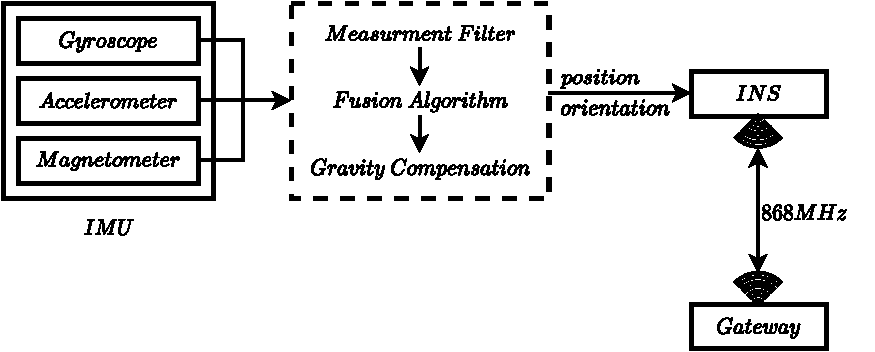
\includegraphics[width=0.9\textwidth]{figures/overview.pdf}
%     \caption{System overview - Raw measurements from IMU are fused together and numerically integrated to obtain position and orientation. This INS data is transmitted in real-time to a remote node gateway. }
%     \label{fig:overview}
% \end{figure}

\subsection{Experiments}
\label{sub:experiments}

Several experimental tests were conducted to assess the position performance of the INS under different conditions. Experiments were performed indoors, outdoors, and underwater. These tests typically consisted of carrying the INS in a movable platform, typically a skateboard or an electric scooter forming a geometric shape such as a square or a triangle following a precise path on the floor. Geometric shapes were used to better assess the estimating performance of the system against a ground truth baseline. This section will describe how each set of experiments were carried out and what challenges were faced.

\subsection{Indoor Experiments}

Indoor experiments were executed at Madeira Tecnopolo building, floor -1, in a wide-open interior. A guiding rope was layout out in the floor forming a geometric figure acting as baseline for the experiment. The inertial system was placed on an electrical skateboard powered by a laptop computer, which could have been replaced by a portable battery pack. Three kinds of geometric shapes were tested: line, square, triangle and circle. To better understand how distance affects estimation of position, for every geometric figure, tests were made under two different distance magnitudes: 4 and 8 meters.

\begin{figure}[!h]
  \centering
  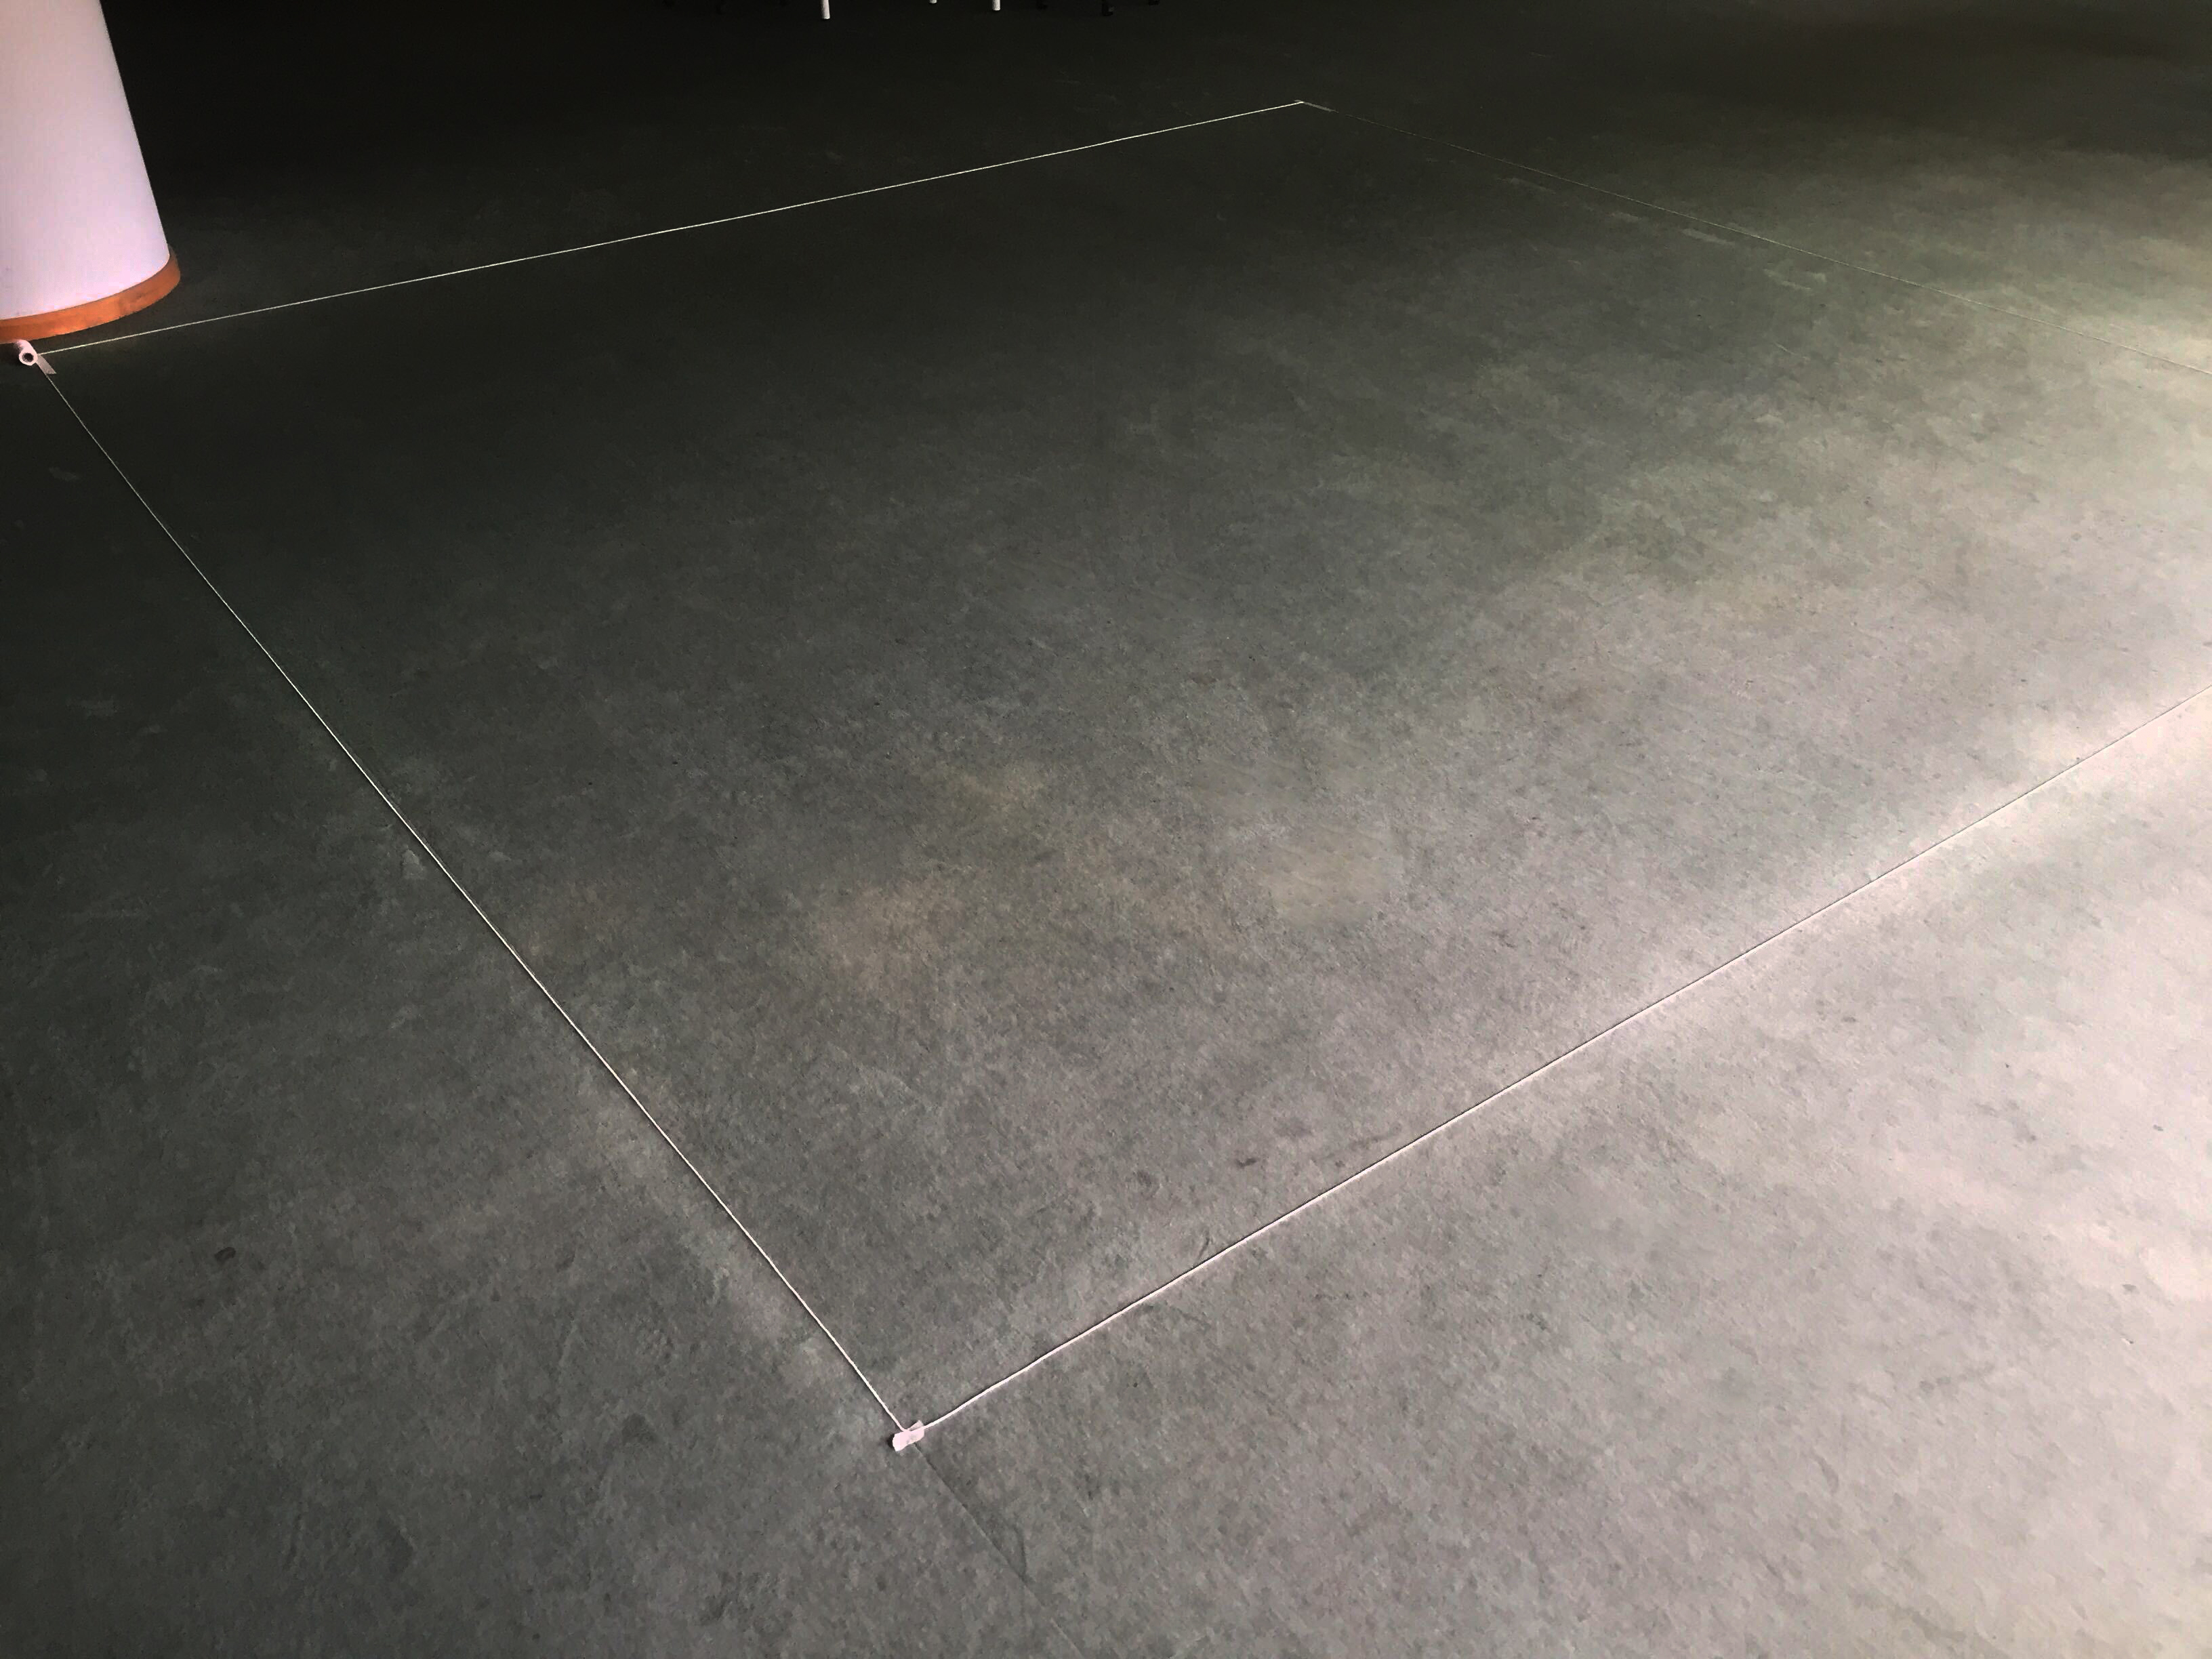
\includegraphics[width=0.7\textwidth]{figures/indoor.jpg}
  \caption{4-meter side ground square used for baseline of accuracy of inertial system.}
  \label{fig:indoor_square}
\end{figure}

Once the experiment was set up, it was time to start testing the INS. The board was dragged at constant speed through the guideline transporting the inertial system. The INS was continuously estimating orientation and position several times a second and storing data to an SD card. The board was dragged at walking speed and stopped at corners when direction changed.

\begin{figure}
  \centering
  % \begin{subfigure}{1\textwidth}
  %     \centering
  %     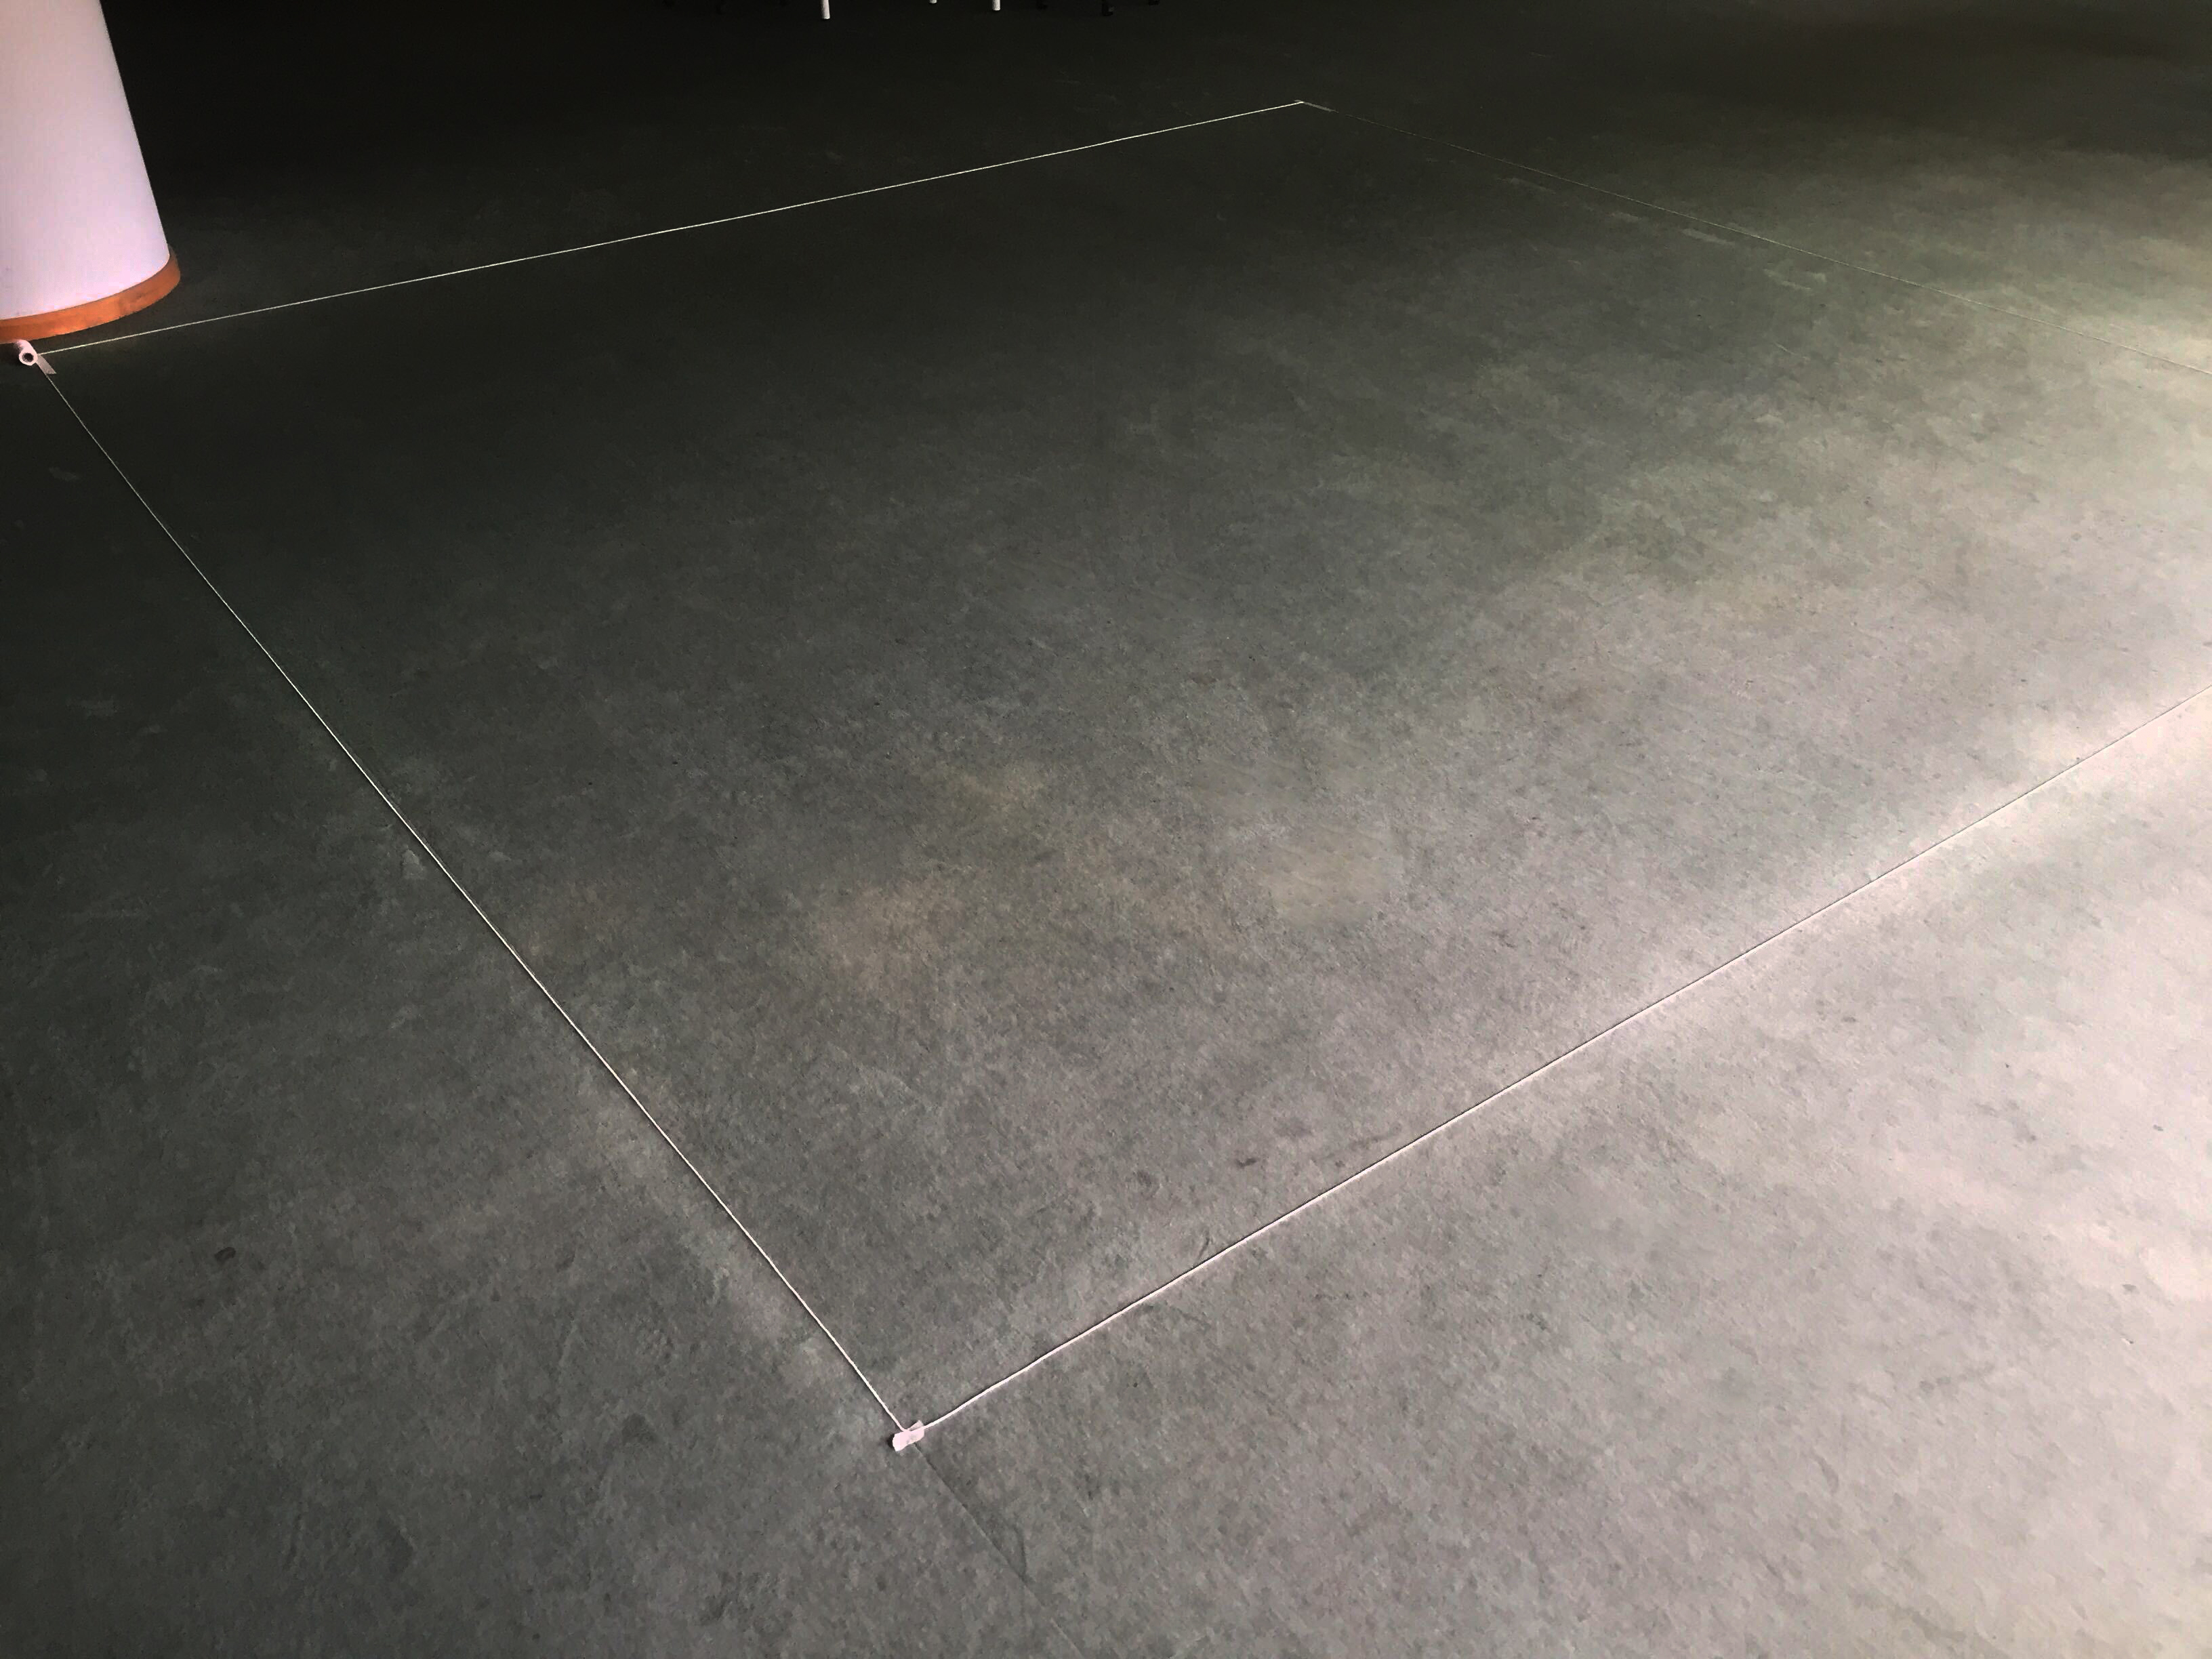
\includegraphics[width=1\textwidth]{figures/indoor.jpg}
  %     \caption{ 4-meter side ground square used for baseline of accuracy of inertial system. }
  %     \label{fig:indoor_square}
  % \end{subfigure}

  \begin{subfigure}{0.49\textwidth}
    \centering
    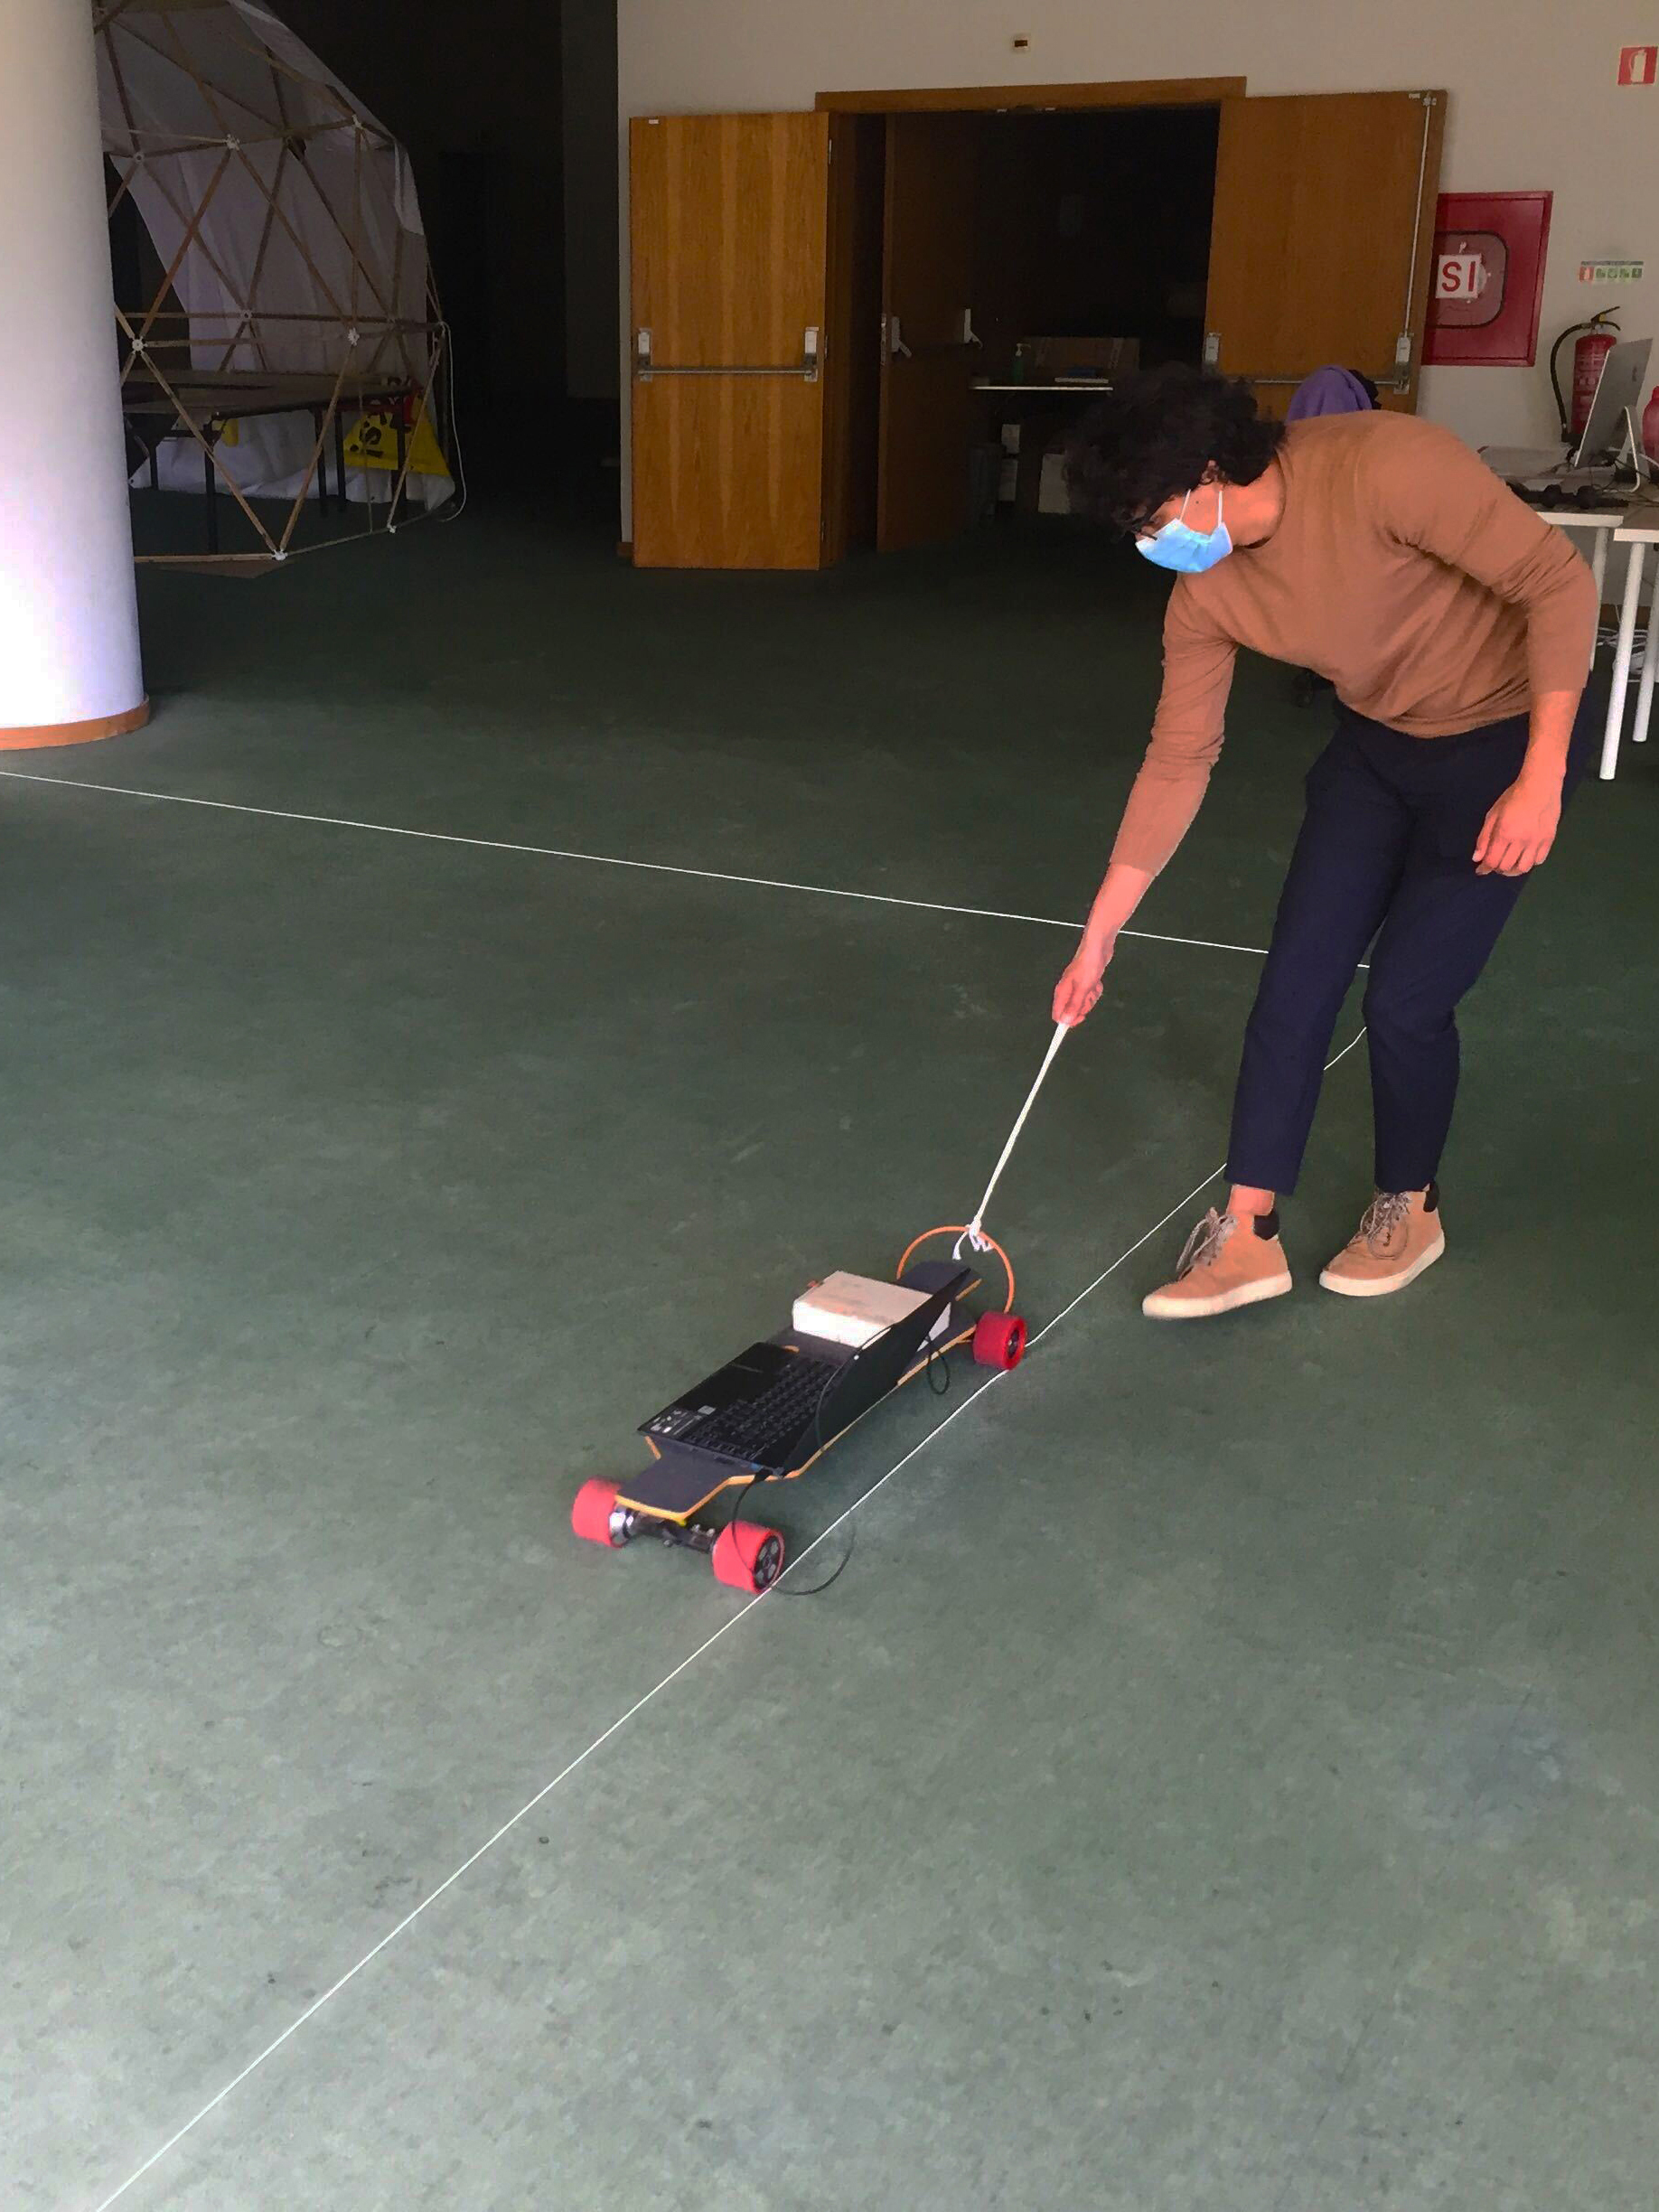
\includegraphics[width=1\textwidth]{figures/indoor_1.jpg}
  \end{subfigure}
  \begin{subfigure}{0.49\textwidth}
    \centering
    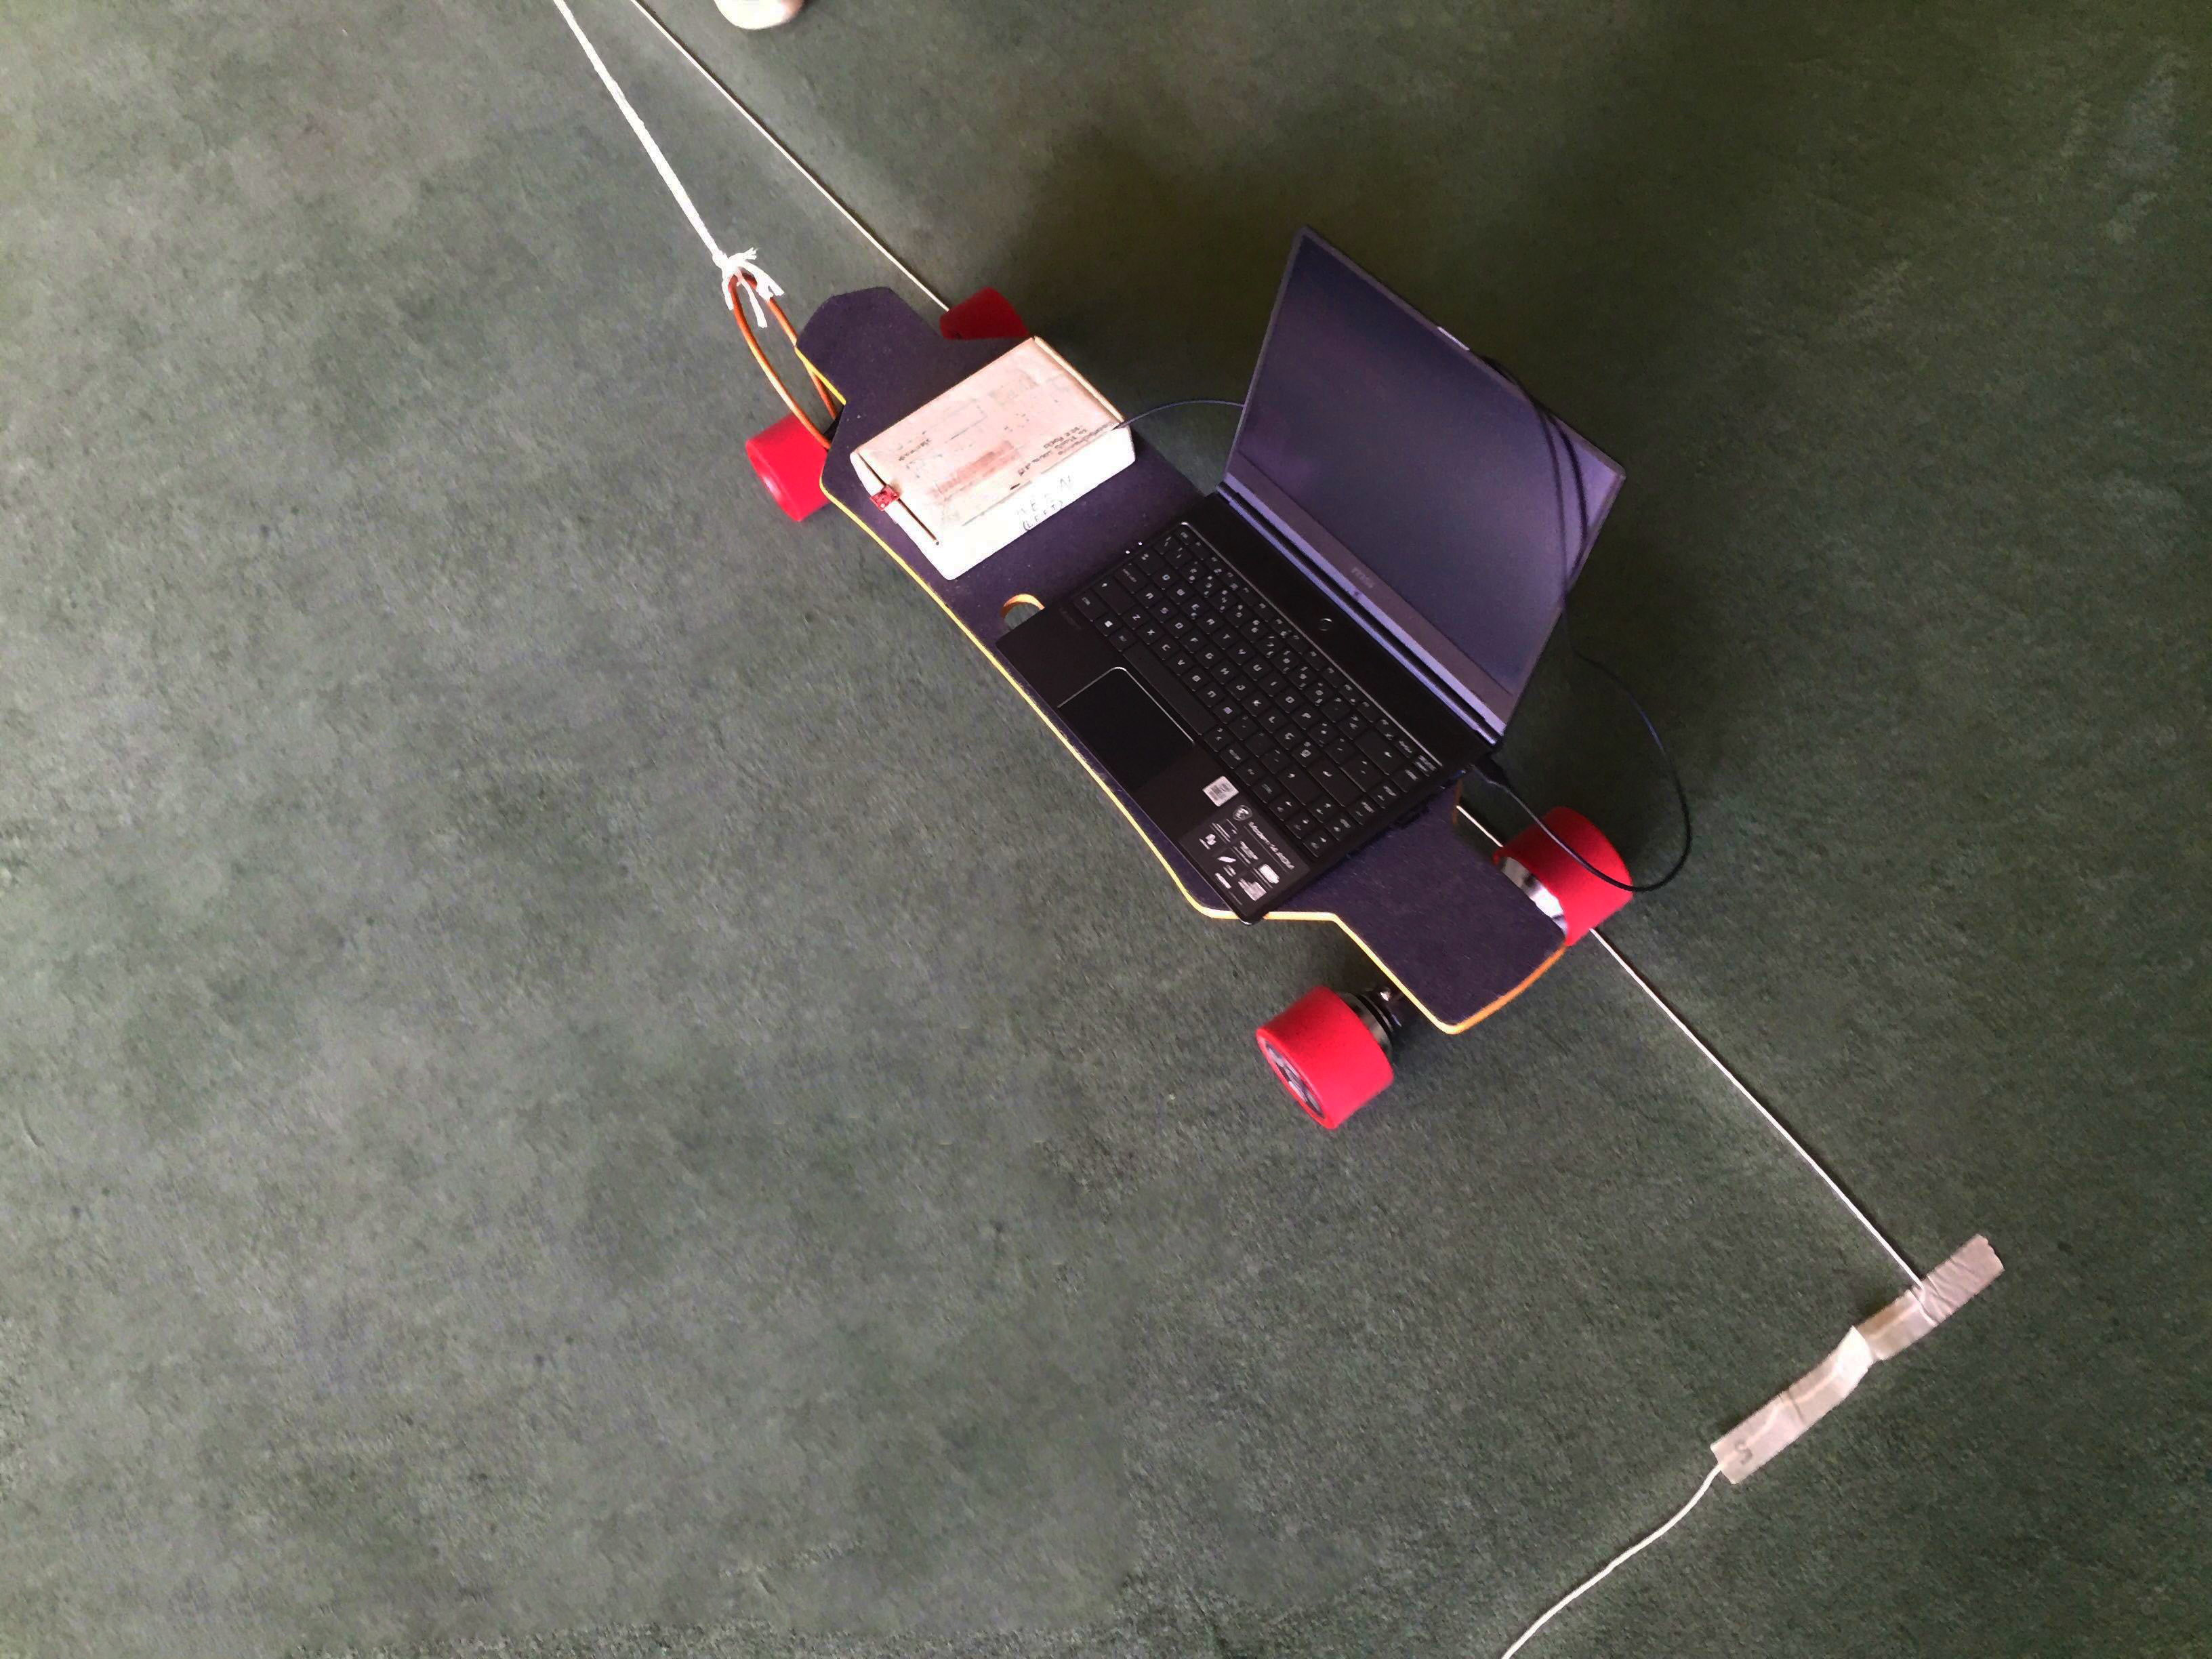
\includegraphics[width=1\textwidth]{figures/indoor_2.jpg}
  \end{subfigure}
  \caption{Skateboard being dragged along the guideline.}
  \label{fig:indoor_experiment}
\end{figure}

\newpage

\subsection{Outdoor Experiments}

Outdoor experiments were conducted at praça do povo's square (figure \ref{fig:outdoor_field}), in a sport's platform with a guiding rope also acting as baseline for the experiment in the forming of geometric figures on the ground.

\begin{figure}[!h]
  \centering
  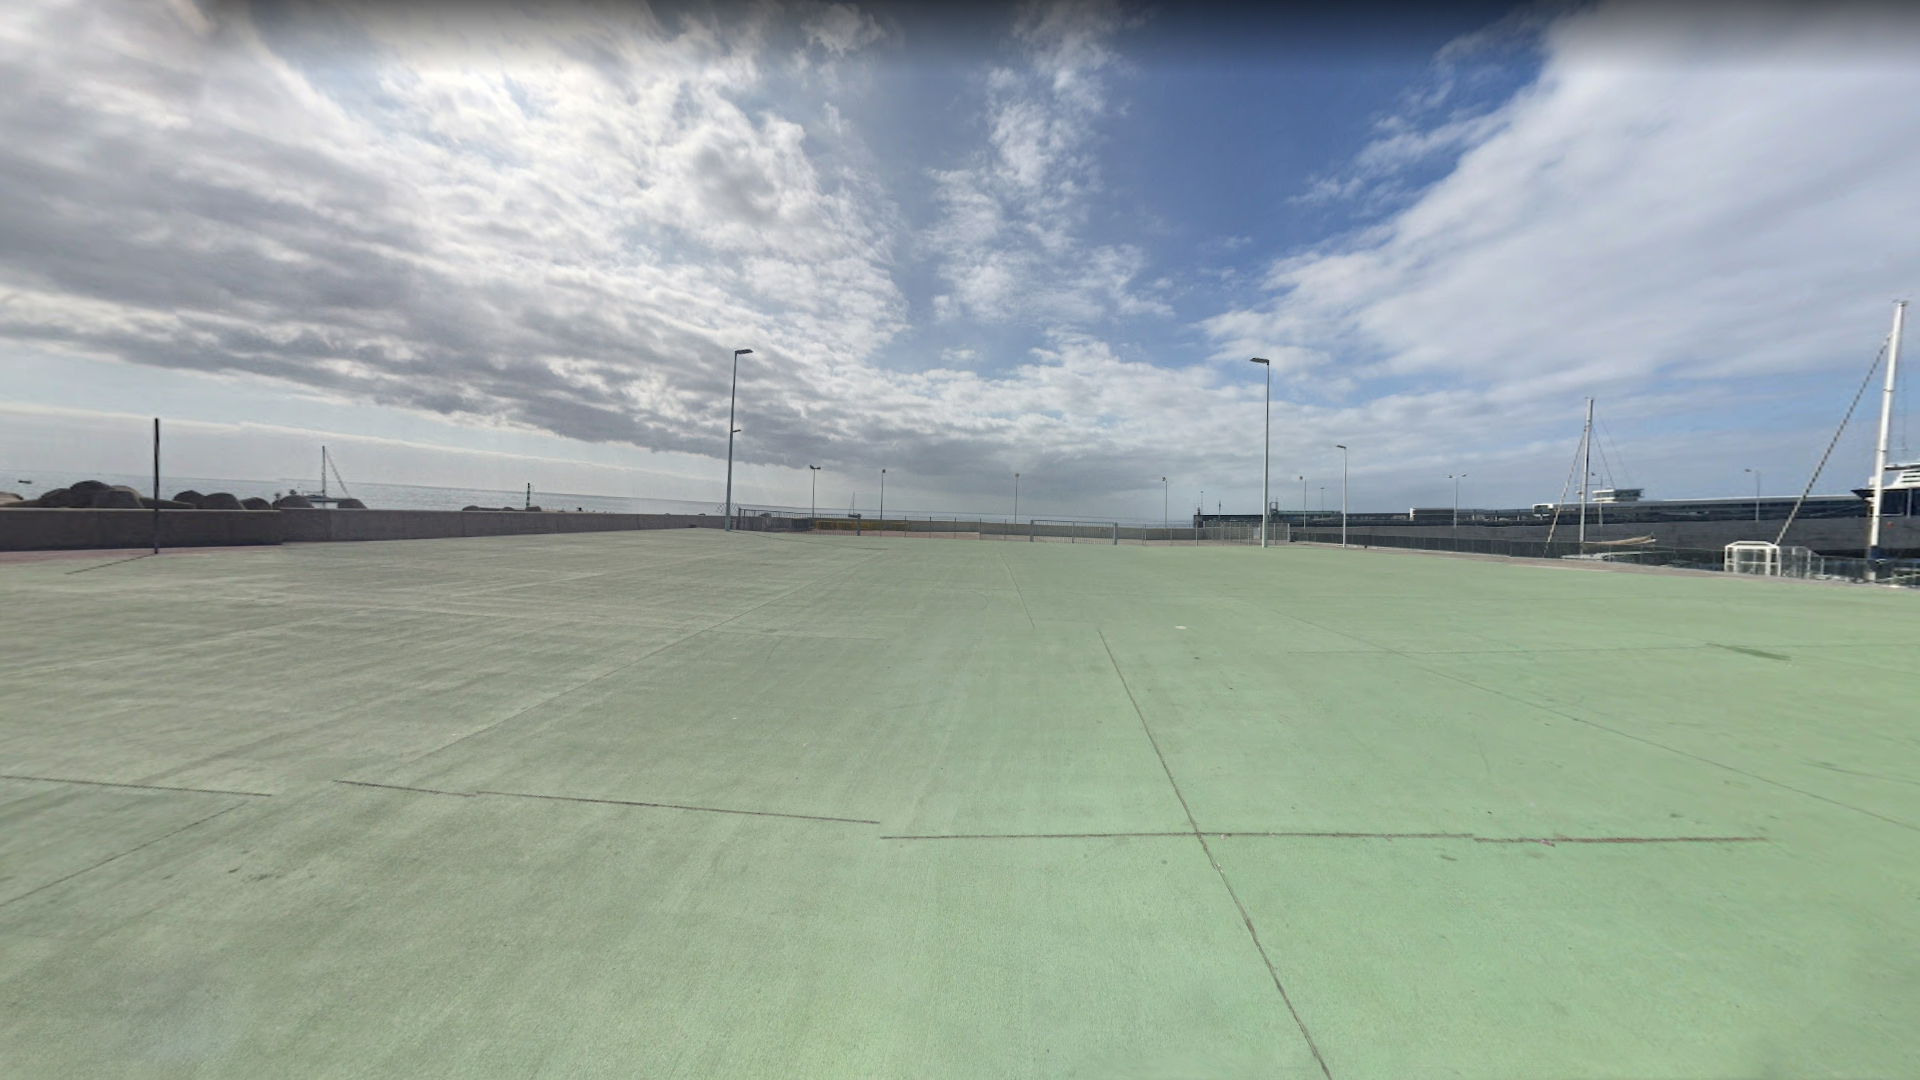
\includegraphics[width=0.7\textwidth]{figures/outdoor_field.jpg}
  \caption{ Platform where outdoors experiments were conducted. }
  \label{fig:outdoor_field}
\end{figure}

Here, the sports platform consisted of one 28mx28m square, composed of 4 meter squares, forming a 7x7 grid (figure \ref{fig:platform_representation}). This was helpful since this knowledge could also be used to benchmark the position estimation of the system and easily calculate error margins.

\begin{figure}[!h]
  \centering
  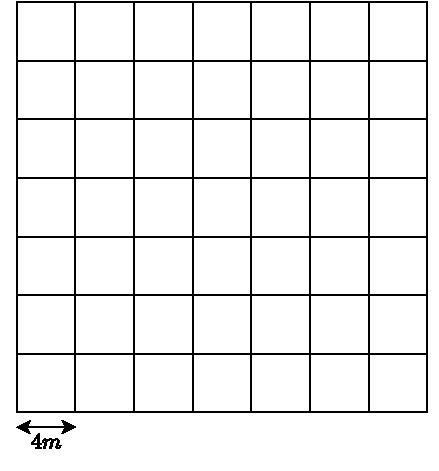
\includegraphics[width=0.45\textwidth]{figures/square.pdf}
  \caption{ Bird's-eye view representation of the 7x7 grid platform where outdoor experiments were conducted. }
  \label{fig:platform_representation}
\end{figure}



% \begin{figure}[!h]
%     \centering
%     \includegraphics[width=0.9\textwidth]{figures/outdoor.jpg}
%     \caption{ 5-meter side ground square used for baseline of accuracy of inertial system. }
%     \label{fig:outdoor}
% \end{figure}

% \begin{figure}[!h]
%     \centering
%     \includegraphics[width=0.9\textwidth]{figures/outdoor_1.jpg}
%     \caption{ Manually pulling the skateboard on each side of the ground square. }
%     \label{fig:outdoor_1}
% \end{figure}

The inertial system was placed on an electrical scooter (figure \ref{fig:outdoor_1}) in this case, being powered by a laptop computer (figure \ref{fig:outdoor_2}). The scooter was dragged at walking pace (figure \ref{fig:outdoor_3}) along the planned path marked by the rope.

\begin{figure}[!h]
  \centering
  \begin{subfigure}{0.8\textwidth}
    \centering
    \includegraphics[width=1\textwidth]{figures/outdoor_1.jpg}
    \caption{ Spiral experiment path outlined by the white rope. }
    \label{fig:outdoor_1}
  \end{subfigure}

  \begin{subfigure}{0.40\textwidth}
    \centering
    \includegraphics[width=1\textwidth]{figures/outdoor_3.jpg}
    \caption{ Close-up view of the inertial system (white box) attach with an elastic band to the scooter's body frame. }
    \label{fig:outdoor_2}
  \end{subfigure}
  \begin{subfigure}{0.40\textwidth}
    \centering
    \includegraphics[width=1\textwidth]{figures/outdoor_2.jpg}
    \caption{ Pushing the electrical scooter containing the laptop and inertial system along the platform's edges forming geometrical shapes. }
    \label{fig:outdoor_3}
  \end{subfigure}
  \caption{ Photos illustrating hoe outdoor experiments were performed.}
  \label{fig:outdoor_experiments}
\end{figure}

Here several shapes were tested, from simple lines, squares, and triangles to more complex figures such as the ones illustrated at figure \ref{fig:squares} and figure \ref{fig:spiral}.

\begin{figure}[!h]
  \centering
  \begin{subfigure}{0.49\textwidth}
    \centering
    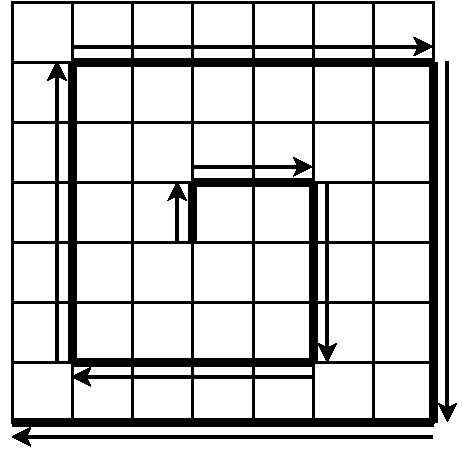
\includegraphics[width=1\textwidth]{figures/spiral.pdf}
    \caption{ Spiral-based shape with increasing length sides.  }
    \label{fig:spiral}
  \end{subfigure}
  \begin{subfigure}{0.49\textwidth}
    \centering
    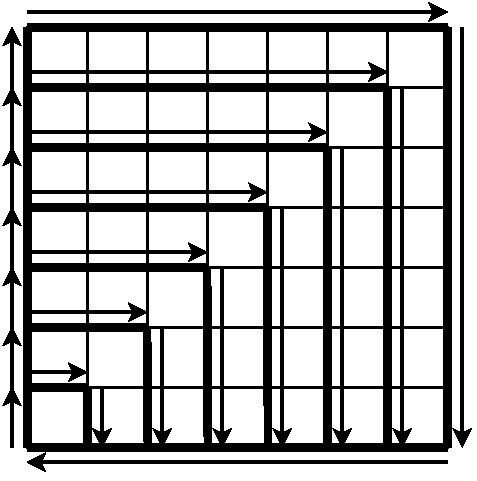
\includegraphics[width=1\textwidth]{figures/squares.pdf}
    \caption{ Squares of increasing side length.  }
    \label{fig:squares}
  \end{subfigure}
  \caption{ Bird's-eye view representation of the more complex path shapes taken. }
\end{figure}

\newpage

\subsection{Underwater Experiments}

Underwater experiments were carried out at Madeira Carlton hotel divepoint, where the INS was placed in an underwater spherical housing built for 360º cameras with a portable battery pack (figure \ref{fig:underwater1_test}). Since the hardware was inaccessible inside the housing, the software had to be adjusted to support remote triggering of the INS via a wireless hotspot using a mobile phone via an HTTP request signal. Tests of the housing were performed prior to the experiment verifying the presence of any water leaks and the well-functioning of the INS (figure \ref{fig:underwater2_test}).

\begin{figure}[!h]
  \centering
  \begin{subfigure}{0.45\textwidth}
    \centering
    \includegraphics[width=1\textwidth]{figures/underwater.jpg}
    \caption{ Spherical housing encompassing the inertial system and portable battery pack. }
    \label{fig:underwater1_test}
  \end{subfigure}
  \begin{subfigure}{0.45\textwidth}
    \centering
    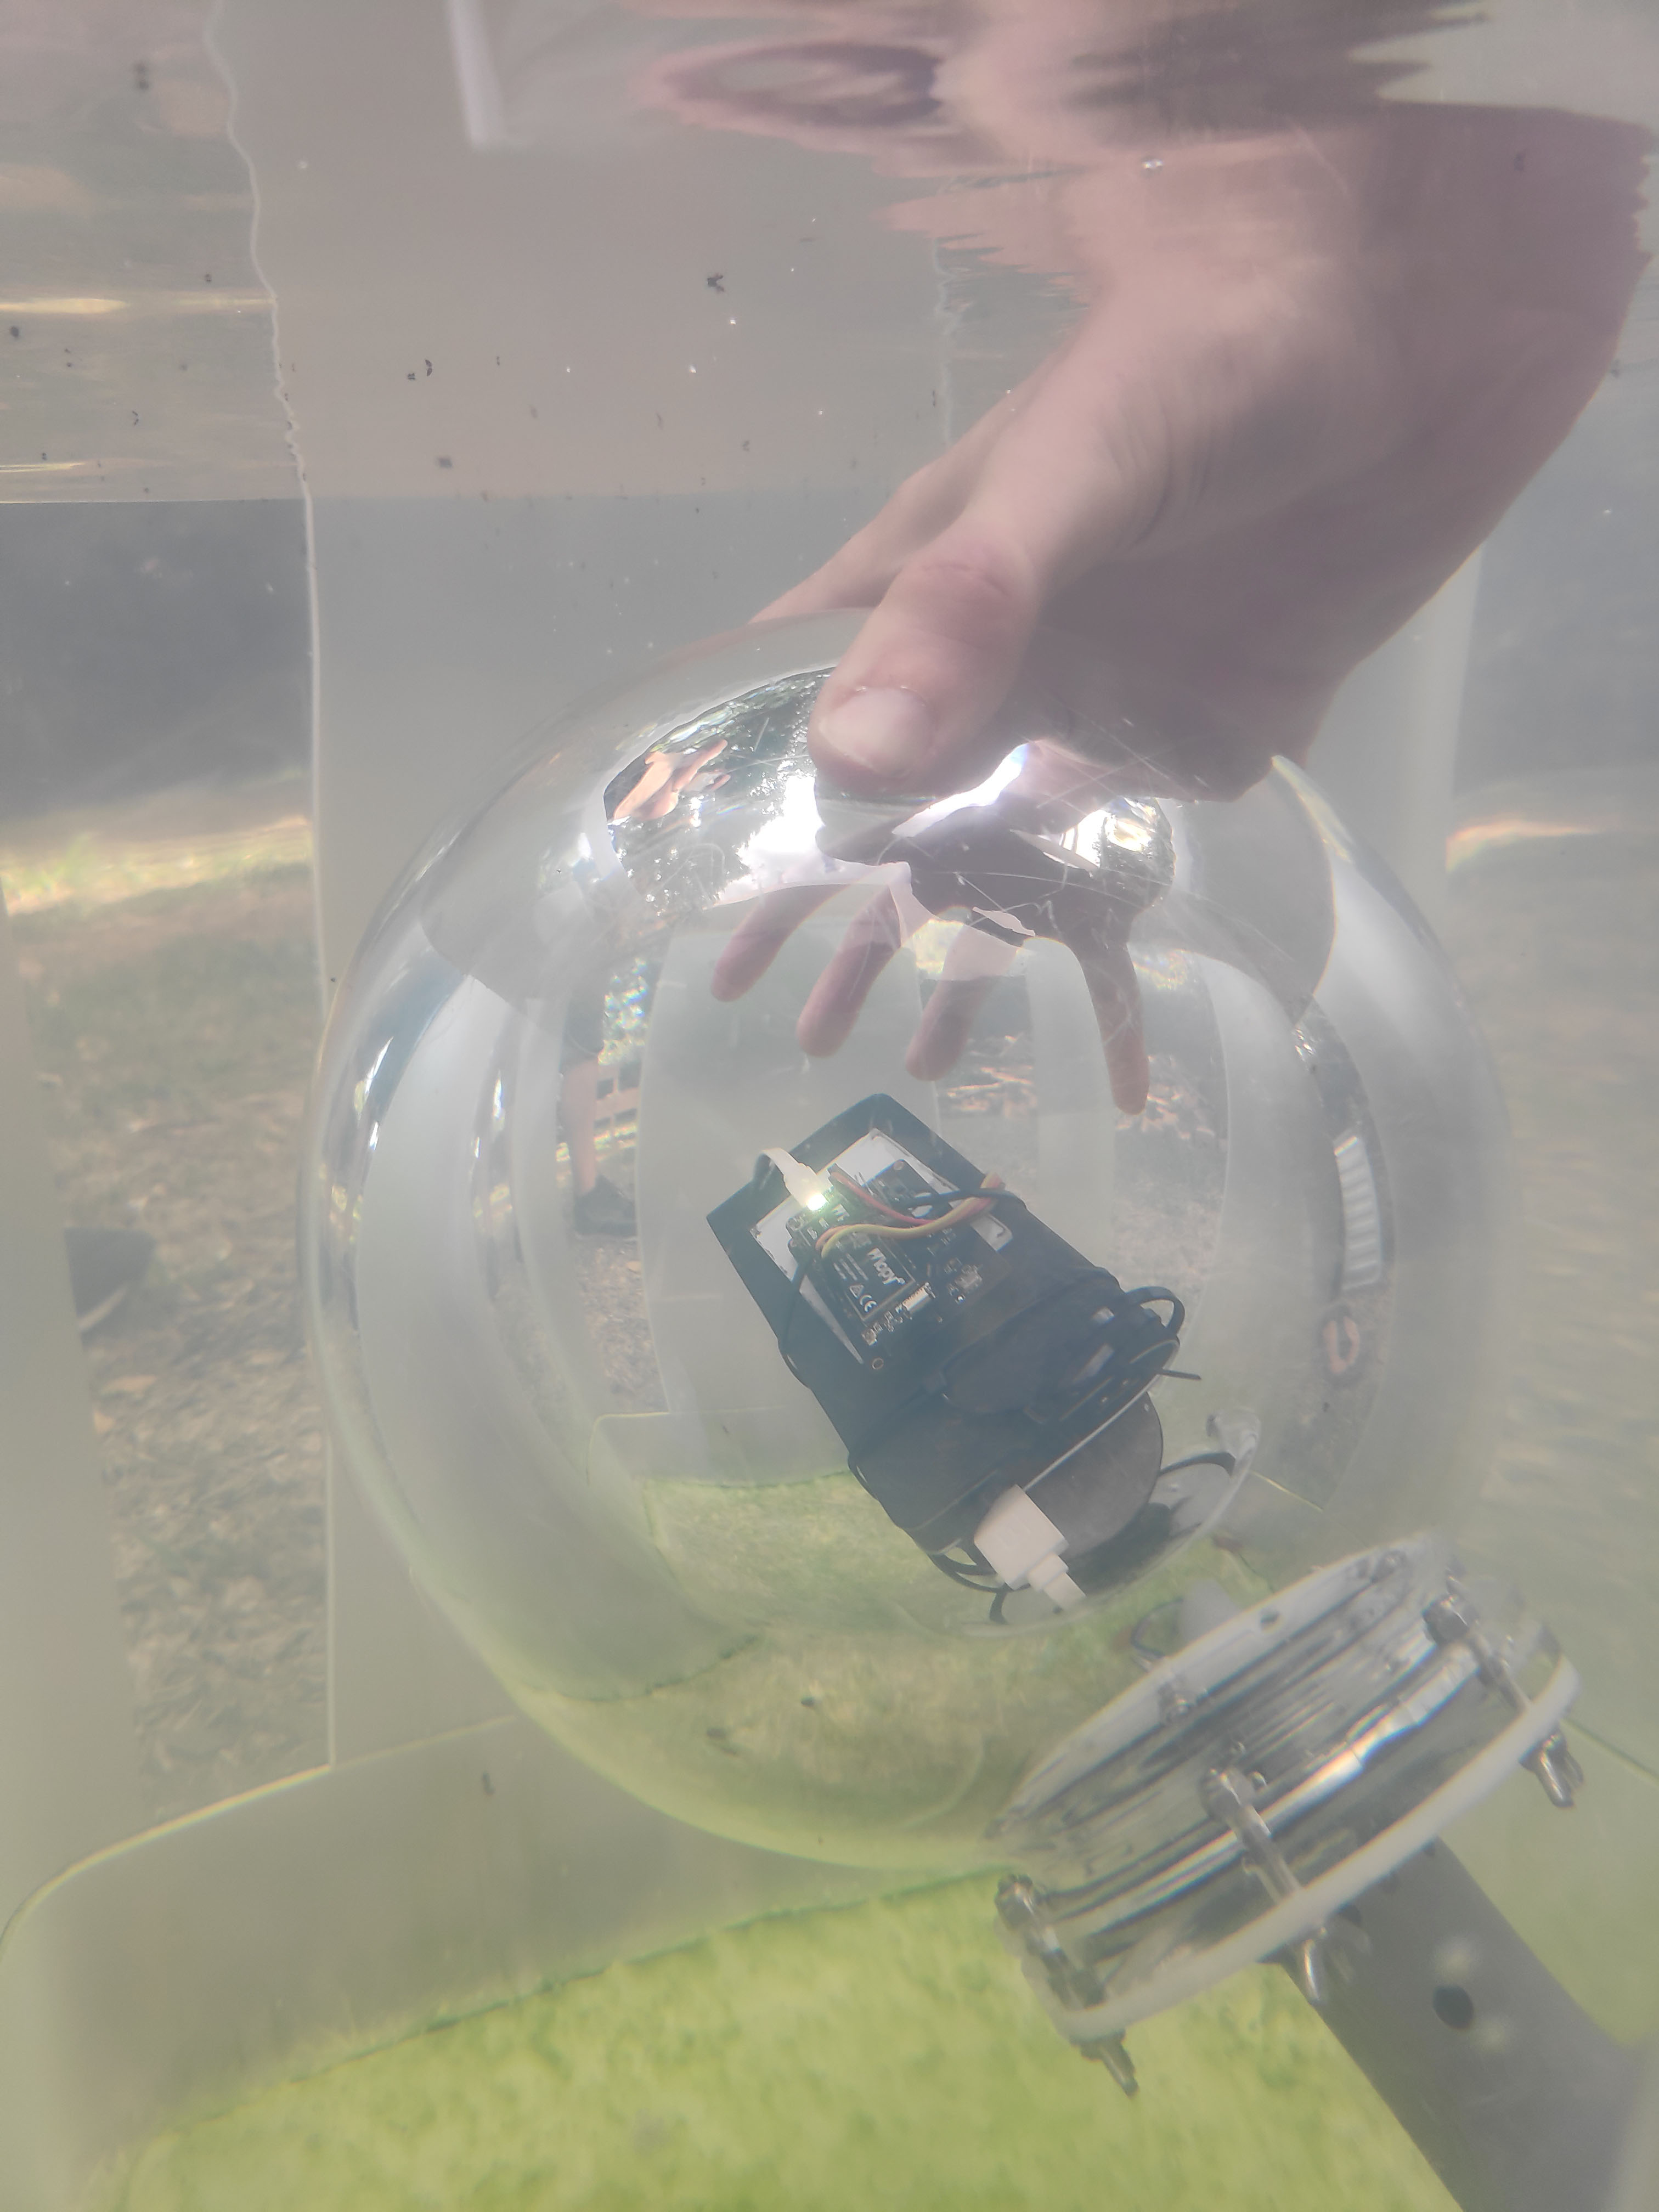
\includegraphics[width=1\textwidth]{figures/underwater_1.jpg}
    \caption{ The capsule was submerged in a water tank to verify the presence of any water leaks. }
    \label{fig:underwater2_test}
  \end{subfigure}
  \label{fig:underwater_test}
  \caption{ View of the tests made to assure the underwater housing was waterproof. }
\end{figure}

Once safety checks were completed, guaranteeing the feasibility of the study, the team went to Madeira Carlton hotel divepoint, where tests were conducted to evaluate the estimation quality of the proposed solution under water by a professional diver (figure \ref{fig:underwater}). A 5-meter square net being held by two people above water served as guideline for the diver performing the experiment underwater. The diver held the spherical housing while swimming along the guideline maintaining a constant speed while slowly increasing depth (figure \ref{fig:underwater_2}).

\begin{figure}[!h]
  \centering
  \begin{subfigure}{0.7\textwidth}
    \centering
    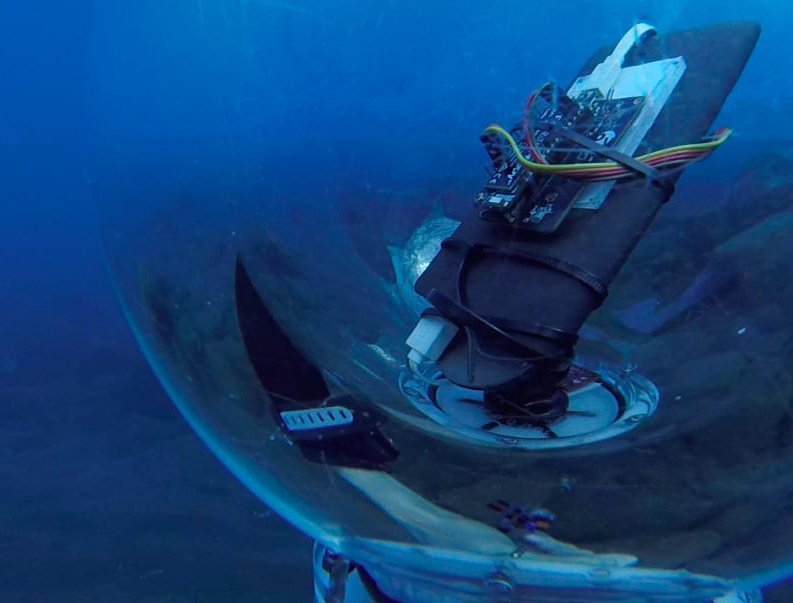
\includegraphics[width=1\textwidth]{figures/underwater_5.jpg}
    \caption{ The housing being held underwater by the diver.  }
    \label{fig:underwater}
  \end{subfigure}

  \begin{subfigure}{0.35\textwidth}
    \centering
    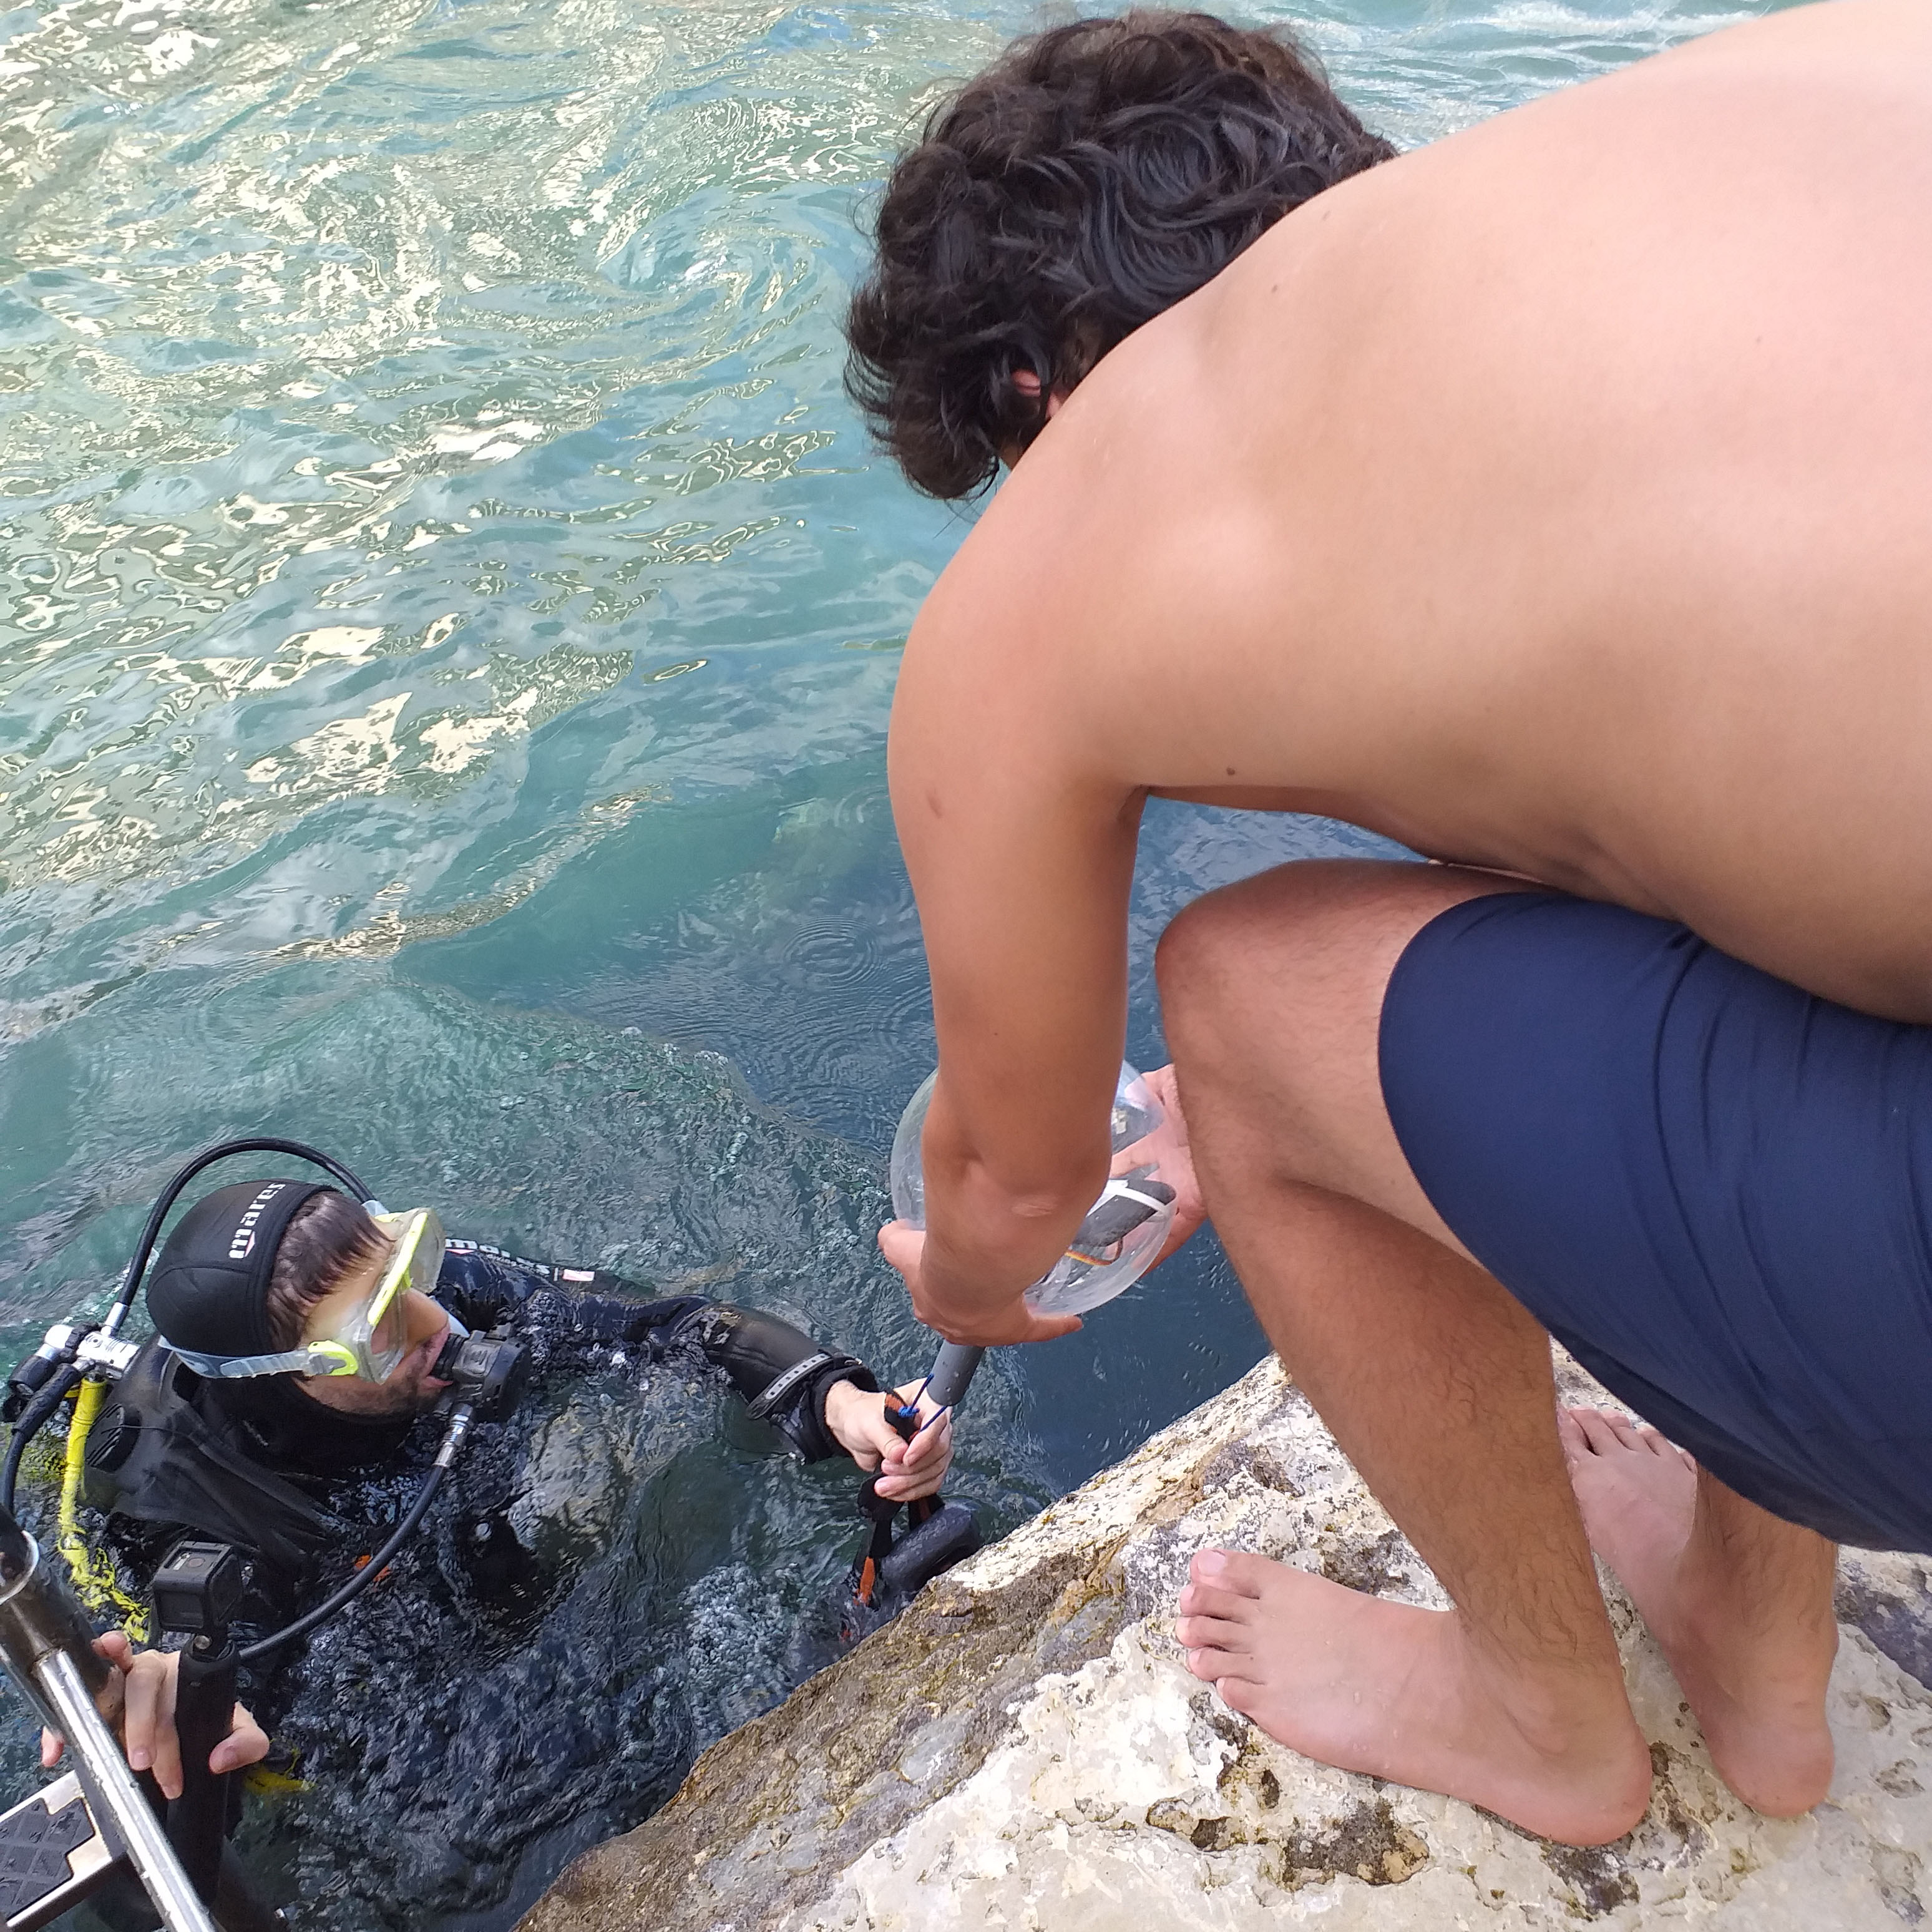
\includegraphics[width=1\textwidth]{figures/underwater_2.jpg}
    \caption{ The capsule housing the inertial system being handed out to a professional diver. }
    \label{fig:underwater_1}
  \end{subfigure}
  \begin{subfigure}{0.35\textwidth}
    \centering
    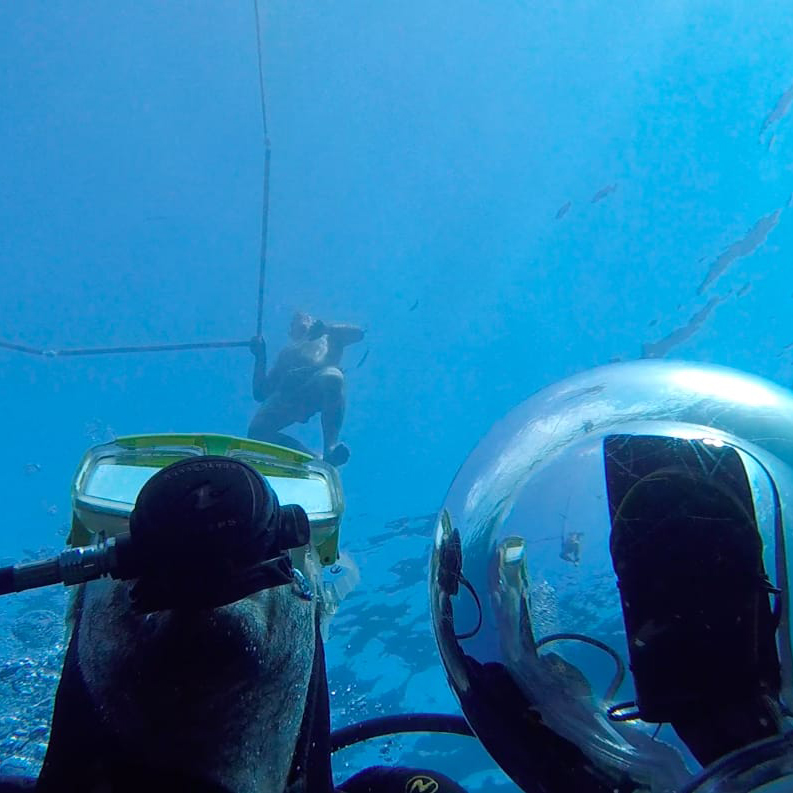
\includegraphics[width=1\textwidth]{figures/underwater_4.jpg}
    \caption{ View of the diver following the net underwater holding the spherical housing. }
    \label{fig:underwater_2}
  \end{subfigure}
  \caption{ Photos of the underwater tests conducted at Madeira Carlton hotel divepoint. }
\end{figure}
